\begin{enumerate}[label=\thesection.\arabic*,ref=\thesection.\theenumi]
		\item Find $\abs{\overrightarrow{a}\times\overrightarrow{b}},\text{ if }\overrightarrow{a}=\hat{i}-7\hat{j}+7\hat{k}\text{ and } \overrightarrow{b}=3\hat{i}-2\hat{j}+2\hat{k}$.
	\\
		\solution
		\begin{enumerate}[label=\thesection.\arabic*,ref=\thesection.\theenumi]
		\item Find $\abs{\overrightarrow{a}\times\overrightarrow{b}},\text{ if }\overrightarrow{a}=\hat{i}-7\hat{j}+7\hat{k}\text{ and } \overrightarrow{b}=3\hat{i}-2\hat{j}+2\hat{k}$.
	\\
		\solution
		\begin{enumerate}[label=\thesection.\arabic*,ref=\thesection.\theenumi]
		\item Find $\abs{\overrightarrow{a}\times\overrightarrow{b}},\text{ if }\overrightarrow{a}=\hat{i}-7\hat{j}+7\hat{k}\text{ and } \overrightarrow{b}=3\hat{i}-2\hat{j}+2\hat{k}$.
	\\
		\solution
		\begin{enumerate}[label=\thesection.\arabic*,ref=\thesection.\theenumi]
		\item Find $\abs{\overrightarrow{a}\times\overrightarrow{b}},\text{ if }\overrightarrow{a}=\hat{i}-7\hat{j}+7\hat{k}\text{ and } \overrightarrow{b}=3\hat{i}-2\hat{j}+2\hat{k}$.
	\\
		\solution
		\input{chapters/12/10/4/1/cross.tex}
\item Show that $$(\overrightarrow{a}-\overrightarrow{b})\times (\overrightarrow{a}+\overrightarrow{b})=2(\overrightarrow{a}\times \overrightarrow{b})$$
	\\
		\solution
		\input{chapters/12/10/4/4/cross.tex}
\item Find $\lambda$ and $\mu$ if $(2\hat{i}+6\hat{j}+27\hat{k})\times(\hat{i}+\lambda \hat{j} + \mu \hat{k})=\overrightarrow{0}$.
	\\
		\solution
		\input{chapters/12/10/4/5/cross.tex}
\item Given that $\overrightarrow{a} \cdot \overrightarrow{b} = 0$ and $\overrightarrow{a} \times \overrightarrow{b} = \overrightarrow{0}$. What can you conclude about the vectors $\overrightarrow{a} \text{ and }\overrightarrow{b}$?
\item Let the vectors be given as $\overrightarrow{a},\overrightarrow{b},\overrightarrow{c}\text{ be given as }\ a_1 \hat{i}+\ a_2 \hat{j}+\ a_3 \hat{k},\ b_1 \hat{i}+\ b_2 \hat{j}+\ b_3 \hat{k},\ c_1 \hat{i}+\ c_2 \hat{j}+\ c_3 \hat{k}$. Then show that $\overrightarrow{a} \times (\overrightarrow{b} + \overrightarrow{c}) = \overrightarrow{a} \times \overrightarrow{b}+\overrightarrow{a} \times \overrightarrow{c}$.
	\\
		\solution
		\input{chapters/12/10/4/7/cross.tex}
\item If either $\overrightarrow{a} = \overrightarrow{0}$ or $\overrightarrow{b} = \overrightarrow{0}$, then $\overrightarrow{a} \times \overrightarrow{b} = \overrightarrow{0}$. Is the converse true? Justify your answer with an example.
	\\
		\solution
		\input{chapters/12/10/4/8/cross.tex}
\item Find the area of the triangle with vertices $A(1, 1, 2)$, $B(2, 3, 5)$, and $C(1, 5, 5)$
	\\
		\solution
		\input{chapters/12/10/4/9/cross.tex}
\item Find the area of the parallelogram whose adjacent sides are determined by the vectors $\overrightarrow{a}=\hat{i}-\hat{j}+3\hat{k}$ and $\overrightarrow{b}=2\hat{i}-7\hat{j}+\hat{k}$.
	\\
		\solution
		\input{chapters/12/10/4/10/cross.tex}
\item Let the vectors $\overrightarrow{a}$ and $\overrightarrow{b}$ be such that $|\overrightarrow{a}| = 3$ and $|\overrightarrow{b}| = \dfrac{\sqrt{2}}{3}$, then $\overrightarrow{a} \times \overrightarrow{b}$ is a unit vector, if the angle between $\overrightarrow{a}$ and $\overrightarrow{b}$ is
\begin{enumerate}
\item $\dfrac{\pi}{6}$
\item $\dfrac{\pi}{4}$
\item $\dfrac{\pi}{3}$
\item $\dfrac{\pi}{2}$
\end{enumerate}
		\solution
		\input{chapters/12/10/4/11/cross.tex}
\item Area of a rectangle having vertices A, B, C and D with position vectors $ -\hat{i}+ \dfrac{1}{2} \hat{j}+4\hat{k},\hat{i}+ \dfrac{1}{2} \hat{j}+4\hat{k},\hat{i}-\dfrac{1}{2} \hat{j}+4\hat{k}\text{ and }-\hat{i}- \dfrac{1}{2} \hat{j}+4\hat{k}$, respectively is
\begin{enumerate}
\item $\dfrac{1}{2}$
\item 1
\item 2
\item 4
\end{enumerate}
		\solution
		\input{chapters/12/10/4/12/cross.tex}
\item Find the area of the triangle whose vertices are 
\begin{enumerate}
\item $(2, 3), (–1, 0), (2, – 4)$
\item $(–5, –1), (3, –5), (5, 2)$ 
\end{enumerate}
		\label{10/7/3/1}
\solution
		\input{chapters/10/7/3/1/area.tex}
\item Find the area of the triangle formed by joining the mid-points of the sides of the triangle whose vertices are $(0, –1), (2, 1) \text{ and } (0, 3)$. Find the ratio of this area to the area of the given triangle.
	\\
\solution
		\input{chapters/10/7/3/3/cross.tex}

\item Find the area of the quadrilateral whose vertices, taken in order, are $(– 4, – 2), (– 3, – 5), (3, – 2)$  and $ (2, 3)$.
	\\
\solution
		\input{chapters/10/7/3/4/cross.tex}

\item Verify that a median of a triangle divides it into two triangles of equal areas for $\triangle ABC$ whose vertices are $\vec{A}(4, -6), \vec{B}(3, 2), \text{ and } \vec{C}(5, 2)$. 
		\label{10/7/3/5}
		\\
\solution
		\input{chapters/10/7/3/5/area.tex}

\item The two adjacent sides of a parallelogram are 
$2\hat{i}-4\hat{j}+5\hat{k}$  and  $\hat{i}-2\hat{j}-3\hat{k}$.
Find the unit vector parallel to its diagonal. Also, find its area.\\
	\solution
		\input{chapters/12/10/5/10/cross.tex}
\item The vertices of a $\triangle ABC$ are $\vec{A}(4,6), \vec{B}(1,5)$ and  $\vec{C}(7,2)$. A line is drawn to intersect sides $AB$ and $AC$ at $\vec{D}$ and $\vec{E}$ respectively, such that $\frac{AD}{AB} = \frac{AE}{AC} = \frac{1}{4}$. Calculate the area of $\triangle ADE$ and compare it with the area of the $\triangle ABC$.
\\
\solution
	\input{chapters/10/7/4/6/section.tex}
    \item Draw a quadrilateral in the Cartesian plane, whose vertices are 
    \begin{align}
        \vec{A} = \myvec{-4\\5} \quad \vec{B} = \myvec{0\\7} \\
        \vec{C} = \myvec{5\\-5} \quad \vec{D} = \myvec{-4\\-2}
    \end{align}
    Also, find its area.
\label{chapters/11/10/1/1}
   \\ 
    \solution 
\input{chapters/11/10/1/1/cross.tex}
\item Find the area of region bounded by the triangle whose
	vertices are $(1, 0), (2, 2) \text{ and } (3, 1)$. 
\item Find the area of region bounded by the triangle whose vertices
	are $(– 1, 0), (1, 3) \text{ and } (3, 2)$. 
\item Find the area of the $\triangle ABC$, coordinates of whose vertices are $\vec{A}(2, 0), \vec{B}(4, 5), \text{ and } \vec{C}(6, 3)$.


\item 
\input{chapters/vectors/exer/main.tex}
\end{enumerate}


\item Show that $$(\overrightarrow{a}-\overrightarrow{b})\times (\overrightarrow{a}+\overrightarrow{b})=2(\overrightarrow{a}\times \overrightarrow{b})$$
	\\
		\solution
		\begin{enumerate}[label=\thesection.\arabic*,ref=\thesection.\theenumi]
		\item Find $\abs{\overrightarrow{a}\times\overrightarrow{b}},\text{ if }\overrightarrow{a}=\hat{i}-7\hat{j}+7\hat{k}\text{ and } \overrightarrow{b}=3\hat{i}-2\hat{j}+2\hat{k}$.
	\\
		\solution
		\input{chapters/12/10/4/1/cross.tex}
\item Show that $$(\overrightarrow{a}-\overrightarrow{b})\times (\overrightarrow{a}+\overrightarrow{b})=2(\overrightarrow{a}\times \overrightarrow{b})$$
	\\
		\solution
		\input{chapters/12/10/4/4/cross.tex}
\item Find $\lambda$ and $\mu$ if $(2\hat{i}+6\hat{j}+27\hat{k})\times(\hat{i}+\lambda \hat{j} + \mu \hat{k})=\overrightarrow{0}$.
	\\
		\solution
		\input{chapters/12/10/4/5/cross.tex}
\item Given that $\overrightarrow{a} \cdot \overrightarrow{b} = 0$ and $\overrightarrow{a} \times \overrightarrow{b} = \overrightarrow{0}$. What can you conclude about the vectors $\overrightarrow{a} \text{ and }\overrightarrow{b}$?
\item Let the vectors be given as $\overrightarrow{a},\overrightarrow{b},\overrightarrow{c}\text{ be given as }\ a_1 \hat{i}+\ a_2 \hat{j}+\ a_3 \hat{k},\ b_1 \hat{i}+\ b_2 \hat{j}+\ b_3 \hat{k},\ c_1 \hat{i}+\ c_2 \hat{j}+\ c_3 \hat{k}$. Then show that $\overrightarrow{a} \times (\overrightarrow{b} + \overrightarrow{c}) = \overrightarrow{a} \times \overrightarrow{b}+\overrightarrow{a} \times \overrightarrow{c}$.
	\\
		\solution
		\input{chapters/12/10/4/7/cross.tex}
\item If either $\overrightarrow{a} = \overrightarrow{0}$ or $\overrightarrow{b} = \overrightarrow{0}$, then $\overrightarrow{a} \times \overrightarrow{b} = \overrightarrow{0}$. Is the converse true? Justify your answer with an example.
	\\
		\solution
		\input{chapters/12/10/4/8/cross.tex}
\item Find the area of the triangle with vertices $A(1, 1, 2)$, $B(2, 3, 5)$, and $C(1, 5, 5)$
	\\
		\solution
		\input{chapters/12/10/4/9/cross.tex}
\item Find the area of the parallelogram whose adjacent sides are determined by the vectors $\overrightarrow{a}=\hat{i}-\hat{j}+3\hat{k}$ and $\overrightarrow{b}=2\hat{i}-7\hat{j}+\hat{k}$.
	\\
		\solution
		\input{chapters/12/10/4/10/cross.tex}
\item Let the vectors $\overrightarrow{a}$ and $\overrightarrow{b}$ be such that $|\overrightarrow{a}| = 3$ and $|\overrightarrow{b}| = \dfrac{\sqrt{2}}{3}$, then $\overrightarrow{a} \times \overrightarrow{b}$ is a unit vector, if the angle between $\overrightarrow{a}$ and $\overrightarrow{b}$ is
\begin{enumerate}
\item $\dfrac{\pi}{6}$
\item $\dfrac{\pi}{4}$
\item $\dfrac{\pi}{3}$
\item $\dfrac{\pi}{2}$
\end{enumerate}
		\solution
		\input{chapters/12/10/4/11/cross.tex}
\item Area of a rectangle having vertices A, B, C and D with position vectors $ -\hat{i}+ \dfrac{1}{2} \hat{j}+4\hat{k},\hat{i}+ \dfrac{1}{2} \hat{j}+4\hat{k},\hat{i}-\dfrac{1}{2} \hat{j}+4\hat{k}\text{ and }-\hat{i}- \dfrac{1}{2} \hat{j}+4\hat{k}$, respectively is
\begin{enumerate}
\item $\dfrac{1}{2}$
\item 1
\item 2
\item 4
\end{enumerate}
		\solution
		\input{chapters/12/10/4/12/cross.tex}
\item Find the area of the triangle whose vertices are 
\begin{enumerate}
\item $(2, 3), (–1, 0), (2, – 4)$
\item $(–5, –1), (3, –5), (5, 2)$ 
\end{enumerate}
		\label{10/7/3/1}
\solution
		\input{chapters/10/7/3/1/area.tex}
\item Find the area of the triangle formed by joining the mid-points of the sides of the triangle whose vertices are $(0, –1), (2, 1) \text{ and } (0, 3)$. Find the ratio of this area to the area of the given triangle.
	\\
\solution
		\input{chapters/10/7/3/3/cross.tex}

\item Find the area of the quadrilateral whose vertices, taken in order, are $(– 4, – 2), (– 3, – 5), (3, – 2)$  and $ (2, 3)$.
	\\
\solution
		\input{chapters/10/7/3/4/cross.tex}

\item Verify that a median of a triangle divides it into two triangles of equal areas for $\triangle ABC$ whose vertices are $\vec{A}(4, -6), \vec{B}(3, 2), \text{ and } \vec{C}(5, 2)$. 
		\label{10/7/3/5}
		\\
\solution
		\input{chapters/10/7/3/5/area.tex}

\item The two adjacent sides of a parallelogram are 
$2\hat{i}-4\hat{j}+5\hat{k}$  and  $\hat{i}-2\hat{j}-3\hat{k}$.
Find the unit vector parallel to its diagonal. Also, find its area.\\
	\solution
		\input{chapters/12/10/5/10/cross.tex}
\item The vertices of a $\triangle ABC$ are $\vec{A}(4,6), \vec{B}(1,5)$ and  $\vec{C}(7,2)$. A line is drawn to intersect sides $AB$ and $AC$ at $\vec{D}$ and $\vec{E}$ respectively, such that $\frac{AD}{AB} = \frac{AE}{AC} = \frac{1}{4}$. Calculate the area of $\triangle ADE$ and compare it with the area of the $\triangle ABC$.
\\
\solution
	\input{chapters/10/7/4/6/section.tex}
    \item Draw a quadrilateral in the Cartesian plane, whose vertices are 
    \begin{align}
        \vec{A} = \myvec{-4\\5} \quad \vec{B} = \myvec{0\\7} \\
        \vec{C} = \myvec{5\\-5} \quad \vec{D} = \myvec{-4\\-2}
    \end{align}
    Also, find its area.
\label{chapters/11/10/1/1}
   \\ 
    \solution 
\input{chapters/11/10/1/1/cross.tex}
\item Find the area of region bounded by the triangle whose
	vertices are $(1, 0), (2, 2) \text{ and } (3, 1)$. 
\item Find the area of region bounded by the triangle whose vertices
	are $(– 1, 0), (1, 3) \text{ and } (3, 2)$. 
\item Find the area of the $\triangle ABC$, coordinates of whose vertices are $\vec{A}(2, 0), \vec{B}(4, 5), \text{ and } \vec{C}(6, 3)$.


\item 
\input{chapters/vectors/exer/main.tex}
\end{enumerate}


\item Find $\lambda$ and $\mu$ if $(2\hat{i}+6\hat{j}+27\hat{k})\times(\hat{i}+\lambda \hat{j} + \mu \hat{k})=\overrightarrow{0}$.
	\\
		\solution
		\begin{enumerate}[label=\thesection.\arabic*,ref=\thesection.\theenumi]
		\item Find $\abs{\overrightarrow{a}\times\overrightarrow{b}},\text{ if }\overrightarrow{a}=\hat{i}-7\hat{j}+7\hat{k}\text{ and } \overrightarrow{b}=3\hat{i}-2\hat{j}+2\hat{k}$.
	\\
		\solution
		\input{chapters/12/10/4/1/cross.tex}
\item Show that $$(\overrightarrow{a}-\overrightarrow{b})\times (\overrightarrow{a}+\overrightarrow{b})=2(\overrightarrow{a}\times \overrightarrow{b})$$
	\\
		\solution
		\input{chapters/12/10/4/4/cross.tex}
\item Find $\lambda$ and $\mu$ if $(2\hat{i}+6\hat{j}+27\hat{k})\times(\hat{i}+\lambda \hat{j} + \mu \hat{k})=\overrightarrow{0}$.
	\\
		\solution
		\input{chapters/12/10/4/5/cross.tex}
\item Given that $\overrightarrow{a} \cdot \overrightarrow{b} = 0$ and $\overrightarrow{a} \times \overrightarrow{b} = \overrightarrow{0}$. What can you conclude about the vectors $\overrightarrow{a} \text{ and }\overrightarrow{b}$?
\item Let the vectors be given as $\overrightarrow{a},\overrightarrow{b},\overrightarrow{c}\text{ be given as }\ a_1 \hat{i}+\ a_2 \hat{j}+\ a_3 \hat{k},\ b_1 \hat{i}+\ b_2 \hat{j}+\ b_3 \hat{k},\ c_1 \hat{i}+\ c_2 \hat{j}+\ c_3 \hat{k}$. Then show that $\overrightarrow{a} \times (\overrightarrow{b} + \overrightarrow{c}) = \overrightarrow{a} \times \overrightarrow{b}+\overrightarrow{a} \times \overrightarrow{c}$.
	\\
		\solution
		\input{chapters/12/10/4/7/cross.tex}
\item If either $\overrightarrow{a} = \overrightarrow{0}$ or $\overrightarrow{b} = \overrightarrow{0}$, then $\overrightarrow{a} \times \overrightarrow{b} = \overrightarrow{0}$. Is the converse true? Justify your answer with an example.
	\\
		\solution
		\input{chapters/12/10/4/8/cross.tex}
\item Find the area of the triangle with vertices $A(1, 1, 2)$, $B(2, 3, 5)$, and $C(1, 5, 5)$
	\\
		\solution
		\input{chapters/12/10/4/9/cross.tex}
\item Find the area of the parallelogram whose adjacent sides are determined by the vectors $\overrightarrow{a}=\hat{i}-\hat{j}+3\hat{k}$ and $\overrightarrow{b}=2\hat{i}-7\hat{j}+\hat{k}$.
	\\
		\solution
		\input{chapters/12/10/4/10/cross.tex}
\item Let the vectors $\overrightarrow{a}$ and $\overrightarrow{b}$ be such that $|\overrightarrow{a}| = 3$ and $|\overrightarrow{b}| = \dfrac{\sqrt{2}}{3}$, then $\overrightarrow{a} \times \overrightarrow{b}$ is a unit vector, if the angle between $\overrightarrow{a}$ and $\overrightarrow{b}$ is
\begin{enumerate}
\item $\dfrac{\pi}{6}$
\item $\dfrac{\pi}{4}$
\item $\dfrac{\pi}{3}$
\item $\dfrac{\pi}{2}$
\end{enumerate}
		\solution
		\input{chapters/12/10/4/11/cross.tex}
\item Area of a rectangle having vertices A, B, C and D with position vectors $ -\hat{i}+ \dfrac{1}{2} \hat{j}+4\hat{k},\hat{i}+ \dfrac{1}{2} \hat{j}+4\hat{k},\hat{i}-\dfrac{1}{2} \hat{j}+4\hat{k}\text{ and }-\hat{i}- \dfrac{1}{2} \hat{j}+4\hat{k}$, respectively is
\begin{enumerate}
\item $\dfrac{1}{2}$
\item 1
\item 2
\item 4
\end{enumerate}
		\solution
		\input{chapters/12/10/4/12/cross.tex}
\item Find the area of the triangle whose vertices are 
\begin{enumerate}
\item $(2, 3), (–1, 0), (2, – 4)$
\item $(–5, –1), (3, –5), (5, 2)$ 
\end{enumerate}
		\label{10/7/3/1}
\solution
		\input{chapters/10/7/3/1/area.tex}
\item Find the area of the triangle formed by joining the mid-points of the sides of the triangle whose vertices are $(0, –1), (2, 1) \text{ and } (0, 3)$. Find the ratio of this area to the area of the given triangle.
	\\
\solution
		\input{chapters/10/7/3/3/cross.tex}

\item Find the area of the quadrilateral whose vertices, taken in order, are $(– 4, – 2), (– 3, – 5), (3, – 2)$  and $ (2, 3)$.
	\\
\solution
		\input{chapters/10/7/3/4/cross.tex}

\item Verify that a median of a triangle divides it into two triangles of equal areas for $\triangle ABC$ whose vertices are $\vec{A}(4, -6), \vec{B}(3, 2), \text{ and } \vec{C}(5, 2)$. 
		\label{10/7/3/5}
		\\
\solution
		\input{chapters/10/7/3/5/area.tex}

\item The two adjacent sides of a parallelogram are 
$2\hat{i}-4\hat{j}+5\hat{k}$  and  $\hat{i}-2\hat{j}-3\hat{k}$.
Find the unit vector parallel to its diagonal. Also, find its area.\\
	\solution
		\input{chapters/12/10/5/10/cross.tex}
\item The vertices of a $\triangle ABC$ are $\vec{A}(4,6), \vec{B}(1,5)$ and  $\vec{C}(7,2)$. A line is drawn to intersect sides $AB$ and $AC$ at $\vec{D}$ and $\vec{E}$ respectively, such that $\frac{AD}{AB} = \frac{AE}{AC} = \frac{1}{4}$. Calculate the area of $\triangle ADE$ and compare it with the area of the $\triangle ABC$.
\\
\solution
	\input{chapters/10/7/4/6/section.tex}
    \item Draw a quadrilateral in the Cartesian plane, whose vertices are 
    \begin{align}
        \vec{A} = \myvec{-4\\5} \quad \vec{B} = \myvec{0\\7} \\
        \vec{C} = \myvec{5\\-5} \quad \vec{D} = \myvec{-4\\-2}
    \end{align}
    Also, find its area.
\label{chapters/11/10/1/1}
   \\ 
    \solution 
\input{chapters/11/10/1/1/cross.tex}
\item Find the area of region bounded by the triangle whose
	vertices are $(1, 0), (2, 2) \text{ and } (3, 1)$. 
\item Find the area of region bounded by the triangle whose vertices
	are $(– 1, 0), (1, 3) \text{ and } (3, 2)$. 
\item Find the area of the $\triangle ABC$, coordinates of whose vertices are $\vec{A}(2, 0), \vec{B}(4, 5), \text{ and } \vec{C}(6, 3)$.


\item 
\input{chapters/vectors/exer/main.tex}
\end{enumerate}


\item Given that $\overrightarrow{a} \cdot \overrightarrow{b} = 0$ and $\overrightarrow{a} \times \overrightarrow{b} = \overrightarrow{0}$. What can you conclude about the vectors $\overrightarrow{a} \text{ and }\overrightarrow{b}$?
\item Let the vectors be given as $\overrightarrow{a},\overrightarrow{b},\overrightarrow{c}\text{ be given as }\ a_1 \hat{i}+\ a_2 \hat{j}+\ a_3 \hat{k},\ b_1 \hat{i}+\ b_2 \hat{j}+\ b_3 \hat{k},\ c_1 \hat{i}+\ c_2 \hat{j}+\ c_3 \hat{k}$. Then show that $\overrightarrow{a} \times (\overrightarrow{b} + \overrightarrow{c}) = \overrightarrow{a} \times \overrightarrow{b}+\overrightarrow{a} \times \overrightarrow{c}$.
	\\
		\solution
		\begin{enumerate}[label=\thesection.\arabic*,ref=\thesection.\theenumi]
		\item Find $\abs{\overrightarrow{a}\times\overrightarrow{b}},\text{ if }\overrightarrow{a}=\hat{i}-7\hat{j}+7\hat{k}\text{ and } \overrightarrow{b}=3\hat{i}-2\hat{j}+2\hat{k}$.
	\\
		\solution
		\input{chapters/12/10/4/1/cross.tex}
\item Show that $$(\overrightarrow{a}-\overrightarrow{b})\times (\overrightarrow{a}+\overrightarrow{b})=2(\overrightarrow{a}\times \overrightarrow{b})$$
	\\
		\solution
		\input{chapters/12/10/4/4/cross.tex}
\item Find $\lambda$ and $\mu$ if $(2\hat{i}+6\hat{j}+27\hat{k})\times(\hat{i}+\lambda \hat{j} + \mu \hat{k})=\overrightarrow{0}$.
	\\
		\solution
		\input{chapters/12/10/4/5/cross.tex}
\item Given that $\overrightarrow{a} \cdot \overrightarrow{b} = 0$ and $\overrightarrow{a} \times \overrightarrow{b} = \overrightarrow{0}$. What can you conclude about the vectors $\overrightarrow{a} \text{ and }\overrightarrow{b}$?
\item Let the vectors be given as $\overrightarrow{a},\overrightarrow{b},\overrightarrow{c}\text{ be given as }\ a_1 \hat{i}+\ a_2 \hat{j}+\ a_3 \hat{k},\ b_1 \hat{i}+\ b_2 \hat{j}+\ b_3 \hat{k},\ c_1 \hat{i}+\ c_2 \hat{j}+\ c_3 \hat{k}$. Then show that $\overrightarrow{a} \times (\overrightarrow{b} + \overrightarrow{c}) = \overrightarrow{a} \times \overrightarrow{b}+\overrightarrow{a} \times \overrightarrow{c}$.
	\\
		\solution
		\input{chapters/12/10/4/7/cross.tex}
\item If either $\overrightarrow{a} = \overrightarrow{0}$ or $\overrightarrow{b} = \overrightarrow{0}$, then $\overrightarrow{a} \times \overrightarrow{b} = \overrightarrow{0}$. Is the converse true? Justify your answer with an example.
	\\
		\solution
		\input{chapters/12/10/4/8/cross.tex}
\item Find the area of the triangle with vertices $A(1, 1, 2)$, $B(2, 3, 5)$, and $C(1, 5, 5)$
	\\
		\solution
		\input{chapters/12/10/4/9/cross.tex}
\item Find the area of the parallelogram whose adjacent sides are determined by the vectors $\overrightarrow{a}=\hat{i}-\hat{j}+3\hat{k}$ and $\overrightarrow{b}=2\hat{i}-7\hat{j}+\hat{k}$.
	\\
		\solution
		\input{chapters/12/10/4/10/cross.tex}
\item Let the vectors $\overrightarrow{a}$ and $\overrightarrow{b}$ be such that $|\overrightarrow{a}| = 3$ and $|\overrightarrow{b}| = \dfrac{\sqrt{2}}{3}$, then $\overrightarrow{a} \times \overrightarrow{b}$ is a unit vector, if the angle between $\overrightarrow{a}$ and $\overrightarrow{b}$ is
\begin{enumerate}
\item $\dfrac{\pi}{6}$
\item $\dfrac{\pi}{4}$
\item $\dfrac{\pi}{3}$
\item $\dfrac{\pi}{2}$
\end{enumerate}
		\solution
		\input{chapters/12/10/4/11/cross.tex}
\item Area of a rectangle having vertices A, B, C and D with position vectors $ -\hat{i}+ \dfrac{1}{2} \hat{j}+4\hat{k},\hat{i}+ \dfrac{1}{2} \hat{j}+4\hat{k},\hat{i}-\dfrac{1}{2} \hat{j}+4\hat{k}\text{ and }-\hat{i}- \dfrac{1}{2} \hat{j}+4\hat{k}$, respectively is
\begin{enumerate}
\item $\dfrac{1}{2}$
\item 1
\item 2
\item 4
\end{enumerate}
		\solution
		\input{chapters/12/10/4/12/cross.tex}
\item Find the area of the triangle whose vertices are 
\begin{enumerate}
\item $(2, 3), (–1, 0), (2, – 4)$
\item $(–5, –1), (3, –5), (5, 2)$ 
\end{enumerate}
		\label{10/7/3/1}
\solution
		\input{chapters/10/7/3/1/area.tex}
\item Find the area of the triangle formed by joining the mid-points of the sides of the triangle whose vertices are $(0, –1), (2, 1) \text{ and } (0, 3)$. Find the ratio of this area to the area of the given triangle.
	\\
\solution
		\input{chapters/10/7/3/3/cross.tex}

\item Find the area of the quadrilateral whose vertices, taken in order, are $(– 4, – 2), (– 3, – 5), (3, – 2)$  and $ (2, 3)$.
	\\
\solution
		\input{chapters/10/7/3/4/cross.tex}

\item Verify that a median of a triangle divides it into two triangles of equal areas for $\triangle ABC$ whose vertices are $\vec{A}(4, -6), \vec{B}(3, 2), \text{ and } \vec{C}(5, 2)$. 
		\label{10/7/3/5}
		\\
\solution
		\input{chapters/10/7/3/5/area.tex}

\item The two adjacent sides of a parallelogram are 
$2\hat{i}-4\hat{j}+5\hat{k}$  and  $\hat{i}-2\hat{j}-3\hat{k}$.
Find the unit vector parallel to its diagonal. Also, find its area.\\
	\solution
		\input{chapters/12/10/5/10/cross.tex}
\item The vertices of a $\triangle ABC$ are $\vec{A}(4,6), \vec{B}(1,5)$ and  $\vec{C}(7,2)$. A line is drawn to intersect sides $AB$ and $AC$ at $\vec{D}$ and $\vec{E}$ respectively, such that $\frac{AD}{AB} = \frac{AE}{AC} = \frac{1}{4}$. Calculate the area of $\triangle ADE$ and compare it with the area of the $\triangle ABC$.
\\
\solution
	\input{chapters/10/7/4/6/section.tex}
    \item Draw a quadrilateral in the Cartesian plane, whose vertices are 
    \begin{align}
        \vec{A} = \myvec{-4\\5} \quad \vec{B} = \myvec{0\\7} \\
        \vec{C} = \myvec{5\\-5} \quad \vec{D} = \myvec{-4\\-2}
    \end{align}
    Also, find its area.
\label{chapters/11/10/1/1}
   \\ 
    \solution 
\input{chapters/11/10/1/1/cross.tex}
\item Find the area of region bounded by the triangle whose
	vertices are $(1, 0), (2, 2) \text{ and } (3, 1)$. 
\item Find the area of region bounded by the triangle whose vertices
	are $(– 1, 0), (1, 3) \text{ and } (3, 2)$. 
\item Find the area of the $\triangle ABC$, coordinates of whose vertices are $\vec{A}(2, 0), \vec{B}(4, 5), \text{ and } \vec{C}(6, 3)$.


\item 
\input{chapters/vectors/exer/main.tex}
\end{enumerate}


\item If either $\overrightarrow{a} = \overrightarrow{0}$ or $\overrightarrow{b} = \overrightarrow{0}$, then $\overrightarrow{a} \times \overrightarrow{b} = \overrightarrow{0}$. Is the converse true? Justify your answer with an example.
	\\
		\solution
		\begin{enumerate}[label=\thesection.\arabic*,ref=\thesection.\theenumi]
		\item Find $\abs{\overrightarrow{a}\times\overrightarrow{b}},\text{ if }\overrightarrow{a}=\hat{i}-7\hat{j}+7\hat{k}\text{ and } \overrightarrow{b}=3\hat{i}-2\hat{j}+2\hat{k}$.
	\\
		\solution
		\input{chapters/12/10/4/1/cross.tex}
\item Show that $$(\overrightarrow{a}-\overrightarrow{b})\times (\overrightarrow{a}+\overrightarrow{b})=2(\overrightarrow{a}\times \overrightarrow{b})$$
	\\
		\solution
		\input{chapters/12/10/4/4/cross.tex}
\item Find $\lambda$ and $\mu$ if $(2\hat{i}+6\hat{j}+27\hat{k})\times(\hat{i}+\lambda \hat{j} + \mu \hat{k})=\overrightarrow{0}$.
	\\
		\solution
		\input{chapters/12/10/4/5/cross.tex}
\item Given that $\overrightarrow{a} \cdot \overrightarrow{b} = 0$ and $\overrightarrow{a} \times \overrightarrow{b} = \overrightarrow{0}$. What can you conclude about the vectors $\overrightarrow{a} \text{ and }\overrightarrow{b}$?
\item Let the vectors be given as $\overrightarrow{a},\overrightarrow{b},\overrightarrow{c}\text{ be given as }\ a_1 \hat{i}+\ a_2 \hat{j}+\ a_3 \hat{k},\ b_1 \hat{i}+\ b_2 \hat{j}+\ b_3 \hat{k},\ c_1 \hat{i}+\ c_2 \hat{j}+\ c_3 \hat{k}$. Then show that $\overrightarrow{a} \times (\overrightarrow{b} + \overrightarrow{c}) = \overrightarrow{a} \times \overrightarrow{b}+\overrightarrow{a} \times \overrightarrow{c}$.
	\\
		\solution
		\input{chapters/12/10/4/7/cross.tex}
\item If either $\overrightarrow{a} = \overrightarrow{0}$ or $\overrightarrow{b} = \overrightarrow{0}$, then $\overrightarrow{a} \times \overrightarrow{b} = \overrightarrow{0}$. Is the converse true? Justify your answer with an example.
	\\
		\solution
		\input{chapters/12/10/4/8/cross.tex}
\item Find the area of the triangle with vertices $A(1, 1, 2)$, $B(2, 3, 5)$, and $C(1, 5, 5)$
	\\
		\solution
		\input{chapters/12/10/4/9/cross.tex}
\item Find the area of the parallelogram whose adjacent sides are determined by the vectors $\overrightarrow{a}=\hat{i}-\hat{j}+3\hat{k}$ and $\overrightarrow{b}=2\hat{i}-7\hat{j}+\hat{k}$.
	\\
		\solution
		\input{chapters/12/10/4/10/cross.tex}
\item Let the vectors $\overrightarrow{a}$ and $\overrightarrow{b}$ be such that $|\overrightarrow{a}| = 3$ and $|\overrightarrow{b}| = \dfrac{\sqrt{2}}{3}$, then $\overrightarrow{a} \times \overrightarrow{b}$ is a unit vector, if the angle between $\overrightarrow{a}$ and $\overrightarrow{b}$ is
\begin{enumerate}
\item $\dfrac{\pi}{6}$
\item $\dfrac{\pi}{4}$
\item $\dfrac{\pi}{3}$
\item $\dfrac{\pi}{2}$
\end{enumerate}
		\solution
		\input{chapters/12/10/4/11/cross.tex}
\item Area of a rectangle having vertices A, B, C and D with position vectors $ -\hat{i}+ \dfrac{1}{2} \hat{j}+4\hat{k},\hat{i}+ \dfrac{1}{2} \hat{j}+4\hat{k},\hat{i}-\dfrac{1}{2} \hat{j}+4\hat{k}\text{ and }-\hat{i}- \dfrac{1}{2} \hat{j}+4\hat{k}$, respectively is
\begin{enumerate}
\item $\dfrac{1}{2}$
\item 1
\item 2
\item 4
\end{enumerate}
		\solution
		\input{chapters/12/10/4/12/cross.tex}
\item Find the area of the triangle whose vertices are 
\begin{enumerate}
\item $(2, 3), (–1, 0), (2, – 4)$
\item $(–5, –1), (3, –5), (5, 2)$ 
\end{enumerate}
		\label{10/7/3/1}
\solution
		\input{chapters/10/7/3/1/area.tex}
\item Find the area of the triangle formed by joining the mid-points of the sides of the triangle whose vertices are $(0, –1), (2, 1) \text{ and } (0, 3)$. Find the ratio of this area to the area of the given triangle.
	\\
\solution
		\input{chapters/10/7/3/3/cross.tex}

\item Find the area of the quadrilateral whose vertices, taken in order, are $(– 4, – 2), (– 3, – 5), (3, – 2)$  and $ (2, 3)$.
	\\
\solution
		\input{chapters/10/7/3/4/cross.tex}

\item Verify that a median of a triangle divides it into two triangles of equal areas for $\triangle ABC$ whose vertices are $\vec{A}(4, -6), \vec{B}(3, 2), \text{ and } \vec{C}(5, 2)$. 
		\label{10/7/3/5}
		\\
\solution
		\input{chapters/10/7/3/5/area.tex}

\item The two adjacent sides of a parallelogram are 
$2\hat{i}-4\hat{j}+5\hat{k}$  and  $\hat{i}-2\hat{j}-3\hat{k}$.
Find the unit vector parallel to its diagonal. Also, find its area.\\
	\solution
		\input{chapters/12/10/5/10/cross.tex}
\item The vertices of a $\triangle ABC$ are $\vec{A}(4,6), \vec{B}(1,5)$ and  $\vec{C}(7,2)$. A line is drawn to intersect sides $AB$ and $AC$ at $\vec{D}$ and $\vec{E}$ respectively, such that $\frac{AD}{AB} = \frac{AE}{AC} = \frac{1}{4}$. Calculate the area of $\triangle ADE$ and compare it with the area of the $\triangle ABC$.
\\
\solution
	\input{chapters/10/7/4/6/section.tex}
    \item Draw a quadrilateral in the Cartesian plane, whose vertices are 
    \begin{align}
        \vec{A} = \myvec{-4\\5} \quad \vec{B} = \myvec{0\\7} \\
        \vec{C} = \myvec{5\\-5} \quad \vec{D} = \myvec{-4\\-2}
    \end{align}
    Also, find its area.
\label{chapters/11/10/1/1}
   \\ 
    \solution 
\input{chapters/11/10/1/1/cross.tex}
\item Find the area of region bounded by the triangle whose
	vertices are $(1, 0), (2, 2) \text{ and } (3, 1)$. 
\item Find the area of region bounded by the triangle whose vertices
	are $(– 1, 0), (1, 3) \text{ and } (3, 2)$. 
\item Find the area of the $\triangle ABC$, coordinates of whose vertices are $\vec{A}(2, 0), \vec{B}(4, 5), \text{ and } \vec{C}(6, 3)$.


\item 
\input{chapters/vectors/exer/main.tex}
\end{enumerate}


\item Find the area of the triangle with vertices $A(1, 1, 2)$, $B(2, 3, 5)$, and $C(1, 5, 5)$
	\\
		\solution
		\begin{enumerate}[label=\thesection.\arabic*,ref=\thesection.\theenumi]
		\item Find $\abs{\overrightarrow{a}\times\overrightarrow{b}},\text{ if }\overrightarrow{a}=\hat{i}-7\hat{j}+7\hat{k}\text{ and } \overrightarrow{b}=3\hat{i}-2\hat{j}+2\hat{k}$.
	\\
		\solution
		\input{chapters/12/10/4/1/cross.tex}
\item Show that $$(\overrightarrow{a}-\overrightarrow{b})\times (\overrightarrow{a}+\overrightarrow{b})=2(\overrightarrow{a}\times \overrightarrow{b})$$
	\\
		\solution
		\input{chapters/12/10/4/4/cross.tex}
\item Find $\lambda$ and $\mu$ if $(2\hat{i}+6\hat{j}+27\hat{k})\times(\hat{i}+\lambda \hat{j} + \mu \hat{k})=\overrightarrow{0}$.
	\\
		\solution
		\input{chapters/12/10/4/5/cross.tex}
\item Given that $\overrightarrow{a} \cdot \overrightarrow{b} = 0$ and $\overrightarrow{a} \times \overrightarrow{b} = \overrightarrow{0}$. What can you conclude about the vectors $\overrightarrow{a} \text{ and }\overrightarrow{b}$?
\item Let the vectors be given as $\overrightarrow{a},\overrightarrow{b},\overrightarrow{c}\text{ be given as }\ a_1 \hat{i}+\ a_2 \hat{j}+\ a_3 \hat{k},\ b_1 \hat{i}+\ b_2 \hat{j}+\ b_3 \hat{k},\ c_1 \hat{i}+\ c_2 \hat{j}+\ c_3 \hat{k}$. Then show that $\overrightarrow{a} \times (\overrightarrow{b} + \overrightarrow{c}) = \overrightarrow{a} \times \overrightarrow{b}+\overrightarrow{a} \times \overrightarrow{c}$.
	\\
		\solution
		\input{chapters/12/10/4/7/cross.tex}
\item If either $\overrightarrow{a} = \overrightarrow{0}$ or $\overrightarrow{b} = \overrightarrow{0}$, then $\overrightarrow{a} \times \overrightarrow{b} = \overrightarrow{0}$. Is the converse true? Justify your answer with an example.
	\\
		\solution
		\input{chapters/12/10/4/8/cross.tex}
\item Find the area of the triangle with vertices $A(1, 1, 2)$, $B(2, 3, 5)$, and $C(1, 5, 5)$
	\\
		\solution
		\input{chapters/12/10/4/9/cross.tex}
\item Find the area of the parallelogram whose adjacent sides are determined by the vectors $\overrightarrow{a}=\hat{i}-\hat{j}+3\hat{k}$ and $\overrightarrow{b}=2\hat{i}-7\hat{j}+\hat{k}$.
	\\
		\solution
		\input{chapters/12/10/4/10/cross.tex}
\item Let the vectors $\overrightarrow{a}$ and $\overrightarrow{b}$ be such that $|\overrightarrow{a}| = 3$ and $|\overrightarrow{b}| = \dfrac{\sqrt{2}}{3}$, then $\overrightarrow{a} \times \overrightarrow{b}$ is a unit vector, if the angle between $\overrightarrow{a}$ and $\overrightarrow{b}$ is
\begin{enumerate}
\item $\dfrac{\pi}{6}$
\item $\dfrac{\pi}{4}$
\item $\dfrac{\pi}{3}$
\item $\dfrac{\pi}{2}$
\end{enumerate}
		\solution
		\input{chapters/12/10/4/11/cross.tex}
\item Area of a rectangle having vertices A, B, C and D with position vectors $ -\hat{i}+ \dfrac{1}{2} \hat{j}+4\hat{k},\hat{i}+ \dfrac{1}{2} \hat{j}+4\hat{k},\hat{i}-\dfrac{1}{2} \hat{j}+4\hat{k}\text{ and }-\hat{i}- \dfrac{1}{2} \hat{j}+4\hat{k}$, respectively is
\begin{enumerate}
\item $\dfrac{1}{2}$
\item 1
\item 2
\item 4
\end{enumerate}
		\solution
		\input{chapters/12/10/4/12/cross.tex}
\item Find the area of the triangle whose vertices are 
\begin{enumerate}
\item $(2, 3), (–1, 0), (2, – 4)$
\item $(–5, –1), (3, –5), (5, 2)$ 
\end{enumerate}
		\label{10/7/3/1}
\solution
		\input{chapters/10/7/3/1/area.tex}
\item Find the area of the triangle formed by joining the mid-points of the sides of the triangle whose vertices are $(0, –1), (2, 1) \text{ and } (0, 3)$. Find the ratio of this area to the area of the given triangle.
	\\
\solution
		\input{chapters/10/7/3/3/cross.tex}

\item Find the area of the quadrilateral whose vertices, taken in order, are $(– 4, – 2), (– 3, – 5), (3, – 2)$  and $ (2, 3)$.
	\\
\solution
		\input{chapters/10/7/3/4/cross.tex}

\item Verify that a median of a triangle divides it into two triangles of equal areas for $\triangle ABC$ whose vertices are $\vec{A}(4, -6), \vec{B}(3, 2), \text{ and } \vec{C}(5, 2)$. 
		\label{10/7/3/5}
		\\
\solution
		\input{chapters/10/7/3/5/area.tex}

\item The two adjacent sides of a parallelogram are 
$2\hat{i}-4\hat{j}+5\hat{k}$  and  $\hat{i}-2\hat{j}-3\hat{k}$.
Find the unit vector parallel to its diagonal. Also, find its area.\\
	\solution
		\input{chapters/12/10/5/10/cross.tex}
\item The vertices of a $\triangle ABC$ are $\vec{A}(4,6), \vec{B}(1,5)$ and  $\vec{C}(7,2)$. A line is drawn to intersect sides $AB$ and $AC$ at $\vec{D}$ and $\vec{E}$ respectively, such that $\frac{AD}{AB} = \frac{AE}{AC} = \frac{1}{4}$. Calculate the area of $\triangle ADE$ and compare it with the area of the $\triangle ABC$.
\\
\solution
	\input{chapters/10/7/4/6/section.tex}
    \item Draw a quadrilateral in the Cartesian plane, whose vertices are 
    \begin{align}
        \vec{A} = \myvec{-4\\5} \quad \vec{B} = \myvec{0\\7} \\
        \vec{C} = \myvec{5\\-5} \quad \vec{D} = \myvec{-4\\-2}
    \end{align}
    Also, find its area.
\label{chapters/11/10/1/1}
   \\ 
    \solution 
\input{chapters/11/10/1/1/cross.tex}
\item Find the area of region bounded by the triangle whose
	vertices are $(1, 0), (2, 2) \text{ and } (3, 1)$. 
\item Find the area of region bounded by the triangle whose vertices
	are $(– 1, 0), (1, 3) \text{ and } (3, 2)$. 
\item Find the area of the $\triangle ABC$, coordinates of whose vertices are $\vec{A}(2, 0), \vec{B}(4, 5), \text{ and } \vec{C}(6, 3)$.


\item 
\input{chapters/vectors/exer/main.tex}
\end{enumerate}


\item Find the area of the parallelogram whose adjacent sides are determined by the vectors $\overrightarrow{a}=\hat{i}-\hat{j}+3\hat{k}$ and $\overrightarrow{b}=2\hat{i}-7\hat{j}+\hat{k}$.
	\\
		\solution
		\begin{enumerate}[label=\thesection.\arabic*,ref=\thesection.\theenumi]
		\item Find $\abs{\overrightarrow{a}\times\overrightarrow{b}},\text{ if }\overrightarrow{a}=\hat{i}-7\hat{j}+7\hat{k}\text{ and } \overrightarrow{b}=3\hat{i}-2\hat{j}+2\hat{k}$.
	\\
		\solution
		\input{chapters/12/10/4/1/cross.tex}
\item Show that $$(\overrightarrow{a}-\overrightarrow{b})\times (\overrightarrow{a}+\overrightarrow{b})=2(\overrightarrow{a}\times \overrightarrow{b})$$
	\\
		\solution
		\input{chapters/12/10/4/4/cross.tex}
\item Find $\lambda$ and $\mu$ if $(2\hat{i}+6\hat{j}+27\hat{k})\times(\hat{i}+\lambda \hat{j} + \mu \hat{k})=\overrightarrow{0}$.
	\\
		\solution
		\input{chapters/12/10/4/5/cross.tex}
\item Given that $\overrightarrow{a} \cdot \overrightarrow{b} = 0$ and $\overrightarrow{a} \times \overrightarrow{b} = \overrightarrow{0}$. What can you conclude about the vectors $\overrightarrow{a} \text{ and }\overrightarrow{b}$?
\item Let the vectors be given as $\overrightarrow{a},\overrightarrow{b},\overrightarrow{c}\text{ be given as }\ a_1 \hat{i}+\ a_2 \hat{j}+\ a_3 \hat{k},\ b_1 \hat{i}+\ b_2 \hat{j}+\ b_3 \hat{k},\ c_1 \hat{i}+\ c_2 \hat{j}+\ c_3 \hat{k}$. Then show that $\overrightarrow{a} \times (\overrightarrow{b} + \overrightarrow{c}) = \overrightarrow{a} \times \overrightarrow{b}+\overrightarrow{a} \times \overrightarrow{c}$.
	\\
		\solution
		\input{chapters/12/10/4/7/cross.tex}
\item If either $\overrightarrow{a} = \overrightarrow{0}$ or $\overrightarrow{b} = \overrightarrow{0}$, then $\overrightarrow{a} \times \overrightarrow{b} = \overrightarrow{0}$. Is the converse true? Justify your answer with an example.
	\\
		\solution
		\input{chapters/12/10/4/8/cross.tex}
\item Find the area of the triangle with vertices $A(1, 1, 2)$, $B(2, 3, 5)$, and $C(1, 5, 5)$
	\\
		\solution
		\input{chapters/12/10/4/9/cross.tex}
\item Find the area of the parallelogram whose adjacent sides are determined by the vectors $\overrightarrow{a}=\hat{i}-\hat{j}+3\hat{k}$ and $\overrightarrow{b}=2\hat{i}-7\hat{j}+\hat{k}$.
	\\
		\solution
		\input{chapters/12/10/4/10/cross.tex}
\item Let the vectors $\overrightarrow{a}$ and $\overrightarrow{b}$ be such that $|\overrightarrow{a}| = 3$ and $|\overrightarrow{b}| = \dfrac{\sqrt{2}}{3}$, then $\overrightarrow{a} \times \overrightarrow{b}$ is a unit vector, if the angle between $\overrightarrow{a}$ and $\overrightarrow{b}$ is
\begin{enumerate}
\item $\dfrac{\pi}{6}$
\item $\dfrac{\pi}{4}$
\item $\dfrac{\pi}{3}$
\item $\dfrac{\pi}{2}$
\end{enumerate}
		\solution
		\input{chapters/12/10/4/11/cross.tex}
\item Area of a rectangle having vertices A, B, C and D with position vectors $ -\hat{i}+ \dfrac{1}{2} \hat{j}+4\hat{k},\hat{i}+ \dfrac{1}{2} \hat{j}+4\hat{k},\hat{i}-\dfrac{1}{2} \hat{j}+4\hat{k}\text{ and }-\hat{i}- \dfrac{1}{2} \hat{j}+4\hat{k}$, respectively is
\begin{enumerate}
\item $\dfrac{1}{2}$
\item 1
\item 2
\item 4
\end{enumerate}
		\solution
		\input{chapters/12/10/4/12/cross.tex}
\item Find the area of the triangle whose vertices are 
\begin{enumerate}
\item $(2, 3), (–1, 0), (2, – 4)$
\item $(–5, –1), (3, –5), (5, 2)$ 
\end{enumerate}
		\label{10/7/3/1}
\solution
		\input{chapters/10/7/3/1/area.tex}
\item Find the area of the triangle formed by joining the mid-points of the sides of the triangle whose vertices are $(0, –1), (2, 1) \text{ and } (0, 3)$. Find the ratio of this area to the area of the given triangle.
	\\
\solution
		\input{chapters/10/7/3/3/cross.tex}

\item Find the area of the quadrilateral whose vertices, taken in order, are $(– 4, – 2), (– 3, – 5), (3, – 2)$  and $ (2, 3)$.
	\\
\solution
		\input{chapters/10/7/3/4/cross.tex}

\item Verify that a median of a triangle divides it into two triangles of equal areas for $\triangle ABC$ whose vertices are $\vec{A}(4, -6), \vec{B}(3, 2), \text{ and } \vec{C}(5, 2)$. 
		\label{10/7/3/5}
		\\
\solution
		\input{chapters/10/7/3/5/area.tex}

\item The two adjacent sides of a parallelogram are 
$2\hat{i}-4\hat{j}+5\hat{k}$  and  $\hat{i}-2\hat{j}-3\hat{k}$.
Find the unit vector parallel to its diagonal. Also, find its area.\\
	\solution
		\input{chapters/12/10/5/10/cross.tex}
\item The vertices of a $\triangle ABC$ are $\vec{A}(4,6), \vec{B}(1,5)$ and  $\vec{C}(7,2)$. A line is drawn to intersect sides $AB$ and $AC$ at $\vec{D}$ and $\vec{E}$ respectively, such that $\frac{AD}{AB} = \frac{AE}{AC} = \frac{1}{4}$. Calculate the area of $\triangle ADE$ and compare it with the area of the $\triangle ABC$.
\\
\solution
	\input{chapters/10/7/4/6/section.tex}
    \item Draw a quadrilateral in the Cartesian plane, whose vertices are 
    \begin{align}
        \vec{A} = \myvec{-4\\5} \quad \vec{B} = \myvec{0\\7} \\
        \vec{C} = \myvec{5\\-5} \quad \vec{D} = \myvec{-4\\-2}
    \end{align}
    Also, find its area.
\label{chapters/11/10/1/1}
   \\ 
    \solution 
\input{chapters/11/10/1/1/cross.tex}
\item Find the area of region bounded by the triangle whose
	vertices are $(1, 0), (2, 2) \text{ and } (3, 1)$. 
\item Find the area of region bounded by the triangle whose vertices
	are $(– 1, 0), (1, 3) \text{ and } (3, 2)$. 
\item Find the area of the $\triangle ABC$, coordinates of whose vertices are $\vec{A}(2, 0), \vec{B}(4, 5), \text{ and } \vec{C}(6, 3)$.


\item 
\input{chapters/vectors/exer/main.tex}
\end{enumerate}


\item Let the vectors $\overrightarrow{a}$ and $\overrightarrow{b}$ be such that $|\overrightarrow{a}| = 3$ and $|\overrightarrow{b}| = \dfrac{\sqrt{2}}{3}$, then $\overrightarrow{a} \times \overrightarrow{b}$ is a unit vector, if the angle between $\overrightarrow{a}$ and $\overrightarrow{b}$ is
\begin{enumerate}
\item $\dfrac{\pi}{6}$
\item $\dfrac{\pi}{4}$
\item $\dfrac{\pi}{3}$
\item $\dfrac{\pi}{2}$
\end{enumerate}
		\solution
		\begin{enumerate}[label=\thesection.\arabic*,ref=\thesection.\theenumi]
		\item Find $\abs{\overrightarrow{a}\times\overrightarrow{b}},\text{ if }\overrightarrow{a}=\hat{i}-7\hat{j}+7\hat{k}\text{ and } \overrightarrow{b}=3\hat{i}-2\hat{j}+2\hat{k}$.
	\\
		\solution
		\input{chapters/12/10/4/1/cross.tex}
\item Show that $$(\overrightarrow{a}-\overrightarrow{b})\times (\overrightarrow{a}+\overrightarrow{b})=2(\overrightarrow{a}\times \overrightarrow{b})$$
	\\
		\solution
		\input{chapters/12/10/4/4/cross.tex}
\item Find $\lambda$ and $\mu$ if $(2\hat{i}+6\hat{j}+27\hat{k})\times(\hat{i}+\lambda \hat{j} + \mu \hat{k})=\overrightarrow{0}$.
	\\
		\solution
		\input{chapters/12/10/4/5/cross.tex}
\item Given that $\overrightarrow{a} \cdot \overrightarrow{b} = 0$ and $\overrightarrow{a} \times \overrightarrow{b} = \overrightarrow{0}$. What can you conclude about the vectors $\overrightarrow{a} \text{ and }\overrightarrow{b}$?
\item Let the vectors be given as $\overrightarrow{a},\overrightarrow{b},\overrightarrow{c}\text{ be given as }\ a_1 \hat{i}+\ a_2 \hat{j}+\ a_3 \hat{k},\ b_1 \hat{i}+\ b_2 \hat{j}+\ b_3 \hat{k},\ c_1 \hat{i}+\ c_2 \hat{j}+\ c_3 \hat{k}$. Then show that $\overrightarrow{a} \times (\overrightarrow{b} + \overrightarrow{c}) = \overrightarrow{a} \times \overrightarrow{b}+\overrightarrow{a} \times \overrightarrow{c}$.
	\\
		\solution
		\input{chapters/12/10/4/7/cross.tex}
\item If either $\overrightarrow{a} = \overrightarrow{0}$ or $\overrightarrow{b} = \overrightarrow{0}$, then $\overrightarrow{a} \times \overrightarrow{b} = \overrightarrow{0}$. Is the converse true? Justify your answer with an example.
	\\
		\solution
		\input{chapters/12/10/4/8/cross.tex}
\item Find the area of the triangle with vertices $A(1, 1, 2)$, $B(2, 3, 5)$, and $C(1, 5, 5)$
	\\
		\solution
		\input{chapters/12/10/4/9/cross.tex}
\item Find the area of the parallelogram whose adjacent sides are determined by the vectors $\overrightarrow{a}=\hat{i}-\hat{j}+3\hat{k}$ and $\overrightarrow{b}=2\hat{i}-7\hat{j}+\hat{k}$.
	\\
		\solution
		\input{chapters/12/10/4/10/cross.tex}
\item Let the vectors $\overrightarrow{a}$ and $\overrightarrow{b}$ be such that $|\overrightarrow{a}| = 3$ and $|\overrightarrow{b}| = \dfrac{\sqrt{2}}{3}$, then $\overrightarrow{a} \times \overrightarrow{b}$ is a unit vector, if the angle between $\overrightarrow{a}$ and $\overrightarrow{b}$ is
\begin{enumerate}
\item $\dfrac{\pi}{6}$
\item $\dfrac{\pi}{4}$
\item $\dfrac{\pi}{3}$
\item $\dfrac{\pi}{2}$
\end{enumerate}
		\solution
		\input{chapters/12/10/4/11/cross.tex}
\item Area of a rectangle having vertices A, B, C and D with position vectors $ -\hat{i}+ \dfrac{1}{2} \hat{j}+4\hat{k},\hat{i}+ \dfrac{1}{2} \hat{j}+4\hat{k},\hat{i}-\dfrac{1}{2} \hat{j}+4\hat{k}\text{ and }-\hat{i}- \dfrac{1}{2} \hat{j}+4\hat{k}$, respectively is
\begin{enumerate}
\item $\dfrac{1}{2}$
\item 1
\item 2
\item 4
\end{enumerate}
		\solution
		\input{chapters/12/10/4/12/cross.tex}
\item Find the area of the triangle whose vertices are 
\begin{enumerate}
\item $(2, 3), (–1, 0), (2, – 4)$
\item $(–5, –1), (3, –5), (5, 2)$ 
\end{enumerate}
		\label{10/7/3/1}
\solution
		\input{chapters/10/7/3/1/area.tex}
\item Find the area of the triangle formed by joining the mid-points of the sides of the triangle whose vertices are $(0, –1), (2, 1) \text{ and } (0, 3)$. Find the ratio of this area to the area of the given triangle.
	\\
\solution
		\input{chapters/10/7/3/3/cross.tex}

\item Find the area of the quadrilateral whose vertices, taken in order, are $(– 4, – 2), (– 3, – 5), (3, – 2)$  and $ (2, 3)$.
	\\
\solution
		\input{chapters/10/7/3/4/cross.tex}

\item Verify that a median of a triangle divides it into two triangles of equal areas for $\triangle ABC$ whose vertices are $\vec{A}(4, -6), \vec{B}(3, 2), \text{ and } \vec{C}(5, 2)$. 
		\label{10/7/3/5}
		\\
\solution
		\input{chapters/10/7/3/5/area.tex}

\item The two adjacent sides of a parallelogram are 
$2\hat{i}-4\hat{j}+5\hat{k}$  and  $\hat{i}-2\hat{j}-3\hat{k}$.
Find the unit vector parallel to its diagonal. Also, find its area.\\
	\solution
		\input{chapters/12/10/5/10/cross.tex}
\item The vertices of a $\triangle ABC$ are $\vec{A}(4,6), \vec{B}(1,5)$ and  $\vec{C}(7,2)$. A line is drawn to intersect sides $AB$ and $AC$ at $\vec{D}$ and $\vec{E}$ respectively, such that $\frac{AD}{AB} = \frac{AE}{AC} = \frac{1}{4}$. Calculate the area of $\triangle ADE$ and compare it with the area of the $\triangle ABC$.
\\
\solution
	\input{chapters/10/7/4/6/section.tex}
    \item Draw a quadrilateral in the Cartesian plane, whose vertices are 
    \begin{align}
        \vec{A} = \myvec{-4\\5} \quad \vec{B} = \myvec{0\\7} \\
        \vec{C} = \myvec{5\\-5} \quad \vec{D} = \myvec{-4\\-2}
    \end{align}
    Also, find its area.
\label{chapters/11/10/1/1}
   \\ 
    \solution 
\input{chapters/11/10/1/1/cross.tex}
\item Find the area of region bounded by the triangle whose
	vertices are $(1, 0), (2, 2) \text{ and } (3, 1)$. 
\item Find the area of region bounded by the triangle whose vertices
	are $(– 1, 0), (1, 3) \text{ and } (3, 2)$. 
\item Find the area of the $\triangle ABC$, coordinates of whose vertices are $\vec{A}(2, 0), \vec{B}(4, 5), \text{ and } \vec{C}(6, 3)$.


\item 
\input{chapters/vectors/exer/main.tex}
\end{enumerate}


\item Area of a rectangle having vertices A, B, C and D with position vectors $ -\hat{i}+ \dfrac{1}{2} \hat{j}+4\hat{k},\hat{i}+ \dfrac{1}{2} \hat{j}+4\hat{k},\hat{i}-\dfrac{1}{2} \hat{j}+4\hat{k}\text{ and }-\hat{i}- \dfrac{1}{2} \hat{j}+4\hat{k}$, respectively is
\begin{enumerate}
\item $\dfrac{1}{2}$
\item 1
\item 2
\item 4
\end{enumerate}
		\solution
		\begin{enumerate}[label=\thesection.\arabic*,ref=\thesection.\theenumi]
		\item Find $\abs{\overrightarrow{a}\times\overrightarrow{b}},\text{ if }\overrightarrow{a}=\hat{i}-7\hat{j}+7\hat{k}\text{ and } \overrightarrow{b}=3\hat{i}-2\hat{j}+2\hat{k}$.
	\\
		\solution
		\input{chapters/12/10/4/1/cross.tex}
\item Show that $$(\overrightarrow{a}-\overrightarrow{b})\times (\overrightarrow{a}+\overrightarrow{b})=2(\overrightarrow{a}\times \overrightarrow{b})$$
	\\
		\solution
		\input{chapters/12/10/4/4/cross.tex}
\item Find $\lambda$ and $\mu$ if $(2\hat{i}+6\hat{j}+27\hat{k})\times(\hat{i}+\lambda \hat{j} + \mu \hat{k})=\overrightarrow{0}$.
	\\
		\solution
		\input{chapters/12/10/4/5/cross.tex}
\item Given that $\overrightarrow{a} \cdot \overrightarrow{b} = 0$ and $\overrightarrow{a} \times \overrightarrow{b} = \overrightarrow{0}$. What can you conclude about the vectors $\overrightarrow{a} \text{ and }\overrightarrow{b}$?
\item Let the vectors be given as $\overrightarrow{a},\overrightarrow{b},\overrightarrow{c}\text{ be given as }\ a_1 \hat{i}+\ a_2 \hat{j}+\ a_3 \hat{k},\ b_1 \hat{i}+\ b_2 \hat{j}+\ b_3 \hat{k},\ c_1 \hat{i}+\ c_2 \hat{j}+\ c_3 \hat{k}$. Then show that $\overrightarrow{a} \times (\overrightarrow{b} + \overrightarrow{c}) = \overrightarrow{a} \times \overrightarrow{b}+\overrightarrow{a} \times \overrightarrow{c}$.
	\\
		\solution
		\input{chapters/12/10/4/7/cross.tex}
\item If either $\overrightarrow{a} = \overrightarrow{0}$ or $\overrightarrow{b} = \overrightarrow{0}$, then $\overrightarrow{a} \times \overrightarrow{b} = \overrightarrow{0}$. Is the converse true? Justify your answer with an example.
	\\
		\solution
		\input{chapters/12/10/4/8/cross.tex}
\item Find the area of the triangle with vertices $A(1, 1, 2)$, $B(2, 3, 5)$, and $C(1, 5, 5)$
	\\
		\solution
		\input{chapters/12/10/4/9/cross.tex}
\item Find the area of the parallelogram whose adjacent sides are determined by the vectors $\overrightarrow{a}=\hat{i}-\hat{j}+3\hat{k}$ and $\overrightarrow{b}=2\hat{i}-7\hat{j}+\hat{k}$.
	\\
		\solution
		\input{chapters/12/10/4/10/cross.tex}
\item Let the vectors $\overrightarrow{a}$ and $\overrightarrow{b}$ be such that $|\overrightarrow{a}| = 3$ and $|\overrightarrow{b}| = \dfrac{\sqrt{2}}{3}$, then $\overrightarrow{a} \times \overrightarrow{b}$ is a unit vector, if the angle between $\overrightarrow{a}$ and $\overrightarrow{b}$ is
\begin{enumerate}
\item $\dfrac{\pi}{6}$
\item $\dfrac{\pi}{4}$
\item $\dfrac{\pi}{3}$
\item $\dfrac{\pi}{2}$
\end{enumerate}
		\solution
		\input{chapters/12/10/4/11/cross.tex}
\item Area of a rectangle having vertices A, B, C and D with position vectors $ -\hat{i}+ \dfrac{1}{2} \hat{j}+4\hat{k},\hat{i}+ \dfrac{1}{2} \hat{j}+4\hat{k},\hat{i}-\dfrac{1}{2} \hat{j}+4\hat{k}\text{ and }-\hat{i}- \dfrac{1}{2} \hat{j}+4\hat{k}$, respectively is
\begin{enumerate}
\item $\dfrac{1}{2}$
\item 1
\item 2
\item 4
\end{enumerate}
		\solution
		\input{chapters/12/10/4/12/cross.tex}
\item Find the area of the triangle whose vertices are 
\begin{enumerate}
\item $(2, 3), (–1, 0), (2, – 4)$
\item $(–5, –1), (3, –5), (5, 2)$ 
\end{enumerate}
		\label{10/7/3/1}
\solution
		\input{chapters/10/7/3/1/area.tex}
\item Find the area of the triangle formed by joining the mid-points of the sides of the triangle whose vertices are $(0, –1), (2, 1) \text{ and } (0, 3)$. Find the ratio of this area to the area of the given triangle.
	\\
\solution
		\input{chapters/10/7/3/3/cross.tex}

\item Find the area of the quadrilateral whose vertices, taken in order, are $(– 4, – 2), (– 3, – 5), (3, – 2)$  and $ (2, 3)$.
	\\
\solution
		\input{chapters/10/7/3/4/cross.tex}

\item Verify that a median of a triangle divides it into two triangles of equal areas for $\triangle ABC$ whose vertices are $\vec{A}(4, -6), \vec{B}(3, 2), \text{ and } \vec{C}(5, 2)$. 
		\label{10/7/3/5}
		\\
\solution
		\input{chapters/10/7/3/5/area.tex}

\item The two adjacent sides of a parallelogram are 
$2\hat{i}-4\hat{j}+5\hat{k}$  and  $\hat{i}-2\hat{j}-3\hat{k}$.
Find the unit vector parallel to its diagonal. Also, find its area.\\
	\solution
		\input{chapters/12/10/5/10/cross.tex}
\item The vertices of a $\triangle ABC$ are $\vec{A}(4,6), \vec{B}(1,5)$ and  $\vec{C}(7,2)$. A line is drawn to intersect sides $AB$ and $AC$ at $\vec{D}$ and $\vec{E}$ respectively, such that $\frac{AD}{AB} = \frac{AE}{AC} = \frac{1}{4}$. Calculate the area of $\triangle ADE$ and compare it with the area of the $\triangle ABC$.
\\
\solution
	\input{chapters/10/7/4/6/section.tex}
    \item Draw a quadrilateral in the Cartesian plane, whose vertices are 
    \begin{align}
        \vec{A} = \myvec{-4\\5} \quad \vec{B} = \myvec{0\\7} \\
        \vec{C} = \myvec{5\\-5} \quad \vec{D} = \myvec{-4\\-2}
    \end{align}
    Also, find its area.
\label{chapters/11/10/1/1}
   \\ 
    \solution 
\input{chapters/11/10/1/1/cross.tex}
\item Find the area of region bounded by the triangle whose
	vertices are $(1, 0), (2, 2) \text{ and } (3, 1)$. 
\item Find the area of region bounded by the triangle whose vertices
	are $(– 1, 0), (1, 3) \text{ and } (3, 2)$. 
\item Find the area of the $\triangle ABC$, coordinates of whose vertices are $\vec{A}(2, 0), \vec{B}(4, 5), \text{ and } \vec{C}(6, 3)$.


\item 
\input{chapters/vectors/exer/main.tex}
\end{enumerate}


\item Find the area of the triangle whose vertices are 
\begin{enumerate}
\item $(2, 3), (–1, 0), (2, – 4)$
\item $(–5, –1), (3, –5), (5, 2)$ 
\end{enumerate}
		\label{10/7/3/1}
\solution
		\input{chapters/10/7/3/1/area.tex}
\item Find the area of the triangle formed by joining the mid-points of the sides of the triangle whose vertices are $(0, –1), (2, 1) \text{ and } (0, 3)$. Find the ratio of this area to the area of the given triangle.
	\\
\solution
		\begin{enumerate}[label=\thesection.\arabic*,ref=\thesection.\theenumi]
		\item Find $\abs{\overrightarrow{a}\times\overrightarrow{b}},\text{ if }\overrightarrow{a}=\hat{i}-7\hat{j}+7\hat{k}\text{ and } \overrightarrow{b}=3\hat{i}-2\hat{j}+2\hat{k}$.
	\\
		\solution
		\input{chapters/12/10/4/1/cross.tex}
\item Show that $$(\overrightarrow{a}-\overrightarrow{b})\times (\overrightarrow{a}+\overrightarrow{b})=2(\overrightarrow{a}\times \overrightarrow{b})$$
	\\
		\solution
		\input{chapters/12/10/4/4/cross.tex}
\item Find $\lambda$ and $\mu$ if $(2\hat{i}+6\hat{j}+27\hat{k})\times(\hat{i}+\lambda \hat{j} + \mu \hat{k})=\overrightarrow{0}$.
	\\
		\solution
		\input{chapters/12/10/4/5/cross.tex}
\item Given that $\overrightarrow{a} \cdot \overrightarrow{b} = 0$ and $\overrightarrow{a} \times \overrightarrow{b} = \overrightarrow{0}$. What can you conclude about the vectors $\overrightarrow{a} \text{ and }\overrightarrow{b}$?
\item Let the vectors be given as $\overrightarrow{a},\overrightarrow{b},\overrightarrow{c}\text{ be given as }\ a_1 \hat{i}+\ a_2 \hat{j}+\ a_3 \hat{k},\ b_1 \hat{i}+\ b_2 \hat{j}+\ b_3 \hat{k},\ c_1 \hat{i}+\ c_2 \hat{j}+\ c_3 \hat{k}$. Then show that $\overrightarrow{a} \times (\overrightarrow{b} + \overrightarrow{c}) = \overrightarrow{a} \times \overrightarrow{b}+\overrightarrow{a} \times \overrightarrow{c}$.
	\\
		\solution
		\input{chapters/12/10/4/7/cross.tex}
\item If either $\overrightarrow{a} = \overrightarrow{0}$ or $\overrightarrow{b} = \overrightarrow{0}$, then $\overrightarrow{a} \times \overrightarrow{b} = \overrightarrow{0}$. Is the converse true? Justify your answer with an example.
	\\
		\solution
		\input{chapters/12/10/4/8/cross.tex}
\item Find the area of the triangle with vertices $A(1, 1, 2)$, $B(2, 3, 5)$, and $C(1, 5, 5)$
	\\
		\solution
		\input{chapters/12/10/4/9/cross.tex}
\item Find the area of the parallelogram whose adjacent sides are determined by the vectors $\overrightarrow{a}=\hat{i}-\hat{j}+3\hat{k}$ and $\overrightarrow{b}=2\hat{i}-7\hat{j}+\hat{k}$.
	\\
		\solution
		\input{chapters/12/10/4/10/cross.tex}
\item Let the vectors $\overrightarrow{a}$ and $\overrightarrow{b}$ be such that $|\overrightarrow{a}| = 3$ and $|\overrightarrow{b}| = \dfrac{\sqrt{2}}{3}$, then $\overrightarrow{a} \times \overrightarrow{b}$ is a unit vector, if the angle between $\overrightarrow{a}$ and $\overrightarrow{b}$ is
\begin{enumerate}
\item $\dfrac{\pi}{6}$
\item $\dfrac{\pi}{4}$
\item $\dfrac{\pi}{3}$
\item $\dfrac{\pi}{2}$
\end{enumerate}
		\solution
		\input{chapters/12/10/4/11/cross.tex}
\item Area of a rectangle having vertices A, B, C and D with position vectors $ -\hat{i}+ \dfrac{1}{2} \hat{j}+4\hat{k},\hat{i}+ \dfrac{1}{2} \hat{j}+4\hat{k},\hat{i}-\dfrac{1}{2} \hat{j}+4\hat{k}\text{ and }-\hat{i}- \dfrac{1}{2} \hat{j}+4\hat{k}$, respectively is
\begin{enumerate}
\item $\dfrac{1}{2}$
\item 1
\item 2
\item 4
\end{enumerate}
		\solution
		\input{chapters/12/10/4/12/cross.tex}
\item Find the area of the triangle whose vertices are 
\begin{enumerate}
\item $(2, 3), (–1, 0), (2, – 4)$
\item $(–5, –1), (3, –5), (5, 2)$ 
\end{enumerate}
		\label{10/7/3/1}
\solution
		\input{chapters/10/7/3/1/area.tex}
\item Find the area of the triangle formed by joining the mid-points of the sides of the triangle whose vertices are $(0, –1), (2, 1) \text{ and } (0, 3)$. Find the ratio of this area to the area of the given triangle.
	\\
\solution
		\input{chapters/10/7/3/3/cross.tex}

\item Find the area of the quadrilateral whose vertices, taken in order, are $(– 4, – 2), (– 3, – 5), (3, – 2)$  and $ (2, 3)$.
	\\
\solution
		\input{chapters/10/7/3/4/cross.tex}

\item Verify that a median of a triangle divides it into two triangles of equal areas for $\triangle ABC$ whose vertices are $\vec{A}(4, -6), \vec{B}(3, 2), \text{ and } \vec{C}(5, 2)$. 
		\label{10/7/3/5}
		\\
\solution
		\input{chapters/10/7/3/5/area.tex}

\item The two adjacent sides of a parallelogram are 
$2\hat{i}-4\hat{j}+5\hat{k}$  and  $\hat{i}-2\hat{j}-3\hat{k}$.
Find the unit vector parallel to its diagonal. Also, find its area.\\
	\solution
		\input{chapters/12/10/5/10/cross.tex}
\item The vertices of a $\triangle ABC$ are $\vec{A}(4,6), \vec{B}(1,5)$ and  $\vec{C}(7,2)$. A line is drawn to intersect sides $AB$ and $AC$ at $\vec{D}$ and $\vec{E}$ respectively, such that $\frac{AD}{AB} = \frac{AE}{AC} = \frac{1}{4}$. Calculate the area of $\triangle ADE$ and compare it with the area of the $\triangle ABC$.
\\
\solution
	\input{chapters/10/7/4/6/section.tex}
    \item Draw a quadrilateral in the Cartesian plane, whose vertices are 
    \begin{align}
        \vec{A} = \myvec{-4\\5} \quad \vec{B} = \myvec{0\\7} \\
        \vec{C} = \myvec{5\\-5} \quad \vec{D} = \myvec{-4\\-2}
    \end{align}
    Also, find its area.
\label{chapters/11/10/1/1}
   \\ 
    \solution 
\input{chapters/11/10/1/1/cross.tex}
\item Find the area of region bounded by the triangle whose
	vertices are $(1, 0), (2, 2) \text{ and } (3, 1)$. 
\item Find the area of region bounded by the triangle whose vertices
	are $(– 1, 0), (1, 3) \text{ and } (3, 2)$. 
\item Find the area of the $\triangle ABC$, coordinates of whose vertices are $\vec{A}(2, 0), \vec{B}(4, 5), \text{ and } \vec{C}(6, 3)$.


\item 
\input{chapters/vectors/exer/main.tex}
\end{enumerate}



\item Find the area of the quadrilateral whose vertices, taken in order, are $(– 4, – 2), (– 3, – 5), (3, – 2)$  and $ (2, 3)$.
	\\
\solution
		\begin{enumerate}[label=\thesection.\arabic*,ref=\thesection.\theenumi]
		\item Find $\abs{\overrightarrow{a}\times\overrightarrow{b}},\text{ if }\overrightarrow{a}=\hat{i}-7\hat{j}+7\hat{k}\text{ and } \overrightarrow{b}=3\hat{i}-2\hat{j}+2\hat{k}$.
	\\
		\solution
		\input{chapters/12/10/4/1/cross.tex}
\item Show that $$(\overrightarrow{a}-\overrightarrow{b})\times (\overrightarrow{a}+\overrightarrow{b})=2(\overrightarrow{a}\times \overrightarrow{b})$$
	\\
		\solution
		\input{chapters/12/10/4/4/cross.tex}
\item Find $\lambda$ and $\mu$ if $(2\hat{i}+6\hat{j}+27\hat{k})\times(\hat{i}+\lambda \hat{j} + \mu \hat{k})=\overrightarrow{0}$.
	\\
		\solution
		\input{chapters/12/10/4/5/cross.tex}
\item Given that $\overrightarrow{a} \cdot \overrightarrow{b} = 0$ and $\overrightarrow{a} \times \overrightarrow{b} = \overrightarrow{0}$. What can you conclude about the vectors $\overrightarrow{a} \text{ and }\overrightarrow{b}$?
\item Let the vectors be given as $\overrightarrow{a},\overrightarrow{b},\overrightarrow{c}\text{ be given as }\ a_1 \hat{i}+\ a_2 \hat{j}+\ a_3 \hat{k},\ b_1 \hat{i}+\ b_2 \hat{j}+\ b_3 \hat{k},\ c_1 \hat{i}+\ c_2 \hat{j}+\ c_3 \hat{k}$. Then show that $\overrightarrow{a} \times (\overrightarrow{b} + \overrightarrow{c}) = \overrightarrow{a} \times \overrightarrow{b}+\overrightarrow{a} \times \overrightarrow{c}$.
	\\
		\solution
		\input{chapters/12/10/4/7/cross.tex}
\item If either $\overrightarrow{a} = \overrightarrow{0}$ or $\overrightarrow{b} = \overrightarrow{0}$, then $\overrightarrow{a} \times \overrightarrow{b} = \overrightarrow{0}$. Is the converse true? Justify your answer with an example.
	\\
		\solution
		\input{chapters/12/10/4/8/cross.tex}
\item Find the area of the triangle with vertices $A(1, 1, 2)$, $B(2, 3, 5)$, and $C(1, 5, 5)$
	\\
		\solution
		\input{chapters/12/10/4/9/cross.tex}
\item Find the area of the parallelogram whose adjacent sides are determined by the vectors $\overrightarrow{a}=\hat{i}-\hat{j}+3\hat{k}$ and $\overrightarrow{b}=2\hat{i}-7\hat{j}+\hat{k}$.
	\\
		\solution
		\input{chapters/12/10/4/10/cross.tex}
\item Let the vectors $\overrightarrow{a}$ and $\overrightarrow{b}$ be such that $|\overrightarrow{a}| = 3$ and $|\overrightarrow{b}| = \dfrac{\sqrt{2}}{3}$, then $\overrightarrow{a} \times \overrightarrow{b}$ is a unit vector, if the angle between $\overrightarrow{a}$ and $\overrightarrow{b}$ is
\begin{enumerate}
\item $\dfrac{\pi}{6}$
\item $\dfrac{\pi}{4}$
\item $\dfrac{\pi}{3}$
\item $\dfrac{\pi}{2}$
\end{enumerate}
		\solution
		\input{chapters/12/10/4/11/cross.tex}
\item Area of a rectangle having vertices A, B, C and D with position vectors $ -\hat{i}+ \dfrac{1}{2} \hat{j}+4\hat{k},\hat{i}+ \dfrac{1}{2} \hat{j}+4\hat{k},\hat{i}-\dfrac{1}{2} \hat{j}+4\hat{k}\text{ and }-\hat{i}- \dfrac{1}{2} \hat{j}+4\hat{k}$, respectively is
\begin{enumerate}
\item $\dfrac{1}{2}$
\item 1
\item 2
\item 4
\end{enumerate}
		\solution
		\input{chapters/12/10/4/12/cross.tex}
\item Find the area of the triangle whose vertices are 
\begin{enumerate}
\item $(2, 3), (–1, 0), (2, – 4)$
\item $(–5, –1), (3, –5), (5, 2)$ 
\end{enumerate}
		\label{10/7/3/1}
\solution
		\input{chapters/10/7/3/1/area.tex}
\item Find the area of the triangle formed by joining the mid-points of the sides of the triangle whose vertices are $(0, –1), (2, 1) \text{ and } (0, 3)$. Find the ratio of this area to the area of the given triangle.
	\\
\solution
		\input{chapters/10/7/3/3/cross.tex}

\item Find the area of the quadrilateral whose vertices, taken in order, are $(– 4, – 2), (– 3, – 5), (3, – 2)$  and $ (2, 3)$.
	\\
\solution
		\input{chapters/10/7/3/4/cross.tex}

\item Verify that a median of a triangle divides it into two triangles of equal areas for $\triangle ABC$ whose vertices are $\vec{A}(4, -6), \vec{B}(3, 2), \text{ and } \vec{C}(5, 2)$. 
		\label{10/7/3/5}
		\\
\solution
		\input{chapters/10/7/3/5/area.tex}

\item The two adjacent sides of a parallelogram are 
$2\hat{i}-4\hat{j}+5\hat{k}$  and  $\hat{i}-2\hat{j}-3\hat{k}$.
Find the unit vector parallel to its diagonal. Also, find its area.\\
	\solution
		\input{chapters/12/10/5/10/cross.tex}
\item The vertices of a $\triangle ABC$ are $\vec{A}(4,6), \vec{B}(1,5)$ and  $\vec{C}(7,2)$. A line is drawn to intersect sides $AB$ and $AC$ at $\vec{D}$ and $\vec{E}$ respectively, such that $\frac{AD}{AB} = \frac{AE}{AC} = \frac{1}{4}$. Calculate the area of $\triangle ADE$ and compare it with the area of the $\triangle ABC$.
\\
\solution
	\input{chapters/10/7/4/6/section.tex}
    \item Draw a quadrilateral in the Cartesian plane, whose vertices are 
    \begin{align}
        \vec{A} = \myvec{-4\\5} \quad \vec{B} = \myvec{0\\7} \\
        \vec{C} = \myvec{5\\-5} \quad \vec{D} = \myvec{-4\\-2}
    \end{align}
    Also, find its area.
\label{chapters/11/10/1/1}
   \\ 
    \solution 
\input{chapters/11/10/1/1/cross.tex}
\item Find the area of region bounded by the triangle whose
	vertices are $(1, 0), (2, 2) \text{ and } (3, 1)$. 
\item Find the area of region bounded by the triangle whose vertices
	are $(– 1, 0), (1, 3) \text{ and } (3, 2)$. 
\item Find the area of the $\triangle ABC$, coordinates of whose vertices are $\vec{A}(2, 0), \vec{B}(4, 5), \text{ and } \vec{C}(6, 3)$.


\item 
\input{chapters/vectors/exer/main.tex}
\end{enumerate}



\item Verify that a median of a triangle divides it into two triangles of equal areas for $\triangle ABC$ whose vertices are $\vec{A}(4, -6), \vec{B}(3, 2), \text{ and } \vec{C}(5, 2)$. 
		\label{10/7/3/5}
		\\
\solution
		\input{chapters/10/7/3/5/area.tex}

\item The two adjacent sides of a parallelogram are 
$2\hat{i}-4\hat{j}+5\hat{k}$  and  $\hat{i}-2\hat{j}-3\hat{k}$.
Find the unit vector parallel to its diagonal. Also, find its area.\\
	\solution
		\begin{enumerate}[label=\thesection.\arabic*,ref=\thesection.\theenumi]
		\item Find $\abs{\overrightarrow{a}\times\overrightarrow{b}},\text{ if }\overrightarrow{a}=\hat{i}-7\hat{j}+7\hat{k}\text{ and } \overrightarrow{b}=3\hat{i}-2\hat{j}+2\hat{k}$.
	\\
		\solution
		\input{chapters/12/10/4/1/cross.tex}
\item Show that $$(\overrightarrow{a}-\overrightarrow{b})\times (\overrightarrow{a}+\overrightarrow{b})=2(\overrightarrow{a}\times \overrightarrow{b})$$
	\\
		\solution
		\input{chapters/12/10/4/4/cross.tex}
\item Find $\lambda$ and $\mu$ if $(2\hat{i}+6\hat{j}+27\hat{k})\times(\hat{i}+\lambda \hat{j} + \mu \hat{k})=\overrightarrow{0}$.
	\\
		\solution
		\input{chapters/12/10/4/5/cross.tex}
\item Given that $\overrightarrow{a} \cdot \overrightarrow{b} = 0$ and $\overrightarrow{a} \times \overrightarrow{b} = \overrightarrow{0}$. What can you conclude about the vectors $\overrightarrow{a} \text{ and }\overrightarrow{b}$?
\item Let the vectors be given as $\overrightarrow{a},\overrightarrow{b},\overrightarrow{c}\text{ be given as }\ a_1 \hat{i}+\ a_2 \hat{j}+\ a_3 \hat{k},\ b_1 \hat{i}+\ b_2 \hat{j}+\ b_3 \hat{k},\ c_1 \hat{i}+\ c_2 \hat{j}+\ c_3 \hat{k}$. Then show that $\overrightarrow{a} \times (\overrightarrow{b} + \overrightarrow{c}) = \overrightarrow{a} \times \overrightarrow{b}+\overrightarrow{a} \times \overrightarrow{c}$.
	\\
		\solution
		\input{chapters/12/10/4/7/cross.tex}
\item If either $\overrightarrow{a} = \overrightarrow{0}$ or $\overrightarrow{b} = \overrightarrow{0}$, then $\overrightarrow{a} \times \overrightarrow{b} = \overrightarrow{0}$. Is the converse true? Justify your answer with an example.
	\\
		\solution
		\input{chapters/12/10/4/8/cross.tex}
\item Find the area of the triangle with vertices $A(1, 1, 2)$, $B(2, 3, 5)$, and $C(1, 5, 5)$
	\\
		\solution
		\input{chapters/12/10/4/9/cross.tex}
\item Find the area of the parallelogram whose adjacent sides are determined by the vectors $\overrightarrow{a}=\hat{i}-\hat{j}+3\hat{k}$ and $\overrightarrow{b}=2\hat{i}-7\hat{j}+\hat{k}$.
	\\
		\solution
		\input{chapters/12/10/4/10/cross.tex}
\item Let the vectors $\overrightarrow{a}$ and $\overrightarrow{b}$ be such that $|\overrightarrow{a}| = 3$ and $|\overrightarrow{b}| = \dfrac{\sqrt{2}}{3}$, then $\overrightarrow{a} \times \overrightarrow{b}$ is a unit vector, if the angle between $\overrightarrow{a}$ and $\overrightarrow{b}$ is
\begin{enumerate}
\item $\dfrac{\pi}{6}$
\item $\dfrac{\pi}{4}$
\item $\dfrac{\pi}{3}$
\item $\dfrac{\pi}{2}$
\end{enumerate}
		\solution
		\input{chapters/12/10/4/11/cross.tex}
\item Area of a rectangle having vertices A, B, C and D with position vectors $ -\hat{i}+ \dfrac{1}{2} \hat{j}+4\hat{k},\hat{i}+ \dfrac{1}{2} \hat{j}+4\hat{k},\hat{i}-\dfrac{1}{2} \hat{j}+4\hat{k}\text{ and }-\hat{i}- \dfrac{1}{2} \hat{j}+4\hat{k}$, respectively is
\begin{enumerate}
\item $\dfrac{1}{2}$
\item 1
\item 2
\item 4
\end{enumerate}
		\solution
		\input{chapters/12/10/4/12/cross.tex}
\item Find the area of the triangle whose vertices are 
\begin{enumerate}
\item $(2, 3), (–1, 0), (2, – 4)$
\item $(–5, –1), (3, –5), (5, 2)$ 
\end{enumerate}
		\label{10/7/3/1}
\solution
		\input{chapters/10/7/3/1/area.tex}
\item Find the area of the triangle formed by joining the mid-points of the sides of the triangle whose vertices are $(0, –1), (2, 1) \text{ and } (0, 3)$. Find the ratio of this area to the area of the given triangle.
	\\
\solution
		\input{chapters/10/7/3/3/cross.tex}

\item Find the area of the quadrilateral whose vertices, taken in order, are $(– 4, – 2), (– 3, – 5), (3, – 2)$  and $ (2, 3)$.
	\\
\solution
		\input{chapters/10/7/3/4/cross.tex}

\item Verify that a median of a triangle divides it into two triangles of equal areas for $\triangle ABC$ whose vertices are $\vec{A}(4, -6), \vec{B}(3, 2), \text{ and } \vec{C}(5, 2)$. 
		\label{10/7/3/5}
		\\
\solution
		\input{chapters/10/7/3/5/area.tex}

\item The two adjacent sides of a parallelogram are 
$2\hat{i}-4\hat{j}+5\hat{k}$  and  $\hat{i}-2\hat{j}-3\hat{k}$.
Find the unit vector parallel to its diagonal. Also, find its area.\\
	\solution
		\input{chapters/12/10/5/10/cross.tex}
\item The vertices of a $\triangle ABC$ are $\vec{A}(4,6), \vec{B}(1,5)$ and  $\vec{C}(7,2)$. A line is drawn to intersect sides $AB$ and $AC$ at $\vec{D}$ and $\vec{E}$ respectively, such that $\frac{AD}{AB} = \frac{AE}{AC} = \frac{1}{4}$. Calculate the area of $\triangle ADE$ and compare it with the area of the $\triangle ABC$.
\\
\solution
	\input{chapters/10/7/4/6/section.tex}
    \item Draw a quadrilateral in the Cartesian plane, whose vertices are 
    \begin{align}
        \vec{A} = \myvec{-4\\5} \quad \vec{B} = \myvec{0\\7} \\
        \vec{C} = \myvec{5\\-5} \quad \vec{D} = \myvec{-4\\-2}
    \end{align}
    Also, find its area.
\label{chapters/11/10/1/1}
   \\ 
    \solution 
\input{chapters/11/10/1/1/cross.tex}
\item Find the area of region bounded by the triangle whose
	vertices are $(1, 0), (2, 2) \text{ and } (3, 1)$. 
\item Find the area of region bounded by the triangle whose vertices
	are $(– 1, 0), (1, 3) \text{ and } (3, 2)$. 
\item Find the area of the $\triangle ABC$, coordinates of whose vertices are $\vec{A}(2, 0), \vec{B}(4, 5), \text{ and } \vec{C}(6, 3)$.


\item 
\input{chapters/vectors/exer/main.tex}
\end{enumerate}


\item The vertices of a $\triangle ABC$ are $\vec{A}(4,6), \vec{B}(1,5)$ and  $\vec{C}(7,2)$. A line is drawn to intersect sides $AB$ and $AC$ at $\vec{D}$ and $\vec{E}$ respectively, such that $\frac{AD}{AB} = \frac{AE}{AC} = \frac{1}{4}$. Calculate the area of $\triangle ADE$ and compare it with the area of the $\triangle ABC$.
\\
\solution
	\begin{enumerate}[label=\thesection.\arabic*,ref=\thesection.\theenumi]
\numberwithin{equation}{enumi}
\numberwithin{figure}{enumi}
\numberwithin{table}{enumi}

\item Find the coordinates of the point which divides the join of $(-1,7) \text{ and } (4,-3)$ in the ratio 2:3.
	\\
		\solution
	\input{chapters/10/7/2/1/section.tex}
\item Find the coordinates of the points of trisection of the line segment joining $(4,-1) \text{ and } (-2,3)$.
	\\
		\solution
	\input{chapters/10/7/2/2/section.tex}
\item
	\iffalse
\item To conduct Sports Day activities, in your rectangular shaped school                   
ground ABCD, lines have 
drawn with chalk powder at a                 
distance of 1m each. 100 flower pots have been placed at a distance of 1m 
from each other along AD, as shown 
in Fig. 7.12. Niharika runs $ \frac {1}{4} $th the 
distance AD on the 2nd line and 
posts a green flag. Preet runs $ \frac {1}{5} $th 
the distance AD on the eighth line 
and posts a red flag. What is the 
distance between both the flags? If 
Rashmi has to post a blue flag exactly 
halfway between the line segment 
joining the two flags, where should 
she post her flag?
\begin{figure}[h!]
  \centering
  \includegraphics[width=\columnwidth]{sc.png}
  \caption{}
\label{fig:10/7/12Fig1}
\end{figure}               
\fi
      
\item Find the ratio in which the line segment joining the points $(-3,10) \text{ and } (6,-8)$ $\text{ is divided by } (-1,6)$.
	\\
		\solution
	\input{chapters/10/7/2/4/section.tex}
\item Find the ratio in which the line segment joining $A(1,-5) \text{ and } B(-4,5)$ $\text{is divided by the x-axis}$. Also find the coordinates of the point of division.
\item If $(1,2), (4,y), (x,6), (3,5)$ are the vertices of a parallelogram taken in order, find x and y.
	\\
		\solution
	\input{chapters/10/7/2/6/para1.tex}
\item Find the coordinates of a point A, where AB is the diameter of a circle whose centre is $(2,-3) \text{ and }$ B is $(1,4)$.
	\\
		\solution
	\input{chapters/10/7/2/7/section.tex}
\item If A \text{ and } B are $(-2,-2) \text{ and } (2,-4)$, respectively, find the coordinates of P such that AP= $\frac {3}{7}$AB $\text{ and }$ P lies on the line segment AB.
	\\
		\solution
	\input{chapters/10/7/2/8/section.tex}
\item Find the coordinates of the points which divide the line segment joining $A(-2,2) \text{ and } B(2,8)$ into four equal parts.
	\\
		\solution
	\input{chapters/10/7/2/9/section.tex}
\item Find the area of a rhombus if its vertices are $(3,0), (4,5), (-1,4) \text{ and } (-2,-1)$ taken in order. [$\vec{Hint}$ : Area of rhombus =$\frac {1}{2}$(product of its diagonals)]
	\\
		\solution
	\input{chapters/10/7/2/10/cross.tex}
\item Find the position vector of a point R which divides the line joining two points $\vec{P}$
and $\vec{Q}$ whose position vectors are $\hat{i}+2\hat{j}-\hat{k}$ and $-\hat{i}+\hat{j}+\hat{k}$ respectively, in the
ratio 2 : 1
\begin{enumerate}
    \item  internally
    \item  externally
\end{enumerate}
\solution
		\input{chapters/12/10/2/15/section.tex}
\item Find the position vector of the mid point of the vector joining the points $\vec{P}$(2, 3, 4)
and $\vec{Q}$(4, 1, –2).
\\
\solution
		\input{chapters/12/10/2/16/section.tex}
\item Determine the ratio in which the line $2x+y  - 4=0$ divides the line segment joining the points $\vec{A}(2, - 2)$  and  $\vec{B}(3, 7)$.
\\
\solution
	\input{chapters/10/7/4/1/section.tex}
\item Let $\vec{A}(4, 2), \vec{B}(6, 5)$  and $ \vec{C}(1, 4)$ be the vertices of $\triangle ABC$.
\begin{enumerate}
\item The median from $\vec{A}$ meets $BC$ at $\vec{D}$. Find the coordinates of the point $\vec{D}$.
\item Find the coordinates of the point $\vec{P}$ on $AD$ such that $AP : PD = 2 : 1$.
\item Find the coordinates of points $\vec{Q}$ and $\vec{R}$ on medians $BE$ and $CF$ respectively such that $BQ : QE = 2 : 1$  and  $CR : RF = 2 : 1$.
\item What do you observe?
\item If $\vec{A}, \vec{B}$ and $\vec{C}$  are the vertices of $\triangle ABC$, find the coordinates of the centroid of the triangle.
\end{enumerate}
\solution
	\input{chapters/10/7/4/7/section.tex}
\item Find the slope of a line, which passes through the origin and the mid point of the line segment joining the points $\vec{P}$(0,-4) and $\vec{B}$(8,0).
\label{chapters/11/10/1/5}
\input{chapters/11/10/1/5/matrix.tex}
\item Find the position vector of a point R which divides the line joining two points P and Q whose position vectors are $(2\vec{a}+\vec{b})$ and $(\vec{a}-3\vec{b})$
externally in the ratio 1 : 2. Also, show that P is the mid point of the line segment RQ.\\
	\solution
%		\input{chapters/12/10/5/9/section.tex}
\item In right triangle $\vec{ABC}$, right angled at $\vec{C}, \vec{M}$ is the mid-point of hypotenuse $\vec{AB}$. $\vec{C}$ is joined to $\vec{M}$ and produced to a point $\vec{D}$ such that $\vec{DM}=\vec{CM}$. Point $\vec{D}$ is joined to point $\vec{B}$ see \figref{fig:triangles}. Show that:
\begin{figure}[H]
\centering
  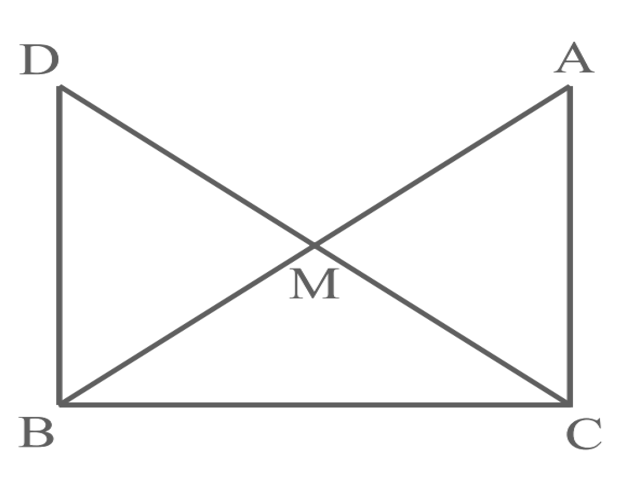
\includegraphics[width=\columnwidth]{figs/Screenshot.png}
  \caption{$\triangle \vec{ACB} ,\triangle \vec{DCB}$ with Mid-Point $\vec{M}$}
  \label{fig:triangles}
\end{figure}
\begin{enumerate}[label =(\roman*)]
        \item $\triangle \vec{AMC} \cong \triangle \vec{BMD}$
        \item $\angle \vec{DBC}$ is a right angle. 
        \item $\triangle \vec{DBC} \cong  \triangle \vec{ACB}$ 
        \item $\vec{CM} = \frac{1}{2} \vec{AB}$
\end{enumerate}
\pagebreak
\solution\\
\textbf{CONSTRUCTION STEPS :}
\begin{enumerate}
\item Let us Assume , the input parameters as ;
\begin{table}[H]
\centering
        \input{tables/input_params.tex}
          \caption{Input Parameters}
          \label{Table-1:Input_params}
\end{table}
\item the output can be calculated as ;
\begin{table}[H]
\centering
        \input{tables/output_params.tex}
          \caption{Output Parameters}
          \label{Table-2:Output_params}
\end{table}
                $\therefore$ By, Plotting these points we get the required Image \figref{fig:fig-2}
\begin{figure}[H]
        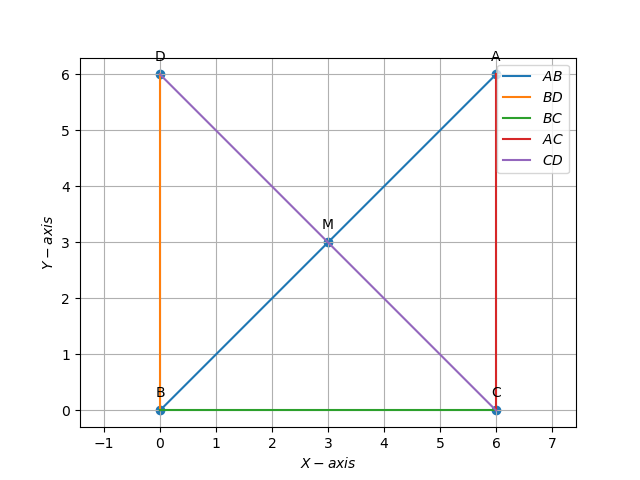
\includegraphics[width = \columnwidth]{figs/python_plot.png}
    \caption{PYTHON Plot of $\triangle \vec{ACB} ,\triangle \vec{DBC}$ with Mid-Point $\vec{M}$}
    \label{fig:fig-2}
\end{figure}
\end{enumerate}

\item Find the position vector of a point $\vec{R}$ which divides the line joining two points $\vec{P}$ and $\vec{Q}$ whose position vectors are $2\vec{a}+\vec{b}$ and $\vec{a}-3\vec{b}$ externally in the ratio $1:2$.

\textbf{Solution:}
Let us assume $\vec{a}$ and $\vec{b}$, and the given ratio is
\begin{table}[h]
    \centering
    \begin{tabular}{|c|c|c|}
        \hline 
        \textbf{Symbol} & \textbf{Value} & \textbf{Description} \\
        \hline
        $\vec{a}$ & $\myvec{1 \\ -3}$ & Vector $\vec{a}$ \\
        \hline
        $\vec{b}$ & $\myvec{0 \\ 2}$ & Vector $\vec{b}$\\
        \hline
        $k$ & $2$ & Ratio \\
        \hline
    \end{tabular}
    \caption{Vectors $\vec{a}$ and $\vec{b}$, ratio $k$}
    \label{tab:table1}
\end{table}

Using the section formula,
\begin{align}
    \vec{R} = \frac{\vec{Q} - k\vec{P}}{1 - k}
\end{align}
where $\vec{P}$ and $\vec{Q}$ depend on $\vec{a}$ and $\vec{b}$, then
\begin{align}
    \vec{P} &= (2\vec{a} + \vec{b}) = 2\myvec{1\\-3} + \myvec{0\\2} = \myvec{2\\-4} \\
    \vec{Q} &= (\vec{a} - 3\vec{b}) = \myvec{1\\-3} - 3\myvec{0\\2} = \myvec{1\\-9}
\end{align}
where $\vec{R}$ can be calculated as 
\begin{align}
    \vec{R} = \frac{(\vec{a} - 3\vec{b}) - k(2\vec{a} + \vec{b})}{1 - k}
\end{align}
By substituting $\vec{a}$ and $\vec{b}$ values, we get $\vec{R}$ as
\begin{align}
    \vec{R} = \myvec{3\\1}
\end{align}

\begin{table}[ht!]
    \centering
    \begin{tabular}{|c|c|c|}
        \hline
        \textbf{Symbol} & \textbf{Value} & \textbf{Description}\\
        \hline
        $\vec{P}$ & $(2\vec{a} + \vec{b})$ & Position vector $\vec{P}$ \\
        \hline
        $\vec{Q}$ & $(\vec{a} - 3\vec{b})$ & Position vector $\vec{Q}$\\
        \hline
        $\vec{R}$ & $\frac{\vec{Q} - k\vec{P}}{1 - k}$ & Position vector $\vec{R}$\\
        \hline
    \end{tabular}
    \caption{Vectors $\vec{P}$, $\vec{Q}$, $\vec{R}$}
    \label{tab:mytable2}   
\end{table}

\begin{figure}[H]
    \centering
    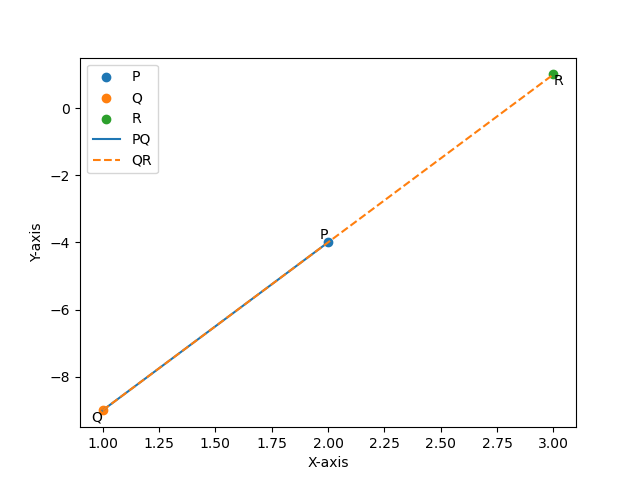
\includegraphics[width=\columnwidth]{figs/external-bisector.png}
    \caption{Point vectors $\vec{P}$, $\vec{Q}$, $\vec{R}$}
    \label{fig:enter-label}
\end{figure}


\end{enumerate}

    \item Draw a quadrilateral in the Cartesian plane, whose vertices are 
    \begin{align}
        \vec{A} = \myvec{-4\\5} \quad \vec{B} = \myvec{0\\7} \\
        \vec{C} = \myvec{5\\-5} \quad \vec{D} = \myvec{-4\\-2}
    \end{align}
    Also, find its area.
\label{chapters/11/10/1/1}
   \\ 
    \solution 
\begin{enumerate}[label=\thesection.\arabic*,ref=\thesection.\theenumi]
		\item Find $\abs{\overrightarrow{a}\times\overrightarrow{b}},\text{ if }\overrightarrow{a}=\hat{i}-7\hat{j}+7\hat{k}\text{ and } \overrightarrow{b}=3\hat{i}-2\hat{j}+2\hat{k}$.
	\\
		\solution
		\input{chapters/12/10/4/1/cross.tex}
\item Show that $$(\overrightarrow{a}-\overrightarrow{b})\times (\overrightarrow{a}+\overrightarrow{b})=2(\overrightarrow{a}\times \overrightarrow{b})$$
	\\
		\solution
		\input{chapters/12/10/4/4/cross.tex}
\item Find $\lambda$ and $\mu$ if $(2\hat{i}+6\hat{j}+27\hat{k})\times(\hat{i}+\lambda \hat{j} + \mu \hat{k})=\overrightarrow{0}$.
	\\
		\solution
		\input{chapters/12/10/4/5/cross.tex}
\item Given that $\overrightarrow{a} \cdot \overrightarrow{b} = 0$ and $\overrightarrow{a} \times \overrightarrow{b} = \overrightarrow{0}$. What can you conclude about the vectors $\overrightarrow{a} \text{ and }\overrightarrow{b}$?
\item Let the vectors be given as $\overrightarrow{a},\overrightarrow{b},\overrightarrow{c}\text{ be given as }\ a_1 \hat{i}+\ a_2 \hat{j}+\ a_3 \hat{k},\ b_1 \hat{i}+\ b_2 \hat{j}+\ b_3 \hat{k},\ c_1 \hat{i}+\ c_2 \hat{j}+\ c_3 \hat{k}$. Then show that $\overrightarrow{a} \times (\overrightarrow{b} + \overrightarrow{c}) = \overrightarrow{a} \times \overrightarrow{b}+\overrightarrow{a} \times \overrightarrow{c}$.
	\\
		\solution
		\input{chapters/12/10/4/7/cross.tex}
\item If either $\overrightarrow{a} = \overrightarrow{0}$ or $\overrightarrow{b} = \overrightarrow{0}$, then $\overrightarrow{a} \times \overrightarrow{b} = \overrightarrow{0}$. Is the converse true? Justify your answer with an example.
	\\
		\solution
		\input{chapters/12/10/4/8/cross.tex}
\item Find the area of the triangle with vertices $A(1, 1, 2)$, $B(2, 3, 5)$, and $C(1, 5, 5)$
	\\
		\solution
		\input{chapters/12/10/4/9/cross.tex}
\item Find the area of the parallelogram whose adjacent sides are determined by the vectors $\overrightarrow{a}=\hat{i}-\hat{j}+3\hat{k}$ and $\overrightarrow{b}=2\hat{i}-7\hat{j}+\hat{k}$.
	\\
		\solution
		\input{chapters/12/10/4/10/cross.tex}
\item Let the vectors $\overrightarrow{a}$ and $\overrightarrow{b}$ be such that $|\overrightarrow{a}| = 3$ and $|\overrightarrow{b}| = \dfrac{\sqrt{2}}{3}$, then $\overrightarrow{a} \times \overrightarrow{b}$ is a unit vector, if the angle between $\overrightarrow{a}$ and $\overrightarrow{b}$ is
\begin{enumerate}
\item $\dfrac{\pi}{6}$
\item $\dfrac{\pi}{4}$
\item $\dfrac{\pi}{3}$
\item $\dfrac{\pi}{2}$
\end{enumerate}
		\solution
		\input{chapters/12/10/4/11/cross.tex}
\item Area of a rectangle having vertices A, B, C and D with position vectors $ -\hat{i}+ \dfrac{1}{2} \hat{j}+4\hat{k},\hat{i}+ \dfrac{1}{2} \hat{j}+4\hat{k},\hat{i}-\dfrac{1}{2} \hat{j}+4\hat{k}\text{ and }-\hat{i}- \dfrac{1}{2} \hat{j}+4\hat{k}$, respectively is
\begin{enumerate}
\item $\dfrac{1}{2}$
\item 1
\item 2
\item 4
\end{enumerate}
		\solution
		\input{chapters/12/10/4/12/cross.tex}
\item Find the area of the triangle whose vertices are 
\begin{enumerate}
\item $(2, 3), (–1, 0), (2, – 4)$
\item $(–5, –1), (3, –5), (5, 2)$ 
\end{enumerate}
		\label{10/7/3/1}
\solution
		\input{chapters/10/7/3/1/area.tex}
\item Find the area of the triangle formed by joining the mid-points of the sides of the triangle whose vertices are $(0, –1), (2, 1) \text{ and } (0, 3)$. Find the ratio of this area to the area of the given triangle.
	\\
\solution
		\input{chapters/10/7/3/3/cross.tex}

\item Find the area of the quadrilateral whose vertices, taken in order, are $(– 4, – 2), (– 3, – 5), (3, – 2)$  and $ (2, 3)$.
	\\
\solution
		\input{chapters/10/7/3/4/cross.tex}

\item Verify that a median of a triangle divides it into two triangles of equal areas for $\triangle ABC$ whose vertices are $\vec{A}(4, -6), \vec{B}(3, 2), \text{ and } \vec{C}(5, 2)$. 
		\label{10/7/3/5}
		\\
\solution
		\input{chapters/10/7/3/5/area.tex}

\item The two adjacent sides of a parallelogram are 
$2\hat{i}-4\hat{j}+5\hat{k}$  and  $\hat{i}-2\hat{j}-3\hat{k}$.
Find the unit vector parallel to its diagonal. Also, find its area.\\
	\solution
		\input{chapters/12/10/5/10/cross.tex}
\item The vertices of a $\triangle ABC$ are $\vec{A}(4,6), \vec{B}(1,5)$ and  $\vec{C}(7,2)$. A line is drawn to intersect sides $AB$ and $AC$ at $\vec{D}$ and $\vec{E}$ respectively, such that $\frac{AD}{AB} = \frac{AE}{AC} = \frac{1}{4}$. Calculate the area of $\triangle ADE$ and compare it with the area of the $\triangle ABC$.
\\
\solution
	\input{chapters/10/7/4/6/section.tex}
    \item Draw a quadrilateral in the Cartesian plane, whose vertices are 
    \begin{align}
        \vec{A} = \myvec{-4\\5} \quad \vec{B} = \myvec{0\\7} \\
        \vec{C} = \myvec{5\\-5} \quad \vec{D} = \myvec{-4\\-2}
    \end{align}
    Also, find its area.
\label{chapters/11/10/1/1}
   \\ 
    \solution 
\input{chapters/11/10/1/1/cross.tex}
\item Find the area of region bounded by the triangle whose
	vertices are $(1, 0), (2, 2) \text{ and } (3, 1)$. 
\item Find the area of region bounded by the triangle whose vertices
	are $(– 1, 0), (1, 3) \text{ and } (3, 2)$. 
\item Find the area of the $\triangle ABC$, coordinates of whose vertices are $\vec{A}(2, 0), \vec{B}(4, 5), \text{ and } \vec{C}(6, 3)$.


\item 
\input{chapters/vectors/exer/main.tex}
\end{enumerate}


\item Find the area of region bounded by the triangle whose
	vertices are $(1, 0), (2, 2) \text{ and } (3, 1)$. 
\item Find the area of region bounded by the triangle whose vertices
	are $(– 1, 0), (1, 3) \text{ and } (3, 2)$. 
\item Find the area of the $\triangle ABC$, coordinates of whose vertices are $\vec{A}(2, 0), \vec{B}(4, 5), \text{ and } \vec{C}(6, 3)$.


\item 
%\documentclass[12pt]{article}
%\usepackage{graphicx}
%\usepackage{graphics}
%\usepackage{refstyle}
%\usepackage{amsmath}
%\usepackage{caption}
%\usepackage{float}
%\usepackage{booktabs}
%\usepackage{array}
%\usepackage{amssymb}
%\usepackage{booktabs}
%\let\vec\mathbf
%\providecommand{\brak}[1]{\ensuremath{\left(#1\right)}}
%\graphicspath{{/storage/self/primary/Download/latexnew/fig}}                                     
$\vec{P}$ and $\vec{Q}$ are any two points lying on the sides $DC$ and $AD$ respectively of a parallelogram $ABCD$.Show that, $ar\brak{\triangle APB}=ar\brak{\triangle BQC}$.


\textbf{Figure:}
\begin{figure}[H]
    \centering
	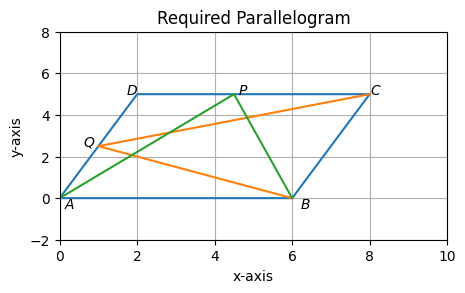
\includegraphics[width=\columnwidth]{chapters/vectors/exer/figs/1.png}
    \caption{}
    \label{fig:fig:1}
\end{figure}


\textbf{Solution:}
\begin{table}[H]
   \centering
  \input{chapters/vectors/exer/table/tab1.tex}
   \caption{Table of input parameters}        
\label{tab:tab:1}                    
\end{table}




\begin{table}[H]
    \centering                                  
\input{chapters/vectors/exer/table/tab2.tex}                  
\caption{Table of output parameters}
\label{tab:tab:2}
 \end{table}


For the $\triangle BQC$, the vertices of the triangle are taken from \tabref{tab:tab:1} and \tabref{tab:tab:2}.

\begin{align}
\implies ar\brak{\triangle BQC}&=
\frac{1}{2}\begin{tabular}{|c c c|}            
1 &1&1\\                      
$\vec{B}$&$\vec{Q}$&$\vec{C}$\\    
\end{tabular}\\
&= \frac{1}{2}\begin{tabular}{|c c c|}
       1 &1&1\\
       6&$\frac{2k_1}{k_1+1}$&8 \\
       0&$\frac{5k_1}{k_1+1}$&5
   \end{tabular}\\
  \xrightarrow{C_2'=C_2-C_1,C_3'=C_3-C_1}&\frac{1}{2} \begin{tabular}{|c c c|}
       1 &0&0\\
       6&$\frac{-4k_1-6}{k_1+1}$&2 \\
       0&$\frac{5k_1}{k_1+1}$&5
   \end{tabular}\\
&=\frac{1}{2}\brak{1\begin{tabular}{|c c|}
   $\frac{-4k_1-6}{k_1+1}$ &2  \\
   $\frac{5k_1}{k_1+1}$ & 5
\end{tabular} +0+0}\\
&=\frac{1}{2} \times30\\                          
&=15 \end{align}


For the $\triangle APB$, the vertices of the triangle are taken from \tabref{tab:tab:1} and \tabref{tab:tab:2}.
   \begin{align}
  \implies ar\brak{\triangle APB} &=
\frac{1}{2}\begin{tabular}{|c c c|}            
1 &1&1\\                            
$\vec{A}$&$\vec{P}$&$\vec{B}$\\
\end{tabular}\\ &=  \frac{1}{2}
   \begin{tabular}{|c c c|}
       1 &1&1\\
       0&$\frac{8k_2+2}{k_2+1}$&6 \\
       0&5&0
   \end{tabular}\\
 &=\frac{1}{2} \times30\\
 &=15 \end{align}
 \brak{6} = \brak{10}


So, ar\brak{\triangle BQC} = ar\brak{\triangle APB}.\brak{proved}
%\end{document}



\end{enumerate}


\item Show that $$(\overrightarrow{a}-\overrightarrow{b})\times (\overrightarrow{a}+\overrightarrow{b})=2(\overrightarrow{a}\times \overrightarrow{b})$$
	\\
		\solution
		\begin{enumerate}[label=\thesection.\arabic*,ref=\thesection.\theenumi]
		\item Find $\abs{\overrightarrow{a}\times\overrightarrow{b}},\text{ if }\overrightarrow{a}=\hat{i}-7\hat{j}+7\hat{k}\text{ and } \overrightarrow{b}=3\hat{i}-2\hat{j}+2\hat{k}$.
	\\
		\solution
		\begin{enumerate}[label=\thesection.\arabic*,ref=\thesection.\theenumi]
		\item Find $\abs{\overrightarrow{a}\times\overrightarrow{b}},\text{ if }\overrightarrow{a}=\hat{i}-7\hat{j}+7\hat{k}\text{ and } \overrightarrow{b}=3\hat{i}-2\hat{j}+2\hat{k}$.
	\\
		\solution
		\input{chapters/12/10/4/1/cross.tex}
\item Show that $$(\overrightarrow{a}-\overrightarrow{b})\times (\overrightarrow{a}+\overrightarrow{b})=2(\overrightarrow{a}\times \overrightarrow{b})$$
	\\
		\solution
		\input{chapters/12/10/4/4/cross.tex}
\item Find $\lambda$ and $\mu$ if $(2\hat{i}+6\hat{j}+27\hat{k})\times(\hat{i}+\lambda \hat{j} + \mu \hat{k})=\overrightarrow{0}$.
	\\
		\solution
		\input{chapters/12/10/4/5/cross.tex}
\item Given that $\overrightarrow{a} \cdot \overrightarrow{b} = 0$ and $\overrightarrow{a} \times \overrightarrow{b} = \overrightarrow{0}$. What can you conclude about the vectors $\overrightarrow{a} \text{ and }\overrightarrow{b}$?
\item Let the vectors be given as $\overrightarrow{a},\overrightarrow{b},\overrightarrow{c}\text{ be given as }\ a_1 \hat{i}+\ a_2 \hat{j}+\ a_3 \hat{k},\ b_1 \hat{i}+\ b_2 \hat{j}+\ b_3 \hat{k},\ c_1 \hat{i}+\ c_2 \hat{j}+\ c_3 \hat{k}$. Then show that $\overrightarrow{a} \times (\overrightarrow{b} + \overrightarrow{c}) = \overrightarrow{a} \times \overrightarrow{b}+\overrightarrow{a} \times \overrightarrow{c}$.
	\\
		\solution
		\input{chapters/12/10/4/7/cross.tex}
\item If either $\overrightarrow{a} = \overrightarrow{0}$ or $\overrightarrow{b} = \overrightarrow{0}$, then $\overrightarrow{a} \times \overrightarrow{b} = \overrightarrow{0}$. Is the converse true? Justify your answer with an example.
	\\
		\solution
		\input{chapters/12/10/4/8/cross.tex}
\item Find the area of the triangle with vertices $A(1, 1, 2)$, $B(2, 3, 5)$, and $C(1, 5, 5)$
	\\
		\solution
		\input{chapters/12/10/4/9/cross.tex}
\item Find the area of the parallelogram whose adjacent sides are determined by the vectors $\overrightarrow{a}=\hat{i}-\hat{j}+3\hat{k}$ and $\overrightarrow{b}=2\hat{i}-7\hat{j}+\hat{k}$.
	\\
		\solution
		\input{chapters/12/10/4/10/cross.tex}
\item Let the vectors $\overrightarrow{a}$ and $\overrightarrow{b}$ be such that $|\overrightarrow{a}| = 3$ and $|\overrightarrow{b}| = \dfrac{\sqrt{2}}{3}$, then $\overrightarrow{a} \times \overrightarrow{b}$ is a unit vector, if the angle between $\overrightarrow{a}$ and $\overrightarrow{b}$ is
\begin{enumerate}
\item $\dfrac{\pi}{6}$
\item $\dfrac{\pi}{4}$
\item $\dfrac{\pi}{3}$
\item $\dfrac{\pi}{2}$
\end{enumerate}
		\solution
		\input{chapters/12/10/4/11/cross.tex}
\item Area of a rectangle having vertices A, B, C and D with position vectors $ -\hat{i}+ \dfrac{1}{2} \hat{j}+4\hat{k},\hat{i}+ \dfrac{1}{2} \hat{j}+4\hat{k},\hat{i}-\dfrac{1}{2} \hat{j}+4\hat{k}\text{ and }-\hat{i}- \dfrac{1}{2} \hat{j}+4\hat{k}$, respectively is
\begin{enumerate}
\item $\dfrac{1}{2}$
\item 1
\item 2
\item 4
\end{enumerate}
		\solution
		\input{chapters/12/10/4/12/cross.tex}
\item Find the area of the triangle whose vertices are 
\begin{enumerate}
\item $(2, 3), (–1, 0), (2, – 4)$
\item $(–5, –1), (3, –5), (5, 2)$ 
\end{enumerate}
		\label{10/7/3/1}
\solution
		\input{chapters/10/7/3/1/area.tex}
\item Find the area of the triangle formed by joining the mid-points of the sides of the triangle whose vertices are $(0, –1), (2, 1) \text{ and } (0, 3)$. Find the ratio of this area to the area of the given triangle.
	\\
\solution
		\input{chapters/10/7/3/3/cross.tex}

\item Find the area of the quadrilateral whose vertices, taken in order, are $(– 4, – 2), (– 3, – 5), (3, – 2)$  and $ (2, 3)$.
	\\
\solution
		\input{chapters/10/7/3/4/cross.tex}

\item Verify that a median of a triangle divides it into two triangles of equal areas for $\triangle ABC$ whose vertices are $\vec{A}(4, -6), \vec{B}(3, 2), \text{ and } \vec{C}(5, 2)$. 
		\label{10/7/3/5}
		\\
\solution
		\input{chapters/10/7/3/5/area.tex}

\item The two adjacent sides of a parallelogram are 
$2\hat{i}-4\hat{j}+5\hat{k}$  and  $\hat{i}-2\hat{j}-3\hat{k}$.
Find the unit vector parallel to its diagonal. Also, find its area.\\
	\solution
		\input{chapters/12/10/5/10/cross.tex}
\item The vertices of a $\triangle ABC$ are $\vec{A}(4,6), \vec{B}(1,5)$ and  $\vec{C}(7,2)$. A line is drawn to intersect sides $AB$ and $AC$ at $\vec{D}$ and $\vec{E}$ respectively, such that $\frac{AD}{AB} = \frac{AE}{AC} = \frac{1}{4}$. Calculate the area of $\triangle ADE$ and compare it with the area of the $\triangle ABC$.
\\
\solution
	\input{chapters/10/7/4/6/section.tex}
    \item Draw a quadrilateral in the Cartesian plane, whose vertices are 
    \begin{align}
        \vec{A} = \myvec{-4\\5} \quad \vec{B} = \myvec{0\\7} \\
        \vec{C} = \myvec{5\\-5} \quad \vec{D} = \myvec{-4\\-2}
    \end{align}
    Also, find its area.
\label{chapters/11/10/1/1}
   \\ 
    \solution 
\input{chapters/11/10/1/1/cross.tex}
\item Find the area of region bounded by the triangle whose
	vertices are $(1, 0), (2, 2) \text{ and } (3, 1)$. 
\item Find the area of region bounded by the triangle whose vertices
	are $(– 1, 0), (1, 3) \text{ and } (3, 2)$. 
\item Find the area of the $\triangle ABC$, coordinates of whose vertices are $\vec{A}(2, 0), \vec{B}(4, 5), \text{ and } \vec{C}(6, 3)$.


\item 
\input{chapters/vectors/exer/main.tex}
\end{enumerate}


\item Show that $$(\overrightarrow{a}-\overrightarrow{b})\times (\overrightarrow{a}+\overrightarrow{b})=2(\overrightarrow{a}\times \overrightarrow{b})$$
	\\
		\solution
		\begin{enumerate}[label=\thesection.\arabic*,ref=\thesection.\theenumi]
		\item Find $\abs{\overrightarrow{a}\times\overrightarrow{b}},\text{ if }\overrightarrow{a}=\hat{i}-7\hat{j}+7\hat{k}\text{ and } \overrightarrow{b}=3\hat{i}-2\hat{j}+2\hat{k}$.
	\\
		\solution
		\input{chapters/12/10/4/1/cross.tex}
\item Show that $$(\overrightarrow{a}-\overrightarrow{b})\times (\overrightarrow{a}+\overrightarrow{b})=2(\overrightarrow{a}\times \overrightarrow{b})$$
	\\
		\solution
		\input{chapters/12/10/4/4/cross.tex}
\item Find $\lambda$ and $\mu$ if $(2\hat{i}+6\hat{j}+27\hat{k})\times(\hat{i}+\lambda \hat{j} + \mu \hat{k})=\overrightarrow{0}$.
	\\
		\solution
		\input{chapters/12/10/4/5/cross.tex}
\item Given that $\overrightarrow{a} \cdot \overrightarrow{b} = 0$ and $\overrightarrow{a} \times \overrightarrow{b} = \overrightarrow{0}$. What can you conclude about the vectors $\overrightarrow{a} \text{ and }\overrightarrow{b}$?
\item Let the vectors be given as $\overrightarrow{a},\overrightarrow{b},\overrightarrow{c}\text{ be given as }\ a_1 \hat{i}+\ a_2 \hat{j}+\ a_3 \hat{k},\ b_1 \hat{i}+\ b_2 \hat{j}+\ b_3 \hat{k},\ c_1 \hat{i}+\ c_2 \hat{j}+\ c_3 \hat{k}$. Then show that $\overrightarrow{a} \times (\overrightarrow{b} + \overrightarrow{c}) = \overrightarrow{a} \times \overrightarrow{b}+\overrightarrow{a} \times \overrightarrow{c}$.
	\\
		\solution
		\input{chapters/12/10/4/7/cross.tex}
\item If either $\overrightarrow{a} = \overrightarrow{0}$ or $\overrightarrow{b} = \overrightarrow{0}$, then $\overrightarrow{a} \times \overrightarrow{b} = \overrightarrow{0}$. Is the converse true? Justify your answer with an example.
	\\
		\solution
		\input{chapters/12/10/4/8/cross.tex}
\item Find the area of the triangle with vertices $A(1, 1, 2)$, $B(2, 3, 5)$, and $C(1, 5, 5)$
	\\
		\solution
		\input{chapters/12/10/4/9/cross.tex}
\item Find the area of the parallelogram whose adjacent sides are determined by the vectors $\overrightarrow{a}=\hat{i}-\hat{j}+3\hat{k}$ and $\overrightarrow{b}=2\hat{i}-7\hat{j}+\hat{k}$.
	\\
		\solution
		\input{chapters/12/10/4/10/cross.tex}
\item Let the vectors $\overrightarrow{a}$ and $\overrightarrow{b}$ be such that $|\overrightarrow{a}| = 3$ and $|\overrightarrow{b}| = \dfrac{\sqrt{2}}{3}$, then $\overrightarrow{a} \times \overrightarrow{b}$ is a unit vector, if the angle between $\overrightarrow{a}$ and $\overrightarrow{b}$ is
\begin{enumerate}
\item $\dfrac{\pi}{6}$
\item $\dfrac{\pi}{4}$
\item $\dfrac{\pi}{3}$
\item $\dfrac{\pi}{2}$
\end{enumerate}
		\solution
		\input{chapters/12/10/4/11/cross.tex}
\item Area of a rectangle having vertices A, B, C and D with position vectors $ -\hat{i}+ \dfrac{1}{2} \hat{j}+4\hat{k},\hat{i}+ \dfrac{1}{2} \hat{j}+4\hat{k},\hat{i}-\dfrac{1}{2} \hat{j}+4\hat{k}\text{ and }-\hat{i}- \dfrac{1}{2} \hat{j}+4\hat{k}$, respectively is
\begin{enumerate}
\item $\dfrac{1}{2}$
\item 1
\item 2
\item 4
\end{enumerate}
		\solution
		\input{chapters/12/10/4/12/cross.tex}
\item Find the area of the triangle whose vertices are 
\begin{enumerate}
\item $(2, 3), (–1, 0), (2, – 4)$
\item $(–5, –1), (3, –5), (5, 2)$ 
\end{enumerate}
		\label{10/7/3/1}
\solution
		\input{chapters/10/7/3/1/area.tex}
\item Find the area of the triangle formed by joining the mid-points of the sides of the triangle whose vertices are $(0, –1), (2, 1) \text{ and } (0, 3)$. Find the ratio of this area to the area of the given triangle.
	\\
\solution
		\input{chapters/10/7/3/3/cross.tex}

\item Find the area of the quadrilateral whose vertices, taken in order, are $(– 4, – 2), (– 3, – 5), (3, – 2)$  and $ (2, 3)$.
	\\
\solution
		\input{chapters/10/7/3/4/cross.tex}

\item Verify that a median of a triangle divides it into two triangles of equal areas for $\triangle ABC$ whose vertices are $\vec{A}(4, -6), \vec{B}(3, 2), \text{ and } \vec{C}(5, 2)$. 
		\label{10/7/3/5}
		\\
\solution
		\input{chapters/10/7/3/5/area.tex}

\item The two adjacent sides of a parallelogram are 
$2\hat{i}-4\hat{j}+5\hat{k}$  and  $\hat{i}-2\hat{j}-3\hat{k}$.
Find the unit vector parallel to its diagonal. Also, find its area.\\
	\solution
		\input{chapters/12/10/5/10/cross.tex}
\item The vertices of a $\triangle ABC$ are $\vec{A}(4,6), \vec{B}(1,5)$ and  $\vec{C}(7,2)$. A line is drawn to intersect sides $AB$ and $AC$ at $\vec{D}$ and $\vec{E}$ respectively, such that $\frac{AD}{AB} = \frac{AE}{AC} = \frac{1}{4}$. Calculate the area of $\triangle ADE$ and compare it with the area of the $\triangle ABC$.
\\
\solution
	\input{chapters/10/7/4/6/section.tex}
    \item Draw a quadrilateral in the Cartesian plane, whose vertices are 
    \begin{align}
        \vec{A} = \myvec{-4\\5} \quad \vec{B} = \myvec{0\\7} \\
        \vec{C} = \myvec{5\\-5} \quad \vec{D} = \myvec{-4\\-2}
    \end{align}
    Also, find its area.
\label{chapters/11/10/1/1}
   \\ 
    \solution 
\input{chapters/11/10/1/1/cross.tex}
\item Find the area of region bounded by the triangle whose
	vertices are $(1, 0), (2, 2) \text{ and } (3, 1)$. 
\item Find the area of region bounded by the triangle whose vertices
	are $(– 1, 0), (1, 3) \text{ and } (3, 2)$. 
\item Find the area of the $\triangle ABC$, coordinates of whose vertices are $\vec{A}(2, 0), \vec{B}(4, 5), \text{ and } \vec{C}(6, 3)$.


\item 
\input{chapters/vectors/exer/main.tex}
\end{enumerate}


\item Find $\lambda$ and $\mu$ if $(2\hat{i}+6\hat{j}+27\hat{k})\times(\hat{i}+\lambda \hat{j} + \mu \hat{k})=\overrightarrow{0}$.
	\\
		\solution
		\begin{enumerate}[label=\thesection.\arabic*,ref=\thesection.\theenumi]
		\item Find $\abs{\overrightarrow{a}\times\overrightarrow{b}},\text{ if }\overrightarrow{a}=\hat{i}-7\hat{j}+7\hat{k}\text{ and } \overrightarrow{b}=3\hat{i}-2\hat{j}+2\hat{k}$.
	\\
		\solution
		\input{chapters/12/10/4/1/cross.tex}
\item Show that $$(\overrightarrow{a}-\overrightarrow{b})\times (\overrightarrow{a}+\overrightarrow{b})=2(\overrightarrow{a}\times \overrightarrow{b})$$
	\\
		\solution
		\input{chapters/12/10/4/4/cross.tex}
\item Find $\lambda$ and $\mu$ if $(2\hat{i}+6\hat{j}+27\hat{k})\times(\hat{i}+\lambda \hat{j} + \mu \hat{k})=\overrightarrow{0}$.
	\\
		\solution
		\input{chapters/12/10/4/5/cross.tex}
\item Given that $\overrightarrow{a} \cdot \overrightarrow{b} = 0$ and $\overrightarrow{a} \times \overrightarrow{b} = \overrightarrow{0}$. What can you conclude about the vectors $\overrightarrow{a} \text{ and }\overrightarrow{b}$?
\item Let the vectors be given as $\overrightarrow{a},\overrightarrow{b},\overrightarrow{c}\text{ be given as }\ a_1 \hat{i}+\ a_2 \hat{j}+\ a_3 \hat{k},\ b_1 \hat{i}+\ b_2 \hat{j}+\ b_3 \hat{k},\ c_1 \hat{i}+\ c_2 \hat{j}+\ c_3 \hat{k}$. Then show that $\overrightarrow{a} \times (\overrightarrow{b} + \overrightarrow{c}) = \overrightarrow{a} \times \overrightarrow{b}+\overrightarrow{a} \times \overrightarrow{c}$.
	\\
		\solution
		\input{chapters/12/10/4/7/cross.tex}
\item If either $\overrightarrow{a} = \overrightarrow{0}$ or $\overrightarrow{b} = \overrightarrow{0}$, then $\overrightarrow{a} \times \overrightarrow{b} = \overrightarrow{0}$. Is the converse true? Justify your answer with an example.
	\\
		\solution
		\input{chapters/12/10/4/8/cross.tex}
\item Find the area of the triangle with vertices $A(1, 1, 2)$, $B(2, 3, 5)$, and $C(1, 5, 5)$
	\\
		\solution
		\input{chapters/12/10/4/9/cross.tex}
\item Find the area of the parallelogram whose adjacent sides are determined by the vectors $\overrightarrow{a}=\hat{i}-\hat{j}+3\hat{k}$ and $\overrightarrow{b}=2\hat{i}-7\hat{j}+\hat{k}$.
	\\
		\solution
		\input{chapters/12/10/4/10/cross.tex}
\item Let the vectors $\overrightarrow{a}$ and $\overrightarrow{b}$ be such that $|\overrightarrow{a}| = 3$ and $|\overrightarrow{b}| = \dfrac{\sqrt{2}}{3}$, then $\overrightarrow{a} \times \overrightarrow{b}$ is a unit vector, if the angle between $\overrightarrow{a}$ and $\overrightarrow{b}$ is
\begin{enumerate}
\item $\dfrac{\pi}{6}$
\item $\dfrac{\pi}{4}$
\item $\dfrac{\pi}{3}$
\item $\dfrac{\pi}{2}$
\end{enumerate}
		\solution
		\input{chapters/12/10/4/11/cross.tex}
\item Area of a rectangle having vertices A, B, C and D with position vectors $ -\hat{i}+ \dfrac{1}{2} \hat{j}+4\hat{k},\hat{i}+ \dfrac{1}{2} \hat{j}+4\hat{k},\hat{i}-\dfrac{1}{2} \hat{j}+4\hat{k}\text{ and }-\hat{i}- \dfrac{1}{2} \hat{j}+4\hat{k}$, respectively is
\begin{enumerate}
\item $\dfrac{1}{2}$
\item 1
\item 2
\item 4
\end{enumerate}
		\solution
		\input{chapters/12/10/4/12/cross.tex}
\item Find the area of the triangle whose vertices are 
\begin{enumerate}
\item $(2, 3), (–1, 0), (2, – 4)$
\item $(–5, –1), (3, –5), (5, 2)$ 
\end{enumerate}
		\label{10/7/3/1}
\solution
		\input{chapters/10/7/3/1/area.tex}
\item Find the area of the triangle formed by joining the mid-points of the sides of the triangle whose vertices are $(0, –1), (2, 1) \text{ and } (0, 3)$. Find the ratio of this area to the area of the given triangle.
	\\
\solution
		\input{chapters/10/7/3/3/cross.tex}

\item Find the area of the quadrilateral whose vertices, taken in order, are $(– 4, – 2), (– 3, – 5), (3, – 2)$  and $ (2, 3)$.
	\\
\solution
		\input{chapters/10/7/3/4/cross.tex}

\item Verify that a median of a triangle divides it into two triangles of equal areas for $\triangle ABC$ whose vertices are $\vec{A}(4, -6), \vec{B}(3, 2), \text{ and } \vec{C}(5, 2)$. 
		\label{10/7/3/5}
		\\
\solution
		\input{chapters/10/7/3/5/area.tex}

\item The two adjacent sides of a parallelogram are 
$2\hat{i}-4\hat{j}+5\hat{k}$  and  $\hat{i}-2\hat{j}-3\hat{k}$.
Find the unit vector parallel to its diagonal. Also, find its area.\\
	\solution
		\input{chapters/12/10/5/10/cross.tex}
\item The vertices of a $\triangle ABC$ are $\vec{A}(4,6), \vec{B}(1,5)$ and  $\vec{C}(7,2)$. A line is drawn to intersect sides $AB$ and $AC$ at $\vec{D}$ and $\vec{E}$ respectively, such that $\frac{AD}{AB} = \frac{AE}{AC} = \frac{1}{4}$. Calculate the area of $\triangle ADE$ and compare it with the area of the $\triangle ABC$.
\\
\solution
	\input{chapters/10/7/4/6/section.tex}
    \item Draw a quadrilateral in the Cartesian plane, whose vertices are 
    \begin{align}
        \vec{A} = \myvec{-4\\5} \quad \vec{B} = \myvec{0\\7} \\
        \vec{C} = \myvec{5\\-5} \quad \vec{D} = \myvec{-4\\-2}
    \end{align}
    Also, find its area.
\label{chapters/11/10/1/1}
   \\ 
    \solution 
\input{chapters/11/10/1/1/cross.tex}
\item Find the area of region bounded by the triangle whose
	vertices are $(1, 0), (2, 2) \text{ and } (3, 1)$. 
\item Find the area of region bounded by the triangle whose vertices
	are $(– 1, 0), (1, 3) \text{ and } (3, 2)$. 
\item Find the area of the $\triangle ABC$, coordinates of whose vertices are $\vec{A}(2, 0), \vec{B}(4, 5), \text{ and } \vec{C}(6, 3)$.


\item 
\input{chapters/vectors/exer/main.tex}
\end{enumerate}


\item Given that $\overrightarrow{a} \cdot \overrightarrow{b} = 0$ and $\overrightarrow{a} \times \overrightarrow{b} = \overrightarrow{0}$. What can you conclude about the vectors $\overrightarrow{a} \text{ and }\overrightarrow{b}$?
\item Let the vectors be given as $\overrightarrow{a},\overrightarrow{b},\overrightarrow{c}\text{ be given as }\ a_1 \hat{i}+\ a_2 \hat{j}+\ a_3 \hat{k},\ b_1 \hat{i}+\ b_2 \hat{j}+\ b_3 \hat{k},\ c_1 \hat{i}+\ c_2 \hat{j}+\ c_3 \hat{k}$. Then show that $\overrightarrow{a} \times (\overrightarrow{b} + \overrightarrow{c}) = \overrightarrow{a} \times \overrightarrow{b}+\overrightarrow{a} \times \overrightarrow{c}$.
	\\
		\solution
		\begin{enumerate}[label=\thesection.\arabic*,ref=\thesection.\theenumi]
		\item Find $\abs{\overrightarrow{a}\times\overrightarrow{b}},\text{ if }\overrightarrow{a}=\hat{i}-7\hat{j}+7\hat{k}\text{ and } \overrightarrow{b}=3\hat{i}-2\hat{j}+2\hat{k}$.
	\\
		\solution
		\input{chapters/12/10/4/1/cross.tex}
\item Show that $$(\overrightarrow{a}-\overrightarrow{b})\times (\overrightarrow{a}+\overrightarrow{b})=2(\overrightarrow{a}\times \overrightarrow{b})$$
	\\
		\solution
		\input{chapters/12/10/4/4/cross.tex}
\item Find $\lambda$ and $\mu$ if $(2\hat{i}+6\hat{j}+27\hat{k})\times(\hat{i}+\lambda \hat{j} + \mu \hat{k})=\overrightarrow{0}$.
	\\
		\solution
		\input{chapters/12/10/4/5/cross.tex}
\item Given that $\overrightarrow{a} \cdot \overrightarrow{b} = 0$ and $\overrightarrow{a} \times \overrightarrow{b} = \overrightarrow{0}$. What can you conclude about the vectors $\overrightarrow{a} \text{ and }\overrightarrow{b}$?
\item Let the vectors be given as $\overrightarrow{a},\overrightarrow{b},\overrightarrow{c}\text{ be given as }\ a_1 \hat{i}+\ a_2 \hat{j}+\ a_3 \hat{k},\ b_1 \hat{i}+\ b_2 \hat{j}+\ b_3 \hat{k},\ c_1 \hat{i}+\ c_2 \hat{j}+\ c_3 \hat{k}$. Then show that $\overrightarrow{a} \times (\overrightarrow{b} + \overrightarrow{c}) = \overrightarrow{a} \times \overrightarrow{b}+\overrightarrow{a} \times \overrightarrow{c}$.
	\\
		\solution
		\input{chapters/12/10/4/7/cross.tex}
\item If either $\overrightarrow{a} = \overrightarrow{0}$ or $\overrightarrow{b} = \overrightarrow{0}$, then $\overrightarrow{a} \times \overrightarrow{b} = \overrightarrow{0}$. Is the converse true? Justify your answer with an example.
	\\
		\solution
		\input{chapters/12/10/4/8/cross.tex}
\item Find the area of the triangle with vertices $A(1, 1, 2)$, $B(2, 3, 5)$, and $C(1, 5, 5)$
	\\
		\solution
		\input{chapters/12/10/4/9/cross.tex}
\item Find the area of the parallelogram whose adjacent sides are determined by the vectors $\overrightarrow{a}=\hat{i}-\hat{j}+3\hat{k}$ and $\overrightarrow{b}=2\hat{i}-7\hat{j}+\hat{k}$.
	\\
		\solution
		\input{chapters/12/10/4/10/cross.tex}
\item Let the vectors $\overrightarrow{a}$ and $\overrightarrow{b}$ be such that $|\overrightarrow{a}| = 3$ and $|\overrightarrow{b}| = \dfrac{\sqrt{2}}{3}$, then $\overrightarrow{a} \times \overrightarrow{b}$ is a unit vector, if the angle between $\overrightarrow{a}$ and $\overrightarrow{b}$ is
\begin{enumerate}
\item $\dfrac{\pi}{6}$
\item $\dfrac{\pi}{4}$
\item $\dfrac{\pi}{3}$
\item $\dfrac{\pi}{2}$
\end{enumerate}
		\solution
		\input{chapters/12/10/4/11/cross.tex}
\item Area of a rectangle having vertices A, B, C and D with position vectors $ -\hat{i}+ \dfrac{1}{2} \hat{j}+4\hat{k},\hat{i}+ \dfrac{1}{2} \hat{j}+4\hat{k},\hat{i}-\dfrac{1}{2} \hat{j}+4\hat{k}\text{ and }-\hat{i}- \dfrac{1}{2} \hat{j}+4\hat{k}$, respectively is
\begin{enumerate}
\item $\dfrac{1}{2}$
\item 1
\item 2
\item 4
\end{enumerate}
		\solution
		\input{chapters/12/10/4/12/cross.tex}
\item Find the area of the triangle whose vertices are 
\begin{enumerate}
\item $(2, 3), (–1, 0), (2, – 4)$
\item $(–5, –1), (3, –5), (5, 2)$ 
\end{enumerate}
		\label{10/7/3/1}
\solution
		\input{chapters/10/7/3/1/area.tex}
\item Find the area of the triangle formed by joining the mid-points of the sides of the triangle whose vertices are $(0, –1), (2, 1) \text{ and } (0, 3)$. Find the ratio of this area to the area of the given triangle.
	\\
\solution
		\input{chapters/10/7/3/3/cross.tex}

\item Find the area of the quadrilateral whose vertices, taken in order, are $(– 4, – 2), (– 3, – 5), (3, – 2)$  and $ (2, 3)$.
	\\
\solution
		\input{chapters/10/7/3/4/cross.tex}

\item Verify that a median of a triangle divides it into two triangles of equal areas for $\triangle ABC$ whose vertices are $\vec{A}(4, -6), \vec{B}(3, 2), \text{ and } \vec{C}(5, 2)$. 
		\label{10/7/3/5}
		\\
\solution
		\input{chapters/10/7/3/5/area.tex}

\item The two adjacent sides of a parallelogram are 
$2\hat{i}-4\hat{j}+5\hat{k}$  and  $\hat{i}-2\hat{j}-3\hat{k}$.
Find the unit vector parallel to its diagonal. Also, find its area.\\
	\solution
		\input{chapters/12/10/5/10/cross.tex}
\item The vertices of a $\triangle ABC$ are $\vec{A}(4,6), \vec{B}(1,5)$ and  $\vec{C}(7,2)$. A line is drawn to intersect sides $AB$ and $AC$ at $\vec{D}$ and $\vec{E}$ respectively, such that $\frac{AD}{AB} = \frac{AE}{AC} = \frac{1}{4}$. Calculate the area of $\triangle ADE$ and compare it with the area of the $\triangle ABC$.
\\
\solution
	\input{chapters/10/7/4/6/section.tex}
    \item Draw a quadrilateral in the Cartesian plane, whose vertices are 
    \begin{align}
        \vec{A} = \myvec{-4\\5} \quad \vec{B} = \myvec{0\\7} \\
        \vec{C} = \myvec{5\\-5} \quad \vec{D} = \myvec{-4\\-2}
    \end{align}
    Also, find its area.
\label{chapters/11/10/1/1}
   \\ 
    \solution 
\input{chapters/11/10/1/1/cross.tex}
\item Find the area of region bounded by the triangle whose
	vertices are $(1, 0), (2, 2) \text{ and } (3, 1)$. 
\item Find the area of region bounded by the triangle whose vertices
	are $(– 1, 0), (1, 3) \text{ and } (3, 2)$. 
\item Find the area of the $\triangle ABC$, coordinates of whose vertices are $\vec{A}(2, 0), \vec{B}(4, 5), \text{ and } \vec{C}(6, 3)$.


\item 
\input{chapters/vectors/exer/main.tex}
\end{enumerate}


\item If either $\overrightarrow{a} = \overrightarrow{0}$ or $\overrightarrow{b} = \overrightarrow{0}$, then $\overrightarrow{a} \times \overrightarrow{b} = \overrightarrow{0}$. Is the converse true? Justify your answer with an example.
	\\
		\solution
		\begin{enumerate}[label=\thesection.\arabic*,ref=\thesection.\theenumi]
		\item Find $\abs{\overrightarrow{a}\times\overrightarrow{b}},\text{ if }\overrightarrow{a}=\hat{i}-7\hat{j}+7\hat{k}\text{ and } \overrightarrow{b}=3\hat{i}-2\hat{j}+2\hat{k}$.
	\\
		\solution
		\input{chapters/12/10/4/1/cross.tex}
\item Show that $$(\overrightarrow{a}-\overrightarrow{b})\times (\overrightarrow{a}+\overrightarrow{b})=2(\overrightarrow{a}\times \overrightarrow{b})$$
	\\
		\solution
		\input{chapters/12/10/4/4/cross.tex}
\item Find $\lambda$ and $\mu$ if $(2\hat{i}+6\hat{j}+27\hat{k})\times(\hat{i}+\lambda \hat{j} + \mu \hat{k})=\overrightarrow{0}$.
	\\
		\solution
		\input{chapters/12/10/4/5/cross.tex}
\item Given that $\overrightarrow{a} \cdot \overrightarrow{b} = 0$ and $\overrightarrow{a} \times \overrightarrow{b} = \overrightarrow{0}$. What can you conclude about the vectors $\overrightarrow{a} \text{ and }\overrightarrow{b}$?
\item Let the vectors be given as $\overrightarrow{a},\overrightarrow{b},\overrightarrow{c}\text{ be given as }\ a_1 \hat{i}+\ a_2 \hat{j}+\ a_3 \hat{k},\ b_1 \hat{i}+\ b_2 \hat{j}+\ b_3 \hat{k},\ c_1 \hat{i}+\ c_2 \hat{j}+\ c_3 \hat{k}$. Then show that $\overrightarrow{a} \times (\overrightarrow{b} + \overrightarrow{c}) = \overrightarrow{a} \times \overrightarrow{b}+\overrightarrow{a} \times \overrightarrow{c}$.
	\\
		\solution
		\input{chapters/12/10/4/7/cross.tex}
\item If either $\overrightarrow{a} = \overrightarrow{0}$ or $\overrightarrow{b} = \overrightarrow{0}$, then $\overrightarrow{a} \times \overrightarrow{b} = \overrightarrow{0}$. Is the converse true? Justify your answer with an example.
	\\
		\solution
		\input{chapters/12/10/4/8/cross.tex}
\item Find the area of the triangle with vertices $A(1, 1, 2)$, $B(2, 3, 5)$, and $C(1, 5, 5)$
	\\
		\solution
		\input{chapters/12/10/4/9/cross.tex}
\item Find the area of the parallelogram whose adjacent sides are determined by the vectors $\overrightarrow{a}=\hat{i}-\hat{j}+3\hat{k}$ and $\overrightarrow{b}=2\hat{i}-7\hat{j}+\hat{k}$.
	\\
		\solution
		\input{chapters/12/10/4/10/cross.tex}
\item Let the vectors $\overrightarrow{a}$ and $\overrightarrow{b}$ be such that $|\overrightarrow{a}| = 3$ and $|\overrightarrow{b}| = \dfrac{\sqrt{2}}{3}$, then $\overrightarrow{a} \times \overrightarrow{b}$ is a unit vector, if the angle between $\overrightarrow{a}$ and $\overrightarrow{b}$ is
\begin{enumerate}
\item $\dfrac{\pi}{6}$
\item $\dfrac{\pi}{4}$
\item $\dfrac{\pi}{3}$
\item $\dfrac{\pi}{2}$
\end{enumerate}
		\solution
		\input{chapters/12/10/4/11/cross.tex}
\item Area of a rectangle having vertices A, B, C and D with position vectors $ -\hat{i}+ \dfrac{1}{2} \hat{j}+4\hat{k},\hat{i}+ \dfrac{1}{2} \hat{j}+4\hat{k},\hat{i}-\dfrac{1}{2} \hat{j}+4\hat{k}\text{ and }-\hat{i}- \dfrac{1}{2} \hat{j}+4\hat{k}$, respectively is
\begin{enumerate}
\item $\dfrac{1}{2}$
\item 1
\item 2
\item 4
\end{enumerate}
		\solution
		\input{chapters/12/10/4/12/cross.tex}
\item Find the area of the triangle whose vertices are 
\begin{enumerate}
\item $(2, 3), (–1, 0), (2, – 4)$
\item $(–5, –1), (3, –5), (5, 2)$ 
\end{enumerate}
		\label{10/7/3/1}
\solution
		\input{chapters/10/7/3/1/area.tex}
\item Find the area of the triangle formed by joining the mid-points of the sides of the triangle whose vertices are $(0, –1), (2, 1) \text{ and } (0, 3)$. Find the ratio of this area to the area of the given triangle.
	\\
\solution
		\input{chapters/10/7/3/3/cross.tex}

\item Find the area of the quadrilateral whose vertices, taken in order, are $(– 4, – 2), (– 3, – 5), (3, – 2)$  and $ (2, 3)$.
	\\
\solution
		\input{chapters/10/7/3/4/cross.tex}

\item Verify that a median of a triangle divides it into two triangles of equal areas for $\triangle ABC$ whose vertices are $\vec{A}(4, -6), \vec{B}(3, 2), \text{ and } \vec{C}(5, 2)$. 
		\label{10/7/3/5}
		\\
\solution
		\input{chapters/10/7/3/5/area.tex}

\item The two adjacent sides of a parallelogram are 
$2\hat{i}-4\hat{j}+5\hat{k}$  and  $\hat{i}-2\hat{j}-3\hat{k}$.
Find the unit vector parallel to its diagonal. Also, find its area.\\
	\solution
		\input{chapters/12/10/5/10/cross.tex}
\item The vertices of a $\triangle ABC$ are $\vec{A}(4,6), \vec{B}(1,5)$ and  $\vec{C}(7,2)$. A line is drawn to intersect sides $AB$ and $AC$ at $\vec{D}$ and $\vec{E}$ respectively, such that $\frac{AD}{AB} = \frac{AE}{AC} = \frac{1}{4}$. Calculate the area of $\triangle ADE$ and compare it with the area of the $\triangle ABC$.
\\
\solution
	\input{chapters/10/7/4/6/section.tex}
    \item Draw a quadrilateral in the Cartesian plane, whose vertices are 
    \begin{align}
        \vec{A} = \myvec{-4\\5} \quad \vec{B} = \myvec{0\\7} \\
        \vec{C} = \myvec{5\\-5} \quad \vec{D} = \myvec{-4\\-2}
    \end{align}
    Also, find its area.
\label{chapters/11/10/1/1}
   \\ 
    \solution 
\input{chapters/11/10/1/1/cross.tex}
\item Find the area of region bounded by the triangle whose
	vertices are $(1, 0), (2, 2) \text{ and } (3, 1)$. 
\item Find the area of region bounded by the triangle whose vertices
	are $(– 1, 0), (1, 3) \text{ and } (3, 2)$. 
\item Find the area of the $\triangle ABC$, coordinates of whose vertices are $\vec{A}(2, 0), \vec{B}(4, 5), \text{ and } \vec{C}(6, 3)$.


\item 
\input{chapters/vectors/exer/main.tex}
\end{enumerate}


\item Find the area of the triangle with vertices $A(1, 1, 2)$, $B(2, 3, 5)$, and $C(1, 5, 5)$
	\\
		\solution
		\begin{enumerate}[label=\thesection.\arabic*,ref=\thesection.\theenumi]
		\item Find $\abs{\overrightarrow{a}\times\overrightarrow{b}},\text{ if }\overrightarrow{a}=\hat{i}-7\hat{j}+7\hat{k}\text{ and } \overrightarrow{b}=3\hat{i}-2\hat{j}+2\hat{k}$.
	\\
		\solution
		\input{chapters/12/10/4/1/cross.tex}
\item Show that $$(\overrightarrow{a}-\overrightarrow{b})\times (\overrightarrow{a}+\overrightarrow{b})=2(\overrightarrow{a}\times \overrightarrow{b})$$
	\\
		\solution
		\input{chapters/12/10/4/4/cross.tex}
\item Find $\lambda$ and $\mu$ if $(2\hat{i}+6\hat{j}+27\hat{k})\times(\hat{i}+\lambda \hat{j} + \mu \hat{k})=\overrightarrow{0}$.
	\\
		\solution
		\input{chapters/12/10/4/5/cross.tex}
\item Given that $\overrightarrow{a} \cdot \overrightarrow{b} = 0$ and $\overrightarrow{a} \times \overrightarrow{b} = \overrightarrow{0}$. What can you conclude about the vectors $\overrightarrow{a} \text{ and }\overrightarrow{b}$?
\item Let the vectors be given as $\overrightarrow{a},\overrightarrow{b},\overrightarrow{c}\text{ be given as }\ a_1 \hat{i}+\ a_2 \hat{j}+\ a_3 \hat{k},\ b_1 \hat{i}+\ b_2 \hat{j}+\ b_3 \hat{k},\ c_1 \hat{i}+\ c_2 \hat{j}+\ c_3 \hat{k}$. Then show that $\overrightarrow{a} \times (\overrightarrow{b} + \overrightarrow{c}) = \overrightarrow{a} \times \overrightarrow{b}+\overrightarrow{a} \times \overrightarrow{c}$.
	\\
		\solution
		\input{chapters/12/10/4/7/cross.tex}
\item If either $\overrightarrow{a} = \overrightarrow{0}$ or $\overrightarrow{b} = \overrightarrow{0}$, then $\overrightarrow{a} \times \overrightarrow{b} = \overrightarrow{0}$. Is the converse true? Justify your answer with an example.
	\\
		\solution
		\input{chapters/12/10/4/8/cross.tex}
\item Find the area of the triangle with vertices $A(1, 1, 2)$, $B(2, 3, 5)$, and $C(1, 5, 5)$
	\\
		\solution
		\input{chapters/12/10/4/9/cross.tex}
\item Find the area of the parallelogram whose adjacent sides are determined by the vectors $\overrightarrow{a}=\hat{i}-\hat{j}+3\hat{k}$ and $\overrightarrow{b}=2\hat{i}-7\hat{j}+\hat{k}$.
	\\
		\solution
		\input{chapters/12/10/4/10/cross.tex}
\item Let the vectors $\overrightarrow{a}$ and $\overrightarrow{b}$ be such that $|\overrightarrow{a}| = 3$ and $|\overrightarrow{b}| = \dfrac{\sqrt{2}}{3}$, then $\overrightarrow{a} \times \overrightarrow{b}$ is a unit vector, if the angle between $\overrightarrow{a}$ and $\overrightarrow{b}$ is
\begin{enumerate}
\item $\dfrac{\pi}{6}$
\item $\dfrac{\pi}{4}$
\item $\dfrac{\pi}{3}$
\item $\dfrac{\pi}{2}$
\end{enumerate}
		\solution
		\input{chapters/12/10/4/11/cross.tex}
\item Area of a rectangle having vertices A, B, C and D with position vectors $ -\hat{i}+ \dfrac{1}{2} \hat{j}+4\hat{k},\hat{i}+ \dfrac{1}{2} \hat{j}+4\hat{k},\hat{i}-\dfrac{1}{2} \hat{j}+4\hat{k}\text{ and }-\hat{i}- \dfrac{1}{2} \hat{j}+4\hat{k}$, respectively is
\begin{enumerate}
\item $\dfrac{1}{2}$
\item 1
\item 2
\item 4
\end{enumerate}
		\solution
		\input{chapters/12/10/4/12/cross.tex}
\item Find the area of the triangle whose vertices are 
\begin{enumerate}
\item $(2, 3), (–1, 0), (2, – 4)$
\item $(–5, –1), (3, –5), (5, 2)$ 
\end{enumerate}
		\label{10/7/3/1}
\solution
		\input{chapters/10/7/3/1/area.tex}
\item Find the area of the triangle formed by joining the mid-points of the sides of the triangle whose vertices are $(0, –1), (2, 1) \text{ and } (0, 3)$. Find the ratio of this area to the area of the given triangle.
	\\
\solution
		\input{chapters/10/7/3/3/cross.tex}

\item Find the area of the quadrilateral whose vertices, taken in order, are $(– 4, – 2), (– 3, – 5), (3, – 2)$  and $ (2, 3)$.
	\\
\solution
		\input{chapters/10/7/3/4/cross.tex}

\item Verify that a median of a triangle divides it into two triangles of equal areas for $\triangle ABC$ whose vertices are $\vec{A}(4, -6), \vec{B}(3, 2), \text{ and } \vec{C}(5, 2)$. 
		\label{10/7/3/5}
		\\
\solution
		\input{chapters/10/7/3/5/area.tex}

\item The two adjacent sides of a parallelogram are 
$2\hat{i}-4\hat{j}+5\hat{k}$  and  $\hat{i}-2\hat{j}-3\hat{k}$.
Find the unit vector parallel to its diagonal. Also, find its area.\\
	\solution
		\input{chapters/12/10/5/10/cross.tex}
\item The vertices of a $\triangle ABC$ are $\vec{A}(4,6), \vec{B}(1,5)$ and  $\vec{C}(7,2)$. A line is drawn to intersect sides $AB$ and $AC$ at $\vec{D}$ and $\vec{E}$ respectively, such that $\frac{AD}{AB} = \frac{AE}{AC} = \frac{1}{4}$. Calculate the area of $\triangle ADE$ and compare it with the area of the $\triangle ABC$.
\\
\solution
	\input{chapters/10/7/4/6/section.tex}
    \item Draw a quadrilateral in the Cartesian plane, whose vertices are 
    \begin{align}
        \vec{A} = \myvec{-4\\5} \quad \vec{B} = \myvec{0\\7} \\
        \vec{C} = \myvec{5\\-5} \quad \vec{D} = \myvec{-4\\-2}
    \end{align}
    Also, find its area.
\label{chapters/11/10/1/1}
   \\ 
    \solution 
\input{chapters/11/10/1/1/cross.tex}
\item Find the area of region bounded by the triangle whose
	vertices are $(1, 0), (2, 2) \text{ and } (3, 1)$. 
\item Find the area of region bounded by the triangle whose vertices
	are $(– 1, 0), (1, 3) \text{ and } (3, 2)$. 
\item Find the area of the $\triangle ABC$, coordinates of whose vertices are $\vec{A}(2, 0), \vec{B}(4, 5), \text{ and } \vec{C}(6, 3)$.


\item 
\input{chapters/vectors/exer/main.tex}
\end{enumerate}


\item Find the area of the parallelogram whose adjacent sides are determined by the vectors $\overrightarrow{a}=\hat{i}-\hat{j}+3\hat{k}$ and $\overrightarrow{b}=2\hat{i}-7\hat{j}+\hat{k}$.
	\\
		\solution
		\begin{enumerate}[label=\thesection.\arabic*,ref=\thesection.\theenumi]
		\item Find $\abs{\overrightarrow{a}\times\overrightarrow{b}},\text{ if }\overrightarrow{a}=\hat{i}-7\hat{j}+7\hat{k}\text{ and } \overrightarrow{b}=3\hat{i}-2\hat{j}+2\hat{k}$.
	\\
		\solution
		\input{chapters/12/10/4/1/cross.tex}
\item Show that $$(\overrightarrow{a}-\overrightarrow{b})\times (\overrightarrow{a}+\overrightarrow{b})=2(\overrightarrow{a}\times \overrightarrow{b})$$
	\\
		\solution
		\input{chapters/12/10/4/4/cross.tex}
\item Find $\lambda$ and $\mu$ if $(2\hat{i}+6\hat{j}+27\hat{k})\times(\hat{i}+\lambda \hat{j} + \mu \hat{k})=\overrightarrow{0}$.
	\\
		\solution
		\input{chapters/12/10/4/5/cross.tex}
\item Given that $\overrightarrow{a} \cdot \overrightarrow{b} = 0$ and $\overrightarrow{a} \times \overrightarrow{b} = \overrightarrow{0}$. What can you conclude about the vectors $\overrightarrow{a} \text{ and }\overrightarrow{b}$?
\item Let the vectors be given as $\overrightarrow{a},\overrightarrow{b},\overrightarrow{c}\text{ be given as }\ a_1 \hat{i}+\ a_2 \hat{j}+\ a_3 \hat{k},\ b_1 \hat{i}+\ b_2 \hat{j}+\ b_3 \hat{k},\ c_1 \hat{i}+\ c_2 \hat{j}+\ c_3 \hat{k}$. Then show that $\overrightarrow{a} \times (\overrightarrow{b} + \overrightarrow{c}) = \overrightarrow{a} \times \overrightarrow{b}+\overrightarrow{a} \times \overrightarrow{c}$.
	\\
		\solution
		\input{chapters/12/10/4/7/cross.tex}
\item If either $\overrightarrow{a} = \overrightarrow{0}$ or $\overrightarrow{b} = \overrightarrow{0}$, then $\overrightarrow{a} \times \overrightarrow{b} = \overrightarrow{0}$. Is the converse true? Justify your answer with an example.
	\\
		\solution
		\input{chapters/12/10/4/8/cross.tex}
\item Find the area of the triangle with vertices $A(1, 1, 2)$, $B(2, 3, 5)$, and $C(1, 5, 5)$
	\\
		\solution
		\input{chapters/12/10/4/9/cross.tex}
\item Find the area of the parallelogram whose adjacent sides are determined by the vectors $\overrightarrow{a}=\hat{i}-\hat{j}+3\hat{k}$ and $\overrightarrow{b}=2\hat{i}-7\hat{j}+\hat{k}$.
	\\
		\solution
		\input{chapters/12/10/4/10/cross.tex}
\item Let the vectors $\overrightarrow{a}$ and $\overrightarrow{b}$ be such that $|\overrightarrow{a}| = 3$ and $|\overrightarrow{b}| = \dfrac{\sqrt{2}}{3}$, then $\overrightarrow{a} \times \overrightarrow{b}$ is a unit vector, if the angle between $\overrightarrow{a}$ and $\overrightarrow{b}$ is
\begin{enumerate}
\item $\dfrac{\pi}{6}$
\item $\dfrac{\pi}{4}$
\item $\dfrac{\pi}{3}$
\item $\dfrac{\pi}{2}$
\end{enumerate}
		\solution
		\input{chapters/12/10/4/11/cross.tex}
\item Area of a rectangle having vertices A, B, C and D with position vectors $ -\hat{i}+ \dfrac{1}{2} \hat{j}+4\hat{k},\hat{i}+ \dfrac{1}{2} \hat{j}+4\hat{k},\hat{i}-\dfrac{1}{2} \hat{j}+4\hat{k}\text{ and }-\hat{i}- \dfrac{1}{2} \hat{j}+4\hat{k}$, respectively is
\begin{enumerate}
\item $\dfrac{1}{2}$
\item 1
\item 2
\item 4
\end{enumerate}
		\solution
		\input{chapters/12/10/4/12/cross.tex}
\item Find the area of the triangle whose vertices are 
\begin{enumerate}
\item $(2, 3), (–1, 0), (2, – 4)$
\item $(–5, –1), (3, –5), (5, 2)$ 
\end{enumerate}
		\label{10/7/3/1}
\solution
		\input{chapters/10/7/3/1/area.tex}
\item Find the area of the triangle formed by joining the mid-points of the sides of the triangle whose vertices are $(0, –1), (2, 1) \text{ and } (0, 3)$. Find the ratio of this area to the area of the given triangle.
	\\
\solution
		\input{chapters/10/7/3/3/cross.tex}

\item Find the area of the quadrilateral whose vertices, taken in order, are $(– 4, – 2), (– 3, – 5), (3, – 2)$  and $ (2, 3)$.
	\\
\solution
		\input{chapters/10/7/3/4/cross.tex}

\item Verify that a median of a triangle divides it into two triangles of equal areas for $\triangle ABC$ whose vertices are $\vec{A}(4, -6), \vec{B}(3, 2), \text{ and } \vec{C}(5, 2)$. 
		\label{10/7/3/5}
		\\
\solution
		\input{chapters/10/7/3/5/area.tex}

\item The two adjacent sides of a parallelogram are 
$2\hat{i}-4\hat{j}+5\hat{k}$  and  $\hat{i}-2\hat{j}-3\hat{k}$.
Find the unit vector parallel to its diagonal. Also, find its area.\\
	\solution
		\input{chapters/12/10/5/10/cross.tex}
\item The vertices of a $\triangle ABC$ are $\vec{A}(4,6), \vec{B}(1,5)$ and  $\vec{C}(7,2)$. A line is drawn to intersect sides $AB$ and $AC$ at $\vec{D}$ and $\vec{E}$ respectively, such that $\frac{AD}{AB} = \frac{AE}{AC} = \frac{1}{4}$. Calculate the area of $\triangle ADE$ and compare it with the area of the $\triangle ABC$.
\\
\solution
	\input{chapters/10/7/4/6/section.tex}
    \item Draw a quadrilateral in the Cartesian plane, whose vertices are 
    \begin{align}
        \vec{A} = \myvec{-4\\5} \quad \vec{B} = \myvec{0\\7} \\
        \vec{C} = \myvec{5\\-5} \quad \vec{D} = \myvec{-4\\-2}
    \end{align}
    Also, find its area.
\label{chapters/11/10/1/1}
   \\ 
    \solution 
\input{chapters/11/10/1/1/cross.tex}
\item Find the area of region bounded by the triangle whose
	vertices are $(1, 0), (2, 2) \text{ and } (3, 1)$. 
\item Find the area of region bounded by the triangle whose vertices
	are $(– 1, 0), (1, 3) \text{ and } (3, 2)$. 
\item Find the area of the $\triangle ABC$, coordinates of whose vertices are $\vec{A}(2, 0), \vec{B}(4, 5), \text{ and } \vec{C}(6, 3)$.


\item 
\input{chapters/vectors/exer/main.tex}
\end{enumerate}


\item Let the vectors $\overrightarrow{a}$ and $\overrightarrow{b}$ be such that $|\overrightarrow{a}| = 3$ and $|\overrightarrow{b}| = \dfrac{\sqrt{2}}{3}$, then $\overrightarrow{a} \times \overrightarrow{b}$ is a unit vector, if the angle between $\overrightarrow{a}$ and $\overrightarrow{b}$ is
\begin{enumerate}
\item $\dfrac{\pi}{6}$
\item $\dfrac{\pi}{4}$
\item $\dfrac{\pi}{3}$
\item $\dfrac{\pi}{2}$
\end{enumerate}
		\solution
		\begin{enumerate}[label=\thesection.\arabic*,ref=\thesection.\theenumi]
		\item Find $\abs{\overrightarrow{a}\times\overrightarrow{b}},\text{ if }\overrightarrow{a}=\hat{i}-7\hat{j}+7\hat{k}\text{ and } \overrightarrow{b}=3\hat{i}-2\hat{j}+2\hat{k}$.
	\\
		\solution
		\input{chapters/12/10/4/1/cross.tex}
\item Show that $$(\overrightarrow{a}-\overrightarrow{b})\times (\overrightarrow{a}+\overrightarrow{b})=2(\overrightarrow{a}\times \overrightarrow{b})$$
	\\
		\solution
		\input{chapters/12/10/4/4/cross.tex}
\item Find $\lambda$ and $\mu$ if $(2\hat{i}+6\hat{j}+27\hat{k})\times(\hat{i}+\lambda \hat{j} + \mu \hat{k})=\overrightarrow{0}$.
	\\
		\solution
		\input{chapters/12/10/4/5/cross.tex}
\item Given that $\overrightarrow{a} \cdot \overrightarrow{b} = 0$ and $\overrightarrow{a} \times \overrightarrow{b} = \overrightarrow{0}$. What can you conclude about the vectors $\overrightarrow{a} \text{ and }\overrightarrow{b}$?
\item Let the vectors be given as $\overrightarrow{a},\overrightarrow{b},\overrightarrow{c}\text{ be given as }\ a_1 \hat{i}+\ a_2 \hat{j}+\ a_3 \hat{k},\ b_1 \hat{i}+\ b_2 \hat{j}+\ b_3 \hat{k},\ c_1 \hat{i}+\ c_2 \hat{j}+\ c_3 \hat{k}$. Then show that $\overrightarrow{a} \times (\overrightarrow{b} + \overrightarrow{c}) = \overrightarrow{a} \times \overrightarrow{b}+\overrightarrow{a} \times \overrightarrow{c}$.
	\\
		\solution
		\input{chapters/12/10/4/7/cross.tex}
\item If either $\overrightarrow{a} = \overrightarrow{0}$ or $\overrightarrow{b} = \overrightarrow{0}$, then $\overrightarrow{a} \times \overrightarrow{b} = \overrightarrow{0}$. Is the converse true? Justify your answer with an example.
	\\
		\solution
		\input{chapters/12/10/4/8/cross.tex}
\item Find the area of the triangle with vertices $A(1, 1, 2)$, $B(2, 3, 5)$, and $C(1, 5, 5)$
	\\
		\solution
		\input{chapters/12/10/4/9/cross.tex}
\item Find the area of the parallelogram whose adjacent sides are determined by the vectors $\overrightarrow{a}=\hat{i}-\hat{j}+3\hat{k}$ and $\overrightarrow{b}=2\hat{i}-7\hat{j}+\hat{k}$.
	\\
		\solution
		\input{chapters/12/10/4/10/cross.tex}
\item Let the vectors $\overrightarrow{a}$ and $\overrightarrow{b}$ be such that $|\overrightarrow{a}| = 3$ and $|\overrightarrow{b}| = \dfrac{\sqrt{2}}{3}$, then $\overrightarrow{a} \times \overrightarrow{b}$ is a unit vector, if the angle between $\overrightarrow{a}$ and $\overrightarrow{b}$ is
\begin{enumerate}
\item $\dfrac{\pi}{6}$
\item $\dfrac{\pi}{4}$
\item $\dfrac{\pi}{3}$
\item $\dfrac{\pi}{2}$
\end{enumerate}
		\solution
		\input{chapters/12/10/4/11/cross.tex}
\item Area of a rectangle having vertices A, B, C and D with position vectors $ -\hat{i}+ \dfrac{1}{2} \hat{j}+4\hat{k},\hat{i}+ \dfrac{1}{2} \hat{j}+4\hat{k},\hat{i}-\dfrac{1}{2} \hat{j}+4\hat{k}\text{ and }-\hat{i}- \dfrac{1}{2} \hat{j}+4\hat{k}$, respectively is
\begin{enumerate}
\item $\dfrac{1}{2}$
\item 1
\item 2
\item 4
\end{enumerate}
		\solution
		\input{chapters/12/10/4/12/cross.tex}
\item Find the area of the triangle whose vertices are 
\begin{enumerate}
\item $(2, 3), (–1, 0), (2, – 4)$
\item $(–5, –1), (3, –5), (5, 2)$ 
\end{enumerate}
		\label{10/7/3/1}
\solution
		\input{chapters/10/7/3/1/area.tex}
\item Find the area of the triangle formed by joining the mid-points of the sides of the triangle whose vertices are $(0, –1), (2, 1) \text{ and } (0, 3)$. Find the ratio of this area to the area of the given triangle.
	\\
\solution
		\input{chapters/10/7/3/3/cross.tex}

\item Find the area of the quadrilateral whose vertices, taken in order, are $(– 4, – 2), (– 3, – 5), (3, – 2)$  and $ (2, 3)$.
	\\
\solution
		\input{chapters/10/7/3/4/cross.tex}

\item Verify that a median of a triangle divides it into two triangles of equal areas for $\triangle ABC$ whose vertices are $\vec{A}(4, -6), \vec{B}(3, 2), \text{ and } \vec{C}(5, 2)$. 
		\label{10/7/3/5}
		\\
\solution
		\input{chapters/10/7/3/5/area.tex}

\item The two adjacent sides of a parallelogram are 
$2\hat{i}-4\hat{j}+5\hat{k}$  and  $\hat{i}-2\hat{j}-3\hat{k}$.
Find the unit vector parallel to its diagonal. Also, find its area.\\
	\solution
		\input{chapters/12/10/5/10/cross.tex}
\item The vertices of a $\triangle ABC$ are $\vec{A}(4,6), \vec{B}(1,5)$ and  $\vec{C}(7,2)$. A line is drawn to intersect sides $AB$ and $AC$ at $\vec{D}$ and $\vec{E}$ respectively, such that $\frac{AD}{AB} = \frac{AE}{AC} = \frac{1}{4}$. Calculate the area of $\triangle ADE$ and compare it with the area of the $\triangle ABC$.
\\
\solution
	\input{chapters/10/7/4/6/section.tex}
    \item Draw a quadrilateral in the Cartesian plane, whose vertices are 
    \begin{align}
        \vec{A} = \myvec{-4\\5} \quad \vec{B} = \myvec{0\\7} \\
        \vec{C} = \myvec{5\\-5} \quad \vec{D} = \myvec{-4\\-2}
    \end{align}
    Also, find its area.
\label{chapters/11/10/1/1}
   \\ 
    \solution 
\input{chapters/11/10/1/1/cross.tex}
\item Find the area of region bounded by the triangle whose
	vertices are $(1, 0), (2, 2) \text{ and } (3, 1)$. 
\item Find the area of region bounded by the triangle whose vertices
	are $(– 1, 0), (1, 3) \text{ and } (3, 2)$. 
\item Find the area of the $\triangle ABC$, coordinates of whose vertices are $\vec{A}(2, 0), \vec{B}(4, 5), \text{ and } \vec{C}(6, 3)$.


\item 
\input{chapters/vectors/exer/main.tex}
\end{enumerate}


\item Area of a rectangle having vertices A, B, C and D with position vectors $ -\hat{i}+ \dfrac{1}{2} \hat{j}+4\hat{k},\hat{i}+ \dfrac{1}{2} \hat{j}+4\hat{k},\hat{i}-\dfrac{1}{2} \hat{j}+4\hat{k}\text{ and }-\hat{i}- \dfrac{1}{2} \hat{j}+4\hat{k}$, respectively is
\begin{enumerate}
\item $\dfrac{1}{2}$
\item 1
\item 2
\item 4
\end{enumerate}
		\solution
		\begin{enumerate}[label=\thesection.\arabic*,ref=\thesection.\theenumi]
		\item Find $\abs{\overrightarrow{a}\times\overrightarrow{b}},\text{ if }\overrightarrow{a}=\hat{i}-7\hat{j}+7\hat{k}\text{ and } \overrightarrow{b}=3\hat{i}-2\hat{j}+2\hat{k}$.
	\\
		\solution
		\input{chapters/12/10/4/1/cross.tex}
\item Show that $$(\overrightarrow{a}-\overrightarrow{b})\times (\overrightarrow{a}+\overrightarrow{b})=2(\overrightarrow{a}\times \overrightarrow{b})$$
	\\
		\solution
		\input{chapters/12/10/4/4/cross.tex}
\item Find $\lambda$ and $\mu$ if $(2\hat{i}+6\hat{j}+27\hat{k})\times(\hat{i}+\lambda \hat{j} + \mu \hat{k})=\overrightarrow{0}$.
	\\
		\solution
		\input{chapters/12/10/4/5/cross.tex}
\item Given that $\overrightarrow{a} \cdot \overrightarrow{b} = 0$ and $\overrightarrow{a} \times \overrightarrow{b} = \overrightarrow{0}$. What can you conclude about the vectors $\overrightarrow{a} \text{ and }\overrightarrow{b}$?
\item Let the vectors be given as $\overrightarrow{a},\overrightarrow{b},\overrightarrow{c}\text{ be given as }\ a_1 \hat{i}+\ a_2 \hat{j}+\ a_3 \hat{k},\ b_1 \hat{i}+\ b_2 \hat{j}+\ b_3 \hat{k},\ c_1 \hat{i}+\ c_2 \hat{j}+\ c_3 \hat{k}$. Then show that $\overrightarrow{a} \times (\overrightarrow{b} + \overrightarrow{c}) = \overrightarrow{a} \times \overrightarrow{b}+\overrightarrow{a} \times \overrightarrow{c}$.
	\\
		\solution
		\input{chapters/12/10/4/7/cross.tex}
\item If either $\overrightarrow{a} = \overrightarrow{0}$ or $\overrightarrow{b} = \overrightarrow{0}$, then $\overrightarrow{a} \times \overrightarrow{b} = \overrightarrow{0}$. Is the converse true? Justify your answer with an example.
	\\
		\solution
		\input{chapters/12/10/4/8/cross.tex}
\item Find the area of the triangle with vertices $A(1, 1, 2)$, $B(2, 3, 5)$, and $C(1, 5, 5)$
	\\
		\solution
		\input{chapters/12/10/4/9/cross.tex}
\item Find the area of the parallelogram whose adjacent sides are determined by the vectors $\overrightarrow{a}=\hat{i}-\hat{j}+3\hat{k}$ and $\overrightarrow{b}=2\hat{i}-7\hat{j}+\hat{k}$.
	\\
		\solution
		\input{chapters/12/10/4/10/cross.tex}
\item Let the vectors $\overrightarrow{a}$ and $\overrightarrow{b}$ be such that $|\overrightarrow{a}| = 3$ and $|\overrightarrow{b}| = \dfrac{\sqrt{2}}{3}$, then $\overrightarrow{a} \times \overrightarrow{b}$ is a unit vector, if the angle between $\overrightarrow{a}$ and $\overrightarrow{b}$ is
\begin{enumerate}
\item $\dfrac{\pi}{6}$
\item $\dfrac{\pi}{4}$
\item $\dfrac{\pi}{3}$
\item $\dfrac{\pi}{2}$
\end{enumerate}
		\solution
		\input{chapters/12/10/4/11/cross.tex}
\item Area of a rectangle having vertices A, B, C and D with position vectors $ -\hat{i}+ \dfrac{1}{2} \hat{j}+4\hat{k},\hat{i}+ \dfrac{1}{2} \hat{j}+4\hat{k},\hat{i}-\dfrac{1}{2} \hat{j}+4\hat{k}\text{ and }-\hat{i}- \dfrac{1}{2} \hat{j}+4\hat{k}$, respectively is
\begin{enumerate}
\item $\dfrac{1}{2}$
\item 1
\item 2
\item 4
\end{enumerate}
		\solution
		\input{chapters/12/10/4/12/cross.tex}
\item Find the area of the triangle whose vertices are 
\begin{enumerate}
\item $(2, 3), (–1, 0), (2, – 4)$
\item $(–5, –1), (3, –5), (5, 2)$ 
\end{enumerate}
		\label{10/7/3/1}
\solution
		\input{chapters/10/7/3/1/area.tex}
\item Find the area of the triangle formed by joining the mid-points of the sides of the triangle whose vertices are $(0, –1), (2, 1) \text{ and } (0, 3)$. Find the ratio of this area to the area of the given triangle.
	\\
\solution
		\input{chapters/10/7/3/3/cross.tex}

\item Find the area of the quadrilateral whose vertices, taken in order, are $(– 4, – 2), (– 3, – 5), (3, – 2)$  and $ (2, 3)$.
	\\
\solution
		\input{chapters/10/7/3/4/cross.tex}

\item Verify that a median of a triangle divides it into two triangles of equal areas for $\triangle ABC$ whose vertices are $\vec{A}(4, -6), \vec{B}(3, 2), \text{ and } \vec{C}(5, 2)$. 
		\label{10/7/3/5}
		\\
\solution
		\input{chapters/10/7/3/5/area.tex}

\item The two adjacent sides of a parallelogram are 
$2\hat{i}-4\hat{j}+5\hat{k}$  and  $\hat{i}-2\hat{j}-3\hat{k}$.
Find the unit vector parallel to its diagonal. Also, find its area.\\
	\solution
		\input{chapters/12/10/5/10/cross.tex}
\item The vertices of a $\triangle ABC$ are $\vec{A}(4,6), \vec{B}(1,5)$ and  $\vec{C}(7,2)$. A line is drawn to intersect sides $AB$ and $AC$ at $\vec{D}$ and $\vec{E}$ respectively, such that $\frac{AD}{AB} = \frac{AE}{AC} = \frac{1}{4}$. Calculate the area of $\triangle ADE$ and compare it with the area of the $\triangle ABC$.
\\
\solution
	\input{chapters/10/7/4/6/section.tex}
    \item Draw a quadrilateral in the Cartesian plane, whose vertices are 
    \begin{align}
        \vec{A} = \myvec{-4\\5} \quad \vec{B} = \myvec{0\\7} \\
        \vec{C} = \myvec{5\\-5} \quad \vec{D} = \myvec{-4\\-2}
    \end{align}
    Also, find its area.
\label{chapters/11/10/1/1}
   \\ 
    \solution 
\input{chapters/11/10/1/1/cross.tex}
\item Find the area of region bounded by the triangle whose
	vertices are $(1, 0), (2, 2) \text{ and } (3, 1)$. 
\item Find the area of region bounded by the triangle whose vertices
	are $(– 1, 0), (1, 3) \text{ and } (3, 2)$. 
\item Find the area of the $\triangle ABC$, coordinates of whose vertices are $\vec{A}(2, 0), \vec{B}(4, 5), \text{ and } \vec{C}(6, 3)$.


\item 
\input{chapters/vectors/exer/main.tex}
\end{enumerate}


\item Find the area of the triangle whose vertices are 
\begin{enumerate}
\item $(2, 3), (–1, 0), (2, – 4)$
\item $(–5, –1), (3, –5), (5, 2)$ 
\end{enumerate}
		\label{10/7/3/1}
\solution
		\input{chapters/10/7/3/1/area.tex}
\item Find the area of the triangle formed by joining the mid-points of the sides of the triangle whose vertices are $(0, –1), (2, 1) \text{ and } (0, 3)$. Find the ratio of this area to the area of the given triangle.
	\\
\solution
		\begin{enumerate}[label=\thesection.\arabic*,ref=\thesection.\theenumi]
		\item Find $\abs{\overrightarrow{a}\times\overrightarrow{b}},\text{ if }\overrightarrow{a}=\hat{i}-7\hat{j}+7\hat{k}\text{ and } \overrightarrow{b}=3\hat{i}-2\hat{j}+2\hat{k}$.
	\\
		\solution
		\input{chapters/12/10/4/1/cross.tex}
\item Show that $$(\overrightarrow{a}-\overrightarrow{b})\times (\overrightarrow{a}+\overrightarrow{b})=2(\overrightarrow{a}\times \overrightarrow{b})$$
	\\
		\solution
		\input{chapters/12/10/4/4/cross.tex}
\item Find $\lambda$ and $\mu$ if $(2\hat{i}+6\hat{j}+27\hat{k})\times(\hat{i}+\lambda \hat{j} + \mu \hat{k})=\overrightarrow{0}$.
	\\
		\solution
		\input{chapters/12/10/4/5/cross.tex}
\item Given that $\overrightarrow{a} \cdot \overrightarrow{b} = 0$ and $\overrightarrow{a} \times \overrightarrow{b} = \overrightarrow{0}$. What can you conclude about the vectors $\overrightarrow{a} \text{ and }\overrightarrow{b}$?
\item Let the vectors be given as $\overrightarrow{a},\overrightarrow{b},\overrightarrow{c}\text{ be given as }\ a_1 \hat{i}+\ a_2 \hat{j}+\ a_3 \hat{k},\ b_1 \hat{i}+\ b_2 \hat{j}+\ b_3 \hat{k},\ c_1 \hat{i}+\ c_2 \hat{j}+\ c_3 \hat{k}$. Then show that $\overrightarrow{a} \times (\overrightarrow{b} + \overrightarrow{c}) = \overrightarrow{a} \times \overrightarrow{b}+\overrightarrow{a} \times \overrightarrow{c}$.
	\\
		\solution
		\input{chapters/12/10/4/7/cross.tex}
\item If either $\overrightarrow{a} = \overrightarrow{0}$ or $\overrightarrow{b} = \overrightarrow{0}$, then $\overrightarrow{a} \times \overrightarrow{b} = \overrightarrow{0}$. Is the converse true? Justify your answer with an example.
	\\
		\solution
		\input{chapters/12/10/4/8/cross.tex}
\item Find the area of the triangle with vertices $A(1, 1, 2)$, $B(2, 3, 5)$, and $C(1, 5, 5)$
	\\
		\solution
		\input{chapters/12/10/4/9/cross.tex}
\item Find the area of the parallelogram whose adjacent sides are determined by the vectors $\overrightarrow{a}=\hat{i}-\hat{j}+3\hat{k}$ and $\overrightarrow{b}=2\hat{i}-7\hat{j}+\hat{k}$.
	\\
		\solution
		\input{chapters/12/10/4/10/cross.tex}
\item Let the vectors $\overrightarrow{a}$ and $\overrightarrow{b}$ be such that $|\overrightarrow{a}| = 3$ and $|\overrightarrow{b}| = \dfrac{\sqrt{2}}{3}$, then $\overrightarrow{a} \times \overrightarrow{b}$ is a unit vector, if the angle between $\overrightarrow{a}$ and $\overrightarrow{b}$ is
\begin{enumerate}
\item $\dfrac{\pi}{6}$
\item $\dfrac{\pi}{4}$
\item $\dfrac{\pi}{3}$
\item $\dfrac{\pi}{2}$
\end{enumerate}
		\solution
		\input{chapters/12/10/4/11/cross.tex}
\item Area of a rectangle having vertices A, B, C and D with position vectors $ -\hat{i}+ \dfrac{1}{2} \hat{j}+4\hat{k},\hat{i}+ \dfrac{1}{2} \hat{j}+4\hat{k},\hat{i}-\dfrac{1}{2} \hat{j}+4\hat{k}\text{ and }-\hat{i}- \dfrac{1}{2} \hat{j}+4\hat{k}$, respectively is
\begin{enumerate}
\item $\dfrac{1}{2}$
\item 1
\item 2
\item 4
\end{enumerate}
		\solution
		\input{chapters/12/10/4/12/cross.tex}
\item Find the area of the triangle whose vertices are 
\begin{enumerate}
\item $(2, 3), (–1, 0), (2, – 4)$
\item $(–5, –1), (3, –5), (5, 2)$ 
\end{enumerate}
		\label{10/7/3/1}
\solution
		\input{chapters/10/7/3/1/area.tex}
\item Find the area of the triangle formed by joining the mid-points of the sides of the triangle whose vertices are $(0, –1), (2, 1) \text{ and } (0, 3)$. Find the ratio of this area to the area of the given triangle.
	\\
\solution
		\input{chapters/10/7/3/3/cross.tex}

\item Find the area of the quadrilateral whose vertices, taken in order, are $(– 4, – 2), (– 3, – 5), (3, – 2)$  and $ (2, 3)$.
	\\
\solution
		\input{chapters/10/7/3/4/cross.tex}

\item Verify that a median of a triangle divides it into two triangles of equal areas for $\triangle ABC$ whose vertices are $\vec{A}(4, -6), \vec{B}(3, 2), \text{ and } \vec{C}(5, 2)$. 
		\label{10/7/3/5}
		\\
\solution
		\input{chapters/10/7/3/5/area.tex}

\item The two adjacent sides of a parallelogram are 
$2\hat{i}-4\hat{j}+5\hat{k}$  and  $\hat{i}-2\hat{j}-3\hat{k}$.
Find the unit vector parallel to its diagonal. Also, find its area.\\
	\solution
		\input{chapters/12/10/5/10/cross.tex}
\item The vertices of a $\triangle ABC$ are $\vec{A}(4,6), \vec{B}(1,5)$ and  $\vec{C}(7,2)$. A line is drawn to intersect sides $AB$ and $AC$ at $\vec{D}$ and $\vec{E}$ respectively, such that $\frac{AD}{AB} = \frac{AE}{AC} = \frac{1}{4}$. Calculate the area of $\triangle ADE$ and compare it with the area of the $\triangle ABC$.
\\
\solution
	\input{chapters/10/7/4/6/section.tex}
    \item Draw a quadrilateral in the Cartesian plane, whose vertices are 
    \begin{align}
        \vec{A} = \myvec{-4\\5} \quad \vec{B} = \myvec{0\\7} \\
        \vec{C} = \myvec{5\\-5} \quad \vec{D} = \myvec{-4\\-2}
    \end{align}
    Also, find its area.
\label{chapters/11/10/1/1}
   \\ 
    \solution 
\input{chapters/11/10/1/1/cross.tex}
\item Find the area of region bounded by the triangle whose
	vertices are $(1, 0), (2, 2) \text{ and } (3, 1)$. 
\item Find the area of region bounded by the triangle whose vertices
	are $(– 1, 0), (1, 3) \text{ and } (3, 2)$. 
\item Find the area of the $\triangle ABC$, coordinates of whose vertices are $\vec{A}(2, 0), \vec{B}(4, 5), \text{ and } \vec{C}(6, 3)$.


\item 
\input{chapters/vectors/exer/main.tex}
\end{enumerate}



\item Find the area of the quadrilateral whose vertices, taken in order, are $(– 4, – 2), (– 3, – 5), (3, – 2)$  and $ (2, 3)$.
	\\
\solution
		\begin{enumerate}[label=\thesection.\arabic*,ref=\thesection.\theenumi]
		\item Find $\abs{\overrightarrow{a}\times\overrightarrow{b}},\text{ if }\overrightarrow{a}=\hat{i}-7\hat{j}+7\hat{k}\text{ and } \overrightarrow{b}=3\hat{i}-2\hat{j}+2\hat{k}$.
	\\
		\solution
		\input{chapters/12/10/4/1/cross.tex}
\item Show that $$(\overrightarrow{a}-\overrightarrow{b})\times (\overrightarrow{a}+\overrightarrow{b})=2(\overrightarrow{a}\times \overrightarrow{b})$$
	\\
		\solution
		\input{chapters/12/10/4/4/cross.tex}
\item Find $\lambda$ and $\mu$ if $(2\hat{i}+6\hat{j}+27\hat{k})\times(\hat{i}+\lambda \hat{j} + \mu \hat{k})=\overrightarrow{0}$.
	\\
		\solution
		\input{chapters/12/10/4/5/cross.tex}
\item Given that $\overrightarrow{a} \cdot \overrightarrow{b} = 0$ and $\overrightarrow{a} \times \overrightarrow{b} = \overrightarrow{0}$. What can you conclude about the vectors $\overrightarrow{a} \text{ and }\overrightarrow{b}$?
\item Let the vectors be given as $\overrightarrow{a},\overrightarrow{b},\overrightarrow{c}\text{ be given as }\ a_1 \hat{i}+\ a_2 \hat{j}+\ a_3 \hat{k},\ b_1 \hat{i}+\ b_2 \hat{j}+\ b_3 \hat{k},\ c_1 \hat{i}+\ c_2 \hat{j}+\ c_3 \hat{k}$. Then show that $\overrightarrow{a} \times (\overrightarrow{b} + \overrightarrow{c}) = \overrightarrow{a} \times \overrightarrow{b}+\overrightarrow{a} \times \overrightarrow{c}$.
	\\
		\solution
		\input{chapters/12/10/4/7/cross.tex}
\item If either $\overrightarrow{a} = \overrightarrow{0}$ or $\overrightarrow{b} = \overrightarrow{0}$, then $\overrightarrow{a} \times \overrightarrow{b} = \overrightarrow{0}$. Is the converse true? Justify your answer with an example.
	\\
		\solution
		\input{chapters/12/10/4/8/cross.tex}
\item Find the area of the triangle with vertices $A(1, 1, 2)$, $B(2, 3, 5)$, and $C(1, 5, 5)$
	\\
		\solution
		\input{chapters/12/10/4/9/cross.tex}
\item Find the area of the parallelogram whose adjacent sides are determined by the vectors $\overrightarrow{a}=\hat{i}-\hat{j}+3\hat{k}$ and $\overrightarrow{b}=2\hat{i}-7\hat{j}+\hat{k}$.
	\\
		\solution
		\input{chapters/12/10/4/10/cross.tex}
\item Let the vectors $\overrightarrow{a}$ and $\overrightarrow{b}$ be such that $|\overrightarrow{a}| = 3$ and $|\overrightarrow{b}| = \dfrac{\sqrt{2}}{3}$, then $\overrightarrow{a} \times \overrightarrow{b}$ is a unit vector, if the angle between $\overrightarrow{a}$ and $\overrightarrow{b}$ is
\begin{enumerate}
\item $\dfrac{\pi}{6}$
\item $\dfrac{\pi}{4}$
\item $\dfrac{\pi}{3}$
\item $\dfrac{\pi}{2}$
\end{enumerate}
		\solution
		\input{chapters/12/10/4/11/cross.tex}
\item Area of a rectangle having vertices A, B, C and D with position vectors $ -\hat{i}+ \dfrac{1}{2} \hat{j}+4\hat{k},\hat{i}+ \dfrac{1}{2} \hat{j}+4\hat{k},\hat{i}-\dfrac{1}{2} \hat{j}+4\hat{k}\text{ and }-\hat{i}- \dfrac{1}{2} \hat{j}+4\hat{k}$, respectively is
\begin{enumerate}
\item $\dfrac{1}{2}$
\item 1
\item 2
\item 4
\end{enumerate}
		\solution
		\input{chapters/12/10/4/12/cross.tex}
\item Find the area of the triangle whose vertices are 
\begin{enumerate}
\item $(2, 3), (–1, 0), (2, – 4)$
\item $(–5, –1), (3, –5), (5, 2)$ 
\end{enumerate}
		\label{10/7/3/1}
\solution
		\input{chapters/10/7/3/1/area.tex}
\item Find the area of the triangle formed by joining the mid-points of the sides of the triangle whose vertices are $(0, –1), (2, 1) \text{ and } (0, 3)$. Find the ratio of this area to the area of the given triangle.
	\\
\solution
		\input{chapters/10/7/3/3/cross.tex}

\item Find the area of the quadrilateral whose vertices, taken in order, are $(– 4, – 2), (– 3, – 5), (3, – 2)$  and $ (2, 3)$.
	\\
\solution
		\input{chapters/10/7/3/4/cross.tex}

\item Verify that a median of a triangle divides it into two triangles of equal areas for $\triangle ABC$ whose vertices are $\vec{A}(4, -6), \vec{B}(3, 2), \text{ and } \vec{C}(5, 2)$. 
		\label{10/7/3/5}
		\\
\solution
		\input{chapters/10/7/3/5/area.tex}

\item The two adjacent sides of a parallelogram are 
$2\hat{i}-4\hat{j}+5\hat{k}$  and  $\hat{i}-2\hat{j}-3\hat{k}$.
Find the unit vector parallel to its diagonal. Also, find its area.\\
	\solution
		\input{chapters/12/10/5/10/cross.tex}
\item The vertices of a $\triangle ABC$ are $\vec{A}(4,6), \vec{B}(1,5)$ and  $\vec{C}(7,2)$. A line is drawn to intersect sides $AB$ and $AC$ at $\vec{D}$ and $\vec{E}$ respectively, such that $\frac{AD}{AB} = \frac{AE}{AC} = \frac{1}{4}$. Calculate the area of $\triangle ADE$ and compare it with the area of the $\triangle ABC$.
\\
\solution
	\input{chapters/10/7/4/6/section.tex}
    \item Draw a quadrilateral in the Cartesian plane, whose vertices are 
    \begin{align}
        \vec{A} = \myvec{-4\\5} \quad \vec{B} = \myvec{0\\7} \\
        \vec{C} = \myvec{5\\-5} \quad \vec{D} = \myvec{-4\\-2}
    \end{align}
    Also, find its area.
\label{chapters/11/10/1/1}
   \\ 
    \solution 
\input{chapters/11/10/1/1/cross.tex}
\item Find the area of region bounded by the triangle whose
	vertices are $(1, 0), (2, 2) \text{ and } (3, 1)$. 
\item Find the area of region bounded by the triangle whose vertices
	are $(– 1, 0), (1, 3) \text{ and } (3, 2)$. 
\item Find the area of the $\triangle ABC$, coordinates of whose vertices are $\vec{A}(2, 0), \vec{B}(4, 5), \text{ and } \vec{C}(6, 3)$.


\item 
\input{chapters/vectors/exer/main.tex}
\end{enumerate}



\item Verify that a median of a triangle divides it into two triangles of equal areas for $\triangle ABC$ whose vertices are $\vec{A}(4, -6), \vec{B}(3, 2), \text{ and } \vec{C}(5, 2)$. 
		\label{10/7/3/5}
		\\
\solution
		\input{chapters/10/7/3/5/area.tex}

\item The two adjacent sides of a parallelogram are 
$2\hat{i}-4\hat{j}+5\hat{k}$  and  $\hat{i}-2\hat{j}-3\hat{k}$.
Find the unit vector parallel to its diagonal. Also, find its area.\\
	\solution
		\begin{enumerate}[label=\thesection.\arabic*,ref=\thesection.\theenumi]
		\item Find $\abs{\overrightarrow{a}\times\overrightarrow{b}},\text{ if }\overrightarrow{a}=\hat{i}-7\hat{j}+7\hat{k}\text{ and } \overrightarrow{b}=3\hat{i}-2\hat{j}+2\hat{k}$.
	\\
		\solution
		\input{chapters/12/10/4/1/cross.tex}
\item Show that $$(\overrightarrow{a}-\overrightarrow{b})\times (\overrightarrow{a}+\overrightarrow{b})=2(\overrightarrow{a}\times \overrightarrow{b})$$
	\\
		\solution
		\input{chapters/12/10/4/4/cross.tex}
\item Find $\lambda$ and $\mu$ if $(2\hat{i}+6\hat{j}+27\hat{k})\times(\hat{i}+\lambda \hat{j} + \mu \hat{k})=\overrightarrow{0}$.
	\\
		\solution
		\input{chapters/12/10/4/5/cross.tex}
\item Given that $\overrightarrow{a} \cdot \overrightarrow{b} = 0$ and $\overrightarrow{a} \times \overrightarrow{b} = \overrightarrow{0}$. What can you conclude about the vectors $\overrightarrow{a} \text{ and }\overrightarrow{b}$?
\item Let the vectors be given as $\overrightarrow{a},\overrightarrow{b},\overrightarrow{c}\text{ be given as }\ a_1 \hat{i}+\ a_2 \hat{j}+\ a_3 \hat{k},\ b_1 \hat{i}+\ b_2 \hat{j}+\ b_3 \hat{k},\ c_1 \hat{i}+\ c_2 \hat{j}+\ c_3 \hat{k}$. Then show that $\overrightarrow{a} \times (\overrightarrow{b} + \overrightarrow{c}) = \overrightarrow{a} \times \overrightarrow{b}+\overrightarrow{a} \times \overrightarrow{c}$.
	\\
		\solution
		\input{chapters/12/10/4/7/cross.tex}
\item If either $\overrightarrow{a} = \overrightarrow{0}$ or $\overrightarrow{b} = \overrightarrow{0}$, then $\overrightarrow{a} \times \overrightarrow{b} = \overrightarrow{0}$. Is the converse true? Justify your answer with an example.
	\\
		\solution
		\input{chapters/12/10/4/8/cross.tex}
\item Find the area of the triangle with vertices $A(1, 1, 2)$, $B(2, 3, 5)$, and $C(1, 5, 5)$
	\\
		\solution
		\input{chapters/12/10/4/9/cross.tex}
\item Find the area of the parallelogram whose adjacent sides are determined by the vectors $\overrightarrow{a}=\hat{i}-\hat{j}+3\hat{k}$ and $\overrightarrow{b}=2\hat{i}-7\hat{j}+\hat{k}$.
	\\
		\solution
		\input{chapters/12/10/4/10/cross.tex}
\item Let the vectors $\overrightarrow{a}$ and $\overrightarrow{b}$ be such that $|\overrightarrow{a}| = 3$ and $|\overrightarrow{b}| = \dfrac{\sqrt{2}}{3}$, then $\overrightarrow{a} \times \overrightarrow{b}$ is a unit vector, if the angle between $\overrightarrow{a}$ and $\overrightarrow{b}$ is
\begin{enumerate}
\item $\dfrac{\pi}{6}$
\item $\dfrac{\pi}{4}$
\item $\dfrac{\pi}{3}$
\item $\dfrac{\pi}{2}$
\end{enumerate}
		\solution
		\input{chapters/12/10/4/11/cross.tex}
\item Area of a rectangle having vertices A, B, C and D with position vectors $ -\hat{i}+ \dfrac{1}{2} \hat{j}+4\hat{k},\hat{i}+ \dfrac{1}{2} \hat{j}+4\hat{k},\hat{i}-\dfrac{1}{2} \hat{j}+4\hat{k}\text{ and }-\hat{i}- \dfrac{1}{2} \hat{j}+4\hat{k}$, respectively is
\begin{enumerate}
\item $\dfrac{1}{2}$
\item 1
\item 2
\item 4
\end{enumerate}
		\solution
		\input{chapters/12/10/4/12/cross.tex}
\item Find the area of the triangle whose vertices are 
\begin{enumerate}
\item $(2, 3), (–1, 0), (2, – 4)$
\item $(–5, –1), (3, –5), (5, 2)$ 
\end{enumerate}
		\label{10/7/3/1}
\solution
		\input{chapters/10/7/3/1/area.tex}
\item Find the area of the triangle formed by joining the mid-points of the sides of the triangle whose vertices are $(0, –1), (2, 1) \text{ and } (0, 3)$. Find the ratio of this area to the area of the given triangle.
	\\
\solution
		\input{chapters/10/7/3/3/cross.tex}

\item Find the area of the quadrilateral whose vertices, taken in order, are $(– 4, – 2), (– 3, – 5), (3, – 2)$  and $ (2, 3)$.
	\\
\solution
		\input{chapters/10/7/3/4/cross.tex}

\item Verify that a median of a triangle divides it into two triangles of equal areas for $\triangle ABC$ whose vertices are $\vec{A}(4, -6), \vec{B}(3, 2), \text{ and } \vec{C}(5, 2)$. 
		\label{10/7/3/5}
		\\
\solution
		\input{chapters/10/7/3/5/area.tex}

\item The two adjacent sides of a parallelogram are 
$2\hat{i}-4\hat{j}+5\hat{k}$  and  $\hat{i}-2\hat{j}-3\hat{k}$.
Find the unit vector parallel to its diagonal. Also, find its area.\\
	\solution
		\input{chapters/12/10/5/10/cross.tex}
\item The vertices of a $\triangle ABC$ are $\vec{A}(4,6), \vec{B}(1,5)$ and  $\vec{C}(7,2)$. A line is drawn to intersect sides $AB$ and $AC$ at $\vec{D}$ and $\vec{E}$ respectively, such that $\frac{AD}{AB} = \frac{AE}{AC} = \frac{1}{4}$. Calculate the area of $\triangle ADE$ and compare it with the area of the $\triangle ABC$.
\\
\solution
	\input{chapters/10/7/4/6/section.tex}
    \item Draw a quadrilateral in the Cartesian plane, whose vertices are 
    \begin{align}
        \vec{A} = \myvec{-4\\5} \quad \vec{B} = \myvec{0\\7} \\
        \vec{C} = \myvec{5\\-5} \quad \vec{D} = \myvec{-4\\-2}
    \end{align}
    Also, find its area.
\label{chapters/11/10/1/1}
   \\ 
    \solution 
\input{chapters/11/10/1/1/cross.tex}
\item Find the area of region bounded by the triangle whose
	vertices are $(1, 0), (2, 2) \text{ and } (3, 1)$. 
\item Find the area of region bounded by the triangle whose vertices
	are $(– 1, 0), (1, 3) \text{ and } (3, 2)$. 
\item Find the area of the $\triangle ABC$, coordinates of whose vertices are $\vec{A}(2, 0), \vec{B}(4, 5), \text{ and } \vec{C}(6, 3)$.


\item 
\input{chapters/vectors/exer/main.tex}
\end{enumerate}


\item The vertices of a $\triangle ABC$ are $\vec{A}(4,6), \vec{B}(1,5)$ and  $\vec{C}(7,2)$. A line is drawn to intersect sides $AB$ and $AC$ at $\vec{D}$ and $\vec{E}$ respectively, such that $\frac{AD}{AB} = \frac{AE}{AC} = \frac{1}{4}$. Calculate the area of $\triangle ADE$ and compare it with the area of the $\triangle ABC$.
\\
\solution
	\begin{enumerate}[label=\thesection.\arabic*,ref=\thesection.\theenumi]
\numberwithin{equation}{enumi}
\numberwithin{figure}{enumi}
\numberwithin{table}{enumi}

\item Find the coordinates of the point which divides the join of $(-1,7) \text{ and } (4,-3)$ in the ratio 2:3.
	\\
		\solution
	\input{chapters/10/7/2/1/section.tex}
\item Find the coordinates of the points of trisection of the line segment joining $(4,-1) \text{ and } (-2,3)$.
	\\
		\solution
	\input{chapters/10/7/2/2/section.tex}
\item
	\iffalse
\item To conduct Sports Day activities, in your rectangular shaped school                   
ground ABCD, lines have 
drawn with chalk powder at a                 
distance of 1m each. 100 flower pots have been placed at a distance of 1m 
from each other along AD, as shown 
in Fig. 7.12. Niharika runs $ \frac {1}{4} $th the 
distance AD on the 2nd line and 
posts a green flag. Preet runs $ \frac {1}{5} $th 
the distance AD on the eighth line 
and posts a red flag. What is the 
distance between both the flags? If 
Rashmi has to post a blue flag exactly 
halfway between the line segment 
joining the two flags, where should 
she post her flag?
\begin{figure}[h!]
  \centering
  \includegraphics[width=\columnwidth]{sc.png}
  \caption{}
\label{fig:10/7/12Fig1}
\end{figure}               
\fi
      
\item Find the ratio in which the line segment joining the points $(-3,10) \text{ and } (6,-8)$ $\text{ is divided by } (-1,6)$.
	\\
		\solution
	\input{chapters/10/7/2/4/section.tex}
\item Find the ratio in which the line segment joining $A(1,-5) \text{ and } B(-4,5)$ $\text{is divided by the x-axis}$. Also find the coordinates of the point of division.
\item If $(1,2), (4,y), (x,6), (3,5)$ are the vertices of a parallelogram taken in order, find x and y.
	\\
		\solution
	\input{chapters/10/7/2/6/para1.tex}
\item Find the coordinates of a point A, where AB is the diameter of a circle whose centre is $(2,-3) \text{ and }$ B is $(1,4)$.
	\\
		\solution
	\input{chapters/10/7/2/7/section.tex}
\item If A \text{ and } B are $(-2,-2) \text{ and } (2,-4)$, respectively, find the coordinates of P such that AP= $\frac {3}{7}$AB $\text{ and }$ P lies on the line segment AB.
	\\
		\solution
	\input{chapters/10/7/2/8/section.tex}
\item Find the coordinates of the points which divide the line segment joining $A(-2,2) \text{ and } B(2,8)$ into four equal parts.
	\\
		\solution
	\input{chapters/10/7/2/9/section.tex}
\item Find the area of a rhombus if its vertices are $(3,0), (4,5), (-1,4) \text{ and } (-2,-1)$ taken in order. [$\vec{Hint}$ : Area of rhombus =$\frac {1}{2}$(product of its diagonals)]
	\\
		\solution
	\input{chapters/10/7/2/10/cross.tex}
\item Find the position vector of a point R which divides the line joining two points $\vec{P}$
and $\vec{Q}$ whose position vectors are $\hat{i}+2\hat{j}-\hat{k}$ and $-\hat{i}+\hat{j}+\hat{k}$ respectively, in the
ratio 2 : 1
\begin{enumerate}
    \item  internally
    \item  externally
\end{enumerate}
\solution
		\input{chapters/12/10/2/15/section.tex}
\item Find the position vector of the mid point of the vector joining the points $\vec{P}$(2, 3, 4)
and $\vec{Q}$(4, 1, –2).
\\
\solution
		\input{chapters/12/10/2/16/section.tex}
\item Determine the ratio in which the line $2x+y  - 4=0$ divides the line segment joining the points $\vec{A}(2, - 2)$  and  $\vec{B}(3, 7)$.
\\
\solution
	\input{chapters/10/7/4/1/section.tex}
\item Let $\vec{A}(4, 2), \vec{B}(6, 5)$  and $ \vec{C}(1, 4)$ be the vertices of $\triangle ABC$.
\begin{enumerate}
\item The median from $\vec{A}$ meets $BC$ at $\vec{D}$. Find the coordinates of the point $\vec{D}$.
\item Find the coordinates of the point $\vec{P}$ on $AD$ such that $AP : PD = 2 : 1$.
\item Find the coordinates of points $\vec{Q}$ and $\vec{R}$ on medians $BE$ and $CF$ respectively such that $BQ : QE = 2 : 1$  and  $CR : RF = 2 : 1$.
\item What do you observe?
\item If $\vec{A}, \vec{B}$ and $\vec{C}$  are the vertices of $\triangle ABC$, find the coordinates of the centroid of the triangle.
\end{enumerate}
\solution
	\input{chapters/10/7/4/7/section.tex}
\item Find the slope of a line, which passes through the origin and the mid point of the line segment joining the points $\vec{P}$(0,-4) and $\vec{B}$(8,0).
\label{chapters/11/10/1/5}
\input{chapters/11/10/1/5/matrix.tex}
\item Find the position vector of a point R which divides the line joining two points P and Q whose position vectors are $(2\vec{a}+\vec{b})$ and $(\vec{a}-3\vec{b})$
externally in the ratio 1 : 2. Also, show that P is the mid point of the line segment RQ.\\
	\solution
%		\input{chapters/12/10/5/9/section.tex}
\item In right triangle $\vec{ABC}$, right angled at $\vec{C}, \vec{M}$ is the mid-point of hypotenuse $\vec{AB}$. $\vec{C}$ is joined to $\vec{M}$ and produced to a point $\vec{D}$ such that $\vec{DM}=\vec{CM}$. Point $\vec{D}$ is joined to point $\vec{B}$ see \figref{fig:triangles}. Show that:
\begin{figure}[H]
\centering
  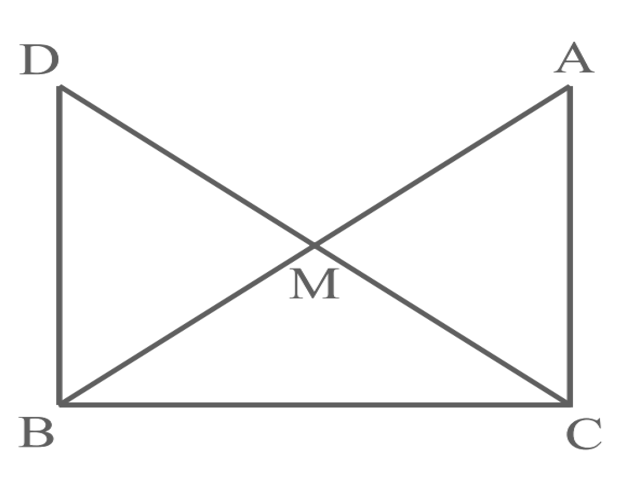
\includegraphics[width=\columnwidth]{figs/Screenshot.png}
  \caption{$\triangle \vec{ACB} ,\triangle \vec{DCB}$ with Mid-Point $\vec{M}$}
  \label{fig:triangles}
\end{figure}
\begin{enumerate}[label =(\roman*)]
        \item $\triangle \vec{AMC} \cong \triangle \vec{BMD}$
        \item $\angle \vec{DBC}$ is a right angle. 
        \item $\triangle \vec{DBC} \cong  \triangle \vec{ACB}$ 
        \item $\vec{CM} = \frac{1}{2} \vec{AB}$
\end{enumerate}
\pagebreak
\solution\\
\textbf{CONSTRUCTION STEPS :}
\begin{enumerate}
\item Let us Assume , the input parameters as ;
\begin{table}[H]
\centering
        \input{tables/input_params.tex}
          \caption{Input Parameters}
          \label{Table-1:Input_params}
\end{table}
\item the output can be calculated as ;
\begin{table}[H]
\centering
        \input{tables/output_params.tex}
          \caption{Output Parameters}
          \label{Table-2:Output_params}
\end{table}
                $\therefore$ By, Plotting these points we get the required Image \figref{fig:fig-2}
\begin{figure}[H]
        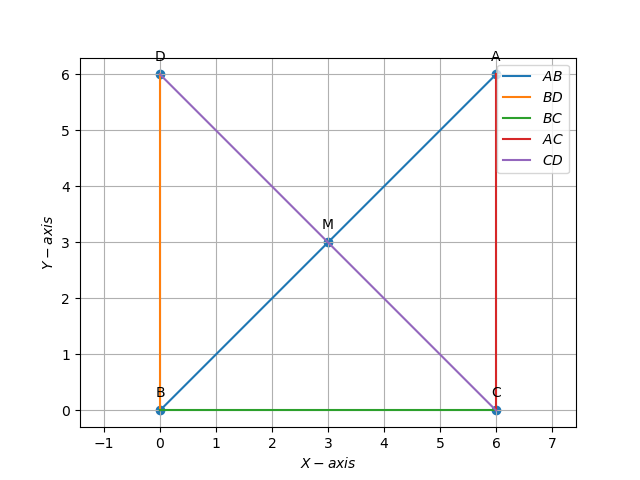
\includegraphics[width = \columnwidth]{figs/python_plot.png}
    \caption{PYTHON Plot of $\triangle \vec{ACB} ,\triangle \vec{DBC}$ with Mid-Point $\vec{M}$}
    \label{fig:fig-2}
\end{figure}
\end{enumerate}

\item Find the position vector of a point $\vec{R}$ which divides the line joining two points $\vec{P}$ and $\vec{Q}$ whose position vectors are $2\vec{a}+\vec{b}$ and $\vec{a}-3\vec{b}$ externally in the ratio $1:2$.

\textbf{Solution:}
Let us assume $\vec{a}$ and $\vec{b}$, and the given ratio is
\begin{table}[h]
    \centering
    \begin{tabular}{|c|c|c|}
        \hline 
        \textbf{Symbol} & \textbf{Value} & \textbf{Description} \\
        \hline
        $\vec{a}$ & $\myvec{1 \\ -3}$ & Vector $\vec{a}$ \\
        \hline
        $\vec{b}$ & $\myvec{0 \\ 2}$ & Vector $\vec{b}$\\
        \hline
        $k$ & $2$ & Ratio \\
        \hline
    \end{tabular}
    \caption{Vectors $\vec{a}$ and $\vec{b}$, ratio $k$}
    \label{tab:table1}
\end{table}

Using the section formula,
\begin{align}
    \vec{R} = \frac{\vec{Q} - k\vec{P}}{1 - k}
\end{align}
where $\vec{P}$ and $\vec{Q}$ depend on $\vec{a}$ and $\vec{b}$, then
\begin{align}
    \vec{P} &= (2\vec{a} + \vec{b}) = 2\myvec{1\\-3} + \myvec{0\\2} = \myvec{2\\-4} \\
    \vec{Q} &= (\vec{a} - 3\vec{b}) = \myvec{1\\-3} - 3\myvec{0\\2} = \myvec{1\\-9}
\end{align}
where $\vec{R}$ can be calculated as 
\begin{align}
    \vec{R} = \frac{(\vec{a} - 3\vec{b}) - k(2\vec{a} + \vec{b})}{1 - k}
\end{align}
By substituting $\vec{a}$ and $\vec{b}$ values, we get $\vec{R}$ as
\begin{align}
    \vec{R} = \myvec{3\\1}
\end{align}

\begin{table}[ht!]
    \centering
    \begin{tabular}{|c|c|c|}
        \hline
        \textbf{Symbol} & \textbf{Value} & \textbf{Description}\\
        \hline
        $\vec{P}$ & $(2\vec{a} + \vec{b})$ & Position vector $\vec{P}$ \\
        \hline
        $\vec{Q}$ & $(\vec{a} - 3\vec{b})$ & Position vector $\vec{Q}$\\
        \hline
        $\vec{R}$ & $\frac{\vec{Q} - k\vec{P}}{1 - k}$ & Position vector $\vec{R}$\\
        \hline
    \end{tabular}
    \caption{Vectors $\vec{P}$, $\vec{Q}$, $\vec{R}$}
    \label{tab:mytable2}   
\end{table}

\begin{figure}[H]
    \centering
    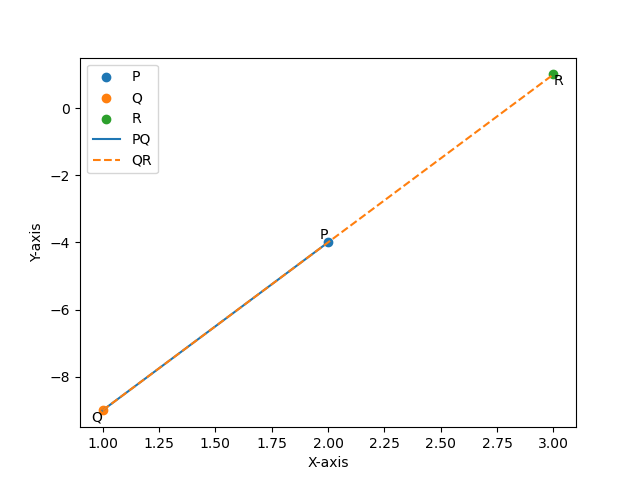
\includegraphics[width=\columnwidth]{figs/external-bisector.png}
    \caption{Point vectors $\vec{P}$, $\vec{Q}$, $\vec{R}$}
    \label{fig:enter-label}
\end{figure}


\end{enumerate}

    \item Draw a quadrilateral in the Cartesian plane, whose vertices are 
    \begin{align}
        \vec{A} = \myvec{-4\\5} \quad \vec{B} = \myvec{0\\7} \\
        \vec{C} = \myvec{5\\-5} \quad \vec{D} = \myvec{-4\\-2}
    \end{align}
    Also, find its area.
\label{chapters/11/10/1/1}
   \\ 
    \solution 
\begin{enumerate}[label=\thesection.\arabic*,ref=\thesection.\theenumi]
		\item Find $\abs{\overrightarrow{a}\times\overrightarrow{b}},\text{ if }\overrightarrow{a}=\hat{i}-7\hat{j}+7\hat{k}\text{ and } \overrightarrow{b}=3\hat{i}-2\hat{j}+2\hat{k}$.
	\\
		\solution
		\input{chapters/12/10/4/1/cross.tex}
\item Show that $$(\overrightarrow{a}-\overrightarrow{b})\times (\overrightarrow{a}+\overrightarrow{b})=2(\overrightarrow{a}\times \overrightarrow{b})$$
	\\
		\solution
		\input{chapters/12/10/4/4/cross.tex}
\item Find $\lambda$ and $\mu$ if $(2\hat{i}+6\hat{j}+27\hat{k})\times(\hat{i}+\lambda \hat{j} + \mu \hat{k})=\overrightarrow{0}$.
	\\
		\solution
		\input{chapters/12/10/4/5/cross.tex}
\item Given that $\overrightarrow{a} \cdot \overrightarrow{b} = 0$ and $\overrightarrow{a} \times \overrightarrow{b} = \overrightarrow{0}$. What can you conclude about the vectors $\overrightarrow{a} \text{ and }\overrightarrow{b}$?
\item Let the vectors be given as $\overrightarrow{a},\overrightarrow{b},\overrightarrow{c}\text{ be given as }\ a_1 \hat{i}+\ a_2 \hat{j}+\ a_3 \hat{k},\ b_1 \hat{i}+\ b_2 \hat{j}+\ b_3 \hat{k},\ c_1 \hat{i}+\ c_2 \hat{j}+\ c_3 \hat{k}$. Then show that $\overrightarrow{a} \times (\overrightarrow{b} + \overrightarrow{c}) = \overrightarrow{a} \times \overrightarrow{b}+\overrightarrow{a} \times \overrightarrow{c}$.
	\\
		\solution
		\input{chapters/12/10/4/7/cross.tex}
\item If either $\overrightarrow{a} = \overrightarrow{0}$ or $\overrightarrow{b} = \overrightarrow{0}$, then $\overrightarrow{a} \times \overrightarrow{b} = \overrightarrow{0}$. Is the converse true? Justify your answer with an example.
	\\
		\solution
		\input{chapters/12/10/4/8/cross.tex}
\item Find the area of the triangle with vertices $A(1, 1, 2)$, $B(2, 3, 5)$, and $C(1, 5, 5)$
	\\
		\solution
		\input{chapters/12/10/4/9/cross.tex}
\item Find the area of the parallelogram whose adjacent sides are determined by the vectors $\overrightarrow{a}=\hat{i}-\hat{j}+3\hat{k}$ and $\overrightarrow{b}=2\hat{i}-7\hat{j}+\hat{k}$.
	\\
		\solution
		\input{chapters/12/10/4/10/cross.tex}
\item Let the vectors $\overrightarrow{a}$ and $\overrightarrow{b}$ be such that $|\overrightarrow{a}| = 3$ and $|\overrightarrow{b}| = \dfrac{\sqrt{2}}{3}$, then $\overrightarrow{a} \times \overrightarrow{b}$ is a unit vector, if the angle between $\overrightarrow{a}$ and $\overrightarrow{b}$ is
\begin{enumerate}
\item $\dfrac{\pi}{6}$
\item $\dfrac{\pi}{4}$
\item $\dfrac{\pi}{3}$
\item $\dfrac{\pi}{2}$
\end{enumerate}
		\solution
		\input{chapters/12/10/4/11/cross.tex}
\item Area of a rectangle having vertices A, B, C and D with position vectors $ -\hat{i}+ \dfrac{1}{2} \hat{j}+4\hat{k},\hat{i}+ \dfrac{1}{2} \hat{j}+4\hat{k},\hat{i}-\dfrac{1}{2} \hat{j}+4\hat{k}\text{ and }-\hat{i}- \dfrac{1}{2} \hat{j}+4\hat{k}$, respectively is
\begin{enumerate}
\item $\dfrac{1}{2}$
\item 1
\item 2
\item 4
\end{enumerate}
		\solution
		\input{chapters/12/10/4/12/cross.tex}
\item Find the area of the triangle whose vertices are 
\begin{enumerate}
\item $(2, 3), (–1, 0), (2, – 4)$
\item $(–5, –1), (3, –5), (5, 2)$ 
\end{enumerate}
		\label{10/7/3/1}
\solution
		\input{chapters/10/7/3/1/area.tex}
\item Find the area of the triangle formed by joining the mid-points of the sides of the triangle whose vertices are $(0, –1), (2, 1) \text{ and } (0, 3)$. Find the ratio of this area to the area of the given triangle.
	\\
\solution
		\input{chapters/10/7/3/3/cross.tex}

\item Find the area of the quadrilateral whose vertices, taken in order, are $(– 4, – 2), (– 3, – 5), (3, – 2)$  and $ (2, 3)$.
	\\
\solution
		\input{chapters/10/7/3/4/cross.tex}

\item Verify that a median of a triangle divides it into two triangles of equal areas for $\triangle ABC$ whose vertices are $\vec{A}(4, -6), \vec{B}(3, 2), \text{ and } \vec{C}(5, 2)$. 
		\label{10/7/3/5}
		\\
\solution
		\input{chapters/10/7/3/5/area.tex}

\item The two adjacent sides of a parallelogram are 
$2\hat{i}-4\hat{j}+5\hat{k}$  and  $\hat{i}-2\hat{j}-3\hat{k}$.
Find the unit vector parallel to its diagonal. Also, find its area.\\
	\solution
		\input{chapters/12/10/5/10/cross.tex}
\item The vertices of a $\triangle ABC$ are $\vec{A}(4,6), \vec{B}(1,5)$ and  $\vec{C}(7,2)$. A line is drawn to intersect sides $AB$ and $AC$ at $\vec{D}$ and $\vec{E}$ respectively, such that $\frac{AD}{AB} = \frac{AE}{AC} = \frac{1}{4}$. Calculate the area of $\triangle ADE$ and compare it with the area of the $\triangle ABC$.
\\
\solution
	\input{chapters/10/7/4/6/section.tex}
    \item Draw a quadrilateral in the Cartesian plane, whose vertices are 
    \begin{align}
        \vec{A} = \myvec{-4\\5} \quad \vec{B} = \myvec{0\\7} \\
        \vec{C} = \myvec{5\\-5} \quad \vec{D} = \myvec{-4\\-2}
    \end{align}
    Also, find its area.
\label{chapters/11/10/1/1}
   \\ 
    \solution 
\input{chapters/11/10/1/1/cross.tex}
\item Find the area of region bounded by the triangle whose
	vertices are $(1, 0), (2, 2) \text{ and } (3, 1)$. 
\item Find the area of region bounded by the triangle whose vertices
	are $(– 1, 0), (1, 3) \text{ and } (3, 2)$. 
\item Find the area of the $\triangle ABC$, coordinates of whose vertices are $\vec{A}(2, 0), \vec{B}(4, 5), \text{ and } \vec{C}(6, 3)$.


\item 
\input{chapters/vectors/exer/main.tex}
\end{enumerate}


\item Find the area of region bounded by the triangle whose
	vertices are $(1, 0), (2, 2) \text{ and } (3, 1)$. 
\item Find the area of region bounded by the triangle whose vertices
	are $(– 1, 0), (1, 3) \text{ and } (3, 2)$. 
\item Find the area of the $\triangle ABC$, coordinates of whose vertices are $\vec{A}(2, 0), \vec{B}(4, 5), \text{ and } \vec{C}(6, 3)$.


\item 
%\documentclass[12pt]{article}
%\usepackage{graphicx}
%\usepackage{graphics}
%\usepackage{refstyle}
%\usepackage{amsmath}
%\usepackage{caption}
%\usepackage{float}
%\usepackage{booktabs}
%\usepackage{array}
%\usepackage{amssymb}
%\usepackage{booktabs}
%\let\vec\mathbf
%\providecommand{\brak}[1]{\ensuremath{\left(#1\right)}}
%\graphicspath{{/storage/self/primary/Download/latexnew/fig}}                                     
$\vec{P}$ and $\vec{Q}$ are any two points lying on the sides $DC$ and $AD$ respectively of a parallelogram $ABCD$.Show that, $ar\brak{\triangle APB}=ar\brak{\triangle BQC}$.


\textbf{Figure:}
\begin{figure}[H]
    \centering
	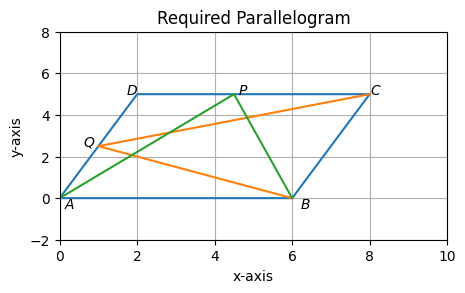
\includegraphics[width=\columnwidth]{chapters/vectors/exer/figs/1.png}
    \caption{}
    \label{fig:fig:1}
\end{figure}


\textbf{Solution:}
\begin{table}[H]
   \centering
  \input{chapters/vectors/exer/table/tab1.tex}
   \caption{Table of input parameters}        
\label{tab:tab:1}                    
\end{table}




\begin{table}[H]
    \centering                                  
\input{chapters/vectors/exer/table/tab2.tex}                  
\caption{Table of output parameters}
\label{tab:tab:2}
 \end{table}


For the $\triangle BQC$, the vertices of the triangle are taken from \tabref{tab:tab:1} and \tabref{tab:tab:2}.

\begin{align}
\implies ar\brak{\triangle BQC}&=
\frac{1}{2}\begin{tabular}{|c c c|}            
1 &1&1\\                      
$\vec{B}$&$\vec{Q}$&$\vec{C}$\\    
\end{tabular}\\
&= \frac{1}{2}\begin{tabular}{|c c c|}
       1 &1&1\\
       6&$\frac{2k_1}{k_1+1}$&8 \\
       0&$\frac{5k_1}{k_1+1}$&5
   \end{tabular}\\
  \xrightarrow{C_2'=C_2-C_1,C_3'=C_3-C_1}&\frac{1}{2} \begin{tabular}{|c c c|}
       1 &0&0\\
       6&$\frac{-4k_1-6}{k_1+1}$&2 \\
       0&$\frac{5k_1}{k_1+1}$&5
   \end{tabular}\\
&=\frac{1}{2}\brak{1\begin{tabular}{|c c|}
   $\frac{-4k_1-6}{k_1+1}$ &2  \\
   $\frac{5k_1}{k_1+1}$ & 5
\end{tabular} +0+0}\\
&=\frac{1}{2} \times30\\                          
&=15 \end{align}


For the $\triangle APB$, the vertices of the triangle are taken from \tabref{tab:tab:1} and \tabref{tab:tab:2}.
   \begin{align}
  \implies ar\brak{\triangle APB} &=
\frac{1}{2}\begin{tabular}{|c c c|}            
1 &1&1\\                            
$\vec{A}$&$\vec{P}$&$\vec{B}$\\
\end{tabular}\\ &=  \frac{1}{2}
   \begin{tabular}{|c c c|}
       1 &1&1\\
       0&$\frac{8k_2+2}{k_2+1}$&6 \\
       0&5&0
   \end{tabular}\\
 &=\frac{1}{2} \times30\\
 &=15 \end{align}
 \brak{6} = \brak{10}


So, ar\brak{\triangle BQC} = ar\brak{\triangle APB}.\brak{proved}
%\end{document}



\end{enumerate}


\item Find $\lambda$ and $\mu$ if $(2\hat{i}+6\hat{j}+27\hat{k})\times(\hat{i}+\lambda \hat{j} + \mu \hat{k})=\overrightarrow{0}$.
	\\
		\solution
		\begin{enumerate}[label=\thesection.\arabic*,ref=\thesection.\theenumi]
		\item Find $\abs{\overrightarrow{a}\times\overrightarrow{b}},\text{ if }\overrightarrow{a}=\hat{i}-7\hat{j}+7\hat{k}\text{ and } \overrightarrow{b}=3\hat{i}-2\hat{j}+2\hat{k}$.
	\\
		\solution
		\begin{enumerate}[label=\thesection.\arabic*,ref=\thesection.\theenumi]
		\item Find $\abs{\overrightarrow{a}\times\overrightarrow{b}},\text{ if }\overrightarrow{a}=\hat{i}-7\hat{j}+7\hat{k}\text{ and } \overrightarrow{b}=3\hat{i}-2\hat{j}+2\hat{k}$.
	\\
		\solution
		\input{chapters/12/10/4/1/cross.tex}
\item Show that $$(\overrightarrow{a}-\overrightarrow{b})\times (\overrightarrow{a}+\overrightarrow{b})=2(\overrightarrow{a}\times \overrightarrow{b})$$
	\\
		\solution
		\input{chapters/12/10/4/4/cross.tex}
\item Find $\lambda$ and $\mu$ if $(2\hat{i}+6\hat{j}+27\hat{k})\times(\hat{i}+\lambda \hat{j} + \mu \hat{k})=\overrightarrow{0}$.
	\\
		\solution
		\input{chapters/12/10/4/5/cross.tex}
\item Given that $\overrightarrow{a} \cdot \overrightarrow{b} = 0$ and $\overrightarrow{a} \times \overrightarrow{b} = \overrightarrow{0}$. What can you conclude about the vectors $\overrightarrow{a} \text{ and }\overrightarrow{b}$?
\item Let the vectors be given as $\overrightarrow{a},\overrightarrow{b},\overrightarrow{c}\text{ be given as }\ a_1 \hat{i}+\ a_2 \hat{j}+\ a_3 \hat{k},\ b_1 \hat{i}+\ b_2 \hat{j}+\ b_3 \hat{k},\ c_1 \hat{i}+\ c_2 \hat{j}+\ c_3 \hat{k}$. Then show that $\overrightarrow{a} \times (\overrightarrow{b} + \overrightarrow{c}) = \overrightarrow{a} \times \overrightarrow{b}+\overrightarrow{a} \times \overrightarrow{c}$.
	\\
		\solution
		\input{chapters/12/10/4/7/cross.tex}
\item If either $\overrightarrow{a} = \overrightarrow{0}$ or $\overrightarrow{b} = \overrightarrow{0}$, then $\overrightarrow{a} \times \overrightarrow{b} = \overrightarrow{0}$. Is the converse true? Justify your answer with an example.
	\\
		\solution
		\input{chapters/12/10/4/8/cross.tex}
\item Find the area of the triangle with vertices $A(1, 1, 2)$, $B(2, 3, 5)$, and $C(1, 5, 5)$
	\\
		\solution
		\input{chapters/12/10/4/9/cross.tex}
\item Find the area of the parallelogram whose adjacent sides are determined by the vectors $\overrightarrow{a}=\hat{i}-\hat{j}+3\hat{k}$ and $\overrightarrow{b}=2\hat{i}-7\hat{j}+\hat{k}$.
	\\
		\solution
		\input{chapters/12/10/4/10/cross.tex}
\item Let the vectors $\overrightarrow{a}$ and $\overrightarrow{b}$ be such that $|\overrightarrow{a}| = 3$ and $|\overrightarrow{b}| = \dfrac{\sqrt{2}}{3}$, then $\overrightarrow{a} \times \overrightarrow{b}$ is a unit vector, if the angle between $\overrightarrow{a}$ and $\overrightarrow{b}$ is
\begin{enumerate}
\item $\dfrac{\pi}{6}$
\item $\dfrac{\pi}{4}$
\item $\dfrac{\pi}{3}$
\item $\dfrac{\pi}{2}$
\end{enumerate}
		\solution
		\input{chapters/12/10/4/11/cross.tex}
\item Area of a rectangle having vertices A, B, C and D with position vectors $ -\hat{i}+ \dfrac{1}{2} \hat{j}+4\hat{k},\hat{i}+ \dfrac{1}{2} \hat{j}+4\hat{k},\hat{i}-\dfrac{1}{2} \hat{j}+4\hat{k}\text{ and }-\hat{i}- \dfrac{1}{2} \hat{j}+4\hat{k}$, respectively is
\begin{enumerate}
\item $\dfrac{1}{2}$
\item 1
\item 2
\item 4
\end{enumerate}
		\solution
		\input{chapters/12/10/4/12/cross.tex}
\item Find the area of the triangle whose vertices are 
\begin{enumerate}
\item $(2, 3), (–1, 0), (2, – 4)$
\item $(–5, –1), (3, –5), (5, 2)$ 
\end{enumerate}
		\label{10/7/3/1}
\solution
		\input{chapters/10/7/3/1/area.tex}
\item Find the area of the triangle formed by joining the mid-points of the sides of the triangle whose vertices are $(0, –1), (2, 1) \text{ and } (0, 3)$. Find the ratio of this area to the area of the given triangle.
	\\
\solution
		\input{chapters/10/7/3/3/cross.tex}

\item Find the area of the quadrilateral whose vertices, taken in order, are $(– 4, – 2), (– 3, – 5), (3, – 2)$  and $ (2, 3)$.
	\\
\solution
		\input{chapters/10/7/3/4/cross.tex}

\item Verify that a median of a triangle divides it into two triangles of equal areas for $\triangle ABC$ whose vertices are $\vec{A}(4, -6), \vec{B}(3, 2), \text{ and } \vec{C}(5, 2)$. 
		\label{10/7/3/5}
		\\
\solution
		\input{chapters/10/7/3/5/area.tex}

\item The two adjacent sides of a parallelogram are 
$2\hat{i}-4\hat{j}+5\hat{k}$  and  $\hat{i}-2\hat{j}-3\hat{k}$.
Find the unit vector parallel to its diagonal. Also, find its area.\\
	\solution
		\input{chapters/12/10/5/10/cross.tex}
\item The vertices of a $\triangle ABC$ are $\vec{A}(4,6), \vec{B}(1,5)$ and  $\vec{C}(7,2)$. A line is drawn to intersect sides $AB$ and $AC$ at $\vec{D}$ and $\vec{E}$ respectively, such that $\frac{AD}{AB} = \frac{AE}{AC} = \frac{1}{4}$. Calculate the area of $\triangle ADE$ and compare it with the area of the $\triangle ABC$.
\\
\solution
	\input{chapters/10/7/4/6/section.tex}
    \item Draw a quadrilateral in the Cartesian plane, whose vertices are 
    \begin{align}
        \vec{A} = \myvec{-4\\5} \quad \vec{B} = \myvec{0\\7} \\
        \vec{C} = \myvec{5\\-5} \quad \vec{D} = \myvec{-4\\-2}
    \end{align}
    Also, find its area.
\label{chapters/11/10/1/1}
   \\ 
    \solution 
\input{chapters/11/10/1/1/cross.tex}
\item Find the area of region bounded by the triangle whose
	vertices are $(1, 0), (2, 2) \text{ and } (3, 1)$. 
\item Find the area of region bounded by the triangle whose vertices
	are $(– 1, 0), (1, 3) \text{ and } (3, 2)$. 
\item Find the area of the $\triangle ABC$, coordinates of whose vertices are $\vec{A}(2, 0), \vec{B}(4, 5), \text{ and } \vec{C}(6, 3)$.


\item 
\input{chapters/vectors/exer/main.tex}
\end{enumerate}


\item Show that $$(\overrightarrow{a}-\overrightarrow{b})\times (\overrightarrow{a}+\overrightarrow{b})=2(\overrightarrow{a}\times \overrightarrow{b})$$
	\\
		\solution
		\begin{enumerate}[label=\thesection.\arabic*,ref=\thesection.\theenumi]
		\item Find $\abs{\overrightarrow{a}\times\overrightarrow{b}},\text{ if }\overrightarrow{a}=\hat{i}-7\hat{j}+7\hat{k}\text{ and } \overrightarrow{b}=3\hat{i}-2\hat{j}+2\hat{k}$.
	\\
		\solution
		\input{chapters/12/10/4/1/cross.tex}
\item Show that $$(\overrightarrow{a}-\overrightarrow{b})\times (\overrightarrow{a}+\overrightarrow{b})=2(\overrightarrow{a}\times \overrightarrow{b})$$
	\\
		\solution
		\input{chapters/12/10/4/4/cross.tex}
\item Find $\lambda$ and $\mu$ if $(2\hat{i}+6\hat{j}+27\hat{k})\times(\hat{i}+\lambda \hat{j} + \mu \hat{k})=\overrightarrow{0}$.
	\\
		\solution
		\input{chapters/12/10/4/5/cross.tex}
\item Given that $\overrightarrow{a} \cdot \overrightarrow{b} = 0$ and $\overrightarrow{a} \times \overrightarrow{b} = \overrightarrow{0}$. What can you conclude about the vectors $\overrightarrow{a} \text{ and }\overrightarrow{b}$?
\item Let the vectors be given as $\overrightarrow{a},\overrightarrow{b},\overrightarrow{c}\text{ be given as }\ a_1 \hat{i}+\ a_2 \hat{j}+\ a_3 \hat{k},\ b_1 \hat{i}+\ b_2 \hat{j}+\ b_3 \hat{k},\ c_1 \hat{i}+\ c_2 \hat{j}+\ c_3 \hat{k}$. Then show that $\overrightarrow{a} \times (\overrightarrow{b} + \overrightarrow{c}) = \overrightarrow{a} \times \overrightarrow{b}+\overrightarrow{a} \times \overrightarrow{c}$.
	\\
		\solution
		\input{chapters/12/10/4/7/cross.tex}
\item If either $\overrightarrow{a} = \overrightarrow{0}$ or $\overrightarrow{b} = \overrightarrow{0}$, then $\overrightarrow{a} \times \overrightarrow{b} = \overrightarrow{0}$. Is the converse true? Justify your answer with an example.
	\\
		\solution
		\input{chapters/12/10/4/8/cross.tex}
\item Find the area of the triangle with vertices $A(1, 1, 2)$, $B(2, 3, 5)$, and $C(1, 5, 5)$
	\\
		\solution
		\input{chapters/12/10/4/9/cross.tex}
\item Find the area of the parallelogram whose adjacent sides are determined by the vectors $\overrightarrow{a}=\hat{i}-\hat{j}+3\hat{k}$ and $\overrightarrow{b}=2\hat{i}-7\hat{j}+\hat{k}$.
	\\
		\solution
		\input{chapters/12/10/4/10/cross.tex}
\item Let the vectors $\overrightarrow{a}$ and $\overrightarrow{b}$ be such that $|\overrightarrow{a}| = 3$ and $|\overrightarrow{b}| = \dfrac{\sqrt{2}}{3}$, then $\overrightarrow{a} \times \overrightarrow{b}$ is a unit vector, if the angle between $\overrightarrow{a}$ and $\overrightarrow{b}$ is
\begin{enumerate}
\item $\dfrac{\pi}{6}$
\item $\dfrac{\pi}{4}$
\item $\dfrac{\pi}{3}$
\item $\dfrac{\pi}{2}$
\end{enumerate}
		\solution
		\input{chapters/12/10/4/11/cross.tex}
\item Area of a rectangle having vertices A, B, C and D with position vectors $ -\hat{i}+ \dfrac{1}{2} \hat{j}+4\hat{k},\hat{i}+ \dfrac{1}{2} \hat{j}+4\hat{k},\hat{i}-\dfrac{1}{2} \hat{j}+4\hat{k}\text{ and }-\hat{i}- \dfrac{1}{2} \hat{j}+4\hat{k}$, respectively is
\begin{enumerate}
\item $\dfrac{1}{2}$
\item 1
\item 2
\item 4
\end{enumerate}
		\solution
		\input{chapters/12/10/4/12/cross.tex}
\item Find the area of the triangle whose vertices are 
\begin{enumerate}
\item $(2, 3), (–1, 0), (2, – 4)$
\item $(–5, –1), (3, –5), (5, 2)$ 
\end{enumerate}
		\label{10/7/3/1}
\solution
		\input{chapters/10/7/3/1/area.tex}
\item Find the area of the triangle formed by joining the mid-points of the sides of the triangle whose vertices are $(0, –1), (2, 1) \text{ and } (0, 3)$. Find the ratio of this area to the area of the given triangle.
	\\
\solution
		\input{chapters/10/7/3/3/cross.tex}

\item Find the area of the quadrilateral whose vertices, taken in order, are $(– 4, – 2), (– 3, – 5), (3, – 2)$  and $ (2, 3)$.
	\\
\solution
		\input{chapters/10/7/3/4/cross.tex}

\item Verify that a median of a triangle divides it into two triangles of equal areas for $\triangle ABC$ whose vertices are $\vec{A}(4, -6), \vec{B}(3, 2), \text{ and } \vec{C}(5, 2)$. 
		\label{10/7/3/5}
		\\
\solution
		\input{chapters/10/7/3/5/area.tex}

\item The two adjacent sides of a parallelogram are 
$2\hat{i}-4\hat{j}+5\hat{k}$  and  $\hat{i}-2\hat{j}-3\hat{k}$.
Find the unit vector parallel to its diagonal. Also, find its area.\\
	\solution
		\input{chapters/12/10/5/10/cross.tex}
\item The vertices of a $\triangle ABC$ are $\vec{A}(4,6), \vec{B}(1,5)$ and  $\vec{C}(7,2)$. A line is drawn to intersect sides $AB$ and $AC$ at $\vec{D}$ and $\vec{E}$ respectively, such that $\frac{AD}{AB} = \frac{AE}{AC} = \frac{1}{4}$. Calculate the area of $\triangle ADE$ and compare it with the area of the $\triangle ABC$.
\\
\solution
	\input{chapters/10/7/4/6/section.tex}
    \item Draw a quadrilateral in the Cartesian plane, whose vertices are 
    \begin{align}
        \vec{A} = \myvec{-4\\5} \quad \vec{B} = \myvec{0\\7} \\
        \vec{C} = \myvec{5\\-5} \quad \vec{D} = \myvec{-4\\-2}
    \end{align}
    Also, find its area.
\label{chapters/11/10/1/1}
   \\ 
    \solution 
\input{chapters/11/10/1/1/cross.tex}
\item Find the area of region bounded by the triangle whose
	vertices are $(1, 0), (2, 2) \text{ and } (3, 1)$. 
\item Find the area of region bounded by the triangle whose vertices
	are $(– 1, 0), (1, 3) \text{ and } (3, 2)$. 
\item Find the area of the $\triangle ABC$, coordinates of whose vertices are $\vec{A}(2, 0), \vec{B}(4, 5), \text{ and } \vec{C}(6, 3)$.


\item 
\input{chapters/vectors/exer/main.tex}
\end{enumerate}


\item Find $\lambda$ and $\mu$ if $(2\hat{i}+6\hat{j}+27\hat{k})\times(\hat{i}+\lambda \hat{j} + \mu \hat{k})=\overrightarrow{0}$.
	\\
		\solution
		\begin{enumerate}[label=\thesection.\arabic*,ref=\thesection.\theenumi]
		\item Find $\abs{\overrightarrow{a}\times\overrightarrow{b}},\text{ if }\overrightarrow{a}=\hat{i}-7\hat{j}+7\hat{k}\text{ and } \overrightarrow{b}=3\hat{i}-2\hat{j}+2\hat{k}$.
	\\
		\solution
		\input{chapters/12/10/4/1/cross.tex}
\item Show that $$(\overrightarrow{a}-\overrightarrow{b})\times (\overrightarrow{a}+\overrightarrow{b})=2(\overrightarrow{a}\times \overrightarrow{b})$$
	\\
		\solution
		\input{chapters/12/10/4/4/cross.tex}
\item Find $\lambda$ and $\mu$ if $(2\hat{i}+6\hat{j}+27\hat{k})\times(\hat{i}+\lambda \hat{j} + \mu \hat{k})=\overrightarrow{0}$.
	\\
		\solution
		\input{chapters/12/10/4/5/cross.tex}
\item Given that $\overrightarrow{a} \cdot \overrightarrow{b} = 0$ and $\overrightarrow{a} \times \overrightarrow{b} = \overrightarrow{0}$. What can you conclude about the vectors $\overrightarrow{a} \text{ and }\overrightarrow{b}$?
\item Let the vectors be given as $\overrightarrow{a},\overrightarrow{b},\overrightarrow{c}\text{ be given as }\ a_1 \hat{i}+\ a_2 \hat{j}+\ a_3 \hat{k},\ b_1 \hat{i}+\ b_2 \hat{j}+\ b_3 \hat{k},\ c_1 \hat{i}+\ c_2 \hat{j}+\ c_3 \hat{k}$. Then show that $\overrightarrow{a} \times (\overrightarrow{b} + \overrightarrow{c}) = \overrightarrow{a} \times \overrightarrow{b}+\overrightarrow{a} \times \overrightarrow{c}$.
	\\
		\solution
		\input{chapters/12/10/4/7/cross.tex}
\item If either $\overrightarrow{a} = \overrightarrow{0}$ or $\overrightarrow{b} = \overrightarrow{0}$, then $\overrightarrow{a} \times \overrightarrow{b} = \overrightarrow{0}$. Is the converse true? Justify your answer with an example.
	\\
		\solution
		\input{chapters/12/10/4/8/cross.tex}
\item Find the area of the triangle with vertices $A(1, 1, 2)$, $B(2, 3, 5)$, and $C(1, 5, 5)$
	\\
		\solution
		\input{chapters/12/10/4/9/cross.tex}
\item Find the area of the parallelogram whose adjacent sides are determined by the vectors $\overrightarrow{a}=\hat{i}-\hat{j}+3\hat{k}$ and $\overrightarrow{b}=2\hat{i}-7\hat{j}+\hat{k}$.
	\\
		\solution
		\input{chapters/12/10/4/10/cross.tex}
\item Let the vectors $\overrightarrow{a}$ and $\overrightarrow{b}$ be such that $|\overrightarrow{a}| = 3$ and $|\overrightarrow{b}| = \dfrac{\sqrt{2}}{3}$, then $\overrightarrow{a} \times \overrightarrow{b}$ is a unit vector, if the angle between $\overrightarrow{a}$ and $\overrightarrow{b}$ is
\begin{enumerate}
\item $\dfrac{\pi}{6}$
\item $\dfrac{\pi}{4}$
\item $\dfrac{\pi}{3}$
\item $\dfrac{\pi}{2}$
\end{enumerate}
		\solution
		\input{chapters/12/10/4/11/cross.tex}
\item Area of a rectangle having vertices A, B, C and D with position vectors $ -\hat{i}+ \dfrac{1}{2} \hat{j}+4\hat{k},\hat{i}+ \dfrac{1}{2} \hat{j}+4\hat{k},\hat{i}-\dfrac{1}{2} \hat{j}+4\hat{k}\text{ and }-\hat{i}- \dfrac{1}{2} \hat{j}+4\hat{k}$, respectively is
\begin{enumerate}
\item $\dfrac{1}{2}$
\item 1
\item 2
\item 4
\end{enumerate}
		\solution
		\input{chapters/12/10/4/12/cross.tex}
\item Find the area of the triangle whose vertices are 
\begin{enumerate}
\item $(2, 3), (–1, 0), (2, – 4)$
\item $(–5, –1), (3, –5), (5, 2)$ 
\end{enumerate}
		\label{10/7/3/1}
\solution
		\input{chapters/10/7/3/1/area.tex}
\item Find the area of the triangle formed by joining the mid-points of the sides of the triangle whose vertices are $(0, –1), (2, 1) \text{ and } (0, 3)$. Find the ratio of this area to the area of the given triangle.
	\\
\solution
		\input{chapters/10/7/3/3/cross.tex}

\item Find the area of the quadrilateral whose vertices, taken in order, are $(– 4, – 2), (– 3, – 5), (3, – 2)$  and $ (2, 3)$.
	\\
\solution
		\input{chapters/10/7/3/4/cross.tex}

\item Verify that a median of a triangle divides it into two triangles of equal areas for $\triangle ABC$ whose vertices are $\vec{A}(4, -6), \vec{B}(3, 2), \text{ and } \vec{C}(5, 2)$. 
		\label{10/7/3/5}
		\\
\solution
		\input{chapters/10/7/3/5/area.tex}

\item The two adjacent sides of a parallelogram are 
$2\hat{i}-4\hat{j}+5\hat{k}$  and  $\hat{i}-2\hat{j}-3\hat{k}$.
Find the unit vector parallel to its diagonal. Also, find its area.\\
	\solution
		\input{chapters/12/10/5/10/cross.tex}
\item The vertices of a $\triangle ABC$ are $\vec{A}(4,6), \vec{B}(1,5)$ and  $\vec{C}(7,2)$. A line is drawn to intersect sides $AB$ and $AC$ at $\vec{D}$ and $\vec{E}$ respectively, such that $\frac{AD}{AB} = \frac{AE}{AC} = \frac{1}{4}$. Calculate the area of $\triangle ADE$ and compare it with the area of the $\triangle ABC$.
\\
\solution
	\input{chapters/10/7/4/6/section.tex}
    \item Draw a quadrilateral in the Cartesian plane, whose vertices are 
    \begin{align}
        \vec{A} = \myvec{-4\\5} \quad \vec{B} = \myvec{0\\7} \\
        \vec{C} = \myvec{5\\-5} \quad \vec{D} = \myvec{-4\\-2}
    \end{align}
    Also, find its area.
\label{chapters/11/10/1/1}
   \\ 
    \solution 
\input{chapters/11/10/1/1/cross.tex}
\item Find the area of region bounded by the triangle whose
	vertices are $(1, 0), (2, 2) \text{ and } (3, 1)$. 
\item Find the area of region bounded by the triangle whose vertices
	are $(– 1, 0), (1, 3) \text{ and } (3, 2)$. 
\item Find the area of the $\triangle ABC$, coordinates of whose vertices are $\vec{A}(2, 0), \vec{B}(4, 5), \text{ and } \vec{C}(6, 3)$.


\item 
\input{chapters/vectors/exer/main.tex}
\end{enumerate}


\item Given that $\overrightarrow{a} \cdot \overrightarrow{b} = 0$ and $\overrightarrow{a} \times \overrightarrow{b} = \overrightarrow{0}$. What can you conclude about the vectors $\overrightarrow{a} \text{ and }\overrightarrow{b}$?
\item Let the vectors be given as $\overrightarrow{a},\overrightarrow{b},\overrightarrow{c}\text{ be given as }\ a_1 \hat{i}+\ a_2 \hat{j}+\ a_3 \hat{k},\ b_1 \hat{i}+\ b_2 \hat{j}+\ b_3 \hat{k},\ c_1 \hat{i}+\ c_2 \hat{j}+\ c_3 \hat{k}$. Then show that $\overrightarrow{a} \times (\overrightarrow{b} + \overrightarrow{c}) = \overrightarrow{a} \times \overrightarrow{b}+\overrightarrow{a} \times \overrightarrow{c}$.
	\\
		\solution
		\begin{enumerate}[label=\thesection.\arabic*,ref=\thesection.\theenumi]
		\item Find $\abs{\overrightarrow{a}\times\overrightarrow{b}},\text{ if }\overrightarrow{a}=\hat{i}-7\hat{j}+7\hat{k}\text{ and } \overrightarrow{b}=3\hat{i}-2\hat{j}+2\hat{k}$.
	\\
		\solution
		\input{chapters/12/10/4/1/cross.tex}
\item Show that $$(\overrightarrow{a}-\overrightarrow{b})\times (\overrightarrow{a}+\overrightarrow{b})=2(\overrightarrow{a}\times \overrightarrow{b})$$
	\\
		\solution
		\input{chapters/12/10/4/4/cross.tex}
\item Find $\lambda$ and $\mu$ if $(2\hat{i}+6\hat{j}+27\hat{k})\times(\hat{i}+\lambda \hat{j} + \mu \hat{k})=\overrightarrow{0}$.
	\\
		\solution
		\input{chapters/12/10/4/5/cross.tex}
\item Given that $\overrightarrow{a} \cdot \overrightarrow{b} = 0$ and $\overrightarrow{a} \times \overrightarrow{b} = \overrightarrow{0}$. What can you conclude about the vectors $\overrightarrow{a} \text{ and }\overrightarrow{b}$?
\item Let the vectors be given as $\overrightarrow{a},\overrightarrow{b},\overrightarrow{c}\text{ be given as }\ a_1 \hat{i}+\ a_2 \hat{j}+\ a_3 \hat{k},\ b_1 \hat{i}+\ b_2 \hat{j}+\ b_3 \hat{k},\ c_1 \hat{i}+\ c_2 \hat{j}+\ c_3 \hat{k}$. Then show that $\overrightarrow{a} \times (\overrightarrow{b} + \overrightarrow{c}) = \overrightarrow{a} \times \overrightarrow{b}+\overrightarrow{a} \times \overrightarrow{c}$.
	\\
		\solution
		\input{chapters/12/10/4/7/cross.tex}
\item If either $\overrightarrow{a} = \overrightarrow{0}$ or $\overrightarrow{b} = \overrightarrow{0}$, then $\overrightarrow{a} \times \overrightarrow{b} = \overrightarrow{0}$. Is the converse true? Justify your answer with an example.
	\\
		\solution
		\input{chapters/12/10/4/8/cross.tex}
\item Find the area of the triangle with vertices $A(1, 1, 2)$, $B(2, 3, 5)$, and $C(1, 5, 5)$
	\\
		\solution
		\input{chapters/12/10/4/9/cross.tex}
\item Find the area of the parallelogram whose adjacent sides are determined by the vectors $\overrightarrow{a}=\hat{i}-\hat{j}+3\hat{k}$ and $\overrightarrow{b}=2\hat{i}-7\hat{j}+\hat{k}$.
	\\
		\solution
		\input{chapters/12/10/4/10/cross.tex}
\item Let the vectors $\overrightarrow{a}$ and $\overrightarrow{b}$ be such that $|\overrightarrow{a}| = 3$ and $|\overrightarrow{b}| = \dfrac{\sqrt{2}}{3}$, then $\overrightarrow{a} \times \overrightarrow{b}$ is a unit vector, if the angle between $\overrightarrow{a}$ and $\overrightarrow{b}$ is
\begin{enumerate}
\item $\dfrac{\pi}{6}$
\item $\dfrac{\pi}{4}$
\item $\dfrac{\pi}{3}$
\item $\dfrac{\pi}{2}$
\end{enumerate}
		\solution
		\input{chapters/12/10/4/11/cross.tex}
\item Area of a rectangle having vertices A, B, C and D with position vectors $ -\hat{i}+ \dfrac{1}{2} \hat{j}+4\hat{k},\hat{i}+ \dfrac{1}{2} \hat{j}+4\hat{k},\hat{i}-\dfrac{1}{2} \hat{j}+4\hat{k}\text{ and }-\hat{i}- \dfrac{1}{2} \hat{j}+4\hat{k}$, respectively is
\begin{enumerate}
\item $\dfrac{1}{2}$
\item 1
\item 2
\item 4
\end{enumerate}
		\solution
		\input{chapters/12/10/4/12/cross.tex}
\item Find the area of the triangle whose vertices are 
\begin{enumerate}
\item $(2, 3), (–1, 0), (2, – 4)$
\item $(–5, –1), (3, –5), (5, 2)$ 
\end{enumerate}
		\label{10/7/3/1}
\solution
		\input{chapters/10/7/3/1/area.tex}
\item Find the area of the triangle formed by joining the mid-points of the sides of the triangle whose vertices are $(0, –1), (2, 1) \text{ and } (0, 3)$. Find the ratio of this area to the area of the given triangle.
	\\
\solution
		\input{chapters/10/7/3/3/cross.tex}

\item Find the area of the quadrilateral whose vertices, taken in order, are $(– 4, – 2), (– 3, – 5), (3, – 2)$  and $ (2, 3)$.
	\\
\solution
		\input{chapters/10/7/3/4/cross.tex}

\item Verify that a median of a triangle divides it into two triangles of equal areas for $\triangle ABC$ whose vertices are $\vec{A}(4, -6), \vec{B}(3, 2), \text{ and } \vec{C}(5, 2)$. 
		\label{10/7/3/5}
		\\
\solution
		\input{chapters/10/7/3/5/area.tex}

\item The two adjacent sides of a parallelogram are 
$2\hat{i}-4\hat{j}+5\hat{k}$  and  $\hat{i}-2\hat{j}-3\hat{k}$.
Find the unit vector parallel to its diagonal. Also, find its area.\\
	\solution
		\input{chapters/12/10/5/10/cross.tex}
\item The vertices of a $\triangle ABC$ are $\vec{A}(4,6), \vec{B}(1,5)$ and  $\vec{C}(7,2)$. A line is drawn to intersect sides $AB$ and $AC$ at $\vec{D}$ and $\vec{E}$ respectively, such that $\frac{AD}{AB} = \frac{AE}{AC} = \frac{1}{4}$. Calculate the area of $\triangle ADE$ and compare it with the area of the $\triangle ABC$.
\\
\solution
	\input{chapters/10/7/4/6/section.tex}
    \item Draw a quadrilateral in the Cartesian plane, whose vertices are 
    \begin{align}
        \vec{A} = \myvec{-4\\5} \quad \vec{B} = \myvec{0\\7} \\
        \vec{C} = \myvec{5\\-5} \quad \vec{D} = \myvec{-4\\-2}
    \end{align}
    Also, find its area.
\label{chapters/11/10/1/1}
   \\ 
    \solution 
\input{chapters/11/10/1/1/cross.tex}
\item Find the area of region bounded by the triangle whose
	vertices are $(1, 0), (2, 2) \text{ and } (3, 1)$. 
\item Find the area of region bounded by the triangle whose vertices
	are $(– 1, 0), (1, 3) \text{ and } (3, 2)$. 
\item Find the area of the $\triangle ABC$, coordinates of whose vertices are $\vec{A}(2, 0), \vec{B}(4, 5), \text{ and } \vec{C}(6, 3)$.


\item 
\input{chapters/vectors/exer/main.tex}
\end{enumerate}


\item If either $\overrightarrow{a} = \overrightarrow{0}$ or $\overrightarrow{b} = \overrightarrow{0}$, then $\overrightarrow{a} \times \overrightarrow{b} = \overrightarrow{0}$. Is the converse true? Justify your answer with an example.
	\\
		\solution
		\begin{enumerate}[label=\thesection.\arabic*,ref=\thesection.\theenumi]
		\item Find $\abs{\overrightarrow{a}\times\overrightarrow{b}},\text{ if }\overrightarrow{a}=\hat{i}-7\hat{j}+7\hat{k}\text{ and } \overrightarrow{b}=3\hat{i}-2\hat{j}+2\hat{k}$.
	\\
		\solution
		\input{chapters/12/10/4/1/cross.tex}
\item Show that $$(\overrightarrow{a}-\overrightarrow{b})\times (\overrightarrow{a}+\overrightarrow{b})=2(\overrightarrow{a}\times \overrightarrow{b})$$
	\\
		\solution
		\input{chapters/12/10/4/4/cross.tex}
\item Find $\lambda$ and $\mu$ if $(2\hat{i}+6\hat{j}+27\hat{k})\times(\hat{i}+\lambda \hat{j} + \mu \hat{k})=\overrightarrow{0}$.
	\\
		\solution
		\input{chapters/12/10/4/5/cross.tex}
\item Given that $\overrightarrow{a} \cdot \overrightarrow{b} = 0$ and $\overrightarrow{a} \times \overrightarrow{b} = \overrightarrow{0}$. What can you conclude about the vectors $\overrightarrow{a} \text{ and }\overrightarrow{b}$?
\item Let the vectors be given as $\overrightarrow{a},\overrightarrow{b},\overrightarrow{c}\text{ be given as }\ a_1 \hat{i}+\ a_2 \hat{j}+\ a_3 \hat{k},\ b_1 \hat{i}+\ b_2 \hat{j}+\ b_3 \hat{k},\ c_1 \hat{i}+\ c_2 \hat{j}+\ c_3 \hat{k}$. Then show that $\overrightarrow{a} \times (\overrightarrow{b} + \overrightarrow{c}) = \overrightarrow{a} \times \overrightarrow{b}+\overrightarrow{a} \times \overrightarrow{c}$.
	\\
		\solution
		\input{chapters/12/10/4/7/cross.tex}
\item If either $\overrightarrow{a} = \overrightarrow{0}$ or $\overrightarrow{b} = \overrightarrow{0}$, then $\overrightarrow{a} \times \overrightarrow{b} = \overrightarrow{0}$. Is the converse true? Justify your answer with an example.
	\\
		\solution
		\input{chapters/12/10/4/8/cross.tex}
\item Find the area of the triangle with vertices $A(1, 1, 2)$, $B(2, 3, 5)$, and $C(1, 5, 5)$
	\\
		\solution
		\input{chapters/12/10/4/9/cross.tex}
\item Find the area of the parallelogram whose adjacent sides are determined by the vectors $\overrightarrow{a}=\hat{i}-\hat{j}+3\hat{k}$ and $\overrightarrow{b}=2\hat{i}-7\hat{j}+\hat{k}$.
	\\
		\solution
		\input{chapters/12/10/4/10/cross.tex}
\item Let the vectors $\overrightarrow{a}$ and $\overrightarrow{b}$ be such that $|\overrightarrow{a}| = 3$ and $|\overrightarrow{b}| = \dfrac{\sqrt{2}}{3}$, then $\overrightarrow{a} \times \overrightarrow{b}$ is a unit vector, if the angle between $\overrightarrow{a}$ and $\overrightarrow{b}$ is
\begin{enumerate}
\item $\dfrac{\pi}{6}$
\item $\dfrac{\pi}{4}$
\item $\dfrac{\pi}{3}$
\item $\dfrac{\pi}{2}$
\end{enumerate}
		\solution
		\input{chapters/12/10/4/11/cross.tex}
\item Area of a rectangle having vertices A, B, C and D with position vectors $ -\hat{i}+ \dfrac{1}{2} \hat{j}+4\hat{k},\hat{i}+ \dfrac{1}{2} \hat{j}+4\hat{k},\hat{i}-\dfrac{1}{2} \hat{j}+4\hat{k}\text{ and }-\hat{i}- \dfrac{1}{2} \hat{j}+4\hat{k}$, respectively is
\begin{enumerate}
\item $\dfrac{1}{2}$
\item 1
\item 2
\item 4
\end{enumerate}
		\solution
		\input{chapters/12/10/4/12/cross.tex}
\item Find the area of the triangle whose vertices are 
\begin{enumerate}
\item $(2, 3), (–1, 0), (2, – 4)$
\item $(–5, –1), (3, –5), (5, 2)$ 
\end{enumerate}
		\label{10/7/3/1}
\solution
		\input{chapters/10/7/3/1/area.tex}
\item Find the area of the triangle formed by joining the mid-points of the sides of the triangle whose vertices are $(0, –1), (2, 1) \text{ and } (0, 3)$. Find the ratio of this area to the area of the given triangle.
	\\
\solution
		\input{chapters/10/7/3/3/cross.tex}

\item Find the area of the quadrilateral whose vertices, taken in order, are $(– 4, – 2), (– 3, – 5), (3, – 2)$  and $ (2, 3)$.
	\\
\solution
		\input{chapters/10/7/3/4/cross.tex}

\item Verify that a median of a triangle divides it into two triangles of equal areas for $\triangle ABC$ whose vertices are $\vec{A}(4, -6), \vec{B}(3, 2), \text{ and } \vec{C}(5, 2)$. 
		\label{10/7/3/5}
		\\
\solution
		\input{chapters/10/7/3/5/area.tex}

\item The two adjacent sides of a parallelogram are 
$2\hat{i}-4\hat{j}+5\hat{k}$  and  $\hat{i}-2\hat{j}-3\hat{k}$.
Find the unit vector parallel to its diagonal. Also, find its area.\\
	\solution
		\input{chapters/12/10/5/10/cross.tex}
\item The vertices of a $\triangle ABC$ are $\vec{A}(4,6), \vec{B}(1,5)$ and  $\vec{C}(7,2)$. A line is drawn to intersect sides $AB$ and $AC$ at $\vec{D}$ and $\vec{E}$ respectively, such that $\frac{AD}{AB} = \frac{AE}{AC} = \frac{1}{4}$. Calculate the area of $\triangle ADE$ and compare it with the area of the $\triangle ABC$.
\\
\solution
	\input{chapters/10/7/4/6/section.tex}
    \item Draw a quadrilateral in the Cartesian plane, whose vertices are 
    \begin{align}
        \vec{A} = \myvec{-4\\5} \quad \vec{B} = \myvec{0\\7} \\
        \vec{C} = \myvec{5\\-5} \quad \vec{D} = \myvec{-4\\-2}
    \end{align}
    Also, find its area.
\label{chapters/11/10/1/1}
   \\ 
    \solution 
\input{chapters/11/10/1/1/cross.tex}
\item Find the area of region bounded by the triangle whose
	vertices are $(1, 0), (2, 2) \text{ and } (3, 1)$. 
\item Find the area of region bounded by the triangle whose vertices
	are $(– 1, 0), (1, 3) \text{ and } (3, 2)$. 
\item Find the area of the $\triangle ABC$, coordinates of whose vertices are $\vec{A}(2, 0), \vec{B}(4, 5), \text{ and } \vec{C}(6, 3)$.


\item 
\input{chapters/vectors/exer/main.tex}
\end{enumerate}


\item Find the area of the triangle with vertices $A(1, 1, 2)$, $B(2, 3, 5)$, and $C(1, 5, 5)$
	\\
		\solution
		\begin{enumerate}[label=\thesection.\arabic*,ref=\thesection.\theenumi]
		\item Find $\abs{\overrightarrow{a}\times\overrightarrow{b}},\text{ if }\overrightarrow{a}=\hat{i}-7\hat{j}+7\hat{k}\text{ and } \overrightarrow{b}=3\hat{i}-2\hat{j}+2\hat{k}$.
	\\
		\solution
		\input{chapters/12/10/4/1/cross.tex}
\item Show that $$(\overrightarrow{a}-\overrightarrow{b})\times (\overrightarrow{a}+\overrightarrow{b})=2(\overrightarrow{a}\times \overrightarrow{b})$$
	\\
		\solution
		\input{chapters/12/10/4/4/cross.tex}
\item Find $\lambda$ and $\mu$ if $(2\hat{i}+6\hat{j}+27\hat{k})\times(\hat{i}+\lambda \hat{j} + \mu \hat{k})=\overrightarrow{0}$.
	\\
		\solution
		\input{chapters/12/10/4/5/cross.tex}
\item Given that $\overrightarrow{a} \cdot \overrightarrow{b} = 0$ and $\overrightarrow{a} \times \overrightarrow{b} = \overrightarrow{0}$. What can you conclude about the vectors $\overrightarrow{a} \text{ and }\overrightarrow{b}$?
\item Let the vectors be given as $\overrightarrow{a},\overrightarrow{b},\overrightarrow{c}\text{ be given as }\ a_1 \hat{i}+\ a_2 \hat{j}+\ a_3 \hat{k},\ b_1 \hat{i}+\ b_2 \hat{j}+\ b_3 \hat{k},\ c_1 \hat{i}+\ c_2 \hat{j}+\ c_3 \hat{k}$. Then show that $\overrightarrow{a} \times (\overrightarrow{b} + \overrightarrow{c}) = \overrightarrow{a} \times \overrightarrow{b}+\overrightarrow{a} \times \overrightarrow{c}$.
	\\
		\solution
		\input{chapters/12/10/4/7/cross.tex}
\item If either $\overrightarrow{a} = \overrightarrow{0}$ or $\overrightarrow{b} = \overrightarrow{0}$, then $\overrightarrow{a} \times \overrightarrow{b} = \overrightarrow{0}$. Is the converse true? Justify your answer with an example.
	\\
		\solution
		\input{chapters/12/10/4/8/cross.tex}
\item Find the area of the triangle with vertices $A(1, 1, 2)$, $B(2, 3, 5)$, and $C(1, 5, 5)$
	\\
		\solution
		\input{chapters/12/10/4/9/cross.tex}
\item Find the area of the parallelogram whose adjacent sides are determined by the vectors $\overrightarrow{a}=\hat{i}-\hat{j}+3\hat{k}$ and $\overrightarrow{b}=2\hat{i}-7\hat{j}+\hat{k}$.
	\\
		\solution
		\input{chapters/12/10/4/10/cross.tex}
\item Let the vectors $\overrightarrow{a}$ and $\overrightarrow{b}$ be such that $|\overrightarrow{a}| = 3$ and $|\overrightarrow{b}| = \dfrac{\sqrt{2}}{3}$, then $\overrightarrow{a} \times \overrightarrow{b}$ is a unit vector, if the angle between $\overrightarrow{a}$ and $\overrightarrow{b}$ is
\begin{enumerate}
\item $\dfrac{\pi}{6}$
\item $\dfrac{\pi}{4}$
\item $\dfrac{\pi}{3}$
\item $\dfrac{\pi}{2}$
\end{enumerate}
		\solution
		\input{chapters/12/10/4/11/cross.tex}
\item Area of a rectangle having vertices A, B, C and D with position vectors $ -\hat{i}+ \dfrac{1}{2} \hat{j}+4\hat{k},\hat{i}+ \dfrac{1}{2} \hat{j}+4\hat{k},\hat{i}-\dfrac{1}{2} \hat{j}+4\hat{k}\text{ and }-\hat{i}- \dfrac{1}{2} \hat{j}+4\hat{k}$, respectively is
\begin{enumerate}
\item $\dfrac{1}{2}$
\item 1
\item 2
\item 4
\end{enumerate}
		\solution
		\input{chapters/12/10/4/12/cross.tex}
\item Find the area of the triangle whose vertices are 
\begin{enumerate}
\item $(2, 3), (–1, 0), (2, – 4)$
\item $(–5, –1), (3, –5), (5, 2)$ 
\end{enumerate}
		\label{10/7/3/1}
\solution
		\input{chapters/10/7/3/1/area.tex}
\item Find the area of the triangle formed by joining the mid-points of the sides of the triangle whose vertices are $(0, –1), (2, 1) \text{ and } (0, 3)$. Find the ratio of this area to the area of the given triangle.
	\\
\solution
		\input{chapters/10/7/3/3/cross.tex}

\item Find the area of the quadrilateral whose vertices, taken in order, are $(– 4, – 2), (– 3, – 5), (3, – 2)$  and $ (2, 3)$.
	\\
\solution
		\input{chapters/10/7/3/4/cross.tex}

\item Verify that a median of a triangle divides it into two triangles of equal areas for $\triangle ABC$ whose vertices are $\vec{A}(4, -6), \vec{B}(3, 2), \text{ and } \vec{C}(5, 2)$. 
		\label{10/7/3/5}
		\\
\solution
		\input{chapters/10/7/3/5/area.tex}

\item The two adjacent sides of a parallelogram are 
$2\hat{i}-4\hat{j}+5\hat{k}$  and  $\hat{i}-2\hat{j}-3\hat{k}$.
Find the unit vector parallel to its diagonal. Also, find its area.\\
	\solution
		\input{chapters/12/10/5/10/cross.tex}
\item The vertices of a $\triangle ABC$ are $\vec{A}(4,6), \vec{B}(1,5)$ and  $\vec{C}(7,2)$. A line is drawn to intersect sides $AB$ and $AC$ at $\vec{D}$ and $\vec{E}$ respectively, such that $\frac{AD}{AB} = \frac{AE}{AC} = \frac{1}{4}$. Calculate the area of $\triangle ADE$ and compare it with the area of the $\triangle ABC$.
\\
\solution
	\input{chapters/10/7/4/6/section.tex}
    \item Draw a quadrilateral in the Cartesian plane, whose vertices are 
    \begin{align}
        \vec{A} = \myvec{-4\\5} \quad \vec{B} = \myvec{0\\7} \\
        \vec{C} = \myvec{5\\-5} \quad \vec{D} = \myvec{-4\\-2}
    \end{align}
    Also, find its area.
\label{chapters/11/10/1/1}
   \\ 
    \solution 
\input{chapters/11/10/1/1/cross.tex}
\item Find the area of region bounded by the triangle whose
	vertices are $(1, 0), (2, 2) \text{ and } (3, 1)$. 
\item Find the area of region bounded by the triangle whose vertices
	are $(– 1, 0), (1, 3) \text{ and } (3, 2)$. 
\item Find the area of the $\triangle ABC$, coordinates of whose vertices are $\vec{A}(2, 0), \vec{B}(4, 5), \text{ and } \vec{C}(6, 3)$.


\item 
\input{chapters/vectors/exer/main.tex}
\end{enumerate}


\item Find the area of the parallelogram whose adjacent sides are determined by the vectors $\overrightarrow{a}=\hat{i}-\hat{j}+3\hat{k}$ and $\overrightarrow{b}=2\hat{i}-7\hat{j}+\hat{k}$.
	\\
		\solution
		\begin{enumerate}[label=\thesection.\arabic*,ref=\thesection.\theenumi]
		\item Find $\abs{\overrightarrow{a}\times\overrightarrow{b}},\text{ if }\overrightarrow{a}=\hat{i}-7\hat{j}+7\hat{k}\text{ and } \overrightarrow{b}=3\hat{i}-2\hat{j}+2\hat{k}$.
	\\
		\solution
		\input{chapters/12/10/4/1/cross.tex}
\item Show that $$(\overrightarrow{a}-\overrightarrow{b})\times (\overrightarrow{a}+\overrightarrow{b})=2(\overrightarrow{a}\times \overrightarrow{b})$$
	\\
		\solution
		\input{chapters/12/10/4/4/cross.tex}
\item Find $\lambda$ and $\mu$ if $(2\hat{i}+6\hat{j}+27\hat{k})\times(\hat{i}+\lambda \hat{j} + \mu \hat{k})=\overrightarrow{0}$.
	\\
		\solution
		\input{chapters/12/10/4/5/cross.tex}
\item Given that $\overrightarrow{a} \cdot \overrightarrow{b} = 0$ and $\overrightarrow{a} \times \overrightarrow{b} = \overrightarrow{0}$. What can you conclude about the vectors $\overrightarrow{a} \text{ and }\overrightarrow{b}$?
\item Let the vectors be given as $\overrightarrow{a},\overrightarrow{b},\overrightarrow{c}\text{ be given as }\ a_1 \hat{i}+\ a_2 \hat{j}+\ a_3 \hat{k},\ b_1 \hat{i}+\ b_2 \hat{j}+\ b_3 \hat{k},\ c_1 \hat{i}+\ c_2 \hat{j}+\ c_3 \hat{k}$. Then show that $\overrightarrow{a} \times (\overrightarrow{b} + \overrightarrow{c}) = \overrightarrow{a} \times \overrightarrow{b}+\overrightarrow{a} \times \overrightarrow{c}$.
	\\
		\solution
		\input{chapters/12/10/4/7/cross.tex}
\item If either $\overrightarrow{a} = \overrightarrow{0}$ or $\overrightarrow{b} = \overrightarrow{0}$, then $\overrightarrow{a} \times \overrightarrow{b} = \overrightarrow{0}$. Is the converse true? Justify your answer with an example.
	\\
		\solution
		\input{chapters/12/10/4/8/cross.tex}
\item Find the area of the triangle with vertices $A(1, 1, 2)$, $B(2, 3, 5)$, and $C(1, 5, 5)$
	\\
		\solution
		\input{chapters/12/10/4/9/cross.tex}
\item Find the area of the parallelogram whose adjacent sides are determined by the vectors $\overrightarrow{a}=\hat{i}-\hat{j}+3\hat{k}$ and $\overrightarrow{b}=2\hat{i}-7\hat{j}+\hat{k}$.
	\\
		\solution
		\input{chapters/12/10/4/10/cross.tex}
\item Let the vectors $\overrightarrow{a}$ and $\overrightarrow{b}$ be such that $|\overrightarrow{a}| = 3$ and $|\overrightarrow{b}| = \dfrac{\sqrt{2}}{3}$, then $\overrightarrow{a} \times \overrightarrow{b}$ is a unit vector, if the angle between $\overrightarrow{a}$ and $\overrightarrow{b}$ is
\begin{enumerate}
\item $\dfrac{\pi}{6}$
\item $\dfrac{\pi}{4}$
\item $\dfrac{\pi}{3}$
\item $\dfrac{\pi}{2}$
\end{enumerate}
		\solution
		\input{chapters/12/10/4/11/cross.tex}
\item Area of a rectangle having vertices A, B, C and D with position vectors $ -\hat{i}+ \dfrac{1}{2} \hat{j}+4\hat{k},\hat{i}+ \dfrac{1}{2} \hat{j}+4\hat{k},\hat{i}-\dfrac{1}{2} \hat{j}+4\hat{k}\text{ and }-\hat{i}- \dfrac{1}{2} \hat{j}+4\hat{k}$, respectively is
\begin{enumerate}
\item $\dfrac{1}{2}$
\item 1
\item 2
\item 4
\end{enumerate}
		\solution
		\input{chapters/12/10/4/12/cross.tex}
\item Find the area of the triangle whose vertices are 
\begin{enumerate}
\item $(2, 3), (–1, 0), (2, – 4)$
\item $(–5, –1), (3, –5), (5, 2)$ 
\end{enumerate}
		\label{10/7/3/1}
\solution
		\input{chapters/10/7/3/1/area.tex}
\item Find the area of the triangle formed by joining the mid-points of the sides of the triangle whose vertices are $(0, –1), (2, 1) \text{ and } (0, 3)$. Find the ratio of this area to the area of the given triangle.
	\\
\solution
		\input{chapters/10/7/3/3/cross.tex}

\item Find the area of the quadrilateral whose vertices, taken in order, are $(– 4, – 2), (– 3, – 5), (3, – 2)$  and $ (2, 3)$.
	\\
\solution
		\input{chapters/10/7/3/4/cross.tex}

\item Verify that a median of a triangle divides it into two triangles of equal areas for $\triangle ABC$ whose vertices are $\vec{A}(4, -6), \vec{B}(3, 2), \text{ and } \vec{C}(5, 2)$. 
		\label{10/7/3/5}
		\\
\solution
		\input{chapters/10/7/3/5/area.tex}

\item The two adjacent sides of a parallelogram are 
$2\hat{i}-4\hat{j}+5\hat{k}$  and  $\hat{i}-2\hat{j}-3\hat{k}$.
Find the unit vector parallel to its diagonal. Also, find its area.\\
	\solution
		\input{chapters/12/10/5/10/cross.tex}
\item The vertices of a $\triangle ABC$ are $\vec{A}(4,6), \vec{B}(1,5)$ and  $\vec{C}(7,2)$. A line is drawn to intersect sides $AB$ and $AC$ at $\vec{D}$ and $\vec{E}$ respectively, such that $\frac{AD}{AB} = \frac{AE}{AC} = \frac{1}{4}$. Calculate the area of $\triangle ADE$ and compare it with the area of the $\triangle ABC$.
\\
\solution
	\input{chapters/10/7/4/6/section.tex}
    \item Draw a quadrilateral in the Cartesian plane, whose vertices are 
    \begin{align}
        \vec{A} = \myvec{-4\\5} \quad \vec{B} = \myvec{0\\7} \\
        \vec{C} = \myvec{5\\-5} \quad \vec{D} = \myvec{-4\\-2}
    \end{align}
    Also, find its area.
\label{chapters/11/10/1/1}
   \\ 
    \solution 
\input{chapters/11/10/1/1/cross.tex}
\item Find the area of region bounded by the triangle whose
	vertices are $(1, 0), (2, 2) \text{ and } (3, 1)$. 
\item Find the area of region bounded by the triangle whose vertices
	are $(– 1, 0), (1, 3) \text{ and } (3, 2)$. 
\item Find the area of the $\triangle ABC$, coordinates of whose vertices are $\vec{A}(2, 0), \vec{B}(4, 5), \text{ and } \vec{C}(6, 3)$.


\item 
\input{chapters/vectors/exer/main.tex}
\end{enumerate}


\item Let the vectors $\overrightarrow{a}$ and $\overrightarrow{b}$ be such that $|\overrightarrow{a}| = 3$ and $|\overrightarrow{b}| = \dfrac{\sqrt{2}}{3}$, then $\overrightarrow{a} \times \overrightarrow{b}$ is a unit vector, if the angle between $\overrightarrow{a}$ and $\overrightarrow{b}$ is
\begin{enumerate}
\item $\dfrac{\pi}{6}$
\item $\dfrac{\pi}{4}$
\item $\dfrac{\pi}{3}$
\item $\dfrac{\pi}{2}$
\end{enumerate}
		\solution
		\begin{enumerate}[label=\thesection.\arabic*,ref=\thesection.\theenumi]
		\item Find $\abs{\overrightarrow{a}\times\overrightarrow{b}},\text{ if }\overrightarrow{a}=\hat{i}-7\hat{j}+7\hat{k}\text{ and } \overrightarrow{b}=3\hat{i}-2\hat{j}+2\hat{k}$.
	\\
		\solution
		\input{chapters/12/10/4/1/cross.tex}
\item Show that $$(\overrightarrow{a}-\overrightarrow{b})\times (\overrightarrow{a}+\overrightarrow{b})=2(\overrightarrow{a}\times \overrightarrow{b})$$
	\\
		\solution
		\input{chapters/12/10/4/4/cross.tex}
\item Find $\lambda$ and $\mu$ if $(2\hat{i}+6\hat{j}+27\hat{k})\times(\hat{i}+\lambda \hat{j} + \mu \hat{k})=\overrightarrow{0}$.
	\\
		\solution
		\input{chapters/12/10/4/5/cross.tex}
\item Given that $\overrightarrow{a} \cdot \overrightarrow{b} = 0$ and $\overrightarrow{a} \times \overrightarrow{b} = \overrightarrow{0}$. What can you conclude about the vectors $\overrightarrow{a} \text{ and }\overrightarrow{b}$?
\item Let the vectors be given as $\overrightarrow{a},\overrightarrow{b},\overrightarrow{c}\text{ be given as }\ a_1 \hat{i}+\ a_2 \hat{j}+\ a_3 \hat{k},\ b_1 \hat{i}+\ b_2 \hat{j}+\ b_3 \hat{k},\ c_1 \hat{i}+\ c_2 \hat{j}+\ c_3 \hat{k}$. Then show that $\overrightarrow{a} \times (\overrightarrow{b} + \overrightarrow{c}) = \overrightarrow{a} \times \overrightarrow{b}+\overrightarrow{a} \times \overrightarrow{c}$.
	\\
		\solution
		\input{chapters/12/10/4/7/cross.tex}
\item If either $\overrightarrow{a} = \overrightarrow{0}$ or $\overrightarrow{b} = \overrightarrow{0}$, then $\overrightarrow{a} \times \overrightarrow{b} = \overrightarrow{0}$. Is the converse true? Justify your answer with an example.
	\\
		\solution
		\input{chapters/12/10/4/8/cross.tex}
\item Find the area of the triangle with vertices $A(1, 1, 2)$, $B(2, 3, 5)$, and $C(1, 5, 5)$
	\\
		\solution
		\input{chapters/12/10/4/9/cross.tex}
\item Find the area of the parallelogram whose adjacent sides are determined by the vectors $\overrightarrow{a}=\hat{i}-\hat{j}+3\hat{k}$ and $\overrightarrow{b}=2\hat{i}-7\hat{j}+\hat{k}$.
	\\
		\solution
		\input{chapters/12/10/4/10/cross.tex}
\item Let the vectors $\overrightarrow{a}$ and $\overrightarrow{b}$ be such that $|\overrightarrow{a}| = 3$ and $|\overrightarrow{b}| = \dfrac{\sqrt{2}}{3}$, then $\overrightarrow{a} \times \overrightarrow{b}$ is a unit vector, if the angle between $\overrightarrow{a}$ and $\overrightarrow{b}$ is
\begin{enumerate}
\item $\dfrac{\pi}{6}$
\item $\dfrac{\pi}{4}$
\item $\dfrac{\pi}{3}$
\item $\dfrac{\pi}{2}$
\end{enumerate}
		\solution
		\input{chapters/12/10/4/11/cross.tex}
\item Area of a rectangle having vertices A, B, C and D with position vectors $ -\hat{i}+ \dfrac{1}{2} \hat{j}+4\hat{k},\hat{i}+ \dfrac{1}{2} \hat{j}+4\hat{k},\hat{i}-\dfrac{1}{2} \hat{j}+4\hat{k}\text{ and }-\hat{i}- \dfrac{1}{2} \hat{j}+4\hat{k}$, respectively is
\begin{enumerate}
\item $\dfrac{1}{2}$
\item 1
\item 2
\item 4
\end{enumerate}
		\solution
		\input{chapters/12/10/4/12/cross.tex}
\item Find the area of the triangle whose vertices are 
\begin{enumerate}
\item $(2, 3), (–1, 0), (2, – 4)$
\item $(–5, –1), (3, –5), (5, 2)$ 
\end{enumerate}
		\label{10/7/3/1}
\solution
		\input{chapters/10/7/3/1/area.tex}
\item Find the area of the triangle formed by joining the mid-points of the sides of the triangle whose vertices are $(0, –1), (2, 1) \text{ and } (0, 3)$. Find the ratio of this area to the area of the given triangle.
	\\
\solution
		\input{chapters/10/7/3/3/cross.tex}

\item Find the area of the quadrilateral whose vertices, taken in order, are $(– 4, – 2), (– 3, – 5), (3, – 2)$  and $ (2, 3)$.
	\\
\solution
		\input{chapters/10/7/3/4/cross.tex}

\item Verify that a median of a triangle divides it into two triangles of equal areas for $\triangle ABC$ whose vertices are $\vec{A}(4, -6), \vec{B}(3, 2), \text{ and } \vec{C}(5, 2)$. 
		\label{10/7/3/5}
		\\
\solution
		\input{chapters/10/7/3/5/area.tex}

\item The two adjacent sides of a parallelogram are 
$2\hat{i}-4\hat{j}+5\hat{k}$  and  $\hat{i}-2\hat{j}-3\hat{k}$.
Find the unit vector parallel to its diagonal. Also, find its area.\\
	\solution
		\input{chapters/12/10/5/10/cross.tex}
\item The vertices of a $\triangle ABC$ are $\vec{A}(4,6), \vec{B}(1,5)$ and  $\vec{C}(7,2)$. A line is drawn to intersect sides $AB$ and $AC$ at $\vec{D}$ and $\vec{E}$ respectively, such that $\frac{AD}{AB} = \frac{AE}{AC} = \frac{1}{4}$. Calculate the area of $\triangle ADE$ and compare it with the area of the $\triangle ABC$.
\\
\solution
	\input{chapters/10/7/4/6/section.tex}
    \item Draw a quadrilateral in the Cartesian plane, whose vertices are 
    \begin{align}
        \vec{A} = \myvec{-4\\5} \quad \vec{B} = \myvec{0\\7} \\
        \vec{C} = \myvec{5\\-5} \quad \vec{D} = \myvec{-4\\-2}
    \end{align}
    Also, find its area.
\label{chapters/11/10/1/1}
   \\ 
    \solution 
\input{chapters/11/10/1/1/cross.tex}
\item Find the area of region bounded by the triangle whose
	vertices are $(1, 0), (2, 2) \text{ and } (3, 1)$. 
\item Find the area of region bounded by the triangle whose vertices
	are $(– 1, 0), (1, 3) \text{ and } (3, 2)$. 
\item Find the area of the $\triangle ABC$, coordinates of whose vertices are $\vec{A}(2, 0), \vec{B}(4, 5), \text{ and } \vec{C}(6, 3)$.


\item 
\input{chapters/vectors/exer/main.tex}
\end{enumerate}


\item Area of a rectangle having vertices A, B, C and D with position vectors $ -\hat{i}+ \dfrac{1}{2} \hat{j}+4\hat{k},\hat{i}+ \dfrac{1}{2} \hat{j}+4\hat{k},\hat{i}-\dfrac{1}{2} \hat{j}+4\hat{k}\text{ and }-\hat{i}- \dfrac{1}{2} \hat{j}+4\hat{k}$, respectively is
\begin{enumerate}
\item $\dfrac{1}{2}$
\item 1
\item 2
\item 4
\end{enumerate}
		\solution
		\begin{enumerate}[label=\thesection.\arabic*,ref=\thesection.\theenumi]
		\item Find $\abs{\overrightarrow{a}\times\overrightarrow{b}},\text{ if }\overrightarrow{a}=\hat{i}-7\hat{j}+7\hat{k}\text{ and } \overrightarrow{b}=3\hat{i}-2\hat{j}+2\hat{k}$.
	\\
		\solution
		\input{chapters/12/10/4/1/cross.tex}
\item Show that $$(\overrightarrow{a}-\overrightarrow{b})\times (\overrightarrow{a}+\overrightarrow{b})=2(\overrightarrow{a}\times \overrightarrow{b})$$
	\\
		\solution
		\input{chapters/12/10/4/4/cross.tex}
\item Find $\lambda$ and $\mu$ if $(2\hat{i}+6\hat{j}+27\hat{k})\times(\hat{i}+\lambda \hat{j} + \mu \hat{k})=\overrightarrow{0}$.
	\\
		\solution
		\input{chapters/12/10/4/5/cross.tex}
\item Given that $\overrightarrow{a} \cdot \overrightarrow{b} = 0$ and $\overrightarrow{a} \times \overrightarrow{b} = \overrightarrow{0}$. What can you conclude about the vectors $\overrightarrow{a} \text{ and }\overrightarrow{b}$?
\item Let the vectors be given as $\overrightarrow{a},\overrightarrow{b},\overrightarrow{c}\text{ be given as }\ a_1 \hat{i}+\ a_2 \hat{j}+\ a_3 \hat{k},\ b_1 \hat{i}+\ b_2 \hat{j}+\ b_3 \hat{k},\ c_1 \hat{i}+\ c_2 \hat{j}+\ c_3 \hat{k}$. Then show that $\overrightarrow{a} \times (\overrightarrow{b} + \overrightarrow{c}) = \overrightarrow{a} \times \overrightarrow{b}+\overrightarrow{a} \times \overrightarrow{c}$.
	\\
		\solution
		\input{chapters/12/10/4/7/cross.tex}
\item If either $\overrightarrow{a} = \overrightarrow{0}$ or $\overrightarrow{b} = \overrightarrow{0}$, then $\overrightarrow{a} \times \overrightarrow{b} = \overrightarrow{0}$. Is the converse true? Justify your answer with an example.
	\\
		\solution
		\input{chapters/12/10/4/8/cross.tex}
\item Find the area of the triangle with vertices $A(1, 1, 2)$, $B(2, 3, 5)$, and $C(1, 5, 5)$
	\\
		\solution
		\input{chapters/12/10/4/9/cross.tex}
\item Find the area of the parallelogram whose adjacent sides are determined by the vectors $\overrightarrow{a}=\hat{i}-\hat{j}+3\hat{k}$ and $\overrightarrow{b}=2\hat{i}-7\hat{j}+\hat{k}$.
	\\
		\solution
		\input{chapters/12/10/4/10/cross.tex}
\item Let the vectors $\overrightarrow{a}$ and $\overrightarrow{b}$ be such that $|\overrightarrow{a}| = 3$ and $|\overrightarrow{b}| = \dfrac{\sqrt{2}}{3}$, then $\overrightarrow{a} \times \overrightarrow{b}$ is a unit vector, if the angle between $\overrightarrow{a}$ and $\overrightarrow{b}$ is
\begin{enumerate}
\item $\dfrac{\pi}{6}$
\item $\dfrac{\pi}{4}$
\item $\dfrac{\pi}{3}$
\item $\dfrac{\pi}{2}$
\end{enumerate}
		\solution
		\input{chapters/12/10/4/11/cross.tex}
\item Area of a rectangle having vertices A, B, C and D with position vectors $ -\hat{i}+ \dfrac{1}{2} \hat{j}+4\hat{k},\hat{i}+ \dfrac{1}{2} \hat{j}+4\hat{k},\hat{i}-\dfrac{1}{2} \hat{j}+4\hat{k}\text{ and }-\hat{i}- \dfrac{1}{2} \hat{j}+4\hat{k}$, respectively is
\begin{enumerate}
\item $\dfrac{1}{2}$
\item 1
\item 2
\item 4
\end{enumerate}
		\solution
		\input{chapters/12/10/4/12/cross.tex}
\item Find the area of the triangle whose vertices are 
\begin{enumerate}
\item $(2, 3), (–1, 0), (2, – 4)$
\item $(–5, –1), (3, –5), (5, 2)$ 
\end{enumerate}
		\label{10/7/3/1}
\solution
		\input{chapters/10/7/3/1/area.tex}
\item Find the area of the triangle formed by joining the mid-points of the sides of the triangle whose vertices are $(0, –1), (2, 1) \text{ and } (0, 3)$. Find the ratio of this area to the area of the given triangle.
	\\
\solution
		\input{chapters/10/7/3/3/cross.tex}

\item Find the area of the quadrilateral whose vertices, taken in order, are $(– 4, – 2), (– 3, – 5), (3, – 2)$  and $ (2, 3)$.
	\\
\solution
		\input{chapters/10/7/3/4/cross.tex}

\item Verify that a median of a triangle divides it into two triangles of equal areas for $\triangle ABC$ whose vertices are $\vec{A}(4, -6), \vec{B}(3, 2), \text{ and } \vec{C}(5, 2)$. 
		\label{10/7/3/5}
		\\
\solution
		\input{chapters/10/7/3/5/area.tex}

\item The two adjacent sides of a parallelogram are 
$2\hat{i}-4\hat{j}+5\hat{k}$  and  $\hat{i}-2\hat{j}-3\hat{k}$.
Find the unit vector parallel to its diagonal. Also, find its area.\\
	\solution
		\input{chapters/12/10/5/10/cross.tex}
\item The vertices of a $\triangle ABC$ are $\vec{A}(4,6), \vec{B}(1,5)$ and  $\vec{C}(7,2)$. A line is drawn to intersect sides $AB$ and $AC$ at $\vec{D}$ and $\vec{E}$ respectively, such that $\frac{AD}{AB} = \frac{AE}{AC} = \frac{1}{4}$. Calculate the area of $\triangle ADE$ and compare it with the area of the $\triangle ABC$.
\\
\solution
	\input{chapters/10/7/4/6/section.tex}
    \item Draw a quadrilateral in the Cartesian plane, whose vertices are 
    \begin{align}
        \vec{A} = \myvec{-4\\5} \quad \vec{B} = \myvec{0\\7} \\
        \vec{C} = \myvec{5\\-5} \quad \vec{D} = \myvec{-4\\-2}
    \end{align}
    Also, find its area.
\label{chapters/11/10/1/1}
   \\ 
    \solution 
\input{chapters/11/10/1/1/cross.tex}
\item Find the area of region bounded by the triangle whose
	vertices are $(1, 0), (2, 2) \text{ and } (3, 1)$. 
\item Find the area of region bounded by the triangle whose vertices
	are $(– 1, 0), (1, 3) \text{ and } (3, 2)$. 
\item Find the area of the $\triangle ABC$, coordinates of whose vertices are $\vec{A}(2, 0), \vec{B}(4, 5), \text{ and } \vec{C}(6, 3)$.


\item 
\input{chapters/vectors/exer/main.tex}
\end{enumerate}


\item Find the area of the triangle whose vertices are 
\begin{enumerate}
\item $(2, 3), (–1, 0), (2, – 4)$
\item $(–5, –1), (3, –5), (5, 2)$ 
\end{enumerate}
		\label{10/7/3/1}
\solution
		\input{chapters/10/7/3/1/area.tex}
\item Find the area of the triangle formed by joining the mid-points of the sides of the triangle whose vertices are $(0, –1), (2, 1) \text{ and } (0, 3)$. Find the ratio of this area to the area of the given triangle.
	\\
\solution
		\begin{enumerate}[label=\thesection.\arabic*,ref=\thesection.\theenumi]
		\item Find $\abs{\overrightarrow{a}\times\overrightarrow{b}},\text{ if }\overrightarrow{a}=\hat{i}-7\hat{j}+7\hat{k}\text{ and } \overrightarrow{b}=3\hat{i}-2\hat{j}+2\hat{k}$.
	\\
		\solution
		\input{chapters/12/10/4/1/cross.tex}
\item Show that $$(\overrightarrow{a}-\overrightarrow{b})\times (\overrightarrow{a}+\overrightarrow{b})=2(\overrightarrow{a}\times \overrightarrow{b})$$
	\\
		\solution
		\input{chapters/12/10/4/4/cross.tex}
\item Find $\lambda$ and $\mu$ if $(2\hat{i}+6\hat{j}+27\hat{k})\times(\hat{i}+\lambda \hat{j} + \mu \hat{k})=\overrightarrow{0}$.
	\\
		\solution
		\input{chapters/12/10/4/5/cross.tex}
\item Given that $\overrightarrow{a} \cdot \overrightarrow{b} = 0$ and $\overrightarrow{a} \times \overrightarrow{b} = \overrightarrow{0}$. What can you conclude about the vectors $\overrightarrow{a} \text{ and }\overrightarrow{b}$?
\item Let the vectors be given as $\overrightarrow{a},\overrightarrow{b},\overrightarrow{c}\text{ be given as }\ a_1 \hat{i}+\ a_2 \hat{j}+\ a_3 \hat{k},\ b_1 \hat{i}+\ b_2 \hat{j}+\ b_3 \hat{k},\ c_1 \hat{i}+\ c_2 \hat{j}+\ c_3 \hat{k}$. Then show that $\overrightarrow{a} \times (\overrightarrow{b} + \overrightarrow{c}) = \overrightarrow{a} \times \overrightarrow{b}+\overrightarrow{a} \times \overrightarrow{c}$.
	\\
		\solution
		\input{chapters/12/10/4/7/cross.tex}
\item If either $\overrightarrow{a} = \overrightarrow{0}$ or $\overrightarrow{b} = \overrightarrow{0}$, then $\overrightarrow{a} \times \overrightarrow{b} = \overrightarrow{0}$. Is the converse true? Justify your answer with an example.
	\\
		\solution
		\input{chapters/12/10/4/8/cross.tex}
\item Find the area of the triangle with vertices $A(1, 1, 2)$, $B(2, 3, 5)$, and $C(1, 5, 5)$
	\\
		\solution
		\input{chapters/12/10/4/9/cross.tex}
\item Find the area of the parallelogram whose adjacent sides are determined by the vectors $\overrightarrow{a}=\hat{i}-\hat{j}+3\hat{k}$ and $\overrightarrow{b}=2\hat{i}-7\hat{j}+\hat{k}$.
	\\
		\solution
		\input{chapters/12/10/4/10/cross.tex}
\item Let the vectors $\overrightarrow{a}$ and $\overrightarrow{b}$ be such that $|\overrightarrow{a}| = 3$ and $|\overrightarrow{b}| = \dfrac{\sqrt{2}}{3}$, then $\overrightarrow{a} \times \overrightarrow{b}$ is a unit vector, if the angle between $\overrightarrow{a}$ and $\overrightarrow{b}$ is
\begin{enumerate}
\item $\dfrac{\pi}{6}$
\item $\dfrac{\pi}{4}$
\item $\dfrac{\pi}{3}$
\item $\dfrac{\pi}{2}$
\end{enumerate}
		\solution
		\input{chapters/12/10/4/11/cross.tex}
\item Area of a rectangle having vertices A, B, C and D with position vectors $ -\hat{i}+ \dfrac{1}{2} \hat{j}+4\hat{k},\hat{i}+ \dfrac{1}{2} \hat{j}+4\hat{k},\hat{i}-\dfrac{1}{2} \hat{j}+4\hat{k}\text{ and }-\hat{i}- \dfrac{1}{2} \hat{j}+4\hat{k}$, respectively is
\begin{enumerate}
\item $\dfrac{1}{2}$
\item 1
\item 2
\item 4
\end{enumerate}
		\solution
		\input{chapters/12/10/4/12/cross.tex}
\item Find the area of the triangle whose vertices are 
\begin{enumerate}
\item $(2, 3), (–1, 0), (2, – 4)$
\item $(–5, –1), (3, –5), (5, 2)$ 
\end{enumerate}
		\label{10/7/3/1}
\solution
		\input{chapters/10/7/3/1/area.tex}
\item Find the area of the triangle formed by joining the mid-points of the sides of the triangle whose vertices are $(0, –1), (2, 1) \text{ and } (0, 3)$. Find the ratio of this area to the area of the given triangle.
	\\
\solution
		\input{chapters/10/7/3/3/cross.tex}

\item Find the area of the quadrilateral whose vertices, taken in order, are $(– 4, – 2), (– 3, – 5), (3, – 2)$  and $ (2, 3)$.
	\\
\solution
		\input{chapters/10/7/3/4/cross.tex}

\item Verify that a median of a triangle divides it into two triangles of equal areas for $\triangle ABC$ whose vertices are $\vec{A}(4, -6), \vec{B}(3, 2), \text{ and } \vec{C}(5, 2)$. 
		\label{10/7/3/5}
		\\
\solution
		\input{chapters/10/7/3/5/area.tex}

\item The two adjacent sides of a parallelogram are 
$2\hat{i}-4\hat{j}+5\hat{k}$  and  $\hat{i}-2\hat{j}-3\hat{k}$.
Find the unit vector parallel to its diagonal. Also, find its area.\\
	\solution
		\input{chapters/12/10/5/10/cross.tex}
\item The vertices of a $\triangle ABC$ are $\vec{A}(4,6), \vec{B}(1,5)$ and  $\vec{C}(7,2)$. A line is drawn to intersect sides $AB$ and $AC$ at $\vec{D}$ and $\vec{E}$ respectively, such that $\frac{AD}{AB} = \frac{AE}{AC} = \frac{1}{4}$. Calculate the area of $\triangle ADE$ and compare it with the area of the $\triangle ABC$.
\\
\solution
	\input{chapters/10/7/4/6/section.tex}
    \item Draw a quadrilateral in the Cartesian plane, whose vertices are 
    \begin{align}
        \vec{A} = \myvec{-4\\5} \quad \vec{B} = \myvec{0\\7} \\
        \vec{C} = \myvec{5\\-5} \quad \vec{D} = \myvec{-4\\-2}
    \end{align}
    Also, find its area.
\label{chapters/11/10/1/1}
   \\ 
    \solution 
\input{chapters/11/10/1/1/cross.tex}
\item Find the area of region bounded by the triangle whose
	vertices are $(1, 0), (2, 2) \text{ and } (3, 1)$. 
\item Find the area of region bounded by the triangle whose vertices
	are $(– 1, 0), (1, 3) \text{ and } (3, 2)$. 
\item Find the area of the $\triangle ABC$, coordinates of whose vertices are $\vec{A}(2, 0), \vec{B}(4, 5), \text{ and } \vec{C}(6, 3)$.


\item 
\input{chapters/vectors/exer/main.tex}
\end{enumerate}



\item Find the area of the quadrilateral whose vertices, taken in order, are $(– 4, – 2), (– 3, – 5), (3, – 2)$  and $ (2, 3)$.
	\\
\solution
		\begin{enumerate}[label=\thesection.\arabic*,ref=\thesection.\theenumi]
		\item Find $\abs{\overrightarrow{a}\times\overrightarrow{b}},\text{ if }\overrightarrow{a}=\hat{i}-7\hat{j}+7\hat{k}\text{ and } \overrightarrow{b}=3\hat{i}-2\hat{j}+2\hat{k}$.
	\\
		\solution
		\input{chapters/12/10/4/1/cross.tex}
\item Show that $$(\overrightarrow{a}-\overrightarrow{b})\times (\overrightarrow{a}+\overrightarrow{b})=2(\overrightarrow{a}\times \overrightarrow{b})$$
	\\
		\solution
		\input{chapters/12/10/4/4/cross.tex}
\item Find $\lambda$ and $\mu$ if $(2\hat{i}+6\hat{j}+27\hat{k})\times(\hat{i}+\lambda \hat{j} + \mu \hat{k})=\overrightarrow{0}$.
	\\
		\solution
		\input{chapters/12/10/4/5/cross.tex}
\item Given that $\overrightarrow{a} \cdot \overrightarrow{b} = 0$ and $\overrightarrow{a} \times \overrightarrow{b} = \overrightarrow{0}$. What can you conclude about the vectors $\overrightarrow{a} \text{ and }\overrightarrow{b}$?
\item Let the vectors be given as $\overrightarrow{a},\overrightarrow{b},\overrightarrow{c}\text{ be given as }\ a_1 \hat{i}+\ a_2 \hat{j}+\ a_3 \hat{k},\ b_1 \hat{i}+\ b_2 \hat{j}+\ b_3 \hat{k},\ c_1 \hat{i}+\ c_2 \hat{j}+\ c_3 \hat{k}$. Then show that $\overrightarrow{a} \times (\overrightarrow{b} + \overrightarrow{c}) = \overrightarrow{a} \times \overrightarrow{b}+\overrightarrow{a} \times \overrightarrow{c}$.
	\\
		\solution
		\input{chapters/12/10/4/7/cross.tex}
\item If either $\overrightarrow{a} = \overrightarrow{0}$ or $\overrightarrow{b} = \overrightarrow{0}$, then $\overrightarrow{a} \times \overrightarrow{b} = \overrightarrow{0}$. Is the converse true? Justify your answer with an example.
	\\
		\solution
		\input{chapters/12/10/4/8/cross.tex}
\item Find the area of the triangle with vertices $A(1, 1, 2)$, $B(2, 3, 5)$, and $C(1, 5, 5)$
	\\
		\solution
		\input{chapters/12/10/4/9/cross.tex}
\item Find the area of the parallelogram whose adjacent sides are determined by the vectors $\overrightarrow{a}=\hat{i}-\hat{j}+3\hat{k}$ and $\overrightarrow{b}=2\hat{i}-7\hat{j}+\hat{k}$.
	\\
		\solution
		\input{chapters/12/10/4/10/cross.tex}
\item Let the vectors $\overrightarrow{a}$ and $\overrightarrow{b}$ be such that $|\overrightarrow{a}| = 3$ and $|\overrightarrow{b}| = \dfrac{\sqrt{2}}{3}$, then $\overrightarrow{a} \times \overrightarrow{b}$ is a unit vector, if the angle between $\overrightarrow{a}$ and $\overrightarrow{b}$ is
\begin{enumerate}
\item $\dfrac{\pi}{6}$
\item $\dfrac{\pi}{4}$
\item $\dfrac{\pi}{3}$
\item $\dfrac{\pi}{2}$
\end{enumerate}
		\solution
		\input{chapters/12/10/4/11/cross.tex}
\item Area of a rectangle having vertices A, B, C and D with position vectors $ -\hat{i}+ \dfrac{1}{2} \hat{j}+4\hat{k},\hat{i}+ \dfrac{1}{2} \hat{j}+4\hat{k},\hat{i}-\dfrac{1}{2} \hat{j}+4\hat{k}\text{ and }-\hat{i}- \dfrac{1}{2} \hat{j}+4\hat{k}$, respectively is
\begin{enumerate}
\item $\dfrac{1}{2}$
\item 1
\item 2
\item 4
\end{enumerate}
		\solution
		\input{chapters/12/10/4/12/cross.tex}
\item Find the area of the triangle whose vertices are 
\begin{enumerate}
\item $(2, 3), (–1, 0), (2, – 4)$
\item $(–5, –1), (3, –5), (5, 2)$ 
\end{enumerate}
		\label{10/7/3/1}
\solution
		\input{chapters/10/7/3/1/area.tex}
\item Find the area of the triangle formed by joining the mid-points of the sides of the triangle whose vertices are $(0, –1), (2, 1) \text{ and } (0, 3)$. Find the ratio of this area to the area of the given triangle.
	\\
\solution
		\input{chapters/10/7/3/3/cross.tex}

\item Find the area of the quadrilateral whose vertices, taken in order, are $(– 4, – 2), (– 3, – 5), (3, – 2)$  and $ (2, 3)$.
	\\
\solution
		\input{chapters/10/7/3/4/cross.tex}

\item Verify that a median of a triangle divides it into two triangles of equal areas for $\triangle ABC$ whose vertices are $\vec{A}(4, -6), \vec{B}(3, 2), \text{ and } \vec{C}(5, 2)$. 
		\label{10/7/3/5}
		\\
\solution
		\input{chapters/10/7/3/5/area.tex}

\item The two adjacent sides of a parallelogram are 
$2\hat{i}-4\hat{j}+5\hat{k}$  and  $\hat{i}-2\hat{j}-3\hat{k}$.
Find the unit vector parallel to its diagonal. Also, find its area.\\
	\solution
		\input{chapters/12/10/5/10/cross.tex}
\item The vertices of a $\triangle ABC$ are $\vec{A}(4,6), \vec{B}(1,5)$ and  $\vec{C}(7,2)$. A line is drawn to intersect sides $AB$ and $AC$ at $\vec{D}$ and $\vec{E}$ respectively, such that $\frac{AD}{AB} = \frac{AE}{AC} = \frac{1}{4}$. Calculate the area of $\triangle ADE$ and compare it with the area of the $\triangle ABC$.
\\
\solution
	\input{chapters/10/7/4/6/section.tex}
    \item Draw a quadrilateral in the Cartesian plane, whose vertices are 
    \begin{align}
        \vec{A} = \myvec{-4\\5} \quad \vec{B} = \myvec{0\\7} \\
        \vec{C} = \myvec{5\\-5} \quad \vec{D} = \myvec{-4\\-2}
    \end{align}
    Also, find its area.
\label{chapters/11/10/1/1}
   \\ 
    \solution 
\input{chapters/11/10/1/1/cross.tex}
\item Find the area of region bounded by the triangle whose
	vertices are $(1, 0), (2, 2) \text{ and } (3, 1)$. 
\item Find the area of region bounded by the triangle whose vertices
	are $(– 1, 0), (1, 3) \text{ and } (3, 2)$. 
\item Find the area of the $\triangle ABC$, coordinates of whose vertices are $\vec{A}(2, 0), \vec{B}(4, 5), \text{ and } \vec{C}(6, 3)$.


\item 
\input{chapters/vectors/exer/main.tex}
\end{enumerate}



\item Verify that a median of a triangle divides it into two triangles of equal areas for $\triangle ABC$ whose vertices are $\vec{A}(4, -6), \vec{B}(3, 2), \text{ and } \vec{C}(5, 2)$. 
		\label{10/7/3/5}
		\\
\solution
		\input{chapters/10/7/3/5/area.tex}

\item The two adjacent sides of a parallelogram are 
$2\hat{i}-4\hat{j}+5\hat{k}$  and  $\hat{i}-2\hat{j}-3\hat{k}$.
Find the unit vector parallel to its diagonal. Also, find its area.\\
	\solution
		\begin{enumerate}[label=\thesection.\arabic*,ref=\thesection.\theenumi]
		\item Find $\abs{\overrightarrow{a}\times\overrightarrow{b}},\text{ if }\overrightarrow{a}=\hat{i}-7\hat{j}+7\hat{k}\text{ and } \overrightarrow{b}=3\hat{i}-2\hat{j}+2\hat{k}$.
	\\
		\solution
		\input{chapters/12/10/4/1/cross.tex}
\item Show that $$(\overrightarrow{a}-\overrightarrow{b})\times (\overrightarrow{a}+\overrightarrow{b})=2(\overrightarrow{a}\times \overrightarrow{b})$$
	\\
		\solution
		\input{chapters/12/10/4/4/cross.tex}
\item Find $\lambda$ and $\mu$ if $(2\hat{i}+6\hat{j}+27\hat{k})\times(\hat{i}+\lambda \hat{j} + \mu \hat{k})=\overrightarrow{0}$.
	\\
		\solution
		\input{chapters/12/10/4/5/cross.tex}
\item Given that $\overrightarrow{a} \cdot \overrightarrow{b} = 0$ and $\overrightarrow{a} \times \overrightarrow{b} = \overrightarrow{0}$. What can you conclude about the vectors $\overrightarrow{a} \text{ and }\overrightarrow{b}$?
\item Let the vectors be given as $\overrightarrow{a},\overrightarrow{b},\overrightarrow{c}\text{ be given as }\ a_1 \hat{i}+\ a_2 \hat{j}+\ a_3 \hat{k},\ b_1 \hat{i}+\ b_2 \hat{j}+\ b_3 \hat{k},\ c_1 \hat{i}+\ c_2 \hat{j}+\ c_3 \hat{k}$. Then show that $\overrightarrow{a} \times (\overrightarrow{b} + \overrightarrow{c}) = \overrightarrow{a} \times \overrightarrow{b}+\overrightarrow{a} \times \overrightarrow{c}$.
	\\
		\solution
		\input{chapters/12/10/4/7/cross.tex}
\item If either $\overrightarrow{a} = \overrightarrow{0}$ or $\overrightarrow{b} = \overrightarrow{0}$, then $\overrightarrow{a} \times \overrightarrow{b} = \overrightarrow{0}$. Is the converse true? Justify your answer with an example.
	\\
		\solution
		\input{chapters/12/10/4/8/cross.tex}
\item Find the area of the triangle with vertices $A(1, 1, 2)$, $B(2, 3, 5)$, and $C(1, 5, 5)$
	\\
		\solution
		\input{chapters/12/10/4/9/cross.tex}
\item Find the area of the parallelogram whose adjacent sides are determined by the vectors $\overrightarrow{a}=\hat{i}-\hat{j}+3\hat{k}$ and $\overrightarrow{b}=2\hat{i}-7\hat{j}+\hat{k}$.
	\\
		\solution
		\input{chapters/12/10/4/10/cross.tex}
\item Let the vectors $\overrightarrow{a}$ and $\overrightarrow{b}$ be such that $|\overrightarrow{a}| = 3$ and $|\overrightarrow{b}| = \dfrac{\sqrt{2}}{3}$, then $\overrightarrow{a} \times \overrightarrow{b}$ is a unit vector, if the angle between $\overrightarrow{a}$ and $\overrightarrow{b}$ is
\begin{enumerate}
\item $\dfrac{\pi}{6}$
\item $\dfrac{\pi}{4}$
\item $\dfrac{\pi}{3}$
\item $\dfrac{\pi}{2}$
\end{enumerate}
		\solution
		\input{chapters/12/10/4/11/cross.tex}
\item Area of a rectangle having vertices A, B, C and D with position vectors $ -\hat{i}+ \dfrac{1}{2} \hat{j}+4\hat{k},\hat{i}+ \dfrac{1}{2} \hat{j}+4\hat{k},\hat{i}-\dfrac{1}{2} \hat{j}+4\hat{k}\text{ and }-\hat{i}- \dfrac{1}{2} \hat{j}+4\hat{k}$, respectively is
\begin{enumerate}
\item $\dfrac{1}{2}$
\item 1
\item 2
\item 4
\end{enumerate}
		\solution
		\input{chapters/12/10/4/12/cross.tex}
\item Find the area of the triangle whose vertices are 
\begin{enumerate}
\item $(2, 3), (–1, 0), (2, – 4)$
\item $(–5, –1), (3, –5), (5, 2)$ 
\end{enumerate}
		\label{10/7/3/1}
\solution
		\input{chapters/10/7/3/1/area.tex}
\item Find the area of the triangle formed by joining the mid-points of the sides of the triangle whose vertices are $(0, –1), (2, 1) \text{ and } (0, 3)$. Find the ratio of this area to the area of the given triangle.
	\\
\solution
		\input{chapters/10/7/3/3/cross.tex}

\item Find the area of the quadrilateral whose vertices, taken in order, are $(– 4, – 2), (– 3, – 5), (3, – 2)$  and $ (2, 3)$.
	\\
\solution
		\input{chapters/10/7/3/4/cross.tex}

\item Verify that a median of a triangle divides it into two triangles of equal areas for $\triangle ABC$ whose vertices are $\vec{A}(4, -6), \vec{B}(3, 2), \text{ and } \vec{C}(5, 2)$. 
		\label{10/7/3/5}
		\\
\solution
		\input{chapters/10/7/3/5/area.tex}

\item The two adjacent sides of a parallelogram are 
$2\hat{i}-4\hat{j}+5\hat{k}$  and  $\hat{i}-2\hat{j}-3\hat{k}$.
Find the unit vector parallel to its diagonal. Also, find its area.\\
	\solution
		\input{chapters/12/10/5/10/cross.tex}
\item The vertices of a $\triangle ABC$ are $\vec{A}(4,6), \vec{B}(1,5)$ and  $\vec{C}(7,2)$. A line is drawn to intersect sides $AB$ and $AC$ at $\vec{D}$ and $\vec{E}$ respectively, such that $\frac{AD}{AB} = \frac{AE}{AC} = \frac{1}{4}$. Calculate the area of $\triangle ADE$ and compare it with the area of the $\triangle ABC$.
\\
\solution
	\input{chapters/10/7/4/6/section.tex}
    \item Draw a quadrilateral in the Cartesian plane, whose vertices are 
    \begin{align}
        \vec{A} = \myvec{-4\\5} \quad \vec{B} = \myvec{0\\7} \\
        \vec{C} = \myvec{5\\-5} \quad \vec{D} = \myvec{-4\\-2}
    \end{align}
    Also, find its area.
\label{chapters/11/10/1/1}
   \\ 
    \solution 
\input{chapters/11/10/1/1/cross.tex}
\item Find the area of region bounded by the triangle whose
	vertices are $(1, 0), (2, 2) \text{ and } (3, 1)$. 
\item Find the area of region bounded by the triangle whose vertices
	are $(– 1, 0), (1, 3) \text{ and } (3, 2)$. 
\item Find the area of the $\triangle ABC$, coordinates of whose vertices are $\vec{A}(2, 0), \vec{B}(4, 5), \text{ and } \vec{C}(6, 3)$.


\item 
\input{chapters/vectors/exer/main.tex}
\end{enumerate}


\item The vertices of a $\triangle ABC$ are $\vec{A}(4,6), \vec{B}(1,5)$ and  $\vec{C}(7,2)$. A line is drawn to intersect sides $AB$ and $AC$ at $\vec{D}$ and $\vec{E}$ respectively, such that $\frac{AD}{AB} = \frac{AE}{AC} = \frac{1}{4}$. Calculate the area of $\triangle ADE$ and compare it with the area of the $\triangle ABC$.
\\
\solution
	\begin{enumerate}[label=\thesection.\arabic*,ref=\thesection.\theenumi]
\numberwithin{equation}{enumi}
\numberwithin{figure}{enumi}
\numberwithin{table}{enumi}

\item Find the coordinates of the point which divides the join of $(-1,7) \text{ and } (4,-3)$ in the ratio 2:3.
	\\
		\solution
	\input{chapters/10/7/2/1/section.tex}
\item Find the coordinates of the points of trisection of the line segment joining $(4,-1) \text{ and } (-2,3)$.
	\\
		\solution
	\input{chapters/10/7/2/2/section.tex}
\item
	\iffalse
\item To conduct Sports Day activities, in your rectangular shaped school                   
ground ABCD, lines have 
drawn with chalk powder at a                 
distance of 1m each. 100 flower pots have been placed at a distance of 1m 
from each other along AD, as shown 
in Fig. 7.12. Niharika runs $ \frac {1}{4} $th the 
distance AD on the 2nd line and 
posts a green flag. Preet runs $ \frac {1}{5} $th 
the distance AD on the eighth line 
and posts a red flag. What is the 
distance between both the flags? If 
Rashmi has to post a blue flag exactly 
halfway between the line segment 
joining the two flags, where should 
she post her flag?
\begin{figure}[h!]
  \centering
  \includegraphics[width=\columnwidth]{sc.png}
  \caption{}
\label{fig:10/7/12Fig1}
\end{figure}               
\fi
      
\item Find the ratio in which the line segment joining the points $(-3,10) \text{ and } (6,-8)$ $\text{ is divided by } (-1,6)$.
	\\
		\solution
	\input{chapters/10/7/2/4/section.tex}
\item Find the ratio in which the line segment joining $A(1,-5) \text{ and } B(-4,5)$ $\text{is divided by the x-axis}$. Also find the coordinates of the point of division.
\item If $(1,2), (4,y), (x,6), (3,5)$ are the vertices of a parallelogram taken in order, find x and y.
	\\
		\solution
	\input{chapters/10/7/2/6/para1.tex}
\item Find the coordinates of a point A, where AB is the diameter of a circle whose centre is $(2,-3) \text{ and }$ B is $(1,4)$.
	\\
		\solution
	\input{chapters/10/7/2/7/section.tex}
\item If A \text{ and } B are $(-2,-2) \text{ and } (2,-4)$, respectively, find the coordinates of P such that AP= $\frac {3}{7}$AB $\text{ and }$ P lies on the line segment AB.
	\\
		\solution
	\input{chapters/10/7/2/8/section.tex}
\item Find the coordinates of the points which divide the line segment joining $A(-2,2) \text{ and } B(2,8)$ into four equal parts.
	\\
		\solution
	\input{chapters/10/7/2/9/section.tex}
\item Find the area of a rhombus if its vertices are $(3,0), (4,5), (-1,4) \text{ and } (-2,-1)$ taken in order. [$\vec{Hint}$ : Area of rhombus =$\frac {1}{2}$(product of its diagonals)]
	\\
		\solution
	\input{chapters/10/7/2/10/cross.tex}
\item Find the position vector of a point R which divides the line joining two points $\vec{P}$
and $\vec{Q}$ whose position vectors are $\hat{i}+2\hat{j}-\hat{k}$ and $-\hat{i}+\hat{j}+\hat{k}$ respectively, in the
ratio 2 : 1
\begin{enumerate}
    \item  internally
    \item  externally
\end{enumerate}
\solution
		\input{chapters/12/10/2/15/section.tex}
\item Find the position vector of the mid point of the vector joining the points $\vec{P}$(2, 3, 4)
and $\vec{Q}$(4, 1, –2).
\\
\solution
		\input{chapters/12/10/2/16/section.tex}
\item Determine the ratio in which the line $2x+y  - 4=0$ divides the line segment joining the points $\vec{A}(2, - 2)$  and  $\vec{B}(3, 7)$.
\\
\solution
	\input{chapters/10/7/4/1/section.tex}
\item Let $\vec{A}(4, 2), \vec{B}(6, 5)$  and $ \vec{C}(1, 4)$ be the vertices of $\triangle ABC$.
\begin{enumerate}
\item The median from $\vec{A}$ meets $BC$ at $\vec{D}$. Find the coordinates of the point $\vec{D}$.
\item Find the coordinates of the point $\vec{P}$ on $AD$ such that $AP : PD = 2 : 1$.
\item Find the coordinates of points $\vec{Q}$ and $\vec{R}$ on medians $BE$ and $CF$ respectively such that $BQ : QE = 2 : 1$  and  $CR : RF = 2 : 1$.
\item What do you observe?
\item If $\vec{A}, \vec{B}$ and $\vec{C}$  are the vertices of $\triangle ABC$, find the coordinates of the centroid of the triangle.
\end{enumerate}
\solution
	\input{chapters/10/7/4/7/section.tex}
\item Find the slope of a line, which passes through the origin and the mid point of the line segment joining the points $\vec{P}$(0,-4) and $\vec{B}$(8,0).
\label{chapters/11/10/1/5}
\input{chapters/11/10/1/5/matrix.tex}
\item Find the position vector of a point R which divides the line joining two points P and Q whose position vectors are $(2\vec{a}+\vec{b})$ and $(\vec{a}-3\vec{b})$
externally in the ratio 1 : 2. Also, show that P is the mid point of the line segment RQ.\\
	\solution
%		\input{chapters/12/10/5/9/section.tex}
\item In right triangle $\vec{ABC}$, right angled at $\vec{C}, \vec{M}$ is the mid-point of hypotenuse $\vec{AB}$. $\vec{C}$ is joined to $\vec{M}$ and produced to a point $\vec{D}$ such that $\vec{DM}=\vec{CM}$. Point $\vec{D}$ is joined to point $\vec{B}$ see \figref{fig:triangles}. Show that:
\begin{figure}[H]
\centering
  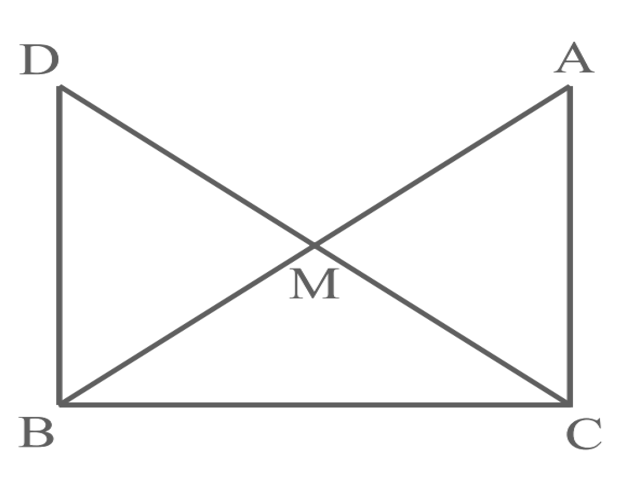
\includegraphics[width=\columnwidth]{figs/Screenshot.png}
  \caption{$\triangle \vec{ACB} ,\triangle \vec{DCB}$ with Mid-Point $\vec{M}$}
  \label{fig:triangles}
\end{figure}
\begin{enumerate}[label =(\roman*)]
        \item $\triangle \vec{AMC} \cong \triangle \vec{BMD}$
        \item $\angle \vec{DBC}$ is a right angle. 
        \item $\triangle \vec{DBC} \cong  \triangle \vec{ACB}$ 
        \item $\vec{CM} = \frac{1}{2} \vec{AB}$
\end{enumerate}
\pagebreak
\solution\\
\textbf{CONSTRUCTION STEPS :}
\begin{enumerate}
\item Let us Assume , the input parameters as ;
\begin{table}[H]
\centering
        \input{tables/input_params.tex}
          \caption{Input Parameters}
          \label{Table-1:Input_params}
\end{table}
\item the output can be calculated as ;
\begin{table}[H]
\centering
        \input{tables/output_params.tex}
          \caption{Output Parameters}
          \label{Table-2:Output_params}
\end{table}
                $\therefore$ By, Plotting these points we get the required Image \figref{fig:fig-2}
\begin{figure}[H]
        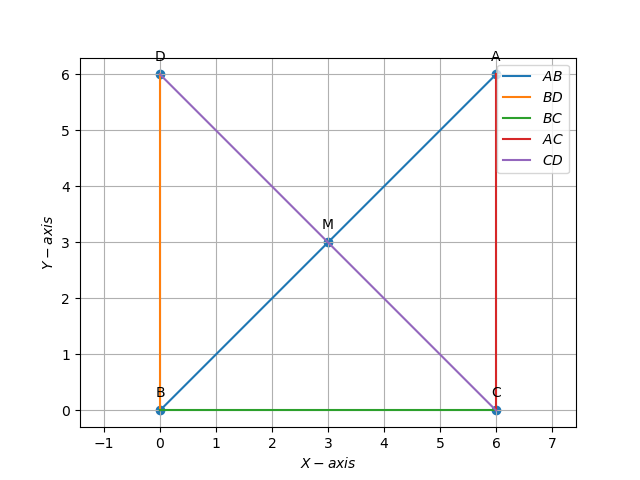
\includegraphics[width = \columnwidth]{figs/python_plot.png}
    \caption{PYTHON Plot of $\triangle \vec{ACB} ,\triangle \vec{DBC}$ with Mid-Point $\vec{M}$}
    \label{fig:fig-2}
\end{figure}
\end{enumerate}

\item Find the position vector of a point $\vec{R}$ which divides the line joining two points $\vec{P}$ and $\vec{Q}$ whose position vectors are $2\vec{a}+\vec{b}$ and $\vec{a}-3\vec{b}$ externally in the ratio $1:2$.

\textbf{Solution:}
Let us assume $\vec{a}$ and $\vec{b}$, and the given ratio is
\begin{table}[h]
    \centering
    \begin{tabular}{|c|c|c|}
        \hline 
        \textbf{Symbol} & \textbf{Value} & \textbf{Description} \\
        \hline
        $\vec{a}$ & $\myvec{1 \\ -3}$ & Vector $\vec{a}$ \\
        \hline
        $\vec{b}$ & $\myvec{0 \\ 2}$ & Vector $\vec{b}$\\
        \hline
        $k$ & $2$ & Ratio \\
        \hline
    \end{tabular}
    \caption{Vectors $\vec{a}$ and $\vec{b}$, ratio $k$}
    \label{tab:table1}
\end{table}

Using the section formula,
\begin{align}
    \vec{R} = \frac{\vec{Q} - k\vec{P}}{1 - k}
\end{align}
where $\vec{P}$ and $\vec{Q}$ depend on $\vec{a}$ and $\vec{b}$, then
\begin{align}
    \vec{P} &= (2\vec{a} + \vec{b}) = 2\myvec{1\\-3} + \myvec{0\\2} = \myvec{2\\-4} \\
    \vec{Q} &= (\vec{a} - 3\vec{b}) = \myvec{1\\-3} - 3\myvec{0\\2} = \myvec{1\\-9}
\end{align}
where $\vec{R}$ can be calculated as 
\begin{align}
    \vec{R} = \frac{(\vec{a} - 3\vec{b}) - k(2\vec{a} + \vec{b})}{1 - k}
\end{align}
By substituting $\vec{a}$ and $\vec{b}$ values, we get $\vec{R}$ as
\begin{align}
    \vec{R} = \myvec{3\\1}
\end{align}

\begin{table}[ht!]
    \centering
    \begin{tabular}{|c|c|c|}
        \hline
        \textbf{Symbol} & \textbf{Value} & \textbf{Description}\\
        \hline
        $\vec{P}$ & $(2\vec{a} + \vec{b})$ & Position vector $\vec{P}$ \\
        \hline
        $\vec{Q}$ & $(\vec{a} - 3\vec{b})$ & Position vector $\vec{Q}$\\
        \hline
        $\vec{R}$ & $\frac{\vec{Q} - k\vec{P}}{1 - k}$ & Position vector $\vec{R}$\\
        \hline
    \end{tabular}
    \caption{Vectors $\vec{P}$, $\vec{Q}$, $\vec{R}$}
    \label{tab:mytable2}   
\end{table}

\begin{figure}[H]
    \centering
    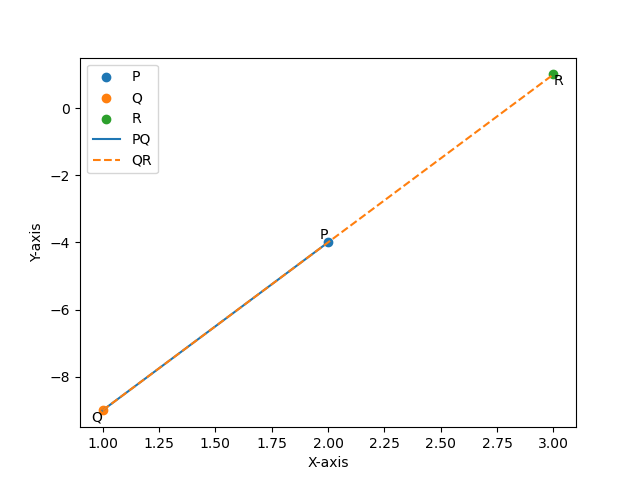
\includegraphics[width=\columnwidth]{figs/external-bisector.png}
    \caption{Point vectors $\vec{P}$, $\vec{Q}$, $\vec{R}$}
    \label{fig:enter-label}
\end{figure}


\end{enumerate}

    \item Draw a quadrilateral in the Cartesian plane, whose vertices are 
    \begin{align}
        \vec{A} = \myvec{-4\\5} \quad \vec{B} = \myvec{0\\7} \\
        \vec{C} = \myvec{5\\-5} \quad \vec{D} = \myvec{-4\\-2}
    \end{align}
    Also, find its area.
\label{chapters/11/10/1/1}
   \\ 
    \solution 
\begin{enumerate}[label=\thesection.\arabic*,ref=\thesection.\theenumi]
		\item Find $\abs{\overrightarrow{a}\times\overrightarrow{b}},\text{ if }\overrightarrow{a}=\hat{i}-7\hat{j}+7\hat{k}\text{ and } \overrightarrow{b}=3\hat{i}-2\hat{j}+2\hat{k}$.
	\\
		\solution
		\input{chapters/12/10/4/1/cross.tex}
\item Show that $$(\overrightarrow{a}-\overrightarrow{b})\times (\overrightarrow{a}+\overrightarrow{b})=2(\overrightarrow{a}\times \overrightarrow{b})$$
	\\
		\solution
		\input{chapters/12/10/4/4/cross.tex}
\item Find $\lambda$ and $\mu$ if $(2\hat{i}+6\hat{j}+27\hat{k})\times(\hat{i}+\lambda \hat{j} + \mu \hat{k})=\overrightarrow{0}$.
	\\
		\solution
		\input{chapters/12/10/4/5/cross.tex}
\item Given that $\overrightarrow{a} \cdot \overrightarrow{b} = 0$ and $\overrightarrow{a} \times \overrightarrow{b} = \overrightarrow{0}$. What can you conclude about the vectors $\overrightarrow{a} \text{ and }\overrightarrow{b}$?
\item Let the vectors be given as $\overrightarrow{a},\overrightarrow{b},\overrightarrow{c}\text{ be given as }\ a_1 \hat{i}+\ a_2 \hat{j}+\ a_3 \hat{k},\ b_1 \hat{i}+\ b_2 \hat{j}+\ b_3 \hat{k},\ c_1 \hat{i}+\ c_2 \hat{j}+\ c_3 \hat{k}$. Then show that $\overrightarrow{a} \times (\overrightarrow{b} + \overrightarrow{c}) = \overrightarrow{a} \times \overrightarrow{b}+\overrightarrow{a} \times \overrightarrow{c}$.
	\\
		\solution
		\input{chapters/12/10/4/7/cross.tex}
\item If either $\overrightarrow{a} = \overrightarrow{0}$ or $\overrightarrow{b} = \overrightarrow{0}$, then $\overrightarrow{a} \times \overrightarrow{b} = \overrightarrow{0}$. Is the converse true? Justify your answer with an example.
	\\
		\solution
		\input{chapters/12/10/4/8/cross.tex}
\item Find the area of the triangle with vertices $A(1, 1, 2)$, $B(2, 3, 5)$, and $C(1, 5, 5)$
	\\
		\solution
		\input{chapters/12/10/4/9/cross.tex}
\item Find the area of the parallelogram whose adjacent sides are determined by the vectors $\overrightarrow{a}=\hat{i}-\hat{j}+3\hat{k}$ and $\overrightarrow{b}=2\hat{i}-7\hat{j}+\hat{k}$.
	\\
		\solution
		\input{chapters/12/10/4/10/cross.tex}
\item Let the vectors $\overrightarrow{a}$ and $\overrightarrow{b}$ be such that $|\overrightarrow{a}| = 3$ and $|\overrightarrow{b}| = \dfrac{\sqrt{2}}{3}$, then $\overrightarrow{a} \times \overrightarrow{b}$ is a unit vector, if the angle between $\overrightarrow{a}$ and $\overrightarrow{b}$ is
\begin{enumerate}
\item $\dfrac{\pi}{6}$
\item $\dfrac{\pi}{4}$
\item $\dfrac{\pi}{3}$
\item $\dfrac{\pi}{2}$
\end{enumerate}
		\solution
		\input{chapters/12/10/4/11/cross.tex}
\item Area of a rectangle having vertices A, B, C and D with position vectors $ -\hat{i}+ \dfrac{1}{2} \hat{j}+4\hat{k},\hat{i}+ \dfrac{1}{2} \hat{j}+4\hat{k},\hat{i}-\dfrac{1}{2} \hat{j}+4\hat{k}\text{ and }-\hat{i}- \dfrac{1}{2} \hat{j}+4\hat{k}$, respectively is
\begin{enumerate}
\item $\dfrac{1}{2}$
\item 1
\item 2
\item 4
\end{enumerate}
		\solution
		\input{chapters/12/10/4/12/cross.tex}
\item Find the area of the triangle whose vertices are 
\begin{enumerate}
\item $(2, 3), (–1, 0), (2, – 4)$
\item $(–5, –1), (3, –5), (5, 2)$ 
\end{enumerate}
		\label{10/7/3/1}
\solution
		\input{chapters/10/7/3/1/area.tex}
\item Find the area of the triangle formed by joining the mid-points of the sides of the triangle whose vertices are $(0, –1), (2, 1) \text{ and } (0, 3)$. Find the ratio of this area to the area of the given triangle.
	\\
\solution
		\input{chapters/10/7/3/3/cross.tex}

\item Find the area of the quadrilateral whose vertices, taken in order, are $(– 4, – 2), (– 3, – 5), (3, – 2)$  and $ (2, 3)$.
	\\
\solution
		\input{chapters/10/7/3/4/cross.tex}

\item Verify that a median of a triangle divides it into two triangles of equal areas for $\triangle ABC$ whose vertices are $\vec{A}(4, -6), \vec{B}(3, 2), \text{ and } \vec{C}(5, 2)$. 
		\label{10/7/3/5}
		\\
\solution
		\input{chapters/10/7/3/5/area.tex}

\item The two adjacent sides of a parallelogram are 
$2\hat{i}-4\hat{j}+5\hat{k}$  and  $\hat{i}-2\hat{j}-3\hat{k}$.
Find the unit vector parallel to its diagonal. Also, find its area.\\
	\solution
		\input{chapters/12/10/5/10/cross.tex}
\item The vertices of a $\triangle ABC$ are $\vec{A}(4,6), \vec{B}(1,5)$ and  $\vec{C}(7,2)$. A line is drawn to intersect sides $AB$ and $AC$ at $\vec{D}$ and $\vec{E}$ respectively, such that $\frac{AD}{AB} = \frac{AE}{AC} = \frac{1}{4}$. Calculate the area of $\triangle ADE$ and compare it with the area of the $\triangle ABC$.
\\
\solution
	\input{chapters/10/7/4/6/section.tex}
    \item Draw a quadrilateral in the Cartesian plane, whose vertices are 
    \begin{align}
        \vec{A} = \myvec{-4\\5} \quad \vec{B} = \myvec{0\\7} \\
        \vec{C} = \myvec{5\\-5} \quad \vec{D} = \myvec{-4\\-2}
    \end{align}
    Also, find its area.
\label{chapters/11/10/1/1}
   \\ 
    \solution 
\input{chapters/11/10/1/1/cross.tex}
\item Find the area of region bounded by the triangle whose
	vertices are $(1, 0), (2, 2) \text{ and } (3, 1)$. 
\item Find the area of region bounded by the triangle whose vertices
	are $(– 1, 0), (1, 3) \text{ and } (3, 2)$. 
\item Find the area of the $\triangle ABC$, coordinates of whose vertices are $\vec{A}(2, 0), \vec{B}(4, 5), \text{ and } \vec{C}(6, 3)$.


\item 
\input{chapters/vectors/exer/main.tex}
\end{enumerate}


\item Find the area of region bounded by the triangle whose
	vertices are $(1, 0), (2, 2) \text{ and } (3, 1)$. 
\item Find the area of region bounded by the triangle whose vertices
	are $(– 1, 0), (1, 3) \text{ and } (3, 2)$. 
\item Find the area of the $\triangle ABC$, coordinates of whose vertices are $\vec{A}(2, 0), \vec{B}(4, 5), \text{ and } \vec{C}(6, 3)$.


\item 
%\documentclass[12pt]{article}
%\usepackage{graphicx}
%\usepackage{graphics}
%\usepackage{refstyle}
%\usepackage{amsmath}
%\usepackage{caption}
%\usepackage{float}
%\usepackage{booktabs}
%\usepackage{array}
%\usepackage{amssymb}
%\usepackage{booktabs}
%\let\vec\mathbf
%\providecommand{\brak}[1]{\ensuremath{\left(#1\right)}}
%\graphicspath{{/storage/self/primary/Download/latexnew/fig}}                                     
$\vec{P}$ and $\vec{Q}$ are any two points lying on the sides $DC$ and $AD$ respectively of a parallelogram $ABCD$.Show that, $ar\brak{\triangle APB}=ar\brak{\triangle BQC}$.


\textbf{Figure:}
\begin{figure}[H]
    \centering
	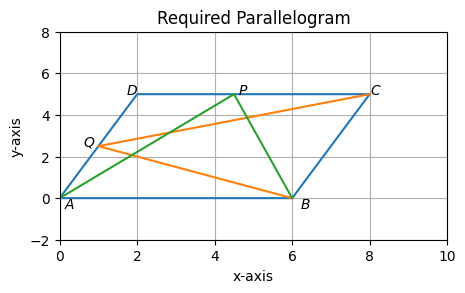
\includegraphics[width=\columnwidth]{chapters/vectors/exer/figs/1.png}
    \caption{}
    \label{fig:fig:1}
\end{figure}


\textbf{Solution:}
\begin{table}[H]
   \centering
  \input{chapters/vectors/exer/table/tab1.tex}
   \caption{Table of input parameters}        
\label{tab:tab:1}                    
\end{table}




\begin{table}[H]
    \centering                                  
\input{chapters/vectors/exer/table/tab2.tex}                  
\caption{Table of output parameters}
\label{tab:tab:2}
 \end{table}


For the $\triangle BQC$, the vertices of the triangle are taken from \tabref{tab:tab:1} and \tabref{tab:tab:2}.

\begin{align}
\implies ar\brak{\triangle BQC}&=
\frac{1}{2}\begin{tabular}{|c c c|}            
1 &1&1\\                      
$\vec{B}$&$\vec{Q}$&$\vec{C}$\\    
\end{tabular}\\
&= \frac{1}{2}\begin{tabular}{|c c c|}
       1 &1&1\\
       6&$\frac{2k_1}{k_1+1}$&8 \\
       0&$\frac{5k_1}{k_1+1}$&5
   \end{tabular}\\
  \xrightarrow{C_2'=C_2-C_1,C_3'=C_3-C_1}&\frac{1}{2} \begin{tabular}{|c c c|}
       1 &0&0\\
       6&$\frac{-4k_1-6}{k_1+1}$&2 \\
       0&$\frac{5k_1}{k_1+1}$&5
   \end{tabular}\\
&=\frac{1}{2}\brak{1\begin{tabular}{|c c|}
   $\frac{-4k_1-6}{k_1+1}$ &2  \\
   $\frac{5k_1}{k_1+1}$ & 5
\end{tabular} +0+0}\\
&=\frac{1}{2} \times30\\                          
&=15 \end{align}


For the $\triangle APB$, the vertices of the triangle are taken from \tabref{tab:tab:1} and \tabref{tab:tab:2}.
   \begin{align}
  \implies ar\brak{\triangle APB} &=
\frac{1}{2}\begin{tabular}{|c c c|}            
1 &1&1\\                            
$\vec{A}$&$\vec{P}$&$\vec{B}$\\
\end{tabular}\\ &=  \frac{1}{2}
   \begin{tabular}{|c c c|}
       1 &1&1\\
       0&$\frac{8k_2+2}{k_2+1}$&6 \\
       0&5&0
   \end{tabular}\\
 &=\frac{1}{2} \times30\\
 &=15 \end{align}
 \brak{6} = \brak{10}


So, ar\brak{\triangle BQC} = ar\brak{\triangle APB}.\brak{proved}
%\end{document}



\end{enumerate}


\item Given that $\overrightarrow{a} \cdot \overrightarrow{b} = 0$ and $\overrightarrow{a} \times \overrightarrow{b} = \overrightarrow{0}$. What can you conclude about the vectors $\overrightarrow{a} \text{ and }\overrightarrow{b}$?
\item Let the vectors be given as $\overrightarrow{a},\overrightarrow{b},\overrightarrow{c}\text{ be given as }\ a_1 \hat{i}+\ a_2 \hat{j}+\ a_3 \hat{k},\ b_1 \hat{i}+\ b_2 \hat{j}+\ b_3 \hat{k},\ c_1 \hat{i}+\ c_2 \hat{j}+\ c_3 \hat{k}$. Then show that $\overrightarrow{a} \times (\overrightarrow{b} + \overrightarrow{c}) = \overrightarrow{a} \times \overrightarrow{b}+\overrightarrow{a} \times \overrightarrow{c}$.
	\\
		\solution
		\begin{enumerate}[label=\thesection.\arabic*,ref=\thesection.\theenumi]
		\item Find $\abs{\overrightarrow{a}\times\overrightarrow{b}},\text{ if }\overrightarrow{a}=\hat{i}-7\hat{j}+7\hat{k}\text{ and } \overrightarrow{b}=3\hat{i}-2\hat{j}+2\hat{k}$.
	\\
		\solution
		\begin{enumerate}[label=\thesection.\arabic*,ref=\thesection.\theenumi]
		\item Find $\abs{\overrightarrow{a}\times\overrightarrow{b}},\text{ if }\overrightarrow{a}=\hat{i}-7\hat{j}+7\hat{k}\text{ and } \overrightarrow{b}=3\hat{i}-2\hat{j}+2\hat{k}$.
	\\
		\solution
		\input{chapters/12/10/4/1/cross.tex}
\item Show that $$(\overrightarrow{a}-\overrightarrow{b})\times (\overrightarrow{a}+\overrightarrow{b})=2(\overrightarrow{a}\times \overrightarrow{b})$$
	\\
		\solution
		\input{chapters/12/10/4/4/cross.tex}
\item Find $\lambda$ and $\mu$ if $(2\hat{i}+6\hat{j}+27\hat{k})\times(\hat{i}+\lambda \hat{j} + \mu \hat{k})=\overrightarrow{0}$.
	\\
		\solution
		\input{chapters/12/10/4/5/cross.tex}
\item Given that $\overrightarrow{a} \cdot \overrightarrow{b} = 0$ and $\overrightarrow{a} \times \overrightarrow{b} = \overrightarrow{0}$. What can you conclude about the vectors $\overrightarrow{a} \text{ and }\overrightarrow{b}$?
\item Let the vectors be given as $\overrightarrow{a},\overrightarrow{b},\overrightarrow{c}\text{ be given as }\ a_1 \hat{i}+\ a_2 \hat{j}+\ a_3 \hat{k},\ b_1 \hat{i}+\ b_2 \hat{j}+\ b_3 \hat{k},\ c_1 \hat{i}+\ c_2 \hat{j}+\ c_3 \hat{k}$. Then show that $\overrightarrow{a} \times (\overrightarrow{b} + \overrightarrow{c}) = \overrightarrow{a} \times \overrightarrow{b}+\overrightarrow{a} \times \overrightarrow{c}$.
	\\
		\solution
		\input{chapters/12/10/4/7/cross.tex}
\item If either $\overrightarrow{a} = \overrightarrow{0}$ or $\overrightarrow{b} = \overrightarrow{0}$, then $\overrightarrow{a} \times \overrightarrow{b} = \overrightarrow{0}$. Is the converse true? Justify your answer with an example.
	\\
		\solution
		\input{chapters/12/10/4/8/cross.tex}
\item Find the area of the triangle with vertices $A(1, 1, 2)$, $B(2, 3, 5)$, and $C(1, 5, 5)$
	\\
		\solution
		\input{chapters/12/10/4/9/cross.tex}
\item Find the area of the parallelogram whose adjacent sides are determined by the vectors $\overrightarrow{a}=\hat{i}-\hat{j}+3\hat{k}$ and $\overrightarrow{b}=2\hat{i}-7\hat{j}+\hat{k}$.
	\\
		\solution
		\input{chapters/12/10/4/10/cross.tex}
\item Let the vectors $\overrightarrow{a}$ and $\overrightarrow{b}$ be such that $|\overrightarrow{a}| = 3$ and $|\overrightarrow{b}| = \dfrac{\sqrt{2}}{3}$, then $\overrightarrow{a} \times \overrightarrow{b}$ is a unit vector, if the angle between $\overrightarrow{a}$ and $\overrightarrow{b}$ is
\begin{enumerate}
\item $\dfrac{\pi}{6}$
\item $\dfrac{\pi}{4}$
\item $\dfrac{\pi}{3}$
\item $\dfrac{\pi}{2}$
\end{enumerate}
		\solution
		\input{chapters/12/10/4/11/cross.tex}
\item Area of a rectangle having vertices A, B, C and D with position vectors $ -\hat{i}+ \dfrac{1}{2} \hat{j}+4\hat{k},\hat{i}+ \dfrac{1}{2} \hat{j}+4\hat{k},\hat{i}-\dfrac{1}{2} \hat{j}+4\hat{k}\text{ and }-\hat{i}- \dfrac{1}{2} \hat{j}+4\hat{k}$, respectively is
\begin{enumerate}
\item $\dfrac{1}{2}$
\item 1
\item 2
\item 4
\end{enumerate}
		\solution
		\input{chapters/12/10/4/12/cross.tex}
\item Find the area of the triangle whose vertices are 
\begin{enumerate}
\item $(2, 3), (–1, 0), (2, – 4)$
\item $(–5, –1), (3, –5), (5, 2)$ 
\end{enumerate}
		\label{10/7/3/1}
\solution
		\input{chapters/10/7/3/1/area.tex}
\item Find the area of the triangle formed by joining the mid-points of the sides of the triangle whose vertices are $(0, –1), (2, 1) \text{ and } (0, 3)$. Find the ratio of this area to the area of the given triangle.
	\\
\solution
		\input{chapters/10/7/3/3/cross.tex}

\item Find the area of the quadrilateral whose vertices, taken in order, are $(– 4, – 2), (– 3, – 5), (3, – 2)$  and $ (2, 3)$.
	\\
\solution
		\input{chapters/10/7/3/4/cross.tex}

\item Verify that a median of a triangle divides it into two triangles of equal areas for $\triangle ABC$ whose vertices are $\vec{A}(4, -6), \vec{B}(3, 2), \text{ and } \vec{C}(5, 2)$. 
		\label{10/7/3/5}
		\\
\solution
		\input{chapters/10/7/3/5/area.tex}

\item The two adjacent sides of a parallelogram are 
$2\hat{i}-4\hat{j}+5\hat{k}$  and  $\hat{i}-2\hat{j}-3\hat{k}$.
Find the unit vector parallel to its diagonal. Also, find its area.\\
	\solution
		\input{chapters/12/10/5/10/cross.tex}
\item The vertices of a $\triangle ABC$ are $\vec{A}(4,6), \vec{B}(1,5)$ and  $\vec{C}(7,2)$. A line is drawn to intersect sides $AB$ and $AC$ at $\vec{D}$ and $\vec{E}$ respectively, such that $\frac{AD}{AB} = \frac{AE}{AC} = \frac{1}{4}$. Calculate the area of $\triangle ADE$ and compare it with the area of the $\triangle ABC$.
\\
\solution
	\input{chapters/10/7/4/6/section.tex}
    \item Draw a quadrilateral in the Cartesian plane, whose vertices are 
    \begin{align}
        \vec{A} = \myvec{-4\\5} \quad \vec{B} = \myvec{0\\7} \\
        \vec{C} = \myvec{5\\-5} \quad \vec{D} = \myvec{-4\\-2}
    \end{align}
    Also, find its area.
\label{chapters/11/10/1/1}
   \\ 
    \solution 
\input{chapters/11/10/1/1/cross.tex}
\item Find the area of region bounded by the triangle whose
	vertices are $(1, 0), (2, 2) \text{ and } (3, 1)$. 
\item Find the area of region bounded by the triangle whose vertices
	are $(– 1, 0), (1, 3) \text{ and } (3, 2)$. 
\item Find the area of the $\triangle ABC$, coordinates of whose vertices are $\vec{A}(2, 0), \vec{B}(4, 5), \text{ and } \vec{C}(6, 3)$.


\item 
\input{chapters/vectors/exer/main.tex}
\end{enumerate}


\item Show that $$(\overrightarrow{a}-\overrightarrow{b})\times (\overrightarrow{a}+\overrightarrow{b})=2(\overrightarrow{a}\times \overrightarrow{b})$$
	\\
		\solution
		\begin{enumerate}[label=\thesection.\arabic*,ref=\thesection.\theenumi]
		\item Find $\abs{\overrightarrow{a}\times\overrightarrow{b}},\text{ if }\overrightarrow{a}=\hat{i}-7\hat{j}+7\hat{k}\text{ and } \overrightarrow{b}=3\hat{i}-2\hat{j}+2\hat{k}$.
	\\
		\solution
		\input{chapters/12/10/4/1/cross.tex}
\item Show that $$(\overrightarrow{a}-\overrightarrow{b})\times (\overrightarrow{a}+\overrightarrow{b})=2(\overrightarrow{a}\times \overrightarrow{b})$$
	\\
		\solution
		\input{chapters/12/10/4/4/cross.tex}
\item Find $\lambda$ and $\mu$ if $(2\hat{i}+6\hat{j}+27\hat{k})\times(\hat{i}+\lambda \hat{j} + \mu \hat{k})=\overrightarrow{0}$.
	\\
		\solution
		\input{chapters/12/10/4/5/cross.tex}
\item Given that $\overrightarrow{a} \cdot \overrightarrow{b} = 0$ and $\overrightarrow{a} \times \overrightarrow{b} = \overrightarrow{0}$. What can you conclude about the vectors $\overrightarrow{a} \text{ and }\overrightarrow{b}$?
\item Let the vectors be given as $\overrightarrow{a},\overrightarrow{b},\overrightarrow{c}\text{ be given as }\ a_1 \hat{i}+\ a_2 \hat{j}+\ a_3 \hat{k},\ b_1 \hat{i}+\ b_2 \hat{j}+\ b_3 \hat{k},\ c_1 \hat{i}+\ c_2 \hat{j}+\ c_3 \hat{k}$. Then show that $\overrightarrow{a} \times (\overrightarrow{b} + \overrightarrow{c}) = \overrightarrow{a} \times \overrightarrow{b}+\overrightarrow{a} \times \overrightarrow{c}$.
	\\
		\solution
		\input{chapters/12/10/4/7/cross.tex}
\item If either $\overrightarrow{a} = \overrightarrow{0}$ or $\overrightarrow{b} = \overrightarrow{0}$, then $\overrightarrow{a} \times \overrightarrow{b} = \overrightarrow{0}$. Is the converse true? Justify your answer with an example.
	\\
		\solution
		\input{chapters/12/10/4/8/cross.tex}
\item Find the area of the triangle with vertices $A(1, 1, 2)$, $B(2, 3, 5)$, and $C(1, 5, 5)$
	\\
		\solution
		\input{chapters/12/10/4/9/cross.tex}
\item Find the area of the parallelogram whose adjacent sides are determined by the vectors $\overrightarrow{a}=\hat{i}-\hat{j}+3\hat{k}$ and $\overrightarrow{b}=2\hat{i}-7\hat{j}+\hat{k}$.
	\\
		\solution
		\input{chapters/12/10/4/10/cross.tex}
\item Let the vectors $\overrightarrow{a}$ and $\overrightarrow{b}$ be such that $|\overrightarrow{a}| = 3$ and $|\overrightarrow{b}| = \dfrac{\sqrt{2}}{3}$, then $\overrightarrow{a} \times \overrightarrow{b}$ is a unit vector, if the angle between $\overrightarrow{a}$ and $\overrightarrow{b}$ is
\begin{enumerate}
\item $\dfrac{\pi}{6}$
\item $\dfrac{\pi}{4}$
\item $\dfrac{\pi}{3}$
\item $\dfrac{\pi}{2}$
\end{enumerate}
		\solution
		\input{chapters/12/10/4/11/cross.tex}
\item Area of a rectangle having vertices A, B, C and D with position vectors $ -\hat{i}+ \dfrac{1}{2} \hat{j}+4\hat{k},\hat{i}+ \dfrac{1}{2} \hat{j}+4\hat{k},\hat{i}-\dfrac{1}{2} \hat{j}+4\hat{k}\text{ and }-\hat{i}- \dfrac{1}{2} \hat{j}+4\hat{k}$, respectively is
\begin{enumerate}
\item $\dfrac{1}{2}$
\item 1
\item 2
\item 4
\end{enumerate}
		\solution
		\input{chapters/12/10/4/12/cross.tex}
\item Find the area of the triangle whose vertices are 
\begin{enumerate}
\item $(2, 3), (–1, 0), (2, – 4)$
\item $(–5, –1), (3, –5), (5, 2)$ 
\end{enumerate}
		\label{10/7/3/1}
\solution
		\input{chapters/10/7/3/1/area.tex}
\item Find the area of the triangle formed by joining the mid-points of the sides of the triangle whose vertices are $(0, –1), (2, 1) \text{ and } (0, 3)$. Find the ratio of this area to the area of the given triangle.
	\\
\solution
		\input{chapters/10/7/3/3/cross.tex}

\item Find the area of the quadrilateral whose vertices, taken in order, are $(– 4, – 2), (– 3, – 5), (3, – 2)$  and $ (2, 3)$.
	\\
\solution
		\input{chapters/10/7/3/4/cross.tex}

\item Verify that a median of a triangle divides it into two triangles of equal areas for $\triangle ABC$ whose vertices are $\vec{A}(4, -6), \vec{B}(3, 2), \text{ and } \vec{C}(5, 2)$. 
		\label{10/7/3/5}
		\\
\solution
		\input{chapters/10/7/3/5/area.tex}

\item The two adjacent sides of a parallelogram are 
$2\hat{i}-4\hat{j}+5\hat{k}$  and  $\hat{i}-2\hat{j}-3\hat{k}$.
Find the unit vector parallel to its diagonal. Also, find its area.\\
	\solution
		\input{chapters/12/10/5/10/cross.tex}
\item The vertices of a $\triangle ABC$ are $\vec{A}(4,6), \vec{B}(1,5)$ and  $\vec{C}(7,2)$. A line is drawn to intersect sides $AB$ and $AC$ at $\vec{D}$ and $\vec{E}$ respectively, such that $\frac{AD}{AB} = \frac{AE}{AC} = \frac{1}{4}$. Calculate the area of $\triangle ADE$ and compare it with the area of the $\triangle ABC$.
\\
\solution
	\input{chapters/10/7/4/6/section.tex}
    \item Draw a quadrilateral in the Cartesian plane, whose vertices are 
    \begin{align}
        \vec{A} = \myvec{-4\\5} \quad \vec{B} = \myvec{0\\7} \\
        \vec{C} = \myvec{5\\-5} \quad \vec{D} = \myvec{-4\\-2}
    \end{align}
    Also, find its area.
\label{chapters/11/10/1/1}
   \\ 
    \solution 
\input{chapters/11/10/1/1/cross.tex}
\item Find the area of region bounded by the triangle whose
	vertices are $(1, 0), (2, 2) \text{ and } (3, 1)$. 
\item Find the area of region bounded by the triangle whose vertices
	are $(– 1, 0), (1, 3) \text{ and } (3, 2)$. 
\item Find the area of the $\triangle ABC$, coordinates of whose vertices are $\vec{A}(2, 0), \vec{B}(4, 5), \text{ and } \vec{C}(6, 3)$.


\item 
\input{chapters/vectors/exer/main.tex}
\end{enumerate}


\item Find $\lambda$ and $\mu$ if $(2\hat{i}+6\hat{j}+27\hat{k})\times(\hat{i}+\lambda \hat{j} + \mu \hat{k})=\overrightarrow{0}$.
	\\
		\solution
		\begin{enumerate}[label=\thesection.\arabic*,ref=\thesection.\theenumi]
		\item Find $\abs{\overrightarrow{a}\times\overrightarrow{b}},\text{ if }\overrightarrow{a}=\hat{i}-7\hat{j}+7\hat{k}\text{ and } \overrightarrow{b}=3\hat{i}-2\hat{j}+2\hat{k}$.
	\\
		\solution
		\input{chapters/12/10/4/1/cross.tex}
\item Show that $$(\overrightarrow{a}-\overrightarrow{b})\times (\overrightarrow{a}+\overrightarrow{b})=2(\overrightarrow{a}\times \overrightarrow{b})$$
	\\
		\solution
		\input{chapters/12/10/4/4/cross.tex}
\item Find $\lambda$ and $\mu$ if $(2\hat{i}+6\hat{j}+27\hat{k})\times(\hat{i}+\lambda \hat{j} + \mu \hat{k})=\overrightarrow{0}$.
	\\
		\solution
		\input{chapters/12/10/4/5/cross.tex}
\item Given that $\overrightarrow{a} \cdot \overrightarrow{b} = 0$ and $\overrightarrow{a} \times \overrightarrow{b} = \overrightarrow{0}$. What can you conclude about the vectors $\overrightarrow{a} \text{ and }\overrightarrow{b}$?
\item Let the vectors be given as $\overrightarrow{a},\overrightarrow{b},\overrightarrow{c}\text{ be given as }\ a_1 \hat{i}+\ a_2 \hat{j}+\ a_3 \hat{k},\ b_1 \hat{i}+\ b_2 \hat{j}+\ b_3 \hat{k},\ c_1 \hat{i}+\ c_2 \hat{j}+\ c_3 \hat{k}$. Then show that $\overrightarrow{a} \times (\overrightarrow{b} + \overrightarrow{c}) = \overrightarrow{a} \times \overrightarrow{b}+\overrightarrow{a} \times \overrightarrow{c}$.
	\\
		\solution
		\input{chapters/12/10/4/7/cross.tex}
\item If either $\overrightarrow{a} = \overrightarrow{0}$ or $\overrightarrow{b} = \overrightarrow{0}$, then $\overrightarrow{a} \times \overrightarrow{b} = \overrightarrow{0}$. Is the converse true? Justify your answer with an example.
	\\
		\solution
		\input{chapters/12/10/4/8/cross.tex}
\item Find the area of the triangle with vertices $A(1, 1, 2)$, $B(2, 3, 5)$, and $C(1, 5, 5)$
	\\
		\solution
		\input{chapters/12/10/4/9/cross.tex}
\item Find the area of the parallelogram whose adjacent sides are determined by the vectors $\overrightarrow{a}=\hat{i}-\hat{j}+3\hat{k}$ and $\overrightarrow{b}=2\hat{i}-7\hat{j}+\hat{k}$.
	\\
		\solution
		\input{chapters/12/10/4/10/cross.tex}
\item Let the vectors $\overrightarrow{a}$ and $\overrightarrow{b}$ be such that $|\overrightarrow{a}| = 3$ and $|\overrightarrow{b}| = \dfrac{\sqrt{2}}{3}$, then $\overrightarrow{a} \times \overrightarrow{b}$ is a unit vector, if the angle between $\overrightarrow{a}$ and $\overrightarrow{b}$ is
\begin{enumerate}
\item $\dfrac{\pi}{6}$
\item $\dfrac{\pi}{4}$
\item $\dfrac{\pi}{3}$
\item $\dfrac{\pi}{2}$
\end{enumerate}
		\solution
		\input{chapters/12/10/4/11/cross.tex}
\item Area of a rectangle having vertices A, B, C and D with position vectors $ -\hat{i}+ \dfrac{1}{2} \hat{j}+4\hat{k},\hat{i}+ \dfrac{1}{2} \hat{j}+4\hat{k},\hat{i}-\dfrac{1}{2} \hat{j}+4\hat{k}\text{ and }-\hat{i}- \dfrac{1}{2} \hat{j}+4\hat{k}$, respectively is
\begin{enumerate}
\item $\dfrac{1}{2}$
\item 1
\item 2
\item 4
\end{enumerate}
		\solution
		\input{chapters/12/10/4/12/cross.tex}
\item Find the area of the triangle whose vertices are 
\begin{enumerate}
\item $(2, 3), (–1, 0), (2, – 4)$
\item $(–5, –1), (3, –5), (5, 2)$ 
\end{enumerate}
		\label{10/7/3/1}
\solution
		\input{chapters/10/7/3/1/area.tex}
\item Find the area of the triangle formed by joining the mid-points of the sides of the triangle whose vertices are $(0, –1), (2, 1) \text{ and } (0, 3)$. Find the ratio of this area to the area of the given triangle.
	\\
\solution
		\input{chapters/10/7/3/3/cross.tex}

\item Find the area of the quadrilateral whose vertices, taken in order, are $(– 4, – 2), (– 3, – 5), (3, – 2)$  and $ (2, 3)$.
	\\
\solution
		\input{chapters/10/7/3/4/cross.tex}

\item Verify that a median of a triangle divides it into two triangles of equal areas for $\triangle ABC$ whose vertices are $\vec{A}(4, -6), \vec{B}(3, 2), \text{ and } \vec{C}(5, 2)$. 
		\label{10/7/3/5}
		\\
\solution
		\input{chapters/10/7/3/5/area.tex}

\item The two adjacent sides of a parallelogram are 
$2\hat{i}-4\hat{j}+5\hat{k}$  and  $\hat{i}-2\hat{j}-3\hat{k}$.
Find the unit vector parallel to its diagonal. Also, find its area.\\
	\solution
		\input{chapters/12/10/5/10/cross.tex}
\item The vertices of a $\triangle ABC$ are $\vec{A}(4,6), \vec{B}(1,5)$ and  $\vec{C}(7,2)$. A line is drawn to intersect sides $AB$ and $AC$ at $\vec{D}$ and $\vec{E}$ respectively, such that $\frac{AD}{AB} = \frac{AE}{AC} = \frac{1}{4}$. Calculate the area of $\triangle ADE$ and compare it with the area of the $\triangle ABC$.
\\
\solution
	\input{chapters/10/7/4/6/section.tex}
    \item Draw a quadrilateral in the Cartesian plane, whose vertices are 
    \begin{align}
        \vec{A} = \myvec{-4\\5} \quad \vec{B} = \myvec{0\\7} \\
        \vec{C} = \myvec{5\\-5} \quad \vec{D} = \myvec{-4\\-2}
    \end{align}
    Also, find its area.
\label{chapters/11/10/1/1}
   \\ 
    \solution 
\input{chapters/11/10/1/1/cross.tex}
\item Find the area of region bounded by the triangle whose
	vertices are $(1, 0), (2, 2) \text{ and } (3, 1)$. 
\item Find the area of region bounded by the triangle whose vertices
	are $(– 1, 0), (1, 3) \text{ and } (3, 2)$. 
\item Find the area of the $\triangle ABC$, coordinates of whose vertices are $\vec{A}(2, 0), \vec{B}(4, 5), \text{ and } \vec{C}(6, 3)$.


\item 
\input{chapters/vectors/exer/main.tex}
\end{enumerate}


\item Given that $\overrightarrow{a} \cdot \overrightarrow{b} = 0$ and $\overrightarrow{a} \times \overrightarrow{b} = \overrightarrow{0}$. What can you conclude about the vectors $\overrightarrow{a} \text{ and }\overrightarrow{b}$?
\item Let the vectors be given as $\overrightarrow{a},\overrightarrow{b},\overrightarrow{c}\text{ be given as }\ a_1 \hat{i}+\ a_2 \hat{j}+\ a_3 \hat{k},\ b_1 \hat{i}+\ b_2 \hat{j}+\ b_3 \hat{k},\ c_1 \hat{i}+\ c_2 \hat{j}+\ c_3 \hat{k}$. Then show that $\overrightarrow{a} \times (\overrightarrow{b} + \overrightarrow{c}) = \overrightarrow{a} \times \overrightarrow{b}+\overrightarrow{a} \times \overrightarrow{c}$.
	\\
		\solution
		\begin{enumerate}[label=\thesection.\arabic*,ref=\thesection.\theenumi]
		\item Find $\abs{\overrightarrow{a}\times\overrightarrow{b}},\text{ if }\overrightarrow{a}=\hat{i}-7\hat{j}+7\hat{k}\text{ and } \overrightarrow{b}=3\hat{i}-2\hat{j}+2\hat{k}$.
	\\
		\solution
		\input{chapters/12/10/4/1/cross.tex}
\item Show that $$(\overrightarrow{a}-\overrightarrow{b})\times (\overrightarrow{a}+\overrightarrow{b})=2(\overrightarrow{a}\times \overrightarrow{b})$$
	\\
		\solution
		\input{chapters/12/10/4/4/cross.tex}
\item Find $\lambda$ and $\mu$ if $(2\hat{i}+6\hat{j}+27\hat{k})\times(\hat{i}+\lambda \hat{j} + \mu \hat{k})=\overrightarrow{0}$.
	\\
		\solution
		\input{chapters/12/10/4/5/cross.tex}
\item Given that $\overrightarrow{a} \cdot \overrightarrow{b} = 0$ and $\overrightarrow{a} \times \overrightarrow{b} = \overrightarrow{0}$. What can you conclude about the vectors $\overrightarrow{a} \text{ and }\overrightarrow{b}$?
\item Let the vectors be given as $\overrightarrow{a},\overrightarrow{b},\overrightarrow{c}\text{ be given as }\ a_1 \hat{i}+\ a_2 \hat{j}+\ a_3 \hat{k},\ b_1 \hat{i}+\ b_2 \hat{j}+\ b_3 \hat{k},\ c_1 \hat{i}+\ c_2 \hat{j}+\ c_3 \hat{k}$. Then show that $\overrightarrow{a} \times (\overrightarrow{b} + \overrightarrow{c}) = \overrightarrow{a} \times \overrightarrow{b}+\overrightarrow{a} \times \overrightarrow{c}$.
	\\
		\solution
		\input{chapters/12/10/4/7/cross.tex}
\item If either $\overrightarrow{a} = \overrightarrow{0}$ or $\overrightarrow{b} = \overrightarrow{0}$, then $\overrightarrow{a} \times \overrightarrow{b} = \overrightarrow{0}$. Is the converse true? Justify your answer with an example.
	\\
		\solution
		\input{chapters/12/10/4/8/cross.tex}
\item Find the area of the triangle with vertices $A(1, 1, 2)$, $B(2, 3, 5)$, and $C(1, 5, 5)$
	\\
		\solution
		\input{chapters/12/10/4/9/cross.tex}
\item Find the area of the parallelogram whose adjacent sides are determined by the vectors $\overrightarrow{a}=\hat{i}-\hat{j}+3\hat{k}$ and $\overrightarrow{b}=2\hat{i}-7\hat{j}+\hat{k}$.
	\\
		\solution
		\input{chapters/12/10/4/10/cross.tex}
\item Let the vectors $\overrightarrow{a}$ and $\overrightarrow{b}$ be such that $|\overrightarrow{a}| = 3$ and $|\overrightarrow{b}| = \dfrac{\sqrt{2}}{3}$, then $\overrightarrow{a} \times \overrightarrow{b}$ is a unit vector, if the angle between $\overrightarrow{a}$ and $\overrightarrow{b}$ is
\begin{enumerate}
\item $\dfrac{\pi}{6}$
\item $\dfrac{\pi}{4}$
\item $\dfrac{\pi}{3}$
\item $\dfrac{\pi}{2}$
\end{enumerate}
		\solution
		\input{chapters/12/10/4/11/cross.tex}
\item Area of a rectangle having vertices A, B, C and D with position vectors $ -\hat{i}+ \dfrac{1}{2} \hat{j}+4\hat{k},\hat{i}+ \dfrac{1}{2} \hat{j}+4\hat{k},\hat{i}-\dfrac{1}{2} \hat{j}+4\hat{k}\text{ and }-\hat{i}- \dfrac{1}{2} \hat{j}+4\hat{k}$, respectively is
\begin{enumerate}
\item $\dfrac{1}{2}$
\item 1
\item 2
\item 4
\end{enumerate}
		\solution
		\input{chapters/12/10/4/12/cross.tex}
\item Find the area of the triangle whose vertices are 
\begin{enumerate}
\item $(2, 3), (–1, 0), (2, – 4)$
\item $(–5, –1), (3, –5), (5, 2)$ 
\end{enumerate}
		\label{10/7/3/1}
\solution
		\input{chapters/10/7/3/1/area.tex}
\item Find the area of the triangle formed by joining the mid-points of the sides of the triangle whose vertices are $(0, –1), (2, 1) \text{ and } (0, 3)$. Find the ratio of this area to the area of the given triangle.
	\\
\solution
		\input{chapters/10/7/3/3/cross.tex}

\item Find the area of the quadrilateral whose vertices, taken in order, are $(– 4, – 2), (– 3, – 5), (3, – 2)$  and $ (2, 3)$.
	\\
\solution
		\input{chapters/10/7/3/4/cross.tex}

\item Verify that a median of a triangle divides it into two triangles of equal areas for $\triangle ABC$ whose vertices are $\vec{A}(4, -6), \vec{B}(3, 2), \text{ and } \vec{C}(5, 2)$. 
		\label{10/7/3/5}
		\\
\solution
		\input{chapters/10/7/3/5/area.tex}

\item The two adjacent sides of a parallelogram are 
$2\hat{i}-4\hat{j}+5\hat{k}$  and  $\hat{i}-2\hat{j}-3\hat{k}$.
Find the unit vector parallel to its diagonal. Also, find its area.\\
	\solution
		\input{chapters/12/10/5/10/cross.tex}
\item The vertices of a $\triangle ABC$ are $\vec{A}(4,6), \vec{B}(1,5)$ and  $\vec{C}(7,2)$. A line is drawn to intersect sides $AB$ and $AC$ at $\vec{D}$ and $\vec{E}$ respectively, such that $\frac{AD}{AB} = \frac{AE}{AC} = \frac{1}{4}$. Calculate the area of $\triangle ADE$ and compare it with the area of the $\triangle ABC$.
\\
\solution
	\input{chapters/10/7/4/6/section.tex}
    \item Draw a quadrilateral in the Cartesian plane, whose vertices are 
    \begin{align}
        \vec{A} = \myvec{-4\\5} \quad \vec{B} = \myvec{0\\7} \\
        \vec{C} = \myvec{5\\-5} \quad \vec{D} = \myvec{-4\\-2}
    \end{align}
    Also, find its area.
\label{chapters/11/10/1/1}
   \\ 
    \solution 
\input{chapters/11/10/1/1/cross.tex}
\item Find the area of region bounded by the triangle whose
	vertices are $(1, 0), (2, 2) \text{ and } (3, 1)$. 
\item Find the area of region bounded by the triangle whose vertices
	are $(– 1, 0), (1, 3) \text{ and } (3, 2)$. 
\item Find the area of the $\triangle ABC$, coordinates of whose vertices are $\vec{A}(2, 0), \vec{B}(4, 5), \text{ and } \vec{C}(6, 3)$.


\item 
\input{chapters/vectors/exer/main.tex}
\end{enumerate}


\item If either $\overrightarrow{a} = \overrightarrow{0}$ or $\overrightarrow{b} = \overrightarrow{0}$, then $\overrightarrow{a} \times \overrightarrow{b} = \overrightarrow{0}$. Is the converse true? Justify your answer with an example.
	\\
		\solution
		\begin{enumerate}[label=\thesection.\arabic*,ref=\thesection.\theenumi]
		\item Find $\abs{\overrightarrow{a}\times\overrightarrow{b}},\text{ if }\overrightarrow{a}=\hat{i}-7\hat{j}+7\hat{k}\text{ and } \overrightarrow{b}=3\hat{i}-2\hat{j}+2\hat{k}$.
	\\
		\solution
		\input{chapters/12/10/4/1/cross.tex}
\item Show that $$(\overrightarrow{a}-\overrightarrow{b})\times (\overrightarrow{a}+\overrightarrow{b})=2(\overrightarrow{a}\times \overrightarrow{b})$$
	\\
		\solution
		\input{chapters/12/10/4/4/cross.tex}
\item Find $\lambda$ and $\mu$ if $(2\hat{i}+6\hat{j}+27\hat{k})\times(\hat{i}+\lambda \hat{j} + \mu \hat{k})=\overrightarrow{0}$.
	\\
		\solution
		\input{chapters/12/10/4/5/cross.tex}
\item Given that $\overrightarrow{a} \cdot \overrightarrow{b} = 0$ and $\overrightarrow{a} \times \overrightarrow{b} = \overrightarrow{0}$. What can you conclude about the vectors $\overrightarrow{a} \text{ and }\overrightarrow{b}$?
\item Let the vectors be given as $\overrightarrow{a},\overrightarrow{b},\overrightarrow{c}\text{ be given as }\ a_1 \hat{i}+\ a_2 \hat{j}+\ a_3 \hat{k},\ b_1 \hat{i}+\ b_2 \hat{j}+\ b_3 \hat{k},\ c_1 \hat{i}+\ c_2 \hat{j}+\ c_3 \hat{k}$. Then show that $\overrightarrow{a} \times (\overrightarrow{b} + \overrightarrow{c}) = \overrightarrow{a} \times \overrightarrow{b}+\overrightarrow{a} \times \overrightarrow{c}$.
	\\
		\solution
		\input{chapters/12/10/4/7/cross.tex}
\item If either $\overrightarrow{a} = \overrightarrow{0}$ or $\overrightarrow{b} = \overrightarrow{0}$, then $\overrightarrow{a} \times \overrightarrow{b} = \overrightarrow{0}$. Is the converse true? Justify your answer with an example.
	\\
		\solution
		\input{chapters/12/10/4/8/cross.tex}
\item Find the area of the triangle with vertices $A(1, 1, 2)$, $B(2, 3, 5)$, and $C(1, 5, 5)$
	\\
		\solution
		\input{chapters/12/10/4/9/cross.tex}
\item Find the area of the parallelogram whose adjacent sides are determined by the vectors $\overrightarrow{a}=\hat{i}-\hat{j}+3\hat{k}$ and $\overrightarrow{b}=2\hat{i}-7\hat{j}+\hat{k}$.
	\\
		\solution
		\input{chapters/12/10/4/10/cross.tex}
\item Let the vectors $\overrightarrow{a}$ and $\overrightarrow{b}$ be such that $|\overrightarrow{a}| = 3$ and $|\overrightarrow{b}| = \dfrac{\sqrt{2}}{3}$, then $\overrightarrow{a} \times \overrightarrow{b}$ is a unit vector, if the angle between $\overrightarrow{a}$ and $\overrightarrow{b}$ is
\begin{enumerate}
\item $\dfrac{\pi}{6}$
\item $\dfrac{\pi}{4}$
\item $\dfrac{\pi}{3}$
\item $\dfrac{\pi}{2}$
\end{enumerate}
		\solution
		\input{chapters/12/10/4/11/cross.tex}
\item Area of a rectangle having vertices A, B, C and D with position vectors $ -\hat{i}+ \dfrac{1}{2} \hat{j}+4\hat{k},\hat{i}+ \dfrac{1}{2} \hat{j}+4\hat{k},\hat{i}-\dfrac{1}{2} \hat{j}+4\hat{k}\text{ and }-\hat{i}- \dfrac{1}{2} \hat{j}+4\hat{k}$, respectively is
\begin{enumerate}
\item $\dfrac{1}{2}$
\item 1
\item 2
\item 4
\end{enumerate}
		\solution
		\input{chapters/12/10/4/12/cross.tex}
\item Find the area of the triangle whose vertices are 
\begin{enumerate}
\item $(2, 3), (–1, 0), (2, – 4)$
\item $(–5, –1), (3, –5), (5, 2)$ 
\end{enumerate}
		\label{10/7/3/1}
\solution
		\input{chapters/10/7/3/1/area.tex}
\item Find the area of the triangle formed by joining the mid-points of the sides of the triangle whose vertices are $(0, –1), (2, 1) \text{ and } (0, 3)$. Find the ratio of this area to the area of the given triangle.
	\\
\solution
		\input{chapters/10/7/3/3/cross.tex}

\item Find the area of the quadrilateral whose vertices, taken in order, are $(– 4, – 2), (– 3, – 5), (3, – 2)$  and $ (2, 3)$.
	\\
\solution
		\input{chapters/10/7/3/4/cross.tex}

\item Verify that a median of a triangle divides it into two triangles of equal areas for $\triangle ABC$ whose vertices are $\vec{A}(4, -6), \vec{B}(3, 2), \text{ and } \vec{C}(5, 2)$. 
		\label{10/7/3/5}
		\\
\solution
		\input{chapters/10/7/3/5/area.tex}

\item The two adjacent sides of a parallelogram are 
$2\hat{i}-4\hat{j}+5\hat{k}$  and  $\hat{i}-2\hat{j}-3\hat{k}$.
Find the unit vector parallel to its diagonal. Also, find its area.\\
	\solution
		\input{chapters/12/10/5/10/cross.tex}
\item The vertices of a $\triangle ABC$ are $\vec{A}(4,6), \vec{B}(1,5)$ and  $\vec{C}(7,2)$. A line is drawn to intersect sides $AB$ and $AC$ at $\vec{D}$ and $\vec{E}$ respectively, such that $\frac{AD}{AB} = \frac{AE}{AC} = \frac{1}{4}$. Calculate the area of $\triangle ADE$ and compare it with the area of the $\triangle ABC$.
\\
\solution
	\input{chapters/10/7/4/6/section.tex}
    \item Draw a quadrilateral in the Cartesian plane, whose vertices are 
    \begin{align}
        \vec{A} = \myvec{-4\\5} \quad \vec{B} = \myvec{0\\7} \\
        \vec{C} = \myvec{5\\-5} \quad \vec{D} = \myvec{-4\\-2}
    \end{align}
    Also, find its area.
\label{chapters/11/10/1/1}
   \\ 
    \solution 
\input{chapters/11/10/1/1/cross.tex}
\item Find the area of region bounded by the triangle whose
	vertices are $(1, 0), (2, 2) \text{ and } (3, 1)$. 
\item Find the area of region bounded by the triangle whose vertices
	are $(– 1, 0), (1, 3) \text{ and } (3, 2)$. 
\item Find the area of the $\triangle ABC$, coordinates of whose vertices are $\vec{A}(2, 0), \vec{B}(4, 5), \text{ and } \vec{C}(6, 3)$.


\item 
\input{chapters/vectors/exer/main.tex}
\end{enumerate}


\item Find the area of the triangle with vertices $A(1, 1, 2)$, $B(2, 3, 5)$, and $C(1, 5, 5)$
	\\
		\solution
		\begin{enumerate}[label=\thesection.\arabic*,ref=\thesection.\theenumi]
		\item Find $\abs{\overrightarrow{a}\times\overrightarrow{b}},\text{ if }\overrightarrow{a}=\hat{i}-7\hat{j}+7\hat{k}\text{ and } \overrightarrow{b}=3\hat{i}-2\hat{j}+2\hat{k}$.
	\\
		\solution
		\input{chapters/12/10/4/1/cross.tex}
\item Show that $$(\overrightarrow{a}-\overrightarrow{b})\times (\overrightarrow{a}+\overrightarrow{b})=2(\overrightarrow{a}\times \overrightarrow{b})$$
	\\
		\solution
		\input{chapters/12/10/4/4/cross.tex}
\item Find $\lambda$ and $\mu$ if $(2\hat{i}+6\hat{j}+27\hat{k})\times(\hat{i}+\lambda \hat{j} + \mu \hat{k})=\overrightarrow{0}$.
	\\
		\solution
		\input{chapters/12/10/4/5/cross.tex}
\item Given that $\overrightarrow{a} \cdot \overrightarrow{b} = 0$ and $\overrightarrow{a} \times \overrightarrow{b} = \overrightarrow{0}$. What can you conclude about the vectors $\overrightarrow{a} \text{ and }\overrightarrow{b}$?
\item Let the vectors be given as $\overrightarrow{a},\overrightarrow{b},\overrightarrow{c}\text{ be given as }\ a_1 \hat{i}+\ a_2 \hat{j}+\ a_3 \hat{k},\ b_1 \hat{i}+\ b_2 \hat{j}+\ b_3 \hat{k},\ c_1 \hat{i}+\ c_2 \hat{j}+\ c_3 \hat{k}$. Then show that $\overrightarrow{a} \times (\overrightarrow{b} + \overrightarrow{c}) = \overrightarrow{a} \times \overrightarrow{b}+\overrightarrow{a} \times \overrightarrow{c}$.
	\\
		\solution
		\input{chapters/12/10/4/7/cross.tex}
\item If either $\overrightarrow{a} = \overrightarrow{0}$ or $\overrightarrow{b} = \overrightarrow{0}$, then $\overrightarrow{a} \times \overrightarrow{b} = \overrightarrow{0}$. Is the converse true? Justify your answer with an example.
	\\
		\solution
		\input{chapters/12/10/4/8/cross.tex}
\item Find the area of the triangle with vertices $A(1, 1, 2)$, $B(2, 3, 5)$, and $C(1, 5, 5)$
	\\
		\solution
		\input{chapters/12/10/4/9/cross.tex}
\item Find the area of the parallelogram whose adjacent sides are determined by the vectors $\overrightarrow{a}=\hat{i}-\hat{j}+3\hat{k}$ and $\overrightarrow{b}=2\hat{i}-7\hat{j}+\hat{k}$.
	\\
		\solution
		\input{chapters/12/10/4/10/cross.tex}
\item Let the vectors $\overrightarrow{a}$ and $\overrightarrow{b}$ be such that $|\overrightarrow{a}| = 3$ and $|\overrightarrow{b}| = \dfrac{\sqrt{2}}{3}$, then $\overrightarrow{a} \times \overrightarrow{b}$ is a unit vector, if the angle between $\overrightarrow{a}$ and $\overrightarrow{b}$ is
\begin{enumerate}
\item $\dfrac{\pi}{6}$
\item $\dfrac{\pi}{4}$
\item $\dfrac{\pi}{3}$
\item $\dfrac{\pi}{2}$
\end{enumerate}
		\solution
		\input{chapters/12/10/4/11/cross.tex}
\item Area of a rectangle having vertices A, B, C and D with position vectors $ -\hat{i}+ \dfrac{1}{2} \hat{j}+4\hat{k},\hat{i}+ \dfrac{1}{2} \hat{j}+4\hat{k},\hat{i}-\dfrac{1}{2} \hat{j}+4\hat{k}\text{ and }-\hat{i}- \dfrac{1}{2} \hat{j}+4\hat{k}$, respectively is
\begin{enumerate}
\item $\dfrac{1}{2}$
\item 1
\item 2
\item 4
\end{enumerate}
		\solution
		\input{chapters/12/10/4/12/cross.tex}
\item Find the area of the triangle whose vertices are 
\begin{enumerate}
\item $(2, 3), (–1, 0), (2, – 4)$
\item $(–5, –1), (3, –5), (5, 2)$ 
\end{enumerate}
		\label{10/7/3/1}
\solution
		\input{chapters/10/7/3/1/area.tex}
\item Find the area of the triangle formed by joining the mid-points of the sides of the triangle whose vertices are $(0, –1), (2, 1) \text{ and } (0, 3)$. Find the ratio of this area to the area of the given triangle.
	\\
\solution
		\input{chapters/10/7/3/3/cross.tex}

\item Find the area of the quadrilateral whose vertices, taken in order, are $(– 4, – 2), (– 3, – 5), (3, – 2)$  and $ (2, 3)$.
	\\
\solution
		\input{chapters/10/7/3/4/cross.tex}

\item Verify that a median of a triangle divides it into two triangles of equal areas for $\triangle ABC$ whose vertices are $\vec{A}(4, -6), \vec{B}(3, 2), \text{ and } \vec{C}(5, 2)$. 
		\label{10/7/3/5}
		\\
\solution
		\input{chapters/10/7/3/5/area.tex}

\item The two adjacent sides of a parallelogram are 
$2\hat{i}-4\hat{j}+5\hat{k}$  and  $\hat{i}-2\hat{j}-3\hat{k}$.
Find the unit vector parallel to its diagonal. Also, find its area.\\
	\solution
		\input{chapters/12/10/5/10/cross.tex}
\item The vertices of a $\triangle ABC$ are $\vec{A}(4,6), \vec{B}(1,5)$ and  $\vec{C}(7,2)$. A line is drawn to intersect sides $AB$ and $AC$ at $\vec{D}$ and $\vec{E}$ respectively, such that $\frac{AD}{AB} = \frac{AE}{AC} = \frac{1}{4}$. Calculate the area of $\triangle ADE$ and compare it with the area of the $\triangle ABC$.
\\
\solution
	\input{chapters/10/7/4/6/section.tex}
    \item Draw a quadrilateral in the Cartesian plane, whose vertices are 
    \begin{align}
        \vec{A} = \myvec{-4\\5} \quad \vec{B} = \myvec{0\\7} \\
        \vec{C} = \myvec{5\\-5} \quad \vec{D} = \myvec{-4\\-2}
    \end{align}
    Also, find its area.
\label{chapters/11/10/1/1}
   \\ 
    \solution 
\input{chapters/11/10/1/1/cross.tex}
\item Find the area of region bounded by the triangle whose
	vertices are $(1, 0), (2, 2) \text{ and } (3, 1)$. 
\item Find the area of region bounded by the triangle whose vertices
	are $(– 1, 0), (1, 3) \text{ and } (3, 2)$. 
\item Find the area of the $\triangle ABC$, coordinates of whose vertices are $\vec{A}(2, 0), \vec{B}(4, 5), \text{ and } \vec{C}(6, 3)$.


\item 
\input{chapters/vectors/exer/main.tex}
\end{enumerate}


\item Find the area of the parallelogram whose adjacent sides are determined by the vectors $\overrightarrow{a}=\hat{i}-\hat{j}+3\hat{k}$ and $\overrightarrow{b}=2\hat{i}-7\hat{j}+\hat{k}$.
	\\
		\solution
		\begin{enumerate}[label=\thesection.\arabic*,ref=\thesection.\theenumi]
		\item Find $\abs{\overrightarrow{a}\times\overrightarrow{b}},\text{ if }\overrightarrow{a}=\hat{i}-7\hat{j}+7\hat{k}\text{ and } \overrightarrow{b}=3\hat{i}-2\hat{j}+2\hat{k}$.
	\\
		\solution
		\input{chapters/12/10/4/1/cross.tex}
\item Show that $$(\overrightarrow{a}-\overrightarrow{b})\times (\overrightarrow{a}+\overrightarrow{b})=2(\overrightarrow{a}\times \overrightarrow{b})$$
	\\
		\solution
		\input{chapters/12/10/4/4/cross.tex}
\item Find $\lambda$ and $\mu$ if $(2\hat{i}+6\hat{j}+27\hat{k})\times(\hat{i}+\lambda \hat{j} + \mu \hat{k})=\overrightarrow{0}$.
	\\
		\solution
		\input{chapters/12/10/4/5/cross.tex}
\item Given that $\overrightarrow{a} \cdot \overrightarrow{b} = 0$ and $\overrightarrow{a} \times \overrightarrow{b} = \overrightarrow{0}$. What can you conclude about the vectors $\overrightarrow{a} \text{ and }\overrightarrow{b}$?
\item Let the vectors be given as $\overrightarrow{a},\overrightarrow{b},\overrightarrow{c}\text{ be given as }\ a_1 \hat{i}+\ a_2 \hat{j}+\ a_3 \hat{k},\ b_1 \hat{i}+\ b_2 \hat{j}+\ b_3 \hat{k},\ c_1 \hat{i}+\ c_2 \hat{j}+\ c_3 \hat{k}$. Then show that $\overrightarrow{a} \times (\overrightarrow{b} + \overrightarrow{c}) = \overrightarrow{a} \times \overrightarrow{b}+\overrightarrow{a} \times \overrightarrow{c}$.
	\\
		\solution
		\input{chapters/12/10/4/7/cross.tex}
\item If either $\overrightarrow{a} = \overrightarrow{0}$ or $\overrightarrow{b} = \overrightarrow{0}$, then $\overrightarrow{a} \times \overrightarrow{b} = \overrightarrow{0}$. Is the converse true? Justify your answer with an example.
	\\
		\solution
		\input{chapters/12/10/4/8/cross.tex}
\item Find the area of the triangle with vertices $A(1, 1, 2)$, $B(2, 3, 5)$, and $C(1, 5, 5)$
	\\
		\solution
		\input{chapters/12/10/4/9/cross.tex}
\item Find the area of the parallelogram whose adjacent sides are determined by the vectors $\overrightarrow{a}=\hat{i}-\hat{j}+3\hat{k}$ and $\overrightarrow{b}=2\hat{i}-7\hat{j}+\hat{k}$.
	\\
		\solution
		\input{chapters/12/10/4/10/cross.tex}
\item Let the vectors $\overrightarrow{a}$ and $\overrightarrow{b}$ be such that $|\overrightarrow{a}| = 3$ and $|\overrightarrow{b}| = \dfrac{\sqrt{2}}{3}$, then $\overrightarrow{a} \times \overrightarrow{b}$ is a unit vector, if the angle between $\overrightarrow{a}$ and $\overrightarrow{b}$ is
\begin{enumerate}
\item $\dfrac{\pi}{6}$
\item $\dfrac{\pi}{4}$
\item $\dfrac{\pi}{3}$
\item $\dfrac{\pi}{2}$
\end{enumerate}
		\solution
		\input{chapters/12/10/4/11/cross.tex}
\item Area of a rectangle having vertices A, B, C and D with position vectors $ -\hat{i}+ \dfrac{1}{2} \hat{j}+4\hat{k},\hat{i}+ \dfrac{1}{2} \hat{j}+4\hat{k},\hat{i}-\dfrac{1}{2} \hat{j}+4\hat{k}\text{ and }-\hat{i}- \dfrac{1}{2} \hat{j}+4\hat{k}$, respectively is
\begin{enumerate}
\item $\dfrac{1}{2}$
\item 1
\item 2
\item 4
\end{enumerate}
		\solution
		\input{chapters/12/10/4/12/cross.tex}
\item Find the area of the triangle whose vertices are 
\begin{enumerate}
\item $(2, 3), (–1, 0), (2, – 4)$
\item $(–5, –1), (3, –5), (5, 2)$ 
\end{enumerate}
		\label{10/7/3/1}
\solution
		\input{chapters/10/7/3/1/area.tex}
\item Find the area of the triangle formed by joining the mid-points of the sides of the triangle whose vertices are $(0, –1), (2, 1) \text{ and } (0, 3)$. Find the ratio of this area to the area of the given triangle.
	\\
\solution
		\input{chapters/10/7/3/3/cross.tex}

\item Find the area of the quadrilateral whose vertices, taken in order, are $(– 4, – 2), (– 3, – 5), (3, – 2)$  and $ (2, 3)$.
	\\
\solution
		\input{chapters/10/7/3/4/cross.tex}

\item Verify that a median of a triangle divides it into two triangles of equal areas for $\triangle ABC$ whose vertices are $\vec{A}(4, -6), \vec{B}(3, 2), \text{ and } \vec{C}(5, 2)$. 
		\label{10/7/3/5}
		\\
\solution
		\input{chapters/10/7/3/5/area.tex}

\item The two adjacent sides of a parallelogram are 
$2\hat{i}-4\hat{j}+5\hat{k}$  and  $\hat{i}-2\hat{j}-3\hat{k}$.
Find the unit vector parallel to its diagonal. Also, find its area.\\
	\solution
		\input{chapters/12/10/5/10/cross.tex}
\item The vertices of a $\triangle ABC$ are $\vec{A}(4,6), \vec{B}(1,5)$ and  $\vec{C}(7,2)$. A line is drawn to intersect sides $AB$ and $AC$ at $\vec{D}$ and $\vec{E}$ respectively, such that $\frac{AD}{AB} = \frac{AE}{AC} = \frac{1}{4}$. Calculate the area of $\triangle ADE$ and compare it with the area of the $\triangle ABC$.
\\
\solution
	\input{chapters/10/7/4/6/section.tex}
    \item Draw a quadrilateral in the Cartesian plane, whose vertices are 
    \begin{align}
        \vec{A} = \myvec{-4\\5} \quad \vec{B} = \myvec{0\\7} \\
        \vec{C} = \myvec{5\\-5} \quad \vec{D} = \myvec{-4\\-2}
    \end{align}
    Also, find its area.
\label{chapters/11/10/1/1}
   \\ 
    \solution 
\input{chapters/11/10/1/1/cross.tex}
\item Find the area of region bounded by the triangle whose
	vertices are $(1, 0), (2, 2) \text{ and } (3, 1)$. 
\item Find the area of region bounded by the triangle whose vertices
	are $(– 1, 0), (1, 3) \text{ and } (3, 2)$. 
\item Find the area of the $\triangle ABC$, coordinates of whose vertices are $\vec{A}(2, 0), \vec{B}(4, 5), \text{ and } \vec{C}(6, 3)$.


\item 
\input{chapters/vectors/exer/main.tex}
\end{enumerate}


\item Let the vectors $\overrightarrow{a}$ and $\overrightarrow{b}$ be such that $|\overrightarrow{a}| = 3$ and $|\overrightarrow{b}| = \dfrac{\sqrt{2}}{3}$, then $\overrightarrow{a} \times \overrightarrow{b}$ is a unit vector, if the angle between $\overrightarrow{a}$ and $\overrightarrow{b}$ is
\begin{enumerate}
\item $\dfrac{\pi}{6}$
\item $\dfrac{\pi}{4}$
\item $\dfrac{\pi}{3}$
\item $\dfrac{\pi}{2}$
\end{enumerate}
		\solution
		\begin{enumerate}[label=\thesection.\arabic*,ref=\thesection.\theenumi]
		\item Find $\abs{\overrightarrow{a}\times\overrightarrow{b}},\text{ if }\overrightarrow{a}=\hat{i}-7\hat{j}+7\hat{k}\text{ and } \overrightarrow{b}=3\hat{i}-2\hat{j}+2\hat{k}$.
	\\
		\solution
		\input{chapters/12/10/4/1/cross.tex}
\item Show that $$(\overrightarrow{a}-\overrightarrow{b})\times (\overrightarrow{a}+\overrightarrow{b})=2(\overrightarrow{a}\times \overrightarrow{b})$$
	\\
		\solution
		\input{chapters/12/10/4/4/cross.tex}
\item Find $\lambda$ and $\mu$ if $(2\hat{i}+6\hat{j}+27\hat{k})\times(\hat{i}+\lambda \hat{j} + \mu \hat{k})=\overrightarrow{0}$.
	\\
		\solution
		\input{chapters/12/10/4/5/cross.tex}
\item Given that $\overrightarrow{a} \cdot \overrightarrow{b} = 0$ and $\overrightarrow{a} \times \overrightarrow{b} = \overrightarrow{0}$. What can you conclude about the vectors $\overrightarrow{a} \text{ and }\overrightarrow{b}$?
\item Let the vectors be given as $\overrightarrow{a},\overrightarrow{b},\overrightarrow{c}\text{ be given as }\ a_1 \hat{i}+\ a_2 \hat{j}+\ a_3 \hat{k},\ b_1 \hat{i}+\ b_2 \hat{j}+\ b_3 \hat{k},\ c_1 \hat{i}+\ c_2 \hat{j}+\ c_3 \hat{k}$. Then show that $\overrightarrow{a} \times (\overrightarrow{b} + \overrightarrow{c}) = \overrightarrow{a} \times \overrightarrow{b}+\overrightarrow{a} \times \overrightarrow{c}$.
	\\
		\solution
		\input{chapters/12/10/4/7/cross.tex}
\item If either $\overrightarrow{a} = \overrightarrow{0}$ or $\overrightarrow{b} = \overrightarrow{0}$, then $\overrightarrow{a} \times \overrightarrow{b} = \overrightarrow{0}$. Is the converse true? Justify your answer with an example.
	\\
		\solution
		\input{chapters/12/10/4/8/cross.tex}
\item Find the area of the triangle with vertices $A(1, 1, 2)$, $B(2, 3, 5)$, and $C(1, 5, 5)$
	\\
		\solution
		\input{chapters/12/10/4/9/cross.tex}
\item Find the area of the parallelogram whose adjacent sides are determined by the vectors $\overrightarrow{a}=\hat{i}-\hat{j}+3\hat{k}$ and $\overrightarrow{b}=2\hat{i}-7\hat{j}+\hat{k}$.
	\\
		\solution
		\input{chapters/12/10/4/10/cross.tex}
\item Let the vectors $\overrightarrow{a}$ and $\overrightarrow{b}$ be such that $|\overrightarrow{a}| = 3$ and $|\overrightarrow{b}| = \dfrac{\sqrt{2}}{3}$, then $\overrightarrow{a} \times \overrightarrow{b}$ is a unit vector, if the angle between $\overrightarrow{a}$ and $\overrightarrow{b}$ is
\begin{enumerate}
\item $\dfrac{\pi}{6}$
\item $\dfrac{\pi}{4}$
\item $\dfrac{\pi}{3}$
\item $\dfrac{\pi}{2}$
\end{enumerate}
		\solution
		\input{chapters/12/10/4/11/cross.tex}
\item Area of a rectangle having vertices A, B, C and D with position vectors $ -\hat{i}+ \dfrac{1}{2} \hat{j}+4\hat{k},\hat{i}+ \dfrac{1}{2} \hat{j}+4\hat{k},\hat{i}-\dfrac{1}{2} \hat{j}+4\hat{k}\text{ and }-\hat{i}- \dfrac{1}{2} \hat{j}+4\hat{k}$, respectively is
\begin{enumerate}
\item $\dfrac{1}{2}$
\item 1
\item 2
\item 4
\end{enumerate}
		\solution
		\input{chapters/12/10/4/12/cross.tex}
\item Find the area of the triangle whose vertices are 
\begin{enumerate}
\item $(2, 3), (–1, 0), (2, – 4)$
\item $(–5, –1), (3, –5), (5, 2)$ 
\end{enumerate}
		\label{10/7/3/1}
\solution
		\input{chapters/10/7/3/1/area.tex}
\item Find the area of the triangle formed by joining the mid-points of the sides of the triangle whose vertices are $(0, –1), (2, 1) \text{ and } (0, 3)$. Find the ratio of this area to the area of the given triangle.
	\\
\solution
		\input{chapters/10/7/3/3/cross.tex}

\item Find the area of the quadrilateral whose vertices, taken in order, are $(– 4, – 2), (– 3, – 5), (3, – 2)$  and $ (2, 3)$.
	\\
\solution
		\input{chapters/10/7/3/4/cross.tex}

\item Verify that a median of a triangle divides it into two triangles of equal areas for $\triangle ABC$ whose vertices are $\vec{A}(4, -6), \vec{B}(3, 2), \text{ and } \vec{C}(5, 2)$. 
		\label{10/7/3/5}
		\\
\solution
		\input{chapters/10/7/3/5/area.tex}

\item The two adjacent sides of a parallelogram are 
$2\hat{i}-4\hat{j}+5\hat{k}$  and  $\hat{i}-2\hat{j}-3\hat{k}$.
Find the unit vector parallel to its diagonal. Also, find its area.\\
	\solution
		\input{chapters/12/10/5/10/cross.tex}
\item The vertices of a $\triangle ABC$ are $\vec{A}(4,6), \vec{B}(1,5)$ and  $\vec{C}(7,2)$. A line is drawn to intersect sides $AB$ and $AC$ at $\vec{D}$ and $\vec{E}$ respectively, such that $\frac{AD}{AB} = \frac{AE}{AC} = \frac{1}{4}$. Calculate the area of $\triangle ADE$ and compare it with the area of the $\triangle ABC$.
\\
\solution
	\input{chapters/10/7/4/6/section.tex}
    \item Draw a quadrilateral in the Cartesian plane, whose vertices are 
    \begin{align}
        \vec{A} = \myvec{-4\\5} \quad \vec{B} = \myvec{0\\7} \\
        \vec{C} = \myvec{5\\-5} \quad \vec{D} = \myvec{-4\\-2}
    \end{align}
    Also, find its area.
\label{chapters/11/10/1/1}
   \\ 
    \solution 
\input{chapters/11/10/1/1/cross.tex}
\item Find the area of region bounded by the triangle whose
	vertices are $(1, 0), (2, 2) \text{ and } (3, 1)$. 
\item Find the area of region bounded by the triangle whose vertices
	are $(– 1, 0), (1, 3) \text{ and } (3, 2)$. 
\item Find the area of the $\triangle ABC$, coordinates of whose vertices are $\vec{A}(2, 0), \vec{B}(4, 5), \text{ and } \vec{C}(6, 3)$.


\item 
\input{chapters/vectors/exer/main.tex}
\end{enumerate}


\item Area of a rectangle having vertices A, B, C and D with position vectors $ -\hat{i}+ \dfrac{1}{2} \hat{j}+4\hat{k},\hat{i}+ \dfrac{1}{2} \hat{j}+4\hat{k},\hat{i}-\dfrac{1}{2} \hat{j}+4\hat{k}\text{ and }-\hat{i}- \dfrac{1}{2} \hat{j}+4\hat{k}$, respectively is
\begin{enumerate}
\item $\dfrac{1}{2}$
\item 1
\item 2
\item 4
\end{enumerate}
		\solution
		\begin{enumerate}[label=\thesection.\arabic*,ref=\thesection.\theenumi]
		\item Find $\abs{\overrightarrow{a}\times\overrightarrow{b}},\text{ if }\overrightarrow{a}=\hat{i}-7\hat{j}+7\hat{k}\text{ and } \overrightarrow{b}=3\hat{i}-2\hat{j}+2\hat{k}$.
	\\
		\solution
		\input{chapters/12/10/4/1/cross.tex}
\item Show that $$(\overrightarrow{a}-\overrightarrow{b})\times (\overrightarrow{a}+\overrightarrow{b})=2(\overrightarrow{a}\times \overrightarrow{b})$$
	\\
		\solution
		\input{chapters/12/10/4/4/cross.tex}
\item Find $\lambda$ and $\mu$ if $(2\hat{i}+6\hat{j}+27\hat{k})\times(\hat{i}+\lambda \hat{j} + \mu \hat{k})=\overrightarrow{0}$.
	\\
		\solution
		\input{chapters/12/10/4/5/cross.tex}
\item Given that $\overrightarrow{a} \cdot \overrightarrow{b} = 0$ and $\overrightarrow{a} \times \overrightarrow{b} = \overrightarrow{0}$. What can you conclude about the vectors $\overrightarrow{a} \text{ and }\overrightarrow{b}$?
\item Let the vectors be given as $\overrightarrow{a},\overrightarrow{b},\overrightarrow{c}\text{ be given as }\ a_1 \hat{i}+\ a_2 \hat{j}+\ a_3 \hat{k},\ b_1 \hat{i}+\ b_2 \hat{j}+\ b_3 \hat{k},\ c_1 \hat{i}+\ c_2 \hat{j}+\ c_3 \hat{k}$. Then show that $\overrightarrow{a} \times (\overrightarrow{b} + \overrightarrow{c}) = \overrightarrow{a} \times \overrightarrow{b}+\overrightarrow{a} \times \overrightarrow{c}$.
	\\
		\solution
		\input{chapters/12/10/4/7/cross.tex}
\item If either $\overrightarrow{a} = \overrightarrow{0}$ or $\overrightarrow{b} = \overrightarrow{0}$, then $\overrightarrow{a} \times \overrightarrow{b} = \overrightarrow{0}$. Is the converse true? Justify your answer with an example.
	\\
		\solution
		\input{chapters/12/10/4/8/cross.tex}
\item Find the area of the triangle with vertices $A(1, 1, 2)$, $B(2, 3, 5)$, and $C(1, 5, 5)$
	\\
		\solution
		\input{chapters/12/10/4/9/cross.tex}
\item Find the area of the parallelogram whose adjacent sides are determined by the vectors $\overrightarrow{a}=\hat{i}-\hat{j}+3\hat{k}$ and $\overrightarrow{b}=2\hat{i}-7\hat{j}+\hat{k}$.
	\\
		\solution
		\input{chapters/12/10/4/10/cross.tex}
\item Let the vectors $\overrightarrow{a}$ and $\overrightarrow{b}$ be such that $|\overrightarrow{a}| = 3$ and $|\overrightarrow{b}| = \dfrac{\sqrt{2}}{3}$, then $\overrightarrow{a} \times \overrightarrow{b}$ is a unit vector, if the angle between $\overrightarrow{a}$ and $\overrightarrow{b}$ is
\begin{enumerate}
\item $\dfrac{\pi}{6}$
\item $\dfrac{\pi}{4}$
\item $\dfrac{\pi}{3}$
\item $\dfrac{\pi}{2}$
\end{enumerate}
		\solution
		\input{chapters/12/10/4/11/cross.tex}
\item Area of a rectangle having vertices A, B, C and D with position vectors $ -\hat{i}+ \dfrac{1}{2} \hat{j}+4\hat{k},\hat{i}+ \dfrac{1}{2} \hat{j}+4\hat{k},\hat{i}-\dfrac{1}{2} \hat{j}+4\hat{k}\text{ and }-\hat{i}- \dfrac{1}{2} \hat{j}+4\hat{k}$, respectively is
\begin{enumerate}
\item $\dfrac{1}{2}$
\item 1
\item 2
\item 4
\end{enumerate}
		\solution
		\input{chapters/12/10/4/12/cross.tex}
\item Find the area of the triangle whose vertices are 
\begin{enumerate}
\item $(2, 3), (–1, 0), (2, – 4)$
\item $(–5, –1), (3, –5), (5, 2)$ 
\end{enumerate}
		\label{10/7/3/1}
\solution
		\input{chapters/10/7/3/1/area.tex}
\item Find the area of the triangle formed by joining the mid-points of the sides of the triangle whose vertices are $(0, –1), (2, 1) \text{ and } (0, 3)$. Find the ratio of this area to the area of the given triangle.
	\\
\solution
		\input{chapters/10/7/3/3/cross.tex}

\item Find the area of the quadrilateral whose vertices, taken in order, are $(– 4, – 2), (– 3, – 5), (3, – 2)$  and $ (2, 3)$.
	\\
\solution
		\input{chapters/10/7/3/4/cross.tex}

\item Verify that a median of a triangle divides it into two triangles of equal areas for $\triangle ABC$ whose vertices are $\vec{A}(4, -6), \vec{B}(3, 2), \text{ and } \vec{C}(5, 2)$. 
		\label{10/7/3/5}
		\\
\solution
		\input{chapters/10/7/3/5/area.tex}

\item The two adjacent sides of a parallelogram are 
$2\hat{i}-4\hat{j}+5\hat{k}$  and  $\hat{i}-2\hat{j}-3\hat{k}$.
Find the unit vector parallel to its diagonal. Also, find its area.\\
	\solution
		\input{chapters/12/10/5/10/cross.tex}
\item The vertices of a $\triangle ABC$ are $\vec{A}(4,6), \vec{B}(1,5)$ and  $\vec{C}(7,2)$. A line is drawn to intersect sides $AB$ and $AC$ at $\vec{D}$ and $\vec{E}$ respectively, such that $\frac{AD}{AB} = \frac{AE}{AC} = \frac{1}{4}$. Calculate the area of $\triangle ADE$ and compare it with the area of the $\triangle ABC$.
\\
\solution
	\input{chapters/10/7/4/6/section.tex}
    \item Draw a quadrilateral in the Cartesian plane, whose vertices are 
    \begin{align}
        \vec{A} = \myvec{-4\\5} \quad \vec{B} = \myvec{0\\7} \\
        \vec{C} = \myvec{5\\-5} \quad \vec{D} = \myvec{-4\\-2}
    \end{align}
    Also, find its area.
\label{chapters/11/10/1/1}
   \\ 
    \solution 
\input{chapters/11/10/1/1/cross.tex}
\item Find the area of region bounded by the triangle whose
	vertices are $(1, 0), (2, 2) \text{ and } (3, 1)$. 
\item Find the area of region bounded by the triangle whose vertices
	are $(– 1, 0), (1, 3) \text{ and } (3, 2)$. 
\item Find the area of the $\triangle ABC$, coordinates of whose vertices are $\vec{A}(2, 0), \vec{B}(4, 5), \text{ and } \vec{C}(6, 3)$.


\item 
\input{chapters/vectors/exer/main.tex}
\end{enumerate}


\item Find the area of the triangle whose vertices are 
\begin{enumerate}
\item $(2, 3), (–1, 0), (2, – 4)$
\item $(–5, –1), (3, –5), (5, 2)$ 
\end{enumerate}
		\label{10/7/3/1}
\solution
		\input{chapters/10/7/3/1/area.tex}
\item Find the area of the triangle formed by joining the mid-points of the sides of the triangle whose vertices are $(0, –1), (2, 1) \text{ and } (0, 3)$. Find the ratio of this area to the area of the given triangle.
	\\
\solution
		\begin{enumerate}[label=\thesection.\arabic*,ref=\thesection.\theenumi]
		\item Find $\abs{\overrightarrow{a}\times\overrightarrow{b}},\text{ if }\overrightarrow{a}=\hat{i}-7\hat{j}+7\hat{k}\text{ and } \overrightarrow{b}=3\hat{i}-2\hat{j}+2\hat{k}$.
	\\
		\solution
		\input{chapters/12/10/4/1/cross.tex}
\item Show that $$(\overrightarrow{a}-\overrightarrow{b})\times (\overrightarrow{a}+\overrightarrow{b})=2(\overrightarrow{a}\times \overrightarrow{b})$$
	\\
		\solution
		\input{chapters/12/10/4/4/cross.tex}
\item Find $\lambda$ and $\mu$ if $(2\hat{i}+6\hat{j}+27\hat{k})\times(\hat{i}+\lambda \hat{j} + \mu \hat{k})=\overrightarrow{0}$.
	\\
		\solution
		\input{chapters/12/10/4/5/cross.tex}
\item Given that $\overrightarrow{a} \cdot \overrightarrow{b} = 0$ and $\overrightarrow{a} \times \overrightarrow{b} = \overrightarrow{0}$. What can you conclude about the vectors $\overrightarrow{a} \text{ and }\overrightarrow{b}$?
\item Let the vectors be given as $\overrightarrow{a},\overrightarrow{b},\overrightarrow{c}\text{ be given as }\ a_1 \hat{i}+\ a_2 \hat{j}+\ a_3 \hat{k},\ b_1 \hat{i}+\ b_2 \hat{j}+\ b_3 \hat{k},\ c_1 \hat{i}+\ c_2 \hat{j}+\ c_3 \hat{k}$. Then show that $\overrightarrow{a} \times (\overrightarrow{b} + \overrightarrow{c}) = \overrightarrow{a} \times \overrightarrow{b}+\overrightarrow{a} \times \overrightarrow{c}$.
	\\
		\solution
		\input{chapters/12/10/4/7/cross.tex}
\item If either $\overrightarrow{a} = \overrightarrow{0}$ or $\overrightarrow{b} = \overrightarrow{0}$, then $\overrightarrow{a} \times \overrightarrow{b} = \overrightarrow{0}$. Is the converse true? Justify your answer with an example.
	\\
		\solution
		\input{chapters/12/10/4/8/cross.tex}
\item Find the area of the triangle with vertices $A(1, 1, 2)$, $B(2, 3, 5)$, and $C(1, 5, 5)$
	\\
		\solution
		\input{chapters/12/10/4/9/cross.tex}
\item Find the area of the parallelogram whose adjacent sides are determined by the vectors $\overrightarrow{a}=\hat{i}-\hat{j}+3\hat{k}$ and $\overrightarrow{b}=2\hat{i}-7\hat{j}+\hat{k}$.
	\\
		\solution
		\input{chapters/12/10/4/10/cross.tex}
\item Let the vectors $\overrightarrow{a}$ and $\overrightarrow{b}$ be such that $|\overrightarrow{a}| = 3$ and $|\overrightarrow{b}| = \dfrac{\sqrt{2}}{3}$, then $\overrightarrow{a} \times \overrightarrow{b}$ is a unit vector, if the angle between $\overrightarrow{a}$ and $\overrightarrow{b}$ is
\begin{enumerate}
\item $\dfrac{\pi}{6}$
\item $\dfrac{\pi}{4}$
\item $\dfrac{\pi}{3}$
\item $\dfrac{\pi}{2}$
\end{enumerate}
		\solution
		\input{chapters/12/10/4/11/cross.tex}
\item Area of a rectangle having vertices A, B, C and D with position vectors $ -\hat{i}+ \dfrac{1}{2} \hat{j}+4\hat{k},\hat{i}+ \dfrac{1}{2} \hat{j}+4\hat{k},\hat{i}-\dfrac{1}{2} \hat{j}+4\hat{k}\text{ and }-\hat{i}- \dfrac{1}{2} \hat{j}+4\hat{k}$, respectively is
\begin{enumerate}
\item $\dfrac{1}{2}$
\item 1
\item 2
\item 4
\end{enumerate}
		\solution
		\input{chapters/12/10/4/12/cross.tex}
\item Find the area of the triangle whose vertices are 
\begin{enumerate}
\item $(2, 3), (–1, 0), (2, – 4)$
\item $(–5, –1), (3, –5), (5, 2)$ 
\end{enumerate}
		\label{10/7/3/1}
\solution
		\input{chapters/10/7/3/1/area.tex}
\item Find the area of the triangle formed by joining the mid-points of the sides of the triangle whose vertices are $(0, –1), (2, 1) \text{ and } (0, 3)$. Find the ratio of this area to the area of the given triangle.
	\\
\solution
		\input{chapters/10/7/3/3/cross.tex}

\item Find the area of the quadrilateral whose vertices, taken in order, are $(– 4, – 2), (– 3, – 5), (3, – 2)$  and $ (2, 3)$.
	\\
\solution
		\input{chapters/10/7/3/4/cross.tex}

\item Verify that a median of a triangle divides it into two triangles of equal areas for $\triangle ABC$ whose vertices are $\vec{A}(4, -6), \vec{B}(3, 2), \text{ and } \vec{C}(5, 2)$. 
		\label{10/7/3/5}
		\\
\solution
		\input{chapters/10/7/3/5/area.tex}

\item The two adjacent sides of a parallelogram are 
$2\hat{i}-4\hat{j}+5\hat{k}$  and  $\hat{i}-2\hat{j}-3\hat{k}$.
Find the unit vector parallel to its diagonal. Also, find its area.\\
	\solution
		\input{chapters/12/10/5/10/cross.tex}
\item The vertices of a $\triangle ABC$ are $\vec{A}(4,6), \vec{B}(1,5)$ and  $\vec{C}(7,2)$. A line is drawn to intersect sides $AB$ and $AC$ at $\vec{D}$ and $\vec{E}$ respectively, such that $\frac{AD}{AB} = \frac{AE}{AC} = \frac{1}{4}$. Calculate the area of $\triangle ADE$ and compare it with the area of the $\triangle ABC$.
\\
\solution
	\input{chapters/10/7/4/6/section.tex}
    \item Draw a quadrilateral in the Cartesian plane, whose vertices are 
    \begin{align}
        \vec{A} = \myvec{-4\\5} \quad \vec{B} = \myvec{0\\7} \\
        \vec{C} = \myvec{5\\-5} \quad \vec{D} = \myvec{-4\\-2}
    \end{align}
    Also, find its area.
\label{chapters/11/10/1/1}
   \\ 
    \solution 
\input{chapters/11/10/1/1/cross.tex}
\item Find the area of region bounded by the triangle whose
	vertices are $(1, 0), (2, 2) \text{ and } (3, 1)$. 
\item Find the area of region bounded by the triangle whose vertices
	are $(– 1, 0), (1, 3) \text{ and } (3, 2)$. 
\item Find the area of the $\triangle ABC$, coordinates of whose vertices are $\vec{A}(2, 0), \vec{B}(4, 5), \text{ and } \vec{C}(6, 3)$.


\item 
\input{chapters/vectors/exer/main.tex}
\end{enumerate}



\item Find the area of the quadrilateral whose vertices, taken in order, are $(– 4, – 2), (– 3, – 5), (3, – 2)$  and $ (2, 3)$.
	\\
\solution
		\begin{enumerate}[label=\thesection.\arabic*,ref=\thesection.\theenumi]
		\item Find $\abs{\overrightarrow{a}\times\overrightarrow{b}},\text{ if }\overrightarrow{a}=\hat{i}-7\hat{j}+7\hat{k}\text{ and } \overrightarrow{b}=3\hat{i}-2\hat{j}+2\hat{k}$.
	\\
		\solution
		\input{chapters/12/10/4/1/cross.tex}
\item Show that $$(\overrightarrow{a}-\overrightarrow{b})\times (\overrightarrow{a}+\overrightarrow{b})=2(\overrightarrow{a}\times \overrightarrow{b})$$
	\\
		\solution
		\input{chapters/12/10/4/4/cross.tex}
\item Find $\lambda$ and $\mu$ if $(2\hat{i}+6\hat{j}+27\hat{k})\times(\hat{i}+\lambda \hat{j} + \mu \hat{k})=\overrightarrow{0}$.
	\\
		\solution
		\input{chapters/12/10/4/5/cross.tex}
\item Given that $\overrightarrow{a} \cdot \overrightarrow{b} = 0$ and $\overrightarrow{a} \times \overrightarrow{b} = \overrightarrow{0}$. What can you conclude about the vectors $\overrightarrow{a} \text{ and }\overrightarrow{b}$?
\item Let the vectors be given as $\overrightarrow{a},\overrightarrow{b},\overrightarrow{c}\text{ be given as }\ a_1 \hat{i}+\ a_2 \hat{j}+\ a_3 \hat{k},\ b_1 \hat{i}+\ b_2 \hat{j}+\ b_3 \hat{k},\ c_1 \hat{i}+\ c_2 \hat{j}+\ c_3 \hat{k}$. Then show that $\overrightarrow{a} \times (\overrightarrow{b} + \overrightarrow{c}) = \overrightarrow{a} \times \overrightarrow{b}+\overrightarrow{a} \times \overrightarrow{c}$.
	\\
		\solution
		\input{chapters/12/10/4/7/cross.tex}
\item If either $\overrightarrow{a} = \overrightarrow{0}$ or $\overrightarrow{b} = \overrightarrow{0}$, then $\overrightarrow{a} \times \overrightarrow{b} = \overrightarrow{0}$. Is the converse true? Justify your answer with an example.
	\\
		\solution
		\input{chapters/12/10/4/8/cross.tex}
\item Find the area of the triangle with vertices $A(1, 1, 2)$, $B(2, 3, 5)$, and $C(1, 5, 5)$
	\\
		\solution
		\input{chapters/12/10/4/9/cross.tex}
\item Find the area of the parallelogram whose adjacent sides are determined by the vectors $\overrightarrow{a}=\hat{i}-\hat{j}+3\hat{k}$ and $\overrightarrow{b}=2\hat{i}-7\hat{j}+\hat{k}$.
	\\
		\solution
		\input{chapters/12/10/4/10/cross.tex}
\item Let the vectors $\overrightarrow{a}$ and $\overrightarrow{b}$ be such that $|\overrightarrow{a}| = 3$ and $|\overrightarrow{b}| = \dfrac{\sqrt{2}}{3}$, then $\overrightarrow{a} \times \overrightarrow{b}$ is a unit vector, if the angle between $\overrightarrow{a}$ and $\overrightarrow{b}$ is
\begin{enumerate}
\item $\dfrac{\pi}{6}$
\item $\dfrac{\pi}{4}$
\item $\dfrac{\pi}{3}$
\item $\dfrac{\pi}{2}$
\end{enumerate}
		\solution
		\input{chapters/12/10/4/11/cross.tex}
\item Area of a rectangle having vertices A, B, C and D with position vectors $ -\hat{i}+ \dfrac{1}{2} \hat{j}+4\hat{k},\hat{i}+ \dfrac{1}{2} \hat{j}+4\hat{k},\hat{i}-\dfrac{1}{2} \hat{j}+4\hat{k}\text{ and }-\hat{i}- \dfrac{1}{2} \hat{j}+4\hat{k}$, respectively is
\begin{enumerate}
\item $\dfrac{1}{2}$
\item 1
\item 2
\item 4
\end{enumerate}
		\solution
		\input{chapters/12/10/4/12/cross.tex}
\item Find the area of the triangle whose vertices are 
\begin{enumerate}
\item $(2, 3), (–1, 0), (2, – 4)$
\item $(–5, –1), (3, –5), (5, 2)$ 
\end{enumerate}
		\label{10/7/3/1}
\solution
		\input{chapters/10/7/3/1/area.tex}
\item Find the area of the triangle formed by joining the mid-points of the sides of the triangle whose vertices are $(0, –1), (2, 1) \text{ and } (0, 3)$. Find the ratio of this area to the area of the given triangle.
	\\
\solution
		\input{chapters/10/7/3/3/cross.tex}

\item Find the area of the quadrilateral whose vertices, taken in order, are $(– 4, – 2), (– 3, – 5), (3, – 2)$  and $ (2, 3)$.
	\\
\solution
		\input{chapters/10/7/3/4/cross.tex}

\item Verify that a median of a triangle divides it into two triangles of equal areas for $\triangle ABC$ whose vertices are $\vec{A}(4, -6), \vec{B}(3, 2), \text{ and } \vec{C}(5, 2)$. 
		\label{10/7/3/5}
		\\
\solution
		\input{chapters/10/7/3/5/area.tex}

\item The two adjacent sides of a parallelogram are 
$2\hat{i}-4\hat{j}+5\hat{k}$  and  $\hat{i}-2\hat{j}-3\hat{k}$.
Find the unit vector parallel to its diagonal. Also, find its area.\\
	\solution
		\input{chapters/12/10/5/10/cross.tex}
\item The vertices of a $\triangle ABC$ are $\vec{A}(4,6), \vec{B}(1,5)$ and  $\vec{C}(7,2)$. A line is drawn to intersect sides $AB$ and $AC$ at $\vec{D}$ and $\vec{E}$ respectively, such that $\frac{AD}{AB} = \frac{AE}{AC} = \frac{1}{4}$. Calculate the area of $\triangle ADE$ and compare it with the area of the $\triangle ABC$.
\\
\solution
	\input{chapters/10/7/4/6/section.tex}
    \item Draw a quadrilateral in the Cartesian plane, whose vertices are 
    \begin{align}
        \vec{A} = \myvec{-4\\5} \quad \vec{B} = \myvec{0\\7} \\
        \vec{C} = \myvec{5\\-5} \quad \vec{D} = \myvec{-4\\-2}
    \end{align}
    Also, find its area.
\label{chapters/11/10/1/1}
   \\ 
    \solution 
\input{chapters/11/10/1/1/cross.tex}
\item Find the area of region bounded by the triangle whose
	vertices are $(1, 0), (2, 2) \text{ and } (3, 1)$. 
\item Find the area of region bounded by the triangle whose vertices
	are $(– 1, 0), (1, 3) \text{ and } (3, 2)$. 
\item Find the area of the $\triangle ABC$, coordinates of whose vertices are $\vec{A}(2, 0), \vec{B}(4, 5), \text{ and } \vec{C}(6, 3)$.


\item 
\input{chapters/vectors/exer/main.tex}
\end{enumerate}



\item Verify that a median of a triangle divides it into two triangles of equal areas for $\triangle ABC$ whose vertices are $\vec{A}(4, -6), \vec{B}(3, 2), \text{ and } \vec{C}(5, 2)$. 
		\label{10/7/3/5}
		\\
\solution
		\input{chapters/10/7/3/5/area.tex}

\item The two adjacent sides of a parallelogram are 
$2\hat{i}-4\hat{j}+5\hat{k}$  and  $\hat{i}-2\hat{j}-3\hat{k}$.
Find the unit vector parallel to its diagonal. Also, find its area.\\
	\solution
		\begin{enumerate}[label=\thesection.\arabic*,ref=\thesection.\theenumi]
		\item Find $\abs{\overrightarrow{a}\times\overrightarrow{b}},\text{ if }\overrightarrow{a}=\hat{i}-7\hat{j}+7\hat{k}\text{ and } \overrightarrow{b}=3\hat{i}-2\hat{j}+2\hat{k}$.
	\\
		\solution
		\input{chapters/12/10/4/1/cross.tex}
\item Show that $$(\overrightarrow{a}-\overrightarrow{b})\times (\overrightarrow{a}+\overrightarrow{b})=2(\overrightarrow{a}\times \overrightarrow{b})$$
	\\
		\solution
		\input{chapters/12/10/4/4/cross.tex}
\item Find $\lambda$ and $\mu$ if $(2\hat{i}+6\hat{j}+27\hat{k})\times(\hat{i}+\lambda \hat{j} + \mu \hat{k})=\overrightarrow{0}$.
	\\
		\solution
		\input{chapters/12/10/4/5/cross.tex}
\item Given that $\overrightarrow{a} \cdot \overrightarrow{b} = 0$ and $\overrightarrow{a} \times \overrightarrow{b} = \overrightarrow{0}$. What can you conclude about the vectors $\overrightarrow{a} \text{ and }\overrightarrow{b}$?
\item Let the vectors be given as $\overrightarrow{a},\overrightarrow{b},\overrightarrow{c}\text{ be given as }\ a_1 \hat{i}+\ a_2 \hat{j}+\ a_3 \hat{k},\ b_1 \hat{i}+\ b_2 \hat{j}+\ b_3 \hat{k},\ c_1 \hat{i}+\ c_2 \hat{j}+\ c_3 \hat{k}$. Then show that $\overrightarrow{a} \times (\overrightarrow{b} + \overrightarrow{c}) = \overrightarrow{a} \times \overrightarrow{b}+\overrightarrow{a} \times \overrightarrow{c}$.
	\\
		\solution
		\input{chapters/12/10/4/7/cross.tex}
\item If either $\overrightarrow{a} = \overrightarrow{0}$ or $\overrightarrow{b} = \overrightarrow{0}$, then $\overrightarrow{a} \times \overrightarrow{b} = \overrightarrow{0}$. Is the converse true? Justify your answer with an example.
	\\
		\solution
		\input{chapters/12/10/4/8/cross.tex}
\item Find the area of the triangle with vertices $A(1, 1, 2)$, $B(2, 3, 5)$, and $C(1, 5, 5)$
	\\
		\solution
		\input{chapters/12/10/4/9/cross.tex}
\item Find the area of the parallelogram whose adjacent sides are determined by the vectors $\overrightarrow{a}=\hat{i}-\hat{j}+3\hat{k}$ and $\overrightarrow{b}=2\hat{i}-7\hat{j}+\hat{k}$.
	\\
		\solution
		\input{chapters/12/10/4/10/cross.tex}
\item Let the vectors $\overrightarrow{a}$ and $\overrightarrow{b}$ be such that $|\overrightarrow{a}| = 3$ and $|\overrightarrow{b}| = \dfrac{\sqrt{2}}{3}$, then $\overrightarrow{a} \times \overrightarrow{b}$ is a unit vector, if the angle between $\overrightarrow{a}$ and $\overrightarrow{b}$ is
\begin{enumerate}
\item $\dfrac{\pi}{6}$
\item $\dfrac{\pi}{4}$
\item $\dfrac{\pi}{3}$
\item $\dfrac{\pi}{2}$
\end{enumerate}
		\solution
		\input{chapters/12/10/4/11/cross.tex}
\item Area of a rectangle having vertices A, B, C and D with position vectors $ -\hat{i}+ \dfrac{1}{2} \hat{j}+4\hat{k},\hat{i}+ \dfrac{1}{2} \hat{j}+4\hat{k},\hat{i}-\dfrac{1}{2} \hat{j}+4\hat{k}\text{ and }-\hat{i}- \dfrac{1}{2} \hat{j}+4\hat{k}$, respectively is
\begin{enumerate}
\item $\dfrac{1}{2}$
\item 1
\item 2
\item 4
\end{enumerate}
		\solution
		\input{chapters/12/10/4/12/cross.tex}
\item Find the area of the triangle whose vertices are 
\begin{enumerate}
\item $(2, 3), (–1, 0), (2, – 4)$
\item $(–5, –1), (3, –5), (5, 2)$ 
\end{enumerate}
		\label{10/7/3/1}
\solution
		\input{chapters/10/7/3/1/area.tex}
\item Find the area of the triangle formed by joining the mid-points of the sides of the triangle whose vertices are $(0, –1), (2, 1) \text{ and } (0, 3)$. Find the ratio of this area to the area of the given triangle.
	\\
\solution
		\input{chapters/10/7/3/3/cross.tex}

\item Find the area of the quadrilateral whose vertices, taken in order, are $(– 4, – 2), (– 3, – 5), (3, – 2)$  and $ (2, 3)$.
	\\
\solution
		\input{chapters/10/7/3/4/cross.tex}

\item Verify that a median of a triangle divides it into two triangles of equal areas for $\triangle ABC$ whose vertices are $\vec{A}(4, -6), \vec{B}(3, 2), \text{ and } \vec{C}(5, 2)$. 
		\label{10/7/3/5}
		\\
\solution
		\input{chapters/10/7/3/5/area.tex}

\item The two adjacent sides of a parallelogram are 
$2\hat{i}-4\hat{j}+5\hat{k}$  and  $\hat{i}-2\hat{j}-3\hat{k}$.
Find the unit vector parallel to its diagonal. Also, find its area.\\
	\solution
		\input{chapters/12/10/5/10/cross.tex}
\item The vertices of a $\triangle ABC$ are $\vec{A}(4,6), \vec{B}(1,5)$ and  $\vec{C}(7,2)$. A line is drawn to intersect sides $AB$ and $AC$ at $\vec{D}$ and $\vec{E}$ respectively, such that $\frac{AD}{AB} = \frac{AE}{AC} = \frac{1}{4}$. Calculate the area of $\triangle ADE$ and compare it with the area of the $\triangle ABC$.
\\
\solution
	\input{chapters/10/7/4/6/section.tex}
    \item Draw a quadrilateral in the Cartesian plane, whose vertices are 
    \begin{align}
        \vec{A} = \myvec{-4\\5} \quad \vec{B} = \myvec{0\\7} \\
        \vec{C} = \myvec{5\\-5} \quad \vec{D} = \myvec{-4\\-2}
    \end{align}
    Also, find its area.
\label{chapters/11/10/1/1}
   \\ 
    \solution 
\input{chapters/11/10/1/1/cross.tex}
\item Find the area of region bounded by the triangle whose
	vertices are $(1, 0), (2, 2) \text{ and } (3, 1)$. 
\item Find the area of region bounded by the triangle whose vertices
	are $(– 1, 0), (1, 3) \text{ and } (3, 2)$. 
\item Find the area of the $\triangle ABC$, coordinates of whose vertices are $\vec{A}(2, 0), \vec{B}(4, 5), \text{ and } \vec{C}(6, 3)$.


\item 
\input{chapters/vectors/exer/main.tex}
\end{enumerate}


\item The vertices of a $\triangle ABC$ are $\vec{A}(4,6), \vec{B}(1,5)$ and  $\vec{C}(7,2)$. A line is drawn to intersect sides $AB$ and $AC$ at $\vec{D}$ and $\vec{E}$ respectively, such that $\frac{AD}{AB} = \frac{AE}{AC} = \frac{1}{4}$. Calculate the area of $\triangle ADE$ and compare it with the area of the $\triangle ABC$.
\\
\solution
	\begin{enumerate}[label=\thesection.\arabic*,ref=\thesection.\theenumi]
\numberwithin{equation}{enumi}
\numberwithin{figure}{enumi}
\numberwithin{table}{enumi}

\item Find the coordinates of the point which divides the join of $(-1,7) \text{ and } (4,-3)$ in the ratio 2:3.
	\\
		\solution
	\input{chapters/10/7/2/1/section.tex}
\item Find the coordinates of the points of trisection of the line segment joining $(4,-1) \text{ and } (-2,3)$.
	\\
		\solution
	\input{chapters/10/7/2/2/section.tex}
\item
	\iffalse
\item To conduct Sports Day activities, in your rectangular shaped school                   
ground ABCD, lines have 
drawn with chalk powder at a                 
distance of 1m each. 100 flower pots have been placed at a distance of 1m 
from each other along AD, as shown 
in Fig. 7.12. Niharika runs $ \frac {1}{4} $th the 
distance AD on the 2nd line and 
posts a green flag. Preet runs $ \frac {1}{5} $th 
the distance AD on the eighth line 
and posts a red flag. What is the 
distance between both the flags? If 
Rashmi has to post a blue flag exactly 
halfway between the line segment 
joining the two flags, where should 
she post her flag?
\begin{figure}[h!]
  \centering
  \includegraphics[width=\columnwidth]{sc.png}
  \caption{}
\label{fig:10/7/12Fig1}
\end{figure}               
\fi
      
\item Find the ratio in which the line segment joining the points $(-3,10) \text{ and } (6,-8)$ $\text{ is divided by } (-1,6)$.
	\\
		\solution
	\input{chapters/10/7/2/4/section.tex}
\item Find the ratio in which the line segment joining $A(1,-5) \text{ and } B(-4,5)$ $\text{is divided by the x-axis}$. Also find the coordinates of the point of division.
\item If $(1,2), (4,y), (x,6), (3,5)$ are the vertices of a parallelogram taken in order, find x and y.
	\\
		\solution
	\input{chapters/10/7/2/6/para1.tex}
\item Find the coordinates of a point A, where AB is the diameter of a circle whose centre is $(2,-3) \text{ and }$ B is $(1,4)$.
	\\
		\solution
	\input{chapters/10/7/2/7/section.tex}
\item If A \text{ and } B are $(-2,-2) \text{ and } (2,-4)$, respectively, find the coordinates of P such that AP= $\frac {3}{7}$AB $\text{ and }$ P lies on the line segment AB.
	\\
		\solution
	\input{chapters/10/7/2/8/section.tex}
\item Find the coordinates of the points which divide the line segment joining $A(-2,2) \text{ and } B(2,8)$ into four equal parts.
	\\
		\solution
	\input{chapters/10/7/2/9/section.tex}
\item Find the area of a rhombus if its vertices are $(3,0), (4,5), (-1,4) \text{ and } (-2,-1)$ taken in order. [$\vec{Hint}$ : Area of rhombus =$\frac {1}{2}$(product of its diagonals)]
	\\
		\solution
	\input{chapters/10/7/2/10/cross.tex}
\item Find the position vector of a point R which divides the line joining two points $\vec{P}$
and $\vec{Q}$ whose position vectors are $\hat{i}+2\hat{j}-\hat{k}$ and $-\hat{i}+\hat{j}+\hat{k}$ respectively, in the
ratio 2 : 1
\begin{enumerate}
    \item  internally
    \item  externally
\end{enumerate}
\solution
		\input{chapters/12/10/2/15/section.tex}
\item Find the position vector of the mid point of the vector joining the points $\vec{P}$(2, 3, 4)
and $\vec{Q}$(4, 1, –2).
\\
\solution
		\input{chapters/12/10/2/16/section.tex}
\item Determine the ratio in which the line $2x+y  - 4=0$ divides the line segment joining the points $\vec{A}(2, - 2)$  and  $\vec{B}(3, 7)$.
\\
\solution
	\input{chapters/10/7/4/1/section.tex}
\item Let $\vec{A}(4, 2), \vec{B}(6, 5)$  and $ \vec{C}(1, 4)$ be the vertices of $\triangle ABC$.
\begin{enumerate}
\item The median from $\vec{A}$ meets $BC$ at $\vec{D}$. Find the coordinates of the point $\vec{D}$.
\item Find the coordinates of the point $\vec{P}$ on $AD$ such that $AP : PD = 2 : 1$.
\item Find the coordinates of points $\vec{Q}$ and $\vec{R}$ on medians $BE$ and $CF$ respectively such that $BQ : QE = 2 : 1$  and  $CR : RF = 2 : 1$.
\item What do you observe?
\item If $\vec{A}, \vec{B}$ and $\vec{C}$  are the vertices of $\triangle ABC$, find the coordinates of the centroid of the triangle.
\end{enumerate}
\solution
	\input{chapters/10/7/4/7/section.tex}
\item Find the slope of a line, which passes through the origin and the mid point of the line segment joining the points $\vec{P}$(0,-4) and $\vec{B}$(8,0).
\label{chapters/11/10/1/5}
\input{chapters/11/10/1/5/matrix.tex}
\item Find the position vector of a point R which divides the line joining two points P and Q whose position vectors are $(2\vec{a}+\vec{b})$ and $(\vec{a}-3\vec{b})$
externally in the ratio 1 : 2. Also, show that P is the mid point of the line segment RQ.\\
	\solution
%		\input{chapters/12/10/5/9/section.tex}
\item In right triangle $\vec{ABC}$, right angled at $\vec{C}, \vec{M}$ is the mid-point of hypotenuse $\vec{AB}$. $\vec{C}$ is joined to $\vec{M}$ and produced to a point $\vec{D}$ such that $\vec{DM}=\vec{CM}$. Point $\vec{D}$ is joined to point $\vec{B}$ see \figref{fig:triangles}. Show that:
\begin{figure}[H]
\centering
  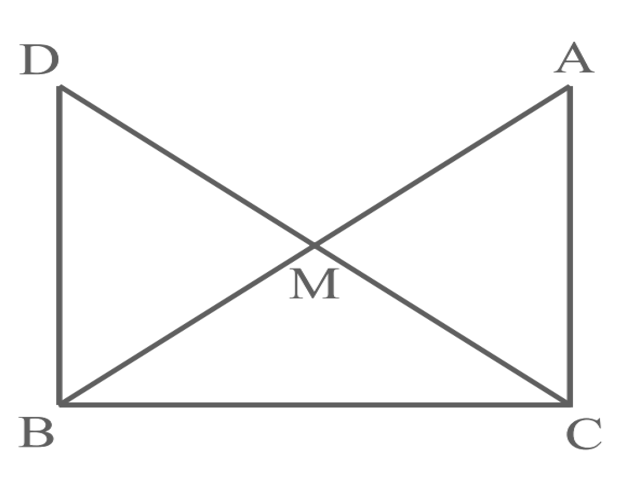
\includegraphics[width=\columnwidth]{figs/Screenshot.png}
  \caption{$\triangle \vec{ACB} ,\triangle \vec{DCB}$ with Mid-Point $\vec{M}$}
  \label{fig:triangles}
\end{figure}
\begin{enumerate}[label =(\roman*)]
        \item $\triangle \vec{AMC} \cong \triangle \vec{BMD}$
        \item $\angle \vec{DBC}$ is a right angle. 
        \item $\triangle \vec{DBC} \cong  \triangle \vec{ACB}$ 
        \item $\vec{CM} = \frac{1}{2} \vec{AB}$
\end{enumerate}
\pagebreak
\solution\\
\textbf{CONSTRUCTION STEPS :}
\begin{enumerate}
\item Let us Assume , the input parameters as ;
\begin{table}[H]
\centering
        \input{tables/input_params.tex}
          \caption{Input Parameters}
          \label{Table-1:Input_params}
\end{table}
\item the output can be calculated as ;
\begin{table}[H]
\centering
        \input{tables/output_params.tex}
          \caption{Output Parameters}
          \label{Table-2:Output_params}
\end{table}
                $\therefore$ By, Plotting these points we get the required Image \figref{fig:fig-2}
\begin{figure}[H]
        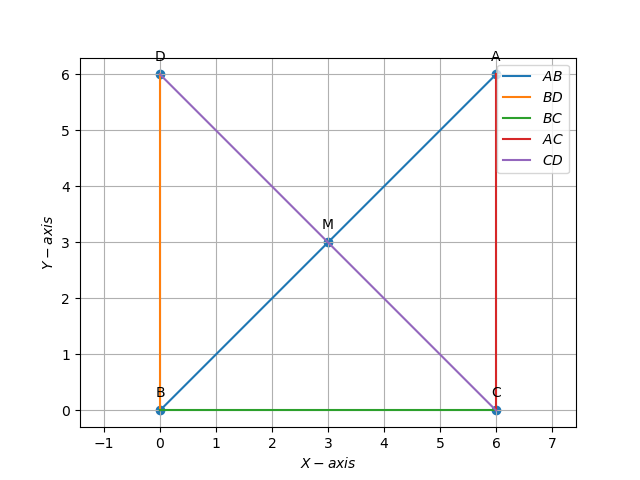
\includegraphics[width = \columnwidth]{figs/python_plot.png}
    \caption{PYTHON Plot of $\triangle \vec{ACB} ,\triangle \vec{DBC}$ with Mid-Point $\vec{M}$}
    \label{fig:fig-2}
\end{figure}
\end{enumerate}

\item Find the position vector of a point $\vec{R}$ which divides the line joining two points $\vec{P}$ and $\vec{Q}$ whose position vectors are $2\vec{a}+\vec{b}$ and $\vec{a}-3\vec{b}$ externally in the ratio $1:2$.

\textbf{Solution:}
Let us assume $\vec{a}$ and $\vec{b}$, and the given ratio is
\begin{table}[h]
    \centering
    \begin{tabular}{|c|c|c|}
        \hline 
        \textbf{Symbol} & \textbf{Value} & \textbf{Description} \\
        \hline
        $\vec{a}$ & $\myvec{1 \\ -3}$ & Vector $\vec{a}$ \\
        \hline
        $\vec{b}$ & $\myvec{0 \\ 2}$ & Vector $\vec{b}$\\
        \hline
        $k$ & $2$ & Ratio \\
        \hline
    \end{tabular}
    \caption{Vectors $\vec{a}$ and $\vec{b}$, ratio $k$}
    \label{tab:table1}
\end{table}

Using the section formula,
\begin{align}
    \vec{R} = \frac{\vec{Q} - k\vec{P}}{1 - k}
\end{align}
where $\vec{P}$ and $\vec{Q}$ depend on $\vec{a}$ and $\vec{b}$, then
\begin{align}
    \vec{P} &= (2\vec{a} + \vec{b}) = 2\myvec{1\\-3} + \myvec{0\\2} = \myvec{2\\-4} \\
    \vec{Q} &= (\vec{a} - 3\vec{b}) = \myvec{1\\-3} - 3\myvec{0\\2} = \myvec{1\\-9}
\end{align}
where $\vec{R}$ can be calculated as 
\begin{align}
    \vec{R} = \frac{(\vec{a} - 3\vec{b}) - k(2\vec{a} + \vec{b})}{1 - k}
\end{align}
By substituting $\vec{a}$ and $\vec{b}$ values, we get $\vec{R}$ as
\begin{align}
    \vec{R} = \myvec{3\\1}
\end{align}

\begin{table}[ht!]
    \centering
    \begin{tabular}{|c|c|c|}
        \hline
        \textbf{Symbol} & \textbf{Value} & \textbf{Description}\\
        \hline
        $\vec{P}$ & $(2\vec{a} + \vec{b})$ & Position vector $\vec{P}$ \\
        \hline
        $\vec{Q}$ & $(\vec{a} - 3\vec{b})$ & Position vector $\vec{Q}$\\
        \hline
        $\vec{R}$ & $\frac{\vec{Q} - k\vec{P}}{1 - k}$ & Position vector $\vec{R}$\\
        \hline
    \end{tabular}
    \caption{Vectors $\vec{P}$, $\vec{Q}$, $\vec{R}$}
    \label{tab:mytable2}   
\end{table}

\begin{figure}[H]
    \centering
    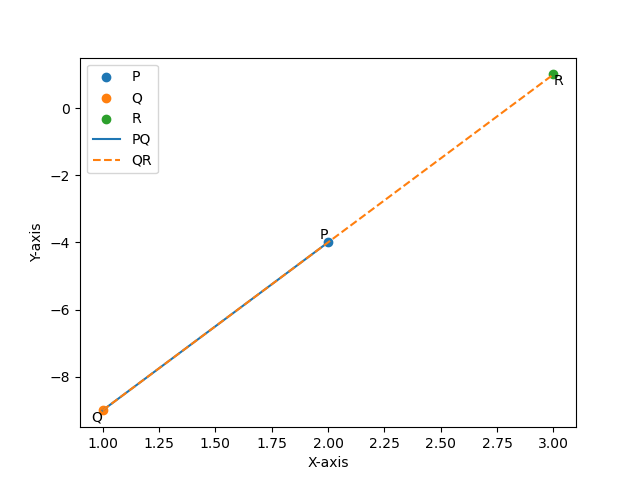
\includegraphics[width=\columnwidth]{figs/external-bisector.png}
    \caption{Point vectors $\vec{P}$, $\vec{Q}$, $\vec{R}$}
    \label{fig:enter-label}
\end{figure}


\end{enumerate}

    \item Draw a quadrilateral in the Cartesian plane, whose vertices are 
    \begin{align}
        \vec{A} = \myvec{-4\\5} \quad \vec{B} = \myvec{0\\7} \\
        \vec{C} = \myvec{5\\-5} \quad \vec{D} = \myvec{-4\\-2}
    \end{align}
    Also, find its area.
\label{chapters/11/10/1/1}
   \\ 
    \solution 
\begin{enumerate}[label=\thesection.\arabic*,ref=\thesection.\theenumi]
		\item Find $\abs{\overrightarrow{a}\times\overrightarrow{b}},\text{ if }\overrightarrow{a}=\hat{i}-7\hat{j}+7\hat{k}\text{ and } \overrightarrow{b}=3\hat{i}-2\hat{j}+2\hat{k}$.
	\\
		\solution
		\input{chapters/12/10/4/1/cross.tex}
\item Show that $$(\overrightarrow{a}-\overrightarrow{b})\times (\overrightarrow{a}+\overrightarrow{b})=2(\overrightarrow{a}\times \overrightarrow{b})$$
	\\
		\solution
		\input{chapters/12/10/4/4/cross.tex}
\item Find $\lambda$ and $\mu$ if $(2\hat{i}+6\hat{j}+27\hat{k})\times(\hat{i}+\lambda \hat{j} + \mu \hat{k})=\overrightarrow{0}$.
	\\
		\solution
		\input{chapters/12/10/4/5/cross.tex}
\item Given that $\overrightarrow{a} \cdot \overrightarrow{b} = 0$ and $\overrightarrow{a} \times \overrightarrow{b} = \overrightarrow{0}$. What can you conclude about the vectors $\overrightarrow{a} \text{ and }\overrightarrow{b}$?
\item Let the vectors be given as $\overrightarrow{a},\overrightarrow{b},\overrightarrow{c}\text{ be given as }\ a_1 \hat{i}+\ a_2 \hat{j}+\ a_3 \hat{k},\ b_1 \hat{i}+\ b_2 \hat{j}+\ b_3 \hat{k},\ c_1 \hat{i}+\ c_2 \hat{j}+\ c_3 \hat{k}$. Then show that $\overrightarrow{a} \times (\overrightarrow{b} + \overrightarrow{c}) = \overrightarrow{a} \times \overrightarrow{b}+\overrightarrow{a} \times \overrightarrow{c}$.
	\\
		\solution
		\input{chapters/12/10/4/7/cross.tex}
\item If either $\overrightarrow{a} = \overrightarrow{0}$ or $\overrightarrow{b} = \overrightarrow{0}$, then $\overrightarrow{a} \times \overrightarrow{b} = \overrightarrow{0}$. Is the converse true? Justify your answer with an example.
	\\
		\solution
		\input{chapters/12/10/4/8/cross.tex}
\item Find the area of the triangle with vertices $A(1, 1, 2)$, $B(2, 3, 5)$, and $C(1, 5, 5)$
	\\
		\solution
		\input{chapters/12/10/4/9/cross.tex}
\item Find the area of the parallelogram whose adjacent sides are determined by the vectors $\overrightarrow{a}=\hat{i}-\hat{j}+3\hat{k}$ and $\overrightarrow{b}=2\hat{i}-7\hat{j}+\hat{k}$.
	\\
		\solution
		\input{chapters/12/10/4/10/cross.tex}
\item Let the vectors $\overrightarrow{a}$ and $\overrightarrow{b}$ be such that $|\overrightarrow{a}| = 3$ and $|\overrightarrow{b}| = \dfrac{\sqrt{2}}{3}$, then $\overrightarrow{a} \times \overrightarrow{b}$ is a unit vector, if the angle between $\overrightarrow{a}$ and $\overrightarrow{b}$ is
\begin{enumerate}
\item $\dfrac{\pi}{6}$
\item $\dfrac{\pi}{4}$
\item $\dfrac{\pi}{3}$
\item $\dfrac{\pi}{2}$
\end{enumerate}
		\solution
		\input{chapters/12/10/4/11/cross.tex}
\item Area of a rectangle having vertices A, B, C and D with position vectors $ -\hat{i}+ \dfrac{1}{2} \hat{j}+4\hat{k},\hat{i}+ \dfrac{1}{2} \hat{j}+4\hat{k},\hat{i}-\dfrac{1}{2} \hat{j}+4\hat{k}\text{ and }-\hat{i}- \dfrac{1}{2} \hat{j}+4\hat{k}$, respectively is
\begin{enumerate}
\item $\dfrac{1}{2}$
\item 1
\item 2
\item 4
\end{enumerate}
		\solution
		\input{chapters/12/10/4/12/cross.tex}
\item Find the area of the triangle whose vertices are 
\begin{enumerate}
\item $(2, 3), (–1, 0), (2, – 4)$
\item $(–5, –1), (3, –5), (5, 2)$ 
\end{enumerate}
		\label{10/7/3/1}
\solution
		\input{chapters/10/7/3/1/area.tex}
\item Find the area of the triangle formed by joining the mid-points of the sides of the triangle whose vertices are $(0, –1), (2, 1) \text{ and } (0, 3)$. Find the ratio of this area to the area of the given triangle.
	\\
\solution
		\input{chapters/10/7/3/3/cross.tex}

\item Find the area of the quadrilateral whose vertices, taken in order, are $(– 4, – 2), (– 3, – 5), (3, – 2)$  and $ (2, 3)$.
	\\
\solution
		\input{chapters/10/7/3/4/cross.tex}

\item Verify that a median of a triangle divides it into two triangles of equal areas for $\triangle ABC$ whose vertices are $\vec{A}(4, -6), \vec{B}(3, 2), \text{ and } \vec{C}(5, 2)$. 
		\label{10/7/3/5}
		\\
\solution
		\input{chapters/10/7/3/5/area.tex}

\item The two adjacent sides of a parallelogram are 
$2\hat{i}-4\hat{j}+5\hat{k}$  and  $\hat{i}-2\hat{j}-3\hat{k}$.
Find the unit vector parallel to its diagonal. Also, find its area.\\
	\solution
		\input{chapters/12/10/5/10/cross.tex}
\item The vertices of a $\triangle ABC$ are $\vec{A}(4,6), \vec{B}(1,5)$ and  $\vec{C}(7,2)$. A line is drawn to intersect sides $AB$ and $AC$ at $\vec{D}$ and $\vec{E}$ respectively, such that $\frac{AD}{AB} = \frac{AE}{AC} = \frac{1}{4}$. Calculate the area of $\triangle ADE$ and compare it with the area of the $\triangle ABC$.
\\
\solution
	\input{chapters/10/7/4/6/section.tex}
    \item Draw a quadrilateral in the Cartesian plane, whose vertices are 
    \begin{align}
        \vec{A} = \myvec{-4\\5} \quad \vec{B} = \myvec{0\\7} \\
        \vec{C} = \myvec{5\\-5} \quad \vec{D} = \myvec{-4\\-2}
    \end{align}
    Also, find its area.
\label{chapters/11/10/1/1}
   \\ 
    \solution 
\input{chapters/11/10/1/1/cross.tex}
\item Find the area of region bounded by the triangle whose
	vertices are $(1, 0), (2, 2) \text{ and } (3, 1)$. 
\item Find the area of region bounded by the triangle whose vertices
	are $(– 1, 0), (1, 3) \text{ and } (3, 2)$. 
\item Find the area of the $\triangle ABC$, coordinates of whose vertices are $\vec{A}(2, 0), \vec{B}(4, 5), \text{ and } \vec{C}(6, 3)$.


\item 
\input{chapters/vectors/exer/main.tex}
\end{enumerate}


\item Find the area of region bounded by the triangle whose
	vertices are $(1, 0), (2, 2) \text{ and } (3, 1)$. 
\item Find the area of region bounded by the triangle whose vertices
	are $(– 1, 0), (1, 3) \text{ and } (3, 2)$. 
\item Find the area of the $\triangle ABC$, coordinates of whose vertices are $\vec{A}(2, 0), \vec{B}(4, 5), \text{ and } \vec{C}(6, 3)$.


\item 
%\documentclass[12pt]{article}
%\usepackage{graphicx}
%\usepackage{graphics}
%\usepackage{refstyle}
%\usepackage{amsmath}
%\usepackage{caption}
%\usepackage{float}
%\usepackage{booktabs}
%\usepackage{array}
%\usepackage{amssymb}
%\usepackage{booktabs}
%\let\vec\mathbf
%\providecommand{\brak}[1]{\ensuremath{\left(#1\right)}}
%\graphicspath{{/storage/self/primary/Download/latexnew/fig}}                                     
$\vec{P}$ and $\vec{Q}$ are any two points lying on the sides $DC$ and $AD$ respectively of a parallelogram $ABCD$.Show that, $ar\brak{\triangle APB}=ar\brak{\triangle BQC}$.


\textbf{Figure:}
\begin{figure}[H]
    \centering
	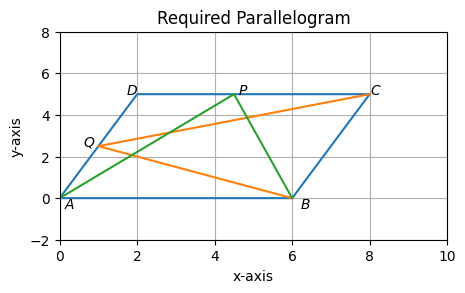
\includegraphics[width=\columnwidth]{chapters/vectors/exer/figs/1.png}
    \caption{}
    \label{fig:fig:1}
\end{figure}


\textbf{Solution:}
\begin{table}[H]
   \centering
  \input{chapters/vectors/exer/table/tab1.tex}
   \caption{Table of input parameters}        
\label{tab:tab:1}                    
\end{table}




\begin{table}[H]
    \centering                                  
\input{chapters/vectors/exer/table/tab2.tex}                  
\caption{Table of output parameters}
\label{tab:tab:2}
 \end{table}


For the $\triangle BQC$, the vertices of the triangle are taken from \tabref{tab:tab:1} and \tabref{tab:tab:2}.

\begin{align}
\implies ar\brak{\triangle BQC}&=
\frac{1}{2}\begin{tabular}{|c c c|}            
1 &1&1\\                      
$\vec{B}$&$\vec{Q}$&$\vec{C}$\\    
\end{tabular}\\
&= \frac{1}{2}\begin{tabular}{|c c c|}
       1 &1&1\\
       6&$\frac{2k_1}{k_1+1}$&8 \\
       0&$\frac{5k_1}{k_1+1}$&5
   \end{tabular}\\
  \xrightarrow{C_2'=C_2-C_1,C_3'=C_3-C_1}&\frac{1}{2} \begin{tabular}{|c c c|}
       1 &0&0\\
       6&$\frac{-4k_1-6}{k_1+1}$&2 \\
       0&$\frac{5k_1}{k_1+1}$&5
   \end{tabular}\\
&=\frac{1}{2}\brak{1\begin{tabular}{|c c|}
   $\frac{-4k_1-6}{k_1+1}$ &2  \\
   $\frac{5k_1}{k_1+1}$ & 5
\end{tabular} +0+0}\\
&=\frac{1}{2} \times30\\                          
&=15 \end{align}


For the $\triangle APB$, the vertices of the triangle are taken from \tabref{tab:tab:1} and \tabref{tab:tab:2}.
   \begin{align}
  \implies ar\brak{\triangle APB} &=
\frac{1}{2}\begin{tabular}{|c c c|}            
1 &1&1\\                            
$\vec{A}$&$\vec{P}$&$\vec{B}$\\
\end{tabular}\\ &=  \frac{1}{2}
   \begin{tabular}{|c c c|}
       1 &1&1\\
       0&$\frac{8k_2+2}{k_2+1}$&6 \\
       0&5&0
   \end{tabular}\\
 &=\frac{1}{2} \times30\\
 &=15 \end{align}
 \brak{6} = \brak{10}


So, ar\brak{\triangle BQC} = ar\brak{\triangle APB}.\brak{proved}
%\end{document}



\end{enumerate}


\item If either $\overrightarrow{a} = \overrightarrow{0}$ or $\overrightarrow{b} = \overrightarrow{0}$, then $\overrightarrow{a} \times \overrightarrow{b} = \overrightarrow{0}$. Is the converse true? Justify your answer with an example.
	\\
		\solution
		\begin{enumerate}[label=\thesection.\arabic*,ref=\thesection.\theenumi]
		\item Find $\abs{\overrightarrow{a}\times\overrightarrow{b}},\text{ if }\overrightarrow{a}=\hat{i}-7\hat{j}+7\hat{k}\text{ and } \overrightarrow{b}=3\hat{i}-2\hat{j}+2\hat{k}$.
	\\
		\solution
		\begin{enumerate}[label=\thesection.\arabic*,ref=\thesection.\theenumi]
		\item Find $\abs{\overrightarrow{a}\times\overrightarrow{b}},\text{ if }\overrightarrow{a}=\hat{i}-7\hat{j}+7\hat{k}\text{ and } \overrightarrow{b}=3\hat{i}-2\hat{j}+2\hat{k}$.
	\\
		\solution
		\input{chapters/12/10/4/1/cross.tex}
\item Show that $$(\overrightarrow{a}-\overrightarrow{b})\times (\overrightarrow{a}+\overrightarrow{b})=2(\overrightarrow{a}\times \overrightarrow{b})$$
	\\
		\solution
		\input{chapters/12/10/4/4/cross.tex}
\item Find $\lambda$ and $\mu$ if $(2\hat{i}+6\hat{j}+27\hat{k})\times(\hat{i}+\lambda \hat{j} + \mu \hat{k})=\overrightarrow{0}$.
	\\
		\solution
		\input{chapters/12/10/4/5/cross.tex}
\item Given that $\overrightarrow{a} \cdot \overrightarrow{b} = 0$ and $\overrightarrow{a} \times \overrightarrow{b} = \overrightarrow{0}$. What can you conclude about the vectors $\overrightarrow{a} \text{ and }\overrightarrow{b}$?
\item Let the vectors be given as $\overrightarrow{a},\overrightarrow{b},\overrightarrow{c}\text{ be given as }\ a_1 \hat{i}+\ a_2 \hat{j}+\ a_3 \hat{k},\ b_1 \hat{i}+\ b_2 \hat{j}+\ b_3 \hat{k},\ c_1 \hat{i}+\ c_2 \hat{j}+\ c_3 \hat{k}$. Then show that $\overrightarrow{a} \times (\overrightarrow{b} + \overrightarrow{c}) = \overrightarrow{a} \times \overrightarrow{b}+\overrightarrow{a} \times \overrightarrow{c}$.
	\\
		\solution
		\input{chapters/12/10/4/7/cross.tex}
\item If either $\overrightarrow{a} = \overrightarrow{0}$ or $\overrightarrow{b} = \overrightarrow{0}$, then $\overrightarrow{a} \times \overrightarrow{b} = \overrightarrow{0}$. Is the converse true? Justify your answer with an example.
	\\
		\solution
		\input{chapters/12/10/4/8/cross.tex}
\item Find the area of the triangle with vertices $A(1, 1, 2)$, $B(2, 3, 5)$, and $C(1, 5, 5)$
	\\
		\solution
		\input{chapters/12/10/4/9/cross.tex}
\item Find the area of the parallelogram whose adjacent sides are determined by the vectors $\overrightarrow{a}=\hat{i}-\hat{j}+3\hat{k}$ and $\overrightarrow{b}=2\hat{i}-7\hat{j}+\hat{k}$.
	\\
		\solution
		\input{chapters/12/10/4/10/cross.tex}
\item Let the vectors $\overrightarrow{a}$ and $\overrightarrow{b}$ be such that $|\overrightarrow{a}| = 3$ and $|\overrightarrow{b}| = \dfrac{\sqrt{2}}{3}$, then $\overrightarrow{a} \times \overrightarrow{b}$ is a unit vector, if the angle between $\overrightarrow{a}$ and $\overrightarrow{b}$ is
\begin{enumerate}
\item $\dfrac{\pi}{6}$
\item $\dfrac{\pi}{4}$
\item $\dfrac{\pi}{3}$
\item $\dfrac{\pi}{2}$
\end{enumerate}
		\solution
		\input{chapters/12/10/4/11/cross.tex}
\item Area of a rectangle having vertices A, B, C and D with position vectors $ -\hat{i}+ \dfrac{1}{2} \hat{j}+4\hat{k},\hat{i}+ \dfrac{1}{2} \hat{j}+4\hat{k},\hat{i}-\dfrac{1}{2} \hat{j}+4\hat{k}\text{ and }-\hat{i}- \dfrac{1}{2} \hat{j}+4\hat{k}$, respectively is
\begin{enumerate}
\item $\dfrac{1}{2}$
\item 1
\item 2
\item 4
\end{enumerate}
		\solution
		\input{chapters/12/10/4/12/cross.tex}
\item Find the area of the triangle whose vertices are 
\begin{enumerate}
\item $(2, 3), (–1, 0), (2, – 4)$
\item $(–5, –1), (3, –5), (5, 2)$ 
\end{enumerate}
		\label{10/7/3/1}
\solution
		\input{chapters/10/7/3/1/area.tex}
\item Find the area of the triangle formed by joining the mid-points of the sides of the triangle whose vertices are $(0, –1), (2, 1) \text{ and } (0, 3)$. Find the ratio of this area to the area of the given triangle.
	\\
\solution
		\input{chapters/10/7/3/3/cross.tex}

\item Find the area of the quadrilateral whose vertices, taken in order, are $(– 4, – 2), (– 3, – 5), (3, – 2)$  and $ (2, 3)$.
	\\
\solution
		\input{chapters/10/7/3/4/cross.tex}

\item Verify that a median of a triangle divides it into two triangles of equal areas for $\triangle ABC$ whose vertices are $\vec{A}(4, -6), \vec{B}(3, 2), \text{ and } \vec{C}(5, 2)$. 
		\label{10/7/3/5}
		\\
\solution
		\input{chapters/10/7/3/5/area.tex}

\item The two adjacent sides of a parallelogram are 
$2\hat{i}-4\hat{j}+5\hat{k}$  and  $\hat{i}-2\hat{j}-3\hat{k}$.
Find the unit vector parallel to its diagonal. Also, find its area.\\
	\solution
		\input{chapters/12/10/5/10/cross.tex}
\item The vertices of a $\triangle ABC$ are $\vec{A}(4,6), \vec{B}(1,5)$ and  $\vec{C}(7,2)$. A line is drawn to intersect sides $AB$ and $AC$ at $\vec{D}$ and $\vec{E}$ respectively, such that $\frac{AD}{AB} = \frac{AE}{AC} = \frac{1}{4}$. Calculate the area of $\triangle ADE$ and compare it with the area of the $\triangle ABC$.
\\
\solution
	\input{chapters/10/7/4/6/section.tex}
    \item Draw a quadrilateral in the Cartesian plane, whose vertices are 
    \begin{align}
        \vec{A} = \myvec{-4\\5} \quad \vec{B} = \myvec{0\\7} \\
        \vec{C} = \myvec{5\\-5} \quad \vec{D} = \myvec{-4\\-2}
    \end{align}
    Also, find its area.
\label{chapters/11/10/1/1}
   \\ 
    \solution 
\input{chapters/11/10/1/1/cross.tex}
\item Find the area of region bounded by the triangle whose
	vertices are $(1, 0), (2, 2) \text{ and } (3, 1)$. 
\item Find the area of region bounded by the triangle whose vertices
	are $(– 1, 0), (1, 3) \text{ and } (3, 2)$. 
\item Find the area of the $\triangle ABC$, coordinates of whose vertices are $\vec{A}(2, 0), \vec{B}(4, 5), \text{ and } \vec{C}(6, 3)$.


\item 
\input{chapters/vectors/exer/main.tex}
\end{enumerate}


\item Show that $$(\overrightarrow{a}-\overrightarrow{b})\times (\overrightarrow{a}+\overrightarrow{b})=2(\overrightarrow{a}\times \overrightarrow{b})$$
	\\
		\solution
		\begin{enumerate}[label=\thesection.\arabic*,ref=\thesection.\theenumi]
		\item Find $\abs{\overrightarrow{a}\times\overrightarrow{b}},\text{ if }\overrightarrow{a}=\hat{i}-7\hat{j}+7\hat{k}\text{ and } \overrightarrow{b}=3\hat{i}-2\hat{j}+2\hat{k}$.
	\\
		\solution
		\input{chapters/12/10/4/1/cross.tex}
\item Show that $$(\overrightarrow{a}-\overrightarrow{b})\times (\overrightarrow{a}+\overrightarrow{b})=2(\overrightarrow{a}\times \overrightarrow{b})$$
	\\
		\solution
		\input{chapters/12/10/4/4/cross.tex}
\item Find $\lambda$ and $\mu$ if $(2\hat{i}+6\hat{j}+27\hat{k})\times(\hat{i}+\lambda \hat{j} + \mu \hat{k})=\overrightarrow{0}$.
	\\
		\solution
		\input{chapters/12/10/4/5/cross.tex}
\item Given that $\overrightarrow{a} \cdot \overrightarrow{b} = 0$ and $\overrightarrow{a} \times \overrightarrow{b} = \overrightarrow{0}$. What can you conclude about the vectors $\overrightarrow{a} \text{ and }\overrightarrow{b}$?
\item Let the vectors be given as $\overrightarrow{a},\overrightarrow{b},\overrightarrow{c}\text{ be given as }\ a_1 \hat{i}+\ a_2 \hat{j}+\ a_3 \hat{k},\ b_1 \hat{i}+\ b_2 \hat{j}+\ b_3 \hat{k},\ c_1 \hat{i}+\ c_2 \hat{j}+\ c_3 \hat{k}$. Then show that $\overrightarrow{a} \times (\overrightarrow{b} + \overrightarrow{c}) = \overrightarrow{a} \times \overrightarrow{b}+\overrightarrow{a} \times \overrightarrow{c}$.
	\\
		\solution
		\input{chapters/12/10/4/7/cross.tex}
\item If either $\overrightarrow{a} = \overrightarrow{0}$ or $\overrightarrow{b} = \overrightarrow{0}$, then $\overrightarrow{a} \times \overrightarrow{b} = \overrightarrow{0}$. Is the converse true? Justify your answer with an example.
	\\
		\solution
		\input{chapters/12/10/4/8/cross.tex}
\item Find the area of the triangle with vertices $A(1, 1, 2)$, $B(2, 3, 5)$, and $C(1, 5, 5)$
	\\
		\solution
		\input{chapters/12/10/4/9/cross.tex}
\item Find the area of the parallelogram whose adjacent sides are determined by the vectors $\overrightarrow{a}=\hat{i}-\hat{j}+3\hat{k}$ and $\overrightarrow{b}=2\hat{i}-7\hat{j}+\hat{k}$.
	\\
		\solution
		\input{chapters/12/10/4/10/cross.tex}
\item Let the vectors $\overrightarrow{a}$ and $\overrightarrow{b}$ be such that $|\overrightarrow{a}| = 3$ and $|\overrightarrow{b}| = \dfrac{\sqrt{2}}{3}$, then $\overrightarrow{a} \times \overrightarrow{b}$ is a unit vector, if the angle between $\overrightarrow{a}$ and $\overrightarrow{b}$ is
\begin{enumerate}
\item $\dfrac{\pi}{6}$
\item $\dfrac{\pi}{4}$
\item $\dfrac{\pi}{3}$
\item $\dfrac{\pi}{2}$
\end{enumerate}
		\solution
		\input{chapters/12/10/4/11/cross.tex}
\item Area of a rectangle having vertices A, B, C and D with position vectors $ -\hat{i}+ \dfrac{1}{2} \hat{j}+4\hat{k},\hat{i}+ \dfrac{1}{2} \hat{j}+4\hat{k},\hat{i}-\dfrac{1}{2} \hat{j}+4\hat{k}\text{ and }-\hat{i}- \dfrac{1}{2} \hat{j}+4\hat{k}$, respectively is
\begin{enumerate}
\item $\dfrac{1}{2}$
\item 1
\item 2
\item 4
\end{enumerate}
		\solution
		\input{chapters/12/10/4/12/cross.tex}
\item Find the area of the triangle whose vertices are 
\begin{enumerate}
\item $(2, 3), (–1, 0), (2, – 4)$
\item $(–5, –1), (3, –5), (5, 2)$ 
\end{enumerate}
		\label{10/7/3/1}
\solution
		\input{chapters/10/7/3/1/area.tex}
\item Find the area of the triangle formed by joining the mid-points of the sides of the triangle whose vertices are $(0, –1), (2, 1) \text{ and } (0, 3)$. Find the ratio of this area to the area of the given triangle.
	\\
\solution
		\input{chapters/10/7/3/3/cross.tex}

\item Find the area of the quadrilateral whose vertices, taken in order, are $(– 4, – 2), (– 3, – 5), (3, – 2)$  and $ (2, 3)$.
	\\
\solution
		\input{chapters/10/7/3/4/cross.tex}

\item Verify that a median of a triangle divides it into two triangles of equal areas for $\triangle ABC$ whose vertices are $\vec{A}(4, -6), \vec{B}(3, 2), \text{ and } \vec{C}(5, 2)$. 
		\label{10/7/3/5}
		\\
\solution
		\input{chapters/10/7/3/5/area.tex}

\item The two adjacent sides of a parallelogram are 
$2\hat{i}-4\hat{j}+5\hat{k}$  and  $\hat{i}-2\hat{j}-3\hat{k}$.
Find the unit vector parallel to its diagonal. Also, find its area.\\
	\solution
		\input{chapters/12/10/5/10/cross.tex}
\item The vertices of a $\triangle ABC$ are $\vec{A}(4,6), \vec{B}(1,5)$ and  $\vec{C}(7,2)$. A line is drawn to intersect sides $AB$ and $AC$ at $\vec{D}$ and $\vec{E}$ respectively, such that $\frac{AD}{AB} = \frac{AE}{AC} = \frac{1}{4}$. Calculate the area of $\triangle ADE$ and compare it with the area of the $\triangle ABC$.
\\
\solution
	\input{chapters/10/7/4/6/section.tex}
    \item Draw a quadrilateral in the Cartesian plane, whose vertices are 
    \begin{align}
        \vec{A} = \myvec{-4\\5} \quad \vec{B} = \myvec{0\\7} \\
        \vec{C} = \myvec{5\\-5} \quad \vec{D} = \myvec{-4\\-2}
    \end{align}
    Also, find its area.
\label{chapters/11/10/1/1}
   \\ 
    \solution 
\input{chapters/11/10/1/1/cross.tex}
\item Find the area of region bounded by the triangle whose
	vertices are $(1, 0), (2, 2) \text{ and } (3, 1)$. 
\item Find the area of region bounded by the triangle whose vertices
	are $(– 1, 0), (1, 3) \text{ and } (3, 2)$. 
\item Find the area of the $\triangle ABC$, coordinates of whose vertices are $\vec{A}(2, 0), \vec{B}(4, 5), \text{ and } \vec{C}(6, 3)$.


\item 
\input{chapters/vectors/exer/main.tex}
\end{enumerate}


\item Find $\lambda$ and $\mu$ if $(2\hat{i}+6\hat{j}+27\hat{k})\times(\hat{i}+\lambda \hat{j} + \mu \hat{k})=\overrightarrow{0}$.
	\\
		\solution
		\begin{enumerate}[label=\thesection.\arabic*,ref=\thesection.\theenumi]
		\item Find $\abs{\overrightarrow{a}\times\overrightarrow{b}},\text{ if }\overrightarrow{a}=\hat{i}-7\hat{j}+7\hat{k}\text{ and } \overrightarrow{b}=3\hat{i}-2\hat{j}+2\hat{k}$.
	\\
		\solution
		\input{chapters/12/10/4/1/cross.tex}
\item Show that $$(\overrightarrow{a}-\overrightarrow{b})\times (\overrightarrow{a}+\overrightarrow{b})=2(\overrightarrow{a}\times \overrightarrow{b})$$
	\\
		\solution
		\input{chapters/12/10/4/4/cross.tex}
\item Find $\lambda$ and $\mu$ if $(2\hat{i}+6\hat{j}+27\hat{k})\times(\hat{i}+\lambda \hat{j} + \mu \hat{k})=\overrightarrow{0}$.
	\\
		\solution
		\input{chapters/12/10/4/5/cross.tex}
\item Given that $\overrightarrow{a} \cdot \overrightarrow{b} = 0$ and $\overrightarrow{a} \times \overrightarrow{b} = \overrightarrow{0}$. What can you conclude about the vectors $\overrightarrow{a} \text{ and }\overrightarrow{b}$?
\item Let the vectors be given as $\overrightarrow{a},\overrightarrow{b},\overrightarrow{c}\text{ be given as }\ a_1 \hat{i}+\ a_2 \hat{j}+\ a_3 \hat{k},\ b_1 \hat{i}+\ b_2 \hat{j}+\ b_3 \hat{k},\ c_1 \hat{i}+\ c_2 \hat{j}+\ c_3 \hat{k}$. Then show that $\overrightarrow{a} \times (\overrightarrow{b} + \overrightarrow{c}) = \overrightarrow{a} \times \overrightarrow{b}+\overrightarrow{a} \times \overrightarrow{c}$.
	\\
		\solution
		\input{chapters/12/10/4/7/cross.tex}
\item If either $\overrightarrow{a} = \overrightarrow{0}$ or $\overrightarrow{b} = \overrightarrow{0}$, then $\overrightarrow{a} \times \overrightarrow{b} = \overrightarrow{0}$. Is the converse true? Justify your answer with an example.
	\\
		\solution
		\input{chapters/12/10/4/8/cross.tex}
\item Find the area of the triangle with vertices $A(1, 1, 2)$, $B(2, 3, 5)$, and $C(1, 5, 5)$
	\\
		\solution
		\input{chapters/12/10/4/9/cross.tex}
\item Find the area of the parallelogram whose adjacent sides are determined by the vectors $\overrightarrow{a}=\hat{i}-\hat{j}+3\hat{k}$ and $\overrightarrow{b}=2\hat{i}-7\hat{j}+\hat{k}$.
	\\
		\solution
		\input{chapters/12/10/4/10/cross.tex}
\item Let the vectors $\overrightarrow{a}$ and $\overrightarrow{b}$ be such that $|\overrightarrow{a}| = 3$ and $|\overrightarrow{b}| = \dfrac{\sqrt{2}}{3}$, then $\overrightarrow{a} \times \overrightarrow{b}$ is a unit vector, if the angle between $\overrightarrow{a}$ and $\overrightarrow{b}$ is
\begin{enumerate}
\item $\dfrac{\pi}{6}$
\item $\dfrac{\pi}{4}$
\item $\dfrac{\pi}{3}$
\item $\dfrac{\pi}{2}$
\end{enumerate}
		\solution
		\input{chapters/12/10/4/11/cross.tex}
\item Area of a rectangle having vertices A, B, C and D with position vectors $ -\hat{i}+ \dfrac{1}{2} \hat{j}+4\hat{k},\hat{i}+ \dfrac{1}{2} \hat{j}+4\hat{k},\hat{i}-\dfrac{1}{2} \hat{j}+4\hat{k}\text{ and }-\hat{i}- \dfrac{1}{2} \hat{j}+4\hat{k}$, respectively is
\begin{enumerate}
\item $\dfrac{1}{2}$
\item 1
\item 2
\item 4
\end{enumerate}
		\solution
		\input{chapters/12/10/4/12/cross.tex}
\item Find the area of the triangle whose vertices are 
\begin{enumerate}
\item $(2, 3), (–1, 0), (2, – 4)$
\item $(–5, –1), (3, –5), (5, 2)$ 
\end{enumerate}
		\label{10/7/3/1}
\solution
		\input{chapters/10/7/3/1/area.tex}
\item Find the area of the triangle formed by joining the mid-points of the sides of the triangle whose vertices are $(0, –1), (2, 1) \text{ and } (0, 3)$. Find the ratio of this area to the area of the given triangle.
	\\
\solution
		\input{chapters/10/7/3/3/cross.tex}

\item Find the area of the quadrilateral whose vertices, taken in order, are $(– 4, – 2), (– 3, – 5), (3, – 2)$  and $ (2, 3)$.
	\\
\solution
		\input{chapters/10/7/3/4/cross.tex}

\item Verify that a median of a triangle divides it into two triangles of equal areas for $\triangle ABC$ whose vertices are $\vec{A}(4, -6), \vec{B}(3, 2), \text{ and } \vec{C}(5, 2)$. 
		\label{10/7/3/5}
		\\
\solution
		\input{chapters/10/7/3/5/area.tex}

\item The two adjacent sides of a parallelogram are 
$2\hat{i}-4\hat{j}+5\hat{k}$  and  $\hat{i}-2\hat{j}-3\hat{k}$.
Find the unit vector parallel to its diagonal. Also, find its area.\\
	\solution
		\input{chapters/12/10/5/10/cross.tex}
\item The vertices of a $\triangle ABC$ are $\vec{A}(4,6), \vec{B}(1,5)$ and  $\vec{C}(7,2)$. A line is drawn to intersect sides $AB$ and $AC$ at $\vec{D}$ and $\vec{E}$ respectively, such that $\frac{AD}{AB} = \frac{AE}{AC} = \frac{1}{4}$. Calculate the area of $\triangle ADE$ and compare it with the area of the $\triangle ABC$.
\\
\solution
	\input{chapters/10/7/4/6/section.tex}
    \item Draw a quadrilateral in the Cartesian plane, whose vertices are 
    \begin{align}
        \vec{A} = \myvec{-4\\5} \quad \vec{B} = \myvec{0\\7} \\
        \vec{C} = \myvec{5\\-5} \quad \vec{D} = \myvec{-4\\-2}
    \end{align}
    Also, find its area.
\label{chapters/11/10/1/1}
   \\ 
    \solution 
\input{chapters/11/10/1/1/cross.tex}
\item Find the area of region bounded by the triangle whose
	vertices are $(1, 0), (2, 2) \text{ and } (3, 1)$. 
\item Find the area of region bounded by the triangle whose vertices
	are $(– 1, 0), (1, 3) \text{ and } (3, 2)$. 
\item Find the area of the $\triangle ABC$, coordinates of whose vertices are $\vec{A}(2, 0), \vec{B}(4, 5), \text{ and } \vec{C}(6, 3)$.


\item 
\input{chapters/vectors/exer/main.tex}
\end{enumerate}


\item Given that $\overrightarrow{a} \cdot \overrightarrow{b} = 0$ and $\overrightarrow{a} \times \overrightarrow{b} = \overrightarrow{0}$. What can you conclude about the vectors $\overrightarrow{a} \text{ and }\overrightarrow{b}$?
\item Let the vectors be given as $\overrightarrow{a},\overrightarrow{b},\overrightarrow{c}\text{ be given as }\ a_1 \hat{i}+\ a_2 \hat{j}+\ a_3 \hat{k},\ b_1 \hat{i}+\ b_2 \hat{j}+\ b_3 \hat{k},\ c_1 \hat{i}+\ c_2 \hat{j}+\ c_3 \hat{k}$. Then show that $\overrightarrow{a} \times (\overrightarrow{b} + \overrightarrow{c}) = \overrightarrow{a} \times \overrightarrow{b}+\overrightarrow{a} \times \overrightarrow{c}$.
	\\
		\solution
		\begin{enumerate}[label=\thesection.\arabic*,ref=\thesection.\theenumi]
		\item Find $\abs{\overrightarrow{a}\times\overrightarrow{b}},\text{ if }\overrightarrow{a}=\hat{i}-7\hat{j}+7\hat{k}\text{ and } \overrightarrow{b}=3\hat{i}-2\hat{j}+2\hat{k}$.
	\\
		\solution
		\input{chapters/12/10/4/1/cross.tex}
\item Show that $$(\overrightarrow{a}-\overrightarrow{b})\times (\overrightarrow{a}+\overrightarrow{b})=2(\overrightarrow{a}\times \overrightarrow{b})$$
	\\
		\solution
		\input{chapters/12/10/4/4/cross.tex}
\item Find $\lambda$ and $\mu$ if $(2\hat{i}+6\hat{j}+27\hat{k})\times(\hat{i}+\lambda \hat{j} + \mu \hat{k})=\overrightarrow{0}$.
	\\
		\solution
		\input{chapters/12/10/4/5/cross.tex}
\item Given that $\overrightarrow{a} \cdot \overrightarrow{b} = 0$ and $\overrightarrow{a} \times \overrightarrow{b} = \overrightarrow{0}$. What can you conclude about the vectors $\overrightarrow{a} \text{ and }\overrightarrow{b}$?
\item Let the vectors be given as $\overrightarrow{a},\overrightarrow{b},\overrightarrow{c}\text{ be given as }\ a_1 \hat{i}+\ a_2 \hat{j}+\ a_3 \hat{k},\ b_1 \hat{i}+\ b_2 \hat{j}+\ b_3 \hat{k},\ c_1 \hat{i}+\ c_2 \hat{j}+\ c_3 \hat{k}$. Then show that $\overrightarrow{a} \times (\overrightarrow{b} + \overrightarrow{c}) = \overrightarrow{a} \times \overrightarrow{b}+\overrightarrow{a} \times \overrightarrow{c}$.
	\\
		\solution
		\input{chapters/12/10/4/7/cross.tex}
\item If either $\overrightarrow{a} = \overrightarrow{0}$ or $\overrightarrow{b} = \overrightarrow{0}$, then $\overrightarrow{a} \times \overrightarrow{b} = \overrightarrow{0}$. Is the converse true? Justify your answer with an example.
	\\
		\solution
		\input{chapters/12/10/4/8/cross.tex}
\item Find the area of the triangle with vertices $A(1, 1, 2)$, $B(2, 3, 5)$, and $C(1, 5, 5)$
	\\
		\solution
		\input{chapters/12/10/4/9/cross.tex}
\item Find the area of the parallelogram whose adjacent sides are determined by the vectors $\overrightarrow{a}=\hat{i}-\hat{j}+3\hat{k}$ and $\overrightarrow{b}=2\hat{i}-7\hat{j}+\hat{k}$.
	\\
		\solution
		\input{chapters/12/10/4/10/cross.tex}
\item Let the vectors $\overrightarrow{a}$ and $\overrightarrow{b}$ be such that $|\overrightarrow{a}| = 3$ and $|\overrightarrow{b}| = \dfrac{\sqrt{2}}{3}$, then $\overrightarrow{a} \times \overrightarrow{b}$ is a unit vector, if the angle between $\overrightarrow{a}$ and $\overrightarrow{b}$ is
\begin{enumerate}
\item $\dfrac{\pi}{6}$
\item $\dfrac{\pi}{4}$
\item $\dfrac{\pi}{3}$
\item $\dfrac{\pi}{2}$
\end{enumerate}
		\solution
		\input{chapters/12/10/4/11/cross.tex}
\item Area of a rectangle having vertices A, B, C and D with position vectors $ -\hat{i}+ \dfrac{1}{2} \hat{j}+4\hat{k},\hat{i}+ \dfrac{1}{2} \hat{j}+4\hat{k},\hat{i}-\dfrac{1}{2} \hat{j}+4\hat{k}\text{ and }-\hat{i}- \dfrac{1}{2} \hat{j}+4\hat{k}$, respectively is
\begin{enumerate}
\item $\dfrac{1}{2}$
\item 1
\item 2
\item 4
\end{enumerate}
		\solution
		\input{chapters/12/10/4/12/cross.tex}
\item Find the area of the triangle whose vertices are 
\begin{enumerate}
\item $(2, 3), (–1, 0), (2, – 4)$
\item $(–5, –1), (3, –5), (5, 2)$ 
\end{enumerate}
		\label{10/7/3/1}
\solution
		\input{chapters/10/7/3/1/area.tex}
\item Find the area of the triangle formed by joining the mid-points of the sides of the triangle whose vertices are $(0, –1), (2, 1) \text{ and } (0, 3)$. Find the ratio of this area to the area of the given triangle.
	\\
\solution
		\input{chapters/10/7/3/3/cross.tex}

\item Find the area of the quadrilateral whose vertices, taken in order, are $(– 4, – 2), (– 3, – 5), (3, – 2)$  and $ (2, 3)$.
	\\
\solution
		\input{chapters/10/7/3/4/cross.tex}

\item Verify that a median of a triangle divides it into two triangles of equal areas for $\triangle ABC$ whose vertices are $\vec{A}(4, -6), \vec{B}(3, 2), \text{ and } \vec{C}(5, 2)$. 
		\label{10/7/3/5}
		\\
\solution
		\input{chapters/10/7/3/5/area.tex}

\item The two adjacent sides of a parallelogram are 
$2\hat{i}-4\hat{j}+5\hat{k}$  and  $\hat{i}-2\hat{j}-3\hat{k}$.
Find the unit vector parallel to its diagonal. Also, find its area.\\
	\solution
		\input{chapters/12/10/5/10/cross.tex}
\item The vertices of a $\triangle ABC$ are $\vec{A}(4,6), \vec{B}(1,5)$ and  $\vec{C}(7,2)$. A line is drawn to intersect sides $AB$ and $AC$ at $\vec{D}$ and $\vec{E}$ respectively, such that $\frac{AD}{AB} = \frac{AE}{AC} = \frac{1}{4}$. Calculate the area of $\triangle ADE$ and compare it with the area of the $\triangle ABC$.
\\
\solution
	\input{chapters/10/7/4/6/section.tex}
    \item Draw a quadrilateral in the Cartesian plane, whose vertices are 
    \begin{align}
        \vec{A} = \myvec{-4\\5} \quad \vec{B} = \myvec{0\\7} \\
        \vec{C} = \myvec{5\\-5} \quad \vec{D} = \myvec{-4\\-2}
    \end{align}
    Also, find its area.
\label{chapters/11/10/1/1}
   \\ 
    \solution 
\input{chapters/11/10/1/1/cross.tex}
\item Find the area of region bounded by the triangle whose
	vertices are $(1, 0), (2, 2) \text{ and } (3, 1)$. 
\item Find the area of region bounded by the triangle whose vertices
	are $(– 1, 0), (1, 3) \text{ and } (3, 2)$. 
\item Find the area of the $\triangle ABC$, coordinates of whose vertices are $\vec{A}(2, 0), \vec{B}(4, 5), \text{ and } \vec{C}(6, 3)$.


\item 
\input{chapters/vectors/exer/main.tex}
\end{enumerate}


\item If either $\overrightarrow{a} = \overrightarrow{0}$ or $\overrightarrow{b} = \overrightarrow{0}$, then $\overrightarrow{a} \times \overrightarrow{b} = \overrightarrow{0}$. Is the converse true? Justify your answer with an example.
	\\
		\solution
		\begin{enumerate}[label=\thesection.\arabic*,ref=\thesection.\theenumi]
		\item Find $\abs{\overrightarrow{a}\times\overrightarrow{b}},\text{ if }\overrightarrow{a}=\hat{i}-7\hat{j}+7\hat{k}\text{ and } \overrightarrow{b}=3\hat{i}-2\hat{j}+2\hat{k}$.
	\\
		\solution
		\input{chapters/12/10/4/1/cross.tex}
\item Show that $$(\overrightarrow{a}-\overrightarrow{b})\times (\overrightarrow{a}+\overrightarrow{b})=2(\overrightarrow{a}\times \overrightarrow{b})$$
	\\
		\solution
		\input{chapters/12/10/4/4/cross.tex}
\item Find $\lambda$ and $\mu$ if $(2\hat{i}+6\hat{j}+27\hat{k})\times(\hat{i}+\lambda \hat{j} + \mu \hat{k})=\overrightarrow{0}$.
	\\
		\solution
		\input{chapters/12/10/4/5/cross.tex}
\item Given that $\overrightarrow{a} \cdot \overrightarrow{b} = 0$ and $\overrightarrow{a} \times \overrightarrow{b} = \overrightarrow{0}$. What can you conclude about the vectors $\overrightarrow{a} \text{ and }\overrightarrow{b}$?
\item Let the vectors be given as $\overrightarrow{a},\overrightarrow{b},\overrightarrow{c}\text{ be given as }\ a_1 \hat{i}+\ a_2 \hat{j}+\ a_3 \hat{k},\ b_1 \hat{i}+\ b_2 \hat{j}+\ b_3 \hat{k},\ c_1 \hat{i}+\ c_2 \hat{j}+\ c_3 \hat{k}$. Then show that $\overrightarrow{a} \times (\overrightarrow{b} + \overrightarrow{c}) = \overrightarrow{a} \times \overrightarrow{b}+\overrightarrow{a} \times \overrightarrow{c}$.
	\\
		\solution
		\input{chapters/12/10/4/7/cross.tex}
\item If either $\overrightarrow{a} = \overrightarrow{0}$ or $\overrightarrow{b} = \overrightarrow{0}$, then $\overrightarrow{a} \times \overrightarrow{b} = \overrightarrow{0}$. Is the converse true? Justify your answer with an example.
	\\
		\solution
		\input{chapters/12/10/4/8/cross.tex}
\item Find the area of the triangle with vertices $A(1, 1, 2)$, $B(2, 3, 5)$, and $C(1, 5, 5)$
	\\
		\solution
		\input{chapters/12/10/4/9/cross.tex}
\item Find the area of the parallelogram whose adjacent sides are determined by the vectors $\overrightarrow{a}=\hat{i}-\hat{j}+3\hat{k}$ and $\overrightarrow{b}=2\hat{i}-7\hat{j}+\hat{k}$.
	\\
		\solution
		\input{chapters/12/10/4/10/cross.tex}
\item Let the vectors $\overrightarrow{a}$ and $\overrightarrow{b}$ be such that $|\overrightarrow{a}| = 3$ and $|\overrightarrow{b}| = \dfrac{\sqrt{2}}{3}$, then $\overrightarrow{a} \times \overrightarrow{b}$ is a unit vector, if the angle between $\overrightarrow{a}$ and $\overrightarrow{b}$ is
\begin{enumerate}
\item $\dfrac{\pi}{6}$
\item $\dfrac{\pi}{4}$
\item $\dfrac{\pi}{3}$
\item $\dfrac{\pi}{2}$
\end{enumerate}
		\solution
		\input{chapters/12/10/4/11/cross.tex}
\item Area of a rectangle having vertices A, B, C and D with position vectors $ -\hat{i}+ \dfrac{1}{2} \hat{j}+4\hat{k},\hat{i}+ \dfrac{1}{2} \hat{j}+4\hat{k},\hat{i}-\dfrac{1}{2} \hat{j}+4\hat{k}\text{ and }-\hat{i}- \dfrac{1}{2} \hat{j}+4\hat{k}$, respectively is
\begin{enumerate}
\item $\dfrac{1}{2}$
\item 1
\item 2
\item 4
\end{enumerate}
		\solution
		\input{chapters/12/10/4/12/cross.tex}
\item Find the area of the triangle whose vertices are 
\begin{enumerate}
\item $(2, 3), (–1, 0), (2, – 4)$
\item $(–5, –1), (3, –5), (5, 2)$ 
\end{enumerate}
		\label{10/7/3/1}
\solution
		\input{chapters/10/7/3/1/area.tex}
\item Find the area of the triangle formed by joining the mid-points of the sides of the triangle whose vertices are $(0, –1), (2, 1) \text{ and } (0, 3)$. Find the ratio of this area to the area of the given triangle.
	\\
\solution
		\input{chapters/10/7/3/3/cross.tex}

\item Find the area of the quadrilateral whose vertices, taken in order, are $(– 4, – 2), (– 3, – 5), (3, – 2)$  and $ (2, 3)$.
	\\
\solution
		\input{chapters/10/7/3/4/cross.tex}

\item Verify that a median of a triangle divides it into two triangles of equal areas for $\triangle ABC$ whose vertices are $\vec{A}(4, -6), \vec{B}(3, 2), \text{ and } \vec{C}(5, 2)$. 
		\label{10/7/3/5}
		\\
\solution
		\input{chapters/10/7/3/5/area.tex}

\item The two adjacent sides of a parallelogram are 
$2\hat{i}-4\hat{j}+5\hat{k}$  and  $\hat{i}-2\hat{j}-3\hat{k}$.
Find the unit vector parallel to its diagonal. Also, find its area.\\
	\solution
		\input{chapters/12/10/5/10/cross.tex}
\item The vertices of a $\triangle ABC$ are $\vec{A}(4,6), \vec{B}(1,5)$ and  $\vec{C}(7,2)$. A line is drawn to intersect sides $AB$ and $AC$ at $\vec{D}$ and $\vec{E}$ respectively, such that $\frac{AD}{AB} = \frac{AE}{AC} = \frac{1}{4}$. Calculate the area of $\triangle ADE$ and compare it with the area of the $\triangle ABC$.
\\
\solution
	\input{chapters/10/7/4/6/section.tex}
    \item Draw a quadrilateral in the Cartesian plane, whose vertices are 
    \begin{align}
        \vec{A} = \myvec{-4\\5} \quad \vec{B} = \myvec{0\\7} \\
        \vec{C} = \myvec{5\\-5} \quad \vec{D} = \myvec{-4\\-2}
    \end{align}
    Also, find its area.
\label{chapters/11/10/1/1}
   \\ 
    \solution 
\input{chapters/11/10/1/1/cross.tex}
\item Find the area of region bounded by the triangle whose
	vertices are $(1, 0), (2, 2) \text{ and } (3, 1)$. 
\item Find the area of region bounded by the triangle whose vertices
	are $(– 1, 0), (1, 3) \text{ and } (3, 2)$. 
\item Find the area of the $\triangle ABC$, coordinates of whose vertices are $\vec{A}(2, 0), \vec{B}(4, 5), \text{ and } \vec{C}(6, 3)$.


\item 
\input{chapters/vectors/exer/main.tex}
\end{enumerate}


\item Find the area of the triangle with vertices $A(1, 1, 2)$, $B(2, 3, 5)$, and $C(1, 5, 5)$
	\\
		\solution
		\begin{enumerate}[label=\thesection.\arabic*,ref=\thesection.\theenumi]
		\item Find $\abs{\overrightarrow{a}\times\overrightarrow{b}},\text{ if }\overrightarrow{a}=\hat{i}-7\hat{j}+7\hat{k}\text{ and } \overrightarrow{b}=3\hat{i}-2\hat{j}+2\hat{k}$.
	\\
		\solution
		\input{chapters/12/10/4/1/cross.tex}
\item Show that $$(\overrightarrow{a}-\overrightarrow{b})\times (\overrightarrow{a}+\overrightarrow{b})=2(\overrightarrow{a}\times \overrightarrow{b})$$
	\\
		\solution
		\input{chapters/12/10/4/4/cross.tex}
\item Find $\lambda$ and $\mu$ if $(2\hat{i}+6\hat{j}+27\hat{k})\times(\hat{i}+\lambda \hat{j} + \mu \hat{k})=\overrightarrow{0}$.
	\\
		\solution
		\input{chapters/12/10/4/5/cross.tex}
\item Given that $\overrightarrow{a} \cdot \overrightarrow{b} = 0$ and $\overrightarrow{a} \times \overrightarrow{b} = \overrightarrow{0}$. What can you conclude about the vectors $\overrightarrow{a} \text{ and }\overrightarrow{b}$?
\item Let the vectors be given as $\overrightarrow{a},\overrightarrow{b},\overrightarrow{c}\text{ be given as }\ a_1 \hat{i}+\ a_2 \hat{j}+\ a_3 \hat{k},\ b_1 \hat{i}+\ b_2 \hat{j}+\ b_3 \hat{k},\ c_1 \hat{i}+\ c_2 \hat{j}+\ c_3 \hat{k}$. Then show that $\overrightarrow{a} \times (\overrightarrow{b} + \overrightarrow{c}) = \overrightarrow{a} \times \overrightarrow{b}+\overrightarrow{a} \times \overrightarrow{c}$.
	\\
		\solution
		\input{chapters/12/10/4/7/cross.tex}
\item If either $\overrightarrow{a} = \overrightarrow{0}$ or $\overrightarrow{b} = \overrightarrow{0}$, then $\overrightarrow{a} \times \overrightarrow{b} = \overrightarrow{0}$. Is the converse true? Justify your answer with an example.
	\\
		\solution
		\input{chapters/12/10/4/8/cross.tex}
\item Find the area of the triangle with vertices $A(1, 1, 2)$, $B(2, 3, 5)$, and $C(1, 5, 5)$
	\\
		\solution
		\input{chapters/12/10/4/9/cross.tex}
\item Find the area of the parallelogram whose adjacent sides are determined by the vectors $\overrightarrow{a}=\hat{i}-\hat{j}+3\hat{k}$ and $\overrightarrow{b}=2\hat{i}-7\hat{j}+\hat{k}$.
	\\
		\solution
		\input{chapters/12/10/4/10/cross.tex}
\item Let the vectors $\overrightarrow{a}$ and $\overrightarrow{b}$ be such that $|\overrightarrow{a}| = 3$ and $|\overrightarrow{b}| = \dfrac{\sqrt{2}}{3}$, then $\overrightarrow{a} \times \overrightarrow{b}$ is a unit vector, if the angle between $\overrightarrow{a}$ and $\overrightarrow{b}$ is
\begin{enumerate}
\item $\dfrac{\pi}{6}$
\item $\dfrac{\pi}{4}$
\item $\dfrac{\pi}{3}$
\item $\dfrac{\pi}{2}$
\end{enumerate}
		\solution
		\input{chapters/12/10/4/11/cross.tex}
\item Area of a rectangle having vertices A, B, C and D with position vectors $ -\hat{i}+ \dfrac{1}{2} \hat{j}+4\hat{k},\hat{i}+ \dfrac{1}{2} \hat{j}+4\hat{k},\hat{i}-\dfrac{1}{2} \hat{j}+4\hat{k}\text{ and }-\hat{i}- \dfrac{1}{2} \hat{j}+4\hat{k}$, respectively is
\begin{enumerate}
\item $\dfrac{1}{2}$
\item 1
\item 2
\item 4
\end{enumerate}
		\solution
		\input{chapters/12/10/4/12/cross.tex}
\item Find the area of the triangle whose vertices are 
\begin{enumerate}
\item $(2, 3), (–1, 0), (2, – 4)$
\item $(–5, –1), (3, –5), (5, 2)$ 
\end{enumerate}
		\label{10/7/3/1}
\solution
		\input{chapters/10/7/3/1/area.tex}
\item Find the area of the triangle formed by joining the mid-points of the sides of the triangle whose vertices are $(0, –1), (2, 1) \text{ and } (0, 3)$. Find the ratio of this area to the area of the given triangle.
	\\
\solution
		\input{chapters/10/7/3/3/cross.tex}

\item Find the area of the quadrilateral whose vertices, taken in order, are $(– 4, – 2), (– 3, – 5), (3, – 2)$  and $ (2, 3)$.
	\\
\solution
		\input{chapters/10/7/3/4/cross.tex}

\item Verify that a median of a triangle divides it into two triangles of equal areas for $\triangle ABC$ whose vertices are $\vec{A}(4, -6), \vec{B}(3, 2), \text{ and } \vec{C}(5, 2)$. 
		\label{10/7/3/5}
		\\
\solution
		\input{chapters/10/7/3/5/area.tex}

\item The two adjacent sides of a parallelogram are 
$2\hat{i}-4\hat{j}+5\hat{k}$  and  $\hat{i}-2\hat{j}-3\hat{k}$.
Find the unit vector parallel to its diagonal. Also, find its area.\\
	\solution
		\input{chapters/12/10/5/10/cross.tex}
\item The vertices of a $\triangle ABC$ are $\vec{A}(4,6), \vec{B}(1,5)$ and  $\vec{C}(7,2)$. A line is drawn to intersect sides $AB$ and $AC$ at $\vec{D}$ and $\vec{E}$ respectively, such that $\frac{AD}{AB} = \frac{AE}{AC} = \frac{1}{4}$. Calculate the area of $\triangle ADE$ and compare it with the area of the $\triangle ABC$.
\\
\solution
	\input{chapters/10/7/4/6/section.tex}
    \item Draw a quadrilateral in the Cartesian plane, whose vertices are 
    \begin{align}
        \vec{A} = \myvec{-4\\5} \quad \vec{B} = \myvec{0\\7} \\
        \vec{C} = \myvec{5\\-5} \quad \vec{D} = \myvec{-4\\-2}
    \end{align}
    Also, find its area.
\label{chapters/11/10/1/1}
   \\ 
    \solution 
\input{chapters/11/10/1/1/cross.tex}
\item Find the area of region bounded by the triangle whose
	vertices are $(1, 0), (2, 2) \text{ and } (3, 1)$. 
\item Find the area of region bounded by the triangle whose vertices
	are $(– 1, 0), (1, 3) \text{ and } (3, 2)$. 
\item Find the area of the $\triangle ABC$, coordinates of whose vertices are $\vec{A}(2, 0), \vec{B}(4, 5), \text{ and } \vec{C}(6, 3)$.


\item 
\input{chapters/vectors/exer/main.tex}
\end{enumerate}


\item Find the area of the parallelogram whose adjacent sides are determined by the vectors $\overrightarrow{a}=\hat{i}-\hat{j}+3\hat{k}$ and $\overrightarrow{b}=2\hat{i}-7\hat{j}+\hat{k}$.
	\\
		\solution
		\begin{enumerate}[label=\thesection.\arabic*,ref=\thesection.\theenumi]
		\item Find $\abs{\overrightarrow{a}\times\overrightarrow{b}},\text{ if }\overrightarrow{a}=\hat{i}-7\hat{j}+7\hat{k}\text{ and } \overrightarrow{b}=3\hat{i}-2\hat{j}+2\hat{k}$.
	\\
		\solution
		\input{chapters/12/10/4/1/cross.tex}
\item Show that $$(\overrightarrow{a}-\overrightarrow{b})\times (\overrightarrow{a}+\overrightarrow{b})=2(\overrightarrow{a}\times \overrightarrow{b})$$
	\\
		\solution
		\input{chapters/12/10/4/4/cross.tex}
\item Find $\lambda$ and $\mu$ if $(2\hat{i}+6\hat{j}+27\hat{k})\times(\hat{i}+\lambda \hat{j} + \mu \hat{k})=\overrightarrow{0}$.
	\\
		\solution
		\input{chapters/12/10/4/5/cross.tex}
\item Given that $\overrightarrow{a} \cdot \overrightarrow{b} = 0$ and $\overrightarrow{a} \times \overrightarrow{b} = \overrightarrow{0}$. What can you conclude about the vectors $\overrightarrow{a} \text{ and }\overrightarrow{b}$?
\item Let the vectors be given as $\overrightarrow{a},\overrightarrow{b},\overrightarrow{c}\text{ be given as }\ a_1 \hat{i}+\ a_2 \hat{j}+\ a_3 \hat{k},\ b_1 \hat{i}+\ b_2 \hat{j}+\ b_3 \hat{k},\ c_1 \hat{i}+\ c_2 \hat{j}+\ c_3 \hat{k}$. Then show that $\overrightarrow{a} \times (\overrightarrow{b} + \overrightarrow{c}) = \overrightarrow{a} \times \overrightarrow{b}+\overrightarrow{a} \times \overrightarrow{c}$.
	\\
		\solution
		\input{chapters/12/10/4/7/cross.tex}
\item If either $\overrightarrow{a} = \overrightarrow{0}$ or $\overrightarrow{b} = \overrightarrow{0}$, then $\overrightarrow{a} \times \overrightarrow{b} = \overrightarrow{0}$. Is the converse true? Justify your answer with an example.
	\\
		\solution
		\input{chapters/12/10/4/8/cross.tex}
\item Find the area of the triangle with vertices $A(1, 1, 2)$, $B(2, 3, 5)$, and $C(1, 5, 5)$
	\\
		\solution
		\input{chapters/12/10/4/9/cross.tex}
\item Find the area of the parallelogram whose adjacent sides are determined by the vectors $\overrightarrow{a}=\hat{i}-\hat{j}+3\hat{k}$ and $\overrightarrow{b}=2\hat{i}-7\hat{j}+\hat{k}$.
	\\
		\solution
		\input{chapters/12/10/4/10/cross.tex}
\item Let the vectors $\overrightarrow{a}$ and $\overrightarrow{b}$ be such that $|\overrightarrow{a}| = 3$ and $|\overrightarrow{b}| = \dfrac{\sqrt{2}}{3}$, then $\overrightarrow{a} \times \overrightarrow{b}$ is a unit vector, if the angle between $\overrightarrow{a}$ and $\overrightarrow{b}$ is
\begin{enumerate}
\item $\dfrac{\pi}{6}$
\item $\dfrac{\pi}{4}$
\item $\dfrac{\pi}{3}$
\item $\dfrac{\pi}{2}$
\end{enumerate}
		\solution
		\input{chapters/12/10/4/11/cross.tex}
\item Area of a rectangle having vertices A, B, C and D with position vectors $ -\hat{i}+ \dfrac{1}{2} \hat{j}+4\hat{k},\hat{i}+ \dfrac{1}{2} \hat{j}+4\hat{k},\hat{i}-\dfrac{1}{2} \hat{j}+4\hat{k}\text{ and }-\hat{i}- \dfrac{1}{2} \hat{j}+4\hat{k}$, respectively is
\begin{enumerate}
\item $\dfrac{1}{2}$
\item 1
\item 2
\item 4
\end{enumerate}
		\solution
		\input{chapters/12/10/4/12/cross.tex}
\item Find the area of the triangle whose vertices are 
\begin{enumerate}
\item $(2, 3), (–1, 0), (2, – 4)$
\item $(–5, –1), (3, –5), (5, 2)$ 
\end{enumerate}
		\label{10/7/3/1}
\solution
		\input{chapters/10/7/3/1/area.tex}
\item Find the area of the triangle formed by joining the mid-points of the sides of the triangle whose vertices are $(0, –1), (2, 1) \text{ and } (0, 3)$. Find the ratio of this area to the area of the given triangle.
	\\
\solution
		\input{chapters/10/7/3/3/cross.tex}

\item Find the area of the quadrilateral whose vertices, taken in order, are $(– 4, – 2), (– 3, – 5), (3, – 2)$  and $ (2, 3)$.
	\\
\solution
		\input{chapters/10/7/3/4/cross.tex}

\item Verify that a median of a triangle divides it into two triangles of equal areas for $\triangle ABC$ whose vertices are $\vec{A}(4, -6), \vec{B}(3, 2), \text{ and } \vec{C}(5, 2)$. 
		\label{10/7/3/5}
		\\
\solution
		\input{chapters/10/7/3/5/area.tex}

\item The two adjacent sides of a parallelogram are 
$2\hat{i}-4\hat{j}+5\hat{k}$  and  $\hat{i}-2\hat{j}-3\hat{k}$.
Find the unit vector parallel to its diagonal. Also, find its area.\\
	\solution
		\input{chapters/12/10/5/10/cross.tex}
\item The vertices of a $\triangle ABC$ are $\vec{A}(4,6), \vec{B}(1,5)$ and  $\vec{C}(7,2)$. A line is drawn to intersect sides $AB$ and $AC$ at $\vec{D}$ and $\vec{E}$ respectively, such that $\frac{AD}{AB} = \frac{AE}{AC} = \frac{1}{4}$. Calculate the area of $\triangle ADE$ and compare it with the area of the $\triangle ABC$.
\\
\solution
	\input{chapters/10/7/4/6/section.tex}
    \item Draw a quadrilateral in the Cartesian plane, whose vertices are 
    \begin{align}
        \vec{A} = \myvec{-4\\5} \quad \vec{B} = \myvec{0\\7} \\
        \vec{C} = \myvec{5\\-5} \quad \vec{D} = \myvec{-4\\-2}
    \end{align}
    Also, find its area.
\label{chapters/11/10/1/1}
   \\ 
    \solution 
\input{chapters/11/10/1/1/cross.tex}
\item Find the area of region bounded by the triangle whose
	vertices are $(1, 0), (2, 2) \text{ and } (3, 1)$. 
\item Find the area of region bounded by the triangle whose vertices
	are $(– 1, 0), (1, 3) \text{ and } (3, 2)$. 
\item Find the area of the $\triangle ABC$, coordinates of whose vertices are $\vec{A}(2, 0), \vec{B}(4, 5), \text{ and } \vec{C}(6, 3)$.


\item 
\input{chapters/vectors/exer/main.tex}
\end{enumerate}


\item Let the vectors $\overrightarrow{a}$ and $\overrightarrow{b}$ be such that $|\overrightarrow{a}| = 3$ and $|\overrightarrow{b}| = \dfrac{\sqrt{2}}{3}$, then $\overrightarrow{a} \times \overrightarrow{b}$ is a unit vector, if the angle between $\overrightarrow{a}$ and $\overrightarrow{b}$ is
\begin{enumerate}
\item $\dfrac{\pi}{6}$
\item $\dfrac{\pi}{4}$
\item $\dfrac{\pi}{3}$
\item $\dfrac{\pi}{2}$
\end{enumerate}
		\solution
		\begin{enumerate}[label=\thesection.\arabic*,ref=\thesection.\theenumi]
		\item Find $\abs{\overrightarrow{a}\times\overrightarrow{b}},\text{ if }\overrightarrow{a}=\hat{i}-7\hat{j}+7\hat{k}\text{ and } \overrightarrow{b}=3\hat{i}-2\hat{j}+2\hat{k}$.
	\\
		\solution
		\input{chapters/12/10/4/1/cross.tex}
\item Show that $$(\overrightarrow{a}-\overrightarrow{b})\times (\overrightarrow{a}+\overrightarrow{b})=2(\overrightarrow{a}\times \overrightarrow{b})$$
	\\
		\solution
		\input{chapters/12/10/4/4/cross.tex}
\item Find $\lambda$ and $\mu$ if $(2\hat{i}+6\hat{j}+27\hat{k})\times(\hat{i}+\lambda \hat{j} + \mu \hat{k})=\overrightarrow{0}$.
	\\
		\solution
		\input{chapters/12/10/4/5/cross.tex}
\item Given that $\overrightarrow{a} \cdot \overrightarrow{b} = 0$ and $\overrightarrow{a} \times \overrightarrow{b} = \overrightarrow{0}$. What can you conclude about the vectors $\overrightarrow{a} \text{ and }\overrightarrow{b}$?
\item Let the vectors be given as $\overrightarrow{a},\overrightarrow{b},\overrightarrow{c}\text{ be given as }\ a_1 \hat{i}+\ a_2 \hat{j}+\ a_3 \hat{k},\ b_1 \hat{i}+\ b_2 \hat{j}+\ b_3 \hat{k},\ c_1 \hat{i}+\ c_2 \hat{j}+\ c_3 \hat{k}$. Then show that $\overrightarrow{a} \times (\overrightarrow{b} + \overrightarrow{c}) = \overrightarrow{a} \times \overrightarrow{b}+\overrightarrow{a} \times \overrightarrow{c}$.
	\\
		\solution
		\input{chapters/12/10/4/7/cross.tex}
\item If either $\overrightarrow{a} = \overrightarrow{0}$ or $\overrightarrow{b} = \overrightarrow{0}$, then $\overrightarrow{a} \times \overrightarrow{b} = \overrightarrow{0}$. Is the converse true? Justify your answer with an example.
	\\
		\solution
		\input{chapters/12/10/4/8/cross.tex}
\item Find the area of the triangle with vertices $A(1, 1, 2)$, $B(2, 3, 5)$, and $C(1, 5, 5)$
	\\
		\solution
		\input{chapters/12/10/4/9/cross.tex}
\item Find the area of the parallelogram whose adjacent sides are determined by the vectors $\overrightarrow{a}=\hat{i}-\hat{j}+3\hat{k}$ and $\overrightarrow{b}=2\hat{i}-7\hat{j}+\hat{k}$.
	\\
		\solution
		\input{chapters/12/10/4/10/cross.tex}
\item Let the vectors $\overrightarrow{a}$ and $\overrightarrow{b}$ be such that $|\overrightarrow{a}| = 3$ and $|\overrightarrow{b}| = \dfrac{\sqrt{2}}{3}$, then $\overrightarrow{a} \times \overrightarrow{b}$ is a unit vector, if the angle between $\overrightarrow{a}$ and $\overrightarrow{b}$ is
\begin{enumerate}
\item $\dfrac{\pi}{6}$
\item $\dfrac{\pi}{4}$
\item $\dfrac{\pi}{3}$
\item $\dfrac{\pi}{2}$
\end{enumerate}
		\solution
		\input{chapters/12/10/4/11/cross.tex}
\item Area of a rectangle having vertices A, B, C and D with position vectors $ -\hat{i}+ \dfrac{1}{2} \hat{j}+4\hat{k},\hat{i}+ \dfrac{1}{2} \hat{j}+4\hat{k},\hat{i}-\dfrac{1}{2} \hat{j}+4\hat{k}\text{ and }-\hat{i}- \dfrac{1}{2} \hat{j}+4\hat{k}$, respectively is
\begin{enumerate}
\item $\dfrac{1}{2}$
\item 1
\item 2
\item 4
\end{enumerate}
		\solution
		\input{chapters/12/10/4/12/cross.tex}
\item Find the area of the triangle whose vertices are 
\begin{enumerate}
\item $(2, 3), (–1, 0), (2, – 4)$
\item $(–5, –1), (3, –5), (5, 2)$ 
\end{enumerate}
		\label{10/7/3/1}
\solution
		\input{chapters/10/7/3/1/area.tex}
\item Find the area of the triangle formed by joining the mid-points of the sides of the triangle whose vertices are $(0, –1), (2, 1) \text{ and } (0, 3)$. Find the ratio of this area to the area of the given triangle.
	\\
\solution
		\input{chapters/10/7/3/3/cross.tex}

\item Find the area of the quadrilateral whose vertices, taken in order, are $(– 4, – 2), (– 3, – 5), (3, – 2)$  and $ (2, 3)$.
	\\
\solution
		\input{chapters/10/7/3/4/cross.tex}

\item Verify that a median of a triangle divides it into two triangles of equal areas for $\triangle ABC$ whose vertices are $\vec{A}(4, -6), \vec{B}(3, 2), \text{ and } \vec{C}(5, 2)$. 
		\label{10/7/3/5}
		\\
\solution
		\input{chapters/10/7/3/5/area.tex}

\item The two adjacent sides of a parallelogram are 
$2\hat{i}-4\hat{j}+5\hat{k}$  and  $\hat{i}-2\hat{j}-3\hat{k}$.
Find the unit vector parallel to its diagonal. Also, find its area.\\
	\solution
		\input{chapters/12/10/5/10/cross.tex}
\item The vertices of a $\triangle ABC$ are $\vec{A}(4,6), \vec{B}(1,5)$ and  $\vec{C}(7,2)$. A line is drawn to intersect sides $AB$ and $AC$ at $\vec{D}$ and $\vec{E}$ respectively, such that $\frac{AD}{AB} = \frac{AE}{AC} = \frac{1}{4}$. Calculate the area of $\triangle ADE$ and compare it with the area of the $\triangle ABC$.
\\
\solution
	\input{chapters/10/7/4/6/section.tex}
    \item Draw a quadrilateral in the Cartesian plane, whose vertices are 
    \begin{align}
        \vec{A} = \myvec{-4\\5} \quad \vec{B} = \myvec{0\\7} \\
        \vec{C} = \myvec{5\\-5} \quad \vec{D} = \myvec{-4\\-2}
    \end{align}
    Also, find its area.
\label{chapters/11/10/1/1}
   \\ 
    \solution 
\input{chapters/11/10/1/1/cross.tex}
\item Find the area of region bounded by the triangle whose
	vertices are $(1, 0), (2, 2) \text{ and } (3, 1)$. 
\item Find the area of region bounded by the triangle whose vertices
	are $(– 1, 0), (1, 3) \text{ and } (3, 2)$. 
\item Find the area of the $\triangle ABC$, coordinates of whose vertices are $\vec{A}(2, 0), \vec{B}(4, 5), \text{ and } \vec{C}(6, 3)$.


\item 
\input{chapters/vectors/exer/main.tex}
\end{enumerate}


\item Area of a rectangle having vertices A, B, C and D with position vectors $ -\hat{i}+ \dfrac{1}{2} \hat{j}+4\hat{k},\hat{i}+ \dfrac{1}{2} \hat{j}+4\hat{k},\hat{i}-\dfrac{1}{2} \hat{j}+4\hat{k}\text{ and }-\hat{i}- \dfrac{1}{2} \hat{j}+4\hat{k}$, respectively is
\begin{enumerate}
\item $\dfrac{1}{2}$
\item 1
\item 2
\item 4
\end{enumerate}
		\solution
		\begin{enumerate}[label=\thesection.\arabic*,ref=\thesection.\theenumi]
		\item Find $\abs{\overrightarrow{a}\times\overrightarrow{b}},\text{ if }\overrightarrow{a}=\hat{i}-7\hat{j}+7\hat{k}\text{ and } \overrightarrow{b}=3\hat{i}-2\hat{j}+2\hat{k}$.
	\\
		\solution
		\input{chapters/12/10/4/1/cross.tex}
\item Show that $$(\overrightarrow{a}-\overrightarrow{b})\times (\overrightarrow{a}+\overrightarrow{b})=2(\overrightarrow{a}\times \overrightarrow{b})$$
	\\
		\solution
		\input{chapters/12/10/4/4/cross.tex}
\item Find $\lambda$ and $\mu$ if $(2\hat{i}+6\hat{j}+27\hat{k})\times(\hat{i}+\lambda \hat{j} + \mu \hat{k})=\overrightarrow{0}$.
	\\
		\solution
		\input{chapters/12/10/4/5/cross.tex}
\item Given that $\overrightarrow{a} \cdot \overrightarrow{b} = 0$ and $\overrightarrow{a} \times \overrightarrow{b} = \overrightarrow{0}$. What can you conclude about the vectors $\overrightarrow{a} \text{ and }\overrightarrow{b}$?
\item Let the vectors be given as $\overrightarrow{a},\overrightarrow{b},\overrightarrow{c}\text{ be given as }\ a_1 \hat{i}+\ a_2 \hat{j}+\ a_3 \hat{k},\ b_1 \hat{i}+\ b_2 \hat{j}+\ b_3 \hat{k},\ c_1 \hat{i}+\ c_2 \hat{j}+\ c_3 \hat{k}$. Then show that $\overrightarrow{a} \times (\overrightarrow{b} + \overrightarrow{c}) = \overrightarrow{a} \times \overrightarrow{b}+\overrightarrow{a} \times \overrightarrow{c}$.
	\\
		\solution
		\input{chapters/12/10/4/7/cross.tex}
\item If either $\overrightarrow{a} = \overrightarrow{0}$ or $\overrightarrow{b} = \overrightarrow{0}$, then $\overrightarrow{a} \times \overrightarrow{b} = \overrightarrow{0}$. Is the converse true? Justify your answer with an example.
	\\
		\solution
		\input{chapters/12/10/4/8/cross.tex}
\item Find the area of the triangle with vertices $A(1, 1, 2)$, $B(2, 3, 5)$, and $C(1, 5, 5)$
	\\
		\solution
		\input{chapters/12/10/4/9/cross.tex}
\item Find the area of the parallelogram whose adjacent sides are determined by the vectors $\overrightarrow{a}=\hat{i}-\hat{j}+3\hat{k}$ and $\overrightarrow{b}=2\hat{i}-7\hat{j}+\hat{k}$.
	\\
		\solution
		\input{chapters/12/10/4/10/cross.tex}
\item Let the vectors $\overrightarrow{a}$ and $\overrightarrow{b}$ be such that $|\overrightarrow{a}| = 3$ and $|\overrightarrow{b}| = \dfrac{\sqrt{2}}{3}$, then $\overrightarrow{a} \times \overrightarrow{b}$ is a unit vector, if the angle between $\overrightarrow{a}$ and $\overrightarrow{b}$ is
\begin{enumerate}
\item $\dfrac{\pi}{6}$
\item $\dfrac{\pi}{4}$
\item $\dfrac{\pi}{3}$
\item $\dfrac{\pi}{2}$
\end{enumerate}
		\solution
		\input{chapters/12/10/4/11/cross.tex}
\item Area of a rectangle having vertices A, B, C and D with position vectors $ -\hat{i}+ \dfrac{1}{2} \hat{j}+4\hat{k},\hat{i}+ \dfrac{1}{2} \hat{j}+4\hat{k},\hat{i}-\dfrac{1}{2} \hat{j}+4\hat{k}\text{ and }-\hat{i}- \dfrac{1}{2} \hat{j}+4\hat{k}$, respectively is
\begin{enumerate}
\item $\dfrac{1}{2}$
\item 1
\item 2
\item 4
\end{enumerate}
		\solution
		\input{chapters/12/10/4/12/cross.tex}
\item Find the area of the triangle whose vertices are 
\begin{enumerate}
\item $(2, 3), (–1, 0), (2, – 4)$
\item $(–5, –1), (3, –5), (5, 2)$ 
\end{enumerate}
		\label{10/7/3/1}
\solution
		\input{chapters/10/7/3/1/area.tex}
\item Find the area of the triangle formed by joining the mid-points of the sides of the triangle whose vertices are $(0, –1), (2, 1) \text{ and } (0, 3)$. Find the ratio of this area to the area of the given triangle.
	\\
\solution
		\input{chapters/10/7/3/3/cross.tex}

\item Find the area of the quadrilateral whose vertices, taken in order, are $(– 4, – 2), (– 3, – 5), (3, – 2)$  and $ (2, 3)$.
	\\
\solution
		\input{chapters/10/7/3/4/cross.tex}

\item Verify that a median of a triangle divides it into two triangles of equal areas for $\triangle ABC$ whose vertices are $\vec{A}(4, -6), \vec{B}(3, 2), \text{ and } \vec{C}(5, 2)$. 
		\label{10/7/3/5}
		\\
\solution
		\input{chapters/10/7/3/5/area.tex}

\item The two adjacent sides of a parallelogram are 
$2\hat{i}-4\hat{j}+5\hat{k}$  and  $\hat{i}-2\hat{j}-3\hat{k}$.
Find the unit vector parallel to its diagonal. Also, find its area.\\
	\solution
		\input{chapters/12/10/5/10/cross.tex}
\item The vertices of a $\triangle ABC$ are $\vec{A}(4,6), \vec{B}(1,5)$ and  $\vec{C}(7,2)$. A line is drawn to intersect sides $AB$ and $AC$ at $\vec{D}$ and $\vec{E}$ respectively, such that $\frac{AD}{AB} = \frac{AE}{AC} = \frac{1}{4}$. Calculate the area of $\triangle ADE$ and compare it with the area of the $\triangle ABC$.
\\
\solution
	\input{chapters/10/7/4/6/section.tex}
    \item Draw a quadrilateral in the Cartesian plane, whose vertices are 
    \begin{align}
        \vec{A} = \myvec{-4\\5} \quad \vec{B} = \myvec{0\\7} \\
        \vec{C} = \myvec{5\\-5} \quad \vec{D} = \myvec{-4\\-2}
    \end{align}
    Also, find its area.
\label{chapters/11/10/1/1}
   \\ 
    \solution 
\input{chapters/11/10/1/1/cross.tex}
\item Find the area of region bounded by the triangle whose
	vertices are $(1, 0), (2, 2) \text{ and } (3, 1)$. 
\item Find the area of region bounded by the triangle whose vertices
	are $(– 1, 0), (1, 3) \text{ and } (3, 2)$. 
\item Find the area of the $\triangle ABC$, coordinates of whose vertices are $\vec{A}(2, 0), \vec{B}(4, 5), \text{ and } \vec{C}(6, 3)$.


\item 
\input{chapters/vectors/exer/main.tex}
\end{enumerate}


\item Find the area of the triangle whose vertices are 
\begin{enumerate}
\item $(2, 3), (–1, 0), (2, – 4)$
\item $(–5, –1), (3, –5), (5, 2)$ 
\end{enumerate}
		\label{10/7/3/1}
\solution
		\input{chapters/10/7/3/1/area.tex}
\item Find the area of the triangle formed by joining the mid-points of the sides of the triangle whose vertices are $(0, –1), (2, 1) \text{ and } (0, 3)$. Find the ratio of this area to the area of the given triangle.
	\\
\solution
		\begin{enumerate}[label=\thesection.\arabic*,ref=\thesection.\theenumi]
		\item Find $\abs{\overrightarrow{a}\times\overrightarrow{b}},\text{ if }\overrightarrow{a}=\hat{i}-7\hat{j}+7\hat{k}\text{ and } \overrightarrow{b}=3\hat{i}-2\hat{j}+2\hat{k}$.
	\\
		\solution
		\input{chapters/12/10/4/1/cross.tex}
\item Show that $$(\overrightarrow{a}-\overrightarrow{b})\times (\overrightarrow{a}+\overrightarrow{b})=2(\overrightarrow{a}\times \overrightarrow{b})$$
	\\
		\solution
		\input{chapters/12/10/4/4/cross.tex}
\item Find $\lambda$ and $\mu$ if $(2\hat{i}+6\hat{j}+27\hat{k})\times(\hat{i}+\lambda \hat{j} + \mu \hat{k})=\overrightarrow{0}$.
	\\
		\solution
		\input{chapters/12/10/4/5/cross.tex}
\item Given that $\overrightarrow{a} \cdot \overrightarrow{b} = 0$ and $\overrightarrow{a} \times \overrightarrow{b} = \overrightarrow{0}$. What can you conclude about the vectors $\overrightarrow{a} \text{ and }\overrightarrow{b}$?
\item Let the vectors be given as $\overrightarrow{a},\overrightarrow{b},\overrightarrow{c}\text{ be given as }\ a_1 \hat{i}+\ a_2 \hat{j}+\ a_3 \hat{k},\ b_1 \hat{i}+\ b_2 \hat{j}+\ b_3 \hat{k},\ c_1 \hat{i}+\ c_2 \hat{j}+\ c_3 \hat{k}$. Then show that $\overrightarrow{a} \times (\overrightarrow{b} + \overrightarrow{c}) = \overrightarrow{a} \times \overrightarrow{b}+\overrightarrow{a} \times \overrightarrow{c}$.
	\\
		\solution
		\input{chapters/12/10/4/7/cross.tex}
\item If either $\overrightarrow{a} = \overrightarrow{0}$ or $\overrightarrow{b} = \overrightarrow{0}$, then $\overrightarrow{a} \times \overrightarrow{b} = \overrightarrow{0}$. Is the converse true? Justify your answer with an example.
	\\
		\solution
		\input{chapters/12/10/4/8/cross.tex}
\item Find the area of the triangle with vertices $A(1, 1, 2)$, $B(2, 3, 5)$, and $C(1, 5, 5)$
	\\
		\solution
		\input{chapters/12/10/4/9/cross.tex}
\item Find the area of the parallelogram whose adjacent sides are determined by the vectors $\overrightarrow{a}=\hat{i}-\hat{j}+3\hat{k}$ and $\overrightarrow{b}=2\hat{i}-7\hat{j}+\hat{k}$.
	\\
		\solution
		\input{chapters/12/10/4/10/cross.tex}
\item Let the vectors $\overrightarrow{a}$ and $\overrightarrow{b}$ be such that $|\overrightarrow{a}| = 3$ and $|\overrightarrow{b}| = \dfrac{\sqrt{2}}{3}$, then $\overrightarrow{a} \times \overrightarrow{b}$ is a unit vector, if the angle between $\overrightarrow{a}$ and $\overrightarrow{b}$ is
\begin{enumerate}
\item $\dfrac{\pi}{6}$
\item $\dfrac{\pi}{4}$
\item $\dfrac{\pi}{3}$
\item $\dfrac{\pi}{2}$
\end{enumerate}
		\solution
		\input{chapters/12/10/4/11/cross.tex}
\item Area of a rectangle having vertices A, B, C and D with position vectors $ -\hat{i}+ \dfrac{1}{2} \hat{j}+4\hat{k},\hat{i}+ \dfrac{1}{2} \hat{j}+4\hat{k},\hat{i}-\dfrac{1}{2} \hat{j}+4\hat{k}\text{ and }-\hat{i}- \dfrac{1}{2} \hat{j}+4\hat{k}$, respectively is
\begin{enumerate}
\item $\dfrac{1}{2}$
\item 1
\item 2
\item 4
\end{enumerate}
		\solution
		\input{chapters/12/10/4/12/cross.tex}
\item Find the area of the triangle whose vertices are 
\begin{enumerate}
\item $(2, 3), (–1, 0), (2, – 4)$
\item $(–5, –1), (3, –5), (5, 2)$ 
\end{enumerate}
		\label{10/7/3/1}
\solution
		\input{chapters/10/7/3/1/area.tex}
\item Find the area of the triangle formed by joining the mid-points of the sides of the triangle whose vertices are $(0, –1), (2, 1) \text{ and } (0, 3)$. Find the ratio of this area to the area of the given triangle.
	\\
\solution
		\input{chapters/10/7/3/3/cross.tex}

\item Find the area of the quadrilateral whose vertices, taken in order, are $(– 4, – 2), (– 3, – 5), (3, – 2)$  and $ (2, 3)$.
	\\
\solution
		\input{chapters/10/7/3/4/cross.tex}

\item Verify that a median of a triangle divides it into two triangles of equal areas for $\triangle ABC$ whose vertices are $\vec{A}(4, -6), \vec{B}(3, 2), \text{ and } \vec{C}(5, 2)$. 
		\label{10/7/3/5}
		\\
\solution
		\input{chapters/10/7/3/5/area.tex}

\item The two adjacent sides of a parallelogram are 
$2\hat{i}-4\hat{j}+5\hat{k}$  and  $\hat{i}-2\hat{j}-3\hat{k}$.
Find the unit vector parallel to its diagonal. Also, find its area.\\
	\solution
		\input{chapters/12/10/5/10/cross.tex}
\item The vertices of a $\triangle ABC$ are $\vec{A}(4,6), \vec{B}(1,5)$ and  $\vec{C}(7,2)$. A line is drawn to intersect sides $AB$ and $AC$ at $\vec{D}$ and $\vec{E}$ respectively, such that $\frac{AD}{AB} = \frac{AE}{AC} = \frac{1}{4}$. Calculate the area of $\triangle ADE$ and compare it with the area of the $\triangle ABC$.
\\
\solution
	\input{chapters/10/7/4/6/section.tex}
    \item Draw a quadrilateral in the Cartesian plane, whose vertices are 
    \begin{align}
        \vec{A} = \myvec{-4\\5} \quad \vec{B} = \myvec{0\\7} \\
        \vec{C} = \myvec{5\\-5} \quad \vec{D} = \myvec{-4\\-2}
    \end{align}
    Also, find its area.
\label{chapters/11/10/1/1}
   \\ 
    \solution 
\input{chapters/11/10/1/1/cross.tex}
\item Find the area of region bounded by the triangle whose
	vertices are $(1, 0), (2, 2) \text{ and } (3, 1)$. 
\item Find the area of region bounded by the triangle whose vertices
	are $(– 1, 0), (1, 3) \text{ and } (3, 2)$. 
\item Find the area of the $\triangle ABC$, coordinates of whose vertices are $\vec{A}(2, 0), \vec{B}(4, 5), \text{ and } \vec{C}(6, 3)$.


\item 
\input{chapters/vectors/exer/main.tex}
\end{enumerate}



\item Find the area of the quadrilateral whose vertices, taken in order, are $(– 4, – 2), (– 3, – 5), (3, – 2)$  and $ (2, 3)$.
	\\
\solution
		\begin{enumerate}[label=\thesection.\arabic*,ref=\thesection.\theenumi]
		\item Find $\abs{\overrightarrow{a}\times\overrightarrow{b}},\text{ if }\overrightarrow{a}=\hat{i}-7\hat{j}+7\hat{k}\text{ and } \overrightarrow{b}=3\hat{i}-2\hat{j}+2\hat{k}$.
	\\
		\solution
		\input{chapters/12/10/4/1/cross.tex}
\item Show that $$(\overrightarrow{a}-\overrightarrow{b})\times (\overrightarrow{a}+\overrightarrow{b})=2(\overrightarrow{a}\times \overrightarrow{b})$$
	\\
		\solution
		\input{chapters/12/10/4/4/cross.tex}
\item Find $\lambda$ and $\mu$ if $(2\hat{i}+6\hat{j}+27\hat{k})\times(\hat{i}+\lambda \hat{j} + \mu \hat{k})=\overrightarrow{0}$.
	\\
		\solution
		\input{chapters/12/10/4/5/cross.tex}
\item Given that $\overrightarrow{a} \cdot \overrightarrow{b} = 0$ and $\overrightarrow{a} \times \overrightarrow{b} = \overrightarrow{0}$. What can you conclude about the vectors $\overrightarrow{a} \text{ and }\overrightarrow{b}$?
\item Let the vectors be given as $\overrightarrow{a},\overrightarrow{b},\overrightarrow{c}\text{ be given as }\ a_1 \hat{i}+\ a_2 \hat{j}+\ a_3 \hat{k},\ b_1 \hat{i}+\ b_2 \hat{j}+\ b_3 \hat{k},\ c_1 \hat{i}+\ c_2 \hat{j}+\ c_3 \hat{k}$. Then show that $\overrightarrow{a} \times (\overrightarrow{b} + \overrightarrow{c}) = \overrightarrow{a} \times \overrightarrow{b}+\overrightarrow{a} \times \overrightarrow{c}$.
	\\
		\solution
		\input{chapters/12/10/4/7/cross.tex}
\item If either $\overrightarrow{a} = \overrightarrow{0}$ or $\overrightarrow{b} = \overrightarrow{0}$, then $\overrightarrow{a} \times \overrightarrow{b} = \overrightarrow{0}$. Is the converse true? Justify your answer with an example.
	\\
		\solution
		\input{chapters/12/10/4/8/cross.tex}
\item Find the area of the triangle with vertices $A(1, 1, 2)$, $B(2, 3, 5)$, and $C(1, 5, 5)$
	\\
		\solution
		\input{chapters/12/10/4/9/cross.tex}
\item Find the area of the parallelogram whose adjacent sides are determined by the vectors $\overrightarrow{a}=\hat{i}-\hat{j}+3\hat{k}$ and $\overrightarrow{b}=2\hat{i}-7\hat{j}+\hat{k}$.
	\\
		\solution
		\input{chapters/12/10/4/10/cross.tex}
\item Let the vectors $\overrightarrow{a}$ and $\overrightarrow{b}$ be such that $|\overrightarrow{a}| = 3$ and $|\overrightarrow{b}| = \dfrac{\sqrt{2}}{3}$, then $\overrightarrow{a} \times \overrightarrow{b}$ is a unit vector, if the angle between $\overrightarrow{a}$ and $\overrightarrow{b}$ is
\begin{enumerate}
\item $\dfrac{\pi}{6}$
\item $\dfrac{\pi}{4}$
\item $\dfrac{\pi}{3}$
\item $\dfrac{\pi}{2}$
\end{enumerate}
		\solution
		\input{chapters/12/10/4/11/cross.tex}
\item Area of a rectangle having vertices A, B, C and D with position vectors $ -\hat{i}+ \dfrac{1}{2} \hat{j}+4\hat{k},\hat{i}+ \dfrac{1}{2} \hat{j}+4\hat{k},\hat{i}-\dfrac{1}{2} \hat{j}+4\hat{k}\text{ and }-\hat{i}- \dfrac{1}{2} \hat{j}+4\hat{k}$, respectively is
\begin{enumerate}
\item $\dfrac{1}{2}$
\item 1
\item 2
\item 4
\end{enumerate}
		\solution
		\input{chapters/12/10/4/12/cross.tex}
\item Find the area of the triangle whose vertices are 
\begin{enumerate}
\item $(2, 3), (–1, 0), (2, – 4)$
\item $(–5, –1), (3, –5), (5, 2)$ 
\end{enumerate}
		\label{10/7/3/1}
\solution
		\input{chapters/10/7/3/1/area.tex}
\item Find the area of the triangle formed by joining the mid-points of the sides of the triangle whose vertices are $(0, –1), (2, 1) \text{ and } (0, 3)$. Find the ratio of this area to the area of the given triangle.
	\\
\solution
		\input{chapters/10/7/3/3/cross.tex}

\item Find the area of the quadrilateral whose vertices, taken in order, are $(– 4, – 2), (– 3, – 5), (3, – 2)$  and $ (2, 3)$.
	\\
\solution
		\input{chapters/10/7/3/4/cross.tex}

\item Verify that a median of a triangle divides it into two triangles of equal areas for $\triangle ABC$ whose vertices are $\vec{A}(4, -6), \vec{B}(3, 2), \text{ and } \vec{C}(5, 2)$. 
		\label{10/7/3/5}
		\\
\solution
		\input{chapters/10/7/3/5/area.tex}

\item The two adjacent sides of a parallelogram are 
$2\hat{i}-4\hat{j}+5\hat{k}$  and  $\hat{i}-2\hat{j}-3\hat{k}$.
Find the unit vector parallel to its diagonal. Also, find its area.\\
	\solution
		\input{chapters/12/10/5/10/cross.tex}
\item The vertices of a $\triangle ABC$ are $\vec{A}(4,6), \vec{B}(1,5)$ and  $\vec{C}(7,2)$. A line is drawn to intersect sides $AB$ and $AC$ at $\vec{D}$ and $\vec{E}$ respectively, such that $\frac{AD}{AB} = \frac{AE}{AC} = \frac{1}{4}$. Calculate the area of $\triangle ADE$ and compare it with the area of the $\triangle ABC$.
\\
\solution
	\input{chapters/10/7/4/6/section.tex}
    \item Draw a quadrilateral in the Cartesian plane, whose vertices are 
    \begin{align}
        \vec{A} = \myvec{-4\\5} \quad \vec{B} = \myvec{0\\7} \\
        \vec{C} = \myvec{5\\-5} \quad \vec{D} = \myvec{-4\\-2}
    \end{align}
    Also, find its area.
\label{chapters/11/10/1/1}
   \\ 
    \solution 
\input{chapters/11/10/1/1/cross.tex}
\item Find the area of region bounded by the triangle whose
	vertices are $(1, 0), (2, 2) \text{ and } (3, 1)$. 
\item Find the area of region bounded by the triangle whose vertices
	are $(– 1, 0), (1, 3) \text{ and } (3, 2)$. 
\item Find the area of the $\triangle ABC$, coordinates of whose vertices are $\vec{A}(2, 0), \vec{B}(4, 5), \text{ and } \vec{C}(6, 3)$.


\item 
\input{chapters/vectors/exer/main.tex}
\end{enumerate}



\item Verify that a median of a triangle divides it into two triangles of equal areas for $\triangle ABC$ whose vertices are $\vec{A}(4, -6), \vec{B}(3, 2), \text{ and } \vec{C}(5, 2)$. 
		\label{10/7/3/5}
		\\
\solution
		\input{chapters/10/7/3/5/area.tex}

\item The two adjacent sides of a parallelogram are 
$2\hat{i}-4\hat{j}+5\hat{k}$  and  $\hat{i}-2\hat{j}-3\hat{k}$.
Find the unit vector parallel to its diagonal. Also, find its area.\\
	\solution
		\begin{enumerate}[label=\thesection.\arabic*,ref=\thesection.\theenumi]
		\item Find $\abs{\overrightarrow{a}\times\overrightarrow{b}},\text{ if }\overrightarrow{a}=\hat{i}-7\hat{j}+7\hat{k}\text{ and } \overrightarrow{b}=3\hat{i}-2\hat{j}+2\hat{k}$.
	\\
		\solution
		\input{chapters/12/10/4/1/cross.tex}
\item Show that $$(\overrightarrow{a}-\overrightarrow{b})\times (\overrightarrow{a}+\overrightarrow{b})=2(\overrightarrow{a}\times \overrightarrow{b})$$
	\\
		\solution
		\input{chapters/12/10/4/4/cross.tex}
\item Find $\lambda$ and $\mu$ if $(2\hat{i}+6\hat{j}+27\hat{k})\times(\hat{i}+\lambda \hat{j} + \mu \hat{k})=\overrightarrow{0}$.
	\\
		\solution
		\input{chapters/12/10/4/5/cross.tex}
\item Given that $\overrightarrow{a} \cdot \overrightarrow{b} = 0$ and $\overrightarrow{a} \times \overrightarrow{b} = \overrightarrow{0}$. What can you conclude about the vectors $\overrightarrow{a} \text{ and }\overrightarrow{b}$?
\item Let the vectors be given as $\overrightarrow{a},\overrightarrow{b},\overrightarrow{c}\text{ be given as }\ a_1 \hat{i}+\ a_2 \hat{j}+\ a_3 \hat{k},\ b_1 \hat{i}+\ b_2 \hat{j}+\ b_3 \hat{k},\ c_1 \hat{i}+\ c_2 \hat{j}+\ c_3 \hat{k}$. Then show that $\overrightarrow{a} \times (\overrightarrow{b} + \overrightarrow{c}) = \overrightarrow{a} \times \overrightarrow{b}+\overrightarrow{a} \times \overrightarrow{c}$.
	\\
		\solution
		\input{chapters/12/10/4/7/cross.tex}
\item If either $\overrightarrow{a} = \overrightarrow{0}$ or $\overrightarrow{b} = \overrightarrow{0}$, then $\overrightarrow{a} \times \overrightarrow{b} = \overrightarrow{0}$. Is the converse true? Justify your answer with an example.
	\\
		\solution
		\input{chapters/12/10/4/8/cross.tex}
\item Find the area of the triangle with vertices $A(1, 1, 2)$, $B(2, 3, 5)$, and $C(1, 5, 5)$
	\\
		\solution
		\input{chapters/12/10/4/9/cross.tex}
\item Find the area of the parallelogram whose adjacent sides are determined by the vectors $\overrightarrow{a}=\hat{i}-\hat{j}+3\hat{k}$ and $\overrightarrow{b}=2\hat{i}-7\hat{j}+\hat{k}$.
	\\
		\solution
		\input{chapters/12/10/4/10/cross.tex}
\item Let the vectors $\overrightarrow{a}$ and $\overrightarrow{b}$ be such that $|\overrightarrow{a}| = 3$ and $|\overrightarrow{b}| = \dfrac{\sqrt{2}}{3}$, then $\overrightarrow{a} \times \overrightarrow{b}$ is a unit vector, if the angle between $\overrightarrow{a}$ and $\overrightarrow{b}$ is
\begin{enumerate}
\item $\dfrac{\pi}{6}$
\item $\dfrac{\pi}{4}$
\item $\dfrac{\pi}{3}$
\item $\dfrac{\pi}{2}$
\end{enumerate}
		\solution
		\input{chapters/12/10/4/11/cross.tex}
\item Area of a rectangle having vertices A, B, C and D with position vectors $ -\hat{i}+ \dfrac{1}{2} \hat{j}+4\hat{k},\hat{i}+ \dfrac{1}{2} \hat{j}+4\hat{k},\hat{i}-\dfrac{1}{2} \hat{j}+4\hat{k}\text{ and }-\hat{i}- \dfrac{1}{2} \hat{j}+4\hat{k}$, respectively is
\begin{enumerate}
\item $\dfrac{1}{2}$
\item 1
\item 2
\item 4
\end{enumerate}
		\solution
		\input{chapters/12/10/4/12/cross.tex}
\item Find the area of the triangle whose vertices are 
\begin{enumerate}
\item $(2, 3), (–1, 0), (2, – 4)$
\item $(–5, –1), (3, –5), (5, 2)$ 
\end{enumerate}
		\label{10/7/3/1}
\solution
		\input{chapters/10/7/3/1/area.tex}
\item Find the area of the triangle formed by joining the mid-points of the sides of the triangle whose vertices are $(0, –1), (2, 1) \text{ and } (0, 3)$. Find the ratio of this area to the area of the given triangle.
	\\
\solution
		\input{chapters/10/7/3/3/cross.tex}

\item Find the area of the quadrilateral whose vertices, taken in order, are $(– 4, – 2), (– 3, – 5), (3, – 2)$  and $ (2, 3)$.
	\\
\solution
		\input{chapters/10/7/3/4/cross.tex}

\item Verify that a median of a triangle divides it into two triangles of equal areas for $\triangle ABC$ whose vertices are $\vec{A}(4, -6), \vec{B}(3, 2), \text{ and } \vec{C}(5, 2)$. 
		\label{10/7/3/5}
		\\
\solution
		\input{chapters/10/7/3/5/area.tex}

\item The two adjacent sides of a parallelogram are 
$2\hat{i}-4\hat{j}+5\hat{k}$  and  $\hat{i}-2\hat{j}-3\hat{k}$.
Find the unit vector parallel to its diagonal. Also, find its area.\\
	\solution
		\input{chapters/12/10/5/10/cross.tex}
\item The vertices of a $\triangle ABC$ are $\vec{A}(4,6), \vec{B}(1,5)$ and  $\vec{C}(7,2)$. A line is drawn to intersect sides $AB$ and $AC$ at $\vec{D}$ and $\vec{E}$ respectively, such that $\frac{AD}{AB} = \frac{AE}{AC} = \frac{1}{4}$. Calculate the area of $\triangle ADE$ and compare it with the area of the $\triangle ABC$.
\\
\solution
	\input{chapters/10/7/4/6/section.tex}
    \item Draw a quadrilateral in the Cartesian plane, whose vertices are 
    \begin{align}
        \vec{A} = \myvec{-4\\5} \quad \vec{B} = \myvec{0\\7} \\
        \vec{C} = \myvec{5\\-5} \quad \vec{D} = \myvec{-4\\-2}
    \end{align}
    Also, find its area.
\label{chapters/11/10/1/1}
   \\ 
    \solution 
\input{chapters/11/10/1/1/cross.tex}
\item Find the area of region bounded by the triangle whose
	vertices are $(1, 0), (2, 2) \text{ and } (3, 1)$. 
\item Find the area of region bounded by the triangle whose vertices
	are $(– 1, 0), (1, 3) \text{ and } (3, 2)$. 
\item Find the area of the $\triangle ABC$, coordinates of whose vertices are $\vec{A}(2, 0), \vec{B}(4, 5), \text{ and } \vec{C}(6, 3)$.


\item 
\input{chapters/vectors/exer/main.tex}
\end{enumerate}


\item The vertices of a $\triangle ABC$ are $\vec{A}(4,6), \vec{B}(1,5)$ and  $\vec{C}(7,2)$. A line is drawn to intersect sides $AB$ and $AC$ at $\vec{D}$ and $\vec{E}$ respectively, such that $\frac{AD}{AB} = \frac{AE}{AC} = \frac{1}{4}$. Calculate the area of $\triangle ADE$ and compare it with the area of the $\triangle ABC$.
\\
\solution
	\begin{enumerate}[label=\thesection.\arabic*,ref=\thesection.\theenumi]
\numberwithin{equation}{enumi}
\numberwithin{figure}{enumi}
\numberwithin{table}{enumi}

\item Find the coordinates of the point which divides the join of $(-1,7) \text{ and } (4,-3)$ in the ratio 2:3.
	\\
		\solution
	\input{chapters/10/7/2/1/section.tex}
\item Find the coordinates of the points of trisection of the line segment joining $(4,-1) \text{ and } (-2,3)$.
	\\
		\solution
	\input{chapters/10/7/2/2/section.tex}
\item
	\iffalse
\item To conduct Sports Day activities, in your rectangular shaped school                   
ground ABCD, lines have 
drawn with chalk powder at a                 
distance of 1m each. 100 flower pots have been placed at a distance of 1m 
from each other along AD, as shown 
in Fig. 7.12. Niharika runs $ \frac {1}{4} $th the 
distance AD on the 2nd line and 
posts a green flag. Preet runs $ \frac {1}{5} $th 
the distance AD on the eighth line 
and posts a red flag. What is the 
distance between both the flags? If 
Rashmi has to post a blue flag exactly 
halfway between the line segment 
joining the two flags, where should 
she post her flag?
\begin{figure}[h!]
  \centering
  \includegraphics[width=\columnwidth]{sc.png}
  \caption{}
\label{fig:10/7/12Fig1}
\end{figure}               
\fi
      
\item Find the ratio in which the line segment joining the points $(-3,10) \text{ and } (6,-8)$ $\text{ is divided by } (-1,6)$.
	\\
		\solution
	\input{chapters/10/7/2/4/section.tex}
\item Find the ratio in which the line segment joining $A(1,-5) \text{ and } B(-4,5)$ $\text{is divided by the x-axis}$. Also find the coordinates of the point of division.
\item If $(1,2), (4,y), (x,6), (3,5)$ are the vertices of a parallelogram taken in order, find x and y.
	\\
		\solution
	\input{chapters/10/7/2/6/para1.tex}
\item Find the coordinates of a point A, where AB is the diameter of a circle whose centre is $(2,-3) \text{ and }$ B is $(1,4)$.
	\\
		\solution
	\input{chapters/10/7/2/7/section.tex}
\item If A \text{ and } B are $(-2,-2) \text{ and } (2,-4)$, respectively, find the coordinates of P such that AP= $\frac {3}{7}$AB $\text{ and }$ P lies on the line segment AB.
	\\
		\solution
	\input{chapters/10/7/2/8/section.tex}
\item Find the coordinates of the points which divide the line segment joining $A(-2,2) \text{ and } B(2,8)$ into four equal parts.
	\\
		\solution
	\input{chapters/10/7/2/9/section.tex}
\item Find the area of a rhombus if its vertices are $(3,0), (4,5), (-1,4) \text{ and } (-2,-1)$ taken in order. [$\vec{Hint}$ : Area of rhombus =$\frac {1}{2}$(product of its diagonals)]
	\\
		\solution
	\input{chapters/10/7/2/10/cross.tex}
\item Find the position vector of a point R which divides the line joining two points $\vec{P}$
and $\vec{Q}$ whose position vectors are $\hat{i}+2\hat{j}-\hat{k}$ and $-\hat{i}+\hat{j}+\hat{k}$ respectively, in the
ratio 2 : 1
\begin{enumerate}
    \item  internally
    \item  externally
\end{enumerate}
\solution
		\input{chapters/12/10/2/15/section.tex}
\item Find the position vector of the mid point of the vector joining the points $\vec{P}$(2, 3, 4)
and $\vec{Q}$(4, 1, –2).
\\
\solution
		\input{chapters/12/10/2/16/section.tex}
\item Determine the ratio in which the line $2x+y  - 4=0$ divides the line segment joining the points $\vec{A}(2, - 2)$  and  $\vec{B}(3, 7)$.
\\
\solution
	\input{chapters/10/7/4/1/section.tex}
\item Let $\vec{A}(4, 2), \vec{B}(6, 5)$  and $ \vec{C}(1, 4)$ be the vertices of $\triangle ABC$.
\begin{enumerate}
\item The median from $\vec{A}$ meets $BC$ at $\vec{D}$. Find the coordinates of the point $\vec{D}$.
\item Find the coordinates of the point $\vec{P}$ on $AD$ such that $AP : PD = 2 : 1$.
\item Find the coordinates of points $\vec{Q}$ and $\vec{R}$ on medians $BE$ and $CF$ respectively such that $BQ : QE = 2 : 1$  and  $CR : RF = 2 : 1$.
\item What do you observe?
\item If $\vec{A}, \vec{B}$ and $\vec{C}$  are the vertices of $\triangle ABC$, find the coordinates of the centroid of the triangle.
\end{enumerate}
\solution
	\input{chapters/10/7/4/7/section.tex}
\item Find the slope of a line, which passes through the origin and the mid point of the line segment joining the points $\vec{P}$(0,-4) and $\vec{B}$(8,0).
\label{chapters/11/10/1/5}
\input{chapters/11/10/1/5/matrix.tex}
\item Find the position vector of a point R which divides the line joining two points P and Q whose position vectors are $(2\vec{a}+\vec{b})$ and $(\vec{a}-3\vec{b})$
externally in the ratio 1 : 2. Also, show that P is the mid point of the line segment RQ.\\
	\solution
%		\input{chapters/12/10/5/9/section.tex}
\item In right triangle $\vec{ABC}$, right angled at $\vec{C}, \vec{M}$ is the mid-point of hypotenuse $\vec{AB}$. $\vec{C}$ is joined to $\vec{M}$ and produced to a point $\vec{D}$ such that $\vec{DM}=\vec{CM}$. Point $\vec{D}$ is joined to point $\vec{B}$ see \figref{fig:triangles}. Show that:
\begin{figure}[H]
\centering
  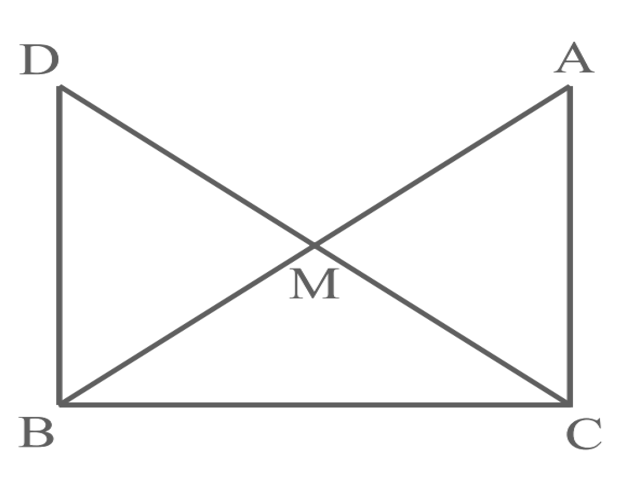
\includegraphics[width=\columnwidth]{figs/Screenshot.png}
  \caption{$\triangle \vec{ACB} ,\triangle \vec{DCB}$ with Mid-Point $\vec{M}$}
  \label{fig:triangles}
\end{figure}
\begin{enumerate}[label =(\roman*)]
        \item $\triangle \vec{AMC} \cong \triangle \vec{BMD}$
        \item $\angle \vec{DBC}$ is a right angle. 
        \item $\triangle \vec{DBC} \cong  \triangle \vec{ACB}$ 
        \item $\vec{CM} = \frac{1}{2} \vec{AB}$
\end{enumerate}
\pagebreak
\solution\\
\textbf{CONSTRUCTION STEPS :}
\begin{enumerate}
\item Let us Assume , the input parameters as ;
\begin{table}[H]
\centering
        \input{tables/input_params.tex}
          \caption{Input Parameters}
          \label{Table-1:Input_params}
\end{table}
\item the output can be calculated as ;
\begin{table}[H]
\centering
        \input{tables/output_params.tex}
          \caption{Output Parameters}
          \label{Table-2:Output_params}
\end{table}
                $\therefore$ By, Plotting these points we get the required Image \figref{fig:fig-2}
\begin{figure}[H]
        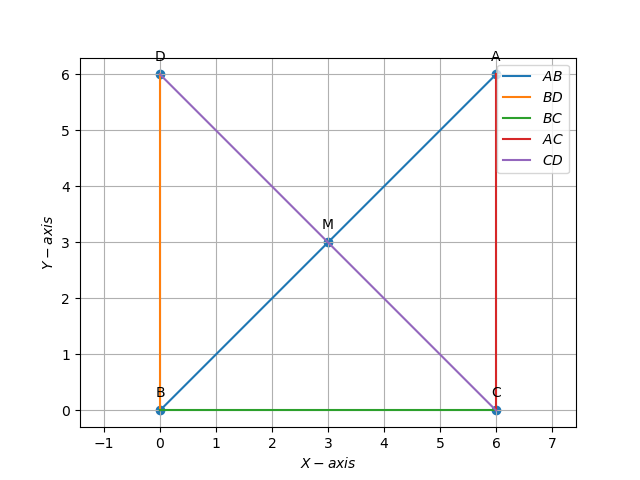
\includegraphics[width = \columnwidth]{figs/python_plot.png}
    \caption{PYTHON Plot of $\triangle \vec{ACB} ,\triangle \vec{DBC}$ with Mid-Point $\vec{M}$}
    \label{fig:fig-2}
\end{figure}
\end{enumerate}

\item Find the position vector of a point $\vec{R}$ which divides the line joining two points $\vec{P}$ and $\vec{Q}$ whose position vectors are $2\vec{a}+\vec{b}$ and $\vec{a}-3\vec{b}$ externally in the ratio $1:2$.

\textbf{Solution:}
Let us assume $\vec{a}$ and $\vec{b}$, and the given ratio is
\begin{table}[h]
    \centering
    \begin{tabular}{|c|c|c|}
        \hline 
        \textbf{Symbol} & \textbf{Value} & \textbf{Description} \\
        \hline
        $\vec{a}$ & $\myvec{1 \\ -3}$ & Vector $\vec{a}$ \\
        \hline
        $\vec{b}$ & $\myvec{0 \\ 2}$ & Vector $\vec{b}$\\
        \hline
        $k$ & $2$ & Ratio \\
        \hline
    \end{tabular}
    \caption{Vectors $\vec{a}$ and $\vec{b}$, ratio $k$}
    \label{tab:table1}
\end{table}

Using the section formula,
\begin{align}
    \vec{R} = \frac{\vec{Q} - k\vec{P}}{1 - k}
\end{align}
where $\vec{P}$ and $\vec{Q}$ depend on $\vec{a}$ and $\vec{b}$, then
\begin{align}
    \vec{P} &= (2\vec{a} + \vec{b}) = 2\myvec{1\\-3} + \myvec{0\\2} = \myvec{2\\-4} \\
    \vec{Q} &= (\vec{a} - 3\vec{b}) = \myvec{1\\-3} - 3\myvec{0\\2} = \myvec{1\\-9}
\end{align}
where $\vec{R}$ can be calculated as 
\begin{align}
    \vec{R} = \frac{(\vec{a} - 3\vec{b}) - k(2\vec{a} + \vec{b})}{1 - k}
\end{align}
By substituting $\vec{a}$ and $\vec{b}$ values, we get $\vec{R}$ as
\begin{align}
    \vec{R} = \myvec{3\\1}
\end{align}

\begin{table}[ht!]
    \centering
    \begin{tabular}{|c|c|c|}
        \hline
        \textbf{Symbol} & \textbf{Value} & \textbf{Description}\\
        \hline
        $\vec{P}$ & $(2\vec{a} + \vec{b})$ & Position vector $\vec{P}$ \\
        \hline
        $\vec{Q}$ & $(\vec{a} - 3\vec{b})$ & Position vector $\vec{Q}$\\
        \hline
        $\vec{R}$ & $\frac{\vec{Q} - k\vec{P}}{1 - k}$ & Position vector $\vec{R}$\\
        \hline
    \end{tabular}
    \caption{Vectors $\vec{P}$, $\vec{Q}$, $\vec{R}$}
    \label{tab:mytable2}   
\end{table}

\begin{figure}[H]
    \centering
    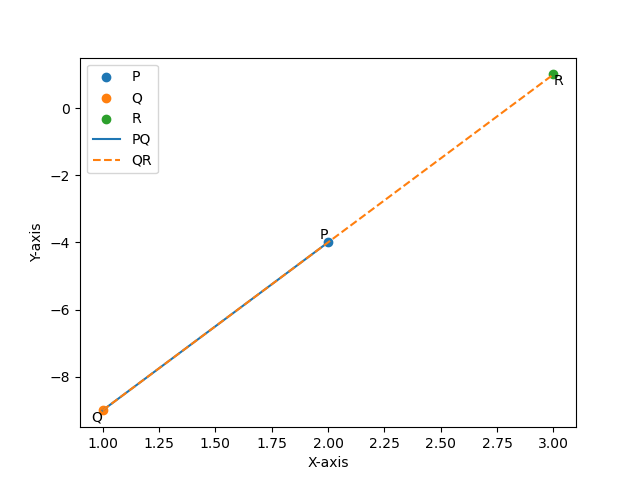
\includegraphics[width=\columnwidth]{figs/external-bisector.png}
    \caption{Point vectors $\vec{P}$, $\vec{Q}$, $\vec{R}$}
    \label{fig:enter-label}
\end{figure}


\end{enumerate}

    \item Draw a quadrilateral in the Cartesian plane, whose vertices are 
    \begin{align}
        \vec{A} = \myvec{-4\\5} \quad \vec{B} = \myvec{0\\7} \\
        \vec{C} = \myvec{5\\-5} \quad \vec{D} = \myvec{-4\\-2}
    \end{align}
    Also, find its area.
\label{chapters/11/10/1/1}
   \\ 
    \solution 
\begin{enumerate}[label=\thesection.\arabic*,ref=\thesection.\theenumi]
		\item Find $\abs{\overrightarrow{a}\times\overrightarrow{b}},\text{ if }\overrightarrow{a}=\hat{i}-7\hat{j}+7\hat{k}\text{ and } \overrightarrow{b}=3\hat{i}-2\hat{j}+2\hat{k}$.
	\\
		\solution
		\input{chapters/12/10/4/1/cross.tex}
\item Show that $$(\overrightarrow{a}-\overrightarrow{b})\times (\overrightarrow{a}+\overrightarrow{b})=2(\overrightarrow{a}\times \overrightarrow{b})$$
	\\
		\solution
		\input{chapters/12/10/4/4/cross.tex}
\item Find $\lambda$ and $\mu$ if $(2\hat{i}+6\hat{j}+27\hat{k})\times(\hat{i}+\lambda \hat{j} + \mu \hat{k})=\overrightarrow{0}$.
	\\
		\solution
		\input{chapters/12/10/4/5/cross.tex}
\item Given that $\overrightarrow{a} \cdot \overrightarrow{b} = 0$ and $\overrightarrow{a} \times \overrightarrow{b} = \overrightarrow{0}$. What can you conclude about the vectors $\overrightarrow{a} \text{ and }\overrightarrow{b}$?
\item Let the vectors be given as $\overrightarrow{a},\overrightarrow{b},\overrightarrow{c}\text{ be given as }\ a_1 \hat{i}+\ a_2 \hat{j}+\ a_3 \hat{k},\ b_1 \hat{i}+\ b_2 \hat{j}+\ b_3 \hat{k},\ c_1 \hat{i}+\ c_2 \hat{j}+\ c_3 \hat{k}$. Then show that $\overrightarrow{a} \times (\overrightarrow{b} + \overrightarrow{c}) = \overrightarrow{a} \times \overrightarrow{b}+\overrightarrow{a} \times \overrightarrow{c}$.
	\\
		\solution
		\input{chapters/12/10/4/7/cross.tex}
\item If either $\overrightarrow{a} = \overrightarrow{0}$ or $\overrightarrow{b} = \overrightarrow{0}$, then $\overrightarrow{a} \times \overrightarrow{b} = \overrightarrow{0}$. Is the converse true? Justify your answer with an example.
	\\
		\solution
		\input{chapters/12/10/4/8/cross.tex}
\item Find the area of the triangle with vertices $A(1, 1, 2)$, $B(2, 3, 5)$, and $C(1, 5, 5)$
	\\
		\solution
		\input{chapters/12/10/4/9/cross.tex}
\item Find the area of the parallelogram whose adjacent sides are determined by the vectors $\overrightarrow{a}=\hat{i}-\hat{j}+3\hat{k}$ and $\overrightarrow{b}=2\hat{i}-7\hat{j}+\hat{k}$.
	\\
		\solution
		\input{chapters/12/10/4/10/cross.tex}
\item Let the vectors $\overrightarrow{a}$ and $\overrightarrow{b}$ be such that $|\overrightarrow{a}| = 3$ and $|\overrightarrow{b}| = \dfrac{\sqrt{2}}{3}$, then $\overrightarrow{a} \times \overrightarrow{b}$ is a unit vector, if the angle between $\overrightarrow{a}$ and $\overrightarrow{b}$ is
\begin{enumerate}
\item $\dfrac{\pi}{6}$
\item $\dfrac{\pi}{4}$
\item $\dfrac{\pi}{3}$
\item $\dfrac{\pi}{2}$
\end{enumerate}
		\solution
		\input{chapters/12/10/4/11/cross.tex}
\item Area of a rectangle having vertices A, B, C and D with position vectors $ -\hat{i}+ \dfrac{1}{2} \hat{j}+4\hat{k},\hat{i}+ \dfrac{1}{2} \hat{j}+4\hat{k},\hat{i}-\dfrac{1}{2} \hat{j}+4\hat{k}\text{ and }-\hat{i}- \dfrac{1}{2} \hat{j}+4\hat{k}$, respectively is
\begin{enumerate}
\item $\dfrac{1}{2}$
\item 1
\item 2
\item 4
\end{enumerate}
		\solution
		\input{chapters/12/10/4/12/cross.tex}
\item Find the area of the triangle whose vertices are 
\begin{enumerate}
\item $(2, 3), (–1, 0), (2, – 4)$
\item $(–5, –1), (3, –5), (5, 2)$ 
\end{enumerate}
		\label{10/7/3/1}
\solution
		\input{chapters/10/7/3/1/area.tex}
\item Find the area of the triangle formed by joining the mid-points of the sides of the triangle whose vertices are $(0, –1), (2, 1) \text{ and } (0, 3)$. Find the ratio of this area to the area of the given triangle.
	\\
\solution
		\input{chapters/10/7/3/3/cross.tex}

\item Find the area of the quadrilateral whose vertices, taken in order, are $(– 4, – 2), (– 3, – 5), (3, – 2)$  and $ (2, 3)$.
	\\
\solution
		\input{chapters/10/7/3/4/cross.tex}

\item Verify that a median of a triangle divides it into two triangles of equal areas for $\triangle ABC$ whose vertices are $\vec{A}(4, -6), \vec{B}(3, 2), \text{ and } \vec{C}(5, 2)$. 
		\label{10/7/3/5}
		\\
\solution
		\input{chapters/10/7/3/5/area.tex}

\item The two adjacent sides of a parallelogram are 
$2\hat{i}-4\hat{j}+5\hat{k}$  and  $\hat{i}-2\hat{j}-3\hat{k}$.
Find the unit vector parallel to its diagonal. Also, find its area.\\
	\solution
		\input{chapters/12/10/5/10/cross.tex}
\item The vertices of a $\triangle ABC$ are $\vec{A}(4,6), \vec{B}(1,5)$ and  $\vec{C}(7,2)$. A line is drawn to intersect sides $AB$ and $AC$ at $\vec{D}$ and $\vec{E}$ respectively, such that $\frac{AD}{AB} = \frac{AE}{AC} = \frac{1}{4}$. Calculate the area of $\triangle ADE$ and compare it with the area of the $\triangle ABC$.
\\
\solution
	\input{chapters/10/7/4/6/section.tex}
    \item Draw a quadrilateral in the Cartesian plane, whose vertices are 
    \begin{align}
        \vec{A} = \myvec{-4\\5} \quad \vec{B} = \myvec{0\\7} \\
        \vec{C} = \myvec{5\\-5} \quad \vec{D} = \myvec{-4\\-2}
    \end{align}
    Also, find its area.
\label{chapters/11/10/1/1}
   \\ 
    \solution 
\input{chapters/11/10/1/1/cross.tex}
\item Find the area of region bounded by the triangle whose
	vertices are $(1, 0), (2, 2) \text{ and } (3, 1)$. 
\item Find the area of region bounded by the triangle whose vertices
	are $(– 1, 0), (1, 3) \text{ and } (3, 2)$. 
\item Find the area of the $\triangle ABC$, coordinates of whose vertices are $\vec{A}(2, 0), \vec{B}(4, 5), \text{ and } \vec{C}(6, 3)$.


\item 
\input{chapters/vectors/exer/main.tex}
\end{enumerate}


\item Find the area of region bounded by the triangle whose
	vertices are $(1, 0), (2, 2) \text{ and } (3, 1)$. 
\item Find the area of region bounded by the triangle whose vertices
	are $(– 1, 0), (1, 3) \text{ and } (3, 2)$. 
\item Find the area of the $\triangle ABC$, coordinates of whose vertices are $\vec{A}(2, 0), \vec{B}(4, 5), \text{ and } \vec{C}(6, 3)$.


\item 
%\documentclass[12pt]{article}
%\usepackage{graphicx}
%\usepackage{graphics}
%\usepackage{refstyle}
%\usepackage{amsmath}
%\usepackage{caption}
%\usepackage{float}
%\usepackage{booktabs}
%\usepackage{array}
%\usepackage{amssymb}
%\usepackage{booktabs}
%\let\vec\mathbf
%\providecommand{\brak}[1]{\ensuremath{\left(#1\right)}}
%\graphicspath{{/storage/self/primary/Download/latexnew/fig}}                                     
$\vec{P}$ and $\vec{Q}$ are any two points lying on the sides $DC$ and $AD$ respectively of a parallelogram $ABCD$.Show that, $ar\brak{\triangle APB}=ar\brak{\triangle BQC}$.


\textbf{Figure:}
\begin{figure}[H]
    \centering
	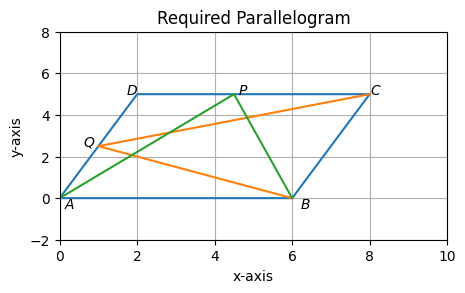
\includegraphics[width=\columnwidth]{chapters/vectors/exer/figs/1.png}
    \caption{}
    \label{fig:fig:1}
\end{figure}


\textbf{Solution:}
\begin{table}[H]
   \centering
  \input{chapters/vectors/exer/table/tab1.tex}
   \caption{Table of input parameters}        
\label{tab:tab:1}                    
\end{table}




\begin{table}[H]
    \centering                                  
\input{chapters/vectors/exer/table/tab2.tex}                  
\caption{Table of output parameters}
\label{tab:tab:2}
 \end{table}


For the $\triangle BQC$, the vertices of the triangle are taken from \tabref{tab:tab:1} and \tabref{tab:tab:2}.

\begin{align}
\implies ar\brak{\triangle BQC}&=
\frac{1}{2}\begin{tabular}{|c c c|}            
1 &1&1\\                      
$\vec{B}$&$\vec{Q}$&$\vec{C}$\\    
\end{tabular}\\
&= \frac{1}{2}\begin{tabular}{|c c c|}
       1 &1&1\\
       6&$\frac{2k_1}{k_1+1}$&8 \\
       0&$\frac{5k_1}{k_1+1}$&5
   \end{tabular}\\
  \xrightarrow{C_2'=C_2-C_1,C_3'=C_3-C_1}&\frac{1}{2} \begin{tabular}{|c c c|}
       1 &0&0\\
       6&$\frac{-4k_1-6}{k_1+1}$&2 \\
       0&$\frac{5k_1}{k_1+1}$&5
   \end{tabular}\\
&=\frac{1}{2}\brak{1\begin{tabular}{|c c|}
   $\frac{-4k_1-6}{k_1+1}$ &2  \\
   $\frac{5k_1}{k_1+1}$ & 5
\end{tabular} +0+0}\\
&=\frac{1}{2} \times30\\                          
&=15 \end{align}


For the $\triangle APB$, the vertices of the triangle are taken from \tabref{tab:tab:1} and \tabref{tab:tab:2}.
   \begin{align}
  \implies ar\brak{\triangle APB} &=
\frac{1}{2}\begin{tabular}{|c c c|}            
1 &1&1\\                            
$\vec{A}$&$\vec{P}$&$\vec{B}$\\
\end{tabular}\\ &=  \frac{1}{2}
   \begin{tabular}{|c c c|}
       1 &1&1\\
       0&$\frac{8k_2+2}{k_2+1}$&6 \\
       0&5&0
   \end{tabular}\\
 &=\frac{1}{2} \times30\\
 &=15 \end{align}
 \brak{6} = \brak{10}


So, ar\brak{\triangle BQC} = ar\brak{\triangle APB}.\brak{proved}
%\end{document}



\end{enumerate}


\item Find the area of the triangle with vertices $A(1, 1, 2)$, $B(2, 3, 5)$, and $C(1, 5, 5)$
	\\
		\solution
		\begin{enumerate}[label=\thesection.\arabic*,ref=\thesection.\theenumi]
		\item Find $\abs{\overrightarrow{a}\times\overrightarrow{b}},\text{ if }\overrightarrow{a}=\hat{i}-7\hat{j}+7\hat{k}\text{ and } \overrightarrow{b}=3\hat{i}-2\hat{j}+2\hat{k}$.
	\\
		\solution
		\begin{enumerate}[label=\thesection.\arabic*,ref=\thesection.\theenumi]
		\item Find $\abs{\overrightarrow{a}\times\overrightarrow{b}},\text{ if }\overrightarrow{a}=\hat{i}-7\hat{j}+7\hat{k}\text{ and } \overrightarrow{b}=3\hat{i}-2\hat{j}+2\hat{k}$.
	\\
		\solution
		\input{chapters/12/10/4/1/cross.tex}
\item Show that $$(\overrightarrow{a}-\overrightarrow{b})\times (\overrightarrow{a}+\overrightarrow{b})=2(\overrightarrow{a}\times \overrightarrow{b})$$
	\\
		\solution
		\input{chapters/12/10/4/4/cross.tex}
\item Find $\lambda$ and $\mu$ if $(2\hat{i}+6\hat{j}+27\hat{k})\times(\hat{i}+\lambda \hat{j} + \mu \hat{k})=\overrightarrow{0}$.
	\\
		\solution
		\input{chapters/12/10/4/5/cross.tex}
\item Given that $\overrightarrow{a} \cdot \overrightarrow{b} = 0$ and $\overrightarrow{a} \times \overrightarrow{b} = \overrightarrow{0}$. What can you conclude about the vectors $\overrightarrow{a} \text{ and }\overrightarrow{b}$?
\item Let the vectors be given as $\overrightarrow{a},\overrightarrow{b},\overrightarrow{c}\text{ be given as }\ a_1 \hat{i}+\ a_2 \hat{j}+\ a_3 \hat{k},\ b_1 \hat{i}+\ b_2 \hat{j}+\ b_3 \hat{k},\ c_1 \hat{i}+\ c_2 \hat{j}+\ c_3 \hat{k}$. Then show that $\overrightarrow{a} \times (\overrightarrow{b} + \overrightarrow{c}) = \overrightarrow{a} \times \overrightarrow{b}+\overrightarrow{a} \times \overrightarrow{c}$.
	\\
		\solution
		\input{chapters/12/10/4/7/cross.tex}
\item If either $\overrightarrow{a} = \overrightarrow{0}$ or $\overrightarrow{b} = \overrightarrow{0}$, then $\overrightarrow{a} \times \overrightarrow{b} = \overrightarrow{0}$. Is the converse true? Justify your answer with an example.
	\\
		\solution
		\input{chapters/12/10/4/8/cross.tex}
\item Find the area of the triangle with vertices $A(1, 1, 2)$, $B(2, 3, 5)$, and $C(1, 5, 5)$
	\\
		\solution
		\input{chapters/12/10/4/9/cross.tex}
\item Find the area of the parallelogram whose adjacent sides are determined by the vectors $\overrightarrow{a}=\hat{i}-\hat{j}+3\hat{k}$ and $\overrightarrow{b}=2\hat{i}-7\hat{j}+\hat{k}$.
	\\
		\solution
		\input{chapters/12/10/4/10/cross.tex}
\item Let the vectors $\overrightarrow{a}$ and $\overrightarrow{b}$ be such that $|\overrightarrow{a}| = 3$ and $|\overrightarrow{b}| = \dfrac{\sqrt{2}}{3}$, then $\overrightarrow{a} \times \overrightarrow{b}$ is a unit vector, if the angle between $\overrightarrow{a}$ and $\overrightarrow{b}$ is
\begin{enumerate}
\item $\dfrac{\pi}{6}$
\item $\dfrac{\pi}{4}$
\item $\dfrac{\pi}{3}$
\item $\dfrac{\pi}{2}$
\end{enumerate}
		\solution
		\input{chapters/12/10/4/11/cross.tex}
\item Area of a rectangle having vertices A, B, C and D with position vectors $ -\hat{i}+ \dfrac{1}{2} \hat{j}+4\hat{k},\hat{i}+ \dfrac{1}{2} \hat{j}+4\hat{k},\hat{i}-\dfrac{1}{2} \hat{j}+4\hat{k}\text{ and }-\hat{i}- \dfrac{1}{2} \hat{j}+4\hat{k}$, respectively is
\begin{enumerate}
\item $\dfrac{1}{2}$
\item 1
\item 2
\item 4
\end{enumerate}
		\solution
		\input{chapters/12/10/4/12/cross.tex}
\item Find the area of the triangle whose vertices are 
\begin{enumerate}
\item $(2, 3), (–1, 0), (2, – 4)$
\item $(–5, –1), (3, –5), (5, 2)$ 
\end{enumerate}
		\label{10/7/3/1}
\solution
		\input{chapters/10/7/3/1/area.tex}
\item Find the area of the triangle formed by joining the mid-points of the sides of the triangle whose vertices are $(0, –1), (2, 1) \text{ and } (0, 3)$. Find the ratio of this area to the area of the given triangle.
	\\
\solution
		\input{chapters/10/7/3/3/cross.tex}

\item Find the area of the quadrilateral whose vertices, taken in order, are $(– 4, – 2), (– 3, – 5), (3, – 2)$  and $ (2, 3)$.
	\\
\solution
		\input{chapters/10/7/3/4/cross.tex}

\item Verify that a median of a triangle divides it into two triangles of equal areas for $\triangle ABC$ whose vertices are $\vec{A}(4, -6), \vec{B}(3, 2), \text{ and } \vec{C}(5, 2)$. 
		\label{10/7/3/5}
		\\
\solution
		\input{chapters/10/7/3/5/area.tex}

\item The two adjacent sides of a parallelogram are 
$2\hat{i}-4\hat{j}+5\hat{k}$  and  $\hat{i}-2\hat{j}-3\hat{k}$.
Find the unit vector parallel to its diagonal. Also, find its area.\\
	\solution
		\input{chapters/12/10/5/10/cross.tex}
\item The vertices of a $\triangle ABC$ are $\vec{A}(4,6), \vec{B}(1,5)$ and  $\vec{C}(7,2)$. A line is drawn to intersect sides $AB$ and $AC$ at $\vec{D}$ and $\vec{E}$ respectively, such that $\frac{AD}{AB} = \frac{AE}{AC} = \frac{1}{4}$. Calculate the area of $\triangle ADE$ and compare it with the area of the $\triangle ABC$.
\\
\solution
	\input{chapters/10/7/4/6/section.tex}
    \item Draw a quadrilateral in the Cartesian plane, whose vertices are 
    \begin{align}
        \vec{A} = \myvec{-4\\5} \quad \vec{B} = \myvec{0\\7} \\
        \vec{C} = \myvec{5\\-5} \quad \vec{D} = \myvec{-4\\-2}
    \end{align}
    Also, find its area.
\label{chapters/11/10/1/1}
   \\ 
    \solution 
\input{chapters/11/10/1/1/cross.tex}
\item Find the area of region bounded by the triangle whose
	vertices are $(1, 0), (2, 2) \text{ and } (3, 1)$. 
\item Find the area of region bounded by the triangle whose vertices
	are $(– 1, 0), (1, 3) \text{ and } (3, 2)$. 
\item Find the area of the $\triangle ABC$, coordinates of whose vertices are $\vec{A}(2, 0), \vec{B}(4, 5), \text{ and } \vec{C}(6, 3)$.


\item 
\input{chapters/vectors/exer/main.tex}
\end{enumerate}


\item Show that $$(\overrightarrow{a}-\overrightarrow{b})\times (\overrightarrow{a}+\overrightarrow{b})=2(\overrightarrow{a}\times \overrightarrow{b})$$
	\\
		\solution
		\begin{enumerate}[label=\thesection.\arabic*,ref=\thesection.\theenumi]
		\item Find $\abs{\overrightarrow{a}\times\overrightarrow{b}},\text{ if }\overrightarrow{a}=\hat{i}-7\hat{j}+7\hat{k}\text{ and } \overrightarrow{b}=3\hat{i}-2\hat{j}+2\hat{k}$.
	\\
		\solution
		\input{chapters/12/10/4/1/cross.tex}
\item Show that $$(\overrightarrow{a}-\overrightarrow{b})\times (\overrightarrow{a}+\overrightarrow{b})=2(\overrightarrow{a}\times \overrightarrow{b})$$
	\\
		\solution
		\input{chapters/12/10/4/4/cross.tex}
\item Find $\lambda$ and $\mu$ if $(2\hat{i}+6\hat{j}+27\hat{k})\times(\hat{i}+\lambda \hat{j} + \mu \hat{k})=\overrightarrow{0}$.
	\\
		\solution
		\input{chapters/12/10/4/5/cross.tex}
\item Given that $\overrightarrow{a} \cdot \overrightarrow{b} = 0$ and $\overrightarrow{a} \times \overrightarrow{b} = \overrightarrow{0}$. What can you conclude about the vectors $\overrightarrow{a} \text{ and }\overrightarrow{b}$?
\item Let the vectors be given as $\overrightarrow{a},\overrightarrow{b},\overrightarrow{c}\text{ be given as }\ a_1 \hat{i}+\ a_2 \hat{j}+\ a_3 \hat{k},\ b_1 \hat{i}+\ b_2 \hat{j}+\ b_3 \hat{k},\ c_1 \hat{i}+\ c_2 \hat{j}+\ c_3 \hat{k}$. Then show that $\overrightarrow{a} \times (\overrightarrow{b} + \overrightarrow{c}) = \overrightarrow{a} \times \overrightarrow{b}+\overrightarrow{a} \times \overrightarrow{c}$.
	\\
		\solution
		\input{chapters/12/10/4/7/cross.tex}
\item If either $\overrightarrow{a} = \overrightarrow{0}$ or $\overrightarrow{b} = \overrightarrow{0}$, then $\overrightarrow{a} \times \overrightarrow{b} = \overrightarrow{0}$. Is the converse true? Justify your answer with an example.
	\\
		\solution
		\input{chapters/12/10/4/8/cross.tex}
\item Find the area of the triangle with vertices $A(1, 1, 2)$, $B(2, 3, 5)$, and $C(1, 5, 5)$
	\\
		\solution
		\input{chapters/12/10/4/9/cross.tex}
\item Find the area of the parallelogram whose adjacent sides are determined by the vectors $\overrightarrow{a}=\hat{i}-\hat{j}+3\hat{k}$ and $\overrightarrow{b}=2\hat{i}-7\hat{j}+\hat{k}$.
	\\
		\solution
		\input{chapters/12/10/4/10/cross.tex}
\item Let the vectors $\overrightarrow{a}$ and $\overrightarrow{b}$ be such that $|\overrightarrow{a}| = 3$ and $|\overrightarrow{b}| = \dfrac{\sqrt{2}}{3}$, then $\overrightarrow{a} \times \overrightarrow{b}$ is a unit vector, if the angle between $\overrightarrow{a}$ and $\overrightarrow{b}$ is
\begin{enumerate}
\item $\dfrac{\pi}{6}$
\item $\dfrac{\pi}{4}$
\item $\dfrac{\pi}{3}$
\item $\dfrac{\pi}{2}$
\end{enumerate}
		\solution
		\input{chapters/12/10/4/11/cross.tex}
\item Area of a rectangle having vertices A, B, C and D with position vectors $ -\hat{i}+ \dfrac{1}{2} \hat{j}+4\hat{k},\hat{i}+ \dfrac{1}{2} \hat{j}+4\hat{k},\hat{i}-\dfrac{1}{2} \hat{j}+4\hat{k}\text{ and }-\hat{i}- \dfrac{1}{2} \hat{j}+4\hat{k}$, respectively is
\begin{enumerate}
\item $\dfrac{1}{2}$
\item 1
\item 2
\item 4
\end{enumerate}
		\solution
		\input{chapters/12/10/4/12/cross.tex}
\item Find the area of the triangle whose vertices are 
\begin{enumerate}
\item $(2, 3), (–1, 0), (2, – 4)$
\item $(–5, –1), (3, –5), (5, 2)$ 
\end{enumerate}
		\label{10/7/3/1}
\solution
		\input{chapters/10/7/3/1/area.tex}
\item Find the area of the triangle formed by joining the mid-points of the sides of the triangle whose vertices are $(0, –1), (2, 1) \text{ and } (0, 3)$. Find the ratio of this area to the area of the given triangle.
	\\
\solution
		\input{chapters/10/7/3/3/cross.tex}

\item Find the area of the quadrilateral whose vertices, taken in order, are $(– 4, – 2), (– 3, – 5), (3, – 2)$  and $ (2, 3)$.
	\\
\solution
		\input{chapters/10/7/3/4/cross.tex}

\item Verify that a median of a triangle divides it into two triangles of equal areas for $\triangle ABC$ whose vertices are $\vec{A}(4, -6), \vec{B}(3, 2), \text{ and } \vec{C}(5, 2)$. 
		\label{10/7/3/5}
		\\
\solution
		\input{chapters/10/7/3/5/area.tex}

\item The two adjacent sides of a parallelogram are 
$2\hat{i}-4\hat{j}+5\hat{k}$  and  $\hat{i}-2\hat{j}-3\hat{k}$.
Find the unit vector parallel to its diagonal. Also, find its area.\\
	\solution
		\input{chapters/12/10/5/10/cross.tex}
\item The vertices of a $\triangle ABC$ are $\vec{A}(4,6), \vec{B}(1,5)$ and  $\vec{C}(7,2)$. A line is drawn to intersect sides $AB$ and $AC$ at $\vec{D}$ and $\vec{E}$ respectively, such that $\frac{AD}{AB} = \frac{AE}{AC} = \frac{1}{4}$. Calculate the area of $\triangle ADE$ and compare it with the area of the $\triangle ABC$.
\\
\solution
	\input{chapters/10/7/4/6/section.tex}
    \item Draw a quadrilateral in the Cartesian plane, whose vertices are 
    \begin{align}
        \vec{A} = \myvec{-4\\5} \quad \vec{B} = \myvec{0\\7} \\
        \vec{C} = \myvec{5\\-5} \quad \vec{D} = \myvec{-4\\-2}
    \end{align}
    Also, find its area.
\label{chapters/11/10/1/1}
   \\ 
    \solution 
\input{chapters/11/10/1/1/cross.tex}
\item Find the area of region bounded by the triangle whose
	vertices are $(1, 0), (2, 2) \text{ and } (3, 1)$. 
\item Find the area of region bounded by the triangle whose vertices
	are $(– 1, 0), (1, 3) \text{ and } (3, 2)$. 
\item Find the area of the $\triangle ABC$, coordinates of whose vertices are $\vec{A}(2, 0), \vec{B}(4, 5), \text{ and } \vec{C}(6, 3)$.


\item 
\input{chapters/vectors/exer/main.tex}
\end{enumerate}


\item Find $\lambda$ and $\mu$ if $(2\hat{i}+6\hat{j}+27\hat{k})\times(\hat{i}+\lambda \hat{j} + \mu \hat{k})=\overrightarrow{0}$.
	\\
		\solution
		\begin{enumerate}[label=\thesection.\arabic*,ref=\thesection.\theenumi]
		\item Find $\abs{\overrightarrow{a}\times\overrightarrow{b}},\text{ if }\overrightarrow{a}=\hat{i}-7\hat{j}+7\hat{k}\text{ and } \overrightarrow{b}=3\hat{i}-2\hat{j}+2\hat{k}$.
	\\
		\solution
		\input{chapters/12/10/4/1/cross.tex}
\item Show that $$(\overrightarrow{a}-\overrightarrow{b})\times (\overrightarrow{a}+\overrightarrow{b})=2(\overrightarrow{a}\times \overrightarrow{b})$$
	\\
		\solution
		\input{chapters/12/10/4/4/cross.tex}
\item Find $\lambda$ and $\mu$ if $(2\hat{i}+6\hat{j}+27\hat{k})\times(\hat{i}+\lambda \hat{j} + \mu \hat{k})=\overrightarrow{0}$.
	\\
		\solution
		\input{chapters/12/10/4/5/cross.tex}
\item Given that $\overrightarrow{a} \cdot \overrightarrow{b} = 0$ and $\overrightarrow{a} \times \overrightarrow{b} = \overrightarrow{0}$. What can you conclude about the vectors $\overrightarrow{a} \text{ and }\overrightarrow{b}$?
\item Let the vectors be given as $\overrightarrow{a},\overrightarrow{b},\overrightarrow{c}\text{ be given as }\ a_1 \hat{i}+\ a_2 \hat{j}+\ a_3 \hat{k},\ b_1 \hat{i}+\ b_2 \hat{j}+\ b_3 \hat{k},\ c_1 \hat{i}+\ c_2 \hat{j}+\ c_3 \hat{k}$. Then show that $\overrightarrow{a} \times (\overrightarrow{b} + \overrightarrow{c}) = \overrightarrow{a} \times \overrightarrow{b}+\overrightarrow{a} \times \overrightarrow{c}$.
	\\
		\solution
		\input{chapters/12/10/4/7/cross.tex}
\item If either $\overrightarrow{a} = \overrightarrow{0}$ or $\overrightarrow{b} = \overrightarrow{0}$, then $\overrightarrow{a} \times \overrightarrow{b} = \overrightarrow{0}$. Is the converse true? Justify your answer with an example.
	\\
		\solution
		\input{chapters/12/10/4/8/cross.tex}
\item Find the area of the triangle with vertices $A(1, 1, 2)$, $B(2, 3, 5)$, and $C(1, 5, 5)$
	\\
		\solution
		\input{chapters/12/10/4/9/cross.tex}
\item Find the area of the parallelogram whose adjacent sides are determined by the vectors $\overrightarrow{a}=\hat{i}-\hat{j}+3\hat{k}$ and $\overrightarrow{b}=2\hat{i}-7\hat{j}+\hat{k}$.
	\\
		\solution
		\input{chapters/12/10/4/10/cross.tex}
\item Let the vectors $\overrightarrow{a}$ and $\overrightarrow{b}$ be such that $|\overrightarrow{a}| = 3$ and $|\overrightarrow{b}| = \dfrac{\sqrt{2}}{3}$, then $\overrightarrow{a} \times \overrightarrow{b}$ is a unit vector, if the angle between $\overrightarrow{a}$ and $\overrightarrow{b}$ is
\begin{enumerate}
\item $\dfrac{\pi}{6}$
\item $\dfrac{\pi}{4}$
\item $\dfrac{\pi}{3}$
\item $\dfrac{\pi}{2}$
\end{enumerate}
		\solution
		\input{chapters/12/10/4/11/cross.tex}
\item Area of a rectangle having vertices A, B, C and D with position vectors $ -\hat{i}+ \dfrac{1}{2} \hat{j}+4\hat{k},\hat{i}+ \dfrac{1}{2} \hat{j}+4\hat{k},\hat{i}-\dfrac{1}{2} \hat{j}+4\hat{k}\text{ and }-\hat{i}- \dfrac{1}{2} \hat{j}+4\hat{k}$, respectively is
\begin{enumerate}
\item $\dfrac{1}{2}$
\item 1
\item 2
\item 4
\end{enumerate}
		\solution
		\input{chapters/12/10/4/12/cross.tex}
\item Find the area of the triangle whose vertices are 
\begin{enumerate}
\item $(2, 3), (–1, 0), (2, – 4)$
\item $(–5, –1), (3, –5), (5, 2)$ 
\end{enumerate}
		\label{10/7/3/1}
\solution
		\input{chapters/10/7/3/1/area.tex}
\item Find the area of the triangle formed by joining the mid-points of the sides of the triangle whose vertices are $(0, –1), (2, 1) \text{ and } (0, 3)$. Find the ratio of this area to the area of the given triangle.
	\\
\solution
		\input{chapters/10/7/3/3/cross.tex}

\item Find the area of the quadrilateral whose vertices, taken in order, are $(– 4, – 2), (– 3, – 5), (3, – 2)$  and $ (2, 3)$.
	\\
\solution
		\input{chapters/10/7/3/4/cross.tex}

\item Verify that a median of a triangle divides it into two triangles of equal areas for $\triangle ABC$ whose vertices are $\vec{A}(4, -6), \vec{B}(3, 2), \text{ and } \vec{C}(5, 2)$. 
		\label{10/7/3/5}
		\\
\solution
		\input{chapters/10/7/3/5/area.tex}

\item The two adjacent sides of a parallelogram are 
$2\hat{i}-4\hat{j}+5\hat{k}$  and  $\hat{i}-2\hat{j}-3\hat{k}$.
Find the unit vector parallel to its diagonal. Also, find its area.\\
	\solution
		\input{chapters/12/10/5/10/cross.tex}
\item The vertices of a $\triangle ABC$ are $\vec{A}(4,6), \vec{B}(1,5)$ and  $\vec{C}(7,2)$. A line is drawn to intersect sides $AB$ and $AC$ at $\vec{D}$ and $\vec{E}$ respectively, such that $\frac{AD}{AB} = \frac{AE}{AC} = \frac{1}{4}$. Calculate the area of $\triangle ADE$ and compare it with the area of the $\triangle ABC$.
\\
\solution
	\input{chapters/10/7/4/6/section.tex}
    \item Draw a quadrilateral in the Cartesian plane, whose vertices are 
    \begin{align}
        \vec{A} = \myvec{-4\\5} \quad \vec{B} = \myvec{0\\7} \\
        \vec{C} = \myvec{5\\-5} \quad \vec{D} = \myvec{-4\\-2}
    \end{align}
    Also, find its area.
\label{chapters/11/10/1/1}
   \\ 
    \solution 
\input{chapters/11/10/1/1/cross.tex}
\item Find the area of region bounded by the triangle whose
	vertices are $(1, 0), (2, 2) \text{ and } (3, 1)$. 
\item Find the area of region bounded by the triangle whose vertices
	are $(– 1, 0), (1, 3) \text{ and } (3, 2)$. 
\item Find the area of the $\triangle ABC$, coordinates of whose vertices are $\vec{A}(2, 0), \vec{B}(4, 5), \text{ and } \vec{C}(6, 3)$.


\item 
\input{chapters/vectors/exer/main.tex}
\end{enumerate}


\item Given that $\overrightarrow{a} \cdot \overrightarrow{b} = 0$ and $\overrightarrow{a} \times \overrightarrow{b} = \overrightarrow{0}$. What can you conclude about the vectors $\overrightarrow{a} \text{ and }\overrightarrow{b}$?
\item Let the vectors be given as $\overrightarrow{a},\overrightarrow{b},\overrightarrow{c}\text{ be given as }\ a_1 \hat{i}+\ a_2 \hat{j}+\ a_3 \hat{k},\ b_1 \hat{i}+\ b_2 \hat{j}+\ b_3 \hat{k},\ c_1 \hat{i}+\ c_2 \hat{j}+\ c_3 \hat{k}$. Then show that $\overrightarrow{a} \times (\overrightarrow{b} + \overrightarrow{c}) = \overrightarrow{a} \times \overrightarrow{b}+\overrightarrow{a} \times \overrightarrow{c}$.
	\\
		\solution
		\begin{enumerate}[label=\thesection.\arabic*,ref=\thesection.\theenumi]
		\item Find $\abs{\overrightarrow{a}\times\overrightarrow{b}},\text{ if }\overrightarrow{a}=\hat{i}-7\hat{j}+7\hat{k}\text{ and } \overrightarrow{b}=3\hat{i}-2\hat{j}+2\hat{k}$.
	\\
		\solution
		\input{chapters/12/10/4/1/cross.tex}
\item Show that $$(\overrightarrow{a}-\overrightarrow{b})\times (\overrightarrow{a}+\overrightarrow{b})=2(\overrightarrow{a}\times \overrightarrow{b})$$
	\\
		\solution
		\input{chapters/12/10/4/4/cross.tex}
\item Find $\lambda$ and $\mu$ if $(2\hat{i}+6\hat{j}+27\hat{k})\times(\hat{i}+\lambda \hat{j} + \mu \hat{k})=\overrightarrow{0}$.
	\\
		\solution
		\input{chapters/12/10/4/5/cross.tex}
\item Given that $\overrightarrow{a} \cdot \overrightarrow{b} = 0$ and $\overrightarrow{a} \times \overrightarrow{b} = \overrightarrow{0}$. What can you conclude about the vectors $\overrightarrow{a} \text{ and }\overrightarrow{b}$?
\item Let the vectors be given as $\overrightarrow{a},\overrightarrow{b},\overrightarrow{c}\text{ be given as }\ a_1 \hat{i}+\ a_2 \hat{j}+\ a_3 \hat{k},\ b_1 \hat{i}+\ b_2 \hat{j}+\ b_3 \hat{k},\ c_1 \hat{i}+\ c_2 \hat{j}+\ c_3 \hat{k}$. Then show that $\overrightarrow{a} \times (\overrightarrow{b} + \overrightarrow{c}) = \overrightarrow{a} \times \overrightarrow{b}+\overrightarrow{a} \times \overrightarrow{c}$.
	\\
		\solution
		\input{chapters/12/10/4/7/cross.tex}
\item If either $\overrightarrow{a} = \overrightarrow{0}$ or $\overrightarrow{b} = \overrightarrow{0}$, then $\overrightarrow{a} \times \overrightarrow{b} = \overrightarrow{0}$. Is the converse true? Justify your answer with an example.
	\\
		\solution
		\input{chapters/12/10/4/8/cross.tex}
\item Find the area of the triangle with vertices $A(1, 1, 2)$, $B(2, 3, 5)$, and $C(1, 5, 5)$
	\\
		\solution
		\input{chapters/12/10/4/9/cross.tex}
\item Find the area of the parallelogram whose adjacent sides are determined by the vectors $\overrightarrow{a}=\hat{i}-\hat{j}+3\hat{k}$ and $\overrightarrow{b}=2\hat{i}-7\hat{j}+\hat{k}$.
	\\
		\solution
		\input{chapters/12/10/4/10/cross.tex}
\item Let the vectors $\overrightarrow{a}$ and $\overrightarrow{b}$ be such that $|\overrightarrow{a}| = 3$ and $|\overrightarrow{b}| = \dfrac{\sqrt{2}}{3}$, then $\overrightarrow{a} \times \overrightarrow{b}$ is a unit vector, if the angle between $\overrightarrow{a}$ and $\overrightarrow{b}$ is
\begin{enumerate}
\item $\dfrac{\pi}{6}$
\item $\dfrac{\pi}{4}$
\item $\dfrac{\pi}{3}$
\item $\dfrac{\pi}{2}$
\end{enumerate}
		\solution
		\input{chapters/12/10/4/11/cross.tex}
\item Area of a rectangle having vertices A, B, C and D with position vectors $ -\hat{i}+ \dfrac{1}{2} \hat{j}+4\hat{k},\hat{i}+ \dfrac{1}{2} \hat{j}+4\hat{k},\hat{i}-\dfrac{1}{2} \hat{j}+4\hat{k}\text{ and }-\hat{i}- \dfrac{1}{2} \hat{j}+4\hat{k}$, respectively is
\begin{enumerate}
\item $\dfrac{1}{2}$
\item 1
\item 2
\item 4
\end{enumerate}
		\solution
		\input{chapters/12/10/4/12/cross.tex}
\item Find the area of the triangle whose vertices are 
\begin{enumerate}
\item $(2, 3), (–1, 0), (2, – 4)$
\item $(–5, –1), (3, –5), (5, 2)$ 
\end{enumerate}
		\label{10/7/3/1}
\solution
		\input{chapters/10/7/3/1/area.tex}
\item Find the area of the triangle formed by joining the mid-points of the sides of the triangle whose vertices are $(0, –1), (2, 1) \text{ and } (0, 3)$. Find the ratio of this area to the area of the given triangle.
	\\
\solution
		\input{chapters/10/7/3/3/cross.tex}

\item Find the area of the quadrilateral whose vertices, taken in order, are $(– 4, – 2), (– 3, – 5), (3, – 2)$  and $ (2, 3)$.
	\\
\solution
		\input{chapters/10/7/3/4/cross.tex}

\item Verify that a median of a triangle divides it into two triangles of equal areas for $\triangle ABC$ whose vertices are $\vec{A}(4, -6), \vec{B}(3, 2), \text{ and } \vec{C}(5, 2)$. 
		\label{10/7/3/5}
		\\
\solution
		\input{chapters/10/7/3/5/area.tex}

\item The two adjacent sides of a parallelogram are 
$2\hat{i}-4\hat{j}+5\hat{k}$  and  $\hat{i}-2\hat{j}-3\hat{k}$.
Find the unit vector parallel to its diagonal. Also, find its area.\\
	\solution
		\input{chapters/12/10/5/10/cross.tex}
\item The vertices of a $\triangle ABC$ are $\vec{A}(4,6), \vec{B}(1,5)$ and  $\vec{C}(7,2)$. A line is drawn to intersect sides $AB$ and $AC$ at $\vec{D}$ and $\vec{E}$ respectively, such that $\frac{AD}{AB} = \frac{AE}{AC} = \frac{1}{4}$. Calculate the area of $\triangle ADE$ and compare it with the area of the $\triangle ABC$.
\\
\solution
	\input{chapters/10/7/4/6/section.tex}
    \item Draw a quadrilateral in the Cartesian plane, whose vertices are 
    \begin{align}
        \vec{A} = \myvec{-4\\5} \quad \vec{B} = \myvec{0\\7} \\
        \vec{C} = \myvec{5\\-5} \quad \vec{D} = \myvec{-4\\-2}
    \end{align}
    Also, find its area.
\label{chapters/11/10/1/1}
   \\ 
    \solution 
\input{chapters/11/10/1/1/cross.tex}
\item Find the area of region bounded by the triangle whose
	vertices are $(1, 0), (2, 2) \text{ and } (3, 1)$. 
\item Find the area of region bounded by the triangle whose vertices
	are $(– 1, 0), (1, 3) \text{ and } (3, 2)$. 
\item Find the area of the $\triangle ABC$, coordinates of whose vertices are $\vec{A}(2, 0), \vec{B}(4, 5), \text{ and } \vec{C}(6, 3)$.


\item 
\input{chapters/vectors/exer/main.tex}
\end{enumerate}


\item If either $\overrightarrow{a} = \overrightarrow{0}$ or $\overrightarrow{b} = \overrightarrow{0}$, then $\overrightarrow{a} \times \overrightarrow{b} = \overrightarrow{0}$. Is the converse true? Justify your answer with an example.
	\\
		\solution
		\begin{enumerate}[label=\thesection.\arabic*,ref=\thesection.\theenumi]
		\item Find $\abs{\overrightarrow{a}\times\overrightarrow{b}},\text{ if }\overrightarrow{a}=\hat{i}-7\hat{j}+7\hat{k}\text{ and } \overrightarrow{b}=3\hat{i}-2\hat{j}+2\hat{k}$.
	\\
		\solution
		\input{chapters/12/10/4/1/cross.tex}
\item Show that $$(\overrightarrow{a}-\overrightarrow{b})\times (\overrightarrow{a}+\overrightarrow{b})=2(\overrightarrow{a}\times \overrightarrow{b})$$
	\\
		\solution
		\input{chapters/12/10/4/4/cross.tex}
\item Find $\lambda$ and $\mu$ if $(2\hat{i}+6\hat{j}+27\hat{k})\times(\hat{i}+\lambda \hat{j} + \mu \hat{k})=\overrightarrow{0}$.
	\\
		\solution
		\input{chapters/12/10/4/5/cross.tex}
\item Given that $\overrightarrow{a} \cdot \overrightarrow{b} = 0$ and $\overrightarrow{a} \times \overrightarrow{b} = \overrightarrow{0}$. What can you conclude about the vectors $\overrightarrow{a} \text{ and }\overrightarrow{b}$?
\item Let the vectors be given as $\overrightarrow{a},\overrightarrow{b},\overrightarrow{c}\text{ be given as }\ a_1 \hat{i}+\ a_2 \hat{j}+\ a_3 \hat{k},\ b_1 \hat{i}+\ b_2 \hat{j}+\ b_3 \hat{k},\ c_1 \hat{i}+\ c_2 \hat{j}+\ c_3 \hat{k}$. Then show that $\overrightarrow{a} \times (\overrightarrow{b} + \overrightarrow{c}) = \overrightarrow{a} \times \overrightarrow{b}+\overrightarrow{a} \times \overrightarrow{c}$.
	\\
		\solution
		\input{chapters/12/10/4/7/cross.tex}
\item If either $\overrightarrow{a} = \overrightarrow{0}$ or $\overrightarrow{b} = \overrightarrow{0}$, then $\overrightarrow{a} \times \overrightarrow{b} = \overrightarrow{0}$. Is the converse true? Justify your answer with an example.
	\\
		\solution
		\input{chapters/12/10/4/8/cross.tex}
\item Find the area of the triangle with vertices $A(1, 1, 2)$, $B(2, 3, 5)$, and $C(1, 5, 5)$
	\\
		\solution
		\input{chapters/12/10/4/9/cross.tex}
\item Find the area of the parallelogram whose adjacent sides are determined by the vectors $\overrightarrow{a}=\hat{i}-\hat{j}+3\hat{k}$ and $\overrightarrow{b}=2\hat{i}-7\hat{j}+\hat{k}$.
	\\
		\solution
		\input{chapters/12/10/4/10/cross.tex}
\item Let the vectors $\overrightarrow{a}$ and $\overrightarrow{b}$ be such that $|\overrightarrow{a}| = 3$ and $|\overrightarrow{b}| = \dfrac{\sqrt{2}}{3}$, then $\overrightarrow{a} \times \overrightarrow{b}$ is a unit vector, if the angle between $\overrightarrow{a}$ and $\overrightarrow{b}$ is
\begin{enumerate}
\item $\dfrac{\pi}{6}$
\item $\dfrac{\pi}{4}$
\item $\dfrac{\pi}{3}$
\item $\dfrac{\pi}{2}$
\end{enumerate}
		\solution
		\input{chapters/12/10/4/11/cross.tex}
\item Area of a rectangle having vertices A, B, C and D with position vectors $ -\hat{i}+ \dfrac{1}{2} \hat{j}+4\hat{k},\hat{i}+ \dfrac{1}{2} \hat{j}+4\hat{k},\hat{i}-\dfrac{1}{2} \hat{j}+4\hat{k}\text{ and }-\hat{i}- \dfrac{1}{2} \hat{j}+4\hat{k}$, respectively is
\begin{enumerate}
\item $\dfrac{1}{2}$
\item 1
\item 2
\item 4
\end{enumerate}
		\solution
		\input{chapters/12/10/4/12/cross.tex}
\item Find the area of the triangle whose vertices are 
\begin{enumerate}
\item $(2, 3), (–1, 0), (2, – 4)$
\item $(–5, –1), (3, –5), (5, 2)$ 
\end{enumerate}
		\label{10/7/3/1}
\solution
		\input{chapters/10/7/3/1/area.tex}
\item Find the area of the triangle formed by joining the mid-points of the sides of the triangle whose vertices are $(0, –1), (2, 1) \text{ and } (0, 3)$. Find the ratio of this area to the area of the given triangle.
	\\
\solution
		\input{chapters/10/7/3/3/cross.tex}

\item Find the area of the quadrilateral whose vertices, taken in order, are $(– 4, – 2), (– 3, – 5), (3, – 2)$  and $ (2, 3)$.
	\\
\solution
		\input{chapters/10/7/3/4/cross.tex}

\item Verify that a median of a triangle divides it into two triangles of equal areas for $\triangle ABC$ whose vertices are $\vec{A}(4, -6), \vec{B}(3, 2), \text{ and } \vec{C}(5, 2)$. 
		\label{10/7/3/5}
		\\
\solution
		\input{chapters/10/7/3/5/area.tex}

\item The two adjacent sides of a parallelogram are 
$2\hat{i}-4\hat{j}+5\hat{k}$  and  $\hat{i}-2\hat{j}-3\hat{k}$.
Find the unit vector parallel to its diagonal. Also, find its area.\\
	\solution
		\input{chapters/12/10/5/10/cross.tex}
\item The vertices of a $\triangle ABC$ are $\vec{A}(4,6), \vec{B}(1,5)$ and  $\vec{C}(7,2)$. A line is drawn to intersect sides $AB$ and $AC$ at $\vec{D}$ and $\vec{E}$ respectively, such that $\frac{AD}{AB} = \frac{AE}{AC} = \frac{1}{4}$. Calculate the area of $\triangle ADE$ and compare it with the area of the $\triangle ABC$.
\\
\solution
	\input{chapters/10/7/4/6/section.tex}
    \item Draw a quadrilateral in the Cartesian plane, whose vertices are 
    \begin{align}
        \vec{A} = \myvec{-4\\5} \quad \vec{B} = \myvec{0\\7} \\
        \vec{C} = \myvec{5\\-5} \quad \vec{D} = \myvec{-4\\-2}
    \end{align}
    Also, find its area.
\label{chapters/11/10/1/1}
   \\ 
    \solution 
\input{chapters/11/10/1/1/cross.tex}
\item Find the area of region bounded by the triangle whose
	vertices are $(1, 0), (2, 2) \text{ and } (3, 1)$. 
\item Find the area of region bounded by the triangle whose vertices
	are $(– 1, 0), (1, 3) \text{ and } (3, 2)$. 
\item Find the area of the $\triangle ABC$, coordinates of whose vertices are $\vec{A}(2, 0), \vec{B}(4, 5), \text{ and } \vec{C}(6, 3)$.


\item 
\input{chapters/vectors/exer/main.tex}
\end{enumerate}


\item Find the area of the triangle with vertices $A(1, 1, 2)$, $B(2, 3, 5)$, and $C(1, 5, 5)$
	\\
		\solution
		\begin{enumerate}[label=\thesection.\arabic*,ref=\thesection.\theenumi]
		\item Find $\abs{\overrightarrow{a}\times\overrightarrow{b}},\text{ if }\overrightarrow{a}=\hat{i}-7\hat{j}+7\hat{k}\text{ and } \overrightarrow{b}=3\hat{i}-2\hat{j}+2\hat{k}$.
	\\
		\solution
		\input{chapters/12/10/4/1/cross.tex}
\item Show that $$(\overrightarrow{a}-\overrightarrow{b})\times (\overrightarrow{a}+\overrightarrow{b})=2(\overrightarrow{a}\times \overrightarrow{b})$$
	\\
		\solution
		\input{chapters/12/10/4/4/cross.tex}
\item Find $\lambda$ and $\mu$ if $(2\hat{i}+6\hat{j}+27\hat{k})\times(\hat{i}+\lambda \hat{j} + \mu \hat{k})=\overrightarrow{0}$.
	\\
		\solution
		\input{chapters/12/10/4/5/cross.tex}
\item Given that $\overrightarrow{a} \cdot \overrightarrow{b} = 0$ and $\overrightarrow{a} \times \overrightarrow{b} = \overrightarrow{0}$. What can you conclude about the vectors $\overrightarrow{a} \text{ and }\overrightarrow{b}$?
\item Let the vectors be given as $\overrightarrow{a},\overrightarrow{b},\overrightarrow{c}\text{ be given as }\ a_1 \hat{i}+\ a_2 \hat{j}+\ a_3 \hat{k},\ b_1 \hat{i}+\ b_2 \hat{j}+\ b_3 \hat{k},\ c_1 \hat{i}+\ c_2 \hat{j}+\ c_3 \hat{k}$. Then show that $\overrightarrow{a} \times (\overrightarrow{b} + \overrightarrow{c}) = \overrightarrow{a} \times \overrightarrow{b}+\overrightarrow{a} \times \overrightarrow{c}$.
	\\
		\solution
		\input{chapters/12/10/4/7/cross.tex}
\item If either $\overrightarrow{a} = \overrightarrow{0}$ or $\overrightarrow{b} = \overrightarrow{0}$, then $\overrightarrow{a} \times \overrightarrow{b} = \overrightarrow{0}$. Is the converse true? Justify your answer with an example.
	\\
		\solution
		\input{chapters/12/10/4/8/cross.tex}
\item Find the area of the triangle with vertices $A(1, 1, 2)$, $B(2, 3, 5)$, and $C(1, 5, 5)$
	\\
		\solution
		\input{chapters/12/10/4/9/cross.tex}
\item Find the area of the parallelogram whose adjacent sides are determined by the vectors $\overrightarrow{a}=\hat{i}-\hat{j}+3\hat{k}$ and $\overrightarrow{b}=2\hat{i}-7\hat{j}+\hat{k}$.
	\\
		\solution
		\input{chapters/12/10/4/10/cross.tex}
\item Let the vectors $\overrightarrow{a}$ and $\overrightarrow{b}$ be such that $|\overrightarrow{a}| = 3$ and $|\overrightarrow{b}| = \dfrac{\sqrt{2}}{3}$, then $\overrightarrow{a} \times \overrightarrow{b}$ is a unit vector, if the angle between $\overrightarrow{a}$ and $\overrightarrow{b}$ is
\begin{enumerate}
\item $\dfrac{\pi}{6}$
\item $\dfrac{\pi}{4}$
\item $\dfrac{\pi}{3}$
\item $\dfrac{\pi}{2}$
\end{enumerate}
		\solution
		\input{chapters/12/10/4/11/cross.tex}
\item Area of a rectangle having vertices A, B, C and D with position vectors $ -\hat{i}+ \dfrac{1}{2} \hat{j}+4\hat{k},\hat{i}+ \dfrac{1}{2} \hat{j}+4\hat{k},\hat{i}-\dfrac{1}{2} \hat{j}+4\hat{k}\text{ and }-\hat{i}- \dfrac{1}{2} \hat{j}+4\hat{k}$, respectively is
\begin{enumerate}
\item $\dfrac{1}{2}$
\item 1
\item 2
\item 4
\end{enumerate}
		\solution
		\input{chapters/12/10/4/12/cross.tex}
\item Find the area of the triangle whose vertices are 
\begin{enumerate}
\item $(2, 3), (–1, 0), (2, – 4)$
\item $(–5, –1), (3, –5), (5, 2)$ 
\end{enumerate}
		\label{10/7/3/1}
\solution
		\input{chapters/10/7/3/1/area.tex}
\item Find the area of the triangle formed by joining the mid-points of the sides of the triangle whose vertices are $(0, –1), (2, 1) \text{ and } (0, 3)$. Find the ratio of this area to the area of the given triangle.
	\\
\solution
		\input{chapters/10/7/3/3/cross.tex}

\item Find the area of the quadrilateral whose vertices, taken in order, are $(– 4, – 2), (– 3, – 5), (3, – 2)$  and $ (2, 3)$.
	\\
\solution
		\input{chapters/10/7/3/4/cross.tex}

\item Verify that a median of a triangle divides it into two triangles of equal areas for $\triangle ABC$ whose vertices are $\vec{A}(4, -6), \vec{B}(3, 2), \text{ and } \vec{C}(5, 2)$. 
		\label{10/7/3/5}
		\\
\solution
		\input{chapters/10/7/3/5/area.tex}

\item The two adjacent sides of a parallelogram are 
$2\hat{i}-4\hat{j}+5\hat{k}$  and  $\hat{i}-2\hat{j}-3\hat{k}$.
Find the unit vector parallel to its diagonal. Also, find its area.\\
	\solution
		\input{chapters/12/10/5/10/cross.tex}
\item The vertices of a $\triangle ABC$ are $\vec{A}(4,6), \vec{B}(1,5)$ and  $\vec{C}(7,2)$. A line is drawn to intersect sides $AB$ and $AC$ at $\vec{D}$ and $\vec{E}$ respectively, such that $\frac{AD}{AB} = \frac{AE}{AC} = \frac{1}{4}$. Calculate the area of $\triangle ADE$ and compare it with the area of the $\triangle ABC$.
\\
\solution
	\input{chapters/10/7/4/6/section.tex}
    \item Draw a quadrilateral in the Cartesian plane, whose vertices are 
    \begin{align}
        \vec{A} = \myvec{-4\\5} \quad \vec{B} = \myvec{0\\7} \\
        \vec{C} = \myvec{5\\-5} \quad \vec{D} = \myvec{-4\\-2}
    \end{align}
    Also, find its area.
\label{chapters/11/10/1/1}
   \\ 
    \solution 
\input{chapters/11/10/1/1/cross.tex}
\item Find the area of region bounded by the triangle whose
	vertices are $(1, 0), (2, 2) \text{ and } (3, 1)$. 
\item Find the area of region bounded by the triangle whose vertices
	are $(– 1, 0), (1, 3) \text{ and } (3, 2)$. 
\item Find the area of the $\triangle ABC$, coordinates of whose vertices are $\vec{A}(2, 0), \vec{B}(4, 5), \text{ and } \vec{C}(6, 3)$.


\item 
\input{chapters/vectors/exer/main.tex}
\end{enumerate}


\item Find the area of the parallelogram whose adjacent sides are determined by the vectors $\overrightarrow{a}=\hat{i}-\hat{j}+3\hat{k}$ and $\overrightarrow{b}=2\hat{i}-7\hat{j}+\hat{k}$.
	\\
		\solution
		\begin{enumerate}[label=\thesection.\arabic*,ref=\thesection.\theenumi]
		\item Find $\abs{\overrightarrow{a}\times\overrightarrow{b}},\text{ if }\overrightarrow{a}=\hat{i}-7\hat{j}+7\hat{k}\text{ and } \overrightarrow{b}=3\hat{i}-2\hat{j}+2\hat{k}$.
	\\
		\solution
		\input{chapters/12/10/4/1/cross.tex}
\item Show that $$(\overrightarrow{a}-\overrightarrow{b})\times (\overrightarrow{a}+\overrightarrow{b})=2(\overrightarrow{a}\times \overrightarrow{b})$$
	\\
		\solution
		\input{chapters/12/10/4/4/cross.tex}
\item Find $\lambda$ and $\mu$ if $(2\hat{i}+6\hat{j}+27\hat{k})\times(\hat{i}+\lambda \hat{j} + \mu \hat{k})=\overrightarrow{0}$.
	\\
		\solution
		\input{chapters/12/10/4/5/cross.tex}
\item Given that $\overrightarrow{a} \cdot \overrightarrow{b} = 0$ and $\overrightarrow{a} \times \overrightarrow{b} = \overrightarrow{0}$. What can you conclude about the vectors $\overrightarrow{a} \text{ and }\overrightarrow{b}$?
\item Let the vectors be given as $\overrightarrow{a},\overrightarrow{b},\overrightarrow{c}\text{ be given as }\ a_1 \hat{i}+\ a_2 \hat{j}+\ a_3 \hat{k},\ b_1 \hat{i}+\ b_2 \hat{j}+\ b_3 \hat{k},\ c_1 \hat{i}+\ c_2 \hat{j}+\ c_3 \hat{k}$. Then show that $\overrightarrow{a} \times (\overrightarrow{b} + \overrightarrow{c}) = \overrightarrow{a} \times \overrightarrow{b}+\overrightarrow{a} \times \overrightarrow{c}$.
	\\
		\solution
		\input{chapters/12/10/4/7/cross.tex}
\item If either $\overrightarrow{a} = \overrightarrow{0}$ or $\overrightarrow{b} = \overrightarrow{0}$, then $\overrightarrow{a} \times \overrightarrow{b} = \overrightarrow{0}$. Is the converse true? Justify your answer with an example.
	\\
		\solution
		\input{chapters/12/10/4/8/cross.tex}
\item Find the area of the triangle with vertices $A(1, 1, 2)$, $B(2, 3, 5)$, and $C(1, 5, 5)$
	\\
		\solution
		\input{chapters/12/10/4/9/cross.tex}
\item Find the area of the parallelogram whose adjacent sides are determined by the vectors $\overrightarrow{a}=\hat{i}-\hat{j}+3\hat{k}$ and $\overrightarrow{b}=2\hat{i}-7\hat{j}+\hat{k}$.
	\\
		\solution
		\input{chapters/12/10/4/10/cross.tex}
\item Let the vectors $\overrightarrow{a}$ and $\overrightarrow{b}$ be such that $|\overrightarrow{a}| = 3$ and $|\overrightarrow{b}| = \dfrac{\sqrt{2}}{3}$, then $\overrightarrow{a} \times \overrightarrow{b}$ is a unit vector, if the angle between $\overrightarrow{a}$ and $\overrightarrow{b}$ is
\begin{enumerate}
\item $\dfrac{\pi}{6}$
\item $\dfrac{\pi}{4}$
\item $\dfrac{\pi}{3}$
\item $\dfrac{\pi}{2}$
\end{enumerate}
		\solution
		\input{chapters/12/10/4/11/cross.tex}
\item Area of a rectangle having vertices A, B, C and D with position vectors $ -\hat{i}+ \dfrac{1}{2} \hat{j}+4\hat{k},\hat{i}+ \dfrac{1}{2} \hat{j}+4\hat{k},\hat{i}-\dfrac{1}{2} \hat{j}+4\hat{k}\text{ and }-\hat{i}- \dfrac{1}{2} \hat{j}+4\hat{k}$, respectively is
\begin{enumerate}
\item $\dfrac{1}{2}$
\item 1
\item 2
\item 4
\end{enumerate}
		\solution
		\input{chapters/12/10/4/12/cross.tex}
\item Find the area of the triangle whose vertices are 
\begin{enumerate}
\item $(2, 3), (–1, 0), (2, – 4)$
\item $(–5, –1), (3, –5), (5, 2)$ 
\end{enumerate}
		\label{10/7/3/1}
\solution
		\input{chapters/10/7/3/1/area.tex}
\item Find the area of the triangle formed by joining the mid-points of the sides of the triangle whose vertices are $(0, –1), (2, 1) \text{ and } (0, 3)$. Find the ratio of this area to the area of the given triangle.
	\\
\solution
		\input{chapters/10/7/3/3/cross.tex}

\item Find the area of the quadrilateral whose vertices, taken in order, are $(– 4, – 2), (– 3, – 5), (3, – 2)$  and $ (2, 3)$.
	\\
\solution
		\input{chapters/10/7/3/4/cross.tex}

\item Verify that a median of a triangle divides it into two triangles of equal areas for $\triangle ABC$ whose vertices are $\vec{A}(4, -6), \vec{B}(3, 2), \text{ and } \vec{C}(5, 2)$. 
		\label{10/7/3/5}
		\\
\solution
		\input{chapters/10/7/3/5/area.tex}

\item The two adjacent sides of a parallelogram are 
$2\hat{i}-4\hat{j}+5\hat{k}$  and  $\hat{i}-2\hat{j}-3\hat{k}$.
Find the unit vector parallel to its diagonal. Also, find its area.\\
	\solution
		\input{chapters/12/10/5/10/cross.tex}
\item The vertices of a $\triangle ABC$ are $\vec{A}(4,6), \vec{B}(1,5)$ and  $\vec{C}(7,2)$. A line is drawn to intersect sides $AB$ and $AC$ at $\vec{D}$ and $\vec{E}$ respectively, such that $\frac{AD}{AB} = \frac{AE}{AC} = \frac{1}{4}$. Calculate the area of $\triangle ADE$ and compare it with the area of the $\triangle ABC$.
\\
\solution
	\input{chapters/10/7/4/6/section.tex}
    \item Draw a quadrilateral in the Cartesian plane, whose vertices are 
    \begin{align}
        \vec{A} = \myvec{-4\\5} \quad \vec{B} = \myvec{0\\7} \\
        \vec{C} = \myvec{5\\-5} \quad \vec{D} = \myvec{-4\\-2}
    \end{align}
    Also, find its area.
\label{chapters/11/10/1/1}
   \\ 
    \solution 
\input{chapters/11/10/1/1/cross.tex}
\item Find the area of region bounded by the triangle whose
	vertices are $(1, 0), (2, 2) \text{ and } (3, 1)$. 
\item Find the area of region bounded by the triangle whose vertices
	are $(– 1, 0), (1, 3) \text{ and } (3, 2)$. 
\item Find the area of the $\triangle ABC$, coordinates of whose vertices are $\vec{A}(2, 0), \vec{B}(4, 5), \text{ and } \vec{C}(6, 3)$.


\item 
\input{chapters/vectors/exer/main.tex}
\end{enumerate}


\item Let the vectors $\overrightarrow{a}$ and $\overrightarrow{b}$ be such that $|\overrightarrow{a}| = 3$ and $|\overrightarrow{b}| = \dfrac{\sqrt{2}}{3}$, then $\overrightarrow{a} \times \overrightarrow{b}$ is a unit vector, if the angle between $\overrightarrow{a}$ and $\overrightarrow{b}$ is
\begin{enumerate}
\item $\dfrac{\pi}{6}$
\item $\dfrac{\pi}{4}$
\item $\dfrac{\pi}{3}$
\item $\dfrac{\pi}{2}$
\end{enumerate}
		\solution
		\begin{enumerate}[label=\thesection.\arabic*,ref=\thesection.\theenumi]
		\item Find $\abs{\overrightarrow{a}\times\overrightarrow{b}},\text{ if }\overrightarrow{a}=\hat{i}-7\hat{j}+7\hat{k}\text{ and } \overrightarrow{b}=3\hat{i}-2\hat{j}+2\hat{k}$.
	\\
		\solution
		\input{chapters/12/10/4/1/cross.tex}
\item Show that $$(\overrightarrow{a}-\overrightarrow{b})\times (\overrightarrow{a}+\overrightarrow{b})=2(\overrightarrow{a}\times \overrightarrow{b})$$
	\\
		\solution
		\input{chapters/12/10/4/4/cross.tex}
\item Find $\lambda$ and $\mu$ if $(2\hat{i}+6\hat{j}+27\hat{k})\times(\hat{i}+\lambda \hat{j} + \mu \hat{k})=\overrightarrow{0}$.
	\\
		\solution
		\input{chapters/12/10/4/5/cross.tex}
\item Given that $\overrightarrow{a} \cdot \overrightarrow{b} = 0$ and $\overrightarrow{a} \times \overrightarrow{b} = \overrightarrow{0}$. What can you conclude about the vectors $\overrightarrow{a} \text{ and }\overrightarrow{b}$?
\item Let the vectors be given as $\overrightarrow{a},\overrightarrow{b},\overrightarrow{c}\text{ be given as }\ a_1 \hat{i}+\ a_2 \hat{j}+\ a_3 \hat{k},\ b_1 \hat{i}+\ b_2 \hat{j}+\ b_3 \hat{k},\ c_1 \hat{i}+\ c_2 \hat{j}+\ c_3 \hat{k}$. Then show that $\overrightarrow{a} \times (\overrightarrow{b} + \overrightarrow{c}) = \overrightarrow{a} \times \overrightarrow{b}+\overrightarrow{a} \times \overrightarrow{c}$.
	\\
		\solution
		\input{chapters/12/10/4/7/cross.tex}
\item If either $\overrightarrow{a} = \overrightarrow{0}$ or $\overrightarrow{b} = \overrightarrow{0}$, then $\overrightarrow{a} \times \overrightarrow{b} = \overrightarrow{0}$. Is the converse true? Justify your answer with an example.
	\\
		\solution
		\input{chapters/12/10/4/8/cross.tex}
\item Find the area of the triangle with vertices $A(1, 1, 2)$, $B(2, 3, 5)$, and $C(1, 5, 5)$
	\\
		\solution
		\input{chapters/12/10/4/9/cross.tex}
\item Find the area of the parallelogram whose adjacent sides are determined by the vectors $\overrightarrow{a}=\hat{i}-\hat{j}+3\hat{k}$ and $\overrightarrow{b}=2\hat{i}-7\hat{j}+\hat{k}$.
	\\
		\solution
		\input{chapters/12/10/4/10/cross.tex}
\item Let the vectors $\overrightarrow{a}$ and $\overrightarrow{b}$ be such that $|\overrightarrow{a}| = 3$ and $|\overrightarrow{b}| = \dfrac{\sqrt{2}}{3}$, then $\overrightarrow{a} \times \overrightarrow{b}$ is a unit vector, if the angle between $\overrightarrow{a}$ and $\overrightarrow{b}$ is
\begin{enumerate}
\item $\dfrac{\pi}{6}$
\item $\dfrac{\pi}{4}$
\item $\dfrac{\pi}{3}$
\item $\dfrac{\pi}{2}$
\end{enumerate}
		\solution
		\input{chapters/12/10/4/11/cross.tex}
\item Area of a rectangle having vertices A, B, C and D with position vectors $ -\hat{i}+ \dfrac{1}{2} \hat{j}+4\hat{k},\hat{i}+ \dfrac{1}{2} \hat{j}+4\hat{k},\hat{i}-\dfrac{1}{2} \hat{j}+4\hat{k}\text{ and }-\hat{i}- \dfrac{1}{2} \hat{j}+4\hat{k}$, respectively is
\begin{enumerate}
\item $\dfrac{1}{2}$
\item 1
\item 2
\item 4
\end{enumerate}
		\solution
		\input{chapters/12/10/4/12/cross.tex}
\item Find the area of the triangle whose vertices are 
\begin{enumerate}
\item $(2, 3), (–1, 0), (2, – 4)$
\item $(–5, –1), (3, –5), (5, 2)$ 
\end{enumerate}
		\label{10/7/3/1}
\solution
		\input{chapters/10/7/3/1/area.tex}
\item Find the area of the triangle formed by joining the mid-points of the sides of the triangle whose vertices are $(0, –1), (2, 1) \text{ and } (0, 3)$. Find the ratio of this area to the area of the given triangle.
	\\
\solution
		\input{chapters/10/7/3/3/cross.tex}

\item Find the area of the quadrilateral whose vertices, taken in order, are $(– 4, – 2), (– 3, – 5), (3, – 2)$  and $ (2, 3)$.
	\\
\solution
		\input{chapters/10/7/3/4/cross.tex}

\item Verify that a median of a triangle divides it into two triangles of equal areas for $\triangle ABC$ whose vertices are $\vec{A}(4, -6), \vec{B}(3, 2), \text{ and } \vec{C}(5, 2)$. 
		\label{10/7/3/5}
		\\
\solution
		\input{chapters/10/7/3/5/area.tex}

\item The two adjacent sides of a parallelogram are 
$2\hat{i}-4\hat{j}+5\hat{k}$  and  $\hat{i}-2\hat{j}-3\hat{k}$.
Find the unit vector parallel to its diagonal. Also, find its area.\\
	\solution
		\input{chapters/12/10/5/10/cross.tex}
\item The vertices of a $\triangle ABC$ are $\vec{A}(4,6), \vec{B}(1,5)$ and  $\vec{C}(7,2)$. A line is drawn to intersect sides $AB$ and $AC$ at $\vec{D}$ and $\vec{E}$ respectively, such that $\frac{AD}{AB} = \frac{AE}{AC} = \frac{1}{4}$. Calculate the area of $\triangle ADE$ and compare it with the area of the $\triangle ABC$.
\\
\solution
	\input{chapters/10/7/4/6/section.tex}
    \item Draw a quadrilateral in the Cartesian plane, whose vertices are 
    \begin{align}
        \vec{A} = \myvec{-4\\5} \quad \vec{B} = \myvec{0\\7} \\
        \vec{C} = \myvec{5\\-5} \quad \vec{D} = \myvec{-4\\-2}
    \end{align}
    Also, find its area.
\label{chapters/11/10/1/1}
   \\ 
    \solution 
\input{chapters/11/10/1/1/cross.tex}
\item Find the area of region bounded by the triangle whose
	vertices are $(1, 0), (2, 2) \text{ and } (3, 1)$. 
\item Find the area of region bounded by the triangle whose vertices
	are $(– 1, 0), (1, 3) \text{ and } (3, 2)$. 
\item Find the area of the $\triangle ABC$, coordinates of whose vertices are $\vec{A}(2, 0), \vec{B}(4, 5), \text{ and } \vec{C}(6, 3)$.


\item 
\input{chapters/vectors/exer/main.tex}
\end{enumerate}


\item Area of a rectangle having vertices A, B, C and D with position vectors $ -\hat{i}+ \dfrac{1}{2} \hat{j}+4\hat{k},\hat{i}+ \dfrac{1}{2} \hat{j}+4\hat{k},\hat{i}-\dfrac{1}{2} \hat{j}+4\hat{k}\text{ and }-\hat{i}- \dfrac{1}{2} \hat{j}+4\hat{k}$, respectively is
\begin{enumerate}
\item $\dfrac{1}{2}$
\item 1
\item 2
\item 4
\end{enumerate}
		\solution
		\begin{enumerate}[label=\thesection.\arabic*,ref=\thesection.\theenumi]
		\item Find $\abs{\overrightarrow{a}\times\overrightarrow{b}},\text{ if }\overrightarrow{a}=\hat{i}-7\hat{j}+7\hat{k}\text{ and } \overrightarrow{b}=3\hat{i}-2\hat{j}+2\hat{k}$.
	\\
		\solution
		\input{chapters/12/10/4/1/cross.tex}
\item Show that $$(\overrightarrow{a}-\overrightarrow{b})\times (\overrightarrow{a}+\overrightarrow{b})=2(\overrightarrow{a}\times \overrightarrow{b})$$
	\\
		\solution
		\input{chapters/12/10/4/4/cross.tex}
\item Find $\lambda$ and $\mu$ if $(2\hat{i}+6\hat{j}+27\hat{k})\times(\hat{i}+\lambda \hat{j} + \mu \hat{k})=\overrightarrow{0}$.
	\\
		\solution
		\input{chapters/12/10/4/5/cross.tex}
\item Given that $\overrightarrow{a} \cdot \overrightarrow{b} = 0$ and $\overrightarrow{a} \times \overrightarrow{b} = \overrightarrow{0}$. What can you conclude about the vectors $\overrightarrow{a} \text{ and }\overrightarrow{b}$?
\item Let the vectors be given as $\overrightarrow{a},\overrightarrow{b},\overrightarrow{c}\text{ be given as }\ a_1 \hat{i}+\ a_2 \hat{j}+\ a_3 \hat{k},\ b_1 \hat{i}+\ b_2 \hat{j}+\ b_3 \hat{k},\ c_1 \hat{i}+\ c_2 \hat{j}+\ c_3 \hat{k}$. Then show that $\overrightarrow{a} \times (\overrightarrow{b} + \overrightarrow{c}) = \overrightarrow{a} \times \overrightarrow{b}+\overrightarrow{a} \times \overrightarrow{c}$.
	\\
		\solution
		\input{chapters/12/10/4/7/cross.tex}
\item If either $\overrightarrow{a} = \overrightarrow{0}$ or $\overrightarrow{b} = \overrightarrow{0}$, then $\overrightarrow{a} \times \overrightarrow{b} = \overrightarrow{0}$. Is the converse true? Justify your answer with an example.
	\\
		\solution
		\input{chapters/12/10/4/8/cross.tex}
\item Find the area of the triangle with vertices $A(1, 1, 2)$, $B(2, 3, 5)$, and $C(1, 5, 5)$
	\\
		\solution
		\input{chapters/12/10/4/9/cross.tex}
\item Find the area of the parallelogram whose adjacent sides are determined by the vectors $\overrightarrow{a}=\hat{i}-\hat{j}+3\hat{k}$ and $\overrightarrow{b}=2\hat{i}-7\hat{j}+\hat{k}$.
	\\
		\solution
		\input{chapters/12/10/4/10/cross.tex}
\item Let the vectors $\overrightarrow{a}$ and $\overrightarrow{b}$ be such that $|\overrightarrow{a}| = 3$ and $|\overrightarrow{b}| = \dfrac{\sqrt{2}}{3}$, then $\overrightarrow{a} \times \overrightarrow{b}$ is a unit vector, if the angle between $\overrightarrow{a}$ and $\overrightarrow{b}$ is
\begin{enumerate}
\item $\dfrac{\pi}{6}$
\item $\dfrac{\pi}{4}$
\item $\dfrac{\pi}{3}$
\item $\dfrac{\pi}{2}$
\end{enumerate}
		\solution
		\input{chapters/12/10/4/11/cross.tex}
\item Area of a rectangle having vertices A, B, C and D with position vectors $ -\hat{i}+ \dfrac{1}{2} \hat{j}+4\hat{k},\hat{i}+ \dfrac{1}{2} \hat{j}+4\hat{k},\hat{i}-\dfrac{1}{2} \hat{j}+4\hat{k}\text{ and }-\hat{i}- \dfrac{1}{2} \hat{j}+4\hat{k}$, respectively is
\begin{enumerate}
\item $\dfrac{1}{2}$
\item 1
\item 2
\item 4
\end{enumerate}
		\solution
		\input{chapters/12/10/4/12/cross.tex}
\item Find the area of the triangle whose vertices are 
\begin{enumerate}
\item $(2, 3), (–1, 0), (2, – 4)$
\item $(–5, –1), (3, –5), (5, 2)$ 
\end{enumerate}
		\label{10/7/3/1}
\solution
		\input{chapters/10/7/3/1/area.tex}
\item Find the area of the triangle formed by joining the mid-points of the sides of the triangle whose vertices are $(0, –1), (2, 1) \text{ and } (0, 3)$. Find the ratio of this area to the area of the given triangle.
	\\
\solution
		\input{chapters/10/7/3/3/cross.tex}

\item Find the area of the quadrilateral whose vertices, taken in order, are $(– 4, – 2), (– 3, – 5), (3, – 2)$  and $ (2, 3)$.
	\\
\solution
		\input{chapters/10/7/3/4/cross.tex}

\item Verify that a median of a triangle divides it into two triangles of equal areas for $\triangle ABC$ whose vertices are $\vec{A}(4, -6), \vec{B}(3, 2), \text{ and } \vec{C}(5, 2)$. 
		\label{10/7/3/5}
		\\
\solution
		\input{chapters/10/7/3/5/area.tex}

\item The two adjacent sides of a parallelogram are 
$2\hat{i}-4\hat{j}+5\hat{k}$  and  $\hat{i}-2\hat{j}-3\hat{k}$.
Find the unit vector parallel to its diagonal. Also, find its area.\\
	\solution
		\input{chapters/12/10/5/10/cross.tex}
\item The vertices of a $\triangle ABC$ are $\vec{A}(4,6), \vec{B}(1,5)$ and  $\vec{C}(7,2)$. A line is drawn to intersect sides $AB$ and $AC$ at $\vec{D}$ and $\vec{E}$ respectively, such that $\frac{AD}{AB} = \frac{AE}{AC} = \frac{1}{4}$. Calculate the area of $\triangle ADE$ and compare it with the area of the $\triangle ABC$.
\\
\solution
	\input{chapters/10/7/4/6/section.tex}
    \item Draw a quadrilateral in the Cartesian plane, whose vertices are 
    \begin{align}
        \vec{A} = \myvec{-4\\5} \quad \vec{B} = \myvec{0\\7} \\
        \vec{C} = \myvec{5\\-5} \quad \vec{D} = \myvec{-4\\-2}
    \end{align}
    Also, find its area.
\label{chapters/11/10/1/1}
   \\ 
    \solution 
\input{chapters/11/10/1/1/cross.tex}
\item Find the area of region bounded by the triangle whose
	vertices are $(1, 0), (2, 2) \text{ and } (3, 1)$. 
\item Find the area of region bounded by the triangle whose vertices
	are $(– 1, 0), (1, 3) \text{ and } (3, 2)$. 
\item Find the area of the $\triangle ABC$, coordinates of whose vertices are $\vec{A}(2, 0), \vec{B}(4, 5), \text{ and } \vec{C}(6, 3)$.


\item 
\input{chapters/vectors/exer/main.tex}
\end{enumerate}


\item Find the area of the triangle whose vertices are 
\begin{enumerate}
\item $(2, 3), (–1, 0), (2, – 4)$
\item $(–5, –1), (3, –5), (5, 2)$ 
\end{enumerate}
		\label{10/7/3/1}
\solution
		\input{chapters/10/7/3/1/area.tex}
\item Find the area of the triangle formed by joining the mid-points of the sides of the triangle whose vertices are $(0, –1), (2, 1) \text{ and } (0, 3)$. Find the ratio of this area to the area of the given triangle.
	\\
\solution
		\begin{enumerate}[label=\thesection.\arabic*,ref=\thesection.\theenumi]
		\item Find $\abs{\overrightarrow{a}\times\overrightarrow{b}},\text{ if }\overrightarrow{a}=\hat{i}-7\hat{j}+7\hat{k}\text{ and } \overrightarrow{b}=3\hat{i}-2\hat{j}+2\hat{k}$.
	\\
		\solution
		\input{chapters/12/10/4/1/cross.tex}
\item Show that $$(\overrightarrow{a}-\overrightarrow{b})\times (\overrightarrow{a}+\overrightarrow{b})=2(\overrightarrow{a}\times \overrightarrow{b})$$
	\\
		\solution
		\input{chapters/12/10/4/4/cross.tex}
\item Find $\lambda$ and $\mu$ if $(2\hat{i}+6\hat{j}+27\hat{k})\times(\hat{i}+\lambda \hat{j} + \mu \hat{k})=\overrightarrow{0}$.
	\\
		\solution
		\input{chapters/12/10/4/5/cross.tex}
\item Given that $\overrightarrow{a} \cdot \overrightarrow{b} = 0$ and $\overrightarrow{a} \times \overrightarrow{b} = \overrightarrow{0}$. What can you conclude about the vectors $\overrightarrow{a} \text{ and }\overrightarrow{b}$?
\item Let the vectors be given as $\overrightarrow{a},\overrightarrow{b},\overrightarrow{c}\text{ be given as }\ a_1 \hat{i}+\ a_2 \hat{j}+\ a_3 \hat{k},\ b_1 \hat{i}+\ b_2 \hat{j}+\ b_3 \hat{k},\ c_1 \hat{i}+\ c_2 \hat{j}+\ c_3 \hat{k}$. Then show that $\overrightarrow{a} \times (\overrightarrow{b} + \overrightarrow{c}) = \overrightarrow{a} \times \overrightarrow{b}+\overrightarrow{a} \times \overrightarrow{c}$.
	\\
		\solution
		\input{chapters/12/10/4/7/cross.tex}
\item If either $\overrightarrow{a} = \overrightarrow{0}$ or $\overrightarrow{b} = \overrightarrow{0}$, then $\overrightarrow{a} \times \overrightarrow{b} = \overrightarrow{0}$. Is the converse true? Justify your answer with an example.
	\\
		\solution
		\input{chapters/12/10/4/8/cross.tex}
\item Find the area of the triangle with vertices $A(1, 1, 2)$, $B(2, 3, 5)$, and $C(1, 5, 5)$
	\\
		\solution
		\input{chapters/12/10/4/9/cross.tex}
\item Find the area of the parallelogram whose adjacent sides are determined by the vectors $\overrightarrow{a}=\hat{i}-\hat{j}+3\hat{k}$ and $\overrightarrow{b}=2\hat{i}-7\hat{j}+\hat{k}$.
	\\
		\solution
		\input{chapters/12/10/4/10/cross.tex}
\item Let the vectors $\overrightarrow{a}$ and $\overrightarrow{b}$ be such that $|\overrightarrow{a}| = 3$ and $|\overrightarrow{b}| = \dfrac{\sqrt{2}}{3}$, then $\overrightarrow{a} \times \overrightarrow{b}$ is a unit vector, if the angle between $\overrightarrow{a}$ and $\overrightarrow{b}$ is
\begin{enumerate}
\item $\dfrac{\pi}{6}$
\item $\dfrac{\pi}{4}$
\item $\dfrac{\pi}{3}$
\item $\dfrac{\pi}{2}$
\end{enumerate}
		\solution
		\input{chapters/12/10/4/11/cross.tex}
\item Area of a rectangle having vertices A, B, C and D with position vectors $ -\hat{i}+ \dfrac{1}{2} \hat{j}+4\hat{k},\hat{i}+ \dfrac{1}{2} \hat{j}+4\hat{k},\hat{i}-\dfrac{1}{2} \hat{j}+4\hat{k}\text{ and }-\hat{i}- \dfrac{1}{2} \hat{j}+4\hat{k}$, respectively is
\begin{enumerate}
\item $\dfrac{1}{2}$
\item 1
\item 2
\item 4
\end{enumerate}
		\solution
		\input{chapters/12/10/4/12/cross.tex}
\item Find the area of the triangle whose vertices are 
\begin{enumerate}
\item $(2, 3), (–1, 0), (2, – 4)$
\item $(–5, –1), (3, –5), (5, 2)$ 
\end{enumerate}
		\label{10/7/3/1}
\solution
		\input{chapters/10/7/3/1/area.tex}
\item Find the area of the triangle formed by joining the mid-points of the sides of the triangle whose vertices are $(0, –1), (2, 1) \text{ and } (0, 3)$. Find the ratio of this area to the area of the given triangle.
	\\
\solution
		\input{chapters/10/7/3/3/cross.tex}

\item Find the area of the quadrilateral whose vertices, taken in order, are $(– 4, – 2), (– 3, – 5), (3, – 2)$  and $ (2, 3)$.
	\\
\solution
		\input{chapters/10/7/3/4/cross.tex}

\item Verify that a median of a triangle divides it into two triangles of equal areas for $\triangle ABC$ whose vertices are $\vec{A}(4, -6), \vec{B}(3, 2), \text{ and } \vec{C}(5, 2)$. 
		\label{10/7/3/5}
		\\
\solution
		\input{chapters/10/7/3/5/area.tex}

\item The two adjacent sides of a parallelogram are 
$2\hat{i}-4\hat{j}+5\hat{k}$  and  $\hat{i}-2\hat{j}-3\hat{k}$.
Find the unit vector parallel to its diagonal. Also, find its area.\\
	\solution
		\input{chapters/12/10/5/10/cross.tex}
\item The vertices of a $\triangle ABC$ are $\vec{A}(4,6), \vec{B}(1,5)$ and  $\vec{C}(7,2)$. A line is drawn to intersect sides $AB$ and $AC$ at $\vec{D}$ and $\vec{E}$ respectively, such that $\frac{AD}{AB} = \frac{AE}{AC} = \frac{1}{4}$. Calculate the area of $\triangle ADE$ and compare it with the area of the $\triangle ABC$.
\\
\solution
	\input{chapters/10/7/4/6/section.tex}
    \item Draw a quadrilateral in the Cartesian plane, whose vertices are 
    \begin{align}
        \vec{A} = \myvec{-4\\5} \quad \vec{B} = \myvec{0\\7} \\
        \vec{C} = \myvec{5\\-5} \quad \vec{D} = \myvec{-4\\-2}
    \end{align}
    Also, find its area.
\label{chapters/11/10/1/1}
   \\ 
    \solution 
\input{chapters/11/10/1/1/cross.tex}
\item Find the area of region bounded by the triangle whose
	vertices are $(1, 0), (2, 2) \text{ and } (3, 1)$. 
\item Find the area of region bounded by the triangle whose vertices
	are $(– 1, 0), (1, 3) \text{ and } (3, 2)$. 
\item Find the area of the $\triangle ABC$, coordinates of whose vertices are $\vec{A}(2, 0), \vec{B}(4, 5), \text{ and } \vec{C}(6, 3)$.


\item 
\input{chapters/vectors/exer/main.tex}
\end{enumerate}



\item Find the area of the quadrilateral whose vertices, taken in order, are $(– 4, – 2), (– 3, – 5), (3, – 2)$  and $ (2, 3)$.
	\\
\solution
		\begin{enumerate}[label=\thesection.\arabic*,ref=\thesection.\theenumi]
		\item Find $\abs{\overrightarrow{a}\times\overrightarrow{b}},\text{ if }\overrightarrow{a}=\hat{i}-7\hat{j}+7\hat{k}\text{ and } \overrightarrow{b}=3\hat{i}-2\hat{j}+2\hat{k}$.
	\\
		\solution
		\input{chapters/12/10/4/1/cross.tex}
\item Show that $$(\overrightarrow{a}-\overrightarrow{b})\times (\overrightarrow{a}+\overrightarrow{b})=2(\overrightarrow{a}\times \overrightarrow{b})$$
	\\
		\solution
		\input{chapters/12/10/4/4/cross.tex}
\item Find $\lambda$ and $\mu$ if $(2\hat{i}+6\hat{j}+27\hat{k})\times(\hat{i}+\lambda \hat{j} + \mu \hat{k})=\overrightarrow{0}$.
	\\
		\solution
		\input{chapters/12/10/4/5/cross.tex}
\item Given that $\overrightarrow{a} \cdot \overrightarrow{b} = 0$ and $\overrightarrow{a} \times \overrightarrow{b} = \overrightarrow{0}$. What can you conclude about the vectors $\overrightarrow{a} \text{ and }\overrightarrow{b}$?
\item Let the vectors be given as $\overrightarrow{a},\overrightarrow{b},\overrightarrow{c}\text{ be given as }\ a_1 \hat{i}+\ a_2 \hat{j}+\ a_3 \hat{k},\ b_1 \hat{i}+\ b_2 \hat{j}+\ b_3 \hat{k},\ c_1 \hat{i}+\ c_2 \hat{j}+\ c_3 \hat{k}$. Then show that $\overrightarrow{a} \times (\overrightarrow{b} + \overrightarrow{c}) = \overrightarrow{a} \times \overrightarrow{b}+\overrightarrow{a} \times \overrightarrow{c}$.
	\\
		\solution
		\input{chapters/12/10/4/7/cross.tex}
\item If either $\overrightarrow{a} = \overrightarrow{0}$ or $\overrightarrow{b} = \overrightarrow{0}$, then $\overrightarrow{a} \times \overrightarrow{b} = \overrightarrow{0}$. Is the converse true? Justify your answer with an example.
	\\
		\solution
		\input{chapters/12/10/4/8/cross.tex}
\item Find the area of the triangle with vertices $A(1, 1, 2)$, $B(2, 3, 5)$, and $C(1, 5, 5)$
	\\
		\solution
		\input{chapters/12/10/4/9/cross.tex}
\item Find the area of the parallelogram whose adjacent sides are determined by the vectors $\overrightarrow{a}=\hat{i}-\hat{j}+3\hat{k}$ and $\overrightarrow{b}=2\hat{i}-7\hat{j}+\hat{k}$.
	\\
		\solution
		\input{chapters/12/10/4/10/cross.tex}
\item Let the vectors $\overrightarrow{a}$ and $\overrightarrow{b}$ be such that $|\overrightarrow{a}| = 3$ and $|\overrightarrow{b}| = \dfrac{\sqrt{2}}{3}$, then $\overrightarrow{a} \times \overrightarrow{b}$ is a unit vector, if the angle between $\overrightarrow{a}$ and $\overrightarrow{b}$ is
\begin{enumerate}
\item $\dfrac{\pi}{6}$
\item $\dfrac{\pi}{4}$
\item $\dfrac{\pi}{3}$
\item $\dfrac{\pi}{2}$
\end{enumerate}
		\solution
		\input{chapters/12/10/4/11/cross.tex}
\item Area of a rectangle having vertices A, B, C and D with position vectors $ -\hat{i}+ \dfrac{1}{2} \hat{j}+4\hat{k},\hat{i}+ \dfrac{1}{2} \hat{j}+4\hat{k},\hat{i}-\dfrac{1}{2} \hat{j}+4\hat{k}\text{ and }-\hat{i}- \dfrac{1}{2} \hat{j}+4\hat{k}$, respectively is
\begin{enumerate}
\item $\dfrac{1}{2}$
\item 1
\item 2
\item 4
\end{enumerate}
		\solution
		\input{chapters/12/10/4/12/cross.tex}
\item Find the area of the triangle whose vertices are 
\begin{enumerate}
\item $(2, 3), (–1, 0), (2, – 4)$
\item $(–5, –1), (3, –5), (5, 2)$ 
\end{enumerate}
		\label{10/7/3/1}
\solution
		\input{chapters/10/7/3/1/area.tex}
\item Find the area of the triangle formed by joining the mid-points of the sides of the triangle whose vertices are $(0, –1), (2, 1) \text{ and } (0, 3)$. Find the ratio of this area to the area of the given triangle.
	\\
\solution
		\input{chapters/10/7/3/3/cross.tex}

\item Find the area of the quadrilateral whose vertices, taken in order, are $(– 4, – 2), (– 3, – 5), (3, – 2)$  and $ (2, 3)$.
	\\
\solution
		\input{chapters/10/7/3/4/cross.tex}

\item Verify that a median of a triangle divides it into two triangles of equal areas for $\triangle ABC$ whose vertices are $\vec{A}(4, -6), \vec{B}(3, 2), \text{ and } \vec{C}(5, 2)$. 
		\label{10/7/3/5}
		\\
\solution
		\input{chapters/10/7/3/5/area.tex}

\item The two adjacent sides of a parallelogram are 
$2\hat{i}-4\hat{j}+5\hat{k}$  and  $\hat{i}-2\hat{j}-3\hat{k}$.
Find the unit vector parallel to its diagonal. Also, find its area.\\
	\solution
		\input{chapters/12/10/5/10/cross.tex}
\item The vertices of a $\triangle ABC$ are $\vec{A}(4,6), \vec{B}(1,5)$ and  $\vec{C}(7,2)$. A line is drawn to intersect sides $AB$ and $AC$ at $\vec{D}$ and $\vec{E}$ respectively, such that $\frac{AD}{AB} = \frac{AE}{AC} = \frac{1}{4}$. Calculate the area of $\triangle ADE$ and compare it with the area of the $\triangle ABC$.
\\
\solution
	\input{chapters/10/7/4/6/section.tex}
    \item Draw a quadrilateral in the Cartesian plane, whose vertices are 
    \begin{align}
        \vec{A} = \myvec{-4\\5} \quad \vec{B} = \myvec{0\\7} \\
        \vec{C} = \myvec{5\\-5} \quad \vec{D} = \myvec{-4\\-2}
    \end{align}
    Also, find its area.
\label{chapters/11/10/1/1}
   \\ 
    \solution 
\input{chapters/11/10/1/1/cross.tex}
\item Find the area of region bounded by the triangle whose
	vertices are $(1, 0), (2, 2) \text{ and } (3, 1)$. 
\item Find the area of region bounded by the triangle whose vertices
	are $(– 1, 0), (1, 3) \text{ and } (3, 2)$. 
\item Find the area of the $\triangle ABC$, coordinates of whose vertices are $\vec{A}(2, 0), \vec{B}(4, 5), \text{ and } \vec{C}(6, 3)$.


\item 
\input{chapters/vectors/exer/main.tex}
\end{enumerate}



\item Verify that a median of a triangle divides it into two triangles of equal areas for $\triangle ABC$ whose vertices are $\vec{A}(4, -6), \vec{B}(3, 2), \text{ and } \vec{C}(5, 2)$. 
		\label{10/7/3/5}
		\\
\solution
		\input{chapters/10/7/3/5/area.tex}

\item The two adjacent sides of a parallelogram are 
$2\hat{i}-4\hat{j}+5\hat{k}$  and  $\hat{i}-2\hat{j}-3\hat{k}$.
Find the unit vector parallel to its diagonal. Also, find its area.\\
	\solution
		\begin{enumerate}[label=\thesection.\arabic*,ref=\thesection.\theenumi]
		\item Find $\abs{\overrightarrow{a}\times\overrightarrow{b}},\text{ if }\overrightarrow{a}=\hat{i}-7\hat{j}+7\hat{k}\text{ and } \overrightarrow{b}=3\hat{i}-2\hat{j}+2\hat{k}$.
	\\
		\solution
		\input{chapters/12/10/4/1/cross.tex}
\item Show that $$(\overrightarrow{a}-\overrightarrow{b})\times (\overrightarrow{a}+\overrightarrow{b})=2(\overrightarrow{a}\times \overrightarrow{b})$$
	\\
		\solution
		\input{chapters/12/10/4/4/cross.tex}
\item Find $\lambda$ and $\mu$ if $(2\hat{i}+6\hat{j}+27\hat{k})\times(\hat{i}+\lambda \hat{j} + \mu \hat{k})=\overrightarrow{0}$.
	\\
		\solution
		\input{chapters/12/10/4/5/cross.tex}
\item Given that $\overrightarrow{a} \cdot \overrightarrow{b} = 0$ and $\overrightarrow{a} \times \overrightarrow{b} = \overrightarrow{0}$. What can you conclude about the vectors $\overrightarrow{a} \text{ and }\overrightarrow{b}$?
\item Let the vectors be given as $\overrightarrow{a},\overrightarrow{b},\overrightarrow{c}\text{ be given as }\ a_1 \hat{i}+\ a_2 \hat{j}+\ a_3 \hat{k},\ b_1 \hat{i}+\ b_2 \hat{j}+\ b_3 \hat{k},\ c_1 \hat{i}+\ c_2 \hat{j}+\ c_3 \hat{k}$. Then show that $\overrightarrow{a} \times (\overrightarrow{b} + \overrightarrow{c}) = \overrightarrow{a} \times \overrightarrow{b}+\overrightarrow{a} \times \overrightarrow{c}$.
	\\
		\solution
		\input{chapters/12/10/4/7/cross.tex}
\item If either $\overrightarrow{a} = \overrightarrow{0}$ or $\overrightarrow{b} = \overrightarrow{0}$, then $\overrightarrow{a} \times \overrightarrow{b} = \overrightarrow{0}$. Is the converse true? Justify your answer with an example.
	\\
		\solution
		\input{chapters/12/10/4/8/cross.tex}
\item Find the area of the triangle with vertices $A(1, 1, 2)$, $B(2, 3, 5)$, and $C(1, 5, 5)$
	\\
		\solution
		\input{chapters/12/10/4/9/cross.tex}
\item Find the area of the parallelogram whose adjacent sides are determined by the vectors $\overrightarrow{a}=\hat{i}-\hat{j}+3\hat{k}$ and $\overrightarrow{b}=2\hat{i}-7\hat{j}+\hat{k}$.
	\\
		\solution
		\input{chapters/12/10/4/10/cross.tex}
\item Let the vectors $\overrightarrow{a}$ and $\overrightarrow{b}$ be such that $|\overrightarrow{a}| = 3$ and $|\overrightarrow{b}| = \dfrac{\sqrt{2}}{3}$, then $\overrightarrow{a} \times \overrightarrow{b}$ is a unit vector, if the angle between $\overrightarrow{a}$ and $\overrightarrow{b}$ is
\begin{enumerate}
\item $\dfrac{\pi}{6}$
\item $\dfrac{\pi}{4}$
\item $\dfrac{\pi}{3}$
\item $\dfrac{\pi}{2}$
\end{enumerate}
		\solution
		\input{chapters/12/10/4/11/cross.tex}
\item Area of a rectangle having vertices A, B, C and D with position vectors $ -\hat{i}+ \dfrac{1}{2} \hat{j}+4\hat{k},\hat{i}+ \dfrac{1}{2} \hat{j}+4\hat{k},\hat{i}-\dfrac{1}{2} \hat{j}+4\hat{k}\text{ and }-\hat{i}- \dfrac{1}{2} \hat{j}+4\hat{k}$, respectively is
\begin{enumerate}
\item $\dfrac{1}{2}$
\item 1
\item 2
\item 4
\end{enumerate}
		\solution
		\input{chapters/12/10/4/12/cross.tex}
\item Find the area of the triangle whose vertices are 
\begin{enumerate}
\item $(2, 3), (–1, 0), (2, – 4)$
\item $(–5, –1), (3, –5), (5, 2)$ 
\end{enumerate}
		\label{10/7/3/1}
\solution
		\input{chapters/10/7/3/1/area.tex}
\item Find the area of the triangle formed by joining the mid-points of the sides of the triangle whose vertices are $(0, –1), (2, 1) \text{ and } (0, 3)$. Find the ratio of this area to the area of the given triangle.
	\\
\solution
		\input{chapters/10/7/3/3/cross.tex}

\item Find the area of the quadrilateral whose vertices, taken in order, are $(– 4, – 2), (– 3, – 5), (3, – 2)$  and $ (2, 3)$.
	\\
\solution
		\input{chapters/10/7/3/4/cross.tex}

\item Verify that a median of a triangle divides it into two triangles of equal areas for $\triangle ABC$ whose vertices are $\vec{A}(4, -6), \vec{B}(3, 2), \text{ and } \vec{C}(5, 2)$. 
		\label{10/7/3/5}
		\\
\solution
		\input{chapters/10/7/3/5/area.tex}

\item The two adjacent sides of a parallelogram are 
$2\hat{i}-4\hat{j}+5\hat{k}$  and  $\hat{i}-2\hat{j}-3\hat{k}$.
Find the unit vector parallel to its diagonal. Also, find its area.\\
	\solution
		\input{chapters/12/10/5/10/cross.tex}
\item The vertices of a $\triangle ABC$ are $\vec{A}(4,6), \vec{B}(1,5)$ and  $\vec{C}(7,2)$. A line is drawn to intersect sides $AB$ and $AC$ at $\vec{D}$ and $\vec{E}$ respectively, such that $\frac{AD}{AB} = \frac{AE}{AC} = \frac{1}{4}$. Calculate the area of $\triangle ADE$ and compare it with the area of the $\triangle ABC$.
\\
\solution
	\input{chapters/10/7/4/6/section.tex}
    \item Draw a quadrilateral in the Cartesian plane, whose vertices are 
    \begin{align}
        \vec{A} = \myvec{-4\\5} \quad \vec{B} = \myvec{0\\7} \\
        \vec{C} = \myvec{5\\-5} \quad \vec{D} = \myvec{-4\\-2}
    \end{align}
    Also, find its area.
\label{chapters/11/10/1/1}
   \\ 
    \solution 
\input{chapters/11/10/1/1/cross.tex}
\item Find the area of region bounded by the triangle whose
	vertices are $(1, 0), (2, 2) \text{ and } (3, 1)$. 
\item Find the area of region bounded by the triangle whose vertices
	are $(– 1, 0), (1, 3) \text{ and } (3, 2)$. 
\item Find the area of the $\triangle ABC$, coordinates of whose vertices are $\vec{A}(2, 0), \vec{B}(4, 5), \text{ and } \vec{C}(6, 3)$.


\item 
\input{chapters/vectors/exer/main.tex}
\end{enumerate}


\item The vertices of a $\triangle ABC$ are $\vec{A}(4,6), \vec{B}(1,5)$ and  $\vec{C}(7,2)$. A line is drawn to intersect sides $AB$ and $AC$ at $\vec{D}$ and $\vec{E}$ respectively, such that $\frac{AD}{AB} = \frac{AE}{AC} = \frac{1}{4}$. Calculate the area of $\triangle ADE$ and compare it with the area of the $\triangle ABC$.
\\
\solution
	\begin{enumerate}[label=\thesection.\arabic*,ref=\thesection.\theenumi]
\numberwithin{equation}{enumi}
\numberwithin{figure}{enumi}
\numberwithin{table}{enumi}

\item Find the coordinates of the point which divides the join of $(-1,7) \text{ and } (4,-3)$ in the ratio 2:3.
	\\
		\solution
	\input{chapters/10/7/2/1/section.tex}
\item Find the coordinates of the points of trisection of the line segment joining $(4,-1) \text{ and } (-2,3)$.
	\\
		\solution
	\input{chapters/10/7/2/2/section.tex}
\item
	\iffalse
\item To conduct Sports Day activities, in your rectangular shaped school                   
ground ABCD, lines have 
drawn with chalk powder at a                 
distance of 1m each. 100 flower pots have been placed at a distance of 1m 
from each other along AD, as shown 
in Fig. 7.12. Niharika runs $ \frac {1}{4} $th the 
distance AD on the 2nd line and 
posts a green flag. Preet runs $ \frac {1}{5} $th 
the distance AD on the eighth line 
and posts a red flag. What is the 
distance between both the flags? If 
Rashmi has to post a blue flag exactly 
halfway between the line segment 
joining the two flags, where should 
she post her flag?
\begin{figure}[h!]
  \centering
  \includegraphics[width=\columnwidth]{sc.png}
  \caption{}
\label{fig:10/7/12Fig1}
\end{figure}               
\fi
      
\item Find the ratio in which the line segment joining the points $(-3,10) \text{ and } (6,-8)$ $\text{ is divided by } (-1,6)$.
	\\
		\solution
	\input{chapters/10/7/2/4/section.tex}
\item Find the ratio in which the line segment joining $A(1,-5) \text{ and } B(-4,5)$ $\text{is divided by the x-axis}$. Also find the coordinates of the point of division.
\item If $(1,2), (4,y), (x,6), (3,5)$ are the vertices of a parallelogram taken in order, find x and y.
	\\
		\solution
	\input{chapters/10/7/2/6/para1.tex}
\item Find the coordinates of a point A, where AB is the diameter of a circle whose centre is $(2,-3) \text{ and }$ B is $(1,4)$.
	\\
		\solution
	\input{chapters/10/7/2/7/section.tex}
\item If A \text{ and } B are $(-2,-2) \text{ and } (2,-4)$, respectively, find the coordinates of P such that AP= $\frac {3}{7}$AB $\text{ and }$ P lies on the line segment AB.
	\\
		\solution
	\input{chapters/10/7/2/8/section.tex}
\item Find the coordinates of the points which divide the line segment joining $A(-2,2) \text{ and } B(2,8)$ into four equal parts.
	\\
		\solution
	\input{chapters/10/7/2/9/section.tex}
\item Find the area of a rhombus if its vertices are $(3,0), (4,5), (-1,4) \text{ and } (-2,-1)$ taken in order. [$\vec{Hint}$ : Area of rhombus =$\frac {1}{2}$(product of its diagonals)]
	\\
		\solution
	\input{chapters/10/7/2/10/cross.tex}
\item Find the position vector of a point R which divides the line joining two points $\vec{P}$
and $\vec{Q}$ whose position vectors are $\hat{i}+2\hat{j}-\hat{k}$ and $-\hat{i}+\hat{j}+\hat{k}$ respectively, in the
ratio 2 : 1
\begin{enumerate}
    \item  internally
    \item  externally
\end{enumerate}
\solution
		\input{chapters/12/10/2/15/section.tex}
\item Find the position vector of the mid point of the vector joining the points $\vec{P}$(2, 3, 4)
and $\vec{Q}$(4, 1, –2).
\\
\solution
		\input{chapters/12/10/2/16/section.tex}
\item Determine the ratio in which the line $2x+y  - 4=0$ divides the line segment joining the points $\vec{A}(2, - 2)$  and  $\vec{B}(3, 7)$.
\\
\solution
	\input{chapters/10/7/4/1/section.tex}
\item Let $\vec{A}(4, 2), \vec{B}(6, 5)$  and $ \vec{C}(1, 4)$ be the vertices of $\triangle ABC$.
\begin{enumerate}
\item The median from $\vec{A}$ meets $BC$ at $\vec{D}$. Find the coordinates of the point $\vec{D}$.
\item Find the coordinates of the point $\vec{P}$ on $AD$ such that $AP : PD = 2 : 1$.
\item Find the coordinates of points $\vec{Q}$ and $\vec{R}$ on medians $BE$ and $CF$ respectively such that $BQ : QE = 2 : 1$  and  $CR : RF = 2 : 1$.
\item What do you observe?
\item If $\vec{A}, \vec{B}$ and $\vec{C}$  are the vertices of $\triangle ABC$, find the coordinates of the centroid of the triangle.
\end{enumerate}
\solution
	\input{chapters/10/7/4/7/section.tex}
\item Find the slope of a line, which passes through the origin and the mid point of the line segment joining the points $\vec{P}$(0,-4) and $\vec{B}$(8,0).
\label{chapters/11/10/1/5}
\input{chapters/11/10/1/5/matrix.tex}
\item Find the position vector of a point R which divides the line joining two points P and Q whose position vectors are $(2\vec{a}+\vec{b})$ and $(\vec{a}-3\vec{b})$
externally in the ratio 1 : 2. Also, show that P is the mid point of the line segment RQ.\\
	\solution
%		\input{chapters/12/10/5/9/section.tex}
\item In right triangle $\vec{ABC}$, right angled at $\vec{C}, \vec{M}$ is the mid-point of hypotenuse $\vec{AB}$. $\vec{C}$ is joined to $\vec{M}$ and produced to a point $\vec{D}$ such that $\vec{DM}=\vec{CM}$. Point $\vec{D}$ is joined to point $\vec{B}$ see \figref{fig:triangles}. Show that:
\begin{figure}[H]
\centering
  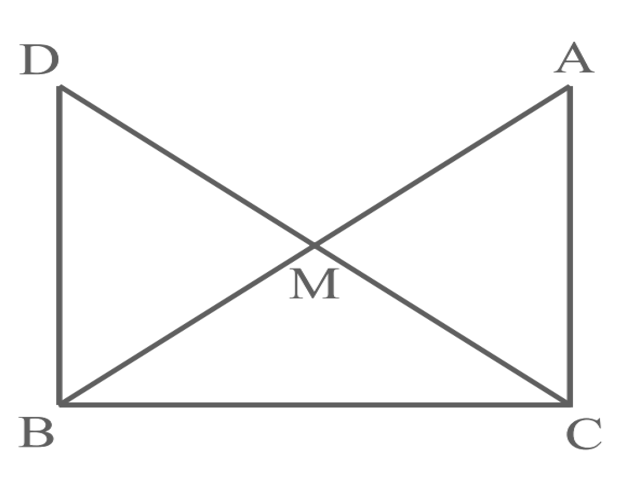
\includegraphics[width=\columnwidth]{figs/Screenshot.png}
  \caption{$\triangle \vec{ACB} ,\triangle \vec{DCB}$ with Mid-Point $\vec{M}$}
  \label{fig:triangles}
\end{figure}
\begin{enumerate}[label =(\roman*)]
        \item $\triangle \vec{AMC} \cong \triangle \vec{BMD}$
        \item $\angle \vec{DBC}$ is a right angle. 
        \item $\triangle \vec{DBC} \cong  \triangle \vec{ACB}$ 
        \item $\vec{CM} = \frac{1}{2} \vec{AB}$
\end{enumerate}
\pagebreak
\solution\\
\textbf{CONSTRUCTION STEPS :}
\begin{enumerate}
\item Let us Assume , the input parameters as ;
\begin{table}[H]
\centering
        \input{tables/input_params.tex}
          \caption{Input Parameters}
          \label{Table-1:Input_params}
\end{table}
\item the output can be calculated as ;
\begin{table}[H]
\centering
        \input{tables/output_params.tex}
          \caption{Output Parameters}
          \label{Table-2:Output_params}
\end{table}
                $\therefore$ By, Plotting these points we get the required Image \figref{fig:fig-2}
\begin{figure}[H]
        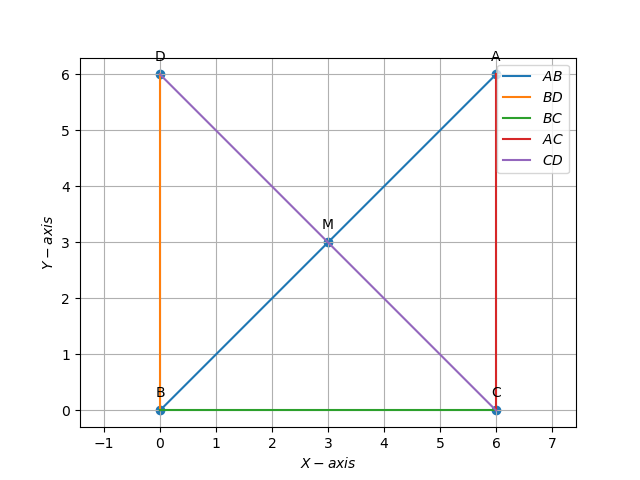
\includegraphics[width = \columnwidth]{figs/python_plot.png}
    \caption{PYTHON Plot of $\triangle \vec{ACB} ,\triangle \vec{DBC}$ with Mid-Point $\vec{M}$}
    \label{fig:fig-2}
\end{figure}
\end{enumerate}

\item Find the position vector of a point $\vec{R}$ which divides the line joining two points $\vec{P}$ and $\vec{Q}$ whose position vectors are $2\vec{a}+\vec{b}$ and $\vec{a}-3\vec{b}$ externally in the ratio $1:2$.

\textbf{Solution:}
Let us assume $\vec{a}$ and $\vec{b}$, and the given ratio is
\begin{table}[h]
    \centering
    \begin{tabular}{|c|c|c|}
        \hline 
        \textbf{Symbol} & \textbf{Value} & \textbf{Description} \\
        \hline
        $\vec{a}$ & $\myvec{1 \\ -3}$ & Vector $\vec{a}$ \\
        \hline
        $\vec{b}$ & $\myvec{0 \\ 2}$ & Vector $\vec{b}$\\
        \hline
        $k$ & $2$ & Ratio \\
        \hline
    \end{tabular}
    \caption{Vectors $\vec{a}$ and $\vec{b}$, ratio $k$}
    \label{tab:table1}
\end{table}

Using the section formula,
\begin{align}
    \vec{R} = \frac{\vec{Q} - k\vec{P}}{1 - k}
\end{align}
where $\vec{P}$ and $\vec{Q}$ depend on $\vec{a}$ and $\vec{b}$, then
\begin{align}
    \vec{P} &= (2\vec{a} + \vec{b}) = 2\myvec{1\\-3} + \myvec{0\\2} = \myvec{2\\-4} \\
    \vec{Q} &= (\vec{a} - 3\vec{b}) = \myvec{1\\-3} - 3\myvec{0\\2} = \myvec{1\\-9}
\end{align}
where $\vec{R}$ can be calculated as 
\begin{align}
    \vec{R} = \frac{(\vec{a} - 3\vec{b}) - k(2\vec{a} + \vec{b})}{1 - k}
\end{align}
By substituting $\vec{a}$ and $\vec{b}$ values, we get $\vec{R}$ as
\begin{align}
    \vec{R} = \myvec{3\\1}
\end{align}

\begin{table}[ht!]
    \centering
    \begin{tabular}{|c|c|c|}
        \hline
        \textbf{Symbol} & \textbf{Value} & \textbf{Description}\\
        \hline
        $\vec{P}$ & $(2\vec{a} + \vec{b})$ & Position vector $\vec{P}$ \\
        \hline
        $\vec{Q}$ & $(\vec{a} - 3\vec{b})$ & Position vector $\vec{Q}$\\
        \hline
        $\vec{R}$ & $\frac{\vec{Q} - k\vec{P}}{1 - k}$ & Position vector $\vec{R}$\\
        \hline
    \end{tabular}
    \caption{Vectors $\vec{P}$, $\vec{Q}$, $\vec{R}$}
    \label{tab:mytable2}   
\end{table}

\begin{figure}[H]
    \centering
    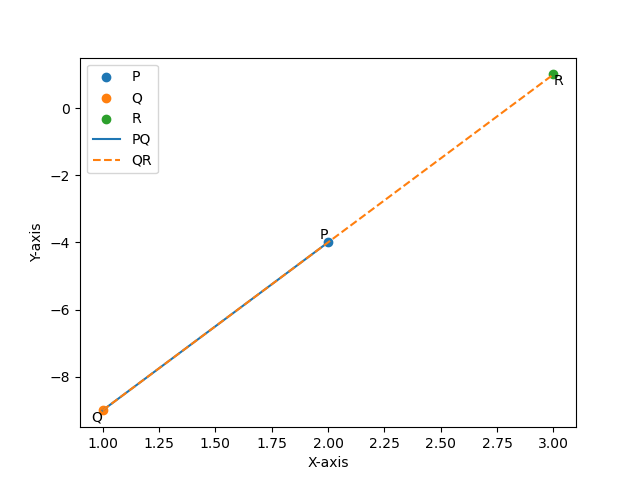
\includegraphics[width=\columnwidth]{figs/external-bisector.png}
    \caption{Point vectors $\vec{P}$, $\vec{Q}$, $\vec{R}$}
    \label{fig:enter-label}
\end{figure}


\end{enumerate}

    \item Draw a quadrilateral in the Cartesian plane, whose vertices are 
    \begin{align}
        \vec{A} = \myvec{-4\\5} \quad \vec{B} = \myvec{0\\7} \\
        \vec{C} = \myvec{5\\-5} \quad \vec{D} = \myvec{-4\\-2}
    \end{align}
    Also, find its area.
\label{chapters/11/10/1/1}
   \\ 
    \solution 
\begin{enumerate}[label=\thesection.\arabic*,ref=\thesection.\theenumi]
		\item Find $\abs{\overrightarrow{a}\times\overrightarrow{b}},\text{ if }\overrightarrow{a}=\hat{i}-7\hat{j}+7\hat{k}\text{ and } \overrightarrow{b}=3\hat{i}-2\hat{j}+2\hat{k}$.
	\\
		\solution
		\input{chapters/12/10/4/1/cross.tex}
\item Show that $$(\overrightarrow{a}-\overrightarrow{b})\times (\overrightarrow{a}+\overrightarrow{b})=2(\overrightarrow{a}\times \overrightarrow{b})$$
	\\
		\solution
		\input{chapters/12/10/4/4/cross.tex}
\item Find $\lambda$ and $\mu$ if $(2\hat{i}+6\hat{j}+27\hat{k})\times(\hat{i}+\lambda \hat{j} + \mu \hat{k})=\overrightarrow{0}$.
	\\
		\solution
		\input{chapters/12/10/4/5/cross.tex}
\item Given that $\overrightarrow{a} \cdot \overrightarrow{b} = 0$ and $\overrightarrow{a} \times \overrightarrow{b} = \overrightarrow{0}$. What can you conclude about the vectors $\overrightarrow{a} \text{ and }\overrightarrow{b}$?
\item Let the vectors be given as $\overrightarrow{a},\overrightarrow{b},\overrightarrow{c}\text{ be given as }\ a_1 \hat{i}+\ a_2 \hat{j}+\ a_3 \hat{k},\ b_1 \hat{i}+\ b_2 \hat{j}+\ b_3 \hat{k},\ c_1 \hat{i}+\ c_2 \hat{j}+\ c_3 \hat{k}$. Then show that $\overrightarrow{a} \times (\overrightarrow{b} + \overrightarrow{c}) = \overrightarrow{a} \times \overrightarrow{b}+\overrightarrow{a} \times \overrightarrow{c}$.
	\\
		\solution
		\input{chapters/12/10/4/7/cross.tex}
\item If either $\overrightarrow{a} = \overrightarrow{0}$ or $\overrightarrow{b} = \overrightarrow{0}$, then $\overrightarrow{a} \times \overrightarrow{b} = \overrightarrow{0}$. Is the converse true? Justify your answer with an example.
	\\
		\solution
		\input{chapters/12/10/4/8/cross.tex}
\item Find the area of the triangle with vertices $A(1, 1, 2)$, $B(2, 3, 5)$, and $C(1, 5, 5)$
	\\
		\solution
		\input{chapters/12/10/4/9/cross.tex}
\item Find the area of the parallelogram whose adjacent sides are determined by the vectors $\overrightarrow{a}=\hat{i}-\hat{j}+3\hat{k}$ and $\overrightarrow{b}=2\hat{i}-7\hat{j}+\hat{k}$.
	\\
		\solution
		\input{chapters/12/10/4/10/cross.tex}
\item Let the vectors $\overrightarrow{a}$ and $\overrightarrow{b}$ be such that $|\overrightarrow{a}| = 3$ and $|\overrightarrow{b}| = \dfrac{\sqrt{2}}{3}$, then $\overrightarrow{a} \times \overrightarrow{b}$ is a unit vector, if the angle between $\overrightarrow{a}$ and $\overrightarrow{b}$ is
\begin{enumerate}
\item $\dfrac{\pi}{6}$
\item $\dfrac{\pi}{4}$
\item $\dfrac{\pi}{3}$
\item $\dfrac{\pi}{2}$
\end{enumerate}
		\solution
		\input{chapters/12/10/4/11/cross.tex}
\item Area of a rectangle having vertices A, B, C and D with position vectors $ -\hat{i}+ \dfrac{1}{2} \hat{j}+4\hat{k},\hat{i}+ \dfrac{1}{2} \hat{j}+4\hat{k},\hat{i}-\dfrac{1}{2} \hat{j}+4\hat{k}\text{ and }-\hat{i}- \dfrac{1}{2} \hat{j}+4\hat{k}$, respectively is
\begin{enumerate}
\item $\dfrac{1}{2}$
\item 1
\item 2
\item 4
\end{enumerate}
		\solution
		\input{chapters/12/10/4/12/cross.tex}
\item Find the area of the triangle whose vertices are 
\begin{enumerate}
\item $(2, 3), (–1, 0), (2, – 4)$
\item $(–5, –1), (3, –5), (5, 2)$ 
\end{enumerate}
		\label{10/7/3/1}
\solution
		\input{chapters/10/7/3/1/area.tex}
\item Find the area of the triangle formed by joining the mid-points of the sides of the triangle whose vertices are $(0, –1), (2, 1) \text{ and } (0, 3)$. Find the ratio of this area to the area of the given triangle.
	\\
\solution
		\input{chapters/10/7/3/3/cross.tex}

\item Find the area of the quadrilateral whose vertices, taken in order, are $(– 4, – 2), (– 3, – 5), (3, – 2)$  and $ (2, 3)$.
	\\
\solution
		\input{chapters/10/7/3/4/cross.tex}

\item Verify that a median of a triangle divides it into two triangles of equal areas for $\triangle ABC$ whose vertices are $\vec{A}(4, -6), \vec{B}(3, 2), \text{ and } \vec{C}(5, 2)$. 
		\label{10/7/3/5}
		\\
\solution
		\input{chapters/10/7/3/5/area.tex}

\item The two adjacent sides of a parallelogram are 
$2\hat{i}-4\hat{j}+5\hat{k}$  and  $\hat{i}-2\hat{j}-3\hat{k}$.
Find the unit vector parallel to its diagonal. Also, find its area.\\
	\solution
		\input{chapters/12/10/5/10/cross.tex}
\item The vertices of a $\triangle ABC$ are $\vec{A}(4,6), \vec{B}(1,5)$ and  $\vec{C}(7,2)$. A line is drawn to intersect sides $AB$ and $AC$ at $\vec{D}$ and $\vec{E}$ respectively, such that $\frac{AD}{AB} = \frac{AE}{AC} = \frac{1}{4}$. Calculate the area of $\triangle ADE$ and compare it with the area of the $\triangle ABC$.
\\
\solution
	\input{chapters/10/7/4/6/section.tex}
    \item Draw a quadrilateral in the Cartesian plane, whose vertices are 
    \begin{align}
        \vec{A} = \myvec{-4\\5} \quad \vec{B} = \myvec{0\\7} \\
        \vec{C} = \myvec{5\\-5} \quad \vec{D} = \myvec{-4\\-2}
    \end{align}
    Also, find its area.
\label{chapters/11/10/1/1}
   \\ 
    \solution 
\input{chapters/11/10/1/1/cross.tex}
\item Find the area of region bounded by the triangle whose
	vertices are $(1, 0), (2, 2) \text{ and } (3, 1)$. 
\item Find the area of region bounded by the triangle whose vertices
	are $(– 1, 0), (1, 3) \text{ and } (3, 2)$. 
\item Find the area of the $\triangle ABC$, coordinates of whose vertices are $\vec{A}(2, 0), \vec{B}(4, 5), \text{ and } \vec{C}(6, 3)$.


\item 
\input{chapters/vectors/exer/main.tex}
\end{enumerate}


\item Find the area of region bounded by the triangle whose
	vertices are $(1, 0), (2, 2) \text{ and } (3, 1)$. 
\item Find the area of region bounded by the triangle whose vertices
	are $(– 1, 0), (1, 3) \text{ and } (3, 2)$. 
\item Find the area of the $\triangle ABC$, coordinates of whose vertices are $\vec{A}(2, 0), \vec{B}(4, 5), \text{ and } \vec{C}(6, 3)$.


\item 
%\documentclass[12pt]{article}
%\usepackage{graphicx}
%\usepackage{graphics}
%\usepackage{refstyle}
%\usepackage{amsmath}
%\usepackage{caption}
%\usepackage{float}
%\usepackage{booktabs}
%\usepackage{array}
%\usepackage{amssymb}
%\usepackage{booktabs}
%\let\vec\mathbf
%\providecommand{\brak}[1]{\ensuremath{\left(#1\right)}}
%\graphicspath{{/storage/self/primary/Download/latexnew/fig}}                                     
$\vec{P}$ and $\vec{Q}$ are any two points lying on the sides $DC$ and $AD$ respectively of a parallelogram $ABCD$.Show that, $ar\brak{\triangle APB}=ar\brak{\triangle BQC}$.


\textbf{Figure:}
\begin{figure}[H]
    \centering
	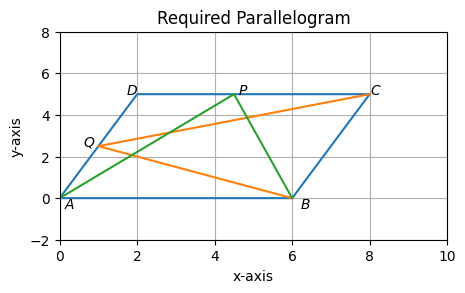
\includegraphics[width=\columnwidth]{chapters/vectors/exer/figs/1.png}
    \caption{}
    \label{fig:fig:1}
\end{figure}


\textbf{Solution:}
\begin{table}[H]
   \centering
  \input{chapters/vectors/exer/table/tab1.tex}
   \caption{Table of input parameters}        
\label{tab:tab:1}                    
\end{table}




\begin{table}[H]
    \centering                                  
\input{chapters/vectors/exer/table/tab2.tex}                  
\caption{Table of output parameters}
\label{tab:tab:2}
 \end{table}


For the $\triangle BQC$, the vertices of the triangle are taken from \tabref{tab:tab:1} and \tabref{tab:tab:2}.

\begin{align}
\implies ar\brak{\triangle BQC}&=
\frac{1}{2}\begin{tabular}{|c c c|}            
1 &1&1\\                      
$\vec{B}$&$\vec{Q}$&$\vec{C}$\\    
\end{tabular}\\
&= \frac{1}{2}\begin{tabular}{|c c c|}
       1 &1&1\\
       6&$\frac{2k_1}{k_1+1}$&8 \\
       0&$\frac{5k_1}{k_1+1}$&5
   \end{tabular}\\
  \xrightarrow{C_2'=C_2-C_1,C_3'=C_3-C_1}&\frac{1}{2} \begin{tabular}{|c c c|}
       1 &0&0\\
       6&$\frac{-4k_1-6}{k_1+1}$&2 \\
       0&$\frac{5k_1}{k_1+1}$&5
   \end{tabular}\\
&=\frac{1}{2}\brak{1\begin{tabular}{|c c|}
   $\frac{-4k_1-6}{k_1+1}$ &2  \\
   $\frac{5k_1}{k_1+1}$ & 5
\end{tabular} +0+0}\\
&=\frac{1}{2} \times30\\                          
&=15 \end{align}


For the $\triangle APB$, the vertices of the triangle are taken from \tabref{tab:tab:1} and \tabref{tab:tab:2}.
   \begin{align}
  \implies ar\brak{\triangle APB} &=
\frac{1}{2}\begin{tabular}{|c c c|}            
1 &1&1\\                            
$\vec{A}$&$\vec{P}$&$\vec{B}$\\
\end{tabular}\\ &=  \frac{1}{2}
   \begin{tabular}{|c c c|}
       1 &1&1\\
       0&$\frac{8k_2+2}{k_2+1}$&6 \\
       0&5&0
   \end{tabular}\\
 &=\frac{1}{2} \times30\\
 &=15 \end{align}
 \brak{6} = \brak{10}


So, ar\brak{\triangle BQC} = ar\brak{\triangle APB}.\brak{proved}
%\end{document}



\end{enumerate}


\item Find the area of the parallelogram whose adjacent sides are determined by the vectors $\overrightarrow{a}=\hat{i}-\hat{j}+3\hat{k}$ and $\overrightarrow{b}=2\hat{i}-7\hat{j}+\hat{k}$.
	\\
		\solution
		\begin{enumerate}[label=\thesection.\arabic*,ref=\thesection.\theenumi]
		\item Find $\abs{\overrightarrow{a}\times\overrightarrow{b}},\text{ if }\overrightarrow{a}=\hat{i}-7\hat{j}+7\hat{k}\text{ and } \overrightarrow{b}=3\hat{i}-2\hat{j}+2\hat{k}$.
	\\
		\solution
		\begin{enumerate}[label=\thesection.\arabic*,ref=\thesection.\theenumi]
		\item Find $\abs{\overrightarrow{a}\times\overrightarrow{b}},\text{ if }\overrightarrow{a}=\hat{i}-7\hat{j}+7\hat{k}\text{ and } \overrightarrow{b}=3\hat{i}-2\hat{j}+2\hat{k}$.
	\\
		\solution
		\input{chapters/12/10/4/1/cross.tex}
\item Show that $$(\overrightarrow{a}-\overrightarrow{b})\times (\overrightarrow{a}+\overrightarrow{b})=2(\overrightarrow{a}\times \overrightarrow{b})$$
	\\
		\solution
		\input{chapters/12/10/4/4/cross.tex}
\item Find $\lambda$ and $\mu$ if $(2\hat{i}+6\hat{j}+27\hat{k})\times(\hat{i}+\lambda \hat{j} + \mu \hat{k})=\overrightarrow{0}$.
	\\
		\solution
		\input{chapters/12/10/4/5/cross.tex}
\item Given that $\overrightarrow{a} \cdot \overrightarrow{b} = 0$ and $\overrightarrow{a} \times \overrightarrow{b} = \overrightarrow{0}$. What can you conclude about the vectors $\overrightarrow{a} \text{ and }\overrightarrow{b}$?
\item Let the vectors be given as $\overrightarrow{a},\overrightarrow{b},\overrightarrow{c}\text{ be given as }\ a_1 \hat{i}+\ a_2 \hat{j}+\ a_3 \hat{k},\ b_1 \hat{i}+\ b_2 \hat{j}+\ b_3 \hat{k},\ c_1 \hat{i}+\ c_2 \hat{j}+\ c_3 \hat{k}$. Then show that $\overrightarrow{a} \times (\overrightarrow{b} + \overrightarrow{c}) = \overrightarrow{a} \times \overrightarrow{b}+\overrightarrow{a} \times \overrightarrow{c}$.
	\\
		\solution
		\input{chapters/12/10/4/7/cross.tex}
\item If either $\overrightarrow{a} = \overrightarrow{0}$ or $\overrightarrow{b} = \overrightarrow{0}$, then $\overrightarrow{a} \times \overrightarrow{b} = \overrightarrow{0}$. Is the converse true? Justify your answer with an example.
	\\
		\solution
		\input{chapters/12/10/4/8/cross.tex}
\item Find the area of the triangle with vertices $A(1, 1, 2)$, $B(2, 3, 5)$, and $C(1, 5, 5)$
	\\
		\solution
		\input{chapters/12/10/4/9/cross.tex}
\item Find the area of the parallelogram whose adjacent sides are determined by the vectors $\overrightarrow{a}=\hat{i}-\hat{j}+3\hat{k}$ and $\overrightarrow{b}=2\hat{i}-7\hat{j}+\hat{k}$.
	\\
		\solution
		\input{chapters/12/10/4/10/cross.tex}
\item Let the vectors $\overrightarrow{a}$ and $\overrightarrow{b}$ be such that $|\overrightarrow{a}| = 3$ and $|\overrightarrow{b}| = \dfrac{\sqrt{2}}{3}$, then $\overrightarrow{a} \times \overrightarrow{b}$ is a unit vector, if the angle between $\overrightarrow{a}$ and $\overrightarrow{b}$ is
\begin{enumerate}
\item $\dfrac{\pi}{6}$
\item $\dfrac{\pi}{4}$
\item $\dfrac{\pi}{3}$
\item $\dfrac{\pi}{2}$
\end{enumerate}
		\solution
		\input{chapters/12/10/4/11/cross.tex}
\item Area of a rectangle having vertices A, B, C and D with position vectors $ -\hat{i}+ \dfrac{1}{2} \hat{j}+4\hat{k},\hat{i}+ \dfrac{1}{2} \hat{j}+4\hat{k},\hat{i}-\dfrac{1}{2} \hat{j}+4\hat{k}\text{ and }-\hat{i}- \dfrac{1}{2} \hat{j}+4\hat{k}$, respectively is
\begin{enumerate}
\item $\dfrac{1}{2}$
\item 1
\item 2
\item 4
\end{enumerate}
		\solution
		\input{chapters/12/10/4/12/cross.tex}
\item Find the area of the triangle whose vertices are 
\begin{enumerate}
\item $(2, 3), (–1, 0), (2, – 4)$
\item $(–5, –1), (3, –5), (5, 2)$ 
\end{enumerate}
		\label{10/7/3/1}
\solution
		\input{chapters/10/7/3/1/area.tex}
\item Find the area of the triangle formed by joining the mid-points of the sides of the triangle whose vertices are $(0, –1), (2, 1) \text{ and } (0, 3)$. Find the ratio of this area to the area of the given triangle.
	\\
\solution
		\input{chapters/10/7/3/3/cross.tex}

\item Find the area of the quadrilateral whose vertices, taken in order, are $(– 4, – 2), (– 3, – 5), (3, – 2)$  and $ (2, 3)$.
	\\
\solution
		\input{chapters/10/7/3/4/cross.tex}

\item Verify that a median of a triangle divides it into two triangles of equal areas for $\triangle ABC$ whose vertices are $\vec{A}(4, -6), \vec{B}(3, 2), \text{ and } \vec{C}(5, 2)$. 
		\label{10/7/3/5}
		\\
\solution
		\input{chapters/10/7/3/5/area.tex}

\item The two adjacent sides of a parallelogram are 
$2\hat{i}-4\hat{j}+5\hat{k}$  and  $\hat{i}-2\hat{j}-3\hat{k}$.
Find the unit vector parallel to its diagonal. Also, find its area.\\
	\solution
		\input{chapters/12/10/5/10/cross.tex}
\item The vertices of a $\triangle ABC$ are $\vec{A}(4,6), \vec{B}(1,5)$ and  $\vec{C}(7,2)$. A line is drawn to intersect sides $AB$ and $AC$ at $\vec{D}$ and $\vec{E}$ respectively, such that $\frac{AD}{AB} = \frac{AE}{AC} = \frac{1}{4}$. Calculate the area of $\triangle ADE$ and compare it with the area of the $\triangle ABC$.
\\
\solution
	\input{chapters/10/7/4/6/section.tex}
    \item Draw a quadrilateral in the Cartesian plane, whose vertices are 
    \begin{align}
        \vec{A} = \myvec{-4\\5} \quad \vec{B} = \myvec{0\\7} \\
        \vec{C} = \myvec{5\\-5} \quad \vec{D} = \myvec{-4\\-2}
    \end{align}
    Also, find its area.
\label{chapters/11/10/1/1}
   \\ 
    \solution 
\input{chapters/11/10/1/1/cross.tex}
\item Find the area of region bounded by the triangle whose
	vertices are $(1, 0), (2, 2) \text{ and } (3, 1)$. 
\item Find the area of region bounded by the triangle whose vertices
	are $(– 1, 0), (1, 3) \text{ and } (3, 2)$. 
\item Find the area of the $\triangle ABC$, coordinates of whose vertices are $\vec{A}(2, 0), \vec{B}(4, 5), \text{ and } \vec{C}(6, 3)$.


\item 
\input{chapters/vectors/exer/main.tex}
\end{enumerate}


\item Show that $$(\overrightarrow{a}-\overrightarrow{b})\times (\overrightarrow{a}+\overrightarrow{b})=2(\overrightarrow{a}\times \overrightarrow{b})$$
	\\
		\solution
		\begin{enumerate}[label=\thesection.\arabic*,ref=\thesection.\theenumi]
		\item Find $\abs{\overrightarrow{a}\times\overrightarrow{b}},\text{ if }\overrightarrow{a}=\hat{i}-7\hat{j}+7\hat{k}\text{ and } \overrightarrow{b}=3\hat{i}-2\hat{j}+2\hat{k}$.
	\\
		\solution
		\input{chapters/12/10/4/1/cross.tex}
\item Show that $$(\overrightarrow{a}-\overrightarrow{b})\times (\overrightarrow{a}+\overrightarrow{b})=2(\overrightarrow{a}\times \overrightarrow{b})$$
	\\
		\solution
		\input{chapters/12/10/4/4/cross.tex}
\item Find $\lambda$ and $\mu$ if $(2\hat{i}+6\hat{j}+27\hat{k})\times(\hat{i}+\lambda \hat{j} + \mu \hat{k})=\overrightarrow{0}$.
	\\
		\solution
		\input{chapters/12/10/4/5/cross.tex}
\item Given that $\overrightarrow{a} \cdot \overrightarrow{b} = 0$ and $\overrightarrow{a} \times \overrightarrow{b} = \overrightarrow{0}$. What can you conclude about the vectors $\overrightarrow{a} \text{ and }\overrightarrow{b}$?
\item Let the vectors be given as $\overrightarrow{a},\overrightarrow{b},\overrightarrow{c}\text{ be given as }\ a_1 \hat{i}+\ a_2 \hat{j}+\ a_3 \hat{k},\ b_1 \hat{i}+\ b_2 \hat{j}+\ b_3 \hat{k},\ c_1 \hat{i}+\ c_2 \hat{j}+\ c_3 \hat{k}$. Then show that $\overrightarrow{a} \times (\overrightarrow{b} + \overrightarrow{c}) = \overrightarrow{a} \times \overrightarrow{b}+\overrightarrow{a} \times \overrightarrow{c}$.
	\\
		\solution
		\input{chapters/12/10/4/7/cross.tex}
\item If either $\overrightarrow{a} = \overrightarrow{0}$ or $\overrightarrow{b} = \overrightarrow{0}$, then $\overrightarrow{a} \times \overrightarrow{b} = \overrightarrow{0}$. Is the converse true? Justify your answer with an example.
	\\
		\solution
		\input{chapters/12/10/4/8/cross.tex}
\item Find the area of the triangle with vertices $A(1, 1, 2)$, $B(2, 3, 5)$, and $C(1, 5, 5)$
	\\
		\solution
		\input{chapters/12/10/4/9/cross.tex}
\item Find the area of the parallelogram whose adjacent sides are determined by the vectors $\overrightarrow{a}=\hat{i}-\hat{j}+3\hat{k}$ and $\overrightarrow{b}=2\hat{i}-7\hat{j}+\hat{k}$.
	\\
		\solution
		\input{chapters/12/10/4/10/cross.tex}
\item Let the vectors $\overrightarrow{a}$ and $\overrightarrow{b}$ be such that $|\overrightarrow{a}| = 3$ and $|\overrightarrow{b}| = \dfrac{\sqrt{2}}{3}$, then $\overrightarrow{a} \times \overrightarrow{b}$ is a unit vector, if the angle between $\overrightarrow{a}$ and $\overrightarrow{b}$ is
\begin{enumerate}
\item $\dfrac{\pi}{6}$
\item $\dfrac{\pi}{4}$
\item $\dfrac{\pi}{3}$
\item $\dfrac{\pi}{2}$
\end{enumerate}
		\solution
		\input{chapters/12/10/4/11/cross.tex}
\item Area of a rectangle having vertices A, B, C and D with position vectors $ -\hat{i}+ \dfrac{1}{2} \hat{j}+4\hat{k},\hat{i}+ \dfrac{1}{2} \hat{j}+4\hat{k},\hat{i}-\dfrac{1}{2} \hat{j}+4\hat{k}\text{ and }-\hat{i}- \dfrac{1}{2} \hat{j}+4\hat{k}$, respectively is
\begin{enumerate}
\item $\dfrac{1}{2}$
\item 1
\item 2
\item 4
\end{enumerate}
		\solution
		\input{chapters/12/10/4/12/cross.tex}
\item Find the area of the triangle whose vertices are 
\begin{enumerate}
\item $(2, 3), (–1, 0), (2, – 4)$
\item $(–5, –1), (3, –5), (5, 2)$ 
\end{enumerate}
		\label{10/7/3/1}
\solution
		\input{chapters/10/7/3/1/area.tex}
\item Find the area of the triangle formed by joining the mid-points of the sides of the triangle whose vertices are $(0, –1), (2, 1) \text{ and } (0, 3)$. Find the ratio of this area to the area of the given triangle.
	\\
\solution
		\input{chapters/10/7/3/3/cross.tex}

\item Find the area of the quadrilateral whose vertices, taken in order, are $(– 4, – 2), (– 3, – 5), (3, – 2)$  and $ (2, 3)$.
	\\
\solution
		\input{chapters/10/7/3/4/cross.tex}

\item Verify that a median of a triangle divides it into two triangles of equal areas for $\triangle ABC$ whose vertices are $\vec{A}(4, -6), \vec{B}(3, 2), \text{ and } \vec{C}(5, 2)$. 
		\label{10/7/3/5}
		\\
\solution
		\input{chapters/10/7/3/5/area.tex}

\item The two adjacent sides of a parallelogram are 
$2\hat{i}-4\hat{j}+5\hat{k}$  and  $\hat{i}-2\hat{j}-3\hat{k}$.
Find the unit vector parallel to its diagonal. Also, find its area.\\
	\solution
		\input{chapters/12/10/5/10/cross.tex}
\item The vertices of a $\triangle ABC$ are $\vec{A}(4,6), \vec{B}(1,5)$ and  $\vec{C}(7,2)$. A line is drawn to intersect sides $AB$ and $AC$ at $\vec{D}$ and $\vec{E}$ respectively, such that $\frac{AD}{AB} = \frac{AE}{AC} = \frac{1}{4}$. Calculate the area of $\triangle ADE$ and compare it with the area of the $\triangle ABC$.
\\
\solution
	\input{chapters/10/7/4/6/section.tex}
    \item Draw a quadrilateral in the Cartesian plane, whose vertices are 
    \begin{align}
        \vec{A} = \myvec{-4\\5} \quad \vec{B} = \myvec{0\\7} \\
        \vec{C} = \myvec{5\\-5} \quad \vec{D} = \myvec{-4\\-2}
    \end{align}
    Also, find its area.
\label{chapters/11/10/1/1}
   \\ 
    \solution 
\input{chapters/11/10/1/1/cross.tex}
\item Find the area of region bounded by the triangle whose
	vertices are $(1, 0), (2, 2) \text{ and } (3, 1)$. 
\item Find the area of region bounded by the triangle whose vertices
	are $(– 1, 0), (1, 3) \text{ and } (3, 2)$. 
\item Find the area of the $\triangle ABC$, coordinates of whose vertices are $\vec{A}(2, 0), \vec{B}(4, 5), \text{ and } \vec{C}(6, 3)$.


\item 
\input{chapters/vectors/exer/main.tex}
\end{enumerate}


\item Find $\lambda$ and $\mu$ if $(2\hat{i}+6\hat{j}+27\hat{k})\times(\hat{i}+\lambda \hat{j} + \mu \hat{k})=\overrightarrow{0}$.
	\\
		\solution
		\begin{enumerate}[label=\thesection.\arabic*,ref=\thesection.\theenumi]
		\item Find $\abs{\overrightarrow{a}\times\overrightarrow{b}},\text{ if }\overrightarrow{a}=\hat{i}-7\hat{j}+7\hat{k}\text{ and } \overrightarrow{b}=3\hat{i}-2\hat{j}+2\hat{k}$.
	\\
		\solution
		\input{chapters/12/10/4/1/cross.tex}
\item Show that $$(\overrightarrow{a}-\overrightarrow{b})\times (\overrightarrow{a}+\overrightarrow{b})=2(\overrightarrow{a}\times \overrightarrow{b})$$
	\\
		\solution
		\input{chapters/12/10/4/4/cross.tex}
\item Find $\lambda$ and $\mu$ if $(2\hat{i}+6\hat{j}+27\hat{k})\times(\hat{i}+\lambda \hat{j} + \mu \hat{k})=\overrightarrow{0}$.
	\\
		\solution
		\input{chapters/12/10/4/5/cross.tex}
\item Given that $\overrightarrow{a} \cdot \overrightarrow{b} = 0$ and $\overrightarrow{a} \times \overrightarrow{b} = \overrightarrow{0}$. What can you conclude about the vectors $\overrightarrow{a} \text{ and }\overrightarrow{b}$?
\item Let the vectors be given as $\overrightarrow{a},\overrightarrow{b},\overrightarrow{c}\text{ be given as }\ a_1 \hat{i}+\ a_2 \hat{j}+\ a_3 \hat{k},\ b_1 \hat{i}+\ b_2 \hat{j}+\ b_3 \hat{k},\ c_1 \hat{i}+\ c_2 \hat{j}+\ c_3 \hat{k}$. Then show that $\overrightarrow{a} \times (\overrightarrow{b} + \overrightarrow{c}) = \overrightarrow{a} \times \overrightarrow{b}+\overrightarrow{a} \times \overrightarrow{c}$.
	\\
		\solution
		\input{chapters/12/10/4/7/cross.tex}
\item If either $\overrightarrow{a} = \overrightarrow{0}$ or $\overrightarrow{b} = \overrightarrow{0}$, then $\overrightarrow{a} \times \overrightarrow{b} = \overrightarrow{0}$. Is the converse true? Justify your answer with an example.
	\\
		\solution
		\input{chapters/12/10/4/8/cross.tex}
\item Find the area of the triangle with vertices $A(1, 1, 2)$, $B(2, 3, 5)$, and $C(1, 5, 5)$
	\\
		\solution
		\input{chapters/12/10/4/9/cross.tex}
\item Find the area of the parallelogram whose adjacent sides are determined by the vectors $\overrightarrow{a}=\hat{i}-\hat{j}+3\hat{k}$ and $\overrightarrow{b}=2\hat{i}-7\hat{j}+\hat{k}$.
	\\
		\solution
		\input{chapters/12/10/4/10/cross.tex}
\item Let the vectors $\overrightarrow{a}$ and $\overrightarrow{b}$ be such that $|\overrightarrow{a}| = 3$ and $|\overrightarrow{b}| = \dfrac{\sqrt{2}}{3}$, then $\overrightarrow{a} \times \overrightarrow{b}$ is a unit vector, if the angle between $\overrightarrow{a}$ and $\overrightarrow{b}$ is
\begin{enumerate}
\item $\dfrac{\pi}{6}$
\item $\dfrac{\pi}{4}$
\item $\dfrac{\pi}{3}$
\item $\dfrac{\pi}{2}$
\end{enumerate}
		\solution
		\input{chapters/12/10/4/11/cross.tex}
\item Area of a rectangle having vertices A, B, C and D with position vectors $ -\hat{i}+ \dfrac{1}{2} \hat{j}+4\hat{k},\hat{i}+ \dfrac{1}{2} \hat{j}+4\hat{k},\hat{i}-\dfrac{1}{2} \hat{j}+4\hat{k}\text{ and }-\hat{i}- \dfrac{1}{2} \hat{j}+4\hat{k}$, respectively is
\begin{enumerate}
\item $\dfrac{1}{2}$
\item 1
\item 2
\item 4
\end{enumerate}
		\solution
		\input{chapters/12/10/4/12/cross.tex}
\item Find the area of the triangle whose vertices are 
\begin{enumerate}
\item $(2, 3), (–1, 0), (2, – 4)$
\item $(–5, –1), (3, –5), (5, 2)$ 
\end{enumerate}
		\label{10/7/3/1}
\solution
		\input{chapters/10/7/3/1/area.tex}
\item Find the area of the triangle formed by joining the mid-points of the sides of the triangle whose vertices are $(0, –1), (2, 1) \text{ and } (0, 3)$. Find the ratio of this area to the area of the given triangle.
	\\
\solution
		\input{chapters/10/7/3/3/cross.tex}

\item Find the area of the quadrilateral whose vertices, taken in order, are $(– 4, – 2), (– 3, – 5), (3, – 2)$  and $ (2, 3)$.
	\\
\solution
		\input{chapters/10/7/3/4/cross.tex}

\item Verify that a median of a triangle divides it into two triangles of equal areas for $\triangle ABC$ whose vertices are $\vec{A}(4, -6), \vec{B}(3, 2), \text{ and } \vec{C}(5, 2)$. 
		\label{10/7/3/5}
		\\
\solution
		\input{chapters/10/7/3/5/area.tex}

\item The two adjacent sides of a parallelogram are 
$2\hat{i}-4\hat{j}+5\hat{k}$  and  $\hat{i}-2\hat{j}-3\hat{k}$.
Find the unit vector parallel to its diagonal. Also, find its area.\\
	\solution
		\input{chapters/12/10/5/10/cross.tex}
\item The vertices of a $\triangle ABC$ are $\vec{A}(4,6), \vec{B}(1,5)$ and  $\vec{C}(7,2)$. A line is drawn to intersect sides $AB$ and $AC$ at $\vec{D}$ and $\vec{E}$ respectively, such that $\frac{AD}{AB} = \frac{AE}{AC} = \frac{1}{4}$. Calculate the area of $\triangle ADE$ and compare it with the area of the $\triangle ABC$.
\\
\solution
	\input{chapters/10/7/4/6/section.tex}
    \item Draw a quadrilateral in the Cartesian plane, whose vertices are 
    \begin{align}
        \vec{A} = \myvec{-4\\5} \quad \vec{B} = \myvec{0\\7} \\
        \vec{C} = \myvec{5\\-5} \quad \vec{D} = \myvec{-4\\-2}
    \end{align}
    Also, find its area.
\label{chapters/11/10/1/1}
   \\ 
    \solution 
\input{chapters/11/10/1/1/cross.tex}
\item Find the area of region bounded by the triangle whose
	vertices are $(1, 0), (2, 2) \text{ and } (3, 1)$. 
\item Find the area of region bounded by the triangle whose vertices
	are $(– 1, 0), (1, 3) \text{ and } (3, 2)$. 
\item Find the area of the $\triangle ABC$, coordinates of whose vertices are $\vec{A}(2, 0), \vec{B}(4, 5), \text{ and } \vec{C}(6, 3)$.


\item 
\input{chapters/vectors/exer/main.tex}
\end{enumerate}


\item Given that $\overrightarrow{a} \cdot \overrightarrow{b} = 0$ and $\overrightarrow{a} \times \overrightarrow{b} = \overrightarrow{0}$. What can you conclude about the vectors $\overrightarrow{a} \text{ and }\overrightarrow{b}$?
\item Let the vectors be given as $\overrightarrow{a},\overrightarrow{b},\overrightarrow{c}\text{ be given as }\ a_1 \hat{i}+\ a_2 \hat{j}+\ a_3 \hat{k},\ b_1 \hat{i}+\ b_2 \hat{j}+\ b_3 \hat{k},\ c_1 \hat{i}+\ c_2 \hat{j}+\ c_3 \hat{k}$. Then show that $\overrightarrow{a} \times (\overrightarrow{b} + \overrightarrow{c}) = \overrightarrow{a} \times \overrightarrow{b}+\overrightarrow{a} \times \overrightarrow{c}$.
	\\
		\solution
		\begin{enumerate}[label=\thesection.\arabic*,ref=\thesection.\theenumi]
		\item Find $\abs{\overrightarrow{a}\times\overrightarrow{b}},\text{ if }\overrightarrow{a}=\hat{i}-7\hat{j}+7\hat{k}\text{ and } \overrightarrow{b}=3\hat{i}-2\hat{j}+2\hat{k}$.
	\\
		\solution
		\input{chapters/12/10/4/1/cross.tex}
\item Show that $$(\overrightarrow{a}-\overrightarrow{b})\times (\overrightarrow{a}+\overrightarrow{b})=2(\overrightarrow{a}\times \overrightarrow{b})$$
	\\
		\solution
		\input{chapters/12/10/4/4/cross.tex}
\item Find $\lambda$ and $\mu$ if $(2\hat{i}+6\hat{j}+27\hat{k})\times(\hat{i}+\lambda \hat{j} + \mu \hat{k})=\overrightarrow{0}$.
	\\
		\solution
		\input{chapters/12/10/4/5/cross.tex}
\item Given that $\overrightarrow{a} \cdot \overrightarrow{b} = 0$ and $\overrightarrow{a} \times \overrightarrow{b} = \overrightarrow{0}$. What can you conclude about the vectors $\overrightarrow{a} \text{ and }\overrightarrow{b}$?
\item Let the vectors be given as $\overrightarrow{a},\overrightarrow{b},\overrightarrow{c}\text{ be given as }\ a_1 \hat{i}+\ a_2 \hat{j}+\ a_3 \hat{k},\ b_1 \hat{i}+\ b_2 \hat{j}+\ b_3 \hat{k},\ c_1 \hat{i}+\ c_2 \hat{j}+\ c_3 \hat{k}$. Then show that $\overrightarrow{a} \times (\overrightarrow{b} + \overrightarrow{c}) = \overrightarrow{a} \times \overrightarrow{b}+\overrightarrow{a} \times \overrightarrow{c}$.
	\\
		\solution
		\input{chapters/12/10/4/7/cross.tex}
\item If either $\overrightarrow{a} = \overrightarrow{0}$ or $\overrightarrow{b} = \overrightarrow{0}$, then $\overrightarrow{a} \times \overrightarrow{b} = \overrightarrow{0}$. Is the converse true? Justify your answer with an example.
	\\
		\solution
		\input{chapters/12/10/4/8/cross.tex}
\item Find the area of the triangle with vertices $A(1, 1, 2)$, $B(2, 3, 5)$, and $C(1, 5, 5)$
	\\
		\solution
		\input{chapters/12/10/4/9/cross.tex}
\item Find the area of the parallelogram whose adjacent sides are determined by the vectors $\overrightarrow{a}=\hat{i}-\hat{j}+3\hat{k}$ and $\overrightarrow{b}=2\hat{i}-7\hat{j}+\hat{k}$.
	\\
		\solution
		\input{chapters/12/10/4/10/cross.tex}
\item Let the vectors $\overrightarrow{a}$ and $\overrightarrow{b}$ be such that $|\overrightarrow{a}| = 3$ and $|\overrightarrow{b}| = \dfrac{\sqrt{2}}{3}$, then $\overrightarrow{a} \times \overrightarrow{b}$ is a unit vector, if the angle between $\overrightarrow{a}$ and $\overrightarrow{b}$ is
\begin{enumerate}
\item $\dfrac{\pi}{6}$
\item $\dfrac{\pi}{4}$
\item $\dfrac{\pi}{3}$
\item $\dfrac{\pi}{2}$
\end{enumerate}
		\solution
		\input{chapters/12/10/4/11/cross.tex}
\item Area of a rectangle having vertices A, B, C and D with position vectors $ -\hat{i}+ \dfrac{1}{2} \hat{j}+4\hat{k},\hat{i}+ \dfrac{1}{2} \hat{j}+4\hat{k},\hat{i}-\dfrac{1}{2} \hat{j}+4\hat{k}\text{ and }-\hat{i}- \dfrac{1}{2} \hat{j}+4\hat{k}$, respectively is
\begin{enumerate}
\item $\dfrac{1}{2}$
\item 1
\item 2
\item 4
\end{enumerate}
		\solution
		\input{chapters/12/10/4/12/cross.tex}
\item Find the area of the triangle whose vertices are 
\begin{enumerate}
\item $(2, 3), (–1, 0), (2, – 4)$
\item $(–5, –1), (3, –5), (5, 2)$ 
\end{enumerate}
		\label{10/7/3/1}
\solution
		\input{chapters/10/7/3/1/area.tex}
\item Find the area of the triangle formed by joining the mid-points of the sides of the triangle whose vertices are $(0, –1), (2, 1) \text{ and } (0, 3)$. Find the ratio of this area to the area of the given triangle.
	\\
\solution
		\input{chapters/10/7/3/3/cross.tex}

\item Find the area of the quadrilateral whose vertices, taken in order, are $(– 4, – 2), (– 3, – 5), (3, – 2)$  and $ (2, 3)$.
	\\
\solution
		\input{chapters/10/7/3/4/cross.tex}

\item Verify that a median of a triangle divides it into two triangles of equal areas for $\triangle ABC$ whose vertices are $\vec{A}(4, -6), \vec{B}(3, 2), \text{ and } \vec{C}(5, 2)$. 
		\label{10/7/3/5}
		\\
\solution
		\input{chapters/10/7/3/5/area.tex}

\item The two adjacent sides of a parallelogram are 
$2\hat{i}-4\hat{j}+5\hat{k}$  and  $\hat{i}-2\hat{j}-3\hat{k}$.
Find the unit vector parallel to its diagonal. Also, find its area.\\
	\solution
		\input{chapters/12/10/5/10/cross.tex}
\item The vertices of a $\triangle ABC$ are $\vec{A}(4,6), \vec{B}(1,5)$ and  $\vec{C}(7,2)$. A line is drawn to intersect sides $AB$ and $AC$ at $\vec{D}$ and $\vec{E}$ respectively, such that $\frac{AD}{AB} = \frac{AE}{AC} = \frac{1}{4}$. Calculate the area of $\triangle ADE$ and compare it with the area of the $\triangle ABC$.
\\
\solution
	\input{chapters/10/7/4/6/section.tex}
    \item Draw a quadrilateral in the Cartesian plane, whose vertices are 
    \begin{align}
        \vec{A} = \myvec{-4\\5} \quad \vec{B} = \myvec{0\\7} \\
        \vec{C} = \myvec{5\\-5} \quad \vec{D} = \myvec{-4\\-2}
    \end{align}
    Also, find its area.
\label{chapters/11/10/1/1}
   \\ 
    \solution 
\input{chapters/11/10/1/1/cross.tex}
\item Find the area of region bounded by the triangle whose
	vertices are $(1, 0), (2, 2) \text{ and } (3, 1)$. 
\item Find the area of region bounded by the triangle whose vertices
	are $(– 1, 0), (1, 3) \text{ and } (3, 2)$. 
\item Find the area of the $\triangle ABC$, coordinates of whose vertices are $\vec{A}(2, 0), \vec{B}(4, 5), \text{ and } \vec{C}(6, 3)$.


\item 
\input{chapters/vectors/exer/main.tex}
\end{enumerate}


\item If either $\overrightarrow{a} = \overrightarrow{0}$ or $\overrightarrow{b} = \overrightarrow{0}$, then $\overrightarrow{a} \times \overrightarrow{b} = \overrightarrow{0}$. Is the converse true? Justify your answer with an example.
	\\
		\solution
		\begin{enumerate}[label=\thesection.\arabic*,ref=\thesection.\theenumi]
		\item Find $\abs{\overrightarrow{a}\times\overrightarrow{b}},\text{ if }\overrightarrow{a}=\hat{i}-7\hat{j}+7\hat{k}\text{ and } \overrightarrow{b}=3\hat{i}-2\hat{j}+2\hat{k}$.
	\\
		\solution
		\input{chapters/12/10/4/1/cross.tex}
\item Show that $$(\overrightarrow{a}-\overrightarrow{b})\times (\overrightarrow{a}+\overrightarrow{b})=2(\overrightarrow{a}\times \overrightarrow{b})$$
	\\
		\solution
		\input{chapters/12/10/4/4/cross.tex}
\item Find $\lambda$ and $\mu$ if $(2\hat{i}+6\hat{j}+27\hat{k})\times(\hat{i}+\lambda \hat{j} + \mu \hat{k})=\overrightarrow{0}$.
	\\
		\solution
		\input{chapters/12/10/4/5/cross.tex}
\item Given that $\overrightarrow{a} \cdot \overrightarrow{b} = 0$ and $\overrightarrow{a} \times \overrightarrow{b} = \overrightarrow{0}$. What can you conclude about the vectors $\overrightarrow{a} \text{ and }\overrightarrow{b}$?
\item Let the vectors be given as $\overrightarrow{a},\overrightarrow{b},\overrightarrow{c}\text{ be given as }\ a_1 \hat{i}+\ a_2 \hat{j}+\ a_3 \hat{k},\ b_1 \hat{i}+\ b_2 \hat{j}+\ b_3 \hat{k},\ c_1 \hat{i}+\ c_2 \hat{j}+\ c_3 \hat{k}$. Then show that $\overrightarrow{a} \times (\overrightarrow{b} + \overrightarrow{c}) = \overrightarrow{a} \times \overrightarrow{b}+\overrightarrow{a} \times \overrightarrow{c}$.
	\\
		\solution
		\input{chapters/12/10/4/7/cross.tex}
\item If either $\overrightarrow{a} = \overrightarrow{0}$ or $\overrightarrow{b} = \overrightarrow{0}$, then $\overrightarrow{a} \times \overrightarrow{b} = \overrightarrow{0}$. Is the converse true? Justify your answer with an example.
	\\
		\solution
		\input{chapters/12/10/4/8/cross.tex}
\item Find the area of the triangle with vertices $A(1, 1, 2)$, $B(2, 3, 5)$, and $C(1, 5, 5)$
	\\
		\solution
		\input{chapters/12/10/4/9/cross.tex}
\item Find the area of the parallelogram whose adjacent sides are determined by the vectors $\overrightarrow{a}=\hat{i}-\hat{j}+3\hat{k}$ and $\overrightarrow{b}=2\hat{i}-7\hat{j}+\hat{k}$.
	\\
		\solution
		\input{chapters/12/10/4/10/cross.tex}
\item Let the vectors $\overrightarrow{a}$ and $\overrightarrow{b}$ be such that $|\overrightarrow{a}| = 3$ and $|\overrightarrow{b}| = \dfrac{\sqrt{2}}{3}$, then $\overrightarrow{a} \times \overrightarrow{b}$ is a unit vector, if the angle between $\overrightarrow{a}$ and $\overrightarrow{b}$ is
\begin{enumerate}
\item $\dfrac{\pi}{6}$
\item $\dfrac{\pi}{4}$
\item $\dfrac{\pi}{3}$
\item $\dfrac{\pi}{2}$
\end{enumerate}
		\solution
		\input{chapters/12/10/4/11/cross.tex}
\item Area of a rectangle having vertices A, B, C and D with position vectors $ -\hat{i}+ \dfrac{1}{2} \hat{j}+4\hat{k},\hat{i}+ \dfrac{1}{2} \hat{j}+4\hat{k},\hat{i}-\dfrac{1}{2} \hat{j}+4\hat{k}\text{ and }-\hat{i}- \dfrac{1}{2} \hat{j}+4\hat{k}$, respectively is
\begin{enumerate}
\item $\dfrac{1}{2}$
\item 1
\item 2
\item 4
\end{enumerate}
		\solution
		\input{chapters/12/10/4/12/cross.tex}
\item Find the area of the triangle whose vertices are 
\begin{enumerate}
\item $(2, 3), (–1, 0), (2, – 4)$
\item $(–5, –1), (3, –5), (5, 2)$ 
\end{enumerate}
		\label{10/7/3/1}
\solution
		\input{chapters/10/7/3/1/area.tex}
\item Find the area of the triangle formed by joining the mid-points of the sides of the triangle whose vertices are $(0, –1), (2, 1) \text{ and } (0, 3)$. Find the ratio of this area to the area of the given triangle.
	\\
\solution
		\input{chapters/10/7/3/3/cross.tex}

\item Find the area of the quadrilateral whose vertices, taken in order, are $(– 4, – 2), (– 3, – 5), (3, – 2)$  and $ (2, 3)$.
	\\
\solution
		\input{chapters/10/7/3/4/cross.tex}

\item Verify that a median of a triangle divides it into two triangles of equal areas for $\triangle ABC$ whose vertices are $\vec{A}(4, -6), \vec{B}(3, 2), \text{ and } \vec{C}(5, 2)$. 
		\label{10/7/3/5}
		\\
\solution
		\input{chapters/10/7/3/5/area.tex}

\item The two adjacent sides of a parallelogram are 
$2\hat{i}-4\hat{j}+5\hat{k}$  and  $\hat{i}-2\hat{j}-3\hat{k}$.
Find the unit vector parallel to its diagonal. Also, find its area.\\
	\solution
		\input{chapters/12/10/5/10/cross.tex}
\item The vertices of a $\triangle ABC$ are $\vec{A}(4,6), \vec{B}(1,5)$ and  $\vec{C}(7,2)$. A line is drawn to intersect sides $AB$ and $AC$ at $\vec{D}$ and $\vec{E}$ respectively, such that $\frac{AD}{AB} = \frac{AE}{AC} = \frac{1}{4}$. Calculate the area of $\triangle ADE$ and compare it with the area of the $\triangle ABC$.
\\
\solution
	\input{chapters/10/7/4/6/section.tex}
    \item Draw a quadrilateral in the Cartesian plane, whose vertices are 
    \begin{align}
        \vec{A} = \myvec{-4\\5} \quad \vec{B} = \myvec{0\\7} \\
        \vec{C} = \myvec{5\\-5} \quad \vec{D} = \myvec{-4\\-2}
    \end{align}
    Also, find its area.
\label{chapters/11/10/1/1}
   \\ 
    \solution 
\input{chapters/11/10/1/1/cross.tex}
\item Find the area of region bounded by the triangle whose
	vertices are $(1, 0), (2, 2) \text{ and } (3, 1)$. 
\item Find the area of region bounded by the triangle whose vertices
	are $(– 1, 0), (1, 3) \text{ and } (3, 2)$. 
\item Find the area of the $\triangle ABC$, coordinates of whose vertices are $\vec{A}(2, 0), \vec{B}(4, 5), \text{ and } \vec{C}(6, 3)$.


\item 
\input{chapters/vectors/exer/main.tex}
\end{enumerate}


\item Find the area of the triangle with vertices $A(1, 1, 2)$, $B(2, 3, 5)$, and $C(1, 5, 5)$
	\\
		\solution
		\begin{enumerate}[label=\thesection.\arabic*,ref=\thesection.\theenumi]
		\item Find $\abs{\overrightarrow{a}\times\overrightarrow{b}},\text{ if }\overrightarrow{a}=\hat{i}-7\hat{j}+7\hat{k}\text{ and } \overrightarrow{b}=3\hat{i}-2\hat{j}+2\hat{k}$.
	\\
		\solution
		\input{chapters/12/10/4/1/cross.tex}
\item Show that $$(\overrightarrow{a}-\overrightarrow{b})\times (\overrightarrow{a}+\overrightarrow{b})=2(\overrightarrow{a}\times \overrightarrow{b})$$
	\\
		\solution
		\input{chapters/12/10/4/4/cross.tex}
\item Find $\lambda$ and $\mu$ if $(2\hat{i}+6\hat{j}+27\hat{k})\times(\hat{i}+\lambda \hat{j} + \mu \hat{k})=\overrightarrow{0}$.
	\\
		\solution
		\input{chapters/12/10/4/5/cross.tex}
\item Given that $\overrightarrow{a} \cdot \overrightarrow{b} = 0$ and $\overrightarrow{a} \times \overrightarrow{b} = \overrightarrow{0}$. What can you conclude about the vectors $\overrightarrow{a} \text{ and }\overrightarrow{b}$?
\item Let the vectors be given as $\overrightarrow{a},\overrightarrow{b},\overrightarrow{c}\text{ be given as }\ a_1 \hat{i}+\ a_2 \hat{j}+\ a_3 \hat{k},\ b_1 \hat{i}+\ b_2 \hat{j}+\ b_3 \hat{k},\ c_1 \hat{i}+\ c_2 \hat{j}+\ c_3 \hat{k}$. Then show that $\overrightarrow{a} \times (\overrightarrow{b} + \overrightarrow{c}) = \overrightarrow{a} \times \overrightarrow{b}+\overrightarrow{a} \times \overrightarrow{c}$.
	\\
		\solution
		\input{chapters/12/10/4/7/cross.tex}
\item If either $\overrightarrow{a} = \overrightarrow{0}$ or $\overrightarrow{b} = \overrightarrow{0}$, then $\overrightarrow{a} \times \overrightarrow{b} = \overrightarrow{0}$. Is the converse true? Justify your answer with an example.
	\\
		\solution
		\input{chapters/12/10/4/8/cross.tex}
\item Find the area of the triangle with vertices $A(1, 1, 2)$, $B(2, 3, 5)$, and $C(1, 5, 5)$
	\\
		\solution
		\input{chapters/12/10/4/9/cross.tex}
\item Find the area of the parallelogram whose adjacent sides are determined by the vectors $\overrightarrow{a}=\hat{i}-\hat{j}+3\hat{k}$ and $\overrightarrow{b}=2\hat{i}-7\hat{j}+\hat{k}$.
	\\
		\solution
		\input{chapters/12/10/4/10/cross.tex}
\item Let the vectors $\overrightarrow{a}$ and $\overrightarrow{b}$ be such that $|\overrightarrow{a}| = 3$ and $|\overrightarrow{b}| = \dfrac{\sqrt{2}}{3}$, then $\overrightarrow{a} \times \overrightarrow{b}$ is a unit vector, if the angle between $\overrightarrow{a}$ and $\overrightarrow{b}$ is
\begin{enumerate}
\item $\dfrac{\pi}{6}$
\item $\dfrac{\pi}{4}$
\item $\dfrac{\pi}{3}$
\item $\dfrac{\pi}{2}$
\end{enumerate}
		\solution
		\input{chapters/12/10/4/11/cross.tex}
\item Area of a rectangle having vertices A, B, C and D with position vectors $ -\hat{i}+ \dfrac{1}{2} \hat{j}+4\hat{k},\hat{i}+ \dfrac{1}{2} \hat{j}+4\hat{k},\hat{i}-\dfrac{1}{2} \hat{j}+4\hat{k}\text{ and }-\hat{i}- \dfrac{1}{2} \hat{j}+4\hat{k}$, respectively is
\begin{enumerate}
\item $\dfrac{1}{2}$
\item 1
\item 2
\item 4
\end{enumerate}
		\solution
		\input{chapters/12/10/4/12/cross.tex}
\item Find the area of the triangle whose vertices are 
\begin{enumerate}
\item $(2, 3), (–1, 0), (2, – 4)$
\item $(–5, –1), (3, –5), (5, 2)$ 
\end{enumerate}
		\label{10/7/3/1}
\solution
		\input{chapters/10/7/3/1/area.tex}
\item Find the area of the triangle formed by joining the mid-points of the sides of the triangle whose vertices are $(0, –1), (2, 1) \text{ and } (0, 3)$. Find the ratio of this area to the area of the given triangle.
	\\
\solution
		\input{chapters/10/7/3/3/cross.tex}

\item Find the area of the quadrilateral whose vertices, taken in order, are $(– 4, – 2), (– 3, – 5), (3, – 2)$  and $ (2, 3)$.
	\\
\solution
		\input{chapters/10/7/3/4/cross.tex}

\item Verify that a median of a triangle divides it into two triangles of equal areas for $\triangle ABC$ whose vertices are $\vec{A}(4, -6), \vec{B}(3, 2), \text{ and } \vec{C}(5, 2)$. 
		\label{10/7/3/5}
		\\
\solution
		\input{chapters/10/7/3/5/area.tex}

\item The two adjacent sides of a parallelogram are 
$2\hat{i}-4\hat{j}+5\hat{k}$  and  $\hat{i}-2\hat{j}-3\hat{k}$.
Find the unit vector parallel to its diagonal. Also, find its area.\\
	\solution
		\input{chapters/12/10/5/10/cross.tex}
\item The vertices of a $\triangle ABC$ are $\vec{A}(4,6), \vec{B}(1,5)$ and  $\vec{C}(7,2)$. A line is drawn to intersect sides $AB$ and $AC$ at $\vec{D}$ and $\vec{E}$ respectively, such that $\frac{AD}{AB} = \frac{AE}{AC} = \frac{1}{4}$. Calculate the area of $\triangle ADE$ and compare it with the area of the $\triangle ABC$.
\\
\solution
	\input{chapters/10/7/4/6/section.tex}
    \item Draw a quadrilateral in the Cartesian plane, whose vertices are 
    \begin{align}
        \vec{A} = \myvec{-4\\5} \quad \vec{B} = \myvec{0\\7} \\
        \vec{C} = \myvec{5\\-5} \quad \vec{D} = \myvec{-4\\-2}
    \end{align}
    Also, find its area.
\label{chapters/11/10/1/1}
   \\ 
    \solution 
\input{chapters/11/10/1/1/cross.tex}
\item Find the area of region bounded by the triangle whose
	vertices are $(1, 0), (2, 2) \text{ and } (3, 1)$. 
\item Find the area of region bounded by the triangle whose vertices
	are $(– 1, 0), (1, 3) \text{ and } (3, 2)$. 
\item Find the area of the $\triangle ABC$, coordinates of whose vertices are $\vec{A}(2, 0), \vec{B}(4, 5), \text{ and } \vec{C}(6, 3)$.


\item 
\input{chapters/vectors/exer/main.tex}
\end{enumerate}


\item Find the area of the parallelogram whose adjacent sides are determined by the vectors $\overrightarrow{a}=\hat{i}-\hat{j}+3\hat{k}$ and $\overrightarrow{b}=2\hat{i}-7\hat{j}+\hat{k}$.
	\\
		\solution
		\begin{enumerate}[label=\thesection.\arabic*,ref=\thesection.\theenumi]
		\item Find $\abs{\overrightarrow{a}\times\overrightarrow{b}},\text{ if }\overrightarrow{a}=\hat{i}-7\hat{j}+7\hat{k}\text{ and } \overrightarrow{b}=3\hat{i}-2\hat{j}+2\hat{k}$.
	\\
		\solution
		\input{chapters/12/10/4/1/cross.tex}
\item Show that $$(\overrightarrow{a}-\overrightarrow{b})\times (\overrightarrow{a}+\overrightarrow{b})=2(\overrightarrow{a}\times \overrightarrow{b})$$
	\\
		\solution
		\input{chapters/12/10/4/4/cross.tex}
\item Find $\lambda$ and $\mu$ if $(2\hat{i}+6\hat{j}+27\hat{k})\times(\hat{i}+\lambda \hat{j} + \mu \hat{k})=\overrightarrow{0}$.
	\\
		\solution
		\input{chapters/12/10/4/5/cross.tex}
\item Given that $\overrightarrow{a} \cdot \overrightarrow{b} = 0$ and $\overrightarrow{a} \times \overrightarrow{b} = \overrightarrow{0}$. What can you conclude about the vectors $\overrightarrow{a} \text{ and }\overrightarrow{b}$?
\item Let the vectors be given as $\overrightarrow{a},\overrightarrow{b},\overrightarrow{c}\text{ be given as }\ a_1 \hat{i}+\ a_2 \hat{j}+\ a_3 \hat{k},\ b_1 \hat{i}+\ b_2 \hat{j}+\ b_3 \hat{k},\ c_1 \hat{i}+\ c_2 \hat{j}+\ c_3 \hat{k}$. Then show that $\overrightarrow{a} \times (\overrightarrow{b} + \overrightarrow{c}) = \overrightarrow{a} \times \overrightarrow{b}+\overrightarrow{a} \times \overrightarrow{c}$.
	\\
		\solution
		\input{chapters/12/10/4/7/cross.tex}
\item If either $\overrightarrow{a} = \overrightarrow{0}$ or $\overrightarrow{b} = \overrightarrow{0}$, then $\overrightarrow{a} \times \overrightarrow{b} = \overrightarrow{0}$. Is the converse true? Justify your answer with an example.
	\\
		\solution
		\input{chapters/12/10/4/8/cross.tex}
\item Find the area of the triangle with vertices $A(1, 1, 2)$, $B(2, 3, 5)$, and $C(1, 5, 5)$
	\\
		\solution
		\input{chapters/12/10/4/9/cross.tex}
\item Find the area of the parallelogram whose adjacent sides are determined by the vectors $\overrightarrow{a}=\hat{i}-\hat{j}+3\hat{k}$ and $\overrightarrow{b}=2\hat{i}-7\hat{j}+\hat{k}$.
	\\
		\solution
		\input{chapters/12/10/4/10/cross.tex}
\item Let the vectors $\overrightarrow{a}$ and $\overrightarrow{b}$ be such that $|\overrightarrow{a}| = 3$ and $|\overrightarrow{b}| = \dfrac{\sqrt{2}}{3}$, then $\overrightarrow{a} \times \overrightarrow{b}$ is a unit vector, if the angle between $\overrightarrow{a}$ and $\overrightarrow{b}$ is
\begin{enumerate}
\item $\dfrac{\pi}{6}$
\item $\dfrac{\pi}{4}$
\item $\dfrac{\pi}{3}$
\item $\dfrac{\pi}{2}$
\end{enumerate}
		\solution
		\input{chapters/12/10/4/11/cross.tex}
\item Area of a rectangle having vertices A, B, C and D with position vectors $ -\hat{i}+ \dfrac{1}{2} \hat{j}+4\hat{k},\hat{i}+ \dfrac{1}{2} \hat{j}+4\hat{k},\hat{i}-\dfrac{1}{2} \hat{j}+4\hat{k}\text{ and }-\hat{i}- \dfrac{1}{2} \hat{j}+4\hat{k}$, respectively is
\begin{enumerate}
\item $\dfrac{1}{2}$
\item 1
\item 2
\item 4
\end{enumerate}
		\solution
		\input{chapters/12/10/4/12/cross.tex}
\item Find the area of the triangle whose vertices are 
\begin{enumerate}
\item $(2, 3), (–1, 0), (2, – 4)$
\item $(–5, –1), (3, –5), (5, 2)$ 
\end{enumerate}
		\label{10/7/3/1}
\solution
		\input{chapters/10/7/3/1/area.tex}
\item Find the area of the triangle formed by joining the mid-points of the sides of the triangle whose vertices are $(0, –1), (2, 1) \text{ and } (0, 3)$. Find the ratio of this area to the area of the given triangle.
	\\
\solution
		\input{chapters/10/7/3/3/cross.tex}

\item Find the area of the quadrilateral whose vertices, taken in order, are $(– 4, – 2), (– 3, – 5), (3, – 2)$  and $ (2, 3)$.
	\\
\solution
		\input{chapters/10/7/3/4/cross.tex}

\item Verify that a median of a triangle divides it into two triangles of equal areas for $\triangle ABC$ whose vertices are $\vec{A}(4, -6), \vec{B}(3, 2), \text{ and } \vec{C}(5, 2)$. 
		\label{10/7/3/5}
		\\
\solution
		\input{chapters/10/7/3/5/area.tex}

\item The two adjacent sides of a parallelogram are 
$2\hat{i}-4\hat{j}+5\hat{k}$  and  $\hat{i}-2\hat{j}-3\hat{k}$.
Find the unit vector parallel to its diagonal. Also, find its area.\\
	\solution
		\input{chapters/12/10/5/10/cross.tex}
\item The vertices of a $\triangle ABC$ are $\vec{A}(4,6), \vec{B}(1,5)$ and  $\vec{C}(7,2)$. A line is drawn to intersect sides $AB$ and $AC$ at $\vec{D}$ and $\vec{E}$ respectively, such that $\frac{AD}{AB} = \frac{AE}{AC} = \frac{1}{4}$. Calculate the area of $\triangle ADE$ and compare it with the area of the $\triangle ABC$.
\\
\solution
	\input{chapters/10/7/4/6/section.tex}
    \item Draw a quadrilateral in the Cartesian plane, whose vertices are 
    \begin{align}
        \vec{A} = \myvec{-4\\5} \quad \vec{B} = \myvec{0\\7} \\
        \vec{C} = \myvec{5\\-5} \quad \vec{D} = \myvec{-4\\-2}
    \end{align}
    Also, find its area.
\label{chapters/11/10/1/1}
   \\ 
    \solution 
\input{chapters/11/10/1/1/cross.tex}
\item Find the area of region bounded by the triangle whose
	vertices are $(1, 0), (2, 2) \text{ and } (3, 1)$. 
\item Find the area of region bounded by the triangle whose vertices
	are $(– 1, 0), (1, 3) \text{ and } (3, 2)$. 
\item Find the area of the $\triangle ABC$, coordinates of whose vertices are $\vec{A}(2, 0), \vec{B}(4, 5), \text{ and } \vec{C}(6, 3)$.


\item 
\input{chapters/vectors/exer/main.tex}
\end{enumerate}


\item Let the vectors $\overrightarrow{a}$ and $\overrightarrow{b}$ be such that $|\overrightarrow{a}| = 3$ and $|\overrightarrow{b}| = \dfrac{\sqrt{2}}{3}$, then $\overrightarrow{a} \times \overrightarrow{b}$ is a unit vector, if the angle between $\overrightarrow{a}$ and $\overrightarrow{b}$ is
\begin{enumerate}
\item $\dfrac{\pi}{6}$
\item $\dfrac{\pi}{4}$
\item $\dfrac{\pi}{3}$
\item $\dfrac{\pi}{2}$
\end{enumerate}
		\solution
		\begin{enumerate}[label=\thesection.\arabic*,ref=\thesection.\theenumi]
		\item Find $\abs{\overrightarrow{a}\times\overrightarrow{b}},\text{ if }\overrightarrow{a}=\hat{i}-7\hat{j}+7\hat{k}\text{ and } \overrightarrow{b}=3\hat{i}-2\hat{j}+2\hat{k}$.
	\\
		\solution
		\input{chapters/12/10/4/1/cross.tex}
\item Show that $$(\overrightarrow{a}-\overrightarrow{b})\times (\overrightarrow{a}+\overrightarrow{b})=2(\overrightarrow{a}\times \overrightarrow{b})$$
	\\
		\solution
		\input{chapters/12/10/4/4/cross.tex}
\item Find $\lambda$ and $\mu$ if $(2\hat{i}+6\hat{j}+27\hat{k})\times(\hat{i}+\lambda \hat{j} + \mu \hat{k})=\overrightarrow{0}$.
	\\
		\solution
		\input{chapters/12/10/4/5/cross.tex}
\item Given that $\overrightarrow{a} \cdot \overrightarrow{b} = 0$ and $\overrightarrow{a} \times \overrightarrow{b} = \overrightarrow{0}$. What can you conclude about the vectors $\overrightarrow{a} \text{ and }\overrightarrow{b}$?
\item Let the vectors be given as $\overrightarrow{a},\overrightarrow{b},\overrightarrow{c}\text{ be given as }\ a_1 \hat{i}+\ a_2 \hat{j}+\ a_3 \hat{k},\ b_1 \hat{i}+\ b_2 \hat{j}+\ b_3 \hat{k},\ c_1 \hat{i}+\ c_2 \hat{j}+\ c_3 \hat{k}$. Then show that $\overrightarrow{a} \times (\overrightarrow{b} + \overrightarrow{c}) = \overrightarrow{a} \times \overrightarrow{b}+\overrightarrow{a} \times \overrightarrow{c}$.
	\\
		\solution
		\input{chapters/12/10/4/7/cross.tex}
\item If either $\overrightarrow{a} = \overrightarrow{0}$ or $\overrightarrow{b} = \overrightarrow{0}$, then $\overrightarrow{a} \times \overrightarrow{b} = \overrightarrow{0}$. Is the converse true? Justify your answer with an example.
	\\
		\solution
		\input{chapters/12/10/4/8/cross.tex}
\item Find the area of the triangle with vertices $A(1, 1, 2)$, $B(2, 3, 5)$, and $C(1, 5, 5)$
	\\
		\solution
		\input{chapters/12/10/4/9/cross.tex}
\item Find the area of the parallelogram whose adjacent sides are determined by the vectors $\overrightarrow{a}=\hat{i}-\hat{j}+3\hat{k}$ and $\overrightarrow{b}=2\hat{i}-7\hat{j}+\hat{k}$.
	\\
		\solution
		\input{chapters/12/10/4/10/cross.tex}
\item Let the vectors $\overrightarrow{a}$ and $\overrightarrow{b}$ be such that $|\overrightarrow{a}| = 3$ and $|\overrightarrow{b}| = \dfrac{\sqrt{2}}{3}$, then $\overrightarrow{a} \times \overrightarrow{b}$ is a unit vector, if the angle between $\overrightarrow{a}$ and $\overrightarrow{b}$ is
\begin{enumerate}
\item $\dfrac{\pi}{6}$
\item $\dfrac{\pi}{4}$
\item $\dfrac{\pi}{3}$
\item $\dfrac{\pi}{2}$
\end{enumerate}
		\solution
		\input{chapters/12/10/4/11/cross.tex}
\item Area of a rectangle having vertices A, B, C and D with position vectors $ -\hat{i}+ \dfrac{1}{2} \hat{j}+4\hat{k},\hat{i}+ \dfrac{1}{2} \hat{j}+4\hat{k},\hat{i}-\dfrac{1}{2} \hat{j}+4\hat{k}\text{ and }-\hat{i}- \dfrac{1}{2} \hat{j}+4\hat{k}$, respectively is
\begin{enumerate}
\item $\dfrac{1}{2}$
\item 1
\item 2
\item 4
\end{enumerate}
		\solution
		\input{chapters/12/10/4/12/cross.tex}
\item Find the area of the triangle whose vertices are 
\begin{enumerate}
\item $(2, 3), (–1, 0), (2, – 4)$
\item $(–5, –1), (3, –5), (5, 2)$ 
\end{enumerate}
		\label{10/7/3/1}
\solution
		\input{chapters/10/7/3/1/area.tex}
\item Find the area of the triangle formed by joining the mid-points of the sides of the triangle whose vertices are $(0, –1), (2, 1) \text{ and } (0, 3)$. Find the ratio of this area to the area of the given triangle.
	\\
\solution
		\input{chapters/10/7/3/3/cross.tex}

\item Find the area of the quadrilateral whose vertices, taken in order, are $(– 4, – 2), (– 3, – 5), (3, – 2)$  and $ (2, 3)$.
	\\
\solution
		\input{chapters/10/7/3/4/cross.tex}

\item Verify that a median of a triangle divides it into two triangles of equal areas for $\triangle ABC$ whose vertices are $\vec{A}(4, -6), \vec{B}(3, 2), \text{ and } \vec{C}(5, 2)$. 
		\label{10/7/3/5}
		\\
\solution
		\input{chapters/10/7/3/5/area.tex}

\item The two adjacent sides of a parallelogram are 
$2\hat{i}-4\hat{j}+5\hat{k}$  and  $\hat{i}-2\hat{j}-3\hat{k}$.
Find the unit vector parallel to its diagonal. Also, find its area.\\
	\solution
		\input{chapters/12/10/5/10/cross.tex}
\item The vertices of a $\triangle ABC$ are $\vec{A}(4,6), \vec{B}(1,5)$ and  $\vec{C}(7,2)$. A line is drawn to intersect sides $AB$ and $AC$ at $\vec{D}$ and $\vec{E}$ respectively, such that $\frac{AD}{AB} = \frac{AE}{AC} = \frac{1}{4}$. Calculate the area of $\triangle ADE$ and compare it with the area of the $\triangle ABC$.
\\
\solution
	\input{chapters/10/7/4/6/section.tex}
    \item Draw a quadrilateral in the Cartesian plane, whose vertices are 
    \begin{align}
        \vec{A} = \myvec{-4\\5} \quad \vec{B} = \myvec{0\\7} \\
        \vec{C} = \myvec{5\\-5} \quad \vec{D} = \myvec{-4\\-2}
    \end{align}
    Also, find its area.
\label{chapters/11/10/1/1}
   \\ 
    \solution 
\input{chapters/11/10/1/1/cross.tex}
\item Find the area of region bounded by the triangle whose
	vertices are $(1, 0), (2, 2) \text{ and } (3, 1)$. 
\item Find the area of region bounded by the triangle whose vertices
	are $(– 1, 0), (1, 3) \text{ and } (3, 2)$. 
\item Find the area of the $\triangle ABC$, coordinates of whose vertices are $\vec{A}(2, 0), \vec{B}(4, 5), \text{ and } \vec{C}(6, 3)$.


\item 
\input{chapters/vectors/exer/main.tex}
\end{enumerate}


\item Area of a rectangle having vertices A, B, C and D with position vectors $ -\hat{i}+ \dfrac{1}{2} \hat{j}+4\hat{k},\hat{i}+ \dfrac{1}{2} \hat{j}+4\hat{k},\hat{i}-\dfrac{1}{2} \hat{j}+4\hat{k}\text{ and }-\hat{i}- \dfrac{1}{2} \hat{j}+4\hat{k}$, respectively is
\begin{enumerate}
\item $\dfrac{1}{2}$
\item 1
\item 2
\item 4
\end{enumerate}
		\solution
		\begin{enumerate}[label=\thesection.\arabic*,ref=\thesection.\theenumi]
		\item Find $\abs{\overrightarrow{a}\times\overrightarrow{b}},\text{ if }\overrightarrow{a}=\hat{i}-7\hat{j}+7\hat{k}\text{ and } \overrightarrow{b}=3\hat{i}-2\hat{j}+2\hat{k}$.
	\\
		\solution
		\input{chapters/12/10/4/1/cross.tex}
\item Show that $$(\overrightarrow{a}-\overrightarrow{b})\times (\overrightarrow{a}+\overrightarrow{b})=2(\overrightarrow{a}\times \overrightarrow{b})$$
	\\
		\solution
		\input{chapters/12/10/4/4/cross.tex}
\item Find $\lambda$ and $\mu$ if $(2\hat{i}+6\hat{j}+27\hat{k})\times(\hat{i}+\lambda \hat{j} + \mu \hat{k})=\overrightarrow{0}$.
	\\
		\solution
		\input{chapters/12/10/4/5/cross.tex}
\item Given that $\overrightarrow{a} \cdot \overrightarrow{b} = 0$ and $\overrightarrow{a} \times \overrightarrow{b} = \overrightarrow{0}$. What can you conclude about the vectors $\overrightarrow{a} \text{ and }\overrightarrow{b}$?
\item Let the vectors be given as $\overrightarrow{a},\overrightarrow{b},\overrightarrow{c}\text{ be given as }\ a_1 \hat{i}+\ a_2 \hat{j}+\ a_3 \hat{k},\ b_1 \hat{i}+\ b_2 \hat{j}+\ b_3 \hat{k},\ c_1 \hat{i}+\ c_2 \hat{j}+\ c_3 \hat{k}$. Then show that $\overrightarrow{a} \times (\overrightarrow{b} + \overrightarrow{c}) = \overrightarrow{a} \times \overrightarrow{b}+\overrightarrow{a} \times \overrightarrow{c}$.
	\\
		\solution
		\input{chapters/12/10/4/7/cross.tex}
\item If either $\overrightarrow{a} = \overrightarrow{0}$ or $\overrightarrow{b} = \overrightarrow{0}$, then $\overrightarrow{a} \times \overrightarrow{b} = \overrightarrow{0}$. Is the converse true? Justify your answer with an example.
	\\
		\solution
		\input{chapters/12/10/4/8/cross.tex}
\item Find the area of the triangle with vertices $A(1, 1, 2)$, $B(2, 3, 5)$, and $C(1, 5, 5)$
	\\
		\solution
		\input{chapters/12/10/4/9/cross.tex}
\item Find the area of the parallelogram whose adjacent sides are determined by the vectors $\overrightarrow{a}=\hat{i}-\hat{j}+3\hat{k}$ and $\overrightarrow{b}=2\hat{i}-7\hat{j}+\hat{k}$.
	\\
		\solution
		\input{chapters/12/10/4/10/cross.tex}
\item Let the vectors $\overrightarrow{a}$ and $\overrightarrow{b}$ be such that $|\overrightarrow{a}| = 3$ and $|\overrightarrow{b}| = \dfrac{\sqrt{2}}{3}$, then $\overrightarrow{a} \times \overrightarrow{b}$ is a unit vector, if the angle between $\overrightarrow{a}$ and $\overrightarrow{b}$ is
\begin{enumerate}
\item $\dfrac{\pi}{6}$
\item $\dfrac{\pi}{4}$
\item $\dfrac{\pi}{3}$
\item $\dfrac{\pi}{2}$
\end{enumerate}
		\solution
		\input{chapters/12/10/4/11/cross.tex}
\item Area of a rectangle having vertices A, B, C and D with position vectors $ -\hat{i}+ \dfrac{1}{2} \hat{j}+4\hat{k},\hat{i}+ \dfrac{1}{2} \hat{j}+4\hat{k},\hat{i}-\dfrac{1}{2} \hat{j}+4\hat{k}\text{ and }-\hat{i}- \dfrac{1}{2} \hat{j}+4\hat{k}$, respectively is
\begin{enumerate}
\item $\dfrac{1}{2}$
\item 1
\item 2
\item 4
\end{enumerate}
		\solution
		\input{chapters/12/10/4/12/cross.tex}
\item Find the area of the triangle whose vertices are 
\begin{enumerate}
\item $(2, 3), (–1, 0), (2, – 4)$
\item $(–5, –1), (3, –5), (5, 2)$ 
\end{enumerate}
		\label{10/7/3/1}
\solution
		\input{chapters/10/7/3/1/area.tex}
\item Find the area of the triangle formed by joining the mid-points of the sides of the triangle whose vertices are $(0, –1), (2, 1) \text{ and } (0, 3)$. Find the ratio of this area to the area of the given triangle.
	\\
\solution
		\input{chapters/10/7/3/3/cross.tex}

\item Find the area of the quadrilateral whose vertices, taken in order, are $(– 4, – 2), (– 3, – 5), (3, – 2)$  and $ (2, 3)$.
	\\
\solution
		\input{chapters/10/7/3/4/cross.tex}

\item Verify that a median of a triangle divides it into two triangles of equal areas for $\triangle ABC$ whose vertices are $\vec{A}(4, -6), \vec{B}(3, 2), \text{ and } \vec{C}(5, 2)$. 
		\label{10/7/3/5}
		\\
\solution
		\input{chapters/10/7/3/5/area.tex}

\item The two adjacent sides of a parallelogram are 
$2\hat{i}-4\hat{j}+5\hat{k}$  and  $\hat{i}-2\hat{j}-3\hat{k}$.
Find the unit vector parallel to its diagonal. Also, find its area.\\
	\solution
		\input{chapters/12/10/5/10/cross.tex}
\item The vertices of a $\triangle ABC$ are $\vec{A}(4,6), \vec{B}(1,5)$ and  $\vec{C}(7,2)$. A line is drawn to intersect sides $AB$ and $AC$ at $\vec{D}$ and $\vec{E}$ respectively, such that $\frac{AD}{AB} = \frac{AE}{AC} = \frac{1}{4}$. Calculate the area of $\triangle ADE$ and compare it with the area of the $\triangle ABC$.
\\
\solution
	\input{chapters/10/7/4/6/section.tex}
    \item Draw a quadrilateral in the Cartesian plane, whose vertices are 
    \begin{align}
        \vec{A} = \myvec{-4\\5} \quad \vec{B} = \myvec{0\\7} \\
        \vec{C} = \myvec{5\\-5} \quad \vec{D} = \myvec{-4\\-2}
    \end{align}
    Also, find its area.
\label{chapters/11/10/1/1}
   \\ 
    \solution 
\input{chapters/11/10/1/1/cross.tex}
\item Find the area of region bounded by the triangle whose
	vertices are $(1, 0), (2, 2) \text{ and } (3, 1)$. 
\item Find the area of region bounded by the triangle whose vertices
	are $(– 1, 0), (1, 3) \text{ and } (3, 2)$. 
\item Find the area of the $\triangle ABC$, coordinates of whose vertices are $\vec{A}(2, 0), \vec{B}(4, 5), \text{ and } \vec{C}(6, 3)$.


\item 
\input{chapters/vectors/exer/main.tex}
\end{enumerate}


\item Find the area of the triangle whose vertices are 
\begin{enumerate}
\item $(2, 3), (–1, 0), (2, – 4)$
\item $(–5, –1), (3, –5), (5, 2)$ 
\end{enumerate}
		\label{10/7/3/1}
\solution
		\input{chapters/10/7/3/1/area.tex}
\item Find the area of the triangle formed by joining the mid-points of the sides of the triangle whose vertices are $(0, –1), (2, 1) \text{ and } (0, 3)$. Find the ratio of this area to the area of the given triangle.
	\\
\solution
		\begin{enumerate}[label=\thesection.\arabic*,ref=\thesection.\theenumi]
		\item Find $\abs{\overrightarrow{a}\times\overrightarrow{b}},\text{ if }\overrightarrow{a}=\hat{i}-7\hat{j}+7\hat{k}\text{ and } \overrightarrow{b}=3\hat{i}-2\hat{j}+2\hat{k}$.
	\\
		\solution
		\input{chapters/12/10/4/1/cross.tex}
\item Show that $$(\overrightarrow{a}-\overrightarrow{b})\times (\overrightarrow{a}+\overrightarrow{b})=2(\overrightarrow{a}\times \overrightarrow{b})$$
	\\
		\solution
		\input{chapters/12/10/4/4/cross.tex}
\item Find $\lambda$ and $\mu$ if $(2\hat{i}+6\hat{j}+27\hat{k})\times(\hat{i}+\lambda \hat{j} + \mu \hat{k})=\overrightarrow{0}$.
	\\
		\solution
		\input{chapters/12/10/4/5/cross.tex}
\item Given that $\overrightarrow{a} \cdot \overrightarrow{b} = 0$ and $\overrightarrow{a} \times \overrightarrow{b} = \overrightarrow{0}$. What can you conclude about the vectors $\overrightarrow{a} \text{ and }\overrightarrow{b}$?
\item Let the vectors be given as $\overrightarrow{a},\overrightarrow{b},\overrightarrow{c}\text{ be given as }\ a_1 \hat{i}+\ a_2 \hat{j}+\ a_3 \hat{k},\ b_1 \hat{i}+\ b_2 \hat{j}+\ b_3 \hat{k},\ c_1 \hat{i}+\ c_2 \hat{j}+\ c_3 \hat{k}$. Then show that $\overrightarrow{a} \times (\overrightarrow{b} + \overrightarrow{c}) = \overrightarrow{a} \times \overrightarrow{b}+\overrightarrow{a} \times \overrightarrow{c}$.
	\\
		\solution
		\input{chapters/12/10/4/7/cross.tex}
\item If either $\overrightarrow{a} = \overrightarrow{0}$ or $\overrightarrow{b} = \overrightarrow{0}$, then $\overrightarrow{a} \times \overrightarrow{b} = \overrightarrow{0}$. Is the converse true? Justify your answer with an example.
	\\
		\solution
		\input{chapters/12/10/4/8/cross.tex}
\item Find the area of the triangle with vertices $A(1, 1, 2)$, $B(2, 3, 5)$, and $C(1, 5, 5)$
	\\
		\solution
		\input{chapters/12/10/4/9/cross.tex}
\item Find the area of the parallelogram whose adjacent sides are determined by the vectors $\overrightarrow{a}=\hat{i}-\hat{j}+3\hat{k}$ and $\overrightarrow{b}=2\hat{i}-7\hat{j}+\hat{k}$.
	\\
		\solution
		\input{chapters/12/10/4/10/cross.tex}
\item Let the vectors $\overrightarrow{a}$ and $\overrightarrow{b}$ be such that $|\overrightarrow{a}| = 3$ and $|\overrightarrow{b}| = \dfrac{\sqrt{2}}{3}$, then $\overrightarrow{a} \times \overrightarrow{b}$ is a unit vector, if the angle between $\overrightarrow{a}$ and $\overrightarrow{b}$ is
\begin{enumerate}
\item $\dfrac{\pi}{6}$
\item $\dfrac{\pi}{4}$
\item $\dfrac{\pi}{3}$
\item $\dfrac{\pi}{2}$
\end{enumerate}
		\solution
		\input{chapters/12/10/4/11/cross.tex}
\item Area of a rectangle having vertices A, B, C and D with position vectors $ -\hat{i}+ \dfrac{1}{2} \hat{j}+4\hat{k},\hat{i}+ \dfrac{1}{2} \hat{j}+4\hat{k},\hat{i}-\dfrac{1}{2} \hat{j}+4\hat{k}\text{ and }-\hat{i}- \dfrac{1}{2} \hat{j}+4\hat{k}$, respectively is
\begin{enumerate}
\item $\dfrac{1}{2}$
\item 1
\item 2
\item 4
\end{enumerate}
		\solution
		\input{chapters/12/10/4/12/cross.tex}
\item Find the area of the triangle whose vertices are 
\begin{enumerate}
\item $(2, 3), (–1, 0), (2, – 4)$
\item $(–5, –1), (3, –5), (5, 2)$ 
\end{enumerate}
		\label{10/7/3/1}
\solution
		\input{chapters/10/7/3/1/area.tex}
\item Find the area of the triangle formed by joining the mid-points of the sides of the triangle whose vertices are $(0, –1), (2, 1) \text{ and } (0, 3)$. Find the ratio of this area to the area of the given triangle.
	\\
\solution
		\input{chapters/10/7/3/3/cross.tex}

\item Find the area of the quadrilateral whose vertices, taken in order, are $(– 4, – 2), (– 3, – 5), (3, – 2)$  and $ (2, 3)$.
	\\
\solution
		\input{chapters/10/7/3/4/cross.tex}

\item Verify that a median of a triangle divides it into two triangles of equal areas for $\triangle ABC$ whose vertices are $\vec{A}(4, -6), \vec{B}(3, 2), \text{ and } \vec{C}(5, 2)$. 
		\label{10/7/3/5}
		\\
\solution
		\input{chapters/10/7/3/5/area.tex}

\item The two adjacent sides of a parallelogram are 
$2\hat{i}-4\hat{j}+5\hat{k}$  and  $\hat{i}-2\hat{j}-3\hat{k}$.
Find the unit vector parallel to its diagonal. Also, find its area.\\
	\solution
		\input{chapters/12/10/5/10/cross.tex}
\item The vertices of a $\triangle ABC$ are $\vec{A}(4,6), \vec{B}(1,5)$ and  $\vec{C}(7,2)$. A line is drawn to intersect sides $AB$ and $AC$ at $\vec{D}$ and $\vec{E}$ respectively, such that $\frac{AD}{AB} = \frac{AE}{AC} = \frac{1}{4}$. Calculate the area of $\triangle ADE$ and compare it with the area of the $\triangle ABC$.
\\
\solution
	\input{chapters/10/7/4/6/section.tex}
    \item Draw a quadrilateral in the Cartesian plane, whose vertices are 
    \begin{align}
        \vec{A} = \myvec{-4\\5} \quad \vec{B} = \myvec{0\\7} \\
        \vec{C} = \myvec{5\\-5} \quad \vec{D} = \myvec{-4\\-2}
    \end{align}
    Also, find its area.
\label{chapters/11/10/1/1}
   \\ 
    \solution 
\input{chapters/11/10/1/1/cross.tex}
\item Find the area of region bounded by the triangle whose
	vertices are $(1, 0), (2, 2) \text{ and } (3, 1)$. 
\item Find the area of region bounded by the triangle whose vertices
	are $(– 1, 0), (1, 3) \text{ and } (3, 2)$. 
\item Find the area of the $\triangle ABC$, coordinates of whose vertices are $\vec{A}(2, 0), \vec{B}(4, 5), \text{ and } \vec{C}(6, 3)$.


\item 
\input{chapters/vectors/exer/main.tex}
\end{enumerate}



\item Find the area of the quadrilateral whose vertices, taken in order, are $(– 4, – 2), (– 3, – 5), (3, – 2)$  and $ (2, 3)$.
	\\
\solution
		\begin{enumerate}[label=\thesection.\arabic*,ref=\thesection.\theenumi]
		\item Find $\abs{\overrightarrow{a}\times\overrightarrow{b}},\text{ if }\overrightarrow{a}=\hat{i}-7\hat{j}+7\hat{k}\text{ and } \overrightarrow{b}=3\hat{i}-2\hat{j}+2\hat{k}$.
	\\
		\solution
		\input{chapters/12/10/4/1/cross.tex}
\item Show that $$(\overrightarrow{a}-\overrightarrow{b})\times (\overrightarrow{a}+\overrightarrow{b})=2(\overrightarrow{a}\times \overrightarrow{b})$$
	\\
		\solution
		\input{chapters/12/10/4/4/cross.tex}
\item Find $\lambda$ and $\mu$ if $(2\hat{i}+6\hat{j}+27\hat{k})\times(\hat{i}+\lambda \hat{j} + \mu \hat{k})=\overrightarrow{0}$.
	\\
		\solution
		\input{chapters/12/10/4/5/cross.tex}
\item Given that $\overrightarrow{a} \cdot \overrightarrow{b} = 0$ and $\overrightarrow{a} \times \overrightarrow{b} = \overrightarrow{0}$. What can you conclude about the vectors $\overrightarrow{a} \text{ and }\overrightarrow{b}$?
\item Let the vectors be given as $\overrightarrow{a},\overrightarrow{b},\overrightarrow{c}\text{ be given as }\ a_1 \hat{i}+\ a_2 \hat{j}+\ a_3 \hat{k},\ b_1 \hat{i}+\ b_2 \hat{j}+\ b_3 \hat{k},\ c_1 \hat{i}+\ c_2 \hat{j}+\ c_3 \hat{k}$. Then show that $\overrightarrow{a} \times (\overrightarrow{b} + \overrightarrow{c}) = \overrightarrow{a} \times \overrightarrow{b}+\overrightarrow{a} \times \overrightarrow{c}$.
	\\
		\solution
		\input{chapters/12/10/4/7/cross.tex}
\item If either $\overrightarrow{a} = \overrightarrow{0}$ or $\overrightarrow{b} = \overrightarrow{0}$, then $\overrightarrow{a} \times \overrightarrow{b} = \overrightarrow{0}$. Is the converse true? Justify your answer with an example.
	\\
		\solution
		\input{chapters/12/10/4/8/cross.tex}
\item Find the area of the triangle with vertices $A(1, 1, 2)$, $B(2, 3, 5)$, and $C(1, 5, 5)$
	\\
		\solution
		\input{chapters/12/10/4/9/cross.tex}
\item Find the area of the parallelogram whose adjacent sides are determined by the vectors $\overrightarrow{a}=\hat{i}-\hat{j}+3\hat{k}$ and $\overrightarrow{b}=2\hat{i}-7\hat{j}+\hat{k}$.
	\\
		\solution
		\input{chapters/12/10/4/10/cross.tex}
\item Let the vectors $\overrightarrow{a}$ and $\overrightarrow{b}$ be such that $|\overrightarrow{a}| = 3$ and $|\overrightarrow{b}| = \dfrac{\sqrt{2}}{3}$, then $\overrightarrow{a} \times \overrightarrow{b}$ is a unit vector, if the angle between $\overrightarrow{a}$ and $\overrightarrow{b}$ is
\begin{enumerate}
\item $\dfrac{\pi}{6}$
\item $\dfrac{\pi}{4}$
\item $\dfrac{\pi}{3}$
\item $\dfrac{\pi}{2}$
\end{enumerate}
		\solution
		\input{chapters/12/10/4/11/cross.tex}
\item Area of a rectangle having vertices A, B, C and D with position vectors $ -\hat{i}+ \dfrac{1}{2} \hat{j}+4\hat{k},\hat{i}+ \dfrac{1}{2} \hat{j}+4\hat{k},\hat{i}-\dfrac{1}{2} \hat{j}+4\hat{k}\text{ and }-\hat{i}- \dfrac{1}{2} \hat{j}+4\hat{k}$, respectively is
\begin{enumerate}
\item $\dfrac{1}{2}$
\item 1
\item 2
\item 4
\end{enumerate}
		\solution
		\input{chapters/12/10/4/12/cross.tex}
\item Find the area of the triangle whose vertices are 
\begin{enumerate}
\item $(2, 3), (–1, 0), (2, – 4)$
\item $(–5, –1), (3, –5), (5, 2)$ 
\end{enumerate}
		\label{10/7/3/1}
\solution
		\input{chapters/10/7/3/1/area.tex}
\item Find the area of the triangle formed by joining the mid-points of the sides of the triangle whose vertices are $(0, –1), (2, 1) \text{ and } (0, 3)$. Find the ratio of this area to the area of the given triangle.
	\\
\solution
		\input{chapters/10/7/3/3/cross.tex}

\item Find the area of the quadrilateral whose vertices, taken in order, are $(– 4, – 2), (– 3, – 5), (3, – 2)$  and $ (2, 3)$.
	\\
\solution
		\input{chapters/10/7/3/4/cross.tex}

\item Verify that a median of a triangle divides it into two triangles of equal areas for $\triangle ABC$ whose vertices are $\vec{A}(4, -6), \vec{B}(3, 2), \text{ and } \vec{C}(5, 2)$. 
		\label{10/7/3/5}
		\\
\solution
		\input{chapters/10/7/3/5/area.tex}

\item The two adjacent sides of a parallelogram are 
$2\hat{i}-4\hat{j}+5\hat{k}$  and  $\hat{i}-2\hat{j}-3\hat{k}$.
Find the unit vector parallel to its diagonal. Also, find its area.\\
	\solution
		\input{chapters/12/10/5/10/cross.tex}
\item The vertices of a $\triangle ABC$ are $\vec{A}(4,6), \vec{B}(1,5)$ and  $\vec{C}(7,2)$. A line is drawn to intersect sides $AB$ and $AC$ at $\vec{D}$ and $\vec{E}$ respectively, such that $\frac{AD}{AB} = \frac{AE}{AC} = \frac{1}{4}$. Calculate the area of $\triangle ADE$ and compare it with the area of the $\triangle ABC$.
\\
\solution
	\input{chapters/10/7/4/6/section.tex}
    \item Draw a quadrilateral in the Cartesian plane, whose vertices are 
    \begin{align}
        \vec{A} = \myvec{-4\\5} \quad \vec{B} = \myvec{0\\7} \\
        \vec{C} = \myvec{5\\-5} \quad \vec{D} = \myvec{-4\\-2}
    \end{align}
    Also, find its area.
\label{chapters/11/10/1/1}
   \\ 
    \solution 
\input{chapters/11/10/1/1/cross.tex}
\item Find the area of region bounded by the triangle whose
	vertices are $(1, 0), (2, 2) \text{ and } (3, 1)$. 
\item Find the area of region bounded by the triangle whose vertices
	are $(– 1, 0), (1, 3) \text{ and } (3, 2)$. 
\item Find the area of the $\triangle ABC$, coordinates of whose vertices are $\vec{A}(2, 0), \vec{B}(4, 5), \text{ and } \vec{C}(6, 3)$.


\item 
\input{chapters/vectors/exer/main.tex}
\end{enumerate}



\item Verify that a median of a triangle divides it into two triangles of equal areas for $\triangle ABC$ whose vertices are $\vec{A}(4, -6), \vec{B}(3, 2), \text{ and } \vec{C}(5, 2)$. 
		\label{10/7/3/5}
		\\
\solution
		\input{chapters/10/7/3/5/area.tex}

\item The two adjacent sides of a parallelogram are 
$2\hat{i}-4\hat{j}+5\hat{k}$  and  $\hat{i}-2\hat{j}-3\hat{k}$.
Find the unit vector parallel to its diagonal. Also, find its area.\\
	\solution
		\begin{enumerate}[label=\thesection.\arabic*,ref=\thesection.\theenumi]
		\item Find $\abs{\overrightarrow{a}\times\overrightarrow{b}},\text{ if }\overrightarrow{a}=\hat{i}-7\hat{j}+7\hat{k}\text{ and } \overrightarrow{b}=3\hat{i}-2\hat{j}+2\hat{k}$.
	\\
		\solution
		\input{chapters/12/10/4/1/cross.tex}
\item Show that $$(\overrightarrow{a}-\overrightarrow{b})\times (\overrightarrow{a}+\overrightarrow{b})=2(\overrightarrow{a}\times \overrightarrow{b})$$
	\\
		\solution
		\input{chapters/12/10/4/4/cross.tex}
\item Find $\lambda$ and $\mu$ if $(2\hat{i}+6\hat{j}+27\hat{k})\times(\hat{i}+\lambda \hat{j} + \mu \hat{k})=\overrightarrow{0}$.
	\\
		\solution
		\input{chapters/12/10/4/5/cross.tex}
\item Given that $\overrightarrow{a} \cdot \overrightarrow{b} = 0$ and $\overrightarrow{a} \times \overrightarrow{b} = \overrightarrow{0}$. What can you conclude about the vectors $\overrightarrow{a} \text{ and }\overrightarrow{b}$?
\item Let the vectors be given as $\overrightarrow{a},\overrightarrow{b},\overrightarrow{c}\text{ be given as }\ a_1 \hat{i}+\ a_2 \hat{j}+\ a_3 \hat{k},\ b_1 \hat{i}+\ b_2 \hat{j}+\ b_3 \hat{k},\ c_1 \hat{i}+\ c_2 \hat{j}+\ c_3 \hat{k}$. Then show that $\overrightarrow{a} \times (\overrightarrow{b} + \overrightarrow{c}) = \overrightarrow{a} \times \overrightarrow{b}+\overrightarrow{a} \times \overrightarrow{c}$.
	\\
		\solution
		\input{chapters/12/10/4/7/cross.tex}
\item If either $\overrightarrow{a} = \overrightarrow{0}$ or $\overrightarrow{b} = \overrightarrow{0}$, then $\overrightarrow{a} \times \overrightarrow{b} = \overrightarrow{0}$. Is the converse true? Justify your answer with an example.
	\\
		\solution
		\input{chapters/12/10/4/8/cross.tex}
\item Find the area of the triangle with vertices $A(1, 1, 2)$, $B(2, 3, 5)$, and $C(1, 5, 5)$
	\\
		\solution
		\input{chapters/12/10/4/9/cross.tex}
\item Find the area of the parallelogram whose adjacent sides are determined by the vectors $\overrightarrow{a}=\hat{i}-\hat{j}+3\hat{k}$ and $\overrightarrow{b}=2\hat{i}-7\hat{j}+\hat{k}$.
	\\
		\solution
		\input{chapters/12/10/4/10/cross.tex}
\item Let the vectors $\overrightarrow{a}$ and $\overrightarrow{b}$ be such that $|\overrightarrow{a}| = 3$ and $|\overrightarrow{b}| = \dfrac{\sqrt{2}}{3}$, then $\overrightarrow{a} \times \overrightarrow{b}$ is a unit vector, if the angle between $\overrightarrow{a}$ and $\overrightarrow{b}$ is
\begin{enumerate}
\item $\dfrac{\pi}{6}$
\item $\dfrac{\pi}{4}$
\item $\dfrac{\pi}{3}$
\item $\dfrac{\pi}{2}$
\end{enumerate}
		\solution
		\input{chapters/12/10/4/11/cross.tex}
\item Area of a rectangle having vertices A, B, C and D with position vectors $ -\hat{i}+ \dfrac{1}{2} \hat{j}+4\hat{k},\hat{i}+ \dfrac{1}{2} \hat{j}+4\hat{k},\hat{i}-\dfrac{1}{2} \hat{j}+4\hat{k}\text{ and }-\hat{i}- \dfrac{1}{2} \hat{j}+4\hat{k}$, respectively is
\begin{enumerate}
\item $\dfrac{1}{2}$
\item 1
\item 2
\item 4
\end{enumerate}
		\solution
		\input{chapters/12/10/4/12/cross.tex}
\item Find the area of the triangle whose vertices are 
\begin{enumerate}
\item $(2, 3), (–1, 0), (2, – 4)$
\item $(–5, –1), (3, –5), (5, 2)$ 
\end{enumerate}
		\label{10/7/3/1}
\solution
		\input{chapters/10/7/3/1/area.tex}
\item Find the area of the triangle formed by joining the mid-points of the sides of the triangle whose vertices are $(0, –1), (2, 1) \text{ and } (0, 3)$. Find the ratio of this area to the area of the given triangle.
	\\
\solution
		\input{chapters/10/7/3/3/cross.tex}

\item Find the area of the quadrilateral whose vertices, taken in order, are $(– 4, – 2), (– 3, – 5), (3, – 2)$  and $ (2, 3)$.
	\\
\solution
		\input{chapters/10/7/3/4/cross.tex}

\item Verify that a median of a triangle divides it into two triangles of equal areas for $\triangle ABC$ whose vertices are $\vec{A}(4, -6), \vec{B}(3, 2), \text{ and } \vec{C}(5, 2)$. 
		\label{10/7/3/5}
		\\
\solution
		\input{chapters/10/7/3/5/area.tex}

\item The two adjacent sides of a parallelogram are 
$2\hat{i}-4\hat{j}+5\hat{k}$  and  $\hat{i}-2\hat{j}-3\hat{k}$.
Find the unit vector parallel to its diagonal. Also, find its area.\\
	\solution
		\input{chapters/12/10/5/10/cross.tex}
\item The vertices of a $\triangle ABC$ are $\vec{A}(4,6), \vec{B}(1,5)$ and  $\vec{C}(7,2)$. A line is drawn to intersect sides $AB$ and $AC$ at $\vec{D}$ and $\vec{E}$ respectively, such that $\frac{AD}{AB} = \frac{AE}{AC} = \frac{1}{4}$. Calculate the area of $\triangle ADE$ and compare it with the area of the $\triangle ABC$.
\\
\solution
	\input{chapters/10/7/4/6/section.tex}
    \item Draw a quadrilateral in the Cartesian plane, whose vertices are 
    \begin{align}
        \vec{A} = \myvec{-4\\5} \quad \vec{B} = \myvec{0\\7} \\
        \vec{C} = \myvec{5\\-5} \quad \vec{D} = \myvec{-4\\-2}
    \end{align}
    Also, find its area.
\label{chapters/11/10/1/1}
   \\ 
    \solution 
\input{chapters/11/10/1/1/cross.tex}
\item Find the area of region bounded by the triangle whose
	vertices are $(1, 0), (2, 2) \text{ and } (3, 1)$. 
\item Find the area of region bounded by the triangle whose vertices
	are $(– 1, 0), (1, 3) \text{ and } (3, 2)$. 
\item Find the area of the $\triangle ABC$, coordinates of whose vertices are $\vec{A}(2, 0), \vec{B}(4, 5), \text{ and } \vec{C}(6, 3)$.


\item 
\input{chapters/vectors/exer/main.tex}
\end{enumerate}


\item The vertices of a $\triangle ABC$ are $\vec{A}(4,6), \vec{B}(1,5)$ and  $\vec{C}(7,2)$. A line is drawn to intersect sides $AB$ and $AC$ at $\vec{D}$ and $\vec{E}$ respectively, such that $\frac{AD}{AB} = \frac{AE}{AC} = \frac{1}{4}$. Calculate the area of $\triangle ADE$ and compare it with the area of the $\triangle ABC$.
\\
\solution
	\begin{enumerate}[label=\thesection.\arabic*,ref=\thesection.\theenumi]
\numberwithin{equation}{enumi}
\numberwithin{figure}{enumi}
\numberwithin{table}{enumi}

\item Find the coordinates of the point which divides the join of $(-1,7) \text{ and } (4,-3)$ in the ratio 2:3.
	\\
		\solution
	\input{chapters/10/7/2/1/section.tex}
\item Find the coordinates of the points of trisection of the line segment joining $(4,-1) \text{ and } (-2,3)$.
	\\
		\solution
	\input{chapters/10/7/2/2/section.tex}
\item
	\iffalse
\item To conduct Sports Day activities, in your rectangular shaped school                   
ground ABCD, lines have 
drawn with chalk powder at a                 
distance of 1m each. 100 flower pots have been placed at a distance of 1m 
from each other along AD, as shown 
in Fig. 7.12. Niharika runs $ \frac {1}{4} $th the 
distance AD on the 2nd line and 
posts a green flag. Preet runs $ \frac {1}{5} $th 
the distance AD on the eighth line 
and posts a red flag. What is the 
distance between both the flags? If 
Rashmi has to post a blue flag exactly 
halfway between the line segment 
joining the two flags, where should 
she post her flag?
\begin{figure}[h!]
  \centering
  \includegraphics[width=\columnwidth]{sc.png}
  \caption{}
\label{fig:10/7/12Fig1}
\end{figure}               
\fi
      
\item Find the ratio in which the line segment joining the points $(-3,10) \text{ and } (6,-8)$ $\text{ is divided by } (-1,6)$.
	\\
		\solution
	\input{chapters/10/7/2/4/section.tex}
\item Find the ratio in which the line segment joining $A(1,-5) \text{ and } B(-4,5)$ $\text{is divided by the x-axis}$. Also find the coordinates of the point of division.
\item If $(1,2), (4,y), (x,6), (3,5)$ are the vertices of a parallelogram taken in order, find x and y.
	\\
		\solution
	\input{chapters/10/7/2/6/para1.tex}
\item Find the coordinates of a point A, where AB is the diameter of a circle whose centre is $(2,-3) \text{ and }$ B is $(1,4)$.
	\\
		\solution
	\input{chapters/10/7/2/7/section.tex}
\item If A \text{ and } B are $(-2,-2) \text{ and } (2,-4)$, respectively, find the coordinates of P such that AP= $\frac {3}{7}$AB $\text{ and }$ P lies on the line segment AB.
	\\
		\solution
	\input{chapters/10/7/2/8/section.tex}
\item Find the coordinates of the points which divide the line segment joining $A(-2,2) \text{ and } B(2,8)$ into four equal parts.
	\\
		\solution
	\input{chapters/10/7/2/9/section.tex}
\item Find the area of a rhombus if its vertices are $(3,0), (4,5), (-1,4) \text{ and } (-2,-1)$ taken in order. [$\vec{Hint}$ : Area of rhombus =$\frac {1}{2}$(product of its diagonals)]
	\\
		\solution
	\input{chapters/10/7/2/10/cross.tex}
\item Find the position vector of a point R which divides the line joining two points $\vec{P}$
and $\vec{Q}$ whose position vectors are $\hat{i}+2\hat{j}-\hat{k}$ and $-\hat{i}+\hat{j}+\hat{k}$ respectively, in the
ratio 2 : 1
\begin{enumerate}
    \item  internally
    \item  externally
\end{enumerate}
\solution
		\input{chapters/12/10/2/15/section.tex}
\item Find the position vector of the mid point of the vector joining the points $\vec{P}$(2, 3, 4)
and $\vec{Q}$(4, 1, –2).
\\
\solution
		\input{chapters/12/10/2/16/section.tex}
\item Determine the ratio in which the line $2x+y  - 4=0$ divides the line segment joining the points $\vec{A}(2, - 2)$  and  $\vec{B}(3, 7)$.
\\
\solution
	\input{chapters/10/7/4/1/section.tex}
\item Let $\vec{A}(4, 2), \vec{B}(6, 5)$  and $ \vec{C}(1, 4)$ be the vertices of $\triangle ABC$.
\begin{enumerate}
\item The median from $\vec{A}$ meets $BC$ at $\vec{D}$. Find the coordinates of the point $\vec{D}$.
\item Find the coordinates of the point $\vec{P}$ on $AD$ such that $AP : PD = 2 : 1$.
\item Find the coordinates of points $\vec{Q}$ and $\vec{R}$ on medians $BE$ and $CF$ respectively such that $BQ : QE = 2 : 1$  and  $CR : RF = 2 : 1$.
\item What do you observe?
\item If $\vec{A}, \vec{B}$ and $\vec{C}$  are the vertices of $\triangle ABC$, find the coordinates of the centroid of the triangle.
\end{enumerate}
\solution
	\input{chapters/10/7/4/7/section.tex}
\item Find the slope of a line, which passes through the origin and the mid point of the line segment joining the points $\vec{P}$(0,-4) and $\vec{B}$(8,0).
\label{chapters/11/10/1/5}
\input{chapters/11/10/1/5/matrix.tex}
\item Find the position vector of a point R which divides the line joining two points P and Q whose position vectors are $(2\vec{a}+\vec{b})$ and $(\vec{a}-3\vec{b})$
externally in the ratio 1 : 2. Also, show that P is the mid point of the line segment RQ.\\
	\solution
%		\input{chapters/12/10/5/9/section.tex}
\item In right triangle $\vec{ABC}$, right angled at $\vec{C}, \vec{M}$ is the mid-point of hypotenuse $\vec{AB}$. $\vec{C}$ is joined to $\vec{M}$ and produced to a point $\vec{D}$ such that $\vec{DM}=\vec{CM}$. Point $\vec{D}$ is joined to point $\vec{B}$ see \figref{fig:triangles}. Show that:
\begin{figure}[H]
\centering
  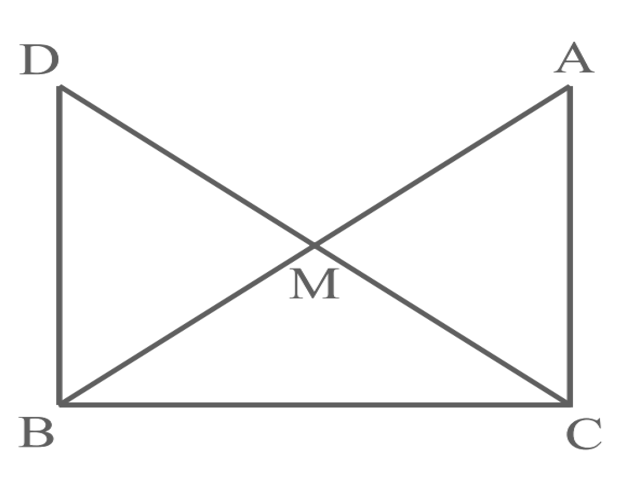
\includegraphics[width=\columnwidth]{figs/Screenshot.png}
  \caption{$\triangle \vec{ACB} ,\triangle \vec{DCB}$ with Mid-Point $\vec{M}$}
  \label{fig:triangles}
\end{figure}
\begin{enumerate}[label =(\roman*)]
        \item $\triangle \vec{AMC} \cong \triangle \vec{BMD}$
        \item $\angle \vec{DBC}$ is a right angle. 
        \item $\triangle \vec{DBC} \cong  \triangle \vec{ACB}$ 
        \item $\vec{CM} = \frac{1}{2} \vec{AB}$
\end{enumerate}
\pagebreak
\solution\\
\textbf{CONSTRUCTION STEPS :}
\begin{enumerate}
\item Let us Assume , the input parameters as ;
\begin{table}[H]
\centering
        \input{tables/input_params.tex}
          \caption{Input Parameters}
          \label{Table-1:Input_params}
\end{table}
\item the output can be calculated as ;
\begin{table}[H]
\centering
        \input{tables/output_params.tex}
          \caption{Output Parameters}
          \label{Table-2:Output_params}
\end{table}
                $\therefore$ By, Plotting these points we get the required Image \figref{fig:fig-2}
\begin{figure}[H]
        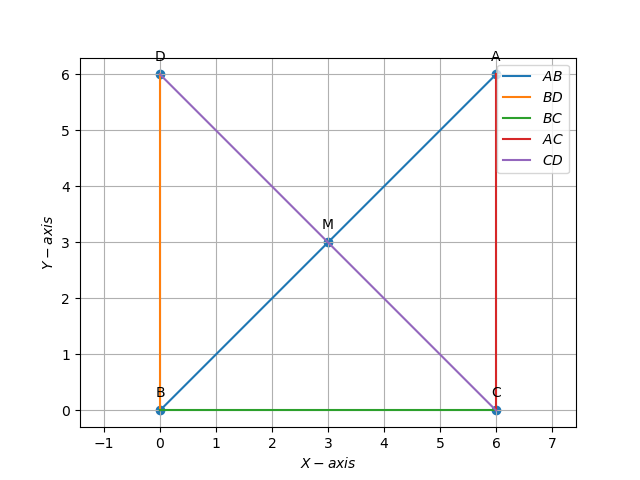
\includegraphics[width = \columnwidth]{figs/python_plot.png}
    \caption{PYTHON Plot of $\triangle \vec{ACB} ,\triangle \vec{DBC}$ with Mid-Point $\vec{M}$}
    \label{fig:fig-2}
\end{figure}
\end{enumerate}

\item Find the position vector of a point $\vec{R}$ which divides the line joining two points $\vec{P}$ and $\vec{Q}$ whose position vectors are $2\vec{a}+\vec{b}$ and $\vec{a}-3\vec{b}$ externally in the ratio $1:2$.

\textbf{Solution:}
Let us assume $\vec{a}$ and $\vec{b}$, and the given ratio is
\begin{table}[h]
    \centering
    \begin{tabular}{|c|c|c|}
        \hline 
        \textbf{Symbol} & \textbf{Value} & \textbf{Description} \\
        \hline
        $\vec{a}$ & $\myvec{1 \\ -3}$ & Vector $\vec{a}$ \\
        \hline
        $\vec{b}$ & $\myvec{0 \\ 2}$ & Vector $\vec{b}$\\
        \hline
        $k$ & $2$ & Ratio \\
        \hline
    \end{tabular}
    \caption{Vectors $\vec{a}$ and $\vec{b}$, ratio $k$}
    \label{tab:table1}
\end{table}

Using the section formula,
\begin{align}
    \vec{R} = \frac{\vec{Q} - k\vec{P}}{1 - k}
\end{align}
where $\vec{P}$ and $\vec{Q}$ depend on $\vec{a}$ and $\vec{b}$, then
\begin{align}
    \vec{P} &= (2\vec{a} + \vec{b}) = 2\myvec{1\\-3} + \myvec{0\\2} = \myvec{2\\-4} \\
    \vec{Q} &= (\vec{a} - 3\vec{b}) = \myvec{1\\-3} - 3\myvec{0\\2} = \myvec{1\\-9}
\end{align}
where $\vec{R}$ can be calculated as 
\begin{align}
    \vec{R} = \frac{(\vec{a} - 3\vec{b}) - k(2\vec{a} + \vec{b})}{1 - k}
\end{align}
By substituting $\vec{a}$ and $\vec{b}$ values, we get $\vec{R}$ as
\begin{align}
    \vec{R} = \myvec{3\\1}
\end{align}

\begin{table}[ht!]
    \centering
    \begin{tabular}{|c|c|c|}
        \hline
        \textbf{Symbol} & \textbf{Value} & \textbf{Description}\\
        \hline
        $\vec{P}$ & $(2\vec{a} + \vec{b})$ & Position vector $\vec{P}$ \\
        \hline
        $\vec{Q}$ & $(\vec{a} - 3\vec{b})$ & Position vector $\vec{Q}$\\
        \hline
        $\vec{R}$ & $\frac{\vec{Q} - k\vec{P}}{1 - k}$ & Position vector $\vec{R}$\\
        \hline
    \end{tabular}
    \caption{Vectors $\vec{P}$, $\vec{Q}$, $\vec{R}$}
    \label{tab:mytable2}   
\end{table}

\begin{figure}[H]
    \centering
    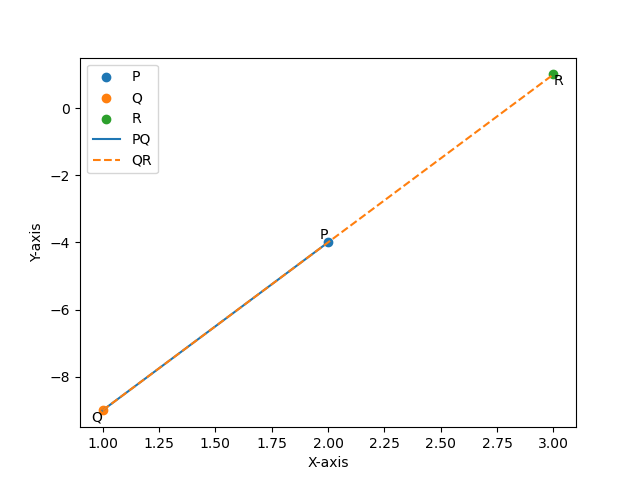
\includegraphics[width=\columnwidth]{figs/external-bisector.png}
    \caption{Point vectors $\vec{P}$, $\vec{Q}$, $\vec{R}$}
    \label{fig:enter-label}
\end{figure}


\end{enumerate}

    \item Draw a quadrilateral in the Cartesian plane, whose vertices are 
    \begin{align}
        \vec{A} = \myvec{-4\\5} \quad \vec{B} = \myvec{0\\7} \\
        \vec{C} = \myvec{5\\-5} \quad \vec{D} = \myvec{-4\\-2}
    \end{align}
    Also, find its area.
\label{chapters/11/10/1/1}
   \\ 
    \solution 
\begin{enumerate}[label=\thesection.\arabic*,ref=\thesection.\theenumi]
		\item Find $\abs{\overrightarrow{a}\times\overrightarrow{b}},\text{ if }\overrightarrow{a}=\hat{i}-7\hat{j}+7\hat{k}\text{ and } \overrightarrow{b}=3\hat{i}-2\hat{j}+2\hat{k}$.
	\\
		\solution
		\input{chapters/12/10/4/1/cross.tex}
\item Show that $$(\overrightarrow{a}-\overrightarrow{b})\times (\overrightarrow{a}+\overrightarrow{b})=2(\overrightarrow{a}\times \overrightarrow{b})$$
	\\
		\solution
		\input{chapters/12/10/4/4/cross.tex}
\item Find $\lambda$ and $\mu$ if $(2\hat{i}+6\hat{j}+27\hat{k})\times(\hat{i}+\lambda \hat{j} + \mu \hat{k})=\overrightarrow{0}$.
	\\
		\solution
		\input{chapters/12/10/4/5/cross.tex}
\item Given that $\overrightarrow{a} \cdot \overrightarrow{b} = 0$ and $\overrightarrow{a} \times \overrightarrow{b} = \overrightarrow{0}$. What can you conclude about the vectors $\overrightarrow{a} \text{ and }\overrightarrow{b}$?
\item Let the vectors be given as $\overrightarrow{a},\overrightarrow{b},\overrightarrow{c}\text{ be given as }\ a_1 \hat{i}+\ a_2 \hat{j}+\ a_3 \hat{k},\ b_1 \hat{i}+\ b_2 \hat{j}+\ b_3 \hat{k},\ c_1 \hat{i}+\ c_2 \hat{j}+\ c_3 \hat{k}$. Then show that $\overrightarrow{a} \times (\overrightarrow{b} + \overrightarrow{c}) = \overrightarrow{a} \times \overrightarrow{b}+\overrightarrow{a} \times \overrightarrow{c}$.
	\\
		\solution
		\input{chapters/12/10/4/7/cross.tex}
\item If either $\overrightarrow{a} = \overrightarrow{0}$ or $\overrightarrow{b} = \overrightarrow{0}$, then $\overrightarrow{a} \times \overrightarrow{b} = \overrightarrow{0}$. Is the converse true? Justify your answer with an example.
	\\
		\solution
		\input{chapters/12/10/4/8/cross.tex}
\item Find the area of the triangle with vertices $A(1, 1, 2)$, $B(2, 3, 5)$, and $C(1, 5, 5)$
	\\
		\solution
		\input{chapters/12/10/4/9/cross.tex}
\item Find the area of the parallelogram whose adjacent sides are determined by the vectors $\overrightarrow{a}=\hat{i}-\hat{j}+3\hat{k}$ and $\overrightarrow{b}=2\hat{i}-7\hat{j}+\hat{k}$.
	\\
		\solution
		\input{chapters/12/10/4/10/cross.tex}
\item Let the vectors $\overrightarrow{a}$ and $\overrightarrow{b}$ be such that $|\overrightarrow{a}| = 3$ and $|\overrightarrow{b}| = \dfrac{\sqrt{2}}{3}$, then $\overrightarrow{a} \times \overrightarrow{b}$ is a unit vector, if the angle between $\overrightarrow{a}$ and $\overrightarrow{b}$ is
\begin{enumerate}
\item $\dfrac{\pi}{6}$
\item $\dfrac{\pi}{4}$
\item $\dfrac{\pi}{3}$
\item $\dfrac{\pi}{2}$
\end{enumerate}
		\solution
		\input{chapters/12/10/4/11/cross.tex}
\item Area of a rectangle having vertices A, B, C and D with position vectors $ -\hat{i}+ \dfrac{1}{2} \hat{j}+4\hat{k},\hat{i}+ \dfrac{1}{2} \hat{j}+4\hat{k},\hat{i}-\dfrac{1}{2} \hat{j}+4\hat{k}\text{ and }-\hat{i}- \dfrac{1}{2} \hat{j}+4\hat{k}$, respectively is
\begin{enumerate}
\item $\dfrac{1}{2}$
\item 1
\item 2
\item 4
\end{enumerate}
		\solution
		\input{chapters/12/10/4/12/cross.tex}
\item Find the area of the triangle whose vertices are 
\begin{enumerate}
\item $(2, 3), (–1, 0), (2, – 4)$
\item $(–5, –1), (3, –5), (5, 2)$ 
\end{enumerate}
		\label{10/7/3/1}
\solution
		\input{chapters/10/7/3/1/area.tex}
\item Find the area of the triangle formed by joining the mid-points of the sides of the triangle whose vertices are $(0, –1), (2, 1) \text{ and } (0, 3)$. Find the ratio of this area to the area of the given triangle.
	\\
\solution
		\input{chapters/10/7/3/3/cross.tex}

\item Find the area of the quadrilateral whose vertices, taken in order, are $(– 4, – 2), (– 3, – 5), (3, – 2)$  and $ (2, 3)$.
	\\
\solution
		\input{chapters/10/7/3/4/cross.tex}

\item Verify that a median of a triangle divides it into two triangles of equal areas for $\triangle ABC$ whose vertices are $\vec{A}(4, -6), \vec{B}(3, 2), \text{ and } \vec{C}(5, 2)$. 
		\label{10/7/3/5}
		\\
\solution
		\input{chapters/10/7/3/5/area.tex}

\item The two adjacent sides of a parallelogram are 
$2\hat{i}-4\hat{j}+5\hat{k}$  and  $\hat{i}-2\hat{j}-3\hat{k}$.
Find the unit vector parallel to its diagonal. Also, find its area.\\
	\solution
		\input{chapters/12/10/5/10/cross.tex}
\item The vertices of a $\triangle ABC$ are $\vec{A}(4,6), \vec{B}(1,5)$ and  $\vec{C}(7,2)$. A line is drawn to intersect sides $AB$ and $AC$ at $\vec{D}$ and $\vec{E}$ respectively, such that $\frac{AD}{AB} = \frac{AE}{AC} = \frac{1}{4}$. Calculate the area of $\triangle ADE$ and compare it with the area of the $\triangle ABC$.
\\
\solution
	\input{chapters/10/7/4/6/section.tex}
    \item Draw a quadrilateral in the Cartesian plane, whose vertices are 
    \begin{align}
        \vec{A} = \myvec{-4\\5} \quad \vec{B} = \myvec{0\\7} \\
        \vec{C} = \myvec{5\\-5} \quad \vec{D} = \myvec{-4\\-2}
    \end{align}
    Also, find its area.
\label{chapters/11/10/1/1}
   \\ 
    \solution 
\input{chapters/11/10/1/1/cross.tex}
\item Find the area of region bounded by the triangle whose
	vertices are $(1, 0), (2, 2) \text{ and } (3, 1)$. 
\item Find the area of region bounded by the triangle whose vertices
	are $(– 1, 0), (1, 3) \text{ and } (3, 2)$. 
\item Find the area of the $\triangle ABC$, coordinates of whose vertices are $\vec{A}(2, 0), \vec{B}(4, 5), \text{ and } \vec{C}(6, 3)$.


\item 
\input{chapters/vectors/exer/main.tex}
\end{enumerate}


\item Find the area of region bounded by the triangle whose
	vertices are $(1, 0), (2, 2) \text{ and } (3, 1)$. 
\item Find the area of region bounded by the triangle whose vertices
	are $(– 1, 0), (1, 3) \text{ and } (3, 2)$. 
\item Find the area of the $\triangle ABC$, coordinates of whose vertices are $\vec{A}(2, 0), \vec{B}(4, 5), \text{ and } \vec{C}(6, 3)$.


\item 
%\documentclass[12pt]{article}
%\usepackage{graphicx}
%\usepackage{graphics}
%\usepackage{refstyle}
%\usepackage{amsmath}
%\usepackage{caption}
%\usepackage{float}
%\usepackage{booktabs}
%\usepackage{array}
%\usepackage{amssymb}
%\usepackage{booktabs}
%\let\vec\mathbf
%\providecommand{\brak}[1]{\ensuremath{\left(#1\right)}}
%\graphicspath{{/storage/self/primary/Download/latexnew/fig}}                                     
$\vec{P}$ and $\vec{Q}$ are any two points lying on the sides $DC$ and $AD$ respectively of a parallelogram $ABCD$.Show that, $ar\brak{\triangle APB}=ar\brak{\triangle BQC}$.


\textbf{Figure:}
\begin{figure}[H]
    \centering
	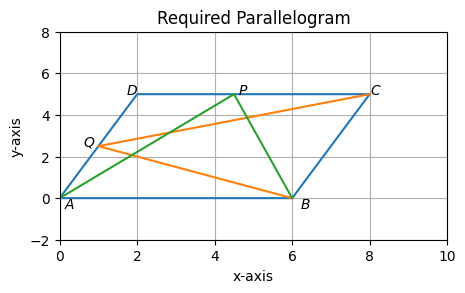
\includegraphics[width=\columnwidth]{chapters/vectors/exer/figs/1.png}
    \caption{}
    \label{fig:fig:1}
\end{figure}


\textbf{Solution:}
\begin{table}[H]
   \centering
  \input{chapters/vectors/exer/table/tab1.tex}
   \caption{Table of input parameters}        
\label{tab:tab:1}                    
\end{table}




\begin{table}[H]
    \centering                                  
\input{chapters/vectors/exer/table/tab2.tex}                  
\caption{Table of output parameters}
\label{tab:tab:2}
 \end{table}


For the $\triangle BQC$, the vertices of the triangle are taken from \tabref{tab:tab:1} and \tabref{tab:tab:2}.

\begin{align}
\implies ar\brak{\triangle BQC}&=
\frac{1}{2}\begin{tabular}{|c c c|}            
1 &1&1\\                      
$\vec{B}$&$\vec{Q}$&$\vec{C}$\\    
\end{tabular}\\
&= \frac{1}{2}\begin{tabular}{|c c c|}
       1 &1&1\\
       6&$\frac{2k_1}{k_1+1}$&8 \\
       0&$\frac{5k_1}{k_1+1}$&5
   \end{tabular}\\
  \xrightarrow{C_2'=C_2-C_1,C_3'=C_3-C_1}&\frac{1}{2} \begin{tabular}{|c c c|}
       1 &0&0\\
       6&$\frac{-4k_1-6}{k_1+1}$&2 \\
       0&$\frac{5k_1}{k_1+1}$&5
   \end{tabular}\\
&=\frac{1}{2}\brak{1\begin{tabular}{|c c|}
   $\frac{-4k_1-6}{k_1+1}$ &2  \\
   $\frac{5k_1}{k_1+1}$ & 5
\end{tabular} +0+0}\\
&=\frac{1}{2} \times30\\                          
&=15 \end{align}


For the $\triangle APB$, the vertices of the triangle are taken from \tabref{tab:tab:1} and \tabref{tab:tab:2}.
   \begin{align}
  \implies ar\brak{\triangle APB} &=
\frac{1}{2}\begin{tabular}{|c c c|}            
1 &1&1\\                            
$\vec{A}$&$\vec{P}$&$\vec{B}$\\
\end{tabular}\\ &=  \frac{1}{2}
   \begin{tabular}{|c c c|}
       1 &1&1\\
       0&$\frac{8k_2+2}{k_2+1}$&6 \\
       0&5&0
   \end{tabular}\\
 &=\frac{1}{2} \times30\\
 &=15 \end{align}
 \brak{6} = \brak{10}


So, ar\brak{\triangle BQC} = ar\brak{\triangle APB}.\brak{proved}
%\end{document}



\end{enumerate}


\item Let the vectors $\overrightarrow{a}$ and $\overrightarrow{b}$ be such that $|\overrightarrow{a}| = 3$ and $|\overrightarrow{b}| = \dfrac{\sqrt{2}}{3}$, then $\overrightarrow{a} \times \overrightarrow{b}$ is a unit vector, if the angle between $\overrightarrow{a}$ and $\overrightarrow{b}$ is
\begin{enumerate}
\item $\dfrac{\pi}{6}$
\item $\dfrac{\pi}{4}$
\item $\dfrac{\pi}{3}$
\item $\dfrac{\pi}{2}$
\end{enumerate}
		\solution
		\begin{enumerate}[label=\thesection.\arabic*,ref=\thesection.\theenumi]
		\item Find $\abs{\overrightarrow{a}\times\overrightarrow{b}},\text{ if }\overrightarrow{a}=\hat{i}-7\hat{j}+7\hat{k}\text{ and } \overrightarrow{b}=3\hat{i}-2\hat{j}+2\hat{k}$.
	\\
		\solution
		\begin{enumerate}[label=\thesection.\arabic*,ref=\thesection.\theenumi]
		\item Find $\abs{\overrightarrow{a}\times\overrightarrow{b}},\text{ if }\overrightarrow{a}=\hat{i}-7\hat{j}+7\hat{k}\text{ and } \overrightarrow{b}=3\hat{i}-2\hat{j}+2\hat{k}$.
	\\
		\solution
		\input{chapters/12/10/4/1/cross.tex}
\item Show that $$(\overrightarrow{a}-\overrightarrow{b})\times (\overrightarrow{a}+\overrightarrow{b})=2(\overrightarrow{a}\times \overrightarrow{b})$$
	\\
		\solution
		\input{chapters/12/10/4/4/cross.tex}
\item Find $\lambda$ and $\mu$ if $(2\hat{i}+6\hat{j}+27\hat{k})\times(\hat{i}+\lambda \hat{j} + \mu \hat{k})=\overrightarrow{0}$.
	\\
		\solution
		\input{chapters/12/10/4/5/cross.tex}
\item Given that $\overrightarrow{a} \cdot \overrightarrow{b} = 0$ and $\overrightarrow{a} \times \overrightarrow{b} = \overrightarrow{0}$. What can you conclude about the vectors $\overrightarrow{a} \text{ and }\overrightarrow{b}$?
\item Let the vectors be given as $\overrightarrow{a},\overrightarrow{b},\overrightarrow{c}\text{ be given as }\ a_1 \hat{i}+\ a_2 \hat{j}+\ a_3 \hat{k},\ b_1 \hat{i}+\ b_2 \hat{j}+\ b_3 \hat{k},\ c_1 \hat{i}+\ c_2 \hat{j}+\ c_3 \hat{k}$. Then show that $\overrightarrow{a} \times (\overrightarrow{b} + \overrightarrow{c}) = \overrightarrow{a} \times \overrightarrow{b}+\overrightarrow{a} \times \overrightarrow{c}$.
	\\
		\solution
		\input{chapters/12/10/4/7/cross.tex}
\item If either $\overrightarrow{a} = \overrightarrow{0}$ or $\overrightarrow{b} = \overrightarrow{0}$, then $\overrightarrow{a} \times \overrightarrow{b} = \overrightarrow{0}$. Is the converse true? Justify your answer with an example.
	\\
		\solution
		\input{chapters/12/10/4/8/cross.tex}
\item Find the area of the triangle with vertices $A(1, 1, 2)$, $B(2, 3, 5)$, and $C(1, 5, 5)$
	\\
		\solution
		\input{chapters/12/10/4/9/cross.tex}
\item Find the area of the parallelogram whose adjacent sides are determined by the vectors $\overrightarrow{a}=\hat{i}-\hat{j}+3\hat{k}$ and $\overrightarrow{b}=2\hat{i}-7\hat{j}+\hat{k}$.
	\\
		\solution
		\input{chapters/12/10/4/10/cross.tex}
\item Let the vectors $\overrightarrow{a}$ and $\overrightarrow{b}$ be such that $|\overrightarrow{a}| = 3$ and $|\overrightarrow{b}| = \dfrac{\sqrt{2}}{3}$, then $\overrightarrow{a} \times \overrightarrow{b}$ is a unit vector, if the angle between $\overrightarrow{a}$ and $\overrightarrow{b}$ is
\begin{enumerate}
\item $\dfrac{\pi}{6}$
\item $\dfrac{\pi}{4}$
\item $\dfrac{\pi}{3}$
\item $\dfrac{\pi}{2}$
\end{enumerate}
		\solution
		\input{chapters/12/10/4/11/cross.tex}
\item Area of a rectangle having vertices A, B, C and D with position vectors $ -\hat{i}+ \dfrac{1}{2} \hat{j}+4\hat{k},\hat{i}+ \dfrac{1}{2} \hat{j}+4\hat{k},\hat{i}-\dfrac{1}{2} \hat{j}+4\hat{k}\text{ and }-\hat{i}- \dfrac{1}{2} \hat{j}+4\hat{k}$, respectively is
\begin{enumerate}
\item $\dfrac{1}{2}$
\item 1
\item 2
\item 4
\end{enumerate}
		\solution
		\input{chapters/12/10/4/12/cross.tex}
\item Find the area of the triangle whose vertices are 
\begin{enumerate}
\item $(2, 3), (–1, 0), (2, – 4)$
\item $(–5, –1), (3, –5), (5, 2)$ 
\end{enumerate}
		\label{10/7/3/1}
\solution
		\input{chapters/10/7/3/1/area.tex}
\item Find the area of the triangle formed by joining the mid-points of the sides of the triangle whose vertices are $(0, –1), (2, 1) \text{ and } (0, 3)$. Find the ratio of this area to the area of the given triangle.
	\\
\solution
		\input{chapters/10/7/3/3/cross.tex}

\item Find the area of the quadrilateral whose vertices, taken in order, are $(– 4, – 2), (– 3, – 5), (3, – 2)$  and $ (2, 3)$.
	\\
\solution
		\input{chapters/10/7/3/4/cross.tex}

\item Verify that a median of a triangle divides it into two triangles of equal areas for $\triangle ABC$ whose vertices are $\vec{A}(4, -6), \vec{B}(3, 2), \text{ and } \vec{C}(5, 2)$. 
		\label{10/7/3/5}
		\\
\solution
		\input{chapters/10/7/3/5/area.tex}

\item The two adjacent sides of a parallelogram are 
$2\hat{i}-4\hat{j}+5\hat{k}$  and  $\hat{i}-2\hat{j}-3\hat{k}$.
Find the unit vector parallel to its diagonal. Also, find its area.\\
	\solution
		\input{chapters/12/10/5/10/cross.tex}
\item The vertices of a $\triangle ABC$ are $\vec{A}(4,6), \vec{B}(1,5)$ and  $\vec{C}(7,2)$. A line is drawn to intersect sides $AB$ and $AC$ at $\vec{D}$ and $\vec{E}$ respectively, such that $\frac{AD}{AB} = \frac{AE}{AC} = \frac{1}{4}$. Calculate the area of $\triangle ADE$ and compare it with the area of the $\triangle ABC$.
\\
\solution
	\input{chapters/10/7/4/6/section.tex}
    \item Draw a quadrilateral in the Cartesian plane, whose vertices are 
    \begin{align}
        \vec{A} = \myvec{-4\\5} \quad \vec{B} = \myvec{0\\7} \\
        \vec{C} = \myvec{5\\-5} \quad \vec{D} = \myvec{-4\\-2}
    \end{align}
    Also, find its area.
\label{chapters/11/10/1/1}
   \\ 
    \solution 
\input{chapters/11/10/1/1/cross.tex}
\item Find the area of region bounded by the triangle whose
	vertices are $(1, 0), (2, 2) \text{ and } (3, 1)$. 
\item Find the area of region bounded by the triangle whose vertices
	are $(– 1, 0), (1, 3) \text{ and } (3, 2)$. 
\item Find the area of the $\triangle ABC$, coordinates of whose vertices are $\vec{A}(2, 0), \vec{B}(4, 5), \text{ and } \vec{C}(6, 3)$.


\item 
\input{chapters/vectors/exer/main.tex}
\end{enumerate}


\item Show that $$(\overrightarrow{a}-\overrightarrow{b})\times (\overrightarrow{a}+\overrightarrow{b})=2(\overrightarrow{a}\times \overrightarrow{b})$$
	\\
		\solution
		\begin{enumerate}[label=\thesection.\arabic*,ref=\thesection.\theenumi]
		\item Find $\abs{\overrightarrow{a}\times\overrightarrow{b}},\text{ if }\overrightarrow{a}=\hat{i}-7\hat{j}+7\hat{k}\text{ and } \overrightarrow{b}=3\hat{i}-2\hat{j}+2\hat{k}$.
	\\
		\solution
		\input{chapters/12/10/4/1/cross.tex}
\item Show that $$(\overrightarrow{a}-\overrightarrow{b})\times (\overrightarrow{a}+\overrightarrow{b})=2(\overrightarrow{a}\times \overrightarrow{b})$$
	\\
		\solution
		\input{chapters/12/10/4/4/cross.tex}
\item Find $\lambda$ and $\mu$ if $(2\hat{i}+6\hat{j}+27\hat{k})\times(\hat{i}+\lambda \hat{j} + \mu \hat{k})=\overrightarrow{0}$.
	\\
		\solution
		\input{chapters/12/10/4/5/cross.tex}
\item Given that $\overrightarrow{a} \cdot \overrightarrow{b} = 0$ and $\overrightarrow{a} \times \overrightarrow{b} = \overrightarrow{0}$. What can you conclude about the vectors $\overrightarrow{a} \text{ and }\overrightarrow{b}$?
\item Let the vectors be given as $\overrightarrow{a},\overrightarrow{b},\overrightarrow{c}\text{ be given as }\ a_1 \hat{i}+\ a_2 \hat{j}+\ a_3 \hat{k},\ b_1 \hat{i}+\ b_2 \hat{j}+\ b_3 \hat{k},\ c_1 \hat{i}+\ c_2 \hat{j}+\ c_3 \hat{k}$. Then show that $\overrightarrow{a} \times (\overrightarrow{b} + \overrightarrow{c}) = \overrightarrow{a} \times \overrightarrow{b}+\overrightarrow{a} \times \overrightarrow{c}$.
	\\
		\solution
		\input{chapters/12/10/4/7/cross.tex}
\item If either $\overrightarrow{a} = \overrightarrow{0}$ or $\overrightarrow{b} = \overrightarrow{0}$, then $\overrightarrow{a} \times \overrightarrow{b} = \overrightarrow{0}$. Is the converse true? Justify your answer with an example.
	\\
		\solution
		\input{chapters/12/10/4/8/cross.tex}
\item Find the area of the triangle with vertices $A(1, 1, 2)$, $B(2, 3, 5)$, and $C(1, 5, 5)$
	\\
		\solution
		\input{chapters/12/10/4/9/cross.tex}
\item Find the area of the parallelogram whose adjacent sides are determined by the vectors $\overrightarrow{a}=\hat{i}-\hat{j}+3\hat{k}$ and $\overrightarrow{b}=2\hat{i}-7\hat{j}+\hat{k}$.
	\\
		\solution
		\input{chapters/12/10/4/10/cross.tex}
\item Let the vectors $\overrightarrow{a}$ and $\overrightarrow{b}$ be such that $|\overrightarrow{a}| = 3$ and $|\overrightarrow{b}| = \dfrac{\sqrt{2}}{3}$, then $\overrightarrow{a} \times \overrightarrow{b}$ is a unit vector, if the angle between $\overrightarrow{a}$ and $\overrightarrow{b}$ is
\begin{enumerate}
\item $\dfrac{\pi}{6}$
\item $\dfrac{\pi}{4}$
\item $\dfrac{\pi}{3}$
\item $\dfrac{\pi}{2}$
\end{enumerate}
		\solution
		\input{chapters/12/10/4/11/cross.tex}
\item Area of a rectangle having vertices A, B, C and D with position vectors $ -\hat{i}+ \dfrac{1}{2} \hat{j}+4\hat{k},\hat{i}+ \dfrac{1}{2} \hat{j}+4\hat{k},\hat{i}-\dfrac{1}{2} \hat{j}+4\hat{k}\text{ and }-\hat{i}- \dfrac{1}{2} \hat{j}+4\hat{k}$, respectively is
\begin{enumerate}
\item $\dfrac{1}{2}$
\item 1
\item 2
\item 4
\end{enumerate}
		\solution
		\input{chapters/12/10/4/12/cross.tex}
\item Find the area of the triangle whose vertices are 
\begin{enumerate}
\item $(2, 3), (–1, 0), (2, – 4)$
\item $(–5, –1), (3, –5), (5, 2)$ 
\end{enumerate}
		\label{10/7/3/1}
\solution
		\input{chapters/10/7/3/1/area.tex}
\item Find the area of the triangle formed by joining the mid-points of the sides of the triangle whose vertices are $(0, –1), (2, 1) \text{ and } (0, 3)$. Find the ratio of this area to the area of the given triangle.
	\\
\solution
		\input{chapters/10/7/3/3/cross.tex}

\item Find the area of the quadrilateral whose vertices, taken in order, are $(– 4, – 2), (– 3, – 5), (3, – 2)$  and $ (2, 3)$.
	\\
\solution
		\input{chapters/10/7/3/4/cross.tex}

\item Verify that a median of a triangle divides it into two triangles of equal areas for $\triangle ABC$ whose vertices are $\vec{A}(4, -6), \vec{B}(3, 2), \text{ and } \vec{C}(5, 2)$. 
		\label{10/7/3/5}
		\\
\solution
		\input{chapters/10/7/3/5/area.tex}

\item The two adjacent sides of a parallelogram are 
$2\hat{i}-4\hat{j}+5\hat{k}$  and  $\hat{i}-2\hat{j}-3\hat{k}$.
Find the unit vector parallel to its diagonal. Also, find its area.\\
	\solution
		\input{chapters/12/10/5/10/cross.tex}
\item The vertices of a $\triangle ABC$ are $\vec{A}(4,6), \vec{B}(1,5)$ and  $\vec{C}(7,2)$. A line is drawn to intersect sides $AB$ and $AC$ at $\vec{D}$ and $\vec{E}$ respectively, such that $\frac{AD}{AB} = \frac{AE}{AC} = \frac{1}{4}$. Calculate the area of $\triangle ADE$ and compare it with the area of the $\triangle ABC$.
\\
\solution
	\input{chapters/10/7/4/6/section.tex}
    \item Draw a quadrilateral in the Cartesian plane, whose vertices are 
    \begin{align}
        \vec{A} = \myvec{-4\\5} \quad \vec{B} = \myvec{0\\7} \\
        \vec{C} = \myvec{5\\-5} \quad \vec{D} = \myvec{-4\\-2}
    \end{align}
    Also, find its area.
\label{chapters/11/10/1/1}
   \\ 
    \solution 
\input{chapters/11/10/1/1/cross.tex}
\item Find the area of region bounded by the triangle whose
	vertices are $(1, 0), (2, 2) \text{ and } (3, 1)$. 
\item Find the area of region bounded by the triangle whose vertices
	are $(– 1, 0), (1, 3) \text{ and } (3, 2)$. 
\item Find the area of the $\triangle ABC$, coordinates of whose vertices are $\vec{A}(2, 0), \vec{B}(4, 5), \text{ and } \vec{C}(6, 3)$.


\item 
\input{chapters/vectors/exer/main.tex}
\end{enumerate}


\item Find $\lambda$ and $\mu$ if $(2\hat{i}+6\hat{j}+27\hat{k})\times(\hat{i}+\lambda \hat{j} + \mu \hat{k})=\overrightarrow{0}$.
	\\
		\solution
		\begin{enumerate}[label=\thesection.\arabic*,ref=\thesection.\theenumi]
		\item Find $\abs{\overrightarrow{a}\times\overrightarrow{b}},\text{ if }\overrightarrow{a}=\hat{i}-7\hat{j}+7\hat{k}\text{ and } \overrightarrow{b}=3\hat{i}-2\hat{j}+2\hat{k}$.
	\\
		\solution
		\input{chapters/12/10/4/1/cross.tex}
\item Show that $$(\overrightarrow{a}-\overrightarrow{b})\times (\overrightarrow{a}+\overrightarrow{b})=2(\overrightarrow{a}\times \overrightarrow{b})$$
	\\
		\solution
		\input{chapters/12/10/4/4/cross.tex}
\item Find $\lambda$ and $\mu$ if $(2\hat{i}+6\hat{j}+27\hat{k})\times(\hat{i}+\lambda \hat{j} + \mu \hat{k})=\overrightarrow{0}$.
	\\
		\solution
		\input{chapters/12/10/4/5/cross.tex}
\item Given that $\overrightarrow{a} \cdot \overrightarrow{b} = 0$ and $\overrightarrow{a} \times \overrightarrow{b} = \overrightarrow{0}$. What can you conclude about the vectors $\overrightarrow{a} \text{ and }\overrightarrow{b}$?
\item Let the vectors be given as $\overrightarrow{a},\overrightarrow{b},\overrightarrow{c}\text{ be given as }\ a_1 \hat{i}+\ a_2 \hat{j}+\ a_3 \hat{k},\ b_1 \hat{i}+\ b_2 \hat{j}+\ b_3 \hat{k},\ c_1 \hat{i}+\ c_2 \hat{j}+\ c_3 \hat{k}$. Then show that $\overrightarrow{a} \times (\overrightarrow{b} + \overrightarrow{c}) = \overrightarrow{a} \times \overrightarrow{b}+\overrightarrow{a} \times \overrightarrow{c}$.
	\\
		\solution
		\input{chapters/12/10/4/7/cross.tex}
\item If either $\overrightarrow{a} = \overrightarrow{0}$ or $\overrightarrow{b} = \overrightarrow{0}$, then $\overrightarrow{a} \times \overrightarrow{b} = \overrightarrow{0}$. Is the converse true? Justify your answer with an example.
	\\
		\solution
		\input{chapters/12/10/4/8/cross.tex}
\item Find the area of the triangle with vertices $A(1, 1, 2)$, $B(2, 3, 5)$, and $C(1, 5, 5)$
	\\
		\solution
		\input{chapters/12/10/4/9/cross.tex}
\item Find the area of the parallelogram whose adjacent sides are determined by the vectors $\overrightarrow{a}=\hat{i}-\hat{j}+3\hat{k}$ and $\overrightarrow{b}=2\hat{i}-7\hat{j}+\hat{k}$.
	\\
		\solution
		\input{chapters/12/10/4/10/cross.tex}
\item Let the vectors $\overrightarrow{a}$ and $\overrightarrow{b}$ be such that $|\overrightarrow{a}| = 3$ and $|\overrightarrow{b}| = \dfrac{\sqrt{2}}{3}$, then $\overrightarrow{a} \times \overrightarrow{b}$ is a unit vector, if the angle between $\overrightarrow{a}$ and $\overrightarrow{b}$ is
\begin{enumerate}
\item $\dfrac{\pi}{6}$
\item $\dfrac{\pi}{4}$
\item $\dfrac{\pi}{3}$
\item $\dfrac{\pi}{2}$
\end{enumerate}
		\solution
		\input{chapters/12/10/4/11/cross.tex}
\item Area of a rectangle having vertices A, B, C and D with position vectors $ -\hat{i}+ \dfrac{1}{2} \hat{j}+4\hat{k},\hat{i}+ \dfrac{1}{2} \hat{j}+4\hat{k},\hat{i}-\dfrac{1}{2} \hat{j}+4\hat{k}\text{ and }-\hat{i}- \dfrac{1}{2} \hat{j}+4\hat{k}$, respectively is
\begin{enumerate}
\item $\dfrac{1}{2}$
\item 1
\item 2
\item 4
\end{enumerate}
		\solution
		\input{chapters/12/10/4/12/cross.tex}
\item Find the area of the triangle whose vertices are 
\begin{enumerate}
\item $(2, 3), (–1, 0), (2, – 4)$
\item $(–5, –1), (3, –5), (5, 2)$ 
\end{enumerate}
		\label{10/7/3/1}
\solution
		\input{chapters/10/7/3/1/area.tex}
\item Find the area of the triangle formed by joining the mid-points of the sides of the triangle whose vertices are $(0, –1), (2, 1) \text{ and } (0, 3)$. Find the ratio of this area to the area of the given triangle.
	\\
\solution
		\input{chapters/10/7/3/3/cross.tex}

\item Find the area of the quadrilateral whose vertices, taken in order, are $(– 4, – 2), (– 3, – 5), (3, – 2)$  and $ (2, 3)$.
	\\
\solution
		\input{chapters/10/7/3/4/cross.tex}

\item Verify that a median of a triangle divides it into two triangles of equal areas for $\triangle ABC$ whose vertices are $\vec{A}(4, -6), \vec{B}(3, 2), \text{ and } \vec{C}(5, 2)$. 
		\label{10/7/3/5}
		\\
\solution
		\input{chapters/10/7/3/5/area.tex}

\item The two adjacent sides of a parallelogram are 
$2\hat{i}-4\hat{j}+5\hat{k}$  and  $\hat{i}-2\hat{j}-3\hat{k}$.
Find the unit vector parallel to its diagonal. Also, find its area.\\
	\solution
		\input{chapters/12/10/5/10/cross.tex}
\item The vertices of a $\triangle ABC$ are $\vec{A}(4,6), \vec{B}(1,5)$ and  $\vec{C}(7,2)$. A line is drawn to intersect sides $AB$ and $AC$ at $\vec{D}$ and $\vec{E}$ respectively, such that $\frac{AD}{AB} = \frac{AE}{AC} = \frac{1}{4}$. Calculate the area of $\triangle ADE$ and compare it with the area of the $\triangle ABC$.
\\
\solution
	\input{chapters/10/7/4/6/section.tex}
    \item Draw a quadrilateral in the Cartesian plane, whose vertices are 
    \begin{align}
        \vec{A} = \myvec{-4\\5} \quad \vec{B} = \myvec{0\\7} \\
        \vec{C} = \myvec{5\\-5} \quad \vec{D} = \myvec{-4\\-2}
    \end{align}
    Also, find its area.
\label{chapters/11/10/1/1}
   \\ 
    \solution 
\input{chapters/11/10/1/1/cross.tex}
\item Find the area of region bounded by the triangle whose
	vertices are $(1, 0), (2, 2) \text{ and } (3, 1)$. 
\item Find the area of region bounded by the triangle whose vertices
	are $(– 1, 0), (1, 3) \text{ and } (3, 2)$. 
\item Find the area of the $\triangle ABC$, coordinates of whose vertices are $\vec{A}(2, 0), \vec{B}(4, 5), \text{ and } \vec{C}(6, 3)$.


\item 
\input{chapters/vectors/exer/main.tex}
\end{enumerate}


\item Given that $\overrightarrow{a} \cdot \overrightarrow{b} = 0$ and $\overrightarrow{a} \times \overrightarrow{b} = \overrightarrow{0}$. What can you conclude about the vectors $\overrightarrow{a} \text{ and }\overrightarrow{b}$?
\item Let the vectors be given as $\overrightarrow{a},\overrightarrow{b},\overrightarrow{c}\text{ be given as }\ a_1 \hat{i}+\ a_2 \hat{j}+\ a_3 \hat{k},\ b_1 \hat{i}+\ b_2 \hat{j}+\ b_3 \hat{k},\ c_1 \hat{i}+\ c_2 \hat{j}+\ c_3 \hat{k}$. Then show that $\overrightarrow{a} \times (\overrightarrow{b} + \overrightarrow{c}) = \overrightarrow{a} \times \overrightarrow{b}+\overrightarrow{a} \times \overrightarrow{c}$.
	\\
		\solution
		\begin{enumerate}[label=\thesection.\arabic*,ref=\thesection.\theenumi]
		\item Find $\abs{\overrightarrow{a}\times\overrightarrow{b}},\text{ if }\overrightarrow{a}=\hat{i}-7\hat{j}+7\hat{k}\text{ and } \overrightarrow{b}=3\hat{i}-2\hat{j}+2\hat{k}$.
	\\
		\solution
		\input{chapters/12/10/4/1/cross.tex}
\item Show that $$(\overrightarrow{a}-\overrightarrow{b})\times (\overrightarrow{a}+\overrightarrow{b})=2(\overrightarrow{a}\times \overrightarrow{b})$$
	\\
		\solution
		\input{chapters/12/10/4/4/cross.tex}
\item Find $\lambda$ and $\mu$ if $(2\hat{i}+6\hat{j}+27\hat{k})\times(\hat{i}+\lambda \hat{j} + \mu \hat{k})=\overrightarrow{0}$.
	\\
		\solution
		\input{chapters/12/10/4/5/cross.tex}
\item Given that $\overrightarrow{a} \cdot \overrightarrow{b} = 0$ and $\overrightarrow{a} \times \overrightarrow{b} = \overrightarrow{0}$. What can you conclude about the vectors $\overrightarrow{a} \text{ and }\overrightarrow{b}$?
\item Let the vectors be given as $\overrightarrow{a},\overrightarrow{b},\overrightarrow{c}\text{ be given as }\ a_1 \hat{i}+\ a_2 \hat{j}+\ a_3 \hat{k},\ b_1 \hat{i}+\ b_2 \hat{j}+\ b_3 \hat{k},\ c_1 \hat{i}+\ c_2 \hat{j}+\ c_3 \hat{k}$. Then show that $\overrightarrow{a} \times (\overrightarrow{b} + \overrightarrow{c}) = \overrightarrow{a} \times \overrightarrow{b}+\overrightarrow{a} \times \overrightarrow{c}$.
	\\
		\solution
		\input{chapters/12/10/4/7/cross.tex}
\item If either $\overrightarrow{a} = \overrightarrow{0}$ or $\overrightarrow{b} = \overrightarrow{0}$, then $\overrightarrow{a} \times \overrightarrow{b} = \overrightarrow{0}$. Is the converse true? Justify your answer with an example.
	\\
		\solution
		\input{chapters/12/10/4/8/cross.tex}
\item Find the area of the triangle with vertices $A(1, 1, 2)$, $B(2, 3, 5)$, and $C(1, 5, 5)$
	\\
		\solution
		\input{chapters/12/10/4/9/cross.tex}
\item Find the area of the parallelogram whose adjacent sides are determined by the vectors $\overrightarrow{a}=\hat{i}-\hat{j}+3\hat{k}$ and $\overrightarrow{b}=2\hat{i}-7\hat{j}+\hat{k}$.
	\\
		\solution
		\input{chapters/12/10/4/10/cross.tex}
\item Let the vectors $\overrightarrow{a}$ and $\overrightarrow{b}$ be such that $|\overrightarrow{a}| = 3$ and $|\overrightarrow{b}| = \dfrac{\sqrt{2}}{3}$, then $\overrightarrow{a} \times \overrightarrow{b}$ is a unit vector, if the angle between $\overrightarrow{a}$ and $\overrightarrow{b}$ is
\begin{enumerate}
\item $\dfrac{\pi}{6}$
\item $\dfrac{\pi}{4}$
\item $\dfrac{\pi}{3}$
\item $\dfrac{\pi}{2}$
\end{enumerate}
		\solution
		\input{chapters/12/10/4/11/cross.tex}
\item Area of a rectangle having vertices A, B, C and D with position vectors $ -\hat{i}+ \dfrac{1}{2} \hat{j}+4\hat{k},\hat{i}+ \dfrac{1}{2} \hat{j}+4\hat{k},\hat{i}-\dfrac{1}{2} \hat{j}+4\hat{k}\text{ and }-\hat{i}- \dfrac{1}{2} \hat{j}+4\hat{k}$, respectively is
\begin{enumerate}
\item $\dfrac{1}{2}$
\item 1
\item 2
\item 4
\end{enumerate}
		\solution
		\input{chapters/12/10/4/12/cross.tex}
\item Find the area of the triangle whose vertices are 
\begin{enumerate}
\item $(2, 3), (–1, 0), (2, – 4)$
\item $(–5, –1), (3, –5), (5, 2)$ 
\end{enumerate}
		\label{10/7/3/1}
\solution
		\input{chapters/10/7/3/1/area.tex}
\item Find the area of the triangle formed by joining the mid-points of the sides of the triangle whose vertices are $(0, –1), (2, 1) \text{ and } (0, 3)$. Find the ratio of this area to the area of the given triangle.
	\\
\solution
		\input{chapters/10/7/3/3/cross.tex}

\item Find the area of the quadrilateral whose vertices, taken in order, are $(– 4, – 2), (– 3, – 5), (3, – 2)$  and $ (2, 3)$.
	\\
\solution
		\input{chapters/10/7/3/4/cross.tex}

\item Verify that a median of a triangle divides it into two triangles of equal areas for $\triangle ABC$ whose vertices are $\vec{A}(4, -6), \vec{B}(3, 2), \text{ and } \vec{C}(5, 2)$. 
		\label{10/7/3/5}
		\\
\solution
		\input{chapters/10/7/3/5/area.tex}

\item The two adjacent sides of a parallelogram are 
$2\hat{i}-4\hat{j}+5\hat{k}$  and  $\hat{i}-2\hat{j}-3\hat{k}$.
Find the unit vector parallel to its diagonal. Also, find its area.\\
	\solution
		\input{chapters/12/10/5/10/cross.tex}
\item The vertices of a $\triangle ABC$ are $\vec{A}(4,6), \vec{B}(1,5)$ and  $\vec{C}(7,2)$. A line is drawn to intersect sides $AB$ and $AC$ at $\vec{D}$ and $\vec{E}$ respectively, such that $\frac{AD}{AB} = \frac{AE}{AC} = \frac{1}{4}$. Calculate the area of $\triangle ADE$ and compare it with the area of the $\triangle ABC$.
\\
\solution
	\input{chapters/10/7/4/6/section.tex}
    \item Draw a quadrilateral in the Cartesian plane, whose vertices are 
    \begin{align}
        \vec{A} = \myvec{-4\\5} \quad \vec{B} = \myvec{0\\7} \\
        \vec{C} = \myvec{5\\-5} \quad \vec{D} = \myvec{-4\\-2}
    \end{align}
    Also, find its area.
\label{chapters/11/10/1/1}
   \\ 
    \solution 
\input{chapters/11/10/1/1/cross.tex}
\item Find the area of region bounded by the triangle whose
	vertices are $(1, 0), (2, 2) \text{ and } (3, 1)$. 
\item Find the area of region bounded by the triangle whose vertices
	are $(– 1, 0), (1, 3) \text{ and } (3, 2)$. 
\item Find the area of the $\triangle ABC$, coordinates of whose vertices are $\vec{A}(2, 0), \vec{B}(4, 5), \text{ and } \vec{C}(6, 3)$.


\item 
\input{chapters/vectors/exer/main.tex}
\end{enumerate}


\item If either $\overrightarrow{a} = \overrightarrow{0}$ or $\overrightarrow{b} = \overrightarrow{0}$, then $\overrightarrow{a} \times \overrightarrow{b} = \overrightarrow{0}$. Is the converse true? Justify your answer with an example.
	\\
		\solution
		\begin{enumerate}[label=\thesection.\arabic*,ref=\thesection.\theenumi]
		\item Find $\abs{\overrightarrow{a}\times\overrightarrow{b}},\text{ if }\overrightarrow{a}=\hat{i}-7\hat{j}+7\hat{k}\text{ and } \overrightarrow{b}=3\hat{i}-2\hat{j}+2\hat{k}$.
	\\
		\solution
		\input{chapters/12/10/4/1/cross.tex}
\item Show that $$(\overrightarrow{a}-\overrightarrow{b})\times (\overrightarrow{a}+\overrightarrow{b})=2(\overrightarrow{a}\times \overrightarrow{b})$$
	\\
		\solution
		\input{chapters/12/10/4/4/cross.tex}
\item Find $\lambda$ and $\mu$ if $(2\hat{i}+6\hat{j}+27\hat{k})\times(\hat{i}+\lambda \hat{j} + \mu \hat{k})=\overrightarrow{0}$.
	\\
		\solution
		\input{chapters/12/10/4/5/cross.tex}
\item Given that $\overrightarrow{a} \cdot \overrightarrow{b} = 0$ and $\overrightarrow{a} \times \overrightarrow{b} = \overrightarrow{0}$. What can you conclude about the vectors $\overrightarrow{a} \text{ and }\overrightarrow{b}$?
\item Let the vectors be given as $\overrightarrow{a},\overrightarrow{b},\overrightarrow{c}\text{ be given as }\ a_1 \hat{i}+\ a_2 \hat{j}+\ a_3 \hat{k},\ b_1 \hat{i}+\ b_2 \hat{j}+\ b_3 \hat{k},\ c_1 \hat{i}+\ c_2 \hat{j}+\ c_3 \hat{k}$. Then show that $\overrightarrow{a} \times (\overrightarrow{b} + \overrightarrow{c}) = \overrightarrow{a} \times \overrightarrow{b}+\overrightarrow{a} \times \overrightarrow{c}$.
	\\
		\solution
		\input{chapters/12/10/4/7/cross.tex}
\item If either $\overrightarrow{a} = \overrightarrow{0}$ or $\overrightarrow{b} = \overrightarrow{0}$, then $\overrightarrow{a} \times \overrightarrow{b} = \overrightarrow{0}$. Is the converse true? Justify your answer with an example.
	\\
		\solution
		\input{chapters/12/10/4/8/cross.tex}
\item Find the area of the triangle with vertices $A(1, 1, 2)$, $B(2, 3, 5)$, and $C(1, 5, 5)$
	\\
		\solution
		\input{chapters/12/10/4/9/cross.tex}
\item Find the area of the parallelogram whose adjacent sides are determined by the vectors $\overrightarrow{a}=\hat{i}-\hat{j}+3\hat{k}$ and $\overrightarrow{b}=2\hat{i}-7\hat{j}+\hat{k}$.
	\\
		\solution
		\input{chapters/12/10/4/10/cross.tex}
\item Let the vectors $\overrightarrow{a}$ and $\overrightarrow{b}$ be such that $|\overrightarrow{a}| = 3$ and $|\overrightarrow{b}| = \dfrac{\sqrt{2}}{3}$, then $\overrightarrow{a} \times \overrightarrow{b}$ is a unit vector, if the angle between $\overrightarrow{a}$ and $\overrightarrow{b}$ is
\begin{enumerate}
\item $\dfrac{\pi}{6}$
\item $\dfrac{\pi}{4}$
\item $\dfrac{\pi}{3}$
\item $\dfrac{\pi}{2}$
\end{enumerate}
		\solution
		\input{chapters/12/10/4/11/cross.tex}
\item Area of a rectangle having vertices A, B, C and D with position vectors $ -\hat{i}+ \dfrac{1}{2} \hat{j}+4\hat{k},\hat{i}+ \dfrac{1}{2} \hat{j}+4\hat{k},\hat{i}-\dfrac{1}{2} \hat{j}+4\hat{k}\text{ and }-\hat{i}- \dfrac{1}{2} \hat{j}+4\hat{k}$, respectively is
\begin{enumerate}
\item $\dfrac{1}{2}$
\item 1
\item 2
\item 4
\end{enumerate}
		\solution
		\input{chapters/12/10/4/12/cross.tex}
\item Find the area of the triangle whose vertices are 
\begin{enumerate}
\item $(2, 3), (–1, 0), (2, – 4)$
\item $(–5, –1), (3, –5), (5, 2)$ 
\end{enumerate}
		\label{10/7/3/1}
\solution
		\input{chapters/10/7/3/1/area.tex}
\item Find the area of the triangle formed by joining the mid-points of the sides of the triangle whose vertices are $(0, –1), (2, 1) \text{ and } (0, 3)$. Find the ratio of this area to the area of the given triangle.
	\\
\solution
		\input{chapters/10/7/3/3/cross.tex}

\item Find the area of the quadrilateral whose vertices, taken in order, are $(– 4, – 2), (– 3, – 5), (3, – 2)$  and $ (2, 3)$.
	\\
\solution
		\input{chapters/10/7/3/4/cross.tex}

\item Verify that a median of a triangle divides it into two triangles of equal areas for $\triangle ABC$ whose vertices are $\vec{A}(4, -6), \vec{B}(3, 2), \text{ and } \vec{C}(5, 2)$. 
		\label{10/7/3/5}
		\\
\solution
		\input{chapters/10/7/3/5/area.tex}

\item The two adjacent sides of a parallelogram are 
$2\hat{i}-4\hat{j}+5\hat{k}$  and  $\hat{i}-2\hat{j}-3\hat{k}$.
Find the unit vector parallel to its diagonal. Also, find its area.\\
	\solution
		\input{chapters/12/10/5/10/cross.tex}
\item The vertices of a $\triangle ABC$ are $\vec{A}(4,6), \vec{B}(1,5)$ and  $\vec{C}(7,2)$. A line is drawn to intersect sides $AB$ and $AC$ at $\vec{D}$ and $\vec{E}$ respectively, such that $\frac{AD}{AB} = \frac{AE}{AC} = \frac{1}{4}$. Calculate the area of $\triangle ADE$ and compare it with the area of the $\triangle ABC$.
\\
\solution
	\input{chapters/10/7/4/6/section.tex}
    \item Draw a quadrilateral in the Cartesian plane, whose vertices are 
    \begin{align}
        \vec{A} = \myvec{-4\\5} \quad \vec{B} = \myvec{0\\7} \\
        \vec{C} = \myvec{5\\-5} \quad \vec{D} = \myvec{-4\\-2}
    \end{align}
    Also, find its area.
\label{chapters/11/10/1/1}
   \\ 
    \solution 
\input{chapters/11/10/1/1/cross.tex}
\item Find the area of region bounded by the triangle whose
	vertices are $(1, 0), (2, 2) \text{ and } (3, 1)$. 
\item Find the area of region bounded by the triangle whose vertices
	are $(– 1, 0), (1, 3) \text{ and } (3, 2)$. 
\item Find the area of the $\triangle ABC$, coordinates of whose vertices are $\vec{A}(2, 0), \vec{B}(4, 5), \text{ and } \vec{C}(6, 3)$.


\item 
\input{chapters/vectors/exer/main.tex}
\end{enumerate}


\item Find the area of the triangle with vertices $A(1, 1, 2)$, $B(2, 3, 5)$, and $C(1, 5, 5)$
	\\
		\solution
		\begin{enumerate}[label=\thesection.\arabic*,ref=\thesection.\theenumi]
		\item Find $\abs{\overrightarrow{a}\times\overrightarrow{b}},\text{ if }\overrightarrow{a}=\hat{i}-7\hat{j}+7\hat{k}\text{ and } \overrightarrow{b}=3\hat{i}-2\hat{j}+2\hat{k}$.
	\\
		\solution
		\input{chapters/12/10/4/1/cross.tex}
\item Show that $$(\overrightarrow{a}-\overrightarrow{b})\times (\overrightarrow{a}+\overrightarrow{b})=2(\overrightarrow{a}\times \overrightarrow{b})$$
	\\
		\solution
		\input{chapters/12/10/4/4/cross.tex}
\item Find $\lambda$ and $\mu$ if $(2\hat{i}+6\hat{j}+27\hat{k})\times(\hat{i}+\lambda \hat{j} + \mu \hat{k})=\overrightarrow{0}$.
	\\
		\solution
		\input{chapters/12/10/4/5/cross.tex}
\item Given that $\overrightarrow{a} \cdot \overrightarrow{b} = 0$ and $\overrightarrow{a} \times \overrightarrow{b} = \overrightarrow{0}$. What can you conclude about the vectors $\overrightarrow{a} \text{ and }\overrightarrow{b}$?
\item Let the vectors be given as $\overrightarrow{a},\overrightarrow{b},\overrightarrow{c}\text{ be given as }\ a_1 \hat{i}+\ a_2 \hat{j}+\ a_3 \hat{k},\ b_1 \hat{i}+\ b_2 \hat{j}+\ b_3 \hat{k},\ c_1 \hat{i}+\ c_2 \hat{j}+\ c_3 \hat{k}$. Then show that $\overrightarrow{a} \times (\overrightarrow{b} + \overrightarrow{c}) = \overrightarrow{a} \times \overrightarrow{b}+\overrightarrow{a} \times \overrightarrow{c}$.
	\\
		\solution
		\input{chapters/12/10/4/7/cross.tex}
\item If either $\overrightarrow{a} = \overrightarrow{0}$ or $\overrightarrow{b} = \overrightarrow{0}$, then $\overrightarrow{a} \times \overrightarrow{b} = \overrightarrow{0}$. Is the converse true? Justify your answer with an example.
	\\
		\solution
		\input{chapters/12/10/4/8/cross.tex}
\item Find the area of the triangle with vertices $A(1, 1, 2)$, $B(2, 3, 5)$, and $C(1, 5, 5)$
	\\
		\solution
		\input{chapters/12/10/4/9/cross.tex}
\item Find the area of the parallelogram whose adjacent sides are determined by the vectors $\overrightarrow{a}=\hat{i}-\hat{j}+3\hat{k}$ and $\overrightarrow{b}=2\hat{i}-7\hat{j}+\hat{k}$.
	\\
		\solution
		\input{chapters/12/10/4/10/cross.tex}
\item Let the vectors $\overrightarrow{a}$ and $\overrightarrow{b}$ be such that $|\overrightarrow{a}| = 3$ and $|\overrightarrow{b}| = \dfrac{\sqrt{2}}{3}$, then $\overrightarrow{a} \times \overrightarrow{b}$ is a unit vector, if the angle between $\overrightarrow{a}$ and $\overrightarrow{b}$ is
\begin{enumerate}
\item $\dfrac{\pi}{6}$
\item $\dfrac{\pi}{4}$
\item $\dfrac{\pi}{3}$
\item $\dfrac{\pi}{2}$
\end{enumerate}
		\solution
		\input{chapters/12/10/4/11/cross.tex}
\item Area of a rectangle having vertices A, B, C and D with position vectors $ -\hat{i}+ \dfrac{1}{2} \hat{j}+4\hat{k},\hat{i}+ \dfrac{1}{2} \hat{j}+4\hat{k},\hat{i}-\dfrac{1}{2} \hat{j}+4\hat{k}\text{ and }-\hat{i}- \dfrac{1}{2} \hat{j}+4\hat{k}$, respectively is
\begin{enumerate}
\item $\dfrac{1}{2}$
\item 1
\item 2
\item 4
\end{enumerate}
		\solution
		\input{chapters/12/10/4/12/cross.tex}
\item Find the area of the triangle whose vertices are 
\begin{enumerate}
\item $(2, 3), (–1, 0), (2, – 4)$
\item $(–5, –1), (3, –5), (5, 2)$ 
\end{enumerate}
		\label{10/7/3/1}
\solution
		\input{chapters/10/7/3/1/area.tex}
\item Find the area of the triangle formed by joining the mid-points of the sides of the triangle whose vertices are $(0, –1), (2, 1) \text{ and } (0, 3)$. Find the ratio of this area to the area of the given triangle.
	\\
\solution
		\input{chapters/10/7/3/3/cross.tex}

\item Find the area of the quadrilateral whose vertices, taken in order, are $(– 4, – 2), (– 3, – 5), (3, – 2)$  and $ (2, 3)$.
	\\
\solution
		\input{chapters/10/7/3/4/cross.tex}

\item Verify that a median of a triangle divides it into two triangles of equal areas for $\triangle ABC$ whose vertices are $\vec{A}(4, -6), \vec{B}(3, 2), \text{ and } \vec{C}(5, 2)$. 
		\label{10/7/3/5}
		\\
\solution
		\input{chapters/10/7/3/5/area.tex}

\item The two adjacent sides of a parallelogram are 
$2\hat{i}-4\hat{j}+5\hat{k}$  and  $\hat{i}-2\hat{j}-3\hat{k}$.
Find the unit vector parallel to its diagonal. Also, find its area.\\
	\solution
		\input{chapters/12/10/5/10/cross.tex}
\item The vertices of a $\triangle ABC$ are $\vec{A}(4,6), \vec{B}(1,5)$ and  $\vec{C}(7,2)$. A line is drawn to intersect sides $AB$ and $AC$ at $\vec{D}$ and $\vec{E}$ respectively, such that $\frac{AD}{AB} = \frac{AE}{AC} = \frac{1}{4}$. Calculate the area of $\triangle ADE$ and compare it with the area of the $\triangle ABC$.
\\
\solution
	\input{chapters/10/7/4/6/section.tex}
    \item Draw a quadrilateral in the Cartesian plane, whose vertices are 
    \begin{align}
        \vec{A} = \myvec{-4\\5} \quad \vec{B} = \myvec{0\\7} \\
        \vec{C} = \myvec{5\\-5} \quad \vec{D} = \myvec{-4\\-2}
    \end{align}
    Also, find its area.
\label{chapters/11/10/1/1}
   \\ 
    \solution 
\input{chapters/11/10/1/1/cross.tex}
\item Find the area of region bounded by the triangle whose
	vertices are $(1, 0), (2, 2) \text{ and } (3, 1)$. 
\item Find the area of region bounded by the triangle whose vertices
	are $(– 1, 0), (1, 3) \text{ and } (3, 2)$. 
\item Find the area of the $\triangle ABC$, coordinates of whose vertices are $\vec{A}(2, 0), \vec{B}(4, 5), \text{ and } \vec{C}(6, 3)$.


\item 
\input{chapters/vectors/exer/main.tex}
\end{enumerate}


\item Find the area of the parallelogram whose adjacent sides are determined by the vectors $\overrightarrow{a}=\hat{i}-\hat{j}+3\hat{k}$ and $\overrightarrow{b}=2\hat{i}-7\hat{j}+\hat{k}$.
	\\
		\solution
		\begin{enumerate}[label=\thesection.\arabic*,ref=\thesection.\theenumi]
		\item Find $\abs{\overrightarrow{a}\times\overrightarrow{b}},\text{ if }\overrightarrow{a}=\hat{i}-7\hat{j}+7\hat{k}\text{ and } \overrightarrow{b}=3\hat{i}-2\hat{j}+2\hat{k}$.
	\\
		\solution
		\input{chapters/12/10/4/1/cross.tex}
\item Show that $$(\overrightarrow{a}-\overrightarrow{b})\times (\overrightarrow{a}+\overrightarrow{b})=2(\overrightarrow{a}\times \overrightarrow{b})$$
	\\
		\solution
		\input{chapters/12/10/4/4/cross.tex}
\item Find $\lambda$ and $\mu$ if $(2\hat{i}+6\hat{j}+27\hat{k})\times(\hat{i}+\lambda \hat{j} + \mu \hat{k})=\overrightarrow{0}$.
	\\
		\solution
		\input{chapters/12/10/4/5/cross.tex}
\item Given that $\overrightarrow{a} \cdot \overrightarrow{b} = 0$ and $\overrightarrow{a} \times \overrightarrow{b} = \overrightarrow{0}$. What can you conclude about the vectors $\overrightarrow{a} \text{ and }\overrightarrow{b}$?
\item Let the vectors be given as $\overrightarrow{a},\overrightarrow{b},\overrightarrow{c}\text{ be given as }\ a_1 \hat{i}+\ a_2 \hat{j}+\ a_3 \hat{k},\ b_1 \hat{i}+\ b_2 \hat{j}+\ b_3 \hat{k},\ c_1 \hat{i}+\ c_2 \hat{j}+\ c_3 \hat{k}$. Then show that $\overrightarrow{a} \times (\overrightarrow{b} + \overrightarrow{c}) = \overrightarrow{a} \times \overrightarrow{b}+\overrightarrow{a} \times \overrightarrow{c}$.
	\\
		\solution
		\input{chapters/12/10/4/7/cross.tex}
\item If either $\overrightarrow{a} = \overrightarrow{0}$ or $\overrightarrow{b} = \overrightarrow{0}$, then $\overrightarrow{a} \times \overrightarrow{b} = \overrightarrow{0}$. Is the converse true? Justify your answer with an example.
	\\
		\solution
		\input{chapters/12/10/4/8/cross.tex}
\item Find the area of the triangle with vertices $A(1, 1, 2)$, $B(2, 3, 5)$, and $C(1, 5, 5)$
	\\
		\solution
		\input{chapters/12/10/4/9/cross.tex}
\item Find the area of the parallelogram whose adjacent sides are determined by the vectors $\overrightarrow{a}=\hat{i}-\hat{j}+3\hat{k}$ and $\overrightarrow{b}=2\hat{i}-7\hat{j}+\hat{k}$.
	\\
		\solution
		\input{chapters/12/10/4/10/cross.tex}
\item Let the vectors $\overrightarrow{a}$ and $\overrightarrow{b}$ be such that $|\overrightarrow{a}| = 3$ and $|\overrightarrow{b}| = \dfrac{\sqrt{2}}{3}$, then $\overrightarrow{a} \times \overrightarrow{b}$ is a unit vector, if the angle between $\overrightarrow{a}$ and $\overrightarrow{b}$ is
\begin{enumerate}
\item $\dfrac{\pi}{6}$
\item $\dfrac{\pi}{4}$
\item $\dfrac{\pi}{3}$
\item $\dfrac{\pi}{2}$
\end{enumerate}
		\solution
		\input{chapters/12/10/4/11/cross.tex}
\item Area of a rectangle having vertices A, B, C and D with position vectors $ -\hat{i}+ \dfrac{1}{2} \hat{j}+4\hat{k},\hat{i}+ \dfrac{1}{2} \hat{j}+4\hat{k},\hat{i}-\dfrac{1}{2} \hat{j}+4\hat{k}\text{ and }-\hat{i}- \dfrac{1}{2} \hat{j}+4\hat{k}$, respectively is
\begin{enumerate}
\item $\dfrac{1}{2}$
\item 1
\item 2
\item 4
\end{enumerate}
		\solution
		\input{chapters/12/10/4/12/cross.tex}
\item Find the area of the triangle whose vertices are 
\begin{enumerate}
\item $(2, 3), (–1, 0), (2, – 4)$
\item $(–5, –1), (3, –5), (5, 2)$ 
\end{enumerate}
		\label{10/7/3/1}
\solution
		\input{chapters/10/7/3/1/area.tex}
\item Find the area of the triangle formed by joining the mid-points of the sides of the triangle whose vertices are $(0, –1), (2, 1) \text{ and } (0, 3)$. Find the ratio of this area to the area of the given triangle.
	\\
\solution
		\input{chapters/10/7/3/3/cross.tex}

\item Find the area of the quadrilateral whose vertices, taken in order, are $(– 4, – 2), (– 3, – 5), (3, – 2)$  and $ (2, 3)$.
	\\
\solution
		\input{chapters/10/7/3/4/cross.tex}

\item Verify that a median of a triangle divides it into two triangles of equal areas for $\triangle ABC$ whose vertices are $\vec{A}(4, -6), \vec{B}(3, 2), \text{ and } \vec{C}(5, 2)$. 
		\label{10/7/3/5}
		\\
\solution
		\input{chapters/10/7/3/5/area.tex}

\item The two adjacent sides of a parallelogram are 
$2\hat{i}-4\hat{j}+5\hat{k}$  and  $\hat{i}-2\hat{j}-3\hat{k}$.
Find the unit vector parallel to its diagonal. Also, find its area.\\
	\solution
		\input{chapters/12/10/5/10/cross.tex}
\item The vertices of a $\triangle ABC$ are $\vec{A}(4,6), \vec{B}(1,5)$ and  $\vec{C}(7,2)$. A line is drawn to intersect sides $AB$ and $AC$ at $\vec{D}$ and $\vec{E}$ respectively, such that $\frac{AD}{AB} = \frac{AE}{AC} = \frac{1}{4}$. Calculate the area of $\triangle ADE$ and compare it with the area of the $\triangle ABC$.
\\
\solution
	\input{chapters/10/7/4/6/section.tex}
    \item Draw a quadrilateral in the Cartesian plane, whose vertices are 
    \begin{align}
        \vec{A} = \myvec{-4\\5} \quad \vec{B} = \myvec{0\\7} \\
        \vec{C} = \myvec{5\\-5} \quad \vec{D} = \myvec{-4\\-2}
    \end{align}
    Also, find its area.
\label{chapters/11/10/1/1}
   \\ 
    \solution 
\input{chapters/11/10/1/1/cross.tex}
\item Find the area of region bounded by the triangle whose
	vertices are $(1, 0), (2, 2) \text{ and } (3, 1)$. 
\item Find the area of region bounded by the triangle whose vertices
	are $(– 1, 0), (1, 3) \text{ and } (3, 2)$. 
\item Find the area of the $\triangle ABC$, coordinates of whose vertices are $\vec{A}(2, 0), \vec{B}(4, 5), \text{ and } \vec{C}(6, 3)$.


\item 
\input{chapters/vectors/exer/main.tex}
\end{enumerate}


\item Let the vectors $\overrightarrow{a}$ and $\overrightarrow{b}$ be such that $|\overrightarrow{a}| = 3$ and $|\overrightarrow{b}| = \dfrac{\sqrt{2}}{3}$, then $\overrightarrow{a} \times \overrightarrow{b}$ is a unit vector, if the angle between $\overrightarrow{a}$ and $\overrightarrow{b}$ is
\begin{enumerate}
\item $\dfrac{\pi}{6}$
\item $\dfrac{\pi}{4}$
\item $\dfrac{\pi}{3}$
\item $\dfrac{\pi}{2}$
\end{enumerate}
		\solution
		\begin{enumerate}[label=\thesection.\arabic*,ref=\thesection.\theenumi]
		\item Find $\abs{\overrightarrow{a}\times\overrightarrow{b}},\text{ if }\overrightarrow{a}=\hat{i}-7\hat{j}+7\hat{k}\text{ and } \overrightarrow{b}=3\hat{i}-2\hat{j}+2\hat{k}$.
	\\
		\solution
		\input{chapters/12/10/4/1/cross.tex}
\item Show that $$(\overrightarrow{a}-\overrightarrow{b})\times (\overrightarrow{a}+\overrightarrow{b})=2(\overrightarrow{a}\times \overrightarrow{b})$$
	\\
		\solution
		\input{chapters/12/10/4/4/cross.tex}
\item Find $\lambda$ and $\mu$ if $(2\hat{i}+6\hat{j}+27\hat{k})\times(\hat{i}+\lambda \hat{j} + \mu \hat{k})=\overrightarrow{0}$.
	\\
		\solution
		\input{chapters/12/10/4/5/cross.tex}
\item Given that $\overrightarrow{a} \cdot \overrightarrow{b} = 0$ and $\overrightarrow{a} \times \overrightarrow{b} = \overrightarrow{0}$. What can you conclude about the vectors $\overrightarrow{a} \text{ and }\overrightarrow{b}$?
\item Let the vectors be given as $\overrightarrow{a},\overrightarrow{b},\overrightarrow{c}\text{ be given as }\ a_1 \hat{i}+\ a_2 \hat{j}+\ a_3 \hat{k},\ b_1 \hat{i}+\ b_2 \hat{j}+\ b_3 \hat{k},\ c_1 \hat{i}+\ c_2 \hat{j}+\ c_3 \hat{k}$. Then show that $\overrightarrow{a} \times (\overrightarrow{b} + \overrightarrow{c}) = \overrightarrow{a} \times \overrightarrow{b}+\overrightarrow{a} \times \overrightarrow{c}$.
	\\
		\solution
		\input{chapters/12/10/4/7/cross.tex}
\item If either $\overrightarrow{a} = \overrightarrow{0}$ or $\overrightarrow{b} = \overrightarrow{0}$, then $\overrightarrow{a} \times \overrightarrow{b} = \overrightarrow{0}$. Is the converse true? Justify your answer with an example.
	\\
		\solution
		\input{chapters/12/10/4/8/cross.tex}
\item Find the area of the triangle with vertices $A(1, 1, 2)$, $B(2, 3, 5)$, and $C(1, 5, 5)$
	\\
		\solution
		\input{chapters/12/10/4/9/cross.tex}
\item Find the area of the parallelogram whose adjacent sides are determined by the vectors $\overrightarrow{a}=\hat{i}-\hat{j}+3\hat{k}$ and $\overrightarrow{b}=2\hat{i}-7\hat{j}+\hat{k}$.
	\\
		\solution
		\input{chapters/12/10/4/10/cross.tex}
\item Let the vectors $\overrightarrow{a}$ and $\overrightarrow{b}$ be such that $|\overrightarrow{a}| = 3$ and $|\overrightarrow{b}| = \dfrac{\sqrt{2}}{3}$, then $\overrightarrow{a} \times \overrightarrow{b}$ is a unit vector, if the angle between $\overrightarrow{a}$ and $\overrightarrow{b}$ is
\begin{enumerate}
\item $\dfrac{\pi}{6}$
\item $\dfrac{\pi}{4}$
\item $\dfrac{\pi}{3}$
\item $\dfrac{\pi}{2}$
\end{enumerate}
		\solution
		\input{chapters/12/10/4/11/cross.tex}
\item Area of a rectangle having vertices A, B, C and D with position vectors $ -\hat{i}+ \dfrac{1}{2} \hat{j}+4\hat{k},\hat{i}+ \dfrac{1}{2} \hat{j}+4\hat{k},\hat{i}-\dfrac{1}{2} \hat{j}+4\hat{k}\text{ and }-\hat{i}- \dfrac{1}{2} \hat{j}+4\hat{k}$, respectively is
\begin{enumerate}
\item $\dfrac{1}{2}$
\item 1
\item 2
\item 4
\end{enumerate}
		\solution
		\input{chapters/12/10/4/12/cross.tex}
\item Find the area of the triangle whose vertices are 
\begin{enumerate}
\item $(2, 3), (–1, 0), (2, – 4)$
\item $(–5, –1), (3, –5), (5, 2)$ 
\end{enumerate}
		\label{10/7/3/1}
\solution
		\input{chapters/10/7/3/1/area.tex}
\item Find the area of the triangle formed by joining the mid-points of the sides of the triangle whose vertices are $(0, –1), (2, 1) \text{ and } (0, 3)$. Find the ratio of this area to the area of the given triangle.
	\\
\solution
		\input{chapters/10/7/3/3/cross.tex}

\item Find the area of the quadrilateral whose vertices, taken in order, are $(– 4, – 2), (– 3, – 5), (3, – 2)$  and $ (2, 3)$.
	\\
\solution
		\input{chapters/10/7/3/4/cross.tex}

\item Verify that a median of a triangle divides it into two triangles of equal areas for $\triangle ABC$ whose vertices are $\vec{A}(4, -6), \vec{B}(3, 2), \text{ and } \vec{C}(5, 2)$. 
		\label{10/7/3/5}
		\\
\solution
		\input{chapters/10/7/3/5/area.tex}

\item The two adjacent sides of a parallelogram are 
$2\hat{i}-4\hat{j}+5\hat{k}$  and  $\hat{i}-2\hat{j}-3\hat{k}$.
Find the unit vector parallel to its diagonal. Also, find its area.\\
	\solution
		\input{chapters/12/10/5/10/cross.tex}
\item The vertices of a $\triangle ABC$ are $\vec{A}(4,6), \vec{B}(1,5)$ and  $\vec{C}(7,2)$. A line is drawn to intersect sides $AB$ and $AC$ at $\vec{D}$ and $\vec{E}$ respectively, such that $\frac{AD}{AB} = \frac{AE}{AC} = \frac{1}{4}$. Calculate the area of $\triangle ADE$ and compare it with the area of the $\triangle ABC$.
\\
\solution
	\input{chapters/10/7/4/6/section.tex}
    \item Draw a quadrilateral in the Cartesian plane, whose vertices are 
    \begin{align}
        \vec{A} = \myvec{-4\\5} \quad \vec{B} = \myvec{0\\7} \\
        \vec{C} = \myvec{5\\-5} \quad \vec{D} = \myvec{-4\\-2}
    \end{align}
    Also, find its area.
\label{chapters/11/10/1/1}
   \\ 
    \solution 
\input{chapters/11/10/1/1/cross.tex}
\item Find the area of region bounded by the triangle whose
	vertices are $(1, 0), (2, 2) \text{ and } (3, 1)$. 
\item Find the area of region bounded by the triangle whose vertices
	are $(– 1, 0), (1, 3) \text{ and } (3, 2)$. 
\item Find the area of the $\triangle ABC$, coordinates of whose vertices are $\vec{A}(2, 0), \vec{B}(4, 5), \text{ and } \vec{C}(6, 3)$.


\item 
\input{chapters/vectors/exer/main.tex}
\end{enumerate}


\item Area of a rectangle having vertices A, B, C and D with position vectors $ -\hat{i}+ \dfrac{1}{2} \hat{j}+4\hat{k},\hat{i}+ \dfrac{1}{2} \hat{j}+4\hat{k},\hat{i}-\dfrac{1}{2} \hat{j}+4\hat{k}\text{ and }-\hat{i}- \dfrac{1}{2} \hat{j}+4\hat{k}$, respectively is
\begin{enumerate}
\item $\dfrac{1}{2}$
\item 1
\item 2
\item 4
\end{enumerate}
		\solution
		\begin{enumerate}[label=\thesection.\arabic*,ref=\thesection.\theenumi]
		\item Find $\abs{\overrightarrow{a}\times\overrightarrow{b}},\text{ if }\overrightarrow{a}=\hat{i}-7\hat{j}+7\hat{k}\text{ and } \overrightarrow{b}=3\hat{i}-2\hat{j}+2\hat{k}$.
	\\
		\solution
		\input{chapters/12/10/4/1/cross.tex}
\item Show that $$(\overrightarrow{a}-\overrightarrow{b})\times (\overrightarrow{a}+\overrightarrow{b})=2(\overrightarrow{a}\times \overrightarrow{b})$$
	\\
		\solution
		\input{chapters/12/10/4/4/cross.tex}
\item Find $\lambda$ and $\mu$ if $(2\hat{i}+6\hat{j}+27\hat{k})\times(\hat{i}+\lambda \hat{j} + \mu \hat{k})=\overrightarrow{0}$.
	\\
		\solution
		\input{chapters/12/10/4/5/cross.tex}
\item Given that $\overrightarrow{a} \cdot \overrightarrow{b} = 0$ and $\overrightarrow{a} \times \overrightarrow{b} = \overrightarrow{0}$. What can you conclude about the vectors $\overrightarrow{a} \text{ and }\overrightarrow{b}$?
\item Let the vectors be given as $\overrightarrow{a},\overrightarrow{b},\overrightarrow{c}\text{ be given as }\ a_1 \hat{i}+\ a_2 \hat{j}+\ a_3 \hat{k},\ b_1 \hat{i}+\ b_2 \hat{j}+\ b_3 \hat{k},\ c_1 \hat{i}+\ c_2 \hat{j}+\ c_3 \hat{k}$. Then show that $\overrightarrow{a} \times (\overrightarrow{b} + \overrightarrow{c}) = \overrightarrow{a} \times \overrightarrow{b}+\overrightarrow{a} \times \overrightarrow{c}$.
	\\
		\solution
		\input{chapters/12/10/4/7/cross.tex}
\item If either $\overrightarrow{a} = \overrightarrow{0}$ or $\overrightarrow{b} = \overrightarrow{0}$, then $\overrightarrow{a} \times \overrightarrow{b} = \overrightarrow{0}$. Is the converse true? Justify your answer with an example.
	\\
		\solution
		\input{chapters/12/10/4/8/cross.tex}
\item Find the area of the triangle with vertices $A(1, 1, 2)$, $B(2, 3, 5)$, and $C(1, 5, 5)$
	\\
		\solution
		\input{chapters/12/10/4/9/cross.tex}
\item Find the area of the parallelogram whose adjacent sides are determined by the vectors $\overrightarrow{a}=\hat{i}-\hat{j}+3\hat{k}$ and $\overrightarrow{b}=2\hat{i}-7\hat{j}+\hat{k}$.
	\\
		\solution
		\input{chapters/12/10/4/10/cross.tex}
\item Let the vectors $\overrightarrow{a}$ and $\overrightarrow{b}$ be such that $|\overrightarrow{a}| = 3$ and $|\overrightarrow{b}| = \dfrac{\sqrt{2}}{3}$, then $\overrightarrow{a} \times \overrightarrow{b}$ is a unit vector, if the angle between $\overrightarrow{a}$ and $\overrightarrow{b}$ is
\begin{enumerate}
\item $\dfrac{\pi}{6}$
\item $\dfrac{\pi}{4}$
\item $\dfrac{\pi}{3}$
\item $\dfrac{\pi}{2}$
\end{enumerate}
		\solution
		\input{chapters/12/10/4/11/cross.tex}
\item Area of a rectangle having vertices A, B, C and D with position vectors $ -\hat{i}+ \dfrac{1}{2} \hat{j}+4\hat{k},\hat{i}+ \dfrac{1}{2} \hat{j}+4\hat{k},\hat{i}-\dfrac{1}{2} \hat{j}+4\hat{k}\text{ and }-\hat{i}- \dfrac{1}{2} \hat{j}+4\hat{k}$, respectively is
\begin{enumerate}
\item $\dfrac{1}{2}$
\item 1
\item 2
\item 4
\end{enumerate}
		\solution
		\input{chapters/12/10/4/12/cross.tex}
\item Find the area of the triangle whose vertices are 
\begin{enumerate}
\item $(2, 3), (–1, 0), (2, – 4)$
\item $(–5, –1), (3, –5), (5, 2)$ 
\end{enumerate}
		\label{10/7/3/1}
\solution
		\input{chapters/10/7/3/1/area.tex}
\item Find the area of the triangle formed by joining the mid-points of the sides of the triangle whose vertices are $(0, –1), (2, 1) \text{ and } (0, 3)$. Find the ratio of this area to the area of the given triangle.
	\\
\solution
		\input{chapters/10/7/3/3/cross.tex}

\item Find the area of the quadrilateral whose vertices, taken in order, are $(– 4, – 2), (– 3, – 5), (3, – 2)$  and $ (2, 3)$.
	\\
\solution
		\input{chapters/10/7/3/4/cross.tex}

\item Verify that a median of a triangle divides it into two triangles of equal areas for $\triangle ABC$ whose vertices are $\vec{A}(4, -6), \vec{B}(3, 2), \text{ and } \vec{C}(5, 2)$. 
		\label{10/7/3/5}
		\\
\solution
		\input{chapters/10/7/3/5/area.tex}

\item The two adjacent sides of a parallelogram are 
$2\hat{i}-4\hat{j}+5\hat{k}$  and  $\hat{i}-2\hat{j}-3\hat{k}$.
Find the unit vector parallel to its diagonal. Also, find its area.\\
	\solution
		\input{chapters/12/10/5/10/cross.tex}
\item The vertices of a $\triangle ABC$ are $\vec{A}(4,6), \vec{B}(1,5)$ and  $\vec{C}(7,2)$. A line is drawn to intersect sides $AB$ and $AC$ at $\vec{D}$ and $\vec{E}$ respectively, such that $\frac{AD}{AB} = \frac{AE}{AC} = \frac{1}{4}$. Calculate the area of $\triangle ADE$ and compare it with the area of the $\triangle ABC$.
\\
\solution
	\input{chapters/10/7/4/6/section.tex}
    \item Draw a quadrilateral in the Cartesian plane, whose vertices are 
    \begin{align}
        \vec{A} = \myvec{-4\\5} \quad \vec{B} = \myvec{0\\7} \\
        \vec{C} = \myvec{5\\-5} \quad \vec{D} = \myvec{-4\\-2}
    \end{align}
    Also, find its area.
\label{chapters/11/10/1/1}
   \\ 
    \solution 
\input{chapters/11/10/1/1/cross.tex}
\item Find the area of region bounded by the triangle whose
	vertices are $(1, 0), (2, 2) \text{ and } (3, 1)$. 
\item Find the area of region bounded by the triangle whose vertices
	are $(– 1, 0), (1, 3) \text{ and } (3, 2)$. 
\item Find the area of the $\triangle ABC$, coordinates of whose vertices are $\vec{A}(2, 0), \vec{B}(4, 5), \text{ and } \vec{C}(6, 3)$.


\item 
\input{chapters/vectors/exer/main.tex}
\end{enumerate}


\item Find the area of the triangle whose vertices are 
\begin{enumerate}
\item $(2, 3), (–1, 0), (2, – 4)$
\item $(–5, –1), (3, –5), (5, 2)$ 
\end{enumerate}
		\label{10/7/3/1}
\solution
		\input{chapters/10/7/3/1/area.tex}
\item Find the area of the triangle formed by joining the mid-points of the sides of the triangle whose vertices are $(0, –1), (2, 1) \text{ and } (0, 3)$. Find the ratio of this area to the area of the given triangle.
	\\
\solution
		\begin{enumerate}[label=\thesection.\arabic*,ref=\thesection.\theenumi]
		\item Find $\abs{\overrightarrow{a}\times\overrightarrow{b}},\text{ if }\overrightarrow{a}=\hat{i}-7\hat{j}+7\hat{k}\text{ and } \overrightarrow{b}=3\hat{i}-2\hat{j}+2\hat{k}$.
	\\
		\solution
		\input{chapters/12/10/4/1/cross.tex}
\item Show that $$(\overrightarrow{a}-\overrightarrow{b})\times (\overrightarrow{a}+\overrightarrow{b})=2(\overrightarrow{a}\times \overrightarrow{b})$$
	\\
		\solution
		\input{chapters/12/10/4/4/cross.tex}
\item Find $\lambda$ and $\mu$ if $(2\hat{i}+6\hat{j}+27\hat{k})\times(\hat{i}+\lambda \hat{j} + \mu \hat{k})=\overrightarrow{0}$.
	\\
		\solution
		\input{chapters/12/10/4/5/cross.tex}
\item Given that $\overrightarrow{a} \cdot \overrightarrow{b} = 0$ and $\overrightarrow{a} \times \overrightarrow{b} = \overrightarrow{0}$. What can you conclude about the vectors $\overrightarrow{a} \text{ and }\overrightarrow{b}$?
\item Let the vectors be given as $\overrightarrow{a},\overrightarrow{b},\overrightarrow{c}\text{ be given as }\ a_1 \hat{i}+\ a_2 \hat{j}+\ a_3 \hat{k},\ b_1 \hat{i}+\ b_2 \hat{j}+\ b_3 \hat{k},\ c_1 \hat{i}+\ c_2 \hat{j}+\ c_3 \hat{k}$. Then show that $\overrightarrow{a} \times (\overrightarrow{b} + \overrightarrow{c}) = \overrightarrow{a} \times \overrightarrow{b}+\overrightarrow{a} \times \overrightarrow{c}$.
	\\
		\solution
		\input{chapters/12/10/4/7/cross.tex}
\item If either $\overrightarrow{a} = \overrightarrow{0}$ or $\overrightarrow{b} = \overrightarrow{0}$, then $\overrightarrow{a} \times \overrightarrow{b} = \overrightarrow{0}$. Is the converse true? Justify your answer with an example.
	\\
		\solution
		\input{chapters/12/10/4/8/cross.tex}
\item Find the area of the triangle with vertices $A(1, 1, 2)$, $B(2, 3, 5)$, and $C(1, 5, 5)$
	\\
		\solution
		\input{chapters/12/10/4/9/cross.tex}
\item Find the area of the parallelogram whose adjacent sides are determined by the vectors $\overrightarrow{a}=\hat{i}-\hat{j}+3\hat{k}$ and $\overrightarrow{b}=2\hat{i}-7\hat{j}+\hat{k}$.
	\\
		\solution
		\input{chapters/12/10/4/10/cross.tex}
\item Let the vectors $\overrightarrow{a}$ and $\overrightarrow{b}$ be such that $|\overrightarrow{a}| = 3$ and $|\overrightarrow{b}| = \dfrac{\sqrt{2}}{3}$, then $\overrightarrow{a} \times \overrightarrow{b}$ is a unit vector, if the angle between $\overrightarrow{a}$ and $\overrightarrow{b}$ is
\begin{enumerate}
\item $\dfrac{\pi}{6}$
\item $\dfrac{\pi}{4}$
\item $\dfrac{\pi}{3}$
\item $\dfrac{\pi}{2}$
\end{enumerate}
		\solution
		\input{chapters/12/10/4/11/cross.tex}
\item Area of a rectangle having vertices A, B, C and D with position vectors $ -\hat{i}+ \dfrac{1}{2} \hat{j}+4\hat{k},\hat{i}+ \dfrac{1}{2} \hat{j}+4\hat{k},\hat{i}-\dfrac{1}{2} \hat{j}+4\hat{k}\text{ and }-\hat{i}- \dfrac{1}{2} \hat{j}+4\hat{k}$, respectively is
\begin{enumerate}
\item $\dfrac{1}{2}$
\item 1
\item 2
\item 4
\end{enumerate}
		\solution
		\input{chapters/12/10/4/12/cross.tex}
\item Find the area of the triangle whose vertices are 
\begin{enumerate}
\item $(2, 3), (–1, 0), (2, – 4)$
\item $(–5, –1), (3, –5), (5, 2)$ 
\end{enumerate}
		\label{10/7/3/1}
\solution
		\input{chapters/10/7/3/1/area.tex}
\item Find the area of the triangle formed by joining the mid-points of the sides of the triangle whose vertices are $(0, –1), (2, 1) \text{ and } (0, 3)$. Find the ratio of this area to the area of the given triangle.
	\\
\solution
		\input{chapters/10/7/3/3/cross.tex}

\item Find the area of the quadrilateral whose vertices, taken in order, are $(– 4, – 2), (– 3, – 5), (3, – 2)$  and $ (2, 3)$.
	\\
\solution
		\input{chapters/10/7/3/4/cross.tex}

\item Verify that a median of a triangle divides it into two triangles of equal areas for $\triangle ABC$ whose vertices are $\vec{A}(4, -6), \vec{B}(3, 2), \text{ and } \vec{C}(5, 2)$. 
		\label{10/7/3/5}
		\\
\solution
		\input{chapters/10/7/3/5/area.tex}

\item The two adjacent sides of a parallelogram are 
$2\hat{i}-4\hat{j}+5\hat{k}$  and  $\hat{i}-2\hat{j}-3\hat{k}$.
Find the unit vector parallel to its diagonal. Also, find its area.\\
	\solution
		\input{chapters/12/10/5/10/cross.tex}
\item The vertices of a $\triangle ABC$ are $\vec{A}(4,6), \vec{B}(1,5)$ and  $\vec{C}(7,2)$. A line is drawn to intersect sides $AB$ and $AC$ at $\vec{D}$ and $\vec{E}$ respectively, such that $\frac{AD}{AB} = \frac{AE}{AC} = \frac{1}{4}$. Calculate the area of $\triangle ADE$ and compare it with the area of the $\triangle ABC$.
\\
\solution
	\input{chapters/10/7/4/6/section.tex}
    \item Draw a quadrilateral in the Cartesian plane, whose vertices are 
    \begin{align}
        \vec{A} = \myvec{-4\\5} \quad \vec{B} = \myvec{0\\7} \\
        \vec{C} = \myvec{5\\-5} \quad \vec{D} = \myvec{-4\\-2}
    \end{align}
    Also, find its area.
\label{chapters/11/10/1/1}
   \\ 
    \solution 
\input{chapters/11/10/1/1/cross.tex}
\item Find the area of region bounded by the triangle whose
	vertices are $(1, 0), (2, 2) \text{ and } (3, 1)$. 
\item Find the area of region bounded by the triangle whose vertices
	are $(– 1, 0), (1, 3) \text{ and } (3, 2)$. 
\item Find the area of the $\triangle ABC$, coordinates of whose vertices are $\vec{A}(2, 0), \vec{B}(4, 5), \text{ and } \vec{C}(6, 3)$.


\item 
\input{chapters/vectors/exer/main.tex}
\end{enumerate}



\item Find the area of the quadrilateral whose vertices, taken in order, are $(– 4, – 2), (– 3, – 5), (3, – 2)$  and $ (2, 3)$.
	\\
\solution
		\begin{enumerate}[label=\thesection.\arabic*,ref=\thesection.\theenumi]
		\item Find $\abs{\overrightarrow{a}\times\overrightarrow{b}},\text{ if }\overrightarrow{a}=\hat{i}-7\hat{j}+7\hat{k}\text{ and } \overrightarrow{b}=3\hat{i}-2\hat{j}+2\hat{k}$.
	\\
		\solution
		\input{chapters/12/10/4/1/cross.tex}
\item Show that $$(\overrightarrow{a}-\overrightarrow{b})\times (\overrightarrow{a}+\overrightarrow{b})=2(\overrightarrow{a}\times \overrightarrow{b})$$
	\\
		\solution
		\input{chapters/12/10/4/4/cross.tex}
\item Find $\lambda$ and $\mu$ if $(2\hat{i}+6\hat{j}+27\hat{k})\times(\hat{i}+\lambda \hat{j} + \mu \hat{k})=\overrightarrow{0}$.
	\\
		\solution
		\input{chapters/12/10/4/5/cross.tex}
\item Given that $\overrightarrow{a} \cdot \overrightarrow{b} = 0$ and $\overrightarrow{a} \times \overrightarrow{b} = \overrightarrow{0}$. What can you conclude about the vectors $\overrightarrow{a} \text{ and }\overrightarrow{b}$?
\item Let the vectors be given as $\overrightarrow{a},\overrightarrow{b},\overrightarrow{c}\text{ be given as }\ a_1 \hat{i}+\ a_2 \hat{j}+\ a_3 \hat{k},\ b_1 \hat{i}+\ b_2 \hat{j}+\ b_3 \hat{k},\ c_1 \hat{i}+\ c_2 \hat{j}+\ c_3 \hat{k}$. Then show that $\overrightarrow{a} \times (\overrightarrow{b} + \overrightarrow{c}) = \overrightarrow{a} \times \overrightarrow{b}+\overrightarrow{a} \times \overrightarrow{c}$.
	\\
		\solution
		\input{chapters/12/10/4/7/cross.tex}
\item If either $\overrightarrow{a} = \overrightarrow{0}$ or $\overrightarrow{b} = \overrightarrow{0}$, then $\overrightarrow{a} \times \overrightarrow{b} = \overrightarrow{0}$. Is the converse true? Justify your answer with an example.
	\\
		\solution
		\input{chapters/12/10/4/8/cross.tex}
\item Find the area of the triangle with vertices $A(1, 1, 2)$, $B(2, 3, 5)$, and $C(1, 5, 5)$
	\\
		\solution
		\input{chapters/12/10/4/9/cross.tex}
\item Find the area of the parallelogram whose adjacent sides are determined by the vectors $\overrightarrow{a}=\hat{i}-\hat{j}+3\hat{k}$ and $\overrightarrow{b}=2\hat{i}-7\hat{j}+\hat{k}$.
	\\
		\solution
		\input{chapters/12/10/4/10/cross.tex}
\item Let the vectors $\overrightarrow{a}$ and $\overrightarrow{b}$ be such that $|\overrightarrow{a}| = 3$ and $|\overrightarrow{b}| = \dfrac{\sqrt{2}}{3}$, then $\overrightarrow{a} \times \overrightarrow{b}$ is a unit vector, if the angle between $\overrightarrow{a}$ and $\overrightarrow{b}$ is
\begin{enumerate}
\item $\dfrac{\pi}{6}$
\item $\dfrac{\pi}{4}$
\item $\dfrac{\pi}{3}$
\item $\dfrac{\pi}{2}$
\end{enumerate}
		\solution
		\input{chapters/12/10/4/11/cross.tex}
\item Area of a rectangle having vertices A, B, C and D with position vectors $ -\hat{i}+ \dfrac{1}{2} \hat{j}+4\hat{k},\hat{i}+ \dfrac{1}{2} \hat{j}+4\hat{k},\hat{i}-\dfrac{1}{2} \hat{j}+4\hat{k}\text{ and }-\hat{i}- \dfrac{1}{2} \hat{j}+4\hat{k}$, respectively is
\begin{enumerate}
\item $\dfrac{1}{2}$
\item 1
\item 2
\item 4
\end{enumerate}
		\solution
		\input{chapters/12/10/4/12/cross.tex}
\item Find the area of the triangle whose vertices are 
\begin{enumerate}
\item $(2, 3), (–1, 0), (2, – 4)$
\item $(–5, –1), (3, –5), (5, 2)$ 
\end{enumerate}
		\label{10/7/3/1}
\solution
		\input{chapters/10/7/3/1/area.tex}
\item Find the area of the triangle formed by joining the mid-points of the sides of the triangle whose vertices are $(0, –1), (2, 1) \text{ and } (0, 3)$. Find the ratio of this area to the area of the given triangle.
	\\
\solution
		\input{chapters/10/7/3/3/cross.tex}

\item Find the area of the quadrilateral whose vertices, taken in order, are $(– 4, – 2), (– 3, – 5), (3, – 2)$  and $ (2, 3)$.
	\\
\solution
		\input{chapters/10/7/3/4/cross.tex}

\item Verify that a median of a triangle divides it into two triangles of equal areas for $\triangle ABC$ whose vertices are $\vec{A}(4, -6), \vec{B}(3, 2), \text{ and } \vec{C}(5, 2)$. 
		\label{10/7/3/5}
		\\
\solution
		\input{chapters/10/7/3/5/area.tex}

\item The two adjacent sides of a parallelogram are 
$2\hat{i}-4\hat{j}+5\hat{k}$  and  $\hat{i}-2\hat{j}-3\hat{k}$.
Find the unit vector parallel to its diagonal. Also, find its area.\\
	\solution
		\input{chapters/12/10/5/10/cross.tex}
\item The vertices of a $\triangle ABC$ are $\vec{A}(4,6), \vec{B}(1,5)$ and  $\vec{C}(7,2)$. A line is drawn to intersect sides $AB$ and $AC$ at $\vec{D}$ and $\vec{E}$ respectively, such that $\frac{AD}{AB} = \frac{AE}{AC} = \frac{1}{4}$. Calculate the area of $\triangle ADE$ and compare it with the area of the $\triangle ABC$.
\\
\solution
	\input{chapters/10/7/4/6/section.tex}
    \item Draw a quadrilateral in the Cartesian plane, whose vertices are 
    \begin{align}
        \vec{A} = \myvec{-4\\5} \quad \vec{B} = \myvec{0\\7} \\
        \vec{C} = \myvec{5\\-5} \quad \vec{D} = \myvec{-4\\-2}
    \end{align}
    Also, find its area.
\label{chapters/11/10/1/1}
   \\ 
    \solution 
\input{chapters/11/10/1/1/cross.tex}
\item Find the area of region bounded by the triangle whose
	vertices are $(1, 0), (2, 2) \text{ and } (3, 1)$. 
\item Find the area of region bounded by the triangle whose vertices
	are $(– 1, 0), (1, 3) \text{ and } (3, 2)$. 
\item Find the area of the $\triangle ABC$, coordinates of whose vertices are $\vec{A}(2, 0), \vec{B}(4, 5), \text{ and } \vec{C}(6, 3)$.


\item 
\input{chapters/vectors/exer/main.tex}
\end{enumerate}



\item Verify that a median of a triangle divides it into two triangles of equal areas for $\triangle ABC$ whose vertices are $\vec{A}(4, -6), \vec{B}(3, 2), \text{ and } \vec{C}(5, 2)$. 
		\label{10/7/3/5}
		\\
\solution
		\input{chapters/10/7/3/5/area.tex}

\item The two adjacent sides of a parallelogram are 
$2\hat{i}-4\hat{j}+5\hat{k}$  and  $\hat{i}-2\hat{j}-3\hat{k}$.
Find the unit vector parallel to its diagonal. Also, find its area.\\
	\solution
		\begin{enumerate}[label=\thesection.\arabic*,ref=\thesection.\theenumi]
		\item Find $\abs{\overrightarrow{a}\times\overrightarrow{b}},\text{ if }\overrightarrow{a}=\hat{i}-7\hat{j}+7\hat{k}\text{ and } \overrightarrow{b}=3\hat{i}-2\hat{j}+2\hat{k}$.
	\\
		\solution
		\input{chapters/12/10/4/1/cross.tex}
\item Show that $$(\overrightarrow{a}-\overrightarrow{b})\times (\overrightarrow{a}+\overrightarrow{b})=2(\overrightarrow{a}\times \overrightarrow{b})$$
	\\
		\solution
		\input{chapters/12/10/4/4/cross.tex}
\item Find $\lambda$ and $\mu$ if $(2\hat{i}+6\hat{j}+27\hat{k})\times(\hat{i}+\lambda \hat{j} + \mu \hat{k})=\overrightarrow{0}$.
	\\
		\solution
		\input{chapters/12/10/4/5/cross.tex}
\item Given that $\overrightarrow{a} \cdot \overrightarrow{b} = 0$ and $\overrightarrow{a} \times \overrightarrow{b} = \overrightarrow{0}$. What can you conclude about the vectors $\overrightarrow{a} \text{ and }\overrightarrow{b}$?
\item Let the vectors be given as $\overrightarrow{a},\overrightarrow{b},\overrightarrow{c}\text{ be given as }\ a_1 \hat{i}+\ a_2 \hat{j}+\ a_3 \hat{k},\ b_1 \hat{i}+\ b_2 \hat{j}+\ b_3 \hat{k},\ c_1 \hat{i}+\ c_2 \hat{j}+\ c_3 \hat{k}$. Then show that $\overrightarrow{a} \times (\overrightarrow{b} + \overrightarrow{c}) = \overrightarrow{a} \times \overrightarrow{b}+\overrightarrow{a} \times \overrightarrow{c}$.
	\\
		\solution
		\input{chapters/12/10/4/7/cross.tex}
\item If either $\overrightarrow{a} = \overrightarrow{0}$ or $\overrightarrow{b} = \overrightarrow{0}$, then $\overrightarrow{a} \times \overrightarrow{b} = \overrightarrow{0}$. Is the converse true? Justify your answer with an example.
	\\
		\solution
		\input{chapters/12/10/4/8/cross.tex}
\item Find the area of the triangle with vertices $A(1, 1, 2)$, $B(2, 3, 5)$, and $C(1, 5, 5)$
	\\
		\solution
		\input{chapters/12/10/4/9/cross.tex}
\item Find the area of the parallelogram whose adjacent sides are determined by the vectors $\overrightarrow{a}=\hat{i}-\hat{j}+3\hat{k}$ and $\overrightarrow{b}=2\hat{i}-7\hat{j}+\hat{k}$.
	\\
		\solution
		\input{chapters/12/10/4/10/cross.tex}
\item Let the vectors $\overrightarrow{a}$ and $\overrightarrow{b}$ be such that $|\overrightarrow{a}| = 3$ and $|\overrightarrow{b}| = \dfrac{\sqrt{2}}{3}$, then $\overrightarrow{a} \times \overrightarrow{b}$ is a unit vector, if the angle between $\overrightarrow{a}$ and $\overrightarrow{b}$ is
\begin{enumerate}
\item $\dfrac{\pi}{6}$
\item $\dfrac{\pi}{4}$
\item $\dfrac{\pi}{3}$
\item $\dfrac{\pi}{2}$
\end{enumerate}
		\solution
		\input{chapters/12/10/4/11/cross.tex}
\item Area of a rectangle having vertices A, B, C and D with position vectors $ -\hat{i}+ \dfrac{1}{2} \hat{j}+4\hat{k},\hat{i}+ \dfrac{1}{2} \hat{j}+4\hat{k},\hat{i}-\dfrac{1}{2} \hat{j}+4\hat{k}\text{ and }-\hat{i}- \dfrac{1}{2} \hat{j}+4\hat{k}$, respectively is
\begin{enumerate}
\item $\dfrac{1}{2}$
\item 1
\item 2
\item 4
\end{enumerate}
		\solution
		\input{chapters/12/10/4/12/cross.tex}
\item Find the area of the triangle whose vertices are 
\begin{enumerate}
\item $(2, 3), (–1, 0), (2, – 4)$
\item $(–5, –1), (3, –5), (5, 2)$ 
\end{enumerate}
		\label{10/7/3/1}
\solution
		\input{chapters/10/7/3/1/area.tex}
\item Find the area of the triangle formed by joining the mid-points of the sides of the triangle whose vertices are $(0, –1), (2, 1) \text{ and } (0, 3)$. Find the ratio of this area to the area of the given triangle.
	\\
\solution
		\input{chapters/10/7/3/3/cross.tex}

\item Find the area of the quadrilateral whose vertices, taken in order, are $(– 4, – 2), (– 3, – 5), (3, – 2)$  and $ (2, 3)$.
	\\
\solution
		\input{chapters/10/7/3/4/cross.tex}

\item Verify that a median of a triangle divides it into two triangles of equal areas for $\triangle ABC$ whose vertices are $\vec{A}(4, -6), \vec{B}(3, 2), \text{ and } \vec{C}(5, 2)$. 
		\label{10/7/3/5}
		\\
\solution
		\input{chapters/10/7/3/5/area.tex}

\item The two adjacent sides of a parallelogram are 
$2\hat{i}-4\hat{j}+5\hat{k}$  and  $\hat{i}-2\hat{j}-3\hat{k}$.
Find the unit vector parallel to its diagonal. Also, find its area.\\
	\solution
		\input{chapters/12/10/5/10/cross.tex}
\item The vertices of a $\triangle ABC$ are $\vec{A}(4,6), \vec{B}(1,5)$ and  $\vec{C}(7,2)$. A line is drawn to intersect sides $AB$ and $AC$ at $\vec{D}$ and $\vec{E}$ respectively, such that $\frac{AD}{AB} = \frac{AE}{AC} = \frac{1}{4}$. Calculate the area of $\triangle ADE$ and compare it with the area of the $\triangle ABC$.
\\
\solution
	\input{chapters/10/7/4/6/section.tex}
    \item Draw a quadrilateral in the Cartesian plane, whose vertices are 
    \begin{align}
        \vec{A} = \myvec{-4\\5} \quad \vec{B} = \myvec{0\\7} \\
        \vec{C} = \myvec{5\\-5} \quad \vec{D} = \myvec{-4\\-2}
    \end{align}
    Also, find its area.
\label{chapters/11/10/1/1}
   \\ 
    \solution 
\input{chapters/11/10/1/1/cross.tex}
\item Find the area of region bounded by the triangle whose
	vertices are $(1, 0), (2, 2) \text{ and } (3, 1)$. 
\item Find the area of region bounded by the triangle whose vertices
	are $(– 1, 0), (1, 3) \text{ and } (3, 2)$. 
\item Find the area of the $\triangle ABC$, coordinates of whose vertices are $\vec{A}(2, 0), \vec{B}(4, 5), \text{ and } \vec{C}(6, 3)$.


\item 
\input{chapters/vectors/exer/main.tex}
\end{enumerate}


\item The vertices of a $\triangle ABC$ are $\vec{A}(4,6), \vec{B}(1,5)$ and  $\vec{C}(7,2)$. A line is drawn to intersect sides $AB$ and $AC$ at $\vec{D}$ and $\vec{E}$ respectively, such that $\frac{AD}{AB} = \frac{AE}{AC} = \frac{1}{4}$. Calculate the area of $\triangle ADE$ and compare it with the area of the $\triangle ABC$.
\\
\solution
	\begin{enumerate}[label=\thesection.\arabic*,ref=\thesection.\theenumi]
\numberwithin{equation}{enumi}
\numberwithin{figure}{enumi}
\numberwithin{table}{enumi}

\item Find the coordinates of the point which divides the join of $(-1,7) \text{ and } (4,-3)$ in the ratio 2:3.
	\\
		\solution
	\input{chapters/10/7/2/1/section.tex}
\item Find the coordinates of the points of trisection of the line segment joining $(4,-1) \text{ and } (-2,3)$.
	\\
		\solution
	\input{chapters/10/7/2/2/section.tex}
\item
	\iffalse
\item To conduct Sports Day activities, in your rectangular shaped school                   
ground ABCD, lines have 
drawn with chalk powder at a                 
distance of 1m each. 100 flower pots have been placed at a distance of 1m 
from each other along AD, as shown 
in Fig. 7.12. Niharika runs $ \frac {1}{4} $th the 
distance AD on the 2nd line and 
posts a green flag. Preet runs $ \frac {1}{5} $th 
the distance AD on the eighth line 
and posts a red flag. What is the 
distance between both the flags? If 
Rashmi has to post a blue flag exactly 
halfway between the line segment 
joining the two flags, where should 
she post her flag?
\begin{figure}[h!]
  \centering
  \includegraphics[width=\columnwidth]{sc.png}
  \caption{}
\label{fig:10/7/12Fig1}
\end{figure}               
\fi
      
\item Find the ratio in which the line segment joining the points $(-3,10) \text{ and } (6,-8)$ $\text{ is divided by } (-1,6)$.
	\\
		\solution
	\input{chapters/10/7/2/4/section.tex}
\item Find the ratio in which the line segment joining $A(1,-5) \text{ and } B(-4,5)$ $\text{is divided by the x-axis}$. Also find the coordinates of the point of division.
\item If $(1,2), (4,y), (x,6), (3,5)$ are the vertices of a parallelogram taken in order, find x and y.
	\\
		\solution
	\input{chapters/10/7/2/6/para1.tex}
\item Find the coordinates of a point A, where AB is the diameter of a circle whose centre is $(2,-3) \text{ and }$ B is $(1,4)$.
	\\
		\solution
	\input{chapters/10/7/2/7/section.tex}
\item If A \text{ and } B are $(-2,-2) \text{ and } (2,-4)$, respectively, find the coordinates of P such that AP= $\frac {3}{7}$AB $\text{ and }$ P lies on the line segment AB.
	\\
		\solution
	\input{chapters/10/7/2/8/section.tex}
\item Find the coordinates of the points which divide the line segment joining $A(-2,2) \text{ and } B(2,8)$ into four equal parts.
	\\
		\solution
	\input{chapters/10/7/2/9/section.tex}
\item Find the area of a rhombus if its vertices are $(3,0), (4,5), (-1,4) \text{ and } (-2,-1)$ taken in order. [$\vec{Hint}$ : Area of rhombus =$\frac {1}{2}$(product of its diagonals)]
	\\
		\solution
	\input{chapters/10/7/2/10/cross.tex}
\item Find the position vector of a point R which divides the line joining two points $\vec{P}$
and $\vec{Q}$ whose position vectors are $\hat{i}+2\hat{j}-\hat{k}$ and $-\hat{i}+\hat{j}+\hat{k}$ respectively, in the
ratio 2 : 1
\begin{enumerate}
    \item  internally
    \item  externally
\end{enumerate}
\solution
		\input{chapters/12/10/2/15/section.tex}
\item Find the position vector of the mid point of the vector joining the points $\vec{P}$(2, 3, 4)
and $\vec{Q}$(4, 1, –2).
\\
\solution
		\input{chapters/12/10/2/16/section.tex}
\item Determine the ratio in which the line $2x+y  - 4=0$ divides the line segment joining the points $\vec{A}(2, - 2)$  and  $\vec{B}(3, 7)$.
\\
\solution
	\input{chapters/10/7/4/1/section.tex}
\item Let $\vec{A}(4, 2), \vec{B}(6, 5)$  and $ \vec{C}(1, 4)$ be the vertices of $\triangle ABC$.
\begin{enumerate}
\item The median from $\vec{A}$ meets $BC$ at $\vec{D}$. Find the coordinates of the point $\vec{D}$.
\item Find the coordinates of the point $\vec{P}$ on $AD$ such that $AP : PD = 2 : 1$.
\item Find the coordinates of points $\vec{Q}$ and $\vec{R}$ on medians $BE$ and $CF$ respectively such that $BQ : QE = 2 : 1$  and  $CR : RF = 2 : 1$.
\item What do you observe?
\item If $\vec{A}, \vec{B}$ and $\vec{C}$  are the vertices of $\triangle ABC$, find the coordinates of the centroid of the triangle.
\end{enumerate}
\solution
	\input{chapters/10/7/4/7/section.tex}
\item Find the slope of a line, which passes through the origin and the mid point of the line segment joining the points $\vec{P}$(0,-4) and $\vec{B}$(8,0).
\label{chapters/11/10/1/5}
\input{chapters/11/10/1/5/matrix.tex}
\item Find the position vector of a point R which divides the line joining two points P and Q whose position vectors are $(2\vec{a}+\vec{b})$ and $(\vec{a}-3\vec{b})$
externally in the ratio 1 : 2. Also, show that P is the mid point of the line segment RQ.\\
	\solution
%		\input{chapters/12/10/5/9/section.tex}
\item In right triangle $\vec{ABC}$, right angled at $\vec{C}, \vec{M}$ is the mid-point of hypotenuse $\vec{AB}$. $\vec{C}$ is joined to $\vec{M}$ and produced to a point $\vec{D}$ such that $\vec{DM}=\vec{CM}$. Point $\vec{D}$ is joined to point $\vec{B}$ see \figref{fig:triangles}. Show that:
\begin{figure}[H]
\centering
  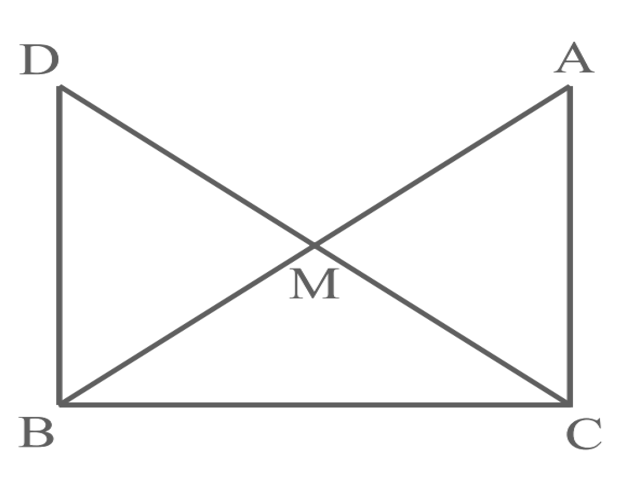
\includegraphics[width=\columnwidth]{figs/Screenshot.png}
  \caption{$\triangle \vec{ACB} ,\triangle \vec{DCB}$ with Mid-Point $\vec{M}$}
  \label{fig:triangles}
\end{figure}
\begin{enumerate}[label =(\roman*)]
        \item $\triangle \vec{AMC} \cong \triangle \vec{BMD}$
        \item $\angle \vec{DBC}$ is a right angle. 
        \item $\triangle \vec{DBC} \cong  \triangle \vec{ACB}$ 
        \item $\vec{CM} = \frac{1}{2} \vec{AB}$
\end{enumerate}
\pagebreak
\solution\\
\textbf{CONSTRUCTION STEPS :}
\begin{enumerate}
\item Let us Assume , the input parameters as ;
\begin{table}[H]
\centering
        \input{tables/input_params.tex}
          \caption{Input Parameters}
          \label{Table-1:Input_params}
\end{table}
\item the output can be calculated as ;
\begin{table}[H]
\centering
        \input{tables/output_params.tex}
          \caption{Output Parameters}
          \label{Table-2:Output_params}
\end{table}
                $\therefore$ By, Plotting these points we get the required Image \figref{fig:fig-2}
\begin{figure}[H]
        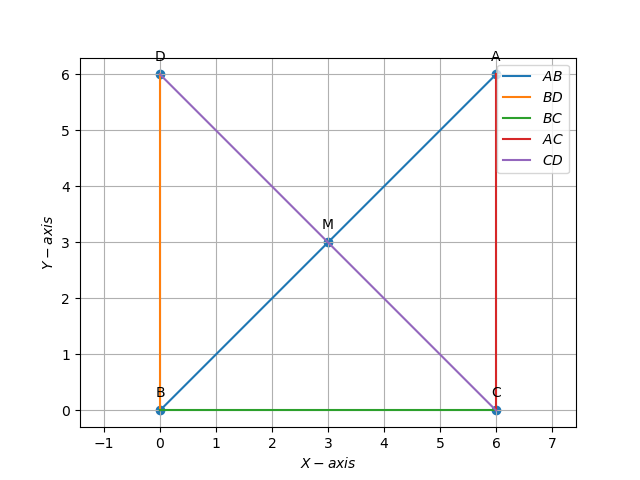
\includegraphics[width = \columnwidth]{figs/python_plot.png}
    \caption{PYTHON Plot of $\triangle \vec{ACB} ,\triangle \vec{DBC}$ with Mid-Point $\vec{M}$}
    \label{fig:fig-2}
\end{figure}
\end{enumerate}

\item Find the position vector of a point $\vec{R}$ which divides the line joining two points $\vec{P}$ and $\vec{Q}$ whose position vectors are $2\vec{a}+\vec{b}$ and $\vec{a}-3\vec{b}$ externally in the ratio $1:2$.

\textbf{Solution:}
Let us assume $\vec{a}$ and $\vec{b}$, and the given ratio is
\begin{table}[h]
    \centering
    \begin{tabular}{|c|c|c|}
        \hline 
        \textbf{Symbol} & \textbf{Value} & \textbf{Description} \\
        \hline
        $\vec{a}$ & $\myvec{1 \\ -3}$ & Vector $\vec{a}$ \\
        \hline
        $\vec{b}$ & $\myvec{0 \\ 2}$ & Vector $\vec{b}$\\
        \hline
        $k$ & $2$ & Ratio \\
        \hline
    \end{tabular}
    \caption{Vectors $\vec{a}$ and $\vec{b}$, ratio $k$}
    \label{tab:table1}
\end{table}

Using the section formula,
\begin{align}
    \vec{R} = \frac{\vec{Q} - k\vec{P}}{1 - k}
\end{align}
where $\vec{P}$ and $\vec{Q}$ depend on $\vec{a}$ and $\vec{b}$, then
\begin{align}
    \vec{P} &= (2\vec{a} + \vec{b}) = 2\myvec{1\\-3} + \myvec{0\\2} = \myvec{2\\-4} \\
    \vec{Q} &= (\vec{a} - 3\vec{b}) = \myvec{1\\-3} - 3\myvec{0\\2} = \myvec{1\\-9}
\end{align}
where $\vec{R}$ can be calculated as 
\begin{align}
    \vec{R} = \frac{(\vec{a} - 3\vec{b}) - k(2\vec{a} + \vec{b})}{1 - k}
\end{align}
By substituting $\vec{a}$ and $\vec{b}$ values, we get $\vec{R}$ as
\begin{align}
    \vec{R} = \myvec{3\\1}
\end{align}

\begin{table}[ht!]
    \centering
    \begin{tabular}{|c|c|c|}
        \hline
        \textbf{Symbol} & \textbf{Value} & \textbf{Description}\\
        \hline
        $\vec{P}$ & $(2\vec{a} + \vec{b})$ & Position vector $\vec{P}$ \\
        \hline
        $\vec{Q}$ & $(\vec{a} - 3\vec{b})$ & Position vector $\vec{Q}$\\
        \hline
        $\vec{R}$ & $\frac{\vec{Q} - k\vec{P}}{1 - k}$ & Position vector $\vec{R}$\\
        \hline
    \end{tabular}
    \caption{Vectors $\vec{P}$, $\vec{Q}$, $\vec{R}$}
    \label{tab:mytable2}   
\end{table}

\begin{figure}[H]
    \centering
    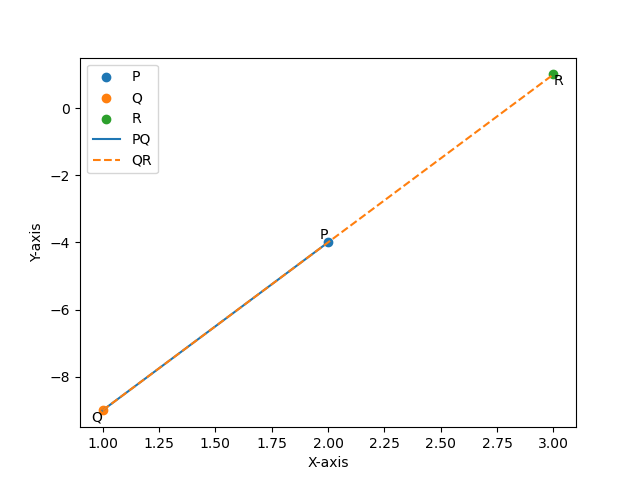
\includegraphics[width=\columnwidth]{figs/external-bisector.png}
    \caption{Point vectors $\vec{P}$, $\vec{Q}$, $\vec{R}$}
    \label{fig:enter-label}
\end{figure}


\end{enumerate}

    \item Draw a quadrilateral in the Cartesian plane, whose vertices are 
    \begin{align}
        \vec{A} = \myvec{-4\\5} \quad \vec{B} = \myvec{0\\7} \\
        \vec{C} = \myvec{5\\-5} \quad \vec{D} = \myvec{-4\\-2}
    \end{align}
    Also, find its area.
\label{chapters/11/10/1/1}
   \\ 
    \solution 
\begin{enumerate}[label=\thesection.\arabic*,ref=\thesection.\theenumi]
		\item Find $\abs{\overrightarrow{a}\times\overrightarrow{b}},\text{ if }\overrightarrow{a}=\hat{i}-7\hat{j}+7\hat{k}\text{ and } \overrightarrow{b}=3\hat{i}-2\hat{j}+2\hat{k}$.
	\\
		\solution
		\input{chapters/12/10/4/1/cross.tex}
\item Show that $$(\overrightarrow{a}-\overrightarrow{b})\times (\overrightarrow{a}+\overrightarrow{b})=2(\overrightarrow{a}\times \overrightarrow{b})$$
	\\
		\solution
		\input{chapters/12/10/4/4/cross.tex}
\item Find $\lambda$ and $\mu$ if $(2\hat{i}+6\hat{j}+27\hat{k})\times(\hat{i}+\lambda \hat{j} + \mu \hat{k})=\overrightarrow{0}$.
	\\
		\solution
		\input{chapters/12/10/4/5/cross.tex}
\item Given that $\overrightarrow{a} \cdot \overrightarrow{b} = 0$ and $\overrightarrow{a} \times \overrightarrow{b} = \overrightarrow{0}$. What can you conclude about the vectors $\overrightarrow{a} \text{ and }\overrightarrow{b}$?
\item Let the vectors be given as $\overrightarrow{a},\overrightarrow{b},\overrightarrow{c}\text{ be given as }\ a_1 \hat{i}+\ a_2 \hat{j}+\ a_3 \hat{k},\ b_1 \hat{i}+\ b_2 \hat{j}+\ b_3 \hat{k},\ c_1 \hat{i}+\ c_2 \hat{j}+\ c_3 \hat{k}$. Then show that $\overrightarrow{a} \times (\overrightarrow{b} + \overrightarrow{c}) = \overrightarrow{a} \times \overrightarrow{b}+\overrightarrow{a} \times \overrightarrow{c}$.
	\\
		\solution
		\input{chapters/12/10/4/7/cross.tex}
\item If either $\overrightarrow{a} = \overrightarrow{0}$ or $\overrightarrow{b} = \overrightarrow{0}$, then $\overrightarrow{a} \times \overrightarrow{b} = \overrightarrow{0}$. Is the converse true? Justify your answer with an example.
	\\
		\solution
		\input{chapters/12/10/4/8/cross.tex}
\item Find the area of the triangle with vertices $A(1, 1, 2)$, $B(2, 3, 5)$, and $C(1, 5, 5)$
	\\
		\solution
		\input{chapters/12/10/4/9/cross.tex}
\item Find the area of the parallelogram whose adjacent sides are determined by the vectors $\overrightarrow{a}=\hat{i}-\hat{j}+3\hat{k}$ and $\overrightarrow{b}=2\hat{i}-7\hat{j}+\hat{k}$.
	\\
		\solution
		\input{chapters/12/10/4/10/cross.tex}
\item Let the vectors $\overrightarrow{a}$ and $\overrightarrow{b}$ be such that $|\overrightarrow{a}| = 3$ and $|\overrightarrow{b}| = \dfrac{\sqrt{2}}{3}$, then $\overrightarrow{a} \times \overrightarrow{b}$ is a unit vector, if the angle between $\overrightarrow{a}$ and $\overrightarrow{b}$ is
\begin{enumerate}
\item $\dfrac{\pi}{6}$
\item $\dfrac{\pi}{4}$
\item $\dfrac{\pi}{3}$
\item $\dfrac{\pi}{2}$
\end{enumerate}
		\solution
		\input{chapters/12/10/4/11/cross.tex}
\item Area of a rectangle having vertices A, B, C and D with position vectors $ -\hat{i}+ \dfrac{1}{2} \hat{j}+4\hat{k},\hat{i}+ \dfrac{1}{2} \hat{j}+4\hat{k},\hat{i}-\dfrac{1}{2} \hat{j}+4\hat{k}\text{ and }-\hat{i}- \dfrac{1}{2} \hat{j}+4\hat{k}$, respectively is
\begin{enumerate}
\item $\dfrac{1}{2}$
\item 1
\item 2
\item 4
\end{enumerate}
		\solution
		\input{chapters/12/10/4/12/cross.tex}
\item Find the area of the triangle whose vertices are 
\begin{enumerate}
\item $(2, 3), (–1, 0), (2, – 4)$
\item $(–5, –1), (3, –5), (5, 2)$ 
\end{enumerate}
		\label{10/7/3/1}
\solution
		\input{chapters/10/7/3/1/area.tex}
\item Find the area of the triangle formed by joining the mid-points of the sides of the triangle whose vertices are $(0, –1), (2, 1) \text{ and } (0, 3)$. Find the ratio of this area to the area of the given triangle.
	\\
\solution
		\input{chapters/10/7/3/3/cross.tex}

\item Find the area of the quadrilateral whose vertices, taken in order, are $(– 4, – 2), (– 3, – 5), (3, – 2)$  and $ (2, 3)$.
	\\
\solution
		\input{chapters/10/7/3/4/cross.tex}

\item Verify that a median of a triangle divides it into two triangles of equal areas for $\triangle ABC$ whose vertices are $\vec{A}(4, -6), \vec{B}(3, 2), \text{ and } \vec{C}(5, 2)$. 
		\label{10/7/3/5}
		\\
\solution
		\input{chapters/10/7/3/5/area.tex}

\item The two adjacent sides of a parallelogram are 
$2\hat{i}-4\hat{j}+5\hat{k}$  and  $\hat{i}-2\hat{j}-3\hat{k}$.
Find the unit vector parallel to its diagonal. Also, find its area.\\
	\solution
		\input{chapters/12/10/5/10/cross.tex}
\item The vertices of a $\triangle ABC$ are $\vec{A}(4,6), \vec{B}(1,5)$ and  $\vec{C}(7,2)$. A line is drawn to intersect sides $AB$ and $AC$ at $\vec{D}$ and $\vec{E}$ respectively, such that $\frac{AD}{AB} = \frac{AE}{AC} = \frac{1}{4}$. Calculate the area of $\triangle ADE$ and compare it with the area of the $\triangle ABC$.
\\
\solution
	\input{chapters/10/7/4/6/section.tex}
    \item Draw a quadrilateral in the Cartesian plane, whose vertices are 
    \begin{align}
        \vec{A} = \myvec{-4\\5} \quad \vec{B} = \myvec{0\\7} \\
        \vec{C} = \myvec{5\\-5} \quad \vec{D} = \myvec{-4\\-2}
    \end{align}
    Also, find its area.
\label{chapters/11/10/1/1}
   \\ 
    \solution 
\input{chapters/11/10/1/1/cross.tex}
\item Find the area of region bounded by the triangle whose
	vertices are $(1, 0), (2, 2) \text{ and } (3, 1)$. 
\item Find the area of region bounded by the triangle whose vertices
	are $(– 1, 0), (1, 3) \text{ and } (3, 2)$. 
\item Find the area of the $\triangle ABC$, coordinates of whose vertices are $\vec{A}(2, 0), \vec{B}(4, 5), \text{ and } \vec{C}(6, 3)$.


\item 
\input{chapters/vectors/exer/main.tex}
\end{enumerate}


\item Find the area of region bounded by the triangle whose
	vertices are $(1, 0), (2, 2) \text{ and } (3, 1)$. 
\item Find the area of region bounded by the triangle whose vertices
	are $(– 1, 0), (1, 3) \text{ and } (3, 2)$. 
\item Find the area of the $\triangle ABC$, coordinates of whose vertices are $\vec{A}(2, 0), \vec{B}(4, 5), \text{ and } \vec{C}(6, 3)$.


\item 
%\documentclass[12pt]{article}
%\usepackage{graphicx}
%\usepackage{graphics}
%\usepackage{refstyle}
%\usepackage{amsmath}
%\usepackage{caption}
%\usepackage{float}
%\usepackage{booktabs}
%\usepackage{array}
%\usepackage{amssymb}
%\usepackage{booktabs}
%\let\vec\mathbf
%\providecommand{\brak}[1]{\ensuremath{\left(#1\right)}}
%\graphicspath{{/storage/self/primary/Download/latexnew/fig}}                                     
$\vec{P}$ and $\vec{Q}$ are any two points lying on the sides $DC$ and $AD$ respectively of a parallelogram $ABCD$.Show that, $ar\brak{\triangle APB}=ar\brak{\triangle BQC}$.


\textbf{Figure:}
\begin{figure}[H]
    \centering
	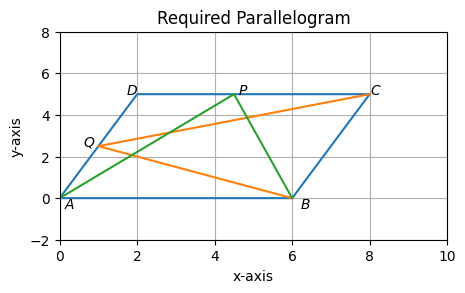
\includegraphics[width=\columnwidth]{chapters/vectors/exer/figs/1.png}
    \caption{}
    \label{fig:fig:1}
\end{figure}


\textbf{Solution:}
\begin{table}[H]
   \centering
  \input{chapters/vectors/exer/table/tab1.tex}
   \caption{Table of input parameters}        
\label{tab:tab:1}                    
\end{table}




\begin{table}[H]
    \centering                                  
\input{chapters/vectors/exer/table/tab2.tex}                  
\caption{Table of output parameters}
\label{tab:tab:2}
 \end{table}


For the $\triangle BQC$, the vertices of the triangle are taken from \tabref{tab:tab:1} and \tabref{tab:tab:2}.

\begin{align}
\implies ar\brak{\triangle BQC}&=
\frac{1}{2}\begin{tabular}{|c c c|}            
1 &1&1\\                      
$\vec{B}$&$\vec{Q}$&$\vec{C}$\\    
\end{tabular}\\
&= \frac{1}{2}\begin{tabular}{|c c c|}
       1 &1&1\\
       6&$\frac{2k_1}{k_1+1}$&8 \\
       0&$\frac{5k_1}{k_1+1}$&5
   \end{tabular}\\
  \xrightarrow{C_2'=C_2-C_1,C_3'=C_3-C_1}&\frac{1}{2} \begin{tabular}{|c c c|}
       1 &0&0\\
       6&$\frac{-4k_1-6}{k_1+1}$&2 \\
       0&$\frac{5k_1}{k_1+1}$&5
   \end{tabular}\\
&=\frac{1}{2}\brak{1\begin{tabular}{|c c|}
   $\frac{-4k_1-6}{k_1+1}$ &2  \\
   $\frac{5k_1}{k_1+1}$ & 5
\end{tabular} +0+0}\\
&=\frac{1}{2} \times30\\                          
&=15 \end{align}


For the $\triangle APB$, the vertices of the triangle are taken from \tabref{tab:tab:1} and \tabref{tab:tab:2}.
   \begin{align}
  \implies ar\brak{\triangle APB} &=
\frac{1}{2}\begin{tabular}{|c c c|}            
1 &1&1\\                            
$\vec{A}$&$\vec{P}$&$\vec{B}$\\
\end{tabular}\\ &=  \frac{1}{2}
   \begin{tabular}{|c c c|}
       1 &1&1\\
       0&$\frac{8k_2+2}{k_2+1}$&6 \\
       0&5&0
   \end{tabular}\\
 &=\frac{1}{2} \times30\\
 &=15 \end{align}
 \brak{6} = \brak{10}


So, ar\brak{\triangle BQC} = ar\brak{\triangle APB}.\brak{proved}
%\end{document}



\end{enumerate}


\item Area of a rectangle having vertices A, B, C and D with position vectors $ -\hat{i}+ \dfrac{1}{2} \hat{j}+4\hat{k},\hat{i}+ \dfrac{1}{2} \hat{j}+4\hat{k},\hat{i}-\dfrac{1}{2} \hat{j}+4\hat{k}\text{ and }-\hat{i}- \dfrac{1}{2} \hat{j}+4\hat{k}$, respectively is
\begin{enumerate}
\item $\dfrac{1}{2}$
\item 1
\item 2
\item 4
\end{enumerate}
		\solution
		\begin{enumerate}[label=\thesection.\arabic*,ref=\thesection.\theenumi]
		\item Find $\abs{\overrightarrow{a}\times\overrightarrow{b}},\text{ if }\overrightarrow{a}=\hat{i}-7\hat{j}+7\hat{k}\text{ and } \overrightarrow{b}=3\hat{i}-2\hat{j}+2\hat{k}$.
	\\
		\solution
		\begin{enumerate}[label=\thesection.\arabic*,ref=\thesection.\theenumi]
		\item Find $\abs{\overrightarrow{a}\times\overrightarrow{b}},\text{ if }\overrightarrow{a}=\hat{i}-7\hat{j}+7\hat{k}\text{ and } \overrightarrow{b}=3\hat{i}-2\hat{j}+2\hat{k}$.
	\\
		\solution
		\input{chapters/12/10/4/1/cross.tex}
\item Show that $$(\overrightarrow{a}-\overrightarrow{b})\times (\overrightarrow{a}+\overrightarrow{b})=2(\overrightarrow{a}\times \overrightarrow{b})$$
	\\
		\solution
		\input{chapters/12/10/4/4/cross.tex}
\item Find $\lambda$ and $\mu$ if $(2\hat{i}+6\hat{j}+27\hat{k})\times(\hat{i}+\lambda \hat{j} + \mu \hat{k})=\overrightarrow{0}$.
	\\
		\solution
		\input{chapters/12/10/4/5/cross.tex}
\item Given that $\overrightarrow{a} \cdot \overrightarrow{b} = 0$ and $\overrightarrow{a} \times \overrightarrow{b} = \overrightarrow{0}$. What can you conclude about the vectors $\overrightarrow{a} \text{ and }\overrightarrow{b}$?
\item Let the vectors be given as $\overrightarrow{a},\overrightarrow{b},\overrightarrow{c}\text{ be given as }\ a_1 \hat{i}+\ a_2 \hat{j}+\ a_3 \hat{k},\ b_1 \hat{i}+\ b_2 \hat{j}+\ b_3 \hat{k},\ c_1 \hat{i}+\ c_2 \hat{j}+\ c_3 \hat{k}$. Then show that $\overrightarrow{a} \times (\overrightarrow{b} + \overrightarrow{c}) = \overrightarrow{a} \times \overrightarrow{b}+\overrightarrow{a} \times \overrightarrow{c}$.
	\\
		\solution
		\input{chapters/12/10/4/7/cross.tex}
\item If either $\overrightarrow{a} = \overrightarrow{0}$ or $\overrightarrow{b} = \overrightarrow{0}$, then $\overrightarrow{a} \times \overrightarrow{b} = \overrightarrow{0}$. Is the converse true? Justify your answer with an example.
	\\
		\solution
		\input{chapters/12/10/4/8/cross.tex}
\item Find the area of the triangle with vertices $A(1, 1, 2)$, $B(2, 3, 5)$, and $C(1, 5, 5)$
	\\
		\solution
		\input{chapters/12/10/4/9/cross.tex}
\item Find the area of the parallelogram whose adjacent sides are determined by the vectors $\overrightarrow{a}=\hat{i}-\hat{j}+3\hat{k}$ and $\overrightarrow{b}=2\hat{i}-7\hat{j}+\hat{k}$.
	\\
		\solution
		\input{chapters/12/10/4/10/cross.tex}
\item Let the vectors $\overrightarrow{a}$ and $\overrightarrow{b}$ be such that $|\overrightarrow{a}| = 3$ and $|\overrightarrow{b}| = \dfrac{\sqrt{2}}{3}$, then $\overrightarrow{a} \times \overrightarrow{b}$ is a unit vector, if the angle between $\overrightarrow{a}$ and $\overrightarrow{b}$ is
\begin{enumerate}
\item $\dfrac{\pi}{6}$
\item $\dfrac{\pi}{4}$
\item $\dfrac{\pi}{3}$
\item $\dfrac{\pi}{2}$
\end{enumerate}
		\solution
		\input{chapters/12/10/4/11/cross.tex}
\item Area of a rectangle having vertices A, B, C and D with position vectors $ -\hat{i}+ \dfrac{1}{2} \hat{j}+4\hat{k},\hat{i}+ \dfrac{1}{2} \hat{j}+4\hat{k},\hat{i}-\dfrac{1}{2} \hat{j}+4\hat{k}\text{ and }-\hat{i}- \dfrac{1}{2} \hat{j}+4\hat{k}$, respectively is
\begin{enumerate}
\item $\dfrac{1}{2}$
\item 1
\item 2
\item 4
\end{enumerate}
		\solution
		\input{chapters/12/10/4/12/cross.tex}
\item Find the area of the triangle whose vertices are 
\begin{enumerate}
\item $(2, 3), (–1, 0), (2, – 4)$
\item $(–5, –1), (3, –5), (5, 2)$ 
\end{enumerate}
		\label{10/7/3/1}
\solution
		\input{chapters/10/7/3/1/area.tex}
\item Find the area of the triangle formed by joining the mid-points of the sides of the triangle whose vertices are $(0, –1), (2, 1) \text{ and } (0, 3)$. Find the ratio of this area to the area of the given triangle.
	\\
\solution
		\input{chapters/10/7/3/3/cross.tex}

\item Find the area of the quadrilateral whose vertices, taken in order, are $(– 4, – 2), (– 3, – 5), (3, – 2)$  and $ (2, 3)$.
	\\
\solution
		\input{chapters/10/7/3/4/cross.tex}

\item Verify that a median of a triangle divides it into two triangles of equal areas for $\triangle ABC$ whose vertices are $\vec{A}(4, -6), \vec{B}(3, 2), \text{ and } \vec{C}(5, 2)$. 
		\label{10/7/3/5}
		\\
\solution
		\input{chapters/10/7/3/5/area.tex}

\item The two adjacent sides of a parallelogram are 
$2\hat{i}-4\hat{j}+5\hat{k}$  and  $\hat{i}-2\hat{j}-3\hat{k}$.
Find the unit vector parallel to its diagonal. Also, find its area.\\
	\solution
		\input{chapters/12/10/5/10/cross.tex}
\item The vertices of a $\triangle ABC$ are $\vec{A}(4,6), \vec{B}(1,5)$ and  $\vec{C}(7,2)$. A line is drawn to intersect sides $AB$ and $AC$ at $\vec{D}$ and $\vec{E}$ respectively, such that $\frac{AD}{AB} = \frac{AE}{AC} = \frac{1}{4}$. Calculate the area of $\triangle ADE$ and compare it with the area of the $\triangle ABC$.
\\
\solution
	\input{chapters/10/7/4/6/section.tex}
    \item Draw a quadrilateral in the Cartesian plane, whose vertices are 
    \begin{align}
        \vec{A} = \myvec{-4\\5} \quad \vec{B} = \myvec{0\\7} \\
        \vec{C} = \myvec{5\\-5} \quad \vec{D} = \myvec{-4\\-2}
    \end{align}
    Also, find its area.
\label{chapters/11/10/1/1}
   \\ 
    \solution 
\input{chapters/11/10/1/1/cross.tex}
\item Find the area of region bounded by the triangle whose
	vertices are $(1, 0), (2, 2) \text{ and } (3, 1)$. 
\item Find the area of region bounded by the triangle whose vertices
	are $(– 1, 0), (1, 3) \text{ and } (3, 2)$. 
\item Find the area of the $\triangle ABC$, coordinates of whose vertices are $\vec{A}(2, 0), \vec{B}(4, 5), \text{ and } \vec{C}(6, 3)$.


\item 
\input{chapters/vectors/exer/main.tex}
\end{enumerate}


\item Show that $$(\overrightarrow{a}-\overrightarrow{b})\times (\overrightarrow{a}+\overrightarrow{b})=2(\overrightarrow{a}\times \overrightarrow{b})$$
	\\
		\solution
		\begin{enumerate}[label=\thesection.\arabic*,ref=\thesection.\theenumi]
		\item Find $\abs{\overrightarrow{a}\times\overrightarrow{b}},\text{ if }\overrightarrow{a}=\hat{i}-7\hat{j}+7\hat{k}\text{ and } \overrightarrow{b}=3\hat{i}-2\hat{j}+2\hat{k}$.
	\\
		\solution
		\input{chapters/12/10/4/1/cross.tex}
\item Show that $$(\overrightarrow{a}-\overrightarrow{b})\times (\overrightarrow{a}+\overrightarrow{b})=2(\overrightarrow{a}\times \overrightarrow{b})$$
	\\
		\solution
		\input{chapters/12/10/4/4/cross.tex}
\item Find $\lambda$ and $\mu$ if $(2\hat{i}+6\hat{j}+27\hat{k})\times(\hat{i}+\lambda \hat{j} + \mu \hat{k})=\overrightarrow{0}$.
	\\
		\solution
		\input{chapters/12/10/4/5/cross.tex}
\item Given that $\overrightarrow{a} \cdot \overrightarrow{b} = 0$ and $\overrightarrow{a} \times \overrightarrow{b} = \overrightarrow{0}$. What can you conclude about the vectors $\overrightarrow{a} \text{ and }\overrightarrow{b}$?
\item Let the vectors be given as $\overrightarrow{a},\overrightarrow{b},\overrightarrow{c}\text{ be given as }\ a_1 \hat{i}+\ a_2 \hat{j}+\ a_3 \hat{k},\ b_1 \hat{i}+\ b_2 \hat{j}+\ b_3 \hat{k},\ c_1 \hat{i}+\ c_2 \hat{j}+\ c_3 \hat{k}$. Then show that $\overrightarrow{a} \times (\overrightarrow{b} + \overrightarrow{c}) = \overrightarrow{a} \times \overrightarrow{b}+\overrightarrow{a} \times \overrightarrow{c}$.
	\\
		\solution
		\input{chapters/12/10/4/7/cross.tex}
\item If either $\overrightarrow{a} = \overrightarrow{0}$ or $\overrightarrow{b} = \overrightarrow{0}$, then $\overrightarrow{a} \times \overrightarrow{b} = \overrightarrow{0}$. Is the converse true? Justify your answer with an example.
	\\
		\solution
		\input{chapters/12/10/4/8/cross.tex}
\item Find the area of the triangle with vertices $A(1, 1, 2)$, $B(2, 3, 5)$, and $C(1, 5, 5)$
	\\
		\solution
		\input{chapters/12/10/4/9/cross.tex}
\item Find the area of the parallelogram whose adjacent sides are determined by the vectors $\overrightarrow{a}=\hat{i}-\hat{j}+3\hat{k}$ and $\overrightarrow{b}=2\hat{i}-7\hat{j}+\hat{k}$.
	\\
		\solution
		\input{chapters/12/10/4/10/cross.tex}
\item Let the vectors $\overrightarrow{a}$ and $\overrightarrow{b}$ be such that $|\overrightarrow{a}| = 3$ and $|\overrightarrow{b}| = \dfrac{\sqrt{2}}{3}$, then $\overrightarrow{a} \times \overrightarrow{b}$ is a unit vector, if the angle between $\overrightarrow{a}$ and $\overrightarrow{b}$ is
\begin{enumerate}
\item $\dfrac{\pi}{6}$
\item $\dfrac{\pi}{4}$
\item $\dfrac{\pi}{3}$
\item $\dfrac{\pi}{2}$
\end{enumerate}
		\solution
		\input{chapters/12/10/4/11/cross.tex}
\item Area of a rectangle having vertices A, B, C and D with position vectors $ -\hat{i}+ \dfrac{1}{2} \hat{j}+4\hat{k},\hat{i}+ \dfrac{1}{2} \hat{j}+4\hat{k},\hat{i}-\dfrac{1}{2} \hat{j}+4\hat{k}\text{ and }-\hat{i}- \dfrac{1}{2} \hat{j}+4\hat{k}$, respectively is
\begin{enumerate}
\item $\dfrac{1}{2}$
\item 1
\item 2
\item 4
\end{enumerate}
		\solution
		\input{chapters/12/10/4/12/cross.tex}
\item Find the area of the triangle whose vertices are 
\begin{enumerate}
\item $(2, 3), (–1, 0), (2, – 4)$
\item $(–5, –1), (3, –5), (5, 2)$ 
\end{enumerate}
		\label{10/7/3/1}
\solution
		\input{chapters/10/7/3/1/area.tex}
\item Find the area of the triangle formed by joining the mid-points of the sides of the triangle whose vertices are $(0, –1), (2, 1) \text{ and } (0, 3)$. Find the ratio of this area to the area of the given triangle.
	\\
\solution
		\input{chapters/10/7/3/3/cross.tex}

\item Find the area of the quadrilateral whose vertices, taken in order, are $(– 4, – 2), (– 3, – 5), (3, – 2)$  and $ (2, 3)$.
	\\
\solution
		\input{chapters/10/7/3/4/cross.tex}

\item Verify that a median of a triangle divides it into two triangles of equal areas for $\triangle ABC$ whose vertices are $\vec{A}(4, -6), \vec{B}(3, 2), \text{ and } \vec{C}(5, 2)$. 
		\label{10/7/3/5}
		\\
\solution
		\input{chapters/10/7/3/5/area.tex}

\item The two adjacent sides of a parallelogram are 
$2\hat{i}-4\hat{j}+5\hat{k}$  and  $\hat{i}-2\hat{j}-3\hat{k}$.
Find the unit vector parallel to its diagonal. Also, find its area.\\
	\solution
		\input{chapters/12/10/5/10/cross.tex}
\item The vertices of a $\triangle ABC$ are $\vec{A}(4,6), \vec{B}(1,5)$ and  $\vec{C}(7,2)$. A line is drawn to intersect sides $AB$ and $AC$ at $\vec{D}$ and $\vec{E}$ respectively, such that $\frac{AD}{AB} = \frac{AE}{AC} = \frac{1}{4}$. Calculate the area of $\triangle ADE$ and compare it with the area of the $\triangle ABC$.
\\
\solution
	\input{chapters/10/7/4/6/section.tex}
    \item Draw a quadrilateral in the Cartesian plane, whose vertices are 
    \begin{align}
        \vec{A} = \myvec{-4\\5} \quad \vec{B} = \myvec{0\\7} \\
        \vec{C} = \myvec{5\\-5} \quad \vec{D} = \myvec{-4\\-2}
    \end{align}
    Also, find its area.
\label{chapters/11/10/1/1}
   \\ 
    \solution 
\input{chapters/11/10/1/1/cross.tex}
\item Find the area of region bounded by the triangle whose
	vertices are $(1, 0), (2, 2) \text{ and } (3, 1)$. 
\item Find the area of region bounded by the triangle whose vertices
	are $(– 1, 0), (1, 3) \text{ and } (3, 2)$. 
\item Find the area of the $\triangle ABC$, coordinates of whose vertices are $\vec{A}(2, 0), \vec{B}(4, 5), \text{ and } \vec{C}(6, 3)$.


\item 
\input{chapters/vectors/exer/main.tex}
\end{enumerate}


\item Find $\lambda$ and $\mu$ if $(2\hat{i}+6\hat{j}+27\hat{k})\times(\hat{i}+\lambda \hat{j} + \mu \hat{k})=\overrightarrow{0}$.
	\\
		\solution
		\begin{enumerate}[label=\thesection.\arabic*,ref=\thesection.\theenumi]
		\item Find $\abs{\overrightarrow{a}\times\overrightarrow{b}},\text{ if }\overrightarrow{a}=\hat{i}-7\hat{j}+7\hat{k}\text{ and } \overrightarrow{b}=3\hat{i}-2\hat{j}+2\hat{k}$.
	\\
		\solution
		\input{chapters/12/10/4/1/cross.tex}
\item Show that $$(\overrightarrow{a}-\overrightarrow{b})\times (\overrightarrow{a}+\overrightarrow{b})=2(\overrightarrow{a}\times \overrightarrow{b})$$
	\\
		\solution
		\input{chapters/12/10/4/4/cross.tex}
\item Find $\lambda$ and $\mu$ if $(2\hat{i}+6\hat{j}+27\hat{k})\times(\hat{i}+\lambda \hat{j} + \mu \hat{k})=\overrightarrow{0}$.
	\\
		\solution
		\input{chapters/12/10/4/5/cross.tex}
\item Given that $\overrightarrow{a} \cdot \overrightarrow{b} = 0$ and $\overrightarrow{a} \times \overrightarrow{b} = \overrightarrow{0}$. What can you conclude about the vectors $\overrightarrow{a} \text{ and }\overrightarrow{b}$?
\item Let the vectors be given as $\overrightarrow{a},\overrightarrow{b},\overrightarrow{c}\text{ be given as }\ a_1 \hat{i}+\ a_2 \hat{j}+\ a_3 \hat{k},\ b_1 \hat{i}+\ b_2 \hat{j}+\ b_3 \hat{k},\ c_1 \hat{i}+\ c_2 \hat{j}+\ c_3 \hat{k}$. Then show that $\overrightarrow{a} \times (\overrightarrow{b} + \overrightarrow{c}) = \overrightarrow{a} \times \overrightarrow{b}+\overrightarrow{a} \times \overrightarrow{c}$.
	\\
		\solution
		\input{chapters/12/10/4/7/cross.tex}
\item If either $\overrightarrow{a} = \overrightarrow{0}$ or $\overrightarrow{b} = \overrightarrow{0}$, then $\overrightarrow{a} \times \overrightarrow{b} = \overrightarrow{0}$. Is the converse true? Justify your answer with an example.
	\\
		\solution
		\input{chapters/12/10/4/8/cross.tex}
\item Find the area of the triangle with vertices $A(1, 1, 2)$, $B(2, 3, 5)$, and $C(1, 5, 5)$
	\\
		\solution
		\input{chapters/12/10/4/9/cross.tex}
\item Find the area of the parallelogram whose adjacent sides are determined by the vectors $\overrightarrow{a}=\hat{i}-\hat{j}+3\hat{k}$ and $\overrightarrow{b}=2\hat{i}-7\hat{j}+\hat{k}$.
	\\
		\solution
		\input{chapters/12/10/4/10/cross.tex}
\item Let the vectors $\overrightarrow{a}$ and $\overrightarrow{b}$ be such that $|\overrightarrow{a}| = 3$ and $|\overrightarrow{b}| = \dfrac{\sqrt{2}}{3}$, then $\overrightarrow{a} \times \overrightarrow{b}$ is a unit vector, if the angle between $\overrightarrow{a}$ and $\overrightarrow{b}$ is
\begin{enumerate}
\item $\dfrac{\pi}{6}$
\item $\dfrac{\pi}{4}$
\item $\dfrac{\pi}{3}$
\item $\dfrac{\pi}{2}$
\end{enumerate}
		\solution
		\input{chapters/12/10/4/11/cross.tex}
\item Area of a rectangle having vertices A, B, C and D with position vectors $ -\hat{i}+ \dfrac{1}{2} \hat{j}+4\hat{k},\hat{i}+ \dfrac{1}{2} \hat{j}+4\hat{k},\hat{i}-\dfrac{1}{2} \hat{j}+4\hat{k}\text{ and }-\hat{i}- \dfrac{1}{2} \hat{j}+4\hat{k}$, respectively is
\begin{enumerate}
\item $\dfrac{1}{2}$
\item 1
\item 2
\item 4
\end{enumerate}
		\solution
		\input{chapters/12/10/4/12/cross.tex}
\item Find the area of the triangle whose vertices are 
\begin{enumerate}
\item $(2, 3), (–1, 0), (2, – 4)$
\item $(–5, –1), (3, –5), (5, 2)$ 
\end{enumerate}
		\label{10/7/3/1}
\solution
		\input{chapters/10/7/3/1/area.tex}
\item Find the area of the triangle formed by joining the mid-points of the sides of the triangle whose vertices are $(0, –1), (2, 1) \text{ and } (0, 3)$. Find the ratio of this area to the area of the given triangle.
	\\
\solution
		\input{chapters/10/7/3/3/cross.tex}

\item Find the area of the quadrilateral whose vertices, taken in order, are $(– 4, – 2), (– 3, – 5), (3, – 2)$  and $ (2, 3)$.
	\\
\solution
		\input{chapters/10/7/3/4/cross.tex}

\item Verify that a median of a triangle divides it into two triangles of equal areas for $\triangle ABC$ whose vertices are $\vec{A}(4, -6), \vec{B}(3, 2), \text{ and } \vec{C}(5, 2)$. 
		\label{10/7/3/5}
		\\
\solution
		\input{chapters/10/7/3/5/area.tex}

\item The two adjacent sides of a parallelogram are 
$2\hat{i}-4\hat{j}+5\hat{k}$  and  $\hat{i}-2\hat{j}-3\hat{k}$.
Find the unit vector parallel to its diagonal. Also, find its area.\\
	\solution
		\input{chapters/12/10/5/10/cross.tex}
\item The vertices of a $\triangle ABC$ are $\vec{A}(4,6), \vec{B}(1,5)$ and  $\vec{C}(7,2)$. A line is drawn to intersect sides $AB$ and $AC$ at $\vec{D}$ and $\vec{E}$ respectively, such that $\frac{AD}{AB} = \frac{AE}{AC} = \frac{1}{4}$. Calculate the area of $\triangle ADE$ and compare it with the area of the $\triangle ABC$.
\\
\solution
	\input{chapters/10/7/4/6/section.tex}
    \item Draw a quadrilateral in the Cartesian plane, whose vertices are 
    \begin{align}
        \vec{A} = \myvec{-4\\5} \quad \vec{B} = \myvec{0\\7} \\
        \vec{C} = \myvec{5\\-5} \quad \vec{D} = \myvec{-4\\-2}
    \end{align}
    Also, find its area.
\label{chapters/11/10/1/1}
   \\ 
    \solution 
\input{chapters/11/10/1/1/cross.tex}
\item Find the area of region bounded by the triangle whose
	vertices are $(1, 0), (2, 2) \text{ and } (3, 1)$. 
\item Find the area of region bounded by the triangle whose vertices
	are $(– 1, 0), (1, 3) \text{ and } (3, 2)$. 
\item Find the area of the $\triangle ABC$, coordinates of whose vertices are $\vec{A}(2, 0), \vec{B}(4, 5), \text{ and } \vec{C}(6, 3)$.


\item 
\input{chapters/vectors/exer/main.tex}
\end{enumerate}


\item Given that $\overrightarrow{a} \cdot \overrightarrow{b} = 0$ and $\overrightarrow{a} \times \overrightarrow{b} = \overrightarrow{0}$. What can you conclude about the vectors $\overrightarrow{a} \text{ and }\overrightarrow{b}$?
\item Let the vectors be given as $\overrightarrow{a},\overrightarrow{b},\overrightarrow{c}\text{ be given as }\ a_1 \hat{i}+\ a_2 \hat{j}+\ a_3 \hat{k},\ b_1 \hat{i}+\ b_2 \hat{j}+\ b_3 \hat{k},\ c_1 \hat{i}+\ c_2 \hat{j}+\ c_3 \hat{k}$. Then show that $\overrightarrow{a} \times (\overrightarrow{b} + \overrightarrow{c}) = \overrightarrow{a} \times \overrightarrow{b}+\overrightarrow{a} \times \overrightarrow{c}$.
	\\
		\solution
		\begin{enumerate}[label=\thesection.\arabic*,ref=\thesection.\theenumi]
		\item Find $\abs{\overrightarrow{a}\times\overrightarrow{b}},\text{ if }\overrightarrow{a}=\hat{i}-7\hat{j}+7\hat{k}\text{ and } \overrightarrow{b}=3\hat{i}-2\hat{j}+2\hat{k}$.
	\\
		\solution
		\input{chapters/12/10/4/1/cross.tex}
\item Show that $$(\overrightarrow{a}-\overrightarrow{b})\times (\overrightarrow{a}+\overrightarrow{b})=2(\overrightarrow{a}\times \overrightarrow{b})$$
	\\
		\solution
		\input{chapters/12/10/4/4/cross.tex}
\item Find $\lambda$ and $\mu$ if $(2\hat{i}+6\hat{j}+27\hat{k})\times(\hat{i}+\lambda \hat{j} + \mu \hat{k})=\overrightarrow{0}$.
	\\
		\solution
		\input{chapters/12/10/4/5/cross.tex}
\item Given that $\overrightarrow{a} \cdot \overrightarrow{b} = 0$ and $\overrightarrow{a} \times \overrightarrow{b} = \overrightarrow{0}$. What can you conclude about the vectors $\overrightarrow{a} \text{ and }\overrightarrow{b}$?
\item Let the vectors be given as $\overrightarrow{a},\overrightarrow{b},\overrightarrow{c}\text{ be given as }\ a_1 \hat{i}+\ a_2 \hat{j}+\ a_3 \hat{k},\ b_1 \hat{i}+\ b_2 \hat{j}+\ b_3 \hat{k},\ c_1 \hat{i}+\ c_2 \hat{j}+\ c_3 \hat{k}$. Then show that $\overrightarrow{a} \times (\overrightarrow{b} + \overrightarrow{c}) = \overrightarrow{a} \times \overrightarrow{b}+\overrightarrow{a} \times \overrightarrow{c}$.
	\\
		\solution
		\input{chapters/12/10/4/7/cross.tex}
\item If either $\overrightarrow{a} = \overrightarrow{0}$ or $\overrightarrow{b} = \overrightarrow{0}$, then $\overrightarrow{a} \times \overrightarrow{b} = \overrightarrow{0}$. Is the converse true? Justify your answer with an example.
	\\
		\solution
		\input{chapters/12/10/4/8/cross.tex}
\item Find the area of the triangle with vertices $A(1, 1, 2)$, $B(2, 3, 5)$, and $C(1, 5, 5)$
	\\
		\solution
		\input{chapters/12/10/4/9/cross.tex}
\item Find the area of the parallelogram whose adjacent sides are determined by the vectors $\overrightarrow{a}=\hat{i}-\hat{j}+3\hat{k}$ and $\overrightarrow{b}=2\hat{i}-7\hat{j}+\hat{k}$.
	\\
		\solution
		\input{chapters/12/10/4/10/cross.tex}
\item Let the vectors $\overrightarrow{a}$ and $\overrightarrow{b}$ be such that $|\overrightarrow{a}| = 3$ and $|\overrightarrow{b}| = \dfrac{\sqrt{2}}{3}$, then $\overrightarrow{a} \times \overrightarrow{b}$ is a unit vector, if the angle between $\overrightarrow{a}$ and $\overrightarrow{b}$ is
\begin{enumerate}
\item $\dfrac{\pi}{6}$
\item $\dfrac{\pi}{4}$
\item $\dfrac{\pi}{3}$
\item $\dfrac{\pi}{2}$
\end{enumerate}
		\solution
		\input{chapters/12/10/4/11/cross.tex}
\item Area of a rectangle having vertices A, B, C and D with position vectors $ -\hat{i}+ \dfrac{1}{2} \hat{j}+4\hat{k},\hat{i}+ \dfrac{1}{2} \hat{j}+4\hat{k},\hat{i}-\dfrac{1}{2} \hat{j}+4\hat{k}\text{ and }-\hat{i}- \dfrac{1}{2} \hat{j}+4\hat{k}$, respectively is
\begin{enumerate}
\item $\dfrac{1}{2}$
\item 1
\item 2
\item 4
\end{enumerate}
		\solution
		\input{chapters/12/10/4/12/cross.tex}
\item Find the area of the triangle whose vertices are 
\begin{enumerate}
\item $(2, 3), (–1, 0), (2, – 4)$
\item $(–5, –1), (3, –5), (5, 2)$ 
\end{enumerate}
		\label{10/7/3/1}
\solution
		\input{chapters/10/7/3/1/area.tex}
\item Find the area of the triangle formed by joining the mid-points of the sides of the triangle whose vertices are $(0, –1), (2, 1) \text{ and } (0, 3)$. Find the ratio of this area to the area of the given triangle.
	\\
\solution
		\input{chapters/10/7/3/3/cross.tex}

\item Find the area of the quadrilateral whose vertices, taken in order, are $(– 4, – 2), (– 3, – 5), (3, – 2)$  and $ (2, 3)$.
	\\
\solution
		\input{chapters/10/7/3/4/cross.tex}

\item Verify that a median of a triangle divides it into two triangles of equal areas for $\triangle ABC$ whose vertices are $\vec{A}(4, -6), \vec{B}(3, 2), \text{ and } \vec{C}(5, 2)$. 
		\label{10/7/3/5}
		\\
\solution
		\input{chapters/10/7/3/5/area.tex}

\item The two adjacent sides of a parallelogram are 
$2\hat{i}-4\hat{j}+5\hat{k}$  and  $\hat{i}-2\hat{j}-3\hat{k}$.
Find the unit vector parallel to its diagonal. Also, find its area.\\
	\solution
		\input{chapters/12/10/5/10/cross.tex}
\item The vertices of a $\triangle ABC$ are $\vec{A}(4,6), \vec{B}(1,5)$ and  $\vec{C}(7,2)$. A line is drawn to intersect sides $AB$ and $AC$ at $\vec{D}$ and $\vec{E}$ respectively, such that $\frac{AD}{AB} = \frac{AE}{AC} = \frac{1}{4}$. Calculate the area of $\triangle ADE$ and compare it with the area of the $\triangle ABC$.
\\
\solution
	\input{chapters/10/7/4/6/section.tex}
    \item Draw a quadrilateral in the Cartesian plane, whose vertices are 
    \begin{align}
        \vec{A} = \myvec{-4\\5} \quad \vec{B} = \myvec{0\\7} \\
        \vec{C} = \myvec{5\\-5} \quad \vec{D} = \myvec{-4\\-2}
    \end{align}
    Also, find its area.
\label{chapters/11/10/1/1}
   \\ 
    \solution 
\input{chapters/11/10/1/1/cross.tex}
\item Find the area of region bounded by the triangle whose
	vertices are $(1, 0), (2, 2) \text{ and } (3, 1)$. 
\item Find the area of region bounded by the triangle whose vertices
	are $(– 1, 0), (1, 3) \text{ and } (3, 2)$. 
\item Find the area of the $\triangle ABC$, coordinates of whose vertices are $\vec{A}(2, 0), \vec{B}(4, 5), \text{ and } \vec{C}(6, 3)$.


\item 
\input{chapters/vectors/exer/main.tex}
\end{enumerate}


\item If either $\overrightarrow{a} = \overrightarrow{0}$ or $\overrightarrow{b} = \overrightarrow{0}$, then $\overrightarrow{a} \times \overrightarrow{b} = \overrightarrow{0}$. Is the converse true? Justify your answer with an example.
	\\
		\solution
		\begin{enumerate}[label=\thesection.\arabic*,ref=\thesection.\theenumi]
		\item Find $\abs{\overrightarrow{a}\times\overrightarrow{b}},\text{ if }\overrightarrow{a}=\hat{i}-7\hat{j}+7\hat{k}\text{ and } \overrightarrow{b}=3\hat{i}-2\hat{j}+2\hat{k}$.
	\\
		\solution
		\input{chapters/12/10/4/1/cross.tex}
\item Show that $$(\overrightarrow{a}-\overrightarrow{b})\times (\overrightarrow{a}+\overrightarrow{b})=2(\overrightarrow{a}\times \overrightarrow{b})$$
	\\
		\solution
		\input{chapters/12/10/4/4/cross.tex}
\item Find $\lambda$ and $\mu$ if $(2\hat{i}+6\hat{j}+27\hat{k})\times(\hat{i}+\lambda \hat{j} + \mu \hat{k})=\overrightarrow{0}$.
	\\
		\solution
		\input{chapters/12/10/4/5/cross.tex}
\item Given that $\overrightarrow{a} \cdot \overrightarrow{b} = 0$ and $\overrightarrow{a} \times \overrightarrow{b} = \overrightarrow{0}$. What can you conclude about the vectors $\overrightarrow{a} \text{ and }\overrightarrow{b}$?
\item Let the vectors be given as $\overrightarrow{a},\overrightarrow{b},\overrightarrow{c}\text{ be given as }\ a_1 \hat{i}+\ a_2 \hat{j}+\ a_3 \hat{k},\ b_1 \hat{i}+\ b_2 \hat{j}+\ b_3 \hat{k},\ c_1 \hat{i}+\ c_2 \hat{j}+\ c_3 \hat{k}$. Then show that $\overrightarrow{a} \times (\overrightarrow{b} + \overrightarrow{c}) = \overrightarrow{a} \times \overrightarrow{b}+\overrightarrow{a} \times \overrightarrow{c}$.
	\\
		\solution
		\input{chapters/12/10/4/7/cross.tex}
\item If either $\overrightarrow{a} = \overrightarrow{0}$ or $\overrightarrow{b} = \overrightarrow{0}$, then $\overrightarrow{a} \times \overrightarrow{b} = \overrightarrow{0}$. Is the converse true? Justify your answer with an example.
	\\
		\solution
		\input{chapters/12/10/4/8/cross.tex}
\item Find the area of the triangle with vertices $A(1, 1, 2)$, $B(2, 3, 5)$, and $C(1, 5, 5)$
	\\
		\solution
		\input{chapters/12/10/4/9/cross.tex}
\item Find the area of the parallelogram whose adjacent sides are determined by the vectors $\overrightarrow{a}=\hat{i}-\hat{j}+3\hat{k}$ and $\overrightarrow{b}=2\hat{i}-7\hat{j}+\hat{k}$.
	\\
		\solution
		\input{chapters/12/10/4/10/cross.tex}
\item Let the vectors $\overrightarrow{a}$ and $\overrightarrow{b}$ be such that $|\overrightarrow{a}| = 3$ and $|\overrightarrow{b}| = \dfrac{\sqrt{2}}{3}$, then $\overrightarrow{a} \times \overrightarrow{b}$ is a unit vector, if the angle between $\overrightarrow{a}$ and $\overrightarrow{b}$ is
\begin{enumerate}
\item $\dfrac{\pi}{6}$
\item $\dfrac{\pi}{4}$
\item $\dfrac{\pi}{3}$
\item $\dfrac{\pi}{2}$
\end{enumerate}
		\solution
		\input{chapters/12/10/4/11/cross.tex}
\item Area of a rectangle having vertices A, B, C and D with position vectors $ -\hat{i}+ \dfrac{1}{2} \hat{j}+4\hat{k},\hat{i}+ \dfrac{1}{2} \hat{j}+4\hat{k},\hat{i}-\dfrac{1}{2} \hat{j}+4\hat{k}\text{ and }-\hat{i}- \dfrac{1}{2} \hat{j}+4\hat{k}$, respectively is
\begin{enumerate}
\item $\dfrac{1}{2}$
\item 1
\item 2
\item 4
\end{enumerate}
		\solution
		\input{chapters/12/10/4/12/cross.tex}
\item Find the area of the triangle whose vertices are 
\begin{enumerate}
\item $(2, 3), (–1, 0), (2, – 4)$
\item $(–5, –1), (3, –5), (5, 2)$ 
\end{enumerate}
		\label{10/7/3/1}
\solution
		\input{chapters/10/7/3/1/area.tex}
\item Find the area of the triangle formed by joining the mid-points of the sides of the triangle whose vertices are $(0, –1), (2, 1) \text{ and } (0, 3)$. Find the ratio of this area to the area of the given triangle.
	\\
\solution
		\input{chapters/10/7/3/3/cross.tex}

\item Find the area of the quadrilateral whose vertices, taken in order, are $(– 4, – 2), (– 3, – 5), (3, – 2)$  and $ (2, 3)$.
	\\
\solution
		\input{chapters/10/7/3/4/cross.tex}

\item Verify that a median of a triangle divides it into two triangles of equal areas for $\triangle ABC$ whose vertices are $\vec{A}(4, -6), \vec{B}(3, 2), \text{ and } \vec{C}(5, 2)$. 
		\label{10/7/3/5}
		\\
\solution
		\input{chapters/10/7/3/5/area.tex}

\item The two adjacent sides of a parallelogram are 
$2\hat{i}-4\hat{j}+5\hat{k}$  and  $\hat{i}-2\hat{j}-3\hat{k}$.
Find the unit vector parallel to its diagonal. Also, find its area.\\
	\solution
		\input{chapters/12/10/5/10/cross.tex}
\item The vertices of a $\triangle ABC$ are $\vec{A}(4,6), \vec{B}(1,5)$ and  $\vec{C}(7,2)$. A line is drawn to intersect sides $AB$ and $AC$ at $\vec{D}$ and $\vec{E}$ respectively, such that $\frac{AD}{AB} = \frac{AE}{AC} = \frac{1}{4}$. Calculate the area of $\triangle ADE$ and compare it with the area of the $\triangle ABC$.
\\
\solution
	\input{chapters/10/7/4/6/section.tex}
    \item Draw a quadrilateral in the Cartesian plane, whose vertices are 
    \begin{align}
        \vec{A} = \myvec{-4\\5} \quad \vec{B} = \myvec{0\\7} \\
        \vec{C} = \myvec{5\\-5} \quad \vec{D} = \myvec{-4\\-2}
    \end{align}
    Also, find its area.
\label{chapters/11/10/1/1}
   \\ 
    \solution 
\input{chapters/11/10/1/1/cross.tex}
\item Find the area of region bounded by the triangle whose
	vertices are $(1, 0), (2, 2) \text{ and } (3, 1)$. 
\item Find the area of region bounded by the triangle whose vertices
	are $(– 1, 0), (1, 3) \text{ and } (3, 2)$. 
\item Find the area of the $\triangle ABC$, coordinates of whose vertices are $\vec{A}(2, 0), \vec{B}(4, 5), \text{ and } \vec{C}(6, 3)$.


\item 
\input{chapters/vectors/exer/main.tex}
\end{enumerate}


\item Find the area of the triangle with vertices $A(1, 1, 2)$, $B(2, 3, 5)$, and $C(1, 5, 5)$
	\\
		\solution
		\begin{enumerate}[label=\thesection.\arabic*,ref=\thesection.\theenumi]
		\item Find $\abs{\overrightarrow{a}\times\overrightarrow{b}},\text{ if }\overrightarrow{a}=\hat{i}-7\hat{j}+7\hat{k}\text{ and } \overrightarrow{b}=3\hat{i}-2\hat{j}+2\hat{k}$.
	\\
		\solution
		\input{chapters/12/10/4/1/cross.tex}
\item Show that $$(\overrightarrow{a}-\overrightarrow{b})\times (\overrightarrow{a}+\overrightarrow{b})=2(\overrightarrow{a}\times \overrightarrow{b})$$
	\\
		\solution
		\input{chapters/12/10/4/4/cross.tex}
\item Find $\lambda$ and $\mu$ if $(2\hat{i}+6\hat{j}+27\hat{k})\times(\hat{i}+\lambda \hat{j} + \mu \hat{k})=\overrightarrow{0}$.
	\\
		\solution
		\input{chapters/12/10/4/5/cross.tex}
\item Given that $\overrightarrow{a} \cdot \overrightarrow{b} = 0$ and $\overrightarrow{a} \times \overrightarrow{b} = \overrightarrow{0}$. What can you conclude about the vectors $\overrightarrow{a} \text{ and }\overrightarrow{b}$?
\item Let the vectors be given as $\overrightarrow{a},\overrightarrow{b},\overrightarrow{c}\text{ be given as }\ a_1 \hat{i}+\ a_2 \hat{j}+\ a_3 \hat{k},\ b_1 \hat{i}+\ b_2 \hat{j}+\ b_3 \hat{k},\ c_1 \hat{i}+\ c_2 \hat{j}+\ c_3 \hat{k}$. Then show that $\overrightarrow{a} \times (\overrightarrow{b} + \overrightarrow{c}) = \overrightarrow{a} \times \overrightarrow{b}+\overrightarrow{a} \times \overrightarrow{c}$.
	\\
		\solution
		\input{chapters/12/10/4/7/cross.tex}
\item If either $\overrightarrow{a} = \overrightarrow{0}$ or $\overrightarrow{b} = \overrightarrow{0}$, then $\overrightarrow{a} \times \overrightarrow{b} = \overrightarrow{0}$. Is the converse true? Justify your answer with an example.
	\\
		\solution
		\input{chapters/12/10/4/8/cross.tex}
\item Find the area of the triangle with vertices $A(1, 1, 2)$, $B(2, 3, 5)$, and $C(1, 5, 5)$
	\\
		\solution
		\input{chapters/12/10/4/9/cross.tex}
\item Find the area of the parallelogram whose adjacent sides are determined by the vectors $\overrightarrow{a}=\hat{i}-\hat{j}+3\hat{k}$ and $\overrightarrow{b}=2\hat{i}-7\hat{j}+\hat{k}$.
	\\
		\solution
		\input{chapters/12/10/4/10/cross.tex}
\item Let the vectors $\overrightarrow{a}$ and $\overrightarrow{b}$ be such that $|\overrightarrow{a}| = 3$ and $|\overrightarrow{b}| = \dfrac{\sqrt{2}}{3}$, then $\overrightarrow{a} \times \overrightarrow{b}$ is a unit vector, if the angle between $\overrightarrow{a}$ and $\overrightarrow{b}$ is
\begin{enumerate}
\item $\dfrac{\pi}{6}$
\item $\dfrac{\pi}{4}$
\item $\dfrac{\pi}{3}$
\item $\dfrac{\pi}{2}$
\end{enumerate}
		\solution
		\input{chapters/12/10/4/11/cross.tex}
\item Area of a rectangle having vertices A, B, C and D with position vectors $ -\hat{i}+ \dfrac{1}{2} \hat{j}+4\hat{k},\hat{i}+ \dfrac{1}{2} \hat{j}+4\hat{k},\hat{i}-\dfrac{1}{2} \hat{j}+4\hat{k}\text{ and }-\hat{i}- \dfrac{1}{2} \hat{j}+4\hat{k}$, respectively is
\begin{enumerate}
\item $\dfrac{1}{2}$
\item 1
\item 2
\item 4
\end{enumerate}
		\solution
		\input{chapters/12/10/4/12/cross.tex}
\item Find the area of the triangle whose vertices are 
\begin{enumerate}
\item $(2, 3), (–1, 0), (2, – 4)$
\item $(–5, –1), (3, –5), (5, 2)$ 
\end{enumerate}
		\label{10/7/3/1}
\solution
		\input{chapters/10/7/3/1/area.tex}
\item Find the area of the triangle formed by joining the mid-points of the sides of the triangle whose vertices are $(0, –1), (2, 1) \text{ and } (0, 3)$. Find the ratio of this area to the area of the given triangle.
	\\
\solution
		\input{chapters/10/7/3/3/cross.tex}

\item Find the area of the quadrilateral whose vertices, taken in order, are $(– 4, – 2), (– 3, – 5), (3, – 2)$  and $ (2, 3)$.
	\\
\solution
		\input{chapters/10/7/3/4/cross.tex}

\item Verify that a median of a triangle divides it into two triangles of equal areas for $\triangle ABC$ whose vertices are $\vec{A}(4, -6), \vec{B}(3, 2), \text{ and } \vec{C}(5, 2)$. 
		\label{10/7/3/5}
		\\
\solution
		\input{chapters/10/7/3/5/area.tex}

\item The two adjacent sides of a parallelogram are 
$2\hat{i}-4\hat{j}+5\hat{k}$  and  $\hat{i}-2\hat{j}-3\hat{k}$.
Find the unit vector parallel to its diagonal. Also, find its area.\\
	\solution
		\input{chapters/12/10/5/10/cross.tex}
\item The vertices of a $\triangle ABC$ are $\vec{A}(4,6), \vec{B}(1,5)$ and  $\vec{C}(7,2)$. A line is drawn to intersect sides $AB$ and $AC$ at $\vec{D}$ and $\vec{E}$ respectively, such that $\frac{AD}{AB} = \frac{AE}{AC} = \frac{1}{4}$. Calculate the area of $\triangle ADE$ and compare it with the area of the $\triangle ABC$.
\\
\solution
	\input{chapters/10/7/4/6/section.tex}
    \item Draw a quadrilateral in the Cartesian plane, whose vertices are 
    \begin{align}
        \vec{A} = \myvec{-4\\5} \quad \vec{B} = \myvec{0\\7} \\
        \vec{C} = \myvec{5\\-5} \quad \vec{D} = \myvec{-4\\-2}
    \end{align}
    Also, find its area.
\label{chapters/11/10/1/1}
   \\ 
    \solution 
\input{chapters/11/10/1/1/cross.tex}
\item Find the area of region bounded by the triangle whose
	vertices are $(1, 0), (2, 2) \text{ and } (3, 1)$. 
\item Find the area of region bounded by the triangle whose vertices
	are $(– 1, 0), (1, 3) \text{ and } (3, 2)$. 
\item Find the area of the $\triangle ABC$, coordinates of whose vertices are $\vec{A}(2, 0), \vec{B}(4, 5), \text{ and } \vec{C}(6, 3)$.


\item 
\input{chapters/vectors/exer/main.tex}
\end{enumerate}


\item Find the area of the parallelogram whose adjacent sides are determined by the vectors $\overrightarrow{a}=\hat{i}-\hat{j}+3\hat{k}$ and $\overrightarrow{b}=2\hat{i}-7\hat{j}+\hat{k}$.
	\\
		\solution
		\begin{enumerate}[label=\thesection.\arabic*,ref=\thesection.\theenumi]
		\item Find $\abs{\overrightarrow{a}\times\overrightarrow{b}},\text{ if }\overrightarrow{a}=\hat{i}-7\hat{j}+7\hat{k}\text{ and } \overrightarrow{b}=3\hat{i}-2\hat{j}+2\hat{k}$.
	\\
		\solution
		\input{chapters/12/10/4/1/cross.tex}
\item Show that $$(\overrightarrow{a}-\overrightarrow{b})\times (\overrightarrow{a}+\overrightarrow{b})=2(\overrightarrow{a}\times \overrightarrow{b})$$
	\\
		\solution
		\input{chapters/12/10/4/4/cross.tex}
\item Find $\lambda$ and $\mu$ if $(2\hat{i}+6\hat{j}+27\hat{k})\times(\hat{i}+\lambda \hat{j} + \mu \hat{k})=\overrightarrow{0}$.
	\\
		\solution
		\input{chapters/12/10/4/5/cross.tex}
\item Given that $\overrightarrow{a} \cdot \overrightarrow{b} = 0$ and $\overrightarrow{a} \times \overrightarrow{b} = \overrightarrow{0}$. What can you conclude about the vectors $\overrightarrow{a} \text{ and }\overrightarrow{b}$?
\item Let the vectors be given as $\overrightarrow{a},\overrightarrow{b},\overrightarrow{c}\text{ be given as }\ a_1 \hat{i}+\ a_2 \hat{j}+\ a_3 \hat{k},\ b_1 \hat{i}+\ b_2 \hat{j}+\ b_3 \hat{k},\ c_1 \hat{i}+\ c_2 \hat{j}+\ c_3 \hat{k}$. Then show that $\overrightarrow{a} \times (\overrightarrow{b} + \overrightarrow{c}) = \overrightarrow{a} \times \overrightarrow{b}+\overrightarrow{a} \times \overrightarrow{c}$.
	\\
		\solution
		\input{chapters/12/10/4/7/cross.tex}
\item If either $\overrightarrow{a} = \overrightarrow{0}$ or $\overrightarrow{b} = \overrightarrow{0}$, then $\overrightarrow{a} \times \overrightarrow{b} = \overrightarrow{0}$. Is the converse true? Justify your answer with an example.
	\\
		\solution
		\input{chapters/12/10/4/8/cross.tex}
\item Find the area of the triangle with vertices $A(1, 1, 2)$, $B(2, 3, 5)$, and $C(1, 5, 5)$
	\\
		\solution
		\input{chapters/12/10/4/9/cross.tex}
\item Find the area of the parallelogram whose adjacent sides are determined by the vectors $\overrightarrow{a}=\hat{i}-\hat{j}+3\hat{k}$ and $\overrightarrow{b}=2\hat{i}-7\hat{j}+\hat{k}$.
	\\
		\solution
		\input{chapters/12/10/4/10/cross.tex}
\item Let the vectors $\overrightarrow{a}$ and $\overrightarrow{b}$ be such that $|\overrightarrow{a}| = 3$ and $|\overrightarrow{b}| = \dfrac{\sqrt{2}}{3}$, then $\overrightarrow{a} \times \overrightarrow{b}$ is a unit vector, if the angle between $\overrightarrow{a}$ and $\overrightarrow{b}$ is
\begin{enumerate}
\item $\dfrac{\pi}{6}$
\item $\dfrac{\pi}{4}$
\item $\dfrac{\pi}{3}$
\item $\dfrac{\pi}{2}$
\end{enumerate}
		\solution
		\input{chapters/12/10/4/11/cross.tex}
\item Area of a rectangle having vertices A, B, C and D with position vectors $ -\hat{i}+ \dfrac{1}{2} \hat{j}+4\hat{k},\hat{i}+ \dfrac{1}{2} \hat{j}+4\hat{k},\hat{i}-\dfrac{1}{2} \hat{j}+4\hat{k}\text{ and }-\hat{i}- \dfrac{1}{2} \hat{j}+4\hat{k}$, respectively is
\begin{enumerate}
\item $\dfrac{1}{2}$
\item 1
\item 2
\item 4
\end{enumerate}
		\solution
		\input{chapters/12/10/4/12/cross.tex}
\item Find the area of the triangle whose vertices are 
\begin{enumerate}
\item $(2, 3), (–1, 0), (2, – 4)$
\item $(–5, –1), (3, –5), (5, 2)$ 
\end{enumerate}
		\label{10/7/3/1}
\solution
		\input{chapters/10/7/3/1/area.tex}
\item Find the area of the triangle formed by joining the mid-points of the sides of the triangle whose vertices are $(0, –1), (2, 1) \text{ and } (0, 3)$. Find the ratio of this area to the area of the given triangle.
	\\
\solution
		\input{chapters/10/7/3/3/cross.tex}

\item Find the area of the quadrilateral whose vertices, taken in order, are $(– 4, – 2), (– 3, – 5), (3, – 2)$  and $ (2, 3)$.
	\\
\solution
		\input{chapters/10/7/3/4/cross.tex}

\item Verify that a median of a triangle divides it into two triangles of equal areas for $\triangle ABC$ whose vertices are $\vec{A}(4, -6), \vec{B}(3, 2), \text{ and } \vec{C}(5, 2)$. 
		\label{10/7/3/5}
		\\
\solution
		\input{chapters/10/7/3/5/area.tex}

\item The two adjacent sides of a parallelogram are 
$2\hat{i}-4\hat{j}+5\hat{k}$  and  $\hat{i}-2\hat{j}-3\hat{k}$.
Find the unit vector parallel to its diagonal. Also, find its area.\\
	\solution
		\input{chapters/12/10/5/10/cross.tex}
\item The vertices of a $\triangle ABC$ are $\vec{A}(4,6), \vec{B}(1,5)$ and  $\vec{C}(7,2)$. A line is drawn to intersect sides $AB$ and $AC$ at $\vec{D}$ and $\vec{E}$ respectively, such that $\frac{AD}{AB} = \frac{AE}{AC} = \frac{1}{4}$. Calculate the area of $\triangle ADE$ and compare it with the area of the $\triangle ABC$.
\\
\solution
	\input{chapters/10/7/4/6/section.tex}
    \item Draw a quadrilateral in the Cartesian plane, whose vertices are 
    \begin{align}
        \vec{A} = \myvec{-4\\5} \quad \vec{B} = \myvec{0\\7} \\
        \vec{C} = \myvec{5\\-5} \quad \vec{D} = \myvec{-4\\-2}
    \end{align}
    Also, find its area.
\label{chapters/11/10/1/1}
   \\ 
    \solution 
\input{chapters/11/10/1/1/cross.tex}
\item Find the area of region bounded by the triangle whose
	vertices are $(1, 0), (2, 2) \text{ and } (3, 1)$. 
\item Find the area of region bounded by the triangle whose vertices
	are $(– 1, 0), (1, 3) \text{ and } (3, 2)$. 
\item Find the area of the $\triangle ABC$, coordinates of whose vertices are $\vec{A}(2, 0), \vec{B}(4, 5), \text{ and } \vec{C}(6, 3)$.


\item 
\input{chapters/vectors/exer/main.tex}
\end{enumerate}


\item Let the vectors $\overrightarrow{a}$ and $\overrightarrow{b}$ be such that $|\overrightarrow{a}| = 3$ and $|\overrightarrow{b}| = \dfrac{\sqrt{2}}{3}$, then $\overrightarrow{a} \times \overrightarrow{b}$ is a unit vector, if the angle between $\overrightarrow{a}$ and $\overrightarrow{b}$ is
\begin{enumerate}
\item $\dfrac{\pi}{6}$
\item $\dfrac{\pi}{4}$
\item $\dfrac{\pi}{3}$
\item $\dfrac{\pi}{2}$
\end{enumerate}
		\solution
		\begin{enumerate}[label=\thesection.\arabic*,ref=\thesection.\theenumi]
		\item Find $\abs{\overrightarrow{a}\times\overrightarrow{b}},\text{ if }\overrightarrow{a}=\hat{i}-7\hat{j}+7\hat{k}\text{ and } \overrightarrow{b}=3\hat{i}-2\hat{j}+2\hat{k}$.
	\\
		\solution
		\input{chapters/12/10/4/1/cross.tex}
\item Show that $$(\overrightarrow{a}-\overrightarrow{b})\times (\overrightarrow{a}+\overrightarrow{b})=2(\overrightarrow{a}\times \overrightarrow{b})$$
	\\
		\solution
		\input{chapters/12/10/4/4/cross.tex}
\item Find $\lambda$ and $\mu$ if $(2\hat{i}+6\hat{j}+27\hat{k})\times(\hat{i}+\lambda \hat{j} + \mu \hat{k})=\overrightarrow{0}$.
	\\
		\solution
		\input{chapters/12/10/4/5/cross.tex}
\item Given that $\overrightarrow{a} \cdot \overrightarrow{b} = 0$ and $\overrightarrow{a} \times \overrightarrow{b} = \overrightarrow{0}$. What can you conclude about the vectors $\overrightarrow{a} \text{ and }\overrightarrow{b}$?
\item Let the vectors be given as $\overrightarrow{a},\overrightarrow{b},\overrightarrow{c}\text{ be given as }\ a_1 \hat{i}+\ a_2 \hat{j}+\ a_3 \hat{k},\ b_1 \hat{i}+\ b_2 \hat{j}+\ b_3 \hat{k},\ c_1 \hat{i}+\ c_2 \hat{j}+\ c_3 \hat{k}$. Then show that $\overrightarrow{a} \times (\overrightarrow{b} + \overrightarrow{c}) = \overrightarrow{a} \times \overrightarrow{b}+\overrightarrow{a} \times \overrightarrow{c}$.
	\\
		\solution
		\input{chapters/12/10/4/7/cross.tex}
\item If either $\overrightarrow{a} = \overrightarrow{0}$ or $\overrightarrow{b} = \overrightarrow{0}$, then $\overrightarrow{a} \times \overrightarrow{b} = \overrightarrow{0}$. Is the converse true? Justify your answer with an example.
	\\
		\solution
		\input{chapters/12/10/4/8/cross.tex}
\item Find the area of the triangle with vertices $A(1, 1, 2)$, $B(2, 3, 5)$, and $C(1, 5, 5)$
	\\
		\solution
		\input{chapters/12/10/4/9/cross.tex}
\item Find the area of the parallelogram whose adjacent sides are determined by the vectors $\overrightarrow{a}=\hat{i}-\hat{j}+3\hat{k}$ and $\overrightarrow{b}=2\hat{i}-7\hat{j}+\hat{k}$.
	\\
		\solution
		\input{chapters/12/10/4/10/cross.tex}
\item Let the vectors $\overrightarrow{a}$ and $\overrightarrow{b}$ be such that $|\overrightarrow{a}| = 3$ and $|\overrightarrow{b}| = \dfrac{\sqrt{2}}{3}$, then $\overrightarrow{a} \times \overrightarrow{b}$ is a unit vector, if the angle between $\overrightarrow{a}$ and $\overrightarrow{b}$ is
\begin{enumerate}
\item $\dfrac{\pi}{6}$
\item $\dfrac{\pi}{4}$
\item $\dfrac{\pi}{3}$
\item $\dfrac{\pi}{2}$
\end{enumerate}
		\solution
		\input{chapters/12/10/4/11/cross.tex}
\item Area of a rectangle having vertices A, B, C and D with position vectors $ -\hat{i}+ \dfrac{1}{2} \hat{j}+4\hat{k},\hat{i}+ \dfrac{1}{2} \hat{j}+4\hat{k},\hat{i}-\dfrac{1}{2} \hat{j}+4\hat{k}\text{ and }-\hat{i}- \dfrac{1}{2} \hat{j}+4\hat{k}$, respectively is
\begin{enumerate}
\item $\dfrac{1}{2}$
\item 1
\item 2
\item 4
\end{enumerate}
		\solution
		\input{chapters/12/10/4/12/cross.tex}
\item Find the area of the triangle whose vertices are 
\begin{enumerate}
\item $(2, 3), (–1, 0), (2, – 4)$
\item $(–5, –1), (3, –5), (5, 2)$ 
\end{enumerate}
		\label{10/7/3/1}
\solution
		\input{chapters/10/7/3/1/area.tex}
\item Find the area of the triangle formed by joining the mid-points of the sides of the triangle whose vertices are $(0, –1), (2, 1) \text{ and } (0, 3)$. Find the ratio of this area to the area of the given triangle.
	\\
\solution
		\input{chapters/10/7/3/3/cross.tex}

\item Find the area of the quadrilateral whose vertices, taken in order, are $(– 4, – 2), (– 3, – 5), (3, – 2)$  and $ (2, 3)$.
	\\
\solution
		\input{chapters/10/7/3/4/cross.tex}

\item Verify that a median of a triangle divides it into two triangles of equal areas for $\triangle ABC$ whose vertices are $\vec{A}(4, -6), \vec{B}(3, 2), \text{ and } \vec{C}(5, 2)$. 
		\label{10/7/3/5}
		\\
\solution
		\input{chapters/10/7/3/5/area.tex}

\item The two adjacent sides of a parallelogram are 
$2\hat{i}-4\hat{j}+5\hat{k}$  and  $\hat{i}-2\hat{j}-3\hat{k}$.
Find the unit vector parallel to its diagonal. Also, find its area.\\
	\solution
		\input{chapters/12/10/5/10/cross.tex}
\item The vertices of a $\triangle ABC$ are $\vec{A}(4,6), \vec{B}(1,5)$ and  $\vec{C}(7,2)$. A line is drawn to intersect sides $AB$ and $AC$ at $\vec{D}$ and $\vec{E}$ respectively, such that $\frac{AD}{AB} = \frac{AE}{AC} = \frac{1}{4}$. Calculate the area of $\triangle ADE$ and compare it with the area of the $\triangle ABC$.
\\
\solution
	\input{chapters/10/7/4/6/section.tex}
    \item Draw a quadrilateral in the Cartesian plane, whose vertices are 
    \begin{align}
        \vec{A} = \myvec{-4\\5} \quad \vec{B} = \myvec{0\\7} \\
        \vec{C} = \myvec{5\\-5} \quad \vec{D} = \myvec{-4\\-2}
    \end{align}
    Also, find its area.
\label{chapters/11/10/1/1}
   \\ 
    \solution 
\input{chapters/11/10/1/1/cross.tex}
\item Find the area of region bounded by the triangle whose
	vertices are $(1, 0), (2, 2) \text{ and } (3, 1)$. 
\item Find the area of region bounded by the triangle whose vertices
	are $(– 1, 0), (1, 3) \text{ and } (3, 2)$. 
\item Find the area of the $\triangle ABC$, coordinates of whose vertices are $\vec{A}(2, 0), \vec{B}(4, 5), \text{ and } \vec{C}(6, 3)$.


\item 
\input{chapters/vectors/exer/main.tex}
\end{enumerate}


\item Area of a rectangle having vertices A, B, C and D with position vectors $ -\hat{i}+ \dfrac{1}{2} \hat{j}+4\hat{k},\hat{i}+ \dfrac{1}{2} \hat{j}+4\hat{k},\hat{i}-\dfrac{1}{2} \hat{j}+4\hat{k}\text{ and }-\hat{i}- \dfrac{1}{2} \hat{j}+4\hat{k}$, respectively is
\begin{enumerate}
\item $\dfrac{1}{2}$
\item 1
\item 2
\item 4
\end{enumerate}
		\solution
		\begin{enumerate}[label=\thesection.\arabic*,ref=\thesection.\theenumi]
		\item Find $\abs{\overrightarrow{a}\times\overrightarrow{b}},\text{ if }\overrightarrow{a}=\hat{i}-7\hat{j}+7\hat{k}\text{ and } \overrightarrow{b}=3\hat{i}-2\hat{j}+2\hat{k}$.
	\\
		\solution
		\input{chapters/12/10/4/1/cross.tex}
\item Show that $$(\overrightarrow{a}-\overrightarrow{b})\times (\overrightarrow{a}+\overrightarrow{b})=2(\overrightarrow{a}\times \overrightarrow{b})$$
	\\
		\solution
		\input{chapters/12/10/4/4/cross.tex}
\item Find $\lambda$ and $\mu$ if $(2\hat{i}+6\hat{j}+27\hat{k})\times(\hat{i}+\lambda \hat{j} + \mu \hat{k})=\overrightarrow{0}$.
	\\
		\solution
		\input{chapters/12/10/4/5/cross.tex}
\item Given that $\overrightarrow{a} \cdot \overrightarrow{b} = 0$ and $\overrightarrow{a} \times \overrightarrow{b} = \overrightarrow{0}$. What can you conclude about the vectors $\overrightarrow{a} \text{ and }\overrightarrow{b}$?
\item Let the vectors be given as $\overrightarrow{a},\overrightarrow{b},\overrightarrow{c}\text{ be given as }\ a_1 \hat{i}+\ a_2 \hat{j}+\ a_3 \hat{k},\ b_1 \hat{i}+\ b_2 \hat{j}+\ b_3 \hat{k},\ c_1 \hat{i}+\ c_2 \hat{j}+\ c_3 \hat{k}$. Then show that $\overrightarrow{a} \times (\overrightarrow{b} + \overrightarrow{c}) = \overrightarrow{a} \times \overrightarrow{b}+\overrightarrow{a} \times \overrightarrow{c}$.
	\\
		\solution
		\input{chapters/12/10/4/7/cross.tex}
\item If either $\overrightarrow{a} = \overrightarrow{0}$ or $\overrightarrow{b} = \overrightarrow{0}$, then $\overrightarrow{a} \times \overrightarrow{b} = \overrightarrow{0}$. Is the converse true? Justify your answer with an example.
	\\
		\solution
		\input{chapters/12/10/4/8/cross.tex}
\item Find the area of the triangle with vertices $A(1, 1, 2)$, $B(2, 3, 5)$, and $C(1, 5, 5)$
	\\
		\solution
		\input{chapters/12/10/4/9/cross.tex}
\item Find the area of the parallelogram whose adjacent sides are determined by the vectors $\overrightarrow{a}=\hat{i}-\hat{j}+3\hat{k}$ and $\overrightarrow{b}=2\hat{i}-7\hat{j}+\hat{k}$.
	\\
		\solution
		\input{chapters/12/10/4/10/cross.tex}
\item Let the vectors $\overrightarrow{a}$ and $\overrightarrow{b}$ be such that $|\overrightarrow{a}| = 3$ and $|\overrightarrow{b}| = \dfrac{\sqrt{2}}{3}$, then $\overrightarrow{a} \times \overrightarrow{b}$ is a unit vector, if the angle between $\overrightarrow{a}$ and $\overrightarrow{b}$ is
\begin{enumerate}
\item $\dfrac{\pi}{6}$
\item $\dfrac{\pi}{4}$
\item $\dfrac{\pi}{3}$
\item $\dfrac{\pi}{2}$
\end{enumerate}
		\solution
		\input{chapters/12/10/4/11/cross.tex}
\item Area of a rectangle having vertices A, B, C and D with position vectors $ -\hat{i}+ \dfrac{1}{2} \hat{j}+4\hat{k},\hat{i}+ \dfrac{1}{2} \hat{j}+4\hat{k},\hat{i}-\dfrac{1}{2} \hat{j}+4\hat{k}\text{ and }-\hat{i}- \dfrac{1}{2} \hat{j}+4\hat{k}$, respectively is
\begin{enumerate}
\item $\dfrac{1}{2}$
\item 1
\item 2
\item 4
\end{enumerate}
		\solution
		\input{chapters/12/10/4/12/cross.tex}
\item Find the area of the triangle whose vertices are 
\begin{enumerate}
\item $(2, 3), (–1, 0), (2, – 4)$
\item $(–5, –1), (3, –5), (5, 2)$ 
\end{enumerate}
		\label{10/7/3/1}
\solution
		\input{chapters/10/7/3/1/area.tex}
\item Find the area of the triangle formed by joining the mid-points of the sides of the triangle whose vertices are $(0, –1), (2, 1) \text{ and } (0, 3)$. Find the ratio of this area to the area of the given triangle.
	\\
\solution
		\input{chapters/10/7/3/3/cross.tex}

\item Find the area of the quadrilateral whose vertices, taken in order, are $(– 4, – 2), (– 3, – 5), (3, – 2)$  and $ (2, 3)$.
	\\
\solution
		\input{chapters/10/7/3/4/cross.tex}

\item Verify that a median of a triangle divides it into two triangles of equal areas for $\triangle ABC$ whose vertices are $\vec{A}(4, -6), \vec{B}(3, 2), \text{ and } \vec{C}(5, 2)$. 
		\label{10/7/3/5}
		\\
\solution
		\input{chapters/10/7/3/5/area.tex}

\item The two adjacent sides of a parallelogram are 
$2\hat{i}-4\hat{j}+5\hat{k}$  and  $\hat{i}-2\hat{j}-3\hat{k}$.
Find the unit vector parallel to its diagonal. Also, find its area.\\
	\solution
		\input{chapters/12/10/5/10/cross.tex}
\item The vertices of a $\triangle ABC$ are $\vec{A}(4,6), \vec{B}(1,5)$ and  $\vec{C}(7,2)$. A line is drawn to intersect sides $AB$ and $AC$ at $\vec{D}$ and $\vec{E}$ respectively, such that $\frac{AD}{AB} = \frac{AE}{AC} = \frac{1}{4}$. Calculate the area of $\triangle ADE$ and compare it with the area of the $\triangle ABC$.
\\
\solution
	\input{chapters/10/7/4/6/section.tex}
    \item Draw a quadrilateral in the Cartesian plane, whose vertices are 
    \begin{align}
        \vec{A} = \myvec{-4\\5} \quad \vec{B} = \myvec{0\\7} \\
        \vec{C} = \myvec{5\\-5} \quad \vec{D} = \myvec{-4\\-2}
    \end{align}
    Also, find its area.
\label{chapters/11/10/1/1}
   \\ 
    \solution 
\input{chapters/11/10/1/1/cross.tex}
\item Find the area of region bounded by the triangle whose
	vertices are $(1, 0), (2, 2) \text{ and } (3, 1)$. 
\item Find the area of region bounded by the triangle whose vertices
	are $(– 1, 0), (1, 3) \text{ and } (3, 2)$. 
\item Find the area of the $\triangle ABC$, coordinates of whose vertices are $\vec{A}(2, 0), \vec{B}(4, 5), \text{ and } \vec{C}(6, 3)$.


\item 
\input{chapters/vectors/exer/main.tex}
\end{enumerate}


\item Find the area of the triangle whose vertices are 
\begin{enumerate}
\item $(2, 3), (–1, 0), (2, – 4)$
\item $(–5, –1), (3, –5), (5, 2)$ 
\end{enumerate}
		\label{10/7/3/1}
\solution
		\input{chapters/10/7/3/1/area.tex}
\item Find the area of the triangle formed by joining the mid-points of the sides of the triangle whose vertices are $(0, –1), (2, 1) \text{ and } (0, 3)$. Find the ratio of this area to the area of the given triangle.
	\\
\solution
		\begin{enumerate}[label=\thesection.\arabic*,ref=\thesection.\theenumi]
		\item Find $\abs{\overrightarrow{a}\times\overrightarrow{b}},\text{ if }\overrightarrow{a}=\hat{i}-7\hat{j}+7\hat{k}\text{ and } \overrightarrow{b}=3\hat{i}-2\hat{j}+2\hat{k}$.
	\\
		\solution
		\input{chapters/12/10/4/1/cross.tex}
\item Show that $$(\overrightarrow{a}-\overrightarrow{b})\times (\overrightarrow{a}+\overrightarrow{b})=2(\overrightarrow{a}\times \overrightarrow{b})$$
	\\
		\solution
		\input{chapters/12/10/4/4/cross.tex}
\item Find $\lambda$ and $\mu$ if $(2\hat{i}+6\hat{j}+27\hat{k})\times(\hat{i}+\lambda \hat{j} + \mu \hat{k})=\overrightarrow{0}$.
	\\
		\solution
		\input{chapters/12/10/4/5/cross.tex}
\item Given that $\overrightarrow{a} \cdot \overrightarrow{b} = 0$ and $\overrightarrow{a} \times \overrightarrow{b} = \overrightarrow{0}$. What can you conclude about the vectors $\overrightarrow{a} \text{ and }\overrightarrow{b}$?
\item Let the vectors be given as $\overrightarrow{a},\overrightarrow{b},\overrightarrow{c}\text{ be given as }\ a_1 \hat{i}+\ a_2 \hat{j}+\ a_3 \hat{k},\ b_1 \hat{i}+\ b_2 \hat{j}+\ b_3 \hat{k},\ c_1 \hat{i}+\ c_2 \hat{j}+\ c_3 \hat{k}$. Then show that $\overrightarrow{a} \times (\overrightarrow{b} + \overrightarrow{c}) = \overrightarrow{a} \times \overrightarrow{b}+\overrightarrow{a} \times \overrightarrow{c}$.
	\\
		\solution
		\input{chapters/12/10/4/7/cross.tex}
\item If either $\overrightarrow{a} = \overrightarrow{0}$ or $\overrightarrow{b} = \overrightarrow{0}$, then $\overrightarrow{a} \times \overrightarrow{b} = \overrightarrow{0}$. Is the converse true? Justify your answer with an example.
	\\
		\solution
		\input{chapters/12/10/4/8/cross.tex}
\item Find the area of the triangle with vertices $A(1, 1, 2)$, $B(2, 3, 5)$, and $C(1, 5, 5)$
	\\
		\solution
		\input{chapters/12/10/4/9/cross.tex}
\item Find the area of the parallelogram whose adjacent sides are determined by the vectors $\overrightarrow{a}=\hat{i}-\hat{j}+3\hat{k}$ and $\overrightarrow{b}=2\hat{i}-7\hat{j}+\hat{k}$.
	\\
		\solution
		\input{chapters/12/10/4/10/cross.tex}
\item Let the vectors $\overrightarrow{a}$ and $\overrightarrow{b}$ be such that $|\overrightarrow{a}| = 3$ and $|\overrightarrow{b}| = \dfrac{\sqrt{2}}{3}$, then $\overrightarrow{a} \times \overrightarrow{b}$ is a unit vector, if the angle between $\overrightarrow{a}$ and $\overrightarrow{b}$ is
\begin{enumerate}
\item $\dfrac{\pi}{6}$
\item $\dfrac{\pi}{4}$
\item $\dfrac{\pi}{3}$
\item $\dfrac{\pi}{2}$
\end{enumerate}
		\solution
		\input{chapters/12/10/4/11/cross.tex}
\item Area of a rectangle having vertices A, B, C and D with position vectors $ -\hat{i}+ \dfrac{1}{2} \hat{j}+4\hat{k},\hat{i}+ \dfrac{1}{2} \hat{j}+4\hat{k},\hat{i}-\dfrac{1}{2} \hat{j}+4\hat{k}\text{ and }-\hat{i}- \dfrac{1}{2} \hat{j}+4\hat{k}$, respectively is
\begin{enumerate}
\item $\dfrac{1}{2}$
\item 1
\item 2
\item 4
\end{enumerate}
		\solution
		\input{chapters/12/10/4/12/cross.tex}
\item Find the area of the triangle whose vertices are 
\begin{enumerate}
\item $(2, 3), (–1, 0), (2, – 4)$
\item $(–5, –1), (3, –5), (5, 2)$ 
\end{enumerate}
		\label{10/7/3/1}
\solution
		\input{chapters/10/7/3/1/area.tex}
\item Find the area of the triangle formed by joining the mid-points of the sides of the triangle whose vertices are $(0, –1), (2, 1) \text{ and } (0, 3)$. Find the ratio of this area to the area of the given triangle.
	\\
\solution
		\input{chapters/10/7/3/3/cross.tex}

\item Find the area of the quadrilateral whose vertices, taken in order, are $(– 4, – 2), (– 3, – 5), (3, – 2)$  and $ (2, 3)$.
	\\
\solution
		\input{chapters/10/7/3/4/cross.tex}

\item Verify that a median of a triangle divides it into two triangles of equal areas for $\triangle ABC$ whose vertices are $\vec{A}(4, -6), \vec{B}(3, 2), \text{ and } \vec{C}(5, 2)$. 
		\label{10/7/3/5}
		\\
\solution
		\input{chapters/10/7/3/5/area.tex}

\item The two adjacent sides of a parallelogram are 
$2\hat{i}-4\hat{j}+5\hat{k}$  and  $\hat{i}-2\hat{j}-3\hat{k}$.
Find the unit vector parallel to its diagonal. Also, find its area.\\
	\solution
		\input{chapters/12/10/5/10/cross.tex}
\item The vertices of a $\triangle ABC$ are $\vec{A}(4,6), \vec{B}(1,5)$ and  $\vec{C}(7,2)$. A line is drawn to intersect sides $AB$ and $AC$ at $\vec{D}$ and $\vec{E}$ respectively, such that $\frac{AD}{AB} = \frac{AE}{AC} = \frac{1}{4}$. Calculate the area of $\triangle ADE$ and compare it with the area of the $\triangle ABC$.
\\
\solution
	\input{chapters/10/7/4/6/section.tex}
    \item Draw a quadrilateral in the Cartesian plane, whose vertices are 
    \begin{align}
        \vec{A} = \myvec{-4\\5} \quad \vec{B} = \myvec{0\\7} \\
        \vec{C} = \myvec{5\\-5} \quad \vec{D} = \myvec{-4\\-2}
    \end{align}
    Also, find its area.
\label{chapters/11/10/1/1}
   \\ 
    \solution 
\input{chapters/11/10/1/1/cross.tex}
\item Find the area of region bounded by the triangle whose
	vertices are $(1, 0), (2, 2) \text{ and } (3, 1)$. 
\item Find the area of region bounded by the triangle whose vertices
	are $(– 1, 0), (1, 3) \text{ and } (3, 2)$. 
\item Find the area of the $\triangle ABC$, coordinates of whose vertices are $\vec{A}(2, 0), \vec{B}(4, 5), \text{ and } \vec{C}(6, 3)$.


\item 
\input{chapters/vectors/exer/main.tex}
\end{enumerate}



\item Find the area of the quadrilateral whose vertices, taken in order, are $(– 4, – 2), (– 3, – 5), (3, – 2)$  and $ (2, 3)$.
	\\
\solution
		\begin{enumerate}[label=\thesection.\arabic*,ref=\thesection.\theenumi]
		\item Find $\abs{\overrightarrow{a}\times\overrightarrow{b}},\text{ if }\overrightarrow{a}=\hat{i}-7\hat{j}+7\hat{k}\text{ and } \overrightarrow{b}=3\hat{i}-2\hat{j}+2\hat{k}$.
	\\
		\solution
		\input{chapters/12/10/4/1/cross.tex}
\item Show that $$(\overrightarrow{a}-\overrightarrow{b})\times (\overrightarrow{a}+\overrightarrow{b})=2(\overrightarrow{a}\times \overrightarrow{b})$$
	\\
		\solution
		\input{chapters/12/10/4/4/cross.tex}
\item Find $\lambda$ and $\mu$ if $(2\hat{i}+6\hat{j}+27\hat{k})\times(\hat{i}+\lambda \hat{j} + \mu \hat{k})=\overrightarrow{0}$.
	\\
		\solution
		\input{chapters/12/10/4/5/cross.tex}
\item Given that $\overrightarrow{a} \cdot \overrightarrow{b} = 0$ and $\overrightarrow{a} \times \overrightarrow{b} = \overrightarrow{0}$. What can you conclude about the vectors $\overrightarrow{a} \text{ and }\overrightarrow{b}$?
\item Let the vectors be given as $\overrightarrow{a},\overrightarrow{b},\overrightarrow{c}\text{ be given as }\ a_1 \hat{i}+\ a_2 \hat{j}+\ a_3 \hat{k},\ b_1 \hat{i}+\ b_2 \hat{j}+\ b_3 \hat{k},\ c_1 \hat{i}+\ c_2 \hat{j}+\ c_3 \hat{k}$. Then show that $\overrightarrow{a} \times (\overrightarrow{b} + \overrightarrow{c}) = \overrightarrow{a} \times \overrightarrow{b}+\overrightarrow{a} \times \overrightarrow{c}$.
	\\
		\solution
		\input{chapters/12/10/4/7/cross.tex}
\item If either $\overrightarrow{a} = \overrightarrow{0}$ or $\overrightarrow{b} = \overrightarrow{0}$, then $\overrightarrow{a} \times \overrightarrow{b} = \overrightarrow{0}$. Is the converse true? Justify your answer with an example.
	\\
		\solution
		\input{chapters/12/10/4/8/cross.tex}
\item Find the area of the triangle with vertices $A(1, 1, 2)$, $B(2, 3, 5)$, and $C(1, 5, 5)$
	\\
		\solution
		\input{chapters/12/10/4/9/cross.tex}
\item Find the area of the parallelogram whose adjacent sides are determined by the vectors $\overrightarrow{a}=\hat{i}-\hat{j}+3\hat{k}$ and $\overrightarrow{b}=2\hat{i}-7\hat{j}+\hat{k}$.
	\\
		\solution
		\input{chapters/12/10/4/10/cross.tex}
\item Let the vectors $\overrightarrow{a}$ and $\overrightarrow{b}$ be such that $|\overrightarrow{a}| = 3$ and $|\overrightarrow{b}| = \dfrac{\sqrt{2}}{3}$, then $\overrightarrow{a} \times \overrightarrow{b}$ is a unit vector, if the angle between $\overrightarrow{a}$ and $\overrightarrow{b}$ is
\begin{enumerate}
\item $\dfrac{\pi}{6}$
\item $\dfrac{\pi}{4}$
\item $\dfrac{\pi}{3}$
\item $\dfrac{\pi}{2}$
\end{enumerate}
		\solution
		\input{chapters/12/10/4/11/cross.tex}
\item Area of a rectangle having vertices A, B, C and D with position vectors $ -\hat{i}+ \dfrac{1}{2} \hat{j}+4\hat{k},\hat{i}+ \dfrac{1}{2} \hat{j}+4\hat{k},\hat{i}-\dfrac{1}{2} \hat{j}+4\hat{k}\text{ and }-\hat{i}- \dfrac{1}{2} \hat{j}+4\hat{k}$, respectively is
\begin{enumerate}
\item $\dfrac{1}{2}$
\item 1
\item 2
\item 4
\end{enumerate}
		\solution
		\input{chapters/12/10/4/12/cross.tex}
\item Find the area of the triangle whose vertices are 
\begin{enumerate}
\item $(2, 3), (–1, 0), (2, – 4)$
\item $(–5, –1), (3, –5), (5, 2)$ 
\end{enumerate}
		\label{10/7/3/1}
\solution
		\input{chapters/10/7/3/1/area.tex}
\item Find the area of the triangle formed by joining the mid-points of the sides of the triangle whose vertices are $(0, –1), (2, 1) \text{ and } (0, 3)$. Find the ratio of this area to the area of the given triangle.
	\\
\solution
		\input{chapters/10/7/3/3/cross.tex}

\item Find the area of the quadrilateral whose vertices, taken in order, are $(– 4, – 2), (– 3, – 5), (3, – 2)$  and $ (2, 3)$.
	\\
\solution
		\input{chapters/10/7/3/4/cross.tex}

\item Verify that a median of a triangle divides it into two triangles of equal areas for $\triangle ABC$ whose vertices are $\vec{A}(4, -6), \vec{B}(3, 2), \text{ and } \vec{C}(5, 2)$. 
		\label{10/7/3/5}
		\\
\solution
		\input{chapters/10/7/3/5/area.tex}

\item The two adjacent sides of a parallelogram are 
$2\hat{i}-4\hat{j}+5\hat{k}$  and  $\hat{i}-2\hat{j}-3\hat{k}$.
Find the unit vector parallel to its diagonal. Also, find its area.\\
	\solution
		\input{chapters/12/10/5/10/cross.tex}
\item The vertices of a $\triangle ABC$ are $\vec{A}(4,6), \vec{B}(1,5)$ and  $\vec{C}(7,2)$. A line is drawn to intersect sides $AB$ and $AC$ at $\vec{D}$ and $\vec{E}$ respectively, such that $\frac{AD}{AB} = \frac{AE}{AC} = \frac{1}{4}$. Calculate the area of $\triangle ADE$ and compare it with the area of the $\triangle ABC$.
\\
\solution
	\input{chapters/10/7/4/6/section.tex}
    \item Draw a quadrilateral in the Cartesian plane, whose vertices are 
    \begin{align}
        \vec{A} = \myvec{-4\\5} \quad \vec{B} = \myvec{0\\7} \\
        \vec{C} = \myvec{5\\-5} \quad \vec{D} = \myvec{-4\\-2}
    \end{align}
    Also, find its area.
\label{chapters/11/10/1/1}
   \\ 
    \solution 
\input{chapters/11/10/1/1/cross.tex}
\item Find the area of region bounded by the triangle whose
	vertices are $(1, 0), (2, 2) \text{ and } (3, 1)$. 
\item Find the area of region bounded by the triangle whose vertices
	are $(– 1, 0), (1, 3) \text{ and } (3, 2)$. 
\item Find the area of the $\triangle ABC$, coordinates of whose vertices are $\vec{A}(2, 0), \vec{B}(4, 5), \text{ and } \vec{C}(6, 3)$.


\item 
\input{chapters/vectors/exer/main.tex}
\end{enumerate}



\item Verify that a median of a triangle divides it into two triangles of equal areas for $\triangle ABC$ whose vertices are $\vec{A}(4, -6), \vec{B}(3, 2), \text{ and } \vec{C}(5, 2)$. 
		\label{10/7/3/5}
		\\
\solution
		\input{chapters/10/7/3/5/area.tex}

\item The two adjacent sides of a parallelogram are 
$2\hat{i}-4\hat{j}+5\hat{k}$  and  $\hat{i}-2\hat{j}-3\hat{k}$.
Find the unit vector parallel to its diagonal. Also, find its area.\\
	\solution
		\begin{enumerate}[label=\thesection.\arabic*,ref=\thesection.\theenumi]
		\item Find $\abs{\overrightarrow{a}\times\overrightarrow{b}},\text{ if }\overrightarrow{a}=\hat{i}-7\hat{j}+7\hat{k}\text{ and } \overrightarrow{b}=3\hat{i}-2\hat{j}+2\hat{k}$.
	\\
		\solution
		\input{chapters/12/10/4/1/cross.tex}
\item Show that $$(\overrightarrow{a}-\overrightarrow{b})\times (\overrightarrow{a}+\overrightarrow{b})=2(\overrightarrow{a}\times \overrightarrow{b})$$
	\\
		\solution
		\input{chapters/12/10/4/4/cross.tex}
\item Find $\lambda$ and $\mu$ if $(2\hat{i}+6\hat{j}+27\hat{k})\times(\hat{i}+\lambda \hat{j} + \mu \hat{k})=\overrightarrow{0}$.
	\\
		\solution
		\input{chapters/12/10/4/5/cross.tex}
\item Given that $\overrightarrow{a} \cdot \overrightarrow{b} = 0$ and $\overrightarrow{a} \times \overrightarrow{b} = \overrightarrow{0}$. What can you conclude about the vectors $\overrightarrow{a} \text{ and }\overrightarrow{b}$?
\item Let the vectors be given as $\overrightarrow{a},\overrightarrow{b},\overrightarrow{c}\text{ be given as }\ a_1 \hat{i}+\ a_2 \hat{j}+\ a_3 \hat{k},\ b_1 \hat{i}+\ b_2 \hat{j}+\ b_3 \hat{k},\ c_1 \hat{i}+\ c_2 \hat{j}+\ c_3 \hat{k}$. Then show that $\overrightarrow{a} \times (\overrightarrow{b} + \overrightarrow{c}) = \overrightarrow{a} \times \overrightarrow{b}+\overrightarrow{a} \times \overrightarrow{c}$.
	\\
		\solution
		\input{chapters/12/10/4/7/cross.tex}
\item If either $\overrightarrow{a} = \overrightarrow{0}$ or $\overrightarrow{b} = \overrightarrow{0}$, then $\overrightarrow{a} \times \overrightarrow{b} = \overrightarrow{0}$. Is the converse true? Justify your answer with an example.
	\\
		\solution
		\input{chapters/12/10/4/8/cross.tex}
\item Find the area of the triangle with vertices $A(1, 1, 2)$, $B(2, 3, 5)$, and $C(1, 5, 5)$
	\\
		\solution
		\input{chapters/12/10/4/9/cross.tex}
\item Find the area of the parallelogram whose adjacent sides are determined by the vectors $\overrightarrow{a}=\hat{i}-\hat{j}+3\hat{k}$ and $\overrightarrow{b}=2\hat{i}-7\hat{j}+\hat{k}$.
	\\
		\solution
		\input{chapters/12/10/4/10/cross.tex}
\item Let the vectors $\overrightarrow{a}$ and $\overrightarrow{b}$ be such that $|\overrightarrow{a}| = 3$ and $|\overrightarrow{b}| = \dfrac{\sqrt{2}}{3}$, then $\overrightarrow{a} \times \overrightarrow{b}$ is a unit vector, if the angle between $\overrightarrow{a}$ and $\overrightarrow{b}$ is
\begin{enumerate}
\item $\dfrac{\pi}{6}$
\item $\dfrac{\pi}{4}$
\item $\dfrac{\pi}{3}$
\item $\dfrac{\pi}{2}$
\end{enumerate}
		\solution
		\input{chapters/12/10/4/11/cross.tex}
\item Area of a rectangle having vertices A, B, C and D with position vectors $ -\hat{i}+ \dfrac{1}{2} \hat{j}+4\hat{k},\hat{i}+ \dfrac{1}{2} \hat{j}+4\hat{k},\hat{i}-\dfrac{1}{2} \hat{j}+4\hat{k}\text{ and }-\hat{i}- \dfrac{1}{2} \hat{j}+4\hat{k}$, respectively is
\begin{enumerate}
\item $\dfrac{1}{2}$
\item 1
\item 2
\item 4
\end{enumerate}
		\solution
		\input{chapters/12/10/4/12/cross.tex}
\item Find the area of the triangle whose vertices are 
\begin{enumerate}
\item $(2, 3), (–1, 0), (2, – 4)$
\item $(–5, –1), (3, –5), (5, 2)$ 
\end{enumerate}
		\label{10/7/3/1}
\solution
		\input{chapters/10/7/3/1/area.tex}
\item Find the area of the triangle formed by joining the mid-points of the sides of the triangle whose vertices are $(0, –1), (2, 1) \text{ and } (0, 3)$. Find the ratio of this area to the area of the given triangle.
	\\
\solution
		\input{chapters/10/7/3/3/cross.tex}

\item Find the area of the quadrilateral whose vertices, taken in order, are $(– 4, – 2), (– 3, – 5), (3, – 2)$  and $ (2, 3)$.
	\\
\solution
		\input{chapters/10/7/3/4/cross.tex}

\item Verify that a median of a triangle divides it into two triangles of equal areas for $\triangle ABC$ whose vertices are $\vec{A}(4, -6), \vec{B}(3, 2), \text{ and } \vec{C}(5, 2)$. 
		\label{10/7/3/5}
		\\
\solution
		\input{chapters/10/7/3/5/area.tex}

\item The two adjacent sides of a parallelogram are 
$2\hat{i}-4\hat{j}+5\hat{k}$  and  $\hat{i}-2\hat{j}-3\hat{k}$.
Find the unit vector parallel to its diagonal. Also, find its area.\\
	\solution
		\input{chapters/12/10/5/10/cross.tex}
\item The vertices of a $\triangle ABC$ are $\vec{A}(4,6), \vec{B}(1,5)$ and  $\vec{C}(7,2)$. A line is drawn to intersect sides $AB$ and $AC$ at $\vec{D}$ and $\vec{E}$ respectively, such that $\frac{AD}{AB} = \frac{AE}{AC} = \frac{1}{4}$. Calculate the area of $\triangle ADE$ and compare it with the area of the $\triangle ABC$.
\\
\solution
	\input{chapters/10/7/4/6/section.tex}
    \item Draw a quadrilateral in the Cartesian plane, whose vertices are 
    \begin{align}
        \vec{A} = \myvec{-4\\5} \quad \vec{B} = \myvec{0\\7} \\
        \vec{C} = \myvec{5\\-5} \quad \vec{D} = \myvec{-4\\-2}
    \end{align}
    Also, find its area.
\label{chapters/11/10/1/1}
   \\ 
    \solution 
\input{chapters/11/10/1/1/cross.tex}
\item Find the area of region bounded by the triangle whose
	vertices are $(1, 0), (2, 2) \text{ and } (3, 1)$. 
\item Find the area of region bounded by the triangle whose vertices
	are $(– 1, 0), (1, 3) \text{ and } (3, 2)$. 
\item Find the area of the $\triangle ABC$, coordinates of whose vertices are $\vec{A}(2, 0), \vec{B}(4, 5), \text{ and } \vec{C}(6, 3)$.


\item 
\input{chapters/vectors/exer/main.tex}
\end{enumerate}


\item The vertices of a $\triangle ABC$ are $\vec{A}(4,6), \vec{B}(1,5)$ and  $\vec{C}(7,2)$. A line is drawn to intersect sides $AB$ and $AC$ at $\vec{D}$ and $\vec{E}$ respectively, such that $\frac{AD}{AB} = \frac{AE}{AC} = \frac{1}{4}$. Calculate the area of $\triangle ADE$ and compare it with the area of the $\triangle ABC$.
\\
\solution
	\begin{enumerate}[label=\thesection.\arabic*,ref=\thesection.\theenumi]
\numberwithin{equation}{enumi}
\numberwithin{figure}{enumi}
\numberwithin{table}{enumi}

\item Find the coordinates of the point which divides the join of $(-1,7) \text{ and } (4,-3)$ in the ratio 2:3.
	\\
		\solution
	\input{chapters/10/7/2/1/section.tex}
\item Find the coordinates of the points of trisection of the line segment joining $(4,-1) \text{ and } (-2,3)$.
	\\
		\solution
	\input{chapters/10/7/2/2/section.tex}
\item
	\iffalse
\item To conduct Sports Day activities, in your rectangular shaped school                   
ground ABCD, lines have 
drawn with chalk powder at a                 
distance of 1m each. 100 flower pots have been placed at a distance of 1m 
from each other along AD, as shown 
in Fig. 7.12. Niharika runs $ \frac {1}{4} $th the 
distance AD on the 2nd line and 
posts a green flag. Preet runs $ \frac {1}{5} $th 
the distance AD on the eighth line 
and posts a red flag. What is the 
distance between both the flags? If 
Rashmi has to post a blue flag exactly 
halfway between the line segment 
joining the two flags, where should 
she post her flag?
\begin{figure}[h!]
  \centering
  \includegraphics[width=\columnwidth]{sc.png}
  \caption{}
\label{fig:10/7/12Fig1}
\end{figure}               
\fi
      
\item Find the ratio in which the line segment joining the points $(-3,10) \text{ and } (6,-8)$ $\text{ is divided by } (-1,6)$.
	\\
		\solution
	\input{chapters/10/7/2/4/section.tex}
\item Find the ratio in which the line segment joining $A(1,-5) \text{ and } B(-4,5)$ $\text{is divided by the x-axis}$. Also find the coordinates of the point of division.
\item If $(1,2), (4,y), (x,6), (3,5)$ are the vertices of a parallelogram taken in order, find x and y.
	\\
		\solution
	\input{chapters/10/7/2/6/para1.tex}
\item Find the coordinates of a point A, where AB is the diameter of a circle whose centre is $(2,-3) \text{ and }$ B is $(1,4)$.
	\\
		\solution
	\input{chapters/10/7/2/7/section.tex}
\item If A \text{ and } B are $(-2,-2) \text{ and } (2,-4)$, respectively, find the coordinates of P such that AP= $\frac {3}{7}$AB $\text{ and }$ P lies on the line segment AB.
	\\
		\solution
	\input{chapters/10/7/2/8/section.tex}
\item Find the coordinates of the points which divide the line segment joining $A(-2,2) \text{ and } B(2,8)$ into four equal parts.
	\\
		\solution
	\input{chapters/10/7/2/9/section.tex}
\item Find the area of a rhombus if its vertices are $(3,0), (4,5), (-1,4) \text{ and } (-2,-1)$ taken in order. [$\vec{Hint}$ : Area of rhombus =$\frac {1}{2}$(product of its diagonals)]
	\\
		\solution
	\input{chapters/10/7/2/10/cross.tex}
\item Find the position vector of a point R which divides the line joining two points $\vec{P}$
and $\vec{Q}$ whose position vectors are $\hat{i}+2\hat{j}-\hat{k}$ and $-\hat{i}+\hat{j}+\hat{k}$ respectively, in the
ratio 2 : 1
\begin{enumerate}
    \item  internally
    \item  externally
\end{enumerate}
\solution
		\input{chapters/12/10/2/15/section.tex}
\item Find the position vector of the mid point of the vector joining the points $\vec{P}$(2, 3, 4)
and $\vec{Q}$(4, 1, –2).
\\
\solution
		\input{chapters/12/10/2/16/section.tex}
\item Determine the ratio in which the line $2x+y  - 4=0$ divides the line segment joining the points $\vec{A}(2, - 2)$  and  $\vec{B}(3, 7)$.
\\
\solution
	\input{chapters/10/7/4/1/section.tex}
\item Let $\vec{A}(4, 2), \vec{B}(6, 5)$  and $ \vec{C}(1, 4)$ be the vertices of $\triangle ABC$.
\begin{enumerate}
\item The median from $\vec{A}$ meets $BC$ at $\vec{D}$. Find the coordinates of the point $\vec{D}$.
\item Find the coordinates of the point $\vec{P}$ on $AD$ such that $AP : PD = 2 : 1$.
\item Find the coordinates of points $\vec{Q}$ and $\vec{R}$ on medians $BE$ and $CF$ respectively such that $BQ : QE = 2 : 1$  and  $CR : RF = 2 : 1$.
\item What do you observe?
\item If $\vec{A}, \vec{B}$ and $\vec{C}$  are the vertices of $\triangle ABC$, find the coordinates of the centroid of the triangle.
\end{enumerate}
\solution
	\input{chapters/10/7/4/7/section.tex}
\item Find the slope of a line, which passes through the origin and the mid point of the line segment joining the points $\vec{P}$(0,-4) and $\vec{B}$(8,0).
\label{chapters/11/10/1/5}
\input{chapters/11/10/1/5/matrix.tex}
\item Find the position vector of a point R which divides the line joining two points P and Q whose position vectors are $(2\vec{a}+\vec{b})$ and $(\vec{a}-3\vec{b})$
externally in the ratio 1 : 2. Also, show that P is the mid point of the line segment RQ.\\
	\solution
%		\input{chapters/12/10/5/9/section.tex}
\item In right triangle $\vec{ABC}$, right angled at $\vec{C}, \vec{M}$ is the mid-point of hypotenuse $\vec{AB}$. $\vec{C}$ is joined to $\vec{M}$ and produced to a point $\vec{D}$ such that $\vec{DM}=\vec{CM}$. Point $\vec{D}$ is joined to point $\vec{B}$ see \figref{fig:triangles}. Show that:
\begin{figure}[H]
\centering
  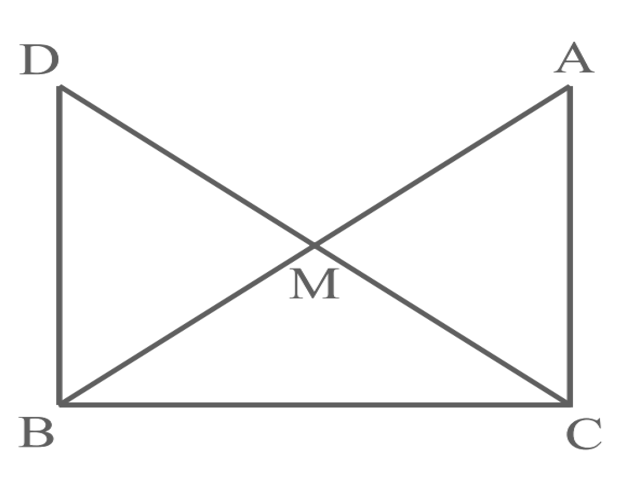
\includegraphics[width=\columnwidth]{figs/Screenshot.png}
  \caption{$\triangle \vec{ACB} ,\triangle \vec{DCB}$ with Mid-Point $\vec{M}$}
  \label{fig:triangles}
\end{figure}
\begin{enumerate}[label =(\roman*)]
        \item $\triangle \vec{AMC} \cong \triangle \vec{BMD}$
        \item $\angle \vec{DBC}$ is a right angle. 
        \item $\triangle \vec{DBC} \cong  \triangle \vec{ACB}$ 
        \item $\vec{CM} = \frac{1}{2} \vec{AB}$
\end{enumerate}
\pagebreak
\solution\\
\textbf{CONSTRUCTION STEPS :}
\begin{enumerate}
\item Let us Assume , the input parameters as ;
\begin{table}[H]
\centering
        \input{tables/input_params.tex}
          \caption{Input Parameters}
          \label{Table-1:Input_params}
\end{table}
\item the output can be calculated as ;
\begin{table}[H]
\centering
        \input{tables/output_params.tex}
          \caption{Output Parameters}
          \label{Table-2:Output_params}
\end{table}
                $\therefore$ By, Plotting these points we get the required Image \figref{fig:fig-2}
\begin{figure}[H]
        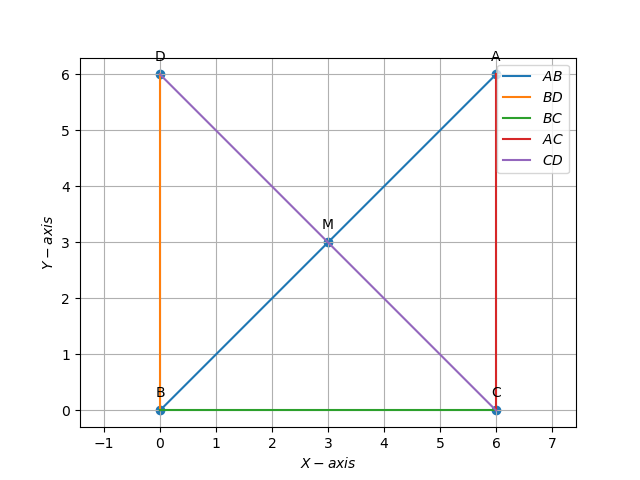
\includegraphics[width = \columnwidth]{figs/python_plot.png}
    \caption{PYTHON Plot of $\triangle \vec{ACB} ,\triangle \vec{DBC}$ with Mid-Point $\vec{M}$}
    \label{fig:fig-2}
\end{figure}
\end{enumerate}

\item Find the position vector of a point $\vec{R}$ which divides the line joining two points $\vec{P}$ and $\vec{Q}$ whose position vectors are $2\vec{a}+\vec{b}$ and $\vec{a}-3\vec{b}$ externally in the ratio $1:2$.

\textbf{Solution:}
Let us assume $\vec{a}$ and $\vec{b}$, and the given ratio is
\begin{table}[h]
    \centering
    \begin{tabular}{|c|c|c|}
        \hline 
        \textbf{Symbol} & \textbf{Value} & \textbf{Description} \\
        \hline
        $\vec{a}$ & $\myvec{1 \\ -3}$ & Vector $\vec{a}$ \\
        \hline
        $\vec{b}$ & $\myvec{0 \\ 2}$ & Vector $\vec{b}$\\
        \hline
        $k$ & $2$ & Ratio \\
        \hline
    \end{tabular}
    \caption{Vectors $\vec{a}$ and $\vec{b}$, ratio $k$}
    \label{tab:table1}
\end{table}

Using the section formula,
\begin{align}
    \vec{R} = \frac{\vec{Q} - k\vec{P}}{1 - k}
\end{align}
where $\vec{P}$ and $\vec{Q}$ depend on $\vec{a}$ and $\vec{b}$, then
\begin{align}
    \vec{P} &= (2\vec{a} + \vec{b}) = 2\myvec{1\\-3} + \myvec{0\\2} = \myvec{2\\-4} \\
    \vec{Q} &= (\vec{a} - 3\vec{b}) = \myvec{1\\-3} - 3\myvec{0\\2} = \myvec{1\\-9}
\end{align}
where $\vec{R}$ can be calculated as 
\begin{align}
    \vec{R} = \frac{(\vec{a} - 3\vec{b}) - k(2\vec{a} + \vec{b})}{1 - k}
\end{align}
By substituting $\vec{a}$ and $\vec{b}$ values, we get $\vec{R}$ as
\begin{align}
    \vec{R} = \myvec{3\\1}
\end{align}

\begin{table}[ht!]
    \centering
    \begin{tabular}{|c|c|c|}
        \hline
        \textbf{Symbol} & \textbf{Value} & \textbf{Description}\\
        \hline
        $\vec{P}$ & $(2\vec{a} + \vec{b})$ & Position vector $\vec{P}$ \\
        \hline
        $\vec{Q}$ & $(\vec{a} - 3\vec{b})$ & Position vector $\vec{Q}$\\
        \hline
        $\vec{R}$ & $\frac{\vec{Q} - k\vec{P}}{1 - k}$ & Position vector $\vec{R}$\\
        \hline
    \end{tabular}
    \caption{Vectors $\vec{P}$, $\vec{Q}$, $\vec{R}$}
    \label{tab:mytable2}   
\end{table}

\begin{figure}[H]
    \centering
    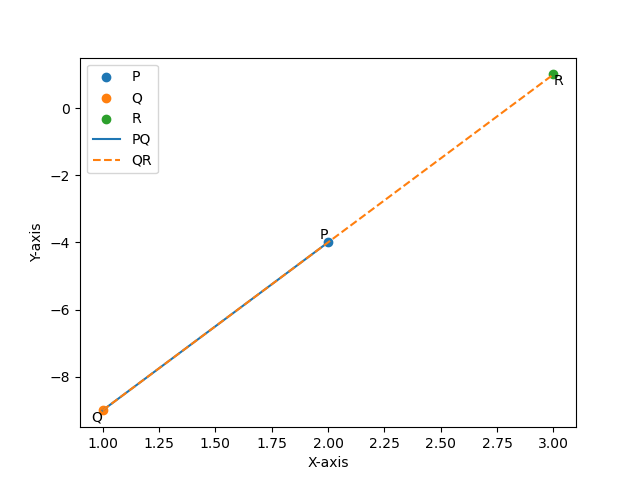
\includegraphics[width=\columnwidth]{figs/external-bisector.png}
    \caption{Point vectors $\vec{P}$, $\vec{Q}$, $\vec{R}$}
    \label{fig:enter-label}
\end{figure}


\end{enumerate}

    \item Draw a quadrilateral in the Cartesian plane, whose vertices are 
    \begin{align}
        \vec{A} = \myvec{-4\\5} \quad \vec{B} = \myvec{0\\7} \\
        \vec{C} = \myvec{5\\-5} \quad \vec{D} = \myvec{-4\\-2}
    \end{align}
    Also, find its area.
\label{chapters/11/10/1/1}
   \\ 
    \solution 
\begin{enumerate}[label=\thesection.\arabic*,ref=\thesection.\theenumi]
		\item Find $\abs{\overrightarrow{a}\times\overrightarrow{b}},\text{ if }\overrightarrow{a}=\hat{i}-7\hat{j}+7\hat{k}\text{ and } \overrightarrow{b}=3\hat{i}-2\hat{j}+2\hat{k}$.
	\\
		\solution
		\input{chapters/12/10/4/1/cross.tex}
\item Show that $$(\overrightarrow{a}-\overrightarrow{b})\times (\overrightarrow{a}+\overrightarrow{b})=2(\overrightarrow{a}\times \overrightarrow{b})$$
	\\
		\solution
		\input{chapters/12/10/4/4/cross.tex}
\item Find $\lambda$ and $\mu$ if $(2\hat{i}+6\hat{j}+27\hat{k})\times(\hat{i}+\lambda \hat{j} + \mu \hat{k})=\overrightarrow{0}$.
	\\
		\solution
		\input{chapters/12/10/4/5/cross.tex}
\item Given that $\overrightarrow{a} \cdot \overrightarrow{b} = 0$ and $\overrightarrow{a} \times \overrightarrow{b} = \overrightarrow{0}$. What can you conclude about the vectors $\overrightarrow{a} \text{ and }\overrightarrow{b}$?
\item Let the vectors be given as $\overrightarrow{a},\overrightarrow{b},\overrightarrow{c}\text{ be given as }\ a_1 \hat{i}+\ a_2 \hat{j}+\ a_3 \hat{k},\ b_1 \hat{i}+\ b_2 \hat{j}+\ b_3 \hat{k},\ c_1 \hat{i}+\ c_2 \hat{j}+\ c_3 \hat{k}$. Then show that $\overrightarrow{a} \times (\overrightarrow{b} + \overrightarrow{c}) = \overrightarrow{a} \times \overrightarrow{b}+\overrightarrow{a} \times \overrightarrow{c}$.
	\\
		\solution
		\input{chapters/12/10/4/7/cross.tex}
\item If either $\overrightarrow{a} = \overrightarrow{0}$ or $\overrightarrow{b} = \overrightarrow{0}$, then $\overrightarrow{a} \times \overrightarrow{b} = \overrightarrow{0}$. Is the converse true? Justify your answer with an example.
	\\
		\solution
		\input{chapters/12/10/4/8/cross.tex}
\item Find the area of the triangle with vertices $A(1, 1, 2)$, $B(2, 3, 5)$, and $C(1, 5, 5)$
	\\
		\solution
		\input{chapters/12/10/4/9/cross.tex}
\item Find the area of the parallelogram whose adjacent sides are determined by the vectors $\overrightarrow{a}=\hat{i}-\hat{j}+3\hat{k}$ and $\overrightarrow{b}=2\hat{i}-7\hat{j}+\hat{k}$.
	\\
		\solution
		\input{chapters/12/10/4/10/cross.tex}
\item Let the vectors $\overrightarrow{a}$ and $\overrightarrow{b}$ be such that $|\overrightarrow{a}| = 3$ and $|\overrightarrow{b}| = \dfrac{\sqrt{2}}{3}$, then $\overrightarrow{a} \times \overrightarrow{b}$ is a unit vector, if the angle between $\overrightarrow{a}$ and $\overrightarrow{b}$ is
\begin{enumerate}
\item $\dfrac{\pi}{6}$
\item $\dfrac{\pi}{4}$
\item $\dfrac{\pi}{3}$
\item $\dfrac{\pi}{2}$
\end{enumerate}
		\solution
		\input{chapters/12/10/4/11/cross.tex}
\item Area of a rectangle having vertices A, B, C and D with position vectors $ -\hat{i}+ \dfrac{1}{2} \hat{j}+4\hat{k},\hat{i}+ \dfrac{1}{2} \hat{j}+4\hat{k},\hat{i}-\dfrac{1}{2} \hat{j}+4\hat{k}\text{ and }-\hat{i}- \dfrac{1}{2} \hat{j}+4\hat{k}$, respectively is
\begin{enumerate}
\item $\dfrac{1}{2}$
\item 1
\item 2
\item 4
\end{enumerate}
		\solution
		\input{chapters/12/10/4/12/cross.tex}
\item Find the area of the triangle whose vertices are 
\begin{enumerate}
\item $(2, 3), (–1, 0), (2, – 4)$
\item $(–5, –1), (3, –5), (5, 2)$ 
\end{enumerate}
		\label{10/7/3/1}
\solution
		\input{chapters/10/7/3/1/area.tex}
\item Find the area of the triangle formed by joining the mid-points of the sides of the triangle whose vertices are $(0, –1), (2, 1) \text{ and } (0, 3)$. Find the ratio of this area to the area of the given triangle.
	\\
\solution
		\input{chapters/10/7/3/3/cross.tex}

\item Find the area of the quadrilateral whose vertices, taken in order, are $(– 4, – 2), (– 3, – 5), (3, – 2)$  and $ (2, 3)$.
	\\
\solution
		\input{chapters/10/7/3/4/cross.tex}

\item Verify that a median of a triangle divides it into two triangles of equal areas for $\triangle ABC$ whose vertices are $\vec{A}(4, -6), \vec{B}(3, 2), \text{ and } \vec{C}(5, 2)$. 
		\label{10/7/3/5}
		\\
\solution
		\input{chapters/10/7/3/5/area.tex}

\item The two adjacent sides of a parallelogram are 
$2\hat{i}-4\hat{j}+5\hat{k}$  and  $\hat{i}-2\hat{j}-3\hat{k}$.
Find the unit vector parallel to its diagonal. Also, find its area.\\
	\solution
		\input{chapters/12/10/5/10/cross.tex}
\item The vertices of a $\triangle ABC$ are $\vec{A}(4,6), \vec{B}(1,5)$ and  $\vec{C}(7,2)$. A line is drawn to intersect sides $AB$ and $AC$ at $\vec{D}$ and $\vec{E}$ respectively, such that $\frac{AD}{AB} = \frac{AE}{AC} = \frac{1}{4}$. Calculate the area of $\triangle ADE$ and compare it with the area of the $\triangle ABC$.
\\
\solution
	\input{chapters/10/7/4/6/section.tex}
    \item Draw a quadrilateral in the Cartesian plane, whose vertices are 
    \begin{align}
        \vec{A} = \myvec{-4\\5} \quad \vec{B} = \myvec{0\\7} \\
        \vec{C} = \myvec{5\\-5} \quad \vec{D} = \myvec{-4\\-2}
    \end{align}
    Also, find its area.
\label{chapters/11/10/1/1}
   \\ 
    \solution 
\input{chapters/11/10/1/1/cross.tex}
\item Find the area of region bounded by the triangle whose
	vertices are $(1, 0), (2, 2) \text{ and } (3, 1)$. 
\item Find the area of region bounded by the triangle whose vertices
	are $(– 1, 0), (1, 3) \text{ and } (3, 2)$. 
\item Find the area of the $\triangle ABC$, coordinates of whose vertices are $\vec{A}(2, 0), \vec{B}(4, 5), \text{ and } \vec{C}(6, 3)$.


\item 
\input{chapters/vectors/exer/main.tex}
\end{enumerate}


\item Find the area of region bounded by the triangle whose
	vertices are $(1, 0), (2, 2) \text{ and } (3, 1)$. 
\item Find the area of region bounded by the triangle whose vertices
	are $(– 1, 0), (1, 3) \text{ and } (3, 2)$. 
\item Find the area of the $\triangle ABC$, coordinates of whose vertices are $\vec{A}(2, 0), \vec{B}(4, 5), \text{ and } \vec{C}(6, 3)$.


\item 
%\documentclass[12pt]{article}
%\usepackage{graphicx}
%\usepackage{graphics}
%\usepackage{refstyle}
%\usepackage{amsmath}
%\usepackage{caption}
%\usepackage{float}
%\usepackage{booktabs}
%\usepackage{array}
%\usepackage{amssymb}
%\usepackage{booktabs}
%\let\vec\mathbf
%\providecommand{\brak}[1]{\ensuremath{\left(#1\right)}}
%\graphicspath{{/storage/self/primary/Download/latexnew/fig}}                                     
$\vec{P}$ and $\vec{Q}$ are any two points lying on the sides $DC$ and $AD$ respectively of a parallelogram $ABCD$.Show that, $ar\brak{\triangle APB}=ar\brak{\triangle BQC}$.


\textbf{Figure:}
\begin{figure}[H]
    \centering
	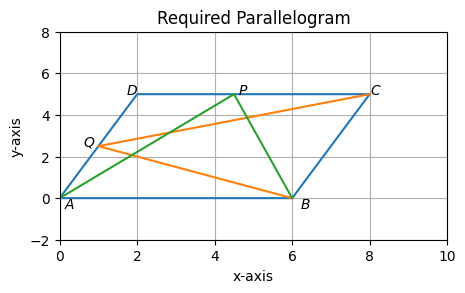
\includegraphics[width=\columnwidth]{chapters/vectors/exer/figs/1.png}
    \caption{}
    \label{fig:fig:1}
\end{figure}


\textbf{Solution:}
\begin{table}[H]
   \centering
  \input{chapters/vectors/exer/table/tab1.tex}
   \caption{Table of input parameters}        
\label{tab:tab:1}                    
\end{table}




\begin{table}[H]
    \centering                                  
\input{chapters/vectors/exer/table/tab2.tex}                  
\caption{Table of output parameters}
\label{tab:tab:2}
 \end{table}


For the $\triangle BQC$, the vertices of the triangle are taken from \tabref{tab:tab:1} and \tabref{tab:tab:2}.

\begin{align}
\implies ar\brak{\triangle BQC}&=
\frac{1}{2}\begin{tabular}{|c c c|}            
1 &1&1\\                      
$\vec{B}$&$\vec{Q}$&$\vec{C}$\\    
\end{tabular}\\
&= \frac{1}{2}\begin{tabular}{|c c c|}
       1 &1&1\\
       6&$\frac{2k_1}{k_1+1}$&8 \\
       0&$\frac{5k_1}{k_1+1}$&5
   \end{tabular}\\
  \xrightarrow{C_2'=C_2-C_1,C_3'=C_3-C_1}&\frac{1}{2} \begin{tabular}{|c c c|}
       1 &0&0\\
       6&$\frac{-4k_1-6}{k_1+1}$&2 \\
       0&$\frac{5k_1}{k_1+1}$&5
   \end{tabular}\\
&=\frac{1}{2}\brak{1\begin{tabular}{|c c|}
   $\frac{-4k_1-6}{k_1+1}$ &2  \\
   $\frac{5k_1}{k_1+1}$ & 5
\end{tabular} +0+0}\\
&=\frac{1}{2} \times30\\                          
&=15 \end{align}


For the $\triangle APB$, the vertices of the triangle are taken from \tabref{tab:tab:1} and \tabref{tab:tab:2}.
   \begin{align}
  \implies ar\brak{\triangle APB} &=
\frac{1}{2}\begin{tabular}{|c c c|}            
1 &1&1\\                            
$\vec{A}$&$\vec{P}$&$\vec{B}$\\
\end{tabular}\\ &=  \frac{1}{2}
   \begin{tabular}{|c c c|}
       1 &1&1\\
       0&$\frac{8k_2+2}{k_2+1}$&6 \\
       0&5&0
   \end{tabular}\\
 &=\frac{1}{2} \times30\\
 &=15 \end{align}
 \brak{6} = \brak{10}


So, ar\brak{\triangle BQC} = ar\brak{\triangle APB}.\brak{proved}
%\end{document}



\end{enumerate}


\item Find the area of the triangle whose vertices are 
\begin{enumerate}
\item $(2, 3), (–1, 0), (2, – 4)$
\item $(–5, –1), (3, –5), (5, 2)$ 
\end{enumerate}
		\label{10/7/3/1}
\solution
		\input{chapters/10/7/3/1/area.tex}
\item Find the area of the triangle formed by joining the mid-points of the sides of the triangle whose vertices are $(0, –1), (2, 1) \text{ and } (0, 3)$. Find the ratio of this area to the area of the given triangle.
	\\
\solution
		\begin{enumerate}[label=\thesection.\arabic*,ref=\thesection.\theenumi]
		\item Find $\abs{\overrightarrow{a}\times\overrightarrow{b}},\text{ if }\overrightarrow{a}=\hat{i}-7\hat{j}+7\hat{k}\text{ and } \overrightarrow{b}=3\hat{i}-2\hat{j}+2\hat{k}$.
	\\
		\solution
		\begin{enumerate}[label=\thesection.\arabic*,ref=\thesection.\theenumi]
		\item Find $\abs{\overrightarrow{a}\times\overrightarrow{b}},\text{ if }\overrightarrow{a}=\hat{i}-7\hat{j}+7\hat{k}\text{ and } \overrightarrow{b}=3\hat{i}-2\hat{j}+2\hat{k}$.
	\\
		\solution
		\input{chapters/12/10/4/1/cross.tex}
\item Show that $$(\overrightarrow{a}-\overrightarrow{b})\times (\overrightarrow{a}+\overrightarrow{b})=2(\overrightarrow{a}\times \overrightarrow{b})$$
	\\
		\solution
		\input{chapters/12/10/4/4/cross.tex}
\item Find $\lambda$ and $\mu$ if $(2\hat{i}+6\hat{j}+27\hat{k})\times(\hat{i}+\lambda \hat{j} + \mu \hat{k})=\overrightarrow{0}$.
	\\
		\solution
		\input{chapters/12/10/4/5/cross.tex}
\item Given that $\overrightarrow{a} \cdot \overrightarrow{b} = 0$ and $\overrightarrow{a} \times \overrightarrow{b} = \overrightarrow{0}$. What can you conclude about the vectors $\overrightarrow{a} \text{ and }\overrightarrow{b}$?
\item Let the vectors be given as $\overrightarrow{a},\overrightarrow{b},\overrightarrow{c}\text{ be given as }\ a_1 \hat{i}+\ a_2 \hat{j}+\ a_3 \hat{k},\ b_1 \hat{i}+\ b_2 \hat{j}+\ b_3 \hat{k},\ c_1 \hat{i}+\ c_2 \hat{j}+\ c_3 \hat{k}$. Then show that $\overrightarrow{a} \times (\overrightarrow{b} + \overrightarrow{c}) = \overrightarrow{a} \times \overrightarrow{b}+\overrightarrow{a} \times \overrightarrow{c}$.
	\\
		\solution
		\input{chapters/12/10/4/7/cross.tex}
\item If either $\overrightarrow{a} = \overrightarrow{0}$ or $\overrightarrow{b} = \overrightarrow{0}$, then $\overrightarrow{a} \times \overrightarrow{b} = \overrightarrow{0}$. Is the converse true? Justify your answer with an example.
	\\
		\solution
		\input{chapters/12/10/4/8/cross.tex}
\item Find the area of the triangle with vertices $A(1, 1, 2)$, $B(2, 3, 5)$, and $C(1, 5, 5)$
	\\
		\solution
		\input{chapters/12/10/4/9/cross.tex}
\item Find the area of the parallelogram whose adjacent sides are determined by the vectors $\overrightarrow{a}=\hat{i}-\hat{j}+3\hat{k}$ and $\overrightarrow{b}=2\hat{i}-7\hat{j}+\hat{k}$.
	\\
		\solution
		\input{chapters/12/10/4/10/cross.tex}
\item Let the vectors $\overrightarrow{a}$ and $\overrightarrow{b}$ be such that $|\overrightarrow{a}| = 3$ and $|\overrightarrow{b}| = \dfrac{\sqrt{2}}{3}$, then $\overrightarrow{a} \times \overrightarrow{b}$ is a unit vector, if the angle between $\overrightarrow{a}$ and $\overrightarrow{b}$ is
\begin{enumerate}
\item $\dfrac{\pi}{6}$
\item $\dfrac{\pi}{4}$
\item $\dfrac{\pi}{3}$
\item $\dfrac{\pi}{2}$
\end{enumerate}
		\solution
		\input{chapters/12/10/4/11/cross.tex}
\item Area of a rectangle having vertices A, B, C and D with position vectors $ -\hat{i}+ \dfrac{1}{2} \hat{j}+4\hat{k},\hat{i}+ \dfrac{1}{2} \hat{j}+4\hat{k},\hat{i}-\dfrac{1}{2} \hat{j}+4\hat{k}\text{ and }-\hat{i}- \dfrac{1}{2} \hat{j}+4\hat{k}$, respectively is
\begin{enumerate}
\item $\dfrac{1}{2}$
\item 1
\item 2
\item 4
\end{enumerate}
		\solution
		\input{chapters/12/10/4/12/cross.tex}
\item Find the area of the triangle whose vertices are 
\begin{enumerate}
\item $(2, 3), (–1, 0), (2, – 4)$
\item $(–5, –1), (3, –5), (5, 2)$ 
\end{enumerate}
		\label{10/7/3/1}
\solution
		\input{chapters/10/7/3/1/area.tex}
\item Find the area of the triangle formed by joining the mid-points of the sides of the triangle whose vertices are $(0, –1), (2, 1) \text{ and } (0, 3)$. Find the ratio of this area to the area of the given triangle.
	\\
\solution
		\input{chapters/10/7/3/3/cross.tex}

\item Find the area of the quadrilateral whose vertices, taken in order, are $(– 4, – 2), (– 3, – 5), (3, – 2)$  and $ (2, 3)$.
	\\
\solution
		\input{chapters/10/7/3/4/cross.tex}

\item Verify that a median of a triangle divides it into two triangles of equal areas for $\triangle ABC$ whose vertices are $\vec{A}(4, -6), \vec{B}(3, 2), \text{ and } \vec{C}(5, 2)$. 
		\label{10/7/3/5}
		\\
\solution
		\input{chapters/10/7/3/5/area.tex}

\item The two adjacent sides of a parallelogram are 
$2\hat{i}-4\hat{j}+5\hat{k}$  and  $\hat{i}-2\hat{j}-3\hat{k}$.
Find the unit vector parallel to its diagonal. Also, find its area.\\
	\solution
		\input{chapters/12/10/5/10/cross.tex}
\item The vertices of a $\triangle ABC$ are $\vec{A}(4,6), \vec{B}(1,5)$ and  $\vec{C}(7,2)$. A line is drawn to intersect sides $AB$ and $AC$ at $\vec{D}$ and $\vec{E}$ respectively, such that $\frac{AD}{AB} = \frac{AE}{AC} = \frac{1}{4}$. Calculate the area of $\triangle ADE$ and compare it with the area of the $\triangle ABC$.
\\
\solution
	\input{chapters/10/7/4/6/section.tex}
    \item Draw a quadrilateral in the Cartesian plane, whose vertices are 
    \begin{align}
        \vec{A} = \myvec{-4\\5} \quad \vec{B} = \myvec{0\\7} \\
        \vec{C} = \myvec{5\\-5} \quad \vec{D} = \myvec{-4\\-2}
    \end{align}
    Also, find its area.
\label{chapters/11/10/1/1}
   \\ 
    \solution 
\input{chapters/11/10/1/1/cross.tex}
\item Find the area of region bounded by the triangle whose
	vertices are $(1, 0), (2, 2) \text{ and } (3, 1)$. 
\item Find the area of region bounded by the triangle whose vertices
	are $(– 1, 0), (1, 3) \text{ and } (3, 2)$. 
\item Find the area of the $\triangle ABC$, coordinates of whose vertices are $\vec{A}(2, 0), \vec{B}(4, 5), \text{ and } \vec{C}(6, 3)$.


\item 
\input{chapters/vectors/exer/main.tex}
\end{enumerate}


\item Show that $$(\overrightarrow{a}-\overrightarrow{b})\times (\overrightarrow{a}+\overrightarrow{b})=2(\overrightarrow{a}\times \overrightarrow{b})$$
	\\
		\solution
		\begin{enumerate}[label=\thesection.\arabic*,ref=\thesection.\theenumi]
		\item Find $\abs{\overrightarrow{a}\times\overrightarrow{b}},\text{ if }\overrightarrow{a}=\hat{i}-7\hat{j}+7\hat{k}\text{ and } \overrightarrow{b}=3\hat{i}-2\hat{j}+2\hat{k}$.
	\\
		\solution
		\input{chapters/12/10/4/1/cross.tex}
\item Show that $$(\overrightarrow{a}-\overrightarrow{b})\times (\overrightarrow{a}+\overrightarrow{b})=2(\overrightarrow{a}\times \overrightarrow{b})$$
	\\
		\solution
		\input{chapters/12/10/4/4/cross.tex}
\item Find $\lambda$ and $\mu$ if $(2\hat{i}+6\hat{j}+27\hat{k})\times(\hat{i}+\lambda \hat{j} + \mu \hat{k})=\overrightarrow{0}$.
	\\
		\solution
		\input{chapters/12/10/4/5/cross.tex}
\item Given that $\overrightarrow{a} \cdot \overrightarrow{b} = 0$ and $\overrightarrow{a} \times \overrightarrow{b} = \overrightarrow{0}$. What can you conclude about the vectors $\overrightarrow{a} \text{ and }\overrightarrow{b}$?
\item Let the vectors be given as $\overrightarrow{a},\overrightarrow{b},\overrightarrow{c}\text{ be given as }\ a_1 \hat{i}+\ a_2 \hat{j}+\ a_3 \hat{k},\ b_1 \hat{i}+\ b_2 \hat{j}+\ b_3 \hat{k},\ c_1 \hat{i}+\ c_2 \hat{j}+\ c_3 \hat{k}$. Then show that $\overrightarrow{a} \times (\overrightarrow{b} + \overrightarrow{c}) = \overrightarrow{a} \times \overrightarrow{b}+\overrightarrow{a} \times \overrightarrow{c}$.
	\\
		\solution
		\input{chapters/12/10/4/7/cross.tex}
\item If either $\overrightarrow{a} = \overrightarrow{0}$ or $\overrightarrow{b} = \overrightarrow{0}$, then $\overrightarrow{a} \times \overrightarrow{b} = \overrightarrow{0}$. Is the converse true? Justify your answer with an example.
	\\
		\solution
		\input{chapters/12/10/4/8/cross.tex}
\item Find the area of the triangle with vertices $A(1, 1, 2)$, $B(2, 3, 5)$, and $C(1, 5, 5)$
	\\
		\solution
		\input{chapters/12/10/4/9/cross.tex}
\item Find the area of the parallelogram whose adjacent sides are determined by the vectors $\overrightarrow{a}=\hat{i}-\hat{j}+3\hat{k}$ and $\overrightarrow{b}=2\hat{i}-7\hat{j}+\hat{k}$.
	\\
		\solution
		\input{chapters/12/10/4/10/cross.tex}
\item Let the vectors $\overrightarrow{a}$ and $\overrightarrow{b}$ be such that $|\overrightarrow{a}| = 3$ and $|\overrightarrow{b}| = \dfrac{\sqrt{2}}{3}$, then $\overrightarrow{a} \times \overrightarrow{b}$ is a unit vector, if the angle between $\overrightarrow{a}$ and $\overrightarrow{b}$ is
\begin{enumerate}
\item $\dfrac{\pi}{6}$
\item $\dfrac{\pi}{4}$
\item $\dfrac{\pi}{3}$
\item $\dfrac{\pi}{2}$
\end{enumerate}
		\solution
		\input{chapters/12/10/4/11/cross.tex}
\item Area of a rectangle having vertices A, B, C and D with position vectors $ -\hat{i}+ \dfrac{1}{2} \hat{j}+4\hat{k},\hat{i}+ \dfrac{1}{2} \hat{j}+4\hat{k},\hat{i}-\dfrac{1}{2} \hat{j}+4\hat{k}\text{ and }-\hat{i}- \dfrac{1}{2} \hat{j}+4\hat{k}$, respectively is
\begin{enumerate}
\item $\dfrac{1}{2}$
\item 1
\item 2
\item 4
\end{enumerate}
		\solution
		\input{chapters/12/10/4/12/cross.tex}
\item Find the area of the triangle whose vertices are 
\begin{enumerate}
\item $(2, 3), (–1, 0), (2, – 4)$
\item $(–5, –1), (3, –5), (5, 2)$ 
\end{enumerate}
		\label{10/7/3/1}
\solution
		\input{chapters/10/7/3/1/area.tex}
\item Find the area of the triangle formed by joining the mid-points of the sides of the triangle whose vertices are $(0, –1), (2, 1) \text{ and } (0, 3)$. Find the ratio of this area to the area of the given triangle.
	\\
\solution
		\input{chapters/10/7/3/3/cross.tex}

\item Find the area of the quadrilateral whose vertices, taken in order, are $(– 4, – 2), (– 3, – 5), (3, – 2)$  and $ (2, 3)$.
	\\
\solution
		\input{chapters/10/7/3/4/cross.tex}

\item Verify that a median of a triangle divides it into two triangles of equal areas for $\triangle ABC$ whose vertices are $\vec{A}(4, -6), \vec{B}(3, 2), \text{ and } \vec{C}(5, 2)$. 
		\label{10/7/3/5}
		\\
\solution
		\input{chapters/10/7/3/5/area.tex}

\item The two adjacent sides of a parallelogram are 
$2\hat{i}-4\hat{j}+5\hat{k}$  and  $\hat{i}-2\hat{j}-3\hat{k}$.
Find the unit vector parallel to its diagonal. Also, find its area.\\
	\solution
		\input{chapters/12/10/5/10/cross.tex}
\item The vertices of a $\triangle ABC$ are $\vec{A}(4,6), \vec{B}(1,5)$ and  $\vec{C}(7,2)$. A line is drawn to intersect sides $AB$ and $AC$ at $\vec{D}$ and $\vec{E}$ respectively, such that $\frac{AD}{AB} = \frac{AE}{AC} = \frac{1}{4}$. Calculate the area of $\triangle ADE$ and compare it with the area of the $\triangle ABC$.
\\
\solution
	\input{chapters/10/7/4/6/section.tex}
    \item Draw a quadrilateral in the Cartesian plane, whose vertices are 
    \begin{align}
        \vec{A} = \myvec{-4\\5} \quad \vec{B} = \myvec{0\\7} \\
        \vec{C} = \myvec{5\\-5} \quad \vec{D} = \myvec{-4\\-2}
    \end{align}
    Also, find its area.
\label{chapters/11/10/1/1}
   \\ 
    \solution 
\input{chapters/11/10/1/1/cross.tex}
\item Find the area of region bounded by the triangle whose
	vertices are $(1, 0), (2, 2) \text{ and } (3, 1)$. 
\item Find the area of region bounded by the triangle whose vertices
	are $(– 1, 0), (1, 3) \text{ and } (3, 2)$. 
\item Find the area of the $\triangle ABC$, coordinates of whose vertices are $\vec{A}(2, 0), \vec{B}(4, 5), \text{ and } \vec{C}(6, 3)$.


\item 
\input{chapters/vectors/exer/main.tex}
\end{enumerate}


\item Find $\lambda$ and $\mu$ if $(2\hat{i}+6\hat{j}+27\hat{k})\times(\hat{i}+\lambda \hat{j} + \mu \hat{k})=\overrightarrow{0}$.
	\\
		\solution
		\begin{enumerate}[label=\thesection.\arabic*,ref=\thesection.\theenumi]
		\item Find $\abs{\overrightarrow{a}\times\overrightarrow{b}},\text{ if }\overrightarrow{a}=\hat{i}-7\hat{j}+7\hat{k}\text{ and } \overrightarrow{b}=3\hat{i}-2\hat{j}+2\hat{k}$.
	\\
		\solution
		\input{chapters/12/10/4/1/cross.tex}
\item Show that $$(\overrightarrow{a}-\overrightarrow{b})\times (\overrightarrow{a}+\overrightarrow{b})=2(\overrightarrow{a}\times \overrightarrow{b})$$
	\\
		\solution
		\input{chapters/12/10/4/4/cross.tex}
\item Find $\lambda$ and $\mu$ if $(2\hat{i}+6\hat{j}+27\hat{k})\times(\hat{i}+\lambda \hat{j} + \mu \hat{k})=\overrightarrow{0}$.
	\\
		\solution
		\input{chapters/12/10/4/5/cross.tex}
\item Given that $\overrightarrow{a} \cdot \overrightarrow{b} = 0$ and $\overrightarrow{a} \times \overrightarrow{b} = \overrightarrow{0}$. What can you conclude about the vectors $\overrightarrow{a} \text{ and }\overrightarrow{b}$?
\item Let the vectors be given as $\overrightarrow{a},\overrightarrow{b},\overrightarrow{c}\text{ be given as }\ a_1 \hat{i}+\ a_2 \hat{j}+\ a_3 \hat{k},\ b_1 \hat{i}+\ b_2 \hat{j}+\ b_3 \hat{k},\ c_1 \hat{i}+\ c_2 \hat{j}+\ c_3 \hat{k}$. Then show that $\overrightarrow{a} \times (\overrightarrow{b} + \overrightarrow{c}) = \overrightarrow{a} \times \overrightarrow{b}+\overrightarrow{a} \times \overrightarrow{c}$.
	\\
		\solution
		\input{chapters/12/10/4/7/cross.tex}
\item If either $\overrightarrow{a} = \overrightarrow{0}$ or $\overrightarrow{b} = \overrightarrow{0}$, then $\overrightarrow{a} \times \overrightarrow{b} = \overrightarrow{0}$. Is the converse true? Justify your answer with an example.
	\\
		\solution
		\input{chapters/12/10/4/8/cross.tex}
\item Find the area of the triangle with vertices $A(1, 1, 2)$, $B(2, 3, 5)$, and $C(1, 5, 5)$
	\\
		\solution
		\input{chapters/12/10/4/9/cross.tex}
\item Find the area of the parallelogram whose adjacent sides are determined by the vectors $\overrightarrow{a}=\hat{i}-\hat{j}+3\hat{k}$ and $\overrightarrow{b}=2\hat{i}-7\hat{j}+\hat{k}$.
	\\
		\solution
		\input{chapters/12/10/4/10/cross.tex}
\item Let the vectors $\overrightarrow{a}$ and $\overrightarrow{b}$ be such that $|\overrightarrow{a}| = 3$ and $|\overrightarrow{b}| = \dfrac{\sqrt{2}}{3}$, then $\overrightarrow{a} \times \overrightarrow{b}$ is a unit vector, if the angle between $\overrightarrow{a}$ and $\overrightarrow{b}$ is
\begin{enumerate}
\item $\dfrac{\pi}{6}$
\item $\dfrac{\pi}{4}$
\item $\dfrac{\pi}{3}$
\item $\dfrac{\pi}{2}$
\end{enumerate}
		\solution
		\input{chapters/12/10/4/11/cross.tex}
\item Area of a rectangle having vertices A, B, C and D with position vectors $ -\hat{i}+ \dfrac{1}{2} \hat{j}+4\hat{k},\hat{i}+ \dfrac{1}{2} \hat{j}+4\hat{k},\hat{i}-\dfrac{1}{2} \hat{j}+4\hat{k}\text{ and }-\hat{i}- \dfrac{1}{2} \hat{j}+4\hat{k}$, respectively is
\begin{enumerate}
\item $\dfrac{1}{2}$
\item 1
\item 2
\item 4
\end{enumerate}
		\solution
		\input{chapters/12/10/4/12/cross.tex}
\item Find the area of the triangle whose vertices are 
\begin{enumerate}
\item $(2, 3), (–1, 0), (2, – 4)$
\item $(–5, –1), (3, –5), (5, 2)$ 
\end{enumerate}
		\label{10/7/3/1}
\solution
		\input{chapters/10/7/3/1/area.tex}
\item Find the area of the triangle formed by joining the mid-points of the sides of the triangle whose vertices are $(0, –1), (2, 1) \text{ and } (0, 3)$. Find the ratio of this area to the area of the given triangle.
	\\
\solution
		\input{chapters/10/7/3/3/cross.tex}

\item Find the area of the quadrilateral whose vertices, taken in order, are $(– 4, – 2), (– 3, – 5), (3, – 2)$  and $ (2, 3)$.
	\\
\solution
		\input{chapters/10/7/3/4/cross.tex}

\item Verify that a median of a triangle divides it into two triangles of equal areas for $\triangle ABC$ whose vertices are $\vec{A}(4, -6), \vec{B}(3, 2), \text{ and } \vec{C}(5, 2)$. 
		\label{10/7/3/5}
		\\
\solution
		\input{chapters/10/7/3/5/area.tex}

\item The two adjacent sides of a parallelogram are 
$2\hat{i}-4\hat{j}+5\hat{k}$  and  $\hat{i}-2\hat{j}-3\hat{k}$.
Find the unit vector parallel to its diagonal. Also, find its area.\\
	\solution
		\input{chapters/12/10/5/10/cross.tex}
\item The vertices of a $\triangle ABC$ are $\vec{A}(4,6), \vec{B}(1,5)$ and  $\vec{C}(7,2)$. A line is drawn to intersect sides $AB$ and $AC$ at $\vec{D}$ and $\vec{E}$ respectively, such that $\frac{AD}{AB} = \frac{AE}{AC} = \frac{1}{4}$. Calculate the area of $\triangle ADE$ and compare it with the area of the $\triangle ABC$.
\\
\solution
	\input{chapters/10/7/4/6/section.tex}
    \item Draw a quadrilateral in the Cartesian plane, whose vertices are 
    \begin{align}
        \vec{A} = \myvec{-4\\5} \quad \vec{B} = \myvec{0\\7} \\
        \vec{C} = \myvec{5\\-5} \quad \vec{D} = \myvec{-4\\-2}
    \end{align}
    Also, find its area.
\label{chapters/11/10/1/1}
   \\ 
    \solution 
\input{chapters/11/10/1/1/cross.tex}
\item Find the area of region bounded by the triangle whose
	vertices are $(1, 0), (2, 2) \text{ and } (3, 1)$. 
\item Find the area of region bounded by the triangle whose vertices
	are $(– 1, 0), (1, 3) \text{ and } (3, 2)$. 
\item Find the area of the $\triangle ABC$, coordinates of whose vertices are $\vec{A}(2, 0), \vec{B}(4, 5), \text{ and } \vec{C}(6, 3)$.


\item 
\input{chapters/vectors/exer/main.tex}
\end{enumerate}


\item Given that $\overrightarrow{a} \cdot \overrightarrow{b} = 0$ and $\overrightarrow{a} \times \overrightarrow{b} = \overrightarrow{0}$. What can you conclude about the vectors $\overrightarrow{a} \text{ and }\overrightarrow{b}$?
\item Let the vectors be given as $\overrightarrow{a},\overrightarrow{b},\overrightarrow{c}\text{ be given as }\ a_1 \hat{i}+\ a_2 \hat{j}+\ a_3 \hat{k},\ b_1 \hat{i}+\ b_2 \hat{j}+\ b_3 \hat{k},\ c_1 \hat{i}+\ c_2 \hat{j}+\ c_3 \hat{k}$. Then show that $\overrightarrow{a} \times (\overrightarrow{b} + \overrightarrow{c}) = \overrightarrow{a} \times \overrightarrow{b}+\overrightarrow{a} \times \overrightarrow{c}$.
	\\
		\solution
		\begin{enumerate}[label=\thesection.\arabic*,ref=\thesection.\theenumi]
		\item Find $\abs{\overrightarrow{a}\times\overrightarrow{b}},\text{ if }\overrightarrow{a}=\hat{i}-7\hat{j}+7\hat{k}\text{ and } \overrightarrow{b}=3\hat{i}-2\hat{j}+2\hat{k}$.
	\\
		\solution
		\input{chapters/12/10/4/1/cross.tex}
\item Show that $$(\overrightarrow{a}-\overrightarrow{b})\times (\overrightarrow{a}+\overrightarrow{b})=2(\overrightarrow{a}\times \overrightarrow{b})$$
	\\
		\solution
		\input{chapters/12/10/4/4/cross.tex}
\item Find $\lambda$ and $\mu$ if $(2\hat{i}+6\hat{j}+27\hat{k})\times(\hat{i}+\lambda \hat{j} + \mu \hat{k})=\overrightarrow{0}$.
	\\
		\solution
		\input{chapters/12/10/4/5/cross.tex}
\item Given that $\overrightarrow{a} \cdot \overrightarrow{b} = 0$ and $\overrightarrow{a} \times \overrightarrow{b} = \overrightarrow{0}$. What can you conclude about the vectors $\overrightarrow{a} \text{ and }\overrightarrow{b}$?
\item Let the vectors be given as $\overrightarrow{a},\overrightarrow{b},\overrightarrow{c}\text{ be given as }\ a_1 \hat{i}+\ a_2 \hat{j}+\ a_3 \hat{k},\ b_1 \hat{i}+\ b_2 \hat{j}+\ b_3 \hat{k},\ c_1 \hat{i}+\ c_2 \hat{j}+\ c_3 \hat{k}$. Then show that $\overrightarrow{a} \times (\overrightarrow{b} + \overrightarrow{c}) = \overrightarrow{a} \times \overrightarrow{b}+\overrightarrow{a} \times \overrightarrow{c}$.
	\\
		\solution
		\input{chapters/12/10/4/7/cross.tex}
\item If either $\overrightarrow{a} = \overrightarrow{0}$ or $\overrightarrow{b} = \overrightarrow{0}$, then $\overrightarrow{a} \times \overrightarrow{b} = \overrightarrow{0}$. Is the converse true? Justify your answer with an example.
	\\
		\solution
		\input{chapters/12/10/4/8/cross.tex}
\item Find the area of the triangle with vertices $A(1, 1, 2)$, $B(2, 3, 5)$, and $C(1, 5, 5)$
	\\
		\solution
		\input{chapters/12/10/4/9/cross.tex}
\item Find the area of the parallelogram whose adjacent sides are determined by the vectors $\overrightarrow{a}=\hat{i}-\hat{j}+3\hat{k}$ and $\overrightarrow{b}=2\hat{i}-7\hat{j}+\hat{k}$.
	\\
		\solution
		\input{chapters/12/10/4/10/cross.tex}
\item Let the vectors $\overrightarrow{a}$ and $\overrightarrow{b}$ be such that $|\overrightarrow{a}| = 3$ and $|\overrightarrow{b}| = \dfrac{\sqrt{2}}{3}$, then $\overrightarrow{a} \times \overrightarrow{b}$ is a unit vector, if the angle between $\overrightarrow{a}$ and $\overrightarrow{b}$ is
\begin{enumerate}
\item $\dfrac{\pi}{6}$
\item $\dfrac{\pi}{4}$
\item $\dfrac{\pi}{3}$
\item $\dfrac{\pi}{2}$
\end{enumerate}
		\solution
		\input{chapters/12/10/4/11/cross.tex}
\item Area of a rectangle having vertices A, B, C and D with position vectors $ -\hat{i}+ \dfrac{1}{2} \hat{j}+4\hat{k},\hat{i}+ \dfrac{1}{2} \hat{j}+4\hat{k},\hat{i}-\dfrac{1}{2} \hat{j}+4\hat{k}\text{ and }-\hat{i}- \dfrac{1}{2} \hat{j}+4\hat{k}$, respectively is
\begin{enumerate}
\item $\dfrac{1}{2}$
\item 1
\item 2
\item 4
\end{enumerate}
		\solution
		\input{chapters/12/10/4/12/cross.tex}
\item Find the area of the triangle whose vertices are 
\begin{enumerate}
\item $(2, 3), (–1, 0), (2, – 4)$
\item $(–5, –1), (3, –5), (5, 2)$ 
\end{enumerate}
		\label{10/7/3/1}
\solution
		\input{chapters/10/7/3/1/area.tex}
\item Find the area of the triangle formed by joining the mid-points of the sides of the triangle whose vertices are $(0, –1), (2, 1) \text{ and } (0, 3)$. Find the ratio of this area to the area of the given triangle.
	\\
\solution
		\input{chapters/10/7/3/3/cross.tex}

\item Find the area of the quadrilateral whose vertices, taken in order, are $(– 4, – 2), (– 3, – 5), (3, – 2)$  and $ (2, 3)$.
	\\
\solution
		\input{chapters/10/7/3/4/cross.tex}

\item Verify that a median of a triangle divides it into two triangles of equal areas for $\triangle ABC$ whose vertices are $\vec{A}(4, -6), \vec{B}(3, 2), \text{ and } \vec{C}(5, 2)$. 
		\label{10/7/3/5}
		\\
\solution
		\input{chapters/10/7/3/5/area.tex}

\item The two adjacent sides of a parallelogram are 
$2\hat{i}-4\hat{j}+5\hat{k}$  and  $\hat{i}-2\hat{j}-3\hat{k}$.
Find the unit vector parallel to its diagonal. Also, find its area.\\
	\solution
		\input{chapters/12/10/5/10/cross.tex}
\item The vertices of a $\triangle ABC$ are $\vec{A}(4,6), \vec{B}(1,5)$ and  $\vec{C}(7,2)$. A line is drawn to intersect sides $AB$ and $AC$ at $\vec{D}$ and $\vec{E}$ respectively, such that $\frac{AD}{AB} = \frac{AE}{AC} = \frac{1}{4}$. Calculate the area of $\triangle ADE$ and compare it with the area of the $\triangle ABC$.
\\
\solution
	\input{chapters/10/7/4/6/section.tex}
    \item Draw a quadrilateral in the Cartesian plane, whose vertices are 
    \begin{align}
        \vec{A} = \myvec{-4\\5} \quad \vec{B} = \myvec{0\\7} \\
        \vec{C} = \myvec{5\\-5} \quad \vec{D} = \myvec{-4\\-2}
    \end{align}
    Also, find its area.
\label{chapters/11/10/1/1}
   \\ 
    \solution 
\input{chapters/11/10/1/1/cross.tex}
\item Find the area of region bounded by the triangle whose
	vertices are $(1, 0), (2, 2) \text{ and } (3, 1)$. 
\item Find the area of region bounded by the triangle whose vertices
	are $(– 1, 0), (1, 3) \text{ and } (3, 2)$. 
\item Find the area of the $\triangle ABC$, coordinates of whose vertices are $\vec{A}(2, 0), \vec{B}(4, 5), \text{ and } \vec{C}(6, 3)$.


\item 
\input{chapters/vectors/exer/main.tex}
\end{enumerate}


\item If either $\overrightarrow{a} = \overrightarrow{0}$ or $\overrightarrow{b} = \overrightarrow{0}$, then $\overrightarrow{a} \times \overrightarrow{b} = \overrightarrow{0}$. Is the converse true? Justify your answer with an example.
	\\
		\solution
		\begin{enumerate}[label=\thesection.\arabic*,ref=\thesection.\theenumi]
		\item Find $\abs{\overrightarrow{a}\times\overrightarrow{b}},\text{ if }\overrightarrow{a}=\hat{i}-7\hat{j}+7\hat{k}\text{ and } \overrightarrow{b}=3\hat{i}-2\hat{j}+2\hat{k}$.
	\\
		\solution
		\input{chapters/12/10/4/1/cross.tex}
\item Show that $$(\overrightarrow{a}-\overrightarrow{b})\times (\overrightarrow{a}+\overrightarrow{b})=2(\overrightarrow{a}\times \overrightarrow{b})$$
	\\
		\solution
		\input{chapters/12/10/4/4/cross.tex}
\item Find $\lambda$ and $\mu$ if $(2\hat{i}+6\hat{j}+27\hat{k})\times(\hat{i}+\lambda \hat{j} + \mu \hat{k})=\overrightarrow{0}$.
	\\
		\solution
		\input{chapters/12/10/4/5/cross.tex}
\item Given that $\overrightarrow{a} \cdot \overrightarrow{b} = 0$ and $\overrightarrow{a} \times \overrightarrow{b} = \overrightarrow{0}$. What can you conclude about the vectors $\overrightarrow{a} \text{ and }\overrightarrow{b}$?
\item Let the vectors be given as $\overrightarrow{a},\overrightarrow{b},\overrightarrow{c}\text{ be given as }\ a_1 \hat{i}+\ a_2 \hat{j}+\ a_3 \hat{k},\ b_1 \hat{i}+\ b_2 \hat{j}+\ b_3 \hat{k},\ c_1 \hat{i}+\ c_2 \hat{j}+\ c_3 \hat{k}$. Then show that $\overrightarrow{a} \times (\overrightarrow{b} + \overrightarrow{c}) = \overrightarrow{a} \times \overrightarrow{b}+\overrightarrow{a} \times \overrightarrow{c}$.
	\\
		\solution
		\input{chapters/12/10/4/7/cross.tex}
\item If either $\overrightarrow{a} = \overrightarrow{0}$ or $\overrightarrow{b} = \overrightarrow{0}$, then $\overrightarrow{a} \times \overrightarrow{b} = \overrightarrow{0}$. Is the converse true? Justify your answer with an example.
	\\
		\solution
		\input{chapters/12/10/4/8/cross.tex}
\item Find the area of the triangle with vertices $A(1, 1, 2)$, $B(2, 3, 5)$, and $C(1, 5, 5)$
	\\
		\solution
		\input{chapters/12/10/4/9/cross.tex}
\item Find the area of the parallelogram whose adjacent sides are determined by the vectors $\overrightarrow{a}=\hat{i}-\hat{j}+3\hat{k}$ and $\overrightarrow{b}=2\hat{i}-7\hat{j}+\hat{k}$.
	\\
		\solution
		\input{chapters/12/10/4/10/cross.tex}
\item Let the vectors $\overrightarrow{a}$ and $\overrightarrow{b}$ be such that $|\overrightarrow{a}| = 3$ and $|\overrightarrow{b}| = \dfrac{\sqrt{2}}{3}$, then $\overrightarrow{a} \times \overrightarrow{b}$ is a unit vector, if the angle between $\overrightarrow{a}$ and $\overrightarrow{b}$ is
\begin{enumerate}
\item $\dfrac{\pi}{6}$
\item $\dfrac{\pi}{4}$
\item $\dfrac{\pi}{3}$
\item $\dfrac{\pi}{2}$
\end{enumerate}
		\solution
		\input{chapters/12/10/4/11/cross.tex}
\item Area of a rectangle having vertices A, B, C and D with position vectors $ -\hat{i}+ \dfrac{1}{2} \hat{j}+4\hat{k},\hat{i}+ \dfrac{1}{2} \hat{j}+4\hat{k},\hat{i}-\dfrac{1}{2} \hat{j}+4\hat{k}\text{ and }-\hat{i}- \dfrac{1}{2} \hat{j}+4\hat{k}$, respectively is
\begin{enumerate}
\item $\dfrac{1}{2}$
\item 1
\item 2
\item 4
\end{enumerate}
		\solution
		\input{chapters/12/10/4/12/cross.tex}
\item Find the area of the triangle whose vertices are 
\begin{enumerate}
\item $(2, 3), (–1, 0), (2, – 4)$
\item $(–5, –1), (3, –5), (5, 2)$ 
\end{enumerate}
		\label{10/7/3/1}
\solution
		\input{chapters/10/7/3/1/area.tex}
\item Find the area of the triangle formed by joining the mid-points of the sides of the triangle whose vertices are $(0, –1), (2, 1) \text{ and } (0, 3)$. Find the ratio of this area to the area of the given triangle.
	\\
\solution
		\input{chapters/10/7/3/3/cross.tex}

\item Find the area of the quadrilateral whose vertices, taken in order, are $(– 4, – 2), (– 3, – 5), (3, – 2)$  and $ (2, 3)$.
	\\
\solution
		\input{chapters/10/7/3/4/cross.tex}

\item Verify that a median of a triangle divides it into two triangles of equal areas for $\triangle ABC$ whose vertices are $\vec{A}(4, -6), \vec{B}(3, 2), \text{ and } \vec{C}(5, 2)$. 
		\label{10/7/3/5}
		\\
\solution
		\input{chapters/10/7/3/5/area.tex}

\item The two adjacent sides of a parallelogram are 
$2\hat{i}-4\hat{j}+5\hat{k}$  and  $\hat{i}-2\hat{j}-3\hat{k}$.
Find the unit vector parallel to its diagonal. Also, find its area.\\
	\solution
		\input{chapters/12/10/5/10/cross.tex}
\item The vertices of a $\triangle ABC$ are $\vec{A}(4,6), \vec{B}(1,5)$ and  $\vec{C}(7,2)$. A line is drawn to intersect sides $AB$ and $AC$ at $\vec{D}$ and $\vec{E}$ respectively, such that $\frac{AD}{AB} = \frac{AE}{AC} = \frac{1}{4}$. Calculate the area of $\triangle ADE$ and compare it with the area of the $\triangle ABC$.
\\
\solution
	\input{chapters/10/7/4/6/section.tex}
    \item Draw a quadrilateral in the Cartesian plane, whose vertices are 
    \begin{align}
        \vec{A} = \myvec{-4\\5} \quad \vec{B} = \myvec{0\\7} \\
        \vec{C} = \myvec{5\\-5} \quad \vec{D} = \myvec{-4\\-2}
    \end{align}
    Also, find its area.
\label{chapters/11/10/1/1}
   \\ 
    \solution 
\input{chapters/11/10/1/1/cross.tex}
\item Find the area of region bounded by the triangle whose
	vertices are $(1, 0), (2, 2) \text{ and } (3, 1)$. 
\item Find the area of region bounded by the triangle whose vertices
	are $(– 1, 0), (1, 3) \text{ and } (3, 2)$. 
\item Find the area of the $\triangle ABC$, coordinates of whose vertices are $\vec{A}(2, 0), \vec{B}(4, 5), \text{ and } \vec{C}(6, 3)$.


\item 
\input{chapters/vectors/exer/main.tex}
\end{enumerate}


\item Find the area of the triangle with vertices $A(1, 1, 2)$, $B(2, 3, 5)$, and $C(1, 5, 5)$
	\\
		\solution
		\begin{enumerate}[label=\thesection.\arabic*,ref=\thesection.\theenumi]
		\item Find $\abs{\overrightarrow{a}\times\overrightarrow{b}},\text{ if }\overrightarrow{a}=\hat{i}-7\hat{j}+7\hat{k}\text{ and } \overrightarrow{b}=3\hat{i}-2\hat{j}+2\hat{k}$.
	\\
		\solution
		\input{chapters/12/10/4/1/cross.tex}
\item Show that $$(\overrightarrow{a}-\overrightarrow{b})\times (\overrightarrow{a}+\overrightarrow{b})=2(\overrightarrow{a}\times \overrightarrow{b})$$
	\\
		\solution
		\input{chapters/12/10/4/4/cross.tex}
\item Find $\lambda$ and $\mu$ if $(2\hat{i}+6\hat{j}+27\hat{k})\times(\hat{i}+\lambda \hat{j} + \mu \hat{k})=\overrightarrow{0}$.
	\\
		\solution
		\input{chapters/12/10/4/5/cross.tex}
\item Given that $\overrightarrow{a} \cdot \overrightarrow{b} = 0$ and $\overrightarrow{a} \times \overrightarrow{b} = \overrightarrow{0}$. What can you conclude about the vectors $\overrightarrow{a} \text{ and }\overrightarrow{b}$?
\item Let the vectors be given as $\overrightarrow{a},\overrightarrow{b},\overrightarrow{c}\text{ be given as }\ a_1 \hat{i}+\ a_2 \hat{j}+\ a_3 \hat{k},\ b_1 \hat{i}+\ b_2 \hat{j}+\ b_3 \hat{k},\ c_1 \hat{i}+\ c_2 \hat{j}+\ c_3 \hat{k}$. Then show that $\overrightarrow{a} \times (\overrightarrow{b} + \overrightarrow{c}) = \overrightarrow{a} \times \overrightarrow{b}+\overrightarrow{a} \times \overrightarrow{c}$.
	\\
		\solution
		\input{chapters/12/10/4/7/cross.tex}
\item If either $\overrightarrow{a} = \overrightarrow{0}$ or $\overrightarrow{b} = \overrightarrow{0}$, then $\overrightarrow{a} \times \overrightarrow{b} = \overrightarrow{0}$. Is the converse true? Justify your answer with an example.
	\\
		\solution
		\input{chapters/12/10/4/8/cross.tex}
\item Find the area of the triangle with vertices $A(1, 1, 2)$, $B(2, 3, 5)$, and $C(1, 5, 5)$
	\\
		\solution
		\input{chapters/12/10/4/9/cross.tex}
\item Find the area of the parallelogram whose adjacent sides are determined by the vectors $\overrightarrow{a}=\hat{i}-\hat{j}+3\hat{k}$ and $\overrightarrow{b}=2\hat{i}-7\hat{j}+\hat{k}$.
	\\
		\solution
		\input{chapters/12/10/4/10/cross.tex}
\item Let the vectors $\overrightarrow{a}$ and $\overrightarrow{b}$ be such that $|\overrightarrow{a}| = 3$ and $|\overrightarrow{b}| = \dfrac{\sqrt{2}}{3}$, then $\overrightarrow{a} \times \overrightarrow{b}$ is a unit vector, if the angle between $\overrightarrow{a}$ and $\overrightarrow{b}$ is
\begin{enumerate}
\item $\dfrac{\pi}{6}$
\item $\dfrac{\pi}{4}$
\item $\dfrac{\pi}{3}$
\item $\dfrac{\pi}{2}$
\end{enumerate}
		\solution
		\input{chapters/12/10/4/11/cross.tex}
\item Area of a rectangle having vertices A, B, C and D with position vectors $ -\hat{i}+ \dfrac{1}{2} \hat{j}+4\hat{k},\hat{i}+ \dfrac{1}{2} \hat{j}+4\hat{k},\hat{i}-\dfrac{1}{2} \hat{j}+4\hat{k}\text{ and }-\hat{i}- \dfrac{1}{2} \hat{j}+4\hat{k}$, respectively is
\begin{enumerate}
\item $\dfrac{1}{2}$
\item 1
\item 2
\item 4
\end{enumerate}
		\solution
		\input{chapters/12/10/4/12/cross.tex}
\item Find the area of the triangle whose vertices are 
\begin{enumerate}
\item $(2, 3), (–1, 0), (2, – 4)$
\item $(–5, –1), (3, –5), (5, 2)$ 
\end{enumerate}
		\label{10/7/3/1}
\solution
		\input{chapters/10/7/3/1/area.tex}
\item Find the area of the triangle formed by joining the mid-points of the sides of the triangle whose vertices are $(0, –1), (2, 1) \text{ and } (0, 3)$. Find the ratio of this area to the area of the given triangle.
	\\
\solution
		\input{chapters/10/7/3/3/cross.tex}

\item Find the area of the quadrilateral whose vertices, taken in order, are $(– 4, – 2), (– 3, – 5), (3, – 2)$  and $ (2, 3)$.
	\\
\solution
		\input{chapters/10/7/3/4/cross.tex}

\item Verify that a median of a triangle divides it into two triangles of equal areas for $\triangle ABC$ whose vertices are $\vec{A}(4, -6), \vec{B}(3, 2), \text{ and } \vec{C}(5, 2)$. 
		\label{10/7/3/5}
		\\
\solution
		\input{chapters/10/7/3/5/area.tex}

\item The two adjacent sides of a parallelogram are 
$2\hat{i}-4\hat{j}+5\hat{k}$  and  $\hat{i}-2\hat{j}-3\hat{k}$.
Find the unit vector parallel to its diagonal. Also, find its area.\\
	\solution
		\input{chapters/12/10/5/10/cross.tex}
\item The vertices of a $\triangle ABC$ are $\vec{A}(4,6), \vec{B}(1,5)$ and  $\vec{C}(7,2)$. A line is drawn to intersect sides $AB$ and $AC$ at $\vec{D}$ and $\vec{E}$ respectively, such that $\frac{AD}{AB} = \frac{AE}{AC} = \frac{1}{4}$. Calculate the area of $\triangle ADE$ and compare it with the area of the $\triangle ABC$.
\\
\solution
	\input{chapters/10/7/4/6/section.tex}
    \item Draw a quadrilateral in the Cartesian plane, whose vertices are 
    \begin{align}
        \vec{A} = \myvec{-4\\5} \quad \vec{B} = \myvec{0\\7} \\
        \vec{C} = \myvec{5\\-5} \quad \vec{D} = \myvec{-4\\-2}
    \end{align}
    Also, find its area.
\label{chapters/11/10/1/1}
   \\ 
    \solution 
\input{chapters/11/10/1/1/cross.tex}
\item Find the area of region bounded by the triangle whose
	vertices are $(1, 0), (2, 2) \text{ and } (3, 1)$. 
\item Find the area of region bounded by the triangle whose vertices
	are $(– 1, 0), (1, 3) \text{ and } (3, 2)$. 
\item Find the area of the $\triangle ABC$, coordinates of whose vertices are $\vec{A}(2, 0), \vec{B}(4, 5), \text{ and } \vec{C}(6, 3)$.


\item 
\input{chapters/vectors/exer/main.tex}
\end{enumerate}


\item Find the area of the parallelogram whose adjacent sides are determined by the vectors $\overrightarrow{a}=\hat{i}-\hat{j}+3\hat{k}$ and $\overrightarrow{b}=2\hat{i}-7\hat{j}+\hat{k}$.
	\\
		\solution
		\begin{enumerate}[label=\thesection.\arabic*,ref=\thesection.\theenumi]
		\item Find $\abs{\overrightarrow{a}\times\overrightarrow{b}},\text{ if }\overrightarrow{a}=\hat{i}-7\hat{j}+7\hat{k}\text{ and } \overrightarrow{b}=3\hat{i}-2\hat{j}+2\hat{k}$.
	\\
		\solution
		\input{chapters/12/10/4/1/cross.tex}
\item Show that $$(\overrightarrow{a}-\overrightarrow{b})\times (\overrightarrow{a}+\overrightarrow{b})=2(\overrightarrow{a}\times \overrightarrow{b})$$
	\\
		\solution
		\input{chapters/12/10/4/4/cross.tex}
\item Find $\lambda$ and $\mu$ if $(2\hat{i}+6\hat{j}+27\hat{k})\times(\hat{i}+\lambda \hat{j} + \mu \hat{k})=\overrightarrow{0}$.
	\\
		\solution
		\input{chapters/12/10/4/5/cross.tex}
\item Given that $\overrightarrow{a} \cdot \overrightarrow{b} = 0$ and $\overrightarrow{a} \times \overrightarrow{b} = \overrightarrow{0}$. What can you conclude about the vectors $\overrightarrow{a} \text{ and }\overrightarrow{b}$?
\item Let the vectors be given as $\overrightarrow{a},\overrightarrow{b},\overrightarrow{c}\text{ be given as }\ a_1 \hat{i}+\ a_2 \hat{j}+\ a_3 \hat{k},\ b_1 \hat{i}+\ b_2 \hat{j}+\ b_3 \hat{k},\ c_1 \hat{i}+\ c_2 \hat{j}+\ c_3 \hat{k}$. Then show that $\overrightarrow{a} \times (\overrightarrow{b} + \overrightarrow{c}) = \overrightarrow{a} \times \overrightarrow{b}+\overrightarrow{a} \times \overrightarrow{c}$.
	\\
		\solution
		\input{chapters/12/10/4/7/cross.tex}
\item If either $\overrightarrow{a} = \overrightarrow{0}$ or $\overrightarrow{b} = \overrightarrow{0}$, then $\overrightarrow{a} \times \overrightarrow{b} = \overrightarrow{0}$. Is the converse true? Justify your answer with an example.
	\\
		\solution
		\input{chapters/12/10/4/8/cross.tex}
\item Find the area of the triangle with vertices $A(1, 1, 2)$, $B(2, 3, 5)$, and $C(1, 5, 5)$
	\\
		\solution
		\input{chapters/12/10/4/9/cross.tex}
\item Find the area of the parallelogram whose adjacent sides are determined by the vectors $\overrightarrow{a}=\hat{i}-\hat{j}+3\hat{k}$ and $\overrightarrow{b}=2\hat{i}-7\hat{j}+\hat{k}$.
	\\
		\solution
		\input{chapters/12/10/4/10/cross.tex}
\item Let the vectors $\overrightarrow{a}$ and $\overrightarrow{b}$ be such that $|\overrightarrow{a}| = 3$ and $|\overrightarrow{b}| = \dfrac{\sqrt{2}}{3}$, then $\overrightarrow{a} \times \overrightarrow{b}$ is a unit vector, if the angle between $\overrightarrow{a}$ and $\overrightarrow{b}$ is
\begin{enumerate}
\item $\dfrac{\pi}{6}$
\item $\dfrac{\pi}{4}$
\item $\dfrac{\pi}{3}$
\item $\dfrac{\pi}{2}$
\end{enumerate}
		\solution
		\input{chapters/12/10/4/11/cross.tex}
\item Area of a rectangle having vertices A, B, C and D with position vectors $ -\hat{i}+ \dfrac{1}{2} \hat{j}+4\hat{k},\hat{i}+ \dfrac{1}{2} \hat{j}+4\hat{k},\hat{i}-\dfrac{1}{2} \hat{j}+4\hat{k}\text{ and }-\hat{i}- \dfrac{1}{2} \hat{j}+4\hat{k}$, respectively is
\begin{enumerate}
\item $\dfrac{1}{2}$
\item 1
\item 2
\item 4
\end{enumerate}
		\solution
		\input{chapters/12/10/4/12/cross.tex}
\item Find the area of the triangle whose vertices are 
\begin{enumerate}
\item $(2, 3), (–1, 0), (2, – 4)$
\item $(–5, –1), (3, –5), (5, 2)$ 
\end{enumerate}
		\label{10/7/3/1}
\solution
		\input{chapters/10/7/3/1/area.tex}
\item Find the area of the triangle formed by joining the mid-points of the sides of the triangle whose vertices are $(0, –1), (2, 1) \text{ and } (0, 3)$. Find the ratio of this area to the area of the given triangle.
	\\
\solution
		\input{chapters/10/7/3/3/cross.tex}

\item Find the area of the quadrilateral whose vertices, taken in order, are $(– 4, – 2), (– 3, – 5), (3, – 2)$  and $ (2, 3)$.
	\\
\solution
		\input{chapters/10/7/3/4/cross.tex}

\item Verify that a median of a triangle divides it into two triangles of equal areas for $\triangle ABC$ whose vertices are $\vec{A}(4, -6), \vec{B}(3, 2), \text{ and } \vec{C}(5, 2)$. 
		\label{10/7/3/5}
		\\
\solution
		\input{chapters/10/7/3/5/area.tex}

\item The two adjacent sides of a parallelogram are 
$2\hat{i}-4\hat{j}+5\hat{k}$  and  $\hat{i}-2\hat{j}-3\hat{k}$.
Find the unit vector parallel to its diagonal. Also, find its area.\\
	\solution
		\input{chapters/12/10/5/10/cross.tex}
\item The vertices of a $\triangle ABC$ are $\vec{A}(4,6), \vec{B}(1,5)$ and  $\vec{C}(7,2)$. A line is drawn to intersect sides $AB$ and $AC$ at $\vec{D}$ and $\vec{E}$ respectively, such that $\frac{AD}{AB} = \frac{AE}{AC} = \frac{1}{4}$. Calculate the area of $\triangle ADE$ and compare it with the area of the $\triangle ABC$.
\\
\solution
	\input{chapters/10/7/4/6/section.tex}
    \item Draw a quadrilateral in the Cartesian plane, whose vertices are 
    \begin{align}
        \vec{A} = \myvec{-4\\5} \quad \vec{B} = \myvec{0\\7} \\
        \vec{C} = \myvec{5\\-5} \quad \vec{D} = \myvec{-4\\-2}
    \end{align}
    Also, find its area.
\label{chapters/11/10/1/1}
   \\ 
    \solution 
\input{chapters/11/10/1/1/cross.tex}
\item Find the area of region bounded by the triangle whose
	vertices are $(1, 0), (2, 2) \text{ and } (3, 1)$. 
\item Find the area of region bounded by the triangle whose vertices
	are $(– 1, 0), (1, 3) \text{ and } (3, 2)$. 
\item Find the area of the $\triangle ABC$, coordinates of whose vertices are $\vec{A}(2, 0), \vec{B}(4, 5), \text{ and } \vec{C}(6, 3)$.


\item 
\input{chapters/vectors/exer/main.tex}
\end{enumerate}


\item Let the vectors $\overrightarrow{a}$ and $\overrightarrow{b}$ be such that $|\overrightarrow{a}| = 3$ and $|\overrightarrow{b}| = \dfrac{\sqrt{2}}{3}$, then $\overrightarrow{a} \times \overrightarrow{b}$ is a unit vector, if the angle between $\overrightarrow{a}$ and $\overrightarrow{b}$ is
\begin{enumerate}
\item $\dfrac{\pi}{6}$
\item $\dfrac{\pi}{4}$
\item $\dfrac{\pi}{3}$
\item $\dfrac{\pi}{2}$
\end{enumerate}
		\solution
		\begin{enumerate}[label=\thesection.\arabic*,ref=\thesection.\theenumi]
		\item Find $\abs{\overrightarrow{a}\times\overrightarrow{b}},\text{ if }\overrightarrow{a}=\hat{i}-7\hat{j}+7\hat{k}\text{ and } \overrightarrow{b}=3\hat{i}-2\hat{j}+2\hat{k}$.
	\\
		\solution
		\input{chapters/12/10/4/1/cross.tex}
\item Show that $$(\overrightarrow{a}-\overrightarrow{b})\times (\overrightarrow{a}+\overrightarrow{b})=2(\overrightarrow{a}\times \overrightarrow{b})$$
	\\
		\solution
		\input{chapters/12/10/4/4/cross.tex}
\item Find $\lambda$ and $\mu$ if $(2\hat{i}+6\hat{j}+27\hat{k})\times(\hat{i}+\lambda \hat{j} + \mu \hat{k})=\overrightarrow{0}$.
	\\
		\solution
		\input{chapters/12/10/4/5/cross.tex}
\item Given that $\overrightarrow{a} \cdot \overrightarrow{b} = 0$ and $\overrightarrow{a} \times \overrightarrow{b} = \overrightarrow{0}$. What can you conclude about the vectors $\overrightarrow{a} \text{ and }\overrightarrow{b}$?
\item Let the vectors be given as $\overrightarrow{a},\overrightarrow{b},\overrightarrow{c}\text{ be given as }\ a_1 \hat{i}+\ a_2 \hat{j}+\ a_3 \hat{k},\ b_1 \hat{i}+\ b_2 \hat{j}+\ b_3 \hat{k},\ c_1 \hat{i}+\ c_2 \hat{j}+\ c_3 \hat{k}$. Then show that $\overrightarrow{a} \times (\overrightarrow{b} + \overrightarrow{c}) = \overrightarrow{a} \times \overrightarrow{b}+\overrightarrow{a} \times \overrightarrow{c}$.
	\\
		\solution
		\input{chapters/12/10/4/7/cross.tex}
\item If either $\overrightarrow{a} = \overrightarrow{0}$ or $\overrightarrow{b} = \overrightarrow{0}$, then $\overrightarrow{a} \times \overrightarrow{b} = \overrightarrow{0}$. Is the converse true? Justify your answer with an example.
	\\
		\solution
		\input{chapters/12/10/4/8/cross.tex}
\item Find the area of the triangle with vertices $A(1, 1, 2)$, $B(2, 3, 5)$, and $C(1, 5, 5)$
	\\
		\solution
		\input{chapters/12/10/4/9/cross.tex}
\item Find the area of the parallelogram whose adjacent sides are determined by the vectors $\overrightarrow{a}=\hat{i}-\hat{j}+3\hat{k}$ and $\overrightarrow{b}=2\hat{i}-7\hat{j}+\hat{k}$.
	\\
		\solution
		\input{chapters/12/10/4/10/cross.tex}
\item Let the vectors $\overrightarrow{a}$ and $\overrightarrow{b}$ be such that $|\overrightarrow{a}| = 3$ and $|\overrightarrow{b}| = \dfrac{\sqrt{2}}{3}$, then $\overrightarrow{a} \times \overrightarrow{b}$ is a unit vector, if the angle between $\overrightarrow{a}$ and $\overrightarrow{b}$ is
\begin{enumerate}
\item $\dfrac{\pi}{6}$
\item $\dfrac{\pi}{4}$
\item $\dfrac{\pi}{3}$
\item $\dfrac{\pi}{2}$
\end{enumerate}
		\solution
		\input{chapters/12/10/4/11/cross.tex}
\item Area of a rectangle having vertices A, B, C and D with position vectors $ -\hat{i}+ \dfrac{1}{2} \hat{j}+4\hat{k},\hat{i}+ \dfrac{1}{2} \hat{j}+4\hat{k},\hat{i}-\dfrac{1}{2} \hat{j}+4\hat{k}\text{ and }-\hat{i}- \dfrac{1}{2} \hat{j}+4\hat{k}$, respectively is
\begin{enumerate}
\item $\dfrac{1}{2}$
\item 1
\item 2
\item 4
\end{enumerate}
		\solution
		\input{chapters/12/10/4/12/cross.tex}
\item Find the area of the triangle whose vertices are 
\begin{enumerate}
\item $(2, 3), (–1, 0), (2, – 4)$
\item $(–5, –1), (3, –5), (5, 2)$ 
\end{enumerate}
		\label{10/7/3/1}
\solution
		\input{chapters/10/7/3/1/area.tex}
\item Find the area of the triangle formed by joining the mid-points of the sides of the triangle whose vertices are $(0, –1), (2, 1) \text{ and } (0, 3)$. Find the ratio of this area to the area of the given triangle.
	\\
\solution
		\input{chapters/10/7/3/3/cross.tex}

\item Find the area of the quadrilateral whose vertices, taken in order, are $(– 4, – 2), (– 3, – 5), (3, – 2)$  and $ (2, 3)$.
	\\
\solution
		\input{chapters/10/7/3/4/cross.tex}

\item Verify that a median of a triangle divides it into two triangles of equal areas for $\triangle ABC$ whose vertices are $\vec{A}(4, -6), \vec{B}(3, 2), \text{ and } \vec{C}(5, 2)$. 
		\label{10/7/3/5}
		\\
\solution
		\input{chapters/10/7/3/5/area.tex}

\item The two adjacent sides of a parallelogram are 
$2\hat{i}-4\hat{j}+5\hat{k}$  and  $\hat{i}-2\hat{j}-3\hat{k}$.
Find the unit vector parallel to its diagonal. Also, find its area.\\
	\solution
		\input{chapters/12/10/5/10/cross.tex}
\item The vertices of a $\triangle ABC$ are $\vec{A}(4,6), \vec{B}(1,5)$ and  $\vec{C}(7,2)$. A line is drawn to intersect sides $AB$ and $AC$ at $\vec{D}$ and $\vec{E}$ respectively, such that $\frac{AD}{AB} = \frac{AE}{AC} = \frac{1}{4}$. Calculate the area of $\triangle ADE$ and compare it with the area of the $\triangle ABC$.
\\
\solution
	\input{chapters/10/7/4/6/section.tex}
    \item Draw a quadrilateral in the Cartesian plane, whose vertices are 
    \begin{align}
        \vec{A} = \myvec{-4\\5} \quad \vec{B} = \myvec{0\\7} \\
        \vec{C} = \myvec{5\\-5} \quad \vec{D} = \myvec{-4\\-2}
    \end{align}
    Also, find its area.
\label{chapters/11/10/1/1}
   \\ 
    \solution 
\input{chapters/11/10/1/1/cross.tex}
\item Find the area of region bounded by the triangle whose
	vertices are $(1, 0), (2, 2) \text{ and } (3, 1)$. 
\item Find the area of region bounded by the triangle whose vertices
	are $(– 1, 0), (1, 3) \text{ and } (3, 2)$. 
\item Find the area of the $\triangle ABC$, coordinates of whose vertices are $\vec{A}(2, 0), \vec{B}(4, 5), \text{ and } \vec{C}(6, 3)$.


\item 
\input{chapters/vectors/exer/main.tex}
\end{enumerate}


\item Area of a rectangle having vertices A, B, C and D with position vectors $ -\hat{i}+ \dfrac{1}{2} \hat{j}+4\hat{k},\hat{i}+ \dfrac{1}{2} \hat{j}+4\hat{k},\hat{i}-\dfrac{1}{2} \hat{j}+4\hat{k}\text{ and }-\hat{i}- \dfrac{1}{2} \hat{j}+4\hat{k}$, respectively is
\begin{enumerate}
\item $\dfrac{1}{2}$
\item 1
\item 2
\item 4
\end{enumerate}
		\solution
		\begin{enumerate}[label=\thesection.\arabic*,ref=\thesection.\theenumi]
		\item Find $\abs{\overrightarrow{a}\times\overrightarrow{b}},\text{ if }\overrightarrow{a}=\hat{i}-7\hat{j}+7\hat{k}\text{ and } \overrightarrow{b}=3\hat{i}-2\hat{j}+2\hat{k}$.
	\\
		\solution
		\input{chapters/12/10/4/1/cross.tex}
\item Show that $$(\overrightarrow{a}-\overrightarrow{b})\times (\overrightarrow{a}+\overrightarrow{b})=2(\overrightarrow{a}\times \overrightarrow{b})$$
	\\
		\solution
		\input{chapters/12/10/4/4/cross.tex}
\item Find $\lambda$ and $\mu$ if $(2\hat{i}+6\hat{j}+27\hat{k})\times(\hat{i}+\lambda \hat{j} + \mu \hat{k})=\overrightarrow{0}$.
	\\
		\solution
		\input{chapters/12/10/4/5/cross.tex}
\item Given that $\overrightarrow{a} \cdot \overrightarrow{b} = 0$ and $\overrightarrow{a} \times \overrightarrow{b} = \overrightarrow{0}$. What can you conclude about the vectors $\overrightarrow{a} \text{ and }\overrightarrow{b}$?
\item Let the vectors be given as $\overrightarrow{a},\overrightarrow{b},\overrightarrow{c}\text{ be given as }\ a_1 \hat{i}+\ a_2 \hat{j}+\ a_3 \hat{k},\ b_1 \hat{i}+\ b_2 \hat{j}+\ b_3 \hat{k},\ c_1 \hat{i}+\ c_2 \hat{j}+\ c_3 \hat{k}$. Then show that $\overrightarrow{a} \times (\overrightarrow{b} + \overrightarrow{c}) = \overrightarrow{a} \times \overrightarrow{b}+\overrightarrow{a} \times \overrightarrow{c}$.
	\\
		\solution
		\input{chapters/12/10/4/7/cross.tex}
\item If either $\overrightarrow{a} = \overrightarrow{0}$ or $\overrightarrow{b} = \overrightarrow{0}$, then $\overrightarrow{a} \times \overrightarrow{b} = \overrightarrow{0}$. Is the converse true? Justify your answer with an example.
	\\
		\solution
		\input{chapters/12/10/4/8/cross.tex}
\item Find the area of the triangle with vertices $A(1, 1, 2)$, $B(2, 3, 5)$, and $C(1, 5, 5)$
	\\
		\solution
		\input{chapters/12/10/4/9/cross.tex}
\item Find the area of the parallelogram whose adjacent sides are determined by the vectors $\overrightarrow{a}=\hat{i}-\hat{j}+3\hat{k}$ and $\overrightarrow{b}=2\hat{i}-7\hat{j}+\hat{k}$.
	\\
		\solution
		\input{chapters/12/10/4/10/cross.tex}
\item Let the vectors $\overrightarrow{a}$ and $\overrightarrow{b}$ be such that $|\overrightarrow{a}| = 3$ and $|\overrightarrow{b}| = \dfrac{\sqrt{2}}{3}$, then $\overrightarrow{a} \times \overrightarrow{b}$ is a unit vector, if the angle between $\overrightarrow{a}$ and $\overrightarrow{b}$ is
\begin{enumerate}
\item $\dfrac{\pi}{6}$
\item $\dfrac{\pi}{4}$
\item $\dfrac{\pi}{3}$
\item $\dfrac{\pi}{2}$
\end{enumerate}
		\solution
		\input{chapters/12/10/4/11/cross.tex}
\item Area of a rectangle having vertices A, B, C and D with position vectors $ -\hat{i}+ \dfrac{1}{2} \hat{j}+4\hat{k},\hat{i}+ \dfrac{1}{2} \hat{j}+4\hat{k},\hat{i}-\dfrac{1}{2} \hat{j}+4\hat{k}\text{ and }-\hat{i}- \dfrac{1}{2} \hat{j}+4\hat{k}$, respectively is
\begin{enumerate}
\item $\dfrac{1}{2}$
\item 1
\item 2
\item 4
\end{enumerate}
		\solution
		\input{chapters/12/10/4/12/cross.tex}
\item Find the area of the triangle whose vertices are 
\begin{enumerate}
\item $(2, 3), (–1, 0), (2, – 4)$
\item $(–5, –1), (3, –5), (5, 2)$ 
\end{enumerate}
		\label{10/7/3/1}
\solution
		\input{chapters/10/7/3/1/area.tex}
\item Find the area of the triangle formed by joining the mid-points of the sides of the triangle whose vertices are $(0, –1), (2, 1) \text{ and } (0, 3)$. Find the ratio of this area to the area of the given triangle.
	\\
\solution
		\input{chapters/10/7/3/3/cross.tex}

\item Find the area of the quadrilateral whose vertices, taken in order, are $(– 4, – 2), (– 3, – 5), (3, – 2)$  and $ (2, 3)$.
	\\
\solution
		\input{chapters/10/7/3/4/cross.tex}

\item Verify that a median of a triangle divides it into two triangles of equal areas for $\triangle ABC$ whose vertices are $\vec{A}(4, -6), \vec{B}(3, 2), \text{ and } \vec{C}(5, 2)$. 
		\label{10/7/3/5}
		\\
\solution
		\input{chapters/10/7/3/5/area.tex}

\item The two adjacent sides of a parallelogram are 
$2\hat{i}-4\hat{j}+5\hat{k}$  and  $\hat{i}-2\hat{j}-3\hat{k}$.
Find the unit vector parallel to its diagonal. Also, find its area.\\
	\solution
		\input{chapters/12/10/5/10/cross.tex}
\item The vertices of a $\triangle ABC$ are $\vec{A}(4,6), \vec{B}(1,5)$ and  $\vec{C}(7,2)$. A line is drawn to intersect sides $AB$ and $AC$ at $\vec{D}$ and $\vec{E}$ respectively, such that $\frac{AD}{AB} = \frac{AE}{AC} = \frac{1}{4}$. Calculate the area of $\triangle ADE$ and compare it with the area of the $\triangle ABC$.
\\
\solution
	\input{chapters/10/7/4/6/section.tex}
    \item Draw a quadrilateral in the Cartesian plane, whose vertices are 
    \begin{align}
        \vec{A} = \myvec{-4\\5} \quad \vec{B} = \myvec{0\\7} \\
        \vec{C} = \myvec{5\\-5} \quad \vec{D} = \myvec{-4\\-2}
    \end{align}
    Also, find its area.
\label{chapters/11/10/1/1}
   \\ 
    \solution 
\input{chapters/11/10/1/1/cross.tex}
\item Find the area of region bounded by the triangle whose
	vertices are $(1, 0), (2, 2) \text{ and } (3, 1)$. 
\item Find the area of region bounded by the triangle whose vertices
	are $(– 1, 0), (1, 3) \text{ and } (3, 2)$. 
\item Find the area of the $\triangle ABC$, coordinates of whose vertices are $\vec{A}(2, 0), \vec{B}(4, 5), \text{ and } \vec{C}(6, 3)$.


\item 
\input{chapters/vectors/exer/main.tex}
\end{enumerate}


\item Find the area of the triangle whose vertices are 
\begin{enumerate}
\item $(2, 3), (–1, 0), (2, – 4)$
\item $(–5, –1), (3, –5), (5, 2)$ 
\end{enumerate}
		\label{10/7/3/1}
\solution
		\input{chapters/10/7/3/1/area.tex}
\item Find the area of the triangle formed by joining the mid-points of the sides of the triangle whose vertices are $(0, –1), (2, 1) \text{ and } (0, 3)$. Find the ratio of this area to the area of the given triangle.
	\\
\solution
		\begin{enumerate}[label=\thesection.\arabic*,ref=\thesection.\theenumi]
		\item Find $\abs{\overrightarrow{a}\times\overrightarrow{b}},\text{ if }\overrightarrow{a}=\hat{i}-7\hat{j}+7\hat{k}\text{ and } \overrightarrow{b}=3\hat{i}-2\hat{j}+2\hat{k}$.
	\\
		\solution
		\input{chapters/12/10/4/1/cross.tex}
\item Show that $$(\overrightarrow{a}-\overrightarrow{b})\times (\overrightarrow{a}+\overrightarrow{b})=2(\overrightarrow{a}\times \overrightarrow{b})$$
	\\
		\solution
		\input{chapters/12/10/4/4/cross.tex}
\item Find $\lambda$ and $\mu$ if $(2\hat{i}+6\hat{j}+27\hat{k})\times(\hat{i}+\lambda \hat{j} + \mu \hat{k})=\overrightarrow{0}$.
	\\
		\solution
		\input{chapters/12/10/4/5/cross.tex}
\item Given that $\overrightarrow{a} \cdot \overrightarrow{b} = 0$ and $\overrightarrow{a} \times \overrightarrow{b} = \overrightarrow{0}$. What can you conclude about the vectors $\overrightarrow{a} \text{ and }\overrightarrow{b}$?
\item Let the vectors be given as $\overrightarrow{a},\overrightarrow{b},\overrightarrow{c}\text{ be given as }\ a_1 \hat{i}+\ a_2 \hat{j}+\ a_3 \hat{k},\ b_1 \hat{i}+\ b_2 \hat{j}+\ b_3 \hat{k},\ c_1 \hat{i}+\ c_2 \hat{j}+\ c_3 \hat{k}$. Then show that $\overrightarrow{a} \times (\overrightarrow{b} + \overrightarrow{c}) = \overrightarrow{a} \times \overrightarrow{b}+\overrightarrow{a} \times \overrightarrow{c}$.
	\\
		\solution
		\input{chapters/12/10/4/7/cross.tex}
\item If either $\overrightarrow{a} = \overrightarrow{0}$ or $\overrightarrow{b} = \overrightarrow{0}$, then $\overrightarrow{a} \times \overrightarrow{b} = \overrightarrow{0}$. Is the converse true? Justify your answer with an example.
	\\
		\solution
		\input{chapters/12/10/4/8/cross.tex}
\item Find the area of the triangle with vertices $A(1, 1, 2)$, $B(2, 3, 5)$, and $C(1, 5, 5)$
	\\
		\solution
		\input{chapters/12/10/4/9/cross.tex}
\item Find the area of the parallelogram whose adjacent sides are determined by the vectors $\overrightarrow{a}=\hat{i}-\hat{j}+3\hat{k}$ and $\overrightarrow{b}=2\hat{i}-7\hat{j}+\hat{k}$.
	\\
		\solution
		\input{chapters/12/10/4/10/cross.tex}
\item Let the vectors $\overrightarrow{a}$ and $\overrightarrow{b}$ be such that $|\overrightarrow{a}| = 3$ and $|\overrightarrow{b}| = \dfrac{\sqrt{2}}{3}$, then $\overrightarrow{a} \times \overrightarrow{b}$ is a unit vector, if the angle between $\overrightarrow{a}$ and $\overrightarrow{b}$ is
\begin{enumerate}
\item $\dfrac{\pi}{6}$
\item $\dfrac{\pi}{4}$
\item $\dfrac{\pi}{3}$
\item $\dfrac{\pi}{2}$
\end{enumerate}
		\solution
		\input{chapters/12/10/4/11/cross.tex}
\item Area of a rectangle having vertices A, B, C and D with position vectors $ -\hat{i}+ \dfrac{1}{2} \hat{j}+4\hat{k},\hat{i}+ \dfrac{1}{2} \hat{j}+4\hat{k},\hat{i}-\dfrac{1}{2} \hat{j}+4\hat{k}\text{ and }-\hat{i}- \dfrac{1}{2} \hat{j}+4\hat{k}$, respectively is
\begin{enumerate}
\item $\dfrac{1}{2}$
\item 1
\item 2
\item 4
\end{enumerate}
		\solution
		\input{chapters/12/10/4/12/cross.tex}
\item Find the area of the triangle whose vertices are 
\begin{enumerate}
\item $(2, 3), (–1, 0), (2, – 4)$
\item $(–5, –1), (3, –5), (5, 2)$ 
\end{enumerate}
		\label{10/7/3/1}
\solution
		\input{chapters/10/7/3/1/area.tex}
\item Find the area of the triangle formed by joining the mid-points of the sides of the triangle whose vertices are $(0, –1), (2, 1) \text{ and } (0, 3)$. Find the ratio of this area to the area of the given triangle.
	\\
\solution
		\input{chapters/10/7/3/3/cross.tex}

\item Find the area of the quadrilateral whose vertices, taken in order, are $(– 4, – 2), (– 3, – 5), (3, – 2)$  and $ (2, 3)$.
	\\
\solution
		\input{chapters/10/7/3/4/cross.tex}

\item Verify that a median of a triangle divides it into two triangles of equal areas for $\triangle ABC$ whose vertices are $\vec{A}(4, -6), \vec{B}(3, 2), \text{ and } \vec{C}(5, 2)$. 
		\label{10/7/3/5}
		\\
\solution
		\input{chapters/10/7/3/5/area.tex}

\item The two adjacent sides of a parallelogram are 
$2\hat{i}-4\hat{j}+5\hat{k}$  and  $\hat{i}-2\hat{j}-3\hat{k}$.
Find the unit vector parallel to its diagonal. Also, find its area.\\
	\solution
		\input{chapters/12/10/5/10/cross.tex}
\item The vertices of a $\triangle ABC$ are $\vec{A}(4,6), \vec{B}(1,5)$ and  $\vec{C}(7,2)$. A line is drawn to intersect sides $AB$ and $AC$ at $\vec{D}$ and $\vec{E}$ respectively, such that $\frac{AD}{AB} = \frac{AE}{AC} = \frac{1}{4}$. Calculate the area of $\triangle ADE$ and compare it with the area of the $\triangle ABC$.
\\
\solution
	\input{chapters/10/7/4/6/section.tex}
    \item Draw a quadrilateral in the Cartesian plane, whose vertices are 
    \begin{align}
        \vec{A} = \myvec{-4\\5} \quad \vec{B} = \myvec{0\\7} \\
        \vec{C} = \myvec{5\\-5} \quad \vec{D} = \myvec{-4\\-2}
    \end{align}
    Also, find its area.
\label{chapters/11/10/1/1}
   \\ 
    \solution 
\input{chapters/11/10/1/1/cross.tex}
\item Find the area of region bounded by the triangle whose
	vertices are $(1, 0), (2, 2) \text{ and } (3, 1)$. 
\item Find the area of region bounded by the triangle whose vertices
	are $(– 1, 0), (1, 3) \text{ and } (3, 2)$. 
\item Find the area of the $\triangle ABC$, coordinates of whose vertices are $\vec{A}(2, 0), \vec{B}(4, 5), \text{ and } \vec{C}(6, 3)$.


\item 
\input{chapters/vectors/exer/main.tex}
\end{enumerate}



\item Find the area of the quadrilateral whose vertices, taken in order, are $(– 4, – 2), (– 3, – 5), (3, – 2)$  and $ (2, 3)$.
	\\
\solution
		\begin{enumerate}[label=\thesection.\arabic*,ref=\thesection.\theenumi]
		\item Find $\abs{\overrightarrow{a}\times\overrightarrow{b}},\text{ if }\overrightarrow{a}=\hat{i}-7\hat{j}+7\hat{k}\text{ and } \overrightarrow{b}=3\hat{i}-2\hat{j}+2\hat{k}$.
	\\
		\solution
		\input{chapters/12/10/4/1/cross.tex}
\item Show that $$(\overrightarrow{a}-\overrightarrow{b})\times (\overrightarrow{a}+\overrightarrow{b})=2(\overrightarrow{a}\times \overrightarrow{b})$$
	\\
		\solution
		\input{chapters/12/10/4/4/cross.tex}
\item Find $\lambda$ and $\mu$ if $(2\hat{i}+6\hat{j}+27\hat{k})\times(\hat{i}+\lambda \hat{j} + \mu \hat{k})=\overrightarrow{0}$.
	\\
		\solution
		\input{chapters/12/10/4/5/cross.tex}
\item Given that $\overrightarrow{a} \cdot \overrightarrow{b} = 0$ and $\overrightarrow{a} \times \overrightarrow{b} = \overrightarrow{0}$. What can you conclude about the vectors $\overrightarrow{a} \text{ and }\overrightarrow{b}$?
\item Let the vectors be given as $\overrightarrow{a},\overrightarrow{b},\overrightarrow{c}\text{ be given as }\ a_1 \hat{i}+\ a_2 \hat{j}+\ a_3 \hat{k},\ b_1 \hat{i}+\ b_2 \hat{j}+\ b_3 \hat{k},\ c_1 \hat{i}+\ c_2 \hat{j}+\ c_3 \hat{k}$. Then show that $\overrightarrow{a} \times (\overrightarrow{b} + \overrightarrow{c}) = \overrightarrow{a} \times \overrightarrow{b}+\overrightarrow{a} \times \overrightarrow{c}$.
	\\
		\solution
		\input{chapters/12/10/4/7/cross.tex}
\item If either $\overrightarrow{a} = \overrightarrow{0}$ or $\overrightarrow{b} = \overrightarrow{0}$, then $\overrightarrow{a} \times \overrightarrow{b} = \overrightarrow{0}$. Is the converse true? Justify your answer with an example.
	\\
		\solution
		\input{chapters/12/10/4/8/cross.tex}
\item Find the area of the triangle with vertices $A(1, 1, 2)$, $B(2, 3, 5)$, and $C(1, 5, 5)$
	\\
		\solution
		\input{chapters/12/10/4/9/cross.tex}
\item Find the area of the parallelogram whose adjacent sides are determined by the vectors $\overrightarrow{a}=\hat{i}-\hat{j}+3\hat{k}$ and $\overrightarrow{b}=2\hat{i}-7\hat{j}+\hat{k}$.
	\\
		\solution
		\input{chapters/12/10/4/10/cross.tex}
\item Let the vectors $\overrightarrow{a}$ and $\overrightarrow{b}$ be such that $|\overrightarrow{a}| = 3$ and $|\overrightarrow{b}| = \dfrac{\sqrt{2}}{3}$, then $\overrightarrow{a} \times \overrightarrow{b}$ is a unit vector, if the angle between $\overrightarrow{a}$ and $\overrightarrow{b}$ is
\begin{enumerate}
\item $\dfrac{\pi}{6}$
\item $\dfrac{\pi}{4}$
\item $\dfrac{\pi}{3}$
\item $\dfrac{\pi}{2}$
\end{enumerate}
		\solution
		\input{chapters/12/10/4/11/cross.tex}
\item Area of a rectangle having vertices A, B, C and D with position vectors $ -\hat{i}+ \dfrac{1}{2} \hat{j}+4\hat{k},\hat{i}+ \dfrac{1}{2} \hat{j}+4\hat{k},\hat{i}-\dfrac{1}{2} \hat{j}+4\hat{k}\text{ and }-\hat{i}- \dfrac{1}{2} \hat{j}+4\hat{k}$, respectively is
\begin{enumerate}
\item $\dfrac{1}{2}$
\item 1
\item 2
\item 4
\end{enumerate}
		\solution
		\input{chapters/12/10/4/12/cross.tex}
\item Find the area of the triangle whose vertices are 
\begin{enumerate}
\item $(2, 3), (–1, 0), (2, – 4)$
\item $(–5, –1), (3, –5), (5, 2)$ 
\end{enumerate}
		\label{10/7/3/1}
\solution
		\input{chapters/10/7/3/1/area.tex}
\item Find the area of the triangle formed by joining the mid-points of the sides of the triangle whose vertices are $(0, –1), (2, 1) \text{ and } (0, 3)$. Find the ratio of this area to the area of the given triangle.
	\\
\solution
		\input{chapters/10/7/3/3/cross.tex}

\item Find the area of the quadrilateral whose vertices, taken in order, are $(– 4, – 2), (– 3, – 5), (3, – 2)$  and $ (2, 3)$.
	\\
\solution
		\input{chapters/10/7/3/4/cross.tex}

\item Verify that a median of a triangle divides it into two triangles of equal areas for $\triangle ABC$ whose vertices are $\vec{A}(4, -6), \vec{B}(3, 2), \text{ and } \vec{C}(5, 2)$. 
		\label{10/7/3/5}
		\\
\solution
		\input{chapters/10/7/3/5/area.tex}

\item The two adjacent sides of a parallelogram are 
$2\hat{i}-4\hat{j}+5\hat{k}$  and  $\hat{i}-2\hat{j}-3\hat{k}$.
Find the unit vector parallel to its diagonal. Also, find its area.\\
	\solution
		\input{chapters/12/10/5/10/cross.tex}
\item The vertices of a $\triangle ABC$ are $\vec{A}(4,6), \vec{B}(1,5)$ and  $\vec{C}(7,2)$. A line is drawn to intersect sides $AB$ and $AC$ at $\vec{D}$ and $\vec{E}$ respectively, such that $\frac{AD}{AB} = \frac{AE}{AC} = \frac{1}{4}$. Calculate the area of $\triangle ADE$ and compare it with the area of the $\triangle ABC$.
\\
\solution
	\input{chapters/10/7/4/6/section.tex}
    \item Draw a quadrilateral in the Cartesian plane, whose vertices are 
    \begin{align}
        \vec{A} = \myvec{-4\\5} \quad \vec{B} = \myvec{0\\7} \\
        \vec{C} = \myvec{5\\-5} \quad \vec{D} = \myvec{-4\\-2}
    \end{align}
    Also, find its area.
\label{chapters/11/10/1/1}
   \\ 
    \solution 
\input{chapters/11/10/1/1/cross.tex}
\item Find the area of region bounded by the triangle whose
	vertices are $(1, 0), (2, 2) \text{ and } (3, 1)$. 
\item Find the area of region bounded by the triangle whose vertices
	are $(– 1, 0), (1, 3) \text{ and } (3, 2)$. 
\item Find the area of the $\triangle ABC$, coordinates of whose vertices are $\vec{A}(2, 0), \vec{B}(4, 5), \text{ and } \vec{C}(6, 3)$.


\item 
\input{chapters/vectors/exer/main.tex}
\end{enumerate}



\item Verify that a median of a triangle divides it into two triangles of equal areas for $\triangle ABC$ whose vertices are $\vec{A}(4, -6), \vec{B}(3, 2), \text{ and } \vec{C}(5, 2)$. 
		\label{10/7/3/5}
		\\
\solution
		\input{chapters/10/7/3/5/area.tex}

\item The two adjacent sides of a parallelogram are 
$2\hat{i}-4\hat{j}+5\hat{k}$  and  $\hat{i}-2\hat{j}-3\hat{k}$.
Find the unit vector parallel to its diagonal. Also, find its area.\\
	\solution
		\begin{enumerate}[label=\thesection.\arabic*,ref=\thesection.\theenumi]
		\item Find $\abs{\overrightarrow{a}\times\overrightarrow{b}},\text{ if }\overrightarrow{a}=\hat{i}-7\hat{j}+7\hat{k}\text{ and } \overrightarrow{b}=3\hat{i}-2\hat{j}+2\hat{k}$.
	\\
		\solution
		\input{chapters/12/10/4/1/cross.tex}
\item Show that $$(\overrightarrow{a}-\overrightarrow{b})\times (\overrightarrow{a}+\overrightarrow{b})=2(\overrightarrow{a}\times \overrightarrow{b})$$
	\\
		\solution
		\input{chapters/12/10/4/4/cross.tex}
\item Find $\lambda$ and $\mu$ if $(2\hat{i}+6\hat{j}+27\hat{k})\times(\hat{i}+\lambda \hat{j} + \mu \hat{k})=\overrightarrow{0}$.
	\\
		\solution
		\input{chapters/12/10/4/5/cross.tex}
\item Given that $\overrightarrow{a} \cdot \overrightarrow{b} = 0$ and $\overrightarrow{a} \times \overrightarrow{b} = \overrightarrow{0}$. What can you conclude about the vectors $\overrightarrow{a} \text{ and }\overrightarrow{b}$?
\item Let the vectors be given as $\overrightarrow{a},\overrightarrow{b},\overrightarrow{c}\text{ be given as }\ a_1 \hat{i}+\ a_2 \hat{j}+\ a_3 \hat{k},\ b_1 \hat{i}+\ b_2 \hat{j}+\ b_3 \hat{k},\ c_1 \hat{i}+\ c_2 \hat{j}+\ c_3 \hat{k}$. Then show that $\overrightarrow{a} \times (\overrightarrow{b} + \overrightarrow{c}) = \overrightarrow{a} \times \overrightarrow{b}+\overrightarrow{a} \times \overrightarrow{c}$.
	\\
		\solution
		\input{chapters/12/10/4/7/cross.tex}
\item If either $\overrightarrow{a} = \overrightarrow{0}$ or $\overrightarrow{b} = \overrightarrow{0}$, then $\overrightarrow{a} \times \overrightarrow{b} = \overrightarrow{0}$. Is the converse true? Justify your answer with an example.
	\\
		\solution
		\input{chapters/12/10/4/8/cross.tex}
\item Find the area of the triangle with vertices $A(1, 1, 2)$, $B(2, 3, 5)$, and $C(1, 5, 5)$
	\\
		\solution
		\input{chapters/12/10/4/9/cross.tex}
\item Find the area of the parallelogram whose adjacent sides are determined by the vectors $\overrightarrow{a}=\hat{i}-\hat{j}+3\hat{k}$ and $\overrightarrow{b}=2\hat{i}-7\hat{j}+\hat{k}$.
	\\
		\solution
		\input{chapters/12/10/4/10/cross.tex}
\item Let the vectors $\overrightarrow{a}$ and $\overrightarrow{b}$ be such that $|\overrightarrow{a}| = 3$ and $|\overrightarrow{b}| = \dfrac{\sqrt{2}}{3}$, then $\overrightarrow{a} \times \overrightarrow{b}$ is a unit vector, if the angle between $\overrightarrow{a}$ and $\overrightarrow{b}$ is
\begin{enumerate}
\item $\dfrac{\pi}{6}$
\item $\dfrac{\pi}{4}$
\item $\dfrac{\pi}{3}$
\item $\dfrac{\pi}{2}$
\end{enumerate}
		\solution
		\input{chapters/12/10/4/11/cross.tex}
\item Area of a rectangle having vertices A, B, C and D with position vectors $ -\hat{i}+ \dfrac{1}{2} \hat{j}+4\hat{k},\hat{i}+ \dfrac{1}{2} \hat{j}+4\hat{k},\hat{i}-\dfrac{1}{2} \hat{j}+4\hat{k}\text{ and }-\hat{i}- \dfrac{1}{2} \hat{j}+4\hat{k}$, respectively is
\begin{enumerate}
\item $\dfrac{1}{2}$
\item 1
\item 2
\item 4
\end{enumerate}
		\solution
		\input{chapters/12/10/4/12/cross.tex}
\item Find the area of the triangle whose vertices are 
\begin{enumerate}
\item $(2, 3), (–1, 0), (2, – 4)$
\item $(–5, –1), (3, –5), (5, 2)$ 
\end{enumerate}
		\label{10/7/3/1}
\solution
		\input{chapters/10/7/3/1/area.tex}
\item Find the area of the triangle formed by joining the mid-points of the sides of the triangle whose vertices are $(0, –1), (2, 1) \text{ and } (0, 3)$. Find the ratio of this area to the area of the given triangle.
	\\
\solution
		\input{chapters/10/7/3/3/cross.tex}

\item Find the area of the quadrilateral whose vertices, taken in order, are $(– 4, – 2), (– 3, – 5), (3, – 2)$  and $ (2, 3)$.
	\\
\solution
		\input{chapters/10/7/3/4/cross.tex}

\item Verify that a median of a triangle divides it into two triangles of equal areas for $\triangle ABC$ whose vertices are $\vec{A}(4, -6), \vec{B}(3, 2), \text{ and } \vec{C}(5, 2)$. 
		\label{10/7/3/5}
		\\
\solution
		\input{chapters/10/7/3/5/area.tex}

\item The two adjacent sides of a parallelogram are 
$2\hat{i}-4\hat{j}+5\hat{k}$  and  $\hat{i}-2\hat{j}-3\hat{k}$.
Find the unit vector parallel to its diagonal. Also, find its area.\\
	\solution
		\input{chapters/12/10/5/10/cross.tex}
\item The vertices of a $\triangle ABC$ are $\vec{A}(4,6), \vec{B}(1,5)$ and  $\vec{C}(7,2)$. A line is drawn to intersect sides $AB$ and $AC$ at $\vec{D}$ and $\vec{E}$ respectively, such that $\frac{AD}{AB} = \frac{AE}{AC} = \frac{1}{4}$. Calculate the area of $\triangle ADE$ and compare it with the area of the $\triangle ABC$.
\\
\solution
	\input{chapters/10/7/4/6/section.tex}
    \item Draw a quadrilateral in the Cartesian plane, whose vertices are 
    \begin{align}
        \vec{A} = \myvec{-4\\5} \quad \vec{B} = \myvec{0\\7} \\
        \vec{C} = \myvec{5\\-5} \quad \vec{D} = \myvec{-4\\-2}
    \end{align}
    Also, find its area.
\label{chapters/11/10/1/1}
   \\ 
    \solution 
\input{chapters/11/10/1/1/cross.tex}
\item Find the area of region bounded by the triangle whose
	vertices are $(1, 0), (2, 2) \text{ and } (3, 1)$. 
\item Find the area of region bounded by the triangle whose vertices
	are $(– 1, 0), (1, 3) \text{ and } (3, 2)$. 
\item Find the area of the $\triangle ABC$, coordinates of whose vertices are $\vec{A}(2, 0), \vec{B}(4, 5), \text{ and } \vec{C}(6, 3)$.


\item 
\input{chapters/vectors/exer/main.tex}
\end{enumerate}


\item The vertices of a $\triangle ABC$ are $\vec{A}(4,6), \vec{B}(1,5)$ and  $\vec{C}(7,2)$. A line is drawn to intersect sides $AB$ and $AC$ at $\vec{D}$ and $\vec{E}$ respectively, such that $\frac{AD}{AB} = \frac{AE}{AC} = \frac{1}{4}$. Calculate the area of $\triangle ADE$ and compare it with the area of the $\triangle ABC$.
\\
\solution
	\begin{enumerate}[label=\thesection.\arabic*,ref=\thesection.\theenumi]
\numberwithin{equation}{enumi}
\numberwithin{figure}{enumi}
\numberwithin{table}{enumi}

\item Find the coordinates of the point which divides the join of $(-1,7) \text{ and } (4,-3)$ in the ratio 2:3.
	\\
		\solution
	\input{chapters/10/7/2/1/section.tex}
\item Find the coordinates of the points of trisection of the line segment joining $(4,-1) \text{ and } (-2,3)$.
	\\
		\solution
	\input{chapters/10/7/2/2/section.tex}
\item
	\iffalse
\item To conduct Sports Day activities, in your rectangular shaped school                   
ground ABCD, lines have 
drawn with chalk powder at a                 
distance of 1m each. 100 flower pots have been placed at a distance of 1m 
from each other along AD, as shown 
in Fig. 7.12. Niharika runs $ \frac {1}{4} $th the 
distance AD on the 2nd line and 
posts a green flag. Preet runs $ \frac {1}{5} $th 
the distance AD on the eighth line 
and posts a red flag. What is the 
distance between both the flags? If 
Rashmi has to post a blue flag exactly 
halfway between the line segment 
joining the two flags, where should 
she post her flag?
\begin{figure}[h!]
  \centering
  \includegraphics[width=\columnwidth]{sc.png}
  \caption{}
\label{fig:10/7/12Fig1}
\end{figure}               
\fi
      
\item Find the ratio in which the line segment joining the points $(-3,10) \text{ and } (6,-8)$ $\text{ is divided by } (-1,6)$.
	\\
		\solution
	\input{chapters/10/7/2/4/section.tex}
\item Find the ratio in which the line segment joining $A(1,-5) \text{ and } B(-4,5)$ $\text{is divided by the x-axis}$. Also find the coordinates of the point of division.
\item If $(1,2), (4,y), (x,6), (3,5)$ are the vertices of a parallelogram taken in order, find x and y.
	\\
		\solution
	\input{chapters/10/7/2/6/para1.tex}
\item Find the coordinates of a point A, where AB is the diameter of a circle whose centre is $(2,-3) \text{ and }$ B is $(1,4)$.
	\\
		\solution
	\input{chapters/10/7/2/7/section.tex}
\item If A \text{ and } B are $(-2,-2) \text{ and } (2,-4)$, respectively, find the coordinates of P such that AP= $\frac {3}{7}$AB $\text{ and }$ P lies on the line segment AB.
	\\
		\solution
	\input{chapters/10/7/2/8/section.tex}
\item Find the coordinates of the points which divide the line segment joining $A(-2,2) \text{ and } B(2,8)$ into four equal parts.
	\\
		\solution
	\input{chapters/10/7/2/9/section.tex}
\item Find the area of a rhombus if its vertices are $(3,0), (4,5), (-1,4) \text{ and } (-2,-1)$ taken in order. [$\vec{Hint}$ : Area of rhombus =$\frac {1}{2}$(product of its diagonals)]
	\\
		\solution
	\input{chapters/10/7/2/10/cross.tex}
\item Find the position vector of a point R which divides the line joining two points $\vec{P}$
and $\vec{Q}$ whose position vectors are $\hat{i}+2\hat{j}-\hat{k}$ and $-\hat{i}+\hat{j}+\hat{k}$ respectively, in the
ratio 2 : 1
\begin{enumerate}
    \item  internally
    \item  externally
\end{enumerate}
\solution
		\input{chapters/12/10/2/15/section.tex}
\item Find the position vector of the mid point of the vector joining the points $\vec{P}$(2, 3, 4)
and $\vec{Q}$(4, 1, –2).
\\
\solution
		\input{chapters/12/10/2/16/section.tex}
\item Determine the ratio in which the line $2x+y  - 4=0$ divides the line segment joining the points $\vec{A}(2, - 2)$  and  $\vec{B}(3, 7)$.
\\
\solution
	\input{chapters/10/7/4/1/section.tex}
\item Let $\vec{A}(4, 2), \vec{B}(6, 5)$  and $ \vec{C}(1, 4)$ be the vertices of $\triangle ABC$.
\begin{enumerate}
\item The median from $\vec{A}$ meets $BC$ at $\vec{D}$. Find the coordinates of the point $\vec{D}$.
\item Find the coordinates of the point $\vec{P}$ on $AD$ such that $AP : PD = 2 : 1$.
\item Find the coordinates of points $\vec{Q}$ and $\vec{R}$ on medians $BE$ and $CF$ respectively such that $BQ : QE = 2 : 1$  and  $CR : RF = 2 : 1$.
\item What do you observe?
\item If $\vec{A}, \vec{B}$ and $\vec{C}$  are the vertices of $\triangle ABC$, find the coordinates of the centroid of the triangle.
\end{enumerate}
\solution
	\input{chapters/10/7/4/7/section.tex}
\item Find the slope of a line, which passes through the origin and the mid point of the line segment joining the points $\vec{P}$(0,-4) and $\vec{B}$(8,0).
\label{chapters/11/10/1/5}
\input{chapters/11/10/1/5/matrix.tex}
\item Find the position vector of a point R which divides the line joining two points P and Q whose position vectors are $(2\vec{a}+\vec{b})$ and $(\vec{a}-3\vec{b})$
externally in the ratio 1 : 2. Also, show that P is the mid point of the line segment RQ.\\
	\solution
%		\input{chapters/12/10/5/9/section.tex}
\item In right triangle $\vec{ABC}$, right angled at $\vec{C}, \vec{M}$ is the mid-point of hypotenuse $\vec{AB}$. $\vec{C}$ is joined to $\vec{M}$ and produced to a point $\vec{D}$ such that $\vec{DM}=\vec{CM}$. Point $\vec{D}$ is joined to point $\vec{B}$ see \figref{fig:triangles}. Show that:
\begin{figure}[H]
\centering
  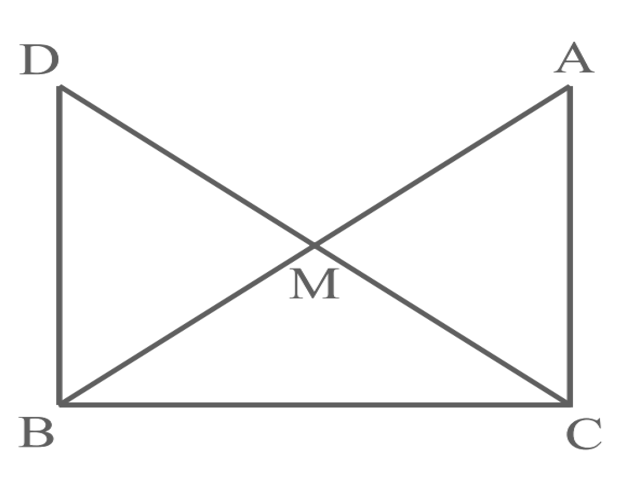
\includegraphics[width=\columnwidth]{figs/Screenshot.png}
  \caption{$\triangle \vec{ACB} ,\triangle \vec{DCB}$ with Mid-Point $\vec{M}$}
  \label{fig:triangles}
\end{figure}
\begin{enumerate}[label =(\roman*)]
        \item $\triangle \vec{AMC} \cong \triangle \vec{BMD}$
        \item $\angle \vec{DBC}$ is a right angle. 
        \item $\triangle \vec{DBC} \cong  \triangle \vec{ACB}$ 
        \item $\vec{CM} = \frac{1}{2} \vec{AB}$
\end{enumerate}
\pagebreak
\solution\\
\textbf{CONSTRUCTION STEPS :}
\begin{enumerate}
\item Let us Assume , the input parameters as ;
\begin{table}[H]
\centering
        \input{tables/input_params.tex}
          \caption{Input Parameters}
          \label{Table-1:Input_params}
\end{table}
\item the output can be calculated as ;
\begin{table}[H]
\centering
        \input{tables/output_params.tex}
          \caption{Output Parameters}
          \label{Table-2:Output_params}
\end{table}
                $\therefore$ By, Plotting these points we get the required Image \figref{fig:fig-2}
\begin{figure}[H]
        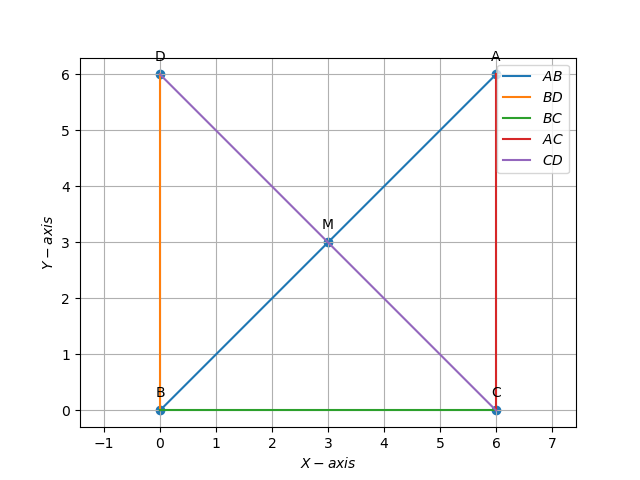
\includegraphics[width = \columnwidth]{figs/python_plot.png}
    \caption{PYTHON Plot of $\triangle \vec{ACB} ,\triangle \vec{DBC}$ with Mid-Point $\vec{M}$}
    \label{fig:fig-2}
\end{figure}
\end{enumerate}

\item Find the position vector of a point $\vec{R}$ which divides the line joining two points $\vec{P}$ and $\vec{Q}$ whose position vectors are $2\vec{a}+\vec{b}$ and $\vec{a}-3\vec{b}$ externally in the ratio $1:2$.

\textbf{Solution:}
Let us assume $\vec{a}$ and $\vec{b}$, and the given ratio is
\begin{table}[h]
    \centering
    \begin{tabular}{|c|c|c|}
        \hline 
        \textbf{Symbol} & \textbf{Value} & \textbf{Description} \\
        \hline
        $\vec{a}$ & $\myvec{1 \\ -3}$ & Vector $\vec{a}$ \\
        \hline
        $\vec{b}$ & $\myvec{0 \\ 2}$ & Vector $\vec{b}$\\
        \hline
        $k$ & $2$ & Ratio \\
        \hline
    \end{tabular}
    \caption{Vectors $\vec{a}$ and $\vec{b}$, ratio $k$}
    \label{tab:table1}
\end{table}

Using the section formula,
\begin{align}
    \vec{R} = \frac{\vec{Q} - k\vec{P}}{1 - k}
\end{align}
where $\vec{P}$ and $\vec{Q}$ depend on $\vec{a}$ and $\vec{b}$, then
\begin{align}
    \vec{P} &= (2\vec{a} + \vec{b}) = 2\myvec{1\\-3} + \myvec{0\\2} = \myvec{2\\-4} \\
    \vec{Q} &= (\vec{a} - 3\vec{b}) = \myvec{1\\-3} - 3\myvec{0\\2} = \myvec{1\\-9}
\end{align}
where $\vec{R}$ can be calculated as 
\begin{align}
    \vec{R} = \frac{(\vec{a} - 3\vec{b}) - k(2\vec{a} + \vec{b})}{1 - k}
\end{align}
By substituting $\vec{a}$ and $\vec{b}$ values, we get $\vec{R}$ as
\begin{align}
    \vec{R} = \myvec{3\\1}
\end{align}

\begin{table}[ht!]
    \centering
    \begin{tabular}{|c|c|c|}
        \hline
        \textbf{Symbol} & \textbf{Value} & \textbf{Description}\\
        \hline
        $\vec{P}$ & $(2\vec{a} + \vec{b})$ & Position vector $\vec{P}$ \\
        \hline
        $\vec{Q}$ & $(\vec{a} - 3\vec{b})$ & Position vector $\vec{Q}$\\
        \hline
        $\vec{R}$ & $\frac{\vec{Q} - k\vec{P}}{1 - k}$ & Position vector $\vec{R}$\\
        \hline
    \end{tabular}
    \caption{Vectors $\vec{P}$, $\vec{Q}$, $\vec{R}$}
    \label{tab:mytable2}   
\end{table}

\begin{figure}[H]
    \centering
    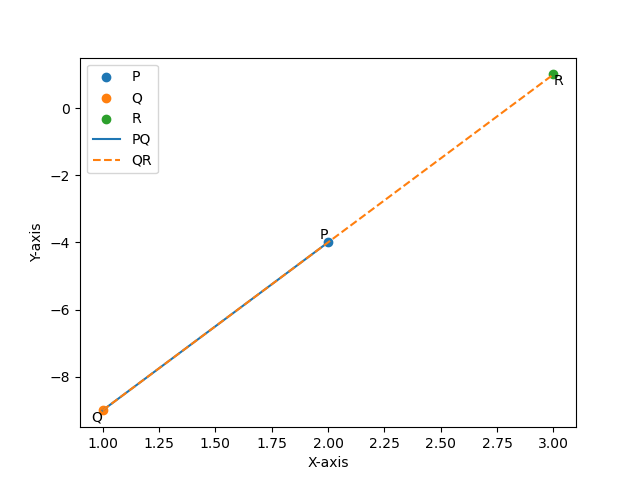
\includegraphics[width=\columnwidth]{figs/external-bisector.png}
    \caption{Point vectors $\vec{P}$, $\vec{Q}$, $\vec{R}$}
    \label{fig:enter-label}
\end{figure}


\end{enumerate}

    \item Draw a quadrilateral in the Cartesian plane, whose vertices are 
    \begin{align}
        \vec{A} = \myvec{-4\\5} \quad \vec{B} = \myvec{0\\7} \\
        \vec{C} = \myvec{5\\-5} \quad \vec{D} = \myvec{-4\\-2}
    \end{align}
    Also, find its area.
\label{chapters/11/10/1/1}
   \\ 
    \solution 
\begin{enumerate}[label=\thesection.\arabic*,ref=\thesection.\theenumi]
		\item Find $\abs{\overrightarrow{a}\times\overrightarrow{b}},\text{ if }\overrightarrow{a}=\hat{i}-7\hat{j}+7\hat{k}\text{ and } \overrightarrow{b}=3\hat{i}-2\hat{j}+2\hat{k}$.
	\\
		\solution
		\input{chapters/12/10/4/1/cross.tex}
\item Show that $$(\overrightarrow{a}-\overrightarrow{b})\times (\overrightarrow{a}+\overrightarrow{b})=2(\overrightarrow{a}\times \overrightarrow{b})$$
	\\
		\solution
		\input{chapters/12/10/4/4/cross.tex}
\item Find $\lambda$ and $\mu$ if $(2\hat{i}+6\hat{j}+27\hat{k})\times(\hat{i}+\lambda \hat{j} + \mu \hat{k})=\overrightarrow{0}$.
	\\
		\solution
		\input{chapters/12/10/4/5/cross.tex}
\item Given that $\overrightarrow{a} \cdot \overrightarrow{b} = 0$ and $\overrightarrow{a} \times \overrightarrow{b} = \overrightarrow{0}$. What can you conclude about the vectors $\overrightarrow{a} \text{ and }\overrightarrow{b}$?
\item Let the vectors be given as $\overrightarrow{a},\overrightarrow{b},\overrightarrow{c}\text{ be given as }\ a_1 \hat{i}+\ a_2 \hat{j}+\ a_3 \hat{k},\ b_1 \hat{i}+\ b_2 \hat{j}+\ b_3 \hat{k},\ c_1 \hat{i}+\ c_2 \hat{j}+\ c_3 \hat{k}$. Then show that $\overrightarrow{a} \times (\overrightarrow{b} + \overrightarrow{c}) = \overrightarrow{a} \times \overrightarrow{b}+\overrightarrow{a} \times \overrightarrow{c}$.
	\\
		\solution
		\input{chapters/12/10/4/7/cross.tex}
\item If either $\overrightarrow{a} = \overrightarrow{0}$ or $\overrightarrow{b} = \overrightarrow{0}$, then $\overrightarrow{a} \times \overrightarrow{b} = \overrightarrow{0}$. Is the converse true? Justify your answer with an example.
	\\
		\solution
		\input{chapters/12/10/4/8/cross.tex}
\item Find the area of the triangle with vertices $A(1, 1, 2)$, $B(2, 3, 5)$, and $C(1, 5, 5)$
	\\
		\solution
		\input{chapters/12/10/4/9/cross.tex}
\item Find the area of the parallelogram whose adjacent sides are determined by the vectors $\overrightarrow{a}=\hat{i}-\hat{j}+3\hat{k}$ and $\overrightarrow{b}=2\hat{i}-7\hat{j}+\hat{k}$.
	\\
		\solution
		\input{chapters/12/10/4/10/cross.tex}
\item Let the vectors $\overrightarrow{a}$ and $\overrightarrow{b}$ be such that $|\overrightarrow{a}| = 3$ and $|\overrightarrow{b}| = \dfrac{\sqrt{2}}{3}$, then $\overrightarrow{a} \times \overrightarrow{b}$ is a unit vector, if the angle between $\overrightarrow{a}$ and $\overrightarrow{b}$ is
\begin{enumerate}
\item $\dfrac{\pi}{6}$
\item $\dfrac{\pi}{4}$
\item $\dfrac{\pi}{3}$
\item $\dfrac{\pi}{2}$
\end{enumerate}
		\solution
		\input{chapters/12/10/4/11/cross.tex}
\item Area of a rectangle having vertices A, B, C and D with position vectors $ -\hat{i}+ \dfrac{1}{2} \hat{j}+4\hat{k},\hat{i}+ \dfrac{1}{2} \hat{j}+4\hat{k},\hat{i}-\dfrac{1}{2} \hat{j}+4\hat{k}\text{ and }-\hat{i}- \dfrac{1}{2} \hat{j}+4\hat{k}$, respectively is
\begin{enumerate}
\item $\dfrac{1}{2}$
\item 1
\item 2
\item 4
\end{enumerate}
		\solution
		\input{chapters/12/10/4/12/cross.tex}
\item Find the area of the triangle whose vertices are 
\begin{enumerate}
\item $(2, 3), (–1, 0), (2, – 4)$
\item $(–5, –1), (3, –5), (5, 2)$ 
\end{enumerate}
		\label{10/7/3/1}
\solution
		\input{chapters/10/7/3/1/area.tex}
\item Find the area of the triangle formed by joining the mid-points of the sides of the triangle whose vertices are $(0, –1), (2, 1) \text{ and } (0, 3)$. Find the ratio of this area to the area of the given triangle.
	\\
\solution
		\input{chapters/10/7/3/3/cross.tex}

\item Find the area of the quadrilateral whose vertices, taken in order, are $(– 4, – 2), (– 3, – 5), (3, – 2)$  and $ (2, 3)$.
	\\
\solution
		\input{chapters/10/7/3/4/cross.tex}

\item Verify that a median of a triangle divides it into two triangles of equal areas for $\triangle ABC$ whose vertices are $\vec{A}(4, -6), \vec{B}(3, 2), \text{ and } \vec{C}(5, 2)$. 
		\label{10/7/3/5}
		\\
\solution
		\input{chapters/10/7/3/5/area.tex}

\item The two adjacent sides of a parallelogram are 
$2\hat{i}-4\hat{j}+5\hat{k}$  and  $\hat{i}-2\hat{j}-3\hat{k}$.
Find the unit vector parallel to its diagonal. Also, find its area.\\
	\solution
		\input{chapters/12/10/5/10/cross.tex}
\item The vertices of a $\triangle ABC$ are $\vec{A}(4,6), \vec{B}(1,5)$ and  $\vec{C}(7,2)$. A line is drawn to intersect sides $AB$ and $AC$ at $\vec{D}$ and $\vec{E}$ respectively, such that $\frac{AD}{AB} = \frac{AE}{AC} = \frac{1}{4}$. Calculate the area of $\triangle ADE$ and compare it with the area of the $\triangle ABC$.
\\
\solution
	\input{chapters/10/7/4/6/section.tex}
    \item Draw a quadrilateral in the Cartesian plane, whose vertices are 
    \begin{align}
        \vec{A} = \myvec{-4\\5} \quad \vec{B} = \myvec{0\\7} \\
        \vec{C} = \myvec{5\\-5} \quad \vec{D} = \myvec{-4\\-2}
    \end{align}
    Also, find its area.
\label{chapters/11/10/1/1}
   \\ 
    \solution 
\input{chapters/11/10/1/1/cross.tex}
\item Find the area of region bounded by the triangle whose
	vertices are $(1, 0), (2, 2) \text{ and } (3, 1)$. 
\item Find the area of region bounded by the triangle whose vertices
	are $(– 1, 0), (1, 3) \text{ and } (3, 2)$. 
\item Find the area of the $\triangle ABC$, coordinates of whose vertices are $\vec{A}(2, 0), \vec{B}(4, 5), \text{ and } \vec{C}(6, 3)$.


\item 
\input{chapters/vectors/exer/main.tex}
\end{enumerate}


\item Find the area of region bounded by the triangle whose
	vertices are $(1, 0), (2, 2) \text{ and } (3, 1)$. 
\item Find the area of region bounded by the triangle whose vertices
	are $(– 1, 0), (1, 3) \text{ and } (3, 2)$. 
\item Find the area of the $\triangle ABC$, coordinates of whose vertices are $\vec{A}(2, 0), \vec{B}(4, 5), \text{ and } \vec{C}(6, 3)$.


\item 
%\documentclass[12pt]{article}
%\usepackage{graphicx}
%\usepackage{graphics}
%\usepackage{refstyle}
%\usepackage{amsmath}
%\usepackage{caption}
%\usepackage{float}
%\usepackage{booktabs}
%\usepackage{array}
%\usepackage{amssymb}
%\usepackage{booktabs}
%\let\vec\mathbf
%\providecommand{\brak}[1]{\ensuremath{\left(#1\right)}}
%\graphicspath{{/storage/self/primary/Download/latexnew/fig}}                                     
$\vec{P}$ and $\vec{Q}$ are any two points lying on the sides $DC$ and $AD$ respectively of a parallelogram $ABCD$.Show that, $ar\brak{\triangle APB}=ar\brak{\triangle BQC}$.


\textbf{Figure:}
\begin{figure}[H]
    \centering
	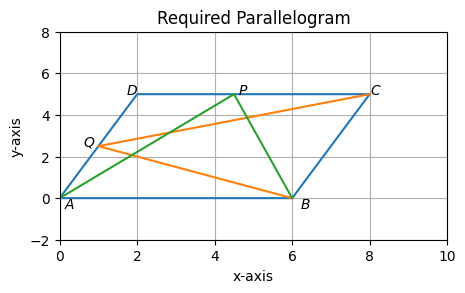
\includegraphics[width=\columnwidth]{chapters/vectors/exer/figs/1.png}
    \caption{}
    \label{fig:fig:1}
\end{figure}


\textbf{Solution:}
\begin{table}[H]
   \centering
  \input{chapters/vectors/exer/table/tab1.tex}
   \caption{Table of input parameters}        
\label{tab:tab:1}                    
\end{table}




\begin{table}[H]
    \centering                                  
\input{chapters/vectors/exer/table/tab2.tex}                  
\caption{Table of output parameters}
\label{tab:tab:2}
 \end{table}


For the $\triangle BQC$, the vertices of the triangle are taken from \tabref{tab:tab:1} and \tabref{tab:tab:2}.

\begin{align}
\implies ar\brak{\triangle BQC}&=
\frac{1}{2}\begin{tabular}{|c c c|}            
1 &1&1\\                      
$\vec{B}$&$\vec{Q}$&$\vec{C}$\\    
\end{tabular}\\
&= \frac{1}{2}\begin{tabular}{|c c c|}
       1 &1&1\\
       6&$\frac{2k_1}{k_1+1}$&8 \\
       0&$\frac{5k_1}{k_1+1}$&5
   \end{tabular}\\
  \xrightarrow{C_2'=C_2-C_1,C_3'=C_3-C_1}&\frac{1}{2} \begin{tabular}{|c c c|}
       1 &0&0\\
       6&$\frac{-4k_1-6}{k_1+1}$&2 \\
       0&$\frac{5k_1}{k_1+1}$&5
   \end{tabular}\\
&=\frac{1}{2}\brak{1\begin{tabular}{|c c|}
   $\frac{-4k_1-6}{k_1+1}$ &2  \\
   $\frac{5k_1}{k_1+1}$ & 5
\end{tabular} +0+0}\\
&=\frac{1}{2} \times30\\                          
&=15 \end{align}


For the $\triangle APB$, the vertices of the triangle are taken from \tabref{tab:tab:1} and \tabref{tab:tab:2}.
   \begin{align}
  \implies ar\brak{\triangle APB} &=
\frac{1}{2}\begin{tabular}{|c c c|}            
1 &1&1\\                            
$\vec{A}$&$\vec{P}$&$\vec{B}$\\
\end{tabular}\\ &=  \frac{1}{2}
   \begin{tabular}{|c c c|}
       1 &1&1\\
       0&$\frac{8k_2+2}{k_2+1}$&6 \\
       0&5&0
   \end{tabular}\\
 &=\frac{1}{2} \times30\\
 &=15 \end{align}
 \brak{6} = \brak{10}


So, ar\brak{\triangle BQC} = ar\brak{\triangle APB}.\brak{proved}
%\end{document}



\end{enumerate}



\item Find the area of the quadrilateral whose vertices, taken in order, are $(– 4, – 2), (– 3, – 5), (3, – 2)$  and $ (2, 3)$.
	\\
\solution
		\begin{enumerate}[label=\thesection.\arabic*,ref=\thesection.\theenumi]
		\item Find $\abs{\overrightarrow{a}\times\overrightarrow{b}},\text{ if }\overrightarrow{a}=\hat{i}-7\hat{j}+7\hat{k}\text{ and } \overrightarrow{b}=3\hat{i}-2\hat{j}+2\hat{k}$.
	\\
		\solution
		\begin{enumerate}[label=\thesection.\arabic*,ref=\thesection.\theenumi]
		\item Find $\abs{\overrightarrow{a}\times\overrightarrow{b}},\text{ if }\overrightarrow{a}=\hat{i}-7\hat{j}+7\hat{k}\text{ and } \overrightarrow{b}=3\hat{i}-2\hat{j}+2\hat{k}$.
	\\
		\solution
		\input{chapters/12/10/4/1/cross.tex}
\item Show that $$(\overrightarrow{a}-\overrightarrow{b})\times (\overrightarrow{a}+\overrightarrow{b})=2(\overrightarrow{a}\times \overrightarrow{b})$$
	\\
		\solution
		\input{chapters/12/10/4/4/cross.tex}
\item Find $\lambda$ and $\mu$ if $(2\hat{i}+6\hat{j}+27\hat{k})\times(\hat{i}+\lambda \hat{j} + \mu \hat{k})=\overrightarrow{0}$.
	\\
		\solution
		\input{chapters/12/10/4/5/cross.tex}
\item Given that $\overrightarrow{a} \cdot \overrightarrow{b} = 0$ and $\overrightarrow{a} \times \overrightarrow{b} = \overrightarrow{0}$. What can you conclude about the vectors $\overrightarrow{a} \text{ and }\overrightarrow{b}$?
\item Let the vectors be given as $\overrightarrow{a},\overrightarrow{b},\overrightarrow{c}\text{ be given as }\ a_1 \hat{i}+\ a_2 \hat{j}+\ a_3 \hat{k},\ b_1 \hat{i}+\ b_2 \hat{j}+\ b_3 \hat{k},\ c_1 \hat{i}+\ c_2 \hat{j}+\ c_3 \hat{k}$. Then show that $\overrightarrow{a} \times (\overrightarrow{b} + \overrightarrow{c}) = \overrightarrow{a} \times \overrightarrow{b}+\overrightarrow{a} \times \overrightarrow{c}$.
	\\
		\solution
		\input{chapters/12/10/4/7/cross.tex}
\item If either $\overrightarrow{a} = \overrightarrow{0}$ or $\overrightarrow{b} = \overrightarrow{0}$, then $\overrightarrow{a} \times \overrightarrow{b} = \overrightarrow{0}$. Is the converse true? Justify your answer with an example.
	\\
		\solution
		\input{chapters/12/10/4/8/cross.tex}
\item Find the area of the triangle with vertices $A(1, 1, 2)$, $B(2, 3, 5)$, and $C(1, 5, 5)$
	\\
		\solution
		\input{chapters/12/10/4/9/cross.tex}
\item Find the area of the parallelogram whose adjacent sides are determined by the vectors $\overrightarrow{a}=\hat{i}-\hat{j}+3\hat{k}$ and $\overrightarrow{b}=2\hat{i}-7\hat{j}+\hat{k}$.
	\\
		\solution
		\input{chapters/12/10/4/10/cross.tex}
\item Let the vectors $\overrightarrow{a}$ and $\overrightarrow{b}$ be such that $|\overrightarrow{a}| = 3$ and $|\overrightarrow{b}| = \dfrac{\sqrt{2}}{3}$, then $\overrightarrow{a} \times \overrightarrow{b}$ is a unit vector, if the angle between $\overrightarrow{a}$ and $\overrightarrow{b}$ is
\begin{enumerate}
\item $\dfrac{\pi}{6}$
\item $\dfrac{\pi}{4}$
\item $\dfrac{\pi}{3}$
\item $\dfrac{\pi}{2}$
\end{enumerate}
		\solution
		\input{chapters/12/10/4/11/cross.tex}
\item Area of a rectangle having vertices A, B, C and D with position vectors $ -\hat{i}+ \dfrac{1}{2} \hat{j}+4\hat{k},\hat{i}+ \dfrac{1}{2} \hat{j}+4\hat{k},\hat{i}-\dfrac{1}{2} \hat{j}+4\hat{k}\text{ and }-\hat{i}- \dfrac{1}{2} \hat{j}+4\hat{k}$, respectively is
\begin{enumerate}
\item $\dfrac{1}{2}$
\item 1
\item 2
\item 4
\end{enumerate}
		\solution
		\input{chapters/12/10/4/12/cross.tex}
\item Find the area of the triangle whose vertices are 
\begin{enumerate}
\item $(2, 3), (–1, 0), (2, – 4)$
\item $(–5, –1), (3, –5), (5, 2)$ 
\end{enumerate}
		\label{10/7/3/1}
\solution
		\input{chapters/10/7/3/1/area.tex}
\item Find the area of the triangle formed by joining the mid-points of the sides of the triangle whose vertices are $(0, –1), (2, 1) \text{ and } (0, 3)$. Find the ratio of this area to the area of the given triangle.
	\\
\solution
		\input{chapters/10/7/3/3/cross.tex}

\item Find the area of the quadrilateral whose vertices, taken in order, are $(– 4, – 2), (– 3, – 5), (3, – 2)$  and $ (2, 3)$.
	\\
\solution
		\input{chapters/10/7/3/4/cross.tex}

\item Verify that a median of a triangle divides it into two triangles of equal areas for $\triangle ABC$ whose vertices are $\vec{A}(4, -6), \vec{B}(3, 2), \text{ and } \vec{C}(5, 2)$. 
		\label{10/7/3/5}
		\\
\solution
		\input{chapters/10/7/3/5/area.tex}

\item The two adjacent sides of a parallelogram are 
$2\hat{i}-4\hat{j}+5\hat{k}$  and  $\hat{i}-2\hat{j}-3\hat{k}$.
Find the unit vector parallel to its diagonal. Also, find its area.\\
	\solution
		\input{chapters/12/10/5/10/cross.tex}
\item The vertices of a $\triangle ABC$ are $\vec{A}(4,6), \vec{B}(1,5)$ and  $\vec{C}(7,2)$. A line is drawn to intersect sides $AB$ and $AC$ at $\vec{D}$ and $\vec{E}$ respectively, such that $\frac{AD}{AB} = \frac{AE}{AC} = \frac{1}{4}$. Calculate the area of $\triangle ADE$ and compare it with the area of the $\triangle ABC$.
\\
\solution
	\input{chapters/10/7/4/6/section.tex}
    \item Draw a quadrilateral in the Cartesian plane, whose vertices are 
    \begin{align}
        \vec{A} = \myvec{-4\\5} \quad \vec{B} = \myvec{0\\7} \\
        \vec{C} = \myvec{5\\-5} \quad \vec{D} = \myvec{-4\\-2}
    \end{align}
    Also, find its area.
\label{chapters/11/10/1/1}
   \\ 
    \solution 
\input{chapters/11/10/1/1/cross.tex}
\item Find the area of region bounded by the triangle whose
	vertices are $(1, 0), (2, 2) \text{ and } (3, 1)$. 
\item Find the area of region bounded by the triangle whose vertices
	are $(– 1, 0), (1, 3) \text{ and } (3, 2)$. 
\item Find the area of the $\triangle ABC$, coordinates of whose vertices are $\vec{A}(2, 0), \vec{B}(4, 5), \text{ and } \vec{C}(6, 3)$.


\item 
\input{chapters/vectors/exer/main.tex}
\end{enumerate}


\item Show that $$(\overrightarrow{a}-\overrightarrow{b})\times (\overrightarrow{a}+\overrightarrow{b})=2(\overrightarrow{a}\times \overrightarrow{b})$$
	\\
		\solution
		\begin{enumerate}[label=\thesection.\arabic*,ref=\thesection.\theenumi]
		\item Find $\abs{\overrightarrow{a}\times\overrightarrow{b}},\text{ if }\overrightarrow{a}=\hat{i}-7\hat{j}+7\hat{k}\text{ and } \overrightarrow{b}=3\hat{i}-2\hat{j}+2\hat{k}$.
	\\
		\solution
		\input{chapters/12/10/4/1/cross.tex}
\item Show that $$(\overrightarrow{a}-\overrightarrow{b})\times (\overrightarrow{a}+\overrightarrow{b})=2(\overrightarrow{a}\times \overrightarrow{b})$$
	\\
		\solution
		\input{chapters/12/10/4/4/cross.tex}
\item Find $\lambda$ and $\mu$ if $(2\hat{i}+6\hat{j}+27\hat{k})\times(\hat{i}+\lambda \hat{j} + \mu \hat{k})=\overrightarrow{0}$.
	\\
		\solution
		\input{chapters/12/10/4/5/cross.tex}
\item Given that $\overrightarrow{a} \cdot \overrightarrow{b} = 0$ and $\overrightarrow{a} \times \overrightarrow{b} = \overrightarrow{0}$. What can you conclude about the vectors $\overrightarrow{a} \text{ and }\overrightarrow{b}$?
\item Let the vectors be given as $\overrightarrow{a},\overrightarrow{b},\overrightarrow{c}\text{ be given as }\ a_1 \hat{i}+\ a_2 \hat{j}+\ a_3 \hat{k},\ b_1 \hat{i}+\ b_2 \hat{j}+\ b_3 \hat{k},\ c_1 \hat{i}+\ c_2 \hat{j}+\ c_3 \hat{k}$. Then show that $\overrightarrow{a} \times (\overrightarrow{b} + \overrightarrow{c}) = \overrightarrow{a} \times \overrightarrow{b}+\overrightarrow{a} \times \overrightarrow{c}$.
	\\
		\solution
		\input{chapters/12/10/4/7/cross.tex}
\item If either $\overrightarrow{a} = \overrightarrow{0}$ or $\overrightarrow{b} = \overrightarrow{0}$, then $\overrightarrow{a} \times \overrightarrow{b} = \overrightarrow{0}$. Is the converse true? Justify your answer with an example.
	\\
		\solution
		\input{chapters/12/10/4/8/cross.tex}
\item Find the area of the triangle with vertices $A(1, 1, 2)$, $B(2, 3, 5)$, and $C(1, 5, 5)$
	\\
		\solution
		\input{chapters/12/10/4/9/cross.tex}
\item Find the area of the parallelogram whose adjacent sides are determined by the vectors $\overrightarrow{a}=\hat{i}-\hat{j}+3\hat{k}$ and $\overrightarrow{b}=2\hat{i}-7\hat{j}+\hat{k}$.
	\\
		\solution
		\input{chapters/12/10/4/10/cross.tex}
\item Let the vectors $\overrightarrow{a}$ and $\overrightarrow{b}$ be such that $|\overrightarrow{a}| = 3$ and $|\overrightarrow{b}| = \dfrac{\sqrt{2}}{3}$, then $\overrightarrow{a} \times \overrightarrow{b}$ is a unit vector, if the angle between $\overrightarrow{a}$ and $\overrightarrow{b}$ is
\begin{enumerate}
\item $\dfrac{\pi}{6}$
\item $\dfrac{\pi}{4}$
\item $\dfrac{\pi}{3}$
\item $\dfrac{\pi}{2}$
\end{enumerate}
		\solution
		\input{chapters/12/10/4/11/cross.tex}
\item Area of a rectangle having vertices A, B, C and D with position vectors $ -\hat{i}+ \dfrac{1}{2} \hat{j}+4\hat{k},\hat{i}+ \dfrac{1}{2} \hat{j}+4\hat{k},\hat{i}-\dfrac{1}{2} \hat{j}+4\hat{k}\text{ and }-\hat{i}- \dfrac{1}{2} \hat{j}+4\hat{k}$, respectively is
\begin{enumerate}
\item $\dfrac{1}{2}$
\item 1
\item 2
\item 4
\end{enumerate}
		\solution
		\input{chapters/12/10/4/12/cross.tex}
\item Find the area of the triangle whose vertices are 
\begin{enumerate}
\item $(2, 3), (–1, 0), (2, – 4)$
\item $(–5, –1), (3, –5), (5, 2)$ 
\end{enumerate}
		\label{10/7/3/1}
\solution
		\input{chapters/10/7/3/1/area.tex}
\item Find the area of the triangle formed by joining the mid-points of the sides of the triangle whose vertices are $(0, –1), (2, 1) \text{ and } (0, 3)$. Find the ratio of this area to the area of the given triangle.
	\\
\solution
		\input{chapters/10/7/3/3/cross.tex}

\item Find the area of the quadrilateral whose vertices, taken in order, are $(– 4, – 2), (– 3, – 5), (3, – 2)$  and $ (2, 3)$.
	\\
\solution
		\input{chapters/10/7/3/4/cross.tex}

\item Verify that a median of a triangle divides it into two triangles of equal areas for $\triangle ABC$ whose vertices are $\vec{A}(4, -6), \vec{B}(3, 2), \text{ and } \vec{C}(5, 2)$. 
		\label{10/7/3/5}
		\\
\solution
		\input{chapters/10/7/3/5/area.tex}

\item The two adjacent sides of a parallelogram are 
$2\hat{i}-4\hat{j}+5\hat{k}$  and  $\hat{i}-2\hat{j}-3\hat{k}$.
Find the unit vector parallel to its diagonal. Also, find its area.\\
	\solution
		\input{chapters/12/10/5/10/cross.tex}
\item The vertices of a $\triangle ABC$ are $\vec{A}(4,6), \vec{B}(1,5)$ and  $\vec{C}(7,2)$. A line is drawn to intersect sides $AB$ and $AC$ at $\vec{D}$ and $\vec{E}$ respectively, such that $\frac{AD}{AB} = \frac{AE}{AC} = \frac{1}{4}$. Calculate the area of $\triangle ADE$ and compare it with the area of the $\triangle ABC$.
\\
\solution
	\input{chapters/10/7/4/6/section.tex}
    \item Draw a quadrilateral in the Cartesian plane, whose vertices are 
    \begin{align}
        \vec{A} = \myvec{-4\\5} \quad \vec{B} = \myvec{0\\7} \\
        \vec{C} = \myvec{5\\-5} \quad \vec{D} = \myvec{-4\\-2}
    \end{align}
    Also, find its area.
\label{chapters/11/10/1/1}
   \\ 
    \solution 
\input{chapters/11/10/1/1/cross.tex}
\item Find the area of region bounded by the triangle whose
	vertices are $(1, 0), (2, 2) \text{ and } (3, 1)$. 
\item Find the area of region bounded by the triangle whose vertices
	are $(– 1, 0), (1, 3) \text{ and } (3, 2)$. 
\item Find the area of the $\triangle ABC$, coordinates of whose vertices are $\vec{A}(2, 0), \vec{B}(4, 5), \text{ and } \vec{C}(6, 3)$.


\item 
\input{chapters/vectors/exer/main.tex}
\end{enumerate}


\item Find $\lambda$ and $\mu$ if $(2\hat{i}+6\hat{j}+27\hat{k})\times(\hat{i}+\lambda \hat{j} + \mu \hat{k})=\overrightarrow{0}$.
	\\
		\solution
		\begin{enumerate}[label=\thesection.\arabic*,ref=\thesection.\theenumi]
		\item Find $\abs{\overrightarrow{a}\times\overrightarrow{b}},\text{ if }\overrightarrow{a}=\hat{i}-7\hat{j}+7\hat{k}\text{ and } \overrightarrow{b}=3\hat{i}-2\hat{j}+2\hat{k}$.
	\\
		\solution
		\input{chapters/12/10/4/1/cross.tex}
\item Show that $$(\overrightarrow{a}-\overrightarrow{b})\times (\overrightarrow{a}+\overrightarrow{b})=2(\overrightarrow{a}\times \overrightarrow{b})$$
	\\
		\solution
		\input{chapters/12/10/4/4/cross.tex}
\item Find $\lambda$ and $\mu$ if $(2\hat{i}+6\hat{j}+27\hat{k})\times(\hat{i}+\lambda \hat{j} + \mu \hat{k})=\overrightarrow{0}$.
	\\
		\solution
		\input{chapters/12/10/4/5/cross.tex}
\item Given that $\overrightarrow{a} \cdot \overrightarrow{b} = 0$ and $\overrightarrow{a} \times \overrightarrow{b} = \overrightarrow{0}$. What can you conclude about the vectors $\overrightarrow{a} \text{ and }\overrightarrow{b}$?
\item Let the vectors be given as $\overrightarrow{a},\overrightarrow{b},\overrightarrow{c}\text{ be given as }\ a_1 \hat{i}+\ a_2 \hat{j}+\ a_3 \hat{k},\ b_1 \hat{i}+\ b_2 \hat{j}+\ b_3 \hat{k},\ c_1 \hat{i}+\ c_2 \hat{j}+\ c_3 \hat{k}$. Then show that $\overrightarrow{a} \times (\overrightarrow{b} + \overrightarrow{c}) = \overrightarrow{a} \times \overrightarrow{b}+\overrightarrow{a} \times \overrightarrow{c}$.
	\\
		\solution
		\input{chapters/12/10/4/7/cross.tex}
\item If either $\overrightarrow{a} = \overrightarrow{0}$ or $\overrightarrow{b} = \overrightarrow{0}$, then $\overrightarrow{a} \times \overrightarrow{b} = \overrightarrow{0}$. Is the converse true? Justify your answer with an example.
	\\
		\solution
		\input{chapters/12/10/4/8/cross.tex}
\item Find the area of the triangle with vertices $A(1, 1, 2)$, $B(2, 3, 5)$, and $C(1, 5, 5)$
	\\
		\solution
		\input{chapters/12/10/4/9/cross.tex}
\item Find the area of the parallelogram whose adjacent sides are determined by the vectors $\overrightarrow{a}=\hat{i}-\hat{j}+3\hat{k}$ and $\overrightarrow{b}=2\hat{i}-7\hat{j}+\hat{k}$.
	\\
		\solution
		\input{chapters/12/10/4/10/cross.tex}
\item Let the vectors $\overrightarrow{a}$ and $\overrightarrow{b}$ be such that $|\overrightarrow{a}| = 3$ and $|\overrightarrow{b}| = \dfrac{\sqrt{2}}{3}$, then $\overrightarrow{a} \times \overrightarrow{b}$ is a unit vector, if the angle between $\overrightarrow{a}$ and $\overrightarrow{b}$ is
\begin{enumerate}
\item $\dfrac{\pi}{6}$
\item $\dfrac{\pi}{4}$
\item $\dfrac{\pi}{3}$
\item $\dfrac{\pi}{2}$
\end{enumerate}
		\solution
		\input{chapters/12/10/4/11/cross.tex}
\item Area of a rectangle having vertices A, B, C and D with position vectors $ -\hat{i}+ \dfrac{1}{2} \hat{j}+4\hat{k},\hat{i}+ \dfrac{1}{2} \hat{j}+4\hat{k},\hat{i}-\dfrac{1}{2} \hat{j}+4\hat{k}\text{ and }-\hat{i}- \dfrac{1}{2} \hat{j}+4\hat{k}$, respectively is
\begin{enumerate}
\item $\dfrac{1}{2}$
\item 1
\item 2
\item 4
\end{enumerate}
		\solution
		\input{chapters/12/10/4/12/cross.tex}
\item Find the area of the triangle whose vertices are 
\begin{enumerate}
\item $(2, 3), (–1, 0), (2, – 4)$
\item $(–5, –1), (3, –5), (5, 2)$ 
\end{enumerate}
		\label{10/7/3/1}
\solution
		\input{chapters/10/7/3/1/area.tex}
\item Find the area of the triangle formed by joining the mid-points of the sides of the triangle whose vertices are $(0, –1), (2, 1) \text{ and } (0, 3)$. Find the ratio of this area to the area of the given triangle.
	\\
\solution
		\input{chapters/10/7/3/3/cross.tex}

\item Find the area of the quadrilateral whose vertices, taken in order, are $(– 4, – 2), (– 3, – 5), (3, – 2)$  and $ (2, 3)$.
	\\
\solution
		\input{chapters/10/7/3/4/cross.tex}

\item Verify that a median of a triangle divides it into two triangles of equal areas for $\triangle ABC$ whose vertices are $\vec{A}(4, -6), \vec{B}(3, 2), \text{ and } \vec{C}(5, 2)$. 
		\label{10/7/3/5}
		\\
\solution
		\input{chapters/10/7/3/5/area.tex}

\item The two adjacent sides of a parallelogram are 
$2\hat{i}-4\hat{j}+5\hat{k}$  and  $\hat{i}-2\hat{j}-3\hat{k}$.
Find the unit vector parallel to its diagonal. Also, find its area.\\
	\solution
		\input{chapters/12/10/5/10/cross.tex}
\item The vertices of a $\triangle ABC$ are $\vec{A}(4,6), \vec{B}(1,5)$ and  $\vec{C}(7,2)$. A line is drawn to intersect sides $AB$ and $AC$ at $\vec{D}$ and $\vec{E}$ respectively, such that $\frac{AD}{AB} = \frac{AE}{AC} = \frac{1}{4}$. Calculate the area of $\triangle ADE$ and compare it with the area of the $\triangle ABC$.
\\
\solution
	\input{chapters/10/7/4/6/section.tex}
    \item Draw a quadrilateral in the Cartesian plane, whose vertices are 
    \begin{align}
        \vec{A} = \myvec{-4\\5} \quad \vec{B} = \myvec{0\\7} \\
        \vec{C} = \myvec{5\\-5} \quad \vec{D} = \myvec{-4\\-2}
    \end{align}
    Also, find its area.
\label{chapters/11/10/1/1}
   \\ 
    \solution 
\input{chapters/11/10/1/1/cross.tex}
\item Find the area of region bounded by the triangle whose
	vertices are $(1, 0), (2, 2) \text{ and } (3, 1)$. 
\item Find the area of region bounded by the triangle whose vertices
	are $(– 1, 0), (1, 3) \text{ and } (3, 2)$. 
\item Find the area of the $\triangle ABC$, coordinates of whose vertices are $\vec{A}(2, 0), \vec{B}(4, 5), \text{ and } \vec{C}(6, 3)$.


\item 
\input{chapters/vectors/exer/main.tex}
\end{enumerate}


\item Given that $\overrightarrow{a} \cdot \overrightarrow{b} = 0$ and $\overrightarrow{a} \times \overrightarrow{b} = \overrightarrow{0}$. What can you conclude about the vectors $\overrightarrow{a} \text{ and }\overrightarrow{b}$?
\item Let the vectors be given as $\overrightarrow{a},\overrightarrow{b},\overrightarrow{c}\text{ be given as }\ a_1 \hat{i}+\ a_2 \hat{j}+\ a_3 \hat{k},\ b_1 \hat{i}+\ b_2 \hat{j}+\ b_3 \hat{k},\ c_1 \hat{i}+\ c_2 \hat{j}+\ c_3 \hat{k}$. Then show that $\overrightarrow{a} \times (\overrightarrow{b} + \overrightarrow{c}) = \overrightarrow{a} \times \overrightarrow{b}+\overrightarrow{a} \times \overrightarrow{c}$.
	\\
		\solution
		\begin{enumerate}[label=\thesection.\arabic*,ref=\thesection.\theenumi]
		\item Find $\abs{\overrightarrow{a}\times\overrightarrow{b}},\text{ if }\overrightarrow{a}=\hat{i}-7\hat{j}+7\hat{k}\text{ and } \overrightarrow{b}=3\hat{i}-2\hat{j}+2\hat{k}$.
	\\
		\solution
		\input{chapters/12/10/4/1/cross.tex}
\item Show that $$(\overrightarrow{a}-\overrightarrow{b})\times (\overrightarrow{a}+\overrightarrow{b})=2(\overrightarrow{a}\times \overrightarrow{b})$$
	\\
		\solution
		\input{chapters/12/10/4/4/cross.tex}
\item Find $\lambda$ and $\mu$ if $(2\hat{i}+6\hat{j}+27\hat{k})\times(\hat{i}+\lambda \hat{j} + \mu \hat{k})=\overrightarrow{0}$.
	\\
		\solution
		\input{chapters/12/10/4/5/cross.tex}
\item Given that $\overrightarrow{a} \cdot \overrightarrow{b} = 0$ and $\overrightarrow{a} \times \overrightarrow{b} = \overrightarrow{0}$. What can you conclude about the vectors $\overrightarrow{a} \text{ and }\overrightarrow{b}$?
\item Let the vectors be given as $\overrightarrow{a},\overrightarrow{b},\overrightarrow{c}\text{ be given as }\ a_1 \hat{i}+\ a_2 \hat{j}+\ a_3 \hat{k},\ b_1 \hat{i}+\ b_2 \hat{j}+\ b_3 \hat{k},\ c_1 \hat{i}+\ c_2 \hat{j}+\ c_3 \hat{k}$. Then show that $\overrightarrow{a} \times (\overrightarrow{b} + \overrightarrow{c}) = \overrightarrow{a} \times \overrightarrow{b}+\overrightarrow{a} \times \overrightarrow{c}$.
	\\
		\solution
		\input{chapters/12/10/4/7/cross.tex}
\item If either $\overrightarrow{a} = \overrightarrow{0}$ or $\overrightarrow{b} = \overrightarrow{0}$, then $\overrightarrow{a} \times \overrightarrow{b} = \overrightarrow{0}$. Is the converse true? Justify your answer with an example.
	\\
		\solution
		\input{chapters/12/10/4/8/cross.tex}
\item Find the area of the triangle with vertices $A(1, 1, 2)$, $B(2, 3, 5)$, and $C(1, 5, 5)$
	\\
		\solution
		\input{chapters/12/10/4/9/cross.tex}
\item Find the area of the parallelogram whose adjacent sides are determined by the vectors $\overrightarrow{a}=\hat{i}-\hat{j}+3\hat{k}$ and $\overrightarrow{b}=2\hat{i}-7\hat{j}+\hat{k}$.
	\\
		\solution
		\input{chapters/12/10/4/10/cross.tex}
\item Let the vectors $\overrightarrow{a}$ and $\overrightarrow{b}$ be such that $|\overrightarrow{a}| = 3$ and $|\overrightarrow{b}| = \dfrac{\sqrt{2}}{3}$, then $\overrightarrow{a} \times \overrightarrow{b}$ is a unit vector, if the angle between $\overrightarrow{a}$ and $\overrightarrow{b}$ is
\begin{enumerate}
\item $\dfrac{\pi}{6}$
\item $\dfrac{\pi}{4}$
\item $\dfrac{\pi}{3}$
\item $\dfrac{\pi}{2}$
\end{enumerate}
		\solution
		\input{chapters/12/10/4/11/cross.tex}
\item Area of a rectangle having vertices A, B, C and D with position vectors $ -\hat{i}+ \dfrac{1}{2} \hat{j}+4\hat{k},\hat{i}+ \dfrac{1}{2} \hat{j}+4\hat{k},\hat{i}-\dfrac{1}{2} \hat{j}+4\hat{k}\text{ and }-\hat{i}- \dfrac{1}{2} \hat{j}+4\hat{k}$, respectively is
\begin{enumerate}
\item $\dfrac{1}{2}$
\item 1
\item 2
\item 4
\end{enumerate}
		\solution
		\input{chapters/12/10/4/12/cross.tex}
\item Find the area of the triangle whose vertices are 
\begin{enumerate}
\item $(2, 3), (–1, 0), (2, – 4)$
\item $(–5, –1), (3, –5), (5, 2)$ 
\end{enumerate}
		\label{10/7/3/1}
\solution
		\input{chapters/10/7/3/1/area.tex}
\item Find the area of the triangle formed by joining the mid-points of the sides of the triangle whose vertices are $(0, –1), (2, 1) \text{ and } (0, 3)$. Find the ratio of this area to the area of the given triangle.
	\\
\solution
		\input{chapters/10/7/3/3/cross.tex}

\item Find the area of the quadrilateral whose vertices, taken in order, are $(– 4, – 2), (– 3, – 5), (3, – 2)$  and $ (2, 3)$.
	\\
\solution
		\input{chapters/10/7/3/4/cross.tex}

\item Verify that a median of a triangle divides it into two triangles of equal areas for $\triangle ABC$ whose vertices are $\vec{A}(4, -6), \vec{B}(3, 2), \text{ and } \vec{C}(5, 2)$. 
		\label{10/7/3/5}
		\\
\solution
		\input{chapters/10/7/3/5/area.tex}

\item The two adjacent sides of a parallelogram are 
$2\hat{i}-4\hat{j}+5\hat{k}$  and  $\hat{i}-2\hat{j}-3\hat{k}$.
Find the unit vector parallel to its diagonal. Also, find its area.\\
	\solution
		\input{chapters/12/10/5/10/cross.tex}
\item The vertices of a $\triangle ABC$ are $\vec{A}(4,6), \vec{B}(1,5)$ and  $\vec{C}(7,2)$. A line is drawn to intersect sides $AB$ and $AC$ at $\vec{D}$ and $\vec{E}$ respectively, such that $\frac{AD}{AB} = \frac{AE}{AC} = \frac{1}{4}$. Calculate the area of $\triangle ADE$ and compare it with the area of the $\triangle ABC$.
\\
\solution
	\input{chapters/10/7/4/6/section.tex}
    \item Draw a quadrilateral in the Cartesian plane, whose vertices are 
    \begin{align}
        \vec{A} = \myvec{-4\\5} \quad \vec{B} = \myvec{0\\7} \\
        \vec{C} = \myvec{5\\-5} \quad \vec{D} = \myvec{-4\\-2}
    \end{align}
    Also, find its area.
\label{chapters/11/10/1/1}
   \\ 
    \solution 
\input{chapters/11/10/1/1/cross.tex}
\item Find the area of region bounded by the triangle whose
	vertices are $(1, 0), (2, 2) \text{ and } (3, 1)$. 
\item Find the area of region bounded by the triangle whose vertices
	are $(– 1, 0), (1, 3) \text{ and } (3, 2)$. 
\item Find the area of the $\triangle ABC$, coordinates of whose vertices are $\vec{A}(2, 0), \vec{B}(4, 5), \text{ and } \vec{C}(6, 3)$.


\item 
\input{chapters/vectors/exer/main.tex}
\end{enumerate}


\item If either $\overrightarrow{a} = \overrightarrow{0}$ or $\overrightarrow{b} = \overrightarrow{0}$, then $\overrightarrow{a} \times \overrightarrow{b} = \overrightarrow{0}$. Is the converse true? Justify your answer with an example.
	\\
		\solution
		\begin{enumerate}[label=\thesection.\arabic*,ref=\thesection.\theenumi]
		\item Find $\abs{\overrightarrow{a}\times\overrightarrow{b}},\text{ if }\overrightarrow{a}=\hat{i}-7\hat{j}+7\hat{k}\text{ and } \overrightarrow{b}=3\hat{i}-2\hat{j}+2\hat{k}$.
	\\
		\solution
		\input{chapters/12/10/4/1/cross.tex}
\item Show that $$(\overrightarrow{a}-\overrightarrow{b})\times (\overrightarrow{a}+\overrightarrow{b})=2(\overrightarrow{a}\times \overrightarrow{b})$$
	\\
		\solution
		\input{chapters/12/10/4/4/cross.tex}
\item Find $\lambda$ and $\mu$ if $(2\hat{i}+6\hat{j}+27\hat{k})\times(\hat{i}+\lambda \hat{j} + \mu \hat{k})=\overrightarrow{0}$.
	\\
		\solution
		\input{chapters/12/10/4/5/cross.tex}
\item Given that $\overrightarrow{a} \cdot \overrightarrow{b} = 0$ and $\overrightarrow{a} \times \overrightarrow{b} = \overrightarrow{0}$. What can you conclude about the vectors $\overrightarrow{a} \text{ and }\overrightarrow{b}$?
\item Let the vectors be given as $\overrightarrow{a},\overrightarrow{b},\overrightarrow{c}\text{ be given as }\ a_1 \hat{i}+\ a_2 \hat{j}+\ a_3 \hat{k},\ b_1 \hat{i}+\ b_2 \hat{j}+\ b_3 \hat{k},\ c_1 \hat{i}+\ c_2 \hat{j}+\ c_3 \hat{k}$. Then show that $\overrightarrow{a} \times (\overrightarrow{b} + \overrightarrow{c}) = \overrightarrow{a} \times \overrightarrow{b}+\overrightarrow{a} \times \overrightarrow{c}$.
	\\
		\solution
		\input{chapters/12/10/4/7/cross.tex}
\item If either $\overrightarrow{a} = \overrightarrow{0}$ or $\overrightarrow{b} = \overrightarrow{0}$, then $\overrightarrow{a} \times \overrightarrow{b} = \overrightarrow{0}$. Is the converse true? Justify your answer with an example.
	\\
		\solution
		\input{chapters/12/10/4/8/cross.tex}
\item Find the area of the triangle with vertices $A(1, 1, 2)$, $B(2, 3, 5)$, and $C(1, 5, 5)$
	\\
		\solution
		\input{chapters/12/10/4/9/cross.tex}
\item Find the area of the parallelogram whose adjacent sides are determined by the vectors $\overrightarrow{a}=\hat{i}-\hat{j}+3\hat{k}$ and $\overrightarrow{b}=2\hat{i}-7\hat{j}+\hat{k}$.
	\\
		\solution
		\input{chapters/12/10/4/10/cross.tex}
\item Let the vectors $\overrightarrow{a}$ and $\overrightarrow{b}$ be such that $|\overrightarrow{a}| = 3$ and $|\overrightarrow{b}| = \dfrac{\sqrt{2}}{3}$, then $\overrightarrow{a} \times \overrightarrow{b}$ is a unit vector, if the angle between $\overrightarrow{a}$ and $\overrightarrow{b}$ is
\begin{enumerate}
\item $\dfrac{\pi}{6}$
\item $\dfrac{\pi}{4}$
\item $\dfrac{\pi}{3}$
\item $\dfrac{\pi}{2}$
\end{enumerate}
		\solution
		\input{chapters/12/10/4/11/cross.tex}
\item Area of a rectangle having vertices A, B, C and D with position vectors $ -\hat{i}+ \dfrac{1}{2} \hat{j}+4\hat{k},\hat{i}+ \dfrac{1}{2} \hat{j}+4\hat{k},\hat{i}-\dfrac{1}{2} \hat{j}+4\hat{k}\text{ and }-\hat{i}- \dfrac{1}{2} \hat{j}+4\hat{k}$, respectively is
\begin{enumerate}
\item $\dfrac{1}{2}$
\item 1
\item 2
\item 4
\end{enumerate}
		\solution
		\input{chapters/12/10/4/12/cross.tex}
\item Find the area of the triangle whose vertices are 
\begin{enumerate}
\item $(2, 3), (–1, 0), (2, – 4)$
\item $(–5, –1), (3, –5), (5, 2)$ 
\end{enumerate}
		\label{10/7/3/1}
\solution
		\input{chapters/10/7/3/1/area.tex}
\item Find the area of the triangle formed by joining the mid-points of the sides of the triangle whose vertices are $(0, –1), (2, 1) \text{ and } (0, 3)$. Find the ratio of this area to the area of the given triangle.
	\\
\solution
		\input{chapters/10/7/3/3/cross.tex}

\item Find the area of the quadrilateral whose vertices, taken in order, are $(– 4, – 2), (– 3, – 5), (3, – 2)$  and $ (2, 3)$.
	\\
\solution
		\input{chapters/10/7/3/4/cross.tex}

\item Verify that a median of a triangle divides it into two triangles of equal areas for $\triangle ABC$ whose vertices are $\vec{A}(4, -6), \vec{B}(3, 2), \text{ and } \vec{C}(5, 2)$. 
		\label{10/7/3/5}
		\\
\solution
		\input{chapters/10/7/3/5/area.tex}

\item The two adjacent sides of a parallelogram are 
$2\hat{i}-4\hat{j}+5\hat{k}$  and  $\hat{i}-2\hat{j}-3\hat{k}$.
Find the unit vector parallel to its diagonal. Also, find its area.\\
	\solution
		\input{chapters/12/10/5/10/cross.tex}
\item The vertices of a $\triangle ABC$ are $\vec{A}(4,6), \vec{B}(1,5)$ and  $\vec{C}(7,2)$. A line is drawn to intersect sides $AB$ and $AC$ at $\vec{D}$ and $\vec{E}$ respectively, such that $\frac{AD}{AB} = \frac{AE}{AC} = \frac{1}{4}$. Calculate the area of $\triangle ADE$ and compare it with the area of the $\triangle ABC$.
\\
\solution
	\input{chapters/10/7/4/6/section.tex}
    \item Draw a quadrilateral in the Cartesian plane, whose vertices are 
    \begin{align}
        \vec{A} = \myvec{-4\\5} \quad \vec{B} = \myvec{0\\7} \\
        \vec{C} = \myvec{5\\-5} \quad \vec{D} = \myvec{-4\\-2}
    \end{align}
    Also, find its area.
\label{chapters/11/10/1/1}
   \\ 
    \solution 
\input{chapters/11/10/1/1/cross.tex}
\item Find the area of region bounded by the triangle whose
	vertices are $(1, 0), (2, 2) \text{ and } (3, 1)$. 
\item Find the area of region bounded by the triangle whose vertices
	are $(– 1, 0), (1, 3) \text{ and } (3, 2)$. 
\item Find the area of the $\triangle ABC$, coordinates of whose vertices are $\vec{A}(2, 0), \vec{B}(4, 5), \text{ and } \vec{C}(6, 3)$.


\item 
\input{chapters/vectors/exer/main.tex}
\end{enumerate}


\item Find the area of the triangle with vertices $A(1, 1, 2)$, $B(2, 3, 5)$, and $C(1, 5, 5)$
	\\
		\solution
		\begin{enumerate}[label=\thesection.\arabic*,ref=\thesection.\theenumi]
		\item Find $\abs{\overrightarrow{a}\times\overrightarrow{b}},\text{ if }\overrightarrow{a}=\hat{i}-7\hat{j}+7\hat{k}\text{ and } \overrightarrow{b}=3\hat{i}-2\hat{j}+2\hat{k}$.
	\\
		\solution
		\input{chapters/12/10/4/1/cross.tex}
\item Show that $$(\overrightarrow{a}-\overrightarrow{b})\times (\overrightarrow{a}+\overrightarrow{b})=2(\overrightarrow{a}\times \overrightarrow{b})$$
	\\
		\solution
		\input{chapters/12/10/4/4/cross.tex}
\item Find $\lambda$ and $\mu$ if $(2\hat{i}+6\hat{j}+27\hat{k})\times(\hat{i}+\lambda \hat{j} + \mu \hat{k})=\overrightarrow{0}$.
	\\
		\solution
		\input{chapters/12/10/4/5/cross.tex}
\item Given that $\overrightarrow{a} \cdot \overrightarrow{b} = 0$ and $\overrightarrow{a} \times \overrightarrow{b} = \overrightarrow{0}$. What can you conclude about the vectors $\overrightarrow{a} \text{ and }\overrightarrow{b}$?
\item Let the vectors be given as $\overrightarrow{a},\overrightarrow{b},\overrightarrow{c}\text{ be given as }\ a_1 \hat{i}+\ a_2 \hat{j}+\ a_3 \hat{k},\ b_1 \hat{i}+\ b_2 \hat{j}+\ b_3 \hat{k},\ c_1 \hat{i}+\ c_2 \hat{j}+\ c_3 \hat{k}$. Then show that $\overrightarrow{a} \times (\overrightarrow{b} + \overrightarrow{c}) = \overrightarrow{a} \times \overrightarrow{b}+\overrightarrow{a} \times \overrightarrow{c}$.
	\\
		\solution
		\input{chapters/12/10/4/7/cross.tex}
\item If either $\overrightarrow{a} = \overrightarrow{0}$ or $\overrightarrow{b} = \overrightarrow{0}$, then $\overrightarrow{a} \times \overrightarrow{b} = \overrightarrow{0}$. Is the converse true? Justify your answer with an example.
	\\
		\solution
		\input{chapters/12/10/4/8/cross.tex}
\item Find the area of the triangle with vertices $A(1, 1, 2)$, $B(2, 3, 5)$, and $C(1, 5, 5)$
	\\
		\solution
		\input{chapters/12/10/4/9/cross.tex}
\item Find the area of the parallelogram whose adjacent sides are determined by the vectors $\overrightarrow{a}=\hat{i}-\hat{j}+3\hat{k}$ and $\overrightarrow{b}=2\hat{i}-7\hat{j}+\hat{k}$.
	\\
		\solution
		\input{chapters/12/10/4/10/cross.tex}
\item Let the vectors $\overrightarrow{a}$ and $\overrightarrow{b}$ be such that $|\overrightarrow{a}| = 3$ and $|\overrightarrow{b}| = \dfrac{\sqrt{2}}{3}$, then $\overrightarrow{a} \times \overrightarrow{b}$ is a unit vector, if the angle between $\overrightarrow{a}$ and $\overrightarrow{b}$ is
\begin{enumerate}
\item $\dfrac{\pi}{6}$
\item $\dfrac{\pi}{4}$
\item $\dfrac{\pi}{3}$
\item $\dfrac{\pi}{2}$
\end{enumerate}
		\solution
		\input{chapters/12/10/4/11/cross.tex}
\item Area of a rectangle having vertices A, B, C and D with position vectors $ -\hat{i}+ \dfrac{1}{2} \hat{j}+4\hat{k},\hat{i}+ \dfrac{1}{2} \hat{j}+4\hat{k},\hat{i}-\dfrac{1}{2} \hat{j}+4\hat{k}\text{ and }-\hat{i}- \dfrac{1}{2} \hat{j}+4\hat{k}$, respectively is
\begin{enumerate}
\item $\dfrac{1}{2}$
\item 1
\item 2
\item 4
\end{enumerate}
		\solution
		\input{chapters/12/10/4/12/cross.tex}
\item Find the area of the triangle whose vertices are 
\begin{enumerate}
\item $(2, 3), (–1, 0), (2, – 4)$
\item $(–5, –1), (3, –5), (5, 2)$ 
\end{enumerate}
		\label{10/7/3/1}
\solution
		\input{chapters/10/7/3/1/area.tex}
\item Find the area of the triangle formed by joining the mid-points of the sides of the triangle whose vertices are $(0, –1), (2, 1) \text{ and } (0, 3)$. Find the ratio of this area to the area of the given triangle.
	\\
\solution
		\input{chapters/10/7/3/3/cross.tex}

\item Find the area of the quadrilateral whose vertices, taken in order, are $(– 4, – 2), (– 3, – 5), (3, – 2)$  and $ (2, 3)$.
	\\
\solution
		\input{chapters/10/7/3/4/cross.tex}

\item Verify that a median of a triangle divides it into two triangles of equal areas for $\triangle ABC$ whose vertices are $\vec{A}(4, -6), \vec{B}(3, 2), \text{ and } \vec{C}(5, 2)$. 
		\label{10/7/3/5}
		\\
\solution
		\input{chapters/10/7/3/5/area.tex}

\item The two adjacent sides of a parallelogram are 
$2\hat{i}-4\hat{j}+5\hat{k}$  and  $\hat{i}-2\hat{j}-3\hat{k}$.
Find the unit vector parallel to its diagonal. Also, find its area.\\
	\solution
		\input{chapters/12/10/5/10/cross.tex}
\item The vertices of a $\triangle ABC$ are $\vec{A}(4,6), \vec{B}(1,5)$ and  $\vec{C}(7,2)$. A line is drawn to intersect sides $AB$ and $AC$ at $\vec{D}$ and $\vec{E}$ respectively, such that $\frac{AD}{AB} = \frac{AE}{AC} = \frac{1}{4}$. Calculate the area of $\triangle ADE$ and compare it with the area of the $\triangle ABC$.
\\
\solution
	\input{chapters/10/7/4/6/section.tex}
    \item Draw a quadrilateral in the Cartesian plane, whose vertices are 
    \begin{align}
        \vec{A} = \myvec{-4\\5} \quad \vec{B} = \myvec{0\\7} \\
        \vec{C} = \myvec{5\\-5} \quad \vec{D} = \myvec{-4\\-2}
    \end{align}
    Also, find its area.
\label{chapters/11/10/1/1}
   \\ 
    \solution 
\input{chapters/11/10/1/1/cross.tex}
\item Find the area of region bounded by the triangle whose
	vertices are $(1, 0), (2, 2) \text{ and } (3, 1)$. 
\item Find the area of region bounded by the triangle whose vertices
	are $(– 1, 0), (1, 3) \text{ and } (3, 2)$. 
\item Find the area of the $\triangle ABC$, coordinates of whose vertices are $\vec{A}(2, 0), \vec{B}(4, 5), \text{ and } \vec{C}(6, 3)$.


\item 
\input{chapters/vectors/exer/main.tex}
\end{enumerate}


\item Find the area of the parallelogram whose adjacent sides are determined by the vectors $\overrightarrow{a}=\hat{i}-\hat{j}+3\hat{k}$ and $\overrightarrow{b}=2\hat{i}-7\hat{j}+\hat{k}$.
	\\
		\solution
		\begin{enumerate}[label=\thesection.\arabic*,ref=\thesection.\theenumi]
		\item Find $\abs{\overrightarrow{a}\times\overrightarrow{b}},\text{ if }\overrightarrow{a}=\hat{i}-7\hat{j}+7\hat{k}\text{ and } \overrightarrow{b}=3\hat{i}-2\hat{j}+2\hat{k}$.
	\\
		\solution
		\input{chapters/12/10/4/1/cross.tex}
\item Show that $$(\overrightarrow{a}-\overrightarrow{b})\times (\overrightarrow{a}+\overrightarrow{b})=2(\overrightarrow{a}\times \overrightarrow{b})$$
	\\
		\solution
		\input{chapters/12/10/4/4/cross.tex}
\item Find $\lambda$ and $\mu$ if $(2\hat{i}+6\hat{j}+27\hat{k})\times(\hat{i}+\lambda \hat{j} + \mu \hat{k})=\overrightarrow{0}$.
	\\
		\solution
		\input{chapters/12/10/4/5/cross.tex}
\item Given that $\overrightarrow{a} \cdot \overrightarrow{b} = 0$ and $\overrightarrow{a} \times \overrightarrow{b} = \overrightarrow{0}$. What can you conclude about the vectors $\overrightarrow{a} \text{ and }\overrightarrow{b}$?
\item Let the vectors be given as $\overrightarrow{a},\overrightarrow{b},\overrightarrow{c}\text{ be given as }\ a_1 \hat{i}+\ a_2 \hat{j}+\ a_3 \hat{k},\ b_1 \hat{i}+\ b_2 \hat{j}+\ b_3 \hat{k},\ c_1 \hat{i}+\ c_2 \hat{j}+\ c_3 \hat{k}$. Then show that $\overrightarrow{a} \times (\overrightarrow{b} + \overrightarrow{c}) = \overrightarrow{a} \times \overrightarrow{b}+\overrightarrow{a} \times \overrightarrow{c}$.
	\\
		\solution
		\input{chapters/12/10/4/7/cross.tex}
\item If either $\overrightarrow{a} = \overrightarrow{0}$ or $\overrightarrow{b} = \overrightarrow{0}$, then $\overrightarrow{a} \times \overrightarrow{b} = \overrightarrow{0}$. Is the converse true? Justify your answer with an example.
	\\
		\solution
		\input{chapters/12/10/4/8/cross.tex}
\item Find the area of the triangle with vertices $A(1, 1, 2)$, $B(2, 3, 5)$, and $C(1, 5, 5)$
	\\
		\solution
		\input{chapters/12/10/4/9/cross.tex}
\item Find the area of the parallelogram whose adjacent sides are determined by the vectors $\overrightarrow{a}=\hat{i}-\hat{j}+3\hat{k}$ and $\overrightarrow{b}=2\hat{i}-7\hat{j}+\hat{k}$.
	\\
		\solution
		\input{chapters/12/10/4/10/cross.tex}
\item Let the vectors $\overrightarrow{a}$ and $\overrightarrow{b}$ be such that $|\overrightarrow{a}| = 3$ and $|\overrightarrow{b}| = \dfrac{\sqrt{2}}{3}$, then $\overrightarrow{a} \times \overrightarrow{b}$ is a unit vector, if the angle between $\overrightarrow{a}$ and $\overrightarrow{b}$ is
\begin{enumerate}
\item $\dfrac{\pi}{6}$
\item $\dfrac{\pi}{4}$
\item $\dfrac{\pi}{3}$
\item $\dfrac{\pi}{2}$
\end{enumerate}
		\solution
		\input{chapters/12/10/4/11/cross.tex}
\item Area of a rectangle having vertices A, B, C and D with position vectors $ -\hat{i}+ \dfrac{1}{2} \hat{j}+4\hat{k},\hat{i}+ \dfrac{1}{2} \hat{j}+4\hat{k},\hat{i}-\dfrac{1}{2} \hat{j}+4\hat{k}\text{ and }-\hat{i}- \dfrac{1}{2} \hat{j}+4\hat{k}$, respectively is
\begin{enumerate}
\item $\dfrac{1}{2}$
\item 1
\item 2
\item 4
\end{enumerate}
		\solution
		\input{chapters/12/10/4/12/cross.tex}
\item Find the area of the triangle whose vertices are 
\begin{enumerate}
\item $(2, 3), (–1, 0), (2, – 4)$
\item $(–5, –1), (3, –5), (5, 2)$ 
\end{enumerate}
		\label{10/7/3/1}
\solution
		\input{chapters/10/7/3/1/area.tex}
\item Find the area of the triangle formed by joining the mid-points of the sides of the triangle whose vertices are $(0, –1), (2, 1) \text{ and } (0, 3)$. Find the ratio of this area to the area of the given triangle.
	\\
\solution
		\input{chapters/10/7/3/3/cross.tex}

\item Find the area of the quadrilateral whose vertices, taken in order, are $(– 4, – 2), (– 3, – 5), (3, – 2)$  and $ (2, 3)$.
	\\
\solution
		\input{chapters/10/7/3/4/cross.tex}

\item Verify that a median of a triangle divides it into two triangles of equal areas for $\triangle ABC$ whose vertices are $\vec{A}(4, -6), \vec{B}(3, 2), \text{ and } \vec{C}(5, 2)$. 
		\label{10/7/3/5}
		\\
\solution
		\input{chapters/10/7/3/5/area.tex}

\item The two adjacent sides of a parallelogram are 
$2\hat{i}-4\hat{j}+5\hat{k}$  and  $\hat{i}-2\hat{j}-3\hat{k}$.
Find the unit vector parallel to its diagonal. Also, find its area.\\
	\solution
		\input{chapters/12/10/5/10/cross.tex}
\item The vertices of a $\triangle ABC$ are $\vec{A}(4,6), \vec{B}(1,5)$ and  $\vec{C}(7,2)$. A line is drawn to intersect sides $AB$ and $AC$ at $\vec{D}$ and $\vec{E}$ respectively, such that $\frac{AD}{AB} = \frac{AE}{AC} = \frac{1}{4}$. Calculate the area of $\triangle ADE$ and compare it with the area of the $\triangle ABC$.
\\
\solution
	\input{chapters/10/7/4/6/section.tex}
    \item Draw a quadrilateral in the Cartesian plane, whose vertices are 
    \begin{align}
        \vec{A} = \myvec{-4\\5} \quad \vec{B} = \myvec{0\\7} \\
        \vec{C} = \myvec{5\\-5} \quad \vec{D} = \myvec{-4\\-2}
    \end{align}
    Also, find its area.
\label{chapters/11/10/1/1}
   \\ 
    \solution 
\input{chapters/11/10/1/1/cross.tex}
\item Find the area of region bounded by the triangle whose
	vertices are $(1, 0), (2, 2) \text{ and } (3, 1)$. 
\item Find the area of region bounded by the triangle whose vertices
	are $(– 1, 0), (1, 3) \text{ and } (3, 2)$. 
\item Find the area of the $\triangle ABC$, coordinates of whose vertices are $\vec{A}(2, 0), \vec{B}(4, 5), \text{ and } \vec{C}(6, 3)$.


\item 
\input{chapters/vectors/exer/main.tex}
\end{enumerate}


\item Let the vectors $\overrightarrow{a}$ and $\overrightarrow{b}$ be such that $|\overrightarrow{a}| = 3$ and $|\overrightarrow{b}| = \dfrac{\sqrt{2}}{3}$, then $\overrightarrow{a} \times \overrightarrow{b}$ is a unit vector, if the angle between $\overrightarrow{a}$ and $\overrightarrow{b}$ is
\begin{enumerate}
\item $\dfrac{\pi}{6}$
\item $\dfrac{\pi}{4}$
\item $\dfrac{\pi}{3}$
\item $\dfrac{\pi}{2}$
\end{enumerate}
		\solution
		\begin{enumerate}[label=\thesection.\arabic*,ref=\thesection.\theenumi]
		\item Find $\abs{\overrightarrow{a}\times\overrightarrow{b}},\text{ if }\overrightarrow{a}=\hat{i}-7\hat{j}+7\hat{k}\text{ and } \overrightarrow{b}=3\hat{i}-2\hat{j}+2\hat{k}$.
	\\
		\solution
		\input{chapters/12/10/4/1/cross.tex}
\item Show that $$(\overrightarrow{a}-\overrightarrow{b})\times (\overrightarrow{a}+\overrightarrow{b})=2(\overrightarrow{a}\times \overrightarrow{b})$$
	\\
		\solution
		\input{chapters/12/10/4/4/cross.tex}
\item Find $\lambda$ and $\mu$ if $(2\hat{i}+6\hat{j}+27\hat{k})\times(\hat{i}+\lambda \hat{j} + \mu \hat{k})=\overrightarrow{0}$.
	\\
		\solution
		\input{chapters/12/10/4/5/cross.tex}
\item Given that $\overrightarrow{a} \cdot \overrightarrow{b} = 0$ and $\overrightarrow{a} \times \overrightarrow{b} = \overrightarrow{0}$. What can you conclude about the vectors $\overrightarrow{a} \text{ and }\overrightarrow{b}$?
\item Let the vectors be given as $\overrightarrow{a},\overrightarrow{b},\overrightarrow{c}\text{ be given as }\ a_1 \hat{i}+\ a_2 \hat{j}+\ a_3 \hat{k},\ b_1 \hat{i}+\ b_2 \hat{j}+\ b_3 \hat{k},\ c_1 \hat{i}+\ c_2 \hat{j}+\ c_3 \hat{k}$. Then show that $\overrightarrow{a} \times (\overrightarrow{b} + \overrightarrow{c}) = \overrightarrow{a} \times \overrightarrow{b}+\overrightarrow{a} \times \overrightarrow{c}$.
	\\
		\solution
		\input{chapters/12/10/4/7/cross.tex}
\item If either $\overrightarrow{a} = \overrightarrow{0}$ or $\overrightarrow{b} = \overrightarrow{0}$, then $\overrightarrow{a} \times \overrightarrow{b} = \overrightarrow{0}$. Is the converse true? Justify your answer with an example.
	\\
		\solution
		\input{chapters/12/10/4/8/cross.tex}
\item Find the area of the triangle with vertices $A(1, 1, 2)$, $B(2, 3, 5)$, and $C(1, 5, 5)$
	\\
		\solution
		\input{chapters/12/10/4/9/cross.tex}
\item Find the area of the parallelogram whose adjacent sides are determined by the vectors $\overrightarrow{a}=\hat{i}-\hat{j}+3\hat{k}$ and $\overrightarrow{b}=2\hat{i}-7\hat{j}+\hat{k}$.
	\\
		\solution
		\input{chapters/12/10/4/10/cross.tex}
\item Let the vectors $\overrightarrow{a}$ and $\overrightarrow{b}$ be such that $|\overrightarrow{a}| = 3$ and $|\overrightarrow{b}| = \dfrac{\sqrt{2}}{3}$, then $\overrightarrow{a} \times \overrightarrow{b}$ is a unit vector, if the angle between $\overrightarrow{a}$ and $\overrightarrow{b}$ is
\begin{enumerate}
\item $\dfrac{\pi}{6}$
\item $\dfrac{\pi}{4}$
\item $\dfrac{\pi}{3}$
\item $\dfrac{\pi}{2}$
\end{enumerate}
		\solution
		\input{chapters/12/10/4/11/cross.tex}
\item Area of a rectangle having vertices A, B, C and D with position vectors $ -\hat{i}+ \dfrac{1}{2} \hat{j}+4\hat{k},\hat{i}+ \dfrac{1}{2} \hat{j}+4\hat{k},\hat{i}-\dfrac{1}{2} \hat{j}+4\hat{k}\text{ and }-\hat{i}- \dfrac{1}{2} \hat{j}+4\hat{k}$, respectively is
\begin{enumerate}
\item $\dfrac{1}{2}$
\item 1
\item 2
\item 4
\end{enumerate}
		\solution
		\input{chapters/12/10/4/12/cross.tex}
\item Find the area of the triangle whose vertices are 
\begin{enumerate}
\item $(2, 3), (–1, 0), (2, – 4)$
\item $(–5, –1), (3, –5), (5, 2)$ 
\end{enumerate}
		\label{10/7/3/1}
\solution
		\input{chapters/10/7/3/1/area.tex}
\item Find the area of the triangle formed by joining the mid-points of the sides of the triangle whose vertices are $(0, –1), (2, 1) \text{ and } (0, 3)$. Find the ratio of this area to the area of the given triangle.
	\\
\solution
		\input{chapters/10/7/3/3/cross.tex}

\item Find the area of the quadrilateral whose vertices, taken in order, are $(– 4, – 2), (– 3, – 5), (3, – 2)$  and $ (2, 3)$.
	\\
\solution
		\input{chapters/10/7/3/4/cross.tex}

\item Verify that a median of a triangle divides it into two triangles of equal areas for $\triangle ABC$ whose vertices are $\vec{A}(4, -6), \vec{B}(3, 2), \text{ and } \vec{C}(5, 2)$. 
		\label{10/7/3/5}
		\\
\solution
		\input{chapters/10/7/3/5/area.tex}

\item The two adjacent sides of a parallelogram are 
$2\hat{i}-4\hat{j}+5\hat{k}$  and  $\hat{i}-2\hat{j}-3\hat{k}$.
Find the unit vector parallel to its diagonal. Also, find its area.\\
	\solution
		\input{chapters/12/10/5/10/cross.tex}
\item The vertices of a $\triangle ABC$ are $\vec{A}(4,6), \vec{B}(1,5)$ and  $\vec{C}(7,2)$. A line is drawn to intersect sides $AB$ and $AC$ at $\vec{D}$ and $\vec{E}$ respectively, such that $\frac{AD}{AB} = \frac{AE}{AC} = \frac{1}{4}$. Calculate the area of $\triangle ADE$ and compare it with the area of the $\triangle ABC$.
\\
\solution
	\input{chapters/10/7/4/6/section.tex}
    \item Draw a quadrilateral in the Cartesian plane, whose vertices are 
    \begin{align}
        \vec{A} = \myvec{-4\\5} \quad \vec{B} = \myvec{0\\7} \\
        \vec{C} = \myvec{5\\-5} \quad \vec{D} = \myvec{-4\\-2}
    \end{align}
    Also, find its area.
\label{chapters/11/10/1/1}
   \\ 
    \solution 
\input{chapters/11/10/1/1/cross.tex}
\item Find the area of region bounded by the triangle whose
	vertices are $(1, 0), (2, 2) \text{ and } (3, 1)$. 
\item Find the area of region bounded by the triangle whose vertices
	are $(– 1, 0), (1, 3) \text{ and } (3, 2)$. 
\item Find the area of the $\triangle ABC$, coordinates of whose vertices are $\vec{A}(2, 0), \vec{B}(4, 5), \text{ and } \vec{C}(6, 3)$.


\item 
\input{chapters/vectors/exer/main.tex}
\end{enumerate}


\item Area of a rectangle having vertices A, B, C and D with position vectors $ -\hat{i}+ \dfrac{1}{2} \hat{j}+4\hat{k},\hat{i}+ \dfrac{1}{2} \hat{j}+4\hat{k},\hat{i}-\dfrac{1}{2} \hat{j}+4\hat{k}\text{ and }-\hat{i}- \dfrac{1}{2} \hat{j}+4\hat{k}$, respectively is
\begin{enumerate}
\item $\dfrac{1}{2}$
\item 1
\item 2
\item 4
\end{enumerate}
		\solution
		\begin{enumerate}[label=\thesection.\arabic*,ref=\thesection.\theenumi]
		\item Find $\abs{\overrightarrow{a}\times\overrightarrow{b}},\text{ if }\overrightarrow{a}=\hat{i}-7\hat{j}+7\hat{k}\text{ and } \overrightarrow{b}=3\hat{i}-2\hat{j}+2\hat{k}$.
	\\
		\solution
		\input{chapters/12/10/4/1/cross.tex}
\item Show that $$(\overrightarrow{a}-\overrightarrow{b})\times (\overrightarrow{a}+\overrightarrow{b})=2(\overrightarrow{a}\times \overrightarrow{b})$$
	\\
		\solution
		\input{chapters/12/10/4/4/cross.tex}
\item Find $\lambda$ and $\mu$ if $(2\hat{i}+6\hat{j}+27\hat{k})\times(\hat{i}+\lambda \hat{j} + \mu \hat{k})=\overrightarrow{0}$.
	\\
		\solution
		\input{chapters/12/10/4/5/cross.tex}
\item Given that $\overrightarrow{a} \cdot \overrightarrow{b} = 0$ and $\overrightarrow{a} \times \overrightarrow{b} = \overrightarrow{0}$. What can you conclude about the vectors $\overrightarrow{a} \text{ and }\overrightarrow{b}$?
\item Let the vectors be given as $\overrightarrow{a},\overrightarrow{b},\overrightarrow{c}\text{ be given as }\ a_1 \hat{i}+\ a_2 \hat{j}+\ a_3 \hat{k},\ b_1 \hat{i}+\ b_2 \hat{j}+\ b_3 \hat{k},\ c_1 \hat{i}+\ c_2 \hat{j}+\ c_3 \hat{k}$. Then show that $\overrightarrow{a} \times (\overrightarrow{b} + \overrightarrow{c}) = \overrightarrow{a} \times \overrightarrow{b}+\overrightarrow{a} \times \overrightarrow{c}$.
	\\
		\solution
		\input{chapters/12/10/4/7/cross.tex}
\item If either $\overrightarrow{a} = \overrightarrow{0}$ or $\overrightarrow{b} = \overrightarrow{0}$, then $\overrightarrow{a} \times \overrightarrow{b} = \overrightarrow{0}$. Is the converse true? Justify your answer with an example.
	\\
		\solution
		\input{chapters/12/10/4/8/cross.tex}
\item Find the area of the triangle with vertices $A(1, 1, 2)$, $B(2, 3, 5)$, and $C(1, 5, 5)$
	\\
		\solution
		\input{chapters/12/10/4/9/cross.tex}
\item Find the area of the parallelogram whose adjacent sides are determined by the vectors $\overrightarrow{a}=\hat{i}-\hat{j}+3\hat{k}$ and $\overrightarrow{b}=2\hat{i}-7\hat{j}+\hat{k}$.
	\\
		\solution
		\input{chapters/12/10/4/10/cross.tex}
\item Let the vectors $\overrightarrow{a}$ and $\overrightarrow{b}$ be such that $|\overrightarrow{a}| = 3$ and $|\overrightarrow{b}| = \dfrac{\sqrt{2}}{3}$, then $\overrightarrow{a} \times \overrightarrow{b}$ is a unit vector, if the angle between $\overrightarrow{a}$ and $\overrightarrow{b}$ is
\begin{enumerate}
\item $\dfrac{\pi}{6}$
\item $\dfrac{\pi}{4}$
\item $\dfrac{\pi}{3}$
\item $\dfrac{\pi}{2}$
\end{enumerate}
		\solution
		\input{chapters/12/10/4/11/cross.tex}
\item Area of a rectangle having vertices A, B, C and D with position vectors $ -\hat{i}+ \dfrac{1}{2} \hat{j}+4\hat{k},\hat{i}+ \dfrac{1}{2} \hat{j}+4\hat{k},\hat{i}-\dfrac{1}{2} \hat{j}+4\hat{k}\text{ and }-\hat{i}- \dfrac{1}{2} \hat{j}+4\hat{k}$, respectively is
\begin{enumerate}
\item $\dfrac{1}{2}$
\item 1
\item 2
\item 4
\end{enumerate}
		\solution
		\input{chapters/12/10/4/12/cross.tex}
\item Find the area of the triangle whose vertices are 
\begin{enumerate}
\item $(2, 3), (–1, 0), (2, – 4)$
\item $(–5, –1), (3, –5), (5, 2)$ 
\end{enumerate}
		\label{10/7/3/1}
\solution
		\input{chapters/10/7/3/1/area.tex}
\item Find the area of the triangle formed by joining the mid-points of the sides of the triangle whose vertices are $(0, –1), (2, 1) \text{ and } (0, 3)$. Find the ratio of this area to the area of the given triangle.
	\\
\solution
		\input{chapters/10/7/3/3/cross.tex}

\item Find the area of the quadrilateral whose vertices, taken in order, are $(– 4, – 2), (– 3, – 5), (3, – 2)$  and $ (2, 3)$.
	\\
\solution
		\input{chapters/10/7/3/4/cross.tex}

\item Verify that a median of a triangle divides it into two triangles of equal areas for $\triangle ABC$ whose vertices are $\vec{A}(4, -6), \vec{B}(3, 2), \text{ and } \vec{C}(5, 2)$. 
		\label{10/7/3/5}
		\\
\solution
		\input{chapters/10/7/3/5/area.tex}

\item The two adjacent sides of a parallelogram are 
$2\hat{i}-4\hat{j}+5\hat{k}$  and  $\hat{i}-2\hat{j}-3\hat{k}$.
Find the unit vector parallel to its diagonal. Also, find its area.\\
	\solution
		\input{chapters/12/10/5/10/cross.tex}
\item The vertices of a $\triangle ABC$ are $\vec{A}(4,6), \vec{B}(1,5)$ and  $\vec{C}(7,2)$. A line is drawn to intersect sides $AB$ and $AC$ at $\vec{D}$ and $\vec{E}$ respectively, such that $\frac{AD}{AB} = \frac{AE}{AC} = \frac{1}{4}$. Calculate the area of $\triangle ADE$ and compare it with the area of the $\triangle ABC$.
\\
\solution
	\input{chapters/10/7/4/6/section.tex}
    \item Draw a quadrilateral in the Cartesian plane, whose vertices are 
    \begin{align}
        \vec{A} = \myvec{-4\\5} \quad \vec{B} = \myvec{0\\7} \\
        \vec{C} = \myvec{5\\-5} \quad \vec{D} = \myvec{-4\\-2}
    \end{align}
    Also, find its area.
\label{chapters/11/10/1/1}
   \\ 
    \solution 
\input{chapters/11/10/1/1/cross.tex}
\item Find the area of region bounded by the triangle whose
	vertices are $(1, 0), (2, 2) \text{ and } (3, 1)$. 
\item Find the area of region bounded by the triangle whose vertices
	are $(– 1, 0), (1, 3) \text{ and } (3, 2)$. 
\item Find the area of the $\triangle ABC$, coordinates of whose vertices are $\vec{A}(2, 0), \vec{B}(4, 5), \text{ and } \vec{C}(6, 3)$.


\item 
\input{chapters/vectors/exer/main.tex}
\end{enumerate}


\item Find the area of the triangle whose vertices are 
\begin{enumerate}
\item $(2, 3), (–1, 0), (2, – 4)$
\item $(–5, –1), (3, –5), (5, 2)$ 
\end{enumerate}
		\label{10/7/3/1}
\solution
		\input{chapters/10/7/3/1/area.tex}
\item Find the area of the triangle formed by joining the mid-points of the sides of the triangle whose vertices are $(0, –1), (2, 1) \text{ and } (0, 3)$. Find the ratio of this area to the area of the given triangle.
	\\
\solution
		\begin{enumerate}[label=\thesection.\arabic*,ref=\thesection.\theenumi]
		\item Find $\abs{\overrightarrow{a}\times\overrightarrow{b}},\text{ if }\overrightarrow{a}=\hat{i}-7\hat{j}+7\hat{k}\text{ and } \overrightarrow{b}=3\hat{i}-2\hat{j}+2\hat{k}$.
	\\
		\solution
		\input{chapters/12/10/4/1/cross.tex}
\item Show that $$(\overrightarrow{a}-\overrightarrow{b})\times (\overrightarrow{a}+\overrightarrow{b})=2(\overrightarrow{a}\times \overrightarrow{b})$$
	\\
		\solution
		\input{chapters/12/10/4/4/cross.tex}
\item Find $\lambda$ and $\mu$ if $(2\hat{i}+6\hat{j}+27\hat{k})\times(\hat{i}+\lambda \hat{j} + \mu \hat{k})=\overrightarrow{0}$.
	\\
		\solution
		\input{chapters/12/10/4/5/cross.tex}
\item Given that $\overrightarrow{a} \cdot \overrightarrow{b} = 0$ and $\overrightarrow{a} \times \overrightarrow{b} = \overrightarrow{0}$. What can you conclude about the vectors $\overrightarrow{a} \text{ and }\overrightarrow{b}$?
\item Let the vectors be given as $\overrightarrow{a},\overrightarrow{b},\overrightarrow{c}\text{ be given as }\ a_1 \hat{i}+\ a_2 \hat{j}+\ a_3 \hat{k},\ b_1 \hat{i}+\ b_2 \hat{j}+\ b_3 \hat{k},\ c_1 \hat{i}+\ c_2 \hat{j}+\ c_3 \hat{k}$. Then show that $\overrightarrow{a} \times (\overrightarrow{b} + \overrightarrow{c}) = \overrightarrow{a} \times \overrightarrow{b}+\overrightarrow{a} \times \overrightarrow{c}$.
	\\
		\solution
		\input{chapters/12/10/4/7/cross.tex}
\item If either $\overrightarrow{a} = \overrightarrow{0}$ or $\overrightarrow{b} = \overrightarrow{0}$, then $\overrightarrow{a} \times \overrightarrow{b} = \overrightarrow{0}$. Is the converse true? Justify your answer with an example.
	\\
		\solution
		\input{chapters/12/10/4/8/cross.tex}
\item Find the area of the triangle with vertices $A(1, 1, 2)$, $B(2, 3, 5)$, and $C(1, 5, 5)$
	\\
		\solution
		\input{chapters/12/10/4/9/cross.tex}
\item Find the area of the parallelogram whose adjacent sides are determined by the vectors $\overrightarrow{a}=\hat{i}-\hat{j}+3\hat{k}$ and $\overrightarrow{b}=2\hat{i}-7\hat{j}+\hat{k}$.
	\\
		\solution
		\input{chapters/12/10/4/10/cross.tex}
\item Let the vectors $\overrightarrow{a}$ and $\overrightarrow{b}$ be such that $|\overrightarrow{a}| = 3$ and $|\overrightarrow{b}| = \dfrac{\sqrt{2}}{3}$, then $\overrightarrow{a} \times \overrightarrow{b}$ is a unit vector, if the angle between $\overrightarrow{a}$ and $\overrightarrow{b}$ is
\begin{enumerate}
\item $\dfrac{\pi}{6}$
\item $\dfrac{\pi}{4}$
\item $\dfrac{\pi}{3}$
\item $\dfrac{\pi}{2}$
\end{enumerate}
		\solution
		\input{chapters/12/10/4/11/cross.tex}
\item Area of a rectangle having vertices A, B, C and D with position vectors $ -\hat{i}+ \dfrac{1}{2} \hat{j}+4\hat{k},\hat{i}+ \dfrac{1}{2} \hat{j}+4\hat{k},\hat{i}-\dfrac{1}{2} \hat{j}+4\hat{k}\text{ and }-\hat{i}- \dfrac{1}{2} \hat{j}+4\hat{k}$, respectively is
\begin{enumerate}
\item $\dfrac{1}{2}$
\item 1
\item 2
\item 4
\end{enumerate}
		\solution
		\input{chapters/12/10/4/12/cross.tex}
\item Find the area of the triangle whose vertices are 
\begin{enumerate}
\item $(2, 3), (–1, 0), (2, – 4)$
\item $(–5, –1), (3, –5), (5, 2)$ 
\end{enumerate}
		\label{10/7/3/1}
\solution
		\input{chapters/10/7/3/1/area.tex}
\item Find the area of the triangle formed by joining the mid-points of the sides of the triangle whose vertices are $(0, –1), (2, 1) \text{ and } (0, 3)$. Find the ratio of this area to the area of the given triangle.
	\\
\solution
		\input{chapters/10/7/3/3/cross.tex}

\item Find the area of the quadrilateral whose vertices, taken in order, are $(– 4, – 2), (– 3, – 5), (3, – 2)$  and $ (2, 3)$.
	\\
\solution
		\input{chapters/10/7/3/4/cross.tex}

\item Verify that a median of a triangle divides it into two triangles of equal areas for $\triangle ABC$ whose vertices are $\vec{A}(4, -6), \vec{B}(3, 2), \text{ and } \vec{C}(5, 2)$. 
		\label{10/7/3/5}
		\\
\solution
		\input{chapters/10/7/3/5/area.tex}

\item The two adjacent sides of a parallelogram are 
$2\hat{i}-4\hat{j}+5\hat{k}$  and  $\hat{i}-2\hat{j}-3\hat{k}$.
Find the unit vector parallel to its diagonal. Also, find its area.\\
	\solution
		\input{chapters/12/10/5/10/cross.tex}
\item The vertices of a $\triangle ABC$ are $\vec{A}(4,6), \vec{B}(1,5)$ and  $\vec{C}(7,2)$. A line is drawn to intersect sides $AB$ and $AC$ at $\vec{D}$ and $\vec{E}$ respectively, such that $\frac{AD}{AB} = \frac{AE}{AC} = \frac{1}{4}$. Calculate the area of $\triangle ADE$ and compare it with the area of the $\triangle ABC$.
\\
\solution
	\input{chapters/10/7/4/6/section.tex}
    \item Draw a quadrilateral in the Cartesian plane, whose vertices are 
    \begin{align}
        \vec{A} = \myvec{-4\\5} \quad \vec{B} = \myvec{0\\7} \\
        \vec{C} = \myvec{5\\-5} \quad \vec{D} = \myvec{-4\\-2}
    \end{align}
    Also, find its area.
\label{chapters/11/10/1/1}
   \\ 
    \solution 
\input{chapters/11/10/1/1/cross.tex}
\item Find the area of region bounded by the triangle whose
	vertices are $(1, 0), (2, 2) \text{ and } (3, 1)$. 
\item Find the area of region bounded by the triangle whose vertices
	are $(– 1, 0), (1, 3) \text{ and } (3, 2)$. 
\item Find the area of the $\triangle ABC$, coordinates of whose vertices are $\vec{A}(2, 0), \vec{B}(4, 5), \text{ and } \vec{C}(6, 3)$.


\item 
\input{chapters/vectors/exer/main.tex}
\end{enumerate}



\item Find the area of the quadrilateral whose vertices, taken in order, are $(– 4, – 2), (– 3, – 5), (3, – 2)$  and $ (2, 3)$.
	\\
\solution
		\begin{enumerate}[label=\thesection.\arabic*,ref=\thesection.\theenumi]
		\item Find $\abs{\overrightarrow{a}\times\overrightarrow{b}},\text{ if }\overrightarrow{a}=\hat{i}-7\hat{j}+7\hat{k}\text{ and } \overrightarrow{b}=3\hat{i}-2\hat{j}+2\hat{k}$.
	\\
		\solution
		\input{chapters/12/10/4/1/cross.tex}
\item Show that $$(\overrightarrow{a}-\overrightarrow{b})\times (\overrightarrow{a}+\overrightarrow{b})=2(\overrightarrow{a}\times \overrightarrow{b})$$
	\\
		\solution
		\input{chapters/12/10/4/4/cross.tex}
\item Find $\lambda$ and $\mu$ if $(2\hat{i}+6\hat{j}+27\hat{k})\times(\hat{i}+\lambda \hat{j} + \mu \hat{k})=\overrightarrow{0}$.
	\\
		\solution
		\input{chapters/12/10/4/5/cross.tex}
\item Given that $\overrightarrow{a} \cdot \overrightarrow{b} = 0$ and $\overrightarrow{a} \times \overrightarrow{b} = \overrightarrow{0}$. What can you conclude about the vectors $\overrightarrow{a} \text{ and }\overrightarrow{b}$?
\item Let the vectors be given as $\overrightarrow{a},\overrightarrow{b},\overrightarrow{c}\text{ be given as }\ a_1 \hat{i}+\ a_2 \hat{j}+\ a_3 \hat{k},\ b_1 \hat{i}+\ b_2 \hat{j}+\ b_3 \hat{k},\ c_1 \hat{i}+\ c_2 \hat{j}+\ c_3 \hat{k}$. Then show that $\overrightarrow{a} \times (\overrightarrow{b} + \overrightarrow{c}) = \overrightarrow{a} \times \overrightarrow{b}+\overrightarrow{a} \times \overrightarrow{c}$.
	\\
		\solution
		\input{chapters/12/10/4/7/cross.tex}
\item If either $\overrightarrow{a} = \overrightarrow{0}$ or $\overrightarrow{b} = \overrightarrow{0}$, then $\overrightarrow{a} \times \overrightarrow{b} = \overrightarrow{0}$. Is the converse true? Justify your answer with an example.
	\\
		\solution
		\input{chapters/12/10/4/8/cross.tex}
\item Find the area of the triangle with vertices $A(1, 1, 2)$, $B(2, 3, 5)$, and $C(1, 5, 5)$
	\\
		\solution
		\input{chapters/12/10/4/9/cross.tex}
\item Find the area of the parallelogram whose adjacent sides are determined by the vectors $\overrightarrow{a}=\hat{i}-\hat{j}+3\hat{k}$ and $\overrightarrow{b}=2\hat{i}-7\hat{j}+\hat{k}$.
	\\
		\solution
		\input{chapters/12/10/4/10/cross.tex}
\item Let the vectors $\overrightarrow{a}$ and $\overrightarrow{b}$ be such that $|\overrightarrow{a}| = 3$ and $|\overrightarrow{b}| = \dfrac{\sqrt{2}}{3}$, then $\overrightarrow{a} \times \overrightarrow{b}$ is a unit vector, if the angle between $\overrightarrow{a}$ and $\overrightarrow{b}$ is
\begin{enumerate}
\item $\dfrac{\pi}{6}$
\item $\dfrac{\pi}{4}$
\item $\dfrac{\pi}{3}$
\item $\dfrac{\pi}{2}$
\end{enumerate}
		\solution
		\input{chapters/12/10/4/11/cross.tex}
\item Area of a rectangle having vertices A, B, C and D with position vectors $ -\hat{i}+ \dfrac{1}{2} \hat{j}+4\hat{k},\hat{i}+ \dfrac{1}{2} \hat{j}+4\hat{k},\hat{i}-\dfrac{1}{2} \hat{j}+4\hat{k}\text{ and }-\hat{i}- \dfrac{1}{2} \hat{j}+4\hat{k}$, respectively is
\begin{enumerate}
\item $\dfrac{1}{2}$
\item 1
\item 2
\item 4
\end{enumerate}
		\solution
		\input{chapters/12/10/4/12/cross.tex}
\item Find the area of the triangle whose vertices are 
\begin{enumerate}
\item $(2, 3), (–1, 0), (2, – 4)$
\item $(–5, –1), (3, –5), (5, 2)$ 
\end{enumerate}
		\label{10/7/3/1}
\solution
		\input{chapters/10/7/3/1/area.tex}
\item Find the area of the triangle formed by joining the mid-points of the sides of the triangle whose vertices are $(0, –1), (2, 1) \text{ and } (0, 3)$. Find the ratio of this area to the area of the given triangle.
	\\
\solution
		\input{chapters/10/7/3/3/cross.tex}

\item Find the area of the quadrilateral whose vertices, taken in order, are $(– 4, – 2), (– 3, – 5), (3, – 2)$  and $ (2, 3)$.
	\\
\solution
		\input{chapters/10/7/3/4/cross.tex}

\item Verify that a median of a triangle divides it into two triangles of equal areas for $\triangle ABC$ whose vertices are $\vec{A}(4, -6), \vec{B}(3, 2), \text{ and } \vec{C}(5, 2)$. 
		\label{10/7/3/5}
		\\
\solution
		\input{chapters/10/7/3/5/area.tex}

\item The two adjacent sides of a parallelogram are 
$2\hat{i}-4\hat{j}+5\hat{k}$  and  $\hat{i}-2\hat{j}-3\hat{k}$.
Find the unit vector parallel to its diagonal. Also, find its area.\\
	\solution
		\input{chapters/12/10/5/10/cross.tex}
\item The vertices of a $\triangle ABC$ are $\vec{A}(4,6), \vec{B}(1,5)$ and  $\vec{C}(7,2)$. A line is drawn to intersect sides $AB$ and $AC$ at $\vec{D}$ and $\vec{E}$ respectively, such that $\frac{AD}{AB} = \frac{AE}{AC} = \frac{1}{4}$. Calculate the area of $\triangle ADE$ and compare it with the area of the $\triangle ABC$.
\\
\solution
	\input{chapters/10/7/4/6/section.tex}
    \item Draw a quadrilateral in the Cartesian plane, whose vertices are 
    \begin{align}
        \vec{A} = \myvec{-4\\5} \quad \vec{B} = \myvec{0\\7} \\
        \vec{C} = \myvec{5\\-5} \quad \vec{D} = \myvec{-4\\-2}
    \end{align}
    Also, find its area.
\label{chapters/11/10/1/1}
   \\ 
    \solution 
\input{chapters/11/10/1/1/cross.tex}
\item Find the area of region bounded by the triangle whose
	vertices are $(1, 0), (2, 2) \text{ and } (3, 1)$. 
\item Find the area of region bounded by the triangle whose vertices
	are $(– 1, 0), (1, 3) \text{ and } (3, 2)$. 
\item Find the area of the $\triangle ABC$, coordinates of whose vertices are $\vec{A}(2, 0), \vec{B}(4, 5), \text{ and } \vec{C}(6, 3)$.


\item 
\input{chapters/vectors/exer/main.tex}
\end{enumerate}



\item Verify that a median of a triangle divides it into two triangles of equal areas for $\triangle ABC$ whose vertices are $\vec{A}(4, -6), \vec{B}(3, 2), \text{ and } \vec{C}(5, 2)$. 
		\label{10/7/3/5}
		\\
\solution
		\input{chapters/10/7/3/5/area.tex}

\item The two adjacent sides of a parallelogram are 
$2\hat{i}-4\hat{j}+5\hat{k}$  and  $\hat{i}-2\hat{j}-3\hat{k}$.
Find the unit vector parallel to its diagonal. Also, find its area.\\
	\solution
		\begin{enumerate}[label=\thesection.\arabic*,ref=\thesection.\theenumi]
		\item Find $\abs{\overrightarrow{a}\times\overrightarrow{b}},\text{ if }\overrightarrow{a}=\hat{i}-7\hat{j}+7\hat{k}\text{ and } \overrightarrow{b}=3\hat{i}-2\hat{j}+2\hat{k}$.
	\\
		\solution
		\input{chapters/12/10/4/1/cross.tex}
\item Show that $$(\overrightarrow{a}-\overrightarrow{b})\times (\overrightarrow{a}+\overrightarrow{b})=2(\overrightarrow{a}\times \overrightarrow{b})$$
	\\
		\solution
		\input{chapters/12/10/4/4/cross.tex}
\item Find $\lambda$ and $\mu$ if $(2\hat{i}+6\hat{j}+27\hat{k})\times(\hat{i}+\lambda \hat{j} + \mu \hat{k})=\overrightarrow{0}$.
	\\
		\solution
		\input{chapters/12/10/4/5/cross.tex}
\item Given that $\overrightarrow{a} \cdot \overrightarrow{b} = 0$ and $\overrightarrow{a} \times \overrightarrow{b} = \overrightarrow{0}$. What can you conclude about the vectors $\overrightarrow{a} \text{ and }\overrightarrow{b}$?
\item Let the vectors be given as $\overrightarrow{a},\overrightarrow{b},\overrightarrow{c}\text{ be given as }\ a_1 \hat{i}+\ a_2 \hat{j}+\ a_3 \hat{k},\ b_1 \hat{i}+\ b_2 \hat{j}+\ b_3 \hat{k},\ c_1 \hat{i}+\ c_2 \hat{j}+\ c_3 \hat{k}$. Then show that $\overrightarrow{a} \times (\overrightarrow{b} + \overrightarrow{c}) = \overrightarrow{a} \times \overrightarrow{b}+\overrightarrow{a} \times \overrightarrow{c}$.
	\\
		\solution
		\input{chapters/12/10/4/7/cross.tex}
\item If either $\overrightarrow{a} = \overrightarrow{0}$ or $\overrightarrow{b} = \overrightarrow{0}$, then $\overrightarrow{a} \times \overrightarrow{b} = \overrightarrow{0}$. Is the converse true? Justify your answer with an example.
	\\
		\solution
		\input{chapters/12/10/4/8/cross.tex}
\item Find the area of the triangle with vertices $A(1, 1, 2)$, $B(2, 3, 5)$, and $C(1, 5, 5)$
	\\
		\solution
		\input{chapters/12/10/4/9/cross.tex}
\item Find the area of the parallelogram whose adjacent sides are determined by the vectors $\overrightarrow{a}=\hat{i}-\hat{j}+3\hat{k}$ and $\overrightarrow{b}=2\hat{i}-7\hat{j}+\hat{k}$.
	\\
		\solution
		\input{chapters/12/10/4/10/cross.tex}
\item Let the vectors $\overrightarrow{a}$ and $\overrightarrow{b}$ be such that $|\overrightarrow{a}| = 3$ and $|\overrightarrow{b}| = \dfrac{\sqrt{2}}{3}$, then $\overrightarrow{a} \times \overrightarrow{b}$ is a unit vector, if the angle between $\overrightarrow{a}$ and $\overrightarrow{b}$ is
\begin{enumerate}
\item $\dfrac{\pi}{6}$
\item $\dfrac{\pi}{4}$
\item $\dfrac{\pi}{3}$
\item $\dfrac{\pi}{2}$
\end{enumerate}
		\solution
		\input{chapters/12/10/4/11/cross.tex}
\item Area of a rectangle having vertices A, B, C and D with position vectors $ -\hat{i}+ \dfrac{1}{2} \hat{j}+4\hat{k},\hat{i}+ \dfrac{1}{2} \hat{j}+4\hat{k},\hat{i}-\dfrac{1}{2} \hat{j}+4\hat{k}\text{ and }-\hat{i}- \dfrac{1}{2} \hat{j}+4\hat{k}$, respectively is
\begin{enumerate}
\item $\dfrac{1}{2}$
\item 1
\item 2
\item 4
\end{enumerate}
		\solution
		\input{chapters/12/10/4/12/cross.tex}
\item Find the area of the triangle whose vertices are 
\begin{enumerate}
\item $(2, 3), (–1, 0), (2, – 4)$
\item $(–5, –1), (3, –5), (5, 2)$ 
\end{enumerate}
		\label{10/7/3/1}
\solution
		\input{chapters/10/7/3/1/area.tex}
\item Find the area of the triangle formed by joining the mid-points of the sides of the triangle whose vertices are $(0, –1), (2, 1) \text{ and } (0, 3)$. Find the ratio of this area to the area of the given triangle.
	\\
\solution
		\input{chapters/10/7/3/3/cross.tex}

\item Find the area of the quadrilateral whose vertices, taken in order, are $(– 4, – 2), (– 3, – 5), (3, – 2)$  and $ (2, 3)$.
	\\
\solution
		\input{chapters/10/7/3/4/cross.tex}

\item Verify that a median of a triangle divides it into two triangles of equal areas for $\triangle ABC$ whose vertices are $\vec{A}(4, -6), \vec{B}(3, 2), \text{ and } \vec{C}(5, 2)$. 
		\label{10/7/3/5}
		\\
\solution
		\input{chapters/10/7/3/5/area.tex}

\item The two adjacent sides of a parallelogram are 
$2\hat{i}-4\hat{j}+5\hat{k}$  and  $\hat{i}-2\hat{j}-3\hat{k}$.
Find the unit vector parallel to its diagonal. Also, find its area.\\
	\solution
		\input{chapters/12/10/5/10/cross.tex}
\item The vertices of a $\triangle ABC$ are $\vec{A}(4,6), \vec{B}(1,5)$ and  $\vec{C}(7,2)$. A line is drawn to intersect sides $AB$ and $AC$ at $\vec{D}$ and $\vec{E}$ respectively, such that $\frac{AD}{AB} = \frac{AE}{AC} = \frac{1}{4}$. Calculate the area of $\triangle ADE$ and compare it with the area of the $\triangle ABC$.
\\
\solution
	\input{chapters/10/7/4/6/section.tex}
    \item Draw a quadrilateral in the Cartesian plane, whose vertices are 
    \begin{align}
        \vec{A} = \myvec{-4\\5} \quad \vec{B} = \myvec{0\\7} \\
        \vec{C} = \myvec{5\\-5} \quad \vec{D} = \myvec{-4\\-2}
    \end{align}
    Also, find its area.
\label{chapters/11/10/1/1}
   \\ 
    \solution 
\input{chapters/11/10/1/1/cross.tex}
\item Find the area of region bounded by the triangle whose
	vertices are $(1, 0), (2, 2) \text{ and } (3, 1)$. 
\item Find the area of region bounded by the triangle whose vertices
	are $(– 1, 0), (1, 3) \text{ and } (3, 2)$. 
\item Find the area of the $\triangle ABC$, coordinates of whose vertices are $\vec{A}(2, 0), \vec{B}(4, 5), \text{ and } \vec{C}(6, 3)$.


\item 
\input{chapters/vectors/exer/main.tex}
\end{enumerate}


\item The vertices of a $\triangle ABC$ are $\vec{A}(4,6), \vec{B}(1,5)$ and  $\vec{C}(7,2)$. A line is drawn to intersect sides $AB$ and $AC$ at $\vec{D}$ and $\vec{E}$ respectively, such that $\frac{AD}{AB} = \frac{AE}{AC} = \frac{1}{4}$. Calculate the area of $\triangle ADE$ and compare it with the area of the $\triangle ABC$.
\\
\solution
	\begin{enumerate}[label=\thesection.\arabic*,ref=\thesection.\theenumi]
\numberwithin{equation}{enumi}
\numberwithin{figure}{enumi}
\numberwithin{table}{enumi}

\item Find the coordinates of the point which divides the join of $(-1,7) \text{ and } (4,-3)$ in the ratio 2:3.
	\\
		\solution
	\input{chapters/10/7/2/1/section.tex}
\item Find the coordinates of the points of trisection of the line segment joining $(4,-1) \text{ and } (-2,3)$.
	\\
		\solution
	\input{chapters/10/7/2/2/section.tex}
\item
	\iffalse
\item To conduct Sports Day activities, in your rectangular shaped school                   
ground ABCD, lines have 
drawn with chalk powder at a                 
distance of 1m each. 100 flower pots have been placed at a distance of 1m 
from each other along AD, as shown 
in Fig. 7.12. Niharika runs $ \frac {1}{4} $th the 
distance AD on the 2nd line and 
posts a green flag. Preet runs $ \frac {1}{5} $th 
the distance AD on the eighth line 
and posts a red flag. What is the 
distance between both the flags? If 
Rashmi has to post a blue flag exactly 
halfway between the line segment 
joining the two flags, where should 
she post her flag?
\begin{figure}[h!]
  \centering
  \includegraphics[width=\columnwidth]{sc.png}
  \caption{}
\label{fig:10/7/12Fig1}
\end{figure}               
\fi
      
\item Find the ratio in which the line segment joining the points $(-3,10) \text{ and } (6,-8)$ $\text{ is divided by } (-1,6)$.
	\\
		\solution
	\input{chapters/10/7/2/4/section.tex}
\item Find the ratio in which the line segment joining $A(1,-5) \text{ and } B(-4,5)$ $\text{is divided by the x-axis}$. Also find the coordinates of the point of division.
\item If $(1,2), (4,y), (x,6), (3,5)$ are the vertices of a parallelogram taken in order, find x and y.
	\\
		\solution
	\input{chapters/10/7/2/6/para1.tex}
\item Find the coordinates of a point A, where AB is the diameter of a circle whose centre is $(2,-3) \text{ and }$ B is $(1,4)$.
	\\
		\solution
	\input{chapters/10/7/2/7/section.tex}
\item If A \text{ and } B are $(-2,-2) \text{ and } (2,-4)$, respectively, find the coordinates of P such that AP= $\frac {3}{7}$AB $\text{ and }$ P lies on the line segment AB.
	\\
		\solution
	\input{chapters/10/7/2/8/section.tex}
\item Find the coordinates of the points which divide the line segment joining $A(-2,2) \text{ and } B(2,8)$ into four equal parts.
	\\
		\solution
	\input{chapters/10/7/2/9/section.tex}
\item Find the area of a rhombus if its vertices are $(3,0), (4,5), (-1,4) \text{ and } (-2,-1)$ taken in order. [$\vec{Hint}$ : Area of rhombus =$\frac {1}{2}$(product of its diagonals)]
	\\
		\solution
	\input{chapters/10/7/2/10/cross.tex}
\item Find the position vector of a point R which divides the line joining two points $\vec{P}$
and $\vec{Q}$ whose position vectors are $\hat{i}+2\hat{j}-\hat{k}$ and $-\hat{i}+\hat{j}+\hat{k}$ respectively, in the
ratio 2 : 1
\begin{enumerate}
    \item  internally
    \item  externally
\end{enumerate}
\solution
		\input{chapters/12/10/2/15/section.tex}
\item Find the position vector of the mid point of the vector joining the points $\vec{P}$(2, 3, 4)
and $\vec{Q}$(4, 1, –2).
\\
\solution
		\input{chapters/12/10/2/16/section.tex}
\item Determine the ratio in which the line $2x+y  - 4=0$ divides the line segment joining the points $\vec{A}(2, - 2)$  and  $\vec{B}(3, 7)$.
\\
\solution
	\input{chapters/10/7/4/1/section.tex}
\item Let $\vec{A}(4, 2), \vec{B}(6, 5)$  and $ \vec{C}(1, 4)$ be the vertices of $\triangle ABC$.
\begin{enumerate}
\item The median from $\vec{A}$ meets $BC$ at $\vec{D}$. Find the coordinates of the point $\vec{D}$.
\item Find the coordinates of the point $\vec{P}$ on $AD$ such that $AP : PD = 2 : 1$.
\item Find the coordinates of points $\vec{Q}$ and $\vec{R}$ on medians $BE$ and $CF$ respectively such that $BQ : QE = 2 : 1$  and  $CR : RF = 2 : 1$.
\item What do you observe?
\item If $\vec{A}, \vec{B}$ and $\vec{C}$  are the vertices of $\triangle ABC$, find the coordinates of the centroid of the triangle.
\end{enumerate}
\solution
	\input{chapters/10/7/4/7/section.tex}
\item Find the slope of a line, which passes through the origin and the mid point of the line segment joining the points $\vec{P}$(0,-4) and $\vec{B}$(8,0).
\label{chapters/11/10/1/5}
\input{chapters/11/10/1/5/matrix.tex}
\item Find the position vector of a point R which divides the line joining two points P and Q whose position vectors are $(2\vec{a}+\vec{b})$ and $(\vec{a}-3\vec{b})$
externally in the ratio 1 : 2. Also, show that P is the mid point of the line segment RQ.\\
	\solution
%		\input{chapters/12/10/5/9/section.tex}
\item In right triangle $\vec{ABC}$, right angled at $\vec{C}, \vec{M}$ is the mid-point of hypotenuse $\vec{AB}$. $\vec{C}$ is joined to $\vec{M}$ and produced to a point $\vec{D}$ such that $\vec{DM}=\vec{CM}$. Point $\vec{D}$ is joined to point $\vec{B}$ see \figref{fig:triangles}. Show that:
\begin{figure}[H]
\centering
  \includegraphics[width=\columnwidth]{figs/Screenshot.png}
  \caption{$\triangle \vec{ACB} ,\triangle \vec{DCB}$ with Mid-Point $\vec{M}$}
  \label{fig:triangles}
\end{figure}
\begin{enumerate}[label =(\roman*)]
        \item $\triangle \vec{AMC} \cong \triangle \vec{BMD}$
        \item $\angle \vec{DBC}$ is a right angle. 
        \item $\triangle \vec{DBC} \cong  \triangle \vec{ACB}$ 
        \item $\vec{CM} = \frac{1}{2} \vec{AB}$
\end{enumerate}
\pagebreak
\solution\\
\textbf{CONSTRUCTION STEPS :}
\begin{enumerate}
\item Let us Assume , the input parameters as ;
\begin{table}[H]
\centering
        \input{tables/input_params.tex}
          \caption{Input Parameters}
          \label{Table-1:Input_params}
\end{table}
\item the output can be calculated as ;
\begin{table}[H]
\centering
        \input{tables/output_params.tex}
          \caption{Output Parameters}
          \label{Table-2:Output_params}
\end{table}
                $\therefore$ By, Plotting these points we get the required Image \figref{fig:fig-2}
\begin{figure}[H]
        \includegraphics[width = \columnwidth]{figs/python_plot.png}
    \caption{PYTHON Plot of $\triangle \vec{ACB} ,\triangle \vec{DBC}$ with Mid-Point $\vec{M}$}
    \label{fig:fig-2}
\end{figure}
\end{enumerate}

\item Find the position vector of a point $\vec{R}$ which divides the line joining two points $\vec{P}$ and $\vec{Q}$ whose position vectors are $2\vec{a}+\vec{b}$ and $\vec{a}-3\vec{b}$ externally in the ratio $1:2$.

\textbf{Solution:}
Let us assume $\vec{a}$ and $\vec{b}$, and the given ratio is
\begin{table}[h]
    \centering
    \begin{tabular}{|c|c|c|}
        \hline 
        \textbf{Symbol} & \textbf{Value} & \textbf{Description} \\
        \hline
        $\vec{a}$ & $\myvec{1 \\ -3}$ & Vector $\vec{a}$ \\
        \hline
        $\vec{b}$ & $\myvec{0 \\ 2}$ & Vector $\vec{b}$\\
        \hline
        $k$ & $2$ & Ratio \\
        \hline
    \end{tabular}
    \caption{Vectors $\vec{a}$ and $\vec{b}$, ratio $k$}
    \label{tab:table1}
\end{table}

Using the section formula,
\begin{align}
    \vec{R} = \frac{\vec{Q} - k\vec{P}}{1 - k}
\end{align}
where $\vec{P}$ and $\vec{Q}$ depend on $\vec{a}$ and $\vec{b}$, then
\begin{align}
    \vec{P} &= (2\vec{a} + \vec{b}) = 2\myvec{1\\-3} + \myvec{0\\2} = \myvec{2\\-4} \\
    \vec{Q} &= (\vec{a} - 3\vec{b}) = \myvec{1\\-3} - 3\myvec{0\\2} = \myvec{1\\-9}
\end{align}
where $\vec{R}$ can be calculated as 
\begin{align}
    \vec{R} = \frac{(\vec{a} - 3\vec{b}) - k(2\vec{a} + \vec{b})}{1 - k}
\end{align}
By substituting $\vec{a}$ and $\vec{b}$ values, we get $\vec{R}$ as
\begin{align}
    \vec{R} = \myvec{3\\1}
\end{align}

\begin{table}[ht!]
    \centering
    \begin{tabular}{|c|c|c|}
        \hline
        \textbf{Symbol} & \textbf{Value} & \textbf{Description}\\
        \hline
        $\vec{P}$ & $(2\vec{a} + \vec{b})$ & Position vector $\vec{P}$ \\
        \hline
        $\vec{Q}$ & $(\vec{a} - 3\vec{b})$ & Position vector $\vec{Q}$\\
        \hline
        $\vec{R}$ & $\frac{\vec{Q} - k\vec{P}}{1 - k}$ & Position vector $\vec{R}$\\
        \hline
    \end{tabular}
    \caption{Vectors $\vec{P}$, $\vec{Q}$, $\vec{R}$}
    \label{tab:mytable2}   
\end{table}

\begin{figure}[H]
    \centering
    \includegraphics[width=\columnwidth]{figs/external-bisector.png}
    \caption{Point vectors $\vec{P}$, $\vec{Q}$, $\vec{R}$}
    \label{fig:enter-label}
\end{figure}


\end{enumerate}

    \item Draw a quadrilateral in the Cartesian plane, whose vertices are 
    \begin{align}
        \vec{A} = \myvec{-4\\5} \quad \vec{B} = \myvec{0\\7} \\
        \vec{C} = \myvec{5\\-5} \quad \vec{D} = \myvec{-4\\-2}
    \end{align}
    Also, find its area.
\label{chapters/11/10/1/1}
   \\ 
    \solution 
\begin{enumerate}[label=\thesection.\arabic*,ref=\thesection.\theenumi]
		\item Find $\abs{\overrightarrow{a}\times\overrightarrow{b}},\text{ if }\overrightarrow{a}=\hat{i}-7\hat{j}+7\hat{k}\text{ and } \overrightarrow{b}=3\hat{i}-2\hat{j}+2\hat{k}$.
	\\
		\solution
		\input{chapters/12/10/4/1/cross.tex}
\item Show that $$(\overrightarrow{a}-\overrightarrow{b})\times (\overrightarrow{a}+\overrightarrow{b})=2(\overrightarrow{a}\times \overrightarrow{b})$$
	\\
		\solution
		\input{chapters/12/10/4/4/cross.tex}
\item Find $\lambda$ and $\mu$ if $(2\hat{i}+6\hat{j}+27\hat{k})\times(\hat{i}+\lambda \hat{j} + \mu \hat{k})=\overrightarrow{0}$.
	\\
		\solution
		\input{chapters/12/10/4/5/cross.tex}
\item Given that $\overrightarrow{a} \cdot \overrightarrow{b} = 0$ and $\overrightarrow{a} \times \overrightarrow{b} = \overrightarrow{0}$. What can you conclude about the vectors $\overrightarrow{a} \text{ and }\overrightarrow{b}$?
\item Let the vectors be given as $\overrightarrow{a},\overrightarrow{b},\overrightarrow{c}\text{ be given as }\ a_1 \hat{i}+\ a_2 \hat{j}+\ a_3 \hat{k},\ b_1 \hat{i}+\ b_2 \hat{j}+\ b_3 \hat{k},\ c_1 \hat{i}+\ c_2 \hat{j}+\ c_3 \hat{k}$. Then show that $\overrightarrow{a} \times (\overrightarrow{b} + \overrightarrow{c}) = \overrightarrow{a} \times \overrightarrow{b}+\overrightarrow{a} \times \overrightarrow{c}$.
	\\
		\solution
		\input{chapters/12/10/4/7/cross.tex}
\item If either $\overrightarrow{a} = \overrightarrow{0}$ or $\overrightarrow{b} = \overrightarrow{0}$, then $\overrightarrow{a} \times \overrightarrow{b} = \overrightarrow{0}$. Is the converse true? Justify your answer with an example.
	\\
		\solution
		\input{chapters/12/10/4/8/cross.tex}
\item Find the area of the triangle with vertices $A(1, 1, 2)$, $B(2, 3, 5)$, and $C(1, 5, 5)$
	\\
		\solution
		\input{chapters/12/10/4/9/cross.tex}
\item Find the area of the parallelogram whose adjacent sides are determined by the vectors $\overrightarrow{a}=\hat{i}-\hat{j}+3\hat{k}$ and $\overrightarrow{b}=2\hat{i}-7\hat{j}+\hat{k}$.
	\\
		\solution
		\input{chapters/12/10/4/10/cross.tex}
\item Let the vectors $\overrightarrow{a}$ and $\overrightarrow{b}$ be such that $|\overrightarrow{a}| = 3$ and $|\overrightarrow{b}| = \dfrac{\sqrt{2}}{3}$, then $\overrightarrow{a} \times \overrightarrow{b}$ is a unit vector, if the angle between $\overrightarrow{a}$ and $\overrightarrow{b}$ is
\begin{enumerate}
\item $\dfrac{\pi}{6}$
\item $\dfrac{\pi}{4}$
\item $\dfrac{\pi}{3}$
\item $\dfrac{\pi}{2}$
\end{enumerate}
		\solution
		\input{chapters/12/10/4/11/cross.tex}
\item Area of a rectangle having vertices A, B, C and D with position vectors $ -\hat{i}+ \dfrac{1}{2} \hat{j}+4\hat{k},\hat{i}+ \dfrac{1}{2} \hat{j}+4\hat{k},\hat{i}-\dfrac{1}{2} \hat{j}+4\hat{k}\text{ and }-\hat{i}- \dfrac{1}{2} \hat{j}+4\hat{k}$, respectively is
\begin{enumerate}
\item $\dfrac{1}{2}$
\item 1
\item 2
\item 4
\end{enumerate}
		\solution
		\input{chapters/12/10/4/12/cross.tex}
\item Find the area of the triangle whose vertices are 
\begin{enumerate}
\item $(2, 3), (–1, 0), (2, – 4)$
\item $(–5, –1), (3, –5), (5, 2)$ 
\end{enumerate}
		\label{10/7/3/1}
\solution
		\input{chapters/10/7/3/1/area.tex}
\item Find the area of the triangle formed by joining the mid-points of the sides of the triangle whose vertices are $(0, –1), (2, 1) \text{ and } (0, 3)$. Find the ratio of this area to the area of the given triangle.
	\\
\solution
		\input{chapters/10/7/3/3/cross.tex}

\item Find the area of the quadrilateral whose vertices, taken in order, are $(– 4, – 2), (– 3, – 5), (3, – 2)$  and $ (2, 3)$.
	\\
\solution
		\input{chapters/10/7/3/4/cross.tex}

\item Verify that a median of a triangle divides it into two triangles of equal areas for $\triangle ABC$ whose vertices are $\vec{A}(4, -6), \vec{B}(3, 2), \text{ and } \vec{C}(5, 2)$. 
		\label{10/7/3/5}
		\\
\solution
		\input{chapters/10/7/3/5/area.tex}

\item The two adjacent sides of a parallelogram are 
$2\hat{i}-4\hat{j}+5\hat{k}$  and  $\hat{i}-2\hat{j}-3\hat{k}$.
Find the unit vector parallel to its diagonal. Also, find its area.\\
	\solution
		\input{chapters/12/10/5/10/cross.tex}
\item The vertices of a $\triangle ABC$ are $\vec{A}(4,6), \vec{B}(1,5)$ and  $\vec{C}(7,2)$. A line is drawn to intersect sides $AB$ and $AC$ at $\vec{D}$ and $\vec{E}$ respectively, such that $\frac{AD}{AB} = \frac{AE}{AC} = \frac{1}{4}$. Calculate the area of $\triangle ADE$ and compare it with the area of the $\triangle ABC$.
\\
\solution
	\input{chapters/10/7/4/6/section.tex}
    \item Draw a quadrilateral in the Cartesian plane, whose vertices are 
    \begin{align}
        \vec{A} = \myvec{-4\\5} \quad \vec{B} = \myvec{0\\7} \\
        \vec{C} = \myvec{5\\-5} \quad \vec{D} = \myvec{-4\\-2}
    \end{align}
    Also, find its area.
\label{chapters/11/10/1/1}
   \\ 
    \solution 
\input{chapters/11/10/1/1/cross.tex}
\item Find the area of region bounded by the triangle whose
	vertices are $(1, 0), (2, 2) \text{ and } (3, 1)$. 
\item Find the area of region bounded by the triangle whose vertices
	are $(– 1, 0), (1, 3) \text{ and } (3, 2)$. 
\item Find the area of the $\triangle ABC$, coordinates of whose vertices are $\vec{A}(2, 0), \vec{B}(4, 5), \text{ and } \vec{C}(6, 3)$.


\item 
\input{chapters/vectors/exer/main.tex}
\end{enumerate}


\item Find the area of region bounded by the triangle whose
	vertices are $(1, 0), (2, 2) \text{ and } (3, 1)$. 
\item Find the area of region bounded by the triangle whose vertices
	are $(– 1, 0), (1, 3) \text{ and } (3, 2)$. 
\item Find the area of the $\triangle ABC$, coordinates of whose vertices are $\vec{A}(2, 0), \vec{B}(4, 5), \text{ and } \vec{C}(6, 3)$.


\item 
%\documentclass[12pt]{article}
%\usepackage{graphicx}
%\usepackage{graphics}
%\usepackage{refstyle}
%\usepackage{amsmath}
%\usepackage{caption}
%\usepackage{float}
%\usepackage{booktabs}
%\usepackage{array}
%\usepackage{amssymb}
%\usepackage{booktabs}
%\let\vec\mathbf
%\providecommand{\brak}[1]{\ensuremath{\left(#1\right)}}
%\graphicspath{{/storage/self/primary/Download/latexnew/fig}}                                     
$\vec{P}$ and $\vec{Q}$ are any two points lying on the sides $DC$ and $AD$ respectively of a parallelogram $ABCD$.Show that, $ar\brak{\triangle APB}=ar\brak{\triangle BQC}$.


\textbf{Figure:}
\begin{figure}[H]
    \centering
	\includegraphics[width=\columnwidth]{chapters/vectors/exer/figs/1.png}
    \caption{}
    \label{fig:fig:1}
\end{figure}


\textbf{Solution:}
\begin{table}[H]
   \centering
  \input{chapters/vectors/exer/table/tab1.tex}
   \caption{Table of input parameters}        
\label{tab:tab:1}                    
\end{table}




\begin{table}[H]
    \centering                                  
\input{chapters/vectors/exer/table/tab2.tex}                  
\caption{Table of output parameters}
\label{tab:tab:2}
 \end{table}


For the $\triangle BQC$, the vertices of the triangle are taken from \tabref{tab:tab:1} and \tabref{tab:tab:2}.

\begin{align}
\implies ar\brak{\triangle BQC}&=
\frac{1}{2}\begin{tabular}{|c c c|}            
1 &1&1\\                      
$\vec{B}$&$\vec{Q}$&$\vec{C}$\\    
\end{tabular}\\
&= \frac{1}{2}\begin{tabular}{|c c c|}
       1 &1&1\\
       6&$\frac{2k_1}{k_1+1}$&8 \\
       0&$\frac{5k_1}{k_1+1}$&5
   \end{tabular}\\
  \xrightarrow{C_2'=C_2-C_1,C_3'=C_3-C_1}&\frac{1}{2} \begin{tabular}{|c c c|}
       1 &0&0\\
       6&$\frac{-4k_1-6}{k_1+1}$&2 \\
       0&$\frac{5k_1}{k_1+1}$&5
   \end{tabular}\\
&=\frac{1}{2}\brak{1\begin{tabular}{|c c|}
   $\frac{-4k_1-6}{k_1+1}$ &2  \\
   $\frac{5k_1}{k_1+1}$ & 5
\end{tabular} +0+0}\\
&=\frac{1}{2} \times30\\                          
&=15 \end{align}


For the $\triangle APB$, the vertices of the triangle are taken from \tabref{tab:tab:1} and \tabref{tab:tab:2}.
   \begin{align}
  \implies ar\brak{\triangle APB} &=
\frac{1}{2}\begin{tabular}{|c c c|}            
1 &1&1\\                            
$\vec{A}$&$\vec{P}$&$\vec{B}$\\
\end{tabular}\\ &=  \frac{1}{2}
   \begin{tabular}{|c c c|}
       1 &1&1\\
       0&$\frac{8k_2+2}{k_2+1}$&6 \\
       0&5&0
   \end{tabular}\\
 &=\frac{1}{2} \times30\\
 &=15 \end{align}
 \brak{6} = \brak{10}


So, ar\brak{\triangle BQC} = ar\brak{\triangle APB}.\brak{proved}
%\end{document}



\end{enumerate}



\item Verify that a median of a triangle divides it into two triangles of equal areas for $\triangle ABC$ whose vertices are $\vec{A}(4, -6), \vec{B}(3, 2), \text{ and } \vec{C}(5, 2)$. 
		\label{10/7/3/5}
		\\
\solution
		\input{chapters/10/7/3/5/area.tex}

\item The two adjacent sides of a parallelogram are 
$2\hat{i}-4\hat{j}+5\hat{k}$  and  $\hat{i}-2\hat{j}-3\hat{k}$.
Find the unit vector parallel to its diagonal. Also, find its area.\\
	\solution
		\begin{enumerate}[label=\thesection.\arabic*,ref=\thesection.\theenumi]
		\item Find $\abs{\overrightarrow{a}\times\overrightarrow{b}},\text{ if }\overrightarrow{a}=\hat{i}-7\hat{j}+7\hat{k}\text{ and } \overrightarrow{b}=3\hat{i}-2\hat{j}+2\hat{k}$.
	\\
		\solution
		\begin{enumerate}[label=\thesection.\arabic*,ref=\thesection.\theenumi]
		\item Find $\abs{\overrightarrow{a}\times\overrightarrow{b}},\text{ if }\overrightarrow{a}=\hat{i}-7\hat{j}+7\hat{k}\text{ and } \overrightarrow{b}=3\hat{i}-2\hat{j}+2\hat{k}$.
	\\
		\solution
		\input{chapters/12/10/4/1/cross.tex}
\item Show that $$(\overrightarrow{a}-\overrightarrow{b})\times (\overrightarrow{a}+\overrightarrow{b})=2(\overrightarrow{a}\times \overrightarrow{b})$$
	\\
		\solution
		\input{chapters/12/10/4/4/cross.tex}
\item Find $\lambda$ and $\mu$ if $(2\hat{i}+6\hat{j}+27\hat{k})\times(\hat{i}+\lambda \hat{j} + \mu \hat{k})=\overrightarrow{0}$.
	\\
		\solution
		\input{chapters/12/10/4/5/cross.tex}
\item Given that $\overrightarrow{a} \cdot \overrightarrow{b} = 0$ and $\overrightarrow{a} \times \overrightarrow{b} = \overrightarrow{0}$. What can you conclude about the vectors $\overrightarrow{a} \text{ and }\overrightarrow{b}$?
\item Let the vectors be given as $\overrightarrow{a},\overrightarrow{b},\overrightarrow{c}\text{ be given as }\ a_1 \hat{i}+\ a_2 \hat{j}+\ a_3 \hat{k},\ b_1 \hat{i}+\ b_2 \hat{j}+\ b_3 \hat{k},\ c_1 \hat{i}+\ c_2 \hat{j}+\ c_3 \hat{k}$. Then show that $\overrightarrow{a} \times (\overrightarrow{b} + \overrightarrow{c}) = \overrightarrow{a} \times \overrightarrow{b}+\overrightarrow{a} \times \overrightarrow{c}$.
	\\
		\solution
		\input{chapters/12/10/4/7/cross.tex}
\item If either $\overrightarrow{a} = \overrightarrow{0}$ or $\overrightarrow{b} = \overrightarrow{0}$, then $\overrightarrow{a} \times \overrightarrow{b} = \overrightarrow{0}$. Is the converse true? Justify your answer with an example.
	\\
		\solution
		\input{chapters/12/10/4/8/cross.tex}
\item Find the area of the triangle with vertices $A(1, 1, 2)$, $B(2, 3, 5)$, and $C(1, 5, 5)$
	\\
		\solution
		\input{chapters/12/10/4/9/cross.tex}
\item Find the area of the parallelogram whose adjacent sides are determined by the vectors $\overrightarrow{a}=\hat{i}-\hat{j}+3\hat{k}$ and $\overrightarrow{b}=2\hat{i}-7\hat{j}+\hat{k}$.
	\\
		\solution
		\input{chapters/12/10/4/10/cross.tex}
\item Let the vectors $\overrightarrow{a}$ and $\overrightarrow{b}$ be such that $|\overrightarrow{a}| = 3$ and $|\overrightarrow{b}| = \dfrac{\sqrt{2}}{3}$, then $\overrightarrow{a} \times \overrightarrow{b}$ is a unit vector, if the angle between $\overrightarrow{a}$ and $\overrightarrow{b}$ is
\begin{enumerate}
\item $\dfrac{\pi}{6}$
\item $\dfrac{\pi}{4}$
\item $\dfrac{\pi}{3}$
\item $\dfrac{\pi}{2}$
\end{enumerate}
		\solution
		\input{chapters/12/10/4/11/cross.tex}
\item Area of a rectangle having vertices A, B, C and D with position vectors $ -\hat{i}+ \dfrac{1}{2} \hat{j}+4\hat{k},\hat{i}+ \dfrac{1}{2} \hat{j}+4\hat{k},\hat{i}-\dfrac{1}{2} \hat{j}+4\hat{k}\text{ and }-\hat{i}- \dfrac{1}{2} \hat{j}+4\hat{k}$, respectively is
\begin{enumerate}
\item $\dfrac{1}{2}$
\item 1
\item 2
\item 4
\end{enumerate}
		\solution
		\input{chapters/12/10/4/12/cross.tex}
\item Find the area of the triangle whose vertices are 
\begin{enumerate}
\item $(2, 3), (–1, 0), (2, – 4)$
\item $(–5, –1), (3, –5), (5, 2)$ 
\end{enumerate}
		\label{10/7/3/1}
\solution
		\input{chapters/10/7/3/1/area.tex}
\item Find the area of the triangle formed by joining the mid-points of the sides of the triangle whose vertices are $(0, –1), (2, 1) \text{ and } (0, 3)$. Find the ratio of this area to the area of the given triangle.
	\\
\solution
		\input{chapters/10/7/3/3/cross.tex}

\item Find the area of the quadrilateral whose vertices, taken in order, are $(– 4, – 2), (– 3, – 5), (3, – 2)$  and $ (2, 3)$.
	\\
\solution
		\input{chapters/10/7/3/4/cross.tex}

\item Verify that a median of a triangle divides it into two triangles of equal areas for $\triangle ABC$ whose vertices are $\vec{A}(4, -6), \vec{B}(3, 2), \text{ and } \vec{C}(5, 2)$. 
		\label{10/7/3/5}
		\\
\solution
		\input{chapters/10/7/3/5/area.tex}

\item The two adjacent sides of a parallelogram are 
$2\hat{i}-4\hat{j}+5\hat{k}$  and  $\hat{i}-2\hat{j}-3\hat{k}$.
Find the unit vector parallel to its diagonal. Also, find its area.\\
	\solution
		\input{chapters/12/10/5/10/cross.tex}
\item The vertices of a $\triangle ABC$ are $\vec{A}(4,6), \vec{B}(1,5)$ and  $\vec{C}(7,2)$. A line is drawn to intersect sides $AB$ and $AC$ at $\vec{D}$ and $\vec{E}$ respectively, such that $\frac{AD}{AB} = \frac{AE}{AC} = \frac{1}{4}$. Calculate the area of $\triangle ADE$ and compare it with the area of the $\triangle ABC$.
\\
\solution
	\input{chapters/10/7/4/6/section.tex}
    \item Draw a quadrilateral in the Cartesian plane, whose vertices are 
    \begin{align}
        \vec{A} = \myvec{-4\\5} \quad \vec{B} = \myvec{0\\7} \\
        \vec{C} = \myvec{5\\-5} \quad \vec{D} = \myvec{-4\\-2}
    \end{align}
    Also, find its area.
\label{chapters/11/10/1/1}
   \\ 
    \solution 
\input{chapters/11/10/1/1/cross.tex}
\item Find the area of region bounded by the triangle whose
	vertices are $(1, 0), (2, 2) \text{ and } (3, 1)$. 
\item Find the area of region bounded by the triangle whose vertices
	are $(– 1, 0), (1, 3) \text{ and } (3, 2)$. 
\item Find the area of the $\triangle ABC$, coordinates of whose vertices are $\vec{A}(2, 0), \vec{B}(4, 5), \text{ and } \vec{C}(6, 3)$.


\item 
\input{chapters/vectors/exer/main.tex}
\end{enumerate}


\item Show that $$(\overrightarrow{a}-\overrightarrow{b})\times (\overrightarrow{a}+\overrightarrow{b})=2(\overrightarrow{a}\times \overrightarrow{b})$$
	\\
		\solution
		\begin{enumerate}[label=\thesection.\arabic*,ref=\thesection.\theenumi]
		\item Find $\abs{\overrightarrow{a}\times\overrightarrow{b}},\text{ if }\overrightarrow{a}=\hat{i}-7\hat{j}+7\hat{k}\text{ and } \overrightarrow{b}=3\hat{i}-2\hat{j}+2\hat{k}$.
	\\
		\solution
		\input{chapters/12/10/4/1/cross.tex}
\item Show that $$(\overrightarrow{a}-\overrightarrow{b})\times (\overrightarrow{a}+\overrightarrow{b})=2(\overrightarrow{a}\times \overrightarrow{b})$$
	\\
		\solution
		\input{chapters/12/10/4/4/cross.tex}
\item Find $\lambda$ and $\mu$ if $(2\hat{i}+6\hat{j}+27\hat{k})\times(\hat{i}+\lambda \hat{j} + \mu \hat{k})=\overrightarrow{0}$.
	\\
		\solution
		\input{chapters/12/10/4/5/cross.tex}
\item Given that $\overrightarrow{a} \cdot \overrightarrow{b} = 0$ and $\overrightarrow{a} \times \overrightarrow{b} = \overrightarrow{0}$. What can you conclude about the vectors $\overrightarrow{a} \text{ and }\overrightarrow{b}$?
\item Let the vectors be given as $\overrightarrow{a},\overrightarrow{b},\overrightarrow{c}\text{ be given as }\ a_1 \hat{i}+\ a_2 \hat{j}+\ a_3 \hat{k},\ b_1 \hat{i}+\ b_2 \hat{j}+\ b_3 \hat{k},\ c_1 \hat{i}+\ c_2 \hat{j}+\ c_3 \hat{k}$. Then show that $\overrightarrow{a} \times (\overrightarrow{b} + \overrightarrow{c}) = \overrightarrow{a} \times \overrightarrow{b}+\overrightarrow{a} \times \overrightarrow{c}$.
	\\
		\solution
		\input{chapters/12/10/4/7/cross.tex}
\item If either $\overrightarrow{a} = \overrightarrow{0}$ or $\overrightarrow{b} = \overrightarrow{0}$, then $\overrightarrow{a} \times \overrightarrow{b} = \overrightarrow{0}$. Is the converse true? Justify your answer with an example.
	\\
		\solution
		\input{chapters/12/10/4/8/cross.tex}
\item Find the area of the triangle with vertices $A(1, 1, 2)$, $B(2, 3, 5)$, and $C(1, 5, 5)$
	\\
		\solution
		\input{chapters/12/10/4/9/cross.tex}
\item Find the area of the parallelogram whose adjacent sides are determined by the vectors $\overrightarrow{a}=\hat{i}-\hat{j}+3\hat{k}$ and $\overrightarrow{b}=2\hat{i}-7\hat{j}+\hat{k}$.
	\\
		\solution
		\input{chapters/12/10/4/10/cross.tex}
\item Let the vectors $\overrightarrow{a}$ and $\overrightarrow{b}$ be such that $|\overrightarrow{a}| = 3$ and $|\overrightarrow{b}| = \dfrac{\sqrt{2}}{3}$, then $\overrightarrow{a} \times \overrightarrow{b}$ is a unit vector, if the angle between $\overrightarrow{a}$ and $\overrightarrow{b}$ is
\begin{enumerate}
\item $\dfrac{\pi}{6}$
\item $\dfrac{\pi}{4}$
\item $\dfrac{\pi}{3}$
\item $\dfrac{\pi}{2}$
\end{enumerate}
		\solution
		\input{chapters/12/10/4/11/cross.tex}
\item Area of a rectangle having vertices A, B, C and D with position vectors $ -\hat{i}+ \dfrac{1}{2} \hat{j}+4\hat{k},\hat{i}+ \dfrac{1}{2} \hat{j}+4\hat{k},\hat{i}-\dfrac{1}{2} \hat{j}+4\hat{k}\text{ and }-\hat{i}- \dfrac{1}{2} \hat{j}+4\hat{k}$, respectively is
\begin{enumerate}
\item $\dfrac{1}{2}$
\item 1
\item 2
\item 4
\end{enumerate}
		\solution
		\input{chapters/12/10/4/12/cross.tex}
\item Find the area of the triangle whose vertices are 
\begin{enumerate}
\item $(2, 3), (–1, 0), (2, – 4)$
\item $(–5, –1), (3, –5), (5, 2)$ 
\end{enumerate}
		\label{10/7/3/1}
\solution
		\input{chapters/10/7/3/1/area.tex}
\item Find the area of the triangle formed by joining the mid-points of the sides of the triangle whose vertices are $(0, –1), (2, 1) \text{ and } (0, 3)$. Find the ratio of this area to the area of the given triangle.
	\\
\solution
		\input{chapters/10/7/3/3/cross.tex}

\item Find the area of the quadrilateral whose vertices, taken in order, are $(– 4, – 2), (– 3, – 5), (3, – 2)$  and $ (2, 3)$.
	\\
\solution
		\input{chapters/10/7/3/4/cross.tex}

\item Verify that a median of a triangle divides it into two triangles of equal areas for $\triangle ABC$ whose vertices are $\vec{A}(4, -6), \vec{B}(3, 2), \text{ and } \vec{C}(5, 2)$. 
		\label{10/7/3/5}
		\\
\solution
		\input{chapters/10/7/3/5/area.tex}

\item The two adjacent sides of a parallelogram are 
$2\hat{i}-4\hat{j}+5\hat{k}$  and  $\hat{i}-2\hat{j}-3\hat{k}$.
Find the unit vector parallel to its diagonal. Also, find its area.\\
	\solution
		\input{chapters/12/10/5/10/cross.tex}
\item The vertices of a $\triangle ABC$ are $\vec{A}(4,6), \vec{B}(1,5)$ and  $\vec{C}(7,2)$. A line is drawn to intersect sides $AB$ and $AC$ at $\vec{D}$ and $\vec{E}$ respectively, such that $\frac{AD}{AB} = \frac{AE}{AC} = \frac{1}{4}$. Calculate the area of $\triangle ADE$ and compare it with the area of the $\triangle ABC$.
\\
\solution
	\input{chapters/10/7/4/6/section.tex}
    \item Draw a quadrilateral in the Cartesian plane, whose vertices are 
    \begin{align}
        \vec{A} = \myvec{-4\\5} \quad \vec{B} = \myvec{0\\7} \\
        \vec{C} = \myvec{5\\-5} \quad \vec{D} = \myvec{-4\\-2}
    \end{align}
    Also, find its area.
\label{chapters/11/10/1/1}
   \\ 
    \solution 
\input{chapters/11/10/1/1/cross.tex}
\item Find the area of region bounded by the triangle whose
	vertices are $(1, 0), (2, 2) \text{ and } (3, 1)$. 
\item Find the area of region bounded by the triangle whose vertices
	are $(– 1, 0), (1, 3) \text{ and } (3, 2)$. 
\item Find the area of the $\triangle ABC$, coordinates of whose vertices are $\vec{A}(2, 0), \vec{B}(4, 5), \text{ and } \vec{C}(6, 3)$.


\item 
\input{chapters/vectors/exer/main.tex}
\end{enumerate}


\item Find $\lambda$ and $\mu$ if $(2\hat{i}+6\hat{j}+27\hat{k})\times(\hat{i}+\lambda \hat{j} + \mu \hat{k})=\overrightarrow{0}$.
	\\
		\solution
		\begin{enumerate}[label=\thesection.\arabic*,ref=\thesection.\theenumi]
		\item Find $\abs{\overrightarrow{a}\times\overrightarrow{b}},\text{ if }\overrightarrow{a}=\hat{i}-7\hat{j}+7\hat{k}\text{ and } \overrightarrow{b}=3\hat{i}-2\hat{j}+2\hat{k}$.
	\\
		\solution
		\input{chapters/12/10/4/1/cross.tex}
\item Show that $$(\overrightarrow{a}-\overrightarrow{b})\times (\overrightarrow{a}+\overrightarrow{b})=2(\overrightarrow{a}\times \overrightarrow{b})$$
	\\
		\solution
		\input{chapters/12/10/4/4/cross.tex}
\item Find $\lambda$ and $\mu$ if $(2\hat{i}+6\hat{j}+27\hat{k})\times(\hat{i}+\lambda \hat{j} + \mu \hat{k})=\overrightarrow{0}$.
	\\
		\solution
		\input{chapters/12/10/4/5/cross.tex}
\item Given that $\overrightarrow{a} \cdot \overrightarrow{b} = 0$ and $\overrightarrow{a} \times \overrightarrow{b} = \overrightarrow{0}$. What can you conclude about the vectors $\overrightarrow{a} \text{ and }\overrightarrow{b}$?
\item Let the vectors be given as $\overrightarrow{a},\overrightarrow{b},\overrightarrow{c}\text{ be given as }\ a_1 \hat{i}+\ a_2 \hat{j}+\ a_3 \hat{k},\ b_1 \hat{i}+\ b_2 \hat{j}+\ b_3 \hat{k},\ c_1 \hat{i}+\ c_2 \hat{j}+\ c_3 \hat{k}$. Then show that $\overrightarrow{a} \times (\overrightarrow{b} + \overrightarrow{c}) = \overrightarrow{a} \times \overrightarrow{b}+\overrightarrow{a} \times \overrightarrow{c}$.
	\\
		\solution
		\input{chapters/12/10/4/7/cross.tex}
\item If either $\overrightarrow{a} = \overrightarrow{0}$ or $\overrightarrow{b} = \overrightarrow{0}$, then $\overrightarrow{a} \times \overrightarrow{b} = \overrightarrow{0}$. Is the converse true? Justify your answer with an example.
	\\
		\solution
		\input{chapters/12/10/4/8/cross.tex}
\item Find the area of the triangle with vertices $A(1, 1, 2)$, $B(2, 3, 5)$, and $C(1, 5, 5)$
	\\
		\solution
		\input{chapters/12/10/4/9/cross.tex}
\item Find the area of the parallelogram whose adjacent sides are determined by the vectors $\overrightarrow{a}=\hat{i}-\hat{j}+3\hat{k}$ and $\overrightarrow{b}=2\hat{i}-7\hat{j}+\hat{k}$.
	\\
		\solution
		\input{chapters/12/10/4/10/cross.tex}
\item Let the vectors $\overrightarrow{a}$ and $\overrightarrow{b}$ be such that $|\overrightarrow{a}| = 3$ and $|\overrightarrow{b}| = \dfrac{\sqrt{2}}{3}$, then $\overrightarrow{a} \times \overrightarrow{b}$ is a unit vector, if the angle between $\overrightarrow{a}$ and $\overrightarrow{b}$ is
\begin{enumerate}
\item $\dfrac{\pi}{6}$
\item $\dfrac{\pi}{4}$
\item $\dfrac{\pi}{3}$
\item $\dfrac{\pi}{2}$
\end{enumerate}
		\solution
		\input{chapters/12/10/4/11/cross.tex}
\item Area of a rectangle having vertices A, B, C and D with position vectors $ -\hat{i}+ \dfrac{1}{2} \hat{j}+4\hat{k},\hat{i}+ \dfrac{1}{2} \hat{j}+4\hat{k},\hat{i}-\dfrac{1}{2} \hat{j}+4\hat{k}\text{ and }-\hat{i}- \dfrac{1}{2} \hat{j}+4\hat{k}$, respectively is
\begin{enumerate}
\item $\dfrac{1}{2}$
\item 1
\item 2
\item 4
\end{enumerate}
		\solution
		\input{chapters/12/10/4/12/cross.tex}
\item Find the area of the triangle whose vertices are 
\begin{enumerate}
\item $(2, 3), (–1, 0), (2, – 4)$
\item $(–5, –1), (3, –5), (5, 2)$ 
\end{enumerate}
		\label{10/7/3/1}
\solution
		\input{chapters/10/7/3/1/area.tex}
\item Find the area of the triangle formed by joining the mid-points of the sides of the triangle whose vertices are $(0, –1), (2, 1) \text{ and } (0, 3)$. Find the ratio of this area to the area of the given triangle.
	\\
\solution
		\input{chapters/10/7/3/3/cross.tex}

\item Find the area of the quadrilateral whose vertices, taken in order, are $(– 4, – 2), (– 3, – 5), (3, – 2)$  and $ (2, 3)$.
	\\
\solution
		\input{chapters/10/7/3/4/cross.tex}

\item Verify that a median of a triangle divides it into two triangles of equal areas for $\triangle ABC$ whose vertices are $\vec{A}(4, -6), \vec{B}(3, 2), \text{ and } \vec{C}(5, 2)$. 
		\label{10/7/3/5}
		\\
\solution
		\input{chapters/10/7/3/5/area.tex}

\item The two adjacent sides of a parallelogram are 
$2\hat{i}-4\hat{j}+5\hat{k}$  and  $\hat{i}-2\hat{j}-3\hat{k}$.
Find the unit vector parallel to its diagonal. Also, find its area.\\
	\solution
		\input{chapters/12/10/5/10/cross.tex}
\item The vertices of a $\triangle ABC$ are $\vec{A}(4,6), \vec{B}(1,5)$ and  $\vec{C}(7,2)$. A line is drawn to intersect sides $AB$ and $AC$ at $\vec{D}$ and $\vec{E}$ respectively, such that $\frac{AD}{AB} = \frac{AE}{AC} = \frac{1}{4}$. Calculate the area of $\triangle ADE$ and compare it with the area of the $\triangle ABC$.
\\
\solution
	\input{chapters/10/7/4/6/section.tex}
    \item Draw a quadrilateral in the Cartesian plane, whose vertices are 
    \begin{align}
        \vec{A} = \myvec{-4\\5} \quad \vec{B} = \myvec{0\\7} \\
        \vec{C} = \myvec{5\\-5} \quad \vec{D} = \myvec{-4\\-2}
    \end{align}
    Also, find its area.
\label{chapters/11/10/1/1}
   \\ 
    \solution 
\input{chapters/11/10/1/1/cross.tex}
\item Find the area of region bounded by the triangle whose
	vertices are $(1, 0), (2, 2) \text{ and } (3, 1)$. 
\item Find the area of region bounded by the triangle whose vertices
	are $(– 1, 0), (1, 3) \text{ and } (3, 2)$. 
\item Find the area of the $\triangle ABC$, coordinates of whose vertices are $\vec{A}(2, 0), \vec{B}(4, 5), \text{ and } \vec{C}(6, 3)$.


\item 
\input{chapters/vectors/exer/main.tex}
\end{enumerate}


\item Given that $\overrightarrow{a} \cdot \overrightarrow{b} = 0$ and $\overrightarrow{a} \times \overrightarrow{b} = \overrightarrow{0}$. What can you conclude about the vectors $\overrightarrow{a} \text{ and }\overrightarrow{b}$?
\item Let the vectors be given as $\overrightarrow{a},\overrightarrow{b},\overrightarrow{c}\text{ be given as }\ a_1 \hat{i}+\ a_2 \hat{j}+\ a_3 \hat{k},\ b_1 \hat{i}+\ b_2 \hat{j}+\ b_3 \hat{k},\ c_1 \hat{i}+\ c_2 \hat{j}+\ c_3 \hat{k}$. Then show that $\overrightarrow{a} \times (\overrightarrow{b} + \overrightarrow{c}) = \overrightarrow{a} \times \overrightarrow{b}+\overrightarrow{a} \times \overrightarrow{c}$.
	\\
		\solution
		\begin{enumerate}[label=\thesection.\arabic*,ref=\thesection.\theenumi]
		\item Find $\abs{\overrightarrow{a}\times\overrightarrow{b}},\text{ if }\overrightarrow{a}=\hat{i}-7\hat{j}+7\hat{k}\text{ and } \overrightarrow{b}=3\hat{i}-2\hat{j}+2\hat{k}$.
	\\
		\solution
		\input{chapters/12/10/4/1/cross.tex}
\item Show that $$(\overrightarrow{a}-\overrightarrow{b})\times (\overrightarrow{a}+\overrightarrow{b})=2(\overrightarrow{a}\times \overrightarrow{b})$$
	\\
		\solution
		\input{chapters/12/10/4/4/cross.tex}
\item Find $\lambda$ and $\mu$ if $(2\hat{i}+6\hat{j}+27\hat{k})\times(\hat{i}+\lambda \hat{j} + \mu \hat{k})=\overrightarrow{0}$.
	\\
		\solution
		\input{chapters/12/10/4/5/cross.tex}
\item Given that $\overrightarrow{a} \cdot \overrightarrow{b} = 0$ and $\overrightarrow{a} \times \overrightarrow{b} = \overrightarrow{0}$. What can you conclude about the vectors $\overrightarrow{a} \text{ and }\overrightarrow{b}$?
\item Let the vectors be given as $\overrightarrow{a},\overrightarrow{b},\overrightarrow{c}\text{ be given as }\ a_1 \hat{i}+\ a_2 \hat{j}+\ a_3 \hat{k},\ b_1 \hat{i}+\ b_2 \hat{j}+\ b_3 \hat{k},\ c_1 \hat{i}+\ c_2 \hat{j}+\ c_3 \hat{k}$. Then show that $\overrightarrow{a} \times (\overrightarrow{b} + \overrightarrow{c}) = \overrightarrow{a} \times \overrightarrow{b}+\overrightarrow{a} \times \overrightarrow{c}$.
	\\
		\solution
		\input{chapters/12/10/4/7/cross.tex}
\item If either $\overrightarrow{a} = \overrightarrow{0}$ or $\overrightarrow{b} = \overrightarrow{0}$, then $\overrightarrow{a} \times \overrightarrow{b} = \overrightarrow{0}$. Is the converse true? Justify your answer with an example.
	\\
		\solution
		\input{chapters/12/10/4/8/cross.tex}
\item Find the area of the triangle with vertices $A(1, 1, 2)$, $B(2, 3, 5)$, and $C(1, 5, 5)$
	\\
		\solution
		\input{chapters/12/10/4/9/cross.tex}
\item Find the area of the parallelogram whose adjacent sides are determined by the vectors $\overrightarrow{a}=\hat{i}-\hat{j}+3\hat{k}$ and $\overrightarrow{b}=2\hat{i}-7\hat{j}+\hat{k}$.
	\\
		\solution
		\input{chapters/12/10/4/10/cross.tex}
\item Let the vectors $\overrightarrow{a}$ and $\overrightarrow{b}$ be such that $|\overrightarrow{a}| = 3$ and $|\overrightarrow{b}| = \dfrac{\sqrt{2}}{3}$, then $\overrightarrow{a} \times \overrightarrow{b}$ is a unit vector, if the angle between $\overrightarrow{a}$ and $\overrightarrow{b}$ is
\begin{enumerate}
\item $\dfrac{\pi}{6}$
\item $\dfrac{\pi}{4}$
\item $\dfrac{\pi}{3}$
\item $\dfrac{\pi}{2}$
\end{enumerate}
		\solution
		\input{chapters/12/10/4/11/cross.tex}
\item Area of a rectangle having vertices A, B, C and D with position vectors $ -\hat{i}+ \dfrac{1}{2} \hat{j}+4\hat{k},\hat{i}+ \dfrac{1}{2} \hat{j}+4\hat{k},\hat{i}-\dfrac{1}{2} \hat{j}+4\hat{k}\text{ and }-\hat{i}- \dfrac{1}{2} \hat{j}+4\hat{k}$, respectively is
\begin{enumerate}
\item $\dfrac{1}{2}$
\item 1
\item 2
\item 4
\end{enumerate}
		\solution
		\input{chapters/12/10/4/12/cross.tex}
\item Find the area of the triangle whose vertices are 
\begin{enumerate}
\item $(2, 3), (–1, 0), (2, – 4)$
\item $(–5, –1), (3, –5), (5, 2)$ 
\end{enumerate}
		\label{10/7/3/1}
\solution
		\input{chapters/10/7/3/1/area.tex}
\item Find the area of the triangle formed by joining the mid-points of the sides of the triangle whose vertices are $(0, –1), (2, 1) \text{ and } (0, 3)$. Find the ratio of this area to the area of the given triangle.
	\\
\solution
		\input{chapters/10/7/3/3/cross.tex}

\item Find the area of the quadrilateral whose vertices, taken in order, are $(– 4, – 2), (– 3, – 5), (3, – 2)$  and $ (2, 3)$.
	\\
\solution
		\input{chapters/10/7/3/4/cross.tex}

\item Verify that a median of a triangle divides it into two triangles of equal areas for $\triangle ABC$ whose vertices are $\vec{A}(4, -6), \vec{B}(3, 2), \text{ and } \vec{C}(5, 2)$. 
		\label{10/7/3/5}
		\\
\solution
		\input{chapters/10/7/3/5/area.tex}

\item The two adjacent sides of a parallelogram are 
$2\hat{i}-4\hat{j}+5\hat{k}$  and  $\hat{i}-2\hat{j}-3\hat{k}$.
Find the unit vector parallel to its diagonal. Also, find its area.\\
	\solution
		\input{chapters/12/10/5/10/cross.tex}
\item The vertices of a $\triangle ABC$ are $\vec{A}(4,6), \vec{B}(1,5)$ and  $\vec{C}(7,2)$. A line is drawn to intersect sides $AB$ and $AC$ at $\vec{D}$ and $\vec{E}$ respectively, such that $\frac{AD}{AB} = \frac{AE}{AC} = \frac{1}{4}$. Calculate the area of $\triangle ADE$ and compare it with the area of the $\triangle ABC$.
\\
\solution
	\input{chapters/10/7/4/6/section.tex}
    \item Draw a quadrilateral in the Cartesian plane, whose vertices are 
    \begin{align}
        \vec{A} = \myvec{-4\\5} \quad \vec{B} = \myvec{0\\7} \\
        \vec{C} = \myvec{5\\-5} \quad \vec{D} = \myvec{-4\\-2}
    \end{align}
    Also, find its area.
\label{chapters/11/10/1/1}
   \\ 
    \solution 
\input{chapters/11/10/1/1/cross.tex}
\item Find the area of region bounded by the triangle whose
	vertices are $(1, 0), (2, 2) \text{ and } (3, 1)$. 
\item Find the area of region bounded by the triangle whose vertices
	are $(– 1, 0), (1, 3) \text{ and } (3, 2)$. 
\item Find the area of the $\triangle ABC$, coordinates of whose vertices are $\vec{A}(2, 0), \vec{B}(4, 5), \text{ and } \vec{C}(6, 3)$.


\item 
\input{chapters/vectors/exer/main.tex}
\end{enumerate}


\item If either $\overrightarrow{a} = \overrightarrow{0}$ or $\overrightarrow{b} = \overrightarrow{0}$, then $\overrightarrow{a} \times \overrightarrow{b} = \overrightarrow{0}$. Is the converse true? Justify your answer with an example.
	\\
		\solution
		\begin{enumerate}[label=\thesection.\arabic*,ref=\thesection.\theenumi]
		\item Find $\abs{\overrightarrow{a}\times\overrightarrow{b}},\text{ if }\overrightarrow{a}=\hat{i}-7\hat{j}+7\hat{k}\text{ and } \overrightarrow{b}=3\hat{i}-2\hat{j}+2\hat{k}$.
	\\
		\solution
		\input{chapters/12/10/4/1/cross.tex}
\item Show that $$(\overrightarrow{a}-\overrightarrow{b})\times (\overrightarrow{a}+\overrightarrow{b})=2(\overrightarrow{a}\times \overrightarrow{b})$$
	\\
		\solution
		\input{chapters/12/10/4/4/cross.tex}
\item Find $\lambda$ and $\mu$ if $(2\hat{i}+6\hat{j}+27\hat{k})\times(\hat{i}+\lambda \hat{j} + \mu \hat{k})=\overrightarrow{0}$.
	\\
		\solution
		\input{chapters/12/10/4/5/cross.tex}
\item Given that $\overrightarrow{a} \cdot \overrightarrow{b} = 0$ and $\overrightarrow{a} \times \overrightarrow{b} = \overrightarrow{0}$. What can you conclude about the vectors $\overrightarrow{a} \text{ and }\overrightarrow{b}$?
\item Let the vectors be given as $\overrightarrow{a},\overrightarrow{b},\overrightarrow{c}\text{ be given as }\ a_1 \hat{i}+\ a_2 \hat{j}+\ a_3 \hat{k},\ b_1 \hat{i}+\ b_2 \hat{j}+\ b_3 \hat{k},\ c_1 \hat{i}+\ c_2 \hat{j}+\ c_3 \hat{k}$. Then show that $\overrightarrow{a} \times (\overrightarrow{b} + \overrightarrow{c}) = \overrightarrow{a} \times \overrightarrow{b}+\overrightarrow{a} \times \overrightarrow{c}$.
	\\
		\solution
		\input{chapters/12/10/4/7/cross.tex}
\item If either $\overrightarrow{a} = \overrightarrow{0}$ or $\overrightarrow{b} = \overrightarrow{0}$, then $\overrightarrow{a} \times \overrightarrow{b} = \overrightarrow{0}$. Is the converse true? Justify your answer with an example.
	\\
		\solution
		\input{chapters/12/10/4/8/cross.tex}
\item Find the area of the triangle with vertices $A(1, 1, 2)$, $B(2, 3, 5)$, and $C(1, 5, 5)$
	\\
		\solution
		\input{chapters/12/10/4/9/cross.tex}
\item Find the area of the parallelogram whose adjacent sides are determined by the vectors $\overrightarrow{a}=\hat{i}-\hat{j}+3\hat{k}$ and $\overrightarrow{b}=2\hat{i}-7\hat{j}+\hat{k}$.
	\\
		\solution
		\input{chapters/12/10/4/10/cross.tex}
\item Let the vectors $\overrightarrow{a}$ and $\overrightarrow{b}$ be such that $|\overrightarrow{a}| = 3$ and $|\overrightarrow{b}| = \dfrac{\sqrt{2}}{3}$, then $\overrightarrow{a} \times \overrightarrow{b}$ is a unit vector, if the angle between $\overrightarrow{a}$ and $\overrightarrow{b}$ is
\begin{enumerate}
\item $\dfrac{\pi}{6}$
\item $\dfrac{\pi}{4}$
\item $\dfrac{\pi}{3}$
\item $\dfrac{\pi}{2}$
\end{enumerate}
		\solution
		\input{chapters/12/10/4/11/cross.tex}
\item Area of a rectangle having vertices A, B, C and D with position vectors $ -\hat{i}+ \dfrac{1}{2} \hat{j}+4\hat{k},\hat{i}+ \dfrac{1}{2} \hat{j}+4\hat{k},\hat{i}-\dfrac{1}{2} \hat{j}+4\hat{k}\text{ and }-\hat{i}- \dfrac{1}{2} \hat{j}+4\hat{k}$, respectively is
\begin{enumerate}
\item $\dfrac{1}{2}$
\item 1
\item 2
\item 4
\end{enumerate}
		\solution
		\input{chapters/12/10/4/12/cross.tex}
\item Find the area of the triangle whose vertices are 
\begin{enumerate}
\item $(2, 3), (–1, 0), (2, – 4)$
\item $(–5, –1), (3, –5), (5, 2)$ 
\end{enumerate}
		\label{10/7/3/1}
\solution
		\input{chapters/10/7/3/1/area.tex}
\item Find the area of the triangle formed by joining the mid-points of the sides of the triangle whose vertices are $(0, –1), (2, 1) \text{ and } (0, 3)$. Find the ratio of this area to the area of the given triangle.
	\\
\solution
		\input{chapters/10/7/3/3/cross.tex}

\item Find the area of the quadrilateral whose vertices, taken in order, are $(– 4, – 2), (– 3, – 5), (3, – 2)$  and $ (2, 3)$.
	\\
\solution
		\input{chapters/10/7/3/4/cross.tex}

\item Verify that a median of a triangle divides it into two triangles of equal areas for $\triangle ABC$ whose vertices are $\vec{A}(4, -6), \vec{B}(3, 2), \text{ and } \vec{C}(5, 2)$. 
		\label{10/7/3/5}
		\\
\solution
		\input{chapters/10/7/3/5/area.tex}

\item The two adjacent sides of a parallelogram are 
$2\hat{i}-4\hat{j}+5\hat{k}$  and  $\hat{i}-2\hat{j}-3\hat{k}$.
Find the unit vector parallel to its diagonal. Also, find its area.\\
	\solution
		\input{chapters/12/10/5/10/cross.tex}
\item The vertices of a $\triangle ABC$ are $\vec{A}(4,6), \vec{B}(1,5)$ and  $\vec{C}(7,2)$. A line is drawn to intersect sides $AB$ and $AC$ at $\vec{D}$ and $\vec{E}$ respectively, such that $\frac{AD}{AB} = \frac{AE}{AC} = \frac{1}{4}$. Calculate the area of $\triangle ADE$ and compare it with the area of the $\triangle ABC$.
\\
\solution
	\input{chapters/10/7/4/6/section.tex}
    \item Draw a quadrilateral in the Cartesian plane, whose vertices are 
    \begin{align}
        \vec{A} = \myvec{-4\\5} \quad \vec{B} = \myvec{0\\7} \\
        \vec{C} = \myvec{5\\-5} \quad \vec{D} = \myvec{-4\\-2}
    \end{align}
    Also, find its area.
\label{chapters/11/10/1/1}
   \\ 
    \solution 
\input{chapters/11/10/1/1/cross.tex}
\item Find the area of region bounded by the triangle whose
	vertices are $(1, 0), (2, 2) \text{ and } (3, 1)$. 
\item Find the area of region bounded by the triangle whose vertices
	are $(– 1, 0), (1, 3) \text{ and } (3, 2)$. 
\item Find the area of the $\triangle ABC$, coordinates of whose vertices are $\vec{A}(2, 0), \vec{B}(4, 5), \text{ and } \vec{C}(6, 3)$.


\item 
\input{chapters/vectors/exer/main.tex}
\end{enumerate}


\item Find the area of the triangle with vertices $A(1, 1, 2)$, $B(2, 3, 5)$, and $C(1, 5, 5)$
	\\
		\solution
		\begin{enumerate}[label=\thesection.\arabic*,ref=\thesection.\theenumi]
		\item Find $\abs{\overrightarrow{a}\times\overrightarrow{b}},\text{ if }\overrightarrow{a}=\hat{i}-7\hat{j}+7\hat{k}\text{ and } \overrightarrow{b}=3\hat{i}-2\hat{j}+2\hat{k}$.
	\\
		\solution
		\input{chapters/12/10/4/1/cross.tex}
\item Show that $$(\overrightarrow{a}-\overrightarrow{b})\times (\overrightarrow{a}+\overrightarrow{b})=2(\overrightarrow{a}\times \overrightarrow{b})$$
	\\
		\solution
		\input{chapters/12/10/4/4/cross.tex}
\item Find $\lambda$ and $\mu$ if $(2\hat{i}+6\hat{j}+27\hat{k})\times(\hat{i}+\lambda \hat{j} + \mu \hat{k})=\overrightarrow{0}$.
	\\
		\solution
		\input{chapters/12/10/4/5/cross.tex}
\item Given that $\overrightarrow{a} \cdot \overrightarrow{b} = 0$ and $\overrightarrow{a} \times \overrightarrow{b} = \overrightarrow{0}$. What can you conclude about the vectors $\overrightarrow{a} \text{ and }\overrightarrow{b}$?
\item Let the vectors be given as $\overrightarrow{a},\overrightarrow{b},\overrightarrow{c}\text{ be given as }\ a_1 \hat{i}+\ a_2 \hat{j}+\ a_3 \hat{k},\ b_1 \hat{i}+\ b_2 \hat{j}+\ b_3 \hat{k},\ c_1 \hat{i}+\ c_2 \hat{j}+\ c_3 \hat{k}$. Then show that $\overrightarrow{a} \times (\overrightarrow{b} + \overrightarrow{c}) = \overrightarrow{a} \times \overrightarrow{b}+\overrightarrow{a} \times \overrightarrow{c}$.
	\\
		\solution
		\input{chapters/12/10/4/7/cross.tex}
\item If either $\overrightarrow{a} = \overrightarrow{0}$ or $\overrightarrow{b} = \overrightarrow{0}$, then $\overrightarrow{a} \times \overrightarrow{b} = \overrightarrow{0}$. Is the converse true? Justify your answer with an example.
	\\
		\solution
		\input{chapters/12/10/4/8/cross.tex}
\item Find the area of the triangle with vertices $A(1, 1, 2)$, $B(2, 3, 5)$, and $C(1, 5, 5)$
	\\
		\solution
		\input{chapters/12/10/4/9/cross.tex}
\item Find the area of the parallelogram whose adjacent sides are determined by the vectors $\overrightarrow{a}=\hat{i}-\hat{j}+3\hat{k}$ and $\overrightarrow{b}=2\hat{i}-7\hat{j}+\hat{k}$.
	\\
		\solution
		\input{chapters/12/10/4/10/cross.tex}
\item Let the vectors $\overrightarrow{a}$ and $\overrightarrow{b}$ be such that $|\overrightarrow{a}| = 3$ and $|\overrightarrow{b}| = \dfrac{\sqrt{2}}{3}$, then $\overrightarrow{a} \times \overrightarrow{b}$ is a unit vector, if the angle between $\overrightarrow{a}$ and $\overrightarrow{b}$ is
\begin{enumerate}
\item $\dfrac{\pi}{6}$
\item $\dfrac{\pi}{4}$
\item $\dfrac{\pi}{3}$
\item $\dfrac{\pi}{2}$
\end{enumerate}
		\solution
		\input{chapters/12/10/4/11/cross.tex}
\item Area of a rectangle having vertices A, B, C and D with position vectors $ -\hat{i}+ \dfrac{1}{2} \hat{j}+4\hat{k},\hat{i}+ \dfrac{1}{2} \hat{j}+4\hat{k},\hat{i}-\dfrac{1}{2} \hat{j}+4\hat{k}\text{ and }-\hat{i}- \dfrac{1}{2} \hat{j}+4\hat{k}$, respectively is
\begin{enumerate}
\item $\dfrac{1}{2}$
\item 1
\item 2
\item 4
\end{enumerate}
		\solution
		\input{chapters/12/10/4/12/cross.tex}
\item Find the area of the triangle whose vertices are 
\begin{enumerate}
\item $(2, 3), (–1, 0), (2, – 4)$
\item $(–5, –1), (3, –5), (5, 2)$ 
\end{enumerate}
		\label{10/7/3/1}
\solution
		\input{chapters/10/7/3/1/area.tex}
\item Find the area of the triangle formed by joining the mid-points of the sides of the triangle whose vertices are $(0, –1), (2, 1) \text{ and } (0, 3)$. Find the ratio of this area to the area of the given triangle.
	\\
\solution
		\input{chapters/10/7/3/3/cross.tex}

\item Find the area of the quadrilateral whose vertices, taken in order, are $(– 4, – 2), (– 3, – 5), (3, – 2)$  and $ (2, 3)$.
	\\
\solution
		\input{chapters/10/7/3/4/cross.tex}

\item Verify that a median of a triangle divides it into two triangles of equal areas for $\triangle ABC$ whose vertices are $\vec{A}(4, -6), \vec{B}(3, 2), \text{ and } \vec{C}(5, 2)$. 
		\label{10/7/3/5}
		\\
\solution
		\input{chapters/10/7/3/5/area.tex}

\item The two adjacent sides of a parallelogram are 
$2\hat{i}-4\hat{j}+5\hat{k}$  and  $\hat{i}-2\hat{j}-3\hat{k}$.
Find the unit vector parallel to its diagonal. Also, find its area.\\
	\solution
		\input{chapters/12/10/5/10/cross.tex}
\item The vertices of a $\triangle ABC$ are $\vec{A}(4,6), \vec{B}(1,5)$ and  $\vec{C}(7,2)$. A line is drawn to intersect sides $AB$ and $AC$ at $\vec{D}$ and $\vec{E}$ respectively, such that $\frac{AD}{AB} = \frac{AE}{AC} = \frac{1}{4}$. Calculate the area of $\triangle ADE$ and compare it with the area of the $\triangle ABC$.
\\
\solution
	\input{chapters/10/7/4/6/section.tex}
    \item Draw a quadrilateral in the Cartesian plane, whose vertices are 
    \begin{align}
        \vec{A} = \myvec{-4\\5} \quad \vec{B} = \myvec{0\\7} \\
        \vec{C} = \myvec{5\\-5} \quad \vec{D} = \myvec{-4\\-2}
    \end{align}
    Also, find its area.
\label{chapters/11/10/1/1}
   \\ 
    \solution 
\input{chapters/11/10/1/1/cross.tex}
\item Find the area of region bounded by the triangle whose
	vertices are $(1, 0), (2, 2) \text{ and } (3, 1)$. 
\item Find the area of region bounded by the triangle whose vertices
	are $(– 1, 0), (1, 3) \text{ and } (3, 2)$. 
\item Find the area of the $\triangle ABC$, coordinates of whose vertices are $\vec{A}(2, 0), \vec{B}(4, 5), \text{ and } \vec{C}(6, 3)$.


\item 
\input{chapters/vectors/exer/main.tex}
\end{enumerate}


\item Find the area of the parallelogram whose adjacent sides are determined by the vectors $\overrightarrow{a}=\hat{i}-\hat{j}+3\hat{k}$ and $\overrightarrow{b}=2\hat{i}-7\hat{j}+\hat{k}$.
	\\
		\solution
		\begin{enumerate}[label=\thesection.\arabic*,ref=\thesection.\theenumi]
		\item Find $\abs{\overrightarrow{a}\times\overrightarrow{b}},\text{ if }\overrightarrow{a}=\hat{i}-7\hat{j}+7\hat{k}\text{ and } \overrightarrow{b}=3\hat{i}-2\hat{j}+2\hat{k}$.
	\\
		\solution
		\input{chapters/12/10/4/1/cross.tex}
\item Show that $$(\overrightarrow{a}-\overrightarrow{b})\times (\overrightarrow{a}+\overrightarrow{b})=2(\overrightarrow{a}\times \overrightarrow{b})$$
	\\
		\solution
		\input{chapters/12/10/4/4/cross.tex}
\item Find $\lambda$ and $\mu$ if $(2\hat{i}+6\hat{j}+27\hat{k})\times(\hat{i}+\lambda \hat{j} + \mu \hat{k})=\overrightarrow{0}$.
	\\
		\solution
		\input{chapters/12/10/4/5/cross.tex}
\item Given that $\overrightarrow{a} \cdot \overrightarrow{b} = 0$ and $\overrightarrow{a} \times \overrightarrow{b} = \overrightarrow{0}$. What can you conclude about the vectors $\overrightarrow{a} \text{ and }\overrightarrow{b}$?
\item Let the vectors be given as $\overrightarrow{a},\overrightarrow{b},\overrightarrow{c}\text{ be given as }\ a_1 \hat{i}+\ a_2 \hat{j}+\ a_3 \hat{k},\ b_1 \hat{i}+\ b_2 \hat{j}+\ b_3 \hat{k},\ c_1 \hat{i}+\ c_2 \hat{j}+\ c_3 \hat{k}$. Then show that $\overrightarrow{a} \times (\overrightarrow{b} + \overrightarrow{c}) = \overrightarrow{a} \times \overrightarrow{b}+\overrightarrow{a} \times \overrightarrow{c}$.
	\\
		\solution
		\input{chapters/12/10/4/7/cross.tex}
\item If either $\overrightarrow{a} = \overrightarrow{0}$ or $\overrightarrow{b} = \overrightarrow{0}$, then $\overrightarrow{a} \times \overrightarrow{b} = \overrightarrow{0}$. Is the converse true? Justify your answer with an example.
	\\
		\solution
		\input{chapters/12/10/4/8/cross.tex}
\item Find the area of the triangle with vertices $A(1, 1, 2)$, $B(2, 3, 5)$, and $C(1, 5, 5)$
	\\
		\solution
		\input{chapters/12/10/4/9/cross.tex}
\item Find the area of the parallelogram whose adjacent sides are determined by the vectors $\overrightarrow{a}=\hat{i}-\hat{j}+3\hat{k}$ and $\overrightarrow{b}=2\hat{i}-7\hat{j}+\hat{k}$.
	\\
		\solution
		\input{chapters/12/10/4/10/cross.tex}
\item Let the vectors $\overrightarrow{a}$ and $\overrightarrow{b}$ be such that $|\overrightarrow{a}| = 3$ and $|\overrightarrow{b}| = \dfrac{\sqrt{2}}{3}$, then $\overrightarrow{a} \times \overrightarrow{b}$ is a unit vector, if the angle between $\overrightarrow{a}$ and $\overrightarrow{b}$ is
\begin{enumerate}
\item $\dfrac{\pi}{6}$
\item $\dfrac{\pi}{4}$
\item $\dfrac{\pi}{3}$
\item $\dfrac{\pi}{2}$
\end{enumerate}
		\solution
		\input{chapters/12/10/4/11/cross.tex}
\item Area of a rectangle having vertices A, B, C and D with position vectors $ -\hat{i}+ \dfrac{1}{2} \hat{j}+4\hat{k},\hat{i}+ \dfrac{1}{2} \hat{j}+4\hat{k},\hat{i}-\dfrac{1}{2} \hat{j}+4\hat{k}\text{ and }-\hat{i}- \dfrac{1}{2} \hat{j}+4\hat{k}$, respectively is
\begin{enumerate}
\item $\dfrac{1}{2}$
\item 1
\item 2
\item 4
\end{enumerate}
		\solution
		\input{chapters/12/10/4/12/cross.tex}
\item Find the area of the triangle whose vertices are 
\begin{enumerate}
\item $(2, 3), (–1, 0), (2, – 4)$
\item $(–5, –1), (3, –5), (5, 2)$ 
\end{enumerate}
		\label{10/7/3/1}
\solution
		\input{chapters/10/7/3/1/area.tex}
\item Find the area of the triangle formed by joining the mid-points of the sides of the triangle whose vertices are $(0, –1), (2, 1) \text{ and } (0, 3)$. Find the ratio of this area to the area of the given triangle.
	\\
\solution
		\input{chapters/10/7/3/3/cross.tex}

\item Find the area of the quadrilateral whose vertices, taken in order, are $(– 4, – 2), (– 3, – 5), (3, – 2)$  and $ (2, 3)$.
	\\
\solution
		\input{chapters/10/7/3/4/cross.tex}

\item Verify that a median of a triangle divides it into two triangles of equal areas for $\triangle ABC$ whose vertices are $\vec{A}(4, -6), \vec{B}(3, 2), \text{ and } \vec{C}(5, 2)$. 
		\label{10/7/3/5}
		\\
\solution
		\input{chapters/10/7/3/5/area.tex}

\item The two adjacent sides of a parallelogram are 
$2\hat{i}-4\hat{j}+5\hat{k}$  and  $\hat{i}-2\hat{j}-3\hat{k}$.
Find the unit vector parallel to its diagonal. Also, find its area.\\
	\solution
		\input{chapters/12/10/5/10/cross.tex}
\item The vertices of a $\triangle ABC$ are $\vec{A}(4,6), \vec{B}(1,5)$ and  $\vec{C}(7,2)$. A line is drawn to intersect sides $AB$ and $AC$ at $\vec{D}$ and $\vec{E}$ respectively, such that $\frac{AD}{AB} = \frac{AE}{AC} = \frac{1}{4}$. Calculate the area of $\triangle ADE$ and compare it with the area of the $\triangle ABC$.
\\
\solution
	\input{chapters/10/7/4/6/section.tex}
    \item Draw a quadrilateral in the Cartesian plane, whose vertices are 
    \begin{align}
        \vec{A} = \myvec{-4\\5} \quad \vec{B} = \myvec{0\\7} \\
        \vec{C} = \myvec{5\\-5} \quad \vec{D} = \myvec{-4\\-2}
    \end{align}
    Also, find its area.
\label{chapters/11/10/1/1}
   \\ 
    \solution 
\input{chapters/11/10/1/1/cross.tex}
\item Find the area of region bounded by the triangle whose
	vertices are $(1, 0), (2, 2) \text{ and } (3, 1)$. 
\item Find the area of region bounded by the triangle whose vertices
	are $(– 1, 0), (1, 3) \text{ and } (3, 2)$. 
\item Find the area of the $\triangle ABC$, coordinates of whose vertices are $\vec{A}(2, 0), \vec{B}(4, 5), \text{ and } \vec{C}(6, 3)$.


\item 
\input{chapters/vectors/exer/main.tex}
\end{enumerate}


\item Let the vectors $\overrightarrow{a}$ and $\overrightarrow{b}$ be such that $|\overrightarrow{a}| = 3$ and $|\overrightarrow{b}| = \dfrac{\sqrt{2}}{3}$, then $\overrightarrow{a} \times \overrightarrow{b}$ is a unit vector, if the angle between $\overrightarrow{a}$ and $\overrightarrow{b}$ is
\begin{enumerate}
\item $\dfrac{\pi}{6}$
\item $\dfrac{\pi}{4}$
\item $\dfrac{\pi}{3}$
\item $\dfrac{\pi}{2}$
\end{enumerate}
		\solution
		\begin{enumerate}[label=\thesection.\arabic*,ref=\thesection.\theenumi]
		\item Find $\abs{\overrightarrow{a}\times\overrightarrow{b}},\text{ if }\overrightarrow{a}=\hat{i}-7\hat{j}+7\hat{k}\text{ and } \overrightarrow{b}=3\hat{i}-2\hat{j}+2\hat{k}$.
	\\
		\solution
		\input{chapters/12/10/4/1/cross.tex}
\item Show that $$(\overrightarrow{a}-\overrightarrow{b})\times (\overrightarrow{a}+\overrightarrow{b})=2(\overrightarrow{a}\times \overrightarrow{b})$$
	\\
		\solution
		\input{chapters/12/10/4/4/cross.tex}
\item Find $\lambda$ and $\mu$ if $(2\hat{i}+6\hat{j}+27\hat{k})\times(\hat{i}+\lambda \hat{j} + \mu \hat{k})=\overrightarrow{0}$.
	\\
		\solution
		\input{chapters/12/10/4/5/cross.tex}
\item Given that $\overrightarrow{a} \cdot \overrightarrow{b} = 0$ and $\overrightarrow{a} \times \overrightarrow{b} = \overrightarrow{0}$. What can you conclude about the vectors $\overrightarrow{a} \text{ and }\overrightarrow{b}$?
\item Let the vectors be given as $\overrightarrow{a},\overrightarrow{b},\overrightarrow{c}\text{ be given as }\ a_1 \hat{i}+\ a_2 \hat{j}+\ a_3 \hat{k},\ b_1 \hat{i}+\ b_2 \hat{j}+\ b_3 \hat{k},\ c_1 \hat{i}+\ c_2 \hat{j}+\ c_3 \hat{k}$. Then show that $\overrightarrow{a} \times (\overrightarrow{b} + \overrightarrow{c}) = \overrightarrow{a} \times \overrightarrow{b}+\overrightarrow{a} \times \overrightarrow{c}$.
	\\
		\solution
		\input{chapters/12/10/4/7/cross.tex}
\item If either $\overrightarrow{a} = \overrightarrow{0}$ or $\overrightarrow{b} = \overrightarrow{0}$, then $\overrightarrow{a} \times \overrightarrow{b} = \overrightarrow{0}$. Is the converse true? Justify your answer with an example.
	\\
		\solution
		\input{chapters/12/10/4/8/cross.tex}
\item Find the area of the triangle with vertices $A(1, 1, 2)$, $B(2, 3, 5)$, and $C(1, 5, 5)$
	\\
		\solution
		\input{chapters/12/10/4/9/cross.tex}
\item Find the area of the parallelogram whose adjacent sides are determined by the vectors $\overrightarrow{a}=\hat{i}-\hat{j}+3\hat{k}$ and $\overrightarrow{b}=2\hat{i}-7\hat{j}+\hat{k}$.
	\\
		\solution
		\input{chapters/12/10/4/10/cross.tex}
\item Let the vectors $\overrightarrow{a}$ and $\overrightarrow{b}$ be such that $|\overrightarrow{a}| = 3$ and $|\overrightarrow{b}| = \dfrac{\sqrt{2}}{3}$, then $\overrightarrow{a} \times \overrightarrow{b}$ is a unit vector, if the angle between $\overrightarrow{a}$ and $\overrightarrow{b}$ is
\begin{enumerate}
\item $\dfrac{\pi}{6}$
\item $\dfrac{\pi}{4}$
\item $\dfrac{\pi}{3}$
\item $\dfrac{\pi}{2}$
\end{enumerate}
		\solution
		\input{chapters/12/10/4/11/cross.tex}
\item Area of a rectangle having vertices A, B, C and D with position vectors $ -\hat{i}+ \dfrac{1}{2} \hat{j}+4\hat{k},\hat{i}+ \dfrac{1}{2} \hat{j}+4\hat{k},\hat{i}-\dfrac{1}{2} \hat{j}+4\hat{k}\text{ and }-\hat{i}- \dfrac{1}{2} \hat{j}+4\hat{k}$, respectively is
\begin{enumerate}
\item $\dfrac{1}{2}$
\item 1
\item 2
\item 4
\end{enumerate}
		\solution
		\input{chapters/12/10/4/12/cross.tex}
\item Find the area of the triangle whose vertices are 
\begin{enumerate}
\item $(2, 3), (–1, 0), (2, – 4)$
\item $(–5, –1), (3, –5), (5, 2)$ 
\end{enumerate}
		\label{10/7/3/1}
\solution
		\input{chapters/10/7/3/1/area.tex}
\item Find the area of the triangle formed by joining the mid-points of the sides of the triangle whose vertices are $(0, –1), (2, 1) \text{ and } (0, 3)$. Find the ratio of this area to the area of the given triangle.
	\\
\solution
		\input{chapters/10/7/3/3/cross.tex}

\item Find the area of the quadrilateral whose vertices, taken in order, are $(– 4, – 2), (– 3, – 5), (3, – 2)$  and $ (2, 3)$.
	\\
\solution
		\input{chapters/10/7/3/4/cross.tex}

\item Verify that a median of a triangle divides it into two triangles of equal areas for $\triangle ABC$ whose vertices are $\vec{A}(4, -6), \vec{B}(3, 2), \text{ and } \vec{C}(5, 2)$. 
		\label{10/7/3/5}
		\\
\solution
		\input{chapters/10/7/3/5/area.tex}

\item The two adjacent sides of a parallelogram are 
$2\hat{i}-4\hat{j}+5\hat{k}$  and  $\hat{i}-2\hat{j}-3\hat{k}$.
Find the unit vector parallel to its diagonal. Also, find its area.\\
	\solution
		\input{chapters/12/10/5/10/cross.tex}
\item The vertices of a $\triangle ABC$ are $\vec{A}(4,6), \vec{B}(1,5)$ and  $\vec{C}(7,2)$. A line is drawn to intersect sides $AB$ and $AC$ at $\vec{D}$ and $\vec{E}$ respectively, such that $\frac{AD}{AB} = \frac{AE}{AC} = \frac{1}{4}$. Calculate the area of $\triangle ADE$ and compare it with the area of the $\triangle ABC$.
\\
\solution
	\input{chapters/10/7/4/6/section.tex}
    \item Draw a quadrilateral in the Cartesian plane, whose vertices are 
    \begin{align}
        \vec{A} = \myvec{-4\\5} \quad \vec{B} = \myvec{0\\7} \\
        \vec{C} = \myvec{5\\-5} \quad \vec{D} = \myvec{-4\\-2}
    \end{align}
    Also, find its area.
\label{chapters/11/10/1/1}
   \\ 
    \solution 
\input{chapters/11/10/1/1/cross.tex}
\item Find the area of region bounded by the triangle whose
	vertices are $(1, 0), (2, 2) \text{ and } (3, 1)$. 
\item Find the area of region bounded by the triangle whose vertices
	are $(– 1, 0), (1, 3) \text{ and } (3, 2)$. 
\item Find the area of the $\triangle ABC$, coordinates of whose vertices are $\vec{A}(2, 0), \vec{B}(4, 5), \text{ and } \vec{C}(6, 3)$.


\item 
\input{chapters/vectors/exer/main.tex}
\end{enumerate}


\item Area of a rectangle having vertices A, B, C and D with position vectors $ -\hat{i}+ \dfrac{1}{2} \hat{j}+4\hat{k},\hat{i}+ \dfrac{1}{2} \hat{j}+4\hat{k},\hat{i}-\dfrac{1}{2} \hat{j}+4\hat{k}\text{ and }-\hat{i}- \dfrac{1}{2} \hat{j}+4\hat{k}$, respectively is
\begin{enumerate}
\item $\dfrac{1}{2}$
\item 1
\item 2
\item 4
\end{enumerate}
		\solution
		\begin{enumerate}[label=\thesection.\arabic*,ref=\thesection.\theenumi]
		\item Find $\abs{\overrightarrow{a}\times\overrightarrow{b}},\text{ if }\overrightarrow{a}=\hat{i}-7\hat{j}+7\hat{k}\text{ and } \overrightarrow{b}=3\hat{i}-2\hat{j}+2\hat{k}$.
	\\
		\solution
		\input{chapters/12/10/4/1/cross.tex}
\item Show that $$(\overrightarrow{a}-\overrightarrow{b})\times (\overrightarrow{a}+\overrightarrow{b})=2(\overrightarrow{a}\times \overrightarrow{b})$$
	\\
		\solution
		\input{chapters/12/10/4/4/cross.tex}
\item Find $\lambda$ and $\mu$ if $(2\hat{i}+6\hat{j}+27\hat{k})\times(\hat{i}+\lambda \hat{j} + \mu \hat{k})=\overrightarrow{0}$.
	\\
		\solution
		\input{chapters/12/10/4/5/cross.tex}
\item Given that $\overrightarrow{a} \cdot \overrightarrow{b} = 0$ and $\overrightarrow{a} \times \overrightarrow{b} = \overrightarrow{0}$. What can you conclude about the vectors $\overrightarrow{a} \text{ and }\overrightarrow{b}$?
\item Let the vectors be given as $\overrightarrow{a},\overrightarrow{b},\overrightarrow{c}\text{ be given as }\ a_1 \hat{i}+\ a_2 \hat{j}+\ a_3 \hat{k},\ b_1 \hat{i}+\ b_2 \hat{j}+\ b_3 \hat{k},\ c_1 \hat{i}+\ c_2 \hat{j}+\ c_3 \hat{k}$. Then show that $\overrightarrow{a} \times (\overrightarrow{b} + \overrightarrow{c}) = \overrightarrow{a} \times \overrightarrow{b}+\overrightarrow{a} \times \overrightarrow{c}$.
	\\
		\solution
		\input{chapters/12/10/4/7/cross.tex}
\item If either $\overrightarrow{a} = \overrightarrow{0}$ or $\overrightarrow{b} = \overrightarrow{0}$, then $\overrightarrow{a} \times \overrightarrow{b} = \overrightarrow{0}$. Is the converse true? Justify your answer with an example.
	\\
		\solution
		\input{chapters/12/10/4/8/cross.tex}
\item Find the area of the triangle with vertices $A(1, 1, 2)$, $B(2, 3, 5)$, and $C(1, 5, 5)$
	\\
		\solution
		\input{chapters/12/10/4/9/cross.tex}
\item Find the area of the parallelogram whose adjacent sides are determined by the vectors $\overrightarrow{a}=\hat{i}-\hat{j}+3\hat{k}$ and $\overrightarrow{b}=2\hat{i}-7\hat{j}+\hat{k}$.
	\\
		\solution
		\input{chapters/12/10/4/10/cross.tex}
\item Let the vectors $\overrightarrow{a}$ and $\overrightarrow{b}$ be such that $|\overrightarrow{a}| = 3$ and $|\overrightarrow{b}| = \dfrac{\sqrt{2}}{3}$, then $\overrightarrow{a} \times \overrightarrow{b}$ is a unit vector, if the angle between $\overrightarrow{a}$ and $\overrightarrow{b}$ is
\begin{enumerate}
\item $\dfrac{\pi}{6}$
\item $\dfrac{\pi}{4}$
\item $\dfrac{\pi}{3}$
\item $\dfrac{\pi}{2}$
\end{enumerate}
		\solution
		\input{chapters/12/10/4/11/cross.tex}
\item Area of a rectangle having vertices A, B, C and D with position vectors $ -\hat{i}+ \dfrac{1}{2} \hat{j}+4\hat{k},\hat{i}+ \dfrac{1}{2} \hat{j}+4\hat{k},\hat{i}-\dfrac{1}{2} \hat{j}+4\hat{k}\text{ and }-\hat{i}- \dfrac{1}{2} \hat{j}+4\hat{k}$, respectively is
\begin{enumerate}
\item $\dfrac{1}{2}$
\item 1
\item 2
\item 4
\end{enumerate}
		\solution
		\input{chapters/12/10/4/12/cross.tex}
\item Find the area of the triangle whose vertices are 
\begin{enumerate}
\item $(2, 3), (–1, 0), (2, – 4)$
\item $(–5, –1), (3, –5), (5, 2)$ 
\end{enumerate}
		\label{10/7/3/1}
\solution
		\input{chapters/10/7/3/1/area.tex}
\item Find the area of the triangle formed by joining the mid-points of the sides of the triangle whose vertices are $(0, –1), (2, 1) \text{ and } (0, 3)$. Find the ratio of this area to the area of the given triangle.
	\\
\solution
		\input{chapters/10/7/3/3/cross.tex}

\item Find the area of the quadrilateral whose vertices, taken in order, are $(– 4, – 2), (– 3, – 5), (3, – 2)$  and $ (2, 3)$.
	\\
\solution
		\input{chapters/10/7/3/4/cross.tex}

\item Verify that a median of a triangle divides it into two triangles of equal areas for $\triangle ABC$ whose vertices are $\vec{A}(4, -6), \vec{B}(3, 2), \text{ and } \vec{C}(5, 2)$. 
		\label{10/7/3/5}
		\\
\solution
		\input{chapters/10/7/3/5/area.tex}

\item The two adjacent sides of a parallelogram are 
$2\hat{i}-4\hat{j}+5\hat{k}$  and  $\hat{i}-2\hat{j}-3\hat{k}$.
Find the unit vector parallel to its diagonal. Also, find its area.\\
	\solution
		\input{chapters/12/10/5/10/cross.tex}
\item The vertices of a $\triangle ABC$ are $\vec{A}(4,6), \vec{B}(1,5)$ and  $\vec{C}(7,2)$. A line is drawn to intersect sides $AB$ and $AC$ at $\vec{D}$ and $\vec{E}$ respectively, such that $\frac{AD}{AB} = \frac{AE}{AC} = \frac{1}{4}$. Calculate the area of $\triangle ADE$ and compare it with the area of the $\triangle ABC$.
\\
\solution
	\input{chapters/10/7/4/6/section.tex}
    \item Draw a quadrilateral in the Cartesian plane, whose vertices are 
    \begin{align}
        \vec{A} = \myvec{-4\\5} \quad \vec{B} = \myvec{0\\7} \\
        \vec{C} = \myvec{5\\-5} \quad \vec{D} = \myvec{-4\\-2}
    \end{align}
    Also, find its area.
\label{chapters/11/10/1/1}
   \\ 
    \solution 
\input{chapters/11/10/1/1/cross.tex}
\item Find the area of region bounded by the triangle whose
	vertices are $(1, 0), (2, 2) \text{ and } (3, 1)$. 
\item Find the area of region bounded by the triangle whose vertices
	are $(– 1, 0), (1, 3) \text{ and } (3, 2)$. 
\item Find the area of the $\triangle ABC$, coordinates of whose vertices are $\vec{A}(2, 0), \vec{B}(4, 5), \text{ and } \vec{C}(6, 3)$.


\item 
\input{chapters/vectors/exer/main.tex}
\end{enumerate}


\item Find the area of the triangle whose vertices are 
\begin{enumerate}
\item $(2, 3), (–1, 0), (2, – 4)$
\item $(–5, –1), (3, –5), (5, 2)$ 
\end{enumerate}
		\label{10/7/3/1}
\solution
		\input{chapters/10/7/3/1/area.tex}
\item Find the area of the triangle formed by joining the mid-points of the sides of the triangle whose vertices are $(0, –1), (2, 1) \text{ and } (0, 3)$. Find the ratio of this area to the area of the given triangle.
	\\
\solution
		\begin{enumerate}[label=\thesection.\arabic*,ref=\thesection.\theenumi]
		\item Find $\abs{\overrightarrow{a}\times\overrightarrow{b}},\text{ if }\overrightarrow{a}=\hat{i}-7\hat{j}+7\hat{k}\text{ and } \overrightarrow{b}=3\hat{i}-2\hat{j}+2\hat{k}$.
	\\
		\solution
		\input{chapters/12/10/4/1/cross.tex}
\item Show that $$(\overrightarrow{a}-\overrightarrow{b})\times (\overrightarrow{a}+\overrightarrow{b})=2(\overrightarrow{a}\times \overrightarrow{b})$$
	\\
		\solution
		\input{chapters/12/10/4/4/cross.tex}
\item Find $\lambda$ and $\mu$ if $(2\hat{i}+6\hat{j}+27\hat{k})\times(\hat{i}+\lambda \hat{j} + \mu \hat{k})=\overrightarrow{0}$.
	\\
		\solution
		\input{chapters/12/10/4/5/cross.tex}
\item Given that $\overrightarrow{a} \cdot \overrightarrow{b} = 0$ and $\overrightarrow{a} \times \overrightarrow{b} = \overrightarrow{0}$. What can you conclude about the vectors $\overrightarrow{a} \text{ and }\overrightarrow{b}$?
\item Let the vectors be given as $\overrightarrow{a},\overrightarrow{b},\overrightarrow{c}\text{ be given as }\ a_1 \hat{i}+\ a_2 \hat{j}+\ a_3 \hat{k},\ b_1 \hat{i}+\ b_2 \hat{j}+\ b_3 \hat{k},\ c_1 \hat{i}+\ c_2 \hat{j}+\ c_3 \hat{k}$. Then show that $\overrightarrow{a} \times (\overrightarrow{b} + \overrightarrow{c}) = \overrightarrow{a} \times \overrightarrow{b}+\overrightarrow{a} \times \overrightarrow{c}$.
	\\
		\solution
		\input{chapters/12/10/4/7/cross.tex}
\item If either $\overrightarrow{a} = \overrightarrow{0}$ or $\overrightarrow{b} = \overrightarrow{0}$, then $\overrightarrow{a} \times \overrightarrow{b} = \overrightarrow{0}$. Is the converse true? Justify your answer with an example.
	\\
		\solution
		\input{chapters/12/10/4/8/cross.tex}
\item Find the area of the triangle with vertices $A(1, 1, 2)$, $B(2, 3, 5)$, and $C(1, 5, 5)$
	\\
		\solution
		\input{chapters/12/10/4/9/cross.tex}
\item Find the area of the parallelogram whose adjacent sides are determined by the vectors $\overrightarrow{a}=\hat{i}-\hat{j}+3\hat{k}$ and $\overrightarrow{b}=2\hat{i}-7\hat{j}+\hat{k}$.
	\\
		\solution
		\input{chapters/12/10/4/10/cross.tex}
\item Let the vectors $\overrightarrow{a}$ and $\overrightarrow{b}$ be such that $|\overrightarrow{a}| = 3$ and $|\overrightarrow{b}| = \dfrac{\sqrt{2}}{3}$, then $\overrightarrow{a} \times \overrightarrow{b}$ is a unit vector, if the angle between $\overrightarrow{a}$ and $\overrightarrow{b}$ is
\begin{enumerate}
\item $\dfrac{\pi}{6}$
\item $\dfrac{\pi}{4}$
\item $\dfrac{\pi}{3}$
\item $\dfrac{\pi}{2}$
\end{enumerate}
		\solution
		\input{chapters/12/10/4/11/cross.tex}
\item Area of a rectangle having vertices A, B, C and D with position vectors $ -\hat{i}+ \dfrac{1}{2} \hat{j}+4\hat{k},\hat{i}+ \dfrac{1}{2} \hat{j}+4\hat{k},\hat{i}-\dfrac{1}{2} \hat{j}+4\hat{k}\text{ and }-\hat{i}- \dfrac{1}{2} \hat{j}+4\hat{k}$, respectively is
\begin{enumerate}
\item $\dfrac{1}{2}$
\item 1
\item 2
\item 4
\end{enumerate}
		\solution
		\input{chapters/12/10/4/12/cross.tex}
\item Find the area of the triangle whose vertices are 
\begin{enumerate}
\item $(2, 3), (–1, 0), (2, – 4)$
\item $(–5, –1), (3, –5), (5, 2)$ 
\end{enumerate}
		\label{10/7/3/1}
\solution
		\input{chapters/10/7/3/1/area.tex}
\item Find the area of the triangle formed by joining the mid-points of the sides of the triangle whose vertices are $(0, –1), (2, 1) \text{ and } (0, 3)$. Find the ratio of this area to the area of the given triangle.
	\\
\solution
		\input{chapters/10/7/3/3/cross.tex}

\item Find the area of the quadrilateral whose vertices, taken in order, are $(– 4, – 2), (– 3, – 5), (3, – 2)$  and $ (2, 3)$.
	\\
\solution
		\input{chapters/10/7/3/4/cross.tex}

\item Verify that a median of a triangle divides it into two triangles of equal areas for $\triangle ABC$ whose vertices are $\vec{A}(4, -6), \vec{B}(3, 2), \text{ and } \vec{C}(5, 2)$. 
		\label{10/7/3/5}
		\\
\solution
		\input{chapters/10/7/3/5/area.tex}

\item The two adjacent sides of a parallelogram are 
$2\hat{i}-4\hat{j}+5\hat{k}$  and  $\hat{i}-2\hat{j}-3\hat{k}$.
Find the unit vector parallel to its diagonal. Also, find its area.\\
	\solution
		\input{chapters/12/10/5/10/cross.tex}
\item The vertices of a $\triangle ABC$ are $\vec{A}(4,6), \vec{B}(1,5)$ and  $\vec{C}(7,2)$. A line is drawn to intersect sides $AB$ and $AC$ at $\vec{D}$ and $\vec{E}$ respectively, such that $\frac{AD}{AB} = \frac{AE}{AC} = \frac{1}{4}$. Calculate the area of $\triangle ADE$ and compare it with the area of the $\triangle ABC$.
\\
\solution
	\input{chapters/10/7/4/6/section.tex}
    \item Draw a quadrilateral in the Cartesian plane, whose vertices are 
    \begin{align}
        \vec{A} = \myvec{-4\\5} \quad \vec{B} = \myvec{0\\7} \\
        \vec{C} = \myvec{5\\-5} \quad \vec{D} = \myvec{-4\\-2}
    \end{align}
    Also, find its area.
\label{chapters/11/10/1/1}
   \\ 
    \solution 
\input{chapters/11/10/1/1/cross.tex}
\item Find the area of region bounded by the triangle whose
	vertices are $(1, 0), (2, 2) \text{ and } (3, 1)$. 
\item Find the area of region bounded by the triangle whose vertices
	are $(– 1, 0), (1, 3) \text{ and } (3, 2)$. 
\item Find the area of the $\triangle ABC$, coordinates of whose vertices are $\vec{A}(2, 0), \vec{B}(4, 5), \text{ and } \vec{C}(6, 3)$.


\item 
\input{chapters/vectors/exer/main.tex}
\end{enumerate}



\item Find the area of the quadrilateral whose vertices, taken in order, are $(– 4, – 2), (– 3, – 5), (3, – 2)$  and $ (2, 3)$.
	\\
\solution
		\begin{enumerate}[label=\thesection.\arabic*,ref=\thesection.\theenumi]
		\item Find $\abs{\overrightarrow{a}\times\overrightarrow{b}},\text{ if }\overrightarrow{a}=\hat{i}-7\hat{j}+7\hat{k}\text{ and } \overrightarrow{b}=3\hat{i}-2\hat{j}+2\hat{k}$.
	\\
		\solution
		\input{chapters/12/10/4/1/cross.tex}
\item Show that $$(\overrightarrow{a}-\overrightarrow{b})\times (\overrightarrow{a}+\overrightarrow{b})=2(\overrightarrow{a}\times \overrightarrow{b})$$
	\\
		\solution
		\input{chapters/12/10/4/4/cross.tex}
\item Find $\lambda$ and $\mu$ if $(2\hat{i}+6\hat{j}+27\hat{k})\times(\hat{i}+\lambda \hat{j} + \mu \hat{k})=\overrightarrow{0}$.
	\\
		\solution
		\input{chapters/12/10/4/5/cross.tex}
\item Given that $\overrightarrow{a} \cdot \overrightarrow{b} = 0$ and $\overrightarrow{a} \times \overrightarrow{b} = \overrightarrow{0}$. What can you conclude about the vectors $\overrightarrow{a} \text{ and }\overrightarrow{b}$?
\item Let the vectors be given as $\overrightarrow{a},\overrightarrow{b},\overrightarrow{c}\text{ be given as }\ a_1 \hat{i}+\ a_2 \hat{j}+\ a_3 \hat{k},\ b_1 \hat{i}+\ b_2 \hat{j}+\ b_3 \hat{k},\ c_1 \hat{i}+\ c_2 \hat{j}+\ c_3 \hat{k}$. Then show that $\overrightarrow{a} \times (\overrightarrow{b} + \overrightarrow{c}) = \overrightarrow{a} \times \overrightarrow{b}+\overrightarrow{a} \times \overrightarrow{c}$.
	\\
		\solution
		\input{chapters/12/10/4/7/cross.tex}
\item If either $\overrightarrow{a} = \overrightarrow{0}$ or $\overrightarrow{b} = \overrightarrow{0}$, then $\overrightarrow{a} \times \overrightarrow{b} = \overrightarrow{0}$. Is the converse true? Justify your answer with an example.
	\\
		\solution
		\input{chapters/12/10/4/8/cross.tex}
\item Find the area of the triangle with vertices $A(1, 1, 2)$, $B(2, 3, 5)$, and $C(1, 5, 5)$
	\\
		\solution
		\input{chapters/12/10/4/9/cross.tex}
\item Find the area of the parallelogram whose adjacent sides are determined by the vectors $\overrightarrow{a}=\hat{i}-\hat{j}+3\hat{k}$ and $\overrightarrow{b}=2\hat{i}-7\hat{j}+\hat{k}$.
	\\
		\solution
		\input{chapters/12/10/4/10/cross.tex}
\item Let the vectors $\overrightarrow{a}$ and $\overrightarrow{b}$ be such that $|\overrightarrow{a}| = 3$ and $|\overrightarrow{b}| = \dfrac{\sqrt{2}}{3}$, then $\overrightarrow{a} \times \overrightarrow{b}$ is a unit vector, if the angle between $\overrightarrow{a}$ and $\overrightarrow{b}$ is
\begin{enumerate}
\item $\dfrac{\pi}{6}$
\item $\dfrac{\pi}{4}$
\item $\dfrac{\pi}{3}$
\item $\dfrac{\pi}{2}$
\end{enumerate}
		\solution
		\input{chapters/12/10/4/11/cross.tex}
\item Area of a rectangle having vertices A, B, C and D with position vectors $ -\hat{i}+ \dfrac{1}{2} \hat{j}+4\hat{k},\hat{i}+ \dfrac{1}{2} \hat{j}+4\hat{k},\hat{i}-\dfrac{1}{2} \hat{j}+4\hat{k}\text{ and }-\hat{i}- \dfrac{1}{2} \hat{j}+4\hat{k}$, respectively is
\begin{enumerate}
\item $\dfrac{1}{2}$
\item 1
\item 2
\item 4
\end{enumerate}
		\solution
		\input{chapters/12/10/4/12/cross.tex}
\item Find the area of the triangle whose vertices are 
\begin{enumerate}
\item $(2, 3), (–1, 0), (2, – 4)$
\item $(–5, –1), (3, –5), (5, 2)$ 
\end{enumerate}
		\label{10/7/3/1}
\solution
		\input{chapters/10/7/3/1/area.tex}
\item Find the area of the triangle formed by joining the mid-points of the sides of the triangle whose vertices are $(0, –1), (2, 1) \text{ and } (0, 3)$. Find the ratio of this area to the area of the given triangle.
	\\
\solution
		\input{chapters/10/7/3/3/cross.tex}

\item Find the area of the quadrilateral whose vertices, taken in order, are $(– 4, – 2), (– 3, – 5), (3, – 2)$  and $ (2, 3)$.
	\\
\solution
		\input{chapters/10/7/3/4/cross.tex}

\item Verify that a median of a triangle divides it into two triangles of equal areas for $\triangle ABC$ whose vertices are $\vec{A}(4, -6), \vec{B}(3, 2), \text{ and } \vec{C}(5, 2)$. 
		\label{10/7/3/5}
		\\
\solution
		\input{chapters/10/7/3/5/area.tex}

\item The two adjacent sides of a parallelogram are 
$2\hat{i}-4\hat{j}+5\hat{k}$  and  $\hat{i}-2\hat{j}-3\hat{k}$.
Find the unit vector parallel to its diagonal. Also, find its area.\\
	\solution
		\input{chapters/12/10/5/10/cross.tex}
\item The vertices of a $\triangle ABC$ are $\vec{A}(4,6), \vec{B}(1,5)$ and  $\vec{C}(7,2)$. A line is drawn to intersect sides $AB$ and $AC$ at $\vec{D}$ and $\vec{E}$ respectively, such that $\frac{AD}{AB} = \frac{AE}{AC} = \frac{1}{4}$. Calculate the area of $\triangle ADE$ and compare it with the area of the $\triangle ABC$.
\\
\solution
	\input{chapters/10/7/4/6/section.tex}
    \item Draw a quadrilateral in the Cartesian plane, whose vertices are 
    \begin{align}
        \vec{A} = \myvec{-4\\5} \quad \vec{B} = \myvec{0\\7} \\
        \vec{C} = \myvec{5\\-5} \quad \vec{D} = \myvec{-4\\-2}
    \end{align}
    Also, find its area.
\label{chapters/11/10/1/1}
   \\ 
    \solution 
\input{chapters/11/10/1/1/cross.tex}
\item Find the area of region bounded by the triangle whose
	vertices are $(1, 0), (2, 2) \text{ and } (3, 1)$. 
\item Find the area of region bounded by the triangle whose vertices
	are $(– 1, 0), (1, 3) \text{ and } (3, 2)$. 
\item Find the area of the $\triangle ABC$, coordinates of whose vertices are $\vec{A}(2, 0), \vec{B}(4, 5), \text{ and } \vec{C}(6, 3)$.


\item 
\input{chapters/vectors/exer/main.tex}
\end{enumerate}



\item Verify that a median of a triangle divides it into two triangles of equal areas for $\triangle ABC$ whose vertices are $\vec{A}(4, -6), \vec{B}(3, 2), \text{ and } \vec{C}(5, 2)$. 
		\label{10/7/3/5}
		\\
\solution
		\input{chapters/10/7/3/5/area.tex}

\item The two adjacent sides of a parallelogram are 
$2\hat{i}-4\hat{j}+5\hat{k}$  and  $\hat{i}-2\hat{j}-3\hat{k}$.
Find the unit vector parallel to its diagonal. Also, find its area.\\
	\solution
		\begin{enumerate}[label=\thesection.\arabic*,ref=\thesection.\theenumi]
		\item Find $\abs{\overrightarrow{a}\times\overrightarrow{b}},\text{ if }\overrightarrow{a}=\hat{i}-7\hat{j}+7\hat{k}\text{ and } \overrightarrow{b}=3\hat{i}-2\hat{j}+2\hat{k}$.
	\\
		\solution
		\input{chapters/12/10/4/1/cross.tex}
\item Show that $$(\overrightarrow{a}-\overrightarrow{b})\times (\overrightarrow{a}+\overrightarrow{b})=2(\overrightarrow{a}\times \overrightarrow{b})$$
	\\
		\solution
		\input{chapters/12/10/4/4/cross.tex}
\item Find $\lambda$ and $\mu$ if $(2\hat{i}+6\hat{j}+27\hat{k})\times(\hat{i}+\lambda \hat{j} + \mu \hat{k})=\overrightarrow{0}$.
	\\
		\solution
		\input{chapters/12/10/4/5/cross.tex}
\item Given that $\overrightarrow{a} \cdot \overrightarrow{b} = 0$ and $\overrightarrow{a} \times \overrightarrow{b} = \overrightarrow{0}$. What can you conclude about the vectors $\overrightarrow{a} \text{ and }\overrightarrow{b}$?
\item Let the vectors be given as $\overrightarrow{a},\overrightarrow{b},\overrightarrow{c}\text{ be given as }\ a_1 \hat{i}+\ a_2 \hat{j}+\ a_3 \hat{k},\ b_1 \hat{i}+\ b_2 \hat{j}+\ b_3 \hat{k},\ c_1 \hat{i}+\ c_2 \hat{j}+\ c_3 \hat{k}$. Then show that $\overrightarrow{a} \times (\overrightarrow{b} + \overrightarrow{c}) = \overrightarrow{a} \times \overrightarrow{b}+\overrightarrow{a} \times \overrightarrow{c}$.
	\\
		\solution
		\input{chapters/12/10/4/7/cross.tex}
\item If either $\overrightarrow{a} = \overrightarrow{0}$ or $\overrightarrow{b} = \overrightarrow{0}$, then $\overrightarrow{a} \times \overrightarrow{b} = \overrightarrow{0}$. Is the converse true? Justify your answer with an example.
	\\
		\solution
		\input{chapters/12/10/4/8/cross.tex}
\item Find the area of the triangle with vertices $A(1, 1, 2)$, $B(2, 3, 5)$, and $C(1, 5, 5)$
	\\
		\solution
		\input{chapters/12/10/4/9/cross.tex}
\item Find the area of the parallelogram whose adjacent sides are determined by the vectors $\overrightarrow{a}=\hat{i}-\hat{j}+3\hat{k}$ and $\overrightarrow{b}=2\hat{i}-7\hat{j}+\hat{k}$.
	\\
		\solution
		\input{chapters/12/10/4/10/cross.tex}
\item Let the vectors $\overrightarrow{a}$ and $\overrightarrow{b}$ be such that $|\overrightarrow{a}| = 3$ and $|\overrightarrow{b}| = \dfrac{\sqrt{2}}{3}$, then $\overrightarrow{a} \times \overrightarrow{b}$ is a unit vector, if the angle between $\overrightarrow{a}$ and $\overrightarrow{b}$ is
\begin{enumerate}
\item $\dfrac{\pi}{6}$
\item $\dfrac{\pi}{4}$
\item $\dfrac{\pi}{3}$
\item $\dfrac{\pi}{2}$
\end{enumerate}
		\solution
		\input{chapters/12/10/4/11/cross.tex}
\item Area of a rectangle having vertices A, B, C and D with position vectors $ -\hat{i}+ \dfrac{1}{2} \hat{j}+4\hat{k},\hat{i}+ \dfrac{1}{2} \hat{j}+4\hat{k},\hat{i}-\dfrac{1}{2} \hat{j}+4\hat{k}\text{ and }-\hat{i}- \dfrac{1}{2} \hat{j}+4\hat{k}$, respectively is
\begin{enumerate}
\item $\dfrac{1}{2}$
\item 1
\item 2
\item 4
\end{enumerate}
		\solution
		\input{chapters/12/10/4/12/cross.tex}
\item Find the area of the triangle whose vertices are 
\begin{enumerate}
\item $(2, 3), (–1, 0), (2, – 4)$
\item $(–5, –1), (3, –5), (5, 2)$ 
\end{enumerate}
		\label{10/7/3/1}
\solution
		\input{chapters/10/7/3/1/area.tex}
\item Find the area of the triangle formed by joining the mid-points of the sides of the triangle whose vertices are $(0, –1), (2, 1) \text{ and } (0, 3)$. Find the ratio of this area to the area of the given triangle.
	\\
\solution
		\input{chapters/10/7/3/3/cross.tex}

\item Find the area of the quadrilateral whose vertices, taken in order, are $(– 4, – 2), (– 3, – 5), (3, – 2)$  and $ (2, 3)$.
	\\
\solution
		\input{chapters/10/7/3/4/cross.tex}

\item Verify that a median of a triangle divides it into two triangles of equal areas for $\triangle ABC$ whose vertices are $\vec{A}(4, -6), \vec{B}(3, 2), \text{ and } \vec{C}(5, 2)$. 
		\label{10/7/3/5}
		\\
\solution
		\input{chapters/10/7/3/5/area.tex}

\item The two adjacent sides of a parallelogram are 
$2\hat{i}-4\hat{j}+5\hat{k}$  and  $\hat{i}-2\hat{j}-3\hat{k}$.
Find the unit vector parallel to its diagonal. Also, find its area.\\
	\solution
		\input{chapters/12/10/5/10/cross.tex}
\item The vertices of a $\triangle ABC$ are $\vec{A}(4,6), \vec{B}(1,5)$ and  $\vec{C}(7,2)$. A line is drawn to intersect sides $AB$ and $AC$ at $\vec{D}$ and $\vec{E}$ respectively, such that $\frac{AD}{AB} = \frac{AE}{AC} = \frac{1}{4}$. Calculate the area of $\triangle ADE$ and compare it with the area of the $\triangle ABC$.
\\
\solution
	\input{chapters/10/7/4/6/section.tex}
    \item Draw a quadrilateral in the Cartesian plane, whose vertices are 
    \begin{align}
        \vec{A} = \myvec{-4\\5} \quad \vec{B} = \myvec{0\\7} \\
        \vec{C} = \myvec{5\\-5} \quad \vec{D} = \myvec{-4\\-2}
    \end{align}
    Also, find its area.
\label{chapters/11/10/1/1}
   \\ 
    \solution 
\input{chapters/11/10/1/1/cross.tex}
\item Find the area of region bounded by the triangle whose
	vertices are $(1, 0), (2, 2) \text{ and } (3, 1)$. 
\item Find the area of region bounded by the triangle whose vertices
	are $(– 1, 0), (1, 3) \text{ and } (3, 2)$. 
\item Find the area of the $\triangle ABC$, coordinates of whose vertices are $\vec{A}(2, 0), \vec{B}(4, 5), \text{ and } \vec{C}(6, 3)$.


\item 
\input{chapters/vectors/exer/main.tex}
\end{enumerate}


\item The vertices of a $\triangle ABC$ are $\vec{A}(4,6), \vec{B}(1,5)$ and  $\vec{C}(7,2)$. A line is drawn to intersect sides $AB$ and $AC$ at $\vec{D}$ and $\vec{E}$ respectively, such that $\frac{AD}{AB} = \frac{AE}{AC} = \frac{1}{4}$. Calculate the area of $\triangle ADE$ and compare it with the area of the $\triangle ABC$.
\\
\solution
	\begin{enumerate}[label=\thesection.\arabic*,ref=\thesection.\theenumi]
\numberwithin{equation}{enumi}
\numberwithin{figure}{enumi}
\numberwithin{table}{enumi}

\item Find the coordinates of the point which divides the join of $(-1,7) \text{ and } (4,-3)$ in the ratio 2:3.
	\\
		\solution
	\input{chapters/10/7/2/1/section.tex}
\item Find the coordinates of the points of trisection of the line segment joining $(4,-1) \text{ and } (-2,3)$.
	\\
		\solution
	\input{chapters/10/7/2/2/section.tex}
\item
	\iffalse
\item To conduct Sports Day activities, in your rectangular shaped school                   
ground ABCD, lines have 
drawn with chalk powder at a                 
distance of 1m each. 100 flower pots have been placed at a distance of 1m 
from each other along AD, as shown 
in Fig. 7.12. Niharika runs $ \frac {1}{4} $th the 
distance AD on the 2nd line and 
posts a green flag. Preet runs $ \frac {1}{5} $th 
the distance AD on the eighth line 
and posts a red flag. What is the 
distance between both the flags? If 
Rashmi has to post a blue flag exactly 
halfway between the line segment 
joining the two flags, where should 
she post her flag?
\begin{figure}[h!]
  \centering
  \includegraphics[width=\columnwidth]{sc.png}
  \caption{}
\label{fig:10/7/12Fig1}
\end{figure}               
\fi
      
\item Find the ratio in which the line segment joining the points $(-3,10) \text{ and } (6,-8)$ $\text{ is divided by } (-1,6)$.
	\\
		\solution
	\input{chapters/10/7/2/4/section.tex}
\item Find the ratio in which the line segment joining $A(1,-5) \text{ and } B(-4,5)$ $\text{is divided by the x-axis}$. Also find the coordinates of the point of division.
\item If $(1,2), (4,y), (x,6), (3,5)$ are the vertices of a parallelogram taken in order, find x and y.
	\\
		\solution
	\input{chapters/10/7/2/6/para1.tex}
\item Find the coordinates of a point A, where AB is the diameter of a circle whose centre is $(2,-3) \text{ and }$ B is $(1,4)$.
	\\
		\solution
	\input{chapters/10/7/2/7/section.tex}
\item If A \text{ and } B are $(-2,-2) \text{ and } (2,-4)$, respectively, find the coordinates of P such that AP= $\frac {3}{7}$AB $\text{ and }$ P lies on the line segment AB.
	\\
		\solution
	\input{chapters/10/7/2/8/section.tex}
\item Find the coordinates of the points which divide the line segment joining $A(-2,2) \text{ and } B(2,8)$ into four equal parts.
	\\
		\solution
	\input{chapters/10/7/2/9/section.tex}
\item Find the area of a rhombus if its vertices are $(3,0), (4,5), (-1,4) \text{ and } (-2,-1)$ taken in order. [$\vec{Hint}$ : Area of rhombus =$\frac {1}{2}$(product of its diagonals)]
	\\
		\solution
	\input{chapters/10/7/2/10/cross.tex}
\item Find the position vector of a point R which divides the line joining two points $\vec{P}$
and $\vec{Q}$ whose position vectors are $\hat{i}+2\hat{j}-\hat{k}$ and $-\hat{i}+\hat{j}+\hat{k}$ respectively, in the
ratio 2 : 1
\begin{enumerate}
    \item  internally
    \item  externally
\end{enumerate}
\solution
		\input{chapters/12/10/2/15/section.tex}
\item Find the position vector of the mid point of the vector joining the points $\vec{P}$(2, 3, 4)
and $\vec{Q}$(4, 1, –2).
\\
\solution
		\input{chapters/12/10/2/16/section.tex}
\item Determine the ratio in which the line $2x+y  - 4=0$ divides the line segment joining the points $\vec{A}(2, - 2)$  and  $\vec{B}(3, 7)$.
\\
\solution
	\input{chapters/10/7/4/1/section.tex}
\item Let $\vec{A}(4, 2), \vec{B}(6, 5)$  and $ \vec{C}(1, 4)$ be the vertices of $\triangle ABC$.
\begin{enumerate}
\item The median from $\vec{A}$ meets $BC$ at $\vec{D}$. Find the coordinates of the point $\vec{D}$.
\item Find the coordinates of the point $\vec{P}$ on $AD$ such that $AP : PD = 2 : 1$.
\item Find the coordinates of points $\vec{Q}$ and $\vec{R}$ on medians $BE$ and $CF$ respectively such that $BQ : QE = 2 : 1$  and  $CR : RF = 2 : 1$.
\item What do you observe?
\item If $\vec{A}, \vec{B}$ and $\vec{C}$  are the vertices of $\triangle ABC$, find the coordinates of the centroid of the triangle.
\end{enumerate}
\solution
	\input{chapters/10/7/4/7/section.tex}
\item Find the slope of a line, which passes through the origin and the mid point of the line segment joining the points $\vec{P}$(0,-4) and $\vec{B}$(8,0).
\label{chapters/11/10/1/5}
\input{chapters/11/10/1/5/matrix.tex}
\item Find the position vector of a point R which divides the line joining two points P and Q whose position vectors are $(2\vec{a}+\vec{b})$ and $(\vec{a}-3\vec{b})$
externally in the ratio 1 : 2. Also, show that P is the mid point of the line segment RQ.\\
	\solution
%		\input{chapters/12/10/5/9/section.tex}
\item In right triangle $\vec{ABC}$, right angled at $\vec{C}, \vec{M}$ is the mid-point of hypotenuse $\vec{AB}$. $\vec{C}$ is joined to $\vec{M}$ and produced to a point $\vec{D}$ such that $\vec{DM}=\vec{CM}$. Point $\vec{D}$ is joined to point $\vec{B}$ see \figref{fig:triangles}. Show that:
\begin{figure}[H]
\centering
  \includegraphics[width=\columnwidth]{figs/Screenshot.png}
  \caption{$\triangle \vec{ACB} ,\triangle \vec{DCB}$ with Mid-Point $\vec{M}$}
  \label{fig:triangles}
\end{figure}
\begin{enumerate}[label =(\roman*)]
        \item $\triangle \vec{AMC} \cong \triangle \vec{BMD}$
        \item $\angle \vec{DBC}$ is a right angle. 
        \item $\triangle \vec{DBC} \cong  \triangle \vec{ACB}$ 
        \item $\vec{CM} = \frac{1}{2} \vec{AB}$
\end{enumerate}
\pagebreak
\solution\\
\textbf{CONSTRUCTION STEPS :}
\begin{enumerate}
\item Let us Assume , the input parameters as ;
\begin{table}[H]
\centering
        \input{tables/input_params.tex}
          \caption{Input Parameters}
          \label{Table-1:Input_params}
\end{table}
\item the output can be calculated as ;
\begin{table}[H]
\centering
        \input{tables/output_params.tex}
          \caption{Output Parameters}
          \label{Table-2:Output_params}
\end{table}
                $\therefore$ By, Plotting these points we get the required Image \figref{fig:fig-2}
\begin{figure}[H]
        \includegraphics[width = \columnwidth]{figs/python_plot.png}
    \caption{PYTHON Plot of $\triangle \vec{ACB} ,\triangle \vec{DBC}$ with Mid-Point $\vec{M}$}
    \label{fig:fig-2}
\end{figure}
\end{enumerate}

\item Find the position vector of a point $\vec{R}$ which divides the line joining two points $\vec{P}$ and $\vec{Q}$ whose position vectors are $2\vec{a}+\vec{b}$ and $\vec{a}-3\vec{b}$ externally in the ratio $1:2$.

\textbf{Solution:}
Let us assume $\vec{a}$ and $\vec{b}$, and the given ratio is
\begin{table}[h]
    \centering
    \begin{tabular}{|c|c|c|}
        \hline 
        \textbf{Symbol} & \textbf{Value} & \textbf{Description} \\
        \hline
        $\vec{a}$ & $\myvec{1 \\ -3}$ & Vector $\vec{a}$ \\
        \hline
        $\vec{b}$ & $\myvec{0 \\ 2}$ & Vector $\vec{b}$\\
        \hline
        $k$ & $2$ & Ratio \\
        \hline
    \end{tabular}
    \caption{Vectors $\vec{a}$ and $\vec{b}$, ratio $k$}
    \label{tab:table1}
\end{table}

Using the section formula,
\begin{align}
    \vec{R} = \frac{\vec{Q} - k\vec{P}}{1 - k}
\end{align}
where $\vec{P}$ and $\vec{Q}$ depend on $\vec{a}$ and $\vec{b}$, then
\begin{align}
    \vec{P} &= (2\vec{a} + \vec{b}) = 2\myvec{1\\-3} + \myvec{0\\2} = \myvec{2\\-4} \\
    \vec{Q} &= (\vec{a} - 3\vec{b}) = \myvec{1\\-3} - 3\myvec{0\\2} = \myvec{1\\-9}
\end{align}
where $\vec{R}$ can be calculated as 
\begin{align}
    \vec{R} = \frac{(\vec{a} - 3\vec{b}) - k(2\vec{a} + \vec{b})}{1 - k}
\end{align}
By substituting $\vec{a}$ and $\vec{b}$ values, we get $\vec{R}$ as
\begin{align}
    \vec{R} = \myvec{3\\1}
\end{align}

\begin{table}[ht!]
    \centering
    \begin{tabular}{|c|c|c|}
        \hline
        \textbf{Symbol} & \textbf{Value} & \textbf{Description}\\
        \hline
        $\vec{P}$ & $(2\vec{a} + \vec{b})$ & Position vector $\vec{P}$ \\
        \hline
        $\vec{Q}$ & $(\vec{a} - 3\vec{b})$ & Position vector $\vec{Q}$\\
        \hline
        $\vec{R}$ & $\frac{\vec{Q} - k\vec{P}}{1 - k}$ & Position vector $\vec{R}$\\
        \hline
    \end{tabular}
    \caption{Vectors $\vec{P}$, $\vec{Q}$, $\vec{R}$}
    \label{tab:mytable2}   
\end{table}

\begin{figure}[H]
    \centering
    \includegraphics[width=\columnwidth]{figs/external-bisector.png}
    \caption{Point vectors $\vec{P}$, $\vec{Q}$, $\vec{R}$}
    \label{fig:enter-label}
\end{figure}


\end{enumerate}

    \item Draw a quadrilateral in the Cartesian plane, whose vertices are 
    \begin{align}
        \vec{A} = \myvec{-4\\5} \quad \vec{B} = \myvec{0\\7} \\
        \vec{C} = \myvec{5\\-5} \quad \vec{D} = \myvec{-4\\-2}
    \end{align}
    Also, find its area.
\label{chapters/11/10/1/1}
   \\ 
    \solution 
\begin{enumerate}[label=\thesection.\arabic*,ref=\thesection.\theenumi]
		\item Find $\abs{\overrightarrow{a}\times\overrightarrow{b}},\text{ if }\overrightarrow{a}=\hat{i}-7\hat{j}+7\hat{k}\text{ and } \overrightarrow{b}=3\hat{i}-2\hat{j}+2\hat{k}$.
	\\
		\solution
		\input{chapters/12/10/4/1/cross.tex}
\item Show that $$(\overrightarrow{a}-\overrightarrow{b})\times (\overrightarrow{a}+\overrightarrow{b})=2(\overrightarrow{a}\times \overrightarrow{b})$$
	\\
		\solution
		\input{chapters/12/10/4/4/cross.tex}
\item Find $\lambda$ and $\mu$ if $(2\hat{i}+6\hat{j}+27\hat{k})\times(\hat{i}+\lambda \hat{j} + \mu \hat{k})=\overrightarrow{0}$.
	\\
		\solution
		\input{chapters/12/10/4/5/cross.tex}
\item Given that $\overrightarrow{a} \cdot \overrightarrow{b} = 0$ and $\overrightarrow{a} \times \overrightarrow{b} = \overrightarrow{0}$. What can you conclude about the vectors $\overrightarrow{a} \text{ and }\overrightarrow{b}$?
\item Let the vectors be given as $\overrightarrow{a},\overrightarrow{b},\overrightarrow{c}\text{ be given as }\ a_1 \hat{i}+\ a_2 \hat{j}+\ a_3 \hat{k},\ b_1 \hat{i}+\ b_2 \hat{j}+\ b_3 \hat{k},\ c_1 \hat{i}+\ c_2 \hat{j}+\ c_3 \hat{k}$. Then show that $\overrightarrow{a} \times (\overrightarrow{b} + \overrightarrow{c}) = \overrightarrow{a} \times \overrightarrow{b}+\overrightarrow{a} \times \overrightarrow{c}$.
	\\
		\solution
		\input{chapters/12/10/4/7/cross.tex}
\item If either $\overrightarrow{a} = \overrightarrow{0}$ or $\overrightarrow{b} = \overrightarrow{0}$, then $\overrightarrow{a} \times \overrightarrow{b} = \overrightarrow{0}$. Is the converse true? Justify your answer with an example.
	\\
		\solution
		\input{chapters/12/10/4/8/cross.tex}
\item Find the area of the triangle with vertices $A(1, 1, 2)$, $B(2, 3, 5)$, and $C(1, 5, 5)$
	\\
		\solution
		\input{chapters/12/10/4/9/cross.tex}
\item Find the area of the parallelogram whose adjacent sides are determined by the vectors $\overrightarrow{a}=\hat{i}-\hat{j}+3\hat{k}$ and $\overrightarrow{b}=2\hat{i}-7\hat{j}+\hat{k}$.
	\\
		\solution
		\input{chapters/12/10/4/10/cross.tex}
\item Let the vectors $\overrightarrow{a}$ and $\overrightarrow{b}$ be such that $|\overrightarrow{a}| = 3$ and $|\overrightarrow{b}| = \dfrac{\sqrt{2}}{3}$, then $\overrightarrow{a} \times \overrightarrow{b}$ is a unit vector, if the angle between $\overrightarrow{a}$ and $\overrightarrow{b}$ is
\begin{enumerate}
\item $\dfrac{\pi}{6}$
\item $\dfrac{\pi}{4}$
\item $\dfrac{\pi}{3}$
\item $\dfrac{\pi}{2}$
\end{enumerate}
		\solution
		\input{chapters/12/10/4/11/cross.tex}
\item Area of a rectangle having vertices A, B, C and D with position vectors $ -\hat{i}+ \dfrac{1}{2} \hat{j}+4\hat{k},\hat{i}+ \dfrac{1}{2} \hat{j}+4\hat{k},\hat{i}-\dfrac{1}{2} \hat{j}+4\hat{k}\text{ and }-\hat{i}- \dfrac{1}{2} \hat{j}+4\hat{k}$, respectively is
\begin{enumerate}
\item $\dfrac{1}{2}$
\item 1
\item 2
\item 4
\end{enumerate}
		\solution
		\input{chapters/12/10/4/12/cross.tex}
\item Find the area of the triangle whose vertices are 
\begin{enumerate}
\item $(2, 3), (–1, 0), (2, – 4)$
\item $(–5, –1), (3, –5), (5, 2)$ 
\end{enumerate}
		\label{10/7/3/1}
\solution
		\input{chapters/10/7/3/1/area.tex}
\item Find the area of the triangle formed by joining the mid-points of the sides of the triangle whose vertices are $(0, –1), (2, 1) \text{ and } (0, 3)$. Find the ratio of this area to the area of the given triangle.
	\\
\solution
		\input{chapters/10/7/3/3/cross.tex}

\item Find the area of the quadrilateral whose vertices, taken in order, are $(– 4, – 2), (– 3, – 5), (3, – 2)$  and $ (2, 3)$.
	\\
\solution
		\input{chapters/10/7/3/4/cross.tex}

\item Verify that a median of a triangle divides it into two triangles of equal areas for $\triangle ABC$ whose vertices are $\vec{A}(4, -6), \vec{B}(3, 2), \text{ and } \vec{C}(5, 2)$. 
		\label{10/7/3/5}
		\\
\solution
		\input{chapters/10/7/3/5/area.tex}

\item The two adjacent sides of a parallelogram are 
$2\hat{i}-4\hat{j}+5\hat{k}$  and  $\hat{i}-2\hat{j}-3\hat{k}$.
Find the unit vector parallel to its diagonal. Also, find its area.\\
	\solution
		\input{chapters/12/10/5/10/cross.tex}
\item The vertices of a $\triangle ABC$ are $\vec{A}(4,6), \vec{B}(1,5)$ and  $\vec{C}(7,2)$. A line is drawn to intersect sides $AB$ and $AC$ at $\vec{D}$ and $\vec{E}$ respectively, such that $\frac{AD}{AB} = \frac{AE}{AC} = \frac{1}{4}$. Calculate the area of $\triangle ADE$ and compare it with the area of the $\triangle ABC$.
\\
\solution
	\input{chapters/10/7/4/6/section.tex}
    \item Draw a quadrilateral in the Cartesian plane, whose vertices are 
    \begin{align}
        \vec{A} = \myvec{-4\\5} \quad \vec{B} = \myvec{0\\7} \\
        \vec{C} = \myvec{5\\-5} \quad \vec{D} = \myvec{-4\\-2}
    \end{align}
    Also, find its area.
\label{chapters/11/10/1/1}
   \\ 
    \solution 
\input{chapters/11/10/1/1/cross.tex}
\item Find the area of region bounded by the triangle whose
	vertices are $(1, 0), (2, 2) \text{ and } (3, 1)$. 
\item Find the area of region bounded by the triangle whose vertices
	are $(– 1, 0), (1, 3) \text{ and } (3, 2)$. 
\item Find the area of the $\triangle ABC$, coordinates of whose vertices are $\vec{A}(2, 0), \vec{B}(4, 5), \text{ and } \vec{C}(6, 3)$.


\item 
\input{chapters/vectors/exer/main.tex}
\end{enumerate}


\item Find the area of region bounded by the triangle whose
	vertices are $(1, 0), (2, 2) \text{ and } (3, 1)$. 
\item Find the area of region bounded by the triangle whose vertices
	are $(– 1, 0), (1, 3) \text{ and } (3, 2)$. 
\item Find the area of the $\triangle ABC$, coordinates of whose vertices are $\vec{A}(2, 0), \vec{B}(4, 5), \text{ and } \vec{C}(6, 3)$.


\item 
%\documentclass[12pt]{article}
%\usepackage{graphicx}
%\usepackage{graphics}
%\usepackage{refstyle}
%\usepackage{amsmath}
%\usepackage{caption}
%\usepackage{float}
%\usepackage{booktabs}
%\usepackage{array}
%\usepackage{amssymb}
%\usepackage{booktabs}
%\let\vec\mathbf
%\providecommand{\brak}[1]{\ensuremath{\left(#1\right)}}
%\graphicspath{{/storage/self/primary/Download/latexnew/fig}}                                     
$\vec{P}$ and $\vec{Q}$ are any two points lying on the sides $DC$ and $AD$ respectively of a parallelogram $ABCD$.Show that, $ar\brak{\triangle APB}=ar\brak{\triangle BQC}$.


\textbf{Figure:}
\begin{figure}[H]
    \centering
	\includegraphics[width=\columnwidth]{chapters/vectors/exer/figs/1.png}
    \caption{}
    \label{fig:fig:1}
\end{figure}


\textbf{Solution:}
\begin{table}[H]
   \centering
  \input{chapters/vectors/exer/table/tab1.tex}
   \caption{Table of input parameters}        
\label{tab:tab:1}                    
\end{table}




\begin{table}[H]
    \centering                                  
\input{chapters/vectors/exer/table/tab2.tex}                  
\caption{Table of output parameters}
\label{tab:tab:2}
 \end{table}


For the $\triangle BQC$, the vertices of the triangle are taken from \tabref{tab:tab:1} and \tabref{tab:tab:2}.

\begin{align}
\implies ar\brak{\triangle BQC}&=
\frac{1}{2}\begin{tabular}{|c c c|}            
1 &1&1\\                      
$\vec{B}$&$\vec{Q}$&$\vec{C}$\\    
\end{tabular}\\
&= \frac{1}{2}\begin{tabular}{|c c c|}
       1 &1&1\\
       6&$\frac{2k_1}{k_1+1}$&8 \\
       0&$\frac{5k_1}{k_1+1}$&5
   \end{tabular}\\
  \xrightarrow{C_2'=C_2-C_1,C_3'=C_3-C_1}&\frac{1}{2} \begin{tabular}{|c c c|}
       1 &0&0\\
       6&$\frac{-4k_1-6}{k_1+1}$&2 \\
       0&$\frac{5k_1}{k_1+1}$&5
   \end{tabular}\\
&=\frac{1}{2}\brak{1\begin{tabular}{|c c|}
   $\frac{-4k_1-6}{k_1+1}$ &2  \\
   $\frac{5k_1}{k_1+1}$ & 5
\end{tabular} +0+0}\\
&=\frac{1}{2} \times30\\                          
&=15 \end{align}


For the $\triangle APB$, the vertices of the triangle are taken from \tabref{tab:tab:1} and \tabref{tab:tab:2}.
   \begin{align}
  \implies ar\brak{\triangle APB} &=
\frac{1}{2}\begin{tabular}{|c c c|}            
1 &1&1\\                            
$\vec{A}$&$\vec{P}$&$\vec{B}$\\
\end{tabular}\\ &=  \frac{1}{2}
   \begin{tabular}{|c c c|}
       1 &1&1\\
       0&$\frac{8k_2+2}{k_2+1}$&6 \\
       0&5&0
   \end{tabular}\\
 &=\frac{1}{2} \times30\\
 &=15 \end{align}
 \brak{6} = \brak{10}


So, ar\brak{\triangle BQC} = ar\brak{\triangle APB}.\brak{proved}
%\end{document}



\end{enumerate}


\item The vertices of a $\triangle ABC$ are $\vec{A}(4,6), \vec{B}(1,5)$ and  $\vec{C}(7,2)$. A line is drawn to intersect sides $AB$ and $AC$ at $\vec{D}$ and $\vec{E}$ respectively, such that $\frac{AD}{AB} = \frac{AE}{AC} = \frac{1}{4}$. Calculate the area of $\triangle ADE$ and compare it with the area of the $\triangle ABC$.
\\
\solution
	\begin{enumerate}[label=\thesection.\arabic*,ref=\thesection.\theenumi]
\numberwithin{equation}{enumi}
\numberwithin{figure}{enumi}
\numberwithin{table}{enumi}

\item Find the coordinates of the point which divides the join of $(-1,7) \text{ and } (4,-3)$ in the ratio 2:3.
	\\
		\solution
	\begin{enumerate}[label=\thesection.\arabic*,ref=\thesection.\theenumi]
\numberwithin{equation}{enumi}
\numberwithin{figure}{enumi}
\numberwithin{table}{enumi}

\item Find the coordinates of the point which divides the join of $(-1,7) \text{ and } (4,-3)$ in the ratio 2:3.
	\\
		\solution
	\input{chapters/10/7/2/1/section.tex}
\item Find the coordinates of the points of trisection of the line segment joining $(4,-1) \text{ and } (-2,3)$.
	\\
		\solution
	\input{chapters/10/7/2/2/section.tex}
\item
	\iffalse
\item To conduct Sports Day activities, in your rectangular shaped school                   
ground ABCD, lines have 
drawn with chalk powder at a                 
distance of 1m each. 100 flower pots have been placed at a distance of 1m 
from each other along AD, as shown 
in Fig. 7.12. Niharika runs $ \frac {1}{4} $th the 
distance AD on the 2nd line and 
posts a green flag. Preet runs $ \frac {1}{5} $th 
the distance AD on the eighth line 
and posts a red flag. What is the 
distance between both the flags? If 
Rashmi has to post a blue flag exactly 
halfway between the line segment 
joining the two flags, where should 
she post her flag?
\begin{figure}[h!]
  \centering
  \includegraphics[width=\columnwidth]{sc.png}
  \caption{}
\label{fig:10/7/12Fig1}
\end{figure}               
\fi
      
\item Find the ratio in which the line segment joining the points $(-3,10) \text{ and } (6,-8)$ $\text{ is divided by } (-1,6)$.
	\\
		\solution
	\input{chapters/10/7/2/4/section.tex}
\item Find the ratio in which the line segment joining $A(1,-5) \text{ and } B(-4,5)$ $\text{is divided by the x-axis}$. Also find the coordinates of the point of division.
\item If $(1,2), (4,y), (x,6), (3,5)$ are the vertices of a parallelogram taken in order, find x and y.
	\\
		\solution
	\input{chapters/10/7/2/6/para1.tex}
\item Find the coordinates of a point A, where AB is the diameter of a circle whose centre is $(2,-3) \text{ and }$ B is $(1,4)$.
	\\
		\solution
	\input{chapters/10/7/2/7/section.tex}
\item If A \text{ and } B are $(-2,-2) \text{ and } (2,-4)$, respectively, find the coordinates of P such that AP= $\frac {3}{7}$AB $\text{ and }$ P lies on the line segment AB.
	\\
		\solution
	\input{chapters/10/7/2/8/section.tex}
\item Find the coordinates of the points which divide the line segment joining $A(-2,2) \text{ and } B(2,8)$ into four equal parts.
	\\
		\solution
	\input{chapters/10/7/2/9/section.tex}
\item Find the area of a rhombus if its vertices are $(3,0), (4,5), (-1,4) \text{ and } (-2,-1)$ taken in order. [$\vec{Hint}$ : Area of rhombus =$\frac {1}{2}$(product of its diagonals)]
	\\
		\solution
	\input{chapters/10/7/2/10/cross.tex}
\item Find the position vector of a point R which divides the line joining two points $\vec{P}$
and $\vec{Q}$ whose position vectors are $\hat{i}+2\hat{j}-\hat{k}$ and $-\hat{i}+\hat{j}+\hat{k}$ respectively, in the
ratio 2 : 1
\begin{enumerate}
    \item  internally
    \item  externally
\end{enumerate}
\solution
		\input{chapters/12/10/2/15/section.tex}
\item Find the position vector of the mid point of the vector joining the points $\vec{P}$(2, 3, 4)
and $\vec{Q}$(4, 1, –2).
\\
\solution
		\input{chapters/12/10/2/16/section.tex}
\item Determine the ratio in which the line $2x+y  - 4=0$ divides the line segment joining the points $\vec{A}(2, - 2)$  and  $\vec{B}(3, 7)$.
\\
\solution
	\input{chapters/10/7/4/1/section.tex}
\item Let $\vec{A}(4, 2), \vec{B}(6, 5)$  and $ \vec{C}(1, 4)$ be the vertices of $\triangle ABC$.
\begin{enumerate}
\item The median from $\vec{A}$ meets $BC$ at $\vec{D}$. Find the coordinates of the point $\vec{D}$.
\item Find the coordinates of the point $\vec{P}$ on $AD$ such that $AP : PD = 2 : 1$.
\item Find the coordinates of points $\vec{Q}$ and $\vec{R}$ on medians $BE$ and $CF$ respectively such that $BQ : QE = 2 : 1$  and  $CR : RF = 2 : 1$.
\item What do you observe?
\item If $\vec{A}, \vec{B}$ and $\vec{C}$  are the vertices of $\triangle ABC$, find the coordinates of the centroid of the triangle.
\end{enumerate}
\solution
	\input{chapters/10/7/4/7/section.tex}
\item Find the slope of a line, which passes through the origin and the mid point of the line segment joining the points $\vec{P}$(0,-4) and $\vec{B}$(8,0).
\label{chapters/11/10/1/5}
\input{chapters/11/10/1/5/matrix.tex}
\item Find the position vector of a point R which divides the line joining two points P and Q whose position vectors are $(2\vec{a}+\vec{b})$ and $(\vec{a}-3\vec{b})$
externally in the ratio 1 : 2. Also, show that P is the mid point of the line segment RQ.\\
	\solution
%		\input{chapters/12/10/5/9/section.tex}
\item In right triangle $\vec{ABC}$, right angled at $\vec{C}, \vec{M}$ is the mid-point of hypotenuse $\vec{AB}$. $\vec{C}$ is joined to $\vec{M}$ and produced to a point $\vec{D}$ such that $\vec{DM}=\vec{CM}$. Point $\vec{D}$ is joined to point $\vec{B}$ see \figref{fig:triangles}. Show that:
\begin{figure}[H]
\centering
  \includegraphics[width=\columnwidth]{figs/Screenshot.png}
  \caption{$\triangle \vec{ACB} ,\triangle \vec{DCB}$ with Mid-Point $\vec{M}$}
  \label{fig:triangles}
\end{figure}
\begin{enumerate}[label =(\roman*)]
        \item $\triangle \vec{AMC} \cong \triangle \vec{BMD}$
        \item $\angle \vec{DBC}$ is a right angle. 
        \item $\triangle \vec{DBC} \cong  \triangle \vec{ACB}$ 
        \item $\vec{CM} = \frac{1}{2} \vec{AB}$
\end{enumerate}
\pagebreak
\solution\\
\textbf{CONSTRUCTION STEPS :}
\begin{enumerate}
\item Let us Assume , the input parameters as ;
\begin{table}[H]
\centering
        \input{tables/input_params.tex}
          \caption{Input Parameters}
          \label{Table-1:Input_params}
\end{table}
\item the output can be calculated as ;
\begin{table}[H]
\centering
        \input{tables/output_params.tex}
          \caption{Output Parameters}
          \label{Table-2:Output_params}
\end{table}
                $\therefore$ By, Plotting these points we get the required Image \figref{fig:fig-2}
\begin{figure}[H]
        \includegraphics[width = \columnwidth]{figs/python_plot.png}
    \caption{PYTHON Plot of $\triangle \vec{ACB} ,\triangle \vec{DBC}$ with Mid-Point $\vec{M}$}
    \label{fig:fig-2}
\end{figure}
\end{enumerate}

\item Find the position vector of a point $\vec{R}$ which divides the line joining two points $\vec{P}$ and $\vec{Q}$ whose position vectors are $2\vec{a}+\vec{b}$ and $\vec{a}-3\vec{b}$ externally in the ratio $1:2$.

\textbf{Solution:}
Let us assume $\vec{a}$ and $\vec{b}$, and the given ratio is
\begin{table}[h]
    \centering
    \begin{tabular}{|c|c|c|}
        \hline 
        \textbf{Symbol} & \textbf{Value} & \textbf{Description} \\
        \hline
        $\vec{a}$ & $\myvec{1 \\ -3}$ & Vector $\vec{a}$ \\
        \hline
        $\vec{b}$ & $\myvec{0 \\ 2}$ & Vector $\vec{b}$\\
        \hline
        $k$ & $2$ & Ratio \\
        \hline
    \end{tabular}
    \caption{Vectors $\vec{a}$ and $\vec{b}$, ratio $k$}
    \label{tab:table1}
\end{table}

Using the section formula,
\begin{align}
    \vec{R} = \frac{\vec{Q} - k\vec{P}}{1 - k}
\end{align}
where $\vec{P}$ and $\vec{Q}$ depend on $\vec{a}$ and $\vec{b}$, then
\begin{align}
    \vec{P} &= (2\vec{a} + \vec{b}) = 2\myvec{1\\-3} + \myvec{0\\2} = \myvec{2\\-4} \\
    \vec{Q} &= (\vec{a} - 3\vec{b}) = \myvec{1\\-3} - 3\myvec{0\\2} = \myvec{1\\-9}
\end{align}
where $\vec{R}$ can be calculated as 
\begin{align}
    \vec{R} = \frac{(\vec{a} - 3\vec{b}) - k(2\vec{a} + \vec{b})}{1 - k}
\end{align}
By substituting $\vec{a}$ and $\vec{b}$ values, we get $\vec{R}$ as
\begin{align}
    \vec{R} = \myvec{3\\1}
\end{align}

\begin{table}[ht!]
    \centering
    \begin{tabular}{|c|c|c|}
        \hline
        \textbf{Symbol} & \textbf{Value} & \textbf{Description}\\
        \hline
        $\vec{P}$ & $(2\vec{a} + \vec{b})$ & Position vector $\vec{P}$ \\
        \hline
        $\vec{Q}$ & $(\vec{a} - 3\vec{b})$ & Position vector $\vec{Q}$\\
        \hline
        $\vec{R}$ & $\frac{\vec{Q} - k\vec{P}}{1 - k}$ & Position vector $\vec{R}$\\
        \hline
    \end{tabular}
    \caption{Vectors $\vec{P}$, $\vec{Q}$, $\vec{R}$}
    \label{tab:mytable2}   
\end{table}

\begin{figure}[H]
    \centering
    \includegraphics[width=\columnwidth]{figs/external-bisector.png}
    \caption{Point vectors $\vec{P}$, $\vec{Q}$, $\vec{R}$}
    \label{fig:enter-label}
\end{figure}


\end{enumerate}

\item Find the coordinates of the points of trisection of the line segment joining $(4,-1) \text{ and } (-2,3)$.
	\\
		\solution
	\begin{enumerate}[label=\thesection.\arabic*,ref=\thesection.\theenumi]
\numberwithin{equation}{enumi}
\numberwithin{figure}{enumi}
\numberwithin{table}{enumi}

\item Find the coordinates of the point which divides the join of $(-1,7) \text{ and } (4,-3)$ in the ratio 2:3.
	\\
		\solution
	\input{chapters/10/7/2/1/section.tex}
\item Find the coordinates of the points of trisection of the line segment joining $(4,-1) \text{ and } (-2,3)$.
	\\
		\solution
	\input{chapters/10/7/2/2/section.tex}
\item
	\iffalse
\item To conduct Sports Day activities, in your rectangular shaped school                   
ground ABCD, lines have 
drawn with chalk powder at a                 
distance of 1m each. 100 flower pots have been placed at a distance of 1m 
from each other along AD, as shown 
in Fig. 7.12. Niharika runs $ \frac {1}{4} $th the 
distance AD on the 2nd line and 
posts a green flag. Preet runs $ \frac {1}{5} $th 
the distance AD on the eighth line 
and posts a red flag. What is the 
distance between both the flags? If 
Rashmi has to post a blue flag exactly 
halfway between the line segment 
joining the two flags, where should 
she post her flag?
\begin{figure}[h!]
  \centering
  \includegraphics[width=\columnwidth]{sc.png}
  \caption{}
\label{fig:10/7/12Fig1}
\end{figure}               
\fi
      
\item Find the ratio in which the line segment joining the points $(-3,10) \text{ and } (6,-8)$ $\text{ is divided by } (-1,6)$.
	\\
		\solution
	\input{chapters/10/7/2/4/section.tex}
\item Find the ratio in which the line segment joining $A(1,-5) \text{ and } B(-4,5)$ $\text{is divided by the x-axis}$. Also find the coordinates of the point of division.
\item If $(1,2), (4,y), (x,6), (3,5)$ are the vertices of a parallelogram taken in order, find x and y.
	\\
		\solution
	\input{chapters/10/7/2/6/para1.tex}
\item Find the coordinates of a point A, where AB is the diameter of a circle whose centre is $(2,-3) \text{ and }$ B is $(1,4)$.
	\\
		\solution
	\input{chapters/10/7/2/7/section.tex}
\item If A \text{ and } B are $(-2,-2) \text{ and } (2,-4)$, respectively, find the coordinates of P such that AP= $\frac {3}{7}$AB $\text{ and }$ P lies on the line segment AB.
	\\
		\solution
	\input{chapters/10/7/2/8/section.tex}
\item Find the coordinates of the points which divide the line segment joining $A(-2,2) \text{ and } B(2,8)$ into four equal parts.
	\\
		\solution
	\input{chapters/10/7/2/9/section.tex}
\item Find the area of a rhombus if its vertices are $(3,0), (4,5), (-1,4) \text{ and } (-2,-1)$ taken in order. [$\vec{Hint}$ : Area of rhombus =$\frac {1}{2}$(product of its diagonals)]
	\\
		\solution
	\input{chapters/10/7/2/10/cross.tex}
\item Find the position vector of a point R which divides the line joining two points $\vec{P}$
and $\vec{Q}$ whose position vectors are $\hat{i}+2\hat{j}-\hat{k}$ and $-\hat{i}+\hat{j}+\hat{k}$ respectively, in the
ratio 2 : 1
\begin{enumerate}
    \item  internally
    \item  externally
\end{enumerate}
\solution
		\input{chapters/12/10/2/15/section.tex}
\item Find the position vector of the mid point of the vector joining the points $\vec{P}$(2, 3, 4)
and $\vec{Q}$(4, 1, –2).
\\
\solution
		\input{chapters/12/10/2/16/section.tex}
\item Determine the ratio in which the line $2x+y  - 4=0$ divides the line segment joining the points $\vec{A}(2, - 2)$  and  $\vec{B}(3, 7)$.
\\
\solution
	\input{chapters/10/7/4/1/section.tex}
\item Let $\vec{A}(4, 2), \vec{B}(6, 5)$  and $ \vec{C}(1, 4)$ be the vertices of $\triangle ABC$.
\begin{enumerate}
\item The median from $\vec{A}$ meets $BC$ at $\vec{D}$. Find the coordinates of the point $\vec{D}$.
\item Find the coordinates of the point $\vec{P}$ on $AD$ such that $AP : PD = 2 : 1$.
\item Find the coordinates of points $\vec{Q}$ and $\vec{R}$ on medians $BE$ and $CF$ respectively such that $BQ : QE = 2 : 1$  and  $CR : RF = 2 : 1$.
\item What do you observe?
\item If $\vec{A}, \vec{B}$ and $\vec{C}$  are the vertices of $\triangle ABC$, find the coordinates of the centroid of the triangle.
\end{enumerate}
\solution
	\input{chapters/10/7/4/7/section.tex}
\item Find the slope of a line, which passes through the origin and the mid point of the line segment joining the points $\vec{P}$(0,-4) and $\vec{B}$(8,0).
\label{chapters/11/10/1/5}
\input{chapters/11/10/1/5/matrix.tex}
\item Find the position vector of a point R which divides the line joining two points P and Q whose position vectors are $(2\vec{a}+\vec{b})$ and $(\vec{a}-3\vec{b})$
externally in the ratio 1 : 2. Also, show that P is the mid point of the line segment RQ.\\
	\solution
%		\input{chapters/12/10/5/9/section.tex}
\item In right triangle $\vec{ABC}$, right angled at $\vec{C}, \vec{M}$ is the mid-point of hypotenuse $\vec{AB}$. $\vec{C}$ is joined to $\vec{M}$ and produced to a point $\vec{D}$ such that $\vec{DM}=\vec{CM}$. Point $\vec{D}$ is joined to point $\vec{B}$ see \figref{fig:triangles}. Show that:
\begin{figure}[H]
\centering
  \includegraphics[width=\columnwidth]{figs/Screenshot.png}
  \caption{$\triangle \vec{ACB} ,\triangle \vec{DCB}$ with Mid-Point $\vec{M}$}
  \label{fig:triangles}
\end{figure}
\begin{enumerate}[label =(\roman*)]
        \item $\triangle \vec{AMC} \cong \triangle \vec{BMD}$
        \item $\angle \vec{DBC}$ is a right angle. 
        \item $\triangle \vec{DBC} \cong  \triangle \vec{ACB}$ 
        \item $\vec{CM} = \frac{1}{2} \vec{AB}$
\end{enumerate}
\pagebreak
\solution\\
\textbf{CONSTRUCTION STEPS :}
\begin{enumerate}
\item Let us Assume , the input parameters as ;
\begin{table}[H]
\centering
        \input{tables/input_params.tex}
          \caption{Input Parameters}
          \label{Table-1:Input_params}
\end{table}
\item the output can be calculated as ;
\begin{table}[H]
\centering
        \input{tables/output_params.tex}
          \caption{Output Parameters}
          \label{Table-2:Output_params}
\end{table}
                $\therefore$ By, Plotting these points we get the required Image \figref{fig:fig-2}
\begin{figure}[H]
        \includegraphics[width = \columnwidth]{figs/python_plot.png}
    \caption{PYTHON Plot of $\triangle \vec{ACB} ,\triangle \vec{DBC}$ with Mid-Point $\vec{M}$}
    \label{fig:fig-2}
\end{figure}
\end{enumerate}

\item Find the position vector of a point $\vec{R}$ which divides the line joining two points $\vec{P}$ and $\vec{Q}$ whose position vectors are $2\vec{a}+\vec{b}$ and $\vec{a}-3\vec{b}$ externally in the ratio $1:2$.

\textbf{Solution:}
Let us assume $\vec{a}$ and $\vec{b}$, and the given ratio is
\begin{table}[h]
    \centering
    \begin{tabular}{|c|c|c|}
        \hline 
        \textbf{Symbol} & \textbf{Value} & \textbf{Description} \\
        \hline
        $\vec{a}$ & $\myvec{1 \\ -3}$ & Vector $\vec{a}$ \\
        \hline
        $\vec{b}$ & $\myvec{0 \\ 2}$ & Vector $\vec{b}$\\
        \hline
        $k$ & $2$ & Ratio \\
        \hline
    \end{tabular}
    \caption{Vectors $\vec{a}$ and $\vec{b}$, ratio $k$}
    \label{tab:table1}
\end{table}

Using the section formula,
\begin{align}
    \vec{R} = \frac{\vec{Q} - k\vec{P}}{1 - k}
\end{align}
where $\vec{P}$ and $\vec{Q}$ depend on $\vec{a}$ and $\vec{b}$, then
\begin{align}
    \vec{P} &= (2\vec{a} + \vec{b}) = 2\myvec{1\\-3} + \myvec{0\\2} = \myvec{2\\-4} \\
    \vec{Q} &= (\vec{a} - 3\vec{b}) = \myvec{1\\-3} - 3\myvec{0\\2} = \myvec{1\\-9}
\end{align}
where $\vec{R}$ can be calculated as 
\begin{align}
    \vec{R} = \frac{(\vec{a} - 3\vec{b}) - k(2\vec{a} + \vec{b})}{1 - k}
\end{align}
By substituting $\vec{a}$ and $\vec{b}$ values, we get $\vec{R}$ as
\begin{align}
    \vec{R} = \myvec{3\\1}
\end{align}

\begin{table}[ht!]
    \centering
    \begin{tabular}{|c|c|c|}
        \hline
        \textbf{Symbol} & \textbf{Value} & \textbf{Description}\\
        \hline
        $\vec{P}$ & $(2\vec{a} + \vec{b})$ & Position vector $\vec{P}$ \\
        \hline
        $\vec{Q}$ & $(\vec{a} - 3\vec{b})$ & Position vector $\vec{Q}$\\
        \hline
        $\vec{R}$ & $\frac{\vec{Q} - k\vec{P}}{1 - k}$ & Position vector $\vec{R}$\\
        \hline
    \end{tabular}
    \caption{Vectors $\vec{P}$, $\vec{Q}$, $\vec{R}$}
    \label{tab:mytable2}   
\end{table}

\begin{figure}[H]
    \centering
    \includegraphics[width=\columnwidth]{figs/external-bisector.png}
    \caption{Point vectors $\vec{P}$, $\vec{Q}$, $\vec{R}$}
    \label{fig:enter-label}
\end{figure}


\end{enumerate}

\item
	\iffalse
\item To conduct Sports Day activities, in your rectangular shaped school                   
ground ABCD, lines have 
drawn with chalk powder at a                 
distance of 1m each. 100 flower pots have been placed at a distance of 1m 
from each other along AD, as shown 
in Fig. 7.12. Niharika runs $ \frac {1}{4} $th the 
distance AD on the 2nd line and 
posts a green flag. Preet runs $ \frac {1}{5} $th 
the distance AD on the eighth line 
and posts a red flag. What is the 
distance between both the flags? If 
Rashmi has to post a blue flag exactly 
halfway between the line segment 
joining the two flags, where should 
she post her flag?
\begin{figure}[h!]
  \centering
  \includegraphics[width=\columnwidth]{sc.png}
  \caption{}
\label{fig:10/7/12Fig1}
\end{figure}               
\fi
      
\item Find the ratio in which the line segment joining the points $(-3,10) \text{ and } (6,-8)$ $\text{ is divided by } (-1,6)$.
	\\
		\solution
	\begin{enumerate}[label=\thesection.\arabic*,ref=\thesection.\theenumi]
\numberwithin{equation}{enumi}
\numberwithin{figure}{enumi}
\numberwithin{table}{enumi}

\item Find the coordinates of the point which divides the join of $(-1,7) \text{ and } (4,-3)$ in the ratio 2:3.
	\\
		\solution
	\input{chapters/10/7/2/1/section.tex}
\item Find the coordinates of the points of trisection of the line segment joining $(4,-1) \text{ and } (-2,3)$.
	\\
		\solution
	\input{chapters/10/7/2/2/section.tex}
\item
	\iffalse
\item To conduct Sports Day activities, in your rectangular shaped school                   
ground ABCD, lines have 
drawn with chalk powder at a                 
distance of 1m each. 100 flower pots have been placed at a distance of 1m 
from each other along AD, as shown 
in Fig. 7.12. Niharika runs $ \frac {1}{4} $th the 
distance AD on the 2nd line and 
posts a green flag. Preet runs $ \frac {1}{5} $th 
the distance AD on the eighth line 
and posts a red flag. What is the 
distance between both the flags? If 
Rashmi has to post a blue flag exactly 
halfway between the line segment 
joining the two flags, where should 
she post her flag?
\begin{figure}[h!]
  \centering
  \includegraphics[width=\columnwidth]{sc.png}
  \caption{}
\label{fig:10/7/12Fig1}
\end{figure}               
\fi
      
\item Find the ratio in which the line segment joining the points $(-3,10) \text{ and } (6,-8)$ $\text{ is divided by } (-1,6)$.
	\\
		\solution
	\input{chapters/10/7/2/4/section.tex}
\item Find the ratio in which the line segment joining $A(1,-5) \text{ and } B(-4,5)$ $\text{is divided by the x-axis}$. Also find the coordinates of the point of division.
\item If $(1,2), (4,y), (x,6), (3,5)$ are the vertices of a parallelogram taken in order, find x and y.
	\\
		\solution
	\input{chapters/10/7/2/6/para1.tex}
\item Find the coordinates of a point A, where AB is the diameter of a circle whose centre is $(2,-3) \text{ and }$ B is $(1,4)$.
	\\
		\solution
	\input{chapters/10/7/2/7/section.tex}
\item If A \text{ and } B are $(-2,-2) \text{ and } (2,-4)$, respectively, find the coordinates of P such that AP= $\frac {3}{7}$AB $\text{ and }$ P lies on the line segment AB.
	\\
		\solution
	\input{chapters/10/7/2/8/section.tex}
\item Find the coordinates of the points which divide the line segment joining $A(-2,2) \text{ and } B(2,8)$ into four equal parts.
	\\
		\solution
	\input{chapters/10/7/2/9/section.tex}
\item Find the area of a rhombus if its vertices are $(3,0), (4,5), (-1,4) \text{ and } (-2,-1)$ taken in order. [$\vec{Hint}$ : Area of rhombus =$\frac {1}{2}$(product of its diagonals)]
	\\
		\solution
	\input{chapters/10/7/2/10/cross.tex}
\item Find the position vector of a point R which divides the line joining two points $\vec{P}$
and $\vec{Q}$ whose position vectors are $\hat{i}+2\hat{j}-\hat{k}$ and $-\hat{i}+\hat{j}+\hat{k}$ respectively, in the
ratio 2 : 1
\begin{enumerate}
    \item  internally
    \item  externally
\end{enumerate}
\solution
		\input{chapters/12/10/2/15/section.tex}
\item Find the position vector of the mid point of the vector joining the points $\vec{P}$(2, 3, 4)
and $\vec{Q}$(4, 1, –2).
\\
\solution
		\input{chapters/12/10/2/16/section.tex}
\item Determine the ratio in which the line $2x+y  - 4=0$ divides the line segment joining the points $\vec{A}(2, - 2)$  and  $\vec{B}(3, 7)$.
\\
\solution
	\input{chapters/10/7/4/1/section.tex}
\item Let $\vec{A}(4, 2), \vec{B}(6, 5)$  and $ \vec{C}(1, 4)$ be the vertices of $\triangle ABC$.
\begin{enumerate}
\item The median from $\vec{A}$ meets $BC$ at $\vec{D}$. Find the coordinates of the point $\vec{D}$.
\item Find the coordinates of the point $\vec{P}$ on $AD$ such that $AP : PD = 2 : 1$.
\item Find the coordinates of points $\vec{Q}$ and $\vec{R}$ on medians $BE$ and $CF$ respectively such that $BQ : QE = 2 : 1$  and  $CR : RF = 2 : 1$.
\item What do you observe?
\item If $\vec{A}, \vec{B}$ and $\vec{C}$  are the vertices of $\triangle ABC$, find the coordinates of the centroid of the triangle.
\end{enumerate}
\solution
	\input{chapters/10/7/4/7/section.tex}
\item Find the slope of a line, which passes through the origin and the mid point of the line segment joining the points $\vec{P}$(0,-4) and $\vec{B}$(8,0).
\label{chapters/11/10/1/5}
\input{chapters/11/10/1/5/matrix.tex}
\item Find the position vector of a point R which divides the line joining two points P and Q whose position vectors are $(2\vec{a}+\vec{b})$ and $(\vec{a}-3\vec{b})$
externally in the ratio 1 : 2. Also, show that P is the mid point of the line segment RQ.\\
	\solution
%		\input{chapters/12/10/5/9/section.tex}
\item In right triangle $\vec{ABC}$, right angled at $\vec{C}, \vec{M}$ is the mid-point of hypotenuse $\vec{AB}$. $\vec{C}$ is joined to $\vec{M}$ and produced to a point $\vec{D}$ such that $\vec{DM}=\vec{CM}$. Point $\vec{D}$ is joined to point $\vec{B}$ see \figref{fig:triangles}. Show that:
\begin{figure}[H]
\centering
  \includegraphics[width=\columnwidth]{figs/Screenshot.png}
  \caption{$\triangle \vec{ACB} ,\triangle \vec{DCB}$ with Mid-Point $\vec{M}$}
  \label{fig:triangles}
\end{figure}
\begin{enumerate}[label =(\roman*)]
        \item $\triangle \vec{AMC} \cong \triangle \vec{BMD}$
        \item $\angle \vec{DBC}$ is a right angle. 
        \item $\triangle \vec{DBC} \cong  \triangle \vec{ACB}$ 
        \item $\vec{CM} = \frac{1}{2} \vec{AB}$
\end{enumerate}
\pagebreak
\solution\\
\textbf{CONSTRUCTION STEPS :}
\begin{enumerate}
\item Let us Assume , the input parameters as ;
\begin{table}[H]
\centering
        \input{tables/input_params.tex}
          \caption{Input Parameters}
          \label{Table-1:Input_params}
\end{table}
\item the output can be calculated as ;
\begin{table}[H]
\centering
        \input{tables/output_params.tex}
          \caption{Output Parameters}
          \label{Table-2:Output_params}
\end{table}
                $\therefore$ By, Plotting these points we get the required Image \figref{fig:fig-2}
\begin{figure}[H]
        \includegraphics[width = \columnwidth]{figs/python_plot.png}
    \caption{PYTHON Plot of $\triangle \vec{ACB} ,\triangle \vec{DBC}$ with Mid-Point $\vec{M}$}
    \label{fig:fig-2}
\end{figure}
\end{enumerate}

\item Find the position vector of a point $\vec{R}$ which divides the line joining two points $\vec{P}$ and $\vec{Q}$ whose position vectors are $2\vec{a}+\vec{b}$ and $\vec{a}-3\vec{b}$ externally in the ratio $1:2$.

\textbf{Solution:}
Let us assume $\vec{a}$ and $\vec{b}$, and the given ratio is
\begin{table}[h]
    \centering
    \begin{tabular}{|c|c|c|}
        \hline 
        \textbf{Symbol} & \textbf{Value} & \textbf{Description} \\
        \hline
        $\vec{a}$ & $\myvec{1 \\ -3}$ & Vector $\vec{a}$ \\
        \hline
        $\vec{b}$ & $\myvec{0 \\ 2}$ & Vector $\vec{b}$\\
        \hline
        $k$ & $2$ & Ratio \\
        \hline
    \end{tabular}
    \caption{Vectors $\vec{a}$ and $\vec{b}$, ratio $k$}
    \label{tab:table1}
\end{table}

Using the section formula,
\begin{align}
    \vec{R} = \frac{\vec{Q} - k\vec{P}}{1 - k}
\end{align}
where $\vec{P}$ and $\vec{Q}$ depend on $\vec{a}$ and $\vec{b}$, then
\begin{align}
    \vec{P} &= (2\vec{a} + \vec{b}) = 2\myvec{1\\-3} + \myvec{0\\2} = \myvec{2\\-4} \\
    \vec{Q} &= (\vec{a} - 3\vec{b}) = \myvec{1\\-3} - 3\myvec{0\\2} = \myvec{1\\-9}
\end{align}
where $\vec{R}$ can be calculated as 
\begin{align}
    \vec{R} = \frac{(\vec{a} - 3\vec{b}) - k(2\vec{a} + \vec{b})}{1 - k}
\end{align}
By substituting $\vec{a}$ and $\vec{b}$ values, we get $\vec{R}$ as
\begin{align}
    \vec{R} = \myvec{3\\1}
\end{align}

\begin{table}[ht!]
    \centering
    \begin{tabular}{|c|c|c|}
        \hline
        \textbf{Symbol} & \textbf{Value} & \textbf{Description}\\
        \hline
        $\vec{P}$ & $(2\vec{a} + \vec{b})$ & Position vector $\vec{P}$ \\
        \hline
        $\vec{Q}$ & $(\vec{a} - 3\vec{b})$ & Position vector $\vec{Q}$\\
        \hline
        $\vec{R}$ & $\frac{\vec{Q} - k\vec{P}}{1 - k}$ & Position vector $\vec{R}$\\
        \hline
    \end{tabular}
    \caption{Vectors $\vec{P}$, $\vec{Q}$, $\vec{R}$}
    \label{tab:mytable2}   
\end{table}

\begin{figure}[H]
    \centering
    \includegraphics[width=\columnwidth]{figs/external-bisector.png}
    \caption{Point vectors $\vec{P}$, $\vec{Q}$, $\vec{R}$}
    \label{fig:enter-label}
\end{figure}


\end{enumerate}

\item Find the ratio in which the line segment joining $A(1,-5) \text{ and } B(-4,5)$ $\text{is divided by the x-axis}$. Also find the coordinates of the point of division.
\item If $(1,2), (4,y), (x,6), (3,5)$ are the vertices of a parallelogram taken in order, find x and y.
	\\
		\solution
	\input{chapters/10/7/2/6/para1.tex}
\item Find the coordinates of a point A, where AB is the diameter of a circle whose centre is $(2,-3) \text{ and }$ B is $(1,4)$.
	\\
		\solution
	\begin{enumerate}[label=\thesection.\arabic*,ref=\thesection.\theenumi]
\numberwithin{equation}{enumi}
\numberwithin{figure}{enumi}
\numberwithin{table}{enumi}

\item Find the coordinates of the point which divides the join of $(-1,7) \text{ and } (4,-3)$ in the ratio 2:3.
	\\
		\solution
	\input{chapters/10/7/2/1/section.tex}
\item Find the coordinates of the points of trisection of the line segment joining $(4,-1) \text{ and } (-2,3)$.
	\\
		\solution
	\input{chapters/10/7/2/2/section.tex}
\item
	\iffalse
\item To conduct Sports Day activities, in your rectangular shaped school                   
ground ABCD, lines have 
drawn with chalk powder at a                 
distance of 1m each. 100 flower pots have been placed at a distance of 1m 
from each other along AD, as shown 
in Fig. 7.12. Niharika runs $ \frac {1}{4} $th the 
distance AD on the 2nd line and 
posts a green flag. Preet runs $ \frac {1}{5} $th 
the distance AD on the eighth line 
and posts a red flag. What is the 
distance between both the flags? If 
Rashmi has to post a blue flag exactly 
halfway between the line segment 
joining the two flags, where should 
she post her flag?
\begin{figure}[h!]
  \centering
  \includegraphics[width=\columnwidth]{sc.png}
  \caption{}
\label{fig:10/7/12Fig1}
\end{figure}               
\fi
      
\item Find the ratio in which the line segment joining the points $(-3,10) \text{ and } (6,-8)$ $\text{ is divided by } (-1,6)$.
	\\
		\solution
	\input{chapters/10/7/2/4/section.tex}
\item Find the ratio in which the line segment joining $A(1,-5) \text{ and } B(-4,5)$ $\text{is divided by the x-axis}$. Also find the coordinates of the point of division.
\item If $(1,2), (4,y), (x,6), (3,5)$ are the vertices of a parallelogram taken in order, find x and y.
	\\
		\solution
	\input{chapters/10/7/2/6/para1.tex}
\item Find the coordinates of a point A, where AB is the diameter of a circle whose centre is $(2,-3) \text{ and }$ B is $(1,4)$.
	\\
		\solution
	\input{chapters/10/7/2/7/section.tex}
\item If A \text{ and } B are $(-2,-2) \text{ and } (2,-4)$, respectively, find the coordinates of P such that AP= $\frac {3}{7}$AB $\text{ and }$ P lies on the line segment AB.
	\\
		\solution
	\input{chapters/10/7/2/8/section.tex}
\item Find the coordinates of the points which divide the line segment joining $A(-2,2) \text{ and } B(2,8)$ into four equal parts.
	\\
		\solution
	\input{chapters/10/7/2/9/section.tex}
\item Find the area of a rhombus if its vertices are $(3,0), (4,5), (-1,4) \text{ and } (-2,-1)$ taken in order. [$\vec{Hint}$ : Area of rhombus =$\frac {1}{2}$(product of its diagonals)]
	\\
		\solution
	\input{chapters/10/7/2/10/cross.tex}
\item Find the position vector of a point R which divides the line joining two points $\vec{P}$
and $\vec{Q}$ whose position vectors are $\hat{i}+2\hat{j}-\hat{k}$ and $-\hat{i}+\hat{j}+\hat{k}$ respectively, in the
ratio 2 : 1
\begin{enumerate}
    \item  internally
    \item  externally
\end{enumerate}
\solution
		\input{chapters/12/10/2/15/section.tex}
\item Find the position vector of the mid point of the vector joining the points $\vec{P}$(2, 3, 4)
and $\vec{Q}$(4, 1, –2).
\\
\solution
		\input{chapters/12/10/2/16/section.tex}
\item Determine the ratio in which the line $2x+y  - 4=0$ divides the line segment joining the points $\vec{A}(2, - 2)$  and  $\vec{B}(3, 7)$.
\\
\solution
	\input{chapters/10/7/4/1/section.tex}
\item Let $\vec{A}(4, 2), \vec{B}(6, 5)$  and $ \vec{C}(1, 4)$ be the vertices of $\triangle ABC$.
\begin{enumerate}
\item The median from $\vec{A}$ meets $BC$ at $\vec{D}$. Find the coordinates of the point $\vec{D}$.
\item Find the coordinates of the point $\vec{P}$ on $AD$ such that $AP : PD = 2 : 1$.
\item Find the coordinates of points $\vec{Q}$ and $\vec{R}$ on medians $BE$ and $CF$ respectively such that $BQ : QE = 2 : 1$  and  $CR : RF = 2 : 1$.
\item What do you observe?
\item If $\vec{A}, \vec{B}$ and $\vec{C}$  are the vertices of $\triangle ABC$, find the coordinates of the centroid of the triangle.
\end{enumerate}
\solution
	\input{chapters/10/7/4/7/section.tex}
\item Find the slope of a line, which passes through the origin and the mid point of the line segment joining the points $\vec{P}$(0,-4) and $\vec{B}$(8,0).
\label{chapters/11/10/1/5}
\input{chapters/11/10/1/5/matrix.tex}
\item Find the position vector of a point R which divides the line joining two points P and Q whose position vectors are $(2\vec{a}+\vec{b})$ and $(\vec{a}-3\vec{b})$
externally in the ratio 1 : 2. Also, show that P is the mid point of the line segment RQ.\\
	\solution
%		\input{chapters/12/10/5/9/section.tex}
\item In right triangle $\vec{ABC}$, right angled at $\vec{C}, \vec{M}$ is the mid-point of hypotenuse $\vec{AB}$. $\vec{C}$ is joined to $\vec{M}$ and produced to a point $\vec{D}$ such that $\vec{DM}=\vec{CM}$. Point $\vec{D}$ is joined to point $\vec{B}$ see \figref{fig:triangles}. Show that:
\begin{figure}[H]
\centering
  \includegraphics[width=\columnwidth]{figs/Screenshot.png}
  \caption{$\triangle \vec{ACB} ,\triangle \vec{DCB}$ with Mid-Point $\vec{M}$}
  \label{fig:triangles}
\end{figure}
\begin{enumerate}[label =(\roman*)]
        \item $\triangle \vec{AMC} \cong \triangle \vec{BMD}$
        \item $\angle \vec{DBC}$ is a right angle. 
        \item $\triangle \vec{DBC} \cong  \triangle \vec{ACB}$ 
        \item $\vec{CM} = \frac{1}{2} \vec{AB}$
\end{enumerate}
\pagebreak
\solution\\
\textbf{CONSTRUCTION STEPS :}
\begin{enumerate}
\item Let us Assume , the input parameters as ;
\begin{table}[H]
\centering
        \input{tables/input_params.tex}
          \caption{Input Parameters}
          \label{Table-1:Input_params}
\end{table}
\item the output can be calculated as ;
\begin{table}[H]
\centering
        \input{tables/output_params.tex}
          \caption{Output Parameters}
          \label{Table-2:Output_params}
\end{table}
                $\therefore$ By, Plotting these points we get the required Image \figref{fig:fig-2}
\begin{figure}[H]
        \includegraphics[width = \columnwidth]{figs/python_plot.png}
    \caption{PYTHON Plot of $\triangle \vec{ACB} ,\triangle \vec{DBC}$ with Mid-Point $\vec{M}$}
    \label{fig:fig-2}
\end{figure}
\end{enumerate}

\item Find the position vector of a point $\vec{R}$ which divides the line joining two points $\vec{P}$ and $\vec{Q}$ whose position vectors are $2\vec{a}+\vec{b}$ and $\vec{a}-3\vec{b}$ externally in the ratio $1:2$.

\textbf{Solution:}
Let us assume $\vec{a}$ and $\vec{b}$, and the given ratio is
\begin{table}[h]
    \centering
    \begin{tabular}{|c|c|c|}
        \hline 
        \textbf{Symbol} & \textbf{Value} & \textbf{Description} \\
        \hline
        $\vec{a}$ & $\myvec{1 \\ -3}$ & Vector $\vec{a}$ \\
        \hline
        $\vec{b}$ & $\myvec{0 \\ 2}$ & Vector $\vec{b}$\\
        \hline
        $k$ & $2$ & Ratio \\
        \hline
    \end{tabular}
    \caption{Vectors $\vec{a}$ and $\vec{b}$, ratio $k$}
    \label{tab:table1}
\end{table}

Using the section formula,
\begin{align}
    \vec{R} = \frac{\vec{Q} - k\vec{P}}{1 - k}
\end{align}
where $\vec{P}$ and $\vec{Q}$ depend on $\vec{a}$ and $\vec{b}$, then
\begin{align}
    \vec{P} &= (2\vec{a} + \vec{b}) = 2\myvec{1\\-3} + \myvec{0\\2} = \myvec{2\\-4} \\
    \vec{Q} &= (\vec{a} - 3\vec{b}) = \myvec{1\\-3} - 3\myvec{0\\2} = \myvec{1\\-9}
\end{align}
where $\vec{R}$ can be calculated as 
\begin{align}
    \vec{R} = \frac{(\vec{a} - 3\vec{b}) - k(2\vec{a} + \vec{b})}{1 - k}
\end{align}
By substituting $\vec{a}$ and $\vec{b}$ values, we get $\vec{R}$ as
\begin{align}
    \vec{R} = \myvec{3\\1}
\end{align}

\begin{table}[ht!]
    \centering
    \begin{tabular}{|c|c|c|}
        \hline
        \textbf{Symbol} & \textbf{Value} & \textbf{Description}\\
        \hline
        $\vec{P}$ & $(2\vec{a} + \vec{b})$ & Position vector $\vec{P}$ \\
        \hline
        $\vec{Q}$ & $(\vec{a} - 3\vec{b})$ & Position vector $\vec{Q}$\\
        \hline
        $\vec{R}$ & $\frac{\vec{Q} - k\vec{P}}{1 - k}$ & Position vector $\vec{R}$\\
        \hline
    \end{tabular}
    \caption{Vectors $\vec{P}$, $\vec{Q}$, $\vec{R}$}
    \label{tab:mytable2}   
\end{table}

\begin{figure}[H]
    \centering
    \includegraphics[width=\columnwidth]{figs/external-bisector.png}
    \caption{Point vectors $\vec{P}$, $\vec{Q}$, $\vec{R}$}
    \label{fig:enter-label}
\end{figure}


\end{enumerate}

\item If A \text{ and } B are $(-2,-2) \text{ and } (2,-4)$, respectively, find the coordinates of P such that AP= $\frac {3}{7}$AB $\text{ and }$ P lies on the line segment AB.
	\\
		\solution
	\begin{enumerate}[label=\thesection.\arabic*,ref=\thesection.\theenumi]
\numberwithin{equation}{enumi}
\numberwithin{figure}{enumi}
\numberwithin{table}{enumi}

\item Find the coordinates of the point which divides the join of $(-1,7) \text{ and } (4,-3)$ in the ratio 2:3.
	\\
		\solution
	\input{chapters/10/7/2/1/section.tex}
\item Find the coordinates of the points of trisection of the line segment joining $(4,-1) \text{ and } (-2,3)$.
	\\
		\solution
	\input{chapters/10/7/2/2/section.tex}
\item
	\iffalse
\item To conduct Sports Day activities, in your rectangular shaped school                   
ground ABCD, lines have 
drawn with chalk powder at a                 
distance of 1m each. 100 flower pots have been placed at a distance of 1m 
from each other along AD, as shown 
in Fig. 7.12. Niharika runs $ \frac {1}{4} $th the 
distance AD on the 2nd line and 
posts a green flag. Preet runs $ \frac {1}{5} $th 
the distance AD on the eighth line 
and posts a red flag. What is the 
distance between both the flags? If 
Rashmi has to post a blue flag exactly 
halfway between the line segment 
joining the two flags, where should 
she post her flag?
\begin{figure}[h!]
  \centering
  \includegraphics[width=\columnwidth]{sc.png}
  \caption{}
\label{fig:10/7/12Fig1}
\end{figure}               
\fi
      
\item Find the ratio in which the line segment joining the points $(-3,10) \text{ and } (6,-8)$ $\text{ is divided by } (-1,6)$.
	\\
		\solution
	\input{chapters/10/7/2/4/section.tex}
\item Find the ratio in which the line segment joining $A(1,-5) \text{ and } B(-4,5)$ $\text{is divided by the x-axis}$. Also find the coordinates of the point of division.
\item If $(1,2), (4,y), (x,6), (3,5)$ are the vertices of a parallelogram taken in order, find x and y.
	\\
		\solution
	\input{chapters/10/7/2/6/para1.tex}
\item Find the coordinates of a point A, where AB is the diameter of a circle whose centre is $(2,-3) \text{ and }$ B is $(1,4)$.
	\\
		\solution
	\input{chapters/10/7/2/7/section.tex}
\item If A \text{ and } B are $(-2,-2) \text{ and } (2,-4)$, respectively, find the coordinates of P such that AP= $\frac {3}{7}$AB $\text{ and }$ P lies on the line segment AB.
	\\
		\solution
	\input{chapters/10/7/2/8/section.tex}
\item Find the coordinates of the points which divide the line segment joining $A(-2,2) \text{ and } B(2,8)$ into four equal parts.
	\\
		\solution
	\input{chapters/10/7/2/9/section.tex}
\item Find the area of a rhombus if its vertices are $(3,0), (4,5), (-1,4) \text{ and } (-2,-1)$ taken in order. [$\vec{Hint}$ : Area of rhombus =$\frac {1}{2}$(product of its diagonals)]
	\\
		\solution
	\input{chapters/10/7/2/10/cross.tex}
\item Find the position vector of a point R which divides the line joining two points $\vec{P}$
and $\vec{Q}$ whose position vectors are $\hat{i}+2\hat{j}-\hat{k}$ and $-\hat{i}+\hat{j}+\hat{k}$ respectively, in the
ratio 2 : 1
\begin{enumerate}
    \item  internally
    \item  externally
\end{enumerate}
\solution
		\input{chapters/12/10/2/15/section.tex}
\item Find the position vector of the mid point of the vector joining the points $\vec{P}$(2, 3, 4)
and $\vec{Q}$(4, 1, –2).
\\
\solution
		\input{chapters/12/10/2/16/section.tex}
\item Determine the ratio in which the line $2x+y  - 4=0$ divides the line segment joining the points $\vec{A}(2, - 2)$  and  $\vec{B}(3, 7)$.
\\
\solution
	\input{chapters/10/7/4/1/section.tex}
\item Let $\vec{A}(4, 2), \vec{B}(6, 5)$  and $ \vec{C}(1, 4)$ be the vertices of $\triangle ABC$.
\begin{enumerate}
\item The median from $\vec{A}$ meets $BC$ at $\vec{D}$. Find the coordinates of the point $\vec{D}$.
\item Find the coordinates of the point $\vec{P}$ on $AD$ such that $AP : PD = 2 : 1$.
\item Find the coordinates of points $\vec{Q}$ and $\vec{R}$ on medians $BE$ and $CF$ respectively such that $BQ : QE = 2 : 1$  and  $CR : RF = 2 : 1$.
\item What do you observe?
\item If $\vec{A}, \vec{B}$ and $\vec{C}$  are the vertices of $\triangle ABC$, find the coordinates of the centroid of the triangle.
\end{enumerate}
\solution
	\input{chapters/10/7/4/7/section.tex}
\item Find the slope of a line, which passes through the origin and the mid point of the line segment joining the points $\vec{P}$(0,-4) and $\vec{B}$(8,0).
\label{chapters/11/10/1/5}
\input{chapters/11/10/1/5/matrix.tex}
\item Find the position vector of a point R which divides the line joining two points P and Q whose position vectors are $(2\vec{a}+\vec{b})$ and $(\vec{a}-3\vec{b})$
externally in the ratio 1 : 2. Also, show that P is the mid point of the line segment RQ.\\
	\solution
%		\input{chapters/12/10/5/9/section.tex}
\item In right triangle $\vec{ABC}$, right angled at $\vec{C}, \vec{M}$ is the mid-point of hypotenuse $\vec{AB}$. $\vec{C}$ is joined to $\vec{M}$ and produced to a point $\vec{D}$ such that $\vec{DM}=\vec{CM}$. Point $\vec{D}$ is joined to point $\vec{B}$ see \figref{fig:triangles}. Show that:
\begin{figure}[H]
\centering
  \includegraphics[width=\columnwidth]{figs/Screenshot.png}
  \caption{$\triangle \vec{ACB} ,\triangle \vec{DCB}$ with Mid-Point $\vec{M}$}
  \label{fig:triangles}
\end{figure}
\begin{enumerate}[label =(\roman*)]
        \item $\triangle \vec{AMC} \cong \triangle \vec{BMD}$
        \item $\angle \vec{DBC}$ is a right angle. 
        \item $\triangle \vec{DBC} \cong  \triangle \vec{ACB}$ 
        \item $\vec{CM} = \frac{1}{2} \vec{AB}$
\end{enumerate}
\pagebreak
\solution\\
\textbf{CONSTRUCTION STEPS :}
\begin{enumerate}
\item Let us Assume , the input parameters as ;
\begin{table}[H]
\centering
        \input{tables/input_params.tex}
          \caption{Input Parameters}
          \label{Table-1:Input_params}
\end{table}
\item the output can be calculated as ;
\begin{table}[H]
\centering
        \input{tables/output_params.tex}
          \caption{Output Parameters}
          \label{Table-2:Output_params}
\end{table}
                $\therefore$ By, Plotting these points we get the required Image \figref{fig:fig-2}
\begin{figure}[H]
        \includegraphics[width = \columnwidth]{figs/python_plot.png}
    \caption{PYTHON Plot of $\triangle \vec{ACB} ,\triangle \vec{DBC}$ with Mid-Point $\vec{M}$}
    \label{fig:fig-2}
\end{figure}
\end{enumerate}

\item Find the position vector of a point $\vec{R}$ which divides the line joining two points $\vec{P}$ and $\vec{Q}$ whose position vectors are $2\vec{a}+\vec{b}$ and $\vec{a}-3\vec{b}$ externally in the ratio $1:2$.

\textbf{Solution:}
Let us assume $\vec{a}$ and $\vec{b}$, and the given ratio is
\begin{table}[h]
    \centering
    \begin{tabular}{|c|c|c|}
        \hline 
        \textbf{Symbol} & \textbf{Value} & \textbf{Description} \\
        \hline
        $\vec{a}$ & $\myvec{1 \\ -3}$ & Vector $\vec{a}$ \\
        \hline
        $\vec{b}$ & $\myvec{0 \\ 2}$ & Vector $\vec{b}$\\
        \hline
        $k$ & $2$ & Ratio \\
        \hline
    \end{tabular}
    \caption{Vectors $\vec{a}$ and $\vec{b}$, ratio $k$}
    \label{tab:table1}
\end{table}

Using the section formula,
\begin{align}
    \vec{R} = \frac{\vec{Q} - k\vec{P}}{1 - k}
\end{align}
where $\vec{P}$ and $\vec{Q}$ depend on $\vec{a}$ and $\vec{b}$, then
\begin{align}
    \vec{P} &= (2\vec{a} + \vec{b}) = 2\myvec{1\\-3} + \myvec{0\\2} = \myvec{2\\-4} \\
    \vec{Q} &= (\vec{a} - 3\vec{b}) = \myvec{1\\-3} - 3\myvec{0\\2} = \myvec{1\\-9}
\end{align}
where $\vec{R}$ can be calculated as 
\begin{align}
    \vec{R} = \frac{(\vec{a} - 3\vec{b}) - k(2\vec{a} + \vec{b})}{1 - k}
\end{align}
By substituting $\vec{a}$ and $\vec{b}$ values, we get $\vec{R}$ as
\begin{align}
    \vec{R} = \myvec{3\\1}
\end{align}

\begin{table}[ht!]
    \centering
    \begin{tabular}{|c|c|c|}
        \hline
        \textbf{Symbol} & \textbf{Value} & \textbf{Description}\\
        \hline
        $\vec{P}$ & $(2\vec{a} + \vec{b})$ & Position vector $\vec{P}$ \\
        \hline
        $\vec{Q}$ & $(\vec{a} - 3\vec{b})$ & Position vector $\vec{Q}$\\
        \hline
        $\vec{R}$ & $\frac{\vec{Q} - k\vec{P}}{1 - k}$ & Position vector $\vec{R}$\\
        \hline
    \end{tabular}
    \caption{Vectors $\vec{P}$, $\vec{Q}$, $\vec{R}$}
    \label{tab:mytable2}   
\end{table}

\begin{figure}[H]
    \centering
    \includegraphics[width=\columnwidth]{figs/external-bisector.png}
    \caption{Point vectors $\vec{P}$, $\vec{Q}$, $\vec{R}$}
    \label{fig:enter-label}
\end{figure}


\end{enumerate}

\item Find the coordinates of the points which divide the line segment joining $A(-2,2) \text{ and } B(2,8)$ into four equal parts.
	\\
		\solution
	\begin{enumerate}[label=\thesection.\arabic*,ref=\thesection.\theenumi]
\numberwithin{equation}{enumi}
\numberwithin{figure}{enumi}
\numberwithin{table}{enumi}

\item Find the coordinates of the point which divides the join of $(-1,7) \text{ and } (4,-3)$ in the ratio 2:3.
	\\
		\solution
	\input{chapters/10/7/2/1/section.tex}
\item Find the coordinates of the points of trisection of the line segment joining $(4,-1) \text{ and } (-2,3)$.
	\\
		\solution
	\input{chapters/10/7/2/2/section.tex}
\item
	\iffalse
\item To conduct Sports Day activities, in your rectangular shaped school                   
ground ABCD, lines have 
drawn with chalk powder at a                 
distance of 1m each. 100 flower pots have been placed at a distance of 1m 
from each other along AD, as shown 
in Fig. 7.12. Niharika runs $ \frac {1}{4} $th the 
distance AD on the 2nd line and 
posts a green flag. Preet runs $ \frac {1}{5} $th 
the distance AD on the eighth line 
and posts a red flag. What is the 
distance between both the flags? If 
Rashmi has to post a blue flag exactly 
halfway between the line segment 
joining the two flags, where should 
she post her flag?
\begin{figure}[h!]
  \centering
  \includegraphics[width=\columnwidth]{sc.png}
  \caption{}
\label{fig:10/7/12Fig1}
\end{figure}               
\fi
      
\item Find the ratio in which the line segment joining the points $(-3,10) \text{ and } (6,-8)$ $\text{ is divided by } (-1,6)$.
	\\
		\solution
	\input{chapters/10/7/2/4/section.tex}
\item Find the ratio in which the line segment joining $A(1,-5) \text{ and } B(-4,5)$ $\text{is divided by the x-axis}$. Also find the coordinates of the point of division.
\item If $(1,2), (4,y), (x,6), (3,5)$ are the vertices of a parallelogram taken in order, find x and y.
	\\
		\solution
	\input{chapters/10/7/2/6/para1.tex}
\item Find the coordinates of a point A, where AB is the diameter of a circle whose centre is $(2,-3) \text{ and }$ B is $(1,4)$.
	\\
		\solution
	\input{chapters/10/7/2/7/section.tex}
\item If A \text{ and } B are $(-2,-2) \text{ and } (2,-4)$, respectively, find the coordinates of P such that AP= $\frac {3}{7}$AB $\text{ and }$ P lies on the line segment AB.
	\\
		\solution
	\input{chapters/10/7/2/8/section.tex}
\item Find the coordinates of the points which divide the line segment joining $A(-2,2) \text{ and } B(2,8)$ into four equal parts.
	\\
		\solution
	\input{chapters/10/7/2/9/section.tex}
\item Find the area of a rhombus if its vertices are $(3,0), (4,5), (-1,4) \text{ and } (-2,-1)$ taken in order. [$\vec{Hint}$ : Area of rhombus =$\frac {1}{2}$(product of its diagonals)]
	\\
		\solution
	\input{chapters/10/7/2/10/cross.tex}
\item Find the position vector of a point R which divides the line joining two points $\vec{P}$
and $\vec{Q}$ whose position vectors are $\hat{i}+2\hat{j}-\hat{k}$ and $-\hat{i}+\hat{j}+\hat{k}$ respectively, in the
ratio 2 : 1
\begin{enumerate}
    \item  internally
    \item  externally
\end{enumerate}
\solution
		\input{chapters/12/10/2/15/section.tex}
\item Find the position vector of the mid point of the vector joining the points $\vec{P}$(2, 3, 4)
and $\vec{Q}$(4, 1, –2).
\\
\solution
		\input{chapters/12/10/2/16/section.tex}
\item Determine the ratio in which the line $2x+y  - 4=0$ divides the line segment joining the points $\vec{A}(2, - 2)$  and  $\vec{B}(3, 7)$.
\\
\solution
	\input{chapters/10/7/4/1/section.tex}
\item Let $\vec{A}(4, 2), \vec{B}(6, 5)$  and $ \vec{C}(1, 4)$ be the vertices of $\triangle ABC$.
\begin{enumerate}
\item The median from $\vec{A}$ meets $BC$ at $\vec{D}$. Find the coordinates of the point $\vec{D}$.
\item Find the coordinates of the point $\vec{P}$ on $AD$ such that $AP : PD = 2 : 1$.
\item Find the coordinates of points $\vec{Q}$ and $\vec{R}$ on medians $BE$ and $CF$ respectively such that $BQ : QE = 2 : 1$  and  $CR : RF = 2 : 1$.
\item What do you observe?
\item If $\vec{A}, \vec{B}$ and $\vec{C}$  are the vertices of $\triangle ABC$, find the coordinates of the centroid of the triangle.
\end{enumerate}
\solution
	\input{chapters/10/7/4/7/section.tex}
\item Find the slope of a line, which passes through the origin and the mid point of the line segment joining the points $\vec{P}$(0,-4) and $\vec{B}$(8,0).
\label{chapters/11/10/1/5}
\input{chapters/11/10/1/5/matrix.tex}
\item Find the position vector of a point R which divides the line joining two points P and Q whose position vectors are $(2\vec{a}+\vec{b})$ and $(\vec{a}-3\vec{b})$
externally in the ratio 1 : 2. Also, show that P is the mid point of the line segment RQ.\\
	\solution
%		\input{chapters/12/10/5/9/section.tex}
\item In right triangle $\vec{ABC}$, right angled at $\vec{C}, \vec{M}$ is the mid-point of hypotenuse $\vec{AB}$. $\vec{C}$ is joined to $\vec{M}$ and produced to a point $\vec{D}$ such that $\vec{DM}=\vec{CM}$. Point $\vec{D}$ is joined to point $\vec{B}$ see \figref{fig:triangles}. Show that:
\begin{figure}[H]
\centering
  \includegraphics[width=\columnwidth]{figs/Screenshot.png}
  \caption{$\triangle \vec{ACB} ,\triangle \vec{DCB}$ with Mid-Point $\vec{M}$}
  \label{fig:triangles}
\end{figure}
\begin{enumerate}[label =(\roman*)]
        \item $\triangle \vec{AMC} \cong \triangle \vec{BMD}$
        \item $\angle \vec{DBC}$ is a right angle. 
        \item $\triangle \vec{DBC} \cong  \triangle \vec{ACB}$ 
        \item $\vec{CM} = \frac{1}{2} \vec{AB}$
\end{enumerate}
\pagebreak
\solution\\
\textbf{CONSTRUCTION STEPS :}
\begin{enumerate}
\item Let us Assume , the input parameters as ;
\begin{table}[H]
\centering
        \input{tables/input_params.tex}
          \caption{Input Parameters}
          \label{Table-1:Input_params}
\end{table}
\item the output can be calculated as ;
\begin{table}[H]
\centering
        \input{tables/output_params.tex}
          \caption{Output Parameters}
          \label{Table-2:Output_params}
\end{table}
                $\therefore$ By, Plotting these points we get the required Image \figref{fig:fig-2}
\begin{figure}[H]
        \includegraphics[width = \columnwidth]{figs/python_plot.png}
    \caption{PYTHON Plot of $\triangle \vec{ACB} ,\triangle \vec{DBC}$ with Mid-Point $\vec{M}$}
    \label{fig:fig-2}
\end{figure}
\end{enumerate}

\item Find the position vector of a point $\vec{R}$ which divides the line joining two points $\vec{P}$ and $\vec{Q}$ whose position vectors are $2\vec{a}+\vec{b}$ and $\vec{a}-3\vec{b}$ externally in the ratio $1:2$.

\textbf{Solution:}
Let us assume $\vec{a}$ and $\vec{b}$, and the given ratio is
\begin{table}[h]
    \centering
    \begin{tabular}{|c|c|c|}
        \hline 
        \textbf{Symbol} & \textbf{Value} & \textbf{Description} \\
        \hline
        $\vec{a}$ & $\myvec{1 \\ -3}$ & Vector $\vec{a}$ \\
        \hline
        $\vec{b}$ & $\myvec{0 \\ 2}$ & Vector $\vec{b}$\\
        \hline
        $k$ & $2$ & Ratio \\
        \hline
    \end{tabular}
    \caption{Vectors $\vec{a}$ and $\vec{b}$, ratio $k$}
    \label{tab:table1}
\end{table}

Using the section formula,
\begin{align}
    \vec{R} = \frac{\vec{Q} - k\vec{P}}{1 - k}
\end{align}
where $\vec{P}$ and $\vec{Q}$ depend on $\vec{a}$ and $\vec{b}$, then
\begin{align}
    \vec{P} &= (2\vec{a} + \vec{b}) = 2\myvec{1\\-3} + \myvec{0\\2} = \myvec{2\\-4} \\
    \vec{Q} &= (\vec{a} - 3\vec{b}) = \myvec{1\\-3} - 3\myvec{0\\2} = \myvec{1\\-9}
\end{align}
where $\vec{R}$ can be calculated as 
\begin{align}
    \vec{R} = \frac{(\vec{a} - 3\vec{b}) - k(2\vec{a} + \vec{b})}{1 - k}
\end{align}
By substituting $\vec{a}$ and $\vec{b}$ values, we get $\vec{R}$ as
\begin{align}
    \vec{R} = \myvec{3\\1}
\end{align}

\begin{table}[ht!]
    \centering
    \begin{tabular}{|c|c|c|}
        \hline
        \textbf{Symbol} & \textbf{Value} & \textbf{Description}\\
        \hline
        $\vec{P}$ & $(2\vec{a} + \vec{b})$ & Position vector $\vec{P}$ \\
        \hline
        $\vec{Q}$ & $(\vec{a} - 3\vec{b})$ & Position vector $\vec{Q}$\\
        \hline
        $\vec{R}$ & $\frac{\vec{Q} - k\vec{P}}{1 - k}$ & Position vector $\vec{R}$\\
        \hline
    \end{tabular}
    \caption{Vectors $\vec{P}$, $\vec{Q}$, $\vec{R}$}
    \label{tab:mytable2}   
\end{table}

\begin{figure}[H]
    \centering
    \includegraphics[width=\columnwidth]{figs/external-bisector.png}
    \caption{Point vectors $\vec{P}$, $\vec{Q}$, $\vec{R}$}
    \label{fig:enter-label}
\end{figure}


\end{enumerate}

\item Find the area of a rhombus if its vertices are $(3,0), (4,5), (-1,4) \text{ and } (-2,-1)$ taken in order. [$\vec{Hint}$ : Area of rhombus =$\frac {1}{2}$(product of its diagonals)]
	\\
		\solution
	\begin{enumerate}[label=\thesection.\arabic*,ref=\thesection.\theenumi]
		\item Find $\abs{\overrightarrow{a}\times\overrightarrow{b}},\text{ if }\overrightarrow{a}=\hat{i}-7\hat{j}+7\hat{k}\text{ and } \overrightarrow{b}=3\hat{i}-2\hat{j}+2\hat{k}$.
	\\
		\solution
		\input{chapters/12/10/4/1/cross.tex}
\item Show that $$(\overrightarrow{a}-\overrightarrow{b})\times (\overrightarrow{a}+\overrightarrow{b})=2(\overrightarrow{a}\times \overrightarrow{b})$$
	\\
		\solution
		\input{chapters/12/10/4/4/cross.tex}
\item Find $\lambda$ and $\mu$ if $(2\hat{i}+6\hat{j}+27\hat{k})\times(\hat{i}+\lambda \hat{j} + \mu \hat{k})=\overrightarrow{0}$.
	\\
		\solution
		\input{chapters/12/10/4/5/cross.tex}
\item Given that $\overrightarrow{a} \cdot \overrightarrow{b} = 0$ and $\overrightarrow{a} \times \overrightarrow{b} = \overrightarrow{0}$. What can you conclude about the vectors $\overrightarrow{a} \text{ and }\overrightarrow{b}$?
\item Let the vectors be given as $\overrightarrow{a},\overrightarrow{b},\overrightarrow{c}\text{ be given as }\ a_1 \hat{i}+\ a_2 \hat{j}+\ a_3 \hat{k},\ b_1 \hat{i}+\ b_2 \hat{j}+\ b_3 \hat{k},\ c_1 \hat{i}+\ c_2 \hat{j}+\ c_3 \hat{k}$. Then show that $\overrightarrow{a} \times (\overrightarrow{b} + \overrightarrow{c}) = \overrightarrow{a} \times \overrightarrow{b}+\overrightarrow{a} \times \overrightarrow{c}$.
	\\
		\solution
		\input{chapters/12/10/4/7/cross.tex}
\item If either $\overrightarrow{a} = \overrightarrow{0}$ or $\overrightarrow{b} = \overrightarrow{0}$, then $\overrightarrow{a} \times \overrightarrow{b} = \overrightarrow{0}$. Is the converse true? Justify your answer with an example.
	\\
		\solution
		\input{chapters/12/10/4/8/cross.tex}
\item Find the area of the triangle with vertices $A(1, 1, 2)$, $B(2, 3, 5)$, and $C(1, 5, 5)$
	\\
		\solution
		\input{chapters/12/10/4/9/cross.tex}
\item Find the area of the parallelogram whose adjacent sides are determined by the vectors $\overrightarrow{a}=\hat{i}-\hat{j}+3\hat{k}$ and $\overrightarrow{b}=2\hat{i}-7\hat{j}+\hat{k}$.
	\\
		\solution
		\input{chapters/12/10/4/10/cross.tex}
\item Let the vectors $\overrightarrow{a}$ and $\overrightarrow{b}$ be such that $|\overrightarrow{a}| = 3$ and $|\overrightarrow{b}| = \dfrac{\sqrt{2}}{3}$, then $\overrightarrow{a} \times \overrightarrow{b}$ is a unit vector, if the angle between $\overrightarrow{a}$ and $\overrightarrow{b}$ is
\begin{enumerate}
\item $\dfrac{\pi}{6}$
\item $\dfrac{\pi}{4}$
\item $\dfrac{\pi}{3}$
\item $\dfrac{\pi}{2}$
\end{enumerate}
		\solution
		\input{chapters/12/10/4/11/cross.tex}
\item Area of a rectangle having vertices A, B, C and D with position vectors $ -\hat{i}+ \dfrac{1}{2} \hat{j}+4\hat{k},\hat{i}+ \dfrac{1}{2} \hat{j}+4\hat{k},\hat{i}-\dfrac{1}{2} \hat{j}+4\hat{k}\text{ and }-\hat{i}- \dfrac{1}{2} \hat{j}+4\hat{k}$, respectively is
\begin{enumerate}
\item $\dfrac{1}{2}$
\item 1
\item 2
\item 4
\end{enumerate}
		\solution
		\input{chapters/12/10/4/12/cross.tex}
\item Find the area of the triangle whose vertices are 
\begin{enumerate}
\item $(2, 3), (–1, 0), (2, – 4)$
\item $(–5, –1), (3, –5), (5, 2)$ 
\end{enumerate}
		\label{10/7/3/1}
\solution
		\input{chapters/10/7/3/1/area.tex}
\item Find the area of the triangle formed by joining the mid-points of the sides of the triangle whose vertices are $(0, –1), (2, 1) \text{ and } (0, 3)$. Find the ratio of this area to the area of the given triangle.
	\\
\solution
		\input{chapters/10/7/3/3/cross.tex}

\item Find the area of the quadrilateral whose vertices, taken in order, are $(– 4, – 2), (– 3, – 5), (3, – 2)$  and $ (2, 3)$.
	\\
\solution
		\input{chapters/10/7/3/4/cross.tex}

\item Verify that a median of a triangle divides it into two triangles of equal areas for $\triangle ABC$ whose vertices are $\vec{A}(4, -6), \vec{B}(3, 2), \text{ and } \vec{C}(5, 2)$. 
		\label{10/7/3/5}
		\\
\solution
		\input{chapters/10/7/3/5/area.tex}

\item The two adjacent sides of a parallelogram are 
$2\hat{i}-4\hat{j}+5\hat{k}$  and  $\hat{i}-2\hat{j}-3\hat{k}$.
Find the unit vector parallel to its diagonal. Also, find its area.\\
	\solution
		\input{chapters/12/10/5/10/cross.tex}
\item The vertices of a $\triangle ABC$ are $\vec{A}(4,6), \vec{B}(1,5)$ and  $\vec{C}(7,2)$. A line is drawn to intersect sides $AB$ and $AC$ at $\vec{D}$ and $\vec{E}$ respectively, such that $\frac{AD}{AB} = \frac{AE}{AC} = \frac{1}{4}$. Calculate the area of $\triangle ADE$ and compare it with the area of the $\triangle ABC$.
\\
\solution
	\input{chapters/10/7/4/6/section.tex}
    \item Draw a quadrilateral in the Cartesian plane, whose vertices are 
    \begin{align}
        \vec{A} = \myvec{-4\\5} \quad \vec{B} = \myvec{0\\7} \\
        \vec{C} = \myvec{5\\-5} \quad \vec{D} = \myvec{-4\\-2}
    \end{align}
    Also, find its area.
\label{chapters/11/10/1/1}
   \\ 
    \solution 
\input{chapters/11/10/1/1/cross.tex}
\item Find the area of region bounded by the triangle whose
	vertices are $(1, 0), (2, 2) \text{ and } (3, 1)$. 
\item Find the area of region bounded by the triangle whose vertices
	are $(– 1, 0), (1, 3) \text{ and } (3, 2)$. 
\item Find the area of the $\triangle ABC$, coordinates of whose vertices are $\vec{A}(2, 0), \vec{B}(4, 5), \text{ and } \vec{C}(6, 3)$.


\item 
\input{chapters/vectors/exer/main.tex}
\end{enumerate}


\item Find the position vector of a point R which divides the line joining two points $\vec{P}$
and $\vec{Q}$ whose position vectors are $\hat{i}+2\hat{j}-\hat{k}$ and $-\hat{i}+\hat{j}+\hat{k}$ respectively, in the
ratio 2 : 1
\begin{enumerate}
    \item  internally
    \item  externally
\end{enumerate}
\solution
		\begin{enumerate}[label=\thesection.\arabic*,ref=\thesection.\theenumi]
\numberwithin{equation}{enumi}
\numberwithin{figure}{enumi}
\numberwithin{table}{enumi}

\item Find the coordinates of the point which divides the join of $(-1,7) \text{ and } (4,-3)$ in the ratio 2:3.
	\\
		\solution
	\input{chapters/10/7/2/1/section.tex}
\item Find the coordinates of the points of trisection of the line segment joining $(4,-1) \text{ and } (-2,3)$.
	\\
		\solution
	\input{chapters/10/7/2/2/section.tex}
\item
	\iffalse
\item To conduct Sports Day activities, in your rectangular shaped school                   
ground ABCD, lines have 
drawn with chalk powder at a                 
distance of 1m each. 100 flower pots have been placed at a distance of 1m 
from each other along AD, as shown 
in Fig. 7.12. Niharika runs $ \frac {1}{4} $th the 
distance AD on the 2nd line and 
posts a green flag. Preet runs $ \frac {1}{5} $th 
the distance AD on the eighth line 
and posts a red flag. What is the 
distance between both the flags? If 
Rashmi has to post a blue flag exactly 
halfway between the line segment 
joining the two flags, where should 
she post her flag?
\begin{figure}[h!]
  \centering
  \includegraphics[width=\columnwidth]{sc.png}
  \caption{}
\label{fig:10/7/12Fig1}
\end{figure}               
\fi
      
\item Find the ratio in which the line segment joining the points $(-3,10) \text{ and } (6,-8)$ $\text{ is divided by } (-1,6)$.
	\\
		\solution
	\input{chapters/10/7/2/4/section.tex}
\item Find the ratio in which the line segment joining $A(1,-5) \text{ and } B(-4,5)$ $\text{is divided by the x-axis}$. Also find the coordinates of the point of division.
\item If $(1,2), (4,y), (x,6), (3,5)$ are the vertices of a parallelogram taken in order, find x and y.
	\\
		\solution
	\input{chapters/10/7/2/6/para1.tex}
\item Find the coordinates of a point A, where AB is the diameter of a circle whose centre is $(2,-3) \text{ and }$ B is $(1,4)$.
	\\
		\solution
	\input{chapters/10/7/2/7/section.tex}
\item If A \text{ and } B are $(-2,-2) \text{ and } (2,-4)$, respectively, find the coordinates of P such that AP= $\frac {3}{7}$AB $\text{ and }$ P lies on the line segment AB.
	\\
		\solution
	\input{chapters/10/7/2/8/section.tex}
\item Find the coordinates of the points which divide the line segment joining $A(-2,2) \text{ and } B(2,8)$ into four equal parts.
	\\
		\solution
	\input{chapters/10/7/2/9/section.tex}
\item Find the area of a rhombus if its vertices are $(3,0), (4,5), (-1,4) \text{ and } (-2,-1)$ taken in order. [$\vec{Hint}$ : Area of rhombus =$\frac {1}{2}$(product of its diagonals)]
	\\
		\solution
	\input{chapters/10/7/2/10/cross.tex}
\item Find the position vector of a point R which divides the line joining two points $\vec{P}$
and $\vec{Q}$ whose position vectors are $\hat{i}+2\hat{j}-\hat{k}$ and $-\hat{i}+\hat{j}+\hat{k}$ respectively, in the
ratio 2 : 1
\begin{enumerate}
    \item  internally
    \item  externally
\end{enumerate}
\solution
		\input{chapters/12/10/2/15/section.tex}
\item Find the position vector of the mid point of the vector joining the points $\vec{P}$(2, 3, 4)
and $\vec{Q}$(4, 1, –2).
\\
\solution
		\input{chapters/12/10/2/16/section.tex}
\item Determine the ratio in which the line $2x+y  - 4=0$ divides the line segment joining the points $\vec{A}(2, - 2)$  and  $\vec{B}(3, 7)$.
\\
\solution
	\input{chapters/10/7/4/1/section.tex}
\item Let $\vec{A}(4, 2), \vec{B}(6, 5)$  and $ \vec{C}(1, 4)$ be the vertices of $\triangle ABC$.
\begin{enumerate}
\item The median from $\vec{A}$ meets $BC$ at $\vec{D}$. Find the coordinates of the point $\vec{D}$.
\item Find the coordinates of the point $\vec{P}$ on $AD$ such that $AP : PD = 2 : 1$.
\item Find the coordinates of points $\vec{Q}$ and $\vec{R}$ on medians $BE$ and $CF$ respectively such that $BQ : QE = 2 : 1$  and  $CR : RF = 2 : 1$.
\item What do you observe?
\item If $\vec{A}, \vec{B}$ and $\vec{C}$  are the vertices of $\triangle ABC$, find the coordinates of the centroid of the triangle.
\end{enumerate}
\solution
	\input{chapters/10/7/4/7/section.tex}
\item Find the slope of a line, which passes through the origin and the mid point of the line segment joining the points $\vec{P}$(0,-4) and $\vec{B}$(8,0).
\label{chapters/11/10/1/5}
\input{chapters/11/10/1/5/matrix.tex}
\item Find the position vector of a point R which divides the line joining two points P and Q whose position vectors are $(2\vec{a}+\vec{b})$ and $(\vec{a}-3\vec{b})$
externally in the ratio 1 : 2. Also, show that P is the mid point of the line segment RQ.\\
	\solution
%		\input{chapters/12/10/5/9/section.tex}
\item In right triangle $\vec{ABC}$, right angled at $\vec{C}, \vec{M}$ is the mid-point of hypotenuse $\vec{AB}$. $\vec{C}$ is joined to $\vec{M}$ and produced to a point $\vec{D}$ such that $\vec{DM}=\vec{CM}$. Point $\vec{D}$ is joined to point $\vec{B}$ see \figref{fig:triangles}. Show that:
\begin{figure}[H]
\centering
  \includegraphics[width=\columnwidth]{figs/Screenshot.png}
  \caption{$\triangle \vec{ACB} ,\triangle \vec{DCB}$ with Mid-Point $\vec{M}$}
  \label{fig:triangles}
\end{figure}
\begin{enumerate}[label =(\roman*)]
        \item $\triangle \vec{AMC} \cong \triangle \vec{BMD}$
        \item $\angle \vec{DBC}$ is a right angle. 
        \item $\triangle \vec{DBC} \cong  \triangle \vec{ACB}$ 
        \item $\vec{CM} = \frac{1}{2} \vec{AB}$
\end{enumerate}
\pagebreak
\solution\\
\textbf{CONSTRUCTION STEPS :}
\begin{enumerate}
\item Let us Assume , the input parameters as ;
\begin{table}[H]
\centering
        \input{tables/input_params.tex}
          \caption{Input Parameters}
          \label{Table-1:Input_params}
\end{table}
\item the output can be calculated as ;
\begin{table}[H]
\centering
        \input{tables/output_params.tex}
          \caption{Output Parameters}
          \label{Table-2:Output_params}
\end{table}
                $\therefore$ By, Plotting these points we get the required Image \figref{fig:fig-2}
\begin{figure}[H]
        \includegraphics[width = \columnwidth]{figs/python_plot.png}
    \caption{PYTHON Plot of $\triangle \vec{ACB} ,\triangle \vec{DBC}$ with Mid-Point $\vec{M}$}
    \label{fig:fig-2}
\end{figure}
\end{enumerate}

\item Find the position vector of a point $\vec{R}$ which divides the line joining two points $\vec{P}$ and $\vec{Q}$ whose position vectors are $2\vec{a}+\vec{b}$ and $\vec{a}-3\vec{b}$ externally in the ratio $1:2$.

\textbf{Solution:}
Let us assume $\vec{a}$ and $\vec{b}$, and the given ratio is
\begin{table}[h]
    \centering
    \begin{tabular}{|c|c|c|}
        \hline 
        \textbf{Symbol} & \textbf{Value} & \textbf{Description} \\
        \hline
        $\vec{a}$ & $\myvec{1 \\ -3}$ & Vector $\vec{a}$ \\
        \hline
        $\vec{b}$ & $\myvec{0 \\ 2}$ & Vector $\vec{b}$\\
        \hline
        $k$ & $2$ & Ratio \\
        \hline
    \end{tabular}
    \caption{Vectors $\vec{a}$ and $\vec{b}$, ratio $k$}
    \label{tab:table1}
\end{table}

Using the section formula,
\begin{align}
    \vec{R} = \frac{\vec{Q} - k\vec{P}}{1 - k}
\end{align}
where $\vec{P}$ and $\vec{Q}$ depend on $\vec{a}$ and $\vec{b}$, then
\begin{align}
    \vec{P} &= (2\vec{a} + \vec{b}) = 2\myvec{1\\-3} + \myvec{0\\2} = \myvec{2\\-4} \\
    \vec{Q} &= (\vec{a} - 3\vec{b}) = \myvec{1\\-3} - 3\myvec{0\\2} = \myvec{1\\-9}
\end{align}
where $\vec{R}$ can be calculated as 
\begin{align}
    \vec{R} = \frac{(\vec{a} - 3\vec{b}) - k(2\vec{a} + \vec{b})}{1 - k}
\end{align}
By substituting $\vec{a}$ and $\vec{b}$ values, we get $\vec{R}$ as
\begin{align}
    \vec{R} = \myvec{3\\1}
\end{align}

\begin{table}[ht!]
    \centering
    \begin{tabular}{|c|c|c|}
        \hline
        \textbf{Symbol} & \textbf{Value} & \textbf{Description}\\
        \hline
        $\vec{P}$ & $(2\vec{a} + \vec{b})$ & Position vector $\vec{P}$ \\
        \hline
        $\vec{Q}$ & $(\vec{a} - 3\vec{b})$ & Position vector $\vec{Q}$\\
        \hline
        $\vec{R}$ & $\frac{\vec{Q} - k\vec{P}}{1 - k}$ & Position vector $\vec{R}$\\
        \hline
    \end{tabular}
    \caption{Vectors $\vec{P}$, $\vec{Q}$, $\vec{R}$}
    \label{tab:mytable2}   
\end{table}

\begin{figure}[H]
    \centering
    \includegraphics[width=\columnwidth]{figs/external-bisector.png}
    \caption{Point vectors $\vec{P}$, $\vec{Q}$, $\vec{R}$}
    \label{fig:enter-label}
\end{figure}


\end{enumerate}

\item Find the position vector of the mid point of the vector joining the points $\vec{P}$(2, 3, 4)
and $\vec{Q}$(4, 1, –2).
\\
\solution
		\begin{enumerate}[label=\thesection.\arabic*,ref=\thesection.\theenumi]
\numberwithin{equation}{enumi}
\numberwithin{figure}{enumi}
\numberwithin{table}{enumi}

\item Find the coordinates of the point which divides the join of $(-1,7) \text{ and } (4,-3)$ in the ratio 2:3.
	\\
		\solution
	\input{chapters/10/7/2/1/section.tex}
\item Find the coordinates of the points of trisection of the line segment joining $(4,-1) \text{ and } (-2,3)$.
	\\
		\solution
	\input{chapters/10/7/2/2/section.tex}
\item
	\iffalse
\item To conduct Sports Day activities, in your rectangular shaped school                   
ground ABCD, lines have 
drawn with chalk powder at a                 
distance of 1m each. 100 flower pots have been placed at a distance of 1m 
from each other along AD, as shown 
in Fig. 7.12. Niharika runs $ \frac {1}{4} $th the 
distance AD on the 2nd line and 
posts a green flag. Preet runs $ \frac {1}{5} $th 
the distance AD on the eighth line 
and posts a red flag. What is the 
distance between both the flags? If 
Rashmi has to post a blue flag exactly 
halfway between the line segment 
joining the two flags, where should 
she post her flag?
\begin{figure}[h!]
  \centering
  \includegraphics[width=\columnwidth]{sc.png}
  \caption{}
\label{fig:10/7/12Fig1}
\end{figure}               
\fi
      
\item Find the ratio in which the line segment joining the points $(-3,10) \text{ and } (6,-8)$ $\text{ is divided by } (-1,6)$.
	\\
		\solution
	\input{chapters/10/7/2/4/section.tex}
\item Find the ratio in which the line segment joining $A(1,-5) \text{ and } B(-4,5)$ $\text{is divided by the x-axis}$. Also find the coordinates of the point of division.
\item If $(1,2), (4,y), (x,6), (3,5)$ are the vertices of a parallelogram taken in order, find x and y.
	\\
		\solution
	\input{chapters/10/7/2/6/para1.tex}
\item Find the coordinates of a point A, where AB is the diameter of a circle whose centre is $(2,-3) \text{ and }$ B is $(1,4)$.
	\\
		\solution
	\input{chapters/10/7/2/7/section.tex}
\item If A \text{ and } B are $(-2,-2) \text{ and } (2,-4)$, respectively, find the coordinates of P such that AP= $\frac {3}{7}$AB $\text{ and }$ P lies on the line segment AB.
	\\
		\solution
	\input{chapters/10/7/2/8/section.tex}
\item Find the coordinates of the points which divide the line segment joining $A(-2,2) \text{ and } B(2,8)$ into four equal parts.
	\\
		\solution
	\input{chapters/10/7/2/9/section.tex}
\item Find the area of a rhombus if its vertices are $(3,0), (4,5), (-1,4) \text{ and } (-2,-1)$ taken in order. [$\vec{Hint}$ : Area of rhombus =$\frac {1}{2}$(product of its diagonals)]
	\\
		\solution
	\input{chapters/10/7/2/10/cross.tex}
\item Find the position vector of a point R which divides the line joining two points $\vec{P}$
and $\vec{Q}$ whose position vectors are $\hat{i}+2\hat{j}-\hat{k}$ and $-\hat{i}+\hat{j}+\hat{k}$ respectively, in the
ratio 2 : 1
\begin{enumerate}
    \item  internally
    \item  externally
\end{enumerate}
\solution
		\input{chapters/12/10/2/15/section.tex}
\item Find the position vector of the mid point of the vector joining the points $\vec{P}$(2, 3, 4)
and $\vec{Q}$(4, 1, –2).
\\
\solution
		\input{chapters/12/10/2/16/section.tex}
\item Determine the ratio in which the line $2x+y  - 4=0$ divides the line segment joining the points $\vec{A}(2, - 2)$  and  $\vec{B}(3, 7)$.
\\
\solution
	\input{chapters/10/7/4/1/section.tex}
\item Let $\vec{A}(4, 2), \vec{B}(6, 5)$  and $ \vec{C}(1, 4)$ be the vertices of $\triangle ABC$.
\begin{enumerate}
\item The median from $\vec{A}$ meets $BC$ at $\vec{D}$. Find the coordinates of the point $\vec{D}$.
\item Find the coordinates of the point $\vec{P}$ on $AD$ such that $AP : PD = 2 : 1$.
\item Find the coordinates of points $\vec{Q}$ and $\vec{R}$ on medians $BE$ and $CF$ respectively such that $BQ : QE = 2 : 1$  and  $CR : RF = 2 : 1$.
\item What do you observe?
\item If $\vec{A}, \vec{B}$ and $\vec{C}$  are the vertices of $\triangle ABC$, find the coordinates of the centroid of the triangle.
\end{enumerate}
\solution
	\input{chapters/10/7/4/7/section.tex}
\item Find the slope of a line, which passes through the origin and the mid point of the line segment joining the points $\vec{P}$(0,-4) and $\vec{B}$(8,0).
\label{chapters/11/10/1/5}
\input{chapters/11/10/1/5/matrix.tex}
\item Find the position vector of a point R which divides the line joining two points P and Q whose position vectors are $(2\vec{a}+\vec{b})$ and $(\vec{a}-3\vec{b})$
externally in the ratio 1 : 2. Also, show that P is the mid point of the line segment RQ.\\
	\solution
%		\input{chapters/12/10/5/9/section.tex}
\item In right triangle $\vec{ABC}$, right angled at $\vec{C}, \vec{M}$ is the mid-point of hypotenuse $\vec{AB}$. $\vec{C}$ is joined to $\vec{M}$ and produced to a point $\vec{D}$ such that $\vec{DM}=\vec{CM}$. Point $\vec{D}$ is joined to point $\vec{B}$ see \figref{fig:triangles}. Show that:
\begin{figure}[H]
\centering
  \includegraphics[width=\columnwidth]{figs/Screenshot.png}
  \caption{$\triangle \vec{ACB} ,\triangle \vec{DCB}$ with Mid-Point $\vec{M}$}
  \label{fig:triangles}
\end{figure}
\begin{enumerate}[label =(\roman*)]
        \item $\triangle \vec{AMC} \cong \triangle \vec{BMD}$
        \item $\angle \vec{DBC}$ is a right angle. 
        \item $\triangle \vec{DBC} \cong  \triangle \vec{ACB}$ 
        \item $\vec{CM} = \frac{1}{2} \vec{AB}$
\end{enumerate}
\pagebreak
\solution\\
\textbf{CONSTRUCTION STEPS :}
\begin{enumerate}
\item Let us Assume , the input parameters as ;
\begin{table}[H]
\centering
        \input{tables/input_params.tex}
          \caption{Input Parameters}
          \label{Table-1:Input_params}
\end{table}
\item the output can be calculated as ;
\begin{table}[H]
\centering
        \input{tables/output_params.tex}
          \caption{Output Parameters}
          \label{Table-2:Output_params}
\end{table}
                $\therefore$ By, Plotting these points we get the required Image \figref{fig:fig-2}
\begin{figure}[H]
        \includegraphics[width = \columnwidth]{figs/python_plot.png}
    \caption{PYTHON Plot of $\triangle \vec{ACB} ,\triangle \vec{DBC}$ with Mid-Point $\vec{M}$}
    \label{fig:fig-2}
\end{figure}
\end{enumerate}

\item Find the position vector of a point $\vec{R}$ which divides the line joining two points $\vec{P}$ and $\vec{Q}$ whose position vectors are $2\vec{a}+\vec{b}$ and $\vec{a}-3\vec{b}$ externally in the ratio $1:2$.

\textbf{Solution:}
Let us assume $\vec{a}$ and $\vec{b}$, and the given ratio is
\begin{table}[h]
    \centering
    \begin{tabular}{|c|c|c|}
        \hline 
        \textbf{Symbol} & \textbf{Value} & \textbf{Description} \\
        \hline
        $\vec{a}$ & $\myvec{1 \\ -3}$ & Vector $\vec{a}$ \\
        \hline
        $\vec{b}$ & $\myvec{0 \\ 2}$ & Vector $\vec{b}$\\
        \hline
        $k$ & $2$ & Ratio \\
        \hline
    \end{tabular}
    \caption{Vectors $\vec{a}$ and $\vec{b}$, ratio $k$}
    \label{tab:table1}
\end{table}

Using the section formula,
\begin{align}
    \vec{R} = \frac{\vec{Q} - k\vec{P}}{1 - k}
\end{align}
where $\vec{P}$ and $\vec{Q}$ depend on $\vec{a}$ and $\vec{b}$, then
\begin{align}
    \vec{P} &= (2\vec{a} + \vec{b}) = 2\myvec{1\\-3} + \myvec{0\\2} = \myvec{2\\-4} \\
    \vec{Q} &= (\vec{a} - 3\vec{b}) = \myvec{1\\-3} - 3\myvec{0\\2} = \myvec{1\\-9}
\end{align}
where $\vec{R}$ can be calculated as 
\begin{align}
    \vec{R} = \frac{(\vec{a} - 3\vec{b}) - k(2\vec{a} + \vec{b})}{1 - k}
\end{align}
By substituting $\vec{a}$ and $\vec{b}$ values, we get $\vec{R}$ as
\begin{align}
    \vec{R} = \myvec{3\\1}
\end{align}

\begin{table}[ht!]
    \centering
    \begin{tabular}{|c|c|c|}
        \hline
        \textbf{Symbol} & \textbf{Value} & \textbf{Description}\\
        \hline
        $\vec{P}$ & $(2\vec{a} + \vec{b})$ & Position vector $\vec{P}$ \\
        \hline
        $\vec{Q}$ & $(\vec{a} - 3\vec{b})$ & Position vector $\vec{Q}$\\
        \hline
        $\vec{R}$ & $\frac{\vec{Q} - k\vec{P}}{1 - k}$ & Position vector $\vec{R}$\\
        \hline
    \end{tabular}
    \caption{Vectors $\vec{P}$, $\vec{Q}$, $\vec{R}$}
    \label{tab:mytable2}   
\end{table}

\begin{figure}[H]
    \centering
    \includegraphics[width=\columnwidth]{figs/external-bisector.png}
    \caption{Point vectors $\vec{P}$, $\vec{Q}$, $\vec{R}$}
    \label{fig:enter-label}
\end{figure}


\end{enumerate}

\item Determine the ratio in which the line $2x+y  - 4=0$ divides the line segment joining the points $\vec{A}(2, - 2)$  and  $\vec{B}(3, 7)$.
\\
\solution
	\begin{enumerate}[label=\thesection.\arabic*,ref=\thesection.\theenumi]
\numberwithin{equation}{enumi}
\numberwithin{figure}{enumi}
\numberwithin{table}{enumi}

\item Find the coordinates of the point which divides the join of $(-1,7) \text{ and } (4,-3)$ in the ratio 2:3.
	\\
		\solution
	\input{chapters/10/7/2/1/section.tex}
\item Find the coordinates of the points of trisection of the line segment joining $(4,-1) \text{ and } (-2,3)$.
	\\
		\solution
	\input{chapters/10/7/2/2/section.tex}
\item
	\iffalse
\item To conduct Sports Day activities, in your rectangular shaped school                   
ground ABCD, lines have 
drawn with chalk powder at a                 
distance of 1m each. 100 flower pots have been placed at a distance of 1m 
from each other along AD, as shown 
in Fig. 7.12. Niharika runs $ \frac {1}{4} $th the 
distance AD on the 2nd line and 
posts a green flag. Preet runs $ \frac {1}{5} $th 
the distance AD on the eighth line 
and posts a red flag. What is the 
distance between both the flags? If 
Rashmi has to post a blue flag exactly 
halfway between the line segment 
joining the two flags, where should 
she post her flag?
\begin{figure}[h!]
  \centering
  \includegraphics[width=\columnwidth]{sc.png}
  \caption{}
\label{fig:10/7/12Fig1}
\end{figure}               
\fi
      
\item Find the ratio in which the line segment joining the points $(-3,10) \text{ and } (6,-8)$ $\text{ is divided by } (-1,6)$.
	\\
		\solution
	\input{chapters/10/7/2/4/section.tex}
\item Find the ratio in which the line segment joining $A(1,-5) \text{ and } B(-4,5)$ $\text{is divided by the x-axis}$. Also find the coordinates of the point of division.
\item If $(1,2), (4,y), (x,6), (3,5)$ are the vertices of a parallelogram taken in order, find x and y.
	\\
		\solution
	\input{chapters/10/7/2/6/para1.tex}
\item Find the coordinates of a point A, where AB is the diameter of a circle whose centre is $(2,-3) \text{ and }$ B is $(1,4)$.
	\\
		\solution
	\input{chapters/10/7/2/7/section.tex}
\item If A \text{ and } B are $(-2,-2) \text{ and } (2,-4)$, respectively, find the coordinates of P such that AP= $\frac {3}{7}$AB $\text{ and }$ P lies on the line segment AB.
	\\
		\solution
	\input{chapters/10/7/2/8/section.tex}
\item Find the coordinates of the points which divide the line segment joining $A(-2,2) \text{ and } B(2,8)$ into four equal parts.
	\\
		\solution
	\input{chapters/10/7/2/9/section.tex}
\item Find the area of a rhombus if its vertices are $(3,0), (4,5), (-1,4) \text{ and } (-2,-1)$ taken in order. [$\vec{Hint}$ : Area of rhombus =$\frac {1}{2}$(product of its diagonals)]
	\\
		\solution
	\input{chapters/10/7/2/10/cross.tex}
\item Find the position vector of a point R which divides the line joining two points $\vec{P}$
and $\vec{Q}$ whose position vectors are $\hat{i}+2\hat{j}-\hat{k}$ and $-\hat{i}+\hat{j}+\hat{k}$ respectively, in the
ratio 2 : 1
\begin{enumerate}
    \item  internally
    \item  externally
\end{enumerate}
\solution
		\input{chapters/12/10/2/15/section.tex}
\item Find the position vector of the mid point of the vector joining the points $\vec{P}$(2, 3, 4)
and $\vec{Q}$(4, 1, –2).
\\
\solution
		\input{chapters/12/10/2/16/section.tex}
\item Determine the ratio in which the line $2x+y  - 4=0$ divides the line segment joining the points $\vec{A}(2, - 2)$  and  $\vec{B}(3, 7)$.
\\
\solution
	\input{chapters/10/7/4/1/section.tex}
\item Let $\vec{A}(4, 2), \vec{B}(6, 5)$  and $ \vec{C}(1, 4)$ be the vertices of $\triangle ABC$.
\begin{enumerate}
\item The median from $\vec{A}$ meets $BC$ at $\vec{D}$. Find the coordinates of the point $\vec{D}$.
\item Find the coordinates of the point $\vec{P}$ on $AD$ such that $AP : PD = 2 : 1$.
\item Find the coordinates of points $\vec{Q}$ and $\vec{R}$ on medians $BE$ and $CF$ respectively such that $BQ : QE = 2 : 1$  and  $CR : RF = 2 : 1$.
\item What do you observe?
\item If $\vec{A}, \vec{B}$ and $\vec{C}$  are the vertices of $\triangle ABC$, find the coordinates of the centroid of the triangle.
\end{enumerate}
\solution
	\input{chapters/10/7/4/7/section.tex}
\item Find the slope of a line, which passes through the origin and the mid point of the line segment joining the points $\vec{P}$(0,-4) and $\vec{B}$(8,0).
\label{chapters/11/10/1/5}
\input{chapters/11/10/1/5/matrix.tex}
\item Find the position vector of a point R which divides the line joining two points P and Q whose position vectors are $(2\vec{a}+\vec{b})$ and $(\vec{a}-3\vec{b})$
externally in the ratio 1 : 2. Also, show that P is the mid point of the line segment RQ.\\
	\solution
%		\input{chapters/12/10/5/9/section.tex}
\item In right triangle $\vec{ABC}$, right angled at $\vec{C}, \vec{M}$ is the mid-point of hypotenuse $\vec{AB}$. $\vec{C}$ is joined to $\vec{M}$ and produced to a point $\vec{D}$ such that $\vec{DM}=\vec{CM}$. Point $\vec{D}$ is joined to point $\vec{B}$ see \figref{fig:triangles}. Show that:
\begin{figure}[H]
\centering
  \includegraphics[width=\columnwidth]{figs/Screenshot.png}
  \caption{$\triangle \vec{ACB} ,\triangle \vec{DCB}$ with Mid-Point $\vec{M}$}
  \label{fig:triangles}
\end{figure}
\begin{enumerate}[label =(\roman*)]
        \item $\triangle \vec{AMC} \cong \triangle \vec{BMD}$
        \item $\angle \vec{DBC}$ is a right angle. 
        \item $\triangle \vec{DBC} \cong  \triangle \vec{ACB}$ 
        \item $\vec{CM} = \frac{1}{2} \vec{AB}$
\end{enumerate}
\pagebreak
\solution\\
\textbf{CONSTRUCTION STEPS :}
\begin{enumerate}
\item Let us Assume , the input parameters as ;
\begin{table}[H]
\centering
        \input{tables/input_params.tex}
          \caption{Input Parameters}
          \label{Table-1:Input_params}
\end{table}
\item the output can be calculated as ;
\begin{table}[H]
\centering
        \input{tables/output_params.tex}
          \caption{Output Parameters}
          \label{Table-2:Output_params}
\end{table}
                $\therefore$ By, Plotting these points we get the required Image \figref{fig:fig-2}
\begin{figure}[H]
        \includegraphics[width = \columnwidth]{figs/python_plot.png}
    \caption{PYTHON Plot of $\triangle \vec{ACB} ,\triangle \vec{DBC}$ with Mid-Point $\vec{M}$}
    \label{fig:fig-2}
\end{figure}
\end{enumerate}

\item Find the position vector of a point $\vec{R}$ which divides the line joining two points $\vec{P}$ and $\vec{Q}$ whose position vectors are $2\vec{a}+\vec{b}$ and $\vec{a}-3\vec{b}$ externally in the ratio $1:2$.

\textbf{Solution:}
Let us assume $\vec{a}$ and $\vec{b}$, and the given ratio is
\begin{table}[h]
    \centering
    \begin{tabular}{|c|c|c|}
        \hline 
        \textbf{Symbol} & \textbf{Value} & \textbf{Description} \\
        \hline
        $\vec{a}$ & $\myvec{1 \\ -3}$ & Vector $\vec{a}$ \\
        \hline
        $\vec{b}$ & $\myvec{0 \\ 2}$ & Vector $\vec{b}$\\
        \hline
        $k$ & $2$ & Ratio \\
        \hline
    \end{tabular}
    \caption{Vectors $\vec{a}$ and $\vec{b}$, ratio $k$}
    \label{tab:table1}
\end{table}

Using the section formula,
\begin{align}
    \vec{R} = \frac{\vec{Q} - k\vec{P}}{1 - k}
\end{align}
where $\vec{P}$ and $\vec{Q}$ depend on $\vec{a}$ and $\vec{b}$, then
\begin{align}
    \vec{P} &= (2\vec{a} + \vec{b}) = 2\myvec{1\\-3} + \myvec{0\\2} = \myvec{2\\-4} \\
    \vec{Q} &= (\vec{a} - 3\vec{b}) = \myvec{1\\-3} - 3\myvec{0\\2} = \myvec{1\\-9}
\end{align}
where $\vec{R}$ can be calculated as 
\begin{align}
    \vec{R} = \frac{(\vec{a} - 3\vec{b}) - k(2\vec{a} + \vec{b})}{1 - k}
\end{align}
By substituting $\vec{a}$ and $\vec{b}$ values, we get $\vec{R}$ as
\begin{align}
    \vec{R} = \myvec{3\\1}
\end{align}

\begin{table}[ht!]
    \centering
    \begin{tabular}{|c|c|c|}
        \hline
        \textbf{Symbol} & \textbf{Value} & \textbf{Description}\\
        \hline
        $\vec{P}$ & $(2\vec{a} + \vec{b})$ & Position vector $\vec{P}$ \\
        \hline
        $\vec{Q}$ & $(\vec{a} - 3\vec{b})$ & Position vector $\vec{Q}$\\
        \hline
        $\vec{R}$ & $\frac{\vec{Q} - k\vec{P}}{1 - k}$ & Position vector $\vec{R}$\\
        \hline
    \end{tabular}
    \caption{Vectors $\vec{P}$, $\vec{Q}$, $\vec{R}$}
    \label{tab:mytable2}   
\end{table}

\begin{figure}[H]
    \centering
    \includegraphics[width=\columnwidth]{figs/external-bisector.png}
    \caption{Point vectors $\vec{P}$, $\vec{Q}$, $\vec{R}$}
    \label{fig:enter-label}
\end{figure}


\end{enumerate}

\item Let $\vec{A}(4, 2), \vec{B}(6, 5)$  and $ \vec{C}(1, 4)$ be the vertices of $\triangle ABC$.
\begin{enumerate}
\item The median from $\vec{A}$ meets $BC$ at $\vec{D}$. Find the coordinates of the point $\vec{D}$.
\item Find the coordinates of the point $\vec{P}$ on $AD$ such that $AP : PD = 2 : 1$.
\item Find the coordinates of points $\vec{Q}$ and $\vec{R}$ on medians $BE$ and $CF$ respectively such that $BQ : QE = 2 : 1$  and  $CR : RF = 2 : 1$.
\item What do you observe?
\item If $\vec{A}, \vec{B}$ and $\vec{C}$  are the vertices of $\triangle ABC$, find the coordinates of the centroid of the triangle.
\end{enumerate}
\solution
	\begin{enumerate}[label=\thesection.\arabic*,ref=\thesection.\theenumi]
\numberwithin{equation}{enumi}
\numberwithin{figure}{enumi}
\numberwithin{table}{enumi}

\item Find the coordinates of the point which divides the join of $(-1,7) \text{ and } (4,-3)$ in the ratio 2:3.
	\\
		\solution
	\input{chapters/10/7/2/1/section.tex}
\item Find the coordinates of the points of trisection of the line segment joining $(4,-1) \text{ and } (-2,3)$.
	\\
		\solution
	\input{chapters/10/7/2/2/section.tex}
\item
	\iffalse
\item To conduct Sports Day activities, in your rectangular shaped school                   
ground ABCD, lines have 
drawn with chalk powder at a                 
distance of 1m each. 100 flower pots have been placed at a distance of 1m 
from each other along AD, as shown 
in Fig. 7.12. Niharika runs $ \frac {1}{4} $th the 
distance AD on the 2nd line and 
posts a green flag. Preet runs $ \frac {1}{5} $th 
the distance AD on the eighth line 
and posts a red flag. What is the 
distance between both the flags? If 
Rashmi has to post a blue flag exactly 
halfway between the line segment 
joining the two flags, where should 
she post her flag?
\begin{figure}[h!]
  \centering
  \includegraphics[width=\columnwidth]{sc.png}
  \caption{}
\label{fig:10/7/12Fig1}
\end{figure}               
\fi
      
\item Find the ratio in which the line segment joining the points $(-3,10) \text{ and } (6,-8)$ $\text{ is divided by } (-1,6)$.
	\\
		\solution
	\input{chapters/10/7/2/4/section.tex}
\item Find the ratio in which the line segment joining $A(1,-5) \text{ and } B(-4,5)$ $\text{is divided by the x-axis}$. Also find the coordinates of the point of division.
\item If $(1,2), (4,y), (x,6), (3,5)$ are the vertices of a parallelogram taken in order, find x and y.
	\\
		\solution
	\input{chapters/10/7/2/6/para1.tex}
\item Find the coordinates of a point A, where AB is the diameter of a circle whose centre is $(2,-3) \text{ and }$ B is $(1,4)$.
	\\
		\solution
	\input{chapters/10/7/2/7/section.tex}
\item If A \text{ and } B are $(-2,-2) \text{ and } (2,-4)$, respectively, find the coordinates of P such that AP= $\frac {3}{7}$AB $\text{ and }$ P lies on the line segment AB.
	\\
		\solution
	\input{chapters/10/7/2/8/section.tex}
\item Find the coordinates of the points which divide the line segment joining $A(-2,2) \text{ and } B(2,8)$ into four equal parts.
	\\
		\solution
	\input{chapters/10/7/2/9/section.tex}
\item Find the area of a rhombus if its vertices are $(3,0), (4,5), (-1,4) \text{ and } (-2,-1)$ taken in order. [$\vec{Hint}$ : Area of rhombus =$\frac {1}{2}$(product of its diagonals)]
	\\
		\solution
	\input{chapters/10/7/2/10/cross.tex}
\item Find the position vector of a point R which divides the line joining two points $\vec{P}$
and $\vec{Q}$ whose position vectors are $\hat{i}+2\hat{j}-\hat{k}$ and $-\hat{i}+\hat{j}+\hat{k}$ respectively, in the
ratio 2 : 1
\begin{enumerate}
    \item  internally
    \item  externally
\end{enumerate}
\solution
		\input{chapters/12/10/2/15/section.tex}
\item Find the position vector of the mid point of the vector joining the points $\vec{P}$(2, 3, 4)
and $\vec{Q}$(4, 1, –2).
\\
\solution
		\input{chapters/12/10/2/16/section.tex}
\item Determine the ratio in which the line $2x+y  - 4=0$ divides the line segment joining the points $\vec{A}(2, - 2)$  and  $\vec{B}(3, 7)$.
\\
\solution
	\input{chapters/10/7/4/1/section.tex}
\item Let $\vec{A}(4, 2), \vec{B}(6, 5)$  and $ \vec{C}(1, 4)$ be the vertices of $\triangle ABC$.
\begin{enumerate}
\item The median from $\vec{A}$ meets $BC$ at $\vec{D}$. Find the coordinates of the point $\vec{D}$.
\item Find the coordinates of the point $\vec{P}$ on $AD$ such that $AP : PD = 2 : 1$.
\item Find the coordinates of points $\vec{Q}$ and $\vec{R}$ on medians $BE$ and $CF$ respectively such that $BQ : QE = 2 : 1$  and  $CR : RF = 2 : 1$.
\item What do you observe?
\item If $\vec{A}, \vec{B}$ and $\vec{C}$  are the vertices of $\triangle ABC$, find the coordinates of the centroid of the triangle.
\end{enumerate}
\solution
	\input{chapters/10/7/4/7/section.tex}
\item Find the slope of a line, which passes through the origin and the mid point of the line segment joining the points $\vec{P}$(0,-4) and $\vec{B}$(8,0).
\label{chapters/11/10/1/5}
\input{chapters/11/10/1/5/matrix.tex}
\item Find the position vector of a point R which divides the line joining two points P and Q whose position vectors are $(2\vec{a}+\vec{b})$ and $(\vec{a}-3\vec{b})$
externally in the ratio 1 : 2. Also, show that P is the mid point of the line segment RQ.\\
	\solution
%		\input{chapters/12/10/5/9/section.tex}
\item In right triangle $\vec{ABC}$, right angled at $\vec{C}, \vec{M}$ is the mid-point of hypotenuse $\vec{AB}$. $\vec{C}$ is joined to $\vec{M}$ and produced to a point $\vec{D}$ such that $\vec{DM}=\vec{CM}$. Point $\vec{D}$ is joined to point $\vec{B}$ see \figref{fig:triangles}. Show that:
\begin{figure}[H]
\centering
  \includegraphics[width=\columnwidth]{figs/Screenshot.png}
  \caption{$\triangle \vec{ACB} ,\triangle \vec{DCB}$ with Mid-Point $\vec{M}$}
  \label{fig:triangles}
\end{figure}
\begin{enumerate}[label =(\roman*)]
        \item $\triangle \vec{AMC} \cong \triangle \vec{BMD}$
        \item $\angle \vec{DBC}$ is a right angle. 
        \item $\triangle \vec{DBC} \cong  \triangle \vec{ACB}$ 
        \item $\vec{CM} = \frac{1}{2} \vec{AB}$
\end{enumerate}
\pagebreak
\solution\\
\textbf{CONSTRUCTION STEPS :}
\begin{enumerate}
\item Let us Assume , the input parameters as ;
\begin{table}[H]
\centering
        \input{tables/input_params.tex}
          \caption{Input Parameters}
          \label{Table-1:Input_params}
\end{table}
\item the output can be calculated as ;
\begin{table}[H]
\centering
        \input{tables/output_params.tex}
          \caption{Output Parameters}
          \label{Table-2:Output_params}
\end{table}
                $\therefore$ By, Plotting these points we get the required Image \figref{fig:fig-2}
\begin{figure}[H]
        \includegraphics[width = \columnwidth]{figs/python_plot.png}
    \caption{PYTHON Plot of $\triangle \vec{ACB} ,\triangle \vec{DBC}$ with Mid-Point $\vec{M}$}
    \label{fig:fig-2}
\end{figure}
\end{enumerate}

\item Find the position vector of a point $\vec{R}$ which divides the line joining two points $\vec{P}$ and $\vec{Q}$ whose position vectors are $2\vec{a}+\vec{b}$ and $\vec{a}-3\vec{b}$ externally in the ratio $1:2$.

\textbf{Solution:}
Let us assume $\vec{a}$ and $\vec{b}$, and the given ratio is
\begin{table}[h]
    \centering
    \begin{tabular}{|c|c|c|}
        \hline 
        \textbf{Symbol} & \textbf{Value} & \textbf{Description} \\
        \hline
        $\vec{a}$ & $\myvec{1 \\ -3}$ & Vector $\vec{a}$ \\
        \hline
        $\vec{b}$ & $\myvec{0 \\ 2}$ & Vector $\vec{b}$\\
        \hline
        $k$ & $2$ & Ratio \\
        \hline
    \end{tabular}
    \caption{Vectors $\vec{a}$ and $\vec{b}$, ratio $k$}
    \label{tab:table1}
\end{table}

Using the section formula,
\begin{align}
    \vec{R} = \frac{\vec{Q} - k\vec{P}}{1 - k}
\end{align}
where $\vec{P}$ and $\vec{Q}$ depend on $\vec{a}$ and $\vec{b}$, then
\begin{align}
    \vec{P} &= (2\vec{a} + \vec{b}) = 2\myvec{1\\-3} + \myvec{0\\2} = \myvec{2\\-4} \\
    \vec{Q} &= (\vec{a} - 3\vec{b}) = \myvec{1\\-3} - 3\myvec{0\\2} = \myvec{1\\-9}
\end{align}
where $\vec{R}$ can be calculated as 
\begin{align}
    \vec{R} = \frac{(\vec{a} - 3\vec{b}) - k(2\vec{a} + \vec{b})}{1 - k}
\end{align}
By substituting $\vec{a}$ and $\vec{b}$ values, we get $\vec{R}$ as
\begin{align}
    \vec{R} = \myvec{3\\1}
\end{align}

\begin{table}[ht!]
    \centering
    \begin{tabular}{|c|c|c|}
        \hline
        \textbf{Symbol} & \textbf{Value} & \textbf{Description}\\
        \hline
        $\vec{P}$ & $(2\vec{a} + \vec{b})$ & Position vector $\vec{P}$ \\
        \hline
        $\vec{Q}$ & $(\vec{a} - 3\vec{b})$ & Position vector $\vec{Q}$\\
        \hline
        $\vec{R}$ & $\frac{\vec{Q} - k\vec{P}}{1 - k}$ & Position vector $\vec{R}$\\
        \hline
    \end{tabular}
    \caption{Vectors $\vec{P}$, $\vec{Q}$, $\vec{R}$}
    \label{tab:mytable2}   
\end{table}

\begin{figure}[H]
    \centering
    \includegraphics[width=\columnwidth]{figs/external-bisector.png}
    \caption{Point vectors $\vec{P}$, $\vec{Q}$, $\vec{R}$}
    \label{fig:enter-label}
\end{figure}


\end{enumerate}

\item Find the slope of a line, which passes through the origin and the mid point of the line segment joining the points $\vec{P}$(0,-4) and $\vec{B}$(8,0).
\label{chapters/11/10/1/5}
\input{chapters/11/10/1/5/matrix.tex}
\item Find the position vector of a point R which divides the line joining two points P and Q whose position vectors are $(2\vec{a}+\vec{b})$ and $(\vec{a}-3\vec{b})$
externally in the ratio 1 : 2. Also, show that P is the mid point of the line segment RQ.\\
	\solution
%		\begin{enumerate}[label=\thesection.\arabic*,ref=\thesection.\theenumi]
\numberwithin{equation}{enumi}
\numberwithin{figure}{enumi}
\numberwithin{table}{enumi}

\item Find the coordinates of the point which divides the join of $(-1,7) \text{ and } (4,-3)$ in the ratio 2:3.
	\\
		\solution
	\input{chapters/10/7/2/1/section.tex}
\item Find the coordinates of the points of trisection of the line segment joining $(4,-1) \text{ and } (-2,3)$.
	\\
		\solution
	\input{chapters/10/7/2/2/section.tex}
\item
	\iffalse
\item To conduct Sports Day activities, in your rectangular shaped school                   
ground ABCD, lines have 
drawn with chalk powder at a                 
distance of 1m each. 100 flower pots have been placed at a distance of 1m 
from each other along AD, as shown 
in Fig. 7.12. Niharika runs $ \frac {1}{4} $th the 
distance AD on the 2nd line and 
posts a green flag. Preet runs $ \frac {1}{5} $th 
the distance AD on the eighth line 
and posts a red flag. What is the 
distance between both the flags? If 
Rashmi has to post a blue flag exactly 
halfway between the line segment 
joining the two flags, where should 
she post her flag?
\begin{figure}[h!]
  \centering
  \includegraphics[width=\columnwidth]{sc.png}
  \caption{}
\label{fig:10/7/12Fig1}
\end{figure}               
\fi
      
\item Find the ratio in which the line segment joining the points $(-3,10) \text{ and } (6,-8)$ $\text{ is divided by } (-1,6)$.
	\\
		\solution
	\input{chapters/10/7/2/4/section.tex}
\item Find the ratio in which the line segment joining $A(1,-5) \text{ and } B(-4,5)$ $\text{is divided by the x-axis}$. Also find the coordinates of the point of division.
\item If $(1,2), (4,y), (x,6), (3,5)$ are the vertices of a parallelogram taken in order, find x and y.
	\\
		\solution
	\input{chapters/10/7/2/6/para1.tex}
\item Find the coordinates of a point A, where AB is the diameter of a circle whose centre is $(2,-3) \text{ and }$ B is $(1,4)$.
	\\
		\solution
	\input{chapters/10/7/2/7/section.tex}
\item If A \text{ and } B are $(-2,-2) \text{ and } (2,-4)$, respectively, find the coordinates of P such that AP= $\frac {3}{7}$AB $\text{ and }$ P lies on the line segment AB.
	\\
		\solution
	\input{chapters/10/7/2/8/section.tex}
\item Find the coordinates of the points which divide the line segment joining $A(-2,2) \text{ and } B(2,8)$ into four equal parts.
	\\
		\solution
	\input{chapters/10/7/2/9/section.tex}
\item Find the area of a rhombus if its vertices are $(3,0), (4,5), (-1,4) \text{ and } (-2,-1)$ taken in order. [$\vec{Hint}$ : Area of rhombus =$\frac {1}{2}$(product of its diagonals)]
	\\
		\solution
	\input{chapters/10/7/2/10/cross.tex}
\item Find the position vector of a point R which divides the line joining two points $\vec{P}$
and $\vec{Q}$ whose position vectors are $\hat{i}+2\hat{j}-\hat{k}$ and $-\hat{i}+\hat{j}+\hat{k}$ respectively, in the
ratio 2 : 1
\begin{enumerate}
    \item  internally
    \item  externally
\end{enumerate}
\solution
		\input{chapters/12/10/2/15/section.tex}
\item Find the position vector of the mid point of the vector joining the points $\vec{P}$(2, 3, 4)
and $\vec{Q}$(4, 1, –2).
\\
\solution
		\input{chapters/12/10/2/16/section.tex}
\item Determine the ratio in which the line $2x+y  - 4=0$ divides the line segment joining the points $\vec{A}(2, - 2)$  and  $\vec{B}(3, 7)$.
\\
\solution
	\input{chapters/10/7/4/1/section.tex}
\item Let $\vec{A}(4, 2), \vec{B}(6, 5)$  and $ \vec{C}(1, 4)$ be the vertices of $\triangle ABC$.
\begin{enumerate}
\item The median from $\vec{A}$ meets $BC$ at $\vec{D}$. Find the coordinates of the point $\vec{D}$.
\item Find the coordinates of the point $\vec{P}$ on $AD$ such that $AP : PD = 2 : 1$.
\item Find the coordinates of points $\vec{Q}$ and $\vec{R}$ on medians $BE$ and $CF$ respectively such that $BQ : QE = 2 : 1$  and  $CR : RF = 2 : 1$.
\item What do you observe?
\item If $\vec{A}, \vec{B}$ and $\vec{C}$  are the vertices of $\triangle ABC$, find the coordinates of the centroid of the triangle.
\end{enumerate}
\solution
	\input{chapters/10/7/4/7/section.tex}
\item Find the slope of a line, which passes through the origin and the mid point of the line segment joining the points $\vec{P}$(0,-4) and $\vec{B}$(8,0).
\label{chapters/11/10/1/5}
\input{chapters/11/10/1/5/matrix.tex}
\item Find the position vector of a point R which divides the line joining two points P and Q whose position vectors are $(2\vec{a}+\vec{b})$ and $(\vec{a}-3\vec{b})$
externally in the ratio 1 : 2. Also, show that P is the mid point of the line segment RQ.\\
	\solution
%		\input{chapters/12/10/5/9/section.tex}
\item In right triangle $\vec{ABC}$, right angled at $\vec{C}, \vec{M}$ is the mid-point of hypotenuse $\vec{AB}$. $\vec{C}$ is joined to $\vec{M}$ and produced to a point $\vec{D}$ such that $\vec{DM}=\vec{CM}$. Point $\vec{D}$ is joined to point $\vec{B}$ see \figref{fig:triangles}. Show that:
\begin{figure}[H]
\centering
  \includegraphics[width=\columnwidth]{figs/Screenshot.png}
  \caption{$\triangle \vec{ACB} ,\triangle \vec{DCB}$ with Mid-Point $\vec{M}$}
  \label{fig:triangles}
\end{figure}
\begin{enumerate}[label =(\roman*)]
        \item $\triangle \vec{AMC} \cong \triangle \vec{BMD}$
        \item $\angle \vec{DBC}$ is a right angle. 
        \item $\triangle \vec{DBC} \cong  \triangle \vec{ACB}$ 
        \item $\vec{CM} = \frac{1}{2} \vec{AB}$
\end{enumerate}
\pagebreak
\solution\\
\textbf{CONSTRUCTION STEPS :}
\begin{enumerate}
\item Let us Assume , the input parameters as ;
\begin{table}[H]
\centering
        \input{tables/input_params.tex}
          \caption{Input Parameters}
          \label{Table-1:Input_params}
\end{table}
\item the output can be calculated as ;
\begin{table}[H]
\centering
        \input{tables/output_params.tex}
          \caption{Output Parameters}
          \label{Table-2:Output_params}
\end{table}
                $\therefore$ By, Plotting these points we get the required Image \figref{fig:fig-2}
\begin{figure}[H]
        \includegraphics[width = \columnwidth]{figs/python_plot.png}
    \caption{PYTHON Plot of $\triangle \vec{ACB} ,\triangle \vec{DBC}$ with Mid-Point $\vec{M}$}
    \label{fig:fig-2}
\end{figure}
\end{enumerate}

\item Find the position vector of a point $\vec{R}$ which divides the line joining two points $\vec{P}$ and $\vec{Q}$ whose position vectors are $2\vec{a}+\vec{b}$ and $\vec{a}-3\vec{b}$ externally in the ratio $1:2$.

\textbf{Solution:}
Let us assume $\vec{a}$ and $\vec{b}$, and the given ratio is
\begin{table}[h]
    \centering
    \begin{tabular}{|c|c|c|}
        \hline 
        \textbf{Symbol} & \textbf{Value} & \textbf{Description} \\
        \hline
        $\vec{a}$ & $\myvec{1 \\ -3}$ & Vector $\vec{a}$ \\
        \hline
        $\vec{b}$ & $\myvec{0 \\ 2}$ & Vector $\vec{b}$\\
        \hline
        $k$ & $2$ & Ratio \\
        \hline
    \end{tabular}
    \caption{Vectors $\vec{a}$ and $\vec{b}$, ratio $k$}
    \label{tab:table1}
\end{table}

Using the section formula,
\begin{align}
    \vec{R} = \frac{\vec{Q} - k\vec{P}}{1 - k}
\end{align}
where $\vec{P}$ and $\vec{Q}$ depend on $\vec{a}$ and $\vec{b}$, then
\begin{align}
    \vec{P} &= (2\vec{a} + \vec{b}) = 2\myvec{1\\-3} + \myvec{0\\2} = \myvec{2\\-4} \\
    \vec{Q} &= (\vec{a} - 3\vec{b}) = \myvec{1\\-3} - 3\myvec{0\\2} = \myvec{1\\-9}
\end{align}
where $\vec{R}$ can be calculated as 
\begin{align}
    \vec{R} = \frac{(\vec{a} - 3\vec{b}) - k(2\vec{a} + \vec{b})}{1 - k}
\end{align}
By substituting $\vec{a}$ and $\vec{b}$ values, we get $\vec{R}$ as
\begin{align}
    \vec{R} = \myvec{3\\1}
\end{align}

\begin{table}[ht!]
    \centering
    \begin{tabular}{|c|c|c|}
        \hline
        \textbf{Symbol} & \textbf{Value} & \textbf{Description}\\
        \hline
        $\vec{P}$ & $(2\vec{a} + \vec{b})$ & Position vector $\vec{P}$ \\
        \hline
        $\vec{Q}$ & $(\vec{a} - 3\vec{b})$ & Position vector $\vec{Q}$\\
        \hline
        $\vec{R}$ & $\frac{\vec{Q} - k\vec{P}}{1 - k}$ & Position vector $\vec{R}$\\
        \hline
    \end{tabular}
    \caption{Vectors $\vec{P}$, $\vec{Q}$, $\vec{R}$}
    \label{tab:mytable2}   
\end{table}

\begin{figure}[H]
    \centering
    \includegraphics[width=\columnwidth]{figs/external-bisector.png}
    \caption{Point vectors $\vec{P}$, $\vec{Q}$, $\vec{R}$}
    \label{fig:enter-label}
\end{figure}


\end{enumerate}

\item In right triangle $\vec{ABC}$, right angled at $\vec{C}, \vec{M}$ is the mid-point of hypotenuse $\vec{AB}$. $\vec{C}$ is joined to $\vec{M}$ and produced to a point $\vec{D}$ such that $\vec{DM}=\vec{CM}$. Point $\vec{D}$ is joined to point $\vec{B}$ see \figref{fig:triangles}. Show that:
\begin{figure}[H]
\centering
  \includegraphics[width=\columnwidth]{figs/Screenshot.png}
  \caption{$\triangle \vec{ACB} ,\triangle \vec{DCB}$ with Mid-Point $\vec{M}$}
  \label{fig:triangles}
\end{figure}
\begin{enumerate}[label =(\roman*)]
        \item $\triangle \vec{AMC} \cong \triangle \vec{BMD}$
        \item $\angle \vec{DBC}$ is a right angle. 
        \item $\triangle \vec{DBC} \cong  \triangle \vec{ACB}$ 
        \item $\vec{CM} = \frac{1}{2} \vec{AB}$
\end{enumerate}
\pagebreak
\solution\\
\textbf{CONSTRUCTION STEPS :}
\begin{enumerate}
\item Let us Assume , the input parameters as ;
\begin{table}[H]
\centering
        \begin{tabular}{|c|c|c|}
\hline
\textbf{Parameter} & \textbf{Value} & \textbf{Description} \\
\hline
	$\vec{B}$ & $\myvec{0\\0}$ & Reference point at Origin \\
\hline
    $l$ & $6$ & Length of a side \\
\hline
\end{tabular}

          \caption{Input Parameters}
          \label{Table-1:Input_params}
\end{table}
\item the output can be calculated as ;
\begin{table}[H]
\centering
        \begin{tabular}{|c|c|p{5cm}|}
\hline
\textbf{Parameter} & \textbf{Value} & \textbf{Description} \\
\hline
	$\vec{C}$ & $\myvec{l\\0}$ & point $\vec{C}$ with length $l$ on the same axis of $\vec{B}$ \\
\hline
	$\vec{D}$ & $\myvec{0  \\ l }$ & $x = 0$ , $y = l$ i.e $x,y$ are co-ordinates of axes in XY-plane \\
\hline
	$\vec{A}$ & $\myvec{l \\ l }$ & $x = l$ , $y = l$ \\
 \hline
    $\vec{M}$ & $\brak{\frac{\vec{A+B}}{2}}$ & Mid-point of $\vec{AB}$ \\
\hline
\end{tabular}

          \caption{Output Parameters}
          \label{Table-2:Output_params}
\end{table}
                $\therefore$ By, Plotting these points we get the required Image \figref{fig:fig-2}
\begin{figure}[H]
        \includegraphics[width = \columnwidth]{figs/python_plot.png}
    \caption{PYTHON Plot of $\triangle \vec{ACB} ,\triangle \vec{DBC}$ with Mid-Point $\vec{M}$}
    \label{fig:fig-2}
\end{figure}
\end{enumerate}

\item Find the position vector of a point $\vec{R}$ which divides the line joining two points $\vec{P}$ and $\vec{Q}$ whose position vectors are $2\vec{a}+\vec{b}$ and $\vec{a}-3\vec{b}$ externally in the ratio $1:2$.

\textbf{Solution:}
Let us assume $\vec{a}$ and $\vec{b}$, and the given ratio is
\begin{table}[h]
    \centering
    \begin{tabular}{|c|c|c|}
        \hline 
        \textbf{Symbol} & \textbf{Value} & \textbf{Description} \\
        \hline
        $\vec{a}$ & $\myvec{1 \\ -3}$ & Vector $\vec{a}$ \\
        \hline
        $\vec{b}$ & $\myvec{0 \\ 2}$ & Vector $\vec{b}$\\
        \hline
        $k$ & $2$ & Ratio \\
        \hline
    \end{tabular}
    \caption{Vectors $\vec{a}$ and $\vec{b}$, ratio $k$}
    \label{tab:table1}
\end{table}

Using the section formula,
\begin{align}
    \vec{R} = \frac{\vec{Q} - k\vec{P}}{1 - k}
\end{align}
where $\vec{P}$ and $\vec{Q}$ depend on $\vec{a}$ and $\vec{b}$, then
\begin{align}
    \vec{P} &= (2\vec{a} + \vec{b}) = 2\myvec{1\\-3} + \myvec{0\\2} = \myvec{2\\-4} \\
    \vec{Q} &= (\vec{a} - 3\vec{b}) = \myvec{1\\-3} - 3\myvec{0\\2} = \myvec{1\\-9}
\end{align}
where $\vec{R}$ can be calculated as 
\begin{align}
    \vec{R} = \frac{(\vec{a} - 3\vec{b}) - k(2\vec{a} + \vec{b})}{1 - k}
\end{align}
By substituting $\vec{a}$ and $\vec{b}$ values, we get $\vec{R}$ as
\begin{align}
    \vec{R} = \myvec{3\\1}
\end{align}

\begin{table}[ht!]
    \centering
    \begin{tabular}{|c|c|c|}
        \hline
        \textbf{Symbol} & \textbf{Value} & \textbf{Description}\\
        \hline
        $\vec{P}$ & $(2\vec{a} + \vec{b})$ & Position vector $\vec{P}$ \\
        \hline
        $\vec{Q}$ & $(\vec{a} - 3\vec{b})$ & Position vector $\vec{Q}$\\
        \hline
        $\vec{R}$ & $\frac{\vec{Q} - k\vec{P}}{1 - k}$ & Position vector $\vec{R}$\\
        \hline
    \end{tabular}
    \caption{Vectors $\vec{P}$, $\vec{Q}$, $\vec{R}$}
    \label{tab:mytable2}   
\end{table}

\begin{figure}[H]
    \centering
    \includegraphics[width=\columnwidth]{figs/external-bisector.png}
    \caption{Point vectors $\vec{P}$, $\vec{Q}$, $\vec{R}$}
    \label{fig:enter-label}
\end{figure}


\end{enumerate}

    \item Draw a quadrilateral in the Cartesian plane, whose vertices are 
    \begin{align}
        \vec{A} = \myvec{-4\\5} \quad \vec{B} = \myvec{0\\7} \\
        \vec{C} = \myvec{5\\-5} \quad \vec{D} = \myvec{-4\\-2}
    \end{align}
    Also, find its area.
\label{chapters/11/10/1/1}
   \\ 
    \solution 
\begin{enumerate}[label=\thesection.\arabic*,ref=\thesection.\theenumi]
		\item Find $\abs{\overrightarrow{a}\times\overrightarrow{b}},\text{ if }\overrightarrow{a}=\hat{i}-7\hat{j}+7\hat{k}\text{ and } \overrightarrow{b}=3\hat{i}-2\hat{j}+2\hat{k}$.
	\\
		\solution
		\begin{enumerate}[label=\thesection.\arabic*,ref=\thesection.\theenumi]
		\item Find $\abs{\overrightarrow{a}\times\overrightarrow{b}},\text{ if }\overrightarrow{a}=\hat{i}-7\hat{j}+7\hat{k}\text{ and } \overrightarrow{b}=3\hat{i}-2\hat{j}+2\hat{k}$.
	\\
		\solution
		\input{chapters/12/10/4/1/cross.tex}
\item Show that $$(\overrightarrow{a}-\overrightarrow{b})\times (\overrightarrow{a}+\overrightarrow{b})=2(\overrightarrow{a}\times \overrightarrow{b})$$
	\\
		\solution
		\input{chapters/12/10/4/4/cross.tex}
\item Find $\lambda$ and $\mu$ if $(2\hat{i}+6\hat{j}+27\hat{k})\times(\hat{i}+\lambda \hat{j} + \mu \hat{k})=\overrightarrow{0}$.
	\\
		\solution
		\input{chapters/12/10/4/5/cross.tex}
\item Given that $\overrightarrow{a} \cdot \overrightarrow{b} = 0$ and $\overrightarrow{a} \times \overrightarrow{b} = \overrightarrow{0}$. What can you conclude about the vectors $\overrightarrow{a} \text{ and }\overrightarrow{b}$?
\item Let the vectors be given as $\overrightarrow{a},\overrightarrow{b},\overrightarrow{c}\text{ be given as }\ a_1 \hat{i}+\ a_2 \hat{j}+\ a_3 \hat{k},\ b_1 \hat{i}+\ b_2 \hat{j}+\ b_3 \hat{k},\ c_1 \hat{i}+\ c_2 \hat{j}+\ c_3 \hat{k}$. Then show that $\overrightarrow{a} \times (\overrightarrow{b} + \overrightarrow{c}) = \overrightarrow{a} \times \overrightarrow{b}+\overrightarrow{a} \times \overrightarrow{c}$.
	\\
		\solution
		\input{chapters/12/10/4/7/cross.tex}
\item If either $\overrightarrow{a} = \overrightarrow{0}$ or $\overrightarrow{b} = \overrightarrow{0}$, then $\overrightarrow{a} \times \overrightarrow{b} = \overrightarrow{0}$. Is the converse true? Justify your answer with an example.
	\\
		\solution
		\input{chapters/12/10/4/8/cross.tex}
\item Find the area of the triangle with vertices $A(1, 1, 2)$, $B(2, 3, 5)$, and $C(1, 5, 5)$
	\\
		\solution
		\input{chapters/12/10/4/9/cross.tex}
\item Find the area of the parallelogram whose adjacent sides are determined by the vectors $\overrightarrow{a}=\hat{i}-\hat{j}+3\hat{k}$ and $\overrightarrow{b}=2\hat{i}-7\hat{j}+\hat{k}$.
	\\
		\solution
		\input{chapters/12/10/4/10/cross.tex}
\item Let the vectors $\overrightarrow{a}$ and $\overrightarrow{b}$ be such that $|\overrightarrow{a}| = 3$ and $|\overrightarrow{b}| = \dfrac{\sqrt{2}}{3}$, then $\overrightarrow{a} \times \overrightarrow{b}$ is a unit vector, if the angle between $\overrightarrow{a}$ and $\overrightarrow{b}$ is
\begin{enumerate}
\item $\dfrac{\pi}{6}$
\item $\dfrac{\pi}{4}$
\item $\dfrac{\pi}{3}$
\item $\dfrac{\pi}{2}$
\end{enumerate}
		\solution
		\input{chapters/12/10/4/11/cross.tex}
\item Area of a rectangle having vertices A, B, C and D with position vectors $ -\hat{i}+ \dfrac{1}{2} \hat{j}+4\hat{k},\hat{i}+ \dfrac{1}{2} \hat{j}+4\hat{k},\hat{i}-\dfrac{1}{2} \hat{j}+4\hat{k}\text{ and }-\hat{i}- \dfrac{1}{2} \hat{j}+4\hat{k}$, respectively is
\begin{enumerate}
\item $\dfrac{1}{2}$
\item 1
\item 2
\item 4
\end{enumerate}
		\solution
		\input{chapters/12/10/4/12/cross.tex}
\item Find the area of the triangle whose vertices are 
\begin{enumerate}
\item $(2, 3), (–1, 0), (2, – 4)$
\item $(–5, –1), (3, –5), (5, 2)$ 
\end{enumerate}
		\label{10/7/3/1}
\solution
		\input{chapters/10/7/3/1/area.tex}
\item Find the area of the triangle formed by joining the mid-points of the sides of the triangle whose vertices are $(0, –1), (2, 1) \text{ and } (0, 3)$. Find the ratio of this area to the area of the given triangle.
	\\
\solution
		\input{chapters/10/7/3/3/cross.tex}

\item Find the area of the quadrilateral whose vertices, taken in order, are $(– 4, – 2), (– 3, – 5), (3, – 2)$  and $ (2, 3)$.
	\\
\solution
		\input{chapters/10/7/3/4/cross.tex}

\item Verify that a median of a triangle divides it into two triangles of equal areas for $\triangle ABC$ whose vertices are $\vec{A}(4, -6), \vec{B}(3, 2), \text{ and } \vec{C}(5, 2)$. 
		\label{10/7/3/5}
		\\
\solution
		\input{chapters/10/7/3/5/area.tex}

\item The two adjacent sides of a parallelogram are 
$2\hat{i}-4\hat{j}+5\hat{k}$  and  $\hat{i}-2\hat{j}-3\hat{k}$.
Find the unit vector parallel to its diagonal. Also, find its area.\\
	\solution
		\input{chapters/12/10/5/10/cross.tex}
\item The vertices of a $\triangle ABC$ are $\vec{A}(4,6), \vec{B}(1,5)$ and  $\vec{C}(7,2)$. A line is drawn to intersect sides $AB$ and $AC$ at $\vec{D}$ and $\vec{E}$ respectively, such that $\frac{AD}{AB} = \frac{AE}{AC} = \frac{1}{4}$. Calculate the area of $\triangle ADE$ and compare it with the area of the $\triangle ABC$.
\\
\solution
	\input{chapters/10/7/4/6/section.tex}
    \item Draw a quadrilateral in the Cartesian plane, whose vertices are 
    \begin{align}
        \vec{A} = \myvec{-4\\5} \quad \vec{B} = \myvec{0\\7} \\
        \vec{C} = \myvec{5\\-5} \quad \vec{D} = \myvec{-4\\-2}
    \end{align}
    Also, find its area.
\label{chapters/11/10/1/1}
   \\ 
    \solution 
\input{chapters/11/10/1/1/cross.tex}
\item Find the area of region bounded by the triangle whose
	vertices are $(1, 0), (2, 2) \text{ and } (3, 1)$. 
\item Find the area of region bounded by the triangle whose vertices
	are $(– 1, 0), (1, 3) \text{ and } (3, 2)$. 
\item Find the area of the $\triangle ABC$, coordinates of whose vertices are $\vec{A}(2, 0), \vec{B}(4, 5), \text{ and } \vec{C}(6, 3)$.


\item 
\input{chapters/vectors/exer/main.tex}
\end{enumerate}


\item Show that $$(\overrightarrow{a}-\overrightarrow{b})\times (\overrightarrow{a}+\overrightarrow{b})=2(\overrightarrow{a}\times \overrightarrow{b})$$
	\\
		\solution
		\begin{enumerate}[label=\thesection.\arabic*,ref=\thesection.\theenumi]
		\item Find $\abs{\overrightarrow{a}\times\overrightarrow{b}},\text{ if }\overrightarrow{a}=\hat{i}-7\hat{j}+7\hat{k}\text{ and } \overrightarrow{b}=3\hat{i}-2\hat{j}+2\hat{k}$.
	\\
		\solution
		\input{chapters/12/10/4/1/cross.tex}
\item Show that $$(\overrightarrow{a}-\overrightarrow{b})\times (\overrightarrow{a}+\overrightarrow{b})=2(\overrightarrow{a}\times \overrightarrow{b})$$
	\\
		\solution
		\input{chapters/12/10/4/4/cross.tex}
\item Find $\lambda$ and $\mu$ if $(2\hat{i}+6\hat{j}+27\hat{k})\times(\hat{i}+\lambda \hat{j} + \mu \hat{k})=\overrightarrow{0}$.
	\\
		\solution
		\input{chapters/12/10/4/5/cross.tex}
\item Given that $\overrightarrow{a} \cdot \overrightarrow{b} = 0$ and $\overrightarrow{a} \times \overrightarrow{b} = \overrightarrow{0}$. What can you conclude about the vectors $\overrightarrow{a} \text{ and }\overrightarrow{b}$?
\item Let the vectors be given as $\overrightarrow{a},\overrightarrow{b},\overrightarrow{c}\text{ be given as }\ a_1 \hat{i}+\ a_2 \hat{j}+\ a_3 \hat{k},\ b_1 \hat{i}+\ b_2 \hat{j}+\ b_3 \hat{k},\ c_1 \hat{i}+\ c_2 \hat{j}+\ c_3 \hat{k}$. Then show that $\overrightarrow{a} \times (\overrightarrow{b} + \overrightarrow{c}) = \overrightarrow{a} \times \overrightarrow{b}+\overrightarrow{a} \times \overrightarrow{c}$.
	\\
		\solution
		\input{chapters/12/10/4/7/cross.tex}
\item If either $\overrightarrow{a} = \overrightarrow{0}$ or $\overrightarrow{b} = \overrightarrow{0}$, then $\overrightarrow{a} \times \overrightarrow{b} = \overrightarrow{0}$. Is the converse true? Justify your answer with an example.
	\\
		\solution
		\input{chapters/12/10/4/8/cross.tex}
\item Find the area of the triangle with vertices $A(1, 1, 2)$, $B(2, 3, 5)$, and $C(1, 5, 5)$
	\\
		\solution
		\input{chapters/12/10/4/9/cross.tex}
\item Find the area of the parallelogram whose adjacent sides are determined by the vectors $\overrightarrow{a}=\hat{i}-\hat{j}+3\hat{k}$ and $\overrightarrow{b}=2\hat{i}-7\hat{j}+\hat{k}$.
	\\
		\solution
		\input{chapters/12/10/4/10/cross.tex}
\item Let the vectors $\overrightarrow{a}$ and $\overrightarrow{b}$ be such that $|\overrightarrow{a}| = 3$ and $|\overrightarrow{b}| = \dfrac{\sqrt{2}}{3}$, then $\overrightarrow{a} \times \overrightarrow{b}$ is a unit vector, if the angle between $\overrightarrow{a}$ and $\overrightarrow{b}$ is
\begin{enumerate}
\item $\dfrac{\pi}{6}$
\item $\dfrac{\pi}{4}$
\item $\dfrac{\pi}{3}$
\item $\dfrac{\pi}{2}$
\end{enumerate}
		\solution
		\input{chapters/12/10/4/11/cross.tex}
\item Area of a rectangle having vertices A, B, C and D with position vectors $ -\hat{i}+ \dfrac{1}{2} \hat{j}+4\hat{k},\hat{i}+ \dfrac{1}{2} \hat{j}+4\hat{k},\hat{i}-\dfrac{1}{2} \hat{j}+4\hat{k}\text{ and }-\hat{i}- \dfrac{1}{2} \hat{j}+4\hat{k}$, respectively is
\begin{enumerate}
\item $\dfrac{1}{2}$
\item 1
\item 2
\item 4
\end{enumerate}
		\solution
		\input{chapters/12/10/4/12/cross.tex}
\item Find the area of the triangle whose vertices are 
\begin{enumerate}
\item $(2, 3), (–1, 0), (2, – 4)$
\item $(–5, –1), (3, –5), (5, 2)$ 
\end{enumerate}
		\label{10/7/3/1}
\solution
		\input{chapters/10/7/3/1/area.tex}
\item Find the area of the triangle formed by joining the mid-points of the sides of the triangle whose vertices are $(0, –1), (2, 1) \text{ and } (0, 3)$. Find the ratio of this area to the area of the given triangle.
	\\
\solution
		\input{chapters/10/7/3/3/cross.tex}

\item Find the area of the quadrilateral whose vertices, taken in order, are $(– 4, – 2), (– 3, – 5), (3, – 2)$  and $ (2, 3)$.
	\\
\solution
		\input{chapters/10/7/3/4/cross.tex}

\item Verify that a median of a triangle divides it into two triangles of equal areas for $\triangle ABC$ whose vertices are $\vec{A}(4, -6), \vec{B}(3, 2), \text{ and } \vec{C}(5, 2)$. 
		\label{10/7/3/5}
		\\
\solution
		\input{chapters/10/7/3/5/area.tex}

\item The two adjacent sides of a parallelogram are 
$2\hat{i}-4\hat{j}+5\hat{k}$  and  $\hat{i}-2\hat{j}-3\hat{k}$.
Find the unit vector parallel to its diagonal. Also, find its area.\\
	\solution
		\input{chapters/12/10/5/10/cross.tex}
\item The vertices of a $\triangle ABC$ are $\vec{A}(4,6), \vec{B}(1,5)$ and  $\vec{C}(7,2)$. A line is drawn to intersect sides $AB$ and $AC$ at $\vec{D}$ and $\vec{E}$ respectively, such that $\frac{AD}{AB} = \frac{AE}{AC} = \frac{1}{4}$. Calculate the area of $\triangle ADE$ and compare it with the area of the $\triangle ABC$.
\\
\solution
	\input{chapters/10/7/4/6/section.tex}
    \item Draw a quadrilateral in the Cartesian plane, whose vertices are 
    \begin{align}
        \vec{A} = \myvec{-4\\5} \quad \vec{B} = \myvec{0\\7} \\
        \vec{C} = \myvec{5\\-5} \quad \vec{D} = \myvec{-4\\-2}
    \end{align}
    Also, find its area.
\label{chapters/11/10/1/1}
   \\ 
    \solution 
\input{chapters/11/10/1/1/cross.tex}
\item Find the area of region bounded by the triangle whose
	vertices are $(1, 0), (2, 2) \text{ and } (3, 1)$. 
\item Find the area of region bounded by the triangle whose vertices
	are $(– 1, 0), (1, 3) \text{ and } (3, 2)$. 
\item Find the area of the $\triangle ABC$, coordinates of whose vertices are $\vec{A}(2, 0), \vec{B}(4, 5), \text{ and } \vec{C}(6, 3)$.


\item 
\input{chapters/vectors/exer/main.tex}
\end{enumerate}


\item Find $\lambda$ and $\mu$ if $(2\hat{i}+6\hat{j}+27\hat{k})\times(\hat{i}+\lambda \hat{j} + \mu \hat{k})=\overrightarrow{0}$.
	\\
		\solution
		\begin{enumerate}[label=\thesection.\arabic*,ref=\thesection.\theenumi]
		\item Find $\abs{\overrightarrow{a}\times\overrightarrow{b}},\text{ if }\overrightarrow{a}=\hat{i}-7\hat{j}+7\hat{k}\text{ and } \overrightarrow{b}=3\hat{i}-2\hat{j}+2\hat{k}$.
	\\
		\solution
		\input{chapters/12/10/4/1/cross.tex}
\item Show that $$(\overrightarrow{a}-\overrightarrow{b})\times (\overrightarrow{a}+\overrightarrow{b})=2(\overrightarrow{a}\times \overrightarrow{b})$$
	\\
		\solution
		\input{chapters/12/10/4/4/cross.tex}
\item Find $\lambda$ and $\mu$ if $(2\hat{i}+6\hat{j}+27\hat{k})\times(\hat{i}+\lambda \hat{j} + \mu \hat{k})=\overrightarrow{0}$.
	\\
		\solution
		\input{chapters/12/10/4/5/cross.tex}
\item Given that $\overrightarrow{a} \cdot \overrightarrow{b} = 0$ and $\overrightarrow{a} \times \overrightarrow{b} = \overrightarrow{0}$. What can you conclude about the vectors $\overrightarrow{a} \text{ and }\overrightarrow{b}$?
\item Let the vectors be given as $\overrightarrow{a},\overrightarrow{b},\overrightarrow{c}\text{ be given as }\ a_1 \hat{i}+\ a_2 \hat{j}+\ a_3 \hat{k},\ b_1 \hat{i}+\ b_2 \hat{j}+\ b_3 \hat{k},\ c_1 \hat{i}+\ c_2 \hat{j}+\ c_3 \hat{k}$. Then show that $\overrightarrow{a} \times (\overrightarrow{b} + \overrightarrow{c}) = \overrightarrow{a} \times \overrightarrow{b}+\overrightarrow{a} \times \overrightarrow{c}$.
	\\
		\solution
		\input{chapters/12/10/4/7/cross.tex}
\item If either $\overrightarrow{a} = \overrightarrow{0}$ or $\overrightarrow{b} = \overrightarrow{0}$, then $\overrightarrow{a} \times \overrightarrow{b} = \overrightarrow{0}$. Is the converse true? Justify your answer with an example.
	\\
		\solution
		\input{chapters/12/10/4/8/cross.tex}
\item Find the area of the triangle with vertices $A(1, 1, 2)$, $B(2, 3, 5)$, and $C(1, 5, 5)$
	\\
		\solution
		\input{chapters/12/10/4/9/cross.tex}
\item Find the area of the parallelogram whose adjacent sides are determined by the vectors $\overrightarrow{a}=\hat{i}-\hat{j}+3\hat{k}$ and $\overrightarrow{b}=2\hat{i}-7\hat{j}+\hat{k}$.
	\\
		\solution
		\input{chapters/12/10/4/10/cross.tex}
\item Let the vectors $\overrightarrow{a}$ and $\overrightarrow{b}$ be such that $|\overrightarrow{a}| = 3$ and $|\overrightarrow{b}| = \dfrac{\sqrt{2}}{3}$, then $\overrightarrow{a} \times \overrightarrow{b}$ is a unit vector, if the angle between $\overrightarrow{a}$ and $\overrightarrow{b}$ is
\begin{enumerate}
\item $\dfrac{\pi}{6}$
\item $\dfrac{\pi}{4}$
\item $\dfrac{\pi}{3}$
\item $\dfrac{\pi}{2}$
\end{enumerate}
		\solution
		\input{chapters/12/10/4/11/cross.tex}
\item Area of a rectangle having vertices A, B, C and D with position vectors $ -\hat{i}+ \dfrac{1}{2} \hat{j}+4\hat{k},\hat{i}+ \dfrac{1}{2} \hat{j}+4\hat{k},\hat{i}-\dfrac{1}{2} \hat{j}+4\hat{k}\text{ and }-\hat{i}- \dfrac{1}{2} \hat{j}+4\hat{k}$, respectively is
\begin{enumerate}
\item $\dfrac{1}{2}$
\item 1
\item 2
\item 4
\end{enumerate}
		\solution
		\input{chapters/12/10/4/12/cross.tex}
\item Find the area of the triangle whose vertices are 
\begin{enumerate}
\item $(2, 3), (–1, 0), (2, – 4)$
\item $(–5, –1), (3, –5), (5, 2)$ 
\end{enumerate}
		\label{10/7/3/1}
\solution
		\input{chapters/10/7/3/1/area.tex}
\item Find the area of the triangle formed by joining the mid-points of the sides of the triangle whose vertices are $(0, –1), (2, 1) \text{ and } (0, 3)$. Find the ratio of this area to the area of the given triangle.
	\\
\solution
		\input{chapters/10/7/3/3/cross.tex}

\item Find the area of the quadrilateral whose vertices, taken in order, are $(– 4, – 2), (– 3, – 5), (3, – 2)$  and $ (2, 3)$.
	\\
\solution
		\input{chapters/10/7/3/4/cross.tex}

\item Verify that a median of a triangle divides it into two triangles of equal areas for $\triangle ABC$ whose vertices are $\vec{A}(4, -6), \vec{B}(3, 2), \text{ and } \vec{C}(5, 2)$. 
		\label{10/7/3/5}
		\\
\solution
		\input{chapters/10/7/3/5/area.tex}

\item The two adjacent sides of a parallelogram are 
$2\hat{i}-4\hat{j}+5\hat{k}$  and  $\hat{i}-2\hat{j}-3\hat{k}$.
Find the unit vector parallel to its diagonal. Also, find its area.\\
	\solution
		\input{chapters/12/10/5/10/cross.tex}
\item The vertices of a $\triangle ABC$ are $\vec{A}(4,6), \vec{B}(1,5)$ and  $\vec{C}(7,2)$. A line is drawn to intersect sides $AB$ and $AC$ at $\vec{D}$ and $\vec{E}$ respectively, such that $\frac{AD}{AB} = \frac{AE}{AC} = \frac{1}{4}$. Calculate the area of $\triangle ADE$ and compare it with the area of the $\triangle ABC$.
\\
\solution
	\input{chapters/10/7/4/6/section.tex}
    \item Draw a quadrilateral in the Cartesian plane, whose vertices are 
    \begin{align}
        \vec{A} = \myvec{-4\\5} \quad \vec{B} = \myvec{0\\7} \\
        \vec{C} = \myvec{5\\-5} \quad \vec{D} = \myvec{-4\\-2}
    \end{align}
    Also, find its area.
\label{chapters/11/10/1/1}
   \\ 
    \solution 
\input{chapters/11/10/1/1/cross.tex}
\item Find the area of region bounded by the triangle whose
	vertices are $(1, 0), (2, 2) \text{ and } (3, 1)$. 
\item Find the area of region bounded by the triangle whose vertices
	are $(– 1, 0), (1, 3) \text{ and } (3, 2)$. 
\item Find the area of the $\triangle ABC$, coordinates of whose vertices are $\vec{A}(2, 0), \vec{B}(4, 5), \text{ and } \vec{C}(6, 3)$.


\item 
\input{chapters/vectors/exer/main.tex}
\end{enumerate}


\item Given that $\overrightarrow{a} \cdot \overrightarrow{b} = 0$ and $\overrightarrow{a} \times \overrightarrow{b} = \overrightarrow{0}$. What can you conclude about the vectors $\overrightarrow{a} \text{ and }\overrightarrow{b}$?
\item Let the vectors be given as $\overrightarrow{a},\overrightarrow{b},\overrightarrow{c}\text{ be given as }\ a_1 \hat{i}+\ a_2 \hat{j}+\ a_3 \hat{k},\ b_1 \hat{i}+\ b_2 \hat{j}+\ b_3 \hat{k},\ c_1 \hat{i}+\ c_2 \hat{j}+\ c_3 \hat{k}$. Then show that $\overrightarrow{a} \times (\overrightarrow{b} + \overrightarrow{c}) = \overrightarrow{a} \times \overrightarrow{b}+\overrightarrow{a} \times \overrightarrow{c}$.
	\\
		\solution
		\begin{enumerate}[label=\thesection.\arabic*,ref=\thesection.\theenumi]
		\item Find $\abs{\overrightarrow{a}\times\overrightarrow{b}},\text{ if }\overrightarrow{a}=\hat{i}-7\hat{j}+7\hat{k}\text{ and } \overrightarrow{b}=3\hat{i}-2\hat{j}+2\hat{k}$.
	\\
		\solution
		\input{chapters/12/10/4/1/cross.tex}
\item Show that $$(\overrightarrow{a}-\overrightarrow{b})\times (\overrightarrow{a}+\overrightarrow{b})=2(\overrightarrow{a}\times \overrightarrow{b})$$
	\\
		\solution
		\input{chapters/12/10/4/4/cross.tex}
\item Find $\lambda$ and $\mu$ if $(2\hat{i}+6\hat{j}+27\hat{k})\times(\hat{i}+\lambda \hat{j} + \mu \hat{k})=\overrightarrow{0}$.
	\\
		\solution
		\input{chapters/12/10/4/5/cross.tex}
\item Given that $\overrightarrow{a} \cdot \overrightarrow{b} = 0$ and $\overrightarrow{a} \times \overrightarrow{b} = \overrightarrow{0}$. What can you conclude about the vectors $\overrightarrow{a} \text{ and }\overrightarrow{b}$?
\item Let the vectors be given as $\overrightarrow{a},\overrightarrow{b},\overrightarrow{c}\text{ be given as }\ a_1 \hat{i}+\ a_2 \hat{j}+\ a_3 \hat{k},\ b_1 \hat{i}+\ b_2 \hat{j}+\ b_3 \hat{k},\ c_1 \hat{i}+\ c_2 \hat{j}+\ c_3 \hat{k}$. Then show that $\overrightarrow{a} \times (\overrightarrow{b} + \overrightarrow{c}) = \overrightarrow{a} \times \overrightarrow{b}+\overrightarrow{a} \times \overrightarrow{c}$.
	\\
		\solution
		\input{chapters/12/10/4/7/cross.tex}
\item If either $\overrightarrow{a} = \overrightarrow{0}$ or $\overrightarrow{b} = \overrightarrow{0}$, then $\overrightarrow{a} \times \overrightarrow{b} = \overrightarrow{0}$. Is the converse true? Justify your answer with an example.
	\\
		\solution
		\input{chapters/12/10/4/8/cross.tex}
\item Find the area of the triangle with vertices $A(1, 1, 2)$, $B(2, 3, 5)$, and $C(1, 5, 5)$
	\\
		\solution
		\input{chapters/12/10/4/9/cross.tex}
\item Find the area of the parallelogram whose adjacent sides are determined by the vectors $\overrightarrow{a}=\hat{i}-\hat{j}+3\hat{k}$ and $\overrightarrow{b}=2\hat{i}-7\hat{j}+\hat{k}$.
	\\
		\solution
		\input{chapters/12/10/4/10/cross.tex}
\item Let the vectors $\overrightarrow{a}$ and $\overrightarrow{b}$ be such that $|\overrightarrow{a}| = 3$ and $|\overrightarrow{b}| = \dfrac{\sqrt{2}}{3}$, then $\overrightarrow{a} \times \overrightarrow{b}$ is a unit vector, if the angle between $\overrightarrow{a}$ and $\overrightarrow{b}$ is
\begin{enumerate}
\item $\dfrac{\pi}{6}$
\item $\dfrac{\pi}{4}$
\item $\dfrac{\pi}{3}$
\item $\dfrac{\pi}{2}$
\end{enumerate}
		\solution
		\input{chapters/12/10/4/11/cross.tex}
\item Area of a rectangle having vertices A, B, C and D with position vectors $ -\hat{i}+ \dfrac{1}{2} \hat{j}+4\hat{k},\hat{i}+ \dfrac{1}{2} \hat{j}+4\hat{k},\hat{i}-\dfrac{1}{2} \hat{j}+4\hat{k}\text{ and }-\hat{i}- \dfrac{1}{2} \hat{j}+4\hat{k}$, respectively is
\begin{enumerate}
\item $\dfrac{1}{2}$
\item 1
\item 2
\item 4
\end{enumerate}
		\solution
		\input{chapters/12/10/4/12/cross.tex}
\item Find the area of the triangle whose vertices are 
\begin{enumerate}
\item $(2, 3), (–1, 0), (2, – 4)$
\item $(–5, –1), (3, –5), (5, 2)$ 
\end{enumerate}
		\label{10/7/3/1}
\solution
		\input{chapters/10/7/3/1/area.tex}
\item Find the area of the triangle formed by joining the mid-points of the sides of the triangle whose vertices are $(0, –1), (2, 1) \text{ and } (0, 3)$. Find the ratio of this area to the area of the given triangle.
	\\
\solution
		\input{chapters/10/7/3/3/cross.tex}

\item Find the area of the quadrilateral whose vertices, taken in order, are $(– 4, – 2), (– 3, – 5), (3, – 2)$  and $ (2, 3)$.
	\\
\solution
		\input{chapters/10/7/3/4/cross.tex}

\item Verify that a median of a triangle divides it into two triangles of equal areas for $\triangle ABC$ whose vertices are $\vec{A}(4, -6), \vec{B}(3, 2), \text{ and } \vec{C}(5, 2)$. 
		\label{10/7/3/5}
		\\
\solution
		\input{chapters/10/7/3/5/area.tex}

\item The two adjacent sides of a parallelogram are 
$2\hat{i}-4\hat{j}+5\hat{k}$  and  $\hat{i}-2\hat{j}-3\hat{k}$.
Find the unit vector parallel to its diagonal. Also, find its area.\\
	\solution
		\input{chapters/12/10/5/10/cross.tex}
\item The vertices of a $\triangle ABC$ are $\vec{A}(4,6), \vec{B}(1,5)$ and  $\vec{C}(7,2)$. A line is drawn to intersect sides $AB$ and $AC$ at $\vec{D}$ and $\vec{E}$ respectively, such that $\frac{AD}{AB} = \frac{AE}{AC} = \frac{1}{4}$. Calculate the area of $\triangle ADE$ and compare it with the area of the $\triangle ABC$.
\\
\solution
	\input{chapters/10/7/4/6/section.tex}
    \item Draw a quadrilateral in the Cartesian plane, whose vertices are 
    \begin{align}
        \vec{A} = \myvec{-4\\5} \quad \vec{B} = \myvec{0\\7} \\
        \vec{C} = \myvec{5\\-5} \quad \vec{D} = \myvec{-4\\-2}
    \end{align}
    Also, find its area.
\label{chapters/11/10/1/1}
   \\ 
    \solution 
\input{chapters/11/10/1/1/cross.tex}
\item Find the area of region bounded by the triangle whose
	vertices are $(1, 0), (2, 2) \text{ and } (3, 1)$. 
\item Find the area of region bounded by the triangle whose vertices
	are $(– 1, 0), (1, 3) \text{ and } (3, 2)$. 
\item Find the area of the $\triangle ABC$, coordinates of whose vertices are $\vec{A}(2, 0), \vec{B}(4, 5), \text{ and } \vec{C}(6, 3)$.


\item 
\input{chapters/vectors/exer/main.tex}
\end{enumerate}


\item If either $\overrightarrow{a} = \overrightarrow{0}$ or $\overrightarrow{b} = \overrightarrow{0}$, then $\overrightarrow{a} \times \overrightarrow{b} = \overrightarrow{0}$. Is the converse true? Justify your answer with an example.
	\\
		\solution
		\begin{enumerate}[label=\thesection.\arabic*,ref=\thesection.\theenumi]
		\item Find $\abs{\overrightarrow{a}\times\overrightarrow{b}},\text{ if }\overrightarrow{a}=\hat{i}-7\hat{j}+7\hat{k}\text{ and } \overrightarrow{b}=3\hat{i}-2\hat{j}+2\hat{k}$.
	\\
		\solution
		\input{chapters/12/10/4/1/cross.tex}
\item Show that $$(\overrightarrow{a}-\overrightarrow{b})\times (\overrightarrow{a}+\overrightarrow{b})=2(\overrightarrow{a}\times \overrightarrow{b})$$
	\\
		\solution
		\input{chapters/12/10/4/4/cross.tex}
\item Find $\lambda$ and $\mu$ if $(2\hat{i}+6\hat{j}+27\hat{k})\times(\hat{i}+\lambda \hat{j} + \mu \hat{k})=\overrightarrow{0}$.
	\\
		\solution
		\input{chapters/12/10/4/5/cross.tex}
\item Given that $\overrightarrow{a} \cdot \overrightarrow{b} = 0$ and $\overrightarrow{a} \times \overrightarrow{b} = \overrightarrow{0}$. What can you conclude about the vectors $\overrightarrow{a} \text{ and }\overrightarrow{b}$?
\item Let the vectors be given as $\overrightarrow{a},\overrightarrow{b},\overrightarrow{c}\text{ be given as }\ a_1 \hat{i}+\ a_2 \hat{j}+\ a_3 \hat{k},\ b_1 \hat{i}+\ b_2 \hat{j}+\ b_3 \hat{k},\ c_1 \hat{i}+\ c_2 \hat{j}+\ c_3 \hat{k}$. Then show that $\overrightarrow{a} \times (\overrightarrow{b} + \overrightarrow{c}) = \overrightarrow{a} \times \overrightarrow{b}+\overrightarrow{a} \times \overrightarrow{c}$.
	\\
		\solution
		\input{chapters/12/10/4/7/cross.tex}
\item If either $\overrightarrow{a} = \overrightarrow{0}$ or $\overrightarrow{b} = \overrightarrow{0}$, then $\overrightarrow{a} \times \overrightarrow{b} = \overrightarrow{0}$. Is the converse true? Justify your answer with an example.
	\\
		\solution
		\input{chapters/12/10/4/8/cross.tex}
\item Find the area of the triangle with vertices $A(1, 1, 2)$, $B(2, 3, 5)$, and $C(1, 5, 5)$
	\\
		\solution
		\input{chapters/12/10/4/9/cross.tex}
\item Find the area of the parallelogram whose adjacent sides are determined by the vectors $\overrightarrow{a}=\hat{i}-\hat{j}+3\hat{k}$ and $\overrightarrow{b}=2\hat{i}-7\hat{j}+\hat{k}$.
	\\
		\solution
		\input{chapters/12/10/4/10/cross.tex}
\item Let the vectors $\overrightarrow{a}$ and $\overrightarrow{b}$ be such that $|\overrightarrow{a}| = 3$ and $|\overrightarrow{b}| = \dfrac{\sqrt{2}}{3}$, then $\overrightarrow{a} \times \overrightarrow{b}$ is a unit vector, if the angle between $\overrightarrow{a}$ and $\overrightarrow{b}$ is
\begin{enumerate}
\item $\dfrac{\pi}{6}$
\item $\dfrac{\pi}{4}$
\item $\dfrac{\pi}{3}$
\item $\dfrac{\pi}{2}$
\end{enumerate}
		\solution
		\input{chapters/12/10/4/11/cross.tex}
\item Area of a rectangle having vertices A, B, C and D with position vectors $ -\hat{i}+ \dfrac{1}{2} \hat{j}+4\hat{k},\hat{i}+ \dfrac{1}{2} \hat{j}+4\hat{k},\hat{i}-\dfrac{1}{2} \hat{j}+4\hat{k}\text{ and }-\hat{i}- \dfrac{1}{2} \hat{j}+4\hat{k}$, respectively is
\begin{enumerate}
\item $\dfrac{1}{2}$
\item 1
\item 2
\item 4
\end{enumerate}
		\solution
		\input{chapters/12/10/4/12/cross.tex}
\item Find the area of the triangle whose vertices are 
\begin{enumerate}
\item $(2, 3), (–1, 0), (2, – 4)$
\item $(–5, –1), (3, –5), (5, 2)$ 
\end{enumerate}
		\label{10/7/3/1}
\solution
		\input{chapters/10/7/3/1/area.tex}
\item Find the area of the triangle formed by joining the mid-points of the sides of the triangle whose vertices are $(0, –1), (2, 1) \text{ and } (0, 3)$. Find the ratio of this area to the area of the given triangle.
	\\
\solution
		\input{chapters/10/7/3/3/cross.tex}

\item Find the area of the quadrilateral whose vertices, taken in order, are $(– 4, – 2), (– 3, – 5), (3, – 2)$  and $ (2, 3)$.
	\\
\solution
		\input{chapters/10/7/3/4/cross.tex}

\item Verify that a median of a triangle divides it into two triangles of equal areas for $\triangle ABC$ whose vertices are $\vec{A}(4, -6), \vec{B}(3, 2), \text{ and } \vec{C}(5, 2)$. 
		\label{10/7/3/5}
		\\
\solution
		\input{chapters/10/7/3/5/area.tex}

\item The two adjacent sides of a parallelogram are 
$2\hat{i}-4\hat{j}+5\hat{k}$  and  $\hat{i}-2\hat{j}-3\hat{k}$.
Find the unit vector parallel to its diagonal. Also, find its area.\\
	\solution
		\input{chapters/12/10/5/10/cross.tex}
\item The vertices of a $\triangle ABC$ are $\vec{A}(4,6), \vec{B}(1,5)$ and  $\vec{C}(7,2)$. A line is drawn to intersect sides $AB$ and $AC$ at $\vec{D}$ and $\vec{E}$ respectively, such that $\frac{AD}{AB} = \frac{AE}{AC} = \frac{1}{4}$. Calculate the area of $\triangle ADE$ and compare it with the area of the $\triangle ABC$.
\\
\solution
	\input{chapters/10/7/4/6/section.tex}
    \item Draw a quadrilateral in the Cartesian plane, whose vertices are 
    \begin{align}
        \vec{A} = \myvec{-4\\5} \quad \vec{B} = \myvec{0\\7} \\
        \vec{C} = \myvec{5\\-5} \quad \vec{D} = \myvec{-4\\-2}
    \end{align}
    Also, find its area.
\label{chapters/11/10/1/1}
   \\ 
    \solution 
\input{chapters/11/10/1/1/cross.tex}
\item Find the area of region bounded by the triangle whose
	vertices are $(1, 0), (2, 2) \text{ and } (3, 1)$. 
\item Find the area of region bounded by the triangle whose vertices
	are $(– 1, 0), (1, 3) \text{ and } (3, 2)$. 
\item Find the area of the $\triangle ABC$, coordinates of whose vertices are $\vec{A}(2, 0), \vec{B}(4, 5), \text{ and } \vec{C}(6, 3)$.


\item 
\input{chapters/vectors/exer/main.tex}
\end{enumerate}


\item Find the area of the triangle with vertices $A(1, 1, 2)$, $B(2, 3, 5)$, and $C(1, 5, 5)$
	\\
		\solution
		\begin{enumerate}[label=\thesection.\arabic*,ref=\thesection.\theenumi]
		\item Find $\abs{\overrightarrow{a}\times\overrightarrow{b}},\text{ if }\overrightarrow{a}=\hat{i}-7\hat{j}+7\hat{k}\text{ and } \overrightarrow{b}=3\hat{i}-2\hat{j}+2\hat{k}$.
	\\
		\solution
		\input{chapters/12/10/4/1/cross.tex}
\item Show that $$(\overrightarrow{a}-\overrightarrow{b})\times (\overrightarrow{a}+\overrightarrow{b})=2(\overrightarrow{a}\times \overrightarrow{b})$$
	\\
		\solution
		\input{chapters/12/10/4/4/cross.tex}
\item Find $\lambda$ and $\mu$ if $(2\hat{i}+6\hat{j}+27\hat{k})\times(\hat{i}+\lambda \hat{j} + \mu \hat{k})=\overrightarrow{0}$.
	\\
		\solution
		\input{chapters/12/10/4/5/cross.tex}
\item Given that $\overrightarrow{a} \cdot \overrightarrow{b} = 0$ and $\overrightarrow{a} \times \overrightarrow{b} = \overrightarrow{0}$. What can you conclude about the vectors $\overrightarrow{a} \text{ and }\overrightarrow{b}$?
\item Let the vectors be given as $\overrightarrow{a},\overrightarrow{b},\overrightarrow{c}\text{ be given as }\ a_1 \hat{i}+\ a_2 \hat{j}+\ a_3 \hat{k},\ b_1 \hat{i}+\ b_2 \hat{j}+\ b_3 \hat{k},\ c_1 \hat{i}+\ c_2 \hat{j}+\ c_3 \hat{k}$. Then show that $\overrightarrow{a} \times (\overrightarrow{b} + \overrightarrow{c}) = \overrightarrow{a} \times \overrightarrow{b}+\overrightarrow{a} \times \overrightarrow{c}$.
	\\
		\solution
		\input{chapters/12/10/4/7/cross.tex}
\item If either $\overrightarrow{a} = \overrightarrow{0}$ or $\overrightarrow{b} = \overrightarrow{0}$, then $\overrightarrow{a} \times \overrightarrow{b} = \overrightarrow{0}$. Is the converse true? Justify your answer with an example.
	\\
		\solution
		\input{chapters/12/10/4/8/cross.tex}
\item Find the area of the triangle with vertices $A(1, 1, 2)$, $B(2, 3, 5)$, and $C(1, 5, 5)$
	\\
		\solution
		\input{chapters/12/10/4/9/cross.tex}
\item Find the area of the parallelogram whose adjacent sides are determined by the vectors $\overrightarrow{a}=\hat{i}-\hat{j}+3\hat{k}$ and $\overrightarrow{b}=2\hat{i}-7\hat{j}+\hat{k}$.
	\\
		\solution
		\input{chapters/12/10/4/10/cross.tex}
\item Let the vectors $\overrightarrow{a}$ and $\overrightarrow{b}$ be such that $|\overrightarrow{a}| = 3$ and $|\overrightarrow{b}| = \dfrac{\sqrt{2}}{3}$, then $\overrightarrow{a} \times \overrightarrow{b}$ is a unit vector, if the angle between $\overrightarrow{a}$ and $\overrightarrow{b}$ is
\begin{enumerate}
\item $\dfrac{\pi}{6}$
\item $\dfrac{\pi}{4}$
\item $\dfrac{\pi}{3}$
\item $\dfrac{\pi}{2}$
\end{enumerate}
		\solution
		\input{chapters/12/10/4/11/cross.tex}
\item Area of a rectangle having vertices A, B, C and D with position vectors $ -\hat{i}+ \dfrac{1}{2} \hat{j}+4\hat{k},\hat{i}+ \dfrac{1}{2} \hat{j}+4\hat{k},\hat{i}-\dfrac{1}{2} \hat{j}+4\hat{k}\text{ and }-\hat{i}- \dfrac{1}{2} \hat{j}+4\hat{k}$, respectively is
\begin{enumerate}
\item $\dfrac{1}{2}$
\item 1
\item 2
\item 4
\end{enumerate}
		\solution
		\input{chapters/12/10/4/12/cross.tex}
\item Find the area of the triangle whose vertices are 
\begin{enumerate}
\item $(2, 3), (–1, 0), (2, – 4)$
\item $(–5, –1), (3, –5), (5, 2)$ 
\end{enumerate}
		\label{10/7/3/1}
\solution
		\input{chapters/10/7/3/1/area.tex}
\item Find the area of the triangle formed by joining the mid-points of the sides of the triangle whose vertices are $(0, –1), (2, 1) \text{ and } (0, 3)$. Find the ratio of this area to the area of the given triangle.
	\\
\solution
		\input{chapters/10/7/3/3/cross.tex}

\item Find the area of the quadrilateral whose vertices, taken in order, are $(– 4, – 2), (– 3, – 5), (3, – 2)$  and $ (2, 3)$.
	\\
\solution
		\input{chapters/10/7/3/4/cross.tex}

\item Verify that a median of a triangle divides it into two triangles of equal areas for $\triangle ABC$ whose vertices are $\vec{A}(4, -6), \vec{B}(3, 2), \text{ and } \vec{C}(5, 2)$. 
		\label{10/7/3/5}
		\\
\solution
		\input{chapters/10/7/3/5/area.tex}

\item The two adjacent sides of a parallelogram are 
$2\hat{i}-4\hat{j}+5\hat{k}$  and  $\hat{i}-2\hat{j}-3\hat{k}$.
Find the unit vector parallel to its diagonal. Also, find its area.\\
	\solution
		\input{chapters/12/10/5/10/cross.tex}
\item The vertices of a $\triangle ABC$ are $\vec{A}(4,6), \vec{B}(1,5)$ and  $\vec{C}(7,2)$. A line is drawn to intersect sides $AB$ and $AC$ at $\vec{D}$ and $\vec{E}$ respectively, such that $\frac{AD}{AB} = \frac{AE}{AC} = \frac{1}{4}$. Calculate the area of $\triangle ADE$ and compare it with the area of the $\triangle ABC$.
\\
\solution
	\input{chapters/10/7/4/6/section.tex}
    \item Draw a quadrilateral in the Cartesian plane, whose vertices are 
    \begin{align}
        \vec{A} = \myvec{-4\\5} \quad \vec{B} = \myvec{0\\7} \\
        \vec{C} = \myvec{5\\-5} \quad \vec{D} = \myvec{-4\\-2}
    \end{align}
    Also, find its area.
\label{chapters/11/10/1/1}
   \\ 
    \solution 
\input{chapters/11/10/1/1/cross.tex}
\item Find the area of region bounded by the triangle whose
	vertices are $(1, 0), (2, 2) \text{ and } (3, 1)$. 
\item Find the area of region bounded by the triangle whose vertices
	are $(– 1, 0), (1, 3) \text{ and } (3, 2)$. 
\item Find the area of the $\triangle ABC$, coordinates of whose vertices are $\vec{A}(2, 0), \vec{B}(4, 5), \text{ and } \vec{C}(6, 3)$.


\item 
\input{chapters/vectors/exer/main.tex}
\end{enumerate}


\item Find the area of the parallelogram whose adjacent sides are determined by the vectors $\overrightarrow{a}=\hat{i}-\hat{j}+3\hat{k}$ and $\overrightarrow{b}=2\hat{i}-7\hat{j}+\hat{k}$.
	\\
		\solution
		\begin{enumerate}[label=\thesection.\arabic*,ref=\thesection.\theenumi]
		\item Find $\abs{\overrightarrow{a}\times\overrightarrow{b}},\text{ if }\overrightarrow{a}=\hat{i}-7\hat{j}+7\hat{k}\text{ and } \overrightarrow{b}=3\hat{i}-2\hat{j}+2\hat{k}$.
	\\
		\solution
		\input{chapters/12/10/4/1/cross.tex}
\item Show that $$(\overrightarrow{a}-\overrightarrow{b})\times (\overrightarrow{a}+\overrightarrow{b})=2(\overrightarrow{a}\times \overrightarrow{b})$$
	\\
		\solution
		\input{chapters/12/10/4/4/cross.tex}
\item Find $\lambda$ and $\mu$ if $(2\hat{i}+6\hat{j}+27\hat{k})\times(\hat{i}+\lambda \hat{j} + \mu \hat{k})=\overrightarrow{0}$.
	\\
		\solution
		\input{chapters/12/10/4/5/cross.tex}
\item Given that $\overrightarrow{a} \cdot \overrightarrow{b} = 0$ and $\overrightarrow{a} \times \overrightarrow{b} = \overrightarrow{0}$. What can you conclude about the vectors $\overrightarrow{a} \text{ and }\overrightarrow{b}$?
\item Let the vectors be given as $\overrightarrow{a},\overrightarrow{b},\overrightarrow{c}\text{ be given as }\ a_1 \hat{i}+\ a_2 \hat{j}+\ a_3 \hat{k},\ b_1 \hat{i}+\ b_2 \hat{j}+\ b_3 \hat{k},\ c_1 \hat{i}+\ c_2 \hat{j}+\ c_3 \hat{k}$. Then show that $\overrightarrow{a} \times (\overrightarrow{b} + \overrightarrow{c}) = \overrightarrow{a} \times \overrightarrow{b}+\overrightarrow{a} \times \overrightarrow{c}$.
	\\
		\solution
		\input{chapters/12/10/4/7/cross.tex}
\item If either $\overrightarrow{a} = \overrightarrow{0}$ or $\overrightarrow{b} = \overrightarrow{0}$, then $\overrightarrow{a} \times \overrightarrow{b} = \overrightarrow{0}$. Is the converse true? Justify your answer with an example.
	\\
		\solution
		\input{chapters/12/10/4/8/cross.tex}
\item Find the area of the triangle with vertices $A(1, 1, 2)$, $B(2, 3, 5)$, and $C(1, 5, 5)$
	\\
		\solution
		\input{chapters/12/10/4/9/cross.tex}
\item Find the area of the parallelogram whose adjacent sides are determined by the vectors $\overrightarrow{a}=\hat{i}-\hat{j}+3\hat{k}$ and $\overrightarrow{b}=2\hat{i}-7\hat{j}+\hat{k}$.
	\\
		\solution
		\input{chapters/12/10/4/10/cross.tex}
\item Let the vectors $\overrightarrow{a}$ and $\overrightarrow{b}$ be such that $|\overrightarrow{a}| = 3$ and $|\overrightarrow{b}| = \dfrac{\sqrt{2}}{3}$, then $\overrightarrow{a} \times \overrightarrow{b}$ is a unit vector, if the angle between $\overrightarrow{a}$ and $\overrightarrow{b}$ is
\begin{enumerate}
\item $\dfrac{\pi}{6}$
\item $\dfrac{\pi}{4}$
\item $\dfrac{\pi}{3}$
\item $\dfrac{\pi}{2}$
\end{enumerate}
		\solution
		\input{chapters/12/10/4/11/cross.tex}
\item Area of a rectangle having vertices A, B, C and D with position vectors $ -\hat{i}+ \dfrac{1}{2} \hat{j}+4\hat{k},\hat{i}+ \dfrac{1}{2} \hat{j}+4\hat{k},\hat{i}-\dfrac{1}{2} \hat{j}+4\hat{k}\text{ and }-\hat{i}- \dfrac{1}{2} \hat{j}+4\hat{k}$, respectively is
\begin{enumerate}
\item $\dfrac{1}{2}$
\item 1
\item 2
\item 4
\end{enumerate}
		\solution
		\input{chapters/12/10/4/12/cross.tex}
\item Find the area of the triangle whose vertices are 
\begin{enumerate}
\item $(2, 3), (–1, 0), (2, – 4)$
\item $(–5, –1), (3, –5), (5, 2)$ 
\end{enumerate}
		\label{10/7/3/1}
\solution
		\input{chapters/10/7/3/1/area.tex}
\item Find the area of the triangle formed by joining the mid-points of the sides of the triangle whose vertices are $(0, –1), (2, 1) \text{ and } (0, 3)$. Find the ratio of this area to the area of the given triangle.
	\\
\solution
		\input{chapters/10/7/3/3/cross.tex}

\item Find the area of the quadrilateral whose vertices, taken in order, are $(– 4, – 2), (– 3, – 5), (3, – 2)$  and $ (2, 3)$.
	\\
\solution
		\input{chapters/10/7/3/4/cross.tex}

\item Verify that a median of a triangle divides it into two triangles of equal areas for $\triangle ABC$ whose vertices are $\vec{A}(4, -6), \vec{B}(3, 2), \text{ and } \vec{C}(5, 2)$. 
		\label{10/7/3/5}
		\\
\solution
		\input{chapters/10/7/3/5/area.tex}

\item The two adjacent sides of a parallelogram are 
$2\hat{i}-4\hat{j}+5\hat{k}$  and  $\hat{i}-2\hat{j}-3\hat{k}$.
Find the unit vector parallel to its diagonal. Also, find its area.\\
	\solution
		\input{chapters/12/10/5/10/cross.tex}
\item The vertices of a $\triangle ABC$ are $\vec{A}(4,6), \vec{B}(1,5)$ and  $\vec{C}(7,2)$. A line is drawn to intersect sides $AB$ and $AC$ at $\vec{D}$ and $\vec{E}$ respectively, such that $\frac{AD}{AB} = \frac{AE}{AC} = \frac{1}{4}$. Calculate the area of $\triangle ADE$ and compare it with the area of the $\triangle ABC$.
\\
\solution
	\input{chapters/10/7/4/6/section.tex}
    \item Draw a quadrilateral in the Cartesian plane, whose vertices are 
    \begin{align}
        \vec{A} = \myvec{-4\\5} \quad \vec{B} = \myvec{0\\7} \\
        \vec{C} = \myvec{5\\-5} \quad \vec{D} = \myvec{-4\\-2}
    \end{align}
    Also, find its area.
\label{chapters/11/10/1/1}
   \\ 
    \solution 
\input{chapters/11/10/1/1/cross.tex}
\item Find the area of region bounded by the triangle whose
	vertices are $(1, 0), (2, 2) \text{ and } (3, 1)$. 
\item Find the area of region bounded by the triangle whose vertices
	are $(– 1, 0), (1, 3) \text{ and } (3, 2)$. 
\item Find the area of the $\triangle ABC$, coordinates of whose vertices are $\vec{A}(2, 0), \vec{B}(4, 5), \text{ and } \vec{C}(6, 3)$.


\item 
\input{chapters/vectors/exer/main.tex}
\end{enumerate}


\item Let the vectors $\overrightarrow{a}$ and $\overrightarrow{b}$ be such that $|\overrightarrow{a}| = 3$ and $|\overrightarrow{b}| = \dfrac{\sqrt{2}}{3}$, then $\overrightarrow{a} \times \overrightarrow{b}$ is a unit vector, if the angle between $\overrightarrow{a}$ and $\overrightarrow{b}$ is
\begin{enumerate}
\item $\dfrac{\pi}{6}$
\item $\dfrac{\pi}{4}$
\item $\dfrac{\pi}{3}$
\item $\dfrac{\pi}{2}$
\end{enumerate}
		\solution
		\begin{enumerate}[label=\thesection.\arabic*,ref=\thesection.\theenumi]
		\item Find $\abs{\overrightarrow{a}\times\overrightarrow{b}},\text{ if }\overrightarrow{a}=\hat{i}-7\hat{j}+7\hat{k}\text{ and } \overrightarrow{b}=3\hat{i}-2\hat{j}+2\hat{k}$.
	\\
		\solution
		\input{chapters/12/10/4/1/cross.tex}
\item Show that $$(\overrightarrow{a}-\overrightarrow{b})\times (\overrightarrow{a}+\overrightarrow{b})=2(\overrightarrow{a}\times \overrightarrow{b})$$
	\\
		\solution
		\input{chapters/12/10/4/4/cross.tex}
\item Find $\lambda$ and $\mu$ if $(2\hat{i}+6\hat{j}+27\hat{k})\times(\hat{i}+\lambda \hat{j} + \mu \hat{k})=\overrightarrow{0}$.
	\\
		\solution
		\input{chapters/12/10/4/5/cross.tex}
\item Given that $\overrightarrow{a} \cdot \overrightarrow{b} = 0$ and $\overrightarrow{a} \times \overrightarrow{b} = \overrightarrow{0}$. What can you conclude about the vectors $\overrightarrow{a} \text{ and }\overrightarrow{b}$?
\item Let the vectors be given as $\overrightarrow{a},\overrightarrow{b},\overrightarrow{c}\text{ be given as }\ a_1 \hat{i}+\ a_2 \hat{j}+\ a_3 \hat{k},\ b_1 \hat{i}+\ b_2 \hat{j}+\ b_3 \hat{k},\ c_1 \hat{i}+\ c_2 \hat{j}+\ c_3 \hat{k}$. Then show that $\overrightarrow{a} \times (\overrightarrow{b} + \overrightarrow{c}) = \overrightarrow{a} \times \overrightarrow{b}+\overrightarrow{a} \times \overrightarrow{c}$.
	\\
		\solution
		\input{chapters/12/10/4/7/cross.tex}
\item If either $\overrightarrow{a} = \overrightarrow{0}$ or $\overrightarrow{b} = \overrightarrow{0}$, then $\overrightarrow{a} \times \overrightarrow{b} = \overrightarrow{0}$. Is the converse true? Justify your answer with an example.
	\\
		\solution
		\input{chapters/12/10/4/8/cross.tex}
\item Find the area of the triangle with vertices $A(1, 1, 2)$, $B(2, 3, 5)$, and $C(1, 5, 5)$
	\\
		\solution
		\input{chapters/12/10/4/9/cross.tex}
\item Find the area of the parallelogram whose adjacent sides are determined by the vectors $\overrightarrow{a}=\hat{i}-\hat{j}+3\hat{k}$ and $\overrightarrow{b}=2\hat{i}-7\hat{j}+\hat{k}$.
	\\
		\solution
		\input{chapters/12/10/4/10/cross.tex}
\item Let the vectors $\overrightarrow{a}$ and $\overrightarrow{b}$ be such that $|\overrightarrow{a}| = 3$ and $|\overrightarrow{b}| = \dfrac{\sqrt{2}}{3}$, then $\overrightarrow{a} \times \overrightarrow{b}$ is a unit vector, if the angle between $\overrightarrow{a}$ and $\overrightarrow{b}$ is
\begin{enumerate}
\item $\dfrac{\pi}{6}$
\item $\dfrac{\pi}{4}$
\item $\dfrac{\pi}{3}$
\item $\dfrac{\pi}{2}$
\end{enumerate}
		\solution
		\input{chapters/12/10/4/11/cross.tex}
\item Area of a rectangle having vertices A, B, C and D with position vectors $ -\hat{i}+ \dfrac{1}{2} \hat{j}+4\hat{k},\hat{i}+ \dfrac{1}{2} \hat{j}+4\hat{k},\hat{i}-\dfrac{1}{2} \hat{j}+4\hat{k}\text{ and }-\hat{i}- \dfrac{1}{2} \hat{j}+4\hat{k}$, respectively is
\begin{enumerate}
\item $\dfrac{1}{2}$
\item 1
\item 2
\item 4
\end{enumerate}
		\solution
		\input{chapters/12/10/4/12/cross.tex}
\item Find the area of the triangle whose vertices are 
\begin{enumerate}
\item $(2, 3), (–1, 0), (2, – 4)$
\item $(–5, –1), (3, –5), (5, 2)$ 
\end{enumerate}
		\label{10/7/3/1}
\solution
		\input{chapters/10/7/3/1/area.tex}
\item Find the area of the triangle formed by joining the mid-points of the sides of the triangle whose vertices are $(0, –1), (2, 1) \text{ and } (0, 3)$. Find the ratio of this area to the area of the given triangle.
	\\
\solution
		\input{chapters/10/7/3/3/cross.tex}

\item Find the area of the quadrilateral whose vertices, taken in order, are $(– 4, – 2), (– 3, – 5), (3, – 2)$  and $ (2, 3)$.
	\\
\solution
		\input{chapters/10/7/3/4/cross.tex}

\item Verify that a median of a triangle divides it into two triangles of equal areas for $\triangle ABC$ whose vertices are $\vec{A}(4, -6), \vec{B}(3, 2), \text{ and } \vec{C}(5, 2)$. 
		\label{10/7/3/5}
		\\
\solution
		\input{chapters/10/7/3/5/area.tex}

\item The two adjacent sides of a parallelogram are 
$2\hat{i}-4\hat{j}+5\hat{k}$  and  $\hat{i}-2\hat{j}-3\hat{k}$.
Find the unit vector parallel to its diagonal. Also, find its area.\\
	\solution
		\input{chapters/12/10/5/10/cross.tex}
\item The vertices of a $\triangle ABC$ are $\vec{A}(4,6), \vec{B}(1,5)$ and  $\vec{C}(7,2)$. A line is drawn to intersect sides $AB$ and $AC$ at $\vec{D}$ and $\vec{E}$ respectively, such that $\frac{AD}{AB} = \frac{AE}{AC} = \frac{1}{4}$. Calculate the area of $\triangle ADE$ and compare it with the area of the $\triangle ABC$.
\\
\solution
	\input{chapters/10/7/4/6/section.tex}
    \item Draw a quadrilateral in the Cartesian plane, whose vertices are 
    \begin{align}
        \vec{A} = \myvec{-4\\5} \quad \vec{B} = \myvec{0\\7} \\
        \vec{C} = \myvec{5\\-5} \quad \vec{D} = \myvec{-4\\-2}
    \end{align}
    Also, find its area.
\label{chapters/11/10/1/1}
   \\ 
    \solution 
\input{chapters/11/10/1/1/cross.tex}
\item Find the area of region bounded by the triangle whose
	vertices are $(1, 0), (2, 2) \text{ and } (3, 1)$. 
\item Find the area of region bounded by the triangle whose vertices
	are $(– 1, 0), (1, 3) \text{ and } (3, 2)$. 
\item Find the area of the $\triangle ABC$, coordinates of whose vertices are $\vec{A}(2, 0), \vec{B}(4, 5), \text{ and } \vec{C}(6, 3)$.


\item 
\input{chapters/vectors/exer/main.tex}
\end{enumerate}


\item Area of a rectangle having vertices A, B, C and D with position vectors $ -\hat{i}+ \dfrac{1}{2} \hat{j}+4\hat{k},\hat{i}+ \dfrac{1}{2} \hat{j}+4\hat{k},\hat{i}-\dfrac{1}{2} \hat{j}+4\hat{k}\text{ and }-\hat{i}- \dfrac{1}{2} \hat{j}+4\hat{k}$, respectively is
\begin{enumerate}
\item $\dfrac{1}{2}$
\item 1
\item 2
\item 4
\end{enumerate}
		\solution
		\begin{enumerate}[label=\thesection.\arabic*,ref=\thesection.\theenumi]
		\item Find $\abs{\overrightarrow{a}\times\overrightarrow{b}},\text{ if }\overrightarrow{a}=\hat{i}-7\hat{j}+7\hat{k}\text{ and } \overrightarrow{b}=3\hat{i}-2\hat{j}+2\hat{k}$.
	\\
		\solution
		\input{chapters/12/10/4/1/cross.tex}
\item Show that $$(\overrightarrow{a}-\overrightarrow{b})\times (\overrightarrow{a}+\overrightarrow{b})=2(\overrightarrow{a}\times \overrightarrow{b})$$
	\\
		\solution
		\input{chapters/12/10/4/4/cross.tex}
\item Find $\lambda$ and $\mu$ if $(2\hat{i}+6\hat{j}+27\hat{k})\times(\hat{i}+\lambda \hat{j} + \mu \hat{k})=\overrightarrow{0}$.
	\\
		\solution
		\input{chapters/12/10/4/5/cross.tex}
\item Given that $\overrightarrow{a} \cdot \overrightarrow{b} = 0$ and $\overrightarrow{a} \times \overrightarrow{b} = \overrightarrow{0}$. What can you conclude about the vectors $\overrightarrow{a} \text{ and }\overrightarrow{b}$?
\item Let the vectors be given as $\overrightarrow{a},\overrightarrow{b},\overrightarrow{c}\text{ be given as }\ a_1 \hat{i}+\ a_2 \hat{j}+\ a_3 \hat{k},\ b_1 \hat{i}+\ b_2 \hat{j}+\ b_3 \hat{k},\ c_1 \hat{i}+\ c_2 \hat{j}+\ c_3 \hat{k}$. Then show that $\overrightarrow{a} \times (\overrightarrow{b} + \overrightarrow{c}) = \overrightarrow{a} \times \overrightarrow{b}+\overrightarrow{a} \times \overrightarrow{c}$.
	\\
		\solution
		\input{chapters/12/10/4/7/cross.tex}
\item If either $\overrightarrow{a} = \overrightarrow{0}$ or $\overrightarrow{b} = \overrightarrow{0}$, then $\overrightarrow{a} \times \overrightarrow{b} = \overrightarrow{0}$. Is the converse true? Justify your answer with an example.
	\\
		\solution
		\input{chapters/12/10/4/8/cross.tex}
\item Find the area of the triangle with vertices $A(1, 1, 2)$, $B(2, 3, 5)$, and $C(1, 5, 5)$
	\\
		\solution
		\input{chapters/12/10/4/9/cross.tex}
\item Find the area of the parallelogram whose adjacent sides are determined by the vectors $\overrightarrow{a}=\hat{i}-\hat{j}+3\hat{k}$ and $\overrightarrow{b}=2\hat{i}-7\hat{j}+\hat{k}$.
	\\
		\solution
		\input{chapters/12/10/4/10/cross.tex}
\item Let the vectors $\overrightarrow{a}$ and $\overrightarrow{b}$ be such that $|\overrightarrow{a}| = 3$ and $|\overrightarrow{b}| = \dfrac{\sqrt{2}}{3}$, then $\overrightarrow{a} \times \overrightarrow{b}$ is a unit vector, if the angle between $\overrightarrow{a}$ and $\overrightarrow{b}$ is
\begin{enumerate}
\item $\dfrac{\pi}{6}$
\item $\dfrac{\pi}{4}$
\item $\dfrac{\pi}{3}$
\item $\dfrac{\pi}{2}$
\end{enumerate}
		\solution
		\input{chapters/12/10/4/11/cross.tex}
\item Area of a rectangle having vertices A, B, C and D with position vectors $ -\hat{i}+ \dfrac{1}{2} \hat{j}+4\hat{k},\hat{i}+ \dfrac{1}{2} \hat{j}+4\hat{k},\hat{i}-\dfrac{1}{2} \hat{j}+4\hat{k}\text{ and }-\hat{i}- \dfrac{1}{2} \hat{j}+4\hat{k}$, respectively is
\begin{enumerate}
\item $\dfrac{1}{2}$
\item 1
\item 2
\item 4
\end{enumerate}
		\solution
		\input{chapters/12/10/4/12/cross.tex}
\item Find the area of the triangle whose vertices are 
\begin{enumerate}
\item $(2, 3), (–1, 0), (2, – 4)$
\item $(–5, –1), (3, –5), (5, 2)$ 
\end{enumerate}
		\label{10/7/3/1}
\solution
		\input{chapters/10/7/3/1/area.tex}
\item Find the area of the triangle formed by joining the mid-points of the sides of the triangle whose vertices are $(0, –1), (2, 1) \text{ and } (0, 3)$. Find the ratio of this area to the area of the given triangle.
	\\
\solution
		\input{chapters/10/7/3/3/cross.tex}

\item Find the area of the quadrilateral whose vertices, taken in order, are $(– 4, – 2), (– 3, – 5), (3, – 2)$  and $ (2, 3)$.
	\\
\solution
		\input{chapters/10/7/3/4/cross.tex}

\item Verify that a median of a triangle divides it into two triangles of equal areas for $\triangle ABC$ whose vertices are $\vec{A}(4, -6), \vec{B}(3, 2), \text{ and } \vec{C}(5, 2)$. 
		\label{10/7/3/5}
		\\
\solution
		\input{chapters/10/7/3/5/area.tex}

\item The two adjacent sides of a parallelogram are 
$2\hat{i}-4\hat{j}+5\hat{k}$  and  $\hat{i}-2\hat{j}-3\hat{k}$.
Find the unit vector parallel to its diagonal. Also, find its area.\\
	\solution
		\input{chapters/12/10/5/10/cross.tex}
\item The vertices of a $\triangle ABC$ are $\vec{A}(4,6), \vec{B}(1,5)$ and  $\vec{C}(7,2)$. A line is drawn to intersect sides $AB$ and $AC$ at $\vec{D}$ and $\vec{E}$ respectively, such that $\frac{AD}{AB} = \frac{AE}{AC} = \frac{1}{4}$. Calculate the area of $\triangle ADE$ and compare it with the area of the $\triangle ABC$.
\\
\solution
	\input{chapters/10/7/4/6/section.tex}
    \item Draw a quadrilateral in the Cartesian plane, whose vertices are 
    \begin{align}
        \vec{A} = \myvec{-4\\5} \quad \vec{B} = \myvec{0\\7} \\
        \vec{C} = \myvec{5\\-5} \quad \vec{D} = \myvec{-4\\-2}
    \end{align}
    Also, find its area.
\label{chapters/11/10/1/1}
   \\ 
    \solution 
\input{chapters/11/10/1/1/cross.tex}
\item Find the area of region bounded by the triangle whose
	vertices are $(1, 0), (2, 2) \text{ and } (3, 1)$. 
\item Find the area of region bounded by the triangle whose vertices
	are $(– 1, 0), (1, 3) \text{ and } (3, 2)$. 
\item Find the area of the $\triangle ABC$, coordinates of whose vertices are $\vec{A}(2, 0), \vec{B}(4, 5), \text{ and } \vec{C}(6, 3)$.


\item 
\input{chapters/vectors/exer/main.tex}
\end{enumerate}


\item Find the area of the triangle whose vertices are 
\begin{enumerate}
\item $(2, 3), (–1, 0), (2, – 4)$
\item $(–5, –1), (3, –5), (5, 2)$ 
\end{enumerate}
		\label{10/7/3/1}
\solution
		\input{chapters/10/7/3/1/area.tex}
\item Find the area of the triangle formed by joining the mid-points of the sides of the triangle whose vertices are $(0, –1), (2, 1) \text{ and } (0, 3)$. Find the ratio of this area to the area of the given triangle.
	\\
\solution
		\begin{enumerate}[label=\thesection.\arabic*,ref=\thesection.\theenumi]
		\item Find $\abs{\overrightarrow{a}\times\overrightarrow{b}},\text{ if }\overrightarrow{a}=\hat{i}-7\hat{j}+7\hat{k}\text{ and } \overrightarrow{b}=3\hat{i}-2\hat{j}+2\hat{k}$.
	\\
		\solution
		\input{chapters/12/10/4/1/cross.tex}
\item Show that $$(\overrightarrow{a}-\overrightarrow{b})\times (\overrightarrow{a}+\overrightarrow{b})=2(\overrightarrow{a}\times \overrightarrow{b})$$
	\\
		\solution
		\input{chapters/12/10/4/4/cross.tex}
\item Find $\lambda$ and $\mu$ if $(2\hat{i}+6\hat{j}+27\hat{k})\times(\hat{i}+\lambda \hat{j} + \mu \hat{k})=\overrightarrow{0}$.
	\\
		\solution
		\input{chapters/12/10/4/5/cross.tex}
\item Given that $\overrightarrow{a} \cdot \overrightarrow{b} = 0$ and $\overrightarrow{a} \times \overrightarrow{b} = \overrightarrow{0}$. What can you conclude about the vectors $\overrightarrow{a} \text{ and }\overrightarrow{b}$?
\item Let the vectors be given as $\overrightarrow{a},\overrightarrow{b},\overrightarrow{c}\text{ be given as }\ a_1 \hat{i}+\ a_2 \hat{j}+\ a_3 \hat{k},\ b_1 \hat{i}+\ b_2 \hat{j}+\ b_3 \hat{k},\ c_1 \hat{i}+\ c_2 \hat{j}+\ c_3 \hat{k}$. Then show that $\overrightarrow{a} \times (\overrightarrow{b} + \overrightarrow{c}) = \overrightarrow{a} \times \overrightarrow{b}+\overrightarrow{a} \times \overrightarrow{c}$.
	\\
		\solution
		\input{chapters/12/10/4/7/cross.tex}
\item If either $\overrightarrow{a} = \overrightarrow{0}$ or $\overrightarrow{b} = \overrightarrow{0}$, then $\overrightarrow{a} \times \overrightarrow{b} = \overrightarrow{0}$. Is the converse true? Justify your answer with an example.
	\\
		\solution
		\input{chapters/12/10/4/8/cross.tex}
\item Find the area of the triangle with vertices $A(1, 1, 2)$, $B(2, 3, 5)$, and $C(1, 5, 5)$
	\\
		\solution
		\input{chapters/12/10/4/9/cross.tex}
\item Find the area of the parallelogram whose adjacent sides are determined by the vectors $\overrightarrow{a}=\hat{i}-\hat{j}+3\hat{k}$ and $\overrightarrow{b}=2\hat{i}-7\hat{j}+\hat{k}$.
	\\
		\solution
		\input{chapters/12/10/4/10/cross.tex}
\item Let the vectors $\overrightarrow{a}$ and $\overrightarrow{b}$ be such that $|\overrightarrow{a}| = 3$ and $|\overrightarrow{b}| = \dfrac{\sqrt{2}}{3}$, then $\overrightarrow{a} \times \overrightarrow{b}$ is a unit vector, if the angle between $\overrightarrow{a}$ and $\overrightarrow{b}$ is
\begin{enumerate}
\item $\dfrac{\pi}{6}$
\item $\dfrac{\pi}{4}$
\item $\dfrac{\pi}{3}$
\item $\dfrac{\pi}{2}$
\end{enumerate}
		\solution
		\input{chapters/12/10/4/11/cross.tex}
\item Area of a rectangle having vertices A, B, C and D with position vectors $ -\hat{i}+ \dfrac{1}{2} \hat{j}+4\hat{k},\hat{i}+ \dfrac{1}{2} \hat{j}+4\hat{k},\hat{i}-\dfrac{1}{2} \hat{j}+4\hat{k}\text{ and }-\hat{i}- \dfrac{1}{2} \hat{j}+4\hat{k}$, respectively is
\begin{enumerate}
\item $\dfrac{1}{2}$
\item 1
\item 2
\item 4
\end{enumerate}
		\solution
		\input{chapters/12/10/4/12/cross.tex}
\item Find the area of the triangle whose vertices are 
\begin{enumerate}
\item $(2, 3), (–1, 0), (2, – 4)$
\item $(–5, –1), (3, –5), (5, 2)$ 
\end{enumerate}
		\label{10/7/3/1}
\solution
		\input{chapters/10/7/3/1/area.tex}
\item Find the area of the triangle formed by joining the mid-points of the sides of the triangle whose vertices are $(0, –1), (2, 1) \text{ and } (0, 3)$. Find the ratio of this area to the area of the given triangle.
	\\
\solution
		\input{chapters/10/7/3/3/cross.tex}

\item Find the area of the quadrilateral whose vertices, taken in order, are $(– 4, – 2), (– 3, – 5), (3, – 2)$  and $ (2, 3)$.
	\\
\solution
		\input{chapters/10/7/3/4/cross.tex}

\item Verify that a median of a triangle divides it into two triangles of equal areas for $\triangle ABC$ whose vertices are $\vec{A}(4, -6), \vec{B}(3, 2), \text{ and } \vec{C}(5, 2)$. 
		\label{10/7/3/5}
		\\
\solution
		\input{chapters/10/7/3/5/area.tex}

\item The two adjacent sides of a parallelogram are 
$2\hat{i}-4\hat{j}+5\hat{k}$  and  $\hat{i}-2\hat{j}-3\hat{k}$.
Find the unit vector parallel to its diagonal. Also, find its area.\\
	\solution
		\input{chapters/12/10/5/10/cross.tex}
\item The vertices of a $\triangle ABC$ are $\vec{A}(4,6), \vec{B}(1,5)$ and  $\vec{C}(7,2)$. A line is drawn to intersect sides $AB$ and $AC$ at $\vec{D}$ and $\vec{E}$ respectively, such that $\frac{AD}{AB} = \frac{AE}{AC} = \frac{1}{4}$. Calculate the area of $\triangle ADE$ and compare it with the area of the $\triangle ABC$.
\\
\solution
	\input{chapters/10/7/4/6/section.tex}
    \item Draw a quadrilateral in the Cartesian plane, whose vertices are 
    \begin{align}
        \vec{A} = \myvec{-4\\5} \quad \vec{B} = \myvec{0\\7} \\
        \vec{C} = \myvec{5\\-5} \quad \vec{D} = \myvec{-4\\-2}
    \end{align}
    Also, find its area.
\label{chapters/11/10/1/1}
   \\ 
    \solution 
\input{chapters/11/10/1/1/cross.tex}
\item Find the area of region bounded by the triangle whose
	vertices are $(1, 0), (2, 2) \text{ and } (3, 1)$. 
\item Find the area of region bounded by the triangle whose vertices
	are $(– 1, 0), (1, 3) \text{ and } (3, 2)$. 
\item Find the area of the $\triangle ABC$, coordinates of whose vertices are $\vec{A}(2, 0), \vec{B}(4, 5), \text{ and } \vec{C}(6, 3)$.


\item 
\input{chapters/vectors/exer/main.tex}
\end{enumerate}



\item Find the area of the quadrilateral whose vertices, taken in order, are $(– 4, – 2), (– 3, – 5), (3, – 2)$  and $ (2, 3)$.
	\\
\solution
		\begin{enumerate}[label=\thesection.\arabic*,ref=\thesection.\theenumi]
		\item Find $\abs{\overrightarrow{a}\times\overrightarrow{b}},\text{ if }\overrightarrow{a}=\hat{i}-7\hat{j}+7\hat{k}\text{ and } \overrightarrow{b}=3\hat{i}-2\hat{j}+2\hat{k}$.
	\\
		\solution
		\input{chapters/12/10/4/1/cross.tex}
\item Show that $$(\overrightarrow{a}-\overrightarrow{b})\times (\overrightarrow{a}+\overrightarrow{b})=2(\overrightarrow{a}\times \overrightarrow{b})$$
	\\
		\solution
		\input{chapters/12/10/4/4/cross.tex}
\item Find $\lambda$ and $\mu$ if $(2\hat{i}+6\hat{j}+27\hat{k})\times(\hat{i}+\lambda \hat{j} + \mu \hat{k})=\overrightarrow{0}$.
	\\
		\solution
		\input{chapters/12/10/4/5/cross.tex}
\item Given that $\overrightarrow{a} \cdot \overrightarrow{b} = 0$ and $\overrightarrow{a} \times \overrightarrow{b} = \overrightarrow{0}$. What can you conclude about the vectors $\overrightarrow{a} \text{ and }\overrightarrow{b}$?
\item Let the vectors be given as $\overrightarrow{a},\overrightarrow{b},\overrightarrow{c}\text{ be given as }\ a_1 \hat{i}+\ a_2 \hat{j}+\ a_3 \hat{k},\ b_1 \hat{i}+\ b_2 \hat{j}+\ b_3 \hat{k},\ c_1 \hat{i}+\ c_2 \hat{j}+\ c_3 \hat{k}$. Then show that $\overrightarrow{a} \times (\overrightarrow{b} + \overrightarrow{c}) = \overrightarrow{a} \times \overrightarrow{b}+\overrightarrow{a} \times \overrightarrow{c}$.
	\\
		\solution
		\input{chapters/12/10/4/7/cross.tex}
\item If either $\overrightarrow{a} = \overrightarrow{0}$ or $\overrightarrow{b} = \overrightarrow{0}$, then $\overrightarrow{a} \times \overrightarrow{b} = \overrightarrow{0}$. Is the converse true? Justify your answer with an example.
	\\
		\solution
		\input{chapters/12/10/4/8/cross.tex}
\item Find the area of the triangle with vertices $A(1, 1, 2)$, $B(2, 3, 5)$, and $C(1, 5, 5)$
	\\
		\solution
		\input{chapters/12/10/4/9/cross.tex}
\item Find the area of the parallelogram whose adjacent sides are determined by the vectors $\overrightarrow{a}=\hat{i}-\hat{j}+3\hat{k}$ and $\overrightarrow{b}=2\hat{i}-7\hat{j}+\hat{k}$.
	\\
		\solution
		\input{chapters/12/10/4/10/cross.tex}
\item Let the vectors $\overrightarrow{a}$ and $\overrightarrow{b}$ be such that $|\overrightarrow{a}| = 3$ and $|\overrightarrow{b}| = \dfrac{\sqrt{2}}{3}$, then $\overrightarrow{a} \times \overrightarrow{b}$ is a unit vector, if the angle between $\overrightarrow{a}$ and $\overrightarrow{b}$ is
\begin{enumerate}
\item $\dfrac{\pi}{6}$
\item $\dfrac{\pi}{4}$
\item $\dfrac{\pi}{3}$
\item $\dfrac{\pi}{2}$
\end{enumerate}
		\solution
		\input{chapters/12/10/4/11/cross.tex}
\item Area of a rectangle having vertices A, B, C and D with position vectors $ -\hat{i}+ \dfrac{1}{2} \hat{j}+4\hat{k},\hat{i}+ \dfrac{1}{2} \hat{j}+4\hat{k},\hat{i}-\dfrac{1}{2} \hat{j}+4\hat{k}\text{ and }-\hat{i}- \dfrac{1}{2} \hat{j}+4\hat{k}$, respectively is
\begin{enumerate}
\item $\dfrac{1}{2}$
\item 1
\item 2
\item 4
\end{enumerate}
		\solution
		\input{chapters/12/10/4/12/cross.tex}
\item Find the area of the triangle whose vertices are 
\begin{enumerate}
\item $(2, 3), (–1, 0), (2, – 4)$
\item $(–5, –1), (3, –5), (5, 2)$ 
\end{enumerate}
		\label{10/7/3/1}
\solution
		\input{chapters/10/7/3/1/area.tex}
\item Find the area of the triangle formed by joining the mid-points of the sides of the triangle whose vertices are $(0, –1), (2, 1) \text{ and } (0, 3)$. Find the ratio of this area to the area of the given triangle.
	\\
\solution
		\input{chapters/10/7/3/3/cross.tex}

\item Find the area of the quadrilateral whose vertices, taken in order, are $(– 4, – 2), (– 3, – 5), (3, – 2)$  and $ (2, 3)$.
	\\
\solution
		\input{chapters/10/7/3/4/cross.tex}

\item Verify that a median of a triangle divides it into two triangles of equal areas for $\triangle ABC$ whose vertices are $\vec{A}(4, -6), \vec{B}(3, 2), \text{ and } \vec{C}(5, 2)$. 
		\label{10/7/3/5}
		\\
\solution
		\input{chapters/10/7/3/5/area.tex}

\item The two adjacent sides of a parallelogram are 
$2\hat{i}-4\hat{j}+5\hat{k}$  and  $\hat{i}-2\hat{j}-3\hat{k}$.
Find the unit vector parallel to its diagonal. Also, find its area.\\
	\solution
		\input{chapters/12/10/5/10/cross.tex}
\item The vertices of a $\triangle ABC$ are $\vec{A}(4,6), \vec{B}(1,5)$ and  $\vec{C}(7,2)$. A line is drawn to intersect sides $AB$ and $AC$ at $\vec{D}$ and $\vec{E}$ respectively, such that $\frac{AD}{AB} = \frac{AE}{AC} = \frac{1}{4}$. Calculate the area of $\triangle ADE$ and compare it with the area of the $\triangle ABC$.
\\
\solution
	\input{chapters/10/7/4/6/section.tex}
    \item Draw a quadrilateral in the Cartesian plane, whose vertices are 
    \begin{align}
        \vec{A} = \myvec{-4\\5} \quad \vec{B} = \myvec{0\\7} \\
        \vec{C} = \myvec{5\\-5} \quad \vec{D} = \myvec{-4\\-2}
    \end{align}
    Also, find its area.
\label{chapters/11/10/1/1}
   \\ 
    \solution 
\input{chapters/11/10/1/1/cross.tex}
\item Find the area of region bounded by the triangle whose
	vertices are $(1, 0), (2, 2) \text{ and } (3, 1)$. 
\item Find the area of region bounded by the triangle whose vertices
	are $(– 1, 0), (1, 3) \text{ and } (3, 2)$. 
\item Find the area of the $\triangle ABC$, coordinates of whose vertices are $\vec{A}(2, 0), \vec{B}(4, 5), \text{ and } \vec{C}(6, 3)$.


\item 
\input{chapters/vectors/exer/main.tex}
\end{enumerate}



\item Verify that a median of a triangle divides it into two triangles of equal areas for $\triangle ABC$ whose vertices are $\vec{A}(4, -6), \vec{B}(3, 2), \text{ and } \vec{C}(5, 2)$. 
		\label{10/7/3/5}
		\\
\solution
		\input{chapters/10/7/3/5/area.tex}

\item The two adjacent sides of a parallelogram are 
$2\hat{i}-4\hat{j}+5\hat{k}$  and  $\hat{i}-2\hat{j}-3\hat{k}$.
Find the unit vector parallel to its diagonal. Also, find its area.\\
	\solution
		\begin{enumerate}[label=\thesection.\arabic*,ref=\thesection.\theenumi]
		\item Find $\abs{\overrightarrow{a}\times\overrightarrow{b}},\text{ if }\overrightarrow{a}=\hat{i}-7\hat{j}+7\hat{k}\text{ and } \overrightarrow{b}=3\hat{i}-2\hat{j}+2\hat{k}$.
	\\
		\solution
		\input{chapters/12/10/4/1/cross.tex}
\item Show that $$(\overrightarrow{a}-\overrightarrow{b})\times (\overrightarrow{a}+\overrightarrow{b})=2(\overrightarrow{a}\times \overrightarrow{b})$$
	\\
		\solution
		\input{chapters/12/10/4/4/cross.tex}
\item Find $\lambda$ and $\mu$ if $(2\hat{i}+6\hat{j}+27\hat{k})\times(\hat{i}+\lambda \hat{j} + \mu \hat{k})=\overrightarrow{0}$.
	\\
		\solution
		\input{chapters/12/10/4/5/cross.tex}
\item Given that $\overrightarrow{a} \cdot \overrightarrow{b} = 0$ and $\overrightarrow{a} \times \overrightarrow{b} = \overrightarrow{0}$. What can you conclude about the vectors $\overrightarrow{a} \text{ and }\overrightarrow{b}$?
\item Let the vectors be given as $\overrightarrow{a},\overrightarrow{b},\overrightarrow{c}\text{ be given as }\ a_1 \hat{i}+\ a_2 \hat{j}+\ a_3 \hat{k},\ b_1 \hat{i}+\ b_2 \hat{j}+\ b_3 \hat{k},\ c_1 \hat{i}+\ c_2 \hat{j}+\ c_3 \hat{k}$. Then show that $\overrightarrow{a} \times (\overrightarrow{b} + \overrightarrow{c}) = \overrightarrow{a} \times \overrightarrow{b}+\overrightarrow{a} \times \overrightarrow{c}$.
	\\
		\solution
		\input{chapters/12/10/4/7/cross.tex}
\item If either $\overrightarrow{a} = \overrightarrow{0}$ or $\overrightarrow{b} = \overrightarrow{0}$, then $\overrightarrow{a} \times \overrightarrow{b} = \overrightarrow{0}$. Is the converse true? Justify your answer with an example.
	\\
		\solution
		\input{chapters/12/10/4/8/cross.tex}
\item Find the area of the triangle with vertices $A(1, 1, 2)$, $B(2, 3, 5)$, and $C(1, 5, 5)$
	\\
		\solution
		\input{chapters/12/10/4/9/cross.tex}
\item Find the area of the parallelogram whose adjacent sides are determined by the vectors $\overrightarrow{a}=\hat{i}-\hat{j}+3\hat{k}$ and $\overrightarrow{b}=2\hat{i}-7\hat{j}+\hat{k}$.
	\\
		\solution
		\input{chapters/12/10/4/10/cross.tex}
\item Let the vectors $\overrightarrow{a}$ and $\overrightarrow{b}$ be such that $|\overrightarrow{a}| = 3$ and $|\overrightarrow{b}| = \dfrac{\sqrt{2}}{3}$, then $\overrightarrow{a} \times \overrightarrow{b}$ is a unit vector, if the angle between $\overrightarrow{a}$ and $\overrightarrow{b}$ is
\begin{enumerate}
\item $\dfrac{\pi}{6}$
\item $\dfrac{\pi}{4}$
\item $\dfrac{\pi}{3}$
\item $\dfrac{\pi}{2}$
\end{enumerate}
		\solution
		\input{chapters/12/10/4/11/cross.tex}
\item Area of a rectangle having vertices A, B, C and D with position vectors $ -\hat{i}+ \dfrac{1}{2} \hat{j}+4\hat{k},\hat{i}+ \dfrac{1}{2} \hat{j}+4\hat{k},\hat{i}-\dfrac{1}{2} \hat{j}+4\hat{k}\text{ and }-\hat{i}- \dfrac{1}{2} \hat{j}+4\hat{k}$, respectively is
\begin{enumerate}
\item $\dfrac{1}{2}$
\item 1
\item 2
\item 4
\end{enumerate}
		\solution
		\input{chapters/12/10/4/12/cross.tex}
\item Find the area of the triangle whose vertices are 
\begin{enumerate}
\item $(2, 3), (–1, 0), (2, – 4)$
\item $(–5, –1), (3, –5), (5, 2)$ 
\end{enumerate}
		\label{10/7/3/1}
\solution
		\input{chapters/10/7/3/1/area.tex}
\item Find the area of the triangle formed by joining the mid-points of the sides of the triangle whose vertices are $(0, –1), (2, 1) \text{ and } (0, 3)$. Find the ratio of this area to the area of the given triangle.
	\\
\solution
		\input{chapters/10/7/3/3/cross.tex}

\item Find the area of the quadrilateral whose vertices, taken in order, are $(– 4, – 2), (– 3, – 5), (3, – 2)$  and $ (2, 3)$.
	\\
\solution
		\input{chapters/10/7/3/4/cross.tex}

\item Verify that a median of a triangle divides it into two triangles of equal areas for $\triangle ABC$ whose vertices are $\vec{A}(4, -6), \vec{B}(3, 2), \text{ and } \vec{C}(5, 2)$. 
		\label{10/7/3/5}
		\\
\solution
		\input{chapters/10/7/3/5/area.tex}

\item The two adjacent sides of a parallelogram are 
$2\hat{i}-4\hat{j}+5\hat{k}$  and  $\hat{i}-2\hat{j}-3\hat{k}$.
Find the unit vector parallel to its diagonal. Also, find its area.\\
	\solution
		\input{chapters/12/10/5/10/cross.tex}
\item The vertices of a $\triangle ABC$ are $\vec{A}(4,6), \vec{B}(1,5)$ and  $\vec{C}(7,2)$. A line is drawn to intersect sides $AB$ and $AC$ at $\vec{D}$ and $\vec{E}$ respectively, such that $\frac{AD}{AB} = \frac{AE}{AC} = \frac{1}{4}$. Calculate the area of $\triangle ADE$ and compare it with the area of the $\triangle ABC$.
\\
\solution
	\input{chapters/10/7/4/6/section.tex}
    \item Draw a quadrilateral in the Cartesian plane, whose vertices are 
    \begin{align}
        \vec{A} = \myvec{-4\\5} \quad \vec{B} = \myvec{0\\7} \\
        \vec{C} = \myvec{5\\-5} \quad \vec{D} = \myvec{-4\\-2}
    \end{align}
    Also, find its area.
\label{chapters/11/10/1/1}
   \\ 
    \solution 
\input{chapters/11/10/1/1/cross.tex}
\item Find the area of region bounded by the triangle whose
	vertices are $(1, 0), (2, 2) \text{ and } (3, 1)$. 
\item Find the area of region bounded by the triangle whose vertices
	are $(– 1, 0), (1, 3) \text{ and } (3, 2)$. 
\item Find the area of the $\triangle ABC$, coordinates of whose vertices are $\vec{A}(2, 0), \vec{B}(4, 5), \text{ and } \vec{C}(6, 3)$.


\item 
\input{chapters/vectors/exer/main.tex}
\end{enumerate}


\item The vertices of a $\triangle ABC$ are $\vec{A}(4,6), \vec{B}(1,5)$ and  $\vec{C}(7,2)$. A line is drawn to intersect sides $AB$ and $AC$ at $\vec{D}$ and $\vec{E}$ respectively, such that $\frac{AD}{AB} = \frac{AE}{AC} = \frac{1}{4}$. Calculate the area of $\triangle ADE$ and compare it with the area of the $\triangle ABC$.
\\
\solution
	\begin{enumerate}[label=\thesection.\arabic*,ref=\thesection.\theenumi]
\numberwithin{equation}{enumi}
\numberwithin{figure}{enumi}
\numberwithin{table}{enumi}

\item Find the coordinates of the point which divides the join of $(-1,7) \text{ and } (4,-3)$ in the ratio 2:3.
	\\
		\solution
	\input{chapters/10/7/2/1/section.tex}
\item Find the coordinates of the points of trisection of the line segment joining $(4,-1) \text{ and } (-2,3)$.
	\\
		\solution
	\input{chapters/10/7/2/2/section.tex}
\item
	\iffalse
\item To conduct Sports Day activities, in your rectangular shaped school                   
ground ABCD, lines have 
drawn with chalk powder at a                 
distance of 1m each. 100 flower pots have been placed at a distance of 1m 
from each other along AD, as shown 
in Fig. 7.12. Niharika runs $ \frac {1}{4} $th the 
distance AD on the 2nd line and 
posts a green flag. Preet runs $ \frac {1}{5} $th 
the distance AD on the eighth line 
and posts a red flag. What is the 
distance between both the flags? If 
Rashmi has to post a blue flag exactly 
halfway between the line segment 
joining the two flags, where should 
she post her flag?
\begin{figure}[h!]
  \centering
  \includegraphics[width=\columnwidth]{sc.png}
  \caption{}
\label{fig:10/7/12Fig1}
\end{figure}               
\fi
      
\item Find the ratio in which the line segment joining the points $(-3,10) \text{ and } (6,-8)$ $\text{ is divided by } (-1,6)$.
	\\
		\solution
	\input{chapters/10/7/2/4/section.tex}
\item Find the ratio in which the line segment joining $A(1,-5) \text{ and } B(-4,5)$ $\text{is divided by the x-axis}$. Also find the coordinates of the point of division.
\item If $(1,2), (4,y), (x,6), (3,5)$ are the vertices of a parallelogram taken in order, find x and y.
	\\
		\solution
	\input{chapters/10/7/2/6/para1.tex}
\item Find the coordinates of a point A, where AB is the diameter of a circle whose centre is $(2,-3) \text{ and }$ B is $(1,4)$.
	\\
		\solution
	\input{chapters/10/7/2/7/section.tex}
\item If A \text{ and } B are $(-2,-2) \text{ and } (2,-4)$, respectively, find the coordinates of P such that AP= $\frac {3}{7}$AB $\text{ and }$ P lies on the line segment AB.
	\\
		\solution
	\input{chapters/10/7/2/8/section.tex}
\item Find the coordinates of the points which divide the line segment joining $A(-2,2) \text{ and } B(2,8)$ into four equal parts.
	\\
		\solution
	\input{chapters/10/7/2/9/section.tex}
\item Find the area of a rhombus if its vertices are $(3,0), (4,5), (-1,4) \text{ and } (-2,-1)$ taken in order. [$\vec{Hint}$ : Area of rhombus =$\frac {1}{2}$(product of its diagonals)]
	\\
		\solution
	\input{chapters/10/7/2/10/cross.tex}
\item Find the position vector of a point R which divides the line joining two points $\vec{P}$
and $\vec{Q}$ whose position vectors are $\hat{i}+2\hat{j}-\hat{k}$ and $-\hat{i}+\hat{j}+\hat{k}$ respectively, in the
ratio 2 : 1
\begin{enumerate}
    \item  internally
    \item  externally
\end{enumerate}
\solution
		\input{chapters/12/10/2/15/section.tex}
\item Find the position vector of the mid point of the vector joining the points $\vec{P}$(2, 3, 4)
and $\vec{Q}$(4, 1, –2).
\\
\solution
		\input{chapters/12/10/2/16/section.tex}
\item Determine the ratio in which the line $2x+y  - 4=0$ divides the line segment joining the points $\vec{A}(2, - 2)$  and  $\vec{B}(3, 7)$.
\\
\solution
	\input{chapters/10/7/4/1/section.tex}
\item Let $\vec{A}(4, 2), \vec{B}(6, 5)$  and $ \vec{C}(1, 4)$ be the vertices of $\triangle ABC$.
\begin{enumerate}
\item The median from $\vec{A}$ meets $BC$ at $\vec{D}$. Find the coordinates of the point $\vec{D}$.
\item Find the coordinates of the point $\vec{P}$ on $AD$ such that $AP : PD = 2 : 1$.
\item Find the coordinates of points $\vec{Q}$ and $\vec{R}$ on medians $BE$ and $CF$ respectively such that $BQ : QE = 2 : 1$  and  $CR : RF = 2 : 1$.
\item What do you observe?
\item If $\vec{A}, \vec{B}$ and $\vec{C}$  are the vertices of $\triangle ABC$, find the coordinates of the centroid of the triangle.
\end{enumerate}
\solution
	\input{chapters/10/7/4/7/section.tex}
\item Find the slope of a line, which passes through the origin and the mid point of the line segment joining the points $\vec{P}$(0,-4) and $\vec{B}$(8,0).
\label{chapters/11/10/1/5}
\input{chapters/11/10/1/5/matrix.tex}
\item Find the position vector of a point R which divides the line joining two points P and Q whose position vectors are $(2\vec{a}+\vec{b})$ and $(\vec{a}-3\vec{b})$
externally in the ratio 1 : 2. Also, show that P is the mid point of the line segment RQ.\\
	\solution
%		\input{chapters/12/10/5/9/section.tex}
\item In right triangle $\vec{ABC}$, right angled at $\vec{C}, \vec{M}$ is the mid-point of hypotenuse $\vec{AB}$. $\vec{C}$ is joined to $\vec{M}$ and produced to a point $\vec{D}$ such that $\vec{DM}=\vec{CM}$. Point $\vec{D}$ is joined to point $\vec{B}$ see \figref{fig:triangles}. Show that:
\begin{figure}[H]
\centering
  \includegraphics[width=\columnwidth]{figs/Screenshot.png}
  \caption{$\triangle \vec{ACB} ,\triangle \vec{DCB}$ with Mid-Point $\vec{M}$}
  \label{fig:triangles}
\end{figure}
\begin{enumerate}[label =(\roman*)]
        \item $\triangle \vec{AMC} \cong \triangle \vec{BMD}$
        \item $\angle \vec{DBC}$ is a right angle. 
        \item $\triangle \vec{DBC} \cong  \triangle \vec{ACB}$ 
        \item $\vec{CM} = \frac{1}{2} \vec{AB}$
\end{enumerate}
\pagebreak
\solution\\
\textbf{CONSTRUCTION STEPS :}
\begin{enumerate}
\item Let us Assume , the input parameters as ;
\begin{table}[H]
\centering
        \input{tables/input_params.tex}
          \caption{Input Parameters}
          \label{Table-1:Input_params}
\end{table}
\item the output can be calculated as ;
\begin{table}[H]
\centering
        \input{tables/output_params.tex}
          \caption{Output Parameters}
          \label{Table-2:Output_params}
\end{table}
                $\therefore$ By, Plotting these points we get the required Image \figref{fig:fig-2}
\begin{figure}[H]
        \includegraphics[width = \columnwidth]{figs/python_plot.png}
    \caption{PYTHON Plot of $\triangle \vec{ACB} ,\triangle \vec{DBC}$ with Mid-Point $\vec{M}$}
    \label{fig:fig-2}
\end{figure}
\end{enumerate}

\item Find the position vector of a point $\vec{R}$ which divides the line joining two points $\vec{P}$ and $\vec{Q}$ whose position vectors are $2\vec{a}+\vec{b}$ and $\vec{a}-3\vec{b}$ externally in the ratio $1:2$.

\textbf{Solution:}
Let us assume $\vec{a}$ and $\vec{b}$, and the given ratio is
\begin{table}[h]
    \centering
    \begin{tabular}{|c|c|c|}
        \hline 
        \textbf{Symbol} & \textbf{Value} & \textbf{Description} \\
        \hline
        $\vec{a}$ & $\myvec{1 \\ -3}$ & Vector $\vec{a}$ \\
        \hline
        $\vec{b}$ & $\myvec{0 \\ 2}$ & Vector $\vec{b}$\\
        \hline
        $k$ & $2$ & Ratio \\
        \hline
    \end{tabular}
    \caption{Vectors $\vec{a}$ and $\vec{b}$, ratio $k$}
    \label{tab:table1}
\end{table}

Using the section formula,
\begin{align}
    \vec{R} = \frac{\vec{Q} - k\vec{P}}{1 - k}
\end{align}
where $\vec{P}$ and $\vec{Q}$ depend on $\vec{a}$ and $\vec{b}$, then
\begin{align}
    \vec{P} &= (2\vec{a} + \vec{b}) = 2\myvec{1\\-3} + \myvec{0\\2} = \myvec{2\\-4} \\
    \vec{Q} &= (\vec{a} - 3\vec{b}) = \myvec{1\\-3} - 3\myvec{0\\2} = \myvec{1\\-9}
\end{align}
where $\vec{R}$ can be calculated as 
\begin{align}
    \vec{R} = \frac{(\vec{a} - 3\vec{b}) - k(2\vec{a} + \vec{b})}{1 - k}
\end{align}
By substituting $\vec{a}$ and $\vec{b}$ values, we get $\vec{R}$ as
\begin{align}
    \vec{R} = \myvec{3\\1}
\end{align}

\begin{table}[ht!]
    \centering
    \begin{tabular}{|c|c|c|}
        \hline
        \textbf{Symbol} & \textbf{Value} & \textbf{Description}\\
        \hline
        $\vec{P}$ & $(2\vec{a} + \vec{b})$ & Position vector $\vec{P}$ \\
        \hline
        $\vec{Q}$ & $(\vec{a} - 3\vec{b})$ & Position vector $\vec{Q}$\\
        \hline
        $\vec{R}$ & $\frac{\vec{Q} - k\vec{P}}{1 - k}$ & Position vector $\vec{R}$\\
        \hline
    \end{tabular}
    \caption{Vectors $\vec{P}$, $\vec{Q}$, $\vec{R}$}
    \label{tab:mytable2}   
\end{table}

\begin{figure}[H]
    \centering
    \includegraphics[width=\columnwidth]{figs/external-bisector.png}
    \caption{Point vectors $\vec{P}$, $\vec{Q}$, $\vec{R}$}
    \label{fig:enter-label}
\end{figure}


\end{enumerate}

    \item Draw a quadrilateral in the Cartesian plane, whose vertices are 
    \begin{align}
        \vec{A} = \myvec{-4\\5} \quad \vec{B} = \myvec{0\\7} \\
        \vec{C} = \myvec{5\\-5} \quad \vec{D} = \myvec{-4\\-2}
    \end{align}
    Also, find its area.
\label{chapters/11/10/1/1}
   \\ 
    \solution 
\begin{enumerate}[label=\thesection.\arabic*,ref=\thesection.\theenumi]
		\item Find $\abs{\overrightarrow{a}\times\overrightarrow{b}},\text{ if }\overrightarrow{a}=\hat{i}-7\hat{j}+7\hat{k}\text{ and } \overrightarrow{b}=3\hat{i}-2\hat{j}+2\hat{k}$.
	\\
		\solution
		\input{chapters/12/10/4/1/cross.tex}
\item Show that $$(\overrightarrow{a}-\overrightarrow{b})\times (\overrightarrow{a}+\overrightarrow{b})=2(\overrightarrow{a}\times \overrightarrow{b})$$
	\\
		\solution
		\input{chapters/12/10/4/4/cross.tex}
\item Find $\lambda$ and $\mu$ if $(2\hat{i}+6\hat{j}+27\hat{k})\times(\hat{i}+\lambda \hat{j} + \mu \hat{k})=\overrightarrow{0}$.
	\\
		\solution
		\input{chapters/12/10/4/5/cross.tex}
\item Given that $\overrightarrow{a} \cdot \overrightarrow{b} = 0$ and $\overrightarrow{a} \times \overrightarrow{b} = \overrightarrow{0}$. What can you conclude about the vectors $\overrightarrow{a} \text{ and }\overrightarrow{b}$?
\item Let the vectors be given as $\overrightarrow{a},\overrightarrow{b},\overrightarrow{c}\text{ be given as }\ a_1 \hat{i}+\ a_2 \hat{j}+\ a_3 \hat{k},\ b_1 \hat{i}+\ b_2 \hat{j}+\ b_3 \hat{k},\ c_1 \hat{i}+\ c_2 \hat{j}+\ c_3 \hat{k}$. Then show that $\overrightarrow{a} \times (\overrightarrow{b} + \overrightarrow{c}) = \overrightarrow{a} \times \overrightarrow{b}+\overrightarrow{a} \times \overrightarrow{c}$.
	\\
		\solution
		\input{chapters/12/10/4/7/cross.tex}
\item If either $\overrightarrow{a} = \overrightarrow{0}$ or $\overrightarrow{b} = \overrightarrow{0}$, then $\overrightarrow{a} \times \overrightarrow{b} = \overrightarrow{0}$. Is the converse true? Justify your answer with an example.
	\\
		\solution
		\input{chapters/12/10/4/8/cross.tex}
\item Find the area of the triangle with vertices $A(1, 1, 2)$, $B(2, 3, 5)$, and $C(1, 5, 5)$
	\\
		\solution
		\input{chapters/12/10/4/9/cross.tex}
\item Find the area of the parallelogram whose adjacent sides are determined by the vectors $\overrightarrow{a}=\hat{i}-\hat{j}+3\hat{k}$ and $\overrightarrow{b}=2\hat{i}-7\hat{j}+\hat{k}$.
	\\
		\solution
		\input{chapters/12/10/4/10/cross.tex}
\item Let the vectors $\overrightarrow{a}$ and $\overrightarrow{b}$ be such that $|\overrightarrow{a}| = 3$ and $|\overrightarrow{b}| = \dfrac{\sqrt{2}}{3}$, then $\overrightarrow{a} \times \overrightarrow{b}$ is a unit vector, if the angle between $\overrightarrow{a}$ and $\overrightarrow{b}$ is
\begin{enumerate}
\item $\dfrac{\pi}{6}$
\item $\dfrac{\pi}{4}$
\item $\dfrac{\pi}{3}$
\item $\dfrac{\pi}{2}$
\end{enumerate}
		\solution
		\input{chapters/12/10/4/11/cross.tex}
\item Area of a rectangle having vertices A, B, C and D with position vectors $ -\hat{i}+ \dfrac{1}{2} \hat{j}+4\hat{k},\hat{i}+ \dfrac{1}{2} \hat{j}+4\hat{k},\hat{i}-\dfrac{1}{2} \hat{j}+4\hat{k}\text{ and }-\hat{i}- \dfrac{1}{2} \hat{j}+4\hat{k}$, respectively is
\begin{enumerate}
\item $\dfrac{1}{2}$
\item 1
\item 2
\item 4
\end{enumerate}
		\solution
		\input{chapters/12/10/4/12/cross.tex}
\item Find the area of the triangle whose vertices are 
\begin{enumerate}
\item $(2, 3), (–1, 0), (2, – 4)$
\item $(–5, –1), (3, –5), (5, 2)$ 
\end{enumerate}
		\label{10/7/3/1}
\solution
		\input{chapters/10/7/3/1/area.tex}
\item Find the area of the triangle formed by joining the mid-points of the sides of the triangle whose vertices are $(0, –1), (2, 1) \text{ and } (0, 3)$. Find the ratio of this area to the area of the given triangle.
	\\
\solution
		\input{chapters/10/7/3/3/cross.tex}

\item Find the area of the quadrilateral whose vertices, taken in order, are $(– 4, – 2), (– 3, – 5), (3, – 2)$  and $ (2, 3)$.
	\\
\solution
		\input{chapters/10/7/3/4/cross.tex}

\item Verify that a median of a triangle divides it into two triangles of equal areas for $\triangle ABC$ whose vertices are $\vec{A}(4, -6), \vec{B}(3, 2), \text{ and } \vec{C}(5, 2)$. 
		\label{10/7/3/5}
		\\
\solution
		\input{chapters/10/7/3/5/area.tex}

\item The two adjacent sides of a parallelogram are 
$2\hat{i}-4\hat{j}+5\hat{k}$  and  $\hat{i}-2\hat{j}-3\hat{k}$.
Find the unit vector parallel to its diagonal. Also, find its area.\\
	\solution
		\input{chapters/12/10/5/10/cross.tex}
\item The vertices of a $\triangle ABC$ are $\vec{A}(4,6), \vec{B}(1,5)$ and  $\vec{C}(7,2)$. A line is drawn to intersect sides $AB$ and $AC$ at $\vec{D}$ and $\vec{E}$ respectively, such that $\frac{AD}{AB} = \frac{AE}{AC} = \frac{1}{4}$. Calculate the area of $\triangle ADE$ and compare it with the area of the $\triangle ABC$.
\\
\solution
	\input{chapters/10/7/4/6/section.tex}
    \item Draw a quadrilateral in the Cartesian plane, whose vertices are 
    \begin{align}
        \vec{A} = \myvec{-4\\5} \quad \vec{B} = \myvec{0\\7} \\
        \vec{C} = \myvec{5\\-5} \quad \vec{D} = \myvec{-4\\-2}
    \end{align}
    Also, find its area.
\label{chapters/11/10/1/1}
   \\ 
    \solution 
\input{chapters/11/10/1/1/cross.tex}
\item Find the area of region bounded by the triangle whose
	vertices are $(1, 0), (2, 2) \text{ and } (3, 1)$. 
\item Find the area of region bounded by the triangle whose vertices
	are $(– 1, 0), (1, 3) \text{ and } (3, 2)$. 
\item Find the area of the $\triangle ABC$, coordinates of whose vertices are $\vec{A}(2, 0), \vec{B}(4, 5), \text{ and } \vec{C}(6, 3)$.


\item 
\input{chapters/vectors/exer/main.tex}
\end{enumerate}


\item Find the area of region bounded by the triangle whose
	vertices are $(1, 0), (2, 2) \text{ and } (3, 1)$. 
\item Find the area of region bounded by the triangle whose vertices
	are $(– 1, 0), (1, 3) \text{ and } (3, 2)$. 
\item Find the area of the $\triangle ABC$, coordinates of whose vertices are $\vec{A}(2, 0), \vec{B}(4, 5), \text{ and } \vec{C}(6, 3)$.


\item 
%\documentclass[12pt]{article}
%\usepackage{graphicx}
%\usepackage{graphics}
%\usepackage{refstyle}
%\usepackage{amsmath}
%\usepackage{caption}
%\usepackage{float}
%\usepackage{booktabs}
%\usepackage{array}
%\usepackage{amssymb}
%\usepackage{booktabs}
%\let\vec\mathbf
%\providecommand{\brak}[1]{\ensuremath{\left(#1\right)}}
%\graphicspath{{/storage/self/primary/Download/latexnew/fig}}                                     
$\vec{P}$ and $\vec{Q}$ are any two points lying on the sides $DC$ and $AD$ respectively of a parallelogram $ABCD$.Show that, $ar\brak{\triangle APB}=ar\brak{\triangle BQC}$.


\textbf{Figure:}
\begin{figure}[H]
    \centering
	\includegraphics[width=\columnwidth]{chapters/vectors/exer/figs/1.png}
    \caption{}
    \label{fig:fig:1}
\end{figure}


\textbf{Solution:}
\begin{table}[H]
   \centering
  \input{chapters/vectors/exer/table/tab1.tex}
   \caption{Table of input parameters}        
\label{tab:tab:1}                    
\end{table}




\begin{table}[H]
    \centering                                  
\input{chapters/vectors/exer/table/tab2.tex}                  
\caption{Table of output parameters}
\label{tab:tab:2}
 \end{table}


For the $\triangle BQC$, the vertices of the triangle are taken from \tabref{tab:tab:1} and \tabref{tab:tab:2}.

\begin{align}
\implies ar\brak{\triangle BQC}&=
\frac{1}{2}\begin{tabular}{|c c c|}            
1 &1&1\\                      
$\vec{B}$&$\vec{Q}$&$\vec{C}$\\    
\end{tabular}\\
&= \frac{1}{2}\begin{tabular}{|c c c|}
       1 &1&1\\
       6&$\frac{2k_1}{k_1+1}$&8 \\
       0&$\frac{5k_1}{k_1+1}$&5
   \end{tabular}\\
  \xrightarrow{C_2'=C_2-C_1,C_3'=C_3-C_1}&\frac{1}{2} \begin{tabular}{|c c c|}
       1 &0&0\\
       6&$\frac{-4k_1-6}{k_1+1}$&2 \\
       0&$\frac{5k_1}{k_1+1}$&5
   \end{tabular}\\
&=\frac{1}{2}\brak{1\begin{tabular}{|c c|}
   $\frac{-4k_1-6}{k_1+1}$ &2  \\
   $\frac{5k_1}{k_1+1}$ & 5
\end{tabular} +0+0}\\
&=\frac{1}{2} \times30\\                          
&=15 \end{align}


For the $\triangle APB$, the vertices of the triangle are taken from \tabref{tab:tab:1} and \tabref{tab:tab:2}.
   \begin{align}
  \implies ar\brak{\triangle APB} &=
\frac{1}{2}\begin{tabular}{|c c c|}            
1 &1&1\\                            
$\vec{A}$&$\vec{P}$&$\vec{B}$\\
\end{tabular}\\ &=  \frac{1}{2}
   \begin{tabular}{|c c c|}
       1 &1&1\\
       0&$\frac{8k_2+2}{k_2+1}$&6 \\
       0&5&0
   \end{tabular}\\
 &=\frac{1}{2} \times30\\
 &=15 \end{align}
 \brak{6} = \brak{10}


So, ar\brak{\triangle BQC} = ar\brak{\triangle APB}.\brak{proved}
%\end{document}



\end{enumerate}


\item Find the area of region bounded by the triangle whose
	vertices are $(1, 0), (2, 2) \text{ and } (3, 1)$. 
\item Find the area of region bounded by the triangle whose vertices
	are $(– 1, 0), (1, 3) \text{ and } (3, 2)$. 
\item Find the area of the $\triangle ABC$, coordinates of whose vertices are $\vec{A}(2, 0), \vec{B}(4, 5), \text{ and } \vec{C}(6, 3)$.


\item 
%\documentclass[12pt]{article}
%\usepackage{graphicx}
%\usepackage{graphics}
%\usepackage{refstyle}
%\usepackage{amsmath}
%\usepackage{caption}
%\usepackage{float}
%\usepackage{booktabs}
%\usepackage{array}
%\usepackage{amssymb}
%\usepackage{booktabs}
%\let\vec\mathbf
%\providecommand{\brak}[1]{\ensuremath{\left(#1\right)}}
%\graphicspath{{/storage/self/primary/Download/latexnew/fig}}                                     
$\vec{P}$ and $\vec{Q}$ are any two points lying on the sides $DC$ and $AD$ respectively of a parallelogram $ABCD$.Show that, $ar\brak{\triangle APB}=ar\brak{\triangle BQC}$.


\textbf{Figure:}
\begin{figure}[H]
    \centering
	\includegraphics[width=\columnwidth]{chapters/vectors/exer/figs/1.png}
    \caption{}
    \label{fig:fig:1}
\end{figure}


\textbf{Solution:}
\begin{table}[H]
   \centering
  \begin{tabular}{|c|c|c|}
 \hline
    \textbf{Input Parameters} &\textbf{Description} &\textbf{Value} \\
    \hline
     $\vec{A}$& Vertex(at origin)&$\vec{0}$\\
     \hline
	$a$& Side of the parallelogram,$AB = DC$ & 6 \\
     \hline
	$b$& Side of the parallelogram,$AD = BC$ & $\sqrt{29}$\\
     \hline
	$\theta$&Angle of parallelogram,$\angle BAD$&$\sin^{-1}\brak{\frac{5}{\sqrt{29}}}$\\
     \hline
	$k_1$&$AQ:QD$&$k_1$\\
     \hline  
	$k_2$ & $DP:PC$ & $k_2$\\
     \hline  
\end{tabular}

   \caption{Table of input parameters}        
\label{tab:tab:1}                    
\end{table}




\begin{table}[H]
    \centering                                  
\begin{tabular}{|c|c|c|}
\hline
    \textbf{Output Parameters} &\textbf{Description} &\textbf{Value} \\
    \hline
     $\vec{B}$ &Vertex of parallelogram&$a\vec{e_1}$\\
      \hline
     $\vec{D}$ &Vertex of parallelogram &$b\begin{pmatrix} \cos{\theta}\\\sin{\theta}
     \end{pmatrix}$\\
     \hline
     $\vec{C}$&Vertex of parallelogram&$\vec{B}+\vec{D}$\\
     \hline
      $\vec{ Q}$ &Vertex of $\triangle BQC$&$\frac{k_1\vec{D}+\vec{A}}{k_1+1}$\\
     \hline
      $\vec{P}$ &Vertex of $\triangle APB$&$\frac{k_2\vec{C}+\vec{D}}{k_2+1}$\\
   \hline
\end{tabular}
                  
\caption{Table of output parameters}
\label{tab:tab:2}
 \end{table}


For the $\triangle BQC$, the vertices of the triangle are taken from \tabref{tab:tab:1} and \tabref{tab:tab:2}.

\begin{align}
\implies ar\brak{\triangle BQC}&=
\frac{1}{2}\begin{tabular}{|c c c|}            
1 &1&1\\                      
$\vec{B}$&$\vec{Q}$&$\vec{C}$\\    
\end{tabular}\\
&= \frac{1}{2}\begin{tabular}{|c c c|}
       1 &1&1\\
       6&$\frac{2k_1}{k_1+1}$&8 \\
       0&$\frac{5k_1}{k_1+1}$&5
   \end{tabular}\\
  \xrightarrow{C_2'=C_2-C_1,C_3'=C_3-C_1}&\frac{1}{2} \begin{tabular}{|c c c|}
       1 &0&0\\
       6&$\frac{-4k_1-6}{k_1+1}$&2 \\
       0&$\frac{5k_1}{k_1+1}$&5
   \end{tabular}\\
&=\frac{1}{2}\brak{1\begin{tabular}{|c c|}
   $\frac{-4k_1-6}{k_1+1}$ &2  \\
   $\frac{5k_1}{k_1+1}$ & 5
\end{tabular} +0+0}\\
&=\frac{1}{2} \times30\\                          
&=15 \end{align}


For the $\triangle APB$, the vertices of the triangle are taken from \tabref{tab:tab:1} and \tabref{tab:tab:2}.
   \begin{align}
  \implies ar\brak{\triangle APB} &=
\frac{1}{2}\begin{tabular}{|c c c|}            
1 &1&1\\                            
$\vec{A}$&$\vec{P}$&$\vec{B}$\\
\end{tabular}\\ &=  \frac{1}{2}
   \begin{tabular}{|c c c|}
       1 &1&1\\
       0&$\frac{8k_2+2}{k_2+1}$&6 \\
       0&5&0
   \end{tabular}\\
 &=\frac{1}{2} \times30\\
 &=15 \end{align}
 \brak{6} = \brak{10}


So, ar\brak{\triangle BQC} = ar\brak{\triangle APB}.\brak{proved}
%\end{document}



\end{enumerate}


\item Show that $$(\overrightarrow{a}-\overrightarrow{b})\times (\overrightarrow{a}+\overrightarrow{b})=2(\overrightarrow{a}\times \overrightarrow{b})$$
	\\
		\solution
		\begin{enumerate}[label=\thesection.\arabic*,ref=\thesection.\theenumi]
		\item Find $\abs{\overrightarrow{a}\times\overrightarrow{b}},\text{ if }\overrightarrow{a}=\hat{i}-7\hat{j}+7\hat{k}\text{ and } \overrightarrow{b}=3\hat{i}-2\hat{j}+2\hat{k}$.
	\\
		\solution
		\begin{enumerate}[label=\thesection.\arabic*,ref=\thesection.\theenumi]
		\item Find $\abs{\overrightarrow{a}\times\overrightarrow{b}},\text{ if }\overrightarrow{a}=\hat{i}-7\hat{j}+7\hat{k}\text{ and } \overrightarrow{b}=3\hat{i}-2\hat{j}+2\hat{k}$.
	\\
		\solution
		\begin{enumerate}[label=\thesection.\arabic*,ref=\thesection.\theenumi]
		\item Find $\abs{\overrightarrow{a}\times\overrightarrow{b}},\text{ if }\overrightarrow{a}=\hat{i}-7\hat{j}+7\hat{k}\text{ and } \overrightarrow{b}=3\hat{i}-2\hat{j}+2\hat{k}$.
	\\
		\solution
		\input{chapters/12/10/4/1/cross.tex}
\item Show that $$(\overrightarrow{a}-\overrightarrow{b})\times (\overrightarrow{a}+\overrightarrow{b})=2(\overrightarrow{a}\times \overrightarrow{b})$$
	\\
		\solution
		\input{chapters/12/10/4/4/cross.tex}
\item Find $\lambda$ and $\mu$ if $(2\hat{i}+6\hat{j}+27\hat{k})\times(\hat{i}+\lambda \hat{j} + \mu \hat{k})=\overrightarrow{0}$.
	\\
		\solution
		\input{chapters/12/10/4/5/cross.tex}
\item Given that $\overrightarrow{a} \cdot \overrightarrow{b} = 0$ and $\overrightarrow{a} \times \overrightarrow{b} = \overrightarrow{0}$. What can you conclude about the vectors $\overrightarrow{a} \text{ and }\overrightarrow{b}$?
\item Let the vectors be given as $\overrightarrow{a},\overrightarrow{b},\overrightarrow{c}\text{ be given as }\ a_1 \hat{i}+\ a_2 \hat{j}+\ a_3 \hat{k},\ b_1 \hat{i}+\ b_2 \hat{j}+\ b_3 \hat{k},\ c_1 \hat{i}+\ c_2 \hat{j}+\ c_3 \hat{k}$. Then show that $\overrightarrow{a} \times (\overrightarrow{b} + \overrightarrow{c}) = \overrightarrow{a} \times \overrightarrow{b}+\overrightarrow{a} \times \overrightarrow{c}$.
	\\
		\solution
		\input{chapters/12/10/4/7/cross.tex}
\item If either $\overrightarrow{a} = \overrightarrow{0}$ or $\overrightarrow{b} = \overrightarrow{0}$, then $\overrightarrow{a} \times \overrightarrow{b} = \overrightarrow{0}$. Is the converse true? Justify your answer with an example.
	\\
		\solution
		\input{chapters/12/10/4/8/cross.tex}
\item Find the area of the triangle with vertices $A(1, 1, 2)$, $B(2, 3, 5)$, and $C(1, 5, 5)$
	\\
		\solution
		\input{chapters/12/10/4/9/cross.tex}
\item Find the area of the parallelogram whose adjacent sides are determined by the vectors $\overrightarrow{a}=\hat{i}-\hat{j}+3\hat{k}$ and $\overrightarrow{b}=2\hat{i}-7\hat{j}+\hat{k}$.
	\\
		\solution
		\input{chapters/12/10/4/10/cross.tex}
\item Let the vectors $\overrightarrow{a}$ and $\overrightarrow{b}$ be such that $|\overrightarrow{a}| = 3$ and $|\overrightarrow{b}| = \dfrac{\sqrt{2}}{3}$, then $\overrightarrow{a} \times \overrightarrow{b}$ is a unit vector, if the angle between $\overrightarrow{a}$ and $\overrightarrow{b}$ is
\begin{enumerate}
\item $\dfrac{\pi}{6}$
\item $\dfrac{\pi}{4}$
\item $\dfrac{\pi}{3}$
\item $\dfrac{\pi}{2}$
\end{enumerate}
		\solution
		\input{chapters/12/10/4/11/cross.tex}
\item Area of a rectangle having vertices A, B, C and D with position vectors $ -\hat{i}+ \dfrac{1}{2} \hat{j}+4\hat{k},\hat{i}+ \dfrac{1}{2} \hat{j}+4\hat{k},\hat{i}-\dfrac{1}{2} \hat{j}+4\hat{k}\text{ and }-\hat{i}- \dfrac{1}{2} \hat{j}+4\hat{k}$, respectively is
\begin{enumerate}
\item $\dfrac{1}{2}$
\item 1
\item 2
\item 4
\end{enumerate}
		\solution
		\input{chapters/12/10/4/12/cross.tex}
\item Find the area of the triangle whose vertices are 
\begin{enumerate}
\item $(2, 3), (–1, 0), (2, – 4)$
\item $(–5, –1), (3, –5), (5, 2)$ 
\end{enumerate}
		\label{10/7/3/1}
\solution
		\input{chapters/10/7/3/1/area.tex}
\item Find the area of the triangle formed by joining the mid-points of the sides of the triangle whose vertices are $(0, –1), (2, 1) \text{ and } (0, 3)$. Find the ratio of this area to the area of the given triangle.
	\\
\solution
		\input{chapters/10/7/3/3/cross.tex}

\item Find the area of the quadrilateral whose vertices, taken in order, are $(– 4, – 2), (– 3, – 5), (3, – 2)$  and $ (2, 3)$.
	\\
\solution
		\input{chapters/10/7/3/4/cross.tex}

\item Verify that a median of a triangle divides it into two triangles of equal areas for $\triangle ABC$ whose vertices are $\vec{A}(4, -6), \vec{B}(3, 2), \text{ and } \vec{C}(5, 2)$. 
		\label{10/7/3/5}
		\\
\solution
		\input{chapters/10/7/3/5/area.tex}

\item The two adjacent sides of a parallelogram are 
$2\hat{i}-4\hat{j}+5\hat{k}$  and  $\hat{i}-2\hat{j}-3\hat{k}$.
Find the unit vector parallel to its diagonal. Also, find its area.\\
	\solution
		\input{chapters/12/10/5/10/cross.tex}
\item The vertices of a $\triangle ABC$ are $\vec{A}(4,6), \vec{B}(1,5)$ and  $\vec{C}(7,2)$. A line is drawn to intersect sides $AB$ and $AC$ at $\vec{D}$ and $\vec{E}$ respectively, such that $\frac{AD}{AB} = \frac{AE}{AC} = \frac{1}{4}$. Calculate the area of $\triangle ADE$ and compare it with the area of the $\triangle ABC$.
\\
\solution
	\input{chapters/10/7/4/6/section.tex}
    \item Draw a quadrilateral in the Cartesian plane, whose vertices are 
    \begin{align}
        \vec{A} = \myvec{-4\\5} \quad \vec{B} = \myvec{0\\7} \\
        \vec{C} = \myvec{5\\-5} \quad \vec{D} = \myvec{-4\\-2}
    \end{align}
    Also, find its area.
\label{chapters/11/10/1/1}
   \\ 
    \solution 
\input{chapters/11/10/1/1/cross.tex}
\item Find the area of region bounded by the triangle whose
	vertices are $(1, 0), (2, 2) \text{ and } (3, 1)$. 
\item Find the area of region bounded by the triangle whose vertices
	are $(– 1, 0), (1, 3) \text{ and } (3, 2)$. 
\item Find the area of the $\triangle ABC$, coordinates of whose vertices are $\vec{A}(2, 0), \vec{B}(4, 5), \text{ and } \vec{C}(6, 3)$.


\item 
\input{chapters/vectors/exer/main.tex}
\end{enumerate}


\item Show that $$(\overrightarrow{a}-\overrightarrow{b})\times (\overrightarrow{a}+\overrightarrow{b})=2(\overrightarrow{a}\times \overrightarrow{b})$$
	\\
		\solution
		\begin{enumerate}[label=\thesection.\arabic*,ref=\thesection.\theenumi]
		\item Find $\abs{\overrightarrow{a}\times\overrightarrow{b}},\text{ if }\overrightarrow{a}=\hat{i}-7\hat{j}+7\hat{k}\text{ and } \overrightarrow{b}=3\hat{i}-2\hat{j}+2\hat{k}$.
	\\
		\solution
		\input{chapters/12/10/4/1/cross.tex}
\item Show that $$(\overrightarrow{a}-\overrightarrow{b})\times (\overrightarrow{a}+\overrightarrow{b})=2(\overrightarrow{a}\times \overrightarrow{b})$$
	\\
		\solution
		\input{chapters/12/10/4/4/cross.tex}
\item Find $\lambda$ and $\mu$ if $(2\hat{i}+6\hat{j}+27\hat{k})\times(\hat{i}+\lambda \hat{j} + \mu \hat{k})=\overrightarrow{0}$.
	\\
		\solution
		\input{chapters/12/10/4/5/cross.tex}
\item Given that $\overrightarrow{a} \cdot \overrightarrow{b} = 0$ and $\overrightarrow{a} \times \overrightarrow{b} = \overrightarrow{0}$. What can you conclude about the vectors $\overrightarrow{a} \text{ and }\overrightarrow{b}$?
\item Let the vectors be given as $\overrightarrow{a},\overrightarrow{b},\overrightarrow{c}\text{ be given as }\ a_1 \hat{i}+\ a_2 \hat{j}+\ a_3 \hat{k},\ b_1 \hat{i}+\ b_2 \hat{j}+\ b_3 \hat{k},\ c_1 \hat{i}+\ c_2 \hat{j}+\ c_3 \hat{k}$. Then show that $\overrightarrow{a} \times (\overrightarrow{b} + \overrightarrow{c}) = \overrightarrow{a} \times \overrightarrow{b}+\overrightarrow{a} \times \overrightarrow{c}$.
	\\
		\solution
		\input{chapters/12/10/4/7/cross.tex}
\item If either $\overrightarrow{a} = \overrightarrow{0}$ or $\overrightarrow{b} = \overrightarrow{0}$, then $\overrightarrow{a} \times \overrightarrow{b} = \overrightarrow{0}$. Is the converse true? Justify your answer with an example.
	\\
		\solution
		\input{chapters/12/10/4/8/cross.tex}
\item Find the area of the triangle with vertices $A(1, 1, 2)$, $B(2, 3, 5)$, and $C(1, 5, 5)$
	\\
		\solution
		\input{chapters/12/10/4/9/cross.tex}
\item Find the area of the parallelogram whose adjacent sides are determined by the vectors $\overrightarrow{a}=\hat{i}-\hat{j}+3\hat{k}$ and $\overrightarrow{b}=2\hat{i}-7\hat{j}+\hat{k}$.
	\\
		\solution
		\input{chapters/12/10/4/10/cross.tex}
\item Let the vectors $\overrightarrow{a}$ and $\overrightarrow{b}$ be such that $|\overrightarrow{a}| = 3$ and $|\overrightarrow{b}| = \dfrac{\sqrt{2}}{3}$, then $\overrightarrow{a} \times \overrightarrow{b}$ is a unit vector, if the angle between $\overrightarrow{a}$ and $\overrightarrow{b}$ is
\begin{enumerate}
\item $\dfrac{\pi}{6}$
\item $\dfrac{\pi}{4}$
\item $\dfrac{\pi}{3}$
\item $\dfrac{\pi}{2}$
\end{enumerate}
		\solution
		\input{chapters/12/10/4/11/cross.tex}
\item Area of a rectangle having vertices A, B, C and D with position vectors $ -\hat{i}+ \dfrac{1}{2} \hat{j}+4\hat{k},\hat{i}+ \dfrac{1}{2} \hat{j}+4\hat{k},\hat{i}-\dfrac{1}{2} \hat{j}+4\hat{k}\text{ and }-\hat{i}- \dfrac{1}{2} \hat{j}+4\hat{k}$, respectively is
\begin{enumerate}
\item $\dfrac{1}{2}$
\item 1
\item 2
\item 4
\end{enumerate}
		\solution
		\input{chapters/12/10/4/12/cross.tex}
\item Find the area of the triangle whose vertices are 
\begin{enumerate}
\item $(2, 3), (–1, 0), (2, – 4)$
\item $(–5, –1), (3, –5), (5, 2)$ 
\end{enumerate}
		\label{10/7/3/1}
\solution
		\input{chapters/10/7/3/1/area.tex}
\item Find the area of the triangle formed by joining the mid-points of the sides of the triangle whose vertices are $(0, –1), (2, 1) \text{ and } (0, 3)$. Find the ratio of this area to the area of the given triangle.
	\\
\solution
		\input{chapters/10/7/3/3/cross.tex}

\item Find the area of the quadrilateral whose vertices, taken in order, are $(– 4, – 2), (– 3, – 5), (3, – 2)$  and $ (2, 3)$.
	\\
\solution
		\input{chapters/10/7/3/4/cross.tex}

\item Verify that a median of a triangle divides it into two triangles of equal areas for $\triangle ABC$ whose vertices are $\vec{A}(4, -6), \vec{B}(3, 2), \text{ and } \vec{C}(5, 2)$. 
		\label{10/7/3/5}
		\\
\solution
		\input{chapters/10/7/3/5/area.tex}

\item The two adjacent sides of a parallelogram are 
$2\hat{i}-4\hat{j}+5\hat{k}$  and  $\hat{i}-2\hat{j}-3\hat{k}$.
Find the unit vector parallel to its diagonal. Also, find its area.\\
	\solution
		\input{chapters/12/10/5/10/cross.tex}
\item The vertices of a $\triangle ABC$ are $\vec{A}(4,6), \vec{B}(1,5)$ and  $\vec{C}(7,2)$. A line is drawn to intersect sides $AB$ and $AC$ at $\vec{D}$ and $\vec{E}$ respectively, such that $\frac{AD}{AB} = \frac{AE}{AC} = \frac{1}{4}$. Calculate the area of $\triangle ADE$ and compare it with the area of the $\triangle ABC$.
\\
\solution
	\input{chapters/10/7/4/6/section.tex}
    \item Draw a quadrilateral in the Cartesian plane, whose vertices are 
    \begin{align}
        \vec{A} = \myvec{-4\\5} \quad \vec{B} = \myvec{0\\7} \\
        \vec{C} = \myvec{5\\-5} \quad \vec{D} = \myvec{-4\\-2}
    \end{align}
    Also, find its area.
\label{chapters/11/10/1/1}
   \\ 
    \solution 
\input{chapters/11/10/1/1/cross.tex}
\item Find the area of region bounded by the triangle whose
	vertices are $(1, 0), (2, 2) \text{ and } (3, 1)$. 
\item Find the area of region bounded by the triangle whose vertices
	are $(– 1, 0), (1, 3) \text{ and } (3, 2)$. 
\item Find the area of the $\triangle ABC$, coordinates of whose vertices are $\vec{A}(2, 0), \vec{B}(4, 5), \text{ and } \vec{C}(6, 3)$.


\item 
\input{chapters/vectors/exer/main.tex}
\end{enumerate}


\item Find $\lambda$ and $\mu$ if $(2\hat{i}+6\hat{j}+27\hat{k})\times(\hat{i}+\lambda \hat{j} + \mu \hat{k})=\overrightarrow{0}$.
	\\
		\solution
		\begin{enumerate}[label=\thesection.\arabic*,ref=\thesection.\theenumi]
		\item Find $\abs{\overrightarrow{a}\times\overrightarrow{b}},\text{ if }\overrightarrow{a}=\hat{i}-7\hat{j}+7\hat{k}\text{ and } \overrightarrow{b}=3\hat{i}-2\hat{j}+2\hat{k}$.
	\\
		\solution
		\input{chapters/12/10/4/1/cross.tex}
\item Show that $$(\overrightarrow{a}-\overrightarrow{b})\times (\overrightarrow{a}+\overrightarrow{b})=2(\overrightarrow{a}\times \overrightarrow{b})$$
	\\
		\solution
		\input{chapters/12/10/4/4/cross.tex}
\item Find $\lambda$ and $\mu$ if $(2\hat{i}+6\hat{j}+27\hat{k})\times(\hat{i}+\lambda \hat{j} + \mu \hat{k})=\overrightarrow{0}$.
	\\
		\solution
		\input{chapters/12/10/4/5/cross.tex}
\item Given that $\overrightarrow{a} \cdot \overrightarrow{b} = 0$ and $\overrightarrow{a} \times \overrightarrow{b} = \overrightarrow{0}$. What can you conclude about the vectors $\overrightarrow{a} \text{ and }\overrightarrow{b}$?
\item Let the vectors be given as $\overrightarrow{a},\overrightarrow{b},\overrightarrow{c}\text{ be given as }\ a_1 \hat{i}+\ a_2 \hat{j}+\ a_3 \hat{k},\ b_1 \hat{i}+\ b_2 \hat{j}+\ b_3 \hat{k},\ c_1 \hat{i}+\ c_2 \hat{j}+\ c_3 \hat{k}$. Then show that $\overrightarrow{a} \times (\overrightarrow{b} + \overrightarrow{c}) = \overrightarrow{a} \times \overrightarrow{b}+\overrightarrow{a} \times \overrightarrow{c}$.
	\\
		\solution
		\input{chapters/12/10/4/7/cross.tex}
\item If either $\overrightarrow{a} = \overrightarrow{0}$ or $\overrightarrow{b} = \overrightarrow{0}$, then $\overrightarrow{a} \times \overrightarrow{b} = \overrightarrow{0}$. Is the converse true? Justify your answer with an example.
	\\
		\solution
		\input{chapters/12/10/4/8/cross.tex}
\item Find the area of the triangle with vertices $A(1, 1, 2)$, $B(2, 3, 5)$, and $C(1, 5, 5)$
	\\
		\solution
		\input{chapters/12/10/4/9/cross.tex}
\item Find the area of the parallelogram whose adjacent sides are determined by the vectors $\overrightarrow{a}=\hat{i}-\hat{j}+3\hat{k}$ and $\overrightarrow{b}=2\hat{i}-7\hat{j}+\hat{k}$.
	\\
		\solution
		\input{chapters/12/10/4/10/cross.tex}
\item Let the vectors $\overrightarrow{a}$ and $\overrightarrow{b}$ be such that $|\overrightarrow{a}| = 3$ and $|\overrightarrow{b}| = \dfrac{\sqrt{2}}{3}$, then $\overrightarrow{a} \times \overrightarrow{b}$ is a unit vector, if the angle between $\overrightarrow{a}$ and $\overrightarrow{b}$ is
\begin{enumerate}
\item $\dfrac{\pi}{6}$
\item $\dfrac{\pi}{4}$
\item $\dfrac{\pi}{3}$
\item $\dfrac{\pi}{2}$
\end{enumerate}
		\solution
		\input{chapters/12/10/4/11/cross.tex}
\item Area of a rectangle having vertices A, B, C and D with position vectors $ -\hat{i}+ \dfrac{1}{2} \hat{j}+4\hat{k},\hat{i}+ \dfrac{1}{2} \hat{j}+4\hat{k},\hat{i}-\dfrac{1}{2} \hat{j}+4\hat{k}\text{ and }-\hat{i}- \dfrac{1}{2} \hat{j}+4\hat{k}$, respectively is
\begin{enumerate}
\item $\dfrac{1}{2}$
\item 1
\item 2
\item 4
\end{enumerate}
		\solution
		\input{chapters/12/10/4/12/cross.tex}
\item Find the area of the triangle whose vertices are 
\begin{enumerate}
\item $(2, 3), (–1, 0), (2, – 4)$
\item $(–5, –1), (3, –5), (5, 2)$ 
\end{enumerate}
		\label{10/7/3/1}
\solution
		\input{chapters/10/7/3/1/area.tex}
\item Find the area of the triangle formed by joining the mid-points of the sides of the triangle whose vertices are $(0, –1), (2, 1) \text{ and } (0, 3)$. Find the ratio of this area to the area of the given triangle.
	\\
\solution
		\input{chapters/10/7/3/3/cross.tex}

\item Find the area of the quadrilateral whose vertices, taken in order, are $(– 4, – 2), (– 3, – 5), (3, – 2)$  and $ (2, 3)$.
	\\
\solution
		\input{chapters/10/7/3/4/cross.tex}

\item Verify that a median of a triangle divides it into two triangles of equal areas for $\triangle ABC$ whose vertices are $\vec{A}(4, -6), \vec{B}(3, 2), \text{ and } \vec{C}(5, 2)$. 
		\label{10/7/3/5}
		\\
\solution
		\input{chapters/10/7/3/5/area.tex}

\item The two adjacent sides of a parallelogram are 
$2\hat{i}-4\hat{j}+5\hat{k}$  and  $\hat{i}-2\hat{j}-3\hat{k}$.
Find the unit vector parallel to its diagonal. Also, find its area.\\
	\solution
		\input{chapters/12/10/5/10/cross.tex}
\item The vertices of a $\triangle ABC$ are $\vec{A}(4,6), \vec{B}(1,5)$ and  $\vec{C}(7,2)$. A line is drawn to intersect sides $AB$ and $AC$ at $\vec{D}$ and $\vec{E}$ respectively, such that $\frac{AD}{AB} = \frac{AE}{AC} = \frac{1}{4}$. Calculate the area of $\triangle ADE$ and compare it with the area of the $\triangle ABC$.
\\
\solution
	\input{chapters/10/7/4/6/section.tex}
    \item Draw a quadrilateral in the Cartesian plane, whose vertices are 
    \begin{align}
        \vec{A} = \myvec{-4\\5} \quad \vec{B} = \myvec{0\\7} \\
        \vec{C} = \myvec{5\\-5} \quad \vec{D} = \myvec{-4\\-2}
    \end{align}
    Also, find its area.
\label{chapters/11/10/1/1}
   \\ 
    \solution 
\input{chapters/11/10/1/1/cross.tex}
\item Find the area of region bounded by the triangle whose
	vertices are $(1, 0), (2, 2) \text{ and } (3, 1)$. 
\item Find the area of region bounded by the triangle whose vertices
	are $(– 1, 0), (1, 3) \text{ and } (3, 2)$. 
\item Find the area of the $\triangle ABC$, coordinates of whose vertices are $\vec{A}(2, 0), \vec{B}(4, 5), \text{ and } \vec{C}(6, 3)$.


\item 
\input{chapters/vectors/exer/main.tex}
\end{enumerate}


\item Given that $\overrightarrow{a} \cdot \overrightarrow{b} = 0$ and $\overrightarrow{a} \times \overrightarrow{b} = \overrightarrow{0}$. What can you conclude about the vectors $\overrightarrow{a} \text{ and }\overrightarrow{b}$?
\item Let the vectors be given as $\overrightarrow{a},\overrightarrow{b},\overrightarrow{c}\text{ be given as }\ a_1 \hat{i}+\ a_2 \hat{j}+\ a_3 \hat{k},\ b_1 \hat{i}+\ b_2 \hat{j}+\ b_3 \hat{k},\ c_1 \hat{i}+\ c_2 \hat{j}+\ c_3 \hat{k}$. Then show that $\overrightarrow{a} \times (\overrightarrow{b} + \overrightarrow{c}) = \overrightarrow{a} \times \overrightarrow{b}+\overrightarrow{a} \times \overrightarrow{c}$.
	\\
		\solution
		\begin{enumerate}[label=\thesection.\arabic*,ref=\thesection.\theenumi]
		\item Find $\abs{\overrightarrow{a}\times\overrightarrow{b}},\text{ if }\overrightarrow{a}=\hat{i}-7\hat{j}+7\hat{k}\text{ and } \overrightarrow{b}=3\hat{i}-2\hat{j}+2\hat{k}$.
	\\
		\solution
		\input{chapters/12/10/4/1/cross.tex}
\item Show that $$(\overrightarrow{a}-\overrightarrow{b})\times (\overrightarrow{a}+\overrightarrow{b})=2(\overrightarrow{a}\times \overrightarrow{b})$$
	\\
		\solution
		\input{chapters/12/10/4/4/cross.tex}
\item Find $\lambda$ and $\mu$ if $(2\hat{i}+6\hat{j}+27\hat{k})\times(\hat{i}+\lambda \hat{j} + \mu \hat{k})=\overrightarrow{0}$.
	\\
		\solution
		\input{chapters/12/10/4/5/cross.tex}
\item Given that $\overrightarrow{a} \cdot \overrightarrow{b} = 0$ and $\overrightarrow{a} \times \overrightarrow{b} = \overrightarrow{0}$. What can you conclude about the vectors $\overrightarrow{a} \text{ and }\overrightarrow{b}$?
\item Let the vectors be given as $\overrightarrow{a},\overrightarrow{b},\overrightarrow{c}\text{ be given as }\ a_1 \hat{i}+\ a_2 \hat{j}+\ a_3 \hat{k},\ b_1 \hat{i}+\ b_2 \hat{j}+\ b_3 \hat{k},\ c_1 \hat{i}+\ c_2 \hat{j}+\ c_3 \hat{k}$. Then show that $\overrightarrow{a} \times (\overrightarrow{b} + \overrightarrow{c}) = \overrightarrow{a} \times \overrightarrow{b}+\overrightarrow{a} \times \overrightarrow{c}$.
	\\
		\solution
		\input{chapters/12/10/4/7/cross.tex}
\item If either $\overrightarrow{a} = \overrightarrow{0}$ or $\overrightarrow{b} = \overrightarrow{0}$, then $\overrightarrow{a} \times \overrightarrow{b} = \overrightarrow{0}$. Is the converse true? Justify your answer with an example.
	\\
		\solution
		\input{chapters/12/10/4/8/cross.tex}
\item Find the area of the triangle with vertices $A(1, 1, 2)$, $B(2, 3, 5)$, and $C(1, 5, 5)$
	\\
		\solution
		\input{chapters/12/10/4/9/cross.tex}
\item Find the area of the parallelogram whose adjacent sides are determined by the vectors $\overrightarrow{a}=\hat{i}-\hat{j}+3\hat{k}$ and $\overrightarrow{b}=2\hat{i}-7\hat{j}+\hat{k}$.
	\\
		\solution
		\input{chapters/12/10/4/10/cross.tex}
\item Let the vectors $\overrightarrow{a}$ and $\overrightarrow{b}$ be such that $|\overrightarrow{a}| = 3$ and $|\overrightarrow{b}| = \dfrac{\sqrt{2}}{3}$, then $\overrightarrow{a} \times \overrightarrow{b}$ is a unit vector, if the angle between $\overrightarrow{a}$ and $\overrightarrow{b}$ is
\begin{enumerate}
\item $\dfrac{\pi}{6}$
\item $\dfrac{\pi}{4}$
\item $\dfrac{\pi}{3}$
\item $\dfrac{\pi}{2}$
\end{enumerate}
		\solution
		\input{chapters/12/10/4/11/cross.tex}
\item Area of a rectangle having vertices A, B, C and D with position vectors $ -\hat{i}+ \dfrac{1}{2} \hat{j}+4\hat{k},\hat{i}+ \dfrac{1}{2} \hat{j}+4\hat{k},\hat{i}-\dfrac{1}{2} \hat{j}+4\hat{k}\text{ and }-\hat{i}- \dfrac{1}{2} \hat{j}+4\hat{k}$, respectively is
\begin{enumerate}
\item $\dfrac{1}{2}$
\item 1
\item 2
\item 4
\end{enumerate}
		\solution
		\input{chapters/12/10/4/12/cross.tex}
\item Find the area of the triangle whose vertices are 
\begin{enumerate}
\item $(2, 3), (–1, 0), (2, – 4)$
\item $(–5, –1), (3, –5), (5, 2)$ 
\end{enumerate}
		\label{10/7/3/1}
\solution
		\input{chapters/10/7/3/1/area.tex}
\item Find the area of the triangle formed by joining the mid-points of the sides of the triangle whose vertices are $(0, –1), (2, 1) \text{ and } (0, 3)$. Find the ratio of this area to the area of the given triangle.
	\\
\solution
		\input{chapters/10/7/3/3/cross.tex}

\item Find the area of the quadrilateral whose vertices, taken in order, are $(– 4, – 2), (– 3, – 5), (3, – 2)$  and $ (2, 3)$.
	\\
\solution
		\input{chapters/10/7/3/4/cross.tex}

\item Verify that a median of a triangle divides it into two triangles of equal areas for $\triangle ABC$ whose vertices are $\vec{A}(4, -6), \vec{B}(3, 2), \text{ and } \vec{C}(5, 2)$. 
		\label{10/7/3/5}
		\\
\solution
		\input{chapters/10/7/3/5/area.tex}

\item The two adjacent sides of a parallelogram are 
$2\hat{i}-4\hat{j}+5\hat{k}$  and  $\hat{i}-2\hat{j}-3\hat{k}$.
Find the unit vector parallel to its diagonal. Also, find its area.\\
	\solution
		\input{chapters/12/10/5/10/cross.tex}
\item The vertices of a $\triangle ABC$ are $\vec{A}(4,6), \vec{B}(1,5)$ and  $\vec{C}(7,2)$. A line is drawn to intersect sides $AB$ and $AC$ at $\vec{D}$ and $\vec{E}$ respectively, such that $\frac{AD}{AB} = \frac{AE}{AC} = \frac{1}{4}$. Calculate the area of $\triangle ADE$ and compare it with the area of the $\triangle ABC$.
\\
\solution
	\input{chapters/10/7/4/6/section.tex}
    \item Draw a quadrilateral in the Cartesian plane, whose vertices are 
    \begin{align}
        \vec{A} = \myvec{-4\\5} \quad \vec{B} = \myvec{0\\7} \\
        \vec{C} = \myvec{5\\-5} \quad \vec{D} = \myvec{-4\\-2}
    \end{align}
    Also, find its area.
\label{chapters/11/10/1/1}
   \\ 
    \solution 
\input{chapters/11/10/1/1/cross.tex}
\item Find the area of region bounded by the triangle whose
	vertices are $(1, 0), (2, 2) \text{ and } (3, 1)$. 
\item Find the area of region bounded by the triangle whose vertices
	are $(– 1, 0), (1, 3) \text{ and } (3, 2)$. 
\item Find the area of the $\triangle ABC$, coordinates of whose vertices are $\vec{A}(2, 0), \vec{B}(4, 5), \text{ and } \vec{C}(6, 3)$.


\item 
\input{chapters/vectors/exer/main.tex}
\end{enumerate}


\item If either $\overrightarrow{a} = \overrightarrow{0}$ or $\overrightarrow{b} = \overrightarrow{0}$, then $\overrightarrow{a} \times \overrightarrow{b} = \overrightarrow{0}$. Is the converse true? Justify your answer with an example.
	\\
		\solution
		\begin{enumerate}[label=\thesection.\arabic*,ref=\thesection.\theenumi]
		\item Find $\abs{\overrightarrow{a}\times\overrightarrow{b}},\text{ if }\overrightarrow{a}=\hat{i}-7\hat{j}+7\hat{k}\text{ and } \overrightarrow{b}=3\hat{i}-2\hat{j}+2\hat{k}$.
	\\
		\solution
		\input{chapters/12/10/4/1/cross.tex}
\item Show that $$(\overrightarrow{a}-\overrightarrow{b})\times (\overrightarrow{a}+\overrightarrow{b})=2(\overrightarrow{a}\times \overrightarrow{b})$$
	\\
		\solution
		\input{chapters/12/10/4/4/cross.tex}
\item Find $\lambda$ and $\mu$ if $(2\hat{i}+6\hat{j}+27\hat{k})\times(\hat{i}+\lambda \hat{j} + \mu \hat{k})=\overrightarrow{0}$.
	\\
		\solution
		\input{chapters/12/10/4/5/cross.tex}
\item Given that $\overrightarrow{a} \cdot \overrightarrow{b} = 0$ and $\overrightarrow{a} \times \overrightarrow{b} = \overrightarrow{0}$. What can you conclude about the vectors $\overrightarrow{a} \text{ and }\overrightarrow{b}$?
\item Let the vectors be given as $\overrightarrow{a},\overrightarrow{b},\overrightarrow{c}\text{ be given as }\ a_1 \hat{i}+\ a_2 \hat{j}+\ a_3 \hat{k},\ b_1 \hat{i}+\ b_2 \hat{j}+\ b_3 \hat{k},\ c_1 \hat{i}+\ c_2 \hat{j}+\ c_3 \hat{k}$. Then show that $\overrightarrow{a} \times (\overrightarrow{b} + \overrightarrow{c}) = \overrightarrow{a} \times \overrightarrow{b}+\overrightarrow{a} \times \overrightarrow{c}$.
	\\
		\solution
		\input{chapters/12/10/4/7/cross.tex}
\item If either $\overrightarrow{a} = \overrightarrow{0}$ or $\overrightarrow{b} = \overrightarrow{0}$, then $\overrightarrow{a} \times \overrightarrow{b} = \overrightarrow{0}$. Is the converse true? Justify your answer with an example.
	\\
		\solution
		\input{chapters/12/10/4/8/cross.tex}
\item Find the area of the triangle with vertices $A(1, 1, 2)$, $B(2, 3, 5)$, and $C(1, 5, 5)$
	\\
		\solution
		\input{chapters/12/10/4/9/cross.tex}
\item Find the area of the parallelogram whose adjacent sides are determined by the vectors $\overrightarrow{a}=\hat{i}-\hat{j}+3\hat{k}$ and $\overrightarrow{b}=2\hat{i}-7\hat{j}+\hat{k}$.
	\\
		\solution
		\input{chapters/12/10/4/10/cross.tex}
\item Let the vectors $\overrightarrow{a}$ and $\overrightarrow{b}$ be such that $|\overrightarrow{a}| = 3$ and $|\overrightarrow{b}| = \dfrac{\sqrt{2}}{3}$, then $\overrightarrow{a} \times \overrightarrow{b}$ is a unit vector, if the angle between $\overrightarrow{a}$ and $\overrightarrow{b}$ is
\begin{enumerate}
\item $\dfrac{\pi}{6}$
\item $\dfrac{\pi}{4}$
\item $\dfrac{\pi}{3}$
\item $\dfrac{\pi}{2}$
\end{enumerate}
		\solution
		\input{chapters/12/10/4/11/cross.tex}
\item Area of a rectangle having vertices A, B, C and D with position vectors $ -\hat{i}+ \dfrac{1}{2} \hat{j}+4\hat{k},\hat{i}+ \dfrac{1}{2} \hat{j}+4\hat{k},\hat{i}-\dfrac{1}{2} \hat{j}+4\hat{k}\text{ and }-\hat{i}- \dfrac{1}{2} \hat{j}+4\hat{k}$, respectively is
\begin{enumerate}
\item $\dfrac{1}{2}$
\item 1
\item 2
\item 4
\end{enumerate}
		\solution
		\input{chapters/12/10/4/12/cross.tex}
\item Find the area of the triangle whose vertices are 
\begin{enumerate}
\item $(2, 3), (–1, 0), (2, – 4)$
\item $(–5, –1), (3, –5), (5, 2)$ 
\end{enumerate}
		\label{10/7/3/1}
\solution
		\input{chapters/10/7/3/1/area.tex}
\item Find the area of the triangle formed by joining the mid-points of the sides of the triangle whose vertices are $(0, –1), (2, 1) \text{ and } (0, 3)$. Find the ratio of this area to the area of the given triangle.
	\\
\solution
		\input{chapters/10/7/3/3/cross.tex}

\item Find the area of the quadrilateral whose vertices, taken in order, are $(– 4, – 2), (– 3, – 5), (3, – 2)$  and $ (2, 3)$.
	\\
\solution
		\input{chapters/10/7/3/4/cross.tex}

\item Verify that a median of a triangle divides it into two triangles of equal areas for $\triangle ABC$ whose vertices are $\vec{A}(4, -6), \vec{B}(3, 2), \text{ and } \vec{C}(5, 2)$. 
		\label{10/7/3/5}
		\\
\solution
		\input{chapters/10/7/3/5/area.tex}

\item The two adjacent sides of a parallelogram are 
$2\hat{i}-4\hat{j}+5\hat{k}$  and  $\hat{i}-2\hat{j}-3\hat{k}$.
Find the unit vector parallel to its diagonal. Also, find its area.\\
	\solution
		\input{chapters/12/10/5/10/cross.tex}
\item The vertices of a $\triangle ABC$ are $\vec{A}(4,6), \vec{B}(1,5)$ and  $\vec{C}(7,2)$. A line is drawn to intersect sides $AB$ and $AC$ at $\vec{D}$ and $\vec{E}$ respectively, such that $\frac{AD}{AB} = \frac{AE}{AC} = \frac{1}{4}$. Calculate the area of $\triangle ADE$ and compare it with the area of the $\triangle ABC$.
\\
\solution
	\input{chapters/10/7/4/6/section.tex}
    \item Draw a quadrilateral in the Cartesian plane, whose vertices are 
    \begin{align}
        \vec{A} = \myvec{-4\\5} \quad \vec{B} = \myvec{0\\7} \\
        \vec{C} = \myvec{5\\-5} \quad \vec{D} = \myvec{-4\\-2}
    \end{align}
    Also, find its area.
\label{chapters/11/10/1/1}
   \\ 
    \solution 
\input{chapters/11/10/1/1/cross.tex}
\item Find the area of region bounded by the triangle whose
	vertices are $(1, 0), (2, 2) \text{ and } (3, 1)$. 
\item Find the area of region bounded by the triangle whose vertices
	are $(– 1, 0), (1, 3) \text{ and } (3, 2)$. 
\item Find the area of the $\triangle ABC$, coordinates of whose vertices are $\vec{A}(2, 0), \vec{B}(4, 5), \text{ and } \vec{C}(6, 3)$.


\item 
\input{chapters/vectors/exer/main.tex}
\end{enumerate}


\item Find the area of the triangle with vertices $A(1, 1, 2)$, $B(2, 3, 5)$, and $C(1, 5, 5)$
	\\
		\solution
		\begin{enumerate}[label=\thesection.\arabic*,ref=\thesection.\theenumi]
		\item Find $\abs{\overrightarrow{a}\times\overrightarrow{b}},\text{ if }\overrightarrow{a}=\hat{i}-7\hat{j}+7\hat{k}\text{ and } \overrightarrow{b}=3\hat{i}-2\hat{j}+2\hat{k}$.
	\\
		\solution
		\input{chapters/12/10/4/1/cross.tex}
\item Show that $$(\overrightarrow{a}-\overrightarrow{b})\times (\overrightarrow{a}+\overrightarrow{b})=2(\overrightarrow{a}\times \overrightarrow{b})$$
	\\
		\solution
		\input{chapters/12/10/4/4/cross.tex}
\item Find $\lambda$ and $\mu$ if $(2\hat{i}+6\hat{j}+27\hat{k})\times(\hat{i}+\lambda \hat{j} + \mu \hat{k})=\overrightarrow{0}$.
	\\
		\solution
		\input{chapters/12/10/4/5/cross.tex}
\item Given that $\overrightarrow{a} \cdot \overrightarrow{b} = 0$ and $\overrightarrow{a} \times \overrightarrow{b} = \overrightarrow{0}$. What can you conclude about the vectors $\overrightarrow{a} \text{ and }\overrightarrow{b}$?
\item Let the vectors be given as $\overrightarrow{a},\overrightarrow{b},\overrightarrow{c}\text{ be given as }\ a_1 \hat{i}+\ a_2 \hat{j}+\ a_3 \hat{k},\ b_1 \hat{i}+\ b_2 \hat{j}+\ b_3 \hat{k},\ c_1 \hat{i}+\ c_2 \hat{j}+\ c_3 \hat{k}$. Then show that $\overrightarrow{a} \times (\overrightarrow{b} + \overrightarrow{c}) = \overrightarrow{a} \times \overrightarrow{b}+\overrightarrow{a} \times \overrightarrow{c}$.
	\\
		\solution
		\input{chapters/12/10/4/7/cross.tex}
\item If either $\overrightarrow{a} = \overrightarrow{0}$ or $\overrightarrow{b} = \overrightarrow{0}$, then $\overrightarrow{a} \times \overrightarrow{b} = \overrightarrow{0}$. Is the converse true? Justify your answer with an example.
	\\
		\solution
		\input{chapters/12/10/4/8/cross.tex}
\item Find the area of the triangle with vertices $A(1, 1, 2)$, $B(2, 3, 5)$, and $C(1, 5, 5)$
	\\
		\solution
		\input{chapters/12/10/4/9/cross.tex}
\item Find the area of the parallelogram whose adjacent sides are determined by the vectors $\overrightarrow{a}=\hat{i}-\hat{j}+3\hat{k}$ and $\overrightarrow{b}=2\hat{i}-7\hat{j}+\hat{k}$.
	\\
		\solution
		\input{chapters/12/10/4/10/cross.tex}
\item Let the vectors $\overrightarrow{a}$ and $\overrightarrow{b}$ be such that $|\overrightarrow{a}| = 3$ and $|\overrightarrow{b}| = \dfrac{\sqrt{2}}{3}$, then $\overrightarrow{a} \times \overrightarrow{b}$ is a unit vector, if the angle between $\overrightarrow{a}$ and $\overrightarrow{b}$ is
\begin{enumerate}
\item $\dfrac{\pi}{6}$
\item $\dfrac{\pi}{4}$
\item $\dfrac{\pi}{3}$
\item $\dfrac{\pi}{2}$
\end{enumerate}
		\solution
		\input{chapters/12/10/4/11/cross.tex}
\item Area of a rectangle having vertices A, B, C and D with position vectors $ -\hat{i}+ \dfrac{1}{2} \hat{j}+4\hat{k},\hat{i}+ \dfrac{1}{2} \hat{j}+4\hat{k},\hat{i}-\dfrac{1}{2} \hat{j}+4\hat{k}\text{ and }-\hat{i}- \dfrac{1}{2} \hat{j}+4\hat{k}$, respectively is
\begin{enumerate}
\item $\dfrac{1}{2}$
\item 1
\item 2
\item 4
\end{enumerate}
		\solution
		\input{chapters/12/10/4/12/cross.tex}
\item Find the area of the triangle whose vertices are 
\begin{enumerate}
\item $(2, 3), (–1, 0), (2, – 4)$
\item $(–5, –1), (3, –5), (5, 2)$ 
\end{enumerate}
		\label{10/7/3/1}
\solution
		\input{chapters/10/7/3/1/area.tex}
\item Find the area of the triangle formed by joining the mid-points of the sides of the triangle whose vertices are $(0, –1), (2, 1) \text{ and } (0, 3)$. Find the ratio of this area to the area of the given triangle.
	\\
\solution
		\input{chapters/10/7/3/3/cross.tex}

\item Find the area of the quadrilateral whose vertices, taken in order, are $(– 4, – 2), (– 3, – 5), (3, – 2)$  and $ (2, 3)$.
	\\
\solution
		\input{chapters/10/7/3/4/cross.tex}

\item Verify that a median of a triangle divides it into two triangles of equal areas for $\triangle ABC$ whose vertices are $\vec{A}(4, -6), \vec{B}(3, 2), \text{ and } \vec{C}(5, 2)$. 
		\label{10/7/3/5}
		\\
\solution
		\input{chapters/10/7/3/5/area.tex}

\item The two adjacent sides of a parallelogram are 
$2\hat{i}-4\hat{j}+5\hat{k}$  and  $\hat{i}-2\hat{j}-3\hat{k}$.
Find the unit vector parallel to its diagonal. Also, find its area.\\
	\solution
		\input{chapters/12/10/5/10/cross.tex}
\item The vertices of a $\triangle ABC$ are $\vec{A}(4,6), \vec{B}(1,5)$ and  $\vec{C}(7,2)$. A line is drawn to intersect sides $AB$ and $AC$ at $\vec{D}$ and $\vec{E}$ respectively, such that $\frac{AD}{AB} = \frac{AE}{AC} = \frac{1}{4}$. Calculate the area of $\triangle ADE$ and compare it with the area of the $\triangle ABC$.
\\
\solution
	\input{chapters/10/7/4/6/section.tex}
    \item Draw a quadrilateral in the Cartesian plane, whose vertices are 
    \begin{align}
        \vec{A} = \myvec{-4\\5} \quad \vec{B} = \myvec{0\\7} \\
        \vec{C} = \myvec{5\\-5} \quad \vec{D} = \myvec{-4\\-2}
    \end{align}
    Also, find its area.
\label{chapters/11/10/1/1}
   \\ 
    \solution 
\input{chapters/11/10/1/1/cross.tex}
\item Find the area of region bounded by the triangle whose
	vertices are $(1, 0), (2, 2) \text{ and } (3, 1)$. 
\item Find the area of region bounded by the triangle whose vertices
	are $(– 1, 0), (1, 3) \text{ and } (3, 2)$. 
\item Find the area of the $\triangle ABC$, coordinates of whose vertices are $\vec{A}(2, 0), \vec{B}(4, 5), \text{ and } \vec{C}(6, 3)$.


\item 
\input{chapters/vectors/exer/main.tex}
\end{enumerate}


\item Find the area of the parallelogram whose adjacent sides are determined by the vectors $\overrightarrow{a}=\hat{i}-\hat{j}+3\hat{k}$ and $\overrightarrow{b}=2\hat{i}-7\hat{j}+\hat{k}$.
	\\
		\solution
		\begin{enumerate}[label=\thesection.\arabic*,ref=\thesection.\theenumi]
		\item Find $\abs{\overrightarrow{a}\times\overrightarrow{b}},\text{ if }\overrightarrow{a}=\hat{i}-7\hat{j}+7\hat{k}\text{ and } \overrightarrow{b}=3\hat{i}-2\hat{j}+2\hat{k}$.
	\\
		\solution
		\input{chapters/12/10/4/1/cross.tex}
\item Show that $$(\overrightarrow{a}-\overrightarrow{b})\times (\overrightarrow{a}+\overrightarrow{b})=2(\overrightarrow{a}\times \overrightarrow{b})$$
	\\
		\solution
		\input{chapters/12/10/4/4/cross.tex}
\item Find $\lambda$ and $\mu$ if $(2\hat{i}+6\hat{j}+27\hat{k})\times(\hat{i}+\lambda \hat{j} + \mu \hat{k})=\overrightarrow{0}$.
	\\
		\solution
		\input{chapters/12/10/4/5/cross.tex}
\item Given that $\overrightarrow{a} \cdot \overrightarrow{b} = 0$ and $\overrightarrow{a} \times \overrightarrow{b} = \overrightarrow{0}$. What can you conclude about the vectors $\overrightarrow{a} \text{ and }\overrightarrow{b}$?
\item Let the vectors be given as $\overrightarrow{a},\overrightarrow{b},\overrightarrow{c}\text{ be given as }\ a_1 \hat{i}+\ a_2 \hat{j}+\ a_3 \hat{k},\ b_1 \hat{i}+\ b_2 \hat{j}+\ b_3 \hat{k},\ c_1 \hat{i}+\ c_2 \hat{j}+\ c_3 \hat{k}$. Then show that $\overrightarrow{a} \times (\overrightarrow{b} + \overrightarrow{c}) = \overrightarrow{a} \times \overrightarrow{b}+\overrightarrow{a} \times \overrightarrow{c}$.
	\\
		\solution
		\input{chapters/12/10/4/7/cross.tex}
\item If either $\overrightarrow{a} = \overrightarrow{0}$ or $\overrightarrow{b} = \overrightarrow{0}$, then $\overrightarrow{a} \times \overrightarrow{b} = \overrightarrow{0}$. Is the converse true? Justify your answer with an example.
	\\
		\solution
		\input{chapters/12/10/4/8/cross.tex}
\item Find the area of the triangle with vertices $A(1, 1, 2)$, $B(2, 3, 5)$, and $C(1, 5, 5)$
	\\
		\solution
		\input{chapters/12/10/4/9/cross.tex}
\item Find the area of the parallelogram whose adjacent sides are determined by the vectors $\overrightarrow{a}=\hat{i}-\hat{j}+3\hat{k}$ and $\overrightarrow{b}=2\hat{i}-7\hat{j}+\hat{k}$.
	\\
		\solution
		\input{chapters/12/10/4/10/cross.tex}
\item Let the vectors $\overrightarrow{a}$ and $\overrightarrow{b}$ be such that $|\overrightarrow{a}| = 3$ and $|\overrightarrow{b}| = \dfrac{\sqrt{2}}{3}$, then $\overrightarrow{a} \times \overrightarrow{b}$ is a unit vector, if the angle between $\overrightarrow{a}$ and $\overrightarrow{b}$ is
\begin{enumerate}
\item $\dfrac{\pi}{6}$
\item $\dfrac{\pi}{4}$
\item $\dfrac{\pi}{3}$
\item $\dfrac{\pi}{2}$
\end{enumerate}
		\solution
		\input{chapters/12/10/4/11/cross.tex}
\item Area of a rectangle having vertices A, B, C and D with position vectors $ -\hat{i}+ \dfrac{1}{2} \hat{j}+4\hat{k},\hat{i}+ \dfrac{1}{2} \hat{j}+4\hat{k},\hat{i}-\dfrac{1}{2} \hat{j}+4\hat{k}\text{ and }-\hat{i}- \dfrac{1}{2} \hat{j}+4\hat{k}$, respectively is
\begin{enumerate}
\item $\dfrac{1}{2}$
\item 1
\item 2
\item 4
\end{enumerate}
		\solution
		\input{chapters/12/10/4/12/cross.tex}
\item Find the area of the triangle whose vertices are 
\begin{enumerate}
\item $(2, 3), (–1, 0), (2, – 4)$
\item $(–5, –1), (3, –5), (5, 2)$ 
\end{enumerate}
		\label{10/7/3/1}
\solution
		\input{chapters/10/7/3/1/area.tex}
\item Find the area of the triangle formed by joining the mid-points of the sides of the triangle whose vertices are $(0, –1), (2, 1) \text{ and } (0, 3)$. Find the ratio of this area to the area of the given triangle.
	\\
\solution
		\input{chapters/10/7/3/3/cross.tex}

\item Find the area of the quadrilateral whose vertices, taken in order, are $(– 4, – 2), (– 3, – 5), (3, – 2)$  and $ (2, 3)$.
	\\
\solution
		\input{chapters/10/7/3/4/cross.tex}

\item Verify that a median of a triangle divides it into two triangles of equal areas for $\triangle ABC$ whose vertices are $\vec{A}(4, -6), \vec{B}(3, 2), \text{ and } \vec{C}(5, 2)$. 
		\label{10/7/3/5}
		\\
\solution
		\input{chapters/10/7/3/5/area.tex}

\item The two adjacent sides of a parallelogram are 
$2\hat{i}-4\hat{j}+5\hat{k}$  and  $\hat{i}-2\hat{j}-3\hat{k}$.
Find the unit vector parallel to its diagonal. Also, find its area.\\
	\solution
		\input{chapters/12/10/5/10/cross.tex}
\item The vertices of a $\triangle ABC$ are $\vec{A}(4,6), \vec{B}(1,5)$ and  $\vec{C}(7,2)$. A line is drawn to intersect sides $AB$ and $AC$ at $\vec{D}$ and $\vec{E}$ respectively, such that $\frac{AD}{AB} = \frac{AE}{AC} = \frac{1}{4}$. Calculate the area of $\triangle ADE$ and compare it with the area of the $\triangle ABC$.
\\
\solution
	\input{chapters/10/7/4/6/section.tex}
    \item Draw a quadrilateral in the Cartesian plane, whose vertices are 
    \begin{align}
        \vec{A} = \myvec{-4\\5} \quad \vec{B} = \myvec{0\\7} \\
        \vec{C} = \myvec{5\\-5} \quad \vec{D} = \myvec{-4\\-2}
    \end{align}
    Also, find its area.
\label{chapters/11/10/1/1}
   \\ 
    \solution 
\input{chapters/11/10/1/1/cross.tex}
\item Find the area of region bounded by the triangle whose
	vertices are $(1, 0), (2, 2) \text{ and } (3, 1)$. 
\item Find the area of region bounded by the triangle whose vertices
	are $(– 1, 0), (1, 3) \text{ and } (3, 2)$. 
\item Find the area of the $\triangle ABC$, coordinates of whose vertices are $\vec{A}(2, 0), \vec{B}(4, 5), \text{ and } \vec{C}(6, 3)$.


\item 
\input{chapters/vectors/exer/main.tex}
\end{enumerate}


\item Let the vectors $\overrightarrow{a}$ and $\overrightarrow{b}$ be such that $|\overrightarrow{a}| = 3$ and $|\overrightarrow{b}| = \dfrac{\sqrt{2}}{3}$, then $\overrightarrow{a} \times \overrightarrow{b}$ is a unit vector, if the angle between $\overrightarrow{a}$ and $\overrightarrow{b}$ is
\begin{enumerate}
\item $\dfrac{\pi}{6}$
\item $\dfrac{\pi}{4}$
\item $\dfrac{\pi}{3}$
\item $\dfrac{\pi}{2}$
\end{enumerate}
		\solution
		\begin{enumerate}[label=\thesection.\arabic*,ref=\thesection.\theenumi]
		\item Find $\abs{\overrightarrow{a}\times\overrightarrow{b}},\text{ if }\overrightarrow{a}=\hat{i}-7\hat{j}+7\hat{k}\text{ and } \overrightarrow{b}=3\hat{i}-2\hat{j}+2\hat{k}$.
	\\
		\solution
		\input{chapters/12/10/4/1/cross.tex}
\item Show that $$(\overrightarrow{a}-\overrightarrow{b})\times (\overrightarrow{a}+\overrightarrow{b})=2(\overrightarrow{a}\times \overrightarrow{b})$$
	\\
		\solution
		\input{chapters/12/10/4/4/cross.tex}
\item Find $\lambda$ and $\mu$ if $(2\hat{i}+6\hat{j}+27\hat{k})\times(\hat{i}+\lambda \hat{j} + \mu \hat{k})=\overrightarrow{0}$.
	\\
		\solution
		\input{chapters/12/10/4/5/cross.tex}
\item Given that $\overrightarrow{a} \cdot \overrightarrow{b} = 0$ and $\overrightarrow{a} \times \overrightarrow{b} = \overrightarrow{0}$. What can you conclude about the vectors $\overrightarrow{a} \text{ and }\overrightarrow{b}$?
\item Let the vectors be given as $\overrightarrow{a},\overrightarrow{b},\overrightarrow{c}\text{ be given as }\ a_1 \hat{i}+\ a_2 \hat{j}+\ a_3 \hat{k},\ b_1 \hat{i}+\ b_2 \hat{j}+\ b_3 \hat{k},\ c_1 \hat{i}+\ c_2 \hat{j}+\ c_3 \hat{k}$. Then show that $\overrightarrow{a} \times (\overrightarrow{b} + \overrightarrow{c}) = \overrightarrow{a} \times \overrightarrow{b}+\overrightarrow{a} \times \overrightarrow{c}$.
	\\
		\solution
		\input{chapters/12/10/4/7/cross.tex}
\item If either $\overrightarrow{a} = \overrightarrow{0}$ or $\overrightarrow{b} = \overrightarrow{0}$, then $\overrightarrow{a} \times \overrightarrow{b} = \overrightarrow{0}$. Is the converse true? Justify your answer with an example.
	\\
		\solution
		\input{chapters/12/10/4/8/cross.tex}
\item Find the area of the triangle with vertices $A(1, 1, 2)$, $B(2, 3, 5)$, and $C(1, 5, 5)$
	\\
		\solution
		\input{chapters/12/10/4/9/cross.tex}
\item Find the area of the parallelogram whose adjacent sides are determined by the vectors $\overrightarrow{a}=\hat{i}-\hat{j}+3\hat{k}$ and $\overrightarrow{b}=2\hat{i}-7\hat{j}+\hat{k}$.
	\\
		\solution
		\input{chapters/12/10/4/10/cross.tex}
\item Let the vectors $\overrightarrow{a}$ and $\overrightarrow{b}$ be such that $|\overrightarrow{a}| = 3$ and $|\overrightarrow{b}| = \dfrac{\sqrt{2}}{3}$, then $\overrightarrow{a} \times \overrightarrow{b}$ is a unit vector, if the angle between $\overrightarrow{a}$ and $\overrightarrow{b}$ is
\begin{enumerate}
\item $\dfrac{\pi}{6}$
\item $\dfrac{\pi}{4}$
\item $\dfrac{\pi}{3}$
\item $\dfrac{\pi}{2}$
\end{enumerate}
		\solution
		\input{chapters/12/10/4/11/cross.tex}
\item Area of a rectangle having vertices A, B, C and D with position vectors $ -\hat{i}+ \dfrac{1}{2} \hat{j}+4\hat{k},\hat{i}+ \dfrac{1}{2} \hat{j}+4\hat{k},\hat{i}-\dfrac{1}{2} \hat{j}+4\hat{k}\text{ and }-\hat{i}- \dfrac{1}{2} \hat{j}+4\hat{k}$, respectively is
\begin{enumerate}
\item $\dfrac{1}{2}$
\item 1
\item 2
\item 4
\end{enumerate}
		\solution
		\input{chapters/12/10/4/12/cross.tex}
\item Find the area of the triangle whose vertices are 
\begin{enumerate}
\item $(2, 3), (–1, 0), (2, – 4)$
\item $(–5, –1), (3, –5), (5, 2)$ 
\end{enumerate}
		\label{10/7/3/1}
\solution
		\input{chapters/10/7/3/1/area.tex}
\item Find the area of the triangle formed by joining the mid-points of the sides of the triangle whose vertices are $(0, –1), (2, 1) \text{ and } (0, 3)$. Find the ratio of this area to the area of the given triangle.
	\\
\solution
		\input{chapters/10/7/3/3/cross.tex}

\item Find the area of the quadrilateral whose vertices, taken in order, are $(– 4, – 2), (– 3, – 5), (3, – 2)$  and $ (2, 3)$.
	\\
\solution
		\input{chapters/10/7/3/4/cross.tex}

\item Verify that a median of a triangle divides it into two triangles of equal areas for $\triangle ABC$ whose vertices are $\vec{A}(4, -6), \vec{B}(3, 2), \text{ and } \vec{C}(5, 2)$. 
		\label{10/7/3/5}
		\\
\solution
		\input{chapters/10/7/3/5/area.tex}

\item The two adjacent sides of a parallelogram are 
$2\hat{i}-4\hat{j}+5\hat{k}$  and  $\hat{i}-2\hat{j}-3\hat{k}$.
Find the unit vector parallel to its diagonal. Also, find its area.\\
	\solution
		\input{chapters/12/10/5/10/cross.tex}
\item The vertices of a $\triangle ABC$ are $\vec{A}(4,6), \vec{B}(1,5)$ and  $\vec{C}(7,2)$. A line is drawn to intersect sides $AB$ and $AC$ at $\vec{D}$ and $\vec{E}$ respectively, such that $\frac{AD}{AB} = \frac{AE}{AC} = \frac{1}{4}$. Calculate the area of $\triangle ADE$ and compare it with the area of the $\triangle ABC$.
\\
\solution
	\input{chapters/10/7/4/6/section.tex}
    \item Draw a quadrilateral in the Cartesian plane, whose vertices are 
    \begin{align}
        \vec{A} = \myvec{-4\\5} \quad \vec{B} = \myvec{0\\7} \\
        \vec{C} = \myvec{5\\-5} \quad \vec{D} = \myvec{-4\\-2}
    \end{align}
    Also, find its area.
\label{chapters/11/10/1/1}
   \\ 
    \solution 
\input{chapters/11/10/1/1/cross.tex}
\item Find the area of region bounded by the triangle whose
	vertices are $(1, 0), (2, 2) \text{ and } (3, 1)$. 
\item Find the area of region bounded by the triangle whose vertices
	are $(– 1, 0), (1, 3) \text{ and } (3, 2)$. 
\item Find the area of the $\triangle ABC$, coordinates of whose vertices are $\vec{A}(2, 0), \vec{B}(4, 5), \text{ and } \vec{C}(6, 3)$.


\item 
\input{chapters/vectors/exer/main.tex}
\end{enumerate}


\item Area of a rectangle having vertices A, B, C and D with position vectors $ -\hat{i}+ \dfrac{1}{2} \hat{j}+4\hat{k},\hat{i}+ \dfrac{1}{2} \hat{j}+4\hat{k},\hat{i}-\dfrac{1}{2} \hat{j}+4\hat{k}\text{ and }-\hat{i}- \dfrac{1}{2} \hat{j}+4\hat{k}$, respectively is
\begin{enumerate}
\item $\dfrac{1}{2}$
\item 1
\item 2
\item 4
\end{enumerate}
		\solution
		\begin{enumerate}[label=\thesection.\arabic*,ref=\thesection.\theenumi]
		\item Find $\abs{\overrightarrow{a}\times\overrightarrow{b}},\text{ if }\overrightarrow{a}=\hat{i}-7\hat{j}+7\hat{k}\text{ and } \overrightarrow{b}=3\hat{i}-2\hat{j}+2\hat{k}$.
	\\
		\solution
		\input{chapters/12/10/4/1/cross.tex}
\item Show that $$(\overrightarrow{a}-\overrightarrow{b})\times (\overrightarrow{a}+\overrightarrow{b})=2(\overrightarrow{a}\times \overrightarrow{b})$$
	\\
		\solution
		\input{chapters/12/10/4/4/cross.tex}
\item Find $\lambda$ and $\mu$ if $(2\hat{i}+6\hat{j}+27\hat{k})\times(\hat{i}+\lambda \hat{j} + \mu \hat{k})=\overrightarrow{0}$.
	\\
		\solution
		\input{chapters/12/10/4/5/cross.tex}
\item Given that $\overrightarrow{a} \cdot \overrightarrow{b} = 0$ and $\overrightarrow{a} \times \overrightarrow{b} = \overrightarrow{0}$. What can you conclude about the vectors $\overrightarrow{a} \text{ and }\overrightarrow{b}$?
\item Let the vectors be given as $\overrightarrow{a},\overrightarrow{b},\overrightarrow{c}\text{ be given as }\ a_1 \hat{i}+\ a_2 \hat{j}+\ a_3 \hat{k},\ b_1 \hat{i}+\ b_2 \hat{j}+\ b_3 \hat{k},\ c_1 \hat{i}+\ c_2 \hat{j}+\ c_3 \hat{k}$. Then show that $\overrightarrow{a} \times (\overrightarrow{b} + \overrightarrow{c}) = \overrightarrow{a} \times \overrightarrow{b}+\overrightarrow{a} \times \overrightarrow{c}$.
	\\
		\solution
		\input{chapters/12/10/4/7/cross.tex}
\item If either $\overrightarrow{a} = \overrightarrow{0}$ or $\overrightarrow{b} = \overrightarrow{0}$, then $\overrightarrow{a} \times \overrightarrow{b} = \overrightarrow{0}$. Is the converse true? Justify your answer with an example.
	\\
		\solution
		\input{chapters/12/10/4/8/cross.tex}
\item Find the area of the triangle with vertices $A(1, 1, 2)$, $B(2, 3, 5)$, and $C(1, 5, 5)$
	\\
		\solution
		\input{chapters/12/10/4/9/cross.tex}
\item Find the area of the parallelogram whose adjacent sides are determined by the vectors $\overrightarrow{a}=\hat{i}-\hat{j}+3\hat{k}$ and $\overrightarrow{b}=2\hat{i}-7\hat{j}+\hat{k}$.
	\\
		\solution
		\input{chapters/12/10/4/10/cross.tex}
\item Let the vectors $\overrightarrow{a}$ and $\overrightarrow{b}$ be such that $|\overrightarrow{a}| = 3$ and $|\overrightarrow{b}| = \dfrac{\sqrt{2}}{3}$, then $\overrightarrow{a} \times \overrightarrow{b}$ is a unit vector, if the angle between $\overrightarrow{a}$ and $\overrightarrow{b}$ is
\begin{enumerate}
\item $\dfrac{\pi}{6}$
\item $\dfrac{\pi}{4}$
\item $\dfrac{\pi}{3}$
\item $\dfrac{\pi}{2}$
\end{enumerate}
		\solution
		\input{chapters/12/10/4/11/cross.tex}
\item Area of a rectangle having vertices A, B, C and D with position vectors $ -\hat{i}+ \dfrac{1}{2} \hat{j}+4\hat{k},\hat{i}+ \dfrac{1}{2} \hat{j}+4\hat{k},\hat{i}-\dfrac{1}{2} \hat{j}+4\hat{k}\text{ and }-\hat{i}- \dfrac{1}{2} \hat{j}+4\hat{k}$, respectively is
\begin{enumerate}
\item $\dfrac{1}{2}$
\item 1
\item 2
\item 4
\end{enumerate}
		\solution
		\input{chapters/12/10/4/12/cross.tex}
\item Find the area of the triangle whose vertices are 
\begin{enumerate}
\item $(2, 3), (–1, 0), (2, – 4)$
\item $(–5, –1), (3, –5), (5, 2)$ 
\end{enumerate}
		\label{10/7/3/1}
\solution
		\input{chapters/10/7/3/1/area.tex}
\item Find the area of the triangle formed by joining the mid-points of the sides of the triangle whose vertices are $(0, –1), (2, 1) \text{ and } (0, 3)$. Find the ratio of this area to the area of the given triangle.
	\\
\solution
		\input{chapters/10/7/3/3/cross.tex}

\item Find the area of the quadrilateral whose vertices, taken in order, are $(– 4, – 2), (– 3, – 5), (3, – 2)$  and $ (2, 3)$.
	\\
\solution
		\input{chapters/10/7/3/4/cross.tex}

\item Verify that a median of a triangle divides it into two triangles of equal areas for $\triangle ABC$ whose vertices are $\vec{A}(4, -6), \vec{B}(3, 2), \text{ and } \vec{C}(5, 2)$. 
		\label{10/7/3/5}
		\\
\solution
		\input{chapters/10/7/3/5/area.tex}

\item The two adjacent sides of a parallelogram are 
$2\hat{i}-4\hat{j}+5\hat{k}$  and  $\hat{i}-2\hat{j}-3\hat{k}$.
Find the unit vector parallel to its diagonal. Also, find its area.\\
	\solution
		\input{chapters/12/10/5/10/cross.tex}
\item The vertices of a $\triangle ABC$ are $\vec{A}(4,6), \vec{B}(1,5)$ and  $\vec{C}(7,2)$. A line is drawn to intersect sides $AB$ and $AC$ at $\vec{D}$ and $\vec{E}$ respectively, such that $\frac{AD}{AB} = \frac{AE}{AC} = \frac{1}{4}$. Calculate the area of $\triangle ADE$ and compare it with the area of the $\triangle ABC$.
\\
\solution
	\input{chapters/10/7/4/6/section.tex}
    \item Draw a quadrilateral in the Cartesian plane, whose vertices are 
    \begin{align}
        \vec{A} = \myvec{-4\\5} \quad \vec{B} = \myvec{0\\7} \\
        \vec{C} = \myvec{5\\-5} \quad \vec{D} = \myvec{-4\\-2}
    \end{align}
    Also, find its area.
\label{chapters/11/10/1/1}
   \\ 
    \solution 
\input{chapters/11/10/1/1/cross.tex}
\item Find the area of region bounded by the triangle whose
	vertices are $(1, 0), (2, 2) \text{ and } (3, 1)$. 
\item Find the area of region bounded by the triangle whose vertices
	are $(– 1, 0), (1, 3) \text{ and } (3, 2)$. 
\item Find the area of the $\triangle ABC$, coordinates of whose vertices are $\vec{A}(2, 0), \vec{B}(4, 5), \text{ and } \vec{C}(6, 3)$.


\item 
\input{chapters/vectors/exer/main.tex}
\end{enumerate}


\item Find the area of the triangle whose vertices are 
\begin{enumerate}
\item $(2, 3), (–1, 0), (2, – 4)$
\item $(–5, –1), (3, –5), (5, 2)$ 
\end{enumerate}
		\label{10/7/3/1}
\solution
		\input{chapters/10/7/3/1/area.tex}
\item Find the area of the triangle formed by joining the mid-points of the sides of the triangle whose vertices are $(0, –1), (2, 1) \text{ and } (0, 3)$. Find the ratio of this area to the area of the given triangle.
	\\
\solution
		\begin{enumerate}[label=\thesection.\arabic*,ref=\thesection.\theenumi]
		\item Find $\abs{\overrightarrow{a}\times\overrightarrow{b}},\text{ if }\overrightarrow{a}=\hat{i}-7\hat{j}+7\hat{k}\text{ and } \overrightarrow{b}=3\hat{i}-2\hat{j}+2\hat{k}$.
	\\
		\solution
		\input{chapters/12/10/4/1/cross.tex}
\item Show that $$(\overrightarrow{a}-\overrightarrow{b})\times (\overrightarrow{a}+\overrightarrow{b})=2(\overrightarrow{a}\times \overrightarrow{b})$$
	\\
		\solution
		\input{chapters/12/10/4/4/cross.tex}
\item Find $\lambda$ and $\mu$ if $(2\hat{i}+6\hat{j}+27\hat{k})\times(\hat{i}+\lambda \hat{j} + \mu \hat{k})=\overrightarrow{0}$.
	\\
		\solution
		\input{chapters/12/10/4/5/cross.tex}
\item Given that $\overrightarrow{a} \cdot \overrightarrow{b} = 0$ and $\overrightarrow{a} \times \overrightarrow{b} = \overrightarrow{0}$. What can you conclude about the vectors $\overrightarrow{a} \text{ and }\overrightarrow{b}$?
\item Let the vectors be given as $\overrightarrow{a},\overrightarrow{b},\overrightarrow{c}\text{ be given as }\ a_1 \hat{i}+\ a_2 \hat{j}+\ a_3 \hat{k},\ b_1 \hat{i}+\ b_2 \hat{j}+\ b_3 \hat{k},\ c_1 \hat{i}+\ c_2 \hat{j}+\ c_3 \hat{k}$. Then show that $\overrightarrow{a} \times (\overrightarrow{b} + \overrightarrow{c}) = \overrightarrow{a} \times \overrightarrow{b}+\overrightarrow{a} \times \overrightarrow{c}$.
	\\
		\solution
		\input{chapters/12/10/4/7/cross.tex}
\item If either $\overrightarrow{a} = \overrightarrow{0}$ or $\overrightarrow{b} = \overrightarrow{0}$, then $\overrightarrow{a} \times \overrightarrow{b} = \overrightarrow{0}$. Is the converse true? Justify your answer with an example.
	\\
		\solution
		\input{chapters/12/10/4/8/cross.tex}
\item Find the area of the triangle with vertices $A(1, 1, 2)$, $B(2, 3, 5)$, and $C(1, 5, 5)$
	\\
		\solution
		\input{chapters/12/10/4/9/cross.tex}
\item Find the area of the parallelogram whose adjacent sides are determined by the vectors $\overrightarrow{a}=\hat{i}-\hat{j}+3\hat{k}$ and $\overrightarrow{b}=2\hat{i}-7\hat{j}+\hat{k}$.
	\\
		\solution
		\input{chapters/12/10/4/10/cross.tex}
\item Let the vectors $\overrightarrow{a}$ and $\overrightarrow{b}$ be such that $|\overrightarrow{a}| = 3$ and $|\overrightarrow{b}| = \dfrac{\sqrt{2}}{3}$, then $\overrightarrow{a} \times \overrightarrow{b}$ is a unit vector, if the angle between $\overrightarrow{a}$ and $\overrightarrow{b}$ is
\begin{enumerate}
\item $\dfrac{\pi}{6}$
\item $\dfrac{\pi}{4}$
\item $\dfrac{\pi}{3}$
\item $\dfrac{\pi}{2}$
\end{enumerate}
		\solution
		\input{chapters/12/10/4/11/cross.tex}
\item Area of a rectangle having vertices A, B, C and D with position vectors $ -\hat{i}+ \dfrac{1}{2} \hat{j}+4\hat{k},\hat{i}+ \dfrac{1}{2} \hat{j}+4\hat{k},\hat{i}-\dfrac{1}{2} \hat{j}+4\hat{k}\text{ and }-\hat{i}- \dfrac{1}{2} \hat{j}+4\hat{k}$, respectively is
\begin{enumerate}
\item $\dfrac{1}{2}$
\item 1
\item 2
\item 4
\end{enumerate}
		\solution
		\input{chapters/12/10/4/12/cross.tex}
\item Find the area of the triangle whose vertices are 
\begin{enumerate}
\item $(2, 3), (–1, 0), (2, – 4)$
\item $(–5, –1), (3, –5), (5, 2)$ 
\end{enumerate}
		\label{10/7/3/1}
\solution
		\input{chapters/10/7/3/1/area.tex}
\item Find the area of the triangle formed by joining the mid-points of the sides of the triangle whose vertices are $(0, –1), (2, 1) \text{ and } (0, 3)$. Find the ratio of this area to the area of the given triangle.
	\\
\solution
		\input{chapters/10/7/3/3/cross.tex}

\item Find the area of the quadrilateral whose vertices, taken in order, are $(– 4, – 2), (– 3, – 5), (3, – 2)$  and $ (2, 3)$.
	\\
\solution
		\input{chapters/10/7/3/4/cross.tex}

\item Verify that a median of a triangle divides it into two triangles of equal areas for $\triangle ABC$ whose vertices are $\vec{A}(4, -6), \vec{B}(3, 2), \text{ and } \vec{C}(5, 2)$. 
		\label{10/7/3/5}
		\\
\solution
		\input{chapters/10/7/3/5/area.tex}

\item The two adjacent sides of a parallelogram are 
$2\hat{i}-4\hat{j}+5\hat{k}$  and  $\hat{i}-2\hat{j}-3\hat{k}$.
Find the unit vector parallel to its diagonal. Also, find its area.\\
	\solution
		\input{chapters/12/10/5/10/cross.tex}
\item The vertices of a $\triangle ABC$ are $\vec{A}(4,6), \vec{B}(1,5)$ and  $\vec{C}(7,2)$. A line is drawn to intersect sides $AB$ and $AC$ at $\vec{D}$ and $\vec{E}$ respectively, such that $\frac{AD}{AB} = \frac{AE}{AC} = \frac{1}{4}$. Calculate the area of $\triangle ADE$ and compare it with the area of the $\triangle ABC$.
\\
\solution
	\input{chapters/10/7/4/6/section.tex}
    \item Draw a quadrilateral in the Cartesian plane, whose vertices are 
    \begin{align}
        \vec{A} = \myvec{-4\\5} \quad \vec{B} = \myvec{0\\7} \\
        \vec{C} = \myvec{5\\-5} \quad \vec{D} = \myvec{-4\\-2}
    \end{align}
    Also, find its area.
\label{chapters/11/10/1/1}
   \\ 
    \solution 
\input{chapters/11/10/1/1/cross.tex}
\item Find the area of region bounded by the triangle whose
	vertices are $(1, 0), (2, 2) \text{ and } (3, 1)$. 
\item Find the area of region bounded by the triangle whose vertices
	are $(– 1, 0), (1, 3) \text{ and } (3, 2)$. 
\item Find the area of the $\triangle ABC$, coordinates of whose vertices are $\vec{A}(2, 0), \vec{B}(4, 5), \text{ and } \vec{C}(6, 3)$.


\item 
\input{chapters/vectors/exer/main.tex}
\end{enumerate}



\item Find the area of the quadrilateral whose vertices, taken in order, are $(– 4, – 2), (– 3, – 5), (3, – 2)$  and $ (2, 3)$.
	\\
\solution
		\begin{enumerate}[label=\thesection.\arabic*,ref=\thesection.\theenumi]
		\item Find $\abs{\overrightarrow{a}\times\overrightarrow{b}},\text{ if }\overrightarrow{a}=\hat{i}-7\hat{j}+7\hat{k}\text{ and } \overrightarrow{b}=3\hat{i}-2\hat{j}+2\hat{k}$.
	\\
		\solution
		\input{chapters/12/10/4/1/cross.tex}
\item Show that $$(\overrightarrow{a}-\overrightarrow{b})\times (\overrightarrow{a}+\overrightarrow{b})=2(\overrightarrow{a}\times \overrightarrow{b})$$
	\\
		\solution
		\input{chapters/12/10/4/4/cross.tex}
\item Find $\lambda$ and $\mu$ if $(2\hat{i}+6\hat{j}+27\hat{k})\times(\hat{i}+\lambda \hat{j} + \mu \hat{k})=\overrightarrow{0}$.
	\\
		\solution
		\input{chapters/12/10/4/5/cross.tex}
\item Given that $\overrightarrow{a} \cdot \overrightarrow{b} = 0$ and $\overrightarrow{a} \times \overrightarrow{b} = \overrightarrow{0}$. What can you conclude about the vectors $\overrightarrow{a} \text{ and }\overrightarrow{b}$?
\item Let the vectors be given as $\overrightarrow{a},\overrightarrow{b},\overrightarrow{c}\text{ be given as }\ a_1 \hat{i}+\ a_2 \hat{j}+\ a_3 \hat{k},\ b_1 \hat{i}+\ b_2 \hat{j}+\ b_3 \hat{k},\ c_1 \hat{i}+\ c_2 \hat{j}+\ c_3 \hat{k}$. Then show that $\overrightarrow{a} \times (\overrightarrow{b} + \overrightarrow{c}) = \overrightarrow{a} \times \overrightarrow{b}+\overrightarrow{a} \times \overrightarrow{c}$.
	\\
		\solution
		\input{chapters/12/10/4/7/cross.tex}
\item If either $\overrightarrow{a} = \overrightarrow{0}$ or $\overrightarrow{b} = \overrightarrow{0}$, then $\overrightarrow{a} \times \overrightarrow{b} = \overrightarrow{0}$. Is the converse true? Justify your answer with an example.
	\\
		\solution
		\input{chapters/12/10/4/8/cross.tex}
\item Find the area of the triangle with vertices $A(1, 1, 2)$, $B(2, 3, 5)$, and $C(1, 5, 5)$
	\\
		\solution
		\input{chapters/12/10/4/9/cross.tex}
\item Find the area of the parallelogram whose adjacent sides are determined by the vectors $\overrightarrow{a}=\hat{i}-\hat{j}+3\hat{k}$ and $\overrightarrow{b}=2\hat{i}-7\hat{j}+\hat{k}$.
	\\
		\solution
		\input{chapters/12/10/4/10/cross.tex}
\item Let the vectors $\overrightarrow{a}$ and $\overrightarrow{b}$ be such that $|\overrightarrow{a}| = 3$ and $|\overrightarrow{b}| = \dfrac{\sqrt{2}}{3}$, then $\overrightarrow{a} \times \overrightarrow{b}$ is a unit vector, if the angle between $\overrightarrow{a}$ and $\overrightarrow{b}$ is
\begin{enumerate}
\item $\dfrac{\pi}{6}$
\item $\dfrac{\pi}{4}$
\item $\dfrac{\pi}{3}$
\item $\dfrac{\pi}{2}$
\end{enumerate}
		\solution
		\input{chapters/12/10/4/11/cross.tex}
\item Area of a rectangle having vertices A, B, C and D with position vectors $ -\hat{i}+ \dfrac{1}{2} \hat{j}+4\hat{k},\hat{i}+ \dfrac{1}{2} \hat{j}+4\hat{k},\hat{i}-\dfrac{1}{2} \hat{j}+4\hat{k}\text{ and }-\hat{i}- \dfrac{1}{2} \hat{j}+4\hat{k}$, respectively is
\begin{enumerate}
\item $\dfrac{1}{2}$
\item 1
\item 2
\item 4
\end{enumerate}
		\solution
		\input{chapters/12/10/4/12/cross.tex}
\item Find the area of the triangle whose vertices are 
\begin{enumerate}
\item $(2, 3), (–1, 0), (2, – 4)$
\item $(–5, –1), (3, –5), (5, 2)$ 
\end{enumerate}
		\label{10/7/3/1}
\solution
		\input{chapters/10/7/3/1/area.tex}
\item Find the area of the triangle formed by joining the mid-points of the sides of the triangle whose vertices are $(0, –1), (2, 1) \text{ and } (0, 3)$. Find the ratio of this area to the area of the given triangle.
	\\
\solution
		\input{chapters/10/7/3/3/cross.tex}

\item Find the area of the quadrilateral whose vertices, taken in order, are $(– 4, – 2), (– 3, – 5), (3, – 2)$  and $ (2, 3)$.
	\\
\solution
		\input{chapters/10/7/3/4/cross.tex}

\item Verify that a median of a triangle divides it into two triangles of equal areas for $\triangle ABC$ whose vertices are $\vec{A}(4, -6), \vec{B}(3, 2), \text{ and } \vec{C}(5, 2)$. 
		\label{10/7/3/5}
		\\
\solution
		\input{chapters/10/7/3/5/area.tex}

\item The two adjacent sides of a parallelogram are 
$2\hat{i}-4\hat{j}+5\hat{k}$  and  $\hat{i}-2\hat{j}-3\hat{k}$.
Find the unit vector parallel to its diagonal. Also, find its area.\\
	\solution
		\input{chapters/12/10/5/10/cross.tex}
\item The vertices of a $\triangle ABC$ are $\vec{A}(4,6), \vec{B}(1,5)$ and  $\vec{C}(7,2)$. A line is drawn to intersect sides $AB$ and $AC$ at $\vec{D}$ and $\vec{E}$ respectively, such that $\frac{AD}{AB} = \frac{AE}{AC} = \frac{1}{4}$. Calculate the area of $\triangle ADE$ and compare it with the area of the $\triangle ABC$.
\\
\solution
	\input{chapters/10/7/4/6/section.tex}
    \item Draw a quadrilateral in the Cartesian plane, whose vertices are 
    \begin{align}
        \vec{A} = \myvec{-4\\5} \quad \vec{B} = \myvec{0\\7} \\
        \vec{C} = \myvec{5\\-5} \quad \vec{D} = \myvec{-4\\-2}
    \end{align}
    Also, find its area.
\label{chapters/11/10/1/1}
   \\ 
    \solution 
\input{chapters/11/10/1/1/cross.tex}
\item Find the area of region bounded by the triangle whose
	vertices are $(1, 0), (2, 2) \text{ and } (3, 1)$. 
\item Find the area of region bounded by the triangle whose vertices
	are $(– 1, 0), (1, 3) \text{ and } (3, 2)$. 
\item Find the area of the $\triangle ABC$, coordinates of whose vertices are $\vec{A}(2, 0), \vec{B}(4, 5), \text{ and } \vec{C}(6, 3)$.


\item 
\input{chapters/vectors/exer/main.tex}
\end{enumerate}



\item Verify that a median of a triangle divides it into two triangles of equal areas for $\triangle ABC$ whose vertices are $\vec{A}(4, -6), \vec{B}(3, 2), \text{ and } \vec{C}(5, 2)$. 
		\label{10/7/3/5}
		\\
\solution
		\input{chapters/10/7/3/5/area.tex}

\item The two adjacent sides of a parallelogram are 
$2\hat{i}-4\hat{j}+5\hat{k}$  and  $\hat{i}-2\hat{j}-3\hat{k}$.
Find the unit vector parallel to its diagonal. Also, find its area.\\
	\solution
		\begin{enumerate}[label=\thesection.\arabic*,ref=\thesection.\theenumi]
		\item Find $\abs{\overrightarrow{a}\times\overrightarrow{b}},\text{ if }\overrightarrow{a}=\hat{i}-7\hat{j}+7\hat{k}\text{ and } \overrightarrow{b}=3\hat{i}-2\hat{j}+2\hat{k}$.
	\\
		\solution
		\input{chapters/12/10/4/1/cross.tex}
\item Show that $$(\overrightarrow{a}-\overrightarrow{b})\times (\overrightarrow{a}+\overrightarrow{b})=2(\overrightarrow{a}\times \overrightarrow{b})$$
	\\
		\solution
		\input{chapters/12/10/4/4/cross.tex}
\item Find $\lambda$ and $\mu$ if $(2\hat{i}+6\hat{j}+27\hat{k})\times(\hat{i}+\lambda \hat{j} + \mu \hat{k})=\overrightarrow{0}$.
	\\
		\solution
		\input{chapters/12/10/4/5/cross.tex}
\item Given that $\overrightarrow{a} \cdot \overrightarrow{b} = 0$ and $\overrightarrow{a} \times \overrightarrow{b} = \overrightarrow{0}$. What can you conclude about the vectors $\overrightarrow{a} \text{ and }\overrightarrow{b}$?
\item Let the vectors be given as $\overrightarrow{a},\overrightarrow{b},\overrightarrow{c}\text{ be given as }\ a_1 \hat{i}+\ a_2 \hat{j}+\ a_3 \hat{k},\ b_1 \hat{i}+\ b_2 \hat{j}+\ b_3 \hat{k},\ c_1 \hat{i}+\ c_2 \hat{j}+\ c_3 \hat{k}$. Then show that $\overrightarrow{a} \times (\overrightarrow{b} + \overrightarrow{c}) = \overrightarrow{a} \times \overrightarrow{b}+\overrightarrow{a} \times \overrightarrow{c}$.
	\\
		\solution
		\input{chapters/12/10/4/7/cross.tex}
\item If either $\overrightarrow{a} = \overrightarrow{0}$ or $\overrightarrow{b} = \overrightarrow{0}$, then $\overrightarrow{a} \times \overrightarrow{b} = \overrightarrow{0}$. Is the converse true? Justify your answer with an example.
	\\
		\solution
		\input{chapters/12/10/4/8/cross.tex}
\item Find the area of the triangle with vertices $A(1, 1, 2)$, $B(2, 3, 5)$, and $C(1, 5, 5)$
	\\
		\solution
		\input{chapters/12/10/4/9/cross.tex}
\item Find the area of the parallelogram whose adjacent sides are determined by the vectors $\overrightarrow{a}=\hat{i}-\hat{j}+3\hat{k}$ and $\overrightarrow{b}=2\hat{i}-7\hat{j}+\hat{k}$.
	\\
		\solution
		\input{chapters/12/10/4/10/cross.tex}
\item Let the vectors $\overrightarrow{a}$ and $\overrightarrow{b}$ be such that $|\overrightarrow{a}| = 3$ and $|\overrightarrow{b}| = \dfrac{\sqrt{2}}{3}$, then $\overrightarrow{a} \times \overrightarrow{b}$ is a unit vector, if the angle between $\overrightarrow{a}$ and $\overrightarrow{b}$ is
\begin{enumerate}
\item $\dfrac{\pi}{6}$
\item $\dfrac{\pi}{4}$
\item $\dfrac{\pi}{3}$
\item $\dfrac{\pi}{2}$
\end{enumerate}
		\solution
		\input{chapters/12/10/4/11/cross.tex}
\item Area of a rectangle having vertices A, B, C and D with position vectors $ -\hat{i}+ \dfrac{1}{2} \hat{j}+4\hat{k},\hat{i}+ \dfrac{1}{2} \hat{j}+4\hat{k},\hat{i}-\dfrac{1}{2} \hat{j}+4\hat{k}\text{ and }-\hat{i}- \dfrac{1}{2} \hat{j}+4\hat{k}$, respectively is
\begin{enumerate}
\item $\dfrac{1}{2}$
\item 1
\item 2
\item 4
\end{enumerate}
		\solution
		\input{chapters/12/10/4/12/cross.tex}
\item Find the area of the triangle whose vertices are 
\begin{enumerate}
\item $(2, 3), (–1, 0), (2, – 4)$
\item $(–5, –1), (3, –5), (5, 2)$ 
\end{enumerate}
		\label{10/7/3/1}
\solution
		\input{chapters/10/7/3/1/area.tex}
\item Find the area of the triangle formed by joining the mid-points of the sides of the triangle whose vertices are $(0, –1), (2, 1) \text{ and } (0, 3)$. Find the ratio of this area to the area of the given triangle.
	\\
\solution
		\input{chapters/10/7/3/3/cross.tex}

\item Find the area of the quadrilateral whose vertices, taken in order, are $(– 4, – 2), (– 3, – 5), (3, – 2)$  and $ (2, 3)$.
	\\
\solution
		\input{chapters/10/7/3/4/cross.tex}

\item Verify that a median of a triangle divides it into two triangles of equal areas for $\triangle ABC$ whose vertices are $\vec{A}(4, -6), \vec{B}(3, 2), \text{ and } \vec{C}(5, 2)$. 
		\label{10/7/3/5}
		\\
\solution
		\input{chapters/10/7/3/5/area.tex}

\item The two adjacent sides of a parallelogram are 
$2\hat{i}-4\hat{j}+5\hat{k}$  and  $\hat{i}-2\hat{j}-3\hat{k}$.
Find the unit vector parallel to its diagonal. Also, find its area.\\
	\solution
		\input{chapters/12/10/5/10/cross.tex}
\item The vertices of a $\triangle ABC$ are $\vec{A}(4,6), \vec{B}(1,5)$ and  $\vec{C}(7,2)$. A line is drawn to intersect sides $AB$ and $AC$ at $\vec{D}$ and $\vec{E}$ respectively, such that $\frac{AD}{AB} = \frac{AE}{AC} = \frac{1}{4}$. Calculate the area of $\triangle ADE$ and compare it with the area of the $\triangle ABC$.
\\
\solution
	\input{chapters/10/7/4/6/section.tex}
    \item Draw a quadrilateral in the Cartesian plane, whose vertices are 
    \begin{align}
        \vec{A} = \myvec{-4\\5} \quad \vec{B} = \myvec{0\\7} \\
        \vec{C} = \myvec{5\\-5} \quad \vec{D} = \myvec{-4\\-2}
    \end{align}
    Also, find its area.
\label{chapters/11/10/1/1}
   \\ 
    \solution 
\input{chapters/11/10/1/1/cross.tex}
\item Find the area of region bounded by the triangle whose
	vertices are $(1, 0), (2, 2) \text{ and } (3, 1)$. 
\item Find the area of region bounded by the triangle whose vertices
	are $(– 1, 0), (1, 3) \text{ and } (3, 2)$. 
\item Find the area of the $\triangle ABC$, coordinates of whose vertices are $\vec{A}(2, 0), \vec{B}(4, 5), \text{ and } \vec{C}(6, 3)$.


\item 
\input{chapters/vectors/exer/main.tex}
\end{enumerate}


\item The vertices of a $\triangle ABC$ are $\vec{A}(4,6), \vec{B}(1,5)$ and  $\vec{C}(7,2)$. A line is drawn to intersect sides $AB$ and $AC$ at $\vec{D}$ and $\vec{E}$ respectively, such that $\frac{AD}{AB} = \frac{AE}{AC} = \frac{1}{4}$. Calculate the area of $\triangle ADE$ and compare it with the area of the $\triangle ABC$.
\\
\solution
	\begin{enumerate}[label=\thesection.\arabic*,ref=\thesection.\theenumi]
\numberwithin{equation}{enumi}
\numberwithin{figure}{enumi}
\numberwithin{table}{enumi}

\item Find the coordinates of the point which divides the join of $(-1,7) \text{ and } (4,-3)$ in the ratio 2:3.
	\\
		\solution
	\input{chapters/10/7/2/1/section.tex}
\item Find the coordinates of the points of trisection of the line segment joining $(4,-1) \text{ and } (-2,3)$.
	\\
		\solution
	\input{chapters/10/7/2/2/section.tex}
\item
	\iffalse
\item To conduct Sports Day activities, in your rectangular shaped school                   
ground ABCD, lines have 
drawn with chalk powder at a                 
distance of 1m each. 100 flower pots have been placed at a distance of 1m 
from each other along AD, as shown 
in Fig. 7.12. Niharika runs $ \frac {1}{4} $th the 
distance AD on the 2nd line and 
posts a green flag. Preet runs $ \frac {1}{5} $th 
the distance AD on the eighth line 
and posts a red flag. What is the 
distance between both the flags? If 
Rashmi has to post a blue flag exactly 
halfway between the line segment 
joining the two flags, where should 
she post her flag?
\begin{figure}[h!]
  \centering
  \includegraphics[width=\columnwidth]{sc.png}
  \caption{}
\label{fig:10/7/12Fig1}
\end{figure}               
\fi
      
\item Find the ratio in which the line segment joining the points $(-3,10) \text{ and } (6,-8)$ $\text{ is divided by } (-1,6)$.
	\\
		\solution
	\input{chapters/10/7/2/4/section.tex}
\item Find the ratio in which the line segment joining $A(1,-5) \text{ and } B(-4,5)$ $\text{is divided by the x-axis}$. Also find the coordinates of the point of division.
\item If $(1,2), (4,y), (x,6), (3,5)$ are the vertices of a parallelogram taken in order, find x and y.
	\\
		\solution
	\input{chapters/10/7/2/6/para1.tex}
\item Find the coordinates of a point A, where AB is the diameter of a circle whose centre is $(2,-3) \text{ and }$ B is $(1,4)$.
	\\
		\solution
	\input{chapters/10/7/2/7/section.tex}
\item If A \text{ and } B are $(-2,-2) \text{ and } (2,-4)$, respectively, find the coordinates of P such that AP= $\frac {3}{7}$AB $\text{ and }$ P lies on the line segment AB.
	\\
		\solution
	\input{chapters/10/7/2/8/section.tex}
\item Find the coordinates of the points which divide the line segment joining $A(-2,2) \text{ and } B(2,8)$ into four equal parts.
	\\
		\solution
	\input{chapters/10/7/2/9/section.tex}
\item Find the area of a rhombus if its vertices are $(3,0), (4,5), (-1,4) \text{ and } (-2,-1)$ taken in order. [$\vec{Hint}$ : Area of rhombus =$\frac {1}{2}$(product of its diagonals)]
	\\
		\solution
	\input{chapters/10/7/2/10/cross.tex}
\item Find the position vector of a point R which divides the line joining two points $\vec{P}$
and $\vec{Q}$ whose position vectors are $\hat{i}+2\hat{j}-\hat{k}$ and $-\hat{i}+\hat{j}+\hat{k}$ respectively, in the
ratio 2 : 1
\begin{enumerate}
    \item  internally
    \item  externally
\end{enumerate}
\solution
		\input{chapters/12/10/2/15/section.tex}
\item Find the position vector of the mid point of the vector joining the points $\vec{P}$(2, 3, 4)
and $\vec{Q}$(4, 1, –2).
\\
\solution
		\input{chapters/12/10/2/16/section.tex}
\item Determine the ratio in which the line $2x+y  - 4=0$ divides the line segment joining the points $\vec{A}(2, - 2)$  and  $\vec{B}(3, 7)$.
\\
\solution
	\input{chapters/10/7/4/1/section.tex}
\item Let $\vec{A}(4, 2), \vec{B}(6, 5)$  and $ \vec{C}(1, 4)$ be the vertices of $\triangle ABC$.
\begin{enumerate}
\item The median from $\vec{A}$ meets $BC$ at $\vec{D}$. Find the coordinates of the point $\vec{D}$.
\item Find the coordinates of the point $\vec{P}$ on $AD$ such that $AP : PD = 2 : 1$.
\item Find the coordinates of points $\vec{Q}$ and $\vec{R}$ on medians $BE$ and $CF$ respectively such that $BQ : QE = 2 : 1$  and  $CR : RF = 2 : 1$.
\item What do you observe?
\item If $\vec{A}, \vec{B}$ and $\vec{C}$  are the vertices of $\triangle ABC$, find the coordinates of the centroid of the triangle.
\end{enumerate}
\solution
	\input{chapters/10/7/4/7/section.tex}
\item Find the slope of a line, which passes through the origin and the mid point of the line segment joining the points $\vec{P}$(0,-4) and $\vec{B}$(8,0).
\label{chapters/11/10/1/5}
\input{chapters/11/10/1/5/matrix.tex}
\item Find the position vector of a point R which divides the line joining two points P and Q whose position vectors are $(2\vec{a}+\vec{b})$ and $(\vec{a}-3\vec{b})$
externally in the ratio 1 : 2. Also, show that P is the mid point of the line segment RQ.\\
	\solution
%		\input{chapters/12/10/5/9/section.tex}
\item In right triangle $\vec{ABC}$, right angled at $\vec{C}, \vec{M}$ is the mid-point of hypotenuse $\vec{AB}$. $\vec{C}$ is joined to $\vec{M}$ and produced to a point $\vec{D}$ such that $\vec{DM}=\vec{CM}$. Point $\vec{D}$ is joined to point $\vec{B}$ see \figref{fig:triangles}. Show that:
\begin{figure}[H]
\centering
  \includegraphics[width=\columnwidth]{figs/Screenshot.png}
  \caption{$\triangle \vec{ACB} ,\triangle \vec{DCB}$ with Mid-Point $\vec{M}$}
  \label{fig:triangles}
\end{figure}
\begin{enumerate}[label =(\roman*)]
        \item $\triangle \vec{AMC} \cong \triangle \vec{BMD}$
        \item $\angle \vec{DBC}$ is a right angle. 
        \item $\triangle \vec{DBC} \cong  \triangle \vec{ACB}$ 
        \item $\vec{CM} = \frac{1}{2} \vec{AB}$
\end{enumerate}
\pagebreak
\solution\\
\textbf{CONSTRUCTION STEPS :}
\begin{enumerate}
\item Let us Assume , the input parameters as ;
\begin{table}[H]
\centering
        \input{tables/input_params.tex}
          \caption{Input Parameters}
          \label{Table-1:Input_params}
\end{table}
\item the output can be calculated as ;
\begin{table}[H]
\centering
        \input{tables/output_params.tex}
          \caption{Output Parameters}
          \label{Table-2:Output_params}
\end{table}
                $\therefore$ By, Plotting these points we get the required Image \figref{fig:fig-2}
\begin{figure}[H]
        \includegraphics[width = \columnwidth]{figs/python_plot.png}
    \caption{PYTHON Plot of $\triangle \vec{ACB} ,\triangle \vec{DBC}$ with Mid-Point $\vec{M}$}
    \label{fig:fig-2}
\end{figure}
\end{enumerate}

\item Find the position vector of a point $\vec{R}$ which divides the line joining two points $\vec{P}$ and $\vec{Q}$ whose position vectors are $2\vec{a}+\vec{b}$ and $\vec{a}-3\vec{b}$ externally in the ratio $1:2$.

\textbf{Solution:}
Let us assume $\vec{a}$ and $\vec{b}$, and the given ratio is
\begin{table}[h]
    \centering
    \begin{tabular}{|c|c|c|}
        \hline 
        \textbf{Symbol} & \textbf{Value} & \textbf{Description} \\
        \hline
        $\vec{a}$ & $\myvec{1 \\ -3}$ & Vector $\vec{a}$ \\
        \hline
        $\vec{b}$ & $\myvec{0 \\ 2}$ & Vector $\vec{b}$\\
        \hline
        $k$ & $2$ & Ratio \\
        \hline
    \end{tabular}
    \caption{Vectors $\vec{a}$ and $\vec{b}$, ratio $k$}
    \label{tab:table1}
\end{table}

Using the section formula,
\begin{align}
    \vec{R} = \frac{\vec{Q} - k\vec{P}}{1 - k}
\end{align}
where $\vec{P}$ and $\vec{Q}$ depend on $\vec{a}$ and $\vec{b}$, then
\begin{align}
    \vec{P} &= (2\vec{a} + \vec{b}) = 2\myvec{1\\-3} + \myvec{0\\2} = \myvec{2\\-4} \\
    \vec{Q} &= (\vec{a} - 3\vec{b}) = \myvec{1\\-3} - 3\myvec{0\\2} = \myvec{1\\-9}
\end{align}
where $\vec{R}$ can be calculated as 
\begin{align}
    \vec{R} = \frac{(\vec{a} - 3\vec{b}) - k(2\vec{a} + \vec{b})}{1 - k}
\end{align}
By substituting $\vec{a}$ and $\vec{b}$ values, we get $\vec{R}$ as
\begin{align}
    \vec{R} = \myvec{3\\1}
\end{align}

\begin{table}[ht!]
    \centering
    \begin{tabular}{|c|c|c|}
        \hline
        \textbf{Symbol} & \textbf{Value} & \textbf{Description}\\
        \hline
        $\vec{P}$ & $(2\vec{a} + \vec{b})$ & Position vector $\vec{P}$ \\
        \hline
        $\vec{Q}$ & $(\vec{a} - 3\vec{b})$ & Position vector $\vec{Q}$\\
        \hline
        $\vec{R}$ & $\frac{\vec{Q} - k\vec{P}}{1 - k}$ & Position vector $\vec{R}$\\
        \hline
    \end{tabular}
    \caption{Vectors $\vec{P}$, $\vec{Q}$, $\vec{R}$}
    \label{tab:mytable2}   
\end{table}

\begin{figure}[H]
    \centering
    \includegraphics[width=\columnwidth]{figs/external-bisector.png}
    \caption{Point vectors $\vec{P}$, $\vec{Q}$, $\vec{R}$}
    \label{fig:enter-label}
\end{figure}


\end{enumerate}

    \item Draw a quadrilateral in the Cartesian plane, whose vertices are 
    \begin{align}
        \vec{A} = \myvec{-4\\5} \quad \vec{B} = \myvec{0\\7} \\
        \vec{C} = \myvec{5\\-5} \quad \vec{D} = \myvec{-4\\-2}
    \end{align}
    Also, find its area.
\label{chapters/11/10/1/1}
   \\ 
    \solution 
\begin{enumerate}[label=\thesection.\arabic*,ref=\thesection.\theenumi]
		\item Find $\abs{\overrightarrow{a}\times\overrightarrow{b}},\text{ if }\overrightarrow{a}=\hat{i}-7\hat{j}+7\hat{k}\text{ and } \overrightarrow{b}=3\hat{i}-2\hat{j}+2\hat{k}$.
	\\
		\solution
		\input{chapters/12/10/4/1/cross.tex}
\item Show that $$(\overrightarrow{a}-\overrightarrow{b})\times (\overrightarrow{a}+\overrightarrow{b})=2(\overrightarrow{a}\times \overrightarrow{b})$$
	\\
		\solution
		\input{chapters/12/10/4/4/cross.tex}
\item Find $\lambda$ and $\mu$ if $(2\hat{i}+6\hat{j}+27\hat{k})\times(\hat{i}+\lambda \hat{j} + \mu \hat{k})=\overrightarrow{0}$.
	\\
		\solution
		\input{chapters/12/10/4/5/cross.tex}
\item Given that $\overrightarrow{a} \cdot \overrightarrow{b} = 0$ and $\overrightarrow{a} \times \overrightarrow{b} = \overrightarrow{0}$. What can you conclude about the vectors $\overrightarrow{a} \text{ and }\overrightarrow{b}$?
\item Let the vectors be given as $\overrightarrow{a},\overrightarrow{b},\overrightarrow{c}\text{ be given as }\ a_1 \hat{i}+\ a_2 \hat{j}+\ a_3 \hat{k},\ b_1 \hat{i}+\ b_2 \hat{j}+\ b_3 \hat{k},\ c_1 \hat{i}+\ c_2 \hat{j}+\ c_3 \hat{k}$. Then show that $\overrightarrow{a} \times (\overrightarrow{b} + \overrightarrow{c}) = \overrightarrow{a} \times \overrightarrow{b}+\overrightarrow{a} \times \overrightarrow{c}$.
	\\
		\solution
		\input{chapters/12/10/4/7/cross.tex}
\item If either $\overrightarrow{a} = \overrightarrow{0}$ or $\overrightarrow{b} = \overrightarrow{0}$, then $\overrightarrow{a} \times \overrightarrow{b} = \overrightarrow{0}$. Is the converse true? Justify your answer with an example.
	\\
		\solution
		\input{chapters/12/10/4/8/cross.tex}
\item Find the area of the triangle with vertices $A(1, 1, 2)$, $B(2, 3, 5)$, and $C(1, 5, 5)$
	\\
		\solution
		\input{chapters/12/10/4/9/cross.tex}
\item Find the area of the parallelogram whose adjacent sides are determined by the vectors $\overrightarrow{a}=\hat{i}-\hat{j}+3\hat{k}$ and $\overrightarrow{b}=2\hat{i}-7\hat{j}+\hat{k}$.
	\\
		\solution
		\input{chapters/12/10/4/10/cross.tex}
\item Let the vectors $\overrightarrow{a}$ and $\overrightarrow{b}$ be such that $|\overrightarrow{a}| = 3$ and $|\overrightarrow{b}| = \dfrac{\sqrt{2}}{3}$, then $\overrightarrow{a} \times \overrightarrow{b}$ is a unit vector, if the angle between $\overrightarrow{a}$ and $\overrightarrow{b}$ is
\begin{enumerate}
\item $\dfrac{\pi}{6}$
\item $\dfrac{\pi}{4}$
\item $\dfrac{\pi}{3}$
\item $\dfrac{\pi}{2}$
\end{enumerate}
		\solution
		\input{chapters/12/10/4/11/cross.tex}
\item Area of a rectangle having vertices A, B, C and D with position vectors $ -\hat{i}+ \dfrac{1}{2} \hat{j}+4\hat{k},\hat{i}+ \dfrac{1}{2} \hat{j}+4\hat{k},\hat{i}-\dfrac{1}{2} \hat{j}+4\hat{k}\text{ and }-\hat{i}- \dfrac{1}{2} \hat{j}+4\hat{k}$, respectively is
\begin{enumerate}
\item $\dfrac{1}{2}$
\item 1
\item 2
\item 4
\end{enumerate}
		\solution
		\input{chapters/12/10/4/12/cross.tex}
\item Find the area of the triangle whose vertices are 
\begin{enumerate}
\item $(2, 3), (–1, 0), (2, – 4)$
\item $(–5, –1), (3, –5), (5, 2)$ 
\end{enumerate}
		\label{10/7/3/1}
\solution
		\input{chapters/10/7/3/1/area.tex}
\item Find the area of the triangle formed by joining the mid-points of the sides of the triangle whose vertices are $(0, –1), (2, 1) \text{ and } (0, 3)$. Find the ratio of this area to the area of the given triangle.
	\\
\solution
		\input{chapters/10/7/3/3/cross.tex}

\item Find the area of the quadrilateral whose vertices, taken in order, are $(– 4, – 2), (– 3, – 5), (3, – 2)$  and $ (2, 3)$.
	\\
\solution
		\input{chapters/10/7/3/4/cross.tex}

\item Verify that a median of a triangle divides it into two triangles of equal areas for $\triangle ABC$ whose vertices are $\vec{A}(4, -6), \vec{B}(3, 2), \text{ and } \vec{C}(5, 2)$. 
		\label{10/7/3/5}
		\\
\solution
		\input{chapters/10/7/3/5/area.tex}

\item The two adjacent sides of a parallelogram are 
$2\hat{i}-4\hat{j}+5\hat{k}$  and  $\hat{i}-2\hat{j}-3\hat{k}$.
Find the unit vector parallel to its diagonal. Also, find its area.\\
	\solution
		\input{chapters/12/10/5/10/cross.tex}
\item The vertices of a $\triangle ABC$ are $\vec{A}(4,6), \vec{B}(1,5)$ and  $\vec{C}(7,2)$. A line is drawn to intersect sides $AB$ and $AC$ at $\vec{D}$ and $\vec{E}$ respectively, such that $\frac{AD}{AB} = \frac{AE}{AC} = \frac{1}{4}$. Calculate the area of $\triangle ADE$ and compare it with the area of the $\triangle ABC$.
\\
\solution
	\input{chapters/10/7/4/6/section.tex}
    \item Draw a quadrilateral in the Cartesian plane, whose vertices are 
    \begin{align}
        \vec{A} = \myvec{-4\\5} \quad \vec{B} = \myvec{0\\7} \\
        \vec{C} = \myvec{5\\-5} \quad \vec{D} = \myvec{-4\\-2}
    \end{align}
    Also, find its area.
\label{chapters/11/10/1/1}
   \\ 
    \solution 
\input{chapters/11/10/1/1/cross.tex}
\item Find the area of region bounded by the triangle whose
	vertices are $(1, 0), (2, 2) \text{ and } (3, 1)$. 
\item Find the area of region bounded by the triangle whose vertices
	are $(– 1, 0), (1, 3) \text{ and } (3, 2)$. 
\item Find the area of the $\triangle ABC$, coordinates of whose vertices are $\vec{A}(2, 0), \vec{B}(4, 5), \text{ and } \vec{C}(6, 3)$.


\item 
\input{chapters/vectors/exer/main.tex}
\end{enumerate}


\item Find the area of region bounded by the triangle whose
	vertices are $(1, 0), (2, 2) \text{ and } (3, 1)$. 
\item Find the area of region bounded by the triangle whose vertices
	are $(– 1, 0), (1, 3) \text{ and } (3, 2)$. 
\item Find the area of the $\triangle ABC$, coordinates of whose vertices are $\vec{A}(2, 0), \vec{B}(4, 5), \text{ and } \vec{C}(6, 3)$.


\item 
%\documentclass[12pt]{article}
%\usepackage{graphicx}
%\usepackage{graphics}
%\usepackage{refstyle}
%\usepackage{amsmath}
%\usepackage{caption}
%\usepackage{float}
%\usepackage{booktabs}
%\usepackage{array}
%\usepackage{amssymb}
%\usepackage{booktabs}
%\let\vec\mathbf
%\providecommand{\brak}[1]{\ensuremath{\left(#1\right)}}
%\graphicspath{{/storage/self/primary/Download/latexnew/fig}}                                     
$\vec{P}$ and $\vec{Q}$ are any two points lying on the sides $DC$ and $AD$ respectively of a parallelogram $ABCD$.Show that, $ar\brak{\triangle APB}=ar\brak{\triangle BQC}$.


\textbf{Figure:}
\begin{figure}[H]
    \centering
	\includegraphics[width=\columnwidth]{chapters/vectors/exer/figs/1.png}
    \caption{}
    \label{fig:fig:1}
\end{figure}


\textbf{Solution:}
\begin{table}[H]
   \centering
  \input{chapters/vectors/exer/table/tab1.tex}
   \caption{Table of input parameters}        
\label{tab:tab:1}                    
\end{table}




\begin{table}[H]
    \centering                                  
\input{chapters/vectors/exer/table/tab2.tex}                  
\caption{Table of output parameters}
\label{tab:tab:2}
 \end{table}


For the $\triangle BQC$, the vertices of the triangle are taken from \tabref{tab:tab:1} and \tabref{tab:tab:2}.

\begin{align}
\implies ar\brak{\triangle BQC}&=
\frac{1}{2}\begin{tabular}{|c c c|}            
1 &1&1\\                      
$\vec{B}$&$\vec{Q}$&$\vec{C}$\\    
\end{tabular}\\
&= \frac{1}{2}\begin{tabular}{|c c c|}
       1 &1&1\\
       6&$\frac{2k_1}{k_1+1}$&8 \\
       0&$\frac{5k_1}{k_1+1}$&5
   \end{tabular}\\
  \xrightarrow{C_2'=C_2-C_1,C_3'=C_3-C_1}&\frac{1}{2} \begin{tabular}{|c c c|}
       1 &0&0\\
       6&$\frac{-4k_1-6}{k_1+1}$&2 \\
       0&$\frac{5k_1}{k_1+1}$&5
   \end{tabular}\\
&=\frac{1}{2}\brak{1\begin{tabular}{|c c|}
   $\frac{-4k_1-6}{k_1+1}$ &2  \\
   $\frac{5k_1}{k_1+1}$ & 5
\end{tabular} +0+0}\\
&=\frac{1}{2} \times30\\                          
&=15 \end{align}


For the $\triangle APB$, the vertices of the triangle are taken from \tabref{tab:tab:1} and \tabref{tab:tab:2}.
   \begin{align}
  \implies ar\brak{\triangle APB} &=
\frac{1}{2}\begin{tabular}{|c c c|}            
1 &1&1\\                            
$\vec{A}$&$\vec{P}$&$\vec{B}$\\
\end{tabular}\\ &=  \frac{1}{2}
   \begin{tabular}{|c c c|}
       1 &1&1\\
       0&$\frac{8k_2+2}{k_2+1}$&6 \\
       0&5&0
   \end{tabular}\\
 &=\frac{1}{2} \times30\\
 &=15 \end{align}
 \brak{6} = \brak{10}


So, ar\brak{\triangle BQC} = ar\brak{\triangle APB}.\brak{proved}
%\end{document}



\end{enumerate}


\item Show that $$(\overrightarrow{a}-\overrightarrow{b})\times (\overrightarrow{a}+\overrightarrow{b})=2(\overrightarrow{a}\times \overrightarrow{b})$$
	\\
		\solution
		\begin{enumerate}[label=\thesection.\arabic*,ref=\thesection.\theenumi]
		\item Find $\abs{\overrightarrow{a}\times\overrightarrow{b}},\text{ if }\overrightarrow{a}=\hat{i}-7\hat{j}+7\hat{k}\text{ and } \overrightarrow{b}=3\hat{i}-2\hat{j}+2\hat{k}$.
	\\
		\solution
		\begin{enumerate}[label=\thesection.\arabic*,ref=\thesection.\theenumi]
		\item Find $\abs{\overrightarrow{a}\times\overrightarrow{b}},\text{ if }\overrightarrow{a}=\hat{i}-7\hat{j}+7\hat{k}\text{ and } \overrightarrow{b}=3\hat{i}-2\hat{j}+2\hat{k}$.
	\\
		\solution
		\input{chapters/12/10/4/1/cross.tex}
\item Show that $$(\overrightarrow{a}-\overrightarrow{b})\times (\overrightarrow{a}+\overrightarrow{b})=2(\overrightarrow{a}\times \overrightarrow{b})$$
	\\
		\solution
		\input{chapters/12/10/4/4/cross.tex}
\item Find $\lambda$ and $\mu$ if $(2\hat{i}+6\hat{j}+27\hat{k})\times(\hat{i}+\lambda \hat{j} + \mu \hat{k})=\overrightarrow{0}$.
	\\
		\solution
		\input{chapters/12/10/4/5/cross.tex}
\item Given that $\overrightarrow{a} \cdot \overrightarrow{b} = 0$ and $\overrightarrow{a} \times \overrightarrow{b} = \overrightarrow{0}$. What can you conclude about the vectors $\overrightarrow{a} \text{ and }\overrightarrow{b}$?
\item Let the vectors be given as $\overrightarrow{a},\overrightarrow{b},\overrightarrow{c}\text{ be given as }\ a_1 \hat{i}+\ a_2 \hat{j}+\ a_3 \hat{k},\ b_1 \hat{i}+\ b_2 \hat{j}+\ b_3 \hat{k},\ c_1 \hat{i}+\ c_2 \hat{j}+\ c_3 \hat{k}$. Then show that $\overrightarrow{a} \times (\overrightarrow{b} + \overrightarrow{c}) = \overrightarrow{a} \times \overrightarrow{b}+\overrightarrow{a} \times \overrightarrow{c}$.
	\\
		\solution
		\input{chapters/12/10/4/7/cross.tex}
\item If either $\overrightarrow{a} = \overrightarrow{0}$ or $\overrightarrow{b} = \overrightarrow{0}$, then $\overrightarrow{a} \times \overrightarrow{b} = \overrightarrow{0}$. Is the converse true? Justify your answer with an example.
	\\
		\solution
		\input{chapters/12/10/4/8/cross.tex}
\item Find the area of the triangle with vertices $A(1, 1, 2)$, $B(2, 3, 5)$, and $C(1, 5, 5)$
	\\
		\solution
		\input{chapters/12/10/4/9/cross.tex}
\item Find the area of the parallelogram whose adjacent sides are determined by the vectors $\overrightarrow{a}=\hat{i}-\hat{j}+3\hat{k}$ and $\overrightarrow{b}=2\hat{i}-7\hat{j}+\hat{k}$.
	\\
		\solution
		\input{chapters/12/10/4/10/cross.tex}
\item Let the vectors $\overrightarrow{a}$ and $\overrightarrow{b}$ be such that $|\overrightarrow{a}| = 3$ and $|\overrightarrow{b}| = \dfrac{\sqrt{2}}{3}$, then $\overrightarrow{a} \times \overrightarrow{b}$ is a unit vector, if the angle between $\overrightarrow{a}$ and $\overrightarrow{b}$ is
\begin{enumerate}
\item $\dfrac{\pi}{6}$
\item $\dfrac{\pi}{4}$
\item $\dfrac{\pi}{3}$
\item $\dfrac{\pi}{2}$
\end{enumerate}
		\solution
		\input{chapters/12/10/4/11/cross.tex}
\item Area of a rectangle having vertices A, B, C and D with position vectors $ -\hat{i}+ \dfrac{1}{2} \hat{j}+4\hat{k},\hat{i}+ \dfrac{1}{2} \hat{j}+4\hat{k},\hat{i}-\dfrac{1}{2} \hat{j}+4\hat{k}\text{ and }-\hat{i}- \dfrac{1}{2} \hat{j}+4\hat{k}$, respectively is
\begin{enumerate}
\item $\dfrac{1}{2}$
\item 1
\item 2
\item 4
\end{enumerate}
		\solution
		\input{chapters/12/10/4/12/cross.tex}
\item Find the area of the triangle whose vertices are 
\begin{enumerate}
\item $(2, 3), (–1, 0), (2, – 4)$
\item $(–5, –1), (3, –5), (5, 2)$ 
\end{enumerate}
		\label{10/7/3/1}
\solution
		\input{chapters/10/7/3/1/area.tex}
\item Find the area of the triangle formed by joining the mid-points of the sides of the triangle whose vertices are $(0, –1), (2, 1) \text{ and } (0, 3)$. Find the ratio of this area to the area of the given triangle.
	\\
\solution
		\input{chapters/10/7/3/3/cross.tex}

\item Find the area of the quadrilateral whose vertices, taken in order, are $(– 4, – 2), (– 3, – 5), (3, – 2)$  and $ (2, 3)$.
	\\
\solution
		\input{chapters/10/7/3/4/cross.tex}

\item Verify that a median of a triangle divides it into two triangles of equal areas for $\triangle ABC$ whose vertices are $\vec{A}(4, -6), \vec{B}(3, 2), \text{ and } \vec{C}(5, 2)$. 
		\label{10/7/3/5}
		\\
\solution
		\input{chapters/10/7/3/5/area.tex}

\item The two adjacent sides of a parallelogram are 
$2\hat{i}-4\hat{j}+5\hat{k}$  and  $\hat{i}-2\hat{j}-3\hat{k}$.
Find the unit vector parallel to its diagonal. Also, find its area.\\
	\solution
		\input{chapters/12/10/5/10/cross.tex}
\item The vertices of a $\triangle ABC$ are $\vec{A}(4,6), \vec{B}(1,5)$ and  $\vec{C}(7,2)$. A line is drawn to intersect sides $AB$ and $AC$ at $\vec{D}$ and $\vec{E}$ respectively, such that $\frac{AD}{AB} = \frac{AE}{AC} = \frac{1}{4}$. Calculate the area of $\triangle ADE$ and compare it with the area of the $\triangle ABC$.
\\
\solution
	\input{chapters/10/7/4/6/section.tex}
    \item Draw a quadrilateral in the Cartesian plane, whose vertices are 
    \begin{align}
        \vec{A} = \myvec{-4\\5} \quad \vec{B} = \myvec{0\\7} \\
        \vec{C} = \myvec{5\\-5} \quad \vec{D} = \myvec{-4\\-2}
    \end{align}
    Also, find its area.
\label{chapters/11/10/1/1}
   \\ 
    \solution 
\input{chapters/11/10/1/1/cross.tex}
\item Find the area of region bounded by the triangle whose
	vertices are $(1, 0), (2, 2) \text{ and } (3, 1)$. 
\item Find the area of region bounded by the triangle whose vertices
	are $(– 1, 0), (1, 3) \text{ and } (3, 2)$. 
\item Find the area of the $\triangle ABC$, coordinates of whose vertices are $\vec{A}(2, 0), \vec{B}(4, 5), \text{ and } \vec{C}(6, 3)$.


\item 
\input{chapters/vectors/exer/main.tex}
\end{enumerate}


\item Show that $$(\overrightarrow{a}-\overrightarrow{b})\times (\overrightarrow{a}+\overrightarrow{b})=2(\overrightarrow{a}\times \overrightarrow{b})$$
	\\
		\solution
		\begin{enumerate}[label=\thesection.\arabic*,ref=\thesection.\theenumi]
		\item Find $\abs{\overrightarrow{a}\times\overrightarrow{b}},\text{ if }\overrightarrow{a}=\hat{i}-7\hat{j}+7\hat{k}\text{ and } \overrightarrow{b}=3\hat{i}-2\hat{j}+2\hat{k}$.
	\\
		\solution
		\input{chapters/12/10/4/1/cross.tex}
\item Show that $$(\overrightarrow{a}-\overrightarrow{b})\times (\overrightarrow{a}+\overrightarrow{b})=2(\overrightarrow{a}\times \overrightarrow{b})$$
	\\
		\solution
		\input{chapters/12/10/4/4/cross.tex}
\item Find $\lambda$ and $\mu$ if $(2\hat{i}+6\hat{j}+27\hat{k})\times(\hat{i}+\lambda \hat{j} + \mu \hat{k})=\overrightarrow{0}$.
	\\
		\solution
		\input{chapters/12/10/4/5/cross.tex}
\item Given that $\overrightarrow{a} \cdot \overrightarrow{b} = 0$ and $\overrightarrow{a} \times \overrightarrow{b} = \overrightarrow{0}$. What can you conclude about the vectors $\overrightarrow{a} \text{ and }\overrightarrow{b}$?
\item Let the vectors be given as $\overrightarrow{a},\overrightarrow{b},\overrightarrow{c}\text{ be given as }\ a_1 \hat{i}+\ a_2 \hat{j}+\ a_3 \hat{k},\ b_1 \hat{i}+\ b_2 \hat{j}+\ b_3 \hat{k},\ c_1 \hat{i}+\ c_2 \hat{j}+\ c_3 \hat{k}$. Then show that $\overrightarrow{a} \times (\overrightarrow{b} + \overrightarrow{c}) = \overrightarrow{a} \times \overrightarrow{b}+\overrightarrow{a} \times \overrightarrow{c}$.
	\\
		\solution
		\input{chapters/12/10/4/7/cross.tex}
\item If either $\overrightarrow{a} = \overrightarrow{0}$ or $\overrightarrow{b} = \overrightarrow{0}$, then $\overrightarrow{a} \times \overrightarrow{b} = \overrightarrow{0}$. Is the converse true? Justify your answer with an example.
	\\
		\solution
		\input{chapters/12/10/4/8/cross.tex}
\item Find the area of the triangle with vertices $A(1, 1, 2)$, $B(2, 3, 5)$, and $C(1, 5, 5)$
	\\
		\solution
		\input{chapters/12/10/4/9/cross.tex}
\item Find the area of the parallelogram whose adjacent sides are determined by the vectors $\overrightarrow{a}=\hat{i}-\hat{j}+3\hat{k}$ and $\overrightarrow{b}=2\hat{i}-7\hat{j}+\hat{k}$.
	\\
		\solution
		\input{chapters/12/10/4/10/cross.tex}
\item Let the vectors $\overrightarrow{a}$ and $\overrightarrow{b}$ be such that $|\overrightarrow{a}| = 3$ and $|\overrightarrow{b}| = \dfrac{\sqrt{2}}{3}$, then $\overrightarrow{a} \times \overrightarrow{b}$ is a unit vector, if the angle between $\overrightarrow{a}$ and $\overrightarrow{b}$ is
\begin{enumerate}
\item $\dfrac{\pi}{6}$
\item $\dfrac{\pi}{4}$
\item $\dfrac{\pi}{3}$
\item $\dfrac{\pi}{2}$
\end{enumerate}
		\solution
		\input{chapters/12/10/4/11/cross.tex}
\item Area of a rectangle having vertices A, B, C and D with position vectors $ -\hat{i}+ \dfrac{1}{2} \hat{j}+4\hat{k},\hat{i}+ \dfrac{1}{2} \hat{j}+4\hat{k},\hat{i}-\dfrac{1}{2} \hat{j}+4\hat{k}\text{ and }-\hat{i}- \dfrac{1}{2} \hat{j}+4\hat{k}$, respectively is
\begin{enumerate}
\item $\dfrac{1}{2}$
\item 1
\item 2
\item 4
\end{enumerate}
		\solution
		\input{chapters/12/10/4/12/cross.tex}
\item Find the area of the triangle whose vertices are 
\begin{enumerate}
\item $(2, 3), (–1, 0), (2, – 4)$
\item $(–5, –1), (3, –5), (5, 2)$ 
\end{enumerate}
		\label{10/7/3/1}
\solution
		\input{chapters/10/7/3/1/area.tex}
\item Find the area of the triangle formed by joining the mid-points of the sides of the triangle whose vertices are $(0, –1), (2, 1) \text{ and } (0, 3)$. Find the ratio of this area to the area of the given triangle.
	\\
\solution
		\input{chapters/10/7/3/3/cross.tex}

\item Find the area of the quadrilateral whose vertices, taken in order, are $(– 4, – 2), (– 3, – 5), (3, – 2)$  and $ (2, 3)$.
	\\
\solution
		\input{chapters/10/7/3/4/cross.tex}

\item Verify that a median of a triangle divides it into two triangles of equal areas for $\triangle ABC$ whose vertices are $\vec{A}(4, -6), \vec{B}(3, 2), \text{ and } \vec{C}(5, 2)$. 
		\label{10/7/3/5}
		\\
\solution
		\input{chapters/10/7/3/5/area.tex}

\item The two adjacent sides of a parallelogram are 
$2\hat{i}-4\hat{j}+5\hat{k}$  and  $\hat{i}-2\hat{j}-3\hat{k}$.
Find the unit vector parallel to its diagonal. Also, find its area.\\
	\solution
		\input{chapters/12/10/5/10/cross.tex}
\item The vertices of a $\triangle ABC$ are $\vec{A}(4,6), \vec{B}(1,5)$ and  $\vec{C}(7,2)$. A line is drawn to intersect sides $AB$ and $AC$ at $\vec{D}$ and $\vec{E}$ respectively, such that $\frac{AD}{AB} = \frac{AE}{AC} = \frac{1}{4}$. Calculate the area of $\triangle ADE$ and compare it with the area of the $\triangle ABC$.
\\
\solution
	\input{chapters/10/7/4/6/section.tex}
    \item Draw a quadrilateral in the Cartesian plane, whose vertices are 
    \begin{align}
        \vec{A} = \myvec{-4\\5} \quad \vec{B} = \myvec{0\\7} \\
        \vec{C} = \myvec{5\\-5} \quad \vec{D} = \myvec{-4\\-2}
    \end{align}
    Also, find its area.
\label{chapters/11/10/1/1}
   \\ 
    \solution 
\input{chapters/11/10/1/1/cross.tex}
\item Find the area of region bounded by the triangle whose
	vertices are $(1, 0), (2, 2) \text{ and } (3, 1)$. 
\item Find the area of region bounded by the triangle whose vertices
	are $(– 1, 0), (1, 3) \text{ and } (3, 2)$. 
\item Find the area of the $\triangle ABC$, coordinates of whose vertices are $\vec{A}(2, 0), \vec{B}(4, 5), \text{ and } \vec{C}(6, 3)$.


\item 
\input{chapters/vectors/exer/main.tex}
\end{enumerate}


\item Find $\lambda$ and $\mu$ if $(2\hat{i}+6\hat{j}+27\hat{k})\times(\hat{i}+\lambda \hat{j} + \mu \hat{k})=\overrightarrow{0}$.
	\\
		\solution
		\begin{enumerate}[label=\thesection.\arabic*,ref=\thesection.\theenumi]
		\item Find $\abs{\overrightarrow{a}\times\overrightarrow{b}},\text{ if }\overrightarrow{a}=\hat{i}-7\hat{j}+7\hat{k}\text{ and } \overrightarrow{b}=3\hat{i}-2\hat{j}+2\hat{k}$.
	\\
		\solution
		\input{chapters/12/10/4/1/cross.tex}
\item Show that $$(\overrightarrow{a}-\overrightarrow{b})\times (\overrightarrow{a}+\overrightarrow{b})=2(\overrightarrow{a}\times \overrightarrow{b})$$
	\\
		\solution
		\input{chapters/12/10/4/4/cross.tex}
\item Find $\lambda$ and $\mu$ if $(2\hat{i}+6\hat{j}+27\hat{k})\times(\hat{i}+\lambda \hat{j} + \mu \hat{k})=\overrightarrow{0}$.
	\\
		\solution
		\input{chapters/12/10/4/5/cross.tex}
\item Given that $\overrightarrow{a} \cdot \overrightarrow{b} = 0$ and $\overrightarrow{a} \times \overrightarrow{b} = \overrightarrow{0}$. What can you conclude about the vectors $\overrightarrow{a} \text{ and }\overrightarrow{b}$?
\item Let the vectors be given as $\overrightarrow{a},\overrightarrow{b},\overrightarrow{c}\text{ be given as }\ a_1 \hat{i}+\ a_2 \hat{j}+\ a_3 \hat{k},\ b_1 \hat{i}+\ b_2 \hat{j}+\ b_3 \hat{k},\ c_1 \hat{i}+\ c_2 \hat{j}+\ c_3 \hat{k}$. Then show that $\overrightarrow{a} \times (\overrightarrow{b} + \overrightarrow{c}) = \overrightarrow{a} \times \overrightarrow{b}+\overrightarrow{a} \times \overrightarrow{c}$.
	\\
		\solution
		\input{chapters/12/10/4/7/cross.tex}
\item If either $\overrightarrow{a} = \overrightarrow{0}$ or $\overrightarrow{b} = \overrightarrow{0}$, then $\overrightarrow{a} \times \overrightarrow{b} = \overrightarrow{0}$. Is the converse true? Justify your answer with an example.
	\\
		\solution
		\input{chapters/12/10/4/8/cross.tex}
\item Find the area of the triangle with vertices $A(1, 1, 2)$, $B(2, 3, 5)$, and $C(1, 5, 5)$
	\\
		\solution
		\input{chapters/12/10/4/9/cross.tex}
\item Find the area of the parallelogram whose adjacent sides are determined by the vectors $\overrightarrow{a}=\hat{i}-\hat{j}+3\hat{k}$ and $\overrightarrow{b}=2\hat{i}-7\hat{j}+\hat{k}$.
	\\
		\solution
		\input{chapters/12/10/4/10/cross.tex}
\item Let the vectors $\overrightarrow{a}$ and $\overrightarrow{b}$ be such that $|\overrightarrow{a}| = 3$ and $|\overrightarrow{b}| = \dfrac{\sqrt{2}}{3}$, then $\overrightarrow{a} \times \overrightarrow{b}$ is a unit vector, if the angle between $\overrightarrow{a}$ and $\overrightarrow{b}$ is
\begin{enumerate}
\item $\dfrac{\pi}{6}$
\item $\dfrac{\pi}{4}$
\item $\dfrac{\pi}{3}$
\item $\dfrac{\pi}{2}$
\end{enumerate}
		\solution
		\input{chapters/12/10/4/11/cross.tex}
\item Area of a rectangle having vertices A, B, C and D with position vectors $ -\hat{i}+ \dfrac{1}{2} \hat{j}+4\hat{k},\hat{i}+ \dfrac{1}{2} \hat{j}+4\hat{k},\hat{i}-\dfrac{1}{2} \hat{j}+4\hat{k}\text{ and }-\hat{i}- \dfrac{1}{2} \hat{j}+4\hat{k}$, respectively is
\begin{enumerate}
\item $\dfrac{1}{2}$
\item 1
\item 2
\item 4
\end{enumerate}
		\solution
		\input{chapters/12/10/4/12/cross.tex}
\item Find the area of the triangle whose vertices are 
\begin{enumerate}
\item $(2, 3), (–1, 0), (2, – 4)$
\item $(–5, –1), (3, –5), (5, 2)$ 
\end{enumerate}
		\label{10/7/3/1}
\solution
		\input{chapters/10/7/3/1/area.tex}
\item Find the area of the triangle formed by joining the mid-points of the sides of the triangle whose vertices are $(0, –1), (2, 1) \text{ and } (0, 3)$. Find the ratio of this area to the area of the given triangle.
	\\
\solution
		\input{chapters/10/7/3/3/cross.tex}

\item Find the area of the quadrilateral whose vertices, taken in order, are $(– 4, – 2), (– 3, – 5), (3, – 2)$  and $ (2, 3)$.
	\\
\solution
		\input{chapters/10/7/3/4/cross.tex}

\item Verify that a median of a triangle divides it into two triangles of equal areas for $\triangle ABC$ whose vertices are $\vec{A}(4, -6), \vec{B}(3, 2), \text{ and } \vec{C}(5, 2)$. 
		\label{10/7/3/5}
		\\
\solution
		\input{chapters/10/7/3/5/area.tex}

\item The two adjacent sides of a parallelogram are 
$2\hat{i}-4\hat{j}+5\hat{k}$  and  $\hat{i}-2\hat{j}-3\hat{k}$.
Find the unit vector parallel to its diagonal. Also, find its area.\\
	\solution
		\input{chapters/12/10/5/10/cross.tex}
\item The vertices of a $\triangle ABC$ are $\vec{A}(4,6), \vec{B}(1,5)$ and  $\vec{C}(7,2)$. A line is drawn to intersect sides $AB$ and $AC$ at $\vec{D}$ and $\vec{E}$ respectively, such that $\frac{AD}{AB} = \frac{AE}{AC} = \frac{1}{4}$. Calculate the area of $\triangle ADE$ and compare it with the area of the $\triangle ABC$.
\\
\solution
	\input{chapters/10/7/4/6/section.tex}
    \item Draw a quadrilateral in the Cartesian plane, whose vertices are 
    \begin{align}
        \vec{A} = \myvec{-4\\5} \quad \vec{B} = \myvec{0\\7} \\
        \vec{C} = \myvec{5\\-5} \quad \vec{D} = \myvec{-4\\-2}
    \end{align}
    Also, find its area.
\label{chapters/11/10/1/1}
   \\ 
    \solution 
\input{chapters/11/10/1/1/cross.tex}
\item Find the area of region bounded by the triangle whose
	vertices are $(1, 0), (2, 2) \text{ and } (3, 1)$. 
\item Find the area of region bounded by the triangle whose vertices
	are $(– 1, 0), (1, 3) \text{ and } (3, 2)$. 
\item Find the area of the $\triangle ABC$, coordinates of whose vertices are $\vec{A}(2, 0), \vec{B}(4, 5), \text{ and } \vec{C}(6, 3)$.


\item 
\input{chapters/vectors/exer/main.tex}
\end{enumerate}


\item Given that $\overrightarrow{a} \cdot \overrightarrow{b} = 0$ and $\overrightarrow{a} \times \overrightarrow{b} = \overrightarrow{0}$. What can you conclude about the vectors $\overrightarrow{a} \text{ and }\overrightarrow{b}$?
\item Let the vectors be given as $\overrightarrow{a},\overrightarrow{b},\overrightarrow{c}\text{ be given as }\ a_1 \hat{i}+\ a_2 \hat{j}+\ a_3 \hat{k},\ b_1 \hat{i}+\ b_2 \hat{j}+\ b_3 \hat{k},\ c_1 \hat{i}+\ c_2 \hat{j}+\ c_3 \hat{k}$. Then show that $\overrightarrow{a} \times (\overrightarrow{b} + \overrightarrow{c}) = \overrightarrow{a} \times \overrightarrow{b}+\overrightarrow{a} \times \overrightarrow{c}$.
	\\
		\solution
		\begin{enumerate}[label=\thesection.\arabic*,ref=\thesection.\theenumi]
		\item Find $\abs{\overrightarrow{a}\times\overrightarrow{b}},\text{ if }\overrightarrow{a}=\hat{i}-7\hat{j}+7\hat{k}\text{ and } \overrightarrow{b}=3\hat{i}-2\hat{j}+2\hat{k}$.
	\\
		\solution
		\input{chapters/12/10/4/1/cross.tex}
\item Show that $$(\overrightarrow{a}-\overrightarrow{b})\times (\overrightarrow{a}+\overrightarrow{b})=2(\overrightarrow{a}\times \overrightarrow{b})$$
	\\
		\solution
		\input{chapters/12/10/4/4/cross.tex}
\item Find $\lambda$ and $\mu$ if $(2\hat{i}+6\hat{j}+27\hat{k})\times(\hat{i}+\lambda \hat{j} + \mu \hat{k})=\overrightarrow{0}$.
	\\
		\solution
		\input{chapters/12/10/4/5/cross.tex}
\item Given that $\overrightarrow{a} \cdot \overrightarrow{b} = 0$ and $\overrightarrow{a} \times \overrightarrow{b} = \overrightarrow{0}$. What can you conclude about the vectors $\overrightarrow{a} \text{ and }\overrightarrow{b}$?
\item Let the vectors be given as $\overrightarrow{a},\overrightarrow{b},\overrightarrow{c}\text{ be given as }\ a_1 \hat{i}+\ a_2 \hat{j}+\ a_3 \hat{k},\ b_1 \hat{i}+\ b_2 \hat{j}+\ b_3 \hat{k},\ c_1 \hat{i}+\ c_2 \hat{j}+\ c_3 \hat{k}$. Then show that $\overrightarrow{a} \times (\overrightarrow{b} + \overrightarrow{c}) = \overrightarrow{a} \times \overrightarrow{b}+\overrightarrow{a} \times \overrightarrow{c}$.
	\\
		\solution
		\input{chapters/12/10/4/7/cross.tex}
\item If either $\overrightarrow{a} = \overrightarrow{0}$ or $\overrightarrow{b} = \overrightarrow{0}$, then $\overrightarrow{a} \times \overrightarrow{b} = \overrightarrow{0}$. Is the converse true? Justify your answer with an example.
	\\
		\solution
		\input{chapters/12/10/4/8/cross.tex}
\item Find the area of the triangle with vertices $A(1, 1, 2)$, $B(2, 3, 5)$, and $C(1, 5, 5)$
	\\
		\solution
		\input{chapters/12/10/4/9/cross.tex}
\item Find the area of the parallelogram whose adjacent sides are determined by the vectors $\overrightarrow{a}=\hat{i}-\hat{j}+3\hat{k}$ and $\overrightarrow{b}=2\hat{i}-7\hat{j}+\hat{k}$.
	\\
		\solution
		\input{chapters/12/10/4/10/cross.tex}
\item Let the vectors $\overrightarrow{a}$ and $\overrightarrow{b}$ be such that $|\overrightarrow{a}| = 3$ and $|\overrightarrow{b}| = \dfrac{\sqrt{2}}{3}$, then $\overrightarrow{a} \times \overrightarrow{b}$ is a unit vector, if the angle between $\overrightarrow{a}$ and $\overrightarrow{b}$ is
\begin{enumerate}
\item $\dfrac{\pi}{6}$
\item $\dfrac{\pi}{4}$
\item $\dfrac{\pi}{3}$
\item $\dfrac{\pi}{2}$
\end{enumerate}
		\solution
		\input{chapters/12/10/4/11/cross.tex}
\item Area of a rectangle having vertices A, B, C and D with position vectors $ -\hat{i}+ \dfrac{1}{2} \hat{j}+4\hat{k},\hat{i}+ \dfrac{1}{2} \hat{j}+4\hat{k},\hat{i}-\dfrac{1}{2} \hat{j}+4\hat{k}\text{ and }-\hat{i}- \dfrac{1}{2} \hat{j}+4\hat{k}$, respectively is
\begin{enumerate}
\item $\dfrac{1}{2}$
\item 1
\item 2
\item 4
\end{enumerate}
		\solution
		\input{chapters/12/10/4/12/cross.tex}
\item Find the area of the triangle whose vertices are 
\begin{enumerate}
\item $(2, 3), (–1, 0), (2, – 4)$
\item $(–5, –1), (3, –5), (5, 2)$ 
\end{enumerate}
		\label{10/7/3/1}
\solution
		\input{chapters/10/7/3/1/area.tex}
\item Find the area of the triangle formed by joining the mid-points of the sides of the triangle whose vertices are $(0, –1), (2, 1) \text{ and } (0, 3)$. Find the ratio of this area to the area of the given triangle.
	\\
\solution
		\input{chapters/10/7/3/3/cross.tex}

\item Find the area of the quadrilateral whose vertices, taken in order, are $(– 4, – 2), (– 3, – 5), (3, – 2)$  and $ (2, 3)$.
	\\
\solution
		\input{chapters/10/7/3/4/cross.tex}

\item Verify that a median of a triangle divides it into two triangles of equal areas for $\triangle ABC$ whose vertices are $\vec{A}(4, -6), \vec{B}(3, 2), \text{ and } \vec{C}(5, 2)$. 
		\label{10/7/3/5}
		\\
\solution
		\input{chapters/10/7/3/5/area.tex}

\item The two adjacent sides of a parallelogram are 
$2\hat{i}-4\hat{j}+5\hat{k}$  and  $\hat{i}-2\hat{j}-3\hat{k}$.
Find the unit vector parallel to its diagonal. Also, find its area.\\
	\solution
		\input{chapters/12/10/5/10/cross.tex}
\item The vertices of a $\triangle ABC$ are $\vec{A}(4,6), \vec{B}(1,5)$ and  $\vec{C}(7,2)$. A line is drawn to intersect sides $AB$ and $AC$ at $\vec{D}$ and $\vec{E}$ respectively, such that $\frac{AD}{AB} = \frac{AE}{AC} = \frac{1}{4}$. Calculate the area of $\triangle ADE$ and compare it with the area of the $\triangle ABC$.
\\
\solution
	\input{chapters/10/7/4/6/section.tex}
    \item Draw a quadrilateral in the Cartesian plane, whose vertices are 
    \begin{align}
        \vec{A} = \myvec{-4\\5} \quad \vec{B} = \myvec{0\\7} \\
        \vec{C} = \myvec{5\\-5} \quad \vec{D} = \myvec{-4\\-2}
    \end{align}
    Also, find its area.
\label{chapters/11/10/1/1}
   \\ 
    \solution 
\input{chapters/11/10/1/1/cross.tex}
\item Find the area of region bounded by the triangle whose
	vertices are $(1, 0), (2, 2) \text{ and } (3, 1)$. 
\item Find the area of region bounded by the triangle whose vertices
	are $(– 1, 0), (1, 3) \text{ and } (3, 2)$. 
\item Find the area of the $\triangle ABC$, coordinates of whose vertices are $\vec{A}(2, 0), \vec{B}(4, 5), \text{ and } \vec{C}(6, 3)$.


\item 
\input{chapters/vectors/exer/main.tex}
\end{enumerate}


\item If either $\overrightarrow{a} = \overrightarrow{0}$ or $\overrightarrow{b} = \overrightarrow{0}$, then $\overrightarrow{a} \times \overrightarrow{b} = \overrightarrow{0}$. Is the converse true? Justify your answer with an example.
	\\
		\solution
		\begin{enumerate}[label=\thesection.\arabic*,ref=\thesection.\theenumi]
		\item Find $\abs{\overrightarrow{a}\times\overrightarrow{b}},\text{ if }\overrightarrow{a}=\hat{i}-7\hat{j}+7\hat{k}\text{ and } \overrightarrow{b}=3\hat{i}-2\hat{j}+2\hat{k}$.
	\\
		\solution
		\input{chapters/12/10/4/1/cross.tex}
\item Show that $$(\overrightarrow{a}-\overrightarrow{b})\times (\overrightarrow{a}+\overrightarrow{b})=2(\overrightarrow{a}\times \overrightarrow{b})$$
	\\
		\solution
		\input{chapters/12/10/4/4/cross.tex}
\item Find $\lambda$ and $\mu$ if $(2\hat{i}+6\hat{j}+27\hat{k})\times(\hat{i}+\lambda \hat{j} + \mu \hat{k})=\overrightarrow{0}$.
	\\
		\solution
		\input{chapters/12/10/4/5/cross.tex}
\item Given that $\overrightarrow{a} \cdot \overrightarrow{b} = 0$ and $\overrightarrow{a} \times \overrightarrow{b} = \overrightarrow{0}$. What can you conclude about the vectors $\overrightarrow{a} \text{ and }\overrightarrow{b}$?
\item Let the vectors be given as $\overrightarrow{a},\overrightarrow{b},\overrightarrow{c}\text{ be given as }\ a_1 \hat{i}+\ a_2 \hat{j}+\ a_3 \hat{k},\ b_1 \hat{i}+\ b_2 \hat{j}+\ b_3 \hat{k},\ c_1 \hat{i}+\ c_2 \hat{j}+\ c_3 \hat{k}$. Then show that $\overrightarrow{a} \times (\overrightarrow{b} + \overrightarrow{c}) = \overrightarrow{a} \times \overrightarrow{b}+\overrightarrow{a} \times \overrightarrow{c}$.
	\\
		\solution
		\input{chapters/12/10/4/7/cross.tex}
\item If either $\overrightarrow{a} = \overrightarrow{0}$ or $\overrightarrow{b} = \overrightarrow{0}$, then $\overrightarrow{a} \times \overrightarrow{b} = \overrightarrow{0}$. Is the converse true? Justify your answer with an example.
	\\
		\solution
		\input{chapters/12/10/4/8/cross.tex}
\item Find the area of the triangle with vertices $A(1, 1, 2)$, $B(2, 3, 5)$, and $C(1, 5, 5)$
	\\
		\solution
		\input{chapters/12/10/4/9/cross.tex}
\item Find the area of the parallelogram whose adjacent sides are determined by the vectors $\overrightarrow{a}=\hat{i}-\hat{j}+3\hat{k}$ and $\overrightarrow{b}=2\hat{i}-7\hat{j}+\hat{k}$.
	\\
		\solution
		\input{chapters/12/10/4/10/cross.tex}
\item Let the vectors $\overrightarrow{a}$ and $\overrightarrow{b}$ be such that $|\overrightarrow{a}| = 3$ and $|\overrightarrow{b}| = \dfrac{\sqrt{2}}{3}$, then $\overrightarrow{a} \times \overrightarrow{b}$ is a unit vector, if the angle between $\overrightarrow{a}$ and $\overrightarrow{b}$ is
\begin{enumerate}
\item $\dfrac{\pi}{6}$
\item $\dfrac{\pi}{4}$
\item $\dfrac{\pi}{3}$
\item $\dfrac{\pi}{2}$
\end{enumerate}
		\solution
		\input{chapters/12/10/4/11/cross.tex}
\item Area of a rectangle having vertices A, B, C and D with position vectors $ -\hat{i}+ \dfrac{1}{2} \hat{j}+4\hat{k},\hat{i}+ \dfrac{1}{2} \hat{j}+4\hat{k},\hat{i}-\dfrac{1}{2} \hat{j}+4\hat{k}\text{ and }-\hat{i}- \dfrac{1}{2} \hat{j}+4\hat{k}$, respectively is
\begin{enumerate}
\item $\dfrac{1}{2}$
\item 1
\item 2
\item 4
\end{enumerate}
		\solution
		\input{chapters/12/10/4/12/cross.tex}
\item Find the area of the triangle whose vertices are 
\begin{enumerate}
\item $(2, 3), (–1, 0), (2, – 4)$
\item $(–5, –1), (3, –5), (5, 2)$ 
\end{enumerate}
		\label{10/7/3/1}
\solution
		\input{chapters/10/7/3/1/area.tex}
\item Find the area of the triangle formed by joining the mid-points of the sides of the triangle whose vertices are $(0, –1), (2, 1) \text{ and } (0, 3)$. Find the ratio of this area to the area of the given triangle.
	\\
\solution
		\input{chapters/10/7/3/3/cross.tex}

\item Find the area of the quadrilateral whose vertices, taken in order, are $(– 4, – 2), (– 3, – 5), (3, – 2)$  and $ (2, 3)$.
	\\
\solution
		\input{chapters/10/7/3/4/cross.tex}

\item Verify that a median of a triangle divides it into two triangles of equal areas for $\triangle ABC$ whose vertices are $\vec{A}(4, -6), \vec{B}(3, 2), \text{ and } \vec{C}(5, 2)$. 
		\label{10/7/3/5}
		\\
\solution
		\input{chapters/10/7/3/5/area.tex}

\item The two adjacent sides of a parallelogram are 
$2\hat{i}-4\hat{j}+5\hat{k}$  and  $\hat{i}-2\hat{j}-3\hat{k}$.
Find the unit vector parallel to its diagonal. Also, find its area.\\
	\solution
		\input{chapters/12/10/5/10/cross.tex}
\item The vertices of a $\triangle ABC$ are $\vec{A}(4,6), \vec{B}(1,5)$ and  $\vec{C}(7,2)$. A line is drawn to intersect sides $AB$ and $AC$ at $\vec{D}$ and $\vec{E}$ respectively, such that $\frac{AD}{AB} = \frac{AE}{AC} = \frac{1}{4}$. Calculate the area of $\triangle ADE$ and compare it with the area of the $\triangle ABC$.
\\
\solution
	\input{chapters/10/7/4/6/section.tex}
    \item Draw a quadrilateral in the Cartesian plane, whose vertices are 
    \begin{align}
        \vec{A} = \myvec{-4\\5} \quad \vec{B} = \myvec{0\\7} \\
        \vec{C} = \myvec{5\\-5} \quad \vec{D} = \myvec{-4\\-2}
    \end{align}
    Also, find its area.
\label{chapters/11/10/1/1}
   \\ 
    \solution 
\input{chapters/11/10/1/1/cross.tex}
\item Find the area of region bounded by the triangle whose
	vertices are $(1, 0), (2, 2) \text{ and } (3, 1)$. 
\item Find the area of region bounded by the triangle whose vertices
	are $(– 1, 0), (1, 3) \text{ and } (3, 2)$. 
\item Find the area of the $\triangle ABC$, coordinates of whose vertices are $\vec{A}(2, 0), \vec{B}(4, 5), \text{ and } \vec{C}(6, 3)$.


\item 
\input{chapters/vectors/exer/main.tex}
\end{enumerate}


\item Find the area of the triangle with vertices $A(1, 1, 2)$, $B(2, 3, 5)$, and $C(1, 5, 5)$
	\\
		\solution
		\begin{enumerate}[label=\thesection.\arabic*,ref=\thesection.\theenumi]
		\item Find $\abs{\overrightarrow{a}\times\overrightarrow{b}},\text{ if }\overrightarrow{a}=\hat{i}-7\hat{j}+7\hat{k}\text{ and } \overrightarrow{b}=3\hat{i}-2\hat{j}+2\hat{k}$.
	\\
		\solution
		\input{chapters/12/10/4/1/cross.tex}
\item Show that $$(\overrightarrow{a}-\overrightarrow{b})\times (\overrightarrow{a}+\overrightarrow{b})=2(\overrightarrow{a}\times \overrightarrow{b})$$
	\\
		\solution
		\input{chapters/12/10/4/4/cross.tex}
\item Find $\lambda$ and $\mu$ if $(2\hat{i}+6\hat{j}+27\hat{k})\times(\hat{i}+\lambda \hat{j} + \mu \hat{k})=\overrightarrow{0}$.
	\\
		\solution
		\input{chapters/12/10/4/5/cross.tex}
\item Given that $\overrightarrow{a} \cdot \overrightarrow{b} = 0$ and $\overrightarrow{a} \times \overrightarrow{b} = \overrightarrow{0}$. What can you conclude about the vectors $\overrightarrow{a} \text{ and }\overrightarrow{b}$?
\item Let the vectors be given as $\overrightarrow{a},\overrightarrow{b},\overrightarrow{c}\text{ be given as }\ a_1 \hat{i}+\ a_2 \hat{j}+\ a_3 \hat{k},\ b_1 \hat{i}+\ b_2 \hat{j}+\ b_3 \hat{k},\ c_1 \hat{i}+\ c_2 \hat{j}+\ c_3 \hat{k}$. Then show that $\overrightarrow{a} \times (\overrightarrow{b} + \overrightarrow{c}) = \overrightarrow{a} \times \overrightarrow{b}+\overrightarrow{a} \times \overrightarrow{c}$.
	\\
		\solution
		\input{chapters/12/10/4/7/cross.tex}
\item If either $\overrightarrow{a} = \overrightarrow{0}$ or $\overrightarrow{b} = \overrightarrow{0}$, then $\overrightarrow{a} \times \overrightarrow{b} = \overrightarrow{0}$. Is the converse true? Justify your answer with an example.
	\\
		\solution
		\input{chapters/12/10/4/8/cross.tex}
\item Find the area of the triangle with vertices $A(1, 1, 2)$, $B(2, 3, 5)$, and $C(1, 5, 5)$
	\\
		\solution
		\input{chapters/12/10/4/9/cross.tex}
\item Find the area of the parallelogram whose adjacent sides are determined by the vectors $\overrightarrow{a}=\hat{i}-\hat{j}+3\hat{k}$ and $\overrightarrow{b}=2\hat{i}-7\hat{j}+\hat{k}$.
	\\
		\solution
		\input{chapters/12/10/4/10/cross.tex}
\item Let the vectors $\overrightarrow{a}$ and $\overrightarrow{b}$ be such that $|\overrightarrow{a}| = 3$ and $|\overrightarrow{b}| = \dfrac{\sqrt{2}}{3}$, then $\overrightarrow{a} \times \overrightarrow{b}$ is a unit vector, if the angle between $\overrightarrow{a}$ and $\overrightarrow{b}$ is
\begin{enumerate}
\item $\dfrac{\pi}{6}$
\item $\dfrac{\pi}{4}$
\item $\dfrac{\pi}{3}$
\item $\dfrac{\pi}{2}$
\end{enumerate}
		\solution
		\input{chapters/12/10/4/11/cross.tex}
\item Area of a rectangle having vertices A, B, C and D with position vectors $ -\hat{i}+ \dfrac{1}{2} \hat{j}+4\hat{k},\hat{i}+ \dfrac{1}{2} \hat{j}+4\hat{k},\hat{i}-\dfrac{1}{2} \hat{j}+4\hat{k}\text{ and }-\hat{i}- \dfrac{1}{2} \hat{j}+4\hat{k}$, respectively is
\begin{enumerate}
\item $\dfrac{1}{2}$
\item 1
\item 2
\item 4
\end{enumerate}
		\solution
		\input{chapters/12/10/4/12/cross.tex}
\item Find the area of the triangle whose vertices are 
\begin{enumerate}
\item $(2, 3), (–1, 0), (2, – 4)$
\item $(–5, –1), (3, –5), (5, 2)$ 
\end{enumerate}
		\label{10/7/3/1}
\solution
		\input{chapters/10/7/3/1/area.tex}
\item Find the area of the triangle formed by joining the mid-points of the sides of the triangle whose vertices are $(0, –1), (2, 1) \text{ and } (0, 3)$. Find the ratio of this area to the area of the given triangle.
	\\
\solution
		\input{chapters/10/7/3/3/cross.tex}

\item Find the area of the quadrilateral whose vertices, taken in order, are $(– 4, – 2), (– 3, – 5), (3, – 2)$  and $ (2, 3)$.
	\\
\solution
		\input{chapters/10/7/3/4/cross.tex}

\item Verify that a median of a triangle divides it into two triangles of equal areas for $\triangle ABC$ whose vertices are $\vec{A}(4, -6), \vec{B}(3, 2), \text{ and } \vec{C}(5, 2)$. 
		\label{10/7/3/5}
		\\
\solution
		\input{chapters/10/7/3/5/area.tex}

\item The two adjacent sides of a parallelogram are 
$2\hat{i}-4\hat{j}+5\hat{k}$  and  $\hat{i}-2\hat{j}-3\hat{k}$.
Find the unit vector parallel to its diagonal. Also, find its area.\\
	\solution
		\input{chapters/12/10/5/10/cross.tex}
\item The vertices of a $\triangle ABC$ are $\vec{A}(4,6), \vec{B}(1,5)$ and  $\vec{C}(7,2)$. A line is drawn to intersect sides $AB$ and $AC$ at $\vec{D}$ and $\vec{E}$ respectively, such that $\frac{AD}{AB} = \frac{AE}{AC} = \frac{1}{4}$. Calculate the area of $\triangle ADE$ and compare it with the area of the $\triangle ABC$.
\\
\solution
	\input{chapters/10/7/4/6/section.tex}
    \item Draw a quadrilateral in the Cartesian plane, whose vertices are 
    \begin{align}
        \vec{A} = \myvec{-4\\5} \quad \vec{B} = \myvec{0\\7} \\
        \vec{C} = \myvec{5\\-5} \quad \vec{D} = \myvec{-4\\-2}
    \end{align}
    Also, find its area.
\label{chapters/11/10/1/1}
   \\ 
    \solution 
\input{chapters/11/10/1/1/cross.tex}
\item Find the area of region bounded by the triangle whose
	vertices are $(1, 0), (2, 2) \text{ and } (3, 1)$. 
\item Find the area of region bounded by the triangle whose vertices
	are $(– 1, 0), (1, 3) \text{ and } (3, 2)$. 
\item Find the area of the $\triangle ABC$, coordinates of whose vertices are $\vec{A}(2, 0), \vec{B}(4, 5), \text{ and } \vec{C}(6, 3)$.


\item 
\input{chapters/vectors/exer/main.tex}
\end{enumerate}


\item Find the area of the parallelogram whose adjacent sides are determined by the vectors $\overrightarrow{a}=\hat{i}-\hat{j}+3\hat{k}$ and $\overrightarrow{b}=2\hat{i}-7\hat{j}+\hat{k}$.
	\\
		\solution
		\begin{enumerate}[label=\thesection.\arabic*,ref=\thesection.\theenumi]
		\item Find $\abs{\overrightarrow{a}\times\overrightarrow{b}},\text{ if }\overrightarrow{a}=\hat{i}-7\hat{j}+7\hat{k}\text{ and } \overrightarrow{b}=3\hat{i}-2\hat{j}+2\hat{k}$.
	\\
		\solution
		\input{chapters/12/10/4/1/cross.tex}
\item Show that $$(\overrightarrow{a}-\overrightarrow{b})\times (\overrightarrow{a}+\overrightarrow{b})=2(\overrightarrow{a}\times \overrightarrow{b})$$
	\\
		\solution
		\input{chapters/12/10/4/4/cross.tex}
\item Find $\lambda$ and $\mu$ if $(2\hat{i}+6\hat{j}+27\hat{k})\times(\hat{i}+\lambda \hat{j} + \mu \hat{k})=\overrightarrow{0}$.
	\\
		\solution
		\input{chapters/12/10/4/5/cross.tex}
\item Given that $\overrightarrow{a} \cdot \overrightarrow{b} = 0$ and $\overrightarrow{a} \times \overrightarrow{b} = \overrightarrow{0}$. What can you conclude about the vectors $\overrightarrow{a} \text{ and }\overrightarrow{b}$?
\item Let the vectors be given as $\overrightarrow{a},\overrightarrow{b},\overrightarrow{c}\text{ be given as }\ a_1 \hat{i}+\ a_2 \hat{j}+\ a_3 \hat{k},\ b_1 \hat{i}+\ b_2 \hat{j}+\ b_3 \hat{k},\ c_1 \hat{i}+\ c_2 \hat{j}+\ c_3 \hat{k}$. Then show that $\overrightarrow{a} \times (\overrightarrow{b} + \overrightarrow{c}) = \overrightarrow{a} \times \overrightarrow{b}+\overrightarrow{a} \times \overrightarrow{c}$.
	\\
		\solution
		\input{chapters/12/10/4/7/cross.tex}
\item If either $\overrightarrow{a} = \overrightarrow{0}$ or $\overrightarrow{b} = \overrightarrow{0}$, then $\overrightarrow{a} \times \overrightarrow{b} = \overrightarrow{0}$. Is the converse true? Justify your answer with an example.
	\\
		\solution
		\input{chapters/12/10/4/8/cross.tex}
\item Find the area of the triangle with vertices $A(1, 1, 2)$, $B(2, 3, 5)$, and $C(1, 5, 5)$
	\\
		\solution
		\input{chapters/12/10/4/9/cross.tex}
\item Find the area of the parallelogram whose adjacent sides are determined by the vectors $\overrightarrow{a}=\hat{i}-\hat{j}+3\hat{k}$ and $\overrightarrow{b}=2\hat{i}-7\hat{j}+\hat{k}$.
	\\
		\solution
		\input{chapters/12/10/4/10/cross.tex}
\item Let the vectors $\overrightarrow{a}$ and $\overrightarrow{b}$ be such that $|\overrightarrow{a}| = 3$ and $|\overrightarrow{b}| = \dfrac{\sqrt{2}}{3}$, then $\overrightarrow{a} \times \overrightarrow{b}$ is a unit vector, if the angle between $\overrightarrow{a}$ and $\overrightarrow{b}$ is
\begin{enumerate}
\item $\dfrac{\pi}{6}$
\item $\dfrac{\pi}{4}$
\item $\dfrac{\pi}{3}$
\item $\dfrac{\pi}{2}$
\end{enumerate}
		\solution
		\input{chapters/12/10/4/11/cross.tex}
\item Area of a rectangle having vertices A, B, C and D with position vectors $ -\hat{i}+ \dfrac{1}{2} \hat{j}+4\hat{k},\hat{i}+ \dfrac{1}{2} \hat{j}+4\hat{k},\hat{i}-\dfrac{1}{2} \hat{j}+4\hat{k}\text{ and }-\hat{i}- \dfrac{1}{2} \hat{j}+4\hat{k}$, respectively is
\begin{enumerate}
\item $\dfrac{1}{2}$
\item 1
\item 2
\item 4
\end{enumerate}
		\solution
		\input{chapters/12/10/4/12/cross.tex}
\item Find the area of the triangle whose vertices are 
\begin{enumerate}
\item $(2, 3), (–1, 0), (2, – 4)$
\item $(–5, –1), (3, –5), (5, 2)$ 
\end{enumerate}
		\label{10/7/3/1}
\solution
		\input{chapters/10/7/3/1/area.tex}
\item Find the area of the triangle formed by joining the mid-points of the sides of the triangle whose vertices are $(0, –1), (2, 1) \text{ and } (0, 3)$. Find the ratio of this area to the area of the given triangle.
	\\
\solution
		\input{chapters/10/7/3/3/cross.tex}

\item Find the area of the quadrilateral whose vertices, taken in order, are $(– 4, – 2), (– 3, – 5), (3, – 2)$  and $ (2, 3)$.
	\\
\solution
		\input{chapters/10/7/3/4/cross.tex}

\item Verify that a median of a triangle divides it into two triangles of equal areas for $\triangle ABC$ whose vertices are $\vec{A}(4, -6), \vec{B}(3, 2), \text{ and } \vec{C}(5, 2)$. 
		\label{10/7/3/5}
		\\
\solution
		\input{chapters/10/7/3/5/area.tex}

\item The two adjacent sides of a parallelogram are 
$2\hat{i}-4\hat{j}+5\hat{k}$  and  $\hat{i}-2\hat{j}-3\hat{k}$.
Find the unit vector parallel to its diagonal. Also, find its area.\\
	\solution
		\input{chapters/12/10/5/10/cross.tex}
\item The vertices of a $\triangle ABC$ are $\vec{A}(4,6), \vec{B}(1,5)$ and  $\vec{C}(7,2)$. A line is drawn to intersect sides $AB$ and $AC$ at $\vec{D}$ and $\vec{E}$ respectively, such that $\frac{AD}{AB} = \frac{AE}{AC} = \frac{1}{4}$. Calculate the area of $\triangle ADE$ and compare it with the area of the $\triangle ABC$.
\\
\solution
	\input{chapters/10/7/4/6/section.tex}
    \item Draw a quadrilateral in the Cartesian plane, whose vertices are 
    \begin{align}
        \vec{A} = \myvec{-4\\5} \quad \vec{B} = \myvec{0\\7} \\
        \vec{C} = \myvec{5\\-5} \quad \vec{D} = \myvec{-4\\-2}
    \end{align}
    Also, find its area.
\label{chapters/11/10/1/1}
   \\ 
    \solution 
\input{chapters/11/10/1/1/cross.tex}
\item Find the area of region bounded by the triangle whose
	vertices are $(1, 0), (2, 2) \text{ and } (3, 1)$. 
\item Find the area of region bounded by the triangle whose vertices
	are $(– 1, 0), (1, 3) \text{ and } (3, 2)$. 
\item Find the area of the $\triangle ABC$, coordinates of whose vertices are $\vec{A}(2, 0), \vec{B}(4, 5), \text{ and } \vec{C}(6, 3)$.


\item 
\input{chapters/vectors/exer/main.tex}
\end{enumerate}


\item Let the vectors $\overrightarrow{a}$ and $\overrightarrow{b}$ be such that $|\overrightarrow{a}| = 3$ and $|\overrightarrow{b}| = \dfrac{\sqrt{2}}{3}$, then $\overrightarrow{a} \times \overrightarrow{b}$ is a unit vector, if the angle between $\overrightarrow{a}$ and $\overrightarrow{b}$ is
\begin{enumerate}
\item $\dfrac{\pi}{6}$
\item $\dfrac{\pi}{4}$
\item $\dfrac{\pi}{3}$
\item $\dfrac{\pi}{2}$
\end{enumerate}
		\solution
		\begin{enumerate}[label=\thesection.\arabic*,ref=\thesection.\theenumi]
		\item Find $\abs{\overrightarrow{a}\times\overrightarrow{b}},\text{ if }\overrightarrow{a}=\hat{i}-7\hat{j}+7\hat{k}\text{ and } \overrightarrow{b}=3\hat{i}-2\hat{j}+2\hat{k}$.
	\\
		\solution
		\input{chapters/12/10/4/1/cross.tex}
\item Show that $$(\overrightarrow{a}-\overrightarrow{b})\times (\overrightarrow{a}+\overrightarrow{b})=2(\overrightarrow{a}\times \overrightarrow{b})$$
	\\
		\solution
		\input{chapters/12/10/4/4/cross.tex}
\item Find $\lambda$ and $\mu$ if $(2\hat{i}+6\hat{j}+27\hat{k})\times(\hat{i}+\lambda \hat{j} + \mu \hat{k})=\overrightarrow{0}$.
	\\
		\solution
		\input{chapters/12/10/4/5/cross.tex}
\item Given that $\overrightarrow{a} \cdot \overrightarrow{b} = 0$ and $\overrightarrow{a} \times \overrightarrow{b} = \overrightarrow{0}$. What can you conclude about the vectors $\overrightarrow{a} \text{ and }\overrightarrow{b}$?
\item Let the vectors be given as $\overrightarrow{a},\overrightarrow{b},\overrightarrow{c}\text{ be given as }\ a_1 \hat{i}+\ a_2 \hat{j}+\ a_3 \hat{k},\ b_1 \hat{i}+\ b_2 \hat{j}+\ b_3 \hat{k},\ c_1 \hat{i}+\ c_2 \hat{j}+\ c_3 \hat{k}$. Then show that $\overrightarrow{a} \times (\overrightarrow{b} + \overrightarrow{c}) = \overrightarrow{a} \times \overrightarrow{b}+\overrightarrow{a} \times \overrightarrow{c}$.
	\\
		\solution
		\input{chapters/12/10/4/7/cross.tex}
\item If either $\overrightarrow{a} = \overrightarrow{0}$ or $\overrightarrow{b} = \overrightarrow{0}$, then $\overrightarrow{a} \times \overrightarrow{b} = \overrightarrow{0}$. Is the converse true? Justify your answer with an example.
	\\
		\solution
		\input{chapters/12/10/4/8/cross.tex}
\item Find the area of the triangle with vertices $A(1, 1, 2)$, $B(2, 3, 5)$, and $C(1, 5, 5)$
	\\
		\solution
		\input{chapters/12/10/4/9/cross.tex}
\item Find the area of the parallelogram whose adjacent sides are determined by the vectors $\overrightarrow{a}=\hat{i}-\hat{j}+3\hat{k}$ and $\overrightarrow{b}=2\hat{i}-7\hat{j}+\hat{k}$.
	\\
		\solution
		\input{chapters/12/10/4/10/cross.tex}
\item Let the vectors $\overrightarrow{a}$ and $\overrightarrow{b}$ be such that $|\overrightarrow{a}| = 3$ and $|\overrightarrow{b}| = \dfrac{\sqrt{2}}{3}$, then $\overrightarrow{a} \times \overrightarrow{b}$ is a unit vector, if the angle between $\overrightarrow{a}$ and $\overrightarrow{b}$ is
\begin{enumerate}
\item $\dfrac{\pi}{6}$
\item $\dfrac{\pi}{4}$
\item $\dfrac{\pi}{3}$
\item $\dfrac{\pi}{2}$
\end{enumerate}
		\solution
		\input{chapters/12/10/4/11/cross.tex}
\item Area of a rectangle having vertices A, B, C and D with position vectors $ -\hat{i}+ \dfrac{1}{2} \hat{j}+4\hat{k},\hat{i}+ \dfrac{1}{2} \hat{j}+4\hat{k},\hat{i}-\dfrac{1}{2} \hat{j}+4\hat{k}\text{ and }-\hat{i}- \dfrac{1}{2} \hat{j}+4\hat{k}$, respectively is
\begin{enumerate}
\item $\dfrac{1}{2}$
\item 1
\item 2
\item 4
\end{enumerate}
		\solution
		\input{chapters/12/10/4/12/cross.tex}
\item Find the area of the triangle whose vertices are 
\begin{enumerate}
\item $(2, 3), (–1, 0), (2, – 4)$
\item $(–5, –1), (3, –5), (5, 2)$ 
\end{enumerate}
		\label{10/7/3/1}
\solution
		\input{chapters/10/7/3/1/area.tex}
\item Find the area of the triangle formed by joining the mid-points of the sides of the triangle whose vertices are $(0, –1), (2, 1) \text{ and } (0, 3)$. Find the ratio of this area to the area of the given triangle.
	\\
\solution
		\input{chapters/10/7/3/3/cross.tex}

\item Find the area of the quadrilateral whose vertices, taken in order, are $(– 4, – 2), (– 3, – 5), (3, – 2)$  and $ (2, 3)$.
	\\
\solution
		\input{chapters/10/7/3/4/cross.tex}

\item Verify that a median of a triangle divides it into two triangles of equal areas for $\triangle ABC$ whose vertices are $\vec{A}(4, -6), \vec{B}(3, 2), \text{ and } \vec{C}(5, 2)$. 
		\label{10/7/3/5}
		\\
\solution
		\input{chapters/10/7/3/5/area.tex}

\item The two adjacent sides of a parallelogram are 
$2\hat{i}-4\hat{j}+5\hat{k}$  and  $\hat{i}-2\hat{j}-3\hat{k}$.
Find the unit vector parallel to its diagonal. Also, find its area.\\
	\solution
		\input{chapters/12/10/5/10/cross.tex}
\item The vertices of a $\triangle ABC$ are $\vec{A}(4,6), \vec{B}(1,5)$ and  $\vec{C}(7,2)$. A line is drawn to intersect sides $AB$ and $AC$ at $\vec{D}$ and $\vec{E}$ respectively, such that $\frac{AD}{AB} = \frac{AE}{AC} = \frac{1}{4}$. Calculate the area of $\triangle ADE$ and compare it with the area of the $\triangle ABC$.
\\
\solution
	\input{chapters/10/7/4/6/section.tex}
    \item Draw a quadrilateral in the Cartesian plane, whose vertices are 
    \begin{align}
        \vec{A} = \myvec{-4\\5} \quad \vec{B} = \myvec{0\\7} \\
        \vec{C} = \myvec{5\\-5} \quad \vec{D} = \myvec{-4\\-2}
    \end{align}
    Also, find its area.
\label{chapters/11/10/1/1}
   \\ 
    \solution 
\input{chapters/11/10/1/1/cross.tex}
\item Find the area of region bounded by the triangle whose
	vertices are $(1, 0), (2, 2) \text{ and } (3, 1)$. 
\item Find the area of region bounded by the triangle whose vertices
	are $(– 1, 0), (1, 3) \text{ and } (3, 2)$. 
\item Find the area of the $\triangle ABC$, coordinates of whose vertices are $\vec{A}(2, 0), \vec{B}(4, 5), \text{ and } \vec{C}(6, 3)$.


\item 
\input{chapters/vectors/exer/main.tex}
\end{enumerate}


\item Area of a rectangle having vertices A, B, C and D with position vectors $ -\hat{i}+ \dfrac{1}{2} \hat{j}+4\hat{k},\hat{i}+ \dfrac{1}{2} \hat{j}+4\hat{k},\hat{i}-\dfrac{1}{2} \hat{j}+4\hat{k}\text{ and }-\hat{i}- \dfrac{1}{2} \hat{j}+4\hat{k}$, respectively is
\begin{enumerate}
\item $\dfrac{1}{2}$
\item 1
\item 2
\item 4
\end{enumerate}
		\solution
		\begin{enumerate}[label=\thesection.\arabic*,ref=\thesection.\theenumi]
		\item Find $\abs{\overrightarrow{a}\times\overrightarrow{b}},\text{ if }\overrightarrow{a}=\hat{i}-7\hat{j}+7\hat{k}\text{ and } \overrightarrow{b}=3\hat{i}-2\hat{j}+2\hat{k}$.
	\\
		\solution
		\input{chapters/12/10/4/1/cross.tex}
\item Show that $$(\overrightarrow{a}-\overrightarrow{b})\times (\overrightarrow{a}+\overrightarrow{b})=2(\overrightarrow{a}\times \overrightarrow{b})$$
	\\
		\solution
		\input{chapters/12/10/4/4/cross.tex}
\item Find $\lambda$ and $\mu$ if $(2\hat{i}+6\hat{j}+27\hat{k})\times(\hat{i}+\lambda \hat{j} + \mu \hat{k})=\overrightarrow{0}$.
	\\
		\solution
		\input{chapters/12/10/4/5/cross.tex}
\item Given that $\overrightarrow{a} \cdot \overrightarrow{b} = 0$ and $\overrightarrow{a} \times \overrightarrow{b} = \overrightarrow{0}$. What can you conclude about the vectors $\overrightarrow{a} \text{ and }\overrightarrow{b}$?
\item Let the vectors be given as $\overrightarrow{a},\overrightarrow{b},\overrightarrow{c}\text{ be given as }\ a_1 \hat{i}+\ a_2 \hat{j}+\ a_3 \hat{k},\ b_1 \hat{i}+\ b_2 \hat{j}+\ b_3 \hat{k},\ c_1 \hat{i}+\ c_2 \hat{j}+\ c_3 \hat{k}$. Then show that $\overrightarrow{a} \times (\overrightarrow{b} + \overrightarrow{c}) = \overrightarrow{a} \times \overrightarrow{b}+\overrightarrow{a} \times \overrightarrow{c}$.
	\\
		\solution
		\input{chapters/12/10/4/7/cross.tex}
\item If either $\overrightarrow{a} = \overrightarrow{0}$ or $\overrightarrow{b} = \overrightarrow{0}$, then $\overrightarrow{a} \times \overrightarrow{b} = \overrightarrow{0}$. Is the converse true? Justify your answer with an example.
	\\
		\solution
		\input{chapters/12/10/4/8/cross.tex}
\item Find the area of the triangle with vertices $A(1, 1, 2)$, $B(2, 3, 5)$, and $C(1, 5, 5)$
	\\
		\solution
		\input{chapters/12/10/4/9/cross.tex}
\item Find the area of the parallelogram whose adjacent sides are determined by the vectors $\overrightarrow{a}=\hat{i}-\hat{j}+3\hat{k}$ and $\overrightarrow{b}=2\hat{i}-7\hat{j}+\hat{k}$.
	\\
		\solution
		\input{chapters/12/10/4/10/cross.tex}
\item Let the vectors $\overrightarrow{a}$ and $\overrightarrow{b}$ be such that $|\overrightarrow{a}| = 3$ and $|\overrightarrow{b}| = \dfrac{\sqrt{2}}{3}$, then $\overrightarrow{a} \times \overrightarrow{b}$ is a unit vector, if the angle between $\overrightarrow{a}$ and $\overrightarrow{b}$ is
\begin{enumerate}
\item $\dfrac{\pi}{6}$
\item $\dfrac{\pi}{4}$
\item $\dfrac{\pi}{3}$
\item $\dfrac{\pi}{2}$
\end{enumerate}
		\solution
		\input{chapters/12/10/4/11/cross.tex}
\item Area of a rectangle having vertices A, B, C and D with position vectors $ -\hat{i}+ \dfrac{1}{2} \hat{j}+4\hat{k},\hat{i}+ \dfrac{1}{2} \hat{j}+4\hat{k},\hat{i}-\dfrac{1}{2} \hat{j}+4\hat{k}\text{ and }-\hat{i}- \dfrac{1}{2} \hat{j}+4\hat{k}$, respectively is
\begin{enumerate}
\item $\dfrac{1}{2}$
\item 1
\item 2
\item 4
\end{enumerate}
		\solution
		\input{chapters/12/10/4/12/cross.tex}
\item Find the area of the triangle whose vertices are 
\begin{enumerate}
\item $(2, 3), (–1, 0), (2, – 4)$
\item $(–5, –1), (3, –5), (5, 2)$ 
\end{enumerate}
		\label{10/7/3/1}
\solution
		\input{chapters/10/7/3/1/area.tex}
\item Find the area of the triangle formed by joining the mid-points of the sides of the triangle whose vertices are $(0, –1), (2, 1) \text{ and } (0, 3)$. Find the ratio of this area to the area of the given triangle.
	\\
\solution
		\input{chapters/10/7/3/3/cross.tex}

\item Find the area of the quadrilateral whose vertices, taken in order, are $(– 4, – 2), (– 3, – 5), (3, – 2)$  and $ (2, 3)$.
	\\
\solution
		\input{chapters/10/7/3/4/cross.tex}

\item Verify that a median of a triangle divides it into two triangles of equal areas for $\triangle ABC$ whose vertices are $\vec{A}(4, -6), \vec{B}(3, 2), \text{ and } \vec{C}(5, 2)$. 
		\label{10/7/3/5}
		\\
\solution
		\input{chapters/10/7/3/5/area.tex}

\item The two adjacent sides of a parallelogram are 
$2\hat{i}-4\hat{j}+5\hat{k}$  and  $\hat{i}-2\hat{j}-3\hat{k}$.
Find the unit vector parallel to its diagonal. Also, find its area.\\
	\solution
		\input{chapters/12/10/5/10/cross.tex}
\item The vertices of a $\triangle ABC$ are $\vec{A}(4,6), \vec{B}(1,5)$ and  $\vec{C}(7,2)$. A line is drawn to intersect sides $AB$ and $AC$ at $\vec{D}$ and $\vec{E}$ respectively, such that $\frac{AD}{AB} = \frac{AE}{AC} = \frac{1}{4}$. Calculate the area of $\triangle ADE$ and compare it with the area of the $\triangle ABC$.
\\
\solution
	\input{chapters/10/7/4/6/section.tex}
    \item Draw a quadrilateral in the Cartesian plane, whose vertices are 
    \begin{align}
        \vec{A} = \myvec{-4\\5} \quad \vec{B} = \myvec{0\\7} \\
        \vec{C} = \myvec{5\\-5} \quad \vec{D} = \myvec{-4\\-2}
    \end{align}
    Also, find its area.
\label{chapters/11/10/1/1}
   \\ 
    \solution 
\input{chapters/11/10/1/1/cross.tex}
\item Find the area of region bounded by the triangle whose
	vertices are $(1, 0), (2, 2) \text{ and } (3, 1)$. 
\item Find the area of region bounded by the triangle whose vertices
	are $(– 1, 0), (1, 3) \text{ and } (3, 2)$. 
\item Find the area of the $\triangle ABC$, coordinates of whose vertices are $\vec{A}(2, 0), \vec{B}(4, 5), \text{ and } \vec{C}(6, 3)$.


\item 
\input{chapters/vectors/exer/main.tex}
\end{enumerate}


\item Find the area of the triangle whose vertices are 
\begin{enumerate}
\item $(2, 3), (–1, 0), (2, – 4)$
\item $(–5, –1), (3, –5), (5, 2)$ 
\end{enumerate}
		\label{10/7/3/1}
\solution
		\input{chapters/10/7/3/1/area.tex}
\item Find the area of the triangle formed by joining the mid-points of the sides of the triangle whose vertices are $(0, –1), (2, 1) \text{ and } (0, 3)$. Find the ratio of this area to the area of the given triangle.
	\\
\solution
		\begin{enumerate}[label=\thesection.\arabic*,ref=\thesection.\theenumi]
		\item Find $\abs{\overrightarrow{a}\times\overrightarrow{b}},\text{ if }\overrightarrow{a}=\hat{i}-7\hat{j}+7\hat{k}\text{ and } \overrightarrow{b}=3\hat{i}-2\hat{j}+2\hat{k}$.
	\\
		\solution
		\input{chapters/12/10/4/1/cross.tex}
\item Show that $$(\overrightarrow{a}-\overrightarrow{b})\times (\overrightarrow{a}+\overrightarrow{b})=2(\overrightarrow{a}\times \overrightarrow{b})$$
	\\
		\solution
		\input{chapters/12/10/4/4/cross.tex}
\item Find $\lambda$ and $\mu$ if $(2\hat{i}+6\hat{j}+27\hat{k})\times(\hat{i}+\lambda \hat{j} + \mu \hat{k})=\overrightarrow{0}$.
	\\
		\solution
		\input{chapters/12/10/4/5/cross.tex}
\item Given that $\overrightarrow{a} \cdot \overrightarrow{b} = 0$ and $\overrightarrow{a} \times \overrightarrow{b} = \overrightarrow{0}$. What can you conclude about the vectors $\overrightarrow{a} \text{ and }\overrightarrow{b}$?
\item Let the vectors be given as $\overrightarrow{a},\overrightarrow{b},\overrightarrow{c}\text{ be given as }\ a_1 \hat{i}+\ a_2 \hat{j}+\ a_3 \hat{k},\ b_1 \hat{i}+\ b_2 \hat{j}+\ b_3 \hat{k},\ c_1 \hat{i}+\ c_2 \hat{j}+\ c_3 \hat{k}$. Then show that $\overrightarrow{a} \times (\overrightarrow{b} + \overrightarrow{c}) = \overrightarrow{a} \times \overrightarrow{b}+\overrightarrow{a} \times \overrightarrow{c}$.
	\\
		\solution
		\input{chapters/12/10/4/7/cross.tex}
\item If either $\overrightarrow{a} = \overrightarrow{0}$ or $\overrightarrow{b} = \overrightarrow{0}$, then $\overrightarrow{a} \times \overrightarrow{b} = \overrightarrow{0}$. Is the converse true? Justify your answer with an example.
	\\
		\solution
		\input{chapters/12/10/4/8/cross.tex}
\item Find the area of the triangle with vertices $A(1, 1, 2)$, $B(2, 3, 5)$, and $C(1, 5, 5)$
	\\
		\solution
		\input{chapters/12/10/4/9/cross.tex}
\item Find the area of the parallelogram whose adjacent sides are determined by the vectors $\overrightarrow{a}=\hat{i}-\hat{j}+3\hat{k}$ and $\overrightarrow{b}=2\hat{i}-7\hat{j}+\hat{k}$.
	\\
		\solution
		\input{chapters/12/10/4/10/cross.tex}
\item Let the vectors $\overrightarrow{a}$ and $\overrightarrow{b}$ be such that $|\overrightarrow{a}| = 3$ and $|\overrightarrow{b}| = \dfrac{\sqrt{2}}{3}$, then $\overrightarrow{a} \times \overrightarrow{b}$ is a unit vector, if the angle between $\overrightarrow{a}$ and $\overrightarrow{b}$ is
\begin{enumerate}
\item $\dfrac{\pi}{6}$
\item $\dfrac{\pi}{4}$
\item $\dfrac{\pi}{3}$
\item $\dfrac{\pi}{2}$
\end{enumerate}
		\solution
		\input{chapters/12/10/4/11/cross.tex}
\item Area of a rectangle having vertices A, B, C and D with position vectors $ -\hat{i}+ \dfrac{1}{2} \hat{j}+4\hat{k},\hat{i}+ \dfrac{1}{2} \hat{j}+4\hat{k},\hat{i}-\dfrac{1}{2} \hat{j}+4\hat{k}\text{ and }-\hat{i}- \dfrac{1}{2} \hat{j}+4\hat{k}$, respectively is
\begin{enumerate}
\item $\dfrac{1}{2}$
\item 1
\item 2
\item 4
\end{enumerate}
		\solution
		\input{chapters/12/10/4/12/cross.tex}
\item Find the area of the triangle whose vertices are 
\begin{enumerate}
\item $(2, 3), (–1, 0), (2, – 4)$
\item $(–5, –1), (3, –5), (5, 2)$ 
\end{enumerate}
		\label{10/7/3/1}
\solution
		\input{chapters/10/7/3/1/area.tex}
\item Find the area of the triangle formed by joining the mid-points of the sides of the triangle whose vertices are $(0, –1), (2, 1) \text{ and } (0, 3)$. Find the ratio of this area to the area of the given triangle.
	\\
\solution
		\input{chapters/10/7/3/3/cross.tex}

\item Find the area of the quadrilateral whose vertices, taken in order, are $(– 4, – 2), (– 3, – 5), (3, – 2)$  and $ (2, 3)$.
	\\
\solution
		\input{chapters/10/7/3/4/cross.tex}

\item Verify that a median of a triangle divides it into two triangles of equal areas for $\triangle ABC$ whose vertices are $\vec{A}(4, -6), \vec{B}(3, 2), \text{ and } \vec{C}(5, 2)$. 
		\label{10/7/3/5}
		\\
\solution
		\input{chapters/10/7/3/5/area.tex}

\item The two adjacent sides of a parallelogram are 
$2\hat{i}-4\hat{j}+5\hat{k}$  and  $\hat{i}-2\hat{j}-3\hat{k}$.
Find the unit vector parallel to its diagonal. Also, find its area.\\
	\solution
		\input{chapters/12/10/5/10/cross.tex}
\item The vertices of a $\triangle ABC$ are $\vec{A}(4,6), \vec{B}(1,5)$ and  $\vec{C}(7,2)$. A line is drawn to intersect sides $AB$ and $AC$ at $\vec{D}$ and $\vec{E}$ respectively, such that $\frac{AD}{AB} = \frac{AE}{AC} = \frac{1}{4}$. Calculate the area of $\triangle ADE$ and compare it with the area of the $\triangle ABC$.
\\
\solution
	\input{chapters/10/7/4/6/section.tex}
    \item Draw a quadrilateral in the Cartesian plane, whose vertices are 
    \begin{align}
        \vec{A} = \myvec{-4\\5} \quad \vec{B} = \myvec{0\\7} \\
        \vec{C} = \myvec{5\\-5} \quad \vec{D} = \myvec{-4\\-2}
    \end{align}
    Also, find its area.
\label{chapters/11/10/1/1}
   \\ 
    \solution 
\input{chapters/11/10/1/1/cross.tex}
\item Find the area of region bounded by the triangle whose
	vertices are $(1, 0), (2, 2) \text{ and } (3, 1)$. 
\item Find the area of region bounded by the triangle whose vertices
	are $(– 1, 0), (1, 3) \text{ and } (3, 2)$. 
\item Find the area of the $\triangle ABC$, coordinates of whose vertices are $\vec{A}(2, 0), \vec{B}(4, 5), \text{ and } \vec{C}(6, 3)$.


\item 
\input{chapters/vectors/exer/main.tex}
\end{enumerate}



\item Find the area of the quadrilateral whose vertices, taken in order, are $(– 4, – 2), (– 3, – 5), (3, – 2)$  and $ (2, 3)$.
	\\
\solution
		\begin{enumerate}[label=\thesection.\arabic*,ref=\thesection.\theenumi]
		\item Find $\abs{\overrightarrow{a}\times\overrightarrow{b}},\text{ if }\overrightarrow{a}=\hat{i}-7\hat{j}+7\hat{k}\text{ and } \overrightarrow{b}=3\hat{i}-2\hat{j}+2\hat{k}$.
	\\
		\solution
		\input{chapters/12/10/4/1/cross.tex}
\item Show that $$(\overrightarrow{a}-\overrightarrow{b})\times (\overrightarrow{a}+\overrightarrow{b})=2(\overrightarrow{a}\times \overrightarrow{b})$$
	\\
		\solution
		\input{chapters/12/10/4/4/cross.tex}
\item Find $\lambda$ and $\mu$ if $(2\hat{i}+6\hat{j}+27\hat{k})\times(\hat{i}+\lambda \hat{j} + \mu \hat{k})=\overrightarrow{0}$.
	\\
		\solution
		\input{chapters/12/10/4/5/cross.tex}
\item Given that $\overrightarrow{a} \cdot \overrightarrow{b} = 0$ and $\overrightarrow{a} \times \overrightarrow{b} = \overrightarrow{0}$. What can you conclude about the vectors $\overrightarrow{a} \text{ and }\overrightarrow{b}$?
\item Let the vectors be given as $\overrightarrow{a},\overrightarrow{b},\overrightarrow{c}\text{ be given as }\ a_1 \hat{i}+\ a_2 \hat{j}+\ a_3 \hat{k},\ b_1 \hat{i}+\ b_2 \hat{j}+\ b_3 \hat{k},\ c_1 \hat{i}+\ c_2 \hat{j}+\ c_3 \hat{k}$. Then show that $\overrightarrow{a} \times (\overrightarrow{b} + \overrightarrow{c}) = \overrightarrow{a} \times \overrightarrow{b}+\overrightarrow{a} \times \overrightarrow{c}$.
	\\
		\solution
		\input{chapters/12/10/4/7/cross.tex}
\item If either $\overrightarrow{a} = \overrightarrow{0}$ or $\overrightarrow{b} = \overrightarrow{0}$, then $\overrightarrow{a} \times \overrightarrow{b} = \overrightarrow{0}$. Is the converse true? Justify your answer with an example.
	\\
		\solution
		\input{chapters/12/10/4/8/cross.tex}
\item Find the area of the triangle with vertices $A(1, 1, 2)$, $B(2, 3, 5)$, and $C(1, 5, 5)$
	\\
		\solution
		\input{chapters/12/10/4/9/cross.tex}
\item Find the area of the parallelogram whose adjacent sides are determined by the vectors $\overrightarrow{a}=\hat{i}-\hat{j}+3\hat{k}$ and $\overrightarrow{b}=2\hat{i}-7\hat{j}+\hat{k}$.
	\\
		\solution
		\input{chapters/12/10/4/10/cross.tex}
\item Let the vectors $\overrightarrow{a}$ and $\overrightarrow{b}$ be such that $|\overrightarrow{a}| = 3$ and $|\overrightarrow{b}| = \dfrac{\sqrt{2}}{3}$, then $\overrightarrow{a} \times \overrightarrow{b}$ is a unit vector, if the angle between $\overrightarrow{a}$ and $\overrightarrow{b}$ is
\begin{enumerate}
\item $\dfrac{\pi}{6}$
\item $\dfrac{\pi}{4}$
\item $\dfrac{\pi}{3}$
\item $\dfrac{\pi}{2}$
\end{enumerate}
		\solution
		\input{chapters/12/10/4/11/cross.tex}
\item Area of a rectangle having vertices A, B, C and D with position vectors $ -\hat{i}+ \dfrac{1}{2} \hat{j}+4\hat{k},\hat{i}+ \dfrac{1}{2} \hat{j}+4\hat{k},\hat{i}-\dfrac{1}{2} \hat{j}+4\hat{k}\text{ and }-\hat{i}- \dfrac{1}{2} \hat{j}+4\hat{k}$, respectively is
\begin{enumerate}
\item $\dfrac{1}{2}$
\item 1
\item 2
\item 4
\end{enumerate}
		\solution
		\input{chapters/12/10/4/12/cross.tex}
\item Find the area of the triangle whose vertices are 
\begin{enumerate}
\item $(2, 3), (–1, 0), (2, – 4)$
\item $(–5, –1), (3, –5), (5, 2)$ 
\end{enumerate}
		\label{10/7/3/1}
\solution
		\input{chapters/10/7/3/1/area.tex}
\item Find the area of the triangle formed by joining the mid-points of the sides of the triangle whose vertices are $(0, –1), (2, 1) \text{ and } (0, 3)$. Find the ratio of this area to the area of the given triangle.
	\\
\solution
		\input{chapters/10/7/3/3/cross.tex}

\item Find the area of the quadrilateral whose vertices, taken in order, are $(– 4, – 2), (– 3, – 5), (3, – 2)$  and $ (2, 3)$.
	\\
\solution
		\input{chapters/10/7/3/4/cross.tex}

\item Verify that a median of a triangle divides it into two triangles of equal areas for $\triangle ABC$ whose vertices are $\vec{A}(4, -6), \vec{B}(3, 2), \text{ and } \vec{C}(5, 2)$. 
		\label{10/7/3/5}
		\\
\solution
		\input{chapters/10/7/3/5/area.tex}

\item The two adjacent sides of a parallelogram are 
$2\hat{i}-4\hat{j}+5\hat{k}$  and  $\hat{i}-2\hat{j}-3\hat{k}$.
Find the unit vector parallel to its diagonal. Also, find its area.\\
	\solution
		\input{chapters/12/10/5/10/cross.tex}
\item The vertices of a $\triangle ABC$ are $\vec{A}(4,6), \vec{B}(1,5)$ and  $\vec{C}(7,2)$. A line is drawn to intersect sides $AB$ and $AC$ at $\vec{D}$ and $\vec{E}$ respectively, such that $\frac{AD}{AB} = \frac{AE}{AC} = \frac{1}{4}$. Calculate the area of $\triangle ADE$ and compare it with the area of the $\triangle ABC$.
\\
\solution
	\input{chapters/10/7/4/6/section.tex}
    \item Draw a quadrilateral in the Cartesian plane, whose vertices are 
    \begin{align}
        \vec{A} = \myvec{-4\\5} \quad \vec{B} = \myvec{0\\7} \\
        \vec{C} = \myvec{5\\-5} \quad \vec{D} = \myvec{-4\\-2}
    \end{align}
    Also, find its area.
\label{chapters/11/10/1/1}
   \\ 
    \solution 
\input{chapters/11/10/1/1/cross.tex}
\item Find the area of region bounded by the triangle whose
	vertices are $(1, 0), (2, 2) \text{ and } (3, 1)$. 
\item Find the area of region bounded by the triangle whose vertices
	are $(– 1, 0), (1, 3) \text{ and } (3, 2)$. 
\item Find the area of the $\triangle ABC$, coordinates of whose vertices are $\vec{A}(2, 0), \vec{B}(4, 5), \text{ and } \vec{C}(6, 3)$.


\item 
\input{chapters/vectors/exer/main.tex}
\end{enumerate}



\item Verify that a median of a triangle divides it into two triangles of equal areas for $\triangle ABC$ whose vertices are $\vec{A}(4, -6), \vec{B}(3, 2), \text{ and } \vec{C}(5, 2)$. 
		\label{10/7/3/5}
		\\
\solution
		\input{chapters/10/7/3/5/area.tex}

\item The two adjacent sides of a parallelogram are 
$2\hat{i}-4\hat{j}+5\hat{k}$  and  $\hat{i}-2\hat{j}-3\hat{k}$.
Find the unit vector parallel to its diagonal. Also, find its area.\\
	\solution
		\begin{enumerate}[label=\thesection.\arabic*,ref=\thesection.\theenumi]
		\item Find $\abs{\overrightarrow{a}\times\overrightarrow{b}},\text{ if }\overrightarrow{a}=\hat{i}-7\hat{j}+7\hat{k}\text{ and } \overrightarrow{b}=3\hat{i}-2\hat{j}+2\hat{k}$.
	\\
		\solution
		\input{chapters/12/10/4/1/cross.tex}
\item Show that $$(\overrightarrow{a}-\overrightarrow{b})\times (\overrightarrow{a}+\overrightarrow{b})=2(\overrightarrow{a}\times \overrightarrow{b})$$
	\\
		\solution
		\input{chapters/12/10/4/4/cross.tex}
\item Find $\lambda$ and $\mu$ if $(2\hat{i}+6\hat{j}+27\hat{k})\times(\hat{i}+\lambda \hat{j} + \mu \hat{k})=\overrightarrow{0}$.
	\\
		\solution
		\input{chapters/12/10/4/5/cross.tex}
\item Given that $\overrightarrow{a} \cdot \overrightarrow{b} = 0$ and $\overrightarrow{a} \times \overrightarrow{b} = \overrightarrow{0}$. What can you conclude about the vectors $\overrightarrow{a} \text{ and }\overrightarrow{b}$?
\item Let the vectors be given as $\overrightarrow{a},\overrightarrow{b},\overrightarrow{c}\text{ be given as }\ a_1 \hat{i}+\ a_2 \hat{j}+\ a_3 \hat{k},\ b_1 \hat{i}+\ b_2 \hat{j}+\ b_3 \hat{k},\ c_1 \hat{i}+\ c_2 \hat{j}+\ c_3 \hat{k}$. Then show that $\overrightarrow{a} \times (\overrightarrow{b} + \overrightarrow{c}) = \overrightarrow{a} \times \overrightarrow{b}+\overrightarrow{a} \times \overrightarrow{c}$.
	\\
		\solution
		\input{chapters/12/10/4/7/cross.tex}
\item If either $\overrightarrow{a} = \overrightarrow{0}$ or $\overrightarrow{b} = \overrightarrow{0}$, then $\overrightarrow{a} \times \overrightarrow{b} = \overrightarrow{0}$. Is the converse true? Justify your answer with an example.
	\\
		\solution
		\input{chapters/12/10/4/8/cross.tex}
\item Find the area of the triangle with vertices $A(1, 1, 2)$, $B(2, 3, 5)$, and $C(1, 5, 5)$
	\\
		\solution
		\input{chapters/12/10/4/9/cross.tex}
\item Find the area of the parallelogram whose adjacent sides are determined by the vectors $\overrightarrow{a}=\hat{i}-\hat{j}+3\hat{k}$ and $\overrightarrow{b}=2\hat{i}-7\hat{j}+\hat{k}$.
	\\
		\solution
		\input{chapters/12/10/4/10/cross.tex}
\item Let the vectors $\overrightarrow{a}$ and $\overrightarrow{b}$ be such that $|\overrightarrow{a}| = 3$ and $|\overrightarrow{b}| = \dfrac{\sqrt{2}}{3}$, then $\overrightarrow{a} \times \overrightarrow{b}$ is a unit vector, if the angle between $\overrightarrow{a}$ and $\overrightarrow{b}$ is
\begin{enumerate}
\item $\dfrac{\pi}{6}$
\item $\dfrac{\pi}{4}$
\item $\dfrac{\pi}{3}$
\item $\dfrac{\pi}{2}$
\end{enumerate}
		\solution
		\input{chapters/12/10/4/11/cross.tex}
\item Area of a rectangle having vertices A, B, C and D with position vectors $ -\hat{i}+ \dfrac{1}{2} \hat{j}+4\hat{k},\hat{i}+ \dfrac{1}{2} \hat{j}+4\hat{k},\hat{i}-\dfrac{1}{2} \hat{j}+4\hat{k}\text{ and }-\hat{i}- \dfrac{1}{2} \hat{j}+4\hat{k}$, respectively is
\begin{enumerate}
\item $\dfrac{1}{2}$
\item 1
\item 2
\item 4
\end{enumerate}
		\solution
		\input{chapters/12/10/4/12/cross.tex}
\item Find the area of the triangle whose vertices are 
\begin{enumerate}
\item $(2, 3), (–1, 0), (2, – 4)$
\item $(–5, –1), (3, –5), (5, 2)$ 
\end{enumerate}
		\label{10/7/3/1}
\solution
		\input{chapters/10/7/3/1/area.tex}
\item Find the area of the triangle formed by joining the mid-points of the sides of the triangle whose vertices are $(0, –1), (2, 1) \text{ and } (0, 3)$. Find the ratio of this area to the area of the given triangle.
	\\
\solution
		\input{chapters/10/7/3/3/cross.tex}

\item Find the area of the quadrilateral whose vertices, taken in order, are $(– 4, – 2), (– 3, – 5), (3, – 2)$  and $ (2, 3)$.
	\\
\solution
		\input{chapters/10/7/3/4/cross.tex}

\item Verify that a median of a triangle divides it into two triangles of equal areas for $\triangle ABC$ whose vertices are $\vec{A}(4, -6), \vec{B}(3, 2), \text{ and } \vec{C}(5, 2)$. 
		\label{10/7/3/5}
		\\
\solution
		\input{chapters/10/7/3/5/area.tex}

\item The two adjacent sides of a parallelogram are 
$2\hat{i}-4\hat{j}+5\hat{k}$  and  $\hat{i}-2\hat{j}-3\hat{k}$.
Find the unit vector parallel to its diagonal. Also, find its area.\\
	\solution
		\input{chapters/12/10/5/10/cross.tex}
\item The vertices of a $\triangle ABC$ are $\vec{A}(4,6), \vec{B}(1,5)$ and  $\vec{C}(7,2)$. A line is drawn to intersect sides $AB$ and $AC$ at $\vec{D}$ and $\vec{E}$ respectively, such that $\frac{AD}{AB} = \frac{AE}{AC} = \frac{1}{4}$. Calculate the area of $\triangle ADE$ and compare it with the area of the $\triangle ABC$.
\\
\solution
	\input{chapters/10/7/4/6/section.tex}
    \item Draw a quadrilateral in the Cartesian plane, whose vertices are 
    \begin{align}
        \vec{A} = \myvec{-4\\5} \quad \vec{B} = \myvec{0\\7} \\
        \vec{C} = \myvec{5\\-5} \quad \vec{D} = \myvec{-4\\-2}
    \end{align}
    Also, find its area.
\label{chapters/11/10/1/1}
   \\ 
    \solution 
\input{chapters/11/10/1/1/cross.tex}
\item Find the area of region bounded by the triangle whose
	vertices are $(1, 0), (2, 2) \text{ and } (3, 1)$. 
\item Find the area of region bounded by the triangle whose vertices
	are $(– 1, 0), (1, 3) \text{ and } (3, 2)$. 
\item Find the area of the $\triangle ABC$, coordinates of whose vertices are $\vec{A}(2, 0), \vec{B}(4, 5), \text{ and } \vec{C}(6, 3)$.


\item 
\input{chapters/vectors/exer/main.tex}
\end{enumerate}


\item The vertices of a $\triangle ABC$ are $\vec{A}(4,6), \vec{B}(1,5)$ and  $\vec{C}(7,2)$. A line is drawn to intersect sides $AB$ and $AC$ at $\vec{D}$ and $\vec{E}$ respectively, such that $\frac{AD}{AB} = \frac{AE}{AC} = \frac{1}{4}$. Calculate the area of $\triangle ADE$ and compare it with the area of the $\triangle ABC$.
\\
\solution
	\begin{enumerate}[label=\thesection.\arabic*,ref=\thesection.\theenumi]
\numberwithin{equation}{enumi}
\numberwithin{figure}{enumi}
\numberwithin{table}{enumi}

\item Find the coordinates of the point which divides the join of $(-1,7) \text{ and } (4,-3)$ in the ratio 2:3.
	\\
		\solution
	\input{chapters/10/7/2/1/section.tex}
\item Find the coordinates of the points of trisection of the line segment joining $(4,-1) \text{ and } (-2,3)$.
	\\
		\solution
	\input{chapters/10/7/2/2/section.tex}
\item
	\iffalse
\item To conduct Sports Day activities, in your rectangular shaped school                   
ground ABCD, lines have 
drawn with chalk powder at a                 
distance of 1m each. 100 flower pots have been placed at a distance of 1m 
from each other along AD, as shown 
in Fig. 7.12. Niharika runs $ \frac {1}{4} $th the 
distance AD on the 2nd line and 
posts a green flag. Preet runs $ \frac {1}{5} $th 
the distance AD on the eighth line 
and posts a red flag. What is the 
distance between both the flags? If 
Rashmi has to post a blue flag exactly 
halfway between the line segment 
joining the two flags, where should 
she post her flag?
\begin{figure}[h!]
  \centering
  \includegraphics[width=\columnwidth]{sc.png}
  \caption{}
\label{fig:10/7/12Fig1}
\end{figure}               
\fi
      
\item Find the ratio in which the line segment joining the points $(-3,10) \text{ and } (6,-8)$ $\text{ is divided by } (-1,6)$.
	\\
		\solution
	\input{chapters/10/7/2/4/section.tex}
\item Find the ratio in which the line segment joining $A(1,-5) \text{ and } B(-4,5)$ $\text{is divided by the x-axis}$. Also find the coordinates of the point of division.
\item If $(1,2), (4,y), (x,6), (3,5)$ are the vertices of a parallelogram taken in order, find x and y.
	\\
		\solution
	\input{chapters/10/7/2/6/para1.tex}
\item Find the coordinates of a point A, where AB is the diameter of a circle whose centre is $(2,-3) \text{ and }$ B is $(1,4)$.
	\\
		\solution
	\input{chapters/10/7/2/7/section.tex}
\item If A \text{ and } B are $(-2,-2) \text{ and } (2,-4)$, respectively, find the coordinates of P such that AP= $\frac {3}{7}$AB $\text{ and }$ P lies on the line segment AB.
	\\
		\solution
	\input{chapters/10/7/2/8/section.tex}
\item Find the coordinates of the points which divide the line segment joining $A(-2,2) \text{ and } B(2,8)$ into four equal parts.
	\\
		\solution
	\input{chapters/10/7/2/9/section.tex}
\item Find the area of a rhombus if its vertices are $(3,0), (4,5), (-1,4) \text{ and } (-2,-1)$ taken in order. [$\vec{Hint}$ : Area of rhombus =$\frac {1}{2}$(product of its diagonals)]
	\\
		\solution
	\input{chapters/10/7/2/10/cross.tex}
\item Find the position vector of a point R which divides the line joining two points $\vec{P}$
and $\vec{Q}$ whose position vectors are $\hat{i}+2\hat{j}-\hat{k}$ and $-\hat{i}+\hat{j}+\hat{k}$ respectively, in the
ratio 2 : 1
\begin{enumerate}
    \item  internally
    \item  externally
\end{enumerate}
\solution
		\input{chapters/12/10/2/15/section.tex}
\item Find the position vector of the mid point of the vector joining the points $\vec{P}$(2, 3, 4)
and $\vec{Q}$(4, 1, –2).
\\
\solution
		\input{chapters/12/10/2/16/section.tex}
\item Determine the ratio in which the line $2x+y  - 4=0$ divides the line segment joining the points $\vec{A}(2, - 2)$  and  $\vec{B}(3, 7)$.
\\
\solution
	\input{chapters/10/7/4/1/section.tex}
\item Let $\vec{A}(4, 2), \vec{B}(6, 5)$  and $ \vec{C}(1, 4)$ be the vertices of $\triangle ABC$.
\begin{enumerate}
\item The median from $\vec{A}$ meets $BC$ at $\vec{D}$. Find the coordinates of the point $\vec{D}$.
\item Find the coordinates of the point $\vec{P}$ on $AD$ such that $AP : PD = 2 : 1$.
\item Find the coordinates of points $\vec{Q}$ and $\vec{R}$ on medians $BE$ and $CF$ respectively such that $BQ : QE = 2 : 1$  and  $CR : RF = 2 : 1$.
\item What do you observe?
\item If $\vec{A}, \vec{B}$ and $\vec{C}$  are the vertices of $\triangle ABC$, find the coordinates of the centroid of the triangle.
\end{enumerate}
\solution
	\input{chapters/10/7/4/7/section.tex}
\item Find the slope of a line, which passes through the origin and the mid point of the line segment joining the points $\vec{P}$(0,-4) and $\vec{B}$(8,0).
\label{chapters/11/10/1/5}
\input{chapters/11/10/1/5/matrix.tex}
\item Find the position vector of a point R which divides the line joining two points P and Q whose position vectors are $(2\vec{a}+\vec{b})$ and $(\vec{a}-3\vec{b})$
externally in the ratio 1 : 2. Also, show that P is the mid point of the line segment RQ.\\
	\solution
%		\input{chapters/12/10/5/9/section.tex}
\item In right triangle $\vec{ABC}$, right angled at $\vec{C}, \vec{M}$ is the mid-point of hypotenuse $\vec{AB}$. $\vec{C}$ is joined to $\vec{M}$ and produced to a point $\vec{D}$ such that $\vec{DM}=\vec{CM}$. Point $\vec{D}$ is joined to point $\vec{B}$ see \figref{fig:triangles}. Show that:
\begin{figure}[H]
\centering
  \includegraphics[width=\columnwidth]{figs/Screenshot.png}
  \caption{$\triangle \vec{ACB} ,\triangle \vec{DCB}$ with Mid-Point $\vec{M}$}
  \label{fig:triangles}
\end{figure}
\begin{enumerate}[label =(\roman*)]
        \item $\triangle \vec{AMC} \cong \triangle \vec{BMD}$
        \item $\angle \vec{DBC}$ is a right angle. 
        \item $\triangle \vec{DBC} \cong  \triangle \vec{ACB}$ 
        \item $\vec{CM} = \frac{1}{2} \vec{AB}$
\end{enumerate}
\pagebreak
\solution\\
\textbf{CONSTRUCTION STEPS :}
\begin{enumerate}
\item Let us Assume , the input parameters as ;
\begin{table}[H]
\centering
        \input{tables/input_params.tex}
          \caption{Input Parameters}
          \label{Table-1:Input_params}
\end{table}
\item the output can be calculated as ;
\begin{table}[H]
\centering
        \input{tables/output_params.tex}
          \caption{Output Parameters}
          \label{Table-2:Output_params}
\end{table}
                $\therefore$ By, Plotting these points we get the required Image \figref{fig:fig-2}
\begin{figure}[H]
        \includegraphics[width = \columnwidth]{figs/python_plot.png}
    \caption{PYTHON Plot of $\triangle \vec{ACB} ,\triangle \vec{DBC}$ with Mid-Point $\vec{M}$}
    \label{fig:fig-2}
\end{figure}
\end{enumerate}

\item Find the position vector of a point $\vec{R}$ which divides the line joining two points $\vec{P}$ and $\vec{Q}$ whose position vectors are $2\vec{a}+\vec{b}$ and $\vec{a}-3\vec{b}$ externally in the ratio $1:2$.

\textbf{Solution:}
Let us assume $\vec{a}$ and $\vec{b}$, and the given ratio is
\begin{table}[h]
    \centering
    \begin{tabular}{|c|c|c|}
        \hline 
        \textbf{Symbol} & \textbf{Value} & \textbf{Description} \\
        \hline
        $\vec{a}$ & $\myvec{1 \\ -3}$ & Vector $\vec{a}$ \\
        \hline
        $\vec{b}$ & $\myvec{0 \\ 2}$ & Vector $\vec{b}$\\
        \hline
        $k$ & $2$ & Ratio \\
        \hline
    \end{tabular}
    \caption{Vectors $\vec{a}$ and $\vec{b}$, ratio $k$}
    \label{tab:table1}
\end{table}

Using the section formula,
\begin{align}
    \vec{R} = \frac{\vec{Q} - k\vec{P}}{1 - k}
\end{align}
where $\vec{P}$ and $\vec{Q}$ depend on $\vec{a}$ and $\vec{b}$, then
\begin{align}
    \vec{P} &= (2\vec{a} + \vec{b}) = 2\myvec{1\\-3} + \myvec{0\\2} = \myvec{2\\-4} \\
    \vec{Q} &= (\vec{a} - 3\vec{b}) = \myvec{1\\-3} - 3\myvec{0\\2} = \myvec{1\\-9}
\end{align}
where $\vec{R}$ can be calculated as 
\begin{align}
    \vec{R} = \frac{(\vec{a} - 3\vec{b}) - k(2\vec{a} + \vec{b})}{1 - k}
\end{align}
By substituting $\vec{a}$ and $\vec{b}$ values, we get $\vec{R}$ as
\begin{align}
    \vec{R} = \myvec{3\\1}
\end{align}

\begin{table}[ht!]
    \centering
    \begin{tabular}{|c|c|c|}
        \hline
        \textbf{Symbol} & \textbf{Value} & \textbf{Description}\\
        \hline
        $\vec{P}$ & $(2\vec{a} + \vec{b})$ & Position vector $\vec{P}$ \\
        \hline
        $\vec{Q}$ & $(\vec{a} - 3\vec{b})$ & Position vector $\vec{Q}$\\
        \hline
        $\vec{R}$ & $\frac{\vec{Q} - k\vec{P}}{1 - k}$ & Position vector $\vec{R}$\\
        \hline
    \end{tabular}
    \caption{Vectors $\vec{P}$, $\vec{Q}$, $\vec{R}$}
    \label{tab:mytable2}   
\end{table}

\begin{figure}[H]
    \centering
    \includegraphics[width=\columnwidth]{figs/external-bisector.png}
    \caption{Point vectors $\vec{P}$, $\vec{Q}$, $\vec{R}$}
    \label{fig:enter-label}
\end{figure}


\end{enumerate}

    \item Draw a quadrilateral in the Cartesian plane, whose vertices are 
    \begin{align}
        \vec{A} = \myvec{-4\\5} \quad \vec{B} = \myvec{0\\7} \\
        \vec{C} = \myvec{5\\-5} \quad \vec{D} = \myvec{-4\\-2}
    \end{align}
    Also, find its area.
\label{chapters/11/10/1/1}
   \\ 
    \solution 
\begin{enumerate}[label=\thesection.\arabic*,ref=\thesection.\theenumi]
		\item Find $\abs{\overrightarrow{a}\times\overrightarrow{b}},\text{ if }\overrightarrow{a}=\hat{i}-7\hat{j}+7\hat{k}\text{ and } \overrightarrow{b}=3\hat{i}-2\hat{j}+2\hat{k}$.
	\\
		\solution
		\input{chapters/12/10/4/1/cross.tex}
\item Show that $$(\overrightarrow{a}-\overrightarrow{b})\times (\overrightarrow{a}+\overrightarrow{b})=2(\overrightarrow{a}\times \overrightarrow{b})$$
	\\
		\solution
		\input{chapters/12/10/4/4/cross.tex}
\item Find $\lambda$ and $\mu$ if $(2\hat{i}+6\hat{j}+27\hat{k})\times(\hat{i}+\lambda \hat{j} + \mu \hat{k})=\overrightarrow{0}$.
	\\
		\solution
		\input{chapters/12/10/4/5/cross.tex}
\item Given that $\overrightarrow{a} \cdot \overrightarrow{b} = 0$ and $\overrightarrow{a} \times \overrightarrow{b} = \overrightarrow{0}$. What can you conclude about the vectors $\overrightarrow{a} \text{ and }\overrightarrow{b}$?
\item Let the vectors be given as $\overrightarrow{a},\overrightarrow{b},\overrightarrow{c}\text{ be given as }\ a_1 \hat{i}+\ a_2 \hat{j}+\ a_3 \hat{k},\ b_1 \hat{i}+\ b_2 \hat{j}+\ b_3 \hat{k},\ c_1 \hat{i}+\ c_2 \hat{j}+\ c_3 \hat{k}$. Then show that $\overrightarrow{a} \times (\overrightarrow{b} + \overrightarrow{c}) = \overrightarrow{a} \times \overrightarrow{b}+\overrightarrow{a} \times \overrightarrow{c}$.
	\\
		\solution
		\input{chapters/12/10/4/7/cross.tex}
\item If either $\overrightarrow{a} = \overrightarrow{0}$ or $\overrightarrow{b} = \overrightarrow{0}$, then $\overrightarrow{a} \times \overrightarrow{b} = \overrightarrow{0}$. Is the converse true? Justify your answer with an example.
	\\
		\solution
		\input{chapters/12/10/4/8/cross.tex}
\item Find the area of the triangle with vertices $A(1, 1, 2)$, $B(2, 3, 5)$, and $C(1, 5, 5)$
	\\
		\solution
		\input{chapters/12/10/4/9/cross.tex}
\item Find the area of the parallelogram whose adjacent sides are determined by the vectors $\overrightarrow{a}=\hat{i}-\hat{j}+3\hat{k}$ and $\overrightarrow{b}=2\hat{i}-7\hat{j}+\hat{k}$.
	\\
		\solution
		\input{chapters/12/10/4/10/cross.tex}
\item Let the vectors $\overrightarrow{a}$ and $\overrightarrow{b}$ be such that $|\overrightarrow{a}| = 3$ and $|\overrightarrow{b}| = \dfrac{\sqrt{2}}{3}$, then $\overrightarrow{a} \times \overrightarrow{b}$ is a unit vector, if the angle between $\overrightarrow{a}$ and $\overrightarrow{b}$ is
\begin{enumerate}
\item $\dfrac{\pi}{6}$
\item $\dfrac{\pi}{4}$
\item $\dfrac{\pi}{3}$
\item $\dfrac{\pi}{2}$
\end{enumerate}
		\solution
		\input{chapters/12/10/4/11/cross.tex}
\item Area of a rectangle having vertices A, B, C and D with position vectors $ -\hat{i}+ \dfrac{1}{2} \hat{j}+4\hat{k},\hat{i}+ \dfrac{1}{2} \hat{j}+4\hat{k},\hat{i}-\dfrac{1}{2} \hat{j}+4\hat{k}\text{ and }-\hat{i}- \dfrac{1}{2} \hat{j}+4\hat{k}$, respectively is
\begin{enumerate}
\item $\dfrac{1}{2}$
\item 1
\item 2
\item 4
\end{enumerate}
		\solution
		\input{chapters/12/10/4/12/cross.tex}
\item Find the area of the triangle whose vertices are 
\begin{enumerate}
\item $(2, 3), (–1, 0), (2, – 4)$
\item $(–5, –1), (3, –5), (5, 2)$ 
\end{enumerate}
		\label{10/7/3/1}
\solution
		\input{chapters/10/7/3/1/area.tex}
\item Find the area of the triangle formed by joining the mid-points of the sides of the triangle whose vertices are $(0, –1), (2, 1) \text{ and } (0, 3)$. Find the ratio of this area to the area of the given triangle.
	\\
\solution
		\input{chapters/10/7/3/3/cross.tex}

\item Find the area of the quadrilateral whose vertices, taken in order, are $(– 4, – 2), (– 3, – 5), (3, – 2)$  and $ (2, 3)$.
	\\
\solution
		\input{chapters/10/7/3/4/cross.tex}

\item Verify that a median of a triangle divides it into two triangles of equal areas for $\triangle ABC$ whose vertices are $\vec{A}(4, -6), \vec{B}(3, 2), \text{ and } \vec{C}(5, 2)$. 
		\label{10/7/3/5}
		\\
\solution
		\input{chapters/10/7/3/5/area.tex}

\item The two adjacent sides of a parallelogram are 
$2\hat{i}-4\hat{j}+5\hat{k}$  and  $\hat{i}-2\hat{j}-3\hat{k}$.
Find the unit vector parallel to its diagonal. Also, find its area.\\
	\solution
		\input{chapters/12/10/5/10/cross.tex}
\item The vertices of a $\triangle ABC$ are $\vec{A}(4,6), \vec{B}(1,5)$ and  $\vec{C}(7,2)$. A line is drawn to intersect sides $AB$ and $AC$ at $\vec{D}$ and $\vec{E}$ respectively, such that $\frac{AD}{AB} = \frac{AE}{AC} = \frac{1}{4}$. Calculate the area of $\triangle ADE$ and compare it with the area of the $\triangle ABC$.
\\
\solution
	\input{chapters/10/7/4/6/section.tex}
    \item Draw a quadrilateral in the Cartesian plane, whose vertices are 
    \begin{align}
        \vec{A} = \myvec{-4\\5} \quad \vec{B} = \myvec{0\\7} \\
        \vec{C} = \myvec{5\\-5} \quad \vec{D} = \myvec{-4\\-2}
    \end{align}
    Also, find its area.
\label{chapters/11/10/1/1}
   \\ 
    \solution 
\input{chapters/11/10/1/1/cross.tex}
\item Find the area of region bounded by the triangle whose
	vertices are $(1, 0), (2, 2) \text{ and } (3, 1)$. 
\item Find the area of region bounded by the triangle whose vertices
	are $(– 1, 0), (1, 3) \text{ and } (3, 2)$. 
\item Find the area of the $\triangle ABC$, coordinates of whose vertices are $\vec{A}(2, 0), \vec{B}(4, 5), \text{ and } \vec{C}(6, 3)$.


\item 
\input{chapters/vectors/exer/main.tex}
\end{enumerate}


\item Find the area of region bounded by the triangle whose
	vertices are $(1, 0), (2, 2) \text{ and } (3, 1)$. 
\item Find the area of region bounded by the triangle whose vertices
	are $(– 1, 0), (1, 3) \text{ and } (3, 2)$. 
\item Find the area of the $\triangle ABC$, coordinates of whose vertices are $\vec{A}(2, 0), \vec{B}(4, 5), \text{ and } \vec{C}(6, 3)$.


\item 
%\documentclass[12pt]{article}
%\usepackage{graphicx}
%\usepackage{graphics}
%\usepackage{refstyle}
%\usepackage{amsmath}
%\usepackage{caption}
%\usepackage{float}
%\usepackage{booktabs}
%\usepackage{array}
%\usepackage{amssymb}
%\usepackage{booktabs}
%\let\vec\mathbf
%\providecommand{\brak}[1]{\ensuremath{\left(#1\right)}}
%\graphicspath{{/storage/self/primary/Download/latexnew/fig}}                                     
$\vec{P}$ and $\vec{Q}$ are any two points lying on the sides $DC$ and $AD$ respectively of a parallelogram $ABCD$.Show that, $ar\brak{\triangle APB}=ar\brak{\triangle BQC}$.


\textbf{Figure:}
\begin{figure}[H]
    \centering
	\includegraphics[width=\columnwidth]{chapters/vectors/exer/figs/1.png}
    \caption{}
    \label{fig:fig:1}
\end{figure}


\textbf{Solution:}
\begin{table}[H]
   \centering
  \input{chapters/vectors/exer/table/tab1.tex}
   \caption{Table of input parameters}        
\label{tab:tab:1}                    
\end{table}




\begin{table}[H]
    \centering                                  
\input{chapters/vectors/exer/table/tab2.tex}                  
\caption{Table of output parameters}
\label{tab:tab:2}
 \end{table}


For the $\triangle BQC$, the vertices of the triangle are taken from \tabref{tab:tab:1} and \tabref{tab:tab:2}.

\begin{align}
\implies ar\brak{\triangle BQC}&=
\frac{1}{2}\begin{tabular}{|c c c|}            
1 &1&1\\                      
$\vec{B}$&$\vec{Q}$&$\vec{C}$\\    
\end{tabular}\\
&= \frac{1}{2}\begin{tabular}{|c c c|}
       1 &1&1\\
       6&$\frac{2k_1}{k_1+1}$&8 \\
       0&$\frac{5k_1}{k_1+1}$&5
   \end{tabular}\\
  \xrightarrow{C_2'=C_2-C_1,C_3'=C_3-C_1}&\frac{1}{2} \begin{tabular}{|c c c|}
       1 &0&0\\
       6&$\frac{-4k_1-6}{k_1+1}$&2 \\
       0&$\frac{5k_1}{k_1+1}$&5
   \end{tabular}\\
&=\frac{1}{2}\brak{1\begin{tabular}{|c c|}
   $\frac{-4k_1-6}{k_1+1}$ &2  \\
   $\frac{5k_1}{k_1+1}$ & 5
\end{tabular} +0+0}\\
&=\frac{1}{2} \times30\\                          
&=15 \end{align}


For the $\triangle APB$, the vertices of the triangle are taken from \tabref{tab:tab:1} and \tabref{tab:tab:2}.
   \begin{align}
  \implies ar\brak{\triangle APB} &=
\frac{1}{2}\begin{tabular}{|c c c|}            
1 &1&1\\                            
$\vec{A}$&$\vec{P}$&$\vec{B}$\\
\end{tabular}\\ &=  \frac{1}{2}
   \begin{tabular}{|c c c|}
       1 &1&1\\
       0&$\frac{8k_2+2}{k_2+1}$&6 \\
       0&5&0
   \end{tabular}\\
 &=\frac{1}{2} \times30\\
 &=15 \end{align}
 \brak{6} = \brak{10}


So, ar\brak{\triangle BQC} = ar\brak{\triangle APB}.\brak{proved}
%\end{document}



\end{enumerate}


\item Find $\lambda$ and $\mu$ if $(2\hat{i}+6\hat{j}+27\hat{k})\times(\hat{i}+\lambda \hat{j} + \mu \hat{k})=\overrightarrow{0}$.
	\\
		\solution
		\begin{enumerate}[label=\thesection.\arabic*,ref=\thesection.\theenumi]
		\item Find $\abs{\overrightarrow{a}\times\overrightarrow{b}},\text{ if }\overrightarrow{a}=\hat{i}-7\hat{j}+7\hat{k}\text{ and } \overrightarrow{b}=3\hat{i}-2\hat{j}+2\hat{k}$.
	\\
		\solution
		\begin{enumerate}[label=\thesection.\arabic*,ref=\thesection.\theenumi]
		\item Find $\abs{\overrightarrow{a}\times\overrightarrow{b}},\text{ if }\overrightarrow{a}=\hat{i}-7\hat{j}+7\hat{k}\text{ and } \overrightarrow{b}=3\hat{i}-2\hat{j}+2\hat{k}$.
	\\
		\solution
		\input{chapters/12/10/4/1/cross.tex}
\item Show that $$(\overrightarrow{a}-\overrightarrow{b})\times (\overrightarrow{a}+\overrightarrow{b})=2(\overrightarrow{a}\times \overrightarrow{b})$$
	\\
		\solution
		\input{chapters/12/10/4/4/cross.tex}
\item Find $\lambda$ and $\mu$ if $(2\hat{i}+6\hat{j}+27\hat{k})\times(\hat{i}+\lambda \hat{j} + \mu \hat{k})=\overrightarrow{0}$.
	\\
		\solution
		\input{chapters/12/10/4/5/cross.tex}
\item Given that $\overrightarrow{a} \cdot \overrightarrow{b} = 0$ and $\overrightarrow{a} \times \overrightarrow{b} = \overrightarrow{0}$. What can you conclude about the vectors $\overrightarrow{a} \text{ and }\overrightarrow{b}$?
\item Let the vectors be given as $\overrightarrow{a},\overrightarrow{b},\overrightarrow{c}\text{ be given as }\ a_1 \hat{i}+\ a_2 \hat{j}+\ a_3 \hat{k},\ b_1 \hat{i}+\ b_2 \hat{j}+\ b_3 \hat{k},\ c_1 \hat{i}+\ c_2 \hat{j}+\ c_3 \hat{k}$. Then show that $\overrightarrow{a} \times (\overrightarrow{b} + \overrightarrow{c}) = \overrightarrow{a} \times \overrightarrow{b}+\overrightarrow{a} \times \overrightarrow{c}$.
	\\
		\solution
		\input{chapters/12/10/4/7/cross.tex}
\item If either $\overrightarrow{a} = \overrightarrow{0}$ or $\overrightarrow{b} = \overrightarrow{0}$, then $\overrightarrow{a} \times \overrightarrow{b} = \overrightarrow{0}$. Is the converse true? Justify your answer with an example.
	\\
		\solution
		\input{chapters/12/10/4/8/cross.tex}
\item Find the area of the triangle with vertices $A(1, 1, 2)$, $B(2, 3, 5)$, and $C(1, 5, 5)$
	\\
		\solution
		\input{chapters/12/10/4/9/cross.tex}
\item Find the area of the parallelogram whose adjacent sides are determined by the vectors $\overrightarrow{a}=\hat{i}-\hat{j}+3\hat{k}$ and $\overrightarrow{b}=2\hat{i}-7\hat{j}+\hat{k}$.
	\\
		\solution
		\input{chapters/12/10/4/10/cross.tex}
\item Let the vectors $\overrightarrow{a}$ and $\overrightarrow{b}$ be such that $|\overrightarrow{a}| = 3$ and $|\overrightarrow{b}| = \dfrac{\sqrt{2}}{3}$, then $\overrightarrow{a} \times \overrightarrow{b}$ is a unit vector, if the angle between $\overrightarrow{a}$ and $\overrightarrow{b}$ is
\begin{enumerate}
\item $\dfrac{\pi}{6}$
\item $\dfrac{\pi}{4}$
\item $\dfrac{\pi}{3}$
\item $\dfrac{\pi}{2}$
\end{enumerate}
		\solution
		\input{chapters/12/10/4/11/cross.tex}
\item Area of a rectangle having vertices A, B, C and D with position vectors $ -\hat{i}+ \dfrac{1}{2} \hat{j}+4\hat{k},\hat{i}+ \dfrac{1}{2} \hat{j}+4\hat{k},\hat{i}-\dfrac{1}{2} \hat{j}+4\hat{k}\text{ and }-\hat{i}- \dfrac{1}{2} \hat{j}+4\hat{k}$, respectively is
\begin{enumerate}
\item $\dfrac{1}{2}$
\item 1
\item 2
\item 4
\end{enumerate}
		\solution
		\input{chapters/12/10/4/12/cross.tex}
\item Find the area of the triangle whose vertices are 
\begin{enumerate}
\item $(2, 3), (–1, 0), (2, – 4)$
\item $(–5, –1), (3, –5), (5, 2)$ 
\end{enumerate}
		\label{10/7/3/1}
\solution
		\input{chapters/10/7/3/1/area.tex}
\item Find the area of the triangle formed by joining the mid-points of the sides of the triangle whose vertices are $(0, –1), (2, 1) \text{ and } (0, 3)$. Find the ratio of this area to the area of the given triangle.
	\\
\solution
		\input{chapters/10/7/3/3/cross.tex}

\item Find the area of the quadrilateral whose vertices, taken in order, are $(– 4, – 2), (– 3, – 5), (3, – 2)$  and $ (2, 3)$.
	\\
\solution
		\input{chapters/10/7/3/4/cross.tex}

\item Verify that a median of a triangle divides it into two triangles of equal areas for $\triangle ABC$ whose vertices are $\vec{A}(4, -6), \vec{B}(3, 2), \text{ and } \vec{C}(5, 2)$. 
		\label{10/7/3/5}
		\\
\solution
		\input{chapters/10/7/3/5/area.tex}

\item The two adjacent sides of a parallelogram are 
$2\hat{i}-4\hat{j}+5\hat{k}$  and  $\hat{i}-2\hat{j}-3\hat{k}$.
Find the unit vector parallel to its diagonal. Also, find its area.\\
	\solution
		\input{chapters/12/10/5/10/cross.tex}
\item The vertices of a $\triangle ABC$ are $\vec{A}(4,6), \vec{B}(1,5)$ and  $\vec{C}(7,2)$. A line is drawn to intersect sides $AB$ and $AC$ at $\vec{D}$ and $\vec{E}$ respectively, such that $\frac{AD}{AB} = \frac{AE}{AC} = \frac{1}{4}$. Calculate the area of $\triangle ADE$ and compare it with the area of the $\triangle ABC$.
\\
\solution
	\input{chapters/10/7/4/6/section.tex}
    \item Draw a quadrilateral in the Cartesian plane, whose vertices are 
    \begin{align}
        \vec{A} = \myvec{-4\\5} \quad \vec{B} = \myvec{0\\7} \\
        \vec{C} = \myvec{5\\-5} \quad \vec{D} = \myvec{-4\\-2}
    \end{align}
    Also, find its area.
\label{chapters/11/10/1/1}
   \\ 
    \solution 
\input{chapters/11/10/1/1/cross.tex}
\item Find the area of region bounded by the triangle whose
	vertices are $(1, 0), (2, 2) \text{ and } (3, 1)$. 
\item Find the area of region bounded by the triangle whose vertices
	are $(– 1, 0), (1, 3) \text{ and } (3, 2)$. 
\item Find the area of the $\triangle ABC$, coordinates of whose vertices are $\vec{A}(2, 0), \vec{B}(4, 5), \text{ and } \vec{C}(6, 3)$.


\item 
\input{chapters/vectors/exer/main.tex}
\end{enumerate}


\item Show that $$(\overrightarrow{a}-\overrightarrow{b})\times (\overrightarrow{a}+\overrightarrow{b})=2(\overrightarrow{a}\times \overrightarrow{b})$$
	\\
		\solution
		\begin{enumerate}[label=\thesection.\arabic*,ref=\thesection.\theenumi]
		\item Find $\abs{\overrightarrow{a}\times\overrightarrow{b}},\text{ if }\overrightarrow{a}=\hat{i}-7\hat{j}+7\hat{k}\text{ and } \overrightarrow{b}=3\hat{i}-2\hat{j}+2\hat{k}$.
	\\
		\solution
		\input{chapters/12/10/4/1/cross.tex}
\item Show that $$(\overrightarrow{a}-\overrightarrow{b})\times (\overrightarrow{a}+\overrightarrow{b})=2(\overrightarrow{a}\times \overrightarrow{b})$$
	\\
		\solution
		\input{chapters/12/10/4/4/cross.tex}
\item Find $\lambda$ and $\mu$ if $(2\hat{i}+6\hat{j}+27\hat{k})\times(\hat{i}+\lambda \hat{j} + \mu \hat{k})=\overrightarrow{0}$.
	\\
		\solution
		\input{chapters/12/10/4/5/cross.tex}
\item Given that $\overrightarrow{a} \cdot \overrightarrow{b} = 0$ and $\overrightarrow{a} \times \overrightarrow{b} = \overrightarrow{0}$. What can you conclude about the vectors $\overrightarrow{a} \text{ and }\overrightarrow{b}$?
\item Let the vectors be given as $\overrightarrow{a},\overrightarrow{b},\overrightarrow{c}\text{ be given as }\ a_1 \hat{i}+\ a_2 \hat{j}+\ a_3 \hat{k},\ b_1 \hat{i}+\ b_2 \hat{j}+\ b_3 \hat{k},\ c_1 \hat{i}+\ c_2 \hat{j}+\ c_3 \hat{k}$. Then show that $\overrightarrow{a} \times (\overrightarrow{b} + \overrightarrow{c}) = \overrightarrow{a} \times \overrightarrow{b}+\overrightarrow{a} \times \overrightarrow{c}$.
	\\
		\solution
		\input{chapters/12/10/4/7/cross.tex}
\item If either $\overrightarrow{a} = \overrightarrow{0}$ or $\overrightarrow{b} = \overrightarrow{0}$, then $\overrightarrow{a} \times \overrightarrow{b} = \overrightarrow{0}$. Is the converse true? Justify your answer with an example.
	\\
		\solution
		\input{chapters/12/10/4/8/cross.tex}
\item Find the area of the triangle with vertices $A(1, 1, 2)$, $B(2, 3, 5)$, and $C(1, 5, 5)$
	\\
		\solution
		\input{chapters/12/10/4/9/cross.tex}
\item Find the area of the parallelogram whose adjacent sides are determined by the vectors $\overrightarrow{a}=\hat{i}-\hat{j}+3\hat{k}$ and $\overrightarrow{b}=2\hat{i}-7\hat{j}+\hat{k}$.
	\\
		\solution
		\input{chapters/12/10/4/10/cross.tex}
\item Let the vectors $\overrightarrow{a}$ and $\overrightarrow{b}$ be such that $|\overrightarrow{a}| = 3$ and $|\overrightarrow{b}| = \dfrac{\sqrt{2}}{3}$, then $\overrightarrow{a} \times \overrightarrow{b}$ is a unit vector, if the angle between $\overrightarrow{a}$ and $\overrightarrow{b}$ is
\begin{enumerate}
\item $\dfrac{\pi}{6}$
\item $\dfrac{\pi}{4}$
\item $\dfrac{\pi}{3}$
\item $\dfrac{\pi}{2}$
\end{enumerate}
		\solution
		\input{chapters/12/10/4/11/cross.tex}
\item Area of a rectangle having vertices A, B, C and D with position vectors $ -\hat{i}+ \dfrac{1}{2} \hat{j}+4\hat{k},\hat{i}+ \dfrac{1}{2} \hat{j}+4\hat{k},\hat{i}-\dfrac{1}{2} \hat{j}+4\hat{k}\text{ and }-\hat{i}- \dfrac{1}{2} \hat{j}+4\hat{k}$, respectively is
\begin{enumerate}
\item $\dfrac{1}{2}$
\item 1
\item 2
\item 4
\end{enumerate}
		\solution
		\input{chapters/12/10/4/12/cross.tex}
\item Find the area of the triangle whose vertices are 
\begin{enumerate}
\item $(2, 3), (–1, 0), (2, – 4)$
\item $(–5, –1), (3, –5), (5, 2)$ 
\end{enumerate}
		\label{10/7/3/1}
\solution
		\input{chapters/10/7/3/1/area.tex}
\item Find the area of the triangle formed by joining the mid-points of the sides of the triangle whose vertices are $(0, –1), (2, 1) \text{ and } (0, 3)$. Find the ratio of this area to the area of the given triangle.
	\\
\solution
		\input{chapters/10/7/3/3/cross.tex}

\item Find the area of the quadrilateral whose vertices, taken in order, are $(– 4, – 2), (– 3, – 5), (3, – 2)$  and $ (2, 3)$.
	\\
\solution
		\input{chapters/10/7/3/4/cross.tex}

\item Verify that a median of a triangle divides it into two triangles of equal areas for $\triangle ABC$ whose vertices are $\vec{A}(4, -6), \vec{B}(3, 2), \text{ and } \vec{C}(5, 2)$. 
		\label{10/7/3/5}
		\\
\solution
		\input{chapters/10/7/3/5/area.tex}

\item The two adjacent sides of a parallelogram are 
$2\hat{i}-4\hat{j}+5\hat{k}$  and  $\hat{i}-2\hat{j}-3\hat{k}$.
Find the unit vector parallel to its diagonal. Also, find its area.\\
	\solution
		\input{chapters/12/10/5/10/cross.tex}
\item The vertices of a $\triangle ABC$ are $\vec{A}(4,6), \vec{B}(1,5)$ and  $\vec{C}(7,2)$. A line is drawn to intersect sides $AB$ and $AC$ at $\vec{D}$ and $\vec{E}$ respectively, such that $\frac{AD}{AB} = \frac{AE}{AC} = \frac{1}{4}$. Calculate the area of $\triangle ADE$ and compare it with the area of the $\triangle ABC$.
\\
\solution
	\input{chapters/10/7/4/6/section.tex}
    \item Draw a quadrilateral in the Cartesian plane, whose vertices are 
    \begin{align}
        \vec{A} = \myvec{-4\\5} \quad \vec{B} = \myvec{0\\7} \\
        \vec{C} = \myvec{5\\-5} \quad \vec{D} = \myvec{-4\\-2}
    \end{align}
    Also, find its area.
\label{chapters/11/10/1/1}
   \\ 
    \solution 
\input{chapters/11/10/1/1/cross.tex}
\item Find the area of region bounded by the triangle whose
	vertices are $(1, 0), (2, 2) \text{ and } (3, 1)$. 
\item Find the area of region bounded by the triangle whose vertices
	are $(– 1, 0), (1, 3) \text{ and } (3, 2)$. 
\item Find the area of the $\triangle ABC$, coordinates of whose vertices are $\vec{A}(2, 0), \vec{B}(4, 5), \text{ and } \vec{C}(6, 3)$.


\item 
\input{chapters/vectors/exer/main.tex}
\end{enumerate}


\item Find $\lambda$ and $\mu$ if $(2\hat{i}+6\hat{j}+27\hat{k})\times(\hat{i}+\lambda \hat{j} + \mu \hat{k})=\overrightarrow{0}$.
	\\
		\solution
		\begin{enumerate}[label=\thesection.\arabic*,ref=\thesection.\theenumi]
		\item Find $\abs{\overrightarrow{a}\times\overrightarrow{b}},\text{ if }\overrightarrow{a}=\hat{i}-7\hat{j}+7\hat{k}\text{ and } \overrightarrow{b}=3\hat{i}-2\hat{j}+2\hat{k}$.
	\\
		\solution
		\input{chapters/12/10/4/1/cross.tex}
\item Show that $$(\overrightarrow{a}-\overrightarrow{b})\times (\overrightarrow{a}+\overrightarrow{b})=2(\overrightarrow{a}\times \overrightarrow{b})$$
	\\
		\solution
		\input{chapters/12/10/4/4/cross.tex}
\item Find $\lambda$ and $\mu$ if $(2\hat{i}+6\hat{j}+27\hat{k})\times(\hat{i}+\lambda \hat{j} + \mu \hat{k})=\overrightarrow{0}$.
	\\
		\solution
		\input{chapters/12/10/4/5/cross.tex}
\item Given that $\overrightarrow{a} \cdot \overrightarrow{b} = 0$ and $\overrightarrow{a} \times \overrightarrow{b} = \overrightarrow{0}$. What can you conclude about the vectors $\overrightarrow{a} \text{ and }\overrightarrow{b}$?
\item Let the vectors be given as $\overrightarrow{a},\overrightarrow{b},\overrightarrow{c}\text{ be given as }\ a_1 \hat{i}+\ a_2 \hat{j}+\ a_3 \hat{k},\ b_1 \hat{i}+\ b_2 \hat{j}+\ b_3 \hat{k},\ c_1 \hat{i}+\ c_2 \hat{j}+\ c_3 \hat{k}$. Then show that $\overrightarrow{a} \times (\overrightarrow{b} + \overrightarrow{c}) = \overrightarrow{a} \times \overrightarrow{b}+\overrightarrow{a} \times \overrightarrow{c}$.
	\\
		\solution
		\input{chapters/12/10/4/7/cross.tex}
\item If either $\overrightarrow{a} = \overrightarrow{0}$ or $\overrightarrow{b} = \overrightarrow{0}$, then $\overrightarrow{a} \times \overrightarrow{b} = \overrightarrow{0}$. Is the converse true? Justify your answer with an example.
	\\
		\solution
		\input{chapters/12/10/4/8/cross.tex}
\item Find the area of the triangle with vertices $A(1, 1, 2)$, $B(2, 3, 5)$, and $C(1, 5, 5)$
	\\
		\solution
		\input{chapters/12/10/4/9/cross.tex}
\item Find the area of the parallelogram whose adjacent sides are determined by the vectors $\overrightarrow{a}=\hat{i}-\hat{j}+3\hat{k}$ and $\overrightarrow{b}=2\hat{i}-7\hat{j}+\hat{k}$.
	\\
		\solution
		\input{chapters/12/10/4/10/cross.tex}
\item Let the vectors $\overrightarrow{a}$ and $\overrightarrow{b}$ be such that $|\overrightarrow{a}| = 3$ and $|\overrightarrow{b}| = \dfrac{\sqrt{2}}{3}$, then $\overrightarrow{a} \times \overrightarrow{b}$ is a unit vector, if the angle between $\overrightarrow{a}$ and $\overrightarrow{b}$ is
\begin{enumerate}
\item $\dfrac{\pi}{6}$
\item $\dfrac{\pi}{4}$
\item $\dfrac{\pi}{3}$
\item $\dfrac{\pi}{2}$
\end{enumerate}
		\solution
		\input{chapters/12/10/4/11/cross.tex}
\item Area of a rectangle having vertices A, B, C and D with position vectors $ -\hat{i}+ \dfrac{1}{2} \hat{j}+4\hat{k},\hat{i}+ \dfrac{1}{2} \hat{j}+4\hat{k},\hat{i}-\dfrac{1}{2} \hat{j}+4\hat{k}\text{ and }-\hat{i}- \dfrac{1}{2} \hat{j}+4\hat{k}$, respectively is
\begin{enumerate}
\item $\dfrac{1}{2}$
\item 1
\item 2
\item 4
\end{enumerate}
		\solution
		\input{chapters/12/10/4/12/cross.tex}
\item Find the area of the triangle whose vertices are 
\begin{enumerate}
\item $(2, 3), (–1, 0), (2, – 4)$
\item $(–5, –1), (3, –5), (5, 2)$ 
\end{enumerate}
		\label{10/7/3/1}
\solution
		\input{chapters/10/7/3/1/area.tex}
\item Find the area of the triangle formed by joining the mid-points of the sides of the triangle whose vertices are $(0, –1), (2, 1) \text{ and } (0, 3)$. Find the ratio of this area to the area of the given triangle.
	\\
\solution
		\input{chapters/10/7/3/3/cross.tex}

\item Find the area of the quadrilateral whose vertices, taken in order, are $(– 4, – 2), (– 3, – 5), (3, – 2)$  and $ (2, 3)$.
	\\
\solution
		\input{chapters/10/7/3/4/cross.tex}

\item Verify that a median of a triangle divides it into two triangles of equal areas for $\triangle ABC$ whose vertices are $\vec{A}(4, -6), \vec{B}(3, 2), \text{ and } \vec{C}(5, 2)$. 
		\label{10/7/3/5}
		\\
\solution
		\input{chapters/10/7/3/5/area.tex}

\item The two adjacent sides of a parallelogram are 
$2\hat{i}-4\hat{j}+5\hat{k}$  and  $\hat{i}-2\hat{j}-3\hat{k}$.
Find the unit vector parallel to its diagonal. Also, find its area.\\
	\solution
		\input{chapters/12/10/5/10/cross.tex}
\item The vertices of a $\triangle ABC$ are $\vec{A}(4,6), \vec{B}(1,5)$ and  $\vec{C}(7,2)$. A line is drawn to intersect sides $AB$ and $AC$ at $\vec{D}$ and $\vec{E}$ respectively, such that $\frac{AD}{AB} = \frac{AE}{AC} = \frac{1}{4}$. Calculate the area of $\triangle ADE$ and compare it with the area of the $\triangle ABC$.
\\
\solution
	\input{chapters/10/7/4/6/section.tex}
    \item Draw a quadrilateral in the Cartesian plane, whose vertices are 
    \begin{align}
        \vec{A} = \myvec{-4\\5} \quad \vec{B} = \myvec{0\\7} \\
        \vec{C} = \myvec{5\\-5} \quad \vec{D} = \myvec{-4\\-2}
    \end{align}
    Also, find its area.
\label{chapters/11/10/1/1}
   \\ 
    \solution 
\input{chapters/11/10/1/1/cross.tex}
\item Find the area of region bounded by the triangle whose
	vertices are $(1, 0), (2, 2) \text{ and } (3, 1)$. 
\item Find the area of region bounded by the triangle whose vertices
	are $(– 1, 0), (1, 3) \text{ and } (3, 2)$. 
\item Find the area of the $\triangle ABC$, coordinates of whose vertices are $\vec{A}(2, 0), \vec{B}(4, 5), \text{ and } \vec{C}(6, 3)$.


\item 
\input{chapters/vectors/exer/main.tex}
\end{enumerate}


\item Given that $\overrightarrow{a} \cdot \overrightarrow{b} = 0$ and $\overrightarrow{a} \times \overrightarrow{b} = \overrightarrow{0}$. What can you conclude about the vectors $\overrightarrow{a} \text{ and }\overrightarrow{b}$?
\item Let the vectors be given as $\overrightarrow{a},\overrightarrow{b},\overrightarrow{c}\text{ be given as }\ a_1 \hat{i}+\ a_2 \hat{j}+\ a_3 \hat{k},\ b_1 \hat{i}+\ b_2 \hat{j}+\ b_3 \hat{k},\ c_1 \hat{i}+\ c_2 \hat{j}+\ c_3 \hat{k}$. Then show that $\overrightarrow{a} \times (\overrightarrow{b} + \overrightarrow{c}) = \overrightarrow{a} \times \overrightarrow{b}+\overrightarrow{a} \times \overrightarrow{c}$.
	\\
		\solution
		\begin{enumerate}[label=\thesection.\arabic*,ref=\thesection.\theenumi]
		\item Find $\abs{\overrightarrow{a}\times\overrightarrow{b}},\text{ if }\overrightarrow{a}=\hat{i}-7\hat{j}+7\hat{k}\text{ and } \overrightarrow{b}=3\hat{i}-2\hat{j}+2\hat{k}$.
	\\
		\solution
		\input{chapters/12/10/4/1/cross.tex}
\item Show that $$(\overrightarrow{a}-\overrightarrow{b})\times (\overrightarrow{a}+\overrightarrow{b})=2(\overrightarrow{a}\times \overrightarrow{b})$$
	\\
		\solution
		\input{chapters/12/10/4/4/cross.tex}
\item Find $\lambda$ and $\mu$ if $(2\hat{i}+6\hat{j}+27\hat{k})\times(\hat{i}+\lambda \hat{j} + \mu \hat{k})=\overrightarrow{0}$.
	\\
		\solution
		\input{chapters/12/10/4/5/cross.tex}
\item Given that $\overrightarrow{a} \cdot \overrightarrow{b} = 0$ and $\overrightarrow{a} \times \overrightarrow{b} = \overrightarrow{0}$. What can you conclude about the vectors $\overrightarrow{a} \text{ and }\overrightarrow{b}$?
\item Let the vectors be given as $\overrightarrow{a},\overrightarrow{b},\overrightarrow{c}\text{ be given as }\ a_1 \hat{i}+\ a_2 \hat{j}+\ a_3 \hat{k},\ b_1 \hat{i}+\ b_2 \hat{j}+\ b_3 \hat{k},\ c_1 \hat{i}+\ c_2 \hat{j}+\ c_3 \hat{k}$. Then show that $\overrightarrow{a} \times (\overrightarrow{b} + \overrightarrow{c}) = \overrightarrow{a} \times \overrightarrow{b}+\overrightarrow{a} \times \overrightarrow{c}$.
	\\
		\solution
		\input{chapters/12/10/4/7/cross.tex}
\item If either $\overrightarrow{a} = \overrightarrow{0}$ or $\overrightarrow{b} = \overrightarrow{0}$, then $\overrightarrow{a} \times \overrightarrow{b} = \overrightarrow{0}$. Is the converse true? Justify your answer with an example.
	\\
		\solution
		\input{chapters/12/10/4/8/cross.tex}
\item Find the area of the triangle with vertices $A(1, 1, 2)$, $B(2, 3, 5)$, and $C(1, 5, 5)$
	\\
		\solution
		\input{chapters/12/10/4/9/cross.tex}
\item Find the area of the parallelogram whose adjacent sides are determined by the vectors $\overrightarrow{a}=\hat{i}-\hat{j}+3\hat{k}$ and $\overrightarrow{b}=2\hat{i}-7\hat{j}+\hat{k}$.
	\\
		\solution
		\input{chapters/12/10/4/10/cross.tex}
\item Let the vectors $\overrightarrow{a}$ and $\overrightarrow{b}$ be such that $|\overrightarrow{a}| = 3$ and $|\overrightarrow{b}| = \dfrac{\sqrt{2}}{3}$, then $\overrightarrow{a} \times \overrightarrow{b}$ is a unit vector, if the angle between $\overrightarrow{a}$ and $\overrightarrow{b}$ is
\begin{enumerate}
\item $\dfrac{\pi}{6}$
\item $\dfrac{\pi}{4}$
\item $\dfrac{\pi}{3}$
\item $\dfrac{\pi}{2}$
\end{enumerate}
		\solution
		\input{chapters/12/10/4/11/cross.tex}
\item Area of a rectangle having vertices A, B, C and D with position vectors $ -\hat{i}+ \dfrac{1}{2} \hat{j}+4\hat{k},\hat{i}+ \dfrac{1}{2} \hat{j}+4\hat{k},\hat{i}-\dfrac{1}{2} \hat{j}+4\hat{k}\text{ and }-\hat{i}- \dfrac{1}{2} \hat{j}+4\hat{k}$, respectively is
\begin{enumerate}
\item $\dfrac{1}{2}$
\item 1
\item 2
\item 4
\end{enumerate}
		\solution
		\input{chapters/12/10/4/12/cross.tex}
\item Find the area of the triangle whose vertices are 
\begin{enumerate}
\item $(2, 3), (–1, 0), (2, – 4)$
\item $(–5, –1), (3, –5), (5, 2)$ 
\end{enumerate}
		\label{10/7/3/1}
\solution
		\input{chapters/10/7/3/1/area.tex}
\item Find the area of the triangle formed by joining the mid-points of the sides of the triangle whose vertices are $(0, –1), (2, 1) \text{ and } (0, 3)$. Find the ratio of this area to the area of the given triangle.
	\\
\solution
		\input{chapters/10/7/3/3/cross.tex}

\item Find the area of the quadrilateral whose vertices, taken in order, are $(– 4, – 2), (– 3, – 5), (3, – 2)$  and $ (2, 3)$.
	\\
\solution
		\input{chapters/10/7/3/4/cross.tex}

\item Verify that a median of a triangle divides it into two triangles of equal areas for $\triangle ABC$ whose vertices are $\vec{A}(4, -6), \vec{B}(3, 2), \text{ and } \vec{C}(5, 2)$. 
		\label{10/7/3/5}
		\\
\solution
		\input{chapters/10/7/3/5/area.tex}

\item The two adjacent sides of a parallelogram are 
$2\hat{i}-4\hat{j}+5\hat{k}$  and  $\hat{i}-2\hat{j}-3\hat{k}$.
Find the unit vector parallel to its diagonal. Also, find its area.\\
	\solution
		\input{chapters/12/10/5/10/cross.tex}
\item The vertices of a $\triangle ABC$ are $\vec{A}(4,6), \vec{B}(1,5)$ and  $\vec{C}(7,2)$. A line is drawn to intersect sides $AB$ and $AC$ at $\vec{D}$ and $\vec{E}$ respectively, such that $\frac{AD}{AB} = \frac{AE}{AC} = \frac{1}{4}$. Calculate the area of $\triangle ADE$ and compare it with the area of the $\triangle ABC$.
\\
\solution
	\input{chapters/10/7/4/6/section.tex}
    \item Draw a quadrilateral in the Cartesian plane, whose vertices are 
    \begin{align}
        \vec{A} = \myvec{-4\\5} \quad \vec{B} = \myvec{0\\7} \\
        \vec{C} = \myvec{5\\-5} \quad \vec{D} = \myvec{-4\\-2}
    \end{align}
    Also, find its area.
\label{chapters/11/10/1/1}
   \\ 
    \solution 
\input{chapters/11/10/1/1/cross.tex}
\item Find the area of region bounded by the triangle whose
	vertices are $(1, 0), (2, 2) \text{ and } (3, 1)$. 
\item Find the area of region bounded by the triangle whose vertices
	are $(– 1, 0), (1, 3) \text{ and } (3, 2)$. 
\item Find the area of the $\triangle ABC$, coordinates of whose vertices are $\vec{A}(2, 0), \vec{B}(4, 5), \text{ and } \vec{C}(6, 3)$.


\item 
\input{chapters/vectors/exer/main.tex}
\end{enumerate}


\item If either $\overrightarrow{a} = \overrightarrow{0}$ or $\overrightarrow{b} = \overrightarrow{0}$, then $\overrightarrow{a} \times \overrightarrow{b} = \overrightarrow{0}$. Is the converse true? Justify your answer with an example.
	\\
		\solution
		\begin{enumerate}[label=\thesection.\arabic*,ref=\thesection.\theenumi]
		\item Find $\abs{\overrightarrow{a}\times\overrightarrow{b}},\text{ if }\overrightarrow{a}=\hat{i}-7\hat{j}+7\hat{k}\text{ and } \overrightarrow{b}=3\hat{i}-2\hat{j}+2\hat{k}$.
	\\
		\solution
		\input{chapters/12/10/4/1/cross.tex}
\item Show that $$(\overrightarrow{a}-\overrightarrow{b})\times (\overrightarrow{a}+\overrightarrow{b})=2(\overrightarrow{a}\times \overrightarrow{b})$$
	\\
		\solution
		\input{chapters/12/10/4/4/cross.tex}
\item Find $\lambda$ and $\mu$ if $(2\hat{i}+6\hat{j}+27\hat{k})\times(\hat{i}+\lambda \hat{j} + \mu \hat{k})=\overrightarrow{0}$.
	\\
		\solution
		\input{chapters/12/10/4/5/cross.tex}
\item Given that $\overrightarrow{a} \cdot \overrightarrow{b} = 0$ and $\overrightarrow{a} \times \overrightarrow{b} = \overrightarrow{0}$. What can you conclude about the vectors $\overrightarrow{a} \text{ and }\overrightarrow{b}$?
\item Let the vectors be given as $\overrightarrow{a},\overrightarrow{b},\overrightarrow{c}\text{ be given as }\ a_1 \hat{i}+\ a_2 \hat{j}+\ a_3 \hat{k},\ b_1 \hat{i}+\ b_2 \hat{j}+\ b_3 \hat{k},\ c_1 \hat{i}+\ c_2 \hat{j}+\ c_3 \hat{k}$. Then show that $\overrightarrow{a} \times (\overrightarrow{b} + \overrightarrow{c}) = \overrightarrow{a} \times \overrightarrow{b}+\overrightarrow{a} \times \overrightarrow{c}$.
	\\
		\solution
		\input{chapters/12/10/4/7/cross.tex}
\item If either $\overrightarrow{a} = \overrightarrow{0}$ or $\overrightarrow{b} = \overrightarrow{0}$, then $\overrightarrow{a} \times \overrightarrow{b} = \overrightarrow{0}$. Is the converse true? Justify your answer with an example.
	\\
		\solution
		\input{chapters/12/10/4/8/cross.tex}
\item Find the area of the triangle with vertices $A(1, 1, 2)$, $B(2, 3, 5)$, and $C(1, 5, 5)$
	\\
		\solution
		\input{chapters/12/10/4/9/cross.tex}
\item Find the area of the parallelogram whose adjacent sides are determined by the vectors $\overrightarrow{a}=\hat{i}-\hat{j}+3\hat{k}$ and $\overrightarrow{b}=2\hat{i}-7\hat{j}+\hat{k}$.
	\\
		\solution
		\input{chapters/12/10/4/10/cross.tex}
\item Let the vectors $\overrightarrow{a}$ and $\overrightarrow{b}$ be such that $|\overrightarrow{a}| = 3$ and $|\overrightarrow{b}| = \dfrac{\sqrt{2}}{3}$, then $\overrightarrow{a} \times \overrightarrow{b}$ is a unit vector, if the angle between $\overrightarrow{a}$ and $\overrightarrow{b}$ is
\begin{enumerate}
\item $\dfrac{\pi}{6}$
\item $\dfrac{\pi}{4}$
\item $\dfrac{\pi}{3}$
\item $\dfrac{\pi}{2}$
\end{enumerate}
		\solution
		\input{chapters/12/10/4/11/cross.tex}
\item Area of a rectangle having vertices A, B, C and D with position vectors $ -\hat{i}+ \dfrac{1}{2} \hat{j}+4\hat{k},\hat{i}+ \dfrac{1}{2} \hat{j}+4\hat{k},\hat{i}-\dfrac{1}{2} \hat{j}+4\hat{k}\text{ and }-\hat{i}- \dfrac{1}{2} \hat{j}+4\hat{k}$, respectively is
\begin{enumerate}
\item $\dfrac{1}{2}$
\item 1
\item 2
\item 4
\end{enumerate}
		\solution
		\input{chapters/12/10/4/12/cross.tex}
\item Find the area of the triangle whose vertices are 
\begin{enumerate}
\item $(2, 3), (–1, 0), (2, – 4)$
\item $(–5, –1), (3, –5), (5, 2)$ 
\end{enumerate}
		\label{10/7/3/1}
\solution
		\input{chapters/10/7/3/1/area.tex}
\item Find the area of the triangle formed by joining the mid-points of the sides of the triangle whose vertices are $(0, –1), (2, 1) \text{ and } (0, 3)$. Find the ratio of this area to the area of the given triangle.
	\\
\solution
		\input{chapters/10/7/3/3/cross.tex}

\item Find the area of the quadrilateral whose vertices, taken in order, are $(– 4, – 2), (– 3, – 5), (3, – 2)$  and $ (2, 3)$.
	\\
\solution
		\input{chapters/10/7/3/4/cross.tex}

\item Verify that a median of a triangle divides it into two triangles of equal areas for $\triangle ABC$ whose vertices are $\vec{A}(4, -6), \vec{B}(3, 2), \text{ and } \vec{C}(5, 2)$. 
		\label{10/7/3/5}
		\\
\solution
		\input{chapters/10/7/3/5/area.tex}

\item The two adjacent sides of a parallelogram are 
$2\hat{i}-4\hat{j}+5\hat{k}$  and  $\hat{i}-2\hat{j}-3\hat{k}$.
Find the unit vector parallel to its diagonal. Also, find its area.\\
	\solution
		\input{chapters/12/10/5/10/cross.tex}
\item The vertices of a $\triangle ABC$ are $\vec{A}(4,6), \vec{B}(1,5)$ and  $\vec{C}(7,2)$. A line is drawn to intersect sides $AB$ and $AC$ at $\vec{D}$ and $\vec{E}$ respectively, such that $\frac{AD}{AB} = \frac{AE}{AC} = \frac{1}{4}$. Calculate the area of $\triangle ADE$ and compare it with the area of the $\triangle ABC$.
\\
\solution
	\input{chapters/10/7/4/6/section.tex}
    \item Draw a quadrilateral in the Cartesian plane, whose vertices are 
    \begin{align}
        \vec{A} = \myvec{-4\\5} \quad \vec{B} = \myvec{0\\7} \\
        \vec{C} = \myvec{5\\-5} \quad \vec{D} = \myvec{-4\\-2}
    \end{align}
    Also, find its area.
\label{chapters/11/10/1/1}
   \\ 
    \solution 
\input{chapters/11/10/1/1/cross.tex}
\item Find the area of region bounded by the triangle whose
	vertices are $(1, 0), (2, 2) \text{ and } (3, 1)$. 
\item Find the area of region bounded by the triangle whose vertices
	are $(– 1, 0), (1, 3) \text{ and } (3, 2)$. 
\item Find the area of the $\triangle ABC$, coordinates of whose vertices are $\vec{A}(2, 0), \vec{B}(4, 5), \text{ and } \vec{C}(6, 3)$.


\item 
\input{chapters/vectors/exer/main.tex}
\end{enumerate}


\item Find the area of the triangle with vertices $A(1, 1, 2)$, $B(2, 3, 5)$, and $C(1, 5, 5)$
	\\
		\solution
		\begin{enumerate}[label=\thesection.\arabic*,ref=\thesection.\theenumi]
		\item Find $\abs{\overrightarrow{a}\times\overrightarrow{b}},\text{ if }\overrightarrow{a}=\hat{i}-7\hat{j}+7\hat{k}\text{ and } \overrightarrow{b}=3\hat{i}-2\hat{j}+2\hat{k}$.
	\\
		\solution
		\input{chapters/12/10/4/1/cross.tex}
\item Show that $$(\overrightarrow{a}-\overrightarrow{b})\times (\overrightarrow{a}+\overrightarrow{b})=2(\overrightarrow{a}\times \overrightarrow{b})$$
	\\
		\solution
		\input{chapters/12/10/4/4/cross.tex}
\item Find $\lambda$ and $\mu$ if $(2\hat{i}+6\hat{j}+27\hat{k})\times(\hat{i}+\lambda \hat{j} + \mu \hat{k})=\overrightarrow{0}$.
	\\
		\solution
		\input{chapters/12/10/4/5/cross.tex}
\item Given that $\overrightarrow{a} \cdot \overrightarrow{b} = 0$ and $\overrightarrow{a} \times \overrightarrow{b} = \overrightarrow{0}$. What can you conclude about the vectors $\overrightarrow{a} \text{ and }\overrightarrow{b}$?
\item Let the vectors be given as $\overrightarrow{a},\overrightarrow{b},\overrightarrow{c}\text{ be given as }\ a_1 \hat{i}+\ a_2 \hat{j}+\ a_3 \hat{k},\ b_1 \hat{i}+\ b_2 \hat{j}+\ b_3 \hat{k},\ c_1 \hat{i}+\ c_2 \hat{j}+\ c_3 \hat{k}$. Then show that $\overrightarrow{a} \times (\overrightarrow{b} + \overrightarrow{c}) = \overrightarrow{a} \times \overrightarrow{b}+\overrightarrow{a} \times \overrightarrow{c}$.
	\\
		\solution
		\input{chapters/12/10/4/7/cross.tex}
\item If either $\overrightarrow{a} = \overrightarrow{0}$ or $\overrightarrow{b} = \overrightarrow{0}$, then $\overrightarrow{a} \times \overrightarrow{b} = \overrightarrow{0}$. Is the converse true? Justify your answer with an example.
	\\
		\solution
		\input{chapters/12/10/4/8/cross.tex}
\item Find the area of the triangle with vertices $A(1, 1, 2)$, $B(2, 3, 5)$, and $C(1, 5, 5)$
	\\
		\solution
		\input{chapters/12/10/4/9/cross.tex}
\item Find the area of the parallelogram whose adjacent sides are determined by the vectors $\overrightarrow{a}=\hat{i}-\hat{j}+3\hat{k}$ and $\overrightarrow{b}=2\hat{i}-7\hat{j}+\hat{k}$.
	\\
		\solution
		\input{chapters/12/10/4/10/cross.tex}
\item Let the vectors $\overrightarrow{a}$ and $\overrightarrow{b}$ be such that $|\overrightarrow{a}| = 3$ and $|\overrightarrow{b}| = \dfrac{\sqrt{2}}{3}$, then $\overrightarrow{a} \times \overrightarrow{b}$ is a unit vector, if the angle between $\overrightarrow{a}$ and $\overrightarrow{b}$ is
\begin{enumerate}
\item $\dfrac{\pi}{6}$
\item $\dfrac{\pi}{4}$
\item $\dfrac{\pi}{3}$
\item $\dfrac{\pi}{2}$
\end{enumerate}
		\solution
		\input{chapters/12/10/4/11/cross.tex}
\item Area of a rectangle having vertices A, B, C and D with position vectors $ -\hat{i}+ \dfrac{1}{2} \hat{j}+4\hat{k},\hat{i}+ \dfrac{1}{2} \hat{j}+4\hat{k},\hat{i}-\dfrac{1}{2} \hat{j}+4\hat{k}\text{ and }-\hat{i}- \dfrac{1}{2} \hat{j}+4\hat{k}$, respectively is
\begin{enumerate}
\item $\dfrac{1}{2}$
\item 1
\item 2
\item 4
\end{enumerate}
		\solution
		\input{chapters/12/10/4/12/cross.tex}
\item Find the area of the triangle whose vertices are 
\begin{enumerate}
\item $(2, 3), (–1, 0), (2, – 4)$
\item $(–5, –1), (3, –5), (5, 2)$ 
\end{enumerate}
		\label{10/7/3/1}
\solution
		\input{chapters/10/7/3/1/area.tex}
\item Find the area of the triangle formed by joining the mid-points of the sides of the triangle whose vertices are $(0, –1), (2, 1) \text{ and } (0, 3)$. Find the ratio of this area to the area of the given triangle.
	\\
\solution
		\input{chapters/10/7/3/3/cross.tex}

\item Find the area of the quadrilateral whose vertices, taken in order, are $(– 4, – 2), (– 3, – 5), (3, – 2)$  and $ (2, 3)$.
	\\
\solution
		\input{chapters/10/7/3/4/cross.tex}

\item Verify that a median of a triangle divides it into two triangles of equal areas for $\triangle ABC$ whose vertices are $\vec{A}(4, -6), \vec{B}(3, 2), \text{ and } \vec{C}(5, 2)$. 
		\label{10/7/3/5}
		\\
\solution
		\input{chapters/10/7/3/5/area.tex}

\item The two adjacent sides of a parallelogram are 
$2\hat{i}-4\hat{j}+5\hat{k}$  and  $\hat{i}-2\hat{j}-3\hat{k}$.
Find the unit vector parallel to its diagonal. Also, find its area.\\
	\solution
		\input{chapters/12/10/5/10/cross.tex}
\item The vertices of a $\triangle ABC$ are $\vec{A}(4,6), \vec{B}(1,5)$ and  $\vec{C}(7,2)$. A line is drawn to intersect sides $AB$ and $AC$ at $\vec{D}$ and $\vec{E}$ respectively, such that $\frac{AD}{AB} = \frac{AE}{AC} = \frac{1}{4}$. Calculate the area of $\triangle ADE$ and compare it with the area of the $\triangle ABC$.
\\
\solution
	\input{chapters/10/7/4/6/section.tex}
    \item Draw a quadrilateral in the Cartesian plane, whose vertices are 
    \begin{align}
        \vec{A} = \myvec{-4\\5} \quad \vec{B} = \myvec{0\\7} \\
        \vec{C} = \myvec{5\\-5} \quad \vec{D} = \myvec{-4\\-2}
    \end{align}
    Also, find its area.
\label{chapters/11/10/1/1}
   \\ 
    \solution 
\input{chapters/11/10/1/1/cross.tex}
\item Find the area of region bounded by the triangle whose
	vertices are $(1, 0), (2, 2) \text{ and } (3, 1)$. 
\item Find the area of region bounded by the triangle whose vertices
	are $(– 1, 0), (1, 3) \text{ and } (3, 2)$. 
\item Find the area of the $\triangle ABC$, coordinates of whose vertices are $\vec{A}(2, 0), \vec{B}(4, 5), \text{ and } \vec{C}(6, 3)$.


\item 
\input{chapters/vectors/exer/main.tex}
\end{enumerate}


\item Find the area of the parallelogram whose adjacent sides are determined by the vectors $\overrightarrow{a}=\hat{i}-\hat{j}+3\hat{k}$ and $\overrightarrow{b}=2\hat{i}-7\hat{j}+\hat{k}$.
	\\
		\solution
		\begin{enumerate}[label=\thesection.\arabic*,ref=\thesection.\theenumi]
		\item Find $\abs{\overrightarrow{a}\times\overrightarrow{b}},\text{ if }\overrightarrow{a}=\hat{i}-7\hat{j}+7\hat{k}\text{ and } \overrightarrow{b}=3\hat{i}-2\hat{j}+2\hat{k}$.
	\\
		\solution
		\input{chapters/12/10/4/1/cross.tex}
\item Show that $$(\overrightarrow{a}-\overrightarrow{b})\times (\overrightarrow{a}+\overrightarrow{b})=2(\overrightarrow{a}\times \overrightarrow{b})$$
	\\
		\solution
		\input{chapters/12/10/4/4/cross.tex}
\item Find $\lambda$ and $\mu$ if $(2\hat{i}+6\hat{j}+27\hat{k})\times(\hat{i}+\lambda \hat{j} + \mu \hat{k})=\overrightarrow{0}$.
	\\
		\solution
		\input{chapters/12/10/4/5/cross.tex}
\item Given that $\overrightarrow{a} \cdot \overrightarrow{b} = 0$ and $\overrightarrow{a} \times \overrightarrow{b} = \overrightarrow{0}$. What can you conclude about the vectors $\overrightarrow{a} \text{ and }\overrightarrow{b}$?
\item Let the vectors be given as $\overrightarrow{a},\overrightarrow{b},\overrightarrow{c}\text{ be given as }\ a_1 \hat{i}+\ a_2 \hat{j}+\ a_3 \hat{k},\ b_1 \hat{i}+\ b_2 \hat{j}+\ b_3 \hat{k},\ c_1 \hat{i}+\ c_2 \hat{j}+\ c_3 \hat{k}$. Then show that $\overrightarrow{a} \times (\overrightarrow{b} + \overrightarrow{c}) = \overrightarrow{a} \times \overrightarrow{b}+\overrightarrow{a} \times \overrightarrow{c}$.
	\\
		\solution
		\input{chapters/12/10/4/7/cross.tex}
\item If either $\overrightarrow{a} = \overrightarrow{0}$ or $\overrightarrow{b} = \overrightarrow{0}$, then $\overrightarrow{a} \times \overrightarrow{b} = \overrightarrow{0}$. Is the converse true? Justify your answer with an example.
	\\
		\solution
		\input{chapters/12/10/4/8/cross.tex}
\item Find the area of the triangle with vertices $A(1, 1, 2)$, $B(2, 3, 5)$, and $C(1, 5, 5)$
	\\
		\solution
		\input{chapters/12/10/4/9/cross.tex}
\item Find the area of the parallelogram whose adjacent sides are determined by the vectors $\overrightarrow{a}=\hat{i}-\hat{j}+3\hat{k}$ and $\overrightarrow{b}=2\hat{i}-7\hat{j}+\hat{k}$.
	\\
		\solution
		\input{chapters/12/10/4/10/cross.tex}
\item Let the vectors $\overrightarrow{a}$ and $\overrightarrow{b}$ be such that $|\overrightarrow{a}| = 3$ and $|\overrightarrow{b}| = \dfrac{\sqrt{2}}{3}$, then $\overrightarrow{a} \times \overrightarrow{b}$ is a unit vector, if the angle between $\overrightarrow{a}$ and $\overrightarrow{b}$ is
\begin{enumerate}
\item $\dfrac{\pi}{6}$
\item $\dfrac{\pi}{4}$
\item $\dfrac{\pi}{3}$
\item $\dfrac{\pi}{2}$
\end{enumerate}
		\solution
		\input{chapters/12/10/4/11/cross.tex}
\item Area of a rectangle having vertices A, B, C and D with position vectors $ -\hat{i}+ \dfrac{1}{2} \hat{j}+4\hat{k},\hat{i}+ \dfrac{1}{2} \hat{j}+4\hat{k},\hat{i}-\dfrac{1}{2} \hat{j}+4\hat{k}\text{ and }-\hat{i}- \dfrac{1}{2} \hat{j}+4\hat{k}$, respectively is
\begin{enumerate}
\item $\dfrac{1}{2}$
\item 1
\item 2
\item 4
\end{enumerate}
		\solution
		\input{chapters/12/10/4/12/cross.tex}
\item Find the area of the triangle whose vertices are 
\begin{enumerate}
\item $(2, 3), (–1, 0), (2, – 4)$
\item $(–5, –1), (3, –5), (5, 2)$ 
\end{enumerate}
		\label{10/7/3/1}
\solution
		\input{chapters/10/7/3/1/area.tex}
\item Find the area of the triangle formed by joining the mid-points of the sides of the triangle whose vertices are $(0, –1), (2, 1) \text{ and } (0, 3)$. Find the ratio of this area to the area of the given triangle.
	\\
\solution
		\input{chapters/10/7/3/3/cross.tex}

\item Find the area of the quadrilateral whose vertices, taken in order, are $(– 4, – 2), (– 3, – 5), (3, – 2)$  and $ (2, 3)$.
	\\
\solution
		\input{chapters/10/7/3/4/cross.tex}

\item Verify that a median of a triangle divides it into two triangles of equal areas for $\triangle ABC$ whose vertices are $\vec{A}(4, -6), \vec{B}(3, 2), \text{ and } \vec{C}(5, 2)$. 
		\label{10/7/3/5}
		\\
\solution
		\input{chapters/10/7/3/5/area.tex}

\item The two adjacent sides of a parallelogram are 
$2\hat{i}-4\hat{j}+5\hat{k}$  and  $\hat{i}-2\hat{j}-3\hat{k}$.
Find the unit vector parallel to its diagonal. Also, find its area.\\
	\solution
		\input{chapters/12/10/5/10/cross.tex}
\item The vertices of a $\triangle ABC$ are $\vec{A}(4,6), \vec{B}(1,5)$ and  $\vec{C}(7,2)$. A line is drawn to intersect sides $AB$ and $AC$ at $\vec{D}$ and $\vec{E}$ respectively, such that $\frac{AD}{AB} = \frac{AE}{AC} = \frac{1}{4}$. Calculate the area of $\triangle ADE$ and compare it with the area of the $\triangle ABC$.
\\
\solution
	\input{chapters/10/7/4/6/section.tex}
    \item Draw a quadrilateral in the Cartesian plane, whose vertices are 
    \begin{align}
        \vec{A} = \myvec{-4\\5} \quad \vec{B} = \myvec{0\\7} \\
        \vec{C} = \myvec{5\\-5} \quad \vec{D} = \myvec{-4\\-2}
    \end{align}
    Also, find its area.
\label{chapters/11/10/1/1}
   \\ 
    \solution 
\input{chapters/11/10/1/1/cross.tex}
\item Find the area of region bounded by the triangle whose
	vertices are $(1, 0), (2, 2) \text{ and } (3, 1)$. 
\item Find the area of region bounded by the triangle whose vertices
	are $(– 1, 0), (1, 3) \text{ and } (3, 2)$. 
\item Find the area of the $\triangle ABC$, coordinates of whose vertices are $\vec{A}(2, 0), \vec{B}(4, 5), \text{ and } \vec{C}(6, 3)$.


\item 
\input{chapters/vectors/exer/main.tex}
\end{enumerate}


\item Let the vectors $\overrightarrow{a}$ and $\overrightarrow{b}$ be such that $|\overrightarrow{a}| = 3$ and $|\overrightarrow{b}| = \dfrac{\sqrt{2}}{3}$, then $\overrightarrow{a} \times \overrightarrow{b}$ is a unit vector, if the angle between $\overrightarrow{a}$ and $\overrightarrow{b}$ is
\begin{enumerate}
\item $\dfrac{\pi}{6}$
\item $\dfrac{\pi}{4}$
\item $\dfrac{\pi}{3}$
\item $\dfrac{\pi}{2}$
\end{enumerate}
		\solution
		\begin{enumerate}[label=\thesection.\arabic*,ref=\thesection.\theenumi]
		\item Find $\abs{\overrightarrow{a}\times\overrightarrow{b}},\text{ if }\overrightarrow{a}=\hat{i}-7\hat{j}+7\hat{k}\text{ and } \overrightarrow{b}=3\hat{i}-2\hat{j}+2\hat{k}$.
	\\
		\solution
		\input{chapters/12/10/4/1/cross.tex}
\item Show that $$(\overrightarrow{a}-\overrightarrow{b})\times (\overrightarrow{a}+\overrightarrow{b})=2(\overrightarrow{a}\times \overrightarrow{b})$$
	\\
		\solution
		\input{chapters/12/10/4/4/cross.tex}
\item Find $\lambda$ and $\mu$ if $(2\hat{i}+6\hat{j}+27\hat{k})\times(\hat{i}+\lambda \hat{j} + \mu \hat{k})=\overrightarrow{0}$.
	\\
		\solution
		\input{chapters/12/10/4/5/cross.tex}
\item Given that $\overrightarrow{a} \cdot \overrightarrow{b} = 0$ and $\overrightarrow{a} \times \overrightarrow{b} = \overrightarrow{0}$. What can you conclude about the vectors $\overrightarrow{a} \text{ and }\overrightarrow{b}$?
\item Let the vectors be given as $\overrightarrow{a},\overrightarrow{b},\overrightarrow{c}\text{ be given as }\ a_1 \hat{i}+\ a_2 \hat{j}+\ a_3 \hat{k},\ b_1 \hat{i}+\ b_2 \hat{j}+\ b_3 \hat{k},\ c_1 \hat{i}+\ c_2 \hat{j}+\ c_3 \hat{k}$. Then show that $\overrightarrow{a} \times (\overrightarrow{b} + \overrightarrow{c}) = \overrightarrow{a} \times \overrightarrow{b}+\overrightarrow{a} \times \overrightarrow{c}$.
	\\
		\solution
		\input{chapters/12/10/4/7/cross.tex}
\item If either $\overrightarrow{a} = \overrightarrow{0}$ or $\overrightarrow{b} = \overrightarrow{0}$, then $\overrightarrow{a} \times \overrightarrow{b} = \overrightarrow{0}$. Is the converse true? Justify your answer with an example.
	\\
		\solution
		\input{chapters/12/10/4/8/cross.tex}
\item Find the area of the triangle with vertices $A(1, 1, 2)$, $B(2, 3, 5)$, and $C(1, 5, 5)$
	\\
		\solution
		\input{chapters/12/10/4/9/cross.tex}
\item Find the area of the parallelogram whose adjacent sides are determined by the vectors $\overrightarrow{a}=\hat{i}-\hat{j}+3\hat{k}$ and $\overrightarrow{b}=2\hat{i}-7\hat{j}+\hat{k}$.
	\\
		\solution
		\input{chapters/12/10/4/10/cross.tex}
\item Let the vectors $\overrightarrow{a}$ and $\overrightarrow{b}$ be such that $|\overrightarrow{a}| = 3$ and $|\overrightarrow{b}| = \dfrac{\sqrt{2}}{3}$, then $\overrightarrow{a} \times \overrightarrow{b}$ is a unit vector, if the angle between $\overrightarrow{a}$ and $\overrightarrow{b}$ is
\begin{enumerate}
\item $\dfrac{\pi}{6}$
\item $\dfrac{\pi}{4}$
\item $\dfrac{\pi}{3}$
\item $\dfrac{\pi}{2}$
\end{enumerate}
		\solution
		\input{chapters/12/10/4/11/cross.tex}
\item Area of a rectangle having vertices A, B, C and D with position vectors $ -\hat{i}+ \dfrac{1}{2} \hat{j}+4\hat{k},\hat{i}+ \dfrac{1}{2} \hat{j}+4\hat{k},\hat{i}-\dfrac{1}{2} \hat{j}+4\hat{k}\text{ and }-\hat{i}- \dfrac{1}{2} \hat{j}+4\hat{k}$, respectively is
\begin{enumerate}
\item $\dfrac{1}{2}$
\item 1
\item 2
\item 4
\end{enumerate}
		\solution
		\input{chapters/12/10/4/12/cross.tex}
\item Find the area of the triangle whose vertices are 
\begin{enumerate}
\item $(2, 3), (–1, 0), (2, – 4)$
\item $(–5, –1), (3, –5), (5, 2)$ 
\end{enumerate}
		\label{10/7/3/1}
\solution
		\input{chapters/10/7/3/1/area.tex}
\item Find the area of the triangle formed by joining the mid-points of the sides of the triangle whose vertices are $(0, –1), (2, 1) \text{ and } (0, 3)$. Find the ratio of this area to the area of the given triangle.
	\\
\solution
		\input{chapters/10/7/3/3/cross.tex}

\item Find the area of the quadrilateral whose vertices, taken in order, are $(– 4, – 2), (– 3, – 5), (3, – 2)$  and $ (2, 3)$.
	\\
\solution
		\input{chapters/10/7/3/4/cross.tex}

\item Verify that a median of a triangle divides it into two triangles of equal areas for $\triangle ABC$ whose vertices are $\vec{A}(4, -6), \vec{B}(3, 2), \text{ and } \vec{C}(5, 2)$. 
		\label{10/7/3/5}
		\\
\solution
		\input{chapters/10/7/3/5/area.tex}

\item The two adjacent sides of a parallelogram are 
$2\hat{i}-4\hat{j}+5\hat{k}$  and  $\hat{i}-2\hat{j}-3\hat{k}$.
Find the unit vector parallel to its diagonal. Also, find its area.\\
	\solution
		\input{chapters/12/10/5/10/cross.tex}
\item The vertices of a $\triangle ABC$ are $\vec{A}(4,6), \vec{B}(1,5)$ and  $\vec{C}(7,2)$. A line is drawn to intersect sides $AB$ and $AC$ at $\vec{D}$ and $\vec{E}$ respectively, such that $\frac{AD}{AB} = \frac{AE}{AC} = \frac{1}{4}$. Calculate the area of $\triangle ADE$ and compare it with the area of the $\triangle ABC$.
\\
\solution
	\input{chapters/10/7/4/6/section.tex}
    \item Draw a quadrilateral in the Cartesian plane, whose vertices are 
    \begin{align}
        \vec{A} = \myvec{-4\\5} \quad \vec{B} = \myvec{0\\7} \\
        \vec{C} = \myvec{5\\-5} \quad \vec{D} = \myvec{-4\\-2}
    \end{align}
    Also, find its area.
\label{chapters/11/10/1/1}
   \\ 
    \solution 
\input{chapters/11/10/1/1/cross.tex}
\item Find the area of region bounded by the triangle whose
	vertices are $(1, 0), (2, 2) \text{ and } (3, 1)$. 
\item Find the area of region bounded by the triangle whose vertices
	are $(– 1, 0), (1, 3) \text{ and } (3, 2)$. 
\item Find the area of the $\triangle ABC$, coordinates of whose vertices are $\vec{A}(2, 0), \vec{B}(4, 5), \text{ and } \vec{C}(6, 3)$.


\item 
\input{chapters/vectors/exer/main.tex}
\end{enumerate}


\item Area of a rectangle having vertices A, B, C and D with position vectors $ -\hat{i}+ \dfrac{1}{2} \hat{j}+4\hat{k},\hat{i}+ \dfrac{1}{2} \hat{j}+4\hat{k},\hat{i}-\dfrac{1}{2} \hat{j}+4\hat{k}\text{ and }-\hat{i}- \dfrac{1}{2} \hat{j}+4\hat{k}$, respectively is
\begin{enumerate}
\item $\dfrac{1}{2}$
\item 1
\item 2
\item 4
\end{enumerate}
		\solution
		\begin{enumerate}[label=\thesection.\arabic*,ref=\thesection.\theenumi]
		\item Find $\abs{\overrightarrow{a}\times\overrightarrow{b}},\text{ if }\overrightarrow{a}=\hat{i}-7\hat{j}+7\hat{k}\text{ and } \overrightarrow{b}=3\hat{i}-2\hat{j}+2\hat{k}$.
	\\
		\solution
		\input{chapters/12/10/4/1/cross.tex}
\item Show that $$(\overrightarrow{a}-\overrightarrow{b})\times (\overrightarrow{a}+\overrightarrow{b})=2(\overrightarrow{a}\times \overrightarrow{b})$$
	\\
		\solution
		\input{chapters/12/10/4/4/cross.tex}
\item Find $\lambda$ and $\mu$ if $(2\hat{i}+6\hat{j}+27\hat{k})\times(\hat{i}+\lambda \hat{j} + \mu \hat{k})=\overrightarrow{0}$.
	\\
		\solution
		\input{chapters/12/10/4/5/cross.tex}
\item Given that $\overrightarrow{a} \cdot \overrightarrow{b} = 0$ and $\overrightarrow{a} \times \overrightarrow{b} = \overrightarrow{0}$. What can you conclude about the vectors $\overrightarrow{a} \text{ and }\overrightarrow{b}$?
\item Let the vectors be given as $\overrightarrow{a},\overrightarrow{b},\overrightarrow{c}\text{ be given as }\ a_1 \hat{i}+\ a_2 \hat{j}+\ a_3 \hat{k},\ b_1 \hat{i}+\ b_2 \hat{j}+\ b_3 \hat{k},\ c_1 \hat{i}+\ c_2 \hat{j}+\ c_3 \hat{k}$. Then show that $\overrightarrow{a} \times (\overrightarrow{b} + \overrightarrow{c}) = \overrightarrow{a} \times \overrightarrow{b}+\overrightarrow{a} \times \overrightarrow{c}$.
	\\
		\solution
		\input{chapters/12/10/4/7/cross.tex}
\item If either $\overrightarrow{a} = \overrightarrow{0}$ or $\overrightarrow{b} = \overrightarrow{0}$, then $\overrightarrow{a} \times \overrightarrow{b} = \overrightarrow{0}$. Is the converse true? Justify your answer with an example.
	\\
		\solution
		\input{chapters/12/10/4/8/cross.tex}
\item Find the area of the triangle with vertices $A(1, 1, 2)$, $B(2, 3, 5)$, and $C(1, 5, 5)$
	\\
		\solution
		\input{chapters/12/10/4/9/cross.tex}
\item Find the area of the parallelogram whose adjacent sides are determined by the vectors $\overrightarrow{a}=\hat{i}-\hat{j}+3\hat{k}$ and $\overrightarrow{b}=2\hat{i}-7\hat{j}+\hat{k}$.
	\\
		\solution
		\input{chapters/12/10/4/10/cross.tex}
\item Let the vectors $\overrightarrow{a}$ and $\overrightarrow{b}$ be such that $|\overrightarrow{a}| = 3$ and $|\overrightarrow{b}| = \dfrac{\sqrt{2}}{3}$, then $\overrightarrow{a} \times \overrightarrow{b}$ is a unit vector, if the angle between $\overrightarrow{a}$ and $\overrightarrow{b}$ is
\begin{enumerate}
\item $\dfrac{\pi}{6}$
\item $\dfrac{\pi}{4}$
\item $\dfrac{\pi}{3}$
\item $\dfrac{\pi}{2}$
\end{enumerate}
		\solution
		\input{chapters/12/10/4/11/cross.tex}
\item Area of a rectangle having vertices A, B, C and D with position vectors $ -\hat{i}+ \dfrac{1}{2} \hat{j}+4\hat{k},\hat{i}+ \dfrac{1}{2} \hat{j}+4\hat{k},\hat{i}-\dfrac{1}{2} \hat{j}+4\hat{k}\text{ and }-\hat{i}- \dfrac{1}{2} \hat{j}+4\hat{k}$, respectively is
\begin{enumerate}
\item $\dfrac{1}{2}$
\item 1
\item 2
\item 4
\end{enumerate}
		\solution
		\input{chapters/12/10/4/12/cross.tex}
\item Find the area of the triangle whose vertices are 
\begin{enumerate}
\item $(2, 3), (–1, 0), (2, – 4)$
\item $(–5, –1), (3, –5), (5, 2)$ 
\end{enumerate}
		\label{10/7/3/1}
\solution
		\input{chapters/10/7/3/1/area.tex}
\item Find the area of the triangle formed by joining the mid-points of the sides of the triangle whose vertices are $(0, –1), (2, 1) \text{ and } (0, 3)$. Find the ratio of this area to the area of the given triangle.
	\\
\solution
		\input{chapters/10/7/3/3/cross.tex}

\item Find the area of the quadrilateral whose vertices, taken in order, are $(– 4, – 2), (– 3, – 5), (3, – 2)$  and $ (2, 3)$.
	\\
\solution
		\input{chapters/10/7/3/4/cross.tex}

\item Verify that a median of a triangle divides it into two triangles of equal areas for $\triangle ABC$ whose vertices are $\vec{A}(4, -6), \vec{B}(3, 2), \text{ and } \vec{C}(5, 2)$. 
		\label{10/7/3/5}
		\\
\solution
		\input{chapters/10/7/3/5/area.tex}

\item The two adjacent sides of a parallelogram are 
$2\hat{i}-4\hat{j}+5\hat{k}$  and  $\hat{i}-2\hat{j}-3\hat{k}$.
Find the unit vector parallel to its diagonal. Also, find its area.\\
	\solution
		\input{chapters/12/10/5/10/cross.tex}
\item The vertices of a $\triangle ABC$ are $\vec{A}(4,6), \vec{B}(1,5)$ and  $\vec{C}(7,2)$. A line is drawn to intersect sides $AB$ and $AC$ at $\vec{D}$ and $\vec{E}$ respectively, such that $\frac{AD}{AB} = \frac{AE}{AC} = \frac{1}{4}$. Calculate the area of $\triangle ADE$ and compare it with the area of the $\triangle ABC$.
\\
\solution
	\input{chapters/10/7/4/6/section.tex}
    \item Draw a quadrilateral in the Cartesian plane, whose vertices are 
    \begin{align}
        \vec{A} = \myvec{-4\\5} \quad \vec{B} = \myvec{0\\7} \\
        \vec{C} = \myvec{5\\-5} \quad \vec{D} = \myvec{-4\\-2}
    \end{align}
    Also, find its area.
\label{chapters/11/10/1/1}
   \\ 
    \solution 
\input{chapters/11/10/1/1/cross.tex}
\item Find the area of region bounded by the triangle whose
	vertices are $(1, 0), (2, 2) \text{ and } (3, 1)$. 
\item Find the area of region bounded by the triangle whose vertices
	are $(– 1, 0), (1, 3) \text{ and } (3, 2)$. 
\item Find the area of the $\triangle ABC$, coordinates of whose vertices are $\vec{A}(2, 0), \vec{B}(4, 5), \text{ and } \vec{C}(6, 3)$.


\item 
\input{chapters/vectors/exer/main.tex}
\end{enumerate}


\item Find the area of the triangle whose vertices are 
\begin{enumerate}
\item $(2, 3), (–1, 0), (2, – 4)$
\item $(–5, –1), (3, –5), (5, 2)$ 
\end{enumerate}
		\label{10/7/3/1}
\solution
		\input{chapters/10/7/3/1/area.tex}
\item Find the area of the triangle formed by joining the mid-points of the sides of the triangle whose vertices are $(0, –1), (2, 1) \text{ and } (0, 3)$. Find the ratio of this area to the area of the given triangle.
	\\
\solution
		\begin{enumerate}[label=\thesection.\arabic*,ref=\thesection.\theenumi]
		\item Find $\abs{\overrightarrow{a}\times\overrightarrow{b}},\text{ if }\overrightarrow{a}=\hat{i}-7\hat{j}+7\hat{k}\text{ and } \overrightarrow{b}=3\hat{i}-2\hat{j}+2\hat{k}$.
	\\
		\solution
		\input{chapters/12/10/4/1/cross.tex}
\item Show that $$(\overrightarrow{a}-\overrightarrow{b})\times (\overrightarrow{a}+\overrightarrow{b})=2(\overrightarrow{a}\times \overrightarrow{b})$$
	\\
		\solution
		\input{chapters/12/10/4/4/cross.tex}
\item Find $\lambda$ and $\mu$ if $(2\hat{i}+6\hat{j}+27\hat{k})\times(\hat{i}+\lambda \hat{j} + \mu \hat{k})=\overrightarrow{0}$.
	\\
		\solution
		\input{chapters/12/10/4/5/cross.tex}
\item Given that $\overrightarrow{a} \cdot \overrightarrow{b} = 0$ and $\overrightarrow{a} \times \overrightarrow{b} = \overrightarrow{0}$. What can you conclude about the vectors $\overrightarrow{a} \text{ and }\overrightarrow{b}$?
\item Let the vectors be given as $\overrightarrow{a},\overrightarrow{b},\overrightarrow{c}\text{ be given as }\ a_1 \hat{i}+\ a_2 \hat{j}+\ a_3 \hat{k},\ b_1 \hat{i}+\ b_2 \hat{j}+\ b_3 \hat{k},\ c_1 \hat{i}+\ c_2 \hat{j}+\ c_3 \hat{k}$. Then show that $\overrightarrow{a} \times (\overrightarrow{b} + \overrightarrow{c}) = \overrightarrow{a} \times \overrightarrow{b}+\overrightarrow{a} \times \overrightarrow{c}$.
	\\
		\solution
		\input{chapters/12/10/4/7/cross.tex}
\item If either $\overrightarrow{a} = \overrightarrow{0}$ or $\overrightarrow{b} = \overrightarrow{0}$, then $\overrightarrow{a} \times \overrightarrow{b} = \overrightarrow{0}$. Is the converse true? Justify your answer with an example.
	\\
		\solution
		\input{chapters/12/10/4/8/cross.tex}
\item Find the area of the triangle with vertices $A(1, 1, 2)$, $B(2, 3, 5)$, and $C(1, 5, 5)$
	\\
		\solution
		\input{chapters/12/10/4/9/cross.tex}
\item Find the area of the parallelogram whose adjacent sides are determined by the vectors $\overrightarrow{a}=\hat{i}-\hat{j}+3\hat{k}$ and $\overrightarrow{b}=2\hat{i}-7\hat{j}+\hat{k}$.
	\\
		\solution
		\input{chapters/12/10/4/10/cross.tex}
\item Let the vectors $\overrightarrow{a}$ and $\overrightarrow{b}$ be such that $|\overrightarrow{a}| = 3$ and $|\overrightarrow{b}| = \dfrac{\sqrt{2}}{3}$, then $\overrightarrow{a} \times \overrightarrow{b}$ is a unit vector, if the angle between $\overrightarrow{a}$ and $\overrightarrow{b}$ is
\begin{enumerate}
\item $\dfrac{\pi}{6}$
\item $\dfrac{\pi}{4}$
\item $\dfrac{\pi}{3}$
\item $\dfrac{\pi}{2}$
\end{enumerate}
		\solution
		\input{chapters/12/10/4/11/cross.tex}
\item Area of a rectangle having vertices A, B, C and D with position vectors $ -\hat{i}+ \dfrac{1}{2} \hat{j}+4\hat{k},\hat{i}+ \dfrac{1}{2} \hat{j}+4\hat{k},\hat{i}-\dfrac{1}{2} \hat{j}+4\hat{k}\text{ and }-\hat{i}- \dfrac{1}{2} \hat{j}+4\hat{k}$, respectively is
\begin{enumerate}
\item $\dfrac{1}{2}$
\item 1
\item 2
\item 4
\end{enumerate}
		\solution
		\input{chapters/12/10/4/12/cross.tex}
\item Find the area of the triangle whose vertices are 
\begin{enumerate}
\item $(2, 3), (–1, 0), (2, – 4)$
\item $(–5, –1), (3, –5), (5, 2)$ 
\end{enumerate}
		\label{10/7/3/1}
\solution
		\input{chapters/10/7/3/1/area.tex}
\item Find the area of the triangle formed by joining the mid-points of the sides of the triangle whose vertices are $(0, –1), (2, 1) \text{ and } (0, 3)$. Find the ratio of this area to the area of the given triangle.
	\\
\solution
		\input{chapters/10/7/3/3/cross.tex}

\item Find the area of the quadrilateral whose vertices, taken in order, are $(– 4, – 2), (– 3, – 5), (3, – 2)$  and $ (2, 3)$.
	\\
\solution
		\input{chapters/10/7/3/4/cross.tex}

\item Verify that a median of a triangle divides it into two triangles of equal areas for $\triangle ABC$ whose vertices are $\vec{A}(4, -6), \vec{B}(3, 2), \text{ and } \vec{C}(5, 2)$. 
		\label{10/7/3/5}
		\\
\solution
		\input{chapters/10/7/3/5/area.tex}

\item The two adjacent sides of a parallelogram are 
$2\hat{i}-4\hat{j}+5\hat{k}$  and  $\hat{i}-2\hat{j}-3\hat{k}$.
Find the unit vector parallel to its diagonal. Also, find its area.\\
	\solution
		\input{chapters/12/10/5/10/cross.tex}
\item The vertices of a $\triangle ABC$ are $\vec{A}(4,6), \vec{B}(1,5)$ and  $\vec{C}(7,2)$. A line is drawn to intersect sides $AB$ and $AC$ at $\vec{D}$ and $\vec{E}$ respectively, such that $\frac{AD}{AB} = \frac{AE}{AC} = \frac{1}{4}$. Calculate the area of $\triangle ADE$ and compare it with the area of the $\triangle ABC$.
\\
\solution
	\input{chapters/10/7/4/6/section.tex}
    \item Draw a quadrilateral in the Cartesian plane, whose vertices are 
    \begin{align}
        \vec{A} = \myvec{-4\\5} \quad \vec{B} = \myvec{0\\7} \\
        \vec{C} = \myvec{5\\-5} \quad \vec{D} = \myvec{-4\\-2}
    \end{align}
    Also, find its area.
\label{chapters/11/10/1/1}
   \\ 
    \solution 
\input{chapters/11/10/1/1/cross.tex}
\item Find the area of region bounded by the triangle whose
	vertices are $(1, 0), (2, 2) \text{ and } (3, 1)$. 
\item Find the area of region bounded by the triangle whose vertices
	are $(– 1, 0), (1, 3) \text{ and } (3, 2)$. 
\item Find the area of the $\triangle ABC$, coordinates of whose vertices are $\vec{A}(2, 0), \vec{B}(4, 5), \text{ and } \vec{C}(6, 3)$.


\item 
\input{chapters/vectors/exer/main.tex}
\end{enumerate}



\item Find the area of the quadrilateral whose vertices, taken in order, are $(– 4, – 2), (– 3, – 5), (3, – 2)$  and $ (2, 3)$.
	\\
\solution
		\begin{enumerate}[label=\thesection.\arabic*,ref=\thesection.\theenumi]
		\item Find $\abs{\overrightarrow{a}\times\overrightarrow{b}},\text{ if }\overrightarrow{a}=\hat{i}-7\hat{j}+7\hat{k}\text{ and } \overrightarrow{b}=3\hat{i}-2\hat{j}+2\hat{k}$.
	\\
		\solution
		\input{chapters/12/10/4/1/cross.tex}
\item Show that $$(\overrightarrow{a}-\overrightarrow{b})\times (\overrightarrow{a}+\overrightarrow{b})=2(\overrightarrow{a}\times \overrightarrow{b})$$
	\\
		\solution
		\input{chapters/12/10/4/4/cross.tex}
\item Find $\lambda$ and $\mu$ if $(2\hat{i}+6\hat{j}+27\hat{k})\times(\hat{i}+\lambda \hat{j} + \mu \hat{k})=\overrightarrow{0}$.
	\\
		\solution
		\input{chapters/12/10/4/5/cross.tex}
\item Given that $\overrightarrow{a} \cdot \overrightarrow{b} = 0$ and $\overrightarrow{a} \times \overrightarrow{b} = \overrightarrow{0}$. What can you conclude about the vectors $\overrightarrow{a} \text{ and }\overrightarrow{b}$?
\item Let the vectors be given as $\overrightarrow{a},\overrightarrow{b},\overrightarrow{c}\text{ be given as }\ a_1 \hat{i}+\ a_2 \hat{j}+\ a_3 \hat{k},\ b_1 \hat{i}+\ b_2 \hat{j}+\ b_3 \hat{k},\ c_1 \hat{i}+\ c_2 \hat{j}+\ c_3 \hat{k}$. Then show that $\overrightarrow{a} \times (\overrightarrow{b} + \overrightarrow{c}) = \overrightarrow{a} \times \overrightarrow{b}+\overrightarrow{a} \times \overrightarrow{c}$.
	\\
		\solution
		\input{chapters/12/10/4/7/cross.tex}
\item If either $\overrightarrow{a} = \overrightarrow{0}$ or $\overrightarrow{b} = \overrightarrow{0}$, then $\overrightarrow{a} \times \overrightarrow{b} = \overrightarrow{0}$. Is the converse true? Justify your answer with an example.
	\\
		\solution
		\input{chapters/12/10/4/8/cross.tex}
\item Find the area of the triangle with vertices $A(1, 1, 2)$, $B(2, 3, 5)$, and $C(1, 5, 5)$
	\\
		\solution
		\input{chapters/12/10/4/9/cross.tex}
\item Find the area of the parallelogram whose adjacent sides are determined by the vectors $\overrightarrow{a}=\hat{i}-\hat{j}+3\hat{k}$ and $\overrightarrow{b}=2\hat{i}-7\hat{j}+\hat{k}$.
	\\
		\solution
		\input{chapters/12/10/4/10/cross.tex}
\item Let the vectors $\overrightarrow{a}$ and $\overrightarrow{b}$ be such that $|\overrightarrow{a}| = 3$ and $|\overrightarrow{b}| = \dfrac{\sqrt{2}}{3}$, then $\overrightarrow{a} \times \overrightarrow{b}$ is a unit vector, if the angle between $\overrightarrow{a}$ and $\overrightarrow{b}$ is
\begin{enumerate}
\item $\dfrac{\pi}{6}$
\item $\dfrac{\pi}{4}$
\item $\dfrac{\pi}{3}$
\item $\dfrac{\pi}{2}$
\end{enumerate}
		\solution
		\input{chapters/12/10/4/11/cross.tex}
\item Area of a rectangle having vertices A, B, C and D with position vectors $ -\hat{i}+ \dfrac{1}{2} \hat{j}+4\hat{k},\hat{i}+ \dfrac{1}{2} \hat{j}+4\hat{k},\hat{i}-\dfrac{1}{2} \hat{j}+4\hat{k}\text{ and }-\hat{i}- \dfrac{1}{2} \hat{j}+4\hat{k}$, respectively is
\begin{enumerate}
\item $\dfrac{1}{2}$
\item 1
\item 2
\item 4
\end{enumerate}
		\solution
		\input{chapters/12/10/4/12/cross.tex}
\item Find the area of the triangle whose vertices are 
\begin{enumerate}
\item $(2, 3), (–1, 0), (2, – 4)$
\item $(–5, –1), (3, –5), (5, 2)$ 
\end{enumerate}
		\label{10/7/3/1}
\solution
		\input{chapters/10/7/3/1/area.tex}
\item Find the area of the triangle formed by joining the mid-points of the sides of the triangle whose vertices are $(0, –1), (2, 1) \text{ and } (0, 3)$. Find the ratio of this area to the area of the given triangle.
	\\
\solution
		\input{chapters/10/7/3/3/cross.tex}

\item Find the area of the quadrilateral whose vertices, taken in order, are $(– 4, – 2), (– 3, – 5), (3, – 2)$  and $ (2, 3)$.
	\\
\solution
		\input{chapters/10/7/3/4/cross.tex}

\item Verify that a median of a triangle divides it into two triangles of equal areas for $\triangle ABC$ whose vertices are $\vec{A}(4, -6), \vec{B}(3, 2), \text{ and } \vec{C}(5, 2)$. 
		\label{10/7/3/5}
		\\
\solution
		\input{chapters/10/7/3/5/area.tex}

\item The two adjacent sides of a parallelogram are 
$2\hat{i}-4\hat{j}+5\hat{k}$  and  $\hat{i}-2\hat{j}-3\hat{k}$.
Find the unit vector parallel to its diagonal. Also, find its area.\\
	\solution
		\input{chapters/12/10/5/10/cross.tex}
\item The vertices of a $\triangle ABC$ are $\vec{A}(4,6), \vec{B}(1,5)$ and  $\vec{C}(7,2)$. A line is drawn to intersect sides $AB$ and $AC$ at $\vec{D}$ and $\vec{E}$ respectively, such that $\frac{AD}{AB} = \frac{AE}{AC} = \frac{1}{4}$. Calculate the area of $\triangle ADE$ and compare it with the area of the $\triangle ABC$.
\\
\solution
	\input{chapters/10/7/4/6/section.tex}
    \item Draw a quadrilateral in the Cartesian plane, whose vertices are 
    \begin{align}
        \vec{A} = \myvec{-4\\5} \quad \vec{B} = \myvec{0\\7} \\
        \vec{C} = \myvec{5\\-5} \quad \vec{D} = \myvec{-4\\-2}
    \end{align}
    Also, find its area.
\label{chapters/11/10/1/1}
   \\ 
    \solution 
\input{chapters/11/10/1/1/cross.tex}
\item Find the area of region bounded by the triangle whose
	vertices are $(1, 0), (2, 2) \text{ and } (3, 1)$. 
\item Find the area of region bounded by the triangle whose vertices
	are $(– 1, 0), (1, 3) \text{ and } (3, 2)$. 
\item Find the area of the $\triangle ABC$, coordinates of whose vertices are $\vec{A}(2, 0), \vec{B}(4, 5), \text{ and } \vec{C}(6, 3)$.


\item 
\input{chapters/vectors/exer/main.tex}
\end{enumerate}



\item Verify that a median of a triangle divides it into two triangles of equal areas for $\triangle ABC$ whose vertices are $\vec{A}(4, -6), \vec{B}(3, 2), \text{ and } \vec{C}(5, 2)$. 
		\label{10/7/3/5}
		\\
\solution
		\input{chapters/10/7/3/5/area.tex}

\item The two adjacent sides of a parallelogram are 
$2\hat{i}-4\hat{j}+5\hat{k}$  and  $\hat{i}-2\hat{j}-3\hat{k}$.
Find the unit vector parallel to its diagonal. Also, find its area.\\
	\solution
		\begin{enumerate}[label=\thesection.\arabic*,ref=\thesection.\theenumi]
		\item Find $\abs{\overrightarrow{a}\times\overrightarrow{b}},\text{ if }\overrightarrow{a}=\hat{i}-7\hat{j}+7\hat{k}\text{ and } \overrightarrow{b}=3\hat{i}-2\hat{j}+2\hat{k}$.
	\\
		\solution
		\input{chapters/12/10/4/1/cross.tex}
\item Show that $$(\overrightarrow{a}-\overrightarrow{b})\times (\overrightarrow{a}+\overrightarrow{b})=2(\overrightarrow{a}\times \overrightarrow{b})$$
	\\
		\solution
		\input{chapters/12/10/4/4/cross.tex}
\item Find $\lambda$ and $\mu$ if $(2\hat{i}+6\hat{j}+27\hat{k})\times(\hat{i}+\lambda \hat{j} + \mu \hat{k})=\overrightarrow{0}$.
	\\
		\solution
		\input{chapters/12/10/4/5/cross.tex}
\item Given that $\overrightarrow{a} \cdot \overrightarrow{b} = 0$ and $\overrightarrow{a} \times \overrightarrow{b} = \overrightarrow{0}$. What can you conclude about the vectors $\overrightarrow{a} \text{ and }\overrightarrow{b}$?
\item Let the vectors be given as $\overrightarrow{a},\overrightarrow{b},\overrightarrow{c}\text{ be given as }\ a_1 \hat{i}+\ a_2 \hat{j}+\ a_3 \hat{k},\ b_1 \hat{i}+\ b_2 \hat{j}+\ b_3 \hat{k},\ c_1 \hat{i}+\ c_2 \hat{j}+\ c_3 \hat{k}$. Then show that $\overrightarrow{a} \times (\overrightarrow{b} + \overrightarrow{c}) = \overrightarrow{a} \times \overrightarrow{b}+\overrightarrow{a} \times \overrightarrow{c}$.
	\\
		\solution
		\input{chapters/12/10/4/7/cross.tex}
\item If either $\overrightarrow{a} = \overrightarrow{0}$ or $\overrightarrow{b} = \overrightarrow{0}$, then $\overrightarrow{a} \times \overrightarrow{b} = \overrightarrow{0}$. Is the converse true? Justify your answer with an example.
	\\
		\solution
		\input{chapters/12/10/4/8/cross.tex}
\item Find the area of the triangle with vertices $A(1, 1, 2)$, $B(2, 3, 5)$, and $C(1, 5, 5)$
	\\
		\solution
		\input{chapters/12/10/4/9/cross.tex}
\item Find the area of the parallelogram whose adjacent sides are determined by the vectors $\overrightarrow{a}=\hat{i}-\hat{j}+3\hat{k}$ and $\overrightarrow{b}=2\hat{i}-7\hat{j}+\hat{k}$.
	\\
		\solution
		\input{chapters/12/10/4/10/cross.tex}
\item Let the vectors $\overrightarrow{a}$ and $\overrightarrow{b}$ be such that $|\overrightarrow{a}| = 3$ and $|\overrightarrow{b}| = \dfrac{\sqrt{2}}{3}$, then $\overrightarrow{a} \times \overrightarrow{b}$ is a unit vector, if the angle between $\overrightarrow{a}$ and $\overrightarrow{b}$ is
\begin{enumerate}
\item $\dfrac{\pi}{6}$
\item $\dfrac{\pi}{4}$
\item $\dfrac{\pi}{3}$
\item $\dfrac{\pi}{2}$
\end{enumerate}
		\solution
		\input{chapters/12/10/4/11/cross.tex}
\item Area of a rectangle having vertices A, B, C and D with position vectors $ -\hat{i}+ \dfrac{1}{2} \hat{j}+4\hat{k},\hat{i}+ \dfrac{1}{2} \hat{j}+4\hat{k},\hat{i}-\dfrac{1}{2} \hat{j}+4\hat{k}\text{ and }-\hat{i}- \dfrac{1}{2} \hat{j}+4\hat{k}$, respectively is
\begin{enumerate}
\item $\dfrac{1}{2}$
\item 1
\item 2
\item 4
\end{enumerate}
		\solution
		\input{chapters/12/10/4/12/cross.tex}
\item Find the area of the triangle whose vertices are 
\begin{enumerate}
\item $(2, 3), (–1, 0), (2, – 4)$
\item $(–5, –1), (3, –5), (5, 2)$ 
\end{enumerate}
		\label{10/7/3/1}
\solution
		\input{chapters/10/7/3/1/area.tex}
\item Find the area of the triangle formed by joining the mid-points of the sides of the triangle whose vertices are $(0, –1), (2, 1) \text{ and } (0, 3)$. Find the ratio of this area to the area of the given triangle.
	\\
\solution
		\input{chapters/10/7/3/3/cross.tex}

\item Find the area of the quadrilateral whose vertices, taken in order, are $(– 4, – 2), (– 3, – 5), (3, – 2)$  and $ (2, 3)$.
	\\
\solution
		\input{chapters/10/7/3/4/cross.tex}

\item Verify that a median of a triangle divides it into two triangles of equal areas for $\triangle ABC$ whose vertices are $\vec{A}(4, -6), \vec{B}(3, 2), \text{ and } \vec{C}(5, 2)$. 
		\label{10/7/3/5}
		\\
\solution
		\input{chapters/10/7/3/5/area.tex}

\item The two adjacent sides of a parallelogram are 
$2\hat{i}-4\hat{j}+5\hat{k}$  and  $\hat{i}-2\hat{j}-3\hat{k}$.
Find the unit vector parallel to its diagonal. Also, find its area.\\
	\solution
		\input{chapters/12/10/5/10/cross.tex}
\item The vertices of a $\triangle ABC$ are $\vec{A}(4,6), \vec{B}(1,5)$ and  $\vec{C}(7,2)$. A line is drawn to intersect sides $AB$ and $AC$ at $\vec{D}$ and $\vec{E}$ respectively, such that $\frac{AD}{AB} = \frac{AE}{AC} = \frac{1}{4}$. Calculate the area of $\triangle ADE$ and compare it with the area of the $\triangle ABC$.
\\
\solution
	\input{chapters/10/7/4/6/section.tex}
    \item Draw a quadrilateral in the Cartesian plane, whose vertices are 
    \begin{align}
        \vec{A} = \myvec{-4\\5} \quad \vec{B} = \myvec{0\\7} \\
        \vec{C} = \myvec{5\\-5} \quad \vec{D} = \myvec{-4\\-2}
    \end{align}
    Also, find its area.
\label{chapters/11/10/1/1}
   \\ 
    \solution 
\input{chapters/11/10/1/1/cross.tex}
\item Find the area of region bounded by the triangle whose
	vertices are $(1, 0), (2, 2) \text{ and } (3, 1)$. 
\item Find the area of region bounded by the triangle whose vertices
	are $(– 1, 0), (1, 3) \text{ and } (3, 2)$. 
\item Find the area of the $\triangle ABC$, coordinates of whose vertices are $\vec{A}(2, 0), \vec{B}(4, 5), \text{ and } \vec{C}(6, 3)$.


\item 
\input{chapters/vectors/exer/main.tex}
\end{enumerate}


\item The vertices of a $\triangle ABC$ are $\vec{A}(4,6), \vec{B}(1,5)$ and  $\vec{C}(7,2)$. A line is drawn to intersect sides $AB$ and $AC$ at $\vec{D}$ and $\vec{E}$ respectively, such that $\frac{AD}{AB} = \frac{AE}{AC} = \frac{1}{4}$. Calculate the area of $\triangle ADE$ and compare it with the area of the $\triangle ABC$.
\\
\solution
	\begin{enumerate}[label=\thesection.\arabic*,ref=\thesection.\theenumi]
\numberwithin{equation}{enumi}
\numberwithin{figure}{enumi}
\numberwithin{table}{enumi}

\item Find the coordinates of the point which divides the join of $(-1,7) \text{ and } (4,-3)$ in the ratio 2:3.
	\\
		\solution
	\input{chapters/10/7/2/1/section.tex}
\item Find the coordinates of the points of trisection of the line segment joining $(4,-1) \text{ and } (-2,3)$.
	\\
		\solution
	\input{chapters/10/7/2/2/section.tex}
\item
	\iffalse
\item To conduct Sports Day activities, in your rectangular shaped school                   
ground ABCD, lines have 
drawn with chalk powder at a                 
distance of 1m each. 100 flower pots have been placed at a distance of 1m 
from each other along AD, as shown 
in Fig. 7.12. Niharika runs $ \frac {1}{4} $th the 
distance AD on the 2nd line and 
posts a green flag. Preet runs $ \frac {1}{5} $th 
the distance AD on the eighth line 
and posts a red flag. What is the 
distance between both the flags? If 
Rashmi has to post a blue flag exactly 
halfway between the line segment 
joining the two flags, where should 
she post her flag?
\begin{figure}[h!]
  \centering
  \includegraphics[width=\columnwidth]{sc.png}
  \caption{}
\label{fig:10/7/12Fig1}
\end{figure}               
\fi
      
\item Find the ratio in which the line segment joining the points $(-3,10) \text{ and } (6,-8)$ $\text{ is divided by } (-1,6)$.
	\\
		\solution
	\input{chapters/10/7/2/4/section.tex}
\item Find the ratio in which the line segment joining $A(1,-5) \text{ and } B(-4,5)$ $\text{is divided by the x-axis}$. Also find the coordinates of the point of division.
\item If $(1,2), (4,y), (x,6), (3,5)$ are the vertices of a parallelogram taken in order, find x and y.
	\\
		\solution
	\input{chapters/10/7/2/6/para1.tex}
\item Find the coordinates of a point A, where AB is the diameter of a circle whose centre is $(2,-3) \text{ and }$ B is $(1,4)$.
	\\
		\solution
	\input{chapters/10/7/2/7/section.tex}
\item If A \text{ and } B are $(-2,-2) \text{ and } (2,-4)$, respectively, find the coordinates of P such that AP= $\frac {3}{7}$AB $\text{ and }$ P lies on the line segment AB.
	\\
		\solution
	\input{chapters/10/7/2/8/section.tex}
\item Find the coordinates of the points which divide the line segment joining $A(-2,2) \text{ and } B(2,8)$ into four equal parts.
	\\
		\solution
	\input{chapters/10/7/2/9/section.tex}
\item Find the area of a rhombus if its vertices are $(3,0), (4,5), (-1,4) \text{ and } (-2,-1)$ taken in order. [$\vec{Hint}$ : Area of rhombus =$\frac {1}{2}$(product of its diagonals)]
	\\
		\solution
	\input{chapters/10/7/2/10/cross.tex}
\item Find the position vector of a point R which divides the line joining two points $\vec{P}$
and $\vec{Q}$ whose position vectors are $\hat{i}+2\hat{j}-\hat{k}$ and $-\hat{i}+\hat{j}+\hat{k}$ respectively, in the
ratio 2 : 1
\begin{enumerate}
    \item  internally
    \item  externally
\end{enumerate}
\solution
		\input{chapters/12/10/2/15/section.tex}
\item Find the position vector of the mid point of the vector joining the points $\vec{P}$(2, 3, 4)
and $\vec{Q}$(4, 1, –2).
\\
\solution
		\input{chapters/12/10/2/16/section.tex}
\item Determine the ratio in which the line $2x+y  - 4=0$ divides the line segment joining the points $\vec{A}(2, - 2)$  and  $\vec{B}(3, 7)$.
\\
\solution
	\input{chapters/10/7/4/1/section.tex}
\item Let $\vec{A}(4, 2), \vec{B}(6, 5)$  and $ \vec{C}(1, 4)$ be the vertices of $\triangle ABC$.
\begin{enumerate}
\item The median from $\vec{A}$ meets $BC$ at $\vec{D}$. Find the coordinates of the point $\vec{D}$.
\item Find the coordinates of the point $\vec{P}$ on $AD$ such that $AP : PD = 2 : 1$.
\item Find the coordinates of points $\vec{Q}$ and $\vec{R}$ on medians $BE$ and $CF$ respectively such that $BQ : QE = 2 : 1$  and  $CR : RF = 2 : 1$.
\item What do you observe?
\item If $\vec{A}, \vec{B}$ and $\vec{C}$  are the vertices of $\triangle ABC$, find the coordinates of the centroid of the triangle.
\end{enumerate}
\solution
	\input{chapters/10/7/4/7/section.tex}
\item Find the slope of a line, which passes through the origin and the mid point of the line segment joining the points $\vec{P}$(0,-4) and $\vec{B}$(8,0).
\label{chapters/11/10/1/5}
\input{chapters/11/10/1/5/matrix.tex}
\item Find the position vector of a point R which divides the line joining two points P and Q whose position vectors are $(2\vec{a}+\vec{b})$ and $(\vec{a}-3\vec{b})$
externally in the ratio 1 : 2. Also, show that P is the mid point of the line segment RQ.\\
	\solution
%		\input{chapters/12/10/5/9/section.tex}
\item In right triangle $\vec{ABC}$, right angled at $\vec{C}, \vec{M}$ is the mid-point of hypotenuse $\vec{AB}$. $\vec{C}$ is joined to $\vec{M}$ and produced to a point $\vec{D}$ such that $\vec{DM}=\vec{CM}$. Point $\vec{D}$ is joined to point $\vec{B}$ see \figref{fig:triangles}. Show that:
\begin{figure}[H]
\centering
  \includegraphics[width=\columnwidth]{figs/Screenshot.png}
  \caption{$\triangle \vec{ACB} ,\triangle \vec{DCB}$ with Mid-Point $\vec{M}$}
  \label{fig:triangles}
\end{figure}
\begin{enumerate}[label =(\roman*)]
        \item $\triangle \vec{AMC} \cong \triangle \vec{BMD}$
        \item $\angle \vec{DBC}$ is a right angle. 
        \item $\triangle \vec{DBC} \cong  \triangle \vec{ACB}$ 
        \item $\vec{CM} = \frac{1}{2} \vec{AB}$
\end{enumerate}
\pagebreak
\solution\\
\textbf{CONSTRUCTION STEPS :}
\begin{enumerate}
\item Let us Assume , the input parameters as ;
\begin{table}[H]
\centering
        \input{tables/input_params.tex}
          \caption{Input Parameters}
          \label{Table-1:Input_params}
\end{table}
\item the output can be calculated as ;
\begin{table}[H]
\centering
        \input{tables/output_params.tex}
          \caption{Output Parameters}
          \label{Table-2:Output_params}
\end{table}
                $\therefore$ By, Plotting these points we get the required Image \figref{fig:fig-2}
\begin{figure}[H]
        \includegraphics[width = \columnwidth]{figs/python_plot.png}
    \caption{PYTHON Plot of $\triangle \vec{ACB} ,\triangle \vec{DBC}$ with Mid-Point $\vec{M}$}
    \label{fig:fig-2}
\end{figure}
\end{enumerate}

\item Find the position vector of a point $\vec{R}$ which divides the line joining two points $\vec{P}$ and $\vec{Q}$ whose position vectors are $2\vec{a}+\vec{b}$ and $\vec{a}-3\vec{b}$ externally in the ratio $1:2$.

\textbf{Solution:}
Let us assume $\vec{a}$ and $\vec{b}$, and the given ratio is
\begin{table}[h]
    \centering
    \begin{tabular}{|c|c|c|}
        \hline 
        \textbf{Symbol} & \textbf{Value} & \textbf{Description} \\
        \hline
        $\vec{a}$ & $\myvec{1 \\ -3}$ & Vector $\vec{a}$ \\
        \hline
        $\vec{b}$ & $\myvec{0 \\ 2}$ & Vector $\vec{b}$\\
        \hline
        $k$ & $2$ & Ratio \\
        \hline
    \end{tabular}
    \caption{Vectors $\vec{a}$ and $\vec{b}$, ratio $k$}
    \label{tab:table1}
\end{table}

Using the section formula,
\begin{align}
    \vec{R} = \frac{\vec{Q} - k\vec{P}}{1 - k}
\end{align}
where $\vec{P}$ and $\vec{Q}$ depend on $\vec{a}$ and $\vec{b}$, then
\begin{align}
    \vec{P} &= (2\vec{a} + \vec{b}) = 2\myvec{1\\-3} + \myvec{0\\2} = \myvec{2\\-4} \\
    \vec{Q} &= (\vec{a} - 3\vec{b}) = \myvec{1\\-3} - 3\myvec{0\\2} = \myvec{1\\-9}
\end{align}
where $\vec{R}$ can be calculated as 
\begin{align}
    \vec{R} = \frac{(\vec{a} - 3\vec{b}) - k(2\vec{a} + \vec{b})}{1 - k}
\end{align}
By substituting $\vec{a}$ and $\vec{b}$ values, we get $\vec{R}$ as
\begin{align}
    \vec{R} = \myvec{3\\1}
\end{align}

\begin{table}[ht!]
    \centering
    \begin{tabular}{|c|c|c|}
        \hline
        \textbf{Symbol} & \textbf{Value} & \textbf{Description}\\
        \hline
        $\vec{P}$ & $(2\vec{a} + \vec{b})$ & Position vector $\vec{P}$ \\
        \hline
        $\vec{Q}$ & $(\vec{a} - 3\vec{b})$ & Position vector $\vec{Q}$\\
        \hline
        $\vec{R}$ & $\frac{\vec{Q} - k\vec{P}}{1 - k}$ & Position vector $\vec{R}$\\
        \hline
    \end{tabular}
    \caption{Vectors $\vec{P}$, $\vec{Q}$, $\vec{R}$}
    \label{tab:mytable2}   
\end{table}

\begin{figure}[H]
    \centering
    \includegraphics[width=\columnwidth]{figs/external-bisector.png}
    \caption{Point vectors $\vec{P}$, $\vec{Q}$, $\vec{R}$}
    \label{fig:enter-label}
\end{figure}


\end{enumerate}

    \item Draw a quadrilateral in the Cartesian plane, whose vertices are 
    \begin{align}
        \vec{A} = \myvec{-4\\5} \quad \vec{B} = \myvec{0\\7} \\
        \vec{C} = \myvec{5\\-5} \quad \vec{D} = \myvec{-4\\-2}
    \end{align}
    Also, find its area.
\label{chapters/11/10/1/1}
   \\ 
    \solution 
\begin{enumerate}[label=\thesection.\arabic*,ref=\thesection.\theenumi]
		\item Find $\abs{\overrightarrow{a}\times\overrightarrow{b}},\text{ if }\overrightarrow{a}=\hat{i}-7\hat{j}+7\hat{k}\text{ and } \overrightarrow{b}=3\hat{i}-2\hat{j}+2\hat{k}$.
	\\
		\solution
		\input{chapters/12/10/4/1/cross.tex}
\item Show that $$(\overrightarrow{a}-\overrightarrow{b})\times (\overrightarrow{a}+\overrightarrow{b})=2(\overrightarrow{a}\times \overrightarrow{b})$$
	\\
		\solution
		\input{chapters/12/10/4/4/cross.tex}
\item Find $\lambda$ and $\mu$ if $(2\hat{i}+6\hat{j}+27\hat{k})\times(\hat{i}+\lambda \hat{j} + \mu \hat{k})=\overrightarrow{0}$.
	\\
		\solution
		\input{chapters/12/10/4/5/cross.tex}
\item Given that $\overrightarrow{a} \cdot \overrightarrow{b} = 0$ and $\overrightarrow{a} \times \overrightarrow{b} = \overrightarrow{0}$. What can you conclude about the vectors $\overrightarrow{a} \text{ and }\overrightarrow{b}$?
\item Let the vectors be given as $\overrightarrow{a},\overrightarrow{b},\overrightarrow{c}\text{ be given as }\ a_1 \hat{i}+\ a_2 \hat{j}+\ a_3 \hat{k},\ b_1 \hat{i}+\ b_2 \hat{j}+\ b_3 \hat{k},\ c_1 \hat{i}+\ c_2 \hat{j}+\ c_3 \hat{k}$. Then show that $\overrightarrow{a} \times (\overrightarrow{b} + \overrightarrow{c}) = \overrightarrow{a} \times \overrightarrow{b}+\overrightarrow{a} \times \overrightarrow{c}$.
	\\
		\solution
		\input{chapters/12/10/4/7/cross.tex}
\item If either $\overrightarrow{a} = \overrightarrow{0}$ or $\overrightarrow{b} = \overrightarrow{0}$, then $\overrightarrow{a} \times \overrightarrow{b} = \overrightarrow{0}$. Is the converse true? Justify your answer with an example.
	\\
		\solution
		\input{chapters/12/10/4/8/cross.tex}
\item Find the area of the triangle with vertices $A(1, 1, 2)$, $B(2, 3, 5)$, and $C(1, 5, 5)$
	\\
		\solution
		\input{chapters/12/10/4/9/cross.tex}
\item Find the area of the parallelogram whose adjacent sides are determined by the vectors $\overrightarrow{a}=\hat{i}-\hat{j}+3\hat{k}$ and $\overrightarrow{b}=2\hat{i}-7\hat{j}+\hat{k}$.
	\\
		\solution
		\input{chapters/12/10/4/10/cross.tex}
\item Let the vectors $\overrightarrow{a}$ and $\overrightarrow{b}$ be such that $|\overrightarrow{a}| = 3$ and $|\overrightarrow{b}| = \dfrac{\sqrt{2}}{3}$, then $\overrightarrow{a} \times \overrightarrow{b}$ is a unit vector, if the angle between $\overrightarrow{a}$ and $\overrightarrow{b}$ is
\begin{enumerate}
\item $\dfrac{\pi}{6}$
\item $\dfrac{\pi}{4}$
\item $\dfrac{\pi}{3}$
\item $\dfrac{\pi}{2}$
\end{enumerate}
		\solution
		\input{chapters/12/10/4/11/cross.tex}
\item Area of a rectangle having vertices A, B, C and D with position vectors $ -\hat{i}+ \dfrac{1}{2} \hat{j}+4\hat{k},\hat{i}+ \dfrac{1}{2} \hat{j}+4\hat{k},\hat{i}-\dfrac{1}{2} \hat{j}+4\hat{k}\text{ and }-\hat{i}- \dfrac{1}{2} \hat{j}+4\hat{k}$, respectively is
\begin{enumerate}
\item $\dfrac{1}{2}$
\item 1
\item 2
\item 4
\end{enumerate}
		\solution
		\input{chapters/12/10/4/12/cross.tex}
\item Find the area of the triangle whose vertices are 
\begin{enumerate}
\item $(2, 3), (–1, 0), (2, – 4)$
\item $(–5, –1), (3, –5), (5, 2)$ 
\end{enumerate}
		\label{10/7/3/1}
\solution
		\input{chapters/10/7/3/1/area.tex}
\item Find the area of the triangle formed by joining the mid-points of the sides of the triangle whose vertices are $(0, –1), (2, 1) \text{ and } (0, 3)$. Find the ratio of this area to the area of the given triangle.
	\\
\solution
		\input{chapters/10/7/3/3/cross.tex}

\item Find the area of the quadrilateral whose vertices, taken in order, are $(– 4, – 2), (– 3, – 5), (3, – 2)$  and $ (2, 3)$.
	\\
\solution
		\input{chapters/10/7/3/4/cross.tex}

\item Verify that a median of a triangle divides it into two triangles of equal areas for $\triangle ABC$ whose vertices are $\vec{A}(4, -6), \vec{B}(3, 2), \text{ and } \vec{C}(5, 2)$. 
		\label{10/7/3/5}
		\\
\solution
		\input{chapters/10/7/3/5/area.tex}

\item The two adjacent sides of a parallelogram are 
$2\hat{i}-4\hat{j}+5\hat{k}$  and  $\hat{i}-2\hat{j}-3\hat{k}$.
Find the unit vector parallel to its diagonal. Also, find its area.\\
	\solution
		\input{chapters/12/10/5/10/cross.tex}
\item The vertices of a $\triangle ABC$ are $\vec{A}(4,6), \vec{B}(1,5)$ and  $\vec{C}(7,2)$. A line is drawn to intersect sides $AB$ and $AC$ at $\vec{D}$ and $\vec{E}$ respectively, such that $\frac{AD}{AB} = \frac{AE}{AC} = \frac{1}{4}$. Calculate the area of $\triangle ADE$ and compare it with the area of the $\triangle ABC$.
\\
\solution
	\input{chapters/10/7/4/6/section.tex}
    \item Draw a quadrilateral in the Cartesian plane, whose vertices are 
    \begin{align}
        \vec{A} = \myvec{-4\\5} \quad \vec{B} = \myvec{0\\7} \\
        \vec{C} = \myvec{5\\-5} \quad \vec{D} = \myvec{-4\\-2}
    \end{align}
    Also, find its area.
\label{chapters/11/10/1/1}
   \\ 
    \solution 
\input{chapters/11/10/1/1/cross.tex}
\item Find the area of region bounded by the triangle whose
	vertices are $(1, 0), (2, 2) \text{ and } (3, 1)$. 
\item Find the area of region bounded by the triangle whose vertices
	are $(– 1, 0), (1, 3) \text{ and } (3, 2)$. 
\item Find the area of the $\triangle ABC$, coordinates of whose vertices are $\vec{A}(2, 0), \vec{B}(4, 5), \text{ and } \vec{C}(6, 3)$.


\item 
\input{chapters/vectors/exer/main.tex}
\end{enumerate}


\item Find the area of region bounded by the triangle whose
	vertices are $(1, 0), (2, 2) \text{ and } (3, 1)$. 
\item Find the area of region bounded by the triangle whose vertices
	are $(– 1, 0), (1, 3) \text{ and } (3, 2)$. 
\item Find the area of the $\triangle ABC$, coordinates of whose vertices are $\vec{A}(2, 0), \vec{B}(4, 5), \text{ and } \vec{C}(6, 3)$.


\item 
%\documentclass[12pt]{article}
%\usepackage{graphicx}
%\usepackage{graphics}
%\usepackage{refstyle}
%\usepackage{amsmath}
%\usepackage{caption}
%\usepackage{float}
%\usepackage{booktabs}
%\usepackage{array}
%\usepackage{amssymb}
%\usepackage{booktabs}
%\let\vec\mathbf
%\providecommand{\brak}[1]{\ensuremath{\left(#1\right)}}
%\graphicspath{{/storage/self/primary/Download/latexnew/fig}}                                     
$\vec{P}$ and $\vec{Q}$ are any two points lying on the sides $DC$ and $AD$ respectively of a parallelogram $ABCD$.Show that, $ar\brak{\triangle APB}=ar\brak{\triangle BQC}$.


\textbf{Figure:}
\begin{figure}[H]
    \centering
	\includegraphics[width=\columnwidth]{chapters/vectors/exer/figs/1.png}
    \caption{}
    \label{fig:fig:1}
\end{figure}


\textbf{Solution:}
\begin{table}[H]
   \centering
  \input{chapters/vectors/exer/table/tab1.tex}
   \caption{Table of input parameters}        
\label{tab:tab:1}                    
\end{table}




\begin{table}[H]
    \centering                                  
\input{chapters/vectors/exer/table/tab2.tex}                  
\caption{Table of output parameters}
\label{tab:tab:2}
 \end{table}


For the $\triangle BQC$, the vertices of the triangle are taken from \tabref{tab:tab:1} and \tabref{tab:tab:2}.

\begin{align}
\implies ar\brak{\triangle BQC}&=
\frac{1}{2}\begin{tabular}{|c c c|}            
1 &1&1\\                      
$\vec{B}$&$\vec{Q}$&$\vec{C}$\\    
\end{tabular}\\
&= \frac{1}{2}\begin{tabular}{|c c c|}
       1 &1&1\\
       6&$\frac{2k_1}{k_1+1}$&8 \\
       0&$\frac{5k_1}{k_1+1}$&5
   \end{tabular}\\
  \xrightarrow{C_2'=C_2-C_1,C_3'=C_3-C_1}&\frac{1}{2} \begin{tabular}{|c c c|}
       1 &0&0\\
       6&$\frac{-4k_1-6}{k_1+1}$&2 \\
       0&$\frac{5k_1}{k_1+1}$&5
   \end{tabular}\\
&=\frac{1}{2}\brak{1\begin{tabular}{|c c|}
   $\frac{-4k_1-6}{k_1+1}$ &2  \\
   $\frac{5k_1}{k_1+1}$ & 5
\end{tabular} +0+0}\\
&=\frac{1}{2} \times30\\                          
&=15 \end{align}


For the $\triangle APB$, the vertices of the triangle are taken from \tabref{tab:tab:1} and \tabref{tab:tab:2}.
   \begin{align}
  \implies ar\brak{\triangle APB} &=
\frac{1}{2}\begin{tabular}{|c c c|}            
1 &1&1\\                            
$\vec{A}$&$\vec{P}$&$\vec{B}$\\
\end{tabular}\\ &=  \frac{1}{2}
   \begin{tabular}{|c c c|}
       1 &1&1\\
       0&$\frac{8k_2+2}{k_2+1}$&6 \\
       0&5&0
   \end{tabular}\\
 &=\frac{1}{2} \times30\\
 &=15 \end{align}
 \brak{6} = \brak{10}


So, ar\brak{\triangle BQC} = ar\brak{\triangle APB}.\brak{proved}
%\end{document}



\end{enumerate}


\item Given that $\overrightarrow{a} \cdot \overrightarrow{b} = 0$ and $\overrightarrow{a} \times \overrightarrow{b} = \overrightarrow{0}$. What can you conclude about the vectors $\overrightarrow{a} \text{ and }\overrightarrow{b}$?
\item Let the vectors be given as $\overrightarrow{a},\overrightarrow{b},\overrightarrow{c}\text{ be given as }\ a_1 \hat{i}+\ a_2 \hat{j}+\ a_3 \hat{k},\ b_1 \hat{i}+\ b_2 \hat{j}+\ b_3 \hat{k},\ c_1 \hat{i}+\ c_2 \hat{j}+\ c_3 \hat{k}$. Then show that $\overrightarrow{a} \times (\overrightarrow{b} + \overrightarrow{c}) = \overrightarrow{a} \times \overrightarrow{b}+\overrightarrow{a} \times \overrightarrow{c}$.
	\\
		\solution
		\begin{enumerate}[label=\thesection.\arabic*,ref=\thesection.\theenumi]
		\item Find $\abs{\overrightarrow{a}\times\overrightarrow{b}},\text{ if }\overrightarrow{a}=\hat{i}-7\hat{j}+7\hat{k}\text{ and } \overrightarrow{b}=3\hat{i}-2\hat{j}+2\hat{k}$.
	\\
		\solution
		\begin{enumerate}[label=\thesection.\arabic*,ref=\thesection.\theenumi]
		\item Find $\abs{\overrightarrow{a}\times\overrightarrow{b}},\text{ if }\overrightarrow{a}=\hat{i}-7\hat{j}+7\hat{k}\text{ and } \overrightarrow{b}=3\hat{i}-2\hat{j}+2\hat{k}$.
	\\
		\solution
		\input{chapters/12/10/4/1/cross.tex}
\item Show that $$(\overrightarrow{a}-\overrightarrow{b})\times (\overrightarrow{a}+\overrightarrow{b})=2(\overrightarrow{a}\times \overrightarrow{b})$$
	\\
		\solution
		\input{chapters/12/10/4/4/cross.tex}
\item Find $\lambda$ and $\mu$ if $(2\hat{i}+6\hat{j}+27\hat{k})\times(\hat{i}+\lambda \hat{j} + \mu \hat{k})=\overrightarrow{0}$.
	\\
		\solution
		\input{chapters/12/10/4/5/cross.tex}
\item Given that $\overrightarrow{a} \cdot \overrightarrow{b} = 0$ and $\overrightarrow{a} \times \overrightarrow{b} = \overrightarrow{0}$. What can you conclude about the vectors $\overrightarrow{a} \text{ and }\overrightarrow{b}$?
\item Let the vectors be given as $\overrightarrow{a},\overrightarrow{b},\overrightarrow{c}\text{ be given as }\ a_1 \hat{i}+\ a_2 \hat{j}+\ a_3 \hat{k},\ b_1 \hat{i}+\ b_2 \hat{j}+\ b_3 \hat{k},\ c_1 \hat{i}+\ c_2 \hat{j}+\ c_3 \hat{k}$. Then show that $\overrightarrow{a} \times (\overrightarrow{b} + \overrightarrow{c}) = \overrightarrow{a} \times \overrightarrow{b}+\overrightarrow{a} \times \overrightarrow{c}$.
	\\
		\solution
		\input{chapters/12/10/4/7/cross.tex}
\item If either $\overrightarrow{a} = \overrightarrow{0}$ or $\overrightarrow{b} = \overrightarrow{0}$, then $\overrightarrow{a} \times \overrightarrow{b} = \overrightarrow{0}$. Is the converse true? Justify your answer with an example.
	\\
		\solution
		\input{chapters/12/10/4/8/cross.tex}
\item Find the area of the triangle with vertices $A(1, 1, 2)$, $B(2, 3, 5)$, and $C(1, 5, 5)$
	\\
		\solution
		\input{chapters/12/10/4/9/cross.tex}
\item Find the area of the parallelogram whose adjacent sides are determined by the vectors $\overrightarrow{a}=\hat{i}-\hat{j}+3\hat{k}$ and $\overrightarrow{b}=2\hat{i}-7\hat{j}+\hat{k}$.
	\\
		\solution
		\input{chapters/12/10/4/10/cross.tex}
\item Let the vectors $\overrightarrow{a}$ and $\overrightarrow{b}$ be such that $|\overrightarrow{a}| = 3$ and $|\overrightarrow{b}| = \dfrac{\sqrt{2}}{3}$, then $\overrightarrow{a} \times \overrightarrow{b}$ is a unit vector, if the angle between $\overrightarrow{a}$ and $\overrightarrow{b}$ is
\begin{enumerate}
\item $\dfrac{\pi}{6}$
\item $\dfrac{\pi}{4}$
\item $\dfrac{\pi}{3}$
\item $\dfrac{\pi}{2}$
\end{enumerate}
		\solution
		\input{chapters/12/10/4/11/cross.tex}
\item Area of a rectangle having vertices A, B, C and D with position vectors $ -\hat{i}+ \dfrac{1}{2} \hat{j}+4\hat{k},\hat{i}+ \dfrac{1}{2} \hat{j}+4\hat{k},\hat{i}-\dfrac{1}{2} \hat{j}+4\hat{k}\text{ and }-\hat{i}- \dfrac{1}{2} \hat{j}+4\hat{k}$, respectively is
\begin{enumerate}
\item $\dfrac{1}{2}$
\item 1
\item 2
\item 4
\end{enumerate}
		\solution
		\input{chapters/12/10/4/12/cross.tex}
\item Find the area of the triangle whose vertices are 
\begin{enumerate}
\item $(2, 3), (–1, 0), (2, – 4)$
\item $(–5, –1), (3, –5), (5, 2)$ 
\end{enumerate}
		\label{10/7/3/1}
\solution
		\input{chapters/10/7/3/1/area.tex}
\item Find the area of the triangle formed by joining the mid-points of the sides of the triangle whose vertices are $(0, –1), (2, 1) \text{ and } (0, 3)$. Find the ratio of this area to the area of the given triangle.
	\\
\solution
		\input{chapters/10/7/3/3/cross.tex}

\item Find the area of the quadrilateral whose vertices, taken in order, are $(– 4, – 2), (– 3, – 5), (3, – 2)$  and $ (2, 3)$.
	\\
\solution
		\input{chapters/10/7/3/4/cross.tex}

\item Verify that a median of a triangle divides it into two triangles of equal areas for $\triangle ABC$ whose vertices are $\vec{A}(4, -6), \vec{B}(3, 2), \text{ and } \vec{C}(5, 2)$. 
		\label{10/7/3/5}
		\\
\solution
		\input{chapters/10/7/3/5/area.tex}

\item The two adjacent sides of a parallelogram are 
$2\hat{i}-4\hat{j}+5\hat{k}$  and  $\hat{i}-2\hat{j}-3\hat{k}$.
Find the unit vector parallel to its diagonal. Also, find its area.\\
	\solution
		\input{chapters/12/10/5/10/cross.tex}
\item The vertices of a $\triangle ABC$ are $\vec{A}(4,6), \vec{B}(1,5)$ and  $\vec{C}(7,2)$. A line is drawn to intersect sides $AB$ and $AC$ at $\vec{D}$ and $\vec{E}$ respectively, such that $\frac{AD}{AB} = \frac{AE}{AC} = \frac{1}{4}$. Calculate the area of $\triangle ADE$ and compare it with the area of the $\triangle ABC$.
\\
\solution
	\input{chapters/10/7/4/6/section.tex}
    \item Draw a quadrilateral in the Cartesian plane, whose vertices are 
    \begin{align}
        \vec{A} = \myvec{-4\\5} \quad \vec{B} = \myvec{0\\7} \\
        \vec{C} = \myvec{5\\-5} \quad \vec{D} = \myvec{-4\\-2}
    \end{align}
    Also, find its area.
\label{chapters/11/10/1/1}
   \\ 
    \solution 
\input{chapters/11/10/1/1/cross.tex}
\item Find the area of region bounded by the triangle whose
	vertices are $(1, 0), (2, 2) \text{ and } (3, 1)$. 
\item Find the area of region bounded by the triangle whose vertices
	are $(– 1, 0), (1, 3) \text{ and } (3, 2)$. 
\item Find the area of the $\triangle ABC$, coordinates of whose vertices are $\vec{A}(2, 0), \vec{B}(4, 5), \text{ and } \vec{C}(6, 3)$.


\item 
\input{chapters/vectors/exer/main.tex}
\end{enumerate}


\item Show that $$(\overrightarrow{a}-\overrightarrow{b})\times (\overrightarrow{a}+\overrightarrow{b})=2(\overrightarrow{a}\times \overrightarrow{b})$$
	\\
		\solution
		\begin{enumerate}[label=\thesection.\arabic*,ref=\thesection.\theenumi]
		\item Find $\abs{\overrightarrow{a}\times\overrightarrow{b}},\text{ if }\overrightarrow{a}=\hat{i}-7\hat{j}+7\hat{k}\text{ and } \overrightarrow{b}=3\hat{i}-2\hat{j}+2\hat{k}$.
	\\
		\solution
		\input{chapters/12/10/4/1/cross.tex}
\item Show that $$(\overrightarrow{a}-\overrightarrow{b})\times (\overrightarrow{a}+\overrightarrow{b})=2(\overrightarrow{a}\times \overrightarrow{b})$$
	\\
		\solution
		\input{chapters/12/10/4/4/cross.tex}
\item Find $\lambda$ and $\mu$ if $(2\hat{i}+6\hat{j}+27\hat{k})\times(\hat{i}+\lambda \hat{j} + \mu \hat{k})=\overrightarrow{0}$.
	\\
		\solution
		\input{chapters/12/10/4/5/cross.tex}
\item Given that $\overrightarrow{a} \cdot \overrightarrow{b} = 0$ and $\overrightarrow{a} \times \overrightarrow{b} = \overrightarrow{0}$. What can you conclude about the vectors $\overrightarrow{a} \text{ and }\overrightarrow{b}$?
\item Let the vectors be given as $\overrightarrow{a},\overrightarrow{b},\overrightarrow{c}\text{ be given as }\ a_1 \hat{i}+\ a_2 \hat{j}+\ a_3 \hat{k},\ b_1 \hat{i}+\ b_2 \hat{j}+\ b_3 \hat{k},\ c_1 \hat{i}+\ c_2 \hat{j}+\ c_3 \hat{k}$. Then show that $\overrightarrow{a} \times (\overrightarrow{b} + \overrightarrow{c}) = \overrightarrow{a} \times \overrightarrow{b}+\overrightarrow{a} \times \overrightarrow{c}$.
	\\
		\solution
		\input{chapters/12/10/4/7/cross.tex}
\item If either $\overrightarrow{a} = \overrightarrow{0}$ or $\overrightarrow{b} = \overrightarrow{0}$, then $\overrightarrow{a} \times \overrightarrow{b} = \overrightarrow{0}$. Is the converse true? Justify your answer with an example.
	\\
		\solution
		\input{chapters/12/10/4/8/cross.tex}
\item Find the area of the triangle with vertices $A(1, 1, 2)$, $B(2, 3, 5)$, and $C(1, 5, 5)$
	\\
		\solution
		\input{chapters/12/10/4/9/cross.tex}
\item Find the area of the parallelogram whose adjacent sides are determined by the vectors $\overrightarrow{a}=\hat{i}-\hat{j}+3\hat{k}$ and $\overrightarrow{b}=2\hat{i}-7\hat{j}+\hat{k}$.
	\\
		\solution
		\input{chapters/12/10/4/10/cross.tex}
\item Let the vectors $\overrightarrow{a}$ and $\overrightarrow{b}$ be such that $|\overrightarrow{a}| = 3$ and $|\overrightarrow{b}| = \dfrac{\sqrt{2}}{3}$, then $\overrightarrow{a} \times \overrightarrow{b}$ is a unit vector, if the angle between $\overrightarrow{a}$ and $\overrightarrow{b}$ is
\begin{enumerate}
\item $\dfrac{\pi}{6}$
\item $\dfrac{\pi}{4}$
\item $\dfrac{\pi}{3}$
\item $\dfrac{\pi}{2}$
\end{enumerate}
		\solution
		\input{chapters/12/10/4/11/cross.tex}
\item Area of a rectangle having vertices A, B, C and D with position vectors $ -\hat{i}+ \dfrac{1}{2} \hat{j}+4\hat{k},\hat{i}+ \dfrac{1}{2} \hat{j}+4\hat{k},\hat{i}-\dfrac{1}{2} \hat{j}+4\hat{k}\text{ and }-\hat{i}- \dfrac{1}{2} \hat{j}+4\hat{k}$, respectively is
\begin{enumerate}
\item $\dfrac{1}{2}$
\item 1
\item 2
\item 4
\end{enumerate}
		\solution
		\input{chapters/12/10/4/12/cross.tex}
\item Find the area of the triangle whose vertices are 
\begin{enumerate}
\item $(2, 3), (–1, 0), (2, – 4)$
\item $(–5, –1), (3, –5), (5, 2)$ 
\end{enumerate}
		\label{10/7/3/1}
\solution
		\input{chapters/10/7/3/1/area.tex}
\item Find the area of the triangle formed by joining the mid-points of the sides of the triangle whose vertices are $(0, –1), (2, 1) \text{ and } (0, 3)$. Find the ratio of this area to the area of the given triangle.
	\\
\solution
		\input{chapters/10/7/3/3/cross.tex}

\item Find the area of the quadrilateral whose vertices, taken in order, are $(– 4, – 2), (– 3, – 5), (3, – 2)$  and $ (2, 3)$.
	\\
\solution
		\input{chapters/10/7/3/4/cross.tex}

\item Verify that a median of a triangle divides it into two triangles of equal areas for $\triangle ABC$ whose vertices are $\vec{A}(4, -6), \vec{B}(3, 2), \text{ and } \vec{C}(5, 2)$. 
		\label{10/7/3/5}
		\\
\solution
		\input{chapters/10/7/3/5/area.tex}

\item The two adjacent sides of a parallelogram are 
$2\hat{i}-4\hat{j}+5\hat{k}$  and  $\hat{i}-2\hat{j}-3\hat{k}$.
Find the unit vector parallel to its diagonal. Also, find its area.\\
	\solution
		\input{chapters/12/10/5/10/cross.tex}
\item The vertices of a $\triangle ABC$ are $\vec{A}(4,6), \vec{B}(1,5)$ and  $\vec{C}(7,2)$. A line is drawn to intersect sides $AB$ and $AC$ at $\vec{D}$ and $\vec{E}$ respectively, such that $\frac{AD}{AB} = \frac{AE}{AC} = \frac{1}{4}$. Calculate the area of $\triangle ADE$ and compare it with the area of the $\triangle ABC$.
\\
\solution
	\input{chapters/10/7/4/6/section.tex}
    \item Draw a quadrilateral in the Cartesian plane, whose vertices are 
    \begin{align}
        \vec{A} = \myvec{-4\\5} \quad \vec{B} = \myvec{0\\7} \\
        \vec{C} = \myvec{5\\-5} \quad \vec{D} = \myvec{-4\\-2}
    \end{align}
    Also, find its area.
\label{chapters/11/10/1/1}
   \\ 
    \solution 
\input{chapters/11/10/1/1/cross.tex}
\item Find the area of region bounded by the triangle whose
	vertices are $(1, 0), (2, 2) \text{ and } (3, 1)$. 
\item Find the area of region bounded by the triangle whose vertices
	are $(– 1, 0), (1, 3) \text{ and } (3, 2)$. 
\item Find the area of the $\triangle ABC$, coordinates of whose vertices are $\vec{A}(2, 0), \vec{B}(4, 5), \text{ and } \vec{C}(6, 3)$.


\item 
\input{chapters/vectors/exer/main.tex}
\end{enumerate}


\item Find $\lambda$ and $\mu$ if $(2\hat{i}+6\hat{j}+27\hat{k})\times(\hat{i}+\lambda \hat{j} + \mu \hat{k})=\overrightarrow{0}$.
	\\
		\solution
		\begin{enumerate}[label=\thesection.\arabic*,ref=\thesection.\theenumi]
		\item Find $\abs{\overrightarrow{a}\times\overrightarrow{b}},\text{ if }\overrightarrow{a}=\hat{i}-7\hat{j}+7\hat{k}\text{ and } \overrightarrow{b}=3\hat{i}-2\hat{j}+2\hat{k}$.
	\\
		\solution
		\input{chapters/12/10/4/1/cross.tex}
\item Show that $$(\overrightarrow{a}-\overrightarrow{b})\times (\overrightarrow{a}+\overrightarrow{b})=2(\overrightarrow{a}\times \overrightarrow{b})$$
	\\
		\solution
		\input{chapters/12/10/4/4/cross.tex}
\item Find $\lambda$ and $\mu$ if $(2\hat{i}+6\hat{j}+27\hat{k})\times(\hat{i}+\lambda \hat{j} + \mu \hat{k})=\overrightarrow{0}$.
	\\
		\solution
		\input{chapters/12/10/4/5/cross.tex}
\item Given that $\overrightarrow{a} \cdot \overrightarrow{b} = 0$ and $\overrightarrow{a} \times \overrightarrow{b} = \overrightarrow{0}$. What can you conclude about the vectors $\overrightarrow{a} \text{ and }\overrightarrow{b}$?
\item Let the vectors be given as $\overrightarrow{a},\overrightarrow{b},\overrightarrow{c}\text{ be given as }\ a_1 \hat{i}+\ a_2 \hat{j}+\ a_3 \hat{k},\ b_1 \hat{i}+\ b_2 \hat{j}+\ b_3 \hat{k},\ c_1 \hat{i}+\ c_2 \hat{j}+\ c_3 \hat{k}$. Then show that $\overrightarrow{a} \times (\overrightarrow{b} + \overrightarrow{c}) = \overrightarrow{a} \times \overrightarrow{b}+\overrightarrow{a} \times \overrightarrow{c}$.
	\\
		\solution
		\input{chapters/12/10/4/7/cross.tex}
\item If either $\overrightarrow{a} = \overrightarrow{0}$ or $\overrightarrow{b} = \overrightarrow{0}$, then $\overrightarrow{a} \times \overrightarrow{b} = \overrightarrow{0}$. Is the converse true? Justify your answer with an example.
	\\
		\solution
		\input{chapters/12/10/4/8/cross.tex}
\item Find the area of the triangle with vertices $A(1, 1, 2)$, $B(2, 3, 5)$, and $C(1, 5, 5)$
	\\
		\solution
		\input{chapters/12/10/4/9/cross.tex}
\item Find the area of the parallelogram whose adjacent sides are determined by the vectors $\overrightarrow{a}=\hat{i}-\hat{j}+3\hat{k}$ and $\overrightarrow{b}=2\hat{i}-7\hat{j}+\hat{k}$.
	\\
		\solution
		\input{chapters/12/10/4/10/cross.tex}
\item Let the vectors $\overrightarrow{a}$ and $\overrightarrow{b}$ be such that $|\overrightarrow{a}| = 3$ and $|\overrightarrow{b}| = \dfrac{\sqrt{2}}{3}$, then $\overrightarrow{a} \times \overrightarrow{b}$ is a unit vector, if the angle between $\overrightarrow{a}$ and $\overrightarrow{b}$ is
\begin{enumerate}
\item $\dfrac{\pi}{6}$
\item $\dfrac{\pi}{4}$
\item $\dfrac{\pi}{3}$
\item $\dfrac{\pi}{2}$
\end{enumerate}
		\solution
		\input{chapters/12/10/4/11/cross.tex}
\item Area of a rectangle having vertices A, B, C and D with position vectors $ -\hat{i}+ \dfrac{1}{2} \hat{j}+4\hat{k},\hat{i}+ \dfrac{1}{2} \hat{j}+4\hat{k},\hat{i}-\dfrac{1}{2} \hat{j}+4\hat{k}\text{ and }-\hat{i}- \dfrac{1}{2} \hat{j}+4\hat{k}$, respectively is
\begin{enumerate}
\item $\dfrac{1}{2}$
\item 1
\item 2
\item 4
\end{enumerate}
		\solution
		\input{chapters/12/10/4/12/cross.tex}
\item Find the area of the triangle whose vertices are 
\begin{enumerate}
\item $(2, 3), (–1, 0), (2, – 4)$
\item $(–5, –1), (3, –5), (5, 2)$ 
\end{enumerate}
		\label{10/7/3/1}
\solution
		\input{chapters/10/7/3/1/area.tex}
\item Find the area of the triangle formed by joining the mid-points of the sides of the triangle whose vertices are $(0, –1), (2, 1) \text{ and } (0, 3)$. Find the ratio of this area to the area of the given triangle.
	\\
\solution
		\input{chapters/10/7/3/3/cross.tex}

\item Find the area of the quadrilateral whose vertices, taken in order, are $(– 4, – 2), (– 3, – 5), (3, – 2)$  and $ (2, 3)$.
	\\
\solution
		\input{chapters/10/7/3/4/cross.tex}

\item Verify that a median of a triangle divides it into two triangles of equal areas for $\triangle ABC$ whose vertices are $\vec{A}(4, -6), \vec{B}(3, 2), \text{ and } \vec{C}(5, 2)$. 
		\label{10/7/3/5}
		\\
\solution
		\input{chapters/10/7/3/5/area.tex}

\item The two adjacent sides of a parallelogram are 
$2\hat{i}-4\hat{j}+5\hat{k}$  and  $\hat{i}-2\hat{j}-3\hat{k}$.
Find the unit vector parallel to its diagonal. Also, find its area.\\
	\solution
		\input{chapters/12/10/5/10/cross.tex}
\item The vertices of a $\triangle ABC$ are $\vec{A}(4,6), \vec{B}(1,5)$ and  $\vec{C}(7,2)$. A line is drawn to intersect sides $AB$ and $AC$ at $\vec{D}$ and $\vec{E}$ respectively, such that $\frac{AD}{AB} = \frac{AE}{AC} = \frac{1}{4}$. Calculate the area of $\triangle ADE$ and compare it with the area of the $\triangle ABC$.
\\
\solution
	\input{chapters/10/7/4/6/section.tex}
    \item Draw a quadrilateral in the Cartesian plane, whose vertices are 
    \begin{align}
        \vec{A} = \myvec{-4\\5} \quad \vec{B} = \myvec{0\\7} \\
        \vec{C} = \myvec{5\\-5} \quad \vec{D} = \myvec{-4\\-2}
    \end{align}
    Also, find its area.
\label{chapters/11/10/1/1}
   \\ 
    \solution 
\input{chapters/11/10/1/1/cross.tex}
\item Find the area of region bounded by the triangle whose
	vertices are $(1, 0), (2, 2) \text{ and } (3, 1)$. 
\item Find the area of region bounded by the triangle whose vertices
	are $(– 1, 0), (1, 3) \text{ and } (3, 2)$. 
\item Find the area of the $\triangle ABC$, coordinates of whose vertices are $\vec{A}(2, 0), \vec{B}(4, 5), \text{ and } \vec{C}(6, 3)$.


\item 
\input{chapters/vectors/exer/main.tex}
\end{enumerate}


\item Given that $\overrightarrow{a} \cdot \overrightarrow{b} = 0$ and $\overrightarrow{a} \times \overrightarrow{b} = \overrightarrow{0}$. What can you conclude about the vectors $\overrightarrow{a} \text{ and }\overrightarrow{b}$?
\item Let the vectors be given as $\overrightarrow{a},\overrightarrow{b},\overrightarrow{c}\text{ be given as }\ a_1 \hat{i}+\ a_2 \hat{j}+\ a_3 \hat{k},\ b_1 \hat{i}+\ b_2 \hat{j}+\ b_3 \hat{k},\ c_1 \hat{i}+\ c_2 \hat{j}+\ c_3 \hat{k}$. Then show that $\overrightarrow{a} \times (\overrightarrow{b} + \overrightarrow{c}) = \overrightarrow{a} \times \overrightarrow{b}+\overrightarrow{a} \times \overrightarrow{c}$.
	\\
		\solution
		\begin{enumerate}[label=\thesection.\arabic*,ref=\thesection.\theenumi]
		\item Find $\abs{\overrightarrow{a}\times\overrightarrow{b}},\text{ if }\overrightarrow{a}=\hat{i}-7\hat{j}+7\hat{k}\text{ and } \overrightarrow{b}=3\hat{i}-2\hat{j}+2\hat{k}$.
	\\
		\solution
		\input{chapters/12/10/4/1/cross.tex}
\item Show that $$(\overrightarrow{a}-\overrightarrow{b})\times (\overrightarrow{a}+\overrightarrow{b})=2(\overrightarrow{a}\times \overrightarrow{b})$$
	\\
		\solution
		\input{chapters/12/10/4/4/cross.tex}
\item Find $\lambda$ and $\mu$ if $(2\hat{i}+6\hat{j}+27\hat{k})\times(\hat{i}+\lambda \hat{j} + \mu \hat{k})=\overrightarrow{0}$.
	\\
		\solution
		\input{chapters/12/10/4/5/cross.tex}
\item Given that $\overrightarrow{a} \cdot \overrightarrow{b} = 0$ and $\overrightarrow{a} \times \overrightarrow{b} = \overrightarrow{0}$. What can you conclude about the vectors $\overrightarrow{a} \text{ and }\overrightarrow{b}$?
\item Let the vectors be given as $\overrightarrow{a},\overrightarrow{b},\overrightarrow{c}\text{ be given as }\ a_1 \hat{i}+\ a_2 \hat{j}+\ a_3 \hat{k},\ b_1 \hat{i}+\ b_2 \hat{j}+\ b_3 \hat{k},\ c_1 \hat{i}+\ c_2 \hat{j}+\ c_3 \hat{k}$. Then show that $\overrightarrow{a} \times (\overrightarrow{b} + \overrightarrow{c}) = \overrightarrow{a} \times \overrightarrow{b}+\overrightarrow{a} \times \overrightarrow{c}$.
	\\
		\solution
		\input{chapters/12/10/4/7/cross.tex}
\item If either $\overrightarrow{a} = \overrightarrow{0}$ or $\overrightarrow{b} = \overrightarrow{0}$, then $\overrightarrow{a} \times \overrightarrow{b} = \overrightarrow{0}$. Is the converse true? Justify your answer with an example.
	\\
		\solution
		\input{chapters/12/10/4/8/cross.tex}
\item Find the area of the triangle with vertices $A(1, 1, 2)$, $B(2, 3, 5)$, and $C(1, 5, 5)$
	\\
		\solution
		\input{chapters/12/10/4/9/cross.tex}
\item Find the area of the parallelogram whose adjacent sides are determined by the vectors $\overrightarrow{a}=\hat{i}-\hat{j}+3\hat{k}$ and $\overrightarrow{b}=2\hat{i}-7\hat{j}+\hat{k}$.
	\\
		\solution
		\input{chapters/12/10/4/10/cross.tex}
\item Let the vectors $\overrightarrow{a}$ and $\overrightarrow{b}$ be such that $|\overrightarrow{a}| = 3$ and $|\overrightarrow{b}| = \dfrac{\sqrt{2}}{3}$, then $\overrightarrow{a} \times \overrightarrow{b}$ is a unit vector, if the angle between $\overrightarrow{a}$ and $\overrightarrow{b}$ is
\begin{enumerate}
\item $\dfrac{\pi}{6}$
\item $\dfrac{\pi}{4}$
\item $\dfrac{\pi}{3}$
\item $\dfrac{\pi}{2}$
\end{enumerate}
		\solution
		\input{chapters/12/10/4/11/cross.tex}
\item Area of a rectangle having vertices A, B, C and D with position vectors $ -\hat{i}+ \dfrac{1}{2} \hat{j}+4\hat{k},\hat{i}+ \dfrac{1}{2} \hat{j}+4\hat{k},\hat{i}-\dfrac{1}{2} \hat{j}+4\hat{k}\text{ and }-\hat{i}- \dfrac{1}{2} \hat{j}+4\hat{k}$, respectively is
\begin{enumerate}
\item $\dfrac{1}{2}$
\item 1
\item 2
\item 4
\end{enumerate}
		\solution
		\input{chapters/12/10/4/12/cross.tex}
\item Find the area of the triangle whose vertices are 
\begin{enumerate}
\item $(2, 3), (–1, 0), (2, – 4)$
\item $(–5, –1), (3, –5), (5, 2)$ 
\end{enumerate}
		\label{10/7/3/1}
\solution
		\input{chapters/10/7/3/1/area.tex}
\item Find the area of the triangle formed by joining the mid-points of the sides of the triangle whose vertices are $(0, –1), (2, 1) \text{ and } (0, 3)$. Find the ratio of this area to the area of the given triangle.
	\\
\solution
		\input{chapters/10/7/3/3/cross.tex}

\item Find the area of the quadrilateral whose vertices, taken in order, are $(– 4, – 2), (– 3, – 5), (3, – 2)$  and $ (2, 3)$.
	\\
\solution
		\input{chapters/10/7/3/4/cross.tex}

\item Verify that a median of a triangle divides it into two triangles of equal areas for $\triangle ABC$ whose vertices are $\vec{A}(4, -6), \vec{B}(3, 2), \text{ and } \vec{C}(5, 2)$. 
		\label{10/7/3/5}
		\\
\solution
		\input{chapters/10/7/3/5/area.tex}

\item The two adjacent sides of a parallelogram are 
$2\hat{i}-4\hat{j}+5\hat{k}$  and  $\hat{i}-2\hat{j}-3\hat{k}$.
Find the unit vector parallel to its diagonal. Also, find its area.\\
	\solution
		\input{chapters/12/10/5/10/cross.tex}
\item The vertices of a $\triangle ABC$ are $\vec{A}(4,6), \vec{B}(1,5)$ and  $\vec{C}(7,2)$. A line is drawn to intersect sides $AB$ and $AC$ at $\vec{D}$ and $\vec{E}$ respectively, such that $\frac{AD}{AB} = \frac{AE}{AC} = \frac{1}{4}$. Calculate the area of $\triangle ADE$ and compare it with the area of the $\triangle ABC$.
\\
\solution
	\input{chapters/10/7/4/6/section.tex}
    \item Draw a quadrilateral in the Cartesian plane, whose vertices are 
    \begin{align}
        \vec{A} = \myvec{-4\\5} \quad \vec{B} = \myvec{0\\7} \\
        \vec{C} = \myvec{5\\-5} \quad \vec{D} = \myvec{-4\\-2}
    \end{align}
    Also, find its area.
\label{chapters/11/10/1/1}
   \\ 
    \solution 
\input{chapters/11/10/1/1/cross.tex}
\item Find the area of region bounded by the triangle whose
	vertices are $(1, 0), (2, 2) \text{ and } (3, 1)$. 
\item Find the area of region bounded by the triangle whose vertices
	are $(– 1, 0), (1, 3) \text{ and } (3, 2)$. 
\item Find the area of the $\triangle ABC$, coordinates of whose vertices are $\vec{A}(2, 0), \vec{B}(4, 5), \text{ and } \vec{C}(6, 3)$.


\item 
\input{chapters/vectors/exer/main.tex}
\end{enumerate}


\item If either $\overrightarrow{a} = \overrightarrow{0}$ or $\overrightarrow{b} = \overrightarrow{0}$, then $\overrightarrow{a} \times \overrightarrow{b} = \overrightarrow{0}$. Is the converse true? Justify your answer with an example.
	\\
		\solution
		\begin{enumerate}[label=\thesection.\arabic*,ref=\thesection.\theenumi]
		\item Find $\abs{\overrightarrow{a}\times\overrightarrow{b}},\text{ if }\overrightarrow{a}=\hat{i}-7\hat{j}+7\hat{k}\text{ and } \overrightarrow{b}=3\hat{i}-2\hat{j}+2\hat{k}$.
	\\
		\solution
		\input{chapters/12/10/4/1/cross.tex}
\item Show that $$(\overrightarrow{a}-\overrightarrow{b})\times (\overrightarrow{a}+\overrightarrow{b})=2(\overrightarrow{a}\times \overrightarrow{b})$$
	\\
		\solution
		\input{chapters/12/10/4/4/cross.tex}
\item Find $\lambda$ and $\mu$ if $(2\hat{i}+6\hat{j}+27\hat{k})\times(\hat{i}+\lambda \hat{j} + \mu \hat{k})=\overrightarrow{0}$.
	\\
		\solution
		\input{chapters/12/10/4/5/cross.tex}
\item Given that $\overrightarrow{a} \cdot \overrightarrow{b} = 0$ and $\overrightarrow{a} \times \overrightarrow{b} = \overrightarrow{0}$. What can you conclude about the vectors $\overrightarrow{a} \text{ and }\overrightarrow{b}$?
\item Let the vectors be given as $\overrightarrow{a},\overrightarrow{b},\overrightarrow{c}\text{ be given as }\ a_1 \hat{i}+\ a_2 \hat{j}+\ a_3 \hat{k},\ b_1 \hat{i}+\ b_2 \hat{j}+\ b_3 \hat{k},\ c_1 \hat{i}+\ c_2 \hat{j}+\ c_3 \hat{k}$. Then show that $\overrightarrow{a} \times (\overrightarrow{b} + \overrightarrow{c}) = \overrightarrow{a} \times \overrightarrow{b}+\overrightarrow{a} \times \overrightarrow{c}$.
	\\
		\solution
		\input{chapters/12/10/4/7/cross.tex}
\item If either $\overrightarrow{a} = \overrightarrow{0}$ or $\overrightarrow{b} = \overrightarrow{0}$, then $\overrightarrow{a} \times \overrightarrow{b} = \overrightarrow{0}$. Is the converse true? Justify your answer with an example.
	\\
		\solution
		\input{chapters/12/10/4/8/cross.tex}
\item Find the area of the triangle with vertices $A(1, 1, 2)$, $B(2, 3, 5)$, and $C(1, 5, 5)$
	\\
		\solution
		\input{chapters/12/10/4/9/cross.tex}
\item Find the area of the parallelogram whose adjacent sides are determined by the vectors $\overrightarrow{a}=\hat{i}-\hat{j}+3\hat{k}$ and $\overrightarrow{b}=2\hat{i}-7\hat{j}+\hat{k}$.
	\\
		\solution
		\input{chapters/12/10/4/10/cross.tex}
\item Let the vectors $\overrightarrow{a}$ and $\overrightarrow{b}$ be such that $|\overrightarrow{a}| = 3$ and $|\overrightarrow{b}| = \dfrac{\sqrt{2}}{3}$, then $\overrightarrow{a} \times \overrightarrow{b}$ is a unit vector, if the angle between $\overrightarrow{a}$ and $\overrightarrow{b}$ is
\begin{enumerate}
\item $\dfrac{\pi}{6}$
\item $\dfrac{\pi}{4}$
\item $\dfrac{\pi}{3}$
\item $\dfrac{\pi}{2}$
\end{enumerate}
		\solution
		\input{chapters/12/10/4/11/cross.tex}
\item Area of a rectangle having vertices A, B, C and D with position vectors $ -\hat{i}+ \dfrac{1}{2} \hat{j}+4\hat{k},\hat{i}+ \dfrac{1}{2} \hat{j}+4\hat{k},\hat{i}-\dfrac{1}{2} \hat{j}+4\hat{k}\text{ and }-\hat{i}- \dfrac{1}{2} \hat{j}+4\hat{k}$, respectively is
\begin{enumerate}
\item $\dfrac{1}{2}$
\item 1
\item 2
\item 4
\end{enumerate}
		\solution
		\input{chapters/12/10/4/12/cross.tex}
\item Find the area of the triangle whose vertices are 
\begin{enumerate}
\item $(2, 3), (–1, 0), (2, – 4)$
\item $(–5, –1), (3, –5), (5, 2)$ 
\end{enumerate}
		\label{10/7/3/1}
\solution
		\input{chapters/10/7/3/1/area.tex}
\item Find the area of the triangle formed by joining the mid-points of the sides of the triangle whose vertices are $(0, –1), (2, 1) \text{ and } (0, 3)$. Find the ratio of this area to the area of the given triangle.
	\\
\solution
		\input{chapters/10/7/3/3/cross.tex}

\item Find the area of the quadrilateral whose vertices, taken in order, are $(– 4, – 2), (– 3, – 5), (3, – 2)$  and $ (2, 3)$.
	\\
\solution
		\input{chapters/10/7/3/4/cross.tex}

\item Verify that a median of a triangle divides it into two triangles of equal areas for $\triangle ABC$ whose vertices are $\vec{A}(4, -6), \vec{B}(3, 2), \text{ and } \vec{C}(5, 2)$. 
		\label{10/7/3/5}
		\\
\solution
		\input{chapters/10/7/3/5/area.tex}

\item The two adjacent sides of a parallelogram are 
$2\hat{i}-4\hat{j}+5\hat{k}$  and  $\hat{i}-2\hat{j}-3\hat{k}$.
Find the unit vector parallel to its diagonal. Also, find its area.\\
	\solution
		\input{chapters/12/10/5/10/cross.tex}
\item The vertices of a $\triangle ABC$ are $\vec{A}(4,6), \vec{B}(1,5)$ and  $\vec{C}(7,2)$. A line is drawn to intersect sides $AB$ and $AC$ at $\vec{D}$ and $\vec{E}$ respectively, such that $\frac{AD}{AB} = \frac{AE}{AC} = \frac{1}{4}$. Calculate the area of $\triangle ADE$ and compare it with the area of the $\triangle ABC$.
\\
\solution
	\input{chapters/10/7/4/6/section.tex}
    \item Draw a quadrilateral in the Cartesian plane, whose vertices are 
    \begin{align}
        \vec{A} = \myvec{-4\\5} \quad \vec{B} = \myvec{0\\7} \\
        \vec{C} = \myvec{5\\-5} \quad \vec{D} = \myvec{-4\\-2}
    \end{align}
    Also, find its area.
\label{chapters/11/10/1/1}
   \\ 
    \solution 
\input{chapters/11/10/1/1/cross.tex}
\item Find the area of region bounded by the triangle whose
	vertices are $(1, 0), (2, 2) \text{ and } (3, 1)$. 
\item Find the area of region bounded by the triangle whose vertices
	are $(– 1, 0), (1, 3) \text{ and } (3, 2)$. 
\item Find the area of the $\triangle ABC$, coordinates of whose vertices are $\vec{A}(2, 0), \vec{B}(4, 5), \text{ and } \vec{C}(6, 3)$.


\item 
\input{chapters/vectors/exer/main.tex}
\end{enumerate}


\item Find the area of the triangle with vertices $A(1, 1, 2)$, $B(2, 3, 5)$, and $C(1, 5, 5)$
	\\
		\solution
		\begin{enumerate}[label=\thesection.\arabic*,ref=\thesection.\theenumi]
		\item Find $\abs{\overrightarrow{a}\times\overrightarrow{b}},\text{ if }\overrightarrow{a}=\hat{i}-7\hat{j}+7\hat{k}\text{ and } \overrightarrow{b}=3\hat{i}-2\hat{j}+2\hat{k}$.
	\\
		\solution
		\input{chapters/12/10/4/1/cross.tex}
\item Show that $$(\overrightarrow{a}-\overrightarrow{b})\times (\overrightarrow{a}+\overrightarrow{b})=2(\overrightarrow{a}\times \overrightarrow{b})$$
	\\
		\solution
		\input{chapters/12/10/4/4/cross.tex}
\item Find $\lambda$ and $\mu$ if $(2\hat{i}+6\hat{j}+27\hat{k})\times(\hat{i}+\lambda \hat{j} + \mu \hat{k})=\overrightarrow{0}$.
	\\
		\solution
		\input{chapters/12/10/4/5/cross.tex}
\item Given that $\overrightarrow{a} \cdot \overrightarrow{b} = 0$ and $\overrightarrow{a} \times \overrightarrow{b} = \overrightarrow{0}$. What can you conclude about the vectors $\overrightarrow{a} \text{ and }\overrightarrow{b}$?
\item Let the vectors be given as $\overrightarrow{a},\overrightarrow{b},\overrightarrow{c}\text{ be given as }\ a_1 \hat{i}+\ a_2 \hat{j}+\ a_3 \hat{k},\ b_1 \hat{i}+\ b_2 \hat{j}+\ b_3 \hat{k},\ c_1 \hat{i}+\ c_2 \hat{j}+\ c_3 \hat{k}$. Then show that $\overrightarrow{a} \times (\overrightarrow{b} + \overrightarrow{c}) = \overrightarrow{a} \times \overrightarrow{b}+\overrightarrow{a} \times \overrightarrow{c}$.
	\\
		\solution
		\input{chapters/12/10/4/7/cross.tex}
\item If either $\overrightarrow{a} = \overrightarrow{0}$ or $\overrightarrow{b} = \overrightarrow{0}$, then $\overrightarrow{a} \times \overrightarrow{b} = \overrightarrow{0}$. Is the converse true? Justify your answer with an example.
	\\
		\solution
		\input{chapters/12/10/4/8/cross.tex}
\item Find the area of the triangle with vertices $A(1, 1, 2)$, $B(2, 3, 5)$, and $C(1, 5, 5)$
	\\
		\solution
		\input{chapters/12/10/4/9/cross.tex}
\item Find the area of the parallelogram whose adjacent sides are determined by the vectors $\overrightarrow{a}=\hat{i}-\hat{j}+3\hat{k}$ and $\overrightarrow{b}=2\hat{i}-7\hat{j}+\hat{k}$.
	\\
		\solution
		\input{chapters/12/10/4/10/cross.tex}
\item Let the vectors $\overrightarrow{a}$ and $\overrightarrow{b}$ be such that $|\overrightarrow{a}| = 3$ and $|\overrightarrow{b}| = \dfrac{\sqrt{2}}{3}$, then $\overrightarrow{a} \times \overrightarrow{b}$ is a unit vector, if the angle between $\overrightarrow{a}$ and $\overrightarrow{b}$ is
\begin{enumerate}
\item $\dfrac{\pi}{6}$
\item $\dfrac{\pi}{4}$
\item $\dfrac{\pi}{3}$
\item $\dfrac{\pi}{2}$
\end{enumerate}
		\solution
		\input{chapters/12/10/4/11/cross.tex}
\item Area of a rectangle having vertices A, B, C and D with position vectors $ -\hat{i}+ \dfrac{1}{2} \hat{j}+4\hat{k},\hat{i}+ \dfrac{1}{2} \hat{j}+4\hat{k},\hat{i}-\dfrac{1}{2} \hat{j}+4\hat{k}\text{ and }-\hat{i}- \dfrac{1}{2} \hat{j}+4\hat{k}$, respectively is
\begin{enumerate}
\item $\dfrac{1}{2}$
\item 1
\item 2
\item 4
\end{enumerate}
		\solution
		\input{chapters/12/10/4/12/cross.tex}
\item Find the area of the triangle whose vertices are 
\begin{enumerate}
\item $(2, 3), (–1, 0), (2, – 4)$
\item $(–5, –1), (3, –5), (5, 2)$ 
\end{enumerate}
		\label{10/7/3/1}
\solution
		\input{chapters/10/7/3/1/area.tex}
\item Find the area of the triangle formed by joining the mid-points of the sides of the triangle whose vertices are $(0, –1), (2, 1) \text{ and } (0, 3)$. Find the ratio of this area to the area of the given triangle.
	\\
\solution
		\input{chapters/10/7/3/3/cross.tex}

\item Find the area of the quadrilateral whose vertices, taken in order, are $(– 4, – 2), (– 3, – 5), (3, – 2)$  and $ (2, 3)$.
	\\
\solution
		\input{chapters/10/7/3/4/cross.tex}

\item Verify that a median of a triangle divides it into two triangles of equal areas for $\triangle ABC$ whose vertices are $\vec{A}(4, -6), \vec{B}(3, 2), \text{ and } \vec{C}(5, 2)$. 
		\label{10/7/3/5}
		\\
\solution
		\input{chapters/10/7/3/5/area.tex}

\item The two adjacent sides of a parallelogram are 
$2\hat{i}-4\hat{j}+5\hat{k}$  and  $\hat{i}-2\hat{j}-3\hat{k}$.
Find the unit vector parallel to its diagonal. Also, find its area.\\
	\solution
		\input{chapters/12/10/5/10/cross.tex}
\item The vertices of a $\triangle ABC$ are $\vec{A}(4,6), \vec{B}(1,5)$ and  $\vec{C}(7,2)$. A line is drawn to intersect sides $AB$ and $AC$ at $\vec{D}$ and $\vec{E}$ respectively, such that $\frac{AD}{AB} = \frac{AE}{AC} = \frac{1}{4}$. Calculate the area of $\triangle ADE$ and compare it with the area of the $\triangle ABC$.
\\
\solution
	\input{chapters/10/7/4/6/section.tex}
    \item Draw a quadrilateral in the Cartesian plane, whose vertices are 
    \begin{align}
        \vec{A} = \myvec{-4\\5} \quad \vec{B} = \myvec{0\\7} \\
        \vec{C} = \myvec{5\\-5} \quad \vec{D} = \myvec{-4\\-2}
    \end{align}
    Also, find its area.
\label{chapters/11/10/1/1}
   \\ 
    \solution 
\input{chapters/11/10/1/1/cross.tex}
\item Find the area of region bounded by the triangle whose
	vertices are $(1, 0), (2, 2) \text{ and } (3, 1)$. 
\item Find the area of region bounded by the triangle whose vertices
	are $(– 1, 0), (1, 3) \text{ and } (3, 2)$. 
\item Find the area of the $\triangle ABC$, coordinates of whose vertices are $\vec{A}(2, 0), \vec{B}(4, 5), \text{ and } \vec{C}(6, 3)$.


\item 
\input{chapters/vectors/exer/main.tex}
\end{enumerate}


\item Find the area of the parallelogram whose adjacent sides are determined by the vectors $\overrightarrow{a}=\hat{i}-\hat{j}+3\hat{k}$ and $\overrightarrow{b}=2\hat{i}-7\hat{j}+\hat{k}$.
	\\
		\solution
		\begin{enumerate}[label=\thesection.\arabic*,ref=\thesection.\theenumi]
		\item Find $\abs{\overrightarrow{a}\times\overrightarrow{b}},\text{ if }\overrightarrow{a}=\hat{i}-7\hat{j}+7\hat{k}\text{ and } \overrightarrow{b}=3\hat{i}-2\hat{j}+2\hat{k}$.
	\\
		\solution
		\input{chapters/12/10/4/1/cross.tex}
\item Show that $$(\overrightarrow{a}-\overrightarrow{b})\times (\overrightarrow{a}+\overrightarrow{b})=2(\overrightarrow{a}\times \overrightarrow{b})$$
	\\
		\solution
		\input{chapters/12/10/4/4/cross.tex}
\item Find $\lambda$ and $\mu$ if $(2\hat{i}+6\hat{j}+27\hat{k})\times(\hat{i}+\lambda \hat{j} + \mu \hat{k})=\overrightarrow{0}$.
	\\
		\solution
		\input{chapters/12/10/4/5/cross.tex}
\item Given that $\overrightarrow{a} \cdot \overrightarrow{b} = 0$ and $\overrightarrow{a} \times \overrightarrow{b} = \overrightarrow{0}$. What can you conclude about the vectors $\overrightarrow{a} \text{ and }\overrightarrow{b}$?
\item Let the vectors be given as $\overrightarrow{a},\overrightarrow{b},\overrightarrow{c}\text{ be given as }\ a_1 \hat{i}+\ a_2 \hat{j}+\ a_3 \hat{k},\ b_1 \hat{i}+\ b_2 \hat{j}+\ b_3 \hat{k},\ c_1 \hat{i}+\ c_2 \hat{j}+\ c_3 \hat{k}$. Then show that $\overrightarrow{a} \times (\overrightarrow{b} + \overrightarrow{c}) = \overrightarrow{a} \times \overrightarrow{b}+\overrightarrow{a} \times \overrightarrow{c}$.
	\\
		\solution
		\input{chapters/12/10/4/7/cross.tex}
\item If either $\overrightarrow{a} = \overrightarrow{0}$ or $\overrightarrow{b} = \overrightarrow{0}$, then $\overrightarrow{a} \times \overrightarrow{b} = \overrightarrow{0}$. Is the converse true? Justify your answer with an example.
	\\
		\solution
		\input{chapters/12/10/4/8/cross.tex}
\item Find the area of the triangle with vertices $A(1, 1, 2)$, $B(2, 3, 5)$, and $C(1, 5, 5)$
	\\
		\solution
		\input{chapters/12/10/4/9/cross.tex}
\item Find the area of the parallelogram whose adjacent sides are determined by the vectors $\overrightarrow{a}=\hat{i}-\hat{j}+3\hat{k}$ and $\overrightarrow{b}=2\hat{i}-7\hat{j}+\hat{k}$.
	\\
		\solution
		\input{chapters/12/10/4/10/cross.tex}
\item Let the vectors $\overrightarrow{a}$ and $\overrightarrow{b}$ be such that $|\overrightarrow{a}| = 3$ and $|\overrightarrow{b}| = \dfrac{\sqrt{2}}{3}$, then $\overrightarrow{a} \times \overrightarrow{b}$ is a unit vector, if the angle between $\overrightarrow{a}$ and $\overrightarrow{b}$ is
\begin{enumerate}
\item $\dfrac{\pi}{6}$
\item $\dfrac{\pi}{4}$
\item $\dfrac{\pi}{3}$
\item $\dfrac{\pi}{2}$
\end{enumerate}
		\solution
		\input{chapters/12/10/4/11/cross.tex}
\item Area of a rectangle having vertices A, B, C and D with position vectors $ -\hat{i}+ \dfrac{1}{2} \hat{j}+4\hat{k},\hat{i}+ \dfrac{1}{2} \hat{j}+4\hat{k},\hat{i}-\dfrac{1}{2} \hat{j}+4\hat{k}\text{ and }-\hat{i}- \dfrac{1}{2} \hat{j}+4\hat{k}$, respectively is
\begin{enumerate}
\item $\dfrac{1}{2}$
\item 1
\item 2
\item 4
\end{enumerate}
		\solution
		\input{chapters/12/10/4/12/cross.tex}
\item Find the area of the triangle whose vertices are 
\begin{enumerate}
\item $(2, 3), (–1, 0), (2, – 4)$
\item $(–5, –1), (3, –5), (5, 2)$ 
\end{enumerate}
		\label{10/7/3/1}
\solution
		\input{chapters/10/7/3/1/area.tex}
\item Find the area of the triangle formed by joining the mid-points of the sides of the triangle whose vertices are $(0, –1), (2, 1) \text{ and } (0, 3)$. Find the ratio of this area to the area of the given triangle.
	\\
\solution
		\input{chapters/10/7/3/3/cross.tex}

\item Find the area of the quadrilateral whose vertices, taken in order, are $(– 4, – 2), (– 3, – 5), (3, – 2)$  and $ (2, 3)$.
	\\
\solution
		\input{chapters/10/7/3/4/cross.tex}

\item Verify that a median of a triangle divides it into two triangles of equal areas for $\triangle ABC$ whose vertices are $\vec{A}(4, -6), \vec{B}(3, 2), \text{ and } \vec{C}(5, 2)$. 
		\label{10/7/3/5}
		\\
\solution
		\input{chapters/10/7/3/5/area.tex}

\item The two adjacent sides of a parallelogram are 
$2\hat{i}-4\hat{j}+5\hat{k}$  and  $\hat{i}-2\hat{j}-3\hat{k}$.
Find the unit vector parallel to its diagonal. Also, find its area.\\
	\solution
		\input{chapters/12/10/5/10/cross.tex}
\item The vertices of a $\triangle ABC$ are $\vec{A}(4,6), \vec{B}(1,5)$ and  $\vec{C}(7,2)$. A line is drawn to intersect sides $AB$ and $AC$ at $\vec{D}$ and $\vec{E}$ respectively, such that $\frac{AD}{AB} = \frac{AE}{AC} = \frac{1}{4}$. Calculate the area of $\triangle ADE$ and compare it with the area of the $\triangle ABC$.
\\
\solution
	\input{chapters/10/7/4/6/section.tex}
    \item Draw a quadrilateral in the Cartesian plane, whose vertices are 
    \begin{align}
        \vec{A} = \myvec{-4\\5} \quad \vec{B} = \myvec{0\\7} \\
        \vec{C} = \myvec{5\\-5} \quad \vec{D} = \myvec{-4\\-2}
    \end{align}
    Also, find its area.
\label{chapters/11/10/1/1}
   \\ 
    \solution 
\input{chapters/11/10/1/1/cross.tex}
\item Find the area of region bounded by the triangle whose
	vertices are $(1, 0), (2, 2) \text{ and } (3, 1)$. 
\item Find the area of region bounded by the triangle whose vertices
	are $(– 1, 0), (1, 3) \text{ and } (3, 2)$. 
\item Find the area of the $\triangle ABC$, coordinates of whose vertices are $\vec{A}(2, 0), \vec{B}(4, 5), \text{ and } \vec{C}(6, 3)$.


\item 
\input{chapters/vectors/exer/main.tex}
\end{enumerate}


\item Let the vectors $\overrightarrow{a}$ and $\overrightarrow{b}$ be such that $|\overrightarrow{a}| = 3$ and $|\overrightarrow{b}| = \dfrac{\sqrt{2}}{3}$, then $\overrightarrow{a} \times \overrightarrow{b}$ is a unit vector, if the angle between $\overrightarrow{a}$ and $\overrightarrow{b}$ is
\begin{enumerate}
\item $\dfrac{\pi}{6}$
\item $\dfrac{\pi}{4}$
\item $\dfrac{\pi}{3}$
\item $\dfrac{\pi}{2}$
\end{enumerate}
		\solution
		\begin{enumerate}[label=\thesection.\arabic*,ref=\thesection.\theenumi]
		\item Find $\abs{\overrightarrow{a}\times\overrightarrow{b}},\text{ if }\overrightarrow{a}=\hat{i}-7\hat{j}+7\hat{k}\text{ and } \overrightarrow{b}=3\hat{i}-2\hat{j}+2\hat{k}$.
	\\
		\solution
		\input{chapters/12/10/4/1/cross.tex}
\item Show that $$(\overrightarrow{a}-\overrightarrow{b})\times (\overrightarrow{a}+\overrightarrow{b})=2(\overrightarrow{a}\times \overrightarrow{b})$$
	\\
		\solution
		\input{chapters/12/10/4/4/cross.tex}
\item Find $\lambda$ and $\mu$ if $(2\hat{i}+6\hat{j}+27\hat{k})\times(\hat{i}+\lambda \hat{j} + \mu \hat{k})=\overrightarrow{0}$.
	\\
		\solution
		\input{chapters/12/10/4/5/cross.tex}
\item Given that $\overrightarrow{a} \cdot \overrightarrow{b} = 0$ and $\overrightarrow{a} \times \overrightarrow{b} = \overrightarrow{0}$. What can you conclude about the vectors $\overrightarrow{a} \text{ and }\overrightarrow{b}$?
\item Let the vectors be given as $\overrightarrow{a},\overrightarrow{b},\overrightarrow{c}\text{ be given as }\ a_1 \hat{i}+\ a_2 \hat{j}+\ a_3 \hat{k},\ b_1 \hat{i}+\ b_2 \hat{j}+\ b_3 \hat{k},\ c_1 \hat{i}+\ c_2 \hat{j}+\ c_3 \hat{k}$. Then show that $\overrightarrow{a} \times (\overrightarrow{b} + \overrightarrow{c}) = \overrightarrow{a} \times \overrightarrow{b}+\overrightarrow{a} \times \overrightarrow{c}$.
	\\
		\solution
		\input{chapters/12/10/4/7/cross.tex}
\item If either $\overrightarrow{a} = \overrightarrow{0}$ or $\overrightarrow{b} = \overrightarrow{0}$, then $\overrightarrow{a} \times \overrightarrow{b} = \overrightarrow{0}$. Is the converse true? Justify your answer with an example.
	\\
		\solution
		\input{chapters/12/10/4/8/cross.tex}
\item Find the area of the triangle with vertices $A(1, 1, 2)$, $B(2, 3, 5)$, and $C(1, 5, 5)$
	\\
		\solution
		\input{chapters/12/10/4/9/cross.tex}
\item Find the area of the parallelogram whose adjacent sides are determined by the vectors $\overrightarrow{a}=\hat{i}-\hat{j}+3\hat{k}$ and $\overrightarrow{b}=2\hat{i}-7\hat{j}+\hat{k}$.
	\\
		\solution
		\input{chapters/12/10/4/10/cross.tex}
\item Let the vectors $\overrightarrow{a}$ and $\overrightarrow{b}$ be such that $|\overrightarrow{a}| = 3$ and $|\overrightarrow{b}| = \dfrac{\sqrt{2}}{3}$, then $\overrightarrow{a} \times \overrightarrow{b}$ is a unit vector, if the angle between $\overrightarrow{a}$ and $\overrightarrow{b}$ is
\begin{enumerate}
\item $\dfrac{\pi}{6}$
\item $\dfrac{\pi}{4}$
\item $\dfrac{\pi}{3}$
\item $\dfrac{\pi}{2}$
\end{enumerate}
		\solution
		\input{chapters/12/10/4/11/cross.tex}
\item Area of a rectangle having vertices A, B, C and D with position vectors $ -\hat{i}+ \dfrac{1}{2} \hat{j}+4\hat{k},\hat{i}+ \dfrac{1}{2} \hat{j}+4\hat{k},\hat{i}-\dfrac{1}{2} \hat{j}+4\hat{k}\text{ and }-\hat{i}- \dfrac{1}{2} \hat{j}+4\hat{k}$, respectively is
\begin{enumerate}
\item $\dfrac{1}{2}$
\item 1
\item 2
\item 4
\end{enumerate}
		\solution
		\input{chapters/12/10/4/12/cross.tex}
\item Find the area of the triangle whose vertices are 
\begin{enumerate}
\item $(2, 3), (–1, 0), (2, – 4)$
\item $(–5, –1), (3, –5), (5, 2)$ 
\end{enumerate}
		\label{10/7/3/1}
\solution
		\input{chapters/10/7/3/1/area.tex}
\item Find the area of the triangle formed by joining the mid-points of the sides of the triangle whose vertices are $(0, –1), (2, 1) \text{ and } (0, 3)$. Find the ratio of this area to the area of the given triangle.
	\\
\solution
		\input{chapters/10/7/3/3/cross.tex}

\item Find the area of the quadrilateral whose vertices, taken in order, are $(– 4, – 2), (– 3, – 5), (3, – 2)$  and $ (2, 3)$.
	\\
\solution
		\input{chapters/10/7/3/4/cross.tex}

\item Verify that a median of a triangle divides it into two triangles of equal areas for $\triangle ABC$ whose vertices are $\vec{A}(4, -6), \vec{B}(3, 2), \text{ and } \vec{C}(5, 2)$. 
		\label{10/7/3/5}
		\\
\solution
		\input{chapters/10/7/3/5/area.tex}

\item The two adjacent sides of a parallelogram are 
$2\hat{i}-4\hat{j}+5\hat{k}$  and  $\hat{i}-2\hat{j}-3\hat{k}$.
Find the unit vector parallel to its diagonal. Also, find its area.\\
	\solution
		\input{chapters/12/10/5/10/cross.tex}
\item The vertices of a $\triangle ABC$ are $\vec{A}(4,6), \vec{B}(1,5)$ and  $\vec{C}(7,2)$. A line is drawn to intersect sides $AB$ and $AC$ at $\vec{D}$ and $\vec{E}$ respectively, such that $\frac{AD}{AB} = \frac{AE}{AC} = \frac{1}{4}$. Calculate the area of $\triangle ADE$ and compare it with the area of the $\triangle ABC$.
\\
\solution
	\input{chapters/10/7/4/6/section.tex}
    \item Draw a quadrilateral in the Cartesian plane, whose vertices are 
    \begin{align}
        \vec{A} = \myvec{-4\\5} \quad \vec{B} = \myvec{0\\7} \\
        \vec{C} = \myvec{5\\-5} \quad \vec{D} = \myvec{-4\\-2}
    \end{align}
    Also, find its area.
\label{chapters/11/10/1/1}
   \\ 
    \solution 
\input{chapters/11/10/1/1/cross.tex}
\item Find the area of region bounded by the triangle whose
	vertices are $(1, 0), (2, 2) \text{ and } (3, 1)$. 
\item Find the area of region bounded by the triangle whose vertices
	are $(– 1, 0), (1, 3) \text{ and } (3, 2)$. 
\item Find the area of the $\triangle ABC$, coordinates of whose vertices are $\vec{A}(2, 0), \vec{B}(4, 5), \text{ and } \vec{C}(6, 3)$.


\item 
\input{chapters/vectors/exer/main.tex}
\end{enumerate}


\item Area of a rectangle having vertices A, B, C and D with position vectors $ -\hat{i}+ \dfrac{1}{2} \hat{j}+4\hat{k},\hat{i}+ \dfrac{1}{2} \hat{j}+4\hat{k},\hat{i}-\dfrac{1}{2} \hat{j}+4\hat{k}\text{ and }-\hat{i}- \dfrac{1}{2} \hat{j}+4\hat{k}$, respectively is
\begin{enumerate}
\item $\dfrac{1}{2}$
\item 1
\item 2
\item 4
\end{enumerate}
		\solution
		\begin{enumerate}[label=\thesection.\arabic*,ref=\thesection.\theenumi]
		\item Find $\abs{\overrightarrow{a}\times\overrightarrow{b}},\text{ if }\overrightarrow{a}=\hat{i}-7\hat{j}+7\hat{k}\text{ and } \overrightarrow{b}=3\hat{i}-2\hat{j}+2\hat{k}$.
	\\
		\solution
		\input{chapters/12/10/4/1/cross.tex}
\item Show that $$(\overrightarrow{a}-\overrightarrow{b})\times (\overrightarrow{a}+\overrightarrow{b})=2(\overrightarrow{a}\times \overrightarrow{b})$$
	\\
		\solution
		\input{chapters/12/10/4/4/cross.tex}
\item Find $\lambda$ and $\mu$ if $(2\hat{i}+6\hat{j}+27\hat{k})\times(\hat{i}+\lambda \hat{j} + \mu \hat{k})=\overrightarrow{0}$.
	\\
		\solution
		\input{chapters/12/10/4/5/cross.tex}
\item Given that $\overrightarrow{a} \cdot \overrightarrow{b} = 0$ and $\overrightarrow{a} \times \overrightarrow{b} = \overrightarrow{0}$. What can you conclude about the vectors $\overrightarrow{a} \text{ and }\overrightarrow{b}$?
\item Let the vectors be given as $\overrightarrow{a},\overrightarrow{b},\overrightarrow{c}\text{ be given as }\ a_1 \hat{i}+\ a_2 \hat{j}+\ a_3 \hat{k},\ b_1 \hat{i}+\ b_2 \hat{j}+\ b_3 \hat{k},\ c_1 \hat{i}+\ c_2 \hat{j}+\ c_3 \hat{k}$. Then show that $\overrightarrow{a} \times (\overrightarrow{b} + \overrightarrow{c}) = \overrightarrow{a} \times \overrightarrow{b}+\overrightarrow{a} \times \overrightarrow{c}$.
	\\
		\solution
		\input{chapters/12/10/4/7/cross.tex}
\item If either $\overrightarrow{a} = \overrightarrow{0}$ or $\overrightarrow{b} = \overrightarrow{0}$, then $\overrightarrow{a} \times \overrightarrow{b} = \overrightarrow{0}$. Is the converse true? Justify your answer with an example.
	\\
		\solution
		\input{chapters/12/10/4/8/cross.tex}
\item Find the area of the triangle with vertices $A(1, 1, 2)$, $B(2, 3, 5)$, and $C(1, 5, 5)$
	\\
		\solution
		\input{chapters/12/10/4/9/cross.tex}
\item Find the area of the parallelogram whose adjacent sides are determined by the vectors $\overrightarrow{a}=\hat{i}-\hat{j}+3\hat{k}$ and $\overrightarrow{b}=2\hat{i}-7\hat{j}+\hat{k}$.
	\\
		\solution
		\input{chapters/12/10/4/10/cross.tex}
\item Let the vectors $\overrightarrow{a}$ and $\overrightarrow{b}$ be such that $|\overrightarrow{a}| = 3$ and $|\overrightarrow{b}| = \dfrac{\sqrt{2}}{3}$, then $\overrightarrow{a} \times \overrightarrow{b}$ is a unit vector, if the angle between $\overrightarrow{a}$ and $\overrightarrow{b}$ is
\begin{enumerate}
\item $\dfrac{\pi}{6}$
\item $\dfrac{\pi}{4}$
\item $\dfrac{\pi}{3}$
\item $\dfrac{\pi}{2}$
\end{enumerate}
		\solution
		\input{chapters/12/10/4/11/cross.tex}
\item Area of a rectangle having vertices A, B, C and D with position vectors $ -\hat{i}+ \dfrac{1}{2} \hat{j}+4\hat{k},\hat{i}+ \dfrac{1}{2} \hat{j}+4\hat{k},\hat{i}-\dfrac{1}{2} \hat{j}+4\hat{k}\text{ and }-\hat{i}- \dfrac{1}{2} \hat{j}+4\hat{k}$, respectively is
\begin{enumerate}
\item $\dfrac{1}{2}$
\item 1
\item 2
\item 4
\end{enumerate}
		\solution
		\input{chapters/12/10/4/12/cross.tex}
\item Find the area of the triangle whose vertices are 
\begin{enumerate}
\item $(2, 3), (–1, 0), (2, – 4)$
\item $(–5, –1), (3, –5), (5, 2)$ 
\end{enumerate}
		\label{10/7/3/1}
\solution
		\input{chapters/10/7/3/1/area.tex}
\item Find the area of the triangle formed by joining the mid-points of the sides of the triangle whose vertices are $(0, –1), (2, 1) \text{ and } (0, 3)$. Find the ratio of this area to the area of the given triangle.
	\\
\solution
		\input{chapters/10/7/3/3/cross.tex}

\item Find the area of the quadrilateral whose vertices, taken in order, are $(– 4, – 2), (– 3, – 5), (3, – 2)$  and $ (2, 3)$.
	\\
\solution
		\input{chapters/10/7/3/4/cross.tex}

\item Verify that a median of a triangle divides it into two triangles of equal areas for $\triangle ABC$ whose vertices are $\vec{A}(4, -6), \vec{B}(3, 2), \text{ and } \vec{C}(5, 2)$. 
		\label{10/7/3/5}
		\\
\solution
		\input{chapters/10/7/3/5/area.tex}

\item The two adjacent sides of a parallelogram are 
$2\hat{i}-4\hat{j}+5\hat{k}$  and  $\hat{i}-2\hat{j}-3\hat{k}$.
Find the unit vector parallel to its diagonal. Also, find its area.\\
	\solution
		\input{chapters/12/10/5/10/cross.tex}
\item The vertices of a $\triangle ABC$ are $\vec{A}(4,6), \vec{B}(1,5)$ and  $\vec{C}(7,2)$. A line is drawn to intersect sides $AB$ and $AC$ at $\vec{D}$ and $\vec{E}$ respectively, such that $\frac{AD}{AB} = \frac{AE}{AC} = \frac{1}{4}$. Calculate the area of $\triangle ADE$ and compare it with the area of the $\triangle ABC$.
\\
\solution
	\input{chapters/10/7/4/6/section.tex}
    \item Draw a quadrilateral in the Cartesian plane, whose vertices are 
    \begin{align}
        \vec{A} = \myvec{-4\\5} \quad \vec{B} = \myvec{0\\7} \\
        \vec{C} = \myvec{5\\-5} \quad \vec{D} = \myvec{-4\\-2}
    \end{align}
    Also, find its area.
\label{chapters/11/10/1/1}
   \\ 
    \solution 
\input{chapters/11/10/1/1/cross.tex}
\item Find the area of region bounded by the triangle whose
	vertices are $(1, 0), (2, 2) \text{ and } (3, 1)$. 
\item Find the area of region bounded by the triangle whose vertices
	are $(– 1, 0), (1, 3) \text{ and } (3, 2)$. 
\item Find the area of the $\triangle ABC$, coordinates of whose vertices are $\vec{A}(2, 0), \vec{B}(4, 5), \text{ and } \vec{C}(6, 3)$.


\item 
\input{chapters/vectors/exer/main.tex}
\end{enumerate}


\item Find the area of the triangle whose vertices are 
\begin{enumerate}
\item $(2, 3), (–1, 0), (2, – 4)$
\item $(–5, –1), (3, –5), (5, 2)$ 
\end{enumerate}
		\label{10/7/3/1}
\solution
		\input{chapters/10/7/3/1/area.tex}
\item Find the area of the triangle formed by joining the mid-points of the sides of the triangle whose vertices are $(0, –1), (2, 1) \text{ and } (0, 3)$. Find the ratio of this area to the area of the given triangle.
	\\
\solution
		\begin{enumerate}[label=\thesection.\arabic*,ref=\thesection.\theenumi]
		\item Find $\abs{\overrightarrow{a}\times\overrightarrow{b}},\text{ if }\overrightarrow{a}=\hat{i}-7\hat{j}+7\hat{k}\text{ and } \overrightarrow{b}=3\hat{i}-2\hat{j}+2\hat{k}$.
	\\
		\solution
		\input{chapters/12/10/4/1/cross.tex}
\item Show that $$(\overrightarrow{a}-\overrightarrow{b})\times (\overrightarrow{a}+\overrightarrow{b})=2(\overrightarrow{a}\times \overrightarrow{b})$$
	\\
		\solution
		\input{chapters/12/10/4/4/cross.tex}
\item Find $\lambda$ and $\mu$ if $(2\hat{i}+6\hat{j}+27\hat{k})\times(\hat{i}+\lambda \hat{j} + \mu \hat{k})=\overrightarrow{0}$.
	\\
		\solution
		\input{chapters/12/10/4/5/cross.tex}
\item Given that $\overrightarrow{a} \cdot \overrightarrow{b} = 0$ and $\overrightarrow{a} \times \overrightarrow{b} = \overrightarrow{0}$. What can you conclude about the vectors $\overrightarrow{a} \text{ and }\overrightarrow{b}$?
\item Let the vectors be given as $\overrightarrow{a},\overrightarrow{b},\overrightarrow{c}\text{ be given as }\ a_1 \hat{i}+\ a_2 \hat{j}+\ a_3 \hat{k},\ b_1 \hat{i}+\ b_2 \hat{j}+\ b_3 \hat{k},\ c_1 \hat{i}+\ c_2 \hat{j}+\ c_3 \hat{k}$. Then show that $\overrightarrow{a} \times (\overrightarrow{b} + \overrightarrow{c}) = \overrightarrow{a} \times \overrightarrow{b}+\overrightarrow{a} \times \overrightarrow{c}$.
	\\
		\solution
		\input{chapters/12/10/4/7/cross.tex}
\item If either $\overrightarrow{a} = \overrightarrow{0}$ or $\overrightarrow{b} = \overrightarrow{0}$, then $\overrightarrow{a} \times \overrightarrow{b} = \overrightarrow{0}$. Is the converse true? Justify your answer with an example.
	\\
		\solution
		\input{chapters/12/10/4/8/cross.tex}
\item Find the area of the triangle with vertices $A(1, 1, 2)$, $B(2, 3, 5)$, and $C(1, 5, 5)$
	\\
		\solution
		\input{chapters/12/10/4/9/cross.tex}
\item Find the area of the parallelogram whose adjacent sides are determined by the vectors $\overrightarrow{a}=\hat{i}-\hat{j}+3\hat{k}$ and $\overrightarrow{b}=2\hat{i}-7\hat{j}+\hat{k}$.
	\\
		\solution
		\input{chapters/12/10/4/10/cross.tex}
\item Let the vectors $\overrightarrow{a}$ and $\overrightarrow{b}$ be such that $|\overrightarrow{a}| = 3$ and $|\overrightarrow{b}| = \dfrac{\sqrt{2}}{3}$, then $\overrightarrow{a} \times \overrightarrow{b}$ is a unit vector, if the angle between $\overrightarrow{a}$ and $\overrightarrow{b}$ is
\begin{enumerate}
\item $\dfrac{\pi}{6}$
\item $\dfrac{\pi}{4}$
\item $\dfrac{\pi}{3}$
\item $\dfrac{\pi}{2}$
\end{enumerate}
		\solution
		\input{chapters/12/10/4/11/cross.tex}
\item Area of a rectangle having vertices A, B, C and D with position vectors $ -\hat{i}+ \dfrac{1}{2} \hat{j}+4\hat{k},\hat{i}+ \dfrac{1}{2} \hat{j}+4\hat{k},\hat{i}-\dfrac{1}{2} \hat{j}+4\hat{k}\text{ and }-\hat{i}- \dfrac{1}{2} \hat{j}+4\hat{k}$, respectively is
\begin{enumerate}
\item $\dfrac{1}{2}$
\item 1
\item 2
\item 4
\end{enumerate}
		\solution
		\input{chapters/12/10/4/12/cross.tex}
\item Find the area of the triangle whose vertices are 
\begin{enumerate}
\item $(2, 3), (–1, 0), (2, – 4)$
\item $(–5, –1), (3, –5), (5, 2)$ 
\end{enumerate}
		\label{10/7/3/1}
\solution
		\input{chapters/10/7/3/1/area.tex}
\item Find the area of the triangle formed by joining the mid-points of the sides of the triangle whose vertices are $(0, –1), (2, 1) \text{ and } (0, 3)$. Find the ratio of this area to the area of the given triangle.
	\\
\solution
		\input{chapters/10/7/3/3/cross.tex}

\item Find the area of the quadrilateral whose vertices, taken in order, are $(– 4, – 2), (– 3, – 5), (3, – 2)$  and $ (2, 3)$.
	\\
\solution
		\input{chapters/10/7/3/4/cross.tex}

\item Verify that a median of a triangle divides it into two triangles of equal areas for $\triangle ABC$ whose vertices are $\vec{A}(4, -6), \vec{B}(3, 2), \text{ and } \vec{C}(5, 2)$. 
		\label{10/7/3/5}
		\\
\solution
		\input{chapters/10/7/3/5/area.tex}

\item The two adjacent sides of a parallelogram are 
$2\hat{i}-4\hat{j}+5\hat{k}$  and  $\hat{i}-2\hat{j}-3\hat{k}$.
Find the unit vector parallel to its diagonal. Also, find its area.\\
	\solution
		\input{chapters/12/10/5/10/cross.tex}
\item The vertices of a $\triangle ABC$ are $\vec{A}(4,6), \vec{B}(1,5)$ and  $\vec{C}(7,2)$. A line is drawn to intersect sides $AB$ and $AC$ at $\vec{D}$ and $\vec{E}$ respectively, such that $\frac{AD}{AB} = \frac{AE}{AC} = \frac{1}{4}$. Calculate the area of $\triangle ADE$ and compare it with the area of the $\triangle ABC$.
\\
\solution
	\input{chapters/10/7/4/6/section.tex}
    \item Draw a quadrilateral in the Cartesian plane, whose vertices are 
    \begin{align}
        \vec{A} = \myvec{-4\\5} \quad \vec{B} = \myvec{0\\7} \\
        \vec{C} = \myvec{5\\-5} \quad \vec{D} = \myvec{-4\\-2}
    \end{align}
    Also, find its area.
\label{chapters/11/10/1/1}
   \\ 
    \solution 
\input{chapters/11/10/1/1/cross.tex}
\item Find the area of region bounded by the triangle whose
	vertices are $(1, 0), (2, 2) \text{ and } (3, 1)$. 
\item Find the area of region bounded by the triangle whose vertices
	are $(– 1, 0), (1, 3) \text{ and } (3, 2)$. 
\item Find the area of the $\triangle ABC$, coordinates of whose vertices are $\vec{A}(2, 0), \vec{B}(4, 5), \text{ and } \vec{C}(6, 3)$.


\item 
\input{chapters/vectors/exer/main.tex}
\end{enumerate}



\item Find the area of the quadrilateral whose vertices, taken in order, are $(– 4, – 2), (– 3, – 5), (3, – 2)$  and $ (2, 3)$.
	\\
\solution
		\begin{enumerate}[label=\thesection.\arabic*,ref=\thesection.\theenumi]
		\item Find $\abs{\overrightarrow{a}\times\overrightarrow{b}},\text{ if }\overrightarrow{a}=\hat{i}-7\hat{j}+7\hat{k}\text{ and } \overrightarrow{b}=3\hat{i}-2\hat{j}+2\hat{k}$.
	\\
		\solution
		\input{chapters/12/10/4/1/cross.tex}
\item Show that $$(\overrightarrow{a}-\overrightarrow{b})\times (\overrightarrow{a}+\overrightarrow{b})=2(\overrightarrow{a}\times \overrightarrow{b})$$
	\\
		\solution
		\input{chapters/12/10/4/4/cross.tex}
\item Find $\lambda$ and $\mu$ if $(2\hat{i}+6\hat{j}+27\hat{k})\times(\hat{i}+\lambda \hat{j} + \mu \hat{k})=\overrightarrow{0}$.
	\\
		\solution
		\input{chapters/12/10/4/5/cross.tex}
\item Given that $\overrightarrow{a} \cdot \overrightarrow{b} = 0$ and $\overrightarrow{a} \times \overrightarrow{b} = \overrightarrow{0}$. What can you conclude about the vectors $\overrightarrow{a} \text{ and }\overrightarrow{b}$?
\item Let the vectors be given as $\overrightarrow{a},\overrightarrow{b},\overrightarrow{c}\text{ be given as }\ a_1 \hat{i}+\ a_2 \hat{j}+\ a_3 \hat{k},\ b_1 \hat{i}+\ b_2 \hat{j}+\ b_3 \hat{k},\ c_1 \hat{i}+\ c_2 \hat{j}+\ c_3 \hat{k}$. Then show that $\overrightarrow{a} \times (\overrightarrow{b} + \overrightarrow{c}) = \overrightarrow{a} \times \overrightarrow{b}+\overrightarrow{a} \times \overrightarrow{c}$.
	\\
		\solution
		\input{chapters/12/10/4/7/cross.tex}
\item If either $\overrightarrow{a} = \overrightarrow{0}$ or $\overrightarrow{b} = \overrightarrow{0}$, then $\overrightarrow{a} \times \overrightarrow{b} = \overrightarrow{0}$. Is the converse true? Justify your answer with an example.
	\\
		\solution
		\input{chapters/12/10/4/8/cross.tex}
\item Find the area of the triangle with vertices $A(1, 1, 2)$, $B(2, 3, 5)$, and $C(1, 5, 5)$
	\\
		\solution
		\input{chapters/12/10/4/9/cross.tex}
\item Find the area of the parallelogram whose adjacent sides are determined by the vectors $\overrightarrow{a}=\hat{i}-\hat{j}+3\hat{k}$ and $\overrightarrow{b}=2\hat{i}-7\hat{j}+\hat{k}$.
	\\
		\solution
		\input{chapters/12/10/4/10/cross.tex}
\item Let the vectors $\overrightarrow{a}$ and $\overrightarrow{b}$ be such that $|\overrightarrow{a}| = 3$ and $|\overrightarrow{b}| = \dfrac{\sqrt{2}}{3}$, then $\overrightarrow{a} \times \overrightarrow{b}$ is a unit vector, if the angle between $\overrightarrow{a}$ and $\overrightarrow{b}$ is
\begin{enumerate}
\item $\dfrac{\pi}{6}$
\item $\dfrac{\pi}{4}$
\item $\dfrac{\pi}{3}$
\item $\dfrac{\pi}{2}$
\end{enumerate}
		\solution
		\input{chapters/12/10/4/11/cross.tex}
\item Area of a rectangle having vertices A, B, C and D with position vectors $ -\hat{i}+ \dfrac{1}{2} \hat{j}+4\hat{k},\hat{i}+ \dfrac{1}{2} \hat{j}+4\hat{k},\hat{i}-\dfrac{1}{2} \hat{j}+4\hat{k}\text{ and }-\hat{i}- \dfrac{1}{2} \hat{j}+4\hat{k}$, respectively is
\begin{enumerate}
\item $\dfrac{1}{2}$
\item 1
\item 2
\item 4
\end{enumerate}
		\solution
		\input{chapters/12/10/4/12/cross.tex}
\item Find the area of the triangle whose vertices are 
\begin{enumerate}
\item $(2, 3), (–1, 0), (2, – 4)$
\item $(–5, –1), (3, –5), (5, 2)$ 
\end{enumerate}
		\label{10/7/3/1}
\solution
		\input{chapters/10/7/3/1/area.tex}
\item Find the area of the triangle formed by joining the mid-points of the sides of the triangle whose vertices are $(0, –1), (2, 1) \text{ and } (0, 3)$. Find the ratio of this area to the area of the given triangle.
	\\
\solution
		\input{chapters/10/7/3/3/cross.tex}

\item Find the area of the quadrilateral whose vertices, taken in order, are $(– 4, – 2), (– 3, – 5), (3, – 2)$  and $ (2, 3)$.
	\\
\solution
		\input{chapters/10/7/3/4/cross.tex}

\item Verify that a median of a triangle divides it into two triangles of equal areas for $\triangle ABC$ whose vertices are $\vec{A}(4, -6), \vec{B}(3, 2), \text{ and } \vec{C}(5, 2)$. 
		\label{10/7/3/5}
		\\
\solution
		\input{chapters/10/7/3/5/area.tex}

\item The two adjacent sides of a parallelogram are 
$2\hat{i}-4\hat{j}+5\hat{k}$  and  $\hat{i}-2\hat{j}-3\hat{k}$.
Find the unit vector parallel to its diagonal. Also, find its area.\\
	\solution
		\input{chapters/12/10/5/10/cross.tex}
\item The vertices of a $\triangle ABC$ are $\vec{A}(4,6), \vec{B}(1,5)$ and  $\vec{C}(7,2)$. A line is drawn to intersect sides $AB$ and $AC$ at $\vec{D}$ and $\vec{E}$ respectively, such that $\frac{AD}{AB} = \frac{AE}{AC} = \frac{1}{4}$. Calculate the area of $\triangle ADE$ and compare it with the area of the $\triangle ABC$.
\\
\solution
	\input{chapters/10/7/4/6/section.tex}
    \item Draw a quadrilateral in the Cartesian plane, whose vertices are 
    \begin{align}
        \vec{A} = \myvec{-4\\5} \quad \vec{B} = \myvec{0\\7} \\
        \vec{C} = \myvec{5\\-5} \quad \vec{D} = \myvec{-4\\-2}
    \end{align}
    Also, find its area.
\label{chapters/11/10/1/1}
   \\ 
    \solution 
\input{chapters/11/10/1/1/cross.tex}
\item Find the area of region bounded by the triangle whose
	vertices are $(1, 0), (2, 2) \text{ and } (3, 1)$. 
\item Find the area of region bounded by the triangle whose vertices
	are $(– 1, 0), (1, 3) \text{ and } (3, 2)$. 
\item Find the area of the $\triangle ABC$, coordinates of whose vertices are $\vec{A}(2, 0), \vec{B}(4, 5), \text{ and } \vec{C}(6, 3)$.


\item 
\input{chapters/vectors/exer/main.tex}
\end{enumerate}



\item Verify that a median of a triangle divides it into two triangles of equal areas for $\triangle ABC$ whose vertices are $\vec{A}(4, -6), \vec{B}(3, 2), \text{ and } \vec{C}(5, 2)$. 
		\label{10/7/3/5}
		\\
\solution
		\input{chapters/10/7/3/5/area.tex}

\item The two adjacent sides of a parallelogram are 
$2\hat{i}-4\hat{j}+5\hat{k}$  and  $\hat{i}-2\hat{j}-3\hat{k}$.
Find the unit vector parallel to its diagonal. Also, find its area.\\
	\solution
		\begin{enumerate}[label=\thesection.\arabic*,ref=\thesection.\theenumi]
		\item Find $\abs{\overrightarrow{a}\times\overrightarrow{b}},\text{ if }\overrightarrow{a}=\hat{i}-7\hat{j}+7\hat{k}\text{ and } \overrightarrow{b}=3\hat{i}-2\hat{j}+2\hat{k}$.
	\\
		\solution
		\input{chapters/12/10/4/1/cross.tex}
\item Show that $$(\overrightarrow{a}-\overrightarrow{b})\times (\overrightarrow{a}+\overrightarrow{b})=2(\overrightarrow{a}\times \overrightarrow{b})$$
	\\
		\solution
		\input{chapters/12/10/4/4/cross.tex}
\item Find $\lambda$ and $\mu$ if $(2\hat{i}+6\hat{j}+27\hat{k})\times(\hat{i}+\lambda \hat{j} + \mu \hat{k})=\overrightarrow{0}$.
	\\
		\solution
		\input{chapters/12/10/4/5/cross.tex}
\item Given that $\overrightarrow{a} \cdot \overrightarrow{b} = 0$ and $\overrightarrow{a} \times \overrightarrow{b} = \overrightarrow{0}$. What can you conclude about the vectors $\overrightarrow{a} \text{ and }\overrightarrow{b}$?
\item Let the vectors be given as $\overrightarrow{a},\overrightarrow{b},\overrightarrow{c}\text{ be given as }\ a_1 \hat{i}+\ a_2 \hat{j}+\ a_3 \hat{k},\ b_1 \hat{i}+\ b_2 \hat{j}+\ b_3 \hat{k},\ c_1 \hat{i}+\ c_2 \hat{j}+\ c_3 \hat{k}$. Then show that $\overrightarrow{a} \times (\overrightarrow{b} + \overrightarrow{c}) = \overrightarrow{a} \times \overrightarrow{b}+\overrightarrow{a} \times \overrightarrow{c}$.
	\\
		\solution
		\input{chapters/12/10/4/7/cross.tex}
\item If either $\overrightarrow{a} = \overrightarrow{0}$ or $\overrightarrow{b} = \overrightarrow{0}$, then $\overrightarrow{a} \times \overrightarrow{b} = \overrightarrow{0}$. Is the converse true? Justify your answer with an example.
	\\
		\solution
		\input{chapters/12/10/4/8/cross.tex}
\item Find the area of the triangle with vertices $A(1, 1, 2)$, $B(2, 3, 5)$, and $C(1, 5, 5)$
	\\
		\solution
		\input{chapters/12/10/4/9/cross.tex}
\item Find the area of the parallelogram whose adjacent sides are determined by the vectors $\overrightarrow{a}=\hat{i}-\hat{j}+3\hat{k}$ and $\overrightarrow{b}=2\hat{i}-7\hat{j}+\hat{k}$.
	\\
		\solution
		\input{chapters/12/10/4/10/cross.tex}
\item Let the vectors $\overrightarrow{a}$ and $\overrightarrow{b}$ be such that $|\overrightarrow{a}| = 3$ and $|\overrightarrow{b}| = \dfrac{\sqrt{2}}{3}$, then $\overrightarrow{a} \times \overrightarrow{b}$ is a unit vector, if the angle between $\overrightarrow{a}$ and $\overrightarrow{b}$ is
\begin{enumerate}
\item $\dfrac{\pi}{6}$
\item $\dfrac{\pi}{4}$
\item $\dfrac{\pi}{3}$
\item $\dfrac{\pi}{2}$
\end{enumerate}
		\solution
		\input{chapters/12/10/4/11/cross.tex}
\item Area of a rectangle having vertices A, B, C and D with position vectors $ -\hat{i}+ \dfrac{1}{2} \hat{j}+4\hat{k},\hat{i}+ \dfrac{1}{2} \hat{j}+4\hat{k},\hat{i}-\dfrac{1}{2} \hat{j}+4\hat{k}\text{ and }-\hat{i}- \dfrac{1}{2} \hat{j}+4\hat{k}$, respectively is
\begin{enumerate}
\item $\dfrac{1}{2}$
\item 1
\item 2
\item 4
\end{enumerate}
		\solution
		\input{chapters/12/10/4/12/cross.tex}
\item Find the area of the triangle whose vertices are 
\begin{enumerate}
\item $(2, 3), (–1, 0), (2, – 4)$
\item $(–5, –1), (3, –5), (5, 2)$ 
\end{enumerate}
		\label{10/7/3/1}
\solution
		\input{chapters/10/7/3/1/area.tex}
\item Find the area of the triangle formed by joining the mid-points of the sides of the triangle whose vertices are $(0, –1), (2, 1) \text{ and } (0, 3)$. Find the ratio of this area to the area of the given triangle.
	\\
\solution
		\input{chapters/10/7/3/3/cross.tex}

\item Find the area of the quadrilateral whose vertices, taken in order, are $(– 4, – 2), (– 3, – 5), (3, – 2)$  and $ (2, 3)$.
	\\
\solution
		\input{chapters/10/7/3/4/cross.tex}

\item Verify that a median of a triangle divides it into two triangles of equal areas for $\triangle ABC$ whose vertices are $\vec{A}(4, -6), \vec{B}(3, 2), \text{ and } \vec{C}(5, 2)$. 
		\label{10/7/3/5}
		\\
\solution
		\input{chapters/10/7/3/5/area.tex}

\item The two adjacent sides of a parallelogram are 
$2\hat{i}-4\hat{j}+5\hat{k}$  and  $\hat{i}-2\hat{j}-3\hat{k}$.
Find the unit vector parallel to its diagonal. Also, find its area.\\
	\solution
		\input{chapters/12/10/5/10/cross.tex}
\item The vertices of a $\triangle ABC$ are $\vec{A}(4,6), \vec{B}(1,5)$ and  $\vec{C}(7,2)$. A line is drawn to intersect sides $AB$ and $AC$ at $\vec{D}$ and $\vec{E}$ respectively, such that $\frac{AD}{AB} = \frac{AE}{AC} = \frac{1}{4}$. Calculate the area of $\triangle ADE$ and compare it with the area of the $\triangle ABC$.
\\
\solution
	\input{chapters/10/7/4/6/section.tex}
    \item Draw a quadrilateral in the Cartesian plane, whose vertices are 
    \begin{align}
        \vec{A} = \myvec{-4\\5} \quad \vec{B} = \myvec{0\\7} \\
        \vec{C} = \myvec{5\\-5} \quad \vec{D} = \myvec{-4\\-2}
    \end{align}
    Also, find its area.
\label{chapters/11/10/1/1}
   \\ 
    \solution 
\input{chapters/11/10/1/1/cross.tex}
\item Find the area of region bounded by the triangle whose
	vertices are $(1, 0), (2, 2) \text{ and } (3, 1)$. 
\item Find the area of region bounded by the triangle whose vertices
	are $(– 1, 0), (1, 3) \text{ and } (3, 2)$. 
\item Find the area of the $\triangle ABC$, coordinates of whose vertices are $\vec{A}(2, 0), \vec{B}(4, 5), \text{ and } \vec{C}(6, 3)$.


\item 
\input{chapters/vectors/exer/main.tex}
\end{enumerate}


\item The vertices of a $\triangle ABC$ are $\vec{A}(4,6), \vec{B}(1,5)$ and  $\vec{C}(7,2)$. A line is drawn to intersect sides $AB$ and $AC$ at $\vec{D}$ and $\vec{E}$ respectively, such that $\frac{AD}{AB} = \frac{AE}{AC} = \frac{1}{4}$. Calculate the area of $\triangle ADE$ and compare it with the area of the $\triangle ABC$.
\\
\solution
	\begin{enumerate}[label=\thesection.\arabic*,ref=\thesection.\theenumi]
\numberwithin{equation}{enumi}
\numberwithin{figure}{enumi}
\numberwithin{table}{enumi}

\item Find the coordinates of the point which divides the join of $(-1,7) \text{ and } (4,-3)$ in the ratio 2:3.
	\\
		\solution
	\input{chapters/10/7/2/1/section.tex}
\item Find the coordinates of the points of trisection of the line segment joining $(4,-1) \text{ and } (-2,3)$.
	\\
		\solution
	\input{chapters/10/7/2/2/section.tex}
\item
	\iffalse
\item To conduct Sports Day activities, in your rectangular shaped school                   
ground ABCD, lines have 
drawn with chalk powder at a                 
distance of 1m each. 100 flower pots have been placed at a distance of 1m 
from each other along AD, as shown 
in Fig. 7.12. Niharika runs $ \frac {1}{4} $th the 
distance AD on the 2nd line and 
posts a green flag. Preet runs $ \frac {1}{5} $th 
the distance AD on the eighth line 
and posts a red flag. What is the 
distance between both the flags? If 
Rashmi has to post a blue flag exactly 
halfway between the line segment 
joining the two flags, where should 
she post her flag?
\begin{figure}[h!]
  \centering
  \includegraphics[width=\columnwidth]{sc.png}
  \caption{}
\label{fig:10/7/12Fig1}
\end{figure}               
\fi
      
\item Find the ratio in which the line segment joining the points $(-3,10) \text{ and } (6,-8)$ $\text{ is divided by } (-1,6)$.
	\\
		\solution
	\input{chapters/10/7/2/4/section.tex}
\item Find the ratio in which the line segment joining $A(1,-5) \text{ and } B(-4,5)$ $\text{is divided by the x-axis}$. Also find the coordinates of the point of division.
\item If $(1,2), (4,y), (x,6), (3,5)$ are the vertices of a parallelogram taken in order, find x and y.
	\\
		\solution
	\input{chapters/10/7/2/6/para1.tex}
\item Find the coordinates of a point A, where AB is the diameter of a circle whose centre is $(2,-3) \text{ and }$ B is $(1,4)$.
	\\
		\solution
	\input{chapters/10/7/2/7/section.tex}
\item If A \text{ and } B are $(-2,-2) \text{ and } (2,-4)$, respectively, find the coordinates of P such that AP= $\frac {3}{7}$AB $\text{ and }$ P lies on the line segment AB.
	\\
		\solution
	\input{chapters/10/7/2/8/section.tex}
\item Find the coordinates of the points which divide the line segment joining $A(-2,2) \text{ and } B(2,8)$ into four equal parts.
	\\
		\solution
	\input{chapters/10/7/2/9/section.tex}
\item Find the area of a rhombus if its vertices are $(3,0), (4,5), (-1,4) \text{ and } (-2,-1)$ taken in order. [$\vec{Hint}$ : Area of rhombus =$\frac {1}{2}$(product of its diagonals)]
	\\
		\solution
	\input{chapters/10/7/2/10/cross.tex}
\item Find the position vector of a point R which divides the line joining two points $\vec{P}$
and $\vec{Q}$ whose position vectors are $\hat{i}+2\hat{j}-\hat{k}$ and $-\hat{i}+\hat{j}+\hat{k}$ respectively, in the
ratio 2 : 1
\begin{enumerate}
    \item  internally
    \item  externally
\end{enumerate}
\solution
		\input{chapters/12/10/2/15/section.tex}
\item Find the position vector of the mid point of the vector joining the points $\vec{P}$(2, 3, 4)
and $\vec{Q}$(4, 1, –2).
\\
\solution
		\input{chapters/12/10/2/16/section.tex}
\item Determine the ratio in which the line $2x+y  - 4=0$ divides the line segment joining the points $\vec{A}(2, - 2)$  and  $\vec{B}(3, 7)$.
\\
\solution
	\input{chapters/10/7/4/1/section.tex}
\item Let $\vec{A}(4, 2), \vec{B}(6, 5)$  and $ \vec{C}(1, 4)$ be the vertices of $\triangle ABC$.
\begin{enumerate}
\item The median from $\vec{A}$ meets $BC$ at $\vec{D}$. Find the coordinates of the point $\vec{D}$.
\item Find the coordinates of the point $\vec{P}$ on $AD$ such that $AP : PD = 2 : 1$.
\item Find the coordinates of points $\vec{Q}$ and $\vec{R}$ on medians $BE$ and $CF$ respectively such that $BQ : QE = 2 : 1$  and  $CR : RF = 2 : 1$.
\item What do you observe?
\item If $\vec{A}, \vec{B}$ and $\vec{C}$  are the vertices of $\triangle ABC$, find the coordinates of the centroid of the triangle.
\end{enumerate}
\solution
	\input{chapters/10/7/4/7/section.tex}
\item Find the slope of a line, which passes through the origin and the mid point of the line segment joining the points $\vec{P}$(0,-4) and $\vec{B}$(8,0).
\label{chapters/11/10/1/5}
\input{chapters/11/10/1/5/matrix.tex}
\item Find the position vector of a point R which divides the line joining two points P and Q whose position vectors are $(2\vec{a}+\vec{b})$ and $(\vec{a}-3\vec{b})$
externally in the ratio 1 : 2. Also, show that P is the mid point of the line segment RQ.\\
	\solution
%		\input{chapters/12/10/5/9/section.tex}
\item In right triangle $\vec{ABC}$, right angled at $\vec{C}, \vec{M}$ is the mid-point of hypotenuse $\vec{AB}$. $\vec{C}$ is joined to $\vec{M}$ and produced to a point $\vec{D}$ such that $\vec{DM}=\vec{CM}$. Point $\vec{D}$ is joined to point $\vec{B}$ see \figref{fig:triangles}. Show that:
\begin{figure}[H]
\centering
  \includegraphics[width=\columnwidth]{figs/Screenshot.png}
  \caption{$\triangle \vec{ACB} ,\triangle \vec{DCB}$ with Mid-Point $\vec{M}$}
  \label{fig:triangles}
\end{figure}
\begin{enumerate}[label =(\roman*)]
        \item $\triangle \vec{AMC} \cong \triangle \vec{BMD}$
        \item $\angle \vec{DBC}$ is a right angle. 
        \item $\triangle \vec{DBC} \cong  \triangle \vec{ACB}$ 
        \item $\vec{CM} = \frac{1}{2} \vec{AB}$
\end{enumerate}
\pagebreak
\solution\\
\textbf{CONSTRUCTION STEPS :}
\begin{enumerate}
\item Let us Assume , the input parameters as ;
\begin{table}[H]
\centering
        \input{tables/input_params.tex}
          \caption{Input Parameters}
          \label{Table-1:Input_params}
\end{table}
\item the output can be calculated as ;
\begin{table}[H]
\centering
        \input{tables/output_params.tex}
          \caption{Output Parameters}
          \label{Table-2:Output_params}
\end{table}
                $\therefore$ By, Plotting these points we get the required Image \figref{fig:fig-2}
\begin{figure}[H]
        \includegraphics[width = \columnwidth]{figs/python_plot.png}
    \caption{PYTHON Plot of $\triangle \vec{ACB} ,\triangle \vec{DBC}$ with Mid-Point $\vec{M}$}
    \label{fig:fig-2}
\end{figure}
\end{enumerate}

\item Find the position vector of a point $\vec{R}$ which divides the line joining two points $\vec{P}$ and $\vec{Q}$ whose position vectors are $2\vec{a}+\vec{b}$ and $\vec{a}-3\vec{b}$ externally in the ratio $1:2$.

\textbf{Solution:}
Let us assume $\vec{a}$ and $\vec{b}$, and the given ratio is
\begin{table}[h]
    \centering
    \begin{tabular}{|c|c|c|}
        \hline 
        \textbf{Symbol} & \textbf{Value} & \textbf{Description} \\
        \hline
        $\vec{a}$ & $\myvec{1 \\ -3}$ & Vector $\vec{a}$ \\
        \hline
        $\vec{b}$ & $\myvec{0 \\ 2}$ & Vector $\vec{b}$\\
        \hline
        $k$ & $2$ & Ratio \\
        \hline
    \end{tabular}
    \caption{Vectors $\vec{a}$ and $\vec{b}$, ratio $k$}
    \label{tab:table1}
\end{table}

Using the section formula,
\begin{align}
    \vec{R} = \frac{\vec{Q} - k\vec{P}}{1 - k}
\end{align}
where $\vec{P}$ and $\vec{Q}$ depend on $\vec{a}$ and $\vec{b}$, then
\begin{align}
    \vec{P} &= (2\vec{a} + \vec{b}) = 2\myvec{1\\-3} + \myvec{0\\2} = \myvec{2\\-4} \\
    \vec{Q} &= (\vec{a} - 3\vec{b}) = \myvec{1\\-3} - 3\myvec{0\\2} = \myvec{1\\-9}
\end{align}
where $\vec{R}$ can be calculated as 
\begin{align}
    \vec{R} = \frac{(\vec{a} - 3\vec{b}) - k(2\vec{a} + \vec{b})}{1 - k}
\end{align}
By substituting $\vec{a}$ and $\vec{b}$ values, we get $\vec{R}$ as
\begin{align}
    \vec{R} = \myvec{3\\1}
\end{align}

\begin{table}[ht!]
    \centering
    \begin{tabular}{|c|c|c|}
        \hline
        \textbf{Symbol} & \textbf{Value} & \textbf{Description}\\
        \hline
        $\vec{P}$ & $(2\vec{a} + \vec{b})$ & Position vector $\vec{P}$ \\
        \hline
        $\vec{Q}$ & $(\vec{a} - 3\vec{b})$ & Position vector $\vec{Q}$\\
        \hline
        $\vec{R}$ & $\frac{\vec{Q} - k\vec{P}}{1 - k}$ & Position vector $\vec{R}$\\
        \hline
    \end{tabular}
    \caption{Vectors $\vec{P}$, $\vec{Q}$, $\vec{R}$}
    \label{tab:mytable2}   
\end{table}

\begin{figure}[H]
    \centering
    \includegraphics[width=\columnwidth]{figs/external-bisector.png}
    \caption{Point vectors $\vec{P}$, $\vec{Q}$, $\vec{R}$}
    \label{fig:enter-label}
\end{figure}


\end{enumerate}

    \item Draw a quadrilateral in the Cartesian plane, whose vertices are 
    \begin{align}
        \vec{A} = \myvec{-4\\5} \quad \vec{B} = \myvec{0\\7} \\
        \vec{C} = \myvec{5\\-5} \quad \vec{D} = \myvec{-4\\-2}
    \end{align}
    Also, find its area.
\label{chapters/11/10/1/1}
   \\ 
    \solution 
\begin{enumerate}[label=\thesection.\arabic*,ref=\thesection.\theenumi]
		\item Find $\abs{\overrightarrow{a}\times\overrightarrow{b}},\text{ if }\overrightarrow{a}=\hat{i}-7\hat{j}+7\hat{k}\text{ and } \overrightarrow{b}=3\hat{i}-2\hat{j}+2\hat{k}$.
	\\
		\solution
		\input{chapters/12/10/4/1/cross.tex}
\item Show that $$(\overrightarrow{a}-\overrightarrow{b})\times (\overrightarrow{a}+\overrightarrow{b})=2(\overrightarrow{a}\times \overrightarrow{b})$$
	\\
		\solution
		\input{chapters/12/10/4/4/cross.tex}
\item Find $\lambda$ and $\mu$ if $(2\hat{i}+6\hat{j}+27\hat{k})\times(\hat{i}+\lambda \hat{j} + \mu \hat{k})=\overrightarrow{0}$.
	\\
		\solution
		\input{chapters/12/10/4/5/cross.tex}
\item Given that $\overrightarrow{a} \cdot \overrightarrow{b} = 0$ and $\overrightarrow{a} \times \overrightarrow{b} = \overrightarrow{0}$. What can you conclude about the vectors $\overrightarrow{a} \text{ and }\overrightarrow{b}$?
\item Let the vectors be given as $\overrightarrow{a},\overrightarrow{b},\overrightarrow{c}\text{ be given as }\ a_1 \hat{i}+\ a_2 \hat{j}+\ a_3 \hat{k},\ b_1 \hat{i}+\ b_2 \hat{j}+\ b_3 \hat{k},\ c_1 \hat{i}+\ c_2 \hat{j}+\ c_3 \hat{k}$. Then show that $\overrightarrow{a} \times (\overrightarrow{b} + \overrightarrow{c}) = \overrightarrow{a} \times \overrightarrow{b}+\overrightarrow{a} \times \overrightarrow{c}$.
	\\
		\solution
		\input{chapters/12/10/4/7/cross.tex}
\item If either $\overrightarrow{a} = \overrightarrow{0}$ or $\overrightarrow{b} = \overrightarrow{0}$, then $\overrightarrow{a} \times \overrightarrow{b} = \overrightarrow{0}$. Is the converse true? Justify your answer with an example.
	\\
		\solution
		\input{chapters/12/10/4/8/cross.tex}
\item Find the area of the triangle with vertices $A(1, 1, 2)$, $B(2, 3, 5)$, and $C(1, 5, 5)$
	\\
		\solution
		\input{chapters/12/10/4/9/cross.tex}
\item Find the area of the parallelogram whose adjacent sides are determined by the vectors $\overrightarrow{a}=\hat{i}-\hat{j}+3\hat{k}$ and $\overrightarrow{b}=2\hat{i}-7\hat{j}+\hat{k}$.
	\\
		\solution
		\input{chapters/12/10/4/10/cross.tex}
\item Let the vectors $\overrightarrow{a}$ and $\overrightarrow{b}$ be such that $|\overrightarrow{a}| = 3$ and $|\overrightarrow{b}| = \dfrac{\sqrt{2}}{3}$, then $\overrightarrow{a} \times \overrightarrow{b}$ is a unit vector, if the angle between $\overrightarrow{a}$ and $\overrightarrow{b}$ is
\begin{enumerate}
\item $\dfrac{\pi}{6}$
\item $\dfrac{\pi}{4}$
\item $\dfrac{\pi}{3}$
\item $\dfrac{\pi}{2}$
\end{enumerate}
		\solution
		\input{chapters/12/10/4/11/cross.tex}
\item Area of a rectangle having vertices A, B, C and D with position vectors $ -\hat{i}+ \dfrac{1}{2} \hat{j}+4\hat{k},\hat{i}+ \dfrac{1}{2} \hat{j}+4\hat{k},\hat{i}-\dfrac{1}{2} \hat{j}+4\hat{k}\text{ and }-\hat{i}- \dfrac{1}{2} \hat{j}+4\hat{k}$, respectively is
\begin{enumerate}
\item $\dfrac{1}{2}$
\item 1
\item 2
\item 4
\end{enumerate}
		\solution
		\input{chapters/12/10/4/12/cross.tex}
\item Find the area of the triangle whose vertices are 
\begin{enumerate}
\item $(2, 3), (–1, 0), (2, – 4)$
\item $(–5, –1), (3, –5), (5, 2)$ 
\end{enumerate}
		\label{10/7/3/1}
\solution
		\input{chapters/10/7/3/1/area.tex}
\item Find the area of the triangle formed by joining the mid-points of the sides of the triangle whose vertices are $(0, –1), (2, 1) \text{ and } (0, 3)$. Find the ratio of this area to the area of the given triangle.
	\\
\solution
		\input{chapters/10/7/3/3/cross.tex}

\item Find the area of the quadrilateral whose vertices, taken in order, are $(– 4, – 2), (– 3, – 5), (3, – 2)$  and $ (2, 3)$.
	\\
\solution
		\input{chapters/10/7/3/4/cross.tex}

\item Verify that a median of a triangle divides it into two triangles of equal areas for $\triangle ABC$ whose vertices are $\vec{A}(4, -6), \vec{B}(3, 2), \text{ and } \vec{C}(5, 2)$. 
		\label{10/7/3/5}
		\\
\solution
		\input{chapters/10/7/3/5/area.tex}

\item The two adjacent sides of a parallelogram are 
$2\hat{i}-4\hat{j}+5\hat{k}$  and  $\hat{i}-2\hat{j}-3\hat{k}$.
Find the unit vector parallel to its diagonal. Also, find its area.\\
	\solution
		\input{chapters/12/10/5/10/cross.tex}
\item The vertices of a $\triangle ABC$ are $\vec{A}(4,6), \vec{B}(1,5)$ and  $\vec{C}(7,2)$. A line is drawn to intersect sides $AB$ and $AC$ at $\vec{D}$ and $\vec{E}$ respectively, such that $\frac{AD}{AB} = \frac{AE}{AC} = \frac{1}{4}$. Calculate the area of $\triangle ADE$ and compare it with the area of the $\triangle ABC$.
\\
\solution
	\input{chapters/10/7/4/6/section.tex}
    \item Draw a quadrilateral in the Cartesian plane, whose vertices are 
    \begin{align}
        \vec{A} = \myvec{-4\\5} \quad \vec{B} = \myvec{0\\7} \\
        \vec{C} = \myvec{5\\-5} \quad \vec{D} = \myvec{-4\\-2}
    \end{align}
    Also, find its area.
\label{chapters/11/10/1/1}
   \\ 
    \solution 
\input{chapters/11/10/1/1/cross.tex}
\item Find the area of region bounded by the triangle whose
	vertices are $(1, 0), (2, 2) \text{ and } (3, 1)$. 
\item Find the area of region bounded by the triangle whose vertices
	are $(– 1, 0), (1, 3) \text{ and } (3, 2)$. 
\item Find the area of the $\triangle ABC$, coordinates of whose vertices are $\vec{A}(2, 0), \vec{B}(4, 5), \text{ and } \vec{C}(6, 3)$.


\item 
\input{chapters/vectors/exer/main.tex}
\end{enumerate}


\item Find the area of region bounded by the triangle whose
	vertices are $(1, 0), (2, 2) \text{ and } (3, 1)$. 
\item Find the area of region bounded by the triangle whose vertices
	are $(– 1, 0), (1, 3) \text{ and } (3, 2)$. 
\item Find the area of the $\triangle ABC$, coordinates of whose vertices are $\vec{A}(2, 0), \vec{B}(4, 5), \text{ and } \vec{C}(6, 3)$.


\item 
%\documentclass[12pt]{article}
%\usepackage{graphicx}
%\usepackage{graphics}
%\usepackage{refstyle}
%\usepackage{amsmath}
%\usepackage{caption}
%\usepackage{float}
%\usepackage{booktabs}
%\usepackage{array}
%\usepackage{amssymb}
%\usepackage{booktabs}
%\let\vec\mathbf
%\providecommand{\brak}[1]{\ensuremath{\left(#1\right)}}
%\graphicspath{{/storage/self/primary/Download/latexnew/fig}}                                     
$\vec{P}$ and $\vec{Q}$ are any two points lying on the sides $DC$ and $AD$ respectively of a parallelogram $ABCD$.Show that, $ar\brak{\triangle APB}=ar\brak{\triangle BQC}$.


\textbf{Figure:}
\begin{figure}[H]
    \centering
	\includegraphics[width=\columnwidth]{chapters/vectors/exer/figs/1.png}
    \caption{}
    \label{fig:fig:1}
\end{figure}


\textbf{Solution:}
\begin{table}[H]
   \centering
  \input{chapters/vectors/exer/table/tab1.tex}
   \caption{Table of input parameters}        
\label{tab:tab:1}                    
\end{table}




\begin{table}[H]
    \centering                                  
\input{chapters/vectors/exer/table/tab2.tex}                  
\caption{Table of output parameters}
\label{tab:tab:2}
 \end{table}


For the $\triangle BQC$, the vertices of the triangle are taken from \tabref{tab:tab:1} and \tabref{tab:tab:2}.

\begin{align}
\implies ar\brak{\triangle BQC}&=
\frac{1}{2}\begin{tabular}{|c c c|}            
1 &1&1\\                      
$\vec{B}$&$\vec{Q}$&$\vec{C}$\\    
\end{tabular}\\
&= \frac{1}{2}\begin{tabular}{|c c c|}
       1 &1&1\\
       6&$\frac{2k_1}{k_1+1}$&8 \\
       0&$\frac{5k_1}{k_1+1}$&5
   \end{tabular}\\
  \xrightarrow{C_2'=C_2-C_1,C_3'=C_3-C_1}&\frac{1}{2} \begin{tabular}{|c c c|}
       1 &0&0\\
       6&$\frac{-4k_1-6}{k_1+1}$&2 \\
       0&$\frac{5k_1}{k_1+1}$&5
   \end{tabular}\\
&=\frac{1}{2}\brak{1\begin{tabular}{|c c|}
   $\frac{-4k_1-6}{k_1+1}$ &2  \\
   $\frac{5k_1}{k_1+1}$ & 5
\end{tabular} +0+0}\\
&=\frac{1}{2} \times30\\                          
&=15 \end{align}


For the $\triangle APB$, the vertices of the triangle are taken from \tabref{tab:tab:1} and \tabref{tab:tab:2}.
   \begin{align}
  \implies ar\brak{\triangle APB} &=
\frac{1}{2}\begin{tabular}{|c c c|}            
1 &1&1\\                            
$\vec{A}$&$\vec{P}$&$\vec{B}$\\
\end{tabular}\\ &=  \frac{1}{2}
   \begin{tabular}{|c c c|}
       1 &1&1\\
       0&$\frac{8k_2+2}{k_2+1}$&6 \\
       0&5&0
   \end{tabular}\\
 &=\frac{1}{2} \times30\\
 &=15 \end{align}
 \brak{6} = \brak{10}


So, ar\brak{\triangle BQC} = ar\brak{\triangle APB}.\brak{proved}
%\end{document}



\end{enumerate}


\item If either $\overrightarrow{a} = \overrightarrow{0}$ or $\overrightarrow{b} = \overrightarrow{0}$, then $\overrightarrow{a} \times \overrightarrow{b} = \overrightarrow{0}$. Is the converse true? Justify your answer with an example.
	\\
		\solution
		\begin{enumerate}[label=\thesection.\arabic*,ref=\thesection.\theenumi]
		\item Find $\abs{\overrightarrow{a}\times\overrightarrow{b}},\text{ if }\overrightarrow{a}=\hat{i}-7\hat{j}+7\hat{k}\text{ and } \overrightarrow{b}=3\hat{i}-2\hat{j}+2\hat{k}$.
	\\
		\solution
		\begin{enumerate}[label=\thesection.\arabic*,ref=\thesection.\theenumi]
		\item Find $\abs{\overrightarrow{a}\times\overrightarrow{b}},\text{ if }\overrightarrow{a}=\hat{i}-7\hat{j}+7\hat{k}\text{ and } \overrightarrow{b}=3\hat{i}-2\hat{j}+2\hat{k}$.
	\\
		\solution
		\input{chapters/12/10/4/1/cross.tex}
\item Show that $$(\overrightarrow{a}-\overrightarrow{b})\times (\overrightarrow{a}+\overrightarrow{b})=2(\overrightarrow{a}\times \overrightarrow{b})$$
	\\
		\solution
		\input{chapters/12/10/4/4/cross.tex}
\item Find $\lambda$ and $\mu$ if $(2\hat{i}+6\hat{j}+27\hat{k})\times(\hat{i}+\lambda \hat{j} + \mu \hat{k})=\overrightarrow{0}$.
	\\
		\solution
		\input{chapters/12/10/4/5/cross.tex}
\item Given that $\overrightarrow{a} \cdot \overrightarrow{b} = 0$ and $\overrightarrow{a} \times \overrightarrow{b} = \overrightarrow{0}$. What can you conclude about the vectors $\overrightarrow{a} \text{ and }\overrightarrow{b}$?
\item Let the vectors be given as $\overrightarrow{a},\overrightarrow{b},\overrightarrow{c}\text{ be given as }\ a_1 \hat{i}+\ a_2 \hat{j}+\ a_3 \hat{k},\ b_1 \hat{i}+\ b_2 \hat{j}+\ b_3 \hat{k},\ c_1 \hat{i}+\ c_2 \hat{j}+\ c_3 \hat{k}$. Then show that $\overrightarrow{a} \times (\overrightarrow{b} + \overrightarrow{c}) = \overrightarrow{a} \times \overrightarrow{b}+\overrightarrow{a} \times \overrightarrow{c}$.
	\\
		\solution
		\input{chapters/12/10/4/7/cross.tex}
\item If either $\overrightarrow{a} = \overrightarrow{0}$ or $\overrightarrow{b} = \overrightarrow{0}$, then $\overrightarrow{a} \times \overrightarrow{b} = \overrightarrow{0}$. Is the converse true? Justify your answer with an example.
	\\
		\solution
		\input{chapters/12/10/4/8/cross.tex}
\item Find the area of the triangle with vertices $A(1, 1, 2)$, $B(2, 3, 5)$, and $C(1, 5, 5)$
	\\
		\solution
		\input{chapters/12/10/4/9/cross.tex}
\item Find the area of the parallelogram whose adjacent sides are determined by the vectors $\overrightarrow{a}=\hat{i}-\hat{j}+3\hat{k}$ and $\overrightarrow{b}=2\hat{i}-7\hat{j}+\hat{k}$.
	\\
		\solution
		\input{chapters/12/10/4/10/cross.tex}
\item Let the vectors $\overrightarrow{a}$ and $\overrightarrow{b}$ be such that $|\overrightarrow{a}| = 3$ and $|\overrightarrow{b}| = \dfrac{\sqrt{2}}{3}$, then $\overrightarrow{a} \times \overrightarrow{b}$ is a unit vector, if the angle between $\overrightarrow{a}$ and $\overrightarrow{b}$ is
\begin{enumerate}
\item $\dfrac{\pi}{6}$
\item $\dfrac{\pi}{4}$
\item $\dfrac{\pi}{3}$
\item $\dfrac{\pi}{2}$
\end{enumerate}
		\solution
		\input{chapters/12/10/4/11/cross.tex}
\item Area of a rectangle having vertices A, B, C and D with position vectors $ -\hat{i}+ \dfrac{1}{2} \hat{j}+4\hat{k},\hat{i}+ \dfrac{1}{2} \hat{j}+4\hat{k},\hat{i}-\dfrac{1}{2} \hat{j}+4\hat{k}\text{ and }-\hat{i}- \dfrac{1}{2} \hat{j}+4\hat{k}$, respectively is
\begin{enumerate}
\item $\dfrac{1}{2}$
\item 1
\item 2
\item 4
\end{enumerate}
		\solution
		\input{chapters/12/10/4/12/cross.tex}
\item Find the area of the triangle whose vertices are 
\begin{enumerate}
\item $(2, 3), (–1, 0), (2, – 4)$
\item $(–5, –1), (3, –5), (5, 2)$ 
\end{enumerate}
		\label{10/7/3/1}
\solution
		\input{chapters/10/7/3/1/area.tex}
\item Find the area of the triangle formed by joining the mid-points of the sides of the triangle whose vertices are $(0, –1), (2, 1) \text{ and } (0, 3)$. Find the ratio of this area to the area of the given triangle.
	\\
\solution
		\input{chapters/10/7/3/3/cross.tex}

\item Find the area of the quadrilateral whose vertices, taken in order, are $(– 4, – 2), (– 3, – 5), (3, – 2)$  and $ (2, 3)$.
	\\
\solution
		\input{chapters/10/7/3/4/cross.tex}

\item Verify that a median of a triangle divides it into two triangles of equal areas for $\triangle ABC$ whose vertices are $\vec{A}(4, -6), \vec{B}(3, 2), \text{ and } \vec{C}(5, 2)$. 
		\label{10/7/3/5}
		\\
\solution
		\input{chapters/10/7/3/5/area.tex}

\item The two adjacent sides of a parallelogram are 
$2\hat{i}-4\hat{j}+5\hat{k}$  and  $\hat{i}-2\hat{j}-3\hat{k}$.
Find the unit vector parallel to its diagonal. Also, find its area.\\
	\solution
		\input{chapters/12/10/5/10/cross.tex}
\item The vertices of a $\triangle ABC$ are $\vec{A}(4,6), \vec{B}(1,5)$ and  $\vec{C}(7,2)$. A line is drawn to intersect sides $AB$ and $AC$ at $\vec{D}$ and $\vec{E}$ respectively, such that $\frac{AD}{AB} = \frac{AE}{AC} = \frac{1}{4}$. Calculate the area of $\triangle ADE$ and compare it with the area of the $\triangle ABC$.
\\
\solution
	\input{chapters/10/7/4/6/section.tex}
    \item Draw a quadrilateral in the Cartesian plane, whose vertices are 
    \begin{align}
        \vec{A} = \myvec{-4\\5} \quad \vec{B} = \myvec{0\\7} \\
        \vec{C} = \myvec{5\\-5} \quad \vec{D} = \myvec{-4\\-2}
    \end{align}
    Also, find its area.
\label{chapters/11/10/1/1}
   \\ 
    \solution 
\input{chapters/11/10/1/1/cross.tex}
\item Find the area of region bounded by the triangle whose
	vertices are $(1, 0), (2, 2) \text{ and } (3, 1)$. 
\item Find the area of region bounded by the triangle whose vertices
	are $(– 1, 0), (1, 3) \text{ and } (3, 2)$. 
\item Find the area of the $\triangle ABC$, coordinates of whose vertices are $\vec{A}(2, 0), \vec{B}(4, 5), \text{ and } \vec{C}(6, 3)$.


\item 
\input{chapters/vectors/exer/main.tex}
\end{enumerate}


\item Show that $$(\overrightarrow{a}-\overrightarrow{b})\times (\overrightarrow{a}+\overrightarrow{b})=2(\overrightarrow{a}\times \overrightarrow{b})$$
	\\
		\solution
		\begin{enumerate}[label=\thesection.\arabic*,ref=\thesection.\theenumi]
		\item Find $\abs{\overrightarrow{a}\times\overrightarrow{b}},\text{ if }\overrightarrow{a}=\hat{i}-7\hat{j}+7\hat{k}\text{ and } \overrightarrow{b}=3\hat{i}-2\hat{j}+2\hat{k}$.
	\\
		\solution
		\input{chapters/12/10/4/1/cross.tex}
\item Show that $$(\overrightarrow{a}-\overrightarrow{b})\times (\overrightarrow{a}+\overrightarrow{b})=2(\overrightarrow{a}\times \overrightarrow{b})$$
	\\
		\solution
		\input{chapters/12/10/4/4/cross.tex}
\item Find $\lambda$ and $\mu$ if $(2\hat{i}+6\hat{j}+27\hat{k})\times(\hat{i}+\lambda \hat{j} + \mu \hat{k})=\overrightarrow{0}$.
	\\
		\solution
		\input{chapters/12/10/4/5/cross.tex}
\item Given that $\overrightarrow{a} \cdot \overrightarrow{b} = 0$ and $\overrightarrow{a} \times \overrightarrow{b} = \overrightarrow{0}$. What can you conclude about the vectors $\overrightarrow{a} \text{ and }\overrightarrow{b}$?
\item Let the vectors be given as $\overrightarrow{a},\overrightarrow{b},\overrightarrow{c}\text{ be given as }\ a_1 \hat{i}+\ a_2 \hat{j}+\ a_3 \hat{k},\ b_1 \hat{i}+\ b_2 \hat{j}+\ b_3 \hat{k},\ c_1 \hat{i}+\ c_2 \hat{j}+\ c_3 \hat{k}$. Then show that $\overrightarrow{a} \times (\overrightarrow{b} + \overrightarrow{c}) = \overrightarrow{a} \times \overrightarrow{b}+\overrightarrow{a} \times \overrightarrow{c}$.
	\\
		\solution
		\input{chapters/12/10/4/7/cross.tex}
\item If either $\overrightarrow{a} = \overrightarrow{0}$ or $\overrightarrow{b} = \overrightarrow{0}$, then $\overrightarrow{a} \times \overrightarrow{b} = \overrightarrow{0}$. Is the converse true? Justify your answer with an example.
	\\
		\solution
		\input{chapters/12/10/4/8/cross.tex}
\item Find the area of the triangle with vertices $A(1, 1, 2)$, $B(2, 3, 5)$, and $C(1, 5, 5)$
	\\
		\solution
		\input{chapters/12/10/4/9/cross.tex}
\item Find the area of the parallelogram whose adjacent sides are determined by the vectors $\overrightarrow{a}=\hat{i}-\hat{j}+3\hat{k}$ and $\overrightarrow{b}=2\hat{i}-7\hat{j}+\hat{k}$.
	\\
		\solution
		\input{chapters/12/10/4/10/cross.tex}
\item Let the vectors $\overrightarrow{a}$ and $\overrightarrow{b}$ be such that $|\overrightarrow{a}| = 3$ and $|\overrightarrow{b}| = \dfrac{\sqrt{2}}{3}$, then $\overrightarrow{a} \times \overrightarrow{b}$ is a unit vector, if the angle between $\overrightarrow{a}$ and $\overrightarrow{b}$ is
\begin{enumerate}
\item $\dfrac{\pi}{6}$
\item $\dfrac{\pi}{4}$
\item $\dfrac{\pi}{3}$
\item $\dfrac{\pi}{2}$
\end{enumerate}
		\solution
		\input{chapters/12/10/4/11/cross.tex}
\item Area of a rectangle having vertices A, B, C and D with position vectors $ -\hat{i}+ \dfrac{1}{2} \hat{j}+4\hat{k},\hat{i}+ \dfrac{1}{2} \hat{j}+4\hat{k},\hat{i}-\dfrac{1}{2} \hat{j}+4\hat{k}\text{ and }-\hat{i}- \dfrac{1}{2} \hat{j}+4\hat{k}$, respectively is
\begin{enumerate}
\item $\dfrac{1}{2}$
\item 1
\item 2
\item 4
\end{enumerate}
		\solution
		\input{chapters/12/10/4/12/cross.tex}
\item Find the area of the triangle whose vertices are 
\begin{enumerate}
\item $(2, 3), (–1, 0), (2, – 4)$
\item $(–5, –1), (3, –5), (5, 2)$ 
\end{enumerate}
		\label{10/7/3/1}
\solution
		\input{chapters/10/7/3/1/area.tex}
\item Find the area of the triangle formed by joining the mid-points of the sides of the triangle whose vertices are $(0, –1), (2, 1) \text{ and } (0, 3)$. Find the ratio of this area to the area of the given triangle.
	\\
\solution
		\input{chapters/10/7/3/3/cross.tex}

\item Find the area of the quadrilateral whose vertices, taken in order, are $(– 4, – 2), (– 3, – 5), (3, – 2)$  and $ (2, 3)$.
	\\
\solution
		\input{chapters/10/7/3/4/cross.tex}

\item Verify that a median of a triangle divides it into two triangles of equal areas for $\triangle ABC$ whose vertices are $\vec{A}(4, -6), \vec{B}(3, 2), \text{ and } \vec{C}(5, 2)$. 
		\label{10/7/3/5}
		\\
\solution
		\input{chapters/10/7/3/5/area.tex}

\item The two adjacent sides of a parallelogram are 
$2\hat{i}-4\hat{j}+5\hat{k}$  and  $\hat{i}-2\hat{j}-3\hat{k}$.
Find the unit vector parallel to its diagonal. Also, find its area.\\
	\solution
		\input{chapters/12/10/5/10/cross.tex}
\item The vertices of a $\triangle ABC$ are $\vec{A}(4,6), \vec{B}(1,5)$ and  $\vec{C}(7,2)$. A line is drawn to intersect sides $AB$ and $AC$ at $\vec{D}$ and $\vec{E}$ respectively, such that $\frac{AD}{AB} = \frac{AE}{AC} = \frac{1}{4}$. Calculate the area of $\triangle ADE$ and compare it with the area of the $\triangle ABC$.
\\
\solution
	\input{chapters/10/7/4/6/section.tex}
    \item Draw a quadrilateral in the Cartesian plane, whose vertices are 
    \begin{align}
        \vec{A} = \myvec{-4\\5} \quad \vec{B} = \myvec{0\\7} \\
        \vec{C} = \myvec{5\\-5} \quad \vec{D} = \myvec{-4\\-2}
    \end{align}
    Also, find its area.
\label{chapters/11/10/1/1}
   \\ 
    \solution 
\input{chapters/11/10/1/1/cross.tex}
\item Find the area of region bounded by the triangle whose
	vertices are $(1, 0), (2, 2) \text{ and } (3, 1)$. 
\item Find the area of region bounded by the triangle whose vertices
	are $(– 1, 0), (1, 3) \text{ and } (3, 2)$. 
\item Find the area of the $\triangle ABC$, coordinates of whose vertices are $\vec{A}(2, 0), \vec{B}(4, 5), \text{ and } \vec{C}(6, 3)$.


\item 
\input{chapters/vectors/exer/main.tex}
\end{enumerate}


\item Find $\lambda$ and $\mu$ if $(2\hat{i}+6\hat{j}+27\hat{k})\times(\hat{i}+\lambda \hat{j} + \mu \hat{k})=\overrightarrow{0}$.
	\\
		\solution
		\begin{enumerate}[label=\thesection.\arabic*,ref=\thesection.\theenumi]
		\item Find $\abs{\overrightarrow{a}\times\overrightarrow{b}},\text{ if }\overrightarrow{a}=\hat{i}-7\hat{j}+7\hat{k}\text{ and } \overrightarrow{b}=3\hat{i}-2\hat{j}+2\hat{k}$.
	\\
		\solution
		\input{chapters/12/10/4/1/cross.tex}
\item Show that $$(\overrightarrow{a}-\overrightarrow{b})\times (\overrightarrow{a}+\overrightarrow{b})=2(\overrightarrow{a}\times \overrightarrow{b})$$
	\\
		\solution
		\input{chapters/12/10/4/4/cross.tex}
\item Find $\lambda$ and $\mu$ if $(2\hat{i}+6\hat{j}+27\hat{k})\times(\hat{i}+\lambda \hat{j} + \mu \hat{k})=\overrightarrow{0}$.
	\\
		\solution
		\input{chapters/12/10/4/5/cross.tex}
\item Given that $\overrightarrow{a} \cdot \overrightarrow{b} = 0$ and $\overrightarrow{a} \times \overrightarrow{b} = \overrightarrow{0}$. What can you conclude about the vectors $\overrightarrow{a} \text{ and }\overrightarrow{b}$?
\item Let the vectors be given as $\overrightarrow{a},\overrightarrow{b},\overrightarrow{c}\text{ be given as }\ a_1 \hat{i}+\ a_2 \hat{j}+\ a_3 \hat{k},\ b_1 \hat{i}+\ b_2 \hat{j}+\ b_3 \hat{k},\ c_1 \hat{i}+\ c_2 \hat{j}+\ c_3 \hat{k}$. Then show that $\overrightarrow{a} \times (\overrightarrow{b} + \overrightarrow{c}) = \overrightarrow{a} \times \overrightarrow{b}+\overrightarrow{a} \times \overrightarrow{c}$.
	\\
		\solution
		\input{chapters/12/10/4/7/cross.tex}
\item If either $\overrightarrow{a} = \overrightarrow{0}$ or $\overrightarrow{b} = \overrightarrow{0}$, then $\overrightarrow{a} \times \overrightarrow{b} = \overrightarrow{0}$. Is the converse true? Justify your answer with an example.
	\\
		\solution
		\input{chapters/12/10/4/8/cross.tex}
\item Find the area of the triangle with vertices $A(1, 1, 2)$, $B(2, 3, 5)$, and $C(1, 5, 5)$
	\\
		\solution
		\input{chapters/12/10/4/9/cross.tex}
\item Find the area of the parallelogram whose adjacent sides are determined by the vectors $\overrightarrow{a}=\hat{i}-\hat{j}+3\hat{k}$ and $\overrightarrow{b}=2\hat{i}-7\hat{j}+\hat{k}$.
	\\
		\solution
		\input{chapters/12/10/4/10/cross.tex}
\item Let the vectors $\overrightarrow{a}$ and $\overrightarrow{b}$ be such that $|\overrightarrow{a}| = 3$ and $|\overrightarrow{b}| = \dfrac{\sqrt{2}}{3}$, then $\overrightarrow{a} \times \overrightarrow{b}$ is a unit vector, if the angle between $\overrightarrow{a}$ and $\overrightarrow{b}$ is
\begin{enumerate}
\item $\dfrac{\pi}{6}$
\item $\dfrac{\pi}{4}$
\item $\dfrac{\pi}{3}$
\item $\dfrac{\pi}{2}$
\end{enumerate}
		\solution
		\input{chapters/12/10/4/11/cross.tex}
\item Area of a rectangle having vertices A, B, C and D with position vectors $ -\hat{i}+ \dfrac{1}{2} \hat{j}+4\hat{k},\hat{i}+ \dfrac{1}{2} \hat{j}+4\hat{k},\hat{i}-\dfrac{1}{2} \hat{j}+4\hat{k}\text{ and }-\hat{i}- \dfrac{1}{2} \hat{j}+4\hat{k}$, respectively is
\begin{enumerate}
\item $\dfrac{1}{2}$
\item 1
\item 2
\item 4
\end{enumerate}
		\solution
		\input{chapters/12/10/4/12/cross.tex}
\item Find the area of the triangle whose vertices are 
\begin{enumerate}
\item $(2, 3), (–1, 0), (2, – 4)$
\item $(–5, –1), (3, –5), (5, 2)$ 
\end{enumerate}
		\label{10/7/3/1}
\solution
		\input{chapters/10/7/3/1/area.tex}
\item Find the area of the triangle formed by joining the mid-points of the sides of the triangle whose vertices are $(0, –1), (2, 1) \text{ and } (0, 3)$. Find the ratio of this area to the area of the given triangle.
	\\
\solution
		\input{chapters/10/7/3/3/cross.tex}

\item Find the area of the quadrilateral whose vertices, taken in order, are $(– 4, – 2), (– 3, – 5), (3, – 2)$  and $ (2, 3)$.
	\\
\solution
		\input{chapters/10/7/3/4/cross.tex}

\item Verify that a median of a triangle divides it into two triangles of equal areas for $\triangle ABC$ whose vertices are $\vec{A}(4, -6), \vec{B}(3, 2), \text{ and } \vec{C}(5, 2)$. 
		\label{10/7/3/5}
		\\
\solution
		\input{chapters/10/7/3/5/area.tex}

\item The two adjacent sides of a parallelogram are 
$2\hat{i}-4\hat{j}+5\hat{k}$  and  $\hat{i}-2\hat{j}-3\hat{k}$.
Find the unit vector parallel to its diagonal. Also, find its area.\\
	\solution
		\input{chapters/12/10/5/10/cross.tex}
\item The vertices of a $\triangle ABC$ are $\vec{A}(4,6), \vec{B}(1,5)$ and  $\vec{C}(7,2)$. A line is drawn to intersect sides $AB$ and $AC$ at $\vec{D}$ and $\vec{E}$ respectively, such that $\frac{AD}{AB} = \frac{AE}{AC} = \frac{1}{4}$. Calculate the area of $\triangle ADE$ and compare it with the area of the $\triangle ABC$.
\\
\solution
	\input{chapters/10/7/4/6/section.tex}
    \item Draw a quadrilateral in the Cartesian plane, whose vertices are 
    \begin{align}
        \vec{A} = \myvec{-4\\5} \quad \vec{B} = \myvec{0\\7} \\
        \vec{C} = \myvec{5\\-5} \quad \vec{D} = \myvec{-4\\-2}
    \end{align}
    Also, find its area.
\label{chapters/11/10/1/1}
   \\ 
    \solution 
\input{chapters/11/10/1/1/cross.tex}
\item Find the area of region bounded by the triangle whose
	vertices are $(1, 0), (2, 2) \text{ and } (3, 1)$. 
\item Find the area of region bounded by the triangle whose vertices
	are $(– 1, 0), (1, 3) \text{ and } (3, 2)$. 
\item Find the area of the $\triangle ABC$, coordinates of whose vertices are $\vec{A}(2, 0), \vec{B}(4, 5), \text{ and } \vec{C}(6, 3)$.


\item 
\input{chapters/vectors/exer/main.tex}
\end{enumerate}


\item Given that $\overrightarrow{a} \cdot \overrightarrow{b} = 0$ and $\overrightarrow{a} \times \overrightarrow{b} = \overrightarrow{0}$. What can you conclude about the vectors $\overrightarrow{a} \text{ and }\overrightarrow{b}$?
\item Let the vectors be given as $\overrightarrow{a},\overrightarrow{b},\overrightarrow{c}\text{ be given as }\ a_1 \hat{i}+\ a_2 \hat{j}+\ a_3 \hat{k},\ b_1 \hat{i}+\ b_2 \hat{j}+\ b_3 \hat{k},\ c_1 \hat{i}+\ c_2 \hat{j}+\ c_3 \hat{k}$. Then show that $\overrightarrow{a} \times (\overrightarrow{b} + \overrightarrow{c}) = \overrightarrow{a} \times \overrightarrow{b}+\overrightarrow{a} \times \overrightarrow{c}$.
	\\
		\solution
		\begin{enumerate}[label=\thesection.\arabic*,ref=\thesection.\theenumi]
		\item Find $\abs{\overrightarrow{a}\times\overrightarrow{b}},\text{ if }\overrightarrow{a}=\hat{i}-7\hat{j}+7\hat{k}\text{ and } \overrightarrow{b}=3\hat{i}-2\hat{j}+2\hat{k}$.
	\\
		\solution
		\input{chapters/12/10/4/1/cross.tex}
\item Show that $$(\overrightarrow{a}-\overrightarrow{b})\times (\overrightarrow{a}+\overrightarrow{b})=2(\overrightarrow{a}\times \overrightarrow{b})$$
	\\
		\solution
		\input{chapters/12/10/4/4/cross.tex}
\item Find $\lambda$ and $\mu$ if $(2\hat{i}+6\hat{j}+27\hat{k})\times(\hat{i}+\lambda \hat{j} + \mu \hat{k})=\overrightarrow{0}$.
	\\
		\solution
		\input{chapters/12/10/4/5/cross.tex}
\item Given that $\overrightarrow{a} \cdot \overrightarrow{b} = 0$ and $\overrightarrow{a} \times \overrightarrow{b} = \overrightarrow{0}$. What can you conclude about the vectors $\overrightarrow{a} \text{ and }\overrightarrow{b}$?
\item Let the vectors be given as $\overrightarrow{a},\overrightarrow{b},\overrightarrow{c}\text{ be given as }\ a_1 \hat{i}+\ a_2 \hat{j}+\ a_3 \hat{k},\ b_1 \hat{i}+\ b_2 \hat{j}+\ b_3 \hat{k},\ c_1 \hat{i}+\ c_2 \hat{j}+\ c_3 \hat{k}$. Then show that $\overrightarrow{a} \times (\overrightarrow{b} + \overrightarrow{c}) = \overrightarrow{a} \times \overrightarrow{b}+\overrightarrow{a} \times \overrightarrow{c}$.
	\\
		\solution
		\input{chapters/12/10/4/7/cross.tex}
\item If either $\overrightarrow{a} = \overrightarrow{0}$ or $\overrightarrow{b} = \overrightarrow{0}$, then $\overrightarrow{a} \times \overrightarrow{b} = \overrightarrow{0}$. Is the converse true? Justify your answer with an example.
	\\
		\solution
		\input{chapters/12/10/4/8/cross.tex}
\item Find the area of the triangle with vertices $A(1, 1, 2)$, $B(2, 3, 5)$, and $C(1, 5, 5)$
	\\
		\solution
		\input{chapters/12/10/4/9/cross.tex}
\item Find the area of the parallelogram whose adjacent sides are determined by the vectors $\overrightarrow{a}=\hat{i}-\hat{j}+3\hat{k}$ and $\overrightarrow{b}=2\hat{i}-7\hat{j}+\hat{k}$.
	\\
		\solution
		\input{chapters/12/10/4/10/cross.tex}
\item Let the vectors $\overrightarrow{a}$ and $\overrightarrow{b}$ be such that $|\overrightarrow{a}| = 3$ and $|\overrightarrow{b}| = \dfrac{\sqrt{2}}{3}$, then $\overrightarrow{a} \times \overrightarrow{b}$ is a unit vector, if the angle between $\overrightarrow{a}$ and $\overrightarrow{b}$ is
\begin{enumerate}
\item $\dfrac{\pi}{6}$
\item $\dfrac{\pi}{4}$
\item $\dfrac{\pi}{3}$
\item $\dfrac{\pi}{2}$
\end{enumerate}
		\solution
		\input{chapters/12/10/4/11/cross.tex}
\item Area of a rectangle having vertices A, B, C and D with position vectors $ -\hat{i}+ \dfrac{1}{2} \hat{j}+4\hat{k},\hat{i}+ \dfrac{1}{2} \hat{j}+4\hat{k},\hat{i}-\dfrac{1}{2} \hat{j}+4\hat{k}\text{ and }-\hat{i}- \dfrac{1}{2} \hat{j}+4\hat{k}$, respectively is
\begin{enumerate}
\item $\dfrac{1}{2}$
\item 1
\item 2
\item 4
\end{enumerate}
		\solution
		\input{chapters/12/10/4/12/cross.tex}
\item Find the area of the triangle whose vertices are 
\begin{enumerate}
\item $(2, 3), (–1, 0), (2, – 4)$
\item $(–5, –1), (3, –5), (5, 2)$ 
\end{enumerate}
		\label{10/7/3/1}
\solution
		\input{chapters/10/7/3/1/area.tex}
\item Find the area of the triangle formed by joining the mid-points of the sides of the triangle whose vertices are $(0, –1), (2, 1) \text{ and } (0, 3)$. Find the ratio of this area to the area of the given triangle.
	\\
\solution
		\input{chapters/10/7/3/3/cross.tex}

\item Find the area of the quadrilateral whose vertices, taken in order, are $(– 4, – 2), (– 3, – 5), (3, – 2)$  and $ (2, 3)$.
	\\
\solution
		\input{chapters/10/7/3/4/cross.tex}

\item Verify that a median of a triangle divides it into two triangles of equal areas for $\triangle ABC$ whose vertices are $\vec{A}(4, -6), \vec{B}(3, 2), \text{ and } \vec{C}(5, 2)$. 
		\label{10/7/3/5}
		\\
\solution
		\input{chapters/10/7/3/5/area.tex}

\item The two adjacent sides of a parallelogram are 
$2\hat{i}-4\hat{j}+5\hat{k}$  and  $\hat{i}-2\hat{j}-3\hat{k}$.
Find the unit vector parallel to its diagonal. Also, find its area.\\
	\solution
		\input{chapters/12/10/5/10/cross.tex}
\item The vertices of a $\triangle ABC$ are $\vec{A}(4,6), \vec{B}(1,5)$ and  $\vec{C}(7,2)$. A line is drawn to intersect sides $AB$ and $AC$ at $\vec{D}$ and $\vec{E}$ respectively, such that $\frac{AD}{AB} = \frac{AE}{AC} = \frac{1}{4}$. Calculate the area of $\triangle ADE$ and compare it with the area of the $\triangle ABC$.
\\
\solution
	\input{chapters/10/7/4/6/section.tex}
    \item Draw a quadrilateral in the Cartesian plane, whose vertices are 
    \begin{align}
        \vec{A} = \myvec{-4\\5} \quad \vec{B} = \myvec{0\\7} \\
        \vec{C} = \myvec{5\\-5} \quad \vec{D} = \myvec{-4\\-2}
    \end{align}
    Also, find its area.
\label{chapters/11/10/1/1}
   \\ 
    \solution 
\input{chapters/11/10/1/1/cross.tex}
\item Find the area of region bounded by the triangle whose
	vertices are $(1, 0), (2, 2) \text{ and } (3, 1)$. 
\item Find the area of region bounded by the triangle whose vertices
	are $(– 1, 0), (1, 3) \text{ and } (3, 2)$. 
\item Find the area of the $\triangle ABC$, coordinates of whose vertices are $\vec{A}(2, 0), \vec{B}(4, 5), \text{ and } \vec{C}(6, 3)$.


\item 
\input{chapters/vectors/exer/main.tex}
\end{enumerate}


\item If either $\overrightarrow{a} = \overrightarrow{0}$ or $\overrightarrow{b} = \overrightarrow{0}$, then $\overrightarrow{a} \times \overrightarrow{b} = \overrightarrow{0}$. Is the converse true? Justify your answer with an example.
	\\
		\solution
		\begin{enumerate}[label=\thesection.\arabic*,ref=\thesection.\theenumi]
		\item Find $\abs{\overrightarrow{a}\times\overrightarrow{b}},\text{ if }\overrightarrow{a}=\hat{i}-7\hat{j}+7\hat{k}\text{ and } \overrightarrow{b}=3\hat{i}-2\hat{j}+2\hat{k}$.
	\\
		\solution
		\input{chapters/12/10/4/1/cross.tex}
\item Show that $$(\overrightarrow{a}-\overrightarrow{b})\times (\overrightarrow{a}+\overrightarrow{b})=2(\overrightarrow{a}\times \overrightarrow{b})$$
	\\
		\solution
		\input{chapters/12/10/4/4/cross.tex}
\item Find $\lambda$ and $\mu$ if $(2\hat{i}+6\hat{j}+27\hat{k})\times(\hat{i}+\lambda \hat{j} + \mu \hat{k})=\overrightarrow{0}$.
	\\
		\solution
		\input{chapters/12/10/4/5/cross.tex}
\item Given that $\overrightarrow{a} \cdot \overrightarrow{b} = 0$ and $\overrightarrow{a} \times \overrightarrow{b} = \overrightarrow{0}$. What can you conclude about the vectors $\overrightarrow{a} \text{ and }\overrightarrow{b}$?
\item Let the vectors be given as $\overrightarrow{a},\overrightarrow{b},\overrightarrow{c}\text{ be given as }\ a_1 \hat{i}+\ a_2 \hat{j}+\ a_3 \hat{k},\ b_1 \hat{i}+\ b_2 \hat{j}+\ b_3 \hat{k},\ c_1 \hat{i}+\ c_2 \hat{j}+\ c_3 \hat{k}$. Then show that $\overrightarrow{a} \times (\overrightarrow{b} + \overrightarrow{c}) = \overrightarrow{a} \times \overrightarrow{b}+\overrightarrow{a} \times \overrightarrow{c}$.
	\\
		\solution
		\input{chapters/12/10/4/7/cross.tex}
\item If either $\overrightarrow{a} = \overrightarrow{0}$ or $\overrightarrow{b} = \overrightarrow{0}$, then $\overrightarrow{a} \times \overrightarrow{b} = \overrightarrow{0}$. Is the converse true? Justify your answer with an example.
	\\
		\solution
		\input{chapters/12/10/4/8/cross.tex}
\item Find the area of the triangle with vertices $A(1, 1, 2)$, $B(2, 3, 5)$, and $C(1, 5, 5)$
	\\
		\solution
		\input{chapters/12/10/4/9/cross.tex}
\item Find the area of the parallelogram whose adjacent sides are determined by the vectors $\overrightarrow{a}=\hat{i}-\hat{j}+3\hat{k}$ and $\overrightarrow{b}=2\hat{i}-7\hat{j}+\hat{k}$.
	\\
		\solution
		\input{chapters/12/10/4/10/cross.tex}
\item Let the vectors $\overrightarrow{a}$ and $\overrightarrow{b}$ be such that $|\overrightarrow{a}| = 3$ and $|\overrightarrow{b}| = \dfrac{\sqrt{2}}{3}$, then $\overrightarrow{a} \times \overrightarrow{b}$ is a unit vector, if the angle between $\overrightarrow{a}$ and $\overrightarrow{b}$ is
\begin{enumerate}
\item $\dfrac{\pi}{6}$
\item $\dfrac{\pi}{4}$
\item $\dfrac{\pi}{3}$
\item $\dfrac{\pi}{2}$
\end{enumerate}
		\solution
		\input{chapters/12/10/4/11/cross.tex}
\item Area of a rectangle having vertices A, B, C and D with position vectors $ -\hat{i}+ \dfrac{1}{2} \hat{j}+4\hat{k},\hat{i}+ \dfrac{1}{2} \hat{j}+4\hat{k},\hat{i}-\dfrac{1}{2} \hat{j}+4\hat{k}\text{ and }-\hat{i}- \dfrac{1}{2} \hat{j}+4\hat{k}$, respectively is
\begin{enumerate}
\item $\dfrac{1}{2}$
\item 1
\item 2
\item 4
\end{enumerate}
		\solution
		\input{chapters/12/10/4/12/cross.tex}
\item Find the area of the triangle whose vertices are 
\begin{enumerate}
\item $(2, 3), (–1, 0), (2, – 4)$
\item $(–5, –1), (3, –5), (5, 2)$ 
\end{enumerate}
		\label{10/7/3/1}
\solution
		\input{chapters/10/7/3/1/area.tex}
\item Find the area of the triangle formed by joining the mid-points of the sides of the triangle whose vertices are $(0, –1), (2, 1) \text{ and } (0, 3)$. Find the ratio of this area to the area of the given triangle.
	\\
\solution
		\input{chapters/10/7/3/3/cross.tex}

\item Find the area of the quadrilateral whose vertices, taken in order, are $(– 4, – 2), (– 3, – 5), (3, – 2)$  and $ (2, 3)$.
	\\
\solution
		\input{chapters/10/7/3/4/cross.tex}

\item Verify that a median of a triangle divides it into two triangles of equal areas for $\triangle ABC$ whose vertices are $\vec{A}(4, -6), \vec{B}(3, 2), \text{ and } \vec{C}(5, 2)$. 
		\label{10/7/3/5}
		\\
\solution
		\input{chapters/10/7/3/5/area.tex}

\item The two adjacent sides of a parallelogram are 
$2\hat{i}-4\hat{j}+5\hat{k}$  and  $\hat{i}-2\hat{j}-3\hat{k}$.
Find the unit vector parallel to its diagonal. Also, find its area.\\
	\solution
		\input{chapters/12/10/5/10/cross.tex}
\item The vertices of a $\triangle ABC$ are $\vec{A}(4,6), \vec{B}(1,5)$ and  $\vec{C}(7,2)$. A line is drawn to intersect sides $AB$ and $AC$ at $\vec{D}$ and $\vec{E}$ respectively, such that $\frac{AD}{AB} = \frac{AE}{AC} = \frac{1}{4}$. Calculate the area of $\triangle ADE$ and compare it with the area of the $\triangle ABC$.
\\
\solution
	\input{chapters/10/7/4/6/section.tex}
    \item Draw a quadrilateral in the Cartesian plane, whose vertices are 
    \begin{align}
        \vec{A} = \myvec{-4\\5} \quad \vec{B} = \myvec{0\\7} \\
        \vec{C} = \myvec{5\\-5} \quad \vec{D} = \myvec{-4\\-2}
    \end{align}
    Also, find its area.
\label{chapters/11/10/1/1}
   \\ 
    \solution 
\input{chapters/11/10/1/1/cross.tex}
\item Find the area of region bounded by the triangle whose
	vertices are $(1, 0), (2, 2) \text{ and } (3, 1)$. 
\item Find the area of region bounded by the triangle whose vertices
	are $(– 1, 0), (1, 3) \text{ and } (3, 2)$. 
\item Find the area of the $\triangle ABC$, coordinates of whose vertices are $\vec{A}(2, 0), \vec{B}(4, 5), \text{ and } \vec{C}(6, 3)$.


\item 
\input{chapters/vectors/exer/main.tex}
\end{enumerate}


\item Find the area of the triangle with vertices $A(1, 1, 2)$, $B(2, 3, 5)$, and $C(1, 5, 5)$
	\\
		\solution
		\begin{enumerate}[label=\thesection.\arabic*,ref=\thesection.\theenumi]
		\item Find $\abs{\overrightarrow{a}\times\overrightarrow{b}},\text{ if }\overrightarrow{a}=\hat{i}-7\hat{j}+7\hat{k}\text{ and } \overrightarrow{b}=3\hat{i}-2\hat{j}+2\hat{k}$.
	\\
		\solution
		\input{chapters/12/10/4/1/cross.tex}
\item Show that $$(\overrightarrow{a}-\overrightarrow{b})\times (\overrightarrow{a}+\overrightarrow{b})=2(\overrightarrow{a}\times \overrightarrow{b})$$
	\\
		\solution
		\input{chapters/12/10/4/4/cross.tex}
\item Find $\lambda$ and $\mu$ if $(2\hat{i}+6\hat{j}+27\hat{k})\times(\hat{i}+\lambda \hat{j} + \mu \hat{k})=\overrightarrow{0}$.
	\\
		\solution
		\input{chapters/12/10/4/5/cross.tex}
\item Given that $\overrightarrow{a} \cdot \overrightarrow{b} = 0$ and $\overrightarrow{a} \times \overrightarrow{b} = \overrightarrow{0}$. What can you conclude about the vectors $\overrightarrow{a} \text{ and }\overrightarrow{b}$?
\item Let the vectors be given as $\overrightarrow{a},\overrightarrow{b},\overrightarrow{c}\text{ be given as }\ a_1 \hat{i}+\ a_2 \hat{j}+\ a_3 \hat{k},\ b_1 \hat{i}+\ b_2 \hat{j}+\ b_3 \hat{k},\ c_1 \hat{i}+\ c_2 \hat{j}+\ c_3 \hat{k}$. Then show that $\overrightarrow{a} \times (\overrightarrow{b} + \overrightarrow{c}) = \overrightarrow{a} \times \overrightarrow{b}+\overrightarrow{a} \times \overrightarrow{c}$.
	\\
		\solution
		\input{chapters/12/10/4/7/cross.tex}
\item If either $\overrightarrow{a} = \overrightarrow{0}$ or $\overrightarrow{b} = \overrightarrow{0}$, then $\overrightarrow{a} \times \overrightarrow{b} = \overrightarrow{0}$. Is the converse true? Justify your answer with an example.
	\\
		\solution
		\input{chapters/12/10/4/8/cross.tex}
\item Find the area of the triangle with vertices $A(1, 1, 2)$, $B(2, 3, 5)$, and $C(1, 5, 5)$
	\\
		\solution
		\input{chapters/12/10/4/9/cross.tex}
\item Find the area of the parallelogram whose adjacent sides are determined by the vectors $\overrightarrow{a}=\hat{i}-\hat{j}+3\hat{k}$ and $\overrightarrow{b}=2\hat{i}-7\hat{j}+\hat{k}$.
	\\
		\solution
		\input{chapters/12/10/4/10/cross.tex}
\item Let the vectors $\overrightarrow{a}$ and $\overrightarrow{b}$ be such that $|\overrightarrow{a}| = 3$ and $|\overrightarrow{b}| = \dfrac{\sqrt{2}}{3}$, then $\overrightarrow{a} \times \overrightarrow{b}$ is a unit vector, if the angle between $\overrightarrow{a}$ and $\overrightarrow{b}$ is
\begin{enumerate}
\item $\dfrac{\pi}{6}$
\item $\dfrac{\pi}{4}$
\item $\dfrac{\pi}{3}$
\item $\dfrac{\pi}{2}$
\end{enumerate}
		\solution
		\input{chapters/12/10/4/11/cross.tex}
\item Area of a rectangle having vertices A, B, C and D with position vectors $ -\hat{i}+ \dfrac{1}{2} \hat{j}+4\hat{k},\hat{i}+ \dfrac{1}{2} \hat{j}+4\hat{k},\hat{i}-\dfrac{1}{2} \hat{j}+4\hat{k}\text{ and }-\hat{i}- \dfrac{1}{2} \hat{j}+4\hat{k}$, respectively is
\begin{enumerate}
\item $\dfrac{1}{2}$
\item 1
\item 2
\item 4
\end{enumerate}
		\solution
		\input{chapters/12/10/4/12/cross.tex}
\item Find the area of the triangle whose vertices are 
\begin{enumerate}
\item $(2, 3), (–1, 0), (2, – 4)$
\item $(–5, –1), (3, –5), (5, 2)$ 
\end{enumerate}
		\label{10/7/3/1}
\solution
		\input{chapters/10/7/3/1/area.tex}
\item Find the area of the triangle formed by joining the mid-points of the sides of the triangle whose vertices are $(0, –1), (2, 1) \text{ and } (0, 3)$. Find the ratio of this area to the area of the given triangle.
	\\
\solution
		\input{chapters/10/7/3/3/cross.tex}

\item Find the area of the quadrilateral whose vertices, taken in order, are $(– 4, – 2), (– 3, – 5), (3, – 2)$  and $ (2, 3)$.
	\\
\solution
		\input{chapters/10/7/3/4/cross.tex}

\item Verify that a median of a triangle divides it into two triangles of equal areas for $\triangle ABC$ whose vertices are $\vec{A}(4, -6), \vec{B}(3, 2), \text{ and } \vec{C}(5, 2)$. 
		\label{10/7/3/5}
		\\
\solution
		\input{chapters/10/7/3/5/area.tex}

\item The two adjacent sides of a parallelogram are 
$2\hat{i}-4\hat{j}+5\hat{k}$  and  $\hat{i}-2\hat{j}-3\hat{k}$.
Find the unit vector parallel to its diagonal. Also, find its area.\\
	\solution
		\input{chapters/12/10/5/10/cross.tex}
\item The vertices of a $\triangle ABC$ are $\vec{A}(4,6), \vec{B}(1,5)$ and  $\vec{C}(7,2)$. A line is drawn to intersect sides $AB$ and $AC$ at $\vec{D}$ and $\vec{E}$ respectively, such that $\frac{AD}{AB} = \frac{AE}{AC} = \frac{1}{4}$. Calculate the area of $\triangle ADE$ and compare it with the area of the $\triangle ABC$.
\\
\solution
	\input{chapters/10/7/4/6/section.tex}
    \item Draw a quadrilateral in the Cartesian plane, whose vertices are 
    \begin{align}
        \vec{A} = \myvec{-4\\5} \quad \vec{B} = \myvec{0\\7} \\
        \vec{C} = \myvec{5\\-5} \quad \vec{D} = \myvec{-4\\-2}
    \end{align}
    Also, find its area.
\label{chapters/11/10/1/1}
   \\ 
    \solution 
\input{chapters/11/10/1/1/cross.tex}
\item Find the area of region bounded by the triangle whose
	vertices are $(1, 0), (2, 2) \text{ and } (3, 1)$. 
\item Find the area of region bounded by the triangle whose vertices
	are $(– 1, 0), (1, 3) \text{ and } (3, 2)$. 
\item Find the area of the $\triangle ABC$, coordinates of whose vertices are $\vec{A}(2, 0), \vec{B}(4, 5), \text{ and } \vec{C}(6, 3)$.


\item 
\input{chapters/vectors/exer/main.tex}
\end{enumerate}


\item Find the area of the parallelogram whose adjacent sides are determined by the vectors $\overrightarrow{a}=\hat{i}-\hat{j}+3\hat{k}$ and $\overrightarrow{b}=2\hat{i}-7\hat{j}+\hat{k}$.
	\\
		\solution
		\begin{enumerate}[label=\thesection.\arabic*,ref=\thesection.\theenumi]
		\item Find $\abs{\overrightarrow{a}\times\overrightarrow{b}},\text{ if }\overrightarrow{a}=\hat{i}-7\hat{j}+7\hat{k}\text{ and } \overrightarrow{b}=3\hat{i}-2\hat{j}+2\hat{k}$.
	\\
		\solution
		\input{chapters/12/10/4/1/cross.tex}
\item Show that $$(\overrightarrow{a}-\overrightarrow{b})\times (\overrightarrow{a}+\overrightarrow{b})=2(\overrightarrow{a}\times \overrightarrow{b})$$
	\\
		\solution
		\input{chapters/12/10/4/4/cross.tex}
\item Find $\lambda$ and $\mu$ if $(2\hat{i}+6\hat{j}+27\hat{k})\times(\hat{i}+\lambda \hat{j} + \mu \hat{k})=\overrightarrow{0}$.
	\\
		\solution
		\input{chapters/12/10/4/5/cross.tex}
\item Given that $\overrightarrow{a} \cdot \overrightarrow{b} = 0$ and $\overrightarrow{a} \times \overrightarrow{b} = \overrightarrow{0}$. What can you conclude about the vectors $\overrightarrow{a} \text{ and }\overrightarrow{b}$?
\item Let the vectors be given as $\overrightarrow{a},\overrightarrow{b},\overrightarrow{c}\text{ be given as }\ a_1 \hat{i}+\ a_2 \hat{j}+\ a_3 \hat{k},\ b_1 \hat{i}+\ b_2 \hat{j}+\ b_3 \hat{k},\ c_1 \hat{i}+\ c_2 \hat{j}+\ c_3 \hat{k}$. Then show that $\overrightarrow{a} \times (\overrightarrow{b} + \overrightarrow{c}) = \overrightarrow{a} \times \overrightarrow{b}+\overrightarrow{a} \times \overrightarrow{c}$.
	\\
		\solution
		\input{chapters/12/10/4/7/cross.tex}
\item If either $\overrightarrow{a} = \overrightarrow{0}$ or $\overrightarrow{b} = \overrightarrow{0}$, then $\overrightarrow{a} \times \overrightarrow{b} = \overrightarrow{0}$. Is the converse true? Justify your answer with an example.
	\\
		\solution
		\input{chapters/12/10/4/8/cross.tex}
\item Find the area of the triangle with vertices $A(1, 1, 2)$, $B(2, 3, 5)$, and $C(1, 5, 5)$
	\\
		\solution
		\input{chapters/12/10/4/9/cross.tex}
\item Find the area of the parallelogram whose adjacent sides are determined by the vectors $\overrightarrow{a}=\hat{i}-\hat{j}+3\hat{k}$ and $\overrightarrow{b}=2\hat{i}-7\hat{j}+\hat{k}$.
	\\
		\solution
		\input{chapters/12/10/4/10/cross.tex}
\item Let the vectors $\overrightarrow{a}$ and $\overrightarrow{b}$ be such that $|\overrightarrow{a}| = 3$ and $|\overrightarrow{b}| = \dfrac{\sqrt{2}}{3}$, then $\overrightarrow{a} \times \overrightarrow{b}$ is a unit vector, if the angle between $\overrightarrow{a}$ and $\overrightarrow{b}$ is
\begin{enumerate}
\item $\dfrac{\pi}{6}$
\item $\dfrac{\pi}{4}$
\item $\dfrac{\pi}{3}$
\item $\dfrac{\pi}{2}$
\end{enumerate}
		\solution
		\input{chapters/12/10/4/11/cross.tex}
\item Area of a rectangle having vertices A, B, C and D with position vectors $ -\hat{i}+ \dfrac{1}{2} \hat{j}+4\hat{k},\hat{i}+ \dfrac{1}{2} \hat{j}+4\hat{k},\hat{i}-\dfrac{1}{2} \hat{j}+4\hat{k}\text{ and }-\hat{i}- \dfrac{1}{2} \hat{j}+4\hat{k}$, respectively is
\begin{enumerate}
\item $\dfrac{1}{2}$
\item 1
\item 2
\item 4
\end{enumerate}
		\solution
		\input{chapters/12/10/4/12/cross.tex}
\item Find the area of the triangle whose vertices are 
\begin{enumerate}
\item $(2, 3), (–1, 0), (2, – 4)$
\item $(–5, –1), (3, –5), (5, 2)$ 
\end{enumerate}
		\label{10/7/3/1}
\solution
		\input{chapters/10/7/3/1/area.tex}
\item Find the area of the triangle formed by joining the mid-points of the sides of the triangle whose vertices are $(0, –1), (2, 1) \text{ and } (0, 3)$. Find the ratio of this area to the area of the given triangle.
	\\
\solution
		\input{chapters/10/7/3/3/cross.tex}

\item Find the area of the quadrilateral whose vertices, taken in order, are $(– 4, – 2), (– 3, – 5), (3, – 2)$  and $ (2, 3)$.
	\\
\solution
		\input{chapters/10/7/3/4/cross.tex}

\item Verify that a median of a triangle divides it into two triangles of equal areas for $\triangle ABC$ whose vertices are $\vec{A}(4, -6), \vec{B}(3, 2), \text{ and } \vec{C}(5, 2)$. 
		\label{10/7/3/5}
		\\
\solution
		\input{chapters/10/7/3/5/area.tex}

\item The two adjacent sides of a parallelogram are 
$2\hat{i}-4\hat{j}+5\hat{k}$  and  $\hat{i}-2\hat{j}-3\hat{k}$.
Find the unit vector parallel to its diagonal. Also, find its area.\\
	\solution
		\input{chapters/12/10/5/10/cross.tex}
\item The vertices of a $\triangle ABC$ are $\vec{A}(4,6), \vec{B}(1,5)$ and  $\vec{C}(7,2)$. A line is drawn to intersect sides $AB$ and $AC$ at $\vec{D}$ and $\vec{E}$ respectively, such that $\frac{AD}{AB} = \frac{AE}{AC} = \frac{1}{4}$. Calculate the area of $\triangle ADE$ and compare it with the area of the $\triangle ABC$.
\\
\solution
	\input{chapters/10/7/4/6/section.tex}
    \item Draw a quadrilateral in the Cartesian plane, whose vertices are 
    \begin{align}
        \vec{A} = \myvec{-4\\5} \quad \vec{B} = \myvec{0\\7} \\
        \vec{C} = \myvec{5\\-5} \quad \vec{D} = \myvec{-4\\-2}
    \end{align}
    Also, find its area.
\label{chapters/11/10/1/1}
   \\ 
    \solution 
\input{chapters/11/10/1/1/cross.tex}
\item Find the area of region bounded by the triangle whose
	vertices are $(1, 0), (2, 2) \text{ and } (3, 1)$. 
\item Find the area of region bounded by the triangle whose vertices
	are $(– 1, 0), (1, 3) \text{ and } (3, 2)$. 
\item Find the area of the $\triangle ABC$, coordinates of whose vertices are $\vec{A}(2, 0), \vec{B}(4, 5), \text{ and } \vec{C}(6, 3)$.


\item 
\input{chapters/vectors/exer/main.tex}
\end{enumerate}


\item Let the vectors $\overrightarrow{a}$ and $\overrightarrow{b}$ be such that $|\overrightarrow{a}| = 3$ and $|\overrightarrow{b}| = \dfrac{\sqrt{2}}{3}$, then $\overrightarrow{a} \times \overrightarrow{b}$ is a unit vector, if the angle between $\overrightarrow{a}$ and $\overrightarrow{b}$ is
\begin{enumerate}
\item $\dfrac{\pi}{6}$
\item $\dfrac{\pi}{4}$
\item $\dfrac{\pi}{3}$
\item $\dfrac{\pi}{2}$
\end{enumerate}
		\solution
		\begin{enumerate}[label=\thesection.\arabic*,ref=\thesection.\theenumi]
		\item Find $\abs{\overrightarrow{a}\times\overrightarrow{b}},\text{ if }\overrightarrow{a}=\hat{i}-7\hat{j}+7\hat{k}\text{ and } \overrightarrow{b}=3\hat{i}-2\hat{j}+2\hat{k}$.
	\\
		\solution
		\input{chapters/12/10/4/1/cross.tex}
\item Show that $$(\overrightarrow{a}-\overrightarrow{b})\times (\overrightarrow{a}+\overrightarrow{b})=2(\overrightarrow{a}\times \overrightarrow{b})$$
	\\
		\solution
		\input{chapters/12/10/4/4/cross.tex}
\item Find $\lambda$ and $\mu$ if $(2\hat{i}+6\hat{j}+27\hat{k})\times(\hat{i}+\lambda \hat{j} + \mu \hat{k})=\overrightarrow{0}$.
	\\
		\solution
		\input{chapters/12/10/4/5/cross.tex}
\item Given that $\overrightarrow{a} \cdot \overrightarrow{b} = 0$ and $\overrightarrow{a} \times \overrightarrow{b} = \overrightarrow{0}$. What can you conclude about the vectors $\overrightarrow{a} \text{ and }\overrightarrow{b}$?
\item Let the vectors be given as $\overrightarrow{a},\overrightarrow{b},\overrightarrow{c}\text{ be given as }\ a_1 \hat{i}+\ a_2 \hat{j}+\ a_3 \hat{k},\ b_1 \hat{i}+\ b_2 \hat{j}+\ b_3 \hat{k},\ c_1 \hat{i}+\ c_2 \hat{j}+\ c_3 \hat{k}$. Then show that $\overrightarrow{a} \times (\overrightarrow{b} + \overrightarrow{c}) = \overrightarrow{a} \times \overrightarrow{b}+\overrightarrow{a} \times \overrightarrow{c}$.
	\\
		\solution
		\input{chapters/12/10/4/7/cross.tex}
\item If either $\overrightarrow{a} = \overrightarrow{0}$ or $\overrightarrow{b} = \overrightarrow{0}$, then $\overrightarrow{a} \times \overrightarrow{b} = \overrightarrow{0}$. Is the converse true? Justify your answer with an example.
	\\
		\solution
		\input{chapters/12/10/4/8/cross.tex}
\item Find the area of the triangle with vertices $A(1, 1, 2)$, $B(2, 3, 5)$, and $C(1, 5, 5)$
	\\
		\solution
		\input{chapters/12/10/4/9/cross.tex}
\item Find the area of the parallelogram whose adjacent sides are determined by the vectors $\overrightarrow{a}=\hat{i}-\hat{j}+3\hat{k}$ and $\overrightarrow{b}=2\hat{i}-7\hat{j}+\hat{k}$.
	\\
		\solution
		\input{chapters/12/10/4/10/cross.tex}
\item Let the vectors $\overrightarrow{a}$ and $\overrightarrow{b}$ be such that $|\overrightarrow{a}| = 3$ and $|\overrightarrow{b}| = \dfrac{\sqrt{2}}{3}$, then $\overrightarrow{a} \times \overrightarrow{b}$ is a unit vector, if the angle between $\overrightarrow{a}$ and $\overrightarrow{b}$ is
\begin{enumerate}
\item $\dfrac{\pi}{6}$
\item $\dfrac{\pi}{4}$
\item $\dfrac{\pi}{3}$
\item $\dfrac{\pi}{2}$
\end{enumerate}
		\solution
		\input{chapters/12/10/4/11/cross.tex}
\item Area of a rectangle having vertices A, B, C and D with position vectors $ -\hat{i}+ \dfrac{1}{2} \hat{j}+4\hat{k},\hat{i}+ \dfrac{1}{2} \hat{j}+4\hat{k},\hat{i}-\dfrac{1}{2} \hat{j}+4\hat{k}\text{ and }-\hat{i}- \dfrac{1}{2} \hat{j}+4\hat{k}$, respectively is
\begin{enumerate}
\item $\dfrac{1}{2}$
\item 1
\item 2
\item 4
\end{enumerate}
		\solution
		\input{chapters/12/10/4/12/cross.tex}
\item Find the area of the triangle whose vertices are 
\begin{enumerate}
\item $(2, 3), (–1, 0), (2, – 4)$
\item $(–5, –1), (3, –5), (5, 2)$ 
\end{enumerate}
		\label{10/7/3/1}
\solution
		\input{chapters/10/7/3/1/area.tex}
\item Find the area of the triangle formed by joining the mid-points of the sides of the triangle whose vertices are $(0, –1), (2, 1) \text{ and } (0, 3)$. Find the ratio of this area to the area of the given triangle.
	\\
\solution
		\input{chapters/10/7/3/3/cross.tex}

\item Find the area of the quadrilateral whose vertices, taken in order, are $(– 4, – 2), (– 3, – 5), (3, – 2)$  and $ (2, 3)$.
	\\
\solution
		\input{chapters/10/7/3/4/cross.tex}

\item Verify that a median of a triangle divides it into two triangles of equal areas for $\triangle ABC$ whose vertices are $\vec{A}(4, -6), \vec{B}(3, 2), \text{ and } \vec{C}(5, 2)$. 
		\label{10/7/3/5}
		\\
\solution
		\input{chapters/10/7/3/5/area.tex}

\item The two adjacent sides of a parallelogram are 
$2\hat{i}-4\hat{j}+5\hat{k}$  and  $\hat{i}-2\hat{j}-3\hat{k}$.
Find the unit vector parallel to its diagonal. Also, find its area.\\
	\solution
		\input{chapters/12/10/5/10/cross.tex}
\item The vertices of a $\triangle ABC$ are $\vec{A}(4,6), \vec{B}(1,5)$ and  $\vec{C}(7,2)$. A line is drawn to intersect sides $AB$ and $AC$ at $\vec{D}$ and $\vec{E}$ respectively, such that $\frac{AD}{AB} = \frac{AE}{AC} = \frac{1}{4}$. Calculate the area of $\triangle ADE$ and compare it with the area of the $\triangle ABC$.
\\
\solution
	\input{chapters/10/7/4/6/section.tex}
    \item Draw a quadrilateral in the Cartesian plane, whose vertices are 
    \begin{align}
        \vec{A} = \myvec{-4\\5} \quad \vec{B} = \myvec{0\\7} \\
        \vec{C} = \myvec{5\\-5} \quad \vec{D} = \myvec{-4\\-2}
    \end{align}
    Also, find its area.
\label{chapters/11/10/1/1}
   \\ 
    \solution 
\input{chapters/11/10/1/1/cross.tex}
\item Find the area of region bounded by the triangle whose
	vertices are $(1, 0), (2, 2) \text{ and } (3, 1)$. 
\item Find the area of region bounded by the triangle whose vertices
	are $(– 1, 0), (1, 3) \text{ and } (3, 2)$. 
\item Find the area of the $\triangle ABC$, coordinates of whose vertices are $\vec{A}(2, 0), \vec{B}(4, 5), \text{ and } \vec{C}(6, 3)$.


\item 
\input{chapters/vectors/exer/main.tex}
\end{enumerate}


\item Area of a rectangle having vertices A, B, C and D with position vectors $ -\hat{i}+ \dfrac{1}{2} \hat{j}+4\hat{k},\hat{i}+ \dfrac{1}{2} \hat{j}+4\hat{k},\hat{i}-\dfrac{1}{2} \hat{j}+4\hat{k}\text{ and }-\hat{i}- \dfrac{1}{2} \hat{j}+4\hat{k}$, respectively is
\begin{enumerate}
\item $\dfrac{1}{2}$
\item 1
\item 2
\item 4
\end{enumerate}
		\solution
		\begin{enumerate}[label=\thesection.\arabic*,ref=\thesection.\theenumi]
		\item Find $\abs{\overrightarrow{a}\times\overrightarrow{b}},\text{ if }\overrightarrow{a}=\hat{i}-7\hat{j}+7\hat{k}\text{ and } \overrightarrow{b}=3\hat{i}-2\hat{j}+2\hat{k}$.
	\\
		\solution
		\input{chapters/12/10/4/1/cross.tex}
\item Show that $$(\overrightarrow{a}-\overrightarrow{b})\times (\overrightarrow{a}+\overrightarrow{b})=2(\overrightarrow{a}\times \overrightarrow{b})$$
	\\
		\solution
		\input{chapters/12/10/4/4/cross.tex}
\item Find $\lambda$ and $\mu$ if $(2\hat{i}+6\hat{j}+27\hat{k})\times(\hat{i}+\lambda \hat{j} + \mu \hat{k})=\overrightarrow{0}$.
	\\
		\solution
		\input{chapters/12/10/4/5/cross.tex}
\item Given that $\overrightarrow{a} \cdot \overrightarrow{b} = 0$ and $\overrightarrow{a} \times \overrightarrow{b} = \overrightarrow{0}$. What can you conclude about the vectors $\overrightarrow{a} \text{ and }\overrightarrow{b}$?
\item Let the vectors be given as $\overrightarrow{a},\overrightarrow{b},\overrightarrow{c}\text{ be given as }\ a_1 \hat{i}+\ a_2 \hat{j}+\ a_3 \hat{k},\ b_1 \hat{i}+\ b_2 \hat{j}+\ b_3 \hat{k},\ c_1 \hat{i}+\ c_2 \hat{j}+\ c_3 \hat{k}$. Then show that $\overrightarrow{a} \times (\overrightarrow{b} + \overrightarrow{c}) = \overrightarrow{a} \times \overrightarrow{b}+\overrightarrow{a} \times \overrightarrow{c}$.
	\\
		\solution
		\input{chapters/12/10/4/7/cross.tex}
\item If either $\overrightarrow{a} = \overrightarrow{0}$ or $\overrightarrow{b} = \overrightarrow{0}$, then $\overrightarrow{a} \times \overrightarrow{b} = \overrightarrow{0}$. Is the converse true? Justify your answer with an example.
	\\
		\solution
		\input{chapters/12/10/4/8/cross.tex}
\item Find the area of the triangle with vertices $A(1, 1, 2)$, $B(2, 3, 5)$, and $C(1, 5, 5)$
	\\
		\solution
		\input{chapters/12/10/4/9/cross.tex}
\item Find the area of the parallelogram whose adjacent sides are determined by the vectors $\overrightarrow{a}=\hat{i}-\hat{j}+3\hat{k}$ and $\overrightarrow{b}=2\hat{i}-7\hat{j}+\hat{k}$.
	\\
		\solution
		\input{chapters/12/10/4/10/cross.tex}
\item Let the vectors $\overrightarrow{a}$ and $\overrightarrow{b}$ be such that $|\overrightarrow{a}| = 3$ and $|\overrightarrow{b}| = \dfrac{\sqrt{2}}{3}$, then $\overrightarrow{a} \times \overrightarrow{b}$ is a unit vector, if the angle between $\overrightarrow{a}$ and $\overrightarrow{b}$ is
\begin{enumerate}
\item $\dfrac{\pi}{6}$
\item $\dfrac{\pi}{4}$
\item $\dfrac{\pi}{3}$
\item $\dfrac{\pi}{2}$
\end{enumerate}
		\solution
		\input{chapters/12/10/4/11/cross.tex}
\item Area of a rectangle having vertices A, B, C and D with position vectors $ -\hat{i}+ \dfrac{1}{2} \hat{j}+4\hat{k},\hat{i}+ \dfrac{1}{2} \hat{j}+4\hat{k},\hat{i}-\dfrac{1}{2} \hat{j}+4\hat{k}\text{ and }-\hat{i}- \dfrac{1}{2} \hat{j}+4\hat{k}$, respectively is
\begin{enumerate}
\item $\dfrac{1}{2}$
\item 1
\item 2
\item 4
\end{enumerate}
		\solution
		\input{chapters/12/10/4/12/cross.tex}
\item Find the area of the triangle whose vertices are 
\begin{enumerate}
\item $(2, 3), (–1, 0), (2, – 4)$
\item $(–5, –1), (3, –5), (5, 2)$ 
\end{enumerate}
		\label{10/7/3/1}
\solution
		\input{chapters/10/7/3/1/area.tex}
\item Find the area of the triangle formed by joining the mid-points of the sides of the triangle whose vertices are $(0, –1), (2, 1) \text{ and } (0, 3)$. Find the ratio of this area to the area of the given triangle.
	\\
\solution
		\input{chapters/10/7/3/3/cross.tex}

\item Find the area of the quadrilateral whose vertices, taken in order, are $(– 4, – 2), (– 3, – 5), (3, – 2)$  and $ (2, 3)$.
	\\
\solution
		\input{chapters/10/7/3/4/cross.tex}

\item Verify that a median of a triangle divides it into two triangles of equal areas for $\triangle ABC$ whose vertices are $\vec{A}(4, -6), \vec{B}(3, 2), \text{ and } \vec{C}(5, 2)$. 
		\label{10/7/3/5}
		\\
\solution
		\input{chapters/10/7/3/5/area.tex}

\item The two adjacent sides of a parallelogram are 
$2\hat{i}-4\hat{j}+5\hat{k}$  and  $\hat{i}-2\hat{j}-3\hat{k}$.
Find the unit vector parallel to its diagonal. Also, find its area.\\
	\solution
		\input{chapters/12/10/5/10/cross.tex}
\item The vertices of a $\triangle ABC$ are $\vec{A}(4,6), \vec{B}(1,5)$ and  $\vec{C}(7,2)$. A line is drawn to intersect sides $AB$ and $AC$ at $\vec{D}$ and $\vec{E}$ respectively, such that $\frac{AD}{AB} = \frac{AE}{AC} = \frac{1}{4}$. Calculate the area of $\triangle ADE$ and compare it with the area of the $\triangle ABC$.
\\
\solution
	\input{chapters/10/7/4/6/section.tex}
    \item Draw a quadrilateral in the Cartesian plane, whose vertices are 
    \begin{align}
        \vec{A} = \myvec{-4\\5} \quad \vec{B} = \myvec{0\\7} \\
        \vec{C} = \myvec{5\\-5} \quad \vec{D} = \myvec{-4\\-2}
    \end{align}
    Also, find its area.
\label{chapters/11/10/1/1}
   \\ 
    \solution 
\input{chapters/11/10/1/1/cross.tex}
\item Find the area of region bounded by the triangle whose
	vertices are $(1, 0), (2, 2) \text{ and } (3, 1)$. 
\item Find the area of region bounded by the triangle whose vertices
	are $(– 1, 0), (1, 3) \text{ and } (3, 2)$. 
\item Find the area of the $\triangle ABC$, coordinates of whose vertices are $\vec{A}(2, 0), \vec{B}(4, 5), \text{ and } \vec{C}(6, 3)$.


\item 
\input{chapters/vectors/exer/main.tex}
\end{enumerate}


\item Find the area of the triangle whose vertices are 
\begin{enumerate}
\item $(2, 3), (–1, 0), (2, – 4)$
\item $(–5, –1), (3, –5), (5, 2)$ 
\end{enumerate}
		\label{10/7/3/1}
\solution
		\input{chapters/10/7/3/1/area.tex}
\item Find the area of the triangle formed by joining the mid-points of the sides of the triangle whose vertices are $(0, –1), (2, 1) \text{ and } (0, 3)$. Find the ratio of this area to the area of the given triangle.
	\\
\solution
		\begin{enumerate}[label=\thesection.\arabic*,ref=\thesection.\theenumi]
		\item Find $\abs{\overrightarrow{a}\times\overrightarrow{b}},\text{ if }\overrightarrow{a}=\hat{i}-7\hat{j}+7\hat{k}\text{ and } \overrightarrow{b}=3\hat{i}-2\hat{j}+2\hat{k}$.
	\\
		\solution
		\input{chapters/12/10/4/1/cross.tex}
\item Show that $$(\overrightarrow{a}-\overrightarrow{b})\times (\overrightarrow{a}+\overrightarrow{b})=2(\overrightarrow{a}\times \overrightarrow{b})$$
	\\
		\solution
		\input{chapters/12/10/4/4/cross.tex}
\item Find $\lambda$ and $\mu$ if $(2\hat{i}+6\hat{j}+27\hat{k})\times(\hat{i}+\lambda \hat{j} + \mu \hat{k})=\overrightarrow{0}$.
	\\
		\solution
		\input{chapters/12/10/4/5/cross.tex}
\item Given that $\overrightarrow{a} \cdot \overrightarrow{b} = 0$ and $\overrightarrow{a} \times \overrightarrow{b} = \overrightarrow{0}$. What can you conclude about the vectors $\overrightarrow{a} \text{ and }\overrightarrow{b}$?
\item Let the vectors be given as $\overrightarrow{a},\overrightarrow{b},\overrightarrow{c}\text{ be given as }\ a_1 \hat{i}+\ a_2 \hat{j}+\ a_3 \hat{k},\ b_1 \hat{i}+\ b_2 \hat{j}+\ b_3 \hat{k},\ c_1 \hat{i}+\ c_2 \hat{j}+\ c_3 \hat{k}$. Then show that $\overrightarrow{a} \times (\overrightarrow{b} + \overrightarrow{c}) = \overrightarrow{a} \times \overrightarrow{b}+\overrightarrow{a} \times \overrightarrow{c}$.
	\\
		\solution
		\input{chapters/12/10/4/7/cross.tex}
\item If either $\overrightarrow{a} = \overrightarrow{0}$ or $\overrightarrow{b} = \overrightarrow{0}$, then $\overrightarrow{a} \times \overrightarrow{b} = \overrightarrow{0}$. Is the converse true? Justify your answer with an example.
	\\
		\solution
		\input{chapters/12/10/4/8/cross.tex}
\item Find the area of the triangle with vertices $A(1, 1, 2)$, $B(2, 3, 5)$, and $C(1, 5, 5)$
	\\
		\solution
		\input{chapters/12/10/4/9/cross.tex}
\item Find the area of the parallelogram whose adjacent sides are determined by the vectors $\overrightarrow{a}=\hat{i}-\hat{j}+3\hat{k}$ and $\overrightarrow{b}=2\hat{i}-7\hat{j}+\hat{k}$.
	\\
		\solution
		\input{chapters/12/10/4/10/cross.tex}
\item Let the vectors $\overrightarrow{a}$ and $\overrightarrow{b}$ be such that $|\overrightarrow{a}| = 3$ and $|\overrightarrow{b}| = \dfrac{\sqrt{2}}{3}$, then $\overrightarrow{a} \times \overrightarrow{b}$ is a unit vector, if the angle between $\overrightarrow{a}$ and $\overrightarrow{b}$ is
\begin{enumerate}
\item $\dfrac{\pi}{6}$
\item $\dfrac{\pi}{4}$
\item $\dfrac{\pi}{3}$
\item $\dfrac{\pi}{2}$
\end{enumerate}
		\solution
		\input{chapters/12/10/4/11/cross.tex}
\item Area of a rectangle having vertices A, B, C and D with position vectors $ -\hat{i}+ \dfrac{1}{2} \hat{j}+4\hat{k},\hat{i}+ \dfrac{1}{2} \hat{j}+4\hat{k},\hat{i}-\dfrac{1}{2} \hat{j}+4\hat{k}\text{ and }-\hat{i}- \dfrac{1}{2} \hat{j}+4\hat{k}$, respectively is
\begin{enumerate}
\item $\dfrac{1}{2}$
\item 1
\item 2
\item 4
\end{enumerate}
		\solution
		\input{chapters/12/10/4/12/cross.tex}
\item Find the area of the triangle whose vertices are 
\begin{enumerate}
\item $(2, 3), (–1, 0), (2, – 4)$
\item $(–5, –1), (3, –5), (5, 2)$ 
\end{enumerate}
		\label{10/7/3/1}
\solution
		\input{chapters/10/7/3/1/area.tex}
\item Find the area of the triangle formed by joining the mid-points of the sides of the triangle whose vertices are $(0, –1), (2, 1) \text{ and } (0, 3)$. Find the ratio of this area to the area of the given triangle.
	\\
\solution
		\input{chapters/10/7/3/3/cross.tex}

\item Find the area of the quadrilateral whose vertices, taken in order, are $(– 4, – 2), (– 3, – 5), (3, – 2)$  and $ (2, 3)$.
	\\
\solution
		\input{chapters/10/7/3/4/cross.tex}

\item Verify that a median of a triangle divides it into two triangles of equal areas for $\triangle ABC$ whose vertices are $\vec{A}(4, -6), \vec{B}(3, 2), \text{ and } \vec{C}(5, 2)$. 
		\label{10/7/3/5}
		\\
\solution
		\input{chapters/10/7/3/5/area.tex}

\item The two adjacent sides of a parallelogram are 
$2\hat{i}-4\hat{j}+5\hat{k}$  and  $\hat{i}-2\hat{j}-3\hat{k}$.
Find the unit vector parallel to its diagonal. Also, find its area.\\
	\solution
		\input{chapters/12/10/5/10/cross.tex}
\item The vertices of a $\triangle ABC$ are $\vec{A}(4,6), \vec{B}(1,5)$ and  $\vec{C}(7,2)$. A line is drawn to intersect sides $AB$ and $AC$ at $\vec{D}$ and $\vec{E}$ respectively, such that $\frac{AD}{AB} = \frac{AE}{AC} = \frac{1}{4}$. Calculate the area of $\triangle ADE$ and compare it with the area of the $\triangle ABC$.
\\
\solution
	\input{chapters/10/7/4/6/section.tex}
    \item Draw a quadrilateral in the Cartesian plane, whose vertices are 
    \begin{align}
        \vec{A} = \myvec{-4\\5} \quad \vec{B} = \myvec{0\\7} \\
        \vec{C} = \myvec{5\\-5} \quad \vec{D} = \myvec{-4\\-2}
    \end{align}
    Also, find its area.
\label{chapters/11/10/1/1}
   \\ 
    \solution 
\input{chapters/11/10/1/1/cross.tex}
\item Find the area of region bounded by the triangle whose
	vertices are $(1, 0), (2, 2) \text{ and } (3, 1)$. 
\item Find the area of region bounded by the triangle whose vertices
	are $(– 1, 0), (1, 3) \text{ and } (3, 2)$. 
\item Find the area of the $\triangle ABC$, coordinates of whose vertices are $\vec{A}(2, 0), \vec{B}(4, 5), \text{ and } \vec{C}(6, 3)$.


\item 
\input{chapters/vectors/exer/main.tex}
\end{enumerate}



\item Find the area of the quadrilateral whose vertices, taken in order, are $(– 4, – 2), (– 3, – 5), (3, – 2)$  and $ (2, 3)$.
	\\
\solution
		\begin{enumerate}[label=\thesection.\arabic*,ref=\thesection.\theenumi]
		\item Find $\abs{\overrightarrow{a}\times\overrightarrow{b}},\text{ if }\overrightarrow{a}=\hat{i}-7\hat{j}+7\hat{k}\text{ and } \overrightarrow{b}=3\hat{i}-2\hat{j}+2\hat{k}$.
	\\
		\solution
		\input{chapters/12/10/4/1/cross.tex}
\item Show that $$(\overrightarrow{a}-\overrightarrow{b})\times (\overrightarrow{a}+\overrightarrow{b})=2(\overrightarrow{a}\times \overrightarrow{b})$$
	\\
		\solution
		\input{chapters/12/10/4/4/cross.tex}
\item Find $\lambda$ and $\mu$ if $(2\hat{i}+6\hat{j}+27\hat{k})\times(\hat{i}+\lambda \hat{j} + \mu \hat{k})=\overrightarrow{0}$.
	\\
		\solution
		\input{chapters/12/10/4/5/cross.tex}
\item Given that $\overrightarrow{a} \cdot \overrightarrow{b} = 0$ and $\overrightarrow{a} \times \overrightarrow{b} = \overrightarrow{0}$. What can you conclude about the vectors $\overrightarrow{a} \text{ and }\overrightarrow{b}$?
\item Let the vectors be given as $\overrightarrow{a},\overrightarrow{b},\overrightarrow{c}\text{ be given as }\ a_1 \hat{i}+\ a_2 \hat{j}+\ a_3 \hat{k},\ b_1 \hat{i}+\ b_2 \hat{j}+\ b_3 \hat{k},\ c_1 \hat{i}+\ c_2 \hat{j}+\ c_3 \hat{k}$. Then show that $\overrightarrow{a} \times (\overrightarrow{b} + \overrightarrow{c}) = \overrightarrow{a} \times \overrightarrow{b}+\overrightarrow{a} \times \overrightarrow{c}$.
	\\
		\solution
		\input{chapters/12/10/4/7/cross.tex}
\item If either $\overrightarrow{a} = \overrightarrow{0}$ or $\overrightarrow{b} = \overrightarrow{0}$, then $\overrightarrow{a} \times \overrightarrow{b} = \overrightarrow{0}$. Is the converse true? Justify your answer with an example.
	\\
		\solution
		\input{chapters/12/10/4/8/cross.tex}
\item Find the area of the triangle with vertices $A(1, 1, 2)$, $B(2, 3, 5)$, and $C(1, 5, 5)$
	\\
		\solution
		\input{chapters/12/10/4/9/cross.tex}
\item Find the area of the parallelogram whose adjacent sides are determined by the vectors $\overrightarrow{a}=\hat{i}-\hat{j}+3\hat{k}$ and $\overrightarrow{b}=2\hat{i}-7\hat{j}+\hat{k}$.
	\\
		\solution
		\input{chapters/12/10/4/10/cross.tex}
\item Let the vectors $\overrightarrow{a}$ and $\overrightarrow{b}$ be such that $|\overrightarrow{a}| = 3$ and $|\overrightarrow{b}| = \dfrac{\sqrt{2}}{3}$, then $\overrightarrow{a} \times \overrightarrow{b}$ is a unit vector, if the angle between $\overrightarrow{a}$ and $\overrightarrow{b}$ is
\begin{enumerate}
\item $\dfrac{\pi}{6}$
\item $\dfrac{\pi}{4}$
\item $\dfrac{\pi}{3}$
\item $\dfrac{\pi}{2}$
\end{enumerate}
		\solution
		\input{chapters/12/10/4/11/cross.tex}
\item Area of a rectangle having vertices A, B, C and D with position vectors $ -\hat{i}+ \dfrac{1}{2} \hat{j}+4\hat{k},\hat{i}+ \dfrac{1}{2} \hat{j}+4\hat{k},\hat{i}-\dfrac{1}{2} \hat{j}+4\hat{k}\text{ and }-\hat{i}- \dfrac{1}{2} \hat{j}+4\hat{k}$, respectively is
\begin{enumerate}
\item $\dfrac{1}{2}$
\item 1
\item 2
\item 4
\end{enumerate}
		\solution
		\input{chapters/12/10/4/12/cross.tex}
\item Find the area of the triangle whose vertices are 
\begin{enumerate}
\item $(2, 3), (–1, 0), (2, – 4)$
\item $(–5, –1), (3, –5), (5, 2)$ 
\end{enumerate}
		\label{10/7/3/1}
\solution
		\input{chapters/10/7/3/1/area.tex}
\item Find the area of the triangle formed by joining the mid-points of the sides of the triangle whose vertices are $(0, –1), (2, 1) \text{ and } (0, 3)$. Find the ratio of this area to the area of the given triangle.
	\\
\solution
		\input{chapters/10/7/3/3/cross.tex}

\item Find the area of the quadrilateral whose vertices, taken in order, are $(– 4, – 2), (– 3, – 5), (3, – 2)$  and $ (2, 3)$.
	\\
\solution
		\input{chapters/10/7/3/4/cross.tex}

\item Verify that a median of a triangle divides it into two triangles of equal areas for $\triangle ABC$ whose vertices are $\vec{A}(4, -6), \vec{B}(3, 2), \text{ and } \vec{C}(5, 2)$. 
		\label{10/7/3/5}
		\\
\solution
		\input{chapters/10/7/3/5/area.tex}

\item The two adjacent sides of a parallelogram are 
$2\hat{i}-4\hat{j}+5\hat{k}$  and  $\hat{i}-2\hat{j}-3\hat{k}$.
Find the unit vector parallel to its diagonal. Also, find its area.\\
	\solution
		\input{chapters/12/10/5/10/cross.tex}
\item The vertices of a $\triangle ABC$ are $\vec{A}(4,6), \vec{B}(1,5)$ and  $\vec{C}(7,2)$. A line is drawn to intersect sides $AB$ and $AC$ at $\vec{D}$ and $\vec{E}$ respectively, such that $\frac{AD}{AB} = \frac{AE}{AC} = \frac{1}{4}$. Calculate the area of $\triangle ADE$ and compare it with the area of the $\triangle ABC$.
\\
\solution
	\input{chapters/10/7/4/6/section.tex}
    \item Draw a quadrilateral in the Cartesian plane, whose vertices are 
    \begin{align}
        \vec{A} = \myvec{-4\\5} \quad \vec{B} = \myvec{0\\7} \\
        \vec{C} = \myvec{5\\-5} \quad \vec{D} = \myvec{-4\\-2}
    \end{align}
    Also, find its area.
\label{chapters/11/10/1/1}
   \\ 
    \solution 
\input{chapters/11/10/1/1/cross.tex}
\item Find the area of region bounded by the triangle whose
	vertices are $(1, 0), (2, 2) \text{ and } (3, 1)$. 
\item Find the area of region bounded by the triangle whose vertices
	are $(– 1, 0), (1, 3) \text{ and } (3, 2)$. 
\item Find the area of the $\triangle ABC$, coordinates of whose vertices are $\vec{A}(2, 0), \vec{B}(4, 5), \text{ and } \vec{C}(6, 3)$.


\item 
\input{chapters/vectors/exer/main.tex}
\end{enumerate}



\item Verify that a median of a triangle divides it into two triangles of equal areas for $\triangle ABC$ whose vertices are $\vec{A}(4, -6), \vec{B}(3, 2), \text{ and } \vec{C}(5, 2)$. 
		\label{10/7/3/5}
		\\
\solution
		\input{chapters/10/7/3/5/area.tex}

\item The two adjacent sides of a parallelogram are 
$2\hat{i}-4\hat{j}+5\hat{k}$  and  $\hat{i}-2\hat{j}-3\hat{k}$.
Find the unit vector parallel to its diagonal. Also, find its area.\\
	\solution
		\begin{enumerate}[label=\thesection.\arabic*,ref=\thesection.\theenumi]
		\item Find $\abs{\overrightarrow{a}\times\overrightarrow{b}},\text{ if }\overrightarrow{a}=\hat{i}-7\hat{j}+7\hat{k}\text{ and } \overrightarrow{b}=3\hat{i}-2\hat{j}+2\hat{k}$.
	\\
		\solution
		\input{chapters/12/10/4/1/cross.tex}
\item Show that $$(\overrightarrow{a}-\overrightarrow{b})\times (\overrightarrow{a}+\overrightarrow{b})=2(\overrightarrow{a}\times \overrightarrow{b})$$
	\\
		\solution
		\input{chapters/12/10/4/4/cross.tex}
\item Find $\lambda$ and $\mu$ if $(2\hat{i}+6\hat{j}+27\hat{k})\times(\hat{i}+\lambda \hat{j} + \mu \hat{k})=\overrightarrow{0}$.
	\\
		\solution
		\input{chapters/12/10/4/5/cross.tex}
\item Given that $\overrightarrow{a} \cdot \overrightarrow{b} = 0$ and $\overrightarrow{a} \times \overrightarrow{b} = \overrightarrow{0}$. What can you conclude about the vectors $\overrightarrow{a} \text{ and }\overrightarrow{b}$?
\item Let the vectors be given as $\overrightarrow{a},\overrightarrow{b},\overrightarrow{c}\text{ be given as }\ a_1 \hat{i}+\ a_2 \hat{j}+\ a_3 \hat{k},\ b_1 \hat{i}+\ b_2 \hat{j}+\ b_3 \hat{k},\ c_1 \hat{i}+\ c_2 \hat{j}+\ c_3 \hat{k}$. Then show that $\overrightarrow{a} \times (\overrightarrow{b} + \overrightarrow{c}) = \overrightarrow{a} \times \overrightarrow{b}+\overrightarrow{a} \times \overrightarrow{c}$.
	\\
		\solution
		\input{chapters/12/10/4/7/cross.tex}
\item If either $\overrightarrow{a} = \overrightarrow{0}$ or $\overrightarrow{b} = \overrightarrow{0}$, then $\overrightarrow{a} \times \overrightarrow{b} = \overrightarrow{0}$. Is the converse true? Justify your answer with an example.
	\\
		\solution
		\input{chapters/12/10/4/8/cross.tex}
\item Find the area of the triangle with vertices $A(1, 1, 2)$, $B(2, 3, 5)$, and $C(1, 5, 5)$
	\\
		\solution
		\input{chapters/12/10/4/9/cross.tex}
\item Find the area of the parallelogram whose adjacent sides are determined by the vectors $\overrightarrow{a}=\hat{i}-\hat{j}+3\hat{k}$ and $\overrightarrow{b}=2\hat{i}-7\hat{j}+\hat{k}$.
	\\
		\solution
		\input{chapters/12/10/4/10/cross.tex}
\item Let the vectors $\overrightarrow{a}$ and $\overrightarrow{b}$ be such that $|\overrightarrow{a}| = 3$ and $|\overrightarrow{b}| = \dfrac{\sqrt{2}}{3}$, then $\overrightarrow{a} \times \overrightarrow{b}$ is a unit vector, if the angle between $\overrightarrow{a}$ and $\overrightarrow{b}$ is
\begin{enumerate}
\item $\dfrac{\pi}{6}$
\item $\dfrac{\pi}{4}$
\item $\dfrac{\pi}{3}$
\item $\dfrac{\pi}{2}$
\end{enumerate}
		\solution
		\input{chapters/12/10/4/11/cross.tex}
\item Area of a rectangle having vertices A, B, C and D with position vectors $ -\hat{i}+ \dfrac{1}{2} \hat{j}+4\hat{k},\hat{i}+ \dfrac{1}{2} \hat{j}+4\hat{k},\hat{i}-\dfrac{1}{2} \hat{j}+4\hat{k}\text{ and }-\hat{i}- \dfrac{1}{2} \hat{j}+4\hat{k}$, respectively is
\begin{enumerate}
\item $\dfrac{1}{2}$
\item 1
\item 2
\item 4
\end{enumerate}
		\solution
		\input{chapters/12/10/4/12/cross.tex}
\item Find the area of the triangle whose vertices are 
\begin{enumerate}
\item $(2, 3), (–1, 0), (2, – 4)$
\item $(–5, –1), (3, –5), (5, 2)$ 
\end{enumerate}
		\label{10/7/3/1}
\solution
		\input{chapters/10/7/3/1/area.tex}
\item Find the area of the triangle formed by joining the mid-points of the sides of the triangle whose vertices are $(0, –1), (2, 1) \text{ and } (0, 3)$. Find the ratio of this area to the area of the given triangle.
	\\
\solution
		\input{chapters/10/7/3/3/cross.tex}

\item Find the area of the quadrilateral whose vertices, taken in order, are $(– 4, – 2), (– 3, – 5), (3, – 2)$  and $ (2, 3)$.
	\\
\solution
		\input{chapters/10/7/3/4/cross.tex}

\item Verify that a median of a triangle divides it into two triangles of equal areas for $\triangle ABC$ whose vertices are $\vec{A}(4, -6), \vec{B}(3, 2), \text{ and } \vec{C}(5, 2)$. 
		\label{10/7/3/5}
		\\
\solution
		\input{chapters/10/7/3/5/area.tex}

\item The two adjacent sides of a parallelogram are 
$2\hat{i}-4\hat{j}+5\hat{k}$  and  $\hat{i}-2\hat{j}-3\hat{k}$.
Find the unit vector parallel to its diagonal. Also, find its area.\\
	\solution
		\input{chapters/12/10/5/10/cross.tex}
\item The vertices of a $\triangle ABC$ are $\vec{A}(4,6), \vec{B}(1,5)$ and  $\vec{C}(7,2)$. A line is drawn to intersect sides $AB$ and $AC$ at $\vec{D}$ and $\vec{E}$ respectively, such that $\frac{AD}{AB} = \frac{AE}{AC} = \frac{1}{4}$. Calculate the area of $\triangle ADE$ and compare it with the area of the $\triangle ABC$.
\\
\solution
	\input{chapters/10/7/4/6/section.tex}
    \item Draw a quadrilateral in the Cartesian plane, whose vertices are 
    \begin{align}
        \vec{A} = \myvec{-4\\5} \quad \vec{B} = \myvec{0\\7} \\
        \vec{C} = \myvec{5\\-5} \quad \vec{D} = \myvec{-4\\-2}
    \end{align}
    Also, find its area.
\label{chapters/11/10/1/1}
   \\ 
    \solution 
\input{chapters/11/10/1/1/cross.tex}
\item Find the area of region bounded by the triangle whose
	vertices are $(1, 0), (2, 2) \text{ and } (3, 1)$. 
\item Find the area of region bounded by the triangle whose vertices
	are $(– 1, 0), (1, 3) \text{ and } (3, 2)$. 
\item Find the area of the $\triangle ABC$, coordinates of whose vertices are $\vec{A}(2, 0), \vec{B}(4, 5), \text{ and } \vec{C}(6, 3)$.


\item 
\input{chapters/vectors/exer/main.tex}
\end{enumerate}


\item The vertices of a $\triangle ABC$ are $\vec{A}(4,6), \vec{B}(1,5)$ and  $\vec{C}(7,2)$. A line is drawn to intersect sides $AB$ and $AC$ at $\vec{D}$ and $\vec{E}$ respectively, such that $\frac{AD}{AB} = \frac{AE}{AC} = \frac{1}{4}$. Calculate the area of $\triangle ADE$ and compare it with the area of the $\triangle ABC$.
\\
\solution
	\begin{enumerate}[label=\thesection.\arabic*,ref=\thesection.\theenumi]
\numberwithin{equation}{enumi}
\numberwithin{figure}{enumi}
\numberwithin{table}{enumi}

\item Find the coordinates of the point which divides the join of $(-1,7) \text{ and } (4,-3)$ in the ratio 2:3.
	\\
		\solution
	\input{chapters/10/7/2/1/section.tex}
\item Find the coordinates of the points of trisection of the line segment joining $(4,-1) \text{ and } (-2,3)$.
	\\
		\solution
	\input{chapters/10/7/2/2/section.tex}
\item
	\iffalse
\item To conduct Sports Day activities, in your rectangular shaped school                   
ground ABCD, lines have 
drawn with chalk powder at a                 
distance of 1m each. 100 flower pots have been placed at a distance of 1m 
from each other along AD, as shown 
in Fig. 7.12. Niharika runs $ \frac {1}{4} $th the 
distance AD on the 2nd line and 
posts a green flag. Preet runs $ \frac {1}{5} $th 
the distance AD on the eighth line 
and posts a red flag. What is the 
distance between both the flags? If 
Rashmi has to post a blue flag exactly 
halfway between the line segment 
joining the two flags, where should 
she post her flag?
\begin{figure}[h!]
  \centering
  \includegraphics[width=\columnwidth]{sc.png}
  \caption{}
\label{fig:10/7/12Fig1}
\end{figure}               
\fi
      
\item Find the ratio in which the line segment joining the points $(-3,10) \text{ and } (6,-8)$ $\text{ is divided by } (-1,6)$.
	\\
		\solution
	\input{chapters/10/7/2/4/section.tex}
\item Find the ratio in which the line segment joining $A(1,-5) \text{ and } B(-4,5)$ $\text{is divided by the x-axis}$. Also find the coordinates of the point of division.
\item If $(1,2), (4,y), (x,6), (3,5)$ are the vertices of a parallelogram taken in order, find x and y.
	\\
		\solution
	\input{chapters/10/7/2/6/para1.tex}
\item Find the coordinates of a point A, where AB is the diameter of a circle whose centre is $(2,-3) \text{ and }$ B is $(1,4)$.
	\\
		\solution
	\input{chapters/10/7/2/7/section.tex}
\item If A \text{ and } B are $(-2,-2) \text{ and } (2,-4)$, respectively, find the coordinates of P such that AP= $\frac {3}{7}$AB $\text{ and }$ P lies on the line segment AB.
	\\
		\solution
	\input{chapters/10/7/2/8/section.tex}
\item Find the coordinates of the points which divide the line segment joining $A(-2,2) \text{ and } B(2,8)$ into four equal parts.
	\\
		\solution
	\input{chapters/10/7/2/9/section.tex}
\item Find the area of a rhombus if its vertices are $(3,0), (4,5), (-1,4) \text{ and } (-2,-1)$ taken in order. [$\vec{Hint}$ : Area of rhombus =$\frac {1}{2}$(product of its diagonals)]
	\\
		\solution
	\input{chapters/10/7/2/10/cross.tex}
\item Find the position vector of a point R which divides the line joining two points $\vec{P}$
and $\vec{Q}$ whose position vectors are $\hat{i}+2\hat{j}-\hat{k}$ and $-\hat{i}+\hat{j}+\hat{k}$ respectively, in the
ratio 2 : 1
\begin{enumerate}
    \item  internally
    \item  externally
\end{enumerate}
\solution
		\input{chapters/12/10/2/15/section.tex}
\item Find the position vector of the mid point of the vector joining the points $\vec{P}$(2, 3, 4)
and $\vec{Q}$(4, 1, –2).
\\
\solution
		\input{chapters/12/10/2/16/section.tex}
\item Determine the ratio in which the line $2x+y  - 4=0$ divides the line segment joining the points $\vec{A}(2, - 2)$  and  $\vec{B}(3, 7)$.
\\
\solution
	\input{chapters/10/7/4/1/section.tex}
\item Let $\vec{A}(4, 2), \vec{B}(6, 5)$  and $ \vec{C}(1, 4)$ be the vertices of $\triangle ABC$.
\begin{enumerate}
\item The median from $\vec{A}$ meets $BC$ at $\vec{D}$. Find the coordinates of the point $\vec{D}$.
\item Find the coordinates of the point $\vec{P}$ on $AD$ such that $AP : PD = 2 : 1$.
\item Find the coordinates of points $\vec{Q}$ and $\vec{R}$ on medians $BE$ and $CF$ respectively such that $BQ : QE = 2 : 1$  and  $CR : RF = 2 : 1$.
\item What do you observe?
\item If $\vec{A}, \vec{B}$ and $\vec{C}$  are the vertices of $\triangle ABC$, find the coordinates of the centroid of the triangle.
\end{enumerate}
\solution
	\input{chapters/10/7/4/7/section.tex}
\item Find the slope of a line, which passes through the origin and the mid point of the line segment joining the points $\vec{P}$(0,-4) and $\vec{B}$(8,0).
\label{chapters/11/10/1/5}
\input{chapters/11/10/1/5/matrix.tex}
\item Find the position vector of a point R which divides the line joining two points P and Q whose position vectors are $(2\vec{a}+\vec{b})$ and $(\vec{a}-3\vec{b})$
externally in the ratio 1 : 2. Also, show that P is the mid point of the line segment RQ.\\
	\solution
%		\input{chapters/12/10/5/9/section.tex}
\item In right triangle $\vec{ABC}$, right angled at $\vec{C}, \vec{M}$ is the mid-point of hypotenuse $\vec{AB}$. $\vec{C}$ is joined to $\vec{M}$ and produced to a point $\vec{D}$ such that $\vec{DM}=\vec{CM}$. Point $\vec{D}$ is joined to point $\vec{B}$ see \figref{fig:triangles}. Show that:
\begin{figure}[H]
\centering
  \includegraphics[width=\columnwidth]{figs/Screenshot.png}
  \caption{$\triangle \vec{ACB} ,\triangle \vec{DCB}$ with Mid-Point $\vec{M}$}
  \label{fig:triangles}
\end{figure}
\begin{enumerate}[label =(\roman*)]
        \item $\triangle \vec{AMC} \cong \triangle \vec{BMD}$
        \item $\angle \vec{DBC}$ is a right angle. 
        \item $\triangle \vec{DBC} \cong  \triangle \vec{ACB}$ 
        \item $\vec{CM} = \frac{1}{2} \vec{AB}$
\end{enumerate}
\pagebreak
\solution\\
\textbf{CONSTRUCTION STEPS :}
\begin{enumerate}
\item Let us Assume , the input parameters as ;
\begin{table}[H]
\centering
        \input{tables/input_params.tex}
          \caption{Input Parameters}
          \label{Table-1:Input_params}
\end{table}
\item the output can be calculated as ;
\begin{table}[H]
\centering
        \input{tables/output_params.tex}
          \caption{Output Parameters}
          \label{Table-2:Output_params}
\end{table}
                $\therefore$ By, Plotting these points we get the required Image \figref{fig:fig-2}
\begin{figure}[H]
        \includegraphics[width = \columnwidth]{figs/python_plot.png}
    \caption{PYTHON Plot of $\triangle \vec{ACB} ,\triangle \vec{DBC}$ with Mid-Point $\vec{M}$}
    \label{fig:fig-2}
\end{figure}
\end{enumerate}

\item Find the position vector of a point $\vec{R}$ which divides the line joining two points $\vec{P}$ and $\vec{Q}$ whose position vectors are $2\vec{a}+\vec{b}$ and $\vec{a}-3\vec{b}$ externally in the ratio $1:2$.

\textbf{Solution:}
Let us assume $\vec{a}$ and $\vec{b}$, and the given ratio is
\begin{table}[h]
    \centering
    \begin{tabular}{|c|c|c|}
        \hline 
        \textbf{Symbol} & \textbf{Value} & \textbf{Description} \\
        \hline
        $\vec{a}$ & $\myvec{1 \\ -3}$ & Vector $\vec{a}$ \\
        \hline
        $\vec{b}$ & $\myvec{0 \\ 2}$ & Vector $\vec{b}$\\
        \hline
        $k$ & $2$ & Ratio \\
        \hline
    \end{tabular}
    \caption{Vectors $\vec{a}$ and $\vec{b}$, ratio $k$}
    \label{tab:table1}
\end{table}

Using the section formula,
\begin{align}
    \vec{R} = \frac{\vec{Q} - k\vec{P}}{1 - k}
\end{align}
where $\vec{P}$ and $\vec{Q}$ depend on $\vec{a}$ and $\vec{b}$, then
\begin{align}
    \vec{P} &= (2\vec{a} + \vec{b}) = 2\myvec{1\\-3} + \myvec{0\\2} = \myvec{2\\-4} \\
    \vec{Q} &= (\vec{a} - 3\vec{b}) = \myvec{1\\-3} - 3\myvec{0\\2} = \myvec{1\\-9}
\end{align}
where $\vec{R}$ can be calculated as 
\begin{align}
    \vec{R} = \frac{(\vec{a} - 3\vec{b}) - k(2\vec{a} + \vec{b})}{1 - k}
\end{align}
By substituting $\vec{a}$ and $\vec{b}$ values, we get $\vec{R}$ as
\begin{align}
    \vec{R} = \myvec{3\\1}
\end{align}

\begin{table}[ht!]
    \centering
    \begin{tabular}{|c|c|c|}
        \hline
        \textbf{Symbol} & \textbf{Value} & \textbf{Description}\\
        \hline
        $\vec{P}$ & $(2\vec{a} + \vec{b})$ & Position vector $\vec{P}$ \\
        \hline
        $\vec{Q}$ & $(\vec{a} - 3\vec{b})$ & Position vector $\vec{Q}$\\
        \hline
        $\vec{R}$ & $\frac{\vec{Q} - k\vec{P}}{1 - k}$ & Position vector $\vec{R}$\\
        \hline
    \end{tabular}
    \caption{Vectors $\vec{P}$, $\vec{Q}$, $\vec{R}$}
    \label{tab:mytable2}   
\end{table}

\begin{figure}[H]
    \centering
    \includegraphics[width=\columnwidth]{figs/external-bisector.png}
    \caption{Point vectors $\vec{P}$, $\vec{Q}$, $\vec{R}$}
    \label{fig:enter-label}
\end{figure}


\end{enumerate}

    \item Draw a quadrilateral in the Cartesian plane, whose vertices are 
    \begin{align}
        \vec{A} = \myvec{-4\\5} \quad \vec{B} = \myvec{0\\7} \\
        \vec{C} = \myvec{5\\-5} \quad \vec{D} = \myvec{-4\\-2}
    \end{align}
    Also, find its area.
\label{chapters/11/10/1/1}
   \\ 
    \solution 
\begin{enumerate}[label=\thesection.\arabic*,ref=\thesection.\theenumi]
		\item Find $\abs{\overrightarrow{a}\times\overrightarrow{b}},\text{ if }\overrightarrow{a}=\hat{i}-7\hat{j}+7\hat{k}\text{ and } \overrightarrow{b}=3\hat{i}-2\hat{j}+2\hat{k}$.
	\\
		\solution
		\input{chapters/12/10/4/1/cross.tex}
\item Show that $$(\overrightarrow{a}-\overrightarrow{b})\times (\overrightarrow{a}+\overrightarrow{b})=2(\overrightarrow{a}\times \overrightarrow{b})$$
	\\
		\solution
		\input{chapters/12/10/4/4/cross.tex}
\item Find $\lambda$ and $\mu$ if $(2\hat{i}+6\hat{j}+27\hat{k})\times(\hat{i}+\lambda \hat{j} + \mu \hat{k})=\overrightarrow{0}$.
	\\
		\solution
		\input{chapters/12/10/4/5/cross.tex}
\item Given that $\overrightarrow{a} \cdot \overrightarrow{b} = 0$ and $\overrightarrow{a} \times \overrightarrow{b} = \overrightarrow{0}$. What can you conclude about the vectors $\overrightarrow{a} \text{ and }\overrightarrow{b}$?
\item Let the vectors be given as $\overrightarrow{a},\overrightarrow{b},\overrightarrow{c}\text{ be given as }\ a_1 \hat{i}+\ a_2 \hat{j}+\ a_3 \hat{k},\ b_1 \hat{i}+\ b_2 \hat{j}+\ b_3 \hat{k},\ c_1 \hat{i}+\ c_2 \hat{j}+\ c_3 \hat{k}$. Then show that $\overrightarrow{a} \times (\overrightarrow{b} + \overrightarrow{c}) = \overrightarrow{a} \times \overrightarrow{b}+\overrightarrow{a} \times \overrightarrow{c}$.
	\\
		\solution
		\input{chapters/12/10/4/7/cross.tex}
\item If either $\overrightarrow{a} = \overrightarrow{0}$ or $\overrightarrow{b} = \overrightarrow{0}$, then $\overrightarrow{a} \times \overrightarrow{b} = \overrightarrow{0}$. Is the converse true? Justify your answer with an example.
	\\
		\solution
		\input{chapters/12/10/4/8/cross.tex}
\item Find the area of the triangle with vertices $A(1, 1, 2)$, $B(2, 3, 5)$, and $C(1, 5, 5)$
	\\
		\solution
		\input{chapters/12/10/4/9/cross.tex}
\item Find the area of the parallelogram whose adjacent sides are determined by the vectors $\overrightarrow{a}=\hat{i}-\hat{j}+3\hat{k}$ and $\overrightarrow{b}=2\hat{i}-7\hat{j}+\hat{k}$.
	\\
		\solution
		\input{chapters/12/10/4/10/cross.tex}
\item Let the vectors $\overrightarrow{a}$ and $\overrightarrow{b}$ be such that $|\overrightarrow{a}| = 3$ and $|\overrightarrow{b}| = \dfrac{\sqrt{2}}{3}$, then $\overrightarrow{a} \times \overrightarrow{b}$ is a unit vector, if the angle between $\overrightarrow{a}$ and $\overrightarrow{b}$ is
\begin{enumerate}
\item $\dfrac{\pi}{6}$
\item $\dfrac{\pi}{4}$
\item $\dfrac{\pi}{3}$
\item $\dfrac{\pi}{2}$
\end{enumerate}
		\solution
		\input{chapters/12/10/4/11/cross.tex}
\item Area of a rectangle having vertices A, B, C and D with position vectors $ -\hat{i}+ \dfrac{1}{2} \hat{j}+4\hat{k},\hat{i}+ \dfrac{1}{2} \hat{j}+4\hat{k},\hat{i}-\dfrac{1}{2} \hat{j}+4\hat{k}\text{ and }-\hat{i}- \dfrac{1}{2} \hat{j}+4\hat{k}$, respectively is
\begin{enumerate}
\item $\dfrac{1}{2}$
\item 1
\item 2
\item 4
\end{enumerate}
		\solution
		\input{chapters/12/10/4/12/cross.tex}
\item Find the area of the triangle whose vertices are 
\begin{enumerate}
\item $(2, 3), (–1, 0), (2, – 4)$
\item $(–5, –1), (3, –5), (5, 2)$ 
\end{enumerate}
		\label{10/7/3/1}
\solution
		\input{chapters/10/7/3/1/area.tex}
\item Find the area of the triangle formed by joining the mid-points of the sides of the triangle whose vertices are $(0, –1), (2, 1) \text{ and } (0, 3)$. Find the ratio of this area to the area of the given triangle.
	\\
\solution
		\input{chapters/10/7/3/3/cross.tex}

\item Find the area of the quadrilateral whose vertices, taken in order, are $(– 4, – 2), (– 3, – 5), (3, – 2)$  and $ (2, 3)$.
	\\
\solution
		\input{chapters/10/7/3/4/cross.tex}

\item Verify that a median of a triangle divides it into two triangles of equal areas for $\triangle ABC$ whose vertices are $\vec{A}(4, -6), \vec{B}(3, 2), \text{ and } \vec{C}(5, 2)$. 
		\label{10/7/3/5}
		\\
\solution
		\input{chapters/10/7/3/5/area.tex}

\item The two adjacent sides of a parallelogram are 
$2\hat{i}-4\hat{j}+5\hat{k}$  and  $\hat{i}-2\hat{j}-3\hat{k}$.
Find the unit vector parallel to its diagonal. Also, find its area.\\
	\solution
		\input{chapters/12/10/5/10/cross.tex}
\item The vertices of a $\triangle ABC$ are $\vec{A}(4,6), \vec{B}(1,5)$ and  $\vec{C}(7,2)$. A line is drawn to intersect sides $AB$ and $AC$ at $\vec{D}$ and $\vec{E}$ respectively, such that $\frac{AD}{AB} = \frac{AE}{AC} = \frac{1}{4}$. Calculate the area of $\triangle ADE$ and compare it with the area of the $\triangle ABC$.
\\
\solution
	\input{chapters/10/7/4/6/section.tex}
    \item Draw a quadrilateral in the Cartesian plane, whose vertices are 
    \begin{align}
        \vec{A} = \myvec{-4\\5} \quad \vec{B} = \myvec{0\\7} \\
        \vec{C} = \myvec{5\\-5} \quad \vec{D} = \myvec{-4\\-2}
    \end{align}
    Also, find its area.
\label{chapters/11/10/1/1}
   \\ 
    \solution 
\input{chapters/11/10/1/1/cross.tex}
\item Find the area of region bounded by the triangle whose
	vertices are $(1, 0), (2, 2) \text{ and } (3, 1)$. 
\item Find the area of region bounded by the triangle whose vertices
	are $(– 1, 0), (1, 3) \text{ and } (3, 2)$. 
\item Find the area of the $\triangle ABC$, coordinates of whose vertices are $\vec{A}(2, 0), \vec{B}(4, 5), \text{ and } \vec{C}(6, 3)$.


\item 
\input{chapters/vectors/exer/main.tex}
\end{enumerate}


\item Find the area of region bounded by the triangle whose
	vertices are $(1, 0), (2, 2) \text{ and } (3, 1)$. 
\item Find the area of region bounded by the triangle whose vertices
	are $(– 1, 0), (1, 3) \text{ and } (3, 2)$. 
\item Find the area of the $\triangle ABC$, coordinates of whose vertices are $\vec{A}(2, 0), \vec{B}(4, 5), \text{ and } \vec{C}(6, 3)$.


\item 
%\documentclass[12pt]{article}
%\usepackage{graphicx}
%\usepackage{graphics}
%\usepackage{refstyle}
%\usepackage{amsmath}
%\usepackage{caption}
%\usepackage{float}
%\usepackage{booktabs}
%\usepackage{array}
%\usepackage{amssymb}
%\usepackage{booktabs}
%\let\vec\mathbf
%\providecommand{\brak}[1]{\ensuremath{\left(#1\right)}}
%\graphicspath{{/storage/self/primary/Download/latexnew/fig}}                                     
$\vec{P}$ and $\vec{Q}$ are any two points lying on the sides $DC$ and $AD$ respectively of a parallelogram $ABCD$.Show that, $ar\brak{\triangle APB}=ar\brak{\triangle BQC}$.


\textbf{Figure:}
\begin{figure}[H]
    \centering
	\includegraphics[width=\columnwidth]{chapters/vectors/exer/figs/1.png}
    \caption{}
    \label{fig:fig:1}
\end{figure}


\textbf{Solution:}
\begin{table}[H]
   \centering
  \input{chapters/vectors/exer/table/tab1.tex}
   \caption{Table of input parameters}        
\label{tab:tab:1}                    
\end{table}




\begin{table}[H]
    \centering                                  
\input{chapters/vectors/exer/table/tab2.tex}                  
\caption{Table of output parameters}
\label{tab:tab:2}
 \end{table}


For the $\triangle BQC$, the vertices of the triangle are taken from \tabref{tab:tab:1} and \tabref{tab:tab:2}.

\begin{align}
\implies ar\brak{\triangle BQC}&=
\frac{1}{2}\begin{tabular}{|c c c|}            
1 &1&1\\                      
$\vec{B}$&$\vec{Q}$&$\vec{C}$\\    
\end{tabular}\\
&= \frac{1}{2}\begin{tabular}{|c c c|}
       1 &1&1\\
       6&$\frac{2k_1}{k_1+1}$&8 \\
       0&$\frac{5k_1}{k_1+1}$&5
   \end{tabular}\\
  \xrightarrow{C_2'=C_2-C_1,C_3'=C_3-C_1}&\frac{1}{2} \begin{tabular}{|c c c|}
       1 &0&0\\
       6&$\frac{-4k_1-6}{k_1+1}$&2 \\
       0&$\frac{5k_1}{k_1+1}$&5
   \end{tabular}\\
&=\frac{1}{2}\brak{1\begin{tabular}{|c c|}
   $\frac{-4k_1-6}{k_1+1}$ &2  \\
   $\frac{5k_1}{k_1+1}$ & 5
\end{tabular} +0+0}\\
&=\frac{1}{2} \times30\\                          
&=15 \end{align}


For the $\triangle APB$, the vertices of the triangle are taken from \tabref{tab:tab:1} and \tabref{tab:tab:2}.
   \begin{align}
  \implies ar\brak{\triangle APB} &=
\frac{1}{2}\begin{tabular}{|c c c|}            
1 &1&1\\                            
$\vec{A}$&$\vec{P}$&$\vec{B}$\\
\end{tabular}\\ &=  \frac{1}{2}
   \begin{tabular}{|c c c|}
       1 &1&1\\
       0&$\frac{8k_2+2}{k_2+1}$&6 \\
       0&5&0
   \end{tabular}\\
 &=\frac{1}{2} \times30\\
 &=15 \end{align}
 \brak{6} = \brak{10}


So, ar\brak{\triangle BQC} = ar\brak{\triangle APB}.\brak{proved}
%\end{document}



\end{enumerate}


\item Find the area of the triangle with vertices $A(1, 1, 2)$, $B(2, 3, 5)$, and $C(1, 5, 5)$
	\\
		\solution
		\begin{enumerate}[label=\thesection.\arabic*,ref=\thesection.\theenumi]
		\item Find $\abs{\overrightarrow{a}\times\overrightarrow{b}},\text{ if }\overrightarrow{a}=\hat{i}-7\hat{j}+7\hat{k}\text{ and } \overrightarrow{b}=3\hat{i}-2\hat{j}+2\hat{k}$.
	\\
		\solution
		\begin{enumerate}[label=\thesection.\arabic*,ref=\thesection.\theenumi]
		\item Find $\abs{\overrightarrow{a}\times\overrightarrow{b}},\text{ if }\overrightarrow{a}=\hat{i}-7\hat{j}+7\hat{k}\text{ and } \overrightarrow{b}=3\hat{i}-2\hat{j}+2\hat{k}$.
	\\
		\solution
		\input{chapters/12/10/4/1/cross.tex}
\item Show that $$(\overrightarrow{a}-\overrightarrow{b})\times (\overrightarrow{a}+\overrightarrow{b})=2(\overrightarrow{a}\times \overrightarrow{b})$$
	\\
		\solution
		\input{chapters/12/10/4/4/cross.tex}
\item Find $\lambda$ and $\mu$ if $(2\hat{i}+6\hat{j}+27\hat{k})\times(\hat{i}+\lambda \hat{j} + \mu \hat{k})=\overrightarrow{0}$.
	\\
		\solution
		\input{chapters/12/10/4/5/cross.tex}
\item Given that $\overrightarrow{a} \cdot \overrightarrow{b} = 0$ and $\overrightarrow{a} \times \overrightarrow{b} = \overrightarrow{0}$. What can you conclude about the vectors $\overrightarrow{a} \text{ and }\overrightarrow{b}$?
\item Let the vectors be given as $\overrightarrow{a},\overrightarrow{b},\overrightarrow{c}\text{ be given as }\ a_1 \hat{i}+\ a_2 \hat{j}+\ a_3 \hat{k},\ b_1 \hat{i}+\ b_2 \hat{j}+\ b_3 \hat{k},\ c_1 \hat{i}+\ c_2 \hat{j}+\ c_3 \hat{k}$. Then show that $\overrightarrow{a} \times (\overrightarrow{b} + \overrightarrow{c}) = \overrightarrow{a} \times \overrightarrow{b}+\overrightarrow{a} \times \overrightarrow{c}$.
	\\
		\solution
		\input{chapters/12/10/4/7/cross.tex}
\item If either $\overrightarrow{a} = \overrightarrow{0}$ or $\overrightarrow{b} = \overrightarrow{0}$, then $\overrightarrow{a} \times \overrightarrow{b} = \overrightarrow{0}$. Is the converse true? Justify your answer with an example.
	\\
		\solution
		\input{chapters/12/10/4/8/cross.tex}
\item Find the area of the triangle with vertices $A(1, 1, 2)$, $B(2, 3, 5)$, and $C(1, 5, 5)$
	\\
		\solution
		\input{chapters/12/10/4/9/cross.tex}
\item Find the area of the parallelogram whose adjacent sides are determined by the vectors $\overrightarrow{a}=\hat{i}-\hat{j}+3\hat{k}$ and $\overrightarrow{b}=2\hat{i}-7\hat{j}+\hat{k}$.
	\\
		\solution
		\input{chapters/12/10/4/10/cross.tex}
\item Let the vectors $\overrightarrow{a}$ and $\overrightarrow{b}$ be such that $|\overrightarrow{a}| = 3$ and $|\overrightarrow{b}| = \dfrac{\sqrt{2}}{3}$, then $\overrightarrow{a} \times \overrightarrow{b}$ is a unit vector, if the angle between $\overrightarrow{a}$ and $\overrightarrow{b}$ is
\begin{enumerate}
\item $\dfrac{\pi}{6}$
\item $\dfrac{\pi}{4}$
\item $\dfrac{\pi}{3}$
\item $\dfrac{\pi}{2}$
\end{enumerate}
		\solution
		\input{chapters/12/10/4/11/cross.tex}
\item Area of a rectangle having vertices A, B, C and D with position vectors $ -\hat{i}+ \dfrac{1}{2} \hat{j}+4\hat{k},\hat{i}+ \dfrac{1}{2} \hat{j}+4\hat{k},\hat{i}-\dfrac{1}{2} \hat{j}+4\hat{k}\text{ and }-\hat{i}- \dfrac{1}{2} \hat{j}+4\hat{k}$, respectively is
\begin{enumerate}
\item $\dfrac{1}{2}$
\item 1
\item 2
\item 4
\end{enumerate}
		\solution
		\input{chapters/12/10/4/12/cross.tex}
\item Find the area of the triangle whose vertices are 
\begin{enumerate}
\item $(2, 3), (–1, 0), (2, – 4)$
\item $(–5, –1), (3, –5), (5, 2)$ 
\end{enumerate}
		\label{10/7/3/1}
\solution
		\input{chapters/10/7/3/1/area.tex}
\item Find the area of the triangle formed by joining the mid-points of the sides of the triangle whose vertices are $(0, –1), (2, 1) \text{ and } (0, 3)$. Find the ratio of this area to the area of the given triangle.
	\\
\solution
		\input{chapters/10/7/3/3/cross.tex}

\item Find the area of the quadrilateral whose vertices, taken in order, are $(– 4, – 2), (– 3, – 5), (3, – 2)$  and $ (2, 3)$.
	\\
\solution
		\input{chapters/10/7/3/4/cross.tex}

\item Verify that a median of a triangle divides it into two triangles of equal areas for $\triangle ABC$ whose vertices are $\vec{A}(4, -6), \vec{B}(3, 2), \text{ and } \vec{C}(5, 2)$. 
		\label{10/7/3/5}
		\\
\solution
		\input{chapters/10/7/3/5/area.tex}

\item The two adjacent sides of a parallelogram are 
$2\hat{i}-4\hat{j}+5\hat{k}$  and  $\hat{i}-2\hat{j}-3\hat{k}$.
Find the unit vector parallel to its diagonal. Also, find its area.\\
	\solution
		\input{chapters/12/10/5/10/cross.tex}
\item The vertices of a $\triangle ABC$ are $\vec{A}(4,6), \vec{B}(1,5)$ and  $\vec{C}(7,2)$. A line is drawn to intersect sides $AB$ and $AC$ at $\vec{D}$ and $\vec{E}$ respectively, such that $\frac{AD}{AB} = \frac{AE}{AC} = \frac{1}{4}$. Calculate the area of $\triangle ADE$ and compare it with the area of the $\triangle ABC$.
\\
\solution
	\input{chapters/10/7/4/6/section.tex}
    \item Draw a quadrilateral in the Cartesian plane, whose vertices are 
    \begin{align}
        \vec{A} = \myvec{-4\\5} \quad \vec{B} = \myvec{0\\7} \\
        \vec{C} = \myvec{5\\-5} \quad \vec{D} = \myvec{-4\\-2}
    \end{align}
    Also, find its area.
\label{chapters/11/10/1/1}
   \\ 
    \solution 
\input{chapters/11/10/1/1/cross.tex}
\item Find the area of region bounded by the triangle whose
	vertices are $(1, 0), (2, 2) \text{ and } (3, 1)$. 
\item Find the area of region bounded by the triangle whose vertices
	are $(– 1, 0), (1, 3) \text{ and } (3, 2)$. 
\item Find the area of the $\triangle ABC$, coordinates of whose vertices are $\vec{A}(2, 0), \vec{B}(4, 5), \text{ and } \vec{C}(6, 3)$.


\item 
\input{chapters/vectors/exer/main.tex}
\end{enumerate}


\item Show that $$(\overrightarrow{a}-\overrightarrow{b})\times (\overrightarrow{a}+\overrightarrow{b})=2(\overrightarrow{a}\times \overrightarrow{b})$$
	\\
		\solution
		\begin{enumerate}[label=\thesection.\arabic*,ref=\thesection.\theenumi]
		\item Find $\abs{\overrightarrow{a}\times\overrightarrow{b}},\text{ if }\overrightarrow{a}=\hat{i}-7\hat{j}+7\hat{k}\text{ and } \overrightarrow{b}=3\hat{i}-2\hat{j}+2\hat{k}$.
	\\
		\solution
		\input{chapters/12/10/4/1/cross.tex}
\item Show that $$(\overrightarrow{a}-\overrightarrow{b})\times (\overrightarrow{a}+\overrightarrow{b})=2(\overrightarrow{a}\times \overrightarrow{b})$$
	\\
		\solution
		\input{chapters/12/10/4/4/cross.tex}
\item Find $\lambda$ and $\mu$ if $(2\hat{i}+6\hat{j}+27\hat{k})\times(\hat{i}+\lambda \hat{j} + \mu \hat{k})=\overrightarrow{0}$.
	\\
		\solution
		\input{chapters/12/10/4/5/cross.tex}
\item Given that $\overrightarrow{a} \cdot \overrightarrow{b} = 0$ and $\overrightarrow{a} \times \overrightarrow{b} = \overrightarrow{0}$. What can you conclude about the vectors $\overrightarrow{a} \text{ and }\overrightarrow{b}$?
\item Let the vectors be given as $\overrightarrow{a},\overrightarrow{b},\overrightarrow{c}\text{ be given as }\ a_1 \hat{i}+\ a_2 \hat{j}+\ a_3 \hat{k},\ b_1 \hat{i}+\ b_2 \hat{j}+\ b_3 \hat{k},\ c_1 \hat{i}+\ c_2 \hat{j}+\ c_3 \hat{k}$. Then show that $\overrightarrow{a} \times (\overrightarrow{b} + \overrightarrow{c}) = \overrightarrow{a} \times \overrightarrow{b}+\overrightarrow{a} \times \overrightarrow{c}$.
	\\
		\solution
		\input{chapters/12/10/4/7/cross.tex}
\item If either $\overrightarrow{a} = \overrightarrow{0}$ or $\overrightarrow{b} = \overrightarrow{0}$, then $\overrightarrow{a} \times \overrightarrow{b} = \overrightarrow{0}$. Is the converse true? Justify your answer with an example.
	\\
		\solution
		\input{chapters/12/10/4/8/cross.tex}
\item Find the area of the triangle with vertices $A(1, 1, 2)$, $B(2, 3, 5)$, and $C(1, 5, 5)$
	\\
		\solution
		\input{chapters/12/10/4/9/cross.tex}
\item Find the area of the parallelogram whose adjacent sides are determined by the vectors $\overrightarrow{a}=\hat{i}-\hat{j}+3\hat{k}$ and $\overrightarrow{b}=2\hat{i}-7\hat{j}+\hat{k}$.
	\\
		\solution
		\input{chapters/12/10/4/10/cross.tex}
\item Let the vectors $\overrightarrow{a}$ and $\overrightarrow{b}$ be such that $|\overrightarrow{a}| = 3$ and $|\overrightarrow{b}| = \dfrac{\sqrt{2}}{3}$, then $\overrightarrow{a} \times \overrightarrow{b}$ is a unit vector, if the angle between $\overrightarrow{a}$ and $\overrightarrow{b}$ is
\begin{enumerate}
\item $\dfrac{\pi}{6}$
\item $\dfrac{\pi}{4}$
\item $\dfrac{\pi}{3}$
\item $\dfrac{\pi}{2}$
\end{enumerate}
		\solution
		\input{chapters/12/10/4/11/cross.tex}
\item Area of a rectangle having vertices A, B, C and D with position vectors $ -\hat{i}+ \dfrac{1}{2} \hat{j}+4\hat{k},\hat{i}+ \dfrac{1}{2} \hat{j}+4\hat{k},\hat{i}-\dfrac{1}{2} \hat{j}+4\hat{k}\text{ and }-\hat{i}- \dfrac{1}{2} \hat{j}+4\hat{k}$, respectively is
\begin{enumerate}
\item $\dfrac{1}{2}$
\item 1
\item 2
\item 4
\end{enumerate}
		\solution
		\input{chapters/12/10/4/12/cross.tex}
\item Find the area of the triangle whose vertices are 
\begin{enumerate}
\item $(2, 3), (–1, 0), (2, – 4)$
\item $(–5, –1), (3, –5), (5, 2)$ 
\end{enumerate}
		\label{10/7/3/1}
\solution
		\input{chapters/10/7/3/1/area.tex}
\item Find the area of the triangle formed by joining the mid-points of the sides of the triangle whose vertices are $(0, –1), (2, 1) \text{ and } (0, 3)$. Find the ratio of this area to the area of the given triangle.
	\\
\solution
		\input{chapters/10/7/3/3/cross.tex}

\item Find the area of the quadrilateral whose vertices, taken in order, are $(– 4, – 2), (– 3, – 5), (3, – 2)$  and $ (2, 3)$.
	\\
\solution
		\input{chapters/10/7/3/4/cross.tex}

\item Verify that a median of a triangle divides it into two triangles of equal areas for $\triangle ABC$ whose vertices are $\vec{A}(4, -6), \vec{B}(3, 2), \text{ and } \vec{C}(5, 2)$. 
		\label{10/7/3/5}
		\\
\solution
		\input{chapters/10/7/3/5/area.tex}

\item The two adjacent sides of a parallelogram are 
$2\hat{i}-4\hat{j}+5\hat{k}$  and  $\hat{i}-2\hat{j}-3\hat{k}$.
Find the unit vector parallel to its diagonal. Also, find its area.\\
	\solution
		\input{chapters/12/10/5/10/cross.tex}
\item The vertices of a $\triangle ABC$ are $\vec{A}(4,6), \vec{B}(1,5)$ and  $\vec{C}(7,2)$. A line is drawn to intersect sides $AB$ and $AC$ at $\vec{D}$ and $\vec{E}$ respectively, such that $\frac{AD}{AB} = \frac{AE}{AC} = \frac{1}{4}$. Calculate the area of $\triangle ADE$ and compare it with the area of the $\triangle ABC$.
\\
\solution
	\input{chapters/10/7/4/6/section.tex}
    \item Draw a quadrilateral in the Cartesian plane, whose vertices are 
    \begin{align}
        \vec{A} = \myvec{-4\\5} \quad \vec{B} = \myvec{0\\7} \\
        \vec{C} = \myvec{5\\-5} \quad \vec{D} = \myvec{-4\\-2}
    \end{align}
    Also, find its area.
\label{chapters/11/10/1/1}
   \\ 
    \solution 
\input{chapters/11/10/1/1/cross.tex}
\item Find the area of region bounded by the triangle whose
	vertices are $(1, 0), (2, 2) \text{ and } (3, 1)$. 
\item Find the area of region bounded by the triangle whose vertices
	are $(– 1, 0), (1, 3) \text{ and } (3, 2)$. 
\item Find the area of the $\triangle ABC$, coordinates of whose vertices are $\vec{A}(2, 0), \vec{B}(4, 5), \text{ and } \vec{C}(6, 3)$.


\item 
\input{chapters/vectors/exer/main.tex}
\end{enumerate}


\item Find $\lambda$ and $\mu$ if $(2\hat{i}+6\hat{j}+27\hat{k})\times(\hat{i}+\lambda \hat{j} + \mu \hat{k})=\overrightarrow{0}$.
	\\
		\solution
		\begin{enumerate}[label=\thesection.\arabic*,ref=\thesection.\theenumi]
		\item Find $\abs{\overrightarrow{a}\times\overrightarrow{b}},\text{ if }\overrightarrow{a}=\hat{i}-7\hat{j}+7\hat{k}\text{ and } \overrightarrow{b}=3\hat{i}-2\hat{j}+2\hat{k}$.
	\\
		\solution
		\input{chapters/12/10/4/1/cross.tex}
\item Show that $$(\overrightarrow{a}-\overrightarrow{b})\times (\overrightarrow{a}+\overrightarrow{b})=2(\overrightarrow{a}\times \overrightarrow{b})$$
	\\
		\solution
		\input{chapters/12/10/4/4/cross.tex}
\item Find $\lambda$ and $\mu$ if $(2\hat{i}+6\hat{j}+27\hat{k})\times(\hat{i}+\lambda \hat{j} + \mu \hat{k})=\overrightarrow{0}$.
	\\
		\solution
		\input{chapters/12/10/4/5/cross.tex}
\item Given that $\overrightarrow{a} \cdot \overrightarrow{b} = 0$ and $\overrightarrow{a} \times \overrightarrow{b} = \overrightarrow{0}$. What can you conclude about the vectors $\overrightarrow{a} \text{ and }\overrightarrow{b}$?
\item Let the vectors be given as $\overrightarrow{a},\overrightarrow{b},\overrightarrow{c}\text{ be given as }\ a_1 \hat{i}+\ a_2 \hat{j}+\ a_3 \hat{k},\ b_1 \hat{i}+\ b_2 \hat{j}+\ b_3 \hat{k},\ c_1 \hat{i}+\ c_2 \hat{j}+\ c_3 \hat{k}$. Then show that $\overrightarrow{a} \times (\overrightarrow{b} + \overrightarrow{c}) = \overrightarrow{a} \times \overrightarrow{b}+\overrightarrow{a} \times \overrightarrow{c}$.
	\\
		\solution
		\input{chapters/12/10/4/7/cross.tex}
\item If either $\overrightarrow{a} = \overrightarrow{0}$ or $\overrightarrow{b} = \overrightarrow{0}$, then $\overrightarrow{a} \times \overrightarrow{b} = \overrightarrow{0}$. Is the converse true? Justify your answer with an example.
	\\
		\solution
		\input{chapters/12/10/4/8/cross.tex}
\item Find the area of the triangle with vertices $A(1, 1, 2)$, $B(2, 3, 5)$, and $C(1, 5, 5)$
	\\
		\solution
		\input{chapters/12/10/4/9/cross.tex}
\item Find the area of the parallelogram whose adjacent sides are determined by the vectors $\overrightarrow{a}=\hat{i}-\hat{j}+3\hat{k}$ and $\overrightarrow{b}=2\hat{i}-7\hat{j}+\hat{k}$.
	\\
		\solution
		\input{chapters/12/10/4/10/cross.tex}
\item Let the vectors $\overrightarrow{a}$ and $\overrightarrow{b}$ be such that $|\overrightarrow{a}| = 3$ and $|\overrightarrow{b}| = \dfrac{\sqrt{2}}{3}$, then $\overrightarrow{a} \times \overrightarrow{b}$ is a unit vector, if the angle between $\overrightarrow{a}$ and $\overrightarrow{b}$ is
\begin{enumerate}
\item $\dfrac{\pi}{6}$
\item $\dfrac{\pi}{4}$
\item $\dfrac{\pi}{3}$
\item $\dfrac{\pi}{2}$
\end{enumerate}
		\solution
		\input{chapters/12/10/4/11/cross.tex}
\item Area of a rectangle having vertices A, B, C and D with position vectors $ -\hat{i}+ \dfrac{1}{2} \hat{j}+4\hat{k},\hat{i}+ \dfrac{1}{2} \hat{j}+4\hat{k},\hat{i}-\dfrac{1}{2} \hat{j}+4\hat{k}\text{ and }-\hat{i}- \dfrac{1}{2} \hat{j}+4\hat{k}$, respectively is
\begin{enumerate}
\item $\dfrac{1}{2}$
\item 1
\item 2
\item 4
\end{enumerate}
		\solution
		\input{chapters/12/10/4/12/cross.tex}
\item Find the area of the triangle whose vertices are 
\begin{enumerate}
\item $(2, 3), (–1, 0), (2, – 4)$
\item $(–5, –1), (3, –5), (5, 2)$ 
\end{enumerate}
		\label{10/7/3/1}
\solution
		\input{chapters/10/7/3/1/area.tex}
\item Find the area of the triangle formed by joining the mid-points of the sides of the triangle whose vertices are $(0, –1), (2, 1) \text{ and } (0, 3)$. Find the ratio of this area to the area of the given triangle.
	\\
\solution
		\input{chapters/10/7/3/3/cross.tex}

\item Find the area of the quadrilateral whose vertices, taken in order, are $(– 4, – 2), (– 3, – 5), (3, – 2)$  and $ (2, 3)$.
	\\
\solution
		\input{chapters/10/7/3/4/cross.tex}

\item Verify that a median of a triangle divides it into two triangles of equal areas for $\triangle ABC$ whose vertices are $\vec{A}(4, -6), \vec{B}(3, 2), \text{ and } \vec{C}(5, 2)$. 
		\label{10/7/3/5}
		\\
\solution
		\input{chapters/10/7/3/5/area.tex}

\item The two adjacent sides of a parallelogram are 
$2\hat{i}-4\hat{j}+5\hat{k}$  and  $\hat{i}-2\hat{j}-3\hat{k}$.
Find the unit vector parallel to its diagonal. Also, find its area.\\
	\solution
		\input{chapters/12/10/5/10/cross.tex}
\item The vertices of a $\triangle ABC$ are $\vec{A}(4,6), \vec{B}(1,5)$ and  $\vec{C}(7,2)$. A line is drawn to intersect sides $AB$ and $AC$ at $\vec{D}$ and $\vec{E}$ respectively, such that $\frac{AD}{AB} = \frac{AE}{AC} = \frac{1}{4}$. Calculate the area of $\triangle ADE$ and compare it with the area of the $\triangle ABC$.
\\
\solution
	\input{chapters/10/7/4/6/section.tex}
    \item Draw a quadrilateral in the Cartesian plane, whose vertices are 
    \begin{align}
        \vec{A} = \myvec{-4\\5} \quad \vec{B} = \myvec{0\\7} \\
        \vec{C} = \myvec{5\\-5} \quad \vec{D} = \myvec{-4\\-2}
    \end{align}
    Also, find its area.
\label{chapters/11/10/1/1}
   \\ 
    \solution 
\input{chapters/11/10/1/1/cross.tex}
\item Find the area of region bounded by the triangle whose
	vertices are $(1, 0), (2, 2) \text{ and } (3, 1)$. 
\item Find the area of region bounded by the triangle whose vertices
	are $(– 1, 0), (1, 3) \text{ and } (3, 2)$. 
\item Find the area of the $\triangle ABC$, coordinates of whose vertices are $\vec{A}(2, 0), \vec{B}(4, 5), \text{ and } \vec{C}(6, 3)$.


\item 
\input{chapters/vectors/exer/main.tex}
\end{enumerate}


\item Given that $\overrightarrow{a} \cdot \overrightarrow{b} = 0$ and $\overrightarrow{a} \times \overrightarrow{b} = \overrightarrow{0}$. What can you conclude about the vectors $\overrightarrow{a} \text{ and }\overrightarrow{b}$?
\item Let the vectors be given as $\overrightarrow{a},\overrightarrow{b},\overrightarrow{c}\text{ be given as }\ a_1 \hat{i}+\ a_2 \hat{j}+\ a_3 \hat{k},\ b_1 \hat{i}+\ b_2 \hat{j}+\ b_3 \hat{k},\ c_1 \hat{i}+\ c_2 \hat{j}+\ c_3 \hat{k}$. Then show that $\overrightarrow{a} \times (\overrightarrow{b} + \overrightarrow{c}) = \overrightarrow{a} \times \overrightarrow{b}+\overrightarrow{a} \times \overrightarrow{c}$.
	\\
		\solution
		\begin{enumerate}[label=\thesection.\arabic*,ref=\thesection.\theenumi]
		\item Find $\abs{\overrightarrow{a}\times\overrightarrow{b}},\text{ if }\overrightarrow{a}=\hat{i}-7\hat{j}+7\hat{k}\text{ and } \overrightarrow{b}=3\hat{i}-2\hat{j}+2\hat{k}$.
	\\
		\solution
		\input{chapters/12/10/4/1/cross.tex}
\item Show that $$(\overrightarrow{a}-\overrightarrow{b})\times (\overrightarrow{a}+\overrightarrow{b})=2(\overrightarrow{a}\times \overrightarrow{b})$$
	\\
		\solution
		\input{chapters/12/10/4/4/cross.tex}
\item Find $\lambda$ and $\mu$ if $(2\hat{i}+6\hat{j}+27\hat{k})\times(\hat{i}+\lambda \hat{j} + \mu \hat{k})=\overrightarrow{0}$.
	\\
		\solution
		\input{chapters/12/10/4/5/cross.tex}
\item Given that $\overrightarrow{a} \cdot \overrightarrow{b} = 0$ and $\overrightarrow{a} \times \overrightarrow{b} = \overrightarrow{0}$. What can you conclude about the vectors $\overrightarrow{a} \text{ and }\overrightarrow{b}$?
\item Let the vectors be given as $\overrightarrow{a},\overrightarrow{b},\overrightarrow{c}\text{ be given as }\ a_1 \hat{i}+\ a_2 \hat{j}+\ a_3 \hat{k},\ b_1 \hat{i}+\ b_2 \hat{j}+\ b_3 \hat{k},\ c_1 \hat{i}+\ c_2 \hat{j}+\ c_3 \hat{k}$. Then show that $\overrightarrow{a} \times (\overrightarrow{b} + \overrightarrow{c}) = \overrightarrow{a} \times \overrightarrow{b}+\overrightarrow{a} \times \overrightarrow{c}$.
	\\
		\solution
		\input{chapters/12/10/4/7/cross.tex}
\item If either $\overrightarrow{a} = \overrightarrow{0}$ or $\overrightarrow{b} = \overrightarrow{0}$, then $\overrightarrow{a} \times \overrightarrow{b} = \overrightarrow{0}$. Is the converse true? Justify your answer with an example.
	\\
		\solution
		\input{chapters/12/10/4/8/cross.tex}
\item Find the area of the triangle with vertices $A(1, 1, 2)$, $B(2, 3, 5)$, and $C(1, 5, 5)$
	\\
		\solution
		\input{chapters/12/10/4/9/cross.tex}
\item Find the area of the parallelogram whose adjacent sides are determined by the vectors $\overrightarrow{a}=\hat{i}-\hat{j}+3\hat{k}$ and $\overrightarrow{b}=2\hat{i}-7\hat{j}+\hat{k}$.
	\\
		\solution
		\input{chapters/12/10/4/10/cross.tex}
\item Let the vectors $\overrightarrow{a}$ and $\overrightarrow{b}$ be such that $|\overrightarrow{a}| = 3$ and $|\overrightarrow{b}| = \dfrac{\sqrt{2}}{3}$, then $\overrightarrow{a} \times \overrightarrow{b}$ is a unit vector, if the angle between $\overrightarrow{a}$ and $\overrightarrow{b}$ is
\begin{enumerate}
\item $\dfrac{\pi}{6}$
\item $\dfrac{\pi}{4}$
\item $\dfrac{\pi}{3}$
\item $\dfrac{\pi}{2}$
\end{enumerate}
		\solution
		\input{chapters/12/10/4/11/cross.tex}
\item Area of a rectangle having vertices A, B, C and D with position vectors $ -\hat{i}+ \dfrac{1}{2} \hat{j}+4\hat{k},\hat{i}+ \dfrac{1}{2} \hat{j}+4\hat{k},\hat{i}-\dfrac{1}{2} \hat{j}+4\hat{k}\text{ and }-\hat{i}- \dfrac{1}{2} \hat{j}+4\hat{k}$, respectively is
\begin{enumerate}
\item $\dfrac{1}{2}$
\item 1
\item 2
\item 4
\end{enumerate}
		\solution
		\input{chapters/12/10/4/12/cross.tex}
\item Find the area of the triangle whose vertices are 
\begin{enumerate}
\item $(2, 3), (–1, 0), (2, – 4)$
\item $(–5, –1), (3, –5), (5, 2)$ 
\end{enumerate}
		\label{10/7/3/1}
\solution
		\input{chapters/10/7/3/1/area.tex}
\item Find the area of the triangle formed by joining the mid-points of the sides of the triangle whose vertices are $(0, –1), (2, 1) \text{ and } (0, 3)$. Find the ratio of this area to the area of the given triangle.
	\\
\solution
		\input{chapters/10/7/3/3/cross.tex}

\item Find the area of the quadrilateral whose vertices, taken in order, are $(– 4, – 2), (– 3, – 5), (3, – 2)$  and $ (2, 3)$.
	\\
\solution
		\input{chapters/10/7/3/4/cross.tex}

\item Verify that a median of a triangle divides it into two triangles of equal areas for $\triangle ABC$ whose vertices are $\vec{A}(4, -6), \vec{B}(3, 2), \text{ and } \vec{C}(5, 2)$. 
		\label{10/7/3/5}
		\\
\solution
		\input{chapters/10/7/3/5/area.tex}

\item The two adjacent sides of a parallelogram are 
$2\hat{i}-4\hat{j}+5\hat{k}$  and  $\hat{i}-2\hat{j}-3\hat{k}$.
Find the unit vector parallel to its diagonal. Also, find its area.\\
	\solution
		\input{chapters/12/10/5/10/cross.tex}
\item The vertices of a $\triangle ABC$ are $\vec{A}(4,6), \vec{B}(1,5)$ and  $\vec{C}(7,2)$. A line is drawn to intersect sides $AB$ and $AC$ at $\vec{D}$ and $\vec{E}$ respectively, such that $\frac{AD}{AB} = \frac{AE}{AC} = \frac{1}{4}$. Calculate the area of $\triangle ADE$ and compare it with the area of the $\triangle ABC$.
\\
\solution
	\input{chapters/10/7/4/6/section.tex}
    \item Draw a quadrilateral in the Cartesian plane, whose vertices are 
    \begin{align}
        \vec{A} = \myvec{-4\\5} \quad \vec{B} = \myvec{0\\7} \\
        \vec{C} = \myvec{5\\-5} \quad \vec{D} = \myvec{-4\\-2}
    \end{align}
    Also, find its area.
\label{chapters/11/10/1/1}
   \\ 
    \solution 
\input{chapters/11/10/1/1/cross.tex}
\item Find the area of region bounded by the triangle whose
	vertices are $(1, 0), (2, 2) \text{ and } (3, 1)$. 
\item Find the area of region bounded by the triangle whose vertices
	are $(– 1, 0), (1, 3) \text{ and } (3, 2)$. 
\item Find the area of the $\triangle ABC$, coordinates of whose vertices are $\vec{A}(2, 0), \vec{B}(4, 5), \text{ and } \vec{C}(6, 3)$.


\item 
\input{chapters/vectors/exer/main.tex}
\end{enumerate}


\item If either $\overrightarrow{a} = \overrightarrow{0}$ or $\overrightarrow{b} = \overrightarrow{0}$, then $\overrightarrow{a} \times \overrightarrow{b} = \overrightarrow{0}$. Is the converse true? Justify your answer with an example.
	\\
		\solution
		\begin{enumerate}[label=\thesection.\arabic*,ref=\thesection.\theenumi]
		\item Find $\abs{\overrightarrow{a}\times\overrightarrow{b}},\text{ if }\overrightarrow{a}=\hat{i}-7\hat{j}+7\hat{k}\text{ and } \overrightarrow{b}=3\hat{i}-2\hat{j}+2\hat{k}$.
	\\
		\solution
		\input{chapters/12/10/4/1/cross.tex}
\item Show that $$(\overrightarrow{a}-\overrightarrow{b})\times (\overrightarrow{a}+\overrightarrow{b})=2(\overrightarrow{a}\times \overrightarrow{b})$$
	\\
		\solution
		\input{chapters/12/10/4/4/cross.tex}
\item Find $\lambda$ and $\mu$ if $(2\hat{i}+6\hat{j}+27\hat{k})\times(\hat{i}+\lambda \hat{j} + \mu \hat{k})=\overrightarrow{0}$.
	\\
		\solution
		\input{chapters/12/10/4/5/cross.tex}
\item Given that $\overrightarrow{a} \cdot \overrightarrow{b} = 0$ and $\overrightarrow{a} \times \overrightarrow{b} = \overrightarrow{0}$. What can you conclude about the vectors $\overrightarrow{a} \text{ and }\overrightarrow{b}$?
\item Let the vectors be given as $\overrightarrow{a},\overrightarrow{b},\overrightarrow{c}\text{ be given as }\ a_1 \hat{i}+\ a_2 \hat{j}+\ a_3 \hat{k},\ b_1 \hat{i}+\ b_2 \hat{j}+\ b_3 \hat{k},\ c_1 \hat{i}+\ c_2 \hat{j}+\ c_3 \hat{k}$. Then show that $\overrightarrow{a} \times (\overrightarrow{b} + \overrightarrow{c}) = \overrightarrow{a} \times \overrightarrow{b}+\overrightarrow{a} \times \overrightarrow{c}$.
	\\
		\solution
		\input{chapters/12/10/4/7/cross.tex}
\item If either $\overrightarrow{a} = \overrightarrow{0}$ or $\overrightarrow{b} = \overrightarrow{0}$, then $\overrightarrow{a} \times \overrightarrow{b} = \overrightarrow{0}$. Is the converse true? Justify your answer with an example.
	\\
		\solution
		\input{chapters/12/10/4/8/cross.tex}
\item Find the area of the triangle with vertices $A(1, 1, 2)$, $B(2, 3, 5)$, and $C(1, 5, 5)$
	\\
		\solution
		\input{chapters/12/10/4/9/cross.tex}
\item Find the area of the parallelogram whose adjacent sides are determined by the vectors $\overrightarrow{a}=\hat{i}-\hat{j}+3\hat{k}$ and $\overrightarrow{b}=2\hat{i}-7\hat{j}+\hat{k}$.
	\\
		\solution
		\input{chapters/12/10/4/10/cross.tex}
\item Let the vectors $\overrightarrow{a}$ and $\overrightarrow{b}$ be such that $|\overrightarrow{a}| = 3$ and $|\overrightarrow{b}| = \dfrac{\sqrt{2}}{3}$, then $\overrightarrow{a} \times \overrightarrow{b}$ is a unit vector, if the angle between $\overrightarrow{a}$ and $\overrightarrow{b}$ is
\begin{enumerate}
\item $\dfrac{\pi}{6}$
\item $\dfrac{\pi}{4}$
\item $\dfrac{\pi}{3}$
\item $\dfrac{\pi}{2}$
\end{enumerate}
		\solution
		\input{chapters/12/10/4/11/cross.tex}
\item Area of a rectangle having vertices A, B, C and D with position vectors $ -\hat{i}+ \dfrac{1}{2} \hat{j}+4\hat{k},\hat{i}+ \dfrac{1}{2} \hat{j}+4\hat{k},\hat{i}-\dfrac{1}{2} \hat{j}+4\hat{k}\text{ and }-\hat{i}- \dfrac{1}{2} \hat{j}+4\hat{k}$, respectively is
\begin{enumerate}
\item $\dfrac{1}{2}$
\item 1
\item 2
\item 4
\end{enumerate}
		\solution
		\input{chapters/12/10/4/12/cross.tex}
\item Find the area of the triangle whose vertices are 
\begin{enumerate}
\item $(2, 3), (–1, 0), (2, – 4)$
\item $(–5, –1), (3, –5), (5, 2)$ 
\end{enumerate}
		\label{10/7/3/1}
\solution
		\input{chapters/10/7/3/1/area.tex}
\item Find the area of the triangle formed by joining the mid-points of the sides of the triangle whose vertices are $(0, –1), (2, 1) \text{ and } (0, 3)$. Find the ratio of this area to the area of the given triangle.
	\\
\solution
		\input{chapters/10/7/3/3/cross.tex}

\item Find the area of the quadrilateral whose vertices, taken in order, are $(– 4, – 2), (– 3, – 5), (3, – 2)$  and $ (2, 3)$.
	\\
\solution
		\input{chapters/10/7/3/4/cross.tex}

\item Verify that a median of a triangle divides it into two triangles of equal areas for $\triangle ABC$ whose vertices are $\vec{A}(4, -6), \vec{B}(3, 2), \text{ and } \vec{C}(5, 2)$. 
		\label{10/7/3/5}
		\\
\solution
		\input{chapters/10/7/3/5/area.tex}

\item The two adjacent sides of a parallelogram are 
$2\hat{i}-4\hat{j}+5\hat{k}$  and  $\hat{i}-2\hat{j}-3\hat{k}$.
Find the unit vector parallel to its diagonal. Also, find its area.\\
	\solution
		\input{chapters/12/10/5/10/cross.tex}
\item The vertices of a $\triangle ABC$ are $\vec{A}(4,6), \vec{B}(1,5)$ and  $\vec{C}(7,2)$. A line is drawn to intersect sides $AB$ and $AC$ at $\vec{D}$ and $\vec{E}$ respectively, such that $\frac{AD}{AB} = \frac{AE}{AC} = \frac{1}{4}$. Calculate the area of $\triangle ADE$ and compare it with the area of the $\triangle ABC$.
\\
\solution
	\input{chapters/10/7/4/6/section.tex}
    \item Draw a quadrilateral in the Cartesian plane, whose vertices are 
    \begin{align}
        \vec{A} = \myvec{-4\\5} \quad \vec{B} = \myvec{0\\7} \\
        \vec{C} = \myvec{5\\-5} \quad \vec{D} = \myvec{-4\\-2}
    \end{align}
    Also, find its area.
\label{chapters/11/10/1/1}
   \\ 
    \solution 
\input{chapters/11/10/1/1/cross.tex}
\item Find the area of region bounded by the triangle whose
	vertices are $(1, 0), (2, 2) \text{ and } (3, 1)$. 
\item Find the area of region bounded by the triangle whose vertices
	are $(– 1, 0), (1, 3) \text{ and } (3, 2)$. 
\item Find the area of the $\triangle ABC$, coordinates of whose vertices are $\vec{A}(2, 0), \vec{B}(4, 5), \text{ and } \vec{C}(6, 3)$.


\item 
\input{chapters/vectors/exer/main.tex}
\end{enumerate}


\item Find the area of the triangle with vertices $A(1, 1, 2)$, $B(2, 3, 5)$, and $C(1, 5, 5)$
	\\
		\solution
		\begin{enumerate}[label=\thesection.\arabic*,ref=\thesection.\theenumi]
		\item Find $\abs{\overrightarrow{a}\times\overrightarrow{b}},\text{ if }\overrightarrow{a}=\hat{i}-7\hat{j}+7\hat{k}\text{ and } \overrightarrow{b}=3\hat{i}-2\hat{j}+2\hat{k}$.
	\\
		\solution
		\input{chapters/12/10/4/1/cross.tex}
\item Show that $$(\overrightarrow{a}-\overrightarrow{b})\times (\overrightarrow{a}+\overrightarrow{b})=2(\overrightarrow{a}\times \overrightarrow{b})$$
	\\
		\solution
		\input{chapters/12/10/4/4/cross.tex}
\item Find $\lambda$ and $\mu$ if $(2\hat{i}+6\hat{j}+27\hat{k})\times(\hat{i}+\lambda \hat{j} + \mu \hat{k})=\overrightarrow{0}$.
	\\
		\solution
		\input{chapters/12/10/4/5/cross.tex}
\item Given that $\overrightarrow{a} \cdot \overrightarrow{b} = 0$ and $\overrightarrow{a} \times \overrightarrow{b} = \overrightarrow{0}$. What can you conclude about the vectors $\overrightarrow{a} \text{ and }\overrightarrow{b}$?
\item Let the vectors be given as $\overrightarrow{a},\overrightarrow{b},\overrightarrow{c}\text{ be given as }\ a_1 \hat{i}+\ a_2 \hat{j}+\ a_3 \hat{k},\ b_1 \hat{i}+\ b_2 \hat{j}+\ b_3 \hat{k},\ c_1 \hat{i}+\ c_2 \hat{j}+\ c_3 \hat{k}$. Then show that $\overrightarrow{a} \times (\overrightarrow{b} + \overrightarrow{c}) = \overrightarrow{a} \times \overrightarrow{b}+\overrightarrow{a} \times \overrightarrow{c}$.
	\\
		\solution
		\input{chapters/12/10/4/7/cross.tex}
\item If either $\overrightarrow{a} = \overrightarrow{0}$ or $\overrightarrow{b} = \overrightarrow{0}$, then $\overrightarrow{a} \times \overrightarrow{b} = \overrightarrow{0}$. Is the converse true? Justify your answer with an example.
	\\
		\solution
		\input{chapters/12/10/4/8/cross.tex}
\item Find the area of the triangle with vertices $A(1, 1, 2)$, $B(2, 3, 5)$, and $C(1, 5, 5)$
	\\
		\solution
		\input{chapters/12/10/4/9/cross.tex}
\item Find the area of the parallelogram whose adjacent sides are determined by the vectors $\overrightarrow{a}=\hat{i}-\hat{j}+3\hat{k}$ and $\overrightarrow{b}=2\hat{i}-7\hat{j}+\hat{k}$.
	\\
		\solution
		\input{chapters/12/10/4/10/cross.tex}
\item Let the vectors $\overrightarrow{a}$ and $\overrightarrow{b}$ be such that $|\overrightarrow{a}| = 3$ and $|\overrightarrow{b}| = \dfrac{\sqrt{2}}{3}$, then $\overrightarrow{a} \times \overrightarrow{b}$ is a unit vector, if the angle between $\overrightarrow{a}$ and $\overrightarrow{b}$ is
\begin{enumerate}
\item $\dfrac{\pi}{6}$
\item $\dfrac{\pi}{4}$
\item $\dfrac{\pi}{3}$
\item $\dfrac{\pi}{2}$
\end{enumerate}
		\solution
		\input{chapters/12/10/4/11/cross.tex}
\item Area of a rectangle having vertices A, B, C and D with position vectors $ -\hat{i}+ \dfrac{1}{2} \hat{j}+4\hat{k},\hat{i}+ \dfrac{1}{2} \hat{j}+4\hat{k},\hat{i}-\dfrac{1}{2} \hat{j}+4\hat{k}\text{ and }-\hat{i}- \dfrac{1}{2} \hat{j}+4\hat{k}$, respectively is
\begin{enumerate}
\item $\dfrac{1}{2}$
\item 1
\item 2
\item 4
\end{enumerate}
		\solution
		\input{chapters/12/10/4/12/cross.tex}
\item Find the area of the triangle whose vertices are 
\begin{enumerate}
\item $(2, 3), (–1, 0), (2, – 4)$
\item $(–5, –1), (3, –5), (5, 2)$ 
\end{enumerate}
		\label{10/7/3/1}
\solution
		\input{chapters/10/7/3/1/area.tex}
\item Find the area of the triangle formed by joining the mid-points of the sides of the triangle whose vertices are $(0, –1), (2, 1) \text{ and } (0, 3)$. Find the ratio of this area to the area of the given triangle.
	\\
\solution
		\input{chapters/10/7/3/3/cross.tex}

\item Find the area of the quadrilateral whose vertices, taken in order, are $(– 4, – 2), (– 3, – 5), (3, – 2)$  and $ (2, 3)$.
	\\
\solution
		\input{chapters/10/7/3/4/cross.tex}

\item Verify that a median of a triangle divides it into two triangles of equal areas for $\triangle ABC$ whose vertices are $\vec{A}(4, -6), \vec{B}(3, 2), \text{ and } \vec{C}(5, 2)$. 
		\label{10/7/3/5}
		\\
\solution
		\input{chapters/10/7/3/5/area.tex}

\item The two adjacent sides of a parallelogram are 
$2\hat{i}-4\hat{j}+5\hat{k}$  and  $\hat{i}-2\hat{j}-3\hat{k}$.
Find the unit vector parallel to its diagonal. Also, find its area.\\
	\solution
		\input{chapters/12/10/5/10/cross.tex}
\item The vertices of a $\triangle ABC$ are $\vec{A}(4,6), \vec{B}(1,5)$ and  $\vec{C}(7,2)$. A line is drawn to intersect sides $AB$ and $AC$ at $\vec{D}$ and $\vec{E}$ respectively, such that $\frac{AD}{AB} = \frac{AE}{AC} = \frac{1}{4}$. Calculate the area of $\triangle ADE$ and compare it with the area of the $\triangle ABC$.
\\
\solution
	\input{chapters/10/7/4/6/section.tex}
    \item Draw a quadrilateral in the Cartesian plane, whose vertices are 
    \begin{align}
        \vec{A} = \myvec{-4\\5} \quad \vec{B} = \myvec{0\\7} \\
        \vec{C} = \myvec{5\\-5} \quad \vec{D} = \myvec{-4\\-2}
    \end{align}
    Also, find its area.
\label{chapters/11/10/1/1}
   \\ 
    \solution 
\input{chapters/11/10/1/1/cross.tex}
\item Find the area of region bounded by the triangle whose
	vertices are $(1, 0), (2, 2) \text{ and } (3, 1)$. 
\item Find the area of region bounded by the triangle whose vertices
	are $(– 1, 0), (1, 3) \text{ and } (3, 2)$. 
\item Find the area of the $\triangle ABC$, coordinates of whose vertices are $\vec{A}(2, 0), \vec{B}(4, 5), \text{ and } \vec{C}(6, 3)$.


\item 
\input{chapters/vectors/exer/main.tex}
\end{enumerate}


\item Find the area of the parallelogram whose adjacent sides are determined by the vectors $\overrightarrow{a}=\hat{i}-\hat{j}+3\hat{k}$ and $\overrightarrow{b}=2\hat{i}-7\hat{j}+\hat{k}$.
	\\
		\solution
		\begin{enumerate}[label=\thesection.\arabic*,ref=\thesection.\theenumi]
		\item Find $\abs{\overrightarrow{a}\times\overrightarrow{b}},\text{ if }\overrightarrow{a}=\hat{i}-7\hat{j}+7\hat{k}\text{ and } \overrightarrow{b}=3\hat{i}-2\hat{j}+2\hat{k}$.
	\\
		\solution
		\input{chapters/12/10/4/1/cross.tex}
\item Show that $$(\overrightarrow{a}-\overrightarrow{b})\times (\overrightarrow{a}+\overrightarrow{b})=2(\overrightarrow{a}\times \overrightarrow{b})$$
	\\
		\solution
		\input{chapters/12/10/4/4/cross.tex}
\item Find $\lambda$ and $\mu$ if $(2\hat{i}+6\hat{j}+27\hat{k})\times(\hat{i}+\lambda \hat{j} + \mu \hat{k})=\overrightarrow{0}$.
	\\
		\solution
		\input{chapters/12/10/4/5/cross.tex}
\item Given that $\overrightarrow{a} \cdot \overrightarrow{b} = 0$ and $\overrightarrow{a} \times \overrightarrow{b} = \overrightarrow{0}$. What can you conclude about the vectors $\overrightarrow{a} \text{ and }\overrightarrow{b}$?
\item Let the vectors be given as $\overrightarrow{a},\overrightarrow{b},\overrightarrow{c}\text{ be given as }\ a_1 \hat{i}+\ a_2 \hat{j}+\ a_3 \hat{k},\ b_1 \hat{i}+\ b_2 \hat{j}+\ b_3 \hat{k},\ c_1 \hat{i}+\ c_2 \hat{j}+\ c_3 \hat{k}$. Then show that $\overrightarrow{a} \times (\overrightarrow{b} + \overrightarrow{c}) = \overrightarrow{a} \times \overrightarrow{b}+\overrightarrow{a} \times \overrightarrow{c}$.
	\\
		\solution
		\input{chapters/12/10/4/7/cross.tex}
\item If either $\overrightarrow{a} = \overrightarrow{0}$ or $\overrightarrow{b} = \overrightarrow{0}$, then $\overrightarrow{a} \times \overrightarrow{b} = \overrightarrow{0}$. Is the converse true? Justify your answer with an example.
	\\
		\solution
		\input{chapters/12/10/4/8/cross.tex}
\item Find the area of the triangle with vertices $A(1, 1, 2)$, $B(2, 3, 5)$, and $C(1, 5, 5)$
	\\
		\solution
		\input{chapters/12/10/4/9/cross.tex}
\item Find the area of the parallelogram whose adjacent sides are determined by the vectors $\overrightarrow{a}=\hat{i}-\hat{j}+3\hat{k}$ and $\overrightarrow{b}=2\hat{i}-7\hat{j}+\hat{k}$.
	\\
		\solution
		\input{chapters/12/10/4/10/cross.tex}
\item Let the vectors $\overrightarrow{a}$ and $\overrightarrow{b}$ be such that $|\overrightarrow{a}| = 3$ and $|\overrightarrow{b}| = \dfrac{\sqrt{2}}{3}$, then $\overrightarrow{a} \times \overrightarrow{b}$ is a unit vector, if the angle between $\overrightarrow{a}$ and $\overrightarrow{b}$ is
\begin{enumerate}
\item $\dfrac{\pi}{6}$
\item $\dfrac{\pi}{4}$
\item $\dfrac{\pi}{3}$
\item $\dfrac{\pi}{2}$
\end{enumerate}
		\solution
		\input{chapters/12/10/4/11/cross.tex}
\item Area of a rectangle having vertices A, B, C and D with position vectors $ -\hat{i}+ \dfrac{1}{2} \hat{j}+4\hat{k},\hat{i}+ \dfrac{1}{2} \hat{j}+4\hat{k},\hat{i}-\dfrac{1}{2} \hat{j}+4\hat{k}\text{ and }-\hat{i}- \dfrac{1}{2} \hat{j}+4\hat{k}$, respectively is
\begin{enumerate}
\item $\dfrac{1}{2}$
\item 1
\item 2
\item 4
\end{enumerate}
		\solution
		\input{chapters/12/10/4/12/cross.tex}
\item Find the area of the triangle whose vertices are 
\begin{enumerate}
\item $(2, 3), (–1, 0), (2, – 4)$
\item $(–5, –1), (3, –5), (5, 2)$ 
\end{enumerate}
		\label{10/7/3/1}
\solution
		\input{chapters/10/7/3/1/area.tex}
\item Find the area of the triangle formed by joining the mid-points of the sides of the triangle whose vertices are $(0, –1), (2, 1) \text{ and } (0, 3)$. Find the ratio of this area to the area of the given triangle.
	\\
\solution
		\input{chapters/10/7/3/3/cross.tex}

\item Find the area of the quadrilateral whose vertices, taken in order, are $(– 4, – 2), (– 3, – 5), (3, – 2)$  and $ (2, 3)$.
	\\
\solution
		\input{chapters/10/7/3/4/cross.tex}

\item Verify that a median of a triangle divides it into two triangles of equal areas for $\triangle ABC$ whose vertices are $\vec{A}(4, -6), \vec{B}(3, 2), \text{ and } \vec{C}(5, 2)$. 
		\label{10/7/3/5}
		\\
\solution
		\input{chapters/10/7/3/5/area.tex}

\item The two adjacent sides of a parallelogram are 
$2\hat{i}-4\hat{j}+5\hat{k}$  and  $\hat{i}-2\hat{j}-3\hat{k}$.
Find the unit vector parallel to its diagonal. Also, find its area.\\
	\solution
		\input{chapters/12/10/5/10/cross.tex}
\item The vertices of a $\triangle ABC$ are $\vec{A}(4,6), \vec{B}(1,5)$ and  $\vec{C}(7,2)$. A line is drawn to intersect sides $AB$ and $AC$ at $\vec{D}$ and $\vec{E}$ respectively, such that $\frac{AD}{AB} = \frac{AE}{AC} = \frac{1}{4}$. Calculate the area of $\triangle ADE$ and compare it with the area of the $\triangle ABC$.
\\
\solution
	\input{chapters/10/7/4/6/section.tex}
    \item Draw a quadrilateral in the Cartesian plane, whose vertices are 
    \begin{align}
        \vec{A} = \myvec{-4\\5} \quad \vec{B} = \myvec{0\\7} \\
        \vec{C} = \myvec{5\\-5} \quad \vec{D} = \myvec{-4\\-2}
    \end{align}
    Also, find its area.
\label{chapters/11/10/1/1}
   \\ 
    \solution 
\input{chapters/11/10/1/1/cross.tex}
\item Find the area of region bounded by the triangle whose
	vertices are $(1, 0), (2, 2) \text{ and } (3, 1)$. 
\item Find the area of region bounded by the triangle whose vertices
	are $(– 1, 0), (1, 3) \text{ and } (3, 2)$. 
\item Find the area of the $\triangle ABC$, coordinates of whose vertices are $\vec{A}(2, 0), \vec{B}(4, 5), \text{ and } \vec{C}(6, 3)$.


\item 
\input{chapters/vectors/exer/main.tex}
\end{enumerate}


\item Let the vectors $\overrightarrow{a}$ and $\overrightarrow{b}$ be such that $|\overrightarrow{a}| = 3$ and $|\overrightarrow{b}| = \dfrac{\sqrt{2}}{3}$, then $\overrightarrow{a} \times \overrightarrow{b}$ is a unit vector, if the angle between $\overrightarrow{a}$ and $\overrightarrow{b}$ is
\begin{enumerate}
\item $\dfrac{\pi}{6}$
\item $\dfrac{\pi}{4}$
\item $\dfrac{\pi}{3}$
\item $\dfrac{\pi}{2}$
\end{enumerate}
		\solution
		\begin{enumerate}[label=\thesection.\arabic*,ref=\thesection.\theenumi]
		\item Find $\abs{\overrightarrow{a}\times\overrightarrow{b}},\text{ if }\overrightarrow{a}=\hat{i}-7\hat{j}+7\hat{k}\text{ and } \overrightarrow{b}=3\hat{i}-2\hat{j}+2\hat{k}$.
	\\
		\solution
		\input{chapters/12/10/4/1/cross.tex}
\item Show that $$(\overrightarrow{a}-\overrightarrow{b})\times (\overrightarrow{a}+\overrightarrow{b})=2(\overrightarrow{a}\times \overrightarrow{b})$$
	\\
		\solution
		\input{chapters/12/10/4/4/cross.tex}
\item Find $\lambda$ and $\mu$ if $(2\hat{i}+6\hat{j}+27\hat{k})\times(\hat{i}+\lambda \hat{j} + \mu \hat{k})=\overrightarrow{0}$.
	\\
		\solution
		\input{chapters/12/10/4/5/cross.tex}
\item Given that $\overrightarrow{a} \cdot \overrightarrow{b} = 0$ and $\overrightarrow{a} \times \overrightarrow{b} = \overrightarrow{0}$. What can you conclude about the vectors $\overrightarrow{a} \text{ and }\overrightarrow{b}$?
\item Let the vectors be given as $\overrightarrow{a},\overrightarrow{b},\overrightarrow{c}\text{ be given as }\ a_1 \hat{i}+\ a_2 \hat{j}+\ a_3 \hat{k},\ b_1 \hat{i}+\ b_2 \hat{j}+\ b_3 \hat{k},\ c_1 \hat{i}+\ c_2 \hat{j}+\ c_3 \hat{k}$. Then show that $\overrightarrow{a} \times (\overrightarrow{b} + \overrightarrow{c}) = \overrightarrow{a} \times \overrightarrow{b}+\overrightarrow{a} \times \overrightarrow{c}$.
	\\
		\solution
		\input{chapters/12/10/4/7/cross.tex}
\item If either $\overrightarrow{a} = \overrightarrow{0}$ or $\overrightarrow{b} = \overrightarrow{0}$, then $\overrightarrow{a} \times \overrightarrow{b} = \overrightarrow{0}$. Is the converse true? Justify your answer with an example.
	\\
		\solution
		\input{chapters/12/10/4/8/cross.tex}
\item Find the area of the triangle with vertices $A(1, 1, 2)$, $B(2, 3, 5)$, and $C(1, 5, 5)$
	\\
		\solution
		\input{chapters/12/10/4/9/cross.tex}
\item Find the area of the parallelogram whose adjacent sides are determined by the vectors $\overrightarrow{a}=\hat{i}-\hat{j}+3\hat{k}$ and $\overrightarrow{b}=2\hat{i}-7\hat{j}+\hat{k}$.
	\\
		\solution
		\input{chapters/12/10/4/10/cross.tex}
\item Let the vectors $\overrightarrow{a}$ and $\overrightarrow{b}$ be such that $|\overrightarrow{a}| = 3$ and $|\overrightarrow{b}| = \dfrac{\sqrt{2}}{3}$, then $\overrightarrow{a} \times \overrightarrow{b}$ is a unit vector, if the angle between $\overrightarrow{a}$ and $\overrightarrow{b}$ is
\begin{enumerate}
\item $\dfrac{\pi}{6}$
\item $\dfrac{\pi}{4}$
\item $\dfrac{\pi}{3}$
\item $\dfrac{\pi}{2}$
\end{enumerate}
		\solution
		\input{chapters/12/10/4/11/cross.tex}
\item Area of a rectangle having vertices A, B, C and D with position vectors $ -\hat{i}+ \dfrac{1}{2} \hat{j}+4\hat{k},\hat{i}+ \dfrac{1}{2} \hat{j}+4\hat{k},\hat{i}-\dfrac{1}{2} \hat{j}+4\hat{k}\text{ and }-\hat{i}- \dfrac{1}{2} \hat{j}+4\hat{k}$, respectively is
\begin{enumerate}
\item $\dfrac{1}{2}$
\item 1
\item 2
\item 4
\end{enumerate}
		\solution
		\input{chapters/12/10/4/12/cross.tex}
\item Find the area of the triangle whose vertices are 
\begin{enumerate}
\item $(2, 3), (–1, 0), (2, – 4)$
\item $(–5, –1), (3, –5), (5, 2)$ 
\end{enumerate}
		\label{10/7/3/1}
\solution
		\input{chapters/10/7/3/1/area.tex}
\item Find the area of the triangle formed by joining the mid-points of the sides of the triangle whose vertices are $(0, –1), (2, 1) \text{ and } (0, 3)$. Find the ratio of this area to the area of the given triangle.
	\\
\solution
		\input{chapters/10/7/3/3/cross.tex}

\item Find the area of the quadrilateral whose vertices, taken in order, are $(– 4, – 2), (– 3, – 5), (3, – 2)$  and $ (2, 3)$.
	\\
\solution
		\input{chapters/10/7/3/4/cross.tex}

\item Verify that a median of a triangle divides it into two triangles of equal areas for $\triangle ABC$ whose vertices are $\vec{A}(4, -6), \vec{B}(3, 2), \text{ and } \vec{C}(5, 2)$. 
		\label{10/7/3/5}
		\\
\solution
		\input{chapters/10/7/3/5/area.tex}

\item The two adjacent sides of a parallelogram are 
$2\hat{i}-4\hat{j}+5\hat{k}$  and  $\hat{i}-2\hat{j}-3\hat{k}$.
Find the unit vector parallel to its diagonal. Also, find its area.\\
	\solution
		\input{chapters/12/10/5/10/cross.tex}
\item The vertices of a $\triangle ABC$ are $\vec{A}(4,6), \vec{B}(1,5)$ and  $\vec{C}(7,2)$. A line is drawn to intersect sides $AB$ and $AC$ at $\vec{D}$ and $\vec{E}$ respectively, such that $\frac{AD}{AB} = \frac{AE}{AC} = \frac{1}{4}$. Calculate the area of $\triangle ADE$ and compare it with the area of the $\triangle ABC$.
\\
\solution
	\input{chapters/10/7/4/6/section.tex}
    \item Draw a quadrilateral in the Cartesian plane, whose vertices are 
    \begin{align}
        \vec{A} = \myvec{-4\\5} \quad \vec{B} = \myvec{0\\7} \\
        \vec{C} = \myvec{5\\-5} \quad \vec{D} = \myvec{-4\\-2}
    \end{align}
    Also, find its area.
\label{chapters/11/10/1/1}
   \\ 
    \solution 
\input{chapters/11/10/1/1/cross.tex}
\item Find the area of region bounded by the triangle whose
	vertices are $(1, 0), (2, 2) \text{ and } (3, 1)$. 
\item Find the area of region bounded by the triangle whose vertices
	are $(– 1, 0), (1, 3) \text{ and } (3, 2)$. 
\item Find the area of the $\triangle ABC$, coordinates of whose vertices are $\vec{A}(2, 0), \vec{B}(4, 5), \text{ and } \vec{C}(6, 3)$.


\item 
\input{chapters/vectors/exer/main.tex}
\end{enumerate}


\item Area of a rectangle having vertices A, B, C and D with position vectors $ -\hat{i}+ \dfrac{1}{2} \hat{j}+4\hat{k},\hat{i}+ \dfrac{1}{2} \hat{j}+4\hat{k},\hat{i}-\dfrac{1}{2} \hat{j}+4\hat{k}\text{ and }-\hat{i}- \dfrac{1}{2} \hat{j}+4\hat{k}$, respectively is
\begin{enumerate}
\item $\dfrac{1}{2}$
\item 1
\item 2
\item 4
\end{enumerate}
		\solution
		\begin{enumerate}[label=\thesection.\arabic*,ref=\thesection.\theenumi]
		\item Find $\abs{\overrightarrow{a}\times\overrightarrow{b}},\text{ if }\overrightarrow{a}=\hat{i}-7\hat{j}+7\hat{k}\text{ and } \overrightarrow{b}=3\hat{i}-2\hat{j}+2\hat{k}$.
	\\
		\solution
		\input{chapters/12/10/4/1/cross.tex}
\item Show that $$(\overrightarrow{a}-\overrightarrow{b})\times (\overrightarrow{a}+\overrightarrow{b})=2(\overrightarrow{a}\times \overrightarrow{b})$$
	\\
		\solution
		\input{chapters/12/10/4/4/cross.tex}
\item Find $\lambda$ and $\mu$ if $(2\hat{i}+6\hat{j}+27\hat{k})\times(\hat{i}+\lambda \hat{j} + \mu \hat{k})=\overrightarrow{0}$.
	\\
		\solution
		\input{chapters/12/10/4/5/cross.tex}
\item Given that $\overrightarrow{a} \cdot \overrightarrow{b} = 0$ and $\overrightarrow{a} \times \overrightarrow{b} = \overrightarrow{0}$. What can you conclude about the vectors $\overrightarrow{a} \text{ and }\overrightarrow{b}$?
\item Let the vectors be given as $\overrightarrow{a},\overrightarrow{b},\overrightarrow{c}\text{ be given as }\ a_1 \hat{i}+\ a_2 \hat{j}+\ a_3 \hat{k},\ b_1 \hat{i}+\ b_2 \hat{j}+\ b_3 \hat{k},\ c_1 \hat{i}+\ c_2 \hat{j}+\ c_3 \hat{k}$. Then show that $\overrightarrow{a} \times (\overrightarrow{b} + \overrightarrow{c}) = \overrightarrow{a} \times \overrightarrow{b}+\overrightarrow{a} \times \overrightarrow{c}$.
	\\
		\solution
		\input{chapters/12/10/4/7/cross.tex}
\item If either $\overrightarrow{a} = \overrightarrow{0}$ or $\overrightarrow{b} = \overrightarrow{0}$, then $\overrightarrow{a} \times \overrightarrow{b} = \overrightarrow{0}$. Is the converse true? Justify your answer with an example.
	\\
		\solution
		\input{chapters/12/10/4/8/cross.tex}
\item Find the area of the triangle with vertices $A(1, 1, 2)$, $B(2, 3, 5)$, and $C(1, 5, 5)$
	\\
		\solution
		\input{chapters/12/10/4/9/cross.tex}
\item Find the area of the parallelogram whose adjacent sides are determined by the vectors $\overrightarrow{a}=\hat{i}-\hat{j}+3\hat{k}$ and $\overrightarrow{b}=2\hat{i}-7\hat{j}+\hat{k}$.
	\\
		\solution
		\input{chapters/12/10/4/10/cross.tex}
\item Let the vectors $\overrightarrow{a}$ and $\overrightarrow{b}$ be such that $|\overrightarrow{a}| = 3$ and $|\overrightarrow{b}| = \dfrac{\sqrt{2}}{3}$, then $\overrightarrow{a} \times \overrightarrow{b}$ is a unit vector, if the angle between $\overrightarrow{a}$ and $\overrightarrow{b}$ is
\begin{enumerate}
\item $\dfrac{\pi}{6}$
\item $\dfrac{\pi}{4}$
\item $\dfrac{\pi}{3}$
\item $\dfrac{\pi}{2}$
\end{enumerate}
		\solution
		\input{chapters/12/10/4/11/cross.tex}
\item Area of a rectangle having vertices A, B, C and D with position vectors $ -\hat{i}+ \dfrac{1}{2} \hat{j}+4\hat{k},\hat{i}+ \dfrac{1}{2} \hat{j}+4\hat{k},\hat{i}-\dfrac{1}{2} \hat{j}+4\hat{k}\text{ and }-\hat{i}- \dfrac{1}{2} \hat{j}+4\hat{k}$, respectively is
\begin{enumerate}
\item $\dfrac{1}{2}$
\item 1
\item 2
\item 4
\end{enumerate}
		\solution
		\input{chapters/12/10/4/12/cross.tex}
\item Find the area of the triangle whose vertices are 
\begin{enumerate}
\item $(2, 3), (–1, 0), (2, – 4)$
\item $(–5, –1), (3, –5), (5, 2)$ 
\end{enumerate}
		\label{10/7/3/1}
\solution
		\input{chapters/10/7/3/1/area.tex}
\item Find the area of the triangle formed by joining the mid-points of the sides of the triangle whose vertices are $(0, –1), (2, 1) \text{ and } (0, 3)$. Find the ratio of this area to the area of the given triangle.
	\\
\solution
		\input{chapters/10/7/3/3/cross.tex}

\item Find the area of the quadrilateral whose vertices, taken in order, are $(– 4, – 2), (– 3, – 5), (3, – 2)$  and $ (2, 3)$.
	\\
\solution
		\input{chapters/10/7/3/4/cross.tex}

\item Verify that a median of a triangle divides it into two triangles of equal areas for $\triangle ABC$ whose vertices are $\vec{A}(4, -6), \vec{B}(3, 2), \text{ and } \vec{C}(5, 2)$. 
		\label{10/7/3/5}
		\\
\solution
		\input{chapters/10/7/3/5/area.tex}

\item The two adjacent sides of a parallelogram are 
$2\hat{i}-4\hat{j}+5\hat{k}$  and  $\hat{i}-2\hat{j}-3\hat{k}$.
Find the unit vector parallel to its diagonal. Also, find its area.\\
	\solution
		\input{chapters/12/10/5/10/cross.tex}
\item The vertices of a $\triangle ABC$ are $\vec{A}(4,6), \vec{B}(1,5)$ and  $\vec{C}(7,2)$. A line is drawn to intersect sides $AB$ and $AC$ at $\vec{D}$ and $\vec{E}$ respectively, such that $\frac{AD}{AB} = \frac{AE}{AC} = \frac{1}{4}$. Calculate the area of $\triangle ADE$ and compare it with the area of the $\triangle ABC$.
\\
\solution
	\input{chapters/10/7/4/6/section.tex}
    \item Draw a quadrilateral in the Cartesian plane, whose vertices are 
    \begin{align}
        \vec{A} = \myvec{-4\\5} \quad \vec{B} = \myvec{0\\7} \\
        \vec{C} = \myvec{5\\-5} \quad \vec{D} = \myvec{-4\\-2}
    \end{align}
    Also, find its area.
\label{chapters/11/10/1/1}
   \\ 
    \solution 
\input{chapters/11/10/1/1/cross.tex}
\item Find the area of region bounded by the triangle whose
	vertices are $(1, 0), (2, 2) \text{ and } (3, 1)$. 
\item Find the area of region bounded by the triangle whose vertices
	are $(– 1, 0), (1, 3) \text{ and } (3, 2)$. 
\item Find the area of the $\triangle ABC$, coordinates of whose vertices are $\vec{A}(2, 0), \vec{B}(4, 5), \text{ and } \vec{C}(6, 3)$.


\item 
\input{chapters/vectors/exer/main.tex}
\end{enumerate}


\item Find the area of the triangle whose vertices are 
\begin{enumerate}
\item $(2, 3), (–1, 0), (2, – 4)$
\item $(–5, –1), (3, –5), (5, 2)$ 
\end{enumerate}
		\label{10/7/3/1}
\solution
		\input{chapters/10/7/3/1/area.tex}
\item Find the area of the triangle formed by joining the mid-points of the sides of the triangle whose vertices are $(0, –1), (2, 1) \text{ and } (0, 3)$. Find the ratio of this area to the area of the given triangle.
	\\
\solution
		\begin{enumerate}[label=\thesection.\arabic*,ref=\thesection.\theenumi]
		\item Find $\abs{\overrightarrow{a}\times\overrightarrow{b}},\text{ if }\overrightarrow{a}=\hat{i}-7\hat{j}+7\hat{k}\text{ and } \overrightarrow{b}=3\hat{i}-2\hat{j}+2\hat{k}$.
	\\
		\solution
		\input{chapters/12/10/4/1/cross.tex}
\item Show that $$(\overrightarrow{a}-\overrightarrow{b})\times (\overrightarrow{a}+\overrightarrow{b})=2(\overrightarrow{a}\times \overrightarrow{b})$$
	\\
		\solution
		\input{chapters/12/10/4/4/cross.tex}
\item Find $\lambda$ and $\mu$ if $(2\hat{i}+6\hat{j}+27\hat{k})\times(\hat{i}+\lambda \hat{j} + \mu \hat{k})=\overrightarrow{0}$.
	\\
		\solution
		\input{chapters/12/10/4/5/cross.tex}
\item Given that $\overrightarrow{a} \cdot \overrightarrow{b} = 0$ and $\overrightarrow{a} \times \overrightarrow{b} = \overrightarrow{0}$. What can you conclude about the vectors $\overrightarrow{a} \text{ and }\overrightarrow{b}$?
\item Let the vectors be given as $\overrightarrow{a},\overrightarrow{b},\overrightarrow{c}\text{ be given as }\ a_1 \hat{i}+\ a_2 \hat{j}+\ a_3 \hat{k},\ b_1 \hat{i}+\ b_2 \hat{j}+\ b_3 \hat{k},\ c_1 \hat{i}+\ c_2 \hat{j}+\ c_3 \hat{k}$. Then show that $\overrightarrow{a} \times (\overrightarrow{b} + \overrightarrow{c}) = \overrightarrow{a} \times \overrightarrow{b}+\overrightarrow{a} \times \overrightarrow{c}$.
	\\
		\solution
		\input{chapters/12/10/4/7/cross.tex}
\item If either $\overrightarrow{a} = \overrightarrow{0}$ or $\overrightarrow{b} = \overrightarrow{0}$, then $\overrightarrow{a} \times \overrightarrow{b} = \overrightarrow{0}$. Is the converse true? Justify your answer with an example.
	\\
		\solution
		\input{chapters/12/10/4/8/cross.tex}
\item Find the area of the triangle with vertices $A(1, 1, 2)$, $B(2, 3, 5)$, and $C(1, 5, 5)$
	\\
		\solution
		\input{chapters/12/10/4/9/cross.tex}
\item Find the area of the parallelogram whose adjacent sides are determined by the vectors $\overrightarrow{a}=\hat{i}-\hat{j}+3\hat{k}$ and $\overrightarrow{b}=2\hat{i}-7\hat{j}+\hat{k}$.
	\\
		\solution
		\input{chapters/12/10/4/10/cross.tex}
\item Let the vectors $\overrightarrow{a}$ and $\overrightarrow{b}$ be such that $|\overrightarrow{a}| = 3$ and $|\overrightarrow{b}| = \dfrac{\sqrt{2}}{3}$, then $\overrightarrow{a} \times \overrightarrow{b}$ is a unit vector, if the angle between $\overrightarrow{a}$ and $\overrightarrow{b}$ is
\begin{enumerate}
\item $\dfrac{\pi}{6}$
\item $\dfrac{\pi}{4}$
\item $\dfrac{\pi}{3}$
\item $\dfrac{\pi}{2}$
\end{enumerate}
		\solution
		\input{chapters/12/10/4/11/cross.tex}
\item Area of a rectangle having vertices A, B, C and D with position vectors $ -\hat{i}+ \dfrac{1}{2} \hat{j}+4\hat{k},\hat{i}+ \dfrac{1}{2} \hat{j}+4\hat{k},\hat{i}-\dfrac{1}{2} \hat{j}+4\hat{k}\text{ and }-\hat{i}- \dfrac{1}{2} \hat{j}+4\hat{k}$, respectively is
\begin{enumerate}
\item $\dfrac{1}{2}$
\item 1
\item 2
\item 4
\end{enumerate}
		\solution
		\input{chapters/12/10/4/12/cross.tex}
\item Find the area of the triangle whose vertices are 
\begin{enumerate}
\item $(2, 3), (–1, 0), (2, – 4)$
\item $(–5, –1), (3, –5), (5, 2)$ 
\end{enumerate}
		\label{10/7/3/1}
\solution
		\input{chapters/10/7/3/1/area.tex}
\item Find the area of the triangle formed by joining the mid-points of the sides of the triangle whose vertices are $(0, –1), (2, 1) \text{ and } (0, 3)$. Find the ratio of this area to the area of the given triangle.
	\\
\solution
		\input{chapters/10/7/3/3/cross.tex}

\item Find the area of the quadrilateral whose vertices, taken in order, are $(– 4, – 2), (– 3, – 5), (3, – 2)$  and $ (2, 3)$.
	\\
\solution
		\input{chapters/10/7/3/4/cross.tex}

\item Verify that a median of a triangle divides it into two triangles of equal areas for $\triangle ABC$ whose vertices are $\vec{A}(4, -6), \vec{B}(3, 2), \text{ and } \vec{C}(5, 2)$. 
		\label{10/7/3/5}
		\\
\solution
		\input{chapters/10/7/3/5/area.tex}

\item The two adjacent sides of a parallelogram are 
$2\hat{i}-4\hat{j}+5\hat{k}$  and  $\hat{i}-2\hat{j}-3\hat{k}$.
Find the unit vector parallel to its diagonal. Also, find its area.\\
	\solution
		\input{chapters/12/10/5/10/cross.tex}
\item The vertices of a $\triangle ABC$ are $\vec{A}(4,6), \vec{B}(1,5)$ and  $\vec{C}(7,2)$. A line is drawn to intersect sides $AB$ and $AC$ at $\vec{D}$ and $\vec{E}$ respectively, such that $\frac{AD}{AB} = \frac{AE}{AC} = \frac{1}{4}$. Calculate the area of $\triangle ADE$ and compare it with the area of the $\triangle ABC$.
\\
\solution
	\input{chapters/10/7/4/6/section.tex}
    \item Draw a quadrilateral in the Cartesian plane, whose vertices are 
    \begin{align}
        \vec{A} = \myvec{-4\\5} \quad \vec{B} = \myvec{0\\7} \\
        \vec{C} = \myvec{5\\-5} \quad \vec{D} = \myvec{-4\\-2}
    \end{align}
    Also, find its area.
\label{chapters/11/10/1/1}
   \\ 
    \solution 
\input{chapters/11/10/1/1/cross.tex}
\item Find the area of region bounded by the triangle whose
	vertices are $(1, 0), (2, 2) \text{ and } (3, 1)$. 
\item Find the area of region bounded by the triangle whose vertices
	are $(– 1, 0), (1, 3) \text{ and } (3, 2)$. 
\item Find the area of the $\triangle ABC$, coordinates of whose vertices are $\vec{A}(2, 0), \vec{B}(4, 5), \text{ and } \vec{C}(6, 3)$.


\item 
\input{chapters/vectors/exer/main.tex}
\end{enumerate}



\item Find the area of the quadrilateral whose vertices, taken in order, are $(– 4, – 2), (– 3, – 5), (3, – 2)$  and $ (2, 3)$.
	\\
\solution
		\begin{enumerate}[label=\thesection.\arabic*,ref=\thesection.\theenumi]
		\item Find $\abs{\overrightarrow{a}\times\overrightarrow{b}},\text{ if }\overrightarrow{a}=\hat{i}-7\hat{j}+7\hat{k}\text{ and } \overrightarrow{b}=3\hat{i}-2\hat{j}+2\hat{k}$.
	\\
		\solution
		\input{chapters/12/10/4/1/cross.tex}
\item Show that $$(\overrightarrow{a}-\overrightarrow{b})\times (\overrightarrow{a}+\overrightarrow{b})=2(\overrightarrow{a}\times \overrightarrow{b})$$
	\\
		\solution
		\input{chapters/12/10/4/4/cross.tex}
\item Find $\lambda$ and $\mu$ if $(2\hat{i}+6\hat{j}+27\hat{k})\times(\hat{i}+\lambda \hat{j} + \mu \hat{k})=\overrightarrow{0}$.
	\\
		\solution
		\input{chapters/12/10/4/5/cross.tex}
\item Given that $\overrightarrow{a} \cdot \overrightarrow{b} = 0$ and $\overrightarrow{a} \times \overrightarrow{b} = \overrightarrow{0}$. What can you conclude about the vectors $\overrightarrow{a} \text{ and }\overrightarrow{b}$?
\item Let the vectors be given as $\overrightarrow{a},\overrightarrow{b},\overrightarrow{c}\text{ be given as }\ a_1 \hat{i}+\ a_2 \hat{j}+\ a_3 \hat{k},\ b_1 \hat{i}+\ b_2 \hat{j}+\ b_3 \hat{k},\ c_1 \hat{i}+\ c_2 \hat{j}+\ c_3 \hat{k}$. Then show that $\overrightarrow{a} \times (\overrightarrow{b} + \overrightarrow{c}) = \overrightarrow{a} \times \overrightarrow{b}+\overrightarrow{a} \times \overrightarrow{c}$.
	\\
		\solution
		\input{chapters/12/10/4/7/cross.tex}
\item If either $\overrightarrow{a} = \overrightarrow{0}$ or $\overrightarrow{b} = \overrightarrow{0}$, then $\overrightarrow{a} \times \overrightarrow{b} = \overrightarrow{0}$. Is the converse true? Justify your answer with an example.
	\\
		\solution
		\input{chapters/12/10/4/8/cross.tex}
\item Find the area of the triangle with vertices $A(1, 1, 2)$, $B(2, 3, 5)$, and $C(1, 5, 5)$
	\\
		\solution
		\input{chapters/12/10/4/9/cross.tex}
\item Find the area of the parallelogram whose adjacent sides are determined by the vectors $\overrightarrow{a}=\hat{i}-\hat{j}+3\hat{k}$ and $\overrightarrow{b}=2\hat{i}-7\hat{j}+\hat{k}$.
	\\
		\solution
		\input{chapters/12/10/4/10/cross.tex}
\item Let the vectors $\overrightarrow{a}$ and $\overrightarrow{b}$ be such that $|\overrightarrow{a}| = 3$ and $|\overrightarrow{b}| = \dfrac{\sqrt{2}}{3}$, then $\overrightarrow{a} \times \overrightarrow{b}$ is a unit vector, if the angle between $\overrightarrow{a}$ and $\overrightarrow{b}$ is
\begin{enumerate}
\item $\dfrac{\pi}{6}$
\item $\dfrac{\pi}{4}$
\item $\dfrac{\pi}{3}$
\item $\dfrac{\pi}{2}$
\end{enumerate}
		\solution
		\input{chapters/12/10/4/11/cross.tex}
\item Area of a rectangle having vertices A, B, C and D with position vectors $ -\hat{i}+ \dfrac{1}{2} \hat{j}+4\hat{k},\hat{i}+ \dfrac{1}{2} \hat{j}+4\hat{k},\hat{i}-\dfrac{1}{2} \hat{j}+4\hat{k}\text{ and }-\hat{i}- \dfrac{1}{2} \hat{j}+4\hat{k}$, respectively is
\begin{enumerate}
\item $\dfrac{1}{2}$
\item 1
\item 2
\item 4
\end{enumerate}
		\solution
		\input{chapters/12/10/4/12/cross.tex}
\item Find the area of the triangle whose vertices are 
\begin{enumerate}
\item $(2, 3), (–1, 0), (2, – 4)$
\item $(–5, –1), (3, –5), (5, 2)$ 
\end{enumerate}
		\label{10/7/3/1}
\solution
		\input{chapters/10/7/3/1/area.tex}
\item Find the area of the triangle formed by joining the mid-points of the sides of the triangle whose vertices are $(0, –1), (2, 1) \text{ and } (0, 3)$. Find the ratio of this area to the area of the given triangle.
	\\
\solution
		\input{chapters/10/7/3/3/cross.tex}

\item Find the area of the quadrilateral whose vertices, taken in order, are $(– 4, – 2), (– 3, – 5), (3, – 2)$  and $ (2, 3)$.
	\\
\solution
		\input{chapters/10/7/3/4/cross.tex}

\item Verify that a median of a triangle divides it into two triangles of equal areas for $\triangle ABC$ whose vertices are $\vec{A}(4, -6), \vec{B}(3, 2), \text{ and } \vec{C}(5, 2)$. 
		\label{10/7/3/5}
		\\
\solution
		\input{chapters/10/7/3/5/area.tex}

\item The two adjacent sides of a parallelogram are 
$2\hat{i}-4\hat{j}+5\hat{k}$  and  $\hat{i}-2\hat{j}-3\hat{k}$.
Find the unit vector parallel to its diagonal. Also, find its area.\\
	\solution
		\input{chapters/12/10/5/10/cross.tex}
\item The vertices of a $\triangle ABC$ are $\vec{A}(4,6), \vec{B}(1,5)$ and  $\vec{C}(7,2)$. A line is drawn to intersect sides $AB$ and $AC$ at $\vec{D}$ and $\vec{E}$ respectively, such that $\frac{AD}{AB} = \frac{AE}{AC} = \frac{1}{4}$. Calculate the area of $\triangle ADE$ and compare it with the area of the $\triangle ABC$.
\\
\solution
	\input{chapters/10/7/4/6/section.tex}
    \item Draw a quadrilateral in the Cartesian plane, whose vertices are 
    \begin{align}
        \vec{A} = \myvec{-4\\5} \quad \vec{B} = \myvec{0\\7} \\
        \vec{C} = \myvec{5\\-5} \quad \vec{D} = \myvec{-4\\-2}
    \end{align}
    Also, find its area.
\label{chapters/11/10/1/1}
   \\ 
    \solution 
\input{chapters/11/10/1/1/cross.tex}
\item Find the area of region bounded by the triangle whose
	vertices are $(1, 0), (2, 2) \text{ and } (3, 1)$. 
\item Find the area of region bounded by the triangle whose vertices
	are $(– 1, 0), (1, 3) \text{ and } (3, 2)$. 
\item Find the area of the $\triangle ABC$, coordinates of whose vertices are $\vec{A}(2, 0), \vec{B}(4, 5), \text{ and } \vec{C}(6, 3)$.


\item 
\input{chapters/vectors/exer/main.tex}
\end{enumerate}



\item Verify that a median of a triangle divides it into two triangles of equal areas for $\triangle ABC$ whose vertices are $\vec{A}(4, -6), \vec{B}(3, 2), \text{ and } \vec{C}(5, 2)$. 
		\label{10/7/3/5}
		\\
\solution
		\input{chapters/10/7/3/5/area.tex}

\item The two adjacent sides of a parallelogram are 
$2\hat{i}-4\hat{j}+5\hat{k}$  and  $\hat{i}-2\hat{j}-3\hat{k}$.
Find the unit vector parallel to its diagonal. Also, find its area.\\
	\solution
		\begin{enumerate}[label=\thesection.\arabic*,ref=\thesection.\theenumi]
		\item Find $\abs{\overrightarrow{a}\times\overrightarrow{b}},\text{ if }\overrightarrow{a}=\hat{i}-7\hat{j}+7\hat{k}\text{ and } \overrightarrow{b}=3\hat{i}-2\hat{j}+2\hat{k}$.
	\\
		\solution
		\input{chapters/12/10/4/1/cross.tex}
\item Show that $$(\overrightarrow{a}-\overrightarrow{b})\times (\overrightarrow{a}+\overrightarrow{b})=2(\overrightarrow{a}\times \overrightarrow{b})$$
	\\
		\solution
		\input{chapters/12/10/4/4/cross.tex}
\item Find $\lambda$ and $\mu$ if $(2\hat{i}+6\hat{j}+27\hat{k})\times(\hat{i}+\lambda \hat{j} + \mu \hat{k})=\overrightarrow{0}$.
	\\
		\solution
		\input{chapters/12/10/4/5/cross.tex}
\item Given that $\overrightarrow{a} \cdot \overrightarrow{b} = 0$ and $\overrightarrow{a} \times \overrightarrow{b} = \overrightarrow{0}$. What can you conclude about the vectors $\overrightarrow{a} \text{ and }\overrightarrow{b}$?
\item Let the vectors be given as $\overrightarrow{a},\overrightarrow{b},\overrightarrow{c}\text{ be given as }\ a_1 \hat{i}+\ a_2 \hat{j}+\ a_3 \hat{k},\ b_1 \hat{i}+\ b_2 \hat{j}+\ b_3 \hat{k},\ c_1 \hat{i}+\ c_2 \hat{j}+\ c_3 \hat{k}$. Then show that $\overrightarrow{a} \times (\overrightarrow{b} + \overrightarrow{c}) = \overrightarrow{a} \times \overrightarrow{b}+\overrightarrow{a} \times \overrightarrow{c}$.
	\\
		\solution
		\input{chapters/12/10/4/7/cross.tex}
\item If either $\overrightarrow{a} = \overrightarrow{0}$ or $\overrightarrow{b} = \overrightarrow{0}$, then $\overrightarrow{a} \times \overrightarrow{b} = \overrightarrow{0}$. Is the converse true? Justify your answer with an example.
	\\
		\solution
		\input{chapters/12/10/4/8/cross.tex}
\item Find the area of the triangle with vertices $A(1, 1, 2)$, $B(2, 3, 5)$, and $C(1, 5, 5)$
	\\
		\solution
		\input{chapters/12/10/4/9/cross.tex}
\item Find the area of the parallelogram whose adjacent sides are determined by the vectors $\overrightarrow{a}=\hat{i}-\hat{j}+3\hat{k}$ and $\overrightarrow{b}=2\hat{i}-7\hat{j}+\hat{k}$.
	\\
		\solution
		\input{chapters/12/10/4/10/cross.tex}
\item Let the vectors $\overrightarrow{a}$ and $\overrightarrow{b}$ be such that $|\overrightarrow{a}| = 3$ and $|\overrightarrow{b}| = \dfrac{\sqrt{2}}{3}$, then $\overrightarrow{a} \times \overrightarrow{b}$ is a unit vector, if the angle between $\overrightarrow{a}$ and $\overrightarrow{b}$ is
\begin{enumerate}
\item $\dfrac{\pi}{6}$
\item $\dfrac{\pi}{4}$
\item $\dfrac{\pi}{3}$
\item $\dfrac{\pi}{2}$
\end{enumerate}
		\solution
		\input{chapters/12/10/4/11/cross.tex}
\item Area of a rectangle having vertices A, B, C and D with position vectors $ -\hat{i}+ \dfrac{1}{2} \hat{j}+4\hat{k},\hat{i}+ \dfrac{1}{2} \hat{j}+4\hat{k},\hat{i}-\dfrac{1}{2} \hat{j}+4\hat{k}\text{ and }-\hat{i}- \dfrac{1}{2} \hat{j}+4\hat{k}$, respectively is
\begin{enumerate}
\item $\dfrac{1}{2}$
\item 1
\item 2
\item 4
\end{enumerate}
		\solution
		\input{chapters/12/10/4/12/cross.tex}
\item Find the area of the triangle whose vertices are 
\begin{enumerate}
\item $(2, 3), (–1, 0), (2, – 4)$
\item $(–5, –1), (3, –5), (5, 2)$ 
\end{enumerate}
		\label{10/7/3/1}
\solution
		\input{chapters/10/7/3/1/area.tex}
\item Find the area of the triangle formed by joining the mid-points of the sides of the triangle whose vertices are $(0, –1), (2, 1) \text{ and } (0, 3)$. Find the ratio of this area to the area of the given triangle.
	\\
\solution
		\input{chapters/10/7/3/3/cross.tex}

\item Find the area of the quadrilateral whose vertices, taken in order, are $(– 4, – 2), (– 3, – 5), (3, – 2)$  and $ (2, 3)$.
	\\
\solution
		\input{chapters/10/7/3/4/cross.tex}

\item Verify that a median of a triangle divides it into two triangles of equal areas for $\triangle ABC$ whose vertices are $\vec{A}(4, -6), \vec{B}(3, 2), \text{ and } \vec{C}(5, 2)$. 
		\label{10/7/3/5}
		\\
\solution
		\input{chapters/10/7/3/5/area.tex}

\item The two adjacent sides of a parallelogram are 
$2\hat{i}-4\hat{j}+5\hat{k}$  and  $\hat{i}-2\hat{j}-3\hat{k}$.
Find the unit vector parallel to its diagonal. Also, find its area.\\
	\solution
		\input{chapters/12/10/5/10/cross.tex}
\item The vertices of a $\triangle ABC$ are $\vec{A}(4,6), \vec{B}(1,5)$ and  $\vec{C}(7,2)$. A line is drawn to intersect sides $AB$ and $AC$ at $\vec{D}$ and $\vec{E}$ respectively, such that $\frac{AD}{AB} = \frac{AE}{AC} = \frac{1}{4}$. Calculate the area of $\triangle ADE$ and compare it with the area of the $\triangle ABC$.
\\
\solution
	\input{chapters/10/7/4/6/section.tex}
    \item Draw a quadrilateral in the Cartesian plane, whose vertices are 
    \begin{align}
        \vec{A} = \myvec{-4\\5} \quad \vec{B} = \myvec{0\\7} \\
        \vec{C} = \myvec{5\\-5} \quad \vec{D} = \myvec{-4\\-2}
    \end{align}
    Also, find its area.
\label{chapters/11/10/1/1}
   \\ 
    \solution 
\input{chapters/11/10/1/1/cross.tex}
\item Find the area of region bounded by the triangle whose
	vertices are $(1, 0), (2, 2) \text{ and } (3, 1)$. 
\item Find the area of region bounded by the triangle whose vertices
	are $(– 1, 0), (1, 3) \text{ and } (3, 2)$. 
\item Find the area of the $\triangle ABC$, coordinates of whose vertices are $\vec{A}(2, 0), \vec{B}(4, 5), \text{ and } \vec{C}(6, 3)$.


\item 
\input{chapters/vectors/exer/main.tex}
\end{enumerate}


\item The vertices of a $\triangle ABC$ are $\vec{A}(4,6), \vec{B}(1,5)$ and  $\vec{C}(7,2)$. A line is drawn to intersect sides $AB$ and $AC$ at $\vec{D}$ and $\vec{E}$ respectively, such that $\frac{AD}{AB} = \frac{AE}{AC} = \frac{1}{4}$. Calculate the area of $\triangle ADE$ and compare it with the area of the $\triangle ABC$.
\\
\solution
	\begin{enumerate}[label=\thesection.\arabic*,ref=\thesection.\theenumi]
\numberwithin{equation}{enumi}
\numberwithin{figure}{enumi}
\numberwithin{table}{enumi}

\item Find the coordinates of the point which divides the join of $(-1,7) \text{ and } (4,-3)$ in the ratio 2:3.
	\\
		\solution
	\input{chapters/10/7/2/1/section.tex}
\item Find the coordinates of the points of trisection of the line segment joining $(4,-1) \text{ and } (-2,3)$.
	\\
		\solution
	\input{chapters/10/7/2/2/section.tex}
\item
	\iffalse
\item To conduct Sports Day activities, in your rectangular shaped school                   
ground ABCD, lines have 
drawn with chalk powder at a                 
distance of 1m each. 100 flower pots have been placed at a distance of 1m 
from each other along AD, as shown 
in Fig. 7.12. Niharika runs $ \frac {1}{4} $th the 
distance AD on the 2nd line and 
posts a green flag. Preet runs $ \frac {1}{5} $th 
the distance AD on the eighth line 
and posts a red flag. What is the 
distance between both the flags? If 
Rashmi has to post a blue flag exactly 
halfway between the line segment 
joining the two flags, where should 
she post her flag?
\begin{figure}[h!]
  \centering
  \includegraphics[width=\columnwidth]{sc.png}
  \caption{}
\label{fig:10/7/12Fig1}
\end{figure}               
\fi
      
\item Find the ratio in which the line segment joining the points $(-3,10) \text{ and } (6,-8)$ $\text{ is divided by } (-1,6)$.
	\\
		\solution
	\input{chapters/10/7/2/4/section.tex}
\item Find the ratio in which the line segment joining $A(1,-5) \text{ and } B(-4,5)$ $\text{is divided by the x-axis}$. Also find the coordinates of the point of division.
\item If $(1,2), (4,y), (x,6), (3,5)$ are the vertices of a parallelogram taken in order, find x and y.
	\\
		\solution
	\input{chapters/10/7/2/6/para1.tex}
\item Find the coordinates of a point A, where AB is the diameter of a circle whose centre is $(2,-3) \text{ and }$ B is $(1,4)$.
	\\
		\solution
	\input{chapters/10/7/2/7/section.tex}
\item If A \text{ and } B are $(-2,-2) \text{ and } (2,-4)$, respectively, find the coordinates of P such that AP= $\frac {3}{7}$AB $\text{ and }$ P lies on the line segment AB.
	\\
		\solution
	\input{chapters/10/7/2/8/section.tex}
\item Find the coordinates of the points which divide the line segment joining $A(-2,2) \text{ and } B(2,8)$ into four equal parts.
	\\
		\solution
	\input{chapters/10/7/2/9/section.tex}
\item Find the area of a rhombus if its vertices are $(3,0), (4,5), (-1,4) \text{ and } (-2,-1)$ taken in order. [$\vec{Hint}$ : Area of rhombus =$\frac {1}{2}$(product of its diagonals)]
	\\
		\solution
	\input{chapters/10/7/2/10/cross.tex}
\item Find the position vector of a point R which divides the line joining two points $\vec{P}$
and $\vec{Q}$ whose position vectors are $\hat{i}+2\hat{j}-\hat{k}$ and $-\hat{i}+\hat{j}+\hat{k}$ respectively, in the
ratio 2 : 1
\begin{enumerate}
    \item  internally
    \item  externally
\end{enumerate}
\solution
		\input{chapters/12/10/2/15/section.tex}
\item Find the position vector of the mid point of the vector joining the points $\vec{P}$(2, 3, 4)
and $\vec{Q}$(4, 1, –2).
\\
\solution
		\input{chapters/12/10/2/16/section.tex}
\item Determine the ratio in which the line $2x+y  - 4=0$ divides the line segment joining the points $\vec{A}(2, - 2)$  and  $\vec{B}(3, 7)$.
\\
\solution
	\input{chapters/10/7/4/1/section.tex}
\item Let $\vec{A}(4, 2), \vec{B}(6, 5)$  and $ \vec{C}(1, 4)$ be the vertices of $\triangle ABC$.
\begin{enumerate}
\item The median from $\vec{A}$ meets $BC$ at $\vec{D}$. Find the coordinates of the point $\vec{D}$.
\item Find the coordinates of the point $\vec{P}$ on $AD$ such that $AP : PD = 2 : 1$.
\item Find the coordinates of points $\vec{Q}$ and $\vec{R}$ on medians $BE$ and $CF$ respectively such that $BQ : QE = 2 : 1$  and  $CR : RF = 2 : 1$.
\item What do you observe?
\item If $\vec{A}, \vec{B}$ and $\vec{C}$  are the vertices of $\triangle ABC$, find the coordinates of the centroid of the triangle.
\end{enumerate}
\solution
	\input{chapters/10/7/4/7/section.tex}
\item Find the slope of a line, which passes through the origin and the mid point of the line segment joining the points $\vec{P}$(0,-4) and $\vec{B}$(8,0).
\label{chapters/11/10/1/5}
\input{chapters/11/10/1/5/matrix.tex}
\item Find the position vector of a point R which divides the line joining two points P and Q whose position vectors are $(2\vec{a}+\vec{b})$ and $(\vec{a}-3\vec{b})$
externally in the ratio 1 : 2. Also, show that P is the mid point of the line segment RQ.\\
	\solution
%		\input{chapters/12/10/5/9/section.tex}
\item In right triangle $\vec{ABC}$, right angled at $\vec{C}, \vec{M}$ is the mid-point of hypotenuse $\vec{AB}$. $\vec{C}$ is joined to $\vec{M}$ and produced to a point $\vec{D}$ such that $\vec{DM}=\vec{CM}$. Point $\vec{D}$ is joined to point $\vec{B}$ see \figref{fig:triangles}. Show that:
\begin{figure}[H]
\centering
  \includegraphics[width=\columnwidth]{figs/Screenshot.png}
  \caption{$\triangle \vec{ACB} ,\triangle \vec{DCB}$ with Mid-Point $\vec{M}$}
  \label{fig:triangles}
\end{figure}
\begin{enumerate}[label =(\roman*)]
        \item $\triangle \vec{AMC} \cong \triangle \vec{BMD}$
        \item $\angle \vec{DBC}$ is a right angle. 
        \item $\triangle \vec{DBC} \cong  \triangle \vec{ACB}$ 
        \item $\vec{CM} = \frac{1}{2} \vec{AB}$
\end{enumerate}
\pagebreak
\solution\\
\textbf{CONSTRUCTION STEPS :}
\begin{enumerate}
\item Let us Assume , the input parameters as ;
\begin{table}[H]
\centering
        \input{tables/input_params.tex}
          \caption{Input Parameters}
          \label{Table-1:Input_params}
\end{table}
\item the output can be calculated as ;
\begin{table}[H]
\centering
        \input{tables/output_params.tex}
          \caption{Output Parameters}
          \label{Table-2:Output_params}
\end{table}
                $\therefore$ By, Plotting these points we get the required Image \figref{fig:fig-2}
\begin{figure}[H]
        \includegraphics[width = \columnwidth]{figs/python_plot.png}
    \caption{PYTHON Plot of $\triangle \vec{ACB} ,\triangle \vec{DBC}$ with Mid-Point $\vec{M}$}
    \label{fig:fig-2}
\end{figure}
\end{enumerate}

\item Find the position vector of a point $\vec{R}$ which divides the line joining two points $\vec{P}$ and $\vec{Q}$ whose position vectors are $2\vec{a}+\vec{b}$ and $\vec{a}-3\vec{b}$ externally in the ratio $1:2$.

\textbf{Solution:}
Let us assume $\vec{a}$ and $\vec{b}$, and the given ratio is
\begin{table}[h]
    \centering
    \begin{tabular}{|c|c|c|}
        \hline 
        \textbf{Symbol} & \textbf{Value} & \textbf{Description} \\
        \hline
        $\vec{a}$ & $\myvec{1 \\ -3}$ & Vector $\vec{a}$ \\
        \hline
        $\vec{b}$ & $\myvec{0 \\ 2}$ & Vector $\vec{b}$\\
        \hline
        $k$ & $2$ & Ratio \\
        \hline
    \end{tabular}
    \caption{Vectors $\vec{a}$ and $\vec{b}$, ratio $k$}
    \label{tab:table1}
\end{table}

Using the section formula,
\begin{align}
    \vec{R} = \frac{\vec{Q} - k\vec{P}}{1 - k}
\end{align}
where $\vec{P}$ and $\vec{Q}$ depend on $\vec{a}$ and $\vec{b}$, then
\begin{align}
    \vec{P} &= (2\vec{a} + \vec{b}) = 2\myvec{1\\-3} + \myvec{0\\2} = \myvec{2\\-4} \\
    \vec{Q} &= (\vec{a} - 3\vec{b}) = \myvec{1\\-3} - 3\myvec{0\\2} = \myvec{1\\-9}
\end{align}
where $\vec{R}$ can be calculated as 
\begin{align}
    \vec{R} = \frac{(\vec{a} - 3\vec{b}) - k(2\vec{a} + \vec{b})}{1 - k}
\end{align}
By substituting $\vec{a}$ and $\vec{b}$ values, we get $\vec{R}$ as
\begin{align}
    \vec{R} = \myvec{3\\1}
\end{align}

\begin{table}[ht!]
    \centering
    \begin{tabular}{|c|c|c|}
        \hline
        \textbf{Symbol} & \textbf{Value} & \textbf{Description}\\
        \hline
        $\vec{P}$ & $(2\vec{a} + \vec{b})$ & Position vector $\vec{P}$ \\
        \hline
        $\vec{Q}$ & $(\vec{a} - 3\vec{b})$ & Position vector $\vec{Q}$\\
        \hline
        $\vec{R}$ & $\frac{\vec{Q} - k\vec{P}}{1 - k}$ & Position vector $\vec{R}$\\
        \hline
    \end{tabular}
    \caption{Vectors $\vec{P}$, $\vec{Q}$, $\vec{R}$}
    \label{tab:mytable2}   
\end{table}

\begin{figure}[H]
    \centering
    \includegraphics[width=\columnwidth]{figs/external-bisector.png}
    \caption{Point vectors $\vec{P}$, $\vec{Q}$, $\vec{R}$}
    \label{fig:enter-label}
\end{figure}


\end{enumerate}

    \item Draw a quadrilateral in the Cartesian plane, whose vertices are 
    \begin{align}
        \vec{A} = \myvec{-4\\5} \quad \vec{B} = \myvec{0\\7} \\
        \vec{C} = \myvec{5\\-5} \quad \vec{D} = \myvec{-4\\-2}
    \end{align}
    Also, find its area.
\label{chapters/11/10/1/1}
   \\ 
    \solution 
\begin{enumerate}[label=\thesection.\arabic*,ref=\thesection.\theenumi]
		\item Find $\abs{\overrightarrow{a}\times\overrightarrow{b}},\text{ if }\overrightarrow{a}=\hat{i}-7\hat{j}+7\hat{k}\text{ and } \overrightarrow{b}=3\hat{i}-2\hat{j}+2\hat{k}$.
	\\
		\solution
		\input{chapters/12/10/4/1/cross.tex}
\item Show that $$(\overrightarrow{a}-\overrightarrow{b})\times (\overrightarrow{a}+\overrightarrow{b})=2(\overrightarrow{a}\times \overrightarrow{b})$$
	\\
		\solution
		\input{chapters/12/10/4/4/cross.tex}
\item Find $\lambda$ and $\mu$ if $(2\hat{i}+6\hat{j}+27\hat{k})\times(\hat{i}+\lambda \hat{j} + \mu \hat{k})=\overrightarrow{0}$.
	\\
		\solution
		\input{chapters/12/10/4/5/cross.tex}
\item Given that $\overrightarrow{a} \cdot \overrightarrow{b} = 0$ and $\overrightarrow{a} \times \overrightarrow{b} = \overrightarrow{0}$. What can you conclude about the vectors $\overrightarrow{a} \text{ and }\overrightarrow{b}$?
\item Let the vectors be given as $\overrightarrow{a},\overrightarrow{b},\overrightarrow{c}\text{ be given as }\ a_1 \hat{i}+\ a_2 \hat{j}+\ a_3 \hat{k},\ b_1 \hat{i}+\ b_2 \hat{j}+\ b_3 \hat{k},\ c_1 \hat{i}+\ c_2 \hat{j}+\ c_3 \hat{k}$. Then show that $\overrightarrow{a} \times (\overrightarrow{b} + \overrightarrow{c}) = \overrightarrow{a} \times \overrightarrow{b}+\overrightarrow{a} \times \overrightarrow{c}$.
	\\
		\solution
		\input{chapters/12/10/4/7/cross.tex}
\item If either $\overrightarrow{a} = \overrightarrow{0}$ or $\overrightarrow{b} = \overrightarrow{0}$, then $\overrightarrow{a} \times \overrightarrow{b} = \overrightarrow{0}$. Is the converse true? Justify your answer with an example.
	\\
		\solution
		\input{chapters/12/10/4/8/cross.tex}
\item Find the area of the triangle with vertices $A(1, 1, 2)$, $B(2, 3, 5)$, and $C(1, 5, 5)$
	\\
		\solution
		\input{chapters/12/10/4/9/cross.tex}
\item Find the area of the parallelogram whose adjacent sides are determined by the vectors $\overrightarrow{a}=\hat{i}-\hat{j}+3\hat{k}$ and $\overrightarrow{b}=2\hat{i}-7\hat{j}+\hat{k}$.
	\\
		\solution
		\input{chapters/12/10/4/10/cross.tex}
\item Let the vectors $\overrightarrow{a}$ and $\overrightarrow{b}$ be such that $|\overrightarrow{a}| = 3$ and $|\overrightarrow{b}| = \dfrac{\sqrt{2}}{3}$, then $\overrightarrow{a} \times \overrightarrow{b}$ is a unit vector, if the angle between $\overrightarrow{a}$ and $\overrightarrow{b}$ is
\begin{enumerate}
\item $\dfrac{\pi}{6}$
\item $\dfrac{\pi}{4}$
\item $\dfrac{\pi}{3}$
\item $\dfrac{\pi}{2}$
\end{enumerate}
		\solution
		\input{chapters/12/10/4/11/cross.tex}
\item Area of a rectangle having vertices A, B, C and D with position vectors $ -\hat{i}+ \dfrac{1}{2} \hat{j}+4\hat{k},\hat{i}+ \dfrac{1}{2} \hat{j}+4\hat{k},\hat{i}-\dfrac{1}{2} \hat{j}+4\hat{k}\text{ and }-\hat{i}- \dfrac{1}{2} \hat{j}+4\hat{k}$, respectively is
\begin{enumerate}
\item $\dfrac{1}{2}$
\item 1
\item 2
\item 4
\end{enumerate}
		\solution
		\input{chapters/12/10/4/12/cross.tex}
\item Find the area of the triangle whose vertices are 
\begin{enumerate}
\item $(2, 3), (–1, 0), (2, – 4)$
\item $(–5, –1), (3, –5), (5, 2)$ 
\end{enumerate}
		\label{10/7/3/1}
\solution
		\input{chapters/10/7/3/1/area.tex}
\item Find the area of the triangle formed by joining the mid-points of the sides of the triangle whose vertices are $(0, –1), (2, 1) \text{ and } (0, 3)$. Find the ratio of this area to the area of the given triangle.
	\\
\solution
		\input{chapters/10/7/3/3/cross.tex}

\item Find the area of the quadrilateral whose vertices, taken in order, are $(– 4, – 2), (– 3, – 5), (3, – 2)$  and $ (2, 3)$.
	\\
\solution
		\input{chapters/10/7/3/4/cross.tex}

\item Verify that a median of a triangle divides it into two triangles of equal areas for $\triangle ABC$ whose vertices are $\vec{A}(4, -6), \vec{B}(3, 2), \text{ and } \vec{C}(5, 2)$. 
		\label{10/7/3/5}
		\\
\solution
		\input{chapters/10/7/3/5/area.tex}

\item The two adjacent sides of a parallelogram are 
$2\hat{i}-4\hat{j}+5\hat{k}$  and  $\hat{i}-2\hat{j}-3\hat{k}$.
Find the unit vector parallel to its diagonal. Also, find its area.\\
	\solution
		\input{chapters/12/10/5/10/cross.tex}
\item The vertices of a $\triangle ABC$ are $\vec{A}(4,6), \vec{B}(1,5)$ and  $\vec{C}(7,2)$. A line is drawn to intersect sides $AB$ and $AC$ at $\vec{D}$ and $\vec{E}$ respectively, such that $\frac{AD}{AB} = \frac{AE}{AC} = \frac{1}{4}$. Calculate the area of $\triangle ADE$ and compare it with the area of the $\triangle ABC$.
\\
\solution
	\input{chapters/10/7/4/6/section.tex}
    \item Draw a quadrilateral in the Cartesian plane, whose vertices are 
    \begin{align}
        \vec{A} = \myvec{-4\\5} \quad \vec{B} = \myvec{0\\7} \\
        \vec{C} = \myvec{5\\-5} \quad \vec{D} = \myvec{-4\\-2}
    \end{align}
    Also, find its area.
\label{chapters/11/10/1/1}
   \\ 
    \solution 
\input{chapters/11/10/1/1/cross.tex}
\item Find the area of region bounded by the triangle whose
	vertices are $(1, 0), (2, 2) \text{ and } (3, 1)$. 
\item Find the area of region bounded by the triangle whose vertices
	are $(– 1, 0), (1, 3) \text{ and } (3, 2)$. 
\item Find the area of the $\triangle ABC$, coordinates of whose vertices are $\vec{A}(2, 0), \vec{B}(4, 5), \text{ and } \vec{C}(6, 3)$.


\item 
\input{chapters/vectors/exer/main.tex}
\end{enumerate}


\item Find the area of region bounded by the triangle whose
	vertices are $(1, 0), (2, 2) \text{ and } (3, 1)$. 
\item Find the area of region bounded by the triangle whose vertices
	are $(– 1, 0), (1, 3) \text{ and } (3, 2)$. 
\item Find the area of the $\triangle ABC$, coordinates of whose vertices are $\vec{A}(2, 0), \vec{B}(4, 5), \text{ and } \vec{C}(6, 3)$.


\item 
%\documentclass[12pt]{article}
%\usepackage{graphicx}
%\usepackage{graphics}
%\usepackage{refstyle}
%\usepackage{amsmath}
%\usepackage{caption}
%\usepackage{float}
%\usepackage{booktabs}
%\usepackage{array}
%\usepackage{amssymb}
%\usepackage{booktabs}
%\let\vec\mathbf
%\providecommand{\brak}[1]{\ensuremath{\left(#1\right)}}
%\graphicspath{{/storage/self/primary/Download/latexnew/fig}}                                     
$\vec{P}$ and $\vec{Q}$ are any two points lying on the sides $DC$ and $AD$ respectively of a parallelogram $ABCD$.Show that, $ar\brak{\triangle APB}=ar\brak{\triangle BQC}$.


\textbf{Figure:}
\begin{figure}[H]
    \centering
	\includegraphics[width=\columnwidth]{chapters/vectors/exer/figs/1.png}
    \caption{}
    \label{fig:fig:1}
\end{figure}


\textbf{Solution:}
\begin{table}[H]
   \centering
  \input{chapters/vectors/exer/table/tab1.tex}
   \caption{Table of input parameters}        
\label{tab:tab:1}                    
\end{table}




\begin{table}[H]
    \centering                                  
\input{chapters/vectors/exer/table/tab2.tex}                  
\caption{Table of output parameters}
\label{tab:tab:2}
 \end{table}


For the $\triangle BQC$, the vertices of the triangle are taken from \tabref{tab:tab:1} and \tabref{tab:tab:2}.

\begin{align}
\implies ar\brak{\triangle BQC}&=
\frac{1}{2}\begin{tabular}{|c c c|}            
1 &1&1\\                      
$\vec{B}$&$\vec{Q}$&$\vec{C}$\\    
\end{tabular}\\
&= \frac{1}{2}\begin{tabular}{|c c c|}
       1 &1&1\\
       6&$\frac{2k_1}{k_1+1}$&8 \\
       0&$\frac{5k_1}{k_1+1}$&5
   \end{tabular}\\
  \xrightarrow{C_2'=C_2-C_1,C_3'=C_3-C_1}&\frac{1}{2} \begin{tabular}{|c c c|}
       1 &0&0\\
       6&$\frac{-4k_1-6}{k_1+1}$&2 \\
       0&$\frac{5k_1}{k_1+1}$&5
   \end{tabular}\\
&=\frac{1}{2}\brak{1\begin{tabular}{|c c|}
   $\frac{-4k_1-6}{k_1+1}$ &2  \\
   $\frac{5k_1}{k_1+1}$ & 5
\end{tabular} +0+0}\\
&=\frac{1}{2} \times30\\                          
&=15 \end{align}


For the $\triangle APB$, the vertices of the triangle are taken from \tabref{tab:tab:1} and \tabref{tab:tab:2}.
   \begin{align}
  \implies ar\brak{\triangle APB} &=
\frac{1}{2}\begin{tabular}{|c c c|}            
1 &1&1\\                            
$\vec{A}$&$\vec{P}$&$\vec{B}$\\
\end{tabular}\\ &=  \frac{1}{2}
   \begin{tabular}{|c c c|}
       1 &1&1\\
       0&$\frac{8k_2+2}{k_2+1}$&6 \\
       0&5&0
   \end{tabular}\\
 &=\frac{1}{2} \times30\\
 &=15 \end{align}
 \brak{6} = \brak{10}


So, ar\brak{\triangle BQC} = ar\brak{\triangle APB}.\brak{proved}
%\end{document}



\end{enumerate}


\item Find the area of the parallelogram whose adjacent sides are determined by the vectors $\overrightarrow{a}=\hat{i}-\hat{j}+3\hat{k}$ and $\overrightarrow{b}=2\hat{i}-7\hat{j}+\hat{k}$.
	\\
		\solution
		\begin{enumerate}[label=\thesection.\arabic*,ref=\thesection.\theenumi]
		\item Find $\abs{\overrightarrow{a}\times\overrightarrow{b}},\text{ if }\overrightarrow{a}=\hat{i}-7\hat{j}+7\hat{k}\text{ and } \overrightarrow{b}=3\hat{i}-2\hat{j}+2\hat{k}$.
	\\
		\solution
		\begin{enumerate}[label=\thesection.\arabic*,ref=\thesection.\theenumi]
		\item Find $\abs{\overrightarrow{a}\times\overrightarrow{b}},\text{ if }\overrightarrow{a}=\hat{i}-7\hat{j}+7\hat{k}\text{ and } \overrightarrow{b}=3\hat{i}-2\hat{j}+2\hat{k}$.
	\\
		\solution
		\input{chapters/12/10/4/1/cross.tex}
\item Show that $$(\overrightarrow{a}-\overrightarrow{b})\times (\overrightarrow{a}+\overrightarrow{b})=2(\overrightarrow{a}\times \overrightarrow{b})$$
	\\
		\solution
		\input{chapters/12/10/4/4/cross.tex}
\item Find $\lambda$ and $\mu$ if $(2\hat{i}+6\hat{j}+27\hat{k})\times(\hat{i}+\lambda \hat{j} + \mu \hat{k})=\overrightarrow{0}$.
	\\
		\solution
		\input{chapters/12/10/4/5/cross.tex}
\item Given that $\overrightarrow{a} \cdot \overrightarrow{b} = 0$ and $\overrightarrow{a} \times \overrightarrow{b} = \overrightarrow{0}$. What can you conclude about the vectors $\overrightarrow{a} \text{ and }\overrightarrow{b}$?
\item Let the vectors be given as $\overrightarrow{a},\overrightarrow{b},\overrightarrow{c}\text{ be given as }\ a_1 \hat{i}+\ a_2 \hat{j}+\ a_3 \hat{k},\ b_1 \hat{i}+\ b_2 \hat{j}+\ b_3 \hat{k},\ c_1 \hat{i}+\ c_2 \hat{j}+\ c_3 \hat{k}$. Then show that $\overrightarrow{a} \times (\overrightarrow{b} + \overrightarrow{c}) = \overrightarrow{a} \times \overrightarrow{b}+\overrightarrow{a} \times \overrightarrow{c}$.
	\\
		\solution
		\input{chapters/12/10/4/7/cross.tex}
\item If either $\overrightarrow{a} = \overrightarrow{0}$ or $\overrightarrow{b} = \overrightarrow{0}$, then $\overrightarrow{a} \times \overrightarrow{b} = \overrightarrow{0}$. Is the converse true? Justify your answer with an example.
	\\
		\solution
		\input{chapters/12/10/4/8/cross.tex}
\item Find the area of the triangle with vertices $A(1, 1, 2)$, $B(2, 3, 5)$, and $C(1, 5, 5)$
	\\
		\solution
		\input{chapters/12/10/4/9/cross.tex}
\item Find the area of the parallelogram whose adjacent sides are determined by the vectors $\overrightarrow{a}=\hat{i}-\hat{j}+3\hat{k}$ and $\overrightarrow{b}=2\hat{i}-7\hat{j}+\hat{k}$.
	\\
		\solution
		\input{chapters/12/10/4/10/cross.tex}
\item Let the vectors $\overrightarrow{a}$ and $\overrightarrow{b}$ be such that $|\overrightarrow{a}| = 3$ and $|\overrightarrow{b}| = \dfrac{\sqrt{2}}{3}$, then $\overrightarrow{a} \times \overrightarrow{b}$ is a unit vector, if the angle between $\overrightarrow{a}$ and $\overrightarrow{b}$ is
\begin{enumerate}
\item $\dfrac{\pi}{6}$
\item $\dfrac{\pi}{4}$
\item $\dfrac{\pi}{3}$
\item $\dfrac{\pi}{2}$
\end{enumerate}
		\solution
		\input{chapters/12/10/4/11/cross.tex}
\item Area of a rectangle having vertices A, B, C and D with position vectors $ -\hat{i}+ \dfrac{1}{2} \hat{j}+4\hat{k},\hat{i}+ \dfrac{1}{2} \hat{j}+4\hat{k},\hat{i}-\dfrac{1}{2} \hat{j}+4\hat{k}\text{ and }-\hat{i}- \dfrac{1}{2} \hat{j}+4\hat{k}$, respectively is
\begin{enumerate}
\item $\dfrac{1}{2}$
\item 1
\item 2
\item 4
\end{enumerate}
		\solution
		\input{chapters/12/10/4/12/cross.tex}
\item Find the area of the triangle whose vertices are 
\begin{enumerate}
\item $(2, 3), (–1, 0), (2, – 4)$
\item $(–5, –1), (3, –5), (5, 2)$ 
\end{enumerate}
		\label{10/7/3/1}
\solution
		\input{chapters/10/7/3/1/area.tex}
\item Find the area of the triangle formed by joining the mid-points of the sides of the triangle whose vertices are $(0, –1), (2, 1) \text{ and } (0, 3)$. Find the ratio of this area to the area of the given triangle.
	\\
\solution
		\input{chapters/10/7/3/3/cross.tex}

\item Find the area of the quadrilateral whose vertices, taken in order, are $(– 4, – 2), (– 3, – 5), (3, – 2)$  and $ (2, 3)$.
	\\
\solution
		\input{chapters/10/7/3/4/cross.tex}

\item Verify that a median of a triangle divides it into two triangles of equal areas for $\triangle ABC$ whose vertices are $\vec{A}(4, -6), \vec{B}(3, 2), \text{ and } \vec{C}(5, 2)$. 
		\label{10/7/3/5}
		\\
\solution
		\input{chapters/10/7/3/5/area.tex}

\item The two adjacent sides of a parallelogram are 
$2\hat{i}-4\hat{j}+5\hat{k}$  and  $\hat{i}-2\hat{j}-3\hat{k}$.
Find the unit vector parallel to its diagonal. Also, find its area.\\
	\solution
		\input{chapters/12/10/5/10/cross.tex}
\item The vertices of a $\triangle ABC$ are $\vec{A}(4,6), \vec{B}(1,5)$ and  $\vec{C}(7,2)$. A line is drawn to intersect sides $AB$ and $AC$ at $\vec{D}$ and $\vec{E}$ respectively, such that $\frac{AD}{AB} = \frac{AE}{AC} = \frac{1}{4}$. Calculate the area of $\triangle ADE$ and compare it with the area of the $\triangle ABC$.
\\
\solution
	\input{chapters/10/7/4/6/section.tex}
    \item Draw a quadrilateral in the Cartesian plane, whose vertices are 
    \begin{align}
        \vec{A} = \myvec{-4\\5} \quad \vec{B} = \myvec{0\\7} \\
        \vec{C} = \myvec{5\\-5} \quad \vec{D} = \myvec{-4\\-2}
    \end{align}
    Also, find its area.
\label{chapters/11/10/1/1}
   \\ 
    \solution 
\input{chapters/11/10/1/1/cross.tex}
\item Find the area of region bounded by the triangle whose
	vertices are $(1, 0), (2, 2) \text{ and } (3, 1)$. 
\item Find the area of region bounded by the triangle whose vertices
	are $(– 1, 0), (1, 3) \text{ and } (3, 2)$. 
\item Find the area of the $\triangle ABC$, coordinates of whose vertices are $\vec{A}(2, 0), \vec{B}(4, 5), \text{ and } \vec{C}(6, 3)$.


\item 
\input{chapters/vectors/exer/main.tex}
\end{enumerate}


\item Show that $$(\overrightarrow{a}-\overrightarrow{b})\times (\overrightarrow{a}+\overrightarrow{b})=2(\overrightarrow{a}\times \overrightarrow{b})$$
	\\
		\solution
		\begin{enumerate}[label=\thesection.\arabic*,ref=\thesection.\theenumi]
		\item Find $\abs{\overrightarrow{a}\times\overrightarrow{b}},\text{ if }\overrightarrow{a}=\hat{i}-7\hat{j}+7\hat{k}\text{ and } \overrightarrow{b}=3\hat{i}-2\hat{j}+2\hat{k}$.
	\\
		\solution
		\input{chapters/12/10/4/1/cross.tex}
\item Show that $$(\overrightarrow{a}-\overrightarrow{b})\times (\overrightarrow{a}+\overrightarrow{b})=2(\overrightarrow{a}\times \overrightarrow{b})$$
	\\
		\solution
		\input{chapters/12/10/4/4/cross.tex}
\item Find $\lambda$ and $\mu$ if $(2\hat{i}+6\hat{j}+27\hat{k})\times(\hat{i}+\lambda \hat{j} + \mu \hat{k})=\overrightarrow{0}$.
	\\
		\solution
		\input{chapters/12/10/4/5/cross.tex}
\item Given that $\overrightarrow{a} \cdot \overrightarrow{b} = 0$ and $\overrightarrow{a} \times \overrightarrow{b} = \overrightarrow{0}$. What can you conclude about the vectors $\overrightarrow{a} \text{ and }\overrightarrow{b}$?
\item Let the vectors be given as $\overrightarrow{a},\overrightarrow{b},\overrightarrow{c}\text{ be given as }\ a_1 \hat{i}+\ a_2 \hat{j}+\ a_3 \hat{k},\ b_1 \hat{i}+\ b_2 \hat{j}+\ b_3 \hat{k},\ c_1 \hat{i}+\ c_2 \hat{j}+\ c_3 \hat{k}$. Then show that $\overrightarrow{a} \times (\overrightarrow{b} + \overrightarrow{c}) = \overrightarrow{a} \times \overrightarrow{b}+\overrightarrow{a} \times \overrightarrow{c}$.
	\\
		\solution
		\input{chapters/12/10/4/7/cross.tex}
\item If either $\overrightarrow{a} = \overrightarrow{0}$ or $\overrightarrow{b} = \overrightarrow{0}$, then $\overrightarrow{a} \times \overrightarrow{b} = \overrightarrow{0}$. Is the converse true? Justify your answer with an example.
	\\
		\solution
		\input{chapters/12/10/4/8/cross.tex}
\item Find the area of the triangle with vertices $A(1, 1, 2)$, $B(2, 3, 5)$, and $C(1, 5, 5)$
	\\
		\solution
		\input{chapters/12/10/4/9/cross.tex}
\item Find the area of the parallelogram whose adjacent sides are determined by the vectors $\overrightarrow{a}=\hat{i}-\hat{j}+3\hat{k}$ and $\overrightarrow{b}=2\hat{i}-7\hat{j}+\hat{k}$.
	\\
		\solution
		\input{chapters/12/10/4/10/cross.tex}
\item Let the vectors $\overrightarrow{a}$ and $\overrightarrow{b}$ be such that $|\overrightarrow{a}| = 3$ and $|\overrightarrow{b}| = \dfrac{\sqrt{2}}{3}$, then $\overrightarrow{a} \times \overrightarrow{b}$ is a unit vector, if the angle between $\overrightarrow{a}$ and $\overrightarrow{b}$ is
\begin{enumerate}
\item $\dfrac{\pi}{6}$
\item $\dfrac{\pi}{4}$
\item $\dfrac{\pi}{3}$
\item $\dfrac{\pi}{2}$
\end{enumerate}
		\solution
		\input{chapters/12/10/4/11/cross.tex}
\item Area of a rectangle having vertices A, B, C and D with position vectors $ -\hat{i}+ \dfrac{1}{2} \hat{j}+4\hat{k},\hat{i}+ \dfrac{1}{2} \hat{j}+4\hat{k},\hat{i}-\dfrac{1}{2} \hat{j}+4\hat{k}\text{ and }-\hat{i}- \dfrac{1}{2} \hat{j}+4\hat{k}$, respectively is
\begin{enumerate}
\item $\dfrac{1}{2}$
\item 1
\item 2
\item 4
\end{enumerate}
		\solution
		\input{chapters/12/10/4/12/cross.tex}
\item Find the area of the triangle whose vertices are 
\begin{enumerate}
\item $(2, 3), (–1, 0), (2, – 4)$
\item $(–5, –1), (3, –5), (5, 2)$ 
\end{enumerate}
		\label{10/7/3/1}
\solution
		\input{chapters/10/7/3/1/area.tex}
\item Find the area of the triangle formed by joining the mid-points of the sides of the triangle whose vertices are $(0, –1), (2, 1) \text{ and } (0, 3)$. Find the ratio of this area to the area of the given triangle.
	\\
\solution
		\input{chapters/10/7/3/3/cross.tex}

\item Find the area of the quadrilateral whose vertices, taken in order, are $(– 4, – 2), (– 3, – 5), (3, – 2)$  and $ (2, 3)$.
	\\
\solution
		\input{chapters/10/7/3/4/cross.tex}

\item Verify that a median of a triangle divides it into two triangles of equal areas for $\triangle ABC$ whose vertices are $\vec{A}(4, -6), \vec{B}(3, 2), \text{ and } \vec{C}(5, 2)$. 
		\label{10/7/3/5}
		\\
\solution
		\input{chapters/10/7/3/5/area.tex}

\item The two adjacent sides of a parallelogram are 
$2\hat{i}-4\hat{j}+5\hat{k}$  and  $\hat{i}-2\hat{j}-3\hat{k}$.
Find the unit vector parallel to its diagonal. Also, find its area.\\
	\solution
		\input{chapters/12/10/5/10/cross.tex}
\item The vertices of a $\triangle ABC$ are $\vec{A}(4,6), \vec{B}(1,5)$ and  $\vec{C}(7,2)$. A line is drawn to intersect sides $AB$ and $AC$ at $\vec{D}$ and $\vec{E}$ respectively, such that $\frac{AD}{AB} = \frac{AE}{AC} = \frac{1}{4}$. Calculate the area of $\triangle ADE$ and compare it with the area of the $\triangle ABC$.
\\
\solution
	\input{chapters/10/7/4/6/section.tex}
    \item Draw a quadrilateral in the Cartesian plane, whose vertices are 
    \begin{align}
        \vec{A} = \myvec{-4\\5} \quad \vec{B} = \myvec{0\\7} \\
        \vec{C} = \myvec{5\\-5} \quad \vec{D} = \myvec{-4\\-2}
    \end{align}
    Also, find its area.
\label{chapters/11/10/1/1}
   \\ 
    \solution 
\input{chapters/11/10/1/1/cross.tex}
\item Find the area of region bounded by the triangle whose
	vertices are $(1, 0), (2, 2) \text{ and } (3, 1)$. 
\item Find the area of region bounded by the triangle whose vertices
	are $(– 1, 0), (1, 3) \text{ and } (3, 2)$. 
\item Find the area of the $\triangle ABC$, coordinates of whose vertices are $\vec{A}(2, 0), \vec{B}(4, 5), \text{ and } \vec{C}(6, 3)$.


\item 
\input{chapters/vectors/exer/main.tex}
\end{enumerate}


\item Find $\lambda$ and $\mu$ if $(2\hat{i}+6\hat{j}+27\hat{k})\times(\hat{i}+\lambda \hat{j} + \mu \hat{k})=\overrightarrow{0}$.
	\\
		\solution
		\begin{enumerate}[label=\thesection.\arabic*,ref=\thesection.\theenumi]
		\item Find $\abs{\overrightarrow{a}\times\overrightarrow{b}},\text{ if }\overrightarrow{a}=\hat{i}-7\hat{j}+7\hat{k}\text{ and } \overrightarrow{b}=3\hat{i}-2\hat{j}+2\hat{k}$.
	\\
		\solution
		\input{chapters/12/10/4/1/cross.tex}
\item Show that $$(\overrightarrow{a}-\overrightarrow{b})\times (\overrightarrow{a}+\overrightarrow{b})=2(\overrightarrow{a}\times \overrightarrow{b})$$
	\\
		\solution
		\input{chapters/12/10/4/4/cross.tex}
\item Find $\lambda$ and $\mu$ if $(2\hat{i}+6\hat{j}+27\hat{k})\times(\hat{i}+\lambda \hat{j} + \mu \hat{k})=\overrightarrow{0}$.
	\\
		\solution
		\input{chapters/12/10/4/5/cross.tex}
\item Given that $\overrightarrow{a} \cdot \overrightarrow{b} = 0$ and $\overrightarrow{a} \times \overrightarrow{b} = \overrightarrow{0}$. What can you conclude about the vectors $\overrightarrow{a} \text{ and }\overrightarrow{b}$?
\item Let the vectors be given as $\overrightarrow{a},\overrightarrow{b},\overrightarrow{c}\text{ be given as }\ a_1 \hat{i}+\ a_2 \hat{j}+\ a_3 \hat{k},\ b_1 \hat{i}+\ b_2 \hat{j}+\ b_3 \hat{k},\ c_1 \hat{i}+\ c_2 \hat{j}+\ c_3 \hat{k}$. Then show that $\overrightarrow{a} \times (\overrightarrow{b} + \overrightarrow{c}) = \overrightarrow{a} \times \overrightarrow{b}+\overrightarrow{a} \times \overrightarrow{c}$.
	\\
		\solution
		\input{chapters/12/10/4/7/cross.tex}
\item If either $\overrightarrow{a} = \overrightarrow{0}$ or $\overrightarrow{b} = \overrightarrow{0}$, then $\overrightarrow{a} \times \overrightarrow{b} = \overrightarrow{0}$. Is the converse true? Justify your answer with an example.
	\\
		\solution
		\input{chapters/12/10/4/8/cross.tex}
\item Find the area of the triangle with vertices $A(1, 1, 2)$, $B(2, 3, 5)$, and $C(1, 5, 5)$
	\\
		\solution
		\input{chapters/12/10/4/9/cross.tex}
\item Find the area of the parallelogram whose adjacent sides are determined by the vectors $\overrightarrow{a}=\hat{i}-\hat{j}+3\hat{k}$ and $\overrightarrow{b}=2\hat{i}-7\hat{j}+\hat{k}$.
	\\
		\solution
		\input{chapters/12/10/4/10/cross.tex}
\item Let the vectors $\overrightarrow{a}$ and $\overrightarrow{b}$ be such that $|\overrightarrow{a}| = 3$ and $|\overrightarrow{b}| = \dfrac{\sqrt{2}}{3}$, then $\overrightarrow{a} \times \overrightarrow{b}$ is a unit vector, if the angle between $\overrightarrow{a}$ and $\overrightarrow{b}$ is
\begin{enumerate}
\item $\dfrac{\pi}{6}$
\item $\dfrac{\pi}{4}$
\item $\dfrac{\pi}{3}$
\item $\dfrac{\pi}{2}$
\end{enumerate}
		\solution
		\input{chapters/12/10/4/11/cross.tex}
\item Area of a rectangle having vertices A, B, C and D with position vectors $ -\hat{i}+ \dfrac{1}{2} \hat{j}+4\hat{k},\hat{i}+ \dfrac{1}{2} \hat{j}+4\hat{k},\hat{i}-\dfrac{1}{2} \hat{j}+4\hat{k}\text{ and }-\hat{i}- \dfrac{1}{2} \hat{j}+4\hat{k}$, respectively is
\begin{enumerate}
\item $\dfrac{1}{2}$
\item 1
\item 2
\item 4
\end{enumerate}
		\solution
		\input{chapters/12/10/4/12/cross.tex}
\item Find the area of the triangle whose vertices are 
\begin{enumerate}
\item $(2, 3), (–1, 0), (2, – 4)$
\item $(–5, –1), (3, –5), (5, 2)$ 
\end{enumerate}
		\label{10/7/3/1}
\solution
		\input{chapters/10/7/3/1/area.tex}
\item Find the area of the triangle formed by joining the mid-points of the sides of the triangle whose vertices are $(0, –1), (2, 1) \text{ and } (0, 3)$. Find the ratio of this area to the area of the given triangle.
	\\
\solution
		\input{chapters/10/7/3/3/cross.tex}

\item Find the area of the quadrilateral whose vertices, taken in order, are $(– 4, – 2), (– 3, – 5), (3, – 2)$  and $ (2, 3)$.
	\\
\solution
		\input{chapters/10/7/3/4/cross.tex}

\item Verify that a median of a triangle divides it into two triangles of equal areas for $\triangle ABC$ whose vertices are $\vec{A}(4, -6), \vec{B}(3, 2), \text{ and } \vec{C}(5, 2)$. 
		\label{10/7/3/5}
		\\
\solution
		\input{chapters/10/7/3/5/area.tex}

\item The two adjacent sides of a parallelogram are 
$2\hat{i}-4\hat{j}+5\hat{k}$  and  $\hat{i}-2\hat{j}-3\hat{k}$.
Find the unit vector parallel to its diagonal. Also, find its area.\\
	\solution
		\input{chapters/12/10/5/10/cross.tex}
\item The vertices of a $\triangle ABC$ are $\vec{A}(4,6), \vec{B}(1,5)$ and  $\vec{C}(7,2)$. A line is drawn to intersect sides $AB$ and $AC$ at $\vec{D}$ and $\vec{E}$ respectively, such that $\frac{AD}{AB} = \frac{AE}{AC} = \frac{1}{4}$. Calculate the area of $\triangle ADE$ and compare it with the area of the $\triangle ABC$.
\\
\solution
	\input{chapters/10/7/4/6/section.tex}
    \item Draw a quadrilateral in the Cartesian plane, whose vertices are 
    \begin{align}
        \vec{A} = \myvec{-4\\5} \quad \vec{B} = \myvec{0\\7} \\
        \vec{C} = \myvec{5\\-5} \quad \vec{D} = \myvec{-4\\-2}
    \end{align}
    Also, find its area.
\label{chapters/11/10/1/1}
   \\ 
    \solution 
\input{chapters/11/10/1/1/cross.tex}
\item Find the area of region bounded by the triangle whose
	vertices are $(1, 0), (2, 2) \text{ and } (3, 1)$. 
\item Find the area of region bounded by the triangle whose vertices
	are $(– 1, 0), (1, 3) \text{ and } (3, 2)$. 
\item Find the area of the $\triangle ABC$, coordinates of whose vertices are $\vec{A}(2, 0), \vec{B}(4, 5), \text{ and } \vec{C}(6, 3)$.


\item 
\input{chapters/vectors/exer/main.tex}
\end{enumerate}


\item Given that $\overrightarrow{a} \cdot \overrightarrow{b} = 0$ and $\overrightarrow{a} \times \overrightarrow{b} = \overrightarrow{0}$. What can you conclude about the vectors $\overrightarrow{a} \text{ and }\overrightarrow{b}$?
\item Let the vectors be given as $\overrightarrow{a},\overrightarrow{b},\overrightarrow{c}\text{ be given as }\ a_1 \hat{i}+\ a_2 \hat{j}+\ a_3 \hat{k},\ b_1 \hat{i}+\ b_2 \hat{j}+\ b_3 \hat{k},\ c_1 \hat{i}+\ c_2 \hat{j}+\ c_3 \hat{k}$. Then show that $\overrightarrow{a} \times (\overrightarrow{b} + \overrightarrow{c}) = \overrightarrow{a} \times \overrightarrow{b}+\overrightarrow{a} \times \overrightarrow{c}$.
	\\
		\solution
		\begin{enumerate}[label=\thesection.\arabic*,ref=\thesection.\theenumi]
		\item Find $\abs{\overrightarrow{a}\times\overrightarrow{b}},\text{ if }\overrightarrow{a}=\hat{i}-7\hat{j}+7\hat{k}\text{ and } \overrightarrow{b}=3\hat{i}-2\hat{j}+2\hat{k}$.
	\\
		\solution
		\input{chapters/12/10/4/1/cross.tex}
\item Show that $$(\overrightarrow{a}-\overrightarrow{b})\times (\overrightarrow{a}+\overrightarrow{b})=2(\overrightarrow{a}\times \overrightarrow{b})$$
	\\
		\solution
		\input{chapters/12/10/4/4/cross.tex}
\item Find $\lambda$ and $\mu$ if $(2\hat{i}+6\hat{j}+27\hat{k})\times(\hat{i}+\lambda \hat{j} + \mu \hat{k})=\overrightarrow{0}$.
	\\
		\solution
		\input{chapters/12/10/4/5/cross.tex}
\item Given that $\overrightarrow{a} \cdot \overrightarrow{b} = 0$ and $\overrightarrow{a} \times \overrightarrow{b} = \overrightarrow{0}$. What can you conclude about the vectors $\overrightarrow{a} \text{ and }\overrightarrow{b}$?
\item Let the vectors be given as $\overrightarrow{a},\overrightarrow{b},\overrightarrow{c}\text{ be given as }\ a_1 \hat{i}+\ a_2 \hat{j}+\ a_3 \hat{k},\ b_1 \hat{i}+\ b_2 \hat{j}+\ b_3 \hat{k},\ c_1 \hat{i}+\ c_2 \hat{j}+\ c_3 \hat{k}$. Then show that $\overrightarrow{a} \times (\overrightarrow{b} + \overrightarrow{c}) = \overrightarrow{a} \times \overrightarrow{b}+\overrightarrow{a} \times \overrightarrow{c}$.
	\\
		\solution
		\input{chapters/12/10/4/7/cross.tex}
\item If either $\overrightarrow{a} = \overrightarrow{0}$ or $\overrightarrow{b} = \overrightarrow{0}$, then $\overrightarrow{a} \times \overrightarrow{b} = \overrightarrow{0}$. Is the converse true? Justify your answer with an example.
	\\
		\solution
		\input{chapters/12/10/4/8/cross.tex}
\item Find the area of the triangle with vertices $A(1, 1, 2)$, $B(2, 3, 5)$, and $C(1, 5, 5)$
	\\
		\solution
		\input{chapters/12/10/4/9/cross.tex}
\item Find the area of the parallelogram whose adjacent sides are determined by the vectors $\overrightarrow{a}=\hat{i}-\hat{j}+3\hat{k}$ and $\overrightarrow{b}=2\hat{i}-7\hat{j}+\hat{k}$.
	\\
		\solution
		\input{chapters/12/10/4/10/cross.tex}
\item Let the vectors $\overrightarrow{a}$ and $\overrightarrow{b}$ be such that $|\overrightarrow{a}| = 3$ and $|\overrightarrow{b}| = \dfrac{\sqrt{2}}{3}$, then $\overrightarrow{a} \times \overrightarrow{b}$ is a unit vector, if the angle between $\overrightarrow{a}$ and $\overrightarrow{b}$ is
\begin{enumerate}
\item $\dfrac{\pi}{6}$
\item $\dfrac{\pi}{4}$
\item $\dfrac{\pi}{3}$
\item $\dfrac{\pi}{2}$
\end{enumerate}
		\solution
		\input{chapters/12/10/4/11/cross.tex}
\item Area of a rectangle having vertices A, B, C and D with position vectors $ -\hat{i}+ \dfrac{1}{2} \hat{j}+4\hat{k},\hat{i}+ \dfrac{1}{2} \hat{j}+4\hat{k},\hat{i}-\dfrac{1}{2} \hat{j}+4\hat{k}\text{ and }-\hat{i}- \dfrac{1}{2} \hat{j}+4\hat{k}$, respectively is
\begin{enumerate}
\item $\dfrac{1}{2}$
\item 1
\item 2
\item 4
\end{enumerate}
		\solution
		\input{chapters/12/10/4/12/cross.tex}
\item Find the area of the triangle whose vertices are 
\begin{enumerate}
\item $(2, 3), (–1, 0), (2, – 4)$
\item $(–5, –1), (3, –5), (5, 2)$ 
\end{enumerate}
		\label{10/7/3/1}
\solution
		\input{chapters/10/7/3/1/area.tex}
\item Find the area of the triangle formed by joining the mid-points of the sides of the triangle whose vertices are $(0, –1), (2, 1) \text{ and } (0, 3)$. Find the ratio of this area to the area of the given triangle.
	\\
\solution
		\input{chapters/10/7/3/3/cross.tex}

\item Find the area of the quadrilateral whose vertices, taken in order, are $(– 4, – 2), (– 3, – 5), (3, – 2)$  and $ (2, 3)$.
	\\
\solution
		\input{chapters/10/7/3/4/cross.tex}

\item Verify that a median of a triangle divides it into two triangles of equal areas for $\triangle ABC$ whose vertices are $\vec{A}(4, -6), \vec{B}(3, 2), \text{ and } \vec{C}(5, 2)$. 
		\label{10/7/3/5}
		\\
\solution
		\input{chapters/10/7/3/5/area.tex}

\item The two adjacent sides of a parallelogram are 
$2\hat{i}-4\hat{j}+5\hat{k}$  and  $\hat{i}-2\hat{j}-3\hat{k}$.
Find the unit vector parallel to its diagonal. Also, find its area.\\
	\solution
		\input{chapters/12/10/5/10/cross.tex}
\item The vertices of a $\triangle ABC$ are $\vec{A}(4,6), \vec{B}(1,5)$ and  $\vec{C}(7,2)$. A line is drawn to intersect sides $AB$ and $AC$ at $\vec{D}$ and $\vec{E}$ respectively, such that $\frac{AD}{AB} = \frac{AE}{AC} = \frac{1}{4}$. Calculate the area of $\triangle ADE$ and compare it with the area of the $\triangle ABC$.
\\
\solution
	\input{chapters/10/7/4/6/section.tex}
    \item Draw a quadrilateral in the Cartesian plane, whose vertices are 
    \begin{align}
        \vec{A} = \myvec{-4\\5} \quad \vec{B} = \myvec{0\\7} \\
        \vec{C} = \myvec{5\\-5} \quad \vec{D} = \myvec{-4\\-2}
    \end{align}
    Also, find its area.
\label{chapters/11/10/1/1}
   \\ 
    \solution 
\input{chapters/11/10/1/1/cross.tex}
\item Find the area of region bounded by the triangle whose
	vertices are $(1, 0), (2, 2) \text{ and } (3, 1)$. 
\item Find the area of region bounded by the triangle whose vertices
	are $(– 1, 0), (1, 3) \text{ and } (3, 2)$. 
\item Find the area of the $\triangle ABC$, coordinates of whose vertices are $\vec{A}(2, 0), \vec{B}(4, 5), \text{ and } \vec{C}(6, 3)$.


\item 
\input{chapters/vectors/exer/main.tex}
\end{enumerate}


\item If either $\overrightarrow{a} = \overrightarrow{0}$ or $\overrightarrow{b} = \overrightarrow{0}$, then $\overrightarrow{a} \times \overrightarrow{b} = \overrightarrow{0}$. Is the converse true? Justify your answer with an example.
	\\
		\solution
		\begin{enumerate}[label=\thesection.\arabic*,ref=\thesection.\theenumi]
		\item Find $\abs{\overrightarrow{a}\times\overrightarrow{b}},\text{ if }\overrightarrow{a}=\hat{i}-7\hat{j}+7\hat{k}\text{ and } \overrightarrow{b}=3\hat{i}-2\hat{j}+2\hat{k}$.
	\\
		\solution
		\input{chapters/12/10/4/1/cross.tex}
\item Show that $$(\overrightarrow{a}-\overrightarrow{b})\times (\overrightarrow{a}+\overrightarrow{b})=2(\overrightarrow{a}\times \overrightarrow{b})$$
	\\
		\solution
		\input{chapters/12/10/4/4/cross.tex}
\item Find $\lambda$ and $\mu$ if $(2\hat{i}+6\hat{j}+27\hat{k})\times(\hat{i}+\lambda \hat{j} + \mu \hat{k})=\overrightarrow{0}$.
	\\
		\solution
		\input{chapters/12/10/4/5/cross.tex}
\item Given that $\overrightarrow{a} \cdot \overrightarrow{b} = 0$ and $\overrightarrow{a} \times \overrightarrow{b} = \overrightarrow{0}$. What can you conclude about the vectors $\overrightarrow{a} \text{ and }\overrightarrow{b}$?
\item Let the vectors be given as $\overrightarrow{a},\overrightarrow{b},\overrightarrow{c}\text{ be given as }\ a_1 \hat{i}+\ a_2 \hat{j}+\ a_3 \hat{k},\ b_1 \hat{i}+\ b_2 \hat{j}+\ b_3 \hat{k},\ c_1 \hat{i}+\ c_2 \hat{j}+\ c_3 \hat{k}$. Then show that $\overrightarrow{a} \times (\overrightarrow{b} + \overrightarrow{c}) = \overrightarrow{a} \times \overrightarrow{b}+\overrightarrow{a} \times \overrightarrow{c}$.
	\\
		\solution
		\input{chapters/12/10/4/7/cross.tex}
\item If either $\overrightarrow{a} = \overrightarrow{0}$ or $\overrightarrow{b} = \overrightarrow{0}$, then $\overrightarrow{a} \times \overrightarrow{b} = \overrightarrow{0}$. Is the converse true? Justify your answer with an example.
	\\
		\solution
		\input{chapters/12/10/4/8/cross.tex}
\item Find the area of the triangle with vertices $A(1, 1, 2)$, $B(2, 3, 5)$, and $C(1, 5, 5)$
	\\
		\solution
		\input{chapters/12/10/4/9/cross.tex}
\item Find the area of the parallelogram whose adjacent sides are determined by the vectors $\overrightarrow{a}=\hat{i}-\hat{j}+3\hat{k}$ and $\overrightarrow{b}=2\hat{i}-7\hat{j}+\hat{k}$.
	\\
		\solution
		\input{chapters/12/10/4/10/cross.tex}
\item Let the vectors $\overrightarrow{a}$ and $\overrightarrow{b}$ be such that $|\overrightarrow{a}| = 3$ and $|\overrightarrow{b}| = \dfrac{\sqrt{2}}{3}$, then $\overrightarrow{a} \times \overrightarrow{b}$ is a unit vector, if the angle between $\overrightarrow{a}$ and $\overrightarrow{b}$ is
\begin{enumerate}
\item $\dfrac{\pi}{6}$
\item $\dfrac{\pi}{4}$
\item $\dfrac{\pi}{3}$
\item $\dfrac{\pi}{2}$
\end{enumerate}
		\solution
		\input{chapters/12/10/4/11/cross.tex}
\item Area of a rectangle having vertices A, B, C and D with position vectors $ -\hat{i}+ \dfrac{1}{2} \hat{j}+4\hat{k},\hat{i}+ \dfrac{1}{2} \hat{j}+4\hat{k},\hat{i}-\dfrac{1}{2} \hat{j}+4\hat{k}\text{ and }-\hat{i}- \dfrac{1}{2} \hat{j}+4\hat{k}$, respectively is
\begin{enumerate}
\item $\dfrac{1}{2}$
\item 1
\item 2
\item 4
\end{enumerate}
		\solution
		\input{chapters/12/10/4/12/cross.tex}
\item Find the area of the triangle whose vertices are 
\begin{enumerate}
\item $(2, 3), (–1, 0), (2, – 4)$
\item $(–5, –1), (3, –5), (5, 2)$ 
\end{enumerate}
		\label{10/7/3/1}
\solution
		\input{chapters/10/7/3/1/area.tex}
\item Find the area of the triangle formed by joining the mid-points of the sides of the triangle whose vertices are $(0, –1), (2, 1) \text{ and } (0, 3)$. Find the ratio of this area to the area of the given triangle.
	\\
\solution
		\input{chapters/10/7/3/3/cross.tex}

\item Find the area of the quadrilateral whose vertices, taken in order, are $(– 4, – 2), (– 3, – 5), (3, – 2)$  and $ (2, 3)$.
	\\
\solution
		\input{chapters/10/7/3/4/cross.tex}

\item Verify that a median of a triangle divides it into two triangles of equal areas for $\triangle ABC$ whose vertices are $\vec{A}(4, -6), \vec{B}(3, 2), \text{ and } \vec{C}(5, 2)$. 
		\label{10/7/3/5}
		\\
\solution
		\input{chapters/10/7/3/5/area.tex}

\item The two adjacent sides of a parallelogram are 
$2\hat{i}-4\hat{j}+5\hat{k}$  and  $\hat{i}-2\hat{j}-3\hat{k}$.
Find the unit vector parallel to its diagonal. Also, find its area.\\
	\solution
		\input{chapters/12/10/5/10/cross.tex}
\item The vertices of a $\triangle ABC$ are $\vec{A}(4,6), \vec{B}(1,5)$ and  $\vec{C}(7,2)$. A line is drawn to intersect sides $AB$ and $AC$ at $\vec{D}$ and $\vec{E}$ respectively, such that $\frac{AD}{AB} = \frac{AE}{AC} = \frac{1}{4}$. Calculate the area of $\triangle ADE$ and compare it with the area of the $\triangle ABC$.
\\
\solution
	\input{chapters/10/7/4/6/section.tex}
    \item Draw a quadrilateral in the Cartesian plane, whose vertices are 
    \begin{align}
        \vec{A} = \myvec{-4\\5} \quad \vec{B} = \myvec{0\\7} \\
        \vec{C} = \myvec{5\\-5} \quad \vec{D} = \myvec{-4\\-2}
    \end{align}
    Also, find its area.
\label{chapters/11/10/1/1}
   \\ 
    \solution 
\input{chapters/11/10/1/1/cross.tex}
\item Find the area of region bounded by the triangle whose
	vertices are $(1, 0), (2, 2) \text{ and } (3, 1)$. 
\item Find the area of region bounded by the triangle whose vertices
	are $(– 1, 0), (1, 3) \text{ and } (3, 2)$. 
\item Find the area of the $\triangle ABC$, coordinates of whose vertices are $\vec{A}(2, 0), \vec{B}(4, 5), \text{ and } \vec{C}(6, 3)$.


\item 
\input{chapters/vectors/exer/main.tex}
\end{enumerate}


\item Find the area of the triangle with vertices $A(1, 1, 2)$, $B(2, 3, 5)$, and $C(1, 5, 5)$
	\\
		\solution
		\begin{enumerate}[label=\thesection.\arabic*,ref=\thesection.\theenumi]
		\item Find $\abs{\overrightarrow{a}\times\overrightarrow{b}},\text{ if }\overrightarrow{a}=\hat{i}-7\hat{j}+7\hat{k}\text{ and } \overrightarrow{b}=3\hat{i}-2\hat{j}+2\hat{k}$.
	\\
		\solution
		\input{chapters/12/10/4/1/cross.tex}
\item Show that $$(\overrightarrow{a}-\overrightarrow{b})\times (\overrightarrow{a}+\overrightarrow{b})=2(\overrightarrow{a}\times \overrightarrow{b})$$
	\\
		\solution
		\input{chapters/12/10/4/4/cross.tex}
\item Find $\lambda$ and $\mu$ if $(2\hat{i}+6\hat{j}+27\hat{k})\times(\hat{i}+\lambda \hat{j} + \mu \hat{k})=\overrightarrow{0}$.
	\\
		\solution
		\input{chapters/12/10/4/5/cross.tex}
\item Given that $\overrightarrow{a} \cdot \overrightarrow{b} = 0$ and $\overrightarrow{a} \times \overrightarrow{b} = \overrightarrow{0}$. What can you conclude about the vectors $\overrightarrow{a} \text{ and }\overrightarrow{b}$?
\item Let the vectors be given as $\overrightarrow{a},\overrightarrow{b},\overrightarrow{c}\text{ be given as }\ a_1 \hat{i}+\ a_2 \hat{j}+\ a_3 \hat{k},\ b_1 \hat{i}+\ b_2 \hat{j}+\ b_3 \hat{k},\ c_1 \hat{i}+\ c_2 \hat{j}+\ c_3 \hat{k}$. Then show that $\overrightarrow{a} \times (\overrightarrow{b} + \overrightarrow{c}) = \overrightarrow{a} \times \overrightarrow{b}+\overrightarrow{a} \times \overrightarrow{c}$.
	\\
		\solution
		\input{chapters/12/10/4/7/cross.tex}
\item If either $\overrightarrow{a} = \overrightarrow{0}$ or $\overrightarrow{b} = \overrightarrow{0}$, then $\overrightarrow{a} \times \overrightarrow{b} = \overrightarrow{0}$. Is the converse true? Justify your answer with an example.
	\\
		\solution
		\input{chapters/12/10/4/8/cross.tex}
\item Find the area of the triangle with vertices $A(1, 1, 2)$, $B(2, 3, 5)$, and $C(1, 5, 5)$
	\\
		\solution
		\input{chapters/12/10/4/9/cross.tex}
\item Find the area of the parallelogram whose adjacent sides are determined by the vectors $\overrightarrow{a}=\hat{i}-\hat{j}+3\hat{k}$ and $\overrightarrow{b}=2\hat{i}-7\hat{j}+\hat{k}$.
	\\
		\solution
		\input{chapters/12/10/4/10/cross.tex}
\item Let the vectors $\overrightarrow{a}$ and $\overrightarrow{b}$ be such that $|\overrightarrow{a}| = 3$ and $|\overrightarrow{b}| = \dfrac{\sqrt{2}}{3}$, then $\overrightarrow{a} \times \overrightarrow{b}$ is a unit vector, if the angle between $\overrightarrow{a}$ and $\overrightarrow{b}$ is
\begin{enumerate}
\item $\dfrac{\pi}{6}$
\item $\dfrac{\pi}{4}$
\item $\dfrac{\pi}{3}$
\item $\dfrac{\pi}{2}$
\end{enumerate}
		\solution
		\input{chapters/12/10/4/11/cross.tex}
\item Area of a rectangle having vertices A, B, C and D with position vectors $ -\hat{i}+ \dfrac{1}{2} \hat{j}+4\hat{k},\hat{i}+ \dfrac{1}{2} \hat{j}+4\hat{k},\hat{i}-\dfrac{1}{2} \hat{j}+4\hat{k}\text{ and }-\hat{i}- \dfrac{1}{2} \hat{j}+4\hat{k}$, respectively is
\begin{enumerate}
\item $\dfrac{1}{2}$
\item 1
\item 2
\item 4
\end{enumerate}
		\solution
		\input{chapters/12/10/4/12/cross.tex}
\item Find the area of the triangle whose vertices are 
\begin{enumerate}
\item $(2, 3), (–1, 0), (2, – 4)$
\item $(–5, –1), (3, –5), (5, 2)$ 
\end{enumerate}
		\label{10/7/3/1}
\solution
		\input{chapters/10/7/3/1/area.tex}
\item Find the area of the triangle formed by joining the mid-points of the sides of the triangle whose vertices are $(0, –1), (2, 1) \text{ and } (0, 3)$. Find the ratio of this area to the area of the given triangle.
	\\
\solution
		\input{chapters/10/7/3/3/cross.tex}

\item Find the area of the quadrilateral whose vertices, taken in order, are $(– 4, – 2), (– 3, – 5), (3, – 2)$  and $ (2, 3)$.
	\\
\solution
		\input{chapters/10/7/3/4/cross.tex}

\item Verify that a median of a triangle divides it into two triangles of equal areas for $\triangle ABC$ whose vertices are $\vec{A}(4, -6), \vec{B}(3, 2), \text{ and } \vec{C}(5, 2)$. 
		\label{10/7/3/5}
		\\
\solution
		\input{chapters/10/7/3/5/area.tex}

\item The two adjacent sides of a parallelogram are 
$2\hat{i}-4\hat{j}+5\hat{k}$  and  $\hat{i}-2\hat{j}-3\hat{k}$.
Find the unit vector parallel to its diagonal. Also, find its area.\\
	\solution
		\input{chapters/12/10/5/10/cross.tex}
\item The vertices of a $\triangle ABC$ are $\vec{A}(4,6), \vec{B}(1,5)$ and  $\vec{C}(7,2)$. A line is drawn to intersect sides $AB$ and $AC$ at $\vec{D}$ and $\vec{E}$ respectively, such that $\frac{AD}{AB} = \frac{AE}{AC} = \frac{1}{4}$. Calculate the area of $\triangle ADE$ and compare it with the area of the $\triangle ABC$.
\\
\solution
	\input{chapters/10/7/4/6/section.tex}
    \item Draw a quadrilateral in the Cartesian plane, whose vertices are 
    \begin{align}
        \vec{A} = \myvec{-4\\5} \quad \vec{B} = \myvec{0\\7} \\
        \vec{C} = \myvec{5\\-5} \quad \vec{D} = \myvec{-4\\-2}
    \end{align}
    Also, find its area.
\label{chapters/11/10/1/1}
   \\ 
    \solution 
\input{chapters/11/10/1/1/cross.tex}
\item Find the area of region bounded by the triangle whose
	vertices are $(1, 0), (2, 2) \text{ and } (3, 1)$. 
\item Find the area of region bounded by the triangle whose vertices
	are $(– 1, 0), (1, 3) \text{ and } (3, 2)$. 
\item Find the area of the $\triangle ABC$, coordinates of whose vertices are $\vec{A}(2, 0), \vec{B}(4, 5), \text{ and } \vec{C}(6, 3)$.


\item 
\input{chapters/vectors/exer/main.tex}
\end{enumerate}


\item Find the area of the parallelogram whose adjacent sides are determined by the vectors $\overrightarrow{a}=\hat{i}-\hat{j}+3\hat{k}$ and $\overrightarrow{b}=2\hat{i}-7\hat{j}+\hat{k}$.
	\\
		\solution
		\begin{enumerate}[label=\thesection.\arabic*,ref=\thesection.\theenumi]
		\item Find $\abs{\overrightarrow{a}\times\overrightarrow{b}},\text{ if }\overrightarrow{a}=\hat{i}-7\hat{j}+7\hat{k}\text{ and } \overrightarrow{b}=3\hat{i}-2\hat{j}+2\hat{k}$.
	\\
		\solution
		\input{chapters/12/10/4/1/cross.tex}
\item Show that $$(\overrightarrow{a}-\overrightarrow{b})\times (\overrightarrow{a}+\overrightarrow{b})=2(\overrightarrow{a}\times \overrightarrow{b})$$
	\\
		\solution
		\input{chapters/12/10/4/4/cross.tex}
\item Find $\lambda$ and $\mu$ if $(2\hat{i}+6\hat{j}+27\hat{k})\times(\hat{i}+\lambda \hat{j} + \mu \hat{k})=\overrightarrow{0}$.
	\\
		\solution
		\input{chapters/12/10/4/5/cross.tex}
\item Given that $\overrightarrow{a} \cdot \overrightarrow{b} = 0$ and $\overrightarrow{a} \times \overrightarrow{b} = \overrightarrow{0}$. What can you conclude about the vectors $\overrightarrow{a} \text{ and }\overrightarrow{b}$?
\item Let the vectors be given as $\overrightarrow{a},\overrightarrow{b},\overrightarrow{c}\text{ be given as }\ a_1 \hat{i}+\ a_2 \hat{j}+\ a_3 \hat{k},\ b_1 \hat{i}+\ b_2 \hat{j}+\ b_3 \hat{k},\ c_1 \hat{i}+\ c_2 \hat{j}+\ c_3 \hat{k}$. Then show that $\overrightarrow{a} \times (\overrightarrow{b} + \overrightarrow{c}) = \overrightarrow{a} \times \overrightarrow{b}+\overrightarrow{a} \times \overrightarrow{c}$.
	\\
		\solution
		\input{chapters/12/10/4/7/cross.tex}
\item If either $\overrightarrow{a} = \overrightarrow{0}$ or $\overrightarrow{b} = \overrightarrow{0}$, then $\overrightarrow{a} \times \overrightarrow{b} = \overrightarrow{0}$. Is the converse true? Justify your answer with an example.
	\\
		\solution
		\input{chapters/12/10/4/8/cross.tex}
\item Find the area of the triangle with vertices $A(1, 1, 2)$, $B(2, 3, 5)$, and $C(1, 5, 5)$
	\\
		\solution
		\input{chapters/12/10/4/9/cross.tex}
\item Find the area of the parallelogram whose adjacent sides are determined by the vectors $\overrightarrow{a}=\hat{i}-\hat{j}+3\hat{k}$ and $\overrightarrow{b}=2\hat{i}-7\hat{j}+\hat{k}$.
	\\
		\solution
		\input{chapters/12/10/4/10/cross.tex}
\item Let the vectors $\overrightarrow{a}$ and $\overrightarrow{b}$ be such that $|\overrightarrow{a}| = 3$ and $|\overrightarrow{b}| = \dfrac{\sqrt{2}}{3}$, then $\overrightarrow{a} \times \overrightarrow{b}$ is a unit vector, if the angle between $\overrightarrow{a}$ and $\overrightarrow{b}$ is
\begin{enumerate}
\item $\dfrac{\pi}{6}$
\item $\dfrac{\pi}{4}$
\item $\dfrac{\pi}{3}$
\item $\dfrac{\pi}{2}$
\end{enumerate}
		\solution
		\input{chapters/12/10/4/11/cross.tex}
\item Area of a rectangle having vertices A, B, C and D with position vectors $ -\hat{i}+ \dfrac{1}{2} \hat{j}+4\hat{k},\hat{i}+ \dfrac{1}{2} \hat{j}+4\hat{k},\hat{i}-\dfrac{1}{2} \hat{j}+4\hat{k}\text{ and }-\hat{i}- \dfrac{1}{2} \hat{j}+4\hat{k}$, respectively is
\begin{enumerate}
\item $\dfrac{1}{2}$
\item 1
\item 2
\item 4
\end{enumerate}
		\solution
		\input{chapters/12/10/4/12/cross.tex}
\item Find the area of the triangle whose vertices are 
\begin{enumerate}
\item $(2, 3), (–1, 0), (2, – 4)$
\item $(–5, –1), (3, –5), (5, 2)$ 
\end{enumerate}
		\label{10/7/3/1}
\solution
		\input{chapters/10/7/3/1/area.tex}
\item Find the area of the triangle formed by joining the mid-points of the sides of the triangle whose vertices are $(0, –1), (2, 1) \text{ and } (0, 3)$. Find the ratio of this area to the area of the given triangle.
	\\
\solution
		\input{chapters/10/7/3/3/cross.tex}

\item Find the area of the quadrilateral whose vertices, taken in order, are $(– 4, – 2), (– 3, – 5), (3, – 2)$  and $ (2, 3)$.
	\\
\solution
		\input{chapters/10/7/3/4/cross.tex}

\item Verify that a median of a triangle divides it into two triangles of equal areas for $\triangle ABC$ whose vertices are $\vec{A}(4, -6), \vec{B}(3, 2), \text{ and } \vec{C}(5, 2)$. 
		\label{10/7/3/5}
		\\
\solution
		\input{chapters/10/7/3/5/area.tex}

\item The two adjacent sides of a parallelogram are 
$2\hat{i}-4\hat{j}+5\hat{k}$  and  $\hat{i}-2\hat{j}-3\hat{k}$.
Find the unit vector parallel to its diagonal. Also, find its area.\\
	\solution
		\input{chapters/12/10/5/10/cross.tex}
\item The vertices of a $\triangle ABC$ are $\vec{A}(4,6), \vec{B}(1,5)$ and  $\vec{C}(7,2)$. A line is drawn to intersect sides $AB$ and $AC$ at $\vec{D}$ and $\vec{E}$ respectively, such that $\frac{AD}{AB} = \frac{AE}{AC} = \frac{1}{4}$. Calculate the area of $\triangle ADE$ and compare it with the area of the $\triangle ABC$.
\\
\solution
	\input{chapters/10/7/4/6/section.tex}
    \item Draw a quadrilateral in the Cartesian plane, whose vertices are 
    \begin{align}
        \vec{A} = \myvec{-4\\5} \quad \vec{B} = \myvec{0\\7} \\
        \vec{C} = \myvec{5\\-5} \quad \vec{D} = \myvec{-4\\-2}
    \end{align}
    Also, find its area.
\label{chapters/11/10/1/1}
   \\ 
    \solution 
\input{chapters/11/10/1/1/cross.tex}
\item Find the area of region bounded by the triangle whose
	vertices are $(1, 0), (2, 2) \text{ and } (3, 1)$. 
\item Find the area of region bounded by the triangle whose vertices
	are $(– 1, 0), (1, 3) \text{ and } (3, 2)$. 
\item Find the area of the $\triangle ABC$, coordinates of whose vertices are $\vec{A}(2, 0), \vec{B}(4, 5), \text{ and } \vec{C}(6, 3)$.


\item 
\input{chapters/vectors/exer/main.tex}
\end{enumerate}


\item Let the vectors $\overrightarrow{a}$ and $\overrightarrow{b}$ be such that $|\overrightarrow{a}| = 3$ and $|\overrightarrow{b}| = \dfrac{\sqrt{2}}{3}$, then $\overrightarrow{a} \times \overrightarrow{b}$ is a unit vector, if the angle between $\overrightarrow{a}$ and $\overrightarrow{b}$ is
\begin{enumerate}
\item $\dfrac{\pi}{6}$
\item $\dfrac{\pi}{4}$
\item $\dfrac{\pi}{3}$
\item $\dfrac{\pi}{2}$
\end{enumerate}
		\solution
		\begin{enumerate}[label=\thesection.\arabic*,ref=\thesection.\theenumi]
		\item Find $\abs{\overrightarrow{a}\times\overrightarrow{b}},\text{ if }\overrightarrow{a}=\hat{i}-7\hat{j}+7\hat{k}\text{ and } \overrightarrow{b}=3\hat{i}-2\hat{j}+2\hat{k}$.
	\\
		\solution
		\input{chapters/12/10/4/1/cross.tex}
\item Show that $$(\overrightarrow{a}-\overrightarrow{b})\times (\overrightarrow{a}+\overrightarrow{b})=2(\overrightarrow{a}\times \overrightarrow{b})$$
	\\
		\solution
		\input{chapters/12/10/4/4/cross.tex}
\item Find $\lambda$ and $\mu$ if $(2\hat{i}+6\hat{j}+27\hat{k})\times(\hat{i}+\lambda \hat{j} + \mu \hat{k})=\overrightarrow{0}$.
	\\
		\solution
		\input{chapters/12/10/4/5/cross.tex}
\item Given that $\overrightarrow{a} \cdot \overrightarrow{b} = 0$ and $\overrightarrow{a} \times \overrightarrow{b} = \overrightarrow{0}$. What can you conclude about the vectors $\overrightarrow{a} \text{ and }\overrightarrow{b}$?
\item Let the vectors be given as $\overrightarrow{a},\overrightarrow{b},\overrightarrow{c}\text{ be given as }\ a_1 \hat{i}+\ a_2 \hat{j}+\ a_3 \hat{k},\ b_1 \hat{i}+\ b_2 \hat{j}+\ b_3 \hat{k},\ c_1 \hat{i}+\ c_2 \hat{j}+\ c_3 \hat{k}$. Then show that $\overrightarrow{a} \times (\overrightarrow{b} + \overrightarrow{c}) = \overrightarrow{a} \times \overrightarrow{b}+\overrightarrow{a} \times \overrightarrow{c}$.
	\\
		\solution
		\input{chapters/12/10/4/7/cross.tex}
\item If either $\overrightarrow{a} = \overrightarrow{0}$ or $\overrightarrow{b} = \overrightarrow{0}$, then $\overrightarrow{a} \times \overrightarrow{b} = \overrightarrow{0}$. Is the converse true? Justify your answer with an example.
	\\
		\solution
		\input{chapters/12/10/4/8/cross.tex}
\item Find the area of the triangle with vertices $A(1, 1, 2)$, $B(2, 3, 5)$, and $C(1, 5, 5)$
	\\
		\solution
		\input{chapters/12/10/4/9/cross.tex}
\item Find the area of the parallelogram whose adjacent sides are determined by the vectors $\overrightarrow{a}=\hat{i}-\hat{j}+3\hat{k}$ and $\overrightarrow{b}=2\hat{i}-7\hat{j}+\hat{k}$.
	\\
		\solution
		\input{chapters/12/10/4/10/cross.tex}
\item Let the vectors $\overrightarrow{a}$ and $\overrightarrow{b}$ be such that $|\overrightarrow{a}| = 3$ and $|\overrightarrow{b}| = \dfrac{\sqrt{2}}{3}$, then $\overrightarrow{a} \times \overrightarrow{b}$ is a unit vector, if the angle between $\overrightarrow{a}$ and $\overrightarrow{b}$ is
\begin{enumerate}
\item $\dfrac{\pi}{6}$
\item $\dfrac{\pi}{4}$
\item $\dfrac{\pi}{3}$
\item $\dfrac{\pi}{2}$
\end{enumerate}
		\solution
		\input{chapters/12/10/4/11/cross.tex}
\item Area of a rectangle having vertices A, B, C and D with position vectors $ -\hat{i}+ \dfrac{1}{2} \hat{j}+4\hat{k},\hat{i}+ \dfrac{1}{2} \hat{j}+4\hat{k},\hat{i}-\dfrac{1}{2} \hat{j}+4\hat{k}\text{ and }-\hat{i}- \dfrac{1}{2} \hat{j}+4\hat{k}$, respectively is
\begin{enumerate}
\item $\dfrac{1}{2}$
\item 1
\item 2
\item 4
\end{enumerate}
		\solution
		\input{chapters/12/10/4/12/cross.tex}
\item Find the area of the triangle whose vertices are 
\begin{enumerate}
\item $(2, 3), (–1, 0), (2, – 4)$
\item $(–5, –1), (3, –5), (5, 2)$ 
\end{enumerate}
		\label{10/7/3/1}
\solution
		\input{chapters/10/7/3/1/area.tex}
\item Find the area of the triangle formed by joining the mid-points of the sides of the triangle whose vertices are $(0, –1), (2, 1) \text{ and } (0, 3)$. Find the ratio of this area to the area of the given triangle.
	\\
\solution
		\input{chapters/10/7/3/3/cross.tex}

\item Find the area of the quadrilateral whose vertices, taken in order, are $(– 4, – 2), (– 3, – 5), (3, – 2)$  and $ (2, 3)$.
	\\
\solution
		\input{chapters/10/7/3/4/cross.tex}

\item Verify that a median of a triangle divides it into two triangles of equal areas for $\triangle ABC$ whose vertices are $\vec{A}(4, -6), \vec{B}(3, 2), \text{ and } \vec{C}(5, 2)$. 
		\label{10/7/3/5}
		\\
\solution
		\input{chapters/10/7/3/5/area.tex}

\item The two adjacent sides of a parallelogram are 
$2\hat{i}-4\hat{j}+5\hat{k}$  and  $\hat{i}-2\hat{j}-3\hat{k}$.
Find the unit vector parallel to its diagonal. Also, find its area.\\
	\solution
		\input{chapters/12/10/5/10/cross.tex}
\item The vertices of a $\triangle ABC$ are $\vec{A}(4,6), \vec{B}(1,5)$ and  $\vec{C}(7,2)$. A line is drawn to intersect sides $AB$ and $AC$ at $\vec{D}$ and $\vec{E}$ respectively, such that $\frac{AD}{AB} = \frac{AE}{AC} = \frac{1}{4}$. Calculate the area of $\triangle ADE$ and compare it with the area of the $\triangle ABC$.
\\
\solution
	\input{chapters/10/7/4/6/section.tex}
    \item Draw a quadrilateral in the Cartesian plane, whose vertices are 
    \begin{align}
        \vec{A} = \myvec{-4\\5} \quad \vec{B} = \myvec{0\\7} \\
        \vec{C} = \myvec{5\\-5} \quad \vec{D} = \myvec{-4\\-2}
    \end{align}
    Also, find its area.
\label{chapters/11/10/1/1}
   \\ 
    \solution 
\input{chapters/11/10/1/1/cross.tex}
\item Find the area of region bounded by the triangle whose
	vertices are $(1, 0), (2, 2) \text{ and } (3, 1)$. 
\item Find the area of region bounded by the triangle whose vertices
	are $(– 1, 0), (1, 3) \text{ and } (3, 2)$. 
\item Find the area of the $\triangle ABC$, coordinates of whose vertices are $\vec{A}(2, 0), \vec{B}(4, 5), \text{ and } \vec{C}(6, 3)$.


\item 
\input{chapters/vectors/exer/main.tex}
\end{enumerate}


\item Area of a rectangle having vertices A, B, C and D with position vectors $ -\hat{i}+ \dfrac{1}{2} \hat{j}+4\hat{k},\hat{i}+ \dfrac{1}{2} \hat{j}+4\hat{k},\hat{i}-\dfrac{1}{2} \hat{j}+4\hat{k}\text{ and }-\hat{i}- \dfrac{1}{2} \hat{j}+4\hat{k}$, respectively is
\begin{enumerate}
\item $\dfrac{1}{2}$
\item 1
\item 2
\item 4
\end{enumerate}
		\solution
		\begin{enumerate}[label=\thesection.\arabic*,ref=\thesection.\theenumi]
		\item Find $\abs{\overrightarrow{a}\times\overrightarrow{b}},\text{ if }\overrightarrow{a}=\hat{i}-7\hat{j}+7\hat{k}\text{ and } \overrightarrow{b}=3\hat{i}-2\hat{j}+2\hat{k}$.
	\\
		\solution
		\input{chapters/12/10/4/1/cross.tex}
\item Show that $$(\overrightarrow{a}-\overrightarrow{b})\times (\overrightarrow{a}+\overrightarrow{b})=2(\overrightarrow{a}\times \overrightarrow{b})$$
	\\
		\solution
		\input{chapters/12/10/4/4/cross.tex}
\item Find $\lambda$ and $\mu$ if $(2\hat{i}+6\hat{j}+27\hat{k})\times(\hat{i}+\lambda \hat{j} + \mu \hat{k})=\overrightarrow{0}$.
	\\
		\solution
		\input{chapters/12/10/4/5/cross.tex}
\item Given that $\overrightarrow{a} \cdot \overrightarrow{b} = 0$ and $\overrightarrow{a} \times \overrightarrow{b} = \overrightarrow{0}$. What can you conclude about the vectors $\overrightarrow{a} \text{ and }\overrightarrow{b}$?
\item Let the vectors be given as $\overrightarrow{a},\overrightarrow{b},\overrightarrow{c}\text{ be given as }\ a_1 \hat{i}+\ a_2 \hat{j}+\ a_3 \hat{k},\ b_1 \hat{i}+\ b_2 \hat{j}+\ b_3 \hat{k},\ c_1 \hat{i}+\ c_2 \hat{j}+\ c_3 \hat{k}$. Then show that $\overrightarrow{a} \times (\overrightarrow{b} + \overrightarrow{c}) = \overrightarrow{a} \times \overrightarrow{b}+\overrightarrow{a} \times \overrightarrow{c}$.
	\\
		\solution
		\input{chapters/12/10/4/7/cross.tex}
\item If either $\overrightarrow{a} = \overrightarrow{0}$ or $\overrightarrow{b} = \overrightarrow{0}$, then $\overrightarrow{a} \times \overrightarrow{b} = \overrightarrow{0}$. Is the converse true? Justify your answer with an example.
	\\
		\solution
		\input{chapters/12/10/4/8/cross.tex}
\item Find the area of the triangle with vertices $A(1, 1, 2)$, $B(2, 3, 5)$, and $C(1, 5, 5)$
	\\
		\solution
		\input{chapters/12/10/4/9/cross.tex}
\item Find the area of the parallelogram whose adjacent sides are determined by the vectors $\overrightarrow{a}=\hat{i}-\hat{j}+3\hat{k}$ and $\overrightarrow{b}=2\hat{i}-7\hat{j}+\hat{k}$.
	\\
		\solution
		\input{chapters/12/10/4/10/cross.tex}
\item Let the vectors $\overrightarrow{a}$ and $\overrightarrow{b}$ be such that $|\overrightarrow{a}| = 3$ and $|\overrightarrow{b}| = \dfrac{\sqrt{2}}{3}$, then $\overrightarrow{a} \times \overrightarrow{b}$ is a unit vector, if the angle between $\overrightarrow{a}$ and $\overrightarrow{b}$ is
\begin{enumerate}
\item $\dfrac{\pi}{6}$
\item $\dfrac{\pi}{4}$
\item $\dfrac{\pi}{3}$
\item $\dfrac{\pi}{2}$
\end{enumerate}
		\solution
		\input{chapters/12/10/4/11/cross.tex}
\item Area of a rectangle having vertices A, B, C and D with position vectors $ -\hat{i}+ \dfrac{1}{2} \hat{j}+4\hat{k},\hat{i}+ \dfrac{1}{2} \hat{j}+4\hat{k},\hat{i}-\dfrac{1}{2} \hat{j}+4\hat{k}\text{ and }-\hat{i}- \dfrac{1}{2} \hat{j}+4\hat{k}$, respectively is
\begin{enumerate}
\item $\dfrac{1}{2}$
\item 1
\item 2
\item 4
\end{enumerate}
		\solution
		\input{chapters/12/10/4/12/cross.tex}
\item Find the area of the triangle whose vertices are 
\begin{enumerate}
\item $(2, 3), (–1, 0), (2, – 4)$
\item $(–5, –1), (3, –5), (5, 2)$ 
\end{enumerate}
		\label{10/7/3/1}
\solution
		\input{chapters/10/7/3/1/area.tex}
\item Find the area of the triangle formed by joining the mid-points of the sides of the triangle whose vertices are $(0, –1), (2, 1) \text{ and } (0, 3)$. Find the ratio of this area to the area of the given triangle.
	\\
\solution
		\input{chapters/10/7/3/3/cross.tex}

\item Find the area of the quadrilateral whose vertices, taken in order, are $(– 4, – 2), (– 3, – 5), (3, – 2)$  and $ (2, 3)$.
	\\
\solution
		\input{chapters/10/7/3/4/cross.tex}

\item Verify that a median of a triangle divides it into two triangles of equal areas for $\triangle ABC$ whose vertices are $\vec{A}(4, -6), \vec{B}(3, 2), \text{ and } \vec{C}(5, 2)$. 
		\label{10/7/3/5}
		\\
\solution
		\input{chapters/10/7/3/5/area.tex}

\item The two adjacent sides of a parallelogram are 
$2\hat{i}-4\hat{j}+5\hat{k}$  and  $\hat{i}-2\hat{j}-3\hat{k}$.
Find the unit vector parallel to its diagonal. Also, find its area.\\
	\solution
		\input{chapters/12/10/5/10/cross.tex}
\item The vertices of a $\triangle ABC$ are $\vec{A}(4,6), \vec{B}(1,5)$ and  $\vec{C}(7,2)$. A line is drawn to intersect sides $AB$ and $AC$ at $\vec{D}$ and $\vec{E}$ respectively, such that $\frac{AD}{AB} = \frac{AE}{AC} = \frac{1}{4}$. Calculate the area of $\triangle ADE$ and compare it with the area of the $\triangle ABC$.
\\
\solution
	\input{chapters/10/7/4/6/section.tex}
    \item Draw a quadrilateral in the Cartesian plane, whose vertices are 
    \begin{align}
        \vec{A} = \myvec{-4\\5} \quad \vec{B} = \myvec{0\\7} \\
        \vec{C} = \myvec{5\\-5} \quad \vec{D} = \myvec{-4\\-2}
    \end{align}
    Also, find its area.
\label{chapters/11/10/1/1}
   \\ 
    \solution 
\input{chapters/11/10/1/1/cross.tex}
\item Find the area of region bounded by the triangle whose
	vertices are $(1, 0), (2, 2) \text{ and } (3, 1)$. 
\item Find the area of region bounded by the triangle whose vertices
	are $(– 1, 0), (1, 3) \text{ and } (3, 2)$. 
\item Find the area of the $\triangle ABC$, coordinates of whose vertices are $\vec{A}(2, 0), \vec{B}(4, 5), \text{ and } \vec{C}(6, 3)$.


\item 
\input{chapters/vectors/exer/main.tex}
\end{enumerate}


\item Find the area of the triangle whose vertices are 
\begin{enumerate}
\item $(2, 3), (–1, 0), (2, – 4)$
\item $(–5, –1), (3, –5), (5, 2)$ 
\end{enumerate}
		\label{10/7/3/1}
\solution
		\input{chapters/10/7/3/1/area.tex}
\item Find the area of the triangle formed by joining the mid-points of the sides of the triangle whose vertices are $(0, –1), (2, 1) \text{ and } (0, 3)$. Find the ratio of this area to the area of the given triangle.
	\\
\solution
		\begin{enumerate}[label=\thesection.\arabic*,ref=\thesection.\theenumi]
		\item Find $\abs{\overrightarrow{a}\times\overrightarrow{b}},\text{ if }\overrightarrow{a}=\hat{i}-7\hat{j}+7\hat{k}\text{ and } \overrightarrow{b}=3\hat{i}-2\hat{j}+2\hat{k}$.
	\\
		\solution
		\input{chapters/12/10/4/1/cross.tex}
\item Show that $$(\overrightarrow{a}-\overrightarrow{b})\times (\overrightarrow{a}+\overrightarrow{b})=2(\overrightarrow{a}\times \overrightarrow{b})$$
	\\
		\solution
		\input{chapters/12/10/4/4/cross.tex}
\item Find $\lambda$ and $\mu$ if $(2\hat{i}+6\hat{j}+27\hat{k})\times(\hat{i}+\lambda \hat{j} + \mu \hat{k})=\overrightarrow{0}$.
	\\
		\solution
		\input{chapters/12/10/4/5/cross.tex}
\item Given that $\overrightarrow{a} \cdot \overrightarrow{b} = 0$ and $\overrightarrow{a} \times \overrightarrow{b} = \overrightarrow{0}$. What can you conclude about the vectors $\overrightarrow{a} \text{ and }\overrightarrow{b}$?
\item Let the vectors be given as $\overrightarrow{a},\overrightarrow{b},\overrightarrow{c}\text{ be given as }\ a_1 \hat{i}+\ a_2 \hat{j}+\ a_3 \hat{k},\ b_1 \hat{i}+\ b_2 \hat{j}+\ b_3 \hat{k},\ c_1 \hat{i}+\ c_2 \hat{j}+\ c_3 \hat{k}$. Then show that $\overrightarrow{a} \times (\overrightarrow{b} + \overrightarrow{c}) = \overrightarrow{a} \times \overrightarrow{b}+\overrightarrow{a} \times \overrightarrow{c}$.
	\\
		\solution
		\input{chapters/12/10/4/7/cross.tex}
\item If either $\overrightarrow{a} = \overrightarrow{0}$ or $\overrightarrow{b} = \overrightarrow{0}$, then $\overrightarrow{a} \times \overrightarrow{b} = \overrightarrow{0}$. Is the converse true? Justify your answer with an example.
	\\
		\solution
		\input{chapters/12/10/4/8/cross.tex}
\item Find the area of the triangle with vertices $A(1, 1, 2)$, $B(2, 3, 5)$, and $C(1, 5, 5)$
	\\
		\solution
		\input{chapters/12/10/4/9/cross.tex}
\item Find the area of the parallelogram whose adjacent sides are determined by the vectors $\overrightarrow{a}=\hat{i}-\hat{j}+3\hat{k}$ and $\overrightarrow{b}=2\hat{i}-7\hat{j}+\hat{k}$.
	\\
		\solution
		\input{chapters/12/10/4/10/cross.tex}
\item Let the vectors $\overrightarrow{a}$ and $\overrightarrow{b}$ be such that $|\overrightarrow{a}| = 3$ and $|\overrightarrow{b}| = \dfrac{\sqrt{2}}{3}$, then $\overrightarrow{a} \times \overrightarrow{b}$ is a unit vector, if the angle between $\overrightarrow{a}$ and $\overrightarrow{b}$ is
\begin{enumerate}
\item $\dfrac{\pi}{6}$
\item $\dfrac{\pi}{4}$
\item $\dfrac{\pi}{3}$
\item $\dfrac{\pi}{2}$
\end{enumerate}
		\solution
		\input{chapters/12/10/4/11/cross.tex}
\item Area of a rectangle having vertices A, B, C and D with position vectors $ -\hat{i}+ \dfrac{1}{2} \hat{j}+4\hat{k},\hat{i}+ \dfrac{1}{2} \hat{j}+4\hat{k},\hat{i}-\dfrac{1}{2} \hat{j}+4\hat{k}\text{ and }-\hat{i}- \dfrac{1}{2} \hat{j}+4\hat{k}$, respectively is
\begin{enumerate}
\item $\dfrac{1}{2}$
\item 1
\item 2
\item 4
\end{enumerate}
		\solution
		\input{chapters/12/10/4/12/cross.tex}
\item Find the area of the triangle whose vertices are 
\begin{enumerate}
\item $(2, 3), (–1, 0), (2, – 4)$
\item $(–5, –1), (3, –5), (5, 2)$ 
\end{enumerate}
		\label{10/7/3/1}
\solution
		\input{chapters/10/7/3/1/area.tex}
\item Find the area of the triangle formed by joining the mid-points of the sides of the triangle whose vertices are $(0, –1), (2, 1) \text{ and } (0, 3)$. Find the ratio of this area to the area of the given triangle.
	\\
\solution
		\input{chapters/10/7/3/3/cross.tex}

\item Find the area of the quadrilateral whose vertices, taken in order, are $(– 4, – 2), (– 3, – 5), (3, – 2)$  and $ (2, 3)$.
	\\
\solution
		\input{chapters/10/7/3/4/cross.tex}

\item Verify that a median of a triangle divides it into two triangles of equal areas for $\triangle ABC$ whose vertices are $\vec{A}(4, -6), \vec{B}(3, 2), \text{ and } \vec{C}(5, 2)$. 
		\label{10/7/3/5}
		\\
\solution
		\input{chapters/10/7/3/5/area.tex}

\item The two adjacent sides of a parallelogram are 
$2\hat{i}-4\hat{j}+5\hat{k}$  and  $\hat{i}-2\hat{j}-3\hat{k}$.
Find the unit vector parallel to its diagonal. Also, find its area.\\
	\solution
		\input{chapters/12/10/5/10/cross.tex}
\item The vertices of a $\triangle ABC$ are $\vec{A}(4,6), \vec{B}(1,5)$ and  $\vec{C}(7,2)$. A line is drawn to intersect sides $AB$ and $AC$ at $\vec{D}$ and $\vec{E}$ respectively, such that $\frac{AD}{AB} = \frac{AE}{AC} = \frac{1}{4}$. Calculate the area of $\triangle ADE$ and compare it with the area of the $\triangle ABC$.
\\
\solution
	\input{chapters/10/7/4/6/section.tex}
    \item Draw a quadrilateral in the Cartesian plane, whose vertices are 
    \begin{align}
        \vec{A} = \myvec{-4\\5} \quad \vec{B} = \myvec{0\\7} \\
        \vec{C} = \myvec{5\\-5} \quad \vec{D} = \myvec{-4\\-2}
    \end{align}
    Also, find its area.
\label{chapters/11/10/1/1}
   \\ 
    \solution 
\input{chapters/11/10/1/1/cross.tex}
\item Find the area of region bounded by the triangle whose
	vertices are $(1, 0), (2, 2) \text{ and } (3, 1)$. 
\item Find the area of region bounded by the triangle whose vertices
	are $(– 1, 0), (1, 3) \text{ and } (3, 2)$. 
\item Find the area of the $\triangle ABC$, coordinates of whose vertices are $\vec{A}(2, 0), \vec{B}(4, 5), \text{ and } \vec{C}(6, 3)$.


\item 
\input{chapters/vectors/exer/main.tex}
\end{enumerate}



\item Find the area of the quadrilateral whose vertices, taken in order, are $(– 4, – 2), (– 3, – 5), (3, – 2)$  and $ (2, 3)$.
	\\
\solution
		\begin{enumerate}[label=\thesection.\arabic*,ref=\thesection.\theenumi]
		\item Find $\abs{\overrightarrow{a}\times\overrightarrow{b}},\text{ if }\overrightarrow{a}=\hat{i}-7\hat{j}+7\hat{k}\text{ and } \overrightarrow{b}=3\hat{i}-2\hat{j}+2\hat{k}$.
	\\
		\solution
		\input{chapters/12/10/4/1/cross.tex}
\item Show that $$(\overrightarrow{a}-\overrightarrow{b})\times (\overrightarrow{a}+\overrightarrow{b})=2(\overrightarrow{a}\times \overrightarrow{b})$$
	\\
		\solution
		\input{chapters/12/10/4/4/cross.tex}
\item Find $\lambda$ and $\mu$ if $(2\hat{i}+6\hat{j}+27\hat{k})\times(\hat{i}+\lambda \hat{j} + \mu \hat{k})=\overrightarrow{0}$.
	\\
		\solution
		\input{chapters/12/10/4/5/cross.tex}
\item Given that $\overrightarrow{a} \cdot \overrightarrow{b} = 0$ and $\overrightarrow{a} \times \overrightarrow{b} = \overrightarrow{0}$. What can you conclude about the vectors $\overrightarrow{a} \text{ and }\overrightarrow{b}$?
\item Let the vectors be given as $\overrightarrow{a},\overrightarrow{b},\overrightarrow{c}\text{ be given as }\ a_1 \hat{i}+\ a_2 \hat{j}+\ a_3 \hat{k},\ b_1 \hat{i}+\ b_2 \hat{j}+\ b_3 \hat{k},\ c_1 \hat{i}+\ c_2 \hat{j}+\ c_3 \hat{k}$. Then show that $\overrightarrow{a} \times (\overrightarrow{b} + \overrightarrow{c}) = \overrightarrow{a} \times \overrightarrow{b}+\overrightarrow{a} \times \overrightarrow{c}$.
	\\
		\solution
		\input{chapters/12/10/4/7/cross.tex}
\item If either $\overrightarrow{a} = \overrightarrow{0}$ or $\overrightarrow{b} = \overrightarrow{0}$, then $\overrightarrow{a} \times \overrightarrow{b} = \overrightarrow{0}$. Is the converse true? Justify your answer with an example.
	\\
		\solution
		\input{chapters/12/10/4/8/cross.tex}
\item Find the area of the triangle with vertices $A(1, 1, 2)$, $B(2, 3, 5)$, and $C(1, 5, 5)$
	\\
		\solution
		\input{chapters/12/10/4/9/cross.tex}
\item Find the area of the parallelogram whose adjacent sides are determined by the vectors $\overrightarrow{a}=\hat{i}-\hat{j}+3\hat{k}$ and $\overrightarrow{b}=2\hat{i}-7\hat{j}+\hat{k}$.
	\\
		\solution
		\input{chapters/12/10/4/10/cross.tex}
\item Let the vectors $\overrightarrow{a}$ and $\overrightarrow{b}$ be such that $|\overrightarrow{a}| = 3$ and $|\overrightarrow{b}| = \dfrac{\sqrt{2}}{3}$, then $\overrightarrow{a} \times \overrightarrow{b}$ is a unit vector, if the angle between $\overrightarrow{a}$ and $\overrightarrow{b}$ is
\begin{enumerate}
\item $\dfrac{\pi}{6}$
\item $\dfrac{\pi}{4}$
\item $\dfrac{\pi}{3}$
\item $\dfrac{\pi}{2}$
\end{enumerate}
		\solution
		\input{chapters/12/10/4/11/cross.tex}
\item Area of a rectangle having vertices A, B, C and D with position vectors $ -\hat{i}+ \dfrac{1}{2} \hat{j}+4\hat{k},\hat{i}+ \dfrac{1}{2} \hat{j}+4\hat{k},\hat{i}-\dfrac{1}{2} \hat{j}+4\hat{k}\text{ and }-\hat{i}- \dfrac{1}{2} \hat{j}+4\hat{k}$, respectively is
\begin{enumerate}
\item $\dfrac{1}{2}$
\item 1
\item 2
\item 4
\end{enumerate}
		\solution
		\input{chapters/12/10/4/12/cross.tex}
\item Find the area of the triangle whose vertices are 
\begin{enumerate}
\item $(2, 3), (–1, 0), (2, – 4)$
\item $(–5, –1), (3, –5), (5, 2)$ 
\end{enumerate}
		\label{10/7/3/1}
\solution
		\input{chapters/10/7/3/1/area.tex}
\item Find the area of the triangle formed by joining the mid-points of the sides of the triangle whose vertices are $(0, –1), (2, 1) \text{ and } (0, 3)$. Find the ratio of this area to the area of the given triangle.
	\\
\solution
		\input{chapters/10/7/3/3/cross.tex}

\item Find the area of the quadrilateral whose vertices, taken in order, are $(– 4, – 2), (– 3, – 5), (3, – 2)$  and $ (2, 3)$.
	\\
\solution
		\input{chapters/10/7/3/4/cross.tex}

\item Verify that a median of a triangle divides it into two triangles of equal areas for $\triangle ABC$ whose vertices are $\vec{A}(4, -6), \vec{B}(3, 2), \text{ and } \vec{C}(5, 2)$. 
		\label{10/7/3/5}
		\\
\solution
		\input{chapters/10/7/3/5/area.tex}

\item The two adjacent sides of a parallelogram are 
$2\hat{i}-4\hat{j}+5\hat{k}$  and  $\hat{i}-2\hat{j}-3\hat{k}$.
Find the unit vector parallel to its diagonal. Also, find its area.\\
	\solution
		\input{chapters/12/10/5/10/cross.tex}
\item The vertices of a $\triangle ABC$ are $\vec{A}(4,6), \vec{B}(1,5)$ and  $\vec{C}(7,2)$. A line is drawn to intersect sides $AB$ and $AC$ at $\vec{D}$ and $\vec{E}$ respectively, such that $\frac{AD}{AB} = \frac{AE}{AC} = \frac{1}{4}$. Calculate the area of $\triangle ADE$ and compare it with the area of the $\triangle ABC$.
\\
\solution
	\input{chapters/10/7/4/6/section.tex}
    \item Draw a quadrilateral in the Cartesian plane, whose vertices are 
    \begin{align}
        \vec{A} = \myvec{-4\\5} \quad \vec{B} = \myvec{0\\7} \\
        \vec{C} = \myvec{5\\-5} \quad \vec{D} = \myvec{-4\\-2}
    \end{align}
    Also, find its area.
\label{chapters/11/10/1/1}
   \\ 
    \solution 
\input{chapters/11/10/1/1/cross.tex}
\item Find the area of region bounded by the triangle whose
	vertices are $(1, 0), (2, 2) \text{ and } (3, 1)$. 
\item Find the area of region bounded by the triangle whose vertices
	are $(– 1, 0), (1, 3) \text{ and } (3, 2)$. 
\item Find the area of the $\triangle ABC$, coordinates of whose vertices are $\vec{A}(2, 0), \vec{B}(4, 5), \text{ and } \vec{C}(6, 3)$.


\item 
\input{chapters/vectors/exer/main.tex}
\end{enumerate}



\item Verify that a median of a triangle divides it into two triangles of equal areas for $\triangle ABC$ whose vertices are $\vec{A}(4, -6), \vec{B}(3, 2), \text{ and } \vec{C}(5, 2)$. 
		\label{10/7/3/5}
		\\
\solution
		\input{chapters/10/7/3/5/area.tex}

\item The two adjacent sides of a parallelogram are 
$2\hat{i}-4\hat{j}+5\hat{k}$  and  $\hat{i}-2\hat{j}-3\hat{k}$.
Find the unit vector parallel to its diagonal. Also, find its area.\\
	\solution
		\begin{enumerate}[label=\thesection.\arabic*,ref=\thesection.\theenumi]
		\item Find $\abs{\overrightarrow{a}\times\overrightarrow{b}},\text{ if }\overrightarrow{a}=\hat{i}-7\hat{j}+7\hat{k}\text{ and } \overrightarrow{b}=3\hat{i}-2\hat{j}+2\hat{k}$.
	\\
		\solution
		\input{chapters/12/10/4/1/cross.tex}
\item Show that $$(\overrightarrow{a}-\overrightarrow{b})\times (\overrightarrow{a}+\overrightarrow{b})=2(\overrightarrow{a}\times \overrightarrow{b})$$
	\\
		\solution
		\input{chapters/12/10/4/4/cross.tex}
\item Find $\lambda$ and $\mu$ if $(2\hat{i}+6\hat{j}+27\hat{k})\times(\hat{i}+\lambda \hat{j} + \mu \hat{k})=\overrightarrow{0}$.
	\\
		\solution
		\input{chapters/12/10/4/5/cross.tex}
\item Given that $\overrightarrow{a} \cdot \overrightarrow{b} = 0$ and $\overrightarrow{a} \times \overrightarrow{b} = \overrightarrow{0}$. What can you conclude about the vectors $\overrightarrow{a} \text{ and }\overrightarrow{b}$?
\item Let the vectors be given as $\overrightarrow{a},\overrightarrow{b},\overrightarrow{c}\text{ be given as }\ a_1 \hat{i}+\ a_2 \hat{j}+\ a_3 \hat{k},\ b_1 \hat{i}+\ b_2 \hat{j}+\ b_3 \hat{k},\ c_1 \hat{i}+\ c_2 \hat{j}+\ c_3 \hat{k}$. Then show that $\overrightarrow{a} \times (\overrightarrow{b} + \overrightarrow{c}) = \overrightarrow{a} \times \overrightarrow{b}+\overrightarrow{a} \times \overrightarrow{c}$.
	\\
		\solution
		\input{chapters/12/10/4/7/cross.tex}
\item If either $\overrightarrow{a} = \overrightarrow{0}$ or $\overrightarrow{b} = \overrightarrow{0}$, then $\overrightarrow{a} \times \overrightarrow{b} = \overrightarrow{0}$. Is the converse true? Justify your answer with an example.
	\\
		\solution
		\input{chapters/12/10/4/8/cross.tex}
\item Find the area of the triangle with vertices $A(1, 1, 2)$, $B(2, 3, 5)$, and $C(1, 5, 5)$
	\\
		\solution
		\input{chapters/12/10/4/9/cross.tex}
\item Find the area of the parallelogram whose adjacent sides are determined by the vectors $\overrightarrow{a}=\hat{i}-\hat{j}+3\hat{k}$ and $\overrightarrow{b}=2\hat{i}-7\hat{j}+\hat{k}$.
	\\
		\solution
		\input{chapters/12/10/4/10/cross.tex}
\item Let the vectors $\overrightarrow{a}$ and $\overrightarrow{b}$ be such that $|\overrightarrow{a}| = 3$ and $|\overrightarrow{b}| = \dfrac{\sqrt{2}}{3}$, then $\overrightarrow{a} \times \overrightarrow{b}$ is a unit vector, if the angle between $\overrightarrow{a}$ and $\overrightarrow{b}$ is
\begin{enumerate}
\item $\dfrac{\pi}{6}$
\item $\dfrac{\pi}{4}$
\item $\dfrac{\pi}{3}$
\item $\dfrac{\pi}{2}$
\end{enumerate}
		\solution
		\input{chapters/12/10/4/11/cross.tex}
\item Area of a rectangle having vertices A, B, C and D with position vectors $ -\hat{i}+ \dfrac{1}{2} \hat{j}+4\hat{k},\hat{i}+ \dfrac{1}{2} \hat{j}+4\hat{k},\hat{i}-\dfrac{1}{2} \hat{j}+4\hat{k}\text{ and }-\hat{i}- \dfrac{1}{2} \hat{j}+4\hat{k}$, respectively is
\begin{enumerate}
\item $\dfrac{1}{2}$
\item 1
\item 2
\item 4
\end{enumerate}
		\solution
		\input{chapters/12/10/4/12/cross.tex}
\item Find the area of the triangle whose vertices are 
\begin{enumerate}
\item $(2, 3), (–1, 0), (2, – 4)$
\item $(–5, –1), (3, –5), (5, 2)$ 
\end{enumerate}
		\label{10/7/3/1}
\solution
		\input{chapters/10/7/3/1/area.tex}
\item Find the area of the triangle formed by joining the mid-points of the sides of the triangle whose vertices are $(0, –1), (2, 1) \text{ and } (0, 3)$. Find the ratio of this area to the area of the given triangle.
	\\
\solution
		\input{chapters/10/7/3/3/cross.tex}

\item Find the area of the quadrilateral whose vertices, taken in order, are $(– 4, – 2), (– 3, – 5), (3, – 2)$  and $ (2, 3)$.
	\\
\solution
		\input{chapters/10/7/3/4/cross.tex}

\item Verify that a median of a triangle divides it into two triangles of equal areas for $\triangle ABC$ whose vertices are $\vec{A}(4, -6), \vec{B}(3, 2), \text{ and } \vec{C}(5, 2)$. 
		\label{10/7/3/5}
		\\
\solution
		\input{chapters/10/7/3/5/area.tex}

\item The two adjacent sides of a parallelogram are 
$2\hat{i}-4\hat{j}+5\hat{k}$  and  $\hat{i}-2\hat{j}-3\hat{k}$.
Find the unit vector parallel to its diagonal. Also, find its area.\\
	\solution
		\input{chapters/12/10/5/10/cross.tex}
\item The vertices of a $\triangle ABC$ are $\vec{A}(4,6), \vec{B}(1,5)$ and  $\vec{C}(7,2)$. A line is drawn to intersect sides $AB$ and $AC$ at $\vec{D}$ and $\vec{E}$ respectively, such that $\frac{AD}{AB} = \frac{AE}{AC} = \frac{1}{4}$. Calculate the area of $\triangle ADE$ and compare it with the area of the $\triangle ABC$.
\\
\solution
	\input{chapters/10/7/4/6/section.tex}
    \item Draw a quadrilateral in the Cartesian plane, whose vertices are 
    \begin{align}
        \vec{A} = \myvec{-4\\5} \quad \vec{B} = \myvec{0\\7} \\
        \vec{C} = \myvec{5\\-5} \quad \vec{D} = \myvec{-4\\-2}
    \end{align}
    Also, find its area.
\label{chapters/11/10/1/1}
   \\ 
    \solution 
\input{chapters/11/10/1/1/cross.tex}
\item Find the area of region bounded by the triangle whose
	vertices are $(1, 0), (2, 2) \text{ and } (3, 1)$. 
\item Find the area of region bounded by the triangle whose vertices
	are $(– 1, 0), (1, 3) \text{ and } (3, 2)$. 
\item Find the area of the $\triangle ABC$, coordinates of whose vertices are $\vec{A}(2, 0), \vec{B}(4, 5), \text{ and } \vec{C}(6, 3)$.


\item 
\input{chapters/vectors/exer/main.tex}
\end{enumerate}


\item The vertices of a $\triangle ABC$ are $\vec{A}(4,6), \vec{B}(1,5)$ and  $\vec{C}(7,2)$. A line is drawn to intersect sides $AB$ and $AC$ at $\vec{D}$ and $\vec{E}$ respectively, such that $\frac{AD}{AB} = \frac{AE}{AC} = \frac{1}{4}$. Calculate the area of $\triangle ADE$ and compare it with the area of the $\triangle ABC$.
\\
\solution
	\begin{enumerate}[label=\thesection.\arabic*,ref=\thesection.\theenumi]
\numberwithin{equation}{enumi}
\numberwithin{figure}{enumi}
\numberwithin{table}{enumi}

\item Find the coordinates of the point which divides the join of $(-1,7) \text{ and } (4,-3)$ in the ratio 2:3.
	\\
		\solution
	\input{chapters/10/7/2/1/section.tex}
\item Find the coordinates of the points of trisection of the line segment joining $(4,-1) \text{ and } (-2,3)$.
	\\
		\solution
	\input{chapters/10/7/2/2/section.tex}
\item
	\iffalse
\item To conduct Sports Day activities, in your rectangular shaped school                   
ground ABCD, lines have 
drawn with chalk powder at a                 
distance of 1m each. 100 flower pots have been placed at a distance of 1m 
from each other along AD, as shown 
in Fig. 7.12. Niharika runs $ \frac {1}{4} $th the 
distance AD on the 2nd line and 
posts a green flag. Preet runs $ \frac {1}{5} $th 
the distance AD on the eighth line 
and posts a red flag. What is the 
distance between both the flags? If 
Rashmi has to post a blue flag exactly 
halfway between the line segment 
joining the two flags, where should 
she post her flag?
\begin{figure}[h!]
  \centering
  \includegraphics[width=\columnwidth]{sc.png}
  \caption{}
\label{fig:10/7/12Fig1}
\end{figure}               
\fi
      
\item Find the ratio in which the line segment joining the points $(-3,10) \text{ and } (6,-8)$ $\text{ is divided by } (-1,6)$.
	\\
		\solution
	\input{chapters/10/7/2/4/section.tex}
\item Find the ratio in which the line segment joining $A(1,-5) \text{ and } B(-4,5)$ $\text{is divided by the x-axis}$. Also find the coordinates of the point of division.
\item If $(1,2), (4,y), (x,6), (3,5)$ are the vertices of a parallelogram taken in order, find x and y.
	\\
		\solution
	\input{chapters/10/7/2/6/para1.tex}
\item Find the coordinates of a point A, where AB is the diameter of a circle whose centre is $(2,-3) \text{ and }$ B is $(1,4)$.
	\\
		\solution
	\input{chapters/10/7/2/7/section.tex}
\item If A \text{ and } B are $(-2,-2) \text{ and } (2,-4)$, respectively, find the coordinates of P such that AP= $\frac {3}{7}$AB $\text{ and }$ P lies on the line segment AB.
	\\
		\solution
	\input{chapters/10/7/2/8/section.tex}
\item Find the coordinates of the points which divide the line segment joining $A(-2,2) \text{ and } B(2,8)$ into four equal parts.
	\\
		\solution
	\input{chapters/10/7/2/9/section.tex}
\item Find the area of a rhombus if its vertices are $(3,0), (4,5), (-1,4) \text{ and } (-2,-1)$ taken in order. [$\vec{Hint}$ : Area of rhombus =$\frac {1}{2}$(product of its diagonals)]
	\\
		\solution
	\input{chapters/10/7/2/10/cross.tex}
\item Find the position vector of a point R which divides the line joining two points $\vec{P}$
and $\vec{Q}$ whose position vectors are $\hat{i}+2\hat{j}-\hat{k}$ and $-\hat{i}+\hat{j}+\hat{k}$ respectively, in the
ratio 2 : 1
\begin{enumerate}
    \item  internally
    \item  externally
\end{enumerate}
\solution
		\input{chapters/12/10/2/15/section.tex}
\item Find the position vector of the mid point of the vector joining the points $\vec{P}$(2, 3, 4)
and $\vec{Q}$(4, 1, –2).
\\
\solution
		\input{chapters/12/10/2/16/section.tex}
\item Determine the ratio in which the line $2x+y  - 4=0$ divides the line segment joining the points $\vec{A}(2, - 2)$  and  $\vec{B}(3, 7)$.
\\
\solution
	\input{chapters/10/7/4/1/section.tex}
\item Let $\vec{A}(4, 2), \vec{B}(6, 5)$  and $ \vec{C}(1, 4)$ be the vertices of $\triangle ABC$.
\begin{enumerate}
\item The median from $\vec{A}$ meets $BC$ at $\vec{D}$. Find the coordinates of the point $\vec{D}$.
\item Find the coordinates of the point $\vec{P}$ on $AD$ such that $AP : PD = 2 : 1$.
\item Find the coordinates of points $\vec{Q}$ and $\vec{R}$ on medians $BE$ and $CF$ respectively such that $BQ : QE = 2 : 1$  and  $CR : RF = 2 : 1$.
\item What do you observe?
\item If $\vec{A}, \vec{B}$ and $\vec{C}$  are the vertices of $\triangle ABC$, find the coordinates of the centroid of the triangle.
\end{enumerate}
\solution
	\input{chapters/10/7/4/7/section.tex}
\item Find the slope of a line, which passes through the origin and the mid point of the line segment joining the points $\vec{P}$(0,-4) and $\vec{B}$(8,0).
\label{chapters/11/10/1/5}
\input{chapters/11/10/1/5/matrix.tex}
\item Find the position vector of a point R which divides the line joining two points P and Q whose position vectors are $(2\vec{a}+\vec{b})$ and $(\vec{a}-3\vec{b})$
externally in the ratio 1 : 2. Also, show that P is the mid point of the line segment RQ.\\
	\solution
%		\input{chapters/12/10/5/9/section.tex}
\item In right triangle $\vec{ABC}$, right angled at $\vec{C}, \vec{M}$ is the mid-point of hypotenuse $\vec{AB}$. $\vec{C}$ is joined to $\vec{M}$ and produced to a point $\vec{D}$ such that $\vec{DM}=\vec{CM}$. Point $\vec{D}$ is joined to point $\vec{B}$ see \figref{fig:triangles}. Show that:
\begin{figure}[H]
\centering
  \includegraphics[width=\columnwidth]{figs/Screenshot.png}
  \caption{$\triangle \vec{ACB} ,\triangle \vec{DCB}$ with Mid-Point $\vec{M}$}
  \label{fig:triangles}
\end{figure}
\begin{enumerate}[label =(\roman*)]
        \item $\triangle \vec{AMC} \cong \triangle \vec{BMD}$
        \item $\angle \vec{DBC}$ is a right angle. 
        \item $\triangle \vec{DBC} \cong  \triangle \vec{ACB}$ 
        \item $\vec{CM} = \frac{1}{2} \vec{AB}$
\end{enumerate}
\pagebreak
\solution\\
\textbf{CONSTRUCTION STEPS :}
\begin{enumerate}
\item Let us Assume , the input parameters as ;
\begin{table}[H]
\centering
        \input{tables/input_params.tex}
          \caption{Input Parameters}
          \label{Table-1:Input_params}
\end{table}
\item the output can be calculated as ;
\begin{table}[H]
\centering
        \input{tables/output_params.tex}
          \caption{Output Parameters}
          \label{Table-2:Output_params}
\end{table}
                $\therefore$ By, Plotting these points we get the required Image \figref{fig:fig-2}
\begin{figure}[H]
        \includegraphics[width = \columnwidth]{figs/python_plot.png}
    \caption{PYTHON Plot of $\triangle \vec{ACB} ,\triangle \vec{DBC}$ with Mid-Point $\vec{M}$}
    \label{fig:fig-2}
\end{figure}
\end{enumerate}

\item Find the position vector of a point $\vec{R}$ which divides the line joining two points $\vec{P}$ and $\vec{Q}$ whose position vectors are $2\vec{a}+\vec{b}$ and $\vec{a}-3\vec{b}$ externally in the ratio $1:2$.

\textbf{Solution:}
Let us assume $\vec{a}$ and $\vec{b}$, and the given ratio is
\begin{table}[h]
    \centering
    \begin{tabular}{|c|c|c|}
        \hline 
        \textbf{Symbol} & \textbf{Value} & \textbf{Description} \\
        \hline
        $\vec{a}$ & $\myvec{1 \\ -3}$ & Vector $\vec{a}$ \\
        \hline
        $\vec{b}$ & $\myvec{0 \\ 2}$ & Vector $\vec{b}$\\
        \hline
        $k$ & $2$ & Ratio \\
        \hline
    \end{tabular}
    \caption{Vectors $\vec{a}$ and $\vec{b}$, ratio $k$}
    \label{tab:table1}
\end{table}

Using the section formula,
\begin{align}
    \vec{R} = \frac{\vec{Q} - k\vec{P}}{1 - k}
\end{align}
where $\vec{P}$ and $\vec{Q}$ depend on $\vec{a}$ and $\vec{b}$, then
\begin{align}
    \vec{P} &= (2\vec{a} + \vec{b}) = 2\myvec{1\\-3} + \myvec{0\\2} = \myvec{2\\-4} \\
    \vec{Q} &= (\vec{a} - 3\vec{b}) = \myvec{1\\-3} - 3\myvec{0\\2} = \myvec{1\\-9}
\end{align}
where $\vec{R}$ can be calculated as 
\begin{align}
    \vec{R} = \frac{(\vec{a} - 3\vec{b}) - k(2\vec{a} + \vec{b})}{1 - k}
\end{align}
By substituting $\vec{a}$ and $\vec{b}$ values, we get $\vec{R}$ as
\begin{align}
    \vec{R} = \myvec{3\\1}
\end{align}

\begin{table}[ht!]
    \centering
    \begin{tabular}{|c|c|c|}
        \hline
        \textbf{Symbol} & \textbf{Value} & \textbf{Description}\\
        \hline
        $\vec{P}$ & $(2\vec{a} + \vec{b})$ & Position vector $\vec{P}$ \\
        \hline
        $\vec{Q}$ & $(\vec{a} - 3\vec{b})$ & Position vector $\vec{Q}$\\
        \hline
        $\vec{R}$ & $\frac{\vec{Q} - k\vec{P}}{1 - k}$ & Position vector $\vec{R}$\\
        \hline
    \end{tabular}
    \caption{Vectors $\vec{P}$, $\vec{Q}$, $\vec{R}$}
    \label{tab:mytable2}   
\end{table}

\begin{figure}[H]
    \centering
    \includegraphics[width=\columnwidth]{figs/external-bisector.png}
    \caption{Point vectors $\vec{P}$, $\vec{Q}$, $\vec{R}$}
    \label{fig:enter-label}
\end{figure}


\end{enumerate}

    \item Draw a quadrilateral in the Cartesian plane, whose vertices are 
    \begin{align}
        \vec{A} = \myvec{-4\\5} \quad \vec{B} = \myvec{0\\7} \\
        \vec{C} = \myvec{5\\-5} \quad \vec{D} = \myvec{-4\\-2}
    \end{align}
    Also, find its area.
\label{chapters/11/10/1/1}
   \\ 
    \solution 
\begin{enumerate}[label=\thesection.\arabic*,ref=\thesection.\theenumi]
		\item Find $\abs{\overrightarrow{a}\times\overrightarrow{b}},\text{ if }\overrightarrow{a}=\hat{i}-7\hat{j}+7\hat{k}\text{ and } \overrightarrow{b}=3\hat{i}-2\hat{j}+2\hat{k}$.
	\\
		\solution
		\input{chapters/12/10/4/1/cross.tex}
\item Show that $$(\overrightarrow{a}-\overrightarrow{b})\times (\overrightarrow{a}+\overrightarrow{b})=2(\overrightarrow{a}\times \overrightarrow{b})$$
	\\
		\solution
		\input{chapters/12/10/4/4/cross.tex}
\item Find $\lambda$ and $\mu$ if $(2\hat{i}+6\hat{j}+27\hat{k})\times(\hat{i}+\lambda \hat{j} + \mu \hat{k})=\overrightarrow{0}$.
	\\
		\solution
		\input{chapters/12/10/4/5/cross.tex}
\item Given that $\overrightarrow{a} \cdot \overrightarrow{b} = 0$ and $\overrightarrow{a} \times \overrightarrow{b} = \overrightarrow{0}$. What can you conclude about the vectors $\overrightarrow{a} \text{ and }\overrightarrow{b}$?
\item Let the vectors be given as $\overrightarrow{a},\overrightarrow{b},\overrightarrow{c}\text{ be given as }\ a_1 \hat{i}+\ a_2 \hat{j}+\ a_3 \hat{k},\ b_1 \hat{i}+\ b_2 \hat{j}+\ b_3 \hat{k},\ c_1 \hat{i}+\ c_2 \hat{j}+\ c_3 \hat{k}$. Then show that $\overrightarrow{a} \times (\overrightarrow{b} + \overrightarrow{c}) = \overrightarrow{a} \times \overrightarrow{b}+\overrightarrow{a} \times \overrightarrow{c}$.
	\\
		\solution
		\input{chapters/12/10/4/7/cross.tex}
\item If either $\overrightarrow{a} = \overrightarrow{0}$ or $\overrightarrow{b} = \overrightarrow{0}$, then $\overrightarrow{a} \times \overrightarrow{b} = \overrightarrow{0}$. Is the converse true? Justify your answer with an example.
	\\
		\solution
		\input{chapters/12/10/4/8/cross.tex}
\item Find the area of the triangle with vertices $A(1, 1, 2)$, $B(2, 3, 5)$, and $C(1, 5, 5)$
	\\
		\solution
		\input{chapters/12/10/4/9/cross.tex}
\item Find the area of the parallelogram whose adjacent sides are determined by the vectors $\overrightarrow{a}=\hat{i}-\hat{j}+3\hat{k}$ and $\overrightarrow{b}=2\hat{i}-7\hat{j}+\hat{k}$.
	\\
		\solution
		\input{chapters/12/10/4/10/cross.tex}
\item Let the vectors $\overrightarrow{a}$ and $\overrightarrow{b}$ be such that $|\overrightarrow{a}| = 3$ and $|\overrightarrow{b}| = \dfrac{\sqrt{2}}{3}$, then $\overrightarrow{a} \times \overrightarrow{b}$ is a unit vector, if the angle between $\overrightarrow{a}$ and $\overrightarrow{b}$ is
\begin{enumerate}
\item $\dfrac{\pi}{6}$
\item $\dfrac{\pi}{4}$
\item $\dfrac{\pi}{3}$
\item $\dfrac{\pi}{2}$
\end{enumerate}
		\solution
		\input{chapters/12/10/4/11/cross.tex}
\item Area of a rectangle having vertices A, B, C and D with position vectors $ -\hat{i}+ \dfrac{1}{2} \hat{j}+4\hat{k},\hat{i}+ \dfrac{1}{2} \hat{j}+4\hat{k},\hat{i}-\dfrac{1}{2} \hat{j}+4\hat{k}\text{ and }-\hat{i}- \dfrac{1}{2} \hat{j}+4\hat{k}$, respectively is
\begin{enumerate}
\item $\dfrac{1}{2}$
\item 1
\item 2
\item 4
\end{enumerate}
		\solution
		\input{chapters/12/10/4/12/cross.tex}
\item Find the area of the triangle whose vertices are 
\begin{enumerate}
\item $(2, 3), (–1, 0), (2, – 4)$
\item $(–5, –1), (3, –5), (5, 2)$ 
\end{enumerate}
		\label{10/7/3/1}
\solution
		\input{chapters/10/7/3/1/area.tex}
\item Find the area of the triangle formed by joining the mid-points of the sides of the triangle whose vertices are $(0, –1), (2, 1) \text{ and } (0, 3)$. Find the ratio of this area to the area of the given triangle.
	\\
\solution
		\input{chapters/10/7/3/3/cross.tex}

\item Find the area of the quadrilateral whose vertices, taken in order, are $(– 4, – 2), (– 3, – 5), (3, – 2)$  and $ (2, 3)$.
	\\
\solution
		\input{chapters/10/7/3/4/cross.tex}

\item Verify that a median of a triangle divides it into two triangles of equal areas for $\triangle ABC$ whose vertices are $\vec{A}(4, -6), \vec{B}(3, 2), \text{ and } \vec{C}(5, 2)$. 
		\label{10/7/3/5}
		\\
\solution
		\input{chapters/10/7/3/5/area.tex}

\item The two adjacent sides of a parallelogram are 
$2\hat{i}-4\hat{j}+5\hat{k}$  and  $\hat{i}-2\hat{j}-3\hat{k}$.
Find the unit vector parallel to its diagonal. Also, find its area.\\
	\solution
		\input{chapters/12/10/5/10/cross.tex}
\item The vertices of a $\triangle ABC$ are $\vec{A}(4,6), \vec{B}(1,5)$ and  $\vec{C}(7,2)$. A line is drawn to intersect sides $AB$ and $AC$ at $\vec{D}$ and $\vec{E}$ respectively, such that $\frac{AD}{AB} = \frac{AE}{AC} = \frac{1}{4}$. Calculate the area of $\triangle ADE$ and compare it with the area of the $\triangle ABC$.
\\
\solution
	\input{chapters/10/7/4/6/section.tex}
    \item Draw a quadrilateral in the Cartesian plane, whose vertices are 
    \begin{align}
        \vec{A} = \myvec{-4\\5} \quad \vec{B} = \myvec{0\\7} \\
        \vec{C} = \myvec{5\\-5} \quad \vec{D} = \myvec{-4\\-2}
    \end{align}
    Also, find its area.
\label{chapters/11/10/1/1}
   \\ 
    \solution 
\input{chapters/11/10/1/1/cross.tex}
\item Find the area of region bounded by the triangle whose
	vertices are $(1, 0), (2, 2) \text{ and } (3, 1)$. 
\item Find the area of region bounded by the triangle whose vertices
	are $(– 1, 0), (1, 3) \text{ and } (3, 2)$. 
\item Find the area of the $\triangle ABC$, coordinates of whose vertices are $\vec{A}(2, 0), \vec{B}(4, 5), \text{ and } \vec{C}(6, 3)$.


\item 
\input{chapters/vectors/exer/main.tex}
\end{enumerate}


\item Find the area of region bounded by the triangle whose
	vertices are $(1, 0), (2, 2) \text{ and } (3, 1)$. 
\item Find the area of region bounded by the triangle whose vertices
	are $(– 1, 0), (1, 3) \text{ and } (3, 2)$. 
\item Find the area of the $\triangle ABC$, coordinates of whose vertices are $\vec{A}(2, 0), \vec{B}(4, 5), \text{ and } \vec{C}(6, 3)$.


\item 
%\documentclass[12pt]{article}
%\usepackage{graphicx}
%\usepackage{graphics}
%\usepackage{refstyle}
%\usepackage{amsmath}
%\usepackage{caption}
%\usepackage{float}
%\usepackage{booktabs}
%\usepackage{array}
%\usepackage{amssymb}
%\usepackage{booktabs}
%\let\vec\mathbf
%\providecommand{\brak}[1]{\ensuremath{\left(#1\right)}}
%\graphicspath{{/storage/self/primary/Download/latexnew/fig}}                                     
$\vec{P}$ and $\vec{Q}$ are any two points lying on the sides $DC$ and $AD$ respectively of a parallelogram $ABCD$.Show that, $ar\brak{\triangle APB}=ar\brak{\triangle BQC}$.


\textbf{Figure:}
\begin{figure}[H]
    \centering
	\includegraphics[width=\columnwidth]{chapters/vectors/exer/figs/1.png}
    \caption{}
    \label{fig:fig:1}
\end{figure}


\textbf{Solution:}
\begin{table}[H]
   \centering
  \input{chapters/vectors/exer/table/tab1.tex}
   \caption{Table of input parameters}        
\label{tab:tab:1}                    
\end{table}




\begin{table}[H]
    \centering                                  
\input{chapters/vectors/exer/table/tab2.tex}                  
\caption{Table of output parameters}
\label{tab:tab:2}
 \end{table}


For the $\triangle BQC$, the vertices of the triangle are taken from \tabref{tab:tab:1} and \tabref{tab:tab:2}.

\begin{align}
\implies ar\brak{\triangle BQC}&=
\frac{1}{2}\begin{tabular}{|c c c|}            
1 &1&1\\                      
$\vec{B}$&$\vec{Q}$&$\vec{C}$\\    
\end{tabular}\\
&= \frac{1}{2}\begin{tabular}{|c c c|}
       1 &1&1\\
       6&$\frac{2k_1}{k_1+1}$&8 \\
       0&$\frac{5k_1}{k_1+1}$&5
   \end{tabular}\\
  \xrightarrow{C_2'=C_2-C_1,C_3'=C_3-C_1}&\frac{1}{2} \begin{tabular}{|c c c|}
       1 &0&0\\
       6&$\frac{-4k_1-6}{k_1+1}$&2 \\
       0&$\frac{5k_1}{k_1+1}$&5
   \end{tabular}\\
&=\frac{1}{2}\brak{1\begin{tabular}{|c c|}
   $\frac{-4k_1-6}{k_1+1}$ &2  \\
   $\frac{5k_1}{k_1+1}$ & 5
\end{tabular} +0+0}\\
&=\frac{1}{2} \times30\\                          
&=15 \end{align}


For the $\triangle APB$, the vertices of the triangle are taken from \tabref{tab:tab:1} and \tabref{tab:tab:2}.
   \begin{align}
  \implies ar\brak{\triangle APB} &=
\frac{1}{2}\begin{tabular}{|c c c|}            
1 &1&1\\                            
$\vec{A}$&$\vec{P}$&$\vec{B}$\\
\end{tabular}\\ &=  \frac{1}{2}
   \begin{tabular}{|c c c|}
       1 &1&1\\
       0&$\frac{8k_2+2}{k_2+1}$&6 \\
       0&5&0
   \end{tabular}\\
 &=\frac{1}{2} \times30\\
 &=15 \end{align}
 \brak{6} = \brak{10}


So, ar\brak{\triangle BQC} = ar\brak{\triangle APB}.\brak{proved}
%\end{document}



\end{enumerate}


\item Let the vectors $\overrightarrow{a}$ and $\overrightarrow{b}$ be such that $|\overrightarrow{a}| = 3$ and $|\overrightarrow{b}| = \dfrac{\sqrt{2}}{3}$, then $\overrightarrow{a} \times \overrightarrow{b}$ is a unit vector, if the angle between $\overrightarrow{a}$ and $\overrightarrow{b}$ is
\begin{enumerate}
\item $\dfrac{\pi}{6}$
\item $\dfrac{\pi}{4}$
\item $\dfrac{\pi}{3}$
\item $\dfrac{\pi}{2}$
\end{enumerate}
		\solution
		\begin{enumerate}[label=\thesection.\arabic*,ref=\thesection.\theenumi]
		\item Find $\abs{\overrightarrow{a}\times\overrightarrow{b}},\text{ if }\overrightarrow{a}=\hat{i}-7\hat{j}+7\hat{k}\text{ and } \overrightarrow{b}=3\hat{i}-2\hat{j}+2\hat{k}$.
	\\
		\solution
		\begin{enumerate}[label=\thesection.\arabic*,ref=\thesection.\theenumi]
		\item Find $\abs{\overrightarrow{a}\times\overrightarrow{b}},\text{ if }\overrightarrow{a}=\hat{i}-7\hat{j}+7\hat{k}\text{ and } \overrightarrow{b}=3\hat{i}-2\hat{j}+2\hat{k}$.
	\\
		\solution
		\input{chapters/12/10/4/1/cross.tex}
\item Show that $$(\overrightarrow{a}-\overrightarrow{b})\times (\overrightarrow{a}+\overrightarrow{b})=2(\overrightarrow{a}\times \overrightarrow{b})$$
	\\
		\solution
		\input{chapters/12/10/4/4/cross.tex}
\item Find $\lambda$ and $\mu$ if $(2\hat{i}+6\hat{j}+27\hat{k})\times(\hat{i}+\lambda \hat{j} + \mu \hat{k})=\overrightarrow{0}$.
	\\
		\solution
		\input{chapters/12/10/4/5/cross.tex}
\item Given that $\overrightarrow{a} \cdot \overrightarrow{b} = 0$ and $\overrightarrow{a} \times \overrightarrow{b} = \overrightarrow{0}$. What can you conclude about the vectors $\overrightarrow{a} \text{ and }\overrightarrow{b}$?
\item Let the vectors be given as $\overrightarrow{a},\overrightarrow{b},\overrightarrow{c}\text{ be given as }\ a_1 \hat{i}+\ a_2 \hat{j}+\ a_3 \hat{k},\ b_1 \hat{i}+\ b_2 \hat{j}+\ b_3 \hat{k},\ c_1 \hat{i}+\ c_2 \hat{j}+\ c_3 \hat{k}$. Then show that $\overrightarrow{a} \times (\overrightarrow{b} + \overrightarrow{c}) = \overrightarrow{a} \times \overrightarrow{b}+\overrightarrow{a} \times \overrightarrow{c}$.
	\\
		\solution
		\input{chapters/12/10/4/7/cross.tex}
\item If either $\overrightarrow{a} = \overrightarrow{0}$ or $\overrightarrow{b} = \overrightarrow{0}$, then $\overrightarrow{a} \times \overrightarrow{b} = \overrightarrow{0}$. Is the converse true? Justify your answer with an example.
	\\
		\solution
		\input{chapters/12/10/4/8/cross.tex}
\item Find the area of the triangle with vertices $A(1, 1, 2)$, $B(2, 3, 5)$, and $C(1, 5, 5)$
	\\
		\solution
		\input{chapters/12/10/4/9/cross.tex}
\item Find the area of the parallelogram whose adjacent sides are determined by the vectors $\overrightarrow{a}=\hat{i}-\hat{j}+3\hat{k}$ and $\overrightarrow{b}=2\hat{i}-7\hat{j}+\hat{k}$.
	\\
		\solution
		\input{chapters/12/10/4/10/cross.tex}
\item Let the vectors $\overrightarrow{a}$ and $\overrightarrow{b}$ be such that $|\overrightarrow{a}| = 3$ and $|\overrightarrow{b}| = \dfrac{\sqrt{2}}{3}$, then $\overrightarrow{a} \times \overrightarrow{b}$ is a unit vector, if the angle between $\overrightarrow{a}$ and $\overrightarrow{b}$ is
\begin{enumerate}
\item $\dfrac{\pi}{6}$
\item $\dfrac{\pi}{4}$
\item $\dfrac{\pi}{3}$
\item $\dfrac{\pi}{2}$
\end{enumerate}
		\solution
		\input{chapters/12/10/4/11/cross.tex}
\item Area of a rectangle having vertices A, B, C and D with position vectors $ -\hat{i}+ \dfrac{1}{2} \hat{j}+4\hat{k},\hat{i}+ \dfrac{1}{2} \hat{j}+4\hat{k},\hat{i}-\dfrac{1}{2} \hat{j}+4\hat{k}\text{ and }-\hat{i}- \dfrac{1}{2} \hat{j}+4\hat{k}$, respectively is
\begin{enumerate}
\item $\dfrac{1}{2}$
\item 1
\item 2
\item 4
\end{enumerate}
		\solution
		\input{chapters/12/10/4/12/cross.tex}
\item Find the area of the triangle whose vertices are 
\begin{enumerate}
\item $(2, 3), (–1, 0), (2, – 4)$
\item $(–5, –1), (3, –5), (5, 2)$ 
\end{enumerate}
		\label{10/7/3/1}
\solution
		\input{chapters/10/7/3/1/area.tex}
\item Find the area of the triangle formed by joining the mid-points of the sides of the triangle whose vertices are $(0, –1), (2, 1) \text{ and } (0, 3)$. Find the ratio of this area to the area of the given triangle.
	\\
\solution
		\input{chapters/10/7/3/3/cross.tex}

\item Find the area of the quadrilateral whose vertices, taken in order, are $(– 4, – 2), (– 3, – 5), (3, – 2)$  and $ (2, 3)$.
	\\
\solution
		\input{chapters/10/7/3/4/cross.tex}

\item Verify that a median of a triangle divides it into two triangles of equal areas for $\triangle ABC$ whose vertices are $\vec{A}(4, -6), \vec{B}(3, 2), \text{ and } \vec{C}(5, 2)$. 
		\label{10/7/3/5}
		\\
\solution
		\input{chapters/10/7/3/5/area.tex}

\item The two adjacent sides of a parallelogram are 
$2\hat{i}-4\hat{j}+5\hat{k}$  and  $\hat{i}-2\hat{j}-3\hat{k}$.
Find the unit vector parallel to its diagonal. Also, find its area.\\
	\solution
		\input{chapters/12/10/5/10/cross.tex}
\item The vertices of a $\triangle ABC$ are $\vec{A}(4,6), \vec{B}(1,5)$ and  $\vec{C}(7,2)$. A line is drawn to intersect sides $AB$ and $AC$ at $\vec{D}$ and $\vec{E}$ respectively, such that $\frac{AD}{AB} = \frac{AE}{AC} = \frac{1}{4}$. Calculate the area of $\triangle ADE$ and compare it with the area of the $\triangle ABC$.
\\
\solution
	\input{chapters/10/7/4/6/section.tex}
    \item Draw a quadrilateral in the Cartesian plane, whose vertices are 
    \begin{align}
        \vec{A} = \myvec{-4\\5} \quad \vec{B} = \myvec{0\\7} \\
        \vec{C} = \myvec{5\\-5} \quad \vec{D} = \myvec{-4\\-2}
    \end{align}
    Also, find its area.
\label{chapters/11/10/1/1}
   \\ 
    \solution 
\input{chapters/11/10/1/1/cross.tex}
\item Find the area of region bounded by the triangle whose
	vertices are $(1, 0), (2, 2) \text{ and } (3, 1)$. 
\item Find the area of region bounded by the triangle whose vertices
	are $(– 1, 0), (1, 3) \text{ and } (3, 2)$. 
\item Find the area of the $\triangle ABC$, coordinates of whose vertices are $\vec{A}(2, 0), \vec{B}(4, 5), \text{ and } \vec{C}(6, 3)$.


\item 
\input{chapters/vectors/exer/main.tex}
\end{enumerate}


\item Show that $$(\overrightarrow{a}-\overrightarrow{b})\times (\overrightarrow{a}+\overrightarrow{b})=2(\overrightarrow{a}\times \overrightarrow{b})$$
	\\
		\solution
		\begin{enumerate}[label=\thesection.\arabic*,ref=\thesection.\theenumi]
		\item Find $\abs{\overrightarrow{a}\times\overrightarrow{b}},\text{ if }\overrightarrow{a}=\hat{i}-7\hat{j}+7\hat{k}\text{ and } \overrightarrow{b}=3\hat{i}-2\hat{j}+2\hat{k}$.
	\\
		\solution
		\input{chapters/12/10/4/1/cross.tex}
\item Show that $$(\overrightarrow{a}-\overrightarrow{b})\times (\overrightarrow{a}+\overrightarrow{b})=2(\overrightarrow{a}\times \overrightarrow{b})$$
	\\
		\solution
		\input{chapters/12/10/4/4/cross.tex}
\item Find $\lambda$ and $\mu$ if $(2\hat{i}+6\hat{j}+27\hat{k})\times(\hat{i}+\lambda \hat{j} + \mu \hat{k})=\overrightarrow{0}$.
	\\
		\solution
		\input{chapters/12/10/4/5/cross.tex}
\item Given that $\overrightarrow{a} \cdot \overrightarrow{b} = 0$ and $\overrightarrow{a} \times \overrightarrow{b} = \overrightarrow{0}$. What can you conclude about the vectors $\overrightarrow{a} \text{ and }\overrightarrow{b}$?
\item Let the vectors be given as $\overrightarrow{a},\overrightarrow{b},\overrightarrow{c}\text{ be given as }\ a_1 \hat{i}+\ a_2 \hat{j}+\ a_3 \hat{k},\ b_1 \hat{i}+\ b_2 \hat{j}+\ b_3 \hat{k},\ c_1 \hat{i}+\ c_2 \hat{j}+\ c_3 \hat{k}$. Then show that $\overrightarrow{a} \times (\overrightarrow{b} + \overrightarrow{c}) = \overrightarrow{a} \times \overrightarrow{b}+\overrightarrow{a} \times \overrightarrow{c}$.
	\\
		\solution
		\input{chapters/12/10/4/7/cross.tex}
\item If either $\overrightarrow{a} = \overrightarrow{0}$ or $\overrightarrow{b} = \overrightarrow{0}$, then $\overrightarrow{a} \times \overrightarrow{b} = \overrightarrow{0}$. Is the converse true? Justify your answer with an example.
	\\
		\solution
		\input{chapters/12/10/4/8/cross.tex}
\item Find the area of the triangle with vertices $A(1, 1, 2)$, $B(2, 3, 5)$, and $C(1, 5, 5)$
	\\
		\solution
		\input{chapters/12/10/4/9/cross.tex}
\item Find the area of the parallelogram whose adjacent sides are determined by the vectors $\overrightarrow{a}=\hat{i}-\hat{j}+3\hat{k}$ and $\overrightarrow{b}=2\hat{i}-7\hat{j}+\hat{k}$.
	\\
		\solution
		\input{chapters/12/10/4/10/cross.tex}
\item Let the vectors $\overrightarrow{a}$ and $\overrightarrow{b}$ be such that $|\overrightarrow{a}| = 3$ and $|\overrightarrow{b}| = \dfrac{\sqrt{2}}{3}$, then $\overrightarrow{a} \times \overrightarrow{b}$ is a unit vector, if the angle between $\overrightarrow{a}$ and $\overrightarrow{b}$ is
\begin{enumerate}
\item $\dfrac{\pi}{6}$
\item $\dfrac{\pi}{4}$
\item $\dfrac{\pi}{3}$
\item $\dfrac{\pi}{2}$
\end{enumerate}
		\solution
		\input{chapters/12/10/4/11/cross.tex}
\item Area of a rectangle having vertices A, B, C and D with position vectors $ -\hat{i}+ \dfrac{1}{2} \hat{j}+4\hat{k},\hat{i}+ \dfrac{1}{2} \hat{j}+4\hat{k},\hat{i}-\dfrac{1}{2} \hat{j}+4\hat{k}\text{ and }-\hat{i}- \dfrac{1}{2} \hat{j}+4\hat{k}$, respectively is
\begin{enumerate}
\item $\dfrac{1}{2}$
\item 1
\item 2
\item 4
\end{enumerate}
		\solution
		\input{chapters/12/10/4/12/cross.tex}
\item Find the area of the triangle whose vertices are 
\begin{enumerate}
\item $(2, 3), (–1, 0), (2, – 4)$
\item $(–5, –1), (3, –5), (5, 2)$ 
\end{enumerate}
		\label{10/7/3/1}
\solution
		\input{chapters/10/7/3/1/area.tex}
\item Find the area of the triangle formed by joining the mid-points of the sides of the triangle whose vertices are $(0, –1), (2, 1) \text{ and } (0, 3)$. Find the ratio of this area to the area of the given triangle.
	\\
\solution
		\input{chapters/10/7/3/3/cross.tex}

\item Find the area of the quadrilateral whose vertices, taken in order, are $(– 4, – 2), (– 3, – 5), (3, – 2)$  and $ (2, 3)$.
	\\
\solution
		\input{chapters/10/7/3/4/cross.tex}

\item Verify that a median of a triangle divides it into two triangles of equal areas for $\triangle ABC$ whose vertices are $\vec{A}(4, -6), \vec{B}(3, 2), \text{ and } \vec{C}(5, 2)$. 
		\label{10/7/3/5}
		\\
\solution
		\input{chapters/10/7/3/5/area.tex}

\item The two adjacent sides of a parallelogram are 
$2\hat{i}-4\hat{j}+5\hat{k}$  and  $\hat{i}-2\hat{j}-3\hat{k}$.
Find the unit vector parallel to its diagonal. Also, find its area.\\
	\solution
		\input{chapters/12/10/5/10/cross.tex}
\item The vertices of a $\triangle ABC$ are $\vec{A}(4,6), \vec{B}(1,5)$ and  $\vec{C}(7,2)$. A line is drawn to intersect sides $AB$ and $AC$ at $\vec{D}$ and $\vec{E}$ respectively, such that $\frac{AD}{AB} = \frac{AE}{AC} = \frac{1}{4}$. Calculate the area of $\triangle ADE$ and compare it with the area of the $\triangle ABC$.
\\
\solution
	\input{chapters/10/7/4/6/section.tex}
    \item Draw a quadrilateral in the Cartesian plane, whose vertices are 
    \begin{align}
        \vec{A} = \myvec{-4\\5} \quad \vec{B} = \myvec{0\\7} \\
        \vec{C} = \myvec{5\\-5} \quad \vec{D} = \myvec{-4\\-2}
    \end{align}
    Also, find its area.
\label{chapters/11/10/1/1}
   \\ 
    \solution 
\input{chapters/11/10/1/1/cross.tex}
\item Find the area of region bounded by the triangle whose
	vertices are $(1, 0), (2, 2) \text{ and } (3, 1)$. 
\item Find the area of region bounded by the triangle whose vertices
	are $(– 1, 0), (1, 3) \text{ and } (3, 2)$. 
\item Find the area of the $\triangle ABC$, coordinates of whose vertices are $\vec{A}(2, 0), \vec{B}(4, 5), \text{ and } \vec{C}(6, 3)$.


\item 
\input{chapters/vectors/exer/main.tex}
\end{enumerate}


\item Find $\lambda$ and $\mu$ if $(2\hat{i}+6\hat{j}+27\hat{k})\times(\hat{i}+\lambda \hat{j} + \mu \hat{k})=\overrightarrow{0}$.
	\\
		\solution
		\begin{enumerate}[label=\thesection.\arabic*,ref=\thesection.\theenumi]
		\item Find $\abs{\overrightarrow{a}\times\overrightarrow{b}},\text{ if }\overrightarrow{a}=\hat{i}-7\hat{j}+7\hat{k}\text{ and } \overrightarrow{b}=3\hat{i}-2\hat{j}+2\hat{k}$.
	\\
		\solution
		\input{chapters/12/10/4/1/cross.tex}
\item Show that $$(\overrightarrow{a}-\overrightarrow{b})\times (\overrightarrow{a}+\overrightarrow{b})=2(\overrightarrow{a}\times \overrightarrow{b})$$
	\\
		\solution
		\input{chapters/12/10/4/4/cross.tex}
\item Find $\lambda$ and $\mu$ if $(2\hat{i}+6\hat{j}+27\hat{k})\times(\hat{i}+\lambda \hat{j} + \mu \hat{k})=\overrightarrow{0}$.
	\\
		\solution
		\input{chapters/12/10/4/5/cross.tex}
\item Given that $\overrightarrow{a} \cdot \overrightarrow{b} = 0$ and $\overrightarrow{a} \times \overrightarrow{b} = \overrightarrow{0}$. What can you conclude about the vectors $\overrightarrow{a} \text{ and }\overrightarrow{b}$?
\item Let the vectors be given as $\overrightarrow{a},\overrightarrow{b},\overrightarrow{c}\text{ be given as }\ a_1 \hat{i}+\ a_2 \hat{j}+\ a_3 \hat{k},\ b_1 \hat{i}+\ b_2 \hat{j}+\ b_3 \hat{k},\ c_1 \hat{i}+\ c_2 \hat{j}+\ c_3 \hat{k}$. Then show that $\overrightarrow{a} \times (\overrightarrow{b} + \overrightarrow{c}) = \overrightarrow{a} \times \overrightarrow{b}+\overrightarrow{a} \times \overrightarrow{c}$.
	\\
		\solution
		\input{chapters/12/10/4/7/cross.tex}
\item If either $\overrightarrow{a} = \overrightarrow{0}$ or $\overrightarrow{b} = \overrightarrow{0}$, then $\overrightarrow{a} \times \overrightarrow{b} = \overrightarrow{0}$. Is the converse true? Justify your answer with an example.
	\\
		\solution
		\input{chapters/12/10/4/8/cross.tex}
\item Find the area of the triangle with vertices $A(1, 1, 2)$, $B(2, 3, 5)$, and $C(1, 5, 5)$
	\\
		\solution
		\input{chapters/12/10/4/9/cross.tex}
\item Find the area of the parallelogram whose adjacent sides are determined by the vectors $\overrightarrow{a}=\hat{i}-\hat{j}+3\hat{k}$ and $\overrightarrow{b}=2\hat{i}-7\hat{j}+\hat{k}$.
	\\
		\solution
		\input{chapters/12/10/4/10/cross.tex}
\item Let the vectors $\overrightarrow{a}$ and $\overrightarrow{b}$ be such that $|\overrightarrow{a}| = 3$ and $|\overrightarrow{b}| = \dfrac{\sqrt{2}}{3}$, then $\overrightarrow{a} \times \overrightarrow{b}$ is a unit vector, if the angle between $\overrightarrow{a}$ and $\overrightarrow{b}$ is
\begin{enumerate}
\item $\dfrac{\pi}{6}$
\item $\dfrac{\pi}{4}$
\item $\dfrac{\pi}{3}$
\item $\dfrac{\pi}{2}$
\end{enumerate}
		\solution
		\input{chapters/12/10/4/11/cross.tex}
\item Area of a rectangle having vertices A, B, C and D with position vectors $ -\hat{i}+ \dfrac{1}{2} \hat{j}+4\hat{k},\hat{i}+ \dfrac{1}{2} \hat{j}+4\hat{k},\hat{i}-\dfrac{1}{2} \hat{j}+4\hat{k}\text{ and }-\hat{i}- \dfrac{1}{2} \hat{j}+4\hat{k}$, respectively is
\begin{enumerate}
\item $\dfrac{1}{2}$
\item 1
\item 2
\item 4
\end{enumerate}
		\solution
		\input{chapters/12/10/4/12/cross.tex}
\item Find the area of the triangle whose vertices are 
\begin{enumerate}
\item $(2, 3), (–1, 0), (2, – 4)$
\item $(–5, –1), (3, –5), (5, 2)$ 
\end{enumerate}
		\label{10/7/3/1}
\solution
		\input{chapters/10/7/3/1/area.tex}
\item Find the area of the triangle formed by joining the mid-points of the sides of the triangle whose vertices are $(0, –1), (2, 1) \text{ and } (0, 3)$. Find the ratio of this area to the area of the given triangle.
	\\
\solution
		\input{chapters/10/7/3/3/cross.tex}

\item Find the area of the quadrilateral whose vertices, taken in order, are $(– 4, – 2), (– 3, – 5), (3, – 2)$  and $ (2, 3)$.
	\\
\solution
		\input{chapters/10/7/3/4/cross.tex}

\item Verify that a median of a triangle divides it into two triangles of equal areas for $\triangle ABC$ whose vertices are $\vec{A}(4, -6), \vec{B}(3, 2), \text{ and } \vec{C}(5, 2)$. 
		\label{10/7/3/5}
		\\
\solution
		\input{chapters/10/7/3/5/area.tex}

\item The two adjacent sides of a parallelogram are 
$2\hat{i}-4\hat{j}+5\hat{k}$  and  $\hat{i}-2\hat{j}-3\hat{k}$.
Find the unit vector parallel to its diagonal. Also, find its area.\\
	\solution
		\input{chapters/12/10/5/10/cross.tex}
\item The vertices of a $\triangle ABC$ are $\vec{A}(4,6), \vec{B}(1,5)$ and  $\vec{C}(7,2)$. A line is drawn to intersect sides $AB$ and $AC$ at $\vec{D}$ and $\vec{E}$ respectively, such that $\frac{AD}{AB} = \frac{AE}{AC} = \frac{1}{4}$. Calculate the area of $\triangle ADE$ and compare it with the area of the $\triangle ABC$.
\\
\solution
	\input{chapters/10/7/4/6/section.tex}
    \item Draw a quadrilateral in the Cartesian plane, whose vertices are 
    \begin{align}
        \vec{A} = \myvec{-4\\5} \quad \vec{B} = \myvec{0\\7} \\
        \vec{C} = \myvec{5\\-5} \quad \vec{D} = \myvec{-4\\-2}
    \end{align}
    Also, find its area.
\label{chapters/11/10/1/1}
   \\ 
    \solution 
\input{chapters/11/10/1/1/cross.tex}
\item Find the area of region bounded by the triangle whose
	vertices are $(1, 0), (2, 2) \text{ and } (3, 1)$. 
\item Find the area of region bounded by the triangle whose vertices
	are $(– 1, 0), (1, 3) \text{ and } (3, 2)$. 
\item Find the area of the $\triangle ABC$, coordinates of whose vertices are $\vec{A}(2, 0), \vec{B}(4, 5), \text{ and } \vec{C}(6, 3)$.


\item 
\input{chapters/vectors/exer/main.tex}
\end{enumerate}


\item Given that $\overrightarrow{a} \cdot \overrightarrow{b} = 0$ and $\overrightarrow{a} \times \overrightarrow{b} = \overrightarrow{0}$. What can you conclude about the vectors $\overrightarrow{a} \text{ and }\overrightarrow{b}$?
\item Let the vectors be given as $\overrightarrow{a},\overrightarrow{b},\overrightarrow{c}\text{ be given as }\ a_1 \hat{i}+\ a_2 \hat{j}+\ a_3 \hat{k},\ b_1 \hat{i}+\ b_2 \hat{j}+\ b_3 \hat{k},\ c_1 \hat{i}+\ c_2 \hat{j}+\ c_3 \hat{k}$. Then show that $\overrightarrow{a} \times (\overrightarrow{b} + \overrightarrow{c}) = \overrightarrow{a} \times \overrightarrow{b}+\overrightarrow{a} \times \overrightarrow{c}$.
	\\
		\solution
		\begin{enumerate}[label=\thesection.\arabic*,ref=\thesection.\theenumi]
		\item Find $\abs{\overrightarrow{a}\times\overrightarrow{b}},\text{ if }\overrightarrow{a}=\hat{i}-7\hat{j}+7\hat{k}\text{ and } \overrightarrow{b}=3\hat{i}-2\hat{j}+2\hat{k}$.
	\\
		\solution
		\input{chapters/12/10/4/1/cross.tex}
\item Show that $$(\overrightarrow{a}-\overrightarrow{b})\times (\overrightarrow{a}+\overrightarrow{b})=2(\overrightarrow{a}\times \overrightarrow{b})$$
	\\
		\solution
		\input{chapters/12/10/4/4/cross.tex}
\item Find $\lambda$ and $\mu$ if $(2\hat{i}+6\hat{j}+27\hat{k})\times(\hat{i}+\lambda \hat{j} + \mu \hat{k})=\overrightarrow{0}$.
	\\
		\solution
		\input{chapters/12/10/4/5/cross.tex}
\item Given that $\overrightarrow{a} \cdot \overrightarrow{b} = 0$ and $\overrightarrow{a} \times \overrightarrow{b} = \overrightarrow{0}$. What can you conclude about the vectors $\overrightarrow{a} \text{ and }\overrightarrow{b}$?
\item Let the vectors be given as $\overrightarrow{a},\overrightarrow{b},\overrightarrow{c}\text{ be given as }\ a_1 \hat{i}+\ a_2 \hat{j}+\ a_3 \hat{k},\ b_1 \hat{i}+\ b_2 \hat{j}+\ b_3 \hat{k},\ c_1 \hat{i}+\ c_2 \hat{j}+\ c_3 \hat{k}$. Then show that $\overrightarrow{a} \times (\overrightarrow{b} + \overrightarrow{c}) = \overrightarrow{a} \times \overrightarrow{b}+\overrightarrow{a} \times \overrightarrow{c}$.
	\\
		\solution
		\input{chapters/12/10/4/7/cross.tex}
\item If either $\overrightarrow{a} = \overrightarrow{0}$ or $\overrightarrow{b} = \overrightarrow{0}$, then $\overrightarrow{a} \times \overrightarrow{b} = \overrightarrow{0}$. Is the converse true? Justify your answer with an example.
	\\
		\solution
		\input{chapters/12/10/4/8/cross.tex}
\item Find the area of the triangle with vertices $A(1, 1, 2)$, $B(2, 3, 5)$, and $C(1, 5, 5)$
	\\
		\solution
		\input{chapters/12/10/4/9/cross.tex}
\item Find the area of the parallelogram whose adjacent sides are determined by the vectors $\overrightarrow{a}=\hat{i}-\hat{j}+3\hat{k}$ and $\overrightarrow{b}=2\hat{i}-7\hat{j}+\hat{k}$.
	\\
		\solution
		\input{chapters/12/10/4/10/cross.tex}
\item Let the vectors $\overrightarrow{a}$ and $\overrightarrow{b}$ be such that $|\overrightarrow{a}| = 3$ and $|\overrightarrow{b}| = \dfrac{\sqrt{2}}{3}$, then $\overrightarrow{a} \times \overrightarrow{b}$ is a unit vector, if the angle between $\overrightarrow{a}$ and $\overrightarrow{b}$ is
\begin{enumerate}
\item $\dfrac{\pi}{6}$
\item $\dfrac{\pi}{4}$
\item $\dfrac{\pi}{3}$
\item $\dfrac{\pi}{2}$
\end{enumerate}
		\solution
		\input{chapters/12/10/4/11/cross.tex}
\item Area of a rectangle having vertices A, B, C and D with position vectors $ -\hat{i}+ \dfrac{1}{2} \hat{j}+4\hat{k},\hat{i}+ \dfrac{1}{2} \hat{j}+4\hat{k},\hat{i}-\dfrac{1}{2} \hat{j}+4\hat{k}\text{ and }-\hat{i}- \dfrac{1}{2} \hat{j}+4\hat{k}$, respectively is
\begin{enumerate}
\item $\dfrac{1}{2}$
\item 1
\item 2
\item 4
\end{enumerate}
		\solution
		\input{chapters/12/10/4/12/cross.tex}
\item Find the area of the triangle whose vertices are 
\begin{enumerate}
\item $(2, 3), (–1, 0), (2, – 4)$
\item $(–5, –1), (3, –5), (5, 2)$ 
\end{enumerate}
		\label{10/7/3/1}
\solution
		\input{chapters/10/7/3/1/area.tex}
\item Find the area of the triangle formed by joining the mid-points of the sides of the triangle whose vertices are $(0, –1), (2, 1) \text{ and } (0, 3)$. Find the ratio of this area to the area of the given triangle.
	\\
\solution
		\input{chapters/10/7/3/3/cross.tex}

\item Find the area of the quadrilateral whose vertices, taken in order, are $(– 4, – 2), (– 3, – 5), (3, – 2)$  and $ (2, 3)$.
	\\
\solution
		\input{chapters/10/7/3/4/cross.tex}

\item Verify that a median of a triangle divides it into two triangles of equal areas for $\triangle ABC$ whose vertices are $\vec{A}(4, -6), \vec{B}(3, 2), \text{ and } \vec{C}(5, 2)$. 
		\label{10/7/3/5}
		\\
\solution
		\input{chapters/10/7/3/5/area.tex}

\item The two adjacent sides of a parallelogram are 
$2\hat{i}-4\hat{j}+5\hat{k}$  and  $\hat{i}-2\hat{j}-3\hat{k}$.
Find the unit vector parallel to its diagonal. Also, find its area.\\
	\solution
		\input{chapters/12/10/5/10/cross.tex}
\item The vertices of a $\triangle ABC$ are $\vec{A}(4,6), \vec{B}(1,5)$ and  $\vec{C}(7,2)$. A line is drawn to intersect sides $AB$ and $AC$ at $\vec{D}$ and $\vec{E}$ respectively, such that $\frac{AD}{AB} = \frac{AE}{AC} = \frac{1}{4}$. Calculate the area of $\triangle ADE$ and compare it with the area of the $\triangle ABC$.
\\
\solution
	\input{chapters/10/7/4/6/section.tex}
    \item Draw a quadrilateral in the Cartesian plane, whose vertices are 
    \begin{align}
        \vec{A} = \myvec{-4\\5} \quad \vec{B} = \myvec{0\\7} \\
        \vec{C} = \myvec{5\\-5} \quad \vec{D} = \myvec{-4\\-2}
    \end{align}
    Also, find its area.
\label{chapters/11/10/1/1}
   \\ 
    \solution 
\input{chapters/11/10/1/1/cross.tex}
\item Find the area of region bounded by the triangle whose
	vertices are $(1, 0), (2, 2) \text{ and } (3, 1)$. 
\item Find the area of region bounded by the triangle whose vertices
	are $(– 1, 0), (1, 3) \text{ and } (3, 2)$. 
\item Find the area of the $\triangle ABC$, coordinates of whose vertices are $\vec{A}(2, 0), \vec{B}(4, 5), \text{ and } \vec{C}(6, 3)$.


\item 
\input{chapters/vectors/exer/main.tex}
\end{enumerate}


\item If either $\overrightarrow{a} = \overrightarrow{0}$ or $\overrightarrow{b} = \overrightarrow{0}$, then $\overrightarrow{a} \times \overrightarrow{b} = \overrightarrow{0}$. Is the converse true? Justify your answer with an example.
	\\
		\solution
		\begin{enumerate}[label=\thesection.\arabic*,ref=\thesection.\theenumi]
		\item Find $\abs{\overrightarrow{a}\times\overrightarrow{b}},\text{ if }\overrightarrow{a}=\hat{i}-7\hat{j}+7\hat{k}\text{ and } \overrightarrow{b}=3\hat{i}-2\hat{j}+2\hat{k}$.
	\\
		\solution
		\input{chapters/12/10/4/1/cross.tex}
\item Show that $$(\overrightarrow{a}-\overrightarrow{b})\times (\overrightarrow{a}+\overrightarrow{b})=2(\overrightarrow{a}\times \overrightarrow{b})$$
	\\
		\solution
		\input{chapters/12/10/4/4/cross.tex}
\item Find $\lambda$ and $\mu$ if $(2\hat{i}+6\hat{j}+27\hat{k})\times(\hat{i}+\lambda \hat{j} + \mu \hat{k})=\overrightarrow{0}$.
	\\
		\solution
		\input{chapters/12/10/4/5/cross.tex}
\item Given that $\overrightarrow{a} \cdot \overrightarrow{b} = 0$ and $\overrightarrow{a} \times \overrightarrow{b} = \overrightarrow{0}$. What can you conclude about the vectors $\overrightarrow{a} \text{ and }\overrightarrow{b}$?
\item Let the vectors be given as $\overrightarrow{a},\overrightarrow{b},\overrightarrow{c}\text{ be given as }\ a_1 \hat{i}+\ a_2 \hat{j}+\ a_3 \hat{k},\ b_1 \hat{i}+\ b_2 \hat{j}+\ b_3 \hat{k},\ c_1 \hat{i}+\ c_2 \hat{j}+\ c_3 \hat{k}$. Then show that $\overrightarrow{a} \times (\overrightarrow{b} + \overrightarrow{c}) = \overrightarrow{a} \times \overrightarrow{b}+\overrightarrow{a} \times \overrightarrow{c}$.
	\\
		\solution
		\input{chapters/12/10/4/7/cross.tex}
\item If either $\overrightarrow{a} = \overrightarrow{0}$ or $\overrightarrow{b} = \overrightarrow{0}$, then $\overrightarrow{a} \times \overrightarrow{b} = \overrightarrow{0}$. Is the converse true? Justify your answer with an example.
	\\
		\solution
		\input{chapters/12/10/4/8/cross.tex}
\item Find the area of the triangle with vertices $A(1, 1, 2)$, $B(2, 3, 5)$, and $C(1, 5, 5)$
	\\
		\solution
		\input{chapters/12/10/4/9/cross.tex}
\item Find the area of the parallelogram whose adjacent sides are determined by the vectors $\overrightarrow{a}=\hat{i}-\hat{j}+3\hat{k}$ and $\overrightarrow{b}=2\hat{i}-7\hat{j}+\hat{k}$.
	\\
		\solution
		\input{chapters/12/10/4/10/cross.tex}
\item Let the vectors $\overrightarrow{a}$ and $\overrightarrow{b}$ be such that $|\overrightarrow{a}| = 3$ and $|\overrightarrow{b}| = \dfrac{\sqrt{2}}{3}$, then $\overrightarrow{a} \times \overrightarrow{b}$ is a unit vector, if the angle between $\overrightarrow{a}$ and $\overrightarrow{b}$ is
\begin{enumerate}
\item $\dfrac{\pi}{6}$
\item $\dfrac{\pi}{4}$
\item $\dfrac{\pi}{3}$
\item $\dfrac{\pi}{2}$
\end{enumerate}
		\solution
		\input{chapters/12/10/4/11/cross.tex}
\item Area of a rectangle having vertices A, B, C and D with position vectors $ -\hat{i}+ \dfrac{1}{2} \hat{j}+4\hat{k},\hat{i}+ \dfrac{1}{2} \hat{j}+4\hat{k},\hat{i}-\dfrac{1}{2} \hat{j}+4\hat{k}\text{ and }-\hat{i}- \dfrac{1}{2} \hat{j}+4\hat{k}$, respectively is
\begin{enumerate}
\item $\dfrac{1}{2}$
\item 1
\item 2
\item 4
\end{enumerate}
		\solution
		\input{chapters/12/10/4/12/cross.tex}
\item Find the area of the triangle whose vertices are 
\begin{enumerate}
\item $(2, 3), (–1, 0), (2, – 4)$
\item $(–5, –1), (3, –5), (5, 2)$ 
\end{enumerate}
		\label{10/7/3/1}
\solution
		\input{chapters/10/7/3/1/area.tex}
\item Find the area of the triangle formed by joining the mid-points of the sides of the triangle whose vertices are $(0, –1), (2, 1) \text{ and } (0, 3)$. Find the ratio of this area to the area of the given triangle.
	\\
\solution
		\input{chapters/10/7/3/3/cross.tex}

\item Find the area of the quadrilateral whose vertices, taken in order, are $(– 4, – 2), (– 3, – 5), (3, – 2)$  and $ (2, 3)$.
	\\
\solution
		\input{chapters/10/7/3/4/cross.tex}

\item Verify that a median of a triangle divides it into two triangles of equal areas for $\triangle ABC$ whose vertices are $\vec{A}(4, -6), \vec{B}(3, 2), \text{ and } \vec{C}(5, 2)$. 
		\label{10/7/3/5}
		\\
\solution
		\input{chapters/10/7/3/5/area.tex}

\item The two adjacent sides of a parallelogram are 
$2\hat{i}-4\hat{j}+5\hat{k}$  and  $\hat{i}-2\hat{j}-3\hat{k}$.
Find the unit vector parallel to its diagonal. Also, find its area.\\
	\solution
		\input{chapters/12/10/5/10/cross.tex}
\item The vertices of a $\triangle ABC$ are $\vec{A}(4,6), \vec{B}(1,5)$ and  $\vec{C}(7,2)$. A line is drawn to intersect sides $AB$ and $AC$ at $\vec{D}$ and $\vec{E}$ respectively, such that $\frac{AD}{AB} = \frac{AE}{AC} = \frac{1}{4}$. Calculate the area of $\triangle ADE$ and compare it with the area of the $\triangle ABC$.
\\
\solution
	\input{chapters/10/7/4/6/section.tex}
    \item Draw a quadrilateral in the Cartesian plane, whose vertices are 
    \begin{align}
        \vec{A} = \myvec{-4\\5} \quad \vec{B} = \myvec{0\\7} \\
        \vec{C} = \myvec{5\\-5} \quad \vec{D} = \myvec{-4\\-2}
    \end{align}
    Also, find its area.
\label{chapters/11/10/1/1}
   \\ 
    \solution 
\input{chapters/11/10/1/1/cross.tex}
\item Find the area of region bounded by the triangle whose
	vertices are $(1, 0), (2, 2) \text{ and } (3, 1)$. 
\item Find the area of region bounded by the triangle whose vertices
	are $(– 1, 0), (1, 3) \text{ and } (3, 2)$. 
\item Find the area of the $\triangle ABC$, coordinates of whose vertices are $\vec{A}(2, 0), \vec{B}(4, 5), \text{ and } \vec{C}(6, 3)$.


\item 
\input{chapters/vectors/exer/main.tex}
\end{enumerate}


\item Find the area of the triangle with vertices $A(1, 1, 2)$, $B(2, 3, 5)$, and $C(1, 5, 5)$
	\\
		\solution
		\begin{enumerate}[label=\thesection.\arabic*,ref=\thesection.\theenumi]
		\item Find $\abs{\overrightarrow{a}\times\overrightarrow{b}},\text{ if }\overrightarrow{a}=\hat{i}-7\hat{j}+7\hat{k}\text{ and } \overrightarrow{b}=3\hat{i}-2\hat{j}+2\hat{k}$.
	\\
		\solution
		\input{chapters/12/10/4/1/cross.tex}
\item Show that $$(\overrightarrow{a}-\overrightarrow{b})\times (\overrightarrow{a}+\overrightarrow{b})=2(\overrightarrow{a}\times \overrightarrow{b})$$
	\\
		\solution
		\input{chapters/12/10/4/4/cross.tex}
\item Find $\lambda$ and $\mu$ if $(2\hat{i}+6\hat{j}+27\hat{k})\times(\hat{i}+\lambda \hat{j} + \mu \hat{k})=\overrightarrow{0}$.
	\\
		\solution
		\input{chapters/12/10/4/5/cross.tex}
\item Given that $\overrightarrow{a} \cdot \overrightarrow{b} = 0$ and $\overrightarrow{a} \times \overrightarrow{b} = \overrightarrow{0}$. What can you conclude about the vectors $\overrightarrow{a} \text{ and }\overrightarrow{b}$?
\item Let the vectors be given as $\overrightarrow{a},\overrightarrow{b},\overrightarrow{c}\text{ be given as }\ a_1 \hat{i}+\ a_2 \hat{j}+\ a_3 \hat{k},\ b_1 \hat{i}+\ b_2 \hat{j}+\ b_3 \hat{k},\ c_1 \hat{i}+\ c_2 \hat{j}+\ c_3 \hat{k}$. Then show that $\overrightarrow{a} \times (\overrightarrow{b} + \overrightarrow{c}) = \overrightarrow{a} \times \overrightarrow{b}+\overrightarrow{a} \times \overrightarrow{c}$.
	\\
		\solution
		\input{chapters/12/10/4/7/cross.tex}
\item If either $\overrightarrow{a} = \overrightarrow{0}$ or $\overrightarrow{b} = \overrightarrow{0}$, then $\overrightarrow{a} \times \overrightarrow{b} = \overrightarrow{0}$. Is the converse true? Justify your answer with an example.
	\\
		\solution
		\input{chapters/12/10/4/8/cross.tex}
\item Find the area of the triangle with vertices $A(1, 1, 2)$, $B(2, 3, 5)$, and $C(1, 5, 5)$
	\\
		\solution
		\input{chapters/12/10/4/9/cross.tex}
\item Find the area of the parallelogram whose adjacent sides are determined by the vectors $\overrightarrow{a}=\hat{i}-\hat{j}+3\hat{k}$ and $\overrightarrow{b}=2\hat{i}-7\hat{j}+\hat{k}$.
	\\
		\solution
		\input{chapters/12/10/4/10/cross.tex}
\item Let the vectors $\overrightarrow{a}$ and $\overrightarrow{b}$ be such that $|\overrightarrow{a}| = 3$ and $|\overrightarrow{b}| = \dfrac{\sqrt{2}}{3}$, then $\overrightarrow{a} \times \overrightarrow{b}$ is a unit vector, if the angle between $\overrightarrow{a}$ and $\overrightarrow{b}$ is
\begin{enumerate}
\item $\dfrac{\pi}{6}$
\item $\dfrac{\pi}{4}$
\item $\dfrac{\pi}{3}$
\item $\dfrac{\pi}{2}$
\end{enumerate}
		\solution
		\input{chapters/12/10/4/11/cross.tex}
\item Area of a rectangle having vertices A, B, C and D with position vectors $ -\hat{i}+ \dfrac{1}{2} \hat{j}+4\hat{k},\hat{i}+ \dfrac{1}{2} \hat{j}+4\hat{k},\hat{i}-\dfrac{1}{2} \hat{j}+4\hat{k}\text{ and }-\hat{i}- \dfrac{1}{2} \hat{j}+4\hat{k}$, respectively is
\begin{enumerate}
\item $\dfrac{1}{2}$
\item 1
\item 2
\item 4
\end{enumerate}
		\solution
		\input{chapters/12/10/4/12/cross.tex}
\item Find the area of the triangle whose vertices are 
\begin{enumerate}
\item $(2, 3), (–1, 0), (2, – 4)$
\item $(–5, –1), (3, –5), (5, 2)$ 
\end{enumerate}
		\label{10/7/3/1}
\solution
		\input{chapters/10/7/3/1/area.tex}
\item Find the area of the triangle formed by joining the mid-points of the sides of the triangle whose vertices are $(0, –1), (2, 1) \text{ and } (0, 3)$. Find the ratio of this area to the area of the given triangle.
	\\
\solution
		\input{chapters/10/7/3/3/cross.tex}

\item Find the area of the quadrilateral whose vertices, taken in order, are $(– 4, – 2), (– 3, – 5), (3, – 2)$  and $ (2, 3)$.
	\\
\solution
		\input{chapters/10/7/3/4/cross.tex}

\item Verify that a median of a triangle divides it into two triangles of equal areas for $\triangle ABC$ whose vertices are $\vec{A}(4, -6), \vec{B}(3, 2), \text{ and } \vec{C}(5, 2)$. 
		\label{10/7/3/5}
		\\
\solution
		\input{chapters/10/7/3/5/area.tex}

\item The two adjacent sides of a parallelogram are 
$2\hat{i}-4\hat{j}+5\hat{k}$  and  $\hat{i}-2\hat{j}-3\hat{k}$.
Find the unit vector parallel to its diagonal. Also, find its area.\\
	\solution
		\input{chapters/12/10/5/10/cross.tex}
\item The vertices of a $\triangle ABC$ are $\vec{A}(4,6), \vec{B}(1,5)$ and  $\vec{C}(7,2)$. A line is drawn to intersect sides $AB$ and $AC$ at $\vec{D}$ and $\vec{E}$ respectively, such that $\frac{AD}{AB} = \frac{AE}{AC} = \frac{1}{4}$. Calculate the area of $\triangle ADE$ and compare it with the area of the $\triangle ABC$.
\\
\solution
	\input{chapters/10/7/4/6/section.tex}
    \item Draw a quadrilateral in the Cartesian plane, whose vertices are 
    \begin{align}
        \vec{A} = \myvec{-4\\5} \quad \vec{B} = \myvec{0\\7} \\
        \vec{C} = \myvec{5\\-5} \quad \vec{D} = \myvec{-4\\-2}
    \end{align}
    Also, find its area.
\label{chapters/11/10/1/1}
   \\ 
    \solution 
\input{chapters/11/10/1/1/cross.tex}
\item Find the area of region bounded by the triangle whose
	vertices are $(1, 0), (2, 2) \text{ and } (3, 1)$. 
\item Find the area of region bounded by the triangle whose vertices
	are $(– 1, 0), (1, 3) \text{ and } (3, 2)$. 
\item Find the area of the $\triangle ABC$, coordinates of whose vertices are $\vec{A}(2, 0), \vec{B}(4, 5), \text{ and } \vec{C}(6, 3)$.


\item 
\input{chapters/vectors/exer/main.tex}
\end{enumerate}


\item Find the area of the parallelogram whose adjacent sides are determined by the vectors $\overrightarrow{a}=\hat{i}-\hat{j}+3\hat{k}$ and $\overrightarrow{b}=2\hat{i}-7\hat{j}+\hat{k}$.
	\\
		\solution
		\begin{enumerate}[label=\thesection.\arabic*,ref=\thesection.\theenumi]
		\item Find $\abs{\overrightarrow{a}\times\overrightarrow{b}},\text{ if }\overrightarrow{a}=\hat{i}-7\hat{j}+7\hat{k}\text{ and } \overrightarrow{b}=3\hat{i}-2\hat{j}+2\hat{k}$.
	\\
		\solution
		\input{chapters/12/10/4/1/cross.tex}
\item Show that $$(\overrightarrow{a}-\overrightarrow{b})\times (\overrightarrow{a}+\overrightarrow{b})=2(\overrightarrow{a}\times \overrightarrow{b})$$
	\\
		\solution
		\input{chapters/12/10/4/4/cross.tex}
\item Find $\lambda$ and $\mu$ if $(2\hat{i}+6\hat{j}+27\hat{k})\times(\hat{i}+\lambda \hat{j} + \mu \hat{k})=\overrightarrow{0}$.
	\\
		\solution
		\input{chapters/12/10/4/5/cross.tex}
\item Given that $\overrightarrow{a} \cdot \overrightarrow{b} = 0$ and $\overrightarrow{a} \times \overrightarrow{b} = \overrightarrow{0}$. What can you conclude about the vectors $\overrightarrow{a} \text{ and }\overrightarrow{b}$?
\item Let the vectors be given as $\overrightarrow{a},\overrightarrow{b},\overrightarrow{c}\text{ be given as }\ a_1 \hat{i}+\ a_2 \hat{j}+\ a_3 \hat{k},\ b_1 \hat{i}+\ b_2 \hat{j}+\ b_3 \hat{k},\ c_1 \hat{i}+\ c_2 \hat{j}+\ c_3 \hat{k}$. Then show that $\overrightarrow{a} \times (\overrightarrow{b} + \overrightarrow{c}) = \overrightarrow{a} \times \overrightarrow{b}+\overrightarrow{a} \times \overrightarrow{c}$.
	\\
		\solution
		\input{chapters/12/10/4/7/cross.tex}
\item If either $\overrightarrow{a} = \overrightarrow{0}$ or $\overrightarrow{b} = \overrightarrow{0}$, then $\overrightarrow{a} \times \overrightarrow{b} = \overrightarrow{0}$. Is the converse true? Justify your answer with an example.
	\\
		\solution
		\input{chapters/12/10/4/8/cross.tex}
\item Find the area of the triangle with vertices $A(1, 1, 2)$, $B(2, 3, 5)$, and $C(1, 5, 5)$
	\\
		\solution
		\input{chapters/12/10/4/9/cross.tex}
\item Find the area of the parallelogram whose adjacent sides are determined by the vectors $\overrightarrow{a}=\hat{i}-\hat{j}+3\hat{k}$ and $\overrightarrow{b}=2\hat{i}-7\hat{j}+\hat{k}$.
	\\
		\solution
		\input{chapters/12/10/4/10/cross.tex}
\item Let the vectors $\overrightarrow{a}$ and $\overrightarrow{b}$ be such that $|\overrightarrow{a}| = 3$ and $|\overrightarrow{b}| = \dfrac{\sqrt{2}}{3}$, then $\overrightarrow{a} \times \overrightarrow{b}$ is a unit vector, if the angle between $\overrightarrow{a}$ and $\overrightarrow{b}$ is
\begin{enumerate}
\item $\dfrac{\pi}{6}$
\item $\dfrac{\pi}{4}$
\item $\dfrac{\pi}{3}$
\item $\dfrac{\pi}{2}$
\end{enumerate}
		\solution
		\input{chapters/12/10/4/11/cross.tex}
\item Area of a rectangle having vertices A, B, C and D with position vectors $ -\hat{i}+ \dfrac{1}{2} \hat{j}+4\hat{k},\hat{i}+ \dfrac{1}{2} \hat{j}+4\hat{k},\hat{i}-\dfrac{1}{2} \hat{j}+4\hat{k}\text{ and }-\hat{i}- \dfrac{1}{2} \hat{j}+4\hat{k}$, respectively is
\begin{enumerate}
\item $\dfrac{1}{2}$
\item 1
\item 2
\item 4
\end{enumerate}
		\solution
		\input{chapters/12/10/4/12/cross.tex}
\item Find the area of the triangle whose vertices are 
\begin{enumerate}
\item $(2, 3), (–1, 0), (2, – 4)$
\item $(–5, –1), (3, –5), (5, 2)$ 
\end{enumerate}
		\label{10/7/3/1}
\solution
		\input{chapters/10/7/3/1/area.tex}
\item Find the area of the triangle formed by joining the mid-points of the sides of the triangle whose vertices are $(0, –1), (2, 1) \text{ and } (0, 3)$. Find the ratio of this area to the area of the given triangle.
	\\
\solution
		\input{chapters/10/7/3/3/cross.tex}

\item Find the area of the quadrilateral whose vertices, taken in order, are $(– 4, – 2), (– 3, – 5), (3, – 2)$  and $ (2, 3)$.
	\\
\solution
		\input{chapters/10/7/3/4/cross.tex}

\item Verify that a median of a triangle divides it into two triangles of equal areas for $\triangle ABC$ whose vertices are $\vec{A}(4, -6), \vec{B}(3, 2), \text{ and } \vec{C}(5, 2)$. 
		\label{10/7/3/5}
		\\
\solution
		\input{chapters/10/7/3/5/area.tex}

\item The two adjacent sides of a parallelogram are 
$2\hat{i}-4\hat{j}+5\hat{k}$  and  $\hat{i}-2\hat{j}-3\hat{k}$.
Find the unit vector parallel to its diagonal. Also, find its area.\\
	\solution
		\input{chapters/12/10/5/10/cross.tex}
\item The vertices of a $\triangle ABC$ are $\vec{A}(4,6), \vec{B}(1,5)$ and  $\vec{C}(7,2)$. A line is drawn to intersect sides $AB$ and $AC$ at $\vec{D}$ and $\vec{E}$ respectively, such that $\frac{AD}{AB} = \frac{AE}{AC} = \frac{1}{4}$. Calculate the area of $\triangle ADE$ and compare it with the area of the $\triangle ABC$.
\\
\solution
	\input{chapters/10/7/4/6/section.tex}
    \item Draw a quadrilateral in the Cartesian plane, whose vertices are 
    \begin{align}
        \vec{A} = \myvec{-4\\5} \quad \vec{B} = \myvec{0\\7} \\
        \vec{C} = \myvec{5\\-5} \quad \vec{D} = \myvec{-4\\-2}
    \end{align}
    Also, find its area.
\label{chapters/11/10/1/1}
   \\ 
    \solution 
\input{chapters/11/10/1/1/cross.tex}
\item Find the area of region bounded by the triangle whose
	vertices are $(1, 0), (2, 2) \text{ and } (3, 1)$. 
\item Find the area of region bounded by the triangle whose vertices
	are $(– 1, 0), (1, 3) \text{ and } (3, 2)$. 
\item Find the area of the $\triangle ABC$, coordinates of whose vertices are $\vec{A}(2, 0), \vec{B}(4, 5), \text{ and } \vec{C}(6, 3)$.


\item 
\input{chapters/vectors/exer/main.tex}
\end{enumerate}


\item Let the vectors $\overrightarrow{a}$ and $\overrightarrow{b}$ be such that $|\overrightarrow{a}| = 3$ and $|\overrightarrow{b}| = \dfrac{\sqrt{2}}{3}$, then $\overrightarrow{a} \times \overrightarrow{b}$ is a unit vector, if the angle between $\overrightarrow{a}$ and $\overrightarrow{b}$ is
\begin{enumerate}
\item $\dfrac{\pi}{6}$
\item $\dfrac{\pi}{4}$
\item $\dfrac{\pi}{3}$
\item $\dfrac{\pi}{2}$
\end{enumerate}
		\solution
		\begin{enumerate}[label=\thesection.\arabic*,ref=\thesection.\theenumi]
		\item Find $\abs{\overrightarrow{a}\times\overrightarrow{b}},\text{ if }\overrightarrow{a}=\hat{i}-7\hat{j}+7\hat{k}\text{ and } \overrightarrow{b}=3\hat{i}-2\hat{j}+2\hat{k}$.
	\\
		\solution
		\input{chapters/12/10/4/1/cross.tex}
\item Show that $$(\overrightarrow{a}-\overrightarrow{b})\times (\overrightarrow{a}+\overrightarrow{b})=2(\overrightarrow{a}\times \overrightarrow{b})$$
	\\
		\solution
		\input{chapters/12/10/4/4/cross.tex}
\item Find $\lambda$ and $\mu$ if $(2\hat{i}+6\hat{j}+27\hat{k})\times(\hat{i}+\lambda \hat{j} + \mu \hat{k})=\overrightarrow{0}$.
	\\
		\solution
		\input{chapters/12/10/4/5/cross.tex}
\item Given that $\overrightarrow{a} \cdot \overrightarrow{b} = 0$ and $\overrightarrow{a} \times \overrightarrow{b} = \overrightarrow{0}$. What can you conclude about the vectors $\overrightarrow{a} \text{ and }\overrightarrow{b}$?
\item Let the vectors be given as $\overrightarrow{a},\overrightarrow{b},\overrightarrow{c}\text{ be given as }\ a_1 \hat{i}+\ a_2 \hat{j}+\ a_3 \hat{k},\ b_1 \hat{i}+\ b_2 \hat{j}+\ b_3 \hat{k},\ c_1 \hat{i}+\ c_2 \hat{j}+\ c_3 \hat{k}$. Then show that $\overrightarrow{a} \times (\overrightarrow{b} + \overrightarrow{c}) = \overrightarrow{a} \times \overrightarrow{b}+\overrightarrow{a} \times \overrightarrow{c}$.
	\\
		\solution
		\input{chapters/12/10/4/7/cross.tex}
\item If either $\overrightarrow{a} = \overrightarrow{0}$ or $\overrightarrow{b} = \overrightarrow{0}$, then $\overrightarrow{a} \times \overrightarrow{b} = \overrightarrow{0}$. Is the converse true? Justify your answer with an example.
	\\
		\solution
		\input{chapters/12/10/4/8/cross.tex}
\item Find the area of the triangle with vertices $A(1, 1, 2)$, $B(2, 3, 5)$, and $C(1, 5, 5)$
	\\
		\solution
		\input{chapters/12/10/4/9/cross.tex}
\item Find the area of the parallelogram whose adjacent sides are determined by the vectors $\overrightarrow{a}=\hat{i}-\hat{j}+3\hat{k}$ and $\overrightarrow{b}=2\hat{i}-7\hat{j}+\hat{k}$.
	\\
		\solution
		\input{chapters/12/10/4/10/cross.tex}
\item Let the vectors $\overrightarrow{a}$ and $\overrightarrow{b}$ be such that $|\overrightarrow{a}| = 3$ and $|\overrightarrow{b}| = \dfrac{\sqrt{2}}{3}$, then $\overrightarrow{a} \times \overrightarrow{b}$ is a unit vector, if the angle between $\overrightarrow{a}$ and $\overrightarrow{b}$ is
\begin{enumerate}
\item $\dfrac{\pi}{6}$
\item $\dfrac{\pi}{4}$
\item $\dfrac{\pi}{3}$
\item $\dfrac{\pi}{2}$
\end{enumerate}
		\solution
		\input{chapters/12/10/4/11/cross.tex}
\item Area of a rectangle having vertices A, B, C and D with position vectors $ -\hat{i}+ \dfrac{1}{2} \hat{j}+4\hat{k},\hat{i}+ \dfrac{1}{2} \hat{j}+4\hat{k},\hat{i}-\dfrac{1}{2} \hat{j}+4\hat{k}\text{ and }-\hat{i}- \dfrac{1}{2} \hat{j}+4\hat{k}$, respectively is
\begin{enumerate}
\item $\dfrac{1}{2}$
\item 1
\item 2
\item 4
\end{enumerate}
		\solution
		\input{chapters/12/10/4/12/cross.tex}
\item Find the area of the triangle whose vertices are 
\begin{enumerate}
\item $(2, 3), (–1, 0), (2, – 4)$
\item $(–5, –1), (3, –5), (5, 2)$ 
\end{enumerate}
		\label{10/7/3/1}
\solution
		\input{chapters/10/7/3/1/area.tex}
\item Find the area of the triangle formed by joining the mid-points of the sides of the triangle whose vertices are $(0, –1), (2, 1) \text{ and } (0, 3)$. Find the ratio of this area to the area of the given triangle.
	\\
\solution
		\input{chapters/10/7/3/3/cross.tex}

\item Find the area of the quadrilateral whose vertices, taken in order, are $(– 4, – 2), (– 3, – 5), (3, – 2)$  and $ (2, 3)$.
	\\
\solution
		\input{chapters/10/7/3/4/cross.tex}

\item Verify that a median of a triangle divides it into two triangles of equal areas for $\triangle ABC$ whose vertices are $\vec{A}(4, -6), \vec{B}(3, 2), \text{ and } \vec{C}(5, 2)$. 
		\label{10/7/3/5}
		\\
\solution
		\input{chapters/10/7/3/5/area.tex}

\item The two adjacent sides of a parallelogram are 
$2\hat{i}-4\hat{j}+5\hat{k}$  and  $\hat{i}-2\hat{j}-3\hat{k}$.
Find the unit vector parallel to its diagonal. Also, find its area.\\
	\solution
		\input{chapters/12/10/5/10/cross.tex}
\item The vertices of a $\triangle ABC$ are $\vec{A}(4,6), \vec{B}(1,5)$ and  $\vec{C}(7,2)$. A line is drawn to intersect sides $AB$ and $AC$ at $\vec{D}$ and $\vec{E}$ respectively, such that $\frac{AD}{AB} = \frac{AE}{AC} = \frac{1}{4}$. Calculate the area of $\triangle ADE$ and compare it with the area of the $\triangle ABC$.
\\
\solution
	\input{chapters/10/7/4/6/section.tex}
    \item Draw a quadrilateral in the Cartesian plane, whose vertices are 
    \begin{align}
        \vec{A} = \myvec{-4\\5} \quad \vec{B} = \myvec{0\\7} \\
        \vec{C} = \myvec{5\\-5} \quad \vec{D} = \myvec{-4\\-2}
    \end{align}
    Also, find its area.
\label{chapters/11/10/1/1}
   \\ 
    \solution 
\input{chapters/11/10/1/1/cross.tex}
\item Find the area of region bounded by the triangle whose
	vertices are $(1, 0), (2, 2) \text{ and } (3, 1)$. 
\item Find the area of region bounded by the triangle whose vertices
	are $(– 1, 0), (1, 3) \text{ and } (3, 2)$. 
\item Find the area of the $\triangle ABC$, coordinates of whose vertices are $\vec{A}(2, 0), \vec{B}(4, 5), \text{ and } \vec{C}(6, 3)$.


\item 
\input{chapters/vectors/exer/main.tex}
\end{enumerate}


\item Area of a rectangle having vertices A, B, C and D with position vectors $ -\hat{i}+ \dfrac{1}{2} \hat{j}+4\hat{k},\hat{i}+ \dfrac{1}{2} \hat{j}+4\hat{k},\hat{i}-\dfrac{1}{2} \hat{j}+4\hat{k}\text{ and }-\hat{i}- \dfrac{1}{2} \hat{j}+4\hat{k}$, respectively is
\begin{enumerate}
\item $\dfrac{1}{2}$
\item 1
\item 2
\item 4
\end{enumerate}
		\solution
		\begin{enumerate}[label=\thesection.\arabic*,ref=\thesection.\theenumi]
		\item Find $\abs{\overrightarrow{a}\times\overrightarrow{b}},\text{ if }\overrightarrow{a}=\hat{i}-7\hat{j}+7\hat{k}\text{ and } \overrightarrow{b}=3\hat{i}-2\hat{j}+2\hat{k}$.
	\\
		\solution
		\input{chapters/12/10/4/1/cross.tex}
\item Show that $$(\overrightarrow{a}-\overrightarrow{b})\times (\overrightarrow{a}+\overrightarrow{b})=2(\overrightarrow{a}\times \overrightarrow{b})$$
	\\
		\solution
		\input{chapters/12/10/4/4/cross.tex}
\item Find $\lambda$ and $\mu$ if $(2\hat{i}+6\hat{j}+27\hat{k})\times(\hat{i}+\lambda \hat{j} + \mu \hat{k})=\overrightarrow{0}$.
	\\
		\solution
		\input{chapters/12/10/4/5/cross.tex}
\item Given that $\overrightarrow{a} \cdot \overrightarrow{b} = 0$ and $\overrightarrow{a} \times \overrightarrow{b} = \overrightarrow{0}$. What can you conclude about the vectors $\overrightarrow{a} \text{ and }\overrightarrow{b}$?
\item Let the vectors be given as $\overrightarrow{a},\overrightarrow{b},\overrightarrow{c}\text{ be given as }\ a_1 \hat{i}+\ a_2 \hat{j}+\ a_3 \hat{k},\ b_1 \hat{i}+\ b_2 \hat{j}+\ b_3 \hat{k},\ c_1 \hat{i}+\ c_2 \hat{j}+\ c_3 \hat{k}$. Then show that $\overrightarrow{a} \times (\overrightarrow{b} + \overrightarrow{c}) = \overrightarrow{a} \times \overrightarrow{b}+\overrightarrow{a} \times \overrightarrow{c}$.
	\\
		\solution
		\input{chapters/12/10/4/7/cross.tex}
\item If either $\overrightarrow{a} = \overrightarrow{0}$ or $\overrightarrow{b} = \overrightarrow{0}$, then $\overrightarrow{a} \times \overrightarrow{b} = \overrightarrow{0}$. Is the converse true? Justify your answer with an example.
	\\
		\solution
		\input{chapters/12/10/4/8/cross.tex}
\item Find the area of the triangle with vertices $A(1, 1, 2)$, $B(2, 3, 5)$, and $C(1, 5, 5)$
	\\
		\solution
		\input{chapters/12/10/4/9/cross.tex}
\item Find the area of the parallelogram whose adjacent sides are determined by the vectors $\overrightarrow{a}=\hat{i}-\hat{j}+3\hat{k}$ and $\overrightarrow{b}=2\hat{i}-7\hat{j}+\hat{k}$.
	\\
		\solution
		\input{chapters/12/10/4/10/cross.tex}
\item Let the vectors $\overrightarrow{a}$ and $\overrightarrow{b}$ be such that $|\overrightarrow{a}| = 3$ and $|\overrightarrow{b}| = \dfrac{\sqrt{2}}{3}$, then $\overrightarrow{a} \times \overrightarrow{b}$ is a unit vector, if the angle between $\overrightarrow{a}$ and $\overrightarrow{b}$ is
\begin{enumerate}
\item $\dfrac{\pi}{6}$
\item $\dfrac{\pi}{4}$
\item $\dfrac{\pi}{3}$
\item $\dfrac{\pi}{2}$
\end{enumerate}
		\solution
		\input{chapters/12/10/4/11/cross.tex}
\item Area of a rectangle having vertices A, B, C and D with position vectors $ -\hat{i}+ \dfrac{1}{2} \hat{j}+4\hat{k},\hat{i}+ \dfrac{1}{2} \hat{j}+4\hat{k},\hat{i}-\dfrac{1}{2} \hat{j}+4\hat{k}\text{ and }-\hat{i}- \dfrac{1}{2} \hat{j}+4\hat{k}$, respectively is
\begin{enumerate}
\item $\dfrac{1}{2}$
\item 1
\item 2
\item 4
\end{enumerate}
		\solution
		\input{chapters/12/10/4/12/cross.tex}
\item Find the area of the triangle whose vertices are 
\begin{enumerate}
\item $(2, 3), (–1, 0), (2, – 4)$
\item $(–5, –1), (3, –5), (5, 2)$ 
\end{enumerate}
		\label{10/7/3/1}
\solution
		\input{chapters/10/7/3/1/area.tex}
\item Find the area of the triangle formed by joining the mid-points of the sides of the triangle whose vertices are $(0, –1), (2, 1) \text{ and } (0, 3)$. Find the ratio of this area to the area of the given triangle.
	\\
\solution
		\input{chapters/10/7/3/3/cross.tex}

\item Find the area of the quadrilateral whose vertices, taken in order, are $(– 4, – 2), (– 3, – 5), (3, – 2)$  and $ (2, 3)$.
	\\
\solution
		\input{chapters/10/7/3/4/cross.tex}

\item Verify that a median of a triangle divides it into two triangles of equal areas for $\triangle ABC$ whose vertices are $\vec{A}(4, -6), \vec{B}(3, 2), \text{ and } \vec{C}(5, 2)$. 
		\label{10/7/3/5}
		\\
\solution
		\input{chapters/10/7/3/5/area.tex}

\item The two adjacent sides of a parallelogram are 
$2\hat{i}-4\hat{j}+5\hat{k}$  and  $\hat{i}-2\hat{j}-3\hat{k}$.
Find the unit vector parallel to its diagonal. Also, find its area.\\
	\solution
		\input{chapters/12/10/5/10/cross.tex}
\item The vertices of a $\triangle ABC$ are $\vec{A}(4,6), \vec{B}(1,5)$ and  $\vec{C}(7,2)$. A line is drawn to intersect sides $AB$ and $AC$ at $\vec{D}$ and $\vec{E}$ respectively, such that $\frac{AD}{AB} = \frac{AE}{AC} = \frac{1}{4}$. Calculate the area of $\triangle ADE$ and compare it with the area of the $\triangle ABC$.
\\
\solution
	\input{chapters/10/7/4/6/section.tex}
    \item Draw a quadrilateral in the Cartesian plane, whose vertices are 
    \begin{align}
        \vec{A} = \myvec{-4\\5} \quad \vec{B} = \myvec{0\\7} \\
        \vec{C} = \myvec{5\\-5} \quad \vec{D} = \myvec{-4\\-2}
    \end{align}
    Also, find its area.
\label{chapters/11/10/1/1}
   \\ 
    \solution 
\input{chapters/11/10/1/1/cross.tex}
\item Find the area of region bounded by the triangle whose
	vertices are $(1, 0), (2, 2) \text{ and } (3, 1)$. 
\item Find the area of region bounded by the triangle whose vertices
	are $(– 1, 0), (1, 3) \text{ and } (3, 2)$. 
\item Find the area of the $\triangle ABC$, coordinates of whose vertices are $\vec{A}(2, 0), \vec{B}(4, 5), \text{ and } \vec{C}(6, 3)$.


\item 
\input{chapters/vectors/exer/main.tex}
\end{enumerate}


\item Find the area of the triangle whose vertices are 
\begin{enumerate}
\item $(2, 3), (–1, 0), (2, – 4)$
\item $(–5, –1), (3, –5), (5, 2)$ 
\end{enumerate}
		\label{10/7/3/1}
\solution
		\input{chapters/10/7/3/1/area.tex}
\item Find the area of the triangle formed by joining the mid-points of the sides of the triangle whose vertices are $(0, –1), (2, 1) \text{ and } (0, 3)$. Find the ratio of this area to the area of the given triangle.
	\\
\solution
		\begin{enumerate}[label=\thesection.\arabic*,ref=\thesection.\theenumi]
		\item Find $\abs{\overrightarrow{a}\times\overrightarrow{b}},\text{ if }\overrightarrow{a}=\hat{i}-7\hat{j}+7\hat{k}\text{ and } \overrightarrow{b}=3\hat{i}-2\hat{j}+2\hat{k}$.
	\\
		\solution
		\input{chapters/12/10/4/1/cross.tex}
\item Show that $$(\overrightarrow{a}-\overrightarrow{b})\times (\overrightarrow{a}+\overrightarrow{b})=2(\overrightarrow{a}\times \overrightarrow{b})$$
	\\
		\solution
		\input{chapters/12/10/4/4/cross.tex}
\item Find $\lambda$ and $\mu$ if $(2\hat{i}+6\hat{j}+27\hat{k})\times(\hat{i}+\lambda \hat{j} + \mu \hat{k})=\overrightarrow{0}$.
	\\
		\solution
		\input{chapters/12/10/4/5/cross.tex}
\item Given that $\overrightarrow{a} \cdot \overrightarrow{b} = 0$ and $\overrightarrow{a} \times \overrightarrow{b} = \overrightarrow{0}$. What can you conclude about the vectors $\overrightarrow{a} \text{ and }\overrightarrow{b}$?
\item Let the vectors be given as $\overrightarrow{a},\overrightarrow{b},\overrightarrow{c}\text{ be given as }\ a_1 \hat{i}+\ a_2 \hat{j}+\ a_3 \hat{k},\ b_1 \hat{i}+\ b_2 \hat{j}+\ b_3 \hat{k},\ c_1 \hat{i}+\ c_2 \hat{j}+\ c_3 \hat{k}$. Then show that $\overrightarrow{a} \times (\overrightarrow{b} + \overrightarrow{c}) = \overrightarrow{a} \times \overrightarrow{b}+\overrightarrow{a} \times \overrightarrow{c}$.
	\\
		\solution
		\input{chapters/12/10/4/7/cross.tex}
\item If either $\overrightarrow{a} = \overrightarrow{0}$ or $\overrightarrow{b} = \overrightarrow{0}$, then $\overrightarrow{a} \times \overrightarrow{b} = \overrightarrow{0}$. Is the converse true? Justify your answer with an example.
	\\
		\solution
		\input{chapters/12/10/4/8/cross.tex}
\item Find the area of the triangle with vertices $A(1, 1, 2)$, $B(2, 3, 5)$, and $C(1, 5, 5)$
	\\
		\solution
		\input{chapters/12/10/4/9/cross.tex}
\item Find the area of the parallelogram whose adjacent sides are determined by the vectors $\overrightarrow{a}=\hat{i}-\hat{j}+3\hat{k}$ and $\overrightarrow{b}=2\hat{i}-7\hat{j}+\hat{k}$.
	\\
		\solution
		\input{chapters/12/10/4/10/cross.tex}
\item Let the vectors $\overrightarrow{a}$ and $\overrightarrow{b}$ be such that $|\overrightarrow{a}| = 3$ and $|\overrightarrow{b}| = \dfrac{\sqrt{2}}{3}$, then $\overrightarrow{a} \times \overrightarrow{b}$ is a unit vector, if the angle between $\overrightarrow{a}$ and $\overrightarrow{b}$ is
\begin{enumerate}
\item $\dfrac{\pi}{6}$
\item $\dfrac{\pi}{4}$
\item $\dfrac{\pi}{3}$
\item $\dfrac{\pi}{2}$
\end{enumerate}
		\solution
		\input{chapters/12/10/4/11/cross.tex}
\item Area of a rectangle having vertices A, B, C and D with position vectors $ -\hat{i}+ \dfrac{1}{2} \hat{j}+4\hat{k},\hat{i}+ \dfrac{1}{2} \hat{j}+4\hat{k},\hat{i}-\dfrac{1}{2} \hat{j}+4\hat{k}\text{ and }-\hat{i}- \dfrac{1}{2} \hat{j}+4\hat{k}$, respectively is
\begin{enumerate}
\item $\dfrac{1}{2}$
\item 1
\item 2
\item 4
\end{enumerate}
		\solution
		\input{chapters/12/10/4/12/cross.tex}
\item Find the area of the triangle whose vertices are 
\begin{enumerate}
\item $(2, 3), (–1, 0), (2, – 4)$
\item $(–5, –1), (3, –5), (5, 2)$ 
\end{enumerate}
		\label{10/7/3/1}
\solution
		\input{chapters/10/7/3/1/area.tex}
\item Find the area of the triangle formed by joining the mid-points of the sides of the triangle whose vertices are $(0, –1), (2, 1) \text{ and } (0, 3)$. Find the ratio of this area to the area of the given triangle.
	\\
\solution
		\input{chapters/10/7/3/3/cross.tex}

\item Find the area of the quadrilateral whose vertices, taken in order, are $(– 4, – 2), (– 3, – 5), (3, – 2)$  and $ (2, 3)$.
	\\
\solution
		\input{chapters/10/7/3/4/cross.tex}

\item Verify that a median of a triangle divides it into two triangles of equal areas for $\triangle ABC$ whose vertices are $\vec{A}(4, -6), \vec{B}(3, 2), \text{ and } \vec{C}(5, 2)$. 
		\label{10/7/3/5}
		\\
\solution
		\input{chapters/10/7/3/5/area.tex}

\item The two adjacent sides of a parallelogram are 
$2\hat{i}-4\hat{j}+5\hat{k}$  and  $\hat{i}-2\hat{j}-3\hat{k}$.
Find the unit vector parallel to its diagonal. Also, find its area.\\
	\solution
		\input{chapters/12/10/5/10/cross.tex}
\item The vertices of a $\triangle ABC$ are $\vec{A}(4,6), \vec{B}(1,5)$ and  $\vec{C}(7,2)$. A line is drawn to intersect sides $AB$ and $AC$ at $\vec{D}$ and $\vec{E}$ respectively, such that $\frac{AD}{AB} = \frac{AE}{AC} = \frac{1}{4}$. Calculate the area of $\triangle ADE$ and compare it with the area of the $\triangle ABC$.
\\
\solution
	\input{chapters/10/7/4/6/section.tex}
    \item Draw a quadrilateral in the Cartesian plane, whose vertices are 
    \begin{align}
        \vec{A} = \myvec{-4\\5} \quad \vec{B} = \myvec{0\\7} \\
        \vec{C} = \myvec{5\\-5} \quad \vec{D} = \myvec{-4\\-2}
    \end{align}
    Also, find its area.
\label{chapters/11/10/1/1}
   \\ 
    \solution 
\input{chapters/11/10/1/1/cross.tex}
\item Find the area of region bounded by the triangle whose
	vertices are $(1, 0), (2, 2) \text{ and } (3, 1)$. 
\item Find the area of region bounded by the triangle whose vertices
	are $(– 1, 0), (1, 3) \text{ and } (3, 2)$. 
\item Find the area of the $\triangle ABC$, coordinates of whose vertices are $\vec{A}(2, 0), \vec{B}(4, 5), \text{ and } \vec{C}(6, 3)$.


\item 
\input{chapters/vectors/exer/main.tex}
\end{enumerate}



\item Find the area of the quadrilateral whose vertices, taken in order, are $(– 4, – 2), (– 3, – 5), (3, – 2)$  and $ (2, 3)$.
	\\
\solution
		\begin{enumerate}[label=\thesection.\arabic*,ref=\thesection.\theenumi]
		\item Find $\abs{\overrightarrow{a}\times\overrightarrow{b}},\text{ if }\overrightarrow{a}=\hat{i}-7\hat{j}+7\hat{k}\text{ and } \overrightarrow{b}=3\hat{i}-2\hat{j}+2\hat{k}$.
	\\
		\solution
		\input{chapters/12/10/4/1/cross.tex}
\item Show that $$(\overrightarrow{a}-\overrightarrow{b})\times (\overrightarrow{a}+\overrightarrow{b})=2(\overrightarrow{a}\times \overrightarrow{b})$$
	\\
		\solution
		\input{chapters/12/10/4/4/cross.tex}
\item Find $\lambda$ and $\mu$ if $(2\hat{i}+6\hat{j}+27\hat{k})\times(\hat{i}+\lambda \hat{j} + \mu \hat{k})=\overrightarrow{0}$.
	\\
		\solution
		\input{chapters/12/10/4/5/cross.tex}
\item Given that $\overrightarrow{a} \cdot \overrightarrow{b} = 0$ and $\overrightarrow{a} \times \overrightarrow{b} = \overrightarrow{0}$. What can you conclude about the vectors $\overrightarrow{a} \text{ and }\overrightarrow{b}$?
\item Let the vectors be given as $\overrightarrow{a},\overrightarrow{b},\overrightarrow{c}\text{ be given as }\ a_1 \hat{i}+\ a_2 \hat{j}+\ a_3 \hat{k},\ b_1 \hat{i}+\ b_2 \hat{j}+\ b_3 \hat{k},\ c_1 \hat{i}+\ c_2 \hat{j}+\ c_3 \hat{k}$. Then show that $\overrightarrow{a} \times (\overrightarrow{b} + \overrightarrow{c}) = \overrightarrow{a} \times \overrightarrow{b}+\overrightarrow{a} \times \overrightarrow{c}$.
	\\
		\solution
		\input{chapters/12/10/4/7/cross.tex}
\item If either $\overrightarrow{a} = \overrightarrow{0}$ or $\overrightarrow{b} = \overrightarrow{0}$, then $\overrightarrow{a} \times \overrightarrow{b} = \overrightarrow{0}$. Is the converse true? Justify your answer with an example.
	\\
		\solution
		\input{chapters/12/10/4/8/cross.tex}
\item Find the area of the triangle with vertices $A(1, 1, 2)$, $B(2, 3, 5)$, and $C(1, 5, 5)$
	\\
		\solution
		\input{chapters/12/10/4/9/cross.tex}
\item Find the area of the parallelogram whose adjacent sides are determined by the vectors $\overrightarrow{a}=\hat{i}-\hat{j}+3\hat{k}$ and $\overrightarrow{b}=2\hat{i}-7\hat{j}+\hat{k}$.
	\\
		\solution
		\input{chapters/12/10/4/10/cross.tex}
\item Let the vectors $\overrightarrow{a}$ and $\overrightarrow{b}$ be such that $|\overrightarrow{a}| = 3$ and $|\overrightarrow{b}| = \dfrac{\sqrt{2}}{3}$, then $\overrightarrow{a} \times \overrightarrow{b}$ is a unit vector, if the angle between $\overrightarrow{a}$ and $\overrightarrow{b}$ is
\begin{enumerate}
\item $\dfrac{\pi}{6}$
\item $\dfrac{\pi}{4}$
\item $\dfrac{\pi}{3}$
\item $\dfrac{\pi}{2}$
\end{enumerate}
		\solution
		\input{chapters/12/10/4/11/cross.tex}
\item Area of a rectangle having vertices A, B, C and D with position vectors $ -\hat{i}+ \dfrac{1}{2} \hat{j}+4\hat{k},\hat{i}+ \dfrac{1}{2} \hat{j}+4\hat{k},\hat{i}-\dfrac{1}{2} \hat{j}+4\hat{k}\text{ and }-\hat{i}- \dfrac{1}{2} \hat{j}+4\hat{k}$, respectively is
\begin{enumerate}
\item $\dfrac{1}{2}$
\item 1
\item 2
\item 4
\end{enumerate}
		\solution
		\input{chapters/12/10/4/12/cross.tex}
\item Find the area of the triangle whose vertices are 
\begin{enumerate}
\item $(2, 3), (–1, 0), (2, – 4)$
\item $(–5, –1), (3, –5), (5, 2)$ 
\end{enumerate}
		\label{10/7/3/1}
\solution
		\input{chapters/10/7/3/1/area.tex}
\item Find the area of the triangle formed by joining the mid-points of the sides of the triangle whose vertices are $(0, –1), (2, 1) \text{ and } (0, 3)$. Find the ratio of this area to the area of the given triangle.
	\\
\solution
		\input{chapters/10/7/3/3/cross.tex}

\item Find the area of the quadrilateral whose vertices, taken in order, are $(– 4, – 2), (– 3, – 5), (3, – 2)$  and $ (2, 3)$.
	\\
\solution
		\input{chapters/10/7/3/4/cross.tex}

\item Verify that a median of a triangle divides it into two triangles of equal areas for $\triangle ABC$ whose vertices are $\vec{A}(4, -6), \vec{B}(3, 2), \text{ and } \vec{C}(5, 2)$. 
		\label{10/7/3/5}
		\\
\solution
		\input{chapters/10/7/3/5/area.tex}

\item The two adjacent sides of a parallelogram are 
$2\hat{i}-4\hat{j}+5\hat{k}$  and  $\hat{i}-2\hat{j}-3\hat{k}$.
Find the unit vector parallel to its diagonal. Also, find its area.\\
	\solution
		\input{chapters/12/10/5/10/cross.tex}
\item The vertices of a $\triangle ABC$ are $\vec{A}(4,6), \vec{B}(1,5)$ and  $\vec{C}(7,2)$. A line is drawn to intersect sides $AB$ and $AC$ at $\vec{D}$ and $\vec{E}$ respectively, such that $\frac{AD}{AB} = \frac{AE}{AC} = \frac{1}{4}$. Calculate the area of $\triangle ADE$ and compare it with the area of the $\triangle ABC$.
\\
\solution
	\input{chapters/10/7/4/6/section.tex}
    \item Draw a quadrilateral in the Cartesian plane, whose vertices are 
    \begin{align}
        \vec{A} = \myvec{-4\\5} \quad \vec{B} = \myvec{0\\7} \\
        \vec{C} = \myvec{5\\-5} \quad \vec{D} = \myvec{-4\\-2}
    \end{align}
    Also, find its area.
\label{chapters/11/10/1/1}
   \\ 
    \solution 
\input{chapters/11/10/1/1/cross.tex}
\item Find the area of region bounded by the triangle whose
	vertices are $(1, 0), (2, 2) \text{ and } (3, 1)$. 
\item Find the area of region bounded by the triangle whose vertices
	are $(– 1, 0), (1, 3) \text{ and } (3, 2)$. 
\item Find the area of the $\triangle ABC$, coordinates of whose vertices are $\vec{A}(2, 0), \vec{B}(4, 5), \text{ and } \vec{C}(6, 3)$.


\item 
\input{chapters/vectors/exer/main.tex}
\end{enumerate}



\item Verify that a median of a triangle divides it into two triangles of equal areas for $\triangle ABC$ whose vertices are $\vec{A}(4, -6), \vec{B}(3, 2), \text{ and } \vec{C}(5, 2)$. 
		\label{10/7/3/5}
		\\
\solution
		\input{chapters/10/7/3/5/area.tex}

\item The two adjacent sides of a parallelogram are 
$2\hat{i}-4\hat{j}+5\hat{k}$  and  $\hat{i}-2\hat{j}-3\hat{k}$.
Find the unit vector parallel to its diagonal. Also, find its area.\\
	\solution
		\begin{enumerate}[label=\thesection.\arabic*,ref=\thesection.\theenumi]
		\item Find $\abs{\overrightarrow{a}\times\overrightarrow{b}},\text{ if }\overrightarrow{a}=\hat{i}-7\hat{j}+7\hat{k}\text{ and } \overrightarrow{b}=3\hat{i}-2\hat{j}+2\hat{k}$.
	\\
		\solution
		\input{chapters/12/10/4/1/cross.tex}
\item Show that $$(\overrightarrow{a}-\overrightarrow{b})\times (\overrightarrow{a}+\overrightarrow{b})=2(\overrightarrow{a}\times \overrightarrow{b})$$
	\\
		\solution
		\input{chapters/12/10/4/4/cross.tex}
\item Find $\lambda$ and $\mu$ if $(2\hat{i}+6\hat{j}+27\hat{k})\times(\hat{i}+\lambda \hat{j} + \mu \hat{k})=\overrightarrow{0}$.
	\\
		\solution
		\input{chapters/12/10/4/5/cross.tex}
\item Given that $\overrightarrow{a} \cdot \overrightarrow{b} = 0$ and $\overrightarrow{a} \times \overrightarrow{b} = \overrightarrow{0}$. What can you conclude about the vectors $\overrightarrow{a} \text{ and }\overrightarrow{b}$?
\item Let the vectors be given as $\overrightarrow{a},\overrightarrow{b},\overrightarrow{c}\text{ be given as }\ a_1 \hat{i}+\ a_2 \hat{j}+\ a_3 \hat{k},\ b_1 \hat{i}+\ b_2 \hat{j}+\ b_3 \hat{k},\ c_1 \hat{i}+\ c_2 \hat{j}+\ c_3 \hat{k}$. Then show that $\overrightarrow{a} \times (\overrightarrow{b} + \overrightarrow{c}) = \overrightarrow{a} \times \overrightarrow{b}+\overrightarrow{a} \times \overrightarrow{c}$.
	\\
		\solution
		\input{chapters/12/10/4/7/cross.tex}
\item If either $\overrightarrow{a} = \overrightarrow{0}$ or $\overrightarrow{b} = \overrightarrow{0}$, then $\overrightarrow{a} \times \overrightarrow{b} = \overrightarrow{0}$. Is the converse true? Justify your answer with an example.
	\\
		\solution
		\input{chapters/12/10/4/8/cross.tex}
\item Find the area of the triangle with vertices $A(1, 1, 2)$, $B(2, 3, 5)$, and $C(1, 5, 5)$
	\\
		\solution
		\input{chapters/12/10/4/9/cross.tex}
\item Find the area of the parallelogram whose adjacent sides are determined by the vectors $\overrightarrow{a}=\hat{i}-\hat{j}+3\hat{k}$ and $\overrightarrow{b}=2\hat{i}-7\hat{j}+\hat{k}$.
	\\
		\solution
		\input{chapters/12/10/4/10/cross.tex}
\item Let the vectors $\overrightarrow{a}$ and $\overrightarrow{b}$ be such that $|\overrightarrow{a}| = 3$ and $|\overrightarrow{b}| = \dfrac{\sqrt{2}}{3}$, then $\overrightarrow{a} \times \overrightarrow{b}$ is a unit vector, if the angle between $\overrightarrow{a}$ and $\overrightarrow{b}$ is
\begin{enumerate}
\item $\dfrac{\pi}{6}$
\item $\dfrac{\pi}{4}$
\item $\dfrac{\pi}{3}$
\item $\dfrac{\pi}{2}$
\end{enumerate}
		\solution
		\input{chapters/12/10/4/11/cross.tex}
\item Area of a rectangle having vertices A, B, C and D with position vectors $ -\hat{i}+ \dfrac{1}{2} \hat{j}+4\hat{k},\hat{i}+ \dfrac{1}{2} \hat{j}+4\hat{k},\hat{i}-\dfrac{1}{2} \hat{j}+4\hat{k}\text{ and }-\hat{i}- \dfrac{1}{2} \hat{j}+4\hat{k}$, respectively is
\begin{enumerate}
\item $\dfrac{1}{2}$
\item 1
\item 2
\item 4
\end{enumerate}
		\solution
		\input{chapters/12/10/4/12/cross.tex}
\item Find the area of the triangle whose vertices are 
\begin{enumerate}
\item $(2, 3), (–1, 0), (2, – 4)$
\item $(–5, –1), (3, –5), (5, 2)$ 
\end{enumerate}
		\label{10/7/3/1}
\solution
		\input{chapters/10/7/3/1/area.tex}
\item Find the area of the triangle formed by joining the mid-points of the sides of the triangle whose vertices are $(0, –1), (2, 1) \text{ and } (0, 3)$. Find the ratio of this area to the area of the given triangle.
	\\
\solution
		\input{chapters/10/7/3/3/cross.tex}

\item Find the area of the quadrilateral whose vertices, taken in order, are $(– 4, – 2), (– 3, – 5), (3, – 2)$  and $ (2, 3)$.
	\\
\solution
		\input{chapters/10/7/3/4/cross.tex}

\item Verify that a median of a triangle divides it into two triangles of equal areas for $\triangle ABC$ whose vertices are $\vec{A}(4, -6), \vec{B}(3, 2), \text{ and } \vec{C}(5, 2)$. 
		\label{10/7/3/5}
		\\
\solution
		\input{chapters/10/7/3/5/area.tex}

\item The two adjacent sides of a parallelogram are 
$2\hat{i}-4\hat{j}+5\hat{k}$  and  $\hat{i}-2\hat{j}-3\hat{k}$.
Find the unit vector parallel to its diagonal. Also, find its area.\\
	\solution
		\input{chapters/12/10/5/10/cross.tex}
\item The vertices of a $\triangle ABC$ are $\vec{A}(4,6), \vec{B}(1,5)$ and  $\vec{C}(7,2)$. A line is drawn to intersect sides $AB$ and $AC$ at $\vec{D}$ and $\vec{E}$ respectively, such that $\frac{AD}{AB} = \frac{AE}{AC} = \frac{1}{4}$. Calculate the area of $\triangle ADE$ and compare it with the area of the $\triangle ABC$.
\\
\solution
	\input{chapters/10/7/4/6/section.tex}
    \item Draw a quadrilateral in the Cartesian plane, whose vertices are 
    \begin{align}
        \vec{A} = \myvec{-4\\5} \quad \vec{B} = \myvec{0\\7} \\
        \vec{C} = \myvec{5\\-5} \quad \vec{D} = \myvec{-4\\-2}
    \end{align}
    Also, find its area.
\label{chapters/11/10/1/1}
   \\ 
    \solution 
\input{chapters/11/10/1/1/cross.tex}
\item Find the area of region bounded by the triangle whose
	vertices are $(1, 0), (2, 2) \text{ and } (3, 1)$. 
\item Find the area of region bounded by the triangle whose vertices
	are $(– 1, 0), (1, 3) \text{ and } (3, 2)$. 
\item Find the area of the $\triangle ABC$, coordinates of whose vertices are $\vec{A}(2, 0), \vec{B}(4, 5), \text{ and } \vec{C}(6, 3)$.


\item 
\input{chapters/vectors/exer/main.tex}
\end{enumerate}


\item The vertices of a $\triangle ABC$ are $\vec{A}(4,6), \vec{B}(1,5)$ and  $\vec{C}(7,2)$. A line is drawn to intersect sides $AB$ and $AC$ at $\vec{D}$ and $\vec{E}$ respectively, such that $\frac{AD}{AB} = \frac{AE}{AC} = \frac{1}{4}$. Calculate the area of $\triangle ADE$ and compare it with the area of the $\triangle ABC$.
\\
\solution
	\begin{enumerate}[label=\thesection.\arabic*,ref=\thesection.\theenumi]
\numberwithin{equation}{enumi}
\numberwithin{figure}{enumi}
\numberwithin{table}{enumi}

\item Find the coordinates of the point which divides the join of $(-1,7) \text{ and } (4,-3)$ in the ratio 2:3.
	\\
		\solution
	\input{chapters/10/7/2/1/section.tex}
\item Find the coordinates of the points of trisection of the line segment joining $(4,-1) \text{ and } (-2,3)$.
	\\
		\solution
	\input{chapters/10/7/2/2/section.tex}
\item
	\iffalse
\item To conduct Sports Day activities, in your rectangular shaped school                   
ground ABCD, lines have 
drawn with chalk powder at a                 
distance of 1m each. 100 flower pots have been placed at a distance of 1m 
from each other along AD, as shown 
in Fig. 7.12. Niharika runs $ \frac {1}{4} $th the 
distance AD on the 2nd line and 
posts a green flag. Preet runs $ \frac {1}{5} $th 
the distance AD on the eighth line 
and posts a red flag. What is the 
distance between both the flags? If 
Rashmi has to post a blue flag exactly 
halfway between the line segment 
joining the two flags, where should 
she post her flag?
\begin{figure}[h!]
  \centering
  \includegraphics[width=\columnwidth]{sc.png}
  \caption{}
\label{fig:10/7/12Fig1}
\end{figure}               
\fi
      
\item Find the ratio in which the line segment joining the points $(-3,10) \text{ and } (6,-8)$ $\text{ is divided by } (-1,6)$.
	\\
		\solution
	\input{chapters/10/7/2/4/section.tex}
\item Find the ratio in which the line segment joining $A(1,-5) \text{ and } B(-4,5)$ $\text{is divided by the x-axis}$. Also find the coordinates of the point of division.
\item If $(1,2), (4,y), (x,6), (3,5)$ are the vertices of a parallelogram taken in order, find x and y.
	\\
		\solution
	\input{chapters/10/7/2/6/para1.tex}
\item Find the coordinates of a point A, where AB is the diameter of a circle whose centre is $(2,-3) \text{ and }$ B is $(1,4)$.
	\\
		\solution
	\input{chapters/10/7/2/7/section.tex}
\item If A \text{ and } B are $(-2,-2) \text{ and } (2,-4)$, respectively, find the coordinates of P such that AP= $\frac {3}{7}$AB $\text{ and }$ P lies on the line segment AB.
	\\
		\solution
	\input{chapters/10/7/2/8/section.tex}
\item Find the coordinates of the points which divide the line segment joining $A(-2,2) \text{ and } B(2,8)$ into four equal parts.
	\\
		\solution
	\input{chapters/10/7/2/9/section.tex}
\item Find the area of a rhombus if its vertices are $(3,0), (4,5), (-1,4) \text{ and } (-2,-1)$ taken in order. [$\vec{Hint}$ : Area of rhombus =$\frac {1}{2}$(product of its diagonals)]
	\\
		\solution
	\input{chapters/10/7/2/10/cross.tex}
\item Find the position vector of a point R which divides the line joining two points $\vec{P}$
and $\vec{Q}$ whose position vectors are $\hat{i}+2\hat{j}-\hat{k}$ and $-\hat{i}+\hat{j}+\hat{k}$ respectively, in the
ratio 2 : 1
\begin{enumerate}
    \item  internally
    \item  externally
\end{enumerate}
\solution
		\input{chapters/12/10/2/15/section.tex}
\item Find the position vector of the mid point of the vector joining the points $\vec{P}$(2, 3, 4)
and $\vec{Q}$(4, 1, –2).
\\
\solution
		\input{chapters/12/10/2/16/section.tex}
\item Determine the ratio in which the line $2x+y  - 4=0$ divides the line segment joining the points $\vec{A}(2, - 2)$  and  $\vec{B}(3, 7)$.
\\
\solution
	\input{chapters/10/7/4/1/section.tex}
\item Let $\vec{A}(4, 2), \vec{B}(6, 5)$  and $ \vec{C}(1, 4)$ be the vertices of $\triangle ABC$.
\begin{enumerate}
\item The median from $\vec{A}$ meets $BC$ at $\vec{D}$. Find the coordinates of the point $\vec{D}$.
\item Find the coordinates of the point $\vec{P}$ on $AD$ such that $AP : PD = 2 : 1$.
\item Find the coordinates of points $\vec{Q}$ and $\vec{R}$ on medians $BE$ and $CF$ respectively such that $BQ : QE = 2 : 1$  and  $CR : RF = 2 : 1$.
\item What do you observe?
\item If $\vec{A}, \vec{B}$ and $\vec{C}$  are the vertices of $\triangle ABC$, find the coordinates of the centroid of the triangle.
\end{enumerate}
\solution
	\input{chapters/10/7/4/7/section.tex}
\item Find the slope of a line, which passes through the origin and the mid point of the line segment joining the points $\vec{P}$(0,-4) and $\vec{B}$(8,0).
\label{chapters/11/10/1/5}
\input{chapters/11/10/1/5/matrix.tex}
\item Find the position vector of a point R which divides the line joining two points P and Q whose position vectors are $(2\vec{a}+\vec{b})$ and $(\vec{a}-3\vec{b})$
externally in the ratio 1 : 2. Also, show that P is the mid point of the line segment RQ.\\
	\solution
%		\input{chapters/12/10/5/9/section.tex}
\item In right triangle $\vec{ABC}$, right angled at $\vec{C}, \vec{M}$ is the mid-point of hypotenuse $\vec{AB}$. $\vec{C}$ is joined to $\vec{M}$ and produced to a point $\vec{D}$ such that $\vec{DM}=\vec{CM}$. Point $\vec{D}$ is joined to point $\vec{B}$ see \figref{fig:triangles}. Show that:
\begin{figure}[H]
\centering
  \includegraphics[width=\columnwidth]{figs/Screenshot.png}
  \caption{$\triangle \vec{ACB} ,\triangle \vec{DCB}$ with Mid-Point $\vec{M}$}
  \label{fig:triangles}
\end{figure}
\begin{enumerate}[label =(\roman*)]
        \item $\triangle \vec{AMC} \cong \triangle \vec{BMD}$
        \item $\angle \vec{DBC}$ is a right angle. 
        \item $\triangle \vec{DBC} \cong  \triangle \vec{ACB}$ 
        \item $\vec{CM} = \frac{1}{2} \vec{AB}$
\end{enumerate}
\pagebreak
\solution\\
\textbf{CONSTRUCTION STEPS :}
\begin{enumerate}
\item Let us Assume , the input parameters as ;
\begin{table}[H]
\centering
        \input{tables/input_params.tex}
          \caption{Input Parameters}
          \label{Table-1:Input_params}
\end{table}
\item the output can be calculated as ;
\begin{table}[H]
\centering
        \input{tables/output_params.tex}
          \caption{Output Parameters}
          \label{Table-2:Output_params}
\end{table}
                $\therefore$ By, Plotting these points we get the required Image \figref{fig:fig-2}
\begin{figure}[H]
        \includegraphics[width = \columnwidth]{figs/python_plot.png}
    \caption{PYTHON Plot of $\triangle \vec{ACB} ,\triangle \vec{DBC}$ with Mid-Point $\vec{M}$}
    \label{fig:fig-2}
\end{figure}
\end{enumerate}

\item Find the position vector of a point $\vec{R}$ which divides the line joining two points $\vec{P}$ and $\vec{Q}$ whose position vectors are $2\vec{a}+\vec{b}$ and $\vec{a}-3\vec{b}$ externally in the ratio $1:2$.

\textbf{Solution:}
Let us assume $\vec{a}$ and $\vec{b}$, and the given ratio is
\begin{table}[h]
    \centering
    \begin{tabular}{|c|c|c|}
        \hline 
        \textbf{Symbol} & \textbf{Value} & \textbf{Description} \\
        \hline
        $\vec{a}$ & $\myvec{1 \\ -3}$ & Vector $\vec{a}$ \\
        \hline
        $\vec{b}$ & $\myvec{0 \\ 2}$ & Vector $\vec{b}$\\
        \hline
        $k$ & $2$ & Ratio \\
        \hline
    \end{tabular}
    \caption{Vectors $\vec{a}$ and $\vec{b}$, ratio $k$}
    \label{tab:table1}
\end{table}

Using the section formula,
\begin{align}
    \vec{R} = \frac{\vec{Q} - k\vec{P}}{1 - k}
\end{align}
where $\vec{P}$ and $\vec{Q}$ depend on $\vec{a}$ and $\vec{b}$, then
\begin{align}
    \vec{P} &= (2\vec{a} + \vec{b}) = 2\myvec{1\\-3} + \myvec{0\\2} = \myvec{2\\-4} \\
    \vec{Q} &= (\vec{a} - 3\vec{b}) = \myvec{1\\-3} - 3\myvec{0\\2} = \myvec{1\\-9}
\end{align}
where $\vec{R}$ can be calculated as 
\begin{align}
    \vec{R} = \frac{(\vec{a} - 3\vec{b}) - k(2\vec{a} + \vec{b})}{1 - k}
\end{align}
By substituting $\vec{a}$ and $\vec{b}$ values, we get $\vec{R}$ as
\begin{align}
    \vec{R} = \myvec{3\\1}
\end{align}

\begin{table}[ht!]
    \centering
    \begin{tabular}{|c|c|c|}
        \hline
        \textbf{Symbol} & \textbf{Value} & \textbf{Description}\\
        \hline
        $\vec{P}$ & $(2\vec{a} + \vec{b})$ & Position vector $\vec{P}$ \\
        \hline
        $\vec{Q}$ & $(\vec{a} - 3\vec{b})$ & Position vector $\vec{Q}$\\
        \hline
        $\vec{R}$ & $\frac{\vec{Q} - k\vec{P}}{1 - k}$ & Position vector $\vec{R}$\\
        \hline
    \end{tabular}
    \caption{Vectors $\vec{P}$, $\vec{Q}$, $\vec{R}$}
    \label{tab:mytable2}   
\end{table}

\begin{figure}[H]
    \centering
    \includegraphics[width=\columnwidth]{figs/external-bisector.png}
    \caption{Point vectors $\vec{P}$, $\vec{Q}$, $\vec{R}$}
    \label{fig:enter-label}
\end{figure}


\end{enumerate}

    \item Draw a quadrilateral in the Cartesian plane, whose vertices are 
    \begin{align}
        \vec{A} = \myvec{-4\\5} \quad \vec{B} = \myvec{0\\7} \\
        \vec{C} = \myvec{5\\-5} \quad \vec{D} = \myvec{-4\\-2}
    \end{align}
    Also, find its area.
\label{chapters/11/10/1/1}
   \\ 
    \solution 
\begin{enumerate}[label=\thesection.\arabic*,ref=\thesection.\theenumi]
		\item Find $\abs{\overrightarrow{a}\times\overrightarrow{b}},\text{ if }\overrightarrow{a}=\hat{i}-7\hat{j}+7\hat{k}\text{ and } \overrightarrow{b}=3\hat{i}-2\hat{j}+2\hat{k}$.
	\\
		\solution
		\input{chapters/12/10/4/1/cross.tex}
\item Show that $$(\overrightarrow{a}-\overrightarrow{b})\times (\overrightarrow{a}+\overrightarrow{b})=2(\overrightarrow{a}\times \overrightarrow{b})$$
	\\
		\solution
		\input{chapters/12/10/4/4/cross.tex}
\item Find $\lambda$ and $\mu$ if $(2\hat{i}+6\hat{j}+27\hat{k})\times(\hat{i}+\lambda \hat{j} + \mu \hat{k})=\overrightarrow{0}$.
	\\
		\solution
		\input{chapters/12/10/4/5/cross.tex}
\item Given that $\overrightarrow{a} \cdot \overrightarrow{b} = 0$ and $\overrightarrow{a} \times \overrightarrow{b} = \overrightarrow{0}$. What can you conclude about the vectors $\overrightarrow{a} \text{ and }\overrightarrow{b}$?
\item Let the vectors be given as $\overrightarrow{a},\overrightarrow{b},\overrightarrow{c}\text{ be given as }\ a_1 \hat{i}+\ a_2 \hat{j}+\ a_3 \hat{k},\ b_1 \hat{i}+\ b_2 \hat{j}+\ b_3 \hat{k},\ c_1 \hat{i}+\ c_2 \hat{j}+\ c_3 \hat{k}$. Then show that $\overrightarrow{a} \times (\overrightarrow{b} + \overrightarrow{c}) = \overrightarrow{a} \times \overrightarrow{b}+\overrightarrow{a} \times \overrightarrow{c}$.
	\\
		\solution
		\input{chapters/12/10/4/7/cross.tex}
\item If either $\overrightarrow{a} = \overrightarrow{0}$ or $\overrightarrow{b} = \overrightarrow{0}$, then $\overrightarrow{a} \times \overrightarrow{b} = \overrightarrow{0}$. Is the converse true? Justify your answer with an example.
	\\
		\solution
		\input{chapters/12/10/4/8/cross.tex}
\item Find the area of the triangle with vertices $A(1, 1, 2)$, $B(2, 3, 5)$, and $C(1, 5, 5)$
	\\
		\solution
		\input{chapters/12/10/4/9/cross.tex}
\item Find the area of the parallelogram whose adjacent sides are determined by the vectors $\overrightarrow{a}=\hat{i}-\hat{j}+3\hat{k}$ and $\overrightarrow{b}=2\hat{i}-7\hat{j}+\hat{k}$.
	\\
		\solution
		\input{chapters/12/10/4/10/cross.tex}
\item Let the vectors $\overrightarrow{a}$ and $\overrightarrow{b}$ be such that $|\overrightarrow{a}| = 3$ and $|\overrightarrow{b}| = \dfrac{\sqrt{2}}{3}$, then $\overrightarrow{a} \times \overrightarrow{b}$ is a unit vector, if the angle between $\overrightarrow{a}$ and $\overrightarrow{b}$ is
\begin{enumerate}
\item $\dfrac{\pi}{6}$
\item $\dfrac{\pi}{4}$
\item $\dfrac{\pi}{3}$
\item $\dfrac{\pi}{2}$
\end{enumerate}
		\solution
		\input{chapters/12/10/4/11/cross.tex}
\item Area of a rectangle having vertices A, B, C and D with position vectors $ -\hat{i}+ \dfrac{1}{2} \hat{j}+4\hat{k},\hat{i}+ \dfrac{1}{2} \hat{j}+4\hat{k},\hat{i}-\dfrac{1}{2} \hat{j}+4\hat{k}\text{ and }-\hat{i}- \dfrac{1}{2} \hat{j}+4\hat{k}$, respectively is
\begin{enumerate}
\item $\dfrac{1}{2}$
\item 1
\item 2
\item 4
\end{enumerate}
		\solution
		\input{chapters/12/10/4/12/cross.tex}
\item Find the area of the triangle whose vertices are 
\begin{enumerate}
\item $(2, 3), (–1, 0), (2, – 4)$
\item $(–5, –1), (3, –5), (5, 2)$ 
\end{enumerate}
		\label{10/7/3/1}
\solution
		\input{chapters/10/7/3/1/area.tex}
\item Find the area of the triangle formed by joining the mid-points of the sides of the triangle whose vertices are $(0, –1), (2, 1) \text{ and } (0, 3)$. Find the ratio of this area to the area of the given triangle.
	\\
\solution
		\input{chapters/10/7/3/3/cross.tex}

\item Find the area of the quadrilateral whose vertices, taken in order, are $(– 4, – 2), (– 3, – 5), (3, – 2)$  and $ (2, 3)$.
	\\
\solution
		\input{chapters/10/7/3/4/cross.tex}

\item Verify that a median of a triangle divides it into two triangles of equal areas for $\triangle ABC$ whose vertices are $\vec{A}(4, -6), \vec{B}(3, 2), \text{ and } \vec{C}(5, 2)$. 
		\label{10/7/3/5}
		\\
\solution
		\input{chapters/10/7/3/5/area.tex}

\item The two adjacent sides of a parallelogram are 
$2\hat{i}-4\hat{j}+5\hat{k}$  and  $\hat{i}-2\hat{j}-3\hat{k}$.
Find the unit vector parallel to its diagonal. Also, find its area.\\
	\solution
		\input{chapters/12/10/5/10/cross.tex}
\item The vertices of a $\triangle ABC$ are $\vec{A}(4,6), \vec{B}(1,5)$ and  $\vec{C}(7,2)$. A line is drawn to intersect sides $AB$ and $AC$ at $\vec{D}$ and $\vec{E}$ respectively, such that $\frac{AD}{AB} = \frac{AE}{AC} = \frac{1}{4}$. Calculate the area of $\triangle ADE$ and compare it with the area of the $\triangle ABC$.
\\
\solution
	\input{chapters/10/7/4/6/section.tex}
    \item Draw a quadrilateral in the Cartesian plane, whose vertices are 
    \begin{align}
        \vec{A} = \myvec{-4\\5} \quad \vec{B} = \myvec{0\\7} \\
        \vec{C} = \myvec{5\\-5} \quad \vec{D} = \myvec{-4\\-2}
    \end{align}
    Also, find its area.
\label{chapters/11/10/1/1}
   \\ 
    \solution 
\input{chapters/11/10/1/1/cross.tex}
\item Find the area of region bounded by the triangle whose
	vertices are $(1, 0), (2, 2) \text{ and } (3, 1)$. 
\item Find the area of region bounded by the triangle whose vertices
	are $(– 1, 0), (1, 3) \text{ and } (3, 2)$. 
\item Find the area of the $\triangle ABC$, coordinates of whose vertices are $\vec{A}(2, 0), \vec{B}(4, 5), \text{ and } \vec{C}(6, 3)$.


\item 
\input{chapters/vectors/exer/main.tex}
\end{enumerate}


\item Find the area of region bounded by the triangle whose
	vertices are $(1, 0), (2, 2) \text{ and } (3, 1)$. 
\item Find the area of region bounded by the triangle whose vertices
	are $(– 1, 0), (1, 3) \text{ and } (3, 2)$. 
\item Find the area of the $\triangle ABC$, coordinates of whose vertices are $\vec{A}(2, 0), \vec{B}(4, 5), \text{ and } \vec{C}(6, 3)$.


\item 
%\documentclass[12pt]{article}
%\usepackage{graphicx}
%\usepackage{graphics}
%\usepackage{refstyle}
%\usepackage{amsmath}
%\usepackage{caption}
%\usepackage{float}
%\usepackage{booktabs}
%\usepackage{array}
%\usepackage{amssymb}
%\usepackage{booktabs}
%\let\vec\mathbf
%\providecommand{\brak}[1]{\ensuremath{\left(#1\right)}}
%\graphicspath{{/storage/self/primary/Download/latexnew/fig}}                                     
$\vec{P}$ and $\vec{Q}$ are any two points lying on the sides $DC$ and $AD$ respectively of a parallelogram $ABCD$.Show that, $ar\brak{\triangle APB}=ar\brak{\triangle BQC}$.


\textbf{Figure:}
\begin{figure}[H]
    \centering
	\includegraphics[width=\columnwidth]{chapters/vectors/exer/figs/1.png}
    \caption{}
    \label{fig:fig:1}
\end{figure}


\textbf{Solution:}
\begin{table}[H]
   \centering
  \input{chapters/vectors/exer/table/tab1.tex}
   \caption{Table of input parameters}        
\label{tab:tab:1}                    
\end{table}




\begin{table}[H]
    \centering                                  
\input{chapters/vectors/exer/table/tab2.tex}                  
\caption{Table of output parameters}
\label{tab:tab:2}
 \end{table}


For the $\triangle BQC$, the vertices of the triangle are taken from \tabref{tab:tab:1} and \tabref{tab:tab:2}.

\begin{align}
\implies ar\brak{\triangle BQC}&=
\frac{1}{2}\begin{tabular}{|c c c|}            
1 &1&1\\                      
$\vec{B}$&$\vec{Q}$&$\vec{C}$\\    
\end{tabular}\\
&= \frac{1}{2}\begin{tabular}{|c c c|}
       1 &1&1\\
       6&$\frac{2k_1}{k_1+1}$&8 \\
       0&$\frac{5k_1}{k_1+1}$&5
   \end{tabular}\\
  \xrightarrow{C_2'=C_2-C_1,C_3'=C_3-C_1}&\frac{1}{2} \begin{tabular}{|c c c|}
       1 &0&0\\
       6&$\frac{-4k_1-6}{k_1+1}$&2 \\
       0&$\frac{5k_1}{k_1+1}$&5
   \end{tabular}\\
&=\frac{1}{2}\brak{1\begin{tabular}{|c c|}
   $\frac{-4k_1-6}{k_1+1}$ &2  \\
   $\frac{5k_1}{k_1+1}$ & 5
\end{tabular} +0+0}\\
&=\frac{1}{2} \times30\\                          
&=15 \end{align}


For the $\triangle APB$, the vertices of the triangle are taken from \tabref{tab:tab:1} and \tabref{tab:tab:2}.
   \begin{align}
  \implies ar\brak{\triangle APB} &=
\frac{1}{2}\begin{tabular}{|c c c|}            
1 &1&1\\                            
$\vec{A}$&$\vec{P}$&$\vec{B}$\\
\end{tabular}\\ &=  \frac{1}{2}
   \begin{tabular}{|c c c|}
       1 &1&1\\
       0&$\frac{8k_2+2}{k_2+1}$&6 \\
       0&5&0
   \end{tabular}\\
 &=\frac{1}{2} \times30\\
 &=15 \end{align}
 \brak{6} = \brak{10}


So, ar\brak{\triangle BQC} = ar\brak{\triangle APB}.\brak{proved}
%\end{document}



\end{enumerate}


\item Area of a rectangle having vertices A, B, C and D with position vectors $ -\hat{i}+ \dfrac{1}{2} \hat{j}+4\hat{k},\hat{i}+ \dfrac{1}{2} \hat{j}+4\hat{k},\hat{i}-\dfrac{1}{2} \hat{j}+4\hat{k}\text{ and }-\hat{i}- \dfrac{1}{2} \hat{j}+4\hat{k}$, respectively is
\begin{enumerate}
\item $\dfrac{1}{2}$
\item 1
\item 2
\item 4
\end{enumerate}
		\solution
		\begin{enumerate}[label=\thesection.\arabic*,ref=\thesection.\theenumi]
		\item Find $\abs{\overrightarrow{a}\times\overrightarrow{b}},\text{ if }\overrightarrow{a}=\hat{i}-7\hat{j}+7\hat{k}\text{ and } \overrightarrow{b}=3\hat{i}-2\hat{j}+2\hat{k}$.
	\\
		\solution
		\begin{enumerate}[label=\thesection.\arabic*,ref=\thesection.\theenumi]
		\item Find $\abs{\overrightarrow{a}\times\overrightarrow{b}},\text{ if }\overrightarrow{a}=\hat{i}-7\hat{j}+7\hat{k}\text{ and } \overrightarrow{b}=3\hat{i}-2\hat{j}+2\hat{k}$.
	\\
		\solution
		\input{chapters/12/10/4/1/cross.tex}
\item Show that $$(\overrightarrow{a}-\overrightarrow{b})\times (\overrightarrow{a}+\overrightarrow{b})=2(\overrightarrow{a}\times \overrightarrow{b})$$
	\\
		\solution
		\input{chapters/12/10/4/4/cross.tex}
\item Find $\lambda$ and $\mu$ if $(2\hat{i}+6\hat{j}+27\hat{k})\times(\hat{i}+\lambda \hat{j} + \mu \hat{k})=\overrightarrow{0}$.
	\\
		\solution
		\input{chapters/12/10/4/5/cross.tex}
\item Given that $\overrightarrow{a} \cdot \overrightarrow{b} = 0$ and $\overrightarrow{a} \times \overrightarrow{b} = \overrightarrow{0}$. What can you conclude about the vectors $\overrightarrow{a} \text{ and }\overrightarrow{b}$?
\item Let the vectors be given as $\overrightarrow{a},\overrightarrow{b},\overrightarrow{c}\text{ be given as }\ a_1 \hat{i}+\ a_2 \hat{j}+\ a_3 \hat{k},\ b_1 \hat{i}+\ b_2 \hat{j}+\ b_3 \hat{k},\ c_1 \hat{i}+\ c_2 \hat{j}+\ c_3 \hat{k}$. Then show that $\overrightarrow{a} \times (\overrightarrow{b} + \overrightarrow{c}) = \overrightarrow{a} \times \overrightarrow{b}+\overrightarrow{a} \times \overrightarrow{c}$.
	\\
		\solution
		\input{chapters/12/10/4/7/cross.tex}
\item If either $\overrightarrow{a} = \overrightarrow{0}$ or $\overrightarrow{b} = \overrightarrow{0}$, then $\overrightarrow{a} \times \overrightarrow{b} = \overrightarrow{0}$. Is the converse true? Justify your answer with an example.
	\\
		\solution
		\input{chapters/12/10/4/8/cross.tex}
\item Find the area of the triangle with vertices $A(1, 1, 2)$, $B(2, 3, 5)$, and $C(1, 5, 5)$
	\\
		\solution
		\input{chapters/12/10/4/9/cross.tex}
\item Find the area of the parallelogram whose adjacent sides are determined by the vectors $\overrightarrow{a}=\hat{i}-\hat{j}+3\hat{k}$ and $\overrightarrow{b}=2\hat{i}-7\hat{j}+\hat{k}$.
	\\
		\solution
		\input{chapters/12/10/4/10/cross.tex}
\item Let the vectors $\overrightarrow{a}$ and $\overrightarrow{b}$ be such that $|\overrightarrow{a}| = 3$ and $|\overrightarrow{b}| = \dfrac{\sqrt{2}}{3}$, then $\overrightarrow{a} \times \overrightarrow{b}$ is a unit vector, if the angle between $\overrightarrow{a}$ and $\overrightarrow{b}$ is
\begin{enumerate}
\item $\dfrac{\pi}{6}$
\item $\dfrac{\pi}{4}$
\item $\dfrac{\pi}{3}$
\item $\dfrac{\pi}{2}$
\end{enumerate}
		\solution
		\input{chapters/12/10/4/11/cross.tex}
\item Area of a rectangle having vertices A, B, C and D with position vectors $ -\hat{i}+ \dfrac{1}{2} \hat{j}+4\hat{k},\hat{i}+ \dfrac{1}{2} \hat{j}+4\hat{k},\hat{i}-\dfrac{1}{2} \hat{j}+4\hat{k}\text{ and }-\hat{i}- \dfrac{1}{2} \hat{j}+4\hat{k}$, respectively is
\begin{enumerate}
\item $\dfrac{1}{2}$
\item 1
\item 2
\item 4
\end{enumerate}
		\solution
		\input{chapters/12/10/4/12/cross.tex}
\item Find the area of the triangle whose vertices are 
\begin{enumerate}
\item $(2, 3), (–1, 0), (2, – 4)$
\item $(–5, –1), (3, –5), (5, 2)$ 
\end{enumerate}
		\label{10/7/3/1}
\solution
		\input{chapters/10/7/3/1/area.tex}
\item Find the area of the triangle formed by joining the mid-points of the sides of the triangle whose vertices are $(0, –1), (2, 1) \text{ and } (0, 3)$. Find the ratio of this area to the area of the given triangle.
	\\
\solution
		\input{chapters/10/7/3/3/cross.tex}

\item Find the area of the quadrilateral whose vertices, taken in order, are $(– 4, – 2), (– 3, – 5), (3, – 2)$  and $ (2, 3)$.
	\\
\solution
		\input{chapters/10/7/3/4/cross.tex}

\item Verify that a median of a triangle divides it into two triangles of equal areas for $\triangle ABC$ whose vertices are $\vec{A}(4, -6), \vec{B}(3, 2), \text{ and } \vec{C}(5, 2)$. 
		\label{10/7/3/5}
		\\
\solution
		\input{chapters/10/7/3/5/area.tex}

\item The two adjacent sides of a parallelogram are 
$2\hat{i}-4\hat{j}+5\hat{k}$  and  $\hat{i}-2\hat{j}-3\hat{k}$.
Find the unit vector parallel to its diagonal. Also, find its area.\\
	\solution
		\input{chapters/12/10/5/10/cross.tex}
\item The vertices of a $\triangle ABC$ are $\vec{A}(4,6), \vec{B}(1,5)$ and  $\vec{C}(7,2)$. A line is drawn to intersect sides $AB$ and $AC$ at $\vec{D}$ and $\vec{E}$ respectively, such that $\frac{AD}{AB} = \frac{AE}{AC} = \frac{1}{4}$. Calculate the area of $\triangle ADE$ and compare it with the area of the $\triangle ABC$.
\\
\solution
	\input{chapters/10/7/4/6/section.tex}
    \item Draw a quadrilateral in the Cartesian plane, whose vertices are 
    \begin{align}
        \vec{A} = \myvec{-4\\5} \quad \vec{B} = \myvec{0\\7} \\
        \vec{C} = \myvec{5\\-5} \quad \vec{D} = \myvec{-4\\-2}
    \end{align}
    Also, find its area.
\label{chapters/11/10/1/1}
   \\ 
    \solution 
\input{chapters/11/10/1/1/cross.tex}
\item Find the area of region bounded by the triangle whose
	vertices are $(1, 0), (2, 2) \text{ and } (3, 1)$. 
\item Find the area of region bounded by the triangle whose vertices
	are $(– 1, 0), (1, 3) \text{ and } (3, 2)$. 
\item Find the area of the $\triangle ABC$, coordinates of whose vertices are $\vec{A}(2, 0), \vec{B}(4, 5), \text{ and } \vec{C}(6, 3)$.


\item 
\input{chapters/vectors/exer/main.tex}
\end{enumerate}


\item Show that $$(\overrightarrow{a}-\overrightarrow{b})\times (\overrightarrow{a}+\overrightarrow{b})=2(\overrightarrow{a}\times \overrightarrow{b})$$
	\\
		\solution
		\begin{enumerate}[label=\thesection.\arabic*,ref=\thesection.\theenumi]
		\item Find $\abs{\overrightarrow{a}\times\overrightarrow{b}},\text{ if }\overrightarrow{a}=\hat{i}-7\hat{j}+7\hat{k}\text{ and } \overrightarrow{b}=3\hat{i}-2\hat{j}+2\hat{k}$.
	\\
		\solution
		\input{chapters/12/10/4/1/cross.tex}
\item Show that $$(\overrightarrow{a}-\overrightarrow{b})\times (\overrightarrow{a}+\overrightarrow{b})=2(\overrightarrow{a}\times \overrightarrow{b})$$
	\\
		\solution
		\input{chapters/12/10/4/4/cross.tex}
\item Find $\lambda$ and $\mu$ if $(2\hat{i}+6\hat{j}+27\hat{k})\times(\hat{i}+\lambda \hat{j} + \mu \hat{k})=\overrightarrow{0}$.
	\\
		\solution
		\input{chapters/12/10/4/5/cross.tex}
\item Given that $\overrightarrow{a} \cdot \overrightarrow{b} = 0$ and $\overrightarrow{a} \times \overrightarrow{b} = \overrightarrow{0}$. What can you conclude about the vectors $\overrightarrow{a} \text{ and }\overrightarrow{b}$?
\item Let the vectors be given as $\overrightarrow{a},\overrightarrow{b},\overrightarrow{c}\text{ be given as }\ a_1 \hat{i}+\ a_2 \hat{j}+\ a_3 \hat{k},\ b_1 \hat{i}+\ b_2 \hat{j}+\ b_3 \hat{k},\ c_1 \hat{i}+\ c_2 \hat{j}+\ c_3 \hat{k}$. Then show that $\overrightarrow{a} \times (\overrightarrow{b} + \overrightarrow{c}) = \overrightarrow{a} \times \overrightarrow{b}+\overrightarrow{a} \times \overrightarrow{c}$.
	\\
		\solution
		\input{chapters/12/10/4/7/cross.tex}
\item If either $\overrightarrow{a} = \overrightarrow{0}$ or $\overrightarrow{b} = \overrightarrow{0}$, then $\overrightarrow{a} \times \overrightarrow{b} = \overrightarrow{0}$. Is the converse true? Justify your answer with an example.
	\\
		\solution
		\input{chapters/12/10/4/8/cross.tex}
\item Find the area of the triangle with vertices $A(1, 1, 2)$, $B(2, 3, 5)$, and $C(1, 5, 5)$
	\\
		\solution
		\input{chapters/12/10/4/9/cross.tex}
\item Find the area of the parallelogram whose adjacent sides are determined by the vectors $\overrightarrow{a}=\hat{i}-\hat{j}+3\hat{k}$ and $\overrightarrow{b}=2\hat{i}-7\hat{j}+\hat{k}$.
	\\
		\solution
		\input{chapters/12/10/4/10/cross.tex}
\item Let the vectors $\overrightarrow{a}$ and $\overrightarrow{b}$ be such that $|\overrightarrow{a}| = 3$ and $|\overrightarrow{b}| = \dfrac{\sqrt{2}}{3}$, then $\overrightarrow{a} \times \overrightarrow{b}$ is a unit vector, if the angle between $\overrightarrow{a}$ and $\overrightarrow{b}$ is
\begin{enumerate}
\item $\dfrac{\pi}{6}$
\item $\dfrac{\pi}{4}$
\item $\dfrac{\pi}{3}$
\item $\dfrac{\pi}{2}$
\end{enumerate}
		\solution
		\input{chapters/12/10/4/11/cross.tex}
\item Area of a rectangle having vertices A, B, C and D with position vectors $ -\hat{i}+ \dfrac{1}{2} \hat{j}+4\hat{k},\hat{i}+ \dfrac{1}{2} \hat{j}+4\hat{k},\hat{i}-\dfrac{1}{2} \hat{j}+4\hat{k}\text{ and }-\hat{i}- \dfrac{1}{2} \hat{j}+4\hat{k}$, respectively is
\begin{enumerate}
\item $\dfrac{1}{2}$
\item 1
\item 2
\item 4
\end{enumerate}
		\solution
		\input{chapters/12/10/4/12/cross.tex}
\item Find the area of the triangle whose vertices are 
\begin{enumerate}
\item $(2, 3), (–1, 0), (2, – 4)$
\item $(–5, –1), (3, –5), (5, 2)$ 
\end{enumerate}
		\label{10/7/3/1}
\solution
		\input{chapters/10/7/3/1/area.tex}
\item Find the area of the triangle formed by joining the mid-points of the sides of the triangle whose vertices are $(0, –1), (2, 1) \text{ and } (0, 3)$. Find the ratio of this area to the area of the given triangle.
	\\
\solution
		\input{chapters/10/7/3/3/cross.tex}

\item Find the area of the quadrilateral whose vertices, taken in order, are $(– 4, – 2), (– 3, – 5), (3, – 2)$  and $ (2, 3)$.
	\\
\solution
		\input{chapters/10/7/3/4/cross.tex}

\item Verify that a median of a triangle divides it into two triangles of equal areas for $\triangle ABC$ whose vertices are $\vec{A}(4, -6), \vec{B}(3, 2), \text{ and } \vec{C}(5, 2)$. 
		\label{10/7/3/5}
		\\
\solution
		\input{chapters/10/7/3/5/area.tex}

\item The two adjacent sides of a parallelogram are 
$2\hat{i}-4\hat{j}+5\hat{k}$  and  $\hat{i}-2\hat{j}-3\hat{k}$.
Find the unit vector parallel to its diagonal. Also, find its area.\\
	\solution
		\input{chapters/12/10/5/10/cross.tex}
\item The vertices of a $\triangle ABC$ are $\vec{A}(4,6), \vec{B}(1,5)$ and  $\vec{C}(7,2)$. A line is drawn to intersect sides $AB$ and $AC$ at $\vec{D}$ and $\vec{E}$ respectively, such that $\frac{AD}{AB} = \frac{AE}{AC} = \frac{1}{4}$. Calculate the area of $\triangle ADE$ and compare it with the area of the $\triangle ABC$.
\\
\solution
	\input{chapters/10/7/4/6/section.tex}
    \item Draw a quadrilateral in the Cartesian plane, whose vertices are 
    \begin{align}
        \vec{A} = \myvec{-4\\5} \quad \vec{B} = \myvec{0\\7} \\
        \vec{C} = \myvec{5\\-5} \quad \vec{D} = \myvec{-4\\-2}
    \end{align}
    Also, find its area.
\label{chapters/11/10/1/1}
   \\ 
    \solution 
\input{chapters/11/10/1/1/cross.tex}
\item Find the area of region bounded by the triangle whose
	vertices are $(1, 0), (2, 2) \text{ and } (3, 1)$. 
\item Find the area of region bounded by the triangle whose vertices
	are $(– 1, 0), (1, 3) \text{ and } (3, 2)$. 
\item Find the area of the $\triangle ABC$, coordinates of whose vertices are $\vec{A}(2, 0), \vec{B}(4, 5), \text{ and } \vec{C}(6, 3)$.


\item 
\input{chapters/vectors/exer/main.tex}
\end{enumerate}


\item Find $\lambda$ and $\mu$ if $(2\hat{i}+6\hat{j}+27\hat{k})\times(\hat{i}+\lambda \hat{j} + \mu \hat{k})=\overrightarrow{0}$.
	\\
		\solution
		\begin{enumerate}[label=\thesection.\arabic*,ref=\thesection.\theenumi]
		\item Find $\abs{\overrightarrow{a}\times\overrightarrow{b}},\text{ if }\overrightarrow{a}=\hat{i}-7\hat{j}+7\hat{k}\text{ and } \overrightarrow{b}=3\hat{i}-2\hat{j}+2\hat{k}$.
	\\
		\solution
		\input{chapters/12/10/4/1/cross.tex}
\item Show that $$(\overrightarrow{a}-\overrightarrow{b})\times (\overrightarrow{a}+\overrightarrow{b})=2(\overrightarrow{a}\times \overrightarrow{b})$$
	\\
		\solution
		\input{chapters/12/10/4/4/cross.tex}
\item Find $\lambda$ and $\mu$ if $(2\hat{i}+6\hat{j}+27\hat{k})\times(\hat{i}+\lambda \hat{j} + \mu \hat{k})=\overrightarrow{0}$.
	\\
		\solution
		\input{chapters/12/10/4/5/cross.tex}
\item Given that $\overrightarrow{a} \cdot \overrightarrow{b} = 0$ and $\overrightarrow{a} \times \overrightarrow{b} = \overrightarrow{0}$. What can you conclude about the vectors $\overrightarrow{a} \text{ and }\overrightarrow{b}$?
\item Let the vectors be given as $\overrightarrow{a},\overrightarrow{b},\overrightarrow{c}\text{ be given as }\ a_1 \hat{i}+\ a_2 \hat{j}+\ a_3 \hat{k},\ b_1 \hat{i}+\ b_2 \hat{j}+\ b_3 \hat{k},\ c_1 \hat{i}+\ c_2 \hat{j}+\ c_3 \hat{k}$. Then show that $\overrightarrow{a} \times (\overrightarrow{b} + \overrightarrow{c}) = \overrightarrow{a} \times \overrightarrow{b}+\overrightarrow{a} \times \overrightarrow{c}$.
	\\
		\solution
		\input{chapters/12/10/4/7/cross.tex}
\item If either $\overrightarrow{a} = \overrightarrow{0}$ or $\overrightarrow{b} = \overrightarrow{0}$, then $\overrightarrow{a} \times \overrightarrow{b} = \overrightarrow{0}$. Is the converse true? Justify your answer with an example.
	\\
		\solution
		\input{chapters/12/10/4/8/cross.tex}
\item Find the area of the triangle with vertices $A(1, 1, 2)$, $B(2, 3, 5)$, and $C(1, 5, 5)$
	\\
		\solution
		\input{chapters/12/10/4/9/cross.tex}
\item Find the area of the parallelogram whose adjacent sides are determined by the vectors $\overrightarrow{a}=\hat{i}-\hat{j}+3\hat{k}$ and $\overrightarrow{b}=2\hat{i}-7\hat{j}+\hat{k}$.
	\\
		\solution
		\input{chapters/12/10/4/10/cross.tex}
\item Let the vectors $\overrightarrow{a}$ and $\overrightarrow{b}$ be such that $|\overrightarrow{a}| = 3$ and $|\overrightarrow{b}| = \dfrac{\sqrt{2}}{3}$, then $\overrightarrow{a} \times \overrightarrow{b}$ is a unit vector, if the angle between $\overrightarrow{a}$ and $\overrightarrow{b}$ is
\begin{enumerate}
\item $\dfrac{\pi}{6}$
\item $\dfrac{\pi}{4}$
\item $\dfrac{\pi}{3}$
\item $\dfrac{\pi}{2}$
\end{enumerate}
		\solution
		\input{chapters/12/10/4/11/cross.tex}
\item Area of a rectangle having vertices A, B, C and D with position vectors $ -\hat{i}+ \dfrac{1}{2} \hat{j}+4\hat{k},\hat{i}+ \dfrac{1}{2} \hat{j}+4\hat{k},\hat{i}-\dfrac{1}{2} \hat{j}+4\hat{k}\text{ and }-\hat{i}- \dfrac{1}{2} \hat{j}+4\hat{k}$, respectively is
\begin{enumerate}
\item $\dfrac{1}{2}$
\item 1
\item 2
\item 4
\end{enumerate}
		\solution
		\input{chapters/12/10/4/12/cross.tex}
\item Find the area of the triangle whose vertices are 
\begin{enumerate}
\item $(2, 3), (–1, 0), (2, – 4)$
\item $(–5, –1), (3, –5), (5, 2)$ 
\end{enumerate}
		\label{10/7/3/1}
\solution
		\input{chapters/10/7/3/1/area.tex}
\item Find the area of the triangle formed by joining the mid-points of the sides of the triangle whose vertices are $(0, –1), (2, 1) \text{ and } (0, 3)$. Find the ratio of this area to the area of the given triangle.
	\\
\solution
		\input{chapters/10/7/3/3/cross.tex}

\item Find the area of the quadrilateral whose vertices, taken in order, are $(– 4, – 2), (– 3, – 5), (3, – 2)$  and $ (2, 3)$.
	\\
\solution
		\input{chapters/10/7/3/4/cross.tex}

\item Verify that a median of a triangle divides it into two triangles of equal areas for $\triangle ABC$ whose vertices are $\vec{A}(4, -6), \vec{B}(3, 2), \text{ and } \vec{C}(5, 2)$. 
		\label{10/7/3/5}
		\\
\solution
		\input{chapters/10/7/3/5/area.tex}

\item The two adjacent sides of a parallelogram are 
$2\hat{i}-4\hat{j}+5\hat{k}$  and  $\hat{i}-2\hat{j}-3\hat{k}$.
Find the unit vector parallel to its diagonal. Also, find its area.\\
	\solution
		\input{chapters/12/10/5/10/cross.tex}
\item The vertices of a $\triangle ABC$ are $\vec{A}(4,6), \vec{B}(1,5)$ and  $\vec{C}(7,2)$. A line is drawn to intersect sides $AB$ and $AC$ at $\vec{D}$ and $\vec{E}$ respectively, such that $\frac{AD}{AB} = \frac{AE}{AC} = \frac{1}{4}$. Calculate the area of $\triangle ADE$ and compare it with the area of the $\triangle ABC$.
\\
\solution
	\input{chapters/10/7/4/6/section.tex}
    \item Draw a quadrilateral in the Cartesian plane, whose vertices are 
    \begin{align}
        \vec{A} = \myvec{-4\\5} \quad \vec{B} = \myvec{0\\7} \\
        \vec{C} = \myvec{5\\-5} \quad \vec{D} = \myvec{-4\\-2}
    \end{align}
    Also, find its area.
\label{chapters/11/10/1/1}
   \\ 
    \solution 
\input{chapters/11/10/1/1/cross.tex}
\item Find the area of region bounded by the triangle whose
	vertices are $(1, 0), (2, 2) \text{ and } (3, 1)$. 
\item Find the area of region bounded by the triangle whose vertices
	are $(– 1, 0), (1, 3) \text{ and } (3, 2)$. 
\item Find the area of the $\triangle ABC$, coordinates of whose vertices are $\vec{A}(2, 0), \vec{B}(4, 5), \text{ and } \vec{C}(6, 3)$.


\item 
\input{chapters/vectors/exer/main.tex}
\end{enumerate}


\item Given that $\overrightarrow{a} \cdot \overrightarrow{b} = 0$ and $\overrightarrow{a} \times \overrightarrow{b} = \overrightarrow{0}$. What can you conclude about the vectors $\overrightarrow{a} \text{ and }\overrightarrow{b}$?
\item Let the vectors be given as $\overrightarrow{a},\overrightarrow{b},\overrightarrow{c}\text{ be given as }\ a_1 \hat{i}+\ a_2 \hat{j}+\ a_3 \hat{k},\ b_1 \hat{i}+\ b_2 \hat{j}+\ b_3 \hat{k},\ c_1 \hat{i}+\ c_2 \hat{j}+\ c_3 \hat{k}$. Then show that $\overrightarrow{a} \times (\overrightarrow{b} + \overrightarrow{c}) = \overrightarrow{a} \times \overrightarrow{b}+\overrightarrow{a} \times \overrightarrow{c}$.
	\\
		\solution
		\begin{enumerate}[label=\thesection.\arabic*,ref=\thesection.\theenumi]
		\item Find $\abs{\overrightarrow{a}\times\overrightarrow{b}},\text{ if }\overrightarrow{a}=\hat{i}-7\hat{j}+7\hat{k}\text{ and } \overrightarrow{b}=3\hat{i}-2\hat{j}+2\hat{k}$.
	\\
		\solution
		\input{chapters/12/10/4/1/cross.tex}
\item Show that $$(\overrightarrow{a}-\overrightarrow{b})\times (\overrightarrow{a}+\overrightarrow{b})=2(\overrightarrow{a}\times \overrightarrow{b})$$
	\\
		\solution
		\input{chapters/12/10/4/4/cross.tex}
\item Find $\lambda$ and $\mu$ if $(2\hat{i}+6\hat{j}+27\hat{k})\times(\hat{i}+\lambda \hat{j} + \mu \hat{k})=\overrightarrow{0}$.
	\\
		\solution
		\input{chapters/12/10/4/5/cross.tex}
\item Given that $\overrightarrow{a} \cdot \overrightarrow{b} = 0$ and $\overrightarrow{a} \times \overrightarrow{b} = \overrightarrow{0}$. What can you conclude about the vectors $\overrightarrow{a} \text{ and }\overrightarrow{b}$?
\item Let the vectors be given as $\overrightarrow{a},\overrightarrow{b},\overrightarrow{c}\text{ be given as }\ a_1 \hat{i}+\ a_2 \hat{j}+\ a_3 \hat{k},\ b_1 \hat{i}+\ b_2 \hat{j}+\ b_3 \hat{k},\ c_1 \hat{i}+\ c_2 \hat{j}+\ c_3 \hat{k}$. Then show that $\overrightarrow{a} \times (\overrightarrow{b} + \overrightarrow{c}) = \overrightarrow{a} \times \overrightarrow{b}+\overrightarrow{a} \times \overrightarrow{c}$.
	\\
		\solution
		\input{chapters/12/10/4/7/cross.tex}
\item If either $\overrightarrow{a} = \overrightarrow{0}$ or $\overrightarrow{b} = \overrightarrow{0}$, then $\overrightarrow{a} \times \overrightarrow{b} = \overrightarrow{0}$. Is the converse true? Justify your answer with an example.
	\\
		\solution
		\input{chapters/12/10/4/8/cross.tex}
\item Find the area of the triangle with vertices $A(1, 1, 2)$, $B(2, 3, 5)$, and $C(1, 5, 5)$
	\\
		\solution
		\input{chapters/12/10/4/9/cross.tex}
\item Find the area of the parallelogram whose adjacent sides are determined by the vectors $\overrightarrow{a}=\hat{i}-\hat{j}+3\hat{k}$ and $\overrightarrow{b}=2\hat{i}-7\hat{j}+\hat{k}$.
	\\
		\solution
		\input{chapters/12/10/4/10/cross.tex}
\item Let the vectors $\overrightarrow{a}$ and $\overrightarrow{b}$ be such that $|\overrightarrow{a}| = 3$ and $|\overrightarrow{b}| = \dfrac{\sqrt{2}}{3}$, then $\overrightarrow{a} \times \overrightarrow{b}$ is a unit vector, if the angle between $\overrightarrow{a}$ and $\overrightarrow{b}$ is
\begin{enumerate}
\item $\dfrac{\pi}{6}$
\item $\dfrac{\pi}{4}$
\item $\dfrac{\pi}{3}$
\item $\dfrac{\pi}{2}$
\end{enumerate}
		\solution
		\input{chapters/12/10/4/11/cross.tex}
\item Area of a rectangle having vertices A, B, C and D with position vectors $ -\hat{i}+ \dfrac{1}{2} \hat{j}+4\hat{k},\hat{i}+ \dfrac{1}{2} \hat{j}+4\hat{k},\hat{i}-\dfrac{1}{2} \hat{j}+4\hat{k}\text{ and }-\hat{i}- \dfrac{1}{2} \hat{j}+4\hat{k}$, respectively is
\begin{enumerate}
\item $\dfrac{1}{2}$
\item 1
\item 2
\item 4
\end{enumerate}
		\solution
		\input{chapters/12/10/4/12/cross.tex}
\item Find the area of the triangle whose vertices are 
\begin{enumerate}
\item $(2, 3), (–1, 0), (2, – 4)$
\item $(–5, –1), (3, –5), (5, 2)$ 
\end{enumerate}
		\label{10/7/3/1}
\solution
		\input{chapters/10/7/3/1/area.tex}
\item Find the area of the triangle formed by joining the mid-points of the sides of the triangle whose vertices are $(0, –1), (2, 1) \text{ and } (0, 3)$. Find the ratio of this area to the area of the given triangle.
	\\
\solution
		\input{chapters/10/7/3/3/cross.tex}

\item Find the area of the quadrilateral whose vertices, taken in order, are $(– 4, – 2), (– 3, – 5), (3, – 2)$  and $ (2, 3)$.
	\\
\solution
		\input{chapters/10/7/3/4/cross.tex}

\item Verify that a median of a triangle divides it into two triangles of equal areas for $\triangle ABC$ whose vertices are $\vec{A}(4, -6), \vec{B}(3, 2), \text{ and } \vec{C}(5, 2)$. 
		\label{10/7/3/5}
		\\
\solution
		\input{chapters/10/7/3/5/area.tex}

\item The two adjacent sides of a parallelogram are 
$2\hat{i}-4\hat{j}+5\hat{k}$  and  $\hat{i}-2\hat{j}-3\hat{k}$.
Find the unit vector parallel to its diagonal. Also, find its area.\\
	\solution
		\input{chapters/12/10/5/10/cross.tex}
\item The vertices of a $\triangle ABC$ are $\vec{A}(4,6), \vec{B}(1,5)$ and  $\vec{C}(7,2)$. A line is drawn to intersect sides $AB$ and $AC$ at $\vec{D}$ and $\vec{E}$ respectively, such that $\frac{AD}{AB} = \frac{AE}{AC} = \frac{1}{4}$. Calculate the area of $\triangle ADE$ and compare it with the area of the $\triangle ABC$.
\\
\solution
	\input{chapters/10/7/4/6/section.tex}
    \item Draw a quadrilateral in the Cartesian plane, whose vertices are 
    \begin{align}
        \vec{A} = \myvec{-4\\5} \quad \vec{B} = \myvec{0\\7} \\
        \vec{C} = \myvec{5\\-5} \quad \vec{D} = \myvec{-4\\-2}
    \end{align}
    Also, find its area.
\label{chapters/11/10/1/1}
   \\ 
    \solution 
\input{chapters/11/10/1/1/cross.tex}
\item Find the area of region bounded by the triangle whose
	vertices are $(1, 0), (2, 2) \text{ and } (3, 1)$. 
\item Find the area of region bounded by the triangle whose vertices
	are $(– 1, 0), (1, 3) \text{ and } (3, 2)$. 
\item Find the area of the $\triangle ABC$, coordinates of whose vertices are $\vec{A}(2, 0), \vec{B}(4, 5), \text{ and } \vec{C}(6, 3)$.


\item 
\input{chapters/vectors/exer/main.tex}
\end{enumerate}


\item If either $\overrightarrow{a} = \overrightarrow{0}$ or $\overrightarrow{b} = \overrightarrow{0}$, then $\overrightarrow{a} \times \overrightarrow{b} = \overrightarrow{0}$. Is the converse true? Justify your answer with an example.
	\\
		\solution
		\begin{enumerate}[label=\thesection.\arabic*,ref=\thesection.\theenumi]
		\item Find $\abs{\overrightarrow{a}\times\overrightarrow{b}},\text{ if }\overrightarrow{a}=\hat{i}-7\hat{j}+7\hat{k}\text{ and } \overrightarrow{b}=3\hat{i}-2\hat{j}+2\hat{k}$.
	\\
		\solution
		\input{chapters/12/10/4/1/cross.tex}
\item Show that $$(\overrightarrow{a}-\overrightarrow{b})\times (\overrightarrow{a}+\overrightarrow{b})=2(\overrightarrow{a}\times \overrightarrow{b})$$
	\\
		\solution
		\input{chapters/12/10/4/4/cross.tex}
\item Find $\lambda$ and $\mu$ if $(2\hat{i}+6\hat{j}+27\hat{k})\times(\hat{i}+\lambda \hat{j} + \mu \hat{k})=\overrightarrow{0}$.
	\\
		\solution
		\input{chapters/12/10/4/5/cross.tex}
\item Given that $\overrightarrow{a} \cdot \overrightarrow{b} = 0$ and $\overrightarrow{a} \times \overrightarrow{b} = \overrightarrow{0}$. What can you conclude about the vectors $\overrightarrow{a} \text{ and }\overrightarrow{b}$?
\item Let the vectors be given as $\overrightarrow{a},\overrightarrow{b},\overrightarrow{c}\text{ be given as }\ a_1 \hat{i}+\ a_2 \hat{j}+\ a_3 \hat{k},\ b_1 \hat{i}+\ b_2 \hat{j}+\ b_3 \hat{k},\ c_1 \hat{i}+\ c_2 \hat{j}+\ c_3 \hat{k}$. Then show that $\overrightarrow{a} \times (\overrightarrow{b} + \overrightarrow{c}) = \overrightarrow{a} \times \overrightarrow{b}+\overrightarrow{a} \times \overrightarrow{c}$.
	\\
		\solution
		\input{chapters/12/10/4/7/cross.tex}
\item If either $\overrightarrow{a} = \overrightarrow{0}$ or $\overrightarrow{b} = \overrightarrow{0}$, then $\overrightarrow{a} \times \overrightarrow{b} = \overrightarrow{0}$. Is the converse true? Justify your answer with an example.
	\\
		\solution
		\input{chapters/12/10/4/8/cross.tex}
\item Find the area of the triangle with vertices $A(1, 1, 2)$, $B(2, 3, 5)$, and $C(1, 5, 5)$
	\\
		\solution
		\input{chapters/12/10/4/9/cross.tex}
\item Find the area of the parallelogram whose adjacent sides are determined by the vectors $\overrightarrow{a}=\hat{i}-\hat{j}+3\hat{k}$ and $\overrightarrow{b}=2\hat{i}-7\hat{j}+\hat{k}$.
	\\
		\solution
		\input{chapters/12/10/4/10/cross.tex}
\item Let the vectors $\overrightarrow{a}$ and $\overrightarrow{b}$ be such that $|\overrightarrow{a}| = 3$ and $|\overrightarrow{b}| = \dfrac{\sqrt{2}}{3}$, then $\overrightarrow{a} \times \overrightarrow{b}$ is a unit vector, if the angle between $\overrightarrow{a}$ and $\overrightarrow{b}$ is
\begin{enumerate}
\item $\dfrac{\pi}{6}$
\item $\dfrac{\pi}{4}$
\item $\dfrac{\pi}{3}$
\item $\dfrac{\pi}{2}$
\end{enumerate}
		\solution
		\input{chapters/12/10/4/11/cross.tex}
\item Area of a rectangle having vertices A, B, C and D with position vectors $ -\hat{i}+ \dfrac{1}{2} \hat{j}+4\hat{k},\hat{i}+ \dfrac{1}{2} \hat{j}+4\hat{k},\hat{i}-\dfrac{1}{2} \hat{j}+4\hat{k}\text{ and }-\hat{i}- \dfrac{1}{2} \hat{j}+4\hat{k}$, respectively is
\begin{enumerate}
\item $\dfrac{1}{2}$
\item 1
\item 2
\item 4
\end{enumerate}
		\solution
		\input{chapters/12/10/4/12/cross.tex}
\item Find the area of the triangle whose vertices are 
\begin{enumerate}
\item $(2, 3), (–1, 0), (2, – 4)$
\item $(–5, –1), (3, –5), (5, 2)$ 
\end{enumerate}
		\label{10/7/3/1}
\solution
		\input{chapters/10/7/3/1/area.tex}
\item Find the area of the triangle formed by joining the mid-points of the sides of the triangle whose vertices are $(0, –1), (2, 1) \text{ and } (0, 3)$. Find the ratio of this area to the area of the given triangle.
	\\
\solution
		\input{chapters/10/7/3/3/cross.tex}

\item Find the area of the quadrilateral whose vertices, taken in order, are $(– 4, – 2), (– 3, – 5), (3, – 2)$  and $ (2, 3)$.
	\\
\solution
		\input{chapters/10/7/3/4/cross.tex}

\item Verify that a median of a triangle divides it into two triangles of equal areas for $\triangle ABC$ whose vertices are $\vec{A}(4, -6), \vec{B}(3, 2), \text{ and } \vec{C}(5, 2)$. 
		\label{10/7/3/5}
		\\
\solution
		\input{chapters/10/7/3/5/area.tex}

\item The two adjacent sides of a parallelogram are 
$2\hat{i}-4\hat{j}+5\hat{k}$  and  $\hat{i}-2\hat{j}-3\hat{k}$.
Find the unit vector parallel to its diagonal. Also, find its area.\\
	\solution
		\input{chapters/12/10/5/10/cross.tex}
\item The vertices of a $\triangle ABC$ are $\vec{A}(4,6), \vec{B}(1,5)$ and  $\vec{C}(7,2)$. A line is drawn to intersect sides $AB$ and $AC$ at $\vec{D}$ and $\vec{E}$ respectively, such that $\frac{AD}{AB} = \frac{AE}{AC} = \frac{1}{4}$. Calculate the area of $\triangle ADE$ and compare it with the area of the $\triangle ABC$.
\\
\solution
	\input{chapters/10/7/4/6/section.tex}
    \item Draw a quadrilateral in the Cartesian plane, whose vertices are 
    \begin{align}
        \vec{A} = \myvec{-4\\5} \quad \vec{B} = \myvec{0\\7} \\
        \vec{C} = \myvec{5\\-5} \quad \vec{D} = \myvec{-4\\-2}
    \end{align}
    Also, find its area.
\label{chapters/11/10/1/1}
   \\ 
    \solution 
\input{chapters/11/10/1/1/cross.tex}
\item Find the area of region bounded by the triangle whose
	vertices are $(1, 0), (2, 2) \text{ and } (3, 1)$. 
\item Find the area of region bounded by the triangle whose vertices
	are $(– 1, 0), (1, 3) \text{ and } (3, 2)$. 
\item Find the area of the $\triangle ABC$, coordinates of whose vertices are $\vec{A}(2, 0), \vec{B}(4, 5), \text{ and } \vec{C}(6, 3)$.


\item 
\input{chapters/vectors/exer/main.tex}
\end{enumerate}


\item Find the area of the triangle with vertices $A(1, 1, 2)$, $B(2, 3, 5)$, and $C(1, 5, 5)$
	\\
		\solution
		\begin{enumerate}[label=\thesection.\arabic*,ref=\thesection.\theenumi]
		\item Find $\abs{\overrightarrow{a}\times\overrightarrow{b}},\text{ if }\overrightarrow{a}=\hat{i}-7\hat{j}+7\hat{k}\text{ and } \overrightarrow{b}=3\hat{i}-2\hat{j}+2\hat{k}$.
	\\
		\solution
		\input{chapters/12/10/4/1/cross.tex}
\item Show that $$(\overrightarrow{a}-\overrightarrow{b})\times (\overrightarrow{a}+\overrightarrow{b})=2(\overrightarrow{a}\times \overrightarrow{b})$$
	\\
		\solution
		\input{chapters/12/10/4/4/cross.tex}
\item Find $\lambda$ and $\mu$ if $(2\hat{i}+6\hat{j}+27\hat{k})\times(\hat{i}+\lambda \hat{j} + \mu \hat{k})=\overrightarrow{0}$.
	\\
		\solution
		\input{chapters/12/10/4/5/cross.tex}
\item Given that $\overrightarrow{a} \cdot \overrightarrow{b} = 0$ and $\overrightarrow{a} \times \overrightarrow{b} = \overrightarrow{0}$. What can you conclude about the vectors $\overrightarrow{a} \text{ and }\overrightarrow{b}$?
\item Let the vectors be given as $\overrightarrow{a},\overrightarrow{b},\overrightarrow{c}\text{ be given as }\ a_1 \hat{i}+\ a_2 \hat{j}+\ a_3 \hat{k},\ b_1 \hat{i}+\ b_2 \hat{j}+\ b_3 \hat{k},\ c_1 \hat{i}+\ c_2 \hat{j}+\ c_3 \hat{k}$. Then show that $\overrightarrow{a} \times (\overrightarrow{b} + \overrightarrow{c}) = \overrightarrow{a} \times \overrightarrow{b}+\overrightarrow{a} \times \overrightarrow{c}$.
	\\
		\solution
		\input{chapters/12/10/4/7/cross.tex}
\item If either $\overrightarrow{a} = \overrightarrow{0}$ or $\overrightarrow{b} = \overrightarrow{0}$, then $\overrightarrow{a} \times \overrightarrow{b} = \overrightarrow{0}$. Is the converse true? Justify your answer with an example.
	\\
		\solution
		\input{chapters/12/10/4/8/cross.tex}
\item Find the area of the triangle with vertices $A(1, 1, 2)$, $B(2, 3, 5)$, and $C(1, 5, 5)$
	\\
		\solution
		\input{chapters/12/10/4/9/cross.tex}
\item Find the area of the parallelogram whose adjacent sides are determined by the vectors $\overrightarrow{a}=\hat{i}-\hat{j}+3\hat{k}$ and $\overrightarrow{b}=2\hat{i}-7\hat{j}+\hat{k}$.
	\\
		\solution
		\input{chapters/12/10/4/10/cross.tex}
\item Let the vectors $\overrightarrow{a}$ and $\overrightarrow{b}$ be such that $|\overrightarrow{a}| = 3$ and $|\overrightarrow{b}| = \dfrac{\sqrt{2}}{3}$, then $\overrightarrow{a} \times \overrightarrow{b}$ is a unit vector, if the angle between $\overrightarrow{a}$ and $\overrightarrow{b}$ is
\begin{enumerate}
\item $\dfrac{\pi}{6}$
\item $\dfrac{\pi}{4}$
\item $\dfrac{\pi}{3}$
\item $\dfrac{\pi}{2}$
\end{enumerate}
		\solution
		\input{chapters/12/10/4/11/cross.tex}
\item Area of a rectangle having vertices A, B, C and D with position vectors $ -\hat{i}+ \dfrac{1}{2} \hat{j}+4\hat{k},\hat{i}+ \dfrac{1}{2} \hat{j}+4\hat{k},\hat{i}-\dfrac{1}{2} \hat{j}+4\hat{k}\text{ and }-\hat{i}- \dfrac{1}{2} \hat{j}+4\hat{k}$, respectively is
\begin{enumerate}
\item $\dfrac{1}{2}$
\item 1
\item 2
\item 4
\end{enumerate}
		\solution
		\input{chapters/12/10/4/12/cross.tex}
\item Find the area of the triangle whose vertices are 
\begin{enumerate}
\item $(2, 3), (–1, 0), (2, – 4)$
\item $(–5, –1), (3, –5), (5, 2)$ 
\end{enumerate}
		\label{10/7/3/1}
\solution
		\input{chapters/10/7/3/1/area.tex}
\item Find the area of the triangle formed by joining the mid-points of the sides of the triangle whose vertices are $(0, –1), (2, 1) \text{ and } (0, 3)$. Find the ratio of this area to the area of the given triangle.
	\\
\solution
		\input{chapters/10/7/3/3/cross.tex}

\item Find the area of the quadrilateral whose vertices, taken in order, are $(– 4, – 2), (– 3, – 5), (3, – 2)$  and $ (2, 3)$.
	\\
\solution
		\input{chapters/10/7/3/4/cross.tex}

\item Verify that a median of a triangle divides it into two triangles of equal areas for $\triangle ABC$ whose vertices are $\vec{A}(4, -6), \vec{B}(3, 2), \text{ and } \vec{C}(5, 2)$. 
		\label{10/7/3/5}
		\\
\solution
		\input{chapters/10/7/3/5/area.tex}

\item The two adjacent sides of a parallelogram are 
$2\hat{i}-4\hat{j}+5\hat{k}$  and  $\hat{i}-2\hat{j}-3\hat{k}$.
Find the unit vector parallel to its diagonal. Also, find its area.\\
	\solution
		\input{chapters/12/10/5/10/cross.tex}
\item The vertices of a $\triangle ABC$ are $\vec{A}(4,6), \vec{B}(1,5)$ and  $\vec{C}(7,2)$. A line is drawn to intersect sides $AB$ and $AC$ at $\vec{D}$ and $\vec{E}$ respectively, such that $\frac{AD}{AB} = \frac{AE}{AC} = \frac{1}{4}$. Calculate the area of $\triangle ADE$ and compare it with the area of the $\triangle ABC$.
\\
\solution
	\input{chapters/10/7/4/6/section.tex}
    \item Draw a quadrilateral in the Cartesian plane, whose vertices are 
    \begin{align}
        \vec{A} = \myvec{-4\\5} \quad \vec{B} = \myvec{0\\7} \\
        \vec{C} = \myvec{5\\-5} \quad \vec{D} = \myvec{-4\\-2}
    \end{align}
    Also, find its area.
\label{chapters/11/10/1/1}
   \\ 
    \solution 
\input{chapters/11/10/1/1/cross.tex}
\item Find the area of region bounded by the triangle whose
	vertices are $(1, 0), (2, 2) \text{ and } (3, 1)$. 
\item Find the area of region bounded by the triangle whose vertices
	are $(– 1, 0), (1, 3) \text{ and } (3, 2)$. 
\item Find the area of the $\triangle ABC$, coordinates of whose vertices are $\vec{A}(2, 0), \vec{B}(4, 5), \text{ and } \vec{C}(6, 3)$.


\item 
\input{chapters/vectors/exer/main.tex}
\end{enumerate}


\item Find the area of the parallelogram whose adjacent sides are determined by the vectors $\overrightarrow{a}=\hat{i}-\hat{j}+3\hat{k}$ and $\overrightarrow{b}=2\hat{i}-7\hat{j}+\hat{k}$.
	\\
		\solution
		\begin{enumerate}[label=\thesection.\arabic*,ref=\thesection.\theenumi]
		\item Find $\abs{\overrightarrow{a}\times\overrightarrow{b}},\text{ if }\overrightarrow{a}=\hat{i}-7\hat{j}+7\hat{k}\text{ and } \overrightarrow{b}=3\hat{i}-2\hat{j}+2\hat{k}$.
	\\
		\solution
		\input{chapters/12/10/4/1/cross.tex}
\item Show that $$(\overrightarrow{a}-\overrightarrow{b})\times (\overrightarrow{a}+\overrightarrow{b})=2(\overrightarrow{a}\times \overrightarrow{b})$$
	\\
		\solution
		\input{chapters/12/10/4/4/cross.tex}
\item Find $\lambda$ and $\mu$ if $(2\hat{i}+6\hat{j}+27\hat{k})\times(\hat{i}+\lambda \hat{j} + \mu \hat{k})=\overrightarrow{0}$.
	\\
		\solution
		\input{chapters/12/10/4/5/cross.tex}
\item Given that $\overrightarrow{a} \cdot \overrightarrow{b} = 0$ and $\overrightarrow{a} \times \overrightarrow{b} = \overrightarrow{0}$. What can you conclude about the vectors $\overrightarrow{a} \text{ and }\overrightarrow{b}$?
\item Let the vectors be given as $\overrightarrow{a},\overrightarrow{b},\overrightarrow{c}\text{ be given as }\ a_1 \hat{i}+\ a_2 \hat{j}+\ a_3 \hat{k},\ b_1 \hat{i}+\ b_2 \hat{j}+\ b_3 \hat{k},\ c_1 \hat{i}+\ c_2 \hat{j}+\ c_3 \hat{k}$. Then show that $\overrightarrow{a} \times (\overrightarrow{b} + \overrightarrow{c}) = \overrightarrow{a} \times \overrightarrow{b}+\overrightarrow{a} \times \overrightarrow{c}$.
	\\
		\solution
		\input{chapters/12/10/4/7/cross.tex}
\item If either $\overrightarrow{a} = \overrightarrow{0}$ or $\overrightarrow{b} = \overrightarrow{0}$, then $\overrightarrow{a} \times \overrightarrow{b} = \overrightarrow{0}$. Is the converse true? Justify your answer with an example.
	\\
		\solution
		\input{chapters/12/10/4/8/cross.tex}
\item Find the area of the triangle with vertices $A(1, 1, 2)$, $B(2, 3, 5)$, and $C(1, 5, 5)$
	\\
		\solution
		\input{chapters/12/10/4/9/cross.tex}
\item Find the area of the parallelogram whose adjacent sides are determined by the vectors $\overrightarrow{a}=\hat{i}-\hat{j}+3\hat{k}$ and $\overrightarrow{b}=2\hat{i}-7\hat{j}+\hat{k}$.
	\\
		\solution
		\input{chapters/12/10/4/10/cross.tex}
\item Let the vectors $\overrightarrow{a}$ and $\overrightarrow{b}$ be such that $|\overrightarrow{a}| = 3$ and $|\overrightarrow{b}| = \dfrac{\sqrt{2}}{3}$, then $\overrightarrow{a} \times \overrightarrow{b}$ is a unit vector, if the angle between $\overrightarrow{a}$ and $\overrightarrow{b}$ is
\begin{enumerate}
\item $\dfrac{\pi}{6}$
\item $\dfrac{\pi}{4}$
\item $\dfrac{\pi}{3}$
\item $\dfrac{\pi}{2}$
\end{enumerate}
		\solution
		\input{chapters/12/10/4/11/cross.tex}
\item Area of a rectangle having vertices A, B, C and D with position vectors $ -\hat{i}+ \dfrac{1}{2} \hat{j}+4\hat{k},\hat{i}+ \dfrac{1}{2} \hat{j}+4\hat{k},\hat{i}-\dfrac{1}{2} \hat{j}+4\hat{k}\text{ and }-\hat{i}- \dfrac{1}{2} \hat{j}+4\hat{k}$, respectively is
\begin{enumerate}
\item $\dfrac{1}{2}$
\item 1
\item 2
\item 4
\end{enumerate}
		\solution
		\input{chapters/12/10/4/12/cross.tex}
\item Find the area of the triangle whose vertices are 
\begin{enumerate}
\item $(2, 3), (–1, 0), (2, – 4)$
\item $(–5, –1), (3, –5), (5, 2)$ 
\end{enumerate}
		\label{10/7/3/1}
\solution
		\input{chapters/10/7/3/1/area.tex}
\item Find the area of the triangle formed by joining the mid-points of the sides of the triangle whose vertices are $(0, –1), (2, 1) \text{ and } (0, 3)$. Find the ratio of this area to the area of the given triangle.
	\\
\solution
		\input{chapters/10/7/3/3/cross.tex}

\item Find the area of the quadrilateral whose vertices, taken in order, are $(– 4, – 2), (– 3, – 5), (3, – 2)$  and $ (2, 3)$.
	\\
\solution
		\input{chapters/10/7/3/4/cross.tex}

\item Verify that a median of a triangle divides it into two triangles of equal areas for $\triangle ABC$ whose vertices are $\vec{A}(4, -6), \vec{B}(3, 2), \text{ and } \vec{C}(5, 2)$. 
		\label{10/7/3/5}
		\\
\solution
		\input{chapters/10/7/3/5/area.tex}

\item The two adjacent sides of a parallelogram are 
$2\hat{i}-4\hat{j}+5\hat{k}$  and  $\hat{i}-2\hat{j}-3\hat{k}$.
Find the unit vector parallel to its diagonal. Also, find its area.\\
	\solution
		\input{chapters/12/10/5/10/cross.tex}
\item The vertices of a $\triangle ABC$ are $\vec{A}(4,6), \vec{B}(1,5)$ and  $\vec{C}(7,2)$. A line is drawn to intersect sides $AB$ and $AC$ at $\vec{D}$ and $\vec{E}$ respectively, such that $\frac{AD}{AB} = \frac{AE}{AC} = \frac{1}{4}$. Calculate the area of $\triangle ADE$ and compare it with the area of the $\triangle ABC$.
\\
\solution
	\input{chapters/10/7/4/6/section.tex}
    \item Draw a quadrilateral in the Cartesian plane, whose vertices are 
    \begin{align}
        \vec{A} = \myvec{-4\\5} \quad \vec{B} = \myvec{0\\7} \\
        \vec{C} = \myvec{5\\-5} \quad \vec{D} = \myvec{-4\\-2}
    \end{align}
    Also, find its area.
\label{chapters/11/10/1/1}
   \\ 
    \solution 
\input{chapters/11/10/1/1/cross.tex}
\item Find the area of region bounded by the triangle whose
	vertices are $(1, 0), (2, 2) \text{ and } (3, 1)$. 
\item Find the area of region bounded by the triangle whose vertices
	are $(– 1, 0), (1, 3) \text{ and } (3, 2)$. 
\item Find the area of the $\triangle ABC$, coordinates of whose vertices are $\vec{A}(2, 0), \vec{B}(4, 5), \text{ and } \vec{C}(6, 3)$.


\item 
\input{chapters/vectors/exer/main.tex}
\end{enumerate}


\item Let the vectors $\overrightarrow{a}$ and $\overrightarrow{b}$ be such that $|\overrightarrow{a}| = 3$ and $|\overrightarrow{b}| = \dfrac{\sqrt{2}}{3}$, then $\overrightarrow{a} \times \overrightarrow{b}$ is a unit vector, if the angle between $\overrightarrow{a}$ and $\overrightarrow{b}$ is
\begin{enumerate}
\item $\dfrac{\pi}{6}$
\item $\dfrac{\pi}{4}$
\item $\dfrac{\pi}{3}$
\item $\dfrac{\pi}{2}$
\end{enumerate}
		\solution
		\begin{enumerate}[label=\thesection.\arabic*,ref=\thesection.\theenumi]
		\item Find $\abs{\overrightarrow{a}\times\overrightarrow{b}},\text{ if }\overrightarrow{a}=\hat{i}-7\hat{j}+7\hat{k}\text{ and } \overrightarrow{b}=3\hat{i}-2\hat{j}+2\hat{k}$.
	\\
		\solution
		\input{chapters/12/10/4/1/cross.tex}
\item Show that $$(\overrightarrow{a}-\overrightarrow{b})\times (\overrightarrow{a}+\overrightarrow{b})=2(\overrightarrow{a}\times \overrightarrow{b})$$
	\\
		\solution
		\input{chapters/12/10/4/4/cross.tex}
\item Find $\lambda$ and $\mu$ if $(2\hat{i}+6\hat{j}+27\hat{k})\times(\hat{i}+\lambda \hat{j} + \mu \hat{k})=\overrightarrow{0}$.
	\\
		\solution
		\input{chapters/12/10/4/5/cross.tex}
\item Given that $\overrightarrow{a} \cdot \overrightarrow{b} = 0$ and $\overrightarrow{a} \times \overrightarrow{b} = \overrightarrow{0}$. What can you conclude about the vectors $\overrightarrow{a} \text{ and }\overrightarrow{b}$?
\item Let the vectors be given as $\overrightarrow{a},\overrightarrow{b},\overrightarrow{c}\text{ be given as }\ a_1 \hat{i}+\ a_2 \hat{j}+\ a_3 \hat{k},\ b_1 \hat{i}+\ b_2 \hat{j}+\ b_3 \hat{k},\ c_1 \hat{i}+\ c_2 \hat{j}+\ c_3 \hat{k}$. Then show that $\overrightarrow{a} \times (\overrightarrow{b} + \overrightarrow{c}) = \overrightarrow{a} \times \overrightarrow{b}+\overrightarrow{a} \times \overrightarrow{c}$.
	\\
		\solution
		\input{chapters/12/10/4/7/cross.tex}
\item If either $\overrightarrow{a} = \overrightarrow{0}$ or $\overrightarrow{b} = \overrightarrow{0}$, then $\overrightarrow{a} \times \overrightarrow{b} = \overrightarrow{0}$. Is the converse true? Justify your answer with an example.
	\\
		\solution
		\input{chapters/12/10/4/8/cross.tex}
\item Find the area of the triangle with vertices $A(1, 1, 2)$, $B(2, 3, 5)$, and $C(1, 5, 5)$
	\\
		\solution
		\input{chapters/12/10/4/9/cross.tex}
\item Find the area of the parallelogram whose adjacent sides are determined by the vectors $\overrightarrow{a}=\hat{i}-\hat{j}+3\hat{k}$ and $\overrightarrow{b}=2\hat{i}-7\hat{j}+\hat{k}$.
	\\
		\solution
		\input{chapters/12/10/4/10/cross.tex}
\item Let the vectors $\overrightarrow{a}$ and $\overrightarrow{b}$ be such that $|\overrightarrow{a}| = 3$ and $|\overrightarrow{b}| = \dfrac{\sqrt{2}}{3}$, then $\overrightarrow{a} \times \overrightarrow{b}$ is a unit vector, if the angle between $\overrightarrow{a}$ and $\overrightarrow{b}$ is
\begin{enumerate}
\item $\dfrac{\pi}{6}$
\item $\dfrac{\pi}{4}$
\item $\dfrac{\pi}{3}$
\item $\dfrac{\pi}{2}$
\end{enumerate}
		\solution
		\input{chapters/12/10/4/11/cross.tex}
\item Area of a rectangle having vertices A, B, C and D with position vectors $ -\hat{i}+ \dfrac{1}{2} \hat{j}+4\hat{k},\hat{i}+ \dfrac{1}{2} \hat{j}+4\hat{k},\hat{i}-\dfrac{1}{2} \hat{j}+4\hat{k}\text{ and }-\hat{i}- \dfrac{1}{2} \hat{j}+4\hat{k}$, respectively is
\begin{enumerate}
\item $\dfrac{1}{2}$
\item 1
\item 2
\item 4
\end{enumerate}
		\solution
		\input{chapters/12/10/4/12/cross.tex}
\item Find the area of the triangle whose vertices are 
\begin{enumerate}
\item $(2, 3), (–1, 0), (2, – 4)$
\item $(–5, –1), (3, –5), (5, 2)$ 
\end{enumerate}
		\label{10/7/3/1}
\solution
		\input{chapters/10/7/3/1/area.tex}
\item Find the area of the triangle formed by joining the mid-points of the sides of the triangle whose vertices are $(0, –1), (2, 1) \text{ and } (0, 3)$. Find the ratio of this area to the area of the given triangle.
	\\
\solution
		\input{chapters/10/7/3/3/cross.tex}

\item Find the area of the quadrilateral whose vertices, taken in order, are $(– 4, – 2), (– 3, – 5), (3, – 2)$  and $ (2, 3)$.
	\\
\solution
		\input{chapters/10/7/3/4/cross.tex}

\item Verify that a median of a triangle divides it into two triangles of equal areas for $\triangle ABC$ whose vertices are $\vec{A}(4, -6), \vec{B}(3, 2), \text{ and } \vec{C}(5, 2)$. 
		\label{10/7/3/5}
		\\
\solution
		\input{chapters/10/7/3/5/area.tex}

\item The two adjacent sides of a parallelogram are 
$2\hat{i}-4\hat{j}+5\hat{k}$  and  $\hat{i}-2\hat{j}-3\hat{k}$.
Find the unit vector parallel to its diagonal. Also, find its area.\\
	\solution
		\input{chapters/12/10/5/10/cross.tex}
\item The vertices of a $\triangle ABC$ are $\vec{A}(4,6), \vec{B}(1,5)$ and  $\vec{C}(7,2)$. A line is drawn to intersect sides $AB$ and $AC$ at $\vec{D}$ and $\vec{E}$ respectively, such that $\frac{AD}{AB} = \frac{AE}{AC} = \frac{1}{4}$. Calculate the area of $\triangle ADE$ and compare it with the area of the $\triangle ABC$.
\\
\solution
	\input{chapters/10/7/4/6/section.tex}
    \item Draw a quadrilateral in the Cartesian plane, whose vertices are 
    \begin{align}
        \vec{A} = \myvec{-4\\5} \quad \vec{B} = \myvec{0\\7} \\
        \vec{C} = \myvec{5\\-5} \quad \vec{D} = \myvec{-4\\-2}
    \end{align}
    Also, find its area.
\label{chapters/11/10/1/1}
   \\ 
    \solution 
\input{chapters/11/10/1/1/cross.tex}
\item Find the area of region bounded by the triangle whose
	vertices are $(1, 0), (2, 2) \text{ and } (3, 1)$. 
\item Find the area of region bounded by the triangle whose vertices
	are $(– 1, 0), (1, 3) \text{ and } (3, 2)$. 
\item Find the area of the $\triangle ABC$, coordinates of whose vertices are $\vec{A}(2, 0), \vec{B}(4, 5), \text{ and } \vec{C}(6, 3)$.


\item 
\input{chapters/vectors/exer/main.tex}
\end{enumerate}


\item Area of a rectangle having vertices A, B, C and D with position vectors $ -\hat{i}+ \dfrac{1}{2} \hat{j}+4\hat{k},\hat{i}+ \dfrac{1}{2} \hat{j}+4\hat{k},\hat{i}-\dfrac{1}{2} \hat{j}+4\hat{k}\text{ and }-\hat{i}- \dfrac{1}{2} \hat{j}+4\hat{k}$, respectively is
\begin{enumerate}
\item $\dfrac{1}{2}$
\item 1
\item 2
\item 4
\end{enumerate}
		\solution
		\begin{enumerate}[label=\thesection.\arabic*,ref=\thesection.\theenumi]
		\item Find $\abs{\overrightarrow{a}\times\overrightarrow{b}},\text{ if }\overrightarrow{a}=\hat{i}-7\hat{j}+7\hat{k}\text{ and } \overrightarrow{b}=3\hat{i}-2\hat{j}+2\hat{k}$.
	\\
		\solution
		\input{chapters/12/10/4/1/cross.tex}
\item Show that $$(\overrightarrow{a}-\overrightarrow{b})\times (\overrightarrow{a}+\overrightarrow{b})=2(\overrightarrow{a}\times \overrightarrow{b})$$
	\\
		\solution
		\input{chapters/12/10/4/4/cross.tex}
\item Find $\lambda$ and $\mu$ if $(2\hat{i}+6\hat{j}+27\hat{k})\times(\hat{i}+\lambda \hat{j} + \mu \hat{k})=\overrightarrow{0}$.
	\\
		\solution
		\input{chapters/12/10/4/5/cross.tex}
\item Given that $\overrightarrow{a} \cdot \overrightarrow{b} = 0$ and $\overrightarrow{a} \times \overrightarrow{b} = \overrightarrow{0}$. What can you conclude about the vectors $\overrightarrow{a} \text{ and }\overrightarrow{b}$?
\item Let the vectors be given as $\overrightarrow{a},\overrightarrow{b},\overrightarrow{c}\text{ be given as }\ a_1 \hat{i}+\ a_2 \hat{j}+\ a_3 \hat{k},\ b_1 \hat{i}+\ b_2 \hat{j}+\ b_3 \hat{k},\ c_1 \hat{i}+\ c_2 \hat{j}+\ c_3 \hat{k}$. Then show that $\overrightarrow{a} \times (\overrightarrow{b} + \overrightarrow{c}) = \overrightarrow{a} \times \overrightarrow{b}+\overrightarrow{a} \times \overrightarrow{c}$.
	\\
		\solution
		\input{chapters/12/10/4/7/cross.tex}
\item If either $\overrightarrow{a} = \overrightarrow{0}$ or $\overrightarrow{b} = \overrightarrow{0}$, then $\overrightarrow{a} \times \overrightarrow{b} = \overrightarrow{0}$. Is the converse true? Justify your answer with an example.
	\\
		\solution
		\input{chapters/12/10/4/8/cross.tex}
\item Find the area of the triangle with vertices $A(1, 1, 2)$, $B(2, 3, 5)$, and $C(1, 5, 5)$
	\\
		\solution
		\input{chapters/12/10/4/9/cross.tex}
\item Find the area of the parallelogram whose adjacent sides are determined by the vectors $\overrightarrow{a}=\hat{i}-\hat{j}+3\hat{k}$ and $\overrightarrow{b}=2\hat{i}-7\hat{j}+\hat{k}$.
	\\
		\solution
		\input{chapters/12/10/4/10/cross.tex}
\item Let the vectors $\overrightarrow{a}$ and $\overrightarrow{b}$ be such that $|\overrightarrow{a}| = 3$ and $|\overrightarrow{b}| = \dfrac{\sqrt{2}}{3}$, then $\overrightarrow{a} \times \overrightarrow{b}$ is a unit vector, if the angle between $\overrightarrow{a}$ and $\overrightarrow{b}$ is
\begin{enumerate}
\item $\dfrac{\pi}{6}$
\item $\dfrac{\pi}{4}$
\item $\dfrac{\pi}{3}$
\item $\dfrac{\pi}{2}$
\end{enumerate}
		\solution
		\input{chapters/12/10/4/11/cross.tex}
\item Area of a rectangle having vertices A, B, C and D with position vectors $ -\hat{i}+ \dfrac{1}{2} \hat{j}+4\hat{k},\hat{i}+ \dfrac{1}{2} \hat{j}+4\hat{k},\hat{i}-\dfrac{1}{2} \hat{j}+4\hat{k}\text{ and }-\hat{i}- \dfrac{1}{2} \hat{j}+4\hat{k}$, respectively is
\begin{enumerate}
\item $\dfrac{1}{2}$
\item 1
\item 2
\item 4
\end{enumerate}
		\solution
		\input{chapters/12/10/4/12/cross.tex}
\item Find the area of the triangle whose vertices are 
\begin{enumerate}
\item $(2, 3), (–1, 0), (2, – 4)$
\item $(–5, –1), (3, –5), (5, 2)$ 
\end{enumerate}
		\label{10/7/3/1}
\solution
		\input{chapters/10/7/3/1/area.tex}
\item Find the area of the triangle formed by joining the mid-points of the sides of the triangle whose vertices are $(0, –1), (2, 1) \text{ and } (0, 3)$. Find the ratio of this area to the area of the given triangle.
	\\
\solution
		\input{chapters/10/7/3/3/cross.tex}

\item Find the area of the quadrilateral whose vertices, taken in order, are $(– 4, – 2), (– 3, – 5), (3, – 2)$  and $ (2, 3)$.
	\\
\solution
		\input{chapters/10/7/3/4/cross.tex}

\item Verify that a median of a triangle divides it into two triangles of equal areas for $\triangle ABC$ whose vertices are $\vec{A}(4, -6), \vec{B}(3, 2), \text{ and } \vec{C}(5, 2)$. 
		\label{10/7/3/5}
		\\
\solution
		\input{chapters/10/7/3/5/area.tex}

\item The two adjacent sides of a parallelogram are 
$2\hat{i}-4\hat{j}+5\hat{k}$  and  $\hat{i}-2\hat{j}-3\hat{k}$.
Find the unit vector parallel to its diagonal. Also, find its area.\\
	\solution
		\input{chapters/12/10/5/10/cross.tex}
\item The vertices of a $\triangle ABC$ are $\vec{A}(4,6), \vec{B}(1,5)$ and  $\vec{C}(7,2)$. A line is drawn to intersect sides $AB$ and $AC$ at $\vec{D}$ and $\vec{E}$ respectively, such that $\frac{AD}{AB} = \frac{AE}{AC} = \frac{1}{4}$. Calculate the area of $\triangle ADE$ and compare it with the area of the $\triangle ABC$.
\\
\solution
	\input{chapters/10/7/4/6/section.tex}
    \item Draw a quadrilateral in the Cartesian plane, whose vertices are 
    \begin{align}
        \vec{A} = \myvec{-4\\5} \quad \vec{B} = \myvec{0\\7} \\
        \vec{C} = \myvec{5\\-5} \quad \vec{D} = \myvec{-4\\-2}
    \end{align}
    Also, find its area.
\label{chapters/11/10/1/1}
   \\ 
    \solution 
\input{chapters/11/10/1/1/cross.tex}
\item Find the area of region bounded by the triangle whose
	vertices are $(1, 0), (2, 2) \text{ and } (3, 1)$. 
\item Find the area of region bounded by the triangle whose vertices
	are $(– 1, 0), (1, 3) \text{ and } (3, 2)$. 
\item Find the area of the $\triangle ABC$, coordinates of whose vertices are $\vec{A}(2, 0), \vec{B}(4, 5), \text{ and } \vec{C}(6, 3)$.


\item 
\input{chapters/vectors/exer/main.tex}
\end{enumerate}


\item Find the area of the triangle whose vertices are 
\begin{enumerate}
\item $(2, 3), (–1, 0), (2, – 4)$
\item $(–5, –1), (3, –5), (5, 2)$ 
\end{enumerate}
		\label{10/7/3/1}
\solution
		\input{chapters/10/7/3/1/area.tex}
\item Find the area of the triangle formed by joining the mid-points of the sides of the triangle whose vertices are $(0, –1), (2, 1) \text{ and } (0, 3)$. Find the ratio of this area to the area of the given triangle.
	\\
\solution
		\begin{enumerate}[label=\thesection.\arabic*,ref=\thesection.\theenumi]
		\item Find $\abs{\overrightarrow{a}\times\overrightarrow{b}},\text{ if }\overrightarrow{a}=\hat{i}-7\hat{j}+7\hat{k}\text{ and } \overrightarrow{b}=3\hat{i}-2\hat{j}+2\hat{k}$.
	\\
		\solution
		\input{chapters/12/10/4/1/cross.tex}
\item Show that $$(\overrightarrow{a}-\overrightarrow{b})\times (\overrightarrow{a}+\overrightarrow{b})=2(\overrightarrow{a}\times \overrightarrow{b})$$
	\\
		\solution
		\input{chapters/12/10/4/4/cross.tex}
\item Find $\lambda$ and $\mu$ if $(2\hat{i}+6\hat{j}+27\hat{k})\times(\hat{i}+\lambda \hat{j} + \mu \hat{k})=\overrightarrow{0}$.
	\\
		\solution
		\input{chapters/12/10/4/5/cross.tex}
\item Given that $\overrightarrow{a} \cdot \overrightarrow{b} = 0$ and $\overrightarrow{a} \times \overrightarrow{b} = \overrightarrow{0}$. What can you conclude about the vectors $\overrightarrow{a} \text{ and }\overrightarrow{b}$?
\item Let the vectors be given as $\overrightarrow{a},\overrightarrow{b},\overrightarrow{c}\text{ be given as }\ a_1 \hat{i}+\ a_2 \hat{j}+\ a_3 \hat{k},\ b_1 \hat{i}+\ b_2 \hat{j}+\ b_3 \hat{k},\ c_1 \hat{i}+\ c_2 \hat{j}+\ c_3 \hat{k}$. Then show that $\overrightarrow{a} \times (\overrightarrow{b} + \overrightarrow{c}) = \overrightarrow{a} \times \overrightarrow{b}+\overrightarrow{a} \times \overrightarrow{c}$.
	\\
		\solution
		\input{chapters/12/10/4/7/cross.tex}
\item If either $\overrightarrow{a} = \overrightarrow{0}$ or $\overrightarrow{b} = \overrightarrow{0}$, then $\overrightarrow{a} \times \overrightarrow{b} = \overrightarrow{0}$. Is the converse true? Justify your answer with an example.
	\\
		\solution
		\input{chapters/12/10/4/8/cross.tex}
\item Find the area of the triangle with vertices $A(1, 1, 2)$, $B(2, 3, 5)$, and $C(1, 5, 5)$
	\\
		\solution
		\input{chapters/12/10/4/9/cross.tex}
\item Find the area of the parallelogram whose adjacent sides are determined by the vectors $\overrightarrow{a}=\hat{i}-\hat{j}+3\hat{k}$ and $\overrightarrow{b}=2\hat{i}-7\hat{j}+\hat{k}$.
	\\
		\solution
		\input{chapters/12/10/4/10/cross.tex}
\item Let the vectors $\overrightarrow{a}$ and $\overrightarrow{b}$ be such that $|\overrightarrow{a}| = 3$ and $|\overrightarrow{b}| = \dfrac{\sqrt{2}}{3}$, then $\overrightarrow{a} \times \overrightarrow{b}$ is a unit vector, if the angle between $\overrightarrow{a}$ and $\overrightarrow{b}$ is
\begin{enumerate}
\item $\dfrac{\pi}{6}$
\item $\dfrac{\pi}{4}$
\item $\dfrac{\pi}{3}$
\item $\dfrac{\pi}{2}$
\end{enumerate}
		\solution
		\input{chapters/12/10/4/11/cross.tex}
\item Area of a rectangle having vertices A, B, C and D with position vectors $ -\hat{i}+ \dfrac{1}{2} \hat{j}+4\hat{k},\hat{i}+ \dfrac{1}{2} \hat{j}+4\hat{k},\hat{i}-\dfrac{1}{2} \hat{j}+4\hat{k}\text{ and }-\hat{i}- \dfrac{1}{2} \hat{j}+4\hat{k}$, respectively is
\begin{enumerate}
\item $\dfrac{1}{2}$
\item 1
\item 2
\item 4
\end{enumerate}
		\solution
		\input{chapters/12/10/4/12/cross.tex}
\item Find the area of the triangle whose vertices are 
\begin{enumerate}
\item $(2, 3), (–1, 0), (2, – 4)$
\item $(–5, –1), (3, –5), (5, 2)$ 
\end{enumerate}
		\label{10/7/3/1}
\solution
		\input{chapters/10/7/3/1/area.tex}
\item Find the area of the triangle formed by joining the mid-points of the sides of the triangle whose vertices are $(0, –1), (2, 1) \text{ and } (0, 3)$. Find the ratio of this area to the area of the given triangle.
	\\
\solution
		\input{chapters/10/7/3/3/cross.tex}

\item Find the area of the quadrilateral whose vertices, taken in order, are $(– 4, – 2), (– 3, – 5), (3, – 2)$  and $ (2, 3)$.
	\\
\solution
		\input{chapters/10/7/3/4/cross.tex}

\item Verify that a median of a triangle divides it into two triangles of equal areas for $\triangle ABC$ whose vertices are $\vec{A}(4, -6), \vec{B}(3, 2), \text{ and } \vec{C}(5, 2)$. 
		\label{10/7/3/5}
		\\
\solution
		\input{chapters/10/7/3/5/area.tex}

\item The two adjacent sides of a parallelogram are 
$2\hat{i}-4\hat{j}+5\hat{k}$  and  $\hat{i}-2\hat{j}-3\hat{k}$.
Find the unit vector parallel to its diagonal. Also, find its area.\\
	\solution
		\input{chapters/12/10/5/10/cross.tex}
\item The vertices of a $\triangle ABC$ are $\vec{A}(4,6), \vec{B}(1,5)$ and  $\vec{C}(7,2)$. A line is drawn to intersect sides $AB$ and $AC$ at $\vec{D}$ and $\vec{E}$ respectively, such that $\frac{AD}{AB} = \frac{AE}{AC} = \frac{1}{4}$. Calculate the area of $\triangle ADE$ and compare it with the area of the $\triangle ABC$.
\\
\solution
	\input{chapters/10/7/4/6/section.tex}
    \item Draw a quadrilateral in the Cartesian plane, whose vertices are 
    \begin{align}
        \vec{A} = \myvec{-4\\5} \quad \vec{B} = \myvec{0\\7} \\
        \vec{C} = \myvec{5\\-5} \quad \vec{D} = \myvec{-4\\-2}
    \end{align}
    Also, find its area.
\label{chapters/11/10/1/1}
   \\ 
    \solution 
\input{chapters/11/10/1/1/cross.tex}
\item Find the area of region bounded by the triangle whose
	vertices are $(1, 0), (2, 2) \text{ and } (3, 1)$. 
\item Find the area of region bounded by the triangle whose vertices
	are $(– 1, 0), (1, 3) \text{ and } (3, 2)$. 
\item Find the area of the $\triangle ABC$, coordinates of whose vertices are $\vec{A}(2, 0), \vec{B}(4, 5), \text{ and } \vec{C}(6, 3)$.


\item 
\input{chapters/vectors/exer/main.tex}
\end{enumerate}



\item Find the area of the quadrilateral whose vertices, taken in order, are $(– 4, – 2), (– 3, – 5), (3, – 2)$  and $ (2, 3)$.
	\\
\solution
		\begin{enumerate}[label=\thesection.\arabic*,ref=\thesection.\theenumi]
		\item Find $\abs{\overrightarrow{a}\times\overrightarrow{b}},\text{ if }\overrightarrow{a}=\hat{i}-7\hat{j}+7\hat{k}\text{ and } \overrightarrow{b}=3\hat{i}-2\hat{j}+2\hat{k}$.
	\\
		\solution
		\input{chapters/12/10/4/1/cross.tex}
\item Show that $$(\overrightarrow{a}-\overrightarrow{b})\times (\overrightarrow{a}+\overrightarrow{b})=2(\overrightarrow{a}\times \overrightarrow{b})$$
	\\
		\solution
		\input{chapters/12/10/4/4/cross.tex}
\item Find $\lambda$ and $\mu$ if $(2\hat{i}+6\hat{j}+27\hat{k})\times(\hat{i}+\lambda \hat{j} + \mu \hat{k})=\overrightarrow{0}$.
	\\
		\solution
		\input{chapters/12/10/4/5/cross.tex}
\item Given that $\overrightarrow{a} \cdot \overrightarrow{b} = 0$ and $\overrightarrow{a} \times \overrightarrow{b} = \overrightarrow{0}$. What can you conclude about the vectors $\overrightarrow{a} \text{ and }\overrightarrow{b}$?
\item Let the vectors be given as $\overrightarrow{a},\overrightarrow{b},\overrightarrow{c}\text{ be given as }\ a_1 \hat{i}+\ a_2 \hat{j}+\ a_3 \hat{k},\ b_1 \hat{i}+\ b_2 \hat{j}+\ b_3 \hat{k},\ c_1 \hat{i}+\ c_2 \hat{j}+\ c_3 \hat{k}$. Then show that $\overrightarrow{a} \times (\overrightarrow{b} + \overrightarrow{c}) = \overrightarrow{a} \times \overrightarrow{b}+\overrightarrow{a} \times \overrightarrow{c}$.
	\\
		\solution
		\input{chapters/12/10/4/7/cross.tex}
\item If either $\overrightarrow{a} = \overrightarrow{0}$ or $\overrightarrow{b} = \overrightarrow{0}$, then $\overrightarrow{a} \times \overrightarrow{b} = \overrightarrow{0}$. Is the converse true? Justify your answer with an example.
	\\
		\solution
		\input{chapters/12/10/4/8/cross.tex}
\item Find the area of the triangle with vertices $A(1, 1, 2)$, $B(2, 3, 5)$, and $C(1, 5, 5)$
	\\
		\solution
		\input{chapters/12/10/4/9/cross.tex}
\item Find the area of the parallelogram whose adjacent sides are determined by the vectors $\overrightarrow{a}=\hat{i}-\hat{j}+3\hat{k}$ and $\overrightarrow{b}=2\hat{i}-7\hat{j}+\hat{k}$.
	\\
		\solution
		\input{chapters/12/10/4/10/cross.tex}
\item Let the vectors $\overrightarrow{a}$ and $\overrightarrow{b}$ be such that $|\overrightarrow{a}| = 3$ and $|\overrightarrow{b}| = \dfrac{\sqrt{2}}{3}$, then $\overrightarrow{a} \times \overrightarrow{b}$ is a unit vector, if the angle between $\overrightarrow{a}$ and $\overrightarrow{b}$ is
\begin{enumerate}
\item $\dfrac{\pi}{6}$
\item $\dfrac{\pi}{4}$
\item $\dfrac{\pi}{3}$
\item $\dfrac{\pi}{2}$
\end{enumerate}
		\solution
		\input{chapters/12/10/4/11/cross.tex}
\item Area of a rectangle having vertices A, B, C and D with position vectors $ -\hat{i}+ \dfrac{1}{2} \hat{j}+4\hat{k},\hat{i}+ \dfrac{1}{2} \hat{j}+4\hat{k},\hat{i}-\dfrac{1}{2} \hat{j}+4\hat{k}\text{ and }-\hat{i}- \dfrac{1}{2} \hat{j}+4\hat{k}$, respectively is
\begin{enumerate}
\item $\dfrac{1}{2}$
\item 1
\item 2
\item 4
\end{enumerate}
		\solution
		\input{chapters/12/10/4/12/cross.tex}
\item Find the area of the triangle whose vertices are 
\begin{enumerate}
\item $(2, 3), (–1, 0), (2, – 4)$
\item $(–5, –1), (3, –5), (5, 2)$ 
\end{enumerate}
		\label{10/7/3/1}
\solution
		\input{chapters/10/7/3/1/area.tex}
\item Find the area of the triangle formed by joining the mid-points of the sides of the triangle whose vertices are $(0, –1), (2, 1) \text{ and } (0, 3)$. Find the ratio of this area to the area of the given triangle.
	\\
\solution
		\input{chapters/10/7/3/3/cross.tex}

\item Find the area of the quadrilateral whose vertices, taken in order, are $(– 4, – 2), (– 3, – 5), (3, – 2)$  and $ (2, 3)$.
	\\
\solution
		\input{chapters/10/7/3/4/cross.tex}

\item Verify that a median of a triangle divides it into two triangles of equal areas for $\triangle ABC$ whose vertices are $\vec{A}(4, -6), \vec{B}(3, 2), \text{ and } \vec{C}(5, 2)$. 
		\label{10/7/3/5}
		\\
\solution
		\input{chapters/10/7/3/5/area.tex}

\item The two adjacent sides of a parallelogram are 
$2\hat{i}-4\hat{j}+5\hat{k}$  and  $\hat{i}-2\hat{j}-3\hat{k}$.
Find the unit vector parallel to its diagonal. Also, find its area.\\
	\solution
		\input{chapters/12/10/5/10/cross.tex}
\item The vertices of a $\triangle ABC$ are $\vec{A}(4,6), \vec{B}(1,5)$ and  $\vec{C}(7,2)$. A line is drawn to intersect sides $AB$ and $AC$ at $\vec{D}$ and $\vec{E}$ respectively, such that $\frac{AD}{AB} = \frac{AE}{AC} = \frac{1}{4}$. Calculate the area of $\triangle ADE$ and compare it with the area of the $\triangle ABC$.
\\
\solution
	\input{chapters/10/7/4/6/section.tex}
    \item Draw a quadrilateral in the Cartesian plane, whose vertices are 
    \begin{align}
        \vec{A} = \myvec{-4\\5} \quad \vec{B} = \myvec{0\\7} \\
        \vec{C} = \myvec{5\\-5} \quad \vec{D} = \myvec{-4\\-2}
    \end{align}
    Also, find its area.
\label{chapters/11/10/1/1}
   \\ 
    \solution 
\input{chapters/11/10/1/1/cross.tex}
\item Find the area of region bounded by the triangle whose
	vertices are $(1, 0), (2, 2) \text{ and } (3, 1)$. 
\item Find the area of region bounded by the triangle whose vertices
	are $(– 1, 0), (1, 3) \text{ and } (3, 2)$. 
\item Find the area of the $\triangle ABC$, coordinates of whose vertices are $\vec{A}(2, 0), \vec{B}(4, 5), \text{ and } \vec{C}(6, 3)$.


\item 
\input{chapters/vectors/exer/main.tex}
\end{enumerate}



\item Verify that a median of a triangle divides it into two triangles of equal areas for $\triangle ABC$ whose vertices are $\vec{A}(4, -6), \vec{B}(3, 2), \text{ and } \vec{C}(5, 2)$. 
		\label{10/7/3/5}
		\\
\solution
		\input{chapters/10/7/3/5/area.tex}

\item The two adjacent sides of a parallelogram are 
$2\hat{i}-4\hat{j}+5\hat{k}$  and  $\hat{i}-2\hat{j}-3\hat{k}$.
Find the unit vector parallel to its diagonal. Also, find its area.\\
	\solution
		\begin{enumerate}[label=\thesection.\arabic*,ref=\thesection.\theenumi]
		\item Find $\abs{\overrightarrow{a}\times\overrightarrow{b}},\text{ if }\overrightarrow{a}=\hat{i}-7\hat{j}+7\hat{k}\text{ and } \overrightarrow{b}=3\hat{i}-2\hat{j}+2\hat{k}$.
	\\
		\solution
		\input{chapters/12/10/4/1/cross.tex}
\item Show that $$(\overrightarrow{a}-\overrightarrow{b})\times (\overrightarrow{a}+\overrightarrow{b})=2(\overrightarrow{a}\times \overrightarrow{b})$$
	\\
		\solution
		\input{chapters/12/10/4/4/cross.tex}
\item Find $\lambda$ and $\mu$ if $(2\hat{i}+6\hat{j}+27\hat{k})\times(\hat{i}+\lambda \hat{j} + \mu \hat{k})=\overrightarrow{0}$.
	\\
		\solution
		\input{chapters/12/10/4/5/cross.tex}
\item Given that $\overrightarrow{a} \cdot \overrightarrow{b} = 0$ and $\overrightarrow{a} \times \overrightarrow{b} = \overrightarrow{0}$. What can you conclude about the vectors $\overrightarrow{a} \text{ and }\overrightarrow{b}$?
\item Let the vectors be given as $\overrightarrow{a},\overrightarrow{b},\overrightarrow{c}\text{ be given as }\ a_1 \hat{i}+\ a_2 \hat{j}+\ a_3 \hat{k},\ b_1 \hat{i}+\ b_2 \hat{j}+\ b_3 \hat{k},\ c_1 \hat{i}+\ c_2 \hat{j}+\ c_3 \hat{k}$. Then show that $\overrightarrow{a} \times (\overrightarrow{b} + \overrightarrow{c}) = \overrightarrow{a} \times \overrightarrow{b}+\overrightarrow{a} \times \overrightarrow{c}$.
	\\
		\solution
		\input{chapters/12/10/4/7/cross.tex}
\item If either $\overrightarrow{a} = \overrightarrow{0}$ or $\overrightarrow{b} = \overrightarrow{0}$, then $\overrightarrow{a} \times \overrightarrow{b} = \overrightarrow{0}$. Is the converse true? Justify your answer with an example.
	\\
		\solution
		\input{chapters/12/10/4/8/cross.tex}
\item Find the area of the triangle with vertices $A(1, 1, 2)$, $B(2, 3, 5)$, and $C(1, 5, 5)$
	\\
		\solution
		\input{chapters/12/10/4/9/cross.tex}
\item Find the area of the parallelogram whose adjacent sides are determined by the vectors $\overrightarrow{a}=\hat{i}-\hat{j}+3\hat{k}$ and $\overrightarrow{b}=2\hat{i}-7\hat{j}+\hat{k}$.
	\\
		\solution
		\input{chapters/12/10/4/10/cross.tex}
\item Let the vectors $\overrightarrow{a}$ and $\overrightarrow{b}$ be such that $|\overrightarrow{a}| = 3$ and $|\overrightarrow{b}| = \dfrac{\sqrt{2}}{3}$, then $\overrightarrow{a} \times \overrightarrow{b}$ is a unit vector, if the angle between $\overrightarrow{a}$ and $\overrightarrow{b}$ is
\begin{enumerate}
\item $\dfrac{\pi}{6}$
\item $\dfrac{\pi}{4}$
\item $\dfrac{\pi}{3}$
\item $\dfrac{\pi}{2}$
\end{enumerate}
		\solution
		\input{chapters/12/10/4/11/cross.tex}
\item Area of a rectangle having vertices A, B, C and D with position vectors $ -\hat{i}+ \dfrac{1}{2} \hat{j}+4\hat{k},\hat{i}+ \dfrac{1}{2} \hat{j}+4\hat{k},\hat{i}-\dfrac{1}{2} \hat{j}+4\hat{k}\text{ and }-\hat{i}- \dfrac{1}{2} \hat{j}+4\hat{k}$, respectively is
\begin{enumerate}
\item $\dfrac{1}{2}$
\item 1
\item 2
\item 4
\end{enumerate}
		\solution
		\input{chapters/12/10/4/12/cross.tex}
\item Find the area of the triangle whose vertices are 
\begin{enumerate}
\item $(2, 3), (–1, 0), (2, – 4)$
\item $(–5, –1), (3, –5), (5, 2)$ 
\end{enumerate}
		\label{10/7/3/1}
\solution
		\input{chapters/10/7/3/1/area.tex}
\item Find the area of the triangle formed by joining the mid-points of the sides of the triangle whose vertices are $(0, –1), (2, 1) \text{ and } (0, 3)$. Find the ratio of this area to the area of the given triangle.
	\\
\solution
		\input{chapters/10/7/3/3/cross.tex}

\item Find the area of the quadrilateral whose vertices, taken in order, are $(– 4, – 2), (– 3, – 5), (3, – 2)$  and $ (2, 3)$.
	\\
\solution
		\input{chapters/10/7/3/4/cross.tex}

\item Verify that a median of a triangle divides it into two triangles of equal areas for $\triangle ABC$ whose vertices are $\vec{A}(4, -6), \vec{B}(3, 2), \text{ and } \vec{C}(5, 2)$. 
		\label{10/7/3/5}
		\\
\solution
		\input{chapters/10/7/3/5/area.tex}

\item The two adjacent sides of a parallelogram are 
$2\hat{i}-4\hat{j}+5\hat{k}$  and  $\hat{i}-2\hat{j}-3\hat{k}$.
Find the unit vector parallel to its diagonal. Also, find its area.\\
	\solution
		\input{chapters/12/10/5/10/cross.tex}
\item The vertices of a $\triangle ABC$ are $\vec{A}(4,6), \vec{B}(1,5)$ and  $\vec{C}(7,2)$. A line is drawn to intersect sides $AB$ and $AC$ at $\vec{D}$ and $\vec{E}$ respectively, such that $\frac{AD}{AB} = \frac{AE}{AC} = \frac{1}{4}$. Calculate the area of $\triangle ADE$ and compare it with the area of the $\triangle ABC$.
\\
\solution
	\input{chapters/10/7/4/6/section.tex}
    \item Draw a quadrilateral in the Cartesian plane, whose vertices are 
    \begin{align}
        \vec{A} = \myvec{-4\\5} \quad \vec{B} = \myvec{0\\7} \\
        \vec{C} = \myvec{5\\-5} \quad \vec{D} = \myvec{-4\\-2}
    \end{align}
    Also, find its area.
\label{chapters/11/10/1/1}
   \\ 
    \solution 
\input{chapters/11/10/1/1/cross.tex}
\item Find the area of region bounded by the triangle whose
	vertices are $(1, 0), (2, 2) \text{ and } (3, 1)$. 
\item Find the area of region bounded by the triangle whose vertices
	are $(– 1, 0), (1, 3) \text{ and } (3, 2)$. 
\item Find the area of the $\triangle ABC$, coordinates of whose vertices are $\vec{A}(2, 0), \vec{B}(4, 5), \text{ and } \vec{C}(6, 3)$.


\item 
\input{chapters/vectors/exer/main.tex}
\end{enumerate}


\item The vertices of a $\triangle ABC$ are $\vec{A}(4,6), \vec{B}(1,5)$ and  $\vec{C}(7,2)$. A line is drawn to intersect sides $AB$ and $AC$ at $\vec{D}$ and $\vec{E}$ respectively, such that $\frac{AD}{AB} = \frac{AE}{AC} = \frac{1}{4}$. Calculate the area of $\triangle ADE$ and compare it with the area of the $\triangle ABC$.
\\
\solution
	\begin{enumerate}[label=\thesection.\arabic*,ref=\thesection.\theenumi]
\numberwithin{equation}{enumi}
\numberwithin{figure}{enumi}
\numberwithin{table}{enumi}

\item Find the coordinates of the point which divides the join of $(-1,7) \text{ and } (4,-3)$ in the ratio 2:3.
	\\
		\solution
	\input{chapters/10/7/2/1/section.tex}
\item Find the coordinates of the points of trisection of the line segment joining $(4,-1) \text{ and } (-2,3)$.
	\\
		\solution
	\input{chapters/10/7/2/2/section.tex}
\item
	\iffalse
\item To conduct Sports Day activities, in your rectangular shaped school                   
ground ABCD, lines have 
drawn with chalk powder at a                 
distance of 1m each. 100 flower pots have been placed at a distance of 1m 
from each other along AD, as shown 
in Fig. 7.12. Niharika runs $ \frac {1}{4} $th the 
distance AD on the 2nd line and 
posts a green flag. Preet runs $ \frac {1}{5} $th 
the distance AD on the eighth line 
and posts a red flag. What is the 
distance between both the flags? If 
Rashmi has to post a blue flag exactly 
halfway between the line segment 
joining the two flags, where should 
she post her flag?
\begin{figure}[h!]
  \centering
  \includegraphics[width=\columnwidth]{sc.png}
  \caption{}
\label{fig:10/7/12Fig1}
\end{figure}               
\fi
      
\item Find the ratio in which the line segment joining the points $(-3,10) \text{ and } (6,-8)$ $\text{ is divided by } (-1,6)$.
	\\
		\solution
	\input{chapters/10/7/2/4/section.tex}
\item Find the ratio in which the line segment joining $A(1,-5) \text{ and } B(-4,5)$ $\text{is divided by the x-axis}$. Also find the coordinates of the point of division.
\item If $(1,2), (4,y), (x,6), (3,5)$ are the vertices of a parallelogram taken in order, find x and y.
	\\
		\solution
	\input{chapters/10/7/2/6/para1.tex}
\item Find the coordinates of a point A, where AB is the diameter of a circle whose centre is $(2,-3) \text{ and }$ B is $(1,4)$.
	\\
		\solution
	\input{chapters/10/7/2/7/section.tex}
\item If A \text{ and } B are $(-2,-2) \text{ and } (2,-4)$, respectively, find the coordinates of P such that AP= $\frac {3}{7}$AB $\text{ and }$ P lies on the line segment AB.
	\\
		\solution
	\input{chapters/10/7/2/8/section.tex}
\item Find the coordinates of the points which divide the line segment joining $A(-2,2) \text{ and } B(2,8)$ into four equal parts.
	\\
		\solution
	\input{chapters/10/7/2/9/section.tex}
\item Find the area of a rhombus if its vertices are $(3,0), (4,5), (-1,4) \text{ and } (-2,-1)$ taken in order. [$\vec{Hint}$ : Area of rhombus =$\frac {1}{2}$(product of its diagonals)]
	\\
		\solution
	\input{chapters/10/7/2/10/cross.tex}
\item Find the position vector of a point R which divides the line joining two points $\vec{P}$
and $\vec{Q}$ whose position vectors are $\hat{i}+2\hat{j}-\hat{k}$ and $-\hat{i}+\hat{j}+\hat{k}$ respectively, in the
ratio 2 : 1
\begin{enumerate}
    \item  internally
    \item  externally
\end{enumerate}
\solution
		\input{chapters/12/10/2/15/section.tex}
\item Find the position vector of the mid point of the vector joining the points $\vec{P}$(2, 3, 4)
and $\vec{Q}$(4, 1, –2).
\\
\solution
		\input{chapters/12/10/2/16/section.tex}
\item Determine the ratio in which the line $2x+y  - 4=0$ divides the line segment joining the points $\vec{A}(2, - 2)$  and  $\vec{B}(3, 7)$.
\\
\solution
	\input{chapters/10/7/4/1/section.tex}
\item Let $\vec{A}(4, 2), \vec{B}(6, 5)$  and $ \vec{C}(1, 4)$ be the vertices of $\triangle ABC$.
\begin{enumerate}
\item The median from $\vec{A}$ meets $BC$ at $\vec{D}$. Find the coordinates of the point $\vec{D}$.
\item Find the coordinates of the point $\vec{P}$ on $AD$ such that $AP : PD = 2 : 1$.
\item Find the coordinates of points $\vec{Q}$ and $\vec{R}$ on medians $BE$ and $CF$ respectively such that $BQ : QE = 2 : 1$  and  $CR : RF = 2 : 1$.
\item What do you observe?
\item If $\vec{A}, \vec{B}$ and $\vec{C}$  are the vertices of $\triangle ABC$, find the coordinates of the centroid of the triangle.
\end{enumerate}
\solution
	\input{chapters/10/7/4/7/section.tex}
\item Find the slope of a line, which passes through the origin and the mid point of the line segment joining the points $\vec{P}$(0,-4) and $\vec{B}$(8,0).
\label{chapters/11/10/1/5}
\input{chapters/11/10/1/5/matrix.tex}
\item Find the position vector of a point R which divides the line joining two points P and Q whose position vectors are $(2\vec{a}+\vec{b})$ and $(\vec{a}-3\vec{b})$
externally in the ratio 1 : 2. Also, show that P is the mid point of the line segment RQ.\\
	\solution
%		\input{chapters/12/10/5/9/section.tex}
\item In right triangle $\vec{ABC}$, right angled at $\vec{C}, \vec{M}$ is the mid-point of hypotenuse $\vec{AB}$. $\vec{C}$ is joined to $\vec{M}$ and produced to a point $\vec{D}$ such that $\vec{DM}=\vec{CM}$. Point $\vec{D}$ is joined to point $\vec{B}$ see \figref{fig:triangles}. Show that:
\begin{figure}[H]
\centering
  \includegraphics[width=\columnwidth]{figs/Screenshot.png}
  \caption{$\triangle \vec{ACB} ,\triangle \vec{DCB}$ with Mid-Point $\vec{M}$}
  \label{fig:triangles}
\end{figure}
\begin{enumerate}[label =(\roman*)]
        \item $\triangle \vec{AMC} \cong \triangle \vec{BMD}$
        \item $\angle \vec{DBC}$ is a right angle. 
        \item $\triangle \vec{DBC} \cong  \triangle \vec{ACB}$ 
        \item $\vec{CM} = \frac{1}{2} \vec{AB}$
\end{enumerate}
\pagebreak
\solution\\
\textbf{CONSTRUCTION STEPS :}
\begin{enumerate}
\item Let us Assume , the input parameters as ;
\begin{table}[H]
\centering
        \input{tables/input_params.tex}
          \caption{Input Parameters}
          \label{Table-1:Input_params}
\end{table}
\item the output can be calculated as ;
\begin{table}[H]
\centering
        \input{tables/output_params.tex}
          \caption{Output Parameters}
          \label{Table-2:Output_params}
\end{table}
                $\therefore$ By, Plotting these points we get the required Image \figref{fig:fig-2}
\begin{figure}[H]
        \includegraphics[width = \columnwidth]{figs/python_plot.png}
    \caption{PYTHON Plot of $\triangle \vec{ACB} ,\triangle \vec{DBC}$ with Mid-Point $\vec{M}$}
    \label{fig:fig-2}
\end{figure}
\end{enumerate}

\item Find the position vector of a point $\vec{R}$ which divides the line joining two points $\vec{P}$ and $\vec{Q}$ whose position vectors are $2\vec{a}+\vec{b}$ and $\vec{a}-3\vec{b}$ externally in the ratio $1:2$.

\textbf{Solution:}
Let us assume $\vec{a}$ and $\vec{b}$, and the given ratio is
\begin{table}[h]
    \centering
    \begin{tabular}{|c|c|c|}
        \hline 
        \textbf{Symbol} & \textbf{Value} & \textbf{Description} \\
        \hline
        $\vec{a}$ & $\myvec{1 \\ -3}$ & Vector $\vec{a}$ \\
        \hline
        $\vec{b}$ & $\myvec{0 \\ 2}$ & Vector $\vec{b}$\\
        \hline
        $k$ & $2$ & Ratio \\
        \hline
    \end{tabular}
    \caption{Vectors $\vec{a}$ and $\vec{b}$, ratio $k$}
    \label{tab:table1}
\end{table}

Using the section formula,
\begin{align}
    \vec{R} = \frac{\vec{Q} - k\vec{P}}{1 - k}
\end{align}
where $\vec{P}$ and $\vec{Q}$ depend on $\vec{a}$ and $\vec{b}$, then
\begin{align}
    \vec{P} &= (2\vec{a} + \vec{b}) = 2\myvec{1\\-3} + \myvec{0\\2} = \myvec{2\\-4} \\
    \vec{Q} &= (\vec{a} - 3\vec{b}) = \myvec{1\\-3} - 3\myvec{0\\2} = \myvec{1\\-9}
\end{align}
where $\vec{R}$ can be calculated as 
\begin{align}
    \vec{R} = \frac{(\vec{a} - 3\vec{b}) - k(2\vec{a} + \vec{b})}{1 - k}
\end{align}
By substituting $\vec{a}$ and $\vec{b}$ values, we get $\vec{R}$ as
\begin{align}
    \vec{R} = \myvec{3\\1}
\end{align}

\begin{table}[ht!]
    \centering
    \begin{tabular}{|c|c|c|}
        \hline
        \textbf{Symbol} & \textbf{Value} & \textbf{Description}\\
        \hline
        $\vec{P}$ & $(2\vec{a} + \vec{b})$ & Position vector $\vec{P}$ \\
        \hline
        $\vec{Q}$ & $(\vec{a} - 3\vec{b})$ & Position vector $\vec{Q}$\\
        \hline
        $\vec{R}$ & $\frac{\vec{Q} - k\vec{P}}{1 - k}$ & Position vector $\vec{R}$\\
        \hline
    \end{tabular}
    \caption{Vectors $\vec{P}$, $\vec{Q}$, $\vec{R}$}
    \label{tab:mytable2}   
\end{table}

\begin{figure}[H]
    \centering
    \includegraphics[width=\columnwidth]{figs/external-bisector.png}
    \caption{Point vectors $\vec{P}$, $\vec{Q}$, $\vec{R}$}
    \label{fig:enter-label}
\end{figure}


\end{enumerate}

    \item Draw a quadrilateral in the Cartesian plane, whose vertices are 
    \begin{align}
        \vec{A} = \myvec{-4\\5} \quad \vec{B} = \myvec{0\\7} \\
        \vec{C} = \myvec{5\\-5} \quad \vec{D} = \myvec{-4\\-2}
    \end{align}
    Also, find its area.
\label{chapters/11/10/1/1}
   \\ 
    \solution 
\begin{enumerate}[label=\thesection.\arabic*,ref=\thesection.\theenumi]
		\item Find $\abs{\overrightarrow{a}\times\overrightarrow{b}},\text{ if }\overrightarrow{a}=\hat{i}-7\hat{j}+7\hat{k}\text{ and } \overrightarrow{b}=3\hat{i}-2\hat{j}+2\hat{k}$.
	\\
		\solution
		\input{chapters/12/10/4/1/cross.tex}
\item Show that $$(\overrightarrow{a}-\overrightarrow{b})\times (\overrightarrow{a}+\overrightarrow{b})=2(\overrightarrow{a}\times \overrightarrow{b})$$
	\\
		\solution
		\input{chapters/12/10/4/4/cross.tex}
\item Find $\lambda$ and $\mu$ if $(2\hat{i}+6\hat{j}+27\hat{k})\times(\hat{i}+\lambda \hat{j} + \mu \hat{k})=\overrightarrow{0}$.
	\\
		\solution
		\input{chapters/12/10/4/5/cross.tex}
\item Given that $\overrightarrow{a} \cdot \overrightarrow{b} = 0$ and $\overrightarrow{a} \times \overrightarrow{b} = \overrightarrow{0}$. What can you conclude about the vectors $\overrightarrow{a} \text{ and }\overrightarrow{b}$?
\item Let the vectors be given as $\overrightarrow{a},\overrightarrow{b},\overrightarrow{c}\text{ be given as }\ a_1 \hat{i}+\ a_2 \hat{j}+\ a_3 \hat{k},\ b_1 \hat{i}+\ b_2 \hat{j}+\ b_3 \hat{k},\ c_1 \hat{i}+\ c_2 \hat{j}+\ c_3 \hat{k}$. Then show that $\overrightarrow{a} \times (\overrightarrow{b} + \overrightarrow{c}) = \overrightarrow{a} \times \overrightarrow{b}+\overrightarrow{a} \times \overrightarrow{c}$.
	\\
		\solution
		\input{chapters/12/10/4/7/cross.tex}
\item If either $\overrightarrow{a} = \overrightarrow{0}$ or $\overrightarrow{b} = \overrightarrow{0}$, then $\overrightarrow{a} \times \overrightarrow{b} = \overrightarrow{0}$. Is the converse true? Justify your answer with an example.
	\\
		\solution
		\input{chapters/12/10/4/8/cross.tex}
\item Find the area of the triangle with vertices $A(1, 1, 2)$, $B(2, 3, 5)$, and $C(1, 5, 5)$
	\\
		\solution
		\input{chapters/12/10/4/9/cross.tex}
\item Find the area of the parallelogram whose adjacent sides are determined by the vectors $\overrightarrow{a}=\hat{i}-\hat{j}+3\hat{k}$ and $\overrightarrow{b}=2\hat{i}-7\hat{j}+\hat{k}$.
	\\
		\solution
		\input{chapters/12/10/4/10/cross.tex}
\item Let the vectors $\overrightarrow{a}$ and $\overrightarrow{b}$ be such that $|\overrightarrow{a}| = 3$ and $|\overrightarrow{b}| = \dfrac{\sqrt{2}}{3}$, then $\overrightarrow{a} \times \overrightarrow{b}$ is a unit vector, if the angle between $\overrightarrow{a}$ and $\overrightarrow{b}$ is
\begin{enumerate}
\item $\dfrac{\pi}{6}$
\item $\dfrac{\pi}{4}$
\item $\dfrac{\pi}{3}$
\item $\dfrac{\pi}{2}$
\end{enumerate}
		\solution
		\input{chapters/12/10/4/11/cross.tex}
\item Area of a rectangle having vertices A, B, C and D with position vectors $ -\hat{i}+ \dfrac{1}{2} \hat{j}+4\hat{k},\hat{i}+ \dfrac{1}{2} \hat{j}+4\hat{k},\hat{i}-\dfrac{1}{2} \hat{j}+4\hat{k}\text{ and }-\hat{i}- \dfrac{1}{2} \hat{j}+4\hat{k}$, respectively is
\begin{enumerate}
\item $\dfrac{1}{2}$
\item 1
\item 2
\item 4
\end{enumerate}
		\solution
		\input{chapters/12/10/4/12/cross.tex}
\item Find the area of the triangle whose vertices are 
\begin{enumerate}
\item $(2, 3), (–1, 0), (2, – 4)$
\item $(–5, –1), (3, –5), (5, 2)$ 
\end{enumerate}
		\label{10/7/3/1}
\solution
		\input{chapters/10/7/3/1/area.tex}
\item Find the area of the triangle formed by joining the mid-points of the sides of the triangle whose vertices are $(0, –1), (2, 1) \text{ and } (0, 3)$. Find the ratio of this area to the area of the given triangle.
	\\
\solution
		\input{chapters/10/7/3/3/cross.tex}

\item Find the area of the quadrilateral whose vertices, taken in order, are $(– 4, – 2), (– 3, – 5), (3, – 2)$  and $ (2, 3)$.
	\\
\solution
		\input{chapters/10/7/3/4/cross.tex}

\item Verify that a median of a triangle divides it into two triangles of equal areas for $\triangle ABC$ whose vertices are $\vec{A}(4, -6), \vec{B}(3, 2), \text{ and } \vec{C}(5, 2)$. 
		\label{10/7/3/5}
		\\
\solution
		\input{chapters/10/7/3/5/area.tex}

\item The two adjacent sides of a parallelogram are 
$2\hat{i}-4\hat{j}+5\hat{k}$  and  $\hat{i}-2\hat{j}-3\hat{k}$.
Find the unit vector parallel to its diagonal. Also, find its area.\\
	\solution
		\input{chapters/12/10/5/10/cross.tex}
\item The vertices of a $\triangle ABC$ are $\vec{A}(4,6), \vec{B}(1,5)$ and  $\vec{C}(7,2)$. A line is drawn to intersect sides $AB$ and $AC$ at $\vec{D}$ and $\vec{E}$ respectively, such that $\frac{AD}{AB} = \frac{AE}{AC} = \frac{1}{4}$. Calculate the area of $\triangle ADE$ and compare it with the area of the $\triangle ABC$.
\\
\solution
	\input{chapters/10/7/4/6/section.tex}
    \item Draw a quadrilateral in the Cartesian plane, whose vertices are 
    \begin{align}
        \vec{A} = \myvec{-4\\5} \quad \vec{B} = \myvec{0\\7} \\
        \vec{C} = \myvec{5\\-5} \quad \vec{D} = \myvec{-4\\-2}
    \end{align}
    Also, find its area.
\label{chapters/11/10/1/1}
   \\ 
    \solution 
\input{chapters/11/10/1/1/cross.tex}
\item Find the area of region bounded by the triangle whose
	vertices are $(1, 0), (2, 2) \text{ and } (3, 1)$. 
\item Find the area of region bounded by the triangle whose vertices
	are $(– 1, 0), (1, 3) \text{ and } (3, 2)$. 
\item Find the area of the $\triangle ABC$, coordinates of whose vertices are $\vec{A}(2, 0), \vec{B}(4, 5), \text{ and } \vec{C}(6, 3)$.


\item 
\input{chapters/vectors/exer/main.tex}
\end{enumerate}


\item Find the area of region bounded by the triangle whose
	vertices are $(1, 0), (2, 2) \text{ and } (3, 1)$. 
\item Find the area of region bounded by the triangle whose vertices
	are $(– 1, 0), (1, 3) \text{ and } (3, 2)$. 
\item Find the area of the $\triangle ABC$, coordinates of whose vertices are $\vec{A}(2, 0), \vec{B}(4, 5), \text{ and } \vec{C}(6, 3)$.


\item 
%\documentclass[12pt]{article}
%\usepackage{graphicx}
%\usepackage{graphics}
%\usepackage{refstyle}
%\usepackage{amsmath}
%\usepackage{caption}
%\usepackage{float}
%\usepackage{booktabs}
%\usepackage{array}
%\usepackage{amssymb}
%\usepackage{booktabs}
%\let\vec\mathbf
%\providecommand{\brak}[1]{\ensuremath{\left(#1\right)}}
%\graphicspath{{/storage/self/primary/Download/latexnew/fig}}                                     
$\vec{P}$ and $\vec{Q}$ are any two points lying on the sides $DC$ and $AD$ respectively of a parallelogram $ABCD$.Show that, $ar\brak{\triangle APB}=ar\brak{\triangle BQC}$.


\textbf{Figure:}
\begin{figure}[H]
    \centering
	\includegraphics[width=\columnwidth]{chapters/vectors/exer/figs/1.png}
    \caption{}
    \label{fig:fig:1}
\end{figure}


\textbf{Solution:}
\begin{table}[H]
   \centering
  \input{chapters/vectors/exer/table/tab1.tex}
   \caption{Table of input parameters}        
\label{tab:tab:1}                    
\end{table}




\begin{table}[H]
    \centering                                  
\input{chapters/vectors/exer/table/tab2.tex}                  
\caption{Table of output parameters}
\label{tab:tab:2}
 \end{table}


For the $\triangle BQC$, the vertices of the triangle are taken from \tabref{tab:tab:1} and \tabref{tab:tab:2}.

\begin{align}
\implies ar\brak{\triangle BQC}&=
\frac{1}{2}\begin{tabular}{|c c c|}            
1 &1&1\\                      
$\vec{B}$&$\vec{Q}$&$\vec{C}$\\    
\end{tabular}\\
&= \frac{1}{2}\begin{tabular}{|c c c|}
       1 &1&1\\
       6&$\frac{2k_1}{k_1+1}$&8 \\
       0&$\frac{5k_1}{k_1+1}$&5
   \end{tabular}\\
  \xrightarrow{C_2'=C_2-C_1,C_3'=C_3-C_1}&\frac{1}{2} \begin{tabular}{|c c c|}
       1 &0&0\\
       6&$\frac{-4k_1-6}{k_1+1}$&2 \\
       0&$\frac{5k_1}{k_1+1}$&5
   \end{tabular}\\
&=\frac{1}{2}\brak{1\begin{tabular}{|c c|}
   $\frac{-4k_1-6}{k_1+1}$ &2  \\
   $\frac{5k_1}{k_1+1}$ & 5
\end{tabular} +0+0}\\
&=\frac{1}{2} \times30\\                          
&=15 \end{align}


For the $\triangle APB$, the vertices of the triangle are taken from \tabref{tab:tab:1} and \tabref{tab:tab:2}.
   \begin{align}
  \implies ar\brak{\triangle APB} &=
\frac{1}{2}\begin{tabular}{|c c c|}            
1 &1&1\\                            
$\vec{A}$&$\vec{P}$&$\vec{B}$\\
\end{tabular}\\ &=  \frac{1}{2}
   \begin{tabular}{|c c c|}
       1 &1&1\\
       0&$\frac{8k_2+2}{k_2+1}$&6 \\
       0&5&0
   \end{tabular}\\
 &=\frac{1}{2} \times30\\
 &=15 \end{align}
 \brak{6} = \brak{10}


So, ar\brak{\triangle BQC} = ar\brak{\triangle APB}.\brak{proved}
%\end{document}



\end{enumerate}


\item Find the area of the triangle whose vertices are 
\begin{enumerate}
\item $(2, 3), (–1, 0), (2, – 4)$
\item $(–5, –1), (3, –5), (5, 2)$ 
\end{enumerate}
		\label{10/7/3/1}
\solution
		\input{chapters/10/7/3/1/area.tex}
\item Find the area of the triangle formed by joining the mid-points of the sides of the triangle whose vertices are $(0, –1), (2, 1) \text{ and } (0, 3)$. Find the ratio of this area to the area of the given triangle.
	\\
\solution
		\begin{enumerate}[label=\thesection.\arabic*,ref=\thesection.\theenumi]
		\item Find $\abs{\overrightarrow{a}\times\overrightarrow{b}},\text{ if }\overrightarrow{a}=\hat{i}-7\hat{j}+7\hat{k}\text{ and } \overrightarrow{b}=3\hat{i}-2\hat{j}+2\hat{k}$.
	\\
		\solution
		\begin{enumerate}[label=\thesection.\arabic*,ref=\thesection.\theenumi]
		\item Find $\abs{\overrightarrow{a}\times\overrightarrow{b}},\text{ if }\overrightarrow{a}=\hat{i}-7\hat{j}+7\hat{k}\text{ and } \overrightarrow{b}=3\hat{i}-2\hat{j}+2\hat{k}$.
	\\
		\solution
		\input{chapters/12/10/4/1/cross.tex}
\item Show that $$(\overrightarrow{a}-\overrightarrow{b})\times (\overrightarrow{a}+\overrightarrow{b})=2(\overrightarrow{a}\times \overrightarrow{b})$$
	\\
		\solution
		\input{chapters/12/10/4/4/cross.tex}
\item Find $\lambda$ and $\mu$ if $(2\hat{i}+6\hat{j}+27\hat{k})\times(\hat{i}+\lambda \hat{j} + \mu \hat{k})=\overrightarrow{0}$.
	\\
		\solution
		\input{chapters/12/10/4/5/cross.tex}
\item Given that $\overrightarrow{a} \cdot \overrightarrow{b} = 0$ and $\overrightarrow{a} \times \overrightarrow{b} = \overrightarrow{0}$. What can you conclude about the vectors $\overrightarrow{a} \text{ and }\overrightarrow{b}$?
\item Let the vectors be given as $\overrightarrow{a},\overrightarrow{b},\overrightarrow{c}\text{ be given as }\ a_1 \hat{i}+\ a_2 \hat{j}+\ a_3 \hat{k},\ b_1 \hat{i}+\ b_2 \hat{j}+\ b_3 \hat{k},\ c_1 \hat{i}+\ c_2 \hat{j}+\ c_3 \hat{k}$. Then show that $\overrightarrow{a} \times (\overrightarrow{b} + \overrightarrow{c}) = \overrightarrow{a} \times \overrightarrow{b}+\overrightarrow{a} \times \overrightarrow{c}$.
	\\
		\solution
		\input{chapters/12/10/4/7/cross.tex}
\item If either $\overrightarrow{a} = \overrightarrow{0}$ or $\overrightarrow{b} = \overrightarrow{0}$, then $\overrightarrow{a} \times \overrightarrow{b} = \overrightarrow{0}$. Is the converse true? Justify your answer with an example.
	\\
		\solution
		\input{chapters/12/10/4/8/cross.tex}
\item Find the area of the triangle with vertices $A(1, 1, 2)$, $B(2, 3, 5)$, and $C(1, 5, 5)$
	\\
		\solution
		\input{chapters/12/10/4/9/cross.tex}
\item Find the area of the parallelogram whose adjacent sides are determined by the vectors $\overrightarrow{a}=\hat{i}-\hat{j}+3\hat{k}$ and $\overrightarrow{b}=2\hat{i}-7\hat{j}+\hat{k}$.
	\\
		\solution
		\input{chapters/12/10/4/10/cross.tex}
\item Let the vectors $\overrightarrow{a}$ and $\overrightarrow{b}$ be such that $|\overrightarrow{a}| = 3$ and $|\overrightarrow{b}| = \dfrac{\sqrt{2}}{3}$, then $\overrightarrow{a} \times \overrightarrow{b}$ is a unit vector, if the angle between $\overrightarrow{a}$ and $\overrightarrow{b}$ is
\begin{enumerate}
\item $\dfrac{\pi}{6}$
\item $\dfrac{\pi}{4}$
\item $\dfrac{\pi}{3}$
\item $\dfrac{\pi}{2}$
\end{enumerate}
		\solution
		\input{chapters/12/10/4/11/cross.tex}
\item Area of a rectangle having vertices A, B, C and D with position vectors $ -\hat{i}+ \dfrac{1}{2} \hat{j}+4\hat{k},\hat{i}+ \dfrac{1}{2} \hat{j}+4\hat{k},\hat{i}-\dfrac{1}{2} \hat{j}+4\hat{k}\text{ and }-\hat{i}- \dfrac{1}{2} \hat{j}+4\hat{k}$, respectively is
\begin{enumerate}
\item $\dfrac{1}{2}$
\item 1
\item 2
\item 4
\end{enumerate}
		\solution
		\input{chapters/12/10/4/12/cross.tex}
\item Find the area of the triangle whose vertices are 
\begin{enumerate}
\item $(2, 3), (–1, 0), (2, – 4)$
\item $(–5, –1), (3, –5), (5, 2)$ 
\end{enumerate}
		\label{10/7/3/1}
\solution
		\input{chapters/10/7/3/1/area.tex}
\item Find the area of the triangle formed by joining the mid-points of the sides of the triangle whose vertices are $(0, –1), (2, 1) \text{ and } (0, 3)$. Find the ratio of this area to the area of the given triangle.
	\\
\solution
		\input{chapters/10/7/3/3/cross.tex}

\item Find the area of the quadrilateral whose vertices, taken in order, are $(– 4, – 2), (– 3, – 5), (3, – 2)$  and $ (2, 3)$.
	\\
\solution
		\input{chapters/10/7/3/4/cross.tex}

\item Verify that a median of a triangle divides it into two triangles of equal areas for $\triangle ABC$ whose vertices are $\vec{A}(4, -6), \vec{B}(3, 2), \text{ and } \vec{C}(5, 2)$. 
		\label{10/7/3/5}
		\\
\solution
		\input{chapters/10/7/3/5/area.tex}

\item The two adjacent sides of a parallelogram are 
$2\hat{i}-4\hat{j}+5\hat{k}$  and  $\hat{i}-2\hat{j}-3\hat{k}$.
Find the unit vector parallel to its diagonal. Also, find its area.\\
	\solution
		\input{chapters/12/10/5/10/cross.tex}
\item The vertices of a $\triangle ABC$ are $\vec{A}(4,6), \vec{B}(1,5)$ and  $\vec{C}(7,2)$. A line is drawn to intersect sides $AB$ and $AC$ at $\vec{D}$ and $\vec{E}$ respectively, such that $\frac{AD}{AB} = \frac{AE}{AC} = \frac{1}{4}$. Calculate the area of $\triangle ADE$ and compare it with the area of the $\triangle ABC$.
\\
\solution
	\input{chapters/10/7/4/6/section.tex}
    \item Draw a quadrilateral in the Cartesian plane, whose vertices are 
    \begin{align}
        \vec{A} = \myvec{-4\\5} \quad \vec{B} = \myvec{0\\7} \\
        \vec{C} = \myvec{5\\-5} \quad \vec{D} = \myvec{-4\\-2}
    \end{align}
    Also, find its area.
\label{chapters/11/10/1/1}
   \\ 
    \solution 
\input{chapters/11/10/1/1/cross.tex}
\item Find the area of region bounded by the triangle whose
	vertices are $(1, 0), (2, 2) \text{ and } (3, 1)$. 
\item Find the area of region bounded by the triangle whose vertices
	are $(– 1, 0), (1, 3) \text{ and } (3, 2)$. 
\item Find the area of the $\triangle ABC$, coordinates of whose vertices are $\vec{A}(2, 0), \vec{B}(4, 5), \text{ and } \vec{C}(6, 3)$.


\item 
\input{chapters/vectors/exer/main.tex}
\end{enumerate}


\item Show that $$(\overrightarrow{a}-\overrightarrow{b})\times (\overrightarrow{a}+\overrightarrow{b})=2(\overrightarrow{a}\times \overrightarrow{b})$$
	\\
		\solution
		\begin{enumerate}[label=\thesection.\arabic*,ref=\thesection.\theenumi]
		\item Find $\abs{\overrightarrow{a}\times\overrightarrow{b}},\text{ if }\overrightarrow{a}=\hat{i}-7\hat{j}+7\hat{k}\text{ and } \overrightarrow{b}=3\hat{i}-2\hat{j}+2\hat{k}$.
	\\
		\solution
		\input{chapters/12/10/4/1/cross.tex}
\item Show that $$(\overrightarrow{a}-\overrightarrow{b})\times (\overrightarrow{a}+\overrightarrow{b})=2(\overrightarrow{a}\times \overrightarrow{b})$$
	\\
		\solution
		\input{chapters/12/10/4/4/cross.tex}
\item Find $\lambda$ and $\mu$ if $(2\hat{i}+6\hat{j}+27\hat{k})\times(\hat{i}+\lambda \hat{j} + \mu \hat{k})=\overrightarrow{0}$.
	\\
		\solution
		\input{chapters/12/10/4/5/cross.tex}
\item Given that $\overrightarrow{a} \cdot \overrightarrow{b} = 0$ and $\overrightarrow{a} \times \overrightarrow{b} = \overrightarrow{0}$. What can you conclude about the vectors $\overrightarrow{a} \text{ and }\overrightarrow{b}$?
\item Let the vectors be given as $\overrightarrow{a},\overrightarrow{b},\overrightarrow{c}\text{ be given as }\ a_1 \hat{i}+\ a_2 \hat{j}+\ a_3 \hat{k},\ b_1 \hat{i}+\ b_2 \hat{j}+\ b_3 \hat{k},\ c_1 \hat{i}+\ c_2 \hat{j}+\ c_3 \hat{k}$. Then show that $\overrightarrow{a} \times (\overrightarrow{b} + \overrightarrow{c}) = \overrightarrow{a} \times \overrightarrow{b}+\overrightarrow{a} \times \overrightarrow{c}$.
	\\
		\solution
		\input{chapters/12/10/4/7/cross.tex}
\item If either $\overrightarrow{a} = \overrightarrow{0}$ or $\overrightarrow{b} = \overrightarrow{0}$, then $\overrightarrow{a} \times \overrightarrow{b} = \overrightarrow{0}$. Is the converse true? Justify your answer with an example.
	\\
		\solution
		\input{chapters/12/10/4/8/cross.tex}
\item Find the area of the triangle with vertices $A(1, 1, 2)$, $B(2, 3, 5)$, and $C(1, 5, 5)$
	\\
		\solution
		\input{chapters/12/10/4/9/cross.tex}
\item Find the area of the parallelogram whose adjacent sides are determined by the vectors $\overrightarrow{a}=\hat{i}-\hat{j}+3\hat{k}$ and $\overrightarrow{b}=2\hat{i}-7\hat{j}+\hat{k}$.
	\\
		\solution
		\input{chapters/12/10/4/10/cross.tex}
\item Let the vectors $\overrightarrow{a}$ and $\overrightarrow{b}$ be such that $|\overrightarrow{a}| = 3$ and $|\overrightarrow{b}| = \dfrac{\sqrt{2}}{3}$, then $\overrightarrow{a} \times \overrightarrow{b}$ is a unit vector, if the angle between $\overrightarrow{a}$ and $\overrightarrow{b}$ is
\begin{enumerate}
\item $\dfrac{\pi}{6}$
\item $\dfrac{\pi}{4}$
\item $\dfrac{\pi}{3}$
\item $\dfrac{\pi}{2}$
\end{enumerate}
		\solution
		\input{chapters/12/10/4/11/cross.tex}
\item Area of a rectangle having vertices A, B, C and D with position vectors $ -\hat{i}+ \dfrac{1}{2} \hat{j}+4\hat{k},\hat{i}+ \dfrac{1}{2} \hat{j}+4\hat{k},\hat{i}-\dfrac{1}{2} \hat{j}+4\hat{k}\text{ and }-\hat{i}- \dfrac{1}{2} \hat{j}+4\hat{k}$, respectively is
\begin{enumerate}
\item $\dfrac{1}{2}$
\item 1
\item 2
\item 4
\end{enumerate}
		\solution
		\input{chapters/12/10/4/12/cross.tex}
\item Find the area of the triangle whose vertices are 
\begin{enumerate}
\item $(2, 3), (–1, 0), (2, – 4)$
\item $(–5, –1), (3, –5), (5, 2)$ 
\end{enumerate}
		\label{10/7/3/1}
\solution
		\input{chapters/10/7/3/1/area.tex}
\item Find the area of the triangle formed by joining the mid-points of the sides of the triangle whose vertices are $(0, –1), (2, 1) \text{ and } (0, 3)$. Find the ratio of this area to the area of the given triangle.
	\\
\solution
		\input{chapters/10/7/3/3/cross.tex}

\item Find the area of the quadrilateral whose vertices, taken in order, are $(– 4, – 2), (– 3, – 5), (3, – 2)$  and $ (2, 3)$.
	\\
\solution
		\input{chapters/10/7/3/4/cross.tex}

\item Verify that a median of a triangle divides it into two triangles of equal areas for $\triangle ABC$ whose vertices are $\vec{A}(4, -6), \vec{B}(3, 2), \text{ and } \vec{C}(5, 2)$. 
		\label{10/7/3/5}
		\\
\solution
		\input{chapters/10/7/3/5/area.tex}

\item The two adjacent sides of a parallelogram are 
$2\hat{i}-4\hat{j}+5\hat{k}$  and  $\hat{i}-2\hat{j}-3\hat{k}$.
Find the unit vector parallel to its diagonal. Also, find its area.\\
	\solution
		\input{chapters/12/10/5/10/cross.tex}
\item The vertices of a $\triangle ABC$ are $\vec{A}(4,6), \vec{B}(1,5)$ and  $\vec{C}(7,2)$. A line is drawn to intersect sides $AB$ and $AC$ at $\vec{D}$ and $\vec{E}$ respectively, such that $\frac{AD}{AB} = \frac{AE}{AC} = \frac{1}{4}$. Calculate the area of $\triangle ADE$ and compare it with the area of the $\triangle ABC$.
\\
\solution
	\input{chapters/10/7/4/6/section.tex}
    \item Draw a quadrilateral in the Cartesian plane, whose vertices are 
    \begin{align}
        \vec{A} = \myvec{-4\\5} \quad \vec{B} = \myvec{0\\7} \\
        \vec{C} = \myvec{5\\-5} \quad \vec{D} = \myvec{-4\\-2}
    \end{align}
    Also, find its area.
\label{chapters/11/10/1/1}
   \\ 
    \solution 
\input{chapters/11/10/1/1/cross.tex}
\item Find the area of region bounded by the triangle whose
	vertices are $(1, 0), (2, 2) \text{ and } (3, 1)$. 
\item Find the area of region bounded by the triangle whose vertices
	are $(– 1, 0), (1, 3) \text{ and } (3, 2)$. 
\item Find the area of the $\triangle ABC$, coordinates of whose vertices are $\vec{A}(2, 0), \vec{B}(4, 5), \text{ and } \vec{C}(6, 3)$.


\item 
\input{chapters/vectors/exer/main.tex}
\end{enumerate}


\item Find $\lambda$ and $\mu$ if $(2\hat{i}+6\hat{j}+27\hat{k})\times(\hat{i}+\lambda \hat{j} + \mu \hat{k})=\overrightarrow{0}$.
	\\
		\solution
		\begin{enumerate}[label=\thesection.\arabic*,ref=\thesection.\theenumi]
		\item Find $\abs{\overrightarrow{a}\times\overrightarrow{b}},\text{ if }\overrightarrow{a}=\hat{i}-7\hat{j}+7\hat{k}\text{ and } \overrightarrow{b}=3\hat{i}-2\hat{j}+2\hat{k}$.
	\\
		\solution
		\input{chapters/12/10/4/1/cross.tex}
\item Show that $$(\overrightarrow{a}-\overrightarrow{b})\times (\overrightarrow{a}+\overrightarrow{b})=2(\overrightarrow{a}\times \overrightarrow{b})$$
	\\
		\solution
		\input{chapters/12/10/4/4/cross.tex}
\item Find $\lambda$ and $\mu$ if $(2\hat{i}+6\hat{j}+27\hat{k})\times(\hat{i}+\lambda \hat{j} + \mu \hat{k})=\overrightarrow{0}$.
	\\
		\solution
		\input{chapters/12/10/4/5/cross.tex}
\item Given that $\overrightarrow{a} \cdot \overrightarrow{b} = 0$ and $\overrightarrow{a} \times \overrightarrow{b} = \overrightarrow{0}$. What can you conclude about the vectors $\overrightarrow{a} \text{ and }\overrightarrow{b}$?
\item Let the vectors be given as $\overrightarrow{a},\overrightarrow{b},\overrightarrow{c}\text{ be given as }\ a_1 \hat{i}+\ a_2 \hat{j}+\ a_3 \hat{k},\ b_1 \hat{i}+\ b_2 \hat{j}+\ b_3 \hat{k},\ c_1 \hat{i}+\ c_2 \hat{j}+\ c_3 \hat{k}$. Then show that $\overrightarrow{a} \times (\overrightarrow{b} + \overrightarrow{c}) = \overrightarrow{a} \times \overrightarrow{b}+\overrightarrow{a} \times \overrightarrow{c}$.
	\\
		\solution
		\input{chapters/12/10/4/7/cross.tex}
\item If either $\overrightarrow{a} = \overrightarrow{0}$ or $\overrightarrow{b} = \overrightarrow{0}$, then $\overrightarrow{a} \times \overrightarrow{b} = \overrightarrow{0}$. Is the converse true? Justify your answer with an example.
	\\
		\solution
		\input{chapters/12/10/4/8/cross.tex}
\item Find the area of the triangle with vertices $A(1, 1, 2)$, $B(2, 3, 5)$, and $C(1, 5, 5)$
	\\
		\solution
		\input{chapters/12/10/4/9/cross.tex}
\item Find the area of the parallelogram whose adjacent sides are determined by the vectors $\overrightarrow{a}=\hat{i}-\hat{j}+3\hat{k}$ and $\overrightarrow{b}=2\hat{i}-7\hat{j}+\hat{k}$.
	\\
		\solution
		\input{chapters/12/10/4/10/cross.tex}
\item Let the vectors $\overrightarrow{a}$ and $\overrightarrow{b}$ be such that $|\overrightarrow{a}| = 3$ and $|\overrightarrow{b}| = \dfrac{\sqrt{2}}{3}$, then $\overrightarrow{a} \times \overrightarrow{b}$ is a unit vector, if the angle between $\overrightarrow{a}$ and $\overrightarrow{b}$ is
\begin{enumerate}
\item $\dfrac{\pi}{6}$
\item $\dfrac{\pi}{4}$
\item $\dfrac{\pi}{3}$
\item $\dfrac{\pi}{2}$
\end{enumerate}
		\solution
		\input{chapters/12/10/4/11/cross.tex}
\item Area of a rectangle having vertices A, B, C and D with position vectors $ -\hat{i}+ \dfrac{1}{2} \hat{j}+4\hat{k},\hat{i}+ \dfrac{1}{2} \hat{j}+4\hat{k},\hat{i}-\dfrac{1}{2} \hat{j}+4\hat{k}\text{ and }-\hat{i}- \dfrac{1}{2} \hat{j}+4\hat{k}$, respectively is
\begin{enumerate}
\item $\dfrac{1}{2}$
\item 1
\item 2
\item 4
\end{enumerate}
		\solution
		\input{chapters/12/10/4/12/cross.tex}
\item Find the area of the triangle whose vertices are 
\begin{enumerate}
\item $(2, 3), (–1, 0), (2, – 4)$
\item $(–5, –1), (3, –5), (5, 2)$ 
\end{enumerate}
		\label{10/7/3/1}
\solution
		\input{chapters/10/7/3/1/area.tex}
\item Find the area of the triangle formed by joining the mid-points of the sides of the triangle whose vertices are $(0, –1), (2, 1) \text{ and } (0, 3)$. Find the ratio of this area to the area of the given triangle.
	\\
\solution
		\input{chapters/10/7/3/3/cross.tex}

\item Find the area of the quadrilateral whose vertices, taken in order, are $(– 4, – 2), (– 3, – 5), (3, – 2)$  and $ (2, 3)$.
	\\
\solution
		\input{chapters/10/7/3/4/cross.tex}

\item Verify that a median of a triangle divides it into two triangles of equal areas for $\triangle ABC$ whose vertices are $\vec{A}(4, -6), \vec{B}(3, 2), \text{ and } \vec{C}(5, 2)$. 
		\label{10/7/3/5}
		\\
\solution
		\input{chapters/10/7/3/5/area.tex}

\item The two adjacent sides of a parallelogram are 
$2\hat{i}-4\hat{j}+5\hat{k}$  and  $\hat{i}-2\hat{j}-3\hat{k}$.
Find the unit vector parallel to its diagonal. Also, find its area.\\
	\solution
		\input{chapters/12/10/5/10/cross.tex}
\item The vertices of a $\triangle ABC$ are $\vec{A}(4,6), \vec{B}(1,5)$ and  $\vec{C}(7,2)$. A line is drawn to intersect sides $AB$ and $AC$ at $\vec{D}$ and $\vec{E}$ respectively, such that $\frac{AD}{AB} = \frac{AE}{AC} = \frac{1}{4}$. Calculate the area of $\triangle ADE$ and compare it with the area of the $\triangle ABC$.
\\
\solution
	\input{chapters/10/7/4/6/section.tex}
    \item Draw a quadrilateral in the Cartesian plane, whose vertices are 
    \begin{align}
        \vec{A} = \myvec{-4\\5} \quad \vec{B} = \myvec{0\\7} \\
        \vec{C} = \myvec{5\\-5} \quad \vec{D} = \myvec{-4\\-2}
    \end{align}
    Also, find its area.
\label{chapters/11/10/1/1}
   \\ 
    \solution 
\input{chapters/11/10/1/1/cross.tex}
\item Find the area of region bounded by the triangle whose
	vertices are $(1, 0), (2, 2) \text{ and } (3, 1)$. 
\item Find the area of region bounded by the triangle whose vertices
	are $(– 1, 0), (1, 3) \text{ and } (3, 2)$. 
\item Find the area of the $\triangle ABC$, coordinates of whose vertices are $\vec{A}(2, 0), \vec{B}(4, 5), \text{ and } \vec{C}(6, 3)$.


\item 
\input{chapters/vectors/exer/main.tex}
\end{enumerate}


\item Given that $\overrightarrow{a} \cdot \overrightarrow{b} = 0$ and $\overrightarrow{a} \times \overrightarrow{b} = \overrightarrow{0}$. What can you conclude about the vectors $\overrightarrow{a} \text{ and }\overrightarrow{b}$?
\item Let the vectors be given as $\overrightarrow{a},\overrightarrow{b},\overrightarrow{c}\text{ be given as }\ a_1 \hat{i}+\ a_2 \hat{j}+\ a_3 \hat{k},\ b_1 \hat{i}+\ b_2 \hat{j}+\ b_3 \hat{k},\ c_1 \hat{i}+\ c_2 \hat{j}+\ c_3 \hat{k}$. Then show that $\overrightarrow{a} \times (\overrightarrow{b} + \overrightarrow{c}) = \overrightarrow{a} \times \overrightarrow{b}+\overrightarrow{a} \times \overrightarrow{c}$.
	\\
		\solution
		\begin{enumerate}[label=\thesection.\arabic*,ref=\thesection.\theenumi]
		\item Find $\abs{\overrightarrow{a}\times\overrightarrow{b}},\text{ if }\overrightarrow{a}=\hat{i}-7\hat{j}+7\hat{k}\text{ and } \overrightarrow{b}=3\hat{i}-2\hat{j}+2\hat{k}$.
	\\
		\solution
		\input{chapters/12/10/4/1/cross.tex}
\item Show that $$(\overrightarrow{a}-\overrightarrow{b})\times (\overrightarrow{a}+\overrightarrow{b})=2(\overrightarrow{a}\times \overrightarrow{b})$$
	\\
		\solution
		\input{chapters/12/10/4/4/cross.tex}
\item Find $\lambda$ and $\mu$ if $(2\hat{i}+6\hat{j}+27\hat{k})\times(\hat{i}+\lambda \hat{j} + \mu \hat{k})=\overrightarrow{0}$.
	\\
		\solution
		\input{chapters/12/10/4/5/cross.tex}
\item Given that $\overrightarrow{a} \cdot \overrightarrow{b} = 0$ and $\overrightarrow{a} \times \overrightarrow{b} = \overrightarrow{0}$. What can you conclude about the vectors $\overrightarrow{a} \text{ and }\overrightarrow{b}$?
\item Let the vectors be given as $\overrightarrow{a},\overrightarrow{b},\overrightarrow{c}\text{ be given as }\ a_1 \hat{i}+\ a_2 \hat{j}+\ a_3 \hat{k},\ b_1 \hat{i}+\ b_2 \hat{j}+\ b_3 \hat{k},\ c_1 \hat{i}+\ c_2 \hat{j}+\ c_3 \hat{k}$. Then show that $\overrightarrow{a} \times (\overrightarrow{b} + \overrightarrow{c}) = \overrightarrow{a} \times \overrightarrow{b}+\overrightarrow{a} \times \overrightarrow{c}$.
	\\
		\solution
		\input{chapters/12/10/4/7/cross.tex}
\item If either $\overrightarrow{a} = \overrightarrow{0}$ or $\overrightarrow{b} = \overrightarrow{0}$, then $\overrightarrow{a} \times \overrightarrow{b} = \overrightarrow{0}$. Is the converse true? Justify your answer with an example.
	\\
		\solution
		\input{chapters/12/10/4/8/cross.tex}
\item Find the area of the triangle with vertices $A(1, 1, 2)$, $B(2, 3, 5)$, and $C(1, 5, 5)$
	\\
		\solution
		\input{chapters/12/10/4/9/cross.tex}
\item Find the area of the parallelogram whose adjacent sides are determined by the vectors $\overrightarrow{a}=\hat{i}-\hat{j}+3\hat{k}$ and $\overrightarrow{b}=2\hat{i}-7\hat{j}+\hat{k}$.
	\\
		\solution
		\input{chapters/12/10/4/10/cross.tex}
\item Let the vectors $\overrightarrow{a}$ and $\overrightarrow{b}$ be such that $|\overrightarrow{a}| = 3$ and $|\overrightarrow{b}| = \dfrac{\sqrt{2}}{3}$, then $\overrightarrow{a} \times \overrightarrow{b}$ is a unit vector, if the angle between $\overrightarrow{a}$ and $\overrightarrow{b}$ is
\begin{enumerate}
\item $\dfrac{\pi}{6}$
\item $\dfrac{\pi}{4}$
\item $\dfrac{\pi}{3}$
\item $\dfrac{\pi}{2}$
\end{enumerate}
		\solution
		\input{chapters/12/10/4/11/cross.tex}
\item Area of a rectangle having vertices A, B, C and D with position vectors $ -\hat{i}+ \dfrac{1}{2} \hat{j}+4\hat{k},\hat{i}+ \dfrac{1}{2} \hat{j}+4\hat{k},\hat{i}-\dfrac{1}{2} \hat{j}+4\hat{k}\text{ and }-\hat{i}- \dfrac{1}{2} \hat{j}+4\hat{k}$, respectively is
\begin{enumerate}
\item $\dfrac{1}{2}$
\item 1
\item 2
\item 4
\end{enumerate}
		\solution
		\input{chapters/12/10/4/12/cross.tex}
\item Find the area of the triangle whose vertices are 
\begin{enumerate}
\item $(2, 3), (–1, 0), (2, – 4)$
\item $(–5, –1), (3, –5), (5, 2)$ 
\end{enumerate}
		\label{10/7/3/1}
\solution
		\input{chapters/10/7/3/1/area.tex}
\item Find the area of the triangle formed by joining the mid-points of the sides of the triangle whose vertices are $(0, –1), (2, 1) \text{ and } (0, 3)$. Find the ratio of this area to the area of the given triangle.
	\\
\solution
		\input{chapters/10/7/3/3/cross.tex}

\item Find the area of the quadrilateral whose vertices, taken in order, are $(– 4, – 2), (– 3, – 5), (3, – 2)$  and $ (2, 3)$.
	\\
\solution
		\input{chapters/10/7/3/4/cross.tex}

\item Verify that a median of a triangle divides it into two triangles of equal areas for $\triangle ABC$ whose vertices are $\vec{A}(4, -6), \vec{B}(3, 2), \text{ and } \vec{C}(5, 2)$. 
		\label{10/7/3/5}
		\\
\solution
		\input{chapters/10/7/3/5/area.tex}

\item The two adjacent sides of a parallelogram are 
$2\hat{i}-4\hat{j}+5\hat{k}$  and  $\hat{i}-2\hat{j}-3\hat{k}$.
Find the unit vector parallel to its diagonal. Also, find its area.\\
	\solution
		\input{chapters/12/10/5/10/cross.tex}
\item The vertices of a $\triangle ABC$ are $\vec{A}(4,6), \vec{B}(1,5)$ and  $\vec{C}(7,2)$. A line is drawn to intersect sides $AB$ and $AC$ at $\vec{D}$ and $\vec{E}$ respectively, such that $\frac{AD}{AB} = \frac{AE}{AC} = \frac{1}{4}$. Calculate the area of $\triangle ADE$ and compare it with the area of the $\triangle ABC$.
\\
\solution
	\input{chapters/10/7/4/6/section.tex}
    \item Draw a quadrilateral in the Cartesian plane, whose vertices are 
    \begin{align}
        \vec{A} = \myvec{-4\\5} \quad \vec{B} = \myvec{0\\7} \\
        \vec{C} = \myvec{5\\-5} \quad \vec{D} = \myvec{-4\\-2}
    \end{align}
    Also, find its area.
\label{chapters/11/10/1/1}
   \\ 
    \solution 
\input{chapters/11/10/1/1/cross.tex}
\item Find the area of region bounded by the triangle whose
	vertices are $(1, 0), (2, 2) \text{ and } (3, 1)$. 
\item Find the area of region bounded by the triangle whose vertices
	are $(– 1, 0), (1, 3) \text{ and } (3, 2)$. 
\item Find the area of the $\triangle ABC$, coordinates of whose vertices are $\vec{A}(2, 0), \vec{B}(4, 5), \text{ and } \vec{C}(6, 3)$.


\item 
\input{chapters/vectors/exer/main.tex}
\end{enumerate}


\item If either $\overrightarrow{a} = \overrightarrow{0}$ or $\overrightarrow{b} = \overrightarrow{0}$, then $\overrightarrow{a} \times \overrightarrow{b} = \overrightarrow{0}$. Is the converse true? Justify your answer with an example.
	\\
		\solution
		\begin{enumerate}[label=\thesection.\arabic*,ref=\thesection.\theenumi]
		\item Find $\abs{\overrightarrow{a}\times\overrightarrow{b}},\text{ if }\overrightarrow{a}=\hat{i}-7\hat{j}+7\hat{k}\text{ and } \overrightarrow{b}=3\hat{i}-2\hat{j}+2\hat{k}$.
	\\
		\solution
		\input{chapters/12/10/4/1/cross.tex}
\item Show that $$(\overrightarrow{a}-\overrightarrow{b})\times (\overrightarrow{a}+\overrightarrow{b})=2(\overrightarrow{a}\times \overrightarrow{b})$$
	\\
		\solution
		\input{chapters/12/10/4/4/cross.tex}
\item Find $\lambda$ and $\mu$ if $(2\hat{i}+6\hat{j}+27\hat{k})\times(\hat{i}+\lambda \hat{j} + \mu \hat{k})=\overrightarrow{0}$.
	\\
		\solution
		\input{chapters/12/10/4/5/cross.tex}
\item Given that $\overrightarrow{a} \cdot \overrightarrow{b} = 0$ and $\overrightarrow{a} \times \overrightarrow{b} = \overrightarrow{0}$. What can you conclude about the vectors $\overrightarrow{a} \text{ and }\overrightarrow{b}$?
\item Let the vectors be given as $\overrightarrow{a},\overrightarrow{b},\overrightarrow{c}\text{ be given as }\ a_1 \hat{i}+\ a_2 \hat{j}+\ a_3 \hat{k},\ b_1 \hat{i}+\ b_2 \hat{j}+\ b_3 \hat{k},\ c_1 \hat{i}+\ c_2 \hat{j}+\ c_3 \hat{k}$. Then show that $\overrightarrow{a} \times (\overrightarrow{b} + \overrightarrow{c}) = \overrightarrow{a} \times \overrightarrow{b}+\overrightarrow{a} \times \overrightarrow{c}$.
	\\
		\solution
		\input{chapters/12/10/4/7/cross.tex}
\item If either $\overrightarrow{a} = \overrightarrow{0}$ or $\overrightarrow{b} = \overrightarrow{0}$, then $\overrightarrow{a} \times \overrightarrow{b} = \overrightarrow{0}$. Is the converse true? Justify your answer with an example.
	\\
		\solution
		\input{chapters/12/10/4/8/cross.tex}
\item Find the area of the triangle with vertices $A(1, 1, 2)$, $B(2, 3, 5)$, and $C(1, 5, 5)$
	\\
		\solution
		\input{chapters/12/10/4/9/cross.tex}
\item Find the area of the parallelogram whose adjacent sides are determined by the vectors $\overrightarrow{a}=\hat{i}-\hat{j}+3\hat{k}$ and $\overrightarrow{b}=2\hat{i}-7\hat{j}+\hat{k}$.
	\\
		\solution
		\input{chapters/12/10/4/10/cross.tex}
\item Let the vectors $\overrightarrow{a}$ and $\overrightarrow{b}$ be such that $|\overrightarrow{a}| = 3$ and $|\overrightarrow{b}| = \dfrac{\sqrt{2}}{3}$, then $\overrightarrow{a} \times \overrightarrow{b}$ is a unit vector, if the angle between $\overrightarrow{a}$ and $\overrightarrow{b}$ is
\begin{enumerate}
\item $\dfrac{\pi}{6}$
\item $\dfrac{\pi}{4}$
\item $\dfrac{\pi}{3}$
\item $\dfrac{\pi}{2}$
\end{enumerate}
		\solution
		\input{chapters/12/10/4/11/cross.tex}
\item Area of a rectangle having vertices A, B, C and D with position vectors $ -\hat{i}+ \dfrac{1}{2} \hat{j}+4\hat{k},\hat{i}+ \dfrac{1}{2} \hat{j}+4\hat{k},\hat{i}-\dfrac{1}{2} \hat{j}+4\hat{k}\text{ and }-\hat{i}- \dfrac{1}{2} \hat{j}+4\hat{k}$, respectively is
\begin{enumerate}
\item $\dfrac{1}{2}$
\item 1
\item 2
\item 4
\end{enumerate}
		\solution
		\input{chapters/12/10/4/12/cross.tex}
\item Find the area of the triangle whose vertices are 
\begin{enumerate}
\item $(2, 3), (–1, 0), (2, – 4)$
\item $(–5, –1), (3, –5), (5, 2)$ 
\end{enumerate}
		\label{10/7/3/1}
\solution
		\input{chapters/10/7/3/1/area.tex}
\item Find the area of the triangle formed by joining the mid-points of the sides of the triangle whose vertices are $(0, –1), (2, 1) \text{ and } (0, 3)$. Find the ratio of this area to the area of the given triangle.
	\\
\solution
		\input{chapters/10/7/3/3/cross.tex}

\item Find the area of the quadrilateral whose vertices, taken in order, are $(– 4, – 2), (– 3, – 5), (3, – 2)$  and $ (2, 3)$.
	\\
\solution
		\input{chapters/10/7/3/4/cross.tex}

\item Verify that a median of a triangle divides it into two triangles of equal areas for $\triangle ABC$ whose vertices are $\vec{A}(4, -6), \vec{B}(3, 2), \text{ and } \vec{C}(5, 2)$. 
		\label{10/7/3/5}
		\\
\solution
		\input{chapters/10/7/3/5/area.tex}

\item The two adjacent sides of a parallelogram are 
$2\hat{i}-4\hat{j}+5\hat{k}$  and  $\hat{i}-2\hat{j}-3\hat{k}$.
Find the unit vector parallel to its diagonal. Also, find its area.\\
	\solution
		\input{chapters/12/10/5/10/cross.tex}
\item The vertices of a $\triangle ABC$ are $\vec{A}(4,6), \vec{B}(1,5)$ and  $\vec{C}(7,2)$. A line is drawn to intersect sides $AB$ and $AC$ at $\vec{D}$ and $\vec{E}$ respectively, such that $\frac{AD}{AB} = \frac{AE}{AC} = \frac{1}{4}$. Calculate the area of $\triangle ADE$ and compare it with the area of the $\triangle ABC$.
\\
\solution
	\input{chapters/10/7/4/6/section.tex}
    \item Draw a quadrilateral in the Cartesian plane, whose vertices are 
    \begin{align}
        \vec{A} = \myvec{-4\\5} \quad \vec{B} = \myvec{0\\7} \\
        \vec{C} = \myvec{5\\-5} \quad \vec{D} = \myvec{-4\\-2}
    \end{align}
    Also, find its area.
\label{chapters/11/10/1/1}
   \\ 
    \solution 
\input{chapters/11/10/1/1/cross.tex}
\item Find the area of region bounded by the triangle whose
	vertices are $(1, 0), (2, 2) \text{ and } (3, 1)$. 
\item Find the area of region bounded by the triangle whose vertices
	are $(– 1, 0), (1, 3) \text{ and } (3, 2)$. 
\item Find the area of the $\triangle ABC$, coordinates of whose vertices are $\vec{A}(2, 0), \vec{B}(4, 5), \text{ and } \vec{C}(6, 3)$.


\item 
\input{chapters/vectors/exer/main.tex}
\end{enumerate}


\item Find the area of the triangle with vertices $A(1, 1, 2)$, $B(2, 3, 5)$, and $C(1, 5, 5)$
	\\
		\solution
		\begin{enumerate}[label=\thesection.\arabic*,ref=\thesection.\theenumi]
		\item Find $\abs{\overrightarrow{a}\times\overrightarrow{b}},\text{ if }\overrightarrow{a}=\hat{i}-7\hat{j}+7\hat{k}\text{ and } \overrightarrow{b}=3\hat{i}-2\hat{j}+2\hat{k}$.
	\\
		\solution
		\input{chapters/12/10/4/1/cross.tex}
\item Show that $$(\overrightarrow{a}-\overrightarrow{b})\times (\overrightarrow{a}+\overrightarrow{b})=2(\overrightarrow{a}\times \overrightarrow{b})$$
	\\
		\solution
		\input{chapters/12/10/4/4/cross.tex}
\item Find $\lambda$ and $\mu$ if $(2\hat{i}+6\hat{j}+27\hat{k})\times(\hat{i}+\lambda \hat{j} + \mu \hat{k})=\overrightarrow{0}$.
	\\
		\solution
		\input{chapters/12/10/4/5/cross.tex}
\item Given that $\overrightarrow{a} \cdot \overrightarrow{b} = 0$ and $\overrightarrow{a} \times \overrightarrow{b} = \overrightarrow{0}$. What can you conclude about the vectors $\overrightarrow{a} \text{ and }\overrightarrow{b}$?
\item Let the vectors be given as $\overrightarrow{a},\overrightarrow{b},\overrightarrow{c}\text{ be given as }\ a_1 \hat{i}+\ a_2 \hat{j}+\ a_3 \hat{k},\ b_1 \hat{i}+\ b_2 \hat{j}+\ b_3 \hat{k},\ c_1 \hat{i}+\ c_2 \hat{j}+\ c_3 \hat{k}$. Then show that $\overrightarrow{a} \times (\overrightarrow{b} + \overrightarrow{c}) = \overrightarrow{a} \times \overrightarrow{b}+\overrightarrow{a} \times \overrightarrow{c}$.
	\\
		\solution
		\input{chapters/12/10/4/7/cross.tex}
\item If either $\overrightarrow{a} = \overrightarrow{0}$ or $\overrightarrow{b} = \overrightarrow{0}$, then $\overrightarrow{a} \times \overrightarrow{b} = \overrightarrow{0}$. Is the converse true? Justify your answer with an example.
	\\
		\solution
		\input{chapters/12/10/4/8/cross.tex}
\item Find the area of the triangle with vertices $A(1, 1, 2)$, $B(2, 3, 5)$, and $C(1, 5, 5)$
	\\
		\solution
		\input{chapters/12/10/4/9/cross.tex}
\item Find the area of the parallelogram whose adjacent sides are determined by the vectors $\overrightarrow{a}=\hat{i}-\hat{j}+3\hat{k}$ and $\overrightarrow{b}=2\hat{i}-7\hat{j}+\hat{k}$.
	\\
		\solution
		\input{chapters/12/10/4/10/cross.tex}
\item Let the vectors $\overrightarrow{a}$ and $\overrightarrow{b}$ be such that $|\overrightarrow{a}| = 3$ and $|\overrightarrow{b}| = \dfrac{\sqrt{2}}{3}$, then $\overrightarrow{a} \times \overrightarrow{b}$ is a unit vector, if the angle between $\overrightarrow{a}$ and $\overrightarrow{b}$ is
\begin{enumerate}
\item $\dfrac{\pi}{6}$
\item $\dfrac{\pi}{4}$
\item $\dfrac{\pi}{3}$
\item $\dfrac{\pi}{2}$
\end{enumerate}
		\solution
		\input{chapters/12/10/4/11/cross.tex}
\item Area of a rectangle having vertices A, B, C and D with position vectors $ -\hat{i}+ \dfrac{1}{2} \hat{j}+4\hat{k},\hat{i}+ \dfrac{1}{2} \hat{j}+4\hat{k},\hat{i}-\dfrac{1}{2} \hat{j}+4\hat{k}\text{ and }-\hat{i}- \dfrac{1}{2} \hat{j}+4\hat{k}$, respectively is
\begin{enumerate}
\item $\dfrac{1}{2}$
\item 1
\item 2
\item 4
\end{enumerate}
		\solution
		\input{chapters/12/10/4/12/cross.tex}
\item Find the area of the triangle whose vertices are 
\begin{enumerate}
\item $(2, 3), (–1, 0), (2, – 4)$
\item $(–5, –1), (3, –5), (5, 2)$ 
\end{enumerate}
		\label{10/7/3/1}
\solution
		\input{chapters/10/7/3/1/area.tex}
\item Find the area of the triangle formed by joining the mid-points of the sides of the triangle whose vertices are $(0, –1), (2, 1) \text{ and } (0, 3)$. Find the ratio of this area to the area of the given triangle.
	\\
\solution
		\input{chapters/10/7/3/3/cross.tex}

\item Find the area of the quadrilateral whose vertices, taken in order, are $(– 4, – 2), (– 3, – 5), (3, – 2)$  and $ (2, 3)$.
	\\
\solution
		\input{chapters/10/7/3/4/cross.tex}

\item Verify that a median of a triangle divides it into two triangles of equal areas for $\triangle ABC$ whose vertices are $\vec{A}(4, -6), \vec{B}(3, 2), \text{ and } \vec{C}(5, 2)$. 
		\label{10/7/3/5}
		\\
\solution
		\input{chapters/10/7/3/5/area.tex}

\item The two adjacent sides of a parallelogram are 
$2\hat{i}-4\hat{j}+5\hat{k}$  and  $\hat{i}-2\hat{j}-3\hat{k}$.
Find the unit vector parallel to its diagonal. Also, find its area.\\
	\solution
		\input{chapters/12/10/5/10/cross.tex}
\item The vertices of a $\triangle ABC$ are $\vec{A}(4,6), \vec{B}(1,5)$ and  $\vec{C}(7,2)$. A line is drawn to intersect sides $AB$ and $AC$ at $\vec{D}$ and $\vec{E}$ respectively, such that $\frac{AD}{AB} = \frac{AE}{AC} = \frac{1}{4}$. Calculate the area of $\triangle ADE$ and compare it with the area of the $\triangle ABC$.
\\
\solution
	\input{chapters/10/7/4/6/section.tex}
    \item Draw a quadrilateral in the Cartesian plane, whose vertices are 
    \begin{align}
        \vec{A} = \myvec{-4\\5} \quad \vec{B} = \myvec{0\\7} \\
        \vec{C} = \myvec{5\\-5} \quad \vec{D} = \myvec{-4\\-2}
    \end{align}
    Also, find its area.
\label{chapters/11/10/1/1}
   \\ 
    \solution 
\input{chapters/11/10/1/1/cross.tex}
\item Find the area of region bounded by the triangle whose
	vertices are $(1, 0), (2, 2) \text{ and } (3, 1)$. 
\item Find the area of region bounded by the triangle whose vertices
	are $(– 1, 0), (1, 3) \text{ and } (3, 2)$. 
\item Find the area of the $\triangle ABC$, coordinates of whose vertices are $\vec{A}(2, 0), \vec{B}(4, 5), \text{ and } \vec{C}(6, 3)$.


\item 
\input{chapters/vectors/exer/main.tex}
\end{enumerate}


\item Find the area of the parallelogram whose adjacent sides are determined by the vectors $\overrightarrow{a}=\hat{i}-\hat{j}+3\hat{k}$ and $\overrightarrow{b}=2\hat{i}-7\hat{j}+\hat{k}$.
	\\
		\solution
		\begin{enumerate}[label=\thesection.\arabic*,ref=\thesection.\theenumi]
		\item Find $\abs{\overrightarrow{a}\times\overrightarrow{b}},\text{ if }\overrightarrow{a}=\hat{i}-7\hat{j}+7\hat{k}\text{ and } \overrightarrow{b}=3\hat{i}-2\hat{j}+2\hat{k}$.
	\\
		\solution
		\input{chapters/12/10/4/1/cross.tex}
\item Show that $$(\overrightarrow{a}-\overrightarrow{b})\times (\overrightarrow{a}+\overrightarrow{b})=2(\overrightarrow{a}\times \overrightarrow{b})$$
	\\
		\solution
		\input{chapters/12/10/4/4/cross.tex}
\item Find $\lambda$ and $\mu$ if $(2\hat{i}+6\hat{j}+27\hat{k})\times(\hat{i}+\lambda \hat{j} + \mu \hat{k})=\overrightarrow{0}$.
	\\
		\solution
		\input{chapters/12/10/4/5/cross.tex}
\item Given that $\overrightarrow{a} \cdot \overrightarrow{b} = 0$ and $\overrightarrow{a} \times \overrightarrow{b} = \overrightarrow{0}$. What can you conclude about the vectors $\overrightarrow{a} \text{ and }\overrightarrow{b}$?
\item Let the vectors be given as $\overrightarrow{a},\overrightarrow{b},\overrightarrow{c}\text{ be given as }\ a_1 \hat{i}+\ a_2 \hat{j}+\ a_3 \hat{k},\ b_1 \hat{i}+\ b_2 \hat{j}+\ b_3 \hat{k},\ c_1 \hat{i}+\ c_2 \hat{j}+\ c_3 \hat{k}$. Then show that $\overrightarrow{a} \times (\overrightarrow{b} + \overrightarrow{c}) = \overrightarrow{a} \times \overrightarrow{b}+\overrightarrow{a} \times \overrightarrow{c}$.
	\\
		\solution
		\input{chapters/12/10/4/7/cross.tex}
\item If either $\overrightarrow{a} = \overrightarrow{0}$ or $\overrightarrow{b} = \overrightarrow{0}$, then $\overrightarrow{a} \times \overrightarrow{b} = \overrightarrow{0}$. Is the converse true? Justify your answer with an example.
	\\
		\solution
		\input{chapters/12/10/4/8/cross.tex}
\item Find the area of the triangle with vertices $A(1, 1, 2)$, $B(2, 3, 5)$, and $C(1, 5, 5)$
	\\
		\solution
		\input{chapters/12/10/4/9/cross.tex}
\item Find the area of the parallelogram whose adjacent sides are determined by the vectors $\overrightarrow{a}=\hat{i}-\hat{j}+3\hat{k}$ and $\overrightarrow{b}=2\hat{i}-7\hat{j}+\hat{k}$.
	\\
		\solution
		\input{chapters/12/10/4/10/cross.tex}
\item Let the vectors $\overrightarrow{a}$ and $\overrightarrow{b}$ be such that $|\overrightarrow{a}| = 3$ and $|\overrightarrow{b}| = \dfrac{\sqrt{2}}{3}$, then $\overrightarrow{a} \times \overrightarrow{b}$ is a unit vector, if the angle between $\overrightarrow{a}$ and $\overrightarrow{b}$ is
\begin{enumerate}
\item $\dfrac{\pi}{6}$
\item $\dfrac{\pi}{4}$
\item $\dfrac{\pi}{3}$
\item $\dfrac{\pi}{2}$
\end{enumerate}
		\solution
		\input{chapters/12/10/4/11/cross.tex}
\item Area of a rectangle having vertices A, B, C and D with position vectors $ -\hat{i}+ \dfrac{1}{2} \hat{j}+4\hat{k},\hat{i}+ \dfrac{1}{2} \hat{j}+4\hat{k},\hat{i}-\dfrac{1}{2} \hat{j}+4\hat{k}\text{ and }-\hat{i}- \dfrac{1}{2} \hat{j}+4\hat{k}$, respectively is
\begin{enumerate}
\item $\dfrac{1}{2}$
\item 1
\item 2
\item 4
\end{enumerate}
		\solution
		\input{chapters/12/10/4/12/cross.tex}
\item Find the area of the triangle whose vertices are 
\begin{enumerate}
\item $(2, 3), (–1, 0), (2, – 4)$
\item $(–5, –1), (3, –5), (5, 2)$ 
\end{enumerate}
		\label{10/7/3/1}
\solution
		\input{chapters/10/7/3/1/area.tex}
\item Find the area of the triangle formed by joining the mid-points of the sides of the triangle whose vertices are $(0, –1), (2, 1) \text{ and } (0, 3)$. Find the ratio of this area to the area of the given triangle.
	\\
\solution
		\input{chapters/10/7/3/3/cross.tex}

\item Find the area of the quadrilateral whose vertices, taken in order, are $(– 4, – 2), (– 3, – 5), (3, – 2)$  and $ (2, 3)$.
	\\
\solution
		\input{chapters/10/7/3/4/cross.tex}

\item Verify that a median of a triangle divides it into two triangles of equal areas for $\triangle ABC$ whose vertices are $\vec{A}(4, -6), \vec{B}(3, 2), \text{ and } \vec{C}(5, 2)$. 
		\label{10/7/3/5}
		\\
\solution
		\input{chapters/10/7/3/5/area.tex}

\item The two adjacent sides of a parallelogram are 
$2\hat{i}-4\hat{j}+5\hat{k}$  and  $\hat{i}-2\hat{j}-3\hat{k}$.
Find the unit vector parallel to its diagonal. Also, find its area.\\
	\solution
		\input{chapters/12/10/5/10/cross.tex}
\item The vertices of a $\triangle ABC$ are $\vec{A}(4,6), \vec{B}(1,5)$ and  $\vec{C}(7,2)$. A line is drawn to intersect sides $AB$ and $AC$ at $\vec{D}$ and $\vec{E}$ respectively, such that $\frac{AD}{AB} = \frac{AE}{AC} = \frac{1}{4}$. Calculate the area of $\triangle ADE$ and compare it with the area of the $\triangle ABC$.
\\
\solution
	\input{chapters/10/7/4/6/section.tex}
    \item Draw a quadrilateral in the Cartesian plane, whose vertices are 
    \begin{align}
        \vec{A} = \myvec{-4\\5} \quad \vec{B} = \myvec{0\\7} \\
        \vec{C} = \myvec{5\\-5} \quad \vec{D} = \myvec{-4\\-2}
    \end{align}
    Also, find its area.
\label{chapters/11/10/1/1}
   \\ 
    \solution 
\input{chapters/11/10/1/1/cross.tex}
\item Find the area of region bounded by the triangle whose
	vertices are $(1, 0), (2, 2) \text{ and } (3, 1)$. 
\item Find the area of region bounded by the triangle whose vertices
	are $(– 1, 0), (1, 3) \text{ and } (3, 2)$. 
\item Find the area of the $\triangle ABC$, coordinates of whose vertices are $\vec{A}(2, 0), \vec{B}(4, 5), \text{ and } \vec{C}(6, 3)$.


\item 
\input{chapters/vectors/exer/main.tex}
\end{enumerate}


\item Let the vectors $\overrightarrow{a}$ and $\overrightarrow{b}$ be such that $|\overrightarrow{a}| = 3$ and $|\overrightarrow{b}| = \dfrac{\sqrt{2}}{3}$, then $\overrightarrow{a} \times \overrightarrow{b}$ is a unit vector, if the angle between $\overrightarrow{a}$ and $\overrightarrow{b}$ is
\begin{enumerate}
\item $\dfrac{\pi}{6}$
\item $\dfrac{\pi}{4}$
\item $\dfrac{\pi}{3}$
\item $\dfrac{\pi}{2}$
\end{enumerate}
		\solution
		\begin{enumerate}[label=\thesection.\arabic*,ref=\thesection.\theenumi]
		\item Find $\abs{\overrightarrow{a}\times\overrightarrow{b}},\text{ if }\overrightarrow{a}=\hat{i}-7\hat{j}+7\hat{k}\text{ and } \overrightarrow{b}=3\hat{i}-2\hat{j}+2\hat{k}$.
	\\
		\solution
		\input{chapters/12/10/4/1/cross.tex}
\item Show that $$(\overrightarrow{a}-\overrightarrow{b})\times (\overrightarrow{a}+\overrightarrow{b})=2(\overrightarrow{a}\times \overrightarrow{b})$$
	\\
		\solution
		\input{chapters/12/10/4/4/cross.tex}
\item Find $\lambda$ and $\mu$ if $(2\hat{i}+6\hat{j}+27\hat{k})\times(\hat{i}+\lambda \hat{j} + \mu \hat{k})=\overrightarrow{0}$.
	\\
		\solution
		\input{chapters/12/10/4/5/cross.tex}
\item Given that $\overrightarrow{a} \cdot \overrightarrow{b} = 0$ and $\overrightarrow{a} \times \overrightarrow{b} = \overrightarrow{0}$. What can you conclude about the vectors $\overrightarrow{a} \text{ and }\overrightarrow{b}$?
\item Let the vectors be given as $\overrightarrow{a},\overrightarrow{b},\overrightarrow{c}\text{ be given as }\ a_1 \hat{i}+\ a_2 \hat{j}+\ a_3 \hat{k},\ b_1 \hat{i}+\ b_2 \hat{j}+\ b_3 \hat{k},\ c_1 \hat{i}+\ c_2 \hat{j}+\ c_3 \hat{k}$. Then show that $\overrightarrow{a} \times (\overrightarrow{b} + \overrightarrow{c}) = \overrightarrow{a} \times \overrightarrow{b}+\overrightarrow{a} \times \overrightarrow{c}$.
	\\
		\solution
		\input{chapters/12/10/4/7/cross.tex}
\item If either $\overrightarrow{a} = \overrightarrow{0}$ or $\overrightarrow{b} = \overrightarrow{0}$, then $\overrightarrow{a} \times \overrightarrow{b} = \overrightarrow{0}$. Is the converse true? Justify your answer with an example.
	\\
		\solution
		\input{chapters/12/10/4/8/cross.tex}
\item Find the area of the triangle with vertices $A(1, 1, 2)$, $B(2, 3, 5)$, and $C(1, 5, 5)$
	\\
		\solution
		\input{chapters/12/10/4/9/cross.tex}
\item Find the area of the parallelogram whose adjacent sides are determined by the vectors $\overrightarrow{a}=\hat{i}-\hat{j}+3\hat{k}$ and $\overrightarrow{b}=2\hat{i}-7\hat{j}+\hat{k}$.
	\\
		\solution
		\input{chapters/12/10/4/10/cross.tex}
\item Let the vectors $\overrightarrow{a}$ and $\overrightarrow{b}$ be such that $|\overrightarrow{a}| = 3$ and $|\overrightarrow{b}| = \dfrac{\sqrt{2}}{3}$, then $\overrightarrow{a} \times \overrightarrow{b}$ is a unit vector, if the angle between $\overrightarrow{a}$ and $\overrightarrow{b}$ is
\begin{enumerate}
\item $\dfrac{\pi}{6}$
\item $\dfrac{\pi}{4}$
\item $\dfrac{\pi}{3}$
\item $\dfrac{\pi}{2}$
\end{enumerate}
		\solution
		\input{chapters/12/10/4/11/cross.tex}
\item Area of a rectangle having vertices A, B, C and D with position vectors $ -\hat{i}+ \dfrac{1}{2} \hat{j}+4\hat{k},\hat{i}+ \dfrac{1}{2} \hat{j}+4\hat{k},\hat{i}-\dfrac{1}{2} \hat{j}+4\hat{k}\text{ and }-\hat{i}- \dfrac{1}{2} \hat{j}+4\hat{k}$, respectively is
\begin{enumerate}
\item $\dfrac{1}{2}$
\item 1
\item 2
\item 4
\end{enumerate}
		\solution
		\input{chapters/12/10/4/12/cross.tex}
\item Find the area of the triangle whose vertices are 
\begin{enumerate}
\item $(2, 3), (–1, 0), (2, – 4)$
\item $(–5, –1), (3, –5), (5, 2)$ 
\end{enumerate}
		\label{10/7/3/1}
\solution
		\input{chapters/10/7/3/1/area.tex}
\item Find the area of the triangle formed by joining the mid-points of the sides of the triangle whose vertices are $(0, –1), (2, 1) \text{ and } (0, 3)$. Find the ratio of this area to the area of the given triangle.
	\\
\solution
		\input{chapters/10/7/3/3/cross.tex}

\item Find the area of the quadrilateral whose vertices, taken in order, are $(– 4, – 2), (– 3, – 5), (3, – 2)$  and $ (2, 3)$.
	\\
\solution
		\input{chapters/10/7/3/4/cross.tex}

\item Verify that a median of a triangle divides it into two triangles of equal areas for $\triangle ABC$ whose vertices are $\vec{A}(4, -6), \vec{B}(3, 2), \text{ and } \vec{C}(5, 2)$. 
		\label{10/7/3/5}
		\\
\solution
		\input{chapters/10/7/3/5/area.tex}

\item The two adjacent sides of a parallelogram are 
$2\hat{i}-4\hat{j}+5\hat{k}$  and  $\hat{i}-2\hat{j}-3\hat{k}$.
Find the unit vector parallel to its diagonal. Also, find its area.\\
	\solution
		\input{chapters/12/10/5/10/cross.tex}
\item The vertices of a $\triangle ABC$ are $\vec{A}(4,6), \vec{B}(1,5)$ and  $\vec{C}(7,2)$. A line is drawn to intersect sides $AB$ and $AC$ at $\vec{D}$ and $\vec{E}$ respectively, such that $\frac{AD}{AB} = \frac{AE}{AC} = \frac{1}{4}$. Calculate the area of $\triangle ADE$ and compare it with the area of the $\triangle ABC$.
\\
\solution
	\input{chapters/10/7/4/6/section.tex}
    \item Draw a quadrilateral in the Cartesian plane, whose vertices are 
    \begin{align}
        \vec{A} = \myvec{-4\\5} \quad \vec{B} = \myvec{0\\7} \\
        \vec{C} = \myvec{5\\-5} \quad \vec{D} = \myvec{-4\\-2}
    \end{align}
    Also, find its area.
\label{chapters/11/10/1/1}
   \\ 
    \solution 
\input{chapters/11/10/1/1/cross.tex}
\item Find the area of region bounded by the triangle whose
	vertices are $(1, 0), (2, 2) \text{ and } (3, 1)$. 
\item Find the area of region bounded by the triangle whose vertices
	are $(– 1, 0), (1, 3) \text{ and } (3, 2)$. 
\item Find the area of the $\triangle ABC$, coordinates of whose vertices are $\vec{A}(2, 0), \vec{B}(4, 5), \text{ and } \vec{C}(6, 3)$.


\item 
\input{chapters/vectors/exer/main.tex}
\end{enumerate}


\item Area of a rectangle having vertices A, B, C and D with position vectors $ -\hat{i}+ \dfrac{1}{2} \hat{j}+4\hat{k},\hat{i}+ \dfrac{1}{2} \hat{j}+4\hat{k},\hat{i}-\dfrac{1}{2} \hat{j}+4\hat{k}\text{ and }-\hat{i}- \dfrac{1}{2} \hat{j}+4\hat{k}$, respectively is
\begin{enumerate}
\item $\dfrac{1}{2}$
\item 1
\item 2
\item 4
\end{enumerate}
		\solution
		\begin{enumerate}[label=\thesection.\arabic*,ref=\thesection.\theenumi]
		\item Find $\abs{\overrightarrow{a}\times\overrightarrow{b}},\text{ if }\overrightarrow{a}=\hat{i}-7\hat{j}+7\hat{k}\text{ and } \overrightarrow{b}=3\hat{i}-2\hat{j}+2\hat{k}$.
	\\
		\solution
		\input{chapters/12/10/4/1/cross.tex}
\item Show that $$(\overrightarrow{a}-\overrightarrow{b})\times (\overrightarrow{a}+\overrightarrow{b})=2(\overrightarrow{a}\times \overrightarrow{b})$$
	\\
		\solution
		\input{chapters/12/10/4/4/cross.tex}
\item Find $\lambda$ and $\mu$ if $(2\hat{i}+6\hat{j}+27\hat{k})\times(\hat{i}+\lambda \hat{j} + \mu \hat{k})=\overrightarrow{0}$.
	\\
		\solution
		\input{chapters/12/10/4/5/cross.tex}
\item Given that $\overrightarrow{a} \cdot \overrightarrow{b} = 0$ and $\overrightarrow{a} \times \overrightarrow{b} = \overrightarrow{0}$. What can you conclude about the vectors $\overrightarrow{a} \text{ and }\overrightarrow{b}$?
\item Let the vectors be given as $\overrightarrow{a},\overrightarrow{b},\overrightarrow{c}\text{ be given as }\ a_1 \hat{i}+\ a_2 \hat{j}+\ a_3 \hat{k},\ b_1 \hat{i}+\ b_2 \hat{j}+\ b_3 \hat{k},\ c_1 \hat{i}+\ c_2 \hat{j}+\ c_3 \hat{k}$. Then show that $\overrightarrow{a} \times (\overrightarrow{b} + \overrightarrow{c}) = \overrightarrow{a} \times \overrightarrow{b}+\overrightarrow{a} \times \overrightarrow{c}$.
	\\
		\solution
		\input{chapters/12/10/4/7/cross.tex}
\item If either $\overrightarrow{a} = \overrightarrow{0}$ or $\overrightarrow{b} = \overrightarrow{0}$, then $\overrightarrow{a} \times \overrightarrow{b} = \overrightarrow{0}$. Is the converse true? Justify your answer with an example.
	\\
		\solution
		\input{chapters/12/10/4/8/cross.tex}
\item Find the area of the triangle with vertices $A(1, 1, 2)$, $B(2, 3, 5)$, and $C(1, 5, 5)$
	\\
		\solution
		\input{chapters/12/10/4/9/cross.tex}
\item Find the area of the parallelogram whose adjacent sides are determined by the vectors $\overrightarrow{a}=\hat{i}-\hat{j}+3\hat{k}$ and $\overrightarrow{b}=2\hat{i}-7\hat{j}+\hat{k}$.
	\\
		\solution
		\input{chapters/12/10/4/10/cross.tex}
\item Let the vectors $\overrightarrow{a}$ and $\overrightarrow{b}$ be such that $|\overrightarrow{a}| = 3$ and $|\overrightarrow{b}| = \dfrac{\sqrt{2}}{3}$, then $\overrightarrow{a} \times \overrightarrow{b}$ is a unit vector, if the angle between $\overrightarrow{a}$ and $\overrightarrow{b}$ is
\begin{enumerate}
\item $\dfrac{\pi}{6}$
\item $\dfrac{\pi}{4}$
\item $\dfrac{\pi}{3}$
\item $\dfrac{\pi}{2}$
\end{enumerate}
		\solution
		\input{chapters/12/10/4/11/cross.tex}
\item Area of a rectangle having vertices A, B, C and D with position vectors $ -\hat{i}+ \dfrac{1}{2} \hat{j}+4\hat{k},\hat{i}+ \dfrac{1}{2} \hat{j}+4\hat{k},\hat{i}-\dfrac{1}{2} \hat{j}+4\hat{k}\text{ and }-\hat{i}- \dfrac{1}{2} \hat{j}+4\hat{k}$, respectively is
\begin{enumerate}
\item $\dfrac{1}{2}$
\item 1
\item 2
\item 4
\end{enumerate}
		\solution
		\input{chapters/12/10/4/12/cross.tex}
\item Find the area of the triangle whose vertices are 
\begin{enumerate}
\item $(2, 3), (–1, 0), (2, – 4)$
\item $(–5, –1), (3, –5), (5, 2)$ 
\end{enumerate}
		\label{10/7/3/1}
\solution
		\input{chapters/10/7/3/1/area.tex}
\item Find the area of the triangle formed by joining the mid-points of the sides of the triangle whose vertices are $(0, –1), (2, 1) \text{ and } (0, 3)$. Find the ratio of this area to the area of the given triangle.
	\\
\solution
		\input{chapters/10/7/3/3/cross.tex}

\item Find the area of the quadrilateral whose vertices, taken in order, are $(– 4, – 2), (– 3, – 5), (3, – 2)$  and $ (2, 3)$.
	\\
\solution
		\input{chapters/10/7/3/4/cross.tex}

\item Verify that a median of a triangle divides it into two triangles of equal areas for $\triangle ABC$ whose vertices are $\vec{A}(4, -6), \vec{B}(3, 2), \text{ and } \vec{C}(5, 2)$. 
		\label{10/7/3/5}
		\\
\solution
		\input{chapters/10/7/3/5/area.tex}

\item The two adjacent sides of a parallelogram are 
$2\hat{i}-4\hat{j}+5\hat{k}$  and  $\hat{i}-2\hat{j}-3\hat{k}$.
Find the unit vector parallel to its diagonal. Also, find its area.\\
	\solution
		\input{chapters/12/10/5/10/cross.tex}
\item The vertices of a $\triangle ABC$ are $\vec{A}(4,6), \vec{B}(1,5)$ and  $\vec{C}(7,2)$. A line is drawn to intersect sides $AB$ and $AC$ at $\vec{D}$ and $\vec{E}$ respectively, such that $\frac{AD}{AB} = \frac{AE}{AC} = \frac{1}{4}$. Calculate the area of $\triangle ADE$ and compare it with the area of the $\triangle ABC$.
\\
\solution
	\input{chapters/10/7/4/6/section.tex}
    \item Draw a quadrilateral in the Cartesian plane, whose vertices are 
    \begin{align}
        \vec{A} = \myvec{-4\\5} \quad \vec{B} = \myvec{0\\7} \\
        \vec{C} = \myvec{5\\-5} \quad \vec{D} = \myvec{-4\\-2}
    \end{align}
    Also, find its area.
\label{chapters/11/10/1/1}
   \\ 
    \solution 
\input{chapters/11/10/1/1/cross.tex}
\item Find the area of region bounded by the triangle whose
	vertices are $(1, 0), (2, 2) \text{ and } (3, 1)$. 
\item Find the area of region bounded by the triangle whose vertices
	are $(– 1, 0), (1, 3) \text{ and } (3, 2)$. 
\item Find the area of the $\triangle ABC$, coordinates of whose vertices are $\vec{A}(2, 0), \vec{B}(4, 5), \text{ and } \vec{C}(6, 3)$.


\item 
\input{chapters/vectors/exer/main.tex}
\end{enumerate}


\item Find the area of the triangle whose vertices are 
\begin{enumerate}
\item $(2, 3), (–1, 0), (2, – 4)$
\item $(–5, –1), (3, –5), (5, 2)$ 
\end{enumerate}
		\label{10/7/3/1}
\solution
		\input{chapters/10/7/3/1/area.tex}
\item Find the area of the triangle formed by joining the mid-points of the sides of the triangle whose vertices are $(0, –1), (2, 1) \text{ and } (0, 3)$. Find the ratio of this area to the area of the given triangle.
	\\
\solution
		\begin{enumerate}[label=\thesection.\arabic*,ref=\thesection.\theenumi]
		\item Find $\abs{\overrightarrow{a}\times\overrightarrow{b}},\text{ if }\overrightarrow{a}=\hat{i}-7\hat{j}+7\hat{k}\text{ and } \overrightarrow{b}=3\hat{i}-2\hat{j}+2\hat{k}$.
	\\
		\solution
		\input{chapters/12/10/4/1/cross.tex}
\item Show that $$(\overrightarrow{a}-\overrightarrow{b})\times (\overrightarrow{a}+\overrightarrow{b})=2(\overrightarrow{a}\times \overrightarrow{b})$$
	\\
		\solution
		\input{chapters/12/10/4/4/cross.tex}
\item Find $\lambda$ and $\mu$ if $(2\hat{i}+6\hat{j}+27\hat{k})\times(\hat{i}+\lambda \hat{j} + \mu \hat{k})=\overrightarrow{0}$.
	\\
		\solution
		\input{chapters/12/10/4/5/cross.tex}
\item Given that $\overrightarrow{a} \cdot \overrightarrow{b} = 0$ and $\overrightarrow{a} \times \overrightarrow{b} = \overrightarrow{0}$. What can you conclude about the vectors $\overrightarrow{a} \text{ and }\overrightarrow{b}$?
\item Let the vectors be given as $\overrightarrow{a},\overrightarrow{b},\overrightarrow{c}\text{ be given as }\ a_1 \hat{i}+\ a_2 \hat{j}+\ a_3 \hat{k},\ b_1 \hat{i}+\ b_2 \hat{j}+\ b_3 \hat{k},\ c_1 \hat{i}+\ c_2 \hat{j}+\ c_3 \hat{k}$. Then show that $\overrightarrow{a} \times (\overrightarrow{b} + \overrightarrow{c}) = \overrightarrow{a} \times \overrightarrow{b}+\overrightarrow{a} \times \overrightarrow{c}$.
	\\
		\solution
		\input{chapters/12/10/4/7/cross.tex}
\item If either $\overrightarrow{a} = \overrightarrow{0}$ or $\overrightarrow{b} = \overrightarrow{0}$, then $\overrightarrow{a} \times \overrightarrow{b} = \overrightarrow{0}$. Is the converse true? Justify your answer with an example.
	\\
		\solution
		\input{chapters/12/10/4/8/cross.tex}
\item Find the area of the triangle with vertices $A(1, 1, 2)$, $B(2, 3, 5)$, and $C(1, 5, 5)$
	\\
		\solution
		\input{chapters/12/10/4/9/cross.tex}
\item Find the area of the parallelogram whose adjacent sides are determined by the vectors $\overrightarrow{a}=\hat{i}-\hat{j}+3\hat{k}$ and $\overrightarrow{b}=2\hat{i}-7\hat{j}+\hat{k}$.
	\\
		\solution
		\input{chapters/12/10/4/10/cross.tex}
\item Let the vectors $\overrightarrow{a}$ and $\overrightarrow{b}$ be such that $|\overrightarrow{a}| = 3$ and $|\overrightarrow{b}| = \dfrac{\sqrt{2}}{3}$, then $\overrightarrow{a} \times \overrightarrow{b}$ is a unit vector, if the angle between $\overrightarrow{a}$ and $\overrightarrow{b}$ is
\begin{enumerate}
\item $\dfrac{\pi}{6}$
\item $\dfrac{\pi}{4}$
\item $\dfrac{\pi}{3}$
\item $\dfrac{\pi}{2}$
\end{enumerate}
		\solution
		\input{chapters/12/10/4/11/cross.tex}
\item Area of a rectangle having vertices A, B, C and D with position vectors $ -\hat{i}+ \dfrac{1}{2} \hat{j}+4\hat{k},\hat{i}+ \dfrac{1}{2} \hat{j}+4\hat{k},\hat{i}-\dfrac{1}{2} \hat{j}+4\hat{k}\text{ and }-\hat{i}- \dfrac{1}{2} \hat{j}+4\hat{k}$, respectively is
\begin{enumerate}
\item $\dfrac{1}{2}$
\item 1
\item 2
\item 4
\end{enumerate}
		\solution
		\input{chapters/12/10/4/12/cross.tex}
\item Find the area of the triangle whose vertices are 
\begin{enumerate}
\item $(2, 3), (–1, 0), (2, – 4)$
\item $(–5, –1), (3, –5), (5, 2)$ 
\end{enumerate}
		\label{10/7/3/1}
\solution
		\input{chapters/10/7/3/1/area.tex}
\item Find the area of the triangle formed by joining the mid-points of the sides of the triangle whose vertices are $(0, –1), (2, 1) \text{ and } (0, 3)$. Find the ratio of this area to the area of the given triangle.
	\\
\solution
		\input{chapters/10/7/3/3/cross.tex}

\item Find the area of the quadrilateral whose vertices, taken in order, are $(– 4, – 2), (– 3, – 5), (3, – 2)$  and $ (2, 3)$.
	\\
\solution
		\input{chapters/10/7/3/4/cross.tex}

\item Verify that a median of a triangle divides it into two triangles of equal areas for $\triangle ABC$ whose vertices are $\vec{A}(4, -6), \vec{B}(3, 2), \text{ and } \vec{C}(5, 2)$. 
		\label{10/7/3/5}
		\\
\solution
		\input{chapters/10/7/3/5/area.tex}

\item The two adjacent sides of a parallelogram are 
$2\hat{i}-4\hat{j}+5\hat{k}$  and  $\hat{i}-2\hat{j}-3\hat{k}$.
Find the unit vector parallel to its diagonal. Also, find its area.\\
	\solution
		\input{chapters/12/10/5/10/cross.tex}
\item The vertices of a $\triangle ABC$ are $\vec{A}(4,6), \vec{B}(1,5)$ and  $\vec{C}(7,2)$. A line is drawn to intersect sides $AB$ and $AC$ at $\vec{D}$ and $\vec{E}$ respectively, such that $\frac{AD}{AB} = \frac{AE}{AC} = \frac{1}{4}$. Calculate the area of $\triangle ADE$ and compare it with the area of the $\triangle ABC$.
\\
\solution
	\input{chapters/10/7/4/6/section.tex}
    \item Draw a quadrilateral in the Cartesian plane, whose vertices are 
    \begin{align}
        \vec{A} = \myvec{-4\\5} \quad \vec{B} = \myvec{0\\7} \\
        \vec{C} = \myvec{5\\-5} \quad \vec{D} = \myvec{-4\\-2}
    \end{align}
    Also, find its area.
\label{chapters/11/10/1/1}
   \\ 
    \solution 
\input{chapters/11/10/1/1/cross.tex}
\item Find the area of region bounded by the triangle whose
	vertices are $(1, 0), (2, 2) \text{ and } (3, 1)$. 
\item Find the area of region bounded by the triangle whose vertices
	are $(– 1, 0), (1, 3) \text{ and } (3, 2)$. 
\item Find the area of the $\triangle ABC$, coordinates of whose vertices are $\vec{A}(2, 0), \vec{B}(4, 5), \text{ and } \vec{C}(6, 3)$.


\item 
\input{chapters/vectors/exer/main.tex}
\end{enumerate}



\item Find the area of the quadrilateral whose vertices, taken in order, are $(– 4, – 2), (– 3, – 5), (3, – 2)$  and $ (2, 3)$.
	\\
\solution
		\begin{enumerate}[label=\thesection.\arabic*,ref=\thesection.\theenumi]
		\item Find $\abs{\overrightarrow{a}\times\overrightarrow{b}},\text{ if }\overrightarrow{a}=\hat{i}-7\hat{j}+7\hat{k}\text{ and } \overrightarrow{b}=3\hat{i}-2\hat{j}+2\hat{k}$.
	\\
		\solution
		\input{chapters/12/10/4/1/cross.tex}
\item Show that $$(\overrightarrow{a}-\overrightarrow{b})\times (\overrightarrow{a}+\overrightarrow{b})=2(\overrightarrow{a}\times \overrightarrow{b})$$
	\\
		\solution
		\input{chapters/12/10/4/4/cross.tex}
\item Find $\lambda$ and $\mu$ if $(2\hat{i}+6\hat{j}+27\hat{k})\times(\hat{i}+\lambda \hat{j} + \mu \hat{k})=\overrightarrow{0}$.
	\\
		\solution
		\input{chapters/12/10/4/5/cross.tex}
\item Given that $\overrightarrow{a} \cdot \overrightarrow{b} = 0$ and $\overrightarrow{a} \times \overrightarrow{b} = \overrightarrow{0}$. What can you conclude about the vectors $\overrightarrow{a} \text{ and }\overrightarrow{b}$?
\item Let the vectors be given as $\overrightarrow{a},\overrightarrow{b},\overrightarrow{c}\text{ be given as }\ a_1 \hat{i}+\ a_2 \hat{j}+\ a_3 \hat{k},\ b_1 \hat{i}+\ b_2 \hat{j}+\ b_3 \hat{k},\ c_1 \hat{i}+\ c_2 \hat{j}+\ c_3 \hat{k}$. Then show that $\overrightarrow{a} \times (\overrightarrow{b} + \overrightarrow{c}) = \overrightarrow{a} \times \overrightarrow{b}+\overrightarrow{a} \times \overrightarrow{c}$.
	\\
		\solution
		\input{chapters/12/10/4/7/cross.tex}
\item If either $\overrightarrow{a} = \overrightarrow{0}$ or $\overrightarrow{b} = \overrightarrow{0}$, then $\overrightarrow{a} \times \overrightarrow{b} = \overrightarrow{0}$. Is the converse true? Justify your answer with an example.
	\\
		\solution
		\input{chapters/12/10/4/8/cross.tex}
\item Find the area of the triangle with vertices $A(1, 1, 2)$, $B(2, 3, 5)$, and $C(1, 5, 5)$
	\\
		\solution
		\input{chapters/12/10/4/9/cross.tex}
\item Find the area of the parallelogram whose adjacent sides are determined by the vectors $\overrightarrow{a}=\hat{i}-\hat{j}+3\hat{k}$ and $\overrightarrow{b}=2\hat{i}-7\hat{j}+\hat{k}$.
	\\
		\solution
		\input{chapters/12/10/4/10/cross.tex}
\item Let the vectors $\overrightarrow{a}$ and $\overrightarrow{b}$ be such that $|\overrightarrow{a}| = 3$ and $|\overrightarrow{b}| = \dfrac{\sqrt{2}}{3}$, then $\overrightarrow{a} \times \overrightarrow{b}$ is a unit vector, if the angle between $\overrightarrow{a}$ and $\overrightarrow{b}$ is
\begin{enumerate}
\item $\dfrac{\pi}{6}$
\item $\dfrac{\pi}{4}$
\item $\dfrac{\pi}{3}$
\item $\dfrac{\pi}{2}$
\end{enumerate}
		\solution
		\input{chapters/12/10/4/11/cross.tex}
\item Area of a rectangle having vertices A, B, C and D with position vectors $ -\hat{i}+ \dfrac{1}{2} \hat{j}+4\hat{k},\hat{i}+ \dfrac{1}{2} \hat{j}+4\hat{k},\hat{i}-\dfrac{1}{2} \hat{j}+4\hat{k}\text{ and }-\hat{i}- \dfrac{1}{2} \hat{j}+4\hat{k}$, respectively is
\begin{enumerate}
\item $\dfrac{1}{2}$
\item 1
\item 2
\item 4
\end{enumerate}
		\solution
		\input{chapters/12/10/4/12/cross.tex}
\item Find the area of the triangle whose vertices are 
\begin{enumerate}
\item $(2, 3), (–1, 0), (2, – 4)$
\item $(–5, –1), (3, –5), (5, 2)$ 
\end{enumerate}
		\label{10/7/3/1}
\solution
		\input{chapters/10/7/3/1/area.tex}
\item Find the area of the triangle formed by joining the mid-points of the sides of the triangle whose vertices are $(0, –1), (2, 1) \text{ and } (0, 3)$. Find the ratio of this area to the area of the given triangle.
	\\
\solution
		\input{chapters/10/7/3/3/cross.tex}

\item Find the area of the quadrilateral whose vertices, taken in order, are $(– 4, – 2), (– 3, – 5), (3, – 2)$  and $ (2, 3)$.
	\\
\solution
		\input{chapters/10/7/3/4/cross.tex}

\item Verify that a median of a triangle divides it into two triangles of equal areas for $\triangle ABC$ whose vertices are $\vec{A}(4, -6), \vec{B}(3, 2), \text{ and } \vec{C}(5, 2)$. 
		\label{10/7/3/5}
		\\
\solution
		\input{chapters/10/7/3/5/area.tex}

\item The two adjacent sides of a parallelogram are 
$2\hat{i}-4\hat{j}+5\hat{k}$  and  $\hat{i}-2\hat{j}-3\hat{k}$.
Find the unit vector parallel to its diagonal. Also, find its area.\\
	\solution
		\input{chapters/12/10/5/10/cross.tex}
\item The vertices of a $\triangle ABC$ are $\vec{A}(4,6), \vec{B}(1,5)$ and  $\vec{C}(7,2)$. A line is drawn to intersect sides $AB$ and $AC$ at $\vec{D}$ and $\vec{E}$ respectively, such that $\frac{AD}{AB} = \frac{AE}{AC} = \frac{1}{4}$. Calculate the area of $\triangle ADE$ and compare it with the area of the $\triangle ABC$.
\\
\solution
	\input{chapters/10/7/4/6/section.tex}
    \item Draw a quadrilateral in the Cartesian plane, whose vertices are 
    \begin{align}
        \vec{A} = \myvec{-4\\5} \quad \vec{B} = \myvec{0\\7} \\
        \vec{C} = \myvec{5\\-5} \quad \vec{D} = \myvec{-4\\-2}
    \end{align}
    Also, find its area.
\label{chapters/11/10/1/1}
   \\ 
    \solution 
\input{chapters/11/10/1/1/cross.tex}
\item Find the area of region bounded by the triangle whose
	vertices are $(1, 0), (2, 2) \text{ and } (3, 1)$. 
\item Find the area of region bounded by the triangle whose vertices
	are $(– 1, 0), (1, 3) \text{ and } (3, 2)$. 
\item Find the area of the $\triangle ABC$, coordinates of whose vertices are $\vec{A}(2, 0), \vec{B}(4, 5), \text{ and } \vec{C}(6, 3)$.


\item 
\input{chapters/vectors/exer/main.tex}
\end{enumerate}



\item Verify that a median of a triangle divides it into two triangles of equal areas for $\triangle ABC$ whose vertices are $\vec{A}(4, -6), \vec{B}(3, 2), \text{ and } \vec{C}(5, 2)$. 
		\label{10/7/3/5}
		\\
\solution
		\input{chapters/10/7/3/5/area.tex}

\item The two adjacent sides of a parallelogram are 
$2\hat{i}-4\hat{j}+5\hat{k}$  and  $\hat{i}-2\hat{j}-3\hat{k}$.
Find the unit vector parallel to its diagonal. Also, find its area.\\
	\solution
		\begin{enumerate}[label=\thesection.\arabic*,ref=\thesection.\theenumi]
		\item Find $\abs{\overrightarrow{a}\times\overrightarrow{b}},\text{ if }\overrightarrow{a}=\hat{i}-7\hat{j}+7\hat{k}\text{ and } \overrightarrow{b}=3\hat{i}-2\hat{j}+2\hat{k}$.
	\\
		\solution
		\input{chapters/12/10/4/1/cross.tex}
\item Show that $$(\overrightarrow{a}-\overrightarrow{b})\times (\overrightarrow{a}+\overrightarrow{b})=2(\overrightarrow{a}\times \overrightarrow{b})$$
	\\
		\solution
		\input{chapters/12/10/4/4/cross.tex}
\item Find $\lambda$ and $\mu$ if $(2\hat{i}+6\hat{j}+27\hat{k})\times(\hat{i}+\lambda \hat{j} + \mu \hat{k})=\overrightarrow{0}$.
	\\
		\solution
		\input{chapters/12/10/4/5/cross.tex}
\item Given that $\overrightarrow{a} \cdot \overrightarrow{b} = 0$ and $\overrightarrow{a} \times \overrightarrow{b} = \overrightarrow{0}$. What can you conclude about the vectors $\overrightarrow{a} \text{ and }\overrightarrow{b}$?
\item Let the vectors be given as $\overrightarrow{a},\overrightarrow{b},\overrightarrow{c}\text{ be given as }\ a_1 \hat{i}+\ a_2 \hat{j}+\ a_3 \hat{k},\ b_1 \hat{i}+\ b_2 \hat{j}+\ b_3 \hat{k},\ c_1 \hat{i}+\ c_2 \hat{j}+\ c_3 \hat{k}$. Then show that $\overrightarrow{a} \times (\overrightarrow{b} + \overrightarrow{c}) = \overrightarrow{a} \times \overrightarrow{b}+\overrightarrow{a} \times \overrightarrow{c}$.
	\\
		\solution
		\input{chapters/12/10/4/7/cross.tex}
\item If either $\overrightarrow{a} = \overrightarrow{0}$ or $\overrightarrow{b} = \overrightarrow{0}$, then $\overrightarrow{a} \times \overrightarrow{b} = \overrightarrow{0}$. Is the converse true? Justify your answer with an example.
	\\
		\solution
		\input{chapters/12/10/4/8/cross.tex}
\item Find the area of the triangle with vertices $A(1, 1, 2)$, $B(2, 3, 5)$, and $C(1, 5, 5)$
	\\
		\solution
		\input{chapters/12/10/4/9/cross.tex}
\item Find the area of the parallelogram whose adjacent sides are determined by the vectors $\overrightarrow{a}=\hat{i}-\hat{j}+3\hat{k}$ and $\overrightarrow{b}=2\hat{i}-7\hat{j}+\hat{k}$.
	\\
		\solution
		\input{chapters/12/10/4/10/cross.tex}
\item Let the vectors $\overrightarrow{a}$ and $\overrightarrow{b}$ be such that $|\overrightarrow{a}| = 3$ and $|\overrightarrow{b}| = \dfrac{\sqrt{2}}{3}$, then $\overrightarrow{a} \times \overrightarrow{b}$ is a unit vector, if the angle between $\overrightarrow{a}$ and $\overrightarrow{b}$ is
\begin{enumerate}
\item $\dfrac{\pi}{6}$
\item $\dfrac{\pi}{4}$
\item $\dfrac{\pi}{3}$
\item $\dfrac{\pi}{2}$
\end{enumerate}
		\solution
		\input{chapters/12/10/4/11/cross.tex}
\item Area of a rectangle having vertices A, B, C and D with position vectors $ -\hat{i}+ \dfrac{1}{2} \hat{j}+4\hat{k},\hat{i}+ \dfrac{1}{2} \hat{j}+4\hat{k},\hat{i}-\dfrac{1}{2} \hat{j}+4\hat{k}\text{ and }-\hat{i}- \dfrac{1}{2} \hat{j}+4\hat{k}$, respectively is
\begin{enumerate}
\item $\dfrac{1}{2}$
\item 1
\item 2
\item 4
\end{enumerate}
		\solution
		\input{chapters/12/10/4/12/cross.tex}
\item Find the area of the triangle whose vertices are 
\begin{enumerate}
\item $(2, 3), (–1, 0), (2, – 4)$
\item $(–5, –1), (3, –5), (5, 2)$ 
\end{enumerate}
		\label{10/7/3/1}
\solution
		\input{chapters/10/7/3/1/area.tex}
\item Find the area of the triangle formed by joining the mid-points of the sides of the triangle whose vertices are $(0, –1), (2, 1) \text{ and } (0, 3)$. Find the ratio of this area to the area of the given triangle.
	\\
\solution
		\input{chapters/10/7/3/3/cross.tex}

\item Find the area of the quadrilateral whose vertices, taken in order, are $(– 4, – 2), (– 3, – 5), (3, – 2)$  and $ (2, 3)$.
	\\
\solution
		\input{chapters/10/7/3/4/cross.tex}

\item Verify that a median of a triangle divides it into two triangles of equal areas for $\triangle ABC$ whose vertices are $\vec{A}(4, -6), \vec{B}(3, 2), \text{ and } \vec{C}(5, 2)$. 
		\label{10/7/3/5}
		\\
\solution
		\input{chapters/10/7/3/5/area.tex}

\item The two adjacent sides of a parallelogram are 
$2\hat{i}-4\hat{j}+5\hat{k}$  and  $\hat{i}-2\hat{j}-3\hat{k}$.
Find the unit vector parallel to its diagonal. Also, find its area.\\
	\solution
		\input{chapters/12/10/5/10/cross.tex}
\item The vertices of a $\triangle ABC$ are $\vec{A}(4,6), \vec{B}(1,5)$ and  $\vec{C}(7,2)$. A line is drawn to intersect sides $AB$ and $AC$ at $\vec{D}$ and $\vec{E}$ respectively, such that $\frac{AD}{AB} = \frac{AE}{AC} = \frac{1}{4}$. Calculate the area of $\triangle ADE$ and compare it with the area of the $\triangle ABC$.
\\
\solution
	\input{chapters/10/7/4/6/section.tex}
    \item Draw a quadrilateral in the Cartesian plane, whose vertices are 
    \begin{align}
        \vec{A} = \myvec{-4\\5} \quad \vec{B} = \myvec{0\\7} \\
        \vec{C} = \myvec{5\\-5} \quad \vec{D} = \myvec{-4\\-2}
    \end{align}
    Also, find its area.
\label{chapters/11/10/1/1}
   \\ 
    \solution 
\input{chapters/11/10/1/1/cross.tex}
\item Find the area of region bounded by the triangle whose
	vertices are $(1, 0), (2, 2) \text{ and } (3, 1)$. 
\item Find the area of region bounded by the triangle whose vertices
	are $(– 1, 0), (1, 3) \text{ and } (3, 2)$. 
\item Find the area of the $\triangle ABC$, coordinates of whose vertices are $\vec{A}(2, 0), \vec{B}(4, 5), \text{ and } \vec{C}(6, 3)$.


\item 
\input{chapters/vectors/exer/main.tex}
\end{enumerate}


\item The vertices of a $\triangle ABC$ are $\vec{A}(4,6), \vec{B}(1,5)$ and  $\vec{C}(7,2)$. A line is drawn to intersect sides $AB$ and $AC$ at $\vec{D}$ and $\vec{E}$ respectively, such that $\frac{AD}{AB} = \frac{AE}{AC} = \frac{1}{4}$. Calculate the area of $\triangle ADE$ and compare it with the area of the $\triangle ABC$.
\\
\solution
	\begin{enumerate}[label=\thesection.\arabic*,ref=\thesection.\theenumi]
\numberwithin{equation}{enumi}
\numberwithin{figure}{enumi}
\numberwithin{table}{enumi}

\item Find the coordinates of the point which divides the join of $(-1,7) \text{ and } (4,-3)$ in the ratio 2:3.
	\\
		\solution
	\input{chapters/10/7/2/1/section.tex}
\item Find the coordinates of the points of trisection of the line segment joining $(4,-1) \text{ and } (-2,3)$.
	\\
		\solution
	\input{chapters/10/7/2/2/section.tex}
\item
	\iffalse
\item To conduct Sports Day activities, in your rectangular shaped school                   
ground ABCD, lines have 
drawn with chalk powder at a                 
distance of 1m each. 100 flower pots have been placed at a distance of 1m 
from each other along AD, as shown 
in Fig. 7.12. Niharika runs $ \frac {1}{4} $th the 
distance AD on the 2nd line and 
posts a green flag. Preet runs $ \frac {1}{5} $th 
the distance AD on the eighth line 
and posts a red flag. What is the 
distance between both the flags? If 
Rashmi has to post a blue flag exactly 
halfway between the line segment 
joining the two flags, where should 
she post her flag?
\begin{figure}[h!]
  \centering
  \includegraphics[width=\columnwidth]{sc.png}
  \caption{}
\label{fig:10/7/12Fig1}
\end{figure}               
\fi
      
\item Find the ratio in which the line segment joining the points $(-3,10) \text{ and } (6,-8)$ $\text{ is divided by } (-1,6)$.
	\\
		\solution
	\input{chapters/10/7/2/4/section.tex}
\item Find the ratio in which the line segment joining $A(1,-5) \text{ and } B(-4,5)$ $\text{is divided by the x-axis}$. Also find the coordinates of the point of division.
\item If $(1,2), (4,y), (x,6), (3,5)$ are the vertices of a parallelogram taken in order, find x and y.
	\\
		\solution
	\input{chapters/10/7/2/6/para1.tex}
\item Find the coordinates of a point A, where AB is the diameter of a circle whose centre is $(2,-3) \text{ and }$ B is $(1,4)$.
	\\
		\solution
	\input{chapters/10/7/2/7/section.tex}
\item If A \text{ and } B are $(-2,-2) \text{ and } (2,-4)$, respectively, find the coordinates of P such that AP= $\frac {3}{7}$AB $\text{ and }$ P lies on the line segment AB.
	\\
		\solution
	\input{chapters/10/7/2/8/section.tex}
\item Find the coordinates of the points which divide the line segment joining $A(-2,2) \text{ and } B(2,8)$ into four equal parts.
	\\
		\solution
	\input{chapters/10/7/2/9/section.tex}
\item Find the area of a rhombus if its vertices are $(3,0), (4,5), (-1,4) \text{ and } (-2,-1)$ taken in order. [$\vec{Hint}$ : Area of rhombus =$\frac {1}{2}$(product of its diagonals)]
	\\
		\solution
	\input{chapters/10/7/2/10/cross.tex}
\item Find the position vector of a point R which divides the line joining two points $\vec{P}$
and $\vec{Q}$ whose position vectors are $\hat{i}+2\hat{j}-\hat{k}$ and $-\hat{i}+\hat{j}+\hat{k}$ respectively, in the
ratio 2 : 1
\begin{enumerate}
    \item  internally
    \item  externally
\end{enumerate}
\solution
		\input{chapters/12/10/2/15/section.tex}
\item Find the position vector of the mid point of the vector joining the points $\vec{P}$(2, 3, 4)
and $\vec{Q}$(4, 1, –2).
\\
\solution
		\input{chapters/12/10/2/16/section.tex}
\item Determine the ratio in which the line $2x+y  - 4=0$ divides the line segment joining the points $\vec{A}(2, - 2)$  and  $\vec{B}(3, 7)$.
\\
\solution
	\input{chapters/10/7/4/1/section.tex}
\item Let $\vec{A}(4, 2), \vec{B}(6, 5)$  and $ \vec{C}(1, 4)$ be the vertices of $\triangle ABC$.
\begin{enumerate}
\item The median from $\vec{A}$ meets $BC$ at $\vec{D}$. Find the coordinates of the point $\vec{D}$.
\item Find the coordinates of the point $\vec{P}$ on $AD$ such that $AP : PD = 2 : 1$.
\item Find the coordinates of points $\vec{Q}$ and $\vec{R}$ on medians $BE$ and $CF$ respectively such that $BQ : QE = 2 : 1$  and  $CR : RF = 2 : 1$.
\item What do you observe?
\item If $\vec{A}, \vec{B}$ and $\vec{C}$  are the vertices of $\triangle ABC$, find the coordinates of the centroid of the triangle.
\end{enumerate}
\solution
	\input{chapters/10/7/4/7/section.tex}
\item Find the slope of a line, which passes through the origin and the mid point of the line segment joining the points $\vec{P}$(0,-4) and $\vec{B}$(8,0).
\label{chapters/11/10/1/5}
\input{chapters/11/10/1/5/matrix.tex}
\item Find the position vector of a point R which divides the line joining two points P and Q whose position vectors are $(2\vec{a}+\vec{b})$ and $(\vec{a}-3\vec{b})$
externally in the ratio 1 : 2. Also, show that P is the mid point of the line segment RQ.\\
	\solution
%		\input{chapters/12/10/5/9/section.tex}
\item In right triangle $\vec{ABC}$, right angled at $\vec{C}, \vec{M}$ is the mid-point of hypotenuse $\vec{AB}$. $\vec{C}$ is joined to $\vec{M}$ and produced to a point $\vec{D}$ such that $\vec{DM}=\vec{CM}$. Point $\vec{D}$ is joined to point $\vec{B}$ see \figref{fig:triangles}. Show that:
\begin{figure}[H]
\centering
  \includegraphics[width=\columnwidth]{figs/Screenshot.png}
  \caption{$\triangle \vec{ACB} ,\triangle \vec{DCB}$ with Mid-Point $\vec{M}$}
  \label{fig:triangles}
\end{figure}
\begin{enumerate}[label =(\roman*)]
        \item $\triangle \vec{AMC} \cong \triangle \vec{BMD}$
        \item $\angle \vec{DBC}$ is a right angle. 
        \item $\triangle \vec{DBC} \cong  \triangle \vec{ACB}$ 
        \item $\vec{CM} = \frac{1}{2} \vec{AB}$
\end{enumerate}
\pagebreak
\solution\\
\textbf{CONSTRUCTION STEPS :}
\begin{enumerate}
\item Let us Assume , the input parameters as ;
\begin{table}[H]
\centering
        \input{tables/input_params.tex}
          \caption{Input Parameters}
          \label{Table-1:Input_params}
\end{table}
\item the output can be calculated as ;
\begin{table}[H]
\centering
        \input{tables/output_params.tex}
          \caption{Output Parameters}
          \label{Table-2:Output_params}
\end{table}
                $\therefore$ By, Plotting these points we get the required Image \figref{fig:fig-2}
\begin{figure}[H]
        \includegraphics[width = \columnwidth]{figs/python_plot.png}
    \caption{PYTHON Plot of $\triangle \vec{ACB} ,\triangle \vec{DBC}$ with Mid-Point $\vec{M}$}
    \label{fig:fig-2}
\end{figure}
\end{enumerate}

\item Find the position vector of a point $\vec{R}$ which divides the line joining two points $\vec{P}$ and $\vec{Q}$ whose position vectors are $2\vec{a}+\vec{b}$ and $\vec{a}-3\vec{b}$ externally in the ratio $1:2$.

\textbf{Solution:}
Let us assume $\vec{a}$ and $\vec{b}$, and the given ratio is
\begin{table}[h]
    \centering
    \begin{tabular}{|c|c|c|}
        \hline 
        \textbf{Symbol} & \textbf{Value} & \textbf{Description} \\
        \hline
        $\vec{a}$ & $\myvec{1 \\ -3}$ & Vector $\vec{a}$ \\
        \hline
        $\vec{b}$ & $\myvec{0 \\ 2}$ & Vector $\vec{b}$\\
        \hline
        $k$ & $2$ & Ratio \\
        \hline
    \end{tabular}
    \caption{Vectors $\vec{a}$ and $\vec{b}$, ratio $k$}
    \label{tab:table1}
\end{table}

Using the section formula,
\begin{align}
    \vec{R} = \frac{\vec{Q} - k\vec{P}}{1 - k}
\end{align}
where $\vec{P}$ and $\vec{Q}$ depend on $\vec{a}$ and $\vec{b}$, then
\begin{align}
    \vec{P} &= (2\vec{a} + \vec{b}) = 2\myvec{1\\-3} + \myvec{0\\2} = \myvec{2\\-4} \\
    \vec{Q} &= (\vec{a} - 3\vec{b}) = \myvec{1\\-3} - 3\myvec{0\\2} = \myvec{1\\-9}
\end{align}
where $\vec{R}$ can be calculated as 
\begin{align}
    \vec{R} = \frac{(\vec{a} - 3\vec{b}) - k(2\vec{a} + \vec{b})}{1 - k}
\end{align}
By substituting $\vec{a}$ and $\vec{b}$ values, we get $\vec{R}$ as
\begin{align}
    \vec{R} = \myvec{3\\1}
\end{align}

\begin{table}[ht!]
    \centering
    \begin{tabular}{|c|c|c|}
        \hline
        \textbf{Symbol} & \textbf{Value} & \textbf{Description}\\
        \hline
        $\vec{P}$ & $(2\vec{a} + \vec{b})$ & Position vector $\vec{P}$ \\
        \hline
        $\vec{Q}$ & $(\vec{a} - 3\vec{b})$ & Position vector $\vec{Q}$\\
        \hline
        $\vec{R}$ & $\frac{\vec{Q} - k\vec{P}}{1 - k}$ & Position vector $\vec{R}$\\
        \hline
    \end{tabular}
    \caption{Vectors $\vec{P}$, $\vec{Q}$, $\vec{R}$}
    \label{tab:mytable2}   
\end{table}

\begin{figure}[H]
    \centering
    \includegraphics[width=\columnwidth]{figs/external-bisector.png}
    \caption{Point vectors $\vec{P}$, $\vec{Q}$, $\vec{R}$}
    \label{fig:enter-label}
\end{figure}


\end{enumerate}

    \item Draw a quadrilateral in the Cartesian plane, whose vertices are 
    \begin{align}
        \vec{A} = \myvec{-4\\5} \quad \vec{B} = \myvec{0\\7} \\
        \vec{C} = \myvec{5\\-5} \quad \vec{D} = \myvec{-4\\-2}
    \end{align}
    Also, find its area.
\label{chapters/11/10/1/1}
   \\ 
    \solution 
\begin{enumerate}[label=\thesection.\arabic*,ref=\thesection.\theenumi]
		\item Find $\abs{\overrightarrow{a}\times\overrightarrow{b}},\text{ if }\overrightarrow{a}=\hat{i}-7\hat{j}+7\hat{k}\text{ and } \overrightarrow{b}=3\hat{i}-2\hat{j}+2\hat{k}$.
	\\
		\solution
		\input{chapters/12/10/4/1/cross.tex}
\item Show that $$(\overrightarrow{a}-\overrightarrow{b})\times (\overrightarrow{a}+\overrightarrow{b})=2(\overrightarrow{a}\times \overrightarrow{b})$$
	\\
		\solution
		\input{chapters/12/10/4/4/cross.tex}
\item Find $\lambda$ and $\mu$ if $(2\hat{i}+6\hat{j}+27\hat{k})\times(\hat{i}+\lambda \hat{j} + \mu \hat{k})=\overrightarrow{0}$.
	\\
		\solution
		\input{chapters/12/10/4/5/cross.tex}
\item Given that $\overrightarrow{a} \cdot \overrightarrow{b} = 0$ and $\overrightarrow{a} \times \overrightarrow{b} = \overrightarrow{0}$. What can you conclude about the vectors $\overrightarrow{a} \text{ and }\overrightarrow{b}$?
\item Let the vectors be given as $\overrightarrow{a},\overrightarrow{b},\overrightarrow{c}\text{ be given as }\ a_1 \hat{i}+\ a_2 \hat{j}+\ a_3 \hat{k},\ b_1 \hat{i}+\ b_2 \hat{j}+\ b_3 \hat{k},\ c_1 \hat{i}+\ c_2 \hat{j}+\ c_3 \hat{k}$. Then show that $\overrightarrow{a} \times (\overrightarrow{b} + \overrightarrow{c}) = \overrightarrow{a} \times \overrightarrow{b}+\overrightarrow{a} \times \overrightarrow{c}$.
	\\
		\solution
		\input{chapters/12/10/4/7/cross.tex}
\item If either $\overrightarrow{a} = \overrightarrow{0}$ or $\overrightarrow{b} = \overrightarrow{0}$, then $\overrightarrow{a} \times \overrightarrow{b} = \overrightarrow{0}$. Is the converse true? Justify your answer with an example.
	\\
		\solution
		\input{chapters/12/10/4/8/cross.tex}
\item Find the area of the triangle with vertices $A(1, 1, 2)$, $B(2, 3, 5)$, and $C(1, 5, 5)$
	\\
		\solution
		\input{chapters/12/10/4/9/cross.tex}
\item Find the area of the parallelogram whose adjacent sides are determined by the vectors $\overrightarrow{a}=\hat{i}-\hat{j}+3\hat{k}$ and $\overrightarrow{b}=2\hat{i}-7\hat{j}+\hat{k}$.
	\\
		\solution
		\input{chapters/12/10/4/10/cross.tex}
\item Let the vectors $\overrightarrow{a}$ and $\overrightarrow{b}$ be such that $|\overrightarrow{a}| = 3$ and $|\overrightarrow{b}| = \dfrac{\sqrt{2}}{3}$, then $\overrightarrow{a} \times \overrightarrow{b}$ is a unit vector, if the angle between $\overrightarrow{a}$ and $\overrightarrow{b}$ is
\begin{enumerate}
\item $\dfrac{\pi}{6}$
\item $\dfrac{\pi}{4}$
\item $\dfrac{\pi}{3}$
\item $\dfrac{\pi}{2}$
\end{enumerate}
		\solution
		\input{chapters/12/10/4/11/cross.tex}
\item Area of a rectangle having vertices A, B, C and D with position vectors $ -\hat{i}+ \dfrac{1}{2} \hat{j}+4\hat{k},\hat{i}+ \dfrac{1}{2} \hat{j}+4\hat{k},\hat{i}-\dfrac{1}{2} \hat{j}+4\hat{k}\text{ and }-\hat{i}- \dfrac{1}{2} \hat{j}+4\hat{k}$, respectively is
\begin{enumerate}
\item $\dfrac{1}{2}$
\item 1
\item 2
\item 4
\end{enumerate}
		\solution
		\input{chapters/12/10/4/12/cross.tex}
\item Find the area of the triangle whose vertices are 
\begin{enumerate}
\item $(2, 3), (–1, 0), (2, – 4)$
\item $(–5, –1), (3, –5), (5, 2)$ 
\end{enumerate}
		\label{10/7/3/1}
\solution
		\input{chapters/10/7/3/1/area.tex}
\item Find the area of the triangle formed by joining the mid-points of the sides of the triangle whose vertices are $(0, –1), (2, 1) \text{ and } (0, 3)$. Find the ratio of this area to the area of the given triangle.
	\\
\solution
		\input{chapters/10/7/3/3/cross.tex}

\item Find the area of the quadrilateral whose vertices, taken in order, are $(– 4, – 2), (– 3, – 5), (3, – 2)$  and $ (2, 3)$.
	\\
\solution
		\input{chapters/10/7/3/4/cross.tex}

\item Verify that a median of a triangle divides it into two triangles of equal areas for $\triangle ABC$ whose vertices are $\vec{A}(4, -6), \vec{B}(3, 2), \text{ and } \vec{C}(5, 2)$. 
		\label{10/7/3/5}
		\\
\solution
		\input{chapters/10/7/3/5/area.tex}

\item The two adjacent sides of a parallelogram are 
$2\hat{i}-4\hat{j}+5\hat{k}$  and  $\hat{i}-2\hat{j}-3\hat{k}$.
Find the unit vector parallel to its diagonal. Also, find its area.\\
	\solution
		\input{chapters/12/10/5/10/cross.tex}
\item The vertices of a $\triangle ABC$ are $\vec{A}(4,6), \vec{B}(1,5)$ and  $\vec{C}(7,2)$. A line is drawn to intersect sides $AB$ and $AC$ at $\vec{D}$ and $\vec{E}$ respectively, such that $\frac{AD}{AB} = \frac{AE}{AC} = \frac{1}{4}$. Calculate the area of $\triangle ADE$ and compare it with the area of the $\triangle ABC$.
\\
\solution
	\input{chapters/10/7/4/6/section.tex}
    \item Draw a quadrilateral in the Cartesian plane, whose vertices are 
    \begin{align}
        \vec{A} = \myvec{-4\\5} \quad \vec{B} = \myvec{0\\7} \\
        \vec{C} = \myvec{5\\-5} \quad \vec{D} = \myvec{-4\\-2}
    \end{align}
    Also, find its area.
\label{chapters/11/10/1/1}
   \\ 
    \solution 
\input{chapters/11/10/1/1/cross.tex}
\item Find the area of region bounded by the triangle whose
	vertices are $(1, 0), (2, 2) \text{ and } (3, 1)$. 
\item Find the area of region bounded by the triangle whose vertices
	are $(– 1, 0), (1, 3) \text{ and } (3, 2)$. 
\item Find the area of the $\triangle ABC$, coordinates of whose vertices are $\vec{A}(2, 0), \vec{B}(4, 5), \text{ and } \vec{C}(6, 3)$.


\item 
\input{chapters/vectors/exer/main.tex}
\end{enumerate}


\item Find the area of region bounded by the triangle whose
	vertices are $(1, 0), (2, 2) \text{ and } (3, 1)$. 
\item Find the area of region bounded by the triangle whose vertices
	are $(– 1, 0), (1, 3) \text{ and } (3, 2)$. 
\item Find the area of the $\triangle ABC$, coordinates of whose vertices are $\vec{A}(2, 0), \vec{B}(4, 5), \text{ and } \vec{C}(6, 3)$.


\item 
%\documentclass[12pt]{article}
%\usepackage{graphicx}
%\usepackage{graphics}
%\usepackage{refstyle}
%\usepackage{amsmath}
%\usepackage{caption}
%\usepackage{float}
%\usepackage{booktabs}
%\usepackage{array}
%\usepackage{amssymb}
%\usepackage{booktabs}
%\let\vec\mathbf
%\providecommand{\brak}[1]{\ensuremath{\left(#1\right)}}
%\graphicspath{{/storage/self/primary/Download/latexnew/fig}}                                     
$\vec{P}$ and $\vec{Q}$ are any two points lying on the sides $DC$ and $AD$ respectively of a parallelogram $ABCD$.Show that, $ar\brak{\triangle APB}=ar\brak{\triangle BQC}$.


\textbf{Figure:}
\begin{figure}[H]
    \centering
	\includegraphics[width=\columnwidth]{chapters/vectors/exer/figs/1.png}
    \caption{}
    \label{fig:fig:1}
\end{figure}


\textbf{Solution:}
\begin{table}[H]
   \centering
  \input{chapters/vectors/exer/table/tab1.tex}
   \caption{Table of input parameters}        
\label{tab:tab:1}                    
\end{table}




\begin{table}[H]
    \centering                                  
\input{chapters/vectors/exer/table/tab2.tex}                  
\caption{Table of output parameters}
\label{tab:tab:2}
 \end{table}


For the $\triangle BQC$, the vertices of the triangle are taken from \tabref{tab:tab:1} and \tabref{tab:tab:2}.

\begin{align}
\implies ar\brak{\triangle BQC}&=
\frac{1}{2}\begin{tabular}{|c c c|}            
1 &1&1\\                      
$\vec{B}$&$\vec{Q}$&$\vec{C}$\\    
\end{tabular}\\
&= \frac{1}{2}\begin{tabular}{|c c c|}
       1 &1&1\\
       6&$\frac{2k_1}{k_1+1}$&8 \\
       0&$\frac{5k_1}{k_1+1}$&5
   \end{tabular}\\
  \xrightarrow{C_2'=C_2-C_1,C_3'=C_3-C_1}&\frac{1}{2} \begin{tabular}{|c c c|}
       1 &0&0\\
       6&$\frac{-4k_1-6}{k_1+1}$&2 \\
       0&$\frac{5k_1}{k_1+1}$&5
   \end{tabular}\\
&=\frac{1}{2}\brak{1\begin{tabular}{|c c|}
   $\frac{-4k_1-6}{k_1+1}$ &2  \\
   $\frac{5k_1}{k_1+1}$ & 5
\end{tabular} +0+0}\\
&=\frac{1}{2} \times30\\                          
&=15 \end{align}


For the $\triangle APB$, the vertices of the triangle are taken from \tabref{tab:tab:1} and \tabref{tab:tab:2}.
   \begin{align}
  \implies ar\brak{\triangle APB} &=
\frac{1}{2}\begin{tabular}{|c c c|}            
1 &1&1\\                            
$\vec{A}$&$\vec{P}$&$\vec{B}$\\
\end{tabular}\\ &=  \frac{1}{2}
   \begin{tabular}{|c c c|}
       1 &1&1\\
       0&$\frac{8k_2+2}{k_2+1}$&6 \\
       0&5&0
   \end{tabular}\\
 &=\frac{1}{2} \times30\\
 &=15 \end{align}
 \brak{6} = \brak{10}


So, ar\brak{\triangle BQC} = ar\brak{\triangle APB}.\brak{proved}
%\end{document}



\end{enumerate}



\item Find the area of the quadrilateral whose vertices, taken in order, are $(– 4, – 2), (– 3, – 5), (3, – 2)$  and $ (2, 3)$.
	\\
\solution
		\begin{enumerate}[label=\thesection.\arabic*,ref=\thesection.\theenumi]
		\item Find $\abs{\overrightarrow{a}\times\overrightarrow{b}},\text{ if }\overrightarrow{a}=\hat{i}-7\hat{j}+7\hat{k}\text{ and } \overrightarrow{b}=3\hat{i}-2\hat{j}+2\hat{k}$.
	\\
		\solution
		\begin{enumerate}[label=\thesection.\arabic*,ref=\thesection.\theenumi]
		\item Find $\abs{\overrightarrow{a}\times\overrightarrow{b}},\text{ if }\overrightarrow{a}=\hat{i}-7\hat{j}+7\hat{k}\text{ and } \overrightarrow{b}=3\hat{i}-2\hat{j}+2\hat{k}$.
	\\
		\solution
		\input{chapters/12/10/4/1/cross.tex}
\item Show that $$(\overrightarrow{a}-\overrightarrow{b})\times (\overrightarrow{a}+\overrightarrow{b})=2(\overrightarrow{a}\times \overrightarrow{b})$$
	\\
		\solution
		\input{chapters/12/10/4/4/cross.tex}
\item Find $\lambda$ and $\mu$ if $(2\hat{i}+6\hat{j}+27\hat{k})\times(\hat{i}+\lambda \hat{j} + \mu \hat{k})=\overrightarrow{0}$.
	\\
		\solution
		\input{chapters/12/10/4/5/cross.tex}
\item Given that $\overrightarrow{a} \cdot \overrightarrow{b} = 0$ and $\overrightarrow{a} \times \overrightarrow{b} = \overrightarrow{0}$. What can you conclude about the vectors $\overrightarrow{a} \text{ and }\overrightarrow{b}$?
\item Let the vectors be given as $\overrightarrow{a},\overrightarrow{b},\overrightarrow{c}\text{ be given as }\ a_1 \hat{i}+\ a_2 \hat{j}+\ a_3 \hat{k},\ b_1 \hat{i}+\ b_2 \hat{j}+\ b_3 \hat{k},\ c_1 \hat{i}+\ c_2 \hat{j}+\ c_3 \hat{k}$. Then show that $\overrightarrow{a} \times (\overrightarrow{b} + \overrightarrow{c}) = \overrightarrow{a} \times \overrightarrow{b}+\overrightarrow{a} \times \overrightarrow{c}$.
	\\
		\solution
		\input{chapters/12/10/4/7/cross.tex}
\item If either $\overrightarrow{a} = \overrightarrow{0}$ or $\overrightarrow{b} = \overrightarrow{0}$, then $\overrightarrow{a} \times \overrightarrow{b} = \overrightarrow{0}$. Is the converse true? Justify your answer with an example.
	\\
		\solution
		\input{chapters/12/10/4/8/cross.tex}
\item Find the area of the triangle with vertices $A(1, 1, 2)$, $B(2, 3, 5)$, and $C(1, 5, 5)$
	\\
		\solution
		\input{chapters/12/10/4/9/cross.tex}
\item Find the area of the parallelogram whose adjacent sides are determined by the vectors $\overrightarrow{a}=\hat{i}-\hat{j}+3\hat{k}$ and $\overrightarrow{b}=2\hat{i}-7\hat{j}+\hat{k}$.
	\\
		\solution
		\input{chapters/12/10/4/10/cross.tex}
\item Let the vectors $\overrightarrow{a}$ and $\overrightarrow{b}$ be such that $|\overrightarrow{a}| = 3$ and $|\overrightarrow{b}| = \dfrac{\sqrt{2}}{3}$, then $\overrightarrow{a} \times \overrightarrow{b}$ is a unit vector, if the angle between $\overrightarrow{a}$ and $\overrightarrow{b}$ is
\begin{enumerate}
\item $\dfrac{\pi}{6}$
\item $\dfrac{\pi}{4}$
\item $\dfrac{\pi}{3}$
\item $\dfrac{\pi}{2}$
\end{enumerate}
		\solution
		\input{chapters/12/10/4/11/cross.tex}
\item Area of a rectangle having vertices A, B, C and D with position vectors $ -\hat{i}+ \dfrac{1}{2} \hat{j}+4\hat{k},\hat{i}+ \dfrac{1}{2} \hat{j}+4\hat{k},\hat{i}-\dfrac{1}{2} \hat{j}+4\hat{k}\text{ and }-\hat{i}- \dfrac{1}{2} \hat{j}+4\hat{k}$, respectively is
\begin{enumerate}
\item $\dfrac{1}{2}$
\item 1
\item 2
\item 4
\end{enumerate}
		\solution
		\input{chapters/12/10/4/12/cross.tex}
\item Find the area of the triangle whose vertices are 
\begin{enumerate}
\item $(2, 3), (–1, 0), (2, – 4)$
\item $(–5, –1), (3, –5), (5, 2)$ 
\end{enumerate}
		\label{10/7/3/1}
\solution
		\input{chapters/10/7/3/1/area.tex}
\item Find the area of the triangle formed by joining the mid-points of the sides of the triangle whose vertices are $(0, –1), (2, 1) \text{ and } (0, 3)$. Find the ratio of this area to the area of the given triangle.
	\\
\solution
		\input{chapters/10/7/3/3/cross.tex}

\item Find the area of the quadrilateral whose vertices, taken in order, are $(– 4, – 2), (– 3, – 5), (3, – 2)$  and $ (2, 3)$.
	\\
\solution
		\input{chapters/10/7/3/4/cross.tex}

\item Verify that a median of a triangle divides it into two triangles of equal areas for $\triangle ABC$ whose vertices are $\vec{A}(4, -6), \vec{B}(3, 2), \text{ and } \vec{C}(5, 2)$. 
		\label{10/7/3/5}
		\\
\solution
		\input{chapters/10/7/3/5/area.tex}

\item The two adjacent sides of a parallelogram are 
$2\hat{i}-4\hat{j}+5\hat{k}$  and  $\hat{i}-2\hat{j}-3\hat{k}$.
Find the unit vector parallel to its diagonal. Also, find its area.\\
	\solution
		\input{chapters/12/10/5/10/cross.tex}
\item The vertices of a $\triangle ABC$ are $\vec{A}(4,6), \vec{B}(1,5)$ and  $\vec{C}(7,2)$. A line is drawn to intersect sides $AB$ and $AC$ at $\vec{D}$ and $\vec{E}$ respectively, such that $\frac{AD}{AB} = \frac{AE}{AC} = \frac{1}{4}$. Calculate the area of $\triangle ADE$ and compare it with the area of the $\triangle ABC$.
\\
\solution
	\input{chapters/10/7/4/6/section.tex}
    \item Draw a quadrilateral in the Cartesian plane, whose vertices are 
    \begin{align}
        \vec{A} = \myvec{-4\\5} \quad \vec{B} = \myvec{0\\7} \\
        \vec{C} = \myvec{5\\-5} \quad \vec{D} = \myvec{-4\\-2}
    \end{align}
    Also, find its area.
\label{chapters/11/10/1/1}
   \\ 
    \solution 
\input{chapters/11/10/1/1/cross.tex}
\item Find the area of region bounded by the triangle whose
	vertices are $(1, 0), (2, 2) \text{ and } (3, 1)$. 
\item Find the area of region bounded by the triangle whose vertices
	are $(– 1, 0), (1, 3) \text{ and } (3, 2)$. 
\item Find the area of the $\triangle ABC$, coordinates of whose vertices are $\vec{A}(2, 0), \vec{B}(4, 5), \text{ and } \vec{C}(6, 3)$.


\item 
\input{chapters/vectors/exer/main.tex}
\end{enumerate}


\item Show that $$(\overrightarrow{a}-\overrightarrow{b})\times (\overrightarrow{a}+\overrightarrow{b})=2(\overrightarrow{a}\times \overrightarrow{b})$$
	\\
		\solution
		\begin{enumerate}[label=\thesection.\arabic*,ref=\thesection.\theenumi]
		\item Find $\abs{\overrightarrow{a}\times\overrightarrow{b}},\text{ if }\overrightarrow{a}=\hat{i}-7\hat{j}+7\hat{k}\text{ and } \overrightarrow{b}=3\hat{i}-2\hat{j}+2\hat{k}$.
	\\
		\solution
		\input{chapters/12/10/4/1/cross.tex}
\item Show that $$(\overrightarrow{a}-\overrightarrow{b})\times (\overrightarrow{a}+\overrightarrow{b})=2(\overrightarrow{a}\times \overrightarrow{b})$$
	\\
		\solution
		\input{chapters/12/10/4/4/cross.tex}
\item Find $\lambda$ and $\mu$ if $(2\hat{i}+6\hat{j}+27\hat{k})\times(\hat{i}+\lambda \hat{j} + \mu \hat{k})=\overrightarrow{0}$.
	\\
		\solution
		\input{chapters/12/10/4/5/cross.tex}
\item Given that $\overrightarrow{a} \cdot \overrightarrow{b} = 0$ and $\overrightarrow{a} \times \overrightarrow{b} = \overrightarrow{0}$. What can you conclude about the vectors $\overrightarrow{a} \text{ and }\overrightarrow{b}$?
\item Let the vectors be given as $\overrightarrow{a},\overrightarrow{b},\overrightarrow{c}\text{ be given as }\ a_1 \hat{i}+\ a_2 \hat{j}+\ a_3 \hat{k},\ b_1 \hat{i}+\ b_2 \hat{j}+\ b_3 \hat{k},\ c_1 \hat{i}+\ c_2 \hat{j}+\ c_3 \hat{k}$. Then show that $\overrightarrow{a} \times (\overrightarrow{b} + \overrightarrow{c}) = \overrightarrow{a} \times \overrightarrow{b}+\overrightarrow{a} \times \overrightarrow{c}$.
	\\
		\solution
		\input{chapters/12/10/4/7/cross.tex}
\item If either $\overrightarrow{a} = \overrightarrow{0}$ or $\overrightarrow{b} = \overrightarrow{0}$, then $\overrightarrow{a} \times \overrightarrow{b} = \overrightarrow{0}$. Is the converse true? Justify your answer with an example.
	\\
		\solution
		\input{chapters/12/10/4/8/cross.tex}
\item Find the area of the triangle with vertices $A(1, 1, 2)$, $B(2, 3, 5)$, and $C(1, 5, 5)$
	\\
		\solution
		\input{chapters/12/10/4/9/cross.tex}
\item Find the area of the parallelogram whose adjacent sides are determined by the vectors $\overrightarrow{a}=\hat{i}-\hat{j}+3\hat{k}$ and $\overrightarrow{b}=2\hat{i}-7\hat{j}+\hat{k}$.
	\\
		\solution
		\input{chapters/12/10/4/10/cross.tex}
\item Let the vectors $\overrightarrow{a}$ and $\overrightarrow{b}$ be such that $|\overrightarrow{a}| = 3$ and $|\overrightarrow{b}| = \dfrac{\sqrt{2}}{3}$, then $\overrightarrow{a} \times \overrightarrow{b}$ is a unit vector, if the angle between $\overrightarrow{a}$ and $\overrightarrow{b}$ is
\begin{enumerate}
\item $\dfrac{\pi}{6}$
\item $\dfrac{\pi}{4}$
\item $\dfrac{\pi}{3}$
\item $\dfrac{\pi}{2}$
\end{enumerate}
		\solution
		\input{chapters/12/10/4/11/cross.tex}
\item Area of a rectangle having vertices A, B, C and D with position vectors $ -\hat{i}+ \dfrac{1}{2} \hat{j}+4\hat{k},\hat{i}+ \dfrac{1}{2} \hat{j}+4\hat{k},\hat{i}-\dfrac{1}{2} \hat{j}+4\hat{k}\text{ and }-\hat{i}- \dfrac{1}{2} \hat{j}+4\hat{k}$, respectively is
\begin{enumerate}
\item $\dfrac{1}{2}$
\item 1
\item 2
\item 4
\end{enumerate}
		\solution
		\input{chapters/12/10/4/12/cross.tex}
\item Find the area of the triangle whose vertices are 
\begin{enumerate}
\item $(2, 3), (–1, 0), (2, – 4)$
\item $(–5, –1), (3, –5), (5, 2)$ 
\end{enumerate}
		\label{10/7/3/1}
\solution
		\input{chapters/10/7/3/1/area.tex}
\item Find the area of the triangle formed by joining the mid-points of the sides of the triangle whose vertices are $(0, –1), (2, 1) \text{ and } (0, 3)$. Find the ratio of this area to the area of the given triangle.
	\\
\solution
		\input{chapters/10/7/3/3/cross.tex}

\item Find the area of the quadrilateral whose vertices, taken in order, are $(– 4, – 2), (– 3, – 5), (3, – 2)$  and $ (2, 3)$.
	\\
\solution
		\input{chapters/10/7/3/4/cross.tex}

\item Verify that a median of a triangle divides it into two triangles of equal areas for $\triangle ABC$ whose vertices are $\vec{A}(4, -6), \vec{B}(3, 2), \text{ and } \vec{C}(5, 2)$. 
		\label{10/7/3/5}
		\\
\solution
		\input{chapters/10/7/3/5/area.tex}

\item The two adjacent sides of a parallelogram are 
$2\hat{i}-4\hat{j}+5\hat{k}$  and  $\hat{i}-2\hat{j}-3\hat{k}$.
Find the unit vector parallel to its diagonal. Also, find its area.\\
	\solution
		\input{chapters/12/10/5/10/cross.tex}
\item The vertices of a $\triangle ABC$ are $\vec{A}(4,6), \vec{B}(1,5)$ and  $\vec{C}(7,2)$. A line is drawn to intersect sides $AB$ and $AC$ at $\vec{D}$ and $\vec{E}$ respectively, such that $\frac{AD}{AB} = \frac{AE}{AC} = \frac{1}{4}$. Calculate the area of $\triangle ADE$ and compare it with the area of the $\triangle ABC$.
\\
\solution
	\input{chapters/10/7/4/6/section.tex}
    \item Draw a quadrilateral in the Cartesian plane, whose vertices are 
    \begin{align}
        \vec{A} = \myvec{-4\\5} \quad \vec{B} = \myvec{0\\7} \\
        \vec{C} = \myvec{5\\-5} \quad \vec{D} = \myvec{-4\\-2}
    \end{align}
    Also, find its area.
\label{chapters/11/10/1/1}
   \\ 
    \solution 
\input{chapters/11/10/1/1/cross.tex}
\item Find the area of region bounded by the triangle whose
	vertices are $(1, 0), (2, 2) \text{ and } (3, 1)$. 
\item Find the area of region bounded by the triangle whose vertices
	are $(– 1, 0), (1, 3) \text{ and } (3, 2)$. 
\item Find the area of the $\triangle ABC$, coordinates of whose vertices are $\vec{A}(2, 0), \vec{B}(4, 5), \text{ and } \vec{C}(6, 3)$.


\item 
\input{chapters/vectors/exer/main.tex}
\end{enumerate}


\item Find $\lambda$ and $\mu$ if $(2\hat{i}+6\hat{j}+27\hat{k})\times(\hat{i}+\lambda \hat{j} + \mu \hat{k})=\overrightarrow{0}$.
	\\
		\solution
		\begin{enumerate}[label=\thesection.\arabic*,ref=\thesection.\theenumi]
		\item Find $\abs{\overrightarrow{a}\times\overrightarrow{b}},\text{ if }\overrightarrow{a}=\hat{i}-7\hat{j}+7\hat{k}\text{ and } \overrightarrow{b}=3\hat{i}-2\hat{j}+2\hat{k}$.
	\\
		\solution
		\input{chapters/12/10/4/1/cross.tex}
\item Show that $$(\overrightarrow{a}-\overrightarrow{b})\times (\overrightarrow{a}+\overrightarrow{b})=2(\overrightarrow{a}\times \overrightarrow{b})$$
	\\
		\solution
		\input{chapters/12/10/4/4/cross.tex}
\item Find $\lambda$ and $\mu$ if $(2\hat{i}+6\hat{j}+27\hat{k})\times(\hat{i}+\lambda \hat{j} + \mu \hat{k})=\overrightarrow{0}$.
	\\
		\solution
		\input{chapters/12/10/4/5/cross.tex}
\item Given that $\overrightarrow{a} \cdot \overrightarrow{b} = 0$ and $\overrightarrow{a} \times \overrightarrow{b} = \overrightarrow{0}$. What can you conclude about the vectors $\overrightarrow{a} \text{ and }\overrightarrow{b}$?
\item Let the vectors be given as $\overrightarrow{a},\overrightarrow{b},\overrightarrow{c}\text{ be given as }\ a_1 \hat{i}+\ a_2 \hat{j}+\ a_3 \hat{k},\ b_1 \hat{i}+\ b_2 \hat{j}+\ b_3 \hat{k},\ c_1 \hat{i}+\ c_2 \hat{j}+\ c_3 \hat{k}$. Then show that $\overrightarrow{a} \times (\overrightarrow{b} + \overrightarrow{c}) = \overrightarrow{a} \times \overrightarrow{b}+\overrightarrow{a} \times \overrightarrow{c}$.
	\\
		\solution
		\input{chapters/12/10/4/7/cross.tex}
\item If either $\overrightarrow{a} = \overrightarrow{0}$ or $\overrightarrow{b} = \overrightarrow{0}$, then $\overrightarrow{a} \times \overrightarrow{b} = \overrightarrow{0}$. Is the converse true? Justify your answer with an example.
	\\
		\solution
		\input{chapters/12/10/4/8/cross.tex}
\item Find the area of the triangle with vertices $A(1, 1, 2)$, $B(2, 3, 5)$, and $C(1, 5, 5)$
	\\
		\solution
		\input{chapters/12/10/4/9/cross.tex}
\item Find the area of the parallelogram whose adjacent sides are determined by the vectors $\overrightarrow{a}=\hat{i}-\hat{j}+3\hat{k}$ and $\overrightarrow{b}=2\hat{i}-7\hat{j}+\hat{k}$.
	\\
		\solution
		\input{chapters/12/10/4/10/cross.tex}
\item Let the vectors $\overrightarrow{a}$ and $\overrightarrow{b}$ be such that $|\overrightarrow{a}| = 3$ and $|\overrightarrow{b}| = \dfrac{\sqrt{2}}{3}$, then $\overrightarrow{a} \times \overrightarrow{b}$ is a unit vector, if the angle between $\overrightarrow{a}$ and $\overrightarrow{b}$ is
\begin{enumerate}
\item $\dfrac{\pi}{6}$
\item $\dfrac{\pi}{4}$
\item $\dfrac{\pi}{3}$
\item $\dfrac{\pi}{2}$
\end{enumerate}
		\solution
		\input{chapters/12/10/4/11/cross.tex}
\item Area of a rectangle having vertices A, B, C and D with position vectors $ -\hat{i}+ \dfrac{1}{2} \hat{j}+4\hat{k},\hat{i}+ \dfrac{1}{2} \hat{j}+4\hat{k},\hat{i}-\dfrac{1}{2} \hat{j}+4\hat{k}\text{ and }-\hat{i}- \dfrac{1}{2} \hat{j}+4\hat{k}$, respectively is
\begin{enumerate}
\item $\dfrac{1}{2}$
\item 1
\item 2
\item 4
\end{enumerate}
		\solution
		\input{chapters/12/10/4/12/cross.tex}
\item Find the area of the triangle whose vertices are 
\begin{enumerate}
\item $(2, 3), (–1, 0), (2, – 4)$
\item $(–5, –1), (3, –5), (5, 2)$ 
\end{enumerate}
		\label{10/7/3/1}
\solution
		\input{chapters/10/7/3/1/area.tex}
\item Find the area of the triangle formed by joining the mid-points of the sides of the triangle whose vertices are $(0, –1), (2, 1) \text{ and } (0, 3)$. Find the ratio of this area to the area of the given triangle.
	\\
\solution
		\input{chapters/10/7/3/3/cross.tex}

\item Find the area of the quadrilateral whose vertices, taken in order, are $(– 4, – 2), (– 3, – 5), (3, – 2)$  and $ (2, 3)$.
	\\
\solution
		\input{chapters/10/7/3/4/cross.tex}

\item Verify that a median of a triangle divides it into two triangles of equal areas for $\triangle ABC$ whose vertices are $\vec{A}(4, -6), \vec{B}(3, 2), \text{ and } \vec{C}(5, 2)$. 
		\label{10/7/3/5}
		\\
\solution
		\input{chapters/10/7/3/5/area.tex}

\item The two adjacent sides of a parallelogram are 
$2\hat{i}-4\hat{j}+5\hat{k}$  and  $\hat{i}-2\hat{j}-3\hat{k}$.
Find the unit vector parallel to its diagonal. Also, find its area.\\
	\solution
		\input{chapters/12/10/5/10/cross.tex}
\item The vertices of a $\triangle ABC$ are $\vec{A}(4,6), \vec{B}(1,5)$ and  $\vec{C}(7,2)$. A line is drawn to intersect sides $AB$ and $AC$ at $\vec{D}$ and $\vec{E}$ respectively, such that $\frac{AD}{AB} = \frac{AE}{AC} = \frac{1}{4}$. Calculate the area of $\triangle ADE$ and compare it with the area of the $\triangle ABC$.
\\
\solution
	\input{chapters/10/7/4/6/section.tex}
    \item Draw a quadrilateral in the Cartesian plane, whose vertices are 
    \begin{align}
        \vec{A} = \myvec{-4\\5} \quad \vec{B} = \myvec{0\\7} \\
        \vec{C} = \myvec{5\\-5} \quad \vec{D} = \myvec{-4\\-2}
    \end{align}
    Also, find its area.
\label{chapters/11/10/1/1}
   \\ 
    \solution 
\input{chapters/11/10/1/1/cross.tex}
\item Find the area of region bounded by the triangle whose
	vertices are $(1, 0), (2, 2) \text{ and } (3, 1)$. 
\item Find the area of region bounded by the triangle whose vertices
	are $(– 1, 0), (1, 3) \text{ and } (3, 2)$. 
\item Find the area of the $\triangle ABC$, coordinates of whose vertices are $\vec{A}(2, 0), \vec{B}(4, 5), \text{ and } \vec{C}(6, 3)$.


\item 
\input{chapters/vectors/exer/main.tex}
\end{enumerate}


\item Given that $\overrightarrow{a} \cdot \overrightarrow{b} = 0$ and $\overrightarrow{a} \times \overrightarrow{b} = \overrightarrow{0}$. What can you conclude about the vectors $\overrightarrow{a} \text{ and }\overrightarrow{b}$?
\item Let the vectors be given as $\overrightarrow{a},\overrightarrow{b},\overrightarrow{c}\text{ be given as }\ a_1 \hat{i}+\ a_2 \hat{j}+\ a_3 \hat{k},\ b_1 \hat{i}+\ b_2 \hat{j}+\ b_3 \hat{k},\ c_1 \hat{i}+\ c_2 \hat{j}+\ c_3 \hat{k}$. Then show that $\overrightarrow{a} \times (\overrightarrow{b} + \overrightarrow{c}) = \overrightarrow{a} \times \overrightarrow{b}+\overrightarrow{a} \times \overrightarrow{c}$.
	\\
		\solution
		\begin{enumerate}[label=\thesection.\arabic*,ref=\thesection.\theenumi]
		\item Find $\abs{\overrightarrow{a}\times\overrightarrow{b}},\text{ if }\overrightarrow{a}=\hat{i}-7\hat{j}+7\hat{k}\text{ and } \overrightarrow{b}=3\hat{i}-2\hat{j}+2\hat{k}$.
	\\
		\solution
		\input{chapters/12/10/4/1/cross.tex}
\item Show that $$(\overrightarrow{a}-\overrightarrow{b})\times (\overrightarrow{a}+\overrightarrow{b})=2(\overrightarrow{a}\times \overrightarrow{b})$$
	\\
		\solution
		\input{chapters/12/10/4/4/cross.tex}
\item Find $\lambda$ and $\mu$ if $(2\hat{i}+6\hat{j}+27\hat{k})\times(\hat{i}+\lambda \hat{j} + \mu \hat{k})=\overrightarrow{0}$.
	\\
		\solution
		\input{chapters/12/10/4/5/cross.tex}
\item Given that $\overrightarrow{a} \cdot \overrightarrow{b} = 0$ and $\overrightarrow{a} \times \overrightarrow{b} = \overrightarrow{0}$. What can you conclude about the vectors $\overrightarrow{a} \text{ and }\overrightarrow{b}$?
\item Let the vectors be given as $\overrightarrow{a},\overrightarrow{b},\overrightarrow{c}\text{ be given as }\ a_1 \hat{i}+\ a_2 \hat{j}+\ a_3 \hat{k},\ b_1 \hat{i}+\ b_2 \hat{j}+\ b_3 \hat{k},\ c_1 \hat{i}+\ c_2 \hat{j}+\ c_3 \hat{k}$. Then show that $\overrightarrow{a} \times (\overrightarrow{b} + \overrightarrow{c}) = \overrightarrow{a} \times \overrightarrow{b}+\overrightarrow{a} \times \overrightarrow{c}$.
	\\
		\solution
		\input{chapters/12/10/4/7/cross.tex}
\item If either $\overrightarrow{a} = \overrightarrow{0}$ or $\overrightarrow{b} = \overrightarrow{0}$, then $\overrightarrow{a} \times \overrightarrow{b} = \overrightarrow{0}$. Is the converse true? Justify your answer with an example.
	\\
		\solution
		\input{chapters/12/10/4/8/cross.tex}
\item Find the area of the triangle with vertices $A(1, 1, 2)$, $B(2, 3, 5)$, and $C(1, 5, 5)$
	\\
		\solution
		\input{chapters/12/10/4/9/cross.tex}
\item Find the area of the parallelogram whose adjacent sides are determined by the vectors $\overrightarrow{a}=\hat{i}-\hat{j}+3\hat{k}$ and $\overrightarrow{b}=2\hat{i}-7\hat{j}+\hat{k}$.
	\\
		\solution
		\input{chapters/12/10/4/10/cross.tex}
\item Let the vectors $\overrightarrow{a}$ and $\overrightarrow{b}$ be such that $|\overrightarrow{a}| = 3$ and $|\overrightarrow{b}| = \dfrac{\sqrt{2}}{3}$, then $\overrightarrow{a} \times \overrightarrow{b}$ is a unit vector, if the angle between $\overrightarrow{a}$ and $\overrightarrow{b}$ is
\begin{enumerate}
\item $\dfrac{\pi}{6}$
\item $\dfrac{\pi}{4}$
\item $\dfrac{\pi}{3}$
\item $\dfrac{\pi}{2}$
\end{enumerate}
		\solution
		\input{chapters/12/10/4/11/cross.tex}
\item Area of a rectangle having vertices A, B, C and D with position vectors $ -\hat{i}+ \dfrac{1}{2} \hat{j}+4\hat{k},\hat{i}+ \dfrac{1}{2} \hat{j}+4\hat{k},\hat{i}-\dfrac{1}{2} \hat{j}+4\hat{k}\text{ and }-\hat{i}- \dfrac{1}{2} \hat{j}+4\hat{k}$, respectively is
\begin{enumerate}
\item $\dfrac{1}{2}$
\item 1
\item 2
\item 4
\end{enumerate}
		\solution
		\input{chapters/12/10/4/12/cross.tex}
\item Find the area of the triangle whose vertices are 
\begin{enumerate}
\item $(2, 3), (–1, 0), (2, – 4)$
\item $(–5, –1), (3, –5), (5, 2)$ 
\end{enumerate}
		\label{10/7/3/1}
\solution
		\input{chapters/10/7/3/1/area.tex}
\item Find the area of the triangle formed by joining the mid-points of the sides of the triangle whose vertices are $(0, –1), (2, 1) \text{ and } (0, 3)$. Find the ratio of this area to the area of the given triangle.
	\\
\solution
		\input{chapters/10/7/3/3/cross.tex}

\item Find the area of the quadrilateral whose vertices, taken in order, are $(– 4, – 2), (– 3, – 5), (3, – 2)$  and $ (2, 3)$.
	\\
\solution
		\input{chapters/10/7/3/4/cross.tex}

\item Verify that a median of a triangle divides it into two triangles of equal areas for $\triangle ABC$ whose vertices are $\vec{A}(4, -6), \vec{B}(3, 2), \text{ and } \vec{C}(5, 2)$. 
		\label{10/7/3/5}
		\\
\solution
		\input{chapters/10/7/3/5/area.tex}

\item The two adjacent sides of a parallelogram are 
$2\hat{i}-4\hat{j}+5\hat{k}$  and  $\hat{i}-2\hat{j}-3\hat{k}$.
Find the unit vector parallel to its diagonal. Also, find its area.\\
	\solution
		\input{chapters/12/10/5/10/cross.tex}
\item The vertices of a $\triangle ABC$ are $\vec{A}(4,6), \vec{B}(1,5)$ and  $\vec{C}(7,2)$. A line is drawn to intersect sides $AB$ and $AC$ at $\vec{D}$ and $\vec{E}$ respectively, such that $\frac{AD}{AB} = \frac{AE}{AC} = \frac{1}{4}$. Calculate the area of $\triangle ADE$ and compare it with the area of the $\triangle ABC$.
\\
\solution
	\input{chapters/10/7/4/6/section.tex}
    \item Draw a quadrilateral in the Cartesian plane, whose vertices are 
    \begin{align}
        \vec{A} = \myvec{-4\\5} \quad \vec{B} = \myvec{0\\7} \\
        \vec{C} = \myvec{5\\-5} \quad \vec{D} = \myvec{-4\\-2}
    \end{align}
    Also, find its area.
\label{chapters/11/10/1/1}
   \\ 
    \solution 
\input{chapters/11/10/1/1/cross.tex}
\item Find the area of region bounded by the triangle whose
	vertices are $(1, 0), (2, 2) \text{ and } (3, 1)$. 
\item Find the area of region bounded by the triangle whose vertices
	are $(– 1, 0), (1, 3) \text{ and } (3, 2)$. 
\item Find the area of the $\triangle ABC$, coordinates of whose vertices are $\vec{A}(2, 0), \vec{B}(4, 5), \text{ and } \vec{C}(6, 3)$.


\item 
\input{chapters/vectors/exer/main.tex}
\end{enumerate}


\item If either $\overrightarrow{a} = \overrightarrow{0}$ or $\overrightarrow{b} = \overrightarrow{0}$, then $\overrightarrow{a} \times \overrightarrow{b} = \overrightarrow{0}$. Is the converse true? Justify your answer with an example.
	\\
		\solution
		\begin{enumerate}[label=\thesection.\arabic*,ref=\thesection.\theenumi]
		\item Find $\abs{\overrightarrow{a}\times\overrightarrow{b}},\text{ if }\overrightarrow{a}=\hat{i}-7\hat{j}+7\hat{k}\text{ and } \overrightarrow{b}=3\hat{i}-2\hat{j}+2\hat{k}$.
	\\
		\solution
		\input{chapters/12/10/4/1/cross.tex}
\item Show that $$(\overrightarrow{a}-\overrightarrow{b})\times (\overrightarrow{a}+\overrightarrow{b})=2(\overrightarrow{a}\times \overrightarrow{b})$$
	\\
		\solution
		\input{chapters/12/10/4/4/cross.tex}
\item Find $\lambda$ and $\mu$ if $(2\hat{i}+6\hat{j}+27\hat{k})\times(\hat{i}+\lambda \hat{j} + \mu \hat{k})=\overrightarrow{0}$.
	\\
		\solution
		\input{chapters/12/10/4/5/cross.tex}
\item Given that $\overrightarrow{a} \cdot \overrightarrow{b} = 0$ and $\overrightarrow{a} \times \overrightarrow{b} = \overrightarrow{0}$. What can you conclude about the vectors $\overrightarrow{a} \text{ and }\overrightarrow{b}$?
\item Let the vectors be given as $\overrightarrow{a},\overrightarrow{b},\overrightarrow{c}\text{ be given as }\ a_1 \hat{i}+\ a_2 \hat{j}+\ a_3 \hat{k},\ b_1 \hat{i}+\ b_2 \hat{j}+\ b_3 \hat{k},\ c_1 \hat{i}+\ c_2 \hat{j}+\ c_3 \hat{k}$. Then show that $\overrightarrow{a} \times (\overrightarrow{b} + \overrightarrow{c}) = \overrightarrow{a} \times \overrightarrow{b}+\overrightarrow{a} \times \overrightarrow{c}$.
	\\
		\solution
		\input{chapters/12/10/4/7/cross.tex}
\item If either $\overrightarrow{a} = \overrightarrow{0}$ or $\overrightarrow{b} = \overrightarrow{0}$, then $\overrightarrow{a} \times \overrightarrow{b} = \overrightarrow{0}$. Is the converse true? Justify your answer with an example.
	\\
		\solution
		\input{chapters/12/10/4/8/cross.tex}
\item Find the area of the triangle with vertices $A(1, 1, 2)$, $B(2, 3, 5)$, and $C(1, 5, 5)$
	\\
		\solution
		\input{chapters/12/10/4/9/cross.tex}
\item Find the area of the parallelogram whose adjacent sides are determined by the vectors $\overrightarrow{a}=\hat{i}-\hat{j}+3\hat{k}$ and $\overrightarrow{b}=2\hat{i}-7\hat{j}+\hat{k}$.
	\\
		\solution
		\input{chapters/12/10/4/10/cross.tex}
\item Let the vectors $\overrightarrow{a}$ and $\overrightarrow{b}$ be such that $|\overrightarrow{a}| = 3$ and $|\overrightarrow{b}| = \dfrac{\sqrt{2}}{3}$, then $\overrightarrow{a} \times \overrightarrow{b}$ is a unit vector, if the angle between $\overrightarrow{a}$ and $\overrightarrow{b}$ is
\begin{enumerate}
\item $\dfrac{\pi}{6}$
\item $\dfrac{\pi}{4}$
\item $\dfrac{\pi}{3}$
\item $\dfrac{\pi}{2}$
\end{enumerate}
		\solution
		\input{chapters/12/10/4/11/cross.tex}
\item Area of a rectangle having vertices A, B, C and D with position vectors $ -\hat{i}+ \dfrac{1}{2} \hat{j}+4\hat{k},\hat{i}+ \dfrac{1}{2} \hat{j}+4\hat{k},\hat{i}-\dfrac{1}{2} \hat{j}+4\hat{k}\text{ and }-\hat{i}- \dfrac{1}{2} \hat{j}+4\hat{k}$, respectively is
\begin{enumerate}
\item $\dfrac{1}{2}$
\item 1
\item 2
\item 4
\end{enumerate}
		\solution
		\input{chapters/12/10/4/12/cross.tex}
\item Find the area of the triangle whose vertices are 
\begin{enumerate}
\item $(2, 3), (–1, 0), (2, – 4)$
\item $(–5, –1), (3, –5), (5, 2)$ 
\end{enumerate}
		\label{10/7/3/1}
\solution
		\input{chapters/10/7/3/1/area.tex}
\item Find the area of the triangle formed by joining the mid-points of the sides of the triangle whose vertices are $(0, –1), (2, 1) \text{ and } (0, 3)$. Find the ratio of this area to the area of the given triangle.
	\\
\solution
		\input{chapters/10/7/3/3/cross.tex}

\item Find the area of the quadrilateral whose vertices, taken in order, are $(– 4, – 2), (– 3, – 5), (3, – 2)$  and $ (2, 3)$.
	\\
\solution
		\input{chapters/10/7/3/4/cross.tex}

\item Verify that a median of a triangle divides it into two triangles of equal areas for $\triangle ABC$ whose vertices are $\vec{A}(4, -6), \vec{B}(3, 2), \text{ and } \vec{C}(5, 2)$. 
		\label{10/7/3/5}
		\\
\solution
		\input{chapters/10/7/3/5/area.tex}

\item The two adjacent sides of a parallelogram are 
$2\hat{i}-4\hat{j}+5\hat{k}$  and  $\hat{i}-2\hat{j}-3\hat{k}$.
Find the unit vector parallel to its diagonal. Also, find its area.\\
	\solution
		\input{chapters/12/10/5/10/cross.tex}
\item The vertices of a $\triangle ABC$ are $\vec{A}(4,6), \vec{B}(1,5)$ and  $\vec{C}(7,2)$. A line is drawn to intersect sides $AB$ and $AC$ at $\vec{D}$ and $\vec{E}$ respectively, such that $\frac{AD}{AB} = \frac{AE}{AC} = \frac{1}{4}$. Calculate the area of $\triangle ADE$ and compare it with the area of the $\triangle ABC$.
\\
\solution
	\input{chapters/10/7/4/6/section.tex}
    \item Draw a quadrilateral in the Cartesian plane, whose vertices are 
    \begin{align}
        \vec{A} = \myvec{-4\\5} \quad \vec{B} = \myvec{0\\7} \\
        \vec{C} = \myvec{5\\-5} \quad \vec{D} = \myvec{-4\\-2}
    \end{align}
    Also, find its area.
\label{chapters/11/10/1/1}
   \\ 
    \solution 
\input{chapters/11/10/1/1/cross.tex}
\item Find the area of region bounded by the triangle whose
	vertices are $(1, 0), (2, 2) \text{ and } (3, 1)$. 
\item Find the area of region bounded by the triangle whose vertices
	are $(– 1, 0), (1, 3) \text{ and } (3, 2)$. 
\item Find the area of the $\triangle ABC$, coordinates of whose vertices are $\vec{A}(2, 0), \vec{B}(4, 5), \text{ and } \vec{C}(6, 3)$.


\item 
\input{chapters/vectors/exer/main.tex}
\end{enumerate}


\item Find the area of the triangle with vertices $A(1, 1, 2)$, $B(2, 3, 5)$, and $C(1, 5, 5)$
	\\
		\solution
		\begin{enumerate}[label=\thesection.\arabic*,ref=\thesection.\theenumi]
		\item Find $\abs{\overrightarrow{a}\times\overrightarrow{b}},\text{ if }\overrightarrow{a}=\hat{i}-7\hat{j}+7\hat{k}\text{ and } \overrightarrow{b}=3\hat{i}-2\hat{j}+2\hat{k}$.
	\\
		\solution
		\input{chapters/12/10/4/1/cross.tex}
\item Show that $$(\overrightarrow{a}-\overrightarrow{b})\times (\overrightarrow{a}+\overrightarrow{b})=2(\overrightarrow{a}\times \overrightarrow{b})$$
	\\
		\solution
		\input{chapters/12/10/4/4/cross.tex}
\item Find $\lambda$ and $\mu$ if $(2\hat{i}+6\hat{j}+27\hat{k})\times(\hat{i}+\lambda \hat{j} + \mu \hat{k})=\overrightarrow{0}$.
	\\
		\solution
		\input{chapters/12/10/4/5/cross.tex}
\item Given that $\overrightarrow{a} \cdot \overrightarrow{b} = 0$ and $\overrightarrow{a} \times \overrightarrow{b} = \overrightarrow{0}$. What can you conclude about the vectors $\overrightarrow{a} \text{ and }\overrightarrow{b}$?
\item Let the vectors be given as $\overrightarrow{a},\overrightarrow{b},\overrightarrow{c}\text{ be given as }\ a_1 \hat{i}+\ a_2 \hat{j}+\ a_3 \hat{k},\ b_1 \hat{i}+\ b_2 \hat{j}+\ b_3 \hat{k},\ c_1 \hat{i}+\ c_2 \hat{j}+\ c_3 \hat{k}$. Then show that $\overrightarrow{a} \times (\overrightarrow{b} + \overrightarrow{c}) = \overrightarrow{a} \times \overrightarrow{b}+\overrightarrow{a} \times \overrightarrow{c}$.
	\\
		\solution
		\input{chapters/12/10/4/7/cross.tex}
\item If either $\overrightarrow{a} = \overrightarrow{0}$ or $\overrightarrow{b} = \overrightarrow{0}$, then $\overrightarrow{a} \times \overrightarrow{b} = \overrightarrow{0}$. Is the converse true? Justify your answer with an example.
	\\
		\solution
		\input{chapters/12/10/4/8/cross.tex}
\item Find the area of the triangle with vertices $A(1, 1, 2)$, $B(2, 3, 5)$, and $C(1, 5, 5)$
	\\
		\solution
		\input{chapters/12/10/4/9/cross.tex}
\item Find the area of the parallelogram whose adjacent sides are determined by the vectors $\overrightarrow{a}=\hat{i}-\hat{j}+3\hat{k}$ and $\overrightarrow{b}=2\hat{i}-7\hat{j}+\hat{k}$.
	\\
		\solution
		\input{chapters/12/10/4/10/cross.tex}
\item Let the vectors $\overrightarrow{a}$ and $\overrightarrow{b}$ be such that $|\overrightarrow{a}| = 3$ and $|\overrightarrow{b}| = \dfrac{\sqrt{2}}{3}$, then $\overrightarrow{a} \times \overrightarrow{b}$ is a unit vector, if the angle between $\overrightarrow{a}$ and $\overrightarrow{b}$ is
\begin{enumerate}
\item $\dfrac{\pi}{6}$
\item $\dfrac{\pi}{4}$
\item $\dfrac{\pi}{3}$
\item $\dfrac{\pi}{2}$
\end{enumerate}
		\solution
		\input{chapters/12/10/4/11/cross.tex}
\item Area of a rectangle having vertices A, B, C and D with position vectors $ -\hat{i}+ \dfrac{1}{2} \hat{j}+4\hat{k},\hat{i}+ \dfrac{1}{2} \hat{j}+4\hat{k},\hat{i}-\dfrac{1}{2} \hat{j}+4\hat{k}\text{ and }-\hat{i}- \dfrac{1}{2} \hat{j}+4\hat{k}$, respectively is
\begin{enumerate}
\item $\dfrac{1}{2}$
\item 1
\item 2
\item 4
\end{enumerate}
		\solution
		\input{chapters/12/10/4/12/cross.tex}
\item Find the area of the triangle whose vertices are 
\begin{enumerate}
\item $(2, 3), (–1, 0), (2, – 4)$
\item $(–5, –1), (3, –5), (5, 2)$ 
\end{enumerate}
		\label{10/7/3/1}
\solution
		\input{chapters/10/7/3/1/area.tex}
\item Find the area of the triangle formed by joining the mid-points of the sides of the triangle whose vertices are $(0, –1), (2, 1) \text{ and } (0, 3)$. Find the ratio of this area to the area of the given triangle.
	\\
\solution
		\input{chapters/10/7/3/3/cross.tex}

\item Find the area of the quadrilateral whose vertices, taken in order, are $(– 4, – 2), (– 3, – 5), (3, – 2)$  and $ (2, 3)$.
	\\
\solution
		\input{chapters/10/7/3/4/cross.tex}

\item Verify that a median of a triangle divides it into two triangles of equal areas for $\triangle ABC$ whose vertices are $\vec{A}(4, -6), \vec{B}(3, 2), \text{ and } \vec{C}(5, 2)$. 
		\label{10/7/3/5}
		\\
\solution
		\input{chapters/10/7/3/5/area.tex}

\item The two adjacent sides of a parallelogram are 
$2\hat{i}-4\hat{j}+5\hat{k}$  and  $\hat{i}-2\hat{j}-3\hat{k}$.
Find the unit vector parallel to its diagonal. Also, find its area.\\
	\solution
		\input{chapters/12/10/5/10/cross.tex}
\item The vertices of a $\triangle ABC$ are $\vec{A}(4,6), \vec{B}(1,5)$ and  $\vec{C}(7,2)$. A line is drawn to intersect sides $AB$ and $AC$ at $\vec{D}$ and $\vec{E}$ respectively, such that $\frac{AD}{AB} = \frac{AE}{AC} = \frac{1}{4}$. Calculate the area of $\triangle ADE$ and compare it with the area of the $\triangle ABC$.
\\
\solution
	\input{chapters/10/7/4/6/section.tex}
    \item Draw a quadrilateral in the Cartesian plane, whose vertices are 
    \begin{align}
        \vec{A} = \myvec{-4\\5} \quad \vec{B} = \myvec{0\\7} \\
        \vec{C} = \myvec{5\\-5} \quad \vec{D} = \myvec{-4\\-2}
    \end{align}
    Also, find its area.
\label{chapters/11/10/1/1}
   \\ 
    \solution 
\input{chapters/11/10/1/1/cross.tex}
\item Find the area of region bounded by the triangle whose
	vertices are $(1, 0), (2, 2) \text{ and } (3, 1)$. 
\item Find the area of region bounded by the triangle whose vertices
	are $(– 1, 0), (1, 3) \text{ and } (3, 2)$. 
\item Find the area of the $\triangle ABC$, coordinates of whose vertices are $\vec{A}(2, 0), \vec{B}(4, 5), \text{ and } \vec{C}(6, 3)$.


\item 
\input{chapters/vectors/exer/main.tex}
\end{enumerate}


\item Find the area of the parallelogram whose adjacent sides are determined by the vectors $\overrightarrow{a}=\hat{i}-\hat{j}+3\hat{k}$ and $\overrightarrow{b}=2\hat{i}-7\hat{j}+\hat{k}$.
	\\
		\solution
		\begin{enumerate}[label=\thesection.\arabic*,ref=\thesection.\theenumi]
		\item Find $\abs{\overrightarrow{a}\times\overrightarrow{b}},\text{ if }\overrightarrow{a}=\hat{i}-7\hat{j}+7\hat{k}\text{ and } \overrightarrow{b}=3\hat{i}-2\hat{j}+2\hat{k}$.
	\\
		\solution
		\input{chapters/12/10/4/1/cross.tex}
\item Show that $$(\overrightarrow{a}-\overrightarrow{b})\times (\overrightarrow{a}+\overrightarrow{b})=2(\overrightarrow{a}\times \overrightarrow{b})$$
	\\
		\solution
		\input{chapters/12/10/4/4/cross.tex}
\item Find $\lambda$ and $\mu$ if $(2\hat{i}+6\hat{j}+27\hat{k})\times(\hat{i}+\lambda \hat{j} + \mu \hat{k})=\overrightarrow{0}$.
	\\
		\solution
		\input{chapters/12/10/4/5/cross.tex}
\item Given that $\overrightarrow{a} \cdot \overrightarrow{b} = 0$ and $\overrightarrow{a} \times \overrightarrow{b} = \overrightarrow{0}$. What can you conclude about the vectors $\overrightarrow{a} \text{ and }\overrightarrow{b}$?
\item Let the vectors be given as $\overrightarrow{a},\overrightarrow{b},\overrightarrow{c}\text{ be given as }\ a_1 \hat{i}+\ a_2 \hat{j}+\ a_3 \hat{k},\ b_1 \hat{i}+\ b_2 \hat{j}+\ b_3 \hat{k},\ c_1 \hat{i}+\ c_2 \hat{j}+\ c_3 \hat{k}$. Then show that $\overrightarrow{a} \times (\overrightarrow{b} + \overrightarrow{c}) = \overrightarrow{a} \times \overrightarrow{b}+\overrightarrow{a} \times \overrightarrow{c}$.
	\\
		\solution
		\input{chapters/12/10/4/7/cross.tex}
\item If either $\overrightarrow{a} = \overrightarrow{0}$ or $\overrightarrow{b} = \overrightarrow{0}$, then $\overrightarrow{a} \times \overrightarrow{b} = \overrightarrow{0}$. Is the converse true? Justify your answer with an example.
	\\
		\solution
		\input{chapters/12/10/4/8/cross.tex}
\item Find the area of the triangle with vertices $A(1, 1, 2)$, $B(2, 3, 5)$, and $C(1, 5, 5)$
	\\
		\solution
		\input{chapters/12/10/4/9/cross.tex}
\item Find the area of the parallelogram whose adjacent sides are determined by the vectors $\overrightarrow{a}=\hat{i}-\hat{j}+3\hat{k}$ and $\overrightarrow{b}=2\hat{i}-7\hat{j}+\hat{k}$.
	\\
		\solution
		\input{chapters/12/10/4/10/cross.tex}
\item Let the vectors $\overrightarrow{a}$ and $\overrightarrow{b}$ be such that $|\overrightarrow{a}| = 3$ and $|\overrightarrow{b}| = \dfrac{\sqrt{2}}{3}$, then $\overrightarrow{a} \times \overrightarrow{b}$ is a unit vector, if the angle between $\overrightarrow{a}$ and $\overrightarrow{b}$ is
\begin{enumerate}
\item $\dfrac{\pi}{6}$
\item $\dfrac{\pi}{4}$
\item $\dfrac{\pi}{3}$
\item $\dfrac{\pi}{2}$
\end{enumerate}
		\solution
		\input{chapters/12/10/4/11/cross.tex}
\item Area of a rectangle having vertices A, B, C and D with position vectors $ -\hat{i}+ \dfrac{1}{2} \hat{j}+4\hat{k},\hat{i}+ \dfrac{1}{2} \hat{j}+4\hat{k},\hat{i}-\dfrac{1}{2} \hat{j}+4\hat{k}\text{ and }-\hat{i}- \dfrac{1}{2} \hat{j}+4\hat{k}$, respectively is
\begin{enumerate}
\item $\dfrac{1}{2}$
\item 1
\item 2
\item 4
\end{enumerate}
		\solution
		\input{chapters/12/10/4/12/cross.tex}
\item Find the area of the triangle whose vertices are 
\begin{enumerate}
\item $(2, 3), (–1, 0), (2, – 4)$
\item $(–5, –1), (3, –5), (5, 2)$ 
\end{enumerate}
		\label{10/7/3/1}
\solution
		\input{chapters/10/7/3/1/area.tex}
\item Find the area of the triangle formed by joining the mid-points of the sides of the triangle whose vertices are $(0, –1), (2, 1) \text{ and } (0, 3)$. Find the ratio of this area to the area of the given triangle.
	\\
\solution
		\input{chapters/10/7/3/3/cross.tex}

\item Find the area of the quadrilateral whose vertices, taken in order, are $(– 4, – 2), (– 3, – 5), (3, – 2)$  and $ (2, 3)$.
	\\
\solution
		\input{chapters/10/7/3/4/cross.tex}

\item Verify that a median of a triangle divides it into two triangles of equal areas for $\triangle ABC$ whose vertices are $\vec{A}(4, -6), \vec{B}(3, 2), \text{ and } \vec{C}(5, 2)$. 
		\label{10/7/3/5}
		\\
\solution
		\input{chapters/10/7/3/5/area.tex}

\item The two adjacent sides of a parallelogram are 
$2\hat{i}-4\hat{j}+5\hat{k}$  and  $\hat{i}-2\hat{j}-3\hat{k}$.
Find the unit vector parallel to its diagonal. Also, find its area.\\
	\solution
		\input{chapters/12/10/5/10/cross.tex}
\item The vertices of a $\triangle ABC$ are $\vec{A}(4,6), \vec{B}(1,5)$ and  $\vec{C}(7,2)$. A line is drawn to intersect sides $AB$ and $AC$ at $\vec{D}$ and $\vec{E}$ respectively, such that $\frac{AD}{AB} = \frac{AE}{AC} = \frac{1}{4}$. Calculate the area of $\triangle ADE$ and compare it with the area of the $\triangle ABC$.
\\
\solution
	\input{chapters/10/7/4/6/section.tex}
    \item Draw a quadrilateral in the Cartesian plane, whose vertices are 
    \begin{align}
        \vec{A} = \myvec{-4\\5} \quad \vec{B} = \myvec{0\\7} \\
        \vec{C} = \myvec{5\\-5} \quad \vec{D} = \myvec{-4\\-2}
    \end{align}
    Also, find its area.
\label{chapters/11/10/1/1}
   \\ 
    \solution 
\input{chapters/11/10/1/1/cross.tex}
\item Find the area of region bounded by the triangle whose
	vertices are $(1, 0), (2, 2) \text{ and } (3, 1)$. 
\item Find the area of region bounded by the triangle whose vertices
	are $(– 1, 0), (1, 3) \text{ and } (3, 2)$. 
\item Find the area of the $\triangle ABC$, coordinates of whose vertices are $\vec{A}(2, 0), \vec{B}(4, 5), \text{ and } \vec{C}(6, 3)$.


\item 
\input{chapters/vectors/exer/main.tex}
\end{enumerate}


\item Let the vectors $\overrightarrow{a}$ and $\overrightarrow{b}$ be such that $|\overrightarrow{a}| = 3$ and $|\overrightarrow{b}| = \dfrac{\sqrt{2}}{3}$, then $\overrightarrow{a} \times \overrightarrow{b}$ is a unit vector, if the angle between $\overrightarrow{a}$ and $\overrightarrow{b}$ is
\begin{enumerate}
\item $\dfrac{\pi}{6}$
\item $\dfrac{\pi}{4}$
\item $\dfrac{\pi}{3}$
\item $\dfrac{\pi}{2}$
\end{enumerate}
		\solution
		\begin{enumerate}[label=\thesection.\arabic*,ref=\thesection.\theenumi]
		\item Find $\abs{\overrightarrow{a}\times\overrightarrow{b}},\text{ if }\overrightarrow{a}=\hat{i}-7\hat{j}+7\hat{k}\text{ and } \overrightarrow{b}=3\hat{i}-2\hat{j}+2\hat{k}$.
	\\
		\solution
		\input{chapters/12/10/4/1/cross.tex}
\item Show that $$(\overrightarrow{a}-\overrightarrow{b})\times (\overrightarrow{a}+\overrightarrow{b})=2(\overrightarrow{a}\times \overrightarrow{b})$$
	\\
		\solution
		\input{chapters/12/10/4/4/cross.tex}
\item Find $\lambda$ and $\mu$ if $(2\hat{i}+6\hat{j}+27\hat{k})\times(\hat{i}+\lambda \hat{j} + \mu \hat{k})=\overrightarrow{0}$.
	\\
		\solution
		\input{chapters/12/10/4/5/cross.tex}
\item Given that $\overrightarrow{a} \cdot \overrightarrow{b} = 0$ and $\overrightarrow{a} \times \overrightarrow{b} = \overrightarrow{0}$. What can you conclude about the vectors $\overrightarrow{a} \text{ and }\overrightarrow{b}$?
\item Let the vectors be given as $\overrightarrow{a},\overrightarrow{b},\overrightarrow{c}\text{ be given as }\ a_1 \hat{i}+\ a_2 \hat{j}+\ a_3 \hat{k},\ b_1 \hat{i}+\ b_2 \hat{j}+\ b_3 \hat{k},\ c_1 \hat{i}+\ c_2 \hat{j}+\ c_3 \hat{k}$. Then show that $\overrightarrow{a} \times (\overrightarrow{b} + \overrightarrow{c}) = \overrightarrow{a} \times \overrightarrow{b}+\overrightarrow{a} \times \overrightarrow{c}$.
	\\
		\solution
		\input{chapters/12/10/4/7/cross.tex}
\item If either $\overrightarrow{a} = \overrightarrow{0}$ or $\overrightarrow{b} = \overrightarrow{0}$, then $\overrightarrow{a} \times \overrightarrow{b} = \overrightarrow{0}$. Is the converse true? Justify your answer with an example.
	\\
		\solution
		\input{chapters/12/10/4/8/cross.tex}
\item Find the area of the triangle with vertices $A(1, 1, 2)$, $B(2, 3, 5)$, and $C(1, 5, 5)$
	\\
		\solution
		\input{chapters/12/10/4/9/cross.tex}
\item Find the area of the parallelogram whose adjacent sides are determined by the vectors $\overrightarrow{a}=\hat{i}-\hat{j}+3\hat{k}$ and $\overrightarrow{b}=2\hat{i}-7\hat{j}+\hat{k}$.
	\\
		\solution
		\input{chapters/12/10/4/10/cross.tex}
\item Let the vectors $\overrightarrow{a}$ and $\overrightarrow{b}$ be such that $|\overrightarrow{a}| = 3$ and $|\overrightarrow{b}| = \dfrac{\sqrt{2}}{3}$, then $\overrightarrow{a} \times \overrightarrow{b}$ is a unit vector, if the angle between $\overrightarrow{a}$ and $\overrightarrow{b}$ is
\begin{enumerate}
\item $\dfrac{\pi}{6}$
\item $\dfrac{\pi}{4}$
\item $\dfrac{\pi}{3}$
\item $\dfrac{\pi}{2}$
\end{enumerate}
		\solution
		\input{chapters/12/10/4/11/cross.tex}
\item Area of a rectangle having vertices A, B, C and D with position vectors $ -\hat{i}+ \dfrac{1}{2} \hat{j}+4\hat{k},\hat{i}+ \dfrac{1}{2} \hat{j}+4\hat{k},\hat{i}-\dfrac{1}{2} \hat{j}+4\hat{k}\text{ and }-\hat{i}- \dfrac{1}{2} \hat{j}+4\hat{k}$, respectively is
\begin{enumerate}
\item $\dfrac{1}{2}$
\item 1
\item 2
\item 4
\end{enumerate}
		\solution
		\input{chapters/12/10/4/12/cross.tex}
\item Find the area of the triangle whose vertices are 
\begin{enumerate}
\item $(2, 3), (–1, 0), (2, – 4)$
\item $(–5, –1), (3, –5), (5, 2)$ 
\end{enumerate}
		\label{10/7/3/1}
\solution
		\input{chapters/10/7/3/1/area.tex}
\item Find the area of the triangle formed by joining the mid-points of the sides of the triangle whose vertices are $(0, –1), (2, 1) \text{ and } (0, 3)$. Find the ratio of this area to the area of the given triangle.
	\\
\solution
		\input{chapters/10/7/3/3/cross.tex}

\item Find the area of the quadrilateral whose vertices, taken in order, are $(– 4, – 2), (– 3, – 5), (3, – 2)$  and $ (2, 3)$.
	\\
\solution
		\input{chapters/10/7/3/4/cross.tex}

\item Verify that a median of a triangle divides it into two triangles of equal areas for $\triangle ABC$ whose vertices are $\vec{A}(4, -6), \vec{B}(3, 2), \text{ and } \vec{C}(5, 2)$. 
		\label{10/7/3/5}
		\\
\solution
		\input{chapters/10/7/3/5/area.tex}

\item The two adjacent sides of a parallelogram are 
$2\hat{i}-4\hat{j}+5\hat{k}$  and  $\hat{i}-2\hat{j}-3\hat{k}$.
Find the unit vector parallel to its diagonal. Also, find its area.\\
	\solution
		\input{chapters/12/10/5/10/cross.tex}
\item The vertices of a $\triangle ABC$ are $\vec{A}(4,6), \vec{B}(1,5)$ and  $\vec{C}(7,2)$. A line is drawn to intersect sides $AB$ and $AC$ at $\vec{D}$ and $\vec{E}$ respectively, such that $\frac{AD}{AB} = \frac{AE}{AC} = \frac{1}{4}$. Calculate the area of $\triangle ADE$ and compare it with the area of the $\triangle ABC$.
\\
\solution
	\input{chapters/10/7/4/6/section.tex}
    \item Draw a quadrilateral in the Cartesian plane, whose vertices are 
    \begin{align}
        \vec{A} = \myvec{-4\\5} \quad \vec{B} = \myvec{0\\7} \\
        \vec{C} = \myvec{5\\-5} \quad \vec{D} = \myvec{-4\\-2}
    \end{align}
    Also, find its area.
\label{chapters/11/10/1/1}
   \\ 
    \solution 
\input{chapters/11/10/1/1/cross.tex}
\item Find the area of region bounded by the triangle whose
	vertices are $(1, 0), (2, 2) \text{ and } (3, 1)$. 
\item Find the area of region bounded by the triangle whose vertices
	are $(– 1, 0), (1, 3) \text{ and } (3, 2)$. 
\item Find the area of the $\triangle ABC$, coordinates of whose vertices are $\vec{A}(2, 0), \vec{B}(4, 5), \text{ and } \vec{C}(6, 3)$.


\item 
\input{chapters/vectors/exer/main.tex}
\end{enumerate}


\item Area of a rectangle having vertices A, B, C and D with position vectors $ -\hat{i}+ \dfrac{1}{2} \hat{j}+4\hat{k},\hat{i}+ \dfrac{1}{2} \hat{j}+4\hat{k},\hat{i}-\dfrac{1}{2} \hat{j}+4\hat{k}\text{ and }-\hat{i}- \dfrac{1}{2} \hat{j}+4\hat{k}$, respectively is
\begin{enumerate}
\item $\dfrac{1}{2}$
\item 1
\item 2
\item 4
\end{enumerate}
		\solution
		\begin{enumerate}[label=\thesection.\arabic*,ref=\thesection.\theenumi]
		\item Find $\abs{\overrightarrow{a}\times\overrightarrow{b}},\text{ if }\overrightarrow{a}=\hat{i}-7\hat{j}+7\hat{k}\text{ and } \overrightarrow{b}=3\hat{i}-2\hat{j}+2\hat{k}$.
	\\
		\solution
		\input{chapters/12/10/4/1/cross.tex}
\item Show that $$(\overrightarrow{a}-\overrightarrow{b})\times (\overrightarrow{a}+\overrightarrow{b})=2(\overrightarrow{a}\times \overrightarrow{b})$$
	\\
		\solution
		\input{chapters/12/10/4/4/cross.tex}
\item Find $\lambda$ and $\mu$ if $(2\hat{i}+6\hat{j}+27\hat{k})\times(\hat{i}+\lambda \hat{j} + \mu \hat{k})=\overrightarrow{0}$.
	\\
		\solution
		\input{chapters/12/10/4/5/cross.tex}
\item Given that $\overrightarrow{a} \cdot \overrightarrow{b} = 0$ and $\overrightarrow{a} \times \overrightarrow{b} = \overrightarrow{0}$. What can you conclude about the vectors $\overrightarrow{a} \text{ and }\overrightarrow{b}$?
\item Let the vectors be given as $\overrightarrow{a},\overrightarrow{b},\overrightarrow{c}\text{ be given as }\ a_1 \hat{i}+\ a_2 \hat{j}+\ a_3 \hat{k},\ b_1 \hat{i}+\ b_2 \hat{j}+\ b_3 \hat{k},\ c_1 \hat{i}+\ c_2 \hat{j}+\ c_3 \hat{k}$. Then show that $\overrightarrow{a} \times (\overrightarrow{b} + \overrightarrow{c}) = \overrightarrow{a} \times \overrightarrow{b}+\overrightarrow{a} \times \overrightarrow{c}$.
	\\
		\solution
		\input{chapters/12/10/4/7/cross.tex}
\item If either $\overrightarrow{a} = \overrightarrow{0}$ or $\overrightarrow{b} = \overrightarrow{0}$, then $\overrightarrow{a} \times \overrightarrow{b} = \overrightarrow{0}$. Is the converse true? Justify your answer with an example.
	\\
		\solution
		\input{chapters/12/10/4/8/cross.tex}
\item Find the area of the triangle with vertices $A(1, 1, 2)$, $B(2, 3, 5)$, and $C(1, 5, 5)$
	\\
		\solution
		\input{chapters/12/10/4/9/cross.tex}
\item Find the area of the parallelogram whose adjacent sides are determined by the vectors $\overrightarrow{a}=\hat{i}-\hat{j}+3\hat{k}$ and $\overrightarrow{b}=2\hat{i}-7\hat{j}+\hat{k}$.
	\\
		\solution
		\input{chapters/12/10/4/10/cross.tex}
\item Let the vectors $\overrightarrow{a}$ and $\overrightarrow{b}$ be such that $|\overrightarrow{a}| = 3$ and $|\overrightarrow{b}| = \dfrac{\sqrt{2}}{3}$, then $\overrightarrow{a} \times \overrightarrow{b}$ is a unit vector, if the angle between $\overrightarrow{a}$ and $\overrightarrow{b}$ is
\begin{enumerate}
\item $\dfrac{\pi}{6}$
\item $\dfrac{\pi}{4}$
\item $\dfrac{\pi}{3}$
\item $\dfrac{\pi}{2}$
\end{enumerate}
		\solution
		\input{chapters/12/10/4/11/cross.tex}
\item Area of a rectangle having vertices A, B, C and D with position vectors $ -\hat{i}+ \dfrac{1}{2} \hat{j}+4\hat{k},\hat{i}+ \dfrac{1}{2} \hat{j}+4\hat{k},\hat{i}-\dfrac{1}{2} \hat{j}+4\hat{k}\text{ and }-\hat{i}- \dfrac{1}{2} \hat{j}+4\hat{k}$, respectively is
\begin{enumerate}
\item $\dfrac{1}{2}$
\item 1
\item 2
\item 4
\end{enumerate}
		\solution
		\input{chapters/12/10/4/12/cross.tex}
\item Find the area of the triangle whose vertices are 
\begin{enumerate}
\item $(2, 3), (–1, 0), (2, – 4)$
\item $(–5, –1), (3, –5), (5, 2)$ 
\end{enumerate}
		\label{10/7/3/1}
\solution
		\input{chapters/10/7/3/1/area.tex}
\item Find the area of the triangle formed by joining the mid-points of the sides of the triangle whose vertices are $(0, –1), (2, 1) \text{ and } (0, 3)$. Find the ratio of this area to the area of the given triangle.
	\\
\solution
		\input{chapters/10/7/3/3/cross.tex}

\item Find the area of the quadrilateral whose vertices, taken in order, are $(– 4, – 2), (– 3, – 5), (3, – 2)$  and $ (2, 3)$.
	\\
\solution
		\input{chapters/10/7/3/4/cross.tex}

\item Verify that a median of a triangle divides it into two triangles of equal areas for $\triangle ABC$ whose vertices are $\vec{A}(4, -6), \vec{B}(3, 2), \text{ and } \vec{C}(5, 2)$. 
		\label{10/7/3/5}
		\\
\solution
		\input{chapters/10/7/3/5/area.tex}

\item The two adjacent sides of a parallelogram are 
$2\hat{i}-4\hat{j}+5\hat{k}$  and  $\hat{i}-2\hat{j}-3\hat{k}$.
Find the unit vector parallel to its diagonal. Also, find its area.\\
	\solution
		\input{chapters/12/10/5/10/cross.tex}
\item The vertices of a $\triangle ABC$ are $\vec{A}(4,6), \vec{B}(1,5)$ and  $\vec{C}(7,2)$. A line is drawn to intersect sides $AB$ and $AC$ at $\vec{D}$ and $\vec{E}$ respectively, such that $\frac{AD}{AB} = \frac{AE}{AC} = \frac{1}{4}$. Calculate the area of $\triangle ADE$ and compare it with the area of the $\triangle ABC$.
\\
\solution
	\input{chapters/10/7/4/6/section.tex}
    \item Draw a quadrilateral in the Cartesian plane, whose vertices are 
    \begin{align}
        \vec{A} = \myvec{-4\\5} \quad \vec{B} = \myvec{0\\7} \\
        \vec{C} = \myvec{5\\-5} \quad \vec{D} = \myvec{-4\\-2}
    \end{align}
    Also, find its area.
\label{chapters/11/10/1/1}
   \\ 
    \solution 
\input{chapters/11/10/1/1/cross.tex}
\item Find the area of region bounded by the triangle whose
	vertices are $(1, 0), (2, 2) \text{ and } (3, 1)$. 
\item Find the area of region bounded by the triangle whose vertices
	are $(– 1, 0), (1, 3) \text{ and } (3, 2)$. 
\item Find the area of the $\triangle ABC$, coordinates of whose vertices are $\vec{A}(2, 0), \vec{B}(4, 5), \text{ and } \vec{C}(6, 3)$.


\item 
\input{chapters/vectors/exer/main.tex}
\end{enumerate}


\item Find the area of the triangle whose vertices are 
\begin{enumerate}
\item $(2, 3), (–1, 0), (2, – 4)$
\item $(–5, –1), (3, –5), (5, 2)$ 
\end{enumerate}
		\label{10/7/3/1}
\solution
		\input{chapters/10/7/3/1/area.tex}
\item Find the area of the triangle formed by joining the mid-points of the sides of the triangle whose vertices are $(0, –1), (2, 1) \text{ and } (0, 3)$. Find the ratio of this area to the area of the given triangle.
	\\
\solution
		\begin{enumerate}[label=\thesection.\arabic*,ref=\thesection.\theenumi]
		\item Find $\abs{\overrightarrow{a}\times\overrightarrow{b}},\text{ if }\overrightarrow{a}=\hat{i}-7\hat{j}+7\hat{k}\text{ and } \overrightarrow{b}=3\hat{i}-2\hat{j}+2\hat{k}$.
	\\
		\solution
		\input{chapters/12/10/4/1/cross.tex}
\item Show that $$(\overrightarrow{a}-\overrightarrow{b})\times (\overrightarrow{a}+\overrightarrow{b})=2(\overrightarrow{a}\times \overrightarrow{b})$$
	\\
		\solution
		\input{chapters/12/10/4/4/cross.tex}
\item Find $\lambda$ and $\mu$ if $(2\hat{i}+6\hat{j}+27\hat{k})\times(\hat{i}+\lambda \hat{j} + \mu \hat{k})=\overrightarrow{0}$.
	\\
		\solution
		\input{chapters/12/10/4/5/cross.tex}
\item Given that $\overrightarrow{a} \cdot \overrightarrow{b} = 0$ and $\overrightarrow{a} \times \overrightarrow{b} = \overrightarrow{0}$. What can you conclude about the vectors $\overrightarrow{a} \text{ and }\overrightarrow{b}$?
\item Let the vectors be given as $\overrightarrow{a},\overrightarrow{b},\overrightarrow{c}\text{ be given as }\ a_1 \hat{i}+\ a_2 \hat{j}+\ a_3 \hat{k},\ b_1 \hat{i}+\ b_2 \hat{j}+\ b_3 \hat{k},\ c_1 \hat{i}+\ c_2 \hat{j}+\ c_3 \hat{k}$. Then show that $\overrightarrow{a} \times (\overrightarrow{b} + \overrightarrow{c}) = \overrightarrow{a} \times \overrightarrow{b}+\overrightarrow{a} \times \overrightarrow{c}$.
	\\
		\solution
		\input{chapters/12/10/4/7/cross.tex}
\item If either $\overrightarrow{a} = \overrightarrow{0}$ or $\overrightarrow{b} = \overrightarrow{0}$, then $\overrightarrow{a} \times \overrightarrow{b} = \overrightarrow{0}$. Is the converse true? Justify your answer with an example.
	\\
		\solution
		\input{chapters/12/10/4/8/cross.tex}
\item Find the area of the triangle with vertices $A(1, 1, 2)$, $B(2, 3, 5)$, and $C(1, 5, 5)$
	\\
		\solution
		\input{chapters/12/10/4/9/cross.tex}
\item Find the area of the parallelogram whose adjacent sides are determined by the vectors $\overrightarrow{a}=\hat{i}-\hat{j}+3\hat{k}$ and $\overrightarrow{b}=2\hat{i}-7\hat{j}+\hat{k}$.
	\\
		\solution
		\input{chapters/12/10/4/10/cross.tex}
\item Let the vectors $\overrightarrow{a}$ and $\overrightarrow{b}$ be such that $|\overrightarrow{a}| = 3$ and $|\overrightarrow{b}| = \dfrac{\sqrt{2}}{3}$, then $\overrightarrow{a} \times \overrightarrow{b}$ is a unit vector, if the angle between $\overrightarrow{a}$ and $\overrightarrow{b}$ is
\begin{enumerate}
\item $\dfrac{\pi}{6}$
\item $\dfrac{\pi}{4}$
\item $\dfrac{\pi}{3}$
\item $\dfrac{\pi}{2}$
\end{enumerate}
		\solution
		\input{chapters/12/10/4/11/cross.tex}
\item Area of a rectangle having vertices A, B, C and D with position vectors $ -\hat{i}+ \dfrac{1}{2} \hat{j}+4\hat{k},\hat{i}+ \dfrac{1}{2} \hat{j}+4\hat{k},\hat{i}-\dfrac{1}{2} \hat{j}+4\hat{k}\text{ and }-\hat{i}- \dfrac{1}{2} \hat{j}+4\hat{k}$, respectively is
\begin{enumerate}
\item $\dfrac{1}{2}$
\item 1
\item 2
\item 4
\end{enumerate}
		\solution
		\input{chapters/12/10/4/12/cross.tex}
\item Find the area of the triangle whose vertices are 
\begin{enumerate}
\item $(2, 3), (–1, 0), (2, – 4)$
\item $(–5, –1), (3, –5), (5, 2)$ 
\end{enumerate}
		\label{10/7/3/1}
\solution
		\input{chapters/10/7/3/1/area.tex}
\item Find the area of the triangle formed by joining the mid-points of the sides of the triangle whose vertices are $(0, –1), (2, 1) \text{ and } (0, 3)$. Find the ratio of this area to the area of the given triangle.
	\\
\solution
		\input{chapters/10/7/3/3/cross.tex}

\item Find the area of the quadrilateral whose vertices, taken in order, are $(– 4, – 2), (– 3, – 5), (3, – 2)$  and $ (2, 3)$.
	\\
\solution
		\input{chapters/10/7/3/4/cross.tex}

\item Verify that a median of a triangle divides it into two triangles of equal areas for $\triangle ABC$ whose vertices are $\vec{A}(4, -6), \vec{B}(3, 2), \text{ and } \vec{C}(5, 2)$. 
		\label{10/7/3/5}
		\\
\solution
		\input{chapters/10/7/3/5/area.tex}

\item The two adjacent sides of a parallelogram are 
$2\hat{i}-4\hat{j}+5\hat{k}$  and  $\hat{i}-2\hat{j}-3\hat{k}$.
Find the unit vector parallel to its diagonal. Also, find its area.\\
	\solution
		\input{chapters/12/10/5/10/cross.tex}
\item The vertices of a $\triangle ABC$ are $\vec{A}(4,6), \vec{B}(1,5)$ and  $\vec{C}(7,2)$. A line is drawn to intersect sides $AB$ and $AC$ at $\vec{D}$ and $\vec{E}$ respectively, such that $\frac{AD}{AB} = \frac{AE}{AC} = \frac{1}{4}$. Calculate the area of $\triangle ADE$ and compare it with the area of the $\triangle ABC$.
\\
\solution
	\input{chapters/10/7/4/6/section.tex}
    \item Draw a quadrilateral in the Cartesian plane, whose vertices are 
    \begin{align}
        \vec{A} = \myvec{-4\\5} \quad \vec{B} = \myvec{0\\7} \\
        \vec{C} = \myvec{5\\-5} \quad \vec{D} = \myvec{-4\\-2}
    \end{align}
    Also, find its area.
\label{chapters/11/10/1/1}
   \\ 
    \solution 
\input{chapters/11/10/1/1/cross.tex}
\item Find the area of region bounded by the triangle whose
	vertices are $(1, 0), (2, 2) \text{ and } (3, 1)$. 
\item Find the area of region bounded by the triangle whose vertices
	are $(– 1, 0), (1, 3) \text{ and } (3, 2)$. 
\item Find the area of the $\triangle ABC$, coordinates of whose vertices are $\vec{A}(2, 0), \vec{B}(4, 5), \text{ and } \vec{C}(6, 3)$.


\item 
\input{chapters/vectors/exer/main.tex}
\end{enumerate}



\item Find the area of the quadrilateral whose vertices, taken in order, are $(– 4, – 2), (– 3, – 5), (3, – 2)$  and $ (2, 3)$.
	\\
\solution
		\begin{enumerate}[label=\thesection.\arabic*,ref=\thesection.\theenumi]
		\item Find $\abs{\overrightarrow{a}\times\overrightarrow{b}},\text{ if }\overrightarrow{a}=\hat{i}-7\hat{j}+7\hat{k}\text{ and } \overrightarrow{b}=3\hat{i}-2\hat{j}+2\hat{k}$.
	\\
		\solution
		\input{chapters/12/10/4/1/cross.tex}
\item Show that $$(\overrightarrow{a}-\overrightarrow{b})\times (\overrightarrow{a}+\overrightarrow{b})=2(\overrightarrow{a}\times \overrightarrow{b})$$
	\\
		\solution
		\input{chapters/12/10/4/4/cross.tex}
\item Find $\lambda$ and $\mu$ if $(2\hat{i}+6\hat{j}+27\hat{k})\times(\hat{i}+\lambda \hat{j} + \mu \hat{k})=\overrightarrow{0}$.
	\\
		\solution
		\input{chapters/12/10/4/5/cross.tex}
\item Given that $\overrightarrow{a} \cdot \overrightarrow{b} = 0$ and $\overrightarrow{a} \times \overrightarrow{b} = \overrightarrow{0}$. What can you conclude about the vectors $\overrightarrow{a} \text{ and }\overrightarrow{b}$?
\item Let the vectors be given as $\overrightarrow{a},\overrightarrow{b},\overrightarrow{c}\text{ be given as }\ a_1 \hat{i}+\ a_2 \hat{j}+\ a_3 \hat{k},\ b_1 \hat{i}+\ b_2 \hat{j}+\ b_3 \hat{k},\ c_1 \hat{i}+\ c_2 \hat{j}+\ c_3 \hat{k}$. Then show that $\overrightarrow{a} \times (\overrightarrow{b} + \overrightarrow{c}) = \overrightarrow{a} \times \overrightarrow{b}+\overrightarrow{a} \times \overrightarrow{c}$.
	\\
		\solution
		\input{chapters/12/10/4/7/cross.tex}
\item If either $\overrightarrow{a} = \overrightarrow{0}$ or $\overrightarrow{b} = \overrightarrow{0}$, then $\overrightarrow{a} \times \overrightarrow{b} = \overrightarrow{0}$. Is the converse true? Justify your answer with an example.
	\\
		\solution
		\input{chapters/12/10/4/8/cross.tex}
\item Find the area of the triangle with vertices $A(1, 1, 2)$, $B(2, 3, 5)$, and $C(1, 5, 5)$
	\\
		\solution
		\input{chapters/12/10/4/9/cross.tex}
\item Find the area of the parallelogram whose adjacent sides are determined by the vectors $\overrightarrow{a}=\hat{i}-\hat{j}+3\hat{k}$ and $\overrightarrow{b}=2\hat{i}-7\hat{j}+\hat{k}$.
	\\
		\solution
		\input{chapters/12/10/4/10/cross.tex}
\item Let the vectors $\overrightarrow{a}$ and $\overrightarrow{b}$ be such that $|\overrightarrow{a}| = 3$ and $|\overrightarrow{b}| = \dfrac{\sqrt{2}}{3}$, then $\overrightarrow{a} \times \overrightarrow{b}$ is a unit vector, if the angle between $\overrightarrow{a}$ and $\overrightarrow{b}$ is
\begin{enumerate}
\item $\dfrac{\pi}{6}$
\item $\dfrac{\pi}{4}$
\item $\dfrac{\pi}{3}$
\item $\dfrac{\pi}{2}$
\end{enumerate}
		\solution
		\input{chapters/12/10/4/11/cross.tex}
\item Area of a rectangle having vertices A, B, C and D with position vectors $ -\hat{i}+ \dfrac{1}{2} \hat{j}+4\hat{k},\hat{i}+ \dfrac{1}{2} \hat{j}+4\hat{k},\hat{i}-\dfrac{1}{2} \hat{j}+4\hat{k}\text{ and }-\hat{i}- \dfrac{1}{2} \hat{j}+4\hat{k}$, respectively is
\begin{enumerate}
\item $\dfrac{1}{2}$
\item 1
\item 2
\item 4
\end{enumerate}
		\solution
		\input{chapters/12/10/4/12/cross.tex}
\item Find the area of the triangle whose vertices are 
\begin{enumerate}
\item $(2, 3), (–1, 0), (2, – 4)$
\item $(–5, –1), (3, –5), (5, 2)$ 
\end{enumerate}
		\label{10/7/3/1}
\solution
		\input{chapters/10/7/3/1/area.tex}
\item Find the area of the triangle formed by joining the mid-points of the sides of the triangle whose vertices are $(0, –1), (2, 1) \text{ and } (0, 3)$. Find the ratio of this area to the area of the given triangle.
	\\
\solution
		\input{chapters/10/7/3/3/cross.tex}

\item Find the area of the quadrilateral whose vertices, taken in order, are $(– 4, – 2), (– 3, – 5), (3, – 2)$  and $ (2, 3)$.
	\\
\solution
		\input{chapters/10/7/3/4/cross.tex}

\item Verify that a median of a triangle divides it into two triangles of equal areas for $\triangle ABC$ whose vertices are $\vec{A}(4, -6), \vec{B}(3, 2), \text{ and } \vec{C}(5, 2)$. 
		\label{10/7/3/5}
		\\
\solution
		\input{chapters/10/7/3/5/area.tex}

\item The two adjacent sides of a parallelogram are 
$2\hat{i}-4\hat{j}+5\hat{k}$  and  $\hat{i}-2\hat{j}-3\hat{k}$.
Find the unit vector parallel to its diagonal. Also, find its area.\\
	\solution
		\input{chapters/12/10/5/10/cross.tex}
\item The vertices of a $\triangle ABC$ are $\vec{A}(4,6), \vec{B}(1,5)$ and  $\vec{C}(7,2)$. A line is drawn to intersect sides $AB$ and $AC$ at $\vec{D}$ and $\vec{E}$ respectively, such that $\frac{AD}{AB} = \frac{AE}{AC} = \frac{1}{4}$. Calculate the area of $\triangle ADE$ and compare it with the area of the $\triangle ABC$.
\\
\solution
	\input{chapters/10/7/4/6/section.tex}
    \item Draw a quadrilateral in the Cartesian plane, whose vertices are 
    \begin{align}
        \vec{A} = \myvec{-4\\5} \quad \vec{B} = \myvec{0\\7} \\
        \vec{C} = \myvec{5\\-5} \quad \vec{D} = \myvec{-4\\-2}
    \end{align}
    Also, find its area.
\label{chapters/11/10/1/1}
   \\ 
    \solution 
\input{chapters/11/10/1/1/cross.tex}
\item Find the area of region bounded by the triangle whose
	vertices are $(1, 0), (2, 2) \text{ and } (3, 1)$. 
\item Find the area of region bounded by the triangle whose vertices
	are $(– 1, 0), (1, 3) \text{ and } (3, 2)$. 
\item Find the area of the $\triangle ABC$, coordinates of whose vertices are $\vec{A}(2, 0), \vec{B}(4, 5), \text{ and } \vec{C}(6, 3)$.


\item 
\input{chapters/vectors/exer/main.tex}
\end{enumerate}



\item Verify that a median of a triangle divides it into two triangles of equal areas for $\triangle ABC$ whose vertices are $\vec{A}(4, -6), \vec{B}(3, 2), \text{ and } \vec{C}(5, 2)$. 
		\label{10/7/3/5}
		\\
\solution
		\input{chapters/10/7/3/5/area.tex}

\item The two adjacent sides of a parallelogram are 
$2\hat{i}-4\hat{j}+5\hat{k}$  and  $\hat{i}-2\hat{j}-3\hat{k}$.
Find the unit vector parallel to its diagonal. Also, find its area.\\
	\solution
		\begin{enumerate}[label=\thesection.\arabic*,ref=\thesection.\theenumi]
		\item Find $\abs{\overrightarrow{a}\times\overrightarrow{b}},\text{ if }\overrightarrow{a}=\hat{i}-7\hat{j}+7\hat{k}\text{ and } \overrightarrow{b}=3\hat{i}-2\hat{j}+2\hat{k}$.
	\\
		\solution
		\input{chapters/12/10/4/1/cross.tex}
\item Show that $$(\overrightarrow{a}-\overrightarrow{b})\times (\overrightarrow{a}+\overrightarrow{b})=2(\overrightarrow{a}\times \overrightarrow{b})$$
	\\
		\solution
		\input{chapters/12/10/4/4/cross.tex}
\item Find $\lambda$ and $\mu$ if $(2\hat{i}+6\hat{j}+27\hat{k})\times(\hat{i}+\lambda \hat{j} + \mu \hat{k})=\overrightarrow{0}$.
	\\
		\solution
		\input{chapters/12/10/4/5/cross.tex}
\item Given that $\overrightarrow{a} \cdot \overrightarrow{b} = 0$ and $\overrightarrow{a} \times \overrightarrow{b} = \overrightarrow{0}$. What can you conclude about the vectors $\overrightarrow{a} \text{ and }\overrightarrow{b}$?
\item Let the vectors be given as $\overrightarrow{a},\overrightarrow{b},\overrightarrow{c}\text{ be given as }\ a_1 \hat{i}+\ a_2 \hat{j}+\ a_3 \hat{k},\ b_1 \hat{i}+\ b_2 \hat{j}+\ b_3 \hat{k},\ c_1 \hat{i}+\ c_2 \hat{j}+\ c_3 \hat{k}$. Then show that $\overrightarrow{a} \times (\overrightarrow{b} + \overrightarrow{c}) = \overrightarrow{a} \times \overrightarrow{b}+\overrightarrow{a} \times \overrightarrow{c}$.
	\\
		\solution
		\input{chapters/12/10/4/7/cross.tex}
\item If either $\overrightarrow{a} = \overrightarrow{0}$ or $\overrightarrow{b} = \overrightarrow{0}$, then $\overrightarrow{a} \times \overrightarrow{b} = \overrightarrow{0}$. Is the converse true? Justify your answer with an example.
	\\
		\solution
		\input{chapters/12/10/4/8/cross.tex}
\item Find the area of the triangle with vertices $A(1, 1, 2)$, $B(2, 3, 5)$, and $C(1, 5, 5)$
	\\
		\solution
		\input{chapters/12/10/4/9/cross.tex}
\item Find the area of the parallelogram whose adjacent sides are determined by the vectors $\overrightarrow{a}=\hat{i}-\hat{j}+3\hat{k}$ and $\overrightarrow{b}=2\hat{i}-7\hat{j}+\hat{k}$.
	\\
		\solution
		\input{chapters/12/10/4/10/cross.tex}
\item Let the vectors $\overrightarrow{a}$ and $\overrightarrow{b}$ be such that $|\overrightarrow{a}| = 3$ and $|\overrightarrow{b}| = \dfrac{\sqrt{2}}{3}$, then $\overrightarrow{a} \times \overrightarrow{b}$ is a unit vector, if the angle between $\overrightarrow{a}$ and $\overrightarrow{b}$ is
\begin{enumerate}
\item $\dfrac{\pi}{6}$
\item $\dfrac{\pi}{4}$
\item $\dfrac{\pi}{3}$
\item $\dfrac{\pi}{2}$
\end{enumerate}
		\solution
		\input{chapters/12/10/4/11/cross.tex}
\item Area of a rectangle having vertices A, B, C and D with position vectors $ -\hat{i}+ \dfrac{1}{2} \hat{j}+4\hat{k},\hat{i}+ \dfrac{1}{2} \hat{j}+4\hat{k},\hat{i}-\dfrac{1}{2} \hat{j}+4\hat{k}\text{ and }-\hat{i}- \dfrac{1}{2} \hat{j}+4\hat{k}$, respectively is
\begin{enumerate}
\item $\dfrac{1}{2}$
\item 1
\item 2
\item 4
\end{enumerate}
		\solution
		\input{chapters/12/10/4/12/cross.tex}
\item Find the area of the triangle whose vertices are 
\begin{enumerate}
\item $(2, 3), (–1, 0), (2, – 4)$
\item $(–5, –1), (3, –5), (5, 2)$ 
\end{enumerate}
		\label{10/7/3/1}
\solution
		\input{chapters/10/7/3/1/area.tex}
\item Find the area of the triangle formed by joining the mid-points of the sides of the triangle whose vertices are $(0, –1), (2, 1) \text{ and } (0, 3)$. Find the ratio of this area to the area of the given triangle.
	\\
\solution
		\input{chapters/10/7/3/3/cross.tex}

\item Find the area of the quadrilateral whose vertices, taken in order, are $(– 4, – 2), (– 3, – 5), (3, – 2)$  and $ (2, 3)$.
	\\
\solution
		\input{chapters/10/7/3/4/cross.tex}

\item Verify that a median of a triangle divides it into two triangles of equal areas for $\triangle ABC$ whose vertices are $\vec{A}(4, -6), \vec{B}(3, 2), \text{ and } \vec{C}(5, 2)$. 
		\label{10/7/3/5}
		\\
\solution
		\input{chapters/10/7/3/5/area.tex}

\item The two adjacent sides of a parallelogram are 
$2\hat{i}-4\hat{j}+5\hat{k}$  and  $\hat{i}-2\hat{j}-3\hat{k}$.
Find the unit vector parallel to its diagonal. Also, find its area.\\
	\solution
		\input{chapters/12/10/5/10/cross.tex}
\item The vertices of a $\triangle ABC$ are $\vec{A}(4,6), \vec{B}(1,5)$ and  $\vec{C}(7,2)$. A line is drawn to intersect sides $AB$ and $AC$ at $\vec{D}$ and $\vec{E}$ respectively, such that $\frac{AD}{AB} = \frac{AE}{AC} = \frac{1}{4}$. Calculate the area of $\triangle ADE$ and compare it with the area of the $\triangle ABC$.
\\
\solution
	\input{chapters/10/7/4/6/section.tex}
    \item Draw a quadrilateral in the Cartesian plane, whose vertices are 
    \begin{align}
        \vec{A} = \myvec{-4\\5} \quad \vec{B} = \myvec{0\\7} \\
        \vec{C} = \myvec{5\\-5} \quad \vec{D} = \myvec{-4\\-2}
    \end{align}
    Also, find its area.
\label{chapters/11/10/1/1}
   \\ 
    \solution 
\input{chapters/11/10/1/1/cross.tex}
\item Find the area of region bounded by the triangle whose
	vertices are $(1, 0), (2, 2) \text{ and } (3, 1)$. 
\item Find the area of region bounded by the triangle whose vertices
	are $(– 1, 0), (1, 3) \text{ and } (3, 2)$. 
\item Find the area of the $\triangle ABC$, coordinates of whose vertices are $\vec{A}(2, 0), \vec{B}(4, 5), \text{ and } \vec{C}(6, 3)$.


\item 
\input{chapters/vectors/exer/main.tex}
\end{enumerate}


\item The vertices of a $\triangle ABC$ are $\vec{A}(4,6), \vec{B}(1,5)$ and  $\vec{C}(7,2)$. A line is drawn to intersect sides $AB$ and $AC$ at $\vec{D}$ and $\vec{E}$ respectively, such that $\frac{AD}{AB} = \frac{AE}{AC} = \frac{1}{4}$. Calculate the area of $\triangle ADE$ and compare it with the area of the $\triangle ABC$.
\\
\solution
	\begin{enumerate}[label=\thesection.\arabic*,ref=\thesection.\theenumi]
\numberwithin{equation}{enumi}
\numberwithin{figure}{enumi}
\numberwithin{table}{enumi}

\item Find the coordinates of the point which divides the join of $(-1,7) \text{ and } (4,-3)$ in the ratio 2:3.
	\\
		\solution
	\input{chapters/10/7/2/1/section.tex}
\item Find the coordinates of the points of trisection of the line segment joining $(4,-1) \text{ and } (-2,3)$.
	\\
		\solution
	\input{chapters/10/7/2/2/section.tex}
\item
	\iffalse
\item To conduct Sports Day activities, in your rectangular shaped school                   
ground ABCD, lines have 
drawn with chalk powder at a                 
distance of 1m each. 100 flower pots have been placed at a distance of 1m 
from each other along AD, as shown 
in Fig. 7.12. Niharika runs $ \frac {1}{4} $th the 
distance AD on the 2nd line and 
posts a green flag. Preet runs $ \frac {1}{5} $th 
the distance AD on the eighth line 
and posts a red flag. What is the 
distance between both the flags? If 
Rashmi has to post a blue flag exactly 
halfway between the line segment 
joining the two flags, where should 
she post her flag?
\begin{figure}[h!]
  \centering
  \includegraphics[width=\columnwidth]{sc.png}
  \caption{}
\label{fig:10/7/12Fig1}
\end{figure}               
\fi
      
\item Find the ratio in which the line segment joining the points $(-3,10) \text{ and } (6,-8)$ $\text{ is divided by } (-1,6)$.
	\\
		\solution
	\input{chapters/10/7/2/4/section.tex}
\item Find the ratio in which the line segment joining $A(1,-5) \text{ and } B(-4,5)$ $\text{is divided by the x-axis}$. Also find the coordinates of the point of division.
\item If $(1,2), (4,y), (x,6), (3,5)$ are the vertices of a parallelogram taken in order, find x and y.
	\\
		\solution
	\input{chapters/10/7/2/6/para1.tex}
\item Find the coordinates of a point A, where AB is the diameter of a circle whose centre is $(2,-3) \text{ and }$ B is $(1,4)$.
	\\
		\solution
	\input{chapters/10/7/2/7/section.tex}
\item If A \text{ and } B are $(-2,-2) \text{ and } (2,-4)$, respectively, find the coordinates of P such that AP= $\frac {3}{7}$AB $\text{ and }$ P lies on the line segment AB.
	\\
		\solution
	\input{chapters/10/7/2/8/section.tex}
\item Find the coordinates of the points which divide the line segment joining $A(-2,2) \text{ and } B(2,8)$ into four equal parts.
	\\
		\solution
	\input{chapters/10/7/2/9/section.tex}
\item Find the area of a rhombus if its vertices are $(3,0), (4,5), (-1,4) \text{ and } (-2,-1)$ taken in order. [$\vec{Hint}$ : Area of rhombus =$\frac {1}{2}$(product of its diagonals)]
	\\
		\solution
	\input{chapters/10/7/2/10/cross.tex}
\item Find the position vector of a point R which divides the line joining two points $\vec{P}$
and $\vec{Q}$ whose position vectors are $\hat{i}+2\hat{j}-\hat{k}$ and $-\hat{i}+\hat{j}+\hat{k}$ respectively, in the
ratio 2 : 1
\begin{enumerate}
    \item  internally
    \item  externally
\end{enumerate}
\solution
		\input{chapters/12/10/2/15/section.tex}
\item Find the position vector of the mid point of the vector joining the points $\vec{P}$(2, 3, 4)
and $\vec{Q}$(4, 1, –2).
\\
\solution
		\input{chapters/12/10/2/16/section.tex}
\item Determine the ratio in which the line $2x+y  - 4=0$ divides the line segment joining the points $\vec{A}(2, - 2)$  and  $\vec{B}(3, 7)$.
\\
\solution
	\input{chapters/10/7/4/1/section.tex}
\item Let $\vec{A}(4, 2), \vec{B}(6, 5)$  and $ \vec{C}(1, 4)$ be the vertices of $\triangle ABC$.
\begin{enumerate}
\item The median from $\vec{A}$ meets $BC$ at $\vec{D}$. Find the coordinates of the point $\vec{D}$.
\item Find the coordinates of the point $\vec{P}$ on $AD$ such that $AP : PD = 2 : 1$.
\item Find the coordinates of points $\vec{Q}$ and $\vec{R}$ on medians $BE$ and $CF$ respectively such that $BQ : QE = 2 : 1$  and  $CR : RF = 2 : 1$.
\item What do you observe?
\item If $\vec{A}, \vec{B}$ and $\vec{C}$  are the vertices of $\triangle ABC$, find the coordinates of the centroid of the triangle.
\end{enumerate}
\solution
	\input{chapters/10/7/4/7/section.tex}
\item Find the slope of a line, which passes through the origin and the mid point of the line segment joining the points $\vec{P}$(0,-4) and $\vec{B}$(8,0).
\label{chapters/11/10/1/5}
\input{chapters/11/10/1/5/matrix.tex}
\item Find the position vector of a point R which divides the line joining two points P and Q whose position vectors are $(2\vec{a}+\vec{b})$ and $(\vec{a}-3\vec{b})$
externally in the ratio 1 : 2. Also, show that P is the mid point of the line segment RQ.\\
	\solution
%		\input{chapters/12/10/5/9/section.tex}
\item In right triangle $\vec{ABC}$, right angled at $\vec{C}, \vec{M}$ is the mid-point of hypotenuse $\vec{AB}$. $\vec{C}$ is joined to $\vec{M}$ and produced to a point $\vec{D}$ such that $\vec{DM}=\vec{CM}$. Point $\vec{D}$ is joined to point $\vec{B}$ see \figref{fig:triangles}. Show that:
\begin{figure}[H]
\centering
  \includegraphics[width=\columnwidth]{figs/Screenshot.png}
  \caption{$\triangle \vec{ACB} ,\triangle \vec{DCB}$ with Mid-Point $\vec{M}$}
  \label{fig:triangles}
\end{figure}
\begin{enumerate}[label =(\roman*)]
        \item $\triangle \vec{AMC} \cong \triangle \vec{BMD}$
        \item $\angle \vec{DBC}$ is a right angle. 
        \item $\triangle \vec{DBC} \cong  \triangle \vec{ACB}$ 
        \item $\vec{CM} = \frac{1}{2} \vec{AB}$
\end{enumerate}
\pagebreak
\solution\\
\textbf{CONSTRUCTION STEPS :}
\begin{enumerate}
\item Let us Assume , the input parameters as ;
\begin{table}[H]
\centering
        \input{tables/input_params.tex}
          \caption{Input Parameters}
          \label{Table-1:Input_params}
\end{table}
\item the output can be calculated as ;
\begin{table}[H]
\centering
        \input{tables/output_params.tex}
          \caption{Output Parameters}
          \label{Table-2:Output_params}
\end{table}
                $\therefore$ By, Plotting these points we get the required Image \figref{fig:fig-2}
\begin{figure}[H]
        \includegraphics[width = \columnwidth]{figs/python_plot.png}
    \caption{PYTHON Plot of $\triangle \vec{ACB} ,\triangle \vec{DBC}$ with Mid-Point $\vec{M}$}
    \label{fig:fig-2}
\end{figure}
\end{enumerate}

\item Find the position vector of a point $\vec{R}$ which divides the line joining two points $\vec{P}$ and $\vec{Q}$ whose position vectors are $2\vec{a}+\vec{b}$ and $\vec{a}-3\vec{b}$ externally in the ratio $1:2$.

\textbf{Solution:}
Let us assume $\vec{a}$ and $\vec{b}$, and the given ratio is
\begin{table}[h]
    \centering
    \begin{tabular}{|c|c|c|}
        \hline 
        \textbf{Symbol} & \textbf{Value} & \textbf{Description} \\
        \hline
        $\vec{a}$ & $\myvec{1 \\ -3}$ & Vector $\vec{a}$ \\
        \hline
        $\vec{b}$ & $\myvec{0 \\ 2}$ & Vector $\vec{b}$\\
        \hline
        $k$ & $2$ & Ratio \\
        \hline
    \end{tabular}
    \caption{Vectors $\vec{a}$ and $\vec{b}$, ratio $k$}
    \label{tab:table1}
\end{table}

Using the section formula,
\begin{align}
    \vec{R} = \frac{\vec{Q} - k\vec{P}}{1 - k}
\end{align}
where $\vec{P}$ and $\vec{Q}$ depend on $\vec{a}$ and $\vec{b}$, then
\begin{align}
    \vec{P} &= (2\vec{a} + \vec{b}) = 2\myvec{1\\-3} + \myvec{0\\2} = \myvec{2\\-4} \\
    \vec{Q} &= (\vec{a} - 3\vec{b}) = \myvec{1\\-3} - 3\myvec{0\\2} = \myvec{1\\-9}
\end{align}
where $\vec{R}$ can be calculated as 
\begin{align}
    \vec{R} = \frac{(\vec{a} - 3\vec{b}) - k(2\vec{a} + \vec{b})}{1 - k}
\end{align}
By substituting $\vec{a}$ and $\vec{b}$ values, we get $\vec{R}$ as
\begin{align}
    \vec{R} = \myvec{3\\1}
\end{align}

\begin{table}[ht!]
    \centering
    \begin{tabular}{|c|c|c|}
        \hline
        \textbf{Symbol} & \textbf{Value} & \textbf{Description}\\
        \hline
        $\vec{P}$ & $(2\vec{a} + \vec{b})$ & Position vector $\vec{P}$ \\
        \hline
        $\vec{Q}$ & $(\vec{a} - 3\vec{b})$ & Position vector $\vec{Q}$\\
        \hline
        $\vec{R}$ & $\frac{\vec{Q} - k\vec{P}}{1 - k}$ & Position vector $\vec{R}$\\
        \hline
    \end{tabular}
    \caption{Vectors $\vec{P}$, $\vec{Q}$, $\vec{R}$}
    \label{tab:mytable2}   
\end{table}

\begin{figure}[H]
    \centering
    \includegraphics[width=\columnwidth]{figs/external-bisector.png}
    \caption{Point vectors $\vec{P}$, $\vec{Q}$, $\vec{R}$}
    \label{fig:enter-label}
\end{figure}


\end{enumerate}

    \item Draw a quadrilateral in the Cartesian plane, whose vertices are 
    \begin{align}
        \vec{A} = \myvec{-4\\5} \quad \vec{B} = \myvec{0\\7} \\
        \vec{C} = \myvec{5\\-5} \quad \vec{D} = \myvec{-4\\-2}
    \end{align}
    Also, find its area.
\label{chapters/11/10/1/1}
   \\ 
    \solution 
\begin{enumerate}[label=\thesection.\arabic*,ref=\thesection.\theenumi]
		\item Find $\abs{\overrightarrow{a}\times\overrightarrow{b}},\text{ if }\overrightarrow{a}=\hat{i}-7\hat{j}+7\hat{k}\text{ and } \overrightarrow{b}=3\hat{i}-2\hat{j}+2\hat{k}$.
	\\
		\solution
		\input{chapters/12/10/4/1/cross.tex}
\item Show that $$(\overrightarrow{a}-\overrightarrow{b})\times (\overrightarrow{a}+\overrightarrow{b})=2(\overrightarrow{a}\times \overrightarrow{b})$$
	\\
		\solution
		\input{chapters/12/10/4/4/cross.tex}
\item Find $\lambda$ and $\mu$ if $(2\hat{i}+6\hat{j}+27\hat{k})\times(\hat{i}+\lambda \hat{j} + \mu \hat{k})=\overrightarrow{0}$.
	\\
		\solution
		\input{chapters/12/10/4/5/cross.tex}
\item Given that $\overrightarrow{a} \cdot \overrightarrow{b} = 0$ and $\overrightarrow{a} \times \overrightarrow{b} = \overrightarrow{0}$. What can you conclude about the vectors $\overrightarrow{a} \text{ and }\overrightarrow{b}$?
\item Let the vectors be given as $\overrightarrow{a},\overrightarrow{b},\overrightarrow{c}\text{ be given as }\ a_1 \hat{i}+\ a_2 \hat{j}+\ a_3 \hat{k},\ b_1 \hat{i}+\ b_2 \hat{j}+\ b_3 \hat{k},\ c_1 \hat{i}+\ c_2 \hat{j}+\ c_3 \hat{k}$. Then show that $\overrightarrow{a} \times (\overrightarrow{b} + \overrightarrow{c}) = \overrightarrow{a} \times \overrightarrow{b}+\overrightarrow{a} \times \overrightarrow{c}$.
	\\
		\solution
		\input{chapters/12/10/4/7/cross.tex}
\item If either $\overrightarrow{a} = \overrightarrow{0}$ or $\overrightarrow{b} = \overrightarrow{0}$, then $\overrightarrow{a} \times \overrightarrow{b} = \overrightarrow{0}$. Is the converse true? Justify your answer with an example.
	\\
		\solution
		\input{chapters/12/10/4/8/cross.tex}
\item Find the area of the triangle with vertices $A(1, 1, 2)$, $B(2, 3, 5)$, and $C(1, 5, 5)$
	\\
		\solution
		\input{chapters/12/10/4/9/cross.tex}
\item Find the area of the parallelogram whose adjacent sides are determined by the vectors $\overrightarrow{a}=\hat{i}-\hat{j}+3\hat{k}$ and $\overrightarrow{b}=2\hat{i}-7\hat{j}+\hat{k}$.
	\\
		\solution
		\input{chapters/12/10/4/10/cross.tex}
\item Let the vectors $\overrightarrow{a}$ and $\overrightarrow{b}$ be such that $|\overrightarrow{a}| = 3$ and $|\overrightarrow{b}| = \dfrac{\sqrt{2}}{3}$, then $\overrightarrow{a} \times \overrightarrow{b}$ is a unit vector, if the angle between $\overrightarrow{a}$ and $\overrightarrow{b}$ is
\begin{enumerate}
\item $\dfrac{\pi}{6}$
\item $\dfrac{\pi}{4}$
\item $\dfrac{\pi}{3}$
\item $\dfrac{\pi}{2}$
\end{enumerate}
		\solution
		\input{chapters/12/10/4/11/cross.tex}
\item Area of a rectangle having vertices A, B, C and D with position vectors $ -\hat{i}+ \dfrac{1}{2} \hat{j}+4\hat{k},\hat{i}+ \dfrac{1}{2} \hat{j}+4\hat{k},\hat{i}-\dfrac{1}{2} \hat{j}+4\hat{k}\text{ and }-\hat{i}- \dfrac{1}{2} \hat{j}+4\hat{k}$, respectively is
\begin{enumerate}
\item $\dfrac{1}{2}$
\item 1
\item 2
\item 4
\end{enumerate}
		\solution
		\input{chapters/12/10/4/12/cross.tex}
\item Find the area of the triangle whose vertices are 
\begin{enumerate}
\item $(2, 3), (–1, 0), (2, – 4)$
\item $(–5, –1), (3, –5), (5, 2)$ 
\end{enumerate}
		\label{10/7/3/1}
\solution
		\input{chapters/10/7/3/1/area.tex}
\item Find the area of the triangle formed by joining the mid-points of the sides of the triangle whose vertices are $(0, –1), (2, 1) \text{ and } (0, 3)$. Find the ratio of this area to the area of the given triangle.
	\\
\solution
		\input{chapters/10/7/3/3/cross.tex}

\item Find the area of the quadrilateral whose vertices, taken in order, are $(– 4, – 2), (– 3, – 5), (3, – 2)$  and $ (2, 3)$.
	\\
\solution
		\input{chapters/10/7/3/4/cross.tex}

\item Verify that a median of a triangle divides it into two triangles of equal areas for $\triangle ABC$ whose vertices are $\vec{A}(4, -6), \vec{B}(3, 2), \text{ and } \vec{C}(5, 2)$. 
		\label{10/7/3/5}
		\\
\solution
		\input{chapters/10/7/3/5/area.tex}

\item The two adjacent sides of a parallelogram are 
$2\hat{i}-4\hat{j}+5\hat{k}$  and  $\hat{i}-2\hat{j}-3\hat{k}$.
Find the unit vector parallel to its diagonal. Also, find its area.\\
	\solution
		\input{chapters/12/10/5/10/cross.tex}
\item The vertices of a $\triangle ABC$ are $\vec{A}(4,6), \vec{B}(1,5)$ and  $\vec{C}(7,2)$. A line is drawn to intersect sides $AB$ and $AC$ at $\vec{D}$ and $\vec{E}$ respectively, such that $\frac{AD}{AB} = \frac{AE}{AC} = \frac{1}{4}$. Calculate the area of $\triangle ADE$ and compare it with the area of the $\triangle ABC$.
\\
\solution
	\input{chapters/10/7/4/6/section.tex}
    \item Draw a quadrilateral in the Cartesian plane, whose vertices are 
    \begin{align}
        \vec{A} = \myvec{-4\\5} \quad \vec{B} = \myvec{0\\7} \\
        \vec{C} = \myvec{5\\-5} \quad \vec{D} = \myvec{-4\\-2}
    \end{align}
    Also, find its area.
\label{chapters/11/10/1/1}
   \\ 
    \solution 
\input{chapters/11/10/1/1/cross.tex}
\item Find the area of region bounded by the triangle whose
	vertices are $(1, 0), (2, 2) \text{ and } (3, 1)$. 
\item Find the area of region bounded by the triangle whose vertices
	are $(– 1, 0), (1, 3) \text{ and } (3, 2)$. 
\item Find the area of the $\triangle ABC$, coordinates of whose vertices are $\vec{A}(2, 0), \vec{B}(4, 5), \text{ and } \vec{C}(6, 3)$.


\item 
\input{chapters/vectors/exer/main.tex}
\end{enumerate}


\item Find the area of region bounded by the triangle whose
	vertices are $(1, 0), (2, 2) \text{ and } (3, 1)$. 
\item Find the area of region bounded by the triangle whose vertices
	are $(– 1, 0), (1, 3) \text{ and } (3, 2)$. 
\item Find the area of the $\triangle ABC$, coordinates of whose vertices are $\vec{A}(2, 0), \vec{B}(4, 5), \text{ and } \vec{C}(6, 3)$.


\item 
%\documentclass[12pt]{article}
%\usepackage{graphicx}
%\usepackage{graphics}
%\usepackage{refstyle}
%\usepackage{amsmath}
%\usepackage{caption}
%\usepackage{float}
%\usepackage{booktabs}
%\usepackage{array}
%\usepackage{amssymb}
%\usepackage{booktabs}
%\let\vec\mathbf
%\providecommand{\brak}[1]{\ensuremath{\left(#1\right)}}
%\graphicspath{{/storage/self/primary/Download/latexnew/fig}}                                     
$\vec{P}$ and $\vec{Q}$ are any two points lying on the sides $DC$ and $AD$ respectively of a parallelogram $ABCD$.Show that, $ar\brak{\triangle APB}=ar\brak{\triangle BQC}$.


\textbf{Figure:}
\begin{figure}[H]
    \centering
	\includegraphics[width=\columnwidth]{chapters/vectors/exer/figs/1.png}
    \caption{}
    \label{fig:fig:1}
\end{figure}


\textbf{Solution:}
\begin{table}[H]
   \centering
  \input{chapters/vectors/exer/table/tab1.tex}
   \caption{Table of input parameters}        
\label{tab:tab:1}                    
\end{table}




\begin{table}[H]
    \centering                                  
\input{chapters/vectors/exer/table/tab2.tex}                  
\caption{Table of output parameters}
\label{tab:tab:2}
 \end{table}


For the $\triangle BQC$, the vertices of the triangle are taken from \tabref{tab:tab:1} and \tabref{tab:tab:2}.

\begin{align}
\implies ar\brak{\triangle BQC}&=
\frac{1}{2}\begin{tabular}{|c c c|}            
1 &1&1\\                      
$\vec{B}$&$\vec{Q}$&$\vec{C}$\\    
\end{tabular}\\
&= \frac{1}{2}\begin{tabular}{|c c c|}
       1 &1&1\\
       6&$\frac{2k_1}{k_1+1}$&8 \\
       0&$\frac{5k_1}{k_1+1}$&5
   \end{tabular}\\
  \xrightarrow{C_2'=C_2-C_1,C_3'=C_3-C_1}&\frac{1}{2} \begin{tabular}{|c c c|}
       1 &0&0\\
       6&$\frac{-4k_1-6}{k_1+1}$&2 \\
       0&$\frac{5k_1}{k_1+1}$&5
   \end{tabular}\\
&=\frac{1}{2}\brak{1\begin{tabular}{|c c|}
   $\frac{-4k_1-6}{k_1+1}$ &2  \\
   $\frac{5k_1}{k_1+1}$ & 5
\end{tabular} +0+0}\\
&=\frac{1}{2} \times30\\                          
&=15 \end{align}


For the $\triangle APB$, the vertices of the triangle are taken from \tabref{tab:tab:1} and \tabref{tab:tab:2}.
   \begin{align}
  \implies ar\brak{\triangle APB} &=
\frac{1}{2}\begin{tabular}{|c c c|}            
1 &1&1\\                            
$\vec{A}$&$\vec{P}$&$\vec{B}$\\
\end{tabular}\\ &=  \frac{1}{2}
   \begin{tabular}{|c c c|}
       1 &1&1\\
       0&$\frac{8k_2+2}{k_2+1}$&6 \\
       0&5&0
   \end{tabular}\\
 &=\frac{1}{2} \times30\\
 &=15 \end{align}
 \brak{6} = \brak{10}


So, ar\brak{\triangle BQC} = ar\brak{\triangle APB}.\brak{proved}
%\end{document}



\end{enumerate}



\item Verify that a median of a triangle divides it into two triangles of equal areas for $\triangle ABC$ whose vertices are $\vec{A}(4, -6), \vec{B}(3, 2), \text{ and } \vec{C}(5, 2)$. 
		\label{10/7/3/5}
		\\
\solution
		\input{chapters/10/7/3/5/area.tex}

\item The two adjacent sides of a parallelogram are 
$2\hat{i}-4\hat{j}+5\hat{k}$  and  $\hat{i}-2\hat{j}-3\hat{k}$.
Find the unit vector parallel to its diagonal. Also, find its area.\\
	\solution
		\begin{enumerate}[label=\thesection.\arabic*,ref=\thesection.\theenumi]
		\item Find $\abs{\overrightarrow{a}\times\overrightarrow{b}},\text{ if }\overrightarrow{a}=\hat{i}-7\hat{j}+7\hat{k}\text{ and } \overrightarrow{b}=3\hat{i}-2\hat{j}+2\hat{k}$.
	\\
		\solution
		\begin{enumerate}[label=\thesection.\arabic*,ref=\thesection.\theenumi]
		\item Find $\abs{\overrightarrow{a}\times\overrightarrow{b}},\text{ if }\overrightarrow{a}=\hat{i}-7\hat{j}+7\hat{k}\text{ and } \overrightarrow{b}=3\hat{i}-2\hat{j}+2\hat{k}$.
	\\
		\solution
		\input{chapters/12/10/4/1/cross.tex}
\item Show that $$(\overrightarrow{a}-\overrightarrow{b})\times (\overrightarrow{a}+\overrightarrow{b})=2(\overrightarrow{a}\times \overrightarrow{b})$$
	\\
		\solution
		\input{chapters/12/10/4/4/cross.tex}
\item Find $\lambda$ and $\mu$ if $(2\hat{i}+6\hat{j}+27\hat{k})\times(\hat{i}+\lambda \hat{j} + \mu \hat{k})=\overrightarrow{0}$.
	\\
		\solution
		\input{chapters/12/10/4/5/cross.tex}
\item Given that $\overrightarrow{a} \cdot \overrightarrow{b} = 0$ and $\overrightarrow{a} \times \overrightarrow{b} = \overrightarrow{0}$. What can you conclude about the vectors $\overrightarrow{a} \text{ and }\overrightarrow{b}$?
\item Let the vectors be given as $\overrightarrow{a},\overrightarrow{b},\overrightarrow{c}\text{ be given as }\ a_1 \hat{i}+\ a_2 \hat{j}+\ a_3 \hat{k},\ b_1 \hat{i}+\ b_2 \hat{j}+\ b_3 \hat{k},\ c_1 \hat{i}+\ c_2 \hat{j}+\ c_3 \hat{k}$. Then show that $\overrightarrow{a} \times (\overrightarrow{b} + \overrightarrow{c}) = \overrightarrow{a} \times \overrightarrow{b}+\overrightarrow{a} \times \overrightarrow{c}$.
	\\
		\solution
		\input{chapters/12/10/4/7/cross.tex}
\item If either $\overrightarrow{a} = \overrightarrow{0}$ or $\overrightarrow{b} = \overrightarrow{0}$, then $\overrightarrow{a} \times \overrightarrow{b} = \overrightarrow{0}$. Is the converse true? Justify your answer with an example.
	\\
		\solution
		\input{chapters/12/10/4/8/cross.tex}
\item Find the area of the triangle with vertices $A(1, 1, 2)$, $B(2, 3, 5)$, and $C(1, 5, 5)$
	\\
		\solution
		\input{chapters/12/10/4/9/cross.tex}
\item Find the area of the parallelogram whose adjacent sides are determined by the vectors $\overrightarrow{a}=\hat{i}-\hat{j}+3\hat{k}$ and $\overrightarrow{b}=2\hat{i}-7\hat{j}+\hat{k}$.
	\\
		\solution
		\input{chapters/12/10/4/10/cross.tex}
\item Let the vectors $\overrightarrow{a}$ and $\overrightarrow{b}$ be such that $|\overrightarrow{a}| = 3$ and $|\overrightarrow{b}| = \dfrac{\sqrt{2}}{3}$, then $\overrightarrow{a} \times \overrightarrow{b}$ is a unit vector, if the angle between $\overrightarrow{a}$ and $\overrightarrow{b}$ is
\begin{enumerate}
\item $\dfrac{\pi}{6}$
\item $\dfrac{\pi}{4}$
\item $\dfrac{\pi}{3}$
\item $\dfrac{\pi}{2}$
\end{enumerate}
		\solution
		\input{chapters/12/10/4/11/cross.tex}
\item Area of a rectangle having vertices A, B, C and D with position vectors $ -\hat{i}+ \dfrac{1}{2} \hat{j}+4\hat{k},\hat{i}+ \dfrac{1}{2} \hat{j}+4\hat{k},\hat{i}-\dfrac{1}{2} \hat{j}+4\hat{k}\text{ and }-\hat{i}- \dfrac{1}{2} \hat{j}+4\hat{k}$, respectively is
\begin{enumerate}
\item $\dfrac{1}{2}$
\item 1
\item 2
\item 4
\end{enumerate}
		\solution
		\input{chapters/12/10/4/12/cross.tex}
\item Find the area of the triangle whose vertices are 
\begin{enumerate}
\item $(2, 3), (–1, 0), (2, – 4)$
\item $(–5, –1), (3, –5), (5, 2)$ 
\end{enumerate}
		\label{10/7/3/1}
\solution
		\input{chapters/10/7/3/1/area.tex}
\item Find the area of the triangle formed by joining the mid-points of the sides of the triangle whose vertices are $(0, –1), (2, 1) \text{ and } (0, 3)$. Find the ratio of this area to the area of the given triangle.
	\\
\solution
		\input{chapters/10/7/3/3/cross.tex}

\item Find the area of the quadrilateral whose vertices, taken in order, are $(– 4, – 2), (– 3, – 5), (3, – 2)$  and $ (2, 3)$.
	\\
\solution
		\input{chapters/10/7/3/4/cross.tex}

\item Verify that a median of a triangle divides it into two triangles of equal areas for $\triangle ABC$ whose vertices are $\vec{A}(4, -6), \vec{B}(3, 2), \text{ and } \vec{C}(5, 2)$. 
		\label{10/7/3/5}
		\\
\solution
		\input{chapters/10/7/3/5/area.tex}

\item The two adjacent sides of a parallelogram are 
$2\hat{i}-4\hat{j}+5\hat{k}$  and  $\hat{i}-2\hat{j}-3\hat{k}$.
Find the unit vector parallel to its diagonal. Also, find its area.\\
	\solution
		\input{chapters/12/10/5/10/cross.tex}
\item The vertices of a $\triangle ABC$ are $\vec{A}(4,6), \vec{B}(1,5)$ and  $\vec{C}(7,2)$. A line is drawn to intersect sides $AB$ and $AC$ at $\vec{D}$ and $\vec{E}$ respectively, such that $\frac{AD}{AB} = \frac{AE}{AC} = \frac{1}{4}$. Calculate the area of $\triangle ADE$ and compare it with the area of the $\triangle ABC$.
\\
\solution
	\input{chapters/10/7/4/6/section.tex}
    \item Draw a quadrilateral in the Cartesian plane, whose vertices are 
    \begin{align}
        \vec{A} = \myvec{-4\\5} \quad \vec{B} = \myvec{0\\7} \\
        \vec{C} = \myvec{5\\-5} \quad \vec{D} = \myvec{-4\\-2}
    \end{align}
    Also, find its area.
\label{chapters/11/10/1/1}
   \\ 
    \solution 
\input{chapters/11/10/1/1/cross.tex}
\item Find the area of region bounded by the triangle whose
	vertices are $(1, 0), (2, 2) \text{ and } (3, 1)$. 
\item Find the area of region bounded by the triangle whose vertices
	are $(– 1, 0), (1, 3) \text{ and } (3, 2)$. 
\item Find the area of the $\triangle ABC$, coordinates of whose vertices are $\vec{A}(2, 0), \vec{B}(4, 5), \text{ and } \vec{C}(6, 3)$.


\item 
\input{chapters/vectors/exer/main.tex}
\end{enumerate}


\item Show that $$(\overrightarrow{a}-\overrightarrow{b})\times (\overrightarrow{a}+\overrightarrow{b})=2(\overrightarrow{a}\times \overrightarrow{b})$$
	\\
		\solution
		\begin{enumerate}[label=\thesection.\arabic*,ref=\thesection.\theenumi]
		\item Find $\abs{\overrightarrow{a}\times\overrightarrow{b}},\text{ if }\overrightarrow{a}=\hat{i}-7\hat{j}+7\hat{k}\text{ and } \overrightarrow{b}=3\hat{i}-2\hat{j}+2\hat{k}$.
	\\
		\solution
		\input{chapters/12/10/4/1/cross.tex}
\item Show that $$(\overrightarrow{a}-\overrightarrow{b})\times (\overrightarrow{a}+\overrightarrow{b})=2(\overrightarrow{a}\times \overrightarrow{b})$$
	\\
		\solution
		\input{chapters/12/10/4/4/cross.tex}
\item Find $\lambda$ and $\mu$ if $(2\hat{i}+6\hat{j}+27\hat{k})\times(\hat{i}+\lambda \hat{j} + \mu \hat{k})=\overrightarrow{0}$.
	\\
		\solution
		\input{chapters/12/10/4/5/cross.tex}
\item Given that $\overrightarrow{a} \cdot \overrightarrow{b} = 0$ and $\overrightarrow{a} \times \overrightarrow{b} = \overrightarrow{0}$. What can you conclude about the vectors $\overrightarrow{a} \text{ and }\overrightarrow{b}$?
\item Let the vectors be given as $\overrightarrow{a},\overrightarrow{b},\overrightarrow{c}\text{ be given as }\ a_1 \hat{i}+\ a_2 \hat{j}+\ a_3 \hat{k},\ b_1 \hat{i}+\ b_2 \hat{j}+\ b_3 \hat{k},\ c_1 \hat{i}+\ c_2 \hat{j}+\ c_3 \hat{k}$. Then show that $\overrightarrow{a} \times (\overrightarrow{b} + \overrightarrow{c}) = \overrightarrow{a} \times \overrightarrow{b}+\overrightarrow{a} \times \overrightarrow{c}$.
	\\
		\solution
		\input{chapters/12/10/4/7/cross.tex}
\item If either $\overrightarrow{a} = \overrightarrow{0}$ or $\overrightarrow{b} = \overrightarrow{0}$, then $\overrightarrow{a} \times \overrightarrow{b} = \overrightarrow{0}$. Is the converse true? Justify your answer with an example.
	\\
		\solution
		\input{chapters/12/10/4/8/cross.tex}
\item Find the area of the triangle with vertices $A(1, 1, 2)$, $B(2, 3, 5)$, and $C(1, 5, 5)$
	\\
		\solution
		\input{chapters/12/10/4/9/cross.tex}
\item Find the area of the parallelogram whose adjacent sides are determined by the vectors $\overrightarrow{a}=\hat{i}-\hat{j}+3\hat{k}$ and $\overrightarrow{b}=2\hat{i}-7\hat{j}+\hat{k}$.
	\\
		\solution
		\input{chapters/12/10/4/10/cross.tex}
\item Let the vectors $\overrightarrow{a}$ and $\overrightarrow{b}$ be such that $|\overrightarrow{a}| = 3$ and $|\overrightarrow{b}| = \dfrac{\sqrt{2}}{3}$, then $\overrightarrow{a} \times \overrightarrow{b}$ is a unit vector, if the angle between $\overrightarrow{a}$ and $\overrightarrow{b}$ is
\begin{enumerate}
\item $\dfrac{\pi}{6}$
\item $\dfrac{\pi}{4}$
\item $\dfrac{\pi}{3}$
\item $\dfrac{\pi}{2}$
\end{enumerate}
		\solution
		\input{chapters/12/10/4/11/cross.tex}
\item Area of a rectangle having vertices A, B, C and D with position vectors $ -\hat{i}+ \dfrac{1}{2} \hat{j}+4\hat{k},\hat{i}+ \dfrac{1}{2} \hat{j}+4\hat{k},\hat{i}-\dfrac{1}{2} \hat{j}+4\hat{k}\text{ and }-\hat{i}- \dfrac{1}{2} \hat{j}+4\hat{k}$, respectively is
\begin{enumerate}
\item $\dfrac{1}{2}$
\item 1
\item 2
\item 4
\end{enumerate}
		\solution
		\input{chapters/12/10/4/12/cross.tex}
\item Find the area of the triangle whose vertices are 
\begin{enumerate}
\item $(2, 3), (–1, 0), (2, – 4)$
\item $(–5, –1), (3, –5), (5, 2)$ 
\end{enumerate}
		\label{10/7/3/1}
\solution
		\input{chapters/10/7/3/1/area.tex}
\item Find the area of the triangle formed by joining the mid-points of the sides of the triangle whose vertices are $(0, –1), (2, 1) \text{ and } (0, 3)$. Find the ratio of this area to the area of the given triangle.
	\\
\solution
		\input{chapters/10/7/3/3/cross.tex}

\item Find the area of the quadrilateral whose vertices, taken in order, are $(– 4, – 2), (– 3, – 5), (3, – 2)$  and $ (2, 3)$.
	\\
\solution
		\input{chapters/10/7/3/4/cross.tex}

\item Verify that a median of a triangle divides it into two triangles of equal areas for $\triangle ABC$ whose vertices are $\vec{A}(4, -6), \vec{B}(3, 2), \text{ and } \vec{C}(5, 2)$. 
		\label{10/7/3/5}
		\\
\solution
		\input{chapters/10/7/3/5/area.tex}

\item The two adjacent sides of a parallelogram are 
$2\hat{i}-4\hat{j}+5\hat{k}$  and  $\hat{i}-2\hat{j}-3\hat{k}$.
Find the unit vector parallel to its diagonal. Also, find its area.\\
	\solution
		\input{chapters/12/10/5/10/cross.tex}
\item The vertices of a $\triangle ABC$ are $\vec{A}(4,6), \vec{B}(1,5)$ and  $\vec{C}(7,2)$. A line is drawn to intersect sides $AB$ and $AC$ at $\vec{D}$ and $\vec{E}$ respectively, such that $\frac{AD}{AB} = \frac{AE}{AC} = \frac{1}{4}$. Calculate the area of $\triangle ADE$ and compare it with the area of the $\triangle ABC$.
\\
\solution
	\input{chapters/10/7/4/6/section.tex}
    \item Draw a quadrilateral in the Cartesian plane, whose vertices are 
    \begin{align}
        \vec{A} = \myvec{-4\\5} \quad \vec{B} = \myvec{0\\7} \\
        \vec{C} = \myvec{5\\-5} \quad \vec{D} = \myvec{-4\\-2}
    \end{align}
    Also, find its area.
\label{chapters/11/10/1/1}
   \\ 
    \solution 
\input{chapters/11/10/1/1/cross.tex}
\item Find the area of region bounded by the triangle whose
	vertices are $(1, 0), (2, 2) \text{ and } (3, 1)$. 
\item Find the area of region bounded by the triangle whose vertices
	are $(– 1, 0), (1, 3) \text{ and } (3, 2)$. 
\item Find the area of the $\triangle ABC$, coordinates of whose vertices are $\vec{A}(2, 0), \vec{B}(4, 5), \text{ and } \vec{C}(6, 3)$.


\item 
\input{chapters/vectors/exer/main.tex}
\end{enumerate}


\item Find $\lambda$ and $\mu$ if $(2\hat{i}+6\hat{j}+27\hat{k})\times(\hat{i}+\lambda \hat{j} + \mu \hat{k})=\overrightarrow{0}$.
	\\
		\solution
		\begin{enumerate}[label=\thesection.\arabic*,ref=\thesection.\theenumi]
		\item Find $\abs{\overrightarrow{a}\times\overrightarrow{b}},\text{ if }\overrightarrow{a}=\hat{i}-7\hat{j}+7\hat{k}\text{ and } \overrightarrow{b}=3\hat{i}-2\hat{j}+2\hat{k}$.
	\\
		\solution
		\input{chapters/12/10/4/1/cross.tex}
\item Show that $$(\overrightarrow{a}-\overrightarrow{b})\times (\overrightarrow{a}+\overrightarrow{b})=2(\overrightarrow{a}\times \overrightarrow{b})$$
	\\
		\solution
		\input{chapters/12/10/4/4/cross.tex}
\item Find $\lambda$ and $\mu$ if $(2\hat{i}+6\hat{j}+27\hat{k})\times(\hat{i}+\lambda \hat{j} + \mu \hat{k})=\overrightarrow{0}$.
	\\
		\solution
		\input{chapters/12/10/4/5/cross.tex}
\item Given that $\overrightarrow{a} \cdot \overrightarrow{b} = 0$ and $\overrightarrow{a} \times \overrightarrow{b} = \overrightarrow{0}$. What can you conclude about the vectors $\overrightarrow{a} \text{ and }\overrightarrow{b}$?
\item Let the vectors be given as $\overrightarrow{a},\overrightarrow{b},\overrightarrow{c}\text{ be given as }\ a_1 \hat{i}+\ a_2 \hat{j}+\ a_3 \hat{k},\ b_1 \hat{i}+\ b_2 \hat{j}+\ b_3 \hat{k},\ c_1 \hat{i}+\ c_2 \hat{j}+\ c_3 \hat{k}$. Then show that $\overrightarrow{a} \times (\overrightarrow{b} + \overrightarrow{c}) = \overrightarrow{a} \times \overrightarrow{b}+\overrightarrow{a} \times \overrightarrow{c}$.
	\\
		\solution
		\input{chapters/12/10/4/7/cross.tex}
\item If either $\overrightarrow{a} = \overrightarrow{0}$ or $\overrightarrow{b} = \overrightarrow{0}$, then $\overrightarrow{a} \times \overrightarrow{b} = \overrightarrow{0}$. Is the converse true? Justify your answer with an example.
	\\
		\solution
		\input{chapters/12/10/4/8/cross.tex}
\item Find the area of the triangle with vertices $A(1, 1, 2)$, $B(2, 3, 5)$, and $C(1, 5, 5)$
	\\
		\solution
		\input{chapters/12/10/4/9/cross.tex}
\item Find the area of the parallelogram whose adjacent sides are determined by the vectors $\overrightarrow{a}=\hat{i}-\hat{j}+3\hat{k}$ and $\overrightarrow{b}=2\hat{i}-7\hat{j}+\hat{k}$.
	\\
		\solution
		\input{chapters/12/10/4/10/cross.tex}
\item Let the vectors $\overrightarrow{a}$ and $\overrightarrow{b}$ be such that $|\overrightarrow{a}| = 3$ and $|\overrightarrow{b}| = \dfrac{\sqrt{2}}{3}$, then $\overrightarrow{a} \times \overrightarrow{b}$ is a unit vector, if the angle between $\overrightarrow{a}$ and $\overrightarrow{b}$ is
\begin{enumerate}
\item $\dfrac{\pi}{6}$
\item $\dfrac{\pi}{4}$
\item $\dfrac{\pi}{3}$
\item $\dfrac{\pi}{2}$
\end{enumerate}
		\solution
		\input{chapters/12/10/4/11/cross.tex}
\item Area of a rectangle having vertices A, B, C and D with position vectors $ -\hat{i}+ \dfrac{1}{2} \hat{j}+4\hat{k},\hat{i}+ \dfrac{1}{2} \hat{j}+4\hat{k},\hat{i}-\dfrac{1}{2} \hat{j}+4\hat{k}\text{ and }-\hat{i}- \dfrac{1}{2} \hat{j}+4\hat{k}$, respectively is
\begin{enumerate}
\item $\dfrac{1}{2}$
\item 1
\item 2
\item 4
\end{enumerate}
		\solution
		\input{chapters/12/10/4/12/cross.tex}
\item Find the area of the triangle whose vertices are 
\begin{enumerate}
\item $(2, 3), (–1, 0), (2, – 4)$
\item $(–5, –1), (3, –5), (5, 2)$ 
\end{enumerate}
		\label{10/7/3/1}
\solution
		\input{chapters/10/7/3/1/area.tex}
\item Find the area of the triangle formed by joining the mid-points of the sides of the triangle whose vertices are $(0, –1), (2, 1) \text{ and } (0, 3)$. Find the ratio of this area to the area of the given triangle.
	\\
\solution
		\input{chapters/10/7/3/3/cross.tex}

\item Find the area of the quadrilateral whose vertices, taken in order, are $(– 4, – 2), (– 3, – 5), (3, – 2)$  and $ (2, 3)$.
	\\
\solution
		\input{chapters/10/7/3/4/cross.tex}

\item Verify that a median of a triangle divides it into two triangles of equal areas for $\triangle ABC$ whose vertices are $\vec{A}(4, -6), \vec{B}(3, 2), \text{ and } \vec{C}(5, 2)$. 
		\label{10/7/3/5}
		\\
\solution
		\input{chapters/10/7/3/5/area.tex}

\item The two adjacent sides of a parallelogram are 
$2\hat{i}-4\hat{j}+5\hat{k}$  and  $\hat{i}-2\hat{j}-3\hat{k}$.
Find the unit vector parallel to its diagonal. Also, find its area.\\
	\solution
		\input{chapters/12/10/5/10/cross.tex}
\item The vertices of a $\triangle ABC$ are $\vec{A}(4,6), \vec{B}(1,5)$ and  $\vec{C}(7,2)$. A line is drawn to intersect sides $AB$ and $AC$ at $\vec{D}$ and $\vec{E}$ respectively, such that $\frac{AD}{AB} = \frac{AE}{AC} = \frac{1}{4}$. Calculate the area of $\triangle ADE$ and compare it with the area of the $\triangle ABC$.
\\
\solution
	\input{chapters/10/7/4/6/section.tex}
    \item Draw a quadrilateral in the Cartesian plane, whose vertices are 
    \begin{align}
        \vec{A} = \myvec{-4\\5} \quad \vec{B} = \myvec{0\\7} \\
        \vec{C} = \myvec{5\\-5} \quad \vec{D} = \myvec{-4\\-2}
    \end{align}
    Also, find its area.
\label{chapters/11/10/1/1}
   \\ 
    \solution 
\input{chapters/11/10/1/1/cross.tex}
\item Find the area of region bounded by the triangle whose
	vertices are $(1, 0), (2, 2) \text{ and } (3, 1)$. 
\item Find the area of region bounded by the triangle whose vertices
	are $(– 1, 0), (1, 3) \text{ and } (3, 2)$. 
\item Find the area of the $\triangle ABC$, coordinates of whose vertices are $\vec{A}(2, 0), \vec{B}(4, 5), \text{ and } \vec{C}(6, 3)$.


\item 
\input{chapters/vectors/exer/main.tex}
\end{enumerate}


\item Given that $\overrightarrow{a} \cdot \overrightarrow{b} = 0$ and $\overrightarrow{a} \times \overrightarrow{b} = \overrightarrow{0}$. What can you conclude about the vectors $\overrightarrow{a} \text{ and }\overrightarrow{b}$?
\item Let the vectors be given as $\overrightarrow{a},\overrightarrow{b},\overrightarrow{c}\text{ be given as }\ a_1 \hat{i}+\ a_2 \hat{j}+\ a_3 \hat{k},\ b_1 \hat{i}+\ b_2 \hat{j}+\ b_3 \hat{k},\ c_1 \hat{i}+\ c_2 \hat{j}+\ c_3 \hat{k}$. Then show that $\overrightarrow{a} \times (\overrightarrow{b} + \overrightarrow{c}) = \overrightarrow{a} \times \overrightarrow{b}+\overrightarrow{a} \times \overrightarrow{c}$.
	\\
		\solution
		\begin{enumerate}[label=\thesection.\arabic*,ref=\thesection.\theenumi]
		\item Find $\abs{\overrightarrow{a}\times\overrightarrow{b}},\text{ if }\overrightarrow{a}=\hat{i}-7\hat{j}+7\hat{k}\text{ and } \overrightarrow{b}=3\hat{i}-2\hat{j}+2\hat{k}$.
	\\
		\solution
		\input{chapters/12/10/4/1/cross.tex}
\item Show that $$(\overrightarrow{a}-\overrightarrow{b})\times (\overrightarrow{a}+\overrightarrow{b})=2(\overrightarrow{a}\times \overrightarrow{b})$$
	\\
		\solution
		\input{chapters/12/10/4/4/cross.tex}
\item Find $\lambda$ and $\mu$ if $(2\hat{i}+6\hat{j}+27\hat{k})\times(\hat{i}+\lambda \hat{j} + \mu \hat{k})=\overrightarrow{0}$.
	\\
		\solution
		\input{chapters/12/10/4/5/cross.tex}
\item Given that $\overrightarrow{a} \cdot \overrightarrow{b} = 0$ and $\overrightarrow{a} \times \overrightarrow{b} = \overrightarrow{0}$. What can you conclude about the vectors $\overrightarrow{a} \text{ and }\overrightarrow{b}$?
\item Let the vectors be given as $\overrightarrow{a},\overrightarrow{b},\overrightarrow{c}\text{ be given as }\ a_1 \hat{i}+\ a_2 \hat{j}+\ a_3 \hat{k},\ b_1 \hat{i}+\ b_2 \hat{j}+\ b_3 \hat{k},\ c_1 \hat{i}+\ c_2 \hat{j}+\ c_3 \hat{k}$. Then show that $\overrightarrow{a} \times (\overrightarrow{b} + \overrightarrow{c}) = \overrightarrow{a} \times \overrightarrow{b}+\overrightarrow{a} \times \overrightarrow{c}$.
	\\
		\solution
		\input{chapters/12/10/4/7/cross.tex}
\item If either $\overrightarrow{a} = \overrightarrow{0}$ or $\overrightarrow{b} = \overrightarrow{0}$, then $\overrightarrow{a} \times \overrightarrow{b} = \overrightarrow{0}$. Is the converse true? Justify your answer with an example.
	\\
		\solution
		\input{chapters/12/10/4/8/cross.tex}
\item Find the area of the triangle with vertices $A(1, 1, 2)$, $B(2, 3, 5)$, and $C(1, 5, 5)$
	\\
		\solution
		\input{chapters/12/10/4/9/cross.tex}
\item Find the area of the parallelogram whose adjacent sides are determined by the vectors $\overrightarrow{a}=\hat{i}-\hat{j}+3\hat{k}$ and $\overrightarrow{b}=2\hat{i}-7\hat{j}+\hat{k}$.
	\\
		\solution
		\input{chapters/12/10/4/10/cross.tex}
\item Let the vectors $\overrightarrow{a}$ and $\overrightarrow{b}$ be such that $|\overrightarrow{a}| = 3$ and $|\overrightarrow{b}| = \dfrac{\sqrt{2}}{3}$, then $\overrightarrow{a} \times \overrightarrow{b}$ is a unit vector, if the angle between $\overrightarrow{a}$ and $\overrightarrow{b}$ is
\begin{enumerate}
\item $\dfrac{\pi}{6}$
\item $\dfrac{\pi}{4}$
\item $\dfrac{\pi}{3}$
\item $\dfrac{\pi}{2}$
\end{enumerate}
		\solution
		\input{chapters/12/10/4/11/cross.tex}
\item Area of a rectangle having vertices A, B, C and D with position vectors $ -\hat{i}+ \dfrac{1}{2} \hat{j}+4\hat{k},\hat{i}+ \dfrac{1}{2} \hat{j}+4\hat{k},\hat{i}-\dfrac{1}{2} \hat{j}+4\hat{k}\text{ and }-\hat{i}- \dfrac{1}{2} \hat{j}+4\hat{k}$, respectively is
\begin{enumerate}
\item $\dfrac{1}{2}$
\item 1
\item 2
\item 4
\end{enumerate}
		\solution
		\input{chapters/12/10/4/12/cross.tex}
\item Find the area of the triangle whose vertices are 
\begin{enumerate}
\item $(2, 3), (–1, 0), (2, – 4)$
\item $(–5, –1), (3, –5), (5, 2)$ 
\end{enumerate}
		\label{10/7/3/1}
\solution
		\input{chapters/10/7/3/1/area.tex}
\item Find the area of the triangle formed by joining the mid-points of the sides of the triangle whose vertices are $(0, –1), (2, 1) \text{ and } (0, 3)$. Find the ratio of this area to the area of the given triangle.
	\\
\solution
		\input{chapters/10/7/3/3/cross.tex}

\item Find the area of the quadrilateral whose vertices, taken in order, are $(– 4, – 2), (– 3, – 5), (3, – 2)$  and $ (2, 3)$.
	\\
\solution
		\input{chapters/10/7/3/4/cross.tex}

\item Verify that a median of a triangle divides it into two triangles of equal areas for $\triangle ABC$ whose vertices are $\vec{A}(4, -6), \vec{B}(3, 2), \text{ and } \vec{C}(5, 2)$. 
		\label{10/7/3/5}
		\\
\solution
		\input{chapters/10/7/3/5/area.tex}

\item The two adjacent sides of a parallelogram are 
$2\hat{i}-4\hat{j}+5\hat{k}$  and  $\hat{i}-2\hat{j}-3\hat{k}$.
Find the unit vector parallel to its diagonal. Also, find its area.\\
	\solution
		\input{chapters/12/10/5/10/cross.tex}
\item The vertices of a $\triangle ABC$ are $\vec{A}(4,6), \vec{B}(1,5)$ and  $\vec{C}(7,2)$. A line is drawn to intersect sides $AB$ and $AC$ at $\vec{D}$ and $\vec{E}$ respectively, such that $\frac{AD}{AB} = \frac{AE}{AC} = \frac{1}{4}$. Calculate the area of $\triangle ADE$ and compare it with the area of the $\triangle ABC$.
\\
\solution
	\input{chapters/10/7/4/6/section.tex}
    \item Draw a quadrilateral in the Cartesian plane, whose vertices are 
    \begin{align}
        \vec{A} = \myvec{-4\\5} \quad \vec{B} = \myvec{0\\7} \\
        \vec{C} = \myvec{5\\-5} \quad \vec{D} = \myvec{-4\\-2}
    \end{align}
    Also, find its area.
\label{chapters/11/10/1/1}
   \\ 
    \solution 
\input{chapters/11/10/1/1/cross.tex}
\item Find the area of region bounded by the triangle whose
	vertices are $(1, 0), (2, 2) \text{ and } (3, 1)$. 
\item Find the area of region bounded by the triangle whose vertices
	are $(– 1, 0), (1, 3) \text{ and } (3, 2)$. 
\item Find the area of the $\triangle ABC$, coordinates of whose vertices are $\vec{A}(2, 0), \vec{B}(4, 5), \text{ and } \vec{C}(6, 3)$.


\item 
\input{chapters/vectors/exer/main.tex}
\end{enumerate}


\item If either $\overrightarrow{a} = \overrightarrow{0}$ or $\overrightarrow{b} = \overrightarrow{0}$, then $\overrightarrow{a} \times \overrightarrow{b} = \overrightarrow{0}$. Is the converse true? Justify your answer with an example.
	\\
		\solution
		\begin{enumerate}[label=\thesection.\arabic*,ref=\thesection.\theenumi]
		\item Find $\abs{\overrightarrow{a}\times\overrightarrow{b}},\text{ if }\overrightarrow{a}=\hat{i}-7\hat{j}+7\hat{k}\text{ and } \overrightarrow{b}=3\hat{i}-2\hat{j}+2\hat{k}$.
	\\
		\solution
		\input{chapters/12/10/4/1/cross.tex}
\item Show that $$(\overrightarrow{a}-\overrightarrow{b})\times (\overrightarrow{a}+\overrightarrow{b})=2(\overrightarrow{a}\times \overrightarrow{b})$$
	\\
		\solution
		\input{chapters/12/10/4/4/cross.tex}
\item Find $\lambda$ and $\mu$ if $(2\hat{i}+6\hat{j}+27\hat{k})\times(\hat{i}+\lambda \hat{j} + \mu \hat{k})=\overrightarrow{0}$.
	\\
		\solution
		\input{chapters/12/10/4/5/cross.tex}
\item Given that $\overrightarrow{a} \cdot \overrightarrow{b} = 0$ and $\overrightarrow{a} \times \overrightarrow{b} = \overrightarrow{0}$. What can you conclude about the vectors $\overrightarrow{a} \text{ and }\overrightarrow{b}$?
\item Let the vectors be given as $\overrightarrow{a},\overrightarrow{b},\overrightarrow{c}\text{ be given as }\ a_1 \hat{i}+\ a_2 \hat{j}+\ a_3 \hat{k},\ b_1 \hat{i}+\ b_2 \hat{j}+\ b_3 \hat{k},\ c_1 \hat{i}+\ c_2 \hat{j}+\ c_3 \hat{k}$. Then show that $\overrightarrow{a} \times (\overrightarrow{b} + \overrightarrow{c}) = \overrightarrow{a} \times \overrightarrow{b}+\overrightarrow{a} \times \overrightarrow{c}$.
	\\
		\solution
		\input{chapters/12/10/4/7/cross.tex}
\item If either $\overrightarrow{a} = \overrightarrow{0}$ or $\overrightarrow{b} = \overrightarrow{0}$, then $\overrightarrow{a} \times \overrightarrow{b} = \overrightarrow{0}$. Is the converse true? Justify your answer with an example.
	\\
		\solution
		\input{chapters/12/10/4/8/cross.tex}
\item Find the area of the triangle with vertices $A(1, 1, 2)$, $B(2, 3, 5)$, and $C(1, 5, 5)$
	\\
		\solution
		\input{chapters/12/10/4/9/cross.tex}
\item Find the area of the parallelogram whose adjacent sides are determined by the vectors $\overrightarrow{a}=\hat{i}-\hat{j}+3\hat{k}$ and $\overrightarrow{b}=2\hat{i}-7\hat{j}+\hat{k}$.
	\\
		\solution
		\input{chapters/12/10/4/10/cross.tex}
\item Let the vectors $\overrightarrow{a}$ and $\overrightarrow{b}$ be such that $|\overrightarrow{a}| = 3$ and $|\overrightarrow{b}| = \dfrac{\sqrt{2}}{3}$, then $\overrightarrow{a} \times \overrightarrow{b}$ is a unit vector, if the angle between $\overrightarrow{a}$ and $\overrightarrow{b}$ is
\begin{enumerate}
\item $\dfrac{\pi}{6}$
\item $\dfrac{\pi}{4}$
\item $\dfrac{\pi}{3}$
\item $\dfrac{\pi}{2}$
\end{enumerate}
		\solution
		\input{chapters/12/10/4/11/cross.tex}
\item Area of a rectangle having vertices A, B, C and D with position vectors $ -\hat{i}+ \dfrac{1}{2} \hat{j}+4\hat{k},\hat{i}+ \dfrac{1}{2} \hat{j}+4\hat{k},\hat{i}-\dfrac{1}{2} \hat{j}+4\hat{k}\text{ and }-\hat{i}- \dfrac{1}{2} \hat{j}+4\hat{k}$, respectively is
\begin{enumerate}
\item $\dfrac{1}{2}$
\item 1
\item 2
\item 4
\end{enumerate}
		\solution
		\input{chapters/12/10/4/12/cross.tex}
\item Find the area of the triangle whose vertices are 
\begin{enumerate}
\item $(2, 3), (–1, 0), (2, – 4)$
\item $(–5, –1), (3, –5), (5, 2)$ 
\end{enumerate}
		\label{10/7/3/1}
\solution
		\input{chapters/10/7/3/1/area.tex}
\item Find the area of the triangle formed by joining the mid-points of the sides of the triangle whose vertices are $(0, –1), (2, 1) \text{ and } (0, 3)$. Find the ratio of this area to the area of the given triangle.
	\\
\solution
		\input{chapters/10/7/3/3/cross.tex}

\item Find the area of the quadrilateral whose vertices, taken in order, are $(– 4, – 2), (– 3, – 5), (3, – 2)$  and $ (2, 3)$.
	\\
\solution
		\input{chapters/10/7/3/4/cross.tex}

\item Verify that a median of a triangle divides it into two triangles of equal areas for $\triangle ABC$ whose vertices are $\vec{A}(4, -6), \vec{B}(3, 2), \text{ and } \vec{C}(5, 2)$. 
		\label{10/7/3/5}
		\\
\solution
		\input{chapters/10/7/3/5/area.tex}

\item The two adjacent sides of a parallelogram are 
$2\hat{i}-4\hat{j}+5\hat{k}$  and  $\hat{i}-2\hat{j}-3\hat{k}$.
Find the unit vector parallel to its diagonal. Also, find its area.\\
	\solution
		\input{chapters/12/10/5/10/cross.tex}
\item The vertices of a $\triangle ABC$ are $\vec{A}(4,6), \vec{B}(1,5)$ and  $\vec{C}(7,2)$. A line is drawn to intersect sides $AB$ and $AC$ at $\vec{D}$ and $\vec{E}$ respectively, such that $\frac{AD}{AB} = \frac{AE}{AC} = \frac{1}{4}$. Calculate the area of $\triangle ADE$ and compare it with the area of the $\triangle ABC$.
\\
\solution
	\input{chapters/10/7/4/6/section.tex}
    \item Draw a quadrilateral in the Cartesian plane, whose vertices are 
    \begin{align}
        \vec{A} = \myvec{-4\\5} \quad \vec{B} = \myvec{0\\7} \\
        \vec{C} = \myvec{5\\-5} \quad \vec{D} = \myvec{-4\\-2}
    \end{align}
    Also, find its area.
\label{chapters/11/10/1/1}
   \\ 
    \solution 
\input{chapters/11/10/1/1/cross.tex}
\item Find the area of region bounded by the triangle whose
	vertices are $(1, 0), (2, 2) \text{ and } (3, 1)$. 
\item Find the area of region bounded by the triangle whose vertices
	are $(– 1, 0), (1, 3) \text{ and } (3, 2)$. 
\item Find the area of the $\triangle ABC$, coordinates of whose vertices are $\vec{A}(2, 0), \vec{B}(4, 5), \text{ and } \vec{C}(6, 3)$.


\item 
\input{chapters/vectors/exer/main.tex}
\end{enumerate}


\item Find the area of the triangle with vertices $A(1, 1, 2)$, $B(2, 3, 5)$, and $C(1, 5, 5)$
	\\
		\solution
		\begin{enumerate}[label=\thesection.\arabic*,ref=\thesection.\theenumi]
		\item Find $\abs{\overrightarrow{a}\times\overrightarrow{b}},\text{ if }\overrightarrow{a}=\hat{i}-7\hat{j}+7\hat{k}\text{ and } \overrightarrow{b}=3\hat{i}-2\hat{j}+2\hat{k}$.
	\\
		\solution
		\input{chapters/12/10/4/1/cross.tex}
\item Show that $$(\overrightarrow{a}-\overrightarrow{b})\times (\overrightarrow{a}+\overrightarrow{b})=2(\overrightarrow{a}\times \overrightarrow{b})$$
	\\
		\solution
		\input{chapters/12/10/4/4/cross.tex}
\item Find $\lambda$ and $\mu$ if $(2\hat{i}+6\hat{j}+27\hat{k})\times(\hat{i}+\lambda \hat{j} + \mu \hat{k})=\overrightarrow{0}$.
	\\
		\solution
		\input{chapters/12/10/4/5/cross.tex}
\item Given that $\overrightarrow{a} \cdot \overrightarrow{b} = 0$ and $\overrightarrow{a} \times \overrightarrow{b} = \overrightarrow{0}$. What can you conclude about the vectors $\overrightarrow{a} \text{ and }\overrightarrow{b}$?
\item Let the vectors be given as $\overrightarrow{a},\overrightarrow{b},\overrightarrow{c}\text{ be given as }\ a_1 \hat{i}+\ a_2 \hat{j}+\ a_3 \hat{k},\ b_1 \hat{i}+\ b_2 \hat{j}+\ b_3 \hat{k},\ c_1 \hat{i}+\ c_2 \hat{j}+\ c_3 \hat{k}$. Then show that $\overrightarrow{a} \times (\overrightarrow{b} + \overrightarrow{c}) = \overrightarrow{a} \times \overrightarrow{b}+\overrightarrow{a} \times \overrightarrow{c}$.
	\\
		\solution
		\input{chapters/12/10/4/7/cross.tex}
\item If either $\overrightarrow{a} = \overrightarrow{0}$ or $\overrightarrow{b} = \overrightarrow{0}$, then $\overrightarrow{a} \times \overrightarrow{b} = \overrightarrow{0}$. Is the converse true? Justify your answer with an example.
	\\
		\solution
		\input{chapters/12/10/4/8/cross.tex}
\item Find the area of the triangle with vertices $A(1, 1, 2)$, $B(2, 3, 5)$, and $C(1, 5, 5)$
	\\
		\solution
		\input{chapters/12/10/4/9/cross.tex}
\item Find the area of the parallelogram whose adjacent sides are determined by the vectors $\overrightarrow{a}=\hat{i}-\hat{j}+3\hat{k}$ and $\overrightarrow{b}=2\hat{i}-7\hat{j}+\hat{k}$.
	\\
		\solution
		\input{chapters/12/10/4/10/cross.tex}
\item Let the vectors $\overrightarrow{a}$ and $\overrightarrow{b}$ be such that $|\overrightarrow{a}| = 3$ and $|\overrightarrow{b}| = \dfrac{\sqrt{2}}{3}$, then $\overrightarrow{a} \times \overrightarrow{b}$ is a unit vector, if the angle between $\overrightarrow{a}$ and $\overrightarrow{b}$ is
\begin{enumerate}
\item $\dfrac{\pi}{6}$
\item $\dfrac{\pi}{4}$
\item $\dfrac{\pi}{3}$
\item $\dfrac{\pi}{2}$
\end{enumerate}
		\solution
		\input{chapters/12/10/4/11/cross.tex}
\item Area of a rectangle having vertices A, B, C and D with position vectors $ -\hat{i}+ \dfrac{1}{2} \hat{j}+4\hat{k},\hat{i}+ \dfrac{1}{2} \hat{j}+4\hat{k},\hat{i}-\dfrac{1}{2} \hat{j}+4\hat{k}\text{ and }-\hat{i}- \dfrac{1}{2} \hat{j}+4\hat{k}$, respectively is
\begin{enumerate}
\item $\dfrac{1}{2}$
\item 1
\item 2
\item 4
\end{enumerate}
		\solution
		\input{chapters/12/10/4/12/cross.tex}
\item Find the area of the triangle whose vertices are 
\begin{enumerate}
\item $(2, 3), (–1, 0), (2, – 4)$
\item $(–5, –1), (3, –5), (5, 2)$ 
\end{enumerate}
		\label{10/7/3/1}
\solution
		\input{chapters/10/7/3/1/area.tex}
\item Find the area of the triangle formed by joining the mid-points of the sides of the triangle whose vertices are $(0, –1), (2, 1) \text{ and } (0, 3)$. Find the ratio of this area to the area of the given triangle.
	\\
\solution
		\input{chapters/10/7/3/3/cross.tex}

\item Find the area of the quadrilateral whose vertices, taken in order, are $(– 4, – 2), (– 3, – 5), (3, – 2)$  and $ (2, 3)$.
	\\
\solution
		\input{chapters/10/7/3/4/cross.tex}

\item Verify that a median of a triangle divides it into two triangles of equal areas for $\triangle ABC$ whose vertices are $\vec{A}(4, -6), \vec{B}(3, 2), \text{ and } \vec{C}(5, 2)$. 
		\label{10/7/3/5}
		\\
\solution
		\input{chapters/10/7/3/5/area.tex}

\item The two adjacent sides of a parallelogram are 
$2\hat{i}-4\hat{j}+5\hat{k}$  and  $\hat{i}-2\hat{j}-3\hat{k}$.
Find the unit vector parallel to its diagonal. Also, find its area.\\
	\solution
		\input{chapters/12/10/5/10/cross.tex}
\item The vertices of a $\triangle ABC$ are $\vec{A}(4,6), \vec{B}(1,5)$ and  $\vec{C}(7,2)$. A line is drawn to intersect sides $AB$ and $AC$ at $\vec{D}$ and $\vec{E}$ respectively, such that $\frac{AD}{AB} = \frac{AE}{AC} = \frac{1}{4}$. Calculate the area of $\triangle ADE$ and compare it with the area of the $\triangle ABC$.
\\
\solution
	\input{chapters/10/7/4/6/section.tex}
    \item Draw a quadrilateral in the Cartesian plane, whose vertices are 
    \begin{align}
        \vec{A} = \myvec{-4\\5} \quad \vec{B} = \myvec{0\\7} \\
        \vec{C} = \myvec{5\\-5} \quad \vec{D} = \myvec{-4\\-2}
    \end{align}
    Also, find its area.
\label{chapters/11/10/1/1}
   \\ 
    \solution 
\input{chapters/11/10/1/1/cross.tex}
\item Find the area of region bounded by the triangle whose
	vertices are $(1, 0), (2, 2) \text{ and } (3, 1)$. 
\item Find the area of region bounded by the triangle whose vertices
	are $(– 1, 0), (1, 3) \text{ and } (3, 2)$. 
\item Find the area of the $\triangle ABC$, coordinates of whose vertices are $\vec{A}(2, 0), \vec{B}(4, 5), \text{ and } \vec{C}(6, 3)$.


\item 
\input{chapters/vectors/exer/main.tex}
\end{enumerate}


\item Find the area of the parallelogram whose adjacent sides are determined by the vectors $\overrightarrow{a}=\hat{i}-\hat{j}+3\hat{k}$ and $\overrightarrow{b}=2\hat{i}-7\hat{j}+\hat{k}$.
	\\
		\solution
		\begin{enumerate}[label=\thesection.\arabic*,ref=\thesection.\theenumi]
		\item Find $\abs{\overrightarrow{a}\times\overrightarrow{b}},\text{ if }\overrightarrow{a}=\hat{i}-7\hat{j}+7\hat{k}\text{ and } \overrightarrow{b}=3\hat{i}-2\hat{j}+2\hat{k}$.
	\\
		\solution
		\input{chapters/12/10/4/1/cross.tex}
\item Show that $$(\overrightarrow{a}-\overrightarrow{b})\times (\overrightarrow{a}+\overrightarrow{b})=2(\overrightarrow{a}\times \overrightarrow{b})$$
	\\
		\solution
		\input{chapters/12/10/4/4/cross.tex}
\item Find $\lambda$ and $\mu$ if $(2\hat{i}+6\hat{j}+27\hat{k})\times(\hat{i}+\lambda \hat{j} + \mu \hat{k})=\overrightarrow{0}$.
	\\
		\solution
		\input{chapters/12/10/4/5/cross.tex}
\item Given that $\overrightarrow{a} \cdot \overrightarrow{b} = 0$ and $\overrightarrow{a} \times \overrightarrow{b} = \overrightarrow{0}$. What can you conclude about the vectors $\overrightarrow{a} \text{ and }\overrightarrow{b}$?
\item Let the vectors be given as $\overrightarrow{a},\overrightarrow{b},\overrightarrow{c}\text{ be given as }\ a_1 \hat{i}+\ a_2 \hat{j}+\ a_3 \hat{k},\ b_1 \hat{i}+\ b_2 \hat{j}+\ b_3 \hat{k},\ c_1 \hat{i}+\ c_2 \hat{j}+\ c_3 \hat{k}$. Then show that $\overrightarrow{a} \times (\overrightarrow{b} + \overrightarrow{c}) = \overrightarrow{a} \times \overrightarrow{b}+\overrightarrow{a} \times \overrightarrow{c}$.
	\\
		\solution
		\input{chapters/12/10/4/7/cross.tex}
\item If either $\overrightarrow{a} = \overrightarrow{0}$ or $\overrightarrow{b} = \overrightarrow{0}$, then $\overrightarrow{a} \times \overrightarrow{b} = \overrightarrow{0}$. Is the converse true? Justify your answer with an example.
	\\
		\solution
		\input{chapters/12/10/4/8/cross.tex}
\item Find the area of the triangle with vertices $A(1, 1, 2)$, $B(2, 3, 5)$, and $C(1, 5, 5)$
	\\
		\solution
		\input{chapters/12/10/4/9/cross.tex}
\item Find the area of the parallelogram whose adjacent sides are determined by the vectors $\overrightarrow{a}=\hat{i}-\hat{j}+3\hat{k}$ and $\overrightarrow{b}=2\hat{i}-7\hat{j}+\hat{k}$.
	\\
		\solution
		\input{chapters/12/10/4/10/cross.tex}
\item Let the vectors $\overrightarrow{a}$ and $\overrightarrow{b}$ be such that $|\overrightarrow{a}| = 3$ and $|\overrightarrow{b}| = \dfrac{\sqrt{2}}{3}$, then $\overrightarrow{a} \times \overrightarrow{b}$ is a unit vector, if the angle between $\overrightarrow{a}$ and $\overrightarrow{b}$ is
\begin{enumerate}
\item $\dfrac{\pi}{6}$
\item $\dfrac{\pi}{4}$
\item $\dfrac{\pi}{3}$
\item $\dfrac{\pi}{2}$
\end{enumerate}
		\solution
		\input{chapters/12/10/4/11/cross.tex}
\item Area of a rectangle having vertices A, B, C and D with position vectors $ -\hat{i}+ \dfrac{1}{2} \hat{j}+4\hat{k},\hat{i}+ \dfrac{1}{2} \hat{j}+4\hat{k},\hat{i}-\dfrac{1}{2} \hat{j}+4\hat{k}\text{ and }-\hat{i}- \dfrac{1}{2} \hat{j}+4\hat{k}$, respectively is
\begin{enumerate}
\item $\dfrac{1}{2}$
\item 1
\item 2
\item 4
\end{enumerate}
		\solution
		\input{chapters/12/10/4/12/cross.tex}
\item Find the area of the triangle whose vertices are 
\begin{enumerate}
\item $(2, 3), (–1, 0), (2, – 4)$
\item $(–5, –1), (3, –5), (5, 2)$ 
\end{enumerate}
		\label{10/7/3/1}
\solution
		\input{chapters/10/7/3/1/area.tex}
\item Find the area of the triangle formed by joining the mid-points of the sides of the triangle whose vertices are $(0, –1), (2, 1) \text{ and } (0, 3)$. Find the ratio of this area to the area of the given triangle.
	\\
\solution
		\input{chapters/10/7/3/3/cross.tex}

\item Find the area of the quadrilateral whose vertices, taken in order, are $(– 4, – 2), (– 3, – 5), (3, – 2)$  and $ (2, 3)$.
	\\
\solution
		\input{chapters/10/7/3/4/cross.tex}

\item Verify that a median of a triangle divides it into two triangles of equal areas for $\triangle ABC$ whose vertices are $\vec{A}(4, -6), \vec{B}(3, 2), \text{ and } \vec{C}(5, 2)$. 
		\label{10/7/3/5}
		\\
\solution
		\input{chapters/10/7/3/5/area.tex}

\item The two adjacent sides of a parallelogram are 
$2\hat{i}-4\hat{j}+5\hat{k}$  and  $\hat{i}-2\hat{j}-3\hat{k}$.
Find the unit vector parallel to its diagonal. Also, find its area.\\
	\solution
		\input{chapters/12/10/5/10/cross.tex}
\item The vertices of a $\triangle ABC$ are $\vec{A}(4,6), \vec{B}(1,5)$ and  $\vec{C}(7,2)$. A line is drawn to intersect sides $AB$ and $AC$ at $\vec{D}$ and $\vec{E}$ respectively, such that $\frac{AD}{AB} = \frac{AE}{AC} = \frac{1}{4}$. Calculate the area of $\triangle ADE$ and compare it with the area of the $\triangle ABC$.
\\
\solution
	\input{chapters/10/7/4/6/section.tex}
    \item Draw a quadrilateral in the Cartesian plane, whose vertices are 
    \begin{align}
        \vec{A} = \myvec{-4\\5} \quad \vec{B} = \myvec{0\\7} \\
        \vec{C} = \myvec{5\\-5} \quad \vec{D} = \myvec{-4\\-2}
    \end{align}
    Also, find its area.
\label{chapters/11/10/1/1}
   \\ 
    \solution 
\input{chapters/11/10/1/1/cross.tex}
\item Find the area of region bounded by the triangle whose
	vertices are $(1, 0), (2, 2) \text{ and } (3, 1)$. 
\item Find the area of region bounded by the triangle whose vertices
	are $(– 1, 0), (1, 3) \text{ and } (3, 2)$. 
\item Find the area of the $\triangle ABC$, coordinates of whose vertices are $\vec{A}(2, 0), \vec{B}(4, 5), \text{ and } \vec{C}(6, 3)$.


\item 
\input{chapters/vectors/exer/main.tex}
\end{enumerate}


\item Let the vectors $\overrightarrow{a}$ and $\overrightarrow{b}$ be such that $|\overrightarrow{a}| = 3$ and $|\overrightarrow{b}| = \dfrac{\sqrt{2}}{3}$, then $\overrightarrow{a} \times \overrightarrow{b}$ is a unit vector, if the angle between $\overrightarrow{a}$ and $\overrightarrow{b}$ is
\begin{enumerate}
\item $\dfrac{\pi}{6}$
\item $\dfrac{\pi}{4}$
\item $\dfrac{\pi}{3}$
\item $\dfrac{\pi}{2}$
\end{enumerate}
		\solution
		\begin{enumerate}[label=\thesection.\arabic*,ref=\thesection.\theenumi]
		\item Find $\abs{\overrightarrow{a}\times\overrightarrow{b}},\text{ if }\overrightarrow{a}=\hat{i}-7\hat{j}+7\hat{k}\text{ and } \overrightarrow{b}=3\hat{i}-2\hat{j}+2\hat{k}$.
	\\
		\solution
		\input{chapters/12/10/4/1/cross.tex}
\item Show that $$(\overrightarrow{a}-\overrightarrow{b})\times (\overrightarrow{a}+\overrightarrow{b})=2(\overrightarrow{a}\times \overrightarrow{b})$$
	\\
		\solution
		\input{chapters/12/10/4/4/cross.tex}
\item Find $\lambda$ and $\mu$ if $(2\hat{i}+6\hat{j}+27\hat{k})\times(\hat{i}+\lambda \hat{j} + \mu \hat{k})=\overrightarrow{0}$.
	\\
		\solution
		\input{chapters/12/10/4/5/cross.tex}
\item Given that $\overrightarrow{a} \cdot \overrightarrow{b} = 0$ and $\overrightarrow{a} \times \overrightarrow{b} = \overrightarrow{0}$. What can you conclude about the vectors $\overrightarrow{a} \text{ and }\overrightarrow{b}$?
\item Let the vectors be given as $\overrightarrow{a},\overrightarrow{b},\overrightarrow{c}\text{ be given as }\ a_1 \hat{i}+\ a_2 \hat{j}+\ a_3 \hat{k},\ b_1 \hat{i}+\ b_2 \hat{j}+\ b_3 \hat{k},\ c_1 \hat{i}+\ c_2 \hat{j}+\ c_3 \hat{k}$. Then show that $\overrightarrow{a} \times (\overrightarrow{b} + \overrightarrow{c}) = \overrightarrow{a} \times \overrightarrow{b}+\overrightarrow{a} \times \overrightarrow{c}$.
	\\
		\solution
		\input{chapters/12/10/4/7/cross.tex}
\item If either $\overrightarrow{a} = \overrightarrow{0}$ or $\overrightarrow{b} = \overrightarrow{0}$, then $\overrightarrow{a} \times \overrightarrow{b} = \overrightarrow{0}$. Is the converse true? Justify your answer with an example.
	\\
		\solution
		\input{chapters/12/10/4/8/cross.tex}
\item Find the area of the triangle with vertices $A(1, 1, 2)$, $B(2, 3, 5)$, and $C(1, 5, 5)$
	\\
		\solution
		\input{chapters/12/10/4/9/cross.tex}
\item Find the area of the parallelogram whose adjacent sides are determined by the vectors $\overrightarrow{a}=\hat{i}-\hat{j}+3\hat{k}$ and $\overrightarrow{b}=2\hat{i}-7\hat{j}+\hat{k}$.
	\\
		\solution
		\input{chapters/12/10/4/10/cross.tex}
\item Let the vectors $\overrightarrow{a}$ and $\overrightarrow{b}$ be such that $|\overrightarrow{a}| = 3$ and $|\overrightarrow{b}| = \dfrac{\sqrt{2}}{3}$, then $\overrightarrow{a} \times \overrightarrow{b}$ is a unit vector, if the angle between $\overrightarrow{a}$ and $\overrightarrow{b}$ is
\begin{enumerate}
\item $\dfrac{\pi}{6}$
\item $\dfrac{\pi}{4}$
\item $\dfrac{\pi}{3}$
\item $\dfrac{\pi}{2}$
\end{enumerate}
		\solution
		\input{chapters/12/10/4/11/cross.tex}
\item Area of a rectangle having vertices A, B, C and D with position vectors $ -\hat{i}+ \dfrac{1}{2} \hat{j}+4\hat{k},\hat{i}+ \dfrac{1}{2} \hat{j}+4\hat{k},\hat{i}-\dfrac{1}{2} \hat{j}+4\hat{k}\text{ and }-\hat{i}- \dfrac{1}{2} \hat{j}+4\hat{k}$, respectively is
\begin{enumerate}
\item $\dfrac{1}{2}$
\item 1
\item 2
\item 4
\end{enumerate}
		\solution
		\input{chapters/12/10/4/12/cross.tex}
\item Find the area of the triangle whose vertices are 
\begin{enumerate}
\item $(2, 3), (–1, 0), (2, – 4)$
\item $(–5, –1), (3, –5), (5, 2)$ 
\end{enumerate}
		\label{10/7/3/1}
\solution
		\input{chapters/10/7/3/1/area.tex}
\item Find the area of the triangle formed by joining the mid-points of the sides of the triangle whose vertices are $(0, –1), (2, 1) \text{ and } (0, 3)$. Find the ratio of this area to the area of the given triangle.
	\\
\solution
		\input{chapters/10/7/3/3/cross.tex}

\item Find the area of the quadrilateral whose vertices, taken in order, are $(– 4, – 2), (– 3, – 5), (3, – 2)$  and $ (2, 3)$.
	\\
\solution
		\input{chapters/10/7/3/4/cross.tex}

\item Verify that a median of a triangle divides it into two triangles of equal areas for $\triangle ABC$ whose vertices are $\vec{A}(4, -6), \vec{B}(3, 2), \text{ and } \vec{C}(5, 2)$. 
		\label{10/7/3/5}
		\\
\solution
		\input{chapters/10/7/3/5/area.tex}

\item The two adjacent sides of a parallelogram are 
$2\hat{i}-4\hat{j}+5\hat{k}$  and  $\hat{i}-2\hat{j}-3\hat{k}$.
Find the unit vector parallel to its diagonal. Also, find its area.\\
	\solution
		\input{chapters/12/10/5/10/cross.tex}
\item The vertices of a $\triangle ABC$ are $\vec{A}(4,6), \vec{B}(1,5)$ and  $\vec{C}(7,2)$. A line is drawn to intersect sides $AB$ and $AC$ at $\vec{D}$ and $\vec{E}$ respectively, such that $\frac{AD}{AB} = \frac{AE}{AC} = \frac{1}{4}$. Calculate the area of $\triangle ADE$ and compare it with the area of the $\triangle ABC$.
\\
\solution
	\input{chapters/10/7/4/6/section.tex}
    \item Draw a quadrilateral in the Cartesian plane, whose vertices are 
    \begin{align}
        \vec{A} = \myvec{-4\\5} \quad \vec{B} = \myvec{0\\7} \\
        \vec{C} = \myvec{5\\-5} \quad \vec{D} = \myvec{-4\\-2}
    \end{align}
    Also, find its area.
\label{chapters/11/10/1/1}
   \\ 
    \solution 
\input{chapters/11/10/1/1/cross.tex}
\item Find the area of region bounded by the triangle whose
	vertices are $(1, 0), (2, 2) \text{ and } (3, 1)$. 
\item Find the area of region bounded by the triangle whose vertices
	are $(– 1, 0), (1, 3) \text{ and } (3, 2)$. 
\item Find the area of the $\triangle ABC$, coordinates of whose vertices are $\vec{A}(2, 0), \vec{B}(4, 5), \text{ and } \vec{C}(6, 3)$.


\item 
\input{chapters/vectors/exer/main.tex}
\end{enumerate}


\item Area of a rectangle having vertices A, B, C and D with position vectors $ -\hat{i}+ \dfrac{1}{2} \hat{j}+4\hat{k},\hat{i}+ \dfrac{1}{2} \hat{j}+4\hat{k},\hat{i}-\dfrac{1}{2} \hat{j}+4\hat{k}\text{ and }-\hat{i}- \dfrac{1}{2} \hat{j}+4\hat{k}$, respectively is
\begin{enumerate}
\item $\dfrac{1}{2}$
\item 1
\item 2
\item 4
\end{enumerate}
		\solution
		\begin{enumerate}[label=\thesection.\arabic*,ref=\thesection.\theenumi]
		\item Find $\abs{\overrightarrow{a}\times\overrightarrow{b}},\text{ if }\overrightarrow{a}=\hat{i}-7\hat{j}+7\hat{k}\text{ and } \overrightarrow{b}=3\hat{i}-2\hat{j}+2\hat{k}$.
	\\
		\solution
		\input{chapters/12/10/4/1/cross.tex}
\item Show that $$(\overrightarrow{a}-\overrightarrow{b})\times (\overrightarrow{a}+\overrightarrow{b})=2(\overrightarrow{a}\times \overrightarrow{b})$$
	\\
		\solution
		\input{chapters/12/10/4/4/cross.tex}
\item Find $\lambda$ and $\mu$ if $(2\hat{i}+6\hat{j}+27\hat{k})\times(\hat{i}+\lambda \hat{j} + \mu \hat{k})=\overrightarrow{0}$.
	\\
		\solution
		\input{chapters/12/10/4/5/cross.tex}
\item Given that $\overrightarrow{a} \cdot \overrightarrow{b} = 0$ and $\overrightarrow{a} \times \overrightarrow{b} = \overrightarrow{0}$. What can you conclude about the vectors $\overrightarrow{a} \text{ and }\overrightarrow{b}$?
\item Let the vectors be given as $\overrightarrow{a},\overrightarrow{b},\overrightarrow{c}\text{ be given as }\ a_1 \hat{i}+\ a_2 \hat{j}+\ a_3 \hat{k},\ b_1 \hat{i}+\ b_2 \hat{j}+\ b_3 \hat{k},\ c_1 \hat{i}+\ c_2 \hat{j}+\ c_3 \hat{k}$. Then show that $\overrightarrow{a} \times (\overrightarrow{b} + \overrightarrow{c}) = \overrightarrow{a} \times \overrightarrow{b}+\overrightarrow{a} \times \overrightarrow{c}$.
	\\
		\solution
		\input{chapters/12/10/4/7/cross.tex}
\item If either $\overrightarrow{a} = \overrightarrow{0}$ or $\overrightarrow{b} = \overrightarrow{0}$, then $\overrightarrow{a} \times \overrightarrow{b} = \overrightarrow{0}$. Is the converse true? Justify your answer with an example.
	\\
		\solution
		\input{chapters/12/10/4/8/cross.tex}
\item Find the area of the triangle with vertices $A(1, 1, 2)$, $B(2, 3, 5)$, and $C(1, 5, 5)$
	\\
		\solution
		\input{chapters/12/10/4/9/cross.tex}
\item Find the area of the parallelogram whose adjacent sides are determined by the vectors $\overrightarrow{a}=\hat{i}-\hat{j}+3\hat{k}$ and $\overrightarrow{b}=2\hat{i}-7\hat{j}+\hat{k}$.
	\\
		\solution
		\input{chapters/12/10/4/10/cross.tex}
\item Let the vectors $\overrightarrow{a}$ and $\overrightarrow{b}$ be such that $|\overrightarrow{a}| = 3$ and $|\overrightarrow{b}| = \dfrac{\sqrt{2}}{3}$, then $\overrightarrow{a} \times \overrightarrow{b}$ is a unit vector, if the angle between $\overrightarrow{a}$ and $\overrightarrow{b}$ is
\begin{enumerate}
\item $\dfrac{\pi}{6}$
\item $\dfrac{\pi}{4}$
\item $\dfrac{\pi}{3}$
\item $\dfrac{\pi}{2}$
\end{enumerate}
		\solution
		\input{chapters/12/10/4/11/cross.tex}
\item Area of a rectangle having vertices A, B, C and D with position vectors $ -\hat{i}+ \dfrac{1}{2} \hat{j}+4\hat{k},\hat{i}+ \dfrac{1}{2} \hat{j}+4\hat{k},\hat{i}-\dfrac{1}{2} \hat{j}+4\hat{k}\text{ and }-\hat{i}- \dfrac{1}{2} \hat{j}+4\hat{k}$, respectively is
\begin{enumerate}
\item $\dfrac{1}{2}$
\item 1
\item 2
\item 4
\end{enumerate}
		\solution
		\input{chapters/12/10/4/12/cross.tex}
\item Find the area of the triangle whose vertices are 
\begin{enumerate}
\item $(2, 3), (–1, 0), (2, – 4)$
\item $(–5, –1), (3, –5), (5, 2)$ 
\end{enumerate}
		\label{10/7/3/1}
\solution
		\input{chapters/10/7/3/1/area.tex}
\item Find the area of the triangle formed by joining the mid-points of the sides of the triangle whose vertices are $(0, –1), (2, 1) \text{ and } (0, 3)$. Find the ratio of this area to the area of the given triangle.
	\\
\solution
		\input{chapters/10/7/3/3/cross.tex}

\item Find the area of the quadrilateral whose vertices, taken in order, are $(– 4, – 2), (– 3, – 5), (3, – 2)$  and $ (2, 3)$.
	\\
\solution
		\input{chapters/10/7/3/4/cross.tex}

\item Verify that a median of a triangle divides it into two triangles of equal areas for $\triangle ABC$ whose vertices are $\vec{A}(4, -6), \vec{B}(3, 2), \text{ and } \vec{C}(5, 2)$. 
		\label{10/7/3/5}
		\\
\solution
		\input{chapters/10/7/3/5/area.tex}

\item The two adjacent sides of a parallelogram are 
$2\hat{i}-4\hat{j}+5\hat{k}$  and  $\hat{i}-2\hat{j}-3\hat{k}$.
Find the unit vector parallel to its diagonal. Also, find its area.\\
	\solution
		\input{chapters/12/10/5/10/cross.tex}
\item The vertices of a $\triangle ABC$ are $\vec{A}(4,6), \vec{B}(1,5)$ and  $\vec{C}(7,2)$. A line is drawn to intersect sides $AB$ and $AC$ at $\vec{D}$ and $\vec{E}$ respectively, such that $\frac{AD}{AB} = \frac{AE}{AC} = \frac{1}{4}$. Calculate the area of $\triangle ADE$ and compare it with the area of the $\triangle ABC$.
\\
\solution
	\input{chapters/10/7/4/6/section.tex}
    \item Draw a quadrilateral in the Cartesian plane, whose vertices are 
    \begin{align}
        \vec{A} = \myvec{-4\\5} \quad \vec{B} = \myvec{0\\7} \\
        \vec{C} = \myvec{5\\-5} \quad \vec{D} = \myvec{-4\\-2}
    \end{align}
    Also, find its area.
\label{chapters/11/10/1/1}
   \\ 
    \solution 
\input{chapters/11/10/1/1/cross.tex}
\item Find the area of region bounded by the triangle whose
	vertices are $(1, 0), (2, 2) \text{ and } (3, 1)$. 
\item Find the area of region bounded by the triangle whose vertices
	are $(– 1, 0), (1, 3) \text{ and } (3, 2)$. 
\item Find the area of the $\triangle ABC$, coordinates of whose vertices are $\vec{A}(2, 0), \vec{B}(4, 5), \text{ and } \vec{C}(6, 3)$.


\item 
\input{chapters/vectors/exer/main.tex}
\end{enumerate}


\item Find the area of the triangle whose vertices are 
\begin{enumerate}
\item $(2, 3), (–1, 0), (2, – 4)$
\item $(–5, –1), (3, –5), (5, 2)$ 
\end{enumerate}
		\label{10/7/3/1}
\solution
		\input{chapters/10/7/3/1/area.tex}
\item Find the area of the triangle formed by joining the mid-points of the sides of the triangle whose vertices are $(0, –1), (2, 1) \text{ and } (0, 3)$. Find the ratio of this area to the area of the given triangle.
	\\
\solution
		\begin{enumerate}[label=\thesection.\arabic*,ref=\thesection.\theenumi]
		\item Find $\abs{\overrightarrow{a}\times\overrightarrow{b}},\text{ if }\overrightarrow{a}=\hat{i}-7\hat{j}+7\hat{k}\text{ and } \overrightarrow{b}=3\hat{i}-2\hat{j}+2\hat{k}$.
	\\
		\solution
		\input{chapters/12/10/4/1/cross.tex}
\item Show that $$(\overrightarrow{a}-\overrightarrow{b})\times (\overrightarrow{a}+\overrightarrow{b})=2(\overrightarrow{a}\times \overrightarrow{b})$$
	\\
		\solution
		\input{chapters/12/10/4/4/cross.tex}
\item Find $\lambda$ and $\mu$ if $(2\hat{i}+6\hat{j}+27\hat{k})\times(\hat{i}+\lambda \hat{j} + \mu \hat{k})=\overrightarrow{0}$.
	\\
		\solution
		\input{chapters/12/10/4/5/cross.tex}
\item Given that $\overrightarrow{a} \cdot \overrightarrow{b} = 0$ and $\overrightarrow{a} \times \overrightarrow{b} = \overrightarrow{0}$. What can you conclude about the vectors $\overrightarrow{a} \text{ and }\overrightarrow{b}$?
\item Let the vectors be given as $\overrightarrow{a},\overrightarrow{b},\overrightarrow{c}\text{ be given as }\ a_1 \hat{i}+\ a_2 \hat{j}+\ a_3 \hat{k},\ b_1 \hat{i}+\ b_2 \hat{j}+\ b_3 \hat{k},\ c_1 \hat{i}+\ c_2 \hat{j}+\ c_3 \hat{k}$. Then show that $\overrightarrow{a} \times (\overrightarrow{b} + \overrightarrow{c}) = \overrightarrow{a} \times \overrightarrow{b}+\overrightarrow{a} \times \overrightarrow{c}$.
	\\
		\solution
		\input{chapters/12/10/4/7/cross.tex}
\item If either $\overrightarrow{a} = \overrightarrow{0}$ or $\overrightarrow{b} = \overrightarrow{0}$, then $\overrightarrow{a} \times \overrightarrow{b} = \overrightarrow{0}$. Is the converse true? Justify your answer with an example.
	\\
		\solution
		\input{chapters/12/10/4/8/cross.tex}
\item Find the area of the triangle with vertices $A(1, 1, 2)$, $B(2, 3, 5)$, and $C(1, 5, 5)$
	\\
		\solution
		\input{chapters/12/10/4/9/cross.tex}
\item Find the area of the parallelogram whose adjacent sides are determined by the vectors $\overrightarrow{a}=\hat{i}-\hat{j}+3\hat{k}$ and $\overrightarrow{b}=2\hat{i}-7\hat{j}+\hat{k}$.
	\\
		\solution
		\input{chapters/12/10/4/10/cross.tex}
\item Let the vectors $\overrightarrow{a}$ and $\overrightarrow{b}$ be such that $|\overrightarrow{a}| = 3$ and $|\overrightarrow{b}| = \dfrac{\sqrt{2}}{3}$, then $\overrightarrow{a} \times \overrightarrow{b}$ is a unit vector, if the angle between $\overrightarrow{a}$ and $\overrightarrow{b}$ is
\begin{enumerate}
\item $\dfrac{\pi}{6}$
\item $\dfrac{\pi}{4}$
\item $\dfrac{\pi}{3}$
\item $\dfrac{\pi}{2}$
\end{enumerate}
		\solution
		\input{chapters/12/10/4/11/cross.tex}
\item Area of a rectangle having vertices A, B, C and D with position vectors $ -\hat{i}+ \dfrac{1}{2} \hat{j}+4\hat{k},\hat{i}+ \dfrac{1}{2} \hat{j}+4\hat{k},\hat{i}-\dfrac{1}{2} \hat{j}+4\hat{k}\text{ and }-\hat{i}- \dfrac{1}{2} \hat{j}+4\hat{k}$, respectively is
\begin{enumerate}
\item $\dfrac{1}{2}$
\item 1
\item 2
\item 4
\end{enumerate}
		\solution
		\input{chapters/12/10/4/12/cross.tex}
\item Find the area of the triangle whose vertices are 
\begin{enumerate}
\item $(2, 3), (–1, 0), (2, – 4)$
\item $(–5, –1), (3, –5), (5, 2)$ 
\end{enumerate}
		\label{10/7/3/1}
\solution
		\input{chapters/10/7/3/1/area.tex}
\item Find the area of the triangle formed by joining the mid-points of the sides of the triangle whose vertices are $(0, –1), (2, 1) \text{ and } (0, 3)$. Find the ratio of this area to the area of the given triangle.
	\\
\solution
		\input{chapters/10/7/3/3/cross.tex}

\item Find the area of the quadrilateral whose vertices, taken in order, are $(– 4, – 2), (– 3, – 5), (3, – 2)$  and $ (2, 3)$.
	\\
\solution
		\input{chapters/10/7/3/4/cross.tex}

\item Verify that a median of a triangle divides it into two triangles of equal areas for $\triangle ABC$ whose vertices are $\vec{A}(4, -6), \vec{B}(3, 2), \text{ and } \vec{C}(5, 2)$. 
		\label{10/7/3/5}
		\\
\solution
		\input{chapters/10/7/3/5/area.tex}

\item The two adjacent sides of a parallelogram are 
$2\hat{i}-4\hat{j}+5\hat{k}$  and  $\hat{i}-2\hat{j}-3\hat{k}$.
Find the unit vector parallel to its diagonal. Also, find its area.\\
	\solution
		\input{chapters/12/10/5/10/cross.tex}
\item The vertices of a $\triangle ABC$ are $\vec{A}(4,6), \vec{B}(1,5)$ and  $\vec{C}(7,2)$. A line is drawn to intersect sides $AB$ and $AC$ at $\vec{D}$ and $\vec{E}$ respectively, such that $\frac{AD}{AB} = \frac{AE}{AC} = \frac{1}{4}$. Calculate the area of $\triangle ADE$ and compare it with the area of the $\triangle ABC$.
\\
\solution
	\input{chapters/10/7/4/6/section.tex}
    \item Draw a quadrilateral in the Cartesian plane, whose vertices are 
    \begin{align}
        \vec{A} = \myvec{-4\\5} \quad \vec{B} = \myvec{0\\7} \\
        \vec{C} = \myvec{5\\-5} \quad \vec{D} = \myvec{-4\\-2}
    \end{align}
    Also, find its area.
\label{chapters/11/10/1/1}
   \\ 
    \solution 
\input{chapters/11/10/1/1/cross.tex}
\item Find the area of region bounded by the triangle whose
	vertices are $(1, 0), (2, 2) \text{ and } (3, 1)$. 
\item Find the area of region bounded by the triangle whose vertices
	are $(– 1, 0), (1, 3) \text{ and } (3, 2)$. 
\item Find the area of the $\triangle ABC$, coordinates of whose vertices are $\vec{A}(2, 0), \vec{B}(4, 5), \text{ and } \vec{C}(6, 3)$.


\item 
\input{chapters/vectors/exer/main.tex}
\end{enumerate}



\item Find the area of the quadrilateral whose vertices, taken in order, are $(– 4, – 2), (– 3, – 5), (3, – 2)$  and $ (2, 3)$.
	\\
\solution
		\begin{enumerate}[label=\thesection.\arabic*,ref=\thesection.\theenumi]
		\item Find $\abs{\overrightarrow{a}\times\overrightarrow{b}},\text{ if }\overrightarrow{a}=\hat{i}-7\hat{j}+7\hat{k}\text{ and } \overrightarrow{b}=3\hat{i}-2\hat{j}+2\hat{k}$.
	\\
		\solution
		\input{chapters/12/10/4/1/cross.tex}
\item Show that $$(\overrightarrow{a}-\overrightarrow{b})\times (\overrightarrow{a}+\overrightarrow{b})=2(\overrightarrow{a}\times \overrightarrow{b})$$
	\\
		\solution
		\input{chapters/12/10/4/4/cross.tex}
\item Find $\lambda$ and $\mu$ if $(2\hat{i}+6\hat{j}+27\hat{k})\times(\hat{i}+\lambda \hat{j} + \mu \hat{k})=\overrightarrow{0}$.
	\\
		\solution
		\input{chapters/12/10/4/5/cross.tex}
\item Given that $\overrightarrow{a} \cdot \overrightarrow{b} = 0$ and $\overrightarrow{a} \times \overrightarrow{b} = \overrightarrow{0}$. What can you conclude about the vectors $\overrightarrow{a} \text{ and }\overrightarrow{b}$?
\item Let the vectors be given as $\overrightarrow{a},\overrightarrow{b},\overrightarrow{c}\text{ be given as }\ a_1 \hat{i}+\ a_2 \hat{j}+\ a_3 \hat{k},\ b_1 \hat{i}+\ b_2 \hat{j}+\ b_3 \hat{k},\ c_1 \hat{i}+\ c_2 \hat{j}+\ c_3 \hat{k}$. Then show that $\overrightarrow{a} \times (\overrightarrow{b} + \overrightarrow{c}) = \overrightarrow{a} \times \overrightarrow{b}+\overrightarrow{a} \times \overrightarrow{c}$.
	\\
		\solution
		\input{chapters/12/10/4/7/cross.tex}
\item If either $\overrightarrow{a} = \overrightarrow{0}$ or $\overrightarrow{b} = \overrightarrow{0}$, then $\overrightarrow{a} \times \overrightarrow{b} = \overrightarrow{0}$. Is the converse true? Justify your answer with an example.
	\\
		\solution
		\input{chapters/12/10/4/8/cross.tex}
\item Find the area of the triangle with vertices $A(1, 1, 2)$, $B(2, 3, 5)$, and $C(1, 5, 5)$
	\\
		\solution
		\input{chapters/12/10/4/9/cross.tex}
\item Find the area of the parallelogram whose adjacent sides are determined by the vectors $\overrightarrow{a}=\hat{i}-\hat{j}+3\hat{k}$ and $\overrightarrow{b}=2\hat{i}-7\hat{j}+\hat{k}$.
	\\
		\solution
		\input{chapters/12/10/4/10/cross.tex}
\item Let the vectors $\overrightarrow{a}$ and $\overrightarrow{b}$ be such that $|\overrightarrow{a}| = 3$ and $|\overrightarrow{b}| = \dfrac{\sqrt{2}}{3}$, then $\overrightarrow{a} \times \overrightarrow{b}$ is a unit vector, if the angle between $\overrightarrow{a}$ and $\overrightarrow{b}$ is
\begin{enumerate}
\item $\dfrac{\pi}{6}$
\item $\dfrac{\pi}{4}$
\item $\dfrac{\pi}{3}$
\item $\dfrac{\pi}{2}$
\end{enumerate}
		\solution
		\input{chapters/12/10/4/11/cross.tex}
\item Area of a rectangle having vertices A, B, C and D with position vectors $ -\hat{i}+ \dfrac{1}{2} \hat{j}+4\hat{k},\hat{i}+ \dfrac{1}{2} \hat{j}+4\hat{k},\hat{i}-\dfrac{1}{2} \hat{j}+4\hat{k}\text{ and }-\hat{i}- \dfrac{1}{2} \hat{j}+4\hat{k}$, respectively is
\begin{enumerate}
\item $\dfrac{1}{2}$
\item 1
\item 2
\item 4
\end{enumerate}
		\solution
		\input{chapters/12/10/4/12/cross.tex}
\item Find the area of the triangle whose vertices are 
\begin{enumerate}
\item $(2, 3), (–1, 0), (2, – 4)$
\item $(–5, –1), (3, –5), (5, 2)$ 
\end{enumerate}
		\label{10/7/3/1}
\solution
		\input{chapters/10/7/3/1/area.tex}
\item Find the area of the triangle formed by joining the mid-points of the sides of the triangle whose vertices are $(0, –1), (2, 1) \text{ and } (0, 3)$. Find the ratio of this area to the area of the given triangle.
	\\
\solution
		\input{chapters/10/7/3/3/cross.tex}

\item Find the area of the quadrilateral whose vertices, taken in order, are $(– 4, – 2), (– 3, – 5), (3, – 2)$  and $ (2, 3)$.
	\\
\solution
		\input{chapters/10/7/3/4/cross.tex}

\item Verify that a median of a triangle divides it into two triangles of equal areas for $\triangle ABC$ whose vertices are $\vec{A}(4, -6), \vec{B}(3, 2), \text{ and } \vec{C}(5, 2)$. 
		\label{10/7/3/5}
		\\
\solution
		\input{chapters/10/7/3/5/area.tex}

\item The two adjacent sides of a parallelogram are 
$2\hat{i}-4\hat{j}+5\hat{k}$  and  $\hat{i}-2\hat{j}-3\hat{k}$.
Find the unit vector parallel to its diagonal. Also, find its area.\\
	\solution
		\input{chapters/12/10/5/10/cross.tex}
\item The vertices of a $\triangle ABC$ are $\vec{A}(4,6), \vec{B}(1,5)$ and  $\vec{C}(7,2)$. A line is drawn to intersect sides $AB$ and $AC$ at $\vec{D}$ and $\vec{E}$ respectively, such that $\frac{AD}{AB} = \frac{AE}{AC} = \frac{1}{4}$. Calculate the area of $\triangle ADE$ and compare it with the area of the $\triangle ABC$.
\\
\solution
	\input{chapters/10/7/4/6/section.tex}
    \item Draw a quadrilateral in the Cartesian plane, whose vertices are 
    \begin{align}
        \vec{A} = \myvec{-4\\5} \quad \vec{B} = \myvec{0\\7} \\
        \vec{C} = \myvec{5\\-5} \quad \vec{D} = \myvec{-4\\-2}
    \end{align}
    Also, find its area.
\label{chapters/11/10/1/1}
   \\ 
    \solution 
\input{chapters/11/10/1/1/cross.tex}
\item Find the area of region bounded by the triangle whose
	vertices are $(1, 0), (2, 2) \text{ and } (3, 1)$. 
\item Find the area of region bounded by the triangle whose vertices
	are $(– 1, 0), (1, 3) \text{ and } (3, 2)$. 
\item Find the area of the $\triangle ABC$, coordinates of whose vertices are $\vec{A}(2, 0), \vec{B}(4, 5), \text{ and } \vec{C}(6, 3)$.


\item 
\input{chapters/vectors/exer/main.tex}
\end{enumerate}



\item Verify that a median of a triangle divides it into two triangles of equal areas for $\triangle ABC$ whose vertices are $\vec{A}(4, -6), \vec{B}(3, 2), \text{ and } \vec{C}(5, 2)$. 
		\label{10/7/3/5}
		\\
\solution
		\input{chapters/10/7/3/5/area.tex}

\item The two adjacent sides of a parallelogram are 
$2\hat{i}-4\hat{j}+5\hat{k}$  and  $\hat{i}-2\hat{j}-3\hat{k}$.
Find the unit vector parallel to its diagonal. Also, find its area.\\
	\solution
		\begin{enumerate}[label=\thesection.\arabic*,ref=\thesection.\theenumi]
		\item Find $\abs{\overrightarrow{a}\times\overrightarrow{b}},\text{ if }\overrightarrow{a}=\hat{i}-7\hat{j}+7\hat{k}\text{ and } \overrightarrow{b}=3\hat{i}-2\hat{j}+2\hat{k}$.
	\\
		\solution
		\input{chapters/12/10/4/1/cross.tex}
\item Show that $$(\overrightarrow{a}-\overrightarrow{b})\times (\overrightarrow{a}+\overrightarrow{b})=2(\overrightarrow{a}\times \overrightarrow{b})$$
	\\
		\solution
		\input{chapters/12/10/4/4/cross.tex}
\item Find $\lambda$ and $\mu$ if $(2\hat{i}+6\hat{j}+27\hat{k})\times(\hat{i}+\lambda \hat{j} + \mu \hat{k})=\overrightarrow{0}$.
	\\
		\solution
		\input{chapters/12/10/4/5/cross.tex}
\item Given that $\overrightarrow{a} \cdot \overrightarrow{b} = 0$ and $\overrightarrow{a} \times \overrightarrow{b} = \overrightarrow{0}$. What can you conclude about the vectors $\overrightarrow{a} \text{ and }\overrightarrow{b}$?
\item Let the vectors be given as $\overrightarrow{a},\overrightarrow{b},\overrightarrow{c}\text{ be given as }\ a_1 \hat{i}+\ a_2 \hat{j}+\ a_3 \hat{k},\ b_1 \hat{i}+\ b_2 \hat{j}+\ b_3 \hat{k},\ c_1 \hat{i}+\ c_2 \hat{j}+\ c_3 \hat{k}$. Then show that $\overrightarrow{a} \times (\overrightarrow{b} + \overrightarrow{c}) = \overrightarrow{a} \times \overrightarrow{b}+\overrightarrow{a} \times \overrightarrow{c}$.
	\\
		\solution
		\input{chapters/12/10/4/7/cross.tex}
\item If either $\overrightarrow{a} = \overrightarrow{0}$ or $\overrightarrow{b} = \overrightarrow{0}$, then $\overrightarrow{a} \times \overrightarrow{b} = \overrightarrow{0}$. Is the converse true? Justify your answer with an example.
	\\
		\solution
		\input{chapters/12/10/4/8/cross.tex}
\item Find the area of the triangle with vertices $A(1, 1, 2)$, $B(2, 3, 5)$, and $C(1, 5, 5)$
	\\
		\solution
		\input{chapters/12/10/4/9/cross.tex}
\item Find the area of the parallelogram whose adjacent sides are determined by the vectors $\overrightarrow{a}=\hat{i}-\hat{j}+3\hat{k}$ and $\overrightarrow{b}=2\hat{i}-7\hat{j}+\hat{k}$.
	\\
		\solution
		\input{chapters/12/10/4/10/cross.tex}
\item Let the vectors $\overrightarrow{a}$ and $\overrightarrow{b}$ be such that $|\overrightarrow{a}| = 3$ and $|\overrightarrow{b}| = \dfrac{\sqrt{2}}{3}$, then $\overrightarrow{a} \times \overrightarrow{b}$ is a unit vector, if the angle between $\overrightarrow{a}$ and $\overrightarrow{b}$ is
\begin{enumerate}
\item $\dfrac{\pi}{6}$
\item $\dfrac{\pi}{4}$
\item $\dfrac{\pi}{3}$
\item $\dfrac{\pi}{2}$
\end{enumerate}
		\solution
		\input{chapters/12/10/4/11/cross.tex}
\item Area of a rectangle having vertices A, B, C and D with position vectors $ -\hat{i}+ \dfrac{1}{2} \hat{j}+4\hat{k},\hat{i}+ \dfrac{1}{2} \hat{j}+4\hat{k},\hat{i}-\dfrac{1}{2} \hat{j}+4\hat{k}\text{ and }-\hat{i}- \dfrac{1}{2} \hat{j}+4\hat{k}$, respectively is
\begin{enumerate}
\item $\dfrac{1}{2}$
\item 1
\item 2
\item 4
\end{enumerate}
		\solution
		\input{chapters/12/10/4/12/cross.tex}
\item Find the area of the triangle whose vertices are 
\begin{enumerate}
\item $(2, 3), (–1, 0), (2, – 4)$
\item $(–5, –1), (3, –5), (5, 2)$ 
\end{enumerate}
		\label{10/7/3/1}
\solution
		\input{chapters/10/7/3/1/area.tex}
\item Find the area of the triangle formed by joining the mid-points of the sides of the triangle whose vertices are $(0, –1), (2, 1) \text{ and } (0, 3)$. Find the ratio of this area to the area of the given triangle.
	\\
\solution
		\input{chapters/10/7/3/3/cross.tex}

\item Find the area of the quadrilateral whose vertices, taken in order, are $(– 4, – 2), (– 3, – 5), (3, – 2)$  and $ (2, 3)$.
	\\
\solution
		\input{chapters/10/7/3/4/cross.tex}

\item Verify that a median of a triangle divides it into two triangles of equal areas for $\triangle ABC$ whose vertices are $\vec{A}(4, -6), \vec{B}(3, 2), \text{ and } \vec{C}(5, 2)$. 
		\label{10/7/3/5}
		\\
\solution
		\input{chapters/10/7/3/5/area.tex}

\item The two adjacent sides of a parallelogram are 
$2\hat{i}-4\hat{j}+5\hat{k}$  and  $\hat{i}-2\hat{j}-3\hat{k}$.
Find the unit vector parallel to its diagonal. Also, find its area.\\
	\solution
		\input{chapters/12/10/5/10/cross.tex}
\item The vertices of a $\triangle ABC$ are $\vec{A}(4,6), \vec{B}(1,5)$ and  $\vec{C}(7,2)$. A line is drawn to intersect sides $AB$ and $AC$ at $\vec{D}$ and $\vec{E}$ respectively, such that $\frac{AD}{AB} = \frac{AE}{AC} = \frac{1}{4}$. Calculate the area of $\triangle ADE$ and compare it with the area of the $\triangle ABC$.
\\
\solution
	\input{chapters/10/7/4/6/section.tex}
    \item Draw a quadrilateral in the Cartesian plane, whose vertices are 
    \begin{align}
        \vec{A} = \myvec{-4\\5} \quad \vec{B} = \myvec{0\\7} \\
        \vec{C} = \myvec{5\\-5} \quad \vec{D} = \myvec{-4\\-2}
    \end{align}
    Also, find its area.
\label{chapters/11/10/1/1}
   \\ 
    \solution 
\input{chapters/11/10/1/1/cross.tex}
\item Find the area of region bounded by the triangle whose
	vertices are $(1, 0), (2, 2) \text{ and } (3, 1)$. 
\item Find the area of region bounded by the triangle whose vertices
	are $(– 1, 0), (1, 3) \text{ and } (3, 2)$. 
\item Find the area of the $\triangle ABC$, coordinates of whose vertices are $\vec{A}(2, 0), \vec{B}(4, 5), \text{ and } \vec{C}(6, 3)$.


\item 
\input{chapters/vectors/exer/main.tex}
\end{enumerate}


\item The vertices of a $\triangle ABC$ are $\vec{A}(4,6), \vec{B}(1,5)$ and  $\vec{C}(7,2)$. A line is drawn to intersect sides $AB$ and $AC$ at $\vec{D}$ and $\vec{E}$ respectively, such that $\frac{AD}{AB} = \frac{AE}{AC} = \frac{1}{4}$. Calculate the area of $\triangle ADE$ and compare it with the area of the $\triangle ABC$.
\\
\solution
	\begin{enumerate}[label=\thesection.\arabic*,ref=\thesection.\theenumi]
\numberwithin{equation}{enumi}
\numberwithin{figure}{enumi}
\numberwithin{table}{enumi}

\item Find the coordinates of the point which divides the join of $(-1,7) \text{ and } (4,-3)$ in the ratio 2:3.
	\\
		\solution
	\input{chapters/10/7/2/1/section.tex}
\item Find the coordinates of the points of trisection of the line segment joining $(4,-1) \text{ and } (-2,3)$.
	\\
		\solution
	\input{chapters/10/7/2/2/section.tex}
\item
	\iffalse
\item To conduct Sports Day activities, in your rectangular shaped school                   
ground ABCD, lines have 
drawn with chalk powder at a                 
distance of 1m each. 100 flower pots have been placed at a distance of 1m 
from each other along AD, as shown 
in Fig. 7.12. Niharika runs $ \frac {1}{4} $th the 
distance AD on the 2nd line and 
posts a green flag. Preet runs $ \frac {1}{5} $th 
the distance AD on the eighth line 
and posts a red flag. What is the 
distance between both the flags? If 
Rashmi has to post a blue flag exactly 
halfway between the line segment 
joining the two flags, where should 
she post her flag?
\begin{figure}[h!]
  \centering
  \includegraphics[width=\columnwidth]{sc.png}
  \caption{}
\label{fig:10/7/12Fig1}
\end{figure}               
\fi
      
\item Find the ratio in which the line segment joining the points $(-3,10) \text{ and } (6,-8)$ $\text{ is divided by } (-1,6)$.
	\\
		\solution
	\input{chapters/10/7/2/4/section.tex}
\item Find the ratio in which the line segment joining $A(1,-5) \text{ and } B(-4,5)$ $\text{is divided by the x-axis}$. Also find the coordinates of the point of division.
\item If $(1,2), (4,y), (x,6), (3,5)$ are the vertices of a parallelogram taken in order, find x and y.
	\\
		\solution
	\input{chapters/10/7/2/6/para1.tex}
\item Find the coordinates of a point A, where AB is the diameter of a circle whose centre is $(2,-3) \text{ and }$ B is $(1,4)$.
	\\
		\solution
	\input{chapters/10/7/2/7/section.tex}
\item If A \text{ and } B are $(-2,-2) \text{ and } (2,-4)$, respectively, find the coordinates of P such that AP= $\frac {3}{7}$AB $\text{ and }$ P lies on the line segment AB.
	\\
		\solution
	\input{chapters/10/7/2/8/section.tex}
\item Find the coordinates of the points which divide the line segment joining $A(-2,2) \text{ and } B(2,8)$ into four equal parts.
	\\
		\solution
	\input{chapters/10/7/2/9/section.tex}
\item Find the area of a rhombus if its vertices are $(3,0), (4,5), (-1,4) \text{ and } (-2,-1)$ taken in order. [$\vec{Hint}$ : Area of rhombus =$\frac {1}{2}$(product of its diagonals)]
	\\
		\solution
	\input{chapters/10/7/2/10/cross.tex}
\item Find the position vector of a point R which divides the line joining two points $\vec{P}$
and $\vec{Q}$ whose position vectors are $\hat{i}+2\hat{j}-\hat{k}$ and $-\hat{i}+\hat{j}+\hat{k}$ respectively, in the
ratio 2 : 1
\begin{enumerate}
    \item  internally
    \item  externally
\end{enumerate}
\solution
		\input{chapters/12/10/2/15/section.tex}
\item Find the position vector of the mid point of the vector joining the points $\vec{P}$(2, 3, 4)
and $\vec{Q}$(4, 1, –2).
\\
\solution
		\input{chapters/12/10/2/16/section.tex}
\item Determine the ratio in which the line $2x+y  - 4=0$ divides the line segment joining the points $\vec{A}(2, - 2)$  and  $\vec{B}(3, 7)$.
\\
\solution
	\input{chapters/10/7/4/1/section.tex}
\item Let $\vec{A}(4, 2), \vec{B}(6, 5)$  and $ \vec{C}(1, 4)$ be the vertices of $\triangle ABC$.
\begin{enumerate}
\item The median from $\vec{A}$ meets $BC$ at $\vec{D}$. Find the coordinates of the point $\vec{D}$.
\item Find the coordinates of the point $\vec{P}$ on $AD$ such that $AP : PD = 2 : 1$.
\item Find the coordinates of points $\vec{Q}$ and $\vec{R}$ on medians $BE$ and $CF$ respectively such that $BQ : QE = 2 : 1$  and  $CR : RF = 2 : 1$.
\item What do you observe?
\item If $\vec{A}, \vec{B}$ and $\vec{C}$  are the vertices of $\triangle ABC$, find the coordinates of the centroid of the triangle.
\end{enumerate}
\solution
	\input{chapters/10/7/4/7/section.tex}
\item Find the slope of a line, which passes through the origin and the mid point of the line segment joining the points $\vec{P}$(0,-4) and $\vec{B}$(8,0).
\label{chapters/11/10/1/5}
\input{chapters/11/10/1/5/matrix.tex}
\item Find the position vector of a point R which divides the line joining two points P and Q whose position vectors are $(2\vec{a}+\vec{b})$ and $(\vec{a}-3\vec{b})$
externally in the ratio 1 : 2. Also, show that P is the mid point of the line segment RQ.\\
	\solution
%		\input{chapters/12/10/5/9/section.tex}
\item In right triangle $\vec{ABC}$, right angled at $\vec{C}, \vec{M}$ is the mid-point of hypotenuse $\vec{AB}$. $\vec{C}$ is joined to $\vec{M}$ and produced to a point $\vec{D}$ such that $\vec{DM}=\vec{CM}$. Point $\vec{D}$ is joined to point $\vec{B}$ see \figref{fig:triangles}. Show that:
\begin{figure}[H]
\centering
  \includegraphics[width=\columnwidth]{figs/Screenshot.png}
  \caption{$\triangle \vec{ACB} ,\triangle \vec{DCB}$ with Mid-Point $\vec{M}$}
  \label{fig:triangles}
\end{figure}
\begin{enumerate}[label =(\roman*)]
        \item $\triangle \vec{AMC} \cong \triangle \vec{BMD}$
        \item $\angle \vec{DBC}$ is a right angle. 
        \item $\triangle \vec{DBC} \cong  \triangle \vec{ACB}$ 
        \item $\vec{CM} = \frac{1}{2} \vec{AB}$
\end{enumerate}
\pagebreak
\solution\\
\textbf{CONSTRUCTION STEPS :}
\begin{enumerate}
\item Let us Assume , the input parameters as ;
\begin{table}[H]
\centering
        \input{tables/input_params.tex}
          \caption{Input Parameters}
          \label{Table-1:Input_params}
\end{table}
\item the output can be calculated as ;
\begin{table}[H]
\centering
        \input{tables/output_params.tex}
          \caption{Output Parameters}
          \label{Table-2:Output_params}
\end{table}
                $\therefore$ By, Plotting these points we get the required Image \figref{fig:fig-2}
\begin{figure}[H]
        \includegraphics[width = \columnwidth]{figs/python_plot.png}
    \caption{PYTHON Plot of $\triangle \vec{ACB} ,\triangle \vec{DBC}$ with Mid-Point $\vec{M}$}
    \label{fig:fig-2}
\end{figure}
\end{enumerate}

\item Find the position vector of a point $\vec{R}$ which divides the line joining two points $\vec{P}$ and $\vec{Q}$ whose position vectors are $2\vec{a}+\vec{b}$ and $\vec{a}-3\vec{b}$ externally in the ratio $1:2$.

\textbf{Solution:}
Let us assume $\vec{a}$ and $\vec{b}$, and the given ratio is
\begin{table}[h]
    \centering
    \begin{tabular}{|c|c|c|}
        \hline 
        \textbf{Symbol} & \textbf{Value} & \textbf{Description} \\
        \hline
        $\vec{a}$ & $\myvec{1 \\ -3}$ & Vector $\vec{a}$ \\
        \hline
        $\vec{b}$ & $\myvec{0 \\ 2}$ & Vector $\vec{b}$\\
        \hline
        $k$ & $2$ & Ratio \\
        \hline
    \end{tabular}
    \caption{Vectors $\vec{a}$ and $\vec{b}$, ratio $k$}
    \label{tab:table1}
\end{table}

Using the section formula,
\begin{align}
    \vec{R} = \frac{\vec{Q} - k\vec{P}}{1 - k}
\end{align}
where $\vec{P}$ and $\vec{Q}$ depend on $\vec{a}$ and $\vec{b}$, then
\begin{align}
    \vec{P} &= (2\vec{a} + \vec{b}) = 2\myvec{1\\-3} + \myvec{0\\2} = \myvec{2\\-4} \\
    \vec{Q} &= (\vec{a} - 3\vec{b}) = \myvec{1\\-3} - 3\myvec{0\\2} = \myvec{1\\-9}
\end{align}
where $\vec{R}$ can be calculated as 
\begin{align}
    \vec{R} = \frac{(\vec{a} - 3\vec{b}) - k(2\vec{a} + \vec{b})}{1 - k}
\end{align}
By substituting $\vec{a}$ and $\vec{b}$ values, we get $\vec{R}$ as
\begin{align}
    \vec{R} = \myvec{3\\1}
\end{align}

\begin{table}[ht!]
    \centering
    \begin{tabular}{|c|c|c|}
        \hline
        \textbf{Symbol} & \textbf{Value} & \textbf{Description}\\
        \hline
        $\vec{P}$ & $(2\vec{a} + \vec{b})$ & Position vector $\vec{P}$ \\
        \hline
        $\vec{Q}$ & $(\vec{a} - 3\vec{b})$ & Position vector $\vec{Q}$\\
        \hline
        $\vec{R}$ & $\frac{\vec{Q} - k\vec{P}}{1 - k}$ & Position vector $\vec{R}$\\
        \hline
    \end{tabular}
    \caption{Vectors $\vec{P}$, $\vec{Q}$, $\vec{R}$}
    \label{tab:mytable2}   
\end{table}

\begin{figure}[H]
    \centering
    \includegraphics[width=\columnwidth]{figs/external-bisector.png}
    \caption{Point vectors $\vec{P}$, $\vec{Q}$, $\vec{R}$}
    \label{fig:enter-label}
\end{figure}


\end{enumerate}

    \item Draw a quadrilateral in the Cartesian plane, whose vertices are 
    \begin{align}
        \vec{A} = \myvec{-4\\5} \quad \vec{B} = \myvec{0\\7} \\
        \vec{C} = \myvec{5\\-5} \quad \vec{D} = \myvec{-4\\-2}
    \end{align}
    Also, find its area.
\label{chapters/11/10/1/1}
   \\ 
    \solution 
\begin{enumerate}[label=\thesection.\arabic*,ref=\thesection.\theenumi]
		\item Find $\abs{\overrightarrow{a}\times\overrightarrow{b}},\text{ if }\overrightarrow{a}=\hat{i}-7\hat{j}+7\hat{k}\text{ and } \overrightarrow{b}=3\hat{i}-2\hat{j}+2\hat{k}$.
	\\
		\solution
		\input{chapters/12/10/4/1/cross.tex}
\item Show that $$(\overrightarrow{a}-\overrightarrow{b})\times (\overrightarrow{a}+\overrightarrow{b})=2(\overrightarrow{a}\times \overrightarrow{b})$$
	\\
		\solution
		\input{chapters/12/10/4/4/cross.tex}
\item Find $\lambda$ and $\mu$ if $(2\hat{i}+6\hat{j}+27\hat{k})\times(\hat{i}+\lambda \hat{j} + \mu \hat{k})=\overrightarrow{0}$.
	\\
		\solution
		\input{chapters/12/10/4/5/cross.tex}
\item Given that $\overrightarrow{a} \cdot \overrightarrow{b} = 0$ and $\overrightarrow{a} \times \overrightarrow{b} = \overrightarrow{0}$. What can you conclude about the vectors $\overrightarrow{a} \text{ and }\overrightarrow{b}$?
\item Let the vectors be given as $\overrightarrow{a},\overrightarrow{b},\overrightarrow{c}\text{ be given as }\ a_1 \hat{i}+\ a_2 \hat{j}+\ a_3 \hat{k},\ b_1 \hat{i}+\ b_2 \hat{j}+\ b_3 \hat{k},\ c_1 \hat{i}+\ c_2 \hat{j}+\ c_3 \hat{k}$. Then show that $\overrightarrow{a} \times (\overrightarrow{b} + \overrightarrow{c}) = \overrightarrow{a} \times \overrightarrow{b}+\overrightarrow{a} \times \overrightarrow{c}$.
	\\
		\solution
		\input{chapters/12/10/4/7/cross.tex}
\item If either $\overrightarrow{a} = \overrightarrow{0}$ or $\overrightarrow{b} = \overrightarrow{0}$, then $\overrightarrow{a} \times \overrightarrow{b} = \overrightarrow{0}$. Is the converse true? Justify your answer with an example.
	\\
		\solution
		\input{chapters/12/10/4/8/cross.tex}
\item Find the area of the triangle with vertices $A(1, 1, 2)$, $B(2, 3, 5)$, and $C(1, 5, 5)$
	\\
		\solution
		\input{chapters/12/10/4/9/cross.tex}
\item Find the area of the parallelogram whose adjacent sides are determined by the vectors $\overrightarrow{a}=\hat{i}-\hat{j}+3\hat{k}$ and $\overrightarrow{b}=2\hat{i}-7\hat{j}+\hat{k}$.
	\\
		\solution
		\input{chapters/12/10/4/10/cross.tex}
\item Let the vectors $\overrightarrow{a}$ and $\overrightarrow{b}$ be such that $|\overrightarrow{a}| = 3$ and $|\overrightarrow{b}| = \dfrac{\sqrt{2}}{3}$, then $\overrightarrow{a} \times \overrightarrow{b}$ is a unit vector, if the angle between $\overrightarrow{a}$ and $\overrightarrow{b}$ is
\begin{enumerate}
\item $\dfrac{\pi}{6}$
\item $\dfrac{\pi}{4}$
\item $\dfrac{\pi}{3}$
\item $\dfrac{\pi}{2}$
\end{enumerate}
		\solution
		\input{chapters/12/10/4/11/cross.tex}
\item Area of a rectangle having vertices A, B, C and D with position vectors $ -\hat{i}+ \dfrac{1}{2} \hat{j}+4\hat{k},\hat{i}+ \dfrac{1}{2} \hat{j}+4\hat{k},\hat{i}-\dfrac{1}{2} \hat{j}+4\hat{k}\text{ and }-\hat{i}- \dfrac{1}{2} \hat{j}+4\hat{k}$, respectively is
\begin{enumerate}
\item $\dfrac{1}{2}$
\item 1
\item 2
\item 4
\end{enumerate}
		\solution
		\input{chapters/12/10/4/12/cross.tex}
\item Find the area of the triangle whose vertices are 
\begin{enumerate}
\item $(2, 3), (–1, 0), (2, – 4)$
\item $(–5, –1), (3, –5), (5, 2)$ 
\end{enumerate}
		\label{10/7/3/1}
\solution
		\input{chapters/10/7/3/1/area.tex}
\item Find the area of the triangle formed by joining the mid-points of the sides of the triangle whose vertices are $(0, –1), (2, 1) \text{ and } (0, 3)$. Find the ratio of this area to the area of the given triangle.
	\\
\solution
		\input{chapters/10/7/3/3/cross.tex}

\item Find the area of the quadrilateral whose vertices, taken in order, are $(– 4, – 2), (– 3, – 5), (3, – 2)$  and $ (2, 3)$.
	\\
\solution
		\input{chapters/10/7/3/4/cross.tex}

\item Verify that a median of a triangle divides it into two triangles of equal areas for $\triangle ABC$ whose vertices are $\vec{A}(4, -6), \vec{B}(3, 2), \text{ and } \vec{C}(5, 2)$. 
		\label{10/7/3/5}
		\\
\solution
		\input{chapters/10/7/3/5/area.tex}

\item The two adjacent sides of a parallelogram are 
$2\hat{i}-4\hat{j}+5\hat{k}$  and  $\hat{i}-2\hat{j}-3\hat{k}$.
Find the unit vector parallel to its diagonal. Also, find its area.\\
	\solution
		\input{chapters/12/10/5/10/cross.tex}
\item The vertices of a $\triangle ABC$ are $\vec{A}(4,6), \vec{B}(1,5)$ and  $\vec{C}(7,2)$. A line is drawn to intersect sides $AB$ and $AC$ at $\vec{D}$ and $\vec{E}$ respectively, such that $\frac{AD}{AB} = \frac{AE}{AC} = \frac{1}{4}$. Calculate the area of $\triangle ADE$ and compare it with the area of the $\triangle ABC$.
\\
\solution
	\input{chapters/10/7/4/6/section.tex}
    \item Draw a quadrilateral in the Cartesian plane, whose vertices are 
    \begin{align}
        \vec{A} = \myvec{-4\\5} \quad \vec{B} = \myvec{0\\7} \\
        \vec{C} = \myvec{5\\-5} \quad \vec{D} = \myvec{-4\\-2}
    \end{align}
    Also, find its area.
\label{chapters/11/10/1/1}
   \\ 
    \solution 
\input{chapters/11/10/1/1/cross.tex}
\item Find the area of region bounded by the triangle whose
	vertices are $(1, 0), (2, 2) \text{ and } (3, 1)$. 
\item Find the area of region bounded by the triangle whose vertices
	are $(– 1, 0), (1, 3) \text{ and } (3, 2)$. 
\item Find the area of the $\triangle ABC$, coordinates of whose vertices are $\vec{A}(2, 0), \vec{B}(4, 5), \text{ and } \vec{C}(6, 3)$.


\item 
\input{chapters/vectors/exer/main.tex}
\end{enumerate}


\item Find the area of region bounded by the triangle whose
	vertices are $(1, 0), (2, 2) \text{ and } (3, 1)$. 
\item Find the area of region bounded by the triangle whose vertices
	are $(– 1, 0), (1, 3) \text{ and } (3, 2)$. 
\item Find the area of the $\triangle ABC$, coordinates of whose vertices are $\vec{A}(2, 0), \vec{B}(4, 5), \text{ and } \vec{C}(6, 3)$.


\item 
%\documentclass[12pt]{article}
%\usepackage{graphicx}
%\usepackage{graphics}
%\usepackage{refstyle}
%\usepackage{amsmath}
%\usepackage{caption}
%\usepackage{float}
%\usepackage{booktabs}
%\usepackage{array}
%\usepackage{amssymb}
%\usepackage{booktabs}
%\let\vec\mathbf
%\providecommand{\brak}[1]{\ensuremath{\left(#1\right)}}
%\graphicspath{{/storage/self/primary/Download/latexnew/fig}}                                     
$\vec{P}$ and $\vec{Q}$ are any two points lying on the sides $DC$ and $AD$ respectively of a parallelogram $ABCD$.Show that, $ar\brak{\triangle APB}=ar\brak{\triangle BQC}$.


\textbf{Figure:}
\begin{figure}[H]
    \centering
	\includegraphics[width=\columnwidth]{chapters/vectors/exer/figs/1.png}
    \caption{}
    \label{fig:fig:1}
\end{figure}


\textbf{Solution:}
\begin{table}[H]
   \centering
  \input{chapters/vectors/exer/table/tab1.tex}
   \caption{Table of input parameters}        
\label{tab:tab:1}                    
\end{table}




\begin{table}[H]
    \centering                                  
\input{chapters/vectors/exer/table/tab2.tex}                  
\caption{Table of output parameters}
\label{tab:tab:2}
 \end{table}


For the $\triangle BQC$, the vertices of the triangle are taken from \tabref{tab:tab:1} and \tabref{tab:tab:2}.

\begin{align}
\implies ar\brak{\triangle BQC}&=
\frac{1}{2}\begin{tabular}{|c c c|}            
1 &1&1\\                      
$\vec{B}$&$\vec{Q}$&$\vec{C}$\\    
\end{tabular}\\
&= \frac{1}{2}\begin{tabular}{|c c c|}
       1 &1&1\\
       6&$\frac{2k_1}{k_1+1}$&8 \\
       0&$\frac{5k_1}{k_1+1}$&5
   \end{tabular}\\
  \xrightarrow{C_2'=C_2-C_1,C_3'=C_3-C_1}&\frac{1}{2} \begin{tabular}{|c c c|}
       1 &0&0\\
       6&$\frac{-4k_1-6}{k_1+1}$&2 \\
       0&$\frac{5k_1}{k_1+1}$&5
   \end{tabular}\\
&=\frac{1}{2}\brak{1\begin{tabular}{|c c|}
   $\frac{-4k_1-6}{k_1+1}$ &2  \\
   $\frac{5k_1}{k_1+1}$ & 5
\end{tabular} +0+0}\\
&=\frac{1}{2} \times30\\                          
&=15 \end{align}


For the $\triangle APB$, the vertices of the triangle are taken from \tabref{tab:tab:1} and \tabref{tab:tab:2}.
   \begin{align}
  \implies ar\brak{\triangle APB} &=
\frac{1}{2}\begin{tabular}{|c c c|}            
1 &1&1\\                            
$\vec{A}$&$\vec{P}$&$\vec{B}$\\
\end{tabular}\\ &=  \frac{1}{2}
   \begin{tabular}{|c c c|}
       1 &1&1\\
       0&$\frac{8k_2+2}{k_2+1}$&6 \\
       0&5&0
   \end{tabular}\\
 &=\frac{1}{2} \times30\\
 &=15 \end{align}
 \brak{6} = \brak{10}


So, ar\brak{\triangle BQC} = ar\brak{\triangle APB}.\brak{proved}
%\end{document}



\end{enumerate}


\item The vertices of a $\triangle ABC$ are $\vec{A}(4,6), \vec{B}(1,5)$ and  $\vec{C}(7,2)$. A line is drawn to intersect sides $AB$ and $AC$ at $\vec{D}$ and $\vec{E}$ respectively, such that $\frac{AD}{AB} = \frac{AE}{AC} = \frac{1}{4}$. Calculate the area of $\triangle ADE$ and compare it with the area of the $\triangle ABC$.
\\
\solution
	\begin{enumerate}[label=\thesection.\arabic*,ref=\thesection.\theenumi]
\numberwithin{equation}{enumi}
\numberwithin{figure}{enumi}
\numberwithin{table}{enumi}

\item Find the coordinates of the point which divides the join of $(-1,7) \text{ and } (4,-3)$ in the ratio 2:3.
	\\
		\solution
	\begin{enumerate}[label=\thesection.\arabic*,ref=\thesection.\theenumi]
\numberwithin{equation}{enumi}
\numberwithin{figure}{enumi}
\numberwithin{table}{enumi}

\item Find the coordinates of the point which divides the join of $(-1,7) \text{ and } (4,-3)$ in the ratio 2:3.
	\\
		\solution
	\input{chapters/10/7/2/1/section.tex}
\item Find the coordinates of the points of trisection of the line segment joining $(4,-1) \text{ and } (-2,3)$.
	\\
		\solution
	\input{chapters/10/7/2/2/section.tex}
\item
	\iffalse
\item To conduct Sports Day activities, in your rectangular shaped school                   
ground ABCD, lines have 
drawn with chalk powder at a                 
distance of 1m each. 100 flower pots have been placed at a distance of 1m 
from each other along AD, as shown 
in Fig. 7.12. Niharika runs $ \frac {1}{4} $th the 
distance AD on the 2nd line and 
posts a green flag. Preet runs $ \frac {1}{5} $th 
the distance AD on the eighth line 
and posts a red flag. What is the 
distance between both the flags? If 
Rashmi has to post a blue flag exactly 
halfway between the line segment 
joining the two flags, where should 
she post her flag?
\begin{figure}[h!]
  \centering
  \includegraphics[width=\columnwidth]{sc.png}
  \caption{}
\label{fig:10/7/12Fig1}
\end{figure}               
\fi
      
\item Find the ratio in which the line segment joining the points $(-3,10) \text{ and } (6,-8)$ $\text{ is divided by } (-1,6)$.
	\\
		\solution
	\input{chapters/10/7/2/4/section.tex}
\item Find the ratio in which the line segment joining $A(1,-5) \text{ and } B(-4,5)$ $\text{is divided by the x-axis}$. Also find the coordinates of the point of division.
\item If $(1,2), (4,y), (x,6), (3,5)$ are the vertices of a parallelogram taken in order, find x and y.
	\\
		\solution
	\input{chapters/10/7/2/6/para1.tex}
\item Find the coordinates of a point A, where AB is the diameter of a circle whose centre is $(2,-3) \text{ and }$ B is $(1,4)$.
	\\
		\solution
	\input{chapters/10/7/2/7/section.tex}
\item If A \text{ and } B are $(-2,-2) \text{ and } (2,-4)$, respectively, find the coordinates of P such that AP= $\frac {3}{7}$AB $\text{ and }$ P lies on the line segment AB.
	\\
		\solution
	\input{chapters/10/7/2/8/section.tex}
\item Find the coordinates of the points which divide the line segment joining $A(-2,2) \text{ and } B(2,8)$ into four equal parts.
	\\
		\solution
	\input{chapters/10/7/2/9/section.tex}
\item Find the area of a rhombus if its vertices are $(3,0), (4,5), (-1,4) \text{ and } (-2,-1)$ taken in order. [$\vec{Hint}$ : Area of rhombus =$\frac {1}{2}$(product of its diagonals)]
	\\
		\solution
	\input{chapters/10/7/2/10/cross.tex}
\item Find the position vector of a point R which divides the line joining two points $\vec{P}$
and $\vec{Q}$ whose position vectors are $\hat{i}+2\hat{j}-\hat{k}$ and $-\hat{i}+\hat{j}+\hat{k}$ respectively, in the
ratio 2 : 1
\begin{enumerate}
    \item  internally
    \item  externally
\end{enumerate}
\solution
		\input{chapters/12/10/2/15/section.tex}
\item Find the position vector of the mid point of the vector joining the points $\vec{P}$(2, 3, 4)
and $\vec{Q}$(4, 1, –2).
\\
\solution
		\input{chapters/12/10/2/16/section.tex}
\item Determine the ratio in which the line $2x+y  - 4=0$ divides the line segment joining the points $\vec{A}(2, - 2)$  and  $\vec{B}(3, 7)$.
\\
\solution
	\input{chapters/10/7/4/1/section.tex}
\item Let $\vec{A}(4, 2), \vec{B}(6, 5)$  and $ \vec{C}(1, 4)$ be the vertices of $\triangle ABC$.
\begin{enumerate}
\item The median from $\vec{A}$ meets $BC$ at $\vec{D}$. Find the coordinates of the point $\vec{D}$.
\item Find the coordinates of the point $\vec{P}$ on $AD$ such that $AP : PD = 2 : 1$.
\item Find the coordinates of points $\vec{Q}$ and $\vec{R}$ on medians $BE$ and $CF$ respectively such that $BQ : QE = 2 : 1$  and  $CR : RF = 2 : 1$.
\item What do you observe?
\item If $\vec{A}, \vec{B}$ and $\vec{C}$  are the vertices of $\triangle ABC$, find the coordinates of the centroid of the triangle.
\end{enumerate}
\solution
	\input{chapters/10/7/4/7/section.tex}
\item Find the slope of a line, which passes through the origin and the mid point of the line segment joining the points $\vec{P}$(0,-4) and $\vec{B}$(8,0).
\label{chapters/11/10/1/5}
\input{chapters/11/10/1/5/matrix.tex}
\item Find the position vector of a point R which divides the line joining two points P and Q whose position vectors are $(2\vec{a}+\vec{b})$ and $(\vec{a}-3\vec{b})$
externally in the ratio 1 : 2. Also, show that P is the mid point of the line segment RQ.\\
	\solution
%		\input{chapters/12/10/5/9/section.tex}
\item In right triangle $\vec{ABC}$, right angled at $\vec{C}, \vec{M}$ is the mid-point of hypotenuse $\vec{AB}$. $\vec{C}$ is joined to $\vec{M}$ and produced to a point $\vec{D}$ such that $\vec{DM}=\vec{CM}$. Point $\vec{D}$ is joined to point $\vec{B}$ see \figref{fig:triangles}. Show that:
\begin{figure}[H]
\centering
  \includegraphics[width=\columnwidth]{figs/Screenshot.png}
  \caption{$\triangle \vec{ACB} ,\triangle \vec{DCB}$ with Mid-Point $\vec{M}$}
  \label{fig:triangles}
\end{figure}
\begin{enumerate}[label =(\roman*)]
        \item $\triangle \vec{AMC} \cong \triangle \vec{BMD}$
        \item $\angle \vec{DBC}$ is a right angle. 
        \item $\triangle \vec{DBC} \cong  \triangle \vec{ACB}$ 
        \item $\vec{CM} = \frac{1}{2} \vec{AB}$
\end{enumerate}
\pagebreak
\solution\\
\textbf{CONSTRUCTION STEPS :}
\begin{enumerate}
\item Let us Assume , the input parameters as ;
\begin{table}[H]
\centering
        \input{tables/input_params.tex}
          \caption{Input Parameters}
          \label{Table-1:Input_params}
\end{table}
\item the output can be calculated as ;
\begin{table}[H]
\centering
        \input{tables/output_params.tex}
          \caption{Output Parameters}
          \label{Table-2:Output_params}
\end{table}
                $\therefore$ By, Plotting these points we get the required Image \figref{fig:fig-2}
\begin{figure}[H]
        \includegraphics[width = \columnwidth]{figs/python_plot.png}
    \caption{PYTHON Plot of $\triangle \vec{ACB} ,\triangle \vec{DBC}$ with Mid-Point $\vec{M}$}
    \label{fig:fig-2}
\end{figure}
\end{enumerate}

\item Find the position vector of a point $\vec{R}$ which divides the line joining two points $\vec{P}$ and $\vec{Q}$ whose position vectors are $2\vec{a}+\vec{b}$ and $\vec{a}-3\vec{b}$ externally in the ratio $1:2$.

\textbf{Solution:}
Let us assume $\vec{a}$ and $\vec{b}$, and the given ratio is
\begin{table}[h]
    \centering
    \begin{tabular}{|c|c|c|}
        \hline 
        \textbf{Symbol} & \textbf{Value} & \textbf{Description} \\
        \hline
        $\vec{a}$ & $\myvec{1 \\ -3}$ & Vector $\vec{a}$ \\
        \hline
        $\vec{b}$ & $\myvec{0 \\ 2}$ & Vector $\vec{b}$\\
        \hline
        $k$ & $2$ & Ratio \\
        \hline
    \end{tabular}
    \caption{Vectors $\vec{a}$ and $\vec{b}$, ratio $k$}
    \label{tab:table1}
\end{table}

Using the section formula,
\begin{align}
    \vec{R} = \frac{\vec{Q} - k\vec{P}}{1 - k}
\end{align}
where $\vec{P}$ and $\vec{Q}$ depend on $\vec{a}$ and $\vec{b}$, then
\begin{align}
    \vec{P} &= (2\vec{a} + \vec{b}) = 2\myvec{1\\-3} + \myvec{0\\2} = \myvec{2\\-4} \\
    \vec{Q} &= (\vec{a} - 3\vec{b}) = \myvec{1\\-3} - 3\myvec{0\\2} = \myvec{1\\-9}
\end{align}
where $\vec{R}$ can be calculated as 
\begin{align}
    \vec{R} = \frac{(\vec{a} - 3\vec{b}) - k(2\vec{a} + \vec{b})}{1 - k}
\end{align}
By substituting $\vec{a}$ and $\vec{b}$ values, we get $\vec{R}$ as
\begin{align}
    \vec{R} = \myvec{3\\1}
\end{align}

\begin{table}[ht!]
    \centering
    \begin{tabular}{|c|c|c|}
        \hline
        \textbf{Symbol} & \textbf{Value} & \textbf{Description}\\
        \hline
        $\vec{P}$ & $(2\vec{a} + \vec{b})$ & Position vector $\vec{P}$ \\
        \hline
        $\vec{Q}$ & $(\vec{a} - 3\vec{b})$ & Position vector $\vec{Q}$\\
        \hline
        $\vec{R}$ & $\frac{\vec{Q} - k\vec{P}}{1 - k}$ & Position vector $\vec{R}$\\
        \hline
    \end{tabular}
    \caption{Vectors $\vec{P}$, $\vec{Q}$, $\vec{R}$}
    \label{tab:mytable2}   
\end{table}

\begin{figure}[H]
    \centering
    \includegraphics[width=\columnwidth]{figs/external-bisector.png}
    \caption{Point vectors $\vec{P}$, $\vec{Q}$, $\vec{R}$}
    \label{fig:enter-label}
\end{figure}


\end{enumerate}

\item Find the coordinates of the points of trisection of the line segment joining $(4,-1) \text{ and } (-2,3)$.
	\\
		\solution
	\begin{enumerate}[label=\thesection.\arabic*,ref=\thesection.\theenumi]
\numberwithin{equation}{enumi}
\numberwithin{figure}{enumi}
\numberwithin{table}{enumi}

\item Find the coordinates of the point which divides the join of $(-1,7) \text{ and } (4,-3)$ in the ratio 2:3.
	\\
		\solution
	\input{chapters/10/7/2/1/section.tex}
\item Find the coordinates of the points of trisection of the line segment joining $(4,-1) \text{ and } (-2,3)$.
	\\
		\solution
	\input{chapters/10/7/2/2/section.tex}
\item
	\iffalse
\item To conduct Sports Day activities, in your rectangular shaped school                   
ground ABCD, lines have 
drawn with chalk powder at a                 
distance of 1m each. 100 flower pots have been placed at a distance of 1m 
from each other along AD, as shown 
in Fig. 7.12. Niharika runs $ \frac {1}{4} $th the 
distance AD on the 2nd line and 
posts a green flag. Preet runs $ \frac {1}{5} $th 
the distance AD on the eighth line 
and posts a red flag. What is the 
distance between both the flags? If 
Rashmi has to post a blue flag exactly 
halfway between the line segment 
joining the two flags, where should 
she post her flag?
\begin{figure}[h!]
  \centering
  \includegraphics[width=\columnwidth]{sc.png}
  \caption{}
\label{fig:10/7/12Fig1}
\end{figure}               
\fi
      
\item Find the ratio in which the line segment joining the points $(-3,10) \text{ and } (6,-8)$ $\text{ is divided by } (-1,6)$.
	\\
		\solution
	\input{chapters/10/7/2/4/section.tex}
\item Find the ratio in which the line segment joining $A(1,-5) \text{ and } B(-4,5)$ $\text{is divided by the x-axis}$. Also find the coordinates of the point of division.
\item If $(1,2), (4,y), (x,6), (3,5)$ are the vertices of a parallelogram taken in order, find x and y.
	\\
		\solution
	\input{chapters/10/7/2/6/para1.tex}
\item Find the coordinates of a point A, where AB is the diameter of a circle whose centre is $(2,-3) \text{ and }$ B is $(1,4)$.
	\\
		\solution
	\input{chapters/10/7/2/7/section.tex}
\item If A \text{ and } B are $(-2,-2) \text{ and } (2,-4)$, respectively, find the coordinates of P such that AP= $\frac {3}{7}$AB $\text{ and }$ P lies on the line segment AB.
	\\
		\solution
	\input{chapters/10/7/2/8/section.tex}
\item Find the coordinates of the points which divide the line segment joining $A(-2,2) \text{ and } B(2,8)$ into four equal parts.
	\\
		\solution
	\input{chapters/10/7/2/9/section.tex}
\item Find the area of a rhombus if its vertices are $(3,0), (4,5), (-1,4) \text{ and } (-2,-1)$ taken in order. [$\vec{Hint}$ : Area of rhombus =$\frac {1}{2}$(product of its diagonals)]
	\\
		\solution
	\input{chapters/10/7/2/10/cross.tex}
\item Find the position vector of a point R which divides the line joining two points $\vec{P}$
and $\vec{Q}$ whose position vectors are $\hat{i}+2\hat{j}-\hat{k}$ and $-\hat{i}+\hat{j}+\hat{k}$ respectively, in the
ratio 2 : 1
\begin{enumerate}
    \item  internally
    \item  externally
\end{enumerate}
\solution
		\input{chapters/12/10/2/15/section.tex}
\item Find the position vector of the mid point of the vector joining the points $\vec{P}$(2, 3, 4)
and $\vec{Q}$(4, 1, –2).
\\
\solution
		\input{chapters/12/10/2/16/section.tex}
\item Determine the ratio in which the line $2x+y  - 4=0$ divides the line segment joining the points $\vec{A}(2, - 2)$  and  $\vec{B}(3, 7)$.
\\
\solution
	\input{chapters/10/7/4/1/section.tex}
\item Let $\vec{A}(4, 2), \vec{B}(6, 5)$  and $ \vec{C}(1, 4)$ be the vertices of $\triangle ABC$.
\begin{enumerate}
\item The median from $\vec{A}$ meets $BC$ at $\vec{D}$. Find the coordinates of the point $\vec{D}$.
\item Find the coordinates of the point $\vec{P}$ on $AD$ such that $AP : PD = 2 : 1$.
\item Find the coordinates of points $\vec{Q}$ and $\vec{R}$ on medians $BE$ and $CF$ respectively such that $BQ : QE = 2 : 1$  and  $CR : RF = 2 : 1$.
\item What do you observe?
\item If $\vec{A}, \vec{B}$ and $\vec{C}$  are the vertices of $\triangle ABC$, find the coordinates of the centroid of the triangle.
\end{enumerate}
\solution
	\input{chapters/10/7/4/7/section.tex}
\item Find the slope of a line, which passes through the origin and the mid point of the line segment joining the points $\vec{P}$(0,-4) and $\vec{B}$(8,0).
\label{chapters/11/10/1/5}
\input{chapters/11/10/1/5/matrix.tex}
\item Find the position vector of a point R which divides the line joining two points P and Q whose position vectors are $(2\vec{a}+\vec{b})$ and $(\vec{a}-3\vec{b})$
externally in the ratio 1 : 2. Also, show that P is the mid point of the line segment RQ.\\
	\solution
%		\input{chapters/12/10/5/9/section.tex}
\item In right triangle $\vec{ABC}$, right angled at $\vec{C}, \vec{M}$ is the mid-point of hypotenuse $\vec{AB}$. $\vec{C}$ is joined to $\vec{M}$ and produced to a point $\vec{D}$ such that $\vec{DM}=\vec{CM}$. Point $\vec{D}$ is joined to point $\vec{B}$ see \figref{fig:triangles}. Show that:
\begin{figure}[H]
\centering
  \includegraphics[width=\columnwidth]{figs/Screenshot.png}
  \caption{$\triangle \vec{ACB} ,\triangle \vec{DCB}$ with Mid-Point $\vec{M}$}
  \label{fig:triangles}
\end{figure}
\begin{enumerate}[label =(\roman*)]
        \item $\triangle \vec{AMC} \cong \triangle \vec{BMD}$
        \item $\angle \vec{DBC}$ is a right angle. 
        \item $\triangle \vec{DBC} \cong  \triangle \vec{ACB}$ 
        \item $\vec{CM} = \frac{1}{2} \vec{AB}$
\end{enumerate}
\pagebreak
\solution\\
\textbf{CONSTRUCTION STEPS :}
\begin{enumerate}
\item Let us Assume , the input parameters as ;
\begin{table}[H]
\centering
        \input{tables/input_params.tex}
          \caption{Input Parameters}
          \label{Table-1:Input_params}
\end{table}
\item the output can be calculated as ;
\begin{table}[H]
\centering
        \input{tables/output_params.tex}
          \caption{Output Parameters}
          \label{Table-2:Output_params}
\end{table}
                $\therefore$ By, Plotting these points we get the required Image \figref{fig:fig-2}
\begin{figure}[H]
        \includegraphics[width = \columnwidth]{figs/python_plot.png}
    \caption{PYTHON Plot of $\triangle \vec{ACB} ,\triangle \vec{DBC}$ with Mid-Point $\vec{M}$}
    \label{fig:fig-2}
\end{figure}
\end{enumerate}

\item Find the position vector of a point $\vec{R}$ which divides the line joining two points $\vec{P}$ and $\vec{Q}$ whose position vectors are $2\vec{a}+\vec{b}$ and $\vec{a}-3\vec{b}$ externally in the ratio $1:2$.

\textbf{Solution:}
Let us assume $\vec{a}$ and $\vec{b}$, and the given ratio is
\begin{table}[h]
    \centering
    \begin{tabular}{|c|c|c|}
        \hline 
        \textbf{Symbol} & \textbf{Value} & \textbf{Description} \\
        \hline
        $\vec{a}$ & $\myvec{1 \\ -3}$ & Vector $\vec{a}$ \\
        \hline
        $\vec{b}$ & $\myvec{0 \\ 2}$ & Vector $\vec{b}$\\
        \hline
        $k$ & $2$ & Ratio \\
        \hline
    \end{tabular}
    \caption{Vectors $\vec{a}$ and $\vec{b}$, ratio $k$}
    \label{tab:table1}
\end{table}

Using the section formula,
\begin{align}
    \vec{R} = \frac{\vec{Q} - k\vec{P}}{1 - k}
\end{align}
where $\vec{P}$ and $\vec{Q}$ depend on $\vec{a}$ and $\vec{b}$, then
\begin{align}
    \vec{P} &= (2\vec{a} + \vec{b}) = 2\myvec{1\\-3} + \myvec{0\\2} = \myvec{2\\-4} \\
    \vec{Q} &= (\vec{a} - 3\vec{b}) = \myvec{1\\-3} - 3\myvec{0\\2} = \myvec{1\\-9}
\end{align}
where $\vec{R}$ can be calculated as 
\begin{align}
    \vec{R} = \frac{(\vec{a} - 3\vec{b}) - k(2\vec{a} + \vec{b})}{1 - k}
\end{align}
By substituting $\vec{a}$ and $\vec{b}$ values, we get $\vec{R}$ as
\begin{align}
    \vec{R} = \myvec{3\\1}
\end{align}

\begin{table}[ht!]
    \centering
    \begin{tabular}{|c|c|c|}
        \hline
        \textbf{Symbol} & \textbf{Value} & \textbf{Description}\\
        \hline
        $\vec{P}$ & $(2\vec{a} + \vec{b})$ & Position vector $\vec{P}$ \\
        \hline
        $\vec{Q}$ & $(\vec{a} - 3\vec{b})$ & Position vector $\vec{Q}$\\
        \hline
        $\vec{R}$ & $\frac{\vec{Q} - k\vec{P}}{1 - k}$ & Position vector $\vec{R}$\\
        \hline
    \end{tabular}
    \caption{Vectors $\vec{P}$, $\vec{Q}$, $\vec{R}$}
    \label{tab:mytable2}   
\end{table}

\begin{figure}[H]
    \centering
    \includegraphics[width=\columnwidth]{figs/external-bisector.png}
    \caption{Point vectors $\vec{P}$, $\vec{Q}$, $\vec{R}$}
    \label{fig:enter-label}
\end{figure}


\end{enumerate}

\item
	\iffalse
\item To conduct Sports Day activities, in your rectangular shaped school                   
ground ABCD, lines have 
drawn with chalk powder at a                 
distance of 1m each. 100 flower pots have been placed at a distance of 1m 
from each other along AD, as shown 
in Fig. 7.12. Niharika runs $ \frac {1}{4} $th the 
distance AD on the 2nd line and 
posts a green flag. Preet runs $ \frac {1}{5} $th 
the distance AD on the eighth line 
and posts a red flag. What is the 
distance between both the flags? If 
Rashmi has to post a blue flag exactly 
halfway between the line segment 
joining the two flags, where should 
she post her flag?
\begin{figure}[h!]
  \centering
  \includegraphics[width=\columnwidth]{sc.png}
  \caption{}
\label{fig:10/7/12Fig1}
\end{figure}               
\fi
      
\item Find the ratio in which the line segment joining the points $(-3,10) \text{ and } (6,-8)$ $\text{ is divided by } (-1,6)$.
	\\
		\solution
	\begin{enumerate}[label=\thesection.\arabic*,ref=\thesection.\theenumi]
\numberwithin{equation}{enumi}
\numberwithin{figure}{enumi}
\numberwithin{table}{enumi}

\item Find the coordinates of the point which divides the join of $(-1,7) \text{ and } (4,-3)$ in the ratio 2:3.
	\\
		\solution
	\input{chapters/10/7/2/1/section.tex}
\item Find the coordinates of the points of trisection of the line segment joining $(4,-1) \text{ and } (-2,3)$.
	\\
		\solution
	\input{chapters/10/7/2/2/section.tex}
\item
	\iffalse
\item To conduct Sports Day activities, in your rectangular shaped school                   
ground ABCD, lines have 
drawn with chalk powder at a                 
distance of 1m each. 100 flower pots have been placed at a distance of 1m 
from each other along AD, as shown 
in Fig. 7.12. Niharika runs $ \frac {1}{4} $th the 
distance AD on the 2nd line and 
posts a green flag. Preet runs $ \frac {1}{5} $th 
the distance AD on the eighth line 
and posts a red flag. What is the 
distance between both the flags? If 
Rashmi has to post a blue flag exactly 
halfway between the line segment 
joining the two flags, where should 
she post her flag?
\begin{figure}[h!]
  \centering
  \includegraphics[width=\columnwidth]{sc.png}
  \caption{}
\label{fig:10/7/12Fig1}
\end{figure}               
\fi
      
\item Find the ratio in which the line segment joining the points $(-3,10) \text{ and } (6,-8)$ $\text{ is divided by } (-1,6)$.
	\\
		\solution
	\input{chapters/10/7/2/4/section.tex}
\item Find the ratio in which the line segment joining $A(1,-5) \text{ and } B(-4,5)$ $\text{is divided by the x-axis}$. Also find the coordinates of the point of division.
\item If $(1,2), (4,y), (x,6), (3,5)$ are the vertices of a parallelogram taken in order, find x and y.
	\\
		\solution
	\input{chapters/10/7/2/6/para1.tex}
\item Find the coordinates of a point A, where AB is the diameter of a circle whose centre is $(2,-3) \text{ and }$ B is $(1,4)$.
	\\
		\solution
	\input{chapters/10/7/2/7/section.tex}
\item If A \text{ and } B are $(-2,-2) \text{ and } (2,-4)$, respectively, find the coordinates of P such that AP= $\frac {3}{7}$AB $\text{ and }$ P lies on the line segment AB.
	\\
		\solution
	\input{chapters/10/7/2/8/section.tex}
\item Find the coordinates of the points which divide the line segment joining $A(-2,2) \text{ and } B(2,8)$ into four equal parts.
	\\
		\solution
	\input{chapters/10/7/2/9/section.tex}
\item Find the area of a rhombus if its vertices are $(3,0), (4,5), (-1,4) \text{ and } (-2,-1)$ taken in order. [$\vec{Hint}$ : Area of rhombus =$\frac {1}{2}$(product of its diagonals)]
	\\
		\solution
	\input{chapters/10/7/2/10/cross.tex}
\item Find the position vector of a point R which divides the line joining two points $\vec{P}$
and $\vec{Q}$ whose position vectors are $\hat{i}+2\hat{j}-\hat{k}$ and $-\hat{i}+\hat{j}+\hat{k}$ respectively, in the
ratio 2 : 1
\begin{enumerate}
    \item  internally
    \item  externally
\end{enumerate}
\solution
		\input{chapters/12/10/2/15/section.tex}
\item Find the position vector of the mid point of the vector joining the points $\vec{P}$(2, 3, 4)
and $\vec{Q}$(4, 1, –2).
\\
\solution
		\input{chapters/12/10/2/16/section.tex}
\item Determine the ratio in which the line $2x+y  - 4=0$ divides the line segment joining the points $\vec{A}(2, - 2)$  and  $\vec{B}(3, 7)$.
\\
\solution
	\input{chapters/10/7/4/1/section.tex}
\item Let $\vec{A}(4, 2), \vec{B}(6, 5)$  and $ \vec{C}(1, 4)$ be the vertices of $\triangle ABC$.
\begin{enumerate}
\item The median from $\vec{A}$ meets $BC$ at $\vec{D}$. Find the coordinates of the point $\vec{D}$.
\item Find the coordinates of the point $\vec{P}$ on $AD$ such that $AP : PD = 2 : 1$.
\item Find the coordinates of points $\vec{Q}$ and $\vec{R}$ on medians $BE$ and $CF$ respectively such that $BQ : QE = 2 : 1$  and  $CR : RF = 2 : 1$.
\item What do you observe?
\item If $\vec{A}, \vec{B}$ and $\vec{C}$  are the vertices of $\triangle ABC$, find the coordinates of the centroid of the triangle.
\end{enumerate}
\solution
	\input{chapters/10/7/4/7/section.tex}
\item Find the slope of a line, which passes through the origin and the mid point of the line segment joining the points $\vec{P}$(0,-4) and $\vec{B}$(8,0).
\label{chapters/11/10/1/5}
\input{chapters/11/10/1/5/matrix.tex}
\item Find the position vector of a point R which divides the line joining two points P and Q whose position vectors are $(2\vec{a}+\vec{b})$ and $(\vec{a}-3\vec{b})$
externally in the ratio 1 : 2. Also, show that P is the mid point of the line segment RQ.\\
	\solution
%		\input{chapters/12/10/5/9/section.tex}
\item In right triangle $\vec{ABC}$, right angled at $\vec{C}, \vec{M}$ is the mid-point of hypotenuse $\vec{AB}$. $\vec{C}$ is joined to $\vec{M}$ and produced to a point $\vec{D}$ such that $\vec{DM}=\vec{CM}$. Point $\vec{D}$ is joined to point $\vec{B}$ see \figref{fig:triangles}. Show that:
\begin{figure}[H]
\centering
  \includegraphics[width=\columnwidth]{figs/Screenshot.png}
  \caption{$\triangle \vec{ACB} ,\triangle \vec{DCB}$ with Mid-Point $\vec{M}$}
  \label{fig:triangles}
\end{figure}
\begin{enumerate}[label =(\roman*)]
        \item $\triangle \vec{AMC} \cong \triangle \vec{BMD}$
        \item $\angle \vec{DBC}$ is a right angle. 
        \item $\triangle \vec{DBC} \cong  \triangle \vec{ACB}$ 
        \item $\vec{CM} = \frac{1}{2} \vec{AB}$
\end{enumerate}
\pagebreak
\solution\\
\textbf{CONSTRUCTION STEPS :}
\begin{enumerate}
\item Let us Assume , the input parameters as ;
\begin{table}[H]
\centering
        \input{tables/input_params.tex}
          \caption{Input Parameters}
          \label{Table-1:Input_params}
\end{table}
\item the output can be calculated as ;
\begin{table}[H]
\centering
        \input{tables/output_params.tex}
          \caption{Output Parameters}
          \label{Table-2:Output_params}
\end{table}
                $\therefore$ By, Plotting these points we get the required Image \figref{fig:fig-2}
\begin{figure}[H]
        \includegraphics[width = \columnwidth]{figs/python_plot.png}
    \caption{PYTHON Plot of $\triangle \vec{ACB} ,\triangle \vec{DBC}$ with Mid-Point $\vec{M}$}
    \label{fig:fig-2}
\end{figure}
\end{enumerate}

\item Find the position vector of a point $\vec{R}$ which divides the line joining two points $\vec{P}$ and $\vec{Q}$ whose position vectors are $2\vec{a}+\vec{b}$ and $\vec{a}-3\vec{b}$ externally in the ratio $1:2$.

\textbf{Solution:}
Let us assume $\vec{a}$ and $\vec{b}$, and the given ratio is
\begin{table}[h]
    \centering
    \begin{tabular}{|c|c|c|}
        \hline 
        \textbf{Symbol} & \textbf{Value} & \textbf{Description} \\
        \hline
        $\vec{a}$ & $\myvec{1 \\ -3}$ & Vector $\vec{a}$ \\
        \hline
        $\vec{b}$ & $\myvec{0 \\ 2}$ & Vector $\vec{b}$\\
        \hline
        $k$ & $2$ & Ratio \\
        \hline
    \end{tabular}
    \caption{Vectors $\vec{a}$ and $\vec{b}$, ratio $k$}
    \label{tab:table1}
\end{table}

Using the section formula,
\begin{align}
    \vec{R} = \frac{\vec{Q} - k\vec{P}}{1 - k}
\end{align}
where $\vec{P}$ and $\vec{Q}$ depend on $\vec{a}$ and $\vec{b}$, then
\begin{align}
    \vec{P} &= (2\vec{a} + \vec{b}) = 2\myvec{1\\-3} + \myvec{0\\2} = \myvec{2\\-4} \\
    \vec{Q} &= (\vec{a} - 3\vec{b}) = \myvec{1\\-3} - 3\myvec{0\\2} = \myvec{1\\-9}
\end{align}
where $\vec{R}$ can be calculated as 
\begin{align}
    \vec{R} = \frac{(\vec{a} - 3\vec{b}) - k(2\vec{a} + \vec{b})}{1 - k}
\end{align}
By substituting $\vec{a}$ and $\vec{b}$ values, we get $\vec{R}$ as
\begin{align}
    \vec{R} = \myvec{3\\1}
\end{align}

\begin{table}[ht!]
    \centering
    \begin{tabular}{|c|c|c|}
        \hline
        \textbf{Symbol} & \textbf{Value} & \textbf{Description}\\
        \hline
        $\vec{P}$ & $(2\vec{a} + \vec{b})$ & Position vector $\vec{P}$ \\
        \hline
        $\vec{Q}$ & $(\vec{a} - 3\vec{b})$ & Position vector $\vec{Q}$\\
        \hline
        $\vec{R}$ & $\frac{\vec{Q} - k\vec{P}}{1 - k}$ & Position vector $\vec{R}$\\
        \hline
    \end{tabular}
    \caption{Vectors $\vec{P}$, $\vec{Q}$, $\vec{R}$}
    \label{tab:mytable2}   
\end{table}

\begin{figure}[H]
    \centering
    \includegraphics[width=\columnwidth]{figs/external-bisector.png}
    \caption{Point vectors $\vec{P}$, $\vec{Q}$, $\vec{R}$}
    \label{fig:enter-label}
\end{figure}


\end{enumerate}

\item Find the ratio in which the line segment joining $A(1,-5) \text{ and } B(-4,5)$ $\text{is divided by the x-axis}$. Also find the coordinates of the point of division.
\item If $(1,2), (4,y), (x,6), (3,5)$ are the vertices of a parallelogram taken in order, find x and y.
	\\
		\solution
	\input{chapters/10/7/2/6/para1.tex}
\item Find the coordinates of a point A, where AB is the diameter of a circle whose centre is $(2,-3) \text{ and }$ B is $(1,4)$.
	\\
		\solution
	\begin{enumerate}[label=\thesection.\arabic*,ref=\thesection.\theenumi]
\numberwithin{equation}{enumi}
\numberwithin{figure}{enumi}
\numberwithin{table}{enumi}

\item Find the coordinates of the point which divides the join of $(-1,7) \text{ and } (4,-3)$ in the ratio 2:3.
	\\
		\solution
	\input{chapters/10/7/2/1/section.tex}
\item Find the coordinates of the points of trisection of the line segment joining $(4,-1) \text{ and } (-2,3)$.
	\\
		\solution
	\input{chapters/10/7/2/2/section.tex}
\item
	\iffalse
\item To conduct Sports Day activities, in your rectangular shaped school                   
ground ABCD, lines have 
drawn with chalk powder at a                 
distance of 1m each. 100 flower pots have been placed at a distance of 1m 
from each other along AD, as shown 
in Fig. 7.12. Niharika runs $ \frac {1}{4} $th the 
distance AD on the 2nd line and 
posts a green flag. Preet runs $ \frac {1}{5} $th 
the distance AD on the eighth line 
and posts a red flag. What is the 
distance between both the flags? If 
Rashmi has to post a blue flag exactly 
halfway between the line segment 
joining the two flags, where should 
she post her flag?
\begin{figure}[h!]
  \centering
  \includegraphics[width=\columnwidth]{sc.png}
  \caption{}
\label{fig:10/7/12Fig1}
\end{figure}               
\fi
      
\item Find the ratio in which the line segment joining the points $(-3,10) \text{ and } (6,-8)$ $\text{ is divided by } (-1,6)$.
	\\
		\solution
	\input{chapters/10/7/2/4/section.tex}
\item Find the ratio in which the line segment joining $A(1,-5) \text{ and } B(-4,5)$ $\text{is divided by the x-axis}$. Also find the coordinates of the point of division.
\item If $(1,2), (4,y), (x,6), (3,5)$ are the vertices of a parallelogram taken in order, find x and y.
	\\
		\solution
	\input{chapters/10/7/2/6/para1.tex}
\item Find the coordinates of a point A, where AB is the diameter of a circle whose centre is $(2,-3) \text{ and }$ B is $(1,4)$.
	\\
		\solution
	\input{chapters/10/7/2/7/section.tex}
\item If A \text{ and } B are $(-2,-2) \text{ and } (2,-4)$, respectively, find the coordinates of P such that AP= $\frac {3}{7}$AB $\text{ and }$ P lies on the line segment AB.
	\\
		\solution
	\input{chapters/10/7/2/8/section.tex}
\item Find the coordinates of the points which divide the line segment joining $A(-2,2) \text{ and } B(2,8)$ into four equal parts.
	\\
		\solution
	\input{chapters/10/7/2/9/section.tex}
\item Find the area of a rhombus if its vertices are $(3,0), (4,5), (-1,4) \text{ and } (-2,-1)$ taken in order. [$\vec{Hint}$ : Area of rhombus =$\frac {1}{2}$(product of its diagonals)]
	\\
		\solution
	\input{chapters/10/7/2/10/cross.tex}
\item Find the position vector of a point R which divides the line joining two points $\vec{P}$
and $\vec{Q}$ whose position vectors are $\hat{i}+2\hat{j}-\hat{k}$ and $-\hat{i}+\hat{j}+\hat{k}$ respectively, in the
ratio 2 : 1
\begin{enumerate}
    \item  internally
    \item  externally
\end{enumerate}
\solution
		\input{chapters/12/10/2/15/section.tex}
\item Find the position vector of the mid point of the vector joining the points $\vec{P}$(2, 3, 4)
and $\vec{Q}$(4, 1, –2).
\\
\solution
		\input{chapters/12/10/2/16/section.tex}
\item Determine the ratio in which the line $2x+y  - 4=0$ divides the line segment joining the points $\vec{A}(2, - 2)$  and  $\vec{B}(3, 7)$.
\\
\solution
	\input{chapters/10/7/4/1/section.tex}
\item Let $\vec{A}(4, 2), \vec{B}(6, 5)$  and $ \vec{C}(1, 4)$ be the vertices of $\triangle ABC$.
\begin{enumerate}
\item The median from $\vec{A}$ meets $BC$ at $\vec{D}$. Find the coordinates of the point $\vec{D}$.
\item Find the coordinates of the point $\vec{P}$ on $AD$ such that $AP : PD = 2 : 1$.
\item Find the coordinates of points $\vec{Q}$ and $\vec{R}$ on medians $BE$ and $CF$ respectively such that $BQ : QE = 2 : 1$  and  $CR : RF = 2 : 1$.
\item What do you observe?
\item If $\vec{A}, \vec{B}$ and $\vec{C}$  are the vertices of $\triangle ABC$, find the coordinates of the centroid of the triangle.
\end{enumerate}
\solution
	\input{chapters/10/7/4/7/section.tex}
\item Find the slope of a line, which passes through the origin and the mid point of the line segment joining the points $\vec{P}$(0,-4) and $\vec{B}$(8,0).
\label{chapters/11/10/1/5}
\input{chapters/11/10/1/5/matrix.tex}
\item Find the position vector of a point R which divides the line joining two points P and Q whose position vectors are $(2\vec{a}+\vec{b})$ and $(\vec{a}-3\vec{b})$
externally in the ratio 1 : 2. Also, show that P is the mid point of the line segment RQ.\\
	\solution
%		\input{chapters/12/10/5/9/section.tex}
\item In right triangle $\vec{ABC}$, right angled at $\vec{C}, \vec{M}$ is the mid-point of hypotenuse $\vec{AB}$. $\vec{C}$ is joined to $\vec{M}$ and produced to a point $\vec{D}$ such that $\vec{DM}=\vec{CM}$. Point $\vec{D}$ is joined to point $\vec{B}$ see \figref{fig:triangles}. Show that:
\begin{figure}[H]
\centering
  \includegraphics[width=\columnwidth]{figs/Screenshot.png}
  \caption{$\triangle \vec{ACB} ,\triangle \vec{DCB}$ with Mid-Point $\vec{M}$}
  \label{fig:triangles}
\end{figure}
\begin{enumerate}[label =(\roman*)]
        \item $\triangle \vec{AMC} \cong \triangle \vec{BMD}$
        \item $\angle \vec{DBC}$ is a right angle. 
        \item $\triangle \vec{DBC} \cong  \triangle \vec{ACB}$ 
        \item $\vec{CM} = \frac{1}{2} \vec{AB}$
\end{enumerate}
\pagebreak
\solution\\
\textbf{CONSTRUCTION STEPS :}
\begin{enumerate}
\item Let us Assume , the input parameters as ;
\begin{table}[H]
\centering
        \input{tables/input_params.tex}
          \caption{Input Parameters}
          \label{Table-1:Input_params}
\end{table}
\item the output can be calculated as ;
\begin{table}[H]
\centering
        \input{tables/output_params.tex}
          \caption{Output Parameters}
          \label{Table-2:Output_params}
\end{table}
                $\therefore$ By, Plotting these points we get the required Image \figref{fig:fig-2}
\begin{figure}[H]
        \includegraphics[width = \columnwidth]{figs/python_plot.png}
    \caption{PYTHON Plot of $\triangle \vec{ACB} ,\triangle \vec{DBC}$ with Mid-Point $\vec{M}$}
    \label{fig:fig-2}
\end{figure}
\end{enumerate}

\item Find the position vector of a point $\vec{R}$ which divides the line joining two points $\vec{P}$ and $\vec{Q}$ whose position vectors are $2\vec{a}+\vec{b}$ and $\vec{a}-3\vec{b}$ externally in the ratio $1:2$.

\textbf{Solution:}
Let us assume $\vec{a}$ and $\vec{b}$, and the given ratio is
\begin{table}[h]
    \centering
    \begin{tabular}{|c|c|c|}
        \hline 
        \textbf{Symbol} & \textbf{Value} & \textbf{Description} \\
        \hline
        $\vec{a}$ & $\myvec{1 \\ -3}$ & Vector $\vec{a}$ \\
        \hline
        $\vec{b}$ & $\myvec{0 \\ 2}$ & Vector $\vec{b}$\\
        \hline
        $k$ & $2$ & Ratio \\
        \hline
    \end{tabular}
    \caption{Vectors $\vec{a}$ and $\vec{b}$, ratio $k$}
    \label{tab:table1}
\end{table}

Using the section formula,
\begin{align}
    \vec{R} = \frac{\vec{Q} - k\vec{P}}{1 - k}
\end{align}
where $\vec{P}$ and $\vec{Q}$ depend on $\vec{a}$ and $\vec{b}$, then
\begin{align}
    \vec{P} &= (2\vec{a} + \vec{b}) = 2\myvec{1\\-3} + \myvec{0\\2} = \myvec{2\\-4} \\
    \vec{Q} &= (\vec{a} - 3\vec{b}) = \myvec{1\\-3} - 3\myvec{0\\2} = \myvec{1\\-9}
\end{align}
where $\vec{R}$ can be calculated as 
\begin{align}
    \vec{R} = \frac{(\vec{a} - 3\vec{b}) - k(2\vec{a} + \vec{b})}{1 - k}
\end{align}
By substituting $\vec{a}$ and $\vec{b}$ values, we get $\vec{R}$ as
\begin{align}
    \vec{R} = \myvec{3\\1}
\end{align}

\begin{table}[ht!]
    \centering
    \begin{tabular}{|c|c|c|}
        \hline
        \textbf{Symbol} & \textbf{Value} & \textbf{Description}\\
        \hline
        $\vec{P}$ & $(2\vec{a} + \vec{b})$ & Position vector $\vec{P}$ \\
        \hline
        $\vec{Q}$ & $(\vec{a} - 3\vec{b})$ & Position vector $\vec{Q}$\\
        \hline
        $\vec{R}$ & $\frac{\vec{Q} - k\vec{P}}{1 - k}$ & Position vector $\vec{R}$\\
        \hline
    \end{tabular}
    \caption{Vectors $\vec{P}$, $\vec{Q}$, $\vec{R}$}
    \label{tab:mytable2}   
\end{table}

\begin{figure}[H]
    \centering
    \includegraphics[width=\columnwidth]{figs/external-bisector.png}
    \caption{Point vectors $\vec{P}$, $\vec{Q}$, $\vec{R}$}
    \label{fig:enter-label}
\end{figure}


\end{enumerate}

\item If A \text{ and } B are $(-2,-2) \text{ and } (2,-4)$, respectively, find the coordinates of P such that AP= $\frac {3}{7}$AB $\text{ and }$ P lies on the line segment AB.
	\\
		\solution
	\begin{enumerate}[label=\thesection.\arabic*,ref=\thesection.\theenumi]
\numberwithin{equation}{enumi}
\numberwithin{figure}{enumi}
\numberwithin{table}{enumi}

\item Find the coordinates of the point which divides the join of $(-1,7) \text{ and } (4,-3)$ in the ratio 2:3.
	\\
		\solution
	\input{chapters/10/7/2/1/section.tex}
\item Find the coordinates of the points of trisection of the line segment joining $(4,-1) \text{ and } (-2,3)$.
	\\
		\solution
	\input{chapters/10/7/2/2/section.tex}
\item
	\iffalse
\item To conduct Sports Day activities, in your rectangular shaped school                   
ground ABCD, lines have 
drawn with chalk powder at a                 
distance of 1m each. 100 flower pots have been placed at a distance of 1m 
from each other along AD, as shown 
in Fig. 7.12. Niharika runs $ \frac {1}{4} $th the 
distance AD on the 2nd line and 
posts a green flag. Preet runs $ \frac {1}{5} $th 
the distance AD on the eighth line 
and posts a red flag. What is the 
distance between both the flags? If 
Rashmi has to post a blue flag exactly 
halfway between the line segment 
joining the two flags, where should 
she post her flag?
\begin{figure}[h!]
  \centering
  \includegraphics[width=\columnwidth]{sc.png}
  \caption{}
\label{fig:10/7/12Fig1}
\end{figure}               
\fi
      
\item Find the ratio in which the line segment joining the points $(-3,10) \text{ and } (6,-8)$ $\text{ is divided by } (-1,6)$.
	\\
		\solution
	\input{chapters/10/7/2/4/section.tex}
\item Find the ratio in which the line segment joining $A(1,-5) \text{ and } B(-4,5)$ $\text{is divided by the x-axis}$. Also find the coordinates of the point of division.
\item If $(1,2), (4,y), (x,6), (3,5)$ are the vertices of a parallelogram taken in order, find x and y.
	\\
		\solution
	\input{chapters/10/7/2/6/para1.tex}
\item Find the coordinates of a point A, where AB is the diameter of a circle whose centre is $(2,-3) \text{ and }$ B is $(1,4)$.
	\\
		\solution
	\input{chapters/10/7/2/7/section.tex}
\item If A \text{ and } B are $(-2,-2) \text{ and } (2,-4)$, respectively, find the coordinates of P such that AP= $\frac {3}{7}$AB $\text{ and }$ P lies on the line segment AB.
	\\
		\solution
	\input{chapters/10/7/2/8/section.tex}
\item Find the coordinates of the points which divide the line segment joining $A(-2,2) \text{ and } B(2,8)$ into four equal parts.
	\\
		\solution
	\input{chapters/10/7/2/9/section.tex}
\item Find the area of a rhombus if its vertices are $(3,0), (4,5), (-1,4) \text{ and } (-2,-1)$ taken in order. [$\vec{Hint}$ : Area of rhombus =$\frac {1}{2}$(product of its diagonals)]
	\\
		\solution
	\input{chapters/10/7/2/10/cross.tex}
\item Find the position vector of a point R which divides the line joining two points $\vec{P}$
and $\vec{Q}$ whose position vectors are $\hat{i}+2\hat{j}-\hat{k}$ and $-\hat{i}+\hat{j}+\hat{k}$ respectively, in the
ratio 2 : 1
\begin{enumerate}
    \item  internally
    \item  externally
\end{enumerate}
\solution
		\input{chapters/12/10/2/15/section.tex}
\item Find the position vector of the mid point of the vector joining the points $\vec{P}$(2, 3, 4)
and $\vec{Q}$(4, 1, –2).
\\
\solution
		\input{chapters/12/10/2/16/section.tex}
\item Determine the ratio in which the line $2x+y  - 4=0$ divides the line segment joining the points $\vec{A}(2, - 2)$  and  $\vec{B}(3, 7)$.
\\
\solution
	\input{chapters/10/7/4/1/section.tex}
\item Let $\vec{A}(4, 2), \vec{B}(6, 5)$  and $ \vec{C}(1, 4)$ be the vertices of $\triangle ABC$.
\begin{enumerate}
\item The median from $\vec{A}$ meets $BC$ at $\vec{D}$. Find the coordinates of the point $\vec{D}$.
\item Find the coordinates of the point $\vec{P}$ on $AD$ such that $AP : PD = 2 : 1$.
\item Find the coordinates of points $\vec{Q}$ and $\vec{R}$ on medians $BE$ and $CF$ respectively such that $BQ : QE = 2 : 1$  and  $CR : RF = 2 : 1$.
\item What do you observe?
\item If $\vec{A}, \vec{B}$ and $\vec{C}$  are the vertices of $\triangle ABC$, find the coordinates of the centroid of the triangle.
\end{enumerate}
\solution
	\input{chapters/10/7/4/7/section.tex}
\item Find the slope of a line, which passes through the origin and the mid point of the line segment joining the points $\vec{P}$(0,-4) and $\vec{B}$(8,0).
\label{chapters/11/10/1/5}
\input{chapters/11/10/1/5/matrix.tex}
\item Find the position vector of a point R which divides the line joining two points P and Q whose position vectors are $(2\vec{a}+\vec{b})$ and $(\vec{a}-3\vec{b})$
externally in the ratio 1 : 2. Also, show that P is the mid point of the line segment RQ.\\
	\solution
%		\input{chapters/12/10/5/9/section.tex}
\item In right triangle $\vec{ABC}$, right angled at $\vec{C}, \vec{M}$ is the mid-point of hypotenuse $\vec{AB}$. $\vec{C}$ is joined to $\vec{M}$ and produced to a point $\vec{D}$ such that $\vec{DM}=\vec{CM}$. Point $\vec{D}$ is joined to point $\vec{B}$ see \figref{fig:triangles}. Show that:
\begin{figure}[H]
\centering
  \includegraphics[width=\columnwidth]{figs/Screenshot.png}
  \caption{$\triangle \vec{ACB} ,\triangle \vec{DCB}$ with Mid-Point $\vec{M}$}
  \label{fig:triangles}
\end{figure}
\begin{enumerate}[label =(\roman*)]
        \item $\triangle \vec{AMC} \cong \triangle \vec{BMD}$
        \item $\angle \vec{DBC}$ is a right angle. 
        \item $\triangle \vec{DBC} \cong  \triangle \vec{ACB}$ 
        \item $\vec{CM} = \frac{1}{2} \vec{AB}$
\end{enumerate}
\pagebreak
\solution\\
\textbf{CONSTRUCTION STEPS :}
\begin{enumerate}
\item Let us Assume , the input parameters as ;
\begin{table}[H]
\centering
        \input{tables/input_params.tex}
          \caption{Input Parameters}
          \label{Table-1:Input_params}
\end{table}
\item the output can be calculated as ;
\begin{table}[H]
\centering
        \input{tables/output_params.tex}
          \caption{Output Parameters}
          \label{Table-2:Output_params}
\end{table}
                $\therefore$ By, Plotting these points we get the required Image \figref{fig:fig-2}
\begin{figure}[H]
        \includegraphics[width = \columnwidth]{figs/python_plot.png}
    \caption{PYTHON Plot of $\triangle \vec{ACB} ,\triangle \vec{DBC}$ with Mid-Point $\vec{M}$}
    \label{fig:fig-2}
\end{figure}
\end{enumerate}

\item Find the position vector of a point $\vec{R}$ which divides the line joining two points $\vec{P}$ and $\vec{Q}$ whose position vectors are $2\vec{a}+\vec{b}$ and $\vec{a}-3\vec{b}$ externally in the ratio $1:2$.

\textbf{Solution:}
Let us assume $\vec{a}$ and $\vec{b}$, and the given ratio is
\begin{table}[h]
    \centering
    \begin{tabular}{|c|c|c|}
        \hline 
        \textbf{Symbol} & \textbf{Value} & \textbf{Description} \\
        \hline
        $\vec{a}$ & $\myvec{1 \\ -3}$ & Vector $\vec{a}$ \\
        \hline
        $\vec{b}$ & $\myvec{0 \\ 2}$ & Vector $\vec{b}$\\
        \hline
        $k$ & $2$ & Ratio \\
        \hline
    \end{tabular}
    \caption{Vectors $\vec{a}$ and $\vec{b}$, ratio $k$}
    \label{tab:table1}
\end{table}

Using the section formula,
\begin{align}
    \vec{R} = \frac{\vec{Q} - k\vec{P}}{1 - k}
\end{align}
where $\vec{P}$ and $\vec{Q}$ depend on $\vec{a}$ and $\vec{b}$, then
\begin{align}
    \vec{P} &= (2\vec{a} + \vec{b}) = 2\myvec{1\\-3} + \myvec{0\\2} = \myvec{2\\-4} \\
    \vec{Q} &= (\vec{a} - 3\vec{b}) = \myvec{1\\-3} - 3\myvec{0\\2} = \myvec{1\\-9}
\end{align}
where $\vec{R}$ can be calculated as 
\begin{align}
    \vec{R} = \frac{(\vec{a} - 3\vec{b}) - k(2\vec{a} + \vec{b})}{1 - k}
\end{align}
By substituting $\vec{a}$ and $\vec{b}$ values, we get $\vec{R}$ as
\begin{align}
    \vec{R} = \myvec{3\\1}
\end{align}

\begin{table}[ht!]
    \centering
    \begin{tabular}{|c|c|c|}
        \hline
        \textbf{Symbol} & \textbf{Value} & \textbf{Description}\\
        \hline
        $\vec{P}$ & $(2\vec{a} + \vec{b})$ & Position vector $\vec{P}$ \\
        \hline
        $\vec{Q}$ & $(\vec{a} - 3\vec{b})$ & Position vector $\vec{Q}$\\
        \hline
        $\vec{R}$ & $\frac{\vec{Q} - k\vec{P}}{1 - k}$ & Position vector $\vec{R}$\\
        \hline
    \end{tabular}
    \caption{Vectors $\vec{P}$, $\vec{Q}$, $\vec{R}$}
    \label{tab:mytable2}   
\end{table}

\begin{figure}[H]
    \centering
    \includegraphics[width=\columnwidth]{figs/external-bisector.png}
    \caption{Point vectors $\vec{P}$, $\vec{Q}$, $\vec{R}$}
    \label{fig:enter-label}
\end{figure}


\end{enumerate}

\item Find the coordinates of the points which divide the line segment joining $A(-2,2) \text{ and } B(2,8)$ into four equal parts.
	\\
		\solution
	\begin{enumerate}[label=\thesection.\arabic*,ref=\thesection.\theenumi]
\numberwithin{equation}{enumi}
\numberwithin{figure}{enumi}
\numberwithin{table}{enumi}

\item Find the coordinates of the point which divides the join of $(-1,7) \text{ and } (4,-3)$ in the ratio 2:3.
	\\
		\solution
	\input{chapters/10/7/2/1/section.tex}
\item Find the coordinates of the points of trisection of the line segment joining $(4,-1) \text{ and } (-2,3)$.
	\\
		\solution
	\input{chapters/10/7/2/2/section.tex}
\item
	\iffalse
\item To conduct Sports Day activities, in your rectangular shaped school                   
ground ABCD, lines have 
drawn with chalk powder at a                 
distance of 1m each. 100 flower pots have been placed at a distance of 1m 
from each other along AD, as shown 
in Fig. 7.12. Niharika runs $ \frac {1}{4} $th the 
distance AD on the 2nd line and 
posts a green flag. Preet runs $ \frac {1}{5} $th 
the distance AD on the eighth line 
and posts a red flag. What is the 
distance between both the flags? If 
Rashmi has to post a blue flag exactly 
halfway between the line segment 
joining the two flags, where should 
she post her flag?
\begin{figure}[h!]
  \centering
  \includegraphics[width=\columnwidth]{sc.png}
  \caption{}
\label{fig:10/7/12Fig1}
\end{figure}               
\fi
      
\item Find the ratio in which the line segment joining the points $(-3,10) \text{ and } (6,-8)$ $\text{ is divided by } (-1,6)$.
	\\
		\solution
	\input{chapters/10/7/2/4/section.tex}
\item Find the ratio in which the line segment joining $A(1,-5) \text{ and } B(-4,5)$ $\text{is divided by the x-axis}$. Also find the coordinates of the point of division.
\item If $(1,2), (4,y), (x,6), (3,5)$ are the vertices of a parallelogram taken in order, find x and y.
	\\
		\solution
	\input{chapters/10/7/2/6/para1.tex}
\item Find the coordinates of a point A, where AB is the diameter of a circle whose centre is $(2,-3) \text{ and }$ B is $(1,4)$.
	\\
		\solution
	\input{chapters/10/7/2/7/section.tex}
\item If A \text{ and } B are $(-2,-2) \text{ and } (2,-4)$, respectively, find the coordinates of P such that AP= $\frac {3}{7}$AB $\text{ and }$ P lies on the line segment AB.
	\\
		\solution
	\input{chapters/10/7/2/8/section.tex}
\item Find the coordinates of the points which divide the line segment joining $A(-2,2) \text{ and } B(2,8)$ into four equal parts.
	\\
		\solution
	\input{chapters/10/7/2/9/section.tex}
\item Find the area of a rhombus if its vertices are $(3,0), (4,5), (-1,4) \text{ and } (-2,-1)$ taken in order. [$\vec{Hint}$ : Area of rhombus =$\frac {1}{2}$(product of its diagonals)]
	\\
		\solution
	\input{chapters/10/7/2/10/cross.tex}
\item Find the position vector of a point R which divides the line joining two points $\vec{P}$
and $\vec{Q}$ whose position vectors are $\hat{i}+2\hat{j}-\hat{k}$ and $-\hat{i}+\hat{j}+\hat{k}$ respectively, in the
ratio 2 : 1
\begin{enumerate}
    \item  internally
    \item  externally
\end{enumerate}
\solution
		\input{chapters/12/10/2/15/section.tex}
\item Find the position vector of the mid point of the vector joining the points $\vec{P}$(2, 3, 4)
and $\vec{Q}$(4, 1, –2).
\\
\solution
		\input{chapters/12/10/2/16/section.tex}
\item Determine the ratio in which the line $2x+y  - 4=0$ divides the line segment joining the points $\vec{A}(2, - 2)$  and  $\vec{B}(3, 7)$.
\\
\solution
	\input{chapters/10/7/4/1/section.tex}
\item Let $\vec{A}(4, 2), \vec{B}(6, 5)$  and $ \vec{C}(1, 4)$ be the vertices of $\triangle ABC$.
\begin{enumerate}
\item The median from $\vec{A}$ meets $BC$ at $\vec{D}$. Find the coordinates of the point $\vec{D}$.
\item Find the coordinates of the point $\vec{P}$ on $AD$ such that $AP : PD = 2 : 1$.
\item Find the coordinates of points $\vec{Q}$ and $\vec{R}$ on medians $BE$ and $CF$ respectively such that $BQ : QE = 2 : 1$  and  $CR : RF = 2 : 1$.
\item What do you observe?
\item If $\vec{A}, \vec{B}$ and $\vec{C}$  are the vertices of $\triangle ABC$, find the coordinates of the centroid of the triangle.
\end{enumerate}
\solution
	\input{chapters/10/7/4/7/section.tex}
\item Find the slope of a line, which passes through the origin and the mid point of the line segment joining the points $\vec{P}$(0,-4) and $\vec{B}$(8,0).
\label{chapters/11/10/1/5}
\input{chapters/11/10/1/5/matrix.tex}
\item Find the position vector of a point R which divides the line joining two points P and Q whose position vectors are $(2\vec{a}+\vec{b})$ and $(\vec{a}-3\vec{b})$
externally in the ratio 1 : 2. Also, show that P is the mid point of the line segment RQ.\\
	\solution
%		\input{chapters/12/10/5/9/section.tex}
\item In right triangle $\vec{ABC}$, right angled at $\vec{C}, \vec{M}$ is the mid-point of hypotenuse $\vec{AB}$. $\vec{C}$ is joined to $\vec{M}$ and produced to a point $\vec{D}$ such that $\vec{DM}=\vec{CM}$. Point $\vec{D}$ is joined to point $\vec{B}$ see \figref{fig:triangles}. Show that:
\begin{figure}[H]
\centering
  \includegraphics[width=\columnwidth]{figs/Screenshot.png}
  \caption{$\triangle \vec{ACB} ,\triangle \vec{DCB}$ with Mid-Point $\vec{M}$}
  \label{fig:triangles}
\end{figure}
\begin{enumerate}[label =(\roman*)]
        \item $\triangle \vec{AMC} \cong \triangle \vec{BMD}$
        \item $\angle \vec{DBC}$ is a right angle. 
        \item $\triangle \vec{DBC} \cong  \triangle \vec{ACB}$ 
        \item $\vec{CM} = \frac{1}{2} \vec{AB}$
\end{enumerate}
\pagebreak
\solution\\
\textbf{CONSTRUCTION STEPS :}
\begin{enumerate}
\item Let us Assume , the input parameters as ;
\begin{table}[H]
\centering
        \input{tables/input_params.tex}
          \caption{Input Parameters}
          \label{Table-1:Input_params}
\end{table}
\item the output can be calculated as ;
\begin{table}[H]
\centering
        \input{tables/output_params.tex}
          \caption{Output Parameters}
          \label{Table-2:Output_params}
\end{table}
                $\therefore$ By, Plotting these points we get the required Image \figref{fig:fig-2}
\begin{figure}[H]
        \includegraphics[width = \columnwidth]{figs/python_plot.png}
    \caption{PYTHON Plot of $\triangle \vec{ACB} ,\triangle \vec{DBC}$ with Mid-Point $\vec{M}$}
    \label{fig:fig-2}
\end{figure}
\end{enumerate}

\item Find the position vector of a point $\vec{R}$ which divides the line joining two points $\vec{P}$ and $\vec{Q}$ whose position vectors are $2\vec{a}+\vec{b}$ and $\vec{a}-3\vec{b}$ externally in the ratio $1:2$.

\textbf{Solution:}
Let us assume $\vec{a}$ and $\vec{b}$, and the given ratio is
\begin{table}[h]
    \centering
    \begin{tabular}{|c|c|c|}
        \hline 
        \textbf{Symbol} & \textbf{Value} & \textbf{Description} \\
        \hline
        $\vec{a}$ & $\myvec{1 \\ -3}$ & Vector $\vec{a}$ \\
        \hline
        $\vec{b}$ & $\myvec{0 \\ 2}$ & Vector $\vec{b}$\\
        \hline
        $k$ & $2$ & Ratio \\
        \hline
    \end{tabular}
    \caption{Vectors $\vec{a}$ and $\vec{b}$, ratio $k$}
    \label{tab:table1}
\end{table}

Using the section formula,
\begin{align}
    \vec{R} = \frac{\vec{Q} - k\vec{P}}{1 - k}
\end{align}
where $\vec{P}$ and $\vec{Q}$ depend on $\vec{a}$ and $\vec{b}$, then
\begin{align}
    \vec{P} &= (2\vec{a} + \vec{b}) = 2\myvec{1\\-3} + \myvec{0\\2} = \myvec{2\\-4} \\
    \vec{Q} &= (\vec{a} - 3\vec{b}) = \myvec{1\\-3} - 3\myvec{0\\2} = \myvec{1\\-9}
\end{align}
where $\vec{R}$ can be calculated as 
\begin{align}
    \vec{R} = \frac{(\vec{a} - 3\vec{b}) - k(2\vec{a} + \vec{b})}{1 - k}
\end{align}
By substituting $\vec{a}$ and $\vec{b}$ values, we get $\vec{R}$ as
\begin{align}
    \vec{R} = \myvec{3\\1}
\end{align}

\begin{table}[ht!]
    \centering
    \begin{tabular}{|c|c|c|}
        \hline
        \textbf{Symbol} & \textbf{Value} & \textbf{Description}\\
        \hline
        $\vec{P}$ & $(2\vec{a} + \vec{b})$ & Position vector $\vec{P}$ \\
        \hline
        $\vec{Q}$ & $(\vec{a} - 3\vec{b})$ & Position vector $\vec{Q}$\\
        \hline
        $\vec{R}$ & $\frac{\vec{Q} - k\vec{P}}{1 - k}$ & Position vector $\vec{R}$\\
        \hline
    \end{tabular}
    \caption{Vectors $\vec{P}$, $\vec{Q}$, $\vec{R}$}
    \label{tab:mytable2}   
\end{table}

\begin{figure}[H]
    \centering
    \includegraphics[width=\columnwidth]{figs/external-bisector.png}
    \caption{Point vectors $\vec{P}$, $\vec{Q}$, $\vec{R}$}
    \label{fig:enter-label}
\end{figure}


\end{enumerate}

\item Find the area of a rhombus if its vertices are $(3,0), (4,5), (-1,4) \text{ and } (-2,-1)$ taken in order. [$\vec{Hint}$ : Area of rhombus =$\frac {1}{2}$(product of its diagonals)]
	\\
		\solution
	\begin{enumerate}[label=\thesection.\arabic*,ref=\thesection.\theenumi]
		\item Find $\abs{\overrightarrow{a}\times\overrightarrow{b}},\text{ if }\overrightarrow{a}=\hat{i}-7\hat{j}+7\hat{k}\text{ and } \overrightarrow{b}=3\hat{i}-2\hat{j}+2\hat{k}$.
	\\
		\solution
		\input{chapters/12/10/4/1/cross.tex}
\item Show that $$(\overrightarrow{a}-\overrightarrow{b})\times (\overrightarrow{a}+\overrightarrow{b})=2(\overrightarrow{a}\times \overrightarrow{b})$$
	\\
		\solution
		\input{chapters/12/10/4/4/cross.tex}
\item Find $\lambda$ and $\mu$ if $(2\hat{i}+6\hat{j}+27\hat{k})\times(\hat{i}+\lambda \hat{j} + \mu \hat{k})=\overrightarrow{0}$.
	\\
		\solution
		\input{chapters/12/10/4/5/cross.tex}
\item Given that $\overrightarrow{a} \cdot \overrightarrow{b} = 0$ and $\overrightarrow{a} \times \overrightarrow{b} = \overrightarrow{0}$. What can you conclude about the vectors $\overrightarrow{a} \text{ and }\overrightarrow{b}$?
\item Let the vectors be given as $\overrightarrow{a},\overrightarrow{b},\overrightarrow{c}\text{ be given as }\ a_1 \hat{i}+\ a_2 \hat{j}+\ a_3 \hat{k},\ b_1 \hat{i}+\ b_2 \hat{j}+\ b_3 \hat{k},\ c_1 \hat{i}+\ c_2 \hat{j}+\ c_3 \hat{k}$. Then show that $\overrightarrow{a} \times (\overrightarrow{b} + \overrightarrow{c}) = \overrightarrow{a} \times \overrightarrow{b}+\overrightarrow{a} \times \overrightarrow{c}$.
	\\
		\solution
		\input{chapters/12/10/4/7/cross.tex}
\item If either $\overrightarrow{a} = \overrightarrow{0}$ or $\overrightarrow{b} = \overrightarrow{0}$, then $\overrightarrow{a} \times \overrightarrow{b} = \overrightarrow{0}$. Is the converse true? Justify your answer with an example.
	\\
		\solution
		\input{chapters/12/10/4/8/cross.tex}
\item Find the area of the triangle with vertices $A(1, 1, 2)$, $B(2, 3, 5)$, and $C(1, 5, 5)$
	\\
		\solution
		\input{chapters/12/10/4/9/cross.tex}
\item Find the area of the parallelogram whose adjacent sides are determined by the vectors $\overrightarrow{a}=\hat{i}-\hat{j}+3\hat{k}$ and $\overrightarrow{b}=2\hat{i}-7\hat{j}+\hat{k}$.
	\\
		\solution
		\input{chapters/12/10/4/10/cross.tex}
\item Let the vectors $\overrightarrow{a}$ and $\overrightarrow{b}$ be such that $|\overrightarrow{a}| = 3$ and $|\overrightarrow{b}| = \dfrac{\sqrt{2}}{3}$, then $\overrightarrow{a} \times \overrightarrow{b}$ is a unit vector, if the angle between $\overrightarrow{a}$ and $\overrightarrow{b}$ is
\begin{enumerate}
\item $\dfrac{\pi}{6}$
\item $\dfrac{\pi}{4}$
\item $\dfrac{\pi}{3}$
\item $\dfrac{\pi}{2}$
\end{enumerate}
		\solution
		\input{chapters/12/10/4/11/cross.tex}
\item Area of a rectangle having vertices A, B, C and D with position vectors $ -\hat{i}+ \dfrac{1}{2} \hat{j}+4\hat{k},\hat{i}+ \dfrac{1}{2} \hat{j}+4\hat{k},\hat{i}-\dfrac{1}{2} \hat{j}+4\hat{k}\text{ and }-\hat{i}- \dfrac{1}{2} \hat{j}+4\hat{k}$, respectively is
\begin{enumerate}
\item $\dfrac{1}{2}$
\item 1
\item 2
\item 4
\end{enumerate}
		\solution
		\input{chapters/12/10/4/12/cross.tex}
\item Find the area of the triangle whose vertices are 
\begin{enumerate}
\item $(2, 3), (–1, 0), (2, – 4)$
\item $(–5, –1), (3, –5), (5, 2)$ 
\end{enumerate}
		\label{10/7/3/1}
\solution
		\input{chapters/10/7/3/1/area.tex}
\item Find the area of the triangle formed by joining the mid-points of the sides of the triangle whose vertices are $(0, –1), (2, 1) \text{ and } (0, 3)$. Find the ratio of this area to the area of the given triangle.
	\\
\solution
		\input{chapters/10/7/3/3/cross.tex}

\item Find the area of the quadrilateral whose vertices, taken in order, are $(– 4, – 2), (– 3, – 5), (3, – 2)$  and $ (2, 3)$.
	\\
\solution
		\input{chapters/10/7/3/4/cross.tex}

\item Verify that a median of a triangle divides it into two triangles of equal areas for $\triangle ABC$ whose vertices are $\vec{A}(4, -6), \vec{B}(3, 2), \text{ and } \vec{C}(5, 2)$. 
		\label{10/7/3/5}
		\\
\solution
		\input{chapters/10/7/3/5/area.tex}

\item The two adjacent sides of a parallelogram are 
$2\hat{i}-4\hat{j}+5\hat{k}$  and  $\hat{i}-2\hat{j}-3\hat{k}$.
Find the unit vector parallel to its diagonal. Also, find its area.\\
	\solution
		\input{chapters/12/10/5/10/cross.tex}
\item The vertices of a $\triangle ABC$ are $\vec{A}(4,6), \vec{B}(1,5)$ and  $\vec{C}(7,2)$. A line is drawn to intersect sides $AB$ and $AC$ at $\vec{D}$ and $\vec{E}$ respectively, such that $\frac{AD}{AB} = \frac{AE}{AC} = \frac{1}{4}$. Calculate the area of $\triangle ADE$ and compare it with the area of the $\triangle ABC$.
\\
\solution
	\input{chapters/10/7/4/6/section.tex}
    \item Draw a quadrilateral in the Cartesian plane, whose vertices are 
    \begin{align}
        \vec{A} = \myvec{-4\\5} \quad \vec{B} = \myvec{0\\7} \\
        \vec{C} = \myvec{5\\-5} \quad \vec{D} = \myvec{-4\\-2}
    \end{align}
    Also, find its area.
\label{chapters/11/10/1/1}
   \\ 
    \solution 
\input{chapters/11/10/1/1/cross.tex}
\item Find the area of region bounded by the triangle whose
	vertices are $(1, 0), (2, 2) \text{ and } (3, 1)$. 
\item Find the area of region bounded by the triangle whose vertices
	are $(– 1, 0), (1, 3) \text{ and } (3, 2)$. 
\item Find the area of the $\triangle ABC$, coordinates of whose vertices are $\vec{A}(2, 0), \vec{B}(4, 5), \text{ and } \vec{C}(6, 3)$.


\item 
\input{chapters/vectors/exer/main.tex}
\end{enumerate}


\item Find the position vector of a point R which divides the line joining two points $\vec{P}$
and $\vec{Q}$ whose position vectors are $\hat{i}+2\hat{j}-\hat{k}$ and $-\hat{i}+\hat{j}+\hat{k}$ respectively, in the
ratio 2 : 1
\begin{enumerate}
    \item  internally
    \item  externally
\end{enumerate}
\solution
		\begin{enumerate}[label=\thesection.\arabic*,ref=\thesection.\theenumi]
\numberwithin{equation}{enumi}
\numberwithin{figure}{enumi}
\numberwithin{table}{enumi}

\item Find the coordinates of the point which divides the join of $(-1,7) \text{ and } (4,-3)$ in the ratio 2:3.
	\\
		\solution
	\input{chapters/10/7/2/1/section.tex}
\item Find the coordinates of the points of trisection of the line segment joining $(4,-1) \text{ and } (-2,3)$.
	\\
		\solution
	\input{chapters/10/7/2/2/section.tex}
\item
	\iffalse
\item To conduct Sports Day activities, in your rectangular shaped school                   
ground ABCD, lines have 
drawn with chalk powder at a                 
distance of 1m each. 100 flower pots have been placed at a distance of 1m 
from each other along AD, as shown 
in Fig. 7.12. Niharika runs $ \frac {1}{4} $th the 
distance AD on the 2nd line and 
posts a green flag. Preet runs $ \frac {1}{5} $th 
the distance AD on the eighth line 
and posts a red flag. What is the 
distance between both the flags? If 
Rashmi has to post a blue flag exactly 
halfway between the line segment 
joining the two flags, where should 
she post her flag?
\begin{figure}[h!]
  \centering
  \includegraphics[width=\columnwidth]{sc.png}
  \caption{}
\label{fig:10/7/12Fig1}
\end{figure}               
\fi
      
\item Find the ratio in which the line segment joining the points $(-3,10) \text{ and } (6,-8)$ $\text{ is divided by } (-1,6)$.
	\\
		\solution
	\input{chapters/10/7/2/4/section.tex}
\item Find the ratio in which the line segment joining $A(1,-5) \text{ and } B(-4,5)$ $\text{is divided by the x-axis}$. Also find the coordinates of the point of division.
\item If $(1,2), (4,y), (x,6), (3,5)$ are the vertices of a parallelogram taken in order, find x and y.
	\\
		\solution
	\input{chapters/10/7/2/6/para1.tex}
\item Find the coordinates of a point A, where AB is the diameter of a circle whose centre is $(2,-3) \text{ and }$ B is $(1,4)$.
	\\
		\solution
	\input{chapters/10/7/2/7/section.tex}
\item If A \text{ and } B are $(-2,-2) \text{ and } (2,-4)$, respectively, find the coordinates of P such that AP= $\frac {3}{7}$AB $\text{ and }$ P lies on the line segment AB.
	\\
		\solution
	\input{chapters/10/7/2/8/section.tex}
\item Find the coordinates of the points which divide the line segment joining $A(-2,2) \text{ and } B(2,8)$ into four equal parts.
	\\
		\solution
	\input{chapters/10/7/2/9/section.tex}
\item Find the area of a rhombus if its vertices are $(3,0), (4,5), (-1,4) \text{ and } (-2,-1)$ taken in order. [$\vec{Hint}$ : Area of rhombus =$\frac {1}{2}$(product of its diagonals)]
	\\
		\solution
	\input{chapters/10/7/2/10/cross.tex}
\item Find the position vector of a point R which divides the line joining two points $\vec{P}$
and $\vec{Q}$ whose position vectors are $\hat{i}+2\hat{j}-\hat{k}$ and $-\hat{i}+\hat{j}+\hat{k}$ respectively, in the
ratio 2 : 1
\begin{enumerate}
    \item  internally
    \item  externally
\end{enumerate}
\solution
		\input{chapters/12/10/2/15/section.tex}
\item Find the position vector of the mid point of the vector joining the points $\vec{P}$(2, 3, 4)
and $\vec{Q}$(4, 1, –2).
\\
\solution
		\input{chapters/12/10/2/16/section.tex}
\item Determine the ratio in which the line $2x+y  - 4=0$ divides the line segment joining the points $\vec{A}(2, - 2)$  and  $\vec{B}(3, 7)$.
\\
\solution
	\input{chapters/10/7/4/1/section.tex}
\item Let $\vec{A}(4, 2), \vec{B}(6, 5)$  and $ \vec{C}(1, 4)$ be the vertices of $\triangle ABC$.
\begin{enumerate}
\item The median from $\vec{A}$ meets $BC$ at $\vec{D}$. Find the coordinates of the point $\vec{D}$.
\item Find the coordinates of the point $\vec{P}$ on $AD$ such that $AP : PD = 2 : 1$.
\item Find the coordinates of points $\vec{Q}$ and $\vec{R}$ on medians $BE$ and $CF$ respectively such that $BQ : QE = 2 : 1$  and  $CR : RF = 2 : 1$.
\item What do you observe?
\item If $\vec{A}, \vec{B}$ and $\vec{C}$  are the vertices of $\triangle ABC$, find the coordinates of the centroid of the triangle.
\end{enumerate}
\solution
	\input{chapters/10/7/4/7/section.tex}
\item Find the slope of a line, which passes through the origin and the mid point of the line segment joining the points $\vec{P}$(0,-4) and $\vec{B}$(8,0).
\label{chapters/11/10/1/5}
\input{chapters/11/10/1/5/matrix.tex}
\item Find the position vector of a point R which divides the line joining two points P and Q whose position vectors are $(2\vec{a}+\vec{b})$ and $(\vec{a}-3\vec{b})$
externally in the ratio 1 : 2. Also, show that P is the mid point of the line segment RQ.\\
	\solution
%		\input{chapters/12/10/5/9/section.tex}
\item In right triangle $\vec{ABC}$, right angled at $\vec{C}, \vec{M}$ is the mid-point of hypotenuse $\vec{AB}$. $\vec{C}$ is joined to $\vec{M}$ and produced to a point $\vec{D}$ such that $\vec{DM}=\vec{CM}$. Point $\vec{D}$ is joined to point $\vec{B}$ see \figref{fig:triangles}. Show that:
\begin{figure}[H]
\centering
  \includegraphics[width=\columnwidth]{figs/Screenshot.png}
  \caption{$\triangle \vec{ACB} ,\triangle \vec{DCB}$ with Mid-Point $\vec{M}$}
  \label{fig:triangles}
\end{figure}
\begin{enumerate}[label =(\roman*)]
        \item $\triangle \vec{AMC} \cong \triangle \vec{BMD}$
        \item $\angle \vec{DBC}$ is a right angle. 
        \item $\triangle \vec{DBC} \cong  \triangle \vec{ACB}$ 
        \item $\vec{CM} = \frac{1}{2} \vec{AB}$
\end{enumerate}
\pagebreak
\solution\\
\textbf{CONSTRUCTION STEPS :}
\begin{enumerate}
\item Let us Assume , the input parameters as ;
\begin{table}[H]
\centering
        \input{tables/input_params.tex}
          \caption{Input Parameters}
          \label{Table-1:Input_params}
\end{table}
\item the output can be calculated as ;
\begin{table}[H]
\centering
        \input{tables/output_params.tex}
          \caption{Output Parameters}
          \label{Table-2:Output_params}
\end{table}
                $\therefore$ By, Plotting these points we get the required Image \figref{fig:fig-2}
\begin{figure}[H]
        \includegraphics[width = \columnwidth]{figs/python_plot.png}
    \caption{PYTHON Plot of $\triangle \vec{ACB} ,\triangle \vec{DBC}$ with Mid-Point $\vec{M}$}
    \label{fig:fig-2}
\end{figure}
\end{enumerate}

\item Find the position vector of a point $\vec{R}$ which divides the line joining two points $\vec{P}$ and $\vec{Q}$ whose position vectors are $2\vec{a}+\vec{b}$ and $\vec{a}-3\vec{b}$ externally in the ratio $1:2$.

\textbf{Solution:}
Let us assume $\vec{a}$ and $\vec{b}$, and the given ratio is
\begin{table}[h]
    \centering
    \begin{tabular}{|c|c|c|}
        \hline 
        \textbf{Symbol} & \textbf{Value} & \textbf{Description} \\
        \hline
        $\vec{a}$ & $\myvec{1 \\ -3}$ & Vector $\vec{a}$ \\
        \hline
        $\vec{b}$ & $\myvec{0 \\ 2}$ & Vector $\vec{b}$\\
        \hline
        $k$ & $2$ & Ratio \\
        \hline
    \end{tabular}
    \caption{Vectors $\vec{a}$ and $\vec{b}$, ratio $k$}
    \label{tab:table1}
\end{table}

Using the section formula,
\begin{align}
    \vec{R} = \frac{\vec{Q} - k\vec{P}}{1 - k}
\end{align}
where $\vec{P}$ and $\vec{Q}$ depend on $\vec{a}$ and $\vec{b}$, then
\begin{align}
    \vec{P} &= (2\vec{a} + \vec{b}) = 2\myvec{1\\-3} + \myvec{0\\2} = \myvec{2\\-4} \\
    \vec{Q} &= (\vec{a} - 3\vec{b}) = \myvec{1\\-3} - 3\myvec{0\\2} = \myvec{1\\-9}
\end{align}
where $\vec{R}$ can be calculated as 
\begin{align}
    \vec{R} = \frac{(\vec{a} - 3\vec{b}) - k(2\vec{a} + \vec{b})}{1 - k}
\end{align}
By substituting $\vec{a}$ and $\vec{b}$ values, we get $\vec{R}$ as
\begin{align}
    \vec{R} = \myvec{3\\1}
\end{align}

\begin{table}[ht!]
    \centering
    \begin{tabular}{|c|c|c|}
        \hline
        \textbf{Symbol} & \textbf{Value} & \textbf{Description}\\
        \hline
        $\vec{P}$ & $(2\vec{a} + \vec{b})$ & Position vector $\vec{P}$ \\
        \hline
        $\vec{Q}$ & $(\vec{a} - 3\vec{b})$ & Position vector $\vec{Q}$\\
        \hline
        $\vec{R}$ & $\frac{\vec{Q} - k\vec{P}}{1 - k}$ & Position vector $\vec{R}$\\
        \hline
    \end{tabular}
    \caption{Vectors $\vec{P}$, $\vec{Q}$, $\vec{R}$}
    \label{tab:mytable2}   
\end{table}

\begin{figure}[H]
    \centering
    \includegraphics[width=\columnwidth]{figs/external-bisector.png}
    \caption{Point vectors $\vec{P}$, $\vec{Q}$, $\vec{R}$}
    \label{fig:enter-label}
\end{figure}


\end{enumerate}

\item Find the position vector of the mid point of the vector joining the points $\vec{P}$(2, 3, 4)
and $\vec{Q}$(4, 1, –2).
\\
\solution
		\begin{enumerate}[label=\thesection.\arabic*,ref=\thesection.\theenumi]
\numberwithin{equation}{enumi}
\numberwithin{figure}{enumi}
\numberwithin{table}{enumi}

\item Find the coordinates of the point which divides the join of $(-1,7) \text{ and } (4,-3)$ in the ratio 2:3.
	\\
		\solution
	\input{chapters/10/7/2/1/section.tex}
\item Find the coordinates of the points of trisection of the line segment joining $(4,-1) \text{ and } (-2,3)$.
	\\
		\solution
	\input{chapters/10/7/2/2/section.tex}
\item
	\iffalse
\item To conduct Sports Day activities, in your rectangular shaped school                   
ground ABCD, lines have 
drawn with chalk powder at a                 
distance of 1m each. 100 flower pots have been placed at a distance of 1m 
from each other along AD, as shown 
in Fig. 7.12. Niharika runs $ \frac {1}{4} $th the 
distance AD on the 2nd line and 
posts a green flag. Preet runs $ \frac {1}{5} $th 
the distance AD on the eighth line 
and posts a red flag. What is the 
distance between both the flags? If 
Rashmi has to post a blue flag exactly 
halfway between the line segment 
joining the two flags, where should 
she post her flag?
\begin{figure}[h!]
  \centering
  \includegraphics[width=\columnwidth]{sc.png}
  \caption{}
\label{fig:10/7/12Fig1}
\end{figure}               
\fi
      
\item Find the ratio in which the line segment joining the points $(-3,10) \text{ and } (6,-8)$ $\text{ is divided by } (-1,6)$.
	\\
		\solution
	\input{chapters/10/7/2/4/section.tex}
\item Find the ratio in which the line segment joining $A(1,-5) \text{ and } B(-4,5)$ $\text{is divided by the x-axis}$. Also find the coordinates of the point of division.
\item If $(1,2), (4,y), (x,6), (3,5)$ are the vertices of a parallelogram taken in order, find x and y.
	\\
		\solution
	\input{chapters/10/7/2/6/para1.tex}
\item Find the coordinates of a point A, where AB is the diameter of a circle whose centre is $(2,-3) \text{ and }$ B is $(1,4)$.
	\\
		\solution
	\input{chapters/10/7/2/7/section.tex}
\item If A \text{ and } B are $(-2,-2) \text{ and } (2,-4)$, respectively, find the coordinates of P such that AP= $\frac {3}{7}$AB $\text{ and }$ P lies on the line segment AB.
	\\
		\solution
	\input{chapters/10/7/2/8/section.tex}
\item Find the coordinates of the points which divide the line segment joining $A(-2,2) \text{ and } B(2,8)$ into four equal parts.
	\\
		\solution
	\input{chapters/10/7/2/9/section.tex}
\item Find the area of a rhombus if its vertices are $(3,0), (4,5), (-1,4) \text{ and } (-2,-1)$ taken in order. [$\vec{Hint}$ : Area of rhombus =$\frac {1}{2}$(product of its diagonals)]
	\\
		\solution
	\input{chapters/10/7/2/10/cross.tex}
\item Find the position vector of a point R which divides the line joining two points $\vec{P}$
and $\vec{Q}$ whose position vectors are $\hat{i}+2\hat{j}-\hat{k}$ and $-\hat{i}+\hat{j}+\hat{k}$ respectively, in the
ratio 2 : 1
\begin{enumerate}
    \item  internally
    \item  externally
\end{enumerate}
\solution
		\input{chapters/12/10/2/15/section.tex}
\item Find the position vector of the mid point of the vector joining the points $\vec{P}$(2, 3, 4)
and $\vec{Q}$(4, 1, –2).
\\
\solution
		\input{chapters/12/10/2/16/section.tex}
\item Determine the ratio in which the line $2x+y  - 4=0$ divides the line segment joining the points $\vec{A}(2, - 2)$  and  $\vec{B}(3, 7)$.
\\
\solution
	\input{chapters/10/7/4/1/section.tex}
\item Let $\vec{A}(4, 2), \vec{B}(6, 5)$  and $ \vec{C}(1, 4)$ be the vertices of $\triangle ABC$.
\begin{enumerate}
\item The median from $\vec{A}$ meets $BC$ at $\vec{D}$. Find the coordinates of the point $\vec{D}$.
\item Find the coordinates of the point $\vec{P}$ on $AD$ such that $AP : PD = 2 : 1$.
\item Find the coordinates of points $\vec{Q}$ and $\vec{R}$ on medians $BE$ and $CF$ respectively such that $BQ : QE = 2 : 1$  and  $CR : RF = 2 : 1$.
\item What do you observe?
\item If $\vec{A}, \vec{B}$ and $\vec{C}$  are the vertices of $\triangle ABC$, find the coordinates of the centroid of the triangle.
\end{enumerate}
\solution
	\input{chapters/10/7/4/7/section.tex}
\item Find the slope of a line, which passes through the origin and the mid point of the line segment joining the points $\vec{P}$(0,-4) and $\vec{B}$(8,0).
\label{chapters/11/10/1/5}
\input{chapters/11/10/1/5/matrix.tex}
\item Find the position vector of a point R which divides the line joining two points P and Q whose position vectors are $(2\vec{a}+\vec{b})$ and $(\vec{a}-3\vec{b})$
externally in the ratio 1 : 2. Also, show that P is the mid point of the line segment RQ.\\
	\solution
%		\input{chapters/12/10/5/9/section.tex}
\item In right triangle $\vec{ABC}$, right angled at $\vec{C}, \vec{M}$ is the mid-point of hypotenuse $\vec{AB}$. $\vec{C}$ is joined to $\vec{M}$ and produced to a point $\vec{D}$ such that $\vec{DM}=\vec{CM}$. Point $\vec{D}$ is joined to point $\vec{B}$ see \figref{fig:triangles}. Show that:
\begin{figure}[H]
\centering
  \includegraphics[width=\columnwidth]{figs/Screenshot.png}
  \caption{$\triangle \vec{ACB} ,\triangle \vec{DCB}$ with Mid-Point $\vec{M}$}
  \label{fig:triangles}
\end{figure}
\begin{enumerate}[label =(\roman*)]
        \item $\triangle \vec{AMC} \cong \triangle \vec{BMD}$
        \item $\angle \vec{DBC}$ is a right angle. 
        \item $\triangle \vec{DBC} \cong  \triangle \vec{ACB}$ 
        \item $\vec{CM} = \frac{1}{2} \vec{AB}$
\end{enumerate}
\pagebreak
\solution\\
\textbf{CONSTRUCTION STEPS :}
\begin{enumerate}
\item Let us Assume , the input parameters as ;
\begin{table}[H]
\centering
        \input{tables/input_params.tex}
          \caption{Input Parameters}
          \label{Table-1:Input_params}
\end{table}
\item the output can be calculated as ;
\begin{table}[H]
\centering
        \input{tables/output_params.tex}
          \caption{Output Parameters}
          \label{Table-2:Output_params}
\end{table}
                $\therefore$ By, Plotting these points we get the required Image \figref{fig:fig-2}
\begin{figure}[H]
        \includegraphics[width = \columnwidth]{figs/python_plot.png}
    \caption{PYTHON Plot of $\triangle \vec{ACB} ,\triangle \vec{DBC}$ with Mid-Point $\vec{M}$}
    \label{fig:fig-2}
\end{figure}
\end{enumerate}

\item Find the position vector of a point $\vec{R}$ which divides the line joining two points $\vec{P}$ and $\vec{Q}$ whose position vectors are $2\vec{a}+\vec{b}$ and $\vec{a}-3\vec{b}$ externally in the ratio $1:2$.

\textbf{Solution:}
Let us assume $\vec{a}$ and $\vec{b}$, and the given ratio is
\begin{table}[h]
    \centering
    \begin{tabular}{|c|c|c|}
        \hline 
        \textbf{Symbol} & \textbf{Value} & \textbf{Description} \\
        \hline
        $\vec{a}$ & $\myvec{1 \\ -3}$ & Vector $\vec{a}$ \\
        \hline
        $\vec{b}$ & $\myvec{0 \\ 2}$ & Vector $\vec{b}$\\
        \hline
        $k$ & $2$ & Ratio \\
        \hline
    \end{tabular}
    \caption{Vectors $\vec{a}$ and $\vec{b}$, ratio $k$}
    \label{tab:table1}
\end{table}

Using the section formula,
\begin{align}
    \vec{R} = \frac{\vec{Q} - k\vec{P}}{1 - k}
\end{align}
where $\vec{P}$ and $\vec{Q}$ depend on $\vec{a}$ and $\vec{b}$, then
\begin{align}
    \vec{P} &= (2\vec{a} + \vec{b}) = 2\myvec{1\\-3} + \myvec{0\\2} = \myvec{2\\-4} \\
    \vec{Q} &= (\vec{a} - 3\vec{b}) = \myvec{1\\-3} - 3\myvec{0\\2} = \myvec{1\\-9}
\end{align}
where $\vec{R}$ can be calculated as 
\begin{align}
    \vec{R} = \frac{(\vec{a} - 3\vec{b}) - k(2\vec{a} + \vec{b})}{1 - k}
\end{align}
By substituting $\vec{a}$ and $\vec{b}$ values, we get $\vec{R}$ as
\begin{align}
    \vec{R} = \myvec{3\\1}
\end{align}

\begin{table}[ht!]
    \centering
    \begin{tabular}{|c|c|c|}
        \hline
        \textbf{Symbol} & \textbf{Value} & \textbf{Description}\\
        \hline
        $\vec{P}$ & $(2\vec{a} + \vec{b})$ & Position vector $\vec{P}$ \\
        \hline
        $\vec{Q}$ & $(\vec{a} - 3\vec{b})$ & Position vector $\vec{Q}$\\
        \hline
        $\vec{R}$ & $\frac{\vec{Q} - k\vec{P}}{1 - k}$ & Position vector $\vec{R}$\\
        \hline
    \end{tabular}
    \caption{Vectors $\vec{P}$, $\vec{Q}$, $\vec{R}$}
    \label{tab:mytable2}   
\end{table}

\begin{figure}[H]
    \centering
    \includegraphics[width=\columnwidth]{figs/external-bisector.png}
    \caption{Point vectors $\vec{P}$, $\vec{Q}$, $\vec{R}$}
    \label{fig:enter-label}
\end{figure}


\end{enumerate}

\item Determine the ratio in which the line $2x+y  - 4=0$ divides the line segment joining the points $\vec{A}(2, - 2)$  and  $\vec{B}(3, 7)$.
\\
\solution
	\begin{enumerate}[label=\thesection.\arabic*,ref=\thesection.\theenumi]
\numberwithin{equation}{enumi}
\numberwithin{figure}{enumi}
\numberwithin{table}{enumi}

\item Find the coordinates of the point which divides the join of $(-1,7) \text{ and } (4,-3)$ in the ratio 2:3.
	\\
		\solution
	\input{chapters/10/7/2/1/section.tex}
\item Find the coordinates of the points of trisection of the line segment joining $(4,-1) \text{ and } (-2,3)$.
	\\
		\solution
	\input{chapters/10/7/2/2/section.tex}
\item
	\iffalse
\item To conduct Sports Day activities, in your rectangular shaped school                   
ground ABCD, lines have 
drawn with chalk powder at a                 
distance of 1m each. 100 flower pots have been placed at a distance of 1m 
from each other along AD, as shown 
in Fig. 7.12. Niharika runs $ \frac {1}{4} $th the 
distance AD on the 2nd line and 
posts a green flag. Preet runs $ \frac {1}{5} $th 
the distance AD on the eighth line 
and posts a red flag. What is the 
distance between both the flags? If 
Rashmi has to post a blue flag exactly 
halfway between the line segment 
joining the two flags, where should 
she post her flag?
\begin{figure}[h!]
  \centering
  \includegraphics[width=\columnwidth]{sc.png}
  \caption{}
\label{fig:10/7/12Fig1}
\end{figure}               
\fi
      
\item Find the ratio in which the line segment joining the points $(-3,10) \text{ and } (6,-8)$ $\text{ is divided by } (-1,6)$.
	\\
		\solution
	\input{chapters/10/7/2/4/section.tex}
\item Find the ratio in which the line segment joining $A(1,-5) \text{ and } B(-4,5)$ $\text{is divided by the x-axis}$. Also find the coordinates of the point of division.
\item If $(1,2), (4,y), (x,6), (3,5)$ are the vertices of a parallelogram taken in order, find x and y.
	\\
		\solution
	\input{chapters/10/7/2/6/para1.tex}
\item Find the coordinates of a point A, where AB is the diameter of a circle whose centre is $(2,-3) \text{ and }$ B is $(1,4)$.
	\\
		\solution
	\input{chapters/10/7/2/7/section.tex}
\item If A \text{ and } B are $(-2,-2) \text{ and } (2,-4)$, respectively, find the coordinates of P such that AP= $\frac {3}{7}$AB $\text{ and }$ P lies on the line segment AB.
	\\
		\solution
	\input{chapters/10/7/2/8/section.tex}
\item Find the coordinates of the points which divide the line segment joining $A(-2,2) \text{ and } B(2,8)$ into four equal parts.
	\\
		\solution
	\input{chapters/10/7/2/9/section.tex}
\item Find the area of a rhombus if its vertices are $(3,0), (4,5), (-1,4) \text{ and } (-2,-1)$ taken in order. [$\vec{Hint}$ : Area of rhombus =$\frac {1}{2}$(product of its diagonals)]
	\\
		\solution
	\input{chapters/10/7/2/10/cross.tex}
\item Find the position vector of a point R which divides the line joining two points $\vec{P}$
and $\vec{Q}$ whose position vectors are $\hat{i}+2\hat{j}-\hat{k}$ and $-\hat{i}+\hat{j}+\hat{k}$ respectively, in the
ratio 2 : 1
\begin{enumerate}
    \item  internally
    \item  externally
\end{enumerate}
\solution
		\input{chapters/12/10/2/15/section.tex}
\item Find the position vector of the mid point of the vector joining the points $\vec{P}$(2, 3, 4)
and $\vec{Q}$(4, 1, –2).
\\
\solution
		\input{chapters/12/10/2/16/section.tex}
\item Determine the ratio in which the line $2x+y  - 4=0$ divides the line segment joining the points $\vec{A}(2, - 2)$  and  $\vec{B}(3, 7)$.
\\
\solution
	\input{chapters/10/7/4/1/section.tex}
\item Let $\vec{A}(4, 2), \vec{B}(6, 5)$  and $ \vec{C}(1, 4)$ be the vertices of $\triangle ABC$.
\begin{enumerate}
\item The median from $\vec{A}$ meets $BC$ at $\vec{D}$. Find the coordinates of the point $\vec{D}$.
\item Find the coordinates of the point $\vec{P}$ on $AD$ such that $AP : PD = 2 : 1$.
\item Find the coordinates of points $\vec{Q}$ and $\vec{R}$ on medians $BE$ and $CF$ respectively such that $BQ : QE = 2 : 1$  and  $CR : RF = 2 : 1$.
\item What do you observe?
\item If $\vec{A}, \vec{B}$ and $\vec{C}$  are the vertices of $\triangle ABC$, find the coordinates of the centroid of the triangle.
\end{enumerate}
\solution
	\input{chapters/10/7/4/7/section.tex}
\item Find the slope of a line, which passes through the origin and the mid point of the line segment joining the points $\vec{P}$(0,-4) and $\vec{B}$(8,0).
\label{chapters/11/10/1/5}
\input{chapters/11/10/1/5/matrix.tex}
\item Find the position vector of a point R which divides the line joining two points P and Q whose position vectors are $(2\vec{a}+\vec{b})$ and $(\vec{a}-3\vec{b})$
externally in the ratio 1 : 2. Also, show that P is the mid point of the line segment RQ.\\
	\solution
%		\input{chapters/12/10/5/9/section.tex}
\item In right triangle $\vec{ABC}$, right angled at $\vec{C}, \vec{M}$ is the mid-point of hypotenuse $\vec{AB}$. $\vec{C}$ is joined to $\vec{M}$ and produced to a point $\vec{D}$ such that $\vec{DM}=\vec{CM}$. Point $\vec{D}$ is joined to point $\vec{B}$ see \figref{fig:triangles}. Show that:
\begin{figure}[H]
\centering
  \includegraphics[width=\columnwidth]{figs/Screenshot.png}
  \caption{$\triangle \vec{ACB} ,\triangle \vec{DCB}$ with Mid-Point $\vec{M}$}
  \label{fig:triangles}
\end{figure}
\begin{enumerate}[label =(\roman*)]
        \item $\triangle \vec{AMC} \cong \triangle \vec{BMD}$
        \item $\angle \vec{DBC}$ is a right angle. 
        \item $\triangle \vec{DBC} \cong  \triangle \vec{ACB}$ 
        \item $\vec{CM} = \frac{1}{2} \vec{AB}$
\end{enumerate}
\pagebreak
\solution\\
\textbf{CONSTRUCTION STEPS :}
\begin{enumerate}
\item Let us Assume , the input parameters as ;
\begin{table}[H]
\centering
        \input{tables/input_params.tex}
          \caption{Input Parameters}
          \label{Table-1:Input_params}
\end{table}
\item the output can be calculated as ;
\begin{table}[H]
\centering
        \input{tables/output_params.tex}
          \caption{Output Parameters}
          \label{Table-2:Output_params}
\end{table}
                $\therefore$ By, Plotting these points we get the required Image \figref{fig:fig-2}
\begin{figure}[H]
        \includegraphics[width = \columnwidth]{figs/python_plot.png}
    \caption{PYTHON Plot of $\triangle \vec{ACB} ,\triangle \vec{DBC}$ with Mid-Point $\vec{M}$}
    \label{fig:fig-2}
\end{figure}
\end{enumerate}

\item Find the position vector of a point $\vec{R}$ which divides the line joining two points $\vec{P}$ and $\vec{Q}$ whose position vectors are $2\vec{a}+\vec{b}$ and $\vec{a}-3\vec{b}$ externally in the ratio $1:2$.

\textbf{Solution:}
Let us assume $\vec{a}$ and $\vec{b}$, and the given ratio is
\begin{table}[h]
    \centering
    \begin{tabular}{|c|c|c|}
        \hline 
        \textbf{Symbol} & \textbf{Value} & \textbf{Description} \\
        \hline
        $\vec{a}$ & $\myvec{1 \\ -3}$ & Vector $\vec{a}$ \\
        \hline
        $\vec{b}$ & $\myvec{0 \\ 2}$ & Vector $\vec{b}$\\
        \hline
        $k$ & $2$ & Ratio \\
        \hline
    \end{tabular}
    \caption{Vectors $\vec{a}$ and $\vec{b}$, ratio $k$}
    \label{tab:table1}
\end{table}

Using the section formula,
\begin{align}
    \vec{R} = \frac{\vec{Q} - k\vec{P}}{1 - k}
\end{align}
where $\vec{P}$ and $\vec{Q}$ depend on $\vec{a}$ and $\vec{b}$, then
\begin{align}
    \vec{P} &= (2\vec{a} + \vec{b}) = 2\myvec{1\\-3} + \myvec{0\\2} = \myvec{2\\-4} \\
    \vec{Q} &= (\vec{a} - 3\vec{b}) = \myvec{1\\-3} - 3\myvec{0\\2} = \myvec{1\\-9}
\end{align}
where $\vec{R}$ can be calculated as 
\begin{align}
    \vec{R} = \frac{(\vec{a} - 3\vec{b}) - k(2\vec{a} + \vec{b})}{1 - k}
\end{align}
By substituting $\vec{a}$ and $\vec{b}$ values, we get $\vec{R}$ as
\begin{align}
    \vec{R} = \myvec{3\\1}
\end{align}

\begin{table}[ht!]
    \centering
    \begin{tabular}{|c|c|c|}
        \hline
        \textbf{Symbol} & \textbf{Value} & \textbf{Description}\\
        \hline
        $\vec{P}$ & $(2\vec{a} + \vec{b})$ & Position vector $\vec{P}$ \\
        \hline
        $\vec{Q}$ & $(\vec{a} - 3\vec{b})$ & Position vector $\vec{Q}$\\
        \hline
        $\vec{R}$ & $\frac{\vec{Q} - k\vec{P}}{1 - k}$ & Position vector $\vec{R}$\\
        \hline
    \end{tabular}
    \caption{Vectors $\vec{P}$, $\vec{Q}$, $\vec{R}$}
    \label{tab:mytable2}   
\end{table}

\begin{figure}[H]
    \centering
    \includegraphics[width=\columnwidth]{figs/external-bisector.png}
    \caption{Point vectors $\vec{P}$, $\vec{Q}$, $\vec{R}$}
    \label{fig:enter-label}
\end{figure}


\end{enumerate}

\item Let $\vec{A}(4, 2), \vec{B}(6, 5)$  and $ \vec{C}(1, 4)$ be the vertices of $\triangle ABC$.
\begin{enumerate}
\item The median from $\vec{A}$ meets $BC$ at $\vec{D}$. Find the coordinates of the point $\vec{D}$.
\item Find the coordinates of the point $\vec{P}$ on $AD$ such that $AP : PD = 2 : 1$.
\item Find the coordinates of points $\vec{Q}$ and $\vec{R}$ on medians $BE$ and $CF$ respectively such that $BQ : QE = 2 : 1$  and  $CR : RF = 2 : 1$.
\item What do you observe?
\item If $\vec{A}, \vec{B}$ and $\vec{C}$  are the vertices of $\triangle ABC$, find the coordinates of the centroid of the triangle.
\end{enumerate}
\solution
	\begin{enumerate}[label=\thesection.\arabic*,ref=\thesection.\theenumi]
\numberwithin{equation}{enumi}
\numberwithin{figure}{enumi}
\numberwithin{table}{enumi}

\item Find the coordinates of the point which divides the join of $(-1,7) \text{ and } (4,-3)$ in the ratio 2:3.
	\\
		\solution
	\input{chapters/10/7/2/1/section.tex}
\item Find the coordinates of the points of trisection of the line segment joining $(4,-1) \text{ and } (-2,3)$.
	\\
		\solution
	\input{chapters/10/7/2/2/section.tex}
\item
	\iffalse
\item To conduct Sports Day activities, in your rectangular shaped school                   
ground ABCD, lines have 
drawn with chalk powder at a                 
distance of 1m each. 100 flower pots have been placed at a distance of 1m 
from each other along AD, as shown 
in Fig. 7.12. Niharika runs $ \frac {1}{4} $th the 
distance AD on the 2nd line and 
posts a green flag. Preet runs $ \frac {1}{5} $th 
the distance AD on the eighth line 
and posts a red flag. What is the 
distance between both the flags? If 
Rashmi has to post a blue flag exactly 
halfway between the line segment 
joining the two flags, where should 
she post her flag?
\begin{figure}[h!]
  \centering
  \includegraphics[width=\columnwidth]{sc.png}
  \caption{}
\label{fig:10/7/12Fig1}
\end{figure}               
\fi
      
\item Find the ratio in which the line segment joining the points $(-3,10) \text{ and } (6,-8)$ $\text{ is divided by } (-1,6)$.
	\\
		\solution
	\input{chapters/10/7/2/4/section.tex}
\item Find the ratio in which the line segment joining $A(1,-5) \text{ and } B(-4,5)$ $\text{is divided by the x-axis}$. Also find the coordinates of the point of division.
\item If $(1,2), (4,y), (x,6), (3,5)$ are the vertices of a parallelogram taken in order, find x and y.
	\\
		\solution
	\input{chapters/10/7/2/6/para1.tex}
\item Find the coordinates of a point A, where AB is the diameter of a circle whose centre is $(2,-3) \text{ and }$ B is $(1,4)$.
	\\
		\solution
	\input{chapters/10/7/2/7/section.tex}
\item If A \text{ and } B are $(-2,-2) \text{ and } (2,-4)$, respectively, find the coordinates of P such that AP= $\frac {3}{7}$AB $\text{ and }$ P lies on the line segment AB.
	\\
		\solution
	\input{chapters/10/7/2/8/section.tex}
\item Find the coordinates of the points which divide the line segment joining $A(-2,2) \text{ and } B(2,8)$ into four equal parts.
	\\
		\solution
	\input{chapters/10/7/2/9/section.tex}
\item Find the area of a rhombus if its vertices are $(3,0), (4,5), (-1,4) \text{ and } (-2,-1)$ taken in order. [$\vec{Hint}$ : Area of rhombus =$\frac {1}{2}$(product of its diagonals)]
	\\
		\solution
	\input{chapters/10/7/2/10/cross.tex}
\item Find the position vector of a point R which divides the line joining two points $\vec{P}$
and $\vec{Q}$ whose position vectors are $\hat{i}+2\hat{j}-\hat{k}$ and $-\hat{i}+\hat{j}+\hat{k}$ respectively, in the
ratio 2 : 1
\begin{enumerate}
    \item  internally
    \item  externally
\end{enumerate}
\solution
		\input{chapters/12/10/2/15/section.tex}
\item Find the position vector of the mid point of the vector joining the points $\vec{P}$(2, 3, 4)
and $\vec{Q}$(4, 1, –2).
\\
\solution
		\input{chapters/12/10/2/16/section.tex}
\item Determine the ratio in which the line $2x+y  - 4=0$ divides the line segment joining the points $\vec{A}(2, - 2)$  and  $\vec{B}(3, 7)$.
\\
\solution
	\input{chapters/10/7/4/1/section.tex}
\item Let $\vec{A}(4, 2), \vec{B}(6, 5)$  and $ \vec{C}(1, 4)$ be the vertices of $\triangle ABC$.
\begin{enumerate}
\item The median from $\vec{A}$ meets $BC$ at $\vec{D}$. Find the coordinates of the point $\vec{D}$.
\item Find the coordinates of the point $\vec{P}$ on $AD$ such that $AP : PD = 2 : 1$.
\item Find the coordinates of points $\vec{Q}$ and $\vec{R}$ on medians $BE$ and $CF$ respectively such that $BQ : QE = 2 : 1$  and  $CR : RF = 2 : 1$.
\item What do you observe?
\item If $\vec{A}, \vec{B}$ and $\vec{C}$  are the vertices of $\triangle ABC$, find the coordinates of the centroid of the triangle.
\end{enumerate}
\solution
	\input{chapters/10/7/4/7/section.tex}
\item Find the slope of a line, which passes through the origin and the mid point of the line segment joining the points $\vec{P}$(0,-4) and $\vec{B}$(8,0).
\label{chapters/11/10/1/5}
\input{chapters/11/10/1/5/matrix.tex}
\item Find the position vector of a point R which divides the line joining two points P and Q whose position vectors are $(2\vec{a}+\vec{b})$ and $(\vec{a}-3\vec{b})$
externally in the ratio 1 : 2. Also, show that P is the mid point of the line segment RQ.\\
	\solution
%		\input{chapters/12/10/5/9/section.tex}
\item In right triangle $\vec{ABC}$, right angled at $\vec{C}, \vec{M}$ is the mid-point of hypotenuse $\vec{AB}$. $\vec{C}$ is joined to $\vec{M}$ and produced to a point $\vec{D}$ such that $\vec{DM}=\vec{CM}$. Point $\vec{D}$ is joined to point $\vec{B}$ see \figref{fig:triangles}. Show that:
\begin{figure}[H]
\centering
  \includegraphics[width=\columnwidth]{figs/Screenshot.png}
  \caption{$\triangle \vec{ACB} ,\triangle \vec{DCB}$ with Mid-Point $\vec{M}$}
  \label{fig:triangles}
\end{figure}
\begin{enumerate}[label =(\roman*)]
        \item $\triangle \vec{AMC} \cong \triangle \vec{BMD}$
        \item $\angle \vec{DBC}$ is a right angle. 
        \item $\triangle \vec{DBC} \cong  \triangle \vec{ACB}$ 
        \item $\vec{CM} = \frac{1}{2} \vec{AB}$
\end{enumerate}
\pagebreak
\solution\\
\textbf{CONSTRUCTION STEPS :}
\begin{enumerate}
\item Let us Assume , the input parameters as ;
\begin{table}[H]
\centering
        \input{tables/input_params.tex}
          \caption{Input Parameters}
          \label{Table-1:Input_params}
\end{table}
\item the output can be calculated as ;
\begin{table}[H]
\centering
        \input{tables/output_params.tex}
          \caption{Output Parameters}
          \label{Table-2:Output_params}
\end{table}
                $\therefore$ By, Plotting these points we get the required Image \figref{fig:fig-2}
\begin{figure}[H]
        \includegraphics[width = \columnwidth]{figs/python_plot.png}
    \caption{PYTHON Plot of $\triangle \vec{ACB} ,\triangle \vec{DBC}$ with Mid-Point $\vec{M}$}
    \label{fig:fig-2}
\end{figure}
\end{enumerate}

\item Find the position vector of a point $\vec{R}$ which divides the line joining two points $\vec{P}$ and $\vec{Q}$ whose position vectors are $2\vec{a}+\vec{b}$ and $\vec{a}-3\vec{b}$ externally in the ratio $1:2$.

\textbf{Solution:}
Let us assume $\vec{a}$ and $\vec{b}$, and the given ratio is
\begin{table}[h]
    \centering
    \begin{tabular}{|c|c|c|}
        \hline 
        \textbf{Symbol} & \textbf{Value} & \textbf{Description} \\
        \hline
        $\vec{a}$ & $\myvec{1 \\ -3}$ & Vector $\vec{a}$ \\
        \hline
        $\vec{b}$ & $\myvec{0 \\ 2}$ & Vector $\vec{b}$\\
        \hline
        $k$ & $2$ & Ratio \\
        \hline
    \end{tabular}
    \caption{Vectors $\vec{a}$ and $\vec{b}$, ratio $k$}
    \label{tab:table1}
\end{table}

Using the section formula,
\begin{align}
    \vec{R} = \frac{\vec{Q} - k\vec{P}}{1 - k}
\end{align}
where $\vec{P}$ and $\vec{Q}$ depend on $\vec{a}$ and $\vec{b}$, then
\begin{align}
    \vec{P} &= (2\vec{a} + \vec{b}) = 2\myvec{1\\-3} + \myvec{0\\2} = \myvec{2\\-4} \\
    \vec{Q} &= (\vec{a} - 3\vec{b}) = \myvec{1\\-3} - 3\myvec{0\\2} = \myvec{1\\-9}
\end{align}
where $\vec{R}$ can be calculated as 
\begin{align}
    \vec{R} = \frac{(\vec{a} - 3\vec{b}) - k(2\vec{a} + \vec{b})}{1 - k}
\end{align}
By substituting $\vec{a}$ and $\vec{b}$ values, we get $\vec{R}$ as
\begin{align}
    \vec{R} = \myvec{3\\1}
\end{align}

\begin{table}[ht!]
    \centering
    \begin{tabular}{|c|c|c|}
        \hline
        \textbf{Symbol} & \textbf{Value} & \textbf{Description}\\
        \hline
        $\vec{P}$ & $(2\vec{a} + \vec{b})$ & Position vector $\vec{P}$ \\
        \hline
        $\vec{Q}$ & $(\vec{a} - 3\vec{b})$ & Position vector $\vec{Q}$\\
        \hline
        $\vec{R}$ & $\frac{\vec{Q} - k\vec{P}}{1 - k}$ & Position vector $\vec{R}$\\
        \hline
    \end{tabular}
    \caption{Vectors $\vec{P}$, $\vec{Q}$, $\vec{R}$}
    \label{tab:mytable2}   
\end{table}

\begin{figure}[H]
    \centering
    \includegraphics[width=\columnwidth]{figs/external-bisector.png}
    \caption{Point vectors $\vec{P}$, $\vec{Q}$, $\vec{R}$}
    \label{fig:enter-label}
\end{figure}


\end{enumerate}

\item Find the slope of a line, which passes through the origin and the mid point of the line segment joining the points $\vec{P}$(0,-4) and $\vec{B}$(8,0).
\label{chapters/11/10/1/5}
\input{chapters/11/10/1/5/matrix.tex}
\item Find the position vector of a point R which divides the line joining two points P and Q whose position vectors are $(2\vec{a}+\vec{b})$ and $(\vec{a}-3\vec{b})$
externally in the ratio 1 : 2. Also, show that P is the mid point of the line segment RQ.\\
	\solution
%		\begin{enumerate}[label=\thesection.\arabic*,ref=\thesection.\theenumi]
\numberwithin{equation}{enumi}
\numberwithin{figure}{enumi}
\numberwithin{table}{enumi}

\item Find the coordinates of the point which divides the join of $(-1,7) \text{ and } (4,-3)$ in the ratio 2:3.
	\\
		\solution
	\input{chapters/10/7/2/1/section.tex}
\item Find the coordinates of the points of trisection of the line segment joining $(4,-1) \text{ and } (-2,3)$.
	\\
		\solution
	\input{chapters/10/7/2/2/section.tex}
\item
	\iffalse
\item To conduct Sports Day activities, in your rectangular shaped school                   
ground ABCD, lines have 
drawn with chalk powder at a                 
distance of 1m each. 100 flower pots have been placed at a distance of 1m 
from each other along AD, as shown 
in Fig. 7.12. Niharika runs $ \frac {1}{4} $th the 
distance AD on the 2nd line and 
posts a green flag. Preet runs $ \frac {1}{5} $th 
the distance AD on the eighth line 
and posts a red flag. What is the 
distance between both the flags? If 
Rashmi has to post a blue flag exactly 
halfway between the line segment 
joining the two flags, where should 
she post her flag?
\begin{figure}[h!]
  \centering
  \includegraphics[width=\columnwidth]{sc.png}
  \caption{}
\label{fig:10/7/12Fig1}
\end{figure}               
\fi
      
\item Find the ratio in which the line segment joining the points $(-3,10) \text{ and } (6,-8)$ $\text{ is divided by } (-1,6)$.
	\\
		\solution
	\input{chapters/10/7/2/4/section.tex}
\item Find the ratio in which the line segment joining $A(1,-5) \text{ and } B(-4,5)$ $\text{is divided by the x-axis}$. Also find the coordinates of the point of division.
\item If $(1,2), (4,y), (x,6), (3,5)$ are the vertices of a parallelogram taken in order, find x and y.
	\\
		\solution
	\input{chapters/10/7/2/6/para1.tex}
\item Find the coordinates of a point A, where AB is the diameter of a circle whose centre is $(2,-3) \text{ and }$ B is $(1,4)$.
	\\
		\solution
	\input{chapters/10/7/2/7/section.tex}
\item If A \text{ and } B are $(-2,-2) \text{ and } (2,-4)$, respectively, find the coordinates of P such that AP= $\frac {3}{7}$AB $\text{ and }$ P lies on the line segment AB.
	\\
		\solution
	\input{chapters/10/7/2/8/section.tex}
\item Find the coordinates of the points which divide the line segment joining $A(-2,2) \text{ and } B(2,8)$ into four equal parts.
	\\
		\solution
	\input{chapters/10/7/2/9/section.tex}
\item Find the area of a rhombus if its vertices are $(3,0), (4,5), (-1,4) \text{ and } (-2,-1)$ taken in order. [$\vec{Hint}$ : Area of rhombus =$\frac {1}{2}$(product of its diagonals)]
	\\
		\solution
	\input{chapters/10/7/2/10/cross.tex}
\item Find the position vector of a point R which divides the line joining two points $\vec{P}$
and $\vec{Q}$ whose position vectors are $\hat{i}+2\hat{j}-\hat{k}$ and $-\hat{i}+\hat{j}+\hat{k}$ respectively, in the
ratio 2 : 1
\begin{enumerate}
    \item  internally
    \item  externally
\end{enumerate}
\solution
		\input{chapters/12/10/2/15/section.tex}
\item Find the position vector of the mid point of the vector joining the points $\vec{P}$(2, 3, 4)
and $\vec{Q}$(4, 1, –2).
\\
\solution
		\input{chapters/12/10/2/16/section.tex}
\item Determine the ratio in which the line $2x+y  - 4=0$ divides the line segment joining the points $\vec{A}(2, - 2)$  and  $\vec{B}(3, 7)$.
\\
\solution
	\input{chapters/10/7/4/1/section.tex}
\item Let $\vec{A}(4, 2), \vec{B}(6, 5)$  and $ \vec{C}(1, 4)$ be the vertices of $\triangle ABC$.
\begin{enumerate}
\item The median from $\vec{A}$ meets $BC$ at $\vec{D}$. Find the coordinates of the point $\vec{D}$.
\item Find the coordinates of the point $\vec{P}$ on $AD$ such that $AP : PD = 2 : 1$.
\item Find the coordinates of points $\vec{Q}$ and $\vec{R}$ on medians $BE$ and $CF$ respectively such that $BQ : QE = 2 : 1$  and  $CR : RF = 2 : 1$.
\item What do you observe?
\item If $\vec{A}, \vec{B}$ and $\vec{C}$  are the vertices of $\triangle ABC$, find the coordinates of the centroid of the triangle.
\end{enumerate}
\solution
	\input{chapters/10/7/4/7/section.tex}
\item Find the slope of a line, which passes through the origin and the mid point of the line segment joining the points $\vec{P}$(0,-4) and $\vec{B}$(8,0).
\label{chapters/11/10/1/5}
\input{chapters/11/10/1/5/matrix.tex}
\item Find the position vector of a point R which divides the line joining two points P and Q whose position vectors are $(2\vec{a}+\vec{b})$ and $(\vec{a}-3\vec{b})$
externally in the ratio 1 : 2. Also, show that P is the mid point of the line segment RQ.\\
	\solution
%		\input{chapters/12/10/5/9/section.tex}
\item In right triangle $\vec{ABC}$, right angled at $\vec{C}, \vec{M}$ is the mid-point of hypotenuse $\vec{AB}$. $\vec{C}$ is joined to $\vec{M}$ and produced to a point $\vec{D}$ such that $\vec{DM}=\vec{CM}$. Point $\vec{D}$ is joined to point $\vec{B}$ see \figref{fig:triangles}. Show that:
\begin{figure}[H]
\centering
  \includegraphics[width=\columnwidth]{figs/Screenshot.png}
  \caption{$\triangle \vec{ACB} ,\triangle \vec{DCB}$ with Mid-Point $\vec{M}$}
  \label{fig:triangles}
\end{figure}
\begin{enumerate}[label =(\roman*)]
        \item $\triangle \vec{AMC} \cong \triangle \vec{BMD}$
        \item $\angle \vec{DBC}$ is a right angle. 
        \item $\triangle \vec{DBC} \cong  \triangle \vec{ACB}$ 
        \item $\vec{CM} = \frac{1}{2} \vec{AB}$
\end{enumerate}
\pagebreak
\solution\\
\textbf{CONSTRUCTION STEPS :}
\begin{enumerate}
\item Let us Assume , the input parameters as ;
\begin{table}[H]
\centering
        \input{tables/input_params.tex}
          \caption{Input Parameters}
          \label{Table-1:Input_params}
\end{table}
\item the output can be calculated as ;
\begin{table}[H]
\centering
        \input{tables/output_params.tex}
          \caption{Output Parameters}
          \label{Table-2:Output_params}
\end{table}
                $\therefore$ By, Plotting these points we get the required Image \figref{fig:fig-2}
\begin{figure}[H]
        \includegraphics[width = \columnwidth]{figs/python_plot.png}
    \caption{PYTHON Plot of $\triangle \vec{ACB} ,\triangle \vec{DBC}$ with Mid-Point $\vec{M}$}
    \label{fig:fig-2}
\end{figure}
\end{enumerate}

\item Find the position vector of a point $\vec{R}$ which divides the line joining two points $\vec{P}$ and $\vec{Q}$ whose position vectors are $2\vec{a}+\vec{b}$ and $\vec{a}-3\vec{b}$ externally in the ratio $1:2$.

\textbf{Solution:}
Let us assume $\vec{a}$ and $\vec{b}$, and the given ratio is
\begin{table}[h]
    \centering
    \begin{tabular}{|c|c|c|}
        \hline 
        \textbf{Symbol} & \textbf{Value} & \textbf{Description} \\
        \hline
        $\vec{a}$ & $\myvec{1 \\ -3}$ & Vector $\vec{a}$ \\
        \hline
        $\vec{b}$ & $\myvec{0 \\ 2}$ & Vector $\vec{b}$\\
        \hline
        $k$ & $2$ & Ratio \\
        \hline
    \end{tabular}
    \caption{Vectors $\vec{a}$ and $\vec{b}$, ratio $k$}
    \label{tab:table1}
\end{table}

Using the section formula,
\begin{align}
    \vec{R} = \frac{\vec{Q} - k\vec{P}}{1 - k}
\end{align}
where $\vec{P}$ and $\vec{Q}$ depend on $\vec{a}$ and $\vec{b}$, then
\begin{align}
    \vec{P} &= (2\vec{a} + \vec{b}) = 2\myvec{1\\-3} + \myvec{0\\2} = \myvec{2\\-4} \\
    \vec{Q} &= (\vec{a} - 3\vec{b}) = \myvec{1\\-3} - 3\myvec{0\\2} = \myvec{1\\-9}
\end{align}
where $\vec{R}$ can be calculated as 
\begin{align}
    \vec{R} = \frac{(\vec{a} - 3\vec{b}) - k(2\vec{a} + \vec{b})}{1 - k}
\end{align}
By substituting $\vec{a}$ and $\vec{b}$ values, we get $\vec{R}$ as
\begin{align}
    \vec{R} = \myvec{3\\1}
\end{align}

\begin{table}[ht!]
    \centering
    \begin{tabular}{|c|c|c|}
        \hline
        \textbf{Symbol} & \textbf{Value} & \textbf{Description}\\
        \hline
        $\vec{P}$ & $(2\vec{a} + \vec{b})$ & Position vector $\vec{P}$ \\
        \hline
        $\vec{Q}$ & $(\vec{a} - 3\vec{b})$ & Position vector $\vec{Q}$\\
        \hline
        $\vec{R}$ & $\frac{\vec{Q} - k\vec{P}}{1 - k}$ & Position vector $\vec{R}$\\
        \hline
    \end{tabular}
    \caption{Vectors $\vec{P}$, $\vec{Q}$, $\vec{R}$}
    \label{tab:mytable2}   
\end{table}

\begin{figure}[H]
    \centering
    \includegraphics[width=\columnwidth]{figs/external-bisector.png}
    \caption{Point vectors $\vec{P}$, $\vec{Q}$, $\vec{R}$}
    \label{fig:enter-label}
\end{figure}


\end{enumerate}

\item In right triangle $\vec{ABC}$, right angled at $\vec{C}, \vec{M}$ is the mid-point of hypotenuse $\vec{AB}$. $\vec{C}$ is joined to $\vec{M}$ and produced to a point $\vec{D}$ such that $\vec{DM}=\vec{CM}$. Point $\vec{D}$ is joined to point $\vec{B}$ see \figref{fig:triangles}. Show that:
\begin{figure}[H]
\centering
  \includegraphics[width=\columnwidth]{figs/Screenshot.png}
  \caption{$\triangle \vec{ACB} ,\triangle \vec{DCB}$ with Mid-Point $\vec{M}$}
  \label{fig:triangles}
\end{figure}
\begin{enumerate}[label =(\roman*)]
        \item $\triangle \vec{AMC} \cong \triangle \vec{BMD}$
        \item $\angle \vec{DBC}$ is a right angle. 
        \item $\triangle \vec{DBC} \cong  \triangle \vec{ACB}$ 
        \item $\vec{CM} = \frac{1}{2} \vec{AB}$
\end{enumerate}
\pagebreak
\solution\\
\textbf{CONSTRUCTION STEPS :}
\begin{enumerate}
\item Let us Assume , the input parameters as ;
\begin{table}[H]
\centering
        \begin{tabular}{|c|c|c|}
\hline
\textbf{Parameter} & \textbf{Value} & \textbf{Description} \\
\hline
	$\vec{B}$ & $\myvec{0\\0}$ & Reference point at Origin \\
\hline
    $l$ & $6$ & Length of a side \\
\hline
\end{tabular}

          \caption{Input Parameters}
          \label{Table-1:Input_params}
\end{table}
\item the output can be calculated as ;
\begin{table}[H]
\centering
        \begin{tabular}{|c|c|p{5cm}|}
\hline
\textbf{Parameter} & \textbf{Value} & \textbf{Description} \\
\hline
	$\vec{C}$ & $\myvec{l\\0}$ & point $\vec{C}$ with length $l$ on the same axis of $\vec{B}$ \\
\hline
	$\vec{D}$ & $\myvec{0  \\ l }$ & $x = 0$ , $y = l$ i.e $x,y$ are co-ordinates of axes in XY-plane \\
\hline
	$\vec{A}$ & $\myvec{l \\ l }$ & $x = l$ , $y = l$ \\
 \hline
    $\vec{M}$ & $\brak{\frac{\vec{A+B}}{2}}$ & Mid-point of $\vec{AB}$ \\
\hline
\end{tabular}

          \caption{Output Parameters}
          \label{Table-2:Output_params}
\end{table}
                $\therefore$ By, Plotting these points we get the required Image \figref{fig:fig-2}
\begin{figure}[H]
        \includegraphics[width = \columnwidth]{figs/python_plot.png}
    \caption{PYTHON Plot of $\triangle \vec{ACB} ,\triangle \vec{DBC}$ with Mid-Point $\vec{M}$}
    \label{fig:fig-2}
\end{figure}
\end{enumerate}

\item Find the position vector of a point $\vec{R}$ which divides the line joining two points $\vec{P}$ and $\vec{Q}$ whose position vectors are $2\vec{a}+\vec{b}$ and $\vec{a}-3\vec{b}$ externally in the ratio $1:2$.

\textbf{Solution:}
Let us assume $\vec{a}$ and $\vec{b}$, and the given ratio is
\begin{table}[h]
    \centering
    \begin{tabular}{|c|c|c|}
        \hline 
        \textbf{Symbol} & \textbf{Value} & \textbf{Description} \\
        \hline
        $\vec{a}$ & $\myvec{1 \\ -3}$ & Vector $\vec{a}$ \\
        \hline
        $\vec{b}$ & $\myvec{0 \\ 2}$ & Vector $\vec{b}$\\
        \hline
        $k$ & $2$ & Ratio \\
        \hline
    \end{tabular}
    \caption{Vectors $\vec{a}$ and $\vec{b}$, ratio $k$}
    \label{tab:table1}
\end{table}

Using the section formula,
\begin{align}
    \vec{R} = \frac{\vec{Q} - k\vec{P}}{1 - k}
\end{align}
where $\vec{P}$ and $\vec{Q}$ depend on $\vec{a}$ and $\vec{b}$, then
\begin{align}
    \vec{P} &= (2\vec{a} + \vec{b}) = 2\myvec{1\\-3} + \myvec{0\\2} = \myvec{2\\-4} \\
    \vec{Q} &= (\vec{a} - 3\vec{b}) = \myvec{1\\-3} - 3\myvec{0\\2} = \myvec{1\\-9}
\end{align}
where $\vec{R}$ can be calculated as 
\begin{align}
    \vec{R} = \frac{(\vec{a} - 3\vec{b}) - k(2\vec{a} + \vec{b})}{1 - k}
\end{align}
By substituting $\vec{a}$ and $\vec{b}$ values, we get $\vec{R}$ as
\begin{align}
    \vec{R} = \myvec{3\\1}
\end{align}

\begin{table}[ht!]
    \centering
    \begin{tabular}{|c|c|c|}
        \hline
        \textbf{Symbol} & \textbf{Value} & \textbf{Description}\\
        \hline
        $\vec{P}$ & $(2\vec{a} + \vec{b})$ & Position vector $\vec{P}$ \\
        \hline
        $\vec{Q}$ & $(\vec{a} - 3\vec{b})$ & Position vector $\vec{Q}$\\
        \hline
        $\vec{R}$ & $\frac{\vec{Q} - k\vec{P}}{1 - k}$ & Position vector $\vec{R}$\\
        \hline
    \end{tabular}
    \caption{Vectors $\vec{P}$, $\vec{Q}$, $\vec{R}$}
    \label{tab:mytable2}   
\end{table}

\begin{figure}[H]
    \centering
    \includegraphics[width=\columnwidth]{figs/external-bisector.png}
    \caption{Point vectors $\vec{P}$, $\vec{Q}$, $\vec{R}$}
    \label{fig:enter-label}
\end{figure}


\end{enumerate}

    \item Draw a quadrilateral in the Cartesian plane, whose vertices are 
    \begin{align}
        \vec{A} = \myvec{-4\\5} \quad \vec{B} = \myvec{0\\7} \\
        \vec{C} = \myvec{5\\-5} \quad \vec{D} = \myvec{-4\\-2}
    \end{align}
    Also, find its area.
\label{chapters/11/10/1/1}
   \\ 
    \solution 
\begin{enumerate}[label=\thesection.\arabic*,ref=\thesection.\theenumi]
		\item Find $\abs{\overrightarrow{a}\times\overrightarrow{b}},\text{ if }\overrightarrow{a}=\hat{i}-7\hat{j}+7\hat{k}\text{ and } \overrightarrow{b}=3\hat{i}-2\hat{j}+2\hat{k}$.
	\\
		\solution
		\begin{enumerate}[label=\thesection.\arabic*,ref=\thesection.\theenumi]
		\item Find $\abs{\overrightarrow{a}\times\overrightarrow{b}},\text{ if }\overrightarrow{a}=\hat{i}-7\hat{j}+7\hat{k}\text{ and } \overrightarrow{b}=3\hat{i}-2\hat{j}+2\hat{k}$.
	\\
		\solution
		\input{chapters/12/10/4/1/cross.tex}
\item Show that $$(\overrightarrow{a}-\overrightarrow{b})\times (\overrightarrow{a}+\overrightarrow{b})=2(\overrightarrow{a}\times \overrightarrow{b})$$
	\\
		\solution
		\input{chapters/12/10/4/4/cross.tex}
\item Find $\lambda$ and $\mu$ if $(2\hat{i}+6\hat{j}+27\hat{k})\times(\hat{i}+\lambda \hat{j} + \mu \hat{k})=\overrightarrow{0}$.
	\\
		\solution
		\input{chapters/12/10/4/5/cross.tex}
\item Given that $\overrightarrow{a} \cdot \overrightarrow{b} = 0$ and $\overrightarrow{a} \times \overrightarrow{b} = \overrightarrow{0}$. What can you conclude about the vectors $\overrightarrow{a} \text{ and }\overrightarrow{b}$?
\item Let the vectors be given as $\overrightarrow{a},\overrightarrow{b},\overrightarrow{c}\text{ be given as }\ a_1 \hat{i}+\ a_2 \hat{j}+\ a_3 \hat{k},\ b_1 \hat{i}+\ b_2 \hat{j}+\ b_3 \hat{k},\ c_1 \hat{i}+\ c_2 \hat{j}+\ c_3 \hat{k}$. Then show that $\overrightarrow{a} \times (\overrightarrow{b} + \overrightarrow{c}) = \overrightarrow{a} \times \overrightarrow{b}+\overrightarrow{a} \times \overrightarrow{c}$.
	\\
		\solution
		\input{chapters/12/10/4/7/cross.tex}
\item If either $\overrightarrow{a} = \overrightarrow{0}$ or $\overrightarrow{b} = \overrightarrow{0}$, then $\overrightarrow{a} \times \overrightarrow{b} = \overrightarrow{0}$. Is the converse true? Justify your answer with an example.
	\\
		\solution
		\input{chapters/12/10/4/8/cross.tex}
\item Find the area of the triangle with vertices $A(1, 1, 2)$, $B(2, 3, 5)$, and $C(1, 5, 5)$
	\\
		\solution
		\input{chapters/12/10/4/9/cross.tex}
\item Find the area of the parallelogram whose adjacent sides are determined by the vectors $\overrightarrow{a}=\hat{i}-\hat{j}+3\hat{k}$ and $\overrightarrow{b}=2\hat{i}-7\hat{j}+\hat{k}$.
	\\
		\solution
		\input{chapters/12/10/4/10/cross.tex}
\item Let the vectors $\overrightarrow{a}$ and $\overrightarrow{b}$ be such that $|\overrightarrow{a}| = 3$ and $|\overrightarrow{b}| = \dfrac{\sqrt{2}}{3}$, then $\overrightarrow{a} \times \overrightarrow{b}$ is a unit vector, if the angle between $\overrightarrow{a}$ and $\overrightarrow{b}$ is
\begin{enumerate}
\item $\dfrac{\pi}{6}$
\item $\dfrac{\pi}{4}$
\item $\dfrac{\pi}{3}$
\item $\dfrac{\pi}{2}$
\end{enumerate}
		\solution
		\input{chapters/12/10/4/11/cross.tex}
\item Area of a rectangle having vertices A, B, C and D with position vectors $ -\hat{i}+ \dfrac{1}{2} \hat{j}+4\hat{k},\hat{i}+ \dfrac{1}{2} \hat{j}+4\hat{k},\hat{i}-\dfrac{1}{2} \hat{j}+4\hat{k}\text{ and }-\hat{i}- \dfrac{1}{2} \hat{j}+4\hat{k}$, respectively is
\begin{enumerate}
\item $\dfrac{1}{2}$
\item 1
\item 2
\item 4
\end{enumerate}
		\solution
		\input{chapters/12/10/4/12/cross.tex}
\item Find the area of the triangle whose vertices are 
\begin{enumerate}
\item $(2, 3), (–1, 0), (2, – 4)$
\item $(–5, –1), (3, –5), (5, 2)$ 
\end{enumerate}
		\label{10/7/3/1}
\solution
		\input{chapters/10/7/3/1/area.tex}
\item Find the area of the triangle formed by joining the mid-points of the sides of the triangle whose vertices are $(0, –1), (2, 1) \text{ and } (0, 3)$. Find the ratio of this area to the area of the given triangle.
	\\
\solution
		\input{chapters/10/7/3/3/cross.tex}

\item Find the area of the quadrilateral whose vertices, taken in order, are $(– 4, – 2), (– 3, – 5), (3, – 2)$  and $ (2, 3)$.
	\\
\solution
		\input{chapters/10/7/3/4/cross.tex}

\item Verify that a median of a triangle divides it into two triangles of equal areas for $\triangle ABC$ whose vertices are $\vec{A}(4, -6), \vec{B}(3, 2), \text{ and } \vec{C}(5, 2)$. 
		\label{10/7/3/5}
		\\
\solution
		\input{chapters/10/7/3/5/area.tex}

\item The two adjacent sides of a parallelogram are 
$2\hat{i}-4\hat{j}+5\hat{k}$  and  $\hat{i}-2\hat{j}-3\hat{k}$.
Find the unit vector parallel to its diagonal. Also, find its area.\\
	\solution
		\input{chapters/12/10/5/10/cross.tex}
\item The vertices of a $\triangle ABC$ are $\vec{A}(4,6), \vec{B}(1,5)$ and  $\vec{C}(7,2)$. A line is drawn to intersect sides $AB$ and $AC$ at $\vec{D}$ and $\vec{E}$ respectively, such that $\frac{AD}{AB} = \frac{AE}{AC} = \frac{1}{4}$. Calculate the area of $\triangle ADE$ and compare it with the area of the $\triangle ABC$.
\\
\solution
	\input{chapters/10/7/4/6/section.tex}
    \item Draw a quadrilateral in the Cartesian plane, whose vertices are 
    \begin{align}
        \vec{A} = \myvec{-4\\5} \quad \vec{B} = \myvec{0\\7} \\
        \vec{C} = \myvec{5\\-5} \quad \vec{D} = \myvec{-4\\-2}
    \end{align}
    Also, find its area.
\label{chapters/11/10/1/1}
   \\ 
    \solution 
\input{chapters/11/10/1/1/cross.tex}
\item Find the area of region bounded by the triangle whose
	vertices are $(1, 0), (2, 2) \text{ and } (3, 1)$. 
\item Find the area of region bounded by the triangle whose vertices
	are $(– 1, 0), (1, 3) \text{ and } (3, 2)$. 
\item Find the area of the $\triangle ABC$, coordinates of whose vertices are $\vec{A}(2, 0), \vec{B}(4, 5), \text{ and } \vec{C}(6, 3)$.


\item 
\input{chapters/vectors/exer/main.tex}
\end{enumerate}


\item Show that $$(\overrightarrow{a}-\overrightarrow{b})\times (\overrightarrow{a}+\overrightarrow{b})=2(\overrightarrow{a}\times \overrightarrow{b})$$
	\\
		\solution
		\begin{enumerate}[label=\thesection.\arabic*,ref=\thesection.\theenumi]
		\item Find $\abs{\overrightarrow{a}\times\overrightarrow{b}},\text{ if }\overrightarrow{a}=\hat{i}-7\hat{j}+7\hat{k}\text{ and } \overrightarrow{b}=3\hat{i}-2\hat{j}+2\hat{k}$.
	\\
		\solution
		\input{chapters/12/10/4/1/cross.tex}
\item Show that $$(\overrightarrow{a}-\overrightarrow{b})\times (\overrightarrow{a}+\overrightarrow{b})=2(\overrightarrow{a}\times \overrightarrow{b})$$
	\\
		\solution
		\input{chapters/12/10/4/4/cross.tex}
\item Find $\lambda$ and $\mu$ if $(2\hat{i}+6\hat{j}+27\hat{k})\times(\hat{i}+\lambda \hat{j} + \mu \hat{k})=\overrightarrow{0}$.
	\\
		\solution
		\input{chapters/12/10/4/5/cross.tex}
\item Given that $\overrightarrow{a} \cdot \overrightarrow{b} = 0$ and $\overrightarrow{a} \times \overrightarrow{b} = \overrightarrow{0}$. What can you conclude about the vectors $\overrightarrow{a} \text{ and }\overrightarrow{b}$?
\item Let the vectors be given as $\overrightarrow{a},\overrightarrow{b},\overrightarrow{c}\text{ be given as }\ a_1 \hat{i}+\ a_2 \hat{j}+\ a_3 \hat{k},\ b_1 \hat{i}+\ b_2 \hat{j}+\ b_3 \hat{k},\ c_1 \hat{i}+\ c_2 \hat{j}+\ c_3 \hat{k}$. Then show that $\overrightarrow{a} \times (\overrightarrow{b} + \overrightarrow{c}) = \overrightarrow{a} \times \overrightarrow{b}+\overrightarrow{a} \times \overrightarrow{c}$.
	\\
		\solution
		\input{chapters/12/10/4/7/cross.tex}
\item If either $\overrightarrow{a} = \overrightarrow{0}$ or $\overrightarrow{b} = \overrightarrow{0}$, then $\overrightarrow{a} \times \overrightarrow{b} = \overrightarrow{0}$. Is the converse true? Justify your answer with an example.
	\\
		\solution
		\input{chapters/12/10/4/8/cross.tex}
\item Find the area of the triangle with vertices $A(1, 1, 2)$, $B(2, 3, 5)$, and $C(1, 5, 5)$
	\\
		\solution
		\input{chapters/12/10/4/9/cross.tex}
\item Find the area of the parallelogram whose adjacent sides are determined by the vectors $\overrightarrow{a}=\hat{i}-\hat{j}+3\hat{k}$ and $\overrightarrow{b}=2\hat{i}-7\hat{j}+\hat{k}$.
	\\
		\solution
		\input{chapters/12/10/4/10/cross.tex}
\item Let the vectors $\overrightarrow{a}$ and $\overrightarrow{b}$ be such that $|\overrightarrow{a}| = 3$ and $|\overrightarrow{b}| = \dfrac{\sqrt{2}}{3}$, then $\overrightarrow{a} \times \overrightarrow{b}$ is a unit vector, if the angle between $\overrightarrow{a}$ and $\overrightarrow{b}$ is
\begin{enumerate}
\item $\dfrac{\pi}{6}$
\item $\dfrac{\pi}{4}$
\item $\dfrac{\pi}{3}$
\item $\dfrac{\pi}{2}$
\end{enumerate}
		\solution
		\input{chapters/12/10/4/11/cross.tex}
\item Area of a rectangle having vertices A, B, C and D with position vectors $ -\hat{i}+ \dfrac{1}{2} \hat{j}+4\hat{k},\hat{i}+ \dfrac{1}{2} \hat{j}+4\hat{k},\hat{i}-\dfrac{1}{2} \hat{j}+4\hat{k}\text{ and }-\hat{i}- \dfrac{1}{2} \hat{j}+4\hat{k}$, respectively is
\begin{enumerate}
\item $\dfrac{1}{2}$
\item 1
\item 2
\item 4
\end{enumerate}
		\solution
		\input{chapters/12/10/4/12/cross.tex}
\item Find the area of the triangle whose vertices are 
\begin{enumerate}
\item $(2, 3), (–1, 0), (2, – 4)$
\item $(–5, –1), (3, –5), (5, 2)$ 
\end{enumerate}
		\label{10/7/3/1}
\solution
		\input{chapters/10/7/3/1/area.tex}
\item Find the area of the triangle formed by joining the mid-points of the sides of the triangle whose vertices are $(0, –1), (2, 1) \text{ and } (0, 3)$. Find the ratio of this area to the area of the given triangle.
	\\
\solution
		\input{chapters/10/7/3/3/cross.tex}

\item Find the area of the quadrilateral whose vertices, taken in order, are $(– 4, – 2), (– 3, – 5), (3, – 2)$  and $ (2, 3)$.
	\\
\solution
		\input{chapters/10/7/3/4/cross.tex}

\item Verify that a median of a triangle divides it into two triangles of equal areas for $\triangle ABC$ whose vertices are $\vec{A}(4, -6), \vec{B}(3, 2), \text{ and } \vec{C}(5, 2)$. 
		\label{10/7/3/5}
		\\
\solution
		\input{chapters/10/7/3/5/area.tex}

\item The two adjacent sides of a parallelogram are 
$2\hat{i}-4\hat{j}+5\hat{k}$  and  $\hat{i}-2\hat{j}-3\hat{k}$.
Find the unit vector parallel to its diagonal. Also, find its area.\\
	\solution
		\input{chapters/12/10/5/10/cross.tex}
\item The vertices of a $\triangle ABC$ are $\vec{A}(4,6), \vec{B}(1,5)$ and  $\vec{C}(7,2)$. A line is drawn to intersect sides $AB$ and $AC$ at $\vec{D}$ and $\vec{E}$ respectively, such that $\frac{AD}{AB} = \frac{AE}{AC} = \frac{1}{4}$. Calculate the area of $\triangle ADE$ and compare it with the area of the $\triangle ABC$.
\\
\solution
	\input{chapters/10/7/4/6/section.tex}
    \item Draw a quadrilateral in the Cartesian plane, whose vertices are 
    \begin{align}
        \vec{A} = \myvec{-4\\5} \quad \vec{B} = \myvec{0\\7} \\
        \vec{C} = \myvec{5\\-5} \quad \vec{D} = \myvec{-4\\-2}
    \end{align}
    Also, find its area.
\label{chapters/11/10/1/1}
   \\ 
    \solution 
\input{chapters/11/10/1/1/cross.tex}
\item Find the area of region bounded by the triangle whose
	vertices are $(1, 0), (2, 2) \text{ and } (3, 1)$. 
\item Find the area of region bounded by the triangle whose vertices
	are $(– 1, 0), (1, 3) \text{ and } (3, 2)$. 
\item Find the area of the $\triangle ABC$, coordinates of whose vertices are $\vec{A}(2, 0), \vec{B}(4, 5), \text{ and } \vec{C}(6, 3)$.


\item 
\input{chapters/vectors/exer/main.tex}
\end{enumerate}


\item Find $\lambda$ and $\mu$ if $(2\hat{i}+6\hat{j}+27\hat{k})\times(\hat{i}+\lambda \hat{j} + \mu \hat{k})=\overrightarrow{0}$.
	\\
		\solution
		\begin{enumerate}[label=\thesection.\arabic*,ref=\thesection.\theenumi]
		\item Find $\abs{\overrightarrow{a}\times\overrightarrow{b}},\text{ if }\overrightarrow{a}=\hat{i}-7\hat{j}+7\hat{k}\text{ and } \overrightarrow{b}=3\hat{i}-2\hat{j}+2\hat{k}$.
	\\
		\solution
		\input{chapters/12/10/4/1/cross.tex}
\item Show that $$(\overrightarrow{a}-\overrightarrow{b})\times (\overrightarrow{a}+\overrightarrow{b})=2(\overrightarrow{a}\times \overrightarrow{b})$$
	\\
		\solution
		\input{chapters/12/10/4/4/cross.tex}
\item Find $\lambda$ and $\mu$ if $(2\hat{i}+6\hat{j}+27\hat{k})\times(\hat{i}+\lambda \hat{j} + \mu \hat{k})=\overrightarrow{0}$.
	\\
		\solution
		\input{chapters/12/10/4/5/cross.tex}
\item Given that $\overrightarrow{a} \cdot \overrightarrow{b} = 0$ and $\overrightarrow{a} \times \overrightarrow{b} = \overrightarrow{0}$. What can you conclude about the vectors $\overrightarrow{a} \text{ and }\overrightarrow{b}$?
\item Let the vectors be given as $\overrightarrow{a},\overrightarrow{b},\overrightarrow{c}\text{ be given as }\ a_1 \hat{i}+\ a_2 \hat{j}+\ a_3 \hat{k},\ b_1 \hat{i}+\ b_2 \hat{j}+\ b_3 \hat{k},\ c_1 \hat{i}+\ c_2 \hat{j}+\ c_3 \hat{k}$. Then show that $\overrightarrow{a} \times (\overrightarrow{b} + \overrightarrow{c}) = \overrightarrow{a} \times \overrightarrow{b}+\overrightarrow{a} \times \overrightarrow{c}$.
	\\
		\solution
		\input{chapters/12/10/4/7/cross.tex}
\item If either $\overrightarrow{a} = \overrightarrow{0}$ or $\overrightarrow{b} = \overrightarrow{0}$, then $\overrightarrow{a} \times \overrightarrow{b} = \overrightarrow{0}$. Is the converse true? Justify your answer with an example.
	\\
		\solution
		\input{chapters/12/10/4/8/cross.tex}
\item Find the area of the triangle with vertices $A(1, 1, 2)$, $B(2, 3, 5)$, and $C(1, 5, 5)$
	\\
		\solution
		\input{chapters/12/10/4/9/cross.tex}
\item Find the area of the parallelogram whose adjacent sides are determined by the vectors $\overrightarrow{a}=\hat{i}-\hat{j}+3\hat{k}$ and $\overrightarrow{b}=2\hat{i}-7\hat{j}+\hat{k}$.
	\\
		\solution
		\input{chapters/12/10/4/10/cross.tex}
\item Let the vectors $\overrightarrow{a}$ and $\overrightarrow{b}$ be such that $|\overrightarrow{a}| = 3$ and $|\overrightarrow{b}| = \dfrac{\sqrt{2}}{3}$, then $\overrightarrow{a} \times \overrightarrow{b}$ is a unit vector, if the angle between $\overrightarrow{a}$ and $\overrightarrow{b}$ is
\begin{enumerate}
\item $\dfrac{\pi}{6}$
\item $\dfrac{\pi}{4}$
\item $\dfrac{\pi}{3}$
\item $\dfrac{\pi}{2}$
\end{enumerate}
		\solution
		\input{chapters/12/10/4/11/cross.tex}
\item Area of a rectangle having vertices A, B, C and D with position vectors $ -\hat{i}+ \dfrac{1}{2} \hat{j}+4\hat{k},\hat{i}+ \dfrac{1}{2} \hat{j}+4\hat{k},\hat{i}-\dfrac{1}{2} \hat{j}+4\hat{k}\text{ and }-\hat{i}- \dfrac{1}{2} \hat{j}+4\hat{k}$, respectively is
\begin{enumerate}
\item $\dfrac{1}{2}$
\item 1
\item 2
\item 4
\end{enumerate}
		\solution
		\input{chapters/12/10/4/12/cross.tex}
\item Find the area of the triangle whose vertices are 
\begin{enumerate}
\item $(2, 3), (–1, 0), (2, – 4)$
\item $(–5, –1), (3, –5), (5, 2)$ 
\end{enumerate}
		\label{10/7/3/1}
\solution
		\input{chapters/10/7/3/1/area.tex}
\item Find the area of the triangle formed by joining the mid-points of the sides of the triangle whose vertices are $(0, –1), (2, 1) \text{ and } (0, 3)$. Find the ratio of this area to the area of the given triangle.
	\\
\solution
		\input{chapters/10/7/3/3/cross.tex}

\item Find the area of the quadrilateral whose vertices, taken in order, are $(– 4, – 2), (– 3, – 5), (3, – 2)$  and $ (2, 3)$.
	\\
\solution
		\input{chapters/10/7/3/4/cross.tex}

\item Verify that a median of a triangle divides it into two triangles of equal areas for $\triangle ABC$ whose vertices are $\vec{A}(4, -6), \vec{B}(3, 2), \text{ and } \vec{C}(5, 2)$. 
		\label{10/7/3/5}
		\\
\solution
		\input{chapters/10/7/3/5/area.tex}

\item The two adjacent sides of a parallelogram are 
$2\hat{i}-4\hat{j}+5\hat{k}$  and  $\hat{i}-2\hat{j}-3\hat{k}$.
Find the unit vector parallel to its diagonal. Also, find its area.\\
	\solution
		\input{chapters/12/10/5/10/cross.tex}
\item The vertices of a $\triangle ABC$ are $\vec{A}(4,6), \vec{B}(1,5)$ and  $\vec{C}(7,2)$. A line is drawn to intersect sides $AB$ and $AC$ at $\vec{D}$ and $\vec{E}$ respectively, such that $\frac{AD}{AB} = \frac{AE}{AC} = \frac{1}{4}$. Calculate the area of $\triangle ADE$ and compare it with the area of the $\triangle ABC$.
\\
\solution
	\input{chapters/10/7/4/6/section.tex}
    \item Draw a quadrilateral in the Cartesian plane, whose vertices are 
    \begin{align}
        \vec{A} = \myvec{-4\\5} \quad \vec{B} = \myvec{0\\7} \\
        \vec{C} = \myvec{5\\-5} \quad \vec{D} = \myvec{-4\\-2}
    \end{align}
    Also, find its area.
\label{chapters/11/10/1/1}
   \\ 
    \solution 
\input{chapters/11/10/1/1/cross.tex}
\item Find the area of region bounded by the triangle whose
	vertices are $(1, 0), (2, 2) \text{ and } (3, 1)$. 
\item Find the area of region bounded by the triangle whose vertices
	are $(– 1, 0), (1, 3) \text{ and } (3, 2)$. 
\item Find the area of the $\triangle ABC$, coordinates of whose vertices are $\vec{A}(2, 0), \vec{B}(4, 5), \text{ and } \vec{C}(6, 3)$.


\item 
\input{chapters/vectors/exer/main.tex}
\end{enumerate}


\item Given that $\overrightarrow{a} \cdot \overrightarrow{b} = 0$ and $\overrightarrow{a} \times \overrightarrow{b} = \overrightarrow{0}$. What can you conclude about the vectors $\overrightarrow{a} \text{ and }\overrightarrow{b}$?
\item Let the vectors be given as $\overrightarrow{a},\overrightarrow{b},\overrightarrow{c}\text{ be given as }\ a_1 \hat{i}+\ a_2 \hat{j}+\ a_3 \hat{k},\ b_1 \hat{i}+\ b_2 \hat{j}+\ b_3 \hat{k},\ c_1 \hat{i}+\ c_2 \hat{j}+\ c_3 \hat{k}$. Then show that $\overrightarrow{a} \times (\overrightarrow{b} + \overrightarrow{c}) = \overrightarrow{a} \times \overrightarrow{b}+\overrightarrow{a} \times \overrightarrow{c}$.
	\\
		\solution
		\begin{enumerate}[label=\thesection.\arabic*,ref=\thesection.\theenumi]
		\item Find $\abs{\overrightarrow{a}\times\overrightarrow{b}},\text{ if }\overrightarrow{a}=\hat{i}-7\hat{j}+7\hat{k}\text{ and } \overrightarrow{b}=3\hat{i}-2\hat{j}+2\hat{k}$.
	\\
		\solution
		\input{chapters/12/10/4/1/cross.tex}
\item Show that $$(\overrightarrow{a}-\overrightarrow{b})\times (\overrightarrow{a}+\overrightarrow{b})=2(\overrightarrow{a}\times \overrightarrow{b})$$
	\\
		\solution
		\input{chapters/12/10/4/4/cross.tex}
\item Find $\lambda$ and $\mu$ if $(2\hat{i}+6\hat{j}+27\hat{k})\times(\hat{i}+\lambda \hat{j} + \mu \hat{k})=\overrightarrow{0}$.
	\\
		\solution
		\input{chapters/12/10/4/5/cross.tex}
\item Given that $\overrightarrow{a} \cdot \overrightarrow{b} = 0$ and $\overrightarrow{a} \times \overrightarrow{b} = \overrightarrow{0}$. What can you conclude about the vectors $\overrightarrow{a} \text{ and }\overrightarrow{b}$?
\item Let the vectors be given as $\overrightarrow{a},\overrightarrow{b},\overrightarrow{c}\text{ be given as }\ a_1 \hat{i}+\ a_2 \hat{j}+\ a_3 \hat{k},\ b_1 \hat{i}+\ b_2 \hat{j}+\ b_3 \hat{k},\ c_1 \hat{i}+\ c_2 \hat{j}+\ c_3 \hat{k}$. Then show that $\overrightarrow{a} \times (\overrightarrow{b} + \overrightarrow{c}) = \overrightarrow{a} \times \overrightarrow{b}+\overrightarrow{a} \times \overrightarrow{c}$.
	\\
		\solution
		\input{chapters/12/10/4/7/cross.tex}
\item If either $\overrightarrow{a} = \overrightarrow{0}$ or $\overrightarrow{b} = \overrightarrow{0}$, then $\overrightarrow{a} \times \overrightarrow{b} = \overrightarrow{0}$. Is the converse true? Justify your answer with an example.
	\\
		\solution
		\input{chapters/12/10/4/8/cross.tex}
\item Find the area of the triangle with vertices $A(1, 1, 2)$, $B(2, 3, 5)$, and $C(1, 5, 5)$
	\\
		\solution
		\input{chapters/12/10/4/9/cross.tex}
\item Find the area of the parallelogram whose adjacent sides are determined by the vectors $\overrightarrow{a}=\hat{i}-\hat{j}+3\hat{k}$ and $\overrightarrow{b}=2\hat{i}-7\hat{j}+\hat{k}$.
	\\
		\solution
		\input{chapters/12/10/4/10/cross.tex}
\item Let the vectors $\overrightarrow{a}$ and $\overrightarrow{b}$ be such that $|\overrightarrow{a}| = 3$ and $|\overrightarrow{b}| = \dfrac{\sqrt{2}}{3}$, then $\overrightarrow{a} \times \overrightarrow{b}$ is a unit vector, if the angle between $\overrightarrow{a}$ and $\overrightarrow{b}$ is
\begin{enumerate}
\item $\dfrac{\pi}{6}$
\item $\dfrac{\pi}{4}$
\item $\dfrac{\pi}{3}$
\item $\dfrac{\pi}{2}$
\end{enumerate}
		\solution
		\input{chapters/12/10/4/11/cross.tex}
\item Area of a rectangle having vertices A, B, C and D with position vectors $ -\hat{i}+ \dfrac{1}{2} \hat{j}+4\hat{k},\hat{i}+ \dfrac{1}{2} \hat{j}+4\hat{k},\hat{i}-\dfrac{1}{2} \hat{j}+4\hat{k}\text{ and }-\hat{i}- \dfrac{1}{2} \hat{j}+4\hat{k}$, respectively is
\begin{enumerate}
\item $\dfrac{1}{2}$
\item 1
\item 2
\item 4
\end{enumerate}
		\solution
		\input{chapters/12/10/4/12/cross.tex}
\item Find the area of the triangle whose vertices are 
\begin{enumerate}
\item $(2, 3), (–1, 0), (2, – 4)$
\item $(–5, –1), (3, –5), (5, 2)$ 
\end{enumerate}
		\label{10/7/3/1}
\solution
		\input{chapters/10/7/3/1/area.tex}
\item Find the area of the triangle formed by joining the mid-points of the sides of the triangle whose vertices are $(0, –1), (2, 1) \text{ and } (0, 3)$. Find the ratio of this area to the area of the given triangle.
	\\
\solution
		\input{chapters/10/7/3/3/cross.tex}

\item Find the area of the quadrilateral whose vertices, taken in order, are $(– 4, – 2), (– 3, – 5), (3, – 2)$  and $ (2, 3)$.
	\\
\solution
		\input{chapters/10/7/3/4/cross.tex}

\item Verify that a median of a triangle divides it into two triangles of equal areas for $\triangle ABC$ whose vertices are $\vec{A}(4, -6), \vec{B}(3, 2), \text{ and } \vec{C}(5, 2)$. 
		\label{10/7/3/5}
		\\
\solution
		\input{chapters/10/7/3/5/area.tex}

\item The two adjacent sides of a parallelogram are 
$2\hat{i}-4\hat{j}+5\hat{k}$  and  $\hat{i}-2\hat{j}-3\hat{k}$.
Find the unit vector parallel to its diagonal. Also, find its area.\\
	\solution
		\input{chapters/12/10/5/10/cross.tex}
\item The vertices of a $\triangle ABC$ are $\vec{A}(4,6), \vec{B}(1,5)$ and  $\vec{C}(7,2)$. A line is drawn to intersect sides $AB$ and $AC$ at $\vec{D}$ and $\vec{E}$ respectively, such that $\frac{AD}{AB} = \frac{AE}{AC} = \frac{1}{4}$. Calculate the area of $\triangle ADE$ and compare it with the area of the $\triangle ABC$.
\\
\solution
	\input{chapters/10/7/4/6/section.tex}
    \item Draw a quadrilateral in the Cartesian plane, whose vertices are 
    \begin{align}
        \vec{A} = \myvec{-4\\5} \quad \vec{B} = \myvec{0\\7} \\
        \vec{C} = \myvec{5\\-5} \quad \vec{D} = \myvec{-4\\-2}
    \end{align}
    Also, find its area.
\label{chapters/11/10/1/1}
   \\ 
    \solution 
\input{chapters/11/10/1/1/cross.tex}
\item Find the area of region bounded by the triangle whose
	vertices are $(1, 0), (2, 2) \text{ and } (3, 1)$. 
\item Find the area of region bounded by the triangle whose vertices
	are $(– 1, 0), (1, 3) \text{ and } (3, 2)$. 
\item Find the area of the $\triangle ABC$, coordinates of whose vertices are $\vec{A}(2, 0), \vec{B}(4, 5), \text{ and } \vec{C}(6, 3)$.


\item 
\input{chapters/vectors/exer/main.tex}
\end{enumerate}


\item If either $\overrightarrow{a} = \overrightarrow{0}$ or $\overrightarrow{b} = \overrightarrow{0}$, then $\overrightarrow{a} \times \overrightarrow{b} = \overrightarrow{0}$. Is the converse true? Justify your answer with an example.
	\\
		\solution
		\begin{enumerate}[label=\thesection.\arabic*,ref=\thesection.\theenumi]
		\item Find $\abs{\overrightarrow{a}\times\overrightarrow{b}},\text{ if }\overrightarrow{a}=\hat{i}-7\hat{j}+7\hat{k}\text{ and } \overrightarrow{b}=3\hat{i}-2\hat{j}+2\hat{k}$.
	\\
		\solution
		\input{chapters/12/10/4/1/cross.tex}
\item Show that $$(\overrightarrow{a}-\overrightarrow{b})\times (\overrightarrow{a}+\overrightarrow{b})=2(\overrightarrow{a}\times \overrightarrow{b})$$
	\\
		\solution
		\input{chapters/12/10/4/4/cross.tex}
\item Find $\lambda$ and $\mu$ if $(2\hat{i}+6\hat{j}+27\hat{k})\times(\hat{i}+\lambda \hat{j} + \mu \hat{k})=\overrightarrow{0}$.
	\\
		\solution
		\input{chapters/12/10/4/5/cross.tex}
\item Given that $\overrightarrow{a} \cdot \overrightarrow{b} = 0$ and $\overrightarrow{a} \times \overrightarrow{b} = \overrightarrow{0}$. What can you conclude about the vectors $\overrightarrow{a} \text{ and }\overrightarrow{b}$?
\item Let the vectors be given as $\overrightarrow{a},\overrightarrow{b},\overrightarrow{c}\text{ be given as }\ a_1 \hat{i}+\ a_2 \hat{j}+\ a_3 \hat{k},\ b_1 \hat{i}+\ b_2 \hat{j}+\ b_3 \hat{k},\ c_1 \hat{i}+\ c_2 \hat{j}+\ c_3 \hat{k}$. Then show that $\overrightarrow{a} \times (\overrightarrow{b} + \overrightarrow{c}) = \overrightarrow{a} \times \overrightarrow{b}+\overrightarrow{a} \times \overrightarrow{c}$.
	\\
		\solution
		\input{chapters/12/10/4/7/cross.tex}
\item If either $\overrightarrow{a} = \overrightarrow{0}$ or $\overrightarrow{b} = \overrightarrow{0}$, then $\overrightarrow{a} \times \overrightarrow{b} = \overrightarrow{0}$. Is the converse true? Justify your answer with an example.
	\\
		\solution
		\input{chapters/12/10/4/8/cross.tex}
\item Find the area of the triangle with vertices $A(1, 1, 2)$, $B(2, 3, 5)$, and $C(1, 5, 5)$
	\\
		\solution
		\input{chapters/12/10/4/9/cross.tex}
\item Find the area of the parallelogram whose adjacent sides are determined by the vectors $\overrightarrow{a}=\hat{i}-\hat{j}+3\hat{k}$ and $\overrightarrow{b}=2\hat{i}-7\hat{j}+\hat{k}$.
	\\
		\solution
		\input{chapters/12/10/4/10/cross.tex}
\item Let the vectors $\overrightarrow{a}$ and $\overrightarrow{b}$ be such that $|\overrightarrow{a}| = 3$ and $|\overrightarrow{b}| = \dfrac{\sqrt{2}}{3}$, then $\overrightarrow{a} \times \overrightarrow{b}$ is a unit vector, if the angle between $\overrightarrow{a}$ and $\overrightarrow{b}$ is
\begin{enumerate}
\item $\dfrac{\pi}{6}$
\item $\dfrac{\pi}{4}$
\item $\dfrac{\pi}{3}$
\item $\dfrac{\pi}{2}$
\end{enumerate}
		\solution
		\input{chapters/12/10/4/11/cross.tex}
\item Area of a rectangle having vertices A, B, C and D with position vectors $ -\hat{i}+ \dfrac{1}{2} \hat{j}+4\hat{k},\hat{i}+ \dfrac{1}{2} \hat{j}+4\hat{k},\hat{i}-\dfrac{1}{2} \hat{j}+4\hat{k}\text{ and }-\hat{i}- \dfrac{1}{2} \hat{j}+4\hat{k}$, respectively is
\begin{enumerate}
\item $\dfrac{1}{2}$
\item 1
\item 2
\item 4
\end{enumerate}
		\solution
		\input{chapters/12/10/4/12/cross.tex}
\item Find the area of the triangle whose vertices are 
\begin{enumerate}
\item $(2, 3), (–1, 0), (2, – 4)$
\item $(–5, –1), (3, –5), (5, 2)$ 
\end{enumerate}
		\label{10/7/3/1}
\solution
		\input{chapters/10/7/3/1/area.tex}
\item Find the area of the triangle formed by joining the mid-points of the sides of the triangle whose vertices are $(0, –1), (2, 1) \text{ and } (0, 3)$. Find the ratio of this area to the area of the given triangle.
	\\
\solution
		\input{chapters/10/7/3/3/cross.tex}

\item Find the area of the quadrilateral whose vertices, taken in order, are $(– 4, – 2), (– 3, – 5), (3, – 2)$  and $ (2, 3)$.
	\\
\solution
		\input{chapters/10/7/3/4/cross.tex}

\item Verify that a median of a triangle divides it into two triangles of equal areas for $\triangle ABC$ whose vertices are $\vec{A}(4, -6), \vec{B}(3, 2), \text{ and } \vec{C}(5, 2)$. 
		\label{10/7/3/5}
		\\
\solution
		\input{chapters/10/7/3/5/area.tex}

\item The two adjacent sides of a parallelogram are 
$2\hat{i}-4\hat{j}+5\hat{k}$  and  $\hat{i}-2\hat{j}-3\hat{k}$.
Find the unit vector parallel to its diagonal. Also, find its area.\\
	\solution
		\input{chapters/12/10/5/10/cross.tex}
\item The vertices of a $\triangle ABC$ are $\vec{A}(4,6), \vec{B}(1,5)$ and  $\vec{C}(7,2)$. A line is drawn to intersect sides $AB$ and $AC$ at $\vec{D}$ and $\vec{E}$ respectively, such that $\frac{AD}{AB} = \frac{AE}{AC} = \frac{1}{4}$. Calculate the area of $\triangle ADE$ and compare it with the area of the $\triangle ABC$.
\\
\solution
	\input{chapters/10/7/4/6/section.tex}
    \item Draw a quadrilateral in the Cartesian plane, whose vertices are 
    \begin{align}
        \vec{A} = \myvec{-4\\5} \quad \vec{B} = \myvec{0\\7} \\
        \vec{C} = \myvec{5\\-5} \quad \vec{D} = \myvec{-4\\-2}
    \end{align}
    Also, find its area.
\label{chapters/11/10/1/1}
   \\ 
    \solution 
\input{chapters/11/10/1/1/cross.tex}
\item Find the area of region bounded by the triangle whose
	vertices are $(1, 0), (2, 2) \text{ and } (3, 1)$. 
\item Find the area of region bounded by the triangle whose vertices
	are $(– 1, 0), (1, 3) \text{ and } (3, 2)$. 
\item Find the area of the $\triangle ABC$, coordinates of whose vertices are $\vec{A}(2, 0), \vec{B}(4, 5), \text{ and } \vec{C}(6, 3)$.


\item 
\input{chapters/vectors/exer/main.tex}
\end{enumerate}


\item Find the area of the triangle with vertices $A(1, 1, 2)$, $B(2, 3, 5)$, and $C(1, 5, 5)$
	\\
		\solution
		\begin{enumerate}[label=\thesection.\arabic*,ref=\thesection.\theenumi]
		\item Find $\abs{\overrightarrow{a}\times\overrightarrow{b}},\text{ if }\overrightarrow{a}=\hat{i}-7\hat{j}+7\hat{k}\text{ and } \overrightarrow{b}=3\hat{i}-2\hat{j}+2\hat{k}$.
	\\
		\solution
		\input{chapters/12/10/4/1/cross.tex}
\item Show that $$(\overrightarrow{a}-\overrightarrow{b})\times (\overrightarrow{a}+\overrightarrow{b})=2(\overrightarrow{a}\times \overrightarrow{b})$$
	\\
		\solution
		\input{chapters/12/10/4/4/cross.tex}
\item Find $\lambda$ and $\mu$ if $(2\hat{i}+6\hat{j}+27\hat{k})\times(\hat{i}+\lambda \hat{j} + \mu \hat{k})=\overrightarrow{0}$.
	\\
		\solution
		\input{chapters/12/10/4/5/cross.tex}
\item Given that $\overrightarrow{a} \cdot \overrightarrow{b} = 0$ and $\overrightarrow{a} \times \overrightarrow{b} = \overrightarrow{0}$. What can you conclude about the vectors $\overrightarrow{a} \text{ and }\overrightarrow{b}$?
\item Let the vectors be given as $\overrightarrow{a},\overrightarrow{b},\overrightarrow{c}\text{ be given as }\ a_1 \hat{i}+\ a_2 \hat{j}+\ a_3 \hat{k},\ b_1 \hat{i}+\ b_2 \hat{j}+\ b_3 \hat{k},\ c_1 \hat{i}+\ c_2 \hat{j}+\ c_3 \hat{k}$. Then show that $\overrightarrow{a} \times (\overrightarrow{b} + \overrightarrow{c}) = \overrightarrow{a} \times \overrightarrow{b}+\overrightarrow{a} \times \overrightarrow{c}$.
	\\
		\solution
		\input{chapters/12/10/4/7/cross.tex}
\item If either $\overrightarrow{a} = \overrightarrow{0}$ or $\overrightarrow{b} = \overrightarrow{0}$, then $\overrightarrow{a} \times \overrightarrow{b} = \overrightarrow{0}$. Is the converse true? Justify your answer with an example.
	\\
		\solution
		\input{chapters/12/10/4/8/cross.tex}
\item Find the area of the triangle with vertices $A(1, 1, 2)$, $B(2, 3, 5)$, and $C(1, 5, 5)$
	\\
		\solution
		\input{chapters/12/10/4/9/cross.tex}
\item Find the area of the parallelogram whose adjacent sides are determined by the vectors $\overrightarrow{a}=\hat{i}-\hat{j}+3\hat{k}$ and $\overrightarrow{b}=2\hat{i}-7\hat{j}+\hat{k}$.
	\\
		\solution
		\input{chapters/12/10/4/10/cross.tex}
\item Let the vectors $\overrightarrow{a}$ and $\overrightarrow{b}$ be such that $|\overrightarrow{a}| = 3$ and $|\overrightarrow{b}| = \dfrac{\sqrt{2}}{3}$, then $\overrightarrow{a} \times \overrightarrow{b}$ is a unit vector, if the angle between $\overrightarrow{a}$ and $\overrightarrow{b}$ is
\begin{enumerate}
\item $\dfrac{\pi}{6}$
\item $\dfrac{\pi}{4}$
\item $\dfrac{\pi}{3}$
\item $\dfrac{\pi}{2}$
\end{enumerate}
		\solution
		\input{chapters/12/10/4/11/cross.tex}
\item Area of a rectangle having vertices A, B, C and D with position vectors $ -\hat{i}+ \dfrac{1}{2} \hat{j}+4\hat{k},\hat{i}+ \dfrac{1}{2} \hat{j}+4\hat{k},\hat{i}-\dfrac{1}{2} \hat{j}+4\hat{k}\text{ and }-\hat{i}- \dfrac{1}{2} \hat{j}+4\hat{k}$, respectively is
\begin{enumerate}
\item $\dfrac{1}{2}$
\item 1
\item 2
\item 4
\end{enumerate}
		\solution
		\input{chapters/12/10/4/12/cross.tex}
\item Find the area of the triangle whose vertices are 
\begin{enumerate}
\item $(2, 3), (–1, 0), (2, – 4)$
\item $(–5, –1), (3, –5), (5, 2)$ 
\end{enumerate}
		\label{10/7/3/1}
\solution
		\input{chapters/10/7/3/1/area.tex}
\item Find the area of the triangle formed by joining the mid-points of the sides of the triangle whose vertices are $(0, –1), (2, 1) \text{ and } (0, 3)$. Find the ratio of this area to the area of the given triangle.
	\\
\solution
		\input{chapters/10/7/3/3/cross.tex}

\item Find the area of the quadrilateral whose vertices, taken in order, are $(– 4, – 2), (– 3, – 5), (3, – 2)$  and $ (2, 3)$.
	\\
\solution
		\input{chapters/10/7/3/4/cross.tex}

\item Verify that a median of a triangle divides it into two triangles of equal areas for $\triangle ABC$ whose vertices are $\vec{A}(4, -6), \vec{B}(3, 2), \text{ and } \vec{C}(5, 2)$. 
		\label{10/7/3/5}
		\\
\solution
		\input{chapters/10/7/3/5/area.tex}

\item The two adjacent sides of a parallelogram are 
$2\hat{i}-4\hat{j}+5\hat{k}$  and  $\hat{i}-2\hat{j}-3\hat{k}$.
Find the unit vector parallel to its diagonal. Also, find its area.\\
	\solution
		\input{chapters/12/10/5/10/cross.tex}
\item The vertices of a $\triangle ABC$ are $\vec{A}(4,6), \vec{B}(1,5)$ and  $\vec{C}(7,2)$. A line is drawn to intersect sides $AB$ and $AC$ at $\vec{D}$ and $\vec{E}$ respectively, such that $\frac{AD}{AB} = \frac{AE}{AC} = \frac{1}{4}$. Calculate the area of $\triangle ADE$ and compare it with the area of the $\triangle ABC$.
\\
\solution
	\input{chapters/10/7/4/6/section.tex}
    \item Draw a quadrilateral in the Cartesian plane, whose vertices are 
    \begin{align}
        \vec{A} = \myvec{-4\\5} \quad \vec{B} = \myvec{0\\7} \\
        \vec{C} = \myvec{5\\-5} \quad \vec{D} = \myvec{-4\\-2}
    \end{align}
    Also, find its area.
\label{chapters/11/10/1/1}
   \\ 
    \solution 
\input{chapters/11/10/1/1/cross.tex}
\item Find the area of region bounded by the triangle whose
	vertices are $(1, 0), (2, 2) \text{ and } (3, 1)$. 
\item Find the area of region bounded by the triangle whose vertices
	are $(– 1, 0), (1, 3) \text{ and } (3, 2)$. 
\item Find the area of the $\triangle ABC$, coordinates of whose vertices are $\vec{A}(2, 0), \vec{B}(4, 5), \text{ and } \vec{C}(6, 3)$.


\item 
\input{chapters/vectors/exer/main.tex}
\end{enumerate}


\item Find the area of the parallelogram whose adjacent sides are determined by the vectors $\overrightarrow{a}=\hat{i}-\hat{j}+3\hat{k}$ and $\overrightarrow{b}=2\hat{i}-7\hat{j}+\hat{k}$.
	\\
		\solution
		\begin{enumerate}[label=\thesection.\arabic*,ref=\thesection.\theenumi]
		\item Find $\abs{\overrightarrow{a}\times\overrightarrow{b}},\text{ if }\overrightarrow{a}=\hat{i}-7\hat{j}+7\hat{k}\text{ and } \overrightarrow{b}=3\hat{i}-2\hat{j}+2\hat{k}$.
	\\
		\solution
		\input{chapters/12/10/4/1/cross.tex}
\item Show that $$(\overrightarrow{a}-\overrightarrow{b})\times (\overrightarrow{a}+\overrightarrow{b})=2(\overrightarrow{a}\times \overrightarrow{b})$$
	\\
		\solution
		\input{chapters/12/10/4/4/cross.tex}
\item Find $\lambda$ and $\mu$ if $(2\hat{i}+6\hat{j}+27\hat{k})\times(\hat{i}+\lambda \hat{j} + \mu \hat{k})=\overrightarrow{0}$.
	\\
		\solution
		\input{chapters/12/10/4/5/cross.tex}
\item Given that $\overrightarrow{a} \cdot \overrightarrow{b} = 0$ and $\overrightarrow{a} \times \overrightarrow{b} = \overrightarrow{0}$. What can you conclude about the vectors $\overrightarrow{a} \text{ and }\overrightarrow{b}$?
\item Let the vectors be given as $\overrightarrow{a},\overrightarrow{b},\overrightarrow{c}\text{ be given as }\ a_1 \hat{i}+\ a_2 \hat{j}+\ a_3 \hat{k},\ b_1 \hat{i}+\ b_2 \hat{j}+\ b_3 \hat{k},\ c_1 \hat{i}+\ c_2 \hat{j}+\ c_3 \hat{k}$. Then show that $\overrightarrow{a} \times (\overrightarrow{b} + \overrightarrow{c}) = \overrightarrow{a} \times \overrightarrow{b}+\overrightarrow{a} \times \overrightarrow{c}$.
	\\
		\solution
		\input{chapters/12/10/4/7/cross.tex}
\item If either $\overrightarrow{a} = \overrightarrow{0}$ or $\overrightarrow{b} = \overrightarrow{0}$, then $\overrightarrow{a} \times \overrightarrow{b} = \overrightarrow{0}$. Is the converse true? Justify your answer with an example.
	\\
		\solution
		\input{chapters/12/10/4/8/cross.tex}
\item Find the area of the triangle with vertices $A(1, 1, 2)$, $B(2, 3, 5)$, and $C(1, 5, 5)$
	\\
		\solution
		\input{chapters/12/10/4/9/cross.tex}
\item Find the area of the parallelogram whose adjacent sides are determined by the vectors $\overrightarrow{a}=\hat{i}-\hat{j}+3\hat{k}$ and $\overrightarrow{b}=2\hat{i}-7\hat{j}+\hat{k}$.
	\\
		\solution
		\input{chapters/12/10/4/10/cross.tex}
\item Let the vectors $\overrightarrow{a}$ and $\overrightarrow{b}$ be such that $|\overrightarrow{a}| = 3$ and $|\overrightarrow{b}| = \dfrac{\sqrt{2}}{3}$, then $\overrightarrow{a} \times \overrightarrow{b}$ is a unit vector, if the angle between $\overrightarrow{a}$ and $\overrightarrow{b}$ is
\begin{enumerate}
\item $\dfrac{\pi}{6}$
\item $\dfrac{\pi}{4}$
\item $\dfrac{\pi}{3}$
\item $\dfrac{\pi}{2}$
\end{enumerate}
		\solution
		\input{chapters/12/10/4/11/cross.tex}
\item Area of a rectangle having vertices A, B, C and D with position vectors $ -\hat{i}+ \dfrac{1}{2} \hat{j}+4\hat{k},\hat{i}+ \dfrac{1}{2} \hat{j}+4\hat{k},\hat{i}-\dfrac{1}{2} \hat{j}+4\hat{k}\text{ and }-\hat{i}- \dfrac{1}{2} \hat{j}+4\hat{k}$, respectively is
\begin{enumerate}
\item $\dfrac{1}{2}$
\item 1
\item 2
\item 4
\end{enumerate}
		\solution
		\input{chapters/12/10/4/12/cross.tex}
\item Find the area of the triangle whose vertices are 
\begin{enumerate}
\item $(2, 3), (–1, 0), (2, – 4)$
\item $(–5, –1), (3, –5), (5, 2)$ 
\end{enumerate}
		\label{10/7/3/1}
\solution
		\input{chapters/10/7/3/1/area.tex}
\item Find the area of the triangle formed by joining the mid-points of the sides of the triangle whose vertices are $(0, –1), (2, 1) \text{ and } (0, 3)$. Find the ratio of this area to the area of the given triangle.
	\\
\solution
		\input{chapters/10/7/3/3/cross.tex}

\item Find the area of the quadrilateral whose vertices, taken in order, are $(– 4, – 2), (– 3, – 5), (3, – 2)$  and $ (2, 3)$.
	\\
\solution
		\input{chapters/10/7/3/4/cross.tex}

\item Verify that a median of a triangle divides it into two triangles of equal areas for $\triangle ABC$ whose vertices are $\vec{A}(4, -6), \vec{B}(3, 2), \text{ and } \vec{C}(5, 2)$. 
		\label{10/7/3/5}
		\\
\solution
		\input{chapters/10/7/3/5/area.tex}

\item The two adjacent sides of a parallelogram are 
$2\hat{i}-4\hat{j}+5\hat{k}$  and  $\hat{i}-2\hat{j}-3\hat{k}$.
Find the unit vector parallel to its diagonal. Also, find its area.\\
	\solution
		\input{chapters/12/10/5/10/cross.tex}
\item The vertices of a $\triangle ABC$ are $\vec{A}(4,6), \vec{B}(1,5)$ and  $\vec{C}(7,2)$. A line is drawn to intersect sides $AB$ and $AC$ at $\vec{D}$ and $\vec{E}$ respectively, such that $\frac{AD}{AB} = \frac{AE}{AC} = \frac{1}{4}$. Calculate the area of $\triangle ADE$ and compare it with the area of the $\triangle ABC$.
\\
\solution
	\input{chapters/10/7/4/6/section.tex}
    \item Draw a quadrilateral in the Cartesian plane, whose vertices are 
    \begin{align}
        \vec{A} = \myvec{-4\\5} \quad \vec{B} = \myvec{0\\7} \\
        \vec{C} = \myvec{5\\-5} \quad \vec{D} = \myvec{-4\\-2}
    \end{align}
    Also, find its area.
\label{chapters/11/10/1/1}
   \\ 
    \solution 
\input{chapters/11/10/1/1/cross.tex}
\item Find the area of region bounded by the triangle whose
	vertices are $(1, 0), (2, 2) \text{ and } (3, 1)$. 
\item Find the area of region bounded by the triangle whose vertices
	are $(– 1, 0), (1, 3) \text{ and } (3, 2)$. 
\item Find the area of the $\triangle ABC$, coordinates of whose vertices are $\vec{A}(2, 0), \vec{B}(4, 5), \text{ and } \vec{C}(6, 3)$.


\item 
\input{chapters/vectors/exer/main.tex}
\end{enumerate}


\item Let the vectors $\overrightarrow{a}$ and $\overrightarrow{b}$ be such that $|\overrightarrow{a}| = 3$ and $|\overrightarrow{b}| = \dfrac{\sqrt{2}}{3}$, then $\overrightarrow{a} \times \overrightarrow{b}$ is a unit vector, if the angle between $\overrightarrow{a}$ and $\overrightarrow{b}$ is
\begin{enumerate}
\item $\dfrac{\pi}{6}$
\item $\dfrac{\pi}{4}$
\item $\dfrac{\pi}{3}$
\item $\dfrac{\pi}{2}$
\end{enumerate}
		\solution
		\begin{enumerate}[label=\thesection.\arabic*,ref=\thesection.\theenumi]
		\item Find $\abs{\overrightarrow{a}\times\overrightarrow{b}},\text{ if }\overrightarrow{a}=\hat{i}-7\hat{j}+7\hat{k}\text{ and } \overrightarrow{b}=3\hat{i}-2\hat{j}+2\hat{k}$.
	\\
		\solution
		\input{chapters/12/10/4/1/cross.tex}
\item Show that $$(\overrightarrow{a}-\overrightarrow{b})\times (\overrightarrow{a}+\overrightarrow{b})=2(\overrightarrow{a}\times \overrightarrow{b})$$
	\\
		\solution
		\input{chapters/12/10/4/4/cross.tex}
\item Find $\lambda$ and $\mu$ if $(2\hat{i}+6\hat{j}+27\hat{k})\times(\hat{i}+\lambda \hat{j} + \mu \hat{k})=\overrightarrow{0}$.
	\\
		\solution
		\input{chapters/12/10/4/5/cross.tex}
\item Given that $\overrightarrow{a} \cdot \overrightarrow{b} = 0$ and $\overrightarrow{a} \times \overrightarrow{b} = \overrightarrow{0}$. What can you conclude about the vectors $\overrightarrow{a} \text{ and }\overrightarrow{b}$?
\item Let the vectors be given as $\overrightarrow{a},\overrightarrow{b},\overrightarrow{c}\text{ be given as }\ a_1 \hat{i}+\ a_2 \hat{j}+\ a_3 \hat{k},\ b_1 \hat{i}+\ b_2 \hat{j}+\ b_3 \hat{k},\ c_1 \hat{i}+\ c_2 \hat{j}+\ c_3 \hat{k}$. Then show that $\overrightarrow{a} \times (\overrightarrow{b} + \overrightarrow{c}) = \overrightarrow{a} \times \overrightarrow{b}+\overrightarrow{a} \times \overrightarrow{c}$.
	\\
		\solution
		\input{chapters/12/10/4/7/cross.tex}
\item If either $\overrightarrow{a} = \overrightarrow{0}$ or $\overrightarrow{b} = \overrightarrow{0}$, then $\overrightarrow{a} \times \overrightarrow{b} = \overrightarrow{0}$. Is the converse true? Justify your answer with an example.
	\\
		\solution
		\input{chapters/12/10/4/8/cross.tex}
\item Find the area of the triangle with vertices $A(1, 1, 2)$, $B(2, 3, 5)$, and $C(1, 5, 5)$
	\\
		\solution
		\input{chapters/12/10/4/9/cross.tex}
\item Find the area of the parallelogram whose adjacent sides are determined by the vectors $\overrightarrow{a}=\hat{i}-\hat{j}+3\hat{k}$ and $\overrightarrow{b}=2\hat{i}-7\hat{j}+\hat{k}$.
	\\
		\solution
		\input{chapters/12/10/4/10/cross.tex}
\item Let the vectors $\overrightarrow{a}$ and $\overrightarrow{b}$ be such that $|\overrightarrow{a}| = 3$ and $|\overrightarrow{b}| = \dfrac{\sqrt{2}}{3}$, then $\overrightarrow{a} \times \overrightarrow{b}$ is a unit vector, if the angle between $\overrightarrow{a}$ and $\overrightarrow{b}$ is
\begin{enumerate}
\item $\dfrac{\pi}{6}$
\item $\dfrac{\pi}{4}$
\item $\dfrac{\pi}{3}$
\item $\dfrac{\pi}{2}$
\end{enumerate}
		\solution
		\input{chapters/12/10/4/11/cross.tex}
\item Area of a rectangle having vertices A, B, C and D with position vectors $ -\hat{i}+ \dfrac{1}{2} \hat{j}+4\hat{k},\hat{i}+ \dfrac{1}{2} \hat{j}+4\hat{k},\hat{i}-\dfrac{1}{2} \hat{j}+4\hat{k}\text{ and }-\hat{i}- \dfrac{1}{2} \hat{j}+4\hat{k}$, respectively is
\begin{enumerate}
\item $\dfrac{1}{2}$
\item 1
\item 2
\item 4
\end{enumerate}
		\solution
		\input{chapters/12/10/4/12/cross.tex}
\item Find the area of the triangle whose vertices are 
\begin{enumerate}
\item $(2, 3), (–1, 0), (2, – 4)$
\item $(–5, –1), (3, –5), (5, 2)$ 
\end{enumerate}
		\label{10/7/3/1}
\solution
		\input{chapters/10/7/3/1/area.tex}
\item Find the area of the triangle formed by joining the mid-points of the sides of the triangle whose vertices are $(0, –1), (2, 1) \text{ and } (0, 3)$. Find the ratio of this area to the area of the given triangle.
	\\
\solution
		\input{chapters/10/7/3/3/cross.tex}

\item Find the area of the quadrilateral whose vertices, taken in order, are $(– 4, – 2), (– 3, – 5), (3, – 2)$  and $ (2, 3)$.
	\\
\solution
		\input{chapters/10/7/3/4/cross.tex}

\item Verify that a median of a triangle divides it into two triangles of equal areas for $\triangle ABC$ whose vertices are $\vec{A}(4, -6), \vec{B}(3, 2), \text{ and } \vec{C}(5, 2)$. 
		\label{10/7/3/5}
		\\
\solution
		\input{chapters/10/7/3/5/area.tex}

\item The two adjacent sides of a parallelogram are 
$2\hat{i}-4\hat{j}+5\hat{k}$  and  $\hat{i}-2\hat{j}-3\hat{k}$.
Find the unit vector parallel to its diagonal. Also, find its area.\\
	\solution
		\input{chapters/12/10/5/10/cross.tex}
\item The vertices of a $\triangle ABC$ are $\vec{A}(4,6), \vec{B}(1,5)$ and  $\vec{C}(7,2)$. A line is drawn to intersect sides $AB$ and $AC$ at $\vec{D}$ and $\vec{E}$ respectively, such that $\frac{AD}{AB} = \frac{AE}{AC} = \frac{1}{4}$. Calculate the area of $\triangle ADE$ and compare it with the area of the $\triangle ABC$.
\\
\solution
	\input{chapters/10/7/4/6/section.tex}
    \item Draw a quadrilateral in the Cartesian plane, whose vertices are 
    \begin{align}
        \vec{A} = \myvec{-4\\5} \quad \vec{B} = \myvec{0\\7} \\
        \vec{C} = \myvec{5\\-5} \quad \vec{D} = \myvec{-4\\-2}
    \end{align}
    Also, find its area.
\label{chapters/11/10/1/1}
   \\ 
    \solution 
\input{chapters/11/10/1/1/cross.tex}
\item Find the area of region bounded by the triangle whose
	vertices are $(1, 0), (2, 2) \text{ and } (3, 1)$. 
\item Find the area of region bounded by the triangle whose vertices
	are $(– 1, 0), (1, 3) \text{ and } (3, 2)$. 
\item Find the area of the $\triangle ABC$, coordinates of whose vertices are $\vec{A}(2, 0), \vec{B}(4, 5), \text{ and } \vec{C}(6, 3)$.


\item 
\input{chapters/vectors/exer/main.tex}
\end{enumerate}


\item Area of a rectangle having vertices A, B, C and D with position vectors $ -\hat{i}+ \dfrac{1}{2} \hat{j}+4\hat{k},\hat{i}+ \dfrac{1}{2} \hat{j}+4\hat{k},\hat{i}-\dfrac{1}{2} \hat{j}+4\hat{k}\text{ and }-\hat{i}- \dfrac{1}{2} \hat{j}+4\hat{k}$, respectively is
\begin{enumerate}
\item $\dfrac{1}{2}$
\item 1
\item 2
\item 4
\end{enumerate}
		\solution
		\begin{enumerate}[label=\thesection.\arabic*,ref=\thesection.\theenumi]
		\item Find $\abs{\overrightarrow{a}\times\overrightarrow{b}},\text{ if }\overrightarrow{a}=\hat{i}-7\hat{j}+7\hat{k}\text{ and } \overrightarrow{b}=3\hat{i}-2\hat{j}+2\hat{k}$.
	\\
		\solution
		\input{chapters/12/10/4/1/cross.tex}
\item Show that $$(\overrightarrow{a}-\overrightarrow{b})\times (\overrightarrow{a}+\overrightarrow{b})=2(\overrightarrow{a}\times \overrightarrow{b})$$
	\\
		\solution
		\input{chapters/12/10/4/4/cross.tex}
\item Find $\lambda$ and $\mu$ if $(2\hat{i}+6\hat{j}+27\hat{k})\times(\hat{i}+\lambda \hat{j} + \mu \hat{k})=\overrightarrow{0}$.
	\\
		\solution
		\input{chapters/12/10/4/5/cross.tex}
\item Given that $\overrightarrow{a} \cdot \overrightarrow{b} = 0$ and $\overrightarrow{a} \times \overrightarrow{b} = \overrightarrow{0}$. What can you conclude about the vectors $\overrightarrow{a} \text{ and }\overrightarrow{b}$?
\item Let the vectors be given as $\overrightarrow{a},\overrightarrow{b},\overrightarrow{c}\text{ be given as }\ a_1 \hat{i}+\ a_2 \hat{j}+\ a_3 \hat{k},\ b_1 \hat{i}+\ b_2 \hat{j}+\ b_3 \hat{k},\ c_1 \hat{i}+\ c_2 \hat{j}+\ c_3 \hat{k}$. Then show that $\overrightarrow{a} \times (\overrightarrow{b} + \overrightarrow{c}) = \overrightarrow{a} \times \overrightarrow{b}+\overrightarrow{a} \times \overrightarrow{c}$.
	\\
		\solution
		\input{chapters/12/10/4/7/cross.tex}
\item If either $\overrightarrow{a} = \overrightarrow{0}$ or $\overrightarrow{b} = \overrightarrow{0}$, then $\overrightarrow{a} \times \overrightarrow{b} = \overrightarrow{0}$. Is the converse true? Justify your answer with an example.
	\\
		\solution
		\input{chapters/12/10/4/8/cross.tex}
\item Find the area of the triangle with vertices $A(1, 1, 2)$, $B(2, 3, 5)$, and $C(1, 5, 5)$
	\\
		\solution
		\input{chapters/12/10/4/9/cross.tex}
\item Find the area of the parallelogram whose adjacent sides are determined by the vectors $\overrightarrow{a}=\hat{i}-\hat{j}+3\hat{k}$ and $\overrightarrow{b}=2\hat{i}-7\hat{j}+\hat{k}$.
	\\
		\solution
		\input{chapters/12/10/4/10/cross.tex}
\item Let the vectors $\overrightarrow{a}$ and $\overrightarrow{b}$ be such that $|\overrightarrow{a}| = 3$ and $|\overrightarrow{b}| = \dfrac{\sqrt{2}}{3}$, then $\overrightarrow{a} \times \overrightarrow{b}$ is a unit vector, if the angle between $\overrightarrow{a}$ and $\overrightarrow{b}$ is
\begin{enumerate}
\item $\dfrac{\pi}{6}$
\item $\dfrac{\pi}{4}$
\item $\dfrac{\pi}{3}$
\item $\dfrac{\pi}{2}$
\end{enumerate}
		\solution
		\input{chapters/12/10/4/11/cross.tex}
\item Area of a rectangle having vertices A, B, C and D with position vectors $ -\hat{i}+ \dfrac{1}{2} \hat{j}+4\hat{k},\hat{i}+ \dfrac{1}{2} \hat{j}+4\hat{k},\hat{i}-\dfrac{1}{2} \hat{j}+4\hat{k}\text{ and }-\hat{i}- \dfrac{1}{2} \hat{j}+4\hat{k}$, respectively is
\begin{enumerate}
\item $\dfrac{1}{2}$
\item 1
\item 2
\item 4
\end{enumerate}
		\solution
		\input{chapters/12/10/4/12/cross.tex}
\item Find the area of the triangle whose vertices are 
\begin{enumerate}
\item $(2, 3), (–1, 0), (2, – 4)$
\item $(–5, –1), (3, –5), (5, 2)$ 
\end{enumerate}
		\label{10/7/3/1}
\solution
		\input{chapters/10/7/3/1/area.tex}
\item Find the area of the triangle formed by joining the mid-points of the sides of the triangle whose vertices are $(0, –1), (2, 1) \text{ and } (0, 3)$. Find the ratio of this area to the area of the given triangle.
	\\
\solution
		\input{chapters/10/7/3/3/cross.tex}

\item Find the area of the quadrilateral whose vertices, taken in order, are $(– 4, – 2), (– 3, – 5), (3, – 2)$  and $ (2, 3)$.
	\\
\solution
		\input{chapters/10/7/3/4/cross.tex}

\item Verify that a median of a triangle divides it into two triangles of equal areas for $\triangle ABC$ whose vertices are $\vec{A}(4, -6), \vec{B}(3, 2), \text{ and } \vec{C}(5, 2)$. 
		\label{10/7/3/5}
		\\
\solution
		\input{chapters/10/7/3/5/area.tex}

\item The two adjacent sides of a parallelogram are 
$2\hat{i}-4\hat{j}+5\hat{k}$  and  $\hat{i}-2\hat{j}-3\hat{k}$.
Find the unit vector parallel to its diagonal. Also, find its area.\\
	\solution
		\input{chapters/12/10/5/10/cross.tex}
\item The vertices of a $\triangle ABC$ are $\vec{A}(4,6), \vec{B}(1,5)$ and  $\vec{C}(7,2)$. A line is drawn to intersect sides $AB$ and $AC$ at $\vec{D}$ and $\vec{E}$ respectively, such that $\frac{AD}{AB} = \frac{AE}{AC} = \frac{1}{4}$. Calculate the area of $\triangle ADE$ and compare it with the area of the $\triangle ABC$.
\\
\solution
	\input{chapters/10/7/4/6/section.tex}
    \item Draw a quadrilateral in the Cartesian plane, whose vertices are 
    \begin{align}
        \vec{A} = \myvec{-4\\5} \quad \vec{B} = \myvec{0\\7} \\
        \vec{C} = \myvec{5\\-5} \quad \vec{D} = \myvec{-4\\-2}
    \end{align}
    Also, find its area.
\label{chapters/11/10/1/1}
   \\ 
    \solution 
\input{chapters/11/10/1/1/cross.tex}
\item Find the area of region bounded by the triangle whose
	vertices are $(1, 0), (2, 2) \text{ and } (3, 1)$. 
\item Find the area of region bounded by the triangle whose vertices
	are $(– 1, 0), (1, 3) \text{ and } (3, 2)$. 
\item Find the area of the $\triangle ABC$, coordinates of whose vertices are $\vec{A}(2, 0), \vec{B}(4, 5), \text{ and } \vec{C}(6, 3)$.


\item 
\input{chapters/vectors/exer/main.tex}
\end{enumerate}


\item Find the area of the triangle whose vertices are 
\begin{enumerate}
\item $(2, 3), (–1, 0), (2, – 4)$
\item $(–5, –1), (3, –5), (5, 2)$ 
\end{enumerate}
		\label{10/7/3/1}
\solution
		\input{chapters/10/7/3/1/area.tex}
\item Find the area of the triangle formed by joining the mid-points of the sides of the triangle whose vertices are $(0, –1), (2, 1) \text{ and } (0, 3)$. Find the ratio of this area to the area of the given triangle.
	\\
\solution
		\begin{enumerate}[label=\thesection.\arabic*,ref=\thesection.\theenumi]
		\item Find $\abs{\overrightarrow{a}\times\overrightarrow{b}},\text{ if }\overrightarrow{a}=\hat{i}-7\hat{j}+7\hat{k}\text{ and } \overrightarrow{b}=3\hat{i}-2\hat{j}+2\hat{k}$.
	\\
		\solution
		\input{chapters/12/10/4/1/cross.tex}
\item Show that $$(\overrightarrow{a}-\overrightarrow{b})\times (\overrightarrow{a}+\overrightarrow{b})=2(\overrightarrow{a}\times \overrightarrow{b})$$
	\\
		\solution
		\input{chapters/12/10/4/4/cross.tex}
\item Find $\lambda$ and $\mu$ if $(2\hat{i}+6\hat{j}+27\hat{k})\times(\hat{i}+\lambda \hat{j} + \mu \hat{k})=\overrightarrow{0}$.
	\\
		\solution
		\input{chapters/12/10/4/5/cross.tex}
\item Given that $\overrightarrow{a} \cdot \overrightarrow{b} = 0$ and $\overrightarrow{a} \times \overrightarrow{b} = \overrightarrow{0}$. What can you conclude about the vectors $\overrightarrow{a} \text{ and }\overrightarrow{b}$?
\item Let the vectors be given as $\overrightarrow{a},\overrightarrow{b},\overrightarrow{c}\text{ be given as }\ a_1 \hat{i}+\ a_2 \hat{j}+\ a_3 \hat{k},\ b_1 \hat{i}+\ b_2 \hat{j}+\ b_3 \hat{k},\ c_1 \hat{i}+\ c_2 \hat{j}+\ c_3 \hat{k}$. Then show that $\overrightarrow{a} \times (\overrightarrow{b} + \overrightarrow{c}) = \overrightarrow{a} \times \overrightarrow{b}+\overrightarrow{a} \times \overrightarrow{c}$.
	\\
		\solution
		\input{chapters/12/10/4/7/cross.tex}
\item If either $\overrightarrow{a} = \overrightarrow{0}$ or $\overrightarrow{b} = \overrightarrow{0}$, then $\overrightarrow{a} \times \overrightarrow{b} = \overrightarrow{0}$. Is the converse true? Justify your answer with an example.
	\\
		\solution
		\input{chapters/12/10/4/8/cross.tex}
\item Find the area of the triangle with vertices $A(1, 1, 2)$, $B(2, 3, 5)$, and $C(1, 5, 5)$
	\\
		\solution
		\input{chapters/12/10/4/9/cross.tex}
\item Find the area of the parallelogram whose adjacent sides are determined by the vectors $\overrightarrow{a}=\hat{i}-\hat{j}+3\hat{k}$ and $\overrightarrow{b}=2\hat{i}-7\hat{j}+\hat{k}$.
	\\
		\solution
		\input{chapters/12/10/4/10/cross.tex}
\item Let the vectors $\overrightarrow{a}$ and $\overrightarrow{b}$ be such that $|\overrightarrow{a}| = 3$ and $|\overrightarrow{b}| = \dfrac{\sqrt{2}}{3}$, then $\overrightarrow{a} \times \overrightarrow{b}$ is a unit vector, if the angle between $\overrightarrow{a}$ and $\overrightarrow{b}$ is
\begin{enumerate}
\item $\dfrac{\pi}{6}$
\item $\dfrac{\pi}{4}$
\item $\dfrac{\pi}{3}$
\item $\dfrac{\pi}{2}$
\end{enumerate}
		\solution
		\input{chapters/12/10/4/11/cross.tex}
\item Area of a rectangle having vertices A, B, C and D with position vectors $ -\hat{i}+ \dfrac{1}{2} \hat{j}+4\hat{k},\hat{i}+ \dfrac{1}{2} \hat{j}+4\hat{k},\hat{i}-\dfrac{1}{2} \hat{j}+4\hat{k}\text{ and }-\hat{i}- \dfrac{1}{2} \hat{j}+4\hat{k}$, respectively is
\begin{enumerate}
\item $\dfrac{1}{2}$
\item 1
\item 2
\item 4
\end{enumerate}
		\solution
		\input{chapters/12/10/4/12/cross.tex}
\item Find the area of the triangle whose vertices are 
\begin{enumerate}
\item $(2, 3), (–1, 0), (2, – 4)$
\item $(–5, –1), (3, –5), (5, 2)$ 
\end{enumerate}
		\label{10/7/3/1}
\solution
		\input{chapters/10/7/3/1/area.tex}
\item Find the area of the triangle formed by joining the mid-points of the sides of the triangle whose vertices are $(0, –1), (2, 1) \text{ and } (0, 3)$. Find the ratio of this area to the area of the given triangle.
	\\
\solution
		\input{chapters/10/7/3/3/cross.tex}

\item Find the area of the quadrilateral whose vertices, taken in order, are $(– 4, – 2), (– 3, – 5), (3, – 2)$  and $ (2, 3)$.
	\\
\solution
		\input{chapters/10/7/3/4/cross.tex}

\item Verify that a median of a triangle divides it into two triangles of equal areas for $\triangle ABC$ whose vertices are $\vec{A}(4, -6), \vec{B}(3, 2), \text{ and } \vec{C}(5, 2)$. 
		\label{10/7/3/5}
		\\
\solution
		\input{chapters/10/7/3/5/area.tex}

\item The two adjacent sides of a parallelogram are 
$2\hat{i}-4\hat{j}+5\hat{k}$  and  $\hat{i}-2\hat{j}-3\hat{k}$.
Find the unit vector parallel to its diagonal. Also, find its area.\\
	\solution
		\input{chapters/12/10/5/10/cross.tex}
\item The vertices of a $\triangle ABC$ are $\vec{A}(4,6), \vec{B}(1,5)$ and  $\vec{C}(7,2)$. A line is drawn to intersect sides $AB$ and $AC$ at $\vec{D}$ and $\vec{E}$ respectively, such that $\frac{AD}{AB} = \frac{AE}{AC} = \frac{1}{4}$. Calculate the area of $\triangle ADE$ and compare it with the area of the $\triangle ABC$.
\\
\solution
	\input{chapters/10/7/4/6/section.tex}
    \item Draw a quadrilateral in the Cartesian plane, whose vertices are 
    \begin{align}
        \vec{A} = \myvec{-4\\5} \quad \vec{B} = \myvec{0\\7} \\
        \vec{C} = \myvec{5\\-5} \quad \vec{D} = \myvec{-4\\-2}
    \end{align}
    Also, find its area.
\label{chapters/11/10/1/1}
   \\ 
    \solution 
\input{chapters/11/10/1/1/cross.tex}
\item Find the area of region bounded by the triangle whose
	vertices are $(1, 0), (2, 2) \text{ and } (3, 1)$. 
\item Find the area of region bounded by the triangle whose vertices
	are $(– 1, 0), (1, 3) \text{ and } (3, 2)$. 
\item Find the area of the $\triangle ABC$, coordinates of whose vertices are $\vec{A}(2, 0), \vec{B}(4, 5), \text{ and } \vec{C}(6, 3)$.


\item 
\input{chapters/vectors/exer/main.tex}
\end{enumerate}



\item Find the area of the quadrilateral whose vertices, taken in order, are $(– 4, – 2), (– 3, – 5), (3, – 2)$  and $ (2, 3)$.
	\\
\solution
		\begin{enumerate}[label=\thesection.\arabic*,ref=\thesection.\theenumi]
		\item Find $\abs{\overrightarrow{a}\times\overrightarrow{b}},\text{ if }\overrightarrow{a}=\hat{i}-7\hat{j}+7\hat{k}\text{ and } \overrightarrow{b}=3\hat{i}-2\hat{j}+2\hat{k}$.
	\\
		\solution
		\input{chapters/12/10/4/1/cross.tex}
\item Show that $$(\overrightarrow{a}-\overrightarrow{b})\times (\overrightarrow{a}+\overrightarrow{b})=2(\overrightarrow{a}\times \overrightarrow{b})$$
	\\
		\solution
		\input{chapters/12/10/4/4/cross.tex}
\item Find $\lambda$ and $\mu$ if $(2\hat{i}+6\hat{j}+27\hat{k})\times(\hat{i}+\lambda \hat{j} + \mu \hat{k})=\overrightarrow{0}$.
	\\
		\solution
		\input{chapters/12/10/4/5/cross.tex}
\item Given that $\overrightarrow{a} \cdot \overrightarrow{b} = 0$ and $\overrightarrow{a} \times \overrightarrow{b} = \overrightarrow{0}$. What can you conclude about the vectors $\overrightarrow{a} \text{ and }\overrightarrow{b}$?
\item Let the vectors be given as $\overrightarrow{a},\overrightarrow{b},\overrightarrow{c}\text{ be given as }\ a_1 \hat{i}+\ a_2 \hat{j}+\ a_3 \hat{k},\ b_1 \hat{i}+\ b_2 \hat{j}+\ b_3 \hat{k},\ c_1 \hat{i}+\ c_2 \hat{j}+\ c_3 \hat{k}$. Then show that $\overrightarrow{a} \times (\overrightarrow{b} + \overrightarrow{c}) = \overrightarrow{a} \times \overrightarrow{b}+\overrightarrow{a} \times \overrightarrow{c}$.
	\\
		\solution
		\input{chapters/12/10/4/7/cross.tex}
\item If either $\overrightarrow{a} = \overrightarrow{0}$ or $\overrightarrow{b} = \overrightarrow{0}$, then $\overrightarrow{a} \times \overrightarrow{b} = \overrightarrow{0}$. Is the converse true? Justify your answer with an example.
	\\
		\solution
		\input{chapters/12/10/4/8/cross.tex}
\item Find the area of the triangle with vertices $A(1, 1, 2)$, $B(2, 3, 5)$, and $C(1, 5, 5)$
	\\
		\solution
		\input{chapters/12/10/4/9/cross.tex}
\item Find the area of the parallelogram whose adjacent sides are determined by the vectors $\overrightarrow{a}=\hat{i}-\hat{j}+3\hat{k}$ and $\overrightarrow{b}=2\hat{i}-7\hat{j}+\hat{k}$.
	\\
		\solution
		\input{chapters/12/10/4/10/cross.tex}
\item Let the vectors $\overrightarrow{a}$ and $\overrightarrow{b}$ be such that $|\overrightarrow{a}| = 3$ and $|\overrightarrow{b}| = \dfrac{\sqrt{2}}{3}$, then $\overrightarrow{a} \times \overrightarrow{b}$ is a unit vector, if the angle between $\overrightarrow{a}$ and $\overrightarrow{b}$ is
\begin{enumerate}
\item $\dfrac{\pi}{6}$
\item $\dfrac{\pi}{4}$
\item $\dfrac{\pi}{3}$
\item $\dfrac{\pi}{2}$
\end{enumerate}
		\solution
		\input{chapters/12/10/4/11/cross.tex}
\item Area of a rectangle having vertices A, B, C and D with position vectors $ -\hat{i}+ \dfrac{1}{2} \hat{j}+4\hat{k},\hat{i}+ \dfrac{1}{2} \hat{j}+4\hat{k},\hat{i}-\dfrac{1}{2} \hat{j}+4\hat{k}\text{ and }-\hat{i}- \dfrac{1}{2} \hat{j}+4\hat{k}$, respectively is
\begin{enumerate}
\item $\dfrac{1}{2}$
\item 1
\item 2
\item 4
\end{enumerate}
		\solution
		\input{chapters/12/10/4/12/cross.tex}
\item Find the area of the triangle whose vertices are 
\begin{enumerate}
\item $(2, 3), (–1, 0), (2, – 4)$
\item $(–5, –1), (3, –5), (5, 2)$ 
\end{enumerate}
		\label{10/7/3/1}
\solution
		\input{chapters/10/7/3/1/area.tex}
\item Find the area of the triangle formed by joining the mid-points of the sides of the triangle whose vertices are $(0, –1), (2, 1) \text{ and } (0, 3)$. Find the ratio of this area to the area of the given triangle.
	\\
\solution
		\input{chapters/10/7/3/3/cross.tex}

\item Find the area of the quadrilateral whose vertices, taken in order, are $(– 4, – 2), (– 3, – 5), (3, – 2)$  and $ (2, 3)$.
	\\
\solution
		\input{chapters/10/7/3/4/cross.tex}

\item Verify that a median of a triangle divides it into two triangles of equal areas for $\triangle ABC$ whose vertices are $\vec{A}(4, -6), \vec{B}(3, 2), \text{ and } \vec{C}(5, 2)$. 
		\label{10/7/3/5}
		\\
\solution
		\input{chapters/10/7/3/5/area.tex}

\item The two adjacent sides of a parallelogram are 
$2\hat{i}-4\hat{j}+5\hat{k}$  and  $\hat{i}-2\hat{j}-3\hat{k}$.
Find the unit vector parallel to its diagonal. Also, find its area.\\
	\solution
		\input{chapters/12/10/5/10/cross.tex}
\item The vertices of a $\triangle ABC$ are $\vec{A}(4,6), \vec{B}(1,5)$ and  $\vec{C}(7,2)$. A line is drawn to intersect sides $AB$ and $AC$ at $\vec{D}$ and $\vec{E}$ respectively, such that $\frac{AD}{AB} = \frac{AE}{AC} = \frac{1}{4}$. Calculate the area of $\triangle ADE$ and compare it with the area of the $\triangle ABC$.
\\
\solution
	\input{chapters/10/7/4/6/section.tex}
    \item Draw a quadrilateral in the Cartesian plane, whose vertices are 
    \begin{align}
        \vec{A} = \myvec{-4\\5} \quad \vec{B} = \myvec{0\\7} \\
        \vec{C} = \myvec{5\\-5} \quad \vec{D} = \myvec{-4\\-2}
    \end{align}
    Also, find its area.
\label{chapters/11/10/1/1}
   \\ 
    \solution 
\input{chapters/11/10/1/1/cross.tex}
\item Find the area of region bounded by the triangle whose
	vertices are $(1, 0), (2, 2) \text{ and } (3, 1)$. 
\item Find the area of region bounded by the triangle whose vertices
	are $(– 1, 0), (1, 3) \text{ and } (3, 2)$. 
\item Find the area of the $\triangle ABC$, coordinates of whose vertices are $\vec{A}(2, 0), \vec{B}(4, 5), \text{ and } \vec{C}(6, 3)$.


\item 
\input{chapters/vectors/exer/main.tex}
\end{enumerate}



\item Verify that a median of a triangle divides it into two triangles of equal areas for $\triangle ABC$ whose vertices are $\vec{A}(4, -6), \vec{B}(3, 2), \text{ and } \vec{C}(5, 2)$. 
		\label{10/7/3/5}
		\\
\solution
		\input{chapters/10/7/3/5/area.tex}

\item The two adjacent sides of a parallelogram are 
$2\hat{i}-4\hat{j}+5\hat{k}$  and  $\hat{i}-2\hat{j}-3\hat{k}$.
Find the unit vector parallel to its diagonal. Also, find its area.\\
	\solution
		\begin{enumerate}[label=\thesection.\arabic*,ref=\thesection.\theenumi]
		\item Find $\abs{\overrightarrow{a}\times\overrightarrow{b}},\text{ if }\overrightarrow{a}=\hat{i}-7\hat{j}+7\hat{k}\text{ and } \overrightarrow{b}=3\hat{i}-2\hat{j}+2\hat{k}$.
	\\
		\solution
		\input{chapters/12/10/4/1/cross.tex}
\item Show that $$(\overrightarrow{a}-\overrightarrow{b})\times (\overrightarrow{a}+\overrightarrow{b})=2(\overrightarrow{a}\times \overrightarrow{b})$$
	\\
		\solution
		\input{chapters/12/10/4/4/cross.tex}
\item Find $\lambda$ and $\mu$ if $(2\hat{i}+6\hat{j}+27\hat{k})\times(\hat{i}+\lambda \hat{j} + \mu \hat{k})=\overrightarrow{0}$.
	\\
		\solution
		\input{chapters/12/10/4/5/cross.tex}
\item Given that $\overrightarrow{a} \cdot \overrightarrow{b} = 0$ and $\overrightarrow{a} \times \overrightarrow{b} = \overrightarrow{0}$. What can you conclude about the vectors $\overrightarrow{a} \text{ and }\overrightarrow{b}$?
\item Let the vectors be given as $\overrightarrow{a},\overrightarrow{b},\overrightarrow{c}\text{ be given as }\ a_1 \hat{i}+\ a_2 \hat{j}+\ a_3 \hat{k},\ b_1 \hat{i}+\ b_2 \hat{j}+\ b_3 \hat{k},\ c_1 \hat{i}+\ c_2 \hat{j}+\ c_3 \hat{k}$. Then show that $\overrightarrow{a} \times (\overrightarrow{b} + \overrightarrow{c}) = \overrightarrow{a} \times \overrightarrow{b}+\overrightarrow{a} \times \overrightarrow{c}$.
	\\
		\solution
		\input{chapters/12/10/4/7/cross.tex}
\item If either $\overrightarrow{a} = \overrightarrow{0}$ or $\overrightarrow{b} = \overrightarrow{0}$, then $\overrightarrow{a} \times \overrightarrow{b} = \overrightarrow{0}$. Is the converse true? Justify your answer with an example.
	\\
		\solution
		\input{chapters/12/10/4/8/cross.tex}
\item Find the area of the triangle with vertices $A(1, 1, 2)$, $B(2, 3, 5)$, and $C(1, 5, 5)$
	\\
		\solution
		\input{chapters/12/10/4/9/cross.tex}
\item Find the area of the parallelogram whose adjacent sides are determined by the vectors $\overrightarrow{a}=\hat{i}-\hat{j}+3\hat{k}$ and $\overrightarrow{b}=2\hat{i}-7\hat{j}+\hat{k}$.
	\\
		\solution
		\input{chapters/12/10/4/10/cross.tex}
\item Let the vectors $\overrightarrow{a}$ and $\overrightarrow{b}$ be such that $|\overrightarrow{a}| = 3$ and $|\overrightarrow{b}| = \dfrac{\sqrt{2}}{3}$, then $\overrightarrow{a} \times \overrightarrow{b}$ is a unit vector, if the angle between $\overrightarrow{a}$ and $\overrightarrow{b}$ is
\begin{enumerate}
\item $\dfrac{\pi}{6}$
\item $\dfrac{\pi}{4}$
\item $\dfrac{\pi}{3}$
\item $\dfrac{\pi}{2}$
\end{enumerate}
		\solution
		\input{chapters/12/10/4/11/cross.tex}
\item Area of a rectangle having vertices A, B, C and D with position vectors $ -\hat{i}+ \dfrac{1}{2} \hat{j}+4\hat{k},\hat{i}+ \dfrac{1}{2} \hat{j}+4\hat{k},\hat{i}-\dfrac{1}{2} \hat{j}+4\hat{k}\text{ and }-\hat{i}- \dfrac{1}{2} \hat{j}+4\hat{k}$, respectively is
\begin{enumerate}
\item $\dfrac{1}{2}$
\item 1
\item 2
\item 4
\end{enumerate}
		\solution
		\input{chapters/12/10/4/12/cross.tex}
\item Find the area of the triangle whose vertices are 
\begin{enumerate}
\item $(2, 3), (–1, 0), (2, – 4)$
\item $(–5, –1), (3, –5), (5, 2)$ 
\end{enumerate}
		\label{10/7/3/1}
\solution
		\input{chapters/10/7/3/1/area.tex}
\item Find the area of the triangle formed by joining the mid-points of the sides of the triangle whose vertices are $(0, –1), (2, 1) \text{ and } (0, 3)$. Find the ratio of this area to the area of the given triangle.
	\\
\solution
		\input{chapters/10/7/3/3/cross.tex}

\item Find the area of the quadrilateral whose vertices, taken in order, are $(– 4, – 2), (– 3, – 5), (3, – 2)$  and $ (2, 3)$.
	\\
\solution
		\input{chapters/10/7/3/4/cross.tex}

\item Verify that a median of a triangle divides it into two triangles of equal areas for $\triangle ABC$ whose vertices are $\vec{A}(4, -6), \vec{B}(3, 2), \text{ and } \vec{C}(5, 2)$. 
		\label{10/7/3/5}
		\\
\solution
		\input{chapters/10/7/3/5/area.tex}

\item The two adjacent sides of a parallelogram are 
$2\hat{i}-4\hat{j}+5\hat{k}$  and  $\hat{i}-2\hat{j}-3\hat{k}$.
Find the unit vector parallel to its diagonal. Also, find its area.\\
	\solution
		\input{chapters/12/10/5/10/cross.tex}
\item The vertices of a $\triangle ABC$ are $\vec{A}(4,6), \vec{B}(1,5)$ and  $\vec{C}(7,2)$. A line is drawn to intersect sides $AB$ and $AC$ at $\vec{D}$ and $\vec{E}$ respectively, such that $\frac{AD}{AB} = \frac{AE}{AC} = \frac{1}{4}$. Calculate the area of $\triangle ADE$ and compare it with the area of the $\triangle ABC$.
\\
\solution
	\input{chapters/10/7/4/6/section.tex}
    \item Draw a quadrilateral in the Cartesian plane, whose vertices are 
    \begin{align}
        \vec{A} = \myvec{-4\\5} \quad \vec{B} = \myvec{0\\7} \\
        \vec{C} = \myvec{5\\-5} \quad \vec{D} = \myvec{-4\\-2}
    \end{align}
    Also, find its area.
\label{chapters/11/10/1/1}
   \\ 
    \solution 
\input{chapters/11/10/1/1/cross.tex}
\item Find the area of region bounded by the triangle whose
	vertices are $(1, 0), (2, 2) \text{ and } (3, 1)$. 
\item Find the area of region bounded by the triangle whose vertices
	are $(– 1, 0), (1, 3) \text{ and } (3, 2)$. 
\item Find the area of the $\triangle ABC$, coordinates of whose vertices are $\vec{A}(2, 0), \vec{B}(4, 5), \text{ and } \vec{C}(6, 3)$.


\item 
\input{chapters/vectors/exer/main.tex}
\end{enumerate}


\item The vertices of a $\triangle ABC$ are $\vec{A}(4,6), \vec{B}(1,5)$ and  $\vec{C}(7,2)$. A line is drawn to intersect sides $AB$ and $AC$ at $\vec{D}$ and $\vec{E}$ respectively, such that $\frac{AD}{AB} = \frac{AE}{AC} = \frac{1}{4}$. Calculate the area of $\triangle ADE$ and compare it with the area of the $\triangle ABC$.
\\
\solution
	\begin{enumerate}[label=\thesection.\arabic*,ref=\thesection.\theenumi]
\numberwithin{equation}{enumi}
\numberwithin{figure}{enumi}
\numberwithin{table}{enumi}

\item Find the coordinates of the point which divides the join of $(-1,7) \text{ and } (4,-3)$ in the ratio 2:3.
	\\
		\solution
	\input{chapters/10/7/2/1/section.tex}
\item Find the coordinates of the points of trisection of the line segment joining $(4,-1) \text{ and } (-2,3)$.
	\\
		\solution
	\input{chapters/10/7/2/2/section.tex}
\item
	\iffalse
\item To conduct Sports Day activities, in your rectangular shaped school                   
ground ABCD, lines have 
drawn with chalk powder at a                 
distance of 1m each. 100 flower pots have been placed at a distance of 1m 
from each other along AD, as shown 
in Fig. 7.12. Niharika runs $ \frac {1}{4} $th the 
distance AD on the 2nd line and 
posts a green flag. Preet runs $ \frac {1}{5} $th 
the distance AD on the eighth line 
and posts a red flag. What is the 
distance between both the flags? If 
Rashmi has to post a blue flag exactly 
halfway between the line segment 
joining the two flags, where should 
she post her flag?
\begin{figure}[h!]
  \centering
  \includegraphics[width=\columnwidth]{sc.png}
  \caption{}
\label{fig:10/7/12Fig1}
\end{figure}               
\fi
      
\item Find the ratio in which the line segment joining the points $(-3,10) \text{ and } (6,-8)$ $\text{ is divided by } (-1,6)$.
	\\
		\solution
	\input{chapters/10/7/2/4/section.tex}
\item Find the ratio in which the line segment joining $A(1,-5) \text{ and } B(-4,5)$ $\text{is divided by the x-axis}$. Also find the coordinates of the point of division.
\item If $(1,2), (4,y), (x,6), (3,5)$ are the vertices of a parallelogram taken in order, find x and y.
	\\
		\solution
	\input{chapters/10/7/2/6/para1.tex}
\item Find the coordinates of a point A, where AB is the diameter of a circle whose centre is $(2,-3) \text{ and }$ B is $(1,4)$.
	\\
		\solution
	\input{chapters/10/7/2/7/section.tex}
\item If A \text{ and } B are $(-2,-2) \text{ and } (2,-4)$, respectively, find the coordinates of P such that AP= $\frac {3}{7}$AB $\text{ and }$ P lies on the line segment AB.
	\\
		\solution
	\input{chapters/10/7/2/8/section.tex}
\item Find the coordinates of the points which divide the line segment joining $A(-2,2) \text{ and } B(2,8)$ into four equal parts.
	\\
		\solution
	\input{chapters/10/7/2/9/section.tex}
\item Find the area of a rhombus if its vertices are $(3,0), (4,5), (-1,4) \text{ and } (-2,-1)$ taken in order. [$\vec{Hint}$ : Area of rhombus =$\frac {1}{2}$(product of its diagonals)]
	\\
		\solution
	\input{chapters/10/7/2/10/cross.tex}
\item Find the position vector of a point R which divides the line joining two points $\vec{P}$
and $\vec{Q}$ whose position vectors are $\hat{i}+2\hat{j}-\hat{k}$ and $-\hat{i}+\hat{j}+\hat{k}$ respectively, in the
ratio 2 : 1
\begin{enumerate}
    \item  internally
    \item  externally
\end{enumerate}
\solution
		\input{chapters/12/10/2/15/section.tex}
\item Find the position vector of the mid point of the vector joining the points $\vec{P}$(2, 3, 4)
and $\vec{Q}$(4, 1, –2).
\\
\solution
		\input{chapters/12/10/2/16/section.tex}
\item Determine the ratio in which the line $2x+y  - 4=0$ divides the line segment joining the points $\vec{A}(2, - 2)$  and  $\vec{B}(3, 7)$.
\\
\solution
	\input{chapters/10/7/4/1/section.tex}
\item Let $\vec{A}(4, 2), \vec{B}(6, 5)$  and $ \vec{C}(1, 4)$ be the vertices of $\triangle ABC$.
\begin{enumerate}
\item The median from $\vec{A}$ meets $BC$ at $\vec{D}$. Find the coordinates of the point $\vec{D}$.
\item Find the coordinates of the point $\vec{P}$ on $AD$ such that $AP : PD = 2 : 1$.
\item Find the coordinates of points $\vec{Q}$ and $\vec{R}$ on medians $BE$ and $CF$ respectively such that $BQ : QE = 2 : 1$  and  $CR : RF = 2 : 1$.
\item What do you observe?
\item If $\vec{A}, \vec{B}$ and $\vec{C}$  are the vertices of $\triangle ABC$, find the coordinates of the centroid of the triangle.
\end{enumerate}
\solution
	\input{chapters/10/7/4/7/section.tex}
\item Find the slope of a line, which passes through the origin and the mid point of the line segment joining the points $\vec{P}$(0,-4) and $\vec{B}$(8,0).
\label{chapters/11/10/1/5}
\input{chapters/11/10/1/5/matrix.tex}
\item Find the position vector of a point R which divides the line joining two points P and Q whose position vectors are $(2\vec{a}+\vec{b})$ and $(\vec{a}-3\vec{b})$
externally in the ratio 1 : 2. Also, show that P is the mid point of the line segment RQ.\\
	\solution
%		\input{chapters/12/10/5/9/section.tex}
\item In right triangle $\vec{ABC}$, right angled at $\vec{C}, \vec{M}$ is the mid-point of hypotenuse $\vec{AB}$. $\vec{C}$ is joined to $\vec{M}$ and produced to a point $\vec{D}$ such that $\vec{DM}=\vec{CM}$. Point $\vec{D}$ is joined to point $\vec{B}$ see \figref{fig:triangles}. Show that:
\begin{figure}[H]
\centering
  \includegraphics[width=\columnwidth]{figs/Screenshot.png}
  \caption{$\triangle \vec{ACB} ,\triangle \vec{DCB}$ with Mid-Point $\vec{M}$}
  \label{fig:triangles}
\end{figure}
\begin{enumerate}[label =(\roman*)]
        \item $\triangle \vec{AMC} \cong \triangle \vec{BMD}$
        \item $\angle \vec{DBC}$ is a right angle. 
        \item $\triangle \vec{DBC} \cong  \triangle \vec{ACB}$ 
        \item $\vec{CM} = \frac{1}{2} \vec{AB}$
\end{enumerate}
\pagebreak
\solution\\
\textbf{CONSTRUCTION STEPS :}
\begin{enumerate}
\item Let us Assume , the input parameters as ;
\begin{table}[H]
\centering
        \input{tables/input_params.tex}
          \caption{Input Parameters}
          \label{Table-1:Input_params}
\end{table}
\item the output can be calculated as ;
\begin{table}[H]
\centering
        \input{tables/output_params.tex}
          \caption{Output Parameters}
          \label{Table-2:Output_params}
\end{table}
                $\therefore$ By, Plotting these points we get the required Image \figref{fig:fig-2}
\begin{figure}[H]
        \includegraphics[width = \columnwidth]{figs/python_plot.png}
    \caption{PYTHON Plot of $\triangle \vec{ACB} ,\triangle \vec{DBC}$ with Mid-Point $\vec{M}$}
    \label{fig:fig-2}
\end{figure}
\end{enumerate}

\item Find the position vector of a point $\vec{R}$ which divides the line joining two points $\vec{P}$ and $\vec{Q}$ whose position vectors are $2\vec{a}+\vec{b}$ and $\vec{a}-3\vec{b}$ externally in the ratio $1:2$.

\textbf{Solution:}
Let us assume $\vec{a}$ and $\vec{b}$, and the given ratio is
\begin{table}[h]
    \centering
    \begin{tabular}{|c|c|c|}
        \hline 
        \textbf{Symbol} & \textbf{Value} & \textbf{Description} \\
        \hline
        $\vec{a}$ & $\myvec{1 \\ -3}$ & Vector $\vec{a}$ \\
        \hline
        $\vec{b}$ & $\myvec{0 \\ 2}$ & Vector $\vec{b}$\\
        \hline
        $k$ & $2$ & Ratio \\
        \hline
    \end{tabular}
    \caption{Vectors $\vec{a}$ and $\vec{b}$, ratio $k$}
    \label{tab:table1}
\end{table}

Using the section formula,
\begin{align}
    \vec{R} = \frac{\vec{Q} - k\vec{P}}{1 - k}
\end{align}
where $\vec{P}$ and $\vec{Q}$ depend on $\vec{a}$ and $\vec{b}$, then
\begin{align}
    \vec{P} &= (2\vec{a} + \vec{b}) = 2\myvec{1\\-3} + \myvec{0\\2} = \myvec{2\\-4} \\
    \vec{Q} &= (\vec{a} - 3\vec{b}) = \myvec{1\\-3} - 3\myvec{0\\2} = \myvec{1\\-9}
\end{align}
where $\vec{R}$ can be calculated as 
\begin{align}
    \vec{R} = \frac{(\vec{a} - 3\vec{b}) - k(2\vec{a} + \vec{b})}{1 - k}
\end{align}
By substituting $\vec{a}$ and $\vec{b}$ values, we get $\vec{R}$ as
\begin{align}
    \vec{R} = \myvec{3\\1}
\end{align}

\begin{table}[ht!]
    \centering
    \begin{tabular}{|c|c|c|}
        \hline
        \textbf{Symbol} & \textbf{Value} & \textbf{Description}\\
        \hline
        $\vec{P}$ & $(2\vec{a} + \vec{b})$ & Position vector $\vec{P}$ \\
        \hline
        $\vec{Q}$ & $(\vec{a} - 3\vec{b})$ & Position vector $\vec{Q}$\\
        \hline
        $\vec{R}$ & $\frac{\vec{Q} - k\vec{P}}{1 - k}$ & Position vector $\vec{R}$\\
        \hline
    \end{tabular}
    \caption{Vectors $\vec{P}$, $\vec{Q}$, $\vec{R}$}
    \label{tab:mytable2}   
\end{table}

\begin{figure}[H]
    \centering
    \includegraphics[width=\columnwidth]{figs/external-bisector.png}
    \caption{Point vectors $\vec{P}$, $\vec{Q}$, $\vec{R}$}
    \label{fig:enter-label}
\end{figure}


\end{enumerate}

    \item Draw a quadrilateral in the Cartesian plane, whose vertices are 
    \begin{align}
        \vec{A} = \myvec{-4\\5} \quad \vec{B} = \myvec{0\\7} \\
        \vec{C} = \myvec{5\\-5} \quad \vec{D} = \myvec{-4\\-2}
    \end{align}
    Also, find its area.
\label{chapters/11/10/1/1}
   \\ 
    \solution 
\begin{enumerate}[label=\thesection.\arabic*,ref=\thesection.\theenumi]
		\item Find $\abs{\overrightarrow{a}\times\overrightarrow{b}},\text{ if }\overrightarrow{a}=\hat{i}-7\hat{j}+7\hat{k}\text{ and } \overrightarrow{b}=3\hat{i}-2\hat{j}+2\hat{k}$.
	\\
		\solution
		\input{chapters/12/10/4/1/cross.tex}
\item Show that $$(\overrightarrow{a}-\overrightarrow{b})\times (\overrightarrow{a}+\overrightarrow{b})=2(\overrightarrow{a}\times \overrightarrow{b})$$
	\\
		\solution
		\input{chapters/12/10/4/4/cross.tex}
\item Find $\lambda$ and $\mu$ if $(2\hat{i}+6\hat{j}+27\hat{k})\times(\hat{i}+\lambda \hat{j} + \mu \hat{k})=\overrightarrow{0}$.
	\\
		\solution
		\input{chapters/12/10/4/5/cross.tex}
\item Given that $\overrightarrow{a} \cdot \overrightarrow{b} = 0$ and $\overrightarrow{a} \times \overrightarrow{b} = \overrightarrow{0}$. What can you conclude about the vectors $\overrightarrow{a} \text{ and }\overrightarrow{b}$?
\item Let the vectors be given as $\overrightarrow{a},\overrightarrow{b},\overrightarrow{c}\text{ be given as }\ a_1 \hat{i}+\ a_2 \hat{j}+\ a_3 \hat{k},\ b_1 \hat{i}+\ b_2 \hat{j}+\ b_3 \hat{k},\ c_1 \hat{i}+\ c_2 \hat{j}+\ c_3 \hat{k}$. Then show that $\overrightarrow{a} \times (\overrightarrow{b} + \overrightarrow{c}) = \overrightarrow{a} \times \overrightarrow{b}+\overrightarrow{a} \times \overrightarrow{c}$.
	\\
		\solution
		\input{chapters/12/10/4/7/cross.tex}
\item If either $\overrightarrow{a} = \overrightarrow{0}$ or $\overrightarrow{b} = \overrightarrow{0}$, then $\overrightarrow{a} \times \overrightarrow{b} = \overrightarrow{0}$. Is the converse true? Justify your answer with an example.
	\\
		\solution
		\input{chapters/12/10/4/8/cross.tex}
\item Find the area of the triangle with vertices $A(1, 1, 2)$, $B(2, 3, 5)$, and $C(1, 5, 5)$
	\\
		\solution
		\input{chapters/12/10/4/9/cross.tex}
\item Find the area of the parallelogram whose adjacent sides are determined by the vectors $\overrightarrow{a}=\hat{i}-\hat{j}+3\hat{k}$ and $\overrightarrow{b}=2\hat{i}-7\hat{j}+\hat{k}$.
	\\
		\solution
		\input{chapters/12/10/4/10/cross.tex}
\item Let the vectors $\overrightarrow{a}$ and $\overrightarrow{b}$ be such that $|\overrightarrow{a}| = 3$ and $|\overrightarrow{b}| = \dfrac{\sqrt{2}}{3}$, then $\overrightarrow{a} \times \overrightarrow{b}$ is a unit vector, if the angle between $\overrightarrow{a}$ and $\overrightarrow{b}$ is
\begin{enumerate}
\item $\dfrac{\pi}{6}$
\item $\dfrac{\pi}{4}$
\item $\dfrac{\pi}{3}$
\item $\dfrac{\pi}{2}$
\end{enumerate}
		\solution
		\input{chapters/12/10/4/11/cross.tex}
\item Area of a rectangle having vertices A, B, C and D with position vectors $ -\hat{i}+ \dfrac{1}{2} \hat{j}+4\hat{k},\hat{i}+ \dfrac{1}{2} \hat{j}+4\hat{k},\hat{i}-\dfrac{1}{2} \hat{j}+4\hat{k}\text{ and }-\hat{i}- \dfrac{1}{2} \hat{j}+4\hat{k}$, respectively is
\begin{enumerate}
\item $\dfrac{1}{2}$
\item 1
\item 2
\item 4
\end{enumerate}
		\solution
		\input{chapters/12/10/4/12/cross.tex}
\item Find the area of the triangle whose vertices are 
\begin{enumerate}
\item $(2, 3), (–1, 0), (2, – 4)$
\item $(–5, –1), (3, –5), (5, 2)$ 
\end{enumerate}
		\label{10/7/3/1}
\solution
		\input{chapters/10/7/3/1/area.tex}
\item Find the area of the triangle formed by joining the mid-points of the sides of the triangle whose vertices are $(0, –1), (2, 1) \text{ and } (0, 3)$. Find the ratio of this area to the area of the given triangle.
	\\
\solution
		\input{chapters/10/7/3/3/cross.tex}

\item Find the area of the quadrilateral whose vertices, taken in order, are $(– 4, – 2), (– 3, – 5), (3, – 2)$  and $ (2, 3)$.
	\\
\solution
		\input{chapters/10/7/3/4/cross.tex}

\item Verify that a median of a triangle divides it into two triangles of equal areas for $\triangle ABC$ whose vertices are $\vec{A}(4, -6), \vec{B}(3, 2), \text{ and } \vec{C}(5, 2)$. 
		\label{10/7/3/5}
		\\
\solution
		\input{chapters/10/7/3/5/area.tex}

\item The two adjacent sides of a parallelogram are 
$2\hat{i}-4\hat{j}+5\hat{k}$  and  $\hat{i}-2\hat{j}-3\hat{k}$.
Find the unit vector parallel to its diagonal. Also, find its area.\\
	\solution
		\input{chapters/12/10/5/10/cross.tex}
\item The vertices of a $\triangle ABC$ are $\vec{A}(4,6), \vec{B}(1,5)$ and  $\vec{C}(7,2)$. A line is drawn to intersect sides $AB$ and $AC$ at $\vec{D}$ and $\vec{E}$ respectively, such that $\frac{AD}{AB} = \frac{AE}{AC} = \frac{1}{4}$. Calculate the area of $\triangle ADE$ and compare it with the area of the $\triangle ABC$.
\\
\solution
	\input{chapters/10/7/4/6/section.tex}
    \item Draw a quadrilateral in the Cartesian plane, whose vertices are 
    \begin{align}
        \vec{A} = \myvec{-4\\5} \quad \vec{B} = \myvec{0\\7} \\
        \vec{C} = \myvec{5\\-5} \quad \vec{D} = \myvec{-4\\-2}
    \end{align}
    Also, find its area.
\label{chapters/11/10/1/1}
   \\ 
    \solution 
\input{chapters/11/10/1/1/cross.tex}
\item Find the area of region bounded by the triangle whose
	vertices are $(1, 0), (2, 2) \text{ and } (3, 1)$. 
\item Find the area of region bounded by the triangle whose vertices
	are $(– 1, 0), (1, 3) \text{ and } (3, 2)$. 
\item Find the area of the $\triangle ABC$, coordinates of whose vertices are $\vec{A}(2, 0), \vec{B}(4, 5), \text{ and } \vec{C}(6, 3)$.


\item 
\input{chapters/vectors/exer/main.tex}
\end{enumerate}


\item Find the area of region bounded by the triangle whose
	vertices are $(1, 0), (2, 2) \text{ and } (3, 1)$. 
\item Find the area of region bounded by the triangle whose vertices
	are $(– 1, 0), (1, 3) \text{ and } (3, 2)$. 
\item Find the area of the $\triangle ABC$, coordinates of whose vertices are $\vec{A}(2, 0), \vec{B}(4, 5), \text{ and } \vec{C}(6, 3)$.


\item 
%\documentclass[12pt]{article}
%\usepackage{graphicx}
%\usepackage{graphics}
%\usepackage{refstyle}
%\usepackage{amsmath}
%\usepackage{caption}
%\usepackage{float}
%\usepackage{booktabs}
%\usepackage{array}
%\usepackage{amssymb}
%\usepackage{booktabs}
%\let\vec\mathbf
%\providecommand{\brak}[1]{\ensuremath{\left(#1\right)}}
%\graphicspath{{/storage/self/primary/Download/latexnew/fig}}                                     
$\vec{P}$ and $\vec{Q}$ are any two points lying on the sides $DC$ and $AD$ respectively of a parallelogram $ABCD$.Show that, $ar\brak{\triangle APB}=ar\brak{\triangle BQC}$.


\textbf{Figure:}
\begin{figure}[H]
    \centering
	\includegraphics[width=\columnwidth]{chapters/vectors/exer/figs/1.png}
    \caption{}
    \label{fig:fig:1}
\end{figure}


\textbf{Solution:}
\begin{table}[H]
   \centering
  \input{chapters/vectors/exer/table/tab1.tex}
   \caption{Table of input parameters}        
\label{tab:tab:1}                    
\end{table}




\begin{table}[H]
    \centering                                  
\input{chapters/vectors/exer/table/tab2.tex}                  
\caption{Table of output parameters}
\label{tab:tab:2}
 \end{table}


For the $\triangle BQC$, the vertices of the triangle are taken from \tabref{tab:tab:1} and \tabref{tab:tab:2}.

\begin{align}
\implies ar\brak{\triangle BQC}&=
\frac{1}{2}\begin{tabular}{|c c c|}            
1 &1&1\\                      
$\vec{B}$&$\vec{Q}$&$\vec{C}$\\    
\end{tabular}\\
&= \frac{1}{2}\begin{tabular}{|c c c|}
       1 &1&1\\
       6&$\frac{2k_1}{k_1+1}$&8 \\
       0&$\frac{5k_1}{k_1+1}$&5
   \end{tabular}\\
  \xrightarrow{C_2'=C_2-C_1,C_3'=C_3-C_1}&\frac{1}{2} \begin{tabular}{|c c c|}
       1 &0&0\\
       6&$\frac{-4k_1-6}{k_1+1}$&2 \\
       0&$\frac{5k_1}{k_1+1}$&5
   \end{tabular}\\
&=\frac{1}{2}\brak{1\begin{tabular}{|c c|}
   $\frac{-4k_1-6}{k_1+1}$ &2  \\
   $\frac{5k_1}{k_1+1}$ & 5
\end{tabular} +0+0}\\
&=\frac{1}{2} \times30\\                          
&=15 \end{align}


For the $\triangle APB$, the vertices of the triangle are taken from \tabref{tab:tab:1} and \tabref{tab:tab:2}.
   \begin{align}
  \implies ar\brak{\triangle APB} &=
\frac{1}{2}\begin{tabular}{|c c c|}            
1 &1&1\\                            
$\vec{A}$&$\vec{P}$&$\vec{B}$\\
\end{tabular}\\ &=  \frac{1}{2}
   \begin{tabular}{|c c c|}
       1 &1&1\\
       0&$\frac{8k_2+2}{k_2+1}$&6 \\
       0&5&0
   \end{tabular}\\
 &=\frac{1}{2} \times30\\
 &=15 \end{align}
 \brak{6} = \brak{10}


So, ar\brak{\triangle BQC} = ar\brak{\triangle APB}.\brak{proved}
%\end{document}



\end{enumerate}


\item Find the area of region bounded by the triangle whose
	vertices are $(1, 0), (2, 2) \text{ and } (3, 1)$. 
\item Find the area of region bounded by the triangle whose vertices
	are $(– 1, 0), (1, 3) \text{ and } (3, 2)$. 
\item Find the area of the $\triangle ABC$, coordinates of whose vertices are $\vec{A}(2, 0), \vec{B}(4, 5), \text{ and } \vec{C}(6, 3)$.


\item 
%\documentclass[12pt]{article}
%\usepackage{graphicx}
%\usepackage{graphics}
%\usepackage{refstyle}
%\usepackage{amsmath}
%\usepackage{caption}
%\usepackage{float}
%\usepackage{booktabs}
%\usepackage{array}
%\usepackage{amssymb}
%\usepackage{booktabs}
%\let\vec\mathbf
%\providecommand{\brak}[1]{\ensuremath{\left(#1\right)}}
%\graphicspath{{/storage/self/primary/Download/latexnew/fig}}                                     
$\vec{P}$ and $\vec{Q}$ are any two points lying on the sides $DC$ and $AD$ respectively of a parallelogram $ABCD$.Show that, $ar\brak{\triangle APB}=ar\brak{\triangle BQC}$.


\textbf{Figure:}
\begin{figure}[H]
    \centering
	\includegraphics[width=\columnwidth]{chapters/vectors/exer/figs/1.png}
    \caption{}
    \label{fig:fig:1}
\end{figure}


\textbf{Solution:}
\begin{table}[H]
   \centering
  \begin{tabular}{|c|c|c|}
 \hline
    \textbf{Input Parameters} &\textbf{Description} &\textbf{Value} \\
    \hline
     $\vec{A}$& Vertex(at origin)&$\vec{0}$\\
     \hline
	$a$& Side of the parallelogram,$AB = DC$ & 6 \\
     \hline
	$b$& Side of the parallelogram,$AD = BC$ & $\sqrt{29}$\\
     \hline
	$\theta$&Angle of parallelogram,$\angle BAD$&$\sin^{-1}\brak{\frac{5}{\sqrt{29}}}$\\
     \hline
	$k_1$&$AQ:QD$&$k_1$\\
     \hline  
	$k_2$ & $DP:PC$ & $k_2$\\
     \hline  
\end{tabular}

   \caption{Table of input parameters}        
\label{tab:tab:1}                    
\end{table}




\begin{table}[H]
    \centering                                  
\begin{tabular}{|c|c|c|}
\hline
    \textbf{Output Parameters} &\textbf{Description} &\textbf{Value} \\
    \hline
     $\vec{B}$ &Vertex of parallelogram&$a\vec{e_1}$\\
      \hline
     $\vec{D}$ &Vertex of parallelogram &$b\begin{pmatrix} \cos{\theta}\\\sin{\theta}
     \end{pmatrix}$\\
     \hline
     $\vec{C}$&Vertex of parallelogram&$\vec{B}+\vec{D}$\\
     \hline
      $\vec{ Q}$ &Vertex of $\triangle BQC$&$\frac{k_1\vec{D}+\vec{A}}{k_1+1}$\\
     \hline
      $\vec{P}$ &Vertex of $\triangle APB$&$\frac{k_2\vec{C}+\vec{D}}{k_2+1}$\\
   \hline
\end{tabular}
                  
\caption{Table of output parameters}
\label{tab:tab:2}
 \end{table}


For the $\triangle BQC$, the vertices of the triangle are taken from \tabref{tab:tab:1} and \tabref{tab:tab:2}.

\begin{align}
\implies ar\brak{\triangle BQC}&=
\frac{1}{2}\begin{tabular}{|c c c|}            
1 &1&1\\                      
$\vec{B}$&$\vec{Q}$&$\vec{C}$\\    
\end{tabular}\\
&= \frac{1}{2}\begin{tabular}{|c c c|}
       1 &1&1\\
       6&$\frac{2k_1}{k_1+1}$&8 \\
       0&$\frac{5k_1}{k_1+1}$&5
   \end{tabular}\\
  \xrightarrow{C_2'=C_2-C_1,C_3'=C_3-C_1}&\frac{1}{2} \begin{tabular}{|c c c|}
       1 &0&0\\
       6&$\frac{-4k_1-6}{k_1+1}$&2 \\
       0&$\frac{5k_1}{k_1+1}$&5
   \end{tabular}\\
&=\frac{1}{2}\brak{1\begin{tabular}{|c c|}
   $\frac{-4k_1-6}{k_1+1}$ &2  \\
   $\frac{5k_1}{k_1+1}$ & 5
\end{tabular} +0+0}\\
&=\frac{1}{2} \times30\\                          
&=15 \end{align}


For the $\triangle APB$, the vertices of the triangle are taken from \tabref{tab:tab:1} and \tabref{tab:tab:2}.
   \begin{align}
  \implies ar\brak{\triangle APB} &=
\frac{1}{2}\begin{tabular}{|c c c|}            
1 &1&1\\                            
$\vec{A}$&$\vec{P}$&$\vec{B}$\\
\end{tabular}\\ &=  \frac{1}{2}
   \begin{tabular}{|c c c|}
       1 &1&1\\
       0&$\frac{8k_2+2}{k_2+1}$&6 \\
       0&5&0
   \end{tabular}\\
 &=\frac{1}{2} \times30\\
 &=15 \end{align}
 \brak{6} = \brak{10}


So, ar\brak{\triangle BQC} = ar\brak{\triangle APB}.\brak{proved}
%\end{document}



\end{enumerate}


\item Find $\lambda$ and $\mu$ if $(2\hat{i}+6\hat{j}+27\hat{k})\times(\hat{i}+\lambda \hat{j} + \mu \hat{k})=\overrightarrow{0}$.
	\\
		\solution
		\begin{enumerate}[label=\thesection.\arabic*,ref=\thesection.\theenumi]
		\item Find $\abs{\overrightarrow{a}\times\overrightarrow{b}},\text{ if }\overrightarrow{a}=\hat{i}-7\hat{j}+7\hat{k}\text{ and } \overrightarrow{b}=3\hat{i}-2\hat{j}+2\hat{k}$.
	\\
		\solution
		\begin{enumerate}[label=\thesection.\arabic*,ref=\thesection.\theenumi]
		\item Find $\abs{\overrightarrow{a}\times\overrightarrow{b}},\text{ if }\overrightarrow{a}=\hat{i}-7\hat{j}+7\hat{k}\text{ and } \overrightarrow{b}=3\hat{i}-2\hat{j}+2\hat{k}$.
	\\
		\solution
		\begin{enumerate}[label=\thesection.\arabic*,ref=\thesection.\theenumi]
		\item Find $\abs{\overrightarrow{a}\times\overrightarrow{b}},\text{ if }\overrightarrow{a}=\hat{i}-7\hat{j}+7\hat{k}\text{ and } \overrightarrow{b}=3\hat{i}-2\hat{j}+2\hat{k}$.
	\\
		\solution
		\input{chapters/12/10/4/1/cross.tex}
\item Show that $$(\overrightarrow{a}-\overrightarrow{b})\times (\overrightarrow{a}+\overrightarrow{b})=2(\overrightarrow{a}\times \overrightarrow{b})$$
	\\
		\solution
		\input{chapters/12/10/4/4/cross.tex}
\item Find $\lambda$ and $\mu$ if $(2\hat{i}+6\hat{j}+27\hat{k})\times(\hat{i}+\lambda \hat{j} + \mu \hat{k})=\overrightarrow{0}$.
	\\
		\solution
		\input{chapters/12/10/4/5/cross.tex}
\item Given that $\overrightarrow{a} \cdot \overrightarrow{b} = 0$ and $\overrightarrow{a} \times \overrightarrow{b} = \overrightarrow{0}$. What can you conclude about the vectors $\overrightarrow{a} \text{ and }\overrightarrow{b}$?
\item Let the vectors be given as $\overrightarrow{a},\overrightarrow{b},\overrightarrow{c}\text{ be given as }\ a_1 \hat{i}+\ a_2 \hat{j}+\ a_3 \hat{k},\ b_1 \hat{i}+\ b_2 \hat{j}+\ b_3 \hat{k},\ c_1 \hat{i}+\ c_2 \hat{j}+\ c_3 \hat{k}$. Then show that $\overrightarrow{a} \times (\overrightarrow{b} + \overrightarrow{c}) = \overrightarrow{a} \times \overrightarrow{b}+\overrightarrow{a} \times \overrightarrow{c}$.
	\\
		\solution
		\input{chapters/12/10/4/7/cross.tex}
\item If either $\overrightarrow{a} = \overrightarrow{0}$ or $\overrightarrow{b} = \overrightarrow{0}$, then $\overrightarrow{a} \times \overrightarrow{b} = \overrightarrow{0}$. Is the converse true? Justify your answer with an example.
	\\
		\solution
		\input{chapters/12/10/4/8/cross.tex}
\item Find the area of the triangle with vertices $A(1, 1, 2)$, $B(2, 3, 5)$, and $C(1, 5, 5)$
	\\
		\solution
		\input{chapters/12/10/4/9/cross.tex}
\item Find the area of the parallelogram whose adjacent sides are determined by the vectors $\overrightarrow{a}=\hat{i}-\hat{j}+3\hat{k}$ and $\overrightarrow{b}=2\hat{i}-7\hat{j}+\hat{k}$.
	\\
		\solution
		\input{chapters/12/10/4/10/cross.tex}
\item Let the vectors $\overrightarrow{a}$ and $\overrightarrow{b}$ be such that $|\overrightarrow{a}| = 3$ and $|\overrightarrow{b}| = \dfrac{\sqrt{2}}{3}$, then $\overrightarrow{a} \times \overrightarrow{b}$ is a unit vector, if the angle between $\overrightarrow{a}$ and $\overrightarrow{b}$ is
\begin{enumerate}
\item $\dfrac{\pi}{6}$
\item $\dfrac{\pi}{4}$
\item $\dfrac{\pi}{3}$
\item $\dfrac{\pi}{2}$
\end{enumerate}
		\solution
		\input{chapters/12/10/4/11/cross.tex}
\item Area of a rectangle having vertices A, B, C and D with position vectors $ -\hat{i}+ \dfrac{1}{2} \hat{j}+4\hat{k},\hat{i}+ \dfrac{1}{2} \hat{j}+4\hat{k},\hat{i}-\dfrac{1}{2} \hat{j}+4\hat{k}\text{ and }-\hat{i}- \dfrac{1}{2} \hat{j}+4\hat{k}$, respectively is
\begin{enumerate}
\item $\dfrac{1}{2}$
\item 1
\item 2
\item 4
\end{enumerate}
		\solution
		\input{chapters/12/10/4/12/cross.tex}
\item Find the area of the triangle whose vertices are 
\begin{enumerate}
\item $(2, 3), (–1, 0), (2, – 4)$
\item $(–5, –1), (3, –5), (5, 2)$ 
\end{enumerate}
		\label{10/7/3/1}
\solution
		\input{chapters/10/7/3/1/area.tex}
\item Find the area of the triangle formed by joining the mid-points of the sides of the triangle whose vertices are $(0, –1), (2, 1) \text{ and } (0, 3)$. Find the ratio of this area to the area of the given triangle.
	\\
\solution
		\input{chapters/10/7/3/3/cross.tex}

\item Find the area of the quadrilateral whose vertices, taken in order, are $(– 4, – 2), (– 3, – 5), (3, – 2)$  and $ (2, 3)$.
	\\
\solution
		\input{chapters/10/7/3/4/cross.tex}

\item Verify that a median of a triangle divides it into two triangles of equal areas for $\triangle ABC$ whose vertices are $\vec{A}(4, -6), \vec{B}(3, 2), \text{ and } \vec{C}(5, 2)$. 
		\label{10/7/3/5}
		\\
\solution
		\input{chapters/10/7/3/5/area.tex}

\item The two adjacent sides of a parallelogram are 
$2\hat{i}-4\hat{j}+5\hat{k}$  and  $\hat{i}-2\hat{j}-3\hat{k}$.
Find the unit vector parallel to its diagonal. Also, find its area.\\
	\solution
		\input{chapters/12/10/5/10/cross.tex}
\item The vertices of a $\triangle ABC$ are $\vec{A}(4,6), \vec{B}(1,5)$ and  $\vec{C}(7,2)$. A line is drawn to intersect sides $AB$ and $AC$ at $\vec{D}$ and $\vec{E}$ respectively, such that $\frac{AD}{AB} = \frac{AE}{AC} = \frac{1}{4}$. Calculate the area of $\triangle ADE$ and compare it with the area of the $\triangle ABC$.
\\
\solution
	\input{chapters/10/7/4/6/section.tex}
    \item Draw a quadrilateral in the Cartesian plane, whose vertices are 
    \begin{align}
        \vec{A} = \myvec{-4\\5} \quad \vec{B} = \myvec{0\\7} \\
        \vec{C} = \myvec{5\\-5} \quad \vec{D} = \myvec{-4\\-2}
    \end{align}
    Also, find its area.
\label{chapters/11/10/1/1}
   \\ 
    \solution 
\input{chapters/11/10/1/1/cross.tex}
\item Find the area of region bounded by the triangle whose
	vertices are $(1, 0), (2, 2) \text{ and } (3, 1)$. 
\item Find the area of region bounded by the triangle whose vertices
	are $(– 1, 0), (1, 3) \text{ and } (3, 2)$. 
\item Find the area of the $\triangle ABC$, coordinates of whose vertices are $\vec{A}(2, 0), \vec{B}(4, 5), \text{ and } \vec{C}(6, 3)$.


\item 
\input{chapters/vectors/exer/main.tex}
\end{enumerate}


\item Show that $$(\overrightarrow{a}-\overrightarrow{b})\times (\overrightarrow{a}+\overrightarrow{b})=2(\overrightarrow{a}\times \overrightarrow{b})$$
	\\
		\solution
		\begin{enumerate}[label=\thesection.\arabic*,ref=\thesection.\theenumi]
		\item Find $\abs{\overrightarrow{a}\times\overrightarrow{b}},\text{ if }\overrightarrow{a}=\hat{i}-7\hat{j}+7\hat{k}\text{ and } \overrightarrow{b}=3\hat{i}-2\hat{j}+2\hat{k}$.
	\\
		\solution
		\input{chapters/12/10/4/1/cross.tex}
\item Show that $$(\overrightarrow{a}-\overrightarrow{b})\times (\overrightarrow{a}+\overrightarrow{b})=2(\overrightarrow{a}\times \overrightarrow{b})$$
	\\
		\solution
		\input{chapters/12/10/4/4/cross.tex}
\item Find $\lambda$ and $\mu$ if $(2\hat{i}+6\hat{j}+27\hat{k})\times(\hat{i}+\lambda \hat{j} + \mu \hat{k})=\overrightarrow{0}$.
	\\
		\solution
		\input{chapters/12/10/4/5/cross.tex}
\item Given that $\overrightarrow{a} \cdot \overrightarrow{b} = 0$ and $\overrightarrow{a} \times \overrightarrow{b} = \overrightarrow{0}$. What can you conclude about the vectors $\overrightarrow{a} \text{ and }\overrightarrow{b}$?
\item Let the vectors be given as $\overrightarrow{a},\overrightarrow{b},\overrightarrow{c}\text{ be given as }\ a_1 \hat{i}+\ a_2 \hat{j}+\ a_3 \hat{k},\ b_1 \hat{i}+\ b_2 \hat{j}+\ b_3 \hat{k},\ c_1 \hat{i}+\ c_2 \hat{j}+\ c_3 \hat{k}$. Then show that $\overrightarrow{a} \times (\overrightarrow{b} + \overrightarrow{c}) = \overrightarrow{a} \times \overrightarrow{b}+\overrightarrow{a} \times \overrightarrow{c}$.
	\\
		\solution
		\input{chapters/12/10/4/7/cross.tex}
\item If either $\overrightarrow{a} = \overrightarrow{0}$ or $\overrightarrow{b} = \overrightarrow{0}$, then $\overrightarrow{a} \times \overrightarrow{b} = \overrightarrow{0}$. Is the converse true? Justify your answer with an example.
	\\
		\solution
		\input{chapters/12/10/4/8/cross.tex}
\item Find the area of the triangle with vertices $A(1, 1, 2)$, $B(2, 3, 5)$, and $C(1, 5, 5)$
	\\
		\solution
		\input{chapters/12/10/4/9/cross.tex}
\item Find the area of the parallelogram whose adjacent sides are determined by the vectors $\overrightarrow{a}=\hat{i}-\hat{j}+3\hat{k}$ and $\overrightarrow{b}=2\hat{i}-7\hat{j}+\hat{k}$.
	\\
		\solution
		\input{chapters/12/10/4/10/cross.tex}
\item Let the vectors $\overrightarrow{a}$ and $\overrightarrow{b}$ be such that $|\overrightarrow{a}| = 3$ and $|\overrightarrow{b}| = \dfrac{\sqrt{2}}{3}$, then $\overrightarrow{a} \times \overrightarrow{b}$ is a unit vector, if the angle between $\overrightarrow{a}$ and $\overrightarrow{b}$ is
\begin{enumerate}
\item $\dfrac{\pi}{6}$
\item $\dfrac{\pi}{4}$
\item $\dfrac{\pi}{3}$
\item $\dfrac{\pi}{2}$
\end{enumerate}
		\solution
		\input{chapters/12/10/4/11/cross.tex}
\item Area of a rectangle having vertices A, B, C and D with position vectors $ -\hat{i}+ \dfrac{1}{2} \hat{j}+4\hat{k},\hat{i}+ \dfrac{1}{2} \hat{j}+4\hat{k},\hat{i}-\dfrac{1}{2} \hat{j}+4\hat{k}\text{ and }-\hat{i}- \dfrac{1}{2} \hat{j}+4\hat{k}$, respectively is
\begin{enumerate}
\item $\dfrac{1}{2}$
\item 1
\item 2
\item 4
\end{enumerate}
		\solution
		\input{chapters/12/10/4/12/cross.tex}
\item Find the area of the triangle whose vertices are 
\begin{enumerate}
\item $(2, 3), (–1, 0), (2, – 4)$
\item $(–5, –1), (3, –5), (5, 2)$ 
\end{enumerate}
		\label{10/7/3/1}
\solution
		\input{chapters/10/7/3/1/area.tex}
\item Find the area of the triangle formed by joining the mid-points of the sides of the triangle whose vertices are $(0, –1), (2, 1) \text{ and } (0, 3)$. Find the ratio of this area to the area of the given triangle.
	\\
\solution
		\input{chapters/10/7/3/3/cross.tex}

\item Find the area of the quadrilateral whose vertices, taken in order, are $(– 4, – 2), (– 3, – 5), (3, – 2)$  and $ (2, 3)$.
	\\
\solution
		\input{chapters/10/7/3/4/cross.tex}

\item Verify that a median of a triangle divides it into two triangles of equal areas for $\triangle ABC$ whose vertices are $\vec{A}(4, -6), \vec{B}(3, 2), \text{ and } \vec{C}(5, 2)$. 
		\label{10/7/3/5}
		\\
\solution
		\input{chapters/10/7/3/5/area.tex}

\item The two adjacent sides of a parallelogram are 
$2\hat{i}-4\hat{j}+5\hat{k}$  and  $\hat{i}-2\hat{j}-3\hat{k}$.
Find the unit vector parallel to its diagonal. Also, find its area.\\
	\solution
		\input{chapters/12/10/5/10/cross.tex}
\item The vertices of a $\triangle ABC$ are $\vec{A}(4,6), \vec{B}(1,5)$ and  $\vec{C}(7,2)$. A line is drawn to intersect sides $AB$ and $AC$ at $\vec{D}$ and $\vec{E}$ respectively, such that $\frac{AD}{AB} = \frac{AE}{AC} = \frac{1}{4}$. Calculate the area of $\triangle ADE$ and compare it with the area of the $\triangle ABC$.
\\
\solution
	\input{chapters/10/7/4/6/section.tex}
    \item Draw a quadrilateral in the Cartesian plane, whose vertices are 
    \begin{align}
        \vec{A} = \myvec{-4\\5} \quad \vec{B} = \myvec{0\\7} \\
        \vec{C} = \myvec{5\\-5} \quad \vec{D} = \myvec{-4\\-2}
    \end{align}
    Also, find its area.
\label{chapters/11/10/1/1}
   \\ 
    \solution 
\input{chapters/11/10/1/1/cross.tex}
\item Find the area of region bounded by the triangle whose
	vertices are $(1, 0), (2, 2) \text{ and } (3, 1)$. 
\item Find the area of region bounded by the triangle whose vertices
	are $(– 1, 0), (1, 3) \text{ and } (3, 2)$. 
\item Find the area of the $\triangle ABC$, coordinates of whose vertices are $\vec{A}(2, 0), \vec{B}(4, 5), \text{ and } \vec{C}(6, 3)$.


\item 
\input{chapters/vectors/exer/main.tex}
\end{enumerate}


\item Find $\lambda$ and $\mu$ if $(2\hat{i}+6\hat{j}+27\hat{k})\times(\hat{i}+\lambda \hat{j} + \mu \hat{k})=\overrightarrow{0}$.
	\\
		\solution
		\begin{enumerate}[label=\thesection.\arabic*,ref=\thesection.\theenumi]
		\item Find $\abs{\overrightarrow{a}\times\overrightarrow{b}},\text{ if }\overrightarrow{a}=\hat{i}-7\hat{j}+7\hat{k}\text{ and } \overrightarrow{b}=3\hat{i}-2\hat{j}+2\hat{k}$.
	\\
		\solution
		\input{chapters/12/10/4/1/cross.tex}
\item Show that $$(\overrightarrow{a}-\overrightarrow{b})\times (\overrightarrow{a}+\overrightarrow{b})=2(\overrightarrow{a}\times \overrightarrow{b})$$
	\\
		\solution
		\input{chapters/12/10/4/4/cross.tex}
\item Find $\lambda$ and $\mu$ if $(2\hat{i}+6\hat{j}+27\hat{k})\times(\hat{i}+\lambda \hat{j} + \mu \hat{k})=\overrightarrow{0}$.
	\\
		\solution
		\input{chapters/12/10/4/5/cross.tex}
\item Given that $\overrightarrow{a} \cdot \overrightarrow{b} = 0$ and $\overrightarrow{a} \times \overrightarrow{b} = \overrightarrow{0}$. What can you conclude about the vectors $\overrightarrow{a} \text{ and }\overrightarrow{b}$?
\item Let the vectors be given as $\overrightarrow{a},\overrightarrow{b},\overrightarrow{c}\text{ be given as }\ a_1 \hat{i}+\ a_2 \hat{j}+\ a_3 \hat{k},\ b_1 \hat{i}+\ b_2 \hat{j}+\ b_3 \hat{k},\ c_1 \hat{i}+\ c_2 \hat{j}+\ c_3 \hat{k}$. Then show that $\overrightarrow{a} \times (\overrightarrow{b} + \overrightarrow{c}) = \overrightarrow{a} \times \overrightarrow{b}+\overrightarrow{a} \times \overrightarrow{c}$.
	\\
		\solution
		\input{chapters/12/10/4/7/cross.tex}
\item If either $\overrightarrow{a} = \overrightarrow{0}$ or $\overrightarrow{b} = \overrightarrow{0}$, then $\overrightarrow{a} \times \overrightarrow{b} = \overrightarrow{0}$. Is the converse true? Justify your answer with an example.
	\\
		\solution
		\input{chapters/12/10/4/8/cross.tex}
\item Find the area of the triangle with vertices $A(1, 1, 2)$, $B(2, 3, 5)$, and $C(1, 5, 5)$
	\\
		\solution
		\input{chapters/12/10/4/9/cross.tex}
\item Find the area of the parallelogram whose adjacent sides are determined by the vectors $\overrightarrow{a}=\hat{i}-\hat{j}+3\hat{k}$ and $\overrightarrow{b}=2\hat{i}-7\hat{j}+\hat{k}$.
	\\
		\solution
		\input{chapters/12/10/4/10/cross.tex}
\item Let the vectors $\overrightarrow{a}$ and $\overrightarrow{b}$ be such that $|\overrightarrow{a}| = 3$ and $|\overrightarrow{b}| = \dfrac{\sqrt{2}}{3}$, then $\overrightarrow{a} \times \overrightarrow{b}$ is a unit vector, if the angle between $\overrightarrow{a}$ and $\overrightarrow{b}$ is
\begin{enumerate}
\item $\dfrac{\pi}{6}$
\item $\dfrac{\pi}{4}$
\item $\dfrac{\pi}{3}$
\item $\dfrac{\pi}{2}$
\end{enumerate}
		\solution
		\input{chapters/12/10/4/11/cross.tex}
\item Area of a rectangle having vertices A, B, C and D with position vectors $ -\hat{i}+ \dfrac{1}{2} \hat{j}+4\hat{k},\hat{i}+ \dfrac{1}{2} \hat{j}+4\hat{k},\hat{i}-\dfrac{1}{2} \hat{j}+4\hat{k}\text{ and }-\hat{i}- \dfrac{1}{2} \hat{j}+4\hat{k}$, respectively is
\begin{enumerate}
\item $\dfrac{1}{2}$
\item 1
\item 2
\item 4
\end{enumerate}
		\solution
		\input{chapters/12/10/4/12/cross.tex}
\item Find the area of the triangle whose vertices are 
\begin{enumerate}
\item $(2, 3), (–1, 0), (2, – 4)$
\item $(–5, –1), (3, –5), (5, 2)$ 
\end{enumerate}
		\label{10/7/3/1}
\solution
		\input{chapters/10/7/3/1/area.tex}
\item Find the area of the triangle formed by joining the mid-points of the sides of the triangle whose vertices are $(0, –1), (2, 1) \text{ and } (0, 3)$. Find the ratio of this area to the area of the given triangle.
	\\
\solution
		\input{chapters/10/7/3/3/cross.tex}

\item Find the area of the quadrilateral whose vertices, taken in order, are $(– 4, – 2), (– 3, – 5), (3, – 2)$  and $ (2, 3)$.
	\\
\solution
		\input{chapters/10/7/3/4/cross.tex}

\item Verify that a median of a triangle divides it into two triangles of equal areas for $\triangle ABC$ whose vertices are $\vec{A}(4, -6), \vec{B}(3, 2), \text{ and } \vec{C}(5, 2)$. 
		\label{10/7/3/5}
		\\
\solution
		\input{chapters/10/7/3/5/area.tex}

\item The two adjacent sides of a parallelogram are 
$2\hat{i}-4\hat{j}+5\hat{k}$  and  $\hat{i}-2\hat{j}-3\hat{k}$.
Find the unit vector parallel to its diagonal. Also, find its area.\\
	\solution
		\input{chapters/12/10/5/10/cross.tex}
\item The vertices of a $\triangle ABC$ are $\vec{A}(4,6), \vec{B}(1,5)$ and  $\vec{C}(7,2)$. A line is drawn to intersect sides $AB$ and $AC$ at $\vec{D}$ and $\vec{E}$ respectively, such that $\frac{AD}{AB} = \frac{AE}{AC} = \frac{1}{4}$. Calculate the area of $\triangle ADE$ and compare it with the area of the $\triangle ABC$.
\\
\solution
	\input{chapters/10/7/4/6/section.tex}
    \item Draw a quadrilateral in the Cartesian plane, whose vertices are 
    \begin{align}
        \vec{A} = \myvec{-4\\5} \quad \vec{B} = \myvec{0\\7} \\
        \vec{C} = \myvec{5\\-5} \quad \vec{D} = \myvec{-4\\-2}
    \end{align}
    Also, find its area.
\label{chapters/11/10/1/1}
   \\ 
    \solution 
\input{chapters/11/10/1/1/cross.tex}
\item Find the area of region bounded by the triangle whose
	vertices are $(1, 0), (2, 2) \text{ and } (3, 1)$. 
\item Find the area of region bounded by the triangle whose vertices
	are $(– 1, 0), (1, 3) \text{ and } (3, 2)$. 
\item Find the area of the $\triangle ABC$, coordinates of whose vertices are $\vec{A}(2, 0), \vec{B}(4, 5), \text{ and } \vec{C}(6, 3)$.


\item 
\input{chapters/vectors/exer/main.tex}
\end{enumerate}


\item Given that $\overrightarrow{a} \cdot \overrightarrow{b} = 0$ and $\overrightarrow{a} \times \overrightarrow{b} = \overrightarrow{0}$. What can you conclude about the vectors $\overrightarrow{a} \text{ and }\overrightarrow{b}$?
\item Let the vectors be given as $\overrightarrow{a},\overrightarrow{b},\overrightarrow{c}\text{ be given as }\ a_1 \hat{i}+\ a_2 \hat{j}+\ a_3 \hat{k},\ b_1 \hat{i}+\ b_2 \hat{j}+\ b_3 \hat{k},\ c_1 \hat{i}+\ c_2 \hat{j}+\ c_3 \hat{k}$. Then show that $\overrightarrow{a} \times (\overrightarrow{b} + \overrightarrow{c}) = \overrightarrow{a} \times \overrightarrow{b}+\overrightarrow{a} \times \overrightarrow{c}$.
	\\
		\solution
		\begin{enumerate}[label=\thesection.\arabic*,ref=\thesection.\theenumi]
		\item Find $\abs{\overrightarrow{a}\times\overrightarrow{b}},\text{ if }\overrightarrow{a}=\hat{i}-7\hat{j}+7\hat{k}\text{ and } \overrightarrow{b}=3\hat{i}-2\hat{j}+2\hat{k}$.
	\\
		\solution
		\input{chapters/12/10/4/1/cross.tex}
\item Show that $$(\overrightarrow{a}-\overrightarrow{b})\times (\overrightarrow{a}+\overrightarrow{b})=2(\overrightarrow{a}\times \overrightarrow{b})$$
	\\
		\solution
		\input{chapters/12/10/4/4/cross.tex}
\item Find $\lambda$ and $\mu$ if $(2\hat{i}+6\hat{j}+27\hat{k})\times(\hat{i}+\lambda \hat{j} + \mu \hat{k})=\overrightarrow{0}$.
	\\
		\solution
		\input{chapters/12/10/4/5/cross.tex}
\item Given that $\overrightarrow{a} \cdot \overrightarrow{b} = 0$ and $\overrightarrow{a} \times \overrightarrow{b} = \overrightarrow{0}$. What can you conclude about the vectors $\overrightarrow{a} \text{ and }\overrightarrow{b}$?
\item Let the vectors be given as $\overrightarrow{a},\overrightarrow{b},\overrightarrow{c}\text{ be given as }\ a_1 \hat{i}+\ a_2 \hat{j}+\ a_3 \hat{k},\ b_1 \hat{i}+\ b_2 \hat{j}+\ b_3 \hat{k},\ c_1 \hat{i}+\ c_2 \hat{j}+\ c_3 \hat{k}$. Then show that $\overrightarrow{a} \times (\overrightarrow{b} + \overrightarrow{c}) = \overrightarrow{a} \times \overrightarrow{b}+\overrightarrow{a} \times \overrightarrow{c}$.
	\\
		\solution
		\input{chapters/12/10/4/7/cross.tex}
\item If either $\overrightarrow{a} = \overrightarrow{0}$ or $\overrightarrow{b} = \overrightarrow{0}$, then $\overrightarrow{a} \times \overrightarrow{b} = \overrightarrow{0}$. Is the converse true? Justify your answer with an example.
	\\
		\solution
		\input{chapters/12/10/4/8/cross.tex}
\item Find the area of the triangle with vertices $A(1, 1, 2)$, $B(2, 3, 5)$, and $C(1, 5, 5)$
	\\
		\solution
		\input{chapters/12/10/4/9/cross.tex}
\item Find the area of the parallelogram whose adjacent sides are determined by the vectors $\overrightarrow{a}=\hat{i}-\hat{j}+3\hat{k}$ and $\overrightarrow{b}=2\hat{i}-7\hat{j}+\hat{k}$.
	\\
		\solution
		\input{chapters/12/10/4/10/cross.tex}
\item Let the vectors $\overrightarrow{a}$ and $\overrightarrow{b}$ be such that $|\overrightarrow{a}| = 3$ and $|\overrightarrow{b}| = \dfrac{\sqrt{2}}{3}$, then $\overrightarrow{a} \times \overrightarrow{b}$ is a unit vector, if the angle between $\overrightarrow{a}$ and $\overrightarrow{b}$ is
\begin{enumerate}
\item $\dfrac{\pi}{6}$
\item $\dfrac{\pi}{4}$
\item $\dfrac{\pi}{3}$
\item $\dfrac{\pi}{2}$
\end{enumerate}
		\solution
		\input{chapters/12/10/4/11/cross.tex}
\item Area of a rectangle having vertices A, B, C and D with position vectors $ -\hat{i}+ \dfrac{1}{2} \hat{j}+4\hat{k},\hat{i}+ \dfrac{1}{2} \hat{j}+4\hat{k},\hat{i}-\dfrac{1}{2} \hat{j}+4\hat{k}\text{ and }-\hat{i}- \dfrac{1}{2} \hat{j}+4\hat{k}$, respectively is
\begin{enumerate}
\item $\dfrac{1}{2}$
\item 1
\item 2
\item 4
\end{enumerate}
		\solution
		\input{chapters/12/10/4/12/cross.tex}
\item Find the area of the triangle whose vertices are 
\begin{enumerate}
\item $(2, 3), (–1, 0), (2, – 4)$
\item $(–5, –1), (3, –5), (5, 2)$ 
\end{enumerate}
		\label{10/7/3/1}
\solution
		\input{chapters/10/7/3/1/area.tex}
\item Find the area of the triangle formed by joining the mid-points of the sides of the triangle whose vertices are $(0, –1), (2, 1) \text{ and } (0, 3)$. Find the ratio of this area to the area of the given triangle.
	\\
\solution
		\input{chapters/10/7/3/3/cross.tex}

\item Find the area of the quadrilateral whose vertices, taken in order, are $(– 4, – 2), (– 3, – 5), (3, – 2)$  and $ (2, 3)$.
	\\
\solution
		\input{chapters/10/7/3/4/cross.tex}

\item Verify that a median of a triangle divides it into two triangles of equal areas for $\triangle ABC$ whose vertices are $\vec{A}(4, -6), \vec{B}(3, 2), \text{ and } \vec{C}(5, 2)$. 
		\label{10/7/3/5}
		\\
\solution
		\input{chapters/10/7/3/5/area.tex}

\item The two adjacent sides of a parallelogram are 
$2\hat{i}-4\hat{j}+5\hat{k}$  and  $\hat{i}-2\hat{j}-3\hat{k}$.
Find the unit vector parallel to its diagonal. Also, find its area.\\
	\solution
		\input{chapters/12/10/5/10/cross.tex}
\item The vertices of a $\triangle ABC$ are $\vec{A}(4,6), \vec{B}(1,5)$ and  $\vec{C}(7,2)$. A line is drawn to intersect sides $AB$ and $AC$ at $\vec{D}$ and $\vec{E}$ respectively, such that $\frac{AD}{AB} = \frac{AE}{AC} = \frac{1}{4}$. Calculate the area of $\triangle ADE$ and compare it with the area of the $\triangle ABC$.
\\
\solution
	\input{chapters/10/7/4/6/section.tex}
    \item Draw a quadrilateral in the Cartesian plane, whose vertices are 
    \begin{align}
        \vec{A} = \myvec{-4\\5} \quad \vec{B} = \myvec{0\\7} \\
        \vec{C} = \myvec{5\\-5} \quad \vec{D} = \myvec{-4\\-2}
    \end{align}
    Also, find its area.
\label{chapters/11/10/1/1}
   \\ 
    \solution 
\input{chapters/11/10/1/1/cross.tex}
\item Find the area of region bounded by the triangle whose
	vertices are $(1, 0), (2, 2) \text{ and } (3, 1)$. 
\item Find the area of region bounded by the triangle whose vertices
	are $(– 1, 0), (1, 3) \text{ and } (3, 2)$. 
\item Find the area of the $\triangle ABC$, coordinates of whose vertices are $\vec{A}(2, 0), \vec{B}(4, 5), \text{ and } \vec{C}(6, 3)$.


\item 
\input{chapters/vectors/exer/main.tex}
\end{enumerate}


\item If either $\overrightarrow{a} = \overrightarrow{0}$ or $\overrightarrow{b} = \overrightarrow{0}$, then $\overrightarrow{a} \times \overrightarrow{b} = \overrightarrow{0}$. Is the converse true? Justify your answer with an example.
	\\
		\solution
		\begin{enumerate}[label=\thesection.\arabic*,ref=\thesection.\theenumi]
		\item Find $\abs{\overrightarrow{a}\times\overrightarrow{b}},\text{ if }\overrightarrow{a}=\hat{i}-7\hat{j}+7\hat{k}\text{ and } \overrightarrow{b}=3\hat{i}-2\hat{j}+2\hat{k}$.
	\\
		\solution
		\input{chapters/12/10/4/1/cross.tex}
\item Show that $$(\overrightarrow{a}-\overrightarrow{b})\times (\overrightarrow{a}+\overrightarrow{b})=2(\overrightarrow{a}\times \overrightarrow{b})$$
	\\
		\solution
		\input{chapters/12/10/4/4/cross.tex}
\item Find $\lambda$ and $\mu$ if $(2\hat{i}+6\hat{j}+27\hat{k})\times(\hat{i}+\lambda \hat{j} + \mu \hat{k})=\overrightarrow{0}$.
	\\
		\solution
		\input{chapters/12/10/4/5/cross.tex}
\item Given that $\overrightarrow{a} \cdot \overrightarrow{b} = 0$ and $\overrightarrow{a} \times \overrightarrow{b} = \overrightarrow{0}$. What can you conclude about the vectors $\overrightarrow{a} \text{ and }\overrightarrow{b}$?
\item Let the vectors be given as $\overrightarrow{a},\overrightarrow{b},\overrightarrow{c}\text{ be given as }\ a_1 \hat{i}+\ a_2 \hat{j}+\ a_3 \hat{k},\ b_1 \hat{i}+\ b_2 \hat{j}+\ b_3 \hat{k},\ c_1 \hat{i}+\ c_2 \hat{j}+\ c_3 \hat{k}$. Then show that $\overrightarrow{a} \times (\overrightarrow{b} + \overrightarrow{c}) = \overrightarrow{a} \times \overrightarrow{b}+\overrightarrow{a} \times \overrightarrow{c}$.
	\\
		\solution
		\input{chapters/12/10/4/7/cross.tex}
\item If either $\overrightarrow{a} = \overrightarrow{0}$ or $\overrightarrow{b} = \overrightarrow{0}$, then $\overrightarrow{a} \times \overrightarrow{b} = \overrightarrow{0}$. Is the converse true? Justify your answer with an example.
	\\
		\solution
		\input{chapters/12/10/4/8/cross.tex}
\item Find the area of the triangle with vertices $A(1, 1, 2)$, $B(2, 3, 5)$, and $C(1, 5, 5)$
	\\
		\solution
		\input{chapters/12/10/4/9/cross.tex}
\item Find the area of the parallelogram whose adjacent sides are determined by the vectors $\overrightarrow{a}=\hat{i}-\hat{j}+3\hat{k}$ and $\overrightarrow{b}=2\hat{i}-7\hat{j}+\hat{k}$.
	\\
		\solution
		\input{chapters/12/10/4/10/cross.tex}
\item Let the vectors $\overrightarrow{a}$ and $\overrightarrow{b}$ be such that $|\overrightarrow{a}| = 3$ and $|\overrightarrow{b}| = \dfrac{\sqrt{2}}{3}$, then $\overrightarrow{a} \times \overrightarrow{b}$ is a unit vector, if the angle between $\overrightarrow{a}$ and $\overrightarrow{b}$ is
\begin{enumerate}
\item $\dfrac{\pi}{6}$
\item $\dfrac{\pi}{4}$
\item $\dfrac{\pi}{3}$
\item $\dfrac{\pi}{2}$
\end{enumerate}
		\solution
		\input{chapters/12/10/4/11/cross.tex}
\item Area of a rectangle having vertices A, B, C and D with position vectors $ -\hat{i}+ \dfrac{1}{2} \hat{j}+4\hat{k},\hat{i}+ \dfrac{1}{2} \hat{j}+4\hat{k},\hat{i}-\dfrac{1}{2} \hat{j}+4\hat{k}\text{ and }-\hat{i}- \dfrac{1}{2} \hat{j}+4\hat{k}$, respectively is
\begin{enumerate}
\item $\dfrac{1}{2}$
\item 1
\item 2
\item 4
\end{enumerate}
		\solution
		\input{chapters/12/10/4/12/cross.tex}
\item Find the area of the triangle whose vertices are 
\begin{enumerate}
\item $(2, 3), (–1, 0), (2, – 4)$
\item $(–5, –1), (3, –5), (5, 2)$ 
\end{enumerate}
		\label{10/7/3/1}
\solution
		\input{chapters/10/7/3/1/area.tex}
\item Find the area of the triangle formed by joining the mid-points of the sides of the triangle whose vertices are $(0, –1), (2, 1) \text{ and } (0, 3)$. Find the ratio of this area to the area of the given triangle.
	\\
\solution
		\input{chapters/10/7/3/3/cross.tex}

\item Find the area of the quadrilateral whose vertices, taken in order, are $(– 4, – 2), (– 3, – 5), (3, – 2)$  and $ (2, 3)$.
	\\
\solution
		\input{chapters/10/7/3/4/cross.tex}

\item Verify that a median of a triangle divides it into two triangles of equal areas for $\triangle ABC$ whose vertices are $\vec{A}(4, -6), \vec{B}(3, 2), \text{ and } \vec{C}(5, 2)$. 
		\label{10/7/3/5}
		\\
\solution
		\input{chapters/10/7/3/5/area.tex}

\item The two adjacent sides of a parallelogram are 
$2\hat{i}-4\hat{j}+5\hat{k}$  and  $\hat{i}-2\hat{j}-3\hat{k}$.
Find the unit vector parallel to its diagonal. Also, find its area.\\
	\solution
		\input{chapters/12/10/5/10/cross.tex}
\item The vertices of a $\triangle ABC$ are $\vec{A}(4,6), \vec{B}(1,5)$ and  $\vec{C}(7,2)$. A line is drawn to intersect sides $AB$ and $AC$ at $\vec{D}$ and $\vec{E}$ respectively, such that $\frac{AD}{AB} = \frac{AE}{AC} = \frac{1}{4}$. Calculate the area of $\triangle ADE$ and compare it with the area of the $\triangle ABC$.
\\
\solution
	\input{chapters/10/7/4/6/section.tex}
    \item Draw a quadrilateral in the Cartesian plane, whose vertices are 
    \begin{align}
        \vec{A} = \myvec{-4\\5} \quad \vec{B} = \myvec{0\\7} \\
        \vec{C} = \myvec{5\\-5} \quad \vec{D} = \myvec{-4\\-2}
    \end{align}
    Also, find its area.
\label{chapters/11/10/1/1}
   \\ 
    \solution 
\input{chapters/11/10/1/1/cross.tex}
\item Find the area of region bounded by the triangle whose
	vertices are $(1, 0), (2, 2) \text{ and } (3, 1)$. 
\item Find the area of region bounded by the triangle whose vertices
	are $(– 1, 0), (1, 3) \text{ and } (3, 2)$. 
\item Find the area of the $\triangle ABC$, coordinates of whose vertices are $\vec{A}(2, 0), \vec{B}(4, 5), \text{ and } \vec{C}(6, 3)$.


\item 
\input{chapters/vectors/exer/main.tex}
\end{enumerate}


\item Find the area of the triangle with vertices $A(1, 1, 2)$, $B(2, 3, 5)$, and $C(1, 5, 5)$
	\\
		\solution
		\begin{enumerate}[label=\thesection.\arabic*,ref=\thesection.\theenumi]
		\item Find $\abs{\overrightarrow{a}\times\overrightarrow{b}},\text{ if }\overrightarrow{a}=\hat{i}-7\hat{j}+7\hat{k}\text{ and } \overrightarrow{b}=3\hat{i}-2\hat{j}+2\hat{k}$.
	\\
		\solution
		\input{chapters/12/10/4/1/cross.tex}
\item Show that $$(\overrightarrow{a}-\overrightarrow{b})\times (\overrightarrow{a}+\overrightarrow{b})=2(\overrightarrow{a}\times \overrightarrow{b})$$
	\\
		\solution
		\input{chapters/12/10/4/4/cross.tex}
\item Find $\lambda$ and $\mu$ if $(2\hat{i}+6\hat{j}+27\hat{k})\times(\hat{i}+\lambda \hat{j} + \mu \hat{k})=\overrightarrow{0}$.
	\\
		\solution
		\input{chapters/12/10/4/5/cross.tex}
\item Given that $\overrightarrow{a} \cdot \overrightarrow{b} = 0$ and $\overrightarrow{a} \times \overrightarrow{b} = \overrightarrow{0}$. What can you conclude about the vectors $\overrightarrow{a} \text{ and }\overrightarrow{b}$?
\item Let the vectors be given as $\overrightarrow{a},\overrightarrow{b},\overrightarrow{c}\text{ be given as }\ a_1 \hat{i}+\ a_2 \hat{j}+\ a_3 \hat{k},\ b_1 \hat{i}+\ b_2 \hat{j}+\ b_3 \hat{k},\ c_1 \hat{i}+\ c_2 \hat{j}+\ c_3 \hat{k}$. Then show that $\overrightarrow{a} \times (\overrightarrow{b} + \overrightarrow{c}) = \overrightarrow{a} \times \overrightarrow{b}+\overrightarrow{a} \times \overrightarrow{c}$.
	\\
		\solution
		\input{chapters/12/10/4/7/cross.tex}
\item If either $\overrightarrow{a} = \overrightarrow{0}$ or $\overrightarrow{b} = \overrightarrow{0}$, then $\overrightarrow{a} \times \overrightarrow{b} = \overrightarrow{0}$. Is the converse true? Justify your answer with an example.
	\\
		\solution
		\input{chapters/12/10/4/8/cross.tex}
\item Find the area of the triangle with vertices $A(1, 1, 2)$, $B(2, 3, 5)$, and $C(1, 5, 5)$
	\\
		\solution
		\input{chapters/12/10/4/9/cross.tex}
\item Find the area of the parallelogram whose adjacent sides are determined by the vectors $\overrightarrow{a}=\hat{i}-\hat{j}+3\hat{k}$ and $\overrightarrow{b}=2\hat{i}-7\hat{j}+\hat{k}$.
	\\
		\solution
		\input{chapters/12/10/4/10/cross.tex}
\item Let the vectors $\overrightarrow{a}$ and $\overrightarrow{b}$ be such that $|\overrightarrow{a}| = 3$ and $|\overrightarrow{b}| = \dfrac{\sqrt{2}}{3}$, then $\overrightarrow{a} \times \overrightarrow{b}$ is a unit vector, if the angle between $\overrightarrow{a}$ and $\overrightarrow{b}$ is
\begin{enumerate}
\item $\dfrac{\pi}{6}$
\item $\dfrac{\pi}{4}$
\item $\dfrac{\pi}{3}$
\item $\dfrac{\pi}{2}$
\end{enumerate}
		\solution
		\input{chapters/12/10/4/11/cross.tex}
\item Area of a rectangle having vertices A, B, C and D with position vectors $ -\hat{i}+ \dfrac{1}{2} \hat{j}+4\hat{k},\hat{i}+ \dfrac{1}{2} \hat{j}+4\hat{k},\hat{i}-\dfrac{1}{2} \hat{j}+4\hat{k}\text{ and }-\hat{i}- \dfrac{1}{2} \hat{j}+4\hat{k}$, respectively is
\begin{enumerate}
\item $\dfrac{1}{2}$
\item 1
\item 2
\item 4
\end{enumerate}
		\solution
		\input{chapters/12/10/4/12/cross.tex}
\item Find the area of the triangle whose vertices are 
\begin{enumerate}
\item $(2, 3), (–1, 0), (2, – 4)$
\item $(–5, –1), (3, –5), (5, 2)$ 
\end{enumerate}
		\label{10/7/3/1}
\solution
		\input{chapters/10/7/3/1/area.tex}
\item Find the area of the triangle formed by joining the mid-points of the sides of the triangle whose vertices are $(0, –1), (2, 1) \text{ and } (0, 3)$. Find the ratio of this area to the area of the given triangle.
	\\
\solution
		\input{chapters/10/7/3/3/cross.tex}

\item Find the area of the quadrilateral whose vertices, taken in order, are $(– 4, – 2), (– 3, – 5), (3, – 2)$  and $ (2, 3)$.
	\\
\solution
		\input{chapters/10/7/3/4/cross.tex}

\item Verify that a median of a triangle divides it into two triangles of equal areas for $\triangle ABC$ whose vertices are $\vec{A}(4, -6), \vec{B}(3, 2), \text{ and } \vec{C}(5, 2)$. 
		\label{10/7/3/5}
		\\
\solution
		\input{chapters/10/7/3/5/area.tex}

\item The two adjacent sides of a parallelogram are 
$2\hat{i}-4\hat{j}+5\hat{k}$  and  $\hat{i}-2\hat{j}-3\hat{k}$.
Find the unit vector parallel to its diagonal. Also, find its area.\\
	\solution
		\input{chapters/12/10/5/10/cross.tex}
\item The vertices of a $\triangle ABC$ are $\vec{A}(4,6), \vec{B}(1,5)$ and  $\vec{C}(7,2)$. A line is drawn to intersect sides $AB$ and $AC$ at $\vec{D}$ and $\vec{E}$ respectively, such that $\frac{AD}{AB} = \frac{AE}{AC} = \frac{1}{4}$. Calculate the area of $\triangle ADE$ and compare it with the area of the $\triangle ABC$.
\\
\solution
	\input{chapters/10/7/4/6/section.tex}
    \item Draw a quadrilateral in the Cartesian plane, whose vertices are 
    \begin{align}
        \vec{A} = \myvec{-4\\5} \quad \vec{B} = \myvec{0\\7} \\
        \vec{C} = \myvec{5\\-5} \quad \vec{D} = \myvec{-4\\-2}
    \end{align}
    Also, find its area.
\label{chapters/11/10/1/1}
   \\ 
    \solution 
\input{chapters/11/10/1/1/cross.tex}
\item Find the area of region bounded by the triangle whose
	vertices are $(1, 0), (2, 2) \text{ and } (3, 1)$. 
\item Find the area of region bounded by the triangle whose vertices
	are $(– 1, 0), (1, 3) \text{ and } (3, 2)$. 
\item Find the area of the $\triangle ABC$, coordinates of whose vertices are $\vec{A}(2, 0), \vec{B}(4, 5), \text{ and } \vec{C}(6, 3)$.


\item 
\input{chapters/vectors/exer/main.tex}
\end{enumerate}


\item Find the area of the parallelogram whose adjacent sides are determined by the vectors $\overrightarrow{a}=\hat{i}-\hat{j}+3\hat{k}$ and $\overrightarrow{b}=2\hat{i}-7\hat{j}+\hat{k}$.
	\\
		\solution
		\begin{enumerate}[label=\thesection.\arabic*,ref=\thesection.\theenumi]
		\item Find $\abs{\overrightarrow{a}\times\overrightarrow{b}},\text{ if }\overrightarrow{a}=\hat{i}-7\hat{j}+7\hat{k}\text{ and } \overrightarrow{b}=3\hat{i}-2\hat{j}+2\hat{k}$.
	\\
		\solution
		\input{chapters/12/10/4/1/cross.tex}
\item Show that $$(\overrightarrow{a}-\overrightarrow{b})\times (\overrightarrow{a}+\overrightarrow{b})=2(\overrightarrow{a}\times \overrightarrow{b})$$
	\\
		\solution
		\input{chapters/12/10/4/4/cross.tex}
\item Find $\lambda$ and $\mu$ if $(2\hat{i}+6\hat{j}+27\hat{k})\times(\hat{i}+\lambda \hat{j} + \mu \hat{k})=\overrightarrow{0}$.
	\\
		\solution
		\input{chapters/12/10/4/5/cross.tex}
\item Given that $\overrightarrow{a} \cdot \overrightarrow{b} = 0$ and $\overrightarrow{a} \times \overrightarrow{b} = \overrightarrow{0}$. What can you conclude about the vectors $\overrightarrow{a} \text{ and }\overrightarrow{b}$?
\item Let the vectors be given as $\overrightarrow{a},\overrightarrow{b},\overrightarrow{c}\text{ be given as }\ a_1 \hat{i}+\ a_2 \hat{j}+\ a_3 \hat{k},\ b_1 \hat{i}+\ b_2 \hat{j}+\ b_3 \hat{k},\ c_1 \hat{i}+\ c_2 \hat{j}+\ c_3 \hat{k}$. Then show that $\overrightarrow{a} \times (\overrightarrow{b} + \overrightarrow{c}) = \overrightarrow{a} \times \overrightarrow{b}+\overrightarrow{a} \times \overrightarrow{c}$.
	\\
		\solution
		\input{chapters/12/10/4/7/cross.tex}
\item If either $\overrightarrow{a} = \overrightarrow{0}$ or $\overrightarrow{b} = \overrightarrow{0}$, then $\overrightarrow{a} \times \overrightarrow{b} = \overrightarrow{0}$. Is the converse true? Justify your answer with an example.
	\\
		\solution
		\input{chapters/12/10/4/8/cross.tex}
\item Find the area of the triangle with vertices $A(1, 1, 2)$, $B(2, 3, 5)$, and $C(1, 5, 5)$
	\\
		\solution
		\input{chapters/12/10/4/9/cross.tex}
\item Find the area of the parallelogram whose adjacent sides are determined by the vectors $\overrightarrow{a}=\hat{i}-\hat{j}+3\hat{k}$ and $\overrightarrow{b}=2\hat{i}-7\hat{j}+\hat{k}$.
	\\
		\solution
		\input{chapters/12/10/4/10/cross.tex}
\item Let the vectors $\overrightarrow{a}$ and $\overrightarrow{b}$ be such that $|\overrightarrow{a}| = 3$ and $|\overrightarrow{b}| = \dfrac{\sqrt{2}}{3}$, then $\overrightarrow{a} \times \overrightarrow{b}$ is a unit vector, if the angle between $\overrightarrow{a}$ and $\overrightarrow{b}$ is
\begin{enumerate}
\item $\dfrac{\pi}{6}$
\item $\dfrac{\pi}{4}$
\item $\dfrac{\pi}{3}$
\item $\dfrac{\pi}{2}$
\end{enumerate}
		\solution
		\input{chapters/12/10/4/11/cross.tex}
\item Area of a rectangle having vertices A, B, C and D with position vectors $ -\hat{i}+ \dfrac{1}{2} \hat{j}+4\hat{k},\hat{i}+ \dfrac{1}{2} \hat{j}+4\hat{k},\hat{i}-\dfrac{1}{2} \hat{j}+4\hat{k}\text{ and }-\hat{i}- \dfrac{1}{2} \hat{j}+4\hat{k}$, respectively is
\begin{enumerate}
\item $\dfrac{1}{2}$
\item 1
\item 2
\item 4
\end{enumerate}
		\solution
		\input{chapters/12/10/4/12/cross.tex}
\item Find the area of the triangle whose vertices are 
\begin{enumerate}
\item $(2, 3), (–1, 0), (2, – 4)$
\item $(–5, –1), (3, –5), (5, 2)$ 
\end{enumerate}
		\label{10/7/3/1}
\solution
		\input{chapters/10/7/3/1/area.tex}
\item Find the area of the triangle formed by joining the mid-points of the sides of the triangle whose vertices are $(0, –1), (2, 1) \text{ and } (0, 3)$. Find the ratio of this area to the area of the given triangle.
	\\
\solution
		\input{chapters/10/7/3/3/cross.tex}

\item Find the area of the quadrilateral whose vertices, taken in order, are $(– 4, – 2), (– 3, – 5), (3, – 2)$  and $ (2, 3)$.
	\\
\solution
		\input{chapters/10/7/3/4/cross.tex}

\item Verify that a median of a triangle divides it into two triangles of equal areas for $\triangle ABC$ whose vertices are $\vec{A}(4, -6), \vec{B}(3, 2), \text{ and } \vec{C}(5, 2)$. 
		\label{10/7/3/5}
		\\
\solution
		\input{chapters/10/7/3/5/area.tex}

\item The two adjacent sides of a parallelogram are 
$2\hat{i}-4\hat{j}+5\hat{k}$  and  $\hat{i}-2\hat{j}-3\hat{k}$.
Find the unit vector parallel to its diagonal. Also, find its area.\\
	\solution
		\input{chapters/12/10/5/10/cross.tex}
\item The vertices of a $\triangle ABC$ are $\vec{A}(4,6), \vec{B}(1,5)$ and  $\vec{C}(7,2)$. A line is drawn to intersect sides $AB$ and $AC$ at $\vec{D}$ and $\vec{E}$ respectively, such that $\frac{AD}{AB} = \frac{AE}{AC} = \frac{1}{4}$. Calculate the area of $\triangle ADE$ and compare it with the area of the $\triangle ABC$.
\\
\solution
	\input{chapters/10/7/4/6/section.tex}
    \item Draw a quadrilateral in the Cartesian plane, whose vertices are 
    \begin{align}
        \vec{A} = \myvec{-4\\5} \quad \vec{B} = \myvec{0\\7} \\
        \vec{C} = \myvec{5\\-5} \quad \vec{D} = \myvec{-4\\-2}
    \end{align}
    Also, find its area.
\label{chapters/11/10/1/1}
   \\ 
    \solution 
\input{chapters/11/10/1/1/cross.tex}
\item Find the area of region bounded by the triangle whose
	vertices are $(1, 0), (2, 2) \text{ and } (3, 1)$. 
\item Find the area of region bounded by the triangle whose vertices
	are $(– 1, 0), (1, 3) \text{ and } (3, 2)$. 
\item Find the area of the $\triangle ABC$, coordinates of whose vertices are $\vec{A}(2, 0), \vec{B}(4, 5), \text{ and } \vec{C}(6, 3)$.


\item 
\input{chapters/vectors/exer/main.tex}
\end{enumerate}


\item Let the vectors $\overrightarrow{a}$ and $\overrightarrow{b}$ be such that $|\overrightarrow{a}| = 3$ and $|\overrightarrow{b}| = \dfrac{\sqrt{2}}{3}$, then $\overrightarrow{a} \times \overrightarrow{b}$ is a unit vector, if the angle between $\overrightarrow{a}$ and $\overrightarrow{b}$ is
\begin{enumerate}
\item $\dfrac{\pi}{6}$
\item $\dfrac{\pi}{4}$
\item $\dfrac{\pi}{3}$
\item $\dfrac{\pi}{2}$
\end{enumerate}
		\solution
		\begin{enumerate}[label=\thesection.\arabic*,ref=\thesection.\theenumi]
		\item Find $\abs{\overrightarrow{a}\times\overrightarrow{b}},\text{ if }\overrightarrow{a}=\hat{i}-7\hat{j}+7\hat{k}\text{ and } \overrightarrow{b}=3\hat{i}-2\hat{j}+2\hat{k}$.
	\\
		\solution
		\input{chapters/12/10/4/1/cross.tex}
\item Show that $$(\overrightarrow{a}-\overrightarrow{b})\times (\overrightarrow{a}+\overrightarrow{b})=2(\overrightarrow{a}\times \overrightarrow{b})$$
	\\
		\solution
		\input{chapters/12/10/4/4/cross.tex}
\item Find $\lambda$ and $\mu$ if $(2\hat{i}+6\hat{j}+27\hat{k})\times(\hat{i}+\lambda \hat{j} + \mu \hat{k})=\overrightarrow{0}$.
	\\
		\solution
		\input{chapters/12/10/4/5/cross.tex}
\item Given that $\overrightarrow{a} \cdot \overrightarrow{b} = 0$ and $\overrightarrow{a} \times \overrightarrow{b} = \overrightarrow{0}$. What can you conclude about the vectors $\overrightarrow{a} \text{ and }\overrightarrow{b}$?
\item Let the vectors be given as $\overrightarrow{a},\overrightarrow{b},\overrightarrow{c}\text{ be given as }\ a_1 \hat{i}+\ a_2 \hat{j}+\ a_3 \hat{k},\ b_1 \hat{i}+\ b_2 \hat{j}+\ b_3 \hat{k},\ c_1 \hat{i}+\ c_2 \hat{j}+\ c_3 \hat{k}$. Then show that $\overrightarrow{a} \times (\overrightarrow{b} + \overrightarrow{c}) = \overrightarrow{a} \times \overrightarrow{b}+\overrightarrow{a} \times \overrightarrow{c}$.
	\\
		\solution
		\input{chapters/12/10/4/7/cross.tex}
\item If either $\overrightarrow{a} = \overrightarrow{0}$ or $\overrightarrow{b} = \overrightarrow{0}$, then $\overrightarrow{a} \times \overrightarrow{b} = \overrightarrow{0}$. Is the converse true? Justify your answer with an example.
	\\
		\solution
		\input{chapters/12/10/4/8/cross.tex}
\item Find the area of the triangle with vertices $A(1, 1, 2)$, $B(2, 3, 5)$, and $C(1, 5, 5)$
	\\
		\solution
		\input{chapters/12/10/4/9/cross.tex}
\item Find the area of the parallelogram whose adjacent sides are determined by the vectors $\overrightarrow{a}=\hat{i}-\hat{j}+3\hat{k}$ and $\overrightarrow{b}=2\hat{i}-7\hat{j}+\hat{k}$.
	\\
		\solution
		\input{chapters/12/10/4/10/cross.tex}
\item Let the vectors $\overrightarrow{a}$ and $\overrightarrow{b}$ be such that $|\overrightarrow{a}| = 3$ and $|\overrightarrow{b}| = \dfrac{\sqrt{2}}{3}$, then $\overrightarrow{a} \times \overrightarrow{b}$ is a unit vector, if the angle between $\overrightarrow{a}$ and $\overrightarrow{b}$ is
\begin{enumerate}
\item $\dfrac{\pi}{6}$
\item $\dfrac{\pi}{4}$
\item $\dfrac{\pi}{3}$
\item $\dfrac{\pi}{2}$
\end{enumerate}
		\solution
		\input{chapters/12/10/4/11/cross.tex}
\item Area of a rectangle having vertices A, B, C and D with position vectors $ -\hat{i}+ \dfrac{1}{2} \hat{j}+4\hat{k},\hat{i}+ \dfrac{1}{2} \hat{j}+4\hat{k},\hat{i}-\dfrac{1}{2} \hat{j}+4\hat{k}\text{ and }-\hat{i}- \dfrac{1}{2} \hat{j}+4\hat{k}$, respectively is
\begin{enumerate}
\item $\dfrac{1}{2}$
\item 1
\item 2
\item 4
\end{enumerate}
		\solution
		\input{chapters/12/10/4/12/cross.tex}
\item Find the area of the triangle whose vertices are 
\begin{enumerate}
\item $(2, 3), (–1, 0), (2, – 4)$
\item $(–5, –1), (3, –5), (5, 2)$ 
\end{enumerate}
		\label{10/7/3/1}
\solution
		\input{chapters/10/7/3/1/area.tex}
\item Find the area of the triangle formed by joining the mid-points of the sides of the triangle whose vertices are $(0, –1), (2, 1) \text{ and } (0, 3)$. Find the ratio of this area to the area of the given triangle.
	\\
\solution
		\input{chapters/10/7/3/3/cross.tex}

\item Find the area of the quadrilateral whose vertices, taken in order, are $(– 4, – 2), (– 3, – 5), (3, – 2)$  and $ (2, 3)$.
	\\
\solution
		\input{chapters/10/7/3/4/cross.tex}

\item Verify that a median of a triangle divides it into two triangles of equal areas for $\triangle ABC$ whose vertices are $\vec{A}(4, -6), \vec{B}(3, 2), \text{ and } \vec{C}(5, 2)$. 
		\label{10/7/3/5}
		\\
\solution
		\input{chapters/10/7/3/5/area.tex}

\item The two adjacent sides of a parallelogram are 
$2\hat{i}-4\hat{j}+5\hat{k}$  and  $\hat{i}-2\hat{j}-3\hat{k}$.
Find the unit vector parallel to its diagonal. Also, find its area.\\
	\solution
		\input{chapters/12/10/5/10/cross.tex}
\item The vertices of a $\triangle ABC$ are $\vec{A}(4,6), \vec{B}(1,5)$ and  $\vec{C}(7,2)$. A line is drawn to intersect sides $AB$ and $AC$ at $\vec{D}$ and $\vec{E}$ respectively, such that $\frac{AD}{AB} = \frac{AE}{AC} = \frac{1}{4}$. Calculate the area of $\triangle ADE$ and compare it with the area of the $\triangle ABC$.
\\
\solution
	\input{chapters/10/7/4/6/section.tex}
    \item Draw a quadrilateral in the Cartesian plane, whose vertices are 
    \begin{align}
        \vec{A} = \myvec{-4\\5} \quad \vec{B} = \myvec{0\\7} \\
        \vec{C} = \myvec{5\\-5} \quad \vec{D} = \myvec{-4\\-2}
    \end{align}
    Also, find its area.
\label{chapters/11/10/1/1}
   \\ 
    \solution 
\input{chapters/11/10/1/1/cross.tex}
\item Find the area of region bounded by the triangle whose
	vertices are $(1, 0), (2, 2) \text{ and } (3, 1)$. 
\item Find the area of region bounded by the triangle whose vertices
	are $(– 1, 0), (1, 3) \text{ and } (3, 2)$. 
\item Find the area of the $\triangle ABC$, coordinates of whose vertices are $\vec{A}(2, 0), \vec{B}(4, 5), \text{ and } \vec{C}(6, 3)$.


\item 
\input{chapters/vectors/exer/main.tex}
\end{enumerate}


\item Area of a rectangle having vertices A, B, C and D with position vectors $ -\hat{i}+ \dfrac{1}{2} \hat{j}+4\hat{k},\hat{i}+ \dfrac{1}{2} \hat{j}+4\hat{k},\hat{i}-\dfrac{1}{2} \hat{j}+4\hat{k}\text{ and }-\hat{i}- \dfrac{1}{2} \hat{j}+4\hat{k}$, respectively is
\begin{enumerate}
\item $\dfrac{1}{2}$
\item 1
\item 2
\item 4
\end{enumerate}
		\solution
		\begin{enumerate}[label=\thesection.\arabic*,ref=\thesection.\theenumi]
		\item Find $\abs{\overrightarrow{a}\times\overrightarrow{b}},\text{ if }\overrightarrow{a}=\hat{i}-7\hat{j}+7\hat{k}\text{ and } \overrightarrow{b}=3\hat{i}-2\hat{j}+2\hat{k}$.
	\\
		\solution
		\input{chapters/12/10/4/1/cross.tex}
\item Show that $$(\overrightarrow{a}-\overrightarrow{b})\times (\overrightarrow{a}+\overrightarrow{b})=2(\overrightarrow{a}\times \overrightarrow{b})$$
	\\
		\solution
		\input{chapters/12/10/4/4/cross.tex}
\item Find $\lambda$ and $\mu$ if $(2\hat{i}+6\hat{j}+27\hat{k})\times(\hat{i}+\lambda \hat{j} + \mu \hat{k})=\overrightarrow{0}$.
	\\
		\solution
		\input{chapters/12/10/4/5/cross.tex}
\item Given that $\overrightarrow{a} \cdot \overrightarrow{b} = 0$ and $\overrightarrow{a} \times \overrightarrow{b} = \overrightarrow{0}$. What can you conclude about the vectors $\overrightarrow{a} \text{ and }\overrightarrow{b}$?
\item Let the vectors be given as $\overrightarrow{a},\overrightarrow{b},\overrightarrow{c}\text{ be given as }\ a_1 \hat{i}+\ a_2 \hat{j}+\ a_3 \hat{k},\ b_1 \hat{i}+\ b_2 \hat{j}+\ b_3 \hat{k},\ c_1 \hat{i}+\ c_2 \hat{j}+\ c_3 \hat{k}$. Then show that $\overrightarrow{a} \times (\overrightarrow{b} + \overrightarrow{c}) = \overrightarrow{a} \times \overrightarrow{b}+\overrightarrow{a} \times \overrightarrow{c}$.
	\\
		\solution
		\input{chapters/12/10/4/7/cross.tex}
\item If either $\overrightarrow{a} = \overrightarrow{0}$ or $\overrightarrow{b} = \overrightarrow{0}$, then $\overrightarrow{a} \times \overrightarrow{b} = \overrightarrow{0}$. Is the converse true? Justify your answer with an example.
	\\
		\solution
		\input{chapters/12/10/4/8/cross.tex}
\item Find the area of the triangle with vertices $A(1, 1, 2)$, $B(2, 3, 5)$, and $C(1, 5, 5)$
	\\
		\solution
		\input{chapters/12/10/4/9/cross.tex}
\item Find the area of the parallelogram whose adjacent sides are determined by the vectors $\overrightarrow{a}=\hat{i}-\hat{j}+3\hat{k}$ and $\overrightarrow{b}=2\hat{i}-7\hat{j}+\hat{k}$.
	\\
		\solution
		\input{chapters/12/10/4/10/cross.tex}
\item Let the vectors $\overrightarrow{a}$ and $\overrightarrow{b}$ be such that $|\overrightarrow{a}| = 3$ and $|\overrightarrow{b}| = \dfrac{\sqrt{2}}{3}$, then $\overrightarrow{a} \times \overrightarrow{b}$ is a unit vector, if the angle between $\overrightarrow{a}$ and $\overrightarrow{b}$ is
\begin{enumerate}
\item $\dfrac{\pi}{6}$
\item $\dfrac{\pi}{4}$
\item $\dfrac{\pi}{3}$
\item $\dfrac{\pi}{2}$
\end{enumerate}
		\solution
		\input{chapters/12/10/4/11/cross.tex}
\item Area of a rectangle having vertices A, B, C and D with position vectors $ -\hat{i}+ \dfrac{1}{2} \hat{j}+4\hat{k},\hat{i}+ \dfrac{1}{2} \hat{j}+4\hat{k},\hat{i}-\dfrac{1}{2} \hat{j}+4\hat{k}\text{ and }-\hat{i}- \dfrac{1}{2} \hat{j}+4\hat{k}$, respectively is
\begin{enumerate}
\item $\dfrac{1}{2}$
\item 1
\item 2
\item 4
\end{enumerate}
		\solution
		\input{chapters/12/10/4/12/cross.tex}
\item Find the area of the triangle whose vertices are 
\begin{enumerate}
\item $(2, 3), (–1, 0), (2, – 4)$
\item $(–5, –1), (3, –5), (5, 2)$ 
\end{enumerate}
		\label{10/7/3/1}
\solution
		\input{chapters/10/7/3/1/area.tex}
\item Find the area of the triangle formed by joining the mid-points of the sides of the triangle whose vertices are $(0, –1), (2, 1) \text{ and } (0, 3)$. Find the ratio of this area to the area of the given triangle.
	\\
\solution
		\input{chapters/10/7/3/3/cross.tex}

\item Find the area of the quadrilateral whose vertices, taken in order, are $(– 4, – 2), (– 3, – 5), (3, – 2)$  and $ (2, 3)$.
	\\
\solution
		\input{chapters/10/7/3/4/cross.tex}

\item Verify that a median of a triangle divides it into two triangles of equal areas for $\triangle ABC$ whose vertices are $\vec{A}(4, -6), \vec{B}(3, 2), \text{ and } \vec{C}(5, 2)$. 
		\label{10/7/3/5}
		\\
\solution
		\input{chapters/10/7/3/5/area.tex}

\item The two adjacent sides of a parallelogram are 
$2\hat{i}-4\hat{j}+5\hat{k}$  and  $\hat{i}-2\hat{j}-3\hat{k}$.
Find the unit vector parallel to its diagonal. Also, find its area.\\
	\solution
		\input{chapters/12/10/5/10/cross.tex}
\item The vertices of a $\triangle ABC$ are $\vec{A}(4,6), \vec{B}(1,5)$ and  $\vec{C}(7,2)$. A line is drawn to intersect sides $AB$ and $AC$ at $\vec{D}$ and $\vec{E}$ respectively, such that $\frac{AD}{AB} = \frac{AE}{AC} = \frac{1}{4}$. Calculate the area of $\triangle ADE$ and compare it with the area of the $\triangle ABC$.
\\
\solution
	\input{chapters/10/7/4/6/section.tex}
    \item Draw a quadrilateral in the Cartesian plane, whose vertices are 
    \begin{align}
        \vec{A} = \myvec{-4\\5} \quad \vec{B} = \myvec{0\\7} \\
        \vec{C} = \myvec{5\\-5} \quad \vec{D} = \myvec{-4\\-2}
    \end{align}
    Also, find its area.
\label{chapters/11/10/1/1}
   \\ 
    \solution 
\input{chapters/11/10/1/1/cross.tex}
\item Find the area of region bounded by the triangle whose
	vertices are $(1, 0), (2, 2) \text{ and } (3, 1)$. 
\item Find the area of region bounded by the triangle whose vertices
	are $(– 1, 0), (1, 3) \text{ and } (3, 2)$. 
\item Find the area of the $\triangle ABC$, coordinates of whose vertices are $\vec{A}(2, 0), \vec{B}(4, 5), \text{ and } \vec{C}(6, 3)$.


\item 
\input{chapters/vectors/exer/main.tex}
\end{enumerate}


\item Find the area of the triangle whose vertices are 
\begin{enumerate}
\item $(2, 3), (–1, 0), (2, – 4)$
\item $(–5, –1), (3, –5), (5, 2)$ 
\end{enumerate}
		\label{10/7/3/1}
\solution
		\input{chapters/10/7/3/1/area.tex}
\item Find the area of the triangle formed by joining the mid-points of the sides of the triangle whose vertices are $(0, –1), (2, 1) \text{ and } (0, 3)$. Find the ratio of this area to the area of the given triangle.
	\\
\solution
		\begin{enumerate}[label=\thesection.\arabic*,ref=\thesection.\theenumi]
		\item Find $\abs{\overrightarrow{a}\times\overrightarrow{b}},\text{ if }\overrightarrow{a}=\hat{i}-7\hat{j}+7\hat{k}\text{ and } \overrightarrow{b}=3\hat{i}-2\hat{j}+2\hat{k}$.
	\\
		\solution
		\input{chapters/12/10/4/1/cross.tex}
\item Show that $$(\overrightarrow{a}-\overrightarrow{b})\times (\overrightarrow{a}+\overrightarrow{b})=2(\overrightarrow{a}\times \overrightarrow{b})$$
	\\
		\solution
		\input{chapters/12/10/4/4/cross.tex}
\item Find $\lambda$ and $\mu$ if $(2\hat{i}+6\hat{j}+27\hat{k})\times(\hat{i}+\lambda \hat{j} + \mu \hat{k})=\overrightarrow{0}$.
	\\
		\solution
		\input{chapters/12/10/4/5/cross.tex}
\item Given that $\overrightarrow{a} \cdot \overrightarrow{b} = 0$ and $\overrightarrow{a} \times \overrightarrow{b} = \overrightarrow{0}$. What can you conclude about the vectors $\overrightarrow{a} \text{ and }\overrightarrow{b}$?
\item Let the vectors be given as $\overrightarrow{a},\overrightarrow{b},\overrightarrow{c}\text{ be given as }\ a_1 \hat{i}+\ a_2 \hat{j}+\ a_3 \hat{k},\ b_1 \hat{i}+\ b_2 \hat{j}+\ b_3 \hat{k},\ c_1 \hat{i}+\ c_2 \hat{j}+\ c_3 \hat{k}$. Then show that $\overrightarrow{a} \times (\overrightarrow{b} + \overrightarrow{c}) = \overrightarrow{a} \times \overrightarrow{b}+\overrightarrow{a} \times \overrightarrow{c}$.
	\\
		\solution
		\input{chapters/12/10/4/7/cross.tex}
\item If either $\overrightarrow{a} = \overrightarrow{0}$ or $\overrightarrow{b} = \overrightarrow{0}$, then $\overrightarrow{a} \times \overrightarrow{b} = \overrightarrow{0}$. Is the converse true? Justify your answer with an example.
	\\
		\solution
		\input{chapters/12/10/4/8/cross.tex}
\item Find the area of the triangle with vertices $A(1, 1, 2)$, $B(2, 3, 5)$, and $C(1, 5, 5)$
	\\
		\solution
		\input{chapters/12/10/4/9/cross.tex}
\item Find the area of the parallelogram whose adjacent sides are determined by the vectors $\overrightarrow{a}=\hat{i}-\hat{j}+3\hat{k}$ and $\overrightarrow{b}=2\hat{i}-7\hat{j}+\hat{k}$.
	\\
		\solution
		\input{chapters/12/10/4/10/cross.tex}
\item Let the vectors $\overrightarrow{a}$ and $\overrightarrow{b}$ be such that $|\overrightarrow{a}| = 3$ and $|\overrightarrow{b}| = \dfrac{\sqrt{2}}{3}$, then $\overrightarrow{a} \times \overrightarrow{b}$ is a unit vector, if the angle between $\overrightarrow{a}$ and $\overrightarrow{b}$ is
\begin{enumerate}
\item $\dfrac{\pi}{6}$
\item $\dfrac{\pi}{4}$
\item $\dfrac{\pi}{3}$
\item $\dfrac{\pi}{2}$
\end{enumerate}
		\solution
		\input{chapters/12/10/4/11/cross.tex}
\item Area of a rectangle having vertices A, B, C and D with position vectors $ -\hat{i}+ \dfrac{1}{2} \hat{j}+4\hat{k},\hat{i}+ \dfrac{1}{2} \hat{j}+4\hat{k},\hat{i}-\dfrac{1}{2} \hat{j}+4\hat{k}\text{ and }-\hat{i}- \dfrac{1}{2} \hat{j}+4\hat{k}$, respectively is
\begin{enumerate}
\item $\dfrac{1}{2}$
\item 1
\item 2
\item 4
\end{enumerate}
		\solution
		\input{chapters/12/10/4/12/cross.tex}
\item Find the area of the triangle whose vertices are 
\begin{enumerate}
\item $(2, 3), (–1, 0), (2, – 4)$
\item $(–5, –1), (3, –5), (5, 2)$ 
\end{enumerate}
		\label{10/7/3/1}
\solution
		\input{chapters/10/7/3/1/area.tex}
\item Find the area of the triangle formed by joining the mid-points of the sides of the triangle whose vertices are $(0, –1), (2, 1) \text{ and } (0, 3)$. Find the ratio of this area to the area of the given triangle.
	\\
\solution
		\input{chapters/10/7/3/3/cross.tex}

\item Find the area of the quadrilateral whose vertices, taken in order, are $(– 4, – 2), (– 3, – 5), (3, – 2)$  and $ (2, 3)$.
	\\
\solution
		\input{chapters/10/7/3/4/cross.tex}

\item Verify that a median of a triangle divides it into two triangles of equal areas for $\triangle ABC$ whose vertices are $\vec{A}(4, -6), \vec{B}(3, 2), \text{ and } \vec{C}(5, 2)$. 
		\label{10/7/3/5}
		\\
\solution
		\input{chapters/10/7/3/5/area.tex}

\item The two adjacent sides of a parallelogram are 
$2\hat{i}-4\hat{j}+5\hat{k}$  and  $\hat{i}-2\hat{j}-3\hat{k}$.
Find the unit vector parallel to its diagonal. Also, find its area.\\
	\solution
		\input{chapters/12/10/5/10/cross.tex}
\item The vertices of a $\triangle ABC$ are $\vec{A}(4,6), \vec{B}(1,5)$ and  $\vec{C}(7,2)$. A line is drawn to intersect sides $AB$ and $AC$ at $\vec{D}$ and $\vec{E}$ respectively, such that $\frac{AD}{AB} = \frac{AE}{AC} = \frac{1}{4}$. Calculate the area of $\triangle ADE$ and compare it with the area of the $\triangle ABC$.
\\
\solution
	\input{chapters/10/7/4/6/section.tex}
    \item Draw a quadrilateral in the Cartesian plane, whose vertices are 
    \begin{align}
        \vec{A} = \myvec{-4\\5} \quad \vec{B} = \myvec{0\\7} \\
        \vec{C} = \myvec{5\\-5} \quad \vec{D} = \myvec{-4\\-2}
    \end{align}
    Also, find its area.
\label{chapters/11/10/1/1}
   \\ 
    \solution 
\input{chapters/11/10/1/1/cross.tex}
\item Find the area of region bounded by the triangle whose
	vertices are $(1, 0), (2, 2) \text{ and } (3, 1)$. 
\item Find the area of region bounded by the triangle whose vertices
	are $(– 1, 0), (1, 3) \text{ and } (3, 2)$. 
\item Find the area of the $\triangle ABC$, coordinates of whose vertices are $\vec{A}(2, 0), \vec{B}(4, 5), \text{ and } \vec{C}(6, 3)$.


\item 
\input{chapters/vectors/exer/main.tex}
\end{enumerate}



\item Find the area of the quadrilateral whose vertices, taken in order, are $(– 4, – 2), (– 3, – 5), (3, – 2)$  and $ (2, 3)$.
	\\
\solution
		\begin{enumerate}[label=\thesection.\arabic*,ref=\thesection.\theenumi]
		\item Find $\abs{\overrightarrow{a}\times\overrightarrow{b}},\text{ if }\overrightarrow{a}=\hat{i}-7\hat{j}+7\hat{k}\text{ and } \overrightarrow{b}=3\hat{i}-2\hat{j}+2\hat{k}$.
	\\
		\solution
		\input{chapters/12/10/4/1/cross.tex}
\item Show that $$(\overrightarrow{a}-\overrightarrow{b})\times (\overrightarrow{a}+\overrightarrow{b})=2(\overrightarrow{a}\times \overrightarrow{b})$$
	\\
		\solution
		\input{chapters/12/10/4/4/cross.tex}
\item Find $\lambda$ and $\mu$ if $(2\hat{i}+6\hat{j}+27\hat{k})\times(\hat{i}+\lambda \hat{j} + \mu \hat{k})=\overrightarrow{0}$.
	\\
		\solution
		\input{chapters/12/10/4/5/cross.tex}
\item Given that $\overrightarrow{a} \cdot \overrightarrow{b} = 0$ and $\overrightarrow{a} \times \overrightarrow{b} = \overrightarrow{0}$. What can you conclude about the vectors $\overrightarrow{a} \text{ and }\overrightarrow{b}$?
\item Let the vectors be given as $\overrightarrow{a},\overrightarrow{b},\overrightarrow{c}\text{ be given as }\ a_1 \hat{i}+\ a_2 \hat{j}+\ a_3 \hat{k},\ b_1 \hat{i}+\ b_2 \hat{j}+\ b_3 \hat{k},\ c_1 \hat{i}+\ c_2 \hat{j}+\ c_3 \hat{k}$. Then show that $\overrightarrow{a} \times (\overrightarrow{b} + \overrightarrow{c}) = \overrightarrow{a} \times \overrightarrow{b}+\overrightarrow{a} \times \overrightarrow{c}$.
	\\
		\solution
		\input{chapters/12/10/4/7/cross.tex}
\item If either $\overrightarrow{a} = \overrightarrow{0}$ or $\overrightarrow{b} = \overrightarrow{0}$, then $\overrightarrow{a} \times \overrightarrow{b} = \overrightarrow{0}$. Is the converse true? Justify your answer with an example.
	\\
		\solution
		\input{chapters/12/10/4/8/cross.tex}
\item Find the area of the triangle with vertices $A(1, 1, 2)$, $B(2, 3, 5)$, and $C(1, 5, 5)$
	\\
		\solution
		\input{chapters/12/10/4/9/cross.tex}
\item Find the area of the parallelogram whose adjacent sides are determined by the vectors $\overrightarrow{a}=\hat{i}-\hat{j}+3\hat{k}$ and $\overrightarrow{b}=2\hat{i}-7\hat{j}+\hat{k}$.
	\\
		\solution
		\input{chapters/12/10/4/10/cross.tex}
\item Let the vectors $\overrightarrow{a}$ and $\overrightarrow{b}$ be such that $|\overrightarrow{a}| = 3$ and $|\overrightarrow{b}| = \dfrac{\sqrt{2}}{3}$, then $\overrightarrow{a} \times \overrightarrow{b}$ is a unit vector, if the angle between $\overrightarrow{a}$ and $\overrightarrow{b}$ is
\begin{enumerate}
\item $\dfrac{\pi}{6}$
\item $\dfrac{\pi}{4}$
\item $\dfrac{\pi}{3}$
\item $\dfrac{\pi}{2}$
\end{enumerate}
		\solution
		\input{chapters/12/10/4/11/cross.tex}
\item Area of a rectangle having vertices A, B, C and D with position vectors $ -\hat{i}+ \dfrac{1}{2} \hat{j}+4\hat{k},\hat{i}+ \dfrac{1}{2} \hat{j}+4\hat{k},\hat{i}-\dfrac{1}{2} \hat{j}+4\hat{k}\text{ and }-\hat{i}- \dfrac{1}{2} \hat{j}+4\hat{k}$, respectively is
\begin{enumerate}
\item $\dfrac{1}{2}$
\item 1
\item 2
\item 4
\end{enumerate}
		\solution
		\input{chapters/12/10/4/12/cross.tex}
\item Find the area of the triangle whose vertices are 
\begin{enumerate}
\item $(2, 3), (–1, 0), (2, – 4)$
\item $(–5, –1), (3, –5), (5, 2)$ 
\end{enumerate}
		\label{10/7/3/1}
\solution
		\input{chapters/10/7/3/1/area.tex}
\item Find the area of the triangle formed by joining the mid-points of the sides of the triangle whose vertices are $(0, –1), (2, 1) \text{ and } (0, 3)$. Find the ratio of this area to the area of the given triangle.
	\\
\solution
		\input{chapters/10/7/3/3/cross.tex}

\item Find the area of the quadrilateral whose vertices, taken in order, are $(– 4, – 2), (– 3, – 5), (3, – 2)$  and $ (2, 3)$.
	\\
\solution
		\input{chapters/10/7/3/4/cross.tex}

\item Verify that a median of a triangle divides it into two triangles of equal areas for $\triangle ABC$ whose vertices are $\vec{A}(4, -6), \vec{B}(3, 2), \text{ and } \vec{C}(5, 2)$. 
		\label{10/7/3/5}
		\\
\solution
		\input{chapters/10/7/3/5/area.tex}

\item The two adjacent sides of a parallelogram are 
$2\hat{i}-4\hat{j}+5\hat{k}$  and  $\hat{i}-2\hat{j}-3\hat{k}$.
Find the unit vector parallel to its diagonal. Also, find its area.\\
	\solution
		\input{chapters/12/10/5/10/cross.tex}
\item The vertices of a $\triangle ABC$ are $\vec{A}(4,6), \vec{B}(1,5)$ and  $\vec{C}(7,2)$. A line is drawn to intersect sides $AB$ and $AC$ at $\vec{D}$ and $\vec{E}$ respectively, such that $\frac{AD}{AB} = \frac{AE}{AC} = \frac{1}{4}$. Calculate the area of $\triangle ADE$ and compare it with the area of the $\triangle ABC$.
\\
\solution
	\input{chapters/10/7/4/6/section.tex}
    \item Draw a quadrilateral in the Cartesian plane, whose vertices are 
    \begin{align}
        \vec{A} = \myvec{-4\\5} \quad \vec{B} = \myvec{0\\7} \\
        \vec{C} = \myvec{5\\-5} \quad \vec{D} = \myvec{-4\\-2}
    \end{align}
    Also, find its area.
\label{chapters/11/10/1/1}
   \\ 
    \solution 
\input{chapters/11/10/1/1/cross.tex}
\item Find the area of region bounded by the triangle whose
	vertices are $(1, 0), (2, 2) \text{ and } (3, 1)$. 
\item Find the area of region bounded by the triangle whose vertices
	are $(– 1, 0), (1, 3) \text{ and } (3, 2)$. 
\item Find the area of the $\triangle ABC$, coordinates of whose vertices are $\vec{A}(2, 0), \vec{B}(4, 5), \text{ and } \vec{C}(6, 3)$.


\item 
\input{chapters/vectors/exer/main.tex}
\end{enumerate}



\item Verify that a median of a triangle divides it into two triangles of equal areas for $\triangle ABC$ whose vertices are $\vec{A}(4, -6), \vec{B}(3, 2), \text{ and } \vec{C}(5, 2)$. 
		\label{10/7/3/5}
		\\
\solution
		\input{chapters/10/7/3/5/area.tex}

\item The two adjacent sides of a parallelogram are 
$2\hat{i}-4\hat{j}+5\hat{k}$  and  $\hat{i}-2\hat{j}-3\hat{k}$.
Find the unit vector parallel to its diagonal. Also, find its area.\\
	\solution
		\begin{enumerate}[label=\thesection.\arabic*,ref=\thesection.\theenumi]
		\item Find $\abs{\overrightarrow{a}\times\overrightarrow{b}},\text{ if }\overrightarrow{a}=\hat{i}-7\hat{j}+7\hat{k}\text{ and } \overrightarrow{b}=3\hat{i}-2\hat{j}+2\hat{k}$.
	\\
		\solution
		\input{chapters/12/10/4/1/cross.tex}
\item Show that $$(\overrightarrow{a}-\overrightarrow{b})\times (\overrightarrow{a}+\overrightarrow{b})=2(\overrightarrow{a}\times \overrightarrow{b})$$
	\\
		\solution
		\input{chapters/12/10/4/4/cross.tex}
\item Find $\lambda$ and $\mu$ if $(2\hat{i}+6\hat{j}+27\hat{k})\times(\hat{i}+\lambda \hat{j} + \mu \hat{k})=\overrightarrow{0}$.
	\\
		\solution
		\input{chapters/12/10/4/5/cross.tex}
\item Given that $\overrightarrow{a} \cdot \overrightarrow{b} = 0$ and $\overrightarrow{a} \times \overrightarrow{b} = \overrightarrow{0}$. What can you conclude about the vectors $\overrightarrow{a} \text{ and }\overrightarrow{b}$?
\item Let the vectors be given as $\overrightarrow{a},\overrightarrow{b},\overrightarrow{c}\text{ be given as }\ a_1 \hat{i}+\ a_2 \hat{j}+\ a_3 \hat{k},\ b_1 \hat{i}+\ b_2 \hat{j}+\ b_3 \hat{k},\ c_1 \hat{i}+\ c_2 \hat{j}+\ c_3 \hat{k}$. Then show that $\overrightarrow{a} \times (\overrightarrow{b} + \overrightarrow{c}) = \overrightarrow{a} \times \overrightarrow{b}+\overrightarrow{a} \times \overrightarrow{c}$.
	\\
		\solution
		\input{chapters/12/10/4/7/cross.tex}
\item If either $\overrightarrow{a} = \overrightarrow{0}$ or $\overrightarrow{b} = \overrightarrow{0}$, then $\overrightarrow{a} \times \overrightarrow{b} = \overrightarrow{0}$. Is the converse true? Justify your answer with an example.
	\\
		\solution
		\input{chapters/12/10/4/8/cross.tex}
\item Find the area of the triangle with vertices $A(1, 1, 2)$, $B(2, 3, 5)$, and $C(1, 5, 5)$
	\\
		\solution
		\input{chapters/12/10/4/9/cross.tex}
\item Find the area of the parallelogram whose adjacent sides are determined by the vectors $\overrightarrow{a}=\hat{i}-\hat{j}+3\hat{k}$ and $\overrightarrow{b}=2\hat{i}-7\hat{j}+\hat{k}$.
	\\
		\solution
		\input{chapters/12/10/4/10/cross.tex}
\item Let the vectors $\overrightarrow{a}$ and $\overrightarrow{b}$ be such that $|\overrightarrow{a}| = 3$ and $|\overrightarrow{b}| = \dfrac{\sqrt{2}}{3}$, then $\overrightarrow{a} \times \overrightarrow{b}$ is a unit vector, if the angle between $\overrightarrow{a}$ and $\overrightarrow{b}$ is
\begin{enumerate}
\item $\dfrac{\pi}{6}$
\item $\dfrac{\pi}{4}$
\item $\dfrac{\pi}{3}$
\item $\dfrac{\pi}{2}$
\end{enumerate}
		\solution
		\input{chapters/12/10/4/11/cross.tex}
\item Area of a rectangle having vertices A, B, C and D with position vectors $ -\hat{i}+ \dfrac{1}{2} \hat{j}+4\hat{k},\hat{i}+ \dfrac{1}{2} \hat{j}+4\hat{k},\hat{i}-\dfrac{1}{2} \hat{j}+4\hat{k}\text{ and }-\hat{i}- \dfrac{1}{2} \hat{j}+4\hat{k}$, respectively is
\begin{enumerate}
\item $\dfrac{1}{2}$
\item 1
\item 2
\item 4
\end{enumerate}
		\solution
		\input{chapters/12/10/4/12/cross.tex}
\item Find the area of the triangle whose vertices are 
\begin{enumerate}
\item $(2, 3), (–1, 0), (2, – 4)$
\item $(–5, –1), (3, –5), (5, 2)$ 
\end{enumerate}
		\label{10/7/3/1}
\solution
		\input{chapters/10/7/3/1/area.tex}
\item Find the area of the triangle formed by joining the mid-points of the sides of the triangle whose vertices are $(0, –1), (2, 1) \text{ and } (0, 3)$. Find the ratio of this area to the area of the given triangle.
	\\
\solution
		\input{chapters/10/7/3/3/cross.tex}

\item Find the area of the quadrilateral whose vertices, taken in order, are $(– 4, – 2), (– 3, – 5), (3, – 2)$  and $ (2, 3)$.
	\\
\solution
		\input{chapters/10/7/3/4/cross.tex}

\item Verify that a median of a triangle divides it into two triangles of equal areas for $\triangle ABC$ whose vertices are $\vec{A}(4, -6), \vec{B}(3, 2), \text{ and } \vec{C}(5, 2)$. 
		\label{10/7/3/5}
		\\
\solution
		\input{chapters/10/7/3/5/area.tex}

\item The two adjacent sides of a parallelogram are 
$2\hat{i}-4\hat{j}+5\hat{k}$  and  $\hat{i}-2\hat{j}-3\hat{k}$.
Find the unit vector parallel to its diagonal. Also, find its area.\\
	\solution
		\input{chapters/12/10/5/10/cross.tex}
\item The vertices of a $\triangle ABC$ are $\vec{A}(4,6), \vec{B}(1,5)$ and  $\vec{C}(7,2)$. A line is drawn to intersect sides $AB$ and $AC$ at $\vec{D}$ and $\vec{E}$ respectively, such that $\frac{AD}{AB} = \frac{AE}{AC} = \frac{1}{4}$. Calculate the area of $\triangle ADE$ and compare it with the area of the $\triangle ABC$.
\\
\solution
	\input{chapters/10/7/4/6/section.tex}
    \item Draw a quadrilateral in the Cartesian plane, whose vertices are 
    \begin{align}
        \vec{A} = \myvec{-4\\5} \quad \vec{B} = \myvec{0\\7} \\
        \vec{C} = \myvec{5\\-5} \quad \vec{D} = \myvec{-4\\-2}
    \end{align}
    Also, find its area.
\label{chapters/11/10/1/1}
   \\ 
    \solution 
\input{chapters/11/10/1/1/cross.tex}
\item Find the area of region bounded by the triangle whose
	vertices are $(1, 0), (2, 2) \text{ and } (3, 1)$. 
\item Find the area of region bounded by the triangle whose vertices
	are $(– 1, 0), (1, 3) \text{ and } (3, 2)$. 
\item Find the area of the $\triangle ABC$, coordinates of whose vertices are $\vec{A}(2, 0), \vec{B}(4, 5), \text{ and } \vec{C}(6, 3)$.


\item 
\input{chapters/vectors/exer/main.tex}
\end{enumerate}


\item The vertices of a $\triangle ABC$ are $\vec{A}(4,6), \vec{B}(1,5)$ and  $\vec{C}(7,2)$. A line is drawn to intersect sides $AB$ and $AC$ at $\vec{D}$ and $\vec{E}$ respectively, such that $\frac{AD}{AB} = \frac{AE}{AC} = \frac{1}{4}$. Calculate the area of $\triangle ADE$ and compare it with the area of the $\triangle ABC$.
\\
\solution
	\begin{enumerate}[label=\thesection.\arabic*,ref=\thesection.\theenumi]
\numberwithin{equation}{enumi}
\numberwithin{figure}{enumi}
\numberwithin{table}{enumi}

\item Find the coordinates of the point which divides the join of $(-1,7) \text{ and } (4,-3)$ in the ratio 2:3.
	\\
		\solution
	\input{chapters/10/7/2/1/section.tex}
\item Find the coordinates of the points of trisection of the line segment joining $(4,-1) \text{ and } (-2,3)$.
	\\
		\solution
	\input{chapters/10/7/2/2/section.tex}
\item
	\iffalse
\item To conduct Sports Day activities, in your rectangular shaped school                   
ground ABCD, lines have 
drawn with chalk powder at a                 
distance of 1m each. 100 flower pots have been placed at a distance of 1m 
from each other along AD, as shown 
in Fig. 7.12. Niharika runs $ \frac {1}{4} $th the 
distance AD on the 2nd line and 
posts a green flag. Preet runs $ \frac {1}{5} $th 
the distance AD on the eighth line 
and posts a red flag. What is the 
distance between both the flags? If 
Rashmi has to post a blue flag exactly 
halfway between the line segment 
joining the two flags, where should 
she post her flag?
\begin{figure}[h!]
  \centering
  \includegraphics[width=\columnwidth]{sc.png}
  \caption{}
\label{fig:10/7/12Fig1}
\end{figure}               
\fi
      
\item Find the ratio in which the line segment joining the points $(-3,10) \text{ and } (6,-8)$ $\text{ is divided by } (-1,6)$.
	\\
		\solution
	\input{chapters/10/7/2/4/section.tex}
\item Find the ratio in which the line segment joining $A(1,-5) \text{ and } B(-4,5)$ $\text{is divided by the x-axis}$. Also find the coordinates of the point of division.
\item If $(1,2), (4,y), (x,6), (3,5)$ are the vertices of a parallelogram taken in order, find x and y.
	\\
		\solution
	\input{chapters/10/7/2/6/para1.tex}
\item Find the coordinates of a point A, where AB is the diameter of a circle whose centre is $(2,-3) \text{ and }$ B is $(1,4)$.
	\\
		\solution
	\input{chapters/10/7/2/7/section.tex}
\item If A \text{ and } B are $(-2,-2) \text{ and } (2,-4)$, respectively, find the coordinates of P such that AP= $\frac {3}{7}$AB $\text{ and }$ P lies on the line segment AB.
	\\
		\solution
	\input{chapters/10/7/2/8/section.tex}
\item Find the coordinates of the points which divide the line segment joining $A(-2,2) \text{ and } B(2,8)$ into four equal parts.
	\\
		\solution
	\input{chapters/10/7/2/9/section.tex}
\item Find the area of a rhombus if its vertices are $(3,0), (4,5), (-1,4) \text{ and } (-2,-1)$ taken in order. [$\vec{Hint}$ : Area of rhombus =$\frac {1}{2}$(product of its diagonals)]
	\\
		\solution
	\input{chapters/10/7/2/10/cross.tex}
\item Find the position vector of a point R which divides the line joining two points $\vec{P}$
and $\vec{Q}$ whose position vectors are $\hat{i}+2\hat{j}-\hat{k}$ and $-\hat{i}+\hat{j}+\hat{k}$ respectively, in the
ratio 2 : 1
\begin{enumerate}
    \item  internally
    \item  externally
\end{enumerate}
\solution
		\input{chapters/12/10/2/15/section.tex}
\item Find the position vector of the mid point of the vector joining the points $\vec{P}$(2, 3, 4)
and $\vec{Q}$(4, 1, –2).
\\
\solution
		\input{chapters/12/10/2/16/section.tex}
\item Determine the ratio in which the line $2x+y  - 4=0$ divides the line segment joining the points $\vec{A}(2, - 2)$  and  $\vec{B}(3, 7)$.
\\
\solution
	\input{chapters/10/7/4/1/section.tex}
\item Let $\vec{A}(4, 2), \vec{B}(6, 5)$  and $ \vec{C}(1, 4)$ be the vertices of $\triangle ABC$.
\begin{enumerate}
\item The median from $\vec{A}$ meets $BC$ at $\vec{D}$. Find the coordinates of the point $\vec{D}$.
\item Find the coordinates of the point $\vec{P}$ on $AD$ such that $AP : PD = 2 : 1$.
\item Find the coordinates of points $\vec{Q}$ and $\vec{R}$ on medians $BE$ and $CF$ respectively such that $BQ : QE = 2 : 1$  and  $CR : RF = 2 : 1$.
\item What do you observe?
\item If $\vec{A}, \vec{B}$ and $\vec{C}$  are the vertices of $\triangle ABC$, find the coordinates of the centroid of the triangle.
\end{enumerate}
\solution
	\input{chapters/10/7/4/7/section.tex}
\item Find the slope of a line, which passes through the origin and the mid point of the line segment joining the points $\vec{P}$(0,-4) and $\vec{B}$(8,0).
\label{chapters/11/10/1/5}
\input{chapters/11/10/1/5/matrix.tex}
\item Find the position vector of a point R which divides the line joining two points P and Q whose position vectors are $(2\vec{a}+\vec{b})$ and $(\vec{a}-3\vec{b})$
externally in the ratio 1 : 2. Also, show that P is the mid point of the line segment RQ.\\
	\solution
%		\input{chapters/12/10/5/9/section.tex}
\item In right triangle $\vec{ABC}$, right angled at $\vec{C}, \vec{M}$ is the mid-point of hypotenuse $\vec{AB}$. $\vec{C}$ is joined to $\vec{M}$ and produced to a point $\vec{D}$ such that $\vec{DM}=\vec{CM}$. Point $\vec{D}$ is joined to point $\vec{B}$ see \figref{fig:triangles}. Show that:
\begin{figure}[H]
\centering
  \includegraphics[width=\columnwidth]{figs/Screenshot.png}
  \caption{$\triangle \vec{ACB} ,\triangle \vec{DCB}$ with Mid-Point $\vec{M}$}
  \label{fig:triangles}
\end{figure}
\begin{enumerate}[label =(\roman*)]
        \item $\triangle \vec{AMC} \cong \triangle \vec{BMD}$
        \item $\angle \vec{DBC}$ is a right angle. 
        \item $\triangle \vec{DBC} \cong  \triangle \vec{ACB}$ 
        \item $\vec{CM} = \frac{1}{2} \vec{AB}$
\end{enumerate}
\pagebreak
\solution\\
\textbf{CONSTRUCTION STEPS :}
\begin{enumerate}
\item Let us Assume , the input parameters as ;
\begin{table}[H]
\centering
        \input{tables/input_params.tex}
          \caption{Input Parameters}
          \label{Table-1:Input_params}
\end{table}
\item the output can be calculated as ;
\begin{table}[H]
\centering
        \input{tables/output_params.tex}
          \caption{Output Parameters}
          \label{Table-2:Output_params}
\end{table}
                $\therefore$ By, Plotting these points we get the required Image \figref{fig:fig-2}
\begin{figure}[H]
        \includegraphics[width = \columnwidth]{figs/python_plot.png}
    \caption{PYTHON Plot of $\triangle \vec{ACB} ,\triangle \vec{DBC}$ with Mid-Point $\vec{M}$}
    \label{fig:fig-2}
\end{figure}
\end{enumerate}

\item Find the position vector of a point $\vec{R}$ which divides the line joining two points $\vec{P}$ and $\vec{Q}$ whose position vectors are $2\vec{a}+\vec{b}$ and $\vec{a}-3\vec{b}$ externally in the ratio $1:2$.

\textbf{Solution:}
Let us assume $\vec{a}$ and $\vec{b}$, and the given ratio is
\begin{table}[h]
    \centering
    \begin{tabular}{|c|c|c|}
        \hline 
        \textbf{Symbol} & \textbf{Value} & \textbf{Description} \\
        \hline
        $\vec{a}$ & $\myvec{1 \\ -3}$ & Vector $\vec{a}$ \\
        \hline
        $\vec{b}$ & $\myvec{0 \\ 2}$ & Vector $\vec{b}$\\
        \hline
        $k$ & $2$ & Ratio \\
        \hline
    \end{tabular}
    \caption{Vectors $\vec{a}$ and $\vec{b}$, ratio $k$}
    \label{tab:table1}
\end{table}

Using the section formula,
\begin{align}
    \vec{R} = \frac{\vec{Q} - k\vec{P}}{1 - k}
\end{align}
where $\vec{P}$ and $\vec{Q}$ depend on $\vec{a}$ and $\vec{b}$, then
\begin{align}
    \vec{P} &= (2\vec{a} + \vec{b}) = 2\myvec{1\\-3} + \myvec{0\\2} = \myvec{2\\-4} \\
    \vec{Q} &= (\vec{a} - 3\vec{b}) = \myvec{1\\-3} - 3\myvec{0\\2} = \myvec{1\\-9}
\end{align}
where $\vec{R}$ can be calculated as 
\begin{align}
    \vec{R} = \frac{(\vec{a} - 3\vec{b}) - k(2\vec{a} + \vec{b})}{1 - k}
\end{align}
By substituting $\vec{a}$ and $\vec{b}$ values, we get $\vec{R}$ as
\begin{align}
    \vec{R} = \myvec{3\\1}
\end{align}

\begin{table}[ht!]
    \centering
    \begin{tabular}{|c|c|c|}
        \hline
        \textbf{Symbol} & \textbf{Value} & \textbf{Description}\\
        \hline
        $\vec{P}$ & $(2\vec{a} + \vec{b})$ & Position vector $\vec{P}$ \\
        \hline
        $\vec{Q}$ & $(\vec{a} - 3\vec{b})$ & Position vector $\vec{Q}$\\
        \hline
        $\vec{R}$ & $\frac{\vec{Q} - k\vec{P}}{1 - k}$ & Position vector $\vec{R}$\\
        \hline
    \end{tabular}
    \caption{Vectors $\vec{P}$, $\vec{Q}$, $\vec{R}$}
    \label{tab:mytable2}   
\end{table}

\begin{figure}[H]
    \centering
    \includegraphics[width=\columnwidth]{figs/external-bisector.png}
    \caption{Point vectors $\vec{P}$, $\vec{Q}$, $\vec{R}$}
    \label{fig:enter-label}
\end{figure}


\end{enumerate}

    \item Draw a quadrilateral in the Cartesian plane, whose vertices are 
    \begin{align}
        \vec{A} = \myvec{-4\\5} \quad \vec{B} = \myvec{0\\7} \\
        \vec{C} = \myvec{5\\-5} \quad \vec{D} = \myvec{-4\\-2}
    \end{align}
    Also, find its area.
\label{chapters/11/10/1/1}
   \\ 
    \solution 
\begin{enumerate}[label=\thesection.\arabic*,ref=\thesection.\theenumi]
		\item Find $\abs{\overrightarrow{a}\times\overrightarrow{b}},\text{ if }\overrightarrow{a}=\hat{i}-7\hat{j}+7\hat{k}\text{ and } \overrightarrow{b}=3\hat{i}-2\hat{j}+2\hat{k}$.
	\\
		\solution
		\input{chapters/12/10/4/1/cross.tex}
\item Show that $$(\overrightarrow{a}-\overrightarrow{b})\times (\overrightarrow{a}+\overrightarrow{b})=2(\overrightarrow{a}\times \overrightarrow{b})$$
	\\
		\solution
		\input{chapters/12/10/4/4/cross.tex}
\item Find $\lambda$ and $\mu$ if $(2\hat{i}+6\hat{j}+27\hat{k})\times(\hat{i}+\lambda \hat{j} + \mu \hat{k})=\overrightarrow{0}$.
	\\
		\solution
		\input{chapters/12/10/4/5/cross.tex}
\item Given that $\overrightarrow{a} \cdot \overrightarrow{b} = 0$ and $\overrightarrow{a} \times \overrightarrow{b} = \overrightarrow{0}$. What can you conclude about the vectors $\overrightarrow{a} \text{ and }\overrightarrow{b}$?
\item Let the vectors be given as $\overrightarrow{a},\overrightarrow{b},\overrightarrow{c}\text{ be given as }\ a_1 \hat{i}+\ a_2 \hat{j}+\ a_3 \hat{k},\ b_1 \hat{i}+\ b_2 \hat{j}+\ b_3 \hat{k},\ c_1 \hat{i}+\ c_2 \hat{j}+\ c_3 \hat{k}$. Then show that $\overrightarrow{a} \times (\overrightarrow{b} + \overrightarrow{c}) = \overrightarrow{a} \times \overrightarrow{b}+\overrightarrow{a} \times \overrightarrow{c}$.
	\\
		\solution
		\input{chapters/12/10/4/7/cross.tex}
\item If either $\overrightarrow{a} = \overrightarrow{0}$ or $\overrightarrow{b} = \overrightarrow{0}$, then $\overrightarrow{a} \times \overrightarrow{b} = \overrightarrow{0}$. Is the converse true? Justify your answer with an example.
	\\
		\solution
		\input{chapters/12/10/4/8/cross.tex}
\item Find the area of the triangle with vertices $A(1, 1, 2)$, $B(2, 3, 5)$, and $C(1, 5, 5)$
	\\
		\solution
		\input{chapters/12/10/4/9/cross.tex}
\item Find the area of the parallelogram whose adjacent sides are determined by the vectors $\overrightarrow{a}=\hat{i}-\hat{j}+3\hat{k}$ and $\overrightarrow{b}=2\hat{i}-7\hat{j}+\hat{k}$.
	\\
		\solution
		\input{chapters/12/10/4/10/cross.tex}
\item Let the vectors $\overrightarrow{a}$ and $\overrightarrow{b}$ be such that $|\overrightarrow{a}| = 3$ and $|\overrightarrow{b}| = \dfrac{\sqrt{2}}{3}$, then $\overrightarrow{a} \times \overrightarrow{b}$ is a unit vector, if the angle between $\overrightarrow{a}$ and $\overrightarrow{b}$ is
\begin{enumerate}
\item $\dfrac{\pi}{6}$
\item $\dfrac{\pi}{4}$
\item $\dfrac{\pi}{3}$
\item $\dfrac{\pi}{2}$
\end{enumerate}
		\solution
		\input{chapters/12/10/4/11/cross.tex}
\item Area of a rectangle having vertices A, B, C and D with position vectors $ -\hat{i}+ \dfrac{1}{2} \hat{j}+4\hat{k},\hat{i}+ \dfrac{1}{2} \hat{j}+4\hat{k},\hat{i}-\dfrac{1}{2} \hat{j}+4\hat{k}\text{ and }-\hat{i}- \dfrac{1}{2} \hat{j}+4\hat{k}$, respectively is
\begin{enumerate}
\item $\dfrac{1}{2}$
\item 1
\item 2
\item 4
\end{enumerate}
		\solution
		\input{chapters/12/10/4/12/cross.tex}
\item Find the area of the triangle whose vertices are 
\begin{enumerate}
\item $(2, 3), (–1, 0), (2, – 4)$
\item $(–5, –1), (3, –5), (5, 2)$ 
\end{enumerate}
		\label{10/7/3/1}
\solution
		\input{chapters/10/7/3/1/area.tex}
\item Find the area of the triangle formed by joining the mid-points of the sides of the triangle whose vertices are $(0, –1), (2, 1) \text{ and } (0, 3)$. Find the ratio of this area to the area of the given triangle.
	\\
\solution
		\input{chapters/10/7/3/3/cross.tex}

\item Find the area of the quadrilateral whose vertices, taken in order, are $(– 4, – 2), (– 3, – 5), (3, – 2)$  and $ (2, 3)$.
	\\
\solution
		\input{chapters/10/7/3/4/cross.tex}

\item Verify that a median of a triangle divides it into two triangles of equal areas for $\triangle ABC$ whose vertices are $\vec{A}(4, -6), \vec{B}(3, 2), \text{ and } \vec{C}(5, 2)$. 
		\label{10/7/3/5}
		\\
\solution
		\input{chapters/10/7/3/5/area.tex}

\item The two adjacent sides of a parallelogram are 
$2\hat{i}-4\hat{j}+5\hat{k}$  and  $\hat{i}-2\hat{j}-3\hat{k}$.
Find the unit vector parallel to its diagonal. Also, find its area.\\
	\solution
		\input{chapters/12/10/5/10/cross.tex}
\item The vertices of a $\triangle ABC$ are $\vec{A}(4,6), \vec{B}(1,5)$ and  $\vec{C}(7,2)$. A line is drawn to intersect sides $AB$ and $AC$ at $\vec{D}$ and $\vec{E}$ respectively, such that $\frac{AD}{AB} = \frac{AE}{AC} = \frac{1}{4}$. Calculate the area of $\triangle ADE$ and compare it with the area of the $\triangle ABC$.
\\
\solution
	\input{chapters/10/7/4/6/section.tex}
    \item Draw a quadrilateral in the Cartesian plane, whose vertices are 
    \begin{align}
        \vec{A} = \myvec{-4\\5} \quad \vec{B} = \myvec{0\\7} \\
        \vec{C} = \myvec{5\\-5} \quad \vec{D} = \myvec{-4\\-2}
    \end{align}
    Also, find its area.
\label{chapters/11/10/1/1}
   \\ 
    \solution 
\input{chapters/11/10/1/1/cross.tex}
\item Find the area of region bounded by the triangle whose
	vertices are $(1, 0), (2, 2) \text{ and } (3, 1)$. 
\item Find the area of region bounded by the triangle whose vertices
	are $(– 1, 0), (1, 3) \text{ and } (3, 2)$. 
\item Find the area of the $\triangle ABC$, coordinates of whose vertices are $\vec{A}(2, 0), \vec{B}(4, 5), \text{ and } \vec{C}(6, 3)$.


\item 
\input{chapters/vectors/exer/main.tex}
\end{enumerate}


\item Find the area of region bounded by the triangle whose
	vertices are $(1, 0), (2, 2) \text{ and } (3, 1)$. 
\item Find the area of region bounded by the triangle whose vertices
	are $(– 1, 0), (1, 3) \text{ and } (3, 2)$. 
\item Find the area of the $\triangle ABC$, coordinates of whose vertices are $\vec{A}(2, 0), \vec{B}(4, 5), \text{ and } \vec{C}(6, 3)$.


\item 
%\documentclass[12pt]{article}
%\usepackage{graphicx}
%\usepackage{graphics}
%\usepackage{refstyle}
%\usepackage{amsmath}
%\usepackage{caption}
%\usepackage{float}
%\usepackage{booktabs}
%\usepackage{array}
%\usepackage{amssymb}
%\usepackage{booktabs}
%\let\vec\mathbf
%\providecommand{\brak}[1]{\ensuremath{\left(#1\right)}}
%\graphicspath{{/storage/self/primary/Download/latexnew/fig}}                                     
$\vec{P}$ and $\vec{Q}$ are any two points lying on the sides $DC$ and $AD$ respectively of a parallelogram $ABCD$.Show that, $ar\brak{\triangle APB}=ar\brak{\triangle BQC}$.


\textbf{Figure:}
\begin{figure}[H]
    \centering
	\includegraphics[width=\columnwidth]{chapters/vectors/exer/figs/1.png}
    \caption{}
    \label{fig:fig:1}
\end{figure}


\textbf{Solution:}
\begin{table}[H]
   \centering
  \input{chapters/vectors/exer/table/tab1.tex}
   \caption{Table of input parameters}        
\label{tab:tab:1}                    
\end{table}




\begin{table}[H]
    \centering                                  
\input{chapters/vectors/exer/table/tab2.tex}                  
\caption{Table of output parameters}
\label{tab:tab:2}
 \end{table}


For the $\triangle BQC$, the vertices of the triangle are taken from \tabref{tab:tab:1} and \tabref{tab:tab:2}.

\begin{align}
\implies ar\brak{\triangle BQC}&=
\frac{1}{2}\begin{tabular}{|c c c|}            
1 &1&1\\                      
$\vec{B}$&$\vec{Q}$&$\vec{C}$\\    
\end{tabular}\\
&= \frac{1}{2}\begin{tabular}{|c c c|}
       1 &1&1\\
       6&$\frac{2k_1}{k_1+1}$&8 \\
       0&$\frac{5k_1}{k_1+1}$&5
   \end{tabular}\\
  \xrightarrow{C_2'=C_2-C_1,C_3'=C_3-C_1}&\frac{1}{2} \begin{tabular}{|c c c|}
       1 &0&0\\
       6&$\frac{-4k_1-6}{k_1+1}$&2 \\
       0&$\frac{5k_1}{k_1+1}$&5
   \end{tabular}\\
&=\frac{1}{2}\brak{1\begin{tabular}{|c c|}
   $\frac{-4k_1-6}{k_1+1}$ &2  \\
   $\frac{5k_1}{k_1+1}$ & 5
\end{tabular} +0+0}\\
&=\frac{1}{2} \times30\\                          
&=15 \end{align}


For the $\triangle APB$, the vertices of the triangle are taken from \tabref{tab:tab:1} and \tabref{tab:tab:2}.
   \begin{align}
  \implies ar\brak{\triangle APB} &=
\frac{1}{2}\begin{tabular}{|c c c|}            
1 &1&1\\                            
$\vec{A}$&$\vec{P}$&$\vec{B}$\\
\end{tabular}\\ &=  \frac{1}{2}
   \begin{tabular}{|c c c|}
       1 &1&1\\
       0&$\frac{8k_2+2}{k_2+1}$&6 \\
       0&5&0
   \end{tabular}\\
 &=\frac{1}{2} \times30\\
 &=15 \end{align}
 \brak{6} = \brak{10}


So, ar\brak{\triangle BQC} = ar\brak{\triangle APB}.\brak{proved}
%\end{document}



\end{enumerate}


\item Show that $$(\overrightarrow{a}-\overrightarrow{b})\times (\overrightarrow{a}+\overrightarrow{b})=2(\overrightarrow{a}\times \overrightarrow{b})$$
	\\
		\solution
		\begin{enumerate}[label=\thesection.\arabic*,ref=\thesection.\theenumi]
		\item Find $\abs{\overrightarrow{a}\times\overrightarrow{b}},\text{ if }\overrightarrow{a}=\hat{i}-7\hat{j}+7\hat{k}\text{ and } \overrightarrow{b}=3\hat{i}-2\hat{j}+2\hat{k}$.
	\\
		\solution
		\begin{enumerate}[label=\thesection.\arabic*,ref=\thesection.\theenumi]
		\item Find $\abs{\overrightarrow{a}\times\overrightarrow{b}},\text{ if }\overrightarrow{a}=\hat{i}-7\hat{j}+7\hat{k}\text{ and } \overrightarrow{b}=3\hat{i}-2\hat{j}+2\hat{k}$.
	\\
		\solution
		\input{chapters/12/10/4/1/cross.tex}
\item Show that $$(\overrightarrow{a}-\overrightarrow{b})\times (\overrightarrow{a}+\overrightarrow{b})=2(\overrightarrow{a}\times \overrightarrow{b})$$
	\\
		\solution
		\input{chapters/12/10/4/4/cross.tex}
\item Find $\lambda$ and $\mu$ if $(2\hat{i}+6\hat{j}+27\hat{k})\times(\hat{i}+\lambda \hat{j} + \mu \hat{k})=\overrightarrow{0}$.
	\\
		\solution
		\input{chapters/12/10/4/5/cross.tex}
\item Given that $\overrightarrow{a} \cdot \overrightarrow{b} = 0$ and $\overrightarrow{a} \times \overrightarrow{b} = \overrightarrow{0}$. What can you conclude about the vectors $\overrightarrow{a} \text{ and }\overrightarrow{b}$?
\item Let the vectors be given as $\overrightarrow{a},\overrightarrow{b},\overrightarrow{c}\text{ be given as }\ a_1 \hat{i}+\ a_2 \hat{j}+\ a_3 \hat{k},\ b_1 \hat{i}+\ b_2 \hat{j}+\ b_3 \hat{k},\ c_1 \hat{i}+\ c_2 \hat{j}+\ c_3 \hat{k}$. Then show that $\overrightarrow{a} \times (\overrightarrow{b} + \overrightarrow{c}) = \overrightarrow{a} \times \overrightarrow{b}+\overrightarrow{a} \times \overrightarrow{c}$.
	\\
		\solution
		\input{chapters/12/10/4/7/cross.tex}
\item If either $\overrightarrow{a} = \overrightarrow{0}$ or $\overrightarrow{b} = \overrightarrow{0}$, then $\overrightarrow{a} \times \overrightarrow{b} = \overrightarrow{0}$. Is the converse true? Justify your answer with an example.
	\\
		\solution
		\input{chapters/12/10/4/8/cross.tex}
\item Find the area of the triangle with vertices $A(1, 1, 2)$, $B(2, 3, 5)$, and $C(1, 5, 5)$
	\\
		\solution
		\input{chapters/12/10/4/9/cross.tex}
\item Find the area of the parallelogram whose adjacent sides are determined by the vectors $\overrightarrow{a}=\hat{i}-\hat{j}+3\hat{k}$ and $\overrightarrow{b}=2\hat{i}-7\hat{j}+\hat{k}$.
	\\
		\solution
		\input{chapters/12/10/4/10/cross.tex}
\item Let the vectors $\overrightarrow{a}$ and $\overrightarrow{b}$ be such that $|\overrightarrow{a}| = 3$ and $|\overrightarrow{b}| = \dfrac{\sqrt{2}}{3}$, then $\overrightarrow{a} \times \overrightarrow{b}$ is a unit vector, if the angle between $\overrightarrow{a}$ and $\overrightarrow{b}$ is
\begin{enumerate}
\item $\dfrac{\pi}{6}$
\item $\dfrac{\pi}{4}$
\item $\dfrac{\pi}{3}$
\item $\dfrac{\pi}{2}$
\end{enumerate}
		\solution
		\input{chapters/12/10/4/11/cross.tex}
\item Area of a rectangle having vertices A, B, C and D with position vectors $ -\hat{i}+ \dfrac{1}{2} \hat{j}+4\hat{k},\hat{i}+ \dfrac{1}{2} \hat{j}+4\hat{k},\hat{i}-\dfrac{1}{2} \hat{j}+4\hat{k}\text{ and }-\hat{i}- \dfrac{1}{2} \hat{j}+4\hat{k}$, respectively is
\begin{enumerate}
\item $\dfrac{1}{2}$
\item 1
\item 2
\item 4
\end{enumerate}
		\solution
		\input{chapters/12/10/4/12/cross.tex}
\item Find the area of the triangle whose vertices are 
\begin{enumerate}
\item $(2, 3), (–1, 0), (2, – 4)$
\item $(–5, –1), (3, –5), (5, 2)$ 
\end{enumerate}
		\label{10/7/3/1}
\solution
		\input{chapters/10/7/3/1/area.tex}
\item Find the area of the triangle formed by joining the mid-points of the sides of the triangle whose vertices are $(0, –1), (2, 1) \text{ and } (0, 3)$. Find the ratio of this area to the area of the given triangle.
	\\
\solution
		\input{chapters/10/7/3/3/cross.tex}

\item Find the area of the quadrilateral whose vertices, taken in order, are $(– 4, – 2), (– 3, – 5), (3, – 2)$  and $ (2, 3)$.
	\\
\solution
		\input{chapters/10/7/3/4/cross.tex}

\item Verify that a median of a triangle divides it into two triangles of equal areas for $\triangle ABC$ whose vertices are $\vec{A}(4, -6), \vec{B}(3, 2), \text{ and } \vec{C}(5, 2)$. 
		\label{10/7/3/5}
		\\
\solution
		\input{chapters/10/7/3/5/area.tex}

\item The two adjacent sides of a parallelogram are 
$2\hat{i}-4\hat{j}+5\hat{k}$  and  $\hat{i}-2\hat{j}-3\hat{k}$.
Find the unit vector parallel to its diagonal. Also, find its area.\\
	\solution
		\input{chapters/12/10/5/10/cross.tex}
\item The vertices of a $\triangle ABC$ are $\vec{A}(4,6), \vec{B}(1,5)$ and  $\vec{C}(7,2)$. A line is drawn to intersect sides $AB$ and $AC$ at $\vec{D}$ and $\vec{E}$ respectively, such that $\frac{AD}{AB} = \frac{AE}{AC} = \frac{1}{4}$. Calculate the area of $\triangle ADE$ and compare it with the area of the $\triangle ABC$.
\\
\solution
	\input{chapters/10/7/4/6/section.tex}
    \item Draw a quadrilateral in the Cartesian plane, whose vertices are 
    \begin{align}
        \vec{A} = \myvec{-4\\5} \quad \vec{B} = \myvec{0\\7} \\
        \vec{C} = \myvec{5\\-5} \quad \vec{D} = \myvec{-4\\-2}
    \end{align}
    Also, find its area.
\label{chapters/11/10/1/1}
   \\ 
    \solution 
\input{chapters/11/10/1/1/cross.tex}
\item Find the area of region bounded by the triangle whose
	vertices are $(1, 0), (2, 2) \text{ and } (3, 1)$. 
\item Find the area of region bounded by the triangle whose vertices
	are $(– 1, 0), (1, 3) \text{ and } (3, 2)$. 
\item Find the area of the $\triangle ABC$, coordinates of whose vertices are $\vec{A}(2, 0), \vec{B}(4, 5), \text{ and } \vec{C}(6, 3)$.


\item 
\input{chapters/vectors/exer/main.tex}
\end{enumerate}


\item Show that $$(\overrightarrow{a}-\overrightarrow{b})\times (\overrightarrow{a}+\overrightarrow{b})=2(\overrightarrow{a}\times \overrightarrow{b})$$
	\\
		\solution
		\begin{enumerate}[label=\thesection.\arabic*,ref=\thesection.\theenumi]
		\item Find $\abs{\overrightarrow{a}\times\overrightarrow{b}},\text{ if }\overrightarrow{a}=\hat{i}-7\hat{j}+7\hat{k}\text{ and } \overrightarrow{b}=3\hat{i}-2\hat{j}+2\hat{k}$.
	\\
		\solution
		\input{chapters/12/10/4/1/cross.tex}
\item Show that $$(\overrightarrow{a}-\overrightarrow{b})\times (\overrightarrow{a}+\overrightarrow{b})=2(\overrightarrow{a}\times \overrightarrow{b})$$
	\\
		\solution
		\input{chapters/12/10/4/4/cross.tex}
\item Find $\lambda$ and $\mu$ if $(2\hat{i}+6\hat{j}+27\hat{k})\times(\hat{i}+\lambda \hat{j} + \mu \hat{k})=\overrightarrow{0}$.
	\\
		\solution
		\input{chapters/12/10/4/5/cross.tex}
\item Given that $\overrightarrow{a} \cdot \overrightarrow{b} = 0$ and $\overrightarrow{a} \times \overrightarrow{b} = \overrightarrow{0}$. What can you conclude about the vectors $\overrightarrow{a} \text{ and }\overrightarrow{b}$?
\item Let the vectors be given as $\overrightarrow{a},\overrightarrow{b},\overrightarrow{c}\text{ be given as }\ a_1 \hat{i}+\ a_2 \hat{j}+\ a_3 \hat{k},\ b_1 \hat{i}+\ b_2 \hat{j}+\ b_3 \hat{k},\ c_1 \hat{i}+\ c_2 \hat{j}+\ c_3 \hat{k}$. Then show that $\overrightarrow{a} \times (\overrightarrow{b} + \overrightarrow{c}) = \overrightarrow{a} \times \overrightarrow{b}+\overrightarrow{a} \times \overrightarrow{c}$.
	\\
		\solution
		\input{chapters/12/10/4/7/cross.tex}
\item If either $\overrightarrow{a} = \overrightarrow{0}$ or $\overrightarrow{b} = \overrightarrow{0}$, then $\overrightarrow{a} \times \overrightarrow{b} = \overrightarrow{0}$. Is the converse true? Justify your answer with an example.
	\\
		\solution
		\input{chapters/12/10/4/8/cross.tex}
\item Find the area of the triangle with vertices $A(1, 1, 2)$, $B(2, 3, 5)$, and $C(1, 5, 5)$
	\\
		\solution
		\input{chapters/12/10/4/9/cross.tex}
\item Find the area of the parallelogram whose adjacent sides are determined by the vectors $\overrightarrow{a}=\hat{i}-\hat{j}+3\hat{k}$ and $\overrightarrow{b}=2\hat{i}-7\hat{j}+\hat{k}$.
	\\
		\solution
		\input{chapters/12/10/4/10/cross.tex}
\item Let the vectors $\overrightarrow{a}$ and $\overrightarrow{b}$ be such that $|\overrightarrow{a}| = 3$ and $|\overrightarrow{b}| = \dfrac{\sqrt{2}}{3}$, then $\overrightarrow{a} \times \overrightarrow{b}$ is a unit vector, if the angle between $\overrightarrow{a}$ and $\overrightarrow{b}$ is
\begin{enumerate}
\item $\dfrac{\pi}{6}$
\item $\dfrac{\pi}{4}$
\item $\dfrac{\pi}{3}$
\item $\dfrac{\pi}{2}$
\end{enumerate}
		\solution
		\input{chapters/12/10/4/11/cross.tex}
\item Area of a rectangle having vertices A, B, C and D with position vectors $ -\hat{i}+ \dfrac{1}{2} \hat{j}+4\hat{k},\hat{i}+ \dfrac{1}{2} \hat{j}+4\hat{k},\hat{i}-\dfrac{1}{2} \hat{j}+4\hat{k}\text{ and }-\hat{i}- \dfrac{1}{2} \hat{j}+4\hat{k}$, respectively is
\begin{enumerate}
\item $\dfrac{1}{2}$
\item 1
\item 2
\item 4
\end{enumerate}
		\solution
		\input{chapters/12/10/4/12/cross.tex}
\item Find the area of the triangle whose vertices are 
\begin{enumerate}
\item $(2, 3), (–1, 0), (2, – 4)$
\item $(–5, –1), (3, –5), (5, 2)$ 
\end{enumerate}
		\label{10/7/3/1}
\solution
		\input{chapters/10/7/3/1/area.tex}
\item Find the area of the triangle formed by joining the mid-points of the sides of the triangle whose vertices are $(0, –1), (2, 1) \text{ and } (0, 3)$. Find the ratio of this area to the area of the given triangle.
	\\
\solution
		\input{chapters/10/7/3/3/cross.tex}

\item Find the area of the quadrilateral whose vertices, taken in order, are $(– 4, – 2), (– 3, – 5), (3, – 2)$  and $ (2, 3)$.
	\\
\solution
		\input{chapters/10/7/3/4/cross.tex}

\item Verify that a median of a triangle divides it into two triangles of equal areas for $\triangle ABC$ whose vertices are $\vec{A}(4, -6), \vec{B}(3, 2), \text{ and } \vec{C}(5, 2)$. 
		\label{10/7/3/5}
		\\
\solution
		\input{chapters/10/7/3/5/area.tex}

\item The two adjacent sides of a parallelogram are 
$2\hat{i}-4\hat{j}+5\hat{k}$  and  $\hat{i}-2\hat{j}-3\hat{k}$.
Find the unit vector parallel to its diagonal. Also, find its area.\\
	\solution
		\input{chapters/12/10/5/10/cross.tex}
\item The vertices of a $\triangle ABC$ are $\vec{A}(4,6), \vec{B}(1,5)$ and  $\vec{C}(7,2)$. A line is drawn to intersect sides $AB$ and $AC$ at $\vec{D}$ and $\vec{E}$ respectively, such that $\frac{AD}{AB} = \frac{AE}{AC} = \frac{1}{4}$. Calculate the area of $\triangle ADE$ and compare it with the area of the $\triangle ABC$.
\\
\solution
	\input{chapters/10/7/4/6/section.tex}
    \item Draw a quadrilateral in the Cartesian plane, whose vertices are 
    \begin{align}
        \vec{A} = \myvec{-4\\5} \quad \vec{B} = \myvec{0\\7} \\
        \vec{C} = \myvec{5\\-5} \quad \vec{D} = \myvec{-4\\-2}
    \end{align}
    Also, find its area.
\label{chapters/11/10/1/1}
   \\ 
    \solution 
\input{chapters/11/10/1/1/cross.tex}
\item Find the area of region bounded by the triangle whose
	vertices are $(1, 0), (2, 2) \text{ and } (3, 1)$. 
\item Find the area of region bounded by the triangle whose vertices
	are $(– 1, 0), (1, 3) \text{ and } (3, 2)$. 
\item Find the area of the $\triangle ABC$, coordinates of whose vertices are $\vec{A}(2, 0), \vec{B}(4, 5), \text{ and } \vec{C}(6, 3)$.


\item 
\input{chapters/vectors/exer/main.tex}
\end{enumerate}


\item Find $\lambda$ and $\mu$ if $(2\hat{i}+6\hat{j}+27\hat{k})\times(\hat{i}+\lambda \hat{j} + \mu \hat{k})=\overrightarrow{0}$.
	\\
		\solution
		\begin{enumerate}[label=\thesection.\arabic*,ref=\thesection.\theenumi]
		\item Find $\abs{\overrightarrow{a}\times\overrightarrow{b}},\text{ if }\overrightarrow{a}=\hat{i}-7\hat{j}+7\hat{k}\text{ and } \overrightarrow{b}=3\hat{i}-2\hat{j}+2\hat{k}$.
	\\
		\solution
		\input{chapters/12/10/4/1/cross.tex}
\item Show that $$(\overrightarrow{a}-\overrightarrow{b})\times (\overrightarrow{a}+\overrightarrow{b})=2(\overrightarrow{a}\times \overrightarrow{b})$$
	\\
		\solution
		\input{chapters/12/10/4/4/cross.tex}
\item Find $\lambda$ and $\mu$ if $(2\hat{i}+6\hat{j}+27\hat{k})\times(\hat{i}+\lambda \hat{j} + \mu \hat{k})=\overrightarrow{0}$.
	\\
		\solution
		\input{chapters/12/10/4/5/cross.tex}
\item Given that $\overrightarrow{a} \cdot \overrightarrow{b} = 0$ and $\overrightarrow{a} \times \overrightarrow{b} = \overrightarrow{0}$. What can you conclude about the vectors $\overrightarrow{a} \text{ and }\overrightarrow{b}$?
\item Let the vectors be given as $\overrightarrow{a},\overrightarrow{b},\overrightarrow{c}\text{ be given as }\ a_1 \hat{i}+\ a_2 \hat{j}+\ a_3 \hat{k},\ b_1 \hat{i}+\ b_2 \hat{j}+\ b_3 \hat{k},\ c_1 \hat{i}+\ c_2 \hat{j}+\ c_3 \hat{k}$. Then show that $\overrightarrow{a} \times (\overrightarrow{b} + \overrightarrow{c}) = \overrightarrow{a} \times \overrightarrow{b}+\overrightarrow{a} \times \overrightarrow{c}$.
	\\
		\solution
		\input{chapters/12/10/4/7/cross.tex}
\item If either $\overrightarrow{a} = \overrightarrow{0}$ or $\overrightarrow{b} = \overrightarrow{0}$, then $\overrightarrow{a} \times \overrightarrow{b} = \overrightarrow{0}$. Is the converse true? Justify your answer with an example.
	\\
		\solution
		\input{chapters/12/10/4/8/cross.tex}
\item Find the area of the triangle with vertices $A(1, 1, 2)$, $B(2, 3, 5)$, and $C(1, 5, 5)$
	\\
		\solution
		\input{chapters/12/10/4/9/cross.tex}
\item Find the area of the parallelogram whose adjacent sides are determined by the vectors $\overrightarrow{a}=\hat{i}-\hat{j}+3\hat{k}$ and $\overrightarrow{b}=2\hat{i}-7\hat{j}+\hat{k}$.
	\\
		\solution
		\input{chapters/12/10/4/10/cross.tex}
\item Let the vectors $\overrightarrow{a}$ and $\overrightarrow{b}$ be such that $|\overrightarrow{a}| = 3$ and $|\overrightarrow{b}| = \dfrac{\sqrt{2}}{3}$, then $\overrightarrow{a} \times \overrightarrow{b}$ is a unit vector, if the angle between $\overrightarrow{a}$ and $\overrightarrow{b}$ is
\begin{enumerate}
\item $\dfrac{\pi}{6}$
\item $\dfrac{\pi}{4}$
\item $\dfrac{\pi}{3}$
\item $\dfrac{\pi}{2}$
\end{enumerate}
		\solution
		\input{chapters/12/10/4/11/cross.tex}
\item Area of a rectangle having vertices A, B, C and D with position vectors $ -\hat{i}+ \dfrac{1}{2} \hat{j}+4\hat{k},\hat{i}+ \dfrac{1}{2} \hat{j}+4\hat{k},\hat{i}-\dfrac{1}{2} \hat{j}+4\hat{k}\text{ and }-\hat{i}- \dfrac{1}{2} \hat{j}+4\hat{k}$, respectively is
\begin{enumerate}
\item $\dfrac{1}{2}$
\item 1
\item 2
\item 4
\end{enumerate}
		\solution
		\input{chapters/12/10/4/12/cross.tex}
\item Find the area of the triangle whose vertices are 
\begin{enumerate}
\item $(2, 3), (–1, 0), (2, – 4)$
\item $(–5, –1), (3, –5), (5, 2)$ 
\end{enumerate}
		\label{10/7/3/1}
\solution
		\input{chapters/10/7/3/1/area.tex}
\item Find the area of the triangle formed by joining the mid-points of the sides of the triangle whose vertices are $(0, –1), (2, 1) \text{ and } (0, 3)$. Find the ratio of this area to the area of the given triangle.
	\\
\solution
		\input{chapters/10/7/3/3/cross.tex}

\item Find the area of the quadrilateral whose vertices, taken in order, are $(– 4, – 2), (– 3, – 5), (3, – 2)$  and $ (2, 3)$.
	\\
\solution
		\input{chapters/10/7/3/4/cross.tex}

\item Verify that a median of a triangle divides it into two triangles of equal areas for $\triangle ABC$ whose vertices are $\vec{A}(4, -6), \vec{B}(3, 2), \text{ and } \vec{C}(5, 2)$. 
		\label{10/7/3/5}
		\\
\solution
		\input{chapters/10/7/3/5/area.tex}

\item The two adjacent sides of a parallelogram are 
$2\hat{i}-4\hat{j}+5\hat{k}$  and  $\hat{i}-2\hat{j}-3\hat{k}$.
Find the unit vector parallel to its diagonal. Also, find its area.\\
	\solution
		\input{chapters/12/10/5/10/cross.tex}
\item The vertices of a $\triangle ABC$ are $\vec{A}(4,6), \vec{B}(1,5)$ and  $\vec{C}(7,2)$. A line is drawn to intersect sides $AB$ and $AC$ at $\vec{D}$ and $\vec{E}$ respectively, such that $\frac{AD}{AB} = \frac{AE}{AC} = \frac{1}{4}$. Calculate the area of $\triangle ADE$ and compare it with the area of the $\triangle ABC$.
\\
\solution
	\input{chapters/10/7/4/6/section.tex}
    \item Draw a quadrilateral in the Cartesian plane, whose vertices are 
    \begin{align}
        \vec{A} = \myvec{-4\\5} \quad \vec{B} = \myvec{0\\7} \\
        \vec{C} = \myvec{5\\-5} \quad \vec{D} = \myvec{-4\\-2}
    \end{align}
    Also, find its area.
\label{chapters/11/10/1/1}
   \\ 
    \solution 
\input{chapters/11/10/1/1/cross.tex}
\item Find the area of region bounded by the triangle whose
	vertices are $(1, 0), (2, 2) \text{ and } (3, 1)$. 
\item Find the area of region bounded by the triangle whose vertices
	are $(– 1, 0), (1, 3) \text{ and } (3, 2)$. 
\item Find the area of the $\triangle ABC$, coordinates of whose vertices are $\vec{A}(2, 0), \vec{B}(4, 5), \text{ and } \vec{C}(6, 3)$.


\item 
\input{chapters/vectors/exer/main.tex}
\end{enumerate}


\item Given that $\overrightarrow{a} \cdot \overrightarrow{b} = 0$ and $\overrightarrow{a} \times \overrightarrow{b} = \overrightarrow{0}$. What can you conclude about the vectors $\overrightarrow{a} \text{ and }\overrightarrow{b}$?
\item Let the vectors be given as $\overrightarrow{a},\overrightarrow{b},\overrightarrow{c}\text{ be given as }\ a_1 \hat{i}+\ a_2 \hat{j}+\ a_3 \hat{k},\ b_1 \hat{i}+\ b_2 \hat{j}+\ b_3 \hat{k},\ c_1 \hat{i}+\ c_2 \hat{j}+\ c_3 \hat{k}$. Then show that $\overrightarrow{a} \times (\overrightarrow{b} + \overrightarrow{c}) = \overrightarrow{a} \times \overrightarrow{b}+\overrightarrow{a} \times \overrightarrow{c}$.
	\\
		\solution
		\begin{enumerate}[label=\thesection.\arabic*,ref=\thesection.\theenumi]
		\item Find $\abs{\overrightarrow{a}\times\overrightarrow{b}},\text{ if }\overrightarrow{a}=\hat{i}-7\hat{j}+7\hat{k}\text{ and } \overrightarrow{b}=3\hat{i}-2\hat{j}+2\hat{k}$.
	\\
		\solution
		\input{chapters/12/10/4/1/cross.tex}
\item Show that $$(\overrightarrow{a}-\overrightarrow{b})\times (\overrightarrow{a}+\overrightarrow{b})=2(\overrightarrow{a}\times \overrightarrow{b})$$
	\\
		\solution
		\input{chapters/12/10/4/4/cross.tex}
\item Find $\lambda$ and $\mu$ if $(2\hat{i}+6\hat{j}+27\hat{k})\times(\hat{i}+\lambda \hat{j} + \mu \hat{k})=\overrightarrow{0}$.
	\\
		\solution
		\input{chapters/12/10/4/5/cross.tex}
\item Given that $\overrightarrow{a} \cdot \overrightarrow{b} = 0$ and $\overrightarrow{a} \times \overrightarrow{b} = \overrightarrow{0}$. What can you conclude about the vectors $\overrightarrow{a} \text{ and }\overrightarrow{b}$?
\item Let the vectors be given as $\overrightarrow{a},\overrightarrow{b},\overrightarrow{c}\text{ be given as }\ a_1 \hat{i}+\ a_2 \hat{j}+\ a_3 \hat{k},\ b_1 \hat{i}+\ b_2 \hat{j}+\ b_3 \hat{k},\ c_1 \hat{i}+\ c_2 \hat{j}+\ c_3 \hat{k}$. Then show that $\overrightarrow{a} \times (\overrightarrow{b} + \overrightarrow{c}) = \overrightarrow{a} \times \overrightarrow{b}+\overrightarrow{a} \times \overrightarrow{c}$.
	\\
		\solution
		\input{chapters/12/10/4/7/cross.tex}
\item If either $\overrightarrow{a} = \overrightarrow{0}$ or $\overrightarrow{b} = \overrightarrow{0}$, then $\overrightarrow{a} \times \overrightarrow{b} = \overrightarrow{0}$. Is the converse true? Justify your answer with an example.
	\\
		\solution
		\input{chapters/12/10/4/8/cross.tex}
\item Find the area of the triangle with vertices $A(1, 1, 2)$, $B(2, 3, 5)$, and $C(1, 5, 5)$
	\\
		\solution
		\input{chapters/12/10/4/9/cross.tex}
\item Find the area of the parallelogram whose adjacent sides are determined by the vectors $\overrightarrow{a}=\hat{i}-\hat{j}+3\hat{k}$ and $\overrightarrow{b}=2\hat{i}-7\hat{j}+\hat{k}$.
	\\
		\solution
		\input{chapters/12/10/4/10/cross.tex}
\item Let the vectors $\overrightarrow{a}$ and $\overrightarrow{b}$ be such that $|\overrightarrow{a}| = 3$ and $|\overrightarrow{b}| = \dfrac{\sqrt{2}}{3}$, then $\overrightarrow{a} \times \overrightarrow{b}$ is a unit vector, if the angle between $\overrightarrow{a}$ and $\overrightarrow{b}$ is
\begin{enumerate}
\item $\dfrac{\pi}{6}$
\item $\dfrac{\pi}{4}$
\item $\dfrac{\pi}{3}$
\item $\dfrac{\pi}{2}$
\end{enumerate}
		\solution
		\input{chapters/12/10/4/11/cross.tex}
\item Area of a rectangle having vertices A, B, C and D with position vectors $ -\hat{i}+ \dfrac{1}{2} \hat{j}+4\hat{k},\hat{i}+ \dfrac{1}{2} \hat{j}+4\hat{k},\hat{i}-\dfrac{1}{2} \hat{j}+4\hat{k}\text{ and }-\hat{i}- \dfrac{1}{2} \hat{j}+4\hat{k}$, respectively is
\begin{enumerate}
\item $\dfrac{1}{2}$
\item 1
\item 2
\item 4
\end{enumerate}
		\solution
		\input{chapters/12/10/4/12/cross.tex}
\item Find the area of the triangle whose vertices are 
\begin{enumerate}
\item $(2, 3), (–1, 0), (2, – 4)$
\item $(–5, –1), (3, –5), (5, 2)$ 
\end{enumerate}
		\label{10/7/3/1}
\solution
		\input{chapters/10/7/3/1/area.tex}
\item Find the area of the triangle formed by joining the mid-points of the sides of the triangle whose vertices are $(0, –1), (2, 1) \text{ and } (0, 3)$. Find the ratio of this area to the area of the given triangle.
	\\
\solution
		\input{chapters/10/7/3/3/cross.tex}

\item Find the area of the quadrilateral whose vertices, taken in order, are $(– 4, – 2), (– 3, – 5), (3, – 2)$  and $ (2, 3)$.
	\\
\solution
		\input{chapters/10/7/3/4/cross.tex}

\item Verify that a median of a triangle divides it into two triangles of equal areas for $\triangle ABC$ whose vertices are $\vec{A}(4, -6), \vec{B}(3, 2), \text{ and } \vec{C}(5, 2)$. 
		\label{10/7/3/5}
		\\
\solution
		\input{chapters/10/7/3/5/area.tex}

\item The two adjacent sides of a parallelogram are 
$2\hat{i}-4\hat{j}+5\hat{k}$  and  $\hat{i}-2\hat{j}-3\hat{k}$.
Find the unit vector parallel to its diagonal. Also, find its area.\\
	\solution
		\input{chapters/12/10/5/10/cross.tex}
\item The vertices of a $\triangle ABC$ are $\vec{A}(4,6), \vec{B}(1,5)$ and  $\vec{C}(7,2)$. A line is drawn to intersect sides $AB$ and $AC$ at $\vec{D}$ and $\vec{E}$ respectively, such that $\frac{AD}{AB} = \frac{AE}{AC} = \frac{1}{4}$. Calculate the area of $\triangle ADE$ and compare it with the area of the $\triangle ABC$.
\\
\solution
	\input{chapters/10/7/4/6/section.tex}
    \item Draw a quadrilateral in the Cartesian plane, whose vertices are 
    \begin{align}
        \vec{A} = \myvec{-4\\5} \quad \vec{B} = \myvec{0\\7} \\
        \vec{C} = \myvec{5\\-5} \quad \vec{D} = \myvec{-4\\-2}
    \end{align}
    Also, find its area.
\label{chapters/11/10/1/1}
   \\ 
    \solution 
\input{chapters/11/10/1/1/cross.tex}
\item Find the area of region bounded by the triangle whose
	vertices are $(1, 0), (2, 2) \text{ and } (3, 1)$. 
\item Find the area of region bounded by the triangle whose vertices
	are $(– 1, 0), (1, 3) \text{ and } (3, 2)$. 
\item Find the area of the $\triangle ABC$, coordinates of whose vertices are $\vec{A}(2, 0), \vec{B}(4, 5), \text{ and } \vec{C}(6, 3)$.


\item 
\input{chapters/vectors/exer/main.tex}
\end{enumerate}


\item If either $\overrightarrow{a} = \overrightarrow{0}$ or $\overrightarrow{b} = \overrightarrow{0}$, then $\overrightarrow{a} \times \overrightarrow{b} = \overrightarrow{0}$. Is the converse true? Justify your answer with an example.
	\\
		\solution
		\begin{enumerate}[label=\thesection.\arabic*,ref=\thesection.\theenumi]
		\item Find $\abs{\overrightarrow{a}\times\overrightarrow{b}},\text{ if }\overrightarrow{a}=\hat{i}-7\hat{j}+7\hat{k}\text{ and } \overrightarrow{b}=3\hat{i}-2\hat{j}+2\hat{k}$.
	\\
		\solution
		\input{chapters/12/10/4/1/cross.tex}
\item Show that $$(\overrightarrow{a}-\overrightarrow{b})\times (\overrightarrow{a}+\overrightarrow{b})=2(\overrightarrow{a}\times \overrightarrow{b})$$
	\\
		\solution
		\input{chapters/12/10/4/4/cross.tex}
\item Find $\lambda$ and $\mu$ if $(2\hat{i}+6\hat{j}+27\hat{k})\times(\hat{i}+\lambda \hat{j} + \mu \hat{k})=\overrightarrow{0}$.
	\\
		\solution
		\input{chapters/12/10/4/5/cross.tex}
\item Given that $\overrightarrow{a} \cdot \overrightarrow{b} = 0$ and $\overrightarrow{a} \times \overrightarrow{b} = \overrightarrow{0}$. What can you conclude about the vectors $\overrightarrow{a} \text{ and }\overrightarrow{b}$?
\item Let the vectors be given as $\overrightarrow{a},\overrightarrow{b},\overrightarrow{c}\text{ be given as }\ a_1 \hat{i}+\ a_2 \hat{j}+\ a_3 \hat{k},\ b_1 \hat{i}+\ b_2 \hat{j}+\ b_3 \hat{k},\ c_1 \hat{i}+\ c_2 \hat{j}+\ c_3 \hat{k}$. Then show that $\overrightarrow{a} \times (\overrightarrow{b} + \overrightarrow{c}) = \overrightarrow{a} \times \overrightarrow{b}+\overrightarrow{a} \times \overrightarrow{c}$.
	\\
		\solution
		\input{chapters/12/10/4/7/cross.tex}
\item If either $\overrightarrow{a} = \overrightarrow{0}$ or $\overrightarrow{b} = \overrightarrow{0}$, then $\overrightarrow{a} \times \overrightarrow{b} = \overrightarrow{0}$. Is the converse true? Justify your answer with an example.
	\\
		\solution
		\input{chapters/12/10/4/8/cross.tex}
\item Find the area of the triangle with vertices $A(1, 1, 2)$, $B(2, 3, 5)$, and $C(1, 5, 5)$
	\\
		\solution
		\input{chapters/12/10/4/9/cross.tex}
\item Find the area of the parallelogram whose adjacent sides are determined by the vectors $\overrightarrow{a}=\hat{i}-\hat{j}+3\hat{k}$ and $\overrightarrow{b}=2\hat{i}-7\hat{j}+\hat{k}$.
	\\
		\solution
		\input{chapters/12/10/4/10/cross.tex}
\item Let the vectors $\overrightarrow{a}$ and $\overrightarrow{b}$ be such that $|\overrightarrow{a}| = 3$ and $|\overrightarrow{b}| = \dfrac{\sqrt{2}}{3}$, then $\overrightarrow{a} \times \overrightarrow{b}$ is a unit vector, if the angle between $\overrightarrow{a}$ and $\overrightarrow{b}$ is
\begin{enumerate}
\item $\dfrac{\pi}{6}$
\item $\dfrac{\pi}{4}$
\item $\dfrac{\pi}{3}$
\item $\dfrac{\pi}{2}$
\end{enumerate}
		\solution
		\input{chapters/12/10/4/11/cross.tex}
\item Area of a rectangle having vertices A, B, C and D with position vectors $ -\hat{i}+ \dfrac{1}{2} \hat{j}+4\hat{k},\hat{i}+ \dfrac{1}{2} \hat{j}+4\hat{k},\hat{i}-\dfrac{1}{2} \hat{j}+4\hat{k}\text{ and }-\hat{i}- \dfrac{1}{2} \hat{j}+4\hat{k}$, respectively is
\begin{enumerate}
\item $\dfrac{1}{2}$
\item 1
\item 2
\item 4
\end{enumerate}
		\solution
		\input{chapters/12/10/4/12/cross.tex}
\item Find the area of the triangle whose vertices are 
\begin{enumerate}
\item $(2, 3), (–1, 0), (2, – 4)$
\item $(–5, –1), (3, –5), (5, 2)$ 
\end{enumerate}
		\label{10/7/3/1}
\solution
		\input{chapters/10/7/3/1/area.tex}
\item Find the area of the triangle formed by joining the mid-points of the sides of the triangle whose vertices are $(0, –1), (2, 1) \text{ and } (0, 3)$. Find the ratio of this area to the area of the given triangle.
	\\
\solution
		\input{chapters/10/7/3/3/cross.tex}

\item Find the area of the quadrilateral whose vertices, taken in order, are $(– 4, – 2), (– 3, – 5), (3, – 2)$  and $ (2, 3)$.
	\\
\solution
		\input{chapters/10/7/3/4/cross.tex}

\item Verify that a median of a triangle divides it into two triangles of equal areas for $\triangle ABC$ whose vertices are $\vec{A}(4, -6), \vec{B}(3, 2), \text{ and } \vec{C}(5, 2)$. 
		\label{10/7/3/5}
		\\
\solution
		\input{chapters/10/7/3/5/area.tex}

\item The two adjacent sides of a parallelogram are 
$2\hat{i}-4\hat{j}+5\hat{k}$  and  $\hat{i}-2\hat{j}-3\hat{k}$.
Find the unit vector parallel to its diagonal. Also, find its area.\\
	\solution
		\input{chapters/12/10/5/10/cross.tex}
\item The vertices of a $\triangle ABC$ are $\vec{A}(4,6), \vec{B}(1,5)$ and  $\vec{C}(7,2)$. A line is drawn to intersect sides $AB$ and $AC$ at $\vec{D}$ and $\vec{E}$ respectively, such that $\frac{AD}{AB} = \frac{AE}{AC} = \frac{1}{4}$. Calculate the area of $\triangle ADE$ and compare it with the area of the $\triangle ABC$.
\\
\solution
	\input{chapters/10/7/4/6/section.tex}
    \item Draw a quadrilateral in the Cartesian plane, whose vertices are 
    \begin{align}
        \vec{A} = \myvec{-4\\5} \quad \vec{B} = \myvec{0\\7} \\
        \vec{C} = \myvec{5\\-5} \quad \vec{D} = \myvec{-4\\-2}
    \end{align}
    Also, find its area.
\label{chapters/11/10/1/1}
   \\ 
    \solution 
\input{chapters/11/10/1/1/cross.tex}
\item Find the area of region bounded by the triangle whose
	vertices are $(1, 0), (2, 2) \text{ and } (3, 1)$. 
\item Find the area of region bounded by the triangle whose vertices
	are $(– 1, 0), (1, 3) \text{ and } (3, 2)$. 
\item Find the area of the $\triangle ABC$, coordinates of whose vertices are $\vec{A}(2, 0), \vec{B}(4, 5), \text{ and } \vec{C}(6, 3)$.


\item 
\input{chapters/vectors/exer/main.tex}
\end{enumerate}


\item Find the area of the triangle with vertices $A(1, 1, 2)$, $B(2, 3, 5)$, and $C(1, 5, 5)$
	\\
		\solution
		\begin{enumerate}[label=\thesection.\arabic*,ref=\thesection.\theenumi]
		\item Find $\abs{\overrightarrow{a}\times\overrightarrow{b}},\text{ if }\overrightarrow{a}=\hat{i}-7\hat{j}+7\hat{k}\text{ and } \overrightarrow{b}=3\hat{i}-2\hat{j}+2\hat{k}$.
	\\
		\solution
		\input{chapters/12/10/4/1/cross.tex}
\item Show that $$(\overrightarrow{a}-\overrightarrow{b})\times (\overrightarrow{a}+\overrightarrow{b})=2(\overrightarrow{a}\times \overrightarrow{b})$$
	\\
		\solution
		\input{chapters/12/10/4/4/cross.tex}
\item Find $\lambda$ and $\mu$ if $(2\hat{i}+6\hat{j}+27\hat{k})\times(\hat{i}+\lambda \hat{j} + \mu \hat{k})=\overrightarrow{0}$.
	\\
		\solution
		\input{chapters/12/10/4/5/cross.tex}
\item Given that $\overrightarrow{a} \cdot \overrightarrow{b} = 0$ and $\overrightarrow{a} \times \overrightarrow{b} = \overrightarrow{0}$. What can you conclude about the vectors $\overrightarrow{a} \text{ and }\overrightarrow{b}$?
\item Let the vectors be given as $\overrightarrow{a},\overrightarrow{b},\overrightarrow{c}\text{ be given as }\ a_1 \hat{i}+\ a_2 \hat{j}+\ a_3 \hat{k},\ b_1 \hat{i}+\ b_2 \hat{j}+\ b_3 \hat{k},\ c_1 \hat{i}+\ c_2 \hat{j}+\ c_3 \hat{k}$. Then show that $\overrightarrow{a} \times (\overrightarrow{b} + \overrightarrow{c}) = \overrightarrow{a} \times \overrightarrow{b}+\overrightarrow{a} \times \overrightarrow{c}$.
	\\
		\solution
		\input{chapters/12/10/4/7/cross.tex}
\item If either $\overrightarrow{a} = \overrightarrow{0}$ or $\overrightarrow{b} = \overrightarrow{0}$, then $\overrightarrow{a} \times \overrightarrow{b} = \overrightarrow{0}$. Is the converse true? Justify your answer with an example.
	\\
		\solution
		\input{chapters/12/10/4/8/cross.tex}
\item Find the area of the triangle with vertices $A(1, 1, 2)$, $B(2, 3, 5)$, and $C(1, 5, 5)$
	\\
		\solution
		\input{chapters/12/10/4/9/cross.tex}
\item Find the area of the parallelogram whose adjacent sides are determined by the vectors $\overrightarrow{a}=\hat{i}-\hat{j}+3\hat{k}$ and $\overrightarrow{b}=2\hat{i}-7\hat{j}+\hat{k}$.
	\\
		\solution
		\input{chapters/12/10/4/10/cross.tex}
\item Let the vectors $\overrightarrow{a}$ and $\overrightarrow{b}$ be such that $|\overrightarrow{a}| = 3$ and $|\overrightarrow{b}| = \dfrac{\sqrt{2}}{3}$, then $\overrightarrow{a} \times \overrightarrow{b}$ is a unit vector, if the angle between $\overrightarrow{a}$ and $\overrightarrow{b}$ is
\begin{enumerate}
\item $\dfrac{\pi}{6}$
\item $\dfrac{\pi}{4}$
\item $\dfrac{\pi}{3}$
\item $\dfrac{\pi}{2}$
\end{enumerate}
		\solution
		\input{chapters/12/10/4/11/cross.tex}
\item Area of a rectangle having vertices A, B, C and D with position vectors $ -\hat{i}+ \dfrac{1}{2} \hat{j}+4\hat{k},\hat{i}+ \dfrac{1}{2} \hat{j}+4\hat{k},\hat{i}-\dfrac{1}{2} \hat{j}+4\hat{k}\text{ and }-\hat{i}- \dfrac{1}{2} \hat{j}+4\hat{k}$, respectively is
\begin{enumerate}
\item $\dfrac{1}{2}$
\item 1
\item 2
\item 4
\end{enumerate}
		\solution
		\input{chapters/12/10/4/12/cross.tex}
\item Find the area of the triangle whose vertices are 
\begin{enumerate}
\item $(2, 3), (–1, 0), (2, – 4)$
\item $(–5, –1), (3, –5), (5, 2)$ 
\end{enumerate}
		\label{10/7/3/1}
\solution
		\input{chapters/10/7/3/1/area.tex}
\item Find the area of the triangle formed by joining the mid-points of the sides of the triangle whose vertices are $(0, –1), (2, 1) \text{ and } (0, 3)$. Find the ratio of this area to the area of the given triangle.
	\\
\solution
		\input{chapters/10/7/3/3/cross.tex}

\item Find the area of the quadrilateral whose vertices, taken in order, are $(– 4, – 2), (– 3, – 5), (3, – 2)$  and $ (2, 3)$.
	\\
\solution
		\input{chapters/10/7/3/4/cross.tex}

\item Verify that a median of a triangle divides it into two triangles of equal areas for $\triangle ABC$ whose vertices are $\vec{A}(4, -6), \vec{B}(3, 2), \text{ and } \vec{C}(5, 2)$. 
		\label{10/7/3/5}
		\\
\solution
		\input{chapters/10/7/3/5/area.tex}

\item The two adjacent sides of a parallelogram are 
$2\hat{i}-4\hat{j}+5\hat{k}$  and  $\hat{i}-2\hat{j}-3\hat{k}$.
Find the unit vector parallel to its diagonal. Also, find its area.\\
	\solution
		\input{chapters/12/10/5/10/cross.tex}
\item The vertices of a $\triangle ABC$ are $\vec{A}(4,6), \vec{B}(1,5)$ and  $\vec{C}(7,2)$. A line is drawn to intersect sides $AB$ and $AC$ at $\vec{D}$ and $\vec{E}$ respectively, such that $\frac{AD}{AB} = \frac{AE}{AC} = \frac{1}{4}$. Calculate the area of $\triangle ADE$ and compare it with the area of the $\triangle ABC$.
\\
\solution
	\input{chapters/10/7/4/6/section.tex}
    \item Draw a quadrilateral in the Cartesian plane, whose vertices are 
    \begin{align}
        \vec{A} = \myvec{-4\\5} \quad \vec{B} = \myvec{0\\7} \\
        \vec{C} = \myvec{5\\-5} \quad \vec{D} = \myvec{-4\\-2}
    \end{align}
    Also, find its area.
\label{chapters/11/10/1/1}
   \\ 
    \solution 
\input{chapters/11/10/1/1/cross.tex}
\item Find the area of region bounded by the triangle whose
	vertices are $(1, 0), (2, 2) \text{ and } (3, 1)$. 
\item Find the area of region bounded by the triangle whose vertices
	are $(– 1, 0), (1, 3) \text{ and } (3, 2)$. 
\item Find the area of the $\triangle ABC$, coordinates of whose vertices are $\vec{A}(2, 0), \vec{B}(4, 5), \text{ and } \vec{C}(6, 3)$.


\item 
\input{chapters/vectors/exer/main.tex}
\end{enumerate}


\item Find the area of the parallelogram whose adjacent sides are determined by the vectors $\overrightarrow{a}=\hat{i}-\hat{j}+3\hat{k}$ and $\overrightarrow{b}=2\hat{i}-7\hat{j}+\hat{k}$.
	\\
		\solution
		\begin{enumerate}[label=\thesection.\arabic*,ref=\thesection.\theenumi]
		\item Find $\abs{\overrightarrow{a}\times\overrightarrow{b}},\text{ if }\overrightarrow{a}=\hat{i}-7\hat{j}+7\hat{k}\text{ and } \overrightarrow{b}=3\hat{i}-2\hat{j}+2\hat{k}$.
	\\
		\solution
		\input{chapters/12/10/4/1/cross.tex}
\item Show that $$(\overrightarrow{a}-\overrightarrow{b})\times (\overrightarrow{a}+\overrightarrow{b})=2(\overrightarrow{a}\times \overrightarrow{b})$$
	\\
		\solution
		\input{chapters/12/10/4/4/cross.tex}
\item Find $\lambda$ and $\mu$ if $(2\hat{i}+6\hat{j}+27\hat{k})\times(\hat{i}+\lambda \hat{j} + \mu \hat{k})=\overrightarrow{0}$.
	\\
		\solution
		\input{chapters/12/10/4/5/cross.tex}
\item Given that $\overrightarrow{a} \cdot \overrightarrow{b} = 0$ and $\overrightarrow{a} \times \overrightarrow{b} = \overrightarrow{0}$. What can you conclude about the vectors $\overrightarrow{a} \text{ and }\overrightarrow{b}$?
\item Let the vectors be given as $\overrightarrow{a},\overrightarrow{b},\overrightarrow{c}\text{ be given as }\ a_1 \hat{i}+\ a_2 \hat{j}+\ a_3 \hat{k},\ b_1 \hat{i}+\ b_2 \hat{j}+\ b_3 \hat{k},\ c_1 \hat{i}+\ c_2 \hat{j}+\ c_3 \hat{k}$. Then show that $\overrightarrow{a} \times (\overrightarrow{b} + \overrightarrow{c}) = \overrightarrow{a} \times \overrightarrow{b}+\overrightarrow{a} \times \overrightarrow{c}$.
	\\
		\solution
		\input{chapters/12/10/4/7/cross.tex}
\item If either $\overrightarrow{a} = \overrightarrow{0}$ or $\overrightarrow{b} = \overrightarrow{0}$, then $\overrightarrow{a} \times \overrightarrow{b} = \overrightarrow{0}$. Is the converse true? Justify your answer with an example.
	\\
		\solution
		\input{chapters/12/10/4/8/cross.tex}
\item Find the area of the triangle with vertices $A(1, 1, 2)$, $B(2, 3, 5)$, and $C(1, 5, 5)$
	\\
		\solution
		\input{chapters/12/10/4/9/cross.tex}
\item Find the area of the parallelogram whose adjacent sides are determined by the vectors $\overrightarrow{a}=\hat{i}-\hat{j}+3\hat{k}$ and $\overrightarrow{b}=2\hat{i}-7\hat{j}+\hat{k}$.
	\\
		\solution
		\input{chapters/12/10/4/10/cross.tex}
\item Let the vectors $\overrightarrow{a}$ and $\overrightarrow{b}$ be such that $|\overrightarrow{a}| = 3$ and $|\overrightarrow{b}| = \dfrac{\sqrt{2}}{3}$, then $\overrightarrow{a} \times \overrightarrow{b}$ is a unit vector, if the angle between $\overrightarrow{a}$ and $\overrightarrow{b}$ is
\begin{enumerate}
\item $\dfrac{\pi}{6}$
\item $\dfrac{\pi}{4}$
\item $\dfrac{\pi}{3}$
\item $\dfrac{\pi}{2}$
\end{enumerate}
		\solution
		\input{chapters/12/10/4/11/cross.tex}
\item Area of a rectangle having vertices A, B, C and D with position vectors $ -\hat{i}+ \dfrac{1}{2} \hat{j}+4\hat{k},\hat{i}+ \dfrac{1}{2} \hat{j}+4\hat{k},\hat{i}-\dfrac{1}{2} \hat{j}+4\hat{k}\text{ and }-\hat{i}- \dfrac{1}{2} \hat{j}+4\hat{k}$, respectively is
\begin{enumerate}
\item $\dfrac{1}{2}$
\item 1
\item 2
\item 4
\end{enumerate}
		\solution
		\input{chapters/12/10/4/12/cross.tex}
\item Find the area of the triangle whose vertices are 
\begin{enumerate}
\item $(2, 3), (–1, 0), (2, – 4)$
\item $(–5, –1), (3, –5), (5, 2)$ 
\end{enumerate}
		\label{10/7/3/1}
\solution
		\input{chapters/10/7/3/1/area.tex}
\item Find the area of the triangle formed by joining the mid-points of the sides of the triangle whose vertices are $(0, –1), (2, 1) \text{ and } (0, 3)$. Find the ratio of this area to the area of the given triangle.
	\\
\solution
		\input{chapters/10/7/3/3/cross.tex}

\item Find the area of the quadrilateral whose vertices, taken in order, are $(– 4, – 2), (– 3, – 5), (3, – 2)$  and $ (2, 3)$.
	\\
\solution
		\input{chapters/10/7/3/4/cross.tex}

\item Verify that a median of a triangle divides it into two triangles of equal areas for $\triangle ABC$ whose vertices are $\vec{A}(4, -6), \vec{B}(3, 2), \text{ and } \vec{C}(5, 2)$. 
		\label{10/7/3/5}
		\\
\solution
		\input{chapters/10/7/3/5/area.tex}

\item The two adjacent sides of a parallelogram are 
$2\hat{i}-4\hat{j}+5\hat{k}$  and  $\hat{i}-2\hat{j}-3\hat{k}$.
Find the unit vector parallel to its diagonal. Also, find its area.\\
	\solution
		\input{chapters/12/10/5/10/cross.tex}
\item The vertices of a $\triangle ABC$ are $\vec{A}(4,6), \vec{B}(1,5)$ and  $\vec{C}(7,2)$. A line is drawn to intersect sides $AB$ and $AC$ at $\vec{D}$ and $\vec{E}$ respectively, such that $\frac{AD}{AB} = \frac{AE}{AC} = \frac{1}{4}$. Calculate the area of $\triangle ADE$ and compare it with the area of the $\triangle ABC$.
\\
\solution
	\input{chapters/10/7/4/6/section.tex}
    \item Draw a quadrilateral in the Cartesian plane, whose vertices are 
    \begin{align}
        \vec{A} = \myvec{-4\\5} \quad \vec{B} = \myvec{0\\7} \\
        \vec{C} = \myvec{5\\-5} \quad \vec{D} = \myvec{-4\\-2}
    \end{align}
    Also, find its area.
\label{chapters/11/10/1/1}
   \\ 
    \solution 
\input{chapters/11/10/1/1/cross.tex}
\item Find the area of region bounded by the triangle whose
	vertices are $(1, 0), (2, 2) \text{ and } (3, 1)$. 
\item Find the area of region bounded by the triangle whose vertices
	are $(– 1, 0), (1, 3) \text{ and } (3, 2)$. 
\item Find the area of the $\triangle ABC$, coordinates of whose vertices are $\vec{A}(2, 0), \vec{B}(4, 5), \text{ and } \vec{C}(6, 3)$.


\item 
\input{chapters/vectors/exer/main.tex}
\end{enumerate}


\item Let the vectors $\overrightarrow{a}$ and $\overrightarrow{b}$ be such that $|\overrightarrow{a}| = 3$ and $|\overrightarrow{b}| = \dfrac{\sqrt{2}}{3}$, then $\overrightarrow{a} \times \overrightarrow{b}$ is a unit vector, if the angle between $\overrightarrow{a}$ and $\overrightarrow{b}$ is
\begin{enumerate}
\item $\dfrac{\pi}{6}$
\item $\dfrac{\pi}{4}$
\item $\dfrac{\pi}{3}$
\item $\dfrac{\pi}{2}$
\end{enumerate}
		\solution
		\begin{enumerate}[label=\thesection.\arabic*,ref=\thesection.\theenumi]
		\item Find $\abs{\overrightarrow{a}\times\overrightarrow{b}},\text{ if }\overrightarrow{a}=\hat{i}-7\hat{j}+7\hat{k}\text{ and } \overrightarrow{b}=3\hat{i}-2\hat{j}+2\hat{k}$.
	\\
		\solution
		\input{chapters/12/10/4/1/cross.tex}
\item Show that $$(\overrightarrow{a}-\overrightarrow{b})\times (\overrightarrow{a}+\overrightarrow{b})=2(\overrightarrow{a}\times \overrightarrow{b})$$
	\\
		\solution
		\input{chapters/12/10/4/4/cross.tex}
\item Find $\lambda$ and $\mu$ if $(2\hat{i}+6\hat{j}+27\hat{k})\times(\hat{i}+\lambda \hat{j} + \mu \hat{k})=\overrightarrow{0}$.
	\\
		\solution
		\input{chapters/12/10/4/5/cross.tex}
\item Given that $\overrightarrow{a} \cdot \overrightarrow{b} = 0$ and $\overrightarrow{a} \times \overrightarrow{b} = \overrightarrow{0}$. What can you conclude about the vectors $\overrightarrow{a} \text{ and }\overrightarrow{b}$?
\item Let the vectors be given as $\overrightarrow{a},\overrightarrow{b},\overrightarrow{c}\text{ be given as }\ a_1 \hat{i}+\ a_2 \hat{j}+\ a_3 \hat{k},\ b_1 \hat{i}+\ b_2 \hat{j}+\ b_3 \hat{k},\ c_1 \hat{i}+\ c_2 \hat{j}+\ c_3 \hat{k}$. Then show that $\overrightarrow{a} \times (\overrightarrow{b} + \overrightarrow{c}) = \overrightarrow{a} \times \overrightarrow{b}+\overrightarrow{a} \times \overrightarrow{c}$.
	\\
		\solution
		\input{chapters/12/10/4/7/cross.tex}
\item If either $\overrightarrow{a} = \overrightarrow{0}$ or $\overrightarrow{b} = \overrightarrow{0}$, then $\overrightarrow{a} \times \overrightarrow{b} = \overrightarrow{0}$. Is the converse true? Justify your answer with an example.
	\\
		\solution
		\input{chapters/12/10/4/8/cross.tex}
\item Find the area of the triangle with vertices $A(1, 1, 2)$, $B(2, 3, 5)$, and $C(1, 5, 5)$
	\\
		\solution
		\input{chapters/12/10/4/9/cross.tex}
\item Find the area of the parallelogram whose adjacent sides are determined by the vectors $\overrightarrow{a}=\hat{i}-\hat{j}+3\hat{k}$ and $\overrightarrow{b}=2\hat{i}-7\hat{j}+\hat{k}$.
	\\
		\solution
		\input{chapters/12/10/4/10/cross.tex}
\item Let the vectors $\overrightarrow{a}$ and $\overrightarrow{b}$ be such that $|\overrightarrow{a}| = 3$ and $|\overrightarrow{b}| = \dfrac{\sqrt{2}}{3}$, then $\overrightarrow{a} \times \overrightarrow{b}$ is a unit vector, if the angle between $\overrightarrow{a}$ and $\overrightarrow{b}$ is
\begin{enumerate}
\item $\dfrac{\pi}{6}$
\item $\dfrac{\pi}{4}$
\item $\dfrac{\pi}{3}$
\item $\dfrac{\pi}{2}$
\end{enumerate}
		\solution
		\input{chapters/12/10/4/11/cross.tex}
\item Area of a rectangle having vertices A, B, C and D with position vectors $ -\hat{i}+ \dfrac{1}{2} \hat{j}+4\hat{k},\hat{i}+ \dfrac{1}{2} \hat{j}+4\hat{k},\hat{i}-\dfrac{1}{2} \hat{j}+4\hat{k}\text{ and }-\hat{i}- \dfrac{1}{2} \hat{j}+4\hat{k}$, respectively is
\begin{enumerate}
\item $\dfrac{1}{2}$
\item 1
\item 2
\item 4
\end{enumerate}
		\solution
		\input{chapters/12/10/4/12/cross.tex}
\item Find the area of the triangle whose vertices are 
\begin{enumerate}
\item $(2, 3), (–1, 0), (2, – 4)$
\item $(–5, –1), (3, –5), (5, 2)$ 
\end{enumerate}
		\label{10/7/3/1}
\solution
		\input{chapters/10/7/3/1/area.tex}
\item Find the area of the triangle formed by joining the mid-points of the sides of the triangle whose vertices are $(0, –1), (2, 1) \text{ and } (0, 3)$. Find the ratio of this area to the area of the given triangle.
	\\
\solution
		\input{chapters/10/7/3/3/cross.tex}

\item Find the area of the quadrilateral whose vertices, taken in order, are $(– 4, – 2), (– 3, – 5), (3, – 2)$  and $ (2, 3)$.
	\\
\solution
		\input{chapters/10/7/3/4/cross.tex}

\item Verify that a median of a triangle divides it into two triangles of equal areas for $\triangle ABC$ whose vertices are $\vec{A}(4, -6), \vec{B}(3, 2), \text{ and } \vec{C}(5, 2)$. 
		\label{10/7/3/5}
		\\
\solution
		\input{chapters/10/7/3/5/area.tex}

\item The two adjacent sides of a parallelogram are 
$2\hat{i}-4\hat{j}+5\hat{k}$  and  $\hat{i}-2\hat{j}-3\hat{k}$.
Find the unit vector parallel to its diagonal. Also, find its area.\\
	\solution
		\input{chapters/12/10/5/10/cross.tex}
\item The vertices of a $\triangle ABC$ are $\vec{A}(4,6), \vec{B}(1,5)$ and  $\vec{C}(7,2)$. A line is drawn to intersect sides $AB$ and $AC$ at $\vec{D}$ and $\vec{E}$ respectively, such that $\frac{AD}{AB} = \frac{AE}{AC} = \frac{1}{4}$. Calculate the area of $\triangle ADE$ and compare it with the area of the $\triangle ABC$.
\\
\solution
	\input{chapters/10/7/4/6/section.tex}
    \item Draw a quadrilateral in the Cartesian plane, whose vertices are 
    \begin{align}
        \vec{A} = \myvec{-4\\5} \quad \vec{B} = \myvec{0\\7} \\
        \vec{C} = \myvec{5\\-5} \quad \vec{D} = \myvec{-4\\-2}
    \end{align}
    Also, find its area.
\label{chapters/11/10/1/1}
   \\ 
    \solution 
\input{chapters/11/10/1/1/cross.tex}
\item Find the area of region bounded by the triangle whose
	vertices are $(1, 0), (2, 2) \text{ and } (3, 1)$. 
\item Find the area of region bounded by the triangle whose vertices
	are $(– 1, 0), (1, 3) \text{ and } (3, 2)$. 
\item Find the area of the $\triangle ABC$, coordinates of whose vertices are $\vec{A}(2, 0), \vec{B}(4, 5), \text{ and } \vec{C}(6, 3)$.


\item 
\input{chapters/vectors/exer/main.tex}
\end{enumerate}


\item Area of a rectangle having vertices A, B, C and D with position vectors $ -\hat{i}+ \dfrac{1}{2} \hat{j}+4\hat{k},\hat{i}+ \dfrac{1}{2} \hat{j}+4\hat{k},\hat{i}-\dfrac{1}{2} \hat{j}+4\hat{k}\text{ and }-\hat{i}- \dfrac{1}{2} \hat{j}+4\hat{k}$, respectively is
\begin{enumerate}
\item $\dfrac{1}{2}$
\item 1
\item 2
\item 4
\end{enumerate}
		\solution
		\begin{enumerate}[label=\thesection.\arabic*,ref=\thesection.\theenumi]
		\item Find $\abs{\overrightarrow{a}\times\overrightarrow{b}},\text{ if }\overrightarrow{a}=\hat{i}-7\hat{j}+7\hat{k}\text{ and } \overrightarrow{b}=3\hat{i}-2\hat{j}+2\hat{k}$.
	\\
		\solution
		\input{chapters/12/10/4/1/cross.tex}
\item Show that $$(\overrightarrow{a}-\overrightarrow{b})\times (\overrightarrow{a}+\overrightarrow{b})=2(\overrightarrow{a}\times \overrightarrow{b})$$
	\\
		\solution
		\input{chapters/12/10/4/4/cross.tex}
\item Find $\lambda$ and $\mu$ if $(2\hat{i}+6\hat{j}+27\hat{k})\times(\hat{i}+\lambda \hat{j} + \mu \hat{k})=\overrightarrow{0}$.
	\\
		\solution
		\input{chapters/12/10/4/5/cross.tex}
\item Given that $\overrightarrow{a} \cdot \overrightarrow{b} = 0$ and $\overrightarrow{a} \times \overrightarrow{b} = \overrightarrow{0}$. What can you conclude about the vectors $\overrightarrow{a} \text{ and }\overrightarrow{b}$?
\item Let the vectors be given as $\overrightarrow{a},\overrightarrow{b},\overrightarrow{c}\text{ be given as }\ a_1 \hat{i}+\ a_2 \hat{j}+\ a_3 \hat{k},\ b_1 \hat{i}+\ b_2 \hat{j}+\ b_3 \hat{k},\ c_1 \hat{i}+\ c_2 \hat{j}+\ c_3 \hat{k}$. Then show that $\overrightarrow{a} \times (\overrightarrow{b} + \overrightarrow{c}) = \overrightarrow{a} \times \overrightarrow{b}+\overrightarrow{a} \times \overrightarrow{c}$.
	\\
		\solution
		\input{chapters/12/10/4/7/cross.tex}
\item If either $\overrightarrow{a} = \overrightarrow{0}$ or $\overrightarrow{b} = \overrightarrow{0}$, then $\overrightarrow{a} \times \overrightarrow{b} = \overrightarrow{0}$. Is the converse true? Justify your answer with an example.
	\\
		\solution
		\input{chapters/12/10/4/8/cross.tex}
\item Find the area of the triangle with vertices $A(1, 1, 2)$, $B(2, 3, 5)$, and $C(1, 5, 5)$
	\\
		\solution
		\input{chapters/12/10/4/9/cross.tex}
\item Find the area of the parallelogram whose adjacent sides are determined by the vectors $\overrightarrow{a}=\hat{i}-\hat{j}+3\hat{k}$ and $\overrightarrow{b}=2\hat{i}-7\hat{j}+\hat{k}$.
	\\
		\solution
		\input{chapters/12/10/4/10/cross.tex}
\item Let the vectors $\overrightarrow{a}$ and $\overrightarrow{b}$ be such that $|\overrightarrow{a}| = 3$ and $|\overrightarrow{b}| = \dfrac{\sqrt{2}}{3}$, then $\overrightarrow{a} \times \overrightarrow{b}$ is a unit vector, if the angle between $\overrightarrow{a}$ and $\overrightarrow{b}$ is
\begin{enumerate}
\item $\dfrac{\pi}{6}$
\item $\dfrac{\pi}{4}$
\item $\dfrac{\pi}{3}$
\item $\dfrac{\pi}{2}$
\end{enumerate}
		\solution
		\input{chapters/12/10/4/11/cross.tex}
\item Area of a rectangle having vertices A, B, C and D with position vectors $ -\hat{i}+ \dfrac{1}{2} \hat{j}+4\hat{k},\hat{i}+ \dfrac{1}{2} \hat{j}+4\hat{k},\hat{i}-\dfrac{1}{2} \hat{j}+4\hat{k}\text{ and }-\hat{i}- \dfrac{1}{2} \hat{j}+4\hat{k}$, respectively is
\begin{enumerate}
\item $\dfrac{1}{2}$
\item 1
\item 2
\item 4
\end{enumerate}
		\solution
		\input{chapters/12/10/4/12/cross.tex}
\item Find the area of the triangle whose vertices are 
\begin{enumerate}
\item $(2, 3), (–1, 0), (2, – 4)$
\item $(–5, –1), (3, –5), (5, 2)$ 
\end{enumerate}
		\label{10/7/3/1}
\solution
		\input{chapters/10/7/3/1/area.tex}
\item Find the area of the triangle formed by joining the mid-points of the sides of the triangle whose vertices are $(0, –1), (2, 1) \text{ and } (0, 3)$. Find the ratio of this area to the area of the given triangle.
	\\
\solution
		\input{chapters/10/7/3/3/cross.tex}

\item Find the area of the quadrilateral whose vertices, taken in order, are $(– 4, – 2), (– 3, – 5), (3, – 2)$  and $ (2, 3)$.
	\\
\solution
		\input{chapters/10/7/3/4/cross.tex}

\item Verify that a median of a triangle divides it into two triangles of equal areas for $\triangle ABC$ whose vertices are $\vec{A}(4, -6), \vec{B}(3, 2), \text{ and } \vec{C}(5, 2)$. 
		\label{10/7/3/5}
		\\
\solution
		\input{chapters/10/7/3/5/area.tex}

\item The two adjacent sides of a parallelogram are 
$2\hat{i}-4\hat{j}+5\hat{k}$  and  $\hat{i}-2\hat{j}-3\hat{k}$.
Find the unit vector parallel to its diagonal. Also, find its area.\\
	\solution
		\input{chapters/12/10/5/10/cross.tex}
\item The vertices of a $\triangle ABC$ are $\vec{A}(4,6), \vec{B}(1,5)$ and  $\vec{C}(7,2)$. A line is drawn to intersect sides $AB$ and $AC$ at $\vec{D}$ and $\vec{E}$ respectively, such that $\frac{AD}{AB} = \frac{AE}{AC} = \frac{1}{4}$. Calculate the area of $\triangle ADE$ and compare it with the area of the $\triangle ABC$.
\\
\solution
	\input{chapters/10/7/4/6/section.tex}
    \item Draw a quadrilateral in the Cartesian plane, whose vertices are 
    \begin{align}
        \vec{A} = \myvec{-4\\5} \quad \vec{B} = \myvec{0\\7} \\
        \vec{C} = \myvec{5\\-5} \quad \vec{D} = \myvec{-4\\-2}
    \end{align}
    Also, find its area.
\label{chapters/11/10/1/1}
   \\ 
    \solution 
\input{chapters/11/10/1/1/cross.tex}
\item Find the area of region bounded by the triangle whose
	vertices are $(1, 0), (2, 2) \text{ and } (3, 1)$. 
\item Find the area of region bounded by the triangle whose vertices
	are $(– 1, 0), (1, 3) \text{ and } (3, 2)$. 
\item Find the area of the $\triangle ABC$, coordinates of whose vertices are $\vec{A}(2, 0), \vec{B}(4, 5), \text{ and } \vec{C}(6, 3)$.


\item 
\input{chapters/vectors/exer/main.tex}
\end{enumerate}


\item Find the area of the triangle whose vertices are 
\begin{enumerate}
\item $(2, 3), (–1, 0), (2, – 4)$
\item $(–5, –1), (3, –5), (5, 2)$ 
\end{enumerate}
		\label{10/7/3/1}
\solution
		\input{chapters/10/7/3/1/area.tex}
\item Find the area of the triangle formed by joining the mid-points of the sides of the triangle whose vertices are $(0, –1), (2, 1) \text{ and } (0, 3)$. Find the ratio of this area to the area of the given triangle.
	\\
\solution
		\begin{enumerate}[label=\thesection.\arabic*,ref=\thesection.\theenumi]
		\item Find $\abs{\overrightarrow{a}\times\overrightarrow{b}},\text{ if }\overrightarrow{a}=\hat{i}-7\hat{j}+7\hat{k}\text{ and } \overrightarrow{b}=3\hat{i}-2\hat{j}+2\hat{k}$.
	\\
		\solution
		\input{chapters/12/10/4/1/cross.tex}
\item Show that $$(\overrightarrow{a}-\overrightarrow{b})\times (\overrightarrow{a}+\overrightarrow{b})=2(\overrightarrow{a}\times \overrightarrow{b})$$
	\\
		\solution
		\input{chapters/12/10/4/4/cross.tex}
\item Find $\lambda$ and $\mu$ if $(2\hat{i}+6\hat{j}+27\hat{k})\times(\hat{i}+\lambda \hat{j} + \mu \hat{k})=\overrightarrow{0}$.
	\\
		\solution
		\input{chapters/12/10/4/5/cross.tex}
\item Given that $\overrightarrow{a} \cdot \overrightarrow{b} = 0$ and $\overrightarrow{a} \times \overrightarrow{b} = \overrightarrow{0}$. What can you conclude about the vectors $\overrightarrow{a} \text{ and }\overrightarrow{b}$?
\item Let the vectors be given as $\overrightarrow{a},\overrightarrow{b},\overrightarrow{c}\text{ be given as }\ a_1 \hat{i}+\ a_2 \hat{j}+\ a_3 \hat{k},\ b_1 \hat{i}+\ b_2 \hat{j}+\ b_3 \hat{k},\ c_1 \hat{i}+\ c_2 \hat{j}+\ c_3 \hat{k}$. Then show that $\overrightarrow{a} \times (\overrightarrow{b} + \overrightarrow{c}) = \overrightarrow{a} \times \overrightarrow{b}+\overrightarrow{a} \times \overrightarrow{c}$.
	\\
		\solution
		\input{chapters/12/10/4/7/cross.tex}
\item If either $\overrightarrow{a} = \overrightarrow{0}$ or $\overrightarrow{b} = \overrightarrow{0}$, then $\overrightarrow{a} \times \overrightarrow{b} = \overrightarrow{0}$. Is the converse true? Justify your answer with an example.
	\\
		\solution
		\input{chapters/12/10/4/8/cross.tex}
\item Find the area of the triangle with vertices $A(1, 1, 2)$, $B(2, 3, 5)$, and $C(1, 5, 5)$
	\\
		\solution
		\input{chapters/12/10/4/9/cross.tex}
\item Find the area of the parallelogram whose adjacent sides are determined by the vectors $\overrightarrow{a}=\hat{i}-\hat{j}+3\hat{k}$ and $\overrightarrow{b}=2\hat{i}-7\hat{j}+\hat{k}$.
	\\
		\solution
		\input{chapters/12/10/4/10/cross.tex}
\item Let the vectors $\overrightarrow{a}$ and $\overrightarrow{b}$ be such that $|\overrightarrow{a}| = 3$ and $|\overrightarrow{b}| = \dfrac{\sqrt{2}}{3}$, then $\overrightarrow{a} \times \overrightarrow{b}$ is a unit vector, if the angle between $\overrightarrow{a}$ and $\overrightarrow{b}$ is
\begin{enumerate}
\item $\dfrac{\pi}{6}$
\item $\dfrac{\pi}{4}$
\item $\dfrac{\pi}{3}$
\item $\dfrac{\pi}{2}$
\end{enumerate}
		\solution
		\input{chapters/12/10/4/11/cross.tex}
\item Area of a rectangle having vertices A, B, C and D with position vectors $ -\hat{i}+ \dfrac{1}{2} \hat{j}+4\hat{k},\hat{i}+ \dfrac{1}{2} \hat{j}+4\hat{k},\hat{i}-\dfrac{1}{2} \hat{j}+4\hat{k}\text{ and }-\hat{i}- \dfrac{1}{2} \hat{j}+4\hat{k}$, respectively is
\begin{enumerate}
\item $\dfrac{1}{2}$
\item 1
\item 2
\item 4
\end{enumerate}
		\solution
		\input{chapters/12/10/4/12/cross.tex}
\item Find the area of the triangle whose vertices are 
\begin{enumerate}
\item $(2, 3), (–1, 0), (2, – 4)$
\item $(–5, –1), (3, –5), (5, 2)$ 
\end{enumerate}
		\label{10/7/3/1}
\solution
		\input{chapters/10/7/3/1/area.tex}
\item Find the area of the triangle formed by joining the mid-points of the sides of the triangle whose vertices are $(0, –1), (2, 1) \text{ and } (0, 3)$. Find the ratio of this area to the area of the given triangle.
	\\
\solution
		\input{chapters/10/7/3/3/cross.tex}

\item Find the area of the quadrilateral whose vertices, taken in order, are $(– 4, – 2), (– 3, – 5), (3, – 2)$  and $ (2, 3)$.
	\\
\solution
		\input{chapters/10/7/3/4/cross.tex}

\item Verify that a median of a triangle divides it into two triangles of equal areas for $\triangle ABC$ whose vertices are $\vec{A}(4, -6), \vec{B}(3, 2), \text{ and } \vec{C}(5, 2)$. 
		\label{10/7/3/5}
		\\
\solution
		\input{chapters/10/7/3/5/area.tex}

\item The two adjacent sides of a parallelogram are 
$2\hat{i}-4\hat{j}+5\hat{k}$  and  $\hat{i}-2\hat{j}-3\hat{k}$.
Find the unit vector parallel to its diagonal. Also, find its area.\\
	\solution
		\input{chapters/12/10/5/10/cross.tex}
\item The vertices of a $\triangle ABC$ are $\vec{A}(4,6), \vec{B}(1,5)$ and  $\vec{C}(7,2)$. A line is drawn to intersect sides $AB$ and $AC$ at $\vec{D}$ and $\vec{E}$ respectively, such that $\frac{AD}{AB} = \frac{AE}{AC} = \frac{1}{4}$. Calculate the area of $\triangle ADE$ and compare it with the area of the $\triangle ABC$.
\\
\solution
	\input{chapters/10/7/4/6/section.tex}
    \item Draw a quadrilateral in the Cartesian plane, whose vertices are 
    \begin{align}
        \vec{A} = \myvec{-4\\5} \quad \vec{B} = \myvec{0\\7} \\
        \vec{C} = \myvec{5\\-5} \quad \vec{D} = \myvec{-4\\-2}
    \end{align}
    Also, find its area.
\label{chapters/11/10/1/1}
   \\ 
    \solution 
\input{chapters/11/10/1/1/cross.tex}
\item Find the area of region bounded by the triangle whose
	vertices are $(1, 0), (2, 2) \text{ and } (3, 1)$. 
\item Find the area of region bounded by the triangle whose vertices
	are $(– 1, 0), (1, 3) \text{ and } (3, 2)$. 
\item Find the area of the $\triangle ABC$, coordinates of whose vertices are $\vec{A}(2, 0), \vec{B}(4, 5), \text{ and } \vec{C}(6, 3)$.


\item 
\input{chapters/vectors/exer/main.tex}
\end{enumerate}



\item Find the area of the quadrilateral whose vertices, taken in order, are $(– 4, – 2), (– 3, – 5), (3, – 2)$  and $ (2, 3)$.
	\\
\solution
		\begin{enumerate}[label=\thesection.\arabic*,ref=\thesection.\theenumi]
		\item Find $\abs{\overrightarrow{a}\times\overrightarrow{b}},\text{ if }\overrightarrow{a}=\hat{i}-7\hat{j}+7\hat{k}\text{ and } \overrightarrow{b}=3\hat{i}-2\hat{j}+2\hat{k}$.
	\\
		\solution
		\input{chapters/12/10/4/1/cross.tex}
\item Show that $$(\overrightarrow{a}-\overrightarrow{b})\times (\overrightarrow{a}+\overrightarrow{b})=2(\overrightarrow{a}\times \overrightarrow{b})$$
	\\
		\solution
		\input{chapters/12/10/4/4/cross.tex}
\item Find $\lambda$ and $\mu$ if $(2\hat{i}+6\hat{j}+27\hat{k})\times(\hat{i}+\lambda \hat{j} + \mu \hat{k})=\overrightarrow{0}$.
	\\
		\solution
		\input{chapters/12/10/4/5/cross.tex}
\item Given that $\overrightarrow{a} \cdot \overrightarrow{b} = 0$ and $\overrightarrow{a} \times \overrightarrow{b} = \overrightarrow{0}$. What can you conclude about the vectors $\overrightarrow{a} \text{ and }\overrightarrow{b}$?
\item Let the vectors be given as $\overrightarrow{a},\overrightarrow{b},\overrightarrow{c}\text{ be given as }\ a_1 \hat{i}+\ a_2 \hat{j}+\ a_3 \hat{k},\ b_1 \hat{i}+\ b_2 \hat{j}+\ b_3 \hat{k},\ c_1 \hat{i}+\ c_2 \hat{j}+\ c_3 \hat{k}$. Then show that $\overrightarrow{a} \times (\overrightarrow{b} + \overrightarrow{c}) = \overrightarrow{a} \times \overrightarrow{b}+\overrightarrow{a} \times \overrightarrow{c}$.
	\\
		\solution
		\input{chapters/12/10/4/7/cross.tex}
\item If either $\overrightarrow{a} = \overrightarrow{0}$ or $\overrightarrow{b} = \overrightarrow{0}$, then $\overrightarrow{a} \times \overrightarrow{b} = \overrightarrow{0}$. Is the converse true? Justify your answer with an example.
	\\
		\solution
		\input{chapters/12/10/4/8/cross.tex}
\item Find the area of the triangle with vertices $A(1, 1, 2)$, $B(2, 3, 5)$, and $C(1, 5, 5)$
	\\
		\solution
		\input{chapters/12/10/4/9/cross.tex}
\item Find the area of the parallelogram whose adjacent sides are determined by the vectors $\overrightarrow{a}=\hat{i}-\hat{j}+3\hat{k}$ and $\overrightarrow{b}=2\hat{i}-7\hat{j}+\hat{k}$.
	\\
		\solution
		\input{chapters/12/10/4/10/cross.tex}
\item Let the vectors $\overrightarrow{a}$ and $\overrightarrow{b}$ be such that $|\overrightarrow{a}| = 3$ and $|\overrightarrow{b}| = \dfrac{\sqrt{2}}{3}$, then $\overrightarrow{a} \times \overrightarrow{b}$ is a unit vector, if the angle between $\overrightarrow{a}$ and $\overrightarrow{b}$ is
\begin{enumerate}
\item $\dfrac{\pi}{6}$
\item $\dfrac{\pi}{4}$
\item $\dfrac{\pi}{3}$
\item $\dfrac{\pi}{2}$
\end{enumerate}
		\solution
		\input{chapters/12/10/4/11/cross.tex}
\item Area of a rectangle having vertices A, B, C and D with position vectors $ -\hat{i}+ \dfrac{1}{2} \hat{j}+4\hat{k},\hat{i}+ \dfrac{1}{2} \hat{j}+4\hat{k},\hat{i}-\dfrac{1}{2} \hat{j}+4\hat{k}\text{ and }-\hat{i}- \dfrac{1}{2} \hat{j}+4\hat{k}$, respectively is
\begin{enumerate}
\item $\dfrac{1}{2}$
\item 1
\item 2
\item 4
\end{enumerate}
		\solution
		\input{chapters/12/10/4/12/cross.tex}
\item Find the area of the triangle whose vertices are 
\begin{enumerate}
\item $(2, 3), (–1, 0), (2, – 4)$
\item $(–5, –1), (3, –5), (5, 2)$ 
\end{enumerate}
		\label{10/7/3/1}
\solution
		\input{chapters/10/7/3/1/area.tex}
\item Find the area of the triangle formed by joining the mid-points of the sides of the triangle whose vertices are $(0, –1), (2, 1) \text{ and } (0, 3)$. Find the ratio of this area to the area of the given triangle.
	\\
\solution
		\input{chapters/10/7/3/3/cross.tex}

\item Find the area of the quadrilateral whose vertices, taken in order, are $(– 4, – 2), (– 3, – 5), (3, – 2)$  and $ (2, 3)$.
	\\
\solution
		\input{chapters/10/7/3/4/cross.tex}

\item Verify that a median of a triangle divides it into two triangles of equal areas for $\triangle ABC$ whose vertices are $\vec{A}(4, -6), \vec{B}(3, 2), \text{ and } \vec{C}(5, 2)$. 
		\label{10/7/3/5}
		\\
\solution
		\input{chapters/10/7/3/5/area.tex}

\item The two adjacent sides of a parallelogram are 
$2\hat{i}-4\hat{j}+5\hat{k}$  and  $\hat{i}-2\hat{j}-3\hat{k}$.
Find the unit vector parallel to its diagonal. Also, find its area.\\
	\solution
		\input{chapters/12/10/5/10/cross.tex}
\item The vertices of a $\triangle ABC$ are $\vec{A}(4,6), \vec{B}(1,5)$ and  $\vec{C}(7,2)$. A line is drawn to intersect sides $AB$ and $AC$ at $\vec{D}$ and $\vec{E}$ respectively, such that $\frac{AD}{AB} = \frac{AE}{AC} = \frac{1}{4}$. Calculate the area of $\triangle ADE$ and compare it with the area of the $\triangle ABC$.
\\
\solution
	\input{chapters/10/7/4/6/section.tex}
    \item Draw a quadrilateral in the Cartesian plane, whose vertices are 
    \begin{align}
        \vec{A} = \myvec{-4\\5} \quad \vec{B} = \myvec{0\\7} \\
        \vec{C} = \myvec{5\\-5} \quad \vec{D} = \myvec{-4\\-2}
    \end{align}
    Also, find its area.
\label{chapters/11/10/1/1}
   \\ 
    \solution 
\input{chapters/11/10/1/1/cross.tex}
\item Find the area of region bounded by the triangle whose
	vertices are $(1, 0), (2, 2) \text{ and } (3, 1)$. 
\item Find the area of region bounded by the triangle whose vertices
	are $(– 1, 0), (1, 3) \text{ and } (3, 2)$. 
\item Find the area of the $\triangle ABC$, coordinates of whose vertices are $\vec{A}(2, 0), \vec{B}(4, 5), \text{ and } \vec{C}(6, 3)$.


\item 
\input{chapters/vectors/exer/main.tex}
\end{enumerate}



\item Verify that a median of a triangle divides it into two triangles of equal areas for $\triangle ABC$ whose vertices are $\vec{A}(4, -6), \vec{B}(3, 2), \text{ and } \vec{C}(5, 2)$. 
		\label{10/7/3/5}
		\\
\solution
		\input{chapters/10/7/3/5/area.tex}

\item The two adjacent sides of a parallelogram are 
$2\hat{i}-4\hat{j}+5\hat{k}$  and  $\hat{i}-2\hat{j}-3\hat{k}$.
Find the unit vector parallel to its diagonal. Also, find its area.\\
	\solution
		\begin{enumerate}[label=\thesection.\arabic*,ref=\thesection.\theenumi]
		\item Find $\abs{\overrightarrow{a}\times\overrightarrow{b}},\text{ if }\overrightarrow{a}=\hat{i}-7\hat{j}+7\hat{k}\text{ and } \overrightarrow{b}=3\hat{i}-2\hat{j}+2\hat{k}$.
	\\
		\solution
		\input{chapters/12/10/4/1/cross.tex}
\item Show that $$(\overrightarrow{a}-\overrightarrow{b})\times (\overrightarrow{a}+\overrightarrow{b})=2(\overrightarrow{a}\times \overrightarrow{b})$$
	\\
		\solution
		\input{chapters/12/10/4/4/cross.tex}
\item Find $\lambda$ and $\mu$ if $(2\hat{i}+6\hat{j}+27\hat{k})\times(\hat{i}+\lambda \hat{j} + \mu \hat{k})=\overrightarrow{0}$.
	\\
		\solution
		\input{chapters/12/10/4/5/cross.tex}
\item Given that $\overrightarrow{a} \cdot \overrightarrow{b} = 0$ and $\overrightarrow{a} \times \overrightarrow{b} = \overrightarrow{0}$. What can you conclude about the vectors $\overrightarrow{a} \text{ and }\overrightarrow{b}$?
\item Let the vectors be given as $\overrightarrow{a},\overrightarrow{b},\overrightarrow{c}\text{ be given as }\ a_1 \hat{i}+\ a_2 \hat{j}+\ a_3 \hat{k},\ b_1 \hat{i}+\ b_2 \hat{j}+\ b_3 \hat{k},\ c_1 \hat{i}+\ c_2 \hat{j}+\ c_3 \hat{k}$. Then show that $\overrightarrow{a} \times (\overrightarrow{b} + \overrightarrow{c}) = \overrightarrow{a} \times \overrightarrow{b}+\overrightarrow{a} \times \overrightarrow{c}$.
	\\
		\solution
		\input{chapters/12/10/4/7/cross.tex}
\item If either $\overrightarrow{a} = \overrightarrow{0}$ or $\overrightarrow{b} = \overrightarrow{0}$, then $\overrightarrow{a} \times \overrightarrow{b} = \overrightarrow{0}$. Is the converse true? Justify your answer with an example.
	\\
		\solution
		\input{chapters/12/10/4/8/cross.tex}
\item Find the area of the triangle with vertices $A(1, 1, 2)$, $B(2, 3, 5)$, and $C(1, 5, 5)$
	\\
		\solution
		\input{chapters/12/10/4/9/cross.tex}
\item Find the area of the parallelogram whose adjacent sides are determined by the vectors $\overrightarrow{a}=\hat{i}-\hat{j}+3\hat{k}$ and $\overrightarrow{b}=2\hat{i}-7\hat{j}+\hat{k}$.
	\\
		\solution
		\input{chapters/12/10/4/10/cross.tex}
\item Let the vectors $\overrightarrow{a}$ and $\overrightarrow{b}$ be such that $|\overrightarrow{a}| = 3$ and $|\overrightarrow{b}| = \dfrac{\sqrt{2}}{3}$, then $\overrightarrow{a} \times \overrightarrow{b}$ is a unit vector, if the angle between $\overrightarrow{a}$ and $\overrightarrow{b}$ is
\begin{enumerate}
\item $\dfrac{\pi}{6}$
\item $\dfrac{\pi}{4}$
\item $\dfrac{\pi}{3}$
\item $\dfrac{\pi}{2}$
\end{enumerate}
		\solution
		\input{chapters/12/10/4/11/cross.tex}
\item Area of a rectangle having vertices A, B, C and D with position vectors $ -\hat{i}+ \dfrac{1}{2} \hat{j}+4\hat{k},\hat{i}+ \dfrac{1}{2} \hat{j}+4\hat{k},\hat{i}-\dfrac{1}{2} \hat{j}+4\hat{k}\text{ and }-\hat{i}- \dfrac{1}{2} \hat{j}+4\hat{k}$, respectively is
\begin{enumerate}
\item $\dfrac{1}{2}$
\item 1
\item 2
\item 4
\end{enumerate}
		\solution
		\input{chapters/12/10/4/12/cross.tex}
\item Find the area of the triangle whose vertices are 
\begin{enumerate}
\item $(2, 3), (–1, 0), (2, – 4)$
\item $(–5, –1), (3, –5), (5, 2)$ 
\end{enumerate}
		\label{10/7/3/1}
\solution
		\input{chapters/10/7/3/1/area.tex}
\item Find the area of the triangle formed by joining the mid-points of the sides of the triangle whose vertices are $(0, –1), (2, 1) \text{ and } (0, 3)$. Find the ratio of this area to the area of the given triangle.
	\\
\solution
		\input{chapters/10/7/3/3/cross.tex}

\item Find the area of the quadrilateral whose vertices, taken in order, are $(– 4, – 2), (– 3, – 5), (3, – 2)$  and $ (2, 3)$.
	\\
\solution
		\input{chapters/10/7/3/4/cross.tex}

\item Verify that a median of a triangle divides it into two triangles of equal areas for $\triangle ABC$ whose vertices are $\vec{A}(4, -6), \vec{B}(3, 2), \text{ and } \vec{C}(5, 2)$. 
		\label{10/7/3/5}
		\\
\solution
		\input{chapters/10/7/3/5/area.tex}

\item The two adjacent sides of a parallelogram are 
$2\hat{i}-4\hat{j}+5\hat{k}$  and  $\hat{i}-2\hat{j}-3\hat{k}$.
Find the unit vector parallel to its diagonal. Also, find its area.\\
	\solution
		\input{chapters/12/10/5/10/cross.tex}
\item The vertices of a $\triangle ABC$ are $\vec{A}(4,6), \vec{B}(1,5)$ and  $\vec{C}(7,2)$. A line is drawn to intersect sides $AB$ and $AC$ at $\vec{D}$ and $\vec{E}$ respectively, such that $\frac{AD}{AB} = \frac{AE}{AC} = \frac{1}{4}$. Calculate the area of $\triangle ADE$ and compare it with the area of the $\triangle ABC$.
\\
\solution
	\input{chapters/10/7/4/6/section.tex}
    \item Draw a quadrilateral in the Cartesian plane, whose vertices are 
    \begin{align}
        \vec{A} = \myvec{-4\\5} \quad \vec{B} = \myvec{0\\7} \\
        \vec{C} = \myvec{5\\-5} \quad \vec{D} = \myvec{-4\\-2}
    \end{align}
    Also, find its area.
\label{chapters/11/10/1/1}
   \\ 
    \solution 
\input{chapters/11/10/1/1/cross.tex}
\item Find the area of region bounded by the triangle whose
	vertices are $(1, 0), (2, 2) \text{ and } (3, 1)$. 
\item Find the area of region bounded by the triangle whose vertices
	are $(– 1, 0), (1, 3) \text{ and } (3, 2)$. 
\item Find the area of the $\triangle ABC$, coordinates of whose vertices are $\vec{A}(2, 0), \vec{B}(4, 5), \text{ and } \vec{C}(6, 3)$.


\item 
\input{chapters/vectors/exer/main.tex}
\end{enumerate}


\item The vertices of a $\triangle ABC$ are $\vec{A}(4,6), \vec{B}(1,5)$ and  $\vec{C}(7,2)$. A line is drawn to intersect sides $AB$ and $AC$ at $\vec{D}$ and $\vec{E}$ respectively, such that $\frac{AD}{AB} = \frac{AE}{AC} = \frac{1}{4}$. Calculate the area of $\triangle ADE$ and compare it with the area of the $\triangle ABC$.
\\
\solution
	\begin{enumerate}[label=\thesection.\arabic*,ref=\thesection.\theenumi]
\numberwithin{equation}{enumi}
\numberwithin{figure}{enumi}
\numberwithin{table}{enumi}

\item Find the coordinates of the point which divides the join of $(-1,7) \text{ and } (4,-3)$ in the ratio 2:3.
	\\
		\solution
	\input{chapters/10/7/2/1/section.tex}
\item Find the coordinates of the points of trisection of the line segment joining $(4,-1) \text{ and } (-2,3)$.
	\\
		\solution
	\input{chapters/10/7/2/2/section.tex}
\item
	\iffalse
\item To conduct Sports Day activities, in your rectangular shaped school                   
ground ABCD, lines have 
drawn with chalk powder at a                 
distance of 1m each. 100 flower pots have been placed at a distance of 1m 
from each other along AD, as shown 
in Fig. 7.12. Niharika runs $ \frac {1}{4} $th the 
distance AD on the 2nd line and 
posts a green flag. Preet runs $ \frac {1}{5} $th 
the distance AD on the eighth line 
and posts a red flag. What is the 
distance between both the flags? If 
Rashmi has to post a blue flag exactly 
halfway between the line segment 
joining the two flags, where should 
she post her flag?
\begin{figure}[h!]
  \centering
  \includegraphics[width=\columnwidth]{sc.png}
  \caption{}
\label{fig:10/7/12Fig1}
\end{figure}               
\fi
      
\item Find the ratio in which the line segment joining the points $(-3,10) \text{ and } (6,-8)$ $\text{ is divided by } (-1,6)$.
	\\
		\solution
	\input{chapters/10/7/2/4/section.tex}
\item Find the ratio in which the line segment joining $A(1,-5) \text{ and } B(-4,5)$ $\text{is divided by the x-axis}$. Also find the coordinates of the point of division.
\item If $(1,2), (4,y), (x,6), (3,5)$ are the vertices of a parallelogram taken in order, find x and y.
	\\
		\solution
	\input{chapters/10/7/2/6/para1.tex}
\item Find the coordinates of a point A, where AB is the diameter of a circle whose centre is $(2,-3) \text{ and }$ B is $(1,4)$.
	\\
		\solution
	\input{chapters/10/7/2/7/section.tex}
\item If A \text{ and } B are $(-2,-2) \text{ and } (2,-4)$, respectively, find the coordinates of P such that AP= $\frac {3}{7}$AB $\text{ and }$ P lies on the line segment AB.
	\\
		\solution
	\input{chapters/10/7/2/8/section.tex}
\item Find the coordinates of the points which divide the line segment joining $A(-2,2) \text{ and } B(2,8)$ into four equal parts.
	\\
		\solution
	\input{chapters/10/7/2/9/section.tex}
\item Find the area of a rhombus if its vertices are $(3,0), (4,5), (-1,4) \text{ and } (-2,-1)$ taken in order. [$\vec{Hint}$ : Area of rhombus =$\frac {1}{2}$(product of its diagonals)]
	\\
		\solution
	\input{chapters/10/7/2/10/cross.tex}
\item Find the position vector of a point R which divides the line joining two points $\vec{P}$
and $\vec{Q}$ whose position vectors are $\hat{i}+2\hat{j}-\hat{k}$ and $-\hat{i}+\hat{j}+\hat{k}$ respectively, in the
ratio 2 : 1
\begin{enumerate}
    \item  internally
    \item  externally
\end{enumerate}
\solution
		\input{chapters/12/10/2/15/section.tex}
\item Find the position vector of the mid point of the vector joining the points $\vec{P}$(2, 3, 4)
and $\vec{Q}$(4, 1, –2).
\\
\solution
		\input{chapters/12/10/2/16/section.tex}
\item Determine the ratio in which the line $2x+y  - 4=0$ divides the line segment joining the points $\vec{A}(2, - 2)$  and  $\vec{B}(3, 7)$.
\\
\solution
	\input{chapters/10/7/4/1/section.tex}
\item Let $\vec{A}(4, 2), \vec{B}(6, 5)$  and $ \vec{C}(1, 4)$ be the vertices of $\triangle ABC$.
\begin{enumerate}
\item The median from $\vec{A}$ meets $BC$ at $\vec{D}$. Find the coordinates of the point $\vec{D}$.
\item Find the coordinates of the point $\vec{P}$ on $AD$ such that $AP : PD = 2 : 1$.
\item Find the coordinates of points $\vec{Q}$ and $\vec{R}$ on medians $BE$ and $CF$ respectively such that $BQ : QE = 2 : 1$  and  $CR : RF = 2 : 1$.
\item What do you observe?
\item If $\vec{A}, \vec{B}$ and $\vec{C}$  are the vertices of $\triangle ABC$, find the coordinates of the centroid of the triangle.
\end{enumerate}
\solution
	\input{chapters/10/7/4/7/section.tex}
\item Find the slope of a line, which passes through the origin and the mid point of the line segment joining the points $\vec{P}$(0,-4) and $\vec{B}$(8,0).
\label{chapters/11/10/1/5}
\input{chapters/11/10/1/5/matrix.tex}
\item Find the position vector of a point R which divides the line joining two points P and Q whose position vectors are $(2\vec{a}+\vec{b})$ and $(\vec{a}-3\vec{b})$
externally in the ratio 1 : 2. Also, show that P is the mid point of the line segment RQ.\\
	\solution
%		\input{chapters/12/10/5/9/section.tex}
\item In right triangle $\vec{ABC}$, right angled at $\vec{C}, \vec{M}$ is the mid-point of hypotenuse $\vec{AB}$. $\vec{C}$ is joined to $\vec{M}$ and produced to a point $\vec{D}$ such that $\vec{DM}=\vec{CM}$. Point $\vec{D}$ is joined to point $\vec{B}$ see \figref{fig:triangles}. Show that:
\begin{figure}[H]
\centering
  \includegraphics[width=\columnwidth]{figs/Screenshot.png}
  \caption{$\triangle \vec{ACB} ,\triangle \vec{DCB}$ with Mid-Point $\vec{M}$}
  \label{fig:triangles}
\end{figure}
\begin{enumerate}[label =(\roman*)]
        \item $\triangle \vec{AMC} \cong \triangle \vec{BMD}$
        \item $\angle \vec{DBC}$ is a right angle. 
        \item $\triangle \vec{DBC} \cong  \triangle \vec{ACB}$ 
        \item $\vec{CM} = \frac{1}{2} \vec{AB}$
\end{enumerate}
\pagebreak
\solution\\
\textbf{CONSTRUCTION STEPS :}
\begin{enumerate}
\item Let us Assume , the input parameters as ;
\begin{table}[H]
\centering
        \input{tables/input_params.tex}
          \caption{Input Parameters}
          \label{Table-1:Input_params}
\end{table}
\item the output can be calculated as ;
\begin{table}[H]
\centering
        \input{tables/output_params.tex}
          \caption{Output Parameters}
          \label{Table-2:Output_params}
\end{table}
                $\therefore$ By, Plotting these points we get the required Image \figref{fig:fig-2}
\begin{figure}[H]
        \includegraphics[width = \columnwidth]{figs/python_plot.png}
    \caption{PYTHON Plot of $\triangle \vec{ACB} ,\triangle \vec{DBC}$ with Mid-Point $\vec{M}$}
    \label{fig:fig-2}
\end{figure}
\end{enumerate}

\item Find the position vector of a point $\vec{R}$ which divides the line joining two points $\vec{P}$ and $\vec{Q}$ whose position vectors are $2\vec{a}+\vec{b}$ and $\vec{a}-3\vec{b}$ externally in the ratio $1:2$.

\textbf{Solution:}
Let us assume $\vec{a}$ and $\vec{b}$, and the given ratio is
\begin{table}[h]
    \centering
    \begin{tabular}{|c|c|c|}
        \hline 
        \textbf{Symbol} & \textbf{Value} & \textbf{Description} \\
        \hline
        $\vec{a}$ & $\myvec{1 \\ -3}$ & Vector $\vec{a}$ \\
        \hline
        $\vec{b}$ & $\myvec{0 \\ 2}$ & Vector $\vec{b}$\\
        \hline
        $k$ & $2$ & Ratio \\
        \hline
    \end{tabular}
    \caption{Vectors $\vec{a}$ and $\vec{b}$, ratio $k$}
    \label{tab:table1}
\end{table}

Using the section formula,
\begin{align}
    \vec{R} = \frac{\vec{Q} - k\vec{P}}{1 - k}
\end{align}
where $\vec{P}$ and $\vec{Q}$ depend on $\vec{a}$ and $\vec{b}$, then
\begin{align}
    \vec{P} &= (2\vec{a} + \vec{b}) = 2\myvec{1\\-3} + \myvec{0\\2} = \myvec{2\\-4} \\
    \vec{Q} &= (\vec{a} - 3\vec{b}) = \myvec{1\\-3} - 3\myvec{0\\2} = \myvec{1\\-9}
\end{align}
where $\vec{R}$ can be calculated as 
\begin{align}
    \vec{R} = \frac{(\vec{a} - 3\vec{b}) - k(2\vec{a} + \vec{b})}{1 - k}
\end{align}
By substituting $\vec{a}$ and $\vec{b}$ values, we get $\vec{R}$ as
\begin{align}
    \vec{R} = \myvec{3\\1}
\end{align}

\begin{table}[ht!]
    \centering
    \begin{tabular}{|c|c|c|}
        \hline
        \textbf{Symbol} & \textbf{Value} & \textbf{Description}\\
        \hline
        $\vec{P}$ & $(2\vec{a} + \vec{b})$ & Position vector $\vec{P}$ \\
        \hline
        $\vec{Q}$ & $(\vec{a} - 3\vec{b})$ & Position vector $\vec{Q}$\\
        \hline
        $\vec{R}$ & $\frac{\vec{Q} - k\vec{P}}{1 - k}$ & Position vector $\vec{R}$\\
        \hline
    \end{tabular}
    \caption{Vectors $\vec{P}$, $\vec{Q}$, $\vec{R}$}
    \label{tab:mytable2}   
\end{table}

\begin{figure}[H]
    \centering
    \includegraphics[width=\columnwidth]{figs/external-bisector.png}
    \caption{Point vectors $\vec{P}$, $\vec{Q}$, $\vec{R}$}
    \label{fig:enter-label}
\end{figure}


\end{enumerate}

    \item Draw a quadrilateral in the Cartesian plane, whose vertices are 
    \begin{align}
        \vec{A} = \myvec{-4\\5} \quad \vec{B} = \myvec{0\\7} \\
        \vec{C} = \myvec{5\\-5} \quad \vec{D} = \myvec{-4\\-2}
    \end{align}
    Also, find its area.
\label{chapters/11/10/1/1}
   \\ 
    \solution 
\begin{enumerate}[label=\thesection.\arabic*,ref=\thesection.\theenumi]
		\item Find $\abs{\overrightarrow{a}\times\overrightarrow{b}},\text{ if }\overrightarrow{a}=\hat{i}-7\hat{j}+7\hat{k}\text{ and } \overrightarrow{b}=3\hat{i}-2\hat{j}+2\hat{k}$.
	\\
		\solution
		\input{chapters/12/10/4/1/cross.tex}
\item Show that $$(\overrightarrow{a}-\overrightarrow{b})\times (\overrightarrow{a}+\overrightarrow{b})=2(\overrightarrow{a}\times \overrightarrow{b})$$
	\\
		\solution
		\input{chapters/12/10/4/4/cross.tex}
\item Find $\lambda$ and $\mu$ if $(2\hat{i}+6\hat{j}+27\hat{k})\times(\hat{i}+\lambda \hat{j} + \mu \hat{k})=\overrightarrow{0}$.
	\\
		\solution
		\input{chapters/12/10/4/5/cross.tex}
\item Given that $\overrightarrow{a} \cdot \overrightarrow{b} = 0$ and $\overrightarrow{a} \times \overrightarrow{b} = \overrightarrow{0}$. What can you conclude about the vectors $\overrightarrow{a} \text{ and }\overrightarrow{b}$?
\item Let the vectors be given as $\overrightarrow{a},\overrightarrow{b},\overrightarrow{c}\text{ be given as }\ a_1 \hat{i}+\ a_2 \hat{j}+\ a_3 \hat{k},\ b_1 \hat{i}+\ b_2 \hat{j}+\ b_3 \hat{k},\ c_1 \hat{i}+\ c_2 \hat{j}+\ c_3 \hat{k}$. Then show that $\overrightarrow{a} \times (\overrightarrow{b} + \overrightarrow{c}) = \overrightarrow{a} \times \overrightarrow{b}+\overrightarrow{a} \times \overrightarrow{c}$.
	\\
		\solution
		\input{chapters/12/10/4/7/cross.tex}
\item If either $\overrightarrow{a} = \overrightarrow{0}$ or $\overrightarrow{b} = \overrightarrow{0}$, then $\overrightarrow{a} \times \overrightarrow{b} = \overrightarrow{0}$. Is the converse true? Justify your answer with an example.
	\\
		\solution
		\input{chapters/12/10/4/8/cross.tex}
\item Find the area of the triangle with vertices $A(1, 1, 2)$, $B(2, 3, 5)$, and $C(1, 5, 5)$
	\\
		\solution
		\input{chapters/12/10/4/9/cross.tex}
\item Find the area of the parallelogram whose adjacent sides are determined by the vectors $\overrightarrow{a}=\hat{i}-\hat{j}+3\hat{k}$ and $\overrightarrow{b}=2\hat{i}-7\hat{j}+\hat{k}$.
	\\
		\solution
		\input{chapters/12/10/4/10/cross.tex}
\item Let the vectors $\overrightarrow{a}$ and $\overrightarrow{b}$ be such that $|\overrightarrow{a}| = 3$ and $|\overrightarrow{b}| = \dfrac{\sqrt{2}}{3}$, then $\overrightarrow{a} \times \overrightarrow{b}$ is a unit vector, if the angle between $\overrightarrow{a}$ and $\overrightarrow{b}$ is
\begin{enumerate}
\item $\dfrac{\pi}{6}$
\item $\dfrac{\pi}{4}$
\item $\dfrac{\pi}{3}$
\item $\dfrac{\pi}{2}$
\end{enumerate}
		\solution
		\input{chapters/12/10/4/11/cross.tex}
\item Area of a rectangle having vertices A, B, C and D with position vectors $ -\hat{i}+ \dfrac{1}{2} \hat{j}+4\hat{k},\hat{i}+ \dfrac{1}{2} \hat{j}+4\hat{k},\hat{i}-\dfrac{1}{2} \hat{j}+4\hat{k}\text{ and }-\hat{i}- \dfrac{1}{2} \hat{j}+4\hat{k}$, respectively is
\begin{enumerate}
\item $\dfrac{1}{2}$
\item 1
\item 2
\item 4
\end{enumerate}
		\solution
		\input{chapters/12/10/4/12/cross.tex}
\item Find the area of the triangle whose vertices are 
\begin{enumerate}
\item $(2, 3), (–1, 0), (2, – 4)$
\item $(–5, –1), (3, –5), (5, 2)$ 
\end{enumerate}
		\label{10/7/3/1}
\solution
		\input{chapters/10/7/3/1/area.tex}
\item Find the area of the triangle formed by joining the mid-points of the sides of the triangle whose vertices are $(0, –1), (2, 1) \text{ and } (0, 3)$. Find the ratio of this area to the area of the given triangle.
	\\
\solution
		\input{chapters/10/7/3/3/cross.tex}

\item Find the area of the quadrilateral whose vertices, taken in order, are $(– 4, – 2), (– 3, – 5), (3, – 2)$  and $ (2, 3)$.
	\\
\solution
		\input{chapters/10/7/3/4/cross.tex}

\item Verify that a median of a triangle divides it into two triangles of equal areas for $\triangle ABC$ whose vertices are $\vec{A}(4, -6), \vec{B}(3, 2), \text{ and } \vec{C}(5, 2)$. 
		\label{10/7/3/5}
		\\
\solution
		\input{chapters/10/7/3/5/area.tex}

\item The two adjacent sides of a parallelogram are 
$2\hat{i}-4\hat{j}+5\hat{k}$  and  $\hat{i}-2\hat{j}-3\hat{k}$.
Find the unit vector parallel to its diagonal. Also, find its area.\\
	\solution
		\input{chapters/12/10/5/10/cross.tex}
\item The vertices of a $\triangle ABC$ are $\vec{A}(4,6), \vec{B}(1,5)$ and  $\vec{C}(7,2)$. A line is drawn to intersect sides $AB$ and $AC$ at $\vec{D}$ and $\vec{E}$ respectively, such that $\frac{AD}{AB} = \frac{AE}{AC} = \frac{1}{4}$. Calculate the area of $\triangle ADE$ and compare it with the area of the $\triangle ABC$.
\\
\solution
	\input{chapters/10/7/4/6/section.tex}
    \item Draw a quadrilateral in the Cartesian plane, whose vertices are 
    \begin{align}
        \vec{A} = \myvec{-4\\5} \quad \vec{B} = \myvec{0\\7} \\
        \vec{C} = \myvec{5\\-5} \quad \vec{D} = \myvec{-4\\-2}
    \end{align}
    Also, find its area.
\label{chapters/11/10/1/1}
   \\ 
    \solution 
\input{chapters/11/10/1/1/cross.tex}
\item Find the area of region bounded by the triangle whose
	vertices are $(1, 0), (2, 2) \text{ and } (3, 1)$. 
\item Find the area of region bounded by the triangle whose vertices
	are $(– 1, 0), (1, 3) \text{ and } (3, 2)$. 
\item Find the area of the $\triangle ABC$, coordinates of whose vertices are $\vec{A}(2, 0), \vec{B}(4, 5), \text{ and } \vec{C}(6, 3)$.


\item 
\input{chapters/vectors/exer/main.tex}
\end{enumerate}


\item Find the area of region bounded by the triangle whose
	vertices are $(1, 0), (2, 2) \text{ and } (3, 1)$. 
\item Find the area of region bounded by the triangle whose vertices
	are $(– 1, 0), (1, 3) \text{ and } (3, 2)$. 
\item Find the area of the $\triangle ABC$, coordinates of whose vertices are $\vec{A}(2, 0), \vec{B}(4, 5), \text{ and } \vec{C}(6, 3)$.


\item 
%\documentclass[12pt]{article}
%\usepackage{graphicx}
%\usepackage{graphics}
%\usepackage{refstyle}
%\usepackage{amsmath}
%\usepackage{caption}
%\usepackage{float}
%\usepackage{booktabs}
%\usepackage{array}
%\usepackage{amssymb}
%\usepackage{booktabs}
%\let\vec\mathbf
%\providecommand{\brak}[1]{\ensuremath{\left(#1\right)}}
%\graphicspath{{/storage/self/primary/Download/latexnew/fig}}                                     
$\vec{P}$ and $\vec{Q}$ are any two points lying on the sides $DC$ and $AD$ respectively of a parallelogram $ABCD$.Show that, $ar\brak{\triangle APB}=ar\brak{\triangle BQC}$.


\textbf{Figure:}
\begin{figure}[H]
    \centering
	\includegraphics[width=\columnwidth]{chapters/vectors/exer/figs/1.png}
    \caption{}
    \label{fig:fig:1}
\end{figure}


\textbf{Solution:}
\begin{table}[H]
   \centering
  \input{chapters/vectors/exer/table/tab1.tex}
   \caption{Table of input parameters}        
\label{tab:tab:1}                    
\end{table}




\begin{table}[H]
    \centering                                  
\input{chapters/vectors/exer/table/tab2.tex}                  
\caption{Table of output parameters}
\label{tab:tab:2}
 \end{table}


For the $\triangle BQC$, the vertices of the triangle are taken from \tabref{tab:tab:1} and \tabref{tab:tab:2}.

\begin{align}
\implies ar\brak{\triangle BQC}&=
\frac{1}{2}\begin{tabular}{|c c c|}            
1 &1&1\\                      
$\vec{B}$&$\vec{Q}$&$\vec{C}$\\    
\end{tabular}\\
&= \frac{1}{2}\begin{tabular}{|c c c|}
       1 &1&1\\
       6&$\frac{2k_1}{k_1+1}$&8 \\
       0&$\frac{5k_1}{k_1+1}$&5
   \end{tabular}\\
  \xrightarrow{C_2'=C_2-C_1,C_3'=C_3-C_1}&\frac{1}{2} \begin{tabular}{|c c c|}
       1 &0&0\\
       6&$\frac{-4k_1-6}{k_1+1}$&2 \\
       0&$\frac{5k_1}{k_1+1}$&5
   \end{tabular}\\
&=\frac{1}{2}\brak{1\begin{tabular}{|c c|}
   $\frac{-4k_1-6}{k_1+1}$ &2  \\
   $\frac{5k_1}{k_1+1}$ & 5
\end{tabular} +0+0}\\
&=\frac{1}{2} \times30\\                          
&=15 \end{align}


For the $\triangle APB$, the vertices of the triangle are taken from \tabref{tab:tab:1} and \tabref{tab:tab:2}.
   \begin{align}
  \implies ar\brak{\triangle APB} &=
\frac{1}{2}\begin{tabular}{|c c c|}            
1 &1&1\\                            
$\vec{A}$&$\vec{P}$&$\vec{B}$\\
\end{tabular}\\ &=  \frac{1}{2}
   \begin{tabular}{|c c c|}
       1 &1&1\\
       0&$\frac{8k_2+2}{k_2+1}$&6 \\
       0&5&0
   \end{tabular}\\
 &=\frac{1}{2} \times30\\
 &=15 \end{align}
 \brak{6} = \brak{10}


So, ar\brak{\triangle BQC} = ar\brak{\triangle APB}.\brak{proved}
%\end{document}



\end{enumerate}


\item Find $\lambda$ and $\mu$ if $(2\hat{i}+6\hat{j}+27\hat{k})\times(\hat{i}+\lambda \hat{j} + \mu \hat{k})=\overrightarrow{0}$.
	\\
		\solution
		\begin{enumerate}[label=\thesection.\arabic*,ref=\thesection.\theenumi]
		\item Find $\abs{\overrightarrow{a}\times\overrightarrow{b}},\text{ if }\overrightarrow{a}=\hat{i}-7\hat{j}+7\hat{k}\text{ and } \overrightarrow{b}=3\hat{i}-2\hat{j}+2\hat{k}$.
	\\
		\solution
		\begin{enumerate}[label=\thesection.\arabic*,ref=\thesection.\theenumi]
		\item Find $\abs{\overrightarrow{a}\times\overrightarrow{b}},\text{ if }\overrightarrow{a}=\hat{i}-7\hat{j}+7\hat{k}\text{ and } \overrightarrow{b}=3\hat{i}-2\hat{j}+2\hat{k}$.
	\\
		\solution
		\input{chapters/12/10/4/1/cross.tex}
\item Show that $$(\overrightarrow{a}-\overrightarrow{b})\times (\overrightarrow{a}+\overrightarrow{b})=2(\overrightarrow{a}\times \overrightarrow{b})$$
	\\
		\solution
		\input{chapters/12/10/4/4/cross.tex}
\item Find $\lambda$ and $\mu$ if $(2\hat{i}+6\hat{j}+27\hat{k})\times(\hat{i}+\lambda \hat{j} + \mu \hat{k})=\overrightarrow{0}$.
	\\
		\solution
		\input{chapters/12/10/4/5/cross.tex}
\item Given that $\overrightarrow{a} \cdot \overrightarrow{b} = 0$ and $\overrightarrow{a} \times \overrightarrow{b} = \overrightarrow{0}$. What can you conclude about the vectors $\overrightarrow{a} \text{ and }\overrightarrow{b}$?
\item Let the vectors be given as $\overrightarrow{a},\overrightarrow{b},\overrightarrow{c}\text{ be given as }\ a_1 \hat{i}+\ a_2 \hat{j}+\ a_3 \hat{k},\ b_1 \hat{i}+\ b_2 \hat{j}+\ b_3 \hat{k},\ c_1 \hat{i}+\ c_2 \hat{j}+\ c_3 \hat{k}$. Then show that $\overrightarrow{a} \times (\overrightarrow{b} + \overrightarrow{c}) = \overrightarrow{a} \times \overrightarrow{b}+\overrightarrow{a} \times \overrightarrow{c}$.
	\\
		\solution
		\input{chapters/12/10/4/7/cross.tex}
\item If either $\overrightarrow{a} = \overrightarrow{0}$ or $\overrightarrow{b} = \overrightarrow{0}$, then $\overrightarrow{a} \times \overrightarrow{b} = \overrightarrow{0}$. Is the converse true? Justify your answer with an example.
	\\
		\solution
		\input{chapters/12/10/4/8/cross.tex}
\item Find the area of the triangle with vertices $A(1, 1, 2)$, $B(2, 3, 5)$, and $C(1, 5, 5)$
	\\
		\solution
		\input{chapters/12/10/4/9/cross.tex}
\item Find the area of the parallelogram whose adjacent sides are determined by the vectors $\overrightarrow{a}=\hat{i}-\hat{j}+3\hat{k}$ and $\overrightarrow{b}=2\hat{i}-7\hat{j}+\hat{k}$.
	\\
		\solution
		\input{chapters/12/10/4/10/cross.tex}
\item Let the vectors $\overrightarrow{a}$ and $\overrightarrow{b}$ be such that $|\overrightarrow{a}| = 3$ and $|\overrightarrow{b}| = \dfrac{\sqrt{2}}{3}$, then $\overrightarrow{a} \times \overrightarrow{b}$ is a unit vector, if the angle between $\overrightarrow{a}$ and $\overrightarrow{b}$ is
\begin{enumerate}
\item $\dfrac{\pi}{6}$
\item $\dfrac{\pi}{4}$
\item $\dfrac{\pi}{3}$
\item $\dfrac{\pi}{2}$
\end{enumerate}
		\solution
		\input{chapters/12/10/4/11/cross.tex}
\item Area of a rectangle having vertices A, B, C and D with position vectors $ -\hat{i}+ \dfrac{1}{2} \hat{j}+4\hat{k},\hat{i}+ \dfrac{1}{2} \hat{j}+4\hat{k},\hat{i}-\dfrac{1}{2} \hat{j}+4\hat{k}\text{ and }-\hat{i}- \dfrac{1}{2} \hat{j}+4\hat{k}$, respectively is
\begin{enumerate}
\item $\dfrac{1}{2}$
\item 1
\item 2
\item 4
\end{enumerate}
		\solution
		\input{chapters/12/10/4/12/cross.tex}
\item Find the area of the triangle whose vertices are 
\begin{enumerate}
\item $(2, 3), (–1, 0), (2, – 4)$
\item $(–5, –1), (3, –5), (5, 2)$ 
\end{enumerate}
		\label{10/7/3/1}
\solution
		\input{chapters/10/7/3/1/area.tex}
\item Find the area of the triangle formed by joining the mid-points of the sides of the triangle whose vertices are $(0, –1), (2, 1) \text{ and } (0, 3)$. Find the ratio of this area to the area of the given triangle.
	\\
\solution
		\input{chapters/10/7/3/3/cross.tex}

\item Find the area of the quadrilateral whose vertices, taken in order, are $(– 4, – 2), (– 3, – 5), (3, – 2)$  and $ (2, 3)$.
	\\
\solution
		\input{chapters/10/7/3/4/cross.tex}

\item Verify that a median of a triangle divides it into two triangles of equal areas for $\triangle ABC$ whose vertices are $\vec{A}(4, -6), \vec{B}(3, 2), \text{ and } \vec{C}(5, 2)$. 
		\label{10/7/3/5}
		\\
\solution
		\input{chapters/10/7/3/5/area.tex}

\item The two adjacent sides of a parallelogram are 
$2\hat{i}-4\hat{j}+5\hat{k}$  and  $\hat{i}-2\hat{j}-3\hat{k}$.
Find the unit vector parallel to its diagonal. Also, find its area.\\
	\solution
		\input{chapters/12/10/5/10/cross.tex}
\item The vertices of a $\triangle ABC$ are $\vec{A}(4,6), \vec{B}(1,5)$ and  $\vec{C}(7,2)$. A line is drawn to intersect sides $AB$ and $AC$ at $\vec{D}$ and $\vec{E}$ respectively, such that $\frac{AD}{AB} = \frac{AE}{AC} = \frac{1}{4}$. Calculate the area of $\triangle ADE$ and compare it with the area of the $\triangle ABC$.
\\
\solution
	\input{chapters/10/7/4/6/section.tex}
    \item Draw a quadrilateral in the Cartesian plane, whose vertices are 
    \begin{align}
        \vec{A} = \myvec{-4\\5} \quad \vec{B} = \myvec{0\\7} \\
        \vec{C} = \myvec{5\\-5} \quad \vec{D} = \myvec{-4\\-2}
    \end{align}
    Also, find its area.
\label{chapters/11/10/1/1}
   \\ 
    \solution 
\input{chapters/11/10/1/1/cross.tex}
\item Find the area of region bounded by the triangle whose
	vertices are $(1, 0), (2, 2) \text{ and } (3, 1)$. 
\item Find the area of region bounded by the triangle whose vertices
	are $(– 1, 0), (1, 3) \text{ and } (3, 2)$. 
\item Find the area of the $\triangle ABC$, coordinates of whose vertices are $\vec{A}(2, 0), \vec{B}(4, 5), \text{ and } \vec{C}(6, 3)$.


\item 
\input{chapters/vectors/exer/main.tex}
\end{enumerate}


\item Show that $$(\overrightarrow{a}-\overrightarrow{b})\times (\overrightarrow{a}+\overrightarrow{b})=2(\overrightarrow{a}\times \overrightarrow{b})$$
	\\
		\solution
		\begin{enumerate}[label=\thesection.\arabic*,ref=\thesection.\theenumi]
		\item Find $\abs{\overrightarrow{a}\times\overrightarrow{b}},\text{ if }\overrightarrow{a}=\hat{i}-7\hat{j}+7\hat{k}\text{ and } \overrightarrow{b}=3\hat{i}-2\hat{j}+2\hat{k}$.
	\\
		\solution
		\input{chapters/12/10/4/1/cross.tex}
\item Show that $$(\overrightarrow{a}-\overrightarrow{b})\times (\overrightarrow{a}+\overrightarrow{b})=2(\overrightarrow{a}\times \overrightarrow{b})$$
	\\
		\solution
		\input{chapters/12/10/4/4/cross.tex}
\item Find $\lambda$ and $\mu$ if $(2\hat{i}+6\hat{j}+27\hat{k})\times(\hat{i}+\lambda \hat{j} + \mu \hat{k})=\overrightarrow{0}$.
	\\
		\solution
		\input{chapters/12/10/4/5/cross.tex}
\item Given that $\overrightarrow{a} \cdot \overrightarrow{b} = 0$ and $\overrightarrow{a} \times \overrightarrow{b} = \overrightarrow{0}$. What can you conclude about the vectors $\overrightarrow{a} \text{ and }\overrightarrow{b}$?
\item Let the vectors be given as $\overrightarrow{a},\overrightarrow{b},\overrightarrow{c}\text{ be given as }\ a_1 \hat{i}+\ a_2 \hat{j}+\ a_3 \hat{k},\ b_1 \hat{i}+\ b_2 \hat{j}+\ b_3 \hat{k},\ c_1 \hat{i}+\ c_2 \hat{j}+\ c_3 \hat{k}$. Then show that $\overrightarrow{a} \times (\overrightarrow{b} + \overrightarrow{c}) = \overrightarrow{a} \times \overrightarrow{b}+\overrightarrow{a} \times \overrightarrow{c}$.
	\\
		\solution
		\input{chapters/12/10/4/7/cross.tex}
\item If either $\overrightarrow{a} = \overrightarrow{0}$ or $\overrightarrow{b} = \overrightarrow{0}$, then $\overrightarrow{a} \times \overrightarrow{b} = \overrightarrow{0}$. Is the converse true? Justify your answer with an example.
	\\
		\solution
		\input{chapters/12/10/4/8/cross.tex}
\item Find the area of the triangle with vertices $A(1, 1, 2)$, $B(2, 3, 5)$, and $C(1, 5, 5)$
	\\
		\solution
		\input{chapters/12/10/4/9/cross.tex}
\item Find the area of the parallelogram whose adjacent sides are determined by the vectors $\overrightarrow{a}=\hat{i}-\hat{j}+3\hat{k}$ and $\overrightarrow{b}=2\hat{i}-7\hat{j}+\hat{k}$.
	\\
		\solution
		\input{chapters/12/10/4/10/cross.tex}
\item Let the vectors $\overrightarrow{a}$ and $\overrightarrow{b}$ be such that $|\overrightarrow{a}| = 3$ and $|\overrightarrow{b}| = \dfrac{\sqrt{2}}{3}$, then $\overrightarrow{a} \times \overrightarrow{b}$ is a unit vector, if the angle between $\overrightarrow{a}$ and $\overrightarrow{b}$ is
\begin{enumerate}
\item $\dfrac{\pi}{6}$
\item $\dfrac{\pi}{4}$
\item $\dfrac{\pi}{3}$
\item $\dfrac{\pi}{2}$
\end{enumerate}
		\solution
		\input{chapters/12/10/4/11/cross.tex}
\item Area of a rectangle having vertices A, B, C and D with position vectors $ -\hat{i}+ \dfrac{1}{2} \hat{j}+4\hat{k},\hat{i}+ \dfrac{1}{2} \hat{j}+4\hat{k},\hat{i}-\dfrac{1}{2} \hat{j}+4\hat{k}\text{ and }-\hat{i}- \dfrac{1}{2} \hat{j}+4\hat{k}$, respectively is
\begin{enumerate}
\item $\dfrac{1}{2}$
\item 1
\item 2
\item 4
\end{enumerate}
		\solution
		\input{chapters/12/10/4/12/cross.tex}
\item Find the area of the triangle whose vertices are 
\begin{enumerate}
\item $(2, 3), (–1, 0), (2, – 4)$
\item $(–5, –1), (3, –5), (5, 2)$ 
\end{enumerate}
		\label{10/7/3/1}
\solution
		\input{chapters/10/7/3/1/area.tex}
\item Find the area of the triangle formed by joining the mid-points of the sides of the triangle whose vertices are $(0, –1), (2, 1) \text{ and } (0, 3)$. Find the ratio of this area to the area of the given triangle.
	\\
\solution
		\input{chapters/10/7/3/3/cross.tex}

\item Find the area of the quadrilateral whose vertices, taken in order, are $(– 4, – 2), (– 3, – 5), (3, – 2)$  and $ (2, 3)$.
	\\
\solution
		\input{chapters/10/7/3/4/cross.tex}

\item Verify that a median of a triangle divides it into two triangles of equal areas for $\triangle ABC$ whose vertices are $\vec{A}(4, -6), \vec{B}(3, 2), \text{ and } \vec{C}(5, 2)$. 
		\label{10/7/3/5}
		\\
\solution
		\input{chapters/10/7/3/5/area.tex}

\item The two adjacent sides of a parallelogram are 
$2\hat{i}-4\hat{j}+5\hat{k}$  and  $\hat{i}-2\hat{j}-3\hat{k}$.
Find the unit vector parallel to its diagonal. Also, find its area.\\
	\solution
		\input{chapters/12/10/5/10/cross.tex}
\item The vertices of a $\triangle ABC$ are $\vec{A}(4,6), \vec{B}(1,5)$ and  $\vec{C}(7,2)$. A line is drawn to intersect sides $AB$ and $AC$ at $\vec{D}$ and $\vec{E}$ respectively, such that $\frac{AD}{AB} = \frac{AE}{AC} = \frac{1}{4}$. Calculate the area of $\triangle ADE$ and compare it with the area of the $\triangle ABC$.
\\
\solution
	\input{chapters/10/7/4/6/section.tex}
    \item Draw a quadrilateral in the Cartesian plane, whose vertices are 
    \begin{align}
        \vec{A} = \myvec{-4\\5} \quad \vec{B} = \myvec{0\\7} \\
        \vec{C} = \myvec{5\\-5} \quad \vec{D} = \myvec{-4\\-2}
    \end{align}
    Also, find its area.
\label{chapters/11/10/1/1}
   \\ 
    \solution 
\input{chapters/11/10/1/1/cross.tex}
\item Find the area of region bounded by the triangle whose
	vertices are $(1, 0), (2, 2) \text{ and } (3, 1)$. 
\item Find the area of region bounded by the triangle whose vertices
	are $(– 1, 0), (1, 3) \text{ and } (3, 2)$. 
\item Find the area of the $\triangle ABC$, coordinates of whose vertices are $\vec{A}(2, 0), \vec{B}(4, 5), \text{ and } \vec{C}(6, 3)$.


\item 
\input{chapters/vectors/exer/main.tex}
\end{enumerate}


\item Find $\lambda$ and $\mu$ if $(2\hat{i}+6\hat{j}+27\hat{k})\times(\hat{i}+\lambda \hat{j} + \mu \hat{k})=\overrightarrow{0}$.
	\\
		\solution
		\begin{enumerate}[label=\thesection.\arabic*,ref=\thesection.\theenumi]
		\item Find $\abs{\overrightarrow{a}\times\overrightarrow{b}},\text{ if }\overrightarrow{a}=\hat{i}-7\hat{j}+7\hat{k}\text{ and } \overrightarrow{b}=3\hat{i}-2\hat{j}+2\hat{k}$.
	\\
		\solution
		\input{chapters/12/10/4/1/cross.tex}
\item Show that $$(\overrightarrow{a}-\overrightarrow{b})\times (\overrightarrow{a}+\overrightarrow{b})=2(\overrightarrow{a}\times \overrightarrow{b})$$
	\\
		\solution
		\input{chapters/12/10/4/4/cross.tex}
\item Find $\lambda$ and $\mu$ if $(2\hat{i}+6\hat{j}+27\hat{k})\times(\hat{i}+\lambda \hat{j} + \mu \hat{k})=\overrightarrow{0}$.
	\\
		\solution
		\input{chapters/12/10/4/5/cross.tex}
\item Given that $\overrightarrow{a} \cdot \overrightarrow{b} = 0$ and $\overrightarrow{a} \times \overrightarrow{b} = \overrightarrow{0}$. What can you conclude about the vectors $\overrightarrow{a} \text{ and }\overrightarrow{b}$?
\item Let the vectors be given as $\overrightarrow{a},\overrightarrow{b},\overrightarrow{c}\text{ be given as }\ a_1 \hat{i}+\ a_2 \hat{j}+\ a_3 \hat{k},\ b_1 \hat{i}+\ b_2 \hat{j}+\ b_3 \hat{k},\ c_1 \hat{i}+\ c_2 \hat{j}+\ c_3 \hat{k}$. Then show that $\overrightarrow{a} \times (\overrightarrow{b} + \overrightarrow{c}) = \overrightarrow{a} \times \overrightarrow{b}+\overrightarrow{a} \times \overrightarrow{c}$.
	\\
		\solution
		\input{chapters/12/10/4/7/cross.tex}
\item If either $\overrightarrow{a} = \overrightarrow{0}$ or $\overrightarrow{b} = \overrightarrow{0}$, then $\overrightarrow{a} \times \overrightarrow{b} = \overrightarrow{0}$. Is the converse true? Justify your answer with an example.
	\\
		\solution
		\input{chapters/12/10/4/8/cross.tex}
\item Find the area of the triangle with vertices $A(1, 1, 2)$, $B(2, 3, 5)$, and $C(1, 5, 5)$
	\\
		\solution
		\input{chapters/12/10/4/9/cross.tex}
\item Find the area of the parallelogram whose adjacent sides are determined by the vectors $\overrightarrow{a}=\hat{i}-\hat{j}+3\hat{k}$ and $\overrightarrow{b}=2\hat{i}-7\hat{j}+\hat{k}$.
	\\
		\solution
		\input{chapters/12/10/4/10/cross.tex}
\item Let the vectors $\overrightarrow{a}$ and $\overrightarrow{b}$ be such that $|\overrightarrow{a}| = 3$ and $|\overrightarrow{b}| = \dfrac{\sqrt{2}}{3}$, then $\overrightarrow{a} \times \overrightarrow{b}$ is a unit vector, if the angle between $\overrightarrow{a}$ and $\overrightarrow{b}$ is
\begin{enumerate}
\item $\dfrac{\pi}{6}$
\item $\dfrac{\pi}{4}$
\item $\dfrac{\pi}{3}$
\item $\dfrac{\pi}{2}$
\end{enumerate}
		\solution
		\input{chapters/12/10/4/11/cross.tex}
\item Area of a rectangle having vertices A, B, C and D with position vectors $ -\hat{i}+ \dfrac{1}{2} \hat{j}+4\hat{k},\hat{i}+ \dfrac{1}{2} \hat{j}+4\hat{k},\hat{i}-\dfrac{1}{2} \hat{j}+4\hat{k}\text{ and }-\hat{i}- \dfrac{1}{2} \hat{j}+4\hat{k}$, respectively is
\begin{enumerate}
\item $\dfrac{1}{2}$
\item 1
\item 2
\item 4
\end{enumerate}
		\solution
		\input{chapters/12/10/4/12/cross.tex}
\item Find the area of the triangle whose vertices are 
\begin{enumerate}
\item $(2, 3), (–1, 0), (2, – 4)$
\item $(–5, –1), (3, –5), (5, 2)$ 
\end{enumerate}
		\label{10/7/3/1}
\solution
		\input{chapters/10/7/3/1/area.tex}
\item Find the area of the triangle formed by joining the mid-points of the sides of the triangle whose vertices are $(0, –1), (2, 1) \text{ and } (0, 3)$. Find the ratio of this area to the area of the given triangle.
	\\
\solution
		\input{chapters/10/7/3/3/cross.tex}

\item Find the area of the quadrilateral whose vertices, taken in order, are $(– 4, – 2), (– 3, – 5), (3, – 2)$  and $ (2, 3)$.
	\\
\solution
		\input{chapters/10/7/3/4/cross.tex}

\item Verify that a median of a triangle divides it into two triangles of equal areas for $\triangle ABC$ whose vertices are $\vec{A}(4, -6), \vec{B}(3, 2), \text{ and } \vec{C}(5, 2)$. 
		\label{10/7/3/5}
		\\
\solution
		\input{chapters/10/7/3/5/area.tex}

\item The two adjacent sides of a parallelogram are 
$2\hat{i}-4\hat{j}+5\hat{k}$  and  $\hat{i}-2\hat{j}-3\hat{k}$.
Find the unit vector parallel to its diagonal. Also, find its area.\\
	\solution
		\input{chapters/12/10/5/10/cross.tex}
\item The vertices of a $\triangle ABC$ are $\vec{A}(4,6), \vec{B}(1,5)$ and  $\vec{C}(7,2)$. A line is drawn to intersect sides $AB$ and $AC$ at $\vec{D}$ and $\vec{E}$ respectively, such that $\frac{AD}{AB} = \frac{AE}{AC} = \frac{1}{4}$. Calculate the area of $\triangle ADE$ and compare it with the area of the $\triangle ABC$.
\\
\solution
	\input{chapters/10/7/4/6/section.tex}
    \item Draw a quadrilateral in the Cartesian plane, whose vertices are 
    \begin{align}
        \vec{A} = \myvec{-4\\5} \quad \vec{B} = \myvec{0\\7} \\
        \vec{C} = \myvec{5\\-5} \quad \vec{D} = \myvec{-4\\-2}
    \end{align}
    Also, find its area.
\label{chapters/11/10/1/1}
   \\ 
    \solution 
\input{chapters/11/10/1/1/cross.tex}
\item Find the area of region bounded by the triangle whose
	vertices are $(1, 0), (2, 2) \text{ and } (3, 1)$. 
\item Find the area of region bounded by the triangle whose vertices
	are $(– 1, 0), (1, 3) \text{ and } (3, 2)$. 
\item Find the area of the $\triangle ABC$, coordinates of whose vertices are $\vec{A}(2, 0), \vec{B}(4, 5), \text{ and } \vec{C}(6, 3)$.


\item 
\input{chapters/vectors/exer/main.tex}
\end{enumerate}


\item Given that $\overrightarrow{a} \cdot \overrightarrow{b} = 0$ and $\overrightarrow{a} \times \overrightarrow{b} = \overrightarrow{0}$. What can you conclude about the vectors $\overrightarrow{a} \text{ and }\overrightarrow{b}$?
\item Let the vectors be given as $\overrightarrow{a},\overrightarrow{b},\overrightarrow{c}\text{ be given as }\ a_1 \hat{i}+\ a_2 \hat{j}+\ a_3 \hat{k},\ b_1 \hat{i}+\ b_2 \hat{j}+\ b_3 \hat{k},\ c_1 \hat{i}+\ c_2 \hat{j}+\ c_3 \hat{k}$. Then show that $\overrightarrow{a} \times (\overrightarrow{b} + \overrightarrow{c}) = \overrightarrow{a} \times \overrightarrow{b}+\overrightarrow{a} \times \overrightarrow{c}$.
	\\
		\solution
		\begin{enumerate}[label=\thesection.\arabic*,ref=\thesection.\theenumi]
		\item Find $\abs{\overrightarrow{a}\times\overrightarrow{b}},\text{ if }\overrightarrow{a}=\hat{i}-7\hat{j}+7\hat{k}\text{ and } \overrightarrow{b}=3\hat{i}-2\hat{j}+2\hat{k}$.
	\\
		\solution
		\input{chapters/12/10/4/1/cross.tex}
\item Show that $$(\overrightarrow{a}-\overrightarrow{b})\times (\overrightarrow{a}+\overrightarrow{b})=2(\overrightarrow{a}\times \overrightarrow{b})$$
	\\
		\solution
		\input{chapters/12/10/4/4/cross.tex}
\item Find $\lambda$ and $\mu$ if $(2\hat{i}+6\hat{j}+27\hat{k})\times(\hat{i}+\lambda \hat{j} + \mu \hat{k})=\overrightarrow{0}$.
	\\
		\solution
		\input{chapters/12/10/4/5/cross.tex}
\item Given that $\overrightarrow{a} \cdot \overrightarrow{b} = 0$ and $\overrightarrow{a} \times \overrightarrow{b} = \overrightarrow{0}$. What can you conclude about the vectors $\overrightarrow{a} \text{ and }\overrightarrow{b}$?
\item Let the vectors be given as $\overrightarrow{a},\overrightarrow{b},\overrightarrow{c}\text{ be given as }\ a_1 \hat{i}+\ a_2 \hat{j}+\ a_3 \hat{k},\ b_1 \hat{i}+\ b_2 \hat{j}+\ b_3 \hat{k},\ c_1 \hat{i}+\ c_2 \hat{j}+\ c_3 \hat{k}$. Then show that $\overrightarrow{a} \times (\overrightarrow{b} + \overrightarrow{c}) = \overrightarrow{a} \times \overrightarrow{b}+\overrightarrow{a} \times \overrightarrow{c}$.
	\\
		\solution
		\input{chapters/12/10/4/7/cross.tex}
\item If either $\overrightarrow{a} = \overrightarrow{0}$ or $\overrightarrow{b} = \overrightarrow{0}$, then $\overrightarrow{a} \times \overrightarrow{b} = \overrightarrow{0}$. Is the converse true? Justify your answer with an example.
	\\
		\solution
		\input{chapters/12/10/4/8/cross.tex}
\item Find the area of the triangle with vertices $A(1, 1, 2)$, $B(2, 3, 5)$, and $C(1, 5, 5)$
	\\
		\solution
		\input{chapters/12/10/4/9/cross.tex}
\item Find the area of the parallelogram whose adjacent sides are determined by the vectors $\overrightarrow{a}=\hat{i}-\hat{j}+3\hat{k}$ and $\overrightarrow{b}=2\hat{i}-7\hat{j}+\hat{k}$.
	\\
		\solution
		\input{chapters/12/10/4/10/cross.tex}
\item Let the vectors $\overrightarrow{a}$ and $\overrightarrow{b}$ be such that $|\overrightarrow{a}| = 3$ and $|\overrightarrow{b}| = \dfrac{\sqrt{2}}{3}$, then $\overrightarrow{a} \times \overrightarrow{b}$ is a unit vector, if the angle between $\overrightarrow{a}$ and $\overrightarrow{b}$ is
\begin{enumerate}
\item $\dfrac{\pi}{6}$
\item $\dfrac{\pi}{4}$
\item $\dfrac{\pi}{3}$
\item $\dfrac{\pi}{2}$
\end{enumerate}
		\solution
		\input{chapters/12/10/4/11/cross.tex}
\item Area of a rectangle having vertices A, B, C and D with position vectors $ -\hat{i}+ \dfrac{1}{2} \hat{j}+4\hat{k},\hat{i}+ \dfrac{1}{2} \hat{j}+4\hat{k},\hat{i}-\dfrac{1}{2} \hat{j}+4\hat{k}\text{ and }-\hat{i}- \dfrac{1}{2} \hat{j}+4\hat{k}$, respectively is
\begin{enumerate}
\item $\dfrac{1}{2}$
\item 1
\item 2
\item 4
\end{enumerate}
		\solution
		\input{chapters/12/10/4/12/cross.tex}
\item Find the area of the triangle whose vertices are 
\begin{enumerate}
\item $(2, 3), (–1, 0), (2, – 4)$
\item $(–5, –1), (3, –5), (5, 2)$ 
\end{enumerate}
		\label{10/7/3/1}
\solution
		\input{chapters/10/7/3/1/area.tex}
\item Find the area of the triangle formed by joining the mid-points of the sides of the triangle whose vertices are $(0, –1), (2, 1) \text{ and } (0, 3)$. Find the ratio of this area to the area of the given triangle.
	\\
\solution
		\input{chapters/10/7/3/3/cross.tex}

\item Find the area of the quadrilateral whose vertices, taken in order, are $(– 4, – 2), (– 3, – 5), (3, – 2)$  and $ (2, 3)$.
	\\
\solution
		\input{chapters/10/7/3/4/cross.tex}

\item Verify that a median of a triangle divides it into two triangles of equal areas for $\triangle ABC$ whose vertices are $\vec{A}(4, -6), \vec{B}(3, 2), \text{ and } \vec{C}(5, 2)$. 
		\label{10/7/3/5}
		\\
\solution
		\input{chapters/10/7/3/5/area.tex}

\item The two adjacent sides of a parallelogram are 
$2\hat{i}-4\hat{j}+5\hat{k}$  and  $\hat{i}-2\hat{j}-3\hat{k}$.
Find the unit vector parallel to its diagonal. Also, find its area.\\
	\solution
		\input{chapters/12/10/5/10/cross.tex}
\item The vertices of a $\triangle ABC$ are $\vec{A}(4,6), \vec{B}(1,5)$ and  $\vec{C}(7,2)$. A line is drawn to intersect sides $AB$ and $AC$ at $\vec{D}$ and $\vec{E}$ respectively, such that $\frac{AD}{AB} = \frac{AE}{AC} = \frac{1}{4}$. Calculate the area of $\triangle ADE$ and compare it with the area of the $\triangle ABC$.
\\
\solution
	\input{chapters/10/7/4/6/section.tex}
    \item Draw a quadrilateral in the Cartesian plane, whose vertices are 
    \begin{align}
        \vec{A} = \myvec{-4\\5} \quad \vec{B} = \myvec{0\\7} \\
        \vec{C} = \myvec{5\\-5} \quad \vec{D} = \myvec{-4\\-2}
    \end{align}
    Also, find its area.
\label{chapters/11/10/1/1}
   \\ 
    \solution 
\input{chapters/11/10/1/1/cross.tex}
\item Find the area of region bounded by the triangle whose
	vertices are $(1, 0), (2, 2) \text{ and } (3, 1)$. 
\item Find the area of region bounded by the triangle whose vertices
	are $(– 1, 0), (1, 3) \text{ and } (3, 2)$. 
\item Find the area of the $\triangle ABC$, coordinates of whose vertices are $\vec{A}(2, 0), \vec{B}(4, 5), \text{ and } \vec{C}(6, 3)$.


\item 
\input{chapters/vectors/exer/main.tex}
\end{enumerate}


\item If either $\overrightarrow{a} = \overrightarrow{0}$ or $\overrightarrow{b} = \overrightarrow{0}$, then $\overrightarrow{a} \times \overrightarrow{b} = \overrightarrow{0}$. Is the converse true? Justify your answer with an example.
	\\
		\solution
		\begin{enumerate}[label=\thesection.\arabic*,ref=\thesection.\theenumi]
		\item Find $\abs{\overrightarrow{a}\times\overrightarrow{b}},\text{ if }\overrightarrow{a}=\hat{i}-7\hat{j}+7\hat{k}\text{ and } \overrightarrow{b}=3\hat{i}-2\hat{j}+2\hat{k}$.
	\\
		\solution
		\input{chapters/12/10/4/1/cross.tex}
\item Show that $$(\overrightarrow{a}-\overrightarrow{b})\times (\overrightarrow{a}+\overrightarrow{b})=2(\overrightarrow{a}\times \overrightarrow{b})$$
	\\
		\solution
		\input{chapters/12/10/4/4/cross.tex}
\item Find $\lambda$ and $\mu$ if $(2\hat{i}+6\hat{j}+27\hat{k})\times(\hat{i}+\lambda \hat{j} + \mu \hat{k})=\overrightarrow{0}$.
	\\
		\solution
		\input{chapters/12/10/4/5/cross.tex}
\item Given that $\overrightarrow{a} \cdot \overrightarrow{b} = 0$ and $\overrightarrow{a} \times \overrightarrow{b} = \overrightarrow{0}$. What can you conclude about the vectors $\overrightarrow{a} \text{ and }\overrightarrow{b}$?
\item Let the vectors be given as $\overrightarrow{a},\overrightarrow{b},\overrightarrow{c}\text{ be given as }\ a_1 \hat{i}+\ a_2 \hat{j}+\ a_3 \hat{k},\ b_1 \hat{i}+\ b_2 \hat{j}+\ b_3 \hat{k},\ c_1 \hat{i}+\ c_2 \hat{j}+\ c_3 \hat{k}$. Then show that $\overrightarrow{a} \times (\overrightarrow{b} + \overrightarrow{c}) = \overrightarrow{a} \times \overrightarrow{b}+\overrightarrow{a} \times \overrightarrow{c}$.
	\\
		\solution
		\input{chapters/12/10/4/7/cross.tex}
\item If either $\overrightarrow{a} = \overrightarrow{0}$ or $\overrightarrow{b} = \overrightarrow{0}$, then $\overrightarrow{a} \times \overrightarrow{b} = \overrightarrow{0}$. Is the converse true? Justify your answer with an example.
	\\
		\solution
		\input{chapters/12/10/4/8/cross.tex}
\item Find the area of the triangle with vertices $A(1, 1, 2)$, $B(2, 3, 5)$, and $C(1, 5, 5)$
	\\
		\solution
		\input{chapters/12/10/4/9/cross.tex}
\item Find the area of the parallelogram whose adjacent sides are determined by the vectors $\overrightarrow{a}=\hat{i}-\hat{j}+3\hat{k}$ and $\overrightarrow{b}=2\hat{i}-7\hat{j}+\hat{k}$.
	\\
		\solution
		\input{chapters/12/10/4/10/cross.tex}
\item Let the vectors $\overrightarrow{a}$ and $\overrightarrow{b}$ be such that $|\overrightarrow{a}| = 3$ and $|\overrightarrow{b}| = \dfrac{\sqrt{2}}{3}$, then $\overrightarrow{a} \times \overrightarrow{b}$ is a unit vector, if the angle between $\overrightarrow{a}$ and $\overrightarrow{b}$ is
\begin{enumerate}
\item $\dfrac{\pi}{6}$
\item $\dfrac{\pi}{4}$
\item $\dfrac{\pi}{3}$
\item $\dfrac{\pi}{2}$
\end{enumerate}
		\solution
		\input{chapters/12/10/4/11/cross.tex}
\item Area of a rectangle having vertices A, B, C and D with position vectors $ -\hat{i}+ \dfrac{1}{2} \hat{j}+4\hat{k},\hat{i}+ \dfrac{1}{2} \hat{j}+4\hat{k},\hat{i}-\dfrac{1}{2} \hat{j}+4\hat{k}\text{ and }-\hat{i}- \dfrac{1}{2} \hat{j}+4\hat{k}$, respectively is
\begin{enumerate}
\item $\dfrac{1}{2}$
\item 1
\item 2
\item 4
\end{enumerate}
		\solution
		\input{chapters/12/10/4/12/cross.tex}
\item Find the area of the triangle whose vertices are 
\begin{enumerate}
\item $(2, 3), (–1, 0), (2, – 4)$
\item $(–5, –1), (3, –5), (5, 2)$ 
\end{enumerate}
		\label{10/7/3/1}
\solution
		\input{chapters/10/7/3/1/area.tex}
\item Find the area of the triangle formed by joining the mid-points of the sides of the triangle whose vertices are $(0, –1), (2, 1) \text{ and } (0, 3)$. Find the ratio of this area to the area of the given triangle.
	\\
\solution
		\input{chapters/10/7/3/3/cross.tex}

\item Find the area of the quadrilateral whose vertices, taken in order, are $(– 4, – 2), (– 3, – 5), (3, – 2)$  and $ (2, 3)$.
	\\
\solution
		\input{chapters/10/7/3/4/cross.tex}

\item Verify that a median of a triangle divides it into two triangles of equal areas for $\triangle ABC$ whose vertices are $\vec{A}(4, -6), \vec{B}(3, 2), \text{ and } \vec{C}(5, 2)$. 
		\label{10/7/3/5}
		\\
\solution
		\input{chapters/10/7/3/5/area.tex}

\item The two adjacent sides of a parallelogram are 
$2\hat{i}-4\hat{j}+5\hat{k}$  and  $\hat{i}-2\hat{j}-3\hat{k}$.
Find the unit vector parallel to its diagonal. Also, find its area.\\
	\solution
		\input{chapters/12/10/5/10/cross.tex}
\item The vertices of a $\triangle ABC$ are $\vec{A}(4,6), \vec{B}(1,5)$ and  $\vec{C}(7,2)$. A line is drawn to intersect sides $AB$ and $AC$ at $\vec{D}$ and $\vec{E}$ respectively, such that $\frac{AD}{AB} = \frac{AE}{AC} = \frac{1}{4}$. Calculate the area of $\triangle ADE$ and compare it with the area of the $\triangle ABC$.
\\
\solution
	\input{chapters/10/7/4/6/section.tex}
    \item Draw a quadrilateral in the Cartesian plane, whose vertices are 
    \begin{align}
        \vec{A} = \myvec{-4\\5} \quad \vec{B} = \myvec{0\\7} \\
        \vec{C} = \myvec{5\\-5} \quad \vec{D} = \myvec{-4\\-2}
    \end{align}
    Also, find its area.
\label{chapters/11/10/1/1}
   \\ 
    \solution 
\input{chapters/11/10/1/1/cross.tex}
\item Find the area of region bounded by the triangle whose
	vertices are $(1, 0), (2, 2) \text{ and } (3, 1)$. 
\item Find the area of region bounded by the triangle whose vertices
	are $(– 1, 0), (1, 3) \text{ and } (3, 2)$. 
\item Find the area of the $\triangle ABC$, coordinates of whose vertices are $\vec{A}(2, 0), \vec{B}(4, 5), \text{ and } \vec{C}(6, 3)$.


\item 
\input{chapters/vectors/exer/main.tex}
\end{enumerate}


\item Find the area of the triangle with vertices $A(1, 1, 2)$, $B(2, 3, 5)$, and $C(1, 5, 5)$
	\\
		\solution
		\begin{enumerate}[label=\thesection.\arabic*,ref=\thesection.\theenumi]
		\item Find $\abs{\overrightarrow{a}\times\overrightarrow{b}},\text{ if }\overrightarrow{a}=\hat{i}-7\hat{j}+7\hat{k}\text{ and } \overrightarrow{b}=3\hat{i}-2\hat{j}+2\hat{k}$.
	\\
		\solution
		\input{chapters/12/10/4/1/cross.tex}
\item Show that $$(\overrightarrow{a}-\overrightarrow{b})\times (\overrightarrow{a}+\overrightarrow{b})=2(\overrightarrow{a}\times \overrightarrow{b})$$
	\\
		\solution
		\input{chapters/12/10/4/4/cross.tex}
\item Find $\lambda$ and $\mu$ if $(2\hat{i}+6\hat{j}+27\hat{k})\times(\hat{i}+\lambda \hat{j} + \mu \hat{k})=\overrightarrow{0}$.
	\\
		\solution
		\input{chapters/12/10/4/5/cross.tex}
\item Given that $\overrightarrow{a} \cdot \overrightarrow{b} = 0$ and $\overrightarrow{a} \times \overrightarrow{b} = \overrightarrow{0}$. What can you conclude about the vectors $\overrightarrow{a} \text{ and }\overrightarrow{b}$?
\item Let the vectors be given as $\overrightarrow{a},\overrightarrow{b},\overrightarrow{c}\text{ be given as }\ a_1 \hat{i}+\ a_2 \hat{j}+\ a_3 \hat{k},\ b_1 \hat{i}+\ b_2 \hat{j}+\ b_3 \hat{k},\ c_1 \hat{i}+\ c_2 \hat{j}+\ c_3 \hat{k}$. Then show that $\overrightarrow{a} \times (\overrightarrow{b} + \overrightarrow{c}) = \overrightarrow{a} \times \overrightarrow{b}+\overrightarrow{a} \times \overrightarrow{c}$.
	\\
		\solution
		\input{chapters/12/10/4/7/cross.tex}
\item If either $\overrightarrow{a} = \overrightarrow{0}$ or $\overrightarrow{b} = \overrightarrow{0}$, then $\overrightarrow{a} \times \overrightarrow{b} = \overrightarrow{0}$. Is the converse true? Justify your answer with an example.
	\\
		\solution
		\input{chapters/12/10/4/8/cross.tex}
\item Find the area of the triangle with vertices $A(1, 1, 2)$, $B(2, 3, 5)$, and $C(1, 5, 5)$
	\\
		\solution
		\input{chapters/12/10/4/9/cross.tex}
\item Find the area of the parallelogram whose adjacent sides are determined by the vectors $\overrightarrow{a}=\hat{i}-\hat{j}+3\hat{k}$ and $\overrightarrow{b}=2\hat{i}-7\hat{j}+\hat{k}$.
	\\
		\solution
		\input{chapters/12/10/4/10/cross.tex}
\item Let the vectors $\overrightarrow{a}$ and $\overrightarrow{b}$ be such that $|\overrightarrow{a}| = 3$ and $|\overrightarrow{b}| = \dfrac{\sqrt{2}}{3}$, then $\overrightarrow{a} \times \overrightarrow{b}$ is a unit vector, if the angle between $\overrightarrow{a}$ and $\overrightarrow{b}$ is
\begin{enumerate}
\item $\dfrac{\pi}{6}$
\item $\dfrac{\pi}{4}$
\item $\dfrac{\pi}{3}$
\item $\dfrac{\pi}{2}$
\end{enumerate}
		\solution
		\input{chapters/12/10/4/11/cross.tex}
\item Area of a rectangle having vertices A, B, C and D with position vectors $ -\hat{i}+ \dfrac{1}{2} \hat{j}+4\hat{k},\hat{i}+ \dfrac{1}{2} \hat{j}+4\hat{k},\hat{i}-\dfrac{1}{2} \hat{j}+4\hat{k}\text{ and }-\hat{i}- \dfrac{1}{2} \hat{j}+4\hat{k}$, respectively is
\begin{enumerate}
\item $\dfrac{1}{2}$
\item 1
\item 2
\item 4
\end{enumerate}
		\solution
		\input{chapters/12/10/4/12/cross.tex}
\item Find the area of the triangle whose vertices are 
\begin{enumerate}
\item $(2, 3), (–1, 0), (2, – 4)$
\item $(–5, –1), (3, –5), (5, 2)$ 
\end{enumerate}
		\label{10/7/3/1}
\solution
		\input{chapters/10/7/3/1/area.tex}
\item Find the area of the triangle formed by joining the mid-points of the sides of the triangle whose vertices are $(0, –1), (2, 1) \text{ and } (0, 3)$. Find the ratio of this area to the area of the given triangle.
	\\
\solution
		\input{chapters/10/7/3/3/cross.tex}

\item Find the area of the quadrilateral whose vertices, taken in order, are $(– 4, – 2), (– 3, – 5), (3, – 2)$  and $ (2, 3)$.
	\\
\solution
		\input{chapters/10/7/3/4/cross.tex}

\item Verify that a median of a triangle divides it into two triangles of equal areas for $\triangle ABC$ whose vertices are $\vec{A}(4, -6), \vec{B}(3, 2), \text{ and } \vec{C}(5, 2)$. 
		\label{10/7/3/5}
		\\
\solution
		\input{chapters/10/7/3/5/area.tex}

\item The two adjacent sides of a parallelogram are 
$2\hat{i}-4\hat{j}+5\hat{k}$  and  $\hat{i}-2\hat{j}-3\hat{k}$.
Find the unit vector parallel to its diagonal. Also, find its area.\\
	\solution
		\input{chapters/12/10/5/10/cross.tex}
\item The vertices of a $\triangle ABC$ are $\vec{A}(4,6), \vec{B}(1,5)$ and  $\vec{C}(7,2)$. A line is drawn to intersect sides $AB$ and $AC$ at $\vec{D}$ and $\vec{E}$ respectively, such that $\frac{AD}{AB} = \frac{AE}{AC} = \frac{1}{4}$. Calculate the area of $\triangle ADE$ and compare it with the area of the $\triangle ABC$.
\\
\solution
	\input{chapters/10/7/4/6/section.tex}
    \item Draw a quadrilateral in the Cartesian plane, whose vertices are 
    \begin{align}
        \vec{A} = \myvec{-4\\5} \quad \vec{B} = \myvec{0\\7} \\
        \vec{C} = \myvec{5\\-5} \quad \vec{D} = \myvec{-4\\-2}
    \end{align}
    Also, find its area.
\label{chapters/11/10/1/1}
   \\ 
    \solution 
\input{chapters/11/10/1/1/cross.tex}
\item Find the area of region bounded by the triangle whose
	vertices are $(1, 0), (2, 2) \text{ and } (3, 1)$. 
\item Find the area of region bounded by the triangle whose vertices
	are $(– 1, 0), (1, 3) \text{ and } (3, 2)$. 
\item Find the area of the $\triangle ABC$, coordinates of whose vertices are $\vec{A}(2, 0), \vec{B}(4, 5), \text{ and } \vec{C}(6, 3)$.


\item 
\input{chapters/vectors/exer/main.tex}
\end{enumerate}


\item Find the area of the parallelogram whose adjacent sides are determined by the vectors $\overrightarrow{a}=\hat{i}-\hat{j}+3\hat{k}$ and $\overrightarrow{b}=2\hat{i}-7\hat{j}+\hat{k}$.
	\\
		\solution
		\begin{enumerate}[label=\thesection.\arabic*,ref=\thesection.\theenumi]
		\item Find $\abs{\overrightarrow{a}\times\overrightarrow{b}},\text{ if }\overrightarrow{a}=\hat{i}-7\hat{j}+7\hat{k}\text{ and } \overrightarrow{b}=3\hat{i}-2\hat{j}+2\hat{k}$.
	\\
		\solution
		\input{chapters/12/10/4/1/cross.tex}
\item Show that $$(\overrightarrow{a}-\overrightarrow{b})\times (\overrightarrow{a}+\overrightarrow{b})=2(\overrightarrow{a}\times \overrightarrow{b})$$
	\\
		\solution
		\input{chapters/12/10/4/4/cross.tex}
\item Find $\lambda$ and $\mu$ if $(2\hat{i}+6\hat{j}+27\hat{k})\times(\hat{i}+\lambda \hat{j} + \mu \hat{k})=\overrightarrow{0}$.
	\\
		\solution
		\input{chapters/12/10/4/5/cross.tex}
\item Given that $\overrightarrow{a} \cdot \overrightarrow{b} = 0$ and $\overrightarrow{a} \times \overrightarrow{b} = \overrightarrow{0}$. What can you conclude about the vectors $\overrightarrow{a} \text{ and }\overrightarrow{b}$?
\item Let the vectors be given as $\overrightarrow{a},\overrightarrow{b},\overrightarrow{c}\text{ be given as }\ a_1 \hat{i}+\ a_2 \hat{j}+\ a_3 \hat{k},\ b_1 \hat{i}+\ b_2 \hat{j}+\ b_3 \hat{k},\ c_1 \hat{i}+\ c_2 \hat{j}+\ c_3 \hat{k}$. Then show that $\overrightarrow{a} \times (\overrightarrow{b} + \overrightarrow{c}) = \overrightarrow{a} \times \overrightarrow{b}+\overrightarrow{a} \times \overrightarrow{c}$.
	\\
		\solution
		\input{chapters/12/10/4/7/cross.tex}
\item If either $\overrightarrow{a} = \overrightarrow{0}$ or $\overrightarrow{b} = \overrightarrow{0}$, then $\overrightarrow{a} \times \overrightarrow{b} = \overrightarrow{0}$. Is the converse true? Justify your answer with an example.
	\\
		\solution
		\input{chapters/12/10/4/8/cross.tex}
\item Find the area of the triangle with vertices $A(1, 1, 2)$, $B(2, 3, 5)$, and $C(1, 5, 5)$
	\\
		\solution
		\input{chapters/12/10/4/9/cross.tex}
\item Find the area of the parallelogram whose adjacent sides are determined by the vectors $\overrightarrow{a}=\hat{i}-\hat{j}+3\hat{k}$ and $\overrightarrow{b}=2\hat{i}-7\hat{j}+\hat{k}$.
	\\
		\solution
		\input{chapters/12/10/4/10/cross.tex}
\item Let the vectors $\overrightarrow{a}$ and $\overrightarrow{b}$ be such that $|\overrightarrow{a}| = 3$ and $|\overrightarrow{b}| = \dfrac{\sqrt{2}}{3}$, then $\overrightarrow{a} \times \overrightarrow{b}$ is a unit vector, if the angle between $\overrightarrow{a}$ and $\overrightarrow{b}$ is
\begin{enumerate}
\item $\dfrac{\pi}{6}$
\item $\dfrac{\pi}{4}$
\item $\dfrac{\pi}{3}$
\item $\dfrac{\pi}{2}$
\end{enumerate}
		\solution
		\input{chapters/12/10/4/11/cross.tex}
\item Area of a rectangle having vertices A, B, C and D with position vectors $ -\hat{i}+ \dfrac{1}{2} \hat{j}+4\hat{k},\hat{i}+ \dfrac{1}{2} \hat{j}+4\hat{k},\hat{i}-\dfrac{1}{2} \hat{j}+4\hat{k}\text{ and }-\hat{i}- \dfrac{1}{2} \hat{j}+4\hat{k}$, respectively is
\begin{enumerate}
\item $\dfrac{1}{2}$
\item 1
\item 2
\item 4
\end{enumerate}
		\solution
		\input{chapters/12/10/4/12/cross.tex}
\item Find the area of the triangle whose vertices are 
\begin{enumerate}
\item $(2, 3), (–1, 0), (2, – 4)$
\item $(–5, –1), (3, –5), (5, 2)$ 
\end{enumerate}
		\label{10/7/3/1}
\solution
		\input{chapters/10/7/3/1/area.tex}
\item Find the area of the triangle formed by joining the mid-points of the sides of the triangle whose vertices are $(0, –1), (2, 1) \text{ and } (0, 3)$. Find the ratio of this area to the area of the given triangle.
	\\
\solution
		\input{chapters/10/7/3/3/cross.tex}

\item Find the area of the quadrilateral whose vertices, taken in order, are $(– 4, – 2), (– 3, – 5), (3, – 2)$  and $ (2, 3)$.
	\\
\solution
		\input{chapters/10/7/3/4/cross.tex}

\item Verify that a median of a triangle divides it into two triangles of equal areas for $\triangle ABC$ whose vertices are $\vec{A}(4, -6), \vec{B}(3, 2), \text{ and } \vec{C}(5, 2)$. 
		\label{10/7/3/5}
		\\
\solution
		\input{chapters/10/7/3/5/area.tex}

\item The two adjacent sides of a parallelogram are 
$2\hat{i}-4\hat{j}+5\hat{k}$  and  $\hat{i}-2\hat{j}-3\hat{k}$.
Find the unit vector parallel to its diagonal. Also, find its area.\\
	\solution
		\input{chapters/12/10/5/10/cross.tex}
\item The vertices of a $\triangle ABC$ are $\vec{A}(4,6), \vec{B}(1,5)$ and  $\vec{C}(7,2)$. A line is drawn to intersect sides $AB$ and $AC$ at $\vec{D}$ and $\vec{E}$ respectively, such that $\frac{AD}{AB} = \frac{AE}{AC} = \frac{1}{4}$. Calculate the area of $\triangle ADE$ and compare it with the area of the $\triangle ABC$.
\\
\solution
	\input{chapters/10/7/4/6/section.tex}
    \item Draw a quadrilateral in the Cartesian plane, whose vertices are 
    \begin{align}
        \vec{A} = \myvec{-4\\5} \quad \vec{B} = \myvec{0\\7} \\
        \vec{C} = \myvec{5\\-5} \quad \vec{D} = \myvec{-4\\-2}
    \end{align}
    Also, find its area.
\label{chapters/11/10/1/1}
   \\ 
    \solution 
\input{chapters/11/10/1/1/cross.tex}
\item Find the area of region bounded by the triangle whose
	vertices are $(1, 0), (2, 2) \text{ and } (3, 1)$. 
\item Find the area of region bounded by the triangle whose vertices
	are $(– 1, 0), (1, 3) \text{ and } (3, 2)$. 
\item Find the area of the $\triangle ABC$, coordinates of whose vertices are $\vec{A}(2, 0), \vec{B}(4, 5), \text{ and } \vec{C}(6, 3)$.


\item 
\input{chapters/vectors/exer/main.tex}
\end{enumerate}


\item Let the vectors $\overrightarrow{a}$ and $\overrightarrow{b}$ be such that $|\overrightarrow{a}| = 3$ and $|\overrightarrow{b}| = \dfrac{\sqrt{2}}{3}$, then $\overrightarrow{a} \times \overrightarrow{b}$ is a unit vector, if the angle between $\overrightarrow{a}$ and $\overrightarrow{b}$ is
\begin{enumerate}
\item $\dfrac{\pi}{6}$
\item $\dfrac{\pi}{4}$
\item $\dfrac{\pi}{3}$
\item $\dfrac{\pi}{2}$
\end{enumerate}
		\solution
		\begin{enumerate}[label=\thesection.\arabic*,ref=\thesection.\theenumi]
		\item Find $\abs{\overrightarrow{a}\times\overrightarrow{b}},\text{ if }\overrightarrow{a}=\hat{i}-7\hat{j}+7\hat{k}\text{ and } \overrightarrow{b}=3\hat{i}-2\hat{j}+2\hat{k}$.
	\\
		\solution
		\input{chapters/12/10/4/1/cross.tex}
\item Show that $$(\overrightarrow{a}-\overrightarrow{b})\times (\overrightarrow{a}+\overrightarrow{b})=2(\overrightarrow{a}\times \overrightarrow{b})$$
	\\
		\solution
		\input{chapters/12/10/4/4/cross.tex}
\item Find $\lambda$ and $\mu$ if $(2\hat{i}+6\hat{j}+27\hat{k})\times(\hat{i}+\lambda \hat{j} + \mu \hat{k})=\overrightarrow{0}$.
	\\
		\solution
		\input{chapters/12/10/4/5/cross.tex}
\item Given that $\overrightarrow{a} \cdot \overrightarrow{b} = 0$ and $\overrightarrow{a} \times \overrightarrow{b} = \overrightarrow{0}$. What can you conclude about the vectors $\overrightarrow{a} \text{ and }\overrightarrow{b}$?
\item Let the vectors be given as $\overrightarrow{a},\overrightarrow{b},\overrightarrow{c}\text{ be given as }\ a_1 \hat{i}+\ a_2 \hat{j}+\ a_3 \hat{k},\ b_1 \hat{i}+\ b_2 \hat{j}+\ b_3 \hat{k},\ c_1 \hat{i}+\ c_2 \hat{j}+\ c_3 \hat{k}$. Then show that $\overrightarrow{a} \times (\overrightarrow{b} + \overrightarrow{c}) = \overrightarrow{a} \times \overrightarrow{b}+\overrightarrow{a} \times \overrightarrow{c}$.
	\\
		\solution
		\input{chapters/12/10/4/7/cross.tex}
\item If either $\overrightarrow{a} = \overrightarrow{0}$ or $\overrightarrow{b} = \overrightarrow{0}$, then $\overrightarrow{a} \times \overrightarrow{b} = \overrightarrow{0}$. Is the converse true? Justify your answer with an example.
	\\
		\solution
		\input{chapters/12/10/4/8/cross.tex}
\item Find the area of the triangle with vertices $A(1, 1, 2)$, $B(2, 3, 5)$, and $C(1, 5, 5)$
	\\
		\solution
		\input{chapters/12/10/4/9/cross.tex}
\item Find the area of the parallelogram whose adjacent sides are determined by the vectors $\overrightarrow{a}=\hat{i}-\hat{j}+3\hat{k}$ and $\overrightarrow{b}=2\hat{i}-7\hat{j}+\hat{k}$.
	\\
		\solution
		\input{chapters/12/10/4/10/cross.tex}
\item Let the vectors $\overrightarrow{a}$ and $\overrightarrow{b}$ be such that $|\overrightarrow{a}| = 3$ and $|\overrightarrow{b}| = \dfrac{\sqrt{2}}{3}$, then $\overrightarrow{a} \times \overrightarrow{b}$ is a unit vector, if the angle between $\overrightarrow{a}$ and $\overrightarrow{b}$ is
\begin{enumerate}
\item $\dfrac{\pi}{6}$
\item $\dfrac{\pi}{4}$
\item $\dfrac{\pi}{3}$
\item $\dfrac{\pi}{2}$
\end{enumerate}
		\solution
		\input{chapters/12/10/4/11/cross.tex}
\item Area of a rectangle having vertices A, B, C and D with position vectors $ -\hat{i}+ \dfrac{1}{2} \hat{j}+4\hat{k},\hat{i}+ \dfrac{1}{2} \hat{j}+4\hat{k},\hat{i}-\dfrac{1}{2} \hat{j}+4\hat{k}\text{ and }-\hat{i}- \dfrac{1}{2} \hat{j}+4\hat{k}$, respectively is
\begin{enumerate}
\item $\dfrac{1}{2}$
\item 1
\item 2
\item 4
\end{enumerate}
		\solution
		\input{chapters/12/10/4/12/cross.tex}
\item Find the area of the triangle whose vertices are 
\begin{enumerate}
\item $(2, 3), (–1, 0), (2, – 4)$
\item $(–5, –1), (3, –5), (5, 2)$ 
\end{enumerate}
		\label{10/7/3/1}
\solution
		\input{chapters/10/7/3/1/area.tex}
\item Find the area of the triangle formed by joining the mid-points of the sides of the triangle whose vertices are $(0, –1), (2, 1) \text{ and } (0, 3)$. Find the ratio of this area to the area of the given triangle.
	\\
\solution
		\input{chapters/10/7/3/3/cross.tex}

\item Find the area of the quadrilateral whose vertices, taken in order, are $(– 4, – 2), (– 3, – 5), (3, – 2)$  and $ (2, 3)$.
	\\
\solution
		\input{chapters/10/7/3/4/cross.tex}

\item Verify that a median of a triangle divides it into two triangles of equal areas for $\triangle ABC$ whose vertices are $\vec{A}(4, -6), \vec{B}(3, 2), \text{ and } \vec{C}(5, 2)$. 
		\label{10/7/3/5}
		\\
\solution
		\input{chapters/10/7/3/5/area.tex}

\item The two adjacent sides of a parallelogram are 
$2\hat{i}-4\hat{j}+5\hat{k}$  and  $\hat{i}-2\hat{j}-3\hat{k}$.
Find the unit vector parallel to its diagonal. Also, find its area.\\
	\solution
		\input{chapters/12/10/5/10/cross.tex}
\item The vertices of a $\triangle ABC$ are $\vec{A}(4,6), \vec{B}(1,5)$ and  $\vec{C}(7,2)$. A line is drawn to intersect sides $AB$ and $AC$ at $\vec{D}$ and $\vec{E}$ respectively, such that $\frac{AD}{AB} = \frac{AE}{AC} = \frac{1}{4}$. Calculate the area of $\triangle ADE$ and compare it with the area of the $\triangle ABC$.
\\
\solution
	\input{chapters/10/7/4/6/section.tex}
    \item Draw a quadrilateral in the Cartesian plane, whose vertices are 
    \begin{align}
        \vec{A} = \myvec{-4\\5} \quad \vec{B} = \myvec{0\\7} \\
        \vec{C} = \myvec{5\\-5} \quad \vec{D} = \myvec{-4\\-2}
    \end{align}
    Also, find its area.
\label{chapters/11/10/1/1}
   \\ 
    \solution 
\input{chapters/11/10/1/1/cross.tex}
\item Find the area of region bounded by the triangle whose
	vertices are $(1, 0), (2, 2) \text{ and } (3, 1)$. 
\item Find the area of region bounded by the triangle whose vertices
	are $(– 1, 0), (1, 3) \text{ and } (3, 2)$. 
\item Find the area of the $\triangle ABC$, coordinates of whose vertices are $\vec{A}(2, 0), \vec{B}(4, 5), \text{ and } \vec{C}(6, 3)$.


\item 
\input{chapters/vectors/exer/main.tex}
\end{enumerate}


\item Area of a rectangle having vertices A, B, C and D with position vectors $ -\hat{i}+ \dfrac{1}{2} \hat{j}+4\hat{k},\hat{i}+ \dfrac{1}{2} \hat{j}+4\hat{k},\hat{i}-\dfrac{1}{2} \hat{j}+4\hat{k}\text{ and }-\hat{i}- \dfrac{1}{2} \hat{j}+4\hat{k}$, respectively is
\begin{enumerate}
\item $\dfrac{1}{2}$
\item 1
\item 2
\item 4
\end{enumerate}
		\solution
		\begin{enumerate}[label=\thesection.\arabic*,ref=\thesection.\theenumi]
		\item Find $\abs{\overrightarrow{a}\times\overrightarrow{b}},\text{ if }\overrightarrow{a}=\hat{i}-7\hat{j}+7\hat{k}\text{ and } \overrightarrow{b}=3\hat{i}-2\hat{j}+2\hat{k}$.
	\\
		\solution
		\input{chapters/12/10/4/1/cross.tex}
\item Show that $$(\overrightarrow{a}-\overrightarrow{b})\times (\overrightarrow{a}+\overrightarrow{b})=2(\overrightarrow{a}\times \overrightarrow{b})$$
	\\
		\solution
		\input{chapters/12/10/4/4/cross.tex}
\item Find $\lambda$ and $\mu$ if $(2\hat{i}+6\hat{j}+27\hat{k})\times(\hat{i}+\lambda \hat{j} + \mu \hat{k})=\overrightarrow{0}$.
	\\
		\solution
		\input{chapters/12/10/4/5/cross.tex}
\item Given that $\overrightarrow{a} \cdot \overrightarrow{b} = 0$ and $\overrightarrow{a} \times \overrightarrow{b} = \overrightarrow{0}$. What can you conclude about the vectors $\overrightarrow{a} \text{ and }\overrightarrow{b}$?
\item Let the vectors be given as $\overrightarrow{a},\overrightarrow{b},\overrightarrow{c}\text{ be given as }\ a_1 \hat{i}+\ a_2 \hat{j}+\ a_3 \hat{k},\ b_1 \hat{i}+\ b_2 \hat{j}+\ b_3 \hat{k},\ c_1 \hat{i}+\ c_2 \hat{j}+\ c_3 \hat{k}$. Then show that $\overrightarrow{a} \times (\overrightarrow{b} + \overrightarrow{c}) = \overrightarrow{a} \times \overrightarrow{b}+\overrightarrow{a} \times \overrightarrow{c}$.
	\\
		\solution
		\input{chapters/12/10/4/7/cross.tex}
\item If either $\overrightarrow{a} = \overrightarrow{0}$ or $\overrightarrow{b} = \overrightarrow{0}$, then $\overrightarrow{a} \times \overrightarrow{b} = \overrightarrow{0}$. Is the converse true? Justify your answer with an example.
	\\
		\solution
		\input{chapters/12/10/4/8/cross.tex}
\item Find the area of the triangle with vertices $A(1, 1, 2)$, $B(2, 3, 5)$, and $C(1, 5, 5)$
	\\
		\solution
		\input{chapters/12/10/4/9/cross.tex}
\item Find the area of the parallelogram whose adjacent sides are determined by the vectors $\overrightarrow{a}=\hat{i}-\hat{j}+3\hat{k}$ and $\overrightarrow{b}=2\hat{i}-7\hat{j}+\hat{k}$.
	\\
		\solution
		\input{chapters/12/10/4/10/cross.tex}
\item Let the vectors $\overrightarrow{a}$ and $\overrightarrow{b}$ be such that $|\overrightarrow{a}| = 3$ and $|\overrightarrow{b}| = \dfrac{\sqrt{2}}{3}$, then $\overrightarrow{a} \times \overrightarrow{b}$ is a unit vector, if the angle between $\overrightarrow{a}$ and $\overrightarrow{b}$ is
\begin{enumerate}
\item $\dfrac{\pi}{6}$
\item $\dfrac{\pi}{4}$
\item $\dfrac{\pi}{3}$
\item $\dfrac{\pi}{2}$
\end{enumerate}
		\solution
		\input{chapters/12/10/4/11/cross.tex}
\item Area of a rectangle having vertices A, B, C and D with position vectors $ -\hat{i}+ \dfrac{1}{2} \hat{j}+4\hat{k},\hat{i}+ \dfrac{1}{2} \hat{j}+4\hat{k},\hat{i}-\dfrac{1}{2} \hat{j}+4\hat{k}\text{ and }-\hat{i}- \dfrac{1}{2} \hat{j}+4\hat{k}$, respectively is
\begin{enumerate}
\item $\dfrac{1}{2}$
\item 1
\item 2
\item 4
\end{enumerate}
		\solution
		\input{chapters/12/10/4/12/cross.tex}
\item Find the area of the triangle whose vertices are 
\begin{enumerate}
\item $(2, 3), (–1, 0), (2, – 4)$
\item $(–5, –1), (3, –5), (5, 2)$ 
\end{enumerate}
		\label{10/7/3/1}
\solution
		\input{chapters/10/7/3/1/area.tex}
\item Find the area of the triangle formed by joining the mid-points of the sides of the triangle whose vertices are $(0, –1), (2, 1) \text{ and } (0, 3)$. Find the ratio of this area to the area of the given triangle.
	\\
\solution
		\input{chapters/10/7/3/3/cross.tex}

\item Find the area of the quadrilateral whose vertices, taken in order, are $(– 4, – 2), (– 3, – 5), (3, – 2)$  and $ (2, 3)$.
	\\
\solution
		\input{chapters/10/7/3/4/cross.tex}

\item Verify that a median of a triangle divides it into two triangles of equal areas for $\triangle ABC$ whose vertices are $\vec{A}(4, -6), \vec{B}(3, 2), \text{ and } \vec{C}(5, 2)$. 
		\label{10/7/3/5}
		\\
\solution
		\input{chapters/10/7/3/5/area.tex}

\item The two adjacent sides of a parallelogram are 
$2\hat{i}-4\hat{j}+5\hat{k}$  and  $\hat{i}-2\hat{j}-3\hat{k}$.
Find the unit vector parallel to its diagonal. Also, find its area.\\
	\solution
		\input{chapters/12/10/5/10/cross.tex}
\item The vertices of a $\triangle ABC$ are $\vec{A}(4,6), \vec{B}(1,5)$ and  $\vec{C}(7,2)$. A line is drawn to intersect sides $AB$ and $AC$ at $\vec{D}$ and $\vec{E}$ respectively, such that $\frac{AD}{AB} = \frac{AE}{AC} = \frac{1}{4}$. Calculate the area of $\triangle ADE$ and compare it with the area of the $\triangle ABC$.
\\
\solution
	\input{chapters/10/7/4/6/section.tex}
    \item Draw a quadrilateral in the Cartesian plane, whose vertices are 
    \begin{align}
        \vec{A} = \myvec{-4\\5} \quad \vec{B} = \myvec{0\\7} \\
        \vec{C} = \myvec{5\\-5} \quad \vec{D} = \myvec{-4\\-2}
    \end{align}
    Also, find its area.
\label{chapters/11/10/1/1}
   \\ 
    \solution 
\input{chapters/11/10/1/1/cross.tex}
\item Find the area of region bounded by the triangle whose
	vertices are $(1, 0), (2, 2) \text{ and } (3, 1)$. 
\item Find the area of region bounded by the triangle whose vertices
	are $(– 1, 0), (1, 3) \text{ and } (3, 2)$. 
\item Find the area of the $\triangle ABC$, coordinates of whose vertices are $\vec{A}(2, 0), \vec{B}(4, 5), \text{ and } \vec{C}(6, 3)$.


\item 
\input{chapters/vectors/exer/main.tex}
\end{enumerate}


\item Find the area of the triangle whose vertices are 
\begin{enumerate}
\item $(2, 3), (–1, 0), (2, – 4)$
\item $(–5, –1), (3, –5), (5, 2)$ 
\end{enumerate}
		\label{10/7/3/1}
\solution
		\input{chapters/10/7/3/1/area.tex}
\item Find the area of the triangle formed by joining the mid-points of the sides of the triangle whose vertices are $(0, –1), (2, 1) \text{ and } (0, 3)$. Find the ratio of this area to the area of the given triangle.
	\\
\solution
		\begin{enumerate}[label=\thesection.\arabic*,ref=\thesection.\theenumi]
		\item Find $\abs{\overrightarrow{a}\times\overrightarrow{b}},\text{ if }\overrightarrow{a}=\hat{i}-7\hat{j}+7\hat{k}\text{ and } \overrightarrow{b}=3\hat{i}-2\hat{j}+2\hat{k}$.
	\\
		\solution
		\input{chapters/12/10/4/1/cross.tex}
\item Show that $$(\overrightarrow{a}-\overrightarrow{b})\times (\overrightarrow{a}+\overrightarrow{b})=2(\overrightarrow{a}\times \overrightarrow{b})$$
	\\
		\solution
		\input{chapters/12/10/4/4/cross.tex}
\item Find $\lambda$ and $\mu$ if $(2\hat{i}+6\hat{j}+27\hat{k})\times(\hat{i}+\lambda \hat{j} + \mu \hat{k})=\overrightarrow{0}$.
	\\
		\solution
		\input{chapters/12/10/4/5/cross.tex}
\item Given that $\overrightarrow{a} \cdot \overrightarrow{b} = 0$ and $\overrightarrow{a} \times \overrightarrow{b} = \overrightarrow{0}$. What can you conclude about the vectors $\overrightarrow{a} \text{ and }\overrightarrow{b}$?
\item Let the vectors be given as $\overrightarrow{a},\overrightarrow{b},\overrightarrow{c}\text{ be given as }\ a_1 \hat{i}+\ a_2 \hat{j}+\ a_3 \hat{k},\ b_1 \hat{i}+\ b_2 \hat{j}+\ b_3 \hat{k},\ c_1 \hat{i}+\ c_2 \hat{j}+\ c_3 \hat{k}$. Then show that $\overrightarrow{a} \times (\overrightarrow{b} + \overrightarrow{c}) = \overrightarrow{a} \times \overrightarrow{b}+\overrightarrow{a} \times \overrightarrow{c}$.
	\\
		\solution
		\input{chapters/12/10/4/7/cross.tex}
\item If either $\overrightarrow{a} = \overrightarrow{0}$ or $\overrightarrow{b} = \overrightarrow{0}$, then $\overrightarrow{a} \times \overrightarrow{b} = \overrightarrow{0}$. Is the converse true? Justify your answer with an example.
	\\
		\solution
		\input{chapters/12/10/4/8/cross.tex}
\item Find the area of the triangle with vertices $A(1, 1, 2)$, $B(2, 3, 5)$, and $C(1, 5, 5)$
	\\
		\solution
		\input{chapters/12/10/4/9/cross.tex}
\item Find the area of the parallelogram whose adjacent sides are determined by the vectors $\overrightarrow{a}=\hat{i}-\hat{j}+3\hat{k}$ and $\overrightarrow{b}=2\hat{i}-7\hat{j}+\hat{k}$.
	\\
		\solution
		\input{chapters/12/10/4/10/cross.tex}
\item Let the vectors $\overrightarrow{a}$ and $\overrightarrow{b}$ be such that $|\overrightarrow{a}| = 3$ and $|\overrightarrow{b}| = \dfrac{\sqrt{2}}{3}$, then $\overrightarrow{a} \times \overrightarrow{b}$ is a unit vector, if the angle between $\overrightarrow{a}$ and $\overrightarrow{b}$ is
\begin{enumerate}
\item $\dfrac{\pi}{6}$
\item $\dfrac{\pi}{4}$
\item $\dfrac{\pi}{3}$
\item $\dfrac{\pi}{2}$
\end{enumerate}
		\solution
		\input{chapters/12/10/4/11/cross.tex}
\item Area of a rectangle having vertices A, B, C and D with position vectors $ -\hat{i}+ \dfrac{1}{2} \hat{j}+4\hat{k},\hat{i}+ \dfrac{1}{2} \hat{j}+4\hat{k},\hat{i}-\dfrac{1}{2} \hat{j}+4\hat{k}\text{ and }-\hat{i}- \dfrac{1}{2} \hat{j}+4\hat{k}$, respectively is
\begin{enumerate}
\item $\dfrac{1}{2}$
\item 1
\item 2
\item 4
\end{enumerate}
		\solution
		\input{chapters/12/10/4/12/cross.tex}
\item Find the area of the triangle whose vertices are 
\begin{enumerate}
\item $(2, 3), (–1, 0), (2, – 4)$
\item $(–5, –1), (3, –5), (5, 2)$ 
\end{enumerate}
		\label{10/7/3/1}
\solution
		\input{chapters/10/7/3/1/area.tex}
\item Find the area of the triangle formed by joining the mid-points of the sides of the triangle whose vertices are $(0, –1), (2, 1) \text{ and } (0, 3)$. Find the ratio of this area to the area of the given triangle.
	\\
\solution
		\input{chapters/10/7/3/3/cross.tex}

\item Find the area of the quadrilateral whose vertices, taken in order, are $(– 4, – 2), (– 3, – 5), (3, – 2)$  and $ (2, 3)$.
	\\
\solution
		\input{chapters/10/7/3/4/cross.tex}

\item Verify that a median of a triangle divides it into two triangles of equal areas for $\triangle ABC$ whose vertices are $\vec{A}(4, -6), \vec{B}(3, 2), \text{ and } \vec{C}(5, 2)$. 
		\label{10/7/3/5}
		\\
\solution
		\input{chapters/10/7/3/5/area.tex}

\item The two adjacent sides of a parallelogram are 
$2\hat{i}-4\hat{j}+5\hat{k}$  and  $\hat{i}-2\hat{j}-3\hat{k}$.
Find the unit vector parallel to its diagonal. Also, find its area.\\
	\solution
		\input{chapters/12/10/5/10/cross.tex}
\item The vertices of a $\triangle ABC$ are $\vec{A}(4,6), \vec{B}(1,5)$ and  $\vec{C}(7,2)$. A line is drawn to intersect sides $AB$ and $AC$ at $\vec{D}$ and $\vec{E}$ respectively, such that $\frac{AD}{AB} = \frac{AE}{AC} = \frac{1}{4}$. Calculate the area of $\triangle ADE$ and compare it with the area of the $\triangle ABC$.
\\
\solution
	\input{chapters/10/7/4/6/section.tex}
    \item Draw a quadrilateral in the Cartesian plane, whose vertices are 
    \begin{align}
        \vec{A} = \myvec{-4\\5} \quad \vec{B} = \myvec{0\\7} \\
        \vec{C} = \myvec{5\\-5} \quad \vec{D} = \myvec{-4\\-2}
    \end{align}
    Also, find its area.
\label{chapters/11/10/1/1}
   \\ 
    \solution 
\input{chapters/11/10/1/1/cross.tex}
\item Find the area of region bounded by the triangle whose
	vertices are $(1, 0), (2, 2) \text{ and } (3, 1)$. 
\item Find the area of region bounded by the triangle whose vertices
	are $(– 1, 0), (1, 3) \text{ and } (3, 2)$. 
\item Find the area of the $\triangle ABC$, coordinates of whose vertices are $\vec{A}(2, 0), \vec{B}(4, 5), \text{ and } \vec{C}(6, 3)$.


\item 
\input{chapters/vectors/exer/main.tex}
\end{enumerate}



\item Find the area of the quadrilateral whose vertices, taken in order, are $(– 4, – 2), (– 3, – 5), (3, – 2)$  and $ (2, 3)$.
	\\
\solution
		\begin{enumerate}[label=\thesection.\arabic*,ref=\thesection.\theenumi]
		\item Find $\abs{\overrightarrow{a}\times\overrightarrow{b}},\text{ if }\overrightarrow{a}=\hat{i}-7\hat{j}+7\hat{k}\text{ and } \overrightarrow{b}=3\hat{i}-2\hat{j}+2\hat{k}$.
	\\
		\solution
		\input{chapters/12/10/4/1/cross.tex}
\item Show that $$(\overrightarrow{a}-\overrightarrow{b})\times (\overrightarrow{a}+\overrightarrow{b})=2(\overrightarrow{a}\times \overrightarrow{b})$$
	\\
		\solution
		\input{chapters/12/10/4/4/cross.tex}
\item Find $\lambda$ and $\mu$ if $(2\hat{i}+6\hat{j}+27\hat{k})\times(\hat{i}+\lambda \hat{j} + \mu \hat{k})=\overrightarrow{0}$.
	\\
		\solution
		\input{chapters/12/10/4/5/cross.tex}
\item Given that $\overrightarrow{a} \cdot \overrightarrow{b} = 0$ and $\overrightarrow{a} \times \overrightarrow{b} = \overrightarrow{0}$. What can you conclude about the vectors $\overrightarrow{a} \text{ and }\overrightarrow{b}$?
\item Let the vectors be given as $\overrightarrow{a},\overrightarrow{b},\overrightarrow{c}\text{ be given as }\ a_1 \hat{i}+\ a_2 \hat{j}+\ a_3 \hat{k},\ b_1 \hat{i}+\ b_2 \hat{j}+\ b_3 \hat{k},\ c_1 \hat{i}+\ c_2 \hat{j}+\ c_3 \hat{k}$. Then show that $\overrightarrow{a} \times (\overrightarrow{b} + \overrightarrow{c}) = \overrightarrow{a} \times \overrightarrow{b}+\overrightarrow{a} \times \overrightarrow{c}$.
	\\
		\solution
		\input{chapters/12/10/4/7/cross.tex}
\item If either $\overrightarrow{a} = \overrightarrow{0}$ or $\overrightarrow{b} = \overrightarrow{0}$, then $\overrightarrow{a} \times \overrightarrow{b} = \overrightarrow{0}$. Is the converse true? Justify your answer with an example.
	\\
		\solution
		\input{chapters/12/10/4/8/cross.tex}
\item Find the area of the triangle with vertices $A(1, 1, 2)$, $B(2, 3, 5)$, and $C(1, 5, 5)$
	\\
		\solution
		\input{chapters/12/10/4/9/cross.tex}
\item Find the area of the parallelogram whose adjacent sides are determined by the vectors $\overrightarrow{a}=\hat{i}-\hat{j}+3\hat{k}$ and $\overrightarrow{b}=2\hat{i}-7\hat{j}+\hat{k}$.
	\\
		\solution
		\input{chapters/12/10/4/10/cross.tex}
\item Let the vectors $\overrightarrow{a}$ and $\overrightarrow{b}$ be such that $|\overrightarrow{a}| = 3$ and $|\overrightarrow{b}| = \dfrac{\sqrt{2}}{3}$, then $\overrightarrow{a} \times \overrightarrow{b}$ is a unit vector, if the angle between $\overrightarrow{a}$ and $\overrightarrow{b}$ is
\begin{enumerate}
\item $\dfrac{\pi}{6}$
\item $\dfrac{\pi}{4}$
\item $\dfrac{\pi}{3}$
\item $\dfrac{\pi}{2}$
\end{enumerate}
		\solution
		\input{chapters/12/10/4/11/cross.tex}
\item Area of a rectangle having vertices A, B, C and D with position vectors $ -\hat{i}+ \dfrac{1}{2} \hat{j}+4\hat{k},\hat{i}+ \dfrac{1}{2} \hat{j}+4\hat{k},\hat{i}-\dfrac{1}{2} \hat{j}+4\hat{k}\text{ and }-\hat{i}- \dfrac{1}{2} \hat{j}+4\hat{k}$, respectively is
\begin{enumerate}
\item $\dfrac{1}{2}$
\item 1
\item 2
\item 4
\end{enumerate}
		\solution
		\input{chapters/12/10/4/12/cross.tex}
\item Find the area of the triangle whose vertices are 
\begin{enumerate}
\item $(2, 3), (–1, 0), (2, – 4)$
\item $(–5, –1), (3, –5), (5, 2)$ 
\end{enumerate}
		\label{10/7/3/1}
\solution
		\input{chapters/10/7/3/1/area.tex}
\item Find the area of the triangle formed by joining the mid-points of the sides of the triangle whose vertices are $(0, –1), (2, 1) \text{ and } (0, 3)$. Find the ratio of this area to the area of the given triangle.
	\\
\solution
		\input{chapters/10/7/3/3/cross.tex}

\item Find the area of the quadrilateral whose vertices, taken in order, are $(– 4, – 2), (– 3, – 5), (3, – 2)$  and $ (2, 3)$.
	\\
\solution
		\input{chapters/10/7/3/4/cross.tex}

\item Verify that a median of a triangle divides it into two triangles of equal areas for $\triangle ABC$ whose vertices are $\vec{A}(4, -6), \vec{B}(3, 2), \text{ and } \vec{C}(5, 2)$. 
		\label{10/7/3/5}
		\\
\solution
		\input{chapters/10/7/3/5/area.tex}

\item The two adjacent sides of a parallelogram are 
$2\hat{i}-4\hat{j}+5\hat{k}$  and  $\hat{i}-2\hat{j}-3\hat{k}$.
Find the unit vector parallel to its diagonal. Also, find its area.\\
	\solution
		\input{chapters/12/10/5/10/cross.tex}
\item The vertices of a $\triangle ABC$ are $\vec{A}(4,6), \vec{B}(1,5)$ and  $\vec{C}(7,2)$. A line is drawn to intersect sides $AB$ and $AC$ at $\vec{D}$ and $\vec{E}$ respectively, such that $\frac{AD}{AB} = \frac{AE}{AC} = \frac{1}{4}$. Calculate the area of $\triangle ADE$ and compare it with the area of the $\triangle ABC$.
\\
\solution
	\input{chapters/10/7/4/6/section.tex}
    \item Draw a quadrilateral in the Cartesian plane, whose vertices are 
    \begin{align}
        \vec{A} = \myvec{-4\\5} \quad \vec{B} = \myvec{0\\7} \\
        \vec{C} = \myvec{5\\-5} \quad \vec{D} = \myvec{-4\\-2}
    \end{align}
    Also, find its area.
\label{chapters/11/10/1/1}
   \\ 
    \solution 
\input{chapters/11/10/1/1/cross.tex}
\item Find the area of region bounded by the triangle whose
	vertices are $(1, 0), (2, 2) \text{ and } (3, 1)$. 
\item Find the area of region bounded by the triangle whose vertices
	are $(– 1, 0), (1, 3) \text{ and } (3, 2)$. 
\item Find the area of the $\triangle ABC$, coordinates of whose vertices are $\vec{A}(2, 0), \vec{B}(4, 5), \text{ and } \vec{C}(6, 3)$.


\item 
\input{chapters/vectors/exer/main.tex}
\end{enumerate}



\item Verify that a median of a triangle divides it into two triangles of equal areas for $\triangle ABC$ whose vertices are $\vec{A}(4, -6), \vec{B}(3, 2), \text{ and } \vec{C}(5, 2)$. 
		\label{10/7/3/5}
		\\
\solution
		\input{chapters/10/7/3/5/area.tex}

\item The two adjacent sides of a parallelogram are 
$2\hat{i}-4\hat{j}+5\hat{k}$  and  $\hat{i}-2\hat{j}-3\hat{k}$.
Find the unit vector parallel to its diagonal. Also, find its area.\\
	\solution
		\begin{enumerate}[label=\thesection.\arabic*,ref=\thesection.\theenumi]
		\item Find $\abs{\overrightarrow{a}\times\overrightarrow{b}},\text{ if }\overrightarrow{a}=\hat{i}-7\hat{j}+7\hat{k}\text{ and } \overrightarrow{b}=3\hat{i}-2\hat{j}+2\hat{k}$.
	\\
		\solution
		\input{chapters/12/10/4/1/cross.tex}
\item Show that $$(\overrightarrow{a}-\overrightarrow{b})\times (\overrightarrow{a}+\overrightarrow{b})=2(\overrightarrow{a}\times \overrightarrow{b})$$
	\\
		\solution
		\input{chapters/12/10/4/4/cross.tex}
\item Find $\lambda$ and $\mu$ if $(2\hat{i}+6\hat{j}+27\hat{k})\times(\hat{i}+\lambda \hat{j} + \mu \hat{k})=\overrightarrow{0}$.
	\\
		\solution
		\input{chapters/12/10/4/5/cross.tex}
\item Given that $\overrightarrow{a} \cdot \overrightarrow{b} = 0$ and $\overrightarrow{a} \times \overrightarrow{b} = \overrightarrow{0}$. What can you conclude about the vectors $\overrightarrow{a} \text{ and }\overrightarrow{b}$?
\item Let the vectors be given as $\overrightarrow{a},\overrightarrow{b},\overrightarrow{c}\text{ be given as }\ a_1 \hat{i}+\ a_2 \hat{j}+\ a_3 \hat{k},\ b_1 \hat{i}+\ b_2 \hat{j}+\ b_3 \hat{k},\ c_1 \hat{i}+\ c_2 \hat{j}+\ c_3 \hat{k}$. Then show that $\overrightarrow{a} \times (\overrightarrow{b} + \overrightarrow{c}) = \overrightarrow{a} \times \overrightarrow{b}+\overrightarrow{a} \times \overrightarrow{c}$.
	\\
		\solution
		\input{chapters/12/10/4/7/cross.tex}
\item If either $\overrightarrow{a} = \overrightarrow{0}$ or $\overrightarrow{b} = \overrightarrow{0}$, then $\overrightarrow{a} \times \overrightarrow{b} = \overrightarrow{0}$. Is the converse true? Justify your answer with an example.
	\\
		\solution
		\input{chapters/12/10/4/8/cross.tex}
\item Find the area of the triangle with vertices $A(1, 1, 2)$, $B(2, 3, 5)$, and $C(1, 5, 5)$
	\\
		\solution
		\input{chapters/12/10/4/9/cross.tex}
\item Find the area of the parallelogram whose adjacent sides are determined by the vectors $\overrightarrow{a}=\hat{i}-\hat{j}+3\hat{k}$ and $\overrightarrow{b}=2\hat{i}-7\hat{j}+\hat{k}$.
	\\
		\solution
		\input{chapters/12/10/4/10/cross.tex}
\item Let the vectors $\overrightarrow{a}$ and $\overrightarrow{b}$ be such that $|\overrightarrow{a}| = 3$ and $|\overrightarrow{b}| = \dfrac{\sqrt{2}}{3}$, then $\overrightarrow{a} \times \overrightarrow{b}$ is a unit vector, if the angle between $\overrightarrow{a}$ and $\overrightarrow{b}$ is
\begin{enumerate}
\item $\dfrac{\pi}{6}$
\item $\dfrac{\pi}{4}$
\item $\dfrac{\pi}{3}$
\item $\dfrac{\pi}{2}$
\end{enumerate}
		\solution
		\input{chapters/12/10/4/11/cross.tex}
\item Area of a rectangle having vertices A, B, C and D with position vectors $ -\hat{i}+ \dfrac{1}{2} \hat{j}+4\hat{k},\hat{i}+ \dfrac{1}{2} \hat{j}+4\hat{k},\hat{i}-\dfrac{1}{2} \hat{j}+4\hat{k}\text{ and }-\hat{i}- \dfrac{1}{2} \hat{j}+4\hat{k}$, respectively is
\begin{enumerate}
\item $\dfrac{1}{2}$
\item 1
\item 2
\item 4
\end{enumerate}
		\solution
		\input{chapters/12/10/4/12/cross.tex}
\item Find the area of the triangle whose vertices are 
\begin{enumerate}
\item $(2, 3), (–1, 0), (2, – 4)$
\item $(–5, –1), (3, –5), (5, 2)$ 
\end{enumerate}
		\label{10/7/3/1}
\solution
		\input{chapters/10/7/3/1/area.tex}
\item Find the area of the triangle formed by joining the mid-points of the sides of the triangle whose vertices are $(0, –1), (2, 1) \text{ and } (0, 3)$. Find the ratio of this area to the area of the given triangle.
	\\
\solution
		\input{chapters/10/7/3/3/cross.tex}

\item Find the area of the quadrilateral whose vertices, taken in order, are $(– 4, – 2), (– 3, – 5), (3, – 2)$  and $ (2, 3)$.
	\\
\solution
		\input{chapters/10/7/3/4/cross.tex}

\item Verify that a median of a triangle divides it into two triangles of equal areas for $\triangle ABC$ whose vertices are $\vec{A}(4, -6), \vec{B}(3, 2), \text{ and } \vec{C}(5, 2)$. 
		\label{10/7/3/5}
		\\
\solution
		\input{chapters/10/7/3/5/area.tex}

\item The two adjacent sides of a parallelogram are 
$2\hat{i}-4\hat{j}+5\hat{k}$  and  $\hat{i}-2\hat{j}-3\hat{k}$.
Find the unit vector parallel to its diagonal. Also, find its area.\\
	\solution
		\input{chapters/12/10/5/10/cross.tex}
\item The vertices of a $\triangle ABC$ are $\vec{A}(4,6), \vec{B}(1,5)$ and  $\vec{C}(7,2)$. A line is drawn to intersect sides $AB$ and $AC$ at $\vec{D}$ and $\vec{E}$ respectively, such that $\frac{AD}{AB} = \frac{AE}{AC} = \frac{1}{4}$. Calculate the area of $\triangle ADE$ and compare it with the area of the $\triangle ABC$.
\\
\solution
	\input{chapters/10/7/4/6/section.tex}
    \item Draw a quadrilateral in the Cartesian plane, whose vertices are 
    \begin{align}
        \vec{A} = \myvec{-4\\5} \quad \vec{B} = \myvec{0\\7} \\
        \vec{C} = \myvec{5\\-5} \quad \vec{D} = \myvec{-4\\-2}
    \end{align}
    Also, find its area.
\label{chapters/11/10/1/1}
   \\ 
    \solution 
\input{chapters/11/10/1/1/cross.tex}
\item Find the area of region bounded by the triangle whose
	vertices are $(1, 0), (2, 2) \text{ and } (3, 1)$. 
\item Find the area of region bounded by the triangle whose vertices
	are $(– 1, 0), (1, 3) \text{ and } (3, 2)$. 
\item Find the area of the $\triangle ABC$, coordinates of whose vertices are $\vec{A}(2, 0), \vec{B}(4, 5), \text{ and } \vec{C}(6, 3)$.


\item 
\input{chapters/vectors/exer/main.tex}
\end{enumerate}


\item The vertices of a $\triangle ABC$ are $\vec{A}(4,6), \vec{B}(1,5)$ and  $\vec{C}(7,2)$. A line is drawn to intersect sides $AB$ and $AC$ at $\vec{D}$ and $\vec{E}$ respectively, such that $\frac{AD}{AB} = \frac{AE}{AC} = \frac{1}{4}$. Calculate the area of $\triangle ADE$ and compare it with the area of the $\triangle ABC$.
\\
\solution
	\begin{enumerate}[label=\thesection.\arabic*,ref=\thesection.\theenumi]
\numberwithin{equation}{enumi}
\numberwithin{figure}{enumi}
\numberwithin{table}{enumi}

\item Find the coordinates of the point which divides the join of $(-1,7) \text{ and } (4,-3)$ in the ratio 2:3.
	\\
		\solution
	\input{chapters/10/7/2/1/section.tex}
\item Find the coordinates of the points of trisection of the line segment joining $(4,-1) \text{ and } (-2,3)$.
	\\
		\solution
	\input{chapters/10/7/2/2/section.tex}
\item
	\iffalse
\item To conduct Sports Day activities, in your rectangular shaped school                   
ground ABCD, lines have 
drawn with chalk powder at a                 
distance of 1m each. 100 flower pots have been placed at a distance of 1m 
from each other along AD, as shown 
in Fig. 7.12. Niharika runs $ \frac {1}{4} $th the 
distance AD on the 2nd line and 
posts a green flag. Preet runs $ \frac {1}{5} $th 
the distance AD on the eighth line 
and posts a red flag. What is the 
distance between both the flags? If 
Rashmi has to post a blue flag exactly 
halfway between the line segment 
joining the two flags, where should 
she post her flag?
\begin{figure}[h!]
  \centering
  \includegraphics[width=\columnwidth]{sc.png}
  \caption{}
\label{fig:10/7/12Fig1}
\end{figure}               
\fi
      
\item Find the ratio in which the line segment joining the points $(-3,10) \text{ and } (6,-8)$ $\text{ is divided by } (-1,6)$.
	\\
		\solution
	\input{chapters/10/7/2/4/section.tex}
\item Find the ratio in which the line segment joining $A(1,-5) \text{ and } B(-4,5)$ $\text{is divided by the x-axis}$. Also find the coordinates of the point of division.
\item If $(1,2), (4,y), (x,6), (3,5)$ are the vertices of a parallelogram taken in order, find x and y.
	\\
		\solution
	\input{chapters/10/7/2/6/para1.tex}
\item Find the coordinates of a point A, where AB is the diameter of a circle whose centre is $(2,-3) \text{ and }$ B is $(1,4)$.
	\\
		\solution
	\input{chapters/10/7/2/7/section.tex}
\item If A \text{ and } B are $(-2,-2) \text{ and } (2,-4)$, respectively, find the coordinates of P such that AP= $\frac {3}{7}$AB $\text{ and }$ P lies on the line segment AB.
	\\
		\solution
	\input{chapters/10/7/2/8/section.tex}
\item Find the coordinates of the points which divide the line segment joining $A(-2,2) \text{ and } B(2,8)$ into four equal parts.
	\\
		\solution
	\input{chapters/10/7/2/9/section.tex}
\item Find the area of a rhombus if its vertices are $(3,0), (4,5), (-1,4) \text{ and } (-2,-1)$ taken in order. [$\vec{Hint}$ : Area of rhombus =$\frac {1}{2}$(product of its diagonals)]
	\\
		\solution
	\input{chapters/10/7/2/10/cross.tex}
\item Find the position vector of a point R which divides the line joining two points $\vec{P}$
and $\vec{Q}$ whose position vectors are $\hat{i}+2\hat{j}-\hat{k}$ and $-\hat{i}+\hat{j}+\hat{k}$ respectively, in the
ratio 2 : 1
\begin{enumerate}
    \item  internally
    \item  externally
\end{enumerate}
\solution
		\input{chapters/12/10/2/15/section.tex}
\item Find the position vector of the mid point of the vector joining the points $\vec{P}$(2, 3, 4)
and $\vec{Q}$(4, 1, –2).
\\
\solution
		\input{chapters/12/10/2/16/section.tex}
\item Determine the ratio in which the line $2x+y  - 4=0$ divides the line segment joining the points $\vec{A}(2, - 2)$  and  $\vec{B}(3, 7)$.
\\
\solution
	\input{chapters/10/7/4/1/section.tex}
\item Let $\vec{A}(4, 2), \vec{B}(6, 5)$  and $ \vec{C}(1, 4)$ be the vertices of $\triangle ABC$.
\begin{enumerate}
\item The median from $\vec{A}$ meets $BC$ at $\vec{D}$. Find the coordinates of the point $\vec{D}$.
\item Find the coordinates of the point $\vec{P}$ on $AD$ such that $AP : PD = 2 : 1$.
\item Find the coordinates of points $\vec{Q}$ and $\vec{R}$ on medians $BE$ and $CF$ respectively such that $BQ : QE = 2 : 1$  and  $CR : RF = 2 : 1$.
\item What do you observe?
\item If $\vec{A}, \vec{B}$ and $\vec{C}$  are the vertices of $\triangle ABC$, find the coordinates of the centroid of the triangle.
\end{enumerate}
\solution
	\input{chapters/10/7/4/7/section.tex}
\item Find the slope of a line, which passes through the origin and the mid point of the line segment joining the points $\vec{P}$(0,-4) and $\vec{B}$(8,0).
\label{chapters/11/10/1/5}
\input{chapters/11/10/1/5/matrix.tex}
\item Find the position vector of a point R which divides the line joining two points P and Q whose position vectors are $(2\vec{a}+\vec{b})$ and $(\vec{a}-3\vec{b})$
externally in the ratio 1 : 2. Also, show that P is the mid point of the line segment RQ.\\
	\solution
%		\input{chapters/12/10/5/9/section.tex}
\item In right triangle $\vec{ABC}$, right angled at $\vec{C}, \vec{M}$ is the mid-point of hypotenuse $\vec{AB}$. $\vec{C}$ is joined to $\vec{M}$ and produced to a point $\vec{D}$ such that $\vec{DM}=\vec{CM}$. Point $\vec{D}$ is joined to point $\vec{B}$ see \figref{fig:triangles}. Show that:
\begin{figure}[H]
\centering
  \includegraphics[width=\columnwidth]{figs/Screenshot.png}
  \caption{$\triangle \vec{ACB} ,\triangle \vec{DCB}$ with Mid-Point $\vec{M}$}
  \label{fig:triangles}
\end{figure}
\begin{enumerate}[label =(\roman*)]
        \item $\triangle \vec{AMC} \cong \triangle \vec{BMD}$
        \item $\angle \vec{DBC}$ is a right angle. 
        \item $\triangle \vec{DBC} \cong  \triangle \vec{ACB}$ 
        \item $\vec{CM} = \frac{1}{2} \vec{AB}$
\end{enumerate}
\pagebreak
\solution\\
\textbf{CONSTRUCTION STEPS :}
\begin{enumerate}
\item Let us Assume , the input parameters as ;
\begin{table}[H]
\centering
        \input{tables/input_params.tex}
          \caption{Input Parameters}
          \label{Table-1:Input_params}
\end{table}
\item the output can be calculated as ;
\begin{table}[H]
\centering
        \input{tables/output_params.tex}
          \caption{Output Parameters}
          \label{Table-2:Output_params}
\end{table}
                $\therefore$ By, Plotting these points we get the required Image \figref{fig:fig-2}
\begin{figure}[H]
        \includegraphics[width = \columnwidth]{figs/python_plot.png}
    \caption{PYTHON Plot of $\triangle \vec{ACB} ,\triangle \vec{DBC}$ with Mid-Point $\vec{M}$}
    \label{fig:fig-2}
\end{figure}
\end{enumerate}

\item Find the position vector of a point $\vec{R}$ which divides the line joining two points $\vec{P}$ and $\vec{Q}$ whose position vectors are $2\vec{a}+\vec{b}$ and $\vec{a}-3\vec{b}$ externally in the ratio $1:2$.

\textbf{Solution:}
Let us assume $\vec{a}$ and $\vec{b}$, and the given ratio is
\begin{table}[h]
    \centering
    \begin{tabular}{|c|c|c|}
        \hline 
        \textbf{Symbol} & \textbf{Value} & \textbf{Description} \\
        \hline
        $\vec{a}$ & $\myvec{1 \\ -3}$ & Vector $\vec{a}$ \\
        \hline
        $\vec{b}$ & $\myvec{0 \\ 2}$ & Vector $\vec{b}$\\
        \hline
        $k$ & $2$ & Ratio \\
        \hline
    \end{tabular}
    \caption{Vectors $\vec{a}$ and $\vec{b}$, ratio $k$}
    \label{tab:table1}
\end{table}

Using the section formula,
\begin{align}
    \vec{R} = \frac{\vec{Q} - k\vec{P}}{1 - k}
\end{align}
where $\vec{P}$ and $\vec{Q}$ depend on $\vec{a}$ and $\vec{b}$, then
\begin{align}
    \vec{P} &= (2\vec{a} + \vec{b}) = 2\myvec{1\\-3} + \myvec{0\\2} = \myvec{2\\-4} \\
    \vec{Q} &= (\vec{a} - 3\vec{b}) = \myvec{1\\-3} - 3\myvec{0\\2} = \myvec{1\\-9}
\end{align}
where $\vec{R}$ can be calculated as 
\begin{align}
    \vec{R} = \frac{(\vec{a} - 3\vec{b}) - k(2\vec{a} + \vec{b})}{1 - k}
\end{align}
By substituting $\vec{a}$ and $\vec{b}$ values, we get $\vec{R}$ as
\begin{align}
    \vec{R} = \myvec{3\\1}
\end{align}

\begin{table}[ht!]
    \centering
    \begin{tabular}{|c|c|c|}
        \hline
        \textbf{Symbol} & \textbf{Value} & \textbf{Description}\\
        \hline
        $\vec{P}$ & $(2\vec{a} + \vec{b})$ & Position vector $\vec{P}$ \\
        \hline
        $\vec{Q}$ & $(\vec{a} - 3\vec{b})$ & Position vector $\vec{Q}$\\
        \hline
        $\vec{R}$ & $\frac{\vec{Q} - k\vec{P}}{1 - k}$ & Position vector $\vec{R}$\\
        \hline
    \end{tabular}
    \caption{Vectors $\vec{P}$, $\vec{Q}$, $\vec{R}$}
    \label{tab:mytable2}   
\end{table}

\begin{figure}[H]
    \centering
    \includegraphics[width=\columnwidth]{figs/external-bisector.png}
    \caption{Point vectors $\vec{P}$, $\vec{Q}$, $\vec{R}$}
    \label{fig:enter-label}
\end{figure}


\end{enumerate}

    \item Draw a quadrilateral in the Cartesian plane, whose vertices are 
    \begin{align}
        \vec{A} = \myvec{-4\\5} \quad \vec{B} = \myvec{0\\7} \\
        \vec{C} = \myvec{5\\-5} \quad \vec{D} = \myvec{-4\\-2}
    \end{align}
    Also, find its area.
\label{chapters/11/10/1/1}
   \\ 
    \solution 
\begin{enumerate}[label=\thesection.\arabic*,ref=\thesection.\theenumi]
		\item Find $\abs{\overrightarrow{a}\times\overrightarrow{b}},\text{ if }\overrightarrow{a}=\hat{i}-7\hat{j}+7\hat{k}\text{ and } \overrightarrow{b}=3\hat{i}-2\hat{j}+2\hat{k}$.
	\\
		\solution
		\input{chapters/12/10/4/1/cross.tex}
\item Show that $$(\overrightarrow{a}-\overrightarrow{b})\times (\overrightarrow{a}+\overrightarrow{b})=2(\overrightarrow{a}\times \overrightarrow{b})$$
	\\
		\solution
		\input{chapters/12/10/4/4/cross.tex}
\item Find $\lambda$ and $\mu$ if $(2\hat{i}+6\hat{j}+27\hat{k})\times(\hat{i}+\lambda \hat{j} + \mu \hat{k})=\overrightarrow{0}$.
	\\
		\solution
		\input{chapters/12/10/4/5/cross.tex}
\item Given that $\overrightarrow{a} \cdot \overrightarrow{b} = 0$ and $\overrightarrow{a} \times \overrightarrow{b} = \overrightarrow{0}$. What can you conclude about the vectors $\overrightarrow{a} \text{ and }\overrightarrow{b}$?
\item Let the vectors be given as $\overrightarrow{a},\overrightarrow{b},\overrightarrow{c}\text{ be given as }\ a_1 \hat{i}+\ a_2 \hat{j}+\ a_3 \hat{k},\ b_1 \hat{i}+\ b_2 \hat{j}+\ b_3 \hat{k},\ c_1 \hat{i}+\ c_2 \hat{j}+\ c_3 \hat{k}$. Then show that $\overrightarrow{a} \times (\overrightarrow{b} + \overrightarrow{c}) = \overrightarrow{a} \times \overrightarrow{b}+\overrightarrow{a} \times \overrightarrow{c}$.
	\\
		\solution
		\input{chapters/12/10/4/7/cross.tex}
\item If either $\overrightarrow{a} = \overrightarrow{0}$ or $\overrightarrow{b} = \overrightarrow{0}$, then $\overrightarrow{a} \times \overrightarrow{b} = \overrightarrow{0}$. Is the converse true? Justify your answer with an example.
	\\
		\solution
		\input{chapters/12/10/4/8/cross.tex}
\item Find the area of the triangle with vertices $A(1, 1, 2)$, $B(2, 3, 5)$, and $C(1, 5, 5)$
	\\
		\solution
		\input{chapters/12/10/4/9/cross.tex}
\item Find the area of the parallelogram whose adjacent sides are determined by the vectors $\overrightarrow{a}=\hat{i}-\hat{j}+3\hat{k}$ and $\overrightarrow{b}=2\hat{i}-7\hat{j}+\hat{k}$.
	\\
		\solution
		\input{chapters/12/10/4/10/cross.tex}
\item Let the vectors $\overrightarrow{a}$ and $\overrightarrow{b}$ be such that $|\overrightarrow{a}| = 3$ and $|\overrightarrow{b}| = \dfrac{\sqrt{2}}{3}$, then $\overrightarrow{a} \times \overrightarrow{b}$ is a unit vector, if the angle between $\overrightarrow{a}$ and $\overrightarrow{b}$ is
\begin{enumerate}
\item $\dfrac{\pi}{6}$
\item $\dfrac{\pi}{4}$
\item $\dfrac{\pi}{3}$
\item $\dfrac{\pi}{2}$
\end{enumerate}
		\solution
		\input{chapters/12/10/4/11/cross.tex}
\item Area of a rectangle having vertices A, B, C and D with position vectors $ -\hat{i}+ \dfrac{1}{2} \hat{j}+4\hat{k},\hat{i}+ \dfrac{1}{2} \hat{j}+4\hat{k},\hat{i}-\dfrac{1}{2} \hat{j}+4\hat{k}\text{ and }-\hat{i}- \dfrac{1}{2} \hat{j}+4\hat{k}$, respectively is
\begin{enumerate}
\item $\dfrac{1}{2}$
\item 1
\item 2
\item 4
\end{enumerate}
		\solution
		\input{chapters/12/10/4/12/cross.tex}
\item Find the area of the triangle whose vertices are 
\begin{enumerate}
\item $(2, 3), (–1, 0), (2, – 4)$
\item $(–5, –1), (3, –5), (5, 2)$ 
\end{enumerate}
		\label{10/7/3/1}
\solution
		\input{chapters/10/7/3/1/area.tex}
\item Find the area of the triangle formed by joining the mid-points of the sides of the triangle whose vertices are $(0, –1), (2, 1) \text{ and } (0, 3)$. Find the ratio of this area to the area of the given triangle.
	\\
\solution
		\input{chapters/10/7/3/3/cross.tex}

\item Find the area of the quadrilateral whose vertices, taken in order, are $(– 4, – 2), (– 3, – 5), (3, – 2)$  and $ (2, 3)$.
	\\
\solution
		\input{chapters/10/7/3/4/cross.tex}

\item Verify that a median of a triangle divides it into two triangles of equal areas for $\triangle ABC$ whose vertices are $\vec{A}(4, -6), \vec{B}(3, 2), \text{ and } \vec{C}(5, 2)$. 
		\label{10/7/3/5}
		\\
\solution
		\input{chapters/10/7/3/5/area.tex}

\item The two adjacent sides of a parallelogram are 
$2\hat{i}-4\hat{j}+5\hat{k}$  and  $\hat{i}-2\hat{j}-3\hat{k}$.
Find the unit vector parallel to its diagonal. Also, find its area.\\
	\solution
		\input{chapters/12/10/5/10/cross.tex}
\item The vertices of a $\triangle ABC$ are $\vec{A}(4,6), \vec{B}(1,5)$ and  $\vec{C}(7,2)$. A line is drawn to intersect sides $AB$ and $AC$ at $\vec{D}$ and $\vec{E}$ respectively, such that $\frac{AD}{AB} = \frac{AE}{AC} = \frac{1}{4}$. Calculate the area of $\triangle ADE$ and compare it with the area of the $\triangle ABC$.
\\
\solution
	\input{chapters/10/7/4/6/section.tex}
    \item Draw a quadrilateral in the Cartesian plane, whose vertices are 
    \begin{align}
        \vec{A} = \myvec{-4\\5} \quad \vec{B} = \myvec{0\\7} \\
        \vec{C} = \myvec{5\\-5} \quad \vec{D} = \myvec{-4\\-2}
    \end{align}
    Also, find its area.
\label{chapters/11/10/1/1}
   \\ 
    \solution 
\input{chapters/11/10/1/1/cross.tex}
\item Find the area of region bounded by the triangle whose
	vertices are $(1, 0), (2, 2) \text{ and } (3, 1)$. 
\item Find the area of region bounded by the triangle whose vertices
	are $(– 1, 0), (1, 3) \text{ and } (3, 2)$. 
\item Find the area of the $\triangle ABC$, coordinates of whose vertices are $\vec{A}(2, 0), \vec{B}(4, 5), \text{ and } \vec{C}(6, 3)$.


\item 
\input{chapters/vectors/exer/main.tex}
\end{enumerate}


\item Find the area of region bounded by the triangle whose
	vertices are $(1, 0), (2, 2) \text{ and } (3, 1)$. 
\item Find the area of region bounded by the triangle whose vertices
	are $(– 1, 0), (1, 3) \text{ and } (3, 2)$. 
\item Find the area of the $\triangle ABC$, coordinates of whose vertices are $\vec{A}(2, 0), \vec{B}(4, 5), \text{ and } \vec{C}(6, 3)$.


\item 
%\documentclass[12pt]{article}
%\usepackage{graphicx}
%\usepackage{graphics}
%\usepackage{refstyle}
%\usepackage{amsmath}
%\usepackage{caption}
%\usepackage{float}
%\usepackage{booktabs}
%\usepackage{array}
%\usepackage{amssymb}
%\usepackage{booktabs}
%\let\vec\mathbf
%\providecommand{\brak}[1]{\ensuremath{\left(#1\right)}}
%\graphicspath{{/storage/self/primary/Download/latexnew/fig}}                                     
$\vec{P}$ and $\vec{Q}$ are any two points lying on the sides $DC$ and $AD$ respectively of a parallelogram $ABCD$.Show that, $ar\brak{\triangle APB}=ar\brak{\triangle BQC}$.


\textbf{Figure:}
\begin{figure}[H]
    \centering
	\includegraphics[width=\columnwidth]{chapters/vectors/exer/figs/1.png}
    \caption{}
    \label{fig:fig:1}
\end{figure}


\textbf{Solution:}
\begin{table}[H]
   \centering
  \input{chapters/vectors/exer/table/tab1.tex}
   \caption{Table of input parameters}        
\label{tab:tab:1}                    
\end{table}




\begin{table}[H]
    \centering                                  
\input{chapters/vectors/exer/table/tab2.tex}                  
\caption{Table of output parameters}
\label{tab:tab:2}
 \end{table}


For the $\triangle BQC$, the vertices of the triangle are taken from \tabref{tab:tab:1} and \tabref{tab:tab:2}.

\begin{align}
\implies ar\brak{\triangle BQC}&=
\frac{1}{2}\begin{tabular}{|c c c|}            
1 &1&1\\                      
$\vec{B}$&$\vec{Q}$&$\vec{C}$\\    
\end{tabular}\\
&= \frac{1}{2}\begin{tabular}{|c c c|}
       1 &1&1\\
       6&$\frac{2k_1}{k_1+1}$&8 \\
       0&$\frac{5k_1}{k_1+1}$&5
   \end{tabular}\\
  \xrightarrow{C_2'=C_2-C_1,C_3'=C_3-C_1}&\frac{1}{2} \begin{tabular}{|c c c|}
       1 &0&0\\
       6&$\frac{-4k_1-6}{k_1+1}$&2 \\
       0&$\frac{5k_1}{k_1+1}$&5
   \end{tabular}\\
&=\frac{1}{2}\brak{1\begin{tabular}{|c c|}
   $\frac{-4k_1-6}{k_1+1}$ &2  \\
   $\frac{5k_1}{k_1+1}$ & 5
\end{tabular} +0+0}\\
&=\frac{1}{2} \times30\\                          
&=15 \end{align}


For the $\triangle APB$, the vertices of the triangle are taken from \tabref{tab:tab:1} and \tabref{tab:tab:2}.
   \begin{align}
  \implies ar\brak{\triangle APB} &=
\frac{1}{2}\begin{tabular}{|c c c|}            
1 &1&1\\                            
$\vec{A}$&$\vec{P}$&$\vec{B}$\\
\end{tabular}\\ &=  \frac{1}{2}
   \begin{tabular}{|c c c|}
       1 &1&1\\
       0&$\frac{8k_2+2}{k_2+1}$&6 \\
       0&5&0
   \end{tabular}\\
 &=\frac{1}{2} \times30\\
 &=15 \end{align}
 \brak{6} = \brak{10}


So, ar\brak{\triangle BQC} = ar\brak{\triangle APB}.\brak{proved}
%\end{document}



\end{enumerate}


\item Given that $\overrightarrow{a} \cdot \overrightarrow{b} = 0$ and $\overrightarrow{a} \times \overrightarrow{b} = \overrightarrow{0}$. What can you conclude about the vectors $\overrightarrow{a} \text{ and }\overrightarrow{b}$?
\item Let the vectors be given as $\overrightarrow{a},\overrightarrow{b},\overrightarrow{c}\text{ be given as }\ a_1 \hat{i}+\ a_2 \hat{j}+\ a_3 \hat{k},\ b_1 \hat{i}+\ b_2 \hat{j}+\ b_3 \hat{k},\ c_1 \hat{i}+\ c_2 \hat{j}+\ c_3 \hat{k}$. Then show that $\overrightarrow{a} \times (\overrightarrow{b} + \overrightarrow{c}) = \overrightarrow{a} \times \overrightarrow{b}+\overrightarrow{a} \times \overrightarrow{c}$.
	\\
		\solution
		\begin{enumerate}[label=\thesection.\arabic*,ref=\thesection.\theenumi]
		\item Find $\abs{\overrightarrow{a}\times\overrightarrow{b}},\text{ if }\overrightarrow{a}=\hat{i}-7\hat{j}+7\hat{k}\text{ and } \overrightarrow{b}=3\hat{i}-2\hat{j}+2\hat{k}$.
	\\
		\solution
		\begin{enumerate}[label=\thesection.\arabic*,ref=\thesection.\theenumi]
		\item Find $\abs{\overrightarrow{a}\times\overrightarrow{b}},\text{ if }\overrightarrow{a}=\hat{i}-7\hat{j}+7\hat{k}\text{ and } \overrightarrow{b}=3\hat{i}-2\hat{j}+2\hat{k}$.
	\\
		\solution
		\input{chapters/12/10/4/1/cross.tex}
\item Show that $$(\overrightarrow{a}-\overrightarrow{b})\times (\overrightarrow{a}+\overrightarrow{b})=2(\overrightarrow{a}\times \overrightarrow{b})$$
	\\
		\solution
		\input{chapters/12/10/4/4/cross.tex}
\item Find $\lambda$ and $\mu$ if $(2\hat{i}+6\hat{j}+27\hat{k})\times(\hat{i}+\lambda \hat{j} + \mu \hat{k})=\overrightarrow{0}$.
	\\
		\solution
		\input{chapters/12/10/4/5/cross.tex}
\item Given that $\overrightarrow{a} \cdot \overrightarrow{b} = 0$ and $\overrightarrow{a} \times \overrightarrow{b} = \overrightarrow{0}$. What can you conclude about the vectors $\overrightarrow{a} \text{ and }\overrightarrow{b}$?
\item Let the vectors be given as $\overrightarrow{a},\overrightarrow{b},\overrightarrow{c}\text{ be given as }\ a_1 \hat{i}+\ a_2 \hat{j}+\ a_3 \hat{k},\ b_1 \hat{i}+\ b_2 \hat{j}+\ b_3 \hat{k},\ c_1 \hat{i}+\ c_2 \hat{j}+\ c_3 \hat{k}$. Then show that $\overrightarrow{a} \times (\overrightarrow{b} + \overrightarrow{c}) = \overrightarrow{a} \times \overrightarrow{b}+\overrightarrow{a} \times \overrightarrow{c}$.
	\\
		\solution
		\input{chapters/12/10/4/7/cross.tex}
\item If either $\overrightarrow{a} = \overrightarrow{0}$ or $\overrightarrow{b} = \overrightarrow{0}$, then $\overrightarrow{a} \times \overrightarrow{b} = \overrightarrow{0}$. Is the converse true? Justify your answer with an example.
	\\
		\solution
		\input{chapters/12/10/4/8/cross.tex}
\item Find the area of the triangle with vertices $A(1, 1, 2)$, $B(2, 3, 5)$, and $C(1, 5, 5)$
	\\
		\solution
		\input{chapters/12/10/4/9/cross.tex}
\item Find the area of the parallelogram whose adjacent sides are determined by the vectors $\overrightarrow{a}=\hat{i}-\hat{j}+3\hat{k}$ and $\overrightarrow{b}=2\hat{i}-7\hat{j}+\hat{k}$.
	\\
		\solution
		\input{chapters/12/10/4/10/cross.tex}
\item Let the vectors $\overrightarrow{a}$ and $\overrightarrow{b}$ be such that $|\overrightarrow{a}| = 3$ and $|\overrightarrow{b}| = \dfrac{\sqrt{2}}{3}$, then $\overrightarrow{a} \times \overrightarrow{b}$ is a unit vector, if the angle between $\overrightarrow{a}$ and $\overrightarrow{b}$ is
\begin{enumerate}
\item $\dfrac{\pi}{6}$
\item $\dfrac{\pi}{4}$
\item $\dfrac{\pi}{3}$
\item $\dfrac{\pi}{2}$
\end{enumerate}
		\solution
		\input{chapters/12/10/4/11/cross.tex}
\item Area of a rectangle having vertices A, B, C and D with position vectors $ -\hat{i}+ \dfrac{1}{2} \hat{j}+4\hat{k},\hat{i}+ \dfrac{1}{2} \hat{j}+4\hat{k},\hat{i}-\dfrac{1}{2} \hat{j}+4\hat{k}\text{ and }-\hat{i}- \dfrac{1}{2} \hat{j}+4\hat{k}$, respectively is
\begin{enumerate}
\item $\dfrac{1}{2}$
\item 1
\item 2
\item 4
\end{enumerate}
		\solution
		\input{chapters/12/10/4/12/cross.tex}
\item Find the area of the triangle whose vertices are 
\begin{enumerate}
\item $(2, 3), (–1, 0), (2, – 4)$
\item $(–5, –1), (3, –5), (5, 2)$ 
\end{enumerate}
		\label{10/7/3/1}
\solution
		\input{chapters/10/7/3/1/area.tex}
\item Find the area of the triangle formed by joining the mid-points of the sides of the triangle whose vertices are $(0, –1), (2, 1) \text{ and } (0, 3)$. Find the ratio of this area to the area of the given triangle.
	\\
\solution
		\input{chapters/10/7/3/3/cross.tex}

\item Find the area of the quadrilateral whose vertices, taken in order, are $(– 4, – 2), (– 3, – 5), (3, – 2)$  and $ (2, 3)$.
	\\
\solution
		\input{chapters/10/7/3/4/cross.tex}

\item Verify that a median of a triangle divides it into two triangles of equal areas for $\triangle ABC$ whose vertices are $\vec{A}(4, -6), \vec{B}(3, 2), \text{ and } \vec{C}(5, 2)$. 
		\label{10/7/3/5}
		\\
\solution
		\input{chapters/10/7/3/5/area.tex}

\item The two adjacent sides of a parallelogram are 
$2\hat{i}-4\hat{j}+5\hat{k}$  and  $\hat{i}-2\hat{j}-3\hat{k}$.
Find the unit vector parallel to its diagonal. Also, find its area.\\
	\solution
		\input{chapters/12/10/5/10/cross.tex}
\item The vertices of a $\triangle ABC$ are $\vec{A}(4,6), \vec{B}(1,5)$ and  $\vec{C}(7,2)$. A line is drawn to intersect sides $AB$ and $AC$ at $\vec{D}$ and $\vec{E}$ respectively, such that $\frac{AD}{AB} = \frac{AE}{AC} = \frac{1}{4}$. Calculate the area of $\triangle ADE$ and compare it with the area of the $\triangle ABC$.
\\
\solution
	\input{chapters/10/7/4/6/section.tex}
    \item Draw a quadrilateral in the Cartesian plane, whose vertices are 
    \begin{align}
        \vec{A} = \myvec{-4\\5} \quad \vec{B} = \myvec{0\\7} \\
        \vec{C} = \myvec{5\\-5} \quad \vec{D} = \myvec{-4\\-2}
    \end{align}
    Also, find its area.
\label{chapters/11/10/1/1}
   \\ 
    \solution 
\input{chapters/11/10/1/1/cross.tex}
\item Find the area of region bounded by the triangle whose
	vertices are $(1, 0), (2, 2) \text{ and } (3, 1)$. 
\item Find the area of region bounded by the triangle whose vertices
	are $(– 1, 0), (1, 3) \text{ and } (3, 2)$. 
\item Find the area of the $\triangle ABC$, coordinates of whose vertices are $\vec{A}(2, 0), \vec{B}(4, 5), \text{ and } \vec{C}(6, 3)$.


\item 
\input{chapters/vectors/exer/main.tex}
\end{enumerate}


\item Show that $$(\overrightarrow{a}-\overrightarrow{b})\times (\overrightarrow{a}+\overrightarrow{b})=2(\overrightarrow{a}\times \overrightarrow{b})$$
	\\
		\solution
		\begin{enumerate}[label=\thesection.\arabic*,ref=\thesection.\theenumi]
		\item Find $\abs{\overrightarrow{a}\times\overrightarrow{b}},\text{ if }\overrightarrow{a}=\hat{i}-7\hat{j}+7\hat{k}\text{ and } \overrightarrow{b}=3\hat{i}-2\hat{j}+2\hat{k}$.
	\\
		\solution
		\input{chapters/12/10/4/1/cross.tex}
\item Show that $$(\overrightarrow{a}-\overrightarrow{b})\times (\overrightarrow{a}+\overrightarrow{b})=2(\overrightarrow{a}\times \overrightarrow{b})$$
	\\
		\solution
		\input{chapters/12/10/4/4/cross.tex}
\item Find $\lambda$ and $\mu$ if $(2\hat{i}+6\hat{j}+27\hat{k})\times(\hat{i}+\lambda \hat{j} + \mu \hat{k})=\overrightarrow{0}$.
	\\
		\solution
		\input{chapters/12/10/4/5/cross.tex}
\item Given that $\overrightarrow{a} \cdot \overrightarrow{b} = 0$ and $\overrightarrow{a} \times \overrightarrow{b} = \overrightarrow{0}$. What can you conclude about the vectors $\overrightarrow{a} \text{ and }\overrightarrow{b}$?
\item Let the vectors be given as $\overrightarrow{a},\overrightarrow{b},\overrightarrow{c}\text{ be given as }\ a_1 \hat{i}+\ a_2 \hat{j}+\ a_3 \hat{k},\ b_1 \hat{i}+\ b_2 \hat{j}+\ b_3 \hat{k},\ c_1 \hat{i}+\ c_2 \hat{j}+\ c_3 \hat{k}$. Then show that $\overrightarrow{a} \times (\overrightarrow{b} + \overrightarrow{c}) = \overrightarrow{a} \times \overrightarrow{b}+\overrightarrow{a} \times \overrightarrow{c}$.
	\\
		\solution
		\input{chapters/12/10/4/7/cross.tex}
\item If either $\overrightarrow{a} = \overrightarrow{0}$ or $\overrightarrow{b} = \overrightarrow{0}$, then $\overrightarrow{a} \times \overrightarrow{b} = \overrightarrow{0}$. Is the converse true? Justify your answer with an example.
	\\
		\solution
		\input{chapters/12/10/4/8/cross.tex}
\item Find the area of the triangle with vertices $A(1, 1, 2)$, $B(2, 3, 5)$, and $C(1, 5, 5)$
	\\
		\solution
		\input{chapters/12/10/4/9/cross.tex}
\item Find the area of the parallelogram whose adjacent sides are determined by the vectors $\overrightarrow{a}=\hat{i}-\hat{j}+3\hat{k}$ and $\overrightarrow{b}=2\hat{i}-7\hat{j}+\hat{k}$.
	\\
		\solution
		\input{chapters/12/10/4/10/cross.tex}
\item Let the vectors $\overrightarrow{a}$ and $\overrightarrow{b}$ be such that $|\overrightarrow{a}| = 3$ and $|\overrightarrow{b}| = \dfrac{\sqrt{2}}{3}$, then $\overrightarrow{a} \times \overrightarrow{b}$ is a unit vector, if the angle between $\overrightarrow{a}$ and $\overrightarrow{b}$ is
\begin{enumerate}
\item $\dfrac{\pi}{6}$
\item $\dfrac{\pi}{4}$
\item $\dfrac{\pi}{3}$
\item $\dfrac{\pi}{2}$
\end{enumerate}
		\solution
		\input{chapters/12/10/4/11/cross.tex}
\item Area of a rectangle having vertices A, B, C and D with position vectors $ -\hat{i}+ \dfrac{1}{2} \hat{j}+4\hat{k},\hat{i}+ \dfrac{1}{2} \hat{j}+4\hat{k},\hat{i}-\dfrac{1}{2} \hat{j}+4\hat{k}\text{ and }-\hat{i}- \dfrac{1}{2} \hat{j}+4\hat{k}$, respectively is
\begin{enumerate}
\item $\dfrac{1}{2}$
\item 1
\item 2
\item 4
\end{enumerate}
		\solution
		\input{chapters/12/10/4/12/cross.tex}
\item Find the area of the triangle whose vertices are 
\begin{enumerate}
\item $(2, 3), (–1, 0), (2, – 4)$
\item $(–5, –1), (3, –5), (5, 2)$ 
\end{enumerate}
		\label{10/7/3/1}
\solution
		\input{chapters/10/7/3/1/area.tex}
\item Find the area of the triangle formed by joining the mid-points of the sides of the triangle whose vertices are $(0, –1), (2, 1) \text{ and } (0, 3)$. Find the ratio of this area to the area of the given triangle.
	\\
\solution
		\input{chapters/10/7/3/3/cross.tex}

\item Find the area of the quadrilateral whose vertices, taken in order, are $(– 4, – 2), (– 3, – 5), (3, – 2)$  and $ (2, 3)$.
	\\
\solution
		\input{chapters/10/7/3/4/cross.tex}

\item Verify that a median of a triangle divides it into two triangles of equal areas for $\triangle ABC$ whose vertices are $\vec{A}(4, -6), \vec{B}(3, 2), \text{ and } \vec{C}(5, 2)$. 
		\label{10/7/3/5}
		\\
\solution
		\input{chapters/10/7/3/5/area.tex}

\item The two adjacent sides of a parallelogram are 
$2\hat{i}-4\hat{j}+5\hat{k}$  and  $\hat{i}-2\hat{j}-3\hat{k}$.
Find the unit vector parallel to its diagonal. Also, find its area.\\
	\solution
		\input{chapters/12/10/5/10/cross.tex}
\item The vertices of a $\triangle ABC$ are $\vec{A}(4,6), \vec{B}(1,5)$ and  $\vec{C}(7,2)$. A line is drawn to intersect sides $AB$ and $AC$ at $\vec{D}$ and $\vec{E}$ respectively, such that $\frac{AD}{AB} = \frac{AE}{AC} = \frac{1}{4}$. Calculate the area of $\triangle ADE$ and compare it with the area of the $\triangle ABC$.
\\
\solution
	\input{chapters/10/7/4/6/section.tex}
    \item Draw a quadrilateral in the Cartesian plane, whose vertices are 
    \begin{align}
        \vec{A} = \myvec{-4\\5} \quad \vec{B} = \myvec{0\\7} \\
        \vec{C} = \myvec{5\\-5} \quad \vec{D} = \myvec{-4\\-2}
    \end{align}
    Also, find its area.
\label{chapters/11/10/1/1}
   \\ 
    \solution 
\input{chapters/11/10/1/1/cross.tex}
\item Find the area of region bounded by the triangle whose
	vertices are $(1, 0), (2, 2) \text{ and } (3, 1)$. 
\item Find the area of region bounded by the triangle whose vertices
	are $(– 1, 0), (1, 3) \text{ and } (3, 2)$. 
\item Find the area of the $\triangle ABC$, coordinates of whose vertices are $\vec{A}(2, 0), \vec{B}(4, 5), \text{ and } \vec{C}(6, 3)$.


\item 
\input{chapters/vectors/exer/main.tex}
\end{enumerate}


\item Find $\lambda$ and $\mu$ if $(2\hat{i}+6\hat{j}+27\hat{k})\times(\hat{i}+\lambda \hat{j} + \mu \hat{k})=\overrightarrow{0}$.
	\\
		\solution
		\begin{enumerate}[label=\thesection.\arabic*,ref=\thesection.\theenumi]
		\item Find $\abs{\overrightarrow{a}\times\overrightarrow{b}},\text{ if }\overrightarrow{a}=\hat{i}-7\hat{j}+7\hat{k}\text{ and } \overrightarrow{b}=3\hat{i}-2\hat{j}+2\hat{k}$.
	\\
		\solution
		\input{chapters/12/10/4/1/cross.tex}
\item Show that $$(\overrightarrow{a}-\overrightarrow{b})\times (\overrightarrow{a}+\overrightarrow{b})=2(\overrightarrow{a}\times \overrightarrow{b})$$
	\\
		\solution
		\input{chapters/12/10/4/4/cross.tex}
\item Find $\lambda$ and $\mu$ if $(2\hat{i}+6\hat{j}+27\hat{k})\times(\hat{i}+\lambda \hat{j} + \mu \hat{k})=\overrightarrow{0}$.
	\\
		\solution
		\input{chapters/12/10/4/5/cross.tex}
\item Given that $\overrightarrow{a} \cdot \overrightarrow{b} = 0$ and $\overrightarrow{a} \times \overrightarrow{b} = \overrightarrow{0}$. What can you conclude about the vectors $\overrightarrow{a} \text{ and }\overrightarrow{b}$?
\item Let the vectors be given as $\overrightarrow{a},\overrightarrow{b},\overrightarrow{c}\text{ be given as }\ a_1 \hat{i}+\ a_2 \hat{j}+\ a_3 \hat{k},\ b_1 \hat{i}+\ b_2 \hat{j}+\ b_3 \hat{k},\ c_1 \hat{i}+\ c_2 \hat{j}+\ c_3 \hat{k}$. Then show that $\overrightarrow{a} \times (\overrightarrow{b} + \overrightarrow{c}) = \overrightarrow{a} \times \overrightarrow{b}+\overrightarrow{a} \times \overrightarrow{c}$.
	\\
		\solution
		\input{chapters/12/10/4/7/cross.tex}
\item If either $\overrightarrow{a} = \overrightarrow{0}$ or $\overrightarrow{b} = \overrightarrow{0}$, then $\overrightarrow{a} \times \overrightarrow{b} = \overrightarrow{0}$. Is the converse true? Justify your answer with an example.
	\\
		\solution
		\input{chapters/12/10/4/8/cross.tex}
\item Find the area of the triangle with vertices $A(1, 1, 2)$, $B(2, 3, 5)$, and $C(1, 5, 5)$
	\\
		\solution
		\input{chapters/12/10/4/9/cross.tex}
\item Find the area of the parallelogram whose adjacent sides are determined by the vectors $\overrightarrow{a}=\hat{i}-\hat{j}+3\hat{k}$ and $\overrightarrow{b}=2\hat{i}-7\hat{j}+\hat{k}$.
	\\
		\solution
		\input{chapters/12/10/4/10/cross.tex}
\item Let the vectors $\overrightarrow{a}$ and $\overrightarrow{b}$ be such that $|\overrightarrow{a}| = 3$ and $|\overrightarrow{b}| = \dfrac{\sqrt{2}}{3}$, then $\overrightarrow{a} \times \overrightarrow{b}$ is a unit vector, if the angle between $\overrightarrow{a}$ and $\overrightarrow{b}$ is
\begin{enumerate}
\item $\dfrac{\pi}{6}$
\item $\dfrac{\pi}{4}$
\item $\dfrac{\pi}{3}$
\item $\dfrac{\pi}{2}$
\end{enumerate}
		\solution
		\input{chapters/12/10/4/11/cross.tex}
\item Area of a rectangle having vertices A, B, C and D with position vectors $ -\hat{i}+ \dfrac{1}{2} \hat{j}+4\hat{k},\hat{i}+ \dfrac{1}{2} \hat{j}+4\hat{k},\hat{i}-\dfrac{1}{2} \hat{j}+4\hat{k}\text{ and }-\hat{i}- \dfrac{1}{2} \hat{j}+4\hat{k}$, respectively is
\begin{enumerate}
\item $\dfrac{1}{2}$
\item 1
\item 2
\item 4
\end{enumerate}
		\solution
		\input{chapters/12/10/4/12/cross.tex}
\item Find the area of the triangle whose vertices are 
\begin{enumerate}
\item $(2, 3), (–1, 0), (2, – 4)$
\item $(–5, –1), (3, –5), (5, 2)$ 
\end{enumerate}
		\label{10/7/3/1}
\solution
		\input{chapters/10/7/3/1/area.tex}
\item Find the area of the triangle formed by joining the mid-points of the sides of the triangle whose vertices are $(0, –1), (2, 1) \text{ and } (0, 3)$. Find the ratio of this area to the area of the given triangle.
	\\
\solution
		\input{chapters/10/7/3/3/cross.tex}

\item Find the area of the quadrilateral whose vertices, taken in order, are $(– 4, – 2), (– 3, – 5), (3, – 2)$  and $ (2, 3)$.
	\\
\solution
		\input{chapters/10/7/3/4/cross.tex}

\item Verify that a median of a triangle divides it into two triangles of equal areas for $\triangle ABC$ whose vertices are $\vec{A}(4, -6), \vec{B}(3, 2), \text{ and } \vec{C}(5, 2)$. 
		\label{10/7/3/5}
		\\
\solution
		\input{chapters/10/7/3/5/area.tex}

\item The two adjacent sides of a parallelogram are 
$2\hat{i}-4\hat{j}+5\hat{k}$  and  $\hat{i}-2\hat{j}-3\hat{k}$.
Find the unit vector parallel to its diagonal. Also, find its area.\\
	\solution
		\input{chapters/12/10/5/10/cross.tex}
\item The vertices of a $\triangle ABC$ are $\vec{A}(4,6), \vec{B}(1,5)$ and  $\vec{C}(7,2)$. A line is drawn to intersect sides $AB$ and $AC$ at $\vec{D}$ and $\vec{E}$ respectively, such that $\frac{AD}{AB} = \frac{AE}{AC} = \frac{1}{4}$. Calculate the area of $\triangle ADE$ and compare it with the area of the $\triangle ABC$.
\\
\solution
	\input{chapters/10/7/4/6/section.tex}
    \item Draw a quadrilateral in the Cartesian plane, whose vertices are 
    \begin{align}
        \vec{A} = \myvec{-4\\5} \quad \vec{B} = \myvec{0\\7} \\
        \vec{C} = \myvec{5\\-5} \quad \vec{D} = \myvec{-4\\-2}
    \end{align}
    Also, find its area.
\label{chapters/11/10/1/1}
   \\ 
    \solution 
\input{chapters/11/10/1/1/cross.tex}
\item Find the area of region bounded by the triangle whose
	vertices are $(1, 0), (2, 2) \text{ and } (3, 1)$. 
\item Find the area of region bounded by the triangle whose vertices
	are $(– 1, 0), (1, 3) \text{ and } (3, 2)$. 
\item Find the area of the $\triangle ABC$, coordinates of whose vertices are $\vec{A}(2, 0), \vec{B}(4, 5), \text{ and } \vec{C}(6, 3)$.


\item 
\input{chapters/vectors/exer/main.tex}
\end{enumerate}


\item Given that $\overrightarrow{a} \cdot \overrightarrow{b} = 0$ and $\overrightarrow{a} \times \overrightarrow{b} = \overrightarrow{0}$. What can you conclude about the vectors $\overrightarrow{a} \text{ and }\overrightarrow{b}$?
\item Let the vectors be given as $\overrightarrow{a},\overrightarrow{b},\overrightarrow{c}\text{ be given as }\ a_1 \hat{i}+\ a_2 \hat{j}+\ a_3 \hat{k},\ b_1 \hat{i}+\ b_2 \hat{j}+\ b_3 \hat{k},\ c_1 \hat{i}+\ c_2 \hat{j}+\ c_3 \hat{k}$. Then show that $\overrightarrow{a} \times (\overrightarrow{b} + \overrightarrow{c}) = \overrightarrow{a} \times \overrightarrow{b}+\overrightarrow{a} \times \overrightarrow{c}$.
	\\
		\solution
		\begin{enumerate}[label=\thesection.\arabic*,ref=\thesection.\theenumi]
		\item Find $\abs{\overrightarrow{a}\times\overrightarrow{b}},\text{ if }\overrightarrow{a}=\hat{i}-7\hat{j}+7\hat{k}\text{ and } \overrightarrow{b}=3\hat{i}-2\hat{j}+2\hat{k}$.
	\\
		\solution
		\input{chapters/12/10/4/1/cross.tex}
\item Show that $$(\overrightarrow{a}-\overrightarrow{b})\times (\overrightarrow{a}+\overrightarrow{b})=2(\overrightarrow{a}\times \overrightarrow{b})$$
	\\
		\solution
		\input{chapters/12/10/4/4/cross.tex}
\item Find $\lambda$ and $\mu$ if $(2\hat{i}+6\hat{j}+27\hat{k})\times(\hat{i}+\lambda \hat{j} + \mu \hat{k})=\overrightarrow{0}$.
	\\
		\solution
		\input{chapters/12/10/4/5/cross.tex}
\item Given that $\overrightarrow{a} \cdot \overrightarrow{b} = 0$ and $\overrightarrow{a} \times \overrightarrow{b} = \overrightarrow{0}$. What can you conclude about the vectors $\overrightarrow{a} \text{ and }\overrightarrow{b}$?
\item Let the vectors be given as $\overrightarrow{a},\overrightarrow{b},\overrightarrow{c}\text{ be given as }\ a_1 \hat{i}+\ a_2 \hat{j}+\ a_3 \hat{k},\ b_1 \hat{i}+\ b_2 \hat{j}+\ b_3 \hat{k},\ c_1 \hat{i}+\ c_2 \hat{j}+\ c_3 \hat{k}$. Then show that $\overrightarrow{a} \times (\overrightarrow{b} + \overrightarrow{c}) = \overrightarrow{a} \times \overrightarrow{b}+\overrightarrow{a} \times \overrightarrow{c}$.
	\\
		\solution
		\input{chapters/12/10/4/7/cross.tex}
\item If either $\overrightarrow{a} = \overrightarrow{0}$ or $\overrightarrow{b} = \overrightarrow{0}$, then $\overrightarrow{a} \times \overrightarrow{b} = \overrightarrow{0}$. Is the converse true? Justify your answer with an example.
	\\
		\solution
		\input{chapters/12/10/4/8/cross.tex}
\item Find the area of the triangle with vertices $A(1, 1, 2)$, $B(2, 3, 5)$, and $C(1, 5, 5)$
	\\
		\solution
		\input{chapters/12/10/4/9/cross.tex}
\item Find the area of the parallelogram whose adjacent sides are determined by the vectors $\overrightarrow{a}=\hat{i}-\hat{j}+3\hat{k}$ and $\overrightarrow{b}=2\hat{i}-7\hat{j}+\hat{k}$.
	\\
		\solution
		\input{chapters/12/10/4/10/cross.tex}
\item Let the vectors $\overrightarrow{a}$ and $\overrightarrow{b}$ be such that $|\overrightarrow{a}| = 3$ and $|\overrightarrow{b}| = \dfrac{\sqrt{2}}{3}$, then $\overrightarrow{a} \times \overrightarrow{b}$ is a unit vector, if the angle between $\overrightarrow{a}$ and $\overrightarrow{b}$ is
\begin{enumerate}
\item $\dfrac{\pi}{6}$
\item $\dfrac{\pi}{4}$
\item $\dfrac{\pi}{3}$
\item $\dfrac{\pi}{2}$
\end{enumerate}
		\solution
		\input{chapters/12/10/4/11/cross.tex}
\item Area of a rectangle having vertices A, B, C and D with position vectors $ -\hat{i}+ \dfrac{1}{2} \hat{j}+4\hat{k},\hat{i}+ \dfrac{1}{2} \hat{j}+4\hat{k},\hat{i}-\dfrac{1}{2} \hat{j}+4\hat{k}\text{ and }-\hat{i}- \dfrac{1}{2} \hat{j}+4\hat{k}$, respectively is
\begin{enumerate}
\item $\dfrac{1}{2}$
\item 1
\item 2
\item 4
\end{enumerate}
		\solution
		\input{chapters/12/10/4/12/cross.tex}
\item Find the area of the triangle whose vertices are 
\begin{enumerate}
\item $(2, 3), (–1, 0), (2, – 4)$
\item $(–5, –1), (3, –5), (5, 2)$ 
\end{enumerate}
		\label{10/7/3/1}
\solution
		\input{chapters/10/7/3/1/area.tex}
\item Find the area of the triangle formed by joining the mid-points of the sides of the triangle whose vertices are $(0, –1), (2, 1) \text{ and } (0, 3)$. Find the ratio of this area to the area of the given triangle.
	\\
\solution
		\input{chapters/10/7/3/3/cross.tex}

\item Find the area of the quadrilateral whose vertices, taken in order, are $(– 4, – 2), (– 3, – 5), (3, – 2)$  and $ (2, 3)$.
	\\
\solution
		\input{chapters/10/7/3/4/cross.tex}

\item Verify that a median of a triangle divides it into two triangles of equal areas for $\triangle ABC$ whose vertices are $\vec{A}(4, -6), \vec{B}(3, 2), \text{ and } \vec{C}(5, 2)$. 
		\label{10/7/3/5}
		\\
\solution
		\input{chapters/10/7/3/5/area.tex}

\item The two adjacent sides of a parallelogram are 
$2\hat{i}-4\hat{j}+5\hat{k}$  and  $\hat{i}-2\hat{j}-3\hat{k}$.
Find the unit vector parallel to its diagonal. Also, find its area.\\
	\solution
		\input{chapters/12/10/5/10/cross.tex}
\item The vertices of a $\triangle ABC$ are $\vec{A}(4,6), \vec{B}(1,5)$ and  $\vec{C}(7,2)$. A line is drawn to intersect sides $AB$ and $AC$ at $\vec{D}$ and $\vec{E}$ respectively, such that $\frac{AD}{AB} = \frac{AE}{AC} = \frac{1}{4}$. Calculate the area of $\triangle ADE$ and compare it with the area of the $\triangle ABC$.
\\
\solution
	\input{chapters/10/7/4/6/section.tex}
    \item Draw a quadrilateral in the Cartesian plane, whose vertices are 
    \begin{align}
        \vec{A} = \myvec{-4\\5} \quad \vec{B} = \myvec{0\\7} \\
        \vec{C} = \myvec{5\\-5} \quad \vec{D} = \myvec{-4\\-2}
    \end{align}
    Also, find its area.
\label{chapters/11/10/1/1}
   \\ 
    \solution 
\input{chapters/11/10/1/1/cross.tex}
\item Find the area of region bounded by the triangle whose
	vertices are $(1, 0), (2, 2) \text{ and } (3, 1)$. 
\item Find the area of region bounded by the triangle whose vertices
	are $(– 1, 0), (1, 3) \text{ and } (3, 2)$. 
\item Find the area of the $\triangle ABC$, coordinates of whose vertices are $\vec{A}(2, 0), \vec{B}(4, 5), \text{ and } \vec{C}(6, 3)$.


\item 
\input{chapters/vectors/exer/main.tex}
\end{enumerate}


\item If either $\overrightarrow{a} = \overrightarrow{0}$ or $\overrightarrow{b} = \overrightarrow{0}$, then $\overrightarrow{a} \times \overrightarrow{b} = \overrightarrow{0}$. Is the converse true? Justify your answer with an example.
	\\
		\solution
		\begin{enumerate}[label=\thesection.\arabic*,ref=\thesection.\theenumi]
		\item Find $\abs{\overrightarrow{a}\times\overrightarrow{b}},\text{ if }\overrightarrow{a}=\hat{i}-7\hat{j}+7\hat{k}\text{ and } \overrightarrow{b}=3\hat{i}-2\hat{j}+2\hat{k}$.
	\\
		\solution
		\input{chapters/12/10/4/1/cross.tex}
\item Show that $$(\overrightarrow{a}-\overrightarrow{b})\times (\overrightarrow{a}+\overrightarrow{b})=2(\overrightarrow{a}\times \overrightarrow{b})$$
	\\
		\solution
		\input{chapters/12/10/4/4/cross.tex}
\item Find $\lambda$ and $\mu$ if $(2\hat{i}+6\hat{j}+27\hat{k})\times(\hat{i}+\lambda \hat{j} + \mu \hat{k})=\overrightarrow{0}$.
	\\
		\solution
		\input{chapters/12/10/4/5/cross.tex}
\item Given that $\overrightarrow{a} \cdot \overrightarrow{b} = 0$ and $\overrightarrow{a} \times \overrightarrow{b} = \overrightarrow{0}$. What can you conclude about the vectors $\overrightarrow{a} \text{ and }\overrightarrow{b}$?
\item Let the vectors be given as $\overrightarrow{a},\overrightarrow{b},\overrightarrow{c}\text{ be given as }\ a_1 \hat{i}+\ a_2 \hat{j}+\ a_3 \hat{k},\ b_1 \hat{i}+\ b_2 \hat{j}+\ b_3 \hat{k},\ c_1 \hat{i}+\ c_2 \hat{j}+\ c_3 \hat{k}$. Then show that $\overrightarrow{a} \times (\overrightarrow{b} + \overrightarrow{c}) = \overrightarrow{a} \times \overrightarrow{b}+\overrightarrow{a} \times \overrightarrow{c}$.
	\\
		\solution
		\input{chapters/12/10/4/7/cross.tex}
\item If either $\overrightarrow{a} = \overrightarrow{0}$ or $\overrightarrow{b} = \overrightarrow{0}$, then $\overrightarrow{a} \times \overrightarrow{b} = \overrightarrow{0}$. Is the converse true? Justify your answer with an example.
	\\
		\solution
		\input{chapters/12/10/4/8/cross.tex}
\item Find the area of the triangle with vertices $A(1, 1, 2)$, $B(2, 3, 5)$, and $C(1, 5, 5)$
	\\
		\solution
		\input{chapters/12/10/4/9/cross.tex}
\item Find the area of the parallelogram whose adjacent sides are determined by the vectors $\overrightarrow{a}=\hat{i}-\hat{j}+3\hat{k}$ and $\overrightarrow{b}=2\hat{i}-7\hat{j}+\hat{k}$.
	\\
		\solution
		\input{chapters/12/10/4/10/cross.tex}
\item Let the vectors $\overrightarrow{a}$ and $\overrightarrow{b}$ be such that $|\overrightarrow{a}| = 3$ and $|\overrightarrow{b}| = \dfrac{\sqrt{2}}{3}$, then $\overrightarrow{a} \times \overrightarrow{b}$ is a unit vector, if the angle between $\overrightarrow{a}$ and $\overrightarrow{b}$ is
\begin{enumerate}
\item $\dfrac{\pi}{6}$
\item $\dfrac{\pi}{4}$
\item $\dfrac{\pi}{3}$
\item $\dfrac{\pi}{2}$
\end{enumerate}
		\solution
		\input{chapters/12/10/4/11/cross.tex}
\item Area of a rectangle having vertices A, B, C and D with position vectors $ -\hat{i}+ \dfrac{1}{2} \hat{j}+4\hat{k},\hat{i}+ \dfrac{1}{2} \hat{j}+4\hat{k},\hat{i}-\dfrac{1}{2} \hat{j}+4\hat{k}\text{ and }-\hat{i}- \dfrac{1}{2} \hat{j}+4\hat{k}$, respectively is
\begin{enumerate}
\item $\dfrac{1}{2}$
\item 1
\item 2
\item 4
\end{enumerate}
		\solution
		\input{chapters/12/10/4/12/cross.tex}
\item Find the area of the triangle whose vertices are 
\begin{enumerate}
\item $(2, 3), (–1, 0), (2, – 4)$
\item $(–5, –1), (3, –5), (5, 2)$ 
\end{enumerate}
		\label{10/7/3/1}
\solution
		\input{chapters/10/7/3/1/area.tex}
\item Find the area of the triangle formed by joining the mid-points of the sides of the triangle whose vertices are $(0, –1), (2, 1) \text{ and } (0, 3)$. Find the ratio of this area to the area of the given triangle.
	\\
\solution
		\input{chapters/10/7/3/3/cross.tex}

\item Find the area of the quadrilateral whose vertices, taken in order, are $(– 4, – 2), (– 3, – 5), (3, – 2)$  and $ (2, 3)$.
	\\
\solution
		\input{chapters/10/7/3/4/cross.tex}

\item Verify that a median of a triangle divides it into two triangles of equal areas for $\triangle ABC$ whose vertices are $\vec{A}(4, -6), \vec{B}(3, 2), \text{ and } \vec{C}(5, 2)$. 
		\label{10/7/3/5}
		\\
\solution
		\input{chapters/10/7/3/5/area.tex}

\item The two adjacent sides of a parallelogram are 
$2\hat{i}-4\hat{j}+5\hat{k}$  and  $\hat{i}-2\hat{j}-3\hat{k}$.
Find the unit vector parallel to its diagonal. Also, find its area.\\
	\solution
		\input{chapters/12/10/5/10/cross.tex}
\item The vertices of a $\triangle ABC$ are $\vec{A}(4,6), \vec{B}(1,5)$ and  $\vec{C}(7,2)$. A line is drawn to intersect sides $AB$ and $AC$ at $\vec{D}$ and $\vec{E}$ respectively, such that $\frac{AD}{AB} = \frac{AE}{AC} = \frac{1}{4}$. Calculate the area of $\triangle ADE$ and compare it with the area of the $\triangle ABC$.
\\
\solution
	\input{chapters/10/7/4/6/section.tex}
    \item Draw a quadrilateral in the Cartesian plane, whose vertices are 
    \begin{align}
        \vec{A} = \myvec{-4\\5} \quad \vec{B} = \myvec{0\\7} \\
        \vec{C} = \myvec{5\\-5} \quad \vec{D} = \myvec{-4\\-2}
    \end{align}
    Also, find its area.
\label{chapters/11/10/1/1}
   \\ 
    \solution 
\input{chapters/11/10/1/1/cross.tex}
\item Find the area of region bounded by the triangle whose
	vertices are $(1, 0), (2, 2) \text{ and } (3, 1)$. 
\item Find the area of region bounded by the triangle whose vertices
	are $(– 1, 0), (1, 3) \text{ and } (3, 2)$. 
\item Find the area of the $\triangle ABC$, coordinates of whose vertices are $\vec{A}(2, 0), \vec{B}(4, 5), \text{ and } \vec{C}(6, 3)$.


\item 
\input{chapters/vectors/exer/main.tex}
\end{enumerate}


\item Find the area of the triangle with vertices $A(1, 1, 2)$, $B(2, 3, 5)$, and $C(1, 5, 5)$
	\\
		\solution
		\begin{enumerate}[label=\thesection.\arabic*,ref=\thesection.\theenumi]
		\item Find $\abs{\overrightarrow{a}\times\overrightarrow{b}},\text{ if }\overrightarrow{a}=\hat{i}-7\hat{j}+7\hat{k}\text{ and } \overrightarrow{b}=3\hat{i}-2\hat{j}+2\hat{k}$.
	\\
		\solution
		\input{chapters/12/10/4/1/cross.tex}
\item Show that $$(\overrightarrow{a}-\overrightarrow{b})\times (\overrightarrow{a}+\overrightarrow{b})=2(\overrightarrow{a}\times \overrightarrow{b})$$
	\\
		\solution
		\input{chapters/12/10/4/4/cross.tex}
\item Find $\lambda$ and $\mu$ if $(2\hat{i}+6\hat{j}+27\hat{k})\times(\hat{i}+\lambda \hat{j} + \mu \hat{k})=\overrightarrow{0}$.
	\\
		\solution
		\input{chapters/12/10/4/5/cross.tex}
\item Given that $\overrightarrow{a} \cdot \overrightarrow{b} = 0$ and $\overrightarrow{a} \times \overrightarrow{b} = \overrightarrow{0}$. What can you conclude about the vectors $\overrightarrow{a} \text{ and }\overrightarrow{b}$?
\item Let the vectors be given as $\overrightarrow{a},\overrightarrow{b},\overrightarrow{c}\text{ be given as }\ a_1 \hat{i}+\ a_2 \hat{j}+\ a_3 \hat{k},\ b_1 \hat{i}+\ b_2 \hat{j}+\ b_3 \hat{k},\ c_1 \hat{i}+\ c_2 \hat{j}+\ c_3 \hat{k}$. Then show that $\overrightarrow{a} \times (\overrightarrow{b} + \overrightarrow{c}) = \overrightarrow{a} \times \overrightarrow{b}+\overrightarrow{a} \times \overrightarrow{c}$.
	\\
		\solution
		\input{chapters/12/10/4/7/cross.tex}
\item If either $\overrightarrow{a} = \overrightarrow{0}$ or $\overrightarrow{b} = \overrightarrow{0}$, then $\overrightarrow{a} \times \overrightarrow{b} = \overrightarrow{0}$. Is the converse true? Justify your answer with an example.
	\\
		\solution
		\input{chapters/12/10/4/8/cross.tex}
\item Find the area of the triangle with vertices $A(1, 1, 2)$, $B(2, 3, 5)$, and $C(1, 5, 5)$
	\\
		\solution
		\input{chapters/12/10/4/9/cross.tex}
\item Find the area of the parallelogram whose adjacent sides are determined by the vectors $\overrightarrow{a}=\hat{i}-\hat{j}+3\hat{k}$ and $\overrightarrow{b}=2\hat{i}-7\hat{j}+\hat{k}$.
	\\
		\solution
		\input{chapters/12/10/4/10/cross.tex}
\item Let the vectors $\overrightarrow{a}$ and $\overrightarrow{b}$ be such that $|\overrightarrow{a}| = 3$ and $|\overrightarrow{b}| = \dfrac{\sqrt{2}}{3}$, then $\overrightarrow{a} \times \overrightarrow{b}$ is a unit vector, if the angle between $\overrightarrow{a}$ and $\overrightarrow{b}$ is
\begin{enumerate}
\item $\dfrac{\pi}{6}$
\item $\dfrac{\pi}{4}$
\item $\dfrac{\pi}{3}$
\item $\dfrac{\pi}{2}$
\end{enumerate}
		\solution
		\input{chapters/12/10/4/11/cross.tex}
\item Area of a rectangle having vertices A, B, C and D with position vectors $ -\hat{i}+ \dfrac{1}{2} \hat{j}+4\hat{k},\hat{i}+ \dfrac{1}{2} \hat{j}+4\hat{k},\hat{i}-\dfrac{1}{2} \hat{j}+4\hat{k}\text{ and }-\hat{i}- \dfrac{1}{2} \hat{j}+4\hat{k}$, respectively is
\begin{enumerate}
\item $\dfrac{1}{2}$
\item 1
\item 2
\item 4
\end{enumerate}
		\solution
		\input{chapters/12/10/4/12/cross.tex}
\item Find the area of the triangle whose vertices are 
\begin{enumerate}
\item $(2, 3), (–1, 0), (2, – 4)$
\item $(–5, –1), (3, –5), (5, 2)$ 
\end{enumerate}
		\label{10/7/3/1}
\solution
		\input{chapters/10/7/3/1/area.tex}
\item Find the area of the triangle formed by joining the mid-points of the sides of the triangle whose vertices are $(0, –1), (2, 1) \text{ and } (0, 3)$. Find the ratio of this area to the area of the given triangle.
	\\
\solution
		\input{chapters/10/7/3/3/cross.tex}

\item Find the area of the quadrilateral whose vertices, taken in order, are $(– 4, – 2), (– 3, – 5), (3, – 2)$  and $ (2, 3)$.
	\\
\solution
		\input{chapters/10/7/3/4/cross.tex}

\item Verify that a median of a triangle divides it into two triangles of equal areas for $\triangle ABC$ whose vertices are $\vec{A}(4, -6), \vec{B}(3, 2), \text{ and } \vec{C}(5, 2)$. 
		\label{10/7/3/5}
		\\
\solution
		\input{chapters/10/7/3/5/area.tex}

\item The two adjacent sides of a parallelogram are 
$2\hat{i}-4\hat{j}+5\hat{k}$  and  $\hat{i}-2\hat{j}-3\hat{k}$.
Find the unit vector parallel to its diagonal. Also, find its area.\\
	\solution
		\input{chapters/12/10/5/10/cross.tex}
\item The vertices of a $\triangle ABC$ are $\vec{A}(4,6), \vec{B}(1,5)$ and  $\vec{C}(7,2)$. A line is drawn to intersect sides $AB$ and $AC$ at $\vec{D}$ and $\vec{E}$ respectively, such that $\frac{AD}{AB} = \frac{AE}{AC} = \frac{1}{4}$. Calculate the area of $\triangle ADE$ and compare it with the area of the $\triangle ABC$.
\\
\solution
	\input{chapters/10/7/4/6/section.tex}
    \item Draw a quadrilateral in the Cartesian plane, whose vertices are 
    \begin{align}
        \vec{A} = \myvec{-4\\5} \quad \vec{B} = \myvec{0\\7} \\
        \vec{C} = \myvec{5\\-5} \quad \vec{D} = \myvec{-4\\-2}
    \end{align}
    Also, find its area.
\label{chapters/11/10/1/1}
   \\ 
    \solution 
\input{chapters/11/10/1/1/cross.tex}
\item Find the area of region bounded by the triangle whose
	vertices are $(1, 0), (2, 2) \text{ and } (3, 1)$. 
\item Find the area of region bounded by the triangle whose vertices
	are $(– 1, 0), (1, 3) \text{ and } (3, 2)$. 
\item Find the area of the $\triangle ABC$, coordinates of whose vertices are $\vec{A}(2, 0), \vec{B}(4, 5), \text{ and } \vec{C}(6, 3)$.


\item 
\input{chapters/vectors/exer/main.tex}
\end{enumerate}


\item Find the area of the parallelogram whose adjacent sides are determined by the vectors $\overrightarrow{a}=\hat{i}-\hat{j}+3\hat{k}$ and $\overrightarrow{b}=2\hat{i}-7\hat{j}+\hat{k}$.
	\\
		\solution
		\begin{enumerate}[label=\thesection.\arabic*,ref=\thesection.\theenumi]
		\item Find $\abs{\overrightarrow{a}\times\overrightarrow{b}},\text{ if }\overrightarrow{a}=\hat{i}-7\hat{j}+7\hat{k}\text{ and } \overrightarrow{b}=3\hat{i}-2\hat{j}+2\hat{k}$.
	\\
		\solution
		\input{chapters/12/10/4/1/cross.tex}
\item Show that $$(\overrightarrow{a}-\overrightarrow{b})\times (\overrightarrow{a}+\overrightarrow{b})=2(\overrightarrow{a}\times \overrightarrow{b})$$
	\\
		\solution
		\input{chapters/12/10/4/4/cross.tex}
\item Find $\lambda$ and $\mu$ if $(2\hat{i}+6\hat{j}+27\hat{k})\times(\hat{i}+\lambda \hat{j} + \mu \hat{k})=\overrightarrow{0}$.
	\\
		\solution
		\input{chapters/12/10/4/5/cross.tex}
\item Given that $\overrightarrow{a} \cdot \overrightarrow{b} = 0$ and $\overrightarrow{a} \times \overrightarrow{b} = \overrightarrow{0}$. What can you conclude about the vectors $\overrightarrow{a} \text{ and }\overrightarrow{b}$?
\item Let the vectors be given as $\overrightarrow{a},\overrightarrow{b},\overrightarrow{c}\text{ be given as }\ a_1 \hat{i}+\ a_2 \hat{j}+\ a_3 \hat{k},\ b_1 \hat{i}+\ b_2 \hat{j}+\ b_3 \hat{k},\ c_1 \hat{i}+\ c_2 \hat{j}+\ c_3 \hat{k}$. Then show that $\overrightarrow{a} \times (\overrightarrow{b} + \overrightarrow{c}) = \overrightarrow{a} \times \overrightarrow{b}+\overrightarrow{a} \times \overrightarrow{c}$.
	\\
		\solution
		\input{chapters/12/10/4/7/cross.tex}
\item If either $\overrightarrow{a} = \overrightarrow{0}$ or $\overrightarrow{b} = \overrightarrow{0}$, then $\overrightarrow{a} \times \overrightarrow{b} = \overrightarrow{0}$. Is the converse true? Justify your answer with an example.
	\\
		\solution
		\input{chapters/12/10/4/8/cross.tex}
\item Find the area of the triangle with vertices $A(1, 1, 2)$, $B(2, 3, 5)$, and $C(1, 5, 5)$
	\\
		\solution
		\input{chapters/12/10/4/9/cross.tex}
\item Find the area of the parallelogram whose adjacent sides are determined by the vectors $\overrightarrow{a}=\hat{i}-\hat{j}+3\hat{k}$ and $\overrightarrow{b}=2\hat{i}-7\hat{j}+\hat{k}$.
	\\
		\solution
		\input{chapters/12/10/4/10/cross.tex}
\item Let the vectors $\overrightarrow{a}$ and $\overrightarrow{b}$ be such that $|\overrightarrow{a}| = 3$ and $|\overrightarrow{b}| = \dfrac{\sqrt{2}}{3}$, then $\overrightarrow{a} \times \overrightarrow{b}$ is a unit vector, if the angle between $\overrightarrow{a}$ and $\overrightarrow{b}$ is
\begin{enumerate}
\item $\dfrac{\pi}{6}$
\item $\dfrac{\pi}{4}$
\item $\dfrac{\pi}{3}$
\item $\dfrac{\pi}{2}$
\end{enumerate}
		\solution
		\input{chapters/12/10/4/11/cross.tex}
\item Area of a rectangle having vertices A, B, C and D with position vectors $ -\hat{i}+ \dfrac{1}{2} \hat{j}+4\hat{k},\hat{i}+ \dfrac{1}{2} \hat{j}+4\hat{k},\hat{i}-\dfrac{1}{2} \hat{j}+4\hat{k}\text{ and }-\hat{i}- \dfrac{1}{2} \hat{j}+4\hat{k}$, respectively is
\begin{enumerate}
\item $\dfrac{1}{2}$
\item 1
\item 2
\item 4
\end{enumerate}
		\solution
		\input{chapters/12/10/4/12/cross.tex}
\item Find the area of the triangle whose vertices are 
\begin{enumerate}
\item $(2, 3), (–1, 0), (2, – 4)$
\item $(–5, –1), (3, –5), (5, 2)$ 
\end{enumerate}
		\label{10/7/3/1}
\solution
		\input{chapters/10/7/3/1/area.tex}
\item Find the area of the triangle formed by joining the mid-points of the sides of the triangle whose vertices are $(0, –1), (2, 1) \text{ and } (0, 3)$. Find the ratio of this area to the area of the given triangle.
	\\
\solution
		\input{chapters/10/7/3/3/cross.tex}

\item Find the area of the quadrilateral whose vertices, taken in order, are $(– 4, – 2), (– 3, – 5), (3, – 2)$  and $ (2, 3)$.
	\\
\solution
		\input{chapters/10/7/3/4/cross.tex}

\item Verify that a median of a triangle divides it into two triangles of equal areas for $\triangle ABC$ whose vertices are $\vec{A}(4, -6), \vec{B}(3, 2), \text{ and } \vec{C}(5, 2)$. 
		\label{10/7/3/5}
		\\
\solution
		\input{chapters/10/7/3/5/area.tex}

\item The two adjacent sides of a parallelogram are 
$2\hat{i}-4\hat{j}+5\hat{k}$  and  $\hat{i}-2\hat{j}-3\hat{k}$.
Find the unit vector parallel to its diagonal. Also, find its area.\\
	\solution
		\input{chapters/12/10/5/10/cross.tex}
\item The vertices of a $\triangle ABC$ are $\vec{A}(4,6), \vec{B}(1,5)$ and  $\vec{C}(7,2)$. A line is drawn to intersect sides $AB$ and $AC$ at $\vec{D}$ and $\vec{E}$ respectively, such that $\frac{AD}{AB} = \frac{AE}{AC} = \frac{1}{4}$. Calculate the area of $\triangle ADE$ and compare it with the area of the $\triangle ABC$.
\\
\solution
	\input{chapters/10/7/4/6/section.tex}
    \item Draw a quadrilateral in the Cartesian plane, whose vertices are 
    \begin{align}
        \vec{A} = \myvec{-4\\5} \quad \vec{B} = \myvec{0\\7} \\
        \vec{C} = \myvec{5\\-5} \quad \vec{D} = \myvec{-4\\-2}
    \end{align}
    Also, find its area.
\label{chapters/11/10/1/1}
   \\ 
    \solution 
\input{chapters/11/10/1/1/cross.tex}
\item Find the area of region bounded by the triangle whose
	vertices are $(1, 0), (2, 2) \text{ and } (3, 1)$. 
\item Find the area of region bounded by the triangle whose vertices
	are $(– 1, 0), (1, 3) \text{ and } (3, 2)$. 
\item Find the area of the $\triangle ABC$, coordinates of whose vertices are $\vec{A}(2, 0), \vec{B}(4, 5), \text{ and } \vec{C}(6, 3)$.


\item 
\input{chapters/vectors/exer/main.tex}
\end{enumerate}


\item Let the vectors $\overrightarrow{a}$ and $\overrightarrow{b}$ be such that $|\overrightarrow{a}| = 3$ and $|\overrightarrow{b}| = \dfrac{\sqrt{2}}{3}$, then $\overrightarrow{a} \times \overrightarrow{b}$ is a unit vector, if the angle between $\overrightarrow{a}$ and $\overrightarrow{b}$ is
\begin{enumerate}
\item $\dfrac{\pi}{6}$
\item $\dfrac{\pi}{4}$
\item $\dfrac{\pi}{3}$
\item $\dfrac{\pi}{2}$
\end{enumerate}
		\solution
		\begin{enumerate}[label=\thesection.\arabic*,ref=\thesection.\theenumi]
		\item Find $\abs{\overrightarrow{a}\times\overrightarrow{b}},\text{ if }\overrightarrow{a}=\hat{i}-7\hat{j}+7\hat{k}\text{ and } \overrightarrow{b}=3\hat{i}-2\hat{j}+2\hat{k}$.
	\\
		\solution
		\input{chapters/12/10/4/1/cross.tex}
\item Show that $$(\overrightarrow{a}-\overrightarrow{b})\times (\overrightarrow{a}+\overrightarrow{b})=2(\overrightarrow{a}\times \overrightarrow{b})$$
	\\
		\solution
		\input{chapters/12/10/4/4/cross.tex}
\item Find $\lambda$ and $\mu$ if $(2\hat{i}+6\hat{j}+27\hat{k})\times(\hat{i}+\lambda \hat{j} + \mu \hat{k})=\overrightarrow{0}$.
	\\
		\solution
		\input{chapters/12/10/4/5/cross.tex}
\item Given that $\overrightarrow{a} \cdot \overrightarrow{b} = 0$ and $\overrightarrow{a} \times \overrightarrow{b} = \overrightarrow{0}$. What can you conclude about the vectors $\overrightarrow{a} \text{ and }\overrightarrow{b}$?
\item Let the vectors be given as $\overrightarrow{a},\overrightarrow{b},\overrightarrow{c}\text{ be given as }\ a_1 \hat{i}+\ a_2 \hat{j}+\ a_3 \hat{k},\ b_1 \hat{i}+\ b_2 \hat{j}+\ b_3 \hat{k},\ c_1 \hat{i}+\ c_2 \hat{j}+\ c_3 \hat{k}$. Then show that $\overrightarrow{a} \times (\overrightarrow{b} + \overrightarrow{c}) = \overrightarrow{a} \times \overrightarrow{b}+\overrightarrow{a} \times \overrightarrow{c}$.
	\\
		\solution
		\input{chapters/12/10/4/7/cross.tex}
\item If either $\overrightarrow{a} = \overrightarrow{0}$ or $\overrightarrow{b} = \overrightarrow{0}$, then $\overrightarrow{a} \times \overrightarrow{b} = \overrightarrow{0}$. Is the converse true? Justify your answer with an example.
	\\
		\solution
		\input{chapters/12/10/4/8/cross.tex}
\item Find the area of the triangle with vertices $A(1, 1, 2)$, $B(2, 3, 5)$, and $C(1, 5, 5)$
	\\
		\solution
		\input{chapters/12/10/4/9/cross.tex}
\item Find the area of the parallelogram whose adjacent sides are determined by the vectors $\overrightarrow{a}=\hat{i}-\hat{j}+3\hat{k}$ and $\overrightarrow{b}=2\hat{i}-7\hat{j}+\hat{k}$.
	\\
		\solution
		\input{chapters/12/10/4/10/cross.tex}
\item Let the vectors $\overrightarrow{a}$ and $\overrightarrow{b}$ be such that $|\overrightarrow{a}| = 3$ and $|\overrightarrow{b}| = \dfrac{\sqrt{2}}{3}$, then $\overrightarrow{a} \times \overrightarrow{b}$ is a unit vector, if the angle between $\overrightarrow{a}$ and $\overrightarrow{b}$ is
\begin{enumerate}
\item $\dfrac{\pi}{6}$
\item $\dfrac{\pi}{4}$
\item $\dfrac{\pi}{3}$
\item $\dfrac{\pi}{2}$
\end{enumerate}
		\solution
		\input{chapters/12/10/4/11/cross.tex}
\item Area of a rectangle having vertices A, B, C and D with position vectors $ -\hat{i}+ \dfrac{1}{2} \hat{j}+4\hat{k},\hat{i}+ \dfrac{1}{2} \hat{j}+4\hat{k},\hat{i}-\dfrac{1}{2} \hat{j}+4\hat{k}\text{ and }-\hat{i}- \dfrac{1}{2} \hat{j}+4\hat{k}$, respectively is
\begin{enumerate}
\item $\dfrac{1}{2}$
\item 1
\item 2
\item 4
\end{enumerate}
		\solution
		\input{chapters/12/10/4/12/cross.tex}
\item Find the area of the triangle whose vertices are 
\begin{enumerate}
\item $(2, 3), (–1, 0), (2, – 4)$
\item $(–5, –1), (3, –5), (5, 2)$ 
\end{enumerate}
		\label{10/7/3/1}
\solution
		\input{chapters/10/7/3/1/area.tex}
\item Find the area of the triangle formed by joining the mid-points of the sides of the triangle whose vertices are $(0, –1), (2, 1) \text{ and } (0, 3)$. Find the ratio of this area to the area of the given triangle.
	\\
\solution
		\input{chapters/10/7/3/3/cross.tex}

\item Find the area of the quadrilateral whose vertices, taken in order, are $(– 4, – 2), (– 3, – 5), (3, – 2)$  and $ (2, 3)$.
	\\
\solution
		\input{chapters/10/7/3/4/cross.tex}

\item Verify that a median of a triangle divides it into two triangles of equal areas for $\triangle ABC$ whose vertices are $\vec{A}(4, -6), \vec{B}(3, 2), \text{ and } \vec{C}(5, 2)$. 
		\label{10/7/3/5}
		\\
\solution
		\input{chapters/10/7/3/5/area.tex}

\item The two adjacent sides of a parallelogram are 
$2\hat{i}-4\hat{j}+5\hat{k}$  and  $\hat{i}-2\hat{j}-3\hat{k}$.
Find the unit vector parallel to its diagonal. Also, find its area.\\
	\solution
		\input{chapters/12/10/5/10/cross.tex}
\item The vertices of a $\triangle ABC$ are $\vec{A}(4,6), \vec{B}(1,5)$ and  $\vec{C}(7,2)$. A line is drawn to intersect sides $AB$ and $AC$ at $\vec{D}$ and $\vec{E}$ respectively, such that $\frac{AD}{AB} = \frac{AE}{AC} = \frac{1}{4}$. Calculate the area of $\triangle ADE$ and compare it with the area of the $\triangle ABC$.
\\
\solution
	\input{chapters/10/7/4/6/section.tex}
    \item Draw a quadrilateral in the Cartesian plane, whose vertices are 
    \begin{align}
        \vec{A} = \myvec{-4\\5} \quad \vec{B} = \myvec{0\\7} \\
        \vec{C} = \myvec{5\\-5} \quad \vec{D} = \myvec{-4\\-2}
    \end{align}
    Also, find its area.
\label{chapters/11/10/1/1}
   \\ 
    \solution 
\input{chapters/11/10/1/1/cross.tex}
\item Find the area of region bounded by the triangle whose
	vertices are $(1, 0), (2, 2) \text{ and } (3, 1)$. 
\item Find the area of region bounded by the triangle whose vertices
	are $(– 1, 0), (1, 3) \text{ and } (3, 2)$. 
\item Find the area of the $\triangle ABC$, coordinates of whose vertices are $\vec{A}(2, 0), \vec{B}(4, 5), \text{ and } \vec{C}(6, 3)$.


\item 
\input{chapters/vectors/exer/main.tex}
\end{enumerate}


\item Area of a rectangle having vertices A, B, C and D with position vectors $ -\hat{i}+ \dfrac{1}{2} \hat{j}+4\hat{k},\hat{i}+ \dfrac{1}{2} \hat{j}+4\hat{k},\hat{i}-\dfrac{1}{2} \hat{j}+4\hat{k}\text{ and }-\hat{i}- \dfrac{1}{2} \hat{j}+4\hat{k}$, respectively is
\begin{enumerate}
\item $\dfrac{1}{2}$
\item 1
\item 2
\item 4
\end{enumerate}
		\solution
		\begin{enumerate}[label=\thesection.\arabic*,ref=\thesection.\theenumi]
		\item Find $\abs{\overrightarrow{a}\times\overrightarrow{b}},\text{ if }\overrightarrow{a}=\hat{i}-7\hat{j}+7\hat{k}\text{ and } \overrightarrow{b}=3\hat{i}-2\hat{j}+2\hat{k}$.
	\\
		\solution
		\input{chapters/12/10/4/1/cross.tex}
\item Show that $$(\overrightarrow{a}-\overrightarrow{b})\times (\overrightarrow{a}+\overrightarrow{b})=2(\overrightarrow{a}\times \overrightarrow{b})$$
	\\
		\solution
		\input{chapters/12/10/4/4/cross.tex}
\item Find $\lambda$ and $\mu$ if $(2\hat{i}+6\hat{j}+27\hat{k})\times(\hat{i}+\lambda \hat{j} + \mu \hat{k})=\overrightarrow{0}$.
	\\
		\solution
		\input{chapters/12/10/4/5/cross.tex}
\item Given that $\overrightarrow{a} \cdot \overrightarrow{b} = 0$ and $\overrightarrow{a} \times \overrightarrow{b} = \overrightarrow{0}$. What can you conclude about the vectors $\overrightarrow{a} \text{ and }\overrightarrow{b}$?
\item Let the vectors be given as $\overrightarrow{a},\overrightarrow{b},\overrightarrow{c}\text{ be given as }\ a_1 \hat{i}+\ a_2 \hat{j}+\ a_3 \hat{k},\ b_1 \hat{i}+\ b_2 \hat{j}+\ b_3 \hat{k},\ c_1 \hat{i}+\ c_2 \hat{j}+\ c_3 \hat{k}$. Then show that $\overrightarrow{a} \times (\overrightarrow{b} + \overrightarrow{c}) = \overrightarrow{a} \times \overrightarrow{b}+\overrightarrow{a} \times \overrightarrow{c}$.
	\\
		\solution
		\input{chapters/12/10/4/7/cross.tex}
\item If either $\overrightarrow{a} = \overrightarrow{0}$ or $\overrightarrow{b} = \overrightarrow{0}$, then $\overrightarrow{a} \times \overrightarrow{b} = \overrightarrow{0}$. Is the converse true? Justify your answer with an example.
	\\
		\solution
		\input{chapters/12/10/4/8/cross.tex}
\item Find the area of the triangle with vertices $A(1, 1, 2)$, $B(2, 3, 5)$, and $C(1, 5, 5)$
	\\
		\solution
		\input{chapters/12/10/4/9/cross.tex}
\item Find the area of the parallelogram whose adjacent sides are determined by the vectors $\overrightarrow{a}=\hat{i}-\hat{j}+3\hat{k}$ and $\overrightarrow{b}=2\hat{i}-7\hat{j}+\hat{k}$.
	\\
		\solution
		\input{chapters/12/10/4/10/cross.tex}
\item Let the vectors $\overrightarrow{a}$ and $\overrightarrow{b}$ be such that $|\overrightarrow{a}| = 3$ and $|\overrightarrow{b}| = \dfrac{\sqrt{2}}{3}$, then $\overrightarrow{a} \times \overrightarrow{b}$ is a unit vector, if the angle between $\overrightarrow{a}$ and $\overrightarrow{b}$ is
\begin{enumerate}
\item $\dfrac{\pi}{6}$
\item $\dfrac{\pi}{4}$
\item $\dfrac{\pi}{3}$
\item $\dfrac{\pi}{2}$
\end{enumerate}
		\solution
		\input{chapters/12/10/4/11/cross.tex}
\item Area of a rectangle having vertices A, B, C and D with position vectors $ -\hat{i}+ \dfrac{1}{2} \hat{j}+4\hat{k},\hat{i}+ \dfrac{1}{2} \hat{j}+4\hat{k},\hat{i}-\dfrac{1}{2} \hat{j}+4\hat{k}\text{ and }-\hat{i}- \dfrac{1}{2} \hat{j}+4\hat{k}$, respectively is
\begin{enumerate}
\item $\dfrac{1}{2}$
\item 1
\item 2
\item 4
\end{enumerate}
		\solution
		\input{chapters/12/10/4/12/cross.tex}
\item Find the area of the triangle whose vertices are 
\begin{enumerate}
\item $(2, 3), (–1, 0), (2, – 4)$
\item $(–5, –1), (3, –5), (5, 2)$ 
\end{enumerate}
		\label{10/7/3/1}
\solution
		\input{chapters/10/7/3/1/area.tex}
\item Find the area of the triangle formed by joining the mid-points of the sides of the triangle whose vertices are $(0, –1), (2, 1) \text{ and } (0, 3)$. Find the ratio of this area to the area of the given triangle.
	\\
\solution
		\input{chapters/10/7/3/3/cross.tex}

\item Find the area of the quadrilateral whose vertices, taken in order, are $(– 4, – 2), (– 3, – 5), (3, – 2)$  and $ (2, 3)$.
	\\
\solution
		\input{chapters/10/7/3/4/cross.tex}

\item Verify that a median of a triangle divides it into two triangles of equal areas for $\triangle ABC$ whose vertices are $\vec{A}(4, -6), \vec{B}(3, 2), \text{ and } \vec{C}(5, 2)$. 
		\label{10/7/3/5}
		\\
\solution
		\input{chapters/10/7/3/5/area.tex}

\item The two adjacent sides of a parallelogram are 
$2\hat{i}-4\hat{j}+5\hat{k}$  and  $\hat{i}-2\hat{j}-3\hat{k}$.
Find the unit vector parallel to its diagonal. Also, find its area.\\
	\solution
		\input{chapters/12/10/5/10/cross.tex}
\item The vertices of a $\triangle ABC$ are $\vec{A}(4,6), \vec{B}(1,5)$ and  $\vec{C}(7,2)$. A line is drawn to intersect sides $AB$ and $AC$ at $\vec{D}$ and $\vec{E}$ respectively, such that $\frac{AD}{AB} = \frac{AE}{AC} = \frac{1}{4}$. Calculate the area of $\triangle ADE$ and compare it with the area of the $\triangle ABC$.
\\
\solution
	\input{chapters/10/7/4/6/section.tex}
    \item Draw a quadrilateral in the Cartesian plane, whose vertices are 
    \begin{align}
        \vec{A} = \myvec{-4\\5} \quad \vec{B} = \myvec{0\\7} \\
        \vec{C} = \myvec{5\\-5} \quad \vec{D} = \myvec{-4\\-2}
    \end{align}
    Also, find its area.
\label{chapters/11/10/1/1}
   \\ 
    \solution 
\input{chapters/11/10/1/1/cross.tex}
\item Find the area of region bounded by the triangle whose
	vertices are $(1, 0), (2, 2) \text{ and } (3, 1)$. 
\item Find the area of region bounded by the triangle whose vertices
	are $(– 1, 0), (1, 3) \text{ and } (3, 2)$. 
\item Find the area of the $\triangle ABC$, coordinates of whose vertices are $\vec{A}(2, 0), \vec{B}(4, 5), \text{ and } \vec{C}(6, 3)$.


\item 
\input{chapters/vectors/exer/main.tex}
\end{enumerate}


\item Find the area of the triangle whose vertices are 
\begin{enumerate}
\item $(2, 3), (–1, 0), (2, – 4)$
\item $(–5, –1), (3, –5), (5, 2)$ 
\end{enumerate}
		\label{10/7/3/1}
\solution
		\input{chapters/10/7/3/1/area.tex}
\item Find the area of the triangle formed by joining the mid-points of the sides of the triangle whose vertices are $(0, –1), (2, 1) \text{ and } (0, 3)$. Find the ratio of this area to the area of the given triangle.
	\\
\solution
		\begin{enumerate}[label=\thesection.\arabic*,ref=\thesection.\theenumi]
		\item Find $\abs{\overrightarrow{a}\times\overrightarrow{b}},\text{ if }\overrightarrow{a}=\hat{i}-7\hat{j}+7\hat{k}\text{ and } \overrightarrow{b}=3\hat{i}-2\hat{j}+2\hat{k}$.
	\\
		\solution
		\input{chapters/12/10/4/1/cross.tex}
\item Show that $$(\overrightarrow{a}-\overrightarrow{b})\times (\overrightarrow{a}+\overrightarrow{b})=2(\overrightarrow{a}\times \overrightarrow{b})$$
	\\
		\solution
		\input{chapters/12/10/4/4/cross.tex}
\item Find $\lambda$ and $\mu$ if $(2\hat{i}+6\hat{j}+27\hat{k})\times(\hat{i}+\lambda \hat{j} + \mu \hat{k})=\overrightarrow{0}$.
	\\
		\solution
		\input{chapters/12/10/4/5/cross.tex}
\item Given that $\overrightarrow{a} \cdot \overrightarrow{b} = 0$ and $\overrightarrow{a} \times \overrightarrow{b} = \overrightarrow{0}$. What can you conclude about the vectors $\overrightarrow{a} \text{ and }\overrightarrow{b}$?
\item Let the vectors be given as $\overrightarrow{a},\overrightarrow{b},\overrightarrow{c}\text{ be given as }\ a_1 \hat{i}+\ a_2 \hat{j}+\ a_3 \hat{k},\ b_1 \hat{i}+\ b_2 \hat{j}+\ b_3 \hat{k},\ c_1 \hat{i}+\ c_2 \hat{j}+\ c_3 \hat{k}$. Then show that $\overrightarrow{a} \times (\overrightarrow{b} + \overrightarrow{c}) = \overrightarrow{a} \times \overrightarrow{b}+\overrightarrow{a} \times \overrightarrow{c}$.
	\\
		\solution
		\input{chapters/12/10/4/7/cross.tex}
\item If either $\overrightarrow{a} = \overrightarrow{0}$ or $\overrightarrow{b} = \overrightarrow{0}$, then $\overrightarrow{a} \times \overrightarrow{b} = \overrightarrow{0}$. Is the converse true? Justify your answer with an example.
	\\
		\solution
		\input{chapters/12/10/4/8/cross.tex}
\item Find the area of the triangle with vertices $A(1, 1, 2)$, $B(2, 3, 5)$, and $C(1, 5, 5)$
	\\
		\solution
		\input{chapters/12/10/4/9/cross.tex}
\item Find the area of the parallelogram whose adjacent sides are determined by the vectors $\overrightarrow{a}=\hat{i}-\hat{j}+3\hat{k}$ and $\overrightarrow{b}=2\hat{i}-7\hat{j}+\hat{k}$.
	\\
		\solution
		\input{chapters/12/10/4/10/cross.tex}
\item Let the vectors $\overrightarrow{a}$ and $\overrightarrow{b}$ be such that $|\overrightarrow{a}| = 3$ and $|\overrightarrow{b}| = \dfrac{\sqrt{2}}{3}$, then $\overrightarrow{a} \times \overrightarrow{b}$ is a unit vector, if the angle between $\overrightarrow{a}$ and $\overrightarrow{b}$ is
\begin{enumerate}
\item $\dfrac{\pi}{6}$
\item $\dfrac{\pi}{4}$
\item $\dfrac{\pi}{3}$
\item $\dfrac{\pi}{2}$
\end{enumerate}
		\solution
		\input{chapters/12/10/4/11/cross.tex}
\item Area of a rectangle having vertices A, B, C and D with position vectors $ -\hat{i}+ \dfrac{1}{2} \hat{j}+4\hat{k},\hat{i}+ \dfrac{1}{2} \hat{j}+4\hat{k},\hat{i}-\dfrac{1}{2} \hat{j}+4\hat{k}\text{ and }-\hat{i}- \dfrac{1}{2} \hat{j}+4\hat{k}$, respectively is
\begin{enumerate}
\item $\dfrac{1}{2}$
\item 1
\item 2
\item 4
\end{enumerate}
		\solution
		\input{chapters/12/10/4/12/cross.tex}
\item Find the area of the triangle whose vertices are 
\begin{enumerate}
\item $(2, 3), (–1, 0), (2, – 4)$
\item $(–5, –1), (3, –5), (5, 2)$ 
\end{enumerate}
		\label{10/7/3/1}
\solution
		\input{chapters/10/7/3/1/area.tex}
\item Find the area of the triangle formed by joining the mid-points of the sides of the triangle whose vertices are $(0, –1), (2, 1) \text{ and } (0, 3)$. Find the ratio of this area to the area of the given triangle.
	\\
\solution
		\input{chapters/10/7/3/3/cross.tex}

\item Find the area of the quadrilateral whose vertices, taken in order, are $(– 4, – 2), (– 3, – 5), (3, – 2)$  and $ (2, 3)$.
	\\
\solution
		\input{chapters/10/7/3/4/cross.tex}

\item Verify that a median of a triangle divides it into two triangles of equal areas for $\triangle ABC$ whose vertices are $\vec{A}(4, -6), \vec{B}(3, 2), \text{ and } \vec{C}(5, 2)$. 
		\label{10/7/3/5}
		\\
\solution
		\input{chapters/10/7/3/5/area.tex}

\item The two adjacent sides of a parallelogram are 
$2\hat{i}-4\hat{j}+5\hat{k}$  and  $\hat{i}-2\hat{j}-3\hat{k}$.
Find the unit vector parallel to its diagonal. Also, find its area.\\
	\solution
		\input{chapters/12/10/5/10/cross.tex}
\item The vertices of a $\triangle ABC$ are $\vec{A}(4,6), \vec{B}(1,5)$ and  $\vec{C}(7,2)$. A line is drawn to intersect sides $AB$ and $AC$ at $\vec{D}$ and $\vec{E}$ respectively, such that $\frac{AD}{AB} = \frac{AE}{AC} = \frac{1}{4}$. Calculate the area of $\triangle ADE$ and compare it with the area of the $\triangle ABC$.
\\
\solution
	\input{chapters/10/7/4/6/section.tex}
    \item Draw a quadrilateral in the Cartesian plane, whose vertices are 
    \begin{align}
        \vec{A} = \myvec{-4\\5} \quad \vec{B} = \myvec{0\\7} \\
        \vec{C} = \myvec{5\\-5} \quad \vec{D} = \myvec{-4\\-2}
    \end{align}
    Also, find its area.
\label{chapters/11/10/1/1}
   \\ 
    \solution 
\input{chapters/11/10/1/1/cross.tex}
\item Find the area of region bounded by the triangle whose
	vertices are $(1, 0), (2, 2) \text{ and } (3, 1)$. 
\item Find the area of region bounded by the triangle whose vertices
	are $(– 1, 0), (1, 3) \text{ and } (3, 2)$. 
\item Find the area of the $\triangle ABC$, coordinates of whose vertices are $\vec{A}(2, 0), \vec{B}(4, 5), \text{ and } \vec{C}(6, 3)$.


\item 
\input{chapters/vectors/exer/main.tex}
\end{enumerate}



\item Find the area of the quadrilateral whose vertices, taken in order, are $(– 4, – 2), (– 3, – 5), (3, – 2)$  and $ (2, 3)$.
	\\
\solution
		\begin{enumerate}[label=\thesection.\arabic*,ref=\thesection.\theenumi]
		\item Find $\abs{\overrightarrow{a}\times\overrightarrow{b}},\text{ if }\overrightarrow{a}=\hat{i}-7\hat{j}+7\hat{k}\text{ and } \overrightarrow{b}=3\hat{i}-2\hat{j}+2\hat{k}$.
	\\
		\solution
		\input{chapters/12/10/4/1/cross.tex}
\item Show that $$(\overrightarrow{a}-\overrightarrow{b})\times (\overrightarrow{a}+\overrightarrow{b})=2(\overrightarrow{a}\times \overrightarrow{b})$$
	\\
		\solution
		\input{chapters/12/10/4/4/cross.tex}
\item Find $\lambda$ and $\mu$ if $(2\hat{i}+6\hat{j}+27\hat{k})\times(\hat{i}+\lambda \hat{j} + \mu \hat{k})=\overrightarrow{0}$.
	\\
		\solution
		\input{chapters/12/10/4/5/cross.tex}
\item Given that $\overrightarrow{a} \cdot \overrightarrow{b} = 0$ and $\overrightarrow{a} \times \overrightarrow{b} = \overrightarrow{0}$. What can you conclude about the vectors $\overrightarrow{a} \text{ and }\overrightarrow{b}$?
\item Let the vectors be given as $\overrightarrow{a},\overrightarrow{b},\overrightarrow{c}\text{ be given as }\ a_1 \hat{i}+\ a_2 \hat{j}+\ a_3 \hat{k},\ b_1 \hat{i}+\ b_2 \hat{j}+\ b_3 \hat{k},\ c_1 \hat{i}+\ c_2 \hat{j}+\ c_3 \hat{k}$. Then show that $\overrightarrow{a} \times (\overrightarrow{b} + \overrightarrow{c}) = \overrightarrow{a} \times \overrightarrow{b}+\overrightarrow{a} \times \overrightarrow{c}$.
	\\
		\solution
		\input{chapters/12/10/4/7/cross.tex}
\item If either $\overrightarrow{a} = \overrightarrow{0}$ or $\overrightarrow{b} = \overrightarrow{0}$, then $\overrightarrow{a} \times \overrightarrow{b} = \overrightarrow{0}$. Is the converse true? Justify your answer with an example.
	\\
		\solution
		\input{chapters/12/10/4/8/cross.tex}
\item Find the area of the triangle with vertices $A(1, 1, 2)$, $B(2, 3, 5)$, and $C(1, 5, 5)$
	\\
		\solution
		\input{chapters/12/10/4/9/cross.tex}
\item Find the area of the parallelogram whose adjacent sides are determined by the vectors $\overrightarrow{a}=\hat{i}-\hat{j}+3\hat{k}$ and $\overrightarrow{b}=2\hat{i}-7\hat{j}+\hat{k}$.
	\\
		\solution
		\input{chapters/12/10/4/10/cross.tex}
\item Let the vectors $\overrightarrow{a}$ and $\overrightarrow{b}$ be such that $|\overrightarrow{a}| = 3$ and $|\overrightarrow{b}| = \dfrac{\sqrt{2}}{3}$, then $\overrightarrow{a} \times \overrightarrow{b}$ is a unit vector, if the angle between $\overrightarrow{a}$ and $\overrightarrow{b}$ is
\begin{enumerate}
\item $\dfrac{\pi}{6}$
\item $\dfrac{\pi}{4}$
\item $\dfrac{\pi}{3}$
\item $\dfrac{\pi}{2}$
\end{enumerate}
		\solution
		\input{chapters/12/10/4/11/cross.tex}
\item Area of a rectangle having vertices A, B, C and D with position vectors $ -\hat{i}+ \dfrac{1}{2} \hat{j}+4\hat{k},\hat{i}+ \dfrac{1}{2} \hat{j}+4\hat{k},\hat{i}-\dfrac{1}{2} \hat{j}+4\hat{k}\text{ and }-\hat{i}- \dfrac{1}{2} \hat{j}+4\hat{k}$, respectively is
\begin{enumerate}
\item $\dfrac{1}{2}$
\item 1
\item 2
\item 4
\end{enumerate}
		\solution
		\input{chapters/12/10/4/12/cross.tex}
\item Find the area of the triangle whose vertices are 
\begin{enumerate}
\item $(2, 3), (–1, 0), (2, – 4)$
\item $(–5, –1), (3, –5), (5, 2)$ 
\end{enumerate}
		\label{10/7/3/1}
\solution
		\input{chapters/10/7/3/1/area.tex}
\item Find the area of the triangle formed by joining the mid-points of the sides of the triangle whose vertices are $(0, –1), (2, 1) \text{ and } (0, 3)$. Find the ratio of this area to the area of the given triangle.
	\\
\solution
		\input{chapters/10/7/3/3/cross.tex}

\item Find the area of the quadrilateral whose vertices, taken in order, are $(– 4, – 2), (– 3, – 5), (3, – 2)$  and $ (2, 3)$.
	\\
\solution
		\input{chapters/10/7/3/4/cross.tex}

\item Verify that a median of a triangle divides it into two triangles of equal areas for $\triangle ABC$ whose vertices are $\vec{A}(4, -6), \vec{B}(3, 2), \text{ and } \vec{C}(5, 2)$. 
		\label{10/7/3/5}
		\\
\solution
		\input{chapters/10/7/3/5/area.tex}

\item The two adjacent sides of a parallelogram are 
$2\hat{i}-4\hat{j}+5\hat{k}$  and  $\hat{i}-2\hat{j}-3\hat{k}$.
Find the unit vector parallel to its diagonal. Also, find its area.\\
	\solution
		\input{chapters/12/10/5/10/cross.tex}
\item The vertices of a $\triangle ABC$ are $\vec{A}(4,6), \vec{B}(1,5)$ and  $\vec{C}(7,2)$. A line is drawn to intersect sides $AB$ and $AC$ at $\vec{D}$ and $\vec{E}$ respectively, such that $\frac{AD}{AB} = \frac{AE}{AC} = \frac{1}{4}$. Calculate the area of $\triangle ADE$ and compare it with the area of the $\triangle ABC$.
\\
\solution
	\input{chapters/10/7/4/6/section.tex}
    \item Draw a quadrilateral in the Cartesian plane, whose vertices are 
    \begin{align}
        \vec{A} = \myvec{-4\\5} \quad \vec{B} = \myvec{0\\7} \\
        \vec{C} = \myvec{5\\-5} \quad \vec{D} = \myvec{-4\\-2}
    \end{align}
    Also, find its area.
\label{chapters/11/10/1/1}
   \\ 
    \solution 
\input{chapters/11/10/1/1/cross.tex}
\item Find the area of region bounded by the triangle whose
	vertices are $(1, 0), (2, 2) \text{ and } (3, 1)$. 
\item Find the area of region bounded by the triangle whose vertices
	are $(– 1, 0), (1, 3) \text{ and } (3, 2)$. 
\item Find the area of the $\triangle ABC$, coordinates of whose vertices are $\vec{A}(2, 0), \vec{B}(4, 5), \text{ and } \vec{C}(6, 3)$.


\item 
\input{chapters/vectors/exer/main.tex}
\end{enumerate}



\item Verify that a median of a triangle divides it into two triangles of equal areas for $\triangle ABC$ whose vertices are $\vec{A}(4, -6), \vec{B}(3, 2), \text{ and } \vec{C}(5, 2)$. 
		\label{10/7/3/5}
		\\
\solution
		\input{chapters/10/7/3/5/area.tex}

\item The two adjacent sides of a parallelogram are 
$2\hat{i}-4\hat{j}+5\hat{k}$  and  $\hat{i}-2\hat{j}-3\hat{k}$.
Find the unit vector parallel to its diagonal. Also, find its area.\\
	\solution
		\begin{enumerate}[label=\thesection.\arabic*,ref=\thesection.\theenumi]
		\item Find $\abs{\overrightarrow{a}\times\overrightarrow{b}},\text{ if }\overrightarrow{a}=\hat{i}-7\hat{j}+7\hat{k}\text{ and } \overrightarrow{b}=3\hat{i}-2\hat{j}+2\hat{k}$.
	\\
		\solution
		\input{chapters/12/10/4/1/cross.tex}
\item Show that $$(\overrightarrow{a}-\overrightarrow{b})\times (\overrightarrow{a}+\overrightarrow{b})=2(\overrightarrow{a}\times \overrightarrow{b})$$
	\\
		\solution
		\input{chapters/12/10/4/4/cross.tex}
\item Find $\lambda$ and $\mu$ if $(2\hat{i}+6\hat{j}+27\hat{k})\times(\hat{i}+\lambda \hat{j} + \mu \hat{k})=\overrightarrow{0}$.
	\\
		\solution
		\input{chapters/12/10/4/5/cross.tex}
\item Given that $\overrightarrow{a} \cdot \overrightarrow{b} = 0$ and $\overrightarrow{a} \times \overrightarrow{b} = \overrightarrow{0}$. What can you conclude about the vectors $\overrightarrow{a} \text{ and }\overrightarrow{b}$?
\item Let the vectors be given as $\overrightarrow{a},\overrightarrow{b},\overrightarrow{c}\text{ be given as }\ a_1 \hat{i}+\ a_2 \hat{j}+\ a_3 \hat{k},\ b_1 \hat{i}+\ b_2 \hat{j}+\ b_3 \hat{k},\ c_1 \hat{i}+\ c_2 \hat{j}+\ c_3 \hat{k}$. Then show that $\overrightarrow{a} \times (\overrightarrow{b} + \overrightarrow{c}) = \overrightarrow{a} \times \overrightarrow{b}+\overrightarrow{a} \times \overrightarrow{c}$.
	\\
		\solution
		\input{chapters/12/10/4/7/cross.tex}
\item If either $\overrightarrow{a} = \overrightarrow{0}$ or $\overrightarrow{b} = \overrightarrow{0}$, then $\overrightarrow{a} \times \overrightarrow{b} = \overrightarrow{0}$. Is the converse true? Justify your answer with an example.
	\\
		\solution
		\input{chapters/12/10/4/8/cross.tex}
\item Find the area of the triangle with vertices $A(1, 1, 2)$, $B(2, 3, 5)$, and $C(1, 5, 5)$
	\\
		\solution
		\input{chapters/12/10/4/9/cross.tex}
\item Find the area of the parallelogram whose adjacent sides are determined by the vectors $\overrightarrow{a}=\hat{i}-\hat{j}+3\hat{k}$ and $\overrightarrow{b}=2\hat{i}-7\hat{j}+\hat{k}$.
	\\
		\solution
		\input{chapters/12/10/4/10/cross.tex}
\item Let the vectors $\overrightarrow{a}$ and $\overrightarrow{b}$ be such that $|\overrightarrow{a}| = 3$ and $|\overrightarrow{b}| = \dfrac{\sqrt{2}}{3}$, then $\overrightarrow{a} \times \overrightarrow{b}$ is a unit vector, if the angle between $\overrightarrow{a}$ and $\overrightarrow{b}$ is
\begin{enumerate}
\item $\dfrac{\pi}{6}$
\item $\dfrac{\pi}{4}$
\item $\dfrac{\pi}{3}$
\item $\dfrac{\pi}{2}$
\end{enumerate}
		\solution
		\input{chapters/12/10/4/11/cross.tex}
\item Area of a rectangle having vertices A, B, C and D with position vectors $ -\hat{i}+ \dfrac{1}{2} \hat{j}+4\hat{k},\hat{i}+ \dfrac{1}{2} \hat{j}+4\hat{k},\hat{i}-\dfrac{1}{2} \hat{j}+4\hat{k}\text{ and }-\hat{i}- \dfrac{1}{2} \hat{j}+4\hat{k}$, respectively is
\begin{enumerate}
\item $\dfrac{1}{2}$
\item 1
\item 2
\item 4
\end{enumerate}
		\solution
		\input{chapters/12/10/4/12/cross.tex}
\item Find the area of the triangle whose vertices are 
\begin{enumerate}
\item $(2, 3), (–1, 0), (2, – 4)$
\item $(–5, –1), (3, –5), (5, 2)$ 
\end{enumerate}
		\label{10/7/3/1}
\solution
		\input{chapters/10/7/3/1/area.tex}
\item Find the area of the triangle formed by joining the mid-points of the sides of the triangle whose vertices are $(0, –1), (2, 1) \text{ and } (0, 3)$. Find the ratio of this area to the area of the given triangle.
	\\
\solution
		\input{chapters/10/7/3/3/cross.tex}

\item Find the area of the quadrilateral whose vertices, taken in order, are $(– 4, – 2), (– 3, – 5), (3, – 2)$  and $ (2, 3)$.
	\\
\solution
		\input{chapters/10/7/3/4/cross.tex}

\item Verify that a median of a triangle divides it into two triangles of equal areas for $\triangle ABC$ whose vertices are $\vec{A}(4, -6), \vec{B}(3, 2), \text{ and } \vec{C}(5, 2)$. 
		\label{10/7/3/5}
		\\
\solution
		\input{chapters/10/7/3/5/area.tex}

\item The two adjacent sides of a parallelogram are 
$2\hat{i}-4\hat{j}+5\hat{k}$  and  $\hat{i}-2\hat{j}-3\hat{k}$.
Find the unit vector parallel to its diagonal. Also, find its area.\\
	\solution
		\input{chapters/12/10/5/10/cross.tex}
\item The vertices of a $\triangle ABC$ are $\vec{A}(4,6), \vec{B}(1,5)$ and  $\vec{C}(7,2)$. A line is drawn to intersect sides $AB$ and $AC$ at $\vec{D}$ and $\vec{E}$ respectively, such that $\frac{AD}{AB} = \frac{AE}{AC} = \frac{1}{4}$. Calculate the area of $\triangle ADE$ and compare it with the area of the $\triangle ABC$.
\\
\solution
	\input{chapters/10/7/4/6/section.tex}
    \item Draw a quadrilateral in the Cartesian plane, whose vertices are 
    \begin{align}
        \vec{A} = \myvec{-4\\5} \quad \vec{B} = \myvec{0\\7} \\
        \vec{C} = \myvec{5\\-5} \quad \vec{D} = \myvec{-4\\-2}
    \end{align}
    Also, find its area.
\label{chapters/11/10/1/1}
   \\ 
    \solution 
\input{chapters/11/10/1/1/cross.tex}
\item Find the area of region bounded by the triangle whose
	vertices are $(1, 0), (2, 2) \text{ and } (3, 1)$. 
\item Find the area of region bounded by the triangle whose vertices
	are $(– 1, 0), (1, 3) \text{ and } (3, 2)$. 
\item Find the area of the $\triangle ABC$, coordinates of whose vertices are $\vec{A}(2, 0), \vec{B}(4, 5), \text{ and } \vec{C}(6, 3)$.


\item 
\input{chapters/vectors/exer/main.tex}
\end{enumerate}


\item The vertices of a $\triangle ABC$ are $\vec{A}(4,6), \vec{B}(1,5)$ and  $\vec{C}(7,2)$. A line is drawn to intersect sides $AB$ and $AC$ at $\vec{D}$ and $\vec{E}$ respectively, such that $\frac{AD}{AB} = \frac{AE}{AC} = \frac{1}{4}$. Calculate the area of $\triangle ADE$ and compare it with the area of the $\triangle ABC$.
\\
\solution
	\begin{enumerate}[label=\thesection.\arabic*,ref=\thesection.\theenumi]
\numberwithin{equation}{enumi}
\numberwithin{figure}{enumi}
\numberwithin{table}{enumi}

\item Find the coordinates of the point which divides the join of $(-1,7) \text{ and } (4,-3)$ in the ratio 2:3.
	\\
		\solution
	\input{chapters/10/7/2/1/section.tex}
\item Find the coordinates of the points of trisection of the line segment joining $(4,-1) \text{ and } (-2,3)$.
	\\
		\solution
	\input{chapters/10/7/2/2/section.tex}
\item
	\iffalse
\item To conduct Sports Day activities, in your rectangular shaped school                   
ground ABCD, lines have 
drawn with chalk powder at a                 
distance of 1m each. 100 flower pots have been placed at a distance of 1m 
from each other along AD, as shown 
in Fig. 7.12. Niharika runs $ \frac {1}{4} $th the 
distance AD on the 2nd line and 
posts a green flag. Preet runs $ \frac {1}{5} $th 
the distance AD on the eighth line 
and posts a red flag. What is the 
distance between both the flags? If 
Rashmi has to post a blue flag exactly 
halfway between the line segment 
joining the two flags, where should 
she post her flag?
\begin{figure}[h!]
  \centering
  \includegraphics[width=\columnwidth]{sc.png}
  \caption{}
\label{fig:10/7/12Fig1}
\end{figure}               
\fi
      
\item Find the ratio in which the line segment joining the points $(-3,10) \text{ and } (6,-8)$ $\text{ is divided by } (-1,6)$.
	\\
		\solution
	\input{chapters/10/7/2/4/section.tex}
\item Find the ratio in which the line segment joining $A(1,-5) \text{ and } B(-4,5)$ $\text{is divided by the x-axis}$. Also find the coordinates of the point of division.
\item If $(1,2), (4,y), (x,6), (3,5)$ are the vertices of a parallelogram taken in order, find x and y.
	\\
		\solution
	\input{chapters/10/7/2/6/para1.tex}
\item Find the coordinates of a point A, where AB is the diameter of a circle whose centre is $(2,-3) \text{ and }$ B is $(1,4)$.
	\\
		\solution
	\input{chapters/10/7/2/7/section.tex}
\item If A \text{ and } B are $(-2,-2) \text{ and } (2,-4)$, respectively, find the coordinates of P such that AP= $\frac {3}{7}$AB $\text{ and }$ P lies on the line segment AB.
	\\
		\solution
	\input{chapters/10/7/2/8/section.tex}
\item Find the coordinates of the points which divide the line segment joining $A(-2,2) \text{ and } B(2,8)$ into four equal parts.
	\\
		\solution
	\input{chapters/10/7/2/9/section.tex}
\item Find the area of a rhombus if its vertices are $(3,0), (4,5), (-1,4) \text{ and } (-2,-1)$ taken in order. [$\vec{Hint}$ : Area of rhombus =$\frac {1}{2}$(product of its diagonals)]
	\\
		\solution
	\input{chapters/10/7/2/10/cross.tex}
\item Find the position vector of a point R which divides the line joining two points $\vec{P}$
and $\vec{Q}$ whose position vectors are $\hat{i}+2\hat{j}-\hat{k}$ and $-\hat{i}+\hat{j}+\hat{k}$ respectively, in the
ratio 2 : 1
\begin{enumerate}
    \item  internally
    \item  externally
\end{enumerate}
\solution
		\input{chapters/12/10/2/15/section.tex}
\item Find the position vector of the mid point of the vector joining the points $\vec{P}$(2, 3, 4)
and $\vec{Q}$(4, 1, –2).
\\
\solution
		\input{chapters/12/10/2/16/section.tex}
\item Determine the ratio in which the line $2x+y  - 4=0$ divides the line segment joining the points $\vec{A}(2, - 2)$  and  $\vec{B}(3, 7)$.
\\
\solution
	\input{chapters/10/7/4/1/section.tex}
\item Let $\vec{A}(4, 2), \vec{B}(6, 5)$  and $ \vec{C}(1, 4)$ be the vertices of $\triangle ABC$.
\begin{enumerate}
\item The median from $\vec{A}$ meets $BC$ at $\vec{D}$. Find the coordinates of the point $\vec{D}$.
\item Find the coordinates of the point $\vec{P}$ on $AD$ such that $AP : PD = 2 : 1$.
\item Find the coordinates of points $\vec{Q}$ and $\vec{R}$ on medians $BE$ and $CF$ respectively such that $BQ : QE = 2 : 1$  and  $CR : RF = 2 : 1$.
\item What do you observe?
\item If $\vec{A}, \vec{B}$ and $\vec{C}$  are the vertices of $\triangle ABC$, find the coordinates of the centroid of the triangle.
\end{enumerate}
\solution
	\input{chapters/10/7/4/7/section.tex}
\item Find the slope of a line, which passes through the origin and the mid point of the line segment joining the points $\vec{P}$(0,-4) and $\vec{B}$(8,0).
\label{chapters/11/10/1/5}
\input{chapters/11/10/1/5/matrix.tex}
\item Find the position vector of a point R which divides the line joining two points P and Q whose position vectors are $(2\vec{a}+\vec{b})$ and $(\vec{a}-3\vec{b})$
externally in the ratio 1 : 2. Also, show that P is the mid point of the line segment RQ.\\
	\solution
%		\input{chapters/12/10/5/9/section.tex}
\item In right triangle $\vec{ABC}$, right angled at $\vec{C}, \vec{M}$ is the mid-point of hypotenuse $\vec{AB}$. $\vec{C}$ is joined to $\vec{M}$ and produced to a point $\vec{D}$ such that $\vec{DM}=\vec{CM}$. Point $\vec{D}$ is joined to point $\vec{B}$ see \figref{fig:triangles}. Show that:
\begin{figure}[H]
\centering
  \includegraphics[width=\columnwidth]{figs/Screenshot.png}
  \caption{$\triangle \vec{ACB} ,\triangle \vec{DCB}$ with Mid-Point $\vec{M}$}
  \label{fig:triangles}
\end{figure}
\begin{enumerate}[label =(\roman*)]
        \item $\triangle \vec{AMC} \cong \triangle \vec{BMD}$
        \item $\angle \vec{DBC}$ is a right angle. 
        \item $\triangle \vec{DBC} \cong  \triangle \vec{ACB}$ 
        \item $\vec{CM} = \frac{1}{2} \vec{AB}$
\end{enumerate}
\pagebreak
\solution\\
\textbf{CONSTRUCTION STEPS :}
\begin{enumerate}
\item Let us Assume , the input parameters as ;
\begin{table}[H]
\centering
        \input{tables/input_params.tex}
          \caption{Input Parameters}
          \label{Table-1:Input_params}
\end{table}
\item the output can be calculated as ;
\begin{table}[H]
\centering
        \input{tables/output_params.tex}
          \caption{Output Parameters}
          \label{Table-2:Output_params}
\end{table}
                $\therefore$ By, Plotting these points we get the required Image \figref{fig:fig-2}
\begin{figure}[H]
        \includegraphics[width = \columnwidth]{figs/python_plot.png}
    \caption{PYTHON Plot of $\triangle \vec{ACB} ,\triangle \vec{DBC}$ with Mid-Point $\vec{M}$}
    \label{fig:fig-2}
\end{figure}
\end{enumerate}

\item Find the position vector of a point $\vec{R}$ which divides the line joining two points $\vec{P}$ and $\vec{Q}$ whose position vectors are $2\vec{a}+\vec{b}$ and $\vec{a}-3\vec{b}$ externally in the ratio $1:2$.

\textbf{Solution:}
Let us assume $\vec{a}$ and $\vec{b}$, and the given ratio is
\begin{table}[h]
    \centering
    \begin{tabular}{|c|c|c|}
        \hline 
        \textbf{Symbol} & \textbf{Value} & \textbf{Description} \\
        \hline
        $\vec{a}$ & $\myvec{1 \\ -3}$ & Vector $\vec{a}$ \\
        \hline
        $\vec{b}$ & $\myvec{0 \\ 2}$ & Vector $\vec{b}$\\
        \hline
        $k$ & $2$ & Ratio \\
        \hline
    \end{tabular}
    \caption{Vectors $\vec{a}$ and $\vec{b}$, ratio $k$}
    \label{tab:table1}
\end{table}

Using the section formula,
\begin{align}
    \vec{R} = \frac{\vec{Q} - k\vec{P}}{1 - k}
\end{align}
where $\vec{P}$ and $\vec{Q}$ depend on $\vec{a}$ and $\vec{b}$, then
\begin{align}
    \vec{P} &= (2\vec{a} + \vec{b}) = 2\myvec{1\\-3} + \myvec{0\\2} = \myvec{2\\-4} \\
    \vec{Q} &= (\vec{a} - 3\vec{b}) = \myvec{1\\-3} - 3\myvec{0\\2} = \myvec{1\\-9}
\end{align}
where $\vec{R}$ can be calculated as 
\begin{align}
    \vec{R} = \frac{(\vec{a} - 3\vec{b}) - k(2\vec{a} + \vec{b})}{1 - k}
\end{align}
By substituting $\vec{a}$ and $\vec{b}$ values, we get $\vec{R}$ as
\begin{align}
    \vec{R} = \myvec{3\\1}
\end{align}

\begin{table}[ht!]
    \centering
    \begin{tabular}{|c|c|c|}
        \hline
        \textbf{Symbol} & \textbf{Value} & \textbf{Description}\\
        \hline
        $\vec{P}$ & $(2\vec{a} + \vec{b})$ & Position vector $\vec{P}$ \\
        \hline
        $\vec{Q}$ & $(\vec{a} - 3\vec{b})$ & Position vector $\vec{Q}$\\
        \hline
        $\vec{R}$ & $\frac{\vec{Q} - k\vec{P}}{1 - k}$ & Position vector $\vec{R}$\\
        \hline
    \end{tabular}
    \caption{Vectors $\vec{P}$, $\vec{Q}$, $\vec{R}$}
    \label{tab:mytable2}   
\end{table}

\begin{figure}[H]
    \centering
    \includegraphics[width=\columnwidth]{figs/external-bisector.png}
    \caption{Point vectors $\vec{P}$, $\vec{Q}$, $\vec{R}$}
    \label{fig:enter-label}
\end{figure}


\end{enumerate}

    \item Draw a quadrilateral in the Cartesian plane, whose vertices are 
    \begin{align}
        \vec{A} = \myvec{-4\\5} \quad \vec{B} = \myvec{0\\7} \\
        \vec{C} = \myvec{5\\-5} \quad \vec{D} = \myvec{-4\\-2}
    \end{align}
    Also, find its area.
\label{chapters/11/10/1/1}
   \\ 
    \solution 
\begin{enumerate}[label=\thesection.\arabic*,ref=\thesection.\theenumi]
		\item Find $\abs{\overrightarrow{a}\times\overrightarrow{b}},\text{ if }\overrightarrow{a}=\hat{i}-7\hat{j}+7\hat{k}\text{ and } \overrightarrow{b}=3\hat{i}-2\hat{j}+2\hat{k}$.
	\\
		\solution
		\input{chapters/12/10/4/1/cross.tex}
\item Show that $$(\overrightarrow{a}-\overrightarrow{b})\times (\overrightarrow{a}+\overrightarrow{b})=2(\overrightarrow{a}\times \overrightarrow{b})$$
	\\
		\solution
		\input{chapters/12/10/4/4/cross.tex}
\item Find $\lambda$ and $\mu$ if $(2\hat{i}+6\hat{j}+27\hat{k})\times(\hat{i}+\lambda \hat{j} + \mu \hat{k})=\overrightarrow{0}$.
	\\
		\solution
		\input{chapters/12/10/4/5/cross.tex}
\item Given that $\overrightarrow{a} \cdot \overrightarrow{b} = 0$ and $\overrightarrow{a} \times \overrightarrow{b} = \overrightarrow{0}$. What can you conclude about the vectors $\overrightarrow{a} \text{ and }\overrightarrow{b}$?
\item Let the vectors be given as $\overrightarrow{a},\overrightarrow{b},\overrightarrow{c}\text{ be given as }\ a_1 \hat{i}+\ a_2 \hat{j}+\ a_3 \hat{k},\ b_1 \hat{i}+\ b_2 \hat{j}+\ b_3 \hat{k},\ c_1 \hat{i}+\ c_2 \hat{j}+\ c_3 \hat{k}$. Then show that $\overrightarrow{a} \times (\overrightarrow{b} + \overrightarrow{c}) = \overrightarrow{a} \times \overrightarrow{b}+\overrightarrow{a} \times \overrightarrow{c}$.
	\\
		\solution
		\input{chapters/12/10/4/7/cross.tex}
\item If either $\overrightarrow{a} = \overrightarrow{0}$ or $\overrightarrow{b} = \overrightarrow{0}$, then $\overrightarrow{a} \times \overrightarrow{b} = \overrightarrow{0}$. Is the converse true? Justify your answer with an example.
	\\
		\solution
		\input{chapters/12/10/4/8/cross.tex}
\item Find the area of the triangle with vertices $A(1, 1, 2)$, $B(2, 3, 5)$, and $C(1, 5, 5)$
	\\
		\solution
		\input{chapters/12/10/4/9/cross.tex}
\item Find the area of the parallelogram whose adjacent sides are determined by the vectors $\overrightarrow{a}=\hat{i}-\hat{j}+3\hat{k}$ and $\overrightarrow{b}=2\hat{i}-7\hat{j}+\hat{k}$.
	\\
		\solution
		\input{chapters/12/10/4/10/cross.tex}
\item Let the vectors $\overrightarrow{a}$ and $\overrightarrow{b}$ be such that $|\overrightarrow{a}| = 3$ and $|\overrightarrow{b}| = \dfrac{\sqrt{2}}{3}$, then $\overrightarrow{a} \times \overrightarrow{b}$ is a unit vector, if the angle between $\overrightarrow{a}$ and $\overrightarrow{b}$ is
\begin{enumerate}
\item $\dfrac{\pi}{6}$
\item $\dfrac{\pi}{4}$
\item $\dfrac{\pi}{3}$
\item $\dfrac{\pi}{2}$
\end{enumerate}
		\solution
		\input{chapters/12/10/4/11/cross.tex}
\item Area of a rectangle having vertices A, B, C and D with position vectors $ -\hat{i}+ \dfrac{1}{2} \hat{j}+4\hat{k},\hat{i}+ \dfrac{1}{2} \hat{j}+4\hat{k},\hat{i}-\dfrac{1}{2} \hat{j}+4\hat{k}\text{ and }-\hat{i}- \dfrac{1}{2} \hat{j}+4\hat{k}$, respectively is
\begin{enumerate}
\item $\dfrac{1}{2}$
\item 1
\item 2
\item 4
\end{enumerate}
		\solution
		\input{chapters/12/10/4/12/cross.tex}
\item Find the area of the triangle whose vertices are 
\begin{enumerate}
\item $(2, 3), (–1, 0), (2, – 4)$
\item $(–5, –1), (3, –5), (5, 2)$ 
\end{enumerate}
		\label{10/7/3/1}
\solution
		\input{chapters/10/7/3/1/area.tex}
\item Find the area of the triangle formed by joining the mid-points of the sides of the triangle whose vertices are $(0, –1), (2, 1) \text{ and } (0, 3)$. Find the ratio of this area to the area of the given triangle.
	\\
\solution
		\input{chapters/10/7/3/3/cross.tex}

\item Find the area of the quadrilateral whose vertices, taken in order, are $(– 4, – 2), (– 3, – 5), (3, – 2)$  and $ (2, 3)$.
	\\
\solution
		\input{chapters/10/7/3/4/cross.tex}

\item Verify that a median of a triangle divides it into two triangles of equal areas for $\triangle ABC$ whose vertices are $\vec{A}(4, -6), \vec{B}(3, 2), \text{ and } \vec{C}(5, 2)$. 
		\label{10/7/3/5}
		\\
\solution
		\input{chapters/10/7/3/5/area.tex}

\item The two adjacent sides of a parallelogram are 
$2\hat{i}-4\hat{j}+5\hat{k}$  and  $\hat{i}-2\hat{j}-3\hat{k}$.
Find the unit vector parallel to its diagonal. Also, find its area.\\
	\solution
		\input{chapters/12/10/5/10/cross.tex}
\item The vertices of a $\triangle ABC$ are $\vec{A}(4,6), \vec{B}(1,5)$ and  $\vec{C}(7,2)$. A line is drawn to intersect sides $AB$ and $AC$ at $\vec{D}$ and $\vec{E}$ respectively, such that $\frac{AD}{AB} = \frac{AE}{AC} = \frac{1}{4}$. Calculate the area of $\triangle ADE$ and compare it with the area of the $\triangle ABC$.
\\
\solution
	\input{chapters/10/7/4/6/section.tex}
    \item Draw a quadrilateral in the Cartesian plane, whose vertices are 
    \begin{align}
        \vec{A} = \myvec{-4\\5} \quad \vec{B} = \myvec{0\\7} \\
        \vec{C} = \myvec{5\\-5} \quad \vec{D} = \myvec{-4\\-2}
    \end{align}
    Also, find its area.
\label{chapters/11/10/1/1}
   \\ 
    \solution 
\input{chapters/11/10/1/1/cross.tex}
\item Find the area of region bounded by the triangle whose
	vertices are $(1, 0), (2, 2) \text{ and } (3, 1)$. 
\item Find the area of region bounded by the triangle whose vertices
	are $(– 1, 0), (1, 3) \text{ and } (3, 2)$. 
\item Find the area of the $\triangle ABC$, coordinates of whose vertices are $\vec{A}(2, 0), \vec{B}(4, 5), \text{ and } \vec{C}(6, 3)$.


\item 
\input{chapters/vectors/exer/main.tex}
\end{enumerate}


\item Find the area of region bounded by the triangle whose
	vertices are $(1, 0), (2, 2) \text{ and } (3, 1)$. 
\item Find the area of region bounded by the triangle whose vertices
	are $(– 1, 0), (1, 3) \text{ and } (3, 2)$. 
\item Find the area of the $\triangle ABC$, coordinates of whose vertices are $\vec{A}(2, 0), \vec{B}(4, 5), \text{ and } \vec{C}(6, 3)$.


\item 
%\documentclass[12pt]{article}
%\usepackage{graphicx}
%\usepackage{graphics}
%\usepackage{refstyle}
%\usepackage{amsmath}
%\usepackage{caption}
%\usepackage{float}
%\usepackage{booktabs}
%\usepackage{array}
%\usepackage{amssymb}
%\usepackage{booktabs}
%\let\vec\mathbf
%\providecommand{\brak}[1]{\ensuremath{\left(#1\right)}}
%\graphicspath{{/storage/self/primary/Download/latexnew/fig}}                                     
$\vec{P}$ and $\vec{Q}$ are any two points lying on the sides $DC$ and $AD$ respectively of a parallelogram $ABCD$.Show that, $ar\brak{\triangle APB}=ar\brak{\triangle BQC}$.


\textbf{Figure:}
\begin{figure}[H]
    \centering
	\includegraphics[width=\columnwidth]{chapters/vectors/exer/figs/1.png}
    \caption{}
    \label{fig:fig:1}
\end{figure}


\textbf{Solution:}
\begin{table}[H]
   \centering
  \input{chapters/vectors/exer/table/tab1.tex}
   \caption{Table of input parameters}        
\label{tab:tab:1}                    
\end{table}




\begin{table}[H]
    \centering                                  
\input{chapters/vectors/exer/table/tab2.tex}                  
\caption{Table of output parameters}
\label{tab:tab:2}
 \end{table}


For the $\triangle BQC$, the vertices of the triangle are taken from \tabref{tab:tab:1} and \tabref{tab:tab:2}.

\begin{align}
\implies ar\brak{\triangle BQC}&=
\frac{1}{2}\begin{tabular}{|c c c|}            
1 &1&1\\                      
$\vec{B}$&$\vec{Q}$&$\vec{C}$\\    
\end{tabular}\\
&= \frac{1}{2}\begin{tabular}{|c c c|}
       1 &1&1\\
       6&$\frac{2k_1}{k_1+1}$&8 \\
       0&$\frac{5k_1}{k_1+1}$&5
   \end{tabular}\\
  \xrightarrow{C_2'=C_2-C_1,C_3'=C_3-C_1}&\frac{1}{2} \begin{tabular}{|c c c|}
       1 &0&0\\
       6&$\frac{-4k_1-6}{k_1+1}$&2 \\
       0&$\frac{5k_1}{k_1+1}$&5
   \end{tabular}\\
&=\frac{1}{2}\brak{1\begin{tabular}{|c c|}
   $\frac{-4k_1-6}{k_1+1}$ &2  \\
   $\frac{5k_1}{k_1+1}$ & 5
\end{tabular} +0+0}\\
&=\frac{1}{2} \times30\\                          
&=15 \end{align}


For the $\triangle APB$, the vertices of the triangle are taken from \tabref{tab:tab:1} and \tabref{tab:tab:2}.
   \begin{align}
  \implies ar\brak{\triangle APB} &=
\frac{1}{2}\begin{tabular}{|c c c|}            
1 &1&1\\                            
$\vec{A}$&$\vec{P}$&$\vec{B}$\\
\end{tabular}\\ &=  \frac{1}{2}
   \begin{tabular}{|c c c|}
       1 &1&1\\
       0&$\frac{8k_2+2}{k_2+1}$&6 \\
       0&5&0
   \end{tabular}\\
 &=\frac{1}{2} \times30\\
 &=15 \end{align}
 \brak{6} = \brak{10}


So, ar\brak{\triangle BQC} = ar\brak{\triangle APB}.\brak{proved}
%\end{document}



\end{enumerate}


\item If either $\overrightarrow{a} = \overrightarrow{0}$ or $\overrightarrow{b} = \overrightarrow{0}$, then $\overrightarrow{a} \times \overrightarrow{b} = \overrightarrow{0}$. Is the converse true? Justify your answer with an example.
	\\
		\solution
		\begin{enumerate}[label=\thesection.\arabic*,ref=\thesection.\theenumi]
		\item Find $\abs{\overrightarrow{a}\times\overrightarrow{b}},\text{ if }\overrightarrow{a}=\hat{i}-7\hat{j}+7\hat{k}\text{ and } \overrightarrow{b}=3\hat{i}-2\hat{j}+2\hat{k}$.
	\\
		\solution
		\begin{enumerate}[label=\thesection.\arabic*,ref=\thesection.\theenumi]
		\item Find $\abs{\overrightarrow{a}\times\overrightarrow{b}},\text{ if }\overrightarrow{a}=\hat{i}-7\hat{j}+7\hat{k}\text{ and } \overrightarrow{b}=3\hat{i}-2\hat{j}+2\hat{k}$.
	\\
		\solution
		\input{chapters/12/10/4/1/cross.tex}
\item Show that $$(\overrightarrow{a}-\overrightarrow{b})\times (\overrightarrow{a}+\overrightarrow{b})=2(\overrightarrow{a}\times \overrightarrow{b})$$
	\\
		\solution
		\input{chapters/12/10/4/4/cross.tex}
\item Find $\lambda$ and $\mu$ if $(2\hat{i}+6\hat{j}+27\hat{k})\times(\hat{i}+\lambda \hat{j} + \mu \hat{k})=\overrightarrow{0}$.
	\\
		\solution
		\input{chapters/12/10/4/5/cross.tex}
\item Given that $\overrightarrow{a} \cdot \overrightarrow{b} = 0$ and $\overrightarrow{a} \times \overrightarrow{b} = \overrightarrow{0}$. What can you conclude about the vectors $\overrightarrow{a} \text{ and }\overrightarrow{b}$?
\item Let the vectors be given as $\overrightarrow{a},\overrightarrow{b},\overrightarrow{c}\text{ be given as }\ a_1 \hat{i}+\ a_2 \hat{j}+\ a_3 \hat{k},\ b_1 \hat{i}+\ b_2 \hat{j}+\ b_3 \hat{k},\ c_1 \hat{i}+\ c_2 \hat{j}+\ c_3 \hat{k}$. Then show that $\overrightarrow{a} \times (\overrightarrow{b} + \overrightarrow{c}) = \overrightarrow{a} \times \overrightarrow{b}+\overrightarrow{a} \times \overrightarrow{c}$.
	\\
		\solution
		\input{chapters/12/10/4/7/cross.tex}
\item If either $\overrightarrow{a} = \overrightarrow{0}$ or $\overrightarrow{b} = \overrightarrow{0}$, then $\overrightarrow{a} \times \overrightarrow{b} = \overrightarrow{0}$. Is the converse true? Justify your answer with an example.
	\\
		\solution
		\input{chapters/12/10/4/8/cross.tex}
\item Find the area of the triangle with vertices $A(1, 1, 2)$, $B(2, 3, 5)$, and $C(1, 5, 5)$
	\\
		\solution
		\input{chapters/12/10/4/9/cross.tex}
\item Find the area of the parallelogram whose adjacent sides are determined by the vectors $\overrightarrow{a}=\hat{i}-\hat{j}+3\hat{k}$ and $\overrightarrow{b}=2\hat{i}-7\hat{j}+\hat{k}$.
	\\
		\solution
		\input{chapters/12/10/4/10/cross.tex}
\item Let the vectors $\overrightarrow{a}$ and $\overrightarrow{b}$ be such that $|\overrightarrow{a}| = 3$ and $|\overrightarrow{b}| = \dfrac{\sqrt{2}}{3}$, then $\overrightarrow{a} \times \overrightarrow{b}$ is a unit vector, if the angle between $\overrightarrow{a}$ and $\overrightarrow{b}$ is
\begin{enumerate}
\item $\dfrac{\pi}{6}$
\item $\dfrac{\pi}{4}$
\item $\dfrac{\pi}{3}$
\item $\dfrac{\pi}{2}$
\end{enumerate}
		\solution
		\input{chapters/12/10/4/11/cross.tex}
\item Area of a rectangle having vertices A, B, C and D with position vectors $ -\hat{i}+ \dfrac{1}{2} \hat{j}+4\hat{k},\hat{i}+ \dfrac{1}{2} \hat{j}+4\hat{k},\hat{i}-\dfrac{1}{2} \hat{j}+4\hat{k}\text{ and }-\hat{i}- \dfrac{1}{2} \hat{j}+4\hat{k}$, respectively is
\begin{enumerate}
\item $\dfrac{1}{2}$
\item 1
\item 2
\item 4
\end{enumerate}
		\solution
		\input{chapters/12/10/4/12/cross.tex}
\item Find the area of the triangle whose vertices are 
\begin{enumerate}
\item $(2, 3), (–1, 0), (2, – 4)$
\item $(–5, –1), (3, –5), (5, 2)$ 
\end{enumerate}
		\label{10/7/3/1}
\solution
		\input{chapters/10/7/3/1/area.tex}
\item Find the area of the triangle formed by joining the mid-points of the sides of the triangle whose vertices are $(0, –1), (2, 1) \text{ and } (0, 3)$. Find the ratio of this area to the area of the given triangle.
	\\
\solution
		\input{chapters/10/7/3/3/cross.tex}

\item Find the area of the quadrilateral whose vertices, taken in order, are $(– 4, – 2), (– 3, – 5), (3, – 2)$  and $ (2, 3)$.
	\\
\solution
		\input{chapters/10/7/3/4/cross.tex}

\item Verify that a median of a triangle divides it into two triangles of equal areas for $\triangle ABC$ whose vertices are $\vec{A}(4, -6), \vec{B}(3, 2), \text{ and } \vec{C}(5, 2)$. 
		\label{10/7/3/5}
		\\
\solution
		\input{chapters/10/7/3/5/area.tex}

\item The two adjacent sides of a parallelogram are 
$2\hat{i}-4\hat{j}+5\hat{k}$  and  $\hat{i}-2\hat{j}-3\hat{k}$.
Find the unit vector parallel to its diagonal. Also, find its area.\\
	\solution
		\input{chapters/12/10/5/10/cross.tex}
\item The vertices of a $\triangle ABC$ are $\vec{A}(4,6), \vec{B}(1,5)$ and  $\vec{C}(7,2)$. A line is drawn to intersect sides $AB$ and $AC$ at $\vec{D}$ and $\vec{E}$ respectively, such that $\frac{AD}{AB} = \frac{AE}{AC} = \frac{1}{4}$. Calculate the area of $\triangle ADE$ and compare it with the area of the $\triangle ABC$.
\\
\solution
	\input{chapters/10/7/4/6/section.tex}
    \item Draw a quadrilateral in the Cartesian plane, whose vertices are 
    \begin{align}
        \vec{A} = \myvec{-4\\5} \quad \vec{B} = \myvec{0\\7} \\
        \vec{C} = \myvec{5\\-5} \quad \vec{D} = \myvec{-4\\-2}
    \end{align}
    Also, find its area.
\label{chapters/11/10/1/1}
   \\ 
    \solution 
\input{chapters/11/10/1/1/cross.tex}
\item Find the area of region bounded by the triangle whose
	vertices are $(1, 0), (2, 2) \text{ and } (3, 1)$. 
\item Find the area of region bounded by the triangle whose vertices
	are $(– 1, 0), (1, 3) \text{ and } (3, 2)$. 
\item Find the area of the $\triangle ABC$, coordinates of whose vertices are $\vec{A}(2, 0), \vec{B}(4, 5), \text{ and } \vec{C}(6, 3)$.


\item 
\input{chapters/vectors/exer/main.tex}
\end{enumerate}


\item Show that $$(\overrightarrow{a}-\overrightarrow{b})\times (\overrightarrow{a}+\overrightarrow{b})=2(\overrightarrow{a}\times \overrightarrow{b})$$
	\\
		\solution
		\begin{enumerate}[label=\thesection.\arabic*,ref=\thesection.\theenumi]
		\item Find $\abs{\overrightarrow{a}\times\overrightarrow{b}},\text{ if }\overrightarrow{a}=\hat{i}-7\hat{j}+7\hat{k}\text{ and } \overrightarrow{b}=3\hat{i}-2\hat{j}+2\hat{k}$.
	\\
		\solution
		\input{chapters/12/10/4/1/cross.tex}
\item Show that $$(\overrightarrow{a}-\overrightarrow{b})\times (\overrightarrow{a}+\overrightarrow{b})=2(\overrightarrow{a}\times \overrightarrow{b})$$
	\\
		\solution
		\input{chapters/12/10/4/4/cross.tex}
\item Find $\lambda$ and $\mu$ if $(2\hat{i}+6\hat{j}+27\hat{k})\times(\hat{i}+\lambda \hat{j} + \mu \hat{k})=\overrightarrow{0}$.
	\\
		\solution
		\input{chapters/12/10/4/5/cross.tex}
\item Given that $\overrightarrow{a} \cdot \overrightarrow{b} = 0$ and $\overrightarrow{a} \times \overrightarrow{b} = \overrightarrow{0}$. What can you conclude about the vectors $\overrightarrow{a} \text{ and }\overrightarrow{b}$?
\item Let the vectors be given as $\overrightarrow{a},\overrightarrow{b},\overrightarrow{c}\text{ be given as }\ a_1 \hat{i}+\ a_2 \hat{j}+\ a_3 \hat{k},\ b_1 \hat{i}+\ b_2 \hat{j}+\ b_3 \hat{k},\ c_1 \hat{i}+\ c_2 \hat{j}+\ c_3 \hat{k}$. Then show that $\overrightarrow{a} \times (\overrightarrow{b} + \overrightarrow{c}) = \overrightarrow{a} \times \overrightarrow{b}+\overrightarrow{a} \times \overrightarrow{c}$.
	\\
		\solution
		\input{chapters/12/10/4/7/cross.tex}
\item If either $\overrightarrow{a} = \overrightarrow{0}$ or $\overrightarrow{b} = \overrightarrow{0}$, then $\overrightarrow{a} \times \overrightarrow{b} = \overrightarrow{0}$. Is the converse true? Justify your answer with an example.
	\\
		\solution
		\input{chapters/12/10/4/8/cross.tex}
\item Find the area of the triangle with vertices $A(1, 1, 2)$, $B(2, 3, 5)$, and $C(1, 5, 5)$
	\\
		\solution
		\input{chapters/12/10/4/9/cross.tex}
\item Find the area of the parallelogram whose adjacent sides are determined by the vectors $\overrightarrow{a}=\hat{i}-\hat{j}+3\hat{k}$ and $\overrightarrow{b}=2\hat{i}-7\hat{j}+\hat{k}$.
	\\
		\solution
		\input{chapters/12/10/4/10/cross.tex}
\item Let the vectors $\overrightarrow{a}$ and $\overrightarrow{b}$ be such that $|\overrightarrow{a}| = 3$ and $|\overrightarrow{b}| = \dfrac{\sqrt{2}}{3}$, then $\overrightarrow{a} \times \overrightarrow{b}$ is a unit vector, if the angle between $\overrightarrow{a}$ and $\overrightarrow{b}$ is
\begin{enumerate}
\item $\dfrac{\pi}{6}$
\item $\dfrac{\pi}{4}$
\item $\dfrac{\pi}{3}$
\item $\dfrac{\pi}{2}$
\end{enumerate}
		\solution
		\input{chapters/12/10/4/11/cross.tex}
\item Area of a rectangle having vertices A, B, C and D with position vectors $ -\hat{i}+ \dfrac{1}{2} \hat{j}+4\hat{k},\hat{i}+ \dfrac{1}{2} \hat{j}+4\hat{k},\hat{i}-\dfrac{1}{2} \hat{j}+4\hat{k}\text{ and }-\hat{i}- \dfrac{1}{2} \hat{j}+4\hat{k}$, respectively is
\begin{enumerate}
\item $\dfrac{1}{2}$
\item 1
\item 2
\item 4
\end{enumerate}
		\solution
		\input{chapters/12/10/4/12/cross.tex}
\item Find the area of the triangle whose vertices are 
\begin{enumerate}
\item $(2, 3), (–1, 0), (2, – 4)$
\item $(–5, –1), (3, –5), (5, 2)$ 
\end{enumerate}
		\label{10/7/3/1}
\solution
		\input{chapters/10/7/3/1/area.tex}
\item Find the area of the triangle formed by joining the mid-points of the sides of the triangle whose vertices are $(0, –1), (2, 1) \text{ and } (0, 3)$. Find the ratio of this area to the area of the given triangle.
	\\
\solution
		\input{chapters/10/7/3/3/cross.tex}

\item Find the area of the quadrilateral whose vertices, taken in order, are $(– 4, – 2), (– 3, – 5), (3, – 2)$  and $ (2, 3)$.
	\\
\solution
		\input{chapters/10/7/3/4/cross.tex}

\item Verify that a median of a triangle divides it into two triangles of equal areas for $\triangle ABC$ whose vertices are $\vec{A}(4, -6), \vec{B}(3, 2), \text{ and } \vec{C}(5, 2)$. 
		\label{10/7/3/5}
		\\
\solution
		\input{chapters/10/7/3/5/area.tex}

\item The two adjacent sides of a parallelogram are 
$2\hat{i}-4\hat{j}+5\hat{k}$  and  $\hat{i}-2\hat{j}-3\hat{k}$.
Find the unit vector parallel to its diagonal. Also, find its area.\\
	\solution
		\input{chapters/12/10/5/10/cross.tex}
\item The vertices of a $\triangle ABC$ are $\vec{A}(4,6), \vec{B}(1,5)$ and  $\vec{C}(7,2)$. A line is drawn to intersect sides $AB$ and $AC$ at $\vec{D}$ and $\vec{E}$ respectively, such that $\frac{AD}{AB} = \frac{AE}{AC} = \frac{1}{4}$. Calculate the area of $\triangle ADE$ and compare it with the area of the $\triangle ABC$.
\\
\solution
	\input{chapters/10/7/4/6/section.tex}
    \item Draw a quadrilateral in the Cartesian plane, whose vertices are 
    \begin{align}
        \vec{A} = \myvec{-4\\5} \quad \vec{B} = \myvec{0\\7} \\
        \vec{C} = \myvec{5\\-5} \quad \vec{D} = \myvec{-4\\-2}
    \end{align}
    Also, find its area.
\label{chapters/11/10/1/1}
   \\ 
    \solution 
\input{chapters/11/10/1/1/cross.tex}
\item Find the area of region bounded by the triangle whose
	vertices are $(1, 0), (2, 2) \text{ and } (3, 1)$. 
\item Find the area of region bounded by the triangle whose vertices
	are $(– 1, 0), (1, 3) \text{ and } (3, 2)$. 
\item Find the area of the $\triangle ABC$, coordinates of whose vertices are $\vec{A}(2, 0), \vec{B}(4, 5), \text{ and } \vec{C}(6, 3)$.


\item 
\input{chapters/vectors/exer/main.tex}
\end{enumerate}


\item Find $\lambda$ and $\mu$ if $(2\hat{i}+6\hat{j}+27\hat{k})\times(\hat{i}+\lambda \hat{j} + \mu \hat{k})=\overrightarrow{0}$.
	\\
		\solution
		\begin{enumerate}[label=\thesection.\arabic*,ref=\thesection.\theenumi]
		\item Find $\abs{\overrightarrow{a}\times\overrightarrow{b}},\text{ if }\overrightarrow{a}=\hat{i}-7\hat{j}+7\hat{k}\text{ and } \overrightarrow{b}=3\hat{i}-2\hat{j}+2\hat{k}$.
	\\
		\solution
		\input{chapters/12/10/4/1/cross.tex}
\item Show that $$(\overrightarrow{a}-\overrightarrow{b})\times (\overrightarrow{a}+\overrightarrow{b})=2(\overrightarrow{a}\times \overrightarrow{b})$$
	\\
		\solution
		\input{chapters/12/10/4/4/cross.tex}
\item Find $\lambda$ and $\mu$ if $(2\hat{i}+6\hat{j}+27\hat{k})\times(\hat{i}+\lambda \hat{j} + \mu \hat{k})=\overrightarrow{0}$.
	\\
		\solution
		\input{chapters/12/10/4/5/cross.tex}
\item Given that $\overrightarrow{a} \cdot \overrightarrow{b} = 0$ and $\overrightarrow{a} \times \overrightarrow{b} = \overrightarrow{0}$. What can you conclude about the vectors $\overrightarrow{a} \text{ and }\overrightarrow{b}$?
\item Let the vectors be given as $\overrightarrow{a},\overrightarrow{b},\overrightarrow{c}\text{ be given as }\ a_1 \hat{i}+\ a_2 \hat{j}+\ a_3 \hat{k},\ b_1 \hat{i}+\ b_2 \hat{j}+\ b_3 \hat{k},\ c_1 \hat{i}+\ c_2 \hat{j}+\ c_3 \hat{k}$. Then show that $\overrightarrow{a} \times (\overrightarrow{b} + \overrightarrow{c}) = \overrightarrow{a} \times \overrightarrow{b}+\overrightarrow{a} \times \overrightarrow{c}$.
	\\
		\solution
		\input{chapters/12/10/4/7/cross.tex}
\item If either $\overrightarrow{a} = \overrightarrow{0}$ or $\overrightarrow{b} = \overrightarrow{0}$, then $\overrightarrow{a} \times \overrightarrow{b} = \overrightarrow{0}$. Is the converse true? Justify your answer with an example.
	\\
		\solution
		\input{chapters/12/10/4/8/cross.tex}
\item Find the area of the triangle with vertices $A(1, 1, 2)$, $B(2, 3, 5)$, and $C(1, 5, 5)$
	\\
		\solution
		\input{chapters/12/10/4/9/cross.tex}
\item Find the area of the parallelogram whose adjacent sides are determined by the vectors $\overrightarrow{a}=\hat{i}-\hat{j}+3\hat{k}$ and $\overrightarrow{b}=2\hat{i}-7\hat{j}+\hat{k}$.
	\\
		\solution
		\input{chapters/12/10/4/10/cross.tex}
\item Let the vectors $\overrightarrow{a}$ and $\overrightarrow{b}$ be such that $|\overrightarrow{a}| = 3$ and $|\overrightarrow{b}| = \dfrac{\sqrt{2}}{3}$, then $\overrightarrow{a} \times \overrightarrow{b}$ is a unit vector, if the angle between $\overrightarrow{a}$ and $\overrightarrow{b}$ is
\begin{enumerate}
\item $\dfrac{\pi}{6}$
\item $\dfrac{\pi}{4}$
\item $\dfrac{\pi}{3}$
\item $\dfrac{\pi}{2}$
\end{enumerate}
		\solution
		\input{chapters/12/10/4/11/cross.tex}
\item Area of a rectangle having vertices A, B, C and D with position vectors $ -\hat{i}+ \dfrac{1}{2} \hat{j}+4\hat{k},\hat{i}+ \dfrac{1}{2} \hat{j}+4\hat{k},\hat{i}-\dfrac{1}{2} \hat{j}+4\hat{k}\text{ and }-\hat{i}- \dfrac{1}{2} \hat{j}+4\hat{k}$, respectively is
\begin{enumerate}
\item $\dfrac{1}{2}$
\item 1
\item 2
\item 4
\end{enumerate}
		\solution
		\input{chapters/12/10/4/12/cross.tex}
\item Find the area of the triangle whose vertices are 
\begin{enumerate}
\item $(2, 3), (–1, 0), (2, – 4)$
\item $(–5, –1), (3, –5), (5, 2)$ 
\end{enumerate}
		\label{10/7/3/1}
\solution
		\input{chapters/10/7/3/1/area.tex}
\item Find the area of the triangle formed by joining the mid-points of the sides of the triangle whose vertices are $(0, –1), (2, 1) \text{ and } (0, 3)$. Find the ratio of this area to the area of the given triangle.
	\\
\solution
		\input{chapters/10/7/3/3/cross.tex}

\item Find the area of the quadrilateral whose vertices, taken in order, are $(– 4, – 2), (– 3, – 5), (3, – 2)$  and $ (2, 3)$.
	\\
\solution
		\input{chapters/10/7/3/4/cross.tex}

\item Verify that a median of a triangle divides it into two triangles of equal areas for $\triangle ABC$ whose vertices are $\vec{A}(4, -6), \vec{B}(3, 2), \text{ and } \vec{C}(5, 2)$. 
		\label{10/7/3/5}
		\\
\solution
		\input{chapters/10/7/3/5/area.tex}

\item The two adjacent sides of a parallelogram are 
$2\hat{i}-4\hat{j}+5\hat{k}$  and  $\hat{i}-2\hat{j}-3\hat{k}$.
Find the unit vector parallel to its diagonal. Also, find its area.\\
	\solution
		\input{chapters/12/10/5/10/cross.tex}
\item The vertices of a $\triangle ABC$ are $\vec{A}(4,6), \vec{B}(1,5)$ and  $\vec{C}(7,2)$. A line is drawn to intersect sides $AB$ and $AC$ at $\vec{D}$ and $\vec{E}$ respectively, such that $\frac{AD}{AB} = \frac{AE}{AC} = \frac{1}{4}$. Calculate the area of $\triangle ADE$ and compare it with the area of the $\triangle ABC$.
\\
\solution
	\input{chapters/10/7/4/6/section.tex}
    \item Draw a quadrilateral in the Cartesian plane, whose vertices are 
    \begin{align}
        \vec{A} = \myvec{-4\\5} \quad \vec{B} = \myvec{0\\7} \\
        \vec{C} = \myvec{5\\-5} \quad \vec{D} = \myvec{-4\\-2}
    \end{align}
    Also, find its area.
\label{chapters/11/10/1/1}
   \\ 
    \solution 
\input{chapters/11/10/1/1/cross.tex}
\item Find the area of region bounded by the triangle whose
	vertices are $(1, 0), (2, 2) \text{ and } (3, 1)$. 
\item Find the area of region bounded by the triangle whose vertices
	are $(– 1, 0), (1, 3) \text{ and } (3, 2)$. 
\item Find the area of the $\triangle ABC$, coordinates of whose vertices are $\vec{A}(2, 0), \vec{B}(4, 5), \text{ and } \vec{C}(6, 3)$.


\item 
\input{chapters/vectors/exer/main.tex}
\end{enumerate}


\item Given that $\overrightarrow{a} \cdot \overrightarrow{b} = 0$ and $\overrightarrow{a} \times \overrightarrow{b} = \overrightarrow{0}$. What can you conclude about the vectors $\overrightarrow{a} \text{ and }\overrightarrow{b}$?
\item Let the vectors be given as $\overrightarrow{a},\overrightarrow{b},\overrightarrow{c}\text{ be given as }\ a_1 \hat{i}+\ a_2 \hat{j}+\ a_3 \hat{k},\ b_1 \hat{i}+\ b_2 \hat{j}+\ b_3 \hat{k},\ c_1 \hat{i}+\ c_2 \hat{j}+\ c_3 \hat{k}$. Then show that $\overrightarrow{a} \times (\overrightarrow{b} + \overrightarrow{c}) = \overrightarrow{a} \times \overrightarrow{b}+\overrightarrow{a} \times \overrightarrow{c}$.
	\\
		\solution
		\begin{enumerate}[label=\thesection.\arabic*,ref=\thesection.\theenumi]
		\item Find $\abs{\overrightarrow{a}\times\overrightarrow{b}},\text{ if }\overrightarrow{a}=\hat{i}-7\hat{j}+7\hat{k}\text{ and } \overrightarrow{b}=3\hat{i}-2\hat{j}+2\hat{k}$.
	\\
		\solution
		\input{chapters/12/10/4/1/cross.tex}
\item Show that $$(\overrightarrow{a}-\overrightarrow{b})\times (\overrightarrow{a}+\overrightarrow{b})=2(\overrightarrow{a}\times \overrightarrow{b})$$
	\\
		\solution
		\input{chapters/12/10/4/4/cross.tex}
\item Find $\lambda$ and $\mu$ if $(2\hat{i}+6\hat{j}+27\hat{k})\times(\hat{i}+\lambda \hat{j} + \mu \hat{k})=\overrightarrow{0}$.
	\\
		\solution
		\input{chapters/12/10/4/5/cross.tex}
\item Given that $\overrightarrow{a} \cdot \overrightarrow{b} = 0$ and $\overrightarrow{a} \times \overrightarrow{b} = \overrightarrow{0}$. What can you conclude about the vectors $\overrightarrow{a} \text{ and }\overrightarrow{b}$?
\item Let the vectors be given as $\overrightarrow{a},\overrightarrow{b},\overrightarrow{c}\text{ be given as }\ a_1 \hat{i}+\ a_2 \hat{j}+\ a_3 \hat{k},\ b_1 \hat{i}+\ b_2 \hat{j}+\ b_3 \hat{k},\ c_1 \hat{i}+\ c_2 \hat{j}+\ c_3 \hat{k}$. Then show that $\overrightarrow{a} \times (\overrightarrow{b} + \overrightarrow{c}) = \overrightarrow{a} \times \overrightarrow{b}+\overrightarrow{a} \times \overrightarrow{c}$.
	\\
		\solution
		\input{chapters/12/10/4/7/cross.tex}
\item If either $\overrightarrow{a} = \overrightarrow{0}$ or $\overrightarrow{b} = \overrightarrow{0}$, then $\overrightarrow{a} \times \overrightarrow{b} = \overrightarrow{0}$. Is the converse true? Justify your answer with an example.
	\\
		\solution
		\input{chapters/12/10/4/8/cross.tex}
\item Find the area of the triangle with vertices $A(1, 1, 2)$, $B(2, 3, 5)$, and $C(1, 5, 5)$
	\\
		\solution
		\input{chapters/12/10/4/9/cross.tex}
\item Find the area of the parallelogram whose adjacent sides are determined by the vectors $\overrightarrow{a}=\hat{i}-\hat{j}+3\hat{k}$ and $\overrightarrow{b}=2\hat{i}-7\hat{j}+\hat{k}$.
	\\
		\solution
		\input{chapters/12/10/4/10/cross.tex}
\item Let the vectors $\overrightarrow{a}$ and $\overrightarrow{b}$ be such that $|\overrightarrow{a}| = 3$ and $|\overrightarrow{b}| = \dfrac{\sqrt{2}}{3}$, then $\overrightarrow{a} \times \overrightarrow{b}$ is a unit vector, if the angle between $\overrightarrow{a}$ and $\overrightarrow{b}$ is
\begin{enumerate}
\item $\dfrac{\pi}{6}$
\item $\dfrac{\pi}{4}$
\item $\dfrac{\pi}{3}$
\item $\dfrac{\pi}{2}$
\end{enumerate}
		\solution
		\input{chapters/12/10/4/11/cross.tex}
\item Area of a rectangle having vertices A, B, C and D with position vectors $ -\hat{i}+ \dfrac{1}{2} \hat{j}+4\hat{k},\hat{i}+ \dfrac{1}{2} \hat{j}+4\hat{k},\hat{i}-\dfrac{1}{2} \hat{j}+4\hat{k}\text{ and }-\hat{i}- \dfrac{1}{2} \hat{j}+4\hat{k}$, respectively is
\begin{enumerate}
\item $\dfrac{1}{2}$
\item 1
\item 2
\item 4
\end{enumerate}
		\solution
		\input{chapters/12/10/4/12/cross.tex}
\item Find the area of the triangle whose vertices are 
\begin{enumerate}
\item $(2, 3), (–1, 0), (2, – 4)$
\item $(–5, –1), (3, –5), (5, 2)$ 
\end{enumerate}
		\label{10/7/3/1}
\solution
		\input{chapters/10/7/3/1/area.tex}
\item Find the area of the triangle formed by joining the mid-points of the sides of the triangle whose vertices are $(0, –1), (2, 1) \text{ and } (0, 3)$. Find the ratio of this area to the area of the given triangle.
	\\
\solution
		\input{chapters/10/7/3/3/cross.tex}

\item Find the area of the quadrilateral whose vertices, taken in order, are $(– 4, – 2), (– 3, – 5), (3, – 2)$  and $ (2, 3)$.
	\\
\solution
		\input{chapters/10/7/3/4/cross.tex}

\item Verify that a median of a triangle divides it into two triangles of equal areas for $\triangle ABC$ whose vertices are $\vec{A}(4, -6), \vec{B}(3, 2), \text{ and } \vec{C}(5, 2)$. 
		\label{10/7/3/5}
		\\
\solution
		\input{chapters/10/7/3/5/area.tex}

\item The two adjacent sides of a parallelogram are 
$2\hat{i}-4\hat{j}+5\hat{k}$  and  $\hat{i}-2\hat{j}-3\hat{k}$.
Find the unit vector parallel to its diagonal. Also, find its area.\\
	\solution
		\input{chapters/12/10/5/10/cross.tex}
\item The vertices of a $\triangle ABC$ are $\vec{A}(4,6), \vec{B}(1,5)$ and  $\vec{C}(7,2)$. A line is drawn to intersect sides $AB$ and $AC$ at $\vec{D}$ and $\vec{E}$ respectively, such that $\frac{AD}{AB} = \frac{AE}{AC} = \frac{1}{4}$. Calculate the area of $\triangle ADE$ and compare it with the area of the $\triangle ABC$.
\\
\solution
	\input{chapters/10/7/4/6/section.tex}
    \item Draw a quadrilateral in the Cartesian plane, whose vertices are 
    \begin{align}
        \vec{A} = \myvec{-4\\5} \quad \vec{B} = \myvec{0\\7} \\
        \vec{C} = \myvec{5\\-5} \quad \vec{D} = \myvec{-4\\-2}
    \end{align}
    Also, find its area.
\label{chapters/11/10/1/1}
   \\ 
    \solution 
\input{chapters/11/10/1/1/cross.tex}
\item Find the area of region bounded by the triangle whose
	vertices are $(1, 0), (2, 2) \text{ and } (3, 1)$. 
\item Find the area of region bounded by the triangle whose vertices
	are $(– 1, 0), (1, 3) \text{ and } (3, 2)$. 
\item Find the area of the $\triangle ABC$, coordinates of whose vertices are $\vec{A}(2, 0), \vec{B}(4, 5), \text{ and } \vec{C}(6, 3)$.


\item 
\input{chapters/vectors/exer/main.tex}
\end{enumerate}


\item If either $\overrightarrow{a} = \overrightarrow{0}$ or $\overrightarrow{b} = \overrightarrow{0}$, then $\overrightarrow{a} \times \overrightarrow{b} = \overrightarrow{0}$. Is the converse true? Justify your answer with an example.
	\\
		\solution
		\begin{enumerate}[label=\thesection.\arabic*,ref=\thesection.\theenumi]
		\item Find $\abs{\overrightarrow{a}\times\overrightarrow{b}},\text{ if }\overrightarrow{a}=\hat{i}-7\hat{j}+7\hat{k}\text{ and } \overrightarrow{b}=3\hat{i}-2\hat{j}+2\hat{k}$.
	\\
		\solution
		\input{chapters/12/10/4/1/cross.tex}
\item Show that $$(\overrightarrow{a}-\overrightarrow{b})\times (\overrightarrow{a}+\overrightarrow{b})=2(\overrightarrow{a}\times \overrightarrow{b})$$
	\\
		\solution
		\input{chapters/12/10/4/4/cross.tex}
\item Find $\lambda$ and $\mu$ if $(2\hat{i}+6\hat{j}+27\hat{k})\times(\hat{i}+\lambda \hat{j} + \mu \hat{k})=\overrightarrow{0}$.
	\\
		\solution
		\input{chapters/12/10/4/5/cross.tex}
\item Given that $\overrightarrow{a} \cdot \overrightarrow{b} = 0$ and $\overrightarrow{a} \times \overrightarrow{b} = \overrightarrow{0}$. What can you conclude about the vectors $\overrightarrow{a} \text{ and }\overrightarrow{b}$?
\item Let the vectors be given as $\overrightarrow{a},\overrightarrow{b},\overrightarrow{c}\text{ be given as }\ a_1 \hat{i}+\ a_2 \hat{j}+\ a_3 \hat{k},\ b_1 \hat{i}+\ b_2 \hat{j}+\ b_3 \hat{k},\ c_1 \hat{i}+\ c_2 \hat{j}+\ c_3 \hat{k}$. Then show that $\overrightarrow{a} \times (\overrightarrow{b} + \overrightarrow{c}) = \overrightarrow{a} \times \overrightarrow{b}+\overrightarrow{a} \times \overrightarrow{c}$.
	\\
		\solution
		\input{chapters/12/10/4/7/cross.tex}
\item If either $\overrightarrow{a} = \overrightarrow{0}$ or $\overrightarrow{b} = \overrightarrow{0}$, then $\overrightarrow{a} \times \overrightarrow{b} = \overrightarrow{0}$. Is the converse true? Justify your answer with an example.
	\\
		\solution
		\input{chapters/12/10/4/8/cross.tex}
\item Find the area of the triangle with vertices $A(1, 1, 2)$, $B(2, 3, 5)$, and $C(1, 5, 5)$
	\\
		\solution
		\input{chapters/12/10/4/9/cross.tex}
\item Find the area of the parallelogram whose adjacent sides are determined by the vectors $\overrightarrow{a}=\hat{i}-\hat{j}+3\hat{k}$ and $\overrightarrow{b}=2\hat{i}-7\hat{j}+\hat{k}$.
	\\
		\solution
		\input{chapters/12/10/4/10/cross.tex}
\item Let the vectors $\overrightarrow{a}$ and $\overrightarrow{b}$ be such that $|\overrightarrow{a}| = 3$ and $|\overrightarrow{b}| = \dfrac{\sqrt{2}}{3}$, then $\overrightarrow{a} \times \overrightarrow{b}$ is a unit vector, if the angle between $\overrightarrow{a}$ and $\overrightarrow{b}$ is
\begin{enumerate}
\item $\dfrac{\pi}{6}$
\item $\dfrac{\pi}{4}$
\item $\dfrac{\pi}{3}$
\item $\dfrac{\pi}{2}$
\end{enumerate}
		\solution
		\input{chapters/12/10/4/11/cross.tex}
\item Area of a rectangle having vertices A, B, C and D with position vectors $ -\hat{i}+ \dfrac{1}{2} \hat{j}+4\hat{k},\hat{i}+ \dfrac{1}{2} \hat{j}+4\hat{k},\hat{i}-\dfrac{1}{2} \hat{j}+4\hat{k}\text{ and }-\hat{i}- \dfrac{1}{2} \hat{j}+4\hat{k}$, respectively is
\begin{enumerate}
\item $\dfrac{1}{2}$
\item 1
\item 2
\item 4
\end{enumerate}
		\solution
		\input{chapters/12/10/4/12/cross.tex}
\item Find the area of the triangle whose vertices are 
\begin{enumerate}
\item $(2, 3), (–1, 0), (2, – 4)$
\item $(–5, –1), (3, –5), (5, 2)$ 
\end{enumerate}
		\label{10/7/3/1}
\solution
		\input{chapters/10/7/3/1/area.tex}
\item Find the area of the triangle formed by joining the mid-points of the sides of the triangle whose vertices are $(0, –1), (2, 1) \text{ and } (0, 3)$. Find the ratio of this area to the area of the given triangle.
	\\
\solution
		\input{chapters/10/7/3/3/cross.tex}

\item Find the area of the quadrilateral whose vertices, taken in order, are $(– 4, – 2), (– 3, – 5), (3, – 2)$  and $ (2, 3)$.
	\\
\solution
		\input{chapters/10/7/3/4/cross.tex}

\item Verify that a median of a triangle divides it into two triangles of equal areas for $\triangle ABC$ whose vertices are $\vec{A}(4, -6), \vec{B}(3, 2), \text{ and } \vec{C}(5, 2)$. 
		\label{10/7/3/5}
		\\
\solution
		\input{chapters/10/7/3/5/area.tex}

\item The two adjacent sides of a parallelogram are 
$2\hat{i}-4\hat{j}+5\hat{k}$  and  $\hat{i}-2\hat{j}-3\hat{k}$.
Find the unit vector parallel to its diagonal. Also, find its area.\\
	\solution
		\input{chapters/12/10/5/10/cross.tex}
\item The vertices of a $\triangle ABC$ are $\vec{A}(4,6), \vec{B}(1,5)$ and  $\vec{C}(7,2)$. A line is drawn to intersect sides $AB$ and $AC$ at $\vec{D}$ and $\vec{E}$ respectively, such that $\frac{AD}{AB} = \frac{AE}{AC} = \frac{1}{4}$. Calculate the area of $\triangle ADE$ and compare it with the area of the $\triangle ABC$.
\\
\solution
	\input{chapters/10/7/4/6/section.tex}
    \item Draw a quadrilateral in the Cartesian plane, whose vertices are 
    \begin{align}
        \vec{A} = \myvec{-4\\5} \quad \vec{B} = \myvec{0\\7} \\
        \vec{C} = \myvec{5\\-5} \quad \vec{D} = \myvec{-4\\-2}
    \end{align}
    Also, find its area.
\label{chapters/11/10/1/1}
   \\ 
    \solution 
\input{chapters/11/10/1/1/cross.tex}
\item Find the area of region bounded by the triangle whose
	vertices are $(1, 0), (2, 2) \text{ and } (3, 1)$. 
\item Find the area of region bounded by the triangle whose vertices
	are $(– 1, 0), (1, 3) \text{ and } (3, 2)$. 
\item Find the area of the $\triangle ABC$, coordinates of whose vertices are $\vec{A}(2, 0), \vec{B}(4, 5), \text{ and } \vec{C}(6, 3)$.


\item 
\input{chapters/vectors/exer/main.tex}
\end{enumerate}


\item Find the area of the triangle with vertices $A(1, 1, 2)$, $B(2, 3, 5)$, and $C(1, 5, 5)$
	\\
		\solution
		\begin{enumerate}[label=\thesection.\arabic*,ref=\thesection.\theenumi]
		\item Find $\abs{\overrightarrow{a}\times\overrightarrow{b}},\text{ if }\overrightarrow{a}=\hat{i}-7\hat{j}+7\hat{k}\text{ and } \overrightarrow{b}=3\hat{i}-2\hat{j}+2\hat{k}$.
	\\
		\solution
		\input{chapters/12/10/4/1/cross.tex}
\item Show that $$(\overrightarrow{a}-\overrightarrow{b})\times (\overrightarrow{a}+\overrightarrow{b})=2(\overrightarrow{a}\times \overrightarrow{b})$$
	\\
		\solution
		\input{chapters/12/10/4/4/cross.tex}
\item Find $\lambda$ and $\mu$ if $(2\hat{i}+6\hat{j}+27\hat{k})\times(\hat{i}+\lambda \hat{j} + \mu \hat{k})=\overrightarrow{0}$.
	\\
		\solution
		\input{chapters/12/10/4/5/cross.tex}
\item Given that $\overrightarrow{a} \cdot \overrightarrow{b} = 0$ and $\overrightarrow{a} \times \overrightarrow{b} = \overrightarrow{0}$. What can you conclude about the vectors $\overrightarrow{a} \text{ and }\overrightarrow{b}$?
\item Let the vectors be given as $\overrightarrow{a},\overrightarrow{b},\overrightarrow{c}\text{ be given as }\ a_1 \hat{i}+\ a_2 \hat{j}+\ a_3 \hat{k},\ b_1 \hat{i}+\ b_2 \hat{j}+\ b_3 \hat{k},\ c_1 \hat{i}+\ c_2 \hat{j}+\ c_3 \hat{k}$. Then show that $\overrightarrow{a} \times (\overrightarrow{b} + \overrightarrow{c}) = \overrightarrow{a} \times \overrightarrow{b}+\overrightarrow{a} \times \overrightarrow{c}$.
	\\
		\solution
		\input{chapters/12/10/4/7/cross.tex}
\item If either $\overrightarrow{a} = \overrightarrow{0}$ or $\overrightarrow{b} = \overrightarrow{0}$, then $\overrightarrow{a} \times \overrightarrow{b} = \overrightarrow{0}$. Is the converse true? Justify your answer with an example.
	\\
		\solution
		\input{chapters/12/10/4/8/cross.tex}
\item Find the area of the triangle with vertices $A(1, 1, 2)$, $B(2, 3, 5)$, and $C(1, 5, 5)$
	\\
		\solution
		\input{chapters/12/10/4/9/cross.tex}
\item Find the area of the parallelogram whose adjacent sides are determined by the vectors $\overrightarrow{a}=\hat{i}-\hat{j}+3\hat{k}$ and $\overrightarrow{b}=2\hat{i}-7\hat{j}+\hat{k}$.
	\\
		\solution
		\input{chapters/12/10/4/10/cross.tex}
\item Let the vectors $\overrightarrow{a}$ and $\overrightarrow{b}$ be such that $|\overrightarrow{a}| = 3$ and $|\overrightarrow{b}| = \dfrac{\sqrt{2}}{3}$, then $\overrightarrow{a} \times \overrightarrow{b}$ is a unit vector, if the angle between $\overrightarrow{a}$ and $\overrightarrow{b}$ is
\begin{enumerate}
\item $\dfrac{\pi}{6}$
\item $\dfrac{\pi}{4}$
\item $\dfrac{\pi}{3}$
\item $\dfrac{\pi}{2}$
\end{enumerate}
		\solution
		\input{chapters/12/10/4/11/cross.tex}
\item Area of a rectangle having vertices A, B, C and D with position vectors $ -\hat{i}+ \dfrac{1}{2} \hat{j}+4\hat{k},\hat{i}+ \dfrac{1}{2} \hat{j}+4\hat{k},\hat{i}-\dfrac{1}{2} \hat{j}+4\hat{k}\text{ and }-\hat{i}- \dfrac{1}{2} \hat{j}+4\hat{k}$, respectively is
\begin{enumerate}
\item $\dfrac{1}{2}$
\item 1
\item 2
\item 4
\end{enumerate}
		\solution
		\input{chapters/12/10/4/12/cross.tex}
\item Find the area of the triangle whose vertices are 
\begin{enumerate}
\item $(2, 3), (–1, 0), (2, – 4)$
\item $(–5, –1), (3, –5), (5, 2)$ 
\end{enumerate}
		\label{10/7/3/1}
\solution
		\input{chapters/10/7/3/1/area.tex}
\item Find the area of the triangle formed by joining the mid-points of the sides of the triangle whose vertices are $(0, –1), (2, 1) \text{ and } (0, 3)$. Find the ratio of this area to the area of the given triangle.
	\\
\solution
		\input{chapters/10/7/3/3/cross.tex}

\item Find the area of the quadrilateral whose vertices, taken in order, are $(– 4, – 2), (– 3, – 5), (3, – 2)$  and $ (2, 3)$.
	\\
\solution
		\input{chapters/10/7/3/4/cross.tex}

\item Verify that a median of a triangle divides it into two triangles of equal areas for $\triangle ABC$ whose vertices are $\vec{A}(4, -6), \vec{B}(3, 2), \text{ and } \vec{C}(5, 2)$. 
		\label{10/7/3/5}
		\\
\solution
		\input{chapters/10/7/3/5/area.tex}

\item The two adjacent sides of a parallelogram are 
$2\hat{i}-4\hat{j}+5\hat{k}$  and  $\hat{i}-2\hat{j}-3\hat{k}$.
Find the unit vector parallel to its diagonal. Also, find its area.\\
	\solution
		\input{chapters/12/10/5/10/cross.tex}
\item The vertices of a $\triangle ABC$ are $\vec{A}(4,6), \vec{B}(1,5)$ and  $\vec{C}(7,2)$. A line is drawn to intersect sides $AB$ and $AC$ at $\vec{D}$ and $\vec{E}$ respectively, such that $\frac{AD}{AB} = \frac{AE}{AC} = \frac{1}{4}$. Calculate the area of $\triangle ADE$ and compare it with the area of the $\triangle ABC$.
\\
\solution
	\input{chapters/10/7/4/6/section.tex}
    \item Draw a quadrilateral in the Cartesian plane, whose vertices are 
    \begin{align}
        \vec{A} = \myvec{-4\\5} \quad \vec{B} = \myvec{0\\7} \\
        \vec{C} = \myvec{5\\-5} \quad \vec{D} = \myvec{-4\\-2}
    \end{align}
    Also, find its area.
\label{chapters/11/10/1/1}
   \\ 
    \solution 
\input{chapters/11/10/1/1/cross.tex}
\item Find the area of region bounded by the triangle whose
	vertices are $(1, 0), (2, 2) \text{ and } (3, 1)$. 
\item Find the area of region bounded by the triangle whose vertices
	are $(– 1, 0), (1, 3) \text{ and } (3, 2)$. 
\item Find the area of the $\triangle ABC$, coordinates of whose vertices are $\vec{A}(2, 0), \vec{B}(4, 5), \text{ and } \vec{C}(6, 3)$.


\item 
\input{chapters/vectors/exer/main.tex}
\end{enumerate}


\item Find the area of the parallelogram whose adjacent sides are determined by the vectors $\overrightarrow{a}=\hat{i}-\hat{j}+3\hat{k}$ and $\overrightarrow{b}=2\hat{i}-7\hat{j}+\hat{k}$.
	\\
		\solution
		\begin{enumerate}[label=\thesection.\arabic*,ref=\thesection.\theenumi]
		\item Find $\abs{\overrightarrow{a}\times\overrightarrow{b}},\text{ if }\overrightarrow{a}=\hat{i}-7\hat{j}+7\hat{k}\text{ and } \overrightarrow{b}=3\hat{i}-2\hat{j}+2\hat{k}$.
	\\
		\solution
		\input{chapters/12/10/4/1/cross.tex}
\item Show that $$(\overrightarrow{a}-\overrightarrow{b})\times (\overrightarrow{a}+\overrightarrow{b})=2(\overrightarrow{a}\times \overrightarrow{b})$$
	\\
		\solution
		\input{chapters/12/10/4/4/cross.tex}
\item Find $\lambda$ and $\mu$ if $(2\hat{i}+6\hat{j}+27\hat{k})\times(\hat{i}+\lambda \hat{j} + \mu \hat{k})=\overrightarrow{0}$.
	\\
		\solution
		\input{chapters/12/10/4/5/cross.tex}
\item Given that $\overrightarrow{a} \cdot \overrightarrow{b} = 0$ and $\overrightarrow{a} \times \overrightarrow{b} = \overrightarrow{0}$. What can you conclude about the vectors $\overrightarrow{a} \text{ and }\overrightarrow{b}$?
\item Let the vectors be given as $\overrightarrow{a},\overrightarrow{b},\overrightarrow{c}\text{ be given as }\ a_1 \hat{i}+\ a_2 \hat{j}+\ a_3 \hat{k},\ b_1 \hat{i}+\ b_2 \hat{j}+\ b_3 \hat{k},\ c_1 \hat{i}+\ c_2 \hat{j}+\ c_3 \hat{k}$. Then show that $\overrightarrow{a} \times (\overrightarrow{b} + \overrightarrow{c}) = \overrightarrow{a} \times \overrightarrow{b}+\overrightarrow{a} \times \overrightarrow{c}$.
	\\
		\solution
		\input{chapters/12/10/4/7/cross.tex}
\item If either $\overrightarrow{a} = \overrightarrow{0}$ or $\overrightarrow{b} = \overrightarrow{0}$, then $\overrightarrow{a} \times \overrightarrow{b} = \overrightarrow{0}$. Is the converse true? Justify your answer with an example.
	\\
		\solution
		\input{chapters/12/10/4/8/cross.tex}
\item Find the area of the triangle with vertices $A(1, 1, 2)$, $B(2, 3, 5)$, and $C(1, 5, 5)$
	\\
		\solution
		\input{chapters/12/10/4/9/cross.tex}
\item Find the area of the parallelogram whose adjacent sides are determined by the vectors $\overrightarrow{a}=\hat{i}-\hat{j}+3\hat{k}$ and $\overrightarrow{b}=2\hat{i}-7\hat{j}+\hat{k}$.
	\\
		\solution
		\input{chapters/12/10/4/10/cross.tex}
\item Let the vectors $\overrightarrow{a}$ and $\overrightarrow{b}$ be such that $|\overrightarrow{a}| = 3$ and $|\overrightarrow{b}| = \dfrac{\sqrt{2}}{3}$, then $\overrightarrow{a} \times \overrightarrow{b}$ is a unit vector, if the angle between $\overrightarrow{a}$ and $\overrightarrow{b}$ is
\begin{enumerate}
\item $\dfrac{\pi}{6}$
\item $\dfrac{\pi}{4}$
\item $\dfrac{\pi}{3}$
\item $\dfrac{\pi}{2}$
\end{enumerate}
		\solution
		\input{chapters/12/10/4/11/cross.tex}
\item Area of a rectangle having vertices A, B, C and D with position vectors $ -\hat{i}+ \dfrac{1}{2} \hat{j}+4\hat{k},\hat{i}+ \dfrac{1}{2} \hat{j}+4\hat{k},\hat{i}-\dfrac{1}{2} \hat{j}+4\hat{k}\text{ and }-\hat{i}- \dfrac{1}{2} \hat{j}+4\hat{k}$, respectively is
\begin{enumerate}
\item $\dfrac{1}{2}$
\item 1
\item 2
\item 4
\end{enumerate}
		\solution
		\input{chapters/12/10/4/12/cross.tex}
\item Find the area of the triangle whose vertices are 
\begin{enumerate}
\item $(2, 3), (–1, 0), (2, – 4)$
\item $(–5, –1), (3, –5), (5, 2)$ 
\end{enumerate}
		\label{10/7/3/1}
\solution
		\input{chapters/10/7/3/1/area.tex}
\item Find the area of the triangle formed by joining the mid-points of the sides of the triangle whose vertices are $(0, –1), (2, 1) \text{ and } (0, 3)$. Find the ratio of this area to the area of the given triangle.
	\\
\solution
		\input{chapters/10/7/3/3/cross.tex}

\item Find the area of the quadrilateral whose vertices, taken in order, are $(– 4, – 2), (– 3, – 5), (3, – 2)$  and $ (2, 3)$.
	\\
\solution
		\input{chapters/10/7/3/4/cross.tex}

\item Verify that a median of a triangle divides it into two triangles of equal areas for $\triangle ABC$ whose vertices are $\vec{A}(4, -6), \vec{B}(3, 2), \text{ and } \vec{C}(5, 2)$. 
		\label{10/7/3/5}
		\\
\solution
		\input{chapters/10/7/3/5/area.tex}

\item The two adjacent sides of a parallelogram are 
$2\hat{i}-4\hat{j}+5\hat{k}$  and  $\hat{i}-2\hat{j}-3\hat{k}$.
Find the unit vector parallel to its diagonal. Also, find its area.\\
	\solution
		\input{chapters/12/10/5/10/cross.tex}
\item The vertices of a $\triangle ABC$ are $\vec{A}(4,6), \vec{B}(1,5)$ and  $\vec{C}(7,2)$. A line is drawn to intersect sides $AB$ and $AC$ at $\vec{D}$ and $\vec{E}$ respectively, such that $\frac{AD}{AB} = \frac{AE}{AC} = \frac{1}{4}$. Calculate the area of $\triangle ADE$ and compare it with the area of the $\triangle ABC$.
\\
\solution
	\input{chapters/10/7/4/6/section.tex}
    \item Draw a quadrilateral in the Cartesian plane, whose vertices are 
    \begin{align}
        \vec{A} = \myvec{-4\\5} \quad \vec{B} = \myvec{0\\7} \\
        \vec{C} = \myvec{5\\-5} \quad \vec{D} = \myvec{-4\\-2}
    \end{align}
    Also, find its area.
\label{chapters/11/10/1/1}
   \\ 
    \solution 
\input{chapters/11/10/1/1/cross.tex}
\item Find the area of region bounded by the triangle whose
	vertices are $(1, 0), (2, 2) \text{ and } (3, 1)$. 
\item Find the area of region bounded by the triangle whose vertices
	are $(– 1, 0), (1, 3) \text{ and } (3, 2)$. 
\item Find the area of the $\triangle ABC$, coordinates of whose vertices are $\vec{A}(2, 0), \vec{B}(4, 5), \text{ and } \vec{C}(6, 3)$.


\item 
\input{chapters/vectors/exer/main.tex}
\end{enumerate}


\item Let the vectors $\overrightarrow{a}$ and $\overrightarrow{b}$ be such that $|\overrightarrow{a}| = 3$ and $|\overrightarrow{b}| = \dfrac{\sqrt{2}}{3}$, then $\overrightarrow{a} \times \overrightarrow{b}$ is a unit vector, if the angle between $\overrightarrow{a}$ and $\overrightarrow{b}$ is
\begin{enumerate}
\item $\dfrac{\pi}{6}$
\item $\dfrac{\pi}{4}$
\item $\dfrac{\pi}{3}$
\item $\dfrac{\pi}{2}$
\end{enumerate}
		\solution
		\begin{enumerate}[label=\thesection.\arabic*,ref=\thesection.\theenumi]
		\item Find $\abs{\overrightarrow{a}\times\overrightarrow{b}},\text{ if }\overrightarrow{a}=\hat{i}-7\hat{j}+7\hat{k}\text{ and } \overrightarrow{b}=3\hat{i}-2\hat{j}+2\hat{k}$.
	\\
		\solution
		\input{chapters/12/10/4/1/cross.tex}
\item Show that $$(\overrightarrow{a}-\overrightarrow{b})\times (\overrightarrow{a}+\overrightarrow{b})=2(\overrightarrow{a}\times \overrightarrow{b})$$
	\\
		\solution
		\input{chapters/12/10/4/4/cross.tex}
\item Find $\lambda$ and $\mu$ if $(2\hat{i}+6\hat{j}+27\hat{k})\times(\hat{i}+\lambda \hat{j} + \mu \hat{k})=\overrightarrow{0}$.
	\\
		\solution
		\input{chapters/12/10/4/5/cross.tex}
\item Given that $\overrightarrow{a} \cdot \overrightarrow{b} = 0$ and $\overrightarrow{a} \times \overrightarrow{b} = \overrightarrow{0}$. What can you conclude about the vectors $\overrightarrow{a} \text{ and }\overrightarrow{b}$?
\item Let the vectors be given as $\overrightarrow{a},\overrightarrow{b},\overrightarrow{c}\text{ be given as }\ a_1 \hat{i}+\ a_2 \hat{j}+\ a_3 \hat{k},\ b_1 \hat{i}+\ b_2 \hat{j}+\ b_3 \hat{k},\ c_1 \hat{i}+\ c_2 \hat{j}+\ c_3 \hat{k}$. Then show that $\overrightarrow{a} \times (\overrightarrow{b} + \overrightarrow{c}) = \overrightarrow{a} \times \overrightarrow{b}+\overrightarrow{a} \times \overrightarrow{c}$.
	\\
		\solution
		\input{chapters/12/10/4/7/cross.tex}
\item If either $\overrightarrow{a} = \overrightarrow{0}$ or $\overrightarrow{b} = \overrightarrow{0}$, then $\overrightarrow{a} \times \overrightarrow{b} = \overrightarrow{0}$. Is the converse true? Justify your answer with an example.
	\\
		\solution
		\input{chapters/12/10/4/8/cross.tex}
\item Find the area of the triangle with vertices $A(1, 1, 2)$, $B(2, 3, 5)$, and $C(1, 5, 5)$
	\\
		\solution
		\input{chapters/12/10/4/9/cross.tex}
\item Find the area of the parallelogram whose adjacent sides are determined by the vectors $\overrightarrow{a}=\hat{i}-\hat{j}+3\hat{k}$ and $\overrightarrow{b}=2\hat{i}-7\hat{j}+\hat{k}$.
	\\
		\solution
		\input{chapters/12/10/4/10/cross.tex}
\item Let the vectors $\overrightarrow{a}$ and $\overrightarrow{b}$ be such that $|\overrightarrow{a}| = 3$ and $|\overrightarrow{b}| = \dfrac{\sqrt{2}}{3}$, then $\overrightarrow{a} \times \overrightarrow{b}$ is a unit vector, if the angle between $\overrightarrow{a}$ and $\overrightarrow{b}$ is
\begin{enumerate}
\item $\dfrac{\pi}{6}$
\item $\dfrac{\pi}{4}$
\item $\dfrac{\pi}{3}$
\item $\dfrac{\pi}{2}$
\end{enumerate}
		\solution
		\input{chapters/12/10/4/11/cross.tex}
\item Area of a rectangle having vertices A, B, C and D with position vectors $ -\hat{i}+ \dfrac{1}{2} \hat{j}+4\hat{k},\hat{i}+ \dfrac{1}{2} \hat{j}+4\hat{k},\hat{i}-\dfrac{1}{2} \hat{j}+4\hat{k}\text{ and }-\hat{i}- \dfrac{1}{2} \hat{j}+4\hat{k}$, respectively is
\begin{enumerate}
\item $\dfrac{1}{2}$
\item 1
\item 2
\item 4
\end{enumerate}
		\solution
		\input{chapters/12/10/4/12/cross.tex}
\item Find the area of the triangle whose vertices are 
\begin{enumerate}
\item $(2, 3), (–1, 0), (2, – 4)$
\item $(–5, –1), (3, –5), (5, 2)$ 
\end{enumerate}
		\label{10/7/3/1}
\solution
		\input{chapters/10/7/3/1/area.tex}
\item Find the area of the triangle formed by joining the mid-points of the sides of the triangle whose vertices are $(0, –1), (2, 1) \text{ and } (0, 3)$. Find the ratio of this area to the area of the given triangle.
	\\
\solution
		\input{chapters/10/7/3/3/cross.tex}

\item Find the area of the quadrilateral whose vertices, taken in order, are $(– 4, – 2), (– 3, – 5), (3, – 2)$  and $ (2, 3)$.
	\\
\solution
		\input{chapters/10/7/3/4/cross.tex}

\item Verify that a median of a triangle divides it into two triangles of equal areas for $\triangle ABC$ whose vertices are $\vec{A}(4, -6), \vec{B}(3, 2), \text{ and } \vec{C}(5, 2)$. 
		\label{10/7/3/5}
		\\
\solution
		\input{chapters/10/7/3/5/area.tex}

\item The two adjacent sides of a parallelogram are 
$2\hat{i}-4\hat{j}+5\hat{k}$  and  $\hat{i}-2\hat{j}-3\hat{k}$.
Find the unit vector parallel to its diagonal. Also, find its area.\\
	\solution
		\input{chapters/12/10/5/10/cross.tex}
\item The vertices of a $\triangle ABC$ are $\vec{A}(4,6), \vec{B}(1,5)$ and  $\vec{C}(7,2)$. A line is drawn to intersect sides $AB$ and $AC$ at $\vec{D}$ and $\vec{E}$ respectively, such that $\frac{AD}{AB} = \frac{AE}{AC} = \frac{1}{4}$. Calculate the area of $\triangle ADE$ and compare it with the area of the $\triangle ABC$.
\\
\solution
	\input{chapters/10/7/4/6/section.tex}
    \item Draw a quadrilateral in the Cartesian plane, whose vertices are 
    \begin{align}
        \vec{A} = \myvec{-4\\5} \quad \vec{B} = \myvec{0\\7} \\
        \vec{C} = \myvec{5\\-5} \quad \vec{D} = \myvec{-4\\-2}
    \end{align}
    Also, find its area.
\label{chapters/11/10/1/1}
   \\ 
    \solution 
\input{chapters/11/10/1/1/cross.tex}
\item Find the area of region bounded by the triangle whose
	vertices are $(1, 0), (2, 2) \text{ and } (3, 1)$. 
\item Find the area of region bounded by the triangle whose vertices
	are $(– 1, 0), (1, 3) \text{ and } (3, 2)$. 
\item Find the area of the $\triangle ABC$, coordinates of whose vertices are $\vec{A}(2, 0), \vec{B}(4, 5), \text{ and } \vec{C}(6, 3)$.


\item 
\input{chapters/vectors/exer/main.tex}
\end{enumerate}


\item Area of a rectangle having vertices A, B, C and D with position vectors $ -\hat{i}+ \dfrac{1}{2} \hat{j}+4\hat{k},\hat{i}+ \dfrac{1}{2} \hat{j}+4\hat{k},\hat{i}-\dfrac{1}{2} \hat{j}+4\hat{k}\text{ and }-\hat{i}- \dfrac{1}{2} \hat{j}+4\hat{k}$, respectively is
\begin{enumerate}
\item $\dfrac{1}{2}$
\item 1
\item 2
\item 4
\end{enumerate}
		\solution
		\begin{enumerate}[label=\thesection.\arabic*,ref=\thesection.\theenumi]
		\item Find $\abs{\overrightarrow{a}\times\overrightarrow{b}},\text{ if }\overrightarrow{a}=\hat{i}-7\hat{j}+7\hat{k}\text{ and } \overrightarrow{b}=3\hat{i}-2\hat{j}+2\hat{k}$.
	\\
		\solution
		\input{chapters/12/10/4/1/cross.tex}
\item Show that $$(\overrightarrow{a}-\overrightarrow{b})\times (\overrightarrow{a}+\overrightarrow{b})=2(\overrightarrow{a}\times \overrightarrow{b})$$
	\\
		\solution
		\input{chapters/12/10/4/4/cross.tex}
\item Find $\lambda$ and $\mu$ if $(2\hat{i}+6\hat{j}+27\hat{k})\times(\hat{i}+\lambda \hat{j} + \mu \hat{k})=\overrightarrow{0}$.
	\\
		\solution
		\input{chapters/12/10/4/5/cross.tex}
\item Given that $\overrightarrow{a} \cdot \overrightarrow{b} = 0$ and $\overrightarrow{a} \times \overrightarrow{b} = \overrightarrow{0}$. What can you conclude about the vectors $\overrightarrow{a} \text{ and }\overrightarrow{b}$?
\item Let the vectors be given as $\overrightarrow{a},\overrightarrow{b},\overrightarrow{c}\text{ be given as }\ a_1 \hat{i}+\ a_2 \hat{j}+\ a_3 \hat{k},\ b_1 \hat{i}+\ b_2 \hat{j}+\ b_3 \hat{k},\ c_1 \hat{i}+\ c_2 \hat{j}+\ c_3 \hat{k}$. Then show that $\overrightarrow{a} \times (\overrightarrow{b} + \overrightarrow{c}) = \overrightarrow{a} \times \overrightarrow{b}+\overrightarrow{a} \times \overrightarrow{c}$.
	\\
		\solution
		\input{chapters/12/10/4/7/cross.tex}
\item If either $\overrightarrow{a} = \overrightarrow{0}$ or $\overrightarrow{b} = \overrightarrow{0}$, then $\overrightarrow{a} \times \overrightarrow{b} = \overrightarrow{0}$. Is the converse true? Justify your answer with an example.
	\\
		\solution
		\input{chapters/12/10/4/8/cross.tex}
\item Find the area of the triangle with vertices $A(1, 1, 2)$, $B(2, 3, 5)$, and $C(1, 5, 5)$
	\\
		\solution
		\input{chapters/12/10/4/9/cross.tex}
\item Find the area of the parallelogram whose adjacent sides are determined by the vectors $\overrightarrow{a}=\hat{i}-\hat{j}+3\hat{k}$ and $\overrightarrow{b}=2\hat{i}-7\hat{j}+\hat{k}$.
	\\
		\solution
		\input{chapters/12/10/4/10/cross.tex}
\item Let the vectors $\overrightarrow{a}$ and $\overrightarrow{b}$ be such that $|\overrightarrow{a}| = 3$ and $|\overrightarrow{b}| = \dfrac{\sqrt{2}}{3}$, then $\overrightarrow{a} \times \overrightarrow{b}$ is a unit vector, if the angle between $\overrightarrow{a}$ and $\overrightarrow{b}$ is
\begin{enumerate}
\item $\dfrac{\pi}{6}$
\item $\dfrac{\pi}{4}$
\item $\dfrac{\pi}{3}$
\item $\dfrac{\pi}{2}$
\end{enumerate}
		\solution
		\input{chapters/12/10/4/11/cross.tex}
\item Area of a rectangle having vertices A, B, C and D with position vectors $ -\hat{i}+ \dfrac{1}{2} \hat{j}+4\hat{k},\hat{i}+ \dfrac{1}{2} \hat{j}+4\hat{k},\hat{i}-\dfrac{1}{2} \hat{j}+4\hat{k}\text{ and }-\hat{i}- \dfrac{1}{2} \hat{j}+4\hat{k}$, respectively is
\begin{enumerate}
\item $\dfrac{1}{2}$
\item 1
\item 2
\item 4
\end{enumerate}
		\solution
		\input{chapters/12/10/4/12/cross.tex}
\item Find the area of the triangle whose vertices are 
\begin{enumerate}
\item $(2, 3), (–1, 0), (2, – 4)$
\item $(–5, –1), (3, –5), (5, 2)$ 
\end{enumerate}
		\label{10/7/3/1}
\solution
		\input{chapters/10/7/3/1/area.tex}
\item Find the area of the triangle formed by joining the mid-points of the sides of the triangle whose vertices are $(0, –1), (2, 1) \text{ and } (0, 3)$. Find the ratio of this area to the area of the given triangle.
	\\
\solution
		\input{chapters/10/7/3/3/cross.tex}

\item Find the area of the quadrilateral whose vertices, taken in order, are $(– 4, – 2), (– 3, – 5), (3, – 2)$  and $ (2, 3)$.
	\\
\solution
		\input{chapters/10/7/3/4/cross.tex}

\item Verify that a median of a triangle divides it into two triangles of equal areas for $\triangle ABC$ whose vertices are $\vec{A}(4, -6), \vec{B}(3, 2), \text{ and } \vec{C}(5, 2)$. 
		\label{10/7/3/5}
		\\
\solution
		\input{chapters/10/7/3/5/area.tex}

\item The two adjacent sides of a parallelogram are 
$2\hat{i}-4\hat{j}+5\hat{k}$  and  $\hat{i}-2\hat{j}-3\hat{k}$.
Find the unit vector parallel to its diagonal. Also, find its area.\\
	\solution
		\input{chapters/12/10/5/10/cross.tex}
\item The vertices of a $\triangle ABC$ are $\vec{A}(4,6), \vec{B}(1,5)$ and  $\vec{C}(7,2)$. A line is drawn to intersect sides $AB$ and $AC$ at $\vec{D}$ and $\vec{E}$ respectively, such that $\frac{AD}{AB} = \frac{AE}{AC} = \frac{1}{4}$. Calculate the area of $\triangle ADE$ and compare it with the area of the $\triangle ABC$.
\\
\solution
	\input{chapters/10/7/4/6/section.tex}
    \item Draw a quadrilateral in the Cartesian plane, whose vertices are 
    \begin{align}
        \vec{A} = \myvec{-4\\5} \quad \vec{B} = \myvec{0\\7} \\
        \vec{C} = \myvec{5\\-5} \quad \vec{D} = \myvec{-4\\-2}
    \end{align}
    Also, find its area.
\label{chapters/11/10/1/1}
   \\ 
    \solution 
\input{chapters/11/10/1/1/cross.tex}
\item Find the area of region bounded by the triangle whose
	vertices are $(1, 0), (2, 2) \text{ and } (3, 1)$. 
\item Find the area of region bounded by the triangle whose vertices
	are $(– 1, 0), (1, 3) \text{ and } (3, 2)$. 
\item Find the area of the $\triangle ABC$, coordinates of whose vertices are $\vec{A}(2, 0), \vec{B}(4, 5), \text{ and } \vec{C}(6, 3)$.


\item 
\input{chapters/vectors/exer/main.tex}
\end{enumerate}


\item Find the area of the triangle whose vertices are 
\begin{enumerate}
\item $(2, 3), (–1, 0), (2, – 4)$
\item $(–5, –1), (3, –5), (5, 2)$ 
\end{enumerate}
		\label{10/7/3/1}
\solution
		\input{chapters/10/7/3/1/area.tex}
\item Find the area of the triangle formed by joining the mid-points of the sides of the triangle whose vertices are $(0, –1), (2, 1) \text{ and } (0, 3)$. Find the ratio of this area to the area of the given triangle.
	\\
\solution
		\begin{enumerate}[label=\thesection.\arabic*,ref=\thesection.\theenumi]
		\item Find $\abs{\overrightarrow{a}\times\overrightarrow{b}},\text{ if }\overrightarrow{a}=\hat{i}-7\hat{j}+7\hat{k}\text{ and } \overrightarrow{b}=3\hat{i}-2\hat{j}+2\hat{k}$.
	\\
		\solution
		\input{chapters/12/10/4/1/cross.tex}
\item Show that $$(\overrightarrow{a}-\overrightarrow{b})\times (\overrightarrow{a}+\overrightarrow{b})=2(\overrightarrow{a}\times \overrightarrow{b})$$
	\\
		\solution
		\input{chapters/12/10/4/4/cross.tex}
\item Find $\lambda$ and $\mu$ if $(2\hat{i}+6\hat{j}+27\hat{k})\times(\hat{i}+\lambda \hat{j} + \mu \hat{k})=\overrightarrow{0}$.
	\\
		\solution
		\input{chapters/12/10/4/5/cross.tex}
\item Given that $\overrightarrow{a} \cdot \overrightarrow{b} = 0$ and $\overrightarrow{a} \times \overrightarrow{b} = \overrightarrow{0}$. What can you conclude about the vectors $\overrightarrow{a} \text{ and }\overrightarrow{b}$?
\item Let the vectors be given as $\overrightarrow{a},\overrightarrow{b},\overrightarrow{c}\text{ be given as }\ a_1 \hat{i}+\ a_2 \hat{j}+\ a_3 \hat{k},\ b_1 \hat{i}+\ b_2 \hat{j}+\ b_3 \hat{k},\ c_1 \hat{i}+\ c_2 \hat{j}+\ c_3 \hat{k}$. Then show that $\overrightarrow{a} \times (\overrightarrow{b} + \overrightarrow{c}) = \overrightarrow{a} \times \overrightarrow{b}+\overrightarrow{a} \times \overrightarrow{c}$.
	\\
		\solution
		\input{chapters/12/10/4/7/cross.tex}
\item If either $\overrightarrow{a} = \overrightarrow{0}$ or $\overrightarrow{b} = \overrightarrow{0}$, then $\overrightarrow{a} \times \overrightarrow{b} = \overrightarrow{0}$. Is the converse true? Justify your answer with an example.
	\\
		\solution
		\input{chapters/12/10/4/8/cross.tex}
\item Find the area of the triangle with vertices $A(1, 1, 2)$, $B(2, 3, 5)$, and $C(1, 5, 5)$
	\\
		\solution
		\input{chapters/12/10/4/9/cross.tex}
\item Find the area of the parallelogram whose adjacent sides are determined by the vectors $\overrightarrow{a}=\hat{i}-\hat{j}+3\hat{k}$ and $\overrightarrow{b}=2\hat{i}-7\hat{j}+\hat{k}$.
	\\
		\solution
		\input{chapters/12/10/4/10/cross.tex}
\item Let the vectors $\overrightarrow{a}$ and $\overrightarrow{b}$ be such that $|\overrightarrow{a}| = 3$ and $|\overrightarrow{b}| = \dfrac{\sqrt{2}}{3}$, then $\overrightarrow{a} \times \overrightarrow{b}$ is a unit vector, if the angle between $\overrightarrow{a}$ and $\overrightarrow{b}$ is
\begin{enumerate}
\item $\dfrac{\pi}{6}$
\item $\dfrac{\pi}{4}$
\item $\dfrac{\pi}{3}$
\item $\dfrac{\pi}{2}$
\end{enumerate}
		\solution
		\input{chapters/12/10/4/11/cross.tex}
\item Area of a rectangle having vertices A, B, C and D with position vectors $ -\hat{i}+ \dfrac{1}{2} \hat{j}+4\hat{k},\hat{i}+ \dfrac{1}{2} \hat{j}+4\hat{k},\hat{i}-\dfrac{1}{2} \hat{j}+4\hat{k}\text{ and }-\hat{i}- \dfrac{1}{2} \hat{j}+4\hat{k}$, respectively is
\begin{enumerate}
\item $\dfrac{1}{2}$
\item 1
\item 2
\item 4
\end{enumerate}
		\solution
		\input{chapters/12/10/4/12/cross.tex}
\item Find the area of the triangle whose vertices are 
\begin{enumerate}
\item $(2, 3), (–1, 0), (2, – 4)$
\item $(–5, –1), (3, –5), (5, 2)$ 
\end{enumerate}
		\label{10/7/3/1}
\solution
		\input{chapters/10/7/3/1/area.tex}
\item Find the area of the triangle formed by joining the mid-points of the sides of the triangle whose vertices are $(0, –1), (2, 1) \text{ and } (0, 3)$. Find the ratio of this area to the area of the given triangle.
	\\
\solution
		\input{chapters/10/7/3/3/cross.tex}

\item Find the area of the quadrilateral whose vertices, taken in order, are $(– 4, – 2), (– 3, – 5), (3, – 2)$  and $ (2, 3)$.
	\\
\solution
		\input{chapters/10/7/3/4/cross.tex}

\item Verify that a median of a triangle divides it into two triangles of equal areas for $\triangle ABC$ whose vertices are $\vec{A}(4, -6), \vec{B}(3, 2), \text{ and } \vec{C}(5, 2)$. 
		\label{10/7/3/5}
		\\
\solution
		\input{chapters/10/7/3/5/area.tex}

\item The two adjacent sides of a parallelogram are 
$2\hat{i}-4\hat{j}+5\hat{k}$  and  $\hat{i}-2\hat{j}-3\hat{k}$.
Find the unit vector parallel to its diagonal. Also, find its area.\\
	\solution
		\input{chapters/12/10/5/10/cross.tex}
\item The vertices of a $\triangle ABC$ are $\vec{A}(4,6), \vec{B}(1,5)$ and  $\vec{C}(7,2)$. A line is drawn to intersect sides $AB$ and $AC$ at $\vec{D}$ and $\vec{E}$ respectively, such that $\frac{AD}{AB} = \frac{AE}{AC} = \frac{1}{4}$. Calculate the area of $\triangle ADE$ and compare it with the area of the $\triangle ABC$.
\\
\solution
	\input{chapters/10/7/4/6/section.tex}
    \item Draw a quadrilateral in the Cartesian plane, whose vertices are 
    \begin{align}
        \vec{A} = \myvec{-4\\5} \quad \vec{B} = \myvec{0\\7} \\
        \vec{C} = \myvec{5\\-5} \quad \vec{D} = \myvec{-4\\-2}
    \end{align}
    Also, find its area.
\label{chapters/11/10/1/1}
   \\ 
    \solution 
\input{chapters/11/10/1/1/cross.tex}
\item Find the area of region bounded by the triangle whose
	vertices are $(1, 0), (2, 2) \text{ and } (3, 1)$. 
\item Find the area of region bounded by the triangle whose vertices
	are $(– 1, 0), (1, 3) \text{ and } (3, 2)$. 
\item Find the area of the $\triangle ABC$, coordinates of whose vertices are $\vec{A}(2, 0), \vec{B}(4, 5), \text{ and } \vec{C}(6, 3)$.


\item 
\input{chapters/vectors/exer/main.tex}
\end{enumerate}



\item Find the area of the quadrilateral whose vertices, taken in order, are $(– 4, – 2), (– 3, – 5), (3, – 2)$  and $ (2, 3)$.
	\\
\solution
		\begin{enumerate}[label=\thesection.\arabic*,ref=\thesection.\theenumi]
		\item Find $\abs{\overrightarrow{a}\times\overrightarrow{b}},\text{ if }\overrightarrow{a}=\hat{i}-7\hat{j}+7\hat{k}\text{ and } \overrightarrow{b}=3\hat{i}-2\hat{j}+2\hat{k}$.
	\\
		\solution
		\input{chapters/12/10/4/1/cross.tex}
\item Show that $$(\overrightarrow{a}-\overrightarrow{b})\times (\overrightarrow{a}+\overrightarrow{b})=2(\overrightarrow{a}\times \overrightarrow{b})$$
	\\
		\solution
		\input{chapters/12/10/4/4/cross.tex}
\item Find $\lambda$ and $\mu$ if $(2\hat{i}+6\hat{j}+27\hat{k})\times(\hat{i}+\lambda \hat{j} + \mu \hat{k})=\overrightarrow{0}$.
	\\
		\solution
		\input{chapters/12/10/4/5/cross.tex}
\item Given that $\overrightarrow{a} \cdot \overrightarrow{b} = 0$ and $\overrightarrow{a} \times \overrightarrow{b} = \overrightarrow{0}$. What can you conclude about the vectors $\overrightarrow{a} \text{ and }\overrightarrow{b}$?
\item Let the vectors be given as $\overrightarrow{a},\overrightarrow{b},\overrightarrow{c}\text{ be given as }\ a_1 \hat{i}+\ a_2 \hat{j}+\ a_3 \hat{k},\ b_1 \hat{i}+\ b_2 \hat{j}+\ b_3 \hat{k},\ c_1 \hat{i}+\ c_2 \hat{j}+\ c_3 \hat{k}$. Then show that $\overrightarrow{a} \times (\overrightarrow{b} + \overrightarrow{c}) = \overrightarrow{a} \times \overrightarrow{b}+\overrightarrow{a} \times \overrightarrow{c}$.
	\\
		\solution
		\input{chapters/12/10/4/7/cross.tex}
\item If either $\overrightarrow{a} = \overrightarrow{0}$ or $\overrightarrow{b} = \overrightarrow{0}$, then $\overrightarrow{a} \times \overrightarrow{b} = \overrightarrow{0}$. Is the converse true? Justify your answer with an example.
	\\
		\solution
		\input{chapters/12/10/4/8/cross.tex}
\item Find the area of the triangle with vertices $A(1, 1, 2)$, $B(2, 3, 5)$, and $C(1, 5, 5)$
	\\
		\solution
		\input{chapters/12/10/4/9/cross.tex}
\item Find the area of the parallelogram whose adjacent sides are determined by the vectors $\overrightarrow{a}=\hat{i}-\hat{j}+3\hat{k}$ and $\overrightarrow{b}=2\hat{i}-7\hat{j}+\hat{k}$.
	\\
		\solution
		\input{chapters/12/10/4/10/cross.tex}
\item Let the vectors $\overrightarrow{a}$ and $\overrightarrow{b}$ be such that $|\overrightarrow{a}| = 3$ and $|\overrightarrow{b}| = \dfrac{\sqrt{2}}{3}$, then $\overrightarrow{a} \times \overrightarrow{b}$ is a unit vector, if the angle between $\overrightarrow{a}$ and $\overrightarrow{b}$ is
\begin{enumerate}
\item $\dfrac{\pi}{6}$
\item $\dfrac{\pi}{4}$
\item $\dfrac{\pi}{3}$
\item $\dfrac{\pi}{2}$
\end{enumerate}
		\solution
		\input{chapters/12/10/4/11/cross.tex}
\item Area of a rectangle having vertices A, B, C and D with position vectors $ -\hat{i}+ \dfrac{1}{2} \hat{j}+4\hat{k},\hat{i}+ \dfrac{1}{2} \hat{j}+4\hat{k},\hat{i}-\dfrac{1}{2} \hat{j}+4\hat{k}\text{ and }-\hat{i}- \dfrac{1}{2} \hat{j}+4\hat{k}$, respectively is
\begin{enumerate}
\item $\dfrac{1}{2}$
\item 1
\item 2
\item 4
\end{enumerate}
		\solution
		\input{chapters/12/10/4/12/cross.tex}
\item Find the area of the triangle whose vertices are 
\begin{enumerate}
\item $(2, 3), (–1, 0), (2, – 4)$
\item $(–5, –1), (3, –5), (5, 2)$ 
\end{enumerate}
		\label{10/7/3/1}
\solution
		\input{chapters/10/7/3/1/area.tex}
\item Find the area of the triangle formed by joining the mid-points of the sides of the triangle whose vertices are $(0, –1), (2, 1) \text{ and } (0, 3)$. Find the ratio of this area to the area of the given triangle.
	\\
\solution
		\input{chapters/10/7/3/3/cross.tex}

\item Find the area of the quadrilateral whose vertices, taken in order, are $(– 4, – 2), (– 3, – 5), (3, – 2)$  and $ (2, 3)$.
	\\
\solution
		\input{chapters/10/7/3/4/cross.tex}

\item Verify that a median of a triangle divides it into two triangles of equal areas for $\triangle ABC$ whose vertices are $\vec{A}(4, -6), \vec{B}(3, 2), \text{ and } \vec{C}(5, 2)$. 
		\label{10/7/3/5}
		\\
\solution
		\input{chapters/10/7/3/5/area.tex}

\item The two adjacent sides of a parallelogram are 
$2\hat{i}-4\hat{j}+5\hat{k}$  and  $\hat{i}-2\hat{j}-3\hat{k}$.
Find the unit vector parallel to its diagonal. Also, find its area.\\
	\solution
		\input{chapters/12/10/5/10/cross.tex}
\item The vertices of a $\triangle ABC$ are $\vec{A}(4,6), \vec{B}(1,5)$ and  $\vec{C}(7,2)$. A line is drawn to intersect sides $AB$ and $AC$ at $\vec{D}$ and $\vec{E}$ respectively, such that $\frac{AD}{AB} = \frac{AE}{AC} = \frac{1}{4}$. Calculate the area of $\triangle ADE$ and compare it with the area of the $\triangle ABC$.
\\
\solution
	\input{chapters/10/7/4/6/section.tex}
    \item Draw a quadrilateral in the Cartesian plane, whose vertices are 
    \begin{align}
        \vec{A} = \myvec{-4\\5} \quad \vec{B} = \myvec{0\\7} \\
        \vec{C} = \myvec{5\\-5} \quad \vec{D} = \myvec{-4\\-2}
    \end{align}
    Also, find its area.
\label{chapters/11/10/1/1}
   \\ 
    \solution 
\input{chapters/11/10/1/1/cross.tex}
\item Find the area of region bounded by the triangle whose
	vertices are $(1, 0), (2, 2) \text{ and } (3, 1)$. 
\item Find the area of region bounded by the triangle whose vertices
	are $(– 1, 0), (1, 3) \text{ and } (3, 2)$. 
\item Find the area of the $\triangle ABC$, coordinates of whose vertices are $\vec{A}(2, 0), \vec{B}(4, 5), \text{ and } \vec{C}(6, 3)$.


\item 
\input{chapters/vectors/exer/main.tex}
\end{enumerate}



\item Verify that a median of a triangle divides it into two triangles of equal areas for $\triangle ABC$ whose vertices are $\vec{A}(4, -6), \vec{B}(3, 2), \text{ and } \vec{C}(5, 2)$. 
		\label{10/7/3/5}
		\\
\solution
		\input{chapters/10/7/3/5/area.tex}

\item The two adjacent sides of a parallelogram are 
$2\hat{i}-4\hat{j}+5\hat{k}$  and  $\hat{i}-2\hat{j}-3\hat{k}$.
Find the unit vector parallel to its diagonal. Also, find its area.\\
	\solution
		\begin{enumerate}[label=\thesection.\arabic*,ref=\thesection.\theenumi]
		\item Find $\abs{\overrightarrow{a}\times\overrightarrow{b}},\text{ if }\overrightarrow{a}=\hat{i}-7\hat{j}+7\hat{k}\text{ and } \overrightarrow{b}=3\hat{i}-2\hat{j}+2\hat{k}$.
	\\
		\solution
		\input{chapters/12/10/4/1/cross.tex}
\item Show that $$(\overrightarrow{a}-\overrightarrow{b})\times (\overrightarrow{a}+\overrightarrow{b})=2(\overrightarrow{a}\times \overrightarrow{b})$$
	\\
		\solution
		\input{chapters/12/10/4/4/cross.tex}
\item Find $\lambda$ and $\mu$ if $(2\hat{i}+6\hat{j}+27\hat{k})\times(\hat{i}+\lambda \hat{j} + \mu \hat{k})=\overrightarrow{0}$.
	\\
		\solution
		\input{chapters/12/10/4/5/cross.tex}
\item Given that $\overrightarrow{a} \cdot \overrightarrow{b} = 0$ and $\overrightarrow{a} \times \overrightarrow{b} = \overrightarrow{0}$. What can you conclude about the vectors $\overrightarrow{a} \text{ and }\overrightarrow{b}$?
\item Let the vectors be given as $\overrightarrow{a},\overrightarrow{b},\overrightarrow{c}\text{ be given as }\ a_1 \hat{i}+\ a_2 \hat{j}+\ a_3 \hat{k},\ b_1 \hat{i}+\ b_2 \hat{j}+\ b_3 \hat{k},\ c_1 \hat{i}+\ c_2 \hat{j}+\ c_3 \hat{k}$. Then show that $\overrightarrow{a} \times (\overrightarrow{b} + \overrightarrow{c}) = \overrightarrow{a} \times \overrightarrow{b}+\overrightarrow{a} \times \overrightarrow{c}$.
	\\
		\solution
		\input{chapters/12/10/4/7/cross.tex}
\item If either $\overrightarrow{a} = \overrightarrow{0}$ or $\overrightarrow{b} = \overrightarrow{0}$, then $\overrightarrow{a} \times \overrightarrow{b} = \overrightarrow{0}$. Is the converse true? Justify your answer with an example.
	\\
		\solution
		\input{chapters/12/10/4/8/cross.tex}
\item Find the area of the triangle with vertices $A(1, 1, 2)$, $B(2, 3, 5)$, and $C(1, 5, 5)$
	\\
		\solution
		\input{chapters/12/10/4/9/cross.tex}
\item Find the area of the parallelogram whose adjacent sides are determined by the vectors $\overrightarrow{a}=\hat{i}-\hat{j}+3\hat{k}$ and $\overrightarrow{b}=2\hat{i}-7\hat{j}+\hat{k}$.
	\\
		\solution
		\input{chapters/12/10/4/10/cross.tex}
\item Let the vectors $\overrightarrow{a}$ and $\overrightarrow{b}$ be such that $|\overrightarrow{a}| = 3$ and $|\overrightarrow{b}| = \dfrac{\sqrt{2}}{3}$, then $\overrightarrow{a} \times \overrightarrow{b}$ is a unit vector, if the angle between $\overrightarrow{a}$ and $\overrightarrow{b}$ is
\begin{enumerate}
\item $\dfrac{\pi}{6}$
\item $\dfrac{\pi}{4}$
\item $\dfrac{\pi}{3}$
\item $\dfrac{\pi}{2}$
\end{enumerate}
		\solution
		\input{chapters/12/10/4/11/cross.tex}
\item Area of a rectangle having vertices A, B, C and D with position vectors $ -\hat{i}+ \dfrac{1}{2} \hat{j}+4\hat{k},\hat{i}+ \dfrac{1}{2} \hat{j}+4\hat{k},\hat{i}-\dfrac{1}{2} \hat{j}+4\hat{k}\text{ and }-\hat{i}- \dfrac{1}{2} \hat{j}+4\hat{k}$, respectively is
\begin{enumerate}
\item $\dfrac{1}{2}$
\item 1
\item 2
\item 4
\end{enumerate}
		\solution
		\input{chapters/12/10/4/12/cross.tex}
\item Find the area of the triangle whose vertices are 
\begin{enumerate}
\item $(2, 3), (–1, 0), (2, – 4)$
\item $(–5, –1), (3, –5), (5, 2)$ 
\end{enumerate}
		\label{10/7/3/1}
\solution
		\input{chapters/10/7/3/1/area.tex}
\item Find the area of the triangle formed by joining the mid-points of the sides of the triangle whose vertices are $(0, –1), (2, 1) \text{ and } (0, 3)$. Find the ratio of this area to the area of the given triangle.
	\\
\solution
		\input{chapters/10/7/3/3/cross.tex}

\item Find the area of the quadrilateral whose vertices, taken in order, are $(– 4, – 2), (– 3, – 5), (3, – 2)$  and $ (2, 3)$.
	\\
\solution
		\input{chapters/10/7/3/4/cross.tex}

\item Verify that a median of a triangle divides it into two triangles of equal areas for $\triangle ABC$ whose vertices are $\vec{A}(4, -6), \vec{B}(3, 2), \text{ and } \vec{C}(5, 2)$. 
		\label{10/7/3/5}
		\\
\solution
		\input{chapters/10/7/3/5/area.tex}

\item The two adjacent sides of a parallelogram are 
$2\hat{i}-4\hat{j}+5\hat{k}$  and  $\hat{i}-2\hat{j}-3\hat{k}$.
Find the unit vector parallel to its diagonal. Also, find its area.\\
	\solution
		\input{chapters/12/10/5/10/cross.tex}
\item The vertices of a $\triangle ABC$ are $\vec{A}(4,6), \vec{B}(1,5)$ and  $\vec{C}(7,2)$. A line is drawn to intersect sides $AB$ and $AC$ at $\vec{D}$ and $\vec{E}$ respectively, such that $\frac{AD}{AB} = \frac{AE}{AC} = \frac{1}{4}$. Calculate the area of $\triangle ADE$ and compare it with the area of the $\triangle ABC$.
\\
\solution
	\input{chapters/10/7/4/6/section.tex}
    \item Draw a quadrilateral in the Cartesian plane, whose vertices are 
    \begin{align}
        \vec{A} = \myvec{-4\\5} \quad \vec{B} = \myvec{0\\7} \\
        \vec{C} = \myvec{5\\-5} \quad \vec{D} = \myvec{-4\\-2}
    \end{align}
    Also, find its area.
\label{chapters/11/10/1/1}
   \\ 
    \solution 
\input{chapters/11/10/1/1/cross.tex}
\item Find the area of region bounded by the triangle whose
	vertices are $(1, 0), (2, 2) \text{ and } (3, 1)$. 
\item Find the area of region bounded by the triangle whose vertices
	are $(– 1, 0), (1, 3) \text{ and } (3, 2)$. 
\item Find the area of the $\triangle ABC$, coordinates of whose vertices are $\vec{A}(2, 0), \vec{B}(4, 5), \text{ and } \vec{C}(6, 3)$.


\item 
\input{chapters/vectors/exer/main.tex}
\end{enumerate}


\item The vertices of a $\triangle ABC$ are $\vec{A}(4,6), \vec{B}(1,5)$ and  $\vec{C}(7,2)$. A line is drawn to intersect sides $AB$ and $AC$ at $\vec{D}$ and $\vec{E}$ respectively, such that $\frac{AD}{AB} = \frac{AE}{AC} = \frac{1}{4}$. Calculate the area of $\triangle ADE$ and compare it with the area of the $\triangle ABC$.
\\
\solution
	\begin{enumerate}[label=\thesection.\arabic*,ref=\thesection.\theenumi]
\numberwithin{equation}{enumi}
\numberwithin{figure}{enumi}
\numberwithin{table}{enumi}

\item Find the coordinates of the point which divides the join of $(-1,7) \text{ and } (4,-3)$ in the ratio 2:3.
	\\
		\solution
	\input{chapters/10/7/2/1/section.tex}
\item Find the coordinates of the points of trisection of the line segment joining $(4,-1) \text{ and } (-2,3)$.
	\\
		\solution
	\input{chapters/10/7/2/2/section.tex}
\item
	\iffalse
\item To conduct Sports Day activities, in your rectangular shaped school                   
ground ABCD, lines have 
drawn with chalk powder at a                 
distance of 1m each. 100 flower pots have been placed at a distance of 1m 
from each other along AD, as shown 
in Fig. 7.12. Niharika runs $ \frac {1}{4} $th the 
distance AD on the 2nd line and 
posts a green flag. Preet runs $ \frac {1}{5} $th 
the distance AD on the eighth line 
and posts a red flag. What is the 
distance between both the flags? If 
Rashmi has to post a blue flag exactly 
halfway between the line segment 
joining the two flags, where should 
she post her flag?
\begin{figure}[h!]
  \centering
  \includegraphics[width=\columnwidth]{sc.png}
  \caption{}
\label{fig:10/7/12Fig1}
\end{figure}               
\fi
      
\item Find the ratio in which the line segment joining the points $(-3,10) \text{ and } (6,-8)$ $\text{ is divided by } (-1,6)$.
	\\
		\solution
	\input{chapters/10/7/2/4/section.tex}
\item Find the ratio in which the line segment joining $A(1,-5) \text{ and } B(-4,5)$ $\text{is divided by the x-axis}$. Also find the coordinates of the point of division.
\item If $(1,2), (4,y), (x,6), (3,5)$ are the vertices of a parallelogram taken in order, find x and y.
	\\
		\solution
	\input{chapters/10/7/2/6/para1.tex}
\item Find the coordinates of a point A, where AB is the diameter of a circle whose centre is $(2,-3) \text{ and }$ B is $(1,4)$.
	\\
		\solution
	\input{chapters/10/7/2/7/section.tex}
\item If A \text{ and } B are $(-2,-2) \text{ and } (2,-4)$, respectively, find the coordinates of P such that AP= $\frac {3}{7}$AB $\text{ and }$ P lies on the line segment AB.
	\\
		\solution
	\input{chapters/10/7/2/8/section.tex}
\item Find the coordinates of the points which divide the line segment joining $A(-2,2) \text{ and } B(2,8)$ into four equal parts.
	\\
		\solution
	\input{chapters/10/7/2/9/section.tex}
\item Find the area of a rhombus if its vertices are $(3,0), (4,5), (-1,4) \text{ and } (-2,-1)$ taken in order. [$\vec{Hint}$ : Area of rhombus =$\frac {1}{2}$(product of its diagonals)]
	\\
		\solution
	\input{chapters/10/7/2/10/cross.tex}
\item Find the position vector of a point R which divides the line joining two points $\vec{P}$
and $\vec{Q}$ whose position vectors are $\hat{i}+2\hat{j}-\hat{k}$ and $-\hat{i}+\hat{j}+\hat{k}$ respectively, in the
ratio 2 : 1
\begin{enumerate}
    \item  internally
    \item  externally
\end{enumerate}
\solution
		\input{chapters/12/10/2/15/section.tex}
\item Find the position vector of the mid point of the vector joining the points $\vec{P}$(2, 3, 4)
and $\vec{Q}$(4, 1, –2).
\\
\solution
		\input{chapters/12/10/2/16/section.tex}
\item Determine the ratio in which the line $2x+y  - 4=0$ divides the line segment joining the points $\vec{A}(2, - 2)$  and  $\vec{B}(3, 7)$.
\\
\solution
	\input{chapters/10/7/4/1/section.tex}
\item Let $\vec{A}(4, 2), \vec{B}(6, 5)$  and $ \vec{C}(1, 4)$ be the vertices of $\triangle ABC$.
\begin{enumerate}
\item The median from $\vec{A}$ meets $BC$ at $\vec{D}$. Find the coordinates of the point $\vec{D}$.
\item Find the coordinates of the point $\vec{P}$ on $AD$ such that $AP : PD = 2 : 1$.
\item Find the coordinates of points $\vec{Q}$ and $\vec{R}$ on medians $BE$ and $CF$ respectively such that $BQ : QE = 2 : 1$  and  $CR : RF = 2 : 1$.
\item What do you observe?
\item If $\vec{A}, \vec{B}$ and $\vec{C}$  are the vertices of $\triangle ABC$, find the coordinates of the centroid of the triangle.
\end{enumerate}
\solution
	\input{chapters/10/7/4/7/section.tex}
\item Find the slope of a line, which passes through the origin and the mid point of the line segment joining the points $\vec{P}$(0,-4) and $\vec{B}$(8,0).
\label{chapters/11/10/1/5}
\input{chapters/11/10/1/5/matrix.tex}
\item Find the position vector of a point R which divides the line joining two points P and Q whose position vectors are $(2\vec{a}+\vec{b})$ and $(\vec{a}-3\vec{b})$
externally in the ratio 1 : 2. Also, show that P is the mid point of the line segment RQ.\\
	\solution
%		\input{chapters/12/10/5/9/section.tex}
\item In right triangle $\vec{ABC}$, right angled at $\vec{C}, \vec{M}$ is the mid-point of hypotenuse $\vec{AB}$. $\vec{C}$ is joined to $\vec{M}$ and produced to a point $\vec{D}$ such that $\vec{DM}=\vec{CM}$. Point $\vec{D}$ is joined to point $\vec{B}$ see \figref{fig:triangles}. Show that:
\begin{figure}[H]
\centering
  \includegraphics[width=\columnwidth]{figs/Screenshot.png}
  \caption{$\triangle \vec{ACB} ,\triangle \vec{DCB}$ with Mid-Point $\vec{M}$}
  \label{fig:triangles}
\end{figure}
\begin{enumerate}[label =(\roman*)]
        \item $\triangle \vec{AMC} \cong \triangle \vec{BMD}$
        \item $\angle \vec{DBC}$ is a right angle. 
        \item $\triangle \vec{DBC} \cong  \triangle \vec{ACB}$ 
        \item $\vec{CM} = \frac{1}{2} \vec{AB}$
\end{enumerate}
\pagebreak
\solution\\
\textbf{CONSTRUCTION STEPS :}
\begin{enumerate}
\item Let us Assume , the input parameters as ;
\begin{table}[H]
\centering
        \input{tables/input_params.tex}
          \caption{Input Parameters}
          \label{Table-1:Input_params}
\end{table}
\item the output can be calculated as ;
\begin{table}[H]
\centering
        \input{tables/output_params.tex}
          \caption{Output Parameters}
          \label{Table-2:Output_params}
\end{table}
                $\therefore$ By, Plotting these points we get the required Image \figref{fig:fig-2}
\begin{figure}[H]
        \includegraphics[width = \columnwidth]{figs/python_plot.png}
    \caption{PYTHON Plot of $\triangle \vec{ACB} ,\triangle \vec{DBC}$ with Mid-Point $\vec{M}$}
    \label{fig:fig-2}
\end{figure}
\end{enumerate}

\item Find the position vector of a point $\vec{R}$ which divides the line joining two points $\vec{P}$ and $\vec{Q}$ whose position vectors are $2\vec{a}+\vec{b}$ and $\vec{a}-3\vec{b}$ externally in the ratio $1:2$.

\textbf{Solution:}
Let us assume $\vec{a}$ and $\vec{b}$, and the given ratio is
\begin{table}[h]
    \centering
    \begin{tabular}{|c|c|c|}
        \hline 
        \textbf{Symbol} & \textbf{Value} & \textbf{Description} \\
        \hline
        $\vec{a}$ & $\myvec{1 \\ -3}$ & Vector $\vec{a}$ \\
        \hline
        $\vec{b}$ & $\myvec{0 \\ 2}$ & Vector $\vec{b}$\\
        \hline
        $k$ & $2$ & Ratio \\
        \hline
    \end{tabular}
    \caption{Vectors $\vec{a}$ and $\vec{b}$, ratio $k$}
    \label{tab:table1}
\end{table}

Using the section formula,
\begin{align}
    \vec{R} = \frac{\vec{Q} - k\vec{P}}{1 - k}
\end{align}
where $\vec{P}$ and $\vec{Q}$ depend on $\vec{a}$ and $\vec{b}$, then
\begin{align}
    \vec{P} &= (2\vec{a} + \vec{b}) = 2\myvec{1\\-3} + \myvec{0\\2} = \myvec{2\\-4} \\
    \vec{Q} &= (\vec{a} - 3\vec{b}) = \myvec{1\\-3} - 3\myvec{0\\2} = \myvec{1\\-9}
\end{align}
where $\vec{R}$ can be calculated as 
\begin{align}
    \vec{R} = \frac{(\vec{a} - 3\vec{b}) - k(2\vec{a} + \vec{b})}{1 - k}
\end{align}
By substituting $\vec{a}$ and $\vec{b}$ values, we get $\vec{R}$ as
\begin{align}
    \vec{R} = \myvec{3\\1}
\end{align}

\begin{table}[ht!]
    \centering
    \begin{tabular}{|c|c|c|}
        \hline
        \textbf{Symbol} & \textbf{Value} & \textbf{Description}\\
        \hline
        $\vec{P}$ & $(2\vec{a} + \vec{b})$ & Position vector $\vec{P}$ \\
        \hline
        $\vec{Q}$ & $(\vec{a} - 3\vec{b})$ & Position vector $\vec{Q}$\\
        \hline
        $\vec{R}$ & $\frac{\vec{Q} - k\vec{P}}{1 - k}$ & Position vector $\vec{R}$\\
        \hline
    \end{tabular}
    \caption{Vectors $\vec{P}$, $\vec{Q}$, $\vec{R}$}
    \label{tab:mytable2}   
\end{table}

\begin{figure}[H]
    \centering
    \includegraphics[width=\columnwidth]{figs/external-bisector.png}
    \caption{Point vectors $\vec{P}$, $\vec{Q}$, $\vec{R}$}
    \label{fig:enter-label}
\end{figure}


\end{enumerate}

    \item Draw a quadrilateral in the Cartesian plane, whose vertices are 
    \begin{align}
        \vec{A} = \myvec{-4\\5} \quad \vec{B} = \myvec{0\\7} \\
        \vec{C} = \myvec{5\\-5} \quad \vec{D} = \myvec{-4\\-2}
    \end{align}
    Also, find its area.
\label{chapters/11/10/1/1}
   \\ 
    \solution 
\begin{enumerate}[label=\thesection.\arabic*,ref=\thesection.\theenumi]
		\item Find $\abs{\overrightarrow{a}\times\overrightarrow{b}},\text{ if }\overrightarrow{a}=\hat{i}-7\hat{j}+7\hat{k}\text{ and } \overrightarrow{b}=3\hat{i}-2\hat{j}+2\hat{k}$.
	\\
		\solution
		\input{chapters/12/10/4/1/cross.tex}
\item Show that $$(\overrightarrow{a}-\overrightarrow{b})\times (\overrightarrow{a}+\overrightarrow{b})=2(\overrightarrow{a}\times \overrightarrow{b})$$
	\\
		\solution
		\input{chapters/12/10/4/4/cross.tex}
\item Find $\lambda$ and $\mu$ if $(2\hat{i}+6\hat{j}+27\hat{k})\times(\hat{i}+\lambda \hat{j} + \mu \hat{k})=\overrightarrow{0}$.
	\\
		\solution
		\input{chapters/12/10/4/5/cross.tex}
\item Given that $\overrightarrow{a} \cdot \overrightarrow{b} = 0$ and $\overrightarrow{a} \times \overrightarrow{b} = \overrightarrow{0}$. What can you conclude about the vectors $\overrightarrow{a} \text{ and }\overrightarrow{b}$?
\item Let the vectors be given as $\overrightarrow{a},\overrightarrow{b},\overrightarrow{c}\text{ be given as }\ a_1 \hat{i}+\ a_2 \hat{j}+\ a_3 \hat{k},\ b_1 \hat{i}+\ b_2 \hat{j}+\ b_3 \hat{k},\ c_1 \hat{i}+\ c_2 \hat{j}+\ c_3 \hat{k}$. Then show that $\overrightarrow{a} \times (\overrightarrow{b} + \overrightarrow{c}) = \overrightarrow{a} \times \overrightarrow{b}+\overrightarrow{a} \times \overrightarrow{c}$.
	\\
		\solution
		\input{chapters/12/10/4/7/cross.tex}
\item If either $\overrightarrow{a} = \overrightarrow{0}$ or $\overrightarrow{b} = \overrightarrow{0}$, then $\overrightarrow{a} \times \overrightarrow{b} = \overrightarrow{0}$. Is the converse true? Justify your answer with an example.
	\\
		\solution
		\input{chapters/12/10/4/8/cross.tex}
\item Find the area of the triangle with vertices $A(1, 1, 2)$, $B(2, 3, 5)$, and $C(1, 5, 5)$
	\\
		\solution
		\input{chapters/12/10/4/9/cross.tex}
\item Find the area of the parallelogram whose adjacent sides are determined by the vectors $\overrightarrow{a}=\hat{i}-\hat{j}+3\hat{k}$ and $\overrightarrow{b}=2\hat{i}-7\hat{j}+\hat{k}$.
	\\
		\solution
		\input{chapters/12/10/4/10/cross.tex}
\item Let the vectors $\overrightarrow{a}$ and $\overrightarrow{b}$ be such that $|\overrightarrow{a}| = 3$ and $|\overrightarrow{b}| = \dfrac{\sqrt{2}}{3}$, then $\overrightarrow{a} \times \overrightarrow{b}$ is a unit vector, if the angle between $\overrightarrow{a}$ and $\overrightarrow{b}$ is
\begin{enumerate}
\item $\dfrac{\pi}{6}$
\item $\dfrac{\pi}{4}$
\item $\dfrac{\pi}{3}$
\item $\dfrac{\pi}{2}$
\end{enumerate}
		\solution
		\input{chapters/12/10/4/11/cross.tex}
\item Area of a rectangle having vertices A, B, C and D with position vectors $ -\hat{i}+ \dfrac{1}{2} \hat{j}+4\hat{k},\hat{i}+ \dfrac{1}{2} \hat{j}+4\hat{k},\hat{i}-\dfrac{1}{2} \hat{j}+4\hat{k}\text{ and }-\hat{i}- \dfrac{1}{2} \hat{j}+4\hat{k}$, respectively is
\begin{enumerate}
\item $\dfrac{1}{2}$
\item 1
\item 2
\item 4
\end{enumerate}
		\solution
		\input{chapters/12/10/4/12/cross.tex}
\item Find the area of the triangle whose vertices are 
\begin{enumerate}
\item $(2, 3), (–1, 0), (2, – 4)$
\item $(–5, –1), (3, –5), (5, 2)$ 
\end{enumerate}
		\label{10/7/3/1}
\solution
		\input{chapters/10/7/3/1/area.tex}
\item Find the area of the triangle formed by joining the mid-points of the sides of the triangle whose vertices are $(0, –1), (2, 1) \text{ and } (0, 3)$. Find the ratio of this area to the area of the given triangle.
	\\
\solution
		\input{chapters/10/7/3/3/cross.tex}

\item Find the area of the quadrilateral whose vertices, taken in order, are $(– 4, – 2), (– 3, – 5), (3, – 2)$  and $ (2, 3)$.
	\\
\solution
		\input{chapters/10/7/3/4/cross.tex}

\item Verify that a median of a triangle divides it into two triangles of equal areas for $\triangle ABC$ whose vertices are $\vec{A}(4, -6), \vec{B}(3, 2), \text{ and } \vec{C}(5, 2)$. 
		\label{10/7/3/5}
		\\
\solution
		\input{chapters/10/7/3/5/area.tex}

\item The two adjacent sides of a parallelogram are 
$2\hat{i}-4\hat{j}+5\hat{k}$  and  $\hat{i}-2\hat{j}-3\hat{k}$.
Find the unit vector parallel to its diagonal. Also, find its area.\\
	\solution
		\input{chapters/12/10/5/10/cross.tex}
\item The vertices of a $\triangle ABC$ are $\vec{A}(4,6), \vec{B}(1,5)$ and  $\vec{C}(7,2)$. A line is drawn to intersect sides $AB$ and $AC$ at $\vec{D}$ and $\vec{E}$ respectively, such that $\frac{AD}{AB} = \frac{AE}{AC} = \frac{1}{4}$. Calculate the area of $\triangle ADE$ and compare it with the area of the $\triangle ABC$.
\\
\solution
	\input{chapters/10/7/4/6/section.tex}
    \item Draw a quadrilateral in the Cartesian plane, whose vertices are 
    \begin{align}
        \vec{A} = \myvec{-4\\5} \quad \vec{B} = \myvec{0\\7} \\
        \vec{C} = \myvec{5\\-5} \quad \vec{D} = \myvec{-4\\-2}
    \end{align}
    Also, find its area.
\label{chapters/11/10/1/1}
   \\ 
    \solution 
\input{chapters/11/10/1/1/cross.tex}
\item Find the area of region bounded by the triangle whose
	vertices are $(1, 0), (2, 2) \text{ and } (3, 1)$. 
\item Find the area of region bounded by the triangle whose vertices
	are $(– 1, 0), (1, 3) \text{ and } (3, 2)$. 
\item Find the area of the $\triangle ABC$, coordinates of whose vertices are $\vec{A}(2, 0), \vec{B}(4, 5), \text{ and } \vec{C}(6, 3)$.


\item 
\input{chapters/vectors/exer/main.tex}
\end{enumerate}


\item Find the area of region bounded by the triangle whose
	vertices are $(1, 0), (2, 2) \text{ and } (3, 1)$. 
\item Find the area of region bounded by the triangle whose vertices
	are $(– 1, 0), (1, 3) \text{ and } (3, 2)$. 
\item Find the area of the $\triangle ABC$, coordinates of whose vertices are $\vec{A}(2, 0), \vec{B}(4, 5), \text{ and } \vec{C}(6, 3)$.


\item 
%\documentclass[12pt]{article}
%\usepackage{graphicx}
%\usepackage{graphics}
%\usepackage{refstyle}
%\usepackage{amsmath}
%\usepackage{caption}
%\usepackage{float}
%\usepackage{booktabs}
%\usepackage{array}
%\usepackage{amssymb}
%\usepackage{booktabs}
%\let\vec\mathbf
%\providecommand{\brak}[1]{\ensuremath{\left(#1\right)}}
%\graphicspath{{/storage/self/primary/Download/latexnew/fig}}                                     
$\vec{P}$ and $\vec{Q}$ are any two points lying on the sides $DC$ and $AD$ respectively of a parallelogram $ABCD$.Show that, $ar\brak{\triangle APB}=ar\brak{\triangle BQC}$.


\textbf{Figure:}
\begin{figure}[H]
    \centering
	\includegraphics[width=\columnwidth]{chapters/vectors/exer/figs/1.png}
    \caption{}
    \label{fig:fig:1}
\end{figure}


\textbf{Solution:}
\begin{table}[H]
   \centering
  \input{chapters/vectors/exer/table/tab1.tex}
   \caption{Table of input parameters}        
\label{tab:tab:1}                    
\end{table}




\begin{table}[H]
    \centering                                  
\input{chapters/vectors/exer/table/tab2.tex}                  
\caption{Table of output parameters}
\label{tab:tab:2}
 \end{table}


For the $\triangle BQC$, the vertices of the triangle are taken from \tabref{tab:tab:1} and \tabref{tab:tab:2}.

\begin{align}
\implies ar\brak{\triangle BQC}&=
\frac{1}{2}\begin{tabular}{|c c c|}            
1 &1&1\\                      
$\vec{B}$&$\vec{Q}$&$\vec{C}$\\    
\end{tabular}\\
&= \frac{1}{2}\begin{tabular}{|c c c|}
       1 &1&1\\
       6&$\frac{2k_1}{k_1+1}$&8 \\
       0&$\frac{5k_1}{k_1+1}$&5
   \end{tabular}\\
  \xrightarrow{C_2'=C_2-C_1,C_3'=C_3-C_1}&\frac{1}{2} \begin{tabular}{|c c c|}
       1 &0&0\\
       6&$\frac{-4k_1-6}{k_1+1}$&2 \\
       0&$\frac{5k_1}{k_1+1}$&5
   \end{tabular}\\
&=\frac{1}{2}\brak{1\begin{tabular}{|c c|}
   $\frac{-4k_1-6}{k_1+1}$ &2  \\
   $\frac{5k_1}{k_1+1}$ & 5
\end{tabular} +0+0}\\
&=\frac{1}{2} \times30\\                          
&=15 \end{align}


For the $\triangle APB$, the vertices of the triangle are taken from \tabref{tab:tab:1} and \tabref{tab:tab:2}.
   \begin{align}
  \implies ar\brak{\triangle APB} &=
\frac{1}{2}\begin{tabular}{|c c c|}            
1 &1&1\\                            
$\vec{A}$&$\vec{P}$&$\vec{B}$\\
\end{tabular}\\ &=  \frac{1}{2}
   \begin{tabular}{|c c c|}
       1 &1&1\\
       0&$\frac{8k_2+2}{k_2+1}$&6 \\
       0&5&0
   \end{tabular}\\
 &=\frac{1}{2} \times30\\
 &=15 \end{align}
 \brak{6} = \brak{10}


So, ar\brak{\triangle BQC} = ar\brak{\triangle APB}.\brak{proved}
%\end{document}



\end{enumerate}


\item Find the area of the triangle with vertices $A(1, 1, 2)$, $B(2, 3, 5)$, and $C(1, 5, 5)$
	\\
		\solution
		\begin{enumerate}[label=\thesection.\arabic*,ref=\thesection.\theenumi]
		\item Find $\abs{\overrightarrow{a}\times\overrightarrow{b}},\text{ if }\overrightarrow{a}=\hat{i}-7\hat{j}+7\hat{k}\text{ and } \overrightarrow{b}=3\hat{i}-2\hat{j}+2\hat{k}$.
	\\
		\solution
		\begin{enumerate}[label=\thesection.\arabic*,ref=\thesection.\theenumi]
		\item Find $\abs{\overrightarrow{a}\times\overrightarrow{b}},\text{ if }\overrightarrow{a}=\hat{i}-7\hat{j}+7\hat{k}\text{ and } \overrightarrow{b}=3\hat{i}-2\hat{j}+2\hat{k}$.
	\\
		\solution
		\input{chapters/12/10/4/1/cross.tex}
\item Show that $$(\overrightarrow{a}-\overrightarrow{b})\times (\overrightarrow{a}+\overrightarrow{b})=2(\overrightarrow{a}\times \overrightarrow{b})$$
	\\
		\solution
		\input{chapters/12/10/4/4/cross.tex}
\item Find $\lambda$ and $\mu$ if $(2\hat{i}+6\hat{j}+27\hat{k})\times(\hat{i}+\lambda \hat{j} + \mu \hat{k})=\overrightarrow{0}$.
	\\
		\solution
		\input{chapters/12/10/4/5/cross.tex}
\item Given that $\overrightarrow{a} \cdot \overrightarrow{b} = 0$ and $\overrightarrow{a} \times \overrightarrow{b} = \overrightarrow{0}$. What can you conclude about the vectors $\overrightarrow{a} \text{ and }\overrightarrow{b}$?
\item Let the vectors be given as $\overrightarrow{a},\overrightarrow{b},\overrightarrow{c}\text{ be given as }\ a_1 \hat{i}+\ a_2 \hat{j}+\ a_3 \hat{k},\ b_1 \hat{i}+\ b_2 \hat{j}+\ b_3 \hat{k},\ c_1 \hat{i}+\ c_2 \hat{j}+\ c_3 \hat{k}$. Then show that $\overrightarrow{a} \times (\overrightarrow{b} + \overrightarrow{c}) = \overrightarrow{a} \times \overrightarrow{b}+\overrightarrow{a} \times \overrightarrow{c}$.
	\\
		\solution
		\input{chapters/12/10/4/7/cross.tex}
\item If either $\overrightarrow{a} = \overrightarrow{0}$ or $\overrightarrow{b} = \overrightarrow{0}$, then $\overrightarrow{a} \times \overrightarrow{b} = \overrightarrow{0}$. Is the converse true? Justify your answer with an example.
	\\
		\solution
		\input{chapters/12/10/4/8/cross.tex}
\item Find the area of the triangle with vertices $A(1, 1, 2)$, $B(2, 3, 5)$, and $C(1, 5, 5)$
	\\
		\solution
		\input{chapters/12/10/4/9/cross.tex}
\item Find the area of the parallelogram whose adjacent sides are determined by the vectors $\overrightarrow{a}=\hat{i}-\hat{j}+3\hat{k}$ and $\overrightarrow{b}=2\hat{i}-7\hat{j}+\hat{k}$.
	\\
		\solution
		\input{chapters/12/10/4/10/cross.tex}
\item Let the vectors $\overrightarrow{a}$ and $\overrightarrow{b}$ be such that $|\overrightarrow{a}| = 3$ and $|\overrightarrow{b}| = \dfrac{\sqrt{2}}{3}$, then $\overrightarrow{a} \times \overrightarrow{b}$ is a unit vector, if the angle between $\overrightarrow{a}$ and $\overrightarrow{b}$ is
\begin{enumerate}
\item $\dfrac{\pi}{6}$
\item $\dfrac{\pi}{4}$
\item $\dfrac{\pi}{3}$
\item $\dfrac{\pi}{2}$
\end{enumerate}
		\solution
		\input{chapters/12/10/4/11/cross.tex}
\item Area of a rectangle having vertices A, B, C and D with position vectors $ -\hat{i}+ \dfrac{1}{2} \hat{j}+4\hat{k},\hat{i}+ \dfrac{1}{2} \hat{j}+4\hat{k},\hat{i}-\dfrac{1}{2} \hat{j}+4\hat{k}\text{ and }-\hat{i}- \dfrac{1}{2} \hat{j}+4\hat{k}$, respectively is
\begin{enumerate}
\item $\dfrac{1}{2}$
\item 1
\item 2
\item 4
\end{enumerate}
		\solution
		\input{chapters/12/10/4/12/cross.tex}
\item Find the area of the triangle whose vertices are 
\begin{enumerate}
\item $(2, 3), (–1, 0), (2, – 4)$
\item $(–5, –1), (3, –5), (5, 2)$ 
\end{enumerate}
		\label{10/7/3/1}
\solution
		\input{chapters/10/7/3/1/area.tex}
\item Find the area of the triangle formed by joining the mid-points of the sides of the triangle whose vertices are $(0, –1), (2, 1) \text{ and } (0, 3)$. Find the ratio of this area to the area of the given triangle.
	\\
\solution
		\input{chapters/10/7/3/3/cross.tex}

\item Find the area of the quadrilateral whose vertices, taken in order, are $(– 4, – 2), (– 3, – 5), (3, – 2)$  and $ (2, 3)$.
	\\
\solution
		\input{chapters/10/7/3/4/cross.tex}

\item Verify that a median of a triangle divides it into two triangles of equal areas for $\triangle ABC$ whose vertices are $\vec{A}(4, -6), \vec{B}(3, 2), \text{ and } \vec{C}(5, 2)$. 
		\label{10/7/3/5}
		\\
\solution
		\input{chapters/10/7/3/5/area.tex}

\item The two adjacent sides of a parallelogram are 
$2\hat{i}-4\hat{j}+5\hat{k}$  and  $\hat{i}-2\hat{j}-3\hat{k}$.
Find the unit vector parallel to its diagonal. Also, find its area.\\
	\solution
		\input{chapters/12/10/5/10/cross.tex}
\item The vertices of a $\triangle ABC$ are $\vec{A}(4,6), \vec{B}(1,5)$ and  $\vec{C}(7,2)$. A line is drawn to intersect sides $AB$ and $AC$ at $\vec{D}$ and $\vec{E}$ respectively, such that $\frac{AD}{AB} = \frac{AE}{AC} = \frac{1}{4}$. Calculate the area of $\triangle ADE$ and compare it with the area of the $\triangle ABC$.
\\
\solution
	\input{chapters/10/7/4/6/section.tex}
    \item Draw a quadrilateral in the Cartesian plane, whose vertices are 
    \begin{align}
        \vec{A} = \myvec{-4\\5} \quad \vec{B} = \myvec{0\\7} \\
        \vec{C} = \myvec{5\\-5} \quad \vec{D} = \myvec{-4\\-2}
    \end{align}
    Also, find its area.
\label{chapters/11/10/1/1}
   \\ 
    \solution 
\input{chapters/11/10/1/1/cross.tex}
\item Find the area of region bounded by the triangle whose
	vertices are $(1, 0), (2, 2) \text{ and } (3, 1)$. 
\item Find the area of region bounded by the triangle whose vertices
	are $(– 1, 0), (1, 3) \text{ and } (3, 2)$. 
\item Find the area of the $\triangle ABC$, coordinates of whose vertices are $\vec{A}(2, 0), \vec{B}(4, 5), \text{ and } \vec{C}(6, 3)$.


\item 
\input{chapters/vectors/exer/main.tex}
\end{enumerate}


\item Show that $$(\overrightarrow{a}-\overrightarrow{b})\times (\overrightarrow{a}+\overrightarrow{b})=2(\overrightarrow{a}\times \overrightarrow{b})$$
	\\
		\solution
		\begin{enumerate}[label=\thesection.\arabic*,ref=\thesection.\theenumi]
		\item Find $\abs{\overrightarrow{a}\times\overrightarrow{b}},\text{ if }\overrightarrow{a}=\hat{i}-7\hat{j}+7\hat{k}\text{ and } \overrightarrow{b}=3\hat{i}-2\hat{j}+2\hat{k}$.
	\\
		\solution
		\input{chapters/12/10/4/1/cross.tex}
\item Show that $$(\overrightarrow{a}-\overrightarrow{b})\times (\overrightarrow{a}+\overrightarrow{b})=2(\overrightarrow{a}\times \overrightarrow{b})$$
	\\
		\solution
		\input{chapters/12/10/4/4/cross.tex}
\item Find $\lambda$ and $\mu$ if $(2\hat{i}+6\hat{j}+27\hat{k})\times(\hat{i}+\lambda \hat{j} + \mu \hat{k})=\overrightarrow{0}$.
	\\
		\solution
		\input{chapters/12/10/4/5/cross.tex}
\item Given that $\overrightarrow{a} \cdot \overrightarrow{b} = 0$ and $\overrightarrow{a} \times \overrightarrow{b} = \overrightarrow{0}$. What can you conclude about the vectors $\overrightarrow{a} \text{ and }\overrightarrow{b}$?
\item Let the vectors be given as $\overrightarrow{a},\overrightarrow{b},\overrightarrow{c}\text{ be given as }\ a_1 \hat{i}+\ a_2 \hat{j}+\ a_3 \hat{k},\ b_1 \hat{i}+\ b_2 \hat{j}+\ b_3 \hat{k},\ c_1 \hat{i}+\ c_2 \hat{j}+\ c_3 \hat{k}$. Then show that $\overrightarrow{a} \times (\overrightarrow{b} + \overrightarrow{c}) = \overrightarrow{a} \times \overrightarrow{b}+\overrightarrow{a} \times \overrightarrow{c}$.
	\\
		\solution
		\input{chapters/12/10/4/7/cross.tex}
\item If either $\overrightarrow{a} = \overrightarrow{0}$ or $\overrightarrow{b} = \overrightarrow{0}$, then $\overrightarrow{a} \times \overrightarrow{b} = \overrightarrow{0}$. Is the converse true? Justify your answer with an example.
	\\
		\solution
		\input{chapters/12/10/4/8/cross.tex}
\item Find the area of the triangle with vertices $A(1, 1, 2)$, $B(2, 3, 5)$, and $C(1, 5, 5)$
	\\
		\solution
		\input{chapters/12/10/4/9/cross.tex}
\item Find the area of the parallelogram whose adjacent sides are determined by the vectors $\overrightarrow{a}=\hat{i}-\hat{j}+3\hat{k}$ and $\overrightarrow{b}=2\hat{i}-7\hat{j}+\hat{k}$.
	\\
		\solution
		\input{chapters/12/10/4/10/cross.tex}
\item Let the vectors $\overrightarrow{a}$ and $\overrightarrow{b}$ be such that $|\overrightarrow{a}| = 3$ and $|\overrightarrow{b}| = \dfrac{\sqrt{2}}{3}$, then $\overrightarrow{a} \times \overrightarrow{b}$ is a unit vector, if the angle between $\overrightarrow{a}$ and $\overrightarrow{b}$ is
\begin{enumerate}
\item $\dfrac{\pi}{6}$
\item $\dfrac{\pi}{4}$
\item $\dfrac{\pi}{3}$
\item $\dfrac{\pi}{2}$
\end{enumerate}
		\solution
		\input{chapters/12/10/4/11/cross.tex}
\item Area of a rectangle having vertices A, B, C and D with position vectors $ -\hat{i}+ \dfrac{1}{2} \hat{j}+4\hat{k},\hat{i}+ \dfrac{1}{2} \hat{j}+4\hat{k},\hat{i}-\dfrac{1}{2} \hat{j}+4\hat{k}\text{ and }-\hat{i}- \dfrac{1}{2} \hat{j}+4\hat{k}$, respectively is
\begin{enumerate}
\item $\dfrac{1}{2}$
\item 1
\item 2
\item 4
\end{enumerate}
		\solution
		\input{chapters/12/10/4/12/cross.tex}
\item Find the area of the triangle whose vertices are 
\begin{enumerate}
\item $(2, 3), (–1, 0), (2, – 4)$
\item $(–5, –1), (3, –5), (5, 2)$ 
\end{enumerate}
		\label{10/7/3/1}
\solution
		\input{chapters/10/7/3/1/area.tex}
\item Find the area of the triangle formed by joining the mid-points of the sides of the triangle whose vertices are $(0, –1), (2, 1) \text{ and } (0, 3)$. Find the ratio of this area to the area of the given triangle.
	\\
\solution
		\input{chapters/10/7/3/3/cross.tex}

\item Find the area of the quadrilateral whose vertices, taken in order, are $(– 4, – 2), (– 3, – 5), (3, – 2)$  and $ (2, 3)$.
	\\
\solution
		\input{chapters/10/7/3/4/cross.tex}

\item Verify that a median of a triangle divides it into two triangles of equal areas for $\triangle ABC$ whose vertices are $\vec{A}(4, -6), \vec{B}(3, 2), \text{ and } \vec{C}(5, 2)$. 
		\label{10/7/3/5}
		\\
\solution
		\input{chapters/10/7/3/5/area.tex}

\item The two adjacent sides of a parallelogram are 
$2\hat{i}-4\hat{j}+5\hat{k}$  and  $\hat{i}-2\hat{j}-3\hat{k}$.
Find the unit vector parallel to its diagonal. Also, find its area.\\
	\solution
		\input{chapters/12/10/5/10/cross.tex}
\item The vertices of a $\triangle ABC$ are $\vec{A}(4,6), \vec{B}(1,5)$ and  $\vec{C}(7,2)$. A line is drawn to intersect sides $AB$ and $AC$ at $\vec{D}$ and $\vec{E}$ respectively, such that $\frac{AD}{AB} = \frac{AE}{AC} = \frac{1}{4}$. Calculate the area of $\triangle ADE$ and compare it with the area of the $\triangle ABC$.
\\
\solution
	\input{chapters/10/7/4/6/section.tex}
    \item Draw a quadrilateral in the Cartesian plane, whose vertices are 
    \begin{align}
        \vec{A} = \myvec{-4\\5} \quad \vec{B} = \myvec{0\\7} \\
        \vec{C} = \myvec{5\\-5} \quad \vec{D} = \myvec{-4\\-2}
    \end{align}
    Also, find its area.
\label{chapters/11/10/1/1}
   \\ 
    \solution 
\input{chapters/11/10/1/1/cross.tex}
\item Find the area of region bounded by the triangle whose
	vertices are $(1, 0), (2, 2) \text{ and } (3, 1)$. 
\item Find the area of region bounded by the triangle whose vertices
	are $(– 1, 0), (1, 3) \text{ and } (3, 2)$. 
\item Find the area of the $\triangle ABC$, coordinates of whose vertices are $\vec{A}(2, 0), \vec{B}(4, 5), \text{ and } \vec{C}(6, 3)$.


\item 
\input{chapters/vectors/exer/main.tex}
\end{enumerate}


\item Find $\lambda$ and $\mu$ if $(2\hat{i}+6\hat{j}+27\hat{k})\times(\hat{i}+\lambda \hat{j} + \mu \hat{k})=\overrightarrow{0}$.
	\\
		\solution
		\begin{enumerate}[label=\thesection.\arabic*,ref=\thesection.\theenumi]
		\item Find $\abs{\overrightarrow{a}\times\overrightarrow{b}},\text{ if }\overrightarrow{a}=\hat{i}-7\hat{j}+7\hat{k}\text{ and } \overrightarrow{b}=3\hat{i}-2\hat{j}+2\hat{k}$.
	\\
		\solution
		\input{chapters/12/10/4/1/cross.tex}
\item Show that $$(\overrightarrow{a}-\overrightarrow{b})\times (\overrightarrow{a}+\overrightarrow{b})=2(\overrightarrow{a}\times \overrightarrow{b})$$
	\\
		\solution
		\input{chapters/12/10/4/4/cross.tex}
\item Find $\lambda$ and $\mu$ if $(2\hat{i}+6\hat{j}+27\hat{k})\times(\hat{i}+\lambda \hat{j} + \mu \hat{k})=\overrightarrow{0}$.
	\\
		\solution
		\input{chapters/12/10/4/5/cross.tex}
\item Given that $\overrightarrow{a} \cdot \overrightarrow{b} = 0$ and $\overrightarrow{a} \times \overrightarrow{b} = \overrightarrow{0}$. What can you conclude about the vectors $\overrightarrow{a} \text{ and }\overrightarrow{b}$?
\item Let the vectors be given as $\overrightarrow{a},\overrightarrow{b},\overrightarrow{c}\text{ be given as }\ a_1 \hat{i}+\ a_2 \hat{j}+\ a_3 \hat{k},\ b_1 \hat{i}+\ b_2 \hat{j}+\ b_3 \hat{k},\ c_1 \hat{i}+\ c_2 \hat{j}+\ c_3 \hat{k}$. Then show that $\overrightarrow{a} \times (\overrightarrow{b} + \overrightarrow{c}) = \overrightarrow{a} \times \overrightarrow{b}+\overrightarrow{a} \times \overrightarrow{c}$.
	\\
		\solution
		\input{chapters/12/10/4/7/cross.tex}
\item If either $\overrightarrow{a} = \overrightarrow{0}$ or $\overrightarrow{b} = \overrightarrow{0}$, then $\overrightarrow{a} \times \overrightarrow{b} = \overrightarrow{0}$. Is the converse true? Justify your answer with an example.
	\\
		\solution
		\input{chapters/12/10/4/8/cross.tex}
\item Find the area of the triangle with vertices $A(1, 1, 2)$, $B(2, 3, 5)$, and $C(1, 5, 5)$
	\\
		\solution
		\input{chapters/12/10/4/9/cross.tex}
\item Find the area of the parallelogram whose adjacent sides are determined by the vectors $\overrightarrow{a}=\hat{i}-\hat{j}+3\hat{k}$ and $\overrightarrow{b}=2\hat{i}-7\hat{j}+\hat{k}$.
	\\
		\solution
		\input{chapters/12/10/4/10/cross.tex}
\item Let the vectors $\overrightarrow{a}$ and $\overrightarrow{b}$ be such that $|\overrightarrow{a}| = 3$ and $|\overrightarrow{b}| = \dfrac{\sqrt{2}}{3}$, then $\overrightarrow{a} \times \overrightarrow{b}$ is a unit vector, if the angle between $\overrightarrow{a}$ and $\overrightarrow{b}$ is
\begin{enumerate}
\item $\dfrac{\pi}{6}$
\item $\dfrac{\pi}{4}$
\item $\dfrac{\pi}{3}$
\item $\dfrac{\pi}{2}$
\end{enumerate}
		\solution
		\input{chapters/12/10/4/11/cross.tex}
\item Area of a rectangle having vertices A, B, C and D with position vectors $ -\hat{i}+ \dfrac{1}{2} \hat{j}+4\hat{k},\hat{i}+ \dfrac{1}{2} \hat{j}+4\hat{k},\hat{i}-\dfrac{1}{2} \hat{j}+4\hat{k}\text{ and }-\hat{i}- \dfrac{1}{2} \hat{j}+4\hat{k}$, respectively is
\begin{enumerate}
\item $\dfrac{1}{2}$
\item 1
\item 2
\item 4
\end{enumerate}
		\solution
		\input{chapters/12/10/4/12/cross.tex}
\item Find the area of the triangle whose vertices are 
\begin{enumerate}
\item $(2, 3), (–1, 0), (2, – 4)$
\item $(–5, –1), (3, –5), (5, 2)$ 
\end{enumerate}
		\label{10/7/3/1}
\solution
		\input{chapters/10/7/3/1/area.tex}
\item Find the area of the triangle formed by joining the mid-points of the sides of the triangle whose vertices are $(0, –1), (2, 1) \text{ and } (0, 3)$. Find the ratio of this area to the area of the given triangle.
	\\
\solution
		\input{chapters/10/7/3/3/cross.tex}

\item Find the area of the quadrilateral whose vertices, taken in order, are $(– 4, – 2), (– 3, – 5), (3, – 2)$  and $ (2, 3)$.
	\\
\solution
		\input{chapters/10/7/3/4/cross.tex}

\item Verify that a median of a triangle divides it into two triangles of equal areas for $\triangle ABC$ whose vertices are $\vec{A}(4, -6), \vec{B}(3, 2), \text{ and } \vec{C}(5, 2)$. 
		\label{10/7/3/5}
		\\
\solution
		\input{chapters/10/7/3/5/area.tex}

\item The two adjacent sides of a parallelogram are 
$2\hat{i}-4\hat{j}+5\hat{k}$  and  $\hat{i}-2\hat{j}-3\hat{k}$.
Find the unit vector parallel to its diagonal. Also, find its area.\\
	\solution
		\input{chapters/12/10/5/10/cross.tex}
\item The vertices of a $\triangle ABC$ are $\vec{A}(4,6), \vec{B}(1,5)$ and  $\vec{C}(7,2)$. A line is drawn to intersect sides $AB$ and $AC$ at $\vec{D}$ and $\vec{E}$ respectively, such that $\frac{AD}{AB} = \frac{AE}{AC} = \frac{1}{4}$. Calculate the area of $\triangle ADE$ and compare it with the area of the $\triangle ABC$.
\\
\solution
	\input{chapters/10/7/4/6/section.tex}
    \item Draw a quadrilateral in the Cartesian plane, whose vertices are 
    \begin{align}
        \vec{A} = \myvec{-4\\5} \quad \vec{B} = \myvec{0\\7} \\
        \vec{C} = \myvec{5\\-5} \quad \vec{D} = \myvec{-4\\-2}
    \end{align}
    Also, find its area.
\label{chapters/11/10/1/1}
   \\ 
    \solution 
\input{chapters/11/10/1/1/cross.tex}
\item Find the area of region bounded by the triangle whose
	vertices are $(1, 0), (2, 2) \text{ and } (3, 1)$. 
\item Find the area of region bounded by the triangle whose vertices
	are $(– 1, 0), (1, 3) \text{ and } (3, 2)$. 
\item Find the area of the $\triangle ABC$, coordinates of whose vertices are $\vec{A}(2, 0), \vec{B}(4, 5), \text{ and } \vec{C}(6, 3)$.


\item 
\input{chapters/vectors/exer/main.tex}
\end{enumerate}


\item Given that $\overrightarrow{a} \cdot \overrightarrow{b} = 0$ and $\overrightarrow{a} \times \overrightarrow{b} = \overrightarrow{0}$. What can you conclude about the vectors $\overrightarrow{a} \text{ and }\overrightarrow{b}$?
\item Let the vectors be given as $\overrightarrow{a},\overrightarrow{b},\overrightarrow{c}\text{ be given as }\ a_1 \hat{i}+\ a_2 \hat{j}+\ a_3 \hat{k},\ b_1 \hat{i}+\ b_2 \hat{j}+\ b_3 \hat{k},\ c_1 \hat{i}+\ c_2 \hat{j}+\ c_3 \hat{k}$. Then show that $\overrightarrow{a} \times (\overrightarrow{b} + \overrightarrow{c}) = \overrightarrow{a} \times \overrightarrow{b}+\overrightarrow{a} \times \overrightarrow{c}$.
	\\
		\solution
		\begin{enumerate}[label=\thesection.\arabic*,ref=\thesection.\theenumi]
		\item Find $\abs{\overrightarrow{a}\times\overrightarrow{b}},\text{ if }\overrightarrow{a}=\hat{i}-7\hat{j}+7\hat{k}\text{ and } \overrightarrow{b}=3\hat{i}-2\hat{j}+2\hat{k}$.
	\\
		\solution
		\input{chapters/12/10/4/1/cross.tex}
\item Show that $$(\overrightarrow{a}-\overrightarrow{b})\times (\overrightarrow{a}+\overrightarrow{b})=2(\overrightarrow{a}\times \overrightarrow{b})$$
	\\
		\solution
		\input{chapters/12/10/4/4/cross.tex}
\item Find $\lambda$ and $\mu$ if $(2\hat{i}+6\hat{j}+27\hat{k})\times(\hat{i}+\lambda \hat{j} + \mu \hat{k})=\overrightarrow{0}$.
	\\
		\solution
		\input{chapters/12/10/4/5/cross.tex}
\item Given that $\overrightarrow{a} \cdot \overrightarrow{b} = 0$ and $\overrightarrow{a} \times \overrightarrow{b} = \overrightarrow{0}$. What can you conclude about the vectors $\overrightarrow{a} \text{ and }\overrightarrow{b}$?
\item Let the vectors be given as $\overrightarrow{a},\overrightarrow{b},\overrightarrow{c}\text{ be given as }\ a_1 \hat{i}+\ a_2 \hat{j}+\ a_3 \hat{k},\ b_1 \hat{i}+\ b_2 \hat{j}+\ b_3 \hat{k},\ c_1 \hat{i}+\ c_2 \hat{j}+\ c_3 \hat{k}$. Then show that $\overrightarrow{a} \times (\overrightarrow{b} + \overrightarrow{c}) = \overrightarrow{a} \times \overrightarrow{b}+\overrightarrow{a} \times \overrightarrow{c}$.
	\\
		\solution
		\input{chapters/12/10/4/7/cross.tex}
\item If either $\overrightarrow{a} = \overrightarrow{0}$ or $\overrightarrow{b} = \overrightarrow{0}$, then $\overrightarrow{a} \times \overrightarrow{b} = \overrightarrow{0}$. Is the converse true? Justify your answer with an example.
	\\
		\solution
		\input{chapters/12/10/4/8/cross.tex}
\item Find the area of the triangle with vertices $A(1, 1, 2)$, $B(2, 3, 5)$, and $C(1, 5, 5)$
	\\
		\solution
		\input{chapters/12/10/4/9/cross.tex}
\item Find the area of the parallelogram whose adjacent sides are determined by the vectors $\overrightarrow{a}=\hat{i}-\hat{j}+3\hat{k}$ and $\overrightarrow{b}=2\hat{i}-7\hat{j}+\hat{k}$.
	\\
		\solution
		\input{chapters/12/10/4/10/cross.tex}
\item Let the vectors $\overrightarrow{a}$ and $\overrightarrow{b}$ be such that $|\overrightarrow{a}| = 3$ and $|\overrightarrow{b}| = \dfrac{\sqrt{2}}{3}$, then $\overrightarrow{a} \times \overrightarrow{b}$ is a unit vector, if the angle between $\overrightarrow{a}$ and $\overrightarrow{b}$ is
\begin{enumerate}
\item $\dfrac{\pi}{6}$
\item $\dfrac{\pi}{4}$
\item $\dfrac{\pi}{3}$
\item $\dfrac{\pi}{2}$
\end{enumerate}
		\solution
		\input{chapters/12/10/4/11/cross.tex}
\item Area of a rectangle having vertices A, B, C and D with position vectors $ -\hat{i}+ \dfrac{1}{2} \hat{j}+4\hat{k},\hat{i}+ \dfrac{1}{2} \hat{j}+4\hat{k},\hat{i}-\dfrac{1}{2} \hat{j}+4\hat{k}\text{ and }-\hat{i}- \dfrac{1}{2} \hat{j}+4\hat{k}$, respectively is
\begin{enumerate}
\item $\dfrac{1}{2}$
\item 1
\item 2
\item 4
\end{enumerate}
		\solution
		\input{chapters/12/10/4/12/cross.tex}
\item Find the area of the triangle whose vertices are 
\begin{enumerate}
\item $(2, 3), (–1, 0), (2, – 4)$
\item $(–5, –1), (3, –5), (5, 2)$ 
\end{enumerate}
		\label{10/7/3/1}
\solution
		\input{chapters/10/7/3/1/area.tex}
\item Find the area of the triangle formed by joining the mid-points of the sides of the triangle whose vertices are $(0, –1), (2, 1) \text{ and } (0, 3)$. Find the ratio of this area to the area of the given triangle.
	\\
\solution
		\input{chapters/10/7/3/3/cross.tex}

\item Find the area of the quadrilateral whose vertices, taken in order, are $(– 4, – 2), (– 3, – 5), (3, – 2)$  and $ (2, 3)$.
	\\
\solution
		\input{chapters/10/7/3/4/cross.tex}

\item Verify that a median of a triangle divides it into two triangles of equal areas for $\triangle ABC$ whose vertices are $\vec{A}(4, -6), \vec{B}(3, 2), \text{ and } \vec{C}(5, 2)$. 
		\label{10/7/3/5}
		\\
\solution
		\input{chapters/10/7/3/5/area.tex}

\item The two adjacent sides of a parallelogram are 
$2\hat{i}-4\hat{j}+5\hat{k}$  and  $\hat{i}-2\hat{j}-3\hat{k}$.
Find the unit vector parallel to its diagonal. Also, find its area.\\
	\solution
		\input{chapters/12/10/5/10/cross.tex}
\item The vertices of a $\triangle ABC$ are $\vec{A}(4,6), \vec{B}(1,5)$ and  $\vec{C}(7,2)$. A line is drawn to intersect sides $AB$ and $AC$ at $\vec{D}$ and $\vec{E}$ respectively, such that $\frac{AD}{AB} = \frac{AE}{AC} = \frac{1}{4}$. Calculate the area of $\triangle ADE$ and compare it with the area of the $\triangle ABC$.
\\
\solution
	\input{chapters/10/7/4/6/section.tex}
    \item Draw a quadrilateral in the Cartesian plane, whose vertices are 
    \begin{align}
        \vec{A} = \myvec{-4\\5} \quad \vec{B} = \myvec{0\\7} \\
        \vec{C} = \myvec{5\\-5} \quad \vec{D} = \myvec{-4\\-2}
    \end{align}
    Also, find its area.
\label{chapters/11/10/1/1}
   \\ 
    \solution 
\input{chapters/11/10/1/1/cross.tex}
\item Find the area of region bounded by the triangle whose
	vertices are $(1, 0), (2, 2) \text{ and } (3, 1)$. 
\item Find the area of region bounded by the triangle whose vertices
	are $(– 1, 0), (1, 3) \text{ and } (3, 2)$. 
\item Find the area of the $\triangle ABC$, coordinates of whose vertices are $\vec{A}(2, 0), \vec{B}(4, 5), \text{ and } \vec{C}(6, 3)$.


\item 
\input{chapters/vectors/exer/main.tex}
\end{enumerate}


\item If either $\overrightarrow{a} = \overrightarrow{0}$ or $\overrightarrow{b} = \overrightarrow{0}$, then $\overrightarrow{a} \times \overrightarrow{b} = \overrightarrow{0}$. Is the converse true? Justify your answer with an example.
	\\
		\solution
		\begin{enumerate}[label=\thesection.\arabic*,ref=\thesection.\theenumi]
		\item Find $\abs{\overrightarrow{a}\times\overrightarrow{b}},\text{ if }\overrightarrow{a}=\hat{i}-7\hat{j}+7\hat{k}\text{ and } \overrightarrow{b}=3\hat{i}-2\hat{j}+2\hat{k}$.
	\\
		\solution
		\input{chapters/12/10/4/1/cross.tex}
\item Show that $$(\overrightarrow{a}-\overrightarrow{b})\times (\overrightarrow{a}+\overrightarrow{b})=2(\overrightarrow{a}\times \overrightarrow{b})$$
	\\
		\solution
		\input{chapters/12/10/4/4/cross.tex}
\item Find $\lambda$ and $\mu$ if $(2\hat{i}+6\hat{j}+27\hat{k})\times(\hat{i}+\lambda \hat{j} + \mu \hat{k})=\overrightarrow{0}$.
	\\
		\solution
		\input{chapters/12/10/4/5/cross.tex}
\item Given that $\overrightarrow{a} \cdot \overrightarrow{b} = 0$ and $\overrightarrow{a} \times \overrightarrow{b} = \overrightarrow{0}$. What can you conclude about the vectors $\overrightarrow{a} \text{ and }\overrightarrow{b}$?
\item Let the vectors be given as $\overrightarrow{a},\overrightarrow{b},\overrightarrow{c}\text{ be given as }\ a_1 \hat{i}+\ a_2 \hat{j}+\ a_3 \hat{k},\ b_1 \hat{i}+\ b_2 \hat{j}+\ b_3 \hat{k},\ c_1 \hat{i}+\ c_2 \hat{j}+\ c_3 \hat{k}$. Then show that $\overrightarrow{a} \times (\overrightarrow{b} + \overrightarrow{c}) = \overrightarrow{a} \times \overrightarrow{b}+\overrightarrow{a} \times \overrightarrow{c}$.
	\\
		\solution
		\input{chapters/12/10/4/7/cross.tex}
\item If either $\overrightarrow{a} = \overrightarrow{0}$ or $\overrightarrow{b} = \overrightarrow{0}$, then $\overrightarrow{a} \times \overrightarrow{b} = \overrightarrow{0}$. Is the converse true? Justify your answer with an example.
	\\
		\solution
		\input{chapters/12/10/4/8/cross.tex}
\item Find the area of the triangle with vertices $A(1, 1, 2)$, $B(2, 3, 5)$, and $C(1, 5, 5)$
	\\
		\solution
		\input{chapters/12/10/4/9/cross.tex}
\item Find the area of the parallelogram whose adjacent sides are determined by the vectors $\overrightarrow{a}=\hat{i}-\hat{j}+3\hat{k}$ and $\overrightarrow{b}=2\hat{i}-7\hat{j}+\hat{k}$.
	\\
		\solution
		\input{chapters/12/10/4/10/cross.tex}
\item Let the vectors $\overrightarrow{a}$ and $\overrightarrow{b}$ be such that $|\overrightarrow{a}| = 3$ and $|\overrightarrow{b}| = \dfrac{\sqrt{2}}{3}$, then $\overrightarrow{a} \times \overrightarrow{b}$ is a unit vector, if the angle between $\overrightarrow{a}$ and $\overrightarrow{b}$ is
\begin{enumerate}
\item $\dfrac{\pi}{6}$
\item $\dfrac{\pi}{4}$
\item $\dfrac{\pi}{3}$
\item $\dfrac{\pi}{2}$
\end{enumerate}
		\solution
		\input{chapters/12/10/4/11/cross.tex}
\item Area of a rectangle having vertices A, B, C and D with position vectors $ -\hat{i}+ \dfrac{1}{2} \hat{j}+4\hat{k},\hat{i}+ \dfrac{1}{2} \hat{j}+4\hat{k},\hat{i}-\dfrac{1}{2} \hat{j}+4\hat{k}\text{ and }-\hat{i}- \dfrac{1}{2} \hat{j}+4\hat{k}$, respectively is
\begin{enumerate}
\item $\dfrac{1}{2}$
\item 1
\item 2
\item 4
\end{enumerate}
		\solution
		\input{chapters/12/10/4/12/cross.tex}
\item Find the area of the triangle whose vertices are 
\begin{enumerate}
\item $(2, 3), (–1, 0), (2, – 4)$
\item $(–5, –1), (3, –5), (5, 2)$ 
\end{enumerate}
		\label{10/7/3/1}
\solution
		\input{chapters/10/7/3/1/area.tex}
\item Find the area of the triangle formed by joining the mid-points of the sides of the triangle whose vertices are $(0, –1), (2, 1) \text{ and } (0, 3)$. Find the ratio of this area to the area of the given triangle.
	\\
\solution
		\input{chapters/10/7/3/3/cross.tex}

\item Find the area of the quadrilateral whose vertices, taken in order, are $(– 4, – 2), (– 3, – 5), (3, – 2)$  and $ (2, 3)$.
	\\
\solution
		\input{chapters/10/7/3/4/cross.tex}

\item Verify that a median of a triangle divides it into two triangles of equal areas for $\triangle ABC$ whose vertices are $\vec{A}(4, -6), \vec{B}(3, 2), \text{ and } \vec{C}(5, 2)$. 
		\label{10/7/3/5}
		\\
\solution
		\input{chapters/10/7/3/5/area.tex}

\item The two adjacent sides of a parallelogram are 
$2\hat{i}-4\hat{j}+5\hat{k}$  and  $\hat{i}-2\hat{j}-3\hat{k}$.
Find the unit vector parallel to its diagonal. Also, find its area.\\
	\solution
		\input{chapters/12/10/5/10/cross.tex}
\item The vertices of a $\triangle ABC$ are $\vec{A}(4,6), \vec{B}(1,5)$ and  $\vec{C}(7,2)$. A line is drawn to intersect sides $AB$ and $AC$ at $\vec{D}$ and $\vec{E}$ respectively, such that $\frac{AD}{AB} = \frac{AE}{AC} = \frac{1}{4}$. Calculate the area of $\triangle ADE$ and compare it with the area of the $\triangle ABC$.
\\
\solution
	\input{chapters/10/7/4/6/section.tex}
    \item Draw a quadrilateral in the Cartesian plane, whose vertices are 
    \begin{align}
        \vec{A} = \myvec{-4\\5} \quad \vec{B} = \myvec{0\\7} \\
        \vec{C} = \myvec{5\\-5} \quad \vec{D} = \myvec{-4\\-2}
    \end{align}
    Also, find its area.
\label{chapters/11/10/1/1}
   \\ 
    \solution 
\input{chapters/11/10/1/1/cross.tex}
\item Find the area of region bounded by the triangle whose
	vertices are $(1, 0), (2, 2) \text{ and } (3, 1)$. 
\item Find the area of region bounded by the triangle whose vertices
	are $(– 1, 0), (1, 3) \text{ and } (3, 2)$. 
\item Find the area of the $\triangle ABC$, coordinates of whose vertices are $\vec{A}(2, 0), \vec{B}(4, 5), \text{ and } \vec{C}(6, 3)$.


\item 
\input{chapters/vectors/exer/main.tex}
\end{enumerate}


\item Find the area of the triangle with vertices $A(1, 1, 2)$, $B(2, 3, 5)$, and $C(1, 5, 5)$
	\\
		\solution
		\begin{enumerate}[label=\thesection.\arabic*,ref=\thesection.\theenumi]
		\item Find $\abs{\overrightarrow{a}\times\overrightarrow{b}},\text{ if }\overrightarrow{a}=\hat{i}-7\hat{j}+7\hat{k}\text{ and } \overrightarrow{b}=3\hat{i}-2\hat{j}+2\hat{k}$.
	\\
		\solution
		\input{chapters/12/10/4/1/cross.tex}
\item Show that $$(\overrightarrow{a}-\overrightarrow{b})\times (\overrightarrow{a}+\overrightarrow{b})=2(\overrightarrow{a}\times \overrightarrow{b})$$
	\\
		\solution
		\input{chapters/12/10/4/4/cross.tex}
\item Find $\lambda$ and $\mu$ if $(2\hat{i}+6\hat{j}+27\hat{k})\times(\hat{i}+\lambda \hat{j} + \mu \hat{k})=\overrightarrow{0}$.
	\\
		\solution
		\input{chapters/12/10/4/5/cross.tex}
\item Given that $\overrightarrow{a} \cdot \overrightarrow{b} = 0$ and $\overrightarrow{a} \times \overrightarrow{b} = \overrightarrow{0}$. What can you conclude about the vectors $\overrightarrow{a} \text{ and }\overrightarrow{b}$?
\item Let the vectors be given as $\overrightarrow{a},\overrightarrow{b},\overrightarrow{c}\text{ be given as }\ a_1 \hat{i}+\ a_2 \hat{j}+\ a_3 \hat{k},\ b_1 \hat{i}+\ b_2 \hat{j}+\ b_3 \hat{k},\ c_1 \hat{i}+\ c_2 \hat{j}+\ c_3 \hat{k}$. Then show that $\overrightarrow{a} \times (\overrightarrow{b} + \overrightarrow{c}) = \overrightarrow{a} \times \overrightarrow{b}+\overrightarrow{a} \times \overrightarrow{c}$.
	\\
		\solution
		\input{chapters/12/10/4/7/cross.tex}
\item If either $\overrightarrow{a} = \overrightarrow{0}$ or $\overrightarrow{b} = \overrightarrow{0}$, then $\overrightarrow{a} \times \overrightarrow{b} = \overrightarrow{0}$. Is the converse true? Justify your answer with an example.
	\\
		\solution
		\input{chapters/12/10/4/8/cross.tex}
\item Find the area of the triangle with vertices $A(1, 1, 2)$, $B(2, 3, 5)$, and $C(1, 5, 5)$
	\\
		\solution
		\input{chapters/12/10/4/9/cross.tex}
\item Find the area of the parallelogram whose adjacent sides are determined by the vectors $\overrightarrow{a}=\hat{i}-\hat{j}+3\hat{k}$ and $\overrightarrow{b}=2\hat{i}-7\hat{j}+\hat{k}$.
	\\
		\solution
		\input{chapters/12/10/4/10/cross.tex}
\item Let the vectors $\overrightarrow{a}$ and $\overrightarrow{b}$ be such that $|\overrightarrow{a}| = 3$ and $|\overrightarrow{b}| = \dfrac{\sqrt{2}}{3}$, then $\overrightarrow{a} \times \overrightarrow{b}$ is a unit vector, if the angle between $\overrightarrow{a}$ and $\overrightarrow{b}$ is
\begin{enumerate}
\item $\dfrac{\pi}{6}$
\item $\dfrac{\pi}{4}$
\item $\dfrac{\pi}{3}$
\item $\dfrac{\pi}{2}$
\end{enumerate}
		\solution
		\input{chapters/12/10/4/11/cross.tex}
\item Area of a rectangle having vertices A, B, C and D with position vectors $ -\hat{i}+ \dfrac{1}{2} \hat{j}+4\hat{k},\hat{i}+ \dfrac{1}{2} \hat{j}+4\hat{k},\hat{i}-\dfrac{1}{2} \hat{j}+4\hat{k}\text{ and }-\hat{i}- \dfrac{1}{2} \hat{j}+4\hat{k}$, respectively is
\begin{enumerate}
\item $\dfrac{1}{2}$
\item 1
\item 2
\item 4
\end{enumerate}
		\solution
		\input{chapters/12/10/4/12/cross.tex}
\item Find the area of the triangle whose vertices are 
\begin{enumerate}
\item $(2, 3), (–1, 0), (2, – 4)$
\item $(–5, –1), (3, –5), (5, 2)$ 
\end{enumerate}
		\label{10/7/3/1}
\solution
		\input{chapters/10/7/3/1/area.tex}
\item Find the area of the triangle formed by joining the mid-points of the sides of the triangle whose vertices are $(0, –1), (2, 1) \text{ and } (0, 3)$. Find the ratio of this area to the area of the given triangle.
	\\
\solution
		\input{chapters/10/7/3/3/cross.tex}

\item Find the area of the quadrilateral whose vertices, taken in order, are $(– 4, – 2), (– 3, – 5), (3, – 2)$  and $ (2, 3)$.
	\\
\solution
		\input{chapters/10/7/3/4/cross.tex}

\item Verify that a median of a triangle divides it into two triangles of equal areas for $\triangle ABC$ whose vertices are $\vec{A}(4, -6), \vec{B}(3, 2), \text{ and } \vec{C}(5, 2)$. 
		\label{10/7/3/5}
		\\
\solution
		\input{chapters/10/7/3/5/area.tex}

\item The two adjacent sides of a parallelogram are 
$2\hat{i}-4\hat{j}+5\hat{k}$  and  $\hat{i}-2\hat{j}-3\hat{k}$.
Find the unit vector parallel to its diagonal. Also, find its area.\\
	\solution
		\input{chapters/12/10/5/10/cross.tex}
\item The vertices of a $\triangle ABC$ are $\vec{A}(4,6), \vec{B}(1,5)$ and  $\vec{C}(7,2)$. A line is drawn to intersect sides $AB$ and $AC$ at $\vec{D}$ and $\vec{E}$ respectively, such that $\frac{AD}{AB} = \frac{AE}{AC} = \frac{1}{4}$. Calculate the area of $\triangle ADE$ and compare it with the area of the $\triangle ABC$.
\\
\solution
	\input{chapters/10/7/4/6/section.tex}
    \item Draw a quadrilateral in the Cartesian plane, whose vertices are 
    \begin{align}
        \vec{A} = \myvec{-4\\5} \quad \vec{B} = \myvec{0\\7} \\
        \vec{C} = \myvec{5\\-5} \quad \vec{D} = \myvec{-4\\-2}
    \end{align}
    Also, find its area.
\label{chapters/11/10/1/1}
   \\ 
    \solution 
\input{chapters/11/10/1/1/cross.tex}
\item Find the area of region bounded by the triangle whose
	vertices are $(1, 0), (2, 2) \text{ and } (3, 1)$. 
\item Find the area of region bounded by the triangle whose vertices
	are $(– 1, 0), (1, 3) \text{ and } (3, 2)$. 
\item Find the area of the $\triangle ABC$, coordinates of whose vertices are $\vec{A}(2, 0), \vec{B}(4, 5), \text{ and } \vec{C}(6, 3)$.


\item 
\input{chapters/vectors/exer/main.tex}
\end{enumerate}


\item Find the area of the parallelogram whose adjacent sides are determined by the vectors $\overrightarrow{a}=\hat{i}-\hat{j}+3\hat{k}$ and $\overrightarrow{b}=2\hat{i}-7\hat{j}+\hat{k}$.
	\\
		\solution
		\begin{enumerate}[label=\thesection.\arabic*,ref=\thesection.\theenumi]
		\item Find $\abs{\overrightarrow{a}\times\overrightarrow{b}},\text{ if }\overrightarrow{a}=\hat{i}-7\hat{j}+7\hat{k}\text{ and } \overrightarrow{b}=3\hat{i}-2\hat{j}+2\hat{k}$.
	\\
		\solution
		\input{chapters/12/10/4/1/cross.tex}
\item Show that $$(\overrightarrow{a}-\overrightarrow{b})\times (\overrightarrow{a}+\overrightarrow{b})=2(\overrightarrow{a}\times \overrightarrow{b})$$
	\\
		\solution
		\input{chapters/12/10/4/4/cross.tex}
\item Find $\lambda$ and $\mu$ if $(2\hat{i}+6\hat{j}+27\hat{k})\times(\hat{i}+\lambda \hat{j} + \mu \hat{k})=\overrightarrow{0}$.
	\\
		\solution
		\input{chapters/12/10/4/5/cross.tex}
\item Given that $\overrightarrow{a} \cdot \overrightarrow{b} = 0$ and $\overrightarrow{a} \times \overrightarrow{b} = \overrightarrow{0}$. What can you conclude about the vectors $\overrightarrow{a} \text{ and }\overrightarrow{b}$?
\item Let the vectors be given as $\overrightarrow{a},\overrightarrow{b},\overrightarrow{c}\text{ be given as }\ a_1 \hat{i}+\ a_2 \hat{j}+\ a_3 \hat{k},\ b_1 \hat{i}+\ b_2 \hat{j}+\ b_3 \hat{k},\ c_1 \hat{i}+\ c_2 \hat{j}+\ c_3 \hat{k}$. Then show that $\overrightarrow{a} \times (\overrightarrow{b} + \overrightarrow{c}) = \overrightarrow{a} \times \overrightarrow{b}+\overrightarrow{a} \times \overrightarrow{c}$.
	\\
		\solution
		\input{chapters/12/10/4/7/cross.tex}
\item If either $\overrightarrow{a} = \overrightarrow{0}$ or $\overrightarrow{b} = \overrightarrow{0}$, then $\overrightarrow{a} \times \overrightarrow{b} = \overrightarrow{0}$. Is the converse true? Justify your answer with an example.
	\\
		\solution
		\input{chapters/12/10/4/8/cross.tex}
\item Find the area of the triangle with vertices $A(1, 1, 2)$, $B(2, 3, 5)$, and $C(1, 5, 5)$
	\\
		\solution
		\input{chapters/12/10/4/9/cross.tex}
\item Find the area of the parallelogram whose adjacent sides are determined by the vectors $\overrightarrow{a}=\hat{i}-\hat{j}+3\hat{k}$ and $\overrightarrow{b}=2\hat{i}-7\hat{j}+\hat{k}$.
	\\
		\solution
		\input{chapters/12/10/4/10/cross.tex}
\item Let the vectors $\overrightarrow{a}$ and $\overrightarrow{b}$ be such that $|\overrightarrow{a}| = 3$ and $|\overrightarrow{b}| = \dfrac{\sqrt{2}}{3}$, then $\overrightarrow{a} \times \overrightarrow{b}$ is a unit vector, if the angle between $\overrightarrow{a}$ and $\overrightarrow{b}$ is
\begin{enumerate}
\item $\dfrac{\pi}{6}$
\item $\dfrac{\pi}{4}$
\item $\dfrac{\pi}{3}$
\item $\dfrac{\pi}{2}$
\end{enumerate}
		\solution
		\input{chapters/12/10/4/11/cross.tex}
\item Area of a rectangle having vertices A, B, C and D with position vectors $ -\hat{i}+ \dfrac{1}{2} \hat{j}+4\hat{k},\hat{i}+ \dfrac{1}{2} \hat{j}+4\hat{k},\hat{i}-\dfrac{1}{2} \hat{j}+4\hat{k}\text{ and }-\hat{i}- \dfrac{1}{2} \hat{j}+4\hat{k}$, respectively is
\begin{enumerate}
\item $\dfrac{1}{2}$
\item 1
\item 2
\item 4
\end{enumerate}
		\solution
		\input{chapters/12/10/4/12/cross.tex}
\item Find the area of the triangle whose vertices are 
\begin{enumerate}
\item $(2, 3), (–1, 0), (2, – 4)$
\item $(–5, –1), (3, –5), (5, 2)$ 
\end{enumerate}
		\label{10/7/3/1}
\solution
		\input{chapters/10/7/3/1/area.tex}
\item Find the area of the triangle formed by joining the mid-points of the sides of the triangle whose vertices are $(0, –1), (2, 1) \text{ and } (0, 3)$. Find the ratio of this area to the area of the given triangle.
	\\
\solution
		\input{chapters/10/7/3/3/cross.tex}

\item Find the area of the quadrilateral whose vertices, taken in order, are $(– 4, – 2), (– 3, – 5), (3, – 2)$  and $ (2, 3)$.
	\\
\solution
		\input{chapters/10/7/3/4/cross.tex}

\item Verify that a median of a triangle divides it into two triangles of equal areas for $\triangle ABC$ whose vertices are $\vec{A}(4, -6), \vec{B}(3, 2), \text{ and } \vec{C}(5, 2)$. 
		\label{10/7/3/5}
		\\
\solution
		\input{chapters/10/7/3/5/area.tex}

\item The two adjacent sides of a parallelogram are 
$2\hat{i}-4\hat{j}+5\hat{k}$  and  $\hat{i}-2\hat{j}-3\hat{k}$.
Find the unit vector parallel to its diagonal. Also, find its area.\\
	\solution
		\input{chapters/12/10/5/10/cross.tex}
\item The vertices of a $\triangle ABC$ are $\vec{A}(4,6), \vec{B}(1,5)$ and  $\vec{C}(7,2)$. A line is drawn to intersect sides $AB$ and $AC$ at $\vec{D}$ and $\vec{E}$ respectively, such that $\frac{AD}{AB} = \frac{AE}{AC} = \frac{1}{4}$. Calculate the area of $\triangle ADE$ and compare it with the area of the $\triangle ABC$.
\\
\solution
	\input{chapters/10/7/4/6/section.tex}
    \item Draw a quadrilateral in the Cartesian plane, whose vertices are 
    \begin{align}
        \vec{A} = \myvec{-4\\5} \quad \vec{B} = \myvec{0\\7} \\
        \vec{C} = \myvec{5\\-5} \quad \vec{D} = \myvec{-4\\-2}
    \end{align}
    Also, find its area.
\label{chapters/11/10/1/1}
   \\ 
    \solution 
\input{chapters/11/10/1/1/cross.tex}
\item Find the area of region bounded by the triangle whose
	vertices are $(1, 0), (2, 2) \text{ and } (3, 1)$. 
\item Find the area of region bounded by the triangle whose vertices
	are $(– 1, 0), (1, 3) \text{ and } (3, 2)$. 
\item Find the area of the $\triangle ABC$, coordinates of whose vertices are $\vec{A}(2, 0), \vec{B}(4, 5), \text{ and } \vec{C}(6, 3)$.


\item 
\input{chapters/vectors/exer/main.tex}
\end{enumerate}


\item Let the vectors $\overrightarrow{a}$ and $\overrightarrow{b}$ be such that $|\overrightarrow{a}| = 3$ and $|\overrightarrow{b}| = \dfrac{\sqrt{2}}{3}$, then $\overrightarrow{a} \times \overrightarrow{b}$ is a unit vector, if the angle between $\overrightarrow{a}$ and $\overrightarrow{b}$ is
\begin{enumerate}
\item $\dfrac{\pi}{6}$
\item $\dfrac{\pi}{4}$
\item $\dfrac{\pi}{3}$
\item $\dfrac{\pi}{2}$
\end{enumerate}
		\solution
		\begin{enumerate}[label=\thesection.\arabic*,ref=\thesection.\theenumi]
		\item Find $\abs{\overrightarrow{a}\times\overrightarrow{b}},\text{ if }\overrightarrow{a}=\hat{i}-7\hat{j}+7\hat{k}\text{ and } \overrightarrow{b}=3\hat{i}-2\hat{j}+2\hat{k}$.
	\\
		\solution
		\input{chapters/12/10/4/1/cross.tex}
\item Show that $$(\overrightarrow{a}-\overrightarrow{b})\times (\overrightarrow{a}+\overrightarrow{b})=2(\overrightarrow{a}\times \overrightarrow{b})$$
	\\
		\solution
		\input{chapters/12/10/4/4/cross.tex}
\item Find $\lambda$ and $\mu$ if $(2\hat{i}+6\hat{j}+27\hat{k})\times(\hat{i}+\lambda \hat{j} + \mu \hat{k})=\overrightarrow{0}$.
	\\
		\solution
		\input{chapters/12/10/4/5/cross.tex}
\item Given that $\overrightarrow{a} \cdot \overrightarrow{b} = 0$ and $\overrightarrow{a} \times \overrightarrow{b} = \overrightarrow{0}$. What can you conclude about the vectors $\overrightarrow{a} \text{ and }\overrightarrow{b}$?
\item Let the vectors be given as $\overrightarrow{a},\overrightarrow{b},\overrightarrow{c}\text{ be given as }\ a_1 \hat{i}+\ a_2 \hat{j}+\ a_3 \hat{k},\ b_1 \hat{i}+\ b_2 \hat{j}+\ b_3 \hat{k},\ c_1 \hat{i}+\ c_2 \hat{j}+\ c_3 \hat{k}$. Then show that $\overrightarrow{a} \times (\overrightarrow{b} + \overrightarrow{c}) = \overrightarrow{a} \times \overrightarrow{b}+\overrightarrow{a} \times \overrightarrow{c}$.
	\\
		\solution
		\input{chapters/12/10/4/7/cross.tex}
\item If either $\overrightarrow{a} = \overrightarrow{0}$ or $\overrightarrow{b} = \overrightarrow{0}$, then $\overrightarrow{a} \times \overrightarrow{b} = \overrightarrow{0}$. Is the converse true? Justify your answer with an example.
	\\
		\solution
		\input{chapters/12/10/4/8/cross.tex}
\item Find the area of the triangle with vertices $A(1, 1, 2)$, $B(2, 3, 5)$, and $C(1, 5, 5)$
	\\
		\solution
		\input{chapters/12/10/4/9/cross.tex}
\item Find the area of the parallelogram whose adjacent sides are determined by the vectors $\overrightarrow{a}=\hat{i}-\hat{j}+3\hat{k}$ and $\overrightarrow{b}=2\hat{i}-7\hat{j}+\hat{k}$.
	\\
		\solution
		\input{chapters/12/10/4/10/cross.tex}
\item Let the vectors $\overrightarrow{a}$ and $\overrightarrow{b}$ be such that $|\overrightarrow{a}| = 3$ and $|\overrightarrow{b}| = \dfrac{\sqrt{2}}{3}$, then $\overrightarrow{a} \times \overrightarrow{b}$ is a unit vector, if the angle between $\overrightarrow{a}$ and $\overrightarrow{b}$ is
\begin{enumerate}
\item $\dfrac{\pi}{6}$
\item $\dfrac{\pi}{4}$
\item $\dfrac{\pi}{3}$
\item $\dfrac{\pi}{2}$
\end{enumerate}
		\solution
		\input{chapters/12/10/4/11/cross.tex}
\item Area of a rectangle having vertices A, B, C and D with position vectors $ -\hat{i}+ \dfrac{1}{2} \hat{j}+4\hat{k},\hat{i}+ \dfrac{1}{2} \hat{j}+4\hat{k},\hat{i}-\dfrac{1}{2} \hat{j}+4\hat{k}\text{ and }-\hat{i}- \dfrac{1}{2} \hat{j}+4\hat{k}$, respectively is
\begin{enumerate}
\item $\dfrac{1}{2}$
\item 1
\item 2
\item 4
\end{enumerate}
		\solution
		\input{chapters/12/10/4/12/cross.tex}
\item Find the area of the triangle whose vertices are 
\begin{enumerate}
\item $(2, 3), (–1, 0), (2, – 4)$
\item $(–5, –1), (3, –5), (5, 2)$ 
\end{enumerate}
		\label{10/7/3/1}
\solution
		\input{chapters/10/7/3/1/area.tex}
\item Find the area of the triangle formed by joining the mid-points of the sides of the triangle whose vertices are $(0, –1), (2, 1) \text{ and } (0, 3)$. Find the ratio of this area to the area of the given triangle.
	\\
\solution
		\input{chapters/10/7/3/3/cross.tex}

\item Find the area of the quadrilateral whose vertices, taken in order, are $(– 4, – 2), (– 3, – 5), (3, – 2)$  and $ (2, 3)$.
	\\
\solution
		\input{chapters/10/7/3/4/cross.tex}

\item Verify that a median of a triangle divides it into two triangles of equal areas for $\triangle ABC$ whose vertices are $\vec{A}(4, -6), \vec{B}(3, 2), \text{ and } \vec{C}(5, 2)$. 
		\label{10/7/3/5}
		\\
\solution
		\input{chapters/10/7/3/5/area.tex}

\item The two adjacent sides of a parallelogram are 
$2\hat{i}-4\hat{j}+5\hat{k}$  and  $\hat{i}-2\hat{j}-3\hat{k}$.
Find the unit vector parallel to its diagonal. Also, find its area.\\
	\solution
		\input{chapters/12/10/5/10/cross.tex}
\item The vertices of a $\triangle ABC$ are $\vec{A}(4,6), \vec{B}(1,5)$ and  $\vec{C}(7,2)$. A line is drawn to intersect sides $AB$ and $AC$ at $\vec{D}$ and $\vec{E}$ respectively, such that $\frac{AD}{AB} = \frac{AE}{AC} = \frac{1}{4}$. Calculate the area of $\triangle ADE$ and compare it with the area of the $\triangle ABC$.
\\
\solution
	\input{chapters/10/7/4/6/section.tex}
    \item Draw a quadrilateral in the Cartesian plane, whose vertices are 
    \begin{align}
        \vec{A} = \myvec{-4\\5} \quad \vec{B} = \myvec{0\\7} \\
        \vec{C} = \myvec{5\\-5} \quad \vec{D} = \myvec{-4\\-2}
    \end{align}
    Also, find its area.
\label{chapters/11/10/1/1}
   \\ 
    \solution 
\input{chapters/11/10/1/1/cross.tex}
\item Find the area of region bounded by the triangle whose
	vertices are $(1, 0), (2, 2) \text{ and } (3, 1)$. 
\item Find the area of region bounded by the triangle whose vertices
	are $(– 1, 0), (1, 3) \text{ and } (3, 2)$. 
\item Find the area of the $\triangle ABC$, coordinates of whose vertices are $\vec{A}(2, 0), \vec{B}(4, 5), \text{ and } \vec{C}(6, 3)$.


\item 
\input{chapters/vectors/exer/main.tex}
\end{enumerate}


\item Area of a rectangle having vertices A, B, C and D with position vectors $ -\hat{i}+ \dfrac{1}{2} \hat{j}+4\hat{k},\hat{i}+ \dfrac{1}{2} \hat{j}+4\hat{k},\hat{i}-\dfrac{1}{2} \hat{j}+4\hat{k}\text{ and }-\hat{i}- \dfrac{1}{2} \hat{j}+4\hat{k}$, respectively is
\begin{enumerate}
\item $\dfrac{1}{2}$
\item 1
\item 2
\item 4
\end{enumerate}
		\solution
		\begin{enumerate}[label=\thesection.\arabic*,ref=\thesection.\theenumi]
		\item Find $\abs{\overrightarrow{a}\times\overrightarrow{b}},\text{ if }\overrightarrow{a}=\hat{i}-7\hat{j}+7\hat{k}\text{ and } \overrightarrow{b}=3\hat{i}-2\hat{j}+2\hat{k}$.
	\\
		\solution
		\input{chapters/12/10/4/1/cross.tex}
\item Show that $$(\overrightarrow{a}-\overrightarrow{b})\times (\overrightarrow{a}+\overrightarrow{b})=2(\overrightarrow{a}\times \overrightarrow{b})$$
	\\
		\solution
		\input{chapters/12/10/4/4/cross.tex}
\item Find $\lambda$ and $\mu$ if $(2\hat{i}+6\hat{j}+27\hat{k})\times(\hat{i}+\lambda \hat{j} + \mu \hat{k})=\overrightarrow{0}$.
	\\
		\solution
		\input{chapters/12/10/4/5/cross.tex}
\item Given that $\overrightarrow{a} \cdot \overrightarrow{b} = 0$ and $\overrightarrow{a} \times \overrightarrow{b} = \overrightarrow{0}$. What can you conclude about the vectors $\overrightarrow{a} \text{ and }\overrightarrow{b}$?
\item Let the vectors be given as $\overrightarrow{a},\overrightarrow{b},\overrightarrow{c}\text{ be given as }\ a_1 \hat{i}+\ a_2 \hat{j}+\ a_3 \hat{k},\ b_1 \hat{i}+\ b_2 \hat{j}+\ b_3 \hat{k},\ c_1 \hat{i}+\ c_2 \hat{j}+\ c_3 \hat{k}$. Then show that $\overrightarrow{a} \times (\overrightarrow{b} + \overrightarrow{c}) = \overrightarrow{a} \times \overrightarrow{b}+\overrightarrow{a} \times \overrightarrow{c}$.
	\\
		\solution
		\input{chapters/12/10/4/7/cross.tex}
\item If either $\overrightarrow{a} = \overrightarrow{0}$ or $\overrightarrow{b} = \overrightarrow{0}$, then $\overrightarrow{a} \times \overrightarrow{b} = \overrightarrow{0}$. Is the converse true? Justify your answer with an example.
	\\
		\solution
		\input{chapters/12/10/4/8/cross.tex}
\item Find the area of the triangle with vertices $A(1, 1, 2)$, $B(2, 3, 5)$, and $C(1, 5, 5)$
	\\
		\solution
		\input{chapters/12/10/4/9/cross.tex}
\item Find the area of the parallelogram whose adjacent sides are determined by the vectors $\overrightarrow{a}=\hat{i}-\hat{j}+3\hat{k}$ and $\overrightarrow{b}=2\hat{i}-7\hat{j}+\hat{k}$.
	\\
		\solution
		\input{chapters/12/10/4/10/cross.tex}
\item Let the vectors $\overrightarrow{a}$ and $\overrightarrow{b}$ be such that $|\overrightarrow{a}| = 3$ and $|\overrightarrow{b}| = \dfrac{\sqrt{2}}{3}$, then $\overrightarrow{a} \times \overrightarrow{b}$ is a unit vector, if the angle between $\overrightarrow{a}$ and $\overrightarrow{b}$ is
\begin{enumerate}
\item $\dfrac{\pi}{6}$
\item $\dfrac{\pi}{4}$
\item $\dfrac{\pi}{3}$
\item $\dfrac{\pi}{2}$
\end{enumerate}
		\solution
		\input{chapters/12/10/4/11/cross.tex}
\item Area of a rectangle having vertices A, B, C and D with position vectors $ -\hat{i}+ \dfrac{1}{2} \hat{j}+4\hat{k},\hat{i}+ \dfrac{1}{2} \hat{j}+4\hat{k},\hat{i}-\dfrac{1}{2} \hat{j}+4\hat{k}\text{ and }-\hat{i}- \dfrac{1}{2} \hat{j}+4\hat{k}$, respectively is
\begin{enumerate}
\item $\dfrac{1}{2}$
\item 1
\item 2
\item 4
\end{enumerate}
		\solution
		\input{chapters/12/10/4/12/cross.tex}
\item Find the area of the triangle whose vertices are 
\begin{enumerate}
\item $(2, 3), (–1, 0), (2, – 4)$
\item $(–5, –1), (3, –5), (5, 2)$ 
\end{enumerate}
		\label{10/7/3/1}
\solution
		\input{chapters/10/7/3/1/area.tex}
\item Find the area of the triangle formed by joining the mid-points of the sides of the triangle whose vertices are $(0, –1), (2, 1) \text{ and } (0, 3)$. Find the ratio of this area to the area of the given triangle.
	\\
\solution
		\input{chapters/10/7/3/3/cross.tex}

\item Find the area of the quadrilateral whose vertices, taken in order, are $(– 4, – 2), (– 3, – 5), (3, – 2)$  and $ (2, 3)$.
	\\
\solution
		\input{chapters/10/7/3/4/cross.tex}

\item Verify that a median of a triangle divides it into two triangles of equal areas for $\triangle ABC$ whose vertices are $\vec{A}(4, -6), \vec{B}(3, 2), \text{ and } \vec{C}(5, 2)$. 
		\label{10/7/3/5}
		\\
\solution
		\input{chapters/10/7/3/5/area.tex}

\item The two adjacent sides of a parallelogram are 
$2\hat{i}-4\hat{j}+5\hat{k}$  and  $\hat{i}-2\hat{j}-3\hat{k}$.
Find the unit vector parallel to its diagonal. Also, find its area.\\
	\solution
		\input{chapters/12/10/5/10/cross.tex}
\item The vertices of a $\triangle ABC$ are $\vec{A}(4,6), \vec{B}(1,5)$ and  $\vec{C}(7,2)$. A line is drawn to intersect sides $AB$ and $AC$ at $\vec{D}$ and $\vec{E}$ respectively, such that $\frac{AD}{AB} = \frac{AE}{AC} = \frac{1}{4}$. Calculate the area of $\triangle ADE$ and compare it with the area of the $\triangle ABC$.
\\
\solution
	\input{chapters/10/7/4/6/section.tex}
    \item Draw a quadrilateral in the Cartesian plane, whose vertices are 
    \begin{align}
        \vec{A} = \myvec{-4\\5} \quad \vec{B} = \myvec{0\\7} \\
        \vec{C} = \myvec{5\\-5} \quad \vec{D} = \myvec{-4\\-2}
    \end{align}
    Also, find its area.
\label{chapters/11/10/1/1}
   \\ 
    \solution 
\input{chapters/11/10/1/1/cross.tex}
\item Find the area of region bounded by the triangle whose
	vertices are $(1, 0), (2, 2) \text{ and } (3, 1)$. 
\item Find the area of region bounded by the triangle whose vertices
	are $(– 1, 0), (1, 3) \text{ and } (3, 2)$. 
\item Find the area of the $\triangle ABC$, coordinates of whose vertices are $\vec{A}(2, 0), \vec{B}(4, 5), \text{ and } \vec{C}(6, 3)$.


\item 
\input{chapters/vectors/exer/main.tex}
\end{enumerate}


\item Find the area of the triangle whose vertices are 
\begin{enumerate}
\item $(2, 3), (–1, 0), (2, – 4)$
\item $(–5, –1), (3, –5), (5, 2)$ 
\end{enumerate}
		\label{10/7/3/1}
\solution
		\input{chapters/10/7/3/1/area.tex}
\item Find the area of the triangle formed by joining the mid-points of the sides of the triangle whose vertices are $(0, –1), (2, 1) \text{ and } (0, 3)$. Find the ratio of this area to the area of the given triangle.
	\\
\solution
		\begin{enumerate}[label=\thesection.\arabic*,ref=\thesection.\theenumi]
		\item Find $\abs{\overrightarrow{a}\times\overrightarrow{b}},\text{ if }\overrightarrow{a}=\hat{i}-7\hat{j}+7\hat{k}\text{ and } \overrightarrow{b}=3\hat{i}-2\hat{j}+2\hat{k}$.
	\\
		\solution
		\input{chapters/12/10/4/1/cross.tex}
\item Show that $$(\overrightarrow{a}-\overrightarrow{b})\times (\overrightarrow{a}+\overrightarrow{b})=2(\overrightarrow{a}\times \overrightarrow{b})$$
	\\
		\solution
		\input{chapters/12/10/4/4/cross.tex}
\item Find $\lambda$ and $\mu$ if $(2\hat{i}+6\hat{j}+27\hat{k})\times(\hat{i}+\lambda \hat{j} + \mu \hat{k})=\overrightarrow{0}$.
	\\
		\solution
		\input{chapters/12/10/4/5/cross.tex}
\item Given that $\overrightarrow{a} \cdot \overrightarrow{b} = 0$ and $\overrightarrow{a} \times \overrightarrow{b} = \overrightarrow{0}$. What can you conclude about the vectors $\overrightarrow{a} \text{ and }\overrightarrow{b}$?
\item Let the vectors be given as $\overrightarrow{a},\overrightarrow{b},\overrightarrow{c}\text{ be given as }\ a_1 \hat{i}+\ a_2 \hat{j}+\ a_3 \hat{k},\ b_1 \hat{i}+\ b_2 \hat{j}+\ b_3 \hat{k},\ c_1 \hat{i}+\ c_2 \hat{j}+\ c_3 \hat{k}$. Then show that $\overrightarrow{a} \times (\overrightarrow{b} + \overrightarrow{c}) = \overrightarrow{a} \times \overrightarrow{b}+\overrightarrow{a} \times \overrightarrow{c}$.
	\\
		\solution
		\input{chapters/12/10/4/7/cross.tex}
\item If either $\overrightarrow{a} = \overrightarrow{0}$ or $\overrightarrow{b} = \overrightarrow{0}$, then $\overrightarrow{a} \times \overrightarrow{b} = \overrightarrow{0}$. Is the converse true? Justify your answer with an example.
	\\
		\solution
		\input{chapters/12/10/4/8/cross.tex}
\item Find the area of the triangle with vertices $A(1, 1, 2)$, $B(2, 3, 5)$, and $C(1, 5, 5)$
	\\
		\solution
		\input{chapters/12/10/4/9/cross.tex}
\item Find the area of the parallelogram whose adjacent sides are determined by the vectors $\overrightarrow{a}=\hat{i}-\hat{j}+3\hat{k}$ and $\overrightarrow{b}=2\hat{i}-7\hat{j}+\hat{k}$.
	\\
		\solution
		\input{chapters/12/10/4/10/cross.tex}
\item Let the vectors $\overrightarrow{a}$ and $\overrightarrow{b}$ be such that $|\overrightarrow{a}| = 3$ and $|\overrightarrow{b}| = \dfrac{\sqrt{2}}{3}$, then $\overrightarrow{a} \times \overrightarrow{b}$ is a unit vector, if the angle between $\overrightarrow{a}$ and $\overrightarrow{b}$ is
\begin{enumerate}
\item $\dfrac{\pi}{6}$
\item $\dfrac{\pi}{4}$
\item $\dfrac{\pi}{3}$
\item $\dfrac{\pi}{2}$
\end{enumerate}
		\solution
		\input{chapters/12/10/4/11/cross.tex}
\item Area of a rectangle having vertices A, B, C and D with position vectors $ -\hat{i}+ \dfrac{1}{2} \hat{j}+4\hat{k},\hat{i}+ \dfrac{1}{2} \hat{j}+4\hat{k},\hat{i}-\dfrac{1}{2} \hat{j}+4\hat{k}\text{ and }-\hat{i}- \dfrac{1}{2} \hat{j}+4\hat{k}$, respectively is
\begin{enumerate}
\item $\dfrac{1}{2}$
\item 1
\item 2
\item 4
\end{enumerate}
		\solution
		\input{chapters/12/10/4/12/cross.tex}
\item Find the area of the triangle whose vertices are 
\begin{enumerate}
\item $(2, 3), (–1, 0), (2, – 4)$
\item $(–5, –1), (3, –5), (5, 2)$ 
\end{enumerate}
		\label{10/7/3/1}
\solution
		\input{chapters/10/7/3/1/area.tex}
\item Find the area of the triangle formed by joining the mid-points of the sides of the triangle whose vertices are $(0, –1), (2, 1) \text{ and } (0, 3)$. Find the ratio of this area to the area of the given triangle.
	\\
\solution
		\input{chapters/10/7/3/3/cross.tex}

\item Find the area of the quadrilateral whose vertices, taken in order, are $(– 4, – 2), (– 3, – 5), (3, – 2)$  and $ (2, 3)$.
	\\
\solution
		\input{chapters/10/7/3/4/cross.tex}

\item Verify that a median of a triangle divides it into two triangles of equal areas for $\triangle ABC$ whose vertices are $\vec{A}(4, -6), \vec{B}(3, 2), \text{ and } \vec{C}(5, 2)$. 
		\label{10/7/3/5}
		\\
\solution
		\input{chapters/10/7/3/5/area.tex}

\item The two adjacent sides of a parallelogram are 
$2\hat{i}-4\hat{j}+5\hat{k}$  and  $\hat{i}-2\hat{j}-3\hat{k}$.
Find the unit vector parallel to its diagonal. Also, find its area.\\
	\solution
		\input{chapters/12/10/5/10/cross.tex}
\item The vertices of a $\triangle ABC$ are $\vec{A}(4,6), \vec{B}(1,5)$ and  $\vec{C}(7,2)$. A line is drawn to intersect sides $AB$ and $AC$ at $\vec{D}$ and $\vec{E}$ respectively, such that $\frac{AD}{AB} = \frac{AE}{AC} = \frac{1}{4}$. Calculate the area of $\triangle ADE$ and compare it with the area of the $\triangle ABC$.
\\
\solution
	\input{chapters/10/7/4/6/section.tex}
    \item Draw a quadrilateral in the Cartesian plane, whose vertices are 
    \begin{align}
        \vec{A} = \myvec{-4\\5} \quad \vec{B} = \myvec{0\\7} \\
        \vec{C} = \myvec{5\\-5} \quad \vec{D} = \myvec{-4\\-2}
    \end{align}
    Also, find its area.
\label{chapters/11/10/1/1}
   \\ 
    \solution 
\input{chapters/11/10/1/1/cross.tex}
\item Find the area of region bounded by the triangle whose
	vertices are $(1, 0), (2, 2) \text{ and } (3, 1)$. 
\item Find the area of region bounded by the triangle whose vertices
	are $(– 1, 0), (1, 3) \text{ and } (3, 2)$. 
\item Find the area of the $\triangle ABC$, coordinates of whose vertices are $\vec{A}(2, 0), \vec{B}(4, 5), \text{ and } \vec{C}(6, 3)$.


\item 
\input{chapters/vectors/exer/main.tex}
\end{enumerate}



\item Find the area of the quadrilateral whose vertices, taken in order, are $(– 4, – 2), (– 3, – 5), (3, – 2)$  and $ (2, 3)$.
	\\
\solution
		\begin{enumerate}[label=\thesection.\arabic*,ref=\thesection.\theenumi]
		\item Find $\abs{\overrightarrow{a}\times\overrightarrow{b}},\text{ if }\overrightarrow{a}=\hat{i}-7\hat{j}+7\hat{k}\text{ and } \overrightarrow{b}=3\hat{i}-2\hat{j}+2\hat{k}$.
	\\
		\solution
		\input{chapters/12/10/4/1/cross.tex}
\item Show that $$(\overrightarrow{a}-\overrightarrow{b})\times (\overrightarrow{a}+\overrightarrow{b})=2(\overrightarrow{a}\times \overrightarrow{b})$$
	\\
		\solution
		\input{chapters/12/10/4/4/cross.tex}
\item Find $\lambda$ and $\mu$ if $(2\hat{i}+6\hat{j}+27\hat{k})\times(\hat{i}+\lambda \hat{j} + \mu \hat{k})=\overrightarrow{0}$.
	\\
		\solution
		\input{chapters/12/10/4/5/cross.tex}
\item Given that $\overrightarrow{a} \cdot \overrightarrow{b} = 0$ and $\overrightarrow{a} \times \overrightarrow{b} = \overrightarrow{0}$. What can you conclude about the vectors $\overrightarrow{a} \text{ and }\overrightarrow{b}$?
\item Let the vectors be given as $\overrightarrow{a},\overrightarrow{b},\overrightarrow{c}\text{ be given as }\ a_1 \hat{i}+\ a_2 \hat{j}+\ a_3 \hat{k},\ b_1 \hat{i}+\ b_2 \hat{j}+\ b_3 \hat{k},\ c_1 \hat{i}+\ c_2 \hat{j}+\ c_3 \hat{k}$. Then show that $\overrightarrow{a} \times (\overrightarrow{b} + \overrightarrow{c}) = \overrightarrow{a} \times \overrightarrow{b}+\overrightarrow{a} \times \overrightarrow{c}$.
	\\
		\solution
		\input{chapters/12/10/4/7/cross.tex}
\item If either $\overrightarrow{a} = \overrightarrow{0}$ or $\overrightarrow{b} = \overrightarrow{0}$, then $\overrightarrow{a} \times \overrightarrow{b} = \overrightarrow{0}$. Is the converse true? Justify your answer with an example.
	\\
		\solution
		\input{chapters/12/10/4/8/cross.tex}
\item Find the area of the triangle with vertices $A(1, 1, 2)$, $B(2, 3, 5)$, and $C(1, 5, 5)$
	\\
		\solution
		\input{chapters/12/10/4/9/cross.tex}
\item Find the area of the parallelogram whose adjacent sides are determined by the vectors $\overrightarrow{a}=\hat{i}-\hat{j}+3\hat{k}$ and $\overrightarrow{b}=2\hat{i}-7\hat{j}+\hat{k}$.
	\\
		\solution
		\input{chapters/12/10/4/10/cross.tex}
\item Let the vectors $\overrightarrow{a}$ and $\overrightarrow{b}$ be such that $|\overrightarrow{a}| = 3$ and $|\overrightarrow{b}| = \dfrac{\sqrt{2}}{3}$, then $\overrightarrow{a} \times \overrightarrow{b}$ is a unit vector, if the angle between $\overrightarrow{a}$ and $\overrightarrow{b}$ is
\begin{enumerate}
\item $\dfrac{\pi}{6}$
\item $\dfrac{\pi}{4}$
\item $\dfrac{\pi}{3}$
\item $\dfrac{\pi}{2}$
\end{enumerate}
		\solution
		\input{chapters/12/10/4/11/cross.tex}
\item Area of a rectangle having vertices A, B, C and D with position vectors $ -\hat{i}+ \dfrac{1}{2} \hat{j}+4\hat{k},\hat{i}+ \dfrac{1}{2} \hat{j}+4\hat{k},\hat{i}-\dfrac{1}{2} \hat{j}+4\hat{k}\text{ and }-\hat{i}- \dfrac{1}{2} \hat{j}+4\hat{k}$, respectively is
\begin{enumerate}
\item $\dfrac{1}{2}$
\item 1
\item 2
\item 4
\end{enumerate}
		\solution
		\input{chapters/12/10/4/12/cross.tex}
\item Find the area of the triangle whose vertices are 
\begin{enumerate}
\item $(2, 3), (–1, 0), (2, – 4)$
\item $(–5, –1), (3, –5), (5, 2)$ 
\end{enumerate}
		\label{10/7/3/1}
\solution
		\input{chapters/10/7/3/1/area.tex}
\item Find the area of the triangle formed by joining the mid-points of the sides of the triangle whose vertices are $(0, –1), (2, 1) \text{ and } (0, 3)$. Find the ratio of this area to the area of the given triangle.
	\\
\solution
		\input{chapters/10/7/3/3/cross.tex}

\item Find the area of the quadrilateral whose vertices, taken in order, are $(– 4, – 2), (– 3, – 5), (3, – 2)$  and $ (2, 3)$.
	\\
\solution
		\input{chapters/10/7/3/4/cross.tex}

\item Verify that a median of a triangle divides it into two triangles of equal areas for $\triangle ABC$ whose vertices are $\vec{A}(4, -6), \vec{B}(3, 2), \text{ and } \vec{C}(5, 2)$. 
		\label{10/7/3/5}
		\\
\solution
		\input{chapters/10/7/3/5/area.tex}

\item The two adjacent sides of a parallelogram are 
$2\hat{i}-4\hat{j}+5\hat{k}$  and  $\hat{i}-2\hat{j}-3\hat{k}$.
Find the unit vector parallel to its diagonal. Also, find its area.\\
	\solution
		\input{chapters/12/10/5/10/cross.tex}
\item The vertices of a $\triangle ABC$ are $\vec{A}(4,6), \vec{B}(1,5)$ and  $\vec{C}(7,2)$. A line is drawn to intersect sides $AB$ and $AC$ at $\vec{D}$ and $\vec{E}$ respectively, such that $\frac{AD}{AB} = \frac{AE}{AC} = \frac{1}{4}$. Calculate the area of $\triangle ADE$ and compare it with the area of the $\triangle ABC$.
\\
\solution
	\input{chapters/10/7/4/6/section.tex}
    \item Draw a quadrilateral in the Cartesian plane, whose vertices are 
    \begin{align}
        \vec{A} = \myvec{-4\\5} \quad \vec{B} = \myvec{0\\7} \\
        \vec{C} = \myvec{5\\-5} \quad \vec{D} = \myvec{-4\\-2}
    \end{align}
    Also, find its area.
\label{chapters/11/10/1/1}
   \\ 
    \solution 
\input{chapters/11/10/1/1/cross.tex}
\item Find the area of region bounded by the triangle whose
	vertices are $(1, 0), (2, 2) \text{ and } (3, 1)$. 
\item Find the area of region bounded by the triangle whose vertices
	are $(– 1, 0), (1, 3) \text{ and } (3, 2)$. 
\item Find the area of the $\triangle ABC$, coordinates of whose vertices are $\vec{A}(2, 0), \vec{B}(4, 5), \text{ and } \vec{C}(6, 3)$.


\item 
\input{chapters/vectors/exer/main.tex}
\end{enumerate}



\item Verify that a median of a triangle divides it into two triangles of equal areas for $\triangle ABC$ whose vertices are $\vec{A}(4, -6), \vec{B}(3, 2), \text{ and } \vec{C}(5, 2)$. 
		\label{10/7/3/5}
		\\
\solution
		\input{chapters/10/7/3/5/area.tex}

\item The two adjacent sides of a parallelogram are 
$2\hat{i}-4\hat{j}+5\hat{k}$  and  $\hat{i}-2\hat{j}-3\hat{k}$.
Find the unit vector parallel to its diagonal. Also, find its area.\\
	\solution
		\begin{enumerate}[label=\thesection.\arabic*,ref=\thesection.\theenumi]
		\item Find $\abs{\overrightarrow{a}\times\overrightarrow{b}},\text{ if }\overrightarrow{a}=\hat{i}-7\hat{j}+7\hat{k}\text{ and } \overrightarrow{b}=3\hat{i}-2\hat{j}+2\hat{k}$.
	\\
		\solution
		\input{chapters/12/10/4/1/cross.tex}
\item Show that $$(\overrightarrow{a}-\overrightarrow{b})\times (\overrightarrow{a}+\overrightarrow{b})=2(\overrightarrow{a}\times \overrightarrow{b})$$
	\\
		\solution
		\input{chapters/12/10/4/4/cross.tex}
\item Find $\lambda$ and $\mu$ if $(2\hat{i}+6\hat{j}+27\hat{k})\times(\hat{i}+\lambda \hat{j} + \mu \hat{k})=\overrightarrow{0}$.
	\\
		\solution
		\input{chapters/12/10/4/5/cross.tex}
\item Given that $\overrightarrow{a} \cdot \overrightarrow{b} = 0$ and $\overrightarrow{a} \times \overrightarrow{b} = \overrightarrow{0}$. What can you conclude about the vectors $\overrightarrow{a} \text{ and }\overrightarrow{b}$?
\item Let the vectors be given as $\overrightarrow{a},\overrightarrow{b},\overrightarrow{c}\text{ be given as }\ a_1 \hat{i}+\ a_2 \hat{j}+\ a_3 \hat{k},\ b_1 \hat{i}+\ b_2 \hat{j}+\ b_3 \hat{k},\ c_1 \hat{i}+\ c_2 \hat{j}+\ c_3 \hat{k}$. Then show that $\overrightarrow{a} \times (\overrightarrow{b} + \overrightarrow{c}) = \overrightarrow{a} \times \overrightarrow{b}+\overrightarrow{a} \times \overrightarrow{c}$.
	\\
		\solution
		\input{chapters/12/10/4/7/cross.tex}
\item If either $\overrightarrow{a} = \overrightarrow{0}$ or $\overrightarrow{b} = \overrightarrow{0}$, then $\overrightarrow{a} \times \overrightarrow{b} = \overrightarrow{0}$. Is the converse true? Justify your answer with an example.
	\\
		\solution
		\input{chapters/12/10/4/8/cross.tex}
\item Find the area of the triangle with vertices $A(1, 1, 2)$, $B(2, 3, 5)$, and $C(1, 5, 5)$
	\\
		\solution
		\input{chapters/12/10/4/9/cross.tex}
\item Find the area of the parallelogram whose adjacent sides are determined by the vectors $\overrightarrow{a}=\hat{i}-\hat{j}+3\hat{k}$ and $\overrightarrow{b}=2\hat{i}-7\hat{j}+\hat{k}$.
	\\
		\solution
		\input{chapters/12/10/4/10/cross.tex}
\item Let the vectors $\overrightarrow{a}$ and $\overrightarrow{b}$ be such that $|\overrightarrow{a}| = 3$ and $|\overrightarrow{b}| = \dfrac{\sqrt{2}}{3}$, then $\overrightarrow{a} \times \overrightarrow{b}$ is a unit vector, if the angle between $\overrightarrow{a}$ and $\overrightarrow{b}$ is
\begin{enumerate}
\item $\dfrac{\pi}{6}$
\item $\dfrac{\pi}{4}$
\item $\dfrac{\pi}{3}$
\item $\dfrac{\pi}{2}$
\end{enumerate}
		\solution
		\input{chapters/12/10/4/11/cross.tex}
\item Area of a rectangle having vertices A, B, C and D with position vectors $ -\hat{i}+ \dfrac{1}{2} \hat{j}+4\hat{k},\hat{i}+ \dfrac{1}{2} \hat{j}+4\hat{k},\hat{i}-\dfrac{1}{2} \hat{j}+4\hat{k}\text{ and }-\hat{i}- \dfrac{1}{2} \hat{j}+4\hat{k}$, respectively is
\begin{enumerate}
\item $\dfrac{1}{2}$
\item 1
\item 2
\item 4
\end{enumerate}
		\solution
		\input{chapters/12/10/4/12/cross.tex}
\item Find the area of the triangle whose vertices are 
\begin{enumerate}
\item $(2, 3), (–1, 0), (2, – 4)$
\item $(–5, –1), (3, –5), (5, 2)$ 
\end{enumerate}
		\label{10/7/3/1}
\solution
		\input{chapters/10/7/3/1/area.tex}
\item Find the area of the triangle formed by joining the mid-points of the sides of the triangle whose vertices are $(0, –1), (2, 1) \text{ and } (0, 3)$. Find the ratio of this area to the area of the given triangle.
	\\
\solution
		\input{chapters/10/7/3/3/cross.tex}

\item Find the area of the quadrilateral whose vertices, taken in order, are $(– 4, – 2), (– 3, – 5), (3, – 2)$  and $ (2, 3)$.
	\\
\solution
		\input{chapters/10/7/3/4/cross.tex}

\item Verify that a median of a triangle divides it into two triangles of equal areas for $\triangle ABC$ whose vertices are $\vec{A}(4, -6), \vec{B}(3, 2), \text{ and } \vec{C}(5, 2)$. 
		\label{10/7/3/5}
		\\
\solution
		\input{chapters/10/7/3/5/area.tex}

\item The two adjacent sides of a parallelogram are 
$2\hat{i}-4\hat{j}+5\hat{k}$  and  $\hat{i}-2\hat{j}-3\hat{k}$.
Find the unit vector parallel to its diagonal. Also, find its area.\\
	\solution
		\input{chapters/12/10/5/10/cross.tex}
\item The vertices of a $\triangle ABC$ are $\vec{A}(4,6), \vec{B}(1,5)$ and  $\vec{C}(7,2)$. A line is drawn to intersect sides $AB$ and $AC$ at $\vec{D}$ and $\vec{E}$ respectively, such that $\frac{AD}{AB} = \frac{AE}{AC} = \frac{1}{4}$. Calculate the area of $\triangle ADE$ and compare it with the area of the $\triangle ABC$.
\\
\solution
	\input{chapters/10/7/4/6/section.tex}
    \item Draw a quadrilateral in the Cartesian plane, whose vertices are 
    \begin{align}
        \vec{A} = \myvec{-4\\5} \quad \vec{B} = \myvec{0\\7} \\
        \vec{C} = \myvec{5\\-5} \quad \vec{D} = \myvec{-4\\-2}
    \end{align}
    Also, find its area.
\label{chapters/11/10/1/1}
   \\ 
    \solution 
\input{chapters/11/10/1/1/cross.tex}
\item Find the area of region bounded by the triangle whose
	vertices are $(1, 0), (2, 2) \text{ and } (3, 1)$. 
\item Find the area of region bounded by the triangle whose vertices
	are $(– 1, 0), (1, 3) \text{ and } (3, 2)$. 
\item Find the area of the $\triangle ABC$, coordinates of whose vertices are $\vec{A}(2, 0), \vec{B}(4, 5), \text{ and } \vec{C}(6, 3)$.


\item 
\input{chapters/vectors/exer/main.tex}
\end{enumerate}


\item The vertices of a $\triangle ABC$ are $\vec{A}(4,6), \vec{B}(1,5)$ and  $\vec{C}(7,2)$. A line is drawn to intersect sides $AB$ and $AC$ at $\vec{D}$ and $\vec{E}$ respectively, such that $\frac{AD}{AB} = \frac{AE}{AC} = \frac{1}{4}$. Calculate the area of $\triangle ADE$ and compare it with the area of the $\triangle ABC$.
\\
\solution
	\begin{enumerate}[label=\thesection.\arabic*,ref=\thesection.\theenumi]
\numberwithin{equation}{enumi}
\numberwithin{figure}{enumi}
\numberwithin{table}{enumi}

\item Find the coordinates of the point which divides the join of $(-1,7) \text{ and } (4,-3)$ in the ratio 2:3.
	\\
		\solution
	\input{chapters/10/7/2/1/section.tex}
\item Find the coordinates of the points of trisection of the line segment joining $(4,-1) \text{ and } (-2,3)$.
	\\
		\solution
	\input{chapters/10/7/2/2/section.tex}
\item
	\iffalse
\item To conduct Sports Day activities, in your rectangular shaped school                   
ground ABCD, lines have 
drawn with chalk powder at a                 
distance of 1m each. 100 flower pots have been placed at a distance of 1m 
from each other along AD, as shown 
in Fig. 7.12. Niharika runs $ \frac {1}{4} $th the 
distance AD on the 2nd line and 
posts a green flag. Preet runs $ \frac {1}{5} $th 
the distance AD on the eighth line 
and posts a red flag. What is the 
distance between both the flags? If 
Rashmi has to post a blue flag exactly 
halfway between the line segment 
joining the two flags, where should 
she post her flag?
\begin{figure}[h!]
  \centering
  \includegraphics[width=\columnwidth]{sc.png}
  \caption{}
\label{fig:10/7/12Fig1}
\end{figure}               
\fi
      
\item Find the ratio in which the line segment joining the points $(-3,10) \text{ and } (6,-8)$ $\text{ is divided by } (-1,6)$.
	\\
		\solution
	\input{chapters/10/7/2/4/section.tex}
\item Find the ratio in which the line segment joining $A(1,-5) \text{ and } B(-4,5)$ $\text{is divided by the x-axis}$. Also find the coordinates of the point of division.
\item If $(1,2), (4,y), (x,6), (3,5)$ are the vertices of a parallelogram taken in order, find x and y.
	\\
		\solution
	\input{chapters/10/7/2/6/para1.tex}
\item Find the coordinates of a point A, where AB is the diameter of a circle whose centre is $(2,-3) \text{ and }$ B is $(1,4)$.
	\\
		\solution
	\input{chapters/10/7/2/7/section.tex}
\item If A \text{ and } B are $(-2,-2) \text{ and } (2,-4)$, respectively, find the coordinates of P such that AP= $\frac {3}{7}$AB $\text{ and }$ P lies on the line segment AB.
	\\
		\solution
	\input{chapters/10/7/2/8/section.tex}
\item Find the coordinates of the points which divide the line segment joining $A(-2,2) \text{ and } B(2,8)$ into four equal parts.
	\\
		\solution
	\input{chapters/10/7/2/9/section.tex}
\item Find the area of a rhombus if its vertices are $(3,0), (4,5), (-1,4) \text{ and } (-2,-1)$ taken in order. [$\vec{Hint}$ : Area of rhombus =$\frac {1}{2}$(product of its diagonals)]
	\\
		\solution
	\input{chapters/10/7/2/10/cross.tex}
\item Find the position vector of a point R which divides the line joining two points $\vec{P}$
and $\vec{Q}$ whose position vectors are $\hat{i}+2\hat{j}-\hat{k}$ and $-\hat{i}+\hat{j}+\hat{k}$ respectively, in the
ratio 2 : 1
\begin{enumerate}
    \item  internally
    \item  externally
\end{enumerate}
\solution
		\input{chapters/12/10/2/15/section.tex}
\item Find the position vector of the mid point of the vector joining the points $\vec{P}$(2, 3, 4)
and $\vec{Q}$(4, 1, –2).
\\
\solution
		\input{chapters/12/10/2/16/section.tex}
\item Determine the ratio in which the line $2x+y  - 4=0$ divides the line segment joining the points $\vec{A}(2, - 2)$  and  $\vec{B}(3, 7)$.
\\
\solution
	\input{chapters/10/7/4/1/section.tex}
\item Let $\vec{A}(4, 2), \vec{B}(6, 5)$  and $ \vec{C}(1, 4)$ be the vertices of $\triangle ABC$.
\begin{enumerate}
\item The median from $\vec{A}$ meets $BC$ at $\vec{D}$. Find the coordinates of the point $\vec{D}$.
\item Find the coordinates of the point $\vec{P}$ on $AD$ such that $AP : PD = 2 : 1$.
\item Find the coordinates of points $\vec{Q}$ and $\vec{R}$ on medians $BE$ and $CF$ respectively such that $BQ : QE = 2 : 1$  and  $CR : RF = 2 : 1$.
\item What do you observe?
\item If $\vec{A}, \vec{B}$ and $\vec{C}$  are the vertices of $\triangle ABC$, find the coordinates of the centroid of the triangle.
\end{enumerate}
\solution
	\input{chapters/10/7/4/7/section.tex}
\item Find the slope of a line, which passes through the origin and the mid point of the line segment joining the points $\vec{P}$(0,-4) and $\vec{B}$(8,0).
\label{chapters/11/10/1/5}
\input{chapters/11/10/1/5/matrix.tex}
\item Find the position vector of a point R which divides the line joining two points P and Q whose position vectors are $(2\vec{a}+\vec{b})$ and $(\vec{a}-3\vec{b})$
externally in the ratio 1 : 2. Also, show that P is the mid point of the line segment RQ.\\
	\solution
%		\input{chapters/12/10/5/9/section.tex}
\item In right triangle $\vec{ABC}$, right angled at $\vec{C}, \vec{M}$ is the mid-point of hypotenuse $\vec{AB}$. $\vec{C}$ is joined to $\vec{M}$ and produced to a point $\vec{D}$ such that $\vec{DM}=\vec{CM}$. Point $\vec{D}$ is joined to point $\vec{B}$ see \figref{fig:triangles}. Show that:
\begin{figure}[H]
\centering
  \includegraphics[width=\columnwidth]{figs/Screenshot.png}
  \caption{$\triangle \vec{ACB} ,\triangle \vec{DCB}$ with Mid-Point $\vec{M}$}
  \label{fig:triangles}
\end{figure}
\begin{enumerate}[label =(\roman*)]
        \item $\triangle \vec{AMC} \cong \triangle \vec{BMD}$
        \item $\angle \vec{DBC}$ is a right angle. 
        \item $\triangle \vec{DBC} \cong  \triangle \vec{ACB}$ 
        \item $\vec{CM} = \frac{1}{2} \vec{AB}$
\end{enumerate}
\pagebreak
\solution\\
\textbf{CONSTRUCTION STEPS :}
\begin{enumerate}
\item Let us Assume , the input parameters as ;
\begin{table}[H]
\centering
        \input{tables/input_params.tex}
          \caption{Input Parameters}
          \label{Table-1:Input_params}
\end{table}
\item the output can be calculated as ;
\begin{table}[H]
\centering
        \input{tables/output_params.tex}
          \caption{Output Parameters}
          \label{Table-2:Output_params}
\end{table}
                $\therefore$ By, Plotting these points we get the required Image \figref{fig:fig-2}
\begin{figure}[H]
        \includegraphics[width = \columnwidth]{figs/python_plot.png}
    \caption{PYTHON Plot of $\triangle \vec{ACB} ,\triangle \vec{DBC}$ with Mid-Point $\vec{M}$}
    \label{fig:fig-2}
\end{figure}
\end{enumerate}

\item Find the position vector of a point $\vec{R}$ which divides the line joining two points $\vec{P}$ and $\vec{Q}$ whose position vectors are $2\vec{a}+\vec{b}$ and $\vec{a}-3\vec{b}$ externally in the ratio $1:2$.

\textbf{Solution:}
Let us assume $\vec{a}$ and $\vec{b}$, and the given ratio is
\begin{table}[h]
    \centering
    \begin{tabular}{|c|c|c|}
        \hline 
        \textbf{Symbol} & \textbf{Value} & \textbf{Description} \\
        \hline
        $\vec{a}$ & $\myvec{1 \\ -3}$ & Vector $\vec{a}$ \\
        \hline
        $\vec{b}$ & $\myvec{0 \\ 2}$ & Vector $\vec{b}$\\
        \hline
        $k$ & $2$ & Ratio \\
        \hline
    \end{tabular}
    \caption{Vectors $\vec{a}$ and $\vec{b}$, ratio $k$}
    \label{tab:table1}
\end{table}

Using the section formula,
\begin{align}
    \vec{R} = \frac{\vec{Q} - k\vec{P}}{1 - k}
\end{align}
where $\vec{P}$ and $\vec{Q}$ depend on $\vec{a}$ and $\vec{b}$, then
\begin{align}
    \vec{P} &= (2\vec{a} + \vec{b}) = 2\myvec{1\\-3} + \myvec{0\\2} = \myvec{2\\-4} \\
    \vec{Q} &= (\vec{a} - 3\vec{b}) = \myvec{1\\-3} - 3\myvec{0\\2} = \myvec{1\\-9}
\end{align}
where $\vec{R}$ can be calculated as 
\begin{align}
    \vec{R} = \frac{(\vec{a} - 3\vec{b}) - k(2\vec{a} + \vec{b})}{1 - k}
\end{align}
By substituting $\vec{a}$ and $\vec{b}$ values, we get $\vec{R}$ as
\begin{align}
    \vec{R} = \myvec{3\\1}
\end{align}

\begin{table}[ht!]
    \centering
    \begin{tabular}{|c|c|c|}
        \hline
        \textbf{Symbol} & \textbf{Value} & \textbf{Description}\\
        \hline
        $\vec{P}$ & $(2\vec{a} + \vec{b})$ & Position vector $\vec{P}$ \\
        \hline
        $\vec{Q}$ & $(\vec{a} - 3\vec{b})$ & Position vector $\vec{Q}$\\
        \hline
        $\vec{R}$ & $\frac{\vec{Q} - k\vec{P}}{1 - k}$ & Position vector $\vec{R}$\\
        \hline
    \end{tabular}
    \caption{Vectors $\vec{P}$, $\vec{Q}$, $\vec{R}$}
    \label{tab:mytable2}   
\end{table}

\begin{figure}[H]
    \centering
    \includegraphics[width=\columnwidth]{figs/external-bisector.png}
    \caption{Point vectors $\vec{P}$, $\vec{Q}$, $\vec{R}$}
    \label{fig:enter-label}
\end{figure}


\end{enumerate}

    \item Draw a quadrilateral in the Cartesian plane, whose vertices are 
    \begin{align}
        \vec{A} = \myvec{-4\\5} \quad \vec{B} = \myvec{0\\7} \\
        \vec{C} = \myvec{5\\-5} \quad \vec{D} = \myvec{-4\\-2}
    \end{align}
    Also, find its area.
\label{chapters/11/10/1/1}
   \\ 
    \solution 
\begin{enumerate}[label=\thesection.\arabic*,ref=\thesection.\theenumi]
		\item Find $\abs{\overrightarrow{a}\times\overrightarrow{b}},\text{ if }\overrightarrow{a}=\hat{i}-7\hat{j}+7\hat{k}\text{ and } \overrightarrow{b}=3\hat{i}-2\hat{j}+2\hat{k}$.
	\\
		\solution
		\input{chapters/12/10/4/1/cross.tex}
\item Show that $$(\overrightarrow{a}-\overrightarrow{b})\times (\overrightarrow{a}+\overrightarrow{b})=2(\overrightarrow{a}\times \overrightarrow{b})$$
	\\
		\solution
		\input{chapters/12/10/4/4/cross.tex}
\item Find $\lambda$ and $\mu$ if $(2\hat{i}+6\hat{j}+27\hat{k})\times(\hat{i}+\lambda \hat{j} + \mu \hat{k})=\overrightarrow{0}$.
	\\
		\solution
		\input{chapters/12/10/4/5/cross.tex}
\item Given that $\overrightarrow{a} \cdot \overrightarrow{b} = 0$ and $\overrightarrow{a} \times \overrightarrow{b} = \overrightarrow{0}$. What can you conclude about the vectors $\overrightarrow{a} \text{ and }\overrightarrow{b}$?
\item Let the vectors be given as $\overrightarrow{a},\overrightarrow{b},\overrightarrow{c}\text{ be given as }\ a_1 \hat{i}+\ a_2 \hat{j}+\ a_3 \hat{k},\ b_1 \hat{i}+\ b_2 \hat{j}+\ b_3 \hat{k},\ c_1 \hat{i}+\ c_2 \hat{j}+\ c_3 \hat{k}$. Then show that $\overrightarrow{a} \times (\overrightarrow{b} + \overrightarrow{c}) = \overrightarrow{a} \times \overrightarrow{b}+\overrightarrow{a} \times \overrightarrow{c}$.
	\\
		\solution
		\input{chapters/12/10/4/7/cross.tex}
\item If either $\overrightarrow{a} = \overrightarrow{0}$ or $\overrightarrow{b} = \overrightarrow{0}$, then $\overrightarrow{a} \times \overrightarrow{b} = \overrightarrow{0}$. Is the converse true? Justify your answer with an example.
	\\
		\solution
		\input{chapters/12/10/4/8/cross.tex}
\item Find the area of the triangle with vertices $A(1, 1, 2)$, $B(2, 3, 5)$, and $C(1, 5, 5)$
	\\
		\solution
		\input{chapters/12/10/4/9/cross.tex}
\item Find the area of the parallelogram whose adjacent sides are determined by the vectors $\overrightarrow{a}=\hat{i}-\hat{j}+3\hat{k}$ and $\overrightarrow{b}=2\hat{i}-7\hat{j}+\hat{k}$.
	\\
		\solution
		\input{chapters/12/10/4/10/cross.tex}
\item Let the vectors $\overrightarrow{a}$ and $\overrightarrow{b}$ be such that $|\overrightarrow{a}| = 3$ and $|\overrightarrow{b}| = \dfrac{\sqrt{2}}{3}$, then $\overrightarrow{a} \times \overrightarrow{b}$ is a unit vector, if the angle between $\overrightarrow{a}$ and $\overrightarrow{b}$ is
\begin{enumerate}
\item $\dfrac{\pi}{6}$
\item $\dfrac{\pi}{4}$
\item $\dfrac{\pi}{3}$
\item $\dfrac{\pi}{2}$
\end{enumerate}
		\solution
		\input{chapters/12/10/4/11/cross.tex}
\item Area of a rectangle having vertices A, B, C and D with position vectors $ -\hat{i}+ \dfrac{1}{2} \hat{j}+4\hat{k},\hat{i}+ \dfrac{1}{2} \hat{j}+4\hat{k},\hat{i}-\dfrac{1}{2} \hat{j}+4\hat{k}\text{ and }-\hat{i}- \dfrac{1}{2} \hat{j}+4\hat{k}$, respectively is
\begin{enumerate}
\item $\dfrac{1}{2}$
\item 1
\item 2
\item 4
\end{enumerate}
		\solution
		\input{chapters/12/10/4/12/cross.tex}
\item Find the area of the triangle whose vertices are 
\begin{enumerate}
\item $(2, 3), (–1, 0), (2, – 4)$
\item $(–5, –1), (3, –5), (5, 2)$ 
\end{enumerate}
		\label{10/7/3/1}
\solution
		\input{chapters/10/7/3/1/area.tex}
\item Find the area of the triangle formed by joining the mid-points of the sides of the triangle whose vertices are $(0, –1), (2, 1) \text{ and } (0, 3)$. Find the ratio of this area to the area of the given triangle.
	\\
\solution
		\input{chapters/10/7/3/3/cross.tex}

\item Find the area of the quadrilateral whose vertices, taken in order, are $(– 4, – 2), (– 3, – 5), (3, – 2)$  and $ (2, 3)$.
	\\
\solution
		\input{chapters/10/7/3/4/cross.tex}

\item Verify that a median of a triangle divides it into two triangles of equal areas for $\triangle ABC$ whose vertices are $\vec{A}(4, -6), \vec{B}(3, 2), \text{ and } \vec{C}(5, 2)$. 
		\label{10/7/3/5}
		\\
\solution
		\input{chapters/10/7/3/5/area.tex}

\item The two adjacent sides of a parallelogram are 
$2\hat{i}-4\hat{j}+5\hat{k}$  and  $\hat{i}-2\hat{j}-3\hat{k}$.
Find the unit vector parallel to its diagonal. Also, find its area.\\
	\solution
		\input{chapters/12/10/5/10/cross.tex}
\item The vertices of a $\triangle ABC$ are $\vec{A}(4,6), \vec{B}(1,5)$ and  $\vec{C}(7,2)$. A line is drawn to intersect sides $AB$ and $AC$ at $\vec{D}$ and $\vec{E}$ respectively, such that $\frac{AD}{AB} = \frac{AE}{AC} = \frac{1}{4}$. Calculate the area of $\triangle ADE$ and compare it with the area of the $\triangle ABC$.
\\
\solution
	\input{chapters/10/7/4/6/section.tex}
    \item Draw a quadrilateral in the Cartesian plane, whose vertices are 
    \begin{align}
        \vec{A} = \myvec{-4\\5} \quad \vec{B} = \myvec{0\\7} \\
        \vec{C} = \myvec{5\\-5} \quad \vec{D} = \myvec{-4\\-2}
    \end{align}
    Also, find its area.
\label{chapters/11/10/1/1}
   \\ 
    \solution 
\input{chapters/11/10/1/1/cross.tex}
\item Find the area of region bounded by the triangle whose
	vertices are $(1, 0), (2, 2) \text{ and } (3, 1)$. 
\item Find the area of region bounded by the triangle whose vertices
	are $(– 1, 0), (1, 3) \text{ and } (3, 2)$. 
\item Find the area of the $\triangle ABC$, coordinates of whose vertices are $\vec{A}(2, 0), \vec{B}(4, 5), \text{ and } \vec{C}(6, 3)$.


\item 
\input{chapters/vectors/exer/main.tex}
\end{enumerate}


\item Find the area of region bounded by the triangle whose
	vertices are $(1, 0), (2, 2) \text{ and } (3, 1)$. 
\item Find the area of region bounded by the triangle whose vertices
	are $(– 1, 0), (1, 3) \text{ and } (3, 2)$. 
\item Find the area of the $\triangle ABC$, coordinates of whose vertices are $\vec{A}(2, 0), \vec{B}(4, 5), \text{ and } \vec{C}(6, 3)$.


\item 
%\documentclass[12pt]{article}
%\usepackage{graphicx}
%\usepackage{graphics}
%\usepackage{refstyle}
%\usepackage{amsmath}
%\usepackage{caption}
%\usepackage{float}
%\usepackage{booktabs}
%\usepackage{array}
%\usepackage{amssymb}
%\usepackage{booktabs}
%\let\vec\mathbf
%\providecommand{\brak}[1]{\ensuremath{\left(#1\right)}}
%\graphicspath{{/storage/self/primary/Download/latexnew/fig}}                                     
$\vec{P}$ and $\vec{Q}$ are any two points lying on the sides $DC$ and $AD$ respectively of a parallelogram $ABCD$.Show that, $ar\brak{\triangle APB}=ar\brak{\triangle BQC}$.


\textbf{Figure:}
\begin{figure}[H]
    \centering
	\includegraphics[width=\columnwidth]{chapters/vectors/exer/figs/1.png}
    \caption{}
    \label{fig:fig:1}
\end{figure}


\textbf{Solution:}
\begin{table}[H]
   \centering
  \input{chapters/vectors/exer/table/tab1.tex}
   \caption{Table of input parameters}        
\label{tab:tab:1}                    
\end{table}




\begin{table}[H]
    \centering                                  
\input{chapters/vectors/exer/table/tab2.tex}                  
\caption{Table of output parameters}
\label{tab:tab:2}
 \end{table}


For the $\triangle BQC$, the vertices of the triangle are taken from \tabref{tab:tab:1} and \tabref{tab:tab:2}.

\begin{align}
\implies ar\brak{\triangle BQC}&=
\frac{1}{2}\begin{tabular}{|c c c|}            
1 &1&1\\                      
$\vec{B}$&$\vec{Q}$&$\vec{C}$\\    
\end{tabular}\\
&= \frac{1}{2}\begin{tabular}{|c c c|}
       1 &1&1\\
       6&$\frac{2k_1}{k_1+1}$&8 \\
       0&$\frac{5k_1}{k_1+1}$&5
   \end{tabular}\\
  \xrightarrow{C_2'=C_2-C_1,C_3'=C_3-C_1}&\frac{1}{2} \begin{tabular}{|c c c|}
       1 &0&0\\
       6&$\frac{-4k_1-6}{k_1+1}$&2 \\
       0&$\frac{5k_1}{k_1+1}$&5
   \end{tabular}\\
&=\frac{1}{2}\brak{1\begin{tabular}{|c c|}
   $\frac{-4k_1-6}{k_1+1}$ &2  \\
   $\frac{5k_1}{k_1+1}$ & 5
\end{tabular} +0+0}\\
&=\frac{1}{2} \times30\\                          
&=15 \end{align}


For the $\triangle APB$, the vertices of the triangle are taken from \tabref{tab:tab:1} and \tabref{tab:tab:2}.
   \begin{align}
  \implies ar\brak{\triangle APB} &=
\frac{1}{2}\begin{tabular}{|c c c|}            
1 &1&1\\                            
$\vec{A}$&$\vec{P}$&$\vec{B}$\\
\end{tabular}\\ &=  \frac{1}{2}
   \begin{tabular}{|c c c|}
       1 &1&1\\
       0&$\frac{8k_2+2}{k_2+1}$&6 \\
       0&5&0
   \end{tabular}\\
 &=\frac{1}{2} \times30\\
 &=15 \end{align}
 \brak{6} = \brak{10}


So, ar\brak{\triangle BQC} = ar\brak{\triangle APB}.\brak{proved}
%\end{document}



\end{enumerate}


\item Find the area of the parallelogram whose adjacent sides are determined by the vectors $\overrightarrow{a}=\hat{i}-\hat{j}+3\hat{k}$ and $\overrightarrow{b}=2\hat{i}-7\hat{j}+\hat{k}$.
	\\
		\solution
		\begin{enumerate}[label=\thesection.\arabic*,ref=\thesection.\theenumi]
		\item Find $\abs{\overrightarrow{a}\times\overrightarrow{b}},\text{ if }\overrightarrow{a}=\hat{i}-7\hat{j}+7\hat{k}\text{ and } \overrightarrow{b}=3\hat{i}-2\hat{j}+2\hat{k}$.
	\\
		\solution
		\begin{enumerate}[label=\thesection.\arabic*,ref=\thesection.\theenumi]
		\item Find $\abs{\overrightarrow{a}\times\overrightarrow{b}},\text{ if }\overrightarrow{a}=\hat{i}-7\hat{j}+7\hat{k}\text{ and } \overrightarrow{b}=3\hat{i}-2\hat{j}+2\hat{k}$.
	\\
		\solution
		\input{chapters/12/10/4/1/cross.tex}
\item Show that $$(\overrightarrow{a}-\overrightarrow{b})\times (\overrightarrow{a}+\overrightarrow{b})=2(\overrightarrow{a}\times \overrightarrow{b})$$
	\\
		\solution
		\input{chapters/12/10/4/4/cross.tex}
\item Find $\lambda$ and $\mu$ if $(2\hat{i}+6\hat{j}+27\hat{k})\times(\hat{i}+\lambda \hat{j} + \mu \hat{k})=\overrightarrow{0}$.
	\\
		\solution
		\input{chapters/12/10/4/5/cross.tex}
\item Given that $\overrightarrow{a} \cdot \overrightarrow{b} = 0$ and $\overrightarrow{a} \times \overrightarrow{b} = \overrightarrow{0}$. What can you conclude about the vectors $\overrightarrow{a} \text{ and }\overrightarrow{b}$?
\item Let the vectors be given as $\overrightarrow{a},\overrightarrow{b},\overrightarrow{c}\text{ be given as }\ a_1 \hat{i}+\ a_2 \hat{j}+\ a_3 \hat{k},\ b_1 \hat{i}+\ b_2 \hat{j}+\ b_3 \hat{k},\ c_1 \hat{i}+\ c_2 \hat{j}+\ c_3 \hat{k}$. Then show that $\overrightarrow{a} \times (\overrightarrow{b} + \overrightarrow{c}) = \overrightarrow{a} \times \overrightarrow{b}+\overrightarrow{a} \times \overrightarrow{c}$.
	\\
		\solution
		\input{chapters/12/10/4/7/cross.tex}
\item If either $\overrightarrow{a} = \overrightarrow{0}$ or $\overrightarrow{b} = \overrightarrow{0}$, then $\overrightarrow{a} \times \overrightarrow{b} = \overrightarrow{0}$. Is the converse true? Justify your answer with an example.
	\\
		\solution
		\input{chapters/12/10/4/8/cross.tex}
\item Find the area of the triangle with vertices $A(1, 1, 2)$, $B(2, 3, 5)$, and $C(1, 5, 5)$
	\\
		\solution
		\input{chapters/12/10/4/9/cross.tex}
\item Find the area of the parallelogram whose adjacent sides are determined by the vectors $\overrightarrow{a}=\hat{i}-\hat{j}+3\hat{k}$ and $\overrightarrow{b}=2\hat{i}-7\hat{j}+\hat{k}$.
	\\
		\solution
		\input{chapters/12/10/4/10/cross.tex}
\item Let the vectors $\overrightarrow{a}$ and $\overrightarrow{b}$ be such that $|\overrightarrow{a}| = 3$ and $|\overrightarrow{b}| = \dfrac{\sqrt{2}}{3}$, then $\overrightarrow{a} \times \overrightarrow{b}$ is a unit vector, if the angle between $\overrightarrow{a}$ and $\overrightarrow{b}$ is
\begin{enumerate}
\item $\dfrac{\pi}{6}$
\item $\dfrac{\pi}{4}$
\item $\dfrac{\pi}{3}$
\item $\dfrac{\pi}{2}$
\end{enumerate}
		\solution
		\input{chapters/12/10/4/11/cross.tex}
\item Area of a rectangle having vertices A, B, C and D with position vectors $ -\hat{i}+ \dfrac{1}{2} \hat{j}+4\hat{k},\hat{i}+ \dfrac{1}{2} \hat{j}+4\hat{k},\hat{i}-\dfrac{1}{2} \hat{j}+4\hat{k}\text{ and }-\hat{i}- \dfrac{1}{2} \hat{j}+4\hat{k}$, respectively is
\begin{enumerate}
\item $\dfrac{1}{2}$
\item 1
\item 2
\item 4
\end{enumerate}
		\solution
		\input{chapters/12/10/4/12/cross.tex}
\item Find the area of the triangle whose vertices are 
\begin{enumerate}
\item $(2, 3), (–1, 0), (2, – 4)$
\item $(–5, –1), (3, –5), (5, 2)$ 
\end{enumerate}
		\label{10/7/3/1}
\solution
		\input{chapters/10/7/3/1/area.tex}
\item Find the area of the triangle formed by joining the mid-points of the sides of the triangle whose vertices are $(0, –1), (2, 1) \text{ and } (0, 3)$. Find the ratio of this area to the area of the given triangle.
	\\
\solution
		\input{chapters/10/7/3/3/cross.tex}

\item Find the area of the quadrilateral whose vertices, taken in order, are $(– 4, – 2), (– 3, – 5), (3, – 2)$  and $ (2, 3)$.
	\\
\solution
		\input{chapters/10/7/3/4/cross.tex}

\item Verify that a median of a triangle divides it into two triangles of equal areas for $\triangle ABC$ whose vertices are $\vec{A}(4, -6), \vec{B}(3, 2), \text{ and } \vec{C}(5, 2)$. 
		\label{10/7/3/5}
		\\
\solution
		\input{chapters/10/7/3/5/area.tex}

\item The two adjacent sides of a parallelogram are 
$2\hat{i}-4\hat{j}+5\hat{k}$  and  $\hat{i}-2\hat{j}-3\hat{k}$.
Find the unit vector parallel to its diagonal. Also, find its area.\\
	\solution
		\input{chapters/12/10/5/10/cross.tex}
\item The vertices of a $\triangle ABC$ are $\vec{A}(4,6), \vec{B}(1,5)$ and  $\vec{C}(7,2)$. A line is drawn to intersect sides $AB$ and $AC$ at $\vec{D}$ and $\vec{E}$ respectively, such that $\frac{AD}{AB} = \frac{AE}{AC} = \frac{1}{4}$. Calculate the area of $\triangle ADE$ and compare it with the area of the $\triangle ABC$.
\\
\solution
	\input{chapters/10/7/4/6/section.tex}
    \item Draw a quadrilateral in the Cartesian plane, whose vertices are 
    \begin{align}
        \vec{A} = \myvec{-4\\5} \quad \vec{B} = \myvec{0\\7} \\
        \vec{C} = \myvec{5\\-5} \quad \vec{D} = \myvec{-4\\-2}
    \end{align}
    Also, find its area.
\label{chapters/11/10/1/1}
   \\ 
    \solution 
\input{chapters/11/10/1/1/cross.tex}
\item Find the area of region bounded by the triangle whose
	vertices are $(1, 0), (2, 2) \text{ and } (3, 1)$. 
\item Find the area of region bounded by the triangle whose vertices
	are $(– 1, 0), (1, 3) \text{ and } (3, 2)$. 
\item Find the area of the $\triangle ABC$, coordinates of whose vertices are $\vec{A}(2, 0), \vec{B}(4, 5), \text{ and } \vec{C}(6, 3)$.


\item 
\input{chapters/vectors/exer/main.tex}
\end{enumerate}


\item Show that $$(\overrightarrow{a}-\overrightarrow{b})\times (\overrightarrow{a}+\overrightarrow{b})=2(\overrightarrow{a}\times \overrightarrow{b})$$
	\\
		\solution
		\begin{enumerate}[label=\thesection.\arabic*,ref=\thesection.\theenumi]
		\item Find $\abs{\overrightarrow{a}\times\overrightarrow{b}},\text{ if }\overrightarrow{a}=\hat{i}-7\hat{j}+7\hat{k}\text{ and } \overrightarrow{b}=3\hat{i}-2\hat{j}+2\hat{k}$.
	\\
		\solution
		\input{chapters/12/10/4/1/cross.tex}
\item Show that $$(\overrightarrow{a}-\overrightarrow{b})\times (\overrightarrow{a}+\overrightarrow{b})=2(\overrightarrow{a}\times \overrightarrow{b})$$
	\\
		\solution
		\input{chapters/12/10/4/4/cross.tex}
\item Find $\lambda$ and $\mu$ if $(2\hat{i}+6\hat{j}+27\hat{k})\times(\hat{i}+\lambda \hat{j} + \mu \hat{k})=\overrightarrow{0}$.
	\\
		\solution
		\input{chapters/12/10/4/5/cross.tex}
\item Given that $\overrightarrow{a} \cdot \overrightarrow{b} = 0$ and $\overrightarrow{a} \times \overrightarrow{b} = \overrightarrow{0}$. What can you conclude about the vectors $\overrightarrow{a} \text{ and }\overrightarrow{b}$?
\item Let the vectors be given as $\overrightarrow{a},\overrightarrow{b},\overrightarrow{c}\text{ be given as }\ a_1 \hat{i}+\ a_2 \hat{j}+\ a_3 \hat{k},\ b_1 \hat{i}+\ b_2 \hat{j}+\ b_3 \hat{k},\ c_1 \hat{i}+\ c_2 \hat{j}+\ c_3 \hat{k}$. Then show that $\overrightarrow{a} \times (\overrightarrow{b} + \overrightarrow{c}) = \overrightarrow{a} \times \overrightarrow{b}+\overrightarrow{a} \times \overrightarrow{c}$.
	\\
		\solution
		\input{chapters/12/10/4/7/cross.tex}
\item If either $\overrightarrow{a} = \overrightarrow{0}$ or $\overrightarrow{b} = \overrightarrow{0}$, then $\overrightarrow{a} \times \overrightarrow{b} = \overrightarrow{0}$. Is the converse true? Justify your answer with an example.
	\\
		\solution
		\input{chapters/12/10/4/8/cross.tex}
\item Find the area of the triangle with vertices $A(1, 1, 2)$, $B(2, 3, 5)$, and $C(1, 5, 5)$
	\\
		\solution
		\input{chapters/12/10/4/9/cross.tex}
\item Find the area of the parallelogram whose adjacent sides are determined by the vectors $\overrightarrow{a}=\hat{i}-\hat{j}+3\hat{k}$ and $\overrightarrow{b}=2\hat{i}-7\hat{j}+\hat{k}$.
	\\
		\solution
		\input{chapters/12/10/4/10/cross.tex}
\item Let the vectors $\overrightarrow{a}$ and $\overrightarrow{b}$ be such that $|\overrightarrow{a}| = 3$ and $|\overrightarrow{b}| = \dfrac{\sqrt{2}}{3}$, then $\overrightarrow{a} \times \overrightarrow{b}$ is a unit vector, if the angle between $\overrightarrow{a}$ and $\overrightarrow{b}$ is
\begin{enumerate}
\item $\dfrac{\pi}{6}$
\item $\dfrac{\pi}{4}$
\item $\dfrac{\pi}{3}$
\item $\dfrac{\pi}{2}$
\end{enumerate}
		\solution
		\input{chapters/12/10/4/11/cross.tex}
\item Area of a rectangle having vertices A, B, C and D with position vectors $ -\hat{i}+ \dfrac{1}{2} \hat{j}+4\hat{k},\hat{i}+ \dfrac{1}{2} \hat{j}+4\hat{k},\hat{i}-\dfrac{1}{2} \hat{j}+4\hat{k}\text{ and }-\hat{i}- \dfrac{1}{2} \hat{j}+4\hat{k}$, respectively is
\begin{enumerate}
\item $\dfrac{1}{2}$
\item 1
\item 2
\item 4
\end{enumerate}
		\solution
		\input{chapters/12/10/4/12/cross.tex}
\item Find the area of the triangle whose vertices are 
\begin{enumerate}
\item $(2, 3), (–1, 0), (2, – 4)$
\item $(–5, –1), (3, –5), (5, 2)$ 
\end{enumerate}
		\label{10/7/3/1}
\solution
		\input{chapters/10/7/3/1/area.tex}
\item Find the area of the triangle formed by joining the mid-points of the sides of the triangle whose vertices are $(0, –1), (2, 1) \text{ and } (0, 3)$. Find the ratio of this area to the area of the given triangle.
	\\
\solution
		\input{chapters/10/7/3/3/cross.tex}

\item Find the area of the quadrilateral whose vertices, taken in order, are $(– 4, – 2), (– 3, – 5), (3, – 2)$  and $ (2, 3)$.
	\\
\solution
		\input{chapters/10/7/3/4/cross.tex}

\item Verify that a median of a triangle divides it into two triangles of equal areas for $\triangle ABC$ whose vertices are $\vec{A}(4, -6), \vec{B}(3, 2), \text{ and } \vec{C}(5, 2)$. 
		\label{10/7/3/5}
		\\
\solution
		\input{chapters/10/7/3/5/area.tex}

\item The two adjacent sides of a parallelogram are 
$2\hat{i}-4\hat{j}+5\hat{k}$  and  $\hat{i}-2\hat{j}-3\hat{k}$.
Find the unit vector parallel to its diagonal. Also, find its area.\\
	\solution
		\input{chapters/12/10/5/10/cross.tex}
\item The vertices of a $\triangle ABC$ are $\vec{A}(4,6), \vec{B}(1,5)$ and  $\vec{C}(7,2)$. A line is drawn to intersect sides $AB$ and $AC$ at $\vec{D}$ and $\vec{E}$ respectively, such that $\frac{AD}{AB} = \frac{AE}{AC} = \frac{1}{4}$. Calculate the area of $\triangle ADE$ and compare it with the area of the $\triangle ABC$.
\\
\solution
	\input{chapters/10/7/4/6/section.tex}
    \item Draw a quadrilateral in the Cartesian plane, whose vertices are 
    \begin{align}
        \vec{A} = \myvec{-4\\5} \quad \vec{B} = \myvec{0\\7} \\
        \vec{C} = \myvec{5\\-5} \quad \vec{D} = \myvec{-4\\-2}
    \end{align}
    Also, find its area.
\label{chapters/11/10/1/1}
   \\ 
    \solution 
\input{chapters/11/10/1/1/cross.tex}
\item Find the area of region bounded by the triangle whose
	vertices are $(1, 0), (2, 2) \text{ and } (3, 1)$. 
\item Find the area of region bounded by the triangle whose vertices
	are $(– 1, 0), (1, 3) \text{ and } (3, 2)$. 
\item Find the area of the $\triangle ABC$, coordinates of whose vertices are $\vec{A}(2, 0), \vec{B}(4, 5), \text{ and } \vec{C}(6, 3)$.


\item 
\input{chapters/vectors/exer/main.tex}
\end{enumerate}


\item Find $\lambda$ and $\mu$ if $(2\hat{i}+6\hat{j}+27\hat{k})\times(\hat{i}+\lambda \hat{j} + \mu \hat{k})=\overrightarrow{0}$.
	\\
		\solution
		\begin{enumerate}[label=\thesection.\arabic*,ref=\thesection.\theenumi]
		\item Find $\abs{\overrightarrow{a}\times\overrightarrow{b}},\text{ if }\overrightarrow{a}=\hat{i}-7\hat{j}+7\hat{k}\text{ and } \overrightarrow{b}=3\hat{i}-2\hat{j}+2\hat{k}$.
	\\
		\solution
		\input{chapters/12/10/4/1/cross.tex}
\item Show that $$(\overrightarrow{a}-\overrightarrow{b})\times (\overrightarrow{a}+\overrightarrow{b})=2(\overrightarrow{a}\times \overrightarrow{b})$$
	\\
		\solution
		\input{chapters/12/10/4/4/cross.tex}
\item Find $\lambda$ and $\mu$ if $(2\hat{i}+6\hat{j}+27\hat{k})\times(\hat{i}+\lambda \hat{j} + \mu \hat{k})=\overrightarrow{0}$.
	\\
		\solution
		\input{chapters/12/10/4/5/cross.tex}
\item Given that $\overrightarrow{a} \cdot \overrightarrow{b} = 0$ and $\overrightarrow{a} \times \overrightarrow{b} = \overrightarrow{0}$. What can you conclude about the vectors $\overrightarrow{a} \text{ and }\overrightarrow{b}$?
\item Let the vectors be given as $\overrightarrow{a},\overrightarrow{b},\overrightarrow{c}\text{ be given as }\ a_1 \hat{i}+\ a_2 \hat{j}+\ a_3 \hat{k},\ b_1 \hat{i}+\ b_2 \hat{j}+\ b_3 \hat{k},\ c_1 \hat{i}+\ c_2 \hat{j}+\ c_3 \hat{k}$. Then show that $\overrightarrow{a} \times (\overrightarrow{b} + \overrightarrow{c}) = \overrightarrow{a} \times \overrightarrow{b}+\overrightarrow{a} \times \overrightarrow{c}$.
	\\
		\solution
		\input{chapters/12/10/4/7/cross.tex}
\item If either $\overrightarrow{a} = \overrightarrow{0}$ or $\overrightarrow{b} = \overrightarrow{0}$, then $\overrightarrow{a} \times \overrightarrow{b} = \overrightarrow{0}$. Is the converse true? Justify your answer with an example.
	\\
		\solution
		\input{chapters/12/10/4/8/cross.tex}
\item Find the area of the triangle with vertices $A(1, 1, 2)$, $B(2, 3, 5)$, and $C(1, 5, 5)$
	\\
		\solution
		\input{chapters/12/10/4/9/cross.tex}
\item Find the area of the parallelogram whose adjacent sides are determined by the vectors $\overrightarrow{a}=\hat{i}-\hat{j}+3\hat{k}$ and $\overrightarrow{b}=2\hat{i}-7\hat{j}+\hat{k}$.
	\\
		\solution
		\input{chapters/12/10/4/10/cross.tex}
\item Let the vectors $\overrightarrow{a}$ and $\overrightarrow{b}$ be such that $|\overrightarrow{a}| = 3$ and $|\overrightarrow{b}| = \dfrac{\sqrt{2}}{3}$, then $\overrightarrow{a} \times \overrightarrow{b}$ is a unit vector, if the angle between $\overrightarrow{a}$ and $\overrightarrow{b}$ is
\begin{enumerate}
\item $\dfrac{\pi}{6}$
\item $\dfrac{\pi}{4}$
\item $\dfrac{\pi}{3}$
\item $\dfrac{\pi}{2}$
\end{enumerate}
		\solution
		\input{chapters/12/10/4/11/cross.tex}
\item Area of a rectangle having vertices A, B, C and D with position vectors $ -\hat{i}+ \dfrac{1}{2} \hat{j}+4\hat{k},\hat{i}+ \dfrac{1}{2} \hat{j}+4\hat{k},\hat{i}-\dfrac{1}{2} \hat{j}+4\hat{k}\text{ and }-\hat{i}- \dfrac{1}{2} \hat{j}+4\hat{k}$, respectively is
\begin{enumerate}
\item $\dfrac{1}{2}$
\item 1
\item 2
\item 4
\end{enumerate}
		\solution
		\input{chapters/12/10/4/12/cross.tex}
\item Find the area of the triangle whose vertices are 
\begin{enumerate}
\item $(2, 3), (–1, 0), (2, – 4)$
\item $(–5, –1), (3, –5), (5, 2)$ 
\end{enumerate}
		\label{10/7/3/1}
\solution
		\input{chapters/10/7/3/1/area.tex}
\item Find the area of the triangle formed by joining the mid-points of the sides of the triangle whose vertices are $(0, –1), (2, 1) \text{ and } (0, 3)$. Find the ratio of this area to the area of the given triangle.
	\\
\solution
		\input{chapters/10/7/3/3/cross.tex}

\item Find the area of the quadrilateral whose vertices, taken in order, are $(– 4, – 2), (– 3, – 5), (3, – 2)$  and $ (2, 3)$.
	\\
\solution
		\input{chapters/10/7/3/4/cross.tex}

\item Verify that a median of a triangle divides it into two triangles of equal areas for $\triangle ABC$ whose vertices are $\vec{A}(4, -6), \vec{B}(3, 2), \text{ and } \vec{C}(5, 2)$. 
		\label{10/7/3/5}
		\\
\solution
		\input{chapters/10/7/3/5/area.tex}

\item The two adjacent sides of a parallelogram are 
$2\hat{i}-4\hat{j}+5\hat{k}$  and  $\hat{i}-2\hat{j}-3\hat{k}$.
Find the unit vector parallel to its diagonal. Also, find its area.\\
	\solution
		\input{chapters/12/10/5/10/cross.tex}
\item The vertices of a $\triangle ABC$ are $\vec{A}(4,6), \vec{B}(1,5)$ and  $\vec{C}(7,2)$. A line is drawn to intersect sides $AB$ and $AC$ at $\vec{D}$ and $\vec{E}$ respectively, such that $\frac{AD}{AB} = \frac{AE}{AC} = \frac{1}{4}$. Calculate the area of $\triangle ADE$ and compare it with the area of the $\triangle ABC$.
\\
\solution
	\input{chapters/10/7/4/6/section.tex}
    \item Draw a quadrilateral in the Cartesian plane, whose vertices are 
    \begin{align}
        \vec{A} = \myvec{-4\\5} \quad \vec{B} = \myvec{0\\7} \\
        \vec{C} = \myvec{5\\-5} \quad \vec{D} = \myvec{-4\\-2}
    \end{align}
    Also, find its area.
\label{chapters/11/10/1/1}
   \\ 
    \solution 
\input{chapters/11/10/1/1/cross.tex}
\item Find the area of region bounded by the triangle whose
	vertices are $(1, 0), (2, 2) \text{ and } (3, 1)$. 
\item Find the area of region bounded by the triangle whose vertices
	are $(– 1, 0), (1, 3) \text{ and } (3, 2)$. 
\item Find the area of the $\triangle ABC$, coordinates of whose vertices are $\vec{A}(2, 0), \vec{B}(4, 5), \text{ and } \vec{C}(6, 3)$.


\item 
\input{chapters/vectors/exer/main.tex}
\end{enumerate}


\item Given that $\overrightarrow{a} \cdot \overrightarrow{b} = 0$ and $\overrightarrow{a} \times \overrightarrow{b} = \overrightarrow{0}$. What can you conclude about the vectors $\overrightarrow{a} \text{ and }\overrightarrow{b}$?
\item Let the vectors be given as $\overrightarrow{a},\overrightarrow{b},\overrightarrow{c}\text{ be given as }\ a_1 \hat{i}+\ a_2 \hat{j}+\ a_3 \hat{k},\ b_1 \hat{i}+\ b_2 \hat{j}+\ b_3 \hat{k},\ c_1 \hat{i}+\ c_2 \hat{j}+\ c_3 \hat{k}$. Then show that $\overrightarrow{a} \times (\overrightarrow{b} + \overrightarrow{c}) = \overrightarrow{a} \times \overrightarrow{b}+\overrightarrow{a} \times \overrightarrow{c}$.
	\\
		\solution
		\begin{enumerate}[label=\thesection.\arabic*,ref=\thesection.\theenumi]
		\item Find $\abs{\overrightarrow{a}\times\overrightarrow{b}},\text{ if }\overrightarrow{a}=\hat{i}-7\hat{j}+7\hat{k}\text{ and } \overrightarrow{b}=3\hat{i}-2\hat{j}+2\hat{k}$.
	\\
		\solution
		\input{chapters/12/10/4/1/cross.tex}
\item Show that $$(\overrightarrow{a}-\overrightarrow{b})\times (\overrightarrow{a}+\overrightarrow{b})=2(\overrightarrow{a}\times \overrightarrow{b})$$
	\\
		\solution
		\input{chapters/12/10/4/4/cross.tex}
\item Find $\lambda$ and $\mu$ if $(2\hat{i}+6\hat{j}+27\hat{k})\times(\hat{i}+\lambda \hat{j} + \mu \hat{k})=\overrightarrow{0}$.
	\\
		\solution
		\input{chapters/12/10/4/5/cross.tex}
\item Given that $\overrightarrow{a} \cdot \overrightarrow{b} = 0$ and $\overrightarrow{a} \times \overrightarrow{b} = \overrightarrow{0}$. What can you conclude about the vectors $\overrightarrow{a} \text{ and }\overrightarrow{b}$?
\item Let the vectors be given as $\overrightarrow{a},\overrightarrow{b},\overrightarrow{c}\text{ be given as }\ a_1 \hat{i}+\ a_2 \hat{j}+\ a_3 \hat{k},\ b_1 \hat{i}+\ b_2 \hat{j}+\ b_3 \hat{k},\ c_1 \hat{i}+\ c_2 \hat{j}+\ c_3 \hat{k}$. Then show that $\overrightarrow{a} \times (\overrightarrow{b} + \overrightarrow{c}) = \overrightarrow{a} \times \overrightarrow{b}+\overrightarrow{a} \times \overrightarrow{c}$.
	\\
		\solution
		\input{chapters/12/10/4/7/cross.tex}
\item If either $\overrightarrow{a} = \overrightarrow{0}$ or $\overrightarrow{b} = \overrightarrow{0}$, then $\overrightarrow{a} \times \overrightarrow{b} = \overrightarrow{0}$. Is the converse true? Justify your answer with an example.
	\\
		\solution
		\input{chapters/12/10/4/8/cross.tex}
\item Find the area of the triangle with vertices $A(1, 1, 2)$, $B(2, 3, 5)$, and $C(1, 5, 5)$
	\\
		\solution
		\input{chapters/12/10/4/9/cross.tex}
\item Find the area of the parallelogram whose adjacent sides are determined by the vectors $\overrightarrow{a}=\hat{i}-\hat{j}+3\hat{k}$ and $\overrightarrow{b}=2\hat{i}-7\hat{j}+\hat{k}$.
	\\
		\solution
		\input{chapters/12/10/4/10/cross.tex}
\item Let the vectors $\overrightarrow{a}$ and $\overrightarrow{b}$ be such that $|\overrightarrow{a}| = 3$ and $|\overrightarrow{b}| = \dfrac{\sqrt{2}}{3}$, then $\overrightarrow{a} \times \overrightarrow{b}$ is a unit vector, if the angle between $\overrightarrow{a}$ and $\overrightarrow{b}$ is
\begin{enumerate}
\item $\dfrac{\pi}{6}$
\item $\dfrac{\pi}{4}$
\item $\dfrac{\pi}{3}$
\item $\dfrac{\pi}{2}$
\end{enumerate}
		\solution
		\input{chapters/12/10/4/11/cross.tex}
\item Area of a rectangle having vertices A, B, C and D with position vectors $ -\hat{i}+ \dfrac{1}{2} \hat{j}+4\hat{k},\hat{i}+ \dfrac{1}{2} \hat{j}+4\hat{k},\hat{i}-\dfrac{1}{2} \hat{j}+4\hat{k}\text{ and }-\hat{i}- \dfrac{1}{2} \hat{j}+4\hat{k}$, respectively is
\begin{enumerate}
\item $\dfrac{1}{2}$
\item 1
\item 2
\item 4
\end{enumerate}
		\solution
		\input{chapters/12/10/4/12/cross.tex}
\item Find the area of the triangle whose vertices are 
\begin{enumerate}
\item $(2, 3), (–1, 0), (2, – 4)$
\item $(–5, –1), (3, –5), (5, 2)$ 
\end{enumerate}
		\label{10/7/3/1}
\solution
		\input{chapters/10/7/3/1/area.tex}
\item Find the area of the triangle formed by joining the mid-points of the sides of the triangle whose vertices are $(0, –1), (2, 1) \text{ and } (0, 3)$. Find the ratio of this area to the area of the given triangle.
	\\
\solution
		\input{chapters/10/7/3/3/cross.tex}

\item Find the area of the quadrilateral whose vertices, taken in order, are $(– 4, – 2), (– 3, – 5), (3, – 2)$  and $ (2, 3)$.
	\\
\solution
		\input{chapters/10/7/3/4/cross.tex}

\item Verify that a median of a triangle divides it into two triangles of equal areas for $\triangle ABC$ whose vertices are $\vec{A}(4, -6), \vec{B}(3, 2), \text{ and } \vec{C}(5, 2)$. 
		\label{10/7/3/5}
		\\
\solution
		\input{chapters/10/7/3/5/area.tex}

\item The two adjacent sides of a parallelogram are 
$2\hat{i}-4\hat{j}+5\hat{k}$  and  $\hat{i}-2\hat{j}-3\hat{k}$.
Find the unit vector parallel to its diagonal. Also, find its area.\\
	\solution
		\input{chapters/12/10/5/10/cross.tex}
\item The vertices of a $\triangle ABC$ are $\vec{A}(4,6), \vec{B}(1,5)$ and  $\vec{C}(7,2)$. A line is drawn to intersect sides $AB$ and $AC$ at $\vec{D}$ and $\vec{E}$ respectively, such that $\frac{AD}{AB} = \frac{AE}{AC} = \frac{1}{4}$. Calculate the area of $\triangle ADE$ and compare it with the area of the $\triangle ABC$.
\\
\solution
	\input{chapters/10/7/4/6/section.tex}
    \item Draw a quadrilateral in the Cartesian plane, whose vertices are 
    \begin{align}
        \vec{A} = \myvec{-4\\5} \quad \vec{B} = \myvec{0\\7} \\
        \vec{C} = \myvec{5\\-5} \quad \vec{D} = \myvec{-4\\-2}
    \end{align}
    Also, find its area.
\label{chapters/11/10/1/1}
   \\ 
    \solution 
\input{chapters/11/10/1/1/cross.tex}
\item Find the area of region bounded by the triangle whose
	vertices are $(1, 0), (2, 2) \text{ and } (3, 1)$. 
\item Find the area of region bounded by the triangle whose vertices
	are $(– 1, 0), (1, 3) \text{ and } (3, 2)$. 
\item Find the area of the $\triangle ABC$, coordinates of whose vertices are $\vec{A}(2, 0), \vec{B}(4, 5), \text{ and } \vec{C}(6, 3)$.


\item 
\input{chapters/vectors/exer/main.tex}
\end{enumerate}


\item If either $\overrightarrow{a} = \overrightarrow{0}$ or $\overrightarrow{b} = \overrightarrow{0}$, then $\overrightarrow{a} \times \overrightarrow{b} = \overrightarrow{0}$. Is the converse true? Justify your answer with an example.
	\\
		\solution
		\begin{enumerate}[label=\thesection.\arabic*,ref=\thesection.\theenumi]
		\item Find $\abs{\overrightarrow{a}\times\overrightarrow{b}},\text{ if }\overrightarrow{a}=\hat{i}-7\hat{j}+7\hat{k}\text{ and } \overrightarrow{b}=3\hat{i}-2\hat{j}+2\hat{k}$.
	\\
		\solution
		\input{chapters/12/10/4/1/cross.tex}
\item Show that $$(\overrightarrow{a}-\overrightarrow{b})\times (\overrightarrow{a}+\overrightarrow{b})=2(\overrightarrow{a}\times \overrightarrow{b})$$
	\\
		\solution
		\input{chapters/12/10/4/4/cross.tex}
\item Find $\lambda$ and $\mu$ if $(2\hat{i}+6\hat{j}+27\hat{k})\times(\hat{i}+\lambda \hat{j} + \mu \hat{k})=\overrightarrow{0}$.
	\\
		\solution
		\input{chapters/12/10/4/5/cross.tex}
\item Given that $\overrightarrow{a} \cdot \overrightarrow{b} = 0$ and $\overrightarrow{a} \times \overrightarrow{b} = \overrightarrow{0}$. What can you conclude about the vectors $\overrightarrow{a} \text{ and }\overrightarrow{b}$?
\item Let the vectors be given as $\overrightarrow{a},\overrightarrow{b},\overrightarrow{c}\text{ be given as }\ a_1 \hat{i}+\ a_2 \hat{j}+\ a_3 \hat{k},\ b_1 \hat{i}+\ b_2 \hat{j}+\ b_3 \hat{k},\ c_1 \hat{i}+\ c_2 \hat{j}+\ c_3 \hat{k}$. Then show that $\overrightarrow{a} \times (\overrightarrow{b} + \overrightarrow{c}) = \overrightarrow{a} \times \overrightarrow{b}+\overrightarrow{a} \times \overrightarrow{c}$.
	\\
		\solution
		\input{chapters/12/10/4/7/cross.tex}
\item If either $\overrightarrow{a} = \overrightarrow{0}$ or $\overrightarrow{b} = \overrightarrow{0}$, then $\overrightarrow{a} \times \overrightarrow{b} = \overrightarrow{0}$. Is the converse true? Justify your answer with an example.
	\\
		\solution
		\input{chapters/12/10/4/8/cross.tex}
\item Find the area of the triangle with vertices $A(1, 1, 2)$, $B(2, 3, 5)$, and $C(1, 5, 5)$
	\\
		\solution
		\input{chapters/12/10/4/9/cross.tex}
\item Find the area of the parallelogram whose adjacent sides are determined by the vectors $\overrightarrow{a}=\hat{i}-\hat{j}+3\hat{k}$ and $\overrightarrow{b}=2\hat{i}-7\hat{j}+\hat{k}$.
	\\
		\solution
		\input{chapters/12/10/4/10/cross.tex}
\item Let the vectors $\overrightarrow{a}$ and $\overrightarrow{b}$ be such that $|\overrightarrow{a}| = 3$ and $|\overrightarrow{b}| = \dfrac{\sqrt{2}}{3}$, then $\overrightarrow{a} \times \overrightarrow{b}$ is a unit vector, if the angle between $\overrightarrow{a}$ and $\overrightarrow{b}$ is
\begin{enumerate}
\item $\dfrac{\pi}{6}$
\item $\dfrac{\pi}{4}$
\item $\dfrac{\pi}{3}$
\item $\dfrac{\pi}{2}$
\end{enumerate}
		\solution
		\input{chapters/12/10/4/11/cross.tex}
\item Area of a rectangle having vertices A, B, C and D with position vectors $ -\hat{i}+ \dfrac{1}{2} \hat{j}+4\hat{k},\hat{i}+ \dfrac{1}{2} \hat{j}+4\hat{k},\hat{i}-\dfrac{1}{2} \hat{j}+4\hat{k}\text{ and }-\hat{i}- \dfrac{1}{2} \hat{j}+4\hat{k}$, respectively is
\begin{enumerate}
\item $\dfrac{1}{2}$
\item 1
\item 2
\item 4
\end{enumerate}
		\solution
		\input{chapters/12/10/4/12/cross.tex}
\item Find the area of the triangle whose vertices are 
\begin{enumerate}
\item $(2, 3), (–1, 0), (2, – 4)$
\item $(–5, –1), (3, –5), (5, 2)$ 
\end{enumerate}
		\label{10/7/3/1}
\solution
		\input{chapters/10/7/3/1/area.tex}
\item Find the area of the triangle formed by joining the mid-points of the sides of the triangle whose vertices are $(0, –1), (2, 1) \text{ and } (0, 3)$. Find the ratio of this area to the area of the given triangle.
	\\
\solution
		\input{chapters/10/7/3/3/cross.tex}

\item Find the area of the quadrilateral whose vertices, taken in order, are $(– 4, – 2), (– 3, – 5), (3, – 2)$  and $ (2, 3)$.
	\\
\solution
		\input{chapters/10/7/3/4/cross.tex}

\item Verify that a median of a triangle divides it into two triangles of equal areas for $\triangle ABC$ whose vertices are $\vec{A}(4, -6), \vec{B}(3, 2), \text{ and } \vec{C}(5, 2)$. 
		\label{10/7/3/5}
		\\
\solution
		\input{chapters/10/7/3/5/area.tex}

\item The two adjacent sides of a parallelogram are 
$2\hat{i}-4\hat{j}+5\hat{k}$  and  $\hat{i}-2\hat{j}-3\hat{k}$.
Find the unit vector parallel to its diagonal. Also, find its area.\\
	\solution
		\input{chapters/12/10/5/10/cross.tex}
\item The vertices of a $\triangle ABC$ are $\vec{A}(4,6), \vec{B}(1,5)$ and  $\vec{C}(7,2)$. A line is drawn to intersect sides $AB$ and $AC$ at $\vec{D}$ and $\vec{E}$ respectively, such that $\frac{AD}{AB} = \frac{AE}{AC} = \frac{1}{4}$. Calculate the area of $\triangle ADE$ and compare it with the area of the $\triangle ABC$.
\\
\solution
	\input{chapters/10/7/4/6/section.tex}
    \item Draw a quadrilateral in the Cartesian plane, whose vertices are 
    \begin{align}
        \vec{A} = \myvec{-4\\5} \quad \vec{B} = \myvec{0\\7} \\
        \vec{C} = \myvec{5\\-5} \quad \vec{D} = \myvec{-4\\-2}
    \end{align}
    Also, find its area.
\label{chapters/11/10/1/1}
   \\ 
    \solution 
\input{chapters/11/10/1/1/cross.tex}
\item Find the area of region bounded by the triangle whose
	vertices are $(1, 0), (2, 2) \text{ and } (3, 1)$. 
\item Find the area of region bounded by the triangle whose vertices
	are $(– 1, 0), (1, 3) \text{ and } (3, 2)$. 
\item Find the area of the $\triangle ABC$, coordinates of whose vertices are $\vec{A}(2, 0), \vec{B}(4, 5), \text{ and } \vec{C}(6, 3)$.


\item 
\input{chapters/vectors/exer/main.tex}
\end{enumerate}


\item Find the area of the triangle with vertices $A(1, 1, 2)$, $B(2, 3, 5)$, and $C(1, 5, 5)$
	\\
		\solution
		\begin{enumerate}[label=\thesection.\arabic*,ref=\thesection.\theenumi]
		\item Find $\abs{\overrightarrow{a}\times\overrightarrow{b}},\text{ if }\overrightarrow{a}=\hat{i}-7\hat{j}+7\hat{k}\text{ and } \overrightarrow{b}=3\hat{i}-2\hat{j}+2\hat{k}$.
	\\
		\solution
		\input{chapters/12/10/4/1/cross.tex}
\item Show that $$(\overrightarrow{a}-\overrightarrow{b})\times (\overrightarrow{a}+\overrightarrow{b})=2(\overrightarrow{a}\times \overrightarrow{b})$$
	\\
		\solution
		\input{chapters/12/10/4/4/cross.tex}
\item Find $\lambda$ and $\mu$ if $(2\hat{i}+6\hat{j}+27\hat{k})\times(\hat{i}+\lambda \hat{j} + \mu \hat{k})=\overrightarrow{0}$.
	\\
		\solution
		\input{chapters/12/10/4/5/cross.tex}
\item Given that $\overrightarrow{a} \cdot \overrightarrow{b} = 0$ and $\overrightarrow{a} \times \overrightarrow{b} = \overrightarrow{0}$. What can you conclude about the vectors $\overrightarrow{a} \text{ and }\overrightarrow{b}$?
\item Let the vectors be given as $\overrightarrow{a},\overrightarrow{b},\overrightarrow{c}\text{ be given as }\ a_1 \hat{i}+\ a_2 \hat{j}+\ a_3 \hat{k},\ b_1 \hat{i}+\ b_2 \hat{j}+\ b_3 \hat{k},\ c_1 \hat{i}+\ c_2 \hat{j}+\ c_3 \hat{k}$. Then show that $\overrightarrow{a} \times (\overrightarrow{b} + \overrightarrow{c}) = \overrightarrow{a} \times \overrightarrow{b}+\overrightarrow{a} \times \overrightarrow{c}$.
	\\
		\solution
		\input{chapters/12/10/4/7/cross.tex}
\item If either $\overrightarrow{a} = \overrightarrow{0}$ or $\overrightarrow{b} = \overrightarrow{0}$, then $\overrightarrow{a} \times \overrightarrow{b} = \overrightarrow{0}$. Is the converse true? Justify your answer with an example.
	\\
		\solution
		\input{chapters/12/10/4/8/cross.tex}
\item Find the area of the triangle with vertices $A(1, 1, 2)$, $B(2, 3, 5)$, and $C(1, 5, 5)$
	\\
		\solution
		\input{chapters/12/10/4/9/cross.tex}
\item Find the area of the parallelogram whose adjacent sides are determined by the vectors $\overrightarrow{a}=\hat{i}-\hat{j}+3\hat{k}$ and $\overrightarrow{b}=2\hat{i}-7\hat{j}+\hat{k}$.
	\\
		\solution
		\input{chapters/12/10/4/10/cross.tex}
\item Let the vectors $\overrightarrow{a}$ and $\overrightarrow{b}$ be such that $|\overrightarrow{a}| = 3$ and $|\overrightarrow{b}| = \dfrac{\sqrt{2}}{3}$, then $\overrightarrow{a} \times \overrightarrow{b}$ is a unit vector, if the angle between $\overrightarrow{a}$ and $\overrightarrow{b}$ is
\begin{enumerate}
\item $\dfrac{\pi}{6}$
\item $\dfrac{\pi}{4}$
\item $\dfrac{\pi}{3}$
\item $\dfrac{\pi}{2}$
\end{enumerate}
		\solution
		\input{chapters/12/10/4/11/cross.tex}
\item Area of a rectangle having vertices A, B, C and D with position vectors $ -\hat{i}+ \dfrac{1}{2} \hat{j}+4\hat{k},\hat{i}+ \dfrac{1}{2} \hat{j}+4\hat{k},\hat{i}-\dfrac{1}{2} \hat{j}+4\hat{k}\text{ and }-\hat{i}- \dfrac{1}{2} \hat{j}+4\hat{k}$, respectively is
\begin{enumerate}
\item $\dfrac{1}{2}$
\item 1
\item 2
\item 4
\end{enumerate}
		\solution
		\input{chapters/12/10/4/12/cross.tex}
\item Find the area of the triangle whose vertices are 
\begin{enumerate}
\item $(2, 3), (–1, 0), (2, – 4)$
\item $(–5, –1), (3, –5), (5, 2)$ 
\end{enumerate}
		\label{10/7/3/1}
\solution
		\input{chapters/10/7/3/1/area.tex}
\item Find the area of the triangle formed by joining the mid-points of the sides of the triangle whose vertices are $(0, –1), (2, 1) \text{ and } (0, 3)$. Find the ratio of this area to the area of the given triangle.
	\\
\solution
		\input{chapters/10/7/3/3/cross.tex}

\item Find the area of the quadrilateral whose vertices, taken in order, are $(– 4, – 2), (– 3, – 5), (3, – 2)$  and $ (2, 3)$.
	\\
\solution
		\input{chapters/10/7/3/4/cross.tex}

\item Verify that a median of a triangle divides it into two triangles of equal areas for $\triangle ABC$ whose vertices are $\vec{A}(4, -6), \vec{B}(3, 2), \text{ and } \vec{C}(5, 2)$. 
		\label{10/7/3/5}
		\\
\solution
		\input{chapters/10/7/3/5/area.tex}

\item The two adjacent sides of a parallelogram are 
$2\hat{i}-4\hat{j}+5\hat{k}$  and  $\hat{i}-2\hat{j}-3\hat{k}$.
Find the unit vector parallel to its diagonal. Also, find its area.\\
	\solution
		\input{chapters/12/10/5/10/cross.tex}
\item The vertices of a $\triangle ABC$ are $\vec{A}(4,6), \vec{B}(1,5)$ and  $\vec{C}(7,2)$. A line is drawn to intersect sides $AB$ and $AC$ at $\vec{D}$ and $\vec{E}$ respectively, such that $\frac{AD}{AB} = \frac{AE}{AC} = \frac{1}{4}$. Calculate the area of $\triangle ADE$ and compare it with the area of the $\triangle ABC$.
\\
\solution
	\input{chapters/10/7/4/6/section.tex}
    \item Draw a quadrilateral in the Cartesian plane, whose vertices are 
    \begin{align}
        \vec{A} = \myvec{-4\\5} \quad \vec{B} = \myvec{0\\7} \\
        \vec{C} = \myvec{5\\-5} \quad \vec{D} = \myvec{-4\\-2}
    \end{align}
    Also, find its area.
\label{chapters/11/10/1/1}
   \\ 
    \solution 
\input{chapters/11/10/1/1/cross.tex}
\item Find the area of region bounded by the triangle whose
	vertices are $(1, 0), (2, 2) \text{ and } (3, 1)$. 
\item Find the area of region bounded by the triangle whose vertices
	are $(– 1, 0), (1, 3) \text{ and } (3, 2)$. 
\item Find the area of the $\triangle ABC$, coordinates of whose vertices are $\vec{A}(2, 0), \vec{B}(4, 5), \text{ and } \vec{C}(6, 3)$.


\item 
\input{chapters/vectors/exer/main.tex}
\end{enumerate}


\item Find the area of the parallelogram whose adjacent sides are determined by the vectors $\overrightarrow{a}=\hat{i}-\hat{j}+3\hat{k}$ and $\overrightarrow{b}=2\hat{i}-7\hat{j}+\hat{k}$.
	\\
		\solution
		\begin{enumerate}[label=\thesection.\arabic*,ref=\thesection.\theenumi]
		\item Find $\abs{\overrightarrow{a}\times\overrightarrow{b}},\text{ if }\overrightarrow{a}=\hat{i}-7\hat{j}+7\hat{k}\text{ and } \overrightarrow{b}=3\hat{i}-2\hat{j}+2\hat{k}$.
	\\
		\solution
		\input{chapters/12/10/4/1/cross.tex}
\item Show that $$(\overrightarrow{a}-\overrightarrow{b})\times (\overrightarrow{a}+\overrightarrow{b})=2(\overrightarrow{a}\times \overrightarrow{b})$$
	\\
		\solution
		\input{chapters/12/10/4/4/cross.tex}
\item Find $\lambda$ and $\mu$ if $(2\hat{i}+6\hat{j}+27\hat{k})\times(\hat{i}+\lambda \hat{j} + \mu \hat{k})=\overrightarrow{0}$.
	\\
		\solution
		\input{chapters/12/10/4/5/cross.tex}
\item Given that $\overrightarrow{a} \cdot \overrightarrow{b} = 0$ and $\overrightarrow{a} \times \overrightarrow{b} = \overrightarrow{0}$. What can you conclude about the vectors $\overrightarrow{a} \text{ and }\overrightarrow{b}$?
\item Let the vectors be given as $\overrightarrow{a},\overrightarrow{b},\overrightarrow{c}\text{ be given as }\ a_1 \hat{i}+\ a_2 \hat{j}+\ a_3 \hat{k},\ b_1 \hat{i}+\ b_2 \hat{j}+\ b_3 \hat{k},\ c_1 \hat{i}+\ c_2 \hat{j}+\ c_3 \hat{k}$. Then show that $\overrightarrow{a} \times (\overrightarrow{b} + \overrightarrow{c}) = \overrightarrow{a} \times \overrightarrow{b}+\overrightarrow{a} \times \overrightarrow{c}$.
	\\
		\solution
		\input{chapters/12/10/4/7/cross.tex}
\item If either $\overrightarrow{a} = \overrightarrow{0}$ or $\overrightarrow{b} = \overrightarrow{0}$, then $\overrightarrow{a} \times \overrightarrow{b} = \overrightarrow{0}$. Is the converse true? Justify your answer with an example.
	\\
		\solution
		\input{chapters/12/10/4/8/cross.tex}
\item Find the area of the triangle with vertices $A(1, 1, 2)$, $B(2, 3, 5)$, and $C(1, 5, 5)$
	\\
		\solution
		\input{chapters/12/10/4/9/cross.tex}
\item Find the area of the parallelogram whose adjacent sides are determined by the vectors $\overrightarrow{a}=\hat{i}-\hat{j}+3\hat{k}$ and $\overrightarrow{b}=2\hat{i}-7\hat{j}+\hat{k}$.
	\\
		\solution
		\input{chapters/12/10/4/10/cross.tex}
\item Let the vectors $\overrightarrow{a}$ and $\overrightarrow{b}$ be such that $|\overrightarrow{a}| = 3$ and $|\overrightarrow{b}| = \dfrac{\sqrt{2}}{3}$, then $\overrightarrow{a} \times \overrightarrow{b}$ is a unit vector, if the angle between $\overrightarrow{a}$ and $\overrightarrow{b}$ is
\begin{enumerate}
\item $\dfrac{\pi}{6}$
\item $\dfrac{\pi}{4}$
\item $\dfrac{\pi}{3}$
\item $\dfrac{\pi}{2}$
\end{enumerate}
		\solution
		\input{chapters/12/10/4/11/cross.tex}
\item Area of a rectangle having vertices A, B, C and D with position vectors $ -\hat{i}+ \dfrac{1}{2} \hat{j}+4\hat{k},\hat{i}+ \dfrac{1}{2} \hat{j}+4\hat{k},\hat{i}-\dfrac{1}{2} \hat{j}+4\hat{k}\text{ and }-\hat{i}- \dfrac{1}{2} \hat{j}+4\hat{k}$, respectively is
\begin{enumerate}
\item $\dfrac{1}{2}$
\item 1
\item 2
\item 4
\end{enumerate}
		\solution
		\input{chapters/12/10/4/12/cross.tex}
\item Find the area of the triangle whose vertices are 
\begin{enumerate}
\item $(2, 3), (–1, 0), (2, – 4)$
\item $(–5, –1), (3, –5), (5, 2)$ 
\end{enumerate}
		\label{10/7/3/1}
\solution
		\input{chapters/10/7/3/1/area.tex}
\item Find the area of the triangle formed by joining the mid-points of the sides of the triangle whose vertices are $(0, –1), (2, 1) \text{ and } (0, 3)$. Find the ratio of this area to the area of the given triangle.
	\\
\solution
		\input{chapters/10/7/3/3/cross.tex}

\item Find the area of the quadrilateral whose vertices, taken in order, are $(– 4, – 2), (– 3, – 5), (3, – 2)$  and $ (2, 3)$.
	\\
\solution
		\input{chapters/10/7/3/4/cross.tex}

\item Verify that a median of a triangle divides it into two triangles of equal areas for $\triangle ABC$ whose vertices are $\vec{A}(4, -6), \vec{B}(3, 2), \text{ and } \vec{C}(5, 2)$. 
		\label{10/7/3/5}
		\\
\solution
		\input{chapters/10/7/3/5/area.tex}

\item The two adjacent sides of a parallelogram are 
$2\hat{i}-4\hat{j}+5\hat{k}$  and  $\hat{i}-2\hat{j}-3\hat{k}$.
Find the unit vector parallel to its diagonal. Also, find its area.\\
	\solution
		\input{chapters/12/10/5/10/cross.tex}
\item The vertices of a $\triangle ABC$ are $\vec{A}(4,6), \vec{B}(1,5)$ and  $\vec{C}(7,2)$. A line is drawn to intersect sides $AB$ and $AC$ at $\vec{D}$ and $\vec{E}$ respectively, such that $\frac{AD}{AB} = \frac{AE}{AC} = \frac{1}{4}$. Calculate the area of $\triangle ADE$ and compare it with the area of the $\triangle ABC$.
\\
\solution
	\input{chapters/10/7/4/6/section.tex}
    \item Draw a quadrilateral in the Cartesian plane, whose vertices are 
    \begin{align}
        \vec{A} = \myvec{-4\\5} \quad \vec{B} = \myvec{0\\7} \\
        \vec{C} = \myvec{5\\-5} \quad \vec{D} = \myvec{-4\\-2}
    \end{align}
    Also, find its area.
\label{chapters/11/10/1/1}
   \\ 
    \solution 
\input{chapters/11/10/1/1/cross.tex}
\item Find the area of region bounded by the triangle whose
	vertices are $(1, 0), (2, 2) \text{ and } (3, 1)$. 
\item Find the area of region bounded by the triangle whose vertices
	are $(– 1, 0), (1, 3) \text{ and } (3, 2)$. 
\item Find the area of the $\triangle ABC$, coordinates of whose vertices are $\vec{A}(2, 0), \vec{B}(4, 5), \text{ and } \vec{C}(6, 3)$.


\item 
\input{chapters/vectors/exer/main.tex}
\end{enumerate}


\item Let the vectors $\overrightarrow{a}$ and $\overrightarrow{b}$ be such that $|\overrightarrow{a}| = 3$ and $|\overrightarrow{b}| = \dfrac{\sqrt{2}}{3}$, then $\overrightarrow{a} \times \overrightarrow{b}$ is a unit vector, if the angle between $\overrightarrow{a}$ and $\overrightarrow{b}$ is
\begin{enumerate}
\item $\dfrac{\pi}{6}$
\item $\dfrac{\pi}{4}$
\item $\dfrac{\pi}{3}$
\item $\dfrac{\pi}{2}$
\end{enumerate}
		\solution
		\begin{enumerate}[label=\thesection.\arabic*,ref=\thesection.\theenumi]
		\item Find $\abs{\overrightarrow{a}\times\overrightarrow{b}},\text{ if }\overrightarrow{a}=\hat{i}-7\hat{j}+7\hat{k}\text{ and } \overrightarrow{b}=3\hat{i}-2\hat{j}+2\hat{k}$.
	\\
		\solution
		\input{chapters/12/10/4/1/cross.tex}
\item Show that $$(\overrightarrow{a}-\overrightarrow{b})\times (\overrightarrow{a}+\overrightarrow{b})=2(\overrightarrow{a}\times \overrightarrow{b})$$
	\\
		\solution
		\input{chapters/12/10/4/4/cross.tex}
\item Find $\lambda$ and $\mu$ if $(2\hat{i}+6\hat{j}+27\hat{k})\times(\hat{i}+\lambda \hat{j} + \mu \hat{k})=\overrightarrow{0}$.
	\\
		\solution
		\input{chapters/12/10/4/5/cross.tex}
\item Given that $\overrightarrow{a} \cdot \overrightarrow{b} = 0$ and $\overrightarrow{a} \times \overrightarrow{b} = \overrightarrow{0}$. What can you conclude about the vectors $\overrightarrow{a} \text{ and }\overrightarrow{b}$?
\item Let the vectors be given as $\overrightarrow{a},\overrightarrow{b},\overrightarrow{c}\text{ be given as }\ a_1 \hat{i}+\ a_2 \hat{j}+\ a_3 \hat{k},\ b_1 \hat{i}+\ b_2 \hat{j}+\ b_3 \hat{k},\ c_1 \hat{i}+\ c_2 \hat{j}+\ c_3 \hat{k}$. Then show that $\overrightarrow{a} \times (\overrightarrow{b} + \overrightarrow{c}) = \overrightarrow{a} \times \overrightarrow{b}+\overrightarrow{a} \times \overrightarrow{c}$.
	\\
		\solution
		\input{chapters/12/10/4/7/cross.tex}
\item If either $\overrightarrow{a} = \overrightarrow{0}$ or $\overrightarrow{b} = \overrightarrow{0}$, then $\overrightarrow{a} \times \overrightarrow{b} = \overrightarrow{0}$. Is the converse true? Justify your answer with an example.
	\\
		\solution
		\input{chapters/12/10/4/8/cross.tex}
\item Find the area of the triangle with vertices $A(1, 1, 2)$, $B(2, 3, 5)$, and $C(1, 5, 5)$
	\\
		\solution
		\input{chapters/12/10/4/9/cross.tex}
\item Find the area of the parallelogram whose adjacent sides are determined by the vectors $\overrightarrow{a}=\hat{i}-\hat{j}+3\hat{k}$ and $\overrightarrow{b}=2\hat{i}-7\hat{j}+\hat{k}$.
	\\
		\solution
		\input{chapters/12/10/4/10/cross.tex}
\item Let the vectors $\overrightarrow{a}$ and $\overrightarrow{b}$ be such that $|\overrightarrow{a}| = 3$ and $|\overrightarrow{b}| = \dfrac{\sqrt{2}}{3}$, then $\overrightarrow{a} \times \overrightarrow{b}$ is a unit vector, if the angle between $\overrightarrow{a}$ and $\overrightarrow{b}$ is
\begin{enumerate}
\item $\dfrac{\pi}{6}$
\item $\dfrac{\pi}{4}$
\item $\dfrac{\pi}{3}$
\item $\dfrac{\pi}{2}$
\end{enumerate}
		\solution
		\input{chapters/12/10/4/11/cross.tex}
\item Area of a rectangle having vertices A, B, C and D with position vectors $ -\hat{i}+ \dfrac{1}{2} \hat{j}+4\hat{k},\hat{i}+ \dfrac{1}{2} \hat{j}+4\hat{k},\hat{i}-\dfrac{1}{2} \hat{j}+4\hat{k}\text{ and }-\hat{i}- \dfrac{1}{2} \hat{j}+4\hat{k}$, respectively is
\begin{enumerate}
\item $\dfrac{1}{2}$
\item 1
\item 2
\item 4
\end{enumerate}
		\solution
		\input{chapters/12/10/4/12/cross.tex}
\item Find the area of the triangle whose vertices are 
\begin{enumerate}
\item $(2, 3), (–1, 0), (2, – 4)$
\item $(–5, –1), (3, –5), (5, 2)$ 
\end{enumerate}
		\label{10/7/3/1}
\solution
		\input{chapters/10/7/3/1/area.tex}
\item Find the area of the triangle formed by joining the mid-points of the sides of the triangle whose vertices are $(0, –1), (2, 1) \text{ and } (0, 3)$. Find the ratio of this area to the area of the given triangle.
	\\
\solution
		\input{chapters/10/7/3/3/cross.tex}

\item Find the area of the quadrilateral whose vertices, taken in order, are $(– 4, – 2), (– 3, – 5), (3, – 2)$  and $ (2, 3)$.
	\\
\solution
		\input{chapters/10/7/3/4/cross.tex}

\item Verify that a median of a triangle divides it into two triangles of equal areas for $\triangle ABC$ whose vertices are $\vec{A}(4, -6), \vec{B}(3, 2), \text{ and } \vec{C}(5, 2)$. 
		\label{10/7/3/5}
		\\
\solution
		\input{chapters/10/7/3/5/area.tex}

\item The two adjacent sides of a parallelogram are 
$2\hat{i}-4\hat{j}+5\hat{k}$  and  $\hat{i}-2\hat{j}-3\hat{k}$.
Find the unit vector parallel to its diagonal. Also, find its area.\\
	\solution
		\input{chapters/12/10/5/10/cross.tex}
\item The vertices of a $\triangle ABC$ are $\vec{A}(4,6), \vec{B}(1,5)$ and  $\vec{C}(7,2)$. A line is drawn to intersect sides $AB$ and $AC$ at $\vec{D}$ and $\vec{E}$ respectively, such that $\frac{AD}{AB} = \frac{AE}{AC} = \frac{1}{4}$. Calculate the area of $\triangle ADE$ and compare it with the area of the $\triangle ABC$.
\\
\solution
	\input{chapters/10/7/4/6/section.tex}
    \item Draw a quadrilateral in the Cartesian plane, whose vertices are 
    \begin{align}
        \vec{A} = \myvec{-4\\5} \quad \vec{B} = \myvec{0\\7} \\
        \vec{C} = \myvec{5\\-5} \quad \vec{D} = \myvec{-4\\-2}
    \end{align}
    Also, find its area.
\label{chapters/11/10/1/1}
   \\ 
    \solution 
\input{chapters/11/10/1/1/cross.tex}
\item Find the area of region bounded by the triangle whose
	vertices are $(1, 0), (2, 2) \text{ and } (3, 1)$. 
\item Find the area of region bounded by the triangle whose vertices
	are $(– 1, 0), (1, 3) \text{ and } (3, 2)$. 
\item Find the area of the $\triangle ABC$, coordinates of whose vertices are $\vec{A}(2, 0), \vec{B}(4, 5), \text{ and } \vec{C}(6, 3)$.


\item 
\input{chapters/vectors/exer/main.tex}
\end{enumerate}


\item Area of a rectangle having vertices A, B, C and D with position vectors $ -\hat{i}+ \dfrac{1}{2} \hat{j}+4\hat{k},\hat{i}+ \dfrac{1}{2} \hat{j}+4\hat{k},\hat{i}-\dfrac{1}{2} \hat{j}+4\hat{k}\text{ and }-\hat{i}- \dfrac{1}{2} \hat{j}+4\hat{k}$, respectively is
\begin{enumerate}
\item $\dfrac{1}{2}$
\item 1
\item 2
\item 4
\end{enumerate}
		\solution
		\begin{enumerate}[label=\thesection.\arabic*,ref=\thesection.\theenumi]
		\item Find $\abs{\overrightarrow{a}\times\overrightarrow{b}},\text{ if }\overrightarrow{a}=\hat{i}-7\hat{j}+7\hat{k}\text{ and } \overrightarrow{b}=3\hat{i}-2\hat{j}+2\hat{k}$.
	\\
		\solution
		\input{chapters/12/10/4/1/cross.tex}
\item Show that $$(\overrightarrow{a}-\overrightarrow{b})\times (\overrightarrow{a}+\overrightarrow{b})=2(\overrightarrow{a}\times \overrightarrow{b})$$
	\\
		\solution
		\input{chapters/12/10/4/4/cross.tex}
\item Find $\lambda$ and $\mu$ if $(2\hat{i}+6\hat{j}+27\hat{k})\times(\hat{i}+\lambda \hat{j} + \mu \hat{k})=\overrightarrow{0}$.
	\\
		\solution
		\input{chapters/12/10/4/5/cross.tex}
\item Given that $\overrightarrow{a} \cdot \overrightarrow{b} = 0$ and $\overrightarrow{a} \times \overrightarrow{b} = \overrightarrow{0}$. What can you conclude about the vectors $\overrightarrow{a} \text{ and }\overrightarrow{b}$?
\item Let the vectors be given as $\overrightarrow{a},\overrightarrow{b},\overrightarrow{c}\text{ be given as }\ a_1 \hat{i}+\ a_2 \hat{j}+\ a_3 \hat{k},\ b_1 \hat{i}+\ b_2 \hat{j}+\ b_3 \hat{k},\ c_1 \hat{i}+\ c_2 \hat{j}+\ c_3 \hat{k}$. Then show that $\overrightarrow{a} \times (\overrightarrow{b} + \overrightarrow{c}) = \overrightarrow{a} \times \overrightarrow{b}+\overrightarrow{a} \times \overrightarrow{c}$.
	\\
		\solution
		\input{chapters/12/10/4/7/cross.tex}
\item If either $\overrightarrow{a} = \overrightarrow{0}$ or $\overrightarrow{b} = \overrightarrow{0}$, then $\overrightarrow{a} \times \overrightarrow{b} = \overrightarrow{0}$. Is the converse true? Justify your answer with an example.
	\\
		\solution
		\input{chapters/12/10/4/8/cross.tex}
\item Find the area of the triangle with vertices $A(1, 1, 2)$, $B(2, 3, 5)$, and $C(1, 5, 5)$
	\\
		\solution
		\input{chapters/12/10/4/9/cross.tex}
\item Find the area of the parallelogram whose adjacent sides are determined by the vectors $\overrightarrow{a}=\hat{i}-\hat{j}+3\hat{k}$ and $\overrightarrow{b}=2\hat{i}-7\hat{j}+\hat{k}$.
	\\
		\solution
		\input{chapters/12/10/4/10/cross.tex}
\item Let the vectors $\overrightarrow{a}$ and $\overrightarrow{b}$ be such that $|\overrightarrow{a}| = 3$ and $|\overrightarrow{b}| = \dfrac{\sqrt{2}}{3}$, then $\overrightarrow{a} \times \overrightarrow{b}$ is a unit vector, if the angle between $\overrightarrow{a}$ and $\overrightarrow{b}$ is
\begin{enumerate}
\item $\dfrac{\pi}{6}$
\item $\dfrac{\pi}{4}$
\item $\dfrac{\pi}{3}$
\item $\dfrac{\pi}{2}$
\end{enumerate}
		\solution
		\input{chapters/12/10/4/11/cross.tex}
\item Area of a rectangle having vertices A, B, C and D with position vectors $ -\hat{i}+ \dfrac{1}{2} \hat{j}+4\hat{k},\hat{i}+ \dfrac{1}{2} \hat{j}+4\hat{k},\hat{i}-\dfrac{1}{2} \hat{j}+4\hat{k}\text{ and }-\hat{i}- \dfrac{1}{2} \hat{j}+4\hat{k}$, respectively is
\begin{enumerate}
\item $\dfrac{1}{2}$
\item 1
\item 2
\item 4
\end{enumerate}
		\solution
		\input{chapters/12/10/4/12/cross.tex}
\item Find the area of the triangle whose vertices are 
\begin{enumerate}
\item $(2, 3), (–1, 0), (2, – 4)$
\item $(–5, –1), (3, –5), (5, 2)$ 
\end{enumerate}
		\label{10/7/3/1}
\solution
		\input{chapters/10/7/3/1/area.tex}
\item Find the area of the triangle formed by joining the mid-points of the sides of the triangle whose vertices are $(0, –1), (2, 1) \text{ and } (0, 3)$. Find the ratio of this area to the area of the given triangle.
	\\
\solution
		\input{chapters/10/7/3/3/cross.tex}

\item Find the area of the quadrilateral whose vertices, taken in order, are $(– 4, – 2), (– 3, – 5), (3, – 2)$  and $ (2, 3)$.
	\\
\solution
		\input{chapters/10/7/3/4/cross.tex}

\item Verify that a median of a triangle divides it into two triangles of equal areas for $\triangle ABC$ whose vertices are $\vec{A}(4, -6), \vec{B}(3, 2), \text{ and } \vec{C}(5, 2)$. 
		\label{10/7/3/5}
		\\
\solution
		\input{chapters/10/7/3/5/area.tex}

\item The two adjacent sides of a parallelogram are 
$2\hat{i}-4\hat{j}+5\hat{k}$  and  $\hat{i}-2\hat{j}-3\hat{k}$.
Find the unit vector parallel to its diagonal. Also, find its area.\\
	\solution
		\input{chapters/12/10/5/10/cross.tex}
\item The vertices of a $\triangle ABC$ are $\vec{A}(4,6), \vec{B}(1,5)$ and  $\vec{C}(7,2)$. A line is drawn to intersect sides $AB$ and $AC$ at $\vec{D}$ and $\vec{E}$ respectively, such that $\frac{AD}{AB} = \frac{AE}{AC} = \frac{1}{4}$. Calculate the area of $\triangle ADE$ and compare it with the area of the $\triangle ABC$.
\\
\solution
	\input{chapters/10/7/4/6/section.tex}
    \item Draw a quadrilateral in the Cartesian plane, whose vertices are 
    \begin{align}
        \vec{A} = \myvec{-4\\5} \quad \vec{B} = \myvec{0\\7} \\
        \vec{C} = \myvec{5\\-5} \quad \vec{D} = \myvec{-4\\-2}
    \end{align}
    Also, find its area.
\label{chapters/11/10/1/1}
   \\ 
    \solution 
\input{chapters/11/10/1/1/cross.tex}
\item Find the area of region bounded by the triangle whose
	vertices are $(1, 0), (2, 2) \text{ and } (3, 1)$. 
\item Find the area of region bounded by the triangle whose vertices
	are $(– 1, 0), (1, 3) \text{ and } (3, 2)$. 
\item Find the area of the $\triangle ABC$, coordinates of whose vertices are $\vec{A}(2, 0), \vec{B}(4, 5), \text{ and } \vec{C}(6, 3)$.


\item 
\input{chapters/vectors/exer/main.tex}
\end{enumerate}


\item Find the area of the triangle whose vertices are 
\begin{enumerate}
\item $(2, 3), (–1, 0), (2, – 4)$
\item $(–5, –1), (3, –5), (5, 2)$ 
\end{enumerate}
		\label{10/7/3/1}
\solution
		\input{chapters/10/7/3/1/area.tex}
\item Find the area of the triangle formed by joining the mid-points of the sides of the triangle whose vertices are $(0, –1), (2, 1) \text{ and } (0, 3)$. Find the ratio of this area to the area of the given triangle.
	\\
\solution
		\begin{enumerate}[label=\thesection.\arabic*,ref=\thesection.\theenumi]
		\item Find $\abs{\overrightarrow{a}\times\overrightarrow{b}},\text{ if }\overrightarrow{a}=\hat{i}-7\hat{j}+7\hat{k}\text{ and } \overrightarrow{b}=3\hat{i}-2\hat{j}+2\hat{k}$.
	\\
		\solution
		\input{chapters/12/10/4/1/cross.tex}
\item Show that $$(\overrightarrow{a}-\overrightarrow{b})\times (\overrightarrow{a}+\overrightarrow{b})=2(\overrightarrow{a}\times \overrightarrow{b})$$
	\\
		\solution
		\input{chapters/12/10/4/4/cross.tex}
\item Find $\lambda$ and $\mu$ if $(2\hat{i}+6\hat{j}+27\hat{k})\times(\hat{i}+\lambda \hat{j} + \mu \hat{k})=\overrightarrow{0}$.
	\\
		\solution
		\input{chapters/12/10/4/5/cross.tex}
\item Given that $\overrightarrow{a} \cdot \overrightarrow{b} = 0$ and $\overrightarrow{a} \times \overrightarrow{b} = \overrightarrow{0}$. What can you conclude about the vectors $\overrightarrow{a} \text{ and }\overrightarrow{b}$?
\item Let the vectors be given as $\overrightarrow{a},\overrightarrow{b},\overrightarrow{c}\text{ be given as }\ a_1 \hat{i}+\ a_2 \hat{j}+\ a_3 \hat{k},\ b_1 \hat{i}+\ b_2 \hat{j}+\ b_3 \hat{k},\ c_1 \hat{i}+\ c_2 \hat{j}+\ c_3 \hat{k}$. Then show that $\overrightarrow{a} \times (\overrightarrow{b} + \overrightarrow{c}) = \overrightarrow{a} \times \overrightarrow{b}+\overrightarrow{a} \times \overrightarrow{c}$.
	\\
		\solution
		\input{chapters/12/10/4/7/cross.tex}
\item If either $\overrightarrow{a} = \overrightarrow{0}$ or $\overrightarrow{b} = \overrightarrow{0}$, then $\overrightarrow{a} \times \overrightarrow{b} = \overrightarrow{0}$. Is the converse true? Justify your answer with an example.
	\\
		\solution
		\input{chapters/12/10/4/8/cross.tex}
\item Find the area of the triangle with vertices $A(1, 1, 2)$, $B(2, 3, 5)$, and $C(1, 5, 5)$
	\\
		\solution
		\input{chapters/12/10/4/9/cross.tex}
\item Find the area of the parallelogram whose adjacent sides are determined by the vectors $\overrightarrow{a}=\hat{i}-\hat{j}+3\hat{k}$ and $\overrightarrow{b}=2\hat{i}-7\hat{j}+\hat{k}$.
	\\
		\solution
		\input{chapters/12/10/4/10/cross.tex}
\item Let the vectors $\overrightarrow{a}$ and $\overrightarrow{b}$ be such that $|\overrightarrow{a}| = 3$ and $|\overrightarrow{b}| = \dfrac{\sqrt{2}}{3}$, then $\overrightarrow{a} \times \overrightarrow{b}$ is a unit vector, if the angle between $\overrightarrow{a}$ and $\overrightarrow{b}$ is
\begin{enumerate}
\item $\dfrac{\pi}{6}$
\item $\dfrac{\pi}{4}$
\item $\dfrac{\pi}{3}$
\item $\dfrac{\pi}{2}$
\end{enumerate}
		\solution
		\input{chapters/12/10/4/11/cross.tex}
\item Area of a rectangle having vertices A, B, C and D with position vectors $ -\hat{i}+ \dfrac{1}{2} \hat{j}+4\hat{k},\hat{i}+ \dfrac{1}{2} \hat{j}+4\hat{k},\hat{i}-\dfrac{1}{2} \hat{j}+4\hat{k}\text{ and }-\hat{i}- \dfrac{1}{2} \hat{j}+4\hat{k}$, respectively is
\begin{enumerate}
\item $\dfrac{1}{2}$
\item 1
\item 2
\item 4
\end{enumerate}
		\solution
		\input{chapters/12/10/4/12/cross.tex}
\item Find the area of the triangle whose vertices are 
\begin{enumerate}
\item $(2, 3), (–1, 0), (2, – 4)$
\item $(–5, –1), (3, –5), (5, 2)$ 
\end{enumerate}
		\label{10/7/3/1}
\solution
		\input{chapters/10/7/3/1/area.tex}
\item Find the area of the triangle formed by joining the mid-points of the sides of the triangle whose vertices are $(0, –1), (2, 1) \text{ and } (0, 3)$. Find the ratio of this area to the area of the given triangle.
	\\
\solution
		\input{chapters/10/7/3/3/cross.tex}

\item Find the area of the quadrilateral whose vertices, taken in order, are $(– 4, – 2), (– 3, – 5), (3, – 2)$  and $ (2, 3)$.
	\\
\solution
		\input{chapters/10/7/3/4/cross.tex}

\item Verify that a median of a triangle divides it into two triangles of equal areas for $\triangle ABC$ whose vertices are $\vec{A}(4, -6), \vec{B}(3, 2), \text{ and } \vec{C}(5, 2)$. 
		\label{10/7/3/5}
		\\
\solution
		\input{chapters/10/7/3/5/area.tex}

\item The two adjacent sides of a parallelogram are 
$2\hat{i}-4\hat{j}+5\hat{k}$  and  $\hat{i}-2\hat{j}-3\hat{k}$.
Find the unit vector parallel to its diagonal. Also, find its area.\\
	\solution
		\input{chapters/12/10/5/10/cross.tex}
\item The vertices of a $\triangle ABC$ are $\vec{A}(4,6), \vec{B}(1,5)$ and  $\vec{C}(7,2)$. A line is drawn to intersect sides $AB$ and $AC$ at $\vec{D}$ and $\vec{E}$ respectively, such that $\frac{AD}{AB} = \frac{AE}{AC} = \frac{1}{4}$. Calculate the area of $\triangle ADE$ and compare it with the area of the $\triangle ABC$.
\\
\solution
	\input{chapters/10/7/4/6/section.tex}
    \item Draw a quadrilateral in the Cartesian plane, whose vertices are 
    \begin{align}
        \vec{A} = \myvec{-4\\5} \quad \vec{B} = \myvec{0\\7} \\
        \vec{C} = \myvec{5\\-5} \quad \vec{D} = \myvec{-4\\-2}
    \end{align}
    Also, find its area.
\label{chapters/11/10/1/1}
   \\ 
    \solution 
\input{chapters/11/10/1/1/cross.tex}
\item Find the area of region bounded by the triangle whose
	vertices are $(1, 0), (2, 2) \text{ and } (3, 1)$. 
\item Find the area of region bounded by the triangle whose vertices
	are $(– 1, 0), (1, 3) \text{ and } (3, 2)$. 
\item Find the area of the $\triangle ABC$, coordinates of whose vertices are $\vec{A}(2, 0), \vec{B}(4, 5), \text{ and } \vec{C}(6, 3)$.


\item 
\input{chapters/vectors/exer/main.tex}
\end{enumerate}



\item Find the area of the quadrilateral whose vertices, taken in order, are $(– 4, – 2), (– 3, – 5), (3, – 2)$  and $ (2, 3)$.
	\\
\solution
		\begin{enumerate}[label=\thesection.\arabic*,ref=\thesection.\theenumi]
		\item Find $\abs{\overrightarrow{a}\times\overrightarrow{b}},\text{ if }\overrightarrow{a}=\hat{i}-7\hat{j}+7\hat{k}\text{ and } \overrightarrow{b}=3\hat{i}-2\hat{j}+2\hat{k}$.
	\\
		\solution
		\input{chapters/12/10/4/1/cross.tex}
\item Show that $$(\overrightarrow{a}-\overrightarrow{b})\times (\overrightarrow{a}+\overrightarrow{b})=2(\overrightarrow{a}\times \overrightarrow{b})$$
	\\
		\solution
		\input{chapters/12/10/4/4/cross.tex}
\item Find $\lambda$ and $\mu$ if $(2\hat{i}+6\hat{j}+27\hat{k})\times(\hat{i}+\lambda \hat{j} + \mu \hat{k})=\overrightarrow{0}$.
	\\
		\solution
		\input{chapters/12/10/4/5/cross.tex}
\item Given that $\overrightarrow{a} \cdot \overrightarrow{b} = 0$ and $\overrightarrow{a} \times \overrightarrow{b} = \overrightarrow{0}$. What can you conclude about the vectors $\overrightarrow{a} \text{ and }\overrightarrow{b}$?
\item Let the vectors be given as $\overrightarrow{a},\overrightarrow{b},\overrightarrow{c}\text{ be given as }\ a_1 \hat{i}+\ a_2 \hat{j}+\ a_3 \hat{k},\ b_1 \hat{i}+\ b_2 \hat{j}+\ b_3 \hat{k},\ c_1 \hat{i}+\ c_2 \hat{j}+\ c_3 \hat{k}$. Then show that $\overrightarrow{a} \times (\overrightarrow{b} + \overrightarrow{c}) = \overrightarrow{a} \times \overrightarrow{b}+\overrightarrow{a} \times \overrightarrow{c}$.
	\\
		\solution
		\input{chapters/12/10/4/7/cross.tex}
\item If either $\overrightarrow{a} = \overrightarrow{0}$ or $\overrightarrow{b} = \overrightarrow{0}$, then $\overrightarrow{a} \times \overrightarrow{b} = \overrightarrow{0}$. Is the converse true? Justify your answer with an example.
	\\
		\solution
		\input{chapters/12/10/4/8/cross.tex}
\item Find the area of the triangle with vertices $A(1, 1, 2)$, $B(2, 3, 5)$, and $C(1, 5, 5)$
	\\
		\solution
		\input{chapters/12/10/4/9/cross.tex}
\item Find the area of the parallelogram whose adjacent sides are determined by the vectors $\overrightarrow{a}=\hat{i}-\hat{j}+3\hat{k}$ and $\overrightarrow{b}=2\hat{i}-7\hat{j}+\hat{k}$.
	\\
		\solution
		\input{chapters/12/10/4/10/cross.tex}
\item Let the vectors $\overrightarrow{a}$ and $\overrightarrow{b}$ be such that $|\overrightarrow{a}| = 3$ and $|\overrightarrow{b}| = \dfrac{\sqrt{2}}{3}$, then $\overrightarrow{a} \times \overrightarrow{b}$ is a unit vector, if the angle between $\overrightarrow{a}$ and $\overrightarrow{b}$ is
\begin{enumerate}
\item $\dfrac{\pi}{6}$
\item $\dfrac{\pi}{4}$
\item $\dfrac{\pi}{3}$
\item $\dfrac{\pi}{2}$
\end{enumerate}
		\solution
		\input{chapters/12/10/4/11/cross.tex}
\item Area of a rectangle having vertices A, B, C and D with position vectors $ -\hat{i}+ \dfrac{1}{2} \hat{j}+4\hat{k},\hat{i}+ \dfrac{1}{2} \hat{j}+4\hat{k},\hat{i}-\dfrac{1}{2} \hat{j}+4\hat{k}\text{ and }-\hat{i}- \dfrac{1}{2} \hat{j}+4\hat{k}$, respectively is
\begin{enumerate}
\item $\dfrac{1}{2}$
\item 1
\item 2
\item 4
\end{enumerate}
		\solution
		\input{chapters/12/10/4/12/cross.tex}
\item Find the area of the triangle whose vertices are 
\begin{enumerate}
\item $(2, 3), (–1, 0), (2, – 4)$
\item $(–5, –1), (3, –5), (5, 2)$ 
\end{enumerate}
		\label{10/7/3/1}
\solution
		\input{chapters/10/7/3/1/area.tex}
\item Find the area of the triangle formed by joining the mid-points of the sides of the triangle whose vertices are $(0, –1), (2, 1) \text{ and } (0, 3)$. Find the ratio of this area to the area of the given triangle.
	\\
\solution
		\input{chapters/10/7/3/3/cross.tex}

\item Find the area of the quadrilateral whose vertices, taken in order, are $(– 4, – 2), (– 3, – 5), (3, – 2)$  and $ (2, 3)$.
	\\
\solution
		\input{chapters/10/7/3/4/cross.tex}

\item Verify that a median of a triangle divides it into two triangles of equal areas for $\triangle ABC$ whose vertices are $\vec{A}(4, -6), \vec{B}(3, 2), \text{ and } \vec{C}(5, 2)$. 
		\label{10/7/3/5}
		\\
\solution
		\input{chapters/10/7/3/5/area.tex}

\item The two adjacent sides of a parallelogram are 
$2\hat{i}-4\hat{j}+5\hat{k}$  and  $\hat{i}-2\hat{j}-3\hat{k}$.
Find the unit vector parallel to its diagonal. Also, find its area.\\
	\solution
		\input{chapters/12/10/5/10/cross.tex}
\item The vertices of a $\triangle ABC$ are $\vec{A}(4,6), \vec{B}(1,5)$ and  $\vec{C}(7,2)$. A line is drawn to intersect sides $AB$ and $AC$ at $\vec{D}$ and $\vec{E}$ respectively, such that $\frac{AD}{AB} = \frac{AE}{AC} = \frac{1}{4}$. Calculate the area of $\triangle ADE$ and compare it with the area of the $\triangle ABC$.
\\
\solution
	\input{chapters/10/7/4/6/section.tex}
    \item Draw a quadrilateral in the Cartesian plane, whose vertices are 
    \begin{align}
        \vec{A} = \myvec{-4\\5} \quad \vec{B} = \myvec{0\\7} \\
        \vec{C} = \myvec{5\\-5} \quad \vec{D} = \myvec{-4\\-2}
    \end{align}
    Also, find its area.
\label{chapters/11/10/1/1}
   \\ 
    \solution 
\input{chapters/11/10/1/1/cross.tex}
\item Find the area of region bounded by the triangle whose
	vertices are $(1, 0), (2, 2) \text{ and } (3, 1)$. 
\item Find the area of region bounded by the triangle whose vertices
	are $(– 1, 0), (1, 3) \text{ and } (3, 2)$. 
\item Find the area of the $\triangle ABC$, coordinates of whose vertices are $\vec{A}(2, 0), \vec{B}(4, 5), \text{ and } \vec{C}(6, 3)$.


\item 
\input{chapters/vectors/exer/main.tex}
\end{enumerate}



\item Verify that a median of a triangle divides it into two triangles of equal areas for $\triangle ABC$ whose vertices are $\vec{A}(4, -6), \vec{B}(3, 2), \text{ and } \vec{C}(5, 2)$. 
		\label{10/7/3/5}
		\\
\solution
		\input{chapters/10/7/3/5/area.tex}

\item The two adjacent sides of a parallelogram are 
$2\hat{i}-4\hat{j}+5\hat{k}$  and  $\hat{i}-2\hat{j}-3\hat{k}$.
Find the unit vector parallel to its diagonal. Also, find its area.\\
	\solution
		\begin{enumerate}[label=\thesection.\arabic*,ref=\thesection.\theenumi]
		\item Find $\abs{\overrightarrow{a}\times\overrightarrow{b}},\text{ if }\overrightarrow{a}=\hat{i}-7\hat{j}+7\hat{k}\text{ and } \overrightarrow{b}=3\hat{i}-2\hat{j}+2\hat{k}$.
	\\
		\solution
		\input{chapters/12/10/4/1/cross.tex}
\item Show that $$(\overrightarrow{a}-\overrightarrow{b})\times (\overrightarrow{a}+\overrightarrow{b})=2(\overrightarrow{a}\times \overrightarrow{b})$$
	\\
		\solution
		\input{chapters/12/10/4/4/cross.tex}
\item Find $\lambda$ and $\mu$ if $(2\hat{i}+6\hat{j}+27\hat{k})\times(\hat{i}+\lambda \hat{j} + \mu \hat{k})=\overrightarrow{0}$.
	\\
		\solution
		\input{chapters/12/10/4/5/cross.tex}
\item Given that $\overrightarrow{a} \cdot \overrightarrow{b} = 0$ and $\overrightarrow{a} \times \overrightarrow{b} = \overrightarrow{0}$. What can you conclude about the vectors $\overrightarrow{a} \text{ and }\overrightarrow{b}$?
\item Let the vectors be given as $\overrightarrow{a},\overrightarrow{b},\overrightarrow{c}\text{ be given as }\ a_1 \hat{i}+\ a_2 \hat{j}+\ a_3 \hat{k},\ b_1 \hat{i}+\ b_2 \hat{j}+\ b_3 \hat{k},\ c_1 \hat{i}+\ c_2 \hat{j}+\ c_3 \hat{k}$. Then show that $\overrightarrow{a} \times (\overrightarrow{b} + \overrightarrow{c}) = \overrightarrow{a} \times \overrightarrow{b}+\overrightarrow{a} \times \overrightarrow{c}$.
	\\
		\solution
		\input{chapters/12/10/4/7/cross.tex}
\item If either $\overrightarrow{a} = \overrightarrow{0}$ or $\overrightarrow{b} = \overrightarrow{0}$, then $\overrightarrow{a} \times \overrightarrow{b} = \overrightarrow{0}$. Is the converse true? Justify your answer with an example.
	\\
		\solution
		\input{chapters/12/10/4/8/cross.tex}
\item Find the area of the triangle with vertices $A(1, 1, 2)$, $B(2, 3, 5)$, and $C(1, 5, 5)$
	\\
		\solution
		\input{chapters/12/10/4/9/cross.tex}
\item Find the area of the parallelogram whose adjacent sides are determined by the vectors $\overrightarrow{a}=\hat{i}-\hat{j}+3\hat{k}$ and $\overrightarrow{b}=2\hat{i}-7\hat{j}+\hat{k}$.
	\\
		\solution
		\input{chapters/12/10/4/10/cross.tex}
\item Let the vectors $\overrightarrow{a}$ and $\overrightarrow{b}$ be such that $|\overrightarrow{a}| = 3$ and $|\overrightarrow{b}| = \dfrac{\sqrt{2}}{3}$, then $\overrightarrow{a} \times \overrightarrow{b}$ is a unit vector, if the angle between $\overrightarrow{a}$ and $\overrightarrow{b}$ is
\begin{enumerate}
\item $\dfrac{\pi}{6}$
\item $\dfrac{\pi}{4}$
\item $\dfrac{\pi}{3}$
\item $\dfrac{\pi}{2}$
\end{enumerate}
		\solution
		\input{chapters/12/10/4/11/cross.tex}
\item Area of a rectangle having vertices A, B, C and D with position vectors $ -\hat{i}+ \dfrac{1}{2} \hat{j}+4\hat{k},\hat{i}+ \dfrac{1}{2} \hat{j}+4\hat{k},\hat{i}-\dfrac{1}{2} \hat{j}+4\hat{k}\text{ and }-\hat{i}- \dfrac{1}{2} \hat{j}+4\hat{k}$, respectively is
\begin{enumerate}
\item $\dfrac{1}{2}$
\item 1
\item 2
\item 4
\end{enumerate}
		\solution
		\input{chapters/12/10/4/12/cross.tex}
\item Find the area of the triangle whose vertices are 
\begin{enumerate}
\item $(2, 3), (–1, 0), (2, – 4)$
\item $(–5, –1), (3, –5), (5, 2)$ 
\end{enumerate}
		\label{10/7/3/1}
\solution
		\input{chapters/10/7/3/1/area.tex}
\item Find the area of the triangle formed by joining the mid-points of the sides of the triangle whose vertices are $(0, –1), (2, 1) \text{ and } (0, 3)$. Find the ratio of this area to the area of the given triangle.
	\\
\solution
		\input{chapters/10/7/3/3/cross.tex}

\item Find the area of the quadrilateral whose vertices, taken in order, are $(– 4, – 2), (– 3, – 5), (3, – 2)$  and $ (2, 3)$.
	\\
\solution
		\input{chapters/10/7/3/4/cross.tex}

\item Verify that a median of a triangle divides it into two triangles of equal areas for $\triangle ABC$ whose vertices are $\vec{A}(4, -6), \vec{B}(3, 2), \text{ and } \vec{C}(5, 2)$. 
		\label{10/7/3/5}
		\\
\solution
		\input{chapters/10/7/3/5/area.tex}

\item The two adjacent sides of a parallelogram are 
$2\hat{i}-4\hat{j}+5\hat{k}$  and  $\hat{i}-2\hat{j}-3\hat{k}$.
Find the unit vector parallel to its diagonal. Also, find its area.\\
	\solution
		\input{chapters/12/10/5/10/cross.tex}
\item The vertices of a $\triangle ABC$ are $\vec{A}(4,6), \vec{B}(1,5)$ and  $\vec{C}(7,2)$. A line is drawn to intersect sides $AB$ and $AC$ at $\vec{D}$ and $\vec{E}$ respectively, such that $\frac{AD}{AB} = \frac{AE}{AC} = \frac{1}{4}$. Calculate the area of $\triangle ADE$ and compare it with the area of the $\triangle ABC$.
\\
\solution
	\input{chapters/10/7/4/6/section.tex}
    \item Draw a quadrilateral in the Cartesian plane, whose vertices are 
    \begin{align}
        \vec{A} = \myvec{-4\\5} \quad \vec{B} = \myvec{0\\7} \\
        \vec{C} = \myvec{5\\-5} \quad \vec{D} = \myvec{-4\\-2}
    \end{align}
    Also, find its area.
\label{chapters/11/10/1/1}
   \\ 
    \solution 
\input{chapters/11/10/1/1/cross.tex}
\item Find the area of region bounded by the triangle whose
	vertices are $(1, 0), (2, 2) \text{ and } (3, 1)$. 
\item Find the area of region bounded by the triangle whose vertices
	are $(– 1, 0), (1, 3) \text{ and } (3, 2)$. 
\item Find the area of the $\triangle ABC$, coordinates of whose vertices are $\vec{A}(2, 0), \vec{B}(4, 5), \text{ and } \vec{C}(6, 3)$.


\item 
\input{chapters/vectors/exer/main.tex}
\end{enumerate}


\item The vertices of a $\triangle ABC$ are $\vec{A}(4,6), \vec{B}(1,5)$ and  $\vec{C}(7,2)$. A line is drawn to intersect sides $AB$ and $AC$ at $\vec{D}$ and $\vec{E}$ respectively, such that $\frac{AD}{AB} = \frac{AE}{AC} = \frac{1}{4}$. Calculate the area of $\triangle ADE$ and compare it with the area of the $\triangle ABC$.
\\
\solution
	\begin{enumerate}[label=\thesection.\arabic*,ref=\thesection.\theenumi]
\numberwithin{equation}{enumi}
\numberwithin{figure}{enumi}
\numberwithin{table}{enumi}

\item Find the coordinates of the point which divides the join of $(-1,7) \text{ and } (4,-3)$ in the ratio 2:3.
	\\
		\solution
	\input{chapters/10/7/2/1/section.tex}
\item Find the coordinates of the points of trisection of the line segment joining $(4,-1) \text{ and } (-2,3)$.
	\\
		\solution
	\input{chapters/10/7/2/2/section.tex}
\item
	\iffalse
\item To conduct Sports Day activities, in your rectangular shaped school                   
ground ABCD, lines have 
drawn with chalk powder at a                 
distance of 1m each. 100 flower pots have been placed at a distance of 1m 
from each other along AD, as shown 
in Fig. 7.12. Niharika runs $ \frac {1}{4} $th the 
distance AD on the 2nd line and 
posts a green flag. Preet runs $ \frac {1}{5} $th 
the distance AD on the eighth line 
and posts a red flag. What is the 
distance between both the flags? If 
Rashmi has to post a blue flag exactly 
halfway between the line segment 
joining the two flags, where should 
she post her flag?
\begin{figure}[h!]
  \centering
  \includegraphics[width=\columnwidth]{sc.png}
  \caption{}
\label{fig:10/7/12Fig1}
\end{figure}               
\fi
      
\item Find the ratio in which the line segment joining the points $(-3,10) \text{ and } (6,-8)$ $\text{ is divided by } (-1,6)$.
	\\
		\solution
	\input{chapters/10/7/2/4/section.tex}
\item Find the ratio in which the line segment joining $A(1,-5) \text{ and } B(-4,5)$ $\text{is divided by the x-axis}$. Also find the coordinates of the point of division.
\item If $(1,2), (4,y), (x,6), (3,5)$ are the vertices of a parallelogram taken in order, find x and y.
	\\
		\solution
	\input{chapters/10/7/2/6/para1.tex}
\item Find the coordinates of a point A, where AB is the diameter of a circle whose centre is $(2,-3) \text{ and }$ B is $(1,4)$.
	\\
		\solution
	\input{chapters/10/7/2/7/section.tex}
\item If A \text{ and } B are $(-2,-2) \text{ and } (2,-4)$, respectively, find the coordinates of P such that AP= $\frac {3}{7}$AB $\text{ and }$ P lies on the line segment AB.
	\\
		\solution
	\input{chapters/10/7/2/8/section.tex}
\item Find the coordinates of the points which divide the line segment joining $A(-2,2) \text{ and } B(2,8)$ into four equal parts.
	\\
		\solution
	\input{chapters/10/7/2/9/section.tex}
\item Find the area of a rhombus if its vertices are $(3,0), (4,5), (-1,4) \text{ and } (-2,-1)$ taken in order. [$\vec{Hint}$ : Area of rhombus =$\frac {1}{2}$(product of its diagonals)]
	\\
		\solution
	\input{chapters/10/7/2/10/cross.tex}
\item Find the position vector of a point R which divides the line joining two points $\vec{P}$
and $\vec{Q}$ whose position vectors are $\hat{i}+2\hat{j}-\hat{k}$ and $-\hat{i}+\hat{j}+\hat{k}$ respectively, in the
ratio 2 : 1
\begin{enumerate}
    \item  internally
    \item  externally
\end{enumerate}
\solution
		\input{chapters/12/10/2/15/section.tex}
\item Find the position vector of the mid point of the vector joining the points $\vec{P}$(2, 3, 4)
and $\vec{Q}$(4, 1, –2).
\\
\solution
		\input{chapters/12/10/2/16/section.tex}
\item Determine the ratio in which the line $2x+y  - 4=0$ divides the line segment joining the points $\vec{A}(2, - 2)$  and  $\vec{B}(3, 7)$.
\\
\solution
	\input{chapters/10/7/4/1/section.tex}
\item Let $\vec{A}(4, 2), \vec{B}(6, 5)$  and $ \vec{C}(1, 4)$ be the vertices of $\triangle ABC$.
\begin{enumerate}
\item The median from $\vec{A}$ meets $BC$ at $\vec{D}$. Find the coordinates of the point $\vec{D}$.
\item Find the coordinates of the point $\vec{P}$ on $AD$ such that $AP : PD = 2 : 1$.
\item Find the coordinates of points $\vec{Q}$ and $\vec{R}$ on medians $BE$ and $CF$ respectively such that $BQ : QE = 2 : 1$  and  $CR : RF = 2 : 1$.
\item What do you observe?
\item If $\vec{A}, \vec{B}$ and $\vec{C}$  are the vertices of $\triangle ABC$, find the coordinates of the centroid of the triangle.
\end{enumerate}
\solution
	\input{chapters/10/7/4/7/section.tex}
\item Find the slope of a line, which passes through the origin and the mid point of the line segment joining the points $\vec{P}$(0,-4) and $\vec{B}$(8,0).
\label{chapters/11/10/1/5}
\input{chapters/11/10/1/5/matrix.tex}
\item Find the position vector of a point R which divides the line joining two points P and Q whose position vectors are $(2\vec{a}+\vec{b})$ and $(\vec{a}-3\vec{b})$
externally in the ratio 1 : 2. Also, show that P is the mid point of the line segment RQ.\\
	\solution
%		\input{chapters/12/10/5/9/section.tex}
\item In right triangle $\vec{ABC}$, right angled at $\vec{C}, \vec{M}$ is the mid-point of hypotenuse $\vec{AB}$. $\vec{C}$ is joined to $\vec{M}$ and produced to a point $\vec{D}$ such that $\vec{DM}=\vec{CM}$. Point $\vec{D}$ is joined to point $\vec{B}$ see \figref{fig:triangles}. Show that:
\begin{figure}[H]
\centering
  \includegraphics[width=\columnwidth]{figs/Screenshot.png}
  \caption{$\triangle \vec{ACB} ,\triangle \vec{DCB}$ with Mid-Point $\vec{M}$}
  \label{fig:triangles}
\end{figure}
\begin{enumerate}[label =(\roman*)]
        \item $\triangle \vec{AMC} \cong \triangle \vec{BMD}$
        \item $\angle \vec{DBC}$ is a right angle. 
        \item $\triangle \vec{DBC} \cong  \triangle \vec{ACB}$ 
        \item $\vec{CM} = \frac{1}{2} \vec{AB}$
\end{enumerate}
\pagebreak
\solution\\
\textbf{CONSTRUCTION STEPS :}
\begin{enumerate}
\item Let us Assume , the input parameters as ;
\begin{table}[H]
\centering
        \input{tables/input_params.tex}
          \caption{Input Parameters}
          \label{Table-1:Input_params}
\end{table}
\item the output can be calculated as ;
\begin{table}[H]
\centering
        \input{tables/output_params.tex}
          \caption{Output Parameters}
          \label{Table-2:Output_params}
\end{table}
                $\therefore$ By, Plotting these points we get the required Image \figref{fig:fig-2}
\begin{figure}[H]
        \includegraphics[width = \columnwidth]{figs/python_plot.png}
    \caption{PYTHON Plot of $\triangle \vec{ACB} ,\triangle \vec{DBC}$ with Mid-Point $\vec{M}$}
    \label{fig:fig-2}
\end{figure}
\end{enumerate}

\item Find the position vector of a point $\vec{R}$ which divides the line joining two points $\vec{P}$ and $\vec{Q}$ whose position vectors are $2\vec{a}+\vec{b}$ and $\vec{a}-3\vec{b}$ externally in the ratio $1:2$.

\textbf{Solution:}
Let us assume $\vec{a}$ and $\vec{b}$, and the given ratio is
\begin{table}[h]
    \centering
    \begin{tabular}{|c|c|c|}
        \hline 
        \textbf{Symbol} & \textbf{Value} & \textbf{Description} \\
        \hline
        $\vec{a}$ & $\myvec{1 \\ -3}$ & Vector $\vec{a}$ \\
        \hline
        $\vec{b}$ & $\myvec{0 \\ 2}$ & Vector $\vec{b}$\\
        \hline
        $k$ & $2$ & Ratio \\
        \hline
    \end{tabular}
    \caption{Vectors $\vec{a}$ and $\vec{b}$, ratio $k$}
    \label{tab:table1}
\end{table}

Using the section formula,
\begin{align}
    \vec{R} = \frac{\vec{Q} - k\vec{P}}{1 - k}
\end{align}
where $\vec{P}$ and $\vec{Q}$ depend on $\vec{a}$ and $\vec{b}$, then
\begin{align}
    \vec{P} &= (2\vec{a} + \vec{b}) = 2\myvec{1\\-3} + \myvec{0\\2} = \myvec{2\\-4} \\
    \vec{Q} &= (\vec{a} - 3\vec{b}) = \myvec{1\\-3} - 3\myvec{0\\2} = \myvec{1\\-9}
\end{align}
where $\vec{R}$ can be calculated as 
\begin{align}
    \vec{R} = \frac{(\vec{a} - 3\vec{b}) - k(2\vec{a} + \vec{b})}{1 - k}
\end{align}
By substituting $\vec{a}$ and $\vec{b}$ values, we get $\vec{R}$ as
\begin{align}
    \vec{R} = \myvec{3\\1}
\end{align}

\begin{table}[ht!]
    \centering
    \begin{tabular}{|c|c|c|}
        \hline
        \textbf{Symbol} & \textbf{Value} & \textbf{Description}\\
        \hline
        $\vec{P}$ & $(2\vec{a} + \vec{b})$ & Position vector $\vec{P}$ \\
        \hline
        $\vec{Q}$ & $(\vec{a} - 3\vec{b})$ & Position vector $\vec{Q}$\\
        \hline
        $\vec{R}$ & $\frac{\vec{Q} - k\vec{P}}{1 - k}$ & Position vector $\vec{R}$\\
        \hline
    \end{tabular}
    \caption{Vectors $\vec{P}$, $\vec{Q}$, $\vec{R}$}
    \label{tab:mytable2}   
\end{table}

\begin{figure}[H]
    \centering
    \includegraphics[width=\columnwidth]{figs/external-bisector.png}
    \caption{Point vectors $\vec{P}$, $\vec{Q}$, $\vec{R}$}
    \label{fig:enter-label}
\end{figure}


\end{enumerate}

    \item Draw a quadrilateral in the Cartesian plane, whose vertices are 
    \begin{align}
        \vec{A} = \myvec{-4\\5} \quad \vec{B} = \myvec{0\\7} \\
        \vec{C} = \myvec{5\\-5} \quad \vec{D} = \myvec{-4\\-2}
    \end{align}
    Also, find its area.
\label{chapters/11/10/1/1}
   \\ 
    \solution 
\begin{enumerate}[label=\thesection.\arabic*,ref=\thesection.\theenumi]
		\item Find $\abs{\overrightarrow{a}\times\overrightarrow{b}},\text{ if }\overrightarrow{a}=\hat{i}-7\hat{j}+7\hat{k}\text{ and } \overrightarrow{b}=3\hat{i}-2\hat{j}+2\hat{k}$.
	\\
		\solution
		\input{chapters/12/10/4/1/cross.tex}
\item Show that $$(\overrightarrow{a}-\overrightarrow{b})\times (\overrightarrow{a}+\overrightarrow{b})=2(\overrightarrow{a}\times \overrightarrow{b})$$
	\\
		\solution
		\input{chapters/12/10/4/4/cross.tex}
\item Find $\lambda$ and $\mu$ if $(2\hat{i}+6\hat{j}+27\hat{k})\times(\hat{i}+\lambda \hat{j} + \mu \hat{k})=\overrightarrow{0}$.
	\\
		\solution
		\input{chapters/12/10/4/5/cross.tex}
\item Given that $\overrightarrow{a} \cdot \overrightarrow{b} = 0$ and $\overrightarrow{a} \times \overrightarrow{b} = \overrightarrow{0}$. What can you conclude about the vectors $\overrightarrow{a} \text{ and }\overrightarrow{b}$?
\item Let the vectors be given as $\overrightarrow{a},\overrightarrow{b},\overrightarrow{c}\text{ be given as }\ a_1 \hat{i}+\ a_2 \hat{j}+\ a_3 \hat{k},\ b_1 \hat{i}+\ b_2 \hat{j}+\ b_3 \hat{k},\ c_1 \hat{i}+\ c_2 \hat{j}+\ c_3 \hat{k}$. Then show that $\overrightarrow{a} \times (\overrightarrow{b} + \overrightarrow{c}) = \overrightarrow{a} \times \overrightarrow{b}+\overrightarrow{a} \times \overrightarrow{c}$.
	\\
		\solution
		\input{chapters/12/10/4/7/cross.tex}
\item If either $\overrightarrow{a} = \overrightarrow{0}$ or $\overrightarrow{b} = \overrightarrow{0}$, then $\overrightarrow{a} \times \overrightarrow{b} = \overrightarrow{0}$. Is the converse true? Justify your answer with an example.
	\\
		\solution
		\input{chapters/12/10/4/8/cross.tex}
\item Find the area of the triangle with vertices $A(1, 1, 2)$, $B(2, 3, 5)$, and $C(1, 5, 5)$
	\\
		\solution
		\input{chapters/12/10/4/9/cross.tex}
\item Find the area of the parallelogram whose adjacent sides are determined by the vectors $\overrightarrow{a}=\hat{i}-\hat{j}+3\hat{k}$ and $\overrightarrow{b}=2\hat{i}-7\hat{j}+\hat{k}$.
	\\
		\solution
		\input{chapters/12/10/4/10/cross.tex}
\item Let the vectors $\overrightarrow{a}$ and $\overrightarrow{b}$ be such that $|\overrightarrow{a}| = 3$ and $|\overrightarrow{b}| = \dfrac{\sqrt{2}}{3}$, then $\overrightarrow{a} \times \overrightarrow{b}$ is a unit vector, if the angle between $\overrightarrow{a}$ and $\overrightarrow{b}$ is
\begin{enumerate}
\item $\dfrac{\pi}{6}$
\item $\dfrac{\pi}{4}$
\item $\dfrac{\pi}{3}$
\item $\dfrac{\pi}{2}$
\end{enumerate}
		\solution
		\input{chapters/12/10/4/11/cross.tex}
\item Area of a rectangle having vertices A, B, C and D with position vectors $ -\hat{i}+ \dfrac{1}{2} \hat{j}+4\hat{k},\hat{i}+ \dfrac{1}{2} \hat{j}+4\hat{k},\hat{i}-\dfrac{1}{2} \hat{j}+4\hat{k}\text{ and }-\hat{i}- \dfrac{1}{2} \hat{j}+4\hat{k}$, respectively is
\begin{enumerate}
\item $\dfrac{1}{2}$
\item 1
\item 2
\item 4
\end{enumerate}
		\solution
		\input{chapters/12/10/4/12/cross.tex}
\item Find the area of the triangle whose vertices are 
\begin{enumerate}
\item $(2, 3), (–1, 0), (2, – 4)$
\item $(–5, –1), (3, –5), (5, 2)$ 
\end{enumerate}
		\label{10/7/3/1}
\solution
		\input{chapters/10/7/3/1/area.tex}
\item Find the area of the triangle formed by joining the mid-points of the sides of the triangle whose vertices are $(0, –1), (2, 1) \text{ and } (0, 3)$. Find the ratio of this area to the area of the given triangle.
	\\
\solution
		\input{chapters/10/7/3/3/cross.tex}

\item Find the area of the quadrilateral whose vertices, taken in order, are $(– 4, – 2), (– 3, – 5), (3, – 2)$  and $ (2, 3)$.
	\\
\solution
		\input{chapters/10/7/3/4/cross.tex}

\item Verify that a median of a triangle divides it into two triangles of equal areas for $\triangle ABC$ whose vertices are $\vec{A}(4, -6), \vec{B}(3, 2), \text{ and } \vec{C}(5, 2)$. 
		\label{10/7/3/5}
		\\
\solution
		\input{chapters/10/7/3/5/area.tex}

\item The two adjacent sides of a parallelogram are 
$2\hat{i}-4\hat{j}+5\hat{k}$  and  $\hat{i}-2\hat{j}-3\hat{k}$.
Find the unit vector parallel to its diagonal. Also, find its area.\\
	\solution
		\input{chapters/12/10/5/10/cross.tex}
\item The vertices of a $\triangle ABC$ are $\vec{A}(4,6), \vec{B}(1,5)$ and  $\vec{C}(7,2)$. A line is drawn to intersect sides $AB$ and $AC$ at $\vec{D}$ and $\vec{E}$ respectively, such that $\frac{AD}{AB} = \frac{AE}{AC} = \frac{1}{4}$. Calculate the area of $\triangle ADE$ and compare it with the area of the $\triangle ABC$.
\\
\solution
	\input{chapters/10/7/4/6/section.tex}
    \item Draw a quadrilateral in the Cartesian plane, whose vertices are 
    \begin{align}
        \vec{A} = \myvec{-4\\5} \quad \vec{B} = \myvec{0\\7} \\
        \vec{C} = \myvec{5\\-5} \quad \vec{D} = \myvec{-4\\-2}
    \end{align}
    Also, find its area.
\label{chapters/11/10/1/1}
   \\ 
    \solution 
\input{chapters/11/10/1/1/cross.tex}
\item Find the area of region bounded by the triangle whose
	vertices are $(1, 0), (2, 2) \text{ and } (3, 1)$. 
\item Find the area of region bounded by the triangle whose vertices
	are $(– 1, 0), (1, 3) \text{ and } (3, 2)$. 
\item Find the area of the $\triangle ABC$, coordinates of whose vertices are $\vec{A}(2, 0), \vec{B}(4, 5), \text{ and } \vec{C}(6, 3)$.


\item 
\input{chapters/vectors/exer/main.tex}
\end{enumerate}


\item Find the area of region bounded by the triangle whose
	vertices are $(1, 0), (2, 2) \text{ and } (3, 1)$. 
\item Find the area of region bounded by the triangle whose vertices
	are $(– 1, 0), (1, 3) \text{ and } (3, 2)$. 
\item Find the area of the $\triangle ABC$, coordinates of whose vertices are $\vec{A}(2, 0), \vec{B}(4, 5), \text{ and } \vec{C}(6, 3)$.


\item 
%\documentclass[12pt]{article}
%\usepackage{graphicx}
%\usepackage{graphics}
%\usepackage{refstyle}
%\usepackage{amsmath}
%\usepackage{caption}
%\usepackage{float}
%\usepackage{booktabs}
%\usepackage{array}
%\usepackage{amssymb}
%\usepackage{booktabs}
%\let\vec\mathbf
%\providecommand{\brak}[1]{\ensuremath{\left(#1\right)}}
%\graphicspath{{/storage/self/primary/Download/latexnew/fig}}                                     
$\vec{P}$ and $\vec{Q}$ are any two points lying on the sides $DC$ and $AD$ respectively of a parallelogram $ABCD$.Show that, $ar\brak{\triangle APB}=ar\brak{\triangle BQC}$.


\textbf{Figure:}
\begin{figure}[H]
    \centering
	\includegraphics[width=\columnwidth]{chapters/vectors/exer/figs/1.png}
    \caption{}
    \label{fig:fig:1}
\end{figure}


\textbf{Solution:}
\begin{table}[H]
   \centering
  \input{chapters/vectors/exer/table/tab1.tex}
   \caption{Table of input parameters}        
\label{tab:tab:1}                    
\end{table}




\begin{table}[H]
    \centering                                  
\input{chapters/vectors/exer/table/tab2.tex}                  
\caption{Table of output parameters}
\label{tab:tab:2}
 \end{table}


For the $\triangle BQC$, the vertices of the triangle are taken from \tabref{tab:tab:1} and \tabref{tab:tab:2}.

\begin{align}
\implies ar\brak{\triangle BQC}&=
\frac{1}{2}\begin{tabular}{|c c c|}            
1 &1&1\\                      
$\vec{B}$&$\vec{Q}$&$\vec{C}$\\    
\end{tabular}\\
&= \frac{1}{2}\begin{tabular}{|c c c|}
       1 &1&1\\
       6&$\frac{2k_1}{k_1+1}$&8 \\
       0&$\frac{5k_1}{k_1+1}$&5
   \end{tabular}\\
  \xrightarrow{C_2'=C_2-C_1,C_3'=C_3-C_1}&\frac{1}{2} \begin{tabular}{|c c c|}
       1 &0&0\\
       6&$\frac{-4k_1-6}{k_1+1}$&2 \\
       0&$\frac{5k_1}{k_1+1}$&5
   \end{tabular}\\
&=\frac{1}{2}\brak{1\begin{tabular}{|c c|}
   $\frac{-4k_1-6}{k_1+1}$ &2  \\
   $\frac{5k_1}{k_1+1}$ & 5
\end{tabular} +0+0}\\
&=\frac{1}{2} \times30\\                          
&=15 \end{align}


For the $\triangle APB$, the vertices of the triangle are taken from \tabref{tab:tab:1} and \tabref{tab:tab:2}.
   \begin{align}
  \implies ar\brak{\triangle APB} &=
\frac{1}{2}\begin{tabular}{|c c c|}            
1 &1&1\\                            
$\vec{A}$&$\vec{P}$&$\vec{B}$\\
\end{tabular}\\ &=  \frac{1}{2}
   \begin{tabular}{|c c c|}
       1 &1&1\\
       0&$\frac{8k_2+2}{k_2+1}$&6 \\
       0&5&0
   \end{tabular}\\
 &=\frac{1}{2} \times30\\
 &=15 \end{align}
 \brak{6} = \brak{10}


So, ar\brak{\triangle BQC} = ar\brak{\triangle APB}.\brak{proved}
%\end{document}



\end{enumerate}


\item Let the vectors $\overrightarrow{a}$ and $\overrightarrow{b}$ be such that $|\overrightarrow{a}| = 3$ and $|\overrightarrow{b}| = \dfrac{\sqrt{2}}{3}$, then $\overrightarrow{a} \times \overrightarrow{b}$ is a unit vector, if the angle between $\overrightarrow{a}$ and $\overrightarrow{b}$ is
\begin{enumerate}
\item $\dfrac{\pi}{6}$
\item $\dfrac{\pi}{4}$
\item $\dfrac{\pi}{3}$
\item $\dfrac{\pi}{2}$
\end{enumerate}
		\solution
		\begin{enumerate}[label=\thesection.\arabic*,ref=\thesection.\theenumi]
		\item Find $\abs{\overrightarrow{a}\times\overrightarrow{b}},\text{ if }\overrightarrow{a}=\hat{i}-7\hat{j}+7\hat{k}\text{ and } \overrightarrow{b}=3\hat{i}-2\hat{j}+2\hat{k}$.
	\\
		\solution
		\begin{enumerate}[label=\thesection.\arabic*,ref=\thesection.\theenumi]
		\item Find $\abs{\overrightarrow{a}\times\overrightarrow{b}},\text{ if }\overrightarrow{a}=\hat{i}-7\hat{j}+7\hat{k}\text{ and } \overrightarrow{b}=3\hat{i}-2\hat{j}+2\hat{k}$.
	\\
		\solution
		\input{chapters/12/10/4/1/cross.tex}
\item Show that $$(\overrightarrow{a}-\overrightarrow{b})\times (\overrightarrow{a}+\overrightarrow{b})=2(\overrightarrow{a}\times \overrightarrow{b})$$
	\\
		\solution
		\input{chapters/12/10/4/4/cross.tex}
\item Find $\lambda$ and $\mu$ if $(2\hat{i}+6\hat{j}+27\hat{k})\times(\hat{i}+\lambda \hat{j} + \mu \hat{k})=\overrightarrow{0}$.
	\\
		\solution
		\input{chapters/12/10/4/5/cross.tex}
\item Given that $\overrightarrow{a} \cdot \overrightarrow{b} = 0$ and $\overrightarrow{a} \times \overrightarrow{b} = \overrightarrow{0}$. What can you conclude about the vectors $\overrightarrow{a} \text{ and }\overrightarrow{b}$?
\item Let the vectors be given as $\overrightarrow{a},\overrightarrow{b},\overrightarrow{c}\text{ be given as }\ a_1 \hat{i}+\ a_2 \hat{j}+\ a_3 \hat{k},\ b_1 \hat{i}+\ b_2 \hat{j}+\ b_3 \hat{k},\ c_1 \hat{i}+\ c_2 \hat{j}+\ c_3 \hat{k}$. Then show that $\overrightarrow{a} \times (\overrightarrow{b} + \overrightarrow{c}) = \overrightarrow{a} \times \overrightarrow{b}+\overrightarrow{a} \times \overrightarrow{c}$.
	\\
		\solution
		\input{chapters/12/10/4/7/cross.tex}
\item If either $\overrightarrow{a} = \overrightarrow{0}$ or $\overrightarrow{b} = \overrightarrow{0}$, then $\overrightarrow{a} \times \overrightarrow{b} = \overrightarrow{0}$. Is the converse true? Justify your answer with an example.
	\\
		\solution
		\input{chapters/12/10/4/8/cross.tex}
\item Find the area of the triangle with vertices $A(1, 1, 2)$, $B(2, 3, 5)$, and $C(1, 5, 5)$
	\\
		\solution
		\input{chapters/12/10/4/9/cross.tex}
\item Find the area of the parallelogram whose adjacent sides are determined by the vectors $\overrightarrow{a}=\hat{i}-\hat{j}+3\hat{k}$ and $\overrightarrow{b}=2\hat{i}-7\hat{j}+\hat{k}$.
	\\
		\solution
		\input{chapters/12/10/4/10/cross.tex}
\item Let the vectors $\overrightarrow{a}$ and $\overrightarrow{b}$ be such that $|\overrightarrow{a}| = 3$ and $|\overrightarrow{b}| = \dfrac{\sqrt{2}}{3}$, then $\overrightarrow{a} \times \overrightarrow{b}$ is a unit vector, if the angle between $\overrightarrow{a}$ and $\overrightarrow{b}$ is
\begin{enumerate}
\item $\dfrac{\pi}{6}$
\item $\dfrac{\pi}{4}$
\item $\dfrac{\pi}{3}$
\item $\dfrac{\pi}{2}$
\end{enumerate}
		\solution
		\input{chapters/12/10/4/11/cross.tex}
\item Area of a rectangle having vertices A, B, C and D with position vectors $ -\hat{i}+ \dfrac{1}{2} \hat{j}+4\hat{k},\hat{i}+ \dfrac{1}{2} \hat{j}+4\hat{k},\hat{i}-\dfrac{1}{2} \hat{j}+4\hat{k}\text{ and }-\hat{i}- \dfrac{1}{2} \hat{j}+4\hat{k}$, respectively is
\begin{enumerate}
\item $\dfrac{1}{2}$
\item 1
\item 2
\item 4
\end{enumerate}
		\solution
		\input{chapters/12/10/4/12/cross.tex}
\item Find the area of the triangle whose vertices are 
\begin{enumerate}
\item $(2, 3), (–1, 0), (2, – 4)$
\item $(–5, –1), (3, –5), (5, 2)$ 
\end{enumerate}
		\label{10/7/3/1}
\solution
		\input{chapters/10/7/3/1/area.tex}
\item Find the area of the triangle formed by joining the mid-points of the sides of the triangle whose vertices are $(0, –1), (2, 1) \text{ and } (0, 3)$. Find the ratio of this area to the area of the given triangle.
	\\
\solution
		\input{chapters/10/7/3/3/cross.tex}

\item Find the area of the quadrilateral whose vertices, taken in order, are $(– 4, – 2), (– 3, – 5), (3, – 2)$  and $ (2, 3)$.
	\\
\solution
		\input{chapters/10/7/3/4/cross.tex}

\item Verify that a median of a triangle divides it into two triangles of equal areas for $\triangle ABC$ whose vertices are $\vec{A}(4, -6), \vec{B}(3, 2), \text{ and } \vec{C}(5, 2)$. 
		\label{10/7/3/5}
		\\
\solution
		\input{chapters/10/7/3/5/area.tex}

\item The two adjacent sides of a parallelogram are 
$2\hat{i}-4\hat{j}+5\hat{k}$  and  $\hat{i}-2\hat{j}-3\hat{k}$.
Find the unit vector parallel to its diagonal. Also, find its area.\\
	\solution
		\input{chapters/12/10/5/10/cross.tex}
\item The vertices of a $\triangle ABC$ are $\vec{A}(4,6), \vec{B}(1,5)$ and  $\vec{C}(7,2)$. A line is drawn to intersect sides $AB$ and $AC$ at $\vec{D}$ and $\vec{E}$ respectively, such that $\frac{AD}{AB} = \frac{AE}{AC} = \frac{1}{4}$. Calculate the area of $\triangle ADE$ and compare it with the area of the $\triangle ABC$.
\\
\solution
	\input{chapters/10/7/4/6/section.tex}
    \item Draw a quadrilateral in the Cartesian plane, whose vertices are 
    \begin{align}
        \vec{A} = \myvec{-4\\5} \quad \vec{B} = \myvec{0\\7} \\
        \vec{C} = \myvec{5\\-5} \quad \vec{D} = \myvec{-4\\-2}
    \end{align}
    Also, find its area.
\label{chapters/11/10/1/1}
   \\ 
    \solution 
\input{chapters/11/10/1/1/cross.tex}
\item Find the area of region bounded by the triangle whose
	vertices are $(1, 0), (2, 2) \text{ and } (3, 1)$. 
\item Find the area of region bounded by the triangle whose vertices
	are $(– 1, 0), (1, 3) \text{ and } (3, 2)$. 
\item Find the area of the $\triangle ABC$, coordinates of whose vertices are $\vec{A}(2, 0), \vec{B}(4, 5), \text{ and } \vec{C}(6, 3)$.


\item 
\input{chapters/vectors/exer/main.tex}
\end{enumerate}


\item Show that $$(\overrightarrow{a}-\overrightarrow{b})\times (\overrightarrow{a}+\overrightarrow{b})=2(\overrightarrow{a}\times \overrightarrow{b})$$
	\\
		\solution
		\begin{enumerate}[label=\thesection.\arabic*,ref=\thesection.\theenumi]
		\item Find $\abs{\overrightarrow{a}\times\overrightarrow{b}},\text{ if }\overrightarrow{a}=\hat{i}-7\hat{j}+7\hat{k}\text{ and } \overrightarrow{b}=3\hat{i}-2\hat{j}+2\hat{k}$.
	\\
		\solution
		\input{chapters/12/10/4/1/cross.tex}
\item Show that $$(\overrightarrow{a}-\overrightarrow{b})\times (\overrightarrow{a}+\overrightarrow{b})=2(\overrightarrow{a}\times \overrightarrow{b})$$
	\\
		\solution
		\input{chapters/12/10/4/4/cross.tex}
\item Find $\lambda$ and $\mu$ if $(2\hat{i}+6\hat{j}+27\hat{k})\times(\hat{i}+\lambda \hat{j} + \mu \hat{k})=\overrightarrow{0}$.
	\\
		\solution
		\input{chapters/12/10/4/5/cross.tex}
\item Given that $\overrightarrow{a} \cdot \overrightarrow{b} = 0$ and $\overrightarrow{a} \times \overrightarrow{b} = \overrightarrow{0}$. What can you conclude about the vectors $\overrightarrow{a} \text{ and }\overrightarrow{b}$?
\item Let the vectors be given as $\overrightarrow{a},\overrightarrow{b},\overrightarrow{c}\text{ be given as }\ a_1 \hat{i}+\ a_2 \hat{j}+\ a_3 \hat{k},\ b_1 \hat{i}+\ b_2 \hat{j}+\ b_3 \hat{k},\ c_1 \hat{i}+\ c_2 \hat{j}+\ c_3 \hat{k}$. Then show that $\overrightarrow{a} \times (\overrightarrow{b} + \overrightarrow{c}) = \overrightarrow{a} \times \overrightarrow{b}+\overrightarrow{a} \times \overrightarrow{c}$.
	\\
		\solution
		\input{chapters/12/10/4/7/cross.tex}
\item If either $\overrightarrow{a} = \overrightarrow{0}$ or $\overrightarrow{b} = \overrightarrow{0}$, then $\overrightarrow{a} \times \overrightarrow{b} = \overrightarrow{0}$. Is the converse true? Justify your answer with an example.
	\\
		\solution
		\input{chapters/12/10/4/8/cross.tex}
\item Find the area of the triangle with vertices $A(1, 1, 2)$, $B(2, 3, 5)$, and $C(1, 5, 5)$
	\\
		\solution
		\input{chapters/12/10/4/9/cross.tex}
\item Find the area of the parallelogram whose adjacent sides are determined by the vectors $\overrightarrow{a}=\hat{i}-\hat{j}+3\hat{k}$ and $\overrightarrow{b}=2\hat{i}-7\hat{j}+\hat{k}$.
	\\
		\solution
		\input{chapters/12/10/4/10/cross.tex}
\item Let the vectors $\overrightarrow{a}$ and $\overrightarrow{b}$ be such that $|\overrightarrow{a}| = 3$ and $|\overrightarrow{b}| = \dfrac{\sqrt{2}}{3}$, then $\overrightarrow{a} \times \overrightarrow{b}$ is a unit vector, if the angle between $\overrightarrow{a}$ and $\overrightarrow{b}$ is
\begin{enumerate}
\item $\dfrac{\pi}{6}$
\item $\dfrac{\pi}{4}$
\item $\dfrac{\pi}{3}$
\item $\dfrac{\pi}{2}$
\end{enumerate}
		\solution
		\input{chapters/12/10/4/11/cross.tex}
\item Area of a rectangle having vertices A, B, C and D with position vectors $ -\hat{i}+ \dfrac{1}{2} \hat{j}+4\hat{k},\hat{i}+ \dfrac{1}{2} \hat{j}+4\hat{k},\hat{i}-\dfrac{1}{2} \hat{j}+4\hat{k}\text{ and }-\hat{i}- \dfrac{1}{2} \hat{j}+4\hat{k}$, respectively is
\begin{enumerate}
\item $\dfrac{1}{2}$
\item 1
\item 2
\item 4
\end{enumerate}
		\solution
		\input{chapters/12/10/4/12/cross.tex}
\item Find the area of the triangle whose vertices are 
\begin{enumerate}
\item $(2, 3), (–1, 0), (2, – 4)$
\item $(–5, –1), (3, –5), (5, 2)$ 
\end{enumerate}
		\label{10/7/3/1}
\solution
		\input{chapters/10/7/3/1/area.tex}
\item Find the area of the triangle formed by joining the mid-points of the sides of the triangle whose vertices are $(0, –1), (2, 1) \text{ and } (0, 3)$. Find the ratio of this area to the area of the given triangle.
	\\
\solution
		\input{chapters/10/7/3/3/cross.tex}

\item Find the area of the quadrilateral whose vertices, taken in order, are $(– 4, – 2), (– 3, – 5), (3, – 2)$  and $ (2, 3)$.
	\\
\solution
		\input{chapters/10/7/3/4/cross.tex}

\item Verify that a median of a triangle divides it into two triangles of equal areas for $\triangle ABC$ whose vertices are $\vec{A}(4, -6), \vec{B}(3, 2), \text{ and } \vec{C}(5, 2)$. 
		\label{10/7/3/5}
		\\
\solution
		\input{chapters/10/7/3/5/area.tex}

\item The two adjacent sides of a parallelogram are 
$2\hat{i}-4\hat{j}+5\hat{k}$  and  $\hat{i}-2\hat{j}-3\hat{k}$.
Find the unit vector parallel to its diagonal. Also, find its area.\\
	\solution
		\input{chapters/12/10/5/10/cross.tex}
\item The vertices of a $\triangle ABC$ are $\vec{A}(4,6), \vec{B}(1,5)$ and  $\vec{C}(7,2)$. A line is drawn to intersect sides $AB$ and $AC$ at $\vec{D}$ and $\vec{E}$ respectively, such that $\frac{AD}{AB} = \frac{AE}{AC} = \frac{1}{4}$. Calculate the area of $\triangle ADE$ and compare it with the area of the $\triangle ABC$.
\\
\solution
	\input{chapters/10/7/4/6/section.tex}
    \item Draw a quadrilateral in the Cartesian plane, whose vertices are 
    \begin{align}
        \vec{A} = \myvec{-4\\5} \quad \vec{B} = \myvec{0\\7} \\
        \vec{C} = \myvec{5\\-5} \quad \vec{D} = \myvec{-4\\-2}
    \end{align}
    Also, find its area.
\label{chapters/11/10/1/1}
   \\ 
    \solution 
\input{chapters/11/10/1/1/cross.tex}
\item Find the area of region bounded by the triangle whose
	vertices are $(1, 0), (2, 2) \text{ and } (3, 1)$. 
\item Find the area of region bounded by the triangle whose vertices
	are $(– 1, 0), (1, 3) \text{ and } (3, 2)$. 
\item Find the area of the $\triangle ABC$, coordinates of whose vertices are $\vec{A}(2, 0), \vec{B}(4, 5), \text{ and } \vec{C}(6, 3)$.


\item 
\input{chapters/vectors/exer/main.tex}
\end{enumerate}


\item Find $\lambda$ and $\mu$ if $(2\hat{i}+6\hat{j}+27\hat{k})\times(\hat{i}+\lambda \hat{j} + \mu \hat{k})=\overrightarrow{0}$.
	\\
		\solution
		\begin{enumerate}[label=\thesection.\arabic*,ref=\thesection.\theenumi]
		\item Find $\abs{\overrightarrow{a}\times\overrightarrow{b}},\text{ if }\overrightarrow{a}=\hat{i}-7\hat{j}+7\hat{k}\text{ and } \overrightarrow{b}=3\hat{i}-2\hat{j}+2\hat{k}$.
	\\
		\solution
		\input{chapters/12/10/4/1/cross.tex}
\item Show that $$(\overrightarrow{a}-\overrightarrow{b})\times (\overrightarrow{a}+\overrightarrow{b})=2(\overrightarrow{a}\times \overrightarrow{b})$$
	\\
		\solution
		\input{chapters/12/10/4/4/cross.tex}
\item Find $\lambda$ and $\mu$ if $(2\hat{i}+6\hat{j}+27\hat{k})\times(\hat{i}+\lambda \hat{j} + \mu \hat{k})=\overrightarrow{0}$.
	\\
		\solution
		\input{chapters/12/10/4/5/cross.tex}
\item Given that $\overrightarrow{a} \cdot \overrightarrow{b} = 0$ and $\overrightarrow{a} \times \overrightarrow{b} = \overrightarrow{0}$. What can you conclude about the vectors $\overrightarrow{a} \text{ and }\overrightarrow{b}$?
\item Let the vectors be given as $\overrightarrow{a},\overrightarrow{b},\overrightarrow{c}\text{ be given as }\ a_1 \hat{i}+\ a_2 \hat{j}+\ a_3 \hat{k},\ b_1 \hat{i}+\ b_2 \hat{j}+\ b_3 \hat{k},\ c_1 \hat{i}+\ c_2 \hat{j}+\ c_3 \hat{k}$. Then show that $\overrightarrow{a} \times (\overrightarrow{b} + \overrightarrow{c}) = \overrightarrow{a} \times \overrightarrow{b}+\overrightarrow{a} \times \overrightarrow{c}$.
	\\
		\solution
		\input{chapters/12/10/4/7/cross.tex}
\item If either $\overrightarrow{a} = \overrightarrow{0}$ or $\overrightarrow{b} = \overrightarrow{0}$, then $\overrightarrow{a} \times \overrightarrow{b} = \overrightarrow{0}$. Is the converse true? Justify your answer with an example.
	\\
		\solution
		\input{chapters/12/10/4/8/cross.tex}
\item Find the area of the triangle with vertices $A(1, 1, 2)$, $B(2, 3, 5)$, and $C(1, 5, 5)$
	\\
		\solution
		\input{chapters/12/10/4/9/cross.tex}
\item Find the area of the parallelogram whose adjacent sides are determined by the vectors $\overrightarrow{a}=\hat{i}-\hat{j}+3\hat{k}$ and $\overrightarrow{b}=2\hat{i}-7\hat{j}+\hat{k}$.
	\\
		\solution
		\input{chapters/12/10/4/10/cross.tex}
\item Let the vectors $\overrightarrow{a}$ and $\overrightarrow{b}$ be such that $|\overrightarrow{a}| = 3$ and $|\overrightarrow{b}| = \dfrac{\sqrt{2}}{3}$, then $\overrightarrow{a} \times \overrightarrow{b}$ is a unit vector, if the angle between $\overrightarrow{a}$ and $\overrightarrow{b}$ is
\begin{enumerate}
\item $\dfrac{\pi}{6}$
\item $\dfrac{\pi}{4}$
\item $\dfrac{\pi}{3}$
\item $\dfrac{\pi}{2}$
\end{enumerate}
		\solution
		\input{chapters/12/10/4/11/cross.tex}
\item Area of a rectangle having vertices A, B, C and D with position vectors $ -\hat{i}+ \dfrac{1}{2} \hat{j}+4\hat{k},\hat{i}+ \dfrac{1}{2} \hat{j}+4\hat{k},\hat{i}-\dfrac{1}{2} \hat{j}+4\hat{k}\text{ and }-\hat{i}- \dfrac{1}{2} \hat{j}+4\hat{k}$, respectively is
\begin{enumerate}
\item $\dfrac{1}{2}$
\item 1
\item 2
\item 4
\end{enumerate}
		\solution
		\input{chapters/12/10/4/12/cross.tex}
\item Find the area of the triangle whose vertices are 
\begin{enumerate}
\item $(2, 3), (–1, 0), (2, – 4)$
\item $(–5, –1), (3, –5), (5, 2)$ 
\end{enumerate}
		\label{10/7/3/1}
\solution
		\input{chapters/10/7/3/1/area.tex}
\item Find the area of the triangle formed by joining the mid-points of the sides of the triangle whose vertices are $(0, –1), (2, 1) \text{ and } (0, 3)$. Find the ratio of this area to the area of the given triangle.
	\\
\solution
		\input{chapters/10/7/3/3/cross.tex}

\item Find the area of the quadrilateral whose vertices, taken in order, are $(– 4, – 2), (– 3, – 5), (3, – 2)$  and $ (2, 3)$.
	\\
\solution
		\input{chapters/10/7/3/4/cross.tex}

\item Verify that a median of a triangle divides it into two triangles of equal areas for $\triangle ABC$ whose vertices are $\vec{A}(4, -6), \vec{B}(3, 2), \text{ and } \vec{C}(5, 2)$. 
		\label{10/7/3/5}
		\\
\solution
		\input{chapters/10/7/3/5/area.tex}

\item The two adjacent sides of a parallelogram are 
$2\hat{i}-4\hat{j}+5\hat{k}$  and  $\hat{i}-2\hat{j}-3\hat{k}$.
Find the unit vector parallel to its diagonal. Also, find its area.\\
	\solution
		\input{chapters/12/10/5/10/cross.tex}
\item The vertices of a $\triangle ABC$ are $\vec{A}(4,6), \vec{B}(1,5)$ and  $\vec{C}(7,2)$. A line is drawn to intersect sides $AB$ and $AC$ at $\vec{D}$ and $\vec{E}$ respectively, such that $\frac{AD}{AB} = \frac{AE}{AC} = \frac{1}{4}$. Calculate the area of $\triangle ADE$ and compare it with the area of the $\triangle ABC$.
\\
\solution
	\input{chapters/10/7/4/6/section.tex}
    \item Draw a quadrilateral in the Cartesian plane, whose vertices are 
    \begin{align}
        \vec{A} = \myvec{-4\\5} \quad \vec{B} = \myvec{0\\7} \\
        \vec{C} = \myvec{5\\-5} \quad \vec{D} = \myvec{-4\\-2}
    \end{align}
    Also, find its area.
\label{chapters/11/10/1/1}
   \\ 
    \solution 
\input{chapters/11/10/1/1/cross.tex}
\item Find the area of region bounded by the triangle whose
	vertices are $(1, 0), (2, 2) \text{ and } (3, 1)$. 
\item Find the area of region bounded by the triangle whose vertices
	are $(– 1, 0), (1, 3) \text{ and } (3, 2)$. 
\item Find the area of the $\triangle ABC$, coordinates of whose vertices are $\vec{A}(2, 0), \vec{B}(4, 5), \text{ and } \vec{C}(6, 3)$.


\item 
\input{chapters/vectors/exer/main.tex}
\end{enumerate}


\item Given that $\overrightarrow{a} \cdot \overrightarrow{b} = 0$ and $\overrightarrow{a} \times \overrightarrow{b} = \overrightarrow{0}$. What can you conclude about the vectors $\overrightarrow{a} \text{ and }\overrightarrow{b}$?
\item Let the vectors be given as $\overrightarrow{a},\overrightarrow{b},\overrightarrow{c}\text{ be given as }\ a_1 \hat{i}+\ a_2 \hat{j}+\ a_3 \hat{k},\ b_1 \hat{i}+\ b_2 \hat{j}+\ b_3 \hat{k},\ c_1 \hat{i}+\ c_2 \hat{j}+\ c_3 \hat{k}$. Then show that $\overrightarrow{a} \times (\overrightarrow{b} + \overrightarrow{c}) = \overrightarrow{a} \times \overrightarrow{b}+\overrightarrow{a} \times \overrightarrow{c}$.
	\\
		\solution
		\begin{enumerate}[label=\thesection.\arabic*,ref=\thesection.\theenumi]
		\item Find $\abs{\overrightarrow{a}\times\overrightarrow{b}},\text{ if }\overrightarrow{a}=\hat{i}-7\hat{j}+7\hat{k}\text{ and } \overrightarrow{b}=3\hat{i}-2\hat{j}+2\hat{k}$.
	\\
		\solution
		\input{chapters/12/10/4/1/cross.tex}
\item Show that $$(\overrightarrow{a}-\overrightarrow{b})\times (\overrightarrow{a}+\overrightarrow{b})=2(\overrightarrow{a}\times \overrightarrow{b})$$
	\\
		\solution
		\input{chapters/12/10/4/4/cross.tex}
\item Find $\lambda$ and $\mu$ if $(2\hat{i}+6\hat{j}+27\hat{k})\times(\hat{i}+\lambda \hat{j} + \mu \hat{k})=\overrightarrow{0}$.
	\\
		\solution
		\input{chapters/12/10/4/5/cross.tex}
\item Given that $\overrightarrow{a} \cdot \overrightarrow{b} = 0$ and $\overrightarrow{a} \times \overrightarrow{b} = \overrightarrow{0}$. What can you conclude about the vectors $\overrightarrow{a} \text{ and }\overrightarrow{b}$?
\item Let the vectors be given as $\overrightarrow{a},\overrightarrow{b},\overrightarrow{c}\text{ be given as }\ a_1 \hat{i}+\ a_2 \hat{j}+\ a_3 \hat{k},\ b_1 \hat{i}+\ b_2 \hat{j}+\ b_3 \hat{k},\ c_1 \hat{i}+\ c_2 \hat{j}+\ c_3 \hat{k}$. Then show that $\overrightarrow{a} \times (\overrightarrow{b} + \overrightarrow{c}) = \overrightarrow{a} \times \overrightarrow{b}+\overrightarrow{a} \times \overrightarrow{c}$.
	\\
		\solution
		\input{chapters/12/10/4/7/cross.tex}
\item If either $\overrightarrow{a} = \overrightarrow{0}$ or $\overrightarrow{b} = \overrightarrow{0}$, then $\overrightarrow{a} \times \overrightarrow{b} = \overrightarrow{0}$. Is the converse true? Justify your answer with an example.
	\\
		\solution
		\input{chapters/12/10/4/8/cross.tex}
\item Find the area of the triangle with vertices $A(1, 1, 2)$, $B(2, 3, 5)$, and $C(1, 5, 5)$
	\\
		\solution
		\input{chapters/12/10/4/9/cross.tex}
\item Find the area of the parallelogram whose adjacent sides are determined by the vectors $\overrightarrow{a}=\hat{i}-\hat{j}+3\hat{k}$ and $\overrightarrow{b}=2\hat{i}-7\hat{j}+\hat{k}$.
	\\
		\solution
		\input{chapters/12/10/4/10/cross.tex}
\item Let the vectors $\overrightarrow{a}$ and $\overrightarrow{b}$ be such that $|\overrightarrow{a}| = 3$ and $|\overrightarrow{b}| = \dfrac{\sqrt{2}}{3}$, then $\overrightarrow{a} \times \overrightarrow{b}$ is a unit vector, if the angle between $\overrightarrow{a}$ and $\overrightarrow{b}$ is
\begin{enumerate}
\item $\dfrac{\pi}{6}$
\item $\dfrac{\pi}{4}$
\item $\dfrac{\pi}{3}$
\item $\dfrac{\pi}{2}$
\end{enumerate}
		\solution
		\input{chapters/12/10/4/11/cross.tex}
\item Area of a rectangle having vertices A, B, C and D with position vectors $ -\hat{i}+ \dfrac{1}{2} \hat{j}+4\hat{k},\hat{i}+ \dfrac{1}{2} \hat{j}+4\hat{k},\hat{i}-\dfrac{1}{2} \hat{j}+4\hat{k}\text{ and }-\hat{i}- \dfrac{1}{2} \hat{j}+4\hat{k}$, respectively is
\begin{enumerate}
\item $\dfrac{1}{2}$
\item 1
\item 2
\item 4
\end{enumerate}
		\solution
		\input{chapters/12/10/4/12/cross.tex}
\item Find the area of the triangle whose vertices are 
\begin{enumerate}
\item $(2, 3), (–1, 0), (2, – 4)$
\item $(–5, –1), (3, –5), (5, 2)$ 
\end{enumerate}
		\label{10/7/3/1}
\solution
		\input{chapters/10/7/3/1/area.tex}
\item Find the area of the triangle formed by joining the mid-points of the sides of the triangle whose vertices are $(0, –1), (2, 1) \text{ and } (0, 3)$. Find the ratio of this area to the area of the given triangle.
	\\
\solution
		\input{chapters/10/7/3/3/cross.tex}

\item Find the area of the quadrilateral whose vertices, taken in order, are $(– 4, – 2), (– 3, – 5), (3, – 2)$  and $ (2, 3)$.
	\\
\solution
		\input{chapters/10/7/3/4/cross.tex}

\item Verify that a median of a triangle divides it into two triangles of equal areas for $\triangle ABC$ whose vertices are $\vec{A}(4, -6), \vec{B}(3, 2), \text{ and } \vec{C}(5, 2)$. 
		\label{10/7/3/5}
		\\
\solution
		\input{chapters/10/7/3/5/area.tex}

\item The two adjacent sides of a parallelogram are 
$2\hat{i}-4\hat{j}+5\hat{k}$  and  $\hat{i}-2\hat{j}-3\hat{k}$.
Find the unit vector parallel to its diagonal. Also, find its area.\\
	\solution
		\input{chapters/12/10/5/10/cross.tex}
\item The vertices of a $\triangle ABC$ are $\vec{A}(4,6), \vec{B}(1,5)$ and  $\vec{C}(7,2)$. A line is drawn to intersect sides $AB$ and $AC$ at $\vec{D}$ and $\vec{E}$ respectively, such that $\frac{AD}{AB} = \frac{AE}{AC} = \frac{1}{4}$. Calculate the area of $\triangle ADE$ and compare it with the area of the $\triangle ABC$.
\\
\solution
	\input{chapters/10/7/4/6/section.tex}
    \item Draw a quadrilateral in the Cartesian plane, whose vertices are 
    \begin{align}
        \vec{A} = \myvec{-4\\5} \quad \vec{B} = \myvec{0\\7} \\
        \vec{C} = \myvec{5\\-5} \quad \vec{D} = \myvec{-4\\-2}
    \end{align}
    Also, find its area.
\label{chapters/11/10/1/1}
   \\ 
    \solution 
\input{chapters/11/10/1/1/cross.tex}
\item Find the area of region bounded by the triangle whose
	vertices are $(1, 0), (2, 2) \text{ and } (3, 1)$. 
\item Find the area of region bounded by the triangle whose vertices
	are $(– 1, 0), (1, 3) \text{ and } (3, 2)$. 
\item Find the area of the $\triangle ABC$, coordinates of whose vertices are $\vec{A}(2, 0), \vec{B}(4, 5), \text{ and } \vec{C}(6, 3)$.


\item 
\input{chapters/vectors/exer/main.tex}
\end{enumerate}


\item If either $\overrightarrow{a} = \overrightarrow{0}$ or $\overrightarrow{b} = \overrightarrow{0}$, then $\overrightarrow{a} \times \overrightarrow{b} = \overrightarrow{0}$. Is the converse true? Justify your answer with an example.
	\\
		\solution
		\begin{enumerate}[label=\thesection.\arabic*,ref=\thesection.\theenumi]
		\item Find $\abs{\overrightarrow{a}\times\overrightarrow{b}},\text{ if }\overrightarrow{a}=\hat{i}-7\hat{j}+7\hat{k}\text{ and } \overrightarrow{b}=3\hat{i}-2\hat{j}+2\hat{k}$.
	\\
		\solution
		\input{chapters/12/10/4/1/cross.tex}
\item Show that $$(\overrightarrow{a}-\overrightarrow{b})\times (\overrightarrow{a}+\overrightarrow{b})=2(\overrightarrow{a}\times \overrightarrow{b})$$
	\\
		\solution
		\input{chapters/12/10/4/4/cross.tex}
\item Find $\lambda$ and $\mu$ if $(2\hat{i}+6\hat{j}+27\hat{k})\times(\hat{i}+\lambda \hat{j} + \mu \hat{k})=\overrightarrow{0}$.
	\\
		\solution
		\input{chapters/12/10/4/5/cross.tex}
\item Given that $\overrightarrow{a} \cdot \overrightarrow{b} = 0$ and $\overrightarrow{a} \times \overrightarrow{b} = \overrightarrow{0}$. What can you conclude about the vectors $\overrightarrow{a} \text{ and }\overrightarrow{b}$?
\item Let the vectors be given as $\overrightarrow{a},\overrightarrow{b},\overrightarrow{c}\text{ be given as }\ a_1 \hat{i}+\ a_2 \hat{j}+\ a_3 \hat{k},\ b_1 \hat{i}+\ b_2 \hat{j}+\ b_3 \hat{k},\ c_1 \hat{i}+\ c_2 \hat{j}+\ c_3 \hat{k}$. Then show that $\overrightarrow{a} \times (\overrightarrow{b} + \overrightarrow{c}) = \overrightarrow{a} \times \overrightarrow{b}+\overrightarrow{a} \times \overrightarrow{c}$.
	\\
		\solution
		\input{chapters/12/10/4/7/cross.tex}
\item If either $\overrightarrow{a} = \overrightarrow{0}$ or $\overrightarrow{b} = \overrightarrow{0}$, then $\overrightarrow{a} \times \overrightarrow{b} = \overrightarrow{0}$. Is the converse true? Justify your answer with an example.
	\\
		\solution
		\input{chapters/12/10/4/8/cross.tex}
\item Find the area of the triangle with vertices $A(1, 1, 2)$, $B(2, 3, 5)$, and $C(1, 5, 5)$
	\\
		\solution
		\input{chapters/12/10/4/9/cross.tex}
\item Find the area of the parallelogram whose adjacent sides are determined by the vectors $\overrightarrow{a}=\hat{i}-\hat{j}+3\hat{k}$ and $\overrightarrow{b}=2\hat{i}-7\hat{j}+\hat{k}$.
	\\
		\solution
		\input{chapters/12/10/4/10/cross.tex}
\item Let the vectors $\overrightarrow{a}$ and $\overrightarrow{b}$ be such that $|\overrightarrow{a}| = 3$ and $|\overrightarrow{b}| = \dfrac{\sqrt{2}}{3}$, then $\overrightarrow{a} \times \overrightarrow{b}$ is a unit vector, if the angle between $\overrightarrow{a}$ and $\overrightarrow{b}$ is
\begin{enumerate}
\item $\dfrac{\pi}{6}$
\item $\dfrac{\pi}{4}$
\item $\dfrac{\pi}{3}$
\item $\dfrac{\pi}{2}$
\end{enumerate}
		\solution
		\input{chapters/12/10/4/11/cross.tex}
\item Area of a rectangle having vertices A, B, C and D with position vectors $ -\hat{i}+ \dfrac{1}{2} \hat{j}+4\hat{k},\hat{i}+ \dfrac{1}{2} \hat{j}+4\hat{k},\hat{i}-\dfrac{1}{2} \hat{j}+4\hat{k}\text{ and }-\hat{i}- \dfrac{1}{2} \hat{j}+4\hat{k}$, respectively is
\begin{enumerate}
\item $\dfrac{1}{2}$
\item 1
\item 2
\item 4
\end{enumerate}
		\solution
		\input{chapters/12/10/4/12/cross.tex}
\item Find the area of the triangle whose vertices are 
\begin{enumerate}
\item $(2, 3), (–1, 0), (2, – 4)$
\item $(–5, –1), (3, –5), (5, 2)$ 
\end{enumerate}
		\label{10/7/3/1}
\solution
		\input{chapters/10/7/3/1/area.tex}
\item Find the area of the triangle formed by joining the mid-points of the sides of the triangle whose vertices are $(0, –1), (2, 1) \text{ and } (0, 3)$. Find the ratio of this area to the area of the given triangle.
	\\
\solution
		\input{chapters/10/7/3/3/cross.tex}

\item Find the area of the quadrilateral whose vertices, taken in order, are $(– 4, – 2), (– 3, – 5), (3, – 2)$  and $ (2, 3)$.
	\\
\solution
		\input{chapters/10/7/3/4/cross.tex}

\item Verify that a median of a triangle divides it into two triangles of equal areas for $\triangle ABC$ whose vertices are $\vec{A}(4, -6), \vec{B}(3, 2), \text{ and } \vec{C}(5, 2)$. 
		\label{10/7/3/5}
		\\
\solution
		\input{chapters/10/7/3/5/area.tex}

\item The two adjacent sides of a parallelogram are 
$2\hat{i}-4\hat{j}+5\hat{k}$  and  $\hat{i}-2\hat{j}-3\hat{k}$.
Find the unit vector parallel to its diagonal. Also, find its area.\\
	\solution
		\input{chapters/12/10/5/10/cross.tex}
\item The vertices of a $\triangle ABC$ are $\vec{A}(4,6), \vec{B}(1,5)$ and  $\vec{C}(7,2)$. A line is drawn to intersect sides $AB$ and $AC$ at $\vec{D}$ and $\vec{E}$ respectively, such that $\frac{AD}{AB} = \frac{AE}{AC} = \frac{1}{4}$. Calculate the area of $\triangle ADE$ and compare it with the area of the $\triangle ABC$.
\\
\solution
	\input{chapters/10/7/4/6/section.tex}
    \item Draw a quadrilateral in the Cartesian plane, whose vertices are 
    \begin{align}
        \vec{A} = \myvec{-4\\5} \quad \vec{B} = \myvec{0\\7} \\
        \vec{C} = \myvec{5\\-5} \quad \vec{D} = \myvec{-4\\-2}
    \end{align}
    Also, find its area.
\label{chapters/11/10/1/1}
   \\ 
    \solution 
\input{chapters/11/10/1/1/cross.tex}
\item Find the area of region bounded by the triangle whose
	vertices are $(1, 0), (2, 2) \text{ and } (3, 1)$. 
\item Find the area of region bounded by the triangle whose vertices
	are $(– 1, 0), (1, 3) \text{ and } (3, 2)$. 
\item Find the area of the $\triangle ABC$, coordinates of whose vertices are $\vec{A}(2, 0), \vec{B}(4, 5), \text{ and } \vec{C}(6, 3)$.


\item 
\input{chapters/vectors/exer/main.tex}
\end{enumerate}


\item Find the area of the triangle with vertices $A(1, 1, 2)$, $B(2, 3, 5)$, and $C(1, 5, 5)$
	\\
		\solution
		\begin{enumerate}[label=\thesection.\arabic*,ref=\thesection.\theenumi]
		\item Find $\abs{\overrightarrow{a}\times\overrightarrow{b}},\text{ if }\overrightarrow{a}=\hat{i}-7\hat{j}+7\hat{k}\text{ and } \overrightarrow{b}=3\hat{i}-2\hat{j}+2\hat{k}$.
	\\
		\solution
		\input{chapters/12/10/4/1/cross.tex}
\item Show that $$(\overrightarrow{a}-\overrightarrow{b})\times (\overrightarrow{a}+\overrightarrow{b})=2(\overrightarrow{a}\times \overrightarrow{b})$$
	\\
		\solution
		\input{chapters/12/10/4/4/cross.tex}
\item Find $\lambda$ and $\mu$ if $(2\hat{i}+6\hat{j}+27\hat{k})\times(\hat{i}+\lambda \hat{j} + \mu \hat{k})=\overrightarrow{0}$.
	\\
		\solution
		\input{chapters/12/10/4/5/cross.tex}
\item Given that $\overrightarrow{a} \cdot \overrightarrow{b} = 0$ and $\overrightarrow{a} \times \overrightarrow{b} = \overrightarrow{0}$. What can you conclude about the vectors $\overrightarrow{a} \text{ and }\overrightarrow{b}$?
\item Let the vectors be given as $\overrightarrow{a},\overrightarrow{b},\overrightarrow{c}\text{ be given as }\ a_1 \hat{i}+\ a_2 \hat{j}+\ a_3 \hat{k},\ b_1 \hat{i}+\ b_2 \hat{j}+\ b_3 \hat{k},\ c_1 \hat{i}+\ c_2 \hat{j}+\ c_3 \hat{k}$. Then show that $\overrightarrow{a} \times (\overrightarrow{b} + \overrightarrow{c}) = \overrightarrow{a} \times \overrightarrow{b}+\overrightarrow{a} \times \overrightarrow{c}$.
	\\
		\solution
		\input{chapters/12/10/4/7/cross.tex}
\item If either $\overrightarrow{a} = \overrightarrow{0}$ or $\overrightarrow{b} = \overrightarrow{0}$, then $\overrightarrow{a} \times \overrightarrow{b} = \overrightarrow{0}$. Is the converse true? Justify your answer with an example.
	\\
		\solution
		\input{chapters/12/10/4/8/cross.tex}
\item Find the area of the triangle with vertices $A(1, 1, 2)$, $B(2, 3, 5)$, and $C(1, 5, 5)$
	\\
		\solution
		\input{chapters/12/10/4/9/cross.tex}
\item Find the area of the parallelogram whose adjacent sides are determined by the vectors $\overrightarrow{a}=\hat{i}-\hat{j}+3\hat{k}$ and $\overrightarrow{b}=2\hat{i}-7\hat{j}+\hat{k}$.
	\\
		\solution
		\input{chapters/12/10/4/10/cross.tex}
\item Let the vectors $\overrightarrow{a}$ and $\overrightarrow{b}$ be such that $|\overrightarrow{a}| = 3$ and $|\overrightarrow{b}| = \dfrac{\sqrt{2}}{3}$, then $\overrightarrow{a} \times \overrightarrow{b}$ is a unit vector, if the angle between $\overrightarrow{a}$ and $\overrightarrow{b}$ is
\begin{enumerate}
\item $\dfrac{\pi}{6}$
\item $\dfrac{\pi}{4}$
\item $\dfrac{\pi}{3}$
\item $\dfrac{\pi}{2}$
\end{enumerate}
		\solution
		\input{chapters/12/10/4/11/cross.tex}
\item Area of a rectangle having vertices A, B, C and D with position vectors $ -\hat{i}+ \dfrac{1}{2} \hat{j}+4\hat{k},\hat{i}+ \dfrac{1}{2} \hat{j}+4\hat{k},\hat{i}-\dfrac{1}{2} \hat{j}+4\hat{k}\text{ and }-\hat{i}- \dfrac{1}{2} \hat{j}+4\hat{k}$, respectively is
\begin{enumerate}
\item $\dfrac{1}{2}$
\item 1
\item 2
\item 4
\end{enumerate}
		\solution
		\input{chapters/12/10/4/12/cross.tex}
\item Find the area of the triangle whose vertices are 
\begin{enumerate}
\item $(2, 3), (–1, 0), (2, – 4)$
\item $(–5, –1), (3, –5), (5, 2)$ 
\end{enumerate}
		\label{10/7/3/1}
\solution
		\input{chapters/10/7/3/1/area.tex}
\item Find the area of the triangle formed by joining the mid-points of the sides of the triangle whose vertices are $(0, –1), (2, 1) \text{ and } (0, 3)$. Find the ratio of this area to the area of the given triangle.
	\\
\solution
		\input{chapters/10/7/3/3/cross.tex}

\item Find the area of the quadrilateral whose vertices, taken in order, are $(– 4, – 2), (– 3, – 5), (3, – 2)$  and $ (2, 3)$.
	\\
\solution
		\input{chapters/10/7/3/4/cross.tex}

\item Verify that a median of a triangle divides it into two triangles of equal areas for $\triangle ABC$ whose vertices are $\vec{A}(4, -6), \vec{B}(3, 2), \text{ and } \vec{C}(5, 2)$. 
		\label{10/7/3/5}
		\\
\solution
		\input{chapters/10/7/3/5/area.tex}

\item The two adjacent sides of a parallelogram are 
$2\hat{i}-4\hat{j}+5\hat{k}$  and  $\hat{i}-2\hat{j}-3\hat{k}$.
Find the unit vector parallel to its diagonal. Also, find its area.\\
	\solution
		\input{chapters/12/10/5/10/cross.tex}
\item The vertices of a $\triangle ABC$ are $\vec{A}(4,6), \vec{B}(1,5)$ and  $\vec{C}(7,2)$. A line is drawn to intersect sides $AB$ and $AC$ at $\vec{D}$ and $\vec{E}$ respectively, such that $\frac{AD}{AB} = \frac{AE}{AC} = \frac{1}{4}$. Calculate the area of $\triangle ADE$ and compare it with the area of the $\triangle ABC$.
\\
\solution
	\input{chapters/10/7/4/6/section.tex}
    \item Draw a quadrilateral in the Cartesian plane, whose vertices are 
    \begin{align}
        \vec{A} = \myvec{-4\\5} \quad \vec{B} = \myvec{0\\7} \\
        \vec{C} = \myvec{5\\-5} \quad \vec{D} = \myvec{-4\\-2}
    \end{align}
    Also, find its area.
\label{chapters/11/10/1/1}
   \\ 
    \solution 
\input{chapters/11/10/1/1/cross.tex}
\item Find the area of region bounded by the triangle whose
	vertices are $(1, 0), (2, 2) \text{ and } (3, 1)$. 
\item Find the area of region bounded by the triangle whose vertices
	are $(– 1, 0), (1, 3) \text{ and } (3, 2)$. 
\item Find the area of the $\triangle ABC$, coordinates of whose vertices are $\vec{A}(2, 0), \vec{B}(4, 5), \text{ and } \vec{C}(6, 3)$.


\item 
\input{chapters/vectors/exer/main.tex}
\end{enumerate}


\item Find the area of the parallelogram whose adjacent sides are determined by the vectors $\overrightarrow{a}=\hat{i}-\hat{j}+3\hat{k}$ and $\overrightarrow{b}=2\hat{i}-7\hat{j}+\hat{k}$.
	\\
		\solution
		\begin{enumerate}[label=\thesection.\arabic*,ref=\thesection.\theenumi]
		\item Find $\abs{\overrightarrow{a}\times\overrightarrow{b}},\text{ if }\overrightarrow{a}=\hat{i}-7\hat{j}+7\hat{k}\text{ and } \overrightarrow{b}=3\hat{i}-2\hat{j}+2\hat{k}$.
	\\
		\solution
		\input{chapters/12/10/4/1/cross.tex}
\item Show that $$(\overrightarrow{a}-\overrightarrow{b})\times (\overrightarrow{a}+\overrightarrow{b})=2(\overrightarrow{a}\times \overrightarrow{b})$$
	\\
		\solution
		\input{chapters/12/10/4/4/cross.tex}
\item Find $\lambda$ and $\mu$ if $(2\hat{i}+6\hat{j}+27\hat{k})\times(\hat{i}+\lambda \hat{j} + \mu \hat{k})=\overrightarrow{0}$.
	\\
		\solution
		\input{chapters/12/10/4/5/cross.tex}
\item Given that $\overrightarrow{a} \cdot \overrightarrow{b} = 0$ and $\overrightarrow{a} \times \overrightarrow{b} = \overrightarrow{0}$. What can you conclude about the vectors $\overrightarrow{a} \text{ and }\overrightarrow{b}$?
\item Let the vectors be given as $\overrightarrow{a},\overrightarrow{b},\overrightarrow{c}\text{ be given as }\ a_1 \hat{i}+\ a_2 \hat{j}+\ a_3 \hat{k},\ b_1 \hat{i}+\ b_2 \hat{j}+\ b_3 \hat{k},\ c_1 \hat{i}+\ c_2 \hat{j}+\ c_3 \hat{k}$. Then show that $\overrightarrow{a} \times (\overrightarrow{b} + \overrightarrow{c}) = \overrightarrow{a} \times \overrightarrow{b}+\overrightarrow{a} \times \overrightarrow{c}$.
	\\
		\solution
		\input{chapters/12/10/4/7/cross.tex}
\item If either $\overrightarrow{a} = \overrightarrow{0}$ or $\overrightarrow{b} = \overrightarrow{0}$, then $\overrightarrow{a} \times \overrightarrow{b} = \overrightarrow{0}$. Is the converse true? Justify your answer with an example.
	\\
		\solution
		\input{chapters/12/10/4/8/cross.tex}
\item Find the area of the triangle with vertices $A(1, 1, 2)$, $B(2, 3, 5)$, and $C(1, 5, 5)$
	\\
		\solution
		\input{chapters/12/10/4/9/cross.tex}
\item Find the area of the parallelogram whose adjacent sides are determined by the vectors $\overrightarrow{a}=\hat{i}-\hat{j}+3\hat{k}$ and $\overrightarrow{b}=2\hat{i}-7\hat{j}+\hat{k}$.
	\\
		\solution
		\input{chapters/12/10/4/10/cross.tex}
\item Let the vectors $\overrightarrow{a}$ and $\overrightarrow{b}$ be such that $|\overrightarrow{a}| = 3$ and $|\overrightarrow{b}| = \dfrac{\sqrt{2}}{3}$, then $\overrightarrow{a} \times \overrightarrow{b}$ is a unit vector, if the angle between $\overrightarrow{a}$ and $\overrightarrow{b}$ is
\begin{enumerate}
\item $\dfrac{\pi}{6}$
\item $\dfrac{\pi}{4}$
\item $\dfrac{\pi}{3}$
\item $\dfrac{\pi}{2}$
\end{enumerate}
		\solution
		\input{chapters/12/10/4/11/cross.tex}
\item Area of a rectangle having vertices A, B, C and D with position vectors $ -\hat{i}+ \dfrac{1}{2} \hat{j}+4\hat{k},\hat{i}+ \dfrac{1}{2} \hat{j}+4\hat{k},\hat{i}-\dfrac{1}{2} \hat{j}+4\hat{k}\text{ and }-\hat{i}- \dfrac{1}{2} \hat{j}+4\hat{k}$, respectively is
\begin{enumerate}
\item $\dfrac{1}{2}$
\item 1
\item 2
\item 4
\end{enumerate}
		\solution
		\input{chapters/12/10/4/12/cross.tex}
\item Find the area of the triangle whose vertices are 
\begin{enumerate}
\item $(2, 3), (–1, 0), (2, – 4)$
\item $(–5, –1), (3, –5), (5, 2)$ 
\end{enumerate}
		\label{10/7/3/1}
\solution
		\input{chapters/10/7/3/1/area.tex}
\item Find the area of the triangle formed by joining the mid-points of the sides of the triangle whose vertices are $(0, –1), (2, 1) \text{ and } (0, 3)$. Find the ratio of this area to the area of the given triangle.
	\\
\solution
		\input{chapters/10/7/3/3/cross.tex}

\item Find the area of the quadrilateral whose vertices, taken in order, are $(– 4, – 2), (– 3, – 5), (3, – 2)$  and $ (2, 3)$.
	\\
\solution
		\input{chapters/10/7/3/4/cross.tex}

\item Verify that a median of a triangle divides it into two triangles of equal areas for $\triangle ABC$ whose vertices are $\vec{A}(4, -6), \vec{B}(3, 2), \text{ and } \vec{C}(5, 2)$. 
		\label{10/7/3/5}
		\\
\solution
		\input{chapters/10/7/3/5/area.tex}

\item The two adjacent sides of a parallelogram are 
$2\hat{i}-4\hat{j}+5\hat{k}$  and  $\hat{i}-2\hat{j}-3\hat{k}$.
Find the unit vector parallel to its diagonal. Also, find its area.\\
	\solution
		\input{chapters/12/10/5/10/cross.tex}
\item The vertices of a $\triangle ABC$ are $\vec{A}(4,6), \vec{B}(1,5)$ and  $\vec{C}(7,2)$. A line is drawn to intersect sides $AB$ and $AC$ at $\vec{D}$ and $\vec{E}$ respectively, such that $\frac{AD}{AB} = \frac{AE}{AC} = \frac{1}{4}$. Calculate the area of $\triangle ADE$ and compare it with the area of the $\triangle ABC$.
\\
\solution
	\input{chapters/10/7/4/6/section.tex}
    \item Draw a quadrilateral in the Cartesian plane, whose vertices are 
    \begin{align}
        \vec{A} = \myvec{-4\\5} \quad \vec{B} = \myvec{0\\7} \\
        \vec{C} = \myvec{5\\-5} \quad \vec{D} = \myvec{-4\\-2}
    \end{align}
    Also, find its area.
\label{chapters/11/10/1/1}
   \\ 
    \solution 
\input{chapters/11/10/1/1/cross.tex}
\item Find the area of region bounded by the triangle whose
	vertices are $(1, 0), (2, 2) \text{ and } (3, 1)$. 
\item Find the area of region bounded by the triangle whose vertices
	are $(– 1, 0), (1, 3) \text{ and } (3, 2)$. 
\item Find the area of the $\triangle ABC$, coordinates of whose vertices are $\vec{A}(2, 0), \vec{B}(4, 5), \text{ and } \vec{C}(6, 3)$.


\item 
\input{chapters/vectors/exer/main.tex}
\end{enumerate}


\item Let the vectors $\overrightarrow{a}$ and $\overrightarrow{b}$ be such that $|\overrightarrow{a}| = 3$ and $|\overrightarrow{b}| = \dfrac{\sqrt{2}}{3}$, then $\overrightarrow{a} \times \overrightarrow{b}$ is a unit vector, if the angle between $\overrightarrow{a}$ and $\overrightarrow{b}$ is
\begin{enumerate}
\item $\dfrac{\pi}{6}$
\item $\dfrac{\pi}{4}$
\item $\dfrac{\pi}{3}$
\item $\dfrac{\pi}{2}$
\end{enumerate}
		\solution
		\begin{enumerate}[label=\thesection.\arabic*,ref=\thesection.\theenumi]
		\item Find $\abs{\overrightarrow{a}\times\overrightarrow{b}},\text{ if }\overrightarrow{a}=\hat{i}-7\hat{j}+7\hat{k}\text{ and } \overrightarrow{b}=3\hat{i}-2\hat{j}+2\hat{k}$.
	\\
		\solution
		\input{chapters/12/10/4/1/cross.tex}
\item Show that $$(\overrightarrow{a}-\overrightarrow{b})\times (\overrightarrow{a}+\overrightarrow{b})=2(\overrightarrow{a}\times \overrightarrow{b})$$
	\\
		\solution
		\input{chapters/12/10/4/4/cross.tex}
\item Find $\lambda$ and $\mu$ if $(2\hat{i}+6\hat{j}+27\hat{k})\times(\hat{i}+\lambda \hat{j} + \mu \hat{k})=\overrightarrow{0}$.
	\\
		\solution
		\input{chapters/12/10/4/5/cross.tex}
\item Given that $\overrightarrow{a} \cdot \overrightarrow{b} = 0$ and $\overrightarrow{a} \times \overrightarrow{b} = \overrightarrow{0}$. What can you conclude about the vectors $\overrightarrow{a} \text{ and }\overrightarrow{b}$?
\item Let the vectors be given as $\overrightarrow{a},\overrightarrow{b},\overrightarrow{c}\text{ be given as }\ a_1 \hat{i}+\ a_2 \hat{j}+\ a_3 \hat{k},\ b_1 \hat{i}+\ b_2 \hat{j}+\ b_3 \hat{k},\ c_1 \hat{i}+\ c_2 \hat{j}+\ c_3 \hat{k}$. Then show that $\overrightarrow{a} \times (\overrightarrow{b} + \overrightarrow{c}) = \overrightarrow{a} \times \overrightarrow{b}+\overrightarrow{a} \times \overrightarrow{c}$.
	\\
		\solution
		\input{chapters/12/10/4/7/cross.tex}
\item If either $\overrightarrow{a} = \overrightarrow{0}$ or $\overrightarrow{b} = \overrightarrow{0}$, then $\overrightarrow{a} \times \overrightarrow{b} = \overrightarrow{0}$. Is the converse true? Justify your answer with an example.
	\\
		\solution
		\input{chapters/12/10/4/8/cross.tex}
\item Find the area of the triangle with vertices $A(1, 1, 2)$, $B(2, 3, 5)$, and $C(1, 5, 5)$
	\\
		\solution
		\input{chapters/12/10/4/9/cross.tex}
\item Find the area of the parallelogram whose adjacent sides are determined by the vectors $\overrightarrow{a}=\hat{i}-\hat{j}+3\hat{k}$ and $\overrightarrow{b}=2\hat{i}-7\hat{j}+\hat{k}$.
	\\
		\solution
		\input{chapters/12/10/4/10/cross.tex}
\item Let the vectors $\overrightarrow{a}$ and $\overrightarrow{b}$ be such that $|\overrightarrow{a}| = 3$ and $|\overrightarrow{b}| = \dfrac{\sqrt{2}}{3}$, then $\overrightarrow{a} \times \overrightarrow{b}$ is a unit vector, if the angle between $\overrightarrow{a}$ and $\overrightarrow{b}$ is
\begin{enumerate}
\item $\dfrac{\pi}{6}$
\item $\dfrac{\pi}{4}$
\item $\dfrac{\pi}{3}$
\item $\dfrac{\pi}{2}$
\end{enumerate}
		\solution
		\input{chapters/12/10/4/11/cross.tex}
\item Area of a rectangle having vertices A, B, C and D with position vectors $ -\hat{i}+ \dfrac{1}{2} \hat{j}+4\hat{k},\hat{i}+ \dfrac{1}{2} \hat{j}+4\hat{k},\hat{i}-\dfrac{1}{2} \hat{j}+4\hat{k}\text{ and }-\hat{i}- \dfrac{1}{2} \hat{j}+4\hat{k}$, respectively is
\begin{enumerate}
\item $\dfrac{1}{2}$
\item 1
\item 2
\item 4
\end{enumerate}
		\solution
		\input{chapters/12/10/4/12/cross.tex}
\item Find the area of the triangle whose vertices are 
\begin{enumerate}
\item $(2, 3), (–1, 0), (2, – 4)$
\item $(–5, –1), (3, –5), (5, 2)$ 
\end{enumerate}
		\label{10/7/3/1}
\solution
		\input{chapters/10/7/3/1/area.tex}
\item Find the area of the triangle formed by joining the mid-points of the sides of the triangle whose vertices are $(0, –1), (2, 1) \text{ and } (0, 3)$. Find the ratio of this area to the area of the given triangle.
	\\
\solution
		\input{chapters/10/7/3/3/cross.tex}

\item Find the area of the quadrilateral whose vertices, taken in order, are $(– 4, – 2), (– 3, – 5), (3, – 2)$  and $ (2, 3)$.
	\\
\solution
		\input{chapters/10/7/3/4/cross.tex}

\item Verify that a median of a triangle divides it into two triangles of equal areas for $\triangle ABC$ whose vertices are $\vec{A}(4, -6), \vec{B}(3, 2), \text{ and } \vec{C}(5, 2)$. 
		\label{10/7/3/5}
		\\
\solution
		\input{chapters/10/7/3/5/area.tex}

\item The two adjacent sides of a parallelogram are 
$2\hat{i}-4\hat{j}+5\hat{k}$  and  $\hat{i}-2\hat{j}-3\hat{k}$.
Find the unit vector parallel to its diagonal. Also, find its area.\\
	\solution
		\input{chapters/12/10/5/10/cross.tex}
\item The vertices of a $\triangle ABC$ are $\vec{A}(4,6), \vec{B}(1,5)$ and  $\vec{C}(7,2)$. A line is drawn to intersect sides $AB$ and $AC$ at $\vec{D}$ and $\vec{E}$ respectively, such that $\frac{AD}{AB} = \frac{AE}{AC} = \frac{1}{4}$. Calculate the area of $\triangle ADE$ and compare it with the area of the $\triangle ABC$.
\\
\solution
	\input{chapters/10/7/4/6/section.tex}
    \item Draw a quadrilateral in the Cartesian plane, whose vertices are 
    \begin{align}
        \vec{A} = \myvec{-4\\5} \quad \vec{B} = \myvec{0\\7} \\
        \vec{C} = \myvec{5\\-5} \quad \vec{D} = \myvec{-4\\-2}
    \end{align}
    Also, find its area.
\label{chapters/11/10/1/1}
   \\ 
    \solution 
\input{chapters/11/10/1/1/cross.tex}
\item Find the area of region bounded by the triangle whose
	vertices are $(1, 0), (2, 2) \text{ and } (3, 1)$. 
\item Find the area of region bounded by the triangle whose vertices
	are $(– 1, 0), (1, 3) \text{ and } (3, 2)$. 
\item Find the area of the $\triangle ABC$, coordinates of whose vertices are $\vec{A}(2, 0), \vec{B}(4, 5), \text{ and } \vec{C}(6, 3)$.


\item 
\input{chapters/vectors/exer/main.tex}
\end{enumerate}


\item Area of a rectangle having vertices A, B, C and D with position vectors $ -\hat{i}+ \dfrac{1}{2} \hat{j}+4\hat{k},\hat{i}+ \dfrac{1}{2} \hat{j}+4\hat{k},\hat{i}-\dfrac{1}{2} \hat{j}+4\hat{k}\text{ and }-\hat{i}- \dfrac{1}{2} \hat{j}+4\hat{k}$, respectively is
\begin{enumerate}
\item $\dfrac{1}{2}$
\item 1
\item 2
\item 4
\end{enumerate}
		\solution
		\begin{enumerate}[label=\thesection.\arabic*,ref=\thesection.\theenumi]
		\item Find $\abs{\overrightarrow{a}\times\overrightarrow{b}},\text{ if }\overrightarrow{a}=\hat{i}-7\hat{j}+7\hat{k}\text{ and } \overrightarrow{b}=3\hat{i}-2\hat{j}+2\hat{k}$.
	\\
		\solution
		\input{chapters/12/10/4/1/cross.tex}
\item Show that $$(\overrightarrow{a}-\overrightarrow{b})\times (\overrightarrow{a}+\overrightarrow{b})=2(\overrightarrow{a}\times \overrightarrow{b})$$
	\\
		\solution
		\input{chapters/12/10/4/4/cross.tex}
\item Find $\lambda$ and $\mu$ if $(2\hat{i}+6\hat{j}+27\hat{k})\times(\hat{i}+\lambda \hat{j} + \mu \hat{k})=\overrightarrow{0}$.
	\\
		\solution
		\input{chapters/12/10/4/5/cross.tex}
\item Given that $\overrightarrow{a} \cdot \overrightarrow{b} = 0$ and $\overrightarrow{a} \times \overrightarrow{b} = \overrightarrow{0}$. What can you conclude about the vectors $\overrightarrow{a} \text{ and }\overrightarrow{b}$?
\item Let the vectors be given as $\overrightarrow{a},\overrightarrow{b},\overrightarrow{c}\text{ be given as }\ a_1 \hat{i}+\ a_2 \hat{j}+\ a_3 \hat{k},\ b_1 \hat{i}+\ b_2 \hat{j}+\ b_3 \hat{k},\ c_1 \hat{i}+\ c_2 \hat{j}+\ c_3 \hat{k}$. Then show that $\overrightarrow{a} \times (\overrightarrow{b} + \overrightarrow{c}) = \overrightarrow{a} \times \overrightarrow{b}+\overrightarrow{a} \times \overrightarrow{c}$.
	\\
		\solution
		\input{chapters/12/10/4/7/cross.tex}
\item If either $\overrightarrow{a} = \overrightarrow{0}$ or $\overrightarrow{b} = \overrightarrow{0}$, then $\overrightarrow{a} \times \overrightarrow{b} = \overrightarrow{0}$. Is the converse true? Justify your answer with an example.
	\\
		\solution
		\input{chapters/12/10/4/8/cross.tex}
\item Find the area of the triangle with vertices $A(1, 1, 2)$, $B(2, 3, 5)$, and $C(1, 5, 5)$
	\\
		\solution
		\input{chapters/12/10/4/9/cross.tex}
\item Find the area of the parallelogram whose adjacent sides are determined by the vectors $\overrightarrow{a}=\hat{i}-\hat{j}+3\hat{k}$ and $\overrightarrow{b}=2\hat{i}-7\hat{j}+\hat{k}$.
	\\
		\solution
		\input{chapters/12/10/4/10/cross.tex}
\item Let the vectors $\overrightarrow{a}$ and $\overrightarrow{b}$ be such that $|\overrightarrow{a}| = 3$ and $|\overrightarrow{b}| = \dfrac{\sqrt{2}}{3}$, then $\overrightarrow{a} \times \overrightarrow{b}$ is a unit vector, if the angle between $\overrightarrow{a}$ and $\overrightarrow{b}$ is
\begin{enumerate}
\item $\dfrac{\pi}{6}$
\item $\dfrac{\pi}{4}$
\item $\dfrac{\pi}{3}$
\item $\dfrac{\pi}{2}$
\end{enumerate}
		\solution
		\input{chapters/12/10/4/11/cross.tex}
\item Area of a rectangle having vertices A, B, C and D with position vectors $ -\hat{i}+ \dfrac{1}{2} \hat{j}+4\hat{k},\hat{i}+ \dfrac{1}{2} \hat{j}+4\hat{k},\hat{i}-\dfrac{1}{2} \hat{j}+4\hat{k}\text{ and }-\hat{i}- \dfrac{1}{2} \hat{j}+4\hat{k}$, respectively is
\begin{enumerate}
\item $\dfrac{1}{2}$
\item 1
\item 2
\item 4
\end{enumerate}
		\solution
		\input{chapters/12/10/4/12/cross.tex}
\item Find the area of the triangle whose vertices are 
\begin{enumerate}
\item $(2, 3), (–1, 0), (2, – 4)$
\item $(–5, –1), (3, –5), (5, 2)$ 
\end{enumerate}
		\label{10/7/3/1}
\solution
		\input{chapters/10/7/3/1/area.tex}
\item Find the area of the triangle formed by joining the mid-points of the sides of the triangle whose vertices are $(0, –1), (2, 1) \text{ and } (0, 3)$. Find the ratio of this area to the area of the given triangle.
	\\
\solution
		\input{chapters/10/7/3/3/cross.tex}

\item Find the area of the quadrilateral whose vertices, taken in order, are $(– 4, – 2), (– 3, – 5), (3, – 2)$  and $ (2, 3)$.
	\\
\solution
		\input{chapters/10/7/3/4/cross.tex}

\item Verify that a median of a triangle divides it into two triangles of equal areas for $\triangle ABC$ whose vertices are $\vec{A}(4, -6), \vec{B}(3, 2), \text{ and } \vec{C}(5, 2)$. 
		\label{10/7/3/5}
		\\
\solution
		\input{chapters/10/7/3/5/area.tex}

\item The two adjacent sides of a parallelogram are 
$2\hat{i}-4\hat{j}+5\hat{k}$  and  $\hat{i}-2\hat{j}-3\hat{k}$.
Find the unit vector parallel to its diagonal. Also, find its area.\\
	\solution
		\input{chapters/12/10/5/10/cross.tex}
\item The vertices of a $\triangle ABC$ are $\vec{A}(4,6), \vec{B}(1,5)$ and  $\vec{C}(7,2)$. A line is drawn to intersect sides $AB$ and $AC$ at $\vec{D}$ and $\vec{E}$ respectively, such that $\frac{AD}{AB} = \frac{AE}{AC} = \frac{1}{4}$. Calculate the area of $\triangle ADE$ and compare it with the area of the $\triangle ABC$.
\\
\solution
	\input{chapters/10/7/4/6/section.tex}
    \item Draw a quadrilateral in the Cartesian plane, whose vertices are 
    \begin{align}
        \vec{A} = \myvec{-4\\5} \quad \vec{B} = \myvec{0\\7} \\
        \vec{C} = \myvec{5\\-5} \quad \vec{D} = \myvec{-4\\-2}
    \end{align}
    Also, find its area.
\label{chapters/11/10/1/1}
   \\ 
    \solution 
\input{chapters/11/10/1/1/cross.tex}
\item Find the area of region bounded by the triangle whose
	vertices are $(1, 0), (2, 2) \text{ and } (3, 1)$. 
\item Find the area of region bounded by the triangle whose vertices
	are $(– 1, 0), (1, 3) \text{ and } (3, 2)$. 
\item Find the area of the $\triangle ABC$, coordinates of whose vertices are $\vec{A}(2, 0), \vec{B}(4, 5), \text{ and } \vec{C}(6, 3)$.


\item 
\input{chapters/vectors/exer/main.tex}
\end{enumerate}


\item Find the area of the triangle whose vertices are 
\begin{enumerate}
\item $(2, 3), (–1, 0), (2, – 4)$
\item $(–5, –1), (3, –5), (5, 2)$ 
\end{enumerate}
		\label{10/7/3/1}
\solution
		\input{chapters/10/7/3/1/area.tex}
\item Find the area of the triangle formed by joining the mid-points of the sides of the triangle whose vertices are $(0, –1), (2, 1) \text{ and } (0, 3)$. Find the ratio of this area to the area of the given triangle.
	\\
\solution
		\begin{enumerate}[label=\thesection.\arabic*,ref=\thesection.\theenumi]
		\item Find $\abs{\overrightarrow{a}\times\overrightarrow{b}},\text{ if }\overrightarrow{a}=\hat{i}-7\hat{j}+7\hat{k}\text{ and } \overrightarrow{b}=3\hat{i}-2\hat{j}+2\hat{k}$.
	\\
		\solution
		\input{chapters/12/10/4/1/cross.tex}
\item Show that $$(\overrightarrow{a}-\overrightarrow{b})\times (\overrightarrow{a}+\overrightarrow{b})=2(\overrightarrow{a}\times \overrightarrow{b})$$
	\\
		\solution
		\input{chapters/12/10/4/4/cross.tex}
\item Find $\lambda$ and $\mu$ if $(2\hat{i}+6\hat{j}+27\hat{k})\times(\hat{i}+\lambda \hat{j} + \mu \hat{k})=\overrightarrow{0}$.
	\\
		\solution
		\input{chapters/12/10/4/5/cross.tex}
\item Given that $\overrightarrow{a} \cdot \overrightarrow{b} = 0$ and $\overrightarrow{a} \times \overrightarrow{b} = \overrightarrow{0}$. What can you conclude about the vectors $\overrightarrow{a} \text{ and }\overrightarrow{b}$?
\item Let the vectors be given as $\overrightarrow{a},\overrightarrow{b},\overrightarrow{c}\text{ be given as }\ a_1 \hat{i}+\ a_2 \hat{j}+\ a_3 \hat{k},\ b_1 \hat{i}+\ b_2 \hat{j}+\ b_3 \hat{k},\ c_1 \hat{i}+\ c_2 \hat{j}+\ c_3 \hat{k}$. Then show that $\overrightarrow{a} \times (\overrightarrow{b} + \overrightarrow{c}) = \overrightarrow{a} \times \overrightarrow{b}+\overrightarrow{a} \times \overrightarrow{c}$.
	\\
		\solution
		\input{chapters/12/10/4/7/cross.tex}
\item If either $\overrightarrow{a} = \overrightarrow{0}$ or $\overrightarrow{b} = \overrightarrow{0}$, then $\overrightarrow{a} \times \overrightarrow{b} = \overrightarrow{0}$. Is the converse true? Justify your answer with an example.
	\\
		\solution
		\input{chapters/12/10/4/8/cross.tex}
\item Find the area of the triangle with vertices $A(1, 1, 2)$, $B(2, 3, 5)$, and $C(1, 5, 5)$
	\\
		\solution
		\input{chapters/12/10/4/9/cross.tex}
\item Find the area of the parallelogram whose adjacent sides are determined by the vectors $\overrightarrow{a}=\hat{i}-\hat{j}+3\hat{k}$ and $\overrightarrow{b}=2\hat{i}-7\hat{j}+\hat{k}$.
	\\
		\solution
		\input{chapters/12/10/4/10/cross.tex}
\item Let the vectors $\overrightarrow{a}$ and $\overrightarrow{b}$ be such that $|\overrightarrow{a}| = 3$ and $|\overrightarrow{b}| = \dfrac{\sqrt{2}}{3}$, then $\overrightarrow{a} \times \overrightarrow{b}$ is a unit vector, if the angle between $\overrightarrow{a}$ and $\overrightarrow{b}$ is
\begin{enumerate}
\item $\dfrac{\pi}{6}$
\item $\dfrac{\pi}{4}$
\item $\dfrac{\pi}{3}$
\item $\dfrac{\pi}{2}$
\end{enumerate}
		\solution
		\input{chapters/12/10/4/11/cross.tex}
\item Area of a rectangle having vertices A, B, C and D with position vectors $ -\hat{i}+ \dfrac{1}{2} \hat{j}+4\hat{k},\hat{i}+ \dfrac{1}{2} \hat{j}+4\hat{k},\hat{i}-\dfrac{1}{2} \hat{j}+4\hat{k}\text{ and }-\hat{i}- \dfrac{1}{2} \hat{j}+4\hat{k}$, respectively is
\begin{enumerate}
\item $\dfrac{1}{2}$
\item 1
\item 2
\item 4
\end{enumerate}
		\solution
		\input{chapters/12/10/4/12/cross.tex}
\item Find the area of the triangle whose vertices are 
\begin{enumerate}
\item $(2, 3), (–1, 0), (2, – 4)$
\item $(–5, –1), (3, –5), (5, 2)$ 
\end{enumerate}
		\label{10/7/3/1}
\solution
		\input{chapters/10/7/3/1/area.tex}
\item Find the area of the triangle formed by joining the mid-points of the sides of the triangle whose vertices are $(0, –1), (2, 1) \text{ and } (0, 3)$. Find the ratio of this area to the area of the given triangle.
	\\
\solution
		\input{chapters/10/7/3/3/cross.tex}

\item Find the area of the quadrilateral whose vertices, taken in order, are $(– 4, – 2), (– 3, – 5), (3, – 2)$  and $ (2, 3)$.
	\\
\solution
		\input{chapters/10/7/3/4/cross.tex}

\item Verify that a median of a triangle divides it into two triangles of equal areas for $\triangle ABC$ whose vertices are $\vec{A}(4, -6), \vec{B}(3, 2), \text{ and } \vec{C}(5, 2)$. 
		\label{10/7/3/5}
		\\
\solution
		\input{chapters/10/7/3/5/area.tex}

\item The two adjacent sides of a parallelogram are 
$2\hat{i}-4\hat{j}+5\hat{k}$  and  $\hat{i}-2\hat{j}-3\hat{k}$.
Find the unit vector parallel to its diagonal. Also, find its area.\\
	\solution
		\input{chapters/12/10/5/10/cross.tex}
\item The vertices of a $\triangle ABC$ are $\vec{A}(4,6), \vec{B}(1,5)$ and  $\vec{C}(7,2)$. A line is drawn to intersect sides $AB$ and $AC$ at $\vec{D}$ and $\vec{E}$ respectively, such that $\frac{AD}{AB} = \frac{AE}{AC} = \frac{1}{4}$. Calculate the area of $\triangle ADE$ and compare it with the area of the $\triangle ABC$.
\\
\solution
	\input{chapters/10/7/4/6/section.tex}
    \item Draw a quadrilateral in the Cartesian plane, whose vertices are 
    \begin{align}
        \vec{A} = \myvec{-4\\5} \quad \vec{B} = \myvec{0\\7} \\
        \vec{C} = \myvec{5\\-5} \quad \vec{D} = \myvec{-4\\-2}
    \end{align}
    Also, find its area.
\label{chapters/11/10/1/1}
   \\ 
    \solution 
\input{chapters/11/10/1/1/cross.tex}
\item Find the area of region bounded by the triangle whose
	vertices are $(1, 0), (2, 2) \text{ and } (3, 1)$. 
\item Find the area of region bounded by the triangle whose vertices
	are $(– 1, 0), (1, 3) \text{ and } (3, 2)$. 
\item Find the area of the $\triangle ABC$, coordinates of whose vertices are $\vec{A}(2, 0), \vec{B}(4, 5), \text{ and } \vec{C}(6, 3)$.


\item 
\input{chapters/vectors/exer/main.tex}
\end{enumerate}



\item Find the area of the quadrilateral whose vertices, taken in order, are $(– 4, – 2), (– 3, – 5), (3, – 2)$  and $ (2, 3)$.
	\\
\solution
		\begin{enumerate}[label=\thesection.\arabic*,ref=\thesection.\theenumi]
		\item Find $\abs{\overrightarrow{a}\times\overrightarrow{b}},\text{ if }\overrightarrow{a}=\hat{i}-7\hat{j}+7\hat{k}\text{ and } \overrightarrow{b}=3\hat{i}-2\hat{j}+2\hat{k}$.
	\\
		\solution
		\input{chapters/12/10/4/1/cross.tex}
\item Show that $$(\overrightarrow{a}-\overrightarrow{b})\times (\overrightarrow{a}+\overrightarrow{b})=2(\overrightarrow{a}\times \overrightarrow{b})$$
	\\
		\solution
		\input{chapters/12/10/4/4/cross.tex}
\item Find $\lambda$ and $\mu$ if $(2\hat{i}+6\hat{j}+27\hat{k})\times(\hat{i}+\lambda \hat{j} + \mu \hat{k})=\overrightarrow{0}$.
	\\
		\solution
		\input{chapters/12/10/4/5/cross.tex}
\item Given that $\overrightarrow{a} \cdot \overrightarrow{b} = 0$ and $\overrightarrow{a} \times \overrightarrow{b} = \overrightarrow{0}$. What can you conclude about the vectors $\overrightarrow{a} \text{ and }\overrightarrow{b}$?
\item Let the vectors be given as $\overrightarrow{a},\overrightarrow{b},\overrightarrow{c}\text{ be given as }\ a_1 \hat{i}+\ a_2 \hat{j}+\ a_3 \hat{k},\ b_1 \hat{i}+\ b_2 \hat{j}+\ b_3 \hat{k},\ c_1 \hat{i}+\ c_2 \hat{j}+\ c_3 \hat{k}$. Then show that $\overrightarrow{a} \times (\overrightarrow{b} + \overrightarrow{c}) = \overrightarrow{a} \times \overrightarrow{b}+\overrightarrow{a} \times \overrightarrow{c}$.
	\\
		\solution
		\input{chapters/12/10/4/7/cross.tex}
\item If either $\overrightarrow{a} = \overrightarrow{0}$ or $\overrightarrow{b} = \overrightarrow{0}$, then $\overrightarrow{a} \times \overrightarrow{b} = \overrightarrow{0}$. Is the converse true? Justify your answer with an example.
	\\
		\solution
		\input{chapters/12/10/4/8/cross.tex}
\item Find the area of the triangle with vertices $A(1, 1, 2)$, $B(2, 3, 5)$, and $C(1, 5, 5)$
	\\
		\solution
		\input{chapters/12/10/4/9/cross.tex}
\item Find the area of the parallelogram whose adjacent sides are determined by the vectors $\overrightarrow{a}=\hat{i}-\hat{j}+3\hat{k}$ and $\overrightarrow{b}=2\hat{i}-7\hat{j}+\hat{k}$.
	\\
		\solution
		\input{chapters/12/10/4/10/cross.tex}
\item Let the vectors $\overrightarrow{a}$ and $\overrightarrow{b}$ be such that $|\overrightarrow{a}| = 3$ and $|\overrightarrow{b}| = \dfrac{\sqrt{2}}{3}$, then $\overrightarrow{a} \times \overrightarrow{b}$ is a unit vector, if the angle between $\overrightarrow{a}$ and $\overrightarrow{b}$ is
\begin{enumerate}
\item $\dfrac{\pi}{6}$
\item $\dfrac{\pi}{4}$
\item $\dfrac{\pi}{3}$
\item $\dfrac{\pi}{2}$
\end{enumerate}
		\solution
		\input{chapters/12/10/4/11/cross.tex}
\item Area of a rectangle having vertices A, B, C and D with position vectors $ -\hat{i}+ \dfrac{1}{2} \hat{j}+4\hat{k},\hat{i}+ \dfrac{1}{2} \hat{j}+4\hat{k},\hat{i}-\dfrac{1}{2} \hat{j}+4\hat{k}\text{ and }-\hat{i}- \dfrac{1}{2} \hat{j}+4\hat{k}$, respectively is
\begin{enumerate}
\item $\dfrac{1}{2}$
\item 1
\item 2
\item 4
\end{enumerate}
		\solution
		\input{chapters/12/10/4/12/cross.tex}
\item Find the area of the triangle whose vertices are 
\begin{enumerate}
\item $(2, 3), (–1, 0), (2, – 4)$
\item $(–5, –1), (3, –5), (5, 2)$ 
\end{enumerate}
		\label{10/7/3/1}
\solution
		\input{chapters/10/7/3/1/area.tex}
\item Find the area of the triangle formed by joining the mid-points of the sides of the triangle whose vertices are $(0, –1), (2, 1) \text{ and } (0, 3)$. Find the ratio of this area to the area of the given triangle.
	\\
\solution
		\input{chapters/10/7/3/3/cross.tex}

\item Find the area of the quadrilateral whose vertices, taken in order, are $(– 4, – 2), (– 3, – 5), (3, – 2)$  and $ (2, 3)$.
	\\
\solution
		\input{chapters/10/7/3/4/cross.tex}

\item Verify that a median of a triangle divides it into two triangles of equal areas for $\triangle ABC$ whose vertices are $\vec{A}(4, -6), \vec{B}(3, 2), \text{ and } \vec{C}(5, 2)$. 
		\label{10/7/3/5}
		\\
\solution
		\input{chapters/10/7/3/5/area.tex}

\item The two adjacent sides of a parallelogram are 
$2\hat{i}-4\hat{j}+5\hat{k}$  and  $\hat{i}-2\hat{j}-3\hat{k}$.
Find the unit vector parallel to its diagonal. Also, find its area.\\
	\solution
		\input{chapters/12/10/5/10/cross.tex}
\item The vertices of a $\triangle ABC$ are $\vec{A}(4,6), \vec{B}(1,5)$ and  $\vec{C}(7,2)$. A line is drawn to intersect sides $AB$ and $AC$ at $\vec{D}$ and $\vec{E}$ respectively, such that $\frac{AD}{AB} = \frac{AE}{AC} = \frac{1}{4}$. Calculate the area of $\triangle ADE$ and compare it with the area of the $\triangle ABC$.
\\
\solution
	\input{chapters/10/7/4/6/section.tex}
    \item Draw a quadrilateral in the Cartesian plane, whose vertices are 
    \begin{align}
        \vec{A} = \myvec{-4\\5} \quad \vec{B} = \myvec{0\\7} \\
        \vec{C} = \myvec{5\\-5} \quad \vec{D} = \myvec{-4\\-2}
    \end{align}
    Also, find its area.
\label{chapters/11/10/1/1}
   \\ 
    \solution 
\input{chapters/11/10/1/1/cross.tex}
\item Find the area of region bounded by the triangle whose
	vertices are $(1, 0), (2, 2) \text{ and } (3, 1)$. 
\item Find the area of region bounded by the triangle whose vertices
	are $(– 1, 0), (1, 3) \text{ and } (3, 2)$. 
\item Find the area of the $\triangle ABC$, coordinates of whose vertices are $\vec{A}(2, 0), \vec{B}(4, 5), \text{ and } \vec{C}(6, 3)$.


\item 
\input{chapters/vectors/exer/main.tex}
\end{enumerate}



\item Verify that a median of a triangle divides it into two triangles of equal areas for $\triangle ABC$ whose vertices are $\vec{A}(4, -6), \vec{B}(3, 2), \text{ and } \vec{C}(5, 2)$. 
		\label{10/7/3/5}
		\\
\solution
		\input{chapters/10/7/3/5/area.tex}

\item The two adjacent sides of a parallelogram are 
$2\hat{i}-4\hat{j}+5\hat{k}$  and  $\hat{i}-2\hat{j}-3\hat{k}$.
Find the unit vector parallel to its diagonal. Also, find its area.\\
	\solution
		\begin{enumerate}[label=\thesection.\arabic*,ref=\thesection.\theenumi]
		\item Find $\abs{\overrightarrow{a}\times\overrightarrow{b}},\text{ if }\overrightarrow{a}=\hat{i}-7\hat{j}+7\hat{k}\text{ and } \overrightarrow{b}=3\hat{i}-2\hat{j}+2\hat{k}$.
	\\
		\solution
		\input{chapters/12/10/4/1/cross.tex}
\item Show that $$(\overrightarrow{a}-\overrightarrow{b})\times (\overrightarrow{a}+\overrightarrow{b})=2(\overrightarrow{a}\times \overrightarrow{b})$$
	\\
		\solution
		\input{chapters/12/10/4/4/cross.tex}
\item Find $\lambda$ and $\mu$ if $(2\hat{i}+6\hat{j}+27\hat{k})\times(\hat{i}+\lambda \hat{j} + \mu \hat{k})=\overrightarrow{0}$.
	\\
		\solution
		\input{chapters/12/10/4/5/cross.tex}
\item Given that $\overrightarrow{a} \cdot \overrightarrow{b} = 0$ and $\overrightarrow{a} \times \overrightarrow{b} = \overrightarrow{0}$. What can you conclude about the vectors $\overrightarrow{a} \text{ and }\overrightarrow{b}$?
\item Let the vectors be given as $\overrightarrow{a},\overrightarrow{b},\overrightarrow{c}\text{ be given as }\ a_1 \hat{i}+\ a_2 \hat{j}+\ a_3 \hat{k},\ b_1 \hat{i}+\ b_2 \hat{j}+\ b_3 \hat{k},\ c_1 \hat{i}+\ c_2 \hat{j}+\ c_3 \hat{k}$. Then show that $\overrightarrow{a} \times (\overrightarrow{b} + \overrightarrow{c}) = \overrightarrow{a} \times \overrightarrow{b}+\overrightarrow{a} \times \overrightarrow{c}$.
	\\
		\solution
		\input{chapters/12/10/4/7/cross.tex}
\item If either $\overrightarrow{a} = \overrightarrow{0}$ or $\overrightarrow{b} = \overrightarrow{0}$, then $\overrightarrow{a} \times \overrightarrow{b} = \overrightarrow{0}$. Is the converse true? Justify your answer with an example.
	\\
		\solution
		\input{chapters/12/10/4/8/cross.tex}
\item Find the area of the triangle with vertices $A(1, 1, 2)$, $B(2, 3, 5)$, and $C(1, 5, 5)$
	\\
		\solution
		\input{chapters/12/10/4/9/cross.tex}
\item Find the area of the parallelogram whose adjacent sides are determined by the vectors $\overrightarrow{a}=\hat{i}-\hat{j}+3\hat{k}$ and $\overrightarrow{b}=2\hat{i}-7\hat{j}+\hat{k}$.
	\\
		\solution
		\input{chapters/12/10/4/10/cross.tex}
\item Let the vectors $\overrightarrow{a}$ and $\overrightarrow{b}$ be such that $|\overrightarrow{a}| = 3$ and $|\overrightarrow{b}| = \dfrac{\sqrt{2}}{3}$, then $\overrightarrow{a} \times \overrightarrow{b}$ is a unit vector, if the angle between $\overrightarrow{a}$ and $\overrightarrow{b}$ is
\begin{enumerate}
\item $\dfrac{\pi}{6}$
\item $\dfrac{\pi}{4}$
\item $\dfrac{\pi}{3}$
\item $\dfrac{\pi}{2}$
\end{enumerate}
		\solution
		\input{chapters/12/10/4/11/cross.tex}
\item Area of a rectangle having vertices A, B, C and D with position vectors $ -\hat{i}+ \dfrac{1}{2} \hat{j}+4\hat{k},\hat{i}+ \dfrac{1}{2} \hat{j}+4\hat{k},\hat{i}-\dfrac{1}{2} \hat{j}+4\hat{k}\text{ and }-\hat{i}- \dfrac{1}{2} \hat{j}+4\hat{k}$, respectively is
\begin{enumerate}
\item $\dfrac{1}{2}$
\item 1
\item 2
\item 4
\end{enumerate}
		\solution
		\input{chapters/12/10/4/12/cross.tex}
\item Find the area of the triangle whose vertices are 
\begin{enumerate}
\item $(2, 3), (–1, 0), (2, – 4)$
\item $(–5, –1), (3, –5), (5, 2)$ 
\end{enumerate}
		\label{10/7/3/1}
\solution
		\input{chapters/10/7/3/1/area.tex}
\item Find the area of the triangle formed by joining the mid-points of the sides of the triangle whose vertices are $(0, –1), (2, 1) \text{ and } (0, 3)$. Find the ratio of this area to the area of the given triangle.
	\\
\solution
		\input{chapters/10/7/3/3/cross.tex}

\item Find the area of the quadrilateral whose vertices, taken in order, are $(– 4, – 2), (– 3, – 5), (3, – 2)$  and $ (2, 3)$.
	\\
\solution
		\input{chapters/10/7/3/4/cross.tex}

\item Verify that a median of a triangle divides it into two triangles of equal areas for $\triangle ABC$ whose vertices are $\vec{A}(4, -6), \vec{B}(3, 2), \text{ and } \vec{C}(5, 2)$. 
		\label{10/7/3/5}
		\\
\solution
		\input{chapters/10/7/3/5/area.tex}

\item The two adjacent sides of a parallelogram are 
$2\hat{i}-4\hat{j}+5\hat{k}$  and  $\hat{i}-2\hat{j}-3\hat{k}$.
Find the unit vector parallel to its diagonal. Also, find its area.\\
	\solution
		\input{chapters/12/10/5/10/cross.tex}
\item The vertices of a $\triangle ABC$ are $\vec{A}(4,6), \vec{B}(1,5)$ and  $\vec{C}(7,2)$. A line is drawn to intersect sides $AB$ and $AC$ at $\vec{D}$ and $\vec{E}$ respectively, such that $\frac{AD}{AB} = \frac{AE}{AC} = \frac{1}{4}$. Calculate the area of $\triangle ADE$ and compare it with the area of the $\triangle ABC$.
\\
\solution
	\input{chapters/10/7/4/6/section.tex}
    \item Draw a quadrilateral in the Cartesian plane, whose vertices are 
    \begin{align}
        \vec{A} = \myvec{-4\\5} \quad \vec{B} = \myvec{0\\7} \\
        \vec{C} = \myvec{5\\-5} \quad \vec{D} = \myvec{-4\\-2}
    \end{align}
    Also, find its area.
\label{chapters/11/10/1/1}
   \\ 
    \solution 
\input{chapters/11/10/1/1/cross.tex}
\item Find the area of region bounded by the triangle whose
	vertices are $(1, 0), (2, 2) \text{ and } (3, 1)$. 
\item Find the area of region bounded by the triangle whose vertices
	are $(– 1, 0), (1, 3) \text{ and } (3, 2)$. 
\item Find the area of the $\triangle ABC$, coordinates of whose vertices are $\vec{A}(2, 0), \vec{B}(4, 5), \text{ and } \vec{C}(6, 3)$.


\item 
\input{chapters/vectors/exer/main.tex}
\end{enumerate}


\item The vertices of a $\triangle ABC$ are $\vec{A}(4,6), \vec{B}(1,5)$ and  $\vec{C}(7,2)$. A line is drawn to intersect sides $AB$ and $AC$ at $\vec{D}$ and $\vec{E}$ respectively, such that $\frac{AD}{AB} = \frac{AE}{AC} = \frac{1}{4}$. Calculate the area of $\triangle ADE$ and compare it with the area of the $\triangle ABC$.
\\
\solution
	\begin{enumerate}[label=\thesection.\arabic*,ref=\thesection.\theenumi]
\numberwithin{equation}{enumi}
\numberwithin{figure}{enumi}
\numberwithin{table}{enumi}

\item Find the coordinates of the point which divides the join of $(-1,7) \text{ and } (4,-3)$ in the ratio 2:3.
	\\
		\solution
	\input{chapters/10/7/2/1/section.tex}
\item Find the coordinates of the points of trisection of the line segment joining $(4,-1) \text{ and } (-2,3)$.
	\\
		\solution
	\input{chapters/10/7/2/2/section.tex}
\item
	\iffalse
\item To conduct Sports Day activities, in your rectangular shaped school                   
ground ABCD, lines have 
drawn with chalk powder at a                 
distance of 1m each. 100 flower pots have been placed at a distance of 1m 
from each other along AD, as shown 
in Fig. 7.12. Niharika runs $ \frac {1}{4} $th the 
distance AD on the 2nd line and 
posts a green flag. Preet runs $ \frac {1}{5} $th 
the distance AD on the eighth line 
and posts a red flag. What is the 
distance between both the flags? If 
Rashmi has to post a blue flag exactly 
halfway between the line segment 
joining the two flags, where should 
she post her flag?
\begin{figure}[h!]
  \centering
  \includegraphics[width=\columnwidth]{sc.png}
  \caption{}
\label{fig:10/7/12Fig1}
\end{figure}               
\fi
      
\item Find the ratio in which the line segment joining the points $(-3,10) \text{ and } (6,-8)$ $\text{ is divided by } (-1,6)$.
	\\
		\solution
	\input{chapters/10/7/2/4/section.tex}
\item Find the ratio in which the line segment joining $A(1,-5) \text{ and } B(-4,5)$ $\text{is divided by the x-axis}$. Also find the coordinates of the point of division.
\item If $(1,2), (4,y), (x,6), (3,5)$ are the vertices of a parallelogram taken in order, find x and y.
	\\
		\solution
	\input{chapters/10/7/2/6/para1.tex}
\item Find the coordinates of a point A, where AB is the diameter of a circle whose centre is $(2,-3) \text{ and }$ B is $(1,4)$.
	\\
		\solution
	\input{chapters/10/7/2/7/section.tex}
\item If A \text{ and } B are $(-2,-2) \text{ and } (2,-4)$, respectively, find the coordinates of P such that AP= $\frac {3}{7}$AB $\text{ and }$ P lies on the line segment AB.
	\\
		\solution
	\input{chapters/10/7/2/8/section.tex}
\item Find the coordinates of the points which divide the line segment joining $A(-2,2) \text{ and } B(2,8)$ into four equal parts.
	\\
		\solution
	\input{chapters/10/7/2/9/section.tex}
\item Find the area of a rhombus if its vertices are $(3,0), (4,5), (-1,4) \text{ and } (-2,-1)$ taken in order. [$\vec{Hint}$ : Area of rhombus =$\frac {1}{2}$(product of its diagonals)]
	\\
		\solution
	\input{chapters/10/7/2/10/cross.tex}
\item Find the position vector of a point R which divides the line joining two points $\vec{P}$
and $\vec{Q}$ whose position vectors are $\hat{i}+2\hat{j}-\hat{k}$ and $-\hat{i}+\hat{j}+\hat{k}$ respectively, in the
ratio 2 : 1
\begin{enumerate}
    \item  internally
    \item  externally
\end{enumerate}
\solution
		\input{chapters/12/10/2/15/section.tex}
\item Find the position vector of the mid point of the vector joining the points $\vec{P}$(2, 3, 4)
and $\vec{Q}$(4, 1, –2).
\\
\solution
		\input{chapters/12/10/2/16/section.tex}
\item Determine the ratio in which the line $2x+y  - 4=0$ divides the line segment joining the points $\vec{A}(2, - 2)$  and  $\vec{B}(3, 7)$.
\\
\solution
	\input{chapters/10/7/4/1/section.tex}
\item Let $\vec{A}(4, 2), \vec{B}(6, 5)$  and $ \vec{C}(1, 4)$ be the vertices of $\triangle ABC$.
\begin{enumerate}
\item The median from $\vec{A}$ meets $BC$ at $\vec{D}$. Find the coordinates of the point $\vec{D}$.
\item Find the coordinates of the point $\vec{P}$ on $AD$ such that $AP : PD = 2 : 1$.
\item Find the coordinates of points $\vec{Q}$ and $\vec{R}$ on medians $BE$ and $CF$ respectively such that $BQ : QE = 2 : 1$  and  $CR : RF = 2 : 1$.
\item What do you observe?
\item If $\vec{A}, \vec{B}$ and $\vec{C}$  are the vertices of $\triangle ABC$, find the coordinates of the centroid of the triangle.
\end{enumerate}
\solution
	\input{chapters/10/7/4/7/section.tex}
\item Find the slope of a line, which passes through the origin and the mid point of the line segment joining the points $\vec{P}$(0,-4) and $\vec{B}$(8,0).
\label{chapters/11/10/1/5}
\input{chapters/11/10/1/5/matrix.tex}
\item Find the position vector of a point R which divides the line joining two points P and Q whose position vectors are $(2\vec{a}+\vec{b})$ and $(\vec{a}-3\vec{b})$
externally in the ratio 1 : 2. Also, show that P is the mid point of the line segment RQ.\\
	\solution
%		\input{chapters/12/10/5/9/section.tex}
\item In right triangle $\vec{ABC}$, right angled at $\vec{C}, \vec{M}$ is the mid-point of hypotenuse $\vec{AB}$. $\vec{C}$ is joined to $\vec{M}$ and produced to a point $\vec{D}$ such that $\vec{DM}=\vec{CM}$. Point $\vec{D}$ is joined to point $\vec{B}$ see \figref{fig:triangles}. Show that:
\begin{figure}[H]
\centering
  \includegraphics[width=\columnwidth]{figs/Screenshot.png}
  \caption{$\triangle \vec{ACB} ,\triangle \vec{DCB}$ with Mid-Point $\vec{M}$}
  \label{fig:triangles}
\end{figure}
\begin{enumerate}[label =(\roman*)]
        \item $\triangle \vec{AMC} \cong \triangle \vec{BMD}$
        \item $\angle \vec{DBC}$ is a right angle. 
        \item $\triangle \vec{DBC} \cong  \triangle \vec{ACB}$ 
        \item $\vec{CM} = \frac{1}{2} \vec{AB}$
\end{enumerate}
\pagebreak
\solution\\
\textbf{CONSTRUCTION STEPS :}
\begin{enumerate}
\item Let us Assume , the input parameters as ;
\begin{table}[H]
\centering
        \input{tables/input_params.tex}
          \caption{Input Parameters}
          \label{Table-1:Input_params}
\end{table}
\item the output can be calculated as ;
\begin{table}[H]
\centering
        \input{tables/output_params.tex}
          \caption{Output Parameters}
          \label{Table-2:Output_params}
\end{table}
                $\therefore$ By, Plotting these points we get the required Image \figref{fig:fig-2}
\begin{figure}[H]
        \includegraphics[width = \columnwidth]{figs/python_plot.png}
    \caption{PYTHON Plot of $\triangle \vec{ACB} ,\triangle \vec{DBC}$ with Mid-Point $\vec{M}$}
    \label{fig:fig-2}
\end{figure}
\end{enumerate}

\item Find the position vector of a point $\vec{R}$ which divides the line joining two points $\vec{P}$ and $\vec{Q}$ whose position vectors are $2\vec{a}+\vec{b}$ and $\vec{a}-3\vec{b}$ externally in the ratio $1:2$.

\textbf{Solution:}
Let us assume $\vec{a}$ and $\vec{b}$, and the given ratio is
\begin{table}[h]
    \centering
    \begin{tabular}{|c|c|c|}
        \hline 
        \textbf{Symbol} & \textbf{Value} & \textbf{Description} \\
        \hline
        $\vec{a}$ & $\myvec{1 \\ -3}$ & Vector $\vec{a}$ \\
        \hline
        $\vec{b}$ & $\myvec{0 \\ 2}$ & Vector $\vec{b}$\\
        \hline
        $k$ & $2$ & Ratio \\
        \hline
    \end{tabular}
    \caption{Vectors $\vec{a}$ and $\vec{b}$, ratio $k$}
    \label{tab:table1}
\end{table}

Using the section formula,
\begin{align}
    \vec{R} = \frac{\vec{Q} - k\vec{P}}{1 - k}
\end{align}
where $\vec{P}$ and $\vec{Q}$ depend on $\vec{a}$ and $\vec{b}$, then
\begin{align}
    \vec{P} &= (2\vec{a} + \vec{b}) = 2\myvec{1\\-3} + \myvec{0\\2} = \myvec{2\\-4} \\
    \vec{Q} &= (\vec{a} - 3\vec{b}) = \myvec{1\\-3} - 3\myvec{0\\2} = \myvec{1\\-9}
\end{align}
where $\vec{R}$ can be calculated as 
\begin{align}
    \vec{R} = \frac{(\vec{a} - 3\vec{b}) - k(2\vec{a} + \vec{b})}{1 - k}
\end{align}
By substituting $\vec{a}$ and $\vec{b}$ values, we get $\vec{R}$ as
\begin{align}
    \vec{R} = \myvec{3\\1}
\end{align}

\begin{table}[ht!]
    \centering
    \begin{tabular}{|c|c|c|}
        \hline
        \textbf{Symbol} & \textbf{Value} & \textbf{Description}\\
        \hline
        $\vec{P}$ & $(2\vec{a} + \vec{b})$ & Position vector $\vec{P}$ \\
        \hline
        $\vec{Q}$ & $(\vec{a} - 3\vec{b})$ & Position vector $\vec{Q}$\\
        \hline
        $\vec{R}$ & $\frac{\vec{Q} - k\vec{P}}{1 - k}$ & Position vector $\vec{R}$\\
        \hline
    \end{tabular}
    \caption{Vectors $\vec{P}$, $\vec{Q}$, $\vec{R}$}
    \label{tab:mytable2}   
\end{table}

\begin{figure}[H]
    \centering
    \includegraphics[width=\columnwidth]{figs/external-bisector.png}
    \caption{Point vectors $\vec{P}$, $\vec{Q}$, $\vec{R}$}
    \label{fig:enter-label}
\end{figure}


\end{enumerate}

    \item Draw a quadrilateral in the Cartesian plane, whose vertices are 
    \begin{align}
        \vec{A} = \myvec{-4\\5} \quad \vec{B} = \myvec{0\\7} \\
        \vec{C} = \myvec{5\\-5} \quad \vec{D} = \myvec{-4\\-2}
    \end{align}
    Also, find its area.
\label{chapters/11/10/1/1}
   \\ 
    \solution 
\begin{enumerate}[label=\thesection.\arabic*,ref=\thesection.\theenumi]
		\item Find $\abs{\overrightarrow{a}\times\overrightarrow{b}},\text{ if }\overrightarrow{a}=\hat{i}-7\hat{j}+7\hat{k}\text{ and } \overrightarrow{b}=3\hat{i}-2\hat{j}+2\hat{k}$.
	\\
		\solution
		\input{chapters/12/10/4/1/cross.tex}
\item Show that $$(\overrightarrow{a}-\overrightarrow{b})\times (\overrightarrow{a}+\overrightarrow{b})=2(\overrightarrow{a}\times \overrightarrow{b})$$
	\\
		\solution
		\input{chapters/12/10/4/4/cross.tex}
\item Find $\lambda$ and $\mu$ if $(2\hat{i}+6\hat{j}+27\hat{k})\times(\hat{i}+\lambda \hat{j} + \mu \hat{k})=\overrightarrow{0}$.
	\\
		\solution
		\input{chapters/12/10/4/5/cross.tex}
\item Given that $\overrightarrow{a} \cdot \overrightarrow{b} = 0$ and $\overrightarrow{a} \times \overrightarrow{b} = \overrightarrow{0}$. What can you conclude about the vectors $\overrightarrow{a} \text{ and }\overrightarrow{b}$?
\item Let the vectors be given as $\overrightarrow{a},\overrightarrow{b},\overrightarrow{c}\text{ be given as }\ a_1 \hat{i}+\ a_2 \hat{j}+\ a_3 \hat{k},\ b_1 \hat{i}+\ b_2 \hat{j}+\ b_3 \hat{k},\ c_1 \hat{i}+\ c_2 \hat{j}+\ c_3 \hat{k}$. Then show that $\overrightarrow{a} \times (\overrightarrow{b} + \overrightarrow{c}) = \overrightarrow{a} \times \overrightarrow{b}+\overrightarrow{a} \times \overrightarrow{c}$.
	\\
		\solution
		\input{chapters/12/10/4/7/cross.tex}
\item If either $\overrightarrow{a} = \overrightarrow{0}$ or $\overrightarrow{b} = \overrightarrow{0}$, then $\overrightarrow{a} \times \overrightarrow{b} = \overrightarrow{0}$. Is the converse true? Justify your answer with an example.
	\\
		\solution
		\input{chapters/12/10/4/8/cross.tex}
\item Find the area of the triangle with vertices $A(1, 1, 2)$, $B(2, 3, 5)$, and $C(1, 5, 5)$
	\\
		\solution
		\input{chapters/12/10/4/9/cross.tex}
\item Find the area of the parallelogram whose adjacent sides are determined by the vectors $\overrightarrow{a}=\hat{i}-\hat{j}+3\hat{k}$ and $\overrightarrow{b}=2\hat{i}-7\hat{j}+\hat{k}$.
	\\
		\solution
		\input{chapters/12/10/4/10/cross.tex}
\item Let the vectors $\overrightarrow{a}$ and $\overrightarrow{b}$ be such that $|\overrightarrow{a}| = 3$ and $|\overrightarrow{b}| = \dfrac{\sqrt{2}}{3}$, then $\overrightarrow{a} \times \overrightarrow{b}$ is a unit vector, if the angle between $\overrightarrow{a}$ and $\overrightarrow{b}$ is
\begin{enumerate}
\item $\dfrac{\pi}{6}$
\item $\dfrac{\pi}{4}$
\item $\dfrac{\pi}{3}$
\item $\dfrac{\pi}{2}$
\end{enumerate}
		\solution
		\input{chapters/12/10/4/11/cross.tex}
\item Area of a rectangle having vertices A, B, C and D with position vectors $ -\hat{i}+ \dfrac{1}{2} \hat{j}+4\hat{k},\hat{i}+ \dfrac{1}{2} \hat{j}+4\hat{k},\hat{i}-\dfrac{1}{2} \hat{j}+4\hat{k}\text{ and }-\hat{i}- \dfrac{1}{2} \hat{j}+4\hat{k}$, respectively is
\begin{enumerate}
\item $\dfrac{1}{2}$
\item 1
\item 2
\item 4
\end{enumerate}
		\solution
		\input{chapters/12/10/4/12/cross.tex}
\item Find the area of the triangle whose vertices are 
\begin{enumerate}
\item $(2, 3), (–1, 0), (2, – 4)$
\item $(–5, –1), (3, –5), (5, 2)$ 
\end{enumerate}
		\label{10/7/3/1}
\solution
		\input{chapters/10/7/3/1/area.tex}
\item Find the area of the triangle formed by joining the mid-points of the sides of the triangle whose vertices are $(0, –1), (2, 1) \text{ and } (0, 3)$. Find the ratio of this area to the area of the given triangle.
	\\
\solution
		\input{chapters/10/7/3/3/cross.tex}

\item Find the area of the quadrilateral whose vertices, taken in order, are $(– 4, – 2), (– 3, – 5), (3, – 2)$  and $ (2, 3)$.
	\\
\solution
		\input{chapters/10/7/3/4/cross.tex}

\item Verify that a median of a triangle divides it into two triangles of equal areas for $\triangle ABC$ whose vertices are $\vec{A}(4, -6), \vec{B}(3, 2), \text{ and } \vec{C}(5, 2)$. 
		\label{10/7/3/5}
		\\
\solution
		\input{chapters/10/7/3/5/area.tex}

\item The two adjacent sides of a parallelogram are 
$2\hat{i}-4\hat{j}+5\hat{k}$  and  $\hat{i}-2\hat{j}-3\hat{k}$.
Find the unit vector parallel to its diagonal. Also, find its area.\\
	\solution
		\input{chapters/12/10/5/10/cross.tex}
\item The vertices of a $\triangle ABC$ are $\vec{A}(4,6), \vec{B}(1,5)$ and  $\vec{C}(7,2)$. A line is drawn to intersect sides $AB$ and $AC$ at $\vec{D}$ and $\vec{E}$ respectively, such that $\frac{AD}{AB} = \frac{AE}{AC} = \frac{1}{4}$. Calculate the area of $\triangle ADE$ and compare it with the area of the $\triangle ABC$.
\\
\solution
	\input{chapters/10/7/4/6/section.tex}
    \item Draw a quadrilateral in the Cartesian plane, whose vertices are 
    \begin{align}
        \vec{A} = \myvec{-4\\5} \quad \vec{B} = \myvec{0\\7} \\
        \vec{C} = \myvec{5\\-5} \quad \vec{D} = \myvec{-4\\-2}
    \end{align}
    Also, find its area.
\label{chapters/11/10/1/1}
   \\ 
    \solution 
\input{chapters/11/10/1/1/cross.tex}
\item Find the area of region bounded by the triangle whose
	vertices are $(1, 0), (2, 2) \text{ and } (3, 1)$. 
\item Find the area of region bounded by the triangle whose vertices
	are $(– 1, 0), (1, 3) \text{ and } (3, 2)$. 
\item Find the area of the $\triangle ABC$, coordinates of whose vertices are $\vec{A}(2, 0), \vec{B}(4, 5), \text{ and } \vec{C}(6, 3)$.


\item 
\input{chapters/vectors/exer/main.tex}
\end{enumerate}


\item Find the area of region bounded by the triangle whose
	vertices are $(1, 0), (2, 2) \text{ and } (3, 1)$. 
\item Find the area of region bounded by the triangle whose vertices
	are $(– 1, 0), (1, 3) \text{ and } (3, 2)$. 
\item Find the area of the $\triangle ABC$, coordinates of whose vertices are $\vec{A}(2, 0), \vec{B}(4, 5), \text{ and } \vec{C}(6, 3)$.


\item 
%\documentclass[12pt]{article}
%\usepackage{graphicx}
%\usepackage{graphics}
%\usepackage{refstyle}
%\usepackage{amsmath}
%\usepackage{caption}
%\usepackage{float}
%\usepackage{booktabs}
%\usepackage{array}
%\usepackage{amssymb}
%\usepackage{booktabs}
%\let\vec\mathbf
%\providecommand{\brak}[1]{\ensuremath{\left(#1\right)}}
%\graphicspath{{/storage/self/primary/Download/latexnew/fig}}                                     
$\vec{P}$ and $\vec{Q}$ are any two points lying on the sides $DC$ and $AD$ respectively of a parallelogram $ABCD$.Show that, $ar\brak{\triangle APB}=ar\brak{\triangle BQC}$.


\textbf{Figure:}
\begin{figure}[H]
    \centering
	\includegraphics[width=\columnwidth]{chapters/vectors/exer/figs/1.png}
    \caption{}
    \label{fig:fig:1}
\end{figure}


\textbf{Solution:}
\begin{table}[H]
   \centering
  \input{chapters/vectors/exer/table/tab1.tex}
   \caption{Table of input parameters}        
\label{tab:tab:1}                    
\end{table}




\begin{table}[H]
    \centering                                  
\input{chapters/vectors/exer/table/tab2.tex}                  
\caption{Table of output parameters}
\label{tab:tab:2}
 \end{table}


For the $\triangle BQC$, the vertices of the triangle are taken from \tabref{tab:tab:1} and \tabref{tab:tab:2}.

\begin{align}
\implies ar\brak{\triangle BQC}&=
\frac{1}{2}\begin{tabular}{|c c c|}            
1 &1&1\\                      
$\vec{B}$&$\vec{Q}$&$\vec{C}$\\    
\end{tabular}\\
&= \frac{1}{2}\begin{tabular}{|c c c|}
       1 &1&1\\
       6&$\frac{2k_1}{k_1+1}$&8 \\
       0&$\frac{5k_1}{k_1+1}$&5
   \end{tabular}\\
  \xrightarrow{C_2'=C_2-C_1,C_3'=C_3-C_1}&\frac{1}{2} \begin{tabular}{|c c c|}
       1 &0&0\\
       6&$\frac{-4k_1-6}{k_1+1}$&2 \\
       0&$\frac{5k_1}{k_1+1}$&5
   \end{tabular}\\
&=\frac{1}{2}\brak{1\begin{tabular}{|c c|}
   $\frac{-4k_1-6}{k_1+1}$ &2  \\
   $\frac{5k_1}{k_1+1}$ & 5
\end{tabular} +0+0}\\
&=\frac{1}{2} \times30\\                          
&=15 \end{align}


For the $\triangle APB$, the vertices of the triangle are taken from \tabref{tab:tab:1} and \tabref{tab:tab:2}.
   \begin{align}
  \implies ar\brak{\triangle APB} &=
\frac{1}{2}\begin{tabular}{|c c c|}            
1 &1&1\\                            
$\vec{A}$&$\vec{P}$&$\vec{B}$\\
\end{tabular}\\ &=  \frac{1}{2}
   \begin{tabular}{|c c c|}
       1 &1&1\\
       0&$\frac{8k_2+2}{k_2+1}$&6 \\
       0&5&0
   \end{tabular}\\
 &=\frac{1}{2} \times30\\
 &=15 \end{align}
 \brak{6} = \brak{10}


So, ar\brak{\triangle BQC} = ar\brak{\triangle APB}.\brak{proved}
%\end{document}



\end{enumerate}


\item Area of a rectangle having vertices A, B, C and D with position vectors $ -\hat{i}+ \dfrac{1}{2} \hat{j}+4\hat{k},\hat{i}+ \dfrac{1}{2} \hat{j}+4\hat{k},\hat{i}-\dfrac{1}{2} \hat{j}+4\hat{k}\text{ and }-\hat{i}- \dfrac{1}{2} \hat{j}+4\hat{k}$, respectively is
\begin{enumerate}
\item $\dfrac{1}{2}$
\item 1
\item 2
\item 4
\end{enumerate}
		\solution
		\begin{enumerate}[label=\thesection.\arabic*,ref=\thesection.\theenumi]
		\item Find $\abs{\overrightarrow{a}\times\overrightarrow{b}},\text{ if }\overrightarrow{a}=\hat{i}-7\hat{j}+7\hat{k}\text{ and } \overrightarrow{b}=3\hat{i}-2\hat{j}+2\hat{k}$.
	\\
		\solution
		\begin{enumerate}[label=\thesection.\arabic*,ref=\thesection.\theenumi]
		\item Find $\abs{\overrightarrow{a}\times\overrightarrow{b}},\text{ if }\overrightarrow{a}=\hat{i}-7\hat{j}+7\hat{k}\text{ and } \overrightarrow{b}=3\hat{i}-2\hat{j}+2\hat{k}$.
	\\
		\solution
		\input{chapters/12/10/4/1/cross.tex}
\item Show that $$(\overrightarrow{a}-\overrightarrow{b})\times (\overrightarrow{a}+\overrightarrow{b})=2(\overrightarrow{a}\times \overrightarrow{b})$$
	\\
		\solution
		\input{chapters/12/10/4/4/cross.tex}
\item Find $\lambda$ and $\mu$ if $(2\hat{i}+6\hat{j}+27\hat{k})\times(\hat{i}+\lambda \hat{j} + \mu \hat{k})=\overrightarrow{0}$.
	\\
		\solution
		\input{chapters/12/10/4/5/cross.tex}
\item Given that $\overrightarrow{a} \cdot \overrightarrow{b} = 0$ and $\overrightarrow{a} \times \overrightarrow{b} = \overrightarrow{0}$. What can you conclude about the vectors $\overrightarrow{a} \text{ and }\overrightarrow{b}$?
\item Let the vectors be given as $\overrightarrow{a},\overrightarrow{b},\overrightarrow{c}\text{ be given as }\ a_1 \hat{i}+\ a_2 \hat{j}+\ a_3 \hat{k},\ b_1 \hat{i}+\ b_2 \hat{j}+\ b_3 \hat{k},\ c_1 \hat{i}+\ c_2 \hat{j}+\ c_3 \hat{k}$. Then show that $\overrightarrow{a} \times (\overrightarrow{b} + \overrightarrow{c}) = \overrightarrow{a} \times \overrightarrow{b}+\overrightarrow{a} \times \overrightarrow{c}$.
	\\
		\solution
		\input{chapters/12/10/4/7/cross.tex}
\item If either $\overrightarrow{a} = \overrightarrow{0}$ or $\overrightarrow{b} = \overrightarrow{0}$, then $\overrightarrow{a} \times \overrightarrow{b} = \overrightarrow{0}$. Is the converse true? Justify your answer with an example.
	\\
		\solution
		\input{chapters/12/10/4/8/cross.tex}
\item Find the area of the triangle with vertices $A(1, 1, 2)$, $B(2, 3, 5)$, and $C(1, 5, 5)$
	\\
		\solution
		\input{chapters/12/10/4/9/cross.tex}
\item Find the area of the parallelogram whose adjacent sides are determined by the vectors $\overrightarrow{a}=\hat{i}-\hat{j}+3\hat{k}$ and $\overrightarrow{b}=2\hat{i}-7\hat{j}+\hat{k}$.
	\\
		\solution
		\input{chapters/12/10/4/10/cross.tex}
\item Let the vectors $\overrightarrow{a}$ and $\overrightarrow{b}$ be such that $|\overrightarrow{a}| = 3$ and $|\overrightarrow{b}| = \dfrac{\sqrt{2}}{3}$, then $\overrightarrow{a} \times \overrightarrow{b}$ is a unit vector, if the angle between $\overrightarrow{a}$ and $\overrightarrow{b}$ is
\begin{enumerate}
\item $\dfrac{\pi}{6}$
\item $\dfrac{\pi}{4}$
\item $\dfrac{\pi}{3}$
\item $\dfrac{\pi}{2}$
\end{enumerate}
		\solution
		\input{chapters/12/10/4/11/cross.tex}
\item Area of a rectangle having vertices A, B, C and D with position vectors $ -\hat{i}+ \dfrac{1}{2} \hat{j}+4\hat{k},\hat{i}+ \dfrac{1}{2} \hat{j}+4\hat{k},\hat{i}-\dfrac{1}{2} \hat{j}+4\hat{k}\text{ and }-\hat{i}- \dfrac{1}{2} \hat{j}+4\hat{k}$, respectively is
\begin{enumerate}
\item $\dfrac{1}{2}$
\item 1
\item 2
\item 4
\end{enumerate}
		\solution
		\input{chapters/12/10/4/12/cross.tex}
\item Find the area of the triangle whose vertices are 
\begin{enumerate}
\item $(2, 3), (–1, 0), (2, – 4)$
\item $(–5, –1), (3, –5), (5, 2)$ 
\end{enumerate}
		\label{10/7/3/1}
\solution
		\input{chapters/10/7/3/1/area.tex}
\item Find the area of the triangle formed by joining the mid-points of the sides of the triangle whose vertices are $(0, –1), (2, 1) \text{ and } (0, 3)$. Find the ratio of this area to the area of the given triangle.
	\\
\solution
		\input{chapters/10/7/3/3/cross.tex}

\item Find the area of the quadrilateral whose vertices, taken in order, are $(– 4, – 2), (– 3, – 5), (3, – 2)$  and $ (2, 3)$.
	\\
\solution
		\input{chapters/10/7/3/4/cross.tex}

\item Verify that a median of a triangle divides it into two triangles of equal areas for $\triangle ABC$ whose vertices are $\vec{A}(4, -6), \vec{B}(3, 2), \text{ and } \vec{C}(5, 2)$. 
		\label{10/7/3/5}
		\\
\solution
		\input{chapters/10/7/3/5/area.tex}

\item The two adjacent sides of a parallelogram are 
$2\hat{i}-4\hat{j}+5\hat{k}$  and  $\hat{i}-2\hat{j}-3\hat{k}$.
Find the unit vector parallel to its diagonal. Also, find its area.\\
	\solution
		\input{chapters/12/10/5/10/cross.tex}
\item The vertices of a $\triangle ABC$ are $\vec{A}(4,6), \vec{B}(1,5)$ and  $\vec{C}(7,2)$. A line is drawn to intersect sides $AB$ and $AC$ at $\vec{D}$ and $\vec{E}$ respectively, such that $\frac{AD}{AB} = \frac{AE}{AC} = \frac{1}{4}$. Calculate the area of $\triangle ADE$ and compare it with the area of the $\triangle ABC$.
\\
\solution
	\input{chapters/10/7/4/6/section.tex}
    \item Draw a quadrilateral in the Cartesian plane, whose vertices are 
    \begin{align}
        \vec{A} = \myvec{-4\\5} \quad \vec{B} = \myvec{0\\7} \\
        \vec{C} = \myvec{5\\-5} \quad \vec{D} = \myvec{-4\\-2}
    \end{align}
    Also, find its area.
\label{chapters/11/10/1/1}
   \\ 
    \solution 
\input{chapters/11/10/1/1/cross.tex}
\item Find the area of region bounded by the triangle whose
	vertices are $(1, 0), (2, 2) \text{ and } (3, 1)$. 
\item Find the area of region bounded by the triangle whose vertices
	are $(– 1, 0), (1, 3) \text{ and } (3, 2)$. 
\item Find the area of the $\triangle ABC$, coordinates of whose vertices are $\vec{A}(2, 0), \vec{B}(4, 5), \text{ and } \vec{C}(6, 3)$.


\item 
\input{chapters/vectors/exer/main.tex}
\end{enumerate}


\item Show that $$(\overrightarrow{a}-\overrightarrow{b})\times (\overrightarrow{a}+\overrightarrow{b})=2(\overrightarrow{a}\times \overrightarrow{b})$$
	\\
		\solution
		\begin{enumerate}[label=\thesection.\arabic*,ref=\thesection.\theenumi]
		\item Find $\abs{\overrightarrow{a}\times\overrightarrow{b}},\text{ if }\overrightarrow{a}=\hat{i}-7\hat{j}+7\hat{k}\text{ and } \overrightarrow{b}=3\hat{i}-2\hat{j}+2\hat{k}$.
	\\
		\solution
		\input{chapters/12/10/4/1/cross.tex}
\item Show that $$(\overrightarrow{a}-\overrightarrow{b})\times (\overrightarrow{a}+\overrightarrow{b})=2(\overrightarrow{a}\times \overrightarrow{b})$$
	\\
		\solution
		\input{chapters/12/10/4/4/cross.tex}
\item Find $\lambda$ and $\mu$ if $(2\hat{i}+6\hat{j}+27\hat{k})\times(\hat{i}+\lambda \hat{j} + \mu \hat{k})=\overrightarrow{0}$.
	\\
		\solution
		\input{chapters/12/10/4/5/cross.tex}
\item Given that $\overrightarrow{a} \cdot \overrightarrow{b} = 0$ and $\overrightarrow{a} \times \overrightarrow{b} = \overrightarrow{0}$. What can you conclude about the vectors $\overrightarrow{a} \text{ and }\overrightarrow{b}$?
\item Let the vectors be given as $\overrightarrow{a},\overrightarrow{b},\overrightarrow{c}\text{ be given as }\ a_1 \hat{i}+\ a_2 \hat{j}+\ a_3 \hat{k},\ b_1 \hat{i}+\ b_2 \hat{j}+\ b_3 \hat{k},\ c_1 \hat{i}+\ c_2 \hat{j}+\ c_3 \hat{k}$. Then show that $\overrightarrow{a} \times (\overrightarrow{b} + \overrightarrow{c}) = \overrightarrow{a} \times \overrightarrow{b}+\overrightarrow{a} \times \overrightarrow{c}$.
	\\
		\solution
		\input{chapters/12/10/4/7/cross.tex}
\item If either $\overrightarrow{a} = \overrightarrow{0}$ or $\overrightarrow{b} = \overrightarrow{0}$, then $\overrightarrow{a} \times \overrightarrow{b} = \overrightarrow{0}$. Is the converse true? Justify your answer with an example.
	\\
		\solution
		\input{chapters/12/10/4/8/cross.tex}
\item Find the area of the triangle with vertices $A(1, 1, 2)$, $B(2, 3, 5)$, and $C(1, 5, 5)$
	\\
		\solution
		\input{chapters/12/10/4/9/cross.tex}
\item Find the area of the parallelogram whose adjacent sides are determined by the vectors $\overrightarrow{a}=\hat{i}-\hat{j}+3\hat{k}$ and $\overrightarrow{b}=2\hat{i}-7\hat{j}+\hat{k}$.
	\\
		\solution
		\input{chapters/12/10/4/10/cross.tex}
\item Let the vectors $\overrightarrow{a}$ and $\overrightarrow{b}$ be such that $|\overrightarrow{a}| = 3$ and $|\overrightarrow{b}| = \dfrac{\sqrt{2}}{3}$, then $\overrightarrow{a} \times \overrightarrow{b}$ is a unit vector, if the angle between $\overrightarrow{a}$ and $\overrightarrow{b}$ is
\begin{enumerate}
\item $\dfrac{\pi}{6}$
\item $\dfrac{\pi}{4}$
\item $\dfrac{\pi}{3}$
\item $\dfrac{\pi}{2}$
\end{enumerate}
		\solution
		\input{chapters/12/10/4/11/cross.tex}
\item Area of a rectangle having vertices A, B, C and D with position vectors $ -\hat{i}+ \dfrac{1}{2} \hat{j}+4\hat{k},\hat{i}+ \dfrac{1}{2} \hat{j}+4\hat{k},\hat{i}-\dfrac{1}{2} \hat{j}+4\hat{k}\text{ and }-\hat{i}- \dfrac{1}{2} \hat{j}+4\hat{k}$, respectively is
\begin{enumerate}
\item $\dfrac{1}{2}$
\item 1
\item 2
\item 4
\end{enumerate}
		\solution
		\input{chapters/12/10/4/12/cross.tex}
\item Find the area of the triangle whose vertices are 
\begin{enumerate}
\item $(2, 3), (–1, 0), (2, – 4)$
\item $(–5, –1), (3, –5), (5, 2)$ 
\end{enumerate}
		\label{10/7/3/1}
\solution
		\input{chapters/10/7/3/1/area.tex}
\item Find the area of the triangle formed by joining the mid-points of the sides of the triangle whose vertices are $(0, –1), (2, 1) \text{ and } (0, 3)$. Find the ratio of this area to the area of the given triangle.
	\\
\solution
		\input{chapters/10/7/3/3/cross.tex}

\item Find the area of the quadrilateral whose vertices, taken in order, are $(– 4, – 2), (– 3, – 5), (3, – 2)$  and $ (2, 3)$.
	\\
\solution
		\input{chapters/10/7/3/4/cross.tex}

\item Verify that a median of a triangle divides it into two triangles of equal areas for $\triangle ABC$ whose vertices are $\vec{A}(4, -6), \vec{B}(3, 2), \text{ and } \vec{C}(5, 2)$. 
		\label{10/7/3/5}
		\\
\solution
		\input{chapters/10/7/3/5/area.tex}

\item The two adjacent sides of a parallelogram are 
$2\hat{i}-4\hat{j}+5\hat{k}$  and  $\hat{i}-2\hat{j}-3\hat{k}$.
Find the unit vector parallel to its diagonal. Also, find its area.\\
	\solution
		\input{chapters/12/10/5/10/cross.tex}
\item The vertices of a $\triangle ABC$ are $\vec{A}(4,6), \vec{B}(1,5)$ and  $\vec{C}(7,2)$. A line is drawn to intersect sides $AB$ and $AC$ at $\vec{D}$ and $\vec{E}$ respectively, such that $\frac{AD}{AB} = \frac{AE}{AC} = \frac{1}{4}$. Calculate the area of $\triangle ADE$ and compare it with the area of the $\triangle ABC$.
\\
\solution
	\input{chapters/10/7/4/6/section.tex}
    \item Draw a quadrilateral in the Cartesian plane, whose vertices are 
    \begin{align}
        \vec{A} = \myvec{-4\\5} \quad \vec{B} = \myvec{0\\7} \\
        \vec{C} = \myvec{5\\-5} \quad \vec{D} = \myvec{-4\\-2}
    \end{align}
    Also, find its area.
\label{chapters/11/10/1/1}
   \\ 
    \solution 
\input{chapters/11/10/1/1/cross.tex}
\item Find the area of region bounded by the triangle whose
	vertices are $(1, 0), (2, 2) \text{ and } (3, 1)$. 
\item Find the area of region bounded by the triangle whose vertices
	are $(– 1, 0), (1, 3) \text{ and } (3, 2)$. 
\item Find the area of the $\triangle ABC$, coordinates of whose vertices are $\vec{A}(2, 0), \vec{B}(4, 5), \text{ and } \vec{C}(6, 3)$.


\item 
\input{chapters/vectors/exer/main.tex}
\end{enumerate}


\item Find $\lambda$ and $\mu$ if $(2\hat{i}+6\hat{j}+27\hat{k})\times(\hat{i}+\lambda \hat{j} + \mu \hat{k})=\overrightarrow{0}$.
	\\
		\solution
		\begin{enumerate}[label=\thesection.\arabic*,ref=\thesection.\theenumi]
		\item Find $\abs{\overrightarrow{a}\times\overrightarrow{b}},\text{ if }\overrightarrow{a}=\hat{i}-7\hat{j}+7\hat{k}\text{ and } \overrightarrow{b}=3\hat{i}-2\hat{j}+2\hat{k}$.
	\\
		\solution
		\input{chapters/12/10/4/1/cross.tex}
\item Show that $$(\overrightarrow{a}-\overrightarrow{b})\times (\overrightarrow{a}+\overrightarrow{b})=2(\overrightarrow{a}\times \overrightarrow{b})$$
	\\
		\solution
		\input{chapters/12/10/4/4/cross.tex}
\item Find $\lambda$ and $\mu$ if $(2\hat{i}+6\hat{j}+27\hat{k})\times(\hat{i}+\lambda \hat{j} + \mu \hat{k})=\overrightarrow{0}$.
	\\
		\solution
		\input{chapters/12/10/4/5/cross.tex}
\item Given that $\overrightarrow{a} \cdot \overrightarrow{b} = 0$ and $\overrightarrow{a} \times \overrightarrow{b} = \overrightarrow{0}$. What can you conclude about the vectors $\overrightarrow{a} \text{ and }\overrightarrow{b}$?
\item Let the vectors be given as $\overrightarrow{a},\overrightarrow{b},\overrightarrow{c}\text{ be given as }\ a_1 \hat{i}+\ a_2 \hat{j}+\ a_3 \hat{k},\ b_1 \hat{i}+\ b_2 \hat{j}+\ b_3 \hat{k},\ c_1 \hat{i}+\ c_2 \hat{j}+\ c_3 \hat{k}$. Then show that $\overrightarrow{a} \times (\overrightarrow{b} + \overrightarrow{c}) = \overrightarrow{a} \times \overrightarrow{b}+\overrightarrow{a} \times \overrightarrow{c}$.
	\\
		\solution
		\input{chapters/12/10/4/7/cross.tex}
\item If either $\overrightarrow{a} = \overrightarrow{0}$ or $\overrightarrow{b} = \overrightarrow{0}$, then $\overrightarrow{a} \times \overrightarrow{b} = \overrightarrow{0}$. Is the converse true? Justify your answer with an example.
	\\
		\solution
		\input{chapters/12/10/4/8/cross.tex}
\item Find the area of the triangle with vertices $A(1, 1, 2)$, $B(2, 3, 5)$, and $C(1, 5, 5)$
	\\
		\solution
		\input{chapters/12/10/4/9/cross.tex}
\item Find the area of the parallelogram whose adjacent sides are determined by the vectors $\overrightarrow{a}=\hat{i}-\hat{j}+3\hat{k}$ and $\overrightarrow{b}=2\hat{i}-7\hat{j}+\hat{k}$.
	\\
		\solution
		\input{chapters/12/10/4/10/cross.tex}
\item Let the vectors $\overrightarrow{a}$ and $\overrightarrow{b}$ be such that $|\overrightarrow{a}| = 3$ and $|\overrightarrow{b}| = \dfrac{\sqrt{2}}{3}$, then $\overrightarrow{a} \times \overrightarrow{b}$ is a unit vector, if the angle between $\overrightarrow{a}$ and $\overrightarrow{b}$ is
\begin{enumerate}
\item $\dfrac{\pi}{6}$
\item $\dfrac{\pi}{4}$
\item $\dfrac{\pi}{3}$
\item $\dfrac{\pi}{2}$
\end{enumerate}
		\solution
		\input{chapters/12/10/4/11/cross.tex}
\item Area of a rectangle having vertices A, B, C and D with position vectors $ -\hat{i}+ \dfrac{1}{2} \hat{j}+4\hat{k},\hat{i}+ \dfrac{1}{2} \hat{j}+4\hat{k},\hat{i}-\dfrac{1}{2} \hat{j}+4\hat{k}\text{ and }-\hat{i}- \dfrac{1}{2} \hat{j}+4\hat{k}$, respectively is
\begin{enumerate}
\item $\dfrac{1}{2}$
\item 1
\item 2
\item 4
\end{enumerate}
		\solution
		\input{chapters/12/10/4/12/cross.tex}
\item Find the area of the triangle whose vertices are 
\begin{enumerate}
\item $(2, 3), (–1, 0), (2, – 4)$
\item $(–5, –1), (3, –5), (5, 2)$ 
\end{enumerate}
		\label{10/7/3/1}
\solution
		\input{chapters/10/7/3/1/area.tex}
\item Find the area of the triangle formed by joining the mid-points of the sides of the triangle whose vertices are $(0, –1), (2, 1) \text{ and } (0, 3)$. Find the ratio of this area to the area of the given triangle.
	\\
\solution
		\input{chapters/10/7/3/3/cross.tex}

\item Find the area of the quadrilateral whose vertices, taken in order, are $(– 4, – 2), (– 3, – 5), (3, – 2)$  and $ (2, 3)$.
	\\
\solution
		\input{chapters/10/7/3/4/cross.tex}

\item Verify that a median of a triangle divides it into two triangles of equal areas for $\triangle ABC$ whose vertices are $\vec{A}(4, -6), \vec{B}(3, 2), \text{ and } \vec{C}(5, 2)$. 
		\label{10/7/3/5}
		\\
\solution
		\input{chapters/10/7/3/5/area.tex}

\item The two adjacent sides of a parallelogram are 
$2\hat{i}-4\hat{j}+5\hat{k}$  and  $\hat{i}-2\hat{j}-3\hat{k}$.
Find the unit vector parallel to its diagonal. Also, find its area.\\
	\solution
		\input{chapters/12/10/5/10/cross.tex}
\item The vertices of a $\triangle ABC$ are $\vec{A}(4,6), \vec{B}(1,5)$ and  $\vec{C}(7,2)$. A line is drawn to intersect sides $AB$ and $AC$ at $\vec{D}$ and $\vec{E}$ respectively, such that $\frac{AD}{AB} = \frac{AE}{AC} = \frac{1}{4}$. Calculate the area of $\triangle ADE$ and compare it with the area of the $\triangle ABC$.
\\
\solution
	\input{chapters/10/7/4/6/section.tex}
    \item Draw a quadrilateral in the Cartesian plane, whose vertices are 
    \begin{align}
        \vec{A} = \myvec{-4\\5} \quad \vec{B} = \myvec{0\\7} \\
        \vec{C} = \myvec{5\\-5} \quad \vec{D} = \myvec{-4\\-2}
    \end{align}
    Also, find its area.
\label{chapters/11/10/1/1}
   \\ 
    \solution 
\input{chapters/11/10/1/1/cross.tex}
\item Find the area of region bounded by the triangle whose
	vertices are $(1, 0), (2, 2) \text{ and } (3, 1)$. 
\item Find the area of region bounded by the triangle whose vertices
	are $(– 1, 0), (1, 3) \text{ and } (3, 2)$. 
\item Find the area of the $\triangle ABC$, coordinates of whose vertices are $\vec{A}(2, 0), \vec{B}(4, 5), \text{ and } \vec{C}(6, 3)$.


\item 
\input{chapters/vectors/exer/main.tex}
\end{enumerate}


\item Given that $\overrightarrow{a} \cdot \overrightarrow{b} = 0$ and $\overrightarrow{a} \times \overrightarrow{b} = \overrightarrow{0}$. What can you conclude about the vectors $\overrightarrow{a} \text{ and }\overrightarrow{b}$?
\item Let the vectors be given as $\overrightarrow{a},\overrightarrow{b},\overrightarrow{c}\text{ be given as }\ a_1 \hat{i}+\ a_2 \hat{j}+\ a_3 \hat{k},\ b_1 \hat{i}+\ b_2 \hat{j}+\ b_3 \hat{k},\ c_1 \hat{i}+\ c_2 \hat{j}+\ c_3 \hat{k}$. Then show that $\overrightarrow{a} \times (\overrightarrow{b} + \overrightarrow{c}) = \overrightarrow{a} \times \overrightarrow{b}+\overrightarrow{a} \times \overrightarrow{c}$.
	\\
		\solution
		\begin{enumerate}[label=\thesection.\arabic*,ref=\thesection.\theenumi]
		\item Find $\abs{\overrightarrow{a}\times\overrightarrow{b}},\text{ if }\overrightarrow{a}=\hat{i}-7\hat{j}+7\hat{k}\text{ and } \overrightarrow{b}=3\hat{i}-2\hat{j}+2\hat{k}$.
	\\
		\solution
		\input{chapters/12/10/4/1/cross.tex}
\item Show that $$(\overrightarrow{a}-\overrightarrow{b})\times (\overrightarrow{a}+\overrightarrow{b})=2(\overrightarrow{a}\times \overrightarrow{b})$$
	\\
		\solution
		\input{chapters/12/10/4/4/cross.tex}
\item Find $\lambda$ and $\mu$ if $(2\hat{i}+6\hat{j}+27\hat{k})\times(\hat{i}+\lambda \hat{j} + \mu \hat{k})=\overrightarrow{0}$.
	\\
		\solution
		\input{chapters/12/10/4/5/cross.tex}
\item Given that $\overrightarrow{a} \cdot \overrightarrow{b} = 0$ and $\overrightarrow{a} \times \overrightarrow{b} = \overrightarrow{0}$. What can you conclude about the vectors $\overrightarrow{a} \text{ and }\overrightarrow{b}$?
\item Let the vectors be given as $\overrightarrow{a},\overrightarrow{b},\overrightarrow{c}\text{ be given as }\ a_1 \hat{i}+\ a_2 \hat{j}+\ a_3 \hat{k},\ b_1 \hat{i}+\ b_2 \hat{j}+\ b_3 \hat{k},\ c_1 \hat{i}+\ c_2 \hat{j}+\ c_3 \hat{k}$. Then show that $\overrightarrow{a} \times (\overrightarrow{b} + \overrightarrow{c}) = \overrightarrow{a} \times \overrightarrow{b}+\overrightarrow{a} \times \overrightarrow{c}$.
	\\
		\solution
		\input{chapters/12/10/4/7/cross.tex}
\item If either $\overrightarrow{a} = \overrightarrow{0}$ or $\overrightarrow{b} = \overrightarrow{0}$, then $\overrightarrow{a} \times \overrightarrow{b} = \overrightarrow{0}$. Is the converse true? Justify your answer with an example.
	\\
		\solution
		\input{chapters/12/10/4/8/cross.tex}
\item Find the area of the triangle with vertices $A(1, 1, 2)$, $B(2, 3, 5)$, and $C(1, 5, 5)$
	\\
		\solution
		\input{chapters/12/10/4/9/cross.tex}
\item Find the area of the parallelogram whose adjacent sides are determined by the vectors $\overrightarrow{a}=\hat{i}-\hat{j}+3\hat{k}$ and $\overrightarrow{b}=2\hat{i}-7\hat{j}+\hat{k}$.
	\\
		\solution
		\input{chapters/12/10/4/10/cross.tex}
\item Let the vectors $\overrightarrow{a}$ and $\overrightarrow{b}$ be such that $|\overrightarrow{a}| = 3$ and $|\overrightarrow{b}| = \dfrac{\sqrt{2}}{3}$, then $\overrightarrow{a} \times \overrightarrow{b}$ is a unit vector, if the angle between $\overrightarrow{a}$ and $\overrightarrow{b}$ is
\begin{enumerate}
\item $\dfrac{\pi}{6}$
\item $\dfrac{\pi}{4}$
\item $\dfrac{\pi}{3}$
\item $\dfrac{\pi}{2}$
\end{enumerate}
		\solution
		\input{chapters/12/10/4/11/cross.tex}
\item Area of a rectangle having vertices A, B, C and D with position vectors $ -\hat{i}+ \dfrac{1}{2} \hat{j}+4\hat{k},\hat{i}+ \dfrac{1}{2} \hat{j}+4\hat{k},\hat{i}-\dfrac{1}{2} \hat{j}+4\hat{k}\text{ and }-\hat{i}- \dfrac{1}{2} \hat{j}+4\hat{k}$, respectively is
\begin{enumerate}
\item $\dfrac{1}{2}$
\item 1
\item 2
\item 4
\end{enumerate}
		\solution
		\input{chapters/12/10/4/12/cross.tex}
\item Find the area of the triangle whose vertices are 
\begin{enumerate}
\item $(2, 3), (–1, 0), (2, – 4)$
\item $(–5, –1), (3, –5), (5, 2)$ 
\end{enumerate}
		\label{10/7/3/1}
\solution
		\input{chapters/10/7/3/1/area.tex}
\item Find the area of the triangle formed by joining the mid-points of the sides of the triangle whose vertices are $(0, –1), (2, 1) \text{ and } (0, 3)$. Find the ratio of this area to the area of the given triangle.
	\\
\solution
		\input{chapters/10/7/3/3/cross.tex}

\item Find the area of the quadrilateral whose vertices, taken in order, are $(– 4, – 2), (– 3, – 5), (3, – 2)$  and $ (2, 3)$.
	\\
\solution
		\input{chapters/10/7/3/4/cross.tex}

\item Verify that a median of a triangle divides it into two triangles of equal areas for $\triangle ABC$ whose vertices are $\vec{A}(4, -6), \vec{B}(3, 2), \text{ and } \vec{C}(5, 2)$. 
		\label{10/7/3/5}
		\\
\solution
		\input{chapters/10/7/3/5/area.tex}

\item The two adjacent sides of a parallelogram are 
$2\hat{i}-4\hat{j}+5\hat{k}$  and  $\hat{i}-2\hat{j}-3\hat{k}$.
Find the unit vector parallel to its diagonal. Also, find its area.\\
	\solution
		\input{chapters/12/10/5/10/cross.tex}
\item The vertices of a $\triangle ABC$ are $\vec{A}(4,6), \vec{B}(1,5)$ and  $\vec{C}(7,2)$. A line is drawn to intersect sides $AB$ and $AC$ at $\vec{D}$ and $\vec{E}$ respectively, such that $\frac{AD}{AB} = \frac{AE}{AC} = \frac{1}{4}$. Calculate the area of $\triangle ADE$ and compare it with the area of the $\triangle ABC$.
\\
\solution
	\input{chapters/10/7/4/6/section.tex}
    \item Draw a quadrilateral in the Cartesian plane, whose vertices are 
    \begin{align}
        \vec{A} = \myvec{-4\\5} \quad \vec{B} = \myvec{0\\7} \\
        \vec{C} = \myvec{5\\-5} \quad \vec{D} = \myvec{-4\\-2}
    \end{align}
    Also, find its area.
\label{chapters/11/10/1/1}
   \\ 
    \solution 
\input{chapters/11/10/1/1/cross.tex}
\item Find the area of region bounded by the triangle whose
	vertices are $(1, 0), (2, 2) \text{ and } (3, 1)$. 
\item Find the area of region bounded by the triangle whose vertices
	are $(– 1, 0), (1, 3) \text{ and } (3, 2)$. 
\item Find the area of the $\triangle ABC$, coordinates of whose vertices are $\vec{A}(2, 0), \vec{B}(4, 5), \text{ and } \vec{C}(6, 3)$.


\item 
\input{chapters/vectors/exer/main.tex}
\end{enumerate}


\item If either $\overrightarrow{a} = \overrightarrow{0}$ or $\overrightarrow{b} = \overrightarrow{0}$, then $\overrightarrow{a} \times \overrightarrow{b} = \overrightarrow{0}$. Is the converse true? Justify your answer with an example.
	\\
		\solution
		\begin{enumerate}[label=\thesection.\arabic*,ref=\thesection.\theenumi]
		\item Find $\abs{\overrightarrow{a}\times\overrightarrow{b}},\text{ if }\overrightarrow{a}=\hat{i}-7\hat{j}+7\hat{k}\text{ and } \overrightarrow{b}=3\hat{i}-2\hat{j}+2\hat{k}$.
	\\
		\solution
		\input{chapters/12/10/4/1/cross.tex}
\item Show that $$(\overrightarrow{a}-\overrightarrow{b})\times (\overrightarrow{a}+\overrightarrow{b})=2(\overrightarrow{a}\times \overrightarrow{b})$$
	\\
		\solution
		\input{chapters/12/10/4/4/cross.tex}
\item Find $\lambda$ and $\mu$ if $(2\hat{i}+6\hat{j}+27\hat{k})\times(\hat{i}+\lambda \hat{j} + \mu \hat{k})=\overrightarrow{0}$.
	\\
		\solution
		\input{chapters/12/10/4/5/cross.tex}
\item Given that $\overrightarrow{a} \cdot \overrightarrow{b} = 0$ and $\overrightarrow{a} \times \overrightarrow{b} = \overrightarrow{0}$. What can you conclude about the vectors $\overrightarrow{a} \text{ and }\overrightarrow{b}$?
\item Let the vectors be given as $\overrightarrow{a},\overrightarrow{b},\overrightarrow{c}\text{ be given as }\ a_1 \hat{i}+\ a_2 \hat{j}+\ a_3 \hat{k},\ b_1 \hat{i}+\ b_2 \hat{j}+\ b_3 \hat{k},\ c_1 \hat{i}+\ c_2 \hat{j}+\ c_3 \hat{k}$. Then show that $\overrightarrow{a} \times (\overrightarrow{b} + \overrightarrow{c}) = \overrightarrow{a} \times \overrightarrow{b}+\overrightarrow{a} \times \overrightarrow{c}$.
	\\
		\solution
		\input{chapters/12/10/4/7/cross.tex}
\item If either $\overrightarrow{a} = \overrightarrow{0}$ or $\overrightarrow{b} = \overrightarrow{0}$, then $\overrightarrow{a} \times \overrightarrow{b} = \overrightarrow{0}$. Is the converse true? Justify your answer with an example.
	\\
		\solution
		\input{chapters/12/10/4/8/cross.tex}
\item Find the area of the triangle with vertices $A(1, 1, 2)$, $B(2, 3, 5)$, and $C(1, 5, 5)$
	\\
		\solution
		\input{chapters/12/10/4/9/cross.tex}
\item Find the area of the parallelogram whose adjacent sides are determined by the vectors $\overrightarrow{a}=\hat{i}-\hat{j}+3\hat{k}$ and $\overrightarrow{b}=2\hat{i}-7\hat{j}+\hat{k}$.
	\\
		\solution
		\input{chapters/12/10/4/10/cross.tex}
\item Let the vectors $\overrightarrow{a}$ and $\overrightarrow{b}$ be such that $|\overrightarrow{a}| = 3$ and $|\overrightarrow{b}| = \dfrac{\sqrt{2}}{3}$, then $\overrightarrow{a} \times \overrightarrow{b}$ is a unit vector, if the angle between $\overrightarrow{a}$ and $\overrightarrow{b}$ is
\begin{enumerate}
\item $\dfrac{\pi}{6}$
\item $\dfrac{\pi}{4}$
\item $\dfrac{\pi}{3}$
\item $\dfrac{\pi}{2}$
\end{enumerate}
		\solution
		\input{chapters/12/10/4/11/cross.tex}
\item Area of a rectangle having vertices A, B, C and D with position vectors $ -\hat{i}+ \dfrac{1}{2} \hat{j}+4\hat{k},\hat{i}+ \dfrac{1}{2} \hat{j}+4\hat{k},\hat{i}-\dfrac{1}{2} \hat{j}+4\hat{k}\text{ and }-\hat{i}- \dfrac{1}{2} \hat{j}+4\hat{k}$, respectively is
\begin{enumerate}
\item $\dfrac{1}{2}$
\item 1
\item 2
\item 4
\end{enumerate}
		\solution
		\input{chapters/12/10/4/12/cross.tex}
\item Find the area of the triangle whose vertices are 
\begin{enumerate}
\item $(2, 3), (–1, 0), (2, – 4)$
\item $(–5, –1), (3, –5), (5, 2)$ 
\end{enumerate}
		\label{10/7/3/1}
\solution
		\input{chapters/10/7/3/1/area.tex}
\item Find the area of the triangle formed by joining the mid-points of the sides of the triangle whose vertices are $(0, –1), (2, 1) \text{ and } (0, 3)$. Find the ratio of this area to the area of the given triangle.
	\\
\solution
		\input{chapters/10/7/3/3/cross.tex}

\item Find the area of the quadrilateral whose vertices, taken in order, are $(– 4, – 2), (– 3, – 5), (3, – 2)$  and $ (2, 3)$.
	\\
\solution
		\input{chapters/10/7/3/4/cross.tex}

\item Verify that a median of a triangle divides it into two triangles of equal areas for $\triangle ABC$ whose vertices are $\vec{A}(4, -6), \vec{B}(3, 2), \text{ and } \vec{C}(5, 2)$. 
		\label{10/7/3/5}
		\\
\solution
		\input{chapters/10/7/3/5/area.tex}

\item The two adjacent sides of a parallelogram are 
$2\hat{i}-4\hat{j}+5\hat{k}$  and  $\hat{i}-2\hat{j}-3\hat{k}$.
Find the unit vector parallel to its diagonal. Also, find its area.\\
	\solution
		\input{chapters/12/10/5/10/cross.tex}
\item The vertices of a $\triangle ABC$ are $\vec{A}(4,6), \vec{B}(1,5)$ and  $\vec{C}(7,2)$. A line is drawn to intersect sides $AB$ and $AC$ at $\vec{D}$ and $\vec{E}$ respectively, such that $\frac{AD}{AB} = \frac{AE}{AC} = \frac{1}{4}$. Calculate the area of $\triangle ADE$ and compare it with the area of the $\triangle ABC$.
\\
\solution
	\input{chapters/10/7/4/6/section.tex}
    \item Draw a quadrilateral in the Cartesian plane, whose vertices are 
    \begin{align}
        \vec{A} = \myvec{-4\\5} \quad \vec{B} = \myvec{0\\7} \\
        \vec{C} = \myvec{5\\-5} \quad \vec{D} = \myvec{-4\\-2}
    \end{align}
    Also, find its area.
\label{chapters/11/10/1/1}
   \\ 
    \solution 
\input{chapters/11/10/1/1/cross.tex}
\item Find the area of region bounded by the triangle whose
	vertices are $(1, 0), (2, 2) \text{ and } (3, 1)$. 
\item Find the area of region bounded by the triangle whose vertices
	are $(– 1, 0), (1, 3) \text{ and } (3, 2)$. 
\item Find the area of the $\triangle ABC$, coordinates of whose vertices are $\vec{A}(2, 0), \vec{B}(4, 5), \text{ and } \vec{C}(6, 3)$.


\item 
\input{chapters/vectors/exer/main.tex}
\end{enumerate}


\item Find the area of the triangle with vertices $A(1, 1, 2)$, $B(2, 3, 5)$, and $C(1, 5, 5)$
	\\
		\solution
		\begin{enumerate}[label=\thesection.\arabic*,ref=\thesection.\theenumi]
		\item Find $\abs{\overrightarrow{a}\times\overrightarrow{b}},\text{ if }\overrightarrow{a}=\hat{i}-7\hat{j}+7\hat{k}\text{ and } \overrightarrow{b}=3\hat{i}-2\hat{j}+2\hat{k}$.
	\\
		\solution
		\input{chapters/12/10/4/1/cross.tex}
\item Show that $$(\overrightarrow{a}-\overrightarrow{b})\times (\overrightarrow{a}+\overrightarrow{b})=2(\overrightarrow{a}\times \overrightarrow{b})$$
	\\
		\solution
		\input{chapters/12/10/4/4/cross.tex}
\item Find $\lambda$ and $\mu$ if $(2\hat{i}+6\hat{j}+27\hat{k})\times(\hat{i}+\lambda \hat{j} + \mu \hat{k})=\overrightarrow{0}$.
	\\
		\solution
		\input{chapters/12/10/4/5/cross.tex}
\item Given that $\overrightarrow{a} \cdot \overrightarrow{b} = 0$ and $\overrightarrow{a} \times \overrightarrow{b} = \overrightarrow{0}$. What can you conclude about the vectors $\overrightarrow{a} \text{ and }\overrightarrow{b}$?
\item Let the vectors be given as $\overrightarrow{a},\overrightarrow{b},\overrightarrow{c}\text{ be given as }\ a_1 \hat{i}+\ a_2 \hat{j}+\ a_3 \hat{k},\ b_1 \hat{i}+\ b_2 \hat{j}+\ b_3 \hat{k},\ c_1 \hat{i}+\ c_2 \hat{j}+\ c_3 \hat{k}$. Then show that $\overrightarrow{a} \times (\overrightarrow{b} + \overrightarrow{c}) = \overrightarrow{a} \times \overrightarrow{b}+\overrightarrow{a} \times \overrightarrow{c}$.
	\\
		\solution
		\input{chapters/12/10/4/7/cross.tex}
\item If either $\overrightarrow{a} = \overrightarrow{0}$ or $\overrightarrow{b} = \overrightarrow{0}$, then $\overrightarrow{a} \times \overrightarrow{b} = \overrightarrow{0}$. Is the converse true? Justify your answer with an example.
	\\
		\solution
		\input{chapters/12/10/4/8/cross.tex}
\item Find the area of the triangle with vertices $A(1, 1, 2)$, $B(2, 3, 5)$, and $C(1, 5, 5)$
	\\
		\solution
		\input{chapters/12/10/4/9/cross.tex}
\item Find the area of the parallelogram whose adjacent sides are determined by the vectors $\overrightarrow{a}=\hat{i}-\hat{j}+3\hat{k}$ and $\overrightarrow{b}=2\hat{i}-7\hat{j}+\hat{k}$.
	\\
		\solution
		\input{chapters/12/10/4/10/cross.tex}
\item Let the vectors $\overrightarrow{a}$ and $\overrightarrow{b}$ be such that $|\overrightarrow{a}| = 3$ and $|\overrightarrow{b}| = \dfrac{\sqrt{2}}{3}$, then $\overrightarrow{a} \times \overrightarrow{b}$ is a unit vector, if the angle between $\overrightarrow{a}$ and $\overrightarrow{b}$ is
\begin{enumerate}
\item $\dfrac{\pi}{6}$
\item $\dfrac{\pi}{4}$
\item $\dfrac{\pi}{3}$
\item $\dfrac{\pi}{2}$
\end{enumerate}
		\solution
		\input{chapters/12/10/4/11/cross.tex}
\item Area of a rectangle having vertices A, B, C and D with position vectors $ -\hat{i}+ \dfrac{1}{2} \hat{j}+4\hat{k},\hat{i}+ \dfrac{1}{2} \hat{j}+4\hat{k},\hat{i}-\dfrac{1}{2} \hat{j}+4\hat{k}\text{ and }-\hat{i}- \dfrac{1}{2} \hat{j}+4\hat{k}$, respectively is
\begin{enumerate}
\item $\dfrac{1}{2}$
\item 1
\item 2
\item 4
\end{enumerate}
		\solution
		\input{chapters/12/10/4/12/cross.tex}
\item Find the area of the triangle whose vertices are 
\begin{enumerate}
\item $(2, 3), (–1, 0), (2, – 4)$
\item $(–5, –1), (3, –5), (5, 2)$ 
\end{enumerate}
		\label{10/7/3/1}
\solution
		\input{chapters/10/7/3/1/area.tex}
\item Find the area of the triangle formed by joining the mid-points of the sides of the triangle whose vertices are $(0, –1), (2, 1) \text{ and } (0, 3)$. Find the ratio of this area to the area of the given triangle.
	\\
\solution
		\input{chapters/10/7/3/3/cross.tex}

\item Find the area of the quadrilateral whose vertices, taken in order, are $(– 4, – 2), (– 3, – 5), (3, – 2)$  and $ (2, 3)$.
	\\
\solution
		\input{chapters/10/7/3/4/cross.tex}

\item Verify that a median of a triangle divides it into two triangles of equal areas for $\triangle ABC$ whose vertices are $\vec{A}(4, -6), \vec{B}(3, 2), \text{ and } \vec{C}(5, 2)$. 
		\label{10/7/3/5}
		\\
\solution
		\input{chapters/10/7/3/5/area.tex}

\item The two adjacent sides of a parallelogram are 
$2\hat{i}-4\hat{j}+5\hat{k}$  and  $\hat{i}-2\hat{j}-3\hat{k}$.
Find the unit vector parallel to its diagonal. Also, find its area.\\
	\solution
		\input{chapters/12/10/5/10/cross.tex}
\item The vertices of a $\triangle ABC$ are $\vec{A}(4,6), \vec{B}(1,5)$ and  $\vec{C}(7,2)$. A line is drawn to intersect sides $AB$ and $AC$ at $\vec{D}$ and $\vec{E}$ respectively, such that $\frac{AD}{AB} = \frac{AE}{AC} = \frac{1}{4}$. Calculate the area of $\triangle ADE$ and compare it with the area of the $\triangle ABC$.
\\
\solution
	\input{chapters/10/7/4/6/section.tex}
    \item Draw a quadrilateral in the Cartesian plane, whose vertices are 
    \begin{align}
        \vec{A} = \myvec{-4\\5} \quad \vec{B} = \myvec{0\\7} \\
        \vec{C} = \myvec{5\\-5} \quad \vec{D} = \myvec{-4\\-2}
    \end{align}
    Also, find its area.
\label{chapters/11/10/1/1}
   \\ 
    \solution 
\input{chapters/11/10/1/1/cross.tex}
\item Find the area of region bounded by the triangle whose
	vertices are $(1, 0), (2, 2) \text{ and } (3, 1)$. 
\item Find the area of region bounded by the triangle whose vertices
	are $(– 1, 0), (1, 3) \text{ and } (3, 2)$. 
\item Find the area of the $\triangle ABC$, coordinates of whose vertices are $\vec{A}(2, 0), \vec{B}(4, 5), \text{ and } \vec{C}(6, 3)$.


\item 
\input{chapters/vectors/exer/main.tex}
\end{enumerate}


\item Find the area of the parallelogram whose adjacent sides are determined by the vectors $\overrightarrow{a}=\hat{i}-\hat{j}+3\hat{k}$ and $\overrightarrow{b}=2\hat{i}-7\hat{j}+\hat{k}$.
	\\
		\solution
		\begin{enumerate}[label=\thesection.\arabic*,ref=\thesection.\theenumi]
		\item Find $\abs{\overrightarrow{a}\times\overrightarrow{b}},\text{ if }\overrightarrow{a}=\hat{i}-7\hat{j}+7\hat{k}\text{ and } \overrightarrow{b}=3\hat{i}-2\hat{j}+2\hat{k}$.
	\\
		\solution
		\input{chapters/12/10/4/1/cross.tex}
\item Show that $$(\overrightarrow{a}-\overrightarrow{b})\times (\overrightarrow{a}+\overrightarrow{b})=2(\overrightarrow{a}\times \overrightarrow{b})$$
	\\
		\solution
		\input{chapters/12/10/4/4/cross.tex}
\item Find $\lambda$ and $\mu$ if $(2\hat{i}+6\hat{j}+27\hat{k})\times(\hat{i}+\lambda \hat{j} + \mu \hat{k})=\overrightarrow{0}$.
	\\
		\solution
		\input{chapters/12/10/4/5/cross.tex}
\item Given that $\overrightarrow{a} \cdot \overrightarrow{b} = 0$ and $\overrightarrow{a} \times \overrightarrow{b} = \overrightarrow{0}$. What can you conclude about the vectors $\overrightarrow{a} \text{ and }\overrightarrow{b}$?
\item Let the vectors be given as $\overrightarrow{a},\overrightarrow{b},\overrightarrow{c}\text{ be given as }\ a_1 \hat{i}+\ a_2 \hat{j}+\ a_3 \hat{k},\ b_1 \hat{i}+\ b_2 \hat{j}+\ b_3 \hat{k},\ c_1 \hat{i}+\ c_2 \hat{j}+\ c_3 \hat{k}$. Then show that $\overrightarrow{a} \times (\overrightarrow{b} + \overrightarrow{c}) = \overrightarrow{a} \times \overrightarrow{b}+\overrightarrow{a} \times \overrightarrow{c}$.
	\\
		\solution
		\input{chapters/12/10/4/7/cross.tex}
\item If either $\overrightarrow{a} = \overrightarrow{0}$ or $\overrightarrow{b} = \overrightarrow{0}$, then $\overrightarrow{a} \times \overrightarrow{b} = \overrightarrow{0}$. Is the converse true? Justify your answer with an example.
	\\
		\solution
		\input{chapters/12/10/4/8/cross.tex}
\item Find the area of the triangle with vertices $A(1, 1, 2)$, $B(2, 3, 5)$, and $C(1, 5, 5)$
	\\
		\solution
		\input{chapters/12/10/4/9/cross.tex}
\item Find the area of the parallelogram whose adjacent sides are determined by the vectors $\overrightarrow{a}=\hat{i}-\hat{j}+3\hat{k}$ and $\overrightarrow{b}=2\hat{i}-7\hat{j}+\hat{k}$.
	\\
		\solution
		\input{chapters/12/10/4/10/cross.tex}
\item Let the vectors $\overrightarrow{a}$ and $\overrightarrow{b}$ be such that $|\overrightarrow{a}| = 3$ and $|\overrightarrow{b}| = \dfrac{\sqrt{2}}{3}$, then $\overrightarrow{a} \times \overrightarrow{b}$ is a unit vector, if the angle between $\overrightarrow{a}$ and $\overrightarrow{b}$ is
\begin{enumerate}
\item $\dfrac{\pi}{6}$
\item $\dfrac{\pi}{4}$
\item $\dfrac{\pi}{3}$
\item $\dfrac{\pi}{2}$
\end{enumerate}
		\solution
		\input{chapters/12/10/4/11/cross.tex}
\item Area of a rectangle having vertices A, B, C and D with position vectors $ -\hat{i}+ \dfrac{1}{2} \hat{j}+4\hat{k},\hat{i}+ \dfrac{1}{2} \hat{j}+4\hat{k},\hat{i}-\dfrac{1}{2} \hat{j}+4\hat{k}\text{ and }-\hat{i}- \dfrac{1}{2} \hat{j}+4\hat{k}$, respectively is
\begin{enumerate}
\item $\dfrac{1}{2}$
\item 1
\item 2
\item 4
\end{enumerate}
		\solution
		\input{chapters/12/10/4/12/cross.tex}
\item Find the area of the triangle whose vertices are 
\begin{enumerate}
\item $(2, 3), (–1, 0), (2, – 4)$
\item $(–5, –1), (3, –5), (5, 2)$ 
\end{enumerate}
		\label{10/7/3/1}
\solution
		\input{chapters/10/7/3/1/area.tex}
\item Find the area of the triangle formed by joining the mid-points of the sides of the triangle whose vertices are $(0, –1), (2, 1) \text{ and } (0, 3)$. Find the ratio of this area to the area of the given triangle.
	\\
\solution
		\input{chapters/10/7/3/3/cross.tex}

\item Find the area of the quadrilateral whose vertices, taken in order, are $(– 4, – 2), (– 3, – 5), (3, – 2)$  and $ (2, 3)$.
	\\
\solution
		\input{chapters/10/7/3/4/cross.tex}

\item Verify that a median of a triangle divides it into two triangles of equal areas for $\triangle ABC$ whose vertices are $\vec{A}(4, -6), \vec{B}(3, 2), \text{ and } \vec{C}(5, 2)$. 
		\label{10/7/3/5}
		\\
\solution
		\input{chapters/10/7/3/5/area.tex}

\item The two adjacent sides of a parallelogram are 
$2\hat{i}-4\hat{j}+5\hat{k}$  and  $\hat{i}-2\hat{j}-3\hat{k}$.
Find the unit vector parallel to its diagonal. Also, find its area.\\
	\solution
		\input{chapters/12/10/5/10/cross.tex}
\item The vertices of a $\triangle ABC$ are $\vec{A}(4,6), \vec{B}(1,5)$ and  $\vec{C}(7,2)$. A line is drawn to intersect sides $AB$ and $AC$ at $\vec{D}$ and $\vec{E}$ respectively, such that $\frac{AD}{AB} = \frac{AE}{AC} = \frac{1}{4}$. Calculate the area of $\triangle ADE$ and compare it with the area of the $\triangle ABC$.
\\
\solution
	\input{chapters/10/7/4/6/section.tex}
    \item Draw a quadrilateral in the Cartesian plane, whose vertices are 
    \begin{align}
        \vec{A} = \myvec{-4\\5} \quad \vec{B} = \myvec{0\\7} \\
        \vec{C} = \myvec{5\\-5} \quad \vec{D} = \myvec{-4\\-2}
    \end{align}
    Also, find its area.
\label{chapters/11/10/1/1}
   \\ 
    \solution 
\input{chapters/11/10/1/1/cross.tex}
\item Find the area of region bounded by the triangle whose
	vertices are $(1, 0), (2, 2) \text{ and } (3, 1)$. 
\item Find the area of region bounded by the triangle whose vertices
	are $(– 1, 0), (1, 3) \text{ and } (3, 2)$. 
\item Find the area of the $\triangle ABC$, coordinates of whose vertices are $\vec{A}(2, 0), \vec{B}(4, 5), \text{ and } \vec{C}(6, 3)$.


\item 
\input{chapters/vectors/exer/main.tex}
\end{enumerate}


\item Let the vectors $\overrightarrow{a}$ and $\overrightarrow{b}$ be such that $|\overrightarrow{a}| = 3$ and $|\overrightarrow{b}| = \dfrac{\sqrt{2}}{3}$, then $\overrightarrow{a} \times \overrightarrow{b}$ is a unit vector, if the angle between $\overrightarrow{a}$ and $\overrightarrow{b}$ is
\begin{enumerate}
\item $\dfrac{\pi}{6}$
\item $\dfrac{\pi}{4}$
\item $\dfrac{\pi}{3}$
\item $\dfrac{\pi}{2}$
\end{enumerate}
		\solution
		\begin{enumerate}[label=\thesection.\arabic*,ref=\thesection.\theenumi]
		\item Find $\abs{\overrightarrow{a}\times\overrightarrow{b}},\text{ if }\overrightarrow{a}=\hat{i}-7\hat{j}+7\hat{k}\text{ and } \overrightarrow{b}=3\hat{i}-2\hat{j}+2\hat{k}$.
	\\
		\solution
		\input{chapters/12/10/4/1/cross.tex}
\item Show that $$(\overrightarrow{a}-\overrightarrow{b})\times (\overrightarrow{a}+\overrightarrow{b})=2(\overrightarrow{a}\times \overrightarrow{b})$$
	\\
		\solution
		\input{chapters/12/10/4/4/cross.tex}
\item Find $\lambda$ and $\mu$ if $(2\hat{i}+6\hat{j}+27\hat{k})\times(\hat{i}+\lambda \hat{j} + \mu \hat{k})=\overrightarrow{0}$.
	\\
		\solution
		\input{chapters/12/10/4/5/cross.tex}
\item Given that $\overrightarrow{a} \cdot \overrightarrow{b} = 0$ and $\overrightarrow{a} \times \overrightarrow{b} = \overrightarrow{0}$. What can you conclude about the vectors $\overrightarrow{a} \text{ and }\overrightarrow{b}$?
\item Let the vectors be given as $\overrightarrow{a},\overrightarrow{b},\overrightarrow{c}\text{ be given as }\ a_1 \hat{i}+\ a_2 \hat{j}+\ a_3 \hat{k},\ b_1 \hat{i}+\ b_2 \hat{j}+\ b_3 \hat{k},\ c_1 \hat{i}+\ c_2 \hat{j}+\ c_3 \hat{k}$. Then show that $\overrightarrow{a} \times (\overrightarrow{b} + \overrightarrow{c}) = \overrightarrow{a} \times \overrightarrow{b}+\overrightarrow{a} \times \overrightarrow{c}$.
	\\
		\solution
		\input{chapters/12/10/4/7/cross.tex}
\item If either $\overrightarrow{a} = \overrightarrow{0}$ or $\overrightarrow{b} = \overrightarrow{0}$, then $\overrightarrow{a} \times \overrightarrow{b} = \overrightarrow{0}$. Is the converse true? Justify your answer with an example.
	\\
		\solution
		\input{chapters/12/10/4/8/cross.tex}
\item Find the area of the triangle with vertices $A(1, 1, 2)$, $B(2, 3, 5)$, and $C(1, 5, 5)$
	\\
		\solution
		\input{chapters/12/10/4/9/cross.tex}
\item Find the area of the parallelogram whose adjacent sides are determined by the vectors $\overrightarrow{a}=\hat{i}-\hat{j}+3\hat{k}$ and $\overrightarrow{b}=2\hat{i}-7\hat{j}+\hat{k}$.
	\\
		\solution
		\input{chapters/12/10/4/10/cross.tex}
\item Let the vectors $\overrightarrow{a}$ and $\overrightarrow{b}$ be such that $|\overrightarrow{a}| = 3$ and $|\overrightarrow{b}| = \dfrac{\sqrt{2}}{3}$, then $\overrightarrow{a} \times \overrightarrow{b}$ is a unit vector, if the angle between $\overrightarrow{a}$ and $\overrightarrow{b}$ is
\begin{enumerate}
\item $\dfrac{\pi}{6}$
\item $\dfrac{\pi}{4}$
\item $\dfrac{\pi}{3}$
\item $\dfrac{\pi}{2}$
\end{enumerate}
		\solution
		\input{chapters/12/10/4/11/cross.tex}
\item Area of a rectangle having vertices A, B, C and D with position vectors $ -\hat{i}+ \dfrac{1}{2} \hat{j}+4\hat{k},\hat{i}+ \dfrac{1}{2} \hat{j}+4\hat{k},\hat{i}-\dfrac{1}{2} \hat{j}+4\hat{k}\text{ and }-\hat{i}- \dfrac{1}{2} \hat{j}+4\hat{k}$, respectively is
\begin{enumerate}
\item $\dfrac{1}{2}$
\item 1
\item 2
\item 4
\end{enumerate}
		\solution
		\input{chapters/12/10/4/12/cross.tex}
\item Find the area of the triangle whose vertices are 
\begin{enumerate}
\item $(2, 3), (–1, 0), (2, – 4)$
\item $(–5, –1), (3, –5), (5, 2)$ 
\end{enumerate}
		\label{10/7/3/1}
\solution
		\input{chapters/10/7/3/1/area.tex}
\item Find the area of the triangle formed by joining the mid-points of the sides of the triangle whose vertices are $(0, –1), (2, 1) \text{ and } (0, 3)$. Find the ratio of this area to the area of the given triangle.
	\\
\solution
		\input{chapters/10/7/3/3/cross.tex}

\item Find the area of the quadrilateral whose vertices, taken in order, are $(– 4, – 2), (– 3, – 5), (3, – 2)$  and $ (2, 3)$.
	\\
\solution
		\input{chapters/10/7/3/4/cross.tex}

\item Verify that a median of a triangle divides it into two triangles of equal areas for $\triangle ABC$ whose vertices are $\vec{A}(4, -6), \vec{B}(3, 2), \text{ and } \vec{C}(5, 2)$. 
		\label{10/7/3/5}
		\\
\solution
		\input{chapters/10/7/3/5/area.tex}

\item The two adjacent sides of a parallelogram are 
$2\hat{i}-4\hat{j}+5\hat{k}$  and  $\hat{i}-2\hat{j}-3\hat{k}$.
Find the unit vector parallel to its diagonal. Also, find its area.\\
	\solution
		\input{chapters/12/10/5/10/cross.tex}
\item The vertices of a $\triangle ABC$ are $\vec{A}(4,6), \vec{B}(1,5)$ and  $\vec{C}(7,2)$. A line is drawn to intersect sides $AB$ and $AC$ at $\vec{D}$ and $\vec{E}$ respectively, such that $\frac{AD}{AB} = \frac{AE}{AC} = \frac{1}{4}$. Calculate the area of $\triangle ADE$ and compare it with the area of the $\triangle ABC$.
\\
\solution
	\input{chapters/10/7/4/6/section.tex}
    \item Draw a quadrilateral in the Cartesian plane, whose vertices are 
    \begin{align}
        \vec{A} = \myvec{-4\\5} \quad \vec{B} = \myvec{0\\7} \\
        \vec{C} = \myvec{5\\-5} \quad \vec{D} = \myvec{-4\\-2}
    \end{align}
    Also, find its area.
\label{chapters/11/10/1/1}
   \\ 
    \solution 
\input{chapters/11/10/1/1/cross.tex}
\item Find the area of region bounded by the triangle whose
	vertices are $(1, 0), (2, 2) \text{ and } (3, 1)$. 
\item Find the area of region bounded by the triangle whose vertices
	are $(– 1, 0), (1, 3) \text{ and } (3, 2)$. 
\item Find the area of the $\triangle ABC$, coordinates of whose vertices are $\vec{A}(2, 0), \vec{B}(4, 5), \text{ and } \vec{C}(6, 3)$.


\item 
\input{chapters/vectors/exer/main.tex}
\end{enumerate}


\item Area of a rectangle having vertices A, B, C and D with position vectors $ -\hat{i}+ \dfrac{1}{2} \hat{j}+4\hat{k},\hat{i}+ \dfrac{1}{2} \hat{j}+4\hat{k},\hat{i}-\dfrac{1}{2} \hat{j}+4\hat{k}\text{ and }-\hat{i}- \dfrac{1}{2} \hat{j}+4\hat{k}$, respectively is
\begin{enumerate}
\item $\dfrac{1}{2}$
\item 1
\item 2
\item 4
\end{enumerate}
		\solution
		\begin{enumerate}[label=\thesection.\arabic*,ref=\thesection.\theenumi]
		\item Find $\abs{\overrightarrow{a}\times\overrightarrow{b}},\text{ if }\overrightarrow{a}=\hat{i}-7\hat{j}+7\hat{k}\text{ and } \overrightarrow{b}=3\hat{i}-2\hat{j}+2\hat{k}$.
	\\
		\solution
		\input{chapters/12/10/4/1/cross.tex}
\item Show that $$(\overrightarrow{a}-\overrightarrow{b})\times (\overrightarrow{a}+\overrightarrow{b})=2(\overrightarrow{a}\times \overrightarrow{b})$$
	\\
		\solution
		\input{chapters/12/10/4/4/cross.tex}
\item Find $\lambda$ and $\mu$ if $(2\hat{i}+6\hat{j}+27\hat{k})\times(\hat{i}+\lambda \hat{j} + \mu \hat{k})=\overrightarrow{0}$.
	\\
		\solution
		\input{chapters/12/10/4/5/cross.tex}
\item Given that $\overrightarrow{a} \cdot \overrightarrow{b} = 0$ and $\overrightarrow{a} \times \overrightarrow{b} = \overrightarrow{0}$. What can you conclude about the vectors $\overrightarrow{a} \text{ and }\overrightarrow{b}$?
\item Let the vectors be given as $\overrightarrow{a},\overrightarrow{b},\overrightarrow{c}\text{ be given as }\ a_1 \hat{i}+\ a_2 \hat{j}+\ a_3 \hat{k},\ b_1 \hat{i}+\ b_2 \hat{j}+\ b_3 \hat{k},\ c_1 \hat{i}+\ c_2 \hat{j}+\ c_3 \hat{k}$. Then show that $\overrightarrow{a} \times (\overrightarrow{b} + \overrightarrow{c}) = \overrightarrow{a} \times \overrightarrow{b}+\overrightarrow{a} \times \overrightarrow{c}$.
	\\
		\solution
		\input{chapters/12/10/4/7/cross.tex}
\item If either $\overrightarrow{a} = \overrightarrow{0}$ or $\overrightarrow{b} = \overrightarrow{0}$, then $\overrightarrow{a} \times \overrightarrow{b} = \overrightarrow{0}$. Is the converse true? Justify your answer with an example.
	\\
		\solution
		\input{chapters/12/10/4/8/cross.tex}
\item Find the area of the triangle with vertices $A(1, 1, 2)$, $B(2, 3, 5)$, and $C(1, 5, 5)$
	\\
		\solution
		\input{chapters/12/10/4/9/cross.tex}
\item Find the area of the parallelogram whose adjacent sides are determined by the vectors $\overrightarrow{a}=\hat{i}-\hat{j}+3\hat{k}$ and $\overrightarrow{b}=2\hat{i}-7\hat{j}+\hat{k}$.
	\\
		\solution
		\input{chapters/12/10/4/10/cross.tex}
\item Let the vectors $\overrightarrow{a}$ and $\overrightarrow{b}$ be such that $|\overrightarrow{a}| = 3$ and $|\overrightarrow{b}| = \dfrac{\sqrt{2}}{3}$, then $\overrightarrow{a} \times \overrightarrow{b}$ is a unit vector, if the angle between $\overrightarrow{a}$ and $\overrightarrow{b}$ is
\begin{enumerate}
\item $\dfrac{\pi}{6}$
\item $\dfrac{\pi}{4}$
\item $\dfrac{\pi}{3}$
\item $\dfrac{\pi}{2}$
\end{enumerate}
		\solution
		\input{chapters/12/10/4/11/cross.tex}
\item Area of a rectangle having vertices A, B, C and D with position vectors $ -\hat{i}+ \dfrac{1}{2} \hat{j}+4\hat{k},\hat{i}+ \dfrac{1}{2} \hat{j}+4\hat{k},\hat{i}-\dfrac{1}{2} \hat{j}+4\hat{k}\text{ and }-\hat{i}- \dfrac{1}{2} \hat{j}+4\hat{k}$, respectively is
\begin{enumerate}
\item $\dfrac{1}{2}$
\item 1
\item 2
\item 4
\end{enumerate}
		\solution
		\input{chapters/12/10/4/12/cross.tex}
\item Find the area of the triangle whose vertices are 
\begin{enumerate}
\item $(2, 3), (–1, 0), (2, – 4)$
\item $(–5, –1), (3, –5), (5, 2)$ 
\end{enumerate}
		\label{10/7/3/1}
\solution
		\input{chapters/10/7/3/1/area.tex}
\item Find the area of the triangle formed by joining the mid-points of the sides of the triangle whose vertices are $(0, –1), (2, 1) \text{ and } (0, 3)$. Find the ratio of this area to the area of the given triangle.
	\\
\solution
		\input{chapters/10/7/3/3/cross.tex}

\item Find the area of the quadrilateral whose vertices, taken in order, are $(– 4, – 2), (– 3, – 5), (3, – 2)$  and $ (2, 3)$.
	\\
\solution
		\input{chapters/10/7/3/4/cross.tex}

\item Verify that a median of a triangle divides it into two triangles of equal areas for $\triangle ABC$ whose vertices are $\vec{A}(4, -6), \vec{B}(3, 2), \text{ and } \vec{C}(5, 2)$. 
		\label{10/7/3/5}
		\\
\solution
		\input{chapters/10/7/3/5/area.tex}

\item The two adjacent sides of a parallelogram are 
$2\hat{i}-4\hat{j}+5\hat{k}$  and  $\hat{i}-2\hat{j}-3\hat{k}$.
Find the unit vector parallel to its diagonal. Also, find its area.\\
	\solution
		\input{chapters/12/10/5/10/cross.tex}
\item The vertices of a $\triangle ABC$ are $\vec{A}(4,6), \vec{B}(1,5)$ and  $\vec{C}(7,2)$. A line is drawn to intersect sides $AB$ and $AC$ at $\vec{D}$ and $\vec{E}$ respectively, such that $\frac{AD}{AB} = \frac{AE}{AC} = \frac{1}{4}$. Calculate the area of $\triangle ADE$ and compare it with the area of the $\triangle ABC$.
\\
\solution
	\input{chapters/10/7/4/6/section.tex}
    \item Draw a quadrilateral in the Cartesian plane, whose vertices are 
    \begin{align}
        \vec{A} = \myvec{-4\\5} \quad \vec{B} = \myvec{0\\7} \\
        \vec{C} = \myvec{5\\-5} \quad \vec{D} = \myvec{-4\\-2}
    \end{align}
    Also, find its area.
\label{chapters/11/10/1/1}
   \\ 
    \solution 
\input{chapters/11/10/1/1/cross.tex}
\item Find the area of region bounded by the triangle whose
	vertices are $(1, 0), (2, 2) \text{ and } (3, 1)$. 
\item Find the area of region bounded by the triangle whose vertices
	are $(– 1, 0), (1, 3) \text{ and } (3, 2)$. 
\item Find the area of the $\triangle ABC$, coordinates of whose vertices are $\vec{A}(2, 0), \vec{B}(4, 5), \text{ and } \vec{C}(6, 3)$.


\item 
\input{chapters/vectors/exer/main.tex}
\end{enumerate}


\item Find the area of the triangle whose vertices are 
\begin{enumerate}
\item $(2, 3), (–1, 0), (2, – 4)$
\item $(–5, –1), (3, –5), (5, 2)$ 
\end{enumerate}
		\label{10/7/3/1}
\solution
		\input{chapters/10/7/3/1/area.tex}
\item Find the area of the triangle formed by joining the mid-points of the sides of the triangle whose vertices are $(0, –1), (2, 1) \text{ and } (0, 3)$. Find the ratio of this area to the area of the given triangle.
	\\
\solution
		\begin{enumerate}[label=\thesection.\arabic*,ref=\thesection.\theenumi]
		\item Find $\abs{\overrightarrow{a}\times\overrightarrow{b}},\text{ if }\overrightarrow{a}=\hat{i}-7\hat{j}+7\hat{k}\text{ and } \overrightarrow{b}=3\hat{i}-2\hat{j}+2\hat{k}$.
	\\
		\solution
		\input{chapters/12/10/4/1/cross.tex}
\item Show that $$(\overrightarrow{a}-\overrightarrow{b})\times (\overrightarrow{a}+\overrightarrow{b})=2(\overrightarrow{a}\times \overrightarrow{b})$$
	\\
		\solution
		\input{chapters/12/10/4/4/cross.tex}
\item Find $\lambda$ and $\mu$ if $(2\hat{i}+6\hat{j}+27\hat{k})\times(\hat{i}+\lambda \hat{j} + \mu \hat{k})=\overrightarrow{0}$.
	\\
		\solution
		\input{chapters/12/10/4/5/cross.tex}
\item Given that $\overrightarrow{a} \cdot \overrightarrow{b} = 0$ and $\overrightarrow{a} \times \overrightarrow{b} = \overrightarrow{0}$. What can you conclude about the vectors $\overrightarrow{a} \text{ and }\overrightarrow{b}$?
\item Let the vectors be given as $\overrightarrow{a},\overrightarrow{b},\overrightarrow{c}\text{ be given as }\ a_1 \hat{i}+\ a_2 \hat{j}+\ a_3 \hat{k},\ b_1 \hat{i}+\ b_2 \hat{j}+\ b_3 \hat{k},\ c_1 \hat{i}+\ c_2 \hat{j}+\ c_3 \hat{k}$. Then show that $\overrightarrow{a} \times (\overrightarrow{b} + \overrightarrow{c}) = \overrightarrow{a} \times \overrightarrow{b}+\overrightarrow{a} \times \overrightarrow{c}$.
	\\
		\solution
		\input{chapters/12/10/4/7/cross.tex}
\item If either $\overrightarrow{a} = \overrightarrow{0}$ or $\overrightarrow{b} = \overrightarrow{0}$, then $\overrightarrow{a} \times \overrightarrow{b} = \overrightarrow{0}$. Is the converse true? Justify your answer with an example.
	\\
		\solution
		\input{chapters/12/10/4/8/cross.tex}
\item Find the area of the triangle with vertices $A(1, 1, 2)$, $B(2, 3, 5)$, and $C(1, 5, 5)$
	\\
		\solution
		\input{chapters/12/10/4/9/cross.tex}
\item Find the area of the parallelogram whose adjacent sides are determined by the vectors $\overrightarrow{a}=\hat{i}-\hat{j}+3\hat{k}$ and $\overrightarrow{b}=2\hat{i}-7\hat{j}+\hat{k}$.
	\\
		\solution
		\input{chapters/12/10/4/10/cross.tex}
\item Let the vectors $\overrightarrow{a}$ and $\overrightarrow{b}$ be such that $|\overrightarrow{a}| = 3$ and $|\overrightarrow{b}| = \dfrac{\sqrt{2}}{3}$, then $\overrightarrow{a} \times \overrightarrow{b}$ is a unit vector, if the angle between $\overrightarrow{a}$ and $\overrightarrow{b}$ is
\begin{enumerate}
\item $\dfrac{\pi}{6}$
\item $\dfrac{\pi}{4}$
\item $\dfrac{\pi}{3}$
\item $\dfrac{\pi}{2}$
\end{enumerate}
		\solution
		\input{chapters/12/10/4/11/cross.tex}
\item Area of a rectangle having vertices A, B, C and D with position vectors $ -\hat{i}+ \dfrac{1}{2} \hat{j}+4\hat{k},\hat{i}+ \dfrac{1}{2} \hat{j}+4\hat{k},\hat{i}-\dfrac{1}{2} \hat{j}+4\hat{k}\text{ and }-\hat{i}- \dfrac{1}{2} \hat{j}+4\hat{k}$, respectively is
\begin{enumerate}
\item $\dfrac{1}{2}$
\item 1
\item 2
\item 4
\end{enumerate}
		\solution
		\input{chapters/12/10/4/12/cross.tex}
\item Find the area of the triangle whose vertices are 
\begin{enumerate}
\item $(2, 3), (–1, 0), (2, – 4)$
\item $(–5, –1), (3, –5), (5, 2)$ 
\end{enumerate}
		\label{10/7/3/1}
\solution
		\input{chapters/10/7/3/1/area.tex}
\item Find the area of the triangle formed by joining the mid-points of the sides of the triangle whose vertices are $(0, –1), (2, 1) \text{ and } (0, 3)$. Find the ratio of this area to the area of the given triangle.
	\\
\solution
		\input{chapters/10/7/3/3/cross.tex}

\item Find the area of the quadrilateral whose vertices, taken in order, are $(– 4, – 2), (– 3, – 5), (3, – 2)$  and $ (2, 3)$.
	\\
\solution
		\input{chapters/10/7/3/4/cross.tex}

\item Verify that a median of a triangle divides it into two triangles of equal areas for $\triangle ABC$ whose vertices are $\vec{A}(4, -6), \vec{B}(3, 2), \text{ and } \vec{C}(5, 2)$. 
		\label{10/7/3/5}
		\\
\solution
		\input{chapters/10/7/3/5/area.tex}

\item The two adjacent sides of a parallelogram are 
$2\hat{i}-4\hat{j}+5\hat{k}$  and  $\hat{i}-2\hat{j}-3\hat{k}$.
Find the unit vector parallel to its diagonal. Also, find its area.\\
	\solution
		\input{chapters/12/10/5/10/cross.tex}
\item The vertices of a $\triangle ABC$ are $\vec{A}(4,6), \vec{B}(1,5)$ and  $\vec{C}(7,2)$. A line is drawn to intersect sides $AB$ and $AC$ at $\vec{D}$ and $\vec{E}$ respectively, such that $\frac{AD}{AB} = \frac{AE}{AC} = \frac{1}{4}$. Calculate the area of $\triangle ADE$ and compare it with the area of the $\triangle ABC$.
\\
\solution
	\input{chapters/10/7/4/6/section.tex}
    \item Draw a quadrilateral in the Cartesian plane, whose vertices are 
    \begin{align}
        \vec{A} = \myvec{-4\\5} \quad \vec{B} = \myvec{0\\7} \\
        \vec{C} = \myvec{5\\-5} \quad \vec{D} = \myvec{-4\\-2}
    \end{align}
    Also, find its area.
\label{chapters/11/10/1/1}
   \\ 
    \solution 
\input{chapters/11/10/1/1/cross.tex}
\item Find the area of region bounded by the triangle whose
	vertices are $(1, 0), (2, 2) \text{ and } (3, 1)$. 
\item Find the area of region bounded by the triangle whose vertices
	are $(– 1, 0), (1, 3) \text{ and } (3, 2)$. 
\item Find the area of the $\triangle ABC$, coordinates of whose vertices are $\vec{A}(2, 0), \vec{B}(4, 5), \text{ and } \vec{C}(6, 3)$.


\item 
\input{chapters/vectors/exer/main.tex}
\end{enumerate}



\item Find the area of the quadrilateral whose vertices, taken in order, are $(– 4, – 2), (– 3, – 5), (3, – 2)$  and $ (2, 3)$.
	\\
\solution
		\begin{enumerate}[label=\thesection.\arabic*,ref=\thesection.\theenumi]
		\item Find $\abs{\overrightarrow{a}\times\overrightarrow{b}},\text{ if }\overrightarrow{a}=\hat{i}-7\hat{j}+7\hat{k}\text{ and } \overrightarrow{b}=3\hat{i}-2\hat{j}+2\hat{k}$.
	\\
		\solution
		\input{chapters/12/10/4/1/cross.tex}
\item Show that $$(\overrightarrow{a}-\overrightarrow{b})\times (\overrightarrow{a}+\overrightarrow{b})=2(\overrightarrow{a}\times \overrightarrow{b})$$
	\\
		\solution
		\input{chapters/12/10/4/4/cross.tex}
\item Find $\lambda$ and $\mu$ if $(2\hat{i}+6\hat{j}+27\hat{k})\times(\hat{i}+\lambda \hat{j} + \mu \hat{k})=\overrightarrow{0}$.
	\\
		\solution
		\input{chapters/12/10/4/5/cross.tex}
\item Given that $\overrightarrow{a} \cdot \overrightarrow{b} = 0$ and $\overrightarrow{a} \times \overrightarrow{b} = \overrightarrow{0}$. What can you conclude about the vectors $\overrightarrow{a} \text{ and }\overrightarrow{b}$?
\item Let the vectors be given as $\overrightarrow{a},\overrightarrow{b},\overrightarrow{c}\text{ be given as }\ a_1 \hat{i}+\ a_2 \hat{j}+\ a_3 \hat{k},\ b_1 \hat{i}+\ b_2 \hat{j}+\ b_3 \hat{k},\ c_1 \hat{i}+\ c_2 \hat{j}+\ c_3 \hat{k}$. Then show that $\overrightarrow{a} \times (\overrightarrow{b} + \overrightarrow{c}) = \overrightarrow{a} \times \overrightarrow{b}+\overrightarrow{a} \times \overrightarrow{c}$.
	\\
		\solution
		\input{chapters/12/10/4/7/cross.tex}
\item If either $\overrightarrow{a} = \overrightarrow{0}$ or $\overrightarrow{b} = \overrightarrow{0}$, then $\overrightarrow{a} \times \overrightarrow{b} = \overrightarrow{0}$. Is the converse true? Justify your answer with an example.
	\\
		\solution
		\input{chapters/12/10/4/8/cross.tex}
\item Find the area of the triangle with vertices $A(1, 1, 2)$, $B(2, 3, 5)$, and $C(1, 5, 5)$
	\\
		\solution
		\input{chapters/12/10/4/9/cross.tex}
\item Find the area of the parallelogram whose adjacent sides are determined by the vectors $\overrightarrow{a}=\hat{i}-\hat{j}+3\hat{k}$ and $\overrightarrow{b}=2\hat{i}-7\hat{j}+\hat{k}$.
	\\
		\solution
		\input{chapters/12/10/4/10/cross.tex}
\item Let the vectors $\overrightarrow{a}$ and $\overrightarrow{b}$ be such that $|\overrightarrow{a}| = 3$ and $|\overrightarrow{b}| = \dfrac{\sqrt{2}}{3}$, then $\overrightarrow{a} \times \overrightarrow{b}$ is a unit vector, if the angle between $\overrightarrow{a}$ and $\overrightarrow{b}$ is
\begin{enumerate}
\item $\dfrac{\pi}{6}$
\item $\dfrac{\pi}{4}$
\item $\dfrac{\pi}{3}$
\item $\dfrac{\pi}{2}$
\end{enumerate}
		\solution
		\input{chapters/12/10/4/11/cross.tex}
\item Area of a rectangle having vertices A, B, C and D with position vectors $ -\hat{i}+ \dfrac{1}{2} \hat{j}+4\hat{k},\hat{i}+ \dfrac{1}{2} \hat{j}+4\hat{k},\hat{i}-\dfrac{1}{2} \hat{j}+4\hat{k}\text{ and }-\hat{i}- \dfrac{1}{2} \hat{j}+4\hat{k}$, respectively is
\begin{enumerate}
\item $\dfrac{1}{2}$
\item 1
\item 2
\item 4
\end{enumerate}
		\solution
		\input{chapters/12/10/4/12/cross.tex}
\item Find the area of the triangle whose vertices are 
\begin{enumerate}
\item $(2, 3), (–1, 0), (2, – 4)$
\item $(–5, –1), (3, –5), (5, 2)$ 
\end{enumerate}
		\label{10/7/3/1}
\solution
		\input{chapters/10/7/3/1/area.tex}
\item Find the area of the triangle formed by joining the mid-points of the sides of the triangle whose vertices are $(0, –1), (2, 1) \text{ and } (0, 3)$. Find the ratio of this area to the area of the given triangle.
	\\
\solution
		\input{chapters/10/7/3/3/cross.tex}

\item Find the area of the quadrilateral whose vertices, taken in order, are $(– 4, – 2), (– 3, – 5), (3, – 2)$  and $ (2, 3)$.
	\\
\solution
		\input{chapters/10/7/3/4/cross.tex}

\item Verify that a median of a triangle divides it into two triangles of equal areas for $\triangle ABC$ whose vertices are $\vec{A}(4, -6), \vec{B}(3, 2), \text{ and } \vec{C}(5, 2)$. 
		\label{10/7/3/5}
		\\
\solution
		\input{chapters/10/7/3/5/area.tex}

\item The two adjacent sides of a parallelogram are 
$2\hat{i}-4\hat{j}+5\hat{k}$  and  $\hat{i}-2\hat{j}-3\hat{k}$.
Find the unit vector parallel to its diagonal. Also, find its area.\\
	\solution
		\input{chapters/12/10/5/10/cross.tex}
\item The vertices of a $\triangle ABC$ are $\vec{A}(4,6), \vec{B}(1,5)$ and  $\vec{C}(7,2)$. A line is drawn to intersect sides $AB$ and $AC$ at $\vec{D}$ and $\vec{E}$ respectively, such that $\frac{AD}{AB} = \frac{AE}{AC} = \frac{1}{4}$. Calculate the area of $\triangle ADE$ and compare it with the area of the $\triangle ABC$.
\\
\solution
	\input{chapters/10/7/4/6/section.tex}
    \item Draw a quadrilateral in the Cartesian plane, whose vertices are 
    \begin{align}
        \vec{A} = \myvec{-4\\5} \quad \vec{B} = \myvec{0\\7} \\
        \vec{C} = \myvec{5\\-5} \quad \vec{D} = \myvec{-4\\-2}
    \end{align}
    Also, find its area.
\label{chapters/11/10/1/1}
   \\ 
    \solution 
\input{chapters/11/10/1/1/cross.tex}
\item Find the area of region bounded by the triangle whose
	vertices are $(1, 0), (2, 2) \text{ and } (3, 1)$. 
\item Find the area of region bounded by the triangle whose vertices
	are $(– 1, 0), (1, 3) \text{ and } (3, 2)$. 
\item Find the area of the $\triangle ABC$, coordinates of whose vertices are $\vec{A}(2, 0), \vec{B}(4, 5), \text{ and } \vec{C}(6, 3)$.


\item 
\input{chapters/vectors/exer/main.tex}
\end{enumerate}



\item Verify that a median of a triangle divides it into two triangles of equal areas for $\triangle ABC$ whose vertices are $\vec{A}(4, -6), \vec{B}(3, 2), \text{ and } \vec{C}(5, 2)$. 
		\label{10/7/3/5}
		\\
\solution
		\input{chapters/10/7/3/5/area.tex}

\item The two adjacent sides of a parallelogram are 
$2\hat{i}-4\hat{j}+5\hat{k}$  and  $\hat{i}-2\hat{j}-3\hat{k}$.
Find the unit vector parallel to its diagonal. Also, find its area.\\
	\solution
		\begin{enumerate}[label=\thesection.\arabic*,ref=\thesection.\theenumi]
		\item Find $\abs{\overrightarrow{a}\times\overrightarrow{b}},\text{ if }\overrightarrow{a}=\hat{i}-7\hat{j}+7\hat{k}\text{ and } \overrightarrow{b}=3\hat{i}-2\hat{j}+2\hat{k}$.
	\\
		\solution
		\input{chapters/12/10/4/1/cross.tex}
\item Show that $$(\overrightarrow{a}-\overrightarrow{b})\times (\overrightarrow{a}+\overrightarrow{b})=2(\overrightarrow{a}\times \overrightarrow{b})$$
	\\
		\solution
		\input{chapters/12/10/4/4/cross.tex}
\item Find $\lambda$ and $\mu$ if $(2\hat{i}+6\hat{j}+27\hat{k})\times(\hat{i}+\lambda \hat{j} + \mu \hat{k})=\overrightarrow{0}$.
	\\
		\solution
		\input{chapters/12/10/4/5/cross.tex}
\item Given that $\overrightarrow{a} \cdot \overrightarrow{b} = 0$ and $\overrightarrow{a} \times \overrightarrow{b} = \overrightarrow{0}$. What can you conclude about the vectors $\overrightarrow{a} \text{ and }\overrightarrow{b}$?
\item Let the vectors be given as $\overrightarrow{a},\overrightarrow{b},\overrightarrow{c}\text{ be given as }\ a_1 \hat{i}+\ a_2 \hat{j}+\ a_3 \hat{k},\ b_1 \hat{i}+\ b_2 \hat{j}+\ b_3 \hat{k},\ c_1 \hat{i}+\ c_2 \hat{j}+\ c_3 \hat{k}$. Then show that $\overrightarrow{a} \times (\overrightarrow{b} + \overrightarrow{c}) = \overrightarrow{a} \times \overrightarrow{b}+\overrightarrow{a} \times \overrightarrow{c}$.
	\\
		\solution
		\input{chapters/12/10/4/7/cross.tex}
\item If either $\overrightarrow{a} = \overrightarrow{0}$ or $\overrightarrow{b} = \overrightarrow{0}$, then $\overrightarrow{a} \times \overrightarrow{b} = \overrightarrow{0}$. Is the converse true? Justify your answer with an example.
	\\
		\solution
		\input{chapters/12/10/4/8/cross.tex}
\item Find the area of the triangle with vertices $A(1, 1, 2)$, $B(2, 3, 5)$, and $C(1, 5, 5)$
	\\
		\solution
		\input{chapters/12/10/4/9/cross.tex}
\item Find the area of the parallelogram whose adjacent sides are determined by the vectors $\overrightarrow{a}=\hat{i}-\hat{j}+3\hat{k}$ and $\overrightarrow{b}=2\hat{i}-7\hat{j}+\hat{k}$.
	\\
		\solution
		\input{chapters/12/10/4/10/cross.tex}
\item Let the vectors $\overrightarrow{a}$ and $\overrightarrow{b}$ be such that $|\overrightarrow{a}| = 3$ and $|\overrightarrow{b}| = \dfrac{\sqrt{2}}{3}$, then $\overrightarrow{a} \times \overrightarrow{b}$ is a unit vector, if the angle between $\overrightarrow{a}$ and $\overrightarrow{b}$ is
\begin{enumerate}
\item $\dfrac{\pi}{6}$
\item $\dfrac{\pi}{4}$
\item $\dfrac{\pi}{3}$
\item $\dfrac{\pi}{2}$
\end{enumerate}
		\solution
		\input{chapters/12/10/4/11/cross.tex}
\item Area of a rectangle having vertices A, B, C and D with position vectors $ -\hat{i}+ \dfrac{1}{2} \hat{j}+4\hat{k},\hat{i}+ \dfrac{1}{2} \hat{j}+4\hat{k},\hat{i}-\dfrac{1}{2} \hat{j}+4\hat{k}\text{ and }-\hat{i}- \dfrac{1}{2} \hat{j}+4\hat{k}$, respectively is
\begin{enumerate}
\item $\dfrac{1}{2}$
\item 1
\item 2
\item 4
\end{enumerate}
		\solution
		\input{chapters/12/10/4/12/cross.tex}
\item Find the area of the triangle whose vertices are 
\begin{enumerate}
\item $(2, 3), (–1, 0), (2, – 4)$
\item $(–5, –1), (3, –5), (5, 2)$ 
\end{enumerate}
		\label{10/7/3/1}
\solution
		\input{chapters/10/7/3/1/area.tex}
\item Find the area of the triangle formed by joining the mid-points of the sides of the triangle whose vertices are $(0, –1), (2, 1) \text{ and } (0, 3)$. Find the ratio of this area to the area of the given triangle.
	\\
\solution
		\input{chapters/10/7/3/3/cross.tex}

\item Find the area of the quadrilateral whose vertices, taken in order, are $(– 4, – 2), (– 3, – 5), (3, – 2)$  and $ (2, 3)$.
	\\
\solution
		\input{chapters/10/7/3/4/cross.tex}

\item Verify that a median of a triangle divides it into two triangles of equal areas for $\triangle ABC$ whose vertices are $\vec{A}(4, -6), \vec{B}(3, 2), \text{ and } \vec{C}(5, 2)$. 
		\label{10/7/3/5}
		\\
\solution
		\input{chapters/10/7/3/5/area.tex}

\item The two adjacent sides of a parallelogram are 
$2\hat{i}-4\hat{j}+5\hat{k}$  and  $\hat{i}-2\hat{j}-3\hat{k}$.
Find the unit vector parallel to its diagonal. Also, find its area.\\
	\solution
		\input{chapters/12/10/5/10/cross.tex}
\item The vertices of a $\triangle ABC$ are $\vec{A}(4,6), \vec{B}(1,5)$ and  $\vec{C}(7,2)$. A line is drawn to intersect sides $AB$ and $AC$ at $\vec{D}$ and $\vec{E}$ respectively, such that $\frac{AD}{AB} = \frac{AE}{AC} = \frac{1}{4}$. Calculate the area of $\triangle ADE$ and compare it with the area of the $\triangle ABC$.
\\
\solution
	\input{chapters/10/7/4/6/section.tex}
    \item Draw a quadrilateral in the Cartesian plane, whose vertices are 
    \begin{align}
        \vec{A} = \myvec{-4\\5} \quad \vec{B} = \myvec{0\\7} \\
        \vec{C} = \myvec{5\\-5} \quad \vec{D} = \myvec{-4\\-2}
    \end{align}
    Also, find its area.
\label{chapters/11/10/1/1}
   \\ 
    \solution 
\input{chapters/11/10/1/1/cross.tex}
\item Find the area of region bounded by the triangle whose
	vertices are $(1, 0), (2, 2) \text{ and } (3, 1)$. 
\item Find the area of region bounded by the triangle whose vertices
	are $(– 1, 0), (1, 3) \text{ and } (3, 2)$. 
\item Find the area of the $\triangle ABC$, coordinates of whose vertices are $\vec{A}(2, 0), \vec{B}(4, 5), \text{ and } \vec{C}(6, 3)$.


\item 
\input{chapters/vectors/exer/main.tex}
\end{enumerate}


\item The vertices of a $\triangle ABC$ are $\vec{A}(4,6), \vec{B}(1,5)$ and  $\vec{C}(7,2)$. A line is drawn to intersect sides $AB$ and $AC$ at $\vec{D}$ and $\vec{E}$ respectively, such that $\frac{AD}{AB} = \frac{AE}{AC} = \frac{1}{4}$. Calculate the area of $\triangle ADE$ and compare it with the area of the $\triangle ABC$.
\\
\solution
	\begin{enumerate}[label=\thesection.\arabic*,ref=\thesection.\theenumi]
\numberwithin{equation}{enumi}
\numberwithin{figure}{enumi}
\numberwithin{table}{enumi}

\item Find the coordinates of the point which divides the join of $(-1,7) \text{ and } (4,-3)$ in the ratio 2:3.
	\\
		\solution
	\input{chapters/10/7/2/1/section.tex}
\item Find the coordinates of the points of trisection of the line segment joining $(4,-1) \text{ and } (-2,3)$.
	\\
		\solution
	\input{chapters/10/7/2/2/section.tex}
\item
	\iffalse
\item To conduct Sports Day activities, in your rectangular shaped school                   
ground ABCD, lines have 
drawn with chalk powder at a                 
distance of 1m each. 100 flower pots have been placed at a distance of 1m 
from each other along AD, as shown 
in Fig. 7.12. Niharika runs $ \frac {1}{4} $th the 
distance AD on the 2nd line and 
posts a green flag. Preet runs $ \frac {1}{5} $th 
the distance AD on the eighth line 
and posts a red flag. What is the 
distance between both the flags? If 
Rashmi has to post a blue flag exactly 
halfway between the line segment 
joining the two flags, where should 
she post her flag?
\begin{figure}[h!]
  \centering
  \includegraphics[width=\columnwidth]{sc.png}
  \caption{}
\label{fig:10/7/12Fig1}
\end{figure}               
\fi
      
\item Find the ratio in which the line segment joining the points $(-3,10) \text{ and } (6,-8)$ $\text{ is divided by } (-1,6)$.
	\\
		\solution
	\input{chapters/10/7/2/4/section.tex}
\item Find the ratio in which the line segment joining $A(1,-5) \text{ and } B(-4,5)$ $\text{is divided by the x-axis}$. Also find the coordinates of the point of division.
\item If $(1,2), (4,y), (x,6), (3,5)$ are the vertices of a parallelogram taken in order, find x and y.
	\\
		\solution
	\input{chapters/10/7/2/6/para1.tex}
\item Find the coordinates of a point A, where AB is the diameter of a circle whose centre is $(2,-3) \text{ and }$ B is $(1,4)$.
	\\
		\solution
	\input{chapters/10/7/2/7/section.tex}
\item If A \text{ and } B are $(-2,-2) \text{ and } (2,-4)$, respectively, find the coordinates of P such that AP= $\frac {3}{7}$AB $\text{ and }$ P lies on the line segment AB.
	\\
		\solution
	\input{chapters/10/7/2/8/section.tex}
\item Find the coordinates of the points which divide the line segment joining $A(-2,2) \text{ and } B(2,8)$ into four equal parts.
	\\
		\solution
	\input{chapters/10/7/2/9/section.tex}
\item Find the area of a rhombus if its vertices are $(3,0), (4,5), (-1,4) \text{ and } (-2,-1)$ taken in order. [$\vec{Hint}$ : Area of rhombus =$\frac {1}{2}$(product of its diagonals)]
	\\
		\solution
	\input{chapters/10/7/2/10/cross.tex}
\item Find the position vector of a point R which divides the line joining two points $\vec{P}$
and $\vec{Q}$ whose position vectors are $\hat{i}+2\hat{j}-\hat{k}$ and $-\hat{i}+\hat{j}+\hat{k}$ respectively, in the
ratio 2 : 1
\begin{enumerate}
    \item  internally
    \item  externally
\end{enumerate}
\solution
		\input{chapters/12/10/2/15/section.tex}
\item Find the position vector of the mid point of the vector joining the points $\vec{P}$(2, 3, 4)
and $\vec{Q}$(4, 1, –2).
\\
\solution
		\input{chapters/12/10/2/16/section.tex}
\item Determine the ratio in which the line $2x+y  - 4=0$ divides the line segment joining the points $\vec{A}(2, - 2)$  and  $\vec{B}(3, 7)$.
\\
\solution
	\input{chapters/10/7/4/1/section.tex}
\item Let $\vec{A}(4, 2), \vec{B}(6, 5)$  and $ \vec{C}(1, 4)$ be the vertices of $\triangle ABC$.
\begin{enumerate}
\item The median from $\vec{A}$ meets $BC$ at $\vec{D}$. Find the coordinates of the point $\vec{D}$.
\item Find the coordinates of the point $\vec{P}$ on $AD$ such that $AP : PD = 2 : 1$.
\item Find the coordinates of points $\vec{Q}$ and $\vec{R}$ on medians $BE$ and $CF$ respectively such that $BQ : QE = 2 : 1$  and  $CR : RF = 2 : 1$.
\item What do you observe?
\item If $\vec{A}, \vec{B}$ and $\vec{C}$  are the vertices of $\triangle ABC$, find the coordinates of the centroid of the triangle.
\end{enumerate}
\solution
	\input{chapters/10/7/4/7/section.tex}
\item Find the slope of a line, which passes through the origin and the mid point of the line segment joining the points $\vec{P}$(0,-4) and $\vec{B}$(8,0).
\label{chapters/11/10/1/5}
\input{chapters/11/10/1/5/matrix.tex}
\item Find the position vector of a point R which divides the line joining two points P and Q whose position vectors are $(2\vec{a}+\vec{b})$ and $(\vec{a}-3\vec{b})$
externally in the ratio 1 : 2. Also, show that P is the mid point of the line segment RQ.\\
	\solution
%		\input{chapters/12/10/5/9/section.tex}
\item In right triangle $\vec{ABC}$, right angled at $\vec{C}, \vec{M}$ is the mid-point of hypotenuse $\vec{AB}$. $\vec{C}$ is joined to $\vec{M}$ and produced to a point $\vec{D}$ such that $\vec{DM}=\vec{CM}$. Point $\vec{D}$ is joined to point $\vec{B}$ see \figref{fig:triangles}. Show that:
\begin{figure}[H]
\centering
  \includegraphics[width=\columnwidth]{figs/Screenshot.png}
  \caption{$\triangle \vec{ACB} ,\triangle \vec{DCB}$ with Mid-Point $\vec{M}$}
  \label{fig:triangles}
\end{figure}
\begin{enumerate}[label =(\roman*)]
        \item $\triangle \vec{AMC} \cong \triangle \vec{BMD}$
        \item $\angle \vec{DBC}$ is a right angle. 
        \item $\triangle \vec{DBC} \cong  \triangle \vec{ACB}$ 
        \item $\vec{CM} = \frac{1}{2} \vec{AB}$
\end{enumerate}
\pagebreak
\solution\\
\textbf{CONSTRUCTION STEPS :}
\begin{enumerate}
\item Let us Assume , the input parameters as ;
\begin{table}[H]
\centering
        \input{tables/input_params.tex}
          \caption{Input Parameters}
          \label{Table-1:Input_params}
\end{table}
\item the output can be calculated as ;
\begin{table}[H]
\centering
        \input{tables/output_params.tex}
          \caption{Output Parameters}
          \label{Table-2:Output_params}
\end{table}
                $\therefore$ By, Plotting these points we get the required Image \figref{fig:fig-2}
\begin{figure}[H]
        \includegraphics[width = \columnwidth]{figs/python_plot.png}
    \caption{PYTHON Plot of $\triangle \vec{ACB} ,\triangle \vec{DBC}$ with Mid-Point $\vec{M}$}
    \label{fig:fig-2}
\end{figure}
\end{enumerate}

\item Find the position vector of a point $\vec{R}$ which divides the line joining two points $\vec{P}$ and $\vec{Q}$ whose position vectors are $2\vec{a}+\vec{b}$ and $\vec{a}-3\vec{b}$ externally in the ratio $1:2$.

\textbf{Solution:}
Let us assume $\vec{a}$ and $\vec{b}$, and the given ratio is
\begin{table}[h]
    \centering
    \begin{tabular}{|c|c|c|}
        \hline 
        \textbf{Symbol} & \textbf{Value} & \textbf{Description} \\
        \hline
        $\vec{a}$ & $\myvec{1 \\ -3}$ & Vector $\vec{a}$ \\
        \hline
        $\vec{b}$ & $\myvec{0 \\ 2}$ & Vector $\vec{b}$\\
        \hline
        $k$ & $2$ & Ratio \\
        \hline
    \end{tabular}
    \caption{Vectors $\vec{a}$ and $\vec{b}$, ratio $k$}
    \label{tab:table1}
\end{table}

Using the section formula,
\begin{align}
    \vec{R} = \frac{\vec{Q} - k\vec{P}}{1 - k}
\end{align}
where $\vec{P}$ and $\vec{Q}$ depend on $\vec{a}$ and $\vec{b}$, then
\begin{align}
    \vec{P} &= (2\vec{a} + \vec{b}) = 2\myvec{1\\-3} + \myvec{0\\2} = \myvec{2\\-4} \\
    \vec{Q} &= (\vec{a} - 3\vec{b}) = \myvec{1\\-3} - 3\myvec{0\\2} = \myvec{1\\-9}
\end{align}
where $\vec{R}$ can be calculated as 
\begin{align}
    \vec{R} = \frac{(\vec{a} - 3\vec{b}) - k(2\vec{a} + \vec{b})}{1 - k}
\end{align}
By substituting $\vec{a}$ and $\vec{b}$ values, we get $\vec{R}$ as
\begin{align}
    \vec{R} = \myvec{3\\1}
\end{align}

\begin{table}[ht!]
    \centering
    \begin{tabular}{|c|c|c|}
        \hline
        \textbf{Symbol} & \textbf{Value} & \textbf{Description}\\
        \hline
        $\vec{P}$ & $(2\vec{a} + \vec{b})$ & Position vector $\vec{P}$ \\
        \hline
        $\vec{Q}$ & $(\vec{a} - 3\vec{b})$ & Position vector $\vec{Q}$\\
        \hline
        $\vec{R}$ & $\frac{\vec{Q} - k\vec{P}}{1 - k}$ & Position vector $\vec{R}$\\
        \hline
    \end{tabular}
    \caption{Vectors $\vec{P}$, $\vec{Q}$, $\vec{R}$}
    \label{tab:mytable2}   
\end{table}

\begin{figure}[H]
    \centering
    \includegraphics[width=\columnwidth]{figs/external-bisector.png}
    \caption{Point vectors $\vec{P}$, $\vec{Q}$, $\vec{R}$}
    \label{fig:enter-label}
\end{figure}


\end{enumerate}

    \item Draw a quadrilateral in the Cartesian plane, whose vertices are 
    \begin{align}
        \vec{A} = \myvec{-4\\5} \quad \vec{B} = \myvec{0\\7} \\
        \vec{C} = \myvec{5\\-5} \quad \vec{D} = \myvec{-4\\-2}
    \end{align}
    Also, find its area.
\label{chapters/11/10/1/1}
   \\ 
    \solution 
\begin{enumerate}[label=\thesection.\arabic*,ref=\thesection.\theenumi]
		\item Find $\abs{\overrightarrow{a}\times\overrightarrow{b}},\text{ if }\overrightarrow{a}=\hat{i}-7\hat{j}+7\hat{k}\text{ and } \overrightarrow{b}=3\hat{i}-2\hat{j}+2\hat{k}$.
	\\
		\solution
		\input{chapters/12/10/4/1/cross.tex}
\item Show that $$(\overrightarrow{a}-\overrightarrow{b})\times (\overrightarrow{a}+\overrightarrow{b})=2(\overrightarrow{a}\times \overrightarrow{b})$$
	\\
		\solution
		\input{chapters/12/10/4/4/cross.tex}
\item Find $\lambda$ and $\mu$ if $(2\hat{i}+6\hat{j}+27\hat{k})\times(\hat{i}+\lambda \hat{j} + \mu \hat{k})=\overrightarrow{0}$.
	\\
		\solution
		\input{chapters/12/10/4/5/cross.tex}
\item Given that $\overrightarrow{a} \cdot \overrightarrow{b} = 0$ and $\overrightarrow{a} \times \overrightarrow{b} = \overrightarrow{0}$. What can you conclude about the vectors $\overrightarrow{a} \text{ and }\overrightarrow{b}$?
\item Let the vectors be given as $\overrightarrow{a},\overrightarrow{b},\overrightarrow{c}\text{ be given as }\ a_1 \hat{i}+\ a_2 \hat{j}+\ a_3 \hat{k},\ b_1 \hat{i}+\ b_2 \hat{j}+\ b_3 \hat{k},\ c_1 \hat{i}+\ c_2 \hat{j}+\ c_3 \hat{k}$. Then show that $\overrightarrow{a} \times (\overrightarrow{b} + \overrightarrow{c}) = \overrightarrow{a} \times \overrightarrow{b}+\overrightarrow{a} \times \overrightarrow{c}$.
	\\
		\solution
		\input{chapters/12/10/4/7/cross.tex}
\item If either $\overrightarrow{a} = \overrightarrow{0}$ or $\overrightarrow{b} = \overrightarrow{0}$, then $\overrightarrow{a} \times \overrightarrow{b} = \overrightarrow{0}$. Is the converse true? Justify your answer with an example.
	\\
		\solution
		\input{chapters/12/10/4/8/cross.tex}
\item Find the area of the triangle with vertices $A(1, 1, 2)$, $B(2, 3, 5)$, and $C(1, 5, 5)$
	\\
		\solution
		\input{chapters/12/10/4/9/cross.tex}
\item Find the area of the parallelogram whose adjacent sides are determined by the vectors $\overrightarrow{a}=\hat{i}-\hat{j}+3\hat{k}$ and $\overrightarrow{b}=2\hat{i}-7\hat{j}+\hat{k}$.
	\\
		\solution
		\input{chapters/12/10/4/10/cross.tex}
\item Let the vectors $\overrightarrow{a}$ and $\overrightarrow{b}$ be such that $|\overrightarrow{a}| = 3$ and $|\overrightarrow{b}| = \dfrac{\sqrt{2}}{3}$, then $\overrightarrow{a} \times \overrightarrow{b}$ is a unit vector, if the angle between $\overrightarrow{a}$ and $\overrightarrow{b}$ is
\begin{enumerate}
\item $\dfrac{\pi}{6}$
\item $\dfrac{\pi}{4}$
\item $\dfrac{\pi}{3}$
\item $\dfrac{\pi}{2}$
\end{enumerate}
		\solution
		\input{chapters/12/10/4/11/cross.tex}
\item Area of a rectangle having vertices A, B, C and D with position vectors $ -\hat{i}+ \dfrac{1}{2} \hat{j}+4\hat{k},\hat{i}+ \dfrac{1}{2} \hat{j}+4\hat{k},\hat{i}-\dfrac{1}{2} \hat{j}+4\hat{k}\text{ and }-\hat{i}- \dfrac{1}{2} \hat{j}+4\hat{k}$, respectively is
\begin{enumerate}
\item $\dfrac{1}{2}$
\item 1
\item 2
\item 4
\end{enumerate}
		\solution
		\input{chapters/12/10/4/12/cross.tex}
\item Find the area of the triangle whose vertices are 
\begin{enumerate}
\item $(2, 3), (–1, 0), (2, – 4)$
\item $(–5, –1), (3, –5), (5, 2)$ 
\end{enumerate}
		\label{10/7/3/1}
\solution
		\input{chapters/10/7/3/1/area.tex}
\item Find the area of the triangle formed by joining the mid-points of the sides of the triangle whose vertices are $(0, –1), (2, 1) \text{ and } (0, 3)$. Find the ratio of this area to the area of the given triangle.
	\\
\solution
		\input{chapters/10/7/3/3/cross.tex}

\item Find the area of the quadrilateral whose vertices, taken in order, are $(– 4, – 2), (– 3, – 5), (3, – 2)$  and $ (2, 3)$.
	\\
\solution
		\input{chapters/10/7/3/4/cross.tex}

\item Verify that a median of a triangle divides it into two triangles of equal areas for $\triangle ABC$ whose vertices are $\vec{A}(4, -6), \vec{B}(3, 2), \text{ and } \vec{C}(5, 2)$. 
		\label{10/7/3/5}
		\\
\solution
		\input{chapters/10/7/3/5/area.tex}

\item The two adjacent sides of a parallelogram are 
$2\hat{i}-4\hat{j}+5\hat{k}$  and  $\hat{i}-2\hat{j}-3\hat{k}$.
Find the unit vector parallel to its diagonal. Also, find its area.\\
	\solution
		\input{chapters/12/10/5/10/cross.tex}
\item The vertices of a $\triangle ABC$ are $\vec{A}(4,6), \vec{B}(1,5)$ and  $\vec{C}(7,2)$. A line is drawn to intersect sides $AB$ and $AC$ at $\vec{D}$ and $\vec{E}$ respectively, such that $\frac{AD}{AB} = \frac{AE}{AC} = \frac{1}{4}$. Calculate the area of $\triangle ADE$ and compare it with the area of the $\triangle ABC$.
\\
\solution
	\input{chapters/10/7/4/6/section.tex}
    \item Draw a quadrilateral in the Cartesian plane, whose vertices are 
    \begin{align}
        \vec{A} = \myvec{-4\\5} \quad \vec{B} = \myvec{0\\7} \\
        \vec{C} = \myvec{5\\-5} \quad \vec{D} = \myvec{-4\\-2}
    \end{align}
    Also, find its area.
\label{chapters/11/10/1/1}
   \\ 
    \solution 
\input{chapters/11/10/1/1/cross.tex}
\item Find the area of region bounded by the triangle whose
	vertices are $(1, 0), (2, 2) \text{ and } (3, 1)$. 
\item Find the area of region bounded by the triangle whose vertices
	are $(– 1, 0), (1, 3) \text{ and } (3, 2)$. 
\item Find the area of the $\triangle ABC$, coordinates of whose vertices are $\vec{A}(2, 0), \vec{B}(4, 5), \text{ and } \vec{C}(6, 3)$.


\item 
\input{chapters/vectors/exer/main.tex}
\end{enumerate}


\item Find the area of region bounded by the triangle whose
	vertices are $(1, 0), (2, 2) \text{ and } (3, 1)$. 
\item Find the area of region bounded by the triangle whose vertices
	are $(– 1, 0), (1, 3) \text{ and } (3, 2)$. 
\item Find the area of the $\triangle ABC$, coordinates of whose vertices are $\vec{A}(2, 0), \vec{B}(4, 5), \text{ and } \vec{C}(6, 3)$.


\item 
%\documentclass[12pt]{article}
%\usepackage{graphicx}
%\usepackage{graphics}
%\usepackage{refstyle}
%\usepackage{amsmath}
%\usepackage{caption}
%\usepackage{float}
%\usepackage{booktabs}
%\usepackage{array}
%\usepackage{amssymb}
%\usepackage{booktabs}
%\let\vec\mathbf
%\providecommand{\brak}[1]{\ensuremath{\left(#1\right)}}
%\graphicspath{{/storage/self/primary/Download/latexnew/fig}}                                     
$\vec{P}$ and $\vec{Q}$ are any two points lying on the sides $DC$ and $AD$ respectively of a parallelogram $ABCD$.Show that, $ar\brak{\triangle APB}=ar\brak{\triangle BQC}$.


\textbf{Figure:}
\begin{figure}[H]
    \centering
	\includegraphics[width=\columnwidth]{chapters/vectors/exer/figs/1.png}
    \caption{}
    \label{fig:fig:1}
\end{figure}


\textbf{Solution:}
\begin{table}[H]
   \centering
  \input{chapters/vectors/exer/table/tab1.tex}
   \caption{Table of input parameters}        
\label{tab:tab:1}                    
\end{table}




\begin{table}[H]
    \centering                                  
\input{chapters/vectors/exer/table/tab2.tex}                  
\caption{Table of output parameters}
\label{tab:tab:2}
 \end{table}


For the $\triangle BQC$, the vertices of the triangle are taken from \tabref{tab:tab:1} and \tabref{tab:tab:2}.

\begin{align}
\implies ar\brak{\triangle BQC}&=
\frac{1}{2}\begin{tabular}{|c c c|}            
1 &1&1\\                      
$\vec{B}$&$\vec{Q}$&$\vec{C}$\\    
\end{tabular}\\
&= \frac{1}{2}\begin{tabular}{|c c c|}
       1 &1&1\\
       6&$\frac{2k_1}{k_1+1}$&8 \\
       0&$\frac{5k_1}{k_1+1}$&5
   \end{tabular}\\
  \xrightarrow{C_2'=C_2-C_1,C_3'=C_3-C_1}&\frac{1}{2} \begin{tabular}{|c c c|}
       1 &0&0\\
       6&$\frac{-4k_1-6}{k_1+1}$&2 \\
       0&$\frac{5k_1}{k_1+1}$&5
   \end{tabular}\\
&=\frac{1}{2}\brak{1\begin{tabular}{|c c|}
   $\frac{-4k_1-6}{k_1+1}$ &2  \\
   $\frac{5k_1}{k_1+1}$ & 5
\end{tabular} +0+0}\\
&=\frac{1}{2} \times30\\                          
&=15 \end{align}


For the $\triangle APB$, the vertices of the triangle are taken from \tabref{tab:tab:1} and \tabref{tab:tab:2}.
   \begin{align}
  \implies ar\brak{\triangle APB} &=
\frac{1}{2}\begin{tabular}{|c c c|}            
1 &1&1\\                            
$\vec{A}$&$\vec{P}$&$\vec{B}$\\
\end{tabular}\\ &=  \frac{1}{2}
   \begin{tabular}{|c c c|}
       1 &1&1\\
       0&$\frac{8k_2+2}{k_2+1}$&6 \\
       0&5&0
   \end{tabular}\\
 &=\frac{1}{2} \times30\\
 &=15 \end{align}
 \brak{6} = \brak{10}


So, ar\brak{\triangle BQC} = ar\brak{\triangle APB}.\brak{proved}
%\end{document}



\end{enumerate}


\item Find the area of the triangle whose vertices are 
\begin{enumerate}
\item $(2, 3), (–1, 0), (2, – 4)$
\item $(–5, –1), (3, –5), (5, 2)$ 
\end{enumerate}
		\label{10/7/3/1}
\solution
		\input{chapters/10/7/3/1/area.tex}
\item Find the area of the triangle formed by joining the mid-points of the sides of the triangle whose vertices are $(0, –1), (2, 1) \text{ and } (0, 3)$. Find the ratio of this area to the area of the given triangle.
	\\
\solution
		\begin{enumerate}[label=\thesection.\arabic*,ref=\thesection.\theenumi]
		\item Find $\abs{\overrightarrow{a}\times\overrightarrow{b}},\text{ if }\overrightarrow{a}=\hat{i}-7\hat{j}+7\hat{k}\text{ and } \overrightarrow{b}=3\hat{i}-2\hat{j}+2\hat{k}$.
	\\
		\solution
		\begin{enumerate}[label=\thesection.\arabic*,ref=\thesection.\theenumi]
		\item Find $\abs{\overrightarrow{a}\times\overrightarrow{b}},\text{ if }\overrightarrow{a}=\hat{i}-7\hat{j}+7\hat{k}\text{ and } \overrightarrow{b}=3\hat{i}-2\hat{j}+2\hat{k}$.
	\\
		\solution
		\input{chapters/12/10/4/1/cross.tex}
\item Show that $$(\overrightarrow{a}-\overrightarrow{b})\times (\overrightarrow{a}+\overrightarrow{b})=2(\overrightarrow{a}\times \overrightarrow{b})$$
	\\
		\solution
		\input{chapters/12/10/4/4/cross.tex}
\item Find $\lambda$ and $\mu$ if $(2\hat{i}+6\hat{j}+27\hat{k})\times(\hat{i}+\lambda \hat{j} + \mu \hat{k})=\overrightarrow{0}$.
	\\
		\solution
		\input{chapters/12/10/4/5/cross.tex}
\item Given that $\overrightarrow{a} \cdot \overrightarrow{b} = 0$ and $\overrightarrow{a} \times \overrightarrow{b} = \overrightarrow{0}$. What can you conclude about the vectors $\overrightarrow{a} \text{ and }\overrightarrow{b}$?
\item Let the vectors be given as $\overrightarrow{a},\overrightarrow{b},\overrightarrow{c}\text{ be given as }\ a_1 \hat{i}+\ a_2 \hat{j}+\ a_3 \hat{k},\ b_1 \hat{i}+\ b_2 \hat{j}+\ b_3 \hat{k},\ c_1 \hat{i}+\ c_2 \hat{j}+\ c_3 \hat{k}$. Then show that $\overrightarrow{a} \times (\overrightarrow{b} + \overrightarrow{c}) = \overrightarrow{a} \times \overrightarrow{b}+\overrightarrow{a} \times \overrightarrow{c}$.
	\\
		\solution
		\input{chapters/12/10/4/7/cross.tex}
\item If either $\overrightarrow{a} = \overrightarrow{0}$ or $\overrightarrow{b} = \overrightarrow{0}$, then $\overrightarrow{a} \times \overrightarrow{b} = \overrightarrow{0}$. Is the converse true? Justify your answer with an example.
	\\
		\solution
		\input{chapters/12/10/4/8/cross.tex}
\item Find the area of the triangle with vertices $A(1, 1, 2)$, $B(2, 3, 5)$, and $C(1, 5, 5)$
	\\
		\solution
		\input{chapters/12/10/4/9/cross.tex}
\item Find the area of the parallelogram whose adjacent sides are determined by the vectors $\overrightarrow{a}=\hat{i}-\hat{j}+3\hat{k}$ and $\overrightarrow{b}=2\hat{i}-7\hat{j}+\hat{k}$.
	\\
		\solution
		\input{chapters/12/10/4/10/cross.tex}
\item Let the vectors $\overrightarrow{a}$ and $\overrightarrow{b}$ be such that $|\overrightarrow{a}| = 3$ and $|\overrightarrow{b}| = \dfrac{\sqrt{2}}{3}$, then $\overrightarrow{a} \times \overrightarrow{b}$ is a unit vector, if the angle between $\overrightarrow{a}$ and $\overrightarrow{b}$ is
\begin{enumerate}
\item $\dfrac{\pi}{6}$
\item $\dfrac{\pi}{4}$
\item $\dfrac{\pi}{3}$
\item $\dfrac{\pi}{2}$
\end{enumerate}
		\solution
		\input{chapters/12/10/4/11/cross.tex}
\item Area of a rectangle having vertices A, B, C and D with position vectors $ -\hat{i}+ \dfrac{1}{2} \hat{j}+4\hat{k},\hat{i}+ \dfrac{1}{2} \hat{j}+4\hat{k},\hat{i}-\dfrac{1}{2} \hat{j}+4\hat{k}\text{ and }-\hat{i}- \dfrac{1}{2} \hat{j}+4\hat{k}$, respectively is
\begin{enumerate}
\item $\dfrac{1}{2}$
\item 1
\item 2
\item 4
\end{enumerate}
		\solution
		\input{chapters/12/10/4/12/cross.tex}
\item Find the area of the triangle whose vertices are 
\begin{enumerate}
\item $(2, 3), (–1, 0), (2, – 4)$
\item $(–5, –1), (3, –5), (5, 2)$ 
\end{enumerate}
		\label{10/7/3/1}
\solution
		\input{chapters/10/7/3/1/area.tex}
\item Find the area of the triangle formed by joining the mid-points of the sides of the triangle whose vertices are $(0, –1), (2, 1) \text{ and } (0, 3)$. Find the ratio of this area to the area of the given triangle.
	\\
\solution
		\input{chapters/10/7/3/3/cross.tex}

\item Find the area of the quadrilateral whose vertices, taken in order, are $(– 4, – 2), (– 3, – 5), (3, – 2)$  and $ (2, 3)$.
	\\
\solution
		\input{chapters/10/7/3/4/cross.tex}

\item Verify that a median of a triangle divides it into two triangles of equal areas for $\triangle ABC$ whose vertices are $\vec{A}(4, -6), \vec{B}(3, 2), \text{ and } \vec{C}(5, 2)$. 
		\label{10/7/3/5}
		\\
\solution
		\input{chapters/10/7/3/5/area.tex}

\item The two adjacent sides of a parallelogram are 
$2\hat{i}-4\hat{j}+5\hat{k}$  and  $\hat{i}-2\hat{j}-3\hat{k}$.
Find the unit vector parallel to its diagonal. Also, find its area.\\
	\solution
		\input{chapters/12/10/5/10/cross.tex}
\item The vertices of a $\triangle ABC$ are $\vec{A}(4,6), \vec{B}(1,5)$ and  $\vec{C}(7,2)$. A line is drawn to intersect sides $AB$ and $AC$ at $\vec{D}$ and $\vec{E}$ respectively, such that $\frac{AD}{AB} = \frac{AE}{AC} = \frac{1}{4}$. Calculate the area of $\triangle ADE$ and compare it with the area of the $\triangle ABC$.
\\
\solution
	\input{chapters/10/7/4/6/section.tex}
    \item Draw a quadrilateral in the Cartesian plane, whose vertices are 
    \begin{align}
        \vec{A} = \myvec{-4\\5} \quad \vec{B} = \myvec{0\\7} \\
        \vec{C} = \myvec{5\\-5} \quad \vec{D} = \myvec{-4\\-2}
    \end{align}
    Also, find its area.
\label{chapters/11/10/1/1}
   \\ 
    \solution 
\input{chapters/11/10/1/1/cross.tex}
\item Find the area of region bounded by the triangle whose
	vertices are $(1, 0), (2, 2) \text{ and } (3, 1)$. 
\item Find the area of region bounded by the triangle whose vertices
	are $(– 1, 0), (1, 3) \text{ and } (3, 2)$. 
\item Find the area of the $\triangle ABC$, coordinates of whose vertices are $\vec{A}(2, 0), \vec{B}(4, 5), \text{ and } \vec{C}(6, 3)$.


\item 
\input{chapters/vectors/exer/main.tex}
\end{enumerate}


\item Show that $$(\overrightarrow{a}-\overrightarrow{b})\times (\overrightarrow{a}+\overrightarrow{b})=2(\overrightarrow{a}\times \overrightarrow{b})$$
	\\
		\solution
		\begin{enumerate}[label=\thesection.\arabic*,ref=\thesection.\theenumi]
		\item Find $\abs{\overrightarrow{a}\times\overrightarrow{b}},\text{ if }\overrightarrow{a}=\hat{i}-7\hat{j}+7\hat{k}\text{ and } \overrightarrow{b}=3\hat{i}-2\hat{j}+2\hat{k}$.
	\\
		\solution
		\input{chapters/12/10/4/1/cross.tex}
\item Show that $$(\overrightarrow{a}-\overrightarrow{b})\times (\overrightarrow{a}+\overrightarrow{b})=2(\overrightarrow{a}\times \overrightarrow{b})$$
	\\
		\solution
		\input{chapters/12/10/4/4/cross.tex}
\item Find $\lambda$ and $\mu$ if $(2\hat{i}+6\hat{j}+27\hat{k})\times(\hat{i}+\lambda \hat{j} + \mu \hat{k})=\overrightarrow{0}$.
	\\
		\solution
		\input{chapters/12/10/4/5/cross.tex}
\item Given that $\overrightarrow{a} \cdot \overrightarrow{b} = 0$ and $\overrightarrow{a} \times \overrightarrow{b} = \overrightarrow{0}$. What can you conclude about the vectors $\overrightarrow{a} \text{ and }\overrightarrow{b}$?
\item Let the vectors be given as $\overrightarrow{a},\overrightarrow{b},\overrightarrow{c}\text{ be given as }\ a_1 \hat{i}+\ a_2 \hat{j}+\ a_3 \hat{k},\ b_1 \hat{i}+\ b_2 \hat{j}+\ b_3 \hat{k},\ c_1 \hat{i}+\ c_2 \hat{j}+\ c_3 \hat{k}$. Then show that $\overrightarrow{a} \times (\overrightarrow{b} + \overrightarrow{c}) = \overrightarrow{a} \times \overrightarrow{b}+\overrightarrow{a} \times \overrightarrow{c}$.
	\\
		\solution
		\input{chapters/12/10/4/7/cross.tex}
\item If either $\overrightarrow{a} = \overrightarrow{0}$ or $\overrightarrow{b} = \overrightarrow{0}$, then $\overrightarrow{a} \times \overrightarrow{b} = \overrightarrow{0}$. Is the converse true? Justify your answer with an example.
	\\
		\solution
		\input{chapters/12/10/4/8/cross.tex}
\item Find the area of the triangle with vertices $A(1, 1, 2)$, $B(2, 3, 5)$, and $C(1, 5, 5)$
	\\
		\solution
		\input{chapters/12/10/4/9/cross.tex}
\item Find the area of the parallelogram whose adjacent sides are determined by the vectors $\overrightarrow{a}=\hat{i}-\hat{j}+3\hat{k}$ and $\overrightarrow{b}=2\hat{i}-7\hat{j}+\hat{k}$.
	\\
		\solution
		\input{chapters/12/10/4/10/cross.tex}
\item Let the vectors $\overrightarrow{a}$ and $\overrightarrow{b}$ be such that $|\overrightarrow{a}| = 3$ and $|\overrightarrow{b}| = \dfrac{\sqrt{2}}{3}$, then $\overrightarrow{a} \times \overrightarrow{b}$ is a unit vector, if the angle between $\overrightarrow{a}$ and $\overrightarrow{b}$ is
\begin{enumerate}
\item $\dfrac{\pi}{6}$
\item $\dfrac{\pi}{4}$
\item $\dfrac{\pi}{3}$
\item $\dfrac{\pi}{2}$
\end{enumerate}
		\solution
		\input{chapters/12/10/4/11/cross.tex}
\item Area of a rectangle having vertices A, B, C and D with position vectors $ -\hat{i}+ \dfrac{1}{2} \hat{j}+4\hat{k},\hat{i}+ \dfrac{1}{2} \hat{j}+4\hat{k},\hat{i}-\dfrac{1}{2} \hat{j}+4\hat{k}\text{ and }-\hat{i}- \dfrac{1}{2} \hat{j}+4\hat{k}$, respectively is
\begin{enumerate}
\item $\dfrac{1}{2}$
\item 1
\item 2
\item 4
\end{enumerate}
		\solution
		\input{chapters/12/10/4/12/cross.tex}
\item Find the area of the triangle whose vertices are 
\begin{enumerate}
\item $(2, 3), (–1, 0), (2, – 4)$
\item $(–5, –1), (3, –5), (5, 2)$ 
\end{enumerate}
		\label{10/7/3/1}
\solution
		\input{chapters/10/7/3/1/area.tex}
\item Find the area of the triangle formed by joining the mid-points of the sides of the triangle whose vertices are $(0, –1), (2, 1) \text{ and } (0, 3)$. Find the ratio of this area to the area of the given triangle.
	\\
\solution
		\input{chapters/10/7/3/3/cross.tex}

\item Find the area of the quadrilateral whose vertices, taken in order, are $(– 4, – 2), (– 3, – 5), (3, – 2)$  and $ (2, 3)$.
	\\
\solution
		\input{chapters/10/7/3/4/cross.tex}

\item Verify that a median of a triangle divides it into two triangles of equal areas for $\triangle ABC$ whose vertices are $\vec{A}(4, -6), \vec{B}(3, 2), \text{ and } \vec{C}(5, 2)$. 
		\label{10/7/3/5}
		\\
\solution
		\input{chapters/10/7/3/5/area.tex}

\item The two adjacent sides of a parallelogram are 
$2\hat{i}-4\hat{j}+5\hat{k}$  and  $\hat{i}-2\hat{j}-3\hat{k}$.
Find the unit vector parallel to its diagonal. Also, find its area.\\
	\solution
		\input{chapters/12/10/5/10/cross.tex}
\item The vertices of a $\triangle ABC$ are $\vec{A}(4,6), \vec{B}(1,5)$ and  $\vec{C}(7,2)$. A line is drawn to intersect sides $AB$ and $AC$ at $\vec{D}$ and $\vec{E}$ respectively, such that $\frac{AD}{AB} = \frac{AE}{AC} = \frac{1}{4}$. Calculate the area of $\triangle ADE$ and compare it with the area of the $\triangle ABC$.
\\
\solution
	\input{chapters/10/7/4/6/section.tex}
    \item Draw a quadrilateral in the Cartesian plane, whose vertices are 
    \begin{align}
        \vec{A} = \myvec{-4\\5} \quad \vec{B} = \myvec{0\\7} \\
        \vec{C} = \myvec{5\\-5} \quad \vec{D} = \myvec{-4\\-2}
    \end{align}
    Also, find its area.
\label{chapters/11/10/1/1}
   \\ 
    \solution 
\input{chapters/11/10/1/1/cross.tex}
\item Find the area of region bounded by the triangle whose
	vertices are $(1, 0), (2, 2) \text{ and } (3, 1)$. 
\item Find the area of region bounded by the triangle whose vertices
	are $(– 1, 0), (1, 3) \text{ and } (3, 2)$. 
\item Find the area of the $\triangle ABC$, coordinates of whose vertices are $\vec{A}(2, 0), \vec{B}(4, 5), \text{ and } \vec{C}(6, 3)$.


\item 
\input{chapters/vectors/exer/main.tex}
\end{enumerate}


\item Find $\lambda$ and $\mu$ if $(2\hat{i}+6\hat{j}+27\hat{k})\times(\hat{i}+\lambda \hat{j} + \mu \hat{k})=\overrightarrow{0}$.
	\\
		\solution
		\begin{enumerate}[label=\thesection.\arabic*,ref=\thesection.\theenumi]
		\item Find $\abs{\overrightarrow{a}\times\overrightarrow{b}},\text{ if }\overrightarrow{a}=\hat{i}-7\hat{j}+7\hat{k}\text{ and } \overrightarrow{b}=3\hat{i}-2\hat{j}+2\hat{k}$.
	\\
		\solution
		\input{chapters/12/10/4/1/cross.tex}
\item Show that $$(\overrightarrow{a}-\overrightarrow{b})\times (\overrightarrow{a}+\overrightarrow{b})=2(\overrightarrow{a}\times \overrightarrow{b})$$
	\\
		\solution
		\input{chapters/12/10/4/4/cross.tex}
\item Find $\lambda$ and $\mu$ if $(2\hat{i}+6\hat{j}+27\hat{k})\times(\hat{i}+\lambda \hat{j} + \mu \hat{k})=\overrightarrow{0}$.
	\\
		\solution
		\input{chapters/12/10/4/5/cross.tex}
\item Given that $\overrightarrow{a} \cdot \overrightarrow{b} = 0$ and $\overrightarrow{a} \times \overrightarrow{b} = \overrightarrow{0}$. What can you conclude about the vectors $\overrightarrow{a} \text{ and }\overrightarrow{b}$?
\item Let the vectors be given as $\overrightarrow{a},\overrightarrow{b},\overrightarrow{c}\text{ be given as }\ a_1 \hat{i}+\ a_2 \hat{j}+\ a_3 \hat{k},\ b_1 \hat{i}+\ b_2 \hat{j}+\ b_3 \hat{k},\ c_1 \hat{i}+\ c_2 \hat{j}+\ c_3 \hat{k}$. Then show that $\overrightarrow{a} \times (\overrightarrow{b} + \overrightarrow{c}) = \overrightarrow{a} \times \overrightarrow{b}+\overrightarrow{a} \times \overrightarrow{c}$.
	\\
		\solution
		\input{chapters/12/10/4/7/cross.tex}
\item If either $\overrightarrow{a} = \overrightarrow{0}$ or $\overrightarrow{b} = \overrightarrow{0}$, then $\overrightarrow{a} \times \overrightarrow{b} = \overrightarrow{0}$. Is the converse true? Justify your answer with an example.
	\\
		\solution
		\input{chapters/12/10/4/8/cross.tex}
\item Find the area of the triangle with vertices $A(1, 1, 2)$, $B(2, 3, 5)$, and $C(1, 5, 5)$
	\\
		\solution
		\input{chapters/12/10/4/9/cross.tex}
\item Find the area of the parallelogram whose adjacent sides are determined by the vectors $\overrightarrow{a}=\hat{i}-\hat{j}+3\hat{k}$ and $\overrightarrow{b}=2\hat{i}-7\hat{j}+\hat{k}$.
	\\
		\solution
		\input{chapters/12/10/4/10/cross.tex}
\item Let the vectors $\overrightarrow{a}$ and $\overrightarrow{b}$ be such that $|\overrightarrow{a}| = 3$ and $|\overrightarrow{b}| = \dfrac{\sqrt{2}}{3}$, then $\overrightarrow{a} \times \overrightarrow{b}$ is a unit vector, if the angle between $\overrightarrow{a}$ and $\overrightarrow{b}$ is
\begin{enumerate}
\item $\dfrac{\pi}{6}$
\item $\dfrac{\pi}{4}$
\item $\dfrac{\pi}{3}$
\item $\dfrac{\pi}{2}$
\end{enumerate}
		\solution
		\input{chapters/12/10/4/11/cross.tex}
\item Area of a rectangle having vertices A, B, C and D with position vectors $ -\hat{i}+ \dfrac{1}{2} \hat{j}+4\hat{k},\hat{i}+ \dfrac{1}{2} \hat{j}+4\hat{k},\hat{i}-\dfrac{1}{2} \hat{j}+4\hat{k}\text{ and }-\hat{i}- \dfrac{1}{2} \hat{j}+4\hat{k}$, respectively is
\begin{enumerate}
\item $\dfrac{1}{2}$
\item 1
\item 2
\item 4
\end{enumerate}
		\solution
		\input{chapters/12/10/4/12/cross.tex}
\item Find the area of the triangle whose vertices are 
\begin{enumerate}
\item $(2, 3), (–1, 0), (2, – 4)$
\item $(–5, –1), (3, –5), (5, 2)$ 
\end{enumerate}
		\label{10/7/3/1}
\solution
		\input{chapters/10/7/3/1/area.tex}
\item Find the area of the triangle formed by joining the mid-points of the sides of the triangle whose vertices are $(0, –1), (2, 1) \text{ and } (0, 3)$. Find the ratio of this area to the area of the given triangle.
	\\
\solution
		\input{chapters/10/7/3/3/cross.tex}

\item Find the area of the quadrilateral whose vertices, taken in order, are $(– 4, – 2), (– 3, – 5), (3, – 2)$  and $ (2, 3)$.
	\\
\solution
		\input{chapters/10/7/3/4/cross.tex}

\item Verify that a median of a triangle divides it into two triangles of equal areas for $\triangle ABC$ whose vertices are $\vec{A}(4, -6), \vec{B}(3, 2), \text{ and } \vec{C}(5, 2)$. 
		\label{10/7/3/5}
		\\
\solution
		\input{chapters/10/7/3/5/area.tex}

\item The two adjacent sides of a parallelogram are 
$2\hat{i}-4\hat{j}+5\hat{k}$  and  $\hat{i}-2\hat{j}-3\hat{k}$.
Find the unit vector parallel to its diagonal. Also, find its area.\\
	\solution
		\input{chapters/12/10/5/10/cross.tex}
\item The vertices of a $\triangle ABC$ are $\vec{A}(4,6), \vec{B}(1,5)$ and  $\vec{C}(7,2)$. A line is drawn to intersect sides $AB$ and $AC$ at $\vec{D}$ and $\vec{E}$ respectively, such that $\frac{AD}{AB} = \frac{AE}{AC} = \frac{1}{4}$. Calculate the area of $\triangle ADE$ and compare it with the area of the $\triangle ABC$.
\\
\solution
	\input{chapters/10/7/4/6/section.tex}
    \item Draw a quadrilateral in the Cartesian plane, whose vertices are 
    \begin{align}
        \vec{A} = \myvec{-4\\5} \quad \vec{B} = \myvec{0\\7} \\
        \vec{C} = \myvec{5\\-5} \quad \vec{D} = \myvec{-4\\-2}
    \end{align}
    Also, find its area.
\label{chapters/11/10/1/1}
   \\ 
    \solution 
\input{chapters/11/10/1/1/cross.tex}
\item Find the area of region bounded by the triangle whose
	vertices are $(1, 0), (2, 2) \text{ and } (3, 1)$. 
\item Find the area of region bounded by the triangle whose vertices
	are $(– 1, 0), (1, 3) \text{ and } (3, 2)$. 
\item Find the area of the $\triangle ABC$, coordinates of whose vertices are $\vec{A}(2, 0), \vec{B}(4, 5), \text{ and } \vec{C}(6, 3)$.


\item 
\input{chapters/vectors/exer/main.tex}
\end{enumerate}


\item Given that $\overrightarrow{a} \cdot \overrightarrow{b} = 0$ and $\overrightarrow{a} \times \overrightarrow{b} = \overrightarrow{0}$. What can you conclude about the vectors $\overrightarrow{a} \text{ and }\overrightarrow{b}$?
\item Let the vectors be given as $\overrightarrow{a},\overrightarrow{b},\overrightarrow{c}\text{ be given as }\ a_1 \hat{i}+\ a_2 \hat{j}+\ a_3 \hat{k},\ b_1 \hat{i}+\ b_2 \hat{j}+\ b_3 \hat{k},\ c_1 \hat{i}+\ c_2 \hat{j}+\ c_3 \hat{k}$. Then show that $\overrightarrow{a} \times (\overrightarrow{b} + \overrightarrow{c}) = \overrightarrow{a} \times \overrightarrow{b}+\overrightarrow{a} \times \overrightarrow{c}$.
	\\
		\solution
		\begin{enumerate}[label=\thesection.\arabic*,ref=\thesection.\theenumi]
		\item Find $\abs{\overrightarrow{a}\times\overrightarrow{b}},\text{ if }\overrightarrow{a}=\hat{i}-7\hat{j}+7\hat{k}\text{ and } \overrightarrow{b}=3\hat{i}-2\hat{j}+2\hat{k}$.
	\\
		\solution
		\input{chapters/12/10/4/1/cross.tex}
\item Show that $$(\overrightarrow{a}-\overrightarrow{b})\times (\overrightarrow{a}+\overrightarrow{b})=2(\overrightarrow{a}\times \overrightarrow{b})$$
	\\
		\solution
		\input{chapters/12/10/4/4/cross.tex}
\item Find $\lambda$ and $\mu$ if $(2\hat{i}+6\hat{j}+27\hat{k})\times(\hat{i}+\lambda \hat{j} + \mu \hat{k})=\overrightarrow{0}$.
	\\
		\solution
		\input{chapters/12/10/4/5/cross.tex}
\item Given that $\overrightarrow{a} \cdot \overrightarrow{b} = 0$ and $\overrightarrow{a} \times \overrightarrow{b} = \overrightarrow{0}$. What can you conclude about the vectors $\overrightarrow{a} \text{ and }\overrightarrow{b}$?
\item Let the vectors be given as $\overrightarrow{a},\overrightarrow{b},\overrightarrow{c}\text{ be given as }\ a_1 \hat{i}+\ a_2 \hat{j}+\ a_3 \hat{k},\ b_1 \hat{i}+\ b_2 \hat{j}+\ b_3 \hat{k},\ c_1 \hat{i}+\ c_2 \hat{j}+\ c_3 \hat{k}$. Then show that $\overrightarrow{a} \times (\overrightarrow{b} + \overrightarrow{c}) = \overrightarrow{a} \times \overrightarrow{b}+\overrightarrow{a} \times \overrightarrow{c}$.
	\\
		\solution
		\input{chapters/12/10/4/7/cross.tex}
\item If either $\overrightarrow{a} = \overrightarrow{0}$ or $\overrightarrow{b} = \overrightarrow{0}$, then $\overrightarrow{a} \times \overrightarrow{b} = \overrightarrow{0}$. Is the converse true? Justify your answer with an example.
	\\
		\solution
		\input{chapters/12/10/4/8/cross.tex}
\item Find the area of the triangle with vertices $A(1, 1, 2)$, $B(2, 3, 5)$, and $C(1, 5, 5)$
	\\
		\solution
		\input{chapters/12/10/4/9/cross.tex}
\item Find the area of the parallelogram whose adjacent sides are determined by the vectors $\overrightarrow{a}=\hat{i}-\hat{j}+3\hat{k}$ and $\overrightarrow{b}=2\hat{i}-7\hat{j}+\hat{k}$.
	\\
		\solution
		\input{chapters/12/10/4/10/cross.tex}
\item Let the vectors $\overrightarrow{a}$ and $\overrightarrow{b}$ be such that $|\overrightarrow{a}| = 3$ and $|\overrightarrow{b}| = \dfrac{\sqrt{2}}{3}$, then $\overrightarrow{a} \times \overrightarrow{b}$ is a unit vector, if the angle between $\overrightarrow{a}$ and $\overrightarrow{b}$ is
\begin{enumerate}
\item $\dfrac{\pi}{6}$
\item $\dfrac{\pi}{4}$
\item $\dfrac{\pi}{3}$
\item $\dfrac{\pi}{2}$
\end{enumerate}
		\solution
		\input{chapters/12/10/4/11/cross.tex}
\item Area of a rectangle having vertices A, B, C and D with position vectors $ -\hat{i}+ \dfrac{1}{2} \hat{j}+4\hat{k},\hat{i}+ \dfrac{1}{2} \hat{j}+4\hat{k},\hat{i}-\dfrac{1}{2} \hat{j}+4\hat{k}\text{ and }-\hat{i}- \dfrac{1}{2} \hat{j}+4\hat{k}$, respectively is
\begin{enumerate}
\item $\dfrac{1}{2}$
\item 1
\item 2
\item 4
\end{enumerate}
		\solution
		\input{chapters/12/10/4/12/cross.tex}
\item Find the area of the triangle whose vertices are 
\begin{enumerate}
\item $(2, 3), (–1, 0), (2, – 4)$
\item $(–5, –1), (3, –5), (5, 2)$ 
\end{enumerate}
		\label{10/7/3/1}
\solution
		\input{chapters/10/7/3/1/area.tex}
\item Find the area of the triangle formed by joining the mid-points of the sides of the triangle whose vertices are $(0, –1), (2, 1) \text{ and } (0, 3)$. Find the ratio of this area to the area of the given triangle.
	\\
\solution
		\input{chapters/10/7/3/3/cross.tex}

\item Find the area of the quadrilateral whose vertices, taken in order, are $(– 4, – 2), (– 3, – 5), (3, – 2)$  and $ (2, 3)$.
	\\
\solution
		\input{chapters/10/7/3/4/cross.tex}

\item Verify that a median of a triangle divides it into two triangles of equal areas for $\triangle ABC$ whose vertices are $\vec{A}(4, -6), \vec{B}(3, 2), \text{ and } \vec{C}(5, 2)$. 
		\label{10/7/3/5}
		\\
\solution
		\input{chapters/10/7/3/5/area.tex}

\item The two adjacent sides of a parallelogram are 
$2\hat{i}-4\hat{j}+5\hat{k}$  and  $\hat{i}-2\hat{j}-3\hat{k}$.
Find the unit vector parallel to its diagonal. Also, find its area.\\
	\solution
		\input{chapters/12/10/5/10/cross.tex}
\item The vertices of a $\triangle ABC$ are $\vec{A}(4,6), \vec{B}(1,5)$ and  $\vec{C}(7,2)$. A line is drawn to intersect sides $AB$ and $AC$ at $\vec{D}$ and $\vec{E}$ respectively, such that $\frac{AD}{AB} = \frac{AE}{AC} = \frac{1}{4}$. Calculate the area of $\triangle ADE$ and compare it with the area of the $\triangle ABC$.
\\
\solution
	\input{chapters/10/7/4/6/section.tex}
    \item Draw a quadrilateral in the Cartesian plane, whose vertices are 
    \begin{align}
        \vec{A} = \myvec{-4\\5} \quad \vec{B} = \myvec{0\\7} \\
        \vec{C} = \myvec{5\\-5} \quad \vec{D} = \myvec{-4\\-2}
    \end{align}
    Also, find its area.
\label{chapters/11/10/1/1}
   \\ 
    \solution 
\input{chapters/11/10/1/1/cross.tex}
\item Find the area of region bounded by the triangle whose
	vertices are $(1, 0), (2, 2) \text{ and } (3, 1)$. 
\item Find the area of region bounded by the triangle whose vertices
	are $(– 1, 0), (1, 3) \text{ and } (3, 2)$. 
\item Find the area of the $\triangle ABC$, coordinates of whose vertices are $\vec{A}(2, 0), \vec{B}(4, 5), \text{ and } \vec{C}(6, 3)$.


\item 
\input{chapters/vectors/exer/main.tex}
\end{enumerate}


\item If either $\overrightarrow{a} = \overrightarrow{0}$ or $\overrightarrow{b} = \overrightarrow{0}$, then $\overrightarrow{a} \times \overrightarrow{b} = \overrightarrow{0}$. Is the converse true? Justify your answer with an example.
	\\
		\solution
		\begin{enumerate}[label=\thesection.\arabic*,ref=\thesection.\theenumi]
		\item Find $\abs{\overrightarrow{a}\times\overrightarrow{b}},\text{ if }\overrightarrow{a}=\hat{i}-7\hat{j}+7\hat{k}\text{ and } \overrightarrow{b}=3\hat{i}-2\hat{j}+2\hat{k}$.
	\\
		\solution
		\input{chapters/12/10/4/1/cross.tex}
\item Show that $$(\overrightarrow{a}-\overrightarrow{b})\times (\overrightarrow{a}+\overrightarrow{b})=2(\overrightarrow{a}\times \overrightarrow{b})$$
	\\
		\solution
		\input{chapters/12/10/4/4/cross.tex}
\item Find $\lambda$ and $\mu$ if $(2\hat{i}+6\hat{j}+27\hat{k})\times(\hat{i}+\lambda \hat{j} + \mu \hat{k})=\overrightarrow{0}$.
	\\
		\solution
		\input{chapters/12/10/4/5/cross.tex}
\item Given that $\overrightarrow{a} \cdot \overrightarrow{b} = 0$ and $\overrightarrow{a} \times \overrightarrow{b} = \overrightarrow{0}$. What can you conclude about the vectors $\overrightarrow{a} \text{ and }\overrightarrow{b}$?
\item Let the vectors be given as $\overrightarrow{a},\overrightarrow{b},\overrightarrow{c}\text{ be given as }\ a_1 \hat{i}+\ a_2 \hat{j}+\ a_3 \hat{k},\ b_1 \hat{i}+\ b_2 \hat{j}+\ b_3 \hat{k},\ c_1 \hat{i}+\ c_2 \hat{j}+\ c_3 \hat{k}$. Then show that $\overrightarrow{a} \times (\overrightarrow{b} + \overrightarrow{c}) = \overrightarrow{a} \times \overrightarrow{b}+\overrightarrow{a} \times \overrightarrow{c}$.
	\\
		\solution
		\input{chapters/12/10/4/7/cross.tex}
\item If either $\overrightarrow{a} = \overrightarrow{0}$ or $\overrightarrow{b} = \overrightarrow{0}$, then $\overrightarrow{a} \times \overrightarrow{b} = \overrightarrow{0}$. Is the converse true? Justify your answer with an example.
	\\
		\solution
		\input{chapters/12/10/4/8/cross.tex}
\item Find the area of the triangle with vertices $A(1, 1, 2)$, $B(2, 3, 5)$, and $C(1, 5, 5)$
	\\
		\solution
		\input{chapters/12/10/4/9/cross.tex}
\item Find the area of the parallelogram whose adjacent sides are determined by the vectors $\overrightarrow{a}=\hat{i}-\hat{j}+3\hat{k}$ and $\overrightarrow{b}=2\hat{i}-7\hat{j}+\hat{k}$.
	\\
		\solution
		\input{chapters/12/10/4/10/cross.tex}
\item Let the vectors $\overrightarrow{a}$ and $\overrightarrow{b}$ be such that $|\overrightarrow{a}| = 3$ and $|\overrightarrow{b}| = \dfrac{\sqrt{2}}{3}$, then $\overrightarrow{a} \times \overrightarrow{b}$ is a unit vector, if the angle between $\overrightarrow{a}$ and $\overrightarrow{b}$ is
\begin{enumerate}
\item $\dfrac{\pi}{6}$
\item $\dfrac{\pi}{4}$
\item $\dfrac{\pi}{3}$
\item $\dfrac{\pi}{2}$
\end{enumerate}
		\solution
		\input{chapters/12/10/4/11/cross.tex}
\item Area of a rectangle having vertices A, B, C and D with position vectors $ -\hat{i}+ \dfrac{1}{2} \hat{j}+4\hat{k},\hat{i}+ \dfrac{1}{2} \hat{j}+4\hat{k},\hat{i}-\dfrac{1}{2} \hat{j}+4\hat{k}\text{ and }-\hat{i}- \dfrac{1}{2} \hat{j}+4\hat{k}$, respectively is
\begin{enumerate}
\item $\dfrac{1}{2}$
\item 1
\item 2
\item 4
\end{enumerate}
		\solution
		\input{chapters/12/10/4/12/cross.tex}
\item Find the area of the triangle whose vertices are 
\begin{enumerate}
\item $(2, 3), (–1, 0), (2, – 4)$
\item $(–5, –1), (3, –5), (5, 2)$ 
\end{enumerate}
		\label{10/7/3/1}
\solution
		\input{chapters/10/7/3/1/area.tex}
\item Find the area of the triangle formed by joining the mid-points of the sides of the triangle whose vertices are $(0, –1), (2, 1) \text{ and } (0, 3)$. Find the ratio of this area to the area of the given triangle.
	\\
\solution
		\input{chapters/10/7/3/3/cross.tex}

\item Find the area of the quadrilateral whose vertices, taken in order, are $(– 4, – 2), (– 3, – 5), (3, – 2)$  and $ (2, 3)$.
	\\
\solution
		\input{chapters/10/7/3/4/cross.tex}

\item Verify that a median of a triangle divides it into two triangles of equal areas for $\triangle ABC$ whose vertices are $\vec{A}(4, -6), \vec{B}(3, 2), \text{ and } \vec{C}(5, 2)$. 
		\label{10/7/3/5}
		\\
\solution
		\input{chapters/10/7/3/5/area.tex}

\item The two adjacent sides of a parallelogram are 
$2\hat{i}-4\hat{j}+5\hat{k}$  and  $\hat{i}-2\hat{j}-3\hat{k}$.
Find the unit vector parallel to its diagonal. Also, find its area.\\
	\solution
		\input{chapters/12/10/5/10/cross.tex}
\item The vertices of a $\triangle ABC$ are $\vec{A}(4,6), \vec{B}(1,5)$ and  $\vec{C}(7,2)$. A line is drawn to intersect sides $AB$ and $AC$ at $\vec{D}$ and $\vec{E}$ respectively, such that $\frac{AD}{AB} = \frac{AE}{AC} = \frac{1}{4}$. Calculate the area of $\triangle ADE$ and compare it with the area of the $\triangle ABC$.
\\
\solution
	\input{chapters/10/7/4/6/section.tex}
    \item Draw a quadrilateral in the Cartesian plane, whose vertices are 
    \begin{align}
        \vec{A} = \myvec{-4\\5} \quad \vec{B} = \myvec{0\\7} \\
        \vec{C} = \myvec{5\\-5} \quad \vec{D} = \myvec{-4\\-2}
    \end{align}
    Also, find its area.
\label{chapters/11/10/1/1}
   \\ 
    \solution 
\input{chapters/11/10/1/1/cross.tex}
\item Find the area of region bounded by the triangle whose
	vertices are $(1, 0), (2, 2) \text{ and } (3, 1)$. 
\item Find the area of region bounded by the triangle whose vertices
	are $(– 1, 0), (1, 3) \text{ and } (3, 2)$. 
\item Find the area of the $\triangle ABC$, coordinates of whose vertices are $\vec{A}(2, 0), \vec{B}(4, 5), \text{ and } \vec{C}(6, 3)$.


\item 
\input{chapters/vectors/exer/main.tex}
\end{enumerate}


\item Find the area of the triangle with vertices $A(1, 1, 2)$, $B(2, 3, 5)$, and $C(1, 5, 5)$
	\\
		\solution
		\begin{enumerate}[label=\thesection.\arabic*,ref=\thesection.\theenumi]
		\item Find $\abs{\overrightarrow{a}\times\overrightarrow{b}},\text{ if }\overrightarrow{a}=\hat{i}-7\hat{j}+7\hat{k}\text{ and } \overrightarrow{b}=3\hat{i}-2\hat{j}+2\hat{k}$.
	\\
		\solution
		\input{chapters/12/10/4/1/cross.tex}
\item Show that $$(\overrightarrow{a}-\overrightarrow{b})\times (\overrightarrow{a}+\overrightarrow{b})=2(\overrightarrow{a}\times \overrightarrow{b})$$
	\\
		\solution
		\input{chapters/12/10/4/4/cross.tex}
\item Find $\lambda$ and $\mu$ if $(2\hat{i}+6\hat{j}+27\hat{k})\times(\hat{i}+\lambda \hat{j} + \mu \hat{k})=\overrightarrow{0}$.
	\\
		\solution
		\input{chapters/12/10/4/5/cross.tex}
\item Given that $\overrightarrow{a} \cdot \overrightarrow{b} = 0$ and $\overrightarrow{a} \times \overrightarrow{b} = \overrightarrow{0}$. What can you conclude about the vectors $\overrightarrow{a} \text{ and }\overrightarrow{b}$?
\item Let the vectors be given as $\overrightarrow{a},\overrightarrow{b},\overrightarrow{c}\text{ be given as }\ a_1 \hat{i}+\ a_2 \hat{j}+\ a_3 \hat{k},\ b_1 \hat{i}+\ b_2 \hat{j}+\ b_3 \hat{k},\ c_1 \hat{i}+\ c_2 \hat{j}+\ c_3 \hat{k}$. Then show that $\overrightarrow{a} \times (\overrightarrow{b} + \overrightarrow{c}) = \overrightarrow{a} \times \overrightarrow{b}+\overrightarrow{a} \times \overrightarrow{c}$.
	\\
		\solution
		\input{chapters/12/10/4/7/cross.tex}
\item If either $\overrightarrow{a} = \overrightarrow{0}$ or $\overrightarrow{b} = \overrightarrow{0}$, then $\overrightarrow{a} \times \overrightarrow{b} = \overrightarrow{0}$. Is the converse true? Justify your answer with an example.
	\\
		\solution
		\input{chapters/12/10/4/8/cross.tex}
\item Find the area of the triangle with vertices $A(1, 1, 2)$, $B(2, 3, 5)$, and $C(1, 5, 5)$
	\\
		\solution
		\input{chapters/12/10/4/9/cross.tex}
\item Find the area of the parallelogram whose adjacent sides are determined by the vectors $\overrightarrow{a}=\hat{i}-\hat{j}+3\hat{k}$ and $\overrightarrow{b}=2\hat{i}-7\hat{j}+\hat{k}$.
	\\
		\solution
		\input{chapters/12/10/4/10/cross.tex}
\item Let the vectors $\overrightarrow{a}$ and $\overrightarrow{b}$ be such that $|\overrightarrow{a}| = 3$ and $|\overrightarrow{b}| = \dfrac{\sqrt{2}}{3}$, then $\overrightarrow{a} \times \overrightarrow{b}$ is a unit vector, if the angle between $\overrightarrow{a}$ and $\overrightarrow{b}$ is
\begin{enumerate}
\item $\dfrac{\pi}{6}$
\item $\dfrac{\pi}{4}$
\item $\dfrac{\pi}{3}$
\item $\dfrac{\pi}{2}$
\end{enumerate}
		\solution
		\input{chapters/12/10/4/11/cross.tex}
\item Area of a rectangle having vertices A, B, C and D with position vectors $ -\hat{i}+ \dfrac{1}{2} \hat{j}+4\hat{k},\hat{i}+ \dfrac{1}{2} \hat{j}+4\hat{k},\hat{i}-\dfrac{1}{2} \hat{j}+4\hat{k}\text{ and }-\hat{i}- \dfrac{1}{2} \hat{j}+4\hat{k}$, respectively is
\begin{enumerate}
\item $\dfrac{1}{2}$
\item 1
\item 2
\item 4
\end{enumerate}
		\solution
		\input{chapters/12/10/4/12/cross.tex}
\item Find the area of the triangle whose vertices are 
\begin{enumerate}
\item $(2, 3), (–1, 0), (2, – 4)$
\item $(–5, –1), (3, –5), (5, 2)$ 
\end{enumerate}
		\label{10/7/3/1}
\solution
		\input{chapters/10/7/3/1/area.tex}
\item Find the area of the triangle formed by joining the mid-points of the sides of the triangle whose vertices are $(0, –1), (2, 1) \text{ and } (0, 3)$. Find the ratio of this area to the area of the given triangle.
	\\
\solution
		\input{chapters/10/7/3/3/cross.tex}

\item Find the area of the quadrilateral whose vertices, taken in order, are $(– 4, – 2), (– 3, – 5), (3, – 2)$  and $ (2, 3)$.
	\\
\solution
		\input{chapters/10/7/3/4/cross.tex}

\item Verify that a median of a triangle divides it into two triangles of equal areas for $\triangle ABC$ whose vertices are $\vec{A}(4, -6), \vec{B}(3, 2), \text{ and } \vec{C}(5, 2)$. 
		\label{10/7/3/5}
		\\
\solution
		\input{chapters/10/7/3/5/area.tex}

\item The two adjacent sides of a parallelogram are 
$2\hat{i}-4\hat{j}+5\hat{k}$  and  $\hat{i}-2\hat{j}-3\hat{k}$.
Find the unit vector parallel to its diagonal. Also, find its area.\\
	\solution
		\input{chapters/12/10/5/10/cross.tex}
\item The vertices of a $\triangle ABC$ are $\vec{A}(4,6), \vec{B}(1,5)$ and  $\vec{C}(7,2)$. A line is drawn to intersect sides $AB$ and $AC$ at $\vec{D}$ and $\vec{E}$ respectively, such that $\frac{AD}{AB} = \frac{AE}{AC} = \frac{1}{4}$. Calculate the area of $\triangle ADE$ and compare it with the area of the $\triangle ABC$.
\\
\solution
	\input{chapters/10/7/4/6/section.tex}
    \item Draw a quadrilateral in the Cartesian plane, whose vertices are 
    \begin{align}
        \vec{A} = \myvec{-4\\5} \quad \vec{B} = \myvec{0\\7} \\
        \vec{C} = \myvec{5\\-5} \quad \vec{D} = \myvec{-4\\-2}
    \end{align}
    Also, find its area.
\label{chapters/11/10/1/1}
   \\ 
    \solution 
\input{chapters/11/10/1/1/cross.tex}
\item Find the area of region bounded by the triangle whose
	vertices are $(1, 0), (2, 2) \text{ and } (3, 1)$. 
\item Find the area of region bounded by the triangle whose vertices
	are $(– 1, 0), (1, 3) \text{ and } (3, 2)$. 
\item Find the area of the $\triangle ABC$, coordinates of whose vertices are $\vec{A}(2, 0), \vec{B}(4, 5), \text{ and } \vec{C}(6, 3)$.


\item 
\input{chapters/vectors/exer/main.tex}
\end{enumerate}


\item Find the area of the parallelogram whose adjacent sides are determined by the vectors $\overrightarrow{a}=\hat{i}-\hat{j}+3\hat{k}$ and $\overrightarrow{b}=2\hat{i}-7\hat{j}+\hat{k}$.
	\\
		\solution
		\begin{enumerate}[label=\thesection.\arabic*,ref=\thesection.\theenumi]
		\item Find $\abs{\overrightarrow{a}\times\overrightarrow{b}},\text{ if }\overrightarrow{a}=\hat{i}-7\hat{j}+7\hat{k}\text{ and } \overrightarrow{b}=3\hat{i}-2\hat{j}+2\hat{k}$.
	\\
		\solution
		\input{chapters/12/10/4/1/cross.tex}
\item Show that $$(\overrightarrow{a}-\overrightarrow{b})\times (\overrightarrow{a}+\overrightarrow{b})=2(\overrightarrow{a}\times \overrightarrow{b})$$
	\\
		\solution
		\input{chapters/12/10/4/4/cross.tex}
\item Find $\lambda$ and $\mu$ if $(2\hat{i}+6\hat{j}+27\hat{k})\times(\hat{i}+\lambda \hat{j} + \mu \hat{k})=\overrightarrow{0}$.
	\\
		\solution
		\input{chapters/12/10/4/5/cross.tex}
\item Given that $\overrightarrow{a} \cdot \overrightarrow{b} = 0$ and $\overrightarrow{a} \times \overrightarrow{b} = \overrightarrow{0}$. What can you conclude about the vectors $\overrightarrow{a} \text{ and }\overrightarrow{b}$?
\item Let the vectors be given as $\overrightarrow{a},\overrightarrow{b},\overrightarrow{c}\text{ be given as }\ a_1 \hat{i}+\ a_2 \hat{j}+\ a_3 \hat{k},\ b_1 \hat{i}+\ b_2 \hat{j}+\ b_3 \hat{k},\ c_1 \hat{i}+\ c_2 \hat{j}+\ c_3 \hat{k}$. Then show that $\overrightarrow{a} \times (\overrightarrow{b} + \overrightarrow{c}) = \overrightarrow{a} \times \overrightarrow{b}+\overrightarrow{a} \times \overrightarrow{c}$.
	\\
		\solution
		\input{chapters/12/10/4/7/cross.tex}
\item If either $\overrightarrow{a} = \overrightarrow{0}$ or $\overrightarrow{b} = \overrightarrow{0}$, then $\overrightarrow{a} \times \overrightarrow{b} = \overrightarrow{0}$. Is the converse true? Justify your answer with an example.
	\\
		\solution
		\input{chapters/12/10/4/8/cross.tex}
\item Find the area of the triangle with vertices $A(1, 1, 2)$, $B(2, 3, 5)$, and $C(1, 5, 5)$
	\\
		\solution
		\input{chapters/12/10/4/9/cross.tex}
\item Find the area of the parallelogram whose adjacent sides are determined by the vectors $\overrightarrow{a}=\hat{i}-\hat{j}+3\hat{k}$ and $\overrightarrow{b}=2\hat{i}-7\hat{j}+\hat{k}$.
	\\
		\solution
		\input{chapters/12/10/4/10/cross.tex}
\item Let the vectors $\overrightarrow{a}$ and $\overrightarrow{b}$ be such that $|\overrightarrow{a}| = 3$ and $|\overrightarrow{b}| = \dfrac{\sqrt{2}}{3}$, then $\overrightarrow{a} \times \overrightarrow{b}$ is a unit vector, if the angle between $\overrightarrow{a}$ and $\overrightarrow{b}$ is
\begin{enumerate}
\item $\dfrac{\pi}{6}$
\item $\dfrac{\pi}{4}$
\item $\dfrac{\pi}{3}$
\item $\dfrac{\pi}{2}$
\end{enumerate}
		\solution
		\input{chapters/12/10/4/11/cross.tex}
\item Area of a rectangle having vertices A, B, C and D with position vectors $ -\hat{i}+ \dfrac{1}{2} \hat{j}+4\hat{k},\hat{i}+ \dfrac{1}{2} \hat{j}+4\hat{k},\hat{i}-\dfrac{1}{2} \hat{j}+4\hat{k}\text{ and }-\hat{i}- \dfrac{1}{2} \hat{j}+4\hat{k}$, respectively is
\begin{enumerate}
\item $\dfrac{1}{2}$
\item 1
\item 2
\item 4
\end{enumerate}
		\solution
		\input{chapters/12/10/4/12/cross.tex}
\item Find the area of the triangle whose vertices are 
\begin{enumerate}
\item $(2, 3), (–1, 0), (2, – 4)$
\item $(–5, –1), (3, –5), (5, 2)$ 
\end{enumerate}
		\label{10/7/3/1}
\solution
		\input{chapters/10/7/3/1/area.tex}
\item Find the area of the triangle formed by joining the mid-points of the sides of the triangle whose vertices are $(0, –1), (2, 1) \text{ and } (0, 3)$. Find the ratio of this area to the area of the given triangle.
	\\
\solution
		\input{chapters/10/7/3/3/cross.tex}

\item Find the area of the quadrilateral whose vertices, taken in order, are $(– 4, – 2), (– 3, – 5), (3, – 2)$  and $ (2, 3)$.
	\\
\solution
		\input{chapters/10/7/3/4/cross.tex}

\item Verify that a median of a triangle divides it into two triangles of equal areas for $\triangle ABC$ whose vertices are $\vec{A}(4, -6), \vec{B}(3, 2), \text{ and } \vec{C}(5, 2)$. 
		\label{10/7/3/5}
		\\
\solution
		\input{chapters/10/7/3/5/area.tex}

\item The two adjacent sides of a parallelogram are 
$2\hat{i}-4\hat{j}+5\hat{k}$  and  $\hat{i}-2\hat{j}-3\hat{k}$.
Find the unit vector parallel to its diagonal. Also, find its area.\\
	\solution
		\input{chapters/12/10/5/10/cross.tex}
\item The vertices of a $\triangle ABC$ are $\vec{A}(4,6), \vec{B}(1,5)$ and  $\vec{C}(7,2)$. A line is drawn to intersect sides $AB$ and $AC$ at $\vec{D}$ and $\vec{E}$ respectively, such that $\frac{AD}{AB} = \frac{AE}{AC} = \frac{1}{4}$. Calculate the area of $\triangle ADE$ and compare it with the area of the $\triangle ABC$.
\\
\solution
	\input{chapters/10/7/4/6/section.tex}
    \item Draw a quadrilateral in the Cartesian plane, whose vertices are 
    \begin{align}
        \vec{A} = \myvec{-4\\5} \quad \vec{B} = \myvec{0\\7} \\
        \vec{C} = \myvec{5\\-5} \quad \vec{D} = \myvec{-4\\-2}
    \end{align}
    Also, find its area.
\label{chapters/11/10/1/1}
   \\ 
    \solution 
\input{chapters/11/10/1/1/cross.tex}
\item Find the area of region bounded by the triangle whose
	vertices are $(1, 0), (2, 2) \text{ and } (3, 1)$. 
\item Find the area of region bounded by the triangle whose vertices
	are $(– 1, 0), (1, 3) \text{ and } (3, 2)$. 
\item Find the area of the $\triangle ABC$, coordinates of whose vertices are $\vec{A}(2, 0), \vec{B}(4, 5), \text{ and } \vec{C}(6, 3)$.


\item 
\input{chapters/vectors/exer/main.tex}
\end{enumerate}


\item Let the vectors $\overrightarrow{a}$ and $\overrightarrow{b}$ be such that $|\overrightarrow{a}| = 3$ and $|\overrightarrow{b}| = \dfrac{\sqrt{2}}{3}$, then $\overrightarrow{a} \times \overrightarrow{b}$ is a unit vector, if the angle between $\overrightarrow{a}$ and $\overrightarrow{b}$ is
\begin{enumerate}
\item $\dfrac{\pi}{6}$
\item $\dfrac{\pi}{4}$
\item $\dfrac{\pi}{3}$
\item $\dfrac{\pi}{2}$
\end{enumerate}
		\solution
		\begin{enumerate}[label=\thesection.\arabic*,ref=\thesection.\theenumi]
		\item Find $\abs{\overrightarrow{a}\times\overrightarrow{b}},\text{ if }\overrightarrow{a}=\hat{i}-7\hat{j}+7\hat{k}\text{ and } \overrightarrow{b}=3\hat{i}-2\hat{j}+2\hat{k}$.
	\\
		\solution
		\input{chapters/12/10/4/1/cross.tex}
\item Show that $$(\overrightarrow{a}-\overrightarrow{b})\times (\overrightarrow{a}+\overrightarrow{b})=2(\overrightarrow{a}\times \overrightarrow{b})$$
	\\
		\solution
		\input{chapters/12/10/4/4/cross.tex}
\item Find $\lambda$ and $\mu$ if $(2\hat{i}+6\hat{j}+27\hat{k})\times(\hat{i}+\lambda \hat{j} + \mu \hat{k})=\overrightarrow{0}$.
	\\
		\solution
		\input{chapters/12/10/4/5/cross.tex}
\item Given that $\overrightarrow{a} \cdot \overrightarrow{b} = 0$ and $\overrightarrow{a} \times \overrightarrow{b} = \overrightarrow{0}$. What can you conclude about the vectors $\overrightarrow{a} \text{ and }\overrightarrow{b}$?
\item Let the vectors be given as $\overrightarrow{a},\overrightarrow{b},\overrightarrow{c}\text{ be given as }\ a_1 \hat{i}+\ a_2 \hat{j}+\ a_3 \hat{k},\ b_1 \hat{i}+\ b_2 \hat{j}+\ b_3 \hat{k},\ c_1 \hat{i}+\ c_2 \hat{j}+\ c_3 \hat{k}$. Then show that $\overrightarrow{a} \times (\overrightarrow{b} + \overrightarrow{c}) = \overrightarrow{a} \times \overrightarrow{b}+\overrightarrow{a} \times \overrightarrow{c}$.
	\\
		\solution
		\input{chapters/12/10/4/7/cross.tex}
\item If either $\overrightarrow{a} = \overrightarrow{0}$ or $\overrightarrow{b} = \overrightarrow{0}$, then $\overrightarrow{a} \times \overrightarrow{b} = \overrightarrow{0}$. Is the converse true? Justify your answer with an example.
	\\
		\solution
		\input{chapters/12/10/4/8/cross.tex}
\item Find the area of the triangle with vertices $A(1, 1, 2)$, $B(2, 3, 5)$, and $C(1, 5, 5)$
	\\
		\solution
		\input{chapters/12/10/4/9/cross.tex}
\item Find the area of the parallelogram whose adjacent sides are determined by the vectors $\overrightarrow{a}=\hat{i}-\hat{j}+3\hat{k}$ and $\overrightarrow{b}=2\hat{i}-7\hat{j}+\hat{k}$.
	\\
		\solution
		\input{chapters/12/10/4/10/cross.tex}
\item Let the vectors $\overrightarrow{a}$ and $\overrightarrow{b}$ be such that $|\overrightarrow{a}| = 3$ and $|\overrightarrow{b}| = \dfrac{\sqrt{2}}{3}$, then $\overrightarrow{a} \times \overrightarrow{b}$ is a unit vector, if the angle between $\overrightarrow{a}$ and $\overrightarrow{b}$ is
\begin{enumerate}
\item $\dfrac{\pi}{6}$
\item $\dfrac{\pi}{4}$
\item $\dfrac{\pi}{3}$
\item $\dfrac{\pi}{2}$
\end{enumerate}
		\solution
		\input{chapters/12/10/4/11/cross.tex}
\item Area of a rectangle having vertices A, B, C and D with position vectors $ -\hat{i}+ \dfrac{1}{2} \hat{j}+4\hat{k},\hat{i}+ \dfrac{1}{2} \hat{j}+4\hat{k},\hat{i}-\dfrac{1}{2} \hat{j}+4\hat{k}\text{ and }-\hat{i}- \dfrac{1}{2} \hat{j}+4\hat{k}$, respectively is
\begin{enumerate}
\item $\dfrac{1}{2}$
\item 1
\item 2
\item 4
\end{enumerate}
		\solution
		\input{chapters/12/10/4/12/cross.tex}
\item Find the area of the triangle whose vertices are 
\begin{enumerate}
\item $(2, 3), (–1, 0), (2, – 4)$
\item $(–5, –1), (3, –5), (5, 2)$ 
\end{enumerate}
		\label{10/7/3/1}
\solution
		\input{chapters/10/7/3/1/area.tex}
\item Find the area of the triangle formed by joining the mid-points of the sides of the triangle whose vertices are $(0, –1), (2, 1) \text{ and } (0, 3)$. Find the ratio of this area to the area of the given triangle.
	\\
\solution
		\input{chapters/10/7/3/3/cross.tex}

\item Find the area of the quadrilateral whose vertices, taken in order, are $(– 4, – 2), (– 3, – 5), (3, – 2)$  and $ (2, 3)$.
	\\
\solution
		\input{chapters/10/7/3/4/cross.tex}

\item Verify that a median of a triangle divides it into two triangles of equal areas for $\triangle ABC$ whose vertices are $\vec{A}(4, -6), \vec{B}(3, 2), \text{ and } \vec{C}(5, 2)$. 
		\label{10/7/3/5}
		\\
\solution
		\input{chapters/10/7/3/5/area.tex}

\item The two adjacent sides of a parallelogram are 
$2\hat{i}-4\hat{j}+5\hat{k}$  and  $\hat{i}-2\hat{j}-3\hat{k}$.
Find the unit vector parallel to its diagonal. Also, find its area.\\
	\solution
		\input{chapters/12/10/5/10/cross.tex}
\item The vertices of a $\triangle ABC$ are $\vec{A}(4,6), \vec{B}(1,5)$ and  $\vec{C}(7,2)$. A line is drawn to intersect sides $AB$ and $AC$ at $\vec{D}$ and $\vec{E}$ respectively, such that $\frac{AD}{AB} = \frac{AE}{AC} = \frac{1}{4}$. Calculate the area of $\triangle ADE$ and compare it with the area of the $\triangle ABC$.
\\
\solution
	\input{chapters/10/7/4/6/section.tex}
    \item Draw a quadrilateral in the Cartesian plane, whose vertices are 
    \begin{align}
        \vec{A} = \myvec{-4\\5} \quad \vec{B} = \myvec{0\\7} \\
        \vec{C} = \myvec{5\\-5} \quad \vec{D} = \myvec{-4\\-2}
    \end{align}
    Also, find its area.
\label{chapters/11/10/1/1}
   \\ 
    \solution 
\input{chapters/11/10/1/1/cross.tex}
\item Find the area of region bounded by the triangle whose
	vertices are $(1, 0), (2, 2) \text{ and } (3, 1)$. 
\item Find the area of region bounded by the triangle whose vertices
	are $(– 1, 0), (1, 3) \text{ and } (3, 2)$. 
\item Find the area of the $\triangle ABC$, coordinates of whose vertices are $\vec{A}(2, 0), \vec{B}(4, 5), \text{ and } \vec{C}(6, 3)$.


\item 
\input{chapters/vectors/exer/main.tex}
\end{enumerate}


\item Area of a rectangle having vertices A, B, C and D with position vectors $ -\hat{i}+ \dfrac{1}{2} \hat{j}+4\hat{k},\hat{i}+ \dfrac{1}{2} \hat{j}+4\hat{k},\hat{i}-\dfrac{1}{2} \hat{j}+4\hat{k}\text{ and }-\hat{i}- \dfrac{1}{2} \hat{j}+4\hat{k}$, respectively is
\begin{enumerate}
\item $\dfrac{1}{2}$
\item 1
\item 2
\item 4
\end{enumerate}
		\solution
		\begin{enumerate}[label=\thesection.\arabic*,ref=\thesection.\theenumi]
		\item Find $\abs{\overrightarrow{a}\times\overrightarrow{b}},\text{ if }\overrightarrow{a}=\hat{i}-7\hat{j}+7\hat{k}\text{ and } \overrightarrow{b}=3\hat{i}-2\hat{j}+2\hat{k}$.
	\\
		\solution
		\input{chapters/12/10/4/1/cross.tex}
\item Show that $$(\overrightarrow{a}-\overrightarrow{b})\times (\overrightarrow{a}+\overrightarrow{b})=2(\overrightarrow{a}\times \overrightarrow{b})$$
	\\
		\solution
		\input{chapters/12/10/4/4/cross.tex}
\item Find $\lambda$ and $\mu$ if $(2\hat{i}+6\hat{j}+27\hat{k})\times(\hat{i}+\lambda \hat{j} + \mu \hat{k})=\overrightarrow{0}$.
	\\
		\solution
		\input{chapters/12/10/4/5/cross.tex}
\item Given that $\overrightarrow{a} \cdot \overrightarrow{b} = 0$ and $\overrightarrow{a} \times \overrightarrow{b} = \overrightarrow{0}$. What can you conclude about the vectors $\overrightarrow{a} \text{ and }\overrightarrow{b}$?
\item Let the vectors be given as $\overrightarrow{a},\overrightarrow{b},\overrightarrow{c}\text{ be given as }\ a_1 \hat{i}+\ a_2 \hat{j}+\ a_3 \hat{k},\ b_1 \hat{i}+\ b_2 \hat{j}+\ b_3 \hat{k},\ c_1 \hat{i}+\ c_2 \hat{j}+\ c_3 \hat{k}$. Then show that $\overrightarrow{a} \times (\overrightarrow{b} + \overrightarrow{c}) = \overrightarrow{a} \times \overrightarrow{b}+\overrightarrow{a} \times \overrightarrow{c}$.
	\\
		\solution
		\input{chapters/12/10/4/7/cross.tex}
\item If either $\overrightarrow{a} = \overrightarrow{0}$ or $\overrightarrow{b} = \overrightarrow{0}$, then $\overrightarrow{a} \times \overrightarrow{b} = \overrightarrow{0}$. Is the converse true? Justify your answer with an example.
	\\
		\solution
		\input{chapters/12/10/4/8/cross.tex}
\item Find the area of the triangle with vertices $A(1, 1, 2)$, $B(2, 3, 5)$, and $C(1, 5, 5)$
	\\
		\solution
		\input{chapters/12/10/4/9/cross.tex}
\item Find the area of the parallelogram whose adjacent sides are determined by the vectors $\overrightarrow{a}=\hat{i}-\hat{j}+3\hat{k}$ and $\overrightarrow{b}=2\hat{i}-7\hat{j}+\hat{k}$.
	\\
		\solution
		\input{chapters/12/10/4/10/cross.tex}
\item Let the vectors $\overrightarrow{a}$ and $\overrightarrow{b}$ be such that $|\overrightarrow{a}| = 3$ and $|\overrightarrow{b}| = \dfrac{\sqrt{2}}{3}$, then $\overrightarrow{a} \times \overrightarrow{b}$ is a unit vector, if the angle between $\overrightarrow{a}$ and $\overrightarrow{b}$ is
\begin{enumerate}
\item $\dfrac{\pi}{6}$
\item $\dfrac{\pi}{4}$
\item $\dfrac{\pi}{3}$
\item $\dfrac{\pi}{2}$
\end{enumerate}
		\solution
		\input{chapters/12/10/4/11/cross.tex}
\item Area of a rectangle having vertices A, B, C and D with position vectors $ -\hat{i}+ \dfrac{1}{2} \hat{j}+4\hat{k},\hat{i}+ \dfrac{1}{2} \hat{j}+4\hat{k},\hat{i}-\dfrac{1}{2} \hat{j}+4\hat{k}\text{ and }-\hat{i}- \dfrac{1}{2} \hat{j}+4\hat{k}$, respectively is
\begin{enumerate}
\item $\dfrac{1}{2}$
\item 1
\item 2
\item 4
\end{enumerate}
		\solution
		\input{chapters/12/10/4/12/cross.tex}
\item Find the area of the triangle whose vertices are 
\begin{enumerate}
\item $(2, 3), (–1, 0), (2, – 4)$
\item $(–5, –1), (3, –5), (5, 2)$ 
\end{enumerate}
		\label{10/7/3/1}
\solution
		\input{chapters/10/7/3/1/area.tex}
\item Find the area of the triangle formed by joining the mid-points of the sides of the triangle whose vertices are $(0, –1), (2, 1) \text{ and } (0, 3)$. Find the ratio of this area to the area of the given triangle.
	\\
\solution
		\input{chapters/10/7/3/3/cross.tex}

\item Find the area of the quadrilateral whose vertices, taken in order, are $(– 4, – 2), (– 3, – 5), (3, – 2)$  and $ (2, 3)$.
	\\
\solution
		\input{chapters/10/7/3/4/cross.tex}

\item Verify that a median of a triangle divides it into two triangles of equal areas for $\triangle ABC$ whose vertices are $\vec{A}(4, -6), \vec{B}(3, 2), \text{ and } \vec{C}(5, 2)$. 
		\label{10/7/3/5}
		\\
\solution
		\input{chapters/10/7/3/5/area.tex}

\item The two adjacent sides of a parallelogram are 
$2\hat{i}-4\hat{j}+5\hat{k}$  and  $\hat{i}-2\hat{j}-3\hat{k}$.
Find the unit vector parallel to its diagonal. Also, find its area.\\
	\solution
		\input{chapters/12/10/5/10/cross.tex}
\item The vertices of a $\triangle ABC$ are $\vec{A}(4,6), \vec{B}(1,5)$ and  $\vec{C}(7,2)$. A line is drawn to intersect sides $AB$ and $AC$ at $\vec{D}$ and $\vec{E}$ respectively, such that $\frac{AD}{AB} = \frac{AE}{AC} = \frac{1}{4}$. Calculate the area of $\triangle ADE$ and compare it with the area of the $\triangle ABC$.
\\
\solution
	\input{chapters/10/7/4/6/section.tex}
    \item Draw a quadrilateral in the Cartesian plane, whose vertices are 
    \begin{align}
        \vec{A} = \myvec{-4\\5} \quad \vec{B} = \myvec{0\\7} \\
        \vec{C} = \myvec{5\\-5} \quad \vec{D} = \myvec{-4\\-2}
    \end{align}
    Also, find its area.
\label{chapters/11/10/1/1}
   \\ 
    \solution 
\input{chapters/11/10/1/1/cross.tex}
\item Find the area of region bounded by the triangle whose
	vertices are $(1, 0), (2, 2) \text{ and } (3, 1)$. 
\item Find the area of region bounded by the triangle whose vertices
	are $(– 1, 0), (1, 3) \text{ and } (3, 2)$. 
\item Find the area of the $\triangle ABC$, coordinates of whose vertices are $\vec{A}(2, 0), \vec{B}(4, 5), \text{ and } \vec{C}(6, 3)$.


\item 
\input{chapters/vectors/exer/main.tex}
\end{enumerate}


\item Find the area of the triangle whose vertices are 
\begin{enumerate}
\item $(2, 3), (–1, 0), (2, – 4)$
\item $(–5, –1), (3, –5), (5, 2)$ 
\end{enumerate}
		\label{10/7/3/1}
\solution
		\input{chapters/10/7/3/1/area.tex}
\item Find the area of the triangle formed by joining the mid-points of the sides of the triangle whose vertices are $(0, –1), (2, 1) \text{ and } (0, 3)$. Find the ratio of this area to the area of the given triangle.
	\\
\solution
		\begin{enumerate}[label=\thesection.\arabic*,ref=\thesection.\theenumi]
		\item Find $\abs{\overrightarrow{a}\times\overrightarrow{b}},\text{ if }\overrightarrow{a}=\hat{i}-7\hat{j}+7\hat{k}\text{ and } \overrightarrow{b}=3\hat{i}-2\hat{j}+2\hat{k}$.
	\\
		\solution
		\input{chapters/12/10/4/1/cross.tex}
\item Show that $$(\overrightarrow{a}-\overrightarrow{b})\times (\overrightarrow{a}+\overrightarrow{b})=2(\overrightarrow{a}\times \overrightarrow{b})$$
	\\
		\solution
		\input{chapters/12/10/4/4/cross.tex}
\item Find $\lambda$ and $\mu$ if $(2\hat{i}+6\hat{j}+27\hat{k})\times(\hat{i}+\lambda \hat{j} + \mu \hat{k})=\overrightarrow{0}$.
	\\
		\solution
		\input{chapters/12/10/4/5/cross.tex}
\item Given that $\overrightarrow{a} \cdot \overrightarrow{b} = 0$ and $\overrightarrow{a} \times \overrightarrow{b} = \overrightarrow{0}$. What can you conclude about the vectors $\overrightarrow{a} \text{ and }\overrightarrow{b}$?
\item Let the vectors be given as $\overrightarrow{a},\overrightarrow{b},\overrightarrow{c}\text{ be given as }\ a_1 \hat{i}+\ a_2 \hat{j}+\ a_3 \hat{k},\ b_1 \hat{i}+\ b_2 \hat{j}+\ b_3 \hat{k},\ c_1 \hat{i}+\ c_2 \hat{j}+\ c_3 \hat{k}$. Then show that $\overrightarrow{a} \times (\overrightarrow{b} + \overrightarrow{c}) = \overrightarrow{a} \times \overrightarrow{b}+\overrightarrow{a} \times \overrightarrow{c}$.
	\\
		\solution
		\input{chapters/12/10/4/7/cross.tex}
\item If either $\overrightarrow{a} = \overrightarrow{0}$ or $\overrightarrow{b} = \overrightarrow{0}$, then $\overrightarrow{a} \times \overrightarrow{b} = \overrightarrow{0}$. Is the converse true? Justify your answer with an example.
	\\
		\solution
		\input{chapters/12/10/4/8/cross.tex}
\item Find the area of the triangle with vertices $A(1, 1, 2)$, $B(2, 3, 5)$, and $C(1, 5, 5)$
	\\
		\solution
		\input{chapters/12/10/4/9/cross.tex}
\item Find the area of the parallelogram whose adjacent sides are determined by the vectors $\overrightarrow{a}=\hat{i}-\hat{j}+3\hat{k}$ and $\overrightarrow{b}=2\hat{i}-7\hat{j}+\hat{k}$.
	\\
		\solution
		\input{chapters/12/10/4/10/cross.tex}
\item Let the vectors $\overrightarrow{a}$ and $\overrightarrow{b}$ be such that $|\overrightarrow{a}| = 3$ and $|\overrightarrow{b}| = \dfrac{\sqrt{2}}{3}$, then $\overrightarrow{a} \times \overrightarrow{b}$ is a unit vector, if the angle between $\overrightarrow{a}$ and $\overrightarrow{b}$ is
\begin{enumerate}
\item $\dfrac{\pi}{6}$
\item $\dfrac{\pi}{4}$
\item $\dfrac{\pi}{3}$
\item $\dfrac{\pi}{2}$
\end{enumerate}
		\solution
		\input{chapters/12/10/4/11/cross.tex}
\item Area of a rectangle having vertices A, B, C and D with position vectors $ -\hat{i}+ \dfrac{1}{2} \hat{j}+4\hat{k},\hat{i}+ \dfrac{1}{2} \hat{j}+4\hat{k},\hat{i}-\dfrac{1}{2} \hat{j}+4\hat{k}\text{ and }-\hat{i}- \dfrac{1}{2} \hat{j}+4\hat{k}$, respectively is
\begin{enumerate}
\item $\dfrac{1}{2}$
\item 1
\item 2
\item 4
\end{enumerate}
		\solution
		\input{chapters/12/10/4/12/cross.tex}
\item Find the area of the triangle whose vertices are 
\begin{enumerate}
\item $(2, 3), (–1, 0), (2, – 4)$
\item $(–5, –1), (3, –5), (5, 2)$ 
\end{enumerate}
		\label{10/7/3/1}
\solution
		\input{chapters/10/7/3/1/area.tex}
\item Find the area of the triangle formed by joining the mid-points of the sides of the triangle whose vertices are $(0, –1), (2, 1) \text{ and } (0, 3)$. Find the ratio of this area to the area of the given triangle.
	\\
\solution
		\input{chapters/10/7/3/3/cross.tex}

\item Find the area of the quadrilateral whose vertices, taken in order, are $(– 4, – 2), (– 3, – 5), (3, – 2)$  and $ (2, 3)$.
	\\
\solution
		\input{chapters/10/7/3/4/cross.tex}

\item Verify that a median of a triangle divides it into two triangles of equal areas for $\triangle ABC$ whose vertices are $\vec{A}(4, -6), \vec{B}(3, 2), \text{ and } \vec{C}(5, 2)$. 
		\label{10/7/3/5}
		\\
\solution
		\input{chapters/10/7/3/5/area.tex}

\item The two adjacent sides of a parallelogram are 
$2\hat{i}-4\hat{j}+5\hat{k}$  and  $\hat{i}-2\hat{j}-3\hat{k}$.
Find the unit vector parallel to its diagonal. Also, find its area.\\
	\solution
		\input{chapters/12/10/5/10/cross.tex}
\item The vertices of a $\triangle ABC$ are $\vec{A}(4,6), \vec{B}(1,5)$ and  $\vec{C}(7,2)$. A line is drawn to intersect sides $AB$ and $AC$ at $\vec{D}$ and $\vec{E}$ respectively, such that $\frac{AD}{AB} = \frac{AE}{AC} = \frac{1}{4}$. Calculate the area of $\triangle ADE$ and compare it with the area of the $\triangle ABC$.
\\
\solution
	\input{chapters/10/7/4/6/section.tex}
    \item Draw a quadrilateral in the Cartesian plane, whose vertices are 
    \begin{align}
        \vec{A} = \myvec{-4\\5} \quad \vec{B} = \myvec{0\\7} \\
        \vec{C} = \myvec{5\\-5} \quad \vec{D} = \myvec{-4\\-2}
    \end{align}
    Also, find its area.
\label{chapters/11/10/1/1}
   \\ 
    \solution 
\input{chapters/11/10/1/1/cross.tex}
\item Find the area of region bounded by the triangle whose
	vertices are $(1, 0), (2, 2) \text{ and } (3, 1)$. 
\item Find the area of region bounded by the triangle whose vertices
	are $(– 1, 0), (1, 3) \text{ and } (3, 2)$. 
\item Find the area of the $\triangle ABC$, coordinates of whose vertices are $\vec{A}(2, 0), \vec{B}(4, 5), \text{ and } \vec{C}(6, 3)$.


\item 
\input{chapters/vectors/exer/main.tex}
\end{enumerate}



\item Find the area of the quadrilateral whose vertices, taken in order, are $(– 4, – 2), (– 3, – 5), (3, – 2)$  and $ (2, 3)$.
	\\
\solution
		\begin{enumerate}[label=\thesection.\arabic*,ref=\thesection.\theenumi]
		\item Find $\abs{\overrightarrow{a}\times\overrightarrow{b}},\text{ if }\overrightarrow{a}=\hat{i}-7\hat{j}+7\hat{k}\text{ and } \overrightarrow{b}=3\hat{i}-2\hat{j}+2\hat{k}$.
	\\
		\solution
		\input{chapters/12/10/4/1/cross.tex}
\item Show that $$(\overrightarrow{a}-\overrightarrow{b})\times (\overrightarrow{a}+\overrightarrow{b})=2(\overrightarrow{a}\times \overrightarrow{b})$$
	\\
		\solution
		\input{chapters/12/10/4/4/cross.tex}
\item Find $\lambda$ and $\mu$ if $(2\hat{i}+6\hat{j}+27\hat{k})\times(\hat{i}+\lambda \hat{j} + \mu \hat{k})=\overrightarrow{0}$.
	\\
		\solution
		\input{chapters/12/10/4/5/cross.tex}
\item Given that $\overrightarrow{a} \cdot \overrightarrow{b} = 0$ and $\overrightarrow{a} \times \overrightarrow{b} = \overrightarrow{0}$. What can you conclude about the vectors $\overrightarrow{a} \text{ and }\overrightarrow{b}$?
\item Let the vectors be given as $\overrightarrow{a},\overrightarrow{b},\overrightarrow{c}\text{ be given as }\ a_1 \hat{i}+\ a_2 \hat{j}+\ a_3 \hat{k},\ b_1 \hat{i}+\ b_2 \hat{j}+\ b_3 \hat{k},\ c_1 \hat{i}+\ c_2 \hat{j}+\ c_3 \hat{k}$. Then show that $\overrightarrow{a} \times (\overrightarrow{b} + \overrightarrow{c}) = \overrightarrow{a} \times \overrightarrow{b}+\overrightarrow{a} \times \overrightarrow{c}$.
	\\
		\solution
		\input{chapters/12/10/4/7/cross.tex}
\item If either $\overrightarrow{a} = \overrightarrow{0}$ or $\overrightarrow{b} = \overrightarrow{0}$, then $\overrightarrow{a} \times \overrightarrow{b} = \overrightarrow{0}$. Is the converse true? Justify your answer with an example.
	\\
		\solution
		\input{chapters/12/10/4/8/cross.tex}
\item Find the area of the triangle with vertices $A(1, 1, 2)$, $B(2, 3, 5)$, and $C(1, 5, 5)$
	\\
		\solution
		\input{chapters/12/10/4/9/cross.tex}
\item Find the area of the parallelogram whose adjacent sides are determined by the vectors $\overrightarrow{a}=\hat{i}-\hat{j}+3\hat{k}$ and $\overrightarrow{b}=2\hat{i}-7\hat{j}+\hat{k}$.
	\\
		\solution
		\input{chapters/12/10/4/10/cross.tex}
\item Let the vectors $\overrightarrow{a}$ and $\overrightarrow{b}$ be such that $|\overrightarrow{a}| = 3$ and $|\overrightarrow{b}| = \dfrac{\sqrt{2}}{3}$, then $\overrightarrow{a} \times \overrightarrow{b}$ is a unit vector, if the angle between $\overrightarrow{a}$ and $\overrightarrow{b}$ is
\begin{enumerate}
\item $\dfrac{\pi}{6}$
\item $\dfrac{\pi}{4}$
\item $\dfrac{\pi}{3}$
\item $\dfrac{\pi}{2}$
\end{enumerate}
		\solution
		\input{chapters/12/10/4/11/cross.tex}
\item Area of a rectangle having vertices A, B, C and D with position vectors $ -\hat{i}+ \dfrac{1}{2} \hat{j}+4\hat{k},\hat{i}+ \dfrac{1}{2} \hat{j}+4\hat{k},\hat{i}-\dfrac{1}{2} \hat{j}+4\hat{k}\text{ and }-\hat{i}- \dfrac{1}{2} \hat{j}+4\hat{k}$, respectively is
\begin{enumerate}
\item $\dfrac{1}{2}$
\item 1
\item 2
\item 4
\end{enumerate}
		\solution
		\input{chapters/12/10/4/12/cross.tex}
\item Find the area of the triangle whose vertices are 
\begin{enumerate}
\item $(2, 3), (–1, 0), (2, – 4)$
\item $(–5, –1), (3, –5), (5, 2)$ 
\end{enumerate}
		\label{10/7/3/1}
\solution
		\input{chapters/10/7/3/1/area.tex}
\item Find the area of the triangle formed by joining the mid-points of the sides of the triangle whose vertices are $(0, –1), (2, 1) \text{ and } (0, 3)$. Find the ratio of this area to the area of the given triangle.
	\\
\solution
		\input{chapters/10/7/3/3/cross.tex}

\item Find the area of the quadrilateral whose vertices, taken in order, are $(– 4, – 2), (– 3, – 5), (3, – 2)$  and $ (2, 3)$.
	\\
\solution
		\input{chapters/10/7/3/4/cross.tex}

\item Verify that a median of a triangle divides it into two triangles of equal areas for $\triangle ABC$ whose vertices are $\vec{A}(4, -6), \vec{B}(3, 2), \text{ and } \vec{C}(5, 2)$. 
		\label{10/7/3/5}
		\\
\solution
		\input{chapters/10/7/3/5/area.tex}

\item The two adjacent sides of a parallelogram are 
$2\hat{i}-4\hat{j}+5\hat{k}$  and  $\hat{i}-2\hat{j}-3\hat{k}$.
Find the unit vector parallel to its diagonal. Also, find its area.\\
	\solution
		\input{chapters/12/10/5/10/cross.tex}
\item The vertices of a $\triangle ABC$ are $\vec{A}(4,6), \vec{B}(1,5)$ and  $\vec{C}(7,2)$. A line is drawn to intersect sides $AB$ and $AC$ at $\vec{D}$ and $\vec{E}$ respectively, such that $\frac{AD}{AB} = \frac{AE}{AC} = \frac{1}{4}$. Calculate the area of $\triangle ADE$ and compare it with the area of the $\triangle ABC$.
\\
\solution
	\input{chapters/10/7/4/6/section.tex}
    \item Draw a quadrilateral in the Cartesian plane, whose vertices are 
    \begin{align}
        \vec{A} = \myvec{-4\\5} \quad \vec{B} = \myvec{0\\7} \\
        \vec{C} = \myvec{5\\-5} \quad \vec{D} = \myvec{-4\\-2}
    \end{align}
    Also, find its area.
\label{chapters/11/10/1/1}
   \\ 
    \solution 
\input{chapters/11/10/1/1/cross.tex}
\item Find the area of region bounded by the triangle whose
	vertices are $(1, 0), (2, 2) \text{ and } (3, 1)$. 
\item Find the area of region bounded by the triangle whose vertices
	are $(– 1, 0), (1, 3) \text{ and } (3, 2)$. 
\item Find the area of the $\triangle ABC$, coordinates of whose vertices are $\vec{A}(2, 0), \vec{B}(4, 5), \text{ and } \vec{C}(6, 3)$.


\item 
\input{chapters/vectors/exer/main.tex}
\end{enumerate}



\item Verify that a median of a triangle divides it into two triangles of equal areas for $\triangle ABC$ whose vertices are $\vec{A}(4, -6), \vec{B}(3, 2), \text{ and } \vec{C}(5, 2)$. 
		\label{10/7/3/5}
		\\
\solution
		\input{chapters/10/7/3/5/area.tex}

\item The two adjacent sides of a parallelogram are 
$2\hat{i}-4\hat{j}+5\hat{k}$  and  $\hat{i}-2\hat{j}-3\hat{k}$.
Find the unit vector parallel to its diagonal. Also, find its area.\\
	\solution
		\begin{enumerate}[label=\thesection.\arabic*,ref=\thesection.\theenumi]
		\item Find $\abs{\overrightarrow{a}\times\overrightarrow{b}},\text{ if }\overrightarrow{a}=\hat{i}-7\hat{j}+7\hat{k}\text{ and } \overrightarrow{b}=3\hat{i}-2\hat{j}+2\hat{k}$.
	\\
		\solution
		\input{chapters/12/10/4/1/cross.tex}
\item Show that $$(\overrightarrow{a}-\overrightarrow{b})\times (\overrightarrow{a}+\overrightarrow{b})=2(\overrightarrow{a}\times \overrightarrow{b})$$
	\\
		\solution
		\input{chapters/12/10/4/4/cross.tex}
\item Find $\lambda$ and $\mu$ if $(2\hat{i}+6\hat{j}+27\hat{k})\times(\hat{i}+\lambda \hat{j} + \mu \hat{k})=\overrightarrow{0}$.
	\\
		\solution
		\input{chapters/12/10/4/5/cross.tex}
\item Given that $\overrightarrow{a} \cdot \overrightarrow{b} = 0$ and $\overrightarrow{a} \times \overrightarrow{b} = \overrightarrow{0}$. What can you conclude about the vectors $\overrightarrow{a} \text{ and }\overrightarrow{b}$?
\item Let the vectors be given as $\overrightarrow{a},\overrightarrow{b},\overrightarrow{c}\text{ be given as }\ a_1 \hat{i}+\ a_2 \hat{j}+\ a_3 \hat{k},\ b_1 \hat{i}+\ b_2 \hat{j}+\ b_3 \hat{k},\ c_1 \hat{i}+\ c_2 \hat{j}+\ c_3 \hat{k}$. Then show that $\overrightarrow{a} \times (\overrightarrow{b} + \overrightarrow{c}) = \overrightarrow{a} \times \overrightarrow{b}+\overrightarrow{a} \times \overrightarrow{c}$.
	\\
		\solution
		\input{chapters/12/10/4/7/cross.tex}
\item If either $\overrightarrow{a} = \overrightarrow{0}$ or $\overrightarrow{b} = \overrightarrow{0}$, then $\overrightarrow{a} \times \overrightarrow{b} = \overrightarrow{0}$. Is the converse true? Justify your answer with an example.
	\\
		\solution
		\input{chapters/12/10/4/8/cross.tex}
\item Find the area of the triangle with vertices $A(1, 1, 2)$, $B(2, 3, 5)$, and $C(1, 5, 5)$
	\\
		\solution
		\input{chapters/12/10/4/9/cross.tex}
\item Find the area of the parallelogram whose adjacent sides are determined by the vectors $\overrightarrow{a}=\hat{i}-\hat{j}+3\hat{k}$ and $\overrightarrow{b}=2\hat{i}-7\hat{j}+\hat{k}$.
	\\
		\solution
		\input{chapters/12/10/4/10/cross.tex}
\item Let the vectors $\overrightarrow{a}$ and $\overrightarrow{b}$ be such that $|\overrightarrow{a}| = 3$ and $|\overrightarrow{b}| = \dfrac{\sqrt{2}}{3}$, then $\overrightarrow{a} \times \overrightarrow{b}$ is a unit vector, if the angle between $\overrightarrow{a}$ and $\overrightarrow{b}$ is
\begin{enumerate}
\item $\dfrac{\pi}{6}$
\item $\dfrac{\pi}{4}$
\item $\dfrac{\pi}{3}$
\item $\dfrac{\pi}{2}$
\end{enumerate}
		\solution
		\input{chapters/12/10/4/11/cross.tex}
\item Area of a rectangle having vertices A, B, C and D with position vectors $ -\hat{i}+ \dfrac{1}{2} \hat{j}+4\hat{k},\hat{i}+ \dfrac{1}{2} \hat{j}+4\hat{k},\hat{i}-\dfrac{1}{2} \hat{j}+4\hat{k}\text{ and }-\hat{i}- \dfrac{1}{2} \hat{j}+4\hat{k}$, respectively is
\begin{enumerate}
\item $\dfrac{1}{2}$
\item 1
\item 2
\item 4
\end{enumerate}
		\solution
		\input{chapters/12/10/4/12/cross.tex}
\item Find the area of the triangle whose vertices are 
\begin{enumerate}
\item $(2, 3), (–1, 0), (2, – 4)$
\item $(–5, –1), (3, –5), (5, 2)$ 
\end{enumerate}
		\label{10/7/3/1}
\solution
		\input{chapters/10/7/3/1/area.tex}
\item Find the area of the triangle formed by joining the mid-points of the sides of the triangle whose vertices are $(0, –1), (2, 1) \text{ and } (0, 3)$. Find the ratio of this area to the area of the given triangle.
	\\
\solution
		\input{chapters/10/7/3/3/cross.tex}

\item Find the area of the quadrilateral whose vertices, taken in order, are $(– 4, – 2), (– 3, – 5), (3, – 2)$  and $ (2, 3)$.
	\\
\solution
		\input{chapters/10/7/3/4/cross.tex}

\item Verify that a median of a triangle divides it into two triangles of equal areas for $\triangle ABC$ whose vertices are $\vec{A}(4, -6), \vec{B}(3, 2), \text{ and } \vec{C}(5, 2)$. 
		\label{10/7/3/5}
		\\
\solution
		\input{chapters/10/7/3/5/area.tex}

\item The two adjacent sides of a parallelogram are 
$2\hat{i}-4\hat{j}+5\hat{k}$  and  $\hat{i}-2\hat{j}-3\hat{k}$.
Find the unit vector parallel to its diagonal. Also, find its area.\\
	\solution
		\input{chapters/12/10/5/10/cross.tex}
\item The vertices of a $\triangle ABC$ are $\vec{A}(4,6), \vec{B}(1,5)$ and  $\vec{C}(7,2)$. A line is drawn to intersect sides $AB$ and $AC$ at $\vec{D}$ and $\vec{E}$ respectively, such that $\frac{AD}{AB} = \frac{AE}{AC} = \frac{1}{4}$. Calculate the area of $\triangle ADE$ and compare it with the area of the $\triangle ABC$.
\\
\solution
	\input{chapters/10/7/4/6/section.tex}
    \item Draw a quadrilateral in the Cartesian plane, whose vertices are 
    \begin{align}
        \vec{A} = \myvec{-4\\5} \quad \vec{B} = \myvec{0\\7} \\
        \vec{C} = \myvec{5\\-5} \quad \vec{D} = \myvec{-4\\-2}
    \end{align}
    Also, find its area.
\label{chapters/11/10/1/1}
   \\ 
    \solution 
\input{chapters/11/10/1/1/cross.tex}
\item Find the area of region bounded by the triangle whose
	vertices are $(1, 0), (2, 2) \text{ and } (3, 1)$. 
\item Find the area of region bounded by the triangle whose vertices
	are $(– 1, 0), (1, 3) \text{ and } (3, 2)$. 
\item Find the area of the $\triangle ABC$, coordinates of whose vertices are $\vec{A}(2, 0), \vec{B}(4, 5), \text{ and } \vec{C}(6, 3)$.


\item 
\input{chapters/vectors/exer/main.tex}
\end{enumerate}


\item The vertices of a $\triangle ABC$ are $\vec{A}(4,6), \vec{B}(1,5)$ and  $\vec{C}(7,2)$. A line is drawn to intersect sides $AB$ and $AC$ at $\vec{D}$ and $\vec{E}$ respectively, such that $\frac{AD}{AB} = \frac{AE}{AC} = \frac{1}{4}$. Calculate the area of $\triangle ADE$ and compare it with the area of the $\triangle ABC$.
\\
\solution
	\begin{enumerate}[label=\thesection.\arabic*,ref=\thesection.\theenumi]
\numberwithin{equation}{enumi}
\numberwithin{figure}{enumi}
\numberwithin{table}{enumi}

\item Find the coordinates of the point which divides the join of $(-1,7) \text{ and } (4,-3)$ in the ratio 2:3.
	\\
		\solution
	\input{chapters/10/7/2/1/section.tex}
\item Find the coordinates of the points of trisection of the line segment joining $(4,-1) \text{ and } (-2,3)$.
	\\
		\solution
	\input{chapters/10/7/2/2/section.tex}
\item
	\iffalse
\item To conduct Sports Day activities, in your rectangular shaped school                   
ground ABCD, lines have 
drawn with chalk powder at a                 
distance of 1m each. 100 flower pots have been placed at a distance of 1m 
from each other along AD, as shown 
in Fig. 7.12. Niharika runs $ \frac {1}{4} $th the 
distance AD on the 2nd line and 
posts a green flag. Preet runs $ \frac {1}{5} $th 
the distance AD on the eighth line 
and posts a red flag. What is the 
distance between both the flags? If 
Rashmi has to post a blue flag exactly 
halfway between the line segment 
joining the two flags, where should 
she post her flag?
\begin{figure}[h!]
  \centering
  \includegraphics[width=\columnwidth]{sc.png}
  \caption{}
\label{fig:10/7/12Fig1}
\end{figure}               
\fi
      
\item Find the ratio in which the line segment joining the points $(-3,10) \text{ and } (6,-8)$ $\text{ is divided by } (-1,6)$.
	\\
		\solution
	\input{chapters/10/7/2/4/section.tex}
\item Find the ratio in which the line segment joining $A(1,-5) \text{ and } B(-4,5)$ $\text{is divided by the x-axis}$. Also find the coordinates of the point of division.
\item If $(1,2), (4,y), (x,6), (3,5)$ are the vertices of a parallelogram taken in order, find x and y.
	\\
		\solution
	\input{chapters/10/7/2/6/para1.tex}
\item Find the coordinates of a point A, where AB is the diameter of a circle whose centre is $(2,-3) \text{ and }$ B is $(1,4)$.
	\\
		\solution
	\input{chapters/10/7/2/7/section.tex}
\item If A \text{ and } B are $(-2,-2) \text{ and } (2,-4)$, respectively, find the coordinates of P such that AP= $\frac {3}{7}$AB $\text{ and }$ P lies on the line segment AB.
	\\
		\solution
	\input{chapters/10/7/2/8/section.tex}
\item Find the coordinates of the points which divide the line segment joining $A(-2,2) \text{ and } B(2,8)$ into four equal parts.
	\\
		\solution
	\input{chapters/10/7/2/9/section.tex}
\item Find the area of a rhombus if its vertices are $(3,0), (4,5), (-1,4) \text{ and } (-2,-1)$ taken in order. [$\vec{Hint}$ : Area of rhombus =$\frac {1}{2}$(product of its diagonals)]
	\\
		\solution
	\input{chapters/10/7/2/10/cross.tex}
\item Find the position vector of a point R which divides the line joining two points $\vec{P}$
and $\vec{Q}$ whose position vectors are $\hat{i}+2\hat{j}-\hat{k}$ and $-\hat{i}+\hat{j}+\hat{k}$ respectively, in the
ratio 2 : 1
\begin{enumerate}
    \item  internally
    \item  externally
\end{enumerate}
\solution
		\input{chapters/12/10/2/15/section.tex}
\item Find the position vector of the mid point of the vector joining the points $\vec{P}$(2, 3, 4)
and $\vec{Q}$(4, 1, –2).
\\
\solution
		\input{chapters/12/10/2/16/section.tex}
\item Determine the ratio in which the line $2x+y  - 4=0$ divides the line segment joining the points $\vec{A}(2, - 2)$  and  $\vec{B}(3, 7)$.
\\
\solution
	\input{chapters/10/7/4/1/section.tex}
\item Let $\vec{A}(4, 2), \vec{B}(6, 5)$  and $ \vec{C}(1, 4)$ be the vertices of $\triangle ABC$.
\begin{enumerate}
\item The median from $\vec{A}$ meets $BC$ at $\vec{D}$. Find the coordinates of the point $\vec{D}$.
\item Find the coordinates of the point $\vec{P}$ on $AD$ such that $AP : PD = 2 : 1$.
\item Find the coordinates of points $\vec{Q}$ and $\vec{R}$ on medians $BE$ and $CF$ respectively such that $BQ : QE = 2 : 1$  and  $CR : RF = 2 : 1$.
\item What do you observe?
\item If $\vec{A}, \vec{B}$ and $\vec{C}$  are the vertices of $\triangle ABC$, find the coordinates of the centroid of the triangle.
\end{enumerate}
\solution
	\input{chapters/10/7/4/7/section.tex}
\item Find the slope of a line, which passes through the origin and the mid point of the line segment joining the points $\vec{P}$(0,-4) and $\vec{B}$(8,0).
\label{chapters/11/10/1/5}
\input{chapters/11/10/1/5/matrix.tex}
\item Find the position vector of a point R which divides the line joining two points P and Q whose position vectors are $(2\vec{a}+\vec{b})$ and $(\vec{a}-3\vec{b})$
externally in the ratio 1 : 2. Also, show that P is the mid point of the line segment RQ.\\
	\solution
%		\input{chapters/12/10/5/9/section.tex}
\item In right triangle $\vec{ABC}$, right angled at $\vec{C}, \vec{M}$ is the mid-point of hypotenuse $\vec{AB}$. $\vec{C}$ is joined to $\vec{M}$ and produced to a point $\vec{D}$ such that $\vec{DM}=\vec{CM}$. Point $\vec{D}$ is joined to point $\vec{B}$ see \figref{fig:triangles}. Show that:
\begin{figure}[H]
\centering
  \includegraphics[width=\columnwidth]{figs/Screenshot.png}
  \caption{$\triangle \vec{ACB} ,\triangle \vec{DCB}$ with Mid-Point $\vec{M}$}
  \label{fig:triangles}
\end{figure}
\begin{enumerate}[label =(\roman*)]
        \item $\triangle \vec{AMC} \cong \triangle \vec{BMD}$
        \item $\angle \vec{DBC}$ is a right angle. 
        \item $\triangle \vec{DBC} \cong  \triangle \vec{ACB}$ 
        \item $\vec{CM} = \frac{1}{2} \vec{AB}$
\end{enumerate}
\pagebreak
\solution\\
\textbf{CONSTRUCTION STEPS :}
\begin{enumerate}
\item Let us Assume , the input parameters as ;
\begin{table}[H]
\centering
        \input{tables/input_params.tex}
          \caption{Input Parameters}
          \label{Table-1:Input_params}
\end{table}
\item the output can be calculated as ;
\begin{table}[H]
\centering
        \input{tables/output_params.tex}
          \caption{Output Parameters}
          \label{Table-2:Output_params}
\end{table}
                $\therefore$ By, Plotting these points we get the required Image \figref{fig:fig-2}
\begin{figure}[H]
        \includegraphics[width = \columnwidth]{figs/python_plot.png}
    \caption{PYTHON Plot of $\triangle \vec{ACB} ,\triangle \vec{DBC}$ with Mid-Point $\vec{M}$}
    \label{fig:fig-2}
\end{figure}
\end{enumerate}

\item Find the position vector of a point $\vec{R}$ which divides the line joining two points $\vec{P}$ and $\vec{Q}$ whose position vectors are $2\vec{a}+\vec{b}$ and $\vec{a}-3\vec{b}$ externally in the ratio $1:2$.

\textbf{Solution:}
Let us assume $\vec{a}$ and $\vec{b}$, and the given ratio is
\begin{table}[h]
    \centering
    \begin{tabular}{|c|c|c|}
        \hline 
        \textbf{Symbol} & \textbf{Value} & \textbf{Description} \\
        \hline
        $\vec{a}$ & $\myvec{1 \\ -3}$ & Vector $\vec{a}$ \\
        \hline
        $\vec{b}$ & $\myvec{0 \\ 2}$ & Vector $\vec{b}$\\
        \hline
        $k$ & $2$ & Ratio \\
        \hline
    \end{tabular}
    \caption{Vectors $\vec{a}$ and $\vec{b}$, ratio $k$}
    \label{tab:table1}
\end{table}

Using the section formula,
\begin{align}
    \vec{R} = \frac{\vec{Q} - k\vec{P}}{1 - k}
\end{align}
where $\vec{P}$ and $\vec{Q}$ depend on $\vec{a}$ and $\vec{b}$, then
\begin{align}
    \vec{P} &= (2\vec{a} + \vec{b}) = 2\myvec{1\\-3} + \myvec{0\\2} = \myvec{2\\-4} \\
    \vec{Q} &= (\vec{a} - 3\vec{b}) = \myvec{1\\-3} - 3\myvec{0\\2} = \myvec{1\\-9}
\end{align}
where $\vec{R}$ can be calculated as 
\begin{align}
    \vec{R} = \frac{(\vec{a} - 3\vec{b}) - k(2\vec{a} + \vec{b})}{1 - k}
\end{align}
By substituting $\vec{a}$ and $\vec{b}$ values, we get $\vec{R}$ as
\begin{align}
    \vec{R} = \myvec{3\\1}
\end{align}

\begin{table}[ht!]
    \centering
    \begin{tabular}{|c|c|c|}
        \hline
        \textbf{Symbol} & \textbf{Value} & \textbf{Description}\\
        \hline
        $\vec{P}$ & $(2\vec{a} + \vec{b})$ & Position vector $\vec{P}$ \\
        \hline
        $\vec{Q}$ & $(\vec{a} - 3\vec{b})$ & Position vector $\vec{Q}$\\
        \hline
        $\vec{R}$ & $\frac{\vec{Q} - k\vec{P}}{1 - k}$ & Position vector $\vec{R}$\\
        \hline
    \end{tabular}
    \caption{Vectors $\vec{P}$, $\vec{Q}$, $\vec{R}$}
    \label{tab:mytable2}   
\end{table}

\begin{figure}[H]
    \centering
    \includegraphics[width=\columnwidth]{figs/external-bisector.png}
    \caption{Point vectors $\vec{P}$, $\vec{Q}$, $\vec{R}$}
    \label{fig:enter-label}
\end{figure}


\end{enumerate}

    \item Draw a quadrilateral in the Cartesian plane, whose vertices are 
    \begin{align}
        \vec{A} = \myvec{-4\\5} \quad \vec{B} = \myvec{0\\7} \\
        \vec{C} = \myvec{5\\-5} \quad \vec{D} = \myvec{-4\\-2}
    \end{align}
    Also, find its area.
\label{chapters/11/10/1/1}
   \\ 
    \solution 
\begin{enumerate}[label=\thesection.\arabic*,ref=\thesection.\theenumi]
		\item Find $\abs{\overrightarrow{a}\times\overrightarrow{b}},\text{ if }\overrightarrow{a}=\hat{i}-7\hat{j}+7\hat{k}\text{ and } \overrightarrow{b}=3\hat{i}-2\hat{j}+2\hat{k}$.
	\\
		\solution
		\input{chapters/12/10/4/1/cross.tex}
\item Show that $$(\overrightarrow{a}-\overrightarrow{b})\times (\overrightarrow{a}+\overrightarrow{b})=2(\overrightarrow{a}\times \overrightarrow{b})$$
	\\
		\solution
		\input{chapters/12/10/4/4/cross.tex}
\item Find $\lambda$ and $\mu$ if $(2\hat{i}+6\hat{j}+27\hat{k})\times(\hat{i}+\lambda \hat{j} + \mu \hat{k})=\overrightarrow{0}$.
	\\
		\solution
		\input{chapters/12/10/4/5/cross.tex}
\item Given that $\overrightarrow{a} \cdot \overrightarrow{b} = 0$ and $\overrightarrow{a} \times \overrightarrow{b} = \overrightarrow{0}$. What can you conclude about the vectors $\overrightarrow{a} \text{ and }\overrightarrow{b}$?
\item Let the vectors be given as $\overrightarrow{a},\overrightarrow{b},\overrightarrow{c}\text{ be given as }\ a_1 \hat{i}+\ a_2 \hat{j}+\ a_3 \hat{k},\ b_1 \hat{i}+\ b_2 \hat{j}+\ b_3 \hat{k},\ c_1 \hat{i}+\ c_2 \hat{j}+\ c_3 \hat{k}$. Then show that $\overrightarrow{a} \times (\overrightarrow{b} + \overrightarrow{c}) = \overrightarrow{a} \times \overrightarrow{b}+\overrightarrow{a} \times \overrightarrow{c}$.
	\\
		\solution
		\input{chapters/12/10/4/7/cross.tex}
\item If either $\overrightarrow{a} = \overrightarrow{0}$ or $\overrightarrow{b} = \overrightarrow{0}$, then $\overrightarrow{a} \times \overrightarrow{b} = \overrightarrow{0}$. Is the converse true? Justify your answer with an example.
	\\
		\solution
		\input{chapters/12/10/4/8/cross.tex}
\item Find the area of the triangle with vertices $A(1, 1, 2)$, $B(2, 3, 5)$, and $C(1, 5, 5)$
	\\
		\solution
		\input{chapters/12/10/4/9/cross.tex}
\item Find the area of the parallelogram whose adjacent sides are determined by the vectors $\overrightarrow{a}=\hat{i}-\hat{j}+3\hat{k}$ and $\overrightarrow{b}=2\hat{i}-7\hat{j}+\hat{k}$.
	\\
		\solution
		\input{chapters/12/10/4/10/cross.tex}
\item Let the vectors $\overrightarrow{a}$ and $\overrightarrow{b}$ be such that $|\overrightarrow{a}| = 3$ and $|\overrightarrow{b}| = \dfrac{\sqrt{2}}{3}$, then $\overrightarrow{a} \times \overrightarrow{b}$ is a unit vector, if the angle between $\overrightarrow{a}$ and $\overrightarrow{b}$ is
\begin{enumerate}
\item $\dfrac{\pi}{6}$
\item $\dfrac{\pi}{4}$
\item $\dfrac{\pi}{3}$
\item $\dfrac{\pi}{2}$
\end{enumerate}
		\solution
		\input{chapters/12/10/4/11/cross.tex}
\item Area of a rectangle having vertices A, B, C and D with position vectors $ -\hat{i}+ \dfrac{1}{2} \hat{j}+4\hat{k},\hat{i}+ \dfrac{1}{2} \hat{j}+4\hat{k},\hat{i}-\dfrac{1}{2} \hat{j}+4\hat{k}\text{ and }-\hat{i}- \dfrac{1}{2} \hat{j}+4\hat{k}$, respectively is
\begin{enumerate}
\item $\dfrac{1}{2}$
\item 1
\item 2
\item 4
\end{enumerate}
		\solution
		\input{chapters/12/10/4/12/cross.tex}
\item Find the area of the triangle whose vertices are 
\begin{enumerate}
\item $(2, 3), (–1, 0), (2, – 4)$
\item $(–5, –1), (3, –5), (5, 2)$ 
\end{enumerate}
		\label{10/7/3/1}
\solution
		\input{chapters/10/7/3/1/area.tex}
\item Find the area of the triangle formed by joining the mid-points of the sides of the triangle whose vertices are $(0, –1), (2, 1) \text{ and } (0, 3)$. Find the ratio of this area to the area of the given triangle.
	\\
\solution
		\input{chapters/10/7/3/3/cross.tex}

\item Find the area of the quadrilateral whose vertices, taken in order, are $(– 4, – 2), (– 3, – 5), (3, – 2)$  and $ (2, 3)$.
	\\
\solution
		\input{chapters/10/7/3/4/cross.tex}

\item Verify that a median of a triangle divides it into two triangles of equal areas for $\triangle ABC$ whose vertices are $\vec{A}(4, -6), \vec{B}(3, 2), \text{ and } \vec{C}(5, 2)$. 
		\label{10/7/3/5}
		\\
\solution
		\input{chapters/10/7/3/5/area.tex}

\item The two adjacent sides of a parallelogram are 
$2\hat{i}-4\hat{j}+5\hat{k}$  and  $\hat{i}-2\hat{j}-3\hat{k}$.
Find the unit vector parallel to its diagonal. Also, find its area.\\
	\solution
		\input{chapters/12/10/5/10/cross.tex}
\item The vertices of a $\triangle ABC$ are $\vec{A}(4,6), \vec{B}(1,5)$ and  $\vec{C}(7,2)$. A line is drawn to intersect sides $AB$ and $AC$ at $\vec{D}$ and $\vec{E}$ respectively, such that $\frac{AD}{AB} = \frac{AE}{AC} = \frac{1}{4}$. Calculate the area of $\triangle ADE$ and compare it with the area of the $\triangle ABC$.
\\
\solution
	\input{chapters/10/7/4/6/section.tex}
    \item Draw a quadrilateral in the Cartesian plane, whose vertices are 
    \begin{align}
        \vec{A} = \myvec{-4\\5} \quad \vec{B} = \myvec{0\\7} \\
        \vec{C} = \myvec{5\\-5} \quad \vec{D} = \myvec{-4\\-2}
    \end{align}
    Also, find its area.
\label{chapters/11/10/1/1}
   \\ 
    \solution 
\input{chapters/11/10/1/1/cross.tex}
\item Find the area of region bounded by the triangle whose
	vertices are $(1, 0), (2, 2) \text{ and } (3, 1)$. 
\item Find the area of region bounded by the triangle whose vertices
	are $(– 1, 0), (1, 3) \text{ and } (3, 2)$. 
\item Find the area of the $\triangle ABC$, coordinates of whose vertices are $\vec{A}(2, 0), \vec{B}(4, 5), \text{ and } \vec{C}(6, 3)$.


\item 
\input{chapters/vectors/exer/main.tex}
\end{enumerate}


\item Find the area of region bounded by the triangle whose
	vertices are $(1, 0), (2, 2) \text{ and } (3, 1)$. 
\item Find the area of region bounded by the triangle whose vertices
	are $(– 1, 0), (1, 3) \text{ and } (3, 2)$. 
\item Find the area of the $\triangle ABC$, coordinates of whose vertices are $\vec{A}(2, 0), \vec{B}(4, 5), \text{ and } \vec{C}(6, 3)$.


\item 
%\documentclass[12pt]{article}
%\usepackage{graphicx}
%\usepackage{graphics}
%\usepackage{refstyle}
%\usepackage{amsmath}
%\usepackage{caption}
%\usepackage{float}
%\usepackage{booktabs}
%\usepackage{array}
%\usepackage{amssymb}
%\usepackage{booktabs}
%\let\vec\mathbf
%\providecommand{\brak}[1]{\ensuremath{\left(#1\right)}}
%\graphicspath{{/storage/self/primary/Download/latexnew/fig}}                                     
$\vec{P}$ and $\vec{Q}$ are any two points lying on the sides $DC$ and $AD$ respectively of a parallelogram $ABCD$.Show that, $ar\brak{\triangle APB}=ar\brak{\triangle BQC}$.


\textbf{Figure:}
\begin{figure}[H]
    \centering
	\includegraphics[width=\columnwidth]{chapters/vectors/exer/figs/1.png}
    \caption{}
    \label{fig:fig:1}
\end{figure}


\textbf{Solution:}
\begin{table}[H]
   \centering
  \input{chapters/vectors/exer/table/tab1.tex}
   \caption{Table of input parameters}        
\label{tab:tab:1}                    
\end{table}




\begin{table}[H]
    \centering                                  
\input{chapters/vectors/exer/table/tab2.tex}                  
\caption{Table of output parameters}
\label{tab:tab:2}
 \end{table}


For the $\triangle BQC$, the vertices of the triangle are taken from \tabref{tab:tab:1} and \tabref{tab:tab:2}.

\begin{align}
\implies ar\brak{\triangle BQC}&=
\frac{1}{2}\begin{tabular}{|c c c|}            
1 &1&1\\                      
$\vec{B}$&$\vec{Q}$&$\vec{C}$\\    
\end{tabular}\\
&= \frac{1}{2}\begin{tabular}{|c c c|}
       1 &1&1\\
       6&$\frac{2k_1}{k_1+1}$&8 \\
       0&$\frac{5k_1}{k_1+1}$&5
   \end{tabular}\\
  \xrightarrow{C_2'=C_2-C_1,C_3'=C_3-C_1}&\frac{1}{2} \begin{tabular}{|c c c|}
       1 &0&0\\
       6&$\frac{-4k_1-6}{k_1+1}$&2 \\
       0&$\frac{5k_1}{k_1+1}$&5
   \end{tabular}\\
&=\frac{1}{2}\brak{1\begin{tabular}{|c c|}
   $\frac{-4k_1-6}{k_1+1}$ &2  \\
   $\frac{5k_1}{k_1+1}$ & 5
\end{tabular} +0+0}\\
&=\frac{1}{2} \times30\\                          
&=15 \end{align}


For the $\triangle APB$, the vertices of the triangle are taken from \tabref{tab:tab:1} and \tabref{tab:tab:2}.
   \begin{align}
  \implies ar\brak{\triangle APB} &=
\frac{1}{2}\begin{tabular}{|c c c|}            
1 &1&1\\                            
$\vec{A}$&$\vec{P}$&$\vec{B}$\\
\end{tabular}\\ &=  \frac{1}{2}
   \begin{tabular}{|c c c|}
       1 &1&1\\
       0&$\frac{8k_2+2}{k_2+1}$&6 \\
       0&5&0
   \end{tabular}\\
 &=\frac{1}{2} \times30\\
 &=15 \end{align}
 \brak{6} = \brak{10}


So, ar\brak{\triangle BQC} = ar\brak{\triangle APB}.\brak{proved}
%\end{document}



\end{enumerate}



\item Find the area of the quadrilateral whose vertices, taken in order, are $(– 4, – 2), (– 3, – 5), (3, – 2)$  and $ (2, 3)$.
	\\
\solution
		\begin{enumerate}[label=\thesection.\arabic*,ref=\thesection.\theenumi]
		\item Find $\abs{\overrightarrow{a}\times\overrightarrow{b}},\text{ if }\overrightarrow{a}=\hat{i}-7\hat{j}+7\hat{k}\text{ and } \overrightarrow{b}=3\hat{i}-2\hat{j}+2\hat{k}$.
	\\
		\solution
		\begin{enumerate}[label=\thesection.\arabic*,ref=\thesection.\theenumi]
		\item Find $\abs{\overrightarrow{a}\times\overrightarrow{b}},\text{ if }\overrightarrow{a}=\hat{i}-7\hat{j}+7\hat{k}\text{ and } \overrightarrow{b}=3\hat{i}-2\hat{j}+2\hat{k}$.
	\\
		\solution
		\input{chapters/12/10/4/1/cross.tex}
\item Show that $$(\overrightarrow{a}-\overrightarrow{b})\times (\overrightarrow{a}+\overrightarrow{b})=2(\overrightarrow{a}\times \overrightarrow{b})$$
	\\
		\solution
		\input{chapters/12/10/4/4/cross.tex}
\item Find $\lambda$ and $\mu$ if $(2\hat{i}+6\hat{j}+27\hat{k})\times(\hat{i}+\lambda \hat{j} + \mu \hat{k})=\overrightarrow{0}$.
	\\
		\solution
		\input{chapters/12/10/4/5/cross.tex}
\item Given that $\overrightarrow{a} \cdot \overrightarrow{b} = 0$ and $\overrightarrow{a} \times \overrightarrow{b} = \overrightarrow{0}$. What can you conclude about the vectors $\overrightarrow{a} \text{ and }\overrightarrow{b}$?
\item Let the vectors be given as $\overrightarrow{a},\overrightarrow{b},\overrightarrow{c}\text{ be given as }\ a_1 \hat{i}+\ a_2 \hat{j}+\ a_3 \hat{k},\ b_1 \hat{i}+\ b_2 \hat{j}+\ b_3 \hat{k},\ c_1 \hat{i}+\ c_2 \hat{j}+\ c_3 \hat{k}$. Then show that $\overrightarrow{a} \times (\overrightarrow{b} + \overrightarrow{c}) = \overrightarrow{a} \times \overrightarrow{b}+\overrightarrow{a} \times \overrightarrow{c}$.
	\\
		\solution
		\input{chapters/12/10/4/7/cross.tex}
\item If either $\overrightarrow{a} = \overrightarrow{0}$ or $\overrightarrow{b} = \overrightarrow{0}$, then $\overrightarrow{a} \times \overrightarrow{b} = \overrightarrow{0}$. Is the converse true? Justify your answer with an example.
	\\
		\solution
		\input{chapters/12/10/4/8/cross.tex}
\item Find the area of the triangle with vertices $A(1, 1, 2)$, $B(2, 3, 5)$, and $C(1, 5, 5)$
	\\
		\solution
		\input{chapters/12/10/4/9/cross.tex}
\item Find the area of the parallelogram whose adjacent sides are determined by the vectors $\overrightarrow{a}=\hat{i}-\hat{j}+3\hat{k}$ and $\overrightarrow{b}=2\hat{i}-7\hat{j}+\hat{k}$.
	\\
		\solution
		\input{chapters/12/10/4/10/cross.tex}
\item Let the vectors $\overrightarrow{a}$ and $\overrightarrow{b}$ be such that $|\overrightarrow{a}| = 3$ and $|\overrightarrow{b}| = \dfrac{\sqrt{2}}{3}$, then $\overrightarrow{a} \times \overrightarrow{b}$ is a unit vector, if the angle between $\overrightarrow{a}$ and $\overrightarrow{b}$ is
\begin{enumerate}
\item $\dfrac{\pi}{6}$
\item $\dfrac{\pi}{4}$
\item $\dfrac{\pi}{3}$
\item $\dfrac{\pi}{2}$
\end{enumerate}
		\solution
		\input{chapters/12/10/4/11/cross.tex}
\item Area of a rectangle having vertices A, B, C and D with position vectors $ -\hat{i}+ \dfrac{1}{2} \hat{j}+4\hat{k},\hat{i}+ \dfrac{1}{2} \hat{j}+4\hat{k},\hat{i}-\dfrac{1}{2} \hat{j}+4\hat{k}\text{ and }-\hat{i}- \dfrac{1}{2} \hat{j}+4\hat{k}$, respectively is
\begin{enumerate}
\item $\dfrac{1}{2}$
\item 1
\item 2
\item 4
\end{enumerate}
		\solution
		\input{chapters/12/10/4/12/cross.tex}
\item Find the area of the triangle whose vertices are 
\begin{enumerate}
\item $(2, 3), (–1, 0), (2, – 4)$
\item $(–5, –1), (3, –5), (5, 2)$ 
\end{enumerate}
		\label{10/7/3/1}
\solution
		\input{chapters/10/7/3/1/area.tex}
\item Find the area of the triangle formed by joining the mid-points of the sides of the triangle whose vertices are $(0, –1), (2, 1) \text{ and } (0, 3)$. Find the ratio of this area to the area of the given triangle.
	\\
\solution
		\input{chapters/10/7/3/3/cross.tex}

\item Find the area of the quadrilateral whose vertices, taken in order, are $(– 4, – 2), (– 3, – 5), (3, – 2)$  and $ (2, 3)$.
	\\
\solution
		\input{chapters/10/7/3/4/cross.tex}

\item Verify that a median of a triangle divides it into two triangles of equal areas for $\triangle ABC$ whose vertices are $\vec{A}(4, -6), \vec{B}(3, 2), \text{ and } \vec{C}(5, 2)$. 
		\label{10/7/3/5}
		\\
\solution
		\input{chapters/10/7/3/5/area.tex}

\item The two adjacent sides of a parallelogram are 
$2\hat{i}-4\hat{j}+5\hat{k}$  and  $\hat{i}-2\hat{j}-3\hat{k}$.
Find the unit vector parallel to its diagonal. Also, find its area.\\
	\solution
		\input{chapters/12/10/5/10/cross.tex}
\item The vertices of a $\triangle ABC$ are $\vec{A}(4,6), \vec{B}(1,5)$ and  $\vec{C}(7,2)$. A line is drawn to intersect sides $AB$ and $AC$ at $\vec{D}$ and $\vec{E}$ respectively, such that $\frac{AD}{AB} = \frac{AE}{AC} = \frac{1}{4}$. Calculate the area of $\triangle ADE$ and compare it with the area of the $\triangle ABC$.
\\
\solution
	\input{chapters/10/7/4/6/section.tex}
    \item Draw a quadrilateral in the Cartesian plane, whose vertices are 
    \begin{align}
        \vec{A} = \myvec{-4\\5} \quad \vec{B} = \myvec{0\\7} \\
        \vec{C} = \myvec{5\\-5} \quad \vec{D} = \myvec{-4\\-2}
    \end{align}
    Also, find its area.
\label{chapters/11/10/1/1}
   \\ 
    \solution 
\input{chapters/11/10/1/1/cross.tex}
\item Find the area of region bounded by the triangle whose
	vertices are $(1, 0), (2, 2) \text{ and } (3, 1)$. 
\item Find the area of region bounded by the triangle whose vertices
	are $(– 1, 0), (1, 3) \text{ and } (3, 2)$. 
\item Find the area of the $\triangle ABC$, coordinates of whose vertices are $\vec{A}(2, 0), \vec{B}(4, 5), \text{ and } \vec{C}(6, 3)$.


\item 
\input{chapters/vectors/exer/main.tex}
\end{enumerate}


\item Show that $$(\overrightarrow{a}-\overrightarrow{b})\times (\overrightarrow{a}+\overrightarrow{b})=2(\overrightarrow{a}\times \overrightarrow{b})$$
	\\
		\solution
		\begin{enumerate}[label=\thesection.\arabic*,ref=\thesection.\theenumi]
		\item Find $\abs{\overrightarrow{a}\times\overrightarrow{b}},\text{ if }\overrightarrow{a}=\hat{i}-7\hat{j}+7\hat{k}\text{ and } \overrightarrow{b}=3\hat{i}-2\hat{j}+2\hat{k}$.
	\\
		\solution
		\input{chapters/12/10/4/1/cross.tex}
\item Show that $$(\overrightarrow{a}-\overrightarrow{b})\times (\overrightarrow{a}+\overrightarrow{b})=2(\overrightarrow{a}\times \overrightarrow{b})$$
	\\
		\solution
		\input{chapters/12/10/4/4/cross.tex}
\item Find $\lambda$ and $\mu$ if $(2\hat{i}+6\hat{j}+27\hat{k})\times(\hat{i}+\lambda \hat{j} + \mu \hat{k})=\overrightarrow{0}$.
	\\
		\solution
		\input{chapters/12/10/4/5/cross.tex}
\item Given that $\overrightarrow{a} \cdot \overrightarrow{b} = 0$ and $\overrightarrow{a} \times \overrightarrow{b} = \overrightarrow{0}$. What can you conclude about the vectors $\overrightarrow{a} \text{ and }\overrightarrow{b}$?
\item Let the vectors be given as $\overrightarrow{a},\overrightarrow{b},\overrightarrow{c}\text{ be given as }\ a_1 \hat{i}+\ a_2 \hat{j}+\ a_3 \hat{k},\ b_1 \hat{i}+\ b_2 \hat{j}+\ b_3 \hat{k},\ c_1 \hat{i}+\ c_2 \hat{j}+\ c_3 \hat{k}$. Then show that $\overrightarrow{a} \times (\overrightarrow{b} + \overrightarrow{c}) = \overrightarrow{a} \times \overrightarrow{b}+\overrightarrow{a} \times \overrightarrow{c}$.
	\\
		\solution
		\input{chapters/12/10/4/7/cross.tex}
\item If either $\overrightarrow{a} = \overrightarrow{0}$ or $\overrightarrow{b} = \overrightarrow{0}$, then $\overrightarrow{a} \times \overrightarrow{b} = \overrightarrow{0}$. Is the converse true? Justify your answer with an example.
	\\
		\solution
		\input{chapters/12/10/4/8/cross.tex}
\item Find the area of the triangle with vertices $A(1, 1, 2)$, $B(2, 3, 5)$, and $C(1, 5, 5)$
	\\
		\solution
		\input{chapters/12/10/4/9/cross.tex}
\item Find the area of the parallelogram whose adjacent sides are determined by the vectors $\overrightarrow{a}=\hat{i}-\hat{j}+3\hat{k}$ and $\overrightarrow{b}=2\hat{i}-7\hat{j}+\hat{k}$.
	\\
		\solution
		\input{chapters/12/10/4/10/cross.tex}
\item Let the vectors $\overrightarrow{a}$ and $\overrightarrow{b}$ be such that $|\overrightarrow{a}| = 3$ and $|\overrightarrow{b}| = \dfrac{\sqrt{2}}{3}$, then $\overrightarrow{a} \times \overrightarrow{b}$ is a unit vector, if the angle between $\overrightarrow{a}$ and $\overrightarrow{b}$ is
\begin{enumerate}
\item $\dfrac{\pi}{6}$
\item $\dfrac{\pi}{4}$
\item $\dfrac{\pi}{3}$
\item $\dfrac{\pi}{2}$
\end{enumerate}
		\solution
		\input{chapters/12/10/4/11/cross.tex}
\item Area of a rectangle having vertices A, B, C and D with position vectors $ -\hat{i}+ \dfrac{1}{2} \hat{j}+4\hat{k},\hat{i}+ \dfrac{1}{2} \hat{j}+4\hat{k},\hat{i}-\dfrac{1}{2} \hat{j}+4\hat{k}\text{ and }-\hat{i}- \dfrac{1}{2} \hat{j}+4\hat{k}$, respectively is
\begin{enumerate}
\item $\dfrac{1}{2}$
\item 1
\item 2
\item 4
\end{enumerate}
		\solution
		\input{chapters/12/10/4/12/cross.tex}
\item Find the area of the triangle whose vertices are 
\begin{enumerate}
\item $(2, 3), (–1, 0), (2, – 4)$
\item $(–5, –1), (3, –5), (5, 2)$ 
\end{enumerate}
		\label{10/7/3/1}
\solution
		\input{chapters/10/7/3/1/area.tex}
\item Find the area of the triangle formed by joining the mid-points of the sides of the triangle whose vertices are $(0, –1), (2, 1) \text{ and } (0, 3)$. Find the ratio of this area to the area of the given triangle.
	\\
\solution
		\input{chapters/10/7/3/3/cross.tex}

\item Find the area of the quadrilateral whose vertices, taken in order, are $(– 4, – 2), (– 3, – 5), (3, – 2)$  and $ (2, 3)$.
	\\
\solution
		\input{chapters/10/7/3/4/cross.tex}

\item Verify that a median of a triangle divides it into two triangles of equal areas for $\triangle ABC$ whose vertices are $\vec{A}(4, -6), \vec{B}(3, 2), \text{ and } \vec{C}(5, 2)$. 
		\label{10/7/3/5}
		\\
\solution
		\input{chapters/10/7/3/5/area.tex}

\item The two adjacent sides of a parallelogram are 
$2\hat{i}-4\hat{j}+5\hat{k}$  and  $\hat{i}-2\hat{j}-3\hat{k}$.
Find the unit vector parallel to its diagonal. Also, find its area.\\
	\solution
		\input{chapters/12/10/5/10/cross.tex}
\item The vertices of a $\triangle ABC$ are $\vec{A}(4,6), \vec{B}(1,5)$ and  $\vec{C}(7,2)$. A line is drawn to intersect sides $AB$ and $AC$ at $\vec{D}$ and $\vec{E}$ respectively, such that $\frac{AD}{AB} = \frac{AE}{AC} = \frac{1}{4}$. Calculate the area of $\triangle ADE$ and compare it with the area of the $\triangle ABC$.
\\
\solution
	\input{chapters/10/7/4/6/section.tex}
    \item Draw a quadrilateral in the Cartesian plane, whose vertices are 
    \begin{align}
        \vec{A} = \myvec{-4\\5} \quad \vec{B} = \myvec{0\\7} \\
        \vec{C} = \myvec{5\\-5} \quad \vec{D} = \myvec{-4\\-2}
    \end{align}
    Also, find its area.
\label{chapters/11/10/1/1}
   \\ 
    \solution 
\input{chapters/11/10/1/1/cross.tex}
\item Find the area of region bounded by the triangle whose
	vertices are $(1, 0), (2, 2) \text{ and } (3, 1)$. 
\item Find the area of region bounded by the triangle whose vertices
	are $(– 1, 0), (1, 3) \text{ and } (3, 2)$. 
\item Find the area of the $\triangle ABC$, coordinates of whose vertices are $\vec{A}(2, 0), \vec{B}(4, 5), \text{ and } \vec{C}(6, 3)$.


\item 
\input{chapters/vectors/exer/main.tex}
\end{enumerate}


\item Find $\lambda$ and $\mu$ if $(2\hat{i}+6\hat{j}+27\hat{k})\times(\hat{i}+\lambda \hat{j} + \mu \hat{k})=\overrightarrow{0}$.
	\\
		\solution
		\begin{enumerate}[label=\thesection.\arabic*,ref=\thesection.\theenumi]
		\item Find $\abs{\overrightarrow{a}\times\overrightarrow{b}},\text{ if }\overrightarrow{a}=\hat{i}-7\hat{j}+7\hat{k}\text{ and } \overrightarrow{b}=3\hat{i}-2\hat{j}+2\hat{k}$.
	\\
		\solution
		\input{chapters/12/10/4/1/cross.tex}
\item Show that $$(\overrightarrow{a}-\overrightarrow{b})\times (\overrightarrow{a}+\overrightarrow{b})=2(\overrightarrow{a}\times \overrightarrow{b})$$
	\\
		\solution
		\input{chapters/12/10/4/4/cross.tex}
\item Find $\lambda$ and $\mu$ if $(2\hat{i}+6\hat{j}+27\hat{k})\times(\hat{i}+\lambda \hat{j} + \mu \hat{k})=\overrightarrow{0}$.
	\\
		\solution
		\input{chapters/12/10/4/5/cross.tex}
\item Given that $\overrightarrow{a} \cdot \overrightarrow{b} = 0$ and $\overrightarrow{a} \times \overrightarrow{b} = \overrightarrow{0}$. What can you conclude about the vectors $\overrightarrow{a} \text{ and }\overrightarrow{b}$?
\item Let the vectors be given as $\overrightarrow{a},\overrightarrow{b},\overrightarrow{c}\text{ be given as }\ a_1 \hat{i}+\ a_2 \hat{j}+\ a_3 \hat{k},\ b_1 \hat{i}+\ b_2 \hat{j}+\ b_3 \hat{k},\ c_1 \hat{i}+\ c_2 \hat{j}+\ c_3 \hat{k}$. Then show that $\overrightarrow{a} \times (\overrightarrow{b} + \overrightarrow{c}) = \overrightarrow{a} \times \overrightarrow{b}+\overrightarrow{a} \times \overrightarrow{c}$.
	\\
		\solution
		\input{chapters/12/10/4/7/cross.tex}
\item If either $\overrightarrow{a} = \overrightarrow{0}$ or $\overrightarrow{b} = \overrightarrow{0}$, then $\overrightarrow{a} \times \overrightarrow{b} = \overrightarrow{0}$. Is the converse true? Justify your answer with an example.
	\\
		\solution
		\input{chapters/12/10/4/8/cross.tex}
\item Find the area of the triangle with vertices $A(1, 1, 2)$, $B(2, 3, 5)$, and $C(1, 5, 5)$
	\\
		\solution
		\input{chapters/12/10/4/9/cross.tex}
\item Find the area of the parallelogram whose adjacent sides are determined by the vectors $\overrightarrow{a}=\hat{i}-\hat{j}+3\hat{k}$ and $\overrightarrow{b}=2\hat{i}-7\hat{j}+\hat{k}$.
	\\
		\solution
		\input{chapters/12/10/4/10/cross.tex}
\item Let the vectors $\overrightarrow{a}$ and $\overrightarrow{b}$ be such that $|\overrightarrow{a}| = 3$ and $|\overrightarrow{b}| = \dfrac{\sqrt{2}}{3}$, then $\overrightarrow{a} \times \overrightarrow{b}$ is a unit vector, if the angle between $\overrightarrow{a}$ and $\overrightarrow{b}$ is
\begin{enumerate}
\item $\dfrac{\pi}{6}$
\item $\dfrac{\pi}{4}$
\item $\dfrac{\pi}{3}$
\item $\dfrac{\pi}{2}$
\end{enumerate}
		\solution
		\input{chapters/12/10/4/11/cross.tex}
\item Area of a rectangle having vertices A, B, C and D with position vectors $ -\hat{i}+ \dfrac{1}{2} \hat{j}+4\hat{k},\hat{i}+ \dfrac{1}{2} \hat{j}+4\hat{k},\hat{i}-\dfrac{1}{2} \hat{j}+4\hat{k}\text{ and }-\hat{i}- \dfrac{1}{2} \hat{j}+4\hat{k}$, respectively is
\begin{enumerate}
\item $\dfrac{1}{2}$
\item 1
\item 2
\item 4
\end{enumerate}
		\solution
		\input{chapters/12/10/4/12/cross.tex}
\item Find the area of the triangle whose vertices are 
\begin{enumerate}
\item $(2, 3), (–1, 0), (2, – 4)$
\item $(–5, –1), (3, –5), (5, 2)$ 
\end{enumerate}
		\label{10/7/3/1}
\solution
		\input{chapters/10/7/3/1/area.tex}
\item Find the area of the triangle formed by joining the mid-points of the sides of the triangle whose vertices are $(0, –1), (2, 1) \text{ and } (0, 3)$. Find the ratio of this area to the area of the given triangle.
	\\
\solution
		\input{chapters/10/7/3/3/cross.tex}

\item Find the area of the quadrilateral whose vertices, taken in order, are $(– 4, – 2), (– 3, – 5), (3, – 2)$  and $ (2, 3)$.
	\\
\solution
		\input{chapters/10/7/3/4/cross.tex}

\item Verify that a median of a triangle divides it into two triangles of equal areas for $\triangle ABC$ whose vertices are $\vec{A}(4, -6), \vec{B}(3, 2), \text{ and } \vec{C}(5, 2)$. 
		\label{10/7/3/5}
		\\
\solution
		\input{chapters/10/7/3/5/area.tex}

\item The two adjacent sides of a parallelogram are 
$2\hat{i}-4\hat{j}+5\hat{k}$  and  $\hat{i}-2\hat{j}-3\hat{k}$.
Find the unit vector parallel to its diagonal. Also, find its area.\\
	\solution
		\input{chapters/12/10/5/10/cross.tex}
\item The vertices of a $\triangle ABC$ are $\vec{A}(4,6), \vec{B}(1,5)$ and  $\vec{C}(7,2)$. A line is drawn to intersect sides $AB$ and $AC$ at $\vec{D}$ and $\vec{E}$ respectively, such that $\frac{AD}{AB} = \frac{AE}{AC} = \frac{1}{4}$. Calculate the area of $\triangle ADE$ and compare it with the area of the $\triangle ABC$.
\\
\solution
	\input{chapters/10/7/4/6/section.tex}
    \item Draw a quadrilateral in the Cartesian plane, whose vertices are 
    \begin{align}
        \vec{A} = \myvec{-4\\5} \quad \vec{B} = \myvec{0\\7} \\
        \vec{C} = \myvec{5\\-5} \quad \vec{D} = \myvec{-4\\-2}
    \end{align}
    Also, find its area.
\label{chapters/11/10/1/1}
   \\ 
    \solution 
\input{chapters/11/10/1/1/cross.tex}
\item Find the area of region bounded by the triangle whose
	vertices are $(1, 0), (2, 2) \text{ and } (3, 1)$. 
\item Find the area of region bounded by the triangle whose vertices
	are $(– 1, 0), (1, 3) \text{ and } (3, 2)$. 
\item Find the area of the $\triangle ABC$, coordinates of whose vertices are $\vec{A}(2, 0), \vec{B}(4, 5), \text{ and } \vec{C}(6, 3)$.


\item 
\input{chapters/vectors/exer/main.tex}
\end{enumerate}


\item Given that $\overrightarrow{a} \cdot \overrightarrow{b} = 0$ and $\overrightarrow{a} \times \overrightarrow{b} = \overrightarrow{0}$. What can you conclude about the vectors $\overrightarrow{a} \text{ and }\overrightarrow{b}$?
\item Let the vectors be given as $\overrightarrow{a},\overrightarrow{b},\overrightarrow{c}\text{ be given as }\ a_1 \hat{i}+\ a_2 \hat{j}+\ a_3 \hat{k},\ b_1 \hat{i}+\ b_2 \hat{j}+\ b_3 \hat{k},\ c_1 \hat{i}+\ c_2 \hat{j}+\ c_3 \hat{k}$. Then show that $\overrightarrow{a} \times (\overrightarrow{b} + \overrightarrow{c}) = \overrightarrow{a} \times \overrightarrow{b}+\overrightarrow{a} \times \overrightarrow{c}$.
	\\
		\solution
		\begin{enumerate}[label=\thesection.\arabic*,ref=\thesection.\theenumi]
		\item Find $\abs{\overrightarrow{a}\times\overrightarrow{b}},\text{ if }\overrightarrow{a}=\hat{i}-7\hat{j}+7\hat{k}\text{ and } \overrightarrow{b}=3\hat{i}-2\hat{j}+2\hat{k}$.
	\\
		\solution
		\input{chapters/12/10/4/1/cross.tex}
\item Show that $$(\overrightarrow{a}-\overrightarrow{b})\times (\overrightarrow{a}+\overrightarrow{b})=2(\overrightarrow{a}\times \overrightarrow{b})$$
	\\
		\solution
		\input{chapters/12/10/4/4/cross.tex}
\item Find $\lambda$ and $\mu$ if $(2\hat{i}+6\hat{j}+27\hat{k})\times(\hat{i}+\lambda \hat{j} + \mu \hat{k})=\overrightarrow{0}$.
	\\
		\solution
		\input{chapters/12/10/4/5/cross.tex}
\item Given that $\overrightarrow{a} \cdot \overrightarrow{b} = 0$ and $\overrightarrow{a} \times \overrightarrow{b} = \overrightarrow{0}$. What can you conclude about the vectors $\overrightarrow{a} \text{ and }\overrightarrow{b}$?
\item Let the vectors be given as $\overrightarrow{a},\overrightarrow{b},\overrightarrow{c}\text{ be given as }\ a_1 \hat{i}+\ a_2 \hat{j}+\ a_3 \hat{k},\ b_1 \hat{i}+\ b_2 \hat{j}+\ b_3 \hat{k},\ c_1 \hat{i}+\ c_2 \hat{j}+\ c_3 \hat{k}$. Then show that $\overrightarrow{a} \times (\overrightarrow{b} + \overrightarrow{c}) = \overrightarrow{a} \times \overrightarrow{b}+\overrightarrow{a} \times \overrightarrow{c}$.
	\\
		\solution
		\input{chapters/12/10/4/7/cross.tex}
\item If either $\overrightarrow{a} = \overrightarrow{0}$ or $\overrightarrow{b} = \overrightarrow{0}$, then $\overrightarrow{a} \times \overrightarrow{b} = \overrightarrow{0}$. Is the converse true? Justify your answer with an example.
	\\
		\solution
		\input{chapters/12/10/4/8/cross.tex}
\item Find the area of the triangle with vertices $A(1, 1, 2)$, $B(2, 3, 5)$, and $C(1, 5, 5)$
	\\
		\solution
		\input{chapters/12/10/4/9/cross.tex}
\item Find the area of the parallelogram whose adjacent sides are determined by the vectors $\overrightarrow{a}=\hat{i}-\hat{j}+3\hat{k}$ and $\overrightarrow{b}=2\hat{i}-7\hat{j}+\hat{k}$.
	\\
		\solution
		\input{chapters/12/10/4/10/cross.tex}
\item Let the vectors $\overrightarrow{a}$ and $\overrightarrow{b}$ be such that $|\overrightarrow{a}| = 3$ and $|\overrightarrow{b}| = \dfrac{\sqrt{2}}{3}$, then $\overrightarrow{a} \times \overrightarrow{b}$ is a unit vector, if the angle between $\overrightarrow{a}$ and $\overrightarrow{b}$ is
\begin{enumerate}
\item $\dfrac{\pi}{6}$
\item $\dfrac{\pi}{4}$
\item $\dfrac{\pi}{3}$
\item $\dfrac{\pi}{2}$
\end{enumerate}
		\solution
		\input{chapters/12/10/4/11/cross.tex}
\item Area of a rectangle having vertices A, B, C and D with position vectors $ -\hat{i}+ \dfrac{1}{2} \hat{j}+4\hat{k},\hat{i}+ \dfrac{1}{2} \hat{j}+4\hat{k},\hat{i}-\dfrac{1}{2} \hat{j}+4\hat{k}\text{ and }-\hat{i}- \dfrac{1}{2} \hat{j}+4\hat{k}$, respectively is
\begin{enumerate}
\item $\dfrac{1}{2}$
\item 1
\item 2
\item 4
\end{enumerate}
		\solution
		\input{chapters/12/10/4/12/cross.tex}
\item Find the area of the triangle whose vertices are 
\begin{enumerate}
\item $(2, 3), (–1, 0), (2, – 4)$
\item $(–5, –1), (3, –5), (5, 2)$ 
\end{enumerate}
		\label{10/7/3/1}
\solution
		\input{chapters/10/7/3/1/area.tex}
\item Find the area of the triangle formed by joining the mid-points of the sides of the triangle whose vertices are $(0, –1), (2, 1) \text{ and } (0, 3)$. Find the ratio of this area to the area of the given triangle.
	\\
\solution
		\input{chapters/10/7/3/3/cross.tex}

\item Find the area of the quadrilateral whose vertices, taken in order, are $(– 4, – 2), (– 3, – 5), (3, – 2)$  and $ (2, 3)$.
	\\
\solution
		\input{chapters/10/7/3/4/cross.tex}

\item Verify that a median of a triangle divides it into two triangles of equal areas for $\triangle ABC$ whose vertices are $\vec{A}(4, -6), \vec{B}(3, 2), \text{ and } \vec{C}(5, 2)$. 
		\label{10/7/3/5}
		\\
\solution
		\input{chapters/10/7/3/5/area.tex}

\item The two adjacent sides of a parallelogram are 
$2\hat{i}-4\hat{j}+5\hat{k}$  and  $\hat{i}-2\hat{j}-3\hat{k}$.
Find the unit vector parallel to its diagonal. Also, find its area.\\
	\solution
		\input{chapters/12/10/5/10/cross.tex}
\item The vertices of a $\triangle ABC$ are $\vec{A}(4,6), \vec{B}(1,5)$ and  $\vec{C}(7,2)$. A line is drawn to intersect sides $AB$ and $AC$ at $\vec{D}$ and $\vec{E}$ respectively, such that $\frac{AD}{AB} = \frac{AE}{AC} = \frac{1}{4}$. Calculate the area of $\triangle ADE$ and compare it with the area of the $\triangle ABC$.
\\
\solution
	\input{chapters/10/7/4/6/section.tex}
    \item Draw a quadrilateral in the Cartesian plane, whose vertices are 
    \begin{align}
        \vec{A} = \myvec{-4\\5} \quad \vec{B} = \myvec{0\\7} \\
        \vec{C} = \myvec{5\\-5} \quad \vec{D} = \myvec{-4\\-2}
    \end{align}
    Also, find its area.
\label{chapters/11/10/1/1}
   \\ 
    \solution 
\input{chapters/11/10/1/1/cross.tex}
\item Find the area of region bounded by the triangle whose
	vertices are $(1, 0), (2, 2) \text{ and } (3, 1)$. 
\item Find the area of region bounded by the triangle whose vertices
	are $(– 1, 0), (1, 3) \text{ and } (3, 2)$. 
\item Find the area of the $\triangle ABC$, coordinates of whose vertices are $\vec{A}(2, 0), \vec{B}(4, 5), \text{ and } \vec{C}(6, 3)$.


\item 
\input{chapters/vectors/exer/main.tex}
\end{enumerate}


\item If either $\overrightarrow{a} = \overrightarrow{0}$ or $\overrightarrow{b} = \overrightarrow{0}$, then $\overrightarrow{a} \times \overrightarrow{b} = \overrightarrow{0}$. Is the converse true? Justify your answer with an example.
	\\
		\solution
		\begin{enumerate}[label=\thesection.\arabic*,ref=\thesection.\theenumi]
		\item Find $\abs{\overrightarrow{a}\times\overrightarrow{b}},\text{ if }\overrightarrow{a}=\hat{i}-7\hat{j}+7\hat{k}\text{ and } \overrightarrow{b}=3\hat{i}-2\hat{j}+2\hat{k}$.
	\\
		\solution
		\input{chapters/12/10/4/1/cross.tex}
\item Show that $$(\overrightarrow{a}-\overrightarrow{b})\times (\overrightarrow{a}+\overrightarrow{b})=2(\overrightarrow{a}\times \overrightarrow{b})$$
	\\
		\solution
		\input{chapters/12/10/4/4/cross.tex}
\item Find $\lambda$ and $\mu$ if $(2\hat{i}+6\hat{j}+27\hat{k})\times(\hat{i}+\lambda \hat{j} + \mu \hat{k})=\overrightarrow{0}$.
	\\
		\solution
		\input{chapters/12/10/4/5/cross.tex}
\item Given that $\overrightarrow{a} \cdot \overrightarrow{b} = 0$ and $\overrightarrow{a} \times \overrightarrow{b} = \overrightarrow{0}$. What can you conclude about the vectors $\overrightarrow{a} \text{ and }\overrightarrow{b}$?
\item Let the vectors be given as $\overrightarrow{a},\overrightarrow{b},\overrightarrow{c}\text{ be given as }\ a_1 \hat{i}+\ a_2 \hat{j}+\ a_3 \hat{k},\ b_1 \hat{i}+\ b_2 \hat{j}+\ b_3 \hat{k},\ c_1 \hat{i}+\ c_2 \hat{j}+\ c_3 \hat{k}$. Then show that $\overrightarrow{a} \times (\overrightarrow{b} + \overrightarrow{c}) = \overrightarrow{a} \times \overrightarrow{b}+\overrightarrow{a} \times \overrightarrow{c}$.
	\\
		\solution
		\input{chapters/12/10/4/7/cross.tex}
\item If either $\overrightarrow{a} = \overrightarrow{0}$ or $\overrightarrow{b} = \overrightarrow{0}$, then $\overrightarrow{a} \times \overrightarrow{b} = \overrightarrow{0}$. Is the converse true? Justify your answer with an example.
	\\
		\solution
		\input{chapters/12/10/4/8/cross.tex}
\item Find the area of the triangle with vertices $A(1, 1, 2)$, $B(2, 3, 5)$, and $C(1, 5, 5)$
	\\
		\solution
		\input{chapters/12/10/4/9/cross.tex}
\item Find the area of the parallelogram whose adjacent sides are determined by the vectors $\overrightarrow{a}=\hat{i}-\hat{j}+3\hat{k}$ and $\overrightarrow{b}=2\hat{i}-7\hat{j}+\hat{k}$.
	\\
		\solution
		\input{chapters/12/10/4/10/cross.tex}
\item Let the vectors $\overrightarrow{a}$ and $\overrightarrow{b}$ be such that $|\overrightarrow{a}| = 3$ and $|\overrightarrow{b}| = \dfrac{\sqrt{2}}{3}$, then $\overrightarrow{a} \times \overrightarrow{b}$ is a unit vector, if the angle between $\overrightarrow{a}$ and $\overrightarrow{b}$ is
\begin{enumerate}
\item $\dfrac{\pi}{6}$
\item $\dfrac{\pi}{4}$
\item $\dfrac{\pi}{3}$
\item $\dfrac{\pi}{2}$
\end{enumerate}
		\solution
		\input{chapters/12/10/4/11/cross.tex}
\item Area of a rectangle having vertices A, B, C and D with position vectors $ -\hat{i}+ \dfrac{1}{2} \hat{j}+4\hat{k},\hat{i}+ \dfrac{1}{2} \hat{j}+4\hat{k},\hat{i}-\dfrac{1}{2} \hat{j}+4\hat{k}\text{ and }-\hat{i}- \dfrac{1}{2} \hat{j}+4\hat{k}$, respectively is
\begin{enumerate}
\item $\dfrac{1}{2}$
\item 1
\item 2
\item 4
\end{enumerate}
		\solution
		\input{chapters/12/10/4/12/cross.tex}
\item Find the area of the triangle whose vertices are 
\begin{enumerate}
\item $(2, 3), (–1, 0), (2, – 4)$
\item $(–5, –1), (3, –5), (5, 2)$ 
\end{enumerate}
		\label{10/7/3/1}
\solution
		\input{chapters/10/7/3/1/area.tex}
\item Find the area of the triangle formed by joining the mid-points of the sides of the triangle whose vertices are $(0, –1), (2, 1) \text{ and } (0, 3)$. Find the ratio of this area to the area of the given triangle.
	\\
\solution
		\input{chapters/10/7/3/3/cross.tex}

\item Find the area of the quadrilateral whose vertices, taken in order, are $(– 4, – 2), (– 3, – 5), (3, – 2)$  and $ (2, 3)$.
	\\
\solution
		\input{chapters/10/7/3/4/cross.tex}

\item Verify that a median of a triangle divides it into two triangles of equal areas for $\triangle ABC$ whose vertices are $\vec{A}(4, -6), \vec{B}(3, 2), \text{ and } \vec{C}(5, 2)$. 
		\label{10/7/3/5}
		\\
\solution
		\input{chapters/10/7/3/5/area.tex}

\item The two adjacent sides of a parallelogram are 
$2\hat{i}-4\hat{j}+5\hat{k}$  and  $\hat{i}-2\hat{j}-3\hat{k}$.
Find the unit vector parallel to its diagonal. Also, find its area.\\
	\solution
		\input{chapters/12/10/5/10/cross.tex}
\item The vertices of a $\triangle ABC$ are $\vec{A}(4,6), \vec{B}(1,5)$ and  $\vec{C}(7,2)$. A line is drawn to intersect sides $AB$ and $AC$ at $\vec{D}$ and $\vec{E}$ respectively, such that $\frac{AD}{AB} = \frac{AE}{AC} = \frac{1}{4}$. Calculate the area of $\triangle ADE$ and compare it with the area of the $\triangle ABC$.
\\
\solution
	\input{chapters/10/7/4/6/section.tex}
    \item Draw a quadrilateral in the Cartesian plane, whose vertices are 
    \begin{align}
        \vec{A} = \myvec{-4\\5} \quad \vec{B} = \myvec{0\\7} \\
        \vec{C} = \myvec{5\\-5} \quad \vec{D} = \myvec{-4\\-2}
    \end{align}
    Also, find its area.
\label{chapters/11/10/1/1}
   \\ 
    \solution 
\input{chapters/11/10/1/1/cross.tex}
\item Find the area of region bounded by the triangle whose
	vertices are $(1, 0), (2, 2) \text{ and } (3, 1)$. 
\item Find the area of region bounded by the triangle whose vertices
	are $(– 1, 0), (1, 3) \text{ and } (3, 2)$. 
\item Find the area of the $\triangle ABC$, coordinates of whose vertices are $\vec{A}(2, 0), \vec{B}(4, 5), \text{ and } \vec{C}(6, 3)$.


\item 
\input{chapters/vectors/exer/main.tex}
\end{enumerate}


\item Find the area of the triangle with vertices $A(1, 1, 2)$, $B(2, 3, 5)$, and $C(1, 5, 5)$
	\\
		\solution
		\begin{enumerate}[label=\thesection.\arabic*,ref=\thesection.\theenumi]
		\item Find $\abs{\overrightarrow{a}\times\overrightarrow{b}},\text{ if }\overrightarrow{a}=\hat{i}-7\hat{j}+7\hat{k}\text{ and } \overrightarrow{b}=3\hat{i}-2\hat{j}+2\hat{k}$.
	\\
		\solution
		\input{chapters/12/10/4/1/cross.tex}
\item Show that $$(\overrightarrow{a}-\overrightarrow{b})\times (\overrightarrow{a}+\overrightarrow{b})=2(\overrightarrow{a}\times \overrightarrow{b})$$
	\\
		\solution
		\input{chapters/12/10/4/4/cross.tex}
\item Find $\lambda$ and $\mu$ if $(2\hat{i}+6\hat{j}+27\hat{k})\times(\hat{i}+\lambda \hat{j} + \mu \hat{k})=\overrightarrow{0}$.
	\\
		\solution
		\input{chapters/12/10/4/5/cross.tex}
\item Given that $\overrightarrow{a} \cdot \overrightarrow{b} = 0$ and $\overrightarrow{a} \times \overrightarrow{b} = \overrightarrow{0}$. What can you conclude about the vectors $\overrightarrow{a} \text{ and }\overrightarrow{b}$?
\item Let the vectors be given as $\overrightarrow{a},\overrightarrow{b},\overrightarrow{c}\text{ be given as }\ a_1 \hat{i}+\ a_2 \hat{j}+\ a_3 \hat{k},\ b_1 \hat{i}+\ b_2 \hat{j}+\ b_3 \hat{k},\ c_1 \hat{i}+\ c_2 \hat{j}+\ c_3 \hat{k}$. Then show that $\overrightarrow{a} \times (\overrightarrow{b} + \overrightarrow{c}) = \overrightarrow{a} \times \overrightarrow{b}+\overrightarrow{a} \times \overrightarrow{c}$.
	\\
		\solution
		\input{chapters/12/10/4/7/cross.tex}
\item If either $\overrightarrow{a} = \overrightarrow{0}$ or $\overrightarrow{b} = \overrightarrow{0}$, then $\overrightarrow{a} \times \overrightarrow{b} = \overrightarrow{0}$. Is the converse true? Justify your answer with an example.
	\\
		\solution
		\input{chapters/12/10/4/8/cross.tex}
\item Find the area of the triangle with vertices $A(1, 1, 2)$, $B(2, 3, 5)$, and $C(1, 5, 5)$
	\\
		\solution
		\input{chapters/12/10/4/9/cross.tex}
\item Find the area of the parallelogram whose adjacent sides are determined by the vectors $\overrightarrow{a}=\hat{i}-\hat{j}+3\hat{k}$ and $\overrightarrow{b}=2\hat{i}-7\hat{j}+\hat{k}$.
	\\
		\solution
		\input{chapters/12/10/4/10/cross.tex}
\item Let the vectors $\overrightarrow{a}$ and $\overrightarrow{b}$ be such that $|\overrightarrow{a}| = 3$ and $|\overrightarrow{b}| = \dfrac{\sqrt{2}}{3}$, then $\overrightarrow{a} \times \overrightarrow{b}$ is a unit vector, if the angle between $\overrightarrow{a}$ and $\overrightarrow{b}$ is
\begin{enumerate}
\item $\dfrac{\pi}{6}$
\item $\dfrac{\pi}{4}$
\item $\dfrac{\pi}{3}$
\item $\dfrac{\pi}{2}$
\end{enumerate}
		\solution
		\input{chapters/12/10/4/11/cross.tex}
\item Area of a rectangle having vertices A, B, C and D with position vectors $ -\hat{i}+ \dfrac{1}{2} \hat{j}+4\hat{k},\hat{i}+ \dfrac{1}{2} \hat{j}+4\hat{k},\hat{i}-\dfrac{1}{2} \hat{j}+4\hat{k}\text{ and }-\hat{i}- \dfrac{1}{2} \hat{j}+4\hat{k}$, respectively is
\begin{enumerate}
\item $\dfrac{1}{2}$
\item 1
\item 2
\item 4
\end{enumerate}
		\solution
		\input{chapters/12/10/4/12/cross.tex}
\item Find the area of the triangle whose vertices are 
\begin{enumerate}
\item $(2, 3), (–1, 0), (2, – 4)$
\item $(–5, –1), (3, –5), (5, 2)$ 
\end{enumerate}
		\label{10/7/3/1}
\solution
		\input{chapters/10/7/3/1/area.tex}
\item Find the area of the triangle formed by joining the mid-points of the sides of the triangle whose vertices are $(0, –1), (2, 1) \text{ and } (0, 3)$. Find the ratio of this area to the area of the given triangle.
	\\
\solution
		\input{chapters/10/7/3/3/cross.tex}

\item Find the area of the quadrilateral whose vertices, taken in order, are $(– 4, – 2), (– 3, – 5), (3, – 2)$  and $ (2, 3)$.
	\\
\solution
		\input{chapters/10/7/3/4/cross.tex}

\item Verify that a median of a triangle divides it into two triangles of equal areas for $\triangle ABC$ whose vertices are $\vec{A}(4, -6), \vec{B}(3, 2), \text{ and } \vec{C}(5, 2)$. 
		\label{10/7/3/5}
		\\
\solution
		\input{chapters/10/7/3/5/area.tex}

\item The two adjacent sides of a parallelogram are 
$2\hat{i}-4\hat{j}+5\hat{k}$  and  $\hat{i}-2\hat{j}-3\hat{k}$.
Find the unit vector parallel to its diagonal. Also, find its area.\\
	\solution
		\input{chapters/12/10/5/10/cross.tex}
\item The vertices of a $\triangle ABC$ are $\vec{A}(4,6), \vec{B}(1,5)$ and  $\vec{C}(7,2)$. A line is drawn to intersect sides $AB$ and $AC$ at $\vec{D}$ and $\vec{E}$ respectively, such that $\frac{AD}{AB} = \frac{AE}{AC} = \frac{1}{4}$. Calculate the area of $\triangle ADE$ and compare it with the area of the $\triangle ABC$.
\\
\solution
	\input{chapters/10/7/4/6/section.tex}
    \item Draw a quadrilateral in the Cartesian plane, whose vertices are 
    \begin{align}
        \vec{A} = \myvec{-4\\5} \quad \vec{B} = \myvec{0\\7} \\
        \vec{C} = \myvec{5\\-5} \quad \vec{D} = \myvec{-4\\-2}
    \end{align}
    Also, find its area.
\label{chapters/11/10/1/1}
   \\ 
    \solution 
\input{chapters/11/10/1/1/cross.tex}
\item Find the area of region bounded by the triangle whose
	vertices are $(1, 0), (2, 2) \text{ and } (3, 1)$. 
\item Find the area of region bounded by the triangle whose vertices
	are $(– 1, 0), (1, 3) \text{ and } (3, 2)$. 
\item Find the area of the $\triangle ABC$, coordinates of whose vertices are $\vec{A}(2, 0), \vec{B}(4, 5), \text{ and } \vec{C}(6, 3)$.


\item 
\input{chapters/vectors/exer/main.tex}
\end{enumerate}


\item Find the area of the parallelogram whose adjacent sides are determined by the vectors $\overrightarrow{a}=\hat{i}-\hat{j}+3\hat{k}$ and $\overrightarrow{b}=2\hat{i}-7\hat{j}+\hat{k}$.
	\\
		\solution
		\begin{enumerate}[label=\thesection.\arabic*,ref=\thesection.\theenumi]
		\item Find $\abs{\overrightarrow{a}\times\overrightarrow{b}},\text{ if }\overrightarrow{a}=\hat{i}-7\hat{j}+7\hat{k}\text{ and } \overrightarrow{b}=3\hat{i}-2\hat{j}+2\hat{k}$.
	\\
		\solution
		\input{chapters/12/10/4/1/cross.tex}
\item Show that $$(\overrightarrow{a}-\overrightarrow{b})\times (\overrightarrow{a}+\overrightarrow{b})=2(\overrightarrow{a}\times \overrightarrow{b})$$
	\\
		\solution
		\input{chapters/12/10/4/4/cross.tex}
\item Find $\lambda$ and $\mu$ if $(2\hat{i}+6\hat{j}+27\hat{k})\times(\hat{i}+\lambda \hat{j} + \mu \hat{k})=\overrightarrow{0}$.
	\\
		\solution
		\input{chapters/12/10/4/5/cross.tex}
\item Given that $\overrightarrow{a} \cdot \overrightarrow{b} = 0$ and $\overrightarrow{a} \times \overrightarrow{b} = \overrightarrow{0}$. What can you conclude about the vectors $\overrightarrow{a} \text{ and }\overrightarrow{b}$?
\item Let the vectors be given as $\overrightarrow{a},\overrightarrow{b},\overrightarrow{c}\text{ be given as }\ a_1 \hat{i}+\ a_2 \hat{j}+\ a_3 \hat{k},\ b_1 \hat{i}+\ b_2 \hat{j}+\ b_3 \hat{k},\ c_1 \hat{i}+\ c_2 \hat{j}+\ c_3 \hat{k}$. Then show that $\overrightarrow{a} \times (\overrightarrow{b} + \overrightarrow{c}) = \overrightarrow{a} \times \overrightarrow{b}+\overrightarrow{a} \times \overrightarrow{c}$.
	\\
		\solution
		\input{chapters/12/10/4/7/cross.tex}
\item If either $\overrightarrow{a} = \overrightarrow{0}$ or $\overrightarrow{b} = \overrightarrow{0}$, then $\overrightarrow{a} \times \overrightarrow{b} = \overrightarrow{0}$. Is the converse true? Justify your answer with an example.
	\\
		\solution
		\input{chapters/12/10/4/8/cross.tex}
\item Find the area of the triangle with vertices $A(1, 1, 2)$, $B(2, 3, 5)$, and $C(1, 5, 5)$
	\\
		\solution
		\input{chapters/12/10/4/9/cross.tex}
\item Find the area of the parallelogram whose adjacent sides are determined by the vectors $\overrightarrow{a}=\hat{i}-\hat{j}+3\hat{k}$ and $\overrightarrow{b}=2\hat{i}-7\hat{j}+\hat{k}$.
	\\
		\solution
		\input{chapters/12/10/4/10/cross.tex}
\item Let the vectors $\overrightarrow{a}$ and $\overrightarrow{b}$ be such that $|\overrightarrow{a}| = 3$ and $|\overrightarrow{b}| = \dfrac{\sqrt{2}}{3}$, then $\overrightarrow{a} \times \overrightarrow{b}$ is a unit vector, if the angle between $\overrightarrow{a}$ and $\overrightarrow{b}$ is
\begin{enumerate}
\item $\dfrac{\pi}{6}$
\item $\dfrac{\pi}{4}$
\item $\dfrac{\pi}{3}$
\item $\dfrac{\pi}{2}$
\end{enumerate}
		\solution
		\input{chapters/12/10/4/11/cross.tex}
\item Area of a rectangle having vertices A, B, C and D with position vectors $ -\hat{i}+ \dfrac{1}{2} \hat{j}+4\hat{k},\hat{i}+ \dfrac{1}{2} \hat{j}+4\hat{k},\hat{i}-\dfrac{1}{2} \hat{j}+4\hat{k}\text{ and }-\hat{i}- \dfrac{1}{2} \hat{j}+4\hat{k}$, respectively is
\begin{enumerate}
\item $\dfrac{1}{2}$
\item 1
\item 2
\item 4
\end{enumerate}
		\solution
		\input{chapters/12/10/4/12/cross.tex}
\item Find the area of the triangle whose vertices are 
\begin{enumerate}
\item $(2, 3), (–1, 0), (2, – 4)$
\item $(–5, –1), (3, –5), (5, 2)$ 
\end{enumerate}
		\label{10/7/3/1}
\solution
		\input{chapters/10/7/3/1/area.tex}
\item Find the area of the triangle formed by joining the mid-points of the sides of the triangle whose vertices are $(0, –1), (2, 1) \text{ and } (0, 3)$. Find the ratio of this area to the area of the given triangle.
	\\
\solution
		\input{chapters/10/7/3/3/cross.tex}

\item Find the area of the quadrilateral whose vertices, taken in order, are $(– 4, – 2), (– 3, – 5), (3, – 2)$  and $ (2, 3)$.
	\\
\solution
		\input{chapters/10/7/3/4/cross.tex}

\item Verify that a median of a triangle divides it into two triangles of equal areas for $\triangle ABC$ whose vertices are $\vec{A}(4, -6), \vec{B}(3, 2), \text{ and } \vec{C}(5, 2)$. 
		\label{10/7/3/5}
		\\
\solution
		\input{chapters/10/7/3/5/area.tex}

\item The two adjacent sides of a parallelogram are 
$2\hat{i}-4\hat{j}+5\hat{k}$  and  $\hat{i}-2\hat{j}-3\hat{k}$.
Find the unit vector parallel to its diagonal. Also, find its area.\\
	\solution
		\input{chapters/12/10/5/10/cross.tex}
\item The vertices of a $\triangle ABC$ are $\vec{A}(4,6), \vec{B}(1,5)$ and  $\vec{C}(7,2)$. A line is drawn to intersect sides $AB$ and $AC$ at $\vec{D}$ and $\vec{E}$ respectively, such that $\frac{AD}{AB} = \frac{AE}{AC} = \frac{1}{4}$. Calculate the area of $\triangle ADE$ and compare it with the area of the $\triangle ABC$.
\\
\solution
	\input{chapters/10/7/4/6/section.tex}
    \item Draw a quadrilateral in the Cartesian plane, whose vertices are 
    \begin{align}
        \vec{A} = \myvec{-4\\5} \quad \vec{B} = \myvec{0\\7} \\
        \vec{C} = \myvec{5\\-5} \quad \vec{D} = \myvec{-4\\-2}
    \end{align}
    Also, find its area.
\label{chapters/11/10/1/1}
   \\ 
    \solution 
\input{chapters/11/10/1/1/cross.tex}
\item Find the area of region bounded by the triangle whose
	vertices are $(1, 0), (2, 2) \text{ and } (3, 1)$. 
\item Find the area of region bounded by the triangle whose vertices
	are $(– 1, 0), (1, 3) \text{ and } (3, 2)$. 
\item Find the area of the $\triangle ABC$, coordinates of whose vertices are $\vec{A}(2, 0), \vec{B}(4, 5), \text{ and } \vec{C}(6, 3)$.


\item 
\input{chapters/vectors/exer/main.tex}
\end{enumerate}


\item Let the vectors $\overrightarrow{a}$ and $\overrightarrow{b}$ be such that $|\overrightarrow{a}| = 3$ and $|\overrightarrow{b}| = \dfrac{\sqrt{2}}{3}$, then $\overrightarrow{a} \times \overrightarrow{b}$ is a unit vector, if the angle between $\overrightarrow{a}$ and $\overrightarrow{b}$ is
\begin{enumerate}
\item $\dfrac{\pi}{6}$
\item $\dfrac{\pi}{4}$
\item $\dfrac{\pi}{3}$
\item $\dfrac{\pi}{2}$
\end{enumerate}
		\solution
		\begin{enumerate}[label=\thesection.\arabic*,ref=\thesection.\theenumi]
		\item Find $\abs{\overrightarrow{a}\times\overrightarrow{b}},\text{ if }\overrightarrow{a}=\hat{i}-7\hat{j}+7\hat{k}\text{ and } \overrightarrow{b}=3\hat{i}-2\hat{j}+2\hat{k}$.
	\\
		\solution
		\input{chapters/12/10/4/1/cross.tex}
\item Show that $$(\overrightarrow{a}-\overrightarrow{b})\times (\overrightarrow{a}+\overrightarrow{b})=2(\overrightarrow{a}\times \overrightarrow{b})$$
	\\
		\solution
		\input{chapters/12/10/4/4/cross.tex}
\item Find $\lambda$ and $\mu$ if $(2\hat{i}+6\hat{j}+27\hat{k})\times(\hat{i}+\lambda \hat{j} + \mu \hat{k})=\overrightarrow{0}$.
	\\
		\solution
		\input{chapters/12/10/4/5/cross.tex}
\item Given that $\overrightarrow{a} \cdot \overrightarrow{b} = 0$ and $\overrightarrow{a} \times \overrightarrow{b} = \overrightarrow{0}$. What can you conclude about the vectors $\overrightarrow{a} \text{ and }\overrightarrow{b}$?
\item Let the vectors be given as $\overrightarrow{a},\overrightarrow{b},\overrightarrow{c}\text{ be given as }\ a_1 \hat{i}+\ a_2 \hat{j}+\ a_3 \hat{k},\ b_1 \hat{i}+\ b_2 \hat{j}+\ b_3 \hat{k},\ c_1 \hat{i}+\ c_2 \hat{j}+\ c_3 \hat{k}$. Then show that $\overrightarrow{a} \times (\overrightarrow{b} + \overrightarrow{c}) = \overrightarrow{a} \times \overrightarrow{b}+\overrightarrow{a} \times \overrightarrow{c}$.
	\\
		\solution
		\input{chapters/12/10/4/7/cross.tex}
\item If either $\overrightarrow{a} = \overrightarrow{0}$ or $\overrightarrow{b} = \overrightarrow{0}$, then $\overrightarrow{a} \times \overrightarrow{b} = \overrightarrow{0}$. Is the converse true? Justify your answer with an example.
	\\
		\solution
		\input{chapters/12/10/4/8/cross.tex}
\item Find the area of the triangle with vertices $A(1, 1, 2)$, $B(2, 3, 5)$, and $C(1, 5, 5)$
	\\
		\solution
		\input{chapters/12/10/4/9/cross.tex}
\item Find the area of the parallelogram whose adjacent sides are determined by the vectors $\overrightarrow{a}=\hat{i}-\hat{j}+3\hat{k}$ and $\overrightarrow{b}=2\hat{i}-7\hat{j}+\hat{k}$.
	\\
		\solution
		\input{chapters/12/10/4/10/cross.tex}
\item Let the vectors $\overrightarrow{a}$ and $\overrightarrow{b}$ be such that $|\overrightarrow{a}| = 3$ and $|\overrightarrow{b}| = \dfrac{\sqrt{2}}{3}$, then $\overrightarrow{a} \times \overrightarrow{b}$ is a unit vector, if the angle between $\overrightarrow{a}$ and $\overrightarrow{b}$ is
\begin{enumerate}
\item $\dfrac{\pi}{6}$
\item $\dfrac{\pi}{4}$
\item $\dfrac{\pi}{3}$
\item $\dfrac{\pi}{2}$
\end{enumerate}
		\solution
		\input{chapters/12/10/4/11/cross.tex}
\item Area of a rectangle having vertices A, B, C and D with position vectors $ -\hat{i}+ \dfrac{1}{2} \hat{j}+4\hat{k},\hat{i}+ \dfrac{1}{2} \hat{j}+4\hat{k},\hat{i}-\dfrac{1}{2} \hat{j}+4\hat{k}\text{ and }-\hat{i}- \dfrac{1}{2} \hat{j}+4\hat{k}$, respectively is
\begin{enumerate}
\item $\dfrac{1}{2}$
\item 1
\item 2
\item 4
\end{enumerate}
		\solution
		\input{chapters/12/10/4/12/cross.tex}
\item Find the area of the triangle whose vertices are 
\begin{enumerate}
\item $(2, 3), (–1, 0), (2, – 4)$
\item $(–5, –1), (3, –5), (5, 2)$ 
\end{enumerate}
		\label{10/7/3/1}
\solution
		\input{chapters/10/7/3/1/area.tex}
\item Find the area of the triangle formed by joining the mid-points of the sides of the triangle whose vertices are $(0, –1), (2, 1) \text{ and } (0, 3)$. Find the ratio of this area to the area of the given triangle.
	\\
\solution
		\input{chapters/10/7/3/3/cross.tex}

\item Find the area of the quadrilateral whose vertices, taken in order, are $(– 4, – 2), (– 3, – 5), (3, – 2)$  and $ (2, 3)$.
	\\
\solution
		\input{chapters/10/7/3/4/cross.tex}

\item Verify that a median of a triangle divides it into two triangles of equal areas for $\triangle ABC$ whose vertices are $\vec{A}(4, -6), \vec{B}(3, 2), \text{ and } \vec{C}(5, 2)$. 
		\label{10/7/3/5}
		\\
\solution
		\input{chapters/10/7/3/5/area.tex}

\item The two adjacent sides of a parallelogram are 
$2\hat{i}-4\hat{j}+5\hat{k}$  and  $\hat{i}-2\hat{j}-3\hat{k}$.
Find the unit vector parallel to its diagonal. Also, find its area.\\
	\solution
		\input{chapters/12/10/5/10/cross.tex}
\item The vertices of a $\triangle ABC$ are $\vec{A}(4,6), \vec{B}(1,5)$ and  $\vec{C}(7,2)$. A line is drawn to intersect sides $AB$ and $AC$ at $\vec{D}$ and $\vec{E}$ respectively, such that $\frac{AD}{AB} = \frac{AE}{AC} = \frac{1}{4}$. Calculate the area of $\triangle ADE$ and compare it with the area of the $\triangle ABC$.
\\
\solution
	\input{chapters/10/7/4/6/section.tex}
    \item Draw a quadrilateral in the Cartesian plane, whose vertices are 
    \begin{align}
        \vec{A} = \myvec{-4\\5} \quad \vec{B} = \myvec{0\\7} \\
        \vec{C} = \myvec{5\\-5} \quad \vec{D} = \myvec{-4\\-2}
    \end{align}
    Also, find its area.
\label{chapters/11/10/1/1}
   \\ 
    \solution 
\input{chapters/11/10/1/1/cross.tex}
\item Find the area of region bounded by the triangle whose
	vertices are $(1, 0), (2, 2) \text{ and } (3, 1)$. 
\item Find the area of region bounded by the triangle whose vertices
	are $(– 1, 0), (1, 3) \text{ and } (3, 2)$. 
\item Find the area of the $\triangle ABC$, coordinates of whose vertices are $\vec{A}(2, 0), \vec{B}(4, 5), \text{ and } \vec{C}(6, 3)$.


\item 
\input{chapters/vectors/exer/main.tex}
\end{enumerate}


\item Area of a rectangle having vertices A, B, C and D with position vectors $ -\hat{i}+ \dfrac{1}{2} \hat{j}+4\hat{k},\hat{i}+ \dfrac{1}{2} \hat{j}+4\hat{k},\hat{i}-\dfrac{1}{2} \hat{j}+4\hat{k}\text{ and }-\hat{i}- \dfrac{1}{2} \hat{j}+4\hat{k}$, respectively is
\begin{enumerate}
\item $\dfrac{1}{2}$
\item 1
\item 2
\item 4
\end{enumerate}
		\solution
		\begin{enumerate}[label=\thesection.\arabic*,ref=\thesection.\theenumi]
		\item Find $\abs{\overrightarrow{a}\times\overrightarrow{b}},\text{ if }\overrightarrow{a}=\hat{i}-7\hat{j}+7\hat{k}\text{ and } \overrightarrow{b}=3\hat{i}-2\hat{j}+2\hat{k}$.
	\\
		\solution
		\input{chapters/12/10/4/1/cross.tex}
\item Show that $$(\overrightarrow{a}-\overrightarrow{b})\times (\overrightarrow{a}+\overrightarrow{b})=2(\overrightarrow{a}\times \overrightarrow{b})$$
	\\
		\solution
		\input{chapters/12/10/4/4/cross.tex}
\item Find $\lambda$ and $\mu$ if $(2\hat{i}+6\hat{j}+27\hat{k})\times(\hat{i}+\lambda \hat{j} + \mu \hat{k})=\overrightarrow{0}$.
	\\
		\solution
		\input{chapters/12/10/4/5/cross.tex}
\item Given that $\overrightarrow{a} \cdot \overrightarrow{b} = 0$ and $\overrightarrow{a} \times \overrightarrow{b} = \overrightarrow{0}$. What can you conclude about the vectors $\overrightarrow{a} \text{ and }\overrightarrow{b}$?
\item Let the vectors be given as $\overrightarrow{a},\overrightarrow{b},\overrightarrow{c}\text{ be given as }\ a_1 \hat{i}+\ a_2 \hat{j}+\ a_3 \hat{k},\ b_1 \hat{i}+\ b_2 \hat{j}+\ b_3 \hat{k},\ c_1 \hat{i}+\ c_2 \hat{j}+\ c_3 \hat{k}$. Then show that $\overrightarrow{a} \times (\overrightarrow{b} + \overrightarrow{c}) = \overrightarrow{a} \times \overrightarrow{b}+\overrightarrow{a} \times \overrightarrow{c}$.
	\\
		\solution
		\input{chapters/12/10/4/7/cross.tex}
\item If either $\overrightarrow{a} = \overrightarrow{0}$ or $\overrightarrow{b} = \overrightarrow{0}$, then $\overrightarrow{a} \times \overrightarrow{b} = \overrightarrow{0}$. Is the converse true? Justify your answer with an example.
	\\
		\solution
		\input{chapters/12/10/4/8/cross.tex}
\item Find the area of the triangle with vertices $A(1, 1, 2)$, $B(2, 3, 5)$, and $C(1, 5, 5)$
	\\
		\solution
		\input{chapters/12/10/4/9/cross.tex}
\item Find the area of the parallelogram whose adjacent sides are determined by the vectors $\overrightarrow{a}=\hat{i}-\hat{j}+3\hat{k}$ and $\overrightarrow{b}=2\hat{i}-7\hat{j}+\hat{k}$.
	\\
		\solution
		\input{chapters/12/10/4/10/cross.tex}
\item Let the vectors $\overrightarrow{a}$ and $\overrightarrow{b}$ be such that $|\overrightarrow{a}| = 3$ and $|\overrightarrow{b}| = \dfrac{\sqrt{2}}{3}$, then $\overrightarrow{a} \times \overrightarrow{b}$ is a unit vector, if the angle between $\overrightarrow{a}$ and $\overrightarrow{b}$ is
\begin{enumerate}
\item $\dfrac{\pi}{6}$
\item $\dfrac{\pi}{4}$
\item $\dfrac{\pi}{3}$
\item $\dfrac{\pi}{2}$
\end{enumerate}
		\solution
		\input{chapters/12/10/4/11/cross.tex}
\item Area of a rectangle having vertices A, B, C and D with position vectors $ -\hat{i}+ \dfrac{1}{2} \hat{j}+4\hat{k},\hat{i}+ \dfrac{1}{2} \hat{j}+4\hat{k},\hat{i}-\dfrac{1}{2} \hat{j}+4\hat{k}\text{ and }-\hat{i}- \dfrac{1}{2} \hat{j}+4\hat{k}$, respectively is
\begin{enumerate}
\item $\dfrac{1}{2}$
\item 1
\item 2
\item 4
\end{enumerate}
		\solution
		\input{chapters/12/10/4/12/cross.tex}
\item Find the area of the triangle whose vertices are 
\begin{enumerate}
\item $(2, 3), (–1, 0), (2, – 4)$
\item $(–5, –1), (3, –5), (5, 2)$ 
\end{enumerate}
		\label{10/7/3/1}
\solution
		\input{chapters/10/7/3/1/area.tex}
\item Find the area of the triangle formed by joining the mid-points of the sides of the triangle whose vertices are $(0, –1), (2, 1) \text{ and } (0, 3)$. Find the ratio of this area to the area of the given triangle.
	\\
\solution
		\input{chapters/10/7/3/3/cross.tex}

\item Find the area of the quadrilateral whose vertices, taken in order, are $(– 4, – 2), (– 3, – 5), (3, – 2)$  and $ (2, 3)$.
	\\
\solution
		\input{chapters/10/7/3/4/cross.tex}

\item Verify that a median of a triangle divides it into two triangles of equal areas for $\triangle ABC$ whose vertices are $\vec{A}(4, -6), \vec{B}(3, 2), \text{ and } \vec{C}(5, 2)$. 
		\label{10/7/3/5}
		\\
\solution
		\input{chapters/10/7/3/5/area.tex}

\item The two adjacent sides of a parallelogram are 
$2\hat{i}-4\hat{j}+5\hat{k}$  and  $\hat{i}-2\hat{j}-3\hat{k}$.
Find the unit vector parallel to its diagonal. Also, find its area.\\
	\solution
		\input{chapters/12/10/5/10/cross.tex}
\item The vertices of a $\triangle ABC$ are $\vec{A}(4,6), \vec{B}(1,5)$ and  $\vec{C}(7,2)$. A line is drawn to intersect sides $AB$ and $AC$ at $\vec{D}$ and $\vec{E}$ respectively, such that $\frac{AD}{AB} = \frac{AE}{AC} = \frac{1}{4}$. Calculate the area of $\triangle ADE$ and compare it with the area of the $\triangle ABC$.
\\
\solution
	\input{chapters/10/7/4/6/section.tex}
    \item Draw a quadrilateral in the Cartesian plane, whose vertices are 
    \begin{align}
        \vec{A} = \myvec{-4\\5} \quad \vec{B} = \myvec{0\\7} \\
        \vec{C} = \myvec{5\\-5} \quad \vec{D} = \myvec{-4\\-2}
    \end{align}
    Also, find its area.
\label{chapters/11/10/1/1}
   \\ 
    \solution 
\input{chapters/11/10/1/1/cross.tex}
\item Find the area of region bounded by the triangle whose
	vertices are $(1, 0), (2, 2) \text{ and } (3, 1)$. 
\item Find the area of region bounded by the triangle whose vertices
	are $(– 1, 0), (1, 3) \text{ and } (3, 2)$. 
\item Find the area of the $\triangle ABC$, coordinates of whose vertices are $\vec{A}(2, 0), \vec{B}(4, 5), \text{ and } \vec{C}(6, 3)$.


\item 
\input{chapters/vectors/exer/main.tex}
\end{enumerate}


\item Find the area of the triangle whose vertices are 
\begin{enumerate}
\item $(2, 3), (–1, 0), (2, – 4)$
\item $(–5, –1), (3, –5), (5, 2)$ 
\end{enumerate}
		\label{10/7/3/1}
\solution
		\input{chapters/10/7/3/1/area.tex}
\item Find the area of the triangle formed by joining the mid-points of the sides of the triangle whose vertices are $(0, –1), (2, 1) \text{ and } (0, 3)$. Find the ratio of this area to the area of the given triangle.
	\\
\solution
		\begin{enumerate}[label=\thesection.\arabic*,ref=\thesection.\theenumi]
		\item Find $\abs{\overrightarrow{a}\times\overrightarrow{b}},\text{ if }\overrightarrow{a}=\hat{i}-7\hat{j}+7\hat{k}\text{ and } \overrightarrow{b}=3\hat{i}-2\hat{j}+2\hat{k}$.
	\\
		\solution
		\input{chapters/12/10/4/1/cross.tex}
\item Show that $$(\overrightarrow{a}-\overrightarrow{b})\times (\overrightarrow{a}+\overrightarrow{b})=2(\overrightarrow{a}\times \overrightarrow{b})$$
	\\
		\solution
		\input{chapters/12/10/4/4/cross.tex}
\item Find $\lambda$ and $\mu$ if $(2\hat{i}+6\hat{j}+27\hat{k})\times(\hat{i}+\lambda \hat{j} + \mu \hat{k})=\overrightarrow{0}$.
	\\
		\solution
		\input{chapters/12/10/4/5/cross.tex}
\item Given that $\overrightarrow{a} \cdot \overrightarrow{b} = 0$ and $\overrightarrow{a} \times \overrightarrow{b} = \overrightarrow{0}$. What can you conclude about the vectors $\overrightarrow{a} \text{ and }\overrightarrow{b}$?
\item Let the vectors be given as $\overrightarrow{a},\overrightarrow{b},\overrightarrow{c}\text{ be given as }\ a_1 \hat{i}+\ a_2 \hat{j}+\ a_3 \hat{k},\ b_1 \hat{i}+\ b_2 \hat{j}+\ b_3 \hat{k},\ c_1 \hat{i}+\ c_2 \hat{j}+\ c_3 \hat{k}$. Then show that $\overrightarrow{a} \times (\overrightarrow{b} + \overrightarrow{c}) = \overrightarrow{a} \times \overrightarrow{b}+\overrightarrow{a} \times \overrightarrow{c}$.
	\\
		\solution
		\input{chapters/12/10/4/7/cross.tex}
\item If either $\overrightarrow{a} = \overrightarrow{0}$ or $\overrightarrow{b} = \overrightarrow{0}$, then $\overrightarrow{a} \times \overrightarrow{b} = \overrightarrow{0}$. Is the converse true? Justify your answer with an example.
	\\
		\solution
		\input{chapters/12/10/4/8/cross.tex}
\item Find the area of the triangle with vertices $A(1, 1, 2)$, $B(2, 3, 5)$, and $C(1, 5, 5)$
	\\
		\solution
		\input{chapters/12/10/4/9/cross.tex}
\item Find the area of the parallelogram whose adjacent sides are determined by the vectors $\overrightarrow{a}=\hat{i}-\hat{j}+3\hat{k}$ and $\overrightarrow{b}=2\hat{i}-7\hat{j}+\hat{k}$.
	\\
		\solution
		\input{chapters/12/10/4/10/cross.tex}
\item Let the vectors $\overrightarrow{a}$ and $\overrightarrow{b}$ be such that $|\overrightarrow{a}| = 3$ and $|\overrightarrow{b}| = \dfrac{\sqrt{2}}{3}$, then $\overrightarrow{a} \times \overrightarrow{b}$ is a unit vector, if the angle between $\overrightarrow{a}$ and $\overrightarrow{b}$ is
\begin{enumerate}
\item $\dfrac{\pi}{6}$
\item $\dfrac{\pi}{4}$
\item $\dfrac{\pi}{3}$
\item $\dfrac{\pi}{2}$
\end{enumerate}
		\solution
		\input{chapters/12/10/4/11/cross.tex}
\item Area of a rectangle having vertices A, B, C and D with position vectors $ -\hat{i}+ \dfrac{1}{2} \hat{j}+4\hat{k},\hat{i}+ \dfrac{1}{2} \hat{j}+4\hat{k},\hat{i}-\dfrac{1}{2} \hat{j}+4\hat{k}\text{ and }-\hat{i}- \dfrac{1}{2} \hat{j}+4\hat{k}$, respectively is
\begin{enumerate}
\item $\dfrac{1}{2}$
\item 1
\item 2
\item 4
\end{enumerate}
		\solution
		\input{chapters/12/10/4/12/cross.tex}
\item Find the area of the triangle whose vertices are 
\begin{enumerate}
\item $(2, 3), (–1, 0), (2, – 4)$
\item $(–5, –1), (3, –5), (5, 2)$ 
\end{enumerate}
		\label{10/7/3/1}
\solution
		\input{chapters/10/7/3/1/area.tex}
\item Find the area of the triangle formed by joining the mid-points of the sides of the triangle whose vertices are $(0, –1), (2, 1) \text{ and } (0, 3)$. Find the ratio of this area to the area of the given triangle.
	\\
\solution
		\input{chapters/10/7/3/3/cross.tex}

\item Find the area of the quadrilateral whose vertices, taken in order, are $(– 4, – 2), (– 3, – 5), (3, – 2)$  and $ (2, 3)$.
	\\
\solution
		\input{chapters/10/7/3/4/cross.tex}

\item Verify that a median of a triangle divides it into two triangles of equal areas for $\triangle ABC$ whose vertices are $\vec{A}(4, -6), \vec{B}(3, 2), \text{ and } \vec{C}(5, 2)$. 
		\label{10/7/3/5}
		\\
\solution
		\input{chapters/10/7/3/5/area.tex}

\item The two adjacent sides of a parallelogram are 
$2\hat{i}-4\hat{j}+5\hat{k}$  and  $\hat{i}-2\hat{j}-3\hat{k}$.
Find the unit vector parallel to its diagonal. Also, find its area.\\
	\solution
		\input{chapters/12/10/5/10/cross.tex}
\item The vertices of a $\triangle ABC$ are $\vec{A}(4,6), \vec{B}(1,5)$ and  $\vec{C}(7,2)$. A line is drawn to intersect sides $AB$ and $AC$ at $\vec{D}$ and $\vec{E}$ respectively, such that $\frac{AD}{AB} = \frac{AE}{AC} = \frac{1}{4}$. Calculate the area of $\triangle ADE$ and compare it with the area of the $\triangle ABC$.
\\
\solution
	\input{chapters/10/7/4/6/section.tex}
    \item Draw a quadrilateral in the Cartesian plane, whose vertices are 
    \begin{align}
        \vec{A} = \myvec{-4\\5} \quad \vec{B} = \myvec{0\\7} \\
        \vec{C} = \myvec{5\\-5} \quad \vec{D} = \myvec{-4\\-2}
    \end{align}
    Also, find its area.
\label{chapters/11/10/1/1}
   \\ 
    \solution 
\input{chapters/11/10/1/1/cross.tex}
\item Find the area of region bounded by the triangle whose
	vertices are $(1, 0), (2, 2) \text{ and } (3, 1)$. 
\item Find the area of region bounded by the triangle whose vertices
	are $(– 1, 0), (1, 3) \text{ and } (3, 2)$. 
\item Find the area of the $\triangle ABC$, coordinates of whose vertices are $\vec{A}(2, 0), \vec{B}(4, 5), \text{ and } \vec{C}(6, 3)$.


\item 
\input{chapters/vectors/exer/main.tex}
\end{enumerate}



\item Find the area of the quadrilateral whose vertices, taken in order, are $(– 4, – 2), (– 3, – 5), (3, – 2)$  and $ (2, 3)$.
	\\
\solution
		\begin{enumerate}[label=\thesection.\arabic*,ref=\thesection.\theenumi]
		\item Find $\abs{\overrightarrow{a}\times\overrightarrow{b}},\text{ if }\overrightarrow{a}=\hat{i}-7\hat{j}+7\hat{k}\text{ and } \overrightarrow{b}=3\hat{i}-2\hat{j}+2\hat{k}$.
	\\
		\solution
		\input{chapters/12/10/4/1/cross.tex}
\item Show that $$(\overrightarrow{a}-\overrightarrow{b})\times (\overrightarrow{a}+\overrightarrow{b})=2(\overrightarrow{a}\times \overrightarrow{b})$$
	\\
		\solution
		\input{chapters/12/10/4/4/cross.tex}
\item Find $\lambda$ and $\mu$ if $(2\hat{i}+6\hat{j}+27\hat{k})\times(\hat{i}+\lambda \hat{j} + \mu \hat{k})=\overrightarrow{0}$.
	\\
		\solution
		\input{chapters/12/10/4/5/cross.tex}
\item Given that $\overrightarrow{a} \cdot \overrightarrow{b} = 0$ and $\overrightarrow{a} \times \overrightarrow{b} = \overrightarrow{0}$. What can you conclude about the vectors $\overrightarrow{a} \text{ and }\overrightarrow{b}$?
\item Let the vectors be given as $\overrightarrow{a},\overrightarrow{b},\overrightarrow{c}\text{ be given as }\ a_1 \hat{i}+\ a_2 \hat{j}+\ a_3 \hat{k},\ b_1 \hat{i}+\ b_2 \hat{j}+\ b_3 \hat{k},\ c_1 \hat{i}+\ c_2 \hat{j}+\ c_3 \hat{k}$. Then show that $\overrightarrow{a} \times (\overrightarrow{b} + \overrightarrow{c}) = \overrightarrow{a} \times \overrightarrow{b}+\overrightarrow{a} \times \overrightarrow{c}$.
	\\
		\solution
		\input{chapters/12/10/4/7/cross.tex}
\item If either $\overrightarrow{a} = \overrightarrow{0}$ or $\overrightarrow{b} = \overrightarrow{0}$, then $\overrightarrow{a} \times \overrightarrow{b} = \overrightarrow{0}$. Is the converse true? Justify your answer with an example.
	\\
		\solution
		\input{chapters/12/10/4/8/cross.tex}
\item Find the area of the triangle with vertices $A(1, 1, 2)$, $B(2, 3, 5)$, and $C(1, 5, 5)$
	\\
		\solution
		\input{chapters/12/10/4/9/cross.tex}
\item Find the area of the parallelogram whose adjacent sides are determined by the vectors $\overrightarrow{a}=\hat{i}-\hat{j}+3\hat{k}$ and $\overrightarrow{b}=2\hat{i}-7\hat{j}+\hat{k}$.
	\\
		\solution
		\input{chapters/12/10/4/10/cross.tex}
\item Let the vectors $\overrightarrow{a}$ and $\overrightarrow{b}$ be such that $|\overrightarrow{a}| = 3$ and $|\overrightarrow{b}| = \dfrac{\sqrt{2}}{3}$, then $\overrightarrow{a} \times \overrightarrow{b}$ is a unit vector, if the angle between $\overrightarrow{a}$ and $\overrightarrow{b}$ is
\begin{enumerate}
\item $\dfrac{\pi}{6}$
\item $\dfrac{\pi}{4}$
\item $\dfrac{\pi}{3}$
\item $\dfrac{\pi}{2}$
\end{enumerate}
		\solution
		\input{chapters/12/10/4/11/cross.tex}
\item Area of a rectangle having vertices A, B, C and D with position vectors $ -\hat{i}+ \dfrac{1}{2} \hat{j}+4\hat{k},\hat{i}+ \dfrac{1}{2} \hat{j}+4\hat{k},\hat{i}-\dfrac{1}{2} \hat{j}+4\hat{k}\text{ and }-\hat{i}- \dfrac{1}{2} \hat{j}+4\hat{k}$, respectively is
\begin{enumerate}
\item $\dfrac{1}{2}$
\item 1
\item 2
\item 4
\end{enumerate}
		\solution
		\input{chapters/12/10/4/12/cross.tex}
\item Find the area of the triangle whose vertices are 
\begin{enumerate}
\item $(2, 3), (–1, 0), (2, – 4)$
\item $(–5, –1), (3, –5), (5, 2)$ 
\end{enumerate}
		\label{10/7/3/1}
\solution
		\input{chapters/10/7/3/1/area.tex}
\item Find the area of the triangle formed by joining the mid-points of the sides of the triangle whose vertices are $(0, –1), (2, 1) \text{ and } (0, 3)$. Find the ratio of this area to the area of the given triangle.
	\\
\solution
		\input{chapters/10/7/3/3/cross.tex}

\item Find the area of the quadrilateral whose vertices, taken in order, are $(– 4, – 2), (– 3, – 5), (3, – 2)$  and $ (2, 3)$.
	\\
\solution
		\input{chapters/10/7/3/4/cross.tex}

\item Verify that a median of a triangle divides it into two triangles of equal areas for $\triangle ABC$ whose vertices are $\vec{A}(4, -6), \vec{B}(3, 2), \text{ and } \vec{C}(5, 2)$. 
		\label{10/7/3/5}
		\\
\solution
		\input{chapters/10/7/3/5/area.tex}

\item The two adjacent sides of a parallelogram are 
$2\hat{i}-4\hat{j}+5\hat{k}$  and  $\hat{i}-2\hat{j}-3\hat{k}$.
Find the unit vector parallel to its diagonal. Also, find its area.\\
	\solution
		\input{chapters/12/10/5/10/cross.tex}
\item The vertices of a $\triangle ABC$ are $\vec{A}(4,6), \vec{B}(1,5)$ and  $\vec{C}(7,2)$. A line is drawn to intersect sides $AB$ and $AC$ at $\vec{D}$ and $\vec{E}$ respectively, such that $\frac{AD}{AB} = \frac{AE}{AC} = \frac{1}{4}$. Calculate the area of $\triangle ADE$ and compare it with the area of the $\triangle ABC$.
\\
\solution
	\input{chapters/10/7/4/6/section.tex}
    \item Draw a quadrilateral in the Cartesian plane, whose vertices are 
    \begin{align}
        \vec{A} = \myvec{-4\\5} \quad \vec{B} = \myvec{0\\7} \\
        \vec{C} = \myvec{5\\-5} \quad \vec{D} = \myvec{-4\\-2}
    \end{align}
    Also, find its area.
\label{chapters/11/10/1/1}
   \\ 
    \solution 
\input{chapters/11/10/1/1/cross.tex}
\item Find the area of region bounded by the triangle whose
	vertices are $(1, 0), (2, 2) \text{ and } (3, 1)$. 
\item Find the area of region bounded by the triangle whose vertices
	are $(– 1, 0), (1, 3) \text{ and } (3, 2)$. 
\item Find the area of the $\triangle ABC$, coordinates of whose vertices are $\vec{A}(2, 0), \vec{B}(4, 5), \text{ and } \vec{C}(6, 3)$.


\item 
\input{chapters/vectors/exer/main.tex}
\end{enumerate}



\item Verify that a median of a triangle divides it into two triangles of equal areas for $\triangle ABC$ whose vertices are $\vec{A}(4, -6), \vec{B}(3, 2), \text{ and } \vec{C}(5, 2)$. 
		\label{10/7/3/5}
		\\
\solution
		\input{chapters/10/7/3/5/area.tex}

\item The two adjacent sides of a parallelogram are 
$2\hat{i}-4\hat{j}+5\hat{k}$  and  $\hat{i}-2\hat{j}-3\hat{k}$.
Find the unit vector parallel to its diagonal. Also, find its area.\\
	\solution
		\begin{enumerate}[label=\thesection.\arabic*,ref=\thesection.\theenumi]
		\item Find $\abs{\overrightarrow{a}\times\overrightarrow{b}},\text{ if }\overrightarrow{a}=\hat{i}-7\hat{j}+7\hat{k}\text{ and } \overrightarrow{b}=3\hat{i}-2\hat{j}+2\hat{k}$.
	\\
		\solution
		\input{chapters/12/10/4/1/cross.tex}
\item Show that $$(\overrightarrow{a}-\overrightarrow{b})\times (\overrightarrow{a}+\overrightarrow{b})=2(\overrightarrow{a}\times \overrightarrow{b})$$
	\\
		\solution
		\input{chapters/12/10/4/4/cross.tex}
\item Find $\lambda$ and $\mu$ if $(2\hat{i}+6\hat{j}+27\hat{k})\times(\hat{i}+\lambda \hat{j} + \mu \hat{k})=\overrightarrow{0}$.
	\\
		\solution
		\input{chapters/12/10/4/5/cross.tex}
\item Given that $\overrightarrow{a} \cdot \overrightarrow{b} = 0$ and $\overrightarrow{a} \times \overrightarrow{b} = \overrightarrow{0}$. What can you conclude about the vectors $\overrightarrow{a} \text{ and }\overrightarrow{b}$?
\item Let the vectors be given as $\overrightarrow{a},\overrightarrow{b},\overrightarrow{c}\text{ be given as }\ a_1 \hat{i}+\ a_2 \hat{j}+\ a_3 \hat{k},\ b_1 \hat{i}+\ b_2 \hat{j}+\ b_3 \hat{k},\ c_1 \hat{i}+\ c_2 \hat{j}+\ c_3 \hat{k}$. Then show that $\overrightarrow{a} \times (\overrightarrow{b} + \overrightarrow{c}) = \overrightarrow{a} \times \overrightarrow{b}+\overrightarrow{a} \times \overrightarrow{c}$.
	\\
		\solution
		\input{chapters/12/10/4/7/cross.tex}
\item If either $\overrightarrow{a} = \overrightarrow{0}$ or $\overrightarrow{b} = \overrightarrow{0}$, then $\overrightarrow{a} \times \overrightarrow{b} = \overrightarrow{0}$. Is the converse true? Justify your answer with an example.
	\\
		\solution
		\input{chapters/12/10/4/8/cross.tex}
\item Find the area of the triangle with vertices $A(1, 1, 2)$, $B(2, 3, 5)$, and $C(1, 5, 5)$
	\\
		\solution
		\input{chapters/12/10/4/9/cross.tex}
\item Find the area of the parallelogram whose adjacent sides are determined by the vectors $\overrightarrow{a}=\hat{i}-\hat{j}+3\hat{k}$ and $\overrightarrow{b}=2\hat{i}-7\hat{j}+\hat{k}$.
	\\
		\solution
		\input{chapters/12/10/4/10/cross.tex}
\item Let the vectors $\overrightarrow{a}$ and $\overrightarrow{b}$ be such that $|\overrightarrow{a}| = 3$ and $|\overrightarrow{b}| = \dfrac{\sqrt{2}}{3}$, then $\overrightarrow{a} \times \overrightarrow{b}$ is a unit vector, if the angle between $\overrightarrow{a}$ and $\overrightarrow{b}$ is
\begin{enumerate}
\item $\dfrac{\pi}{6}$
\item $\dfrac{\pi}{4}$
\item $\dfrac{\pi}{3}$
\item $\dfrac{\pi}{2}$
\end{enumerate}
		\solution
		\input{chapters/12/10/4/11/cross.tex}
\item Area of a rectangle having vertices A, B, C and D with position vectors $ -\hat{i}+ \dfrac{1}{2} \hat{j}+4\hat{k},\hat{i}+ \dfrac{1}{2} \hat{j}+4\hat{k},\hat{i}-\dfrac{1}{2} \hat{j}+4\hat{k}\text{ and }-\hat{i}- \dfrac{1}{2} \hat{j}+4\hat{k}$, respectively is
\begin{enumerate}
\item $\dfrac{1}{2}$
\item 1
\item 2
\item 4
\end{enumerate}
		\solution
		\input{chapters/12/10/4/12/cross.tex}
\item Find the area of the triangle whose vertices are 
\begin{enumerate}
\item $(2, 3), (–1, 0), (2, – 4)$
\item $(–5, –1), (3, –5), (5, 2)$ 
\end{enumerate}
		\label{10/7/3/1}
\solution
		\input{chapters/10/7/3/1/area.tex}
\item Find the area of the triangle formed by joining the mid-points of the sides of the triangle whose vertices are $(0, –1), (2, 1) \text{ and } (0, 3)$. Find the ratio of this area to the area of the given triangle.
	\\
\solution
		\input{chapters/10/7/3/3/cross.tex}

\item Find the area of the quadrilateral whose vertices, taken in order, are $(– 4, – 2), (– 3, – 5), (3, – 2)$  and $ (2, 3)$.
	\\
\solution
		\input{chapters/10/7/3/4/cross.tex}

\item Verify that a median of a triangle divides it into two triangles of equal areas for $\triangle ABC$ whose vertices are $\vec{A}(4, -6), \vec{B}(3, 2), \text{ and } \vec{C}(5, 2)$. 
		\label{10/7/3/5}
		\\
\solution
		\input{chapters/10/7/3/5/area.tex}

\item The two adjacent sides of a parallelogram are 
$2\hat{i}-4\hat{j}+5\hat{k}$  and  $\hat{i}-2\hat{j}-3\hat{k}$.
Find the unit vector parallel to its diagonal. Also, find its area.\\
	\solution
		\input{chapters/12/10/5/10/cross.tex}
\item The vertices of a $\triangle ABC$ are $\vec{A}(4,6), \vec{B}(1,5)$ and  $\vec{C}(7,2)$. A line is drawn to intersect sides $AB$ and $AC$ at $\vec{D}$ and $\vec{E}$ respectively, such that $\frac{AD}{AB} = \frac{AE}{AC} = \frac{1}{4}$. Calculate the area of $\triangle ADE$ and compare it with the area of the $\triangle ABC$.
\\
\solution
	\input{chapters/10/7/4/6/section.tex}
    \item Draw a quadrilateral in the Cartesian plane, whose vertices are 
    \begin{align}
        \vec{A} = \myvec{-4\\5} \quad \vec{B} = \myvec{0\\7} \\
        \vec{C} = \myvec{5\\-5} \quad \vec{D} = \myvec{-4\\-2}
    \end{align}
    Also, find its area.
\label{chapters/11/10/1/1}
   \\ 
    \solution 
\input{chapters/11/10/1/1/cross.tex}
\item Find the area of region bounded by the triangle whose
	vertices are $(1, 0), (2, 2) \text{ and } (3, 1)$. 
\item Find the area of region bounded by the triangle whose vertices
	are $(– 1, 0), (1, 3) \text{ and } (3, 2)$. 
\item Find the area of the $\triangle ABC$, coordinates of whose vertices are $\vec{A}(2, 0), \vec{B}(4, 5), \text{ and } \vec{C}(6, 3)$.


\item 
\input{chapters/vectors/exer/main.tex}
\end{enumerate}


\item The vertices of a $\triangle ABC$ are $\vec{A}(4,6), \vec{B}(1,5)$ and  $\vec{C}(7,2)$. A line is drawn to intersect sides $AB$ and $AC$ at $\vec{D}$ and $\vec{E}$ respectively, such that $\frac{AD}{AB} = \frac{AE}{AC} = \frac{1}{4}$. Calculate the area of $\triangle ADE$ and compare it with the area of the $\triangle ABC$.
\\
\solution
	\begin{enumerate}[label=\thesection.\arabic*,ref=\thesection.\theenumi]
\numberwithin{equation}{enumi}
\numberwithin{figure}{enumi}
\numberwithin{table}{enumi}

\item Find the coordinates of the point which divides the join of $(-1,7) \text{ and } (4,-3)$ in the ratio 2:3.
	\\
		\solution
	\input{chapters/10/7/2/1/section.tex}
\item Find the coordinates of the points of trisection of the line segment joining $(4,-1) \text{ and } (-2,3)$.
	\\
		\solution
	\input{chapters/10/7/2/2/section.tex}
\item
	\iffalse
\item To conduct Sports Day activities, in your rectangular shaped school                   
ground ABCD, lines have 
drawn with chalk powder at a                 
distance of 1m each. 100 flower pots have been placed at a distance of 1m 
from each other along AD, as shown 
in Fig. 7.12. Niharika runs $ \frac {1}{4} $th the 
distance AD on the 2nd line and 
posts a green flag. Preet runs $ \frac {1}{5} $th 
the distance AD on the eighth line 
and posts a red flag. What is the 
distance between both the flags? If 
Rashmi has to post a blue flag exactly 
halfway between the line segment 
joining the two flags, where should 
she post her flag?
\begin{figure}[h!]
  \centering
  \includegraphics[width=\columnwidth]{sc.png}
  \caption{}
\label{fig:10/7/12Fig1}
\end{figure}               
\fi
      
\item Find the ratio in which the line segment joining the points $(-3,10) \text{ and } (6,-8)$ $\text{ is divided by } (-1,6)$.
	\\
		\solution
	\input{chapters/10/7/2/4/section.tex}
\item Find the ratio in which the line segment joining $A(1,-5) \text{ and } B(-4,5)$ $\text{is divided by the x-axis}$. Also find the coordinates of the point of division.
\item If $(1,2), (4,y), (x,6), (3,5)$ are the vertices of a parallelogram taken in order, find x and y.
	\\
		\solution
	\input{chapters/10/7/2/6/para1.tex}
\item Find the coordinates of a point A, where AB is the diameter of a circle whose centre is $(2,-3) \text{ and }$ B is $(1,4)$.
	\\
		\solution
	\input{chapters/10/7/2/7/section.tex}
\item If A \text{ and } B are $(-2,-2) \text{ and } (2,-4)$, respectively, find the coordinates of P such that AP= $\frac {3}{7}$AB $\text{ and }$ P lies on the line segment AB.
	\\
		\solution
	\input{chapters/10/7/2/8/section.tex}
\item Find the coordinates of the points which divide the line segment joining $A(-2,2) \text{ and } B(2,8)$ into four equal parts.
	\\
		\solution
	\input{chapters/10/7/2/9/section.tex}
\item Find the area of a rhombus if its vertices are $(3,0), (4,5), (-1,4) \text{ and } (-2,-1)$ taken in order. [$\vec{Hint}$ : Area of rhombus =$\frac {1}{2}$(product of its diagonals)]
	\\
		\solution
	\input{chapters/10/7/2/10/cross.tex}
\item Find the position vector of a point R which divides the line joining two points $\vec{P}$
and $\vec{Q}$ whose position vectors are $\hat{i}+2\hat{j}-\hat{k}$ and $-\hat{i}+\hat{j}+\hat{k}$ respectively, in the
ratio 2 : 1
\begin{enumerate}
    \item  internally
    \item  externally
\end{enumerate}
\solution
		\input{chapters/12/10/2/15/section.tex}
\item Find the position vector of the mid point of the vector joining the points $\vec{P}$(2, 3, 4)
and $\vec{Q}$(4, 1, –2).
\\
\solution
		\input{chapters/12/10/2/16/section.tex}
\item Determine the ratio in which the line $2x+y  - 4=0$ divides the line segment joining the points $\vec{A}(2, - 2)$  and  $\vec{B}(3, 7)$.
\\
\solution
	\input{chapters/10/7/4/1/section.tex}
\item Let $\vec{A}(4, 2), \vec{B}(6, 5)$  and $ \vec{C}(1, 4)$ be the vertices of $\triangle ABC$.
\begin{enumerate}
\item The median from $\vec{A}$ meets $BC$ at $\vec{D}$. Find the coordinates of the point $\vec{D}$.
\item Find the coordinates of the point $\vec{P}$ on $AD$ such that $AP : PD = 2 : 1$.
\item Find the coordinates of points $\vec{Q}$ and $\vec{R}$ on medians $BE$ and $CF$ respectively such that $BQ : QE = 2 : 1$  and  $CR : RF = 2 : 1$.
\item What do you observe?
\item If $\vec{A}, \vec{B}$ and $\vec{C}$  are the vertices of $\triangle ABC$, find the coordinates of the centroid of the triangle.
\end{enumerate}
\solution
	\input{chapters/10/7/4/7/section.tex}
\item Find the slope of a line, which passes through the origin and the mid point of the line segment joining the points $\vec{P}$(0,-4) and $\vec{B}$(8,0).
\label{chapters/11/10/1/5}
\input{chapters/11/10/1/5/matrix.tex}
\item Find the position vector of a point R which divides the line joining two points P and Q whose position vectors are $(2\vec{a}+\vec{b})$ and $(\vec{a}-3\vec{b})$
externally in the ratio 1 : 2. Also, show that P is the mid point of the line segment RQ.\\
	\solution
%		\input{chapters/12/10/5/9/section.tex}
\item In right triangle $\vec{ABC}$, right angled at $\vec{C}, \vec{M}$ is the mid-point of hypotenuse $\vec{AB}$. $\vec{C}$ is joined to $\vec{M}$ and produced to a point $\vec{D}$ such that $\vec{DM}=\vec{CM}$. Point $\vec{D}$ is joined to point $\vec{B}$ see \figref{fig:triangles}. Show that:
\begin{figure}[H]
\centering
  \includegraphics[width=\columnwidth]{figs/Screenshot.png}
  \caption{$\triangle \vec{ACB} ,\triangle \vec{DCB}$ with Mid-Point $\vec{M}$}
  \label{fig:triangles}
\end{figure}
\begin{enumerate}[label =(\roman*)]
        \item $\triangle \vec{AMC} \cong \triangle \vec{BMD}$
        \item $\angle \vec{DBC}$ is a right angle. 
        \item $\triangle \vec{DBC} \cong  \triangle \vec{ACB}$ 
        \item $\vec{CM} = \frac{1}{2} \vec{AB}$
\end{enumerate}
\pagebreak
\solution\\
\textbf{CONSTRUCTION STEPS :}
\begin{enumerate}
\item Let us Assume , the input parameters as ;
\begin{table}[H]
\centering
        \input{tables/input_params.tex}
          \caption{Input Parameters}
          \label{Table-1:Input_params}
\end{table}
\item the output can be calculated as ;
\begin{table}[H]
\centering
        \input{tables/output_params.tex}
          \caption{Output Parameters}
          \label{Table-2:Output_params}
\end{table}
                $\therefore$ By, Plotting these points we get the required Image \figref{fig:fig-2}
\begin{figure}[H]
        \includegraphics[width = \columnwidth]{figs/python_plot.png}
    \caption{PYTHON Plot of $\triangle \vec{ACB} ,\triangle \vec{DBC}$ with Mid-Point $\vec{M}$}
    \label{fig:fig-2}
\end{figure}
\end{enumerate}

\item Find the position vector of a point $\vec{R}$ which divides the line joining two points $\vec{P}$ and $\vec{Q}$ whose position vectors are $2\vec{a}+\vec{b}$ and $\vec{a}-3\vec{b}$ externally in the ratio $1:2$.

\textbf{Solution:}
Let us assume $\vec{a}$ and $\vec{b}$, and the given ratio is
\begin{table}[h]
    \centering
    \begin{tabular}{|c|c|c|}
        \hline 
        \textbf{Symbol} & \textbf{Value} & \textbf{Description} \\
        \hline
        $\vec{a}$ & $\myvec{1 \\ -3}$ & Vector $\vec{a}$ \\
        \hline
        $\vec{b}$ & $\myvec{0 \\ 2}$ & Vector $\vec{b}$\\
        \hline
        $k$ & $2$ & Ratio \\
        \hline
    \end{tabular}
    \caption{Vectors $\vec{a}$ and $\vec{b}$, ratio $k$}
    \label{tab:table1}
\end{table}

Using the section formula,
\begin{align}
    \vec{R} = \frac{\vec{Q} - k\vec{P}}{1 - k}
\end{align}
where $\vec{P}$ and $\vec{Q}$ depend on $\vec{a}$ and $\vec{b}$, then
\begin{align}
    \vec{P} &= (2\vec{a} + \vec{b}) = 2\myvec{1\\-3} + \myvec{0\\2} = \myvec{2\\-4} \\
    \vec{Q} &= (\vec{a} - 3\vec{b}) = \myvec{1\\-3} - 3\myvec{0\\2} = \myvec{1\\-9}
\end{align}
where $\vec{R}$ can be calculated as 
\begin{align}
    \vec{R} = \frac{(\vec{a} - 3\vec{b}) - k(2\vec{a} + \vec{b})}{1 - k}
\end{align}
By substituting $\vec{a}$ and $\vec{b}$ values, we get $\vec{R}$ as
\begin{align}
    \vec{R} = \myvec{3\\1}
\end{align}

\begin{table}[ht!]
    \centering
    \begin{tabular}{|c|c|c|}
        \hline
        \textbf{Symbol} & \textbf{Value} & \textbf{Description}\\
        \hline
        $\vec{P}$ & $(2\vec{a} + \vec{b})$ & Position vector $\vec{P}$ \\
        \hline
        $\vec{Q}$ & $(\vec{a} - 3\vec{b})$ & Position vector $\vec{Q}$\\
        \hline
        $\vec{R}$ & $\frac{\vec{Q} - k\vec{P}}{1 - k}$ & Position vector $\vec{R}$\\
        \hline
    \end{tabular}
    \caption{Vectors $\vec{P}$, $\vec{Q}$, $\vec{R}$}
    \label{tab:mytable2}   
\end{table}

\begin{figure}[H]
    \centering
    \includegraphics[width=\columnwidth]{figs/external-bisector.png}
    \caption{Point vectors $\vec{P}$, $\vec{Q}$, $\vec{R}$}
    \label{fig:enter-label}
\end{figure}


\end{enumerate}

    \item Draw a quadrilateral in the Cartesian plane, whose vertices are 
    \begin{align}
        \vec{A} = \myvec{-4\\5} \quad \vec{B} = \myvec{0\\7} \\
        \vec{C} = \myvec{5\\-5} \quad \vec{D} = \myvec{-4\\-2}
    \end{align}
    Also, find its area.
\label{chapters/11/10/1/1}
   \\ 
    \solution 
\begin{enumerate}[label=\thesection.\arabic*,ref=\thesection.\theenumi]
		\item Find $\abs{\overrightarrow{a}\times\overrightarrow{b}},\text{ if }\overrightarrow{a}=\hat{i}-7\hat{j}+7\hat{k}\text{ and } \overrightarrow{b}=3\hat{i}-2\hat{j}+2\hat{k}$.
	\\
		\solution
		\input{chapters/12/10/4/1/cross.tex}
\item Show that $$(\overrightarrow{a}-\overrightarrow{b})\times (\overrightarrow{a}+\overrightarrow{b})=2(\overrightarrow{a}\times \overrightarrow{b})$$
	\\
		\solution
		\input{chapters/12/10/4/4/cross.tex}
\item Find $\lambda$ and $\mu$ if $(2\hat{i}+6\hat{j}+27\hat{k})\times(\hat{i}+\lambda \hat{j} + \mu \hat{k})=\overrightarrow{0}$.
	\\
		\solution
		\input{chapters/12/10/4/5/cross.tex}
\item Given that $\overrightarrow{a} \cdot \overrightarrow{b} = 0$ and $\overrightarrow{a} \times \overrightarrow{b} = \overrightarrow{0}$. What can you conclude about the vectors $\overrightarrow{a} \text{ and }\overrightarrow{b}$?
\item Let the vectors be given as $\overrightarrow{a},\overrightarrow{b},\overrightarrow{c}\text{ be given as }\ a_1 \hat{i}+\ a_2 \hat{j}+\ a_3 \hat{k},\ b_1 \hat{i}+\ b_2 \hat{j}+\ b_3 \hat{k},\ c_1 \hat{i}+\ c_2 \hat{j}+\ c_3 \hat{k}$. Then show that $\overrightarrow{a} \times (\overrightarrow{b} + \overrightarrow{c}) = \overrightarrow{a} \times \overrightarrow{b}+\overrightarrow{a} \times \overrightarrow{c}$.
	\\
		\solution
		\input{chapters/12/10/4/7/cross.tex}
\item If either $\overrightarrow{a} = \overrightarrow{0}$ or $\overrightarrow{b} = \overrightarrow{0}$, then $\overrightarrow{a} \times \overrightarrow{b} = \overrightarrow{0}$. Is the converse true? Justify your answer with an example.
	\\
		\solution
		\input{chapters/12/10/4/8/cross.tex}
\item Find the area of the triangle with vertices $A(1, 1, 2)$, $B(2, 3, 5)$, and $C(1, 5, 5)$
	\\
		\solution
		\input{chapters/12/10/4/9/cross.tex}
\item Find the area of the parallelogram whose adjacent sides are determined by the vectors $\overrightarrow{a}=\hat{i}-\hat{j}+3\hat{k}$ and $\overrightarrow{b}=2\hat{i}-7\hat{j}+\hat{k}$.
	\\
		\solution
		\input{chapters/12/10/4/10/cross.tex}
\item Let the vectors $\overrightarrow{a}$ and $\overrightarrow{b}$ be such that $|\overrightarrow{a}| = 3$ and $|\overrightarrow{b}| = \dfrac{\sqrt{2}}{3}$, then $\overrightarrow{a} \times \overrightarrow{b}$ is a unit vector, if the angle between $\overrightarrow{a}$ and $\overrightarrow{b}$ is
\begin{enumerate}
\item $\dfrac{\pi}{6}$
\item $\dfrac{\pi}{4}$
\item $\dfrac{\pi}{3}$
\item $\dfrac{\pi}{2}$
\end{enumerate}
		\solution
		\input{chapters/12/10/4/11/cross.tex}
\item Area of a rectangle having vertices A, B, C and D with position vectors $ -\hat{i}+ \dfrac{1}{2} \hat{j}+4\hat{k},\hat{i}+ \dfrac{1}{2} \hat{j}+4\hat{k},\hat{i}-\dfrac{1}{2} \hat{j}+4\hat{k}\text{ and }-\hat{i}- \dfrac{1}{2} \hat{j}+4\hat{k}$, respectively is
\begin{enumerate}
\item $\dfrac{1}{2}$
\item 1
\item 2
\item 4
\end{enumerate}
		\solution
		\input{chapters/12/10/4/12/cross.tex}
\item Find the area of the triangle whose vertices are 
\begin{enumerate}
\item $(2, 3), (–1, 0), (2, – 4)$
\item $(–5, –1), (3, –5), (5, 2)$ 
\end{enumerate}
		\label{10/7/3/1}
\solution
		\input{chapters/10/7/3/1/area.tex}
\item Find the area of the triangle formed by joining the mid-points of the sides of the triangle whose vertices are $(0, –1), (2, 1) \text{ and } (0, 3)$. Find the ratio of this area to the area of the given triangle.
	\\
\solution
		\input{chapters/10/7/3/3/cross.tex}

\item Find the area of the quadrilateral whose vertices, taken in order, are $(– 4, – 2), (– 3, – 5), (3, – 2)$  and $ (2, 3)$.
	\\
\solution
		\input{chapters/10/7/3/4/cross.tex}

\item Verify that a median of a triangle divides it into two triangles of equal areas for $\triangle ABC$ whose vertices are $\vec{A}(4, -6), \vec{B}(3, 2), \text{ and } \vec{C}(5, 2)$. 
		\label{10/7/3/5}
		\\
\solution
		\input{chapters/10/7/3/5/area.tex}

\item The two adjacent sides of a parallelogram are 
$2\hat{i}-4\hat{j}+5\hat{k}$  and  $\hat{i}-2\hat{j}-3\hat{k}$.
Find the unit vector parallel to its diagonal. Also, find its area.\\
	\solution
		\input{chapters/12/10/5/10/cross.tex}
\item The vertices of a $\triangle ABC$ are $\vec{A}(4,6), \vec{B}(1,5)$ and  $\vec{C}(7,2)$. A line is drawn to intersect sides $AB$ and $AC$ at $\vec{D}$ and $\vec{E}$ respectively, such that $\frac{AD}{AB} = \frac{AE}{AC} = \frac{1}{4}$. Calculate the area of $\triangle ADE$ and compare it with the area of the $\triangle ABC$.
\\
\solution
	\input{chapters/10/7/4/6/section.tex}
    \item Draw a quadrilateral in the Cartesian plane, whose vertices are 
    \begin{align}
        \vec{A} = \myvec{-4\\5} \quad \vec{B} = \myvec{0\\7} \\
        \vec{C} = \myvec{5\\-5} \quad \vec{D} = \myvec{-4\\-2}
    \end{align}
    Also, find its area.
\label{chapters/11/10/1/1}
   \\ 
    \solution 
\input{chapters/11/10/1/1/cross.tex}
\item Find the area of region bounded by the triangle whose
	vertices are $(1, 0), (2, 2) \text{ and } (3, 1)$. 
\item Find the area of region bounded by the triangle whose vertices
	are $(– 1, 0), (1, 3) \text{ and } (3, 2)$. 
\item Find the area of the $\triangle ABC$, coordinates of whose vertices are $\vec{A}(2, 0), \vec{B}(4, 5), \text{ and } \vec{C}(6, 3)$.


\item 
\input{chapters/vectors/exer/main.tex}
\end{enumerate}


\item Find the area of region bounded by the triangle whose
	vertices are $(1, 0), (2, 2) \text{ and } (3, 1)$. 
\item Find the area of region bounded by the triangle whose vertices
	are $(– 1, 0), (1, 3) \text{ and } (3, 2)$. 
\item Find the area of the $\triangle ABC$, coordinates of whose vertices are $\vec{A}(2, 0), \vec{B}(4, 5), \text{ and } \vec{C}(6, 3)$.


\item 
%\documentclass[12pt]{article}
%\usepackage{graphicx}
%\usepackage{graphics}
%\usepackage{refstyle}
%\usepackage{amsmath}
%\usepackage{caption}
%\usepackage{float}
%\usepackage{booktabs}
%\usepackage{array}
%\usepackage{amssymb}
%\usepackage{booktabs}
%\let\vec\mathbf
%\providecommand{\brak}[1]{\ensuremath{\left(#1\right)}}
%\graphicspath{{/storage/self/primary/Download/latexnew/fig}}                                     
$\vec{P}$ and $\vec{Q}$ are any two points lying on the sides $DC$ and $AD$ respectively of a parallelogram $ABCD$.Show that, $ar\brak{\triangle APB}=ar\brak{\triangle BQC}$.


\textbf{Figure:}
\begin{figure}[H]
    \centering
	\includegraphics[width=\columnwidth]{chapters/vectors/exer/figs/1.png}
    \caption{}
    \label{fig:fig:1}
\end{figure}


\textbf{Solution:}
\begin{table}[H]
   \centering
  \input{chapters/vectors/exer/table/tab1.tex}
   \caption{Table of input parameters}        
\label{tab:tab:1}                    
\end{table}




\begin{table}[H]
    \centering                                  
\input{chapters/vectors/exer/table/tab2.tex}                  
\caption{Table of output parameters}
\label{tab:tab:2}
 \end{table}


For the $\triangle BQC$, the vertices of the triangle are taken from \tabref{tab:tab:1} and \tabref{tab:tab:2}.

\begin{align}
\implies ar\brak{\triangle BQC}&=
\frac{1}{2}\begin{tabular}{|c c c|}            
1 &1&1\\                      
$\vec{B}$&$\vec{Q}$&$\vec{C}$\\    
\end{tabular}\\
&= \frac{1}{2}\begin{tabular}{|c c c|}
       1 &1&1\\
       6&$\frac{2k_1}{k_1+1}$&8 \\
       0&$\frac{5k_1}{k_1+1}$&5
   \end{tabular}\\
  \xrightarrow{C_2'=C_2-C_1,C_3'=C_3-C_1}&\frac{1}{2} \begin{tabular}{|c c c|}
       1 &0&0\\
       6&$\frac{-4k_1-6}{k_1+1}$&2 \\
       0&$\frac{5k_1}{k_1+1}$&5
   \end{tabular}\\
&=\frac{1}{2}\brak{1\begin{tabular}{|c c|}
   $\frac{-4k_1-6}{k_1+1}$ &2  \\
   $\frac{5k_1}{k_1+1}$ & 5
\end{tabular} +0+0}\\
&=\frac{1}{2} \times30\\                          
&=15 \end{align}


For the $\triangle APB$, the vertices of the triangle are taken from \tabref{tab:tab:1} and \tabref{tab:tab:2}.
   \begin{align}
  \implies ar\brak{\triangle APB} &=
\frac{1}{2}\begin{tabular}{|c c c|}            
1 &1&1\\                            
$\vec{A}$&$\vec{P}$&$\vec{B}$\\
\end{tabular}\\ &=  \frac{1}{2}
   \begin{tabular}{|c c c|}
       1 &1&1\\
       0&$\frac{8k_2+2}{k_2+1}$&6 \\
       0&5&0
   \end{tabular}\\
 &=\frac{1}{2} \times30\\
 &=15 \end{align}
 \brak{6} = \brak{10}


So, ar\brak{\triangle BQC} = ar\brak{\triangle APB}.\brak{proved}
%\end{document}



\end{enumerate}



\item Verify that a median of a triangle divides it into two triangles of equal areas for $\triangle ABC$ whose vertices are $\vec{A}(4, -6), \vec{B}(3, 2), \text{ and } \vec{C}(5, 2)$. 
		\label{10/7/3/5}
		\\
\solution
		\input{chapters/10/7/3/5/area.tex}

\item The two adjacent sides of a parallelogram are 
$2\hat{i}-4\hat{j}+5\hat{k}$  and  $\hat{i}-2\hat{j}-3\hat{k}$.
Find the unit vector parallel to its diagonal. Also, find its area.\\
	\solution
		\begin{enumerate}[label=\thesection.\arabic*,ref=\thesection.\theenumi]
		\item Find $\abs{\overrightarrow{a}\times\overrightarrow{b}},\text{ if }\overrightarrow{a}=\hat{i}-7\hat{j}+7\hat{k}\text{ and } \overrightarrow{b}=3\hat{i}-2\hat{j}+2\hat{k}$.
	\\
		\solution
		\begin{enumerate}[label=\thesection.\arabic*,ref=\thesection.\theenumi]
		\item Find $\abs{\overrightarrow{a}\times\overrightarrow{b}},\text{ if }\overrightarrow{a}=\hat{i}-7\hat{j}+7\hat{k}\text{ and } \overrightarrow{b}=3\hat{i}-2\hat{j}+2\hat{k}$.
	\\
		\solution
		\input{chapters/12/10/4/1/cross.tex}
\item Show that $$(\overrightarrow{a}-\overrightarrow{b})\times (\overrightarrow{a}+\overrightarrow{b})=2(\overrightarrow{a}\times \overrightarrow{b})$$
	\\
		\solution
		\input{chapters/12/10/4/4/cross.tex}
\item Find $\lambda$ and $\mu$ if $(2\hat{i}+6\hat{j}+27\hat{k})\times(\hat{i}+\lambda \hat{j} + \mu \hat{k})=\overrightarrow{0}$.
	\\
		\solution
		\input{chapters/12/10/4/5/cross.tex}
\item Given that $\overrightarrow{a} \cdot \overrightarrow{b} = 0$ and $\overrightarrow{a} \times \overrightarrow{b} = \overrightarrow{0}$. What can you conclude about the vectors $\overrightarrow{a} \text{ and }\overrightarrow{b}$?
\item Let the vectors be given as $\overrightarrow{a},\overrightarrow{b},\overrightarrow{c}\text{ be given as }\ a_1 \hat{i}+\ a_2 \hat{j}+\ a_3 \hat{k},\ b_1 \hat{i}+\ b_2 \hat{j}+\ b_3 \hat{k},\ c_1 \hat{i}+\ c_2 \hat{j}+\ c_3 \hat{k}$. Then show that $\overrightarrow{a} \times (\overrightarrow{b} + \overrightarrow{c}) = \overrightarrow{a} \times \overrightarrow{b}+\overrightarrow{a} \times \overrightarrow{c}$.
	\\
		\solution
		\input{chapters/12/10/4/7/cross.tex}
\item If either $\overrightarrow{a} = \overrightarrow{0}$ or $\overrightarrow{b} = \overrightarrow{0}$, then $\overrightarrow{a} \times \overrightarrow{b} = \overrightarrow{0}$. Is the converse true? Justify your answer with an example.
	\\
		\solution
		\input{chapters/12/10/4/8/cross.tex}
\item Find the area of the triangle with vertices $A(1, 1, 2)$, $B(2, 3, 5)$, and $C(1, 5, 5)$
	\\
		\solution
		\input{chapters/12/10/4/9/cross.tex}
\item Find the area of the parallelogram whose adjacent sides are determined by the vectors $\overrightarrow{a}=\hat{i}-\hat{j}+3\hat{k}$ and $\overrightarrow{b}=2\hat{i}-7\hat{j}+\hat{k}$.
	\\
		\solution
		\input{chapters/12/10/4/10/cross.tex}
\item Let the vectors $\overrightarrow{a}$ and $\overrightarrow{b}$ be such that $|\overrightarrow{a}| = 3$ and $|\overrightarrow{b}| = \dfrac{\sqrt{2}}{3}$, then $\overrightarrow{a} \times \overrightarrow{b}$ is a unit vector, if the angle between $\overrightarrow{a}$ and $\overrightarrow{b}$ is
\begin{enumerate}
\item $\dfrac{\pi}{6}$
\item $\dfrac{\pi}{4}$
\item $\dfrac{\pi}{3}$
\item $\dfrac{\pi}{2}$
\end{enumerate}
		\solution
		\input{chapters/12/10/4/11/cross.tex}
\item Area of a rectangle having vertices A, B, C and D with position vectors $ -\hat{i}+ \dfrac{1}{2} \hat{j}+4\hat{k},\hat{i}+ \dfrac{1}{2} \hat{j}+4\hat{k},\hat{i}-\dfrac{1}{2} \hat{j}+4\hat{k}\text{ and }-\hat{i}- \dfrac{1}{2} \hat{j}+4\hat{k}$, respectively is
\begin{enumerate}
\item $\dfrac{1}{2}$
\item 1
\item 2
\item 4
\end{enumerate}
		\solution
		\input{chapters/12/10/4/12/cross.tex}
\item Find the area of the triangle whose vertices are 
\begin{enumerate}
\item $(2, 3), (–1, 0), (2, – 4)$
\item $(–5, –1), (3, –5), (5, 2)$ 
\end{enumerate}
		\label{10/7/3/1}
\solution
		\input{chapters/10/7/3/1/area.tex}
\item Find the area of the triangle formed by joining the mid-points of the sides of the triangle whose vertices are $(0, –1), (2, 1) \text{ and } (0, 3)$. Find the ratio of this area to the area of the given triangle.
	\\
\solution
		\input{chapters/10/7/3/3/cross.tex}

\item Find the area of the quadrilateral whose vertices, taken in order, are $(– 4, – 2), (– 3, – 5), (3, – 2)$  and $ (2, 3)$.
	\\
\solution
		\input{chapters/10/7/3/4/cross.tex}

\item Verify that a median of a triangle divides it into two triangles of equal areas for $\triangle ABC$ whose vertices are $\vec{A}(4, -6), \vec{B}(3, 2), \text{ and } \vec{C}(5, 2)$. 
		\label{10/7/3/5}
		\\
\solution
		\input{chapters/10/7/3/5/area.tex}

\item The two adjacent sides of a parallelogram are 
$2\hat{i}-4\hat{j}+5\hat{k}$  and  $\hat{i}-2\hat{j}-3\hat{k}$.
Find the unit vector parallel to its diagonal. Also, find its area.\\
	\solution
		\input{chapters/12/10/5/10/cross.tex}
\item The vertices of a $\triangle ABC$ are $\vec{A}(4,6), \vec{B}(1,5)$ and  $\vec{C}(7,2)$. A line is drawn to intersect sides $AB$ and $AC$ at $\vec{D}$ and $\vec{E}$ respectively, such that $\frac{AD}{AB} = \frac{AE}{AC} = \frac{1}{4}$. Calculate the area of $\triangle ADE$ and compare it with the area of the $\triangle ABC$.
\\
\solution
	\input{chapters/10/7/4/6/section.tex}
    \item Draw a quadrilateral in the Cartesian plane, whose vertices are 
    \begin{align}
        \vec{A} = \myvec{-4\\5} \quad \vec{B} = \myvec{0\\7} \\
        \vec{C} = \myvec{5\\-5} \quad \vec{D} = \myvec{-4\\-2}
    \end{align}
    Also, find its area.
\label{chapters/11/10/1/1}
   \\ 
    \solution 
\input{chapters/11/10/1/1/cross.tex}
\item Find the area of region bounded by the triangle whose
	vertices are $(1, 0), (2, 2) \text{ and } (3, 1)$. 
\item Find the area of region bounded by the triangle whose vertices
	are $(– 1, 0), (1, 3) \text{ and } (3, 2)$. 
\item Find the area of the $\triangle ABC$, coordinates of whose vertices are $\vec{A}(2, 0), \vec{B}(4, 5), \text{ and } \vec{C}(6, 3)$.


\item 
\input{chapters/vectors/exer/main.tex}
\end{enumerate}


\item Show that $$(\overrightarrow{a}-\overrightarrow{b})\times (\overrightarrow{a}+\overrightarrow{b})=2(\overrightarrow{a}\times \overrightarrow{b})$$
	\\
		\solution
		\begin{enumerate}[label=\thesection.\arabic*,ref=\thesection.\theenumi]
		\item Find $\abs{\overrightarrow{a}\times\overrightarrow{b}},\text{ if }\overrightarrow{a}=\hat{i}-7\hat{j}+7\hat{k}\text{ and } \overrightarrow{b}=3\hat{i}-2\hat{j}+2\hat{k}$.
	\\
		\solution
		\input{chapters/12/10/4/1/cross.tex}
\item Show that $$(\overrightarrow{a}-\overrightarrow{b})\times (\overrightarrow{a}+\overrightarrow{b})=2(\overrightarrow{a}\times \overrightarrow{b})$$
	\\
		\solution
		\input{chapters/12/10/4/4/cross.tex}
\item Find $\lambda$ and $\mu$ if $(2\hat{i}+6\hat{j}+27\hat{k})\times(\hat{i}+\lambda \hat{j} + \mu \hat{k})=\overrightarrow{0}$.
	\\
		\solution
		\input{chapters/12/10/4/5/cross.tex}
\item Given that $\overrightarrow{a} \cdot \overrightarrow{b} = 0$ and $\overrightarrow{a} \times \overrightarrow{b} = \overrightarrow{0}$. What can you conclude about the vectors $\overrightarrow{a} \text{ and }\overrightarrow{b}$?
\item Let the vectors be given as $\overrightarrow{a},\overrightarrow{b},\overrightarrow{c}\text{ be given as }\ a_1 \hat{i}+\ a_2 \hat{j}+\ a_3 \hat{k},\ b_1 \hat{i}+\ b_2 \hat{j}+\ b_3 \hat{k},\ c_1 \hat{i}+\ c_2 \hat{j}+\ c_3 \hat{k}$. Then show that $\overrightarrow{a} \times (\overrightarrow{b} + \overrightarrow{c}) = \overrightarrow{a} \times \overrightarrow{b}+\overrightarrow{a} \times \overrightarrow{c}$.
	\\
		\solution
		\input{chapters/12/10/4/7/cross.tex}
\item If either $\overrightarrow{a} = \overrightarrow{0}$ or $\overrightarrow{b} = \overrightarrow{0}$, then $\overrightarrow{a} \times \overrightarrow{b} = \overrightarrow{0}$. Is the converse true? Justify your answer with an example.
	\\
		\solution
		\input{chapters/12/10/4/8/cross.tex}
\item Find the area of the triangle with vertices $A(1, 1, 2)$, $B(2, 3, 5)$, and $C(1, 5, 5)$
	\\
		\solution
		\input{chapters/12/10/4/9/cross.tex}
\item Find the area of the parallelogram whose adjacent sides are determined by the vectors $\overrightarrow{a}=\hat{i}-\hat{j}+3\hat{k}$ and $\overrightarrow{b}=2\hat{i}-7\hat{j}+\hat{k}$.
	\\
		\solution
		\input{chapters/12/10/4/10/cross.tex}
\item Let the vectors $\overrightarrow{a}$ and $\overrightarrow{b}$ be such that $|\overrightarrow{a}| = 3$ and $|\overrightarrow{b}| = \dfrac{\sqrt{2}}{3}$, then $\overrightarrow{a} \times \overrightarrow{b}$ is a unit vector, if the angle between $\overrightarrow{a}$ and $\overrightarrow{b}$ is
\begin{enumerate}
\item $\dfrac{\pi}{6}$
\item $\dfrac{\pi}{4}$
\item $\dfrac{\pi}{3}$
\item $\dfrac{\pi}{2}$
\end{enumerate}
		\solution
		\input{chapters/12/10/4/11/cross.tex}
\item Area of a rectangle having vertices A, B, C and D with position vectors $ -\hat{i}+ \dfrac{1}{2} \hat{j}+4\hat{k},\hat{i}+ \dfrac{1}{2} \hat{j}+4\hat{k},\hat{i}-\dfrac{1}{2} \hat{j}+4\hat{k}\text{ and }-\hat{i}- \dfrac{1}{2} \hat{j}+4\hat{k}$, respectively is
\begin{enumerate}
\item $\dfrac{1}{2}$
\item 1
\item 2
\item 4
\end{enumerate}
		\solution
		\input{chapters/12/10/4/12/cross.tex}
\item Find the area of the triangle whose vertices are 
\begin{enumerate}
\item $(2, 3), (–1, 0), (2, – 4)$
\item $(–5, –1), (3, –5), (5, 2)$ 
\end{enumerate}
		\label{10/7/3/1}
\solution
		\input{chapters/10/7/3/1/area.tex}
\item Find the area of the triangle formed by joining the mid-points of the sides of the triangle whose vertices are $(0, –1), (2, 1) \text{ and } (0, 3)$. Find the ratio of this area to the area of the given triangle.
	\\
\solution
		\input{chapters/10/7/3/3/cross.tex}

\item Find the area of the quadrilateral whose vertices, taken in order, are $(– 4, – 2), (– 3, – 5), (3, – 2)$  and $ (2, 3)$.
	\\
\solution
		\input{chapters/10/7/3/4/cross.tex}

\item Verify that a median of a triangle divides it into two triangles of equal areas for $\triangle ABC$ whose vertices are $\vec{A}(4, -6), \vec{B}(3, 2), \text{ and } \vec{C}(5, 2)$. 
		\label{10/7/3/5}
		\\
\solution
		\input{chapters/10/7/3/5/area.tex}

\item The two adjacent sides of a parallelogram are 
$2\hat{i}-4\hat{j}+5\hat{k}$  and  $\hat{i}-2\hat{j}-3\hat{k}$.
Find the unit vector parallel to its diagonal. Also, find its area.\\
	\solution
		\input{chapters/12/10/5/10/cross.tex}
\item The vertices of a $\triangle ABC$ are $\vec{A}(4,6), \vec{B}(1,5)$ and  $\vec{C}(7,2)$. A line is drawn to intersect sides $AB$ and $AC$ at $\vec{D}$ and $\vec{E}$ respectively, such that $\frac{AD}{AB} = \frac{AE}{AC} = \frac{1}{4}$. Calculate the area of $\triangle ADE$ and compare it with the area of the $\triangle ABC$.
\\
\solution
	\input{chapters/10/7/4/6/section.tex}
    \item Draw a quadrilateral in the Cartesian plane, whose vertices are 
    \begin{align}
        \vec{A} = \myvec{-4\\5} \quad \vec{B} = \myvec{0\\7} \\
        \vec{C} = \myvec{5\\-5} \quad \vec{D} = \myvec{-4\\-2}
    \end{align}
    Also, find its area.
\label{chapters/11/10/1/1}
   \\ 
    \solution 
\input{chapters/11/10/1/1/cross.tex}
\item Find the area of region bounded by the triangle whose
	vertices are $(1, 0), (2, 2) \text{ and } (3, 1)$. 
\item Find the area of region bounded by the triangle whose vertices
	are $(– 1, 0), (1, 3) \text{ and } (3, 2)$. 
\item Find the area of the $\triangle ABC$, coordinates of whose vertices are $\vec{A}(2, 0), \vec{B}(4, 5), \text{ and } \vec{C}(6, 3)$.


\item 
\input{chapters/vectors/exer/main.tex}
\end{enumerate}


\item Find $\lambda$ and $\mu$ if $(2\hat{i}+6\hat{j}+27\hat{k})\times(\hat{i}+\lambda \hat{j} + \mu \hat{k})=\overrightarrow{0}$.
	\\
		\solution
		\begin{enumerate}[label=\thesection.\arabic*,ref=\thesection.\theenumi]
		\item Find $\abs{\overrightarrow{a}\times\overrightarrow{b}},\text{ if }\overrightarrow{a}=\hat{i}-7\hat{j}+7\hat{k}\text{ and } \overrightarrow{b}=3\hat{i}-2\hat{j}+2\hat{k}$.
	\\
		\solution
		\input{chapters/12/10/4/1/cross.tex}
\item Show that $$(\overrightarrow{a}-\overrightarrow{b})\times (\overrightarrow{a}+\overrightarrow{b})=2(\overrightarrow{a}\times \overrightarrow{b})$$
	\\
		\solution
		\input{chapters/12/10/4/4/cross.tex}
\item Find $\lambda$ and $\mu$ if $(2\hat{i}+6\hat{j}+27\hat{k})\times(\hat{i}+\lambda \hat{j} + \mu \hat{k})=\overrightarrow{0}$.
	\\
		\solution
		\input{chapters/12/10/4/5/cross.tex}
\item Given that $\overrightarrow{a} \cdot \overrightarrow{b} = 0$ and $\overrightarrow{a} \times \overrightarrow{b} = \overrightarrow{0}$. What can you conclude about the vectors $\overrightarrow{a} \text{ and }\overrightarrow{b}$?
\item Let the vectors be given as $\overrightarrow{a},\overrightarrow{b},\overrightarrow{c}\text{ be given as }\ a_1 \hat{i}+\ a_2 \hat{j}+\ a_3 \hat{k},\ b_1 \hat{i}+\ b_2 \hat{j}+\ b_3 \hat{k},\ c_1 \hat{i}+\ c_2 \hat{j}+\ c_3 \hat{k}$. Then show that $\overrightarrow{a} \times (\overrightarrow{b} + \overrightarrow{c}) = \overrightarrow{a} \times \overrightarrow{b}+\overrightarrow{a} \times \overrightarrow{c}$.
	\\
		\solution
		\input{chapters/12/10/4/7/cross.tex}
\item If either $\overrightarrow{a} = \overrightarrow{0}$ or $\overrightarrow{b} = \overrightarrow{0}$, then $\overrightarrow{a} \times \overrightarrow{b} = \overrightarrow{0}$. Is the converse true? Justify your answer with an example.
	\\
		\solution
		\input{chapters/12/10/4/8/cross.tex}
\item Find the area of the triangle with vertices $A(1, 1, 2)$, $B(2, 3, 5)$, and $C(1, 5, 5)$
	\\
		\solution
		\input{chapters/12/10/4/9/cross.tex}
\item Find the area of the parallelogram whose adjacent sides are determined by the vectors $\overrightarrow{a}=\hat{i}-\hat{j}+3\hat{k}$ and $\overrightarrow{b}=2\hat{i}-7\hat{j}+\hat{k}$.
	\\
		\solution
		\input{chapters/12/10/4/10/cross.tex}
\item Let the vectors $\overrightarrow{a}$ and $\overrightarrow{b}$ be such that $|\overrightarrow{a}| = 3$ and $|\overrightarrow{b}| = \dfrac{\sqrt{2}}{3}$, then $\overrightarrow{a} \times \overrightarrow{b}$ is a unit vector, if the angle between $\overrightarrow{a}$ and $\overrightarrow{b}$ is
\begin{enumerate}
\item $\dfrac{\pi}{6}$
\item $\dfrac{\pi}{4}$
\item $\dfrac{\pi}{3}$
\item $\dfrac{\pi}{2}$
\end{enumerate}
		\solution
		\input{chapters/12/10/4/11/cross.tex}
\item Area of a rectangle having vertices A, B, C and D with position vectors $ -\hat{i}+ \dfrac{1}{2} \hat{j}+4\hat{k},\hat{i}+ \dfrac{1}{2} \hat{j}+4\hat{k},\hat{i}-\dfrac{1}{2} \hat{j}+4\hat{k}\text{ and }-\hat{i}- \dfrac{1}{2} \hat{j}+4\hat{k}$, respectively is
\begin{enumerate}
\item $\dfrac{1}{2}$
\item 1
\item 2
\item 4
\end{enumerate}
		\solution
		\input{chapters/12/10/4/12/cross.tex}
\item Find the area of the triangle whose vertices are 
\begin{enumerate}
\item $(2, 3), (–1, 0), (2, – 4)$
\item $(–5, –1), (3, –5), (5, 2)$ 
\end{enumerate}
		\label{10/7/3/1}
\solution
		\input{chapters/10/7/3/1/area.tex}
\item Find the area of the triangle formed by joining the mid-points of the sides of the triangle whose vertices are $(0, –1), (2, 1) \text{ and } (0, 3)$. Find the ratio of this area to the area of the given triangle.
	\\
\solution
		\input{chapters/10/7/3/3/cross.tex}

\item Find the area of the quadrilateral whose vertices, taken in order, are $(– 4, – 2), (– 3, – 5), (3, – 2)$  and $ (2, 3)$.
	\\
\solution
		\input{chapters/10/7/3/4/cross.tex}

\item Verify that a median of a triangle divides it into two triangles of equal areas for $\triangle ABC$ whose vertices are $\vec{A}(4, -6), \vec{B}(3, 2), \text{ and } \vec{C}(5, 2)$. 
		\label{10/7/3/5}
		\\
\solution
		\input{chapters/10/7/3/5/area.tex}

\item The two adjacent sides of a parallelogram are 
$2\hat{i}-4\hat{j}+5\hat{k}$  and  $\hat{i}-2\hat{j}-3\hat{k}$.
Find the unit vector parallel to its diagonal. Also, find its area.\\
	\solution
		\input{chapters/12/10/5/10/cross.tex}
\item The vertices of a $\triangle ABC$ are $\vec{A}(4,6), \vec{B}(1,5)$ and  $\vec{C}(7,2)$. A line is drawn to intersect sides $AB$ and $AC$ at $\vec{D}$ and $\vec{E}$ respectively, such that $\frac{AD}{AB} = \frac{AE}{AC} = \frac{1}{4}$. Calculate the area of $\triangle ADE$ and compare it with the area of the $\triangle ABC$.
\\
\solution
	\input{chapters/10/7/4/6/section.tex}
    \item Draw a quadrilateral in the Cartesian plane, whose vertices are 
    \begin{align}
        \vec{A} = \myvec{-4\\5} \quad \vec{B} = \myvec{0\\7} \\
        \vec{C} = \myvec{5\\-5} \quad \vec{D} = \myvec{-4\\-2}
    \end{align}
    Also, find its area.
\label{chapters/11/10/1/1}
   \\ 
    \solution 
\input{chapters/11/10/1/1/cross.tex}
\item Find the area of region bounded by the triangle whose
	vertices are $(1, 0), (2, 2) \text{ and } (3, 1)$. 
\item Find the area of region bounded by the triangle whose vertices
	are $(– 1, 0), (1, 3) \text{ and } (3, 2)$. 
\item Find the area of the $\triangle ABC$, coordinates of whose vertices are $\vec{A}(2, 0), \vec{B}(4, 5), \text{ and } \vec{C}(6, 3)$.


\item 
\input{chapters/vectors/exer/main.tex}
\end{enumerate}


\item Given that $\overrightarrow{a} \cdot \overrightarrow{b} = 0$ and $\overrightarrow{a} \times \overrightarrow{b} = \overrightarrow{0}$. What can you conclude about the vectors $\overrightarrow{a} \text{ and }\overrightarrow{b}$?
\item Let the vectors be given as $\overrightarrow{a},\overrightarrow{b},\overrightarrow{c}\text{ be given as }\ a_1 \hat{i}+\ a_2 \hat{j}+\ a_3 \hat{k},\ b_1 \hat{i}+\ b_2 \hat{j}+\ b_3 \hat{k},\ c_1 \hat{i}+\ c_2 \hat{j}+\ c_3 \hat{k}$. Then show that $\overrightarrow{a} \times (\overrightarrow{b} + \overrightarrow{c}) = \overrightarrow{a} \times \overrightarrow{b}+\overrightarrow{a} \times \overrightarrow{c}$.
	\\
		\solution
		\begin{enumerate}[label=\thesection.\arabic*,ref=\thesection.\theenumi]
		\item Find $\abs{\overrightarrow{a}\times\overrightarrow{b}},\text{ if }\overrightarrow{a}=\hat{i}-7\hat{j}+7\hat{k}\text{ and } \overrightarrow{b}=3\hat{i}-2\hat{j}+2\hat{k}$.
	\\
		\solution
		\input{chapters/12/10/4/1/cross.tex}
\item Show that $$(\overrightarrow{a}-\overrightarrow{b})\times (\overrightarrow{a}+\overrightarrow{b})=2(\overrightarrow{a}\times \overrightarrow{b})$$
	\\
		\solution
		\input{chapters/12/10/4/4/cross.tex}
\item Find $\lambda$ and $\mu$ if $(2\hat{i}+6\hat{j}+27\hat{k})\times(\hat{i}+\lambda \hat{j} + \mu \hat{k})=\overrightarrow{0}$.
	\\
		\solution
		\input{chapters/12/10/4/5/cross.tex}
\item Given that $\overrightarrow{a} \cdot \overrightarrow{b} = 0$ and $\overrightarrow{a} \times \overrightarrow{b} = \overrightarrow{0}$. What can you conclude about the vectors $\overrightarrow{a} \text{ and }\overrightarrow{b}$?
\item Let the vectors be given as $\overrightarrow{a},\overrightarrow{b},\overrightarrow{c}\text{ be given as }\ a_1 \hat{i}+\ a_2 \hat{j}+\ a_3 \hat{k},\ b_1 \hat{i}+\ b_2 \hat{j}+\ b_3 \hat{k},\ c_1 \hat{i}+\ c_2 \hat{j}+\ c_3 \hat{k}$. Then show that $\overrightarrow{a} \times (\overrightarrow{b} + \overrightarrow{c}) = \overrightarrow{a} \times \overrightarrow{b}+\overrightarrow{a} \times \overrightarrow{c}$.
	\\
		\solution
		\input{chapters/12/10/4/7/cross.tex}
\item If either $\overrightarrow{a} = \overrightarrow{0}$ or $\overrightarrow{b} = \overrightarrow{0}$, then $\overrightarrow{a} \times \overrightarrow{b} = \overrightarrow{0}$. Is the converse true? Justify your answer with an example.
	\\
		\solution
		\input{chapters/12/10/4/8/cross.tex}
\item Find the area of the triangle with vertices $A(1, 1, 2)$, $B(2, 3, 5)$, and $C(1, 5, 5)$
	\\
		\solution
		\input{chapters/12/10/4/9/cross.tex}
\item Find the area of the parallelogram whose adjacent sides are determined by the vectors $\overrightarrow{a}=\hat{i}-\hat{j}+3\hat{k}$ and $\overrightarrow{b}=2\hat{i}-7\hat{j}+\hat{k}$.
	\\
		\solution
		\input{chapters/12/10/4/10/cross.tex}
\item Let the vectors $\overrightarrow{a}$ and $\overrightarrow{b}$ be such that $|\overrightarrow{a}| = 3$ and $|\overrightarrow{b}| = \dfrac{\sqrt{2}}{3}$, then $\overrightarrow{a} \times \overrightarrow{b}$ is a unit vector, if the angle between $\overrightarrow{a}$ and $\overrightarrow{b}$ is
\begin{enumerate}
\item $\dfrac{\pi}{6}$
\item $\dfrac{\pi}{4}$
\item $\dfrac{\pi}{3}$
\item $\dfrac{\pi}{2}$
\end{enumerate}
		\solution
		\input{chapters/12/10/4/11/cross.tex}
\item Area of a rectangle having vertices A, B, C and D with position vectors $ -\hat{i}+ \dfrac{1}{2} \hat{j}+4\hat{k},\hat{i}+ \dfrac{1}{2} \hat{j}+4\hat{k},\hat{i}-\dfrac{1}{2} \hat{j}+4\hat{k}\text{ and }-\hat{i}- \dfrac{1}{2} \hat{j}+4\hat{k}$, respectively is
\begin{enumerate}
\item $\dfrac{1}{2}$
\item 1
\item 2
\item 4
\end{enumerate}
		\solution
		\input{chapters/12/10/4/12/cross.tex}
\item Find the area of the triangle whose vertices are 
\begin{enumerate}
\item $(2, 3), (–1, 0), (2, – 4)$
\item $(–5, –1), (3, –5), (5, 2)$ 
\end{enumerate}
		\label{10/7/3/1}
\solution
		\input{chapters/10/7/3/1/area.tex}
\item Find the area of the triangle formed by joining the mid-points of the sides of the triangle whose vertices are $(0, –1), (2, 1) \text{ and } (0, 3)$. Find the ratio of this area to the area of the given triangle.
	\\
\solution
		\input{chapters/10/7/3/3/cross.tex}

\item Find the area of the quadrilateral whose vertices, taken in order, are $(– 4, – 2), (– 3, – 5), (3, – 2)$  and $ (2, 3)$.
	\\
\solution
		\input{chapters/10/7/3/4/cross.tex}

\item Verify that a median of a triangle divides it into two triangles of equal areas for $\triangle ABC$ whose vertices are $\vec{A}(4, -6), \vec{B}(3, 2), \text{ and } \vec{C}(5, 2)$. 
		\label{10/7/3/5}
		\\
\solution
		\input{chapters/10/7/3/5/area.tex}

\item The two adjacent sides of a parallelogram are 
$2\hat{i}-4\hat{j}+5\hat{k}$  and  $\hat{i}-2\hat{j}-3\hat{k}$.
Find the unit vector parallel to its diagonal. Also, find its area.\\
	\solution
		\input{chapters/12/10/5/10/cross.tex}
\item The vertices of a $\triangle ABC$ are $\vec{A}(4,6), \vec{B}(1,5)$ and  $\vec{C}(7,2)$. A line is drawn to intersect sides $AB$ and $AC$ at $\vec{D}$ and $\vec{E}$ respectively, such that $\frac{AD}{AB} = \frac{AE}{AC} = \frac{1}{4}$. Calculate the area of $\triangle ADE$ and compare it with the area of the $\triangle ABC$.
\\
\solution
	\input{chapters/10/7/4/6/section.tex}
    \item Draw a quadrilateral in the Cartesian plane, whose vertices are 
    \begin{align}
        \vec{A} = \myvec{-4\\5} \quad \vec{B} = \myvec{0\\7} \\
        \vec{C} = \myvec{5\\-5} \quad \vec{D} = \myvec{-4\\-2}
    \end{align}
    Also, find its area.
\label{chapters/11/10/1/1}
   \\ 
    \solution 
\input{chapters/11/10/1/1/cross.tex}
\item Find the area of region bounded by the triangle whose
	vertices are $(1, 0), (2, 2) \text{ and } (3, 1)$. 
\item Find the area of region bounded by the triangle whose vertices
	are $(– 1, 0), (1, 3) \text{ and } (3, 2)$. 
\item Find the area of the $\triangle ABC$, coordinates of whose vertices are $\vec{A}(2, 0), \vec{B}(4, 5), \text{ and } \vec{C}(6, 3)$.


\item 
\input{chapters/vectors/exer/main.tex}
\end{enumerate}


\item If either $\overrightarrow{a} = \overrightarrow{0}$ or $\overrightarrow{b} = \overrightarrow{0}$, then $\overrightarrow{a} \times \overrightarrow{b} = \overrightarrow{0}$. Is the converse true? Justify your answer with an example.
	\\
		\solution
		\begin{enumerate}[label=\thesection.\arabic*,ref=\thesection.\theenumi]
		\item Find $\abs{\overrightarrow{a}\times\overrightarrow{b}},\text{ if }\overrightarrow{a}=\hat{i}-7\hat{j}+7\hat{k}\text{ and } \overrightarrow{b}=3\hat{i}-2\hat{j}+2\hat{k}$.
	\\
		\solution
		\input{chapters/12/10/4/1/cross.tex}
\item Show that $$(\overrightarrow{a}-\overrightarrow{b})\times (\overrightarrow{a}+\overrightarrow{b})=2(\overrightarrow{a}\times \overrightarrow{b})$$
	\\
		\solution
		\input{chapters/12/10/4/4/cross.tex}
\item Find $\lambda$ and $\mu$ if $(2\hat{i}+6\hat{j}+27\hat{k})\times(\hat{i}+\lambda \hat{j} + \mu \hat{k})=\overrightarrow{0}$.
	\\
		\solution
		\input{chapters/12/10/4/5/cross.tex}
\item Given that $\overrightarrow{a} \cdot \overrightarrow{b} = 0$ and $\overrightarrow{a} \times \overrightarrow{b} = \overrightarrow{0}$. What can you conclude about the vectors $\overrightarrow{a} \text{ and }\overrightarrow{b}$?
\item Let the vectors be given as $\overrightarrow{a},\overrightarrow{b},\overrightarrow{c}\text{ be given as }\ a_1 \hat{i}+\ a_2 \hat{j}+\ a_3 \hat{k},\ b_1 \hat{i}+\ b_2 \hat{j}+\ b_3 \hat{k},\ c_1 \hat{i}+\ c_2 \hat{j}+\ c_3 \hat{k}$. Then show that $\overrightarrow{a} \times (\overrightarrow{b} + \overrightarrow{c}) = \overrightarrow{a} \times \overrightarrow{b}+\overrightarrow{a} \times \overrightarrow{c}$.
	\\
		\solution
		\input{chapters/12/10/4/7/cross.tex}
\item If either $\overrightarrow{a} = \overrightarrow{0}$ or $\overrightarrow{b} = \overrightarrow{0}$, then $\overrightarrow{a} \times \overrightarrow{b} = \overrightarrow{0}$. Is the converse true? Justify your answer with an example.
	\\
		\solution
		\input{chapters/12/10/4/8/cross.tex}
\item Find the area of the triangle with vertices $A(1, 1, 2)$, $B(2, 3, 5)$, and $C(1, 5, 5)$
	\\
		\solution
		\input{chapters/12/10/4/9/cross.tex}
\item Find the area of the parallelogram whose adjacent sides are determined by the vectors $\overrightarrow{a}=\hat{i}-\hat{j}+3\hat{k}$ and $\overrightarrow{b}=2\hat{i}-7\hat{j}+\hat{k}$.
	\\
		\solution
		\input{chapters/12/10/4/10/cross.tex}
\item Let the vectors $\overrightarrow{a}$ and $\overrightarrow{b}$ be such that $|\overrightarrow{a}| = 3$ and $|\overrightarrow{b}| = \dfrac{\sqrt{2}}{3}$, then $\overrightarrow{a} \times \overrightarrow{b}$ is a unit vector, if the angle between $\overrightarrow{a}$ and $\overrightarrow{b}$ is
\begin{enumerate}
\item $\dfrac{\pi}{6}$
\item $\dfrac{\pi}{4}$
\item $\dfrac{\pi}{3}$
\item $\dfrac{\pi}{2}$
\end{enumerate}
		\solution
		\input{chapters/12/10/4/11/cross.tex}
\item Area of a rectangle having vertices A, B, C and D with position vectors $ -\hat{i}+ \dfrac{1}{2} \hat{j}+4\hat{k},\hat{i}+ \dfrac{1}{2} \hat{j}+4\hat{k},\hat{i}-\dfrac{1}{2} \hat{j}+4\hat{k}\text{ and }-\hat{i}- \dfrac{1}{2} \hat{j}+4\hat{k}$, respectively is
\begin{enumerate}
\item $\dfrac{1}{2}$
\item 1
\item 2
\item 4
\end{enumerate}
		\solution
		\input{chapters/12/10/4/12/cross.tex}
\item Find the area of the triangle whose vertices are 
\begin{enumerate}
\item $(2, 3), (–1, 0), (2, – 4)$
\item $(–5, –1), (3, –5), (5, 2)$ 
\end{enumerate}
		\label{10/7/3/1}
\solution
		\input{chapters/10/7/3/1/area.tex}
\item Find the area of the triangle formed by joining the mid-points of the sides of the triangle whose vertices are $(0, –1), (2, 1) \text{ and } (0, 3)$. Find the ratio of this area to the area of the given triangle.
	\\
\solution
		\input{chapters/10/7/3/3/cross.tex}

\item Find the area of the quadrilateral whose vertices, taken in order, are $(– 4, – 2), (– 3, – 5), (3, – 2)$  and $ (2, 3)$.
	\\
\solution
		\input{chapters/10/7/3/4/cross.tex}

\item Verify that a median of a triangle divides it into two triangles of equal areas for $\triangle ABC$ whose vertices are $\vec{A}(4, -6), \vec{B}(3, 2), \text{ and } \vec{C}(5, 2)$. 
		\label{10/7/3/5}
		\\
\solution
		\input{chapters/10/7/3/5/area.tex}

\item The two adjacent sides of a parallelogram are 
$2\hat{i}-4\hat{j}+5\hat{k}$  and  $\hat{i}-2\hat{j}-3\hat{k}$.
Find the unit vector parallel to its diagonal. Also, find its area.\\
	\solution
		\input{chapters/12/10/5/10/cross.tex}
\item The vertices of a $\triangle ABC$ are $\vec{A}(4,6), \vec{B}(1,5)$ and  $\vec{C}(7,2)$. A line is drawn to intersect sides $AB$ and $AC$ at $\vec{D}$ and $\vec{E}$ respectively, such that $\frac{AD}{AB} = \frac{AE}{AC} = \frac{1}{4}$. Calculate the area of $\triangle ADE$ and compare it with the area of the $\triangle ABC$.
\\
\solution
	\input{chapters/10/7/4/6/section.tex}
    \item Draw a quadrilateral in the Cartesian plane, whose vertices are 
    \begin{align}
        \vec{A} = \myvec{-4\\5} \quad \vec{B} = \myvec{0\\7} \\
        \vec{C} = \myvec{5\\-5} \quad \vec{D} = \myvec{-4\\-2}
    \end{align}
    Also, find its area.
\label{chapters/11/10/1/1}
   \\ 
    \solution 
\input{chapters/11/10/1/1/cross.tex}
\item Find the area of region bounded by the triangle whose
	vertices are $(1, 0), (2, 2) \text{ and } (3, 1)$. 
\item Find the area of region bounded by the triangle whose vertices
	are $(– 1, 0), (1, 3) \text{ and } (3, 2)$. 
\item Find the area of the $\triangle ABC$, coordinates of whose vertices are $\vec{A}(2, 0), \vec{B}(4, 5), \text{ and } \vec{C}(6, 3)$.


\item 
\input{chapters/vectors/exer/main.tex}
\end{enumerate}


\item Find the area of the triangle with vertices $A(1, 1, 2)$, $B(2, 3, 5)$, and $C(1, 5, 5)$
	\\
		\solution
		\begin{enumerate}[label=\thesection.\arabic*,ref=\thesection.\theenumi]
		\item Find $\abs{\overrightarrow{a}\times\overrightarrow{b}},\text{ if }\overrightarrow{a}=\hat{i}-7\hat{j}+7\hat{k}\text{ and } \overrightarrow{b}=3\hat{i}-2\hat{j}+2\hat{k}$.
	\\
		\solution
		\input{chapters/12/10/4/1/cross.tex}
\item Show that $$(\overrightarrow{a}-\overrightarrow{b})\times (\overrightarrow{a}+\overrightarrow{b})=2(\overrightarrow{a}\times \overrightarrow{b})$$
	\\
		\solution
		\input{chapters/12/10/4/4/cross.tex}
\item Find $\lambda$ and $\mu$ if $(2\hat{i}+6\hat{j}+27\hat{k})\times(\hat{i}+\lambda \hat{j} + \mu \hat{k})=\overrightarrow{0}$.
	\\
		\solution
		\input{chapters/12/10/4/5/cross.tex}
\item Given that $\overrightarrow{a} \cdot \overrightarrow{b} = 0$ and $\overrightarrow{a} \times \overrightarrow{b} = \overrightarrow{0}$. What can you conclude about the vectors $\overrightarrow{a} \text{ and }\overrightarrow{b}$?
\item Let the vectors be given as $\overrightarrow{a},\overrightarrow{b},\overrightarrow{c}\text{ be given as }\ a_1 \hat{i}+\ a_2 \hat{j}+\ a_3 \hat{k},\ b_1 \hat{i}+\ b_2 \hat{j}+\ b_3 \hat{k},\ c_1 \hat{i}+\ c_2 \hat{j}+\ c_3 \hat{k}$. Then show that $\overrightarrow{a} \times (\overrightarrow{b} + \overrightarrow{c}) = \overrightarrow{a} \times \overrightarrow{b}+\overrightarrow{a} \times \overrightarrow{c}$.
	\\
		\solution
		\input{chapters/12/10/4/7/cross.tex}
\item If either $\overrightarrow{a} = \overrightarrow{0}$ or $\overrightarrow{b} = \overrightarrow{0}$, then $\overrightarrow{a} \times \overrightarrow{b} = \overrightarrow{0}$. Is the converse true? Justify your answer with an example.
	\\
		\solution
		\input{chapters/12/10/4/8/cross.tex}
\item Find the area of the triangle with vertices $A(1, 1, 2)$, $B(2, 3, 5)$, and $C(1, 5, 5)$
	\\
		\solution
		\input{chapters/12/10/4/9/cross.tex}
\item Find the area of the parallelogram whose adjacent sides are determined by the vectors $\overrightarrow{a}=\hat{i}-\hat{j}+3\hat{k}$ and $\overrightarrow{b}=2\hat{i}-7\hat{j}+\hat{k}$.
	\\
		\solution
		\input{chapters/12/10/4/10/cross.tex}
\item Let the vectors $\overrightarrow{a}$ and $\overrightarrow{b}$ be such that $|\overrightarrow{a}| = 3$ and $|\overrightarrow{b}| = \dfrac{\sqrt{2}}{3}$, then $\overrightarrow{a} \times \overrightarrow{b}$ is a unit vector, if the angle between $\overrightarrow{a}$ and $\overrightarrow{b}$ is
\begin{enumerate}
\item $\dfrac{\pi}{6}$
\item $\dfrac{\pi}{4}$
\item $\dfrac{\pi}{3}$
\item $\dfrac{\pi}{2}$
\end{enumerate}
		\solution
		\input{chapters/12/10/4/11/cross.tex}
\item Area of a rectangle having vertices A, B, C and D with position vectors $ -\hat{i}+ \dfrac{1}{2} \hat{j}+4\hat{k},\hat{i}+ \dfrac{1}{2} \hat{j}+4\hat{k},\hat{i}-\dfrac{1}{2} \hat{j}+4\hat{k}\text{ and }-\hat{i}- \dfrac{1}{2} \hat{j}+4\hat{k}$, respectively is
\begin{enumerate}
\item $\dfrac{1}{2}$
\item 1
\item 2
\item 4
\end{enumerate}
		\solution
		\input{chapters/12/10/4/12/cross.tex}
\item Find the area of the triangle whose vertices are 
\begin{enumerate}
\item $(2, 3), (–1, 0), (2, – 4)$
\item $(–5, –1), (3, –5), (5, 2)$ 
\end{enumerate}
		\label{10/7/3/1}
\solution
		\input{chapters/10/7/3/1/area.tex}
\item Find the area of the triangle formed by joining the mid-points of the sides of the triangle whose vertices are $(0, –1), (2, 1) \text{ and } (0, 3)$. Find the ratio of this area to the area of the given triangle.
	\\
\solution
		\input{chapters/10/7/3/3/cross.tex}

\item Find the area of the quadrilateral whose vertices, taken in order, are $(– 4, – 2), (– 3, – 5), (3, – 2)$  and $ (2, 3)$.
	\\
\solution
		\input{chapters/10/7/3/4/cross.tex}

\item Verify that a median of a triangle divides it into two triangles of equal areas for $\triangle ABC$ whose vertices are $\vec{A}(4, -6), \vec{B}(3, 2), \text{ and } \vec{C}(5, 2)$. 
		\label{10/7/3/5}
		\\
\solution
		\input{chapters/10/7/3/5/area.tex}

\item The two adjacent sides of a parallelogram are 
$2\hat{i}-4\hat{j}+5\hat{k}$  and  $\hat{i}-2\hat{j}-3\hat{k}$.
Find the unit vector parallel to its diagonal. Also, find its area.\\
	\solution
		\input{chapters/12/10/5/10/cross.tex}
\item The vertices of a $\triangle ABC$ are $\vec{A}(4,6), \vec{B}(1,5)$ and  $\vec{C}(7,2)$. A line is drawn to intersect sides $AB$ and $AC$ at $\vec{D}$ and $\vec{E}$ respectively, such that $\frac{AD}{AB} = \frac{AE}{AC} = \frac{1}{4}$. Calculate the area of $\triangle ADE$ and compare it with the area of the $\triangle ABC$.
\\
\solution
	\input{chapters/10/7/4/6/section.tex}
    \item Draw a quadrilateral in the Cartesian plane, whose vertices are 
    \begin{align}
        \vec{A} = \myvec{-4\\5} \quad \vec{B} = \myvec{0\\7} \\
        \vec{C} = \myvec{5\\-5} \quad \vec{D} = \myvec{-4\\-2}
    \end{align}
    Also, find its area.
\label{chapters/11/10/1/1}
   \\ 
    \solution 
\input{chapters/11/10/1/1/cross.tex}
\item Find the area of region bounded by the triangle whose
	vertices are $(1, 0), (2, 2) \text{ and } (3, 1)$. 
\item Find the area of region bounded by the triangle whose vertices
	are $(– 1, 0), (1, 3) \text{ and } (3, 2)$. 
\item Find the area of the $\triangle ABC$, coordinates of whose vertices are $\vec{A}(2, 0), \vec{B}(4, 5), \text{ and } \vec{C}(6, 3)$.


\item 
\input{chapters/vectors/exer/main.tex}
\end{enumerate}


\item Find the area of the parallelogram whose adjacent sides are determined by the vectors $\overrightarrow{a}=\hat{i}-\hat{j}+3\hat{k}$ and $\overrightarrow{b}=2\hat{i}-7\hat{j}+\hat{k}$.
	\\
		\solution
		\begin{enumerate}[label=\thesection.\arabic*,ref=\thesection.\theenumi]
		\item Find $\abs{\overrightarrow{a}\times\overrightarrow{b}},\text{ if }\overrightarrow{a}=\hat{i}-7\hat{j}+7\hat{k}\text{ and } \overrightarrow{b}=3\hat{i}-2\hat{j}+2\hat{k}$.
	\\
		\solution
		\input{chapters/12/10/4/1/cross.tex}
\item Show that $$(\overrightarrow{a}-\overrightarrow{b})\times (\overrightarrow{a}+\overrightarrow{b})=2(\overrightarrow{a}\times \overrightarrow{b})$$
	\\
		\solution
		\input{chapters/12/10/4/4/cross.tex}
\item Find $\lambda$ and $\mu$ if $(2\hat{i}+6\hat{j}+27\hat{k})\times(\hat{i}+\lambda \hat{j} + \mu \hat{k})=\overrightarrow{0}$.
	\\
		\solution
		\input{chapters/12/10/4/5/cross.tex}
\item Given that $\overrightarrow{a} \cdot \overrightarrow{b} = 0$ and $\overrightarrow{a} \times \overrightarrow{b} = \overrightarrow{0}$. What can you conclude about the vectors $\overrightarrow{a} \text{ and }\overrightarrow{b}$?
\item Let the vectors be given as $\overrightarrow{a},\overrightarrow{b},\overrightarrow{c}\text{ be given as }\ a_1 \hat{i}+\ a_2 \hat{j}+\ a_3 \hat{k},\ b_1 \hat{i}+\ b_2 \hat{j}+\ b_3 \hat{k},\ c_1 \hat{i}+\ c_2 \hat{j}+\ c_3 \hat{k}$. Then show that $\overrightarrow{a} \times (\overrightarrow{b} + \overrightarrow{c}) = \overrightarrow{a} \times \overrightarrow{b}+\overrightarrow{a} \times \overrightarrow{c}$.
	\\
		\solution
		\input{chapters/12/10/4/7/cross.tex}
\item If either $\overrightarrow{a} = \overrightarrow{0}$ or $\overrightarrow{b} = \overrightarrow{0}$, then $\overrightarrow{a} \times \overrightarrow{b} = \overrightarrow{0}$. Is the converse true? Justify your answer with an example.
	\\
		\solution
		\input{chapters/12/10/4/8/cross.tex}
\item Find the area of the triangle with vertices $A(1, 1, 2)$, $B(2, 3, 5)$, and $C(1, 5, 5)$
	\\
		\solution
		\input{chapters/12/10/4/9/cross.tex}
\item Find the area of the parallelogram whose adjacent sides are determined by the vectors $\overrightarrow{a}=\hat{i}-\hat{j}+3\hat{k}$ and $\overrightarrow{b}=2\hat{i}-7\hat{j}+\hat{k}$.
	\\
		\solution
		\input{chapters/12/10/4/10/cross.tex}
\item Let the vectors $\overrightarrow{a}$ and $\overrightarrow{b}$ be such that $|\overrightarrow{a}| = 3$ and $|\overrightarrow{b}| = \dfrac{\sqrt{2}}{3}$, then $\overrightarrow{a} \times \overrightarrow{b}$ is a unit vector, if the angle between $\overrightarrow{a}$ and $\overrightarrow{b}$ is
\begin{enumerate}
\item $\dfrac{\pi}{6}$
\item $\dfrac{\pi}{4}$
\item $\dfrac{\pi}{3}$
\item $\dfrac{\pi}{2}$
\end{enumerate}
		\solution
		\input{chapters/12/10/4/11/cross.tex}
\item Area of a rectangle having vertices A, B, C and D with position vectors $ -\hat{i}+ \dfrac{1}{2} \hat{j}+4\hat{k},\hat{i}+ \dfrac{1}{2} \hat{j}+4\hat{k},\hat{i}-\dfrac{1}{2} \hat{j}+4\hat{k}\text{ and }-\hat{i}- \dfrac{1}{2} \hat{j}+4\hat{k}$, respectively is
\begin{enumerate}
\item $\dfrac{1}{2}$
\item 1
\item 2
\item 4
\end{enumerate}
		\solution
		\input{chapters/12/10/4/12/cross.tex}
\item Find the area of the triangle whose vertices are 
\begin{enumerate}
\item $(2, 3), (–1, 0), (2, – 4)$
\item $(–5, –1), (3, –5), (5, 2)$ 
\end{enumerate}
		\label{10/7/3/1}
\solution
		\input{chapters/10/7/3/1/area.tex}
\item Find the area of the triangle formed by joining the mid-points of the sides of the triangle whose vertices are $(0, –1), (2, 1) \text{ and } (0, 3)$. Find the ratio of this area to the area of the given triangle.
	\\
\solution
		\input{chapters/10/7/3/3/cross.tex}

\item Find the area of the quadrilateral whose vertices, taken in order, are $(– 4, – 2), (– 3, – 5), (3, – 2)$  and $ (2, 3)$.
	\\
\solution
		\input{chapters/10/7/3/4/cross.tex}

\item Verify that a median of a triangle divides it into two triangles of equal areas for $\triangle ABC$ whose vertices are $\vec{A}(4, -6), \vec{B}(3, 2), \text{ and } \vec{C}(5, 2)$. 
		\label{10/7/3/5}
		\\
\solution
		\input{chapters/10/7/3/5/area.tex}

\item The two adjacent sides of a parallelogram are 
$2\hat{i}-4\hat{j}+5\hat{k}$  and  $\hat{i}-2\hat{j}-3\hat{k}$.
Find the unit vector parallel to its diagonal. Also, find its area.\\
	\solution
		\input{chapters/12/10/5/10/cross.tex}
\item The vertices of a $\triangle ABC$ are $\vec{A}(4,6), \vec{B}(1,5)$ and  $\vec{C}(7,2)$. A line is drawn to intersect sides $AB$ and $AC$ at $\vec{D}$ and $\vec{E}$ respectively, such that $\frac{AD}{AB} = \frac{AE}{AC} = \frac{1}{4}$. Calculate the area of $\triangle ADE$ and compare it with the area of the $\triangle ABC$.
\\
\solution
	\input{chapters/10/7/4/6/section.tex}
    \item Draw a quadrilateral in the Cartesian plane, whose vertices are 
    \begin{align}
        \vec{A} = \myvec{-4\\5} \quad \vec{B} = \myvec{0\\7} \\
        \vec{C} = \myvec{5\\-5} \quad \vec{D} = \myvec{-4\\-2}
    \end{align}
    Also, find its area.
\label{chapters/11/10/1/1}
   \\ 
    \solution 
\input{chapters/11/10/1/1/cross.tex}
\item Find the area of region bounded by the triangle whose
	vertices are $(1, 0), (2, 2) \text{ and } (3, 1)$. 
\item Find the area of region bounded by the triangle whose vertices
	are $(– 1, 0), (1, 3) \text{ and } (3, 2)$. 
\item Find the area of the $\triangle ABC$, coordinates of whose vertices are $\vec{A}(2, 0), \vec{B}(4, 5), \text{ and } \vec{C}(6, 3)$.


\item 
\input{chapters/vectors/exer/main.tex}
\end{enumerate}


\item Let the vectors $\overrightarrow{a}$ and $\overrightarrow{b}$ be such that $|\overrightarrow{a}| = 3$ and $|\overrightarrow{b}| = \dfrac{\sqrt{2}}{3}$, then $\overrightarrow{a} \times \overrightarrow{b}$ is a unit vector, if the angle between $\overrightarrow{a}$ and $\overrightarrow{b}$ is
\begin{enumerate}
\item $\dfrac{\pi}{6}$
\item $\dfrac{\pi}{4}$
\item $\dfrac{\pi}{3}$
\item $\dfrac{\pi}{2}$
\end{enumerate}
		\solution
		\begin{enumerate}[label=\thesection.\arabic*,ref=\thesection.\theenumi]
		\item Find $\abs{\overrightarrow{a}\times\overrightarrow{b}},\text{ if }\overrightarrow{a}=\hat{i}-7\hat{j}+7\hat{k}\text{ and } \overrightarrow{b}=3\hat{i}-2\hat{j}+2\hat{k}$.
	\\
		\solution
		\input{chapters/12/10/4/1/cross.tex}
\item Show that $$(\overrightarrow{a}-\overrightarrow{b})\times (\overrightarrow{a}+\overrightarrow{b})=2(\overrightarrow{a}\times \overrightarrow{b})$$
	\\
		\solution
		\input{chapters/12/10/4/4/cross.tex}
\item Find $\lambda$ and $\mu$ if $(2\hat{i}+6\hat{j}+27\hat{k})\times(\hat{i}+\lambda \hat{j} + \mu \hat{k})=\overrightarrow{0}$.
	\\
		\solution
		\input{chapters/12/10/4/5/cross.tex}
\item Given that $\overrightarrow{a} \cdot \overrightarrow{b} = 0$ and $\overrightarrow{a} \times \overrightarrow{b} = \overrightarrow{0}$. What can you conclude about the vectors $\overrightarrow{a} \text{ and }\overrightarrow{b}$?
\item Let the vectors be given as $\overrightarrow{a},\overrightarrow{b},\overrightarrow{c}\text{ be given as }\ a_1 \hat{i}+\ a_2 \hat{j}+\ a_3 \hat{k},\ b_1 \hat{i}+\ b_2 \hat{j}+\ b_3 \hat{k},\ c_1 \hat{i}+\ c_2 \hat{j}+\ c_3 \hat{k}$. Then show that $\overrightarrow{a} \times (\overrightarrow{b} + \overrightarrow{c}) = \overrightarrow{a} \times \overrightarrow{b}+\overrightarrow{a} \times \overrightarrow{c}$.
	\\
		\solution
		\input{chapters/12/10/4/7/cross.tex}
\item If either $\overrightarrow{a} = \overrightarrow{0}$ or $\overrightarrow{b} = \overrightarrow{0}$, then $\overrightarrow{a} \times \overrightarrow{b} = \overrightarrow{0}$. Is the converse true? Justify your answer with an example.
	\\
		\solution
		\input{chapters/12/10/4/8/cross.tex}
\item Find the area of the triangle with vertices $A(1, 1, 2)$, $B(2, 3, 5)$, and $C(1, 5, 5)$
	\\
		\solution
		\input{chapters/12/10/4/9/cross.tex}
\item Find the area of the parallelogram whose adjacent sides are determined by the vectors $\overrightarrow{a}=\hat{i}-\hat{j}+3\hat{k}$ and $\overrightarrow{b}=2\hat{i}-7\hat{j}+\hat{k}$.
	\\
		\solution
		\input{chapters/12/10/4/10/cross.tex}
\item Let the vectors $\overrightarrow{a}$ and $\overrightarrow{b}$ be such that $|\overrightarrow{a}| = 3$ and $|\overrightarrow{b}| = \dfrac{\sqrt{2}}{3}$, then $\overrightarrow{a} \times \overrightarrow{b}$ is a unit vector, if the angle between $\overrightarrow{a}$ and $\overrightarrow{b}$ is
\begin{enumerate}
\item $\dfrac{\pi}{6}$
\item $\dfrac{\pi}{4}$
\item $\dfrac{\pi}{3}$
\item $\dfrac{\pi}{2}$
\end{enumerate}
		\solution
		\input{chapters/12/10/4/11/cross.tex}
\item Area of a rectangle having vertices A, B, C and D with position vectors $ -\hat{i}+ \dfrac{1}{2} \hat{j}+4\hat{k},\hat{i}+ \dfrac{1}{2} \hat{j}+4\hat{k},\hat{i}-\dfrac{1}{2} \hat{j}+4\hat{k}\text{ and }-\hat{i}- \dfrac{1}{2} \hat{j}+4\hat{k}$, respectively is
\begin{enumerate}
\item $\dfrac{1}{2}$
\item 1
\item 2
\item 4
\end{enumerate}
		\solution
		\input{chapters/12/10/4/12/cross.tex}
\item Find the area of the triangle whose vertices are 
\begin{enumerate}
\item $(2, 3), (–1, 0), (2, – 4)$
\item $(–5, –1), (3, –5), (5, 2)$ 
\end{enumerate}
		\label{10/7/3/1}
\solution
		\input{chapters/10/7/3/1/area.tex}
\item Find the area of the triangle formed by joining the mid-points of the sides of the triangle whose vertices are $(0, –1), (2, 1) \text{ and } (0, 3)$. Find the ratio of this area to the area of the given triangle.
	\\
\solution
		\input{chapters/10/7/3/3/cross.tex}

\item Find the area of the quadrilateral whose vertices, taken in order, are $(– 4, – 2), (– 3, – 5), (3, – 2)$  and $ (2, 3)$.
	\\
\solution
		\input{chapters/10/7/3/4/cross.tex}

\item Verify that a median of a triangle divides it into two triangles of equal areas for $\triangle ABC$ whose vertices are $\vec{A}(4, -6), \vec{B}(3, 2), \text{ and } \vec{C}(5, 2)$. 
		\label{10/7/3/5}
		\\
\solution
		\input{chapters/10/7/3/5/area.tex}

\item The two adjacent sides of a parallelogram are 
$2\hat{i}-4\hat{j}+5\hat{k}$  and  $\hat{i}-2\hat{j}-3\hat{k}$.
Find the unit vector parallel to its diagonal. Also, find its area.\\
	\solution
		\input{chapters/12/10/5/10/cross.tex}
\item The vertices of a $\triangle ABC$ are $\vec{A}(4,6), \vec{B}(1,5)$ and  $\vec{C}(7,2)$. A line is drawn to intersect sides $AB$ and $AC$ at $\vec{D}$ and $\vec{E}$ respectively, such that $\frac{AD}{AB} = \frac{AE}{AC} = \frac{1}{4}$. Calculate the area of $\triangle ADE$ and compare it with the area of the $\triangle ABC$.
\\
\solution
	\input{chapters/10/7/4/6/section.tex}
    \item Draw a quadrilateral in the Cartesian plane, whose vertices are 
    \begin{align}
        \vec{A} = \myvec{-4\\5} \quad \vec{B} = \myvec{0\\7} \\
        \vec{C} = \myvec{5\\-5} \quad \vec{D} = \myvec{-4\\-2}
    \end{align}
    Also, find its area.
\label{chapters/11/10/1/1}
   \\ 
    \solution 
\input{chapters/11/10/1/1/cross.tex}
\item Find the area of region bounded by the triangle whose
	vertices are $(1, 0), (2, 2) \text{ and } (3, 1)$. 
\item Find the area of region bounded by the triangle whose vertices
	are $(– 1, 0), (1, 3) \text{ and } (3, 2)$. 
\item Find the area of the $\triangle ABC$, coordinates of whose vertices are $\vec{A}(2, 0), \vec{B}(4, 5), \text{ and } \vec{C}(6, 3)$.


\item 
\input{chapters/vectors/exer/main.tex}
\end{enumerate}


\item Area of a rectangle having vertices A, B, C and D with position vectors $ -\hat{i}+ \dfrac{1}{2} \hat{j}+4\hat{k},\hat{i}+ \dfrac{1}{2} \hat{j}+4\hat{k},\hat{i}-\dfrac{1}{2} \hat{j}+4\hat{k}\text{ and }-\hat{i}- \dfrac{1}{2} \hat{j}+4\hat{k}$, respectively is
\begin{enumerate}
\item $\dfrac{1}{2}$
\item 1
\item 2
\item 4
\end{enumerate}
		\solution
		\begin{enumerate}[label=\thesection.\arabic*,ref=\thesection.\theenumi]
		\item Find $\abs{\overrightarrow{a}\times\overrightarrow{b}},\text{ if }\overrightarrow{a}=\hat{i}-7\hat{j}+7\hat{k}\text{ and } \overrightarrow{b}=3\hat{i}-2\hat{j}+2\hat{k}$.
	\\
		\solution
		\input{chapters/12/10/4/1/cross.tex}
\item Show that $$(\overrightarrow{a}-\overrightarrow{b})\times (\overrightarrow{a}+\overrightarrow{b})=2(\overrightarrow{a}\times \overrightarrow{b})$$
	\\
		\solution
		\input{chapters/12/10/4/4/cross.tex}
\item Find $\lambda$ and $\mu$ if $(2\hat{i}+6\hat{j}+27\hat{k})\times(\hat{i}+\lambda \hat{j} + \mu \hat{k})=\overrightarrow{0}$.
	\\
		\solution
		\input{chapters/12/10/4/5/cross.tex}
\item Given that $\overrightarrow{a} \cdot \overrightarrow{b} = 0$ and $\overrightarrow{a} \times \overrightarrow{b} = \overrightarrow{0}$. What can you conclude about the vectors $\overrightarrow{a} \text{ and }\overrightarrow{b}$?
\item Let the vectors be given as $\overrightarrow{a},\overrightarrow{b},\overrightarrow{c}\text{ be given as }\ a_1 \hat{i}+\ a_2 \hat{j}+\ a_3 \hat{k},\ b_1 \hat{i}+\ b_2 \hat{j}+\ b_3 \hat{k},\ c_1 \hat{i}+\ c_2 \hat{j}+\ c_3 \hat{k}$. Then show that $\overrightarrow{a} \times (\overrightarrow{b} + \overrightarrow{c}) = \overrightarrow{a} \times \overrightarrow{b}+\overrightarrow{a} \times \overrightarrow{c}$.
	\\
		\solution
		\input{chapters/12/10/4/7/cross.tex}
\item If either $\overrightarrow{a} = \overrightarrow{0}$ or $\overrightarrow{b} = \overrightarrow{0}$, then $\overrightarrow{a} \times \overrightarrow{b} = \overrightarrow{0}$. Is the converse true? Justify your answer with an example.
	\\
		\solution
		\input{chapters/12/10/4/8/cross.tex}
\item Find the area of the triangle with vertices $A(1, 1, 2)$, $B(2, 3, 5)$, and $C(1, 5, 5)$
	\\
		\solution
		\input{chapters/12/10/4/9/cross.tex}
\item Find the area of the parallelogram whose adjacent sides are determined by the vectors $\overrightarrow{a}=\hat{i}-\hat{j}+3\hat{k}$ and $\overrightarrow{b}=2\hat{i}-7\hat{j}+\hat{k}$.
	\\
		\solution
		\input{chapters/12/10/4/10/cross.tex}
\item Let the vectors $\overrightarrow{a}$ and $\overrightarrow{b}$ be such that $|\overrightarrow{a}| = 3$ and $|\overrightarrow{b}| = \dfrac{\sqrt{2}}{3}$, then $\overrightarrow{a} \times \overrightarrow{b}$ is a unit vector, if the angle between $\overrightarrow{a}$ and $\overrightarrow{b}$ is
\begin{enumerate}
\item $\dfrac{\pi}{6}$
\item $\dfrac{\pi}{4}$
\item $\dfrac{\pi}{3}$
\item $\dfrac{\pi}{2}$
\end{enumerate}
		\solution
		\input{chapters/12/10/4/11/cross.tex}
\item Area of a rectangle having vertices A, B, C and D with position vectors $ -\hat{i}+ \dfrac{1}{2} \hat{j}+4\hat{k},\hat{i}+ \dfrac{1}{2} \hat{j}+4\hat{k},\hat{i}-\dfrac{1}{2} \hat{j}+4\hat{k}\text{ and }-\hat{i}- \dfrac{1}{2} \hat{j}+4\hat{k}$, respectively is
\begin{enumerate}
\item $\dfrac{1}{2}$
\item 1
\item 2
\item 4
\end{enumerate}
		\solution
		\input{chapters/12/10/4/12/cross.tex}
\item Find the area of the triangle whose vertices are 
\begin{enumerate}
\item $(2, 3), (–1, 0), (2, – 4)$
\item $(–5, –1), (3, –5), (5, 2)$ 
\end{enumerate}
		\label{10/7/3/1}
\solution
		\input{chapters/10/7/3/1/area.tex}
\item Find the area of the triangle formed by joining the mid-points of the sides of the triangle whose vertices are $(0, –1), (2, 1) \text{ and } (0, 3)$. Find the ratio of this area to the area of the given triangle.
	\\
\solution
		\input{chapters/10/7/3/3/cross.tex}

\item Find the area of the quadrilateral whose vertices, taken in order, are $(– 4, – 2), (– 3, – 5), (3, – 2)$  and $ (2, 3)$.
	\\
\solution
		\input{chapters/10/7/3/4/cross.tex}

\item Verify that a median of a triangle divides it into two triangles of equal areas for $\triangle ABC$ whose vertices are $\vec{A}(4, -6), \vec{B}(3, 2), \text{ and } \vec{C}(5, 2)$. 
		\label{10/7/3/5}
		\\
\solution
		\input{chapters/10/7/3/5/area.tex}

\item The two adjacent sides of a parallelogram are 
$2\hat{i}-4\hat{j}+5\hat{k}$  and  $\hat{i}-2\hat{j}-3\hat{k}$.
Find the unit vector parallel to its diagonal. Also, find its area.\\
	\solution
		\input{chapters/12/10/5/10/cross.tex}
\item The vertices of a $\triangle ABC$ are $\vec{A}(4,6), \vec{B}(1,5)$ and  $\vec{C}(7,2)$. A line is drawn to intersect sides $AB$ and $AC$ at $\vec{D}$ and $\vec{E}$ respectively, such that $\frac{AD}{AB} = \frac{AE}{AC} = \frac{1}{4}$. Calculate the area of $\triangle ADE$ and compare it with the area of the $\triangle ABC$.
\\
\solution
	\input{chapters/10/7/4/6/section.tex}
    \item Draw a quadrilateral in the Cartesian plane, whose vertices are 
    \begin{align}
        \vec{A} = \myvec{-4\\5} \quad \vec{B} = \myvec{0\\7} \\
        \vec{C} = \myvec{5\\-5} \quad \vec{D} = \myvec{-4\\-2}
    \end{align}
    Also, find its area.
\label{chapters/11/10/1/1}
   \\ 
    \solution 
\input{chapters/11/10/1/1/cross.tex}
\item Find the area of region bounded by the triangle whose
	vertices are $(1, 0), (2, 2) \text{ and } (3, 1)$. 
\item Find the area of region bounded by the triangle whose vertices
	are $(– 1, 0), (1, 3) \text{ and } (3, 2)$. 
\item Find the area of the $\triangle ABC$, coordinates of whose vertices are $\vec{A}(2, 0), \vec{B}(4, 5), \text{ and } \vec{C}(6, 3)$.


\item 
\input{chapters/vectors/exer/main.tex}
\end{enumerate}


\item Find the area of the triangle whose vertices are 
\begin{enumerate}
\item $(2, 3), (–1, 0), (2, – 4)$
\item $(–5, –1), (3, –5), (5, 2)$ 
\end{enumerate}
		\label{10/7/3/1}
\solution
		\input{chapters/10/7/3/1/area.tex}
\item Find the area of the triangle formed by joining the mid-points of the sides of the triangle whose vertices are $(0, –1), (2, 1) \text{ and } (0, 3)$. Find the ratio of this area to the area of the given triangle.
	\\
\solution
		\begin{enumerate}[label=\thesection.\arabic*,ref=\thesection.\theenumi]
		\item Find $\abs{\overrightarrow{a}\times\overrightarrow{b}},\text{ if }\overrightarrow{a}=\hat{i}-7\hat{j}+7\hat{k}\text{ and } \overrightarrow{b}=3\hat{i}-2\hat{j}+2\hat{k}$.
	\\
		\solution
		\input{chapters/12/10/4/1/cross.tex}
\item Show that $$(\overrightarrow{a}-\overrightarrow{b})\times (\overrightarrow{a}+\overrightarrow{b})=2(\overrightarrow{a}\times \overrightarrow{b})$$
	\\
		\solution
		\input{chapters/12/10/4/4/cross.tex}
\item Find $\lambda$ and $\mu$ if $(2\hat{i}+6\hat{j}+27\hat{k})\times(\hat{i}+\lambda \hat{j} + \mu \hat{k})=\overrightarrow{0}$.
	\\
		\solution
		\input{chapters/12/10/4/5/cross.tex}
\item Given that $\overrightarrow{a} \cdot \overrightarrow{b} = 0$ and $\overrightarrow{a} \times \overrightarrow{b} = \overrightarrow{0}$. What can you conclude about the vectors $\overrightarrow{a} \text{ and }\overrightarrow{b}$?
\item Let the vectors be given as $\overrightarrow{a},\overrightarrow{b},\overrightarrow{c}\text{ be given as }\ a_1 \hat{i}+\ a_2 \hat{j}+\ a_3 \hat{k},\ b_1 \hat{i}+\ b_2 \hat{j}+\ b_3 \hat{k},\ c_1 \hat{i}+\ c_2 \hat{j}+\ c_3 \hat{k}$. Then show that $\overrightarrow{a} \times (\overrightarrow{b} + \overrightarrow{c}) = \overrightarrow{a} \times \overrightarrow{b}+\overrightarrow{a} \times \overrightarrow{c}$.
	\\
		\solution
		\input{chapters/12/10/4/7/cross.tex}
\item If either $\overrightarrow{a} = \overrightarrow{0}$ or $\overrightarrow{b} = \overrightarrow{0}$, then $\overrightarrow{a} \times \overrightarrow{b} = \overrightarrow{0}$. Is the converse true? Justify your answer with an example.
	\\
		\solution
		\input{chapters/12/10/4/8/cross.tex}
\item Find the area of the triangle with vertices $A(1, 1, 2)$, $B(2, 3, 5)$, and $C(1, 5, 5)$
	\\
		\solution
		\input{chapters/12/10/4/9/cross.tex}
\item Find the area of the parallelogram whose adjacent sides are determined by the vectors $\overrightarrow{a}=\hat{i}-\hat{j}+3\hat{k}$ and $\overrightarrow{b}=2\hat{i}-7\hat{j}+\hat{k}$.
	\\
		\solution
		\input{chapters/12/10/4/10/cross.tex}
\item Let the vectors $\overrightarrow{a}$ and $\overrightarrow{b}$ be such that $|\overrightarrow{a}| = 3$ and $|\overrightarrow{b}| = \dfrac{\sqrt{2}}{3}$, then $\overrightarrow{a} \times \overrightarrow{b}$ is a unit vector, if the angle between $\overrightarrow{a}$ and $\overrightarrow{b}$ is
\begin{enumerate}
\item $\dfrac{\pi}{6}$
\item $\dfrac{\pi}{4}$
\item $\dfrac{\pi}{3}$
\item $\dfrac{\pi}{2}$
\end{enumerate}
		\solution
		\input{chapters/12/10/4/11/cross.tex}
\item Area of a rectangle having vertices A, B, C and D with position vectors $ -\hat{i}+ \dfrac{1}{2} \hat{j}+4\hat{k},\hat{i}+ \dfrac{1}{2} \hat{j}+4\hat{k},\hat{i}-\dfrac{1}{2} \hat{j}+4\hat{k}\text{ and }-\hat{i}- \dfrac{1}{2} \hat{j}+4\hat{k}$, respectively is
\begin{enumerate}
\item $\dfrac{1}{2}$
\item 1
\item 2
\item 4
\end{enumerate}
		\solution
		\input{chapters/12/10/4/12/cross.tex}
\item Find the area of the triangle whose vertices are 
\begin{enumerate}
\item $(2, 3), (–1, 0), (2, – 4)$
\item $(–5, –1), (3, –5), (5, 2)$ 
\end{enumerate}
		\label{10/7/3/1}
\solution
		\input{chapters/10/7/3/1/area.tex}
\item Find the area of the triangle formed by joining the mid-points of the sides of the triangle whose vertices are $(0, –1), (2, 1) \text{ and } (0, 3)$. Find the ratio of this area to the area of the given triangle.
	\\
\solution
		\input{chapters/10/7/3/3/cross.tex}

\item Find the area of the quadrilateral whose vertices, taken in order, are $(– 4, – 2), (– 3, – 5), (3, – 2)$  and $ (2, 3)$.
	\\
\solution
		\input{chapters/10/7/3/4/cross.tex}

\item Verify that a median of a triangle divides it into two triangles of equal areas for $\triangle ABC$ whose vertices are $\vec{A}(4, -6), \vec{B}(3, 2), \text{ and } \vec{C}(5, 2)$. 
		\label{10/7/3/5}
		\\
\solution
		\input{chapters/10/7/3/5/area.tex}

\item The two adjacent sides of a parallelogram are 
$2\hat{i}-4\hat{j}+5\hat{k}$  and  $\hat{i}-2\hat{j}-3\hat{k}$.
Find the unit vector parallel to its diagonal. Also, find its area.\\
	\solution
		\input{chapters/12/10/5/10/cross.tex}
\item The vertices of a $\triangle ABC$ are $\vec{A}(4,6), \vec{B}(1,5)$ and  $\vec{C}(7,2)$. A line is drawn to intersect sides $AB$ and $AC$ at $\vec{D}$ and $\vec{E}$ respectively, such that $\frac{AD}{AB} = \frac{AE}{AC} = \frac{1}{4}$. Calculate the area of $\triangle ADE$ and compare it with the area of the $\triangle ABC$.
\\
\solution
	\input{chapters/10/7/4/6/section.tex}
    \item Draw a quadrilateral in the Cartesian plane, whose vertices are 
    \begin{align}
        \vec{A} = \myvec{-4\\5} \quad \vec{B} = \myvec{0\\7} \\
        \vec{C} = \myvec{5\\-5} \quad \vec{D} = \myvec{-4\\-2}
    \end{align}
    Also, find its area.
\label{chapters/11/10/1/1}
   \\ 
    \solution 
\input{chapters/11/10/1/1/cross.tex}
\item Find the area of region bounded by the triangle whose
	vertices are $(1, 0), (2, 2) \text{ and } (3, 1)$. 
\item Find the area of region bounded by the triangle whose vertices
	are $(– 1, 0), (1, 3) \text{ and } (3, 2)$. 
\item Find the area of the $\triangle ABC$, coordinates of whose vertices are $\vec{A}(2, 0), \vec{B}(4, 5), \text{ and } \vec{C}(6, 3)$.


\item 
\input{chapters/vectors/exer/main.tex}
\end{enumerate}



\item Find the area of the quadrilateral whose vertices, taken in order, are $(– 4, – 2), (– 3, – 5), (3, – 2)$  and $ (2, 3)$.
	\\
\solution
		\begin{enumerate}[label=\thesection.\arabic*,ref=\thesection.\theenumi]
		\item Find $\abs{\overrightarrow{a}\times\overrightarrow{b}},\text{ if }\overrightarrow{a}=\hat{i}-7\hat{j}+7\hat{k}\text{ and } \overrightarrow{b}=3\hat{i}-2\hat{j}+2\hat{k}$.
	\\
		\solution
		\input{chapters/12/10/4/1/cross.tex}
\item Show that $$(\overrightarrow{a}-\overrightarrow{b})\times (\overrightarrow{a}+\overrightarrow{b})=2(\overrightarrow{a}\times \overrightarrow{b})$$
	\\
		\solution
		\input{chapters/12/10/4/4/cross.tex}
\item Find $\lambda$ and $\mu$ if $(2\hat{i}+6\hat{j}+27\hat{k})\times(\hat{i}+\lambda \hat{j} + \mu \hat{k})=\overrightarrow{0}$.
	\\
		\solution
		\input{chapters/12/10/4/5/cross.tex}
\item Given that $\overrightarrow{a} \cdot \overrightarrow{b} = 0$ and $\overrightarrow{a} \times \overrightarrow{b} = \overrightarrow{0}$. What can you conclude about the vectors $\overrightarrow{a} \text{ and }\overrightarrow{b}$?
\item Let the vectors be given as $\overrightarrow{a},\overrightarrow{b},\overrightarrow{c}\text{ be given as }\ a_1 \hat{i}+\ a_2 \hat{j}+\ a_3 \hat{k},\ b_1 \hat{i}+\ b_2 \hat{j}+\ b_3 \hat{k},\ c_1 \hat{i}+\ c_2 \hat{j}+\ c_3 \hat{k}$. Then show that $\overrightarrow{a} \times (\overrightarrow{b} + \overrightarrow{c}) = \overrightarrow{a} \times \overrightarrow{b}+\overrightarrow{a} \times \overrightarrow{c}$.
	\\
		\solution
		\input{chapters/12/10/4/7/cross.tex}
\item If either $\overrightarrow{a} = \overrightarrow{0}$ or $\overrightarrow{b} = \overrightarrow{0}$, then $\overrightarrow{a} \times \overrightarrow{b} = \overrightarrow{0}$. Is the converse true? Justify your answer with an example.
	\\
		\solution
		\input{chapters/12/10/4/8/cross.tex}
\item Find the area of the triangle with vertices $A(1, 1, 2)$, $B(2, 3, 5)$, and $C(1, 5, 5)$
	\\
		\solution
		\input{chapters/12/10/4/9/cross.tex}
\item Find the area of the parallelogram whose adjacent sides are determined by the vectors $\overrightarrow{a}=\hat{i}-\hat{j}+3\hat{k}$ and $\overrightarrow{b}=2\hat{i}-7\hat{j}+\hat{k}$.
	\\
		\solution
		\input{chapters/12/10/4/10/cross.tex}
\item Let the vectors $\overrightarrow{a}$ and $\overrightarrow{b}$ be such that $|\overrightarrow{a}| = 3$ and $|\overrightarrow{b}| = \dfrac{\sqrt{2}}{3}$, then $\overrightarrow{a} \times \overrightarrow{b}$ is a unit vector, if the angle between $\overrightarrow{a}$ and $\overrightarrow{b}$ is
\begin{enumerate}
\item $\dfrac{\pi}{6}$
\item $\dfrac{\pi}{4}$
\item $\dfrac{\pi}{3}$
\item $\dfrac{\pi}{2}$
\end{enumerate}
		\solution
		\input{chapters/12/10/4/11/cross.tex}
\item Area of a rectangle having vertices A, B, C and D with position vectors $ -\hat{i}+ \dfrac{1}{2} \hat{j}+4\hat{k},\hat{i}+ \dfrac{1}{2} \hat{j}+4\hat{k},\hat{i}-\dfrac{1}{2} \hat{j}+4\hat{k}\text{ and }-\hat{i}- \dfrac{1}{2} \hat{j}+4\hat{k}$, respectively is
\begin{enumerate}
\item $\dfrac{1}{2}$
\item 1
\item 2
\item 4
\end{enumerate}
		\solution
		\input{chapters/12/10/4/12/cross.tex}
\item Find the area of the triangle whose vertices are 
\begin{enumerate}
\item $(2, 3), (–1, 0), (2, – 4)$
\item $(–5, –1), (3, –5), (5, 2)$ 
\end{enumerate}
		\label{10/7/3/1}
\solution
		\input{chapters/10/7/3/1/area.tex}
\item Find the area of the triangle formed by joining the mid-points of the sides of the triangle whose vertices are $(0, –1), (2, 1) \text{ and } (0, 3)$. Find the ratio of this area to the area of the given triangle.
	\\
\solution
		\input{chapters/10/7/3/3/cross.tex}

\item Find the area of the quadrilateral whose vertices, taken in order, are $(– 4, – 2), (– 3, – 5), (3, – 2)$  and $ (2, 3)$.
	\\
\solution
		\input{chapters/10/7/3/4/cross.tex}

\item Verify that a median of a triangle divides it into two triangles of equal areas for $\triangle ABC$ whose vertices are $\vec{A}(4, -6), \vec{B}(3, 2), \text{ and } \vec{C}(5, 2)$. 
		\label{10/7/3/5}
		\\
\solution
		\input{chapters/10/7/3/5/area.tex}

\item The two adjacent sides of a parallelogram are 
$2\hat{i}-4\hat{j}+5\hat{k}$  and  $\hat{i}-2\hat{j}-3\hat{k}$.
Find the unit vector parallel to its diagonal. Also, find its area.\\
	\solution
		\input{chapters/12/10/5/10/cross.tex}
\item The vertices of a $\triangle ABC$ are $\vec{A}(4,6), \vec{B}(1,5)$ and  $\vec{C}(7,2)$. A line is drawn to intersect sides $AB$ and $AC$ at $\vec{D}$ and $\vec{E}$ respectively, such that $\frac{AD}{AB} = \frac{AE}{AC} = \frac{1}{4}$. Calculate the area of $\triangle ADE$ and compare it with the area of the $\triangle ABC$.
\\
\solution
	\input{chapters/10/7/4/6/section.tex}
    \item Draw a quadrilateral in the Cartesian plane, whose vertices are 
    \begin{align}
        \vec{A} = \myvec{-4\\5} \quad \vec{B} = \myvec{0\\7} \\
        \vec{C} = \myvec{5\\-5} \quad \vec{D} = \myvec{-4\\-2}
    \end{align}
    Also, find its area.
\label{chapters/11/10/1/1}
   \\ 
    \solution 
\input{chapters/11/10/1/1/cross.tex}
\item Find the area of region bounded by the triangle whose
	vertices are $(1, 0), (2, 2) \text{ and } (3, 1)$. 
\item Find the area of region bounded by the triangle whose vertices
	are $(– 1, 0), (1, 3) \text{ and } (3, 2)$. 
\item Find the area of the $\triangle ABC$, coordinates of whose vertices are $\vec{A}(2, 0), \vec{B}(4, 5), \text{ and } \vec{C}(6, 3)$.


\item 
\input{chapters/vectors/exer/main.tex}
\end{enumerate}



\item Verify that a median of a triangle divides it into two triangles of equal areas for $\triangle ABC$ whose vertices are $\vec{A}(4, -6), \vec{B}(3, 2), \text{ and } \vec{C}(5, 2)$. 
		\label{10/7/3/5}
		\\
\solution
		\input{chapters/10/7/3/5/area.tex}

\item The two adjacent sides of a parallelogram are 
$2\hat{i}-4\hat{j}+5\hat{k}$  and  $\hat{i}-2\hat{j}-3\hat{k}$.
Find the unit vector parallel to its diagonal. Also, find its area.\\
	\solution
		\begin{enumerate}[label=\thesection.\arabic*,ref=\thesection.\theenumi]
		\item Find $\abs{\overrightarrow{a}\times\overrightarrow{b}},\text{ if }\overrightarrow{a}=\hat{i}-7\hat{j}+7\hat{k}\text{ and } \overrightarrow{b}=3\hat{i}-2\hat{j}+2\hat{k}$.
	\\
		\solution
		\input{chapters/12/10/4/1/cross.tex}
\item Show that $$(\overrightarrow{a}-\overrightarrow{b})\times (\overrightarrow{a}+\overrightarrow{b})=2(\overrightarrow{a}\times \overrightarrow{b})$$
	\\
		\solution
		\input{chapters/12/10/4/4/cross.tex}
\item Find $\lambda$ and $\mu$ if $(2\hat{i}+6\hat{j}+27\hat{k})\times(\hat{i}+\lambda \hat{j} + \mu \hat{k})=\overrightarrow{0}$.
	\\
		\solution
		\input{chapters/12/10/4/5/cross.tex}
\item Given that $\overrightarrow{a} \cdot \overrightarrow{b} = 0$ and $\overrightarrow{a} \times \overrightarrow{b} = \overrightarrow{0}$. What can you conclude about the vectors $\overrightarrow{a} \text{ and }\overrightarrow{b}$?
\item Let the vectors be given as $\overrightarrow{a},\overrightarrow{b},\overrightarrow{c}\text{ be given as }\ a_1 \hat{i}+\ a_2 \hat{j}+\ a_3 \hat{k},\ b_1 \hat{i}+\ b_2 \hat{j}+\ b_3 \hat{k},\ c_1 \hat{i}+\ c_2 \hat{j}+\ c_3 \hat{k}$. Then show that $\overrightarrow{a} \times (\overrightarrow{b} + \overrightarrow{c}) = \overrightarrow{a} \times \overrightarrow{b}+\overrightarrow{a} \times \overrightarrow{c}$.
	\\
		\solution
		\input{chapters/12/10/4/7/cross.tex}
\item If either $\overrightarrow{a} = \overrightarrow{0}$ or $\overrightarrow{b} = \overrightarrow{0}$, then $\overrightarrow{a} \times \overrightarrow{b} = \overrightarrow{0}$. Is the converse true? Justify your answer with an example.
	\\
		\solution
		\input{chapters/12/10/4/8/cross.tex}
\item Find the area of the triangle with vertices $A(1, 1, 2)$, $B(2, 3, 5)$, and $C(1, 5, 5)$
	\\
		\solution
		\input{chapters/12/10/4/9/cross.tex}
\item Find the area of the parallelogram whose adjacent sides are determined by the vectors $\overrightarrow{a}=\hat{i}-\hat{j}+3\hat{k}$ and $\overrightarrow{b}=2\hat{i}-7\hat{j}+\hat{k}$.
	\\
		\solution
		\input{chapters/12/10/4/10/cross.tex}
\item Let the vectors $\overrightarrow{a}$ and $\overrightarrow{b}$ be such that $|\overrightarrow{a}| = 3$ and $|\overrightarrow{b}| = \dfrac{\sqrt{2}}{3}$, then $\overrightarrow{a} \times \overrightarrow{b}$ is a unit vector, if the angle between $\overrightarrow{a}$ and $\overrightarrow{b}$ is
\begin{enumerate}
\item $\dfrac{\pi}{6}$
\item $\dfrac{\pi}{4}$
\item $\dfrac{\pi}{3}$
\item $\dfrac{\pi}{2}$
\end{enumerate}
		\solution
		\input{chapters/12/10/4/11/cross.tex}
\item Area of a rectangle having vertices A, B, C and D with position vectors $ -\hat{i}+ \dfrac{1}{2} \hat{j}+4\hat{k},\hat{i}+ \dfrac{1}{2} \hat{j}+4\hat{k},\hat{i}-\dfrac{1}{2} \hat{j}+4\hat{k}\text{ and }-\hat{i}- \dfrac{1}{2} \hat{j}+4\hat{k}$, respectively is
\begin{enumerate}
\item $\dfrac{1}{2}$
\item 1
\item 2
\item 4
\end{enumerate}
		\solution
		\input{chapters/12/10/4/12/cross.tex}
\item Find the area of the triangle whose vertices are 
\begin{enumerate}
\item $(2, 3), (–1, 0), (2, – 4)$
\item $(–5, –1), (3, –5), (5, 2)$ 
\end{enumerate}
		\label{10/7/3/1}
\solution
		\input{chapters/10/7/3/1/area.tex}
\item Find the area of the triangle formed by joining the mid-points of the sides of the triangle whose vertices are $(0, –1), (2, 1) \text{ and } (0, 3)$. Find the ratio of this area to the area of the given triangle.
	\\
\solution
		\input{chapters/10/7/3/3/cross.tex}

\item Find the area of the quadrilateral whose vertices, taken in order, are $(– 4, – 2), (– 3, – 5), (3, – 2)$  and $ (2, 3)$.
	\\
\solution
		\input{chapters/10/7/3/4/cross.tex}

\item Verify that a median of a triangle divides it into two triangles of equal areas for $\triangle ABC$ whose vertices are $\vec{A}(4, -6), \vec{B}(3, 2), \text{ and } \vec{C}(5, 2)$. 
		\label{10/7/3/5}
		\\
\solution
		\input{chapters/10/7/3/5/area.tex}

\item The two adjacent sides of a parallelogram are 
$2\hat{i}-4\hat{j}+5\hat{k}$  and  $\hat{i}-2\hat{j}-3\hat{k}$.
Find the unit vector parallel to its diagonal. Also, find its area.\\
	\solution
		\input{chapters/12/10/5/10/cross.tex}
\item The vertices of a $\triangle ABC$ are $\vec{A}(4,6), \vec{B}(1,5)$ and  $\vec{C}(7,2)$. A line is drawn to intersect sides $AB$ and $AC$ at $\vec{D}$ and $\vec{E}$ respectively, such that $\frac{AD}{AB} = \frac{AE}{AC} = \frac{1}{4}$. Calculate the area of $\triangle ADE$ and compare it with the area of the $\triangle ABC$.
\\
\solution
	\input{chapters/10/7/4/6/section.tex}
    \item Draw a quadrilateral in the Cartesian plane, whose vertices are 
    \begin{align}
        \vec{A} = \myvec{-4\\5} \quad \vec{B} = \myvec{0\\7} \\
        \vec{C} = \myvec{5\\-5} \quad \vec{D} = \myvec{-4\\-2}
    \end{align}
    Also, find its area.
\label{chapters/11/10/1/1}
   \\ 
    \solution 
\input{chapters/11/10/1/1/cross.tex}
\item Find the area of region bounded by the triangle whose
	vertices are $(1, 0), (2, 2) \text{ and } (3, 1)$. 
\item Find the area of region bounded by the triangle whose vertices
	are $(– 1, 0), (1, 3) \text{ and } (3, 2)$. 
\item Find the area of the $\triangle ABC$, coordinates of whose vertices are $\vec{A}(2, 0), \vec{B}(4, 5), \text{ and } \vec{C}(6, 3)$.


\item 
\input{chapters/vectors/exer/main.tex}
\end{enumerate}


\item The vertices of a $\triangle ABC$ are $\vec{A}(4,6), \vec{B}(1,5)$ and  $\vec{C}(7,2)$. A line is drawn to intersect sides $AB$ and $AC$ at $\vec{D}$ and $\vec{E}$ respectively, such that $\frac{AD}{AB} = \frac{AE}{AC} = \frac{1}{4}$. Calculate the area of $\triangle ADE$ and compare it with the area of the $\triangle ABC$.
\\
\solution
	\begin{enumerate}[label=\thesection.\arabic*,ref=\thesection.\theenumi]
\numberwithin{equation}{enumi}
\numberwithin{figure}{enumi}
\numberwithin{table}{enumi}

\item Find the coordinates of the point which divides the join of $(-1,7) \text{ and } (4,-3)$ in the ratio 2:3.
	\\
		\solution
	\input{chapters/10/7/2/1/section.tex}
\item Find the coordinates of the points of trisection of the line segment joining $(4,-1) \text{ and } (-2,3)$.
	\\
		\solution
	\input{chapters/10/7/2/2/section.tex}
\item
	\iffalse
\item To conduct Sports Day activities, in your rectangular shaped school                   
ground ABCD, lines have 
drawn with chalk powder at a                 
distance of 1m each. 100 flower pots have been placed at a distance of 1m 
from each other along AD, as shown 
in Fig. 7.12. Niharika runs $ \frac {1}{4} $th the 
distance AD on the 2nd line and 
posts a green flag. Preet runs $ \frac {1}{5} $th 
the distance AD on the eighth line 
and posts a red flag. What is the 
distance between both the flags? If 
Rashmi has to post a blue flag exactly 
halfway between the line segment 
joining the two flags, where should 
she post her flag?
\begin{figure}[h!]
  \centering
  \includegraphics[width=\columnwidth]{sc.png}
  \caption{}
\label{fig:10/7/12Fig1}
\end{figure}               
\fi
      
\item Find the ratio in which the line segment joining the points $(-3,10) \text{ and } (6,-8)$ $\text{ is divided by } (-1,6)$.
	\\
		\solution
	\input{chapters/10/7/2/4/section.tex}
\item Find the ratio in which the line segment joining $A(1,-5) \text{ and } B(-4,5)$ $\text{is divided by the x-axis}$. Also find the coordinates of the point of division.
\item If $(1,2), (4,y), (x,6), (3,5)$ are the vertices of a parallelogram taken in order, find x and y.
	\\
		\solution
	\input{chapters/10/7/2/6/para1.tex}
\item Find the coordinates of a point A, where AB is the diameter of a circle whose centre is $(2,-3) \text{ and }$ B is $(1,4)$.
	\\
		\solution
	\input{chapters/10/7/2/7/section.tex}
\item If A \text{ and } B are $(-2,-2) \text{ and } (2,-4)$, respectively, find the coordinates of P such that AP= $\frac {3}{7}$AB $\text{ and }$ P lies on the line segment AB.
	\\
		\solution
	\input{chapters/10/7/2/8/section.tex}
\item Find the coordinates of the points which divide the line segment joining $A(-2,2) \text{ and } B(2,8)$ into four equal parts.
	\\
		\solution
	\input{chapters/10/7/2/9/section.tex}
\item Find the area of a rhombus if its vertices are $(3,0), (4,5), (-1,4) \text{ and } (-2,-1)$ taken in order. [$\vec{Hint}$ : Area of rhombus =$\frac {1}{2}$(product of its diagonals)]
	\\
		\solution
	\input{chapters/10/7/2/10/cross.tex}
\item Find the position vector of a point R which divides the line joining two points $\vec{P}$
and $\vec{Q}$ whose position vectors are $\hat{i}+2\hat{j}-\hat{k}$ and $-\hat{i}+\hat{j}+\hat{k}$ respectively, in the
ratio 2 : 1
\begin{enumerate}
    \item  internally
    \item  externally
\end{enumerate}
\solution
		\input{chapters/12/10/2/15/section.tex}
\item Find the position vector of the mid point of the vector joining the points $\vec{P}$(2, 3, 4)
and $\vec{Q}$(4, 1, –2).
\\
\solution
		\input{chapters/12/10/2/16/section.tex}
\item Determine the ratio in which the line $2x+y  - 4=0$ divides the line segment joining the points $\vec{A}(2, - 2)$  and  $\vec{B}(3, 7)$.
\\
\solution
	\input{chapters/10/7/4/1/section.tex}
\item Let $\vec{A}(4, 2), \vec{B}(6, 5)$  and $ \vec{C}(1, 4)$ be the vertices of $\triangle ABC$.
\begin{enumerate}
\item The median from $\vec{A}$ meets $BC$ at $\vec{D}$. Find the coordinates of the point $\vec{D}$.
\item Find the coordinates of the point $\vec{P}$ on $AD$ such that $AP : PD = 2 : 1$.
\item Find the coordinates of points $\vec{Q}$ and $\vec{R}$ on medians $BE$ and $CF$ respectively such that $BQ : QE = 2 : 1$  and  $CR : RF = 2 : 1$.
\item What do you observe?
\item If $\vec{A}, \vec{B}$ and $\vec{C}$  are the vertices of $\triangle ABC$, find the coordinates of the centroid of the triangle.
\end{enumerate}
\solution
	\input{chapters/10/7/4/7/section.tex}
\item Find the slope of a line, which passes through the origin and the mid point of the line segment joining the points $\vec{P}$(0,-4) and $\vec{B}$(8,0).
\label{chapters/11/10/1/5}
\input{chapters/11/10/1/5/matrix.tex}
\item Find the position vector of a point R which divides the line joining two points P and Q whose position vectors are $(2\vec{a}+\vec{b})$ and $(\vec{a}-3\vec{b})$
externally in the ratio 1 : 2. Also, show that P is the mid point of the line segment RQ.\\
	\solution
%		\input{chapters/12/10/5/9/section.tex}
\item In right triangle $\vec{ABC}$, right angled at $\vec{C}, \vec{M}$ is the mid-point of hypotenuse $\vec{AB}$. $\vec{C}$ is joined to $\vec{M}$ and produced to a point $\vec{D}$ such that $\vec{DM}=\vec{CM}$. Point $\vec{D}$ is joined to point $\vec{B}$ see \figref{fig:triangles}. Show that:
\begin{figure}[H]
\centering
  \includegraphics[width=\columnwidth]{figs/Screenshot.png}
  \caption{$\triangle \vec{ACB} ,\triangle \vec{DCB}$ with Mid-Point $\vec{M}$}
  \label{fig:triangles}
\end{figure}
\begin{enumerate}[label =(\roman*)]
        \item $\triangle \vec{AMC} \cong \triangle \vec{BMD}$
        \item $\angle \vec{DBC}$ is a right angle. 
        \item $\triangle \vec{DBC} \cong  \triangle \vec{ACB}$ 
        \item $\vec{CM} = \frac{1}{2} \vec{AB}$
\end{enumerate}
\pagebreak
\solution\\
\textbf{CONSTRUCTION STEPS :}
\begin{enumerate}
\item Let us Assume , the input parameters as ;
\begin{table}[H]
\centering
        \input{tables/input_params.tex}
          \caption{Input Parameters}
          \label{Table-1:Input_params}
\end{table}
\item the output can be calculated as ;
\begin{table}[H]
\centering
        \input{tables/output_params.tex}
          \caption{Output Parameters}
          \label{Table-2:Output_params}
\end{table}
                $\therefore$ By, Plotting these points we get the required Image \figref{fig:fig-2}
\begin{figure}[H]
        \includegraphics[width = \columnwidth]{figs/python_plot.png}
    \caption{PYTHON Plot of $\triangle \vec{ACB} ,\triangle \vec{DBC}$ with Mid-Point $\vec{M}$}
    \label{fig:fig-2}
\end{figure}
\end{enumerate}

\item Find the position vector of a point $\vec{R}$ which divides the line joining two points $\vec{P}$ and $\vec{Q}$ whose position vectors are $2\vec{a}+\vec{b}$ and $\vec{a}-3\vec{b}$ externally in the ratio $1:2$.

\textbf{Solution:}
Let us assume $\vec{a}$ and $\vec{b}$, and the given ratio is
\begin{table}[h]
    \centering
    \begin{tabular}{|c|c|c|}
        \hline 
        \textbf{Symbol} & \textbf{Value} & \textbf{Description} \\
        \hline
        $\vec{a}$ & $\myvec{1 \\ -3}$ & Vector $\vec{a}$ \\
        \hline
        $\vec{b}$ & $\myvec{0 \\ 2}$ & Vector $\vec{b}$\\
        \hline
        $k$ & $2$ & Ratio \\
        \hline
    \end{tabular}
    \caption{Vectors $\vec{a}$ and $\vec{b}$, ratio $k$}
    \label{tab:table1}
\end{table}

Using the section formula,
\begin{align}
    \vec{R} = \frac{\vec{Q} - k\vec{P}}{1 - k}
\end{align}
where $\vec{P}$ and $\vec{Q}$ depend on $\vec{a}$ and $\vec{b}$, then
\begin{align}
    \vec{P} &= (2\vec{a} + \vec{b}) = 2\myvec{1\\-3} + \myvec{0\\2} = \myvec{2\\-4} \\
    \vec{Q} &= (\vec{a} - 3\vec{b}) = \myvec{1\\-3} - 3\myvec{0\\2} = \myvec{1\\-9}
\end{align}
where $\vec{R}$ can be calculated as 
\begin{align}
    \vec{R} = \frac{(\vec{a} - 3\vec{b}) - k(2\vec{a} + \vec{b})}{1 - k}
\end{align}
By substituting $\vec{a}$ and $\vec{b}$ values, we get $\vec{R}$ as
\begin{align}
    \vec{R} = \myvec{3\\1}
\end{align}

\begin{table}[ht!]
    \centering
    \begin{tabular}{|c|c|c|}
        \hline
        \textbf{Symbol} & \textbf{Value} & \textbf{Description}\\
        \hline
        $\vec{P}$ & $(2\vec{a} + \vec{b})$ & Position vector $\vec{P}$ \\
        \hline
        $\vec{Q}$ & $(\vec{a} - 3\vec{b})$ & Position vector $\vec{Q}$\\
        \hline
        $\vec{R}$ & $\frac{\vec{Q} - k\vec{P}}{1 - k}$ & Position vector $\vec{R}$\\
        \hline
    \end{tabular}
    \caption{Vectors $\vec{P}$, $\vec{Q}$, $\vec{R}$}
    \label{tab:mytable2}   
\end{table}

\begin{figure}[H]
    \centering
    \includegraphics[width=\columnwidth]{figs/external-bisector.png}
    \caption{Point vectors $\vec{P}$, $\vec{Q}$, $\vec{R}$}
    \label{fig:enter-label}
\end{figure}


\end{enumerate}

    \item Draw a quadrilateral in the Cartesian plane, whose vertices are 
    \begin{align}
        \vec{A} = \myvec{-4\\5} \quad \vec{B} = \myvec{0\\7} \\
        \vec{C} = \myvec{5\\-5} \quad \vec{D} = \myvec{-4\\-2}
    \end{align}
    Also, find its area.
\label{chapters/11/10/1/1}
   \\ 
    \solution 
\begin{enumerate}[label=\thesection.\arabic*,ref=\thesection.\theenumi]
		\item Find $\abs{\overrightarrow{a}\times\overrightarrow{b}},\text{ if }\overrightarrow{a}=\hat{i}-7\hat{j}+7\hat{k}\text{ and } \overrightarrow{b}=3\hat{i}-2\hat{j}+2\hat{k}$.
	\\
		\solution
		\input{chapters/12/10/4/1/cross.tex}
\item Show that $$(\overrightarrow{a}-\overrightarrow{b})\times (\overrightarrow{a}+\overrightarrow{b})=2(\overrightarrow{a}\times \overrightarrow{b})$$
	\\
		\solution
		\input{chapters/12/10/4/4/cross.tex}
\item Find $\lambda$ and $\mu$ if $(2\hat{i}+6\hat{j}+27\hat{k})\times(\hat{i}+\lambda \hat{j} + \mu \hat{k})=\overrightarrow{0}$.
	\\
		\solution
		\input{chapters/12/10/4/5/cross.tex}
\item Given that $\overrightarrow{a} \cdot \overrightarrow{b} = 0$ and $\overrightarrow{a} \times \overrightarrow{b} = \overrightarrow{0}$. What can you conclude about the vectors $\overrightarrow{a} \text{ and }\overrightarrow{b}$?
\item Let the vectors be given as $\overrightarrow{a},\overrightarrow{b},\overrightarrow{c}\text{ be given as }\ a_1 \hat{i}+\ a_2 \hat{j}+\ a_3 \hat{k},\ b_1 \hat{i}+\ b_2 \hat{j}+\ b_3 \hat{k},\ c_1 \hat{i}+\ c_2 \hat{j}+\ c_3 \hat{k}$. Then show that $\overrightarrow{a} \times (\overrightarrow{b} + \overrightarrow{c}) = \overrightarrow{a} \times \overrightarrow{b}+\overrightarrow{a} \times \overrightarrow{c}$.
	\\
		\solution
		\input{chapters/12/10/4/7/cross.tex}
\item If either $\overrightarrow{a} = \overrightarrow{0}$ or $\overrightarrow{b} = \overrightarrow{0}$, then $\overrightarrow{a} \times \overrightarrow{b} = \overrightarrow{0}$. Is the converse true? Justify your answer with an example.
	\\
		\solution
		\input{chapters/12/10/4/8/cross.tex}
\item Find the area of the triangle with vertices $A(1, 1, 2)$, $B(2, 3, 5)$, and $C(1, 5, 5)$
	\\
		\solution
		\input{chapters/12/10/4/9/cross.tex}
\item Find the area of the parallelogram whose adjacent sides are determined by the vectors $\overrightarrow{a}=\hat{i}-\hat{j}+3\hat{k}$ and $\overrightarrow{b}=2\hat{i}-7\hat{j}+\hat{k}$.
	\\
		\solution
		\input{chapters/12/10/4/10/cross.tex}
\item Let the vectors $\overrightarrow{a}$ and $\overrightarrow{b}$ be such that $|\overrightarrow{a}| = 3$ and $|\overrightarrow{b}| = \dfrac{\sqrt{2}}{3}$, then $\overrightarrow{a} \times \overrightarrow{b}$ is a unit vector, if the angle between $\overrightarrow{a}$ and $\overrightarrow{b}$ is
\begin{enumerate}
\item $\dfrac{\pi}{6}$
\item $\dfrac{\pi}{4}$
\item $\dfrac{\pi}{3}$
\item $\dfrac{\pi}{2}$
\end{enumerate}
		\solution
		\input{chapters/12/10/4/11/cross.tex}
\item Area of a rectangle having vertices A, B, C and D with position vectors $ -\hat{i}+ \dfrac{1}{2} \hat{j}+4\hat{k},\hat{i}+ \dfrac{1}{2} \hat{j}+4\hat{k},\hat{i}-\dfrac{1}{2} \hat{j}+4\hat{k}\text{ and }-\hat{i}- \dfrac{1}{2} \hat{j}+4\hat{k}$, respectively is
\begin{enumerate}
\item $\dfrac{1}{2}$
\item 1
\item 2
\item 4
\end{enumerate}
		\solution
		\input{chapters/12/10/4/12/cross.tex}
\item Find the area of the triangle whose vertices are 
\begin{enumerate}
\item $(2, 3), (–1, 0), (2, – 4)$
\item $(–5, –1), (3, –5), (5, 2)$ 
\end{enumerate}
		\label{10/7/3/1}
\solution
		\input{chapters/10/7/3/1/area.tex}
\item Find the area of the triangle formed by joining the mid-points of the sides of the triangle whose vertices are $(0, –1), (2, 1) \text{ and } (0, 3)$. Find the ratio of this area to the area of the given triangle.
	\\
\solution
		\input{chapters/10/7/3/3/cross.tex}

\item Find the area of the quadrilateral whose vertices, taken in order, are $(– 4, – 2), (– 3, – 5), (3, – 2)$  and $ (2, 3)$.
	\\
\solution
		\input{chapters/10/7/3/4/cross.tex}

\item Verify that a median of a triangle divides it into two triangles of equal areas for $\triangle ABC$ whose vertices are $\vec{A}(4, -6), \vec{B}(3, 2), \text{ and } \vec{C}(5, 2)$. 
		\label{10/7/3/5}
		\\
\solution
		\input{chapters/10/7/3/5/area.tex}

\item The two adjacent sides of a parallelogram are 
$2\hat{i}-4\hat{j}+5\hat{k}$  and  $\hat{i}-2\hat{j}-3\hat{k}$.
Find the unit vector parallel to its diagonal. Also, find its area.\\
	\solution
		\input{chapters/12/10/5/10/cross.tex}
\item The vertices of a $\triangle ABC$ are $\vec{A}(4,6), \vec{B}(1,5)$ and  $\vec{C}(7,2)$. A line is drawn to intersect sides $AB$ and $AC$ at $\vec{D}$ and $\vec{E}$ respectively, such that $\frac{AD}{AB} = \frac{AE}{AC} = \frac{1}{4}$. Calculate the area of $\triangle ADE$ and compare it with the area of the $\triangle ABC$.
\\
\solution
	\input{chapters/10/7/4/6/section.tex}
    \item Draw a quadrilateral in the Cartesian plane, whose vertices are 
    \begin{align}
        \vec{A} = \myvec{-4\\5} \quad \vec{B} = \myvec{0\\7} \\
        \vec{C} = \myvec{5\\-5} \quad \vec{D} = \myvec{-4\\-2}
    \end{align}
    Also, find its area.
\label{chapters/11/10/1/1}
   \\ 
    \solution 
\input{chapters/11/10/1/1/cross.tex}
\item Find the area of region bounded by the triangle whose
	vertices are $(1, 0), (2, 2) \text{ and } (3, 1)$. 
\item Find the area of region bounded by the triangle whose vertices
	are $(– 1, 0), (1, 3) \text{ and } (3, 2)$. 
\item Find the area of the $\triangle ABC$, coordinates of whose vertices are $\vec{A}(2, 0), \vec{B}(4, 5), \text{ and } \vec{C}(6, 3)$.


\item 
\input{chapters/vectors/exer/main.tex}
\end{enumerate}


\item Find the area of region bounded by the triangle whose
	vertices are $(1, 0), (2, 2) \text{ and } (3, 1)$. 
\item Find the area of region bounded by the triangle whose vertices
	are $(– 1, 0), (1, 3) \text{ and } (3, 2)$. 
\item Find the area of the $\triangle ABC$, coordinates of whose vertices are $\vec{A}(2, 0), \vec{B}(4, 5), \text{ and } \vec{C}(6, 3)$.


\item 
%\documentclass[12pt]{article}
%\usepackage{graphicx}
%\usepackage{graphics}
%\usepackage{refstyle}
%\usepackage{amsmath}
%\usepackage{caption}
%\usepackage{float}
%\usepackage{booktabs}
%\usepackage{array}
%\usepackage{amssymb}
%\usepackage{booktabs}
%\let\vec\mathbf
%\providecommand{\brak}[1]{\ensuremath{\left(#1\right)}}
%\graphicspath{{/storage/self/primary/Download/latexnew/fig}}                                     
$\vec{P}$ and $\vec{Q}$ are any two points lying on the sides $DC$ and $AD$ respectively of a parallelogram $ABCD$.Show that, $ar\brak{\triangle APB}=ar\brak{\triangle BQC}$.


\textbf{Figure:}
\begin{figure}[H]
    \centering
	\includegraphics[width=\columnwidth]{chapters/vectors/exer/figs/1.png}
    \caption{}
    \label{fig:fig:1}
\end{figure}


\textbf{Solution:}
\begin{table}[H]
   \centering
  \input{chapters/vectors/exer/table/tab1.tex}
   \caption{Table of input parameters}        
\label{tab:tab:1}                    
\end{table}




\begin{table}[H]
    \centering                                  
\input{chapters/vectors/exer/table/tab2.tex}                  
\caption{Table of output parameters}
\label{tab:tab:2}
 \end{table}


For the $\triangle BQC$, the vertices of the triangle are taken from \tabref{tab:tab:1} and \tabref{tab:tab:2}.

\begin{align}
\implies ar\brak{\triangle BQC}&=
\frac{1}{2}\begin{tabular}{|c c c|}            
1 &1&1\\                      
$\vec{B}$&$\vec{Q}$&$\vec{C}$\\    
\end{tabular}\\
&= \frac{1}{2}\begin{tabular}{|c c c|}
       1 &1&1\\
       6&$\frac{2k_1}{k_1+1}$&8 \\
       0&$\frac{5k_1}{k_1+1}$&5
   \end{tabular}\\
  \xrightarrow{C_2'=C_2-C_1,C_3'=C_3-C_1}&\frac{1}{2} \begin{tabular}{|c c c|}
       1 &0&0\\
       6&$\frac{-4k_1-6}{k_1+1}$&2 \\
       0&$\frac{5k_1}{k_1+1}$&5
   \end{tabular}\\
&=\frac{1}{2}\brak{1\begin{tabular}{|c c|}
   $\frac{-4k_1-6}{k_1+1}$ &2  \\
   $\frac{5k_1}{k_1+1}$ & 5
\end{tabular} +0+0}\\
&=\frac{1}{2} \times30\\                          
&=15 \end{align}


For the $\triangle APB$, the vertices of the triangle are taken from \tabref{tab:tab:1} and \tabref{tab:tab:2}.
   \begin{align}
  \implies ar\brak{\triangle APB} &=
\frac{1}{2}\begin{tabular}{|c c c|}            
1 &1&1\\                            
$\vec{A}$&$\vec{P}$&$\vec{B}$\\
\end{tabular}\\ &=  \frac{1}{2}
   \begin{tabular}{|c c c|}
       1 &1&1\\
       0&$\frac{8k_2+2}{k_2+1}$&6 \\
       0&5&0
   \end{tabular}\\
 &=\frac{1}{2} \times30\\
 &=15 \end{align}
 \brak{6} = \brak{10}


So, ar\brak{\triangle BQC} = ar\brak{\triangle APB}.\brak{proved}
%\end{document}



\end{enumerate}


\item The vertices of a $\triangle ABC$ are $\vec{A}(4,6), \vec{B}(1,5)$ and  $\vec{C}(7,2)$. A line is drawn to intersect sides $AB$ and $AC$ at $\vec{D}$ and $\vec{E}$ respectively, such that $\frac{AD}{AB} = \frac{AE}{AC} = \frac{1}{4}$. Calculate the area of $\triangle ADE$ and compare it with the area of the $\triangle ABC$.
\\
\solution
	\begin{enumerate}[label=\thesection.\arabic*,ref=\thesection.\theenumi]
\numberwithin{equation}{enumi}
\numberwithin{figure}{enumi}
\numberwithin{table}{enumi}

\item Find the coordinates of the point which divides the join of $(-1,7) \text{ and } (4,-3)$ in the ratio 2:3.
	\\
		\solution
	\begin{enumerate}[label=\thesection.\arabic*,ref=\thesection.\theenumi]
\numberwithin{equation}{enumi}
\numberwithin{figure}{enumi}
\numberwithin{table}{enumi}

\item Find the coordinates of the point which divides the join of $(-1,7) \text{ and } (4,-3)$ in the ratio 2:3.
	\\
		\solution
	\input{chapters/10/7/2/1/section.tex}
\item Find the coordinates of the points of trisection of the line segment joining $(4,-1) \text{ and } (-2,3)$.
	\\
		\solution
	\input{chapters/10/7/2/2/section.tex}
\item
	\iffalse
\item To conduct Sports Day activities, in your rectangular shaped school                   
ground ABCD, lines have 
drawn with chalk powder at a                 
distance of 1m each. 100 flower pots have been placed at a distance of 1m 
from each other along AD, as shown 
in Fig. 7.12. Niharika runs $ \frac {1}{4} $th the 
distance AD on the 2nd line and 
posts a green flag. Preet runs $ \frac {1}{5} $th 
the distance AD on the eighth line 
and posts a red flag. What is the 
distance between both the flags? If 
Rashmi has to post a blue flag exactly 
halfway between the line segment 
joining the two flags, where should 
she post her flag?
\begin{figure}[h!]
  \centering
  \includegraphics[width=\columnwidth]{sc.png}
  \caption{}
\label{fig:10/7/12Fig1}
\end{figure}               
\fi
      
\item Find the ratio in which the line segment joining the points $(-3,10) \text{ and } (6,-8)$ $\text{ is divided by } (-1,6)$.
	\\
		\solution
	\input{chapters/10/7/2/4/section.tex}
\item Find the ratio in which the line segment joining $A(1,-5) \text{ and } B(-4,5)$ $\text{is divided by the x-axis}$. Also find the coordinates of the point of division.
\item If $(1,2), (4,y), (x,6), (3,5)$ are the vertices of a parallelogram taken in order, find x and y.
	\\
		\solution
	\input{chapters/10/7/2/6/para1.tex}
\item Find the coordinates of a point A, where AB is the diameter of a circle whose centre is $(2,-3) \text{ and }$ B is $(1,4)$.
	\\
		\solution
	\input{chapters/10/7/2/7/section.tex}
\item If A \text{ and } B are $(-2,-2) \text{ and } (2,-4)$, respectively, find the coordinates of P such that AP= $\frac {3}{7}$AB $\text{ and }$ P lies on the line segment AB.
	\\
		\solution
	\input{chapters/10/7/2/8/section.tex}
\item Find the coordinates of the points which divide the line segment joining $A(-2,2) \text{ and } B(2,8)$ into four equal parts.
	\\
		\solution
	\input{chapters/10/7/2/9/section.tex}
\item Find the area of a rhombus if its vertices are $(3,0), (4,5), (-1,4) \text{ and } (-2,-1)$ taken in order. [$\vec{Hint}$ : Area of rhombus =$\frac {1}{2}$(product of its diagonals)]
	\\
		\solution
	\input{chapters/10/7/2/10/cross.tex}
\item Find the position vector of a point R which divides the line joining two points $\vec{P}$
and $\vec{Q}$ whose position vectors are $\hat{i}+2\hat{j}-\hat{k}$ and $-\hat{i}+\hat{j}+\hat{k}$ respectively, in the
ratio 2 : 1
\begin{enumerate}
    \item  internally
    \item  externally
\end{enumerate}
\solution
		\input{chapters/12/10/2/15/section.tex}
\item Find the position vector of the mid point of the vector joining the points $\vec{P}$(2, 3, 4)
and $\vec{Q}$(4, 1, –2).
\\
\solution
		\input{chapters/12/10/2/16/section.tex}
\item Determine the ratio in which the line $2x+y  - 4=0$ divides the line segment joining the points $\vec{A}(2, - 2)$  and  $\vec{B}(3, 7)$.
\\
\solution
	\input{chapters/10/7/4/1/section.tex}
\item Let $\vec{A}(4, 2), \vec{B}(6, 5)$  and $ \vec{C}(1, 4)$ be the vertices of $\triangle ABC$.
\begin{enumerate}
\item The median from $\vec{A}$ meets $BC$ at $\vec{D}$. Find the coordinates of the point $\vec{D}$.
\item Find the coordinates of the point $\vec{P}$ on $AD$ such that $AP : PD = 2 : 1$.
\item Find the coordinates of points $\vec{Q}$ and $\vec{R}$ on medians $BE$ and $CF$ respectively such that $BQ : QE = 2 : 1$  and  $CR : RF = 2 : 1$.
\item What do you observe?
\item If $\vec{A}, \vec{B}$ and $\vec{C}$  are the vertices of $\triangle ABC$, find the coordinates of the centroid of the triangle.
\end{enumerate}
\solution
	\input{chapters/10/7/4/7/section.tex}
\item Find the slope of a line, which passes through the origin and the mid point of the line segment joining the points $\vec{P}$(0,-4) and $\vec{B}$(8,0).
\label{chapters/11/10/1/5}
\input{chapters/11/10/1/5/matrix.tex}
\item Find the position vector of a point R which divides the line joining two points P and Q whose position vectors are $(2\vec{a}+\vec{b})$ and $(\vec{a}-3\vec{b})$
externally in the ratio 1 : 2. Also, show that P is the mid point of the line segment RQ.\\
	\solution
%		\input{chapters/12/10/5/9/section.tex}
\item In right triangle $\vec{ABC}$, right angled at $\vec{C}, \vec{M}$ is the mid-point of hypotenuse $\vec{AB}$. $\vec{C}$ is joined to $\vec{M}$ and produced to a point $\vec{D}$ such that $\vec{DM}=\vec{CM}$. Point $\vec{D}$ is joined to point $\vec{B}$ see \figref{fig:triangles}. Show that:
\begin{figure}[H]
\centering
  \includegraphics[width=\columnwidth]{figs/Screenshot.png}
  \caption{$\triangle \vec{ACB} ,\triangle \vec{DCB}$ with Mid-Point $\vec{M}$}
  \label{fig:triangles}
\end{figure}
\begin{enumerate}[label =(\roman*)]
        \item $\triangle \vec{AMC} \cong \triangle \vec{BMD}$
        \item $\angle \vec{DBC}$ is a right angle. 
        \item $\triangle \vec{DBC} \cong  \triangle \vec{ACB}$ 
        \item $\vec{CM} = \frac{1}{2} \vec{AB}$
\end{enumerate}
\pagebreak
\solution\\
\textbf{CONSTRUCTION STEPS :}
\begin{enumerate}
\item Let us Assume , the input parameters as ;
\begin{table}[H]
\centering
        \input{tables/input_params.tex}
          \caption{Input Parameters}
          \label{Table-1:Input_params}
\end{table}
\item the output can be calculated as ;
\begin{table}[H]
\centering
        \input{tables/output_params.tex}
          \caption{Output Parameters}
          \label{Table-2:Output_params}
\end{table}
                $\therefore$ By, Plotting these points we get the required Image \figref{fig:fig-2}
\begin{figure}[H]
        \includegraphics[width = \columnwidth]{figs/python_plot.png}
    \caption{PYTHON Plot of $\triangle \vec{ACB} ,\triangle \vec{DBC}$ with Mid-Point $\vec{M}$}
    \label{fig:fig-2}
\end{figure}
\end{enumerate}

\item Find the position vector of a point $\vec{R}$ which divides the line joining two points $\vec{P}$ and $\vec{Q}$ whose position vectors are $2\vec{a}+\vec{b}$ and $\vec{a}-3\vec{b}$ externally in the ratio $1:2$.

\textbf{Solution:}
Let us assume $\vec{a}$ and $\vec{b}$, and the given ratio is
\begin{table}[h]
    \centering
    \begin{tabular}{|c|c|c|}
        \hline 
        \textbf{Symbol} & \textbf{Value} & \textbf{Description} \\
        \hline
        $\vec{a}$ & $\myvec{1 \\ -3}$ & Vector $\vec{a}$ \\
        \hline
        $\vec{b}$ & $\myvec{0 \\ 2}$ & Vector $\vec{b}$\\
        \hline
        $k$ & $2$ & Ratio \\
        \hline
    \end{tabular}
    \caption{Vectors $\vec{a}$ and $\vec{b}$, ratio $k$}
    \label{tab:table1}
\end{table}

Using the section formula,
\begin{align}
    \vec{R} = \frac{\vec{Q} - k\vec{P}}{1 - k}
\end{align}
where $\vec{P}$ and $\vec{Q}$ depend on $\vec{a}$ and $\vec{b}$, then
\begin{align}
    \vec{P} &= (2\vec{a} + \vec{b}) = 2\myvec{1\\-3} + \myvec{0\\2} = \myvec{2\\-4} \\
    \vec{Q} &= (\vec{a} - 3\vec{b}) = \myvec{1\\-3} - 3\myvec{0\\2} = \myvec{1\\-9}
\end{align}
where $\vec{R}$ can be calculated as 
\begin{align}
    \vec{R} = \frac{(\vec{a} - 3\vec{b}) - k(2\vec{a} + \vec{b})}{1 - k}
\end{align}
By substituting $\vec{a}$ and $\vec{b}$ values, we get $\vec{R}$ as
\begin{align}
    \vec{R} = \myvec{3\\1}
\end{align}

\begin{table}[ht!]
    \centering
    \begin{tabular}{|c|c|c|}
        \hline
        \textbf{Symbol} & \textbf{Value} & \textbf{Description}\\
        \hline
        $\vec{P}$ & $(2\vec{a} + \vec{b})$ & Position vector $\vec{P}$ \\
        \hline
        $\vec{Q}$ & $(\vec{a} - 3\vec{b})$ & Position vector $\vec{Q}$\\
        \hline
        $\vec{R}$ & $\frac{\vec{Q} - k\vec{P}}{1 - k}$ & Position vector $\vec{R}$\\
        \hline
    \end{tabular}
    \caption{Vectors $\vec{P}$, $\vec{Q}$, $\vec{R}$}
    \label{tab:mytable2}   
\end{table}

\begin{figure}[H]
    \centering
    \includegraphics[width=\columnwidth]{figs/external-bisector.png}
    \caption{Point vectors $\vec{P}$, $\vec{Q}$, $\vec{R}$}
    \label{fig:enter-label}
\end{figure}


\end{enumerate}

\item Find the coordinates of the points of trisection of the line segment joining $(4,-1) \text{ and } (-2,3)$.
	\\
		\solution
	\begin{enumerate}[label=\thesection.\arabic*,ref=\thesection.\theenumi]
\numberwithin{equation}{enumi}
\numberwithin{figure}{enumi}
\numberwithin{table}{enumi}

\item Find the coordinates of the point which divides the join of $(-1,7) \text{ and } (4,-3)$ in the ratio 2:3.
	\\
		\solution
	\input{chapters/10/7/2/1/section.tex}
\item Find the coordinates of the points of trisection of the line segment joining $(4,-1) \text{ and } (-2,3)$.
	\\
		\solution
	\input{chapters/10/7/2/2/section.tex}
\item
	\iffalse
\item To conduct Sports Day activities, in your rectangular shaped school                   
ground ABCD, lines have 
drawn with chalk powder at a                 
distance of 1m each. 100 flower pots have been placed at a distance of 1m 
from each other along AD, as shown 
in Fig. 7.12. Niharika runs $ \frac {1}{4} $th the 
distance AD on the 2nd line and 
posts a green flag. Preet runs $ \frac {1}{5} $th 
the distance AD on the eighth line 
and posts a red flag. What is the 
distance between both the flags? If 
Rashmi has to post a blue flag exactly 
halfway between the line segment 
joining the two flags, where should 
she post her flag?
\begin{figure}[h!]
  \centering
  \includegraphics[width=\columnwidth]{sc.png}
  \caption{}
\label{fig:10/7/12Fig1}
\end{figure}               
\fi
      
\item Find the ratio in which the line segment joining the points $(-3,10) \text{ and } (6,-8)$ $\text{ is divided by } (-1,6)$.
	\\
		\solution
	\input{chapters/10/7/2/4/section.tex}
\item Find the ratio in which the line segment joining $A(1,-5) \text{ and } B(-4,5)$ $\text{is divided by the x-axis}$. Also find the coordinates of the point of division.
\item If $(1,2), (4,y), (x,6), (3,5)$ are the vertices of a parallelogram taken in order, find x and y.
	\\
		\solution
	\input{chapters/10/7/2/6/para1.tex}
\item Find the coordinates of a point A, where AB is the diameter of a circle whose centre is $(2,-3) \text{ and }$ B is $(1,4)$.
	\\
		\solution
	\input{chapters/10/7/2/7/section.tex}
\item If A \text{ and } B are $(-2,-2) \text{ and } (2,-4)$, respectively, find the coordinates of P such that AP= $\frac {3}{7}$AB $\text{ and }$ P lies on the line segment AB.
	\\
		\solution
	\input{chapters/10/7/2/8/section.tex}
\item Find the coordinates of the points which divide the line segment joining $A(-2,2) \text{ and } B(2,8)$ into four equal parts.
	\\
		\solution
	\input{chapters/10/7/2/9/section.tex}
\item Find the area of a rhombus if its vertices are $(3,0), (4,5), (-1,4) \text{ and } (-2,-1)$ taken in order. [$\vec{Hint}$ : Area of rhombus =$\frac {1}{2}$(product of its diagonals)]
	\\
		\solution
	\input{chapters/10/7/2/10/cross.tex}
\item Find the position vector of a point R which divides the line joining two points $\vec{P}$
and $\vec{Q}$ whose position vectors are $\hat{i}+2\hat{j}-\hat{k}$ and $-\hat{i}+\hat{j}+\hat{k}$ respectively, in the
ratio 2 : 1
\begin{enumerate}
    \item  internally
    \item  externally
\end{enumerate}
\solution
		\input{chapters/12/10/2/15/section.tex}
\item Find the position vector of the mid point of the vector joining the points $\vec{P}$(2, 3, 4)
and $\vec{Q}$(4, 1, –2).
\\
\solution
		\input{chapters/12/10/2/16/section.tex}
\item Determine the ratio in which the line $2x+y  - 4=0$ divides the line segment joining the points $\vec{A}(2, - 2)$  and  $\vec{B}(3, 7)$.
\\
\solution
	\input{chapters/10/7/4/1/section.tex}
\item Let $\vec{A}(4, 2), \vec{B}(6, 5)$  and $ \vec{C}(1, 4)$ be the vertices of $\triangle ABC$.
\begin{enumerate}
\item The median from $\vec{A}$ meets $BC$ at $\vec{D}$. Find the coordinates of the point $\vec{D}$.
\item Find the coordinates of the point $\vec{P}$ on $AD$ such that $AP : PD = 2 : 1$.
\item Find the coordinates of points $\vec{Q}$ and $\vec{R}$ on medians $BE$ and $CF$ respectively such that $BQ : QE = 2 : 1$  and  $CR : RF = 2 : 1$.
\item What do you observe?
\item If $\vec{A}, \vec{B}$ and $\vec{C}$  are the vertices of $\triangle ABC$, find the coordinates of the centroid of the triangle.
\end{enumerate}
\solution
	\input{chapters/10/7/4/7/section.tex}
\item Find the slope of a line, which passes through the origin and the mid point of the line segment joining the points $\vec{P}$(0,-4) and $\vec{B}$(8,0).
\label{chapters/11/10/1/5}
\input{chapters/11/10/1/5/matrix.tex}
\item Find the position vector of a point R which divides the line joining two points P and Q whose position vectors are $(2\vec{a}+\vec{b})$ and $(\vec{a}-3\vec{b})$
externally in the ratio 1 : 2. Also, show that P is the mid point of the line segment RQ.\\
	\solution
%		\input{chapters/12/10/5/9/section.tex}
\item In right triangle $\vec{ABC}$, right angled at $\vec{C}, \vec{M}$ is the mid-point of hypotenuse $\vec{AB}$. $\vec{C}$ is joined to $\vec{M}$ and produced to a point $\vec{D}$ such that $\vec{DM}=\vec{CM}$. Point $\vec{D}$ is joined to point $\vec{B}$ see \figref{fig:triangles}. Show that:
\begin{figure}[H]
\centering
  \includegraphics[width=\columnwidth]{figs/Screenshot.png}
  \caption{$\triangle \vec{ACB} ,\triangle \vec{DCB}$ with Mid-Point $\vec{M}$}
  \label{fig:triangles}
\end{figure}
\begin{enumerate}[label =(\roman*)]
        \item $\triangle \vec{AMC} \cong \triangle \vec{BMD}$
        \item $\angle \vec{DBC}$ is a right angle. 
        \item $\triangle \vec{DBC} \cong  \triangle \vec{ACB}$ 
        \item $\vec{CM} = \frac{1}{2} \vec{AB}$
\end{enumerate}
\pagebreak
\solution\\
\textbf{CONSTRUCTION STEPS :}
\begin{enumerate}
\item Let us Assume , the input parameters as ;
\begin{table}[H]
\centering
        \input{tables/input_params.tex}
          \caption{Input Parameters}
          \label{Table-1:Input_params}
\end{table}
\item the output can be calculated as ;
\begin{table}[H]
\centering
        \input{tables/output_params.tex}
          \caption{Output Parameters}
          \label{Table-2:Output_params}
\end{table}
                $\therefore$ By, Plotting these points we get the required Image \figref{fig:fig-2}
\begin{figure}[H]
        \includegraphics[width = \columnwidth]{figs/python_plot.png}
    \caption{PYTHON Plot of $\triangle \vec{ACB} ,\triangle \vec{DBC}$ with Mid-Point $\vec{M}$}
    \label{fig:fig-2}
\end{figure}
\end{enumerate}

\item Find the position vector of a point $\vec{R}$ which divides the line joining two points $\vec{P}$ and $\vec{Q}$ whose position vectors are $2\vec{a}+\vec{b}$ and $\vec{a}-3\vec{b}$ externally in the ratio $1:2$.

\textbf{Solution:}
Let us assume $\vec{a}$ and $\vec{b}$, and the given ratio is
\begin{table}[h]
    \centering
    \begin{tabular}{|c|c|c|}
        \hline 
        \textbf{Symbol} & \textbf{Value} & \textbf{Description} \\
        \hline
        $\vec{a}$ & $\myvec{1 \\ -3}$ & Vector $\vec{a}$ \\
        \hline
        $\vec{b}$ & $\myvec{0 \\ 2}$ & Vector $\vec{b}$\\
        \hline
        $k$ & $2$ & Ratio \\
        \hline
    \end{tabular}
    \caption{Vectors $\vec{a}$ and $\vec{b}$, ratio $k$}
    \label{tab:table1}
\end{table}

Using the section formula,
\begin{align}
    \vec{R} = \frac{\vec{Q} - k\vec{P}}{1 - k}
\end{align}
where $\vec{P}$ and $\vec{Q}$ depend on $\vec{a}$ and $\vec{b}$, then
\begin{align}
    \vec{P} &= (2\vec{a} + \vec{b}) = 2\myvec{1\\-3} + \myvec{0\\2} = \myvec{2\\-4} \\
    \vec{Q} &= (\vec{a} - 3\vec{b}) = \myvec{1\\-3} - 3\myvec{0\\2} = \myvec{1\\-9}
\end{align}
where $\vec{R}$ can be calculated as 
\begin{align}
    \vec{R} = \frac{(\vec{a} - 3\vec{b}) - k(2\vec{a} + \vec{b})}{1 - k}
\end{align}
By substituting $\vec{a}$ and $\vec{b}$ values, we get $\vec{R}$ as
\begin{align}
    \vec{R} = \myvec{3\\1}
\end{align}

\begin{table}[ht!]
    \centering
    \begin{tabular}{|c|c|c|}
        \hline
        \textbf{Symbol} & \textbf{Value} & \textbf{Description}\\
        \hline
        $\vec{P}$ & $(2\vec{a} + \vec{b})$ & Position vector $\vec{P}$ \\
        \hline
        $\vec{Q}$ & $(\vec{a} - 3\vec{b})$ & Position vector $\vec{Q}$\\
        \hline
        $\vec{R}$ & $\frac{\vec{Q} - k\vec{P}}{1 - k}$ & Position vector $\vec{R}$\\
        \hline
    \end{tabular}
    \caption{Vectors $\vec{P}$, $\vec{Q}$, $\vec{R}$}
    \label{tab:mytable2}   
\end{table}

\begin{figure}[H]
    \centering
    \includegraphics[width=\columnwidth]{figs/external-bisector.png}
    \caption{Point vectors $\vec{P}$, $\vec{Q}$, $\vec{R}$}
    \label{fig:enter-label}
\end{figure}


\end{enumerate}

\item
	\iffalse
\item To conduct Sports Day activities, in your rectangular shaped school                   
ground ABCD, lines have 
drawn with chalk powder at a                 
distance of 1m each. 100 flower pots have been placed at a distance of 1m 
from each other along AD, as shown 
in Fig. 7.12. Niharika runs $ \frac {1}{4} $th the 
distance AD on the 2nd line and 
posts a green flag. Preet runs $ \frac {1}{5} $th 
the distance AD on the eighth line 
and posts a red flag. What is the 
distance between both the flags? If 
Rashmi has to post a blue flag exactly 
halfway between the line segment 
joining the two flags, where should 
she post her flag?
\begin{figure}[h!]
  \centering
  \includegraphics[width=\columnwidth]{sc.png}
  \caption{}
\label{fig:10/7/12Fig1}
\end{figure}               
\fi
      
\item Find the ratio in which the line segment joining the points $(-3,10) \text{ and } (6,-8)$ $\text{ is divided by } (-1,6)$.
	\\
		\solution
	\begin{enumerate}[label=\thesection.\arabic*,ref=\thesection.\theenumi]
\numberwithin{equation}{enumi}
\numberwithin{figure}{enumi}
\numberwithin{table}{enumi}

\item Find the coordinates of the point which divides the join of $(-1,7) \text{ and } (4,-3)$ in the ratio 2:3.
	\\
		\solution
	\input{chapters/10/7/2/1/section.tex}
\item Find the coordinates of the points of trisection of the line segment joining $(4,-1) \text{ and } (-2,3)$.
	\\
		\solution
	\input{chapters/10/7/2/2/section.tex}
\item
	\iffalse
\item To conduct Sports Day activities, in your rectangular shaped school                   
ground ABCD, lines have 
drawn with chalk powder at a                 
distance of 1m each. 100 flower pots have been placed at a distance of 1m 
from each other along AD, as shown 
in Fig. 7.12. Niharika runs $ \frac {1}{4} $th the 
distance AD on the 2nd line and 
posts a green flag. Preet runs $ \frac {1}{5} $th 
the distance AD on the eighth line 
and posts a red flag. What is the 
distance between both the flags? If 
Rashmi has to post a blue flag exactly 
halfway between the line segment 
joining the two flags, where should 
she post her flag?
\begin{figure}[h!]
  \centering
  \includegraphics[width=\columnwidth]{sc.png}
  \caption{}
\label{fig:10/7/12Fig1}
\end{figure}               
\fi
      
\item Find the ratio in which the line segment joining the points $(-3,10) \text{ and } (6,-8)$ $\text{ is divided by } (-1,6)$.
	\\
		\solution
	\input{chapters/10/7/2/4/section.tex}
\item Find the ratio in which the line segment joining $A(1,-5) \text{ and } B(-4,5)$ $\text{is divided by the x-axis}$. Also find the coordinates of the point of division.
\item If $(1,2), (4,y), (x,6), (3,5)$ are the vertices of a parallelogram taken in order, find x and y.
	\\
		\solution
	\input{chapters/10/7/2/6/para1.tex}
\item Find the coordinates of a point A, where AB is the diameter of a circle whose centre is $(2,-3) \text{ and }$ B is $(1,4)$.
	\\
		\solution
	\input{chapters/10/7/2/7/section.tex}
\item If A \text{ and } B are $(-2,-2) \text{ and } (2,-4)$, respectively, find the coordinates of P such that AP= $\frac {3}{7}$AB $\text{ and }$ P lies on the line segment AB.
	\\
		\solution
	\input{chapters/10/7/2/8/section.tex}
\item Find the coordinates of the points which divide the line segment joining $A(-2,2) \text{ and } B(2,8)$ into four equal parts.
	\\
		\solution
	\input{chapters/10/7/2/9/section.tex}
\item Find the area of a rhombus if its vertices are $(3,0), (4,5), (-1,4) \text{ and } (-2,-1)$ taken in order. [$\vec{Hint}$ : Area of rhombus =$\frac {1}{2}$(product of its diagonals)]
	\\
		\solution
	\input{chapters/10/7/2/10/cross.tex}
\item Find the position vector of a point R which divides the line joining two points $\vec{P}$
and $\vec{Q}$ whose position vectors are $\hat{i}+2\hat{j}-\hat{k}$ and $-\hat{i}+\hat{j}+\hat{k}$ respectively, in the
ratio 2 : 1
\begin{enumerate}
    \item  internally
    \item  externally
\end{enumerate}
\solution
		\input{chapters/12/10/2/15/section.tex}
\item Find the position vector of the mid point of the vector joining the points $\vec{P}$(2, 3, 4)
and $\vec{Q}$(4, 1, –2).
\\
\solution
		\input{chapters/12/10/2/16/section.tex}
\item Determine the ratio in which the line $2x+y  - 4=0$ divides the line segment joining the points $\vec{A}(2, - 2)$  and  $\vec{B}(3, 7)$.
\\
\solution
	\input{chapters/10/7/4/1/section.tex}
\item Let $\vec{A}(4, 2), \vec{B}(6, 5)$  and $ \vec{C}(1, 4)$ be the vertices of $\triangle ABC$.
\begin{enumerate}
\item The median from $\vec{A}$ meets $BC$ at $\vec{D}$. Find the coordinates of the point $\vec{D}$.
\item Find the coordinates of the point $\vec{P}$ on $AD$ such that $AP : PD = 2 : 1$.
\item Find the coordinates of points $\vec{Q}$ and $\vec{R}$ on medians $BE$ and $CF$ respectively such that $BQ : QE = 2 : 1$  and  $CR : RF = 2 : 1$.
\item What do you observe?
\item If $\vec{A}, \vec{B}$ and $\vec{C}$  are the vertices of $\triangle ABC$, find the coordinates of the centroid of the triangle.
\end{enumerate}
\solution
	\input{chapters/10/7/4/7/section.tex}
\item Find the slope of a line, which passes through the origin and the mid point of the line segment joining the points $\vec{P}$(0,-4) and $\vec{B}$(8,0).
\label{chapters/11/10/1/5}
\input{chapters/11/10/1/5/matrix.tex}
\item Find the position vector of a point R which divides the line joining two points P and Q whose position vectors are $(2\vec{a}+\vec{b})$ and $(\vec{a}-3\vec{b})$
externally in the ratio 1 : 2. Also, show that P is the mid point of the line segment RQ.\\
	\solution
%		\input{chapters/12/10/5/9/section.tex}
\item In right triangle $\vec{ABC}$, right angled at $\vec{C}, \vec{M}$ is the mid-point of hypotenuse $\vec{AB}$. $\vec{C}$ is joined to $\vec{M}$ and produced to a point $\vec{D}$ such that $\vec{DM}=\vec{CM}$. Point $\vec{D}$ is joined to point $\vec{B}$ see \figref{fig:triangles}. Show that:
\begin{figure}[H]
\centering
  \includegraphics[width=\columnwidth]{figs/Screenshot.png}
  \caption{$\triangle \vec{ACB} ,\triangle \vec{DCB}$ with Mid-Point $\vec{M}$}
  \label{fig:triangles}
\end{figure}
\begin{enumerate}[label =(\roman*)]
        \item $\triangle \vec{AMC} \cong \triangle \vec{BMD}$
        \item $\angle \vec{DBC}$ is a right angle. 
        \item $\triangle \vec{DBC} \cong  \triangle \vec{ACB}$ 
        \item $\vec{CM} = \frac{1}{2} \vec{AB}$
\end{enumerate}
\pagebreak
\solution\\
\textbf{CONSTRUCTION STEPS :}
\begin{enumerate}
\item Let us Assume , the input parameters as ;
\begin{table}[H]
\centering
        \input{tables/input_params.tex}
          \caption{Input Parameters}
          \label{Table-1:Input_params}
\end{table}
\item the output can be calculated as ;
\begin{table}[H]
\centering
        \input{tables/output_params.tex}
          \caption{Output Parameters}
          \label{Table-2:Output_params}
\end{table}
                $\therefore$ By, Plotting these points we get the required Image \figref{fig:fig-2}
\begin{figure}[H]
        \includegraphics[width = \columnwidth]{figs/python_plot.png}
    \caption{PYTHON Plot of $\triangle \vec{ACB} ,\triangle \vec{DBC}$ with Mid-Point $\vec{M}$}
    \label{fig:fig-2}
\end{figure}
\end{enumerate}

\item Find the position vector of a point $\vec{R}$ which divides the line joining two points $\vec{P}$ and $\vec{Q}$ whose position vectors are $2\vec{a}+\vec{b}$ and $\vec{a}-3\vec{b}$ externally in the ratio $1:2$.

\textbf{Solution:}
Let us assume $\vec{a}$ and $\vec{b}$, and the given ratio is
\begin{table}[h]
    \centering
    \begin{tabular}{|c|c|c|}
        \hline 
        \textbf{Symbol} & \textbf{Value} & \textbf{Description} \\
        \hline
        $\vec{a}$ & $\myvec{1 \\ -3}$ & Vector $\vec{a}$ \\
        \hline
        $\vec{b}$ & $\myvec{0 \\ 2}$ & Vector $\vec{b}$\\
        \hline
        $k$ & $2$ & Ratio \\
        \hline
    \end{tabular}
    \caption{Vectors $\vec{a}$ and $\vec{b}$, ratio $k$}
    \label{tab:table1}
\end{table}

Using the section formula,
\begin{align}
    \vec{R} = \frac{\vec{Q} - k\vec{P}}{1 - k}
\end{align}
where $\vec{P}$ and $\vec{Q}$ depend on $\vec{a}$ and $\vec{b}$, then
\begin{align}
    \vec{P} &= (2\vec{a} + \vec{b}) = 2\myvec{1\\-3} + \myvec{0\\2} = \myvec{2\\-4} \\
    \vec{Q} &= (\vec{a} - 3\vec{b}) = \myvec{1\\-3} - 3\myvec{0\\2} = \myvec{1\\-9}
\end{align}
where $\vec{R}$ can be calculated as 
\begin{align}
    \vec{R} = \frac{(\vec{a} - 3\vec{b}) - k(2\vec{a} + \vec{b})}{1 - k}
\end{align}
By substituting $\vec{a}$ and $\vec{b}$ values, we get $\vec{R}$ as
\begin{align}
    \vec{R} = \myvec{3\\1}
\end{align}

\begin{table}[ht!]
    \centering
    \begin{tabular}{|c|c|c|}
        \hline
        \textbf{Symbol} & \textbf{Value} & \textbf{Description}\\
        \hline
        $\vec{P}$ & $(2\vec{a} + \vec{b})$ & Position vector $\vec{P}$ \\
        \hline
        $\vec{Q}$ & $(\vec{a} - 3\vec{b})$ & Position vector $\vec{Q}$\\
        \hline
        $\vec{R}$ & $\frac{\vec{Q} - k\vec{P}}{1 - k}$ & Position vector $\vec{R}$\\
        \hline
    \end{tabular}
    \caption{Vectors $\vec{P}$, $\vec{Q}$, $\vec{R}$}
    \label{tab:mytable2}   
\end{table}

\begin{figure}[H]
    \centering
    \includegraphics[width=\columnwidth]{figs/external-bisector.png}
    \caption{Point vectors $\vec{P}$, $\vec{Q}$, $\vec{R}$}
    \label{fig:enter-label}
\end{figure}


\end{enumerate}

\item Find the ratio in which the line segment joining $A(1,-5) \text{ and } B(-4,5)$ $\text{is divided by the x-axis}$. Also find the coordinates of the point of division.
\item If $(1,2), (4,y), (x,6), (3,5)$ are the vertices of a parallelogram taken in order, find x and y.
	\\
		\solution
	\input{chapters/10/7/2/6/para1.tex}
\item Find the coordinates of a point A, where AB is the diameter of a circle whose centre is $(2,-3) \text{ and }$ B is $(1,4)$.
	\\
		\solution
	\begin{enumerate}[label=\thesection.\arabic*,ref=\thesection.\theenumi]
\numberwithin{equation}{enumi}
\numberwithin{figure}{enumi}
\numberwithin{table}{enumi}

\item Find the coordinates of the point which divides the join of $(-1,7) \text{ and } (4,-3)$ in the ratio 2:3.
	\\
		\solution
	\input{chapters/10/7/2/1/section.tex}
\item Find the coordinates of the points of trisection of the line segment joining $(4,-1) \text{ and } (-2,3)$.
	\\
		\solution
	\input{chapters/10/7/2/2/section.tex}
\item
	\iffalse
\item To conduct Sports Day activities, in your rectangular shaped school                   
ground ABCD, lines have 
drawn with chalk powder at a                 
distance of 1m each. 100 flower pots have been placed at a distance of 1m 
from each other along AD, as shown 
in Fig. 7.12. Niharika runs $ \frac {1}{4} $th the 
distance AD on the 2nd line and 
posts a green flag. Preet runs $ \frac {1}{5} $th 
the distance AD on the eighth line 
and posts a red flag. What is the 
distance between both the flags? If 
Rashmi has to post a blue flag exactly 
halfway between the line segment 
joining the two flags, where should 
she post her flag?
\begin{figure}[h!]
  \centering
  \includegraphics[width=\columnwidth]{sc.png}
  \caption{}
\label{fig:10/7/12Fig1}
\end{figure}               
\fi
      
\item Find the ratio in which the line segment joining the points $(-3,10) \text{ and } (6,-8)$ $\text{ is divided by } (-1,6)$.
	\\
		\solution
	\input{chapters/10/7/2/4/section.tex}
\item Find the ratio in which the line segment joining $A(1,-5) \text{ and } B(-4,5)$ $\text{is divided by the x-axis}$. Also find the coordinates of the point of division.
\item If $(1,2), (4,y), (x,6), (3,5)$ are the vertices of a parallelogram taken in order, find x and y.
	\\
		\solution
	\input{chapters/10/7/2/6/para1.tex}
\item Find the coordinates of a point A, where AB is the diameter of a circle whose centre is $(2,-3) \text{ and }$ B is $(1,4)$.
	\\
		\solution
	\input{chapters/10/7/2/7/section.tex}
\item If A \text{ and } B are $(-2,-2) \text{ and } (2,-4)$, respectively, find the coordinates of P such that AP= $\frac {3}{7}$AB $\text{ and }$ P lies on the line segment AB.
	\\
		\solution
	\input{chapters/10/7/2/8/section.tex}
\item Find the coordinates of the points which divide the line segment joining $A(-2,2) \text{ and } B(2,8)$ into four equal parts.
	\\
		\solution
	\input{chapters/10/7/2/9/section.tex}
\item Find the area of a rhombus if its vertices are $(3,0), (4,5), (-1,4) \text{ and } (-2,-1)$ taken in order. [$\vec{Hint}$ : Area of rhombus =$\frac {1}{2}$(product of its diagonals)]
	\\
		\solution
	\input{chapters/10/7/2/10/cross.tex}
\item Find the position vector of a point R which divides the line joining two points $\vec{P}$
and $\vec{Q}$ whose position vectors are $\hat{i}+2\hat{j}-\hat{k}$ and $-\hat{i}+\hat{j}+\hat{k}$ respectively, in the
ratio 2 : 1
\begin{enumerate}
    \item  internally
    \item  externally
\end{enumerate}
\solution
		\input{chapters/12/10/2/15/section.tex}
\item Find the position vector of the mid point of the vector joining the points $\vec{P}$(2, 3, 4)
and $\vec{Q}$(4, 1, –2).
\\
\solution
		\input{chapters/12/10/2/16/section.tex}
\item Determine the ratio in which the line $2x+y  - 4=0$ divides the line segment joining the points $\vec{A}(2, - 2)$  and  $\vec{B}(3, 7)$.
\\
\solution
	\input{chapters/10/7/4/1/section.tex}
\item Let $\vec{A}(4, 2), \vec{B}(6, 5)$  and $ \vec{C}(1, 4)$ be the vertices of $\triangle ABC$.
\begin{enumerate}
\item The median from $\vec{A}$ meets $BC$ at $\vec{D}$. Find the coordinates of the point $\vec{D}$.
\item Find the coordinates of the point $\vec{P}$ on $AD$ such that $AP : PD = 2 : 1$.
\item Find the coordinates of points $\vec{Q}$ and $\vec{R}$ on medians $BE$ and $CF$ respectively such that $BQ : QE = 2 : 1$  and  $CR : RF = 2 : 1$.
\item What do you observe?
\item If $\vec{A}, \vec{B}$ and $\vec{C}$  are the vertices of $\triangle ABC$, find the coordinates of the centroid of the triangle.
\end{enumerate}
\solution
	\input{chapters/10/7/4/7/section.tex}
\item Find the slope of a line, which passes through the origin and the mid point of the line segment joining the points $\vec{P}$(0,-4) and $\vec{B}$(8,0).
\label{chapters/11/10/1/5}
\input{chapters/11/10/1/5/matrix.tex}
\item Find the position vector of a point R which divides the line joining two points P and Q whose position vectors are $(2\vec{a}+\vec{b})$ and $(\vec{a}-3\vec{b})$
externally in the ratio 1 : 2. Also, show that P is the mid point of the line segment RQ.\\
	\solution
%		\input{chapters/12/10/5/9/section.tex}
\item In right triangle $\vec{ABC}$, right angled at $\vec{C}, \vec{M}$ is the mid-point of hypotenuse $\vec{AB}$. $\vec{C}$ is joined to $\vec{M}$ and produced to a point $\vec{D}$ such that $\vec{DM}=\vec{CM}$. Point $\vec{D}$ is joined to point $\vec{B}$ see \figref{fig:triangles}. Show that:
\begin{figure}[H]
\centering
  \includegraphics[width=\columnwidth]{figs/Screenshot.png}
  \caption{$\triangle \vec{ACB} ,\triangle \vec{DCB}$ with Mid-Point $\vec{M}$}
  \label{fig:triangles}
\end{figure}
\begin{enumerate}[label =(\roman*)]
        \item $\triangle \vec{AMC} \cong \triangle \vec{BMD}$
        \item $\angle \vec{DBC}$ is a right angle. 
        \item $\triangle \vec{DBC} \cong  \triangle \vec{ACB}$ 
        \item $\vec{CM} = \frac{1}{2} \vec{AB}$
\end{enumerate}
\pagebreak
\solution\\
\textbf{CONSTRUCTION STEPS :}
\begin{enumerate}
\item Let us Assume , the input parameters as ;
\begin{table}[H]
\centering
        \input{tables/input_params.tex}
          \caption{Input Parameters}
          \label{Table-1:Input_params}
\end{table}
\item the output can be calculated as ;
\begin{table}[H]
\centering
        \input{tables/output_params.tex}
          \caption{Output Parameters}
          \label{Table-2:Output_params}
\end{table}
                $\therefore$ By, Plotting these points we get the required Image \figref{fig:fig-2}
\begin{figure}[H]
        \includegraphics[width = \columnwidth]{figs/python_plot.png}
    \caption{PYTHON Plot of $\triangle \vec{ACB} ,\triangle \vec{DBC}$ with Mid-Point $\vec{M}$}
    \label{fig:fig-2}
\end{figure}
\end{enumerate}

\item Find the position vector of a point $\vec{R}$ which divides the line joining two points $\vec{P}$ and $\vec{Q}$ whose position vectors are $2\vec{a}+\vec{b}$ and $\vec{a}-3\vec{b}$ externally in the ratio $1:2$.

\textbf{Solution:}
Let us assume $\vec{a}$ and $\vec{b}$, and the given ratio is
\begin{table}[h]
    \centering
    \begin{tabular}{|c|c|c|}
        \hline 
        \textbf{Symbol} & \textbf{Value} & \textbf{Description} \\
        \hline
        $\vec{a}$ & $\myvec{1 \\ -3}$ & Vector $\vec{a}$ \\
        \hline
        $\vec{b}$ & $\myvec{0 \\ 2}$ & Vector $\vec{b}$\\
        \hline
        $k$ & $2$ & Ratio \\
        \hline
    \end{tabular}
    \caption{Vectors $\vec{a}$ and $\vec{b}$, ratio $k$}
    \label{tab:table1}
\end{table}

Using the section formula,
\begin{align}
    \vec{R} = \frac{\vec{Q} - k\vec{P}}{1 - k}
\end{align}
where $\vec{P}$ and $\vec{Q}$ depend on $\vec{a}$ and $\vec{b}$, then
\begin{align}
    \vec{P} &= (2\vec{a} + \vec{b}) = 2\myvec{1\\-3} + \myvec{0\\2} = \myvec{2\\-4} \\
    \vec{Q} &= (\vec{a} - 3\vec{b}) = \myvec{1\\-3} - 3\myvec{0\\2} = \myvec{1\\-9}
\end{align}
where $\vec{R}$ can be calculated as 
\begin{align}
    \vec{R} = \frac{(\vec{a} - 3\vec{b}) - k(2\vec{a} + \vec{b})}{1 - k}
\end{align}
By substituting $\vec{a}$ and $\vec{b}$ values, we get $\vec{R}$ as
\begin{align}
    \vec{R} = \myvec{3\\1}
\end{align}

\begin{table}[ht!]
    \centering
    \begin{tabular}{|c|c|c|}
        \hline
        \textbf{Symbol} & \textbf{Value} & \textbf{Description}\\
        \hline
        $\vec{P}$ & $(2\vec{a} + \vec{b})$ & Position vector $\vec{P}$ \\
        \hline
        $\vec{Q}$ & $(\vec{a} - 3\vec{b})$ & Position vector $\vec{Q}$\\
        \hline
        $\vec{R}$ & $\frac{\vec{Q} - k\vec{P}}{1 - k}$ & Position vector $\vec{R}$\\
        \hline
    \end{tabular}
    \caption{Vectors $\vec{P}$, $\vec{Q}$, $\vec{R}$}
    \label{tab:mytable2}   
\end{table}

\begin{figure}[H]
    \centering
    \includegraphics[width=\columnwidth]{figs/external-bisector.png}
    \caption{Point vectors $\vec{P}$, $\vec{Q}$, $\vec{R}$}
    \label{fig:enter-label}
\end{figure}


\end{enumerate}

\item If A \text{ and } B are $(-2,-2) \text{ and } (2,-4)$, respectively, find the coordinates of P such that AP= $\frac {3}{7}$AB $\text{ and }$ P lies on the line segment AB.
	\\
		\solution
	\begin{enumerate}[label=\thesection.\arabic*,ref=\thesection.\theenumi]
\numberwithin{equation}{enumi}
\numberwithin{figure}{enumi}
\numberwithin{table}{enumi}

\item Find the coordinates of the point which divides the join of $(-1,7) \text{ and } (4,-3)$ in the ratio 2:3.
	\\
		\solution
	\input{chapters/10/7/2/1/section.tex}
\item Find the coordinates of the points of trisection of the line segment joining $(4,-1) \text{ and } (-2,3)$.
	\\
		\solution
	\input{chapters/10/7/2/2/section.tex}
\item
	\iffalse
\item To conduct Sports Day activities, in your rectangular shaped school                   
ground ABCD, lines have 
drawn with chalk powder at a                 
distance of 1m each. 100 flower pots have been placed at a distance of 1m 
from each other along AD, as shown 
in Fig. 7.12. Niharika runs $ \frac {1}{4} $th the 
distance AD on the 2nd line and 
posts a green flag. Preet runs $ \frac {1}{5} $th 
the distance AD on the eighth line 
and posts a red flag. What is the 
distance between both the flags? If 
Rashmi has to post a blue flag exactly 
halfway between the line segment 
joining the two flags, where should 
she post her flag?
\begin{figure}[h!]
  \centering
  \includegraphics[width=\columnwidth]{sc.png}
  \caption{}
\label{fig:10/7/12Fig1}
\end{figure}               
\fi
      
\item Find the ratio in which the line segment joining the points $(-3,10) \text{ and } (6,-8)$ $\text{ is divided by } (-1,6)$.
	\\
		\solution
	\input{chapters/10/7/2/4/section.tex}
\item Find the ratio in which the line segment joining $A(1,-5) \text{ and } B(-4,5)$ $\text{is divided by the x-axis}$. Also find the coordinates of the point of division.
\item If $(1,2), (4,y), (x,6), (3,5)$ are the vertices of a parallelogram taken in order, find x and y.
	\\
		\solution
	\input{chapters/10/7/2/6/para1.tex}
\item Find the coordinates of a point A, where AB is the diameter of a circle whose centre is $(2,-3) \text{ and }$ B is $(1,4)$.
	\\
		\solution
	\input{chapters/10/7/2/7/section.tex}
\item If A \text{ and } B are $(-2,-2) \text{ and } (2,-4)$, respectively, find the coordinates of P such that AP= $\frac {3}{7}$AB $\text{ and }$ P lies on the line segment AB.
	\\
		\solution
	\input{chapters/10/7/2/8/section.tex}
\item Find the coordinates of the points which divide the line segment joining $A(-2,2) \text{ and } B(2,8)$ into four equal parts.
	\\
		\solution
	\input{chapters/10/7/2/9/section.tex}
\item Find the area of a rhombus if its vertices are $(3,0), (4,5), (-1,4) \text{ and } (-2,-1)$ taken in order. [$\vec{Hint}$ : Area of rhombus =$\frac {1}{2}$(product of its diagonals)]
	\\
		\solution
	\input{chapters/10/7/2/10/cross.tex}
\item Find the position vector of a point R which divides the line joining two points $\vec{P}$
and $\vec{Q}$ whose position vectors are $\hat{i}+2\hat{j}-\hat{k}$ and $-\hat{i}+\hat{j}+\hat{k}$ respectively, in the
ratio 2 : 1
\begin{enumerate}
    \item  internally
    \item  externally
\end{enumerate}
\solution
		\input{chapters/12/10/2/15/section.tex}
\item Find the position vector of the mid point of the vector joining the points $\vec{P}$(2, 3, 4)
and $\vec{Q}$(4, 1, –2).
\\
\solution
		\input{chapters/12/10/2/16/section.tex}
\item Determine the ratio in which the line $2x+y  - 4=0$ divides the line segment joining the points $\vec{A}(2, - 2)$  and  $\vec{B}(3, 7)$.
\\
\solution
	\input{chapters/10/7/4/1/section.tex}
\item Let $\vec{A}(4, 2), \vec{B}(6, 5)$  and $ \vec{C}(1, 4)$ be the vertices of $\triangle ABC$.
\begin{enumerate}
\item The median from $\vec{A}$ meets $BC$ at $\vec{D}$. Find the coordinates of the point $\vec{D}$.
\item Find the coordinates of the point $\vec{P}$ on $AD$ such that $AP : PD = 2 : 1$.
\item Find the coordinates of points $\vec{Q}$ and $\vec{R}$ on medians $BE$ and $CF$ respectively such that $BQ : QE = 2 : 1$  and  $CR : RF = 2 : 1$.
\item What do you observe?
\item If $\vec{A}, \vec{B}$ and $\vec{C}$  are the vertices of $\triangle ABC$, find the coordinates of the centroid of the triangle.
\end{enumerate}
\solution
	\input{chapters/10/7/4/7/section.tex}
\item Find the slope of a line, which passes through the origin and the mid point of the line segment joining the points $\vec{P}$(0,-4) and $\vec{B}$(8,0).
\label{chapters/11/10/1/5}
\input{chapters/11/10/1/5/matrix.tex}
\item Find the position vector of a point R which divides the line joining two points P and Q whose position vectors are $(2\vec{a}+\vec{b})$ and $(\vec{a}-3\vec{b})$
externally in the ratio 1 : 2. Also, show that P is the mid point of the line segment RQ.\\
	\solution
%		\input{chapters/12/10/5/9/section.tex}
\item In right triangle $\vec{ABC}$, right angled at $\vec{C}, \vec{M}$ is the mid-point of hypotenuse $\vec{AB}$. $\vec{C}$ is joined to $\vec{M}$ and produced to a point $\vec{D}$ such that $\vec{DM}=\vec{CM}$. Point $\vec{D}$ is joined to point $\vec{B}$ see \figref{fig:triangles}. Show that:
\begin{figure}[H]
\centering
  \includegraphics[width=\columnwidth]{figs/Screenshot.png}
  \caption{$\triangle \vec{ACB} ,\triangle \vec{DCB}$ with Mid-Point $\vec{M}$}
  \label{fig:triangles}
\end{figure}
\begin{enumerate}[label =(\roman*)]
        \item $\triangle \vec{AMC} \cong \triangle \vec{BMD}$
        \item $\angle \vec{DBC}$ is a right angle. 
        \item $\triangle \vec{DBC} \cong  \triangle \vec{ACB}$ 
        \item $\vec{CM} = \frac{1}{2} \vec{AB}$
\end{enumerate}
\pagebreak
\solution\\
\textbf{CONSTRUCTION STEPS :}
\begin{enumerate}
\item Let us Assume , the input parameters as ;
\begin{table}[H]
\centering
        \input{tables/input_params.tex}
          \caption{Input Parameters}
          \label{Table-1:Input_params}
\end{table}
\item the output can be calculated as ;
\begin{table}[H]
\centering
        \input{tables/output_params.tex}
          \caption{Output Parameters}
          \label{Table-2:Output_params}
\end{table}
                $\therefore$ By, Plotting these points we get the required Image \figref{fig:fig-2}
\begin{figure}[H]
        \includegraphics[width = \columnwidth]{figs/python_plot.png}
    \caption{PYTHON Plot of $\triangle \vec{ACB} ,\triangle \vec{DBC}$ with Mid-Point $\vec{M}$}
    \label{fig:fig-2}
\end{figure}
\end{enumerate}

\item Find the position vector of a point $\vec{R}$ which divides the line joining two points $\vec{P}$ and $\vec{Q}$ whose position vectors are $2\vec{a}+\vec{b}$ and $\vec{a}-3\vec{b}$ externally in the ratio $1:2$.

\textbf{Solution:}
Let us assume $\vec{a}$ and $\vec{b}$, and the given ratio is
\begin{table}[h]
    \centering
    \begin{tabular}{|c|c|c|}
        \hline 
        \textbf{Symbol} & \textbf{Value} & \textbf{Description} \\
        \hline
        $\vec{a}$ & $\myvec{1 \\ -3}$ & Vector $\vec{a}$ \\
        \hline
        $\vec{b}$ & $\myvec{0 \\ 2}$ & Vector $\vec{b}$\\
        \hline
        $k$ & $2$ & Ratio \\
        \hline
    \end{tabular}
    \caption{Vectors $\vec{a}$ and $\vec{b}$, ratio $k$}
    \label{tab:table1}
\end{table}

Using the section formula,
\begin{align}
    \vec{R} = \frac{\vec{Q} - k\vec{P}}{1 - k}
\end{align}
where $\vec{P}$ and $\vec{Q}$ depend on $\vec{a}$ and $\vec{b}$, then
\begin{align}
    \vec{P} &= (2\vec{a} + \vec{b}) = 2\myvec{1\\-3} + \myvec{0\\2} = \myvec{2\\-4} \\
    \vec{Q} &= (\vec{a} - 3\vec{b}) = \myvec{1\\-3} - 3\myvec{0\\2} = \myvec{1\\-9}
\end{align}
where $\vec{R}$ can be calculated as 
\begin{align}
    \vec{R} = \frac{(\vec{a} - 3\vec{b}) - k(2\vec{a} + \vec{b})}{1 - k}
\end{align}
By substituting $\vec{a}$ and $\vec{b}$ values, we get $\vec{R}$ as
\begin{align}
    \vec{R} = \myvec{3\\1}
\end{align}

\begin{table}[ht!]
    \centering
    \begin{tabular}{|c|c|c|}
        \hline
        \textbf{Symbol} & \textbf{Value} & \textbf{Description}\\
        \hline
        $\vec{P}$ & $(2\vec{a} + \vec{b})$ & Position vector $\vec{P}$ \\
        \hline
        $\vec{Q}$ & $(\vec{a} - 3\vec{b})$ & Position vector $\vec{Q}$\\
        \hline
        $\vec{R}$ & $\frac{\vec{Q} - k\vec{P}}{1 - k}$ & Position vector $\vec{R}$\\
        \hline
    \end{tabular}
    \caption{Vectors $\vec{P}$, $\vec{Q}$, $\vec{R}$}
    \label{tab:mytable2}   
\end{table}

\begin{figure}[H]
    \centering
    \includegraphics[width=\columnwidth]{figs/external-bisector.png}
    \caption{Point vectors $\vec{P}$, $\vec{Q}$, $\vec{R}$}
    \label{fig:enter-label}
\end{figure}


\end{enumerate}

\item Find the coordinates of the points which divide the line segment joining $A(-2,2) \text{ and } B(2,8)$ into four equal parts.
	\\
		\solution
	\begin{enumerate}[label=\thesection.\arabic*,ref=\thesection.\theenumi]
\numberwithin{equation}{enumi}
\numberwithin{figure}{enumi}
\numberwithin{table}{enumi}

\item Find the coordinates of the point which divides the join of $(-1,7) \text{ and } (4,-3)$ in the ratio 2:3.
	\\
		\solution
	\input{chapters/10/7/2/1/section.tex}
\item Find the coordinates of the points of trisection of the line segment joining $(4,-1) \text{ and } (-2,3)$.
	\\
		\solution
	\input{chapters/10/7/2/2/section.tex}
\item
	\iffalse
\item To conduct Sports Day activities, in your rectangular shaped school                   
ground ABCD, lines have 
drawn with chalk powder at a                 
distance of 1m each. 100 flower pots have been placed at a distance of 1m 
from each other along AD, as shown 
in Fig. 7.12. Niharika runs $ \frac {1}{4} $th the 
distance AD on the 2nd line and 
posts a green flag. Preet runs $ \frac {1}{5} $th 
the distance AD on the eighth line 
and posts a red flag. What is the 
distance between both the flags? If 
Rashmi has to post a blue flag exactly 
halfway between the line segment 
joining the two flags, where should 
she post her flag?
\begin{figure}[h!]
  \centering
  \includegraphics[width=\columnwidth]{sc.png}
  \caption{}
\label{fig:10/7/12Fig1}
\end{figure}               
\fi
      
\item Find the ratio in which the line segment joining the points $(-3,10) \text{ and } (6,-8)$ $\text{ is divided by } (-1,6)$.
	\\
		\solution
	\input{chapters/10/7/2/4/section.tex}
\item Find the ratio in which the line segment joining $A(1,-5) \text{ and } B(-4,5)$ $\text{is divided by the x-axis}$. Also find the coordinates of the point of division.
\item If $(1,2), (4,y), (x,6), (3,5)$ are the vertices of a parallelogram taken in order, find x and y.
	\\
		\solution
	\input{chapters/10/7/2/6/para1.tex}
\item Find the coordinates of a point A, where AB is the diameter of a circle whose centre is $(2,-3) \text{ and }$ B is $(1,4)$.
	\\
		\solution
	\input{chapters/10/7/2/7/section.tex}
\item If A \text{ and } B are $(-2,-2) \text{ and } (2,-4)$, respectively, find the coordinates of P such that AP= $\frac {3}{7}$AB $\text{ and }$ P lies on the line segment AB.
	\\
		\solution
	\input{chapters/10/7/2/8/section.tex}
\item Find the coordinates of the points which divide the line segment joining $A(-2,2) \text{ and } B(2,8)$ into four equal parts.
	\\
		\solution
	\input{chapters/10/7/2/9/section.tex}
\item Find the area of a rhombus if its vertices are $(3,0), (4,5), (-1,4) \text{ and } (-2,-1)$ taken in order. [$\vec{Hint}$ : Area of rhombus =$\frac {1}{2}$(product of its diagonals)]
	\\
		\solution
	\input{chapters/10/7/2/10/cross.tex}
\item Find the position vector of a point R which divides the line joining two points $\vec{P}$
and $\vec{Q}$ whose position vectors are $\hat{i}+2\hat{j}-\hat{k}$ and $-\hat{i}+\hat{j}+\hat{k}$ respectively, in the
ratio 2 : 1
\begin{enumerate}
    \item  internally
    \item  externally
\end{enumerate}
\solution
		\input{chapters/12/10/2/15/section.tex}
\item Find the position vector of the mid point of the vector joining the points $\vec{P}$(2, 3, 4)
and $\vec{Q}$(4, 1, –2).
\\
\solution
		\input{chapters/12/10/2/16/section.tex}
\item Determine the ratio in which the line $2x+y  - 4=0$ divides the line segment joining the points $\vec{A}(2, - 2)$  and  $\vec{B}(3, 7)$.
\\
\solution
	\input{chapters/10/7/4/1/section.tex}
\item Let $\vec{A}(4, 2), \vec{B}(6, 5)$  and $ \vec{C}(1, 4)$ be the vertices of $\triangle ABC$.
\begin{enumerate}
\item The median from $\vec{A}$ meets $BC$ at $\vec{D}$. Find the coordinates of the point $\vec{D}$.
\item Find the coordinates of the point $\vec{P}$ on $AD$ such that $AP : PD = 2 : 1$.
\item Find the coordinates of points $\vec{Q}$ and $\vec{R}$ on medians $BE$ and $CF$ respectively such that $BQ : QE = 2 : 1$  and  $CR : RF = 2 : 1$.
\item What do you observe?
\item If $\vec{A}, \vec{B}$ and $\vec{C}$  are the vertices of $\triangle ABC$, find the coordinates of the centroid of the triangle.
\end{enumerate}
\solution
	\input{chapters/10/7/4/7/section.tex}
\item Find the slope of a line, which passes through the origin and the mid point of the line segment joining the points $\vec{P}$(0,-4) and $\vec{B}$(8,0).
\label{chapters/11/10/1/5}
\input{chapters/11/10/1/5/matrix.tex}
\item Find the position vector of a point R which divides the line joining two points P and Q whose position vectors are $(2\vec{a}+\vec{b})$ and $(\vec{a}-3\vec{b})$
externally in the ratio 1 : 2. Also, show that P is the mid point of the line segment RQ.\\
	\solution
%		\input{chapters/12/10/5/9/section.tex}
\item In right triangle $\vec{ABC}$, right angled at $\vec{C}, \vec{M}$ is the mid-point of hypotenuse $\vec{AB}$. $\vec{C}$ is joined to $\vec{M}$ and produced to a point $\vec{D}$ such that $\vec{DM}=\vec{CM}$. Point $\vec{D}$ is joined to point $\vec{B}$ see \figref{fig:triangles}. Show that:
\begin{figure}[H]
\centering
  \includegraphics[width=\columnwidth]{figs/Screenshot.png}
  \caption{$\triangle \vec{ACB} ,\triangle \vec{DCB}$ with Mid-Point $\vec{M}$}
  \label{fig:triangles}
\end{figure}
\begin{enumerate}[label =(\roman*)]
        \item $\triangle \vec{AMC} \cong \triangle \vec{BMD}$
        \item $\angle \vec{DBC}$ is a right angle. 
        \item $\triangle \vec{DBC} \cong  \triangle \vec{ACB}$ 
        \item $\vec{CM} = \frac{1}{2} \vec{AB}$
\end{enumerate}
\pagebreak
\solution\\
\textbf{CONSTRUCTION STEPS :}
\begin{enumerate}
\item Let us Assume , the input parameters as ;
\begin{table}[H]
\centering
        \input{tables/input_params.tex}
          \caption{Input Parameters}
          \label{Table-1:Input_params}
\end{table}
\item the output can be calculated as ;
\begin{table}[H]
\centering
        \input{tables/output_params.tex}
          \caption{Output Parameters}
          \label{Table-2:Output_params}
\end{table}
                $\therefore$ By, Plotting these points we get the required Image \figref{fig:fig-2}
\begin{figure}[H]
        \includegraphics[width = \columnwidth]{figs/python_plot.png}
    \caption{PYTHON Plot of $\triangle \vec{ACB} ,\triangle \vec{DBC}$ with Mid-Point $\vec{M}$}
    \label{fig:fig-2}
\end{figure}
\end{enumerate}

\item Find the position vector of a point $\vec{R}$ which divides the line joining two points $\vec{P}$ and $\vec{Q}$ whose position vectors are $2\vec{a}+\vec{b}$ and $\vec{a}-3\vec{b}$ externally in the ratio $1:2$.

\textbf{Solution:}
Let us assume $\vec{a}$ and $\vec{b}$, and the given ratio is
\begin{table}[h]
    \centering
    \begin{tabular}{|c|c|c|}
        \hline 
        \textbf{Symbol} & \textbf{Value} & \textbf{Description} \\
        \hline
        $\vec{a}$ & $\myvec{1 \\ -3}$ & Vector $\vec{a}$ \\
        \hline
        $\vec{b}$ & $\myvec{0 \\ 2}$ & Vector $\vec{b}$\\
        \hline
        $k$ & $2$ & Ratio \\
        \hline
    \end{tabular}
    \caption{Vectors $\vec{a}$ and $\vec{b}$, ratio $k$}
    \label{tab:table1}
\end{table}

Using the section formula,
\begin{align}
    \vec{R} = \frac{\vec{Q} - k\vec{P}}{1 - k}
\end{align}
where $\vec{P}$ and $\vec{Q}$ depend on $\vec{a}$ and $\vec{b}$, then
\begin{align}
    \vec{P} &= (2\vec{a} + \vec{b}) = 2\myvec{1\\-3} + \myvec{0\\2} = \myvec{2\\-4} \\
    \vec{Q} &= (\vec{a} - 3\vec{b}) = \myvec{1\\-3} - 3\myvec{0\\2} = \myvec{1\\-9}
\end{align}
where $\vec{R}$ can be calculated as 
\begin{align}
    \vec{R} = \frac{(\vec{a} - 3\vec{b}) - k(2\vec{a} + \vec{b})}{1 - k}
\end{align}
By substituting $\vec{a}$ and $\vec{b}$ values, we get $\vec{R}$ as
\begin{align}
    \vec{R} = \myvec{3\\1}
\end{align}

\begin{table}[ht!]
    \centering
    \begin{tabular}{|c|c|c|}
        \hline
        \textbf{Symbol} & \textbf{Value} & \textbf{Description}\\
        \hline
        $\vec{P}$ & $(2\vec{a} + \vec{b})$ & Position vector $\vec{P}$ \\
        \hline
        $\vec{Q}$ & $(\vec{a} - 3\vec{b})$ & Position vector $\vec{Q}$\\
        \hline
        $\vec{R}$ & $\frac{\vec{Q} - k\vec{P}}{1 - k}$ & Position vector $\vec{R}$\\
        \hline
    \end{tabular}
    \caption{Vectors $\vec{P}$, $\vec{Q}$, $\vec{R}$}
    \label{tab:mytable2}   
\end{table}

\begin{figure}[H]
    \centering
    \includegraphics[width=\columnwidth]{figs/external-bisector.png}
    \caption{Point vectors $\vec{P}$, $\vec{Q}$, $\vec{R}$}
    \label{fig:enter-label}
\end{figure}


\end{enumerate}

\item Find the area of a rhombus if its vertices are $(3,0), (4,5), (-1,4) \text{ and } (-2,-1)$ taken in order. [$\vec{Hint}$ : Area of rhombus =$\frac {1}{2}$(product of its diagonals)]
	\\
		\solution
	\begin{enumerate}[label=\thesection.\arabic*,ref=\thesection.\theenumi]
		\item Find $\abs{\overrightarrow{a}\times\overrightarrow{b}},\text{ if }\overrightarrow{a}=\hat{i}-7\hat{j}+7\hat{k}\text{ and } \overrightarrow{b}=3\hat{i}-2\hat{j}+2\hat{k}$.
	\\
		\solution
		\input{chapters/12/10/4/1/cross.tex}
\item Show that $$(\overrightarrow{a}-\overrightarrow{b})\times (\overrightarrow{a}+\overrightarrow{b})=2(\overrightarrow{a}\times \overrightarrow{b})$$
	\\
		\solution
		\input{chapters/12/10/4/4/cross.tex}
\item Find $\lambda$ and $\mu$ if $(2\hat{i}+6\hat{j}+27\hat{k})\times(\hat{i}+\lambda \hat{j} + \mu \hat{k})=\overrightarrow{0}$.
	\\
		\solution
		\input{chapters/12/10/4/5/cross.tex}
\item Given that $\overrightarrow{a} \cdot \overrightarrow{b} = 0$ and $\overrightarrow{a} \times \overrightarrow{b} = \overrightarrow{0}$. What can you conclude about the vectors $\overrightarrow{a} \text{ and }\overrightarrow{b}$?
\item Let the vectors be given as $\overrightarrow{a},\overrightarrow{b},\overrightarrow{c}\text{ be given as }\ a_1 \hat{i}+\ a_2 \hat{j}+\ a_3 \hat{k},\ b_1 \hat{i}+\ b_2 \hat{j}+\ b_3 \hat{k},\ c_1 \hat{i}+\ c_2 \hat{j}+\ c_3 \hat{k}$. Then show that $\overrightarrow{a} \times (\overrightarrow{b} + \overrightarrow{c}) = \overrightarrow{a} \times \overrightarrow{b}+\overrightarrow{a} \times \overrightarrow{c}$.
	\\
		\solution
		\input{chapters/12/10/4/7/cross.tex}
\item If either $\overrightarrow{a} = \overrightarrow{0}$ or $\overrightarrow{b} = \overrightarrow{0}$, then $\overrightarrow{a} \times \overrightarrow{b} = \overrightarrow{0}$. Is the converse true? Justify your answer with an example.
	\\
		\solution
		\input{chapters/12/10/4/8/cross.tex}
\item Find the area of the triangle with vertices $A(1, 1, 2)$, $B(2, 3, 5)$, and $C(1, 5, 5)$
	\\
		\solution
		\input{chapters/12/10/4/9/cross.tex}
\item Find the area of the parallelogram whose adjacent sides are determined by the vectors $\overrightarrow{a}=\hat{i}-\hat{j}+3\hat{k}$ and $\overrightarrow{b}=2\hat{i}-7\hat{j}+\hat{k}$.
	\\
		\solution
		\input{chapters/12/10/4/10/cross.tex}
\item Let the vectors $\overrightarrow{a}$ and $\overrightarrow{b}$ be such that $|\overrightarrow{a}| = 3$ and $|\overrightarrow{b}| = \dfrac{\sqrt{2}}{3}$, then $\overrightarrow{a} \times \overrightarrow{b}$ is a unit vector, if the angle between $\overrightarrow{a}$ and $\overrightarrow{b}$ is
\begin{enumerate}
\item $\dfrac{\pi}{6}$
\item $\dfrac{\pi}{4}$
\item $\dfrac{\pi}{3}$
\item $\dfrac{\pi}{2}$
\end{enumerate}
		\solution
		\input{chapters/12/10/4/11/cross.tex}
\item Area of a rectangle having vertices A, B, C and D with position vectors $ -\hat{i}+ \dfrac{1}{2} \hat{j}+4\hat{k},\hat{i}+ \dfrac{1}{2} \hat{j}+4\hat{k},\hat{i}-\dfrac{1}{2} \hat{j}+4\hat{k}\text{ and }-\hat{i}- \dfrac{1}{2} \hat{j}+4\hat{k}$, respectively is
\begin{enumerate}
\item $\dfrac{1}{2}$
\item 1
\item 2
\item 4
\end{enumerate}
		\solution
		\input{chapters/12/10/4/12/cross.tex}
\item Find the area of the triangle whose vertices are 
\begin{enumerate}
\item $(2, 3), (–1, 0), (2, – 4)$
\item $(–5, –1), (3, –5), (5, 2)$ 
\end{enumerate}
		\label{10/7/3/1}
\solution
		\input{chapters/10/7/3/1/area.tex}
\item Find the area of the triangle formed by joining the mid-points of the sides of the triangle whose vertices are $(0, –1), (2, 1) \text{ and } (0, 3)$. Find the ratio of this area to the area of the given triangle.
	\\
\solution
		\input{chapters/10/7/3/3/cross.tex}

\item Find the area of the quadrilateral whose vertices, taken in order, are $(– 4, – 2), (– 3, – 5), (3, – 2)$  and $ (2, 3)$.
	\\
\solution
		\input{chapters/10/7/3/4/cross.tex}

\item Verify that a median of a triangle divides it into two triangles of equal areas for $\triangle ABC$ whose vertices are $\vec{A}(4, -6), \vec{B}(3, 2), \text{ and } \vec{C}(5, 2)$. 
		\label{10/7/3/5}
		\\
\solution
		\input{chapters/10/7/3/5/area.tex}

\item The two adjacent sides of a parallelogram are 
$2\hat{i}-4\hat{j}+5\hat{k}$  and  $\hat{i}-2\hat{j}-3\hat{k}$.
Find the unit vector parallel to its diagonal. Also, find its area.\\
	\solution
		\input{chapters/12/10/5/10/cross.tex}
\item The vertices of a $\triangle ABC$ are $\vec{A}(4,6), \vec{B}(1,5)$ and  $\vec{C}(7,2)$. A line is drawn to intersect sides $AB$ and $AC$ at $\vec{D}$ and $\vec{E}$ respectively, such that $\frac{AD}{AB} = \frac{AE}{AC} = \frac{1}{4}$. Calculate the area of $\triangle ADE$ and compare it with the area of the $\triangle ABC$.
\\
\solution
	\input{chapters/10/7/4/6/section.tex}
    \item Draw a quadrilateral in the Cartesian plane, whose vertices are 
    \begin{align}
        \vec{A} = \myvec{-4\\5} \quad \vec{B} = \myvec{0\\7} \\
        \vec{C} = \myvec{5\\-5} \quad \vec{D} = \myvec{-4\\-2}
    \end{align}
    Also, find its area.
\label{chapters/11/10/1/1}
   \\ 
    \solution 
\input{chapters/11/10/1/1/cross.tex}
\item Find the area of region bounded by the triangle whose
	vertices are $(1, 0), (2, 2) \text{ and } (3, 1)$. 
\item Find the area of region bounded by the triangle whose vertices
	are $(– 1, 0), (1, 3) \text{ and } (3, 2)$. 
\item Find the area of the $\triangle ABC$, coordinates of whose vertices are $\vec{A}(2, 0), \vec{B}(4, 5), \text{ and } \vec{C}(6, 3)$.


\item 
\input{chapters/vectors/exer/main.tex}
\end{enumerate}


\item Find the position vector of a point R which divides the line joining two points $\vec{P}$
and $\vec{Q}$ whose position vectors are $\hat{i}+2\hat{j}-\hat{k}$ and $-\hat{i}+\hat{j}+\hat{k}$ respectively, in the
ratio 2 : 1
\begin{enumerate}
    \item  internally
    \item  externally
\end{enumerate}
\solution
		\begin{enumerate}[label=\thesection.\arabic*,ref=\thesection.\theenumi]
\numberwithin{equation}{enumi}
\numberwithin{figure}{enumi}
\numberwithin{table}{enumi}

\item Find the coordinates of the point which divides the join of $(-1,7) \text{ and } (4,-3)$ in the ratio 2:3.
	\\
		\solution
	\input{chapters/10/7/2/1/section.tex}
\item Find the coordinates of the points of trisection of the line segment joining $(4,-1) \text{ and } (-2,3)$.
	\\
		\solution
	\input{chapters/10/7/2/2/section.tex}
\item
	\iffalse
\item To conduct Sports Day activities, in your rectangular shaped school                   
ground ABCD, lines have 
drawn with chalk powder at a                 
distance of 1m each. 100 flower pots have been placed at a distance of 1m 
from each other along AD, as shown 
in Fig. 7.12. Niharika runs $ \frac {1}{4} $th the 
distance AD on the 2nd line and 
posts a green flag. Preet runs $ \frac {1}{5} $th 
the distance AD on the eighth line 
and posts a red flag. What is the 
distance between both the flags? If 
Rashmi has to post a blue flag exactly 
halfway between the line segment 
joining the two flags, where should 
she post her flag?
\begin{figure}[h!]
  \centering
  \includegraphics[width=\columnwidth]{sc.png}
  \caption{}
\label{fig:10/7/12Fig1}
\end{figure}               
\fi
      
\item Find the ratio in which the line segment joining the points $(-3,10) \text{ and } (6,-8)$ $\text{ is divided by } (-1,6)$.
	\\
		\solution
	\input{chapters/10/7/2/4/section.tex}
\item Find the ratio in which the line segment joining $A(1,-5) \text{ and } B(-4,5)$ $\text{is divided by the x-axis}$. Also find the coordinates of the point of division.
\item If $(1,2), (4,y), (x,6), (3,5)$ are the vertices of a parallelogram taken in order, find x and y.
	\\
		\solution
	\input{chapters/10/7/2/6/para1.tex}
\item Find the coordinates of a point A, where AB is the diameter of a circle whose centre is $(2,-3) \text{ and }$ B is $(1,4)$.
	\\
		\solution
	\input{chapters/10/7/2/7/section.tex}
\item If A \text{ and } B are $(-2,-2) \text{ and } (2,-4)$, respectively, find the coordinates of P such that AP= $\frac {3}{7}$AB $\text{ and }$ P lies on the line segment AB.
	\\
		\solution
	\input{chapters/10/7/2/8/section.tex}
\item Find the coordinates of the points which divide the line segment joining $A(-2,2) \text{ and } B(2,8)$ into four equal parts.
	\\
		\solution
	\input{chapters/10/7/2/9/section.tex}
\item Find the area of a rhombus if its vertices are $(3,0), (4,5), (-1,4) \text{ and } (-2,-1)$ taken in order. [$\vec{Hint}$ : Area of rhombus =$\frac {1}{2}$(product of its diagonals)]
	\\
		\solution
	\input{chapters/10/7/2/10/cross.tex}
\item Find the position vector of a point R which divides the line joining two points $\vec{P}$
and $\vec{Q}$ whose position vectors are $\hat{i}+2\hat{j}-\hat{k}$ and $-\hat{i}+\hat{j}+\hat{k}$ respectively, in the
ratio 2 : 1
\begin{enumerate}
    \item  internally
    \item  externally
\end{enumerate}
\solution
		\input{chapters/12/10/2/15/section.tex}
\item Find the position vector of the mid point of the vector joining the points $\vec{P}$(2, 3, 4)
and $\vec{Q}$(4, 1, –2).
\\
\solution
		\input{chapters/12/10/2/16/section.tex}
\item Determine the ratio in which the line $2x+y  - 4=0$ divides the line segment joining the points $\vec{A}(2, - 2)$  and  $\vec{B}(3, 7)$.
\\
\solution
	\input{chapters/10/7/4/1/section.tex}
\item Let $\vec{A}(4, 2), \vec{B}(6, 5)$  and $ \vec{C}(1, 4)$ be the vertices of $\triangle ABC$.
\begin{enumerate}
\item The median from $\vec{A}$ meets $BC$ at $\vec{D}$. Find the coordinates of the point $\vec{D}$.
\item Find the coordinates of the point $\vec{P}$ on $AD$ such that $AP : PD = 2 : 1$.
\item Find the coordinates of points $\vec{Q}$ and $\vec{R}$ on medians $BE$ and $CF$ respectively such that $BQ : QE = 2 : 1$  and  $CR : RF = 2 : 1$.
\item What do you observe?
\item If $\vec{A}, \vec{B}$ and $\vec{C}$  are the vertices of $\triangle ABC$, find the coordinates of the centroid of the triangle.
\end{enumerate}
\solution
	\input{chapters/10/7/4/7/section.tex}
\item Find the slope of a line, which passes through the origin and the mid point of the line segment joining the points $\vec{P}$(0,-4) and $\vec{B}$(8,0).
\label{chapters/11/10/1/5}
\input{chapters/11/10/1/5/matrix.tex}
\item Find the position vector of a point R which divides the line joining two points P and Q whose position vectors are $(2\vec{a}+\vec{b})$ and $(\vec{a}-3\vec{b})$
externally in the ratio 1 : 2. Also, show that P is the mid point of the line segment RQ.\\
	\solution
%		\input{chapters/12/10/5/9/section.tex}
\item In right triangle $\vec{ABC}$, right angled at $\vec{C}, \vec{M}$ is the mid-point of hypotenuse $\vec{AB}$. $\vec{C}$ is joined to $\vec{M}$ and produced to a point $\vec{D}$ such that $\vec{DM}=\vec{CM}$. Point $\vec{D}$ is joined to point $\vec{B}$ see \figref{fig:triangles}. Show that:
\begin{figure}[H]
\centering
  \includegraphics[width=\columnwidth]{figs/Screenshot.png}
  \caption{$\triangle \vec{ACB} ,\triangle \vec{DCB}$ with Mid-Point $\vec{M}$}
  \label{fig:triangles}
\end{figure}
\begin{enumerate}[label =(\roman*)]
        \item $\triangle \vec{AMC} \cong \triangle \vec{BMD}$
        \item $\angle \vec{DBC}$ is a right angle. 
        \item $\triangle \vec{DBC} \cong  \triangle \vec{ACB}$ 
        \item $\vec{CM} = \frac{1}{2} \vec{AB}$
\end{enumerate}
\pagebreak
\solution\\
\textbf{CONSTRUCTION STEPS :}
\begin{enumerate}
\item Let us Assume , the input parameters as ;
\begin{table}[H]
\centering
        \input{tables/input_params.tex}
          \caption{Input Parameters}
          \label{Table-1:Input_params}
\end{table}
\item the output can be calculated as ;
\begin{table}[H]
\centering
        \input{tables/output_params.tex}
          \caption{Output Parameters}
          \label{Table-2:Output_params}
\end{table}
                $\therefore$ By, Plotting these points we get the required Image \figref{fig:fig-2}
\begin{figure}[H]
        \includegraphics[width = \columnwidth]{figs/python_plot.png}
    \caption{PYTHON Plot of $\triangle \vec{ACB} ,\triangle \vec{DBC}$ with Mid-Point $\vec{M}$}
    \label{fig:fig-2}
\end{figure}
\end{enumerate}

\item Find the position vector of a point $\vec{R}$ which divides the line joining two points $\vec{P}$ and $\vec{Q}$ whose position vectors are $2\vec{a}+\vec{b}$ and $\vec{a}-3\vec{b}$ externally in the ratio $1:2$.

\textbf{Solution:}
Let us assume $\vec{a}$ and $\vec{b}$, and the given ratio is
\begin{table}[h]
    \centering
    \begin{tabular}{|c|c|c|}
        \hline 
        \textbf{Symbol} & \textbf{Value} & \textbf{Description} \\
        \hline
        $\vec{a}$ & $\myvec{1 \\ -3}$ & Vector $\vec{a}$ \\
        \hline
        $\vec{b}$ & $\myvec{0 \\ 2}$ & Vector $\vec{b}$\\
        \hline
        $k$ & $2$ & Ratio \\
        \hline
    \end{tabular}
    \caption{Vectors $\vec{a}$ and $\vec{b}$, ratio $k$}
    \label{tab:table1}
\end{table}

Using the section formula,
\begin{align}
    \vec{R} = \frac{\vec{Q} - k\vec{P}}{1 - k}
\end{align}
where $\vec{P}$ and $\vec{Q}$ depend on $\vec{a}$ and $\vec{b}$, then
\begin{align}
    \vec{P} &= (2\vec{a} + \vec{b}) = 2\myvec{1\\-3} + \myvec{0\\2} = \myvec{2\\-4} \\
    \vec{Q} &= (\vec{a} - 3\vec{b}) = \myvec{1\\-3} - 3\myvec{0\\2} = \myvec{1\\-9}
\end{align}
where $\vec{R}$ can be calculated as 
\begin{align}
    \vec{R} = \frac{(\vec{a} - 3\vec{b}) - k(2\vec{a} + \vec{b})}{1 - k}
\end{align}
By substituting $\vec{a}$ and $\vec{b}$ values, we get $\vec{R}$ as
\begin{align}
    \vec{R} = \myvec{3\\1}
\end{align}

\begin{table}[ht!]
    \centering
    \begin{tabular}{|c|c|c|}
        \hline
        \textbf{Symbol} & \textbf{Value} & \textbf{Description}\\
        \hline
        $\vec{P}$ & $(2\vec{a} + \vec{b})$ & Position vector $\vec{P}$ \\
        \hline
        $\vec{Q}$ & $(\vec{a} - 3\vec{b})$ & Position vector $\vec{Q}$\\
        \hline
        $\vec{R}$ & $\frac{\vec{Q} - k\vec{P}}{1 - k}$ & Position vector $\vec{R}$\\
        \hline
    \end{tabular}
    \caption{Vectors $\vec{P}$, $\vec{Q}$, $\vec{R}$}
    \label{tab:mytable2}   
\end{table}

\begin{figure}[H]
    \centering
    \includegraphics[width=\columnwidth]{figs/external-bisector.png}
    \caption{Point vectors $\vec{P}$, $\vec{Q}$, $\vec{R}$}
    \label{fig:enter-label}
\end{figure}


\end{enumerate}

\item Find the position vector of the mid point of the vector joining the points $\vec{P}$(2, 3, 4)
and $\vec{Q}$(4, 1, –2).
\\
\solution
		\begin{enumerate}[label=\thesection.\arabic*,ref=\thesection.\theenumi]
\numberwithin{equation}{enumi}
\numberwithin{figure}{enumi}
\numberwithin{table}{enumi}

\item Find the coordinates of the point which divides the join of $(-1,7) \text{ and } (4,-3)$ in the ratio 2:3.
	\\
		\solution
	\input{chapters/10/7/2/1/section.tex}
\item Find the coordinates of the points of trisection of the line segment joining $(4,-1) \text{ and } (-2,3)$.
	\\
		\solution
	\input{chapters/10/7/2/2/section.tex}
\item
	\iffalse
\item To conduct Sports Day activities, in your rectangular shaped school                   
ground ABCD, lines have 
drawn with chalk powder at a                 
distance of 1m each. 100 flower pots have been placed at a distance of 1m 
from each other along AD, as shown 
in Fig. 7.12. Niharika runs $ \frac {1}{4} $th the 
distance AD on the 2nd line and 
posts a green flag. Preet runs $ \frac {1}{5} $th 
the distance AD on the eighth line 
and posts a red flag. What is the 
distance between both the flags? If 
Rashmi has to post a blue flag exactly 
halfway between the line segment 
joining the two flags, where should 
she post her flag?
\begin{figure}[h!]
  \centering
  \includegraphics[width=\columnwidth]{sc.png}
  \caption{}
\label{fig:10/7/12Fig1}
\end{figure}               
\fi
      
\item Find the ratio in which the line segment joining the points $(-3,10) \text{ and } (6,-8)$ $\text{ is divided by } (-1,6)$.
	\\
		\solution
	\input{chapters/10/7/2/4/section.tex}
\item Find the ratio in which the line segment joining $A(1,-5) \text{ and } B(-4,5)$ $\text{is divided by the x-axis}$. Also find the coordinates of the point of division.
\item If $(1,2), (4,y), (x,6), (3,5)$ are the vertices of a parallelogram taken in order, find x and y.
	\\
		\solution
	\input{chapters/10/7/2/6/para1.tex}
\item Find the coordinates of a point A, where AB is the diameter of a circle whose centre is $(2,-3) \text{ and }$ B is $(1,4)$.
	\\
		\solution
	\input{chapters/10/7/2/7/section.tex}
\item If A \text{ and } B are $(-2,-2) \text{ and } (2,-4)$, respectively, find the coordinates of P such that AP= $\frac {3}{7}$AB $\text{ and }$ P lies on the line segment AB.
	\\
		\solution
	\input{chapters/10/7/2/8/section.tex}
\item Find the coordinates of the points which divide the line segment joining $A(-2,2) \text{ and } B(2,8)$ into four equal parts.
	\\
		\solution
	\input{chapters/10/7/2/9/section.tex}
\item Find the area of a rhombus if its vertices are $(3,0), (4,5), (-1,4) \text{ and } (-2,-1)$ taken in order. [$\vec{Hint}$ : Area of rhombus =$\frac {1}{2}$(product of its diagonals)]
	\\
		\solution
	\input{chapters/10/7/2/10/cross.tex}
\item Find the position vector of a point R which divides the line joining two points $\vec{P}$
and $\vec{Q}$ whose position vectors are $\hat{i}+2\hat{j}-\hat{k}$ and $-\hat{i}+\hat{j}+\hat{k}$ respectively, in the
ratio 2 : 1
\begin{enumerate}
    \item  internally
    \item  externally
\end{enumerate}
\solution
		\input{chapters/12/10/2/15/section.tex}
\item Find the position vector of the mid point of the vector joining the points $\vec{P}$(2, 3, 4)
and $\vec{Q}$(4, 1, –2).
\\
\solution
		\input{chapters/12/10/2/16/section.tex}
\item Determine the ratio in which the line $2x+y  - 4=0$ divides the line segment joining the points $\vec{A}(2, - 2)$  and  $\vec{B}(3, 7)$.
\\
\solution
	\input{chapters/10/7/4/1/section.tex}
\item Let $\vec{A}(4, 2), \vec{B}(6, 5)$  and $ \vec{C}(1, 4)$ be the vertices of $\triangle ABC$.
\begin{enumerate}
\item The median from $\vec{A}$ meets $BC$ at $\vec{D}$. Find the coordinates of the point $\vec{D}$.
\item Find the coordinates of the point $\vec{P}$ on $AD$ such that $AP : PD = 2 : 1$.
\item Find the coordinates of points $\vec{Q}$ and $\vec{R}$ on medians $BE$ and $CF$ respectively such that $BQ : QE = 2 : 1$  and  $CR : RF = 2 : 1$.
\item What do you observe?
\item If $\vec{A}, \vec{B}$ and $\vec{C}$  are the vertices of $\triangle ABC$, find the coordinates of the centroid of the triangle.
\end{enumerate}
\solution
	\input{chapters/10/7/4/7/section.tex}
\item Find the slope of a line, which passes through the origin and the mid point of the line segment joining the points $\vec{P}$(0,-4) and $\vec{B}$(8,0).
\label{chapters/11/10/1/5}
\input{chapters/11/10/1/5/matrix.tex}
\item Find the position vector of a point R which divides the line joining two points P and Q whose position vectors are $(2\vec{a}+\vec{b})$ and $(\vec{a}-3\vec{b})$
externally in the ratio 1 : 2. Also, show that P is the mid point of the line segment RQ.\\
	\solution
%		\input{chapters/12/10/5/9/section.tex}
\item In right triangle $\vec{ABC}$, right angled at $\vec{C}, \vec{M}$ is the mid-point of hypotenuse $\vec{AB}$. $\vec{C}$ is joined to $\vec{M}$ and produced to a point $\vec{D}$ such that $\vec{DM}=\vec{CM}$. Point $\vec{D}$ is joined to point $\vec{B}$ see \figref{fig:triangles}. Show that:
\begin{figure}[H]
\centering
  \includegraphics[width=\columnwidth]{figs/Screenshot.png}
  \caption{$\triangle \vec{ACB} ,\triangle \vec{DCB}$ with Mid-Point $\vec{M}$}
  \label{fig:triangles}
\end{figure}
\begin{enumerate}[label =(\roman*)]
        \item $\triangle \vec{AMC} \cong \triangle \vec{BMD}$
        \item $\angle \vec{DBC}$ is a right angle. 
        \item $\triangle \vec{DBC} \cong  \triangle \vec{ACB}$ 
        \item $\vec{CM} = \frac{1}{2} \vec{AB}$
\end{enumerate}
\pagebreak
\solution\\
\textbf{CONSTRUCTION STEPS :}
\begin{enumerate}
\item Let us Assume , the input parameters as ;
\begin{table}[H]
\centering
        \input{tables/input_params.tex}
          \caption{Input Parameters}
          \label{Table-1:Input_params}
\end{table}
\item the output can be calculated as ;
\begin{table}[H]
\centering
        \input{tables/output_params.tex}
          \caption{Output Parameters}
          \label{Table-2:Output_params}
\end{table}
                $\therefore$ By, Plotting these points we get the required Image \figref{fig:fig-2}
\begin{figure}[H]
        \includegraphics[width = \columnwidth]{figs/python_plot.png}
    \caption{PYTHON Plot of $\triangle \vec{ACB} ,\triangle \vec{DBC}$ with Mid-Point $\vec{M}$}
    \label{fig:fig-2}
\end{figure}
\end{enumerate}

\item Find the position vector of a point $\vec{R}$ which divides the line joining two points $\vec{P}$ and $\vec{Q}$ whose position vectors are $2\vec{a}+\vec{b}$ and $\vec{a}-3\vec{b}$ externally in the ratio $1:2$.

\textbf{Solution:}
Let us assume $\vec{a}$ and $\vec{b}$, and the given ratio is
\begin{table}[h]
    \centering
    \begin{tabular}{|c|c|c|}
        \hline 
        \textbf{Symbol} & \textbf{Value} & \textbf{Description} \\
        \hline
        $\vec{a}$ & $\myvec{1 \\ -3}$ & Vector $\vec{a}$ \\
        \hline
        $\vec{b}$ & $\myvec{0 \\ 2}$ & Vector $\vec{b}$\\
        \hline
        $k$ & $2$ & Ratio \\
        \hline
    \end{tabular}
    \caption{Vectors $\vec{a}$ and $\vec{b}$, ratio $k$}
    \label{tab:table1}
\end{table}

Using the section formula,
\begin{align}
    \vec{R} = \frac{\vec{Q} - k\vec{P}}{1 - k}
\end{align}
where $\vec{P}$ and $\vec{Q}$ depend on $\vec{a}$ and $\vec{b}$, then
\begin{align}
    \vec{P} &= (2\vec{a} + \vec{b}) = 2\myvec{1\\-3} + \myvec{0\\2} = \myvec{2\\-4} \\
    \vec{Q} &= (\vec{a} - 3\vec{b}) = \myvec{1\\-3} - 3\myvec{0\\2} = \myvec{1\\-9}
\end{align}
where $\vec{R}$ can be calculated as 
\begin{align}
    \vec{R} = \frac{(\vec{a} - 3\vec{b}) - k(2\vec{a} + \vec{b})}{1 - k}
\end{align}
By substituting $\vec{a}$ and $\vec{b}$ values, we get $\vec{R}$ as
\begin{align}
    \vec{R} = \myvec{3\\1}
\end{align}

\begin{table}[ht!]
    \centering
    \begin{tabular}{|c|c|c|}
        \hline
        \textbf{Symbol} & \textbf{Value} & \textbf{Description}\\
        \hline
        $\vec{P}$ & $(2\vec{a} + \vec{b})$ & Position vector $\vec{P}$ \\
        \hline
        $\vec{Q}$ & $(\vec{a} - 3\vec{b})$ & Position vector $\vec{Q}$\\
        \hline
        $\vec{R}$ & $\frac{\vec{Q} - k\vec{P}}{1 - k}$ & Position vector $\vec{R}$\\
        \hline
    \end{tabular}
    \caption{Vectors $\vec{P}$, $\vec{Q}$, $\vec{R}$}
    \label{tab:mytable2}   
\end{table}

\begin{figure}[H]
    \centering
    \includegraphics[width=\columnwidth]{figs/external-bisector.png}
    \caption{Point vectors $\vec{P}$, $\vec{Q}$, $\vec{R}$}
    \label{fig:enter-label}
\end{figure}


\end{enumerate}

\item Determine the ratio in which the line $2x+y  - 4=0$ divides the line segment joining the points $\vec{A}(2, - 2)$  and  $\vec{B}(3, 7)$.
\\
\solution
	\begin{enumerate}[label=\thesection.\arabic*,ref=\thesection.\theenumi]
\numberwithin{equation}{enumi}
\numberwithin{figure}{enumi}
\numberwithin{table}{enumi}

\item Find the coordinates of the point which divides the join of $(-1,7) \text{ and } (4,-3)$ in the ratio 2:3.
	\\
		\solution
	\input{chapters/10/7/2/1/section.tex}
\item Find the coordinates of the points of trisection of the line segment joining $(4,-1) \text{ and } (-2,3)$.
	\\
		\solution
	\input{chapters/10/7/2/2/section.tex}
\item
	\iffalse
\item To conduct Sports Day activities, in your rectangular shaped school                   
ground ABCD, lines have 
drawn with chalk powder at a                 
distance of 1m each. 100 flower pots have been placed at a distance of 1m 
from each other along AD, as shown 
in Fig. 7.12. Niharika runs $ \frac {1}{4} $th the 
distance AD on the 2nd line and 
posts a green flag. Preet runs $ \frac {1}{5} $th 
the distance AD on the eighth line 
and posts a red flag. What is the 
distance between both the flags? If 
Rashmi has to post a blue flag exactly 
halfway between the line segment 
joining the two flags, where should 
she post her flag?
\begin{figure}[h!]
  \centering
  \includegraphics[width=\columnwidth]{sc.png}
  \caption{}
\label{fig:10/7/12Fig1}
\end{figure}               
\fi
      
\item Find the ratio in which the line segment joining the points $(-3,10) \text{ and } (6,-8)$ $\text{ is divided by } (-1,6)$.
	\\
		\solution
	\input{chapters/10/7/2/4/section.tex}
\item Find the ratio in which the line segment joining $A(1,-5) \text{ and } B(-4,5)$ $\text{is divided by the x-axis}$. Also find the coordinates of the point of division.
\item If $(1,2), (4,y), (x,6), (3,5)$ are the vertices of a parallelogram taken in order, find x and y.
	\\
		\solution
	\input{chapters/10/7/2/6/para1.tex}
\item Find the coordinates of a point A, where AB is the diameter of a circle whose centre is $(2,-3) \text{ and }$ B is $(1,4)$.
	\\
		\solution
	\input{chapters/10/7/2/7/section.tex}
\item If A \text{ and } B are $(-2,-2) \text{ and } (2,-4)$, respectively, find the coordinates of P such that AP= $\frac {3}{7}$AB $\text{ and }$ P lies on the line segment AB.
	\\
		\solution
	\input{chapters/10/7/2/8/section.tex}
\item Find the coordinates of the points which divide the line segment joining $A(-2,2) \text{ and } B(2,8)$ into four equal parts.
	\\
		\solution
	\input{chapters/10/7/2/9/section.tex}
\item Find the area of a rhombus if its vertices are $(3,0), (4,5), (-1,4) \text{ and } (-2,-1)$ taken in order. [$\vec{Hint}$ : Area of rhombus =$\frac {1}{2}$(product of its diagonals)]
	\\
		\solution
	\input{chapters/10/7/2/10/cross.tex}
\item Find the position vector of a point R which divides the line joining two points $\vec{P}$
and $\vec{Q}$ whose position vectors are $\hat{i}+2\hat{j}-\hat{k}$ and $-\hat{i}+\hat{j}+\hat{k}$ respectively, in the
ratio 2 : 1
\begin{enumerate}
    \item  internally
    \item  externally
\end{enumerate}
\solution
		\input{chapters/12/10/2/15/section.tex}
\item Find the position vector of the mid point of the vector joining the points $\vec{P}$(2, 3, 4)
and $\vec{Q}$(4, 1, –2).
\\
\solution
		\input{chapters/12/10/2/16/section.tex}
\item Determine the ratio in which the line $2x+y  - 4=0$ divides the line segment joining the points $\vec{A}(2, - 2)$  and  $\vec{B}(3, 7)$.
\\
\solution
	\input{chapters/10/7/4/1/section.tex}
\item Let $\vec{A}(4, 2), \vec{B}(6, 5)$  and $ \vec{C}(1, 4)$ be the vertices of $\triangle ABC$.
\begin{enumerate}
\item The median from $\vec{A}$ meets $BC$ at $\vec{D}$. Find the coordinates of the point $\vec{D}$.
\item Find the coordinates of the point $\vec{P}$ on $AD$ such that $AP : PD = 2 : 1$.
\item Find the coordinates of points $\vec{Q}$ and $\vec{R}$ on medians $BE$ and $CF$ respectively such that $BQ : QE = 2 : 1$  and  $CR : RF = 2 : 1$.
\item What do you observe?
\item If $\vec{A}, \vec{B}$ and $\vec{C}$  are the vertices of $\triangle ABC$, find the coordinates of the centroid of the triangle.
\end{enumerate}
\solution
	\input{chapters/10/7/4/7/section.tex}
\item Find the slope of a line, which passes through the origin and the mid point of the line segment joining the points $\vec{P}$(0,-4) and $\vec{B}$(8,0).
\label{chapters/11/10/1/5}
\input{chapters/11/10/1/5/matrix.tex}
\item Find the position vector of a point R which divides the line joining two points P and Q whose position vectors are $(2\vec{a}+\vec{b})$ and $(\vec{a}-3\vec{b})$
externally in the ratio 1 : 2. Also, show that P is the mid point of the line segment RQ.\\
	\solution
%		\input{chapters/12/10/5/9/section.tex}
\item In right triangle $\vec{ABC}$, right angled at $\vec{C}, \vec{M}$ is the mid-point of hypotenuse $\vec{AB}$. $\vec{C}$ is joined to $\vec{M}$ and produced to a point $\vec{D}$ such that $\vec{DM}=\vec{CM}$. Point $\vec{D}$ is joined to point $\vec{B}$ see \figref{fig:triangles}. Show that:
\begin{figure}[H]
\centering
  \includegraphics[width=\columnwidth]{figs/Screenshot.png}
  \caption{$\triangle \vec{ACB} ,\triangle \vec{DCB}$ with Mid-Point $\vec{M}$}
  \label{fig:triangles}
\end{figure}
\begin{enumerate}[label =(\roman*)]
        \item $\triangle \vec{AMC} \cong \triangle \vec{BMD}$
        \item $\angle \vec{DBC}$ is a right angle. 
        \item $\triangle \vec{DBC} \cong  \triangle \vec{ACB}$ 
        \item $\vec{CM} = \frac{1}{2} \vec{AB}$
\end{enumerate}
\pagebreak
\solution\\
\textbf{CONSTRUCTION STEPS :}
\begin{enumerate}
\item Let us Assume , the input parameters as ;
\begin{table}[H]
\centering
        \input{tables/input_params.tex}
          \caption{Input Parameters}
          \label{Table-1:Input_params}
\end{table}
\item the output can be calculated as ;
\begin{table}[H]
\centering
        \input{tables/output_params.tex}
          \caption{Output Parameters}
          \label{Table-2:Output_params}
\end{table}
                $\therefore$ By, Plotting these points we get the required Image \figref{fig:fig-2}
\begin{figure}[H]
        \includegraphics[width = \columnwidth]{figs/python_plot.png}
    \caption{PYTHON Plot of $\triangle \vec{ACB} ,\triangle \vec{DBC}$ with Mid-Point $\vec{M}$}
    \label{fig:fig-2}
\end{figure}
\end{enumerate}

\item Find the position vector of a point $\vec{R}$ which divides the line joining two points $\vec{P}$ and $\vec{Q}$ whose position vectors are $2\vec{a}+\vec{b}$ and $\vec{a}-3\vec{b}$ externally in the ratio $1:2$.

\textbf{Solution:}
Let us assume $\vec{a}$ and $\vec{b}$, and the given ratio is
\begin{table}[h]
    \centering
    \begin{tabular}{|c|c|c|}
        \hline 
        \textbf{Symbol} & \textbf{Value} & \textbf{Description} \\
        \hline
        $\vec{a}$ & $\myvec{1 \\ -3}$ & Vector $\vec{a}$ \\
        \hline
        $\vec{b}$ & $\myvec{0 \\ 2}$ & Vector $\vec{b}$\\
        \hline
        $k$ & $2$ & Ratio \\
        \hline
    \end{tabular}
    \caption{Vectors $\vec{a}$ and $\vec{b}$, ratio $k$}
    \label{tab:table1}
\end{table}

Using the section formula,
\begin{align}
    \vec{R} = \frac{\vec{Q} - k\vec{P}}{1 - k}
\end{align}
where $\vec{P}$ and $\vec{Q}$ depend on $\vec{a}$ and $\vec{b}$, then
\begin{align}
    \vec{P} &= (2\vec{a} + \vec{b}) = 2\myvec{1\\-3} + \myvec{0\\2} = \myvec{2\\-4} \\
    \vec{Q} &= (\vec{a} - 3\vec{b}) = \myvec{1\\-3} - 3\myvec{0\\2} = \myvec{1\\-9}
\end{align}
where $\vec{R}$ can be calculated as 
\begin{align}
    \vec{R} = \frac{(\vec{a} - 3\vec{b}) - k(2\vec{a} + \vec{b})}{1 - k}
\end{align}
By substituting $\vec{a}$ and $\vec{b}$ values, we get $\vec{R}$ as
\begin{align}
    \vec{R} = \myvec{3\\1}
\end{align}

\begin{table}[ht!]
    \centering
    \begin{tabular}{|c|c|c|}
        \hline
        \textbf{Symbol} & \textbf{Value} & \textbf{Description}\\
        \hline
        $\vec{P}$ & $(2\vec{a} + \vec{b})$ & Position vector $\vec{P}$ \\
        \hline
        $\vec{Q}$ & $(\vec{a} - 3\vec{b})$ & Position vector $\vec{Q}$\\
        \hline
        $\vec{R}$ & $\frac{\vec{Q} - k\vec{P}}{1 - k}$ & Position vector $\vec{R}$\\
        \hline
    \end{tabular}
    \caption{Vectors $\vec{P}$, $\vec{Q}$, $\vec{R}$}
    \label{tab:mytable2}   
\end{table}

\begin{figure}[H]
    \centering
    \includegraphics[width=\columnwidth]{figs/external-bisector.png}
    \caption{Point vectors $\vec{P}$, $\vec{Q}$, $\vec{R}$}
    \label{fig:enter-label}
\end{figure}


\end{enumerate}

\item Let $\vec{A}(4, 2), \vec{B}(6, 5)$  and $ \vec{C}(1, 4)$ be the vertices of $\triangle ABC$.
\begin{enumerate}
\item The median from $\vec{A}$ meets $BC$ at $\vec{D}$. Find the coordinates of the point $\vec{D}$.
\item Find the coordinates of the point $\vec{P}$ on $AD$ such that $AP : PD = 2 : 1$.
\item Find the coordinates of points $\vec{Q}$ and $\vec{R}$ on medians $BE$ and $CF$ respectively such that $BQ : QE = 2 : 1$  and  $CR : RF = 2 : 1$.
\item What do you observe?
\item If $\vec{A}, \vec{B}$ and $\vec{C}$  are the vertices of $\triangle ABC$, find the coordinates of the centroid of the triangle.
\end{enumerate}
\solution
	\begin{enumerate}[label=\thesection.\arabic*,ref=\thesection.\theenumi]
\numberwithin{equation}{enumi}
\numberwithin{figure}{enumi}
\numberwithin{table}{enumi}

\item Find the coordinates of the point which divides the join of $(-1,7) \text{ and } (4,-3)$ in the ratio 2:3.
	\\
		\solution
	\input{chapters/10/7/2/1/section.tex}
\item Find the coordinates of the points of trisection of the line segment joining $(4,-1) \text{ and } (-2,3)$.
	\\
		\solution
	\input{chapters/10/7/2/2/section.tex}
\item
	\iffalse
\item To conduct Sports Day activities, in your rectangular shaped school                   
ground ABCD, lines have 
drawn with chalk powder at a                 
distance of 1m each. 100 flower pots have been placed at a distance of 1m 
from each other along AD, as shown 
in Fig. 7.12. Niharika runs $ \frac {1}{4} $th the 
distance AD on the 2nd line and 
posts a green flag. Preet runs $ \frac {1}{5} $th 
the distance AD on the eighth line 
and posts a red flag. What is the 
distance between both the flags? If 
Rashmi has to post a blue flag exactly 
halfway between the line segment 
joining the two flags, where should 
she post her flag?
\begin{figure}[h!]
  \centering
  \includegraphics[width=\columnwidth]{sc.png}
  \caption{}
\label{fig:10/7/12Fig1}
\end{figure}               
\fi
      
\item Find the ratio in which the line segment joining the points $(-3,10) \text{ and } (6,-8)$ $\text{ is divided by } (-1,6)$.
	\\
		\solution
	\input{chapters/10/7/2/4/section.tex}
\item Find the ratio in which the line segment joining $A(1,-5) \text{ and } B(-4,5)$ $\text{is divided by the x-axis}$. Also find the coordinates of the point of division.
\item If $(1,2), (4,y), (x,6), (3,5)$ are the vertices of a parallelogram taken in order, find x and y.
	\\
		\solution
	\input{chapters/10/7/2/6/para1.tex}
\item Find the coordinates of a point A, where AB is the diameter of a circle whose centre is $(2,-3) \text{ and }$ B is $(1,4)$.
	\\
		\solution
	\input{chapters/10/7/2/7/section.tex}
\item If A \text{ and } B are $(-2,-2) \text{ and } (2,-4)$, respectively, find the coordinates of P such that AP= $\frac {3}{7}$AB $\text{ and }$ P lies on the line segment AB.
	\\
		\solution
	\input{chapters/10/7/2/8/section.tex}
\item Find the coordinates of the points which divide the line segment joining $A(-2,2) \text{ and } B(2,8)$ into four equal parts.
	\\
		\solution
	\input{chapters/10/7/2/9/section.tex}
\item Find the area of a rhombus if its vertices are $(3,0), (4,5), (-1,4) \text{ and } (-2,-1)$ taken in order. [$\vec{Hint}$ : Area of rhombus =$\frac {1}{2}$(product of its diagonals)]
	\\
		\solution
	\input{chapters/10/7/2/10/cross.tex}
\item Find the position vector of a point R which divides the line joining two points $\vec{P}$
and $\vec{Q}$ whose position vectors are $\hat{i}+2\hat{j}-\hat{k}$ and $-\hat{i}+\hat{j}+\hat{k}$ respectively, in the
ratio 2 : 1
\begin{enumerate}
    \item  internally
    \item  externally
\end{enumerate}
\solution
		\input{chapters/12/10/2/15/section.tex}
\item Find the position vector of the mid point of the vector joining the points $\vec{P}$(2, 3, 4)
and $\vec{Q}$(4, 1, –2).
\\
\solution
		\input{chapters/12/10/2/16/section.tex}
\item Determine the ratio in which the line $2x+y  - 4=0$ divides the line segment joining the points $\vec{A}(2, - 2)$  and  $\vec{B}(3, 7)$.
\\
\solution
	\input{chapters/10/7/4/1/section.tex}
\item Let $\vec{A}(4, 2), \vec{B}(6, 5)$  and $ \vec{C}(1, 4)$ be the vertices of $\triangle ABC$.
\begin{enumerate}
\item The median from $\vec{A}$ meets $BC$ at $\vec{D}$. Find the coordinates of the point $\vec{D}$.
\item Find the coordinates of the point $\vec{P}$ on $AD$ such that $AP : PD = 2 : 1$.
\item Find the coordinates of points $\vec{Q}$ and $\vec{R}$ on medians $BE$ and $CF$ respectively such that $BQ : QE = 2 : 1$  and  $CR : RF = 2 : 1$.
\item What do you observe?
\item If $\vec{A}, \vec{B}$ and $\vec{C}$  are the vertices of $\triangle ABC$, find the coordinates of the centroid of the triangle.
\end{enumerate}
\solution
	\input{chapters/10/7/4/7/section.tex}
\item Find the slope of a line, which passes through the origin and the mid point of the line segment joining the points $\vec{P}$(0,-4) and $\vec{B}$(8,0).
\label{chapters/11/10/1/5}
\input{chapters/11/10/1/5/matrix.tex}
\item Find the position vector of a point R which divides the line joining two points P and Q whose position vectors are $(2\vec{a}+\vec{b})$ and $(\vec{a}-3\vec{b})$
externally in the ratio 1 : 2. Also, show that P is the mid point of the line segment RQ.\\
	\solution
%		\input{chapters/12/10/5/9/section.tex}
\item In right triangle $\vec{ABC}$, right angled at $\vec{C}, \vec{M}$ is the mid-point of hypotenuse $\vec{AB}$. $\vec{C}$ is joined to $\vec{M}$ and produced to a point $\vec{D}$ such that $\vec{DM}=\vec{CM}$. Point $\vec{D}$ is joined to point $\vec{B}$ see \figref{fig:triangles}. Show that:
\begin{figure}[H]
\centering
  \includegraphics[width=\columnwidth]{figs/Screenshot.png}
  \caption{$\triangle \vec{ACB} ,\triangle \vec{DCB}$ with Mid-Point $\vec{M}$}
  \label{fig:triangles}
\end{figure}
\begin{enumerate}[label =(\roman*)]
        \item $\triangle \vec{AMC} \cong \triangle \vec{BMD}$
        \item $\angle \vec{DBC}$ is a right angle. 
        \item $\triangle \vec{DBC} \cong  \triangle \vec{ACB}$ 
        \item $\vec{CM} = \frac{1}{2} \vec{AB}$
\end{enumerate}
\pagebreak
\solution\\
\textbf{CONSTRUCTION STEPS :}
\begin{enumerate}
\item Let us Assume , the input parameters as ;
\begin{table}[H]
\centering
        \input{tables/input_params.tex}
          \caption{Input Parameters}
          \label{Table-1:Input_params}
\end{table}
\item the output can be calculated as ;
\begin{table}[H]
\centering
        \input{tables/output_params.tex}
          \caption{Output Parameters}
          \label{Table-2:Output_params}
\end{table}
                $\therefore$ By, Plotting these points we get the required Image \figref{fig:fig-2}
\begin{figure}[H]
        \includegraphics[width = \columnwidth]{figs/python_plot.png}
    \caption{PYTHON Plot of $\triangle \vec{ACB} ,\triangle \vec{DBC}$ with Mid-Point $\vec{M}$}
    \label{fig:fig-2}
\end{figure}
\end{enumerate}

\item Find the position vector of a point $\vec{R}$ which divides the line joining two points $\vec{P}$ and $\vec{Q}$ whose position vectors are $2\vec{a}+\vec{b}$ and $\vec{a}-3\vec{b}$ externally in the ratio $1:2$.

\textbf{Solution:}
Let us assume $\vec{a}$ and $\vec{b}$, and the given ratio is
\begin{table}[h]
    \centering
    \begin{tabular}{|c|c|c|}
        \hline 
        \textbf{Symbol} & \textbf{Value} & \textbf{Description} \\
        \hline
        $\vec{a}$ & $\myvec{1 \\ -3}$ & Vector $\vec{a}$ \\
        \hline
        $\vec{b}$ & $\myvec{0 \\ 2}$ & Vector $\vec{b}$\\
        \hline
        $k$ & $2$ & Ratio \\
        \hline
    \end{tabular}
    \caption{Vectors $\vec{a}$ and $\vec{b}$, ratio $k$}
    \label{tab:table1}
\end{table}

Using the section formula,
\begin{align}
    \vec{R} = \frac{\vec{Q} - k\vec{P}}{1 - k}
\end{align}
where $\vec{P}$ and $\vec{Q}$ depend on $\vec{a}$ and $\vec{b}$, then
\begin{align}
    \vec{P} &= (2\vec{a} + \vec{b}) = 2\myvec{1\\-3} + \myvec{0\\2} = \myvec{2\\-4} \\
    \vec{Q} &= (\vec{a} - 3\vec{b}) = \myvec{1\\-3} - 3\myvec{0\\2} = \myvec{1\\-9}
\end{align}
where $\vec{R}$ can be calculated as 
\begin{align}
    \vec{R} = \frac{(\vec{a} - 3\vec{b}) - k(2\vec{a} + \vec{b})}{1 - k}
\end{align}
By substituting $\vec{a}$ and $\vec{b}$ values, we get $\vec{R}$ as
\begin{align}
    \vec{R} = \myvec{3\\1}
\end{align}

\begin{table}[ht!]
    \centering
    \begin{tabular}{|c|c|c|}
        \hline
        \textbf{Symbol} & \textbf{Value} & \textbf{Description}\\
        \hline
        $\vec{P}$ & $(2\vec{a} + \vec{b})$ & Position vector $\vec{P}$ \\
        \hline
        $\vec{Q}$ & $(\vec{a} - 3\vec{b})$ & Position vector $\vec{Q}$\\
        \hline
        $\vec{R}$ & $\frac{\vec{Q} - k\vec{P}}{1 - k}$ & Position vector $\vec{R}$\\
        \hline
    \end{tabular}
    \caption{Vectors $\vec{P}$, $\vec{Q}$, $\vec{R}$}
    \label{tab:mytable2}   
\end{table}

\begin{figure}[H]
    \centering
    \includegraphics[width=\columnwidth]{figs/external-bisector.png}
    \caption{Point vectors $\vec{P}$, $\vec{Q}$, $\vec{R}$}
    \label{fig:enter-label}
\end{figure}


\end{enumerate}

\item Find the slope of a line, which passes through the origin and the mid point of the line segment joining the points $\vec{P}$(0,-4) and $\vec{B}$(8,0).
\label{chapters/11/10/1/5}
\input{chapters/11/10/1/5/matrix.tex}
\item Find the position vector of a point R which divides the line joining two points P and Q whose position vectors are $(2\vec{a}+\vec{b})$ and $(\vec{a}-3\vec{b})$
externally in the ratio 1 : 2. Also, show that P is the mid point of the line segment RQ.\\
	\solution
%		\begin{enumerate}[label=\thesection.\arabic*,ref=\thesection.\theenumi]
\numberwithin{equation}{enumi}
\numberwithin{figure}{enumi}
\numberwithin{table}{enumi}

\item Find the coordinates of the point which divides the join of $(-1,7) \text{ and } (4,-3)$ in the ratio 2:3.
	\\
		\solution
	\input{chapters/10/7/2/1/section.tex}
\item Find the coordinates of the points of trisection of the line segment joining $(4,-1) \text{ and } (-2,3)$.
	\\
		\solution
	\input{chapters/10/7/2/2/section.tex}
\item
	\iffalse
\item To conduct Sports Day activities, in your rectangular shaped school                   
ground ABCD, lines have 
drawn with chalk powder at a                 
distance of 1m each. 100 flower pots have been placed at a distance of 1m 
from each other along AD, as shown 
in Fig. 7.12. Niharika runs $ \frac {1}{4} $th the 
distance AD on the 2nd line and 
posts a green flag. Preet runs $ \frac {1}{5} $th 
the distance AD on the eighth line 
and posts a red flag. What is the 
distance between both the flags? If 
Rashmi has to post a blue flag exactly 
halfway between the line segment 
joining the two flags, where should 
she post her flag?
\begin{figure}[h!]
  \centering
  \includegraphics[width=\columnwidth]{sc.png}
  \caption{}
\label{fig:10/7/12Fig1}
\end{figure}               
\fi
      
\item Find the ratio in which the line segment joining the points $(-3,10) \text{ and } (6,-8)$ $\text{ is divided by } (-1,6)$.
	\\
		\solution
	\input{chapters/10/7/2/4/section.tex}
\item Find the ratio in which the line segment joining $A(1,-5) \text{ and } B(-4,5)$ $\text{is divided by the x-axis}$. Also find the coordinates of the point of division.
\item If $(1,2), (4,y), (x,6), (3,5)$ are the vertices of a parallelogram taken in order, find x and y.
	\\
		\solution
	\input{chapters/10/7/2/6/para1.tex}
\item Find the coordinates of a point A, where AB is the diameter of a circle whose centre is $(2,-3) \text{ and }$ B is $(1,4)$.
	\\
		\solution
	\input{chapters/10/7/2/7/section.tex}
\item If A \text{ and } B are $(-2,-2) \text{ and } (2,-4)$, respectively, find the coordinates of P such that AP= $\frac {3}{7}$AB $\text{ and }$ P lies on the line segment AB.
	\\
		\solution
	\input{chapters/10/7/2/8/section.tex}
\item Find the coordinates of the points which divide the line segment joining $A(-2,2) \text{ and } B(2,8)$ into four equal parts.
	\\
		\solution
	\input{chapters/10/7/2/9/section.tex}
\item Find the area of a rhombus if its vertices are $(3,0), (4,5), (-1,4) \text{ and } (-2,-1)$ taken in order. [$\vec{Hint}$ : Area of rhombus =$\frac {1}{2}$(product of its diagonals)]
	\\
		\solution
	\input{chapters/10/7/2/10/cross.tex}
\item Find the position vector of a point R which divides the line joining two points $\vec{P}$
and $\vec{Q}$ whose position vectors are $\hat{i}+2\hat{j}-\hat{k}$ and $-\hat{i}+\hat{j}+\hat{k}$ respectively, in the
ratio 2 : 1
\begin{enumerate}
    \item  internally
    \item  externally
\end{enumerate}
\solution
		\input{chapters/12/10/2/15/section.tex}
\item Find the position vector of the mid point of the vector joining the points $\vec{P}$(2, 3, 4)
and $\vec{Q}$(4, 1, –2).
\\
\solution
		\input{chapters/12/10/2/16/section.tex}
\item Determine the ratio in which the line $2x+y  - 4=0$ divides the line segment joining the points $\vec{A}(2, - 2)$  and  $\vec{B}(3, 7)$.
\\
\solution
	\input{chapters/10/7/4/1/section.tex}
\item Let $\vec{A}(4, 2), \vec{B}(6, 5)$  and $ \vec{C}(1, 4)$ be the vertices of $\triangle ABC$.
\begin{enumerate}
\item The median from $\vec{A}$ meets $BC$ at $\vec{D}$. Find the coordinates of the point $\vec{D}$.
\item Find the coordinates of the point $\vec{P}$ on $AD$ such that $AP : PD = 2 : 1$.
\item Find the coordinates of points $\vec{Q}$ and $\vec{R}$ on medians $BE$ and $CF$ respectively such that $BQ : QE = 2 : 1$  and  $CR : RF = 2 : 1$.
\item What do you observe?
\item If $\vec{A}, \vec{B}$ and $\vec{C}$  are the vertices of $\triangle ABC$, find the coordinates of the centroid of the triangle.
\end{enumerate}
\solution
	\input{chapters/10/7/4/7/section.tex}
\item Find the slope of a line, which passes through the origin and the mid point of the line segment joining the points $\vec{P}$(0,-4) and $\vec{B}$(8,0).
\label{chapters/11/10/1/5}
\input{chapters/11/10/1/5/matrix.tex}
\item Find the position vector of a point R which divides the line joining two points P and Q whose position vectors are $(2\vec{a}+\vec{b})$ and $(\vec{a}-3\vec{b})$
externally in the ratio 1 : 2. Also, show that P is the mid point of the line segment RQ.\\
	\solution
%		\input{chapters/12/10/5/9/section.tex}
\item In right triangle $\vec{ABC}$, right angled at $\vec{C}, \vec{M}$ is the mid-point of hypotenuse $\vec{AB}$. $\vec{C}$ is joined to $\vec{M}$ and produced to a point $\vec{D}$ such that $\vec{DM}=\vec{CM}$. Point $\vec{D}$ is joined to point $\vec{B}$ see \figref{fig:triangles}. Show that:
\begin{figure}[H]
\centering
  \includegraphics[width=\columnwidth]{figs/Screenshot.png}
  \caption{$\triangle \vec{ACB} ,\triangle \vec{DCB}$ with Mid-Point $\vec{M}$}
  \label{fig:triangles}
\end{figure}
\begin{enumerate}[label =(\roman*)]
        \item $\triangle \vec{AMC} \cong \triangle \vec{BMD}$
        \item $\angle \vec{DBC}$ is a right angle. 
        \item $\triangle \vec{DBC} \cong  \triangle \vec{ACB}$ 
        \item $\vec{CM} = \frac{1}{2} \vec{AB}$
\end{enumerate}
\pagebreak
\solution\\
\textbf{CONSTRUCTION STEPS :}
\begin{enumerate}
\item Let us Assume , the input parameters as ;
\begin{table}[H]
\centering
        \input{tables/input_params.tex}
          \caption{Input Parameters}
          \label{Table-1:Input_params}
\end{table}
\item the output can be calculated as ;
\begin{table}[H]
\centering
        \input{tables/output_params.tex}
          \caption{Output Parameters}
          \label{Table-2:Output_params}
\end{table}
                $\therefore$ By, Plotting these points we get the required Image \figref{fig:fig-2}
\begin{figure}[H]
        \includegraphics[width = \columnwidth]{figs/python_plot.png}
    \caption{PYTHON Plot of $\triangle \vec{ACB} ,\triangle \vec{DBC}$ with Mid-Point $\vec{M}$}
    \label{fig:fig-2}
\end{figure}
\end{enumerate}

\item Find the position vector of a point $\vec{R}$ which divides the line joining two points $\vec{P}$ and $\vec{Q}$ whose position vectors are $2\vec{a}+\vec{b}$ and $\vec{a}-3\vec{b}$ externally in the ratio $1:2$.

\textbf{Solution:}
Let us assume $\vec{a}$ and $\vec{b}$, and the given ratio is
\begin{table}[h]
    \centering
    \begin{tabular}{|c|c|c|}
        \hline 
        \textbf{Symbol} & \textbf{Value} & \textbf{Description} \\
        \hline
        $\vec{a}$ & $\myvec{1 \\ -3}$ & Vector $\vec{a}$ \\
        \hline
        $\vec{b}$ & $\myvec{0 \\ 2}$ & Vector $\vec{b}$\\
        \hline
        $k$ & $2$ & Ratio \\
        \hline
    \end{tabular}
    \caption{Vectors $\vec{a}$ and $\vec{b}$, ratio $k$}
    \label{tab:table1}
\end{table}

Using the section formula,
\begin{align}
    \vec{R} = \frac{\vec{Q} - k\vec{P}}{1 - k}
\end{align}
where $\vec{P}$ and $\vec{Q}$ depend on $\vec{a}$ and $\vec{b}$, then
\begin{align}
    \vec{P} &= (2\vec{a} + \vec{b}) = 2\myvec{1\\-3} + \myvec{0\\2} = \myvec{2\\-4} \\
    \vec{Q} &= (\vec{a} - 3\vec{b}) = \myvec{1\\-3} - 3\myvec{0\\2} = \myvec{1\\-9}
\end{align}
where $\vec{R}$ can be calculated as 
\begin{align}
    \vec{R} = \frac{(\vec{a} - 3\vec{b}) - k(2\vec{a} + \vec{b})}{1 - k}
\end{align}
By substituting $\vec{a}$ and $\vec{b}$ values, we get $\vec{R}$ as
\begin{align}
    \vec{R} = \myvec{3\\1}
\end{align}

\begin{table}[ht!]
    \centering
    \begin{tabular}{|c|c|c|}
        \hline
        \textbf{Symbol} & \textbf{Value} & \textbf{Description}\\
        \hline
        $\vec{P}$ & $(2\vec{a} + \vec{b})$ & Position vector $\vec{P}$ \\
        \hline
        $\vec{Q}$ & $(\vec{a} - 3\vec{b})$ & Position vector $\vec{Q}$\\
        \hline
        $\vec{R}$ & $\frac{\vec{Q} - k\vec{P}}{1 - k}$ & Position vector $\vec{R}$\\
        \hline
    \end{tabular}
    \caption{Vectors $\vec{P}$, $\vec{Q}$, $\vec{R}$}
    \label{tab:mytable2}   
\end{table}

\begin{figure}[H]
    \centering
    \includegraphics[width=\columnwidth]{figs/external-bisector.png}
    \caption{Point vectors $\vec{P}$, $\vec{Q}$, $\vec{R}$}
    \label{fig:enter-label}
\end{figure}


\end{enumerate}

\item In right triangle $\vec{ABC}$, right angled at $\vec{C}, \vec{M}$ is the mid-point of hypotenuse $\vec{AB}$. $\vec{C}$ is joined to $\vec{M}$ and produced to a point $\vec{D}$ such that $\vec{DM}=\vec{CM}$. Point $\vec{D}$ is joined to point $\vec{B}$ see \figref{fig:triangles}. Show that:
\begin{figure}[H]
\centering
  \includegraphics[width=\columnwidth]{figs/Screenshot.png}
  \caption{$\triangle \vec{ACB} ,\triangle \vec{DCB}$ with Mid-Point $\vec{M}$}
  \label{fig:triangles}
\end{figure}
\begin{enumerate}[label =(\roman*)]
        \item $\triangle \vec{AMC} \cong \triangle \vec{BMD}$
        \item $\angle \vec{DBC}$ is a right angle. 
        \item $\triangle \vec{DBC} \cong  \triangle \vec{ACB}$ 
        \item $\vec{CM} = \frac{1}{2} \vec{AB}$
\end{enumerate}
\pagebreak
\solution\\
\textbf{CONSTRUCTION STEPS :}
\begin{enumerate}
\item Let us Assume , the input parameters as ;
\begin{table}[H]
\centering
        \begin{tabular}{|c|c|c|}
\hline
\textbf{Parameter} & \textbf{Value} & \textbf{Description} \\
\hline
	$\vec{B}$ & $\myvec{0\\0}$ & Reference point at Origin \\
\hline
    $l$ & $6$ & Length of a side \\
\hline
\end{tabular}

          \caption{Input Parameters}
          \label{Table-1:Input_params}
\end{table}
\item the output can be calculated as ;
\begin{table}[H]
\centering
        \begin{tabular}{|c|c|p{5cm}|}
\hline
\textbf{Parameter} & \textbf{Value} & \textbf{Description} \\
\hline
	$\vec{C}$ & $\myvec{l\\0}$ & point $\vec{C}$ with length $l$ on the same axis of $\vec{B}$ \\
\hline
	$\vec{D}$ & $\myvec{0  \\ l }$ & $x = 0$ , $y = l$ i.e $x,y$ are co-ordinates of axes in XY-plane \\
\hline
	$\vec{A}$ & $\myvec{l \\ l }$ & $x = l$ , $y = l$ \\
 \hline
    $\vec{M}$ & $\brak{\frac{\vec{A+B}}{2}}$ & Mid-point of $\vec{AB}$ \\
\hline
\end{tabular}

          \caption{Output Parameters}
          \label{Table-2:Output_params}
\end{table}
                $\therefore$ By, Plotting these points we get the required Image \figref{fig:fig-2}
\begin{figure}[H]
        \includegraphics[width = \columnwidth]{figs/python_plot.png}
    \caption{PYTHON Plot of $\triangle \vec{ACB} ,\triangle \vec{DBC}$ with Mid-Point $\vec{M}$}
    \label{fig:fig-2}
\end{figure}
\end{enumerate}

\item Find the position vector of a point $\vec{R}$ which divides the line joining two points $\vec{P}$ and $\vec{Q}$ whose position vectors are $2\vec{a}+\vec{b}$ and $\vec{a}-3\vec{b}$ externally in the ratio $1:2$.

\textbf{Solution:}
Let us assume $\vec{a}$ and $\vec{b}$, and the given ratio is
\begin{table}[h]
    \centering
    \begin{tabular}{|c|c|c|}
        \hline 
        \textbf{Symbol} & \textbf{Value} & \textbf{Description} \\
        \hline
        $\vec{a}$ & $\myvec{1 \\ -3}$ & Vector $\vec{a}$ \\
        \hline
        $\vec{b}$ & $\myvec{0 \\ 2}$ & Vector $\vec{b}$\\
        \hline
        $k$ & $2$ & Ratio \\
        \hline
    \end{tabular}
    \caption{Vectors $\vec{a}$ and $\vec{b}$, ratio $k$}
    \label{tab:table1}
\end{table}

Using the section formula,
\begin{align}
    \vec{R} = \frac{\vec{Q} - k\vec{P}}{1 - k}
\end{align}
where $\vec{P}$ and $\vec{Q}$ depend on $\vec{a}$ and $\vec{b}$, then
\begin{align}
    \vec{P} &= (2\vec{a} + \vec{b}) = 2\myvec{1\\-3} + \myvec{0\\2} = \myvec{2\\-4} \\
    \vec{Q} &= (\vec{a} - 3\vec{b}) = \myvec{1\\-3} - 3\myvec{0\\2} = \myvec{1\\-9}
\end{align}
where $\vec{R}$ can be calculated as 
\begin{align}
    \vec{R} = \frac{(\vec{a} - 3\vec{b}) - k(2\vec{a} + \vec{b})}{1 - k}
\end{align}
By substituting $\vec{a}$ and $\vec{b}$ values, we get $\vec{R}$ as
\begin{align}
    \vec{R} = \myvec{3\\1}
\end{align}

\begin{table}[ht!]
    \centering
    \begin{tabular}{|c|c|c|}
        \hline
        \textbf{Symbol} & \textbf{Value} & \textbf{Description}\\
        \hline
        $\vec{P}$ & $(2\vec{a} + \vec{b})$ & Position vector $\vec{P}$ \\
        \hline
        $\vec{Q}$ & $(\vec{a} - 3\vec{b})$ & Position vector $\vec{Q}$\\
        \hline
        $\vec{R}$ & $\frac{\vec{Q} - k\vec{P}}{1 - k}$ & Position vector $\vec{R}$\\
        \hline
    \end{tabular}
    \caption{Vectors $\vec{P}$, $\vec{Q}$, $\vec{R}$}
    \label{tab:mytable2}   
\end{table}

\begin{figure}[H]
    \centering
    \includegraphics[width=\columnwidth]{figs/external-bisector.png}
    \caption{Point vectors $\vec{P}$, $\vec{Q}$, $\vec{R}$}
    \label{fig:enter-label}
\end{figure}


\end{enumerate}

    \item Draw a quadrilateral in the Cartesian plane, whose vertices are 
    \begin{align}
        \vec{A} = \myvec{-4\\5} \quad \vec{B} = \myvec{0\\7} \\
        \vec{C} = \myvec{5\\-5} \quad \vec{D} = \myvec{-4\\-2}
    \end{align}
    Also, find its area.
\label{chapters/11/10/1/1}
   \\ 
    \solution 
\begin{enumerate}[label=\thesection.\arabic*,ref=\thesection.\theenumi]
		\item Find $\abs{\overrightarrow{a}\times\overrightarrow{b}},\text{ if }\overrightarrow{a}=\hat{i}-7\hat{j}+7\hat{k}\text{ and } \overrightarrow{b}=3\hat{i}-2\hat{j}+2\hat{k}$.
	\\
		\solution
		\begin{enumerate}[label=\thesection.\arabic*,ref=\thesection.\theenumi]
		\item Find $\abs{\overrightarrow{a}\times\overrightarrow{b}},\text{ if }\overrightarrow{a}=\hat{i}-7\hat{j}+7\hat{k}\text{ and } \overrightarrow{b}=3\hat{i}-2\hat{j}+2\hat{k}$.
	\\
		\solution
		\input{chapters/12/10/4/1/cross.tex}
\item Show that $$(\overrightarrow{a}-\overrightarrow{b})\times (\overrightarrow{a}+\overrightarrow{b})=2(\overrightarrow{a}\times \overrightarrow{b})$$
	\\
		\solution
		\input{chapters/12/10/4/4/cross.tex}
\item Find $\lambda$ and $\mu$ if $(2\hat{i}+6\hat{j}+27\hat{k})\times(\hat{i}+\lambda \hat{j} + \mu \hat{k})=\overrightarrow{0}$.
	\\
		\solution
		\input{chapters/12/10/4/5/cross.tex}
\item Given that $\overrightarrow{a} \cdot \overrightarrow{b} = 0$ and $\overrightarrow{a} \times \overrightarrow{b} = \overrightarrow{0}$. What can you conclude about the vectors $\overrightarrow{a} \text{ and }\overrightarrow{b}$?
\item Let the vectors be given as $\overrightarrow{a},\overrightarrow{b},\overrightarrow{c}\text{ be given as }\ a_1 \hat{i}+\ a_2 \hat{j}+\ a_3 \hat{k},\ b_1 \hat{i}+\ b_2 \hat{j}+\ b_3 \hat{k},\ c_1 \hat{i}+\ c_2 \hat{j}+\ c_3 \hat{k}$. Then show that $\overrightarrow{a} \times (\overrightarrow{b} + \overrightarrow{c}) = \overrightarrow{a} \times \overrightarrow{b}+\overrightarrow{a} \times \overrightarrow{c}$.
	\\
		\solution
		\input{chapters/12/10/4/7/cross.tex}
\item If either $\overrightarrow{a} = \overrightarrow{0}$ or $\overrightarrow{b} = \overrightarrow{0}$, then $\overrightarrow{a} \times \overrightarrow{b} = \overrightarrow{0}$. Is the converse true? Justify your answer with an example.
	\\
		\solution
		\input{chapters/12/10/4/8/cross.tex}
\item Find the area of the triangle with vertices $A(1, 1, 2)$, $B(2, 3, 5)$, and $C(1, 5, 5)$
	\\
		\solution
		\input{chapters/12/10/4/9/cross.tex}
\item Find the area of the parallelogram whose adjacent sides are determined by the vectors $\overrightarrow{a}=\hat{i}-\hat{j}+3\hat{k}$ and $\overrightarrow{b}=2\hat{i}-7\hat{j}+\hat{k}$.
	\\
		\solution
		\input{chapters/12/10/4/10/cross.tex}
\item Let the vectors $\overrightarrow{a}$ and $\overrightarrow{b}$ be such that $|\overrightarrow{a}| = 3$ and $|\overrightarrow{b}| = \dfrac{\sqrt{2}}{3}$, then $\overrightarrow{a} \times \overrightarrow{b}$ is a unit vector, if the angle between $\overrightarrow{a}$ and $\overrightarrow{b}$ is
\begin{enumerate}
\item $\dfrac{\pi}{6}$
\item $\dfrac{\pi}{4}$
\item $\dfrac{\pi}{3}$
\item $\dfrac{\pi}{2}$
\end{enumerate}
		\solution
		\input{chapters/12/10/4/11/cross.tex}
\item Area of a rectangle having vertices A, B, C and D with position vectors $ -\hat{i}+ \dfrac{1}{2} \hat{j}+4\hat{k},\hat{i}+ \dfrac{1}{2} \hat{j}+4\hat{k},\hat{i}-\dfrac{1}{2} \hat{j}+4\hat{k}\text{ and }-\hat{i}- \dfrac{1}{2} \hat{j}+4\hat{k}$, respectively is
\begin{enumerate}
\item $\dfrac{1}{2}$
\item 1
\item 2
\item 4
\end{enumerate}
		\solution
		\input{chapters/12/10/4/12/cross.tex}
\item Find the area of the triangle whose vertices are 
\begin{enumerate}
\item $(2, 3), (–1, 0), (2, – 4)$
\item $(–5, –1), (3, –5), (5, 2)$ 
\end{enumerate}
		\label{10/7/3/1}
\solution
		\input{chapters/10/7/3/1/area.tex}
\item Find the area of the triangle formed by joining the mid-points of the sides of the triangle whose vertices are $(0, –1), (2, 1) \text{ and } (0, 3)$. Find the ratio of this area to the area of the given triangle.
	\\
\solution
		\input{chapters/10/7/3/3/cross.tex}

\item Find the area of the quadrilateral whose vertices, taken in order, are $(– 4, – 2), (– 3, – 5), (3, – 2)$  and $ (2, 3)$.
	\\
\solution
		\input{chapters/10/7/3/4/cross.tex}

\item Verify that a median of a triangle divides it into two triangles of equal areas for $\triangle ABC$ whose vertices are $\vec{A}(4, -6), \vec{B}(3, 2), \text{ and } \vec{C}(5, 2)$. 
		\label{10/7/3/5}
		\\
\solution
		\input{chapters/10/7/3/5/area.tex}

\item The two adjacent sides of a parallelogram are 
$2\hat{i}-4\hat{j}+5\hat{k}$  and  $\hat{i}-2\hat{j}-3\hat{k}$.
Find the unit vector parallel to its diagonal. Also, find its area.\\
	\solution
		\input{chapters/12/10/5/10/cross.tex}
\item The vertices of a $\triangle ABC$ are $\vec{A}(4,6), \vec{B}(1,5)$ and  $\vec{C}(7,2)$. A line is drawn to intersect sides $AB$ and $AC$ at $\vec{D}$ and $\vec{E}$ respectively, such that $\frac{AD}{AB} = \frac{AE}{AC} = \frac{1}{4}$. Calculate the area of $\triangle ADE$ and compare it with the area of the $\triangle ABC$.
\\
\solution
	\input{chapters/10/7/4/6/section.tex}
    \item Draw a quadrilateral in the Cartesian plane, whose vertices are 
    \begin{align}
        \vec{A} = \myvec{-4\\5} \quad \vec{B} = \myvec{0\\7} \\
        \vec{C} = \myvec{5\\-5} \quad \vec{D} = \myvec{-4\\-2}
    \end{align}
    Also, find its area.
\label{chapters/11/10/1/1}
   \\ 
    \solution 
\input{chapters/11/10/1/1/cross.tex}
\item Find the area of region bounded by the triangle whose
	vertices are $(1, 0), (2, 2) \text{ and } (3, 1)$. 
\item Find the area of region bounded by the triangle whose vertices
	are $(– 1, 0), (1, 3) \text{ and } (3, 2)$. 
\item Find the area of the $\triangle ABC$, coordinates of whose vertices are $\vec{A}(2, 0), \vec{B}(4, 5), \text{ and } \vec{C}(6, 3)$.


\item 
\input{chapters/vectors/exer/main.tex}
\end{enumerate}


\item Show that $$(\overrightarrow{a}-\overrightarrow{b})\times (\overrightarrow{a}+\overrightarrow{b})=2(\overrightarrow{a}\times \overrightarrow{b})$$
	\\
		\solution
		\begin{enumerate}[label=\thesection.\arabic*,ref=\thesection.\theenumi]
		\item Find $\abs{\overrightarrow{a}\times\overrightarrow{b}},\text{ if }\overrightarrow{a}=\hat{i}-7\hat{j}+7\hat{k}\text{ and } \overrightarrow{b}=3\hat{i}-2\hat{j}+2\hat{k}$.
	\\
		\solution
		\input{chapters/12/10/4/1/cross.tex}
\item Show that $$(\overrightarrow{a}-\overrightarrow{b})\times (\overrightarrow{a}+\overrightarrow{b})=2(\overrightarrow{a}\times \overrightarrow{b})$$
	\\
		\solution
		\input{chapters/12/10/4/4/cross.tex}
\item Find $\lambda$ and $\mu$ if $(2\hat{i}+6\hat{j}+27\hat{k})\times(\hat{i}+\lambda \hat{j} + \mu \hat{k})=\overrightarrow{0}$.
	\\
		\solution
		\input{chapters/12/10/4/5/cross.tex}
\item Given that $\overrightarrow{a} \cdot \overrightarrow{b} = 0$ and $\overrightarrow{a} \times \overrightarrow{b} = \overrightarrow{0}$. What can you conclude about the vectors $\overrightarrow{a} \text{ and }\overrightarrow{b}$?
\item Let the vectors be given as $\overrightarrow{a},\overrightarrow{b},\overrightarrow{c}\text{ be given as }\ a_1 \hat{i}+\ a_2 \hat{j}+\ a_3 \hat{k},\ b_1 \hat{i}+\ b_2 \hat{j}+\ b_3 \hat{k},\ c_1 \hat{i}+\ c_2 \hat{j}+\ c_3 \hat{k}$. Then show that $\overrightarrow{a} \times (\overrightarrow{b} + \overrightarrow{c}) = \overrightarrow{a} \times \overrightarrow{b}+\overrightarrow{a} \times \overrightarrow{c}$.
	\\
		\solution
		\input{chapters/12/10/4/7/cross.tex}
\item If either $\overrightarrow{a} = \overrightarrow{0}$ or $\overrightarrow{b} = \overrightarrow{0}$, then $\overrightarrow{a} \times \overrightarrow{b} = \overrightarrow{0}$. Is the converse true? Justify your answer with an example.
	\\
		\solution
		\input{chapters/12/10/4/8/cross.tex}
\item Find the area of the triangle with vertices $A(1, 1, 2)$, $B(2, 3, 5)$, and $C(1, 5, 5)$
	\\
		\solution
		\input{chapters/12/10/4/9/cross.tex}
\item Find the area of the parallelogram whose adjacent sides are determined by the vectors $\overrightarrow{a}=\hat{i}-\hat{j}+3\hat{k}$ and $\overrightarrow{b}=2\hat{i}-7\hat{j}+\hat{k}$.
	\\
		\solution
		\input{chapters/12/10/4/10/cross.tex}
\item Let the vectors $\overrightarrow{a}$ and $\overrightarrow{b}$ be such that $|\overrightarrow{a}| = 3$ and $|\overrightarrow{b}| = \dfrac{\sqrt{2}}{3}$, then $\overrightarrow{a} \times \overrightarrow{b}$ is a unit vector, if the angle between $\overrightarrow{a}$ and $\overrightarrow{b}$ is
\begin{enumerate}
\item $\dfrac{\pi}{6}$
\item $\dfrac{\pi}{4}$
\item $\dfrac{\pi}{3}$
\item $\dfrac{\pi}{2}$
\end{enumerate}
		\solution
		\input{chapters/12/10/4/11/cross.tex}
\item Area of a rectangle having vertices A, B, C and D with position vectors $ -\hat{i}+ \dfrac{1}{2} \hat{j}+4\hat{k},\hat{i}+ \dfrac{1}{2} \hat{j}+4\hat{k},\hat{i}-\dfrac{1}{2} \hat{j}+4\hat{k}\text{ and }-\hat{i}- \dfrac{1}{2} \hat{j}+4\hat{k}$, respectively is
\begin{enumerate}
\item $\dfrac{1}{2}$
\item 1
\item 2
\item 4
\end{enumerate}
		\solution
		\input{chapters/12/10/4/12/cross.tex}
\item Find the area of the triangle whose vertices are 
\begin{enumerate}
\item $(2, 3), (–1, 0), (2, – 4)$
\item $(–5, –1), (3, –5), (5, 2)$ 
\end{enumerate}
		\label{10/7/3/1}
\solution
		\input{chapters/10/7/3/1/area.tex}
\item Find the area of the triangle formed by joining the mid-points of the sides of the triangle whose vertices are $(0, –1), (2, 1) \text{ and } (0, 3)$. Find the ratio of this area to the area of the given triangle.
	\\
\solution
		\input{chapters/10/7/3/3/cross.tex}

\item Find the area of the quadrilateral whose vertices, taken in order, are $(– 4, – 2), (– 3, – 5), (3, – 2)$  and $ (2, 3)$.
	\\
\solution
		\input{chapters/10/7/3/4/cross.tex}

\item Verify that a median of a triangle divides it into two triangles of equal areas for $\triangle ABC$ whose vertices are $\vec{A}(4, -6), \vec{B}(3, 2), \text{ and } \vec{C}(5, 2)$. 
		\label{10/7/3/5}
		\\
\solution
		\input{chapters/10/7/3/5/area.tex}

\item The two adjacent sides of a parallelogram are 
$2\hat{i}-4\hat{j}+5\hat{k}$  and  $\hat{i}-2\hat{j}-3\hat{k}$.
Find the unit vector parallel to its diagonal. Also, find its area.\\
	\solution
		\input{chapters/12/10/5/10/cross.tex}
\item The vertices of a $\triangle ABC$ are $\vec{A}(4,6), \vec{B}(1,5)$ and  $\vec{C}(7,2)$. A line is drawn to intersect sides $AB$ and $AC$ at $\vec{D}$ and $\vec{E}$ respectively, such that $\frac{AD}{AB} = \frac{AE}{AC} = \frac{1}{4}$. Calculate the area of $\triangle ADE$ and compare it with the area of the $\triangle ABC$.
\\
\solution
	\input{chapters/10/7/4/6/section.tex}
    \item Draw a quadrilateral in the Cartesian plane, whose vertices are 
    \begin{align}
        \vec{A} = \myvec{-4\\5} \quad \vec{B} = \myvec{0\\7} \\
        \vec{C} = \myvec{5\\-5} \quad \vec{D} = \myvec{-4\\-2}
    \end{align}
    Also, find its area.
\label{chapters/11/10/1/1}
   \\ 
    \solution 
\input{chapters/11/10/1/1/cross.tex}
\item Find the area of region bounded by the triangle whose
	vertices are $(1, 0), (2, 2) \text{ and } (3, 1)$. 
\item Find the area of region bounded by the triangle whose vertices
	are $(– 1, 0), (1, 3) \text{ and } (3, 2)$. 
\item Find the area of the $\triangle ABC$, coordinates of whose vertices are $\vec{A}(2, 0), \vec{B}(4, 5), \text{ and } \vec{C}(6, 3)$.


\item 
\input{chapters/vectors/exer/main.tex}
\end{enumerate}


\item Find $\lambda$ and $\mu$ if $(2\hat{i}+6\hat{j}+27\hat{k})\times(\hat{i}+\lambda \hat{j} + \mu \hat{k})=\overrightarrow{0}$.
	\\
		\solution
		\begin{enumerate}[label=\thesection.\arabic*,ref=\thesection.\theenumi]
		\item Find $\abs{\overrightarrow{a}\times\overrightarrow{b}},\text{ if }\overrightarrow{a}=\hat{i}-7\hat{j}+7\hat{k}\text{ and } \overrightarrow{b}=3\hat{i}-2\hat{j}+2\hat{k}$.
	\\
		\solution
		\input{chapters/12/10/4/1/cross.tex}
\item Show that $$(\overrightarrow{a}-\overrightarrow{b})\times (\overrightarrow{a}+\overrightarrow{b})=2(\overrightarrow{a}\times \overrightarrow{b})$$
	\\
		\solution
		\input{chapters/12/10/4/4/cross.tex}
\item Find $\lambda$ and $\mu$ if $(2\hat{i}+6\hat{j}+27\hat{k})\times(\hat{i}+\lambda \hat{j} + \mu \hat{k})=\overrightarrow{0}$.
	\\
		\solution
		\input{chapters/12/10/4/5/cross.tex}
\item Given that $\overrightarrow{a} \cdot \overrightarrow{b} = 0$ and $\overrightarrow{a} \times \overrightarrow{b} = \overrightarrow{0}$. What can you conclude about the vectors $\overrightarrow{a} \text{ and }\overrightarrow{b}$?
\item Let the vectors be given as $\overrightarrow{a},\overrightarrow{b},\overrightarrow{c}\text{ be given as }\ a_1 \hat{i}+\ a_2 \hat{j}+\ a_3 \hat{k},\ b_1 \hat{i}+\ b_2 \hat{j}+\ b_3 \hat{k},\ c_1 \hat{i}+\ c_2 \hat{j}+\ c_3 \hat{k}$. Then show that $\overrightarrow{a} \times (\overrightarrow{b} + \overrightarrow{c}) = \overrightarrow{a} \times \overrightarrow{b}+\overrightarrow{a} \times \overrightarrow{c}$.
	\\
		\solution
		\input{chapters/12/10/4/7/cross.tex}
\item If either $\overrightarrow{a} = \overrightarrow{0}$ or $\overrightarrow{b} = \overrightarrow{0}$, then $\overrightarrow{a} \times \overrightarrow{b} = \overrightarrow{0}$. Is the converse true? Justify your answer with an example.
	\\
		\solution
		\input{chapters/12/10/4/8/cross.tex}
\item Find the area of the triangle with vertices $A(1, 1, 2)$, $B(2, 3, 5)$, and $C(1, 5, 5)$
	\\
		\solution
		\input{chapters/12/10/4/9/cross.tex}
\item Find the area of the parallelogram whose adjacent sides are determined by the vectors $\overrightarrow{a}=\hat{i}-\hat{j}+3\hat{k}$ and $\overrightarrow{b}=2\hat{i}-7\hat{j}+\hat{k}$.
	\\
		\solution
		\input{chapters/12/10/4/10/cross.tex}
\item Let the vectors $\overrightarrow{a}$ and $\overrightarrow{b}$ be such that $|\overrightarrow{a}| = 3$ and $|\overrightarrow{b}| = \dfrac{\sqrt{2}}{3}$, then $\overrightarrow{a} \times \overrightarrow{b}$ is a unit vector, if the angle between $\overrightarrow{a}$ and $\overrightarrow{b}$ is
\begin{enumerate}
\item $\dfrac{\pi}{6}$
\item $\dfrac{\pi}{4}$
\item $\dfrac{\pi}{3}$
\item $\dfrac{\pi}{2}$
\end{enumerate}
		\solution
		\input{chapters/12/10/4/11/cross.tex}
\item Area of a rectangle having vertices A, B, C and D with position vectors $ -\hat{i}+ \dfrac{1}{2} \hat{j}+4\hat{k},\hat{i}+ \dfrac{1}{2} \hat{j}+4\hat{k},\hat{i}-\dfrac{1}{2} \hat{j}+4\hat{k}\text{ and }-\hat{i}- \dfrac{1}{2} \hat{j}+4\hat{k}$, respectively is
\begin{enumerate}
\item $\dfrac{1}{2}$
\item 1
\item 2
\item 4
\end{enumerate}
		\solution
		\input{chapters/12/10/4/12/cross.tex}
\item Find the area of the triangle whose vertices are 
\begin{enumerate}
\item $(2, 3), (–1, 0), (2, – 4)$
\item $(–5, –1), (3, –5), (5, 2)$ 
\end{enumerate}
		\label{10/7/3/1}
\solution
		\input{chapters/10/7/3/1/area.tex}
\item Find the area of the triangle formed by joining the mid-points of the sides of the triangle whose vertices are $(0, –1), (2, 1) \text{ and } (0, 3)$. Find the ratio of this area to the area of the given triangle.
	\\
\solution
		\input{chapters/10/7/3/3/cross.tex}

\item Find the area of the quadrilateral whose vertices, taken in order, are $(– 4, – 2), (– 3, – 5), (3, – 2)$  and $ (2, 3)$.
	\\
\solution
		\input{chapters/10/7/3/4/cross.tex}

\item Verify that a median of a triangle divides it into two triangles of equal areas for $\triangle ABC$ whose vertices are $\vec{A}(4, -6), \vec{B}(3, 2), \text{ and } \vec{C}(5, 2)$. 
		\label{10/7/3/5}
		\\
\solution
		\input{chapters/10/7/3/5/area.tex}

\item The two adjacent sides of a parallelogram are 
$2\hat{i}-4\hat{j}+5\hat{k}$  and  $\hat{i}-2\hat{j}-3\hat{k}$.
Find the unit vector parallel to its diagonal. Also, find its area.\\
	\solution
		\input{chapters/12/10/5/10/cross.tex}
\item The vertices of a $\triangle ABC$ are $\vec{A}(4,6), \vec{B}(1,5)$ and  $\vec{C}(7,2)$. A line is drawn to intersect sides $AB$ and $AC$ at $\vec{D}$ and $\vec{E}$ respectively, such that $\frac{AD}{AB} = \frac{AE}{AC} = \frac{1}{4}$. Calculate the area of $\triangle ADE$ and compare it with the area of the $\triangle ABC$.
\\
\solution
	\input{chapters/10/7/4/6/section.tex}
    \item Draw a quadrilateral in the Cartesian plane, whose vertices are 
    \begin{align}
        \vec{A} = \myvec{-4\\5} \quad \vec{B} = \myvec{0\\7} \\
        \vec{C} = \myvec{5\\-5} \quad \vec{D} = \myvec{-4\\-2}
    \end{align}
    Also, find its area.
\label{chapters/11/10/1/1}
   \\ 
    \solution 
\input{chapters/11/10/1/1/cross.tex}
\item Find the area of region bounded by the triangle whose
	vertices are $(1, 0), (2, 2) \text{ and } (3, 1)$. 
\item Find the area of region bounded by the triangle whose vertices
	are $(– 1, 0), (1, 3) \text{ and } (3, 2)$. 
\item Find the area of the $\triangle ABC$, coordinates of whose vertices are $\vec{A}(2, 0), \vec{B}(4, 5), \text{ and } \vec{C}(6, 3)$.


\item 
\input{chapters/vectors/exer/main.tex}
\end{enumerate}


\item Given that $\overrightarrow{a} \cdot \overrightarrow{b} = 0$ and $\overrightarrow{a} \times \overrightarrow{b} = \overrightarrow{0}$. What can you conclude about the vectors $\overrightarrow{a} \text{ and }\overrightarrow{b}$?
\item Let the vectors be given as $\overrightarrow{a},\overrightarrow{b},\overrightarrow{c}\text{ be given as }\ a_1 \hat{i}+\ a_2 \hat{j}+\ a_3 \hat{k},\ b_1 \hat{i}+\ b_2 \hat{j}+\ b_3 \hat{k},\ c_1 \hat{i}+\ c_2 \hat{j}+\ c_3 \hat{k}$. Then show that $\overrightarrow{a} \times (\overrightarrow{b} + \overrightarrow{c}) = \overrightarrow{a} \times \overrightarrow{b}+\overrightarrow{a} \times \overrightarrow{c}$.
	\\
		\solution
		\begin{enumerate}[label=\thesection.\arabic*,ref=\thesection.\theenumi]
		\item Find $\abs{\overrightarrow{a}\times\overrightarrow{b}},\text{ if }\overrightarrow{a}=\hat{i}-7\hat{j}+7\hat{k}\text{ and } \overrightarrow{b}=3\hat{i}-2\hat{j}+2\hat{k}$.
	\\
		\solution
		\input{chapters/12/10/4/1/cross.tex}
\item Show that $$(\overrightarrow{a}-\overrightarrow{b})\times (\overrightarrow{a}+\overrightarrow{b})=2(\overrightarrow{a}\times \overrightarrow{b})$$
	\\
		\solution
		\input{chapters/12/10/4/4/cross.tex}
\item Find $\lambda$ and $\mu$ if $(2\hat{i}+6\hat{j}+27\hat{k})\times(\hat{i}+\lambda \hat{j} + \mu \hat{k})=\overrightarrow{0}$.
	\\
		\solution
		\input{chapters/12/10/4/5/cross.tex}
\item Given that $\overrightarrow{a} \cdot \overrightarrow{b} = 0$ and $\overrightarrow{a} \times \overrightarrow{b} = \overrightarrow{0}$. What can you conclude about the vectors $\overrightarrow{a} \text{ and }\overrightarrow{b}$?
\item Let the vectors be given as $\overrightarrow{a},\overrightarrow{b},\overrightarrow{c}\text{ be given as }\ a_1 \hat{i}+\ a_2 \hat{j}+\ a_3 \hat{k},\ b_1 \hat{i}+\ b_2 \hat{j}+\ b_3 \hat{k},\ c_1 \hat{i}+\ c_2 \hat{j}+\ c_3 \hat{k}$. Then show that $\overrightarrow{a} \times (\overrightarrow{b} + \overrightarrow{c}) = \overrightarrow{a} \times \overrightarrow{b}+\overrightarrow{a} \times \overrightarrow{c}$.
	\\
		\solution
		\input{chapters/12/10/4/7/cross.tex}
\item If either $\overrightarrow{a} = \overrightarrow{0}$ or $\overrightarrow{b} = \overrightarrow{0}$, then $\overrightarrow{a} \times \overrightarrow{b} = \overrightarrow{0}$. Is the converse true? Justify your answer with an example.
	\\
		\solution
		\input{chapters/12/10/4/8/cross.tex}
\item Find the area of the triangle with vertices $A(1, 1, 2)$, $B(2, 3, 5)$, and $C(1, 5, 5)$
	\\
		\solution
		\input{chapters/12/10/4/9/cross.tex}
\item Find the area of the parallelogram whose adjacent sides are determined by the vectors $\overrightarrow{a}=\hat{i}-\hat{j}+3\hat{k}$ and $\overrightarrow{b}=2\hat{i}-7\hat{j}+\hat{k}$.
	\\
		\solution
		\input{chapters/12/10/4/10/cross.tex}
\item Let the vectors $\overrightarrow{a}$ and $\overrightarrow{b}$ be such that $|\overrightarrow{a}| = 3$ and $|\overrightarrow{b}| = \dfrac{\sqrt{2}}{3}$, then $\overrightarrow{a} \times \overrightarrow{b}$ is a unit vector, if the angle between $\overrightarrow{a}$ and $\overrightarrow{b}$ is
\begin{enumerate}
\item $\dfrac{\pi}{6}$
\item $\dfrac{\pi}{4}$
\item $\dfrac{\pi}{3}$
\item $\dfrac{\pi}{2}$
\end{enumerate}
		\solution
		\input{chapters/12/10/4/11/cross.tex}
\item Area of a rectangle having vertices A, B, C and D with position vectors $ -\hat{i}+ \dfrac{1}{2} \hat{j}+4\hat{k},\hat{i}+ \dfrac{1}{2} \hat{j}+4\hat{k},\hat{i}-\dfrac{1}{2} \hat{j}+4\hat{k}\text{ and }-\hat{i}- \dfrac{1}{2} \hat{j}+4\hat{k}$, respectively is
\begin{enumerate}
\item $\dfrac{1}{2}$
\item 1
\item 2
\item 4
\end{enumerate}
		\solution
		\input{chapters/12/10/4/12/cross.tex}
\item Find the area of the triangle whose vertices are 
\begin{enumerate}
\item $(2, 3), (–1, 0), (2, – 4)$
\item $(–5, –1), (3, –5), (5, 2)$ 
\end{enumerate}
		\label{10/7/3/1}
\solution
		\input{chapters/10/7/3/1/area.tex}
\item Find the area of the triangle formed by joining the mid-points of the sides of the triangle whose vertices are $(0, –1), (2, 1) \text{ and } (0, 3)$. Find the ratio of this area to the area of the given triangle.
	\\
\solution
		\input{chapters/10/7/3/3/cross.tex}

\item Find the area of the quadrilateral whose vertices, taken in order, are $(– 4, – 2), (– 3, – 5), (3, – 2)$  and $ (2, 3)$.
	\\
\solution
		\input{chapters/10/7/3/4/cross.tex}

\item Verify that a median of a triangle divides it into two triangles of equal areas for $\triangle ABC$ whose vertices are $\vec{A}(4, -6), \vec{B}(3, 2), \text{ and } \vec{C}(5, 2)$. 
		\label{10/7/3/5}
		\\
\solution
		\input{chapters/10/7/3/5/area.tex}

\item The two adjacent sides of a parallelogram are 
$2\hat{i}-4\hat{j}+5\hat{k}$  and  $\hat{i}-2\hat{j}-3\hat{k}$.
Find the unit vector parallel to its diagonal. Also, find its area.\\
	\solution
		\input{chapters/12/10/5/10/cross.tex}
\item The vertices of a $\triangle ABC$ are $\vec{A}(4,6), \vec{B}(1,5)$ and  $\vec{C}(7,2)$. A line is drawn to intersect sides $AB$ and $AC$ at $\vec{D}$ and $\vec{E}$ respectively, such that $\frac{AD}{AB} = \frac{AE}{AC} = \frac{1}{4}$. Calculate the area of $\triangle ADE$ and compare it with the area of the $\triangle ABC$.
\\
\solution
	\input{chapters/10/7/4/6/section.tex}
    \item Draw a quadrilateral in the Cartesian plane, whose vertices are 
    \begin{align}
        \vec{A} = \myvec{-4\\5} \quad \vec{B} = \myvec{0\\7} \\
        \vec{C} = \myvec{5\\-5} \quad \vec{D} = \myvec{-4\\-2}
    \end{align}
    Also, find its area.
\label{chapters/11/10/1/1}
   \\ 
    \solution 
\input{chapters/11/10/1/1/cross.tex}
\item Find the area of region bounded by the triangle whose
	vertices are $(1, 0), (2, 2) \text{ and } (3, 1)$. 
\item Find the area of region bounded by the triangle whose vertices
	are $(– 1, 0), (1, 3) \text{ and } (3, 2)$. 
\item Find the area of the $\triangle ABC$, coordinates of whose vertices are $\vec{A}(2, 0), \vec{B}(4, 5), \text{ and } \vec{C}(6, 3)$.


\item 
\input{chapters/vectors/exer/main.tex}
\end{enumerate}


\item If either $\overrightarrow{a} = \overrightarrow{0}$ or $\overrightarrow{b} = \overrightarrow{0}$, then $\overrightarrow{a} \times \overrightarrow{b} = \overrightarrow{0}$. Is the converse true? Justify your answer with an example.
	\\
		\solution
		\begin{enumerate}[label=\thesection.\arabic*,ref=\thesection.\theenumi]
		\item Find $\abs{\overrightarrow{a}\times\overrightarrow{b}},\text{ if }\overrightarrow{a}=\hat{i}-7\hat{j}+7\hat{k}\text{ and } \overrightarrow{b}=3\hat{i}-2\hat{j}+2\hat{k}$.
	\\
		\solution
		\input{chapters/12/10/4/1/cross.tex}
\item Show that $$(\overrightarrow{a}-\overrightarrow{b})\times (\overrightarrow{a}+\overrightarrow{b})=2(\overrightarrow{a}\times \overrightarrow{b})$$
	\\
		\solution
		\input{chapters/12/10/4/4/cross.tex}
\item Find $\lambda$ and $\mu$ if $(2\hat{i}+6\hat{j}+27\hat{k})\times(\hat{i}+\lambda \hat{j} + \mu \hat{k})=\overrightarrow{0}$.
	\\
		\solution
		\input{chapters/12/10/4/5/cross.tex}
\item Given that $\overrightarrow{a} \cdot \overrightarrow{b} = 0$ and $\overrightarrow{a} \times \overrightarrow{b} = \overrightarrow{0}$. What can you conclude about the vectors $\overrightarrow{a} \text{ and }\overrightarrow{b}$?
\item Let the vectors be given as $\overrightarrow{a},\overrightarrow{b},\overrightarrow{c}\text{ be given as }\ a_1 \hat{i}+\ a_2 \hat{j}+\ a_3 \hat{k},\ b_1 \hat{i}+\ b_2 \hat{j}+\ b_3 \hat{k},\ c_1 \hat{i}+\ c_2 \hat{j}+\ c_3 \hat{k}$. Then show that $\overrightarrow{a} \times (\overrightarrow{b} + \overrightarrow{c}) = \overrightarrow{a} \times \overrightarrow{b}+\overrightarrow{a} \times \overrightarrow{c}$.
	\\
		\solution
		\input{chapters/12/10/4/7/cross.tex}
\item If either $\overrightarrow{a} = \overrightarrow{0}$ or $\overrightarrow{b} = \overrightarrow{0}$, then $\overrightarrow{a} \times \overrightarrow{b} = \overrightarrow{0}$. Is the converse true? Justify your answer with an example.
	\\
		\solution
		\input{chapters/12/10/4/8/cross.tex}
\item Find the area of the triangle with vertices $A(1, 1, 2)$, $B(2, 3, 5)$, and $C(1, 5, 5)$
	\\
		\solution
		\input{chapters/12/10/4/9/cross.tex}
\item Find the area of the parallelogram whose adjacent sides are determined by the vectors $\overrightarrow{a}=\hat{i}-\hat{j}+3\hat{k}$ and $\overrightarrow{b}=2\hat{i}-7\hat{j}+\hat{k}$.
	\\
		\solution
		\input{chapters/12/10/4/10/cross.tex}
\item Let the vectors $\overrightarrow{a}$ and $\overrightarrow{b}$ be such that $|\overrightarrow{a}| = 3$ and $|\overrightarrow{b}| = \dfrac{\sqrt{2}}{3}$, then $\overrightarrow{a} \times \overrightarrow{b}$ is a unit vector, if the angle between $\overrightarrow{a}$ and $\overrightarrow{b}$ is
\begin{enumerate}
\item $\dfrac{\pi}{6}$
\item $\dfrac{\pi}{4}$
\item $\dfrac{\pi}{3}$
\item $\dfrac{\pi}{2}$
\end{enumerate}
		\solution
		\input{chapters/12/10/4/11/cross.tex}
\item Area of a rectangle having vertices A, B, C and D with position vectors $ -\hat{i}+ \dfrac{1}{2} \hat{j}+4\hat{k},\hat{i}+ \dfrac{1}{2} \hat{j}+4\hat{k},\hat{i}-\dfrac{1}{2} \hat{j}+4\hat{k}\text{ and }-\hat{i}- \dfrac{1}{2} \hat{j}+4\hat{k}$, respectively is
\begin{enumerate}
\item $\dfrac{1}{2}$
\item 1
\item 2
\item 4
\end{enumerate}
		\solution
		\input{chapters/12/10/4/12/cross.tex}
\item Find the area of the triangle whose vertices are 
\begin{enumerate}
\item $(2, 3), (–1, 0), (2, – 4)$
\item $(–5, –1), (3, –5), (5, 2)$ 
\end{enumerate}
		\label{10/7/3/1}
\solution
		\input{chapters/10/7/3/1/area.tex}
\item Find the area of the triangle formed by joining the mid-points of the sides of the triangle whose vertices are $(0, –1), (2, 1) \text{ and } (0, 3)$. Find the ratio of this area to the area of the given triangle.
	\\
\solution
		\input{chapters/10/7/3/3/cross.tex}

\item Find the area of the quadrilateral whose vertices, taken in order, are $(– 4, – 2), (– 3, – 5), (3, – 2)$  and $ (2, 3)$.
	\\
\solution
		\input{chapters/10/7/3/4/cross.tex}

\item Verify that a median of a triangle divides it into two triangles of equal areas for $\triangle ABC$ whose vertices are $\vec{A}(4, -6), \vec{B}(3, 2), \text{ and } \vec{C}(5, 2)$. 
		\label{10/7/3/5}
		\\
\solution
		\input{chapters/10/7/3/5/area.tex}

\item The two adjacent sides of a parallelogram are 
$2\hat{i}-4\hat{j}+5\hat{k}$  and  $\hat{i}-2\hat{j}-3\hat{k}$.
Find the unit vector parallel to its diagonal. Also, find its area.\\
	\solution
		\input{chapters/12/10/5/10/cross.tex}
\item The vertices of a $\triangle ABC$ are $\vec{A}(4,6), \vec{B}(1,5)$ and  $\vec{C}(7,2)$. A line is drawn to intersect sides $AB$ and $AC$ at $\vec{D}$ and $\vec{E}$ respectively, such that $\frac{AD}{AB} = \frac{AE}{AC} = \frac{1}{4}$. Calculate the area of $\triangle ADE$ and compare it with the area of the $\triangle ABC$.
\\
\solution
	\input{chapters/10/7/4/6/section.tex}
    \item Draw a quadrilateral in the Cartesian plane, whose vertices are 
    \begin{align}
        \vec{A} = \myvec{-4\\5} \quad \vec{B} = \myvec{0\\7} \\
        \vec{C} = \myvec{5\\-5} \quad \vec{D} = \myvec{-4\\-2}
    \end{align}
    Also, find its area.
\label{chapters/11/10/1/1}
   \\ 
    \solution 
\input{chapters/11/10/1/1/cross.tex}
\item Find the area of region bounded by the triangle whose
	vertices are $(1, 0), (2, 2) \text{ and } (3, 1)$. 
\item Find the area of region bounded by the triangle whose vertices
	are $(– 1, 0), (1, 3) \text{ and } (3, 2)$. 
\item Find the area of the $\triangle ABC$, coordinates of whose vertices are $\vec{A}(2, 0), \vec{B}(4, 5), \text{ and } \vec{C}(6, 3)$.


\item 
\input{chapters/vectors/exer/main.tex}
\end{enumerate}


\item Find the area of the triangle with vertices $A(1, 1, 2)$, $B(2, 3, 5)$, and $C(1, 5, 5)$
	\\
		\solution
		\begin{enumerate}[label=\thesection.\arabic*,ref=\thesection.\theenumi]
		\item Find $\abs{\overrightarrow{a}\times\overrightarrow{b}},\text{ if }\overrightarrow{a}=\hat{i}-7\hat{j}+7\hat{k}\text{ and } \overrightarrow{b}=3\hat{i}-2\hat{j}+2\hat{k}$.
	\\
		\solution
		\input{chapters/12/10/4/1/cross.tex}
\item Show that $$(\overrightarrow{a}-\overrightarrow{b})\times (\overrightarrow{a}+\overrightarrow{b})=2(\overrightarrow{a}\times \overrightarrow{b})$$
	\\
		\solution
		\input{chapters/12/10/4/4/cross.tex}
\item Find $\lambda$ and $\mu$ if $(2\hat{i}+6\hat{j}+27\hat{k})\times(\hat{i}+\lambda \hat{j} + \mu \hat{k})=\overrightarrow{0}$.
	\\
		\solution
		\input{chapters/12/10/4/5/cross.tex}
\item Given that $\overrightarrow{a} \cdot \overrightarrow{b} = 0$ and $\overrightarrow{a} \times \overrightarrow{b} = \overrightarrow{0}$. What can you conclude about the vectors $\overrightarrow{a} \text{ and }\overrightarrow{b}$?
\item Let the vectors be given as $\overrightarrow{a},\overrightarrow{b},\overrightarrow{c}\text{ be given as }\ a_1 \hat{i}+\ a_2 \hat{j}+\ a_3 \hat{k},\ b_1 \hat{i}+\ b_2 \hat{j}+\ b_3 \hat{k},\ c_1 \hat{i}+\ c_2 \hat{j}+\ c_3 \hat{k}$. Then show that $\overrightarrow{a} \times (\overrightarrow{b} + \overrightarrow{c}) = \overrightarrow{a} \times \overrightarrow{b}+\overrightarrow{a} \times \overrightarrow{c}$.
	\\
		\solution
		\input{chapters/12/10/4/7/cross.tex}
\item If either $\overrightarrow{a} = \overrightarrow{0}$ or $\overrightarrow{b} = \overrightarrow{0}$, then $\overrightarrow{a} \times \overrightarrow{b} = \overrightarrow{0}$. Is the converse true? Justify your answer with an example.
	\\
		\solution
		\input{chapters/12/10/4/8/cross.tex}
\item Find the area of the triangle with vertices $A(1, 1, 2)$, $B(2, 3, 5)$, and $C(1, 5, 5)$
	\\
		\solution
		\input{chapters/12/10/4/9/cross.tex}
\item Find the area of the parallelogram whose adjacent sides are determined by the vectors $\overrightarrow{a}=\hat{i}-\hat{j}+3\hat{k}$ and $\overrightarrow{b}=2\hat{i}-7\hat{j}+\hat{k}$.
	\\
		\solution
		\input{chapters/12/10/4/10/cross.tex}
\item Let the vectors $\overrightarrow{a}$ and $\overrightarrow{b}$ be such that $|\overrightarrow{a}| = 3$ and $|\overrightarrow{b}| = \dfrac{\sqrt{2}}{3}$, then $\overrightarrow{a} \times \overrightarrow{b}$ is a unit vector, if the angle between $\overrightarrow{a}$ and $\overrightarrow{b}$ is
\begin{enumerate}
\item $\dfrac{\pi}{6}$
\item $\dfrac{\pi}{4}$
\item $\dfrac{\pi}{3}$
\item $\dfrac{\pi}{2}$
\end{enumerate}
		\solution
		\input{chapters/12/10/4/11/cross.tex}
\item Area of a rectangle having vertices A, B, C and D with position vectors $ -\hat{i}+ \dfrac{1}{2} \hat{j}+4\hat{k},\hat{i}+ \dfrac{1}{2} \hat{j}+4\hat{k},\hat{i}-\dfrac{1}{2} \hat{j}+4\hat{k}\text{ and }-\hat{i}- \dfrac{1}{2} \hat{j}+4\hat{k}$, respectively is
\begin{enumerate}
\item $\dfrac{1}{2}$
\item 1
\item 2
\item 4
\end{enumerate}
		\solution
		\input{chapters/12/10/4/12/cross.tex}
\item Find the area of the triangle whose vertices are 
\begin{enumerate}
\item $(2, 3), (–1, 0), (2, – 4)$
\item $(–5, –1), (3, –5), (5, 2)$ 
\end{enumerate}
		\label{10/7/3/1}
\solution
		\input{chapters/10/7/3/1/area.tex}
\item Find the area of the triangle formed by joining the mid-points of the sides of the triangle whose vertices are $(0, –1), (2, 1) \text{ and } (0, 3)$. Find the ratio of this area to the area of the given triangle.
	\\
\solution
		\input{chapters/10/7/3/3/cross.tex}

\item Find the area of the quadrilateral whose vertices, taken in order, are $(– 4, – 2), (– 3, – 5), (3, – 2)$  and $ (2, 3)$.
	\\
\solution
		\input{chapters/10/7/3/4/cross.tex}

\item Verify that a median of a triangle divides it into two triangles of equal areas for $\triangle ABC$ whose vertices are $\vec{A}(4, -6), \vec{B}(3, 2), \text{ and } \vec{C}(5, 2)$. 
		\label{10/7/3/5}
		\\
\solution
		\input{chapters/10/7/3/5/area.tex}

\item The two adjacent sides of a parallelogram are 
$2\hat{i}-4\hat{j}+5\hat{k}$  and  $\hat{i}-2\hat{j}-3\hat{k}$.
Find the unit vector parallel to its diagonal. Also, find its area.\\
	\solution
		\input{chapters/12/10/5/10/cross.tex}
\item The vertices of a $\triangle ABC$ are $\vec{A}(4,6), \vec{B}(1,5)$ and  $\vec{C}(7,2)$. A line is drawn to intersect sides $AB$ and $AC$ at $\vec{D}$ and $\vec{E}$ respectively, such that $\frac{AD}{AB} = \frac{AE}{AC} = \frac{1}{4}$. Calculate the area of $\triangle ADE$ and compare it with the area of the $\triangle ABC$.
\\
\solution
	\input{chapters/10/7/4/6/section.tex}
    \item Draw a quadrilateral in the Cartesian plane, whose vertices are 
    \begin{align}
        \vec{A} = \myvec{-4\\5} \quad \vec{B} = \myvec{0\\7} \\
        \vec{C} = \myvec{5\\-5} \quad \vec{D} = \myvec{-4\\-2}
    \end{align}
    Also, find its area.
\label{chapters/11/10/1/1}
   \\ 
    \solution 
\input{chapters/11/10/1/1/cross.tex}
\item Find the area of region bounded by the triangle whose
	vertices are $(1, 0), (2, 2) \text{ and } (3, 1)$. 
\item Find the area of region bounded by the triangle whose vertices
	are $(– 1, 0), (1, 3) \text{ and } (3, 2)$. 
\item Find the area of the $\triangle ABC$, coordinates of whose vertices are $\vec{A}(2, 0), \vec{B}(4, 5), \text{ and } \vec{C}(6, 3)$.


\item 
\input{chapters/vectors/exer/main.tex}
\end{enumerate}


\item Find the area of the parallelogram whose adjacent sides are determined by the vectors $\overrightarrow{a}=\hat{i}-\hat{j}+3\hat{k}$ and $\overrightarrow{b}=2\hat{i}-7\hat{j}+\hat{k}$.
	\\
		\solution
		\begin{enumerate}[label=\thesection.\arabic*,ref=\thesection.\theenumi]
		\item Find $\abs{\overrightarrow{a}\times\overrightarrow{b}},\text{ if }\overrightarrow{a}=\hat{i}-7\hat{j}+7\hat{k}\text{ and } \overrightarrow{b}=3\hat{i}-2\hat{j}+2\hat{k}$.
	\\
		\solution
		\input{chapters/12/10/4/1/cross.tex}
\item Show that $$(\overrightarrow{a}-\overrightarrow{b})\times (\overrightarrow{a}+\overrightarrow{b})=2(\overrightarrow{a}\times \overrightarrow{b})$$
	\\
		\solution
		\input{chapters/12/10/4/4/cross.tex}
\item Find $\lambda$ and $\mu$ if $(2\hat{i}+6\hat{j}+27\hat{k})\times(\hat{i}+\lambda \hat{j} + \mu \hat{k})=\overrightarrow{0}$.
	\\
		\solution
		\input{chapters/12/10/4/5/cross.tex}
\item Given that $\overrightarrow{a} \cdot \overrightarrow{b} = 0$ and $\overrightarrow{a} \times \overrightarrow{b} = \overrightarrow{0}$. What can you conclude about the vectors $\overrightarrow{a} \text{ and }\overrightarrow{b}$?
\item Let the vectors be given as $\overrightarrow{a},\overrightarrow{b},\overrightarrow{c}\text{ be given as }\ a_1 \hat{i}+\ a_2 \hat{j}+\ a_3 \hat{k},\ b_1 \hat{i}+\ b_2 \hat{j}+\ b_3 \hat{k},\ c_1 \hat{i}+\ c_2 \hat{j}+\ c_3 \hat{k}$. Then show that $\overrightarrow{a} \times (\overrightarrow{b} + \overrightarrow{c}) = \overrightarrow{a} \times \overrightarrow{b}+\overrightarrow{a} \times \overrightarrow{c}$.
	\\
		\solution
		\input{chapters/12/10/4/7/cross.tex}
\item If either $\overrightarrow{a} = \overrightarrow{0}$ or $\overrightarrow{b} = \overrightarrow{0}$, then $\overrightarrow{a} \times \overrightarrow{b} = \overrightarrow{0}$. Is the converse true? Justify your answer with an example.
	\\
		\solution
		\input{chapters/12/10/4/8/cross.tex}
\item Find the area of the triangle with vertices $A(1, 1, 2)$, $B(2, 3, 5)$, and $C(1, 5, 5)$
	\\
		\solution
		\input{chapters/12/10/4/9/cross.tex}
\item Find the area of the parallelogram whose adjacent sides are determined by the vectors $\overrightarrow{a}=\hat{i}-\hat{j}+3\hat{k}$ and $\overrightarrow{b}=2\hat{i}-7\hat{j}+\hat{k}$.
	\\
		\solution
		\input{chapters/12/10/4/10/cross.tex}
\item Let the vectors $\overrightarrow{a}$ and $\overrightarrow{b}$ be such that $|\overrightarrow{a}| = 3$ and $|\overrightarrow{b}| = \dfrac{\sqrt{2}}{3}$, then $\overrightarrow{a} \times \overrightarrow{b}$ is a unit vector, if the angle between $\overrightarrow{a}$ and $\overrightarrow{b}$ is
\begin{enumerate}
\item $\dfrac{\pi}{6}$
\item $\dfrac{\pi}{4}$
\item $\dfrac{\pi}{3}$
\item $\dfrac{\pi}{2}$
\end{enumerate}
		\solution
		\input{chapters/12/10/4/11/cross.tex}
\item Area of a rectangle having vertices A, B, C and D with position vectors $ -\hat{i}+ \dfrac{1}{2} \hat{j}+4\hat{k},\hat{i}+ \dfrac{1}{2} \hat{j}+4\hat{k},\hat{i}-\dfrac{1}{2} \hat{j}+4\hat{k}\text{ and }-\hat{i}- \dfrac{1}{2} \hat{j}+4\hat{k}$, respectively is
\begin{enumerate}
\item $\dfrac{1}{2}$
\item 1
\item 2
\item 4
\end{enumerate}
		\solution
		\input{chapters/12/10/4/12/cross.tex}
\item Find the area of the triangle whose vertices are 
\begin{enumerate}
\item $(2, 3), (–1, 0), (2, – 4)$
\item $(–5, –1), (3, –5), (5, 2)$ 
\end{enumerate}
		\label{10/7/3/1}
\solution
		\input{chapters/10/7/3/1/area.tex}
\item Find the area of the triangle formed by joining the mid-points of the sides of the triangle whose vertices are $(0, –1), (2, 1) \text{ and } (0, 3)$. Find the ratio of this area to the area of the given triangle.
	\\
\solution
		\input{chapters/10/7/3/3/cross.tex}

\item Find the area of the quadrilateral whose vertices, taken in order, are $(– 4, – 2), (– 3, – 5), (3, – 2)$  and $ (2, 3)$.
	\\
\solution
		\input{chapters/10/7/3/4/cross.tex}

\item Verify that a median of a triangle divides it into two triangles of equal areas for $\triangle ABC$ whose vertices are $\vec{A}(4, -6), \vec{B}(3, 2), \text{ and } \vec{C}(5, 2)$. 
		\label{10/7/3/5}
		\\
\solution
		\input{chapters/10/7/3/5/area.tex}

\item The two adjacent sides of a parallelogram are 
$2\hat{i}-4\hat{j}+5\hat{k}$  and  $\hat{i}-2\hat{j}-3\hat{k}$.
Find the unit vector parallel to its diagonal. Also, find its area.\\
	\solution
		\input{chapters/12/10/5/10/cross.tex}
\item The vertices of a $\triangle ABC$ are $\vec{A}(4,6), \vec{B}(1,5)$ and  $\vec{C}(7,2)$. A line is drawn to intersect sides $AB$ and $AC$ at $\vec{D}$ and $\vec{E}$ respectively, such that $\frac{AD}{AB} = \frac{AE}{AC} = \frac{1}{4}$. Calculate the area of $\triangle ADE$ and compare it with the area of the $\triangle ABC$.
\\
\solution
	\input{chapters/10/7/4/6/section.tex}
    \item Draw a quadrilateral in the Cartesian plane, whose vertices are 
    \begin{align}
        \vec{A} = \myvec{-4\\5} \quad \vec{B} = \myvec{0\\7} \\
        \vec{C} = \myvec{5\\-5} \quad \vec{D} = \myvec{-4\\-2}
    \end{align}
    Also, find its area.
\label{chapters/11/10/1/1}
   \\ 
    \solution 
\input{chapters/11/10/1/1/cross.tex}
\item Find the area of region bounded by the triangle whose
	vertices are $(1, 0), (2, 2) \text{ and } (3, 1)$. 
\item Find the area of region bounded by the triangle whose vertices
	are $(– 1, 0), (1, 3) \text{ and } (3, 2)$. 
\item Find the area of the $\triangle ABC$, coordinates of whose vertices are $\vec{A}(2, 0), \vec{B}(4, 5), \text{ and } \vec{C}(6, 3)$.


\item 
\input{chapters/vectors/exer/main.tex}
\end{enumerate}


\item Let the vectors $\overrightarrow{a}$ and $\overrightarrow{b}$ be such that $|\overrightarrow{a}| = 3$ and $|\overrightarrow{b}| = \dfrac{\sqrt{2}}{3}$, then $\overrightarrow{a} \times \overrightarrow{b}$ is a unit vector, if the angle between $\overrightarrow{a}$ and $\overrightarrow{b}$ is
\begin{enumerate}
\item $\dfrac{\pi}{6}$
\item $\dfrac{\pi}{4}$
\item $\dfrac{\pi}{3}$
\item $\dfrac{\pi}{2}$
\end{enumerate}
		\solution
		\begin{enumerate}[label=\thesection.\arabic*,ref=\thesection.\theenumi]
		\item Find $\abs{\overrightarrow{a}\times\overrightarrow{b}},\text{ if }\overrightarrow{a}=\hat{i}-7\hat{j}+7\hat{k}\text{ and } \overrightarrow{b}=3\hat{i}-2\hat{j}+2\hat{k}$.
	\\
		\solution
		\input{chapters/12/10/4/1/cross.tex}
\item Show that $$(\overrightarrow{a}-\overrightarrow{b})\times (\overrightarrow{a}+\overrightarrow{b})=2(\overrightarrow{a}\times \overrightarrow{b})$$
	\\
		\solution
		\input{chapters/12/10/4/4/cross.tex}
\item Find $\lambda$ and $\mu$ if $(2\hat{i}+6\hat{j}+27\hat{k})\times(\hat{i}+\lambda \hat{j} + \mu \hat{k})=\overrightarrow{0}$.
	\\
		\solution
		\input{chapters/12/10/4/5/cross.tex}
\item Given that $\overrightarrow{a} \cdot \overrightarrow{b} = 0$ and $\overrightarrow{a} \times \overrightarrow{b} = \overrightarrow{0}$. What can you conclude about the vectors $\overrightarrow{a} \text{ and }\overrightarrow{b}$?
\item Let the vectors be given as $\overrightarrow{a},\overrightarrow{b},\overrightarrow{c}\text{ be given as }\ a_1 \hat{i}+\ a_2 \hat{j}+\ a_3 \hat{k},\ b_1 \hat{i}+\ b_2 \hat{j}+\ b_3 \hat{k},\ c_1 \hat{i}+\ c_2 \hat{j}+\ c_3 \hat{k}$. Then show that $\overrightarrow{a} \times (\overrightarrow{b} + \overrightarrow{c}) = \overrightarrow{a} \times \overrightarrow{b}+\overrightarrow{a} \times \overrightarrow{c}$.
	\\
		\solution
		\input{chapters/12/10/4/7/cross.tex}
\item If either $\overrightarrow{a} = \overrightarrow{0}$ or $\overrightarrow{b} = \overrightarrow{0}$, then $\overrightarrow{a} \times \overrightarrow{b} = \overrightarrow{0}$. Is the converse true? Justify your answer with an example.
	\\
		\solution
		\input{chapters/12/10/4/8/cross.tex}
\item Find the area of the triangle with vertices $A(1, 1, 2)$, $B(2, 3, 5)$, and $C(1, 5, 5)$
	\\
		\solution
		\input{chapters/12/10/4/9/cross.tex}
\item Find the area of the parallelogram whose adjacent sides are determined by the vectors $\overrightarrow{a}=\hat{i}-\hat{j}+3\hat{k}$ and $\overrightarrow{b}=2\hat{i}-7\hat{j}+\hat{k}$.
	\\
		\solution
		\input{chapters/12/10/4/10/cross.tex}
\item Let the vectors $\overrightarrow{a}$ and $\overrightarrow{b}$ be such that $|\overrightarrow{a}| = 3$ and $|\overrightarrow{b}| = \dfrac{\sqrt{2}}{3}$, then $\overrightarrow{a} \times \overrightarrow{b}$ is a unit vector, if the angle between $\overrightarrow{a}$ and $\overrightarrow{b}$ is
\begin{enumerate}
\item $\dfrac{\pi}{6}$
\item $\dfrac{\pi}{4}$
\item $\dfrac{\pi}{3}$
\item $\dfrac{\pi}{2}$
\end{enumerate}
		\solution
		\input{chapters/12/10/4/11/cross.tex}
\item Area of a rectangle having vertices A, B, C and D with position vectors $ -\hat{i}+ \dfrac{1}{2} \hat{j}+4\hat{k},\hat{i}+ \dfrac{1}{2} \hat{j}+4\hat{k},\hat{i}-\dfrac{1}{2} \hat{j}+4\hat{k}\text{ and }-\hat{i}- \dfrac{1}{2} \hat{j}+4\hat{k}$, respectively is
\begin{enumerate}
\item $\dfrac{1}{2}$
\item 1
\item 2
\item 4
\end{enumerate}
		\solution
		\input{chapters/12/10/4/12/cross.tex}
\item Find the area of the triangle whose vertices are 
\begin{enumerate}
\item $(2, 3), (–1, 0), (2, – 4)$
\item $(–5, –1), (3, –5), (5, 2)$ 
\end{enumerate}
		\label{10/7/3/1}
\solution
		\input{chapters/10/7/3/1/area.tex}
\item Find the area of the triangle formed by joining the mid-points of the sides of the triangle whose vertices are $(0, –1), (2, 1) \text{ and } (0, 3)$. Find the ratio of this area to the area of the given triangle.
	\\
\solution
		\input{chapters/10/7/3/3/cross.tex}

\item Find the area of the quadrilateral whose vertices, taken in order, are $(– 4, – 2), (– 3, – 5), (3, – 2)$  and $ (2, 3)$.
	\\
\solution
		\input{chapters/10/7/3/4/cross.tex}

\item Verify that a median of a triangle divides it into two triangles of equal areas for $\triangle ABC$ whose vertices are $\vec{A}(4, -6), \vec{B}(3, 2), \text{ and } \vec{C}(5, 2)$. 
		\label{10/7/3/5}
		\\
\solution
		\input{chapters/10/7/3/5/area.tex}

\item The two adjacent sides of a parallelogram are 
$2\hat{i}-4\hat{j}+5\hat{k}$  and  $\hat{i}-2\hat{j}-3\hat{k}$.
Find the unit vector parallel to its diagonal. Also, find its area.\\
	\solution
		\input{chapters/12/10/5/10/cross.tex}
\item The vertices of a $\triangle ABC$ are $\vec{A}(4,6), \vec{B}(1,5)$ and  $\vec{C}(7,2)$. A line is drawn to intersect sides $AB$ and $AC$ at $\vec{D}$ and $\vec{E}$ respectively, such that $\frac{AD}{AB} = \frac{AE}{AC} = \frac{1}{4}$. Calculate the area of $\triangle ADE$ and compare it with the area of the $\triangle ABC$.
\\
\solution
	\input{chapters/10/7/4/6/section.tex}
    \item Draw a quadrilateral in the Cartesian plane, whose vertices are 
    \begin{align}
        \vec{A} = \myvec{-4\\5} \quad \vec{B} = \myvec{0\\7} \\
        \vec{C} = \myvec{5\\-5} \quad \vec{D} = \myvec{-4\\-2}
    \end{align}
    Also, find its area.
\label{chapters/11/10/1/1}
   \\ 
    \solution 
\input{chapters/11/10/1/1/cross.tex}
\item Find the area of region bounded by the triangle whose
	vertices are $(1, 0), (2, 2) \text{ and } (3, 1)$. 
\item Find the area of region bounded by the triangle whose vertices
	are $(– 1, 0), (1, 3) \text{ and } (3, 2)$. 
\item Find the area of the $\triangle ABC$, coordinates of whose vertices are $\vec{A}(2, 0), \vec{B}(4, 5), \text{ and } \vec{C}(6, 3)$.


\item 
\input{chapters/vectors/exer/main.tex}
\end{enumerate}


\item Area of a rectangle having vertices A, B, C and D with position vectors $ -\hat{i}+ \dfrac{1}{2} \hat{j}+4\hat{k},\hat{i}+ \dfrac{1}{2} \hat{j}+4\hat{k},\hat{i}-\dfrac{1}{2} \hat{j}+4\hat{k}\text{ and }-\hat{i}- \dfrac{1}{2} \hat{j}+4\hat{k}$, respectively is
\begin{enumerate}
\item $\dfrac{1}{2}$
\item 1
\item 2
\item 4
\end{enumerate}
		\solution
		\begin{enumerate}[label=\thesection.\arabic*,ref=\thesection.\theenumi]
		\item Find $\abs{\overrightarrow{a}\times\overrightarrow{b}},\text{ if }\overrightarrow{a}=\hat{i}-7\hat{j}+7\hat{k}\text{ and } \overrightarrow{b}=3\hat{i}-2\hat{j}+2\hat{k}$.
	\\
		\solution
		\input{chapters/12/10/4/1/cross.tex}
\item Show that $$(\overrightarrow{a}-\overrightarrow{b})\times (\overrightarrow{a}+\overrightarrow{b})=2(\overrightarrow{a}\times \overrightarrow{b})$$
	\\
		\solution
		\input{chapters/12/10/4/4/cross.tex}
\item Find $\lambda$ and $\mu$ if $(2\hat{i}+6\hat{j}+27\hat{k})\times(\hat{i}+\lambda \hat{j} + \mu \hat{k})=\overrightarrow{0}$.
	\\
		\solution
		\input{chapters/12/10/4/5/cross.tex}
\item Given that $\overrightarrow{a} \cdot \overrightarrow{b} = 0$ and $\overrightarrow{a} \times \overrightarrow{b} = \overrightarrow{0}$. What can you conclude about the vectors $\overrightarrow{a} \text{ and }\overrightarrow{b}$?
\item Let the vectors be given as $\overrightarrow{a},\overrightarrow{b},\overrightarrow{c}\text{ be given as }\ a_1 \hat{i}+\ a_2 \hat{j}+\ a_3 \hat{k},\ b_1 \hat{i}+\ b_2 \hat{j}+\ b_3 \hat{k},\ c_1 \hat{i}+\ c_2 \hat{j}+\ c_3 \hat{k}$. Then show that $\overrightarrow{a} \times (\overrightarrow{b} + \overrightarrow{c}) = \overrightarrow{a} \times \overrightarrow{b}+\overrightarrow{a} \times \overrightarrow{c}$.
	\\
		\solution
		\input{chapters/12/10/4/7/cross.tex}
\item If either $\overrightarrow{a} = \overrightarrow{0}$ or $\overrightarrow{b} = \overrightarrow{0}$, then $\overrightarrow{a} \times \overrightarrow{b} = \overrightarrow{0}$. Is the converse true? Justify your answer with an example.
	\\
		\solution
		\input{chapters/12/10/4/8/cross.tex}
\item Find the area of the triangle with vertices $A(1, 1, 2)$, $B(2, 3, 5)$, and $C(1, 5, 5)$
	\\
		\solution
		\input{chapters/12/10/4/9/cross.tex}
\item Find the area of the parallelogram whose adjacent sides are determined by the vectors $\overrightarrow{a}=\hat{i}-\hat{j}+3\hat{k}$ and $\overrightarrow{b}=2\hat{i}-7\hat{j}+\hat{k}$.
	\\
		\solution
		\input{chapters/12/10/4/10/cross.tex}
\item Let the vectors $\overrightarrow{a}$ and $\overrightarrow{b}$ be such that $|\overrightarrow{a}| = 3$ and $|\overrightarrow{b}| = \dfrac{\sqrt{2}}{3}$, then $\overrightarrow{a} \times \overrightarrow{b}$ is a unit vector, if the angle between $\overrightarrow{a}$ and $\overrightarrow{b}$ is
\begin{enumerate}
\item $\dfrac{\pi}{6}$
\item $\dfrac{\pi}{4}$
\item $\dfrac{\pi}{3}$
\item $\dfrac{\pi}{2}$
\end{enumerate}
		\solution
		\input{chapters/12/10/4/11/cross.tex}
\item Area of a rectangle having vertices A, B, C and D with position vectors $ -\hat{i}+ \dfrac{1}{2} \hat{j}+4\hat{k},\hat{i}+ \dfrac{1}{2} \hat{j}+4\hat{k},\hat{i}-\dfrac{1}{2} \hat{j}+4\hat{k}\text{ and }-\hat{i}- \dfrac{1}{2} \hat{j}+4\hat{k}$, respectively is
\begin{enumerate}
\item $\dfrac{1}{2}$
\item 1
\item 2
\item 4
\end{enumerate}
		\solution
		\input{chapters/12/10/4/12/cross.tex}
\item Find the area of the triangle whose vertices are 
\begin{enumerate}
\item $(2, 3), (–1, 0), (2, – 4)$
\item $(–5, –1), (3, –5), (5, 2)$ 
\end{enumerate}
		\label{10/7/3/1}
\solution
		\input{chapters/10/7/3/1/area.tex}
\item Find the area of the triangle formed by joining the mid-points of the sides of the triangle whose vertices are $(0, –1), (2, 1) \text{ and } (0, 3)$. Find the ratio of this area to the area of the given triangle.
	\\
\solution
		\input{chapters/10/7/3/3/cross.tex}

\item Find the area of the quadrilateral whose vertices, taken in order, are $(– 4, – 2), (– 3, – 5), (3, – 2)$  and $ (2, 3)$.
	\\
\solution
		\input{chapters/10/7/3/4/cross.tex}

\item Verify that a median of a triangle divides it into two triangles of equal areas for $\triangle ABC$ whose vertices are $\vec{A}(4, -6), \vec{B}(3, 2), \text{ and } \vec{C}(5, 2)$. 
		\label{10/7/3/5}
		\\
\solution
		\input{chapters/10/7/3/5/area.tex}

\item The two adjacent sides of a parallelogram are 
$2\hat{i}-4\hat{j}+5\hat{k}$  and  $\hat{i}-2\hat{j}-3\hat{k}$.
Find the unit vector parallel to its diagonal. Also, find its area.\\
	\solution
		\input{chapters/12/10/5/10/cross.tex}
\item The vertices of a $\triangle ABC$ are $\vec{A}(4,6), \vec{B}(1,5)$ and  $\vec{C}(7,2)$. A line is drawn to intersect sides $AB$ and $AC$ at $\vec{D}$ and $\vec{E}$ respectively, such that $\frac{AD}{AB} = \frac{AE}{AC} = \frac{1}{4}$. Calculate the area of $\triangle ADE$ and compare it with the area of the $\triangle ABC$.
\\
\solution
	\input{chapters/10/7/4/6/section.tex}
    \item Draw a quadrilateral in the Cartesian plane, whose vertices are 
    \begin{align}
        \vec{A} = \myvec{-4\\5} \quad \vec{B} = \myvec{0\\7} \\
        \vec{C} = \myvec{5\\-5} \quad \vec{D} = \myvec{-4\\-2}
    \end{align}
    Also, find its area.
\label{chapters/11/10/1/1}
   \\ 
    \solution 
\input{chapters/11/10/1/1/cross.tex}
\item Find the area of region bounded by the triangle whose
	vertices are $(1, 0), (2, 2) \text{ and } (3, 1)$. 
\item Find the area of region bounded by the triangle whose vertices
	are $(– 1, 0), (1, 3) \text{ and } (3, 2)$. 
\item Find the area of the $\triangle ABC$, coordinates of whose vertices are $\vec{A}(2, 0), \vec{B}(4, 5), \text{ and } \vec{C}(6, 3)$.


\item 
\input{chapters/vectors/exer/main.tex}
\end{enumerate}


\item Find the area of the triangle whose vertices are 
\begin{enumerate}
\item $(2, 3), (–1, 0), (2, – 4)$
\item $(–5, –1), (3, –5), (5, 2)$ 
\end{enumerate}
		\label{10/7/3/1}
\solution
		\input{chapters/10/7/3/1/area.tex}
\item Find the area of the triangle formed by joining the mid-points of the sides of the triangle whose vertices are $(0, –1), (2, 1) \text{ and } (0, 3)$. Find the ratio of this area to the area of the given triangle.
	\\
\solution
		\begin{enumerate}[label=\thesection.\arabic*,ref=\thesection.\theenumi]
		\item Find $\abs{\overrightarrow{a}\times\overrightarrow{b}},\text{ if }\overrightarrow{a}=\hat{i}-7\hat{j}+7\hat{k}\text{ and } \overrightarrow{b}=3\hat{i}-2\hat{j}+2\hat{k}$.
	\\
		\solution
		\input{chapters/12/10/4/1/cross.tex}
\item Show that $$(\overrightarrow{a}-\overrightarrow{b})\times (\overrightarrow{a}+\overrightarrow{b})=2(\overrightarrow{a}\times \overrightarrow{b})$$
	\\
		\solution
		\input{chapters/12/10/4/4/cross.tex}
\item Find $\lambda$ and $\mu$ if $(2\hat{i}+6\hat{j}+27\hat{k})\times(\hat{i}+\lambda \hat{j} + \mu \hat{k})=\overrightarrow{0}$.
	\\
		\solution
		\input{chapters/12/10/4/5/cross.tex}
\item Given that $\overrightarrow{a} \cdot \overrightarrow{b} = 0$ and $\overrightarrow{a} \times \overrightarrow{b} = \overrightarrow{0}$. What can you conclude about the vectors $\overrightarrow{a} \text{ and }\overrightarrow{b}$?
\item Let the vectors be given as $\overrightarrow{a},\overrightarrow{b},\overrightarrow{c}\text{ be given as }\ a_1 \hat{i}+\ a_2 \hat{j}+\ a_3 \hat{k},\ b_1 \hat{i}+\ b_2 \hat{j}+\ b_3 \hat{k},\ c_1 \hat{i}+\ c_2 \hat{j}+\ c_3 \hat{k}$. Then show that $\overrightarrow{a} \times (\overrightarrow{b} + \overrightarrow{c}) = \overrightarrow{a} \times \overrightarrow{b}+\overrightarrow{a} \times \overrightarrow{c}$.
	\\
		\solution
		\input{chapters/12/10/4/7/cross.tex}
\item If either $\overrightarrow{a} = \overrightarrow{0}$ or $\overrightarrow{b} = \overrightarrow{0}$, then $\overrightarrow{a} \times \overrightarrow{b} = \overrightarrow{0}$. Is the converse true? Justify your answer with an example.
	\\
		\solution
		\input{chapters/12/10/4/8/cross.tex}
\item Find the area of the triangle with vertices $A(1, 1, 2)$, $B(2, 3, 5)$, and $C(1, 5, 5)$
	\\
		\solution
		\input{chapters/12/10/4/9/cross.tex}
\item Find the area of the parallelogram whose adjacent sides are determined by the vectors $\overrightarrow{a}=\hat{i}-\hat{j}+3\hat{k}$ and $\overrightarrow{b}=2\hat{i}-7\hat{j}+\hat{k}$.
	\\
		\solution
		\input{chapters/12/10/4/10/cross.tex}
\item Let the vectors $\overrightarrow{a}$ and $\overrightarrow{b}$ be such that $|\overrightarrow{a}| = 3$ and $|\overrightarrow{b}| = \dfrac{\sqrt{2}}{3}$, then $\overrightarrow{a} \times \overrightarrow{b}$ is a unit vector, if the angle between $\overrightarrow{a}$ and $\overrightarrow{b}$ is
\begin{enumerate}
\item $\dfrac{\pi}{6}$
\item $\dfrac{\pi}{4}$
\item $\dfrac{\pi}{3}$
\item $\dfrac{\pi}{2}$
\end{enumerate}
		\solution
		\input{chapters/12/10/4/11/cross.tex}
\item Area of a rectangle having vertices A, B, C and D with position vectors $ -\hat{i}+ \dfrac{1}{2} \hat{j}+4\hat{k},\hat{i}+ \dfrac{1}{2} \hat{j}+4\hat{k},\hat{i}-\dfrac{1}{2} \hat{j}+4\hat{k}\text{ and }-\hat{i}- \dfrac{1}{2} \hat{j}+4\hat{k}$, respectively is
\begin{enumerate}
\item $\dfrac{1}{2}$
\item 1
\item 2
\item 4
\end{enumerate}
		\solution
		\input{chapters/12/10/4/12/cross.tex}
\item Find the area of the triangle whose vertices are 
\begin{enumerate}
\item $(2, 3), (–1, 0), (2, – 4)$
\item $(–5, –1), (3, –5), (5, 2)$ 
\end{enumerate}
		\label{10/7/3/1}
\solution
		\input{chapters/10/7/3/1/area.tex}
\item Find the area of the triangle formed by joining the mid-points of the sides of the triangle whose vertices are $(0, –1), (2, 1) \text{ and } (0, 3)$. Find the ratio of this area to the area of the given triangle.
	\\
\solution
		\input{chapters/10/7/3/3/cross.tex}

\item Find the area of the quadrilateral whose vertices, taken in order, are $(– 4, – 2), (– 3, – 5), (3, – 2)$  and $ (2, 3)$.
	\\
\solution
		\input{chapters/10/7/3/4/cross.tex}

\item Verify that a median of a triangle divides it into two triangles of equal areas for $\triangle ABC$ whose vertices are $\vec{A}(4, -6), \vec{B}(3, 2), \text{ and } \vec{C}(5, 2)$. 
		\label{10/7/3/5}
		\\
\solution
		\input{chapters/10/7/3/5/area.tex}

\item The two adjacent sides of a parallelogram are 
$2\hat{i}-4\hat{j}+5\hat{k}$  and  $\hat{i}-2\hat{j}-3\hat{k}$.
Find the unit vector parallel to its diagonal. Also, find its area.\\
	\solution
		\input{chapters/12/10/5/10/cross.tex}
\item The vertices of a $\triangle ABC$ are $\vec{A}(4,6), \vec{B}(1,5)$ and  $\vec{C}(7,2)$. A line is drawn to intersect sides $AB$ and $AC$ at $\vec{D}$ and $\vec{E}$ respectively, such that $\frac{AD}{AB} = \frac{AE}{AC} = \frac{1}{4}$. Calculate the area of $\triangle ADE$ and compare it with the area of the $\triangle ABC$.
\\
\solution
	\input{chapters/10/7/4/6/section.tex}
    \item Draw a quadrilateral in the Cartesian plane, whose vertices are 
    \begin{align}
        \vec{A} = \myvec{-4\\5} \quad \vec{B} = \myvec{0\\7} \\
        \vec{C} = \myvec{5\\-5} \quad \vec{D} = \myvec{-4\\-2}
    \end{align}
    Also, find its area.
\label{chapters/11/10/1/1}
   \\ 
    \solution 
\input{chapters/11/10/1/1/cross.tex}
\item Find the area of region bounded by the triangle whose
	vertices are $(1, 0), (2, 2) \text{ and } (3, 1)$. 
\item Find the area of region bounded by the triangle whose vertices
	are $(– 1, 0), (1, 3) \text{ and } (3, 2)$. 
\item Find the area of the $\triangle ABC$, coordinates of whose vertices are $\vec{A}(2, 0), \vec{B}(4, 5), \text{ and } \vec{C}(6, 3)$.


\item 
\input{chapters/vectors/exer/main.tex}
\end{enumerate}



\item Find the area of the quadrilateral whose vertices, taken in order, are $(– 4, – 2), (– 3, – 5), (3, – 2)$  and $ (2, 3)$.
	\\
\solution
		\begin{enumerate}[label=\thesection.\arabic*,ref=\thesection.\theenumi]
		\item Find $\abs{\overrightarrow{a}\times\overrightarrow{b}},\text{ if }\overrightarrow{a}=\hat{i}-7\hat{j}+7\hat{k}\text{ and } \overrightarrow{b}=3\hat{i}-2\hat{j}+2\hat{k}$.
	\\
		\solution
		\input{chapters/12/10/4/1/cross.tex}
\item Show that $$(\overrightarrow{a}-\overrightarrow{b})\times (\overrightarrow{a}+\overrightarrow{b})=2(\overrightarrow{a}\times \overrightarrow{b})$$
	\\
		\solution
		\input{chapters/12/10/4/4/cross.tex}
\item Find $\lambda$ and $\mu$ if $(2\hat{i}+6\hat{j}+27\hat{k})\times(\hat{i}+\lambda \hat{j} + \mu \hat{k})=\overrightarrow{0}$.
	\\
		\solution
		\input{chapters/12/10/4/5/cross.tex}
\item Given that $\overrightarrow{a} \cdot \overrightarrow{b} = 0$ and $\overrightarrow{a} \times \overrightarrow{b} = \overrightarrow{0}$. What can you conclude about the vectors $\overrightarrow{a} \text{ and }\overrightarrow{b}$?
\item Let the vectors be given as $\overrightarrow{a},\overrightarrow{b},\overrightarrow{c}\text{ be given as }\ a_1 \hat{i}+\ a_2 \hat{j}+\ a_3 \hat{k},\ b_1 \hat{i}+\ b_2 \hat{j}+\ b_3 \hat{k},\ c_1 \hat{i}+\ c_2 \hat{j}+\ c_3 \hat{k}$. Then show that $\overrightarrow{a} \times (\overrightarrow{b} + \overrightarrow{c}) = \overrightarrow{a} \times \overrightarrow{b}+\overrightarrow{a} \times \overrightarrow{c}$.
	\\
		\solution
		\input{chapters/12/10/4/7/cross.tex}
\item If either $\overrightarrow{a} = \overrightarrow{0}$ or $\overrightarrow{b} = \overrightarrow{0}$, then $\overrightarrow{a} \times \overrightarrow{b} = \overrightarrow{0}$. Is the converse true? Justify your answer with an example.
	\\
		\solution
		\input{chapters/12/10/4/8/cross.tex}
\item Find the area of the triangle with vertices $A(1, 1, 2)$, $B(2, 3, 5)$, and $C(1, 5, 5)$
	\\
		\solution
		\input{chapters/12/10/4/9/cross.tex}
\item Find the area of the parallelogram whose adjacent sides are determined by the vectors $\overrightarrow{a}=\hat{i}-\hat{j}+3\hat{k}$ and $\overrightarrow{b}=2\hat{i}-7\hat{j}+\hat{k}$.
	\\
		\solution
		\input{chapters/12/10/4/10/cross.tex}
\item Let the vectors $\overrightarrow{a}$ and $\overrightarrow{b}$ be such that $|\overrightarrow{a}| = 3$ and $|\overrightarrow{b}| = \dfrac{\sqrt{2}}{3}$, then $\overrightarrow{a} \times \overrightarrow{b}$ is a unit vector, if the angle between $\overrightarrow{a}$ and $\overrightarrow{b}$ is
\begin{enumerate}
\item $\dfrac{\pi}{6}$
\item $\dfrac{\pi}{4}$
\item $\dfrac{\pi}{3}$
\item $\dfrac{\pi}{2}$
\end{enumerate}
		\solution
		\input{chapters/12/10/4/11/cross.tex}
\item Area of a rectangle having vertices A, B, C and D with position vectors $ -\hat{i}+ \dfrac{1}{2} \hat{j}+4\hat{k},\hat{i}+ \dfrac{1}{2} \hat{j}+4\hat{k},\hat{i}-\dfrac{1}{2} \hat{j}+4\hat{k}\text{ and }-\hat{i}- \dfrac{1}{2} \hat{j}+4\hat{k}$, respectively is
\begin{enumerate}
\item $\dfrac{1}{2}$
\item 1
\item 2
\item 4
\end{enumerate}
		\solution
		\input{chapters/12/10/4/12/cross.tex}
\item Find the area of the triangle whose vertices are 
\begin{enumerate}
\item $(2, 3), (–1, 0), (2, – 4)$
\item $(–5, –1), (3, –5), (5, 2)$ 
\end{enumerate}
		\label{10/7/3/1}
\solution
		\input{chapters/10/7/3/1/area.tex}
\item Find the area of the triangle formed by joining the mid-points of the sides of the triangle whose vertices are $(0, –1), (2, 1) \text{ and } (0, 3)$. Find the ratio of this area to the area of the given triangle.
	\\
\solution
		\input{chapters/10/7/3/3/cross.tex}

\item Find the area of the quadrilateral whose vertices, taken in order, are $(– 4, – 2), (– 3, – 5), (3, – 2)$  and $ (2, 3)$.
	\\
\solution
		\input{chapters/10/7/3/4/cross.tex}

\item Verify that a median of a triangle divides it into two triangles of equal areas for $\triangle ABC$ whose vertices are $\vec{A}(4, -6), \vec{B}(3, 2), \text{ and } \vec{C}(5, 2)$. 
		\label{10/7/3/5}
		\\
\solution
		\input{chapters/10/7/3/5/area.tex}

\item The two adjacent sides of a parallelogram are 
$2\hat{i}-4\hat{j}+5\hat{k}$  and  $\hat{i}-2\hat{j}-3\hat{k}$.
Find the unit vector parallel to its diagonal. Also, find its area.\\
	\solution
		\input{chapters/12/10/5/10/cross.tex}
\item The vertices of a $\triangle ABC$ are $\vec{A}(4,6), \vec{B}(1,5)$ and  $\vec{C}(7,2)$. A line is drawn to intersect sides $AB$ and $AC$ at $\vec{D}$ and $\vec{E}$ respectively, such that $\frac{AD}{AB} = \frac{AE}{AC} = \frac{1}{4}$. Calculate the area of $\triangle ADE$ and compare it with the area of the $\triangle ABC$.
\\
\solution
	\input{chapters/10/7/4/6/section.tex}
    \item Draw a quadrilateral in the Cartesian plane, whose vertices are 
    \begin{align}
        \vec{A} = \myvec{-4\\5} \quad \vec{B} = \myvec{0\\7} \\
        \vec{C} = \myvec{5\\-5} \quad \vec{D} = \myvec{-4\\-2}
    \end{align}
    Also, find its area.
\label{chapters/11/10/1/1}
   \\ 
    \solution 
\input{chapters/11/10/1/1/cross.tex}
\item Find the area of region bounded by the triangle whose
	vertices are $(1, 0), (2, 2) \text{ and } (3, 1)$. 
\item Find the area of region bounded by the triangle whose vertices
	are $(– 1, 0), (1, 3) \text{ and } (3, 2)$. 
\item Find the area of the $\triangle ABC$, coordinates of whose vertices are $\vec{A}(2, 0), \vec{B}(4, 5), \text{ and } \vec{C}(6, 3)$.


\item 
\input{chapters/vectors/exer/main.tex}
\end{enumerate}



\item Verify that a median of a triangle divides it into two triangles of equal areas for $\triangle ABC$ whose vertices are $\vec{A}(4, -6), \vec{B}(3, 2), \text{ and } \vec{C}(5, 2)$. 
		\label{10/7/3/5}
		\\
\solution
		\input{chapters/10/7/3/5/area.tex}

\item The two adjacent sides of a parallelogram are 
$2\hat{i}-4\hat{j}+5\hat{k}$  and  $\hat{i}-2\hat{j}-3\hat{k}$.
Find the unit vector parallel to its diagonal. Also, find its area.\\
	\solution
		\begin{enumerate}[label=\thesection.\arabic*,ref=\thesection.\theenumi]
		\item Find $\abs{\overrightarrow{a}\times\overrightarrow{b}},\text{ if }\overrightarrow{a}=\hat{i}-7\hat{j}+7\hat{k}\text{ and } \overrightarrow{b}=3\hat{i}-2\hat{j}+2\hat{k}$.
	\\
		\solution
		\input{chapters/12/10/4/1/cross.tex}
\item Show that $$(\overrightarrow{a}-\overrightarrow{b})\times (\overrightarrow{a}+\overrightarrow{b})=2(\overrightarrow{a}\times \overrightarrow{b})$$
	\\
		\solution
		\input{chapters/12/10/4/4/cross.tex}
\item Find $\lambda$ and $\mu$ if $(2\hat{i}+6\hat{j}+27\hat{k})\times(\hat{i}+\lambda \hat{j} + \mu \hat{k})=\overrightarrow{0}$.
	\\
		\solution
		\input{chapters/12/10/4/5/cross.tex}
\item Given that $\overrightarrow{a} \cdot \overrightarrow{b} = 0$ and $\overrightarrow{a} \times \overrightarrow{b} = \overrightarrow{0}$. What can you conclude about the vectors $\overrightarrow{a} \text{ and }\overrightarrow{b}$?
\item Let the vectors be given as $\overrightarrow{a},\overrightarrow{b},\overrightarrow{c}\text{ be given as }\ a_1 \hat{i}+\ a_2 \hat{j}+\ a_3 \hat{k},\ b_1 \hat{i}+\ b_2 \hat{j}+\ b_3 \hat{k},\ c_1 \hat{i}+\ c_2 \hat{j}+\ c_3 \hat{k}$. Then show that $\overrightarrow{a} \times (\overrightarrow{b} + \overrightarrow{c}) = \overrightarrow{a} \times \overrightarrow{b}+\overrightarrow{a} \times \overrightarrow{c}$.
	\\
		\solution
		\input{chapters/12/10/4/7/cross.tex}
\item If either $\overrightarrow{a} = \overrightarrow{0}$ or $\overrightarrow{b} = \overrightarrow{0}$, then $\overrightarrow{a} \times \overrightarrow{b} = \overrightarrow{0}$. Is the converse true? Justify your answer with an example.
	\\
		\solution
		\input{chapters/12/10/4/8/cross.tex}
\item Find the area of the triangle with vertices $A(1, 1, 2)$, $B(2, 3, 5)$, and $C(1, 5, 5)$
	\\
		\solution
		\input{chapters/12/10/4/9/cross.tex}
\item Find the area of the parallelogram whose adjacent sides are determined by the vectors $\overrightarrow{a}=\hat{i}-\hat{j}+3\hat{k}$ and $\overrightarrow{b}=2\hat{i}-7\hat{j}+\hat{k}$.
	\\
		\solution
		\input{chapters/12/10/4/10/cross.tex}
\item Let the vectors $\overrightarrow{a}$ and $\overrightarrow{b}$ be such that $|\overrightarrow{a}| = 3$ and $|\overrightarrow{b}| = \dfrac{\sqrt{2}}{3}$, then $\overrightarrow{a} \times \overrightarrow{b}$ is a unit vector, if the angle between $\overrightarrow{a}$ and $\overrightarrow{b}$ is
\begin{enumerate}
\item $\dfrac{\pi}{6}$
\item $\dfrac{\pi}{4}$
\item $\dfrac{\pi}{3}$
\item $\dfrac{\pi}{2}$
\end{enumerate}
		\solution
		\input{chapters/12/10/4/11/cross.tex}
\item Area of a rectangle having vertices A, B, C and D with position vectors $ -\hat{i}+ \dfrac{1}{2} \hat{j}+4\hat{k},\hat{i}+ \dfrac{1}{2} \hat{j}+4\hat{k},\hat{i}-\dfrac{1}{2} \hat{j}+4\hat{k}\text{ and }-\hat{i}- \dfrac{1}{2} \hat{j}+4\hat{k}$, respectively is
\begin{enumerate}
\item $\dfrac{1}{2}$
\item 1
\item 2
\item 4
\end{enumerate}
		\solution
		\input{chapters/12/10/4/12/cross.tex}
\item Find the area of the triangle whose vertices are 
\begin{enumerate}
\item $(2, 3), (–1, 0), (2, – 4)$
\item $(–5, –1), (3, –5), (5, 2)$ 
\end{enumerate}
		\label{10/7/3/1}
\solution
		\input{chapters/10/7/3/1/area.tex}
\item Find the area of the triangle formed by joining the mid-points of the sides of the triangle whose vertices are $(0, –1), (2, 1) \text{ and } (0, 3)$. Find the ratio of this area to the area of the given triangle.
	\\
\solution
		\input{chapters/10/7/3/3/cross.tex}

\item Find the area of the quadrilateral whose vertices, taken in order, are $(– 4, – 2), (– 3, – 5), (3, – 2)$  and $ (2, 3)$.
	\\
\solution
		\input{chapters/10/7/3/4/cross.tex}

\item Verify that a median of a triangle divides it into two triangles of equal areas for $\triangle ABC$ whose vertices are $\vec{A}(4, -6), \vec{B}(3, 2), \text{ and } \vec{C}(5, 2)$. 
		\label{10/7/3/5}
		\\
\solution
		\input{chapters/10/7/3/5/area.tex}

\item The two adjacent sides of a parallelogram are 
$2\hat{i}-4\hat{j}+5\hat{k}$  and  $\hat{i}-2\hat{j}-3\hat{k}$.
Find the unit vector parallel to its diagonal. Also, find its area.\\
	\solution
		\input{chapters/12/10/5/10/cross.tex}
\item The vertices of a $\triangle ABC$ are $\vec{A}(4,6), \vec{B}(1,5)$ and  $\vec{C}(7,2)$. A line is drawn to intersect sides $AB$ and $AC$ at $\vec{D}$ and $\vec{E}$ respectively, such that $\frac{AD}{AB} = \frac{AE}{AC} = \frac{1}{4}$. Calculate the area of $\triangle ADE$ and compare it with the area of the $\triangle ABC$.
\\
\solution
	\input{chapters/10/7/4/6/section.tex}
    \item Draw a quadrilateral in the Cartesian plane, whose vertices are 
    \begin{align}
        \vec{A} = \myvec{-4\\5} \quad \vec{B} = \myvec{0\\7} \\
        \vec{C} = \myvec{5\\-5} \quad \vec{D} = \myvec{-4\\-2}
    \end{align}
    Also, find its area.
\label{chapters/11/10/1/1}
   \\ 
    \solution 
\input{chapters/11/10/1/1/cross.tex}
\item Find the area of region bounded by the triangle whose
	vertices are $(1, 0), (2, 2) \text{ and } (3, 1)$. 
\item Find the area of region bounded by the triangle whose vertices
	are $(– 1, 0), (1, 3) \text{ and } (3, 2)$. 
\item Find the area of the $\triangle ABC$, coordinates of whose vertices are $\vec{A}(2, 0), \vec{B}(4, 5), \text{ and } \vec{C}(6, 3)$.


\item 
\input{chapters/vectors/exer/main.tex}
\end{enumerate}


\item The vertices of a $\triangle ABC$ are $\vec{A}(4,6), \vec{B}(1,5)$ and  $\vec{C}(7,2)$. A line is drawn to intersect sides $AB$ and $AC$ at $\vec{D}$ and $\vec{E}$ respectively, such that $\frac{AD}{AB} = \frac{AE}{AC} = \frac{1}{4}$. Calculate the area of $\triangle ADE$ and compare it with the area of the $\triangle ABC$.
\\
\solution
	\begin{enumerate}[label=\thesection.\arabic*,ref=\thesection.\theenumi]
\numberwithin{equation}{enumi}
\numberwithin{figure}{enumi}
\numberwithin{table}{enumi}

\item Find the coordinates of the point which divides the join of $(-1,7) \text{ and } (4,-3)$ in the ratio 2:3.
	\\
		\solution
	\input{chapters/10/7/2/1/section.tex}
\item Find the coordinates of the points of trisection of the line segment joining $(4,-1) \text{ and } (-2,3)$.
	\\
		\solution
	\input{chapters/10/7/2/2/section.tex}
\item
	\iffalse
\item To conduct Sports Day activities, in your rectangular shaped school                   
ground ABCD, lines have 
drawn with chalk powder at a                 
distance of 1m each. 100 flower pots have been placed at a distance of 1m 
from each other along AD, as shown 
in Fig. 7.12. Niharika runs $ \frac {1}{4} $th the 
distance AD on the 2nd line and 
posts a green flag. Preet runs $ \frac {1}{5} $th 
the distance AD on the eighth line 
and posts a red flag. What is the 
distance between both the flags? If 
Rashmi has to post a blue flag exactly 
halfway between the line segment 
joining the two flags, where should 
she post her flag?
\begin{figure}[h!]
  \centering
  \includegraphics[width=\columnwidth]{sc.png}
  \caption{}
\label{fig:10/7/12Fig1}
\end{figure}               
\fi
      
\item Find the ratio in which the line segment joining the points $(-3,10) \text{ and } (6,-8)$ $\text{ is divided by } (-1,6)$.
	\\
		\solution
	\input{chapters/10/7/2/4/section.tex}
\item Find the ratio in which the line segment joining $A(1,-5) \text{ and } B(-4,5)$ $\text{is divided by the x-axis}$. Also find the coordinates of the point of division.
\item If $(1,2), (4,y), (x,6), (3,5)$ are the vertices of a parallelogram taken in order, find x and y.
	\\
		\solution
	\input{chapters/10/7/2/6/para1.tex}
\item Find the coordinates of a point A, where AB is the diameter of a circle whose centre is $(2,-3) \text{ and }$ B is $(1,4)$.
	\\
		\solution
	\input{chapters/10/7/2/7/section.tex}
\item If A \text{ and } B are $(-2,-2) \text{ and } (2,-4)$, respectively, find the coordinates of P such that AP= $\frac {3}{7}$AB $\text{ and }$ P lies on the line segment AB.
	\\
		\solution
	\input{chapters/10/7/2/8/section.tex}
\item Find the coordinates of the points which divide the line segment joining $A(-2,2) \text{ and } B(2,8)$ into four equal parts.
	\\
		\solution
	\input{chapters/10/7/2/9/section.tex}
\item Find the area of a rhombus if its vertices are $(3,0), (4,5), (-1,4) \text{ and } (-2,-1)$ taken in order. [$\vec{Hint}$ : Area of rhombus =$\frac {1}{2}$(product of its diagonals)]
	\\
		\solution
	\input{chapters/10/7/2/10/cross.tex}
\item Find the position vector of a point R which divides the line joining two points $\vec{P}$
and $\vec{Q}$ whose position vectors are $\hat{i}+2\hat{j}-\hat{k}$ and $-\hat{i}+\hat{j}+\hat{k}$ respectively, in the
ratio 2 : 1
\begin{enumerate}
    \item  internally
    \item  externally
\end{enumerate}
\solution
		\input{chapters/12/10/2/15/section.tex}
\item Find the position vector of the mid point of the vector joining the points $\vec{P}$(2, 3, 4)
and $\vec{Q}$(4, 1, –2).
\\
\solution
		\input{chapters/12/10/2/16/section.tex}
\item Determine the ratio in which the line $2x+y  - 4=0$ divides the line segment joining the points $\vec{A}(2, - 2)$  and  $\vec{B}(3, 7)$.
\\
\solution
	\input{chapters/10/7/4/1/section.tex}
\item Let $\vec{A}(4, 2), \vec{B}(6, 5)$  and $ \vec{C}(1, 4)$ be the vertices of $\triangle ABC$.
\begin{enumerate}
\item The median from $\vec{A}$ meets $BC$ at $\vec{D}$. Find the coordinates of the point $\vec{D}$.
\item Find the coordinates of the point $\vec{P}$ on $AD$ such that $AP : PD = 2 : 1$.
\item Find the coordinates of points $\vec{Q}$ and $\vec{R}$ on medians $BE$ and $CF$ respectively such that $BQ : QE = 2 : 1$  and  $CR : RF = 2 : 1$.
\item What do you observe?
\item If $\vec{A}, \vec{B}$ and $\vec{C}$  are the vertices of $\triangle ABC$, find the coordinates of the centroid of the triangle.
\end{enumerate}
\solution
	\input{chapters/10/7/4/7/section.tex}
\item Find the slope of a line, which passes through the origin and the mid point of the line segment joining the points $\vec{P}$(0,-4) and $\vec{B}$(8,0).
\label{chapters/11/10/1/5}
\input{chapters/11/10/1/5/matrix.tex}
\item Find the position vector of a point R which divides the line joining two points P and Q whose position vectors are $(2\vec{a}+\vec{b})$ and $(\vec{a}-3\vec{b})$
externally in the ratio 1 : 2. Also, show that P is the mid point of the line segment RQ.\\
	\solution
%		\input{chapters/12/10/5/9/section.tex}
\item In right triangle $\vec{ABC}$, right angled at $\vec{C}, \vec{M}$ is the mid-point of hypotenuse $\vec{AB}$. $\vec{C}$ is joined to $\vec{M}$ and produced to a point $\vec{D}$ such that $\vec{DM}=\vec{CM}$. Point $\vec{D}$ is joined to point $\vec{B}$ see \figref{fig:triangles}. Show that:
\begin{figure}[H]
\centering
  \includegraphics[width=\columnwidth]{figs/Screenshot.png}
  \caption{$\triangle \vec{ACB} ,\triangle \vec{DCB}$ with Mid-Point $\vec{M}$}
  \label{fig:triangles}
\end{figure}
\begin{enumerate}[label =(\roman*)]
        \item $\triangle \vec{AMC} \cong \triangle \vec{BMD}$
        \item $\angle \vec{DBC}$ is a right angle. 
        \item $\triangle \vec{DBC} \cong  \triangle \vec{ACB}$ 
        \item $\vec{CM} = \frac{1}{2} \vec{AB}$
\end{enumerate}
\pagebreak
\solution\\
\textbf{CONSTRUCTION STEPS :}
\begin{enumerate}
\item Let us Assume , the input parameters as ;
\begin{table}[H]
\centering
        \input{tables/input_params.tex}
          \caption{Input Parameters}
          \label{Table-1:Input_params}
\end{table}
\item the output can be calculated as ;
\begin{table}[H]
\centering
        \input{tables/output_params.tex}
          \caption{Output Parameters}
          \label{Table-2:Output_params}
\end{table}
                $\therefore$ By, Plotting these points we get the required Image \figref{fig:fig-2}
\begin{figure}[H]
        \includegraphics[width = \columnwidth]{figs/python_plot.png}
    \caption{PYTHON Plot of $\triangle \vec{ACB} ,\triangle \vec{DBC}$ with Mid-Point $\vec{M}$}
    \label{fig:fig-2}
\end{figure}
\end{enumerate}

\item Find the position vector of a point $\vec{R}$ which divides the line joining two points $\vec{P}$ and $\vec{Q}$ whose position vectors are $2\vec{a}+\vec{b}$ and $\vec{a}-3\vec{b}$ externally in the ratio $1:2$.

\textbf{Solution:}
Let us assume $\vec{a}$ and $\vec{b}$, and the given ratio is
\begin{table}[h]
    \centering
    \begin{tabular}{|c|c|c|}
        \hline 
        \textbf{Symbol} & \textbf{Value} & \textbf{Description} \\
        \hline
        $\vec{a}$ & $\myvec{1 \\ -3}$ & Vector $\vec{a}$ \\
        \hline
        $\vec{b}$ & $\myvec{0 \\ 2}$ & Vector $\vec{b}$\\
        \hline
        $k$ & $2$ & Ratio \\
        \hline
    \end{tabular}
    \caption{Vectors $\vec{a}$ and $\vec{b}$, ratio $k$}
    \label{tab:table1}
\end{table}

Using the section formula,
\begin{align}
    \vec{R} = \frac{\vec{Q} - k\vec{P}}{1 - k}
\end{align}
where $\vec{P}$ and $\vec{Q}$ depend on $\vec{a}$ and $\vec{b}$, then
\begin{align}
    \vec{P} &= (2\vec{a} + \vec{b}) = 2\myvec{1\\-3} + \myvec{0\\2} = \myvec{2\\-4} \\
    \vec{Q} &= (\vec{a} - 3\vec{b}) = \myvec{1\\-3} - 3\myvec{0\\2} = \myvec{1\\-9}
\end{align}
where $\vec{R}$ can be calculated as 
\begin{align}
    \vec{R} = \frac{(\vec{a} - 3\vec{b}) - k(2\vec{a} + \vec{b})}{1 - k}
\end{align}
By substituting $\vec{a}$ and $\vec{b}$ values, we get $\vec{R}$ as
\begin{align}
    \vec{R} = \myvec{3\\1}
\end{align}

\begin{table}[ht!]
    \centering
    \begin{tabular}{|c|c|c|}
        \hline
        \textbf{Symbol} & \textbf{Value} & \textbf{Description}\\
        \hline
        $\vec{P}$ & $(2\vec{a} + \vec{b})$ & Position vector $\vec{P}$ \\
        \hline
        $\vec{Q}$ & $(\vec{a} - 3\vec{b})$ & Position vector $\vec{Q}$\\
        \hline
        $\vec{R}$ & $\frac{\vec{Q} - k\vec{P}}{1 - k}$ & Position vector $\vec{R}$\\
        \hline
    \end{tabular}
    \caption{Vectors $\vec{P}$, $\vec{Q}$, $\vec{R}$}
    \label{tab:mytable2}   
\end{table}

\begin{figure}[H]
    \centering
    \includegraphics[width=\columnwidth]{figs/external-bisector.png}
    \caption{Point vectors $\vec{P}$, $\vec{Q}$, $\vec{R}$}
    \label{fig:enter-label}
\end{figure}


\end{enumerate}

    \item Draw a quadrilateral in the Cartesian plane, whose vertices are 
    \begin{align}
        \vec{A} = \myvec{-4\\5} \quad \vec{B} = \myvec{0\\7} \\
        \vec{C} = \myvec{5\\-5} \quad \vec{D} = \myvec{-4\\-2}
    \end{align}
    Also, find its area.
\label{chapters/11/10/1/1}
   \\ 
    \solution 
\begin{enumerate}[label=\thesection.\arabic*,ref=\thesection.\theenumi]
		\item Find $\abs{\overrightarrow{a}\times\overrightarrow{b}},\text{ if }\overrightarrow{a}=\hat{i}-7\hat{j}+7\hat{k}\text{ and } \overrightarrow{b}=3\hat{i}-2\hat{j}+2\hat{k}$.
	\\
		\solution
		\input{chapters/12/10/4/1/cross.tex}
\item Show that $$(\overrightarrow{a}-\overrightarrow{b})\times (\overrightarrow{a}+\overrightarrow{b})=2(\overrightarrow{a}\times \overrightarrow{b})$$
	\\
		\solution
		\input{chapters/12/10/4/4/cross.tex}
\item Find $\lambda$ and $\mu$ if $(2\hat{i}+6\hat{j}+27\hat{k})\times(\hat{i}+\lambda \hat{j} + \mu \hat{k})=\overrightarrow{0}$.
	\\
		\solution
		\input{chapters/12/10/4/5/cross.tex}
\item Given that $\overrightarrow{a} \cdot \overrightarrow{b} = 0$ and $\overrightarrow{a} \times \overrightarrow{b} = \overrightarrow{0}$. What can you conclude about the vectors $\overrightarrow{a} \text{ and }\overrightarrow{b}$?
\item Let the vectors be given as $\overrightarrow{a},\overrightarrow{b},\overrightarrow{c}\text{ be given as }\ a_1 \hat{i}+\ a_2 \hat{j}+\ a_3 \hat{k},\ b_1 \hat{i}+\ b_2 \hat{j}+\ b_3 \hat{k},\ c_1 \hat{i}+\ c_2 \hat{j}+\ c_3 \hat{k}$. Then show that $\overrightarrow{a} \times (\overrightarrow{b} + \overrightarrow{c}) = \overrightarrow{a} \times \overrightarrow{b}+\overrightarrow{a} \times \overrightarrow{c}$.
	\\
		\solution
		\input{chapters/12/10/4/7/cross.tex}
\item If either $\overrightarrow{a} = \overrightarrow{0}$ or $\overrightarrow{b} = \overrightarrow{0}$, then $\overrightarrow{a} \times \overrightarrow{b} = \overrightarrow{0}$. Is the converse true? Justify your answer with an example.
	\\
		\solution
		\input{chapters/12/10/4/8/cross.tex}
\item Find the area of the triangle with vertices $A(1, 1, 2)$, $B(2, 3, 5)$, and $C(1, 5, 5)$
	\\
		\solution
		\input{chapters/12/10/4/9/cross.tex}
\item Find the area of the parallelogram whose adjacent sides are determined by the vectors $\overrightarrow{a}=\hat{i}-\hat{j}+3\hat{k}$ and $\overrightarrow{b}=2\hat{i}-7\hat{j}+\hat{k}$.
	\\
		\solution
		\input{chapters/12/10/4/10/cross.tex}
\item Let the vectors $\overrightarrow{a}$ and $\overrightarrow{b}$ be such that $|\overrightarrow{a}| = 3$ and $|\overrightarrow{b}| = \dfrac{\sqrt{2}}{3}$, then $\overrightarrow{a} \times \overrightarrow{b}$ is a unit vector, if the angle between $\overrightarrow{a}$ and $\overrightarrow{b}$ is
\begin{enumerate}
\item $\dfrac{\pi}{6}$
\item $\dfrac{\pi}{4}$
\item $\dfrac{\pi}{3}$
\item $\dfrac{\pi}{2}$
\end{enumerate}
		\solution
		\input{chapters/12/10/4/11/cross.tex}
\item Area of a rectangle having vertices A, B, C and D with position vectors $ -\hat{i}+ \dfrac{1}{2} \hat{j}+4\hat{k},\hat{i}+ \dfrac{1}{2} \hat{j}+4\hat{k},\hat{i}-\dfrac{1}{2} \hat{j}+4\hat{k}\text{ and }-\hat{i}- \dfrac{1}{2} \hat{j}+4\hat{k}$, respectively is
\begin{enumerate}
\item $\dfrac{1}{2}$
\item 1
\item 2
\item 4
\end{enumerate}
		\solution
		\input{chapters/12/10/4/12/cross.tex}
\item Find the area of the triangle whose vertices are 
\begin{enumerate}
\item $(2, 3), (–1, 0), (2, – 4)$
\item $(–5, –1), (3, –5), (5, 2)$ 
\end{enumerate}
		\label{10/7/3/1}
\solution
		\input{chapters/10/7/3/1/area.tex}
\item Find the area of the triangle formed by joining the mid-points of the sides of the triangle whose vertices are $(0, –1), (2, 1) \text{ and } (0, 3)$. Find the ratio of this area to the area of the given triangle.
	\\
\solution
		\input{chapters/10/7/3/3/cross.tex}

\item Find the area of the quadrilateral whose vertices, taken in order, are $(– 4, – 2), (– 3, – 5), (3, – 2)$  and $ (2, 3)$.
	\\
\solution
		\input{chapters/10/7/3/4/cross.tex}

\item Verify that a median of a triangle divides it into two triangles of equal areas for $\triangle ABC$ whose vertices are $\vec{A}(4, -6), \vec{B}(3, 2), \text{ and } \vec{C}(5, 2)$. 
		\label{10/7/3/5}
		\\
\solution
		\input{chapters/10/7/3/5/area.tex}

\item The two adjacent sides of a parallelogram are 
$2\hat{i}-4\hat{j}+5\hat{k}$  and  $\hat{i}-2\hat{j}-3\hat{k}$.
Find the unit vector parallel to its diagonal. Also, find its area.\\
	\solution
		\input{chapters/12/10/5/10/cross.tex}
\item The vertices of a $\triangle ABC$ are $\vec{A}(4,6), \vec{B}(1,5)$ and  $\vec{C}(7,2)$. A line is drawn to intersect sides $AB$ and $AC$ at $\vec{D}$ and $\vec{E}$ respectively, such that $\frac{AD}{AB} = \frac{AE}{AC} = \frac{1}{4}$. Calculate the area of $\triangle ADE$ and compare it with the area of the $\triangle ABC$.
\\
\solution
	\input{chapters/10/7/4/6/section.tex}
    \item Draw a quadrilateral in the Cartesian plane, whose vertices are 
    \begin{align}
        \vec{A} = \myvec{-4\\5} \quad \vec{B} = \myvec{0\\7} \\
        \vec{C} = \myvec{5\\-5} \quad \vec{D} = \myvec{-4\\-2}
    \end{align}
    Also, find its area.
\label{chapters/11/10/1/1}
   \\ 
    \solution 
\input{chapters/11/10/1/1/cross.tex}
\item Find the area of region bounded by the triangle whose
	vertices are $(1, 0), (2, 2) \text{ and } (3, 1)$. 
\item Find the area of region bounded by the triangle whose vertices
	are $(– 1, 0), (1, 3) \text{ and } (3, 2)$. 
\item Find the area of the $\triangle ABC$, coordinates of whose vertices are $\vec{A}(2, 0), \vec{B}(4, 5), \text{ and } \vec{C}(6, 3)$.


\item 
\input{chapters/vectors/exer/main.tex}
\end{enumerate}


\item Find the area of region bounded by the triangle whose
	vertices are $(1, 0), (2, 2) \text{ and } (3, 1)$. 
\item Find the area of region bounded by the triangle whose vertices
	are $(– 1, 0), (1, 3) \text{ and } (3, 2)$. 
\item Find the area of the $\triangle ABC$, coordinates of whose vertices are $\vec{A}(2, 0), \vec{B}(4, 5), \text{ and } \vec{C}(6, 3)$.


\item 
%\documentclass[12pt]{article}
%\usepackage{graphicx}
%\usepackage{graphics}
%\usepackage{refstyle}
%\usepackage{amsmath}
%\usepackage{caption}
%\usepackage{float}
%\usepackage{booktabs}
%\usepackage{array}
%\usepackage{amssymb}
%\usepackage{booktabs}
%\let\vec\mathbf
%\providecommand{\brak}[1]{\ensuremath{\left(#1\right)}}
%\graphicspath{{/storage/self/primary/Download/latexnew/fig}}                                     
$\vec{P}$ and $\vec{Q}$ are any two points lying on the sides $DC$ and $AD$ respectively of a parallelogram $ABCD$.Show that, $ar\brak{\triangle APB}=ar\brak{\triangle BQC}$.


\textbf{Figure:}
\begin{figure}[H]
    \centering
	\includegraphics[width=\columnwidth]{chapters/vectors/exer/figs/1.png}
    \caption{}
    \label{fig:fig:1}
\end{figure}


\textbf{Solution:}
\begin{table}[H]
   \centering
  \input{chapters/vectors/exer/table/tab1.tex}
   \caption{Table of input parameters}        
\label{tab:tab:1}                    
\end{table}




\begin{table}[H]
    \centering                                  
\input{chapters/vectors/exer/table/tab2.tex}                  
\caption{Table of output parameters}
\label{tab:tab:2}
 \end{table}


For the $\triangle BQC$, the vertices of the triangle are taken from \tabref{tab:tab:1} and \tabref{tab:tab:2}.

\begin{align}
\implies ar\brak{\triangle BQC}&=
\frac{1}{2}\begin{tabular}{|c c c|}            
1 &1&1\\                      
$\vec{B}$&$\vec{Q}$&$\vec{C}$\\    
\end{tabular}\\
&= \frac{1}{2}\begin{tabular}{|c c c|}
       1 &1&1\\
       6&$\frac{2k_1}{k_1+1}$&8 \\
       0&$\frac{5k_1}{k_1+1}$&5
   \end{tabular}\\
  \xrightarrow{C_2'=C_2-C_1,C_3'=C_3-C_1}&\frac{1}{2} \begin{tabular}{|c c c|}
       1 &0&0\\
       6&$\frac{-4k_1-6}{k_1+1}$&2 \\
       0&$\frac{5k_1}{k_1+1}$&5
   \end{tabular}\\
&=\frac{1}{2}\brak{1\begin{tabular}{|c c|}
   $\frac{-4k_1-6}{k_1+1}$ &2  \\
   $\frac{5k_1}{k_1+1}$ & 5
\end{tabular} +0+0}\\
&=\frac{1}{2} \times30\\                          
&=15 \end{align}


For the $\triangle APB$, the vertices of the triangle are taken from \tabref{tab:tab:1} and \tabref{tab:tab:2}.
   \begin{align}
  \implies ar\brak{\triangle APB} &=
\frac{1}{2}\begin{tabular}{|c c c|}            
1 &1&1\\                            
$\vec{A}$&$\vec{P}$&$\vec{B}$\\
\end{tabular}\\ &=  \frac{1}{2}
   \begin{tabular}{|c c c|}
       1 &1&1\\
       0&$\frac{8k_2+2}{k_2+1}$&6 \\
       0&5&0
   \end{tabular}\\
 &=\frac{1}{2} \times30\\
 &=15 \end{align}
 \brak{6} = \brak{10}


So, ar\brak{\triangle BQC} = ar\brak{\triangle APB}.\brak{proved}
%\end{document}



\end{enumerate}


\item Find the area of region bounded by the triangle whose
	vertices are $(1, 0), (2, 2) \text{ and } (3, 1)$. 
\item Find the area of region bounded by the triangle whose vertices
	are $(– 1, 0), (1, 3) \text{ and } (3, 2)$. 
\item Find the area of the $\triangle ABC$, coordinates of whose vertices are $\vec{A}(2, 0), \vec{B}(4, 5), \text{ and } \vec{C}(6, 3)$.


\item 
%\documentclass[12pt]{article}
%\usepackage{graphicx}
%\usepackage{graphics}
%\usepackage{refstyle}
%\usepackage{amsmath}
%\usepackage{caption}
%\usepackage{float}
%\usepackage{booktabs}
%\usepackage{array}
%\usepackage{amssymb}
%\usepackage{booktabs}
%\let\vec\mathbf
%\providecommand{\brak}[1]{\ensuremath{\left(#1\right)}}
%\graphicspath{{/storage/self/primary/Download/latexnew/fig}}                                     
$\vec{P}$ and $\vec{Q}$ are any two points lying on the sides $DC$ and $AD$ respectively of a parallelogram $ABCD$.Show that, $ar\brak{\triangle APB}=ar\brak{\triangle BQC}$.


\textbf{Figure:}
\begin{figure}[H]
    \centering
	\includegraphics[width=\columnwidth]{chapters/vectors/exer/figs/1.png}
    \caption{}
    \label{fig:fig:1}
\end{figure}


\textbf{Solution:}
\begin{table}[H]
   \centering
  \begin{tabular}{|c|c|c|}
 \hline
    \textbf{Input Parameters} &\textbf{Description} &\textbf{Value} \\
    \hline
     $\vec{A}$& Vertex(at origin)&$\vec{0}$\\
     \hline
	$a$& Side of the parallelogram,$AB = DC$ & 6 \\
     \hline
	$b$& Side of the parallelogram,$AD = BC$ & $\sqrt{29}$\\
     \hline
	$\theta$&Angle of parallelogram,$\angle BAD$&$\sin^{-1}\brak{\frac{5}{\sqrt{29}}}$\\
     \hline
	$k_1$&$AQ:QD$&$k_1$\\
     \hline  
	$k_2$ & $DP:PC$ & $k_2$\\
     \hline  
\end{tabular}

   \caption{Table of input parameters}        
\label{tab:tab:1}                    
\end{table}




\begin{table}[H]
    \centering                                  
\begin{tabular}{|c|c|c|}
\hline
    \textbf{Output Parameters} &\textbf{Description} &\textbf{Value} \\
    \hline
     $\vec{B}$ &Vertex of parallelogram&$a\vec{e_1}$\\
      \hline
     $\vec{D}$ &Vertex of parallelogram &$b\begin{pmatrix} \cos{\theta}\\\sin{\theta}
     \end{pmatrix}$\\
     \hline
     $\vec{C}$&Vertex of parallelogram&$\vec{B}+\vec{D}$\\
     \hline
      $\vec{ Q}$ &Vertex of $\triangle BQC$&$\frac{k_1\vec{D}+\vec{A}}{k_1+1}$\\
     \hline
      $\vec{P}$ &Vertex of $\triangle APB$&$\frac{k_2\vec{C}+\vec{D}}{k_2+1}$\\
   \hline
\end{tabular}
                  
\caption{Table of output parameters}
\label{tab:tab:2}
 \end{table}


For the $\triangle BQC$, the vertices of the triangle are taken from \tabref{tab:tab:1} and \tabref{tab:tab:2}.

\begin{align}
\implies ar\brak{\triangle BQC}&=
\frac{1}{2}\begin{tabular}{|c c c|}            
1 &1&1\\                      
$\vec{B}$&$\vec{Q}$&$\vec{C}$\\    
\end{tabular}\\
&= \frac{1}{2}\begin{tabular}{|c c c|}
       1 &1&1\\
       6&$\frac{2k_1}{k_1+1}$&8 \\
       0&$\frac{5k_1}{k_1+1}$&5
   \end{tabular}\\
  \xrightarrow{C_2'=C_2-C_1,C_3'=C_3-C_1}&\frac{1}{2} \begin{tabular}{|c c c|}
       1 &0&0\\
       6&$\frac{-4k_1-6}{k_1+1}$&2 \\
       0&$\frac{5k_1}{k_1+1}$&5
   \end{tabular}\\
&=\frac{1}{2}\brak{1\begin{tabular}{|c c|}
   $\frac{-4k_1-6}{k_1+1}$ &2  \\
   $\frac{5k_1}{k_1+1}$ & 5
\end{tabular} +0+0}\\
&=\frac{1}{2} \times30\\                          
&=15 \end{align}


For the $\triangle APB$, the vertices of the triangle are taken from \tabref{tab:tab:1} and \tabref{tab:tab:2}.
   \begin{align}
  \implies ar\brak{\triangle APB} &=
\frac{1}{2}\begin{tabular}{|c c c|}            
1 &1&1\\                            
$\vec{A}$&$\vec{P}$&$\vec{B}$\\
\end{tabular}\\ &=  \frac{1}{2}
   \begin{tabular}{|c c c|}
       1 &1&1\\
       0&$\frac{8k_2+2}{k_2+1}$&6 \\
       0&5&0
   \end{tabular}\\
 &=\frac{1}{2} \times30\\
 &=15 \end{align}
 \brak{6} = \brak{10}


So, ar\brak{\triangle BQC} = ar\brak{\triangle APB}.\brak{proved}
%\end{document}



\end{enumerate}


\item Given that $\overrightarrow{a} \cdot \overrightarrow{b} = 0$ and $\overrightarrow{a} \times \overrightarrow{b} = \overrightarrow{0}$. What can you conclude about the vectors $\overrightarrow{a} \text{ and }\overrightarrow{b}$?
\item Let the vectors be given as $\overrightarrow{a},\overrightarrow{b},\overrightarrow{c}\text{ be given as }\ a_1 \hat{i}+\ a_2 \hat{j}+\ a_3 \hat{k},\ b_1 \hat{i}+\ b_2 \hat{j}+\ b_3 \hat{k},\ c_1 \hat{i}+\ c_2 \hat{j}+\ c_3 \hat{k}$. Then show that $\overrightarrow{a} \times (\overrightarrow{b} + \overrightarrow{c}) = \overrightarrow{a} \times \overrightarrow{b}+\overrightarrow{a} \times \overrightarrow{c}$.
	\\
		\solution
		\begin{enumerate}[label=\thesection.\arabic*,ref=\thesection.\theenumi]
		\item Find $\abs{\overrightarrow{a}\times\overrightarrow{b}},\text{ if }\overrightarrow{a}=\hat{i}-7\hat{j}+7\hat{k}\text{ and } \overrightarrow{b}=3\hat{i}-2\hat{j}+2\hat{k}$.
	\\
		\solution
		\begin{enumerate}[label=\thesection.\arabic*,ref=\thesection.\theenumi]
		\item Find $\abs{\overrightarrow{a}\times\overrightarrow{b}},\text{ if }\overrightarrow{a}=\hat{i}-7\hat{j}+7\hat{k}\text{ and } \overrightarrow{b}=3\hat{i}-2\hat{j}+2\hat{k}$.
	\\
		\solution
		\begin{enumerate}[label=\thesection.\arabic*,ref=\thesection.\theenumi]
		\item Find $\abs{\overrightarrow{a}\times\overrightarrow{b}},\text{ if }\overrightarrow{a}=\hat{i}-7\hat{j}+7\hat{k}\text{ and } \overrightarrow{b}=3\hat{i}-2\hat{j}+2\hat{k}$.
	\\
		\solution
		\input{chapters/12/10/4/1/cross.tex}
\item Show that $$(\overrightarrow{a}-\overrightarrow{b})\times (\overrightarrow{a}+\overrightarrow{b})=2(\overrightarrow{a}\times \overrightarrow{b})$$
	\\
		\solution
		\input{chapters/12/10/4/4/cross.tex}
\item Find $\lambda$ and $\mu$ if $(2\hat{i}+6\hat{j}+27\hat{k})\times(\hat{i}+\lambda \hat{j} + \mu \hat{k})=\overrightarrow{0}$.
	\\
		\solution
		\input{chapters/12/10/4/5/cross.tex}
\item Given that $\overrightarrow{a} \cdot \overrightarrow{b} = 0$ and $\overrightarrow{a} \times \overrightarrow{b} = \overrightarrow{0}$. What can you conclude about the vectors $\overrightarrow{a} \text{ and }\overrightarrow{b}$?
\item Let the vectors be given as $\overrightarrow{a},\overrightarrow{b},\overrightarrow{c}\text{ be given as }\ a_1 \hat{i}+\ a_2 \hat{j}+\ a_3 \hat{k},\ b_1 \hat{i}+\ b_2 \hat{j}+\ b_3 \hat{k},\ c_1 \hat{i}+\ c_2 \hat{j}+\ c_3 \hat{k}$. Then show that $\overrightarrow{a} \times (\overrightarrow{b} + \overrightarrow{c}) = \overrightarrow{a} \times \overrightarrow{b}+\overrightarrow{a} \times \overrightarrow{c}$.
	\\
		\solution
		\input{chapters/12/10/4/7/cross.tex}
\item If either $\overrightarrow{a} = \overrightarrow{0}$ or $\overrightarrow{b} = \overrightarrow{0}$, then $\overrightarrow{a} \times \overrightarrow{b} = \overrightarrow{0}$. Is the converse true? Justify your answer with an example.
	\\
		\solution
		\input{chapters/12/10/4/8/cross.tex}
\item Find the area of the triangle with vertices $A(1, 1, 2)$, $B(2, 3, 5)$, and $C(1, 5, 5)$
	\\
		\solution
		\input{chapters/12/10/4/9/cross.tex}
\item Find the area of the parallelogram whose adjacent sides are determined by the vectors $\overrightarrow{a}=\hat{i}-\hat{j}+3\hat{k}$ and $\overrightarrow{b}=2\hat{i}-7\hat{j}+\hat{k}$.
	\\
		\solution
		\input{chapters/12/10/4/10/cross.tex}
\item Let the vectors $\overrightarrow{a}$ and $\overrightarrow{b}$ be such that $|\overrightarrow{a}| = 3$ and $|\overrightarrow{b}| = \dfrac{\sqrt{2}}{3}$, then $\overrightarrow{a} \times \overrightarrow{b}$ is a unit vector, if the angle between $\overrightarrow{a}$ and $\overrightarrow{b}$ is
\begin{enumerate}
\item $\dfrac{\pi}{6}$
\item $\dfrac{\pi}{4}$
\item $\dfrac{\pi}{3}$
\item $\dfrac{\pi}{2}$
\end{enumerate}
		\solution
		\input{chapters/12/10/4/11/cross.tex}
\item Area of a rectangle having vertices A, B, C and D with position vectors $ -\hat{i}+ \dfrac{1}{2} \hat{j}+4\hat{k},\hat{i}+ \dfrac{1}{2} \hat{j}+4\hat{k},\hat{i}-\dfrac{1}{2} \hat{j}+4\hat{k}\text{ and }-\hat{i}- \dfrac{1}{2} \hat{j}+4\hat{k}$, respectively is
\begin{enumerate}
\item $\dfrac{1}{2}$
\item 1
\item 2
\item 4
\end{enumerate}
		\solution
		\input{chapters/12/10/4/12/cross.tex}
\item Find the area of the triangle whose vertices are 
\begin{enumerate}
\item $(2, 3), (–1, 0), (2, – 4)$
\item $(–5, –1), (3, –5), (5, 2)$ 
\end{enumerate}
		\label{10/7/3/1}
\solution
		\input{chapters/10/7/3/1/area.tex}
\item Find the area of the triangle formed by joining the mid-points of the sides of the triangle whose vertices are $(0, –1), (2, 1) \text{ and } (0, 3)$. Find the ratio of this area to the area of the given triangle.
	\\
\solution
		\input{chapters/10/7/3/3/cross.tex}

\item Find the area of the quadrilateral whose vertices, taken in order, are $(– 4, – 2), (– 3, – 5), (3, – 2)$  and $ (2, 3)$.
	\\
\solution
		\input{chapters/10/7/3/4/cross.tex}

\item Verify that a median of a triangle divides it into two triangles of equal areas for $\triangle ABC$ whose vertices are $\vec{A}(4, -6), \vec{B}(3, 2), \text{ and } \vec{C}(5, 2)$. 
		\label{10/7/3/5}
		\\
\solution
		\input{chapters/10/7/3/5/area.tex}

\item The two adjacent sides of a parallelogram are 
$2\hat{i}-4\hat{j}+5\hat{k}$  and  $\hat{i}-2\hat{j}-3\hat{k}$.
Find the unit vector parallel to its diagonal. Also, find its area.\\
	\solution
		\input{chapters/12/10/5/10/cross.tex}
\item The vertices of a $\triangle ABC$ are $\vec{A}(4,6), \vec{B}(1,5)$ and  $\vec{C}(7,2)$. A line is drawn to intersect sides $AB$ and $AC$ at $\vec{D}$ and $\vec{E}$ respectively, such that $\frac{AD}{AB} = \frac{AE}{AC} = \frac{1}{4}$. Calculate the area of $\triangle ADE$ and compare it with the area of the $\triangle ABC$.
\\
\solution
	\input{chapters/10/7/4/6/section.tex}
    \item Draw a quadrilateral in the Cartesian plane, whose vertices are 
    \begin{align}
        \vec{A} = \myvec{-4\\5} \quad \vec{B} = \myvec{0\\7} \\
        \vec{C} = \myvec{5\\-5} \quad \vec{D} = \myvec{-4\\-2}
    \end{align}
    Also, find its area.
\label{chapters/11/10/1/1}
   \\ 
    \solution 
\input{chapters/11/10/1/1/cross.tex}
\item Find the area of region bounded by the triangle whose
	vertices are $(1, 0), (2, 2) \text{ and } (3, 1)$. 
\item Find the area of region bounded by the triangle whose vertices
	are $(– 1, 0), (1, 3) \text{ and } (3, 2)$. 
\item Find the area of the $\triangle ABC$, coordinates of whose vertices are $\vec{A}(2, 0), \vec{B}(4, 5), \text{ and } \vec{C}(6, 3)$.


\item 
\input{chapters/vectors/exer/main.tex}
\end{enumerate}


\item Show that $$(\overrightarrow{a}-\overrightarrow{b})\times (\overrightarrow{a}+\overrightarrow{b})=2(\overrightarrow{a}\times \overrightarrow{b})$$
	\\
		\solution
		\begin{enumerate}[label=\thesection.\arabic*,ref=\thesection.\theenumi]
		\item Find $\abs{\overrightarrow{a}\times\overrightarrow{b}},\text{ if }\overrightarrow{a}=\hat{i}-7\hat{j}+7\hat{k}\text{ and } \overrightarrow{b}=3\hat{i}-2\hat{j}+2\hat{k}$.
	\\
		\solution
		\input{chapters/12/10/4/1/cross.tex}
\item Show that $$(\overrightarrow{a}-\overrightarrow{b})\times (\overrightarrow{a}+\overrightarrow{b})=2(\overrightarrow{a}\times \overrightarrow{b})$$
	\\
		\solution
		\input{chapters/12/10/4/4/cross.tex}
\item Find $\lambda$ and $\mu$ if $(2\hat{i}+6\hat{j}+27\hat{k})\times(\hat{i}+\lambda \hat{j} + \mu \hat{k})=\overrightarrow{0}$.
	\\
		\solution
		\input{chapters/12/10/4/5/cross.tex}
\item Given that $\overrightarrow{a} \cdot \overrightarrow{b} = 0$ and $\overrightarrow{a} \times \overrightarrow{b} = \overrightarrow{0}$. What can you conclude about the vectors $\overrightarrow{a} \text{ and }\overrightarrow{b}$?
\item Let the vectors be given as $\overrightarrow{a},\overrightarrow{b},\overrightarrow{c}\text{ be given as }\ a_1 \hat{i}+\ a_2 \hat{j}+\ a_3 \hat{k},\ b_1 \hat{i}+\ b_2 \hat{j}+\ b_3 \hat{k},\ c_1 \hat{i}+\ c_2 \hat{j}+\ c_3 \hat{k}$. Then show that $\overrightarrow{a} \times (\overrightarrow{b} + \overrightarrow{c}) = \overrightarrow{a} \times \overrightarrow{b}+\overrightarrow{a} \times \overrightarrow{c}$.
	\\
		\solution
		\input{chapters/12/10/4/7/cross.tex}
\item If either $\overrightarrow{a} = \overrightarrow{0}$ or $\overrightarrow{b} = \overrightarrow{0}$, then $\overrightarrow{a} \times \overrightarrow{b} = \overrightarrow{0}$. Is the converse true? Justify your answer with an example.
	\\
		\solution
		\input{chapters/12/10/4/8/cross.tex}
\item Find the area of the triangle with vertices $A(1, 1, 2)$, $B(2, 3, 5)$, and $C(1, 5, 5)$
	\\
		\solution
		\input{chapters/12/10/4/9/cross.tex}
\item Find the area of the parallelogram whose adjacent sides are determined by the vectors $\overrightarrow{a}=\hat{i}-\hat{j}+3\hat{k}$ and $\overrightarrow{b}=2\hat{i}-7\hat{j}+\hat{k}$.
	\\
		\solution
		\input{chapters/12/10/4/10/cross.tex}
\item Let the vectors $\overrightarrow{a}$ and $\overrightarrow{b}$ be such that $|\overrightarrow{a}| = 3$ and $|\overrightarrow{b}| = \dfrac{\sqrt{2}}{3}$, then $\overrightarrow{a} \times \overrightarrow{b}$ is a unit vector, if the angle between $\overrightarrow{a}$ and $\overrightarrow{b}$ is
\begin{enumerate}
\item $\dfrac{\pi}{6}$
\item $\dfrac{\pi}{4}$
\item $\dfrac{\pi}{3}$
\item $\dfrac{\pi}{2}$
\end{enumerate}
		\solution
		\input{chapters/12/10/4/11/cross.tex}
\item Area of a rectangle having vertices A, B, C and D with position vectors $ -\hat{i}+ \dfrac{1}{2} \hat{j}+4\hat{k},\hat{i}+ \dfrac{1}{2} \hat{j}+4\hat{k},\hat{i}-\dfrac{1}{2} \hat{j}+4\hat{k}\text{ and }-\hat{i}- \dfrac{1}{2} \hat{j}+4\hat{k}$, respectively is
\begin{enumerate}
\item $\dfrac{1}{2}$
\item 1
\item 2
\item 4
\end{enumerate}
		\solution
		\input{chapters/12/10/4/12/cross.tex}
\item Find the area of the triangle whose vertices are 
\begin{enumerate}
\item $(2, 3), (–1, 0), (2, – 4)$
\item $(–5, –1), (3, –5), (5, 2)$ 
\end{enumerate}
		\label{10/7/3/1}
\solution
		\input{chapters/10/7/3/1/area.tex}
\item Find the area of the triangle formed by joining the mid-points of the sides of the triangle whose vertices are $(0, –1), (2, 1) \text{ and } (0, 3)$. Find the ratio of this area to the area of the given triangle.
	\\
\solution
		\input{chapters/10/7/3/3/cross.tex}

\item Find the area of the quadrilateral whose vertices, taken in order, are $(– 4, – 2), (– 3, – 5), (3, – 2)$  and $ (2, 3)$.
	\\
\solution
		\input{chapters/10/7/3/4/cross.tex}

\item Verify that a median of a triangle divides it into two triangles of equal areas for $\triangle ABC$ whose vertices are $\vec{A}(4, -6), \vec{B}(3, 2), \text{ and } \vec{C}(5, 2)$. 
		\label{10/7/3/5}
		\\
\solution
		\input{chapters/10/7/3/5/area.tex}

\item The two adjacent sides of a parallelogram are 
$2\hat{i}-4\hat{j}+5\hat{k}$  and  $\hat{i}-2\hat{j}-3\hat{k}$.
Find the unit vector parallel to its diagonal. Also, find its area.\\
	\solution
		\input{chapters/12/10/5/10/cross.tex}
\item The vertices of a $\triangle ABC$ are $\vec{A}(4,6), \vec{B}(1,5)$ and  $\vec{C}(7,2)$. A line is drawn to intersect sides $AB$ and $AC$ at $\vec{D}$ and $\vec{E}$ respectively, such that $\frac{AD}{AB} = \frac{AE}{AC} = \frac{1}{4}$. Calculate the area of $\triangle ADE$ and compare it with the area of the $\triangle ABC$.
\\
\solution
	\input{chapters/10/7/4/6/section.tex}
    \item Draw a quadrilateral in the Cartesian plane, whose vertices are 
    \begin{align}
        \vec{A} = \myvec{-4\\5} \quad \vec{B} = \myvec{0\\7} \\
        \vec{C} = \myvec{5\\-5} \quad \vec{D} = \myvec{-4\\-2}
    \end{align}
    Also, find its area.
\label{chapters/11/10/1/1}
   \\ 
    \solution 
\input{chapters/11/10/1/1/cross.tex}
\item Find the area of region bounded by the triangle whose
	vertices are $(1, 0), (2, 2) \text{ and } (3, 1)$. 
\item Find the area of region bounded by the triangle whose vertices
	are $(– 1, 0), (1, 3) \text{ and } (3, 2)$. 
\item Find the area of the $\triangle ABC$, coordinates of whose vertices are $\vec{A}(2, 0), \vec{B}(4, 5), \text{ and } \vec{C}(6, 3)$.


\item 
\input{chapters/vectors/exer/main.tex}
\end{enumerate}


\item Find $\lambda$ and $\mu$ if $(2\hat{i}+6\hat{j}+27\hat{k})\times(\hat{i}+\lambda \hat{j} + \mu \hat{k})=\overrightarrow{0}$.
	\\
		\solution
		\begin{enumerate}[label=\thesection.\arabic*,ref=\thesection.\theenumi]
		\item Find $\abs{\overrightarrow{a}\times\overrightarrow{b}},\text{ if }\overrightarrow{a}=\hat{i}-7\hat{j}+7\hat{k}\text{ and } \overrightarrow{b}=3\hat{i}-2\hat{j}+2\hat{k}$.
	\\
		\solution
		\input{chapters/12/10/4/1/cross.tex}
\item Show that $$(\overrightarrow{a}-\overrightarrow{b})\times (\overrightarrow{a}+\overrightarrow{b})=2(\overrightarrow{a}\times \overrightarrow{b})$$
	\\
		\solution
		\input{chapters/12/10/4/4/cross.tex}
\item Find $\lambda$ and $\mu$ if $(2\hat{i}+6\hat{j}+27\hat{k})\times(\hat{i}+\lambda \hat{j} + \mu \hat{k})=\overrightarrow{0}$.
	\\
		\solution
		\input{chapters/12/10/4/5/cross.tex}
\item Given that $\overrightarrow{a} \cdot \overrightarrow{b} = 0$ and $\overrightarrow{a} \times \overrightarrow{b} = \overrightarrow{0}$. What can you conclude about the vectors $\overrightarrow{a} \text{ and }\overrightarrow{b}$?
\item Let the vectors be given as $\overrightarrow{a},\overrightarrow{b},\overrightarrow{c}\text{ be given as }\ a_1 \hat{i}+\ a_2 \hat{j}+\ a_3 \hat{k},\ b_1 \hat{i}+\ b_2 \hat{j}+\ b_3 \hat{k},\ c_1 \hat{i}+\ c_2 \hat{j}+\ c_3 \hat{k}$. Then show that $\overrightarrow{a} \times (\overrightarrow{b} + \overrightarrow{c}) = \overrightarrow{a} \times \overrightarrow{b}+\overrightarrow{a} \times \overrightarrow{c}$.
	\\
		\solution
		\input{chapters/12/10/4/7/cross.tex}
\item If either $\overrightarrow{a} = \overrightarrow{0}$ or $\overrightarrow{b} = \overrightarrow{0}$, then $\overrightarrow{a} \times \overrightarrow{b} = \overrightarrow{0}$. Is the converse true? Justify your answer with an example.
	\\
		\solution
		\input{chapters/12/10/4/8/cross.tex}
\item Find the area of the triangle with vertices $A(1, 1, 2)$, $B(2, 3, 5)$, and $C(1, 5, 5)$
	\\
		\solution
		\input{chapters/12/10/4/9/cross.tex}
\item Find the area of the parallelogram whose adjacent sides are determined by the vectors $\overrightarrow{a}=\hat{i}-\hat{j}+3\hat{k}$ and $\overrightarrow{b}=2\hat{i}-7\hat{j}+\hat{k}$.
	\\
		\solution
		\input{chapters/12/10/4/10/cross.tex}
\item Let the vectors $\overrightarrow{a}$ and $\overrightarrow{b}$ be such that $|\overrightarrow{a}| = 3$ and $|\overrightarrow{b}| = \dfrac{\sqrt{2}}{3}$, then $\overrightarrow{a} \times \overrightarrow{b}$ is a unit vector, if the angle between $\overrightarrow{a}$ and $\overrightarrow{b}$ is
\begin{enumerate}
\item $\dfrac{\pi}{6}$
\item $\dfrac{\pi}{4}$
\item $\dfrac{\pi}{3}$
\item $\dfrac{\pi}{2}$
\end{enumerate}
		\solution
		\input{chapters/12/10/4/11/cross.tex}
\item Area of a rectangle having vertices A, B, C and D with position vectors $ -\hat{i}+ \dfrac{1}{2} \hat{j}+4\hat{k},\hat{i}+ \dfrac{1}{2} \hat{j}+4\hat{k},\hat{i}-\dfrac{1}{2} \hat{j}+4\hat{k}\text{ and }-\hat{i}- \dfrac{1}{2} \hat{j}+4\hat{k}$, respectively is
\begin{enumerate}
\item $\dfrac{1}{2}$
\item 1
\item 2
\item 4
\end{enumerate}
		\solution
		\input{chapters/12/10/4/12/cross.tex}
\item Find the area of the triangle whose vertices are 
\begin{enumerate}
\item $(2, 3), (–1, 0), (2, – 4)$
\item $(–5, –1), (3, –5), (5, 2)$ 
\end{enumerate}
		\label{10/7/3/1}
\solution
		\input{chapters/10/7/3/1/area.tex}
\item Find the area of the triangle formed by joining the mid-points of the sides of the triangle whose vertices are $(0, –1), (2, 1) \text{ and } (0, 3)$. Find the ratio of this area to the area of the given triangle.
	\\
\solution
		\input{chapters/10/7/3/3/cross.tex}

\item Find the area of the quadrilateral whose vertices, taken in order, are $(– 4, – 2), (– 3, – 5), (3, – 2)$  and $ (2, 3)$.
	\\
\solution
		\input{chapters/10/7/3/4/cross.tex}

\item Verify that a median of a triangle divides it into two triangles of equal areas for $\triangle ABC$ whose vertices are $\vec{A}(4, -6), \vec{B}(3, 2), \text{ and } \vec{C}(5, 2)$. 
		\label{10/7/3/5}
		\\
\solution
		\input{chapters/10/7/3/5/area.tex}

\item The two adjacent sides of a parallelogram are 
$2\hat{i}-4\hat{j}+5\hat{k}$  and  $\hat{i}-2\hat{j}-3\hat{k}$.
Find the unit vector parallel to its diagonal. Also, find its area.\\
	\solution
		\input{chapters/12/10/5/10/cross.tex}
\item The vertices of a $\triangle ABC$ are $\vec{A}(4,6), \vec{B}(1,5)$ and  $\vec{C}(7,2)$. A line is drawn to intersect sides $AB$ and $AC$ at $\vec{D}$ and $\vec{E}$ respectively, such that $\frac{AD}{AB} = \frac{AE}{AC} = \frac{1}{4}$. Calculate the area of $\triangle ADE$ and compare it with the area of the $\triangle ABC$.
\\
\solution
	\input{chapters/10/7/4/6/section.tex}
    \item Draw a quadrilateral in the Cartesian plane, whose vertices are 
    \begin{align}
        \vec{A} = \myvec{-4\\5} \quad \vec{B} = \myvec{0\\7} \\
        \vec{C} = \myvec{5\\-5} \quad \vec{D} = \myvec{-4\\-2}
    \end{align}
    Also, find its area.
\label{chapters/11/10/1/1}
   \\ 
    \solution 
\input{chapters/11/10/1/1/cross.tex}
\item Find the area of region bounded by the triangle whose
	vertices are $(1, 0), (2, 2) \text{ and } (3, 1)$. 
\item Find the area of region bounded by the triangle whose vertices
	are $(– 1, 0), (1, 3) \text{ and } (3, 2)$. 
\item Find the area of the $\triangle ABC$, coordinates of whose vertices are $\vec{A}(2, 0), \vec{B}(4, 5), \text{ and } \vec{C}(6, 3)$.


\item 
\input{chapters/vectors/exer/main.tex}
\end{enumerate}


\item Given that $\overrightarrow{a} \cdot \overrightarrow{b} = 0$ and $\overrightarrow{a} \times \overrightarrow{b} = \overrightarrow{0}$. What can you conclude about the vectors $\overrightarrow{a} \text{ and }\overrightarrow{b}$?
\item Let the vectors be given as $\overrightarrow{a},\overrightarrow{b},\overrightarrow{c}\text{ be given as }\ a_1 \hat{i}+\ a_2 \hat{j}+\ a_3 \hat{k},\ b_1 \hat{i}+\ b_2 \hat{j}+\ b_3 \hat{k},\ c_1 \hat{i}+\ c_2 \hat{j}+\ c_3 \hat{k}$. Then show that $\overrightarrow{a} \times (\overrightarrow{b} + \overrightarrow{c}) = \overrightarrow{a} \times \overrightarrow{b}+\overrightarrow{a} \times \overrightarrow{c}$.
	\\
		\solution
		\begin{enumerate}[label=\thesection.\arabic*,ref=\thesection.\theenumi]
		\item Find $\abs{\overrightarrow{a}\times\overrightarrow{b}},\text{ if }\overrightarrow{a}=\hat{i}-7\hat{j}+7\hat{k}\text{ and } \overrightarrow{b}=3\hat{i}-2\hat{j}+2\hat{k}$.
	\\
		\solution
		\input{chapters/12/10/4/1/cross.tex}
\item Show that $$(\overrightarrow{a}-\overrightarrow{b})\times (\overrightarrow{a}+\overrightarrow{b})=2(\overrightarrow{a}\times \overrightarrow{b})$$
	\\
		\solution
		\input{chapters/12/10/4/4/cross.tex}
\item Find $\lambda$ and $\mu$ if $(2\hat{i}+6\hat{j}+27\hat{k})\times(\hat{i}+\lambda \hat{j} + \mu \hat{k})=\overrightarrow{0}$.
	\\
		\solution
		\input{chapters/12/10/4/5/cross.tex}
\item Given that $\overrightarrow{a} \cdot \overrightarrow{b} = 0$ and $\overrightarrow{a} \times \overrightarrow{b} = \overrightarrow{0}$. What can you conclude about the vectors $\overrightarrow{a} \text{ and }\overrightarrow{b}$?
\item Let the vectors be given as $\overrightarrow{a},\overrightarrow{b},\overrightarrow{c}\text{ be given as }\ a_1 \hat{i}+\ a_2 \hat{j}+\ a_3 \hat{k},\ b_1 \hat{i}+\ b_2 \hat{j}+\ b_3 \hat{k},\ c_1 \hat{i}+\ c_2 \hat{j}+\ c_3 \hat{k}$. Then show that $\overrightarrow{a} \times (\overrightarrow{b} + \overrightarrow{c}) = \overrightarrow{a} \times \overrightarrow{b}+\overrightarrow{a} \times \overrightarrow{c}$.
	\\
		\solution
		\input{chapters/12/10/4/7/cross.tex}
\item If either $\overrightarrow{a} = \overrightarrow{0}$ or $\overrightarrow{b} = \overrightarrow{0}$, then $\overrightarrow{a} \times \overrightarrow{b} = \overrightarrow{0}$. Is the converse true? Justify your answer with an example.
	\\
		\solution
		\input{chapters/12/10/4/8/cross.tex}
\item Find the area of the triangle with vertices $A(1, 1, 2)$, $B(2, 3, 5)$, and $C(1, 5, 5)$
	\\
		\solution
		\input{chapters/12/10/4/9/cross.tex}
\item Find the area of the parallelogram whose adjacent sides are determined by the vectors $\overrightarrow{a}=\hat{i}-\hat{j}+3\hat{k}$ and $\overrightarrow{b}=2\hat{i}-7\hat{j}+\hat{k}$.
	\\
		\solution
		\input{chapters/12/10/4/10/cross.tex}
\item Let the vectors $\overrightarrow{a}$ and $\overrightarrow{b}$ be such that $|\overrightarrow{a}| = 3$ and $|\overrightarrow{b}| = \dfrac{\sqrt{2}}{3}$, then $\overrightarrow{a} \times \overrightarrow{b}$ is a unit vector, if the angle between $\overrightarrow{a}$ and $\overrightarrow{b}$ is
\begin{enumerate}
\item $\dfrac{\pi}{6}$
\item $\dfrac{\pi}{4}$
\item $\dfrac{\pi}{3}$
\item $\dfrac{\pi}{2}$
\end{enumerate}
		\solution
		\input{chapters/12/10/4/11/cross.tex}
\item Area of a rectangle having vertices A, B, C and D with position vectors $ -\hat{i}+ \dfrac{1}{2} \hat{j}+4\hat{k},\hat{i}+ \dfrac{1}{2} \hat{j}+4\hat{k},\hat{i}-\dfrac{1}{2} \hat{j}+4\hat{k}\text{ and }-\hat{i}- \dfrac{1}{2} \hat{j}+4\hat{k}$, respectively is
\begin{enumerate}
\item $\dfrac{1}{2}$
\item 1
\item 2
\item 4
\end{enumerate}
		\solution
		\input{chapters/12/10/4/12/cross.tex}
\item Find the area of the triangle whose vertices are 
\begin{enumerate}
\item $(2, 3), (–1, 0), (2, – 4)$
\item $(–5, –1), (3, –5), (5, 2)$ 
\end{enumerate}
		\label{10/7/3/1}
\solution
		\input{chapters/10/7/3/1/area.tex}
\item Find the area of the triangle formed by joining the mid-points of the sides of the triangle whose vertices are $(0, –1), (2, 1) \text{ and } (0, 3)$. Find the ratio of this area to the area of the given triangle.
	\\
\solution
		\input{chapters/10/7/3/3/cross.tex}

\item Find the area of the quadrilateral whose vertices, taken in order, are $(– 4, – 2), (– 3, – 5), (3, – 2)$  and $ (2, 3)$.
	\\
\solution
		\input{chapters/10/7/3/4/cross.tex}

\item Verify that a median of a triangle divides it into two triangles of equal areas for $\triangle ABC$ whose vertices are $\vec{A}(4, -6), \vec{B}(3, 2), \text{ and } \vec{C}(5, 2)$. 
		\label{10/7/3/5}
		\\
\solution
		\input{chapters/10/7/3/5/area.tex}

\item The two adjacent sides of a parallelogram are 
$2\hat{i}-4\hat{j}+5\hat{k}$  and  $\hat{i}-2\hat{j}-3\hat{k}$.
Find the unit vector parallel to its diagonal. Also, find its area.\\
	\solution
		\input{chapters/12/10/5/10/cross.tex}
\item The vertices of a $\triangle ABC$ are $\vec{A}(4,6), \vec{B}(1,5)$ and  $\vec{C}(7,2)$. A line is drawn to intersect sides $AB$ and $AC$ at $\vec{D}$ and $\vec{E}$ respectively, such that $\frac{AD}{AB} = \frac{AE}{AC} = \frac{1}{4}$. Calculate the area of $\triangle ADE$ and compare it with the area of the $\triangle ABC$.
\\
\solution
	\input{chapters/10/7/4/6/section.tex}
    \item Draw a quadrilateral in the Cartesian plane, whose vertices are 
    \begin{align}
        \vec{A} = \myvec{-4\\5} \quad \vec{B} = \myvec{0\\7} \\
        \vec{C} = \myvec{5\\-5} \quad \vec{D} = \myvec{-4\\-2}
    \end{align}
    Also, find its area.
\label{chapters/11/10/1/1}
   \\ 
    \solution 
\input{chapters/11/10/1/1/cross.tex}
\item Find the area of region bounded by the triangle whose
	vertices are $(1, 0), (2, 2) \text{ and } (3, 1)$. 
\item Find the area of region bounded by the triangle whose vertices
	are $(– 1, 0), (1, 3) \text{ and } (3, 2)$. 
\item Find the area of the $\triangle ABC$, coordinates of whose vertices are $\vec{A}(2, 0), \vec{B}(4, 5), \text{ and } \vec{C}(6, 3)$.


\item 
\input{chapters/vectors/exer/main.tex}
\end{enumerate}


\item If either $\overrightarrow{a} = \overrightarrow{0}$ or $\overrightarrow{b} = \overrightarrow{0}$, then $\overrightarrow{a} \times \overrightarrow{b} = \overrightarrow{0}$. Is the converse true? Justify your answer with an example.
	\\
		\solution
		\begin{enumerate}[label=\thesection.\arabic*,ref=\thesection.\theenumi]
		\item Find $\abs{\overrightarrow{a}\times\overrightarrow{b}},\text{ if }\overrightarrow{a}=\hat{i}-7\hat{j}+7\hat{k}\text{ and } \overrightarrow{b}=3\hat{i}-2\hat{j}+2\hat{k}$.
	\\
		\solution
		\input{chapters/12/10/4/1/cross.tex}
\item Show that $$(\overrightarrow{a}-\overrightarrow{b})\times (\overrightarrow{a}+\overrightarrow{b})=2(\overrightarrow{a}\times \overrightarrow{b})$$
	\\
		\solution
		\input{chapters/12/10/4/4/cross.tex}
\item Find $\lambda$ and $\mu$ if $(2\hat{i}+6\hat{j}+27\hat{k})\times(\hat{i}+\lambda \hat{j} + \mu \hat{k})=\overrightarrow{0}$.
	\\
		\solution
		\input{chapters/12/10/4/5/cross.tex}
\item Given that $\overrightarrow{a} \cdot \overrightarrow{b} = 0$ and $\overrightarrow{a} \times \overrightarrow{b} = \overrightarrow{0}$. What can you conclude about the vectors $\overrightarrow{a} \text{ and }\overrightarrow{b}$?
\item Let the vectors be given as $\overrightarrow{a},\overrightarrow{b},\overrightarrow{c}\text{ be given as }\ a_1 \hat{i}+\ a_2 \hat{j}+\ a_3 \hat{k},\ b_1 \hat{i}+\ b_2 \hat{j}+\ b_3 \hat{k},\ c_1 \hat{i}+\ c_2 \hat{j}+\ c_3 \hat{k}$. Then show that $\overrightarrow{a} \times (\overrightarrow{b} + \overrightarrow{c}) = \overrightarrow{a} \times \overrightarrow{b}+\overrightarrow{a} \times \overrightarrow{c}$.
	\\
		\solution
		\input{chapters/12/10/4/7/cross.tex}
\item If either $\overrightarrow{a} = \overrightarrow{0}$ or $\overrightarrow{b} = \overrightarrow{0}$, then $\overrightarrow{a} \times \overrightarrow{b} = \overrightarrow{0}$. Is the converse true? Justify your answer with an example.
	\\
		\solution
		\input{chapters/12/10/4/8/cross.tex}
\item Find the area of the triangle with vertices $A(1, 1, 2)$, $B(2, 3, 5)$, and $C(1, 5, 5)$
	\\
		\solution
		\input{chapters/12/10/4/9/cross.tex}
\item Find the area of the parallelogram whose adjacent sides are determined by the vectors $\overrightarrow{a}=\hat{i}-\hat{j}+3\hat{k}$ and $\overrightarrow{b}=2\hat{i}-7\hat{j}+\hat{k}$.
	\\
		\solution
		\input{chapters/12/10/4/10/cross.tex}
\item Let the vectors $\overrightarrow{a}$ and $\overrightarrow{b}$ be such that $|\overrightarrow{a}| = 3$ and $|\overrightarrow{b}| = \dfrac{\sqrt{2}}{3}$, then $\overrightarrow{a} \times \overrightarrow{b}$ is a unit vector, if the angle between $\overrightarrow{a}$ and $\overrightarrow{b}$ is
\begin{enumerate}
\item $\dfrac{\pi}{6}$
\item $\dfrac{\pi}{4}$
\item $\dfrac{\pi}{3}$
\item $\dfrac{\pi}{2}$
\end{enumerate}
		\solution
		\input{chapters/12/10/4/11/cross.tex}
\item Area of a rectangle having vertices A, B, C and D with position vectors $ -\hat{i}+ \dfrac{1}{2} \hat{j}+4\hat{k},\hat{i}+ \dfrac{1}{2} \hat{j}+4\hat{k},\hat{i}-\dfrac{1}{2} \hat{j}+4\hat{k}\text{ and }-\hat{i}- \dfrac{1}{2} \hat{j}+4\hat{k}$, respectively is
\begin{enumerate}
\item $\dfrac{1}{2}$
\item 1
\item 2
\item 4
\end{enumerate}
		\solution
		\input{chapters/12/10/4/12/cross.tex}
\item Find the area of the triangle whose vertices are 
\begin{enumerate}
\item $(2, 3), (–1, 0), (2, – 4)$
\item $(–5, –1), (3, –5), (5, 2)$ 
\end{enumerate}
		\label{10/7/3/1}
\solution
		\input{chapters/10/7/3/1/area.tex}
\item Find the area of the triangle formed by joining the mid-points of the sides of the triangle whose vertices are $(0, –1), (2, 1) \text{ and } (0, 3)$. Find the ratio of this area to the area of the given triangle.
	\\
\solution
		\input{chapters/10/7/3/3/cross.tex}

\item Find the area of the quadrilateral whose vertices, taken in order, are $(– 4, – 2), (– 3, – 5), (3, – 2)$  and $ (2, 3)$.
	\\
\solution
		\input{chapters/10/7/3/4/cross.tex}

\item Verify that a median of a triangle divides it into two triangles of equal areas for $\triangle ABC$ whose vertices are $\vec{A}(4, -6), \vec{B}(3, 2), \text{ and } \vec{C}(5, 2)$. 
		\label{10/7/3/5}
		\\
\solution
		\input{chapters/10/7/3/5/area.tex}

\item The two adjacent sides of a parallelogram are 
$2\hat{i}-4\hat{j}+5\hat{k}$  and  $\hat{i}-2\hat{j}-3\hat{k}$.
Find the unit vector parallel to its diagonal. Also, find its area.\\
	\solution
		\input{chapters/12/10/5/10/cross.tex}
\item The vertices of a $\triangle ABC$ are $\vec{A}(4,6), \vec{B}(1,5)$ and  $\vec{C}(7,2)$. A line is drawn to intersect sides $AB$ and $AC$ at $\vec{D}$ and $\vec{E}$ respectively, such that $\frac{AD}{AB} = \frac{AE}{AC} = \frac{1}{4}$. Calculate the area of $\triangle ADE$ and compare it with the area of the $\triangle ABC$.
\\
\solution
	\input{chapters/10/7/4/6/section.tex}
    \item Draw a quadrilateral in the Cartesian plane, whose vertices are 
    \begin{align}
        \vec{A} = \myvec{-4\\5} \quad \vec{B} = \myvec{0\\7} \\
        \vec{C} = \myvec{5\\-5} \quad \vec{D} = \myvec{-4\\-2}
    \end{align}
    Also, find its area.
\label{chapters/11/10/1/1}
   \\ 
    \solution 
\input{chapters/11/10/1/1/cross.tex}
\item Find the area of region bounded by the triangle whose
	vertices are $(1, 0), (2, 2) \text{ and } (3, 1)$. 
\item Find the area of region bounded by the triangle whose vertices
	are $(– 1, 0), (1, 3) \text{ and } (3, 2)$. 
\item Find the area of the $\triangle ABC$, coordinates of whose vertices are $\vec{A}(2, 0), \vec{B}(4, 5), \text{ and } \vec{C}(6, 3)$.


\item 
\input{chapters/vectors/exer/main.tex}
\end{enumerate}


\item Find the area of the triangle with vertices $A(1, 1, 2)$, $B(2, 3, 5)$, and $C(1, 5, 5)$
	\\
		\solution
		\begin{enumerate}[label=\thesection.\arabic*,ref=\thesection.\theenumi]
		\item Find $\abs{\overrightarrow{a}\times\overrightarrow{b}},\text{ if }\overrightarrow{a}=\hat{i}-7\hat{j}+7\hat{k}\text{ and } \overrightarrow{b}=3\hat{i}-2\hat{j}+2\hat{k}$.
	\\
		\solution
		\input{chapters/12/10/4/1/cross.tex}
\item Show that $$(\overrightarrow{a}-\overrightarrow{b})\times (\overrightarrow{a}+\overrightarrow{b})=2(\overrightarrow{a}\times \overrightarrow{b})$$
	\\
		\solution
		\input{chapters/12/10/4/4/cross.tex}
\item Find $\lambda$ and $\mu$ if $(2\hat{i}+6\hat{j}+27\hat{k})\times(\hat{i}+\lambda \hat{j} + \mu \hat{k})=\overrightarrow{0}$.
	\\
		\solution
		\input{chapters/12/10/4/5/cross.tex}
\item Given that $\overrightarrow{a} \cdot \overrightarrow{b} = 0$ and $\overrightarrow{a} \times \overrightarrow{b} = \overrightarrow{0}$. What can you conclude about the vectors $\overrightarrow{a} \text{ and }\overrightarrow{b}$?
\item Let the vectors be given as $\overrightarrow{a},\overrightarrow{b},\overrightarrow{c}\text{ be given as }\ a_1 \hat{i}+\ a_2 \hat{j}+\ a_3 \hat{k},\ b_1 \hat{i}+\ b_2 \hat{j}+\ b_3 \hat{k},\ c_1 \hat{i}+\ c_2 \hat{j}+\ c_3 \hat{k}$. Then show that $\overrightarrow{a} \times (\overrightarrow{b} + \overrightarrow{c}) = \overrightarrow{a} \times \overrightarrow{b}+\overrightarrow{a} \times \overrightarrow{c}$.
	\\
		\solution
		\input{chapters/12/10/4/7/cross.tex}
\item If either $\overrightarrow{a} = \overrightarrow{0}$ or $\overrightarrow{b} = \overrightarrow{0}$, then $\overrightarrow{a} \times \overrightarrow{b} = \overrightarrow{0}$. Is the converse true? Justify your answer with an example.
	\\
		\solution
		\input{chapters/12/10/4/8/cross.tex}
\item Find the area of the triangle with vertices $A(1, 1, 2)$, $B(2, 3, 5)$, and $C(1, 5, 5)$
	\\
		\solution
		\input{chapters/12/10/4/9/cross.tex}
\item Find the area of the parallelogram whose adjacent sides are determined by the vectors $\overrightarrow{a}=\hat{i}-\hat{j}+3\hat{k}$ and $\overrightarrow{b}=2\hat{i}-7\hat{j}+\hat{k}$.
	\\
		\solution
		\input{chapters/12/10/4/10/cross.tex}
\item Let the vectors $\overrightarrow{a}$ and $\overrightarrow{b}$ be such that $|\overrightarrow{a}| = 3$ and $|\overrightarrow{b}| = \dfrac{\sqrt{2}}{3}$, then $\overrightarrow{a} \times \overrightarrow{b}$ is a unit vector, if the angle between $\overrightarrow{a}$ and $\overrightarrow{b}$ is
\begin{enumerate}
\item $\dfrac{\pi}{6}$
\item $\dfrac{\pi}{4}$
\item $\dfrac{\pi}{3}$
\item $\dfrac{\pi}{2}$
\end{enumerate}
		\solution
		\input{chapters/12/10/4/11/cross.tex}
\item Area of a rectangle having vertices A, B, C and D with position vectors $ -\hat{i}+ \dfrac{1}{2} \hat{j}+4\hat{k},\hat{i}+ \dfrac{1}{2} \hat{j}+4\hat{k},\hat{i}-\dfrac{1}{2} \hat{j}+4\hat{k}\text{ and }-\hat{i}- \dfrac{1}{2} \hat{j}+4\hat{k}$, respectively is
\begin{enumerate}
\item $\dfrac{1}{2}$
\item 1
\item 2
\item 4
\end{enumerate}
		\solution
		\input{chapters/12/10/4/12/cross.tex}
\item Find the area of the triangle whose vertices are 
\begin{enumerate}
\item $(2, 3), (–1, 0), (2, – 4)$
\item $(–5, –1), (3, –5), (5, 2)$ 
\end{enumerate}
		\label{10/7/3/1}
\solution
		\input{chapters/10/7/3/1/area.tex}
\item Find the area of the triangle formed by joining the mid-points of the sides of the triangle whose vertices are $(0, –1), (2, 1) \text{ and } (0, 3)$. Find the ratio of this area to the area of the given triangle.
	\\
\solution
		\input{chapters/10/7/3/3/cross.tex}

\item Find the area of the quadrilateral whose vertices, taken in order, are $(– 4, – 2), (– 3, – 5), (3, – 2)$  and $ (2, 3)$.
	\\
\solution
		\input{chapters/10/7/3/4/cross.tex}

\item Verify that a median of a triangle divides it into two triangles of equal areas for $\triangle ABC$ whose vertices are $\vec{A}(4, -6), \vec{B}(3, 2), \text{ and } \vec{C}(5, 2)$. 
		\label{10/7/3/5}
		\\
\solution
		\input{chapters/10/7/3/5/area.tex}

\item The two adjacent sides of a parallelogram are 
$2\hat{i}-4\hat{j}+5\hat{k}$  and  $\hat{i}-2\hat{j}-3\hat{k}$.
Find the unit vector parallel to its diagonal. Also, find its area.\\
	\solution
		\input{chapters/12/10/5/10/cross.tex}
\item The vertices of a $\triangle ABC$ are $\vec{A}(4,6), \vec{B}(1,5)$ and  $\vec{C}(7,2)$. A line is drawn to intersect sides $AB$ and $AC$ at $\vec{D}$ and $\vec{E}$ respectively, such that $\frac{AD}{AB} = \frac{AE}{AC} = \frac{1}{4}$. Calculate the area of $\triangle ADE$ and compare it with the area of the $\triangle ABC$.
\\
\solution
	\input{chapters/10/7/4/6/section.tex}
    \item Draw a quadrilateral in the Cartesian plane, whose vertices are 
    \begin{align}
        \vec{A} = \myvec{-4\\5} \quad \vec{B} = \myvec{0\\7} \\
        \vec{C} = \myvec{5\\-5} \quad \vec{D} = \myvec{-4\\-2}
    \end{align}
    Also, find its area.
\label{chapters/11/10/1/1}
   \\ 
    \solution 
\input{chapters/11/10/1/1/cross.tex}
\item Find the area of region bounded by the triangle whose
	vertices are $(1, 0), (2, 2) \text{ and } (3, 1)$. 
\item Find the area of region bounded by the triangle whose vertices
	are $(– 1, 0), (1, 3) \text{ and } (3, 2)$. 
\item Find the area of the $\triangle ABC$, coordinates of whose vertices are $\vec{A}(2, 0), \vec{B}(4, 5), \text{ and } \vec{C}(6, 3)$.


\item 
\input{chapters/vectors/exer/main.tex}
\end{enumerate}


\item Find the area of the parallelogram whose adjacent sides are determined by the vectors $\overrightarrow{a}=\hat{i}-\hat{j}+3\hat{k}$ and $\overrightarrow{b}=2\hat{i}-7\hat{j}+\hat{k}$.
	\\
		\solution
		\begin{enumerate}[label=\thesection.\arabic*,ref=\thesection.\theenumi]
		\item Find $\abs{\overrightarrow{a}\times\overrightarrow{b}},\text{ if }\overrightarrow{a}=\hat{i}-7\hat{j}+7\hat{k}\text{ and } \overrightarrow{b}=3\hat{i}-2\hat{j}+2\hat{k}$.
	\\
		\solution
		\input{chapters/12/10/4/1/cross.tex}
\item Show that $$(\overrightarrow{a}-\overrightarrow{b})\times (\overrightarrow{a}+\overrightarrow{b})=2(\overrightarrow{a}\times \overrightarrow{b})$$
	\\
		\solution
		\input{chapters/12/10/4/4/cross.tex}
\item Find $\lambda$ and $\mu$ if $(2\hat{i}+6\hat{j}+27\hat{k})\times(\hat{i}+\lambda \hat{j} + \mu \hat{k})=\overrightarrow{0}$.
	\\
		\solution
		\input{chapters/12/10/4/5/cross.tex}
\item Given that $\overrightarrow{a} \cdot \overrightarrow{b} = 0$ and $\overrightarrow{a} \times \overrightarrow{b} = \overrightarrow{0}$. What can you conclude about the vectors $\overrightarrow{a} \text{ and }\overrightarrow{b}$?
\item Let the vectors be given as $\overrightarrow{a},\overrightarrow{b},\overrightarrow{c}\text{ be given as }\ a_1 \hat{i}+\ a_2 \hat{j}+\ a_3 \hat{k},\ b_1 \hat{i}+\ b_2 \hat{j}+\ b_3 \hat{k},\ c_1 \hat{i}+\ c_2 \hat{j}+\ c_3 \hat{k}$. Then show that $\overrightarrow{a} \times (\overrightarrow{b} + \overrightarrow{c}) = \overrightarrow{a} \times \overrightarrow{b}+\overrightarrow{a} \times \overrightarrow{c}$.
	\\
		\solution
		\input{chapters/12/10/4/7/cross.tex}
\item If either $\overrightarrow{a} = \overrightarrow{0}$ or $\overrightarrow{b} = \overrightarrow{0}$, then $\overrightarrow{a} \times \overrightarrow{b} = \overrightarrow{0}$. Is the converse true? Justify your answer with an example.
	\\
		\solution
		\input{chapters/12/10/4/8/cross.tex}
\item Find the area of the triangle with vertices $A(1, 1, 2)$, $B(2, 3, 5)$, and $C(1, 5, 5)$
	\\
		\solution
		\input{chapters/12/10/4/9/cross.tex}
\item Find the area of the parallelogram whose adjacent sides are determined by the vectors $\overrightarrow{a}=\hat{i}-\hat{j}+3\hat{k}$ and $\overrightarrow{b}=2\hat{i}-7\hat{j}+\hat{k}$.
	\\
		\solution
		\input{chapters/12/10/4/10/cross.tex}
\item Let the vectors $\overrightarrow{a}$ and $\overrightarrow{b}$ be such that $|\overrightarrow{a}| = 3$ and $|\overrightarrow{b}| = \dfrac{\sqrt{2}}{3}$, then $\overrightarrow{a} \times \overrightarrow{b}$ is a unit vector, if the angle between $\overrightarrow{a}$ and $\overrightarrow{b}$ is
\begin{enumerate}
\item $\dfrac{\pi}{6}$
\item $\dfrac{\pi}{4}$
\item $\dfrac{\pi}{3}$
\item $\dfrac{\pi}{2}$
\end{enumerate}
		\solution
		\input{chapters/12/10/4/11/cross.tex}
\item Area of a rectangle having vertices A, B, C and D with position vectors $ -\hat{i}+ \dfrac{1}{2} \hat{j}+4\hat{k},\hat{i}+ \dfrac{1}{2} \hat{j}+4\hat{k},\hat{i}-\dfrac{1}{2} \hat{j}+4\hat{k}\text{ and }-\hat{i}- \dfrac{1}{2} \hat{j}+4\hat{k}$, respectively is
\begin{enumerate}
\item $\dfrac{1}{2}$
\item 1
\item 2
\item 4
\end{enumerate}
		\solution
		\input{chapters/12/10/4/12/cross.tex}
\item Find the area of the triangle whose vertices are 
\begin{enumerate}
\item $(2, 3), (–1, 0), (2, – 4)$
\item $(–5, –1), (3, –5), (5, 2)$ 
\end{enumerate}
		\label{10/7/3/1}
\solution
		\input{chapters/10/7/3/1/area.tex}
\item Find the area of the triangle formed by joining the mid-points of the sides of the triangle whose vertices are $(0, –1), (2, 1) \text{ and } (0, 3)$. Find the ratio of this area to the area of the given triangle.
	\\
\solution
		\input{chapters/10/7/3/3/cross.tex}

\item Find the area of the quadrilateral whose vertices, taken in order, are $(– 4, – 2), (– 3, – 5), (3, – 2)$  and $ (2, 3)$.
	\\
\solution
		\input{chapters/10/7/3/4/cross.tex}

\item Verify that a median of a triangle divides it into two triangles of equal areas for $\triangle ABC$ whose vertices are $\vec{A}(4, -6), \vec{B}(3, 2), \text{ and } \vec{C}(5, 2)$. 
		\label{10/7/3/5}
		\\
\solution
		\input{chapters/10/7/3/5/area.tex}

\item The two adjacent sides of a parallelogram are 
$2\hat{i}-4\hat{j}+5\hat{k}$  and  $\hat{i}-2\hat{j}-3\hat{k}$.
Find the unit vector parallel to its diagonal. Also, find its area.\\
	\solution
		\input{chapters/12/10/5/10/cross.tex}
\item The vertices of a $\triangle ABC$ are $\vec{A}(4,6), \vec{B}(1,5)$ and  $\vec{C}(7,2)$. A line is drawn to intersect sides $AB$ and $AC$ at $\vec{D}$ and $\vec{E}$ respectively, such that $\frac{AD}{AB} = \frac{AE}{AC} = \frac{1}{4}$. Calculate the area of $\triangle ADE$ and compare it with the area of the $\triangle ABC$.
\\
\solution
	\input{chapters/10/7/4/6/section.tex}
    \item Draw a quadrilateral in the Cartesian plane, whose vertices are 
    \begin{align}
        \vec{A} = \myvec{-4\\5} \quad \vec{B} = \myvec{0\\7} \\
        \vec{C} = \myvec{5\\-5} \quad \vec{D} = \myvec{-4\\-2}
    \end{align}
    Also, find its area.
\label{chapters/11/10/1/1}
   \\ 
    \solution 
\input{chapters/11/10/1/1/cross.tex}
\item Find the area of region bounded by the triangle whose
	vertices are $(1, 0), (2, 2) \text{ and } (3, 1)$. 
\item Find the area of region bounded by the triangle whose vertices
	are $(– 1, 0), (1, 3) \text{ and } (3, 2)$. 
\item Find the area of the $\triangle ABC$, coordinates of whose vertices are $\vec{A}(2, 0), \vec{B}(4, 5), \text{ and } \vec{C}(6, 3)$.


\item 
\input{chapters/vectors/exer/main.tex}
\end{enumerate}


\item Let the vectors $\overrightarrow{a}$ and $\overrightarrow{b}$ be such that $|\overrightarrow{a}| = 3$ and $|\overrightarrow{b}| = \dfrac{\sqrt{2}}{3}$, then $\overrightarrow{a} \times \overrightarrow{b}$ is a unit vector, if the angle between $\overrightarrow{a}$ and $\overrightarrow{b}$ is
\begin{enumerate}
\item $\dfrac{\pi}{6}$
\item $\dfrac{\pi}{4}$
\item $\dfrac{\pi}{3}$
\item $\dfrac{\pi}{2}$
\end{enumerate}
		\solution
		\begin{enumerate}[label=\thesection.\arabic*,ref=\thesection.\theenumi]
		\item Find $\abs{\overrightarrow{a}\times\overrightarrow{b}},\text{ if }\overrightarrow{a}=\hat{i}-7\hat{j}+7\hat{k}\text{ and } \overrightarrow{b}=3\hat{i}-2\hat{j}+2\hat{k}$.
	\\
		\solution
		\input{chapters/12/10/4/1/cross.tex}
\item Show that $$(\overrightarrow{a}-\overrightarrow{b})\times (\overrightarrow{a}+\overrightarrow{b})=2(\overrightarrow{a}\times \overrightarrow{b})$$
	\\
		\solution
		\input{chapters/12/10/4/4/cross.tex}
\item Find $\lambda$ and $\mu$ if $(2\hat{i}+6\hat{j}+27\hat{k})\times(\hat{i}+\lambda \hat{j} + \mu \hat{k})=\overrightarrow{0}$.
	\\
		\solution
		\input{chapters/12/10/4/5/cross.tex}
\item Given that $\overrightarrow{a} \cdot \overrightarrow{b} = 0$ and $\overrightarrow{a} \times \overrightarrow{b} = \overrightarrow{0}$. What can you conclude about the vectors $\overrightarrow{a} \text{ and }\overrightarrow{b}$?
\item Let the vectors be given as $\overrightarrow{a},\overrightarrow{b},\overrightarrow{c}\text{ be given as }\ a_1 \hat{i}+\ a_2 \hat{j}+\ a_3 \hat{k},\ b_1 \hat{i}+\ b_2 \hat{j}+\ b_3 \hat{k},\ c_1 \hat{i}+\ c_2 \hat{j}+\ c_3 \hat{k}$. Then show that $\overrightarrow{a} \times (\overrightarrow{b} + \overrightarrow{c}) = \overrightarrow{a} \times \overrightarrow{b}+\overrightarrow{a} \times \overrightarrow{c}$.
	\\
		\solution
		\input{chapters/12/10/4/7/cross.tex}
\item If either $\overrightarrow{a} = \overrightarrow{0}$ or $\overrightarrow{b} = \overrightarrow{0}$, then $\overrightarrow{a} \times \overrightarrow{b} = \overrightarrow{0}$. Is the converse true? Justify your answer with an example.
	\\
		\solution
		\input{chapters/12/10/4/8/cross.tex}
\item Find the area of the triangle with vertices $A(1, 1, 2)$, $B(2, 3, 5)$, and $C(1, 5, 5)$
	\\
		\solution
		\input{chapters/12/10/4/9/cross.tex}
\item Find the area of the parallelogram whose adjacent sides are determined by the vectors $\overrightarrow{a}=\hat{i}-\hat{j}+3\hat{k}$ and $\overrightarrow{b}=2\hat{i}-7\hat{j}+\hat{k}$.
	\\
		\solution
		\input{chapters/12/10/4/10/cross.tex}
\item Let the vectors $\overrightarrow{a}$ and $\overrightarrow{b}$ be such that $|\overrightarrow{a}| = 3$ and $|\overrightarrow{b}| = \dfrac{\sqrt{2}}{3}$, then $\overrightarrow{a} \times \overrightarrow{b}$ is a unit vector, if the angle between $\overrightarrow{a}$ and $\overrightarrow{b}$ is
\begin{enumerate}
\item $\dfrac{\pi}{6}$
\item $\dfrac{\pi}{4}$
\item $\dfrac{\pi}{3}$
\item $\dfrac{\pi}{2}$
\end{enumerate}
		\solution
		\input{chapters/12/10/4/11/cross.tex}
\item Area of a rectangle having vertices A, B, C and D with position vectors $ -\hat{i}+ \dfrac{1}{2} \hat{j}+4\hat{k},\hat{i}+ \dfrac{1}{2} \hat{j}+4\hat{k},\hat{i}-\dfrac{1}{2} \hat{j}+4\hat{k}\text{ and }-\hat{i}- \dfrac{1}{2} \hat{j}+4\hat{k}$, respectively is
\begin{enumerate}
\item $\dfrac{1}{2}$
\item 1
\item 2
\item 4
\end{enumerate}
		\solution
		\input{chapters/12/10/4/12/cross.tex}
\item Find the area of the triangle whose vertices are 
\begin{enumerate}
\item $(2, 3), (–1, 0), (2, – 4)$
\item $(–5, –1), (3, –5), (5, 2)$ 
\end{enumerate}
		\label{10/7/3/1}
\solution
		\input{chapters/10/7/3/1/area.tex}
\item Find the area of the triangle formed by joining the mid-points of the sides of the triangle whose vertices are $(0, –1), (2, 1) \text{ and } (0, 3)$. Find the ratio of this area to the area of the given triangle.
	\\
\solution
		\input{chapters/10/7/3/3/cross.tex}

\item Find the area of the quadrilateral whose vertices, taken in order, are $(– 4, – 2), (– 3, – 5), (3, – 2)$  and $ (2, 3)$.
	\\
\solution
		\input{chapters/10/7/3/4/cross.tex}

\item Verify that a median of a triangle divides it into two triangles of equal areas for $\triangle ABC$ whose vertices are $\vec{A}(4, -6), \vec{B}(3, 2), \text{ and } \vec{C}(5, 2)$. 
		\label{10/7/3/5}
		\\
\solution
		\input{chapters/10/7/3/5/area.tex}

\item The two adjacent sides of a parallelogram are 
$2\hat{i}-4\hat{j}+5\hat{k}$  and  $\hat{i}-2\hat{j}-3\hat{k}$.
Find the unit vector parallel to its diagonal. Also, find its area.\\
	\solution
		\input{chapters/12/10/5/10/cross.tex}
\item The vertices of a $\triangle ABC$ are $\vec{A}(4,6), \vec{B}(1,5)$ and  $\vec{C}(7,2)$. A line is drawn to intersect sides $AB$ and $AC$ at $\vec{D}$ and $\vec{E}$ respectively, such that $\frac{AD}{AB} = \frac{AE}{AC} = \frac{1}{4}$. Calculate the area of $\triangle ADE$ and compare it with the area of the $\triangle ABC$.
\\
\solution
	\input{chapters/10/7/4/6/section.tex}
    \item Draw a quadrilateral in the Cartesian plane, whose vertices are 
    \begin{align}
        \vec{A} = \myvec{-4\\5} \quad \vec{B} = \myvec{0\\7} \\
        \vec{C} = \myvec{5\\-5} \quad \vec{D} = \myvec{-4\\-2}
    \end{align}
    Also, find its area.
\label{chapters/11/10/1/1}
   \\ 
    \solution 
\input{chapters/11/10/1/1/cross.tex}
\item Find the area of region bounded by the triangle whose
	vertices are $(1, 0), (2, 2) \text{ and } (3, 1)$. 
\item Find the area of region bounded by the triangle whose vertices
	are $(– 1, 0), (1, 3) \text{ and } (3, 2)$. 
\item Find the area of the $\triangle ABC$, coordinates of whose vertices are $\vec{A}(2, 0), \vec{B}(4, 5), \text{ and } \vec{C}(6, 3)$.


\item 
\input{chapters/vectors/exer/main.tex}
\end{enumerate}


\item Area of a rectangle having vertices A, B, C and D with position vectors $ -\hat{i}+ \dfrac{1}{2} \hat{j}+4\hat{k},\hat{i}+ \dfrac{1}{2} \hat{j}+4\hat{k},\hat{i}-\dfrac{1}{2} \hat{j}+4\hat{k}\text{ and }-\hat{i}- \dfrac{1}{2} \hat{j}+4\hat{k}$, respectively is
\begin{enumerate}
\item $\dfrac{1}{2}$
\item 1
\item 2
\item 4
\end{enumerate}
		\solution
		\begin{enumerate}[label=\thesection.\arabic*,ref=\thesection.\theenumi]
		\item Find $\abs{\overrightarrow{a}\times\overrightarrow{b}},\text{ if }\overrightarrow{a}=\hat{i}-7\hat{j}+7\hat{k}\text{ and } \overrightarrow{b}=3\hat{i}-2\hat{j}+2\hat{k}$.
	\\
		\solution
		\input{chapters/12/10/4/1/cross.tex}
\item Show that $$(\overrightarrow{a}-\overrightarrow{b})\times (\overrightarrow{a}+\overrightarrow{b})=2(\overrightarrow{a}\times \overrightarrow{b})$$
	\\
		\solution
		\input{chapters/12/10/4/4/cross.tex}
\item Find $\lambda$ and $\mu$ if $(2\hat{i}+6\hat{j}+27\hat{k})\times(\hat{i}+\lambda \hat{j} + \mu \hat{k})=\overrightarrow{0}$.
	\\
		\solution
		\input{chapters/12/10/4/5/cross.tex}
\item Given that $\overrightarrow{a} \cdot \overrightarrow{b} = 0$ and $\overrightarrow{a} \times \overrightarrow{b} = \overrightarrow{0}$. What can you conclude about the vectors $\overrightarrow{a} \text{ and }\overrightarrow{b}$?
\item Let the vectors be given as $\overrightarrow{a},\overrightarrow{b},\overrightarrow{c}\text{ be given as }\ a_1 \hat{i}+\ a_2 \hat{j}+\ a_3 \hat{k},\ b_1 \hat{i}+\ b_2 \hat{j}+\ b_3 \hat{k},\ c_1 \hat{i}+\ c_2 \hat{j}+\ c_3 \hat{k}$. Then show that $\overrightarrow{a} \times (\overrightarrow{b} + \overrightarrow{c}) = \overrightarrow{a} \times \overrightarrow{b}+\overrightarrow{a} \times \overrightarrow{c}$.
	\\
		\solution
		\input{chapters/12/10/4/7/cross.tex}
\item If either $\overrightarrow{a} = \overrightarrow{0}$ or $\overrightarrow{b} = \overrightarrow{0}$, then $\overrightarrow{a} \times \overrightarrow{b} = \overrightarrow{0}$. Is the converse true? Justify your answer with an example.
	\\
		\solution
		\input{chapters/12/10/4/8/cross.tex}
\item Find the area of the triangle with vertices $A(1, 1, 2)$, $B(2, 3, 5)$, and $C(1, 5, 5)$
	\\
		\solution
		\input{chapters/12/10/4/9/cross.tex}
\item Find the area of the parallelogram whose adjacent sides are determined by the vectors $\overrightarrow{a}=\hat{i}-\hat{j}+3\hat{k}$ and $\overrightarrow{b}=2\hat{i}-7\hat{j}+\hat{k}$.
	\\
		\solution
		\input{chapters/12/10/4/10/cross.tex}
\item Let the vectors $\overrightarrow{a}$ and $\overrightarrow{b}$ be such that $|\overrightarrow{a}| = 3$ and $|\overrightarrow{b}| = \dfrac{\sqrt{2}}{3}$, then $\overrightarrow{a} \times \overrightarrow{b}$ is a unit vector, if the angle between $\overrightarrow{a}$ and $\overrightarrow{b}$ is
\begin{enumerate}
\item $\dfrac{\pi}{6}$
\item $\dfrac{\pi}{4}$
\item $\dfrac{\pi}{3}$
\item $\dfrac{\pi}{2}$
\end{enumerate}
		\solution
		\input{chapters/12/10/4/11/cross.tex}
\item Area of a rectangle having vertices A, B, C and D with position vectors $ -\hat{i}+ \dfrac{1}{2} \hat{j}+4\hat{k},\hat{i}+ \dfrac{1}{2} \hat{j}+4\hat{k},\hat{i}-\dfrac{1}{2} \hat{j}+4\hat{k}\text{ and }-\hat{i}- \dfrac{1}{2} \hat{j}+4\hat{k}$, respectively is
\begin{enumerate}
\item $\dfrac{1}{2}$
\item 1
\item 2
\item 4
\end{enumerate}
		\solution
		\input{chapters/12/10/4/12/cross.tex}
\item Find the area of the triangle whose vertices are 
\begin{enumerate}
\item $(2, 3), (–1, 0), (2, – 4)$
\item $(–5, –1), (3, –5), (5, 2)$ 
\end{enumerate}
		\label{10/7/3/1}
\solution
		\input{chapters/10/7/3/1/area.tex}
\item Find the area of the triangle formed by joining the mid-points of the sides of the triangle whose vertices are $(0, –1), (2, 1) \text{ and } (0, 3)$. Find the ratio of this area to the area of the given triangle.
	\\
\solution
		\input{chapters/10/7/3/3/cross.tex}

\item Find the area of the quadrilateral whose vertices, taken in order, are $(– 4, – 2), (– 3, – 5), (3, – 2)$  and $ (2, 3)$.
	\\
\solution
		\input{chapters/10/7/3/4/cross.tex}

\item Verify that a median of a triangle divides it into two triangles of equal areas for $\triangle ABC$ whose vertices are $\vec{A}(4, -6), \vec{B}(3, 2), \text{ and } \vec{C}(5, 2)$. 
		\label{10/7/3/5}
		\\
\solution
		\input{chapters/10/7/3/5/area.tex}

\item The two adjacent sides of a parallelogram are 
$2\hat{i}-4\hat{j}+5\hat{k}$  and  $\hat{i}-2\hat{j}-3\hat{k}$.
Find the unit vector parallel to its diagonal. Also, find its area.\\
	\solution
		\input{chapters/12/10/5/10/cross.tex}
\item The vertices of a $\triangle ABC$ are $\vec{A}(4,6), \vec{B}(1,5)$ and  $\vec{C}(7,2)$. A line is drawn to intersect sides $AB$ and $AC$ at $\vec{D}$ and $\vec{E}$ respectively, such that $\frac{AD}{AB} = \frac{AE}{AC} = \frac{1}{4}$. Calculate the area of $\triangle ADE$ and compare it with the area of the $\triangle ABC$.
\\
\solution
	\input{chapters/10/7/4/6/section.tex}
    \item Draw a quadrilateral in the Cartesian plane, whose vertices are 
    \begin{align}
        \vec{A} = \myvec{-4\\5} \quad \vec{B} = \myvec{0\\7} \\
        \vec{C} = \myvec{5\\-5} \quad \vec{D} = \myvec{-4\\-2}
    \end{align}
    Also, find its area.
\label{chapters/11/10/1/1}
   \\ 
    \solution 
\input{chapters/11/10/1/1/cross.tex}
\item Find the area of region bounded by the triangle whose
	vertices are $(1, 0), (2, 2) \text{ and } (3, 1)$. 
\item Find the area of region bounded by the triangle whose vertices
	are $(– 1, 0), (1, 3) \text{ and } (3, 2)$. 
\item Find the area of the $\triangle ABC$, coordinates of whose vertices are $\vec{A}(2, 0), \vec{B}(4, 5), \text{ and } \vec{C}(6, 3)$.


\item 
\input{chapters/vectors/exer/main.tex}
\end{enumerate}


\item Find the area of the triangle whose vertices are 
\begin{enumerate}
\item $(2, 3), (–1, 0), (2, – 4)$
\item $(–5, –1), (3, –5), (5, 2)$ 
\end{enumerate}
		\label{10/7/3/1}
\solution
		\input{chapters/10/7/3/1/area.tex}
\item Find the area of the triangle formed by joining the mid-points of the sides of the triangle whose vertices are $(0, –1), (2, 1) \text{ and } (0, 3)$. Find the ratio of this area to the area of the given triangle.
	\\
\solution
		\begin{enumerate}[label=\thesection.\arabic*,ref=\thesection.\theenumi]
		\item Find $\abs{\overrightarrow{a}\times\overrightarrow{b}},\text{ if }\overrightarrow{a}=\hat{i}-7\hat{j}+7\hat{k}\text{ and } \overrightarrow{b}=3\hat{i}-2\hat{j}+2\hat{k}$.
	\\
		\solution
		\input{chapters/12/10/4/1/cross.tex}
\item Show that $$(\overrightarrow{a}-\overrightarrow{b})\times (\overrightarrow{a}+\overrightarrow{b})=2(\overrightarrow{a}\times \overrightarrow{b})$$
	\\
		\solution
		\input{chapters/12/10/4/4/cross.tex}
\item Find $\lambda$ and $\mu$ if $(2\hat{i}+6\hat{j}+27\hat{k})\times(\hat{i}+\lambda \hat{j} + \mu \hat{k})=\overrightarrow{0}$.
	\\
		\solution
		\input{chapters/12/10/4/5/cross.tex}
\item Given that $\overrightarrow{a} \cdot \overrightarrow{b} = 0$ and $\overrightarrow{a} \times \overrightarrow{b} = \overrightarrow{0}$. What can you conclude about the vectors $\overrightarrow{a} \text{ and }\overrightarrow{b}$?
\item Let the vectors be given as $\overrightarrow{a},\overrightarrow{b},\overrightarrow{c}\text{ be given as }\ a_1 \hat{i}+\ a_2 \hat{j}+\ a_3 \hat{k},\ b_1 \hat{i}+\ b_2 \hat{j}+\ b_3 \hat{k},\ c_1 \hat{i}+\ c_2 \hat{j}+\ c_3 \hat{k}$. Then show that $\overrightarrow{a} \times (\overrightarrow{b} + \overrightarrow{c}) = \overrightarrow{a} \times \overrightarrow{b}+\overrightarrow{a} \times \overrightarrow{c}$.
	\\
		\solution
		\input{chapters/12/10/4/7/cross.tex}
\item If either $\overrightarrow{a} = \overrightarrow{0}$ or $\overrightarrow{b} = \overrightarrow{0}$, then $\overrightarrow{a} \times \overrightarrow{b} = \overrightarrow{0}$. Is the converse true? Justify your answer with an example.
	\\
		\solution
		\input{chapters/12/10/4/8/cross.tex}
\item Find the area of the triangle with vertices $A(1, 1, 2)$, $B(2, 3, 5)$, and $C(1, 5, 5)$
	\\
		\solution
		\input{chapters/12/10/4/9/cross.tex}
\item Find the area of the parallelogram whose adjacent sides are determined by the vectors $\overrightarrow{a}=\hat{i}-\hat{j}+3\hat{k}$ and $\overrightarrow{b}=2\hat{i}-7\hat{j}+\hat{k}$.
	\\
		\solution
		\input{chapters/12/10/4/10/cross.tex}
\item Let the vectors $\overrightarrow{a}$ and $\overrightarrow{b}$ be such that $|\overrightarrow{a}| = 3$ and $|\overrightarrow{b}| = \dfrac{\sqrt{2}}{3}$, then $\overrightarrow{a} \times \overrightarrow{b}$ is a unit vector, if the angle between $\overrightarrow{a}$ and $\overrightarrow{b}$ is
\begin{enumerate}
\item $\dfrac{\pi}{6}$
\item $\dfrac{\pi}{4}$
\item $\dfrac{\pi}{3}$
\item $\dfrac{\pi}{2}$
\end{enumerate}
		\solution
		\input{chapters/12/10/4/11/cross.tex}
\item Area of a rectangle having vertices A, B, C and D with position vectors $ -\hat{i}+ \dfrac{1}{2} \hat{j}+4\hat{k},\hat{i}+ \dfrac{1}{2} \hat{j}+4\hat{k},\hat{i}-\dfrac{1}{2} \hat{j}+4\hat{k}\text{ and }-\hat{i}- \dfrac{1}{2} \hat{j}+4\hat{k}$, respectively is
\begin{enumerate}
\item $\dfrac{1}{2}$
\item 1
\item 2
\item 4
\end{enumerate}
		\solution
		\input{chapters/12/10/4/12/cross.tex}
\item Find the area of the triangle whose vertices are 
\begin{enumerate}
\item $(2, 3), (–1, 0), (2, – 4)$
\item $(–5, –1), (3, –5), (5, 2)$ 
\end{enumerate}
		\label{10/7/3/1}
\solution
		\input{chapters/10/7/3/1/area.tex}
\item Find the area of the triangle formed by joining the mid-points of the sides of the triangle whose vertices are $(0, –1), (2, 1) \text{ and } (0, 3)$. Find the ratio of this area to the area of the given triangle.
	\\
\solution
		\input{chapters/10/7/3/3/cross.tex}

\item Find the area of the quadrilateral whose vertices, taken in order, are $(– 4, – 2), (– 3, – 5), (3, – 2)$  and $ (2, 3)$.
	\\
\solution
		\input{chapters/10/7/3/4/cross.tex}

\item Verify that a median of a triangle divides it into two triangles of equal areas for $\triangle ABC$ whose vertices are $\vec{A}(4, -6), \vec{B}(3, 2), \text{ and } \vec{C}(5, 2)$. 
		\label{10/7/3/5}
		\\
\solution
		\input{chapters/10/7/3/5/area.tex}

\item The two adjacent sides of a parallelogram are 
$2\hat{i}-4\hat{j}+5\hat{k}$  and  $\hat{i}-2\hat{j}-3\hat{k}$.
Find the unit vector parallel to its diagonal. Also, find its area.\\
	\solution
		\input{chapters/12/10/5/10/cross.tex}
\item The vertices of a $\triangle ABC$ are $\vec{A}(4,6), \vec{B}(1,5)$ and  $\vec{C}(7,2)$. A line is drawn to intersect sides $AB$ and $AC$ at $\vec{D}$ and $\vec{E}$ respectively, such that $\frac{AD}{AB} = \frac{AE}{AC} = \frac{1}{4}$. Calculate the area of $\triangle ADE$ and compare it with the area of the $\triangle ABC$.
\\
\solution
	\input{chapters/10/7/4/6/section.tex}
    \item Draw a quadrilateral in the Cartesian plane, whose vertices are 
    \begin{align}
        \vec{A} = \myvec{-4\\5} \quad \vec{B} = \myvec{0\\7} \\
        \vec{C} = \myvec{5\\-5} \quad \vec{D} = \myvec{-4\\-2}
    \end{align}
    Also, find its area.
\label{chapters/11/10/1/1}
   \\ 
    \solution 
\input{chapters/11/10/1/1/cross.tex}
\item Find the area of region bounded by the triangle whose
	vertices are $(1, 0), (2, 2) \text{ and } (3, 1)$. 
\item Find the area of region bounded by the triangle whose vertices
	are $(– 1, 0), (1, 3) \text{ and } (3, 2)$. 
\item Find the area of the $\triangle ABC$, coordinates of whose vertices are $\vec{A}(2, 0), \vec{B}(4, 5), \text{ and } \vec{C}(6, 3)$.


\item 
\input{chapters/vectors/exer/main.tex}
\end{enumerate}



\item Find the area of the quadrilateral whose vertices, taken in order, are $(– 4, – 2), (– 3, – 5), (3, – 2)$  and $ (2, 3)$.
	\\
\solution
		\begin{enumerate}[label=\thesection.\arabic*,ref=\thesection.\theenumi]
		\item Find $\abs{\overrightarrow{a}\times\overrightarrow{b}},\text{ if }\overrightarrow{a}=\hat{i}-7\hat{j}+7\hat{k}\text{ and } \overrightarrow{b}=3\hat{i}-2\hat{j}+2\hat{k}$.
	\\
		\solution
		\input{chapters/12/10/4/1/cross.tex}
\item Show that $$(\overrightarrow{a}-\overrightarrow{b})\times (\overrightarrow{a}+\overrightarrow{b})=2(\overrightarrow{a}\times \overrightarrow{b})$$
	\\
		\solution
		\input{chapters/12/10/4/4/cross.tex}
\item Find $\lambda$ and $\mu$ if $(2\hat{i}+6\hat{j}+27\hat{k})\times(\hat{i}+\lambda \hat{j} + \mu \hat{k})=\overrightarrow{0}$.
	\\
		\solution
		\input{chapters/12/10/4/5/cross.tex}
\item Given that $\overrightarrow{a} \cdot \overrightarrow{b} = 0$ and $\overrightarrow{a} \times \overrightarrow{b} = \overrightarrow{0}$. What can you conclude about the vectors $\overrightarrow{a} \text{ and }\overrightarrow{b}$?
\item Let the vectors be given as $\overrightarrow{a},\overrightarrow{b},\overrightarrow{c}\text{ be given as }\ a_1 \hat{i}+\ a_2 \hat{j}+\ a_3 \hat{k},\ b_1 \hat{i}+\ b_2 \hat{j}+\ b_3 \hat{k},\ c_1 \hat{i}+\ c_2 \hat{j}+\ c_3 \hat{k}$. Then show that $\overrightarrow{a} \times (\overrightarrow{b} + \overrightarrow{c}) = \overrightarrow{a} \times \overrightarrow{b}+\overrightarrow{a} \times \overrightarrow{c}$.
	\\
		\solution
		\input{chapters/12/10/4/7/cross.tex}
\item If either $\overrightarrow{a} = \overrightarrow{0}$ or $\overrightarrow{b} = \overrightarrow{0}$, then $\overrightarrow{a} \times \overrightarrow{b} = \overrightarrow{0}$. Is the converse true? Justify your answer with an example.
	\\
		\solution
		\input{chapters/12/10/4/8/cross.tex}
\item Find the area of the triangle with vertices $A(1, 1, 2)$, $B(2, 3, 5)$, and $C(1, 5, 5)$
	\\
		\solution
		\input{chapters/12/10/4/9/cross.tex}
\item Find the area of the parallelogram whose adjacent sides are determined by the vectors $\overrightarrow{a}=\hat{i}-\hat{j}+3\hat{k}$ and $\overrightarrow{b}=2\hat{i}-7\hat{j}+\hat{k}$.
	\\
		\solution
		\input{chapters/12/10/4/10/cross.tex}
\item Let the vectors $\overrightarrow{a}$ and $\overrightarrow{b}$ be such that $|\overrightarrow{a}| = 3$ and $|\overrightarrow{b}| = \dfrac{\sqrt{2}}{3}$, then $\overrightarrow{a} \times \overrightarrow{b}$ is a unit vector, if the angle between $\overrightarrow{a}$ and $\overrightarrow{b}$ is
\begin{enumerate}
\item $\dfrac{\pi}{6}$
\item $\dfrac{\pi}{4}$
\item $\dfrac{\pi}{3}$
\item $\dfrac{\pi}{2}$
\end{enumerate}
		\solution
		\input{chapters/12/10/4/11/cross.tex}
\item Area of a rectangle having vertices A, B, C and D with position vectors $ -\hat{i}+ \dfrac{1}{2} \hat{j}+4\hat{k},\hat{i}+ \dfrac{1}{2} \hat{j}+4\hat{k},\hat{i}-\dfrac{1}{2} \hat{j}+4\hat{k}\text{ and }-\hat{i}- \dfrac{1}{2} \hat{j}+4\hat{k}$, respectively is
\begin{enumerate}
\item $\dfrac{1}{2}$
\item 1
\item 2
\item 4
\end{enumerate}
		\solution
		\input{chapters/12/10/4/12/cross.tex}
\item Find the area of the triangle whose vertices are 
\begin{enumerate}
\item $(2, 3), (–1, 0), (2, – 4)$
\item $(–5, –1), (3, –5), (5, 2)$ 
\end{enumerate}
		\label{10/7/3/1}
\solution
		\input{chapters/10/7/3/1/area.tex}
\item Find the area of the triangle formed by joining the mid-points of the sides of the triangle whose vertices are $(0, –1), (2, 1) \text{ and } (0, 3)$. Find the ratio of this area to the area of the given triangle.
	\\
\solution
		\input{chapters/10/7/3/3/cross.tex}

\item Find the area of the quadrilateral whose vertices, taken in order, are $(– 4, – 2), (– 3, – 5), (3, – 2)$  and $ (2, 3)$.
	\\
\solution
		\input{chapters/10/7/3/4/cross.tex}

\item Verify that a median of a triangle divides it into two triangles of equal areas for $\triangle ABC$ whose vertices are $\vec{A}(4, -6), \vec{B}(3, 2), \text{ and } \vec{C}(5, 2)$. 
		\label{10/7/3/5}
		\\
\solution
		\input{chapters/10/7/3/5/area.tex}

\item The two adjacent sides of a parallelogram are 
$2\hat{i}-4\hat{j}+5\hat{k}$  and  $\hat{i}-2\hat{j}-3\hat{k}$.
Find the unit vector parallel to its diagonal. Also, find its area.\\
	\solution
		\input{chapters/12/10/5/10/cross.tex}
\item The vertices of a $\triangle ABC$ are $\vec{A}(4,6), \vec{B}(1,5)$ and  $\vec{C}(7,2)$. A line is drawn to intersect sides $AB$ and $AC$ at $\vec{D}$ and $\vec{E}$ respectively, such that $\frac{AD}{AB} = \frac{AE}{AC} = \frac{1}{4}$. Calculate the area of $\triangle ADE$ and compare it with the area of the $\triangle ABC$.
\\
\solution
	\input{chapters/10/7/4/6/section.tex}
    \item Draw a quadrilateral in the Cartesian plane, whose vertices are 
    \begin{align}
        \vec{A} = \myvec{-4\\5} \quad \vec{B} = \myvec{0\\7} \\
        \vec{C} = \myvec{5\\-5} \quad \vec{D} = \myvec{-4\\-2}
    \end{align}
    Also, find its area.
\label{chapters/11/10/1/1}
   \\ 
    \solution 
\input{chapters/11/10/1/1/cross.tex}
\item Find the area of region bounded by the triangle whose
	vertices are $(1, 0), (2, 2) \text{ and } (3, 1)$. 
\item Find the area of region bounded by the triangle whose vertices
	are $(– 1, 0), (1, 3) \text{ and } (3, 2)$. 
\item Find the area of the $\triangle ABC$, coordinates of whose vertices are $\vec{A}(2, 0), \vec{B}(4, 5), \text{ and } \vec{C}(6, 3)$.


\item 
\input{chapters/vectors/exer/main.tex}
\end{enumerate}



\item Verify that a median of a triangle divides it into two triangles of equal areas for $\triangle ABC$ whose vertices are $\vec{A}(4, -6), \vec{B}(3, 2), \text{ and } \vec{C}(5, 2)$. 
		\label{10/7/3/5}
		\\
\solution
		\input{chapters/10/7/3/5/area.tex}

\item The two adjacent sides of a parallelogram are 
$2\hat{i}-4\hat{j}+5\hat{k}$  and  $\hat{i}-2\hat{j}-3\hat{k}$.
Find the unit vector parallel to its diagonal. Also, find its area.\\
	\solution
		\begin{enumerate}[label=\thesection.\arabic*,ref=\thesection.\theenumi]
		\item Find $\abs{\overrightarrow{a}\times\overrightarrow{b}},\text{ if }\overrightarrow{a}=\hat{i}-7\hat{j}+7\hat{k}\text{ and } \overrightarrow{b}=3\hat{i}-2\hat{j}+2\hat{k}$.
	\\
		\solution
		\input{chapters/12/10/4/1/cross.tex}
\item Show that $$(\overrightarrow{a}-\overrightarrow{b})\times (\overrightarrow{a}+\overrightarrow{b})=2(\overrightarrow{a}\times \overrightarrow{b})$$
	\\
		\solution
		\input{chapters/12/10/4/4/cross.tex}
\item Find $\lambda$ and $\mu$ if $(2\hat{i}+6\hat{j}+27\hat{k})\times(\hat{i}+\lambda \hat{j} + \mu \hat{k})=\overrightarrow{0}$.
	\\
		\solution
		\input{chapters/12/10/4/5/cross.tex}
\item Given that $\overrightarrow{a} \cdot \overrightarrow{b} = 0$ and $\overrightarrow{a} \times \overrightarrow{b} = \overrightarrow{0}$. What can you conclude about the vectors $\overrightarrow{a} \text{ and }\overrightarrow{b}$?
\item Let the vectors be given as $\overrightarrow{a},\overrightarrow{b},\overrightarrow{c}\text{ be given as }\ a_1 \hat{i}+\ a_2 \hat{j}+\ a_3 \hat{k},\ b_1 \hat{i}+\ b_2 \hat{j}+\ b_3 \hat{k},\ c_1 \hat{i}+\ c_2 \hat{j}+\ c_3 \hat{k}$. Then show that $\overrightarrow{a} \times (\overrightarrow{b} + \overrightarrow{c}) = \overrightarrow{a} \times \overrightarrow{b}+\overrightarrow{a} \times \overrightarrow{c}$.
	\\
		\solution
		\input{chapters/12/10/4/7/cross.tex}
\item If either $\overrightarrow{a} = \overrightarrow{0}$ or $\overrightarrow{b} = \overrightarrow{0}$, then $\overrightarrow{a} \times \overrightarrow{b} = \overrightarrow{0}$. Is the converse true? Justify your answer with an example.
	\\
		\solution
		\input{chapters/12/10/4/8/cross.tex}
\item Find the area of the triangle with vertices $A(1, 1, 2)$, $B(2, 3, 5)$, and $C(1, 5, 5)$
	\\
		\solution
		\input{chapters/12/10/4/9/cross.tex}
\item Find the area of the parallelogram whose adjacent sides are determined by the vectors $\overrightarrow{a}=\hat{i}-\hat{j}+3\hat{k}$ and $\overrightarrow{b}=2\hat{i}-7\hat{j}+\hat{k}$.
	\\
		\solution
		\input{chapters/12/10/4/10/cross.tex}
\item Let the vectors $\overrightarrow{a}$ and $\overrightarrow{b}$ be such that $|\overrightarrow{a}| = 3$ and $|\overrightarrow{b}| = \dfrac{\sqrt{2}}{3}$, then $\overrightarrow{a} \times \overrightarrow{b}$ is a unit vector, if the angle between $\overrightarrow{a}$ and $\overrightarrow{b}$ is
\begin{enumerate}
\item $\dfrac{\pi}{6}$
\item $\dfrac{\pi}{4}$
\item $\dfrac{\pi}{3}$
\item $\dfrac{\pi}{2}$
\end{enumerate}
		\solution
		\input{chapters/12/10/4/11/cross.tex}
\item Area of a rectangle having vertices A, B, C and D with position vectors $ -\hat{i}+ \dfrac{1}{2} \hat{j}+4\hat{k},\hat{i}+ \dfrac{1}{2} \hat{j}+4\hat{k},\hat{i}-\dfrac{1}{2} \hat{j}+4\hat{k}\text{ and }-\hat{i}- \dfrac{1}{2} \hat{j}+4\hat{k}$, respectively is
\begin{enumerate}
\item $\dfrac{1}{2}$
\item 1
\item 2
\item 4
\end{enumerate}
		\solution
		\input{chapters/12/10/4/12/cross.tex}
\item Find the area of the triangle whose vertices are 
\begin{enumerate}
\item $(2, 3), (–1, 0), (2, – 4)$
\item $(–5, –1), (3, –5), (5, 2)$ 
\end{enumerate}
		\label{10/7/3/1}
\solution
		\input{chapters/10/7/3/1/area.tex}
\item Find the area of the triangle formed by joining the mid-points of the sides of the triangle whose vertices are $(0, –1), (2, 1) \text{ and } (0, 3)$. Find the ratio of this area to the area of the given triangle.
	\\
\solution
		\input{chapters/10/7/3/3/cross.tex}

\item Find the area of the quadrilateral whose vertices, taken in order, are $(– 4, – 2), (– 3, – 5), (3, – 2)$  and $ (2, 3)$.
	\\
\solution
		\input{chapters/10/7/3/4/cross.tex}

\item Verify that a median of a triangle divides it into two triangles of equal areas for $\triangle ABC$ whose vertices are $\vec{A}(4, -6), \vec{B}(3, 2), \text{ and } \vec{C}(5, 2)$. 
		\label{10/7/3/5}
		\\
\solution
		\input{chapters/10/7/3/5/area.tex}

\item The two adjacent sides of a parallelogram are 
$2\hat{i}-4\hat{j}+5\hat{k}$  and  $\hat{i}-2\hat{j}-3\hat{k}$.
Find the unit vector parallel to its diagonal. Also, find its area.\\
	\solution
		\input{chapters/12/10/5/10/cross.tex}
\item The vertices of a $\triangle ABC$ are $\vec{A}(4,6), \vec{B}(1,5)$ and  $\vec{C}(7,2)$. A line is drawn to intersect sides $AB$ and $AC$ at $\vec{D}$ and $\vec{E}$ respectively, such that $\frac{AD}{AB} = \frac{AE}{AC} = \frac{1}{4}$. Calculate the area of $\triangle ADE$ and compare it with the area of the $\triangle ABC$.
\\
\solution
	\input{chapters/10/7/4/6/section.tex}
    \item Draw a quadrilateral in the Cartesian plane, whose vertices are 
    \begin{align}
        \vec{A} = \myvec{-4\\5} \quad \vec{B} = \myvec{0\\7} \\
        \vec{C} = \myvec{5\\-5} \quad \vec{D} = \myvec{-4\\-2}
    \end{align}
    Also, find its area.
\label{chapters/11/10/1/1}
   \\ 
    \solution 
\input{chapters/11/10/1/1/cross.tex}
\item Find the area of region bounded by the triangle whose
	vertices are $(1, 0), (2, 2) \text{ and } (3, 1)$. 
\item Find the area of region bounded by the triangle whose vertices
	are $(– 1, 0), (1, 3) \text{ and } (3, 2)$. 
\item Find the area of the $\triangle ABC$, coordinates of whose vertices are $\vec{A}(2, 0), \vec{B}(4, 5), \text{ and } \vec{C}(6, 3)$.


\item 
\input{chapters/vectors/exer/main.tex}
\end{enumerate}


\item The vertices of a $\triangle ABC$ are $\vec{A}(4,6), \vec{B}(1,5)$ and  $\vec{C}(7,2)$. A line is drawn to intersect sides $AB$ and $AC$ at $\vec{D}$ and $\vec{E}$ respectively, such that $\frac{AD}{AB} = \frac{AE}{AC} = \frac{1}{4}$. Calculate the area of $\triangle ADE$ and compare it with the area of the $\triangle ABC$.
\\
\solution
	\begin{enumerate}[label=\thesection.\arabic*,ref=\thesection.\theenumi]
\numberwithin{equation}{enumi}
\numberwithin{figure}{enumi}
\numberwithin{table}{enumi}

\item Find the coordinates of the point which divides the join of $(-1,7) \text{ and } (4,-3)$ in the ratio 2:3.
	\\
		\solution
	\input{chapters/10/7/2/1/section.tex}
\item Find the coordinates of the points of trisection of the line segment joining $(4,-1) \text{ and } (-2,3)$.
	\\
		\solution
	\input{chapters/10/7/2/2/section.tex}
\item
	\iffalse
\item To conduct Sports Day activities, in your rectangular shaped school                   
ground ABCD, lines have 
drawn with chalk powder at a                 
distance of 1m each. 100 flower pots have been placed at a distance of 1m 
from each other along AD, as shown 
in Fig. 7.12. Niharika runs $ \frac {1}{4} $th the 
distance AD on the 2nd line and 
posts a green flag. Preet runs $ \frac {1}{5} $th 
the distance AD on the eighth line 
and posts a red flag. What is the 
distance between both the flags? If 
Rashmi has to post a blue flag exactly 
halfway between the line segment 
joining the two flags, where should 
she post her flag?
\begin{figure}[h!]
  \centering
  \includegraphics[width=\columnwidth]{sc.png}
  \caption{}
\label{fig:10/7/12Fig1}
\end{figure}               
\fi
      
\item Find the ratio in which the line segment joining the points $(-3,10) \text{ and } (6,-8)$ $\text{ is divided by } (-1,6)$.
	\\
		\solution
	\input{chapters/10/7/2/4/section.tex}
\item Find the ratio in which the line segment joining $A(1,-5) \text{ and } B(-4,5)$ $\text{is divided by the x-axis}$. Also find the coordinates of the point of division.
\item If $(1,2), (4,y), (x,6), (3,5)$ are the vertices of a parallelogram taken in order, find x and y.
	\\
		\solution
	\input{chapters/10/7/2/6/para1.tex}
\item Find the coordinates of a point A, where AB is the diameter of a circle whose centre is $(2,-3) \text{ and }$ B is $(1,4)$.
	\\
		\solution
	\input{chapters/10/7/2/7/section.tex}
\item If A \text{ and } B are $(-2,-2) \text{ and } (2,-4)$, respectively, find the coordinates of P such that AP= $\frac {3}{7}$AB $\text{ and }$ P lies on the line segment AB.
	\\
		\solution
	\input{chapters/10/7/2/8/section.tex}
\item Find the coordinates of the points which divide the line segment joining $A(-2,2) \text{ and } B(2,8)$ into four equal parts.
	\\
		\solution
	\input{chapters/10/7/2/9/section.tex}
\item Find the area of a rhombus if its vertices are $(3,0), (4,5), (-1,4) \text{ and } (-2,-1)$ taken in order. [$\vec{Hint}$ : Area of rhombus =$\frac {1}{2}$(product of its diagonals)]
	\\
		\solution
	\input{chapters/10/7/2/10/cross.tex}
\item Find the position vector of a point R which divides the line joining two points $\vec{P}$
and $\vec{Q}$ whose position vectors are $\hat{i}+2\hat{j}-\hat{k}$ and $-\hat{i}+\hat{j}+\hat{k}$ respectively, in the
ratio 2 : 1
\begin{enumerate}
    \item  internally
    \item  externally
\end{enumerate}
\solution
		\input{chapters/12/10/2/15/section.tex}
\item Find the position vector of the mid point of the vector joining the points $\vec{P}$(2, 3, 4)
and $\vec{Q}$(4, 1, –2).
\\
\solution
		\input{chapters/12/10/2/16/section.tex}
\item Determine the ratio in which the line $2x+y  - 4=0$ divides the line segment joining the points $\vec{A}(2, - 2)$  and  $\vec{B}(3, 7)$.
\\
\solution
	\input{chapters/10/7/4/1/section.tex}
\item Let $\vec{A}(4, 2), \vec{B}(6, 5)$  and $ \vec{C}(1, 4)$ be the vertices of $\triangle ABC$.
\begin{enumerate}
\item The median from $\vec{A}$ meets $BC$ at $\vec{D}$. Find the coordinates of the point $\vec{D}$.
\item Find the coordinates of the point $\vec{P}$ on $AD$ such that $AP : PD = 2 : 1$.
\item Find the coordinates of points $\vec{Q}$ and $\vec{R}$ on medians $BE$ and $CF$ respectively such that $BQ : QE = 2 : 1$  and  $CR : RF = 2 : 1$.
\item What do you observe?
\item If $\vec{A}, \vec{B}$ and $\vec{C}$  are the vertices of $\triangle ABC$, find the coordinates of the centroid of the triangle.
\end{enumerate}
\solution
	\input{chapters/10/7/4/7/section.tex}
\item Find the slope of a line, which passes through the origin and the mid point of the line segment joining the points $\vec{P}$(0,-4) and $\vec{B}$(8,0).
\label{chapters/11/10/1/5}
\input{chapters/11/10/1/5/matrix.tex}
\item Find the position vector of a point R which divides the line joining two points P and Q whose position vectors are $(2\vec{a}+\vec{b})$ and $(\vec{a}-3\vec{b})$
externally in the ratio 1 : 2. Also, show that P is the mid point of the line segment RQ.\\
	\solution
%		\input{chapters/12/10/5/9/section.tex}
\item In right triangle $\vec{ABC}$, right angled at $\vec{C}, \vec{M}$ is the mid-point of hypotenuse $\vec{AB}$. $\vec{C}$ is joined to $\vec{M}$ and produced to a point $\vec{D}$ such that $\vec{DM}=\vec{CM}$. Point $\vec{D}$ is joined to point $\vec{B}$ see \figref{fig:triangles}. Show that:
\begin{figure}[H]
\centering
  \includegraphics[width=\columnwidth]{figs/Screenshot.png}
  \caption{$\triangle \vec{ACB} ,\triangle \vec{DCB}$ with Mid-Point $\vec{M}$}
  \label{fig:triangles}
\end{figure}
\begin{enumerate}[label =(\roman*)]
        \item $\triangle \vec{AMC} \cong \triangle \vec{BMD}$
        \item $\angle \vec{DBC}$ is a right angle. 
        \item $\triangle \vec{DBC} \cong  \triangle \vec{ACB}$ 
        \item $\vec{CM} = \frac{1}{2} \vec{AB}$
\end{enumerate}
\pagebreak
\solution\\
\textbf{CONSTRUCTION STEPS :}
\begin{enumerate}
\item Let us Assume , the input parameters as ;
\begin{table}[H]
\centering
        \input{tables/input_params.tex}
          \caption{Input Parameters}
          \label{Table-1:Input_params}
\end{table}
\item the output can be calculated as ;
\begin{table}[H]
\centering
        \input{tables/output_params.tex}
          \caption{Output Parameters}
          \label{Table-2:Output_params}
\end{table}
                $\therefore$ By, Plotting these points we get the required Image \figref{fig:fig-2}
\begin{figure}[H]
        \includegraphics[width = \columnwidth]{figs/python_plot.png}
    \caption{PYTHON Plot of $\triangle \vec{ACB} ,\triangle \vec{DBC}$ with Mid-Point $\vec{M}$}
    \label{fig:fig-2}
\end{figure}
\end{enumerate}

\item Find the position vector of a point $\vec{R}$ which divides the line joining two points $\vec{P}$ and $\vec{Q}$ whose position vectors are $2\vec{a}+\vec{b}$ and $\vec{a}-3\vec{b}$ externally in the ratio $1:2$.

\textbf{Solution:}
Let us assume $\vec{a}$ and $\vec{b}$, and the given ratio is
\begin{table}[h]
    \centering
    \begin{tabular}{|c|c|c|}
        \hline 
        \textbf{Symbol} & \textbf{Value} & \textbf{Description} \\
        \hline
        $\vec{a}$ & $\myvec{1 \\ -3}$ & Vector $\vec{a}$ \\
        \hline
        $\vec{b}$ & $\myvec{0 \\ 2}$ & Vector $\vec{b}$\\
        \hline
        $k$ & $2$ & Ratio \\
        \hline
    \end{tabular}
    \caption{Vectors $\vec{a}$ and $\vec{b}$, ratio $k$}
    \label{tab:table1}
\end{table}

Using the section formula,
\begin{align}
    \vec{R} = \frac{\vec{Q} - k\vec{P}}{1 - k}
\end{align}
where $\vec{P}$ and $\vec{Q}$ depend on $\vec{a}$ and $\vec{b}$, then
\begin{align}
    \vec{P} &= (2\vec{a} + \vec{b}) = 2\myvec{1\\-3} + \myvec{0\\2} = \myvec{2\\-4} \\
    \vec{Q} &= (\vec{a} - 3\vec{b}) = \myvec{1\\-3} - 3\myvec{0\\2} = \myvec{1\\-9}
\end{align}
where $\vec{R}$ can be calculated as 
\begin{align}
    \vec{R} = \frac{(\vec{a} - 3\vec{b}) - k(2\vec{a} + \vec{b})}{1 - k}
\end{align}
By substituting $\vec{a}$ and $\vec{b}$ values, we get $\vec{R}$ as
\begin{align}
    \vec{R} = \myvec{3\\1}
\end{align}

\begin{table}[ht!]
    \centering
    \begin{tabular}{|c|c|c|}
        \hline
        \textbf{Symbol} & \textbf{Value} & \textbf{Description}\\
        \hline
        $\vec{P}$ & $(2\vec{a} + \vec{b})$ & Position vector $\vec{P}$ \\
        \hline
        $\vec{Q}$ & $(\vec{a} - 3\vec{b})$ & Position vector $\vec{Q}$\\
        \hline
        $\vec{R}$ & $\frac{\vec{Q} - k\vec{P}}{1 - k}$ & Position vector $\vec{R}$\\
        \hline
    \end{tabular}
    \caption{Vectors $\vec{P}$, $\vec{Q}$, $\vec{R}$}
    \label{tab:mytable2}   
\end{table}

\begin{figure}[H]
    \centering
    \includegraphics[width=\columnwidth]{figs/external-bisector.png}
    \caption{Point vectors $\vec{P}$, $\vec{Q}$, $\vec{R}$}
    \label{fig:enter-label}
\end{figure}


\end{enumerate}

    \item Draw a quadrilateral in the Cartesian plane, whose vertices are 
    \begin{align}
        \vec{A} = \myvec{-4\\5} \quad \vec{B} = \myvec{0\\7} \\
        \vec{C} = \myvec{5\\-5} \quad \vec{D} = \myvec{-4\\-2}
    \end{align}
    Also, find its area.
\label{chapters/11/10/1/1}
   \\ 
    \solution 
\begin{enumerate}[label=\thesection.\arabic*,ref=\thesection.\theenumi]
		\item Find $\abs{\overrightarrow{a}\times\overrightarrow{b}},\text{ if }\overrightarrow{a}=\hat{i}-7\hat{j}+7\hat{k}\text{ and } \overrightarrow{b}=3\hat{i}-2\hat{j}+2\hat{k}$.
	\\
		\solution
		\input{chapters/12/10/4/1/cross.tex}
\item Show that $$(\overrightarrow{a}-\overrightarrow{b})\times (\overrightarrow{a}+\overrightarrow{b})=2(\overrightarrow{a}\times \overrightarrow{b})$$
	\\
		\solution
		\input{chapters/12/10/4/4/cross.tex}
\item Find $\lambda$ and $\mu$ if $(2\hat{i}+6\hat{j}+27\hat{k})\times(\hat{i}+\lambda \hat{j} + \mu \hat{k})=\overrightarrow{0}$.
	\\
		\solution
		\input{chapters/12/10/4/5/cross.tex}
\item Given that $\overrightarrow{a} \cdot \overrightarrow{b} = 0$ and $\overrightarrow{a} \times \overrightarrow{b} = \overrightarrow{0}$. What can you conclude about the vectors $\overrightarrow{a} \text{ and }\overrightarrow{b}$?
\item Let the vectors be given as $\overrightarrow{a},\overrightarrow{b},\overrightarrow{c}\text{ be given as }\ a_1 \hat{i}+\ a_2 \hat{j}+\ a_3 \hat{k},\ b_1 \hat{i}+\ b_2 \hat{j}+\ b_3 \hat{k},\ c_1 \hat{i}+\ c_2 \hat{j}+\ c_3 \hat{k}$. Then show that $\overrightarrow{a} \times (\overrightarrow{b} + \overrightarrow{c}) = \overrightarrow{a} \times \overrightarrow{b}+\overrightarrow{a} \times \overrightarrow{c}$.
	\\
		\solution
		\input{chapters/12/10/4/7/cross.tex}
\item If either $\overrightarrow{a} = \overrightarrow{0}$ or $\overrightarrow{b} = \overrightarrow{0}$, then $\overrightarrow{a} \times \overrightarrow{b} = \overrightarrow{0}$. Is the converse true? Justify your answer with an example.
	\\
		\solution
		\input{chapters/12/10/4/8/cross.tex}
\item Find the area of the triangle with vertices $A(1, 1, 2)$, $B(2, 3, 5)$, and $C(1, 5, 5)$
	\\
		\solution
		\input{chapters/12/10/4/9/cross.tex}
\item Find the area of the parallelogram whose adjacent sides are determined by the vectors $\overrightarrow{a}=\hat{i}-\hat{j}+3\hat{k}$ and $\overrightarrow{b}=2\hat{i}-7\hat{j}+\hat{k}$.
	\\
		\solution
		\input{chapters/12/10/4/10/cross.tex}
\item Let the vectors $\overrightarrow{a}$ and $\overrightarrow{b}$ be such that $|\overrightarrow{a}| = 3$ and $|\overrightarrow{b}| = \dfrac{\sqrt{2}}{3}$, then $\overrightarrow{a} \times \overrightarrow{b}$ is a unit vector, if the angle between $\overrightarrow{a}$ and $\overrightarrow{b}$ is
\begin{enumerate}
\item $\dfrac{\pi}{6}$
\item $\dfrac{\pi}{4}$
\item $\dfrac{\pi}{3}$
\item $\dfrac{\pi}{2}$
\end{enumerate}
		\solution
		\input{chapters/12/10/4/11/cross.tex}
\item Area of a rectangle having vertices A, B, C and D with position vectors $ -\hat{i}+ \dfrac{1}{2} \hat{j}+4\hat{k},\hat{i}+ \dfrac{1}{2} \hat{j}+4\hat{k},\hat{i}-\dfrac{1}{2} \hat{j}+4\hat{k}\text{ and }-\hat{i}- \dfrac{1}{2} \hat{j}+4\hat{k}$, respectively is
\begin{enumerate}
\item $\dfrac{1}{2}$
\item 1
\item 2
\item 4
\end{enumerate}
		\solution
		\input{chapters/12/10/4/12/cross.tex}
\item Find the area of the triangle whose vertices are 
\begin{enumerate}
\item $(2, 3), (–1, 0), (2, – 4)$
\item $(–5, –1), (3, –5), (5, 2)$ 
\end{enumerate}
		\label{10/7/3/1}
\solution
		\input{chapters/10/7/3/1/area.tex}
\item Find the area of the triangle formed by joining the mid-points of the sides of the triangle whose vertices are $(0, –1), (2, 1) \text{ and } (0, 3)$. Find the ratio of this area to the area of the given triangle.
	\\
\solution
		\input{chapters/10/7/3/3/cross.tex}

\item Find the area of the quadrilateral whose vertices, taken in order, are $(– 4, – 2), (– 3, – 5), (3, – 2)$  and $ (2, 3)$.
	\\
\solution
		\input{chapters/10/7/3/4/cross.tex}

\item Verify that a median of a triangle divides it into two triangles of equal areas for $\triangle ABC$ whose vertices are $\vec{A}(4, -6), \vec{B}(3, 2), \text{ and } \vec{C}(5, 2)$. 
		\label{10/7/3/5}
		\\
\solution
		\input{chapters/10/7/3/5/area.tex}

\item The two adjacent sides of a parallelogram are 
$2\hat{i}-4\hat{j}+5\hat{k}$  and  $\hat{i}-2\hat{j}-3\hat{k}$.
Find the unit vector parallel to its diagonal. Also, find its area.\\
	\solution
		\input{chapters/12/10/5/10/cross.tex}
\item The vertices of a $\triangle ABC$ are $\vec{A}(4,6), \vec{B}(1,5)$ and  $\vec{C}(7,2)$. A line is drawn to intersect sides $AB$ and $AC$ at $\vec{D}$ and $\vec{E}$ respectively, such that $\frac{AD}{AB} = \frac{AE}{AC} = \frac{1}{4}$. Calculate the area of $\triangle ADE$ and compare it with the area of the $\triangle ABC$.
\\
\solution
	\input{chapters/10/7/4/6/section.tex}
    \item Draw a quadrilateral in the Cartesian plane, whose vertices are 
    \begin{align}
        \vec{A} = \myvec{-4\\5} \quad \vec{B} = \myvec{0\\7} \\
        \vec{C} = \myvec{5\\-5} \quad \vec{D} = \myvec{-4\\-2}
    \end{align}
    Also, find its area.
\label{chapters/11/10/1/1}
   \\ 
    \solution 
\input{chapters/11/10/1/1/cross.tex}
\item Find the area of region bounded by the triangle whose
	vertices are $(1, 0), (2, 2) \text{ and } (3, 1)$. 
\item Find the area of region bounded by the triangle whose vertices
	are $(– 1, 0), (1, 3) \text{ and } (3, 2)$. 
\item Find the area of the $\triangle ABC$, coordinates of whose vertices are $\vec{A}(2, 0), \vec{B}(4, 5), \text{ and } \vec{C}(6, 3)$.


\item 
\input{chapters/vectors/exer/main.tex}
\end{enumerate}


\item Find the area of region bounded by the triangle whose
	vertices are $(1, 0), (2, 2) \text{ and } (3, 1)$. 
\item Find the area of region bounded by the triangle whose vertices
	are $(– 1, 0), (1, 3) \text{ and } (3, 2)$. 
\item Find the area of the $\triangle ABC$, coordinates of whose vertices are $\vec{A}(2, 0), \vec{B}(4, 5), \text{ and } \vec{C}(6, 3)$.


\item 
%\documentclass[12pt]{article}
%\usepackage{graphicx}
%\usepackage{graphics}
%\usepackage{refstyle}
%\usepackage{amsmath}
%\usepackage{caption}
%\usepackage{float}
%\usepackage{booktabs}
%\usepackage{array}
%\usepackage{amssymb}
%\usepackage{booktabs}
%\let\vec\mathbf
%\providecommand{\brak}[1]{\ensuremath{\left(#1\right)}}
%\graphicspath{{/storage/self/primary/Download/latexnew/fig}}                                     
$\vec{P}$ and $\vec{Q}$ are any two points lying on the sides $DC$ and $AD$ respectively of a parallelogram $ABCD$.Show that, $ar\brak{\triangle APB}=ar\brak{\triangle BQC}$.


\textbf{Figure:}
\begin{figure}[H]
    \centering
	\includegraphics[width=\columnwidth]{chapters/vectors/exer/figs/1.png}
    \caption{}
    \label{fig:fig:1}
\end{figure}


\textbf{Solution:}
\begin{table}[H]
   \centering
  \input{chapters/vectors/exer/table/tab1.tex}
   \caption{Table of input parameters}        
\label{tab:tab:1}                    
\end{table}




\begin{table}[H]
    \centering                                  
\input{chapters/vectors/exer/table/tab2.tex}                  
\caption{Table of output parameters}
\label{tab:tab:2}
 \end{table}


For the $\triangle BQC$, the vertices of the triangle are taken from \tabref{tab:tab:1} and \tabref{tab:tab:2}.

\begin{align}
\implies ar\brak{\triangle BQC}&=
\frac{1}{2}\begin{tabular}{|c c c|}            
1 &1&1\\                      
$\vec{B}$&$\vec{Q}$&$\vec{C}$\\    
\end{tabular}\\
&= \frac{1}{2}\begin{tabular}{|c c c|}
       1 &1&1\\
       6&$\frac{2k_1}{k_1+1}$&8 \\
       0&$\frac{5k_1}{k_1+1}$&5
   \end{tabular}\\
  \xrightarrow{C_2'=C_2-C_1,C_3'=C_3-C_1}&\frac{1}{2} \begin{tabular}{|c c c|}
       1 &0&0\\
       6&$\frac{-4k_1-6}{k_1+1}$&2 \\
       0&$\frac{5k_1}{k_1+1}$&5
   \end{tabular}\\
&=\frac{1}{2}\brak{1\begin{tabular}{|c c|}
   $\frac{-4k_1-6}{k_1+1}$ &2  \\
   $\frac{5k_1}{k_1+1}$ & 5
\end{tabular} +0+0}\\
&=\frac{1}{2} \times30\\                          
&=15 \end{align}


For the $\triangle APB$, the vertices of the triangle are taken from \tabref{tab:tab:1} and \tabref{tab:tab:2}.
   \begin{align}
  \implies ar\brak{\triangle APB} &=
\frac{1}{2}\begin{tabular}{|c c c|}            
1 &1&1\\                            
$\vec{A}$&$\vec{P}$&$\vec{B}$\\
\end{tabular}\\ &=  \frac{1}{2}
   \begin{tabular}{|c c c|}
       1 &1&1\\
       0&$\frac{8k_2+2}{k_2+1}$&6 \\
       0&5&0
   \end{tabular}\\
 &=\frac{1}{2} \times30\\
 &=15 \end{align}
 \brak{6} = \brak{10}


So, ar\brak{\triangle BQC} = ar\brak{\triangle APB}.\brak{proved}
%\end{document}



\end{enumerate}


\item Show that $$(\overrightarrow{a}-\overrightarrow{b})\times (\overrightarrow{a}+\overrightarrow{b})=2(\overrightarrow{a}\times \overrightarrow{b})$$
	\\
		\solution
		\begin{enumerate}[label=\thesection.\arabic*,ref=\thesection.\theenumi]
		\item Find $\abs{\overrightarrow{a}\times\overrightarrow{b}},\text{ if }\overrightarrow{a}=\hat{i}-7\hat{j}+7\hat{k}\text{ and } \overrightarrow{b}=3\hat{i}-2\hat{j}+2\hat{k}$.
	\\
		\solution
		\begin{enumerate}[label=\thesection.\arabic*,ref=\thesection.\theenumi]
		\item Find $\abs{\overrightarrow{a}\times\overrightarrow{b}},\text{ if }\overrightarrow{a}=\hat{i}-7\hat{j}+7\hat{k}\text{ and } \overrightarrow{b}=3\hat{i}-2\hat{j}+2\hat{k}$.
	\\
		\solution
		\input{chapters/12/10/4/1/cross.tex}
\item Show that $$(\overrightarrow{a}-\overrightarrow{b})\times (\overrightarrow{a}+\overrightarrow{b})=2(\overrightarrow{a}\times \overrightarrow{b})$$
	\\
		\solution
		\input{chapters/12/10/4/4/cross.tex}
\item Find $\lambda$ and $\mu$ if $(2\hat{i}+6\hat{j}+27\hat{k})\times(\hat{i}+\lambda \hat{j} + \mu \hat{k})=\overrightarrow{0}$.
	\\
		\solution
		\input{chapters/12/10/4/5/cross.tex}
\item Given that $\overrightarrow{a} \cdot \overrightarrow{b} = 0$ and $\overrightarrow{a} \times \overrightarrow{b} = \overrightarrow{0}$. What can you conclude about the vectors $\overrightarrow{a} \text{ and }\overrightarrow{b}$?
\item Let the vectors be given as $\overrightarrow{a},\overrightarrow{b},\overrightarrow{c}\text{ be given as }\ a_1 \hat{i}+\ a_2 \hat{j}+\ a_3 \hat{k},\ b_1 \hat{i}+\ b_2 \hat{j}+\ b_3 \hat{k},\ c_1 \hat{i}+\ c_2 \hat{j}+\ c_3 \hat{k}$. Then show that $\overrightarrow{a} \times (\overrightarrow{b} + \overrightarrow{c}) = \overrightarrow{a} \times \overrightarrow{b}+\overrightarrow{a} \times \overrightarrow{c}$.
	\\
		\solution
		\input{chapters/12/10/4/7/cross.tex}
\item If either $\overrightarrow{a} = \overrightarrow{0}$ or $\overrightarrow{b} = \overrightarrow{0}$, then $\overrightarrow{a} \times \overrightarrow{b} = \overrightarrow{0}$. Is the converse true? Justify your answer with an example.
	\\
		\solution
		\input{chapters/12/10/4/8/cross.tex}
\item Find the area of the triangle with vertices $A(1, 1, 2)$, $B(2, 3, 5)$, and $C(1, 5, 5)$
	\\
		\solution
		\input{chapters/12/10/4/9/cross.tex}
\item Find the area of the parallelogram whose adjacent sides are determined by the vectors $\overrightarrow{a}=\hat{i}-\hat{j}+3\hat{k}$ and $\overrightarrow{b}=2\hat{i}-7\hat{j}+\hat{k}$.
	\\
		\solution
		\input{chapters/12/10/4/10/cross.tex}
\item Let the vectors $\overrightarrow{a}$ and $\overrightarrow{b}$ be such that $|\overrightarrow{a}| = 3$ and $|\overrightarrow{b}| = \dfrac{\sqrt{2}}{3}$, then $\overrightarrow{a} \times \overrightarrow{b}$ is a unit vector, if the angle between $\overrightarrow{a}$ and $\overrightarrow{b}$ is
\begin{enumerate}
\item $\dfrac{\pi}{6}$
\item $\dfrac{\pi}{4}$
\item $\dfrac{\pi}{3}$
\item $\dfrac{\pi}{2}$
\end{enumerate}
		\solution
		\input{chapters/12/10/4/11/cross.tex}
\item Area of a rectangle having vertices A, B, C and D with position vectors $ -\hat{i}+ \dfrac{1}{2} \hat{j}+4\hat{k},\hat{i}+ \dfrac{1}{2} \hat{j}+4\hat{k},\hat{i}-\dfrac{1}{2} \hat{j}+4\hat{k}\text{ and }-\hat{i}- \dfrac{1}{2} \hat{j}+4\hat{k}$, respectively is
\begin{enumerate}
\item $\dfrac{1}{2}$
\item 1
\item 2
\item 4
\end{enumerate}
		\solution
		\input{chapters/12/10/4/12/cross.tex}
\item Find the area of the triangle whose vertices are 
\begin{enumerate}
\item $(2, 3), (–1, 0), (2, – 4)$
\item $(–5, –1), (3, –5), (5, 2)$ 
\end{enumerate}
		\label{10/7/3/1}
\solution
		\input{chapters/10/7/3/1/area.tex}
\item Find the area of the triangle formed by joining the mid-points of the sides of the triangle whose vertices are $(0, –1), (2, 1) \text{ and } (0, 3)$. Find the ratio of this area to the area of the given triangle.
	\\
\solution
		\input{chapters/10/7/3/3/cross.tex}

\item Find the area of the quadrilateral whose vertices, taken in order, are $(– 4, – 2), (– 3, – 5), (3, – 2)$  and $ (2, 3)$.
	\\
\solution
		\input{chapters/10/7/3/4/cross.tex}

\item Verify that a median of a triangle divides it into two triangles of equal areas for $\triangle ABC$ whose vertices are $\vec{A}(4, -6), \vec{B}(3, 2), \text{ and } \vec{C}(5, 2)$. 
		\label{10/7/3/5}
		\\
\solution
		\input{chapters/10/7/3/5/area.tex}

\item The two adjacent sides of a parallelogram are 
$2\hat{i}-4\hat{j}+5\hat{k}$  and  $\hat{i}-2\hat{j}-3\hat{k}$.
Find the unit vector parallel to its diagonal. Also, find its area.\\
	\solution
		\input{chapters/12/10/5/10/cross.tex}
\item The vertices of a $\triangle ABC$ are $\vec{A}(4,6), \vec{B}(1,5)$ and  $\vec{C}(7,2)$. A line is drawn to intersect sides $AB$ and $AC$ at $\vec{D}$ and $\vec{E}$ respectively, such that $\frac{AD}{AB} = \frac{AE}{AC} = \frac{1}{4}$. Calculate the area of $\triangle ADE$ and compare it with the area of the $\triangle ABC$.
\\
\solution
	\input{chapters/10/7/4/6/section.tex}
    \item Draw a quadrilateral in the Cartesian plane, whose vertices are 
    \begin{align}
        \vec{A} = \myvec{-4\\5} \quad \vec{B} = \myvec{0\\7} \\
        \vec{C} = \myvec{5\\-5} \quad \vec{D} = \myvec{-4\\-2}
    \end{align}
    Also, find its area.
\label{chapters/11/10/1/1}
   \\ 
    \solution 
\input{chapters/11/10/1/1/cross.tex}
\item Find the area of region bounded by the triangle whose
	vertices are $(1, 0), (2, 2) \text{ and } (3, 1)$. 
\item Find the area of region bounded by the triangle whose vertices
	are $(– 1, 0), (1, 3) \text{ and } (3, 2)$. 
\item Find the area of the $\triangle ABC$, coordinates of whose vertices are $\vec{A}(2, 0), \vec{B}(4, 5), \text{ and } \vec{C}(6, 3)$.


\item 
\input{chapters/vectors/exer/main.tex}
\end{enumerate}


\item Show that $$(\overrightarrow{a}-\overrightarrow{b})\times (\overrightarrow{a}+\overrightarrow{b})=2(\overrightarrow{a}\times \overrightarrow{b})$$
	\\
		\solution
		\begin{enumerate}[label=\thesection.\arabic*,ref=\thesection.\theenumi]
		\item Find $\abs{\overrightarrow{a}\times\overrightarrow{b}},\text{ if }\overrightarrow{a}=\hat{i}-7\hat{j}+7\hat{k}\text{ and } \overrightarrow{b}=3\hat{i}-2\hat{j}+2\hat{k}$.
	\\
		\solution
		\input{chapters/12/10/4/1/cross.tex}
\item Show that $$(\overrightarrow{a}-\overrightarrow{b})\times (\overrightarrow{a}+\overrightarrow{b})=2(\overrightarrow{a}\times \overrightarrow{b})$$
	\\
		\solution
		\input{chapters/12/10/4/4/cross.tex}
\item Find $\lambda$ and $\mu$ if $(2\hat{i}+6\hat{j}+27\hat{k})\times(\hat{i}+\lambda \hat{j} + \mu \hat{k})=\overrightarrow{0}$.
	\\
		\solution
		\input{chapters/12/10/4/5/cross.tex}
\item Given that $\overrightarrow{a} \cdot \overrightarrow{b} = 0$ and $\overrightarrow{a} \times \overrightarrow{b} = \overrightarrow{0}$. What can you conclude about the vectors $\overrightarrow{a} \text{ and }\overrightarrow{b}$?
\item Let the vectors be given as $\overrightarrow{a},\overrightarrow{b},\overrightarrow{c}\text{ be given as }\ a_1 \hat{i}+\ a_2 \hat{j}+\ a_3 \hat{k},\ b_1 \hat{i}+\ b_2 \hat{j}+\ b_3 \hat{k},\ c_1 \hat{i}+\ c_2 \hat{j}+\ c_3 \hat{k}$. Then show that $\overrightarrow{a} \times (\overrightarrow{b} + \overrightarrow{c}) = \overrightarrow{a} \times \overrightarrow{b}+\overrightarrow{a} \times \overrightarrow{c}$.
	\\
		\solution
		\input{chapters/12/10/4/7/cross.tex}
\item If either $\overrightarrow{a} = \overrightarrow{0}$ or $\overrightarrow{b} = \overrightarrow{0}$, then $\overrightarrow{a} \times \overrightarrow{b} = \overrightarrow{0}$. Is the converse true? Justify your answer with an example.
	\\
		\solution
		\input{chapters/12/10/4/8/cross.tex}
\item Find the area of the triangle with vertices $A(1, 1, 2)$, $B(2, 3, 5)$, and $C(1, 5, 5)$
	\\
		\solution
		\input{chapters/12/10/4/9/cross.tex}
\item Find the area of the parallelogram whose adjacent sides are determined by the vectors $\overrightarrow{a}=\hat{i}-\hat{j}+3\hat{k}$ and $\overrightarrow{b}=2\hat{i}-7\hat{j}+\hat{k}$.
	\\
		\solution
		\input{chapters/12/10/4/10/cross.tex}
\item Let the vectors $\overrightarrow{a}$ and $\overrightarrow{b}$ be such that $|\overrightarrow{a}| = 3$ and $|\overrightarrow{b}| = \dfrac{\sqrt{2}}{3}$, then $\overrightarrow{a} \times \overrightarrow{b}$ is a unit vector, if the angle between $\overrightarrow{a}$ and $\overrightarrow{b}$ is
\begin{enumerate}
\item $\dfrac{\pi}{6}$
\item $\dfrac{\pi}{4}$
\item $\dfrac{\pi}{3}$
\item $\dfrac{\pi}{2}$
\end{enumerate}
		\solution
		\input{chapters/12/10/4/11/cross.tex}
\item Area of a rectangle having vertices A, B, C and D with position vectors $ -\hat{i}+ \dfrac{1}{2} \hat{j}+4\hat{k},\hat{i}+ \dfrac{1}{2} \hat{j}+4\hat{k},\hat{i}-\dfrac{1}{2} \hat{j}+4\hat{k}\text{ and }-\hat{i}- \dfrac{1}{2} \hat{j}+4\hat{k}$, respectively is
\begin{enumerate}
\item $\dfrac{1}{2}$
\item 1
\item 2
\item 4
\end{enumerate}
		\solution
		\input{chapters/12/10/4/12/cross.tex}
\item Find the area of the triangle whose vertices are 
\begin{enumerate}
\item $(2, 3), (–1, 0), (2, – 4)$
\item $(–5, –1), (3, –5), (5, 2)$ 
\end{enumerate}
		\label{10/7/3/1}
\solution
		\input{chapters/10/7/3/1/area.tex}
\item Find the area of the triangle formed by joining the mid-points of the sides of the triangle whose vertices are $(0, –1), (2, 1) \text{ and } (0, 3)$. Find the ratio of this area to the area of the given triangle.
	\\
\solution
		\input{chapters/10/7/3/3/cross.tex}

\item Find the area of the quadrilateral whose vertices, taken in order, are $(– 4, – 2), (– 3, – 5), (3, – 2)$  and $ (2, 3)$.
	\\
\solution
		\input{chapters/10/7/3/4/cross.tex}

\item Verify that a median of a triangle divides it into two triangles of equal areas for $\triangle ABC$ whose vertices are $\vec{A}(4, -6), \vec{B}(3, 2), \text{ and } \vec{C}(5, 2)$. 
		\label{10/7/3/5}
		\\
\solution
		\input{chapters/10/7/3/5/area.tex}

\item The two adjacent sides of a parallelogram are 
$2\hat{i}-4\hat{j}+5\hat{k}$  and  $\hat{i}-2\hat{j}-3\hat{k}$.
Find the unit vector parallel to its diagonal. Also, find its area.\\
	\solution
		\input{chapters/12/10/5/10/cross.tex}
\item The vertices of a $\triangle ABC$ are $\vec{A}(4,6), \vec{B}(1,5)$ and  $\vec{C}(7,2)$. A line is drawn to intersect sides $AB$ and $AC$ at $\vec{D}$ and $\vec{E}$ respectively, such that $\frac{AD}{AB} = \frac{AE}{AC} = \frac{1}{4}$. Calculate the area of $\triangle ADE$ and compare it with the area of the $\triangle ABC$.
\\
\solution
	\input{chapters/10/7/4/6/section.tex}
    \item Draw a quadrilateral in the Cartesian plane, whose vertices are 
    \begin{align}
        \vec{A} = \myvec{-4\\5} \quad \vec{B} = \myvec{0\\7} \\
        \vec{C} = \myvec{5\\-5} \quad \vec{D} = \myvec{-4\\-2}
    \end{align}
    Also, find its area.
\label{chapters/11/10/1/1}
   \\ 
    \solution 
\input{chapters/11/10/1/1/cross.tex}
\item Find the area of region bounded by the triangle whose
	vertices are $(1, 0), (2, 2) \text{ and } (3, 1)$. 
\item Find the area of region bounded by the triangle whose vertices
	are $(– 1, 0), (1, 3) \text{ and } (3, 2)$. 
\item Find the area of the $\triangle ABC$, coordinates of whose vertices are $\vec{A}(2, 0), \vec{B}(4, 5), \text{ and } \vec{C}(6, 3)$.


\item 
\input{chapters/vectors/exer/main.tex}
\end{enumerate}


\item Find $\lambda$ and $\mu$ if $(2\hat{i}+6\hat{j}+27\hat{k})\times(\hat{i}+\lambda \hat{j} + \mu \hat{k})=\overrightarrow{0}$.
	\\
		\solution
		\begin{enumerate}[label=\thesection.\arabic*,ref=\thesection.\theenumi]
		\item Find $\abs{\overrightarrow{a}\times\overrightarrow{b}},\text{ if }\overrightarrow{a}=\hat{i}-7\hat{j}+7\hat{k}\text{ and } \overrightarrow{b}=3\hat{i}-2\hat{j}+2\hat{k}$.
	\\
		\solution
		\input{chapters/12/10/4/1/cross.tex}
\item Show that $$(\overrightarrow{a}-\overrightarrow{b})\times (\overrightarrow{a}+\overrightarrow{b})=2(\overrightarrow{a}\times \overrightarrow{b})$$
	\\
		\solution
		\input{chapters/12/10/4/4/cross.tex}
\item Find $\lambda$ and $\mu$ if $(2\hat{i}+6\hat{j}+27\hat{k})\times(\hat{i}+\lambda \hat{j} + \mu \hat{k})=\overrightarrow{0}$.
	\\
		\solution
		\input{chapters/12/10/4/5/cross.tex}
\item Given that $\overrightarrow{a} \cdot \overrightarrow{b} = 0$ and $\overrightarrow{a} \times \overrightarrow{b} = \overrightarrow{0}$. What can you conclude about the vectors $\overrightarrow{a} \text{ and }\overrightarrow{b}$?
\item Let the vectors be given as $\overrightarrow{a},\overrightarrow{b},\overrightarrow{c}\text{ be given as }\ a_1 \hat{i}+\ a_2 \hat{j}+\ a_3 \hat{k},\ b_1 \hat{i}+\ b_2 \hat{j}+\ b_3 \hat{k},\ c_1 \hat{i}+\ c_2 \hat{j}+\ c_3 \hat{k}$. Then show that $\overrightarrow{a} \times (\overrightarrow{b} + \overrightarrow{c}) = \overrightarrow{a} \times \overrightarrow{b}+\overrightarrow{a} \times \overrightarrow{c}$.
	\\
		\solution
		\input{chapters/12/10/4/7/cross.tex}
\item If either $\overrightarrow{a} = \overrightarrow{0}$ or $\overrightarrow{b} = \overrightarrow{0}$, then $\overrightarrow{a} \times \overrightarrow{b} = \overrightarrow{0}$. Is the converse true? Justify your answer with an example.
	\\
		\solution
		\input{chapters/12/10/4/8/cross.tex}
\item Find the area of the triangle with vertices $A(1, 1, 2)$, $B(2, 3, 5)$, and $C(1, 5, 5)$
	\\
		\solution
		\input{chapters/12/10/4/9/cross.tex}
\item Find the area of the parallelogram whose adjacent sides are determined by the vectors $\overrightarrow{a}=\hat{i}-\hat{j}+3\hat{k}$ and $\overrightarrow{b}=2\hat{i}-7\hat{j}+\hat{k}$.
	\\
		\solution
		\input{chapters/12/10/4/10/cross.tex}
\item Let the vectors $\overrightarrow{a}$ and $\overrightarrow{b}$ be such that $|\overrightarrow{a}| = 3$ and $|\overrightarrow{b}| = \dfrac{\sqrt{2}}{3}$, then $\overrightarrow{a} \times \overrightarrow{b}$ is a unit vector, if the angle between $\overrightarrow{a}$ and $\overrightarrow{b}$ is
\begin{enumerate}
\item $\dfrac{\pi}{6}$
\item $\dfrac{\pi}{4}$
\item $\dfrac{\pi}{3}$
\item $\dfrac{\pi}{2}$
\end{enumerate}
		\solution
		\input{chapters/12/10/4/11/cross.tex}
\item Area of a rectangle having vertices A, B, C and D with position vectors $ -\hat{i}+ \dfrac{1}{2} \hat{j}+4\hat{k},\hat{i}+ \dfrac{1}{2} \hat{j}+4\hat{k},\hat{i}-\dfrac{1}{2} \hat{j}+4\hat{k}\text{ and }-\hat{i}- \dfrac{1}{2} \hat{j}+4\hat{k}$, respectively is
\begin{enumerate}
\item $\dfrac{1}{2}$
\item 1
\item 2
\item 4
\end{enumerate}
		\solution
		\input{chapters/12/10/4/12/cross.tex}
\item Find the area of the triangle whose vertices are 
\begin{enumerate}
\item $(2, 3), (–1, 0), (2, – 4)$
\item $(–5, –1), (3, –5), (5, 2)$ 
\end{enumerate}
		\label{10/7/3/1}
\solution
		\input{chapters/10/7/3/1/area.tex}
\item Find the area of the triangle formed by joining the mid-points of the sides of the triangle whose vertices are $(0, –1), (2, 1) \text{ and } (0, 3)$. Find the ratio of this area to the area of the given triangle.
	\\
\solution
		\input{chapters/10/7/3/3/cross.tex}

\item Find the area of the quadrilateral whose vertices, taken in order, are $(– 4, – 2), (– 3, – 5), (3, – 2)$  and $ (2, 3)$.
	\\
\solution
		\input{chapters/10/7/3/4/cross.tex}

\item Verify that a median of a triangle divides it into two triangles of equal areas for $\triangle ABC$ whose vertices are $\vec{A}(4, -6), \vec{B}(3, 2), \text{ and } \vec{C}(5, 2)$. 
		\label{10/7/3/5}
		\\
\solution
		\input{chapters/10/7/3/5/area.tex}

\item The two adjacent sides of a parallelogram are 
$2\hat{i}-4\hat{j}+5\hat{k}$  and  $\hat{i}-2\hat{j}-3\hat{k}$.
Find the unit vector parallel to its diagonal. Also, find its area.\\
	\solution
		\input{chapters/12/10/5/10/cross.tex}
\item The vertices of a $\triangle ABC$ are $\vec{A}(4,6), \vec{B}(1,5)$ and  $\vec{C}(7,2)$. A line is drawn to intersect sides $AB$ and $AC$ at $\vec{D}$ and $\vec{E}$ respectively, such that $\frac{AD}{AB} = \frac{AE}{AC} = \frac{1}{4}$. Calculate the area of $\triangle ADE$ and compare it with the area of the $\triangle ABC$.
\\
\solution
	\input{chapters/10/7/4/6/section.tex}
    \item Draw a quadrilateral in the Cartesian plane, whose vertices are 
    \begin{align}
        \vec{A} = \myvec{-4\\5} \quad \vec{B} = \myvec{0\\7} \\
        \vec{C} = \myvec{5\\-5} \quad \vec{D} = \myvec{-4\\-2}
    \end{align}
    Also, find its area.
\label{chapters/11/10/1/1}
   \\ 
    \solution 
\input{chapters/11/10/1/1/cross.tex}
\item Find the area of region bounded by the triangle whose
	vertices are $(1, 0), (2, 2) \text{ and } (3, 1)$. 
\item Find the area of region bounded by the triangle whose vertices
	are $(– 1, 0), (1, 3) \text{ and } (3, 2)$. 
\item Find the area of the $\triangle ABC$, coordinates of whose vertices are $\vec{A}(2, 0), \vec{B}(4, 5), \text{ and } \vec{C}(6, 3)$.


\item 
\input{chapters/vectors/exer/main.tex}
\end{enumerate}


\item Given that $\overrightarrow{a} \cdot \overrightarrow{b} = 0$ and $\overrightarrow{a} \times \overrightarrow{b} = \overrightarrow{0}$. What can you conclude about the vectors $\overrightarrow{a} \text{ and }\overrightarrow{b}$?
\item Let the vectors be given as $\overrightarrow{a},\overrightarrow{b},\overrightarrow{c}\text{ be given as }\ a_1 \hat{i}+\ a_2 \hat{j}+\ a_3 \hat{k},\ b_1 \hat{i}+\ b_2 \hat{j}+\ b_3 \hat{k},\ c_1 \hat{i}+\ c_2 \hat{j}+\ c_3 \hat{k}$. Then show that $\overrightarrow{a} \times (\overrightarrow{b} + \overrightarrow{c}) = \overrightarrow{a} \times \overrightarrow{b}+\overrightarrow{a} \times \overrightarrow{c}$.
	\\
		\solution
		\begin{enumerate}[label=\thesection.\arabic*,ref=\thesection.\theenumi]
		\item Find $\abs{\overrightarrow{a}\times\overrightarrow{b}},\text{ if }\overrightarrow{a}=\hat{i}-7\hat{j}+7\hat{k}\text{ and } \overrightarrow{b}=3\hat{i}-2\hat{j}+2\hat{k}$.
	\\
		\solution
		\input{chapters/12/10/4/1/cross.tex}
\item Show that $$(\overrightarrow{a}-\overrightarrow{b})\times (\overrightarrow{a}+\overrightarrow{b})=2(\overrightarrow{a}\times \overrightarrow{b})$$
	\\
		\solution
		\input{chapters/12/10/4/4/cross.tex}
\item Find $\lambda$ and $\mu$ if $(2\hat{i}+6\hat{j}+27\hat{k})\times(\hat{i}+\lambda \hat{j} + \mu \hat{k})=\overrightarrow{0}$.
	\\
		\solution
		\input{chapters/12/10/4/5/cross.tex}
\item Given that $\overrightarrow{a} \cdot \overrightarrow{b} = 0$ and $\overrightarrow{a} \times \overrightarrow{b} = \overrightarrow{0}$. What can you conclude about the vectors $\overrightarrow{a} \text{ and }\overrightarrow{b}$?
\item Let the vectors be given as $\overrightarrow{a},\overrightarrow{b},\overrightarrow{c}\text{ be given as }\ a_1 \hat{i}+\ a_2 \hat{j}+\ a_3 \hat{k},\ b_1 \hat{i}+\ b_2 \hat{j}+\ b_3 \hat{k},\ c_1 \hat{i}+\ c_2 \hat{j}+\ c_3 \hat{k}$. Then show that $\overrightarrow{a} \times (\overrightarrow{b} + \overrightarrow{c}) = \overrightarrow{a} \times \overrightarrow{b}+\overrightarrow{a} \times \overrightarrow{c}$.
	\\
		\solution
		\input{chapters/12/10/4/7/cross.tex}
\item If either $\overrightarrow{a} = \overrightarrow{0}$ or $\overrightarrow{b} = \overrightarrow{0}$, then $\overrightarrow{a} \times \overrightarrow{b} = \overrightarrow{0}$. Is the converse true? Justify your answer with an example.
	\\
		\solution
		\input{chapters/12/10/4/8/cross.tex}
\item Find the area of the triangle with vertices $A(1, 1, 2)$, $B(2, 3, 5)$, and $C(1, 5, 5)$
	\\
		\solution
		\input{chapters/12/10/4/9/cross.tex}
\item Find the area of the parallelogram whose adjacent sides are determined by the vectors $\overrightarrow{a}=\hat{i}-\hat{j}+3\hat{k}$ and $\overrightarrow{b}=2\hat{i}-7\hat{j}+\hat{k}$.
	\\
		\solution
		\input{chapters/12/10/4/10/cross.tex}
\item Let the vectors $\overrightarrow{a}$ and $\overrightarrow{b}$ be such that $|\overrightarrow{a}| = 3$ and $|\overrightarrow{b}| = \dfrac{\sqrt{2}}{3}$, then $\overrightarrow{a} \times \overrightarrow{b}$ is a unit vector, if the angle between $\overrightarrow{a}$ and $\overrightarrow{b}$ is
\begin{enumerate}
\item $\dfrac{\pi}{6}$
\item $\dfrac{\pi}{4}$
\item $\dfrac{\pi}{3}$
\item $\dfrac{\pi}{2}$
\end{enumerate}
		\solution
		\input{chapters/12/10/4/11/cross.tex}
\item Area of a rectangle having vertices A, B, C and D with position vectors $ -\hat{i}+ \dfrac{1}{2} \hat{j}+4\hat{k},\hat{i}+ \dfrac{1}{2} \hat{j}+4\hat{k},\hat{i}-\dfrac{1}{2} \hat{j}+4\hat{k}\text{ and }-\hat{i}- \dfrac{1}{2} \hat{j}+4\hat{k}$, respectively is
\begin{enumerate}
\item $\dfrac{1}{2}$
\item 1
\item 2
\item 4
\end{enumerate}
		\solution
		\input{chapters/12/10/4/12/cross.tex}
\item Find the area of the triangle whose vertices are 
\begin{enumerate}
\item $(2, 3), (–1, 0), (2, – 4)$
\item $(–5, –1), (3, –5), (5, 2)$ 
\end{enumerate}
		\label{10/7/3/1}
\solution
		\input{chapters/10/7/3/1/area.tex}
\item Find the area of the triangle formed by joining the mid-points of the sides of the triangle whose vertices are $(0, –1), (2, 1) \text{ and } (0, 3)$. Find the ratio of this area to the area of the given triangle.
	\\
\solution
		\input{chapters/10/7/3/3/cross.tex}

\item Find the area of the quadrilateral whose vertices, taken in order, are $(– 4, – 2), (– 3, – 5), (3, – 2)$  and $ (2, 3)$.
	\\
\solution
		\input{chapters/10/7/3/4/cross.tex}

\item Verify that a median of a triangle divides it into two triangles of equal areas for $\triangle ABC$ whose vertices are $\vec{A}(4, -6), \vec{B}(3, 2), \text{ and } \vec{C}(5, 2)$. 
		\label{10/7/3/5}
		\\
\solution
		\input{chapters/10/7/3/5/area.tex}

\item The two adjacent sides of a parallelogram are 
$2\hat{i}-4\hat{j}+5\hat{k}$  and  $\hat{i}-2\hat{j}-3\hat{k}$.
Find the unit vector parallel to its diagonal. Also, find its area.\\
	\solution
		\input{chapters/12/10/5/10/cross.tex}
\item The vertices of a $\triangle ABC$ are $\vec{A}(4,6), \vec{B}(1,5)$ and  $\vec{C}(7,2)$. A line is drawn to intersect sides $AB$ and $AC$ at $\vec{D}$ and $\vec{E}$ respectively, such that $\frac{AD}{AB} = \frac{AE}{AC} = \frac{1}{4}$. Calculate the area of $\triangle ADE$ and compare it with the area of the $\triangle ABC$.
\\
\solution
	\input{chapters/10/7/4/6/section.tex}
    \item Draw a quadrilateral in the Cartesian plane, whose vertices are 
    \begin{align}
        \vec{A} = \myvec{-4\\5} \quad \vec{B} = \myvec{0\\7} \\
        \vec{C} = \myvec{5\\-5} \quad \vec{D} = \myvec{-4\\-2}
    \end{align}
    Also, find its area.
\label{chapters/11/10/1/1}
   \\ 
    \solution 
\input{chapters/11/10/1/1/cross.tex}
\item Find the area of region bounded by the triangle whose
	vertices are $(1, 0), (2, 2) \text{ and } (3, 1)$. 
\item Find the area of region bounded by the triangle whose vertices
	are $(– 1, 0), (1, 3) \text{ and } (3, 2)$. 
\item Find the area of the $\triangle ABC$, coordinates of whose vertices are $\vec{A}(2, 0), \vec{B}(4, 5), \text{ and } \vec{C}(6, 3)$.


\item 
\input{chapters/vectors/exer/main.tex}
\end{enumerate}


\item If either $\overrightarrow{a} = \overrightarrow{0}$ or $\overrightarrow{b} = \overrightarrow{0}$, then $\overrightarrow{a} \times \overrightarrow{b} = \overrightarrow{0}$. Is the converse true? Justify your answer with an example.
	\\
		\solution
		\begin{enumerate}[label=\thesection.\arabic*,ref=\thesection.\theenumi]
		\item Find $\abs{\overrightarrow{a}\times\overrightarrow{b}},\text{ if }\overrightarrow{a}=\hat{i}-7\hat{j}+7\hat{k}\text{ and } \overrightarrow{b}=3\hat{i}-2\hat{j}+2\hat{k}$.
	\\
		\solution
		\input{chapters/12/10/4/1/cross.tex}
\item Show that $$(\overrightarrow{a}-\overrightarrow{b})\times (\overrightarrow{a}+\overrightarrow{b})=2(\overrightarrow{a}\times \overrightarrow{b})$$
	\\
		\solution
		\input{chapters/12/10/4/4/cross.tex}
\item Find $\lambda$ and $\mu$ if $(2\hat{i}+6\hat{j}+27\hat{k})\times(\hat{i}+\lambda \hat{j} + \mu \hat{k})=\overrightarrow{0}$.
	\\
		\solution
		\input{chapters/12/10/4/5/cross.tex}
\item Given that $\overrightarrow{a} \cdot \overrightarrow{b} = 0$ and $\overrightarrow{a} \times \overrightarrow{b} = \overrightarrow{0}$. What can you conclude about the vectors $\overrightarrow{a} \text{ and }\overrightarrow{b}$?
\item Let the vectors be given as $\overrightarrow{a},\overrightarrow{b},\overrightarrow{c}\text{ be given as }\ a_1 \hat{i}+\ a_2 \hat{j}+\ a_3 \hat{k},\ b_1 \hat{i}+\ b_2 \hat{j}+\ b_3 \hat{k},\ c_1 \hat{i}+\ c_2 \hat{j}+\ c_3 \hat{k}$. Then show that $\overrightarrow{a} \times (\overrightarrow{b} + \overrightarrow{c}) = \overrightarrow{a} \times \overrightarrow{b}+\overrightarrow{a} \times \overrightarrow{c}$.
	\\
		\solution
		\input{chapters/12/10/4/7/cross.tex}
\item If either $\overrightarrow{a} = \overrightarrow{0}$ or $\overrightarrow{b} = \overrightarrow{0}$, then $\overrightarrow{a} \times \overrightarrow{b} = \overrightarrow{0}$. Is the converse true? Justify your answer with an example.
	\\
		\solution
		\input{chapters/12/10/4/8/cross.tex}
\item Find the area of the triangle with vertices $A(1, 1, 2)$, $B(2, 3, 5)$, and $C(1, 5, 5)$
	\\
		\solution
		\input{chapters/12/10/4/9/cross.tex}
\item Find the area of the parallelogram whose adjacent sides are determined by the vectors $\overrightarrow{a}=\hat{i}-\hat{j}+3\hat{k}$ and $\overrightarrow{b}=2\hat{i}-7\hat{j}+\hat{k}$.
	\\
		\solution
		\input{chapters/12/10/4/10/cross.tex}
\item Let the vectors $\overrightarrow{a}$ and $\overrightarrow{b}$ be such that $|\overrightarrow{a}| = 3$ and $|\overrightarrow{b}| = \dfrac{\sqrt{2}}{3}$, then $\overrightarrow{a} \times \overrightarrow{b}$ is a unit vector, if the angle between $\overrightarrow{a}$ and $\overrightarrow{b}$ is
\begin{enumerate}
\item $\dfrac{\pi}{6}$
\item $\dfrac{\pi}{4}$
\item $\dfrac{\pi}{3}$
\item $\dfrac{\pi}{2}$
\end{enumerate}
		\solution
		\input{chapters/12/10/4/11/cross.tex}
\item Area of a rectangle having vertices A, B, C and D with position vectors $ -\hat{i}+ \dfrac{1}{2} \hat{j}+4\hat{k},\hat{i}+ \dfrac{1}{2} \hat{j}+4\hat{k},\hat{i}-\dfrac{1}{2} \hat{j}+4\hat{k}\text{ and }-\hat{i}- \dfrac{1}{2} \hat{j}+4\hat{k}$, respectively is
\begin{enumerate}
\item $\dfrac{1}{2}$
\item 1
\item 2
\item 4
\end{enumerate}
		\solution
		\input{chapters/12/10/4/12/cross.tex}
\item Find the area of the triangle whose vertices are 
\begin{enumerate}
\item $(2, 3), (–1, 0), (2, – 4)$
\item $(–5, –1), (3, –5), (5, 2)$ 
\end{enumerate}
		\label{10/7/3/1}
\solution
		\input{chapters/10/7/3/1/area.tex}
\item Find the area of the triangle formed by joining the mid-points of the sides of the triangle whose vertices are $(0, –1), (2, 1) \text{ and } (0, 3)$. Find the ratio of this area to the area of the given triangle.
	\\
\solution
		\input{chapters/10/7/3/3/cross.tex}

\item Find the area of the quadrilateral whose vertices, taken in order, are $(– 4, – 2), (– 3, – 5), (3, – 2)$  and $ (2, 3)$.
	\\
\solution
		\input{chapters/10/7/3/4/cross.tex}

\item Verify that a median of a triangle divides it into two triangles of equal areas for $\triangle ABC$ whose vertices are $\vec{A}(4, -6), \vec{B}(3, 2), \text{ and } \vec{C}(5, 2)$. 
		\label{10/7/3/5}
		\\
\solution
		\input{chapters/10/7/3/5/area.tex}

\item The two adjacent sides of a parallelogram are 
$2\hat{i}-4\hat{j}+5\hat{k}$  and  $\hat{i}-2\hat{j}-3\hat{k}$.
Find the unit vector parallel to its diagonal. Also, find its area.\\
	\solution
		\input{chapters/12/10/5/10/cross.tex}
\item The vertices of a $\triangle ABC$ are $\vec{A}(4,6), \vec{B}(1,5)$ and  $\vec{C}(7,2)$. A line is drawn to intersect sides $AB$ and $AC$ at $\vec{D}$ and $\vec{E}$ respectively, such that $\frac{AD}{AB} = \frac{AE}{AC} = \frac{1}{4}$. Calculate the area of $\triangle ADE$ and compare it with the area of the $\triangle ABC$.
\\
\solution
	\input{chapters/10/7/4/6/section.tex}
    \item Draw a quadrilateral in the Cartesian plane, whose vertices are 
    \begin{align}
        \vec{A} = \myvec{-4\\5} \quad \vec{B} = \myvec{0\\7} \\
        \vec{C} = \myvec{5\\-5} \quad \vec{D} = \myvec{-4\\-2}
    \end{align}
    Also, find its area.
\label{chapters/11/10/1/1}
   \\ 
    \solution 
\input{chapters/11/10/1/1/cross.tex}
\item Find the area of region bounded by the triangle whose
	vertices are $(1, 0), (2, 2) \text{ and } (3, 1)$. 
\item Find the area of region bounded by the triangle whose vertices
	are $(– 1, 0), (1, 3) \text{ and } (3, 2)$. 
\item Find the area of the $\triangle ABC$, coordinates of whose vertices are $\vec{A}(2, 0), \vec{B}(4, 5), \text{ and } \vec{C}(6, 3)$.


\item 
\input{chapters/vectors/exer/main.tex}
\end{enumerate}


\item Find the area of the triangle with vertices $A(1, 1, 2)$, $B(2, 3, 5)$, and $C(1, 5, 5)$
	\\
		\solution
		\begin{enumerate}[label=\thesection.\arabic*,ref=\thesection.\theenumi]
		\item Find $\abs{\overrightarrow{a}\times\overrightarrow{b}},\text{ if }\overrightarrow{a}=\hat{i}-7\hat{j}+7\hat{k}\text{ and } \overrightarrow{b}=3\hat{i}-2\hat{j}+2\hat{k}$.
	\\
		\solution
		\input{chapters/12/10/4/1/cross.tex}
\item Show that $$(\overrightarrow{a}-\overrightarrow{b})\times (\overrightarrow{a}+\overrightarrow{b})=2(\overrightarrow{a}\times \overrightarrow{b})$$
	\\
		\solution
		\input{chapters/12/10/4/4/cross.tex}
\item Find $\lambda$ and $\mu$ if $(2\hat{i}+6\hat{j}+27\hat{k})\times(\hat{i}+\lambda \hat{j} + \mu \hat{k})=\overrightarrow{0}$.
	\\
		\solution
		\input{chapters/12/10/4/5/cross.tex}
\item Given that $\overrightarrow{a} \cdot \overrightarrow{b} = 0$ and $\overrightarrow{a} \times \overrightarrow{b} = \overrightarrow{0}$. What can you conclude about the vectors $\overrightarrow{a} \text{ and }\overrightarrow{b}$?
\item Let the vectors be given as $\overrightarrow{a},\overrightarrow{b},\overrightarrow{c}\text{ be given as }\ a_1 \hat{i}+\ a_2 \hat{j}+\ a_3 \hat{k},\ b_1 \hat{i}+\ b_2 \hat{j}+\ b_3 \hat{k},\ c_1 \hat{i}+\ c_2 \hat{j}+\ c_3 \hat{k}$. Then show that $\overrightarrow{a} \times (\overrightarrow{b} + \overrightarrow{c}) = \overrightarrow{a} \times \overrightarrow{b}+\overrightarrow{a} \times \overrightarrow{c}$.
	\\
		\solution
		\input{chapters/12/10/4/7/cross.tex}
\item If either $\overrightarrow{a} = \overrightarrow{0}$ or $\overrightarrow{b} = \overrightarrow{0}$, then $\overrightarrow{a} \times \overrightarrow{b} = \overrightarrow{0}$. Is the converse true? Justify your answer with an example.
	\\
		\solution
		\input{chapters/12/10/4/8/cross.tex}
\item Find the area of the triangle with vertices $A(1, 1, 2)$, $B(2, 3, 5)$, and $C(1, 5, 5)$
	\\
		\solution
		\input{chapters/12/10/4/9/cross.tex}
\item Find the area of the parallelogram whose adjacent sides are determined by the vectors $\overrightarrow{a}=\hat{i}-\hat{j}+3\hat{k}$ and $\overrightarrow{b}=2\hat{i}-7\hat{j}+\hat{k}$.
	\\
		\solution
		\input{chapters/12/10/4/10/cross.tex}
\item Let the vectors $\overrightarrow{a}$ and $\overrightarrow{b}$ be such that $|\overrightarrow{a}| = 3$ and $|\overrightarrow{b}| = \dfrac{\sqrt{2}}{3}$, then $\overrightarrow{a} \times \overrightarrow{b}$ is a unit vector, if the angle between $\overrightarrow{a}$ and $\overrightarrow{b}$ is
\begin{enumerate}
\item $\dfrac{\pi}{6}$
\item $\dfrac{\pi}{4}$
\item $\dfrac{\pi}{3}$
\item $\dfrac{\pi}{2}$
\end{enumerate}
		\solution
		\input{chapters/12/10/4/11/cross.tex}
\item Area of a rectangle having vertices A, B, C and D with position vectors $ -\hat{i}+ \dfrac{1}{2} \hat{j}+4\hat{k},\hat{i}+ \dfrac{1}{2} \hat{j}+4\hat{k},\hat{i}-\dfrac{1}{2} \hat{j}+4\hat{k}\text{ and }-\hat{i}- \dfrac{1}{2} \hat{j}+4\hat{k}$, respectively is
\begin{enumerate}
\item $\dfrac{1}{2}$
\item 1
\item 2
\item 4
\end{enumerate}
		\solution
		\input{chapters/12/10/4/12/cross.tex}
\item Find the area of the triangle whose vertices are 
\begin{enumerate}
\item $(2, 3), (–1, 0), (2, – 4)$
\item $(–5, –1), (3, –5), (5, 2)$ 
\end{enumerate}
		\label{10/7/3/1}
\solution
		\input{chapters/10/7/3/1/area.tex}
\item Find the area of the triangle formed by joining the mid-points of the sides of the triangle whose vertices are $(0, –1), (2, 1) \text{ and } (0, 3)$. Find the ratio of this area to the area of the given triangle.
	\\
\solution
		\input{chapters/10/7/3/3/cross.tex}

\item Find the area of the quadrilateral whose vertices, taken in order, are $(– 4, – 2), (– 3, – 5), (3, – 2)$  and $ (2, 3)$.
	\\
\solution
		\input{chapters/10/7/3/4/cross.tex}

\item Verify that a median of a triangle divides it into two triangles of equal areas for $\triangle ABC$ whose vertices are $\vec{A}(4, -6), \vec{B}(3, 2), \text{ and } \vec{C}(5, 2)$. 
		\label{10/7/3/5}
		\\
\solution
		\input{chapters/10/7/3/5/area.tex}

\item The two adjacent sides of a parallelogram are 
$2\hat{i}-4\hat{j}+5\hat{k}$  and  $\hat{i}-2\hat{j}-3\hat{k}$.
Find the unit vector parallel to its diagonal. Also, find its area.\\
	\solution
		\input{chapters/12/10/5/10/cross.tex}
\item The vertices of a $\triangle ABC$ are $\vec{A}(4,6), \vec{B}(1,5)$ and  $\vec{C}(7,2)$. A line is drawn to intersect sides $AB$ and $AC$ at $\vec{D}$ and $\vec{E}$ respectively, such that $\frac{AD}{AB} = \frac{AE}{AC} = \frac{1}{4}$. Calculate the area of $\triangle ADE$ and compare it with the area of the $\triangle ABC$.
\\
\solution
	\input{chapters/10/7/4/6/section.tex}
    \item Draw a quadrilateral in the Cartesian plane, whose vertices are 
    \begin{align}
        \vec{A} = \myvec{-4\\5} \quad \vec{B} = \myvec{0\\7} \\
        \vec{C} = \myvec{5\\-5} \quad \vec{D} = \myvec{-4\\-2}
    \end{align}
    Also, find its area.
\label{chapters/11/10/1/1}
   \\ 
    \solution 
\input{chapters/11/10/1/1/cross.tex}
\item Find the area of region bounded by the triangle whose
	vertices are $(1, 0), (2, 2) \text{ and } (3, 1)$. 
\item Find the area of region bounded by the triangle whose vertices
	are $(– 1, 0), (1, 3) \text{ and } (3, 2)$. 
\item Find the area of the $\triangle ABC$, coordinates of whose vertices are $\vec{A}(2, 0), \vec{B}(4, 5), \text{ and } \vec{C}(6, 3)$.


\item 
\input{chapters/vectors/exer/main.tex}
\end{enumerate}


\item Find the area of the parallelogram whose adjacent sides are determined by the vectors $\overrightarrow{a}=\hat{i}-\hat{j}+3\hat{k}$ and $\overrightarrow{b}=2\hat{i}-7\hat{j}+\hat{k}$.
	\\
		\solution
		\begin{enumerate}[label=\thesection.\arabic*,ref=\thesection.\theenumi]
		\item Find $\abs{\overrightarrow{a}\times\overrightarrow{b}},\text{ if }\overrightarrow{a}=\hat{i}-7\hat{j}+7\hat{k}\text{ and } \overrightarrow{b}=3\hat{i}-2\hat{j}+2\hat{k}$.
	\\
		\solution
		\input{chapters/12/10/4/1/cross.tex}
\item Show that $$(\overrightarrow{a}-\overrightarrow{b})\times (\overrightarrow{a}+\overrightarrow{b})=2(\overrightarrow{a}\times \overrightarrow{b})$$
	\\
		\solution
		\input{chapters/12/10/4/4/cross.tex}
\item Find $\lambda$ and $\mu$ if $(2\hat{i}+6\hat{j}+27\hat{k})\times(\hat{i}+\lambda \hat{j} + \mu \hat{k})=\overrightarrow{0}$.
	\\
		\solution
		\input{chapters/12/10/4/5/cross.tex}
\item Given that $\overrightarrow{a} \cdot \overrightarrow{b} = 0$ and $\overrightarrow{a} \times \overrightarrow{b} = \overrightarrow{0}$. What can you conclude about the vectors $\overrightarrow{a} \text{ and }\overrightarrow{b}$?
\item Let the vectors be given as $\overrightarrow{a},\overrightarrow{b},\overrightarrow{c}\text{ be given as }\ a_1 \hat{i}+\ a_2 \hat{j}+\ a_3 \hat{k},\ b_1 \hat{i}+\ b_2 \hat{j}+\ b_3 \hat{k},\ c_1 \hat{i}+\ c_2 \hat{j}+\ c_3 \hat{k}$. Then show that $\overrightarrow{a} \times (\overrightarrow{b} + \overrightarrow{c}) = \overrightarrow{a} \times \overrightarrow{b}+\overrightarrow{a} \times \overrightarrow{c}$.
	\\
		\solution
		\input{chapters/12/10/4/7/cross.tex}
\item If either $\overrightarrow{a} = \overrightarrow{0}$ or $\overrightarrow{b} = \overrightarrow{0}$, then $\overrightarrow{a} \times \overrightarrow{b} = \overrightarrow{0}$. Is the converse true? Justify your answer with an example.
	\\
		\solution
		\input{chapters/12/10/4/8/cross.tex}
\item Find the area of the triangle with vertices $A(1, 1, 2)$, $B(2, 3, 5)$, and $C(1, 5, 5)$
	\\
		\solution
		\input{chapters/12/10/4/9/cross.tex}
\item Find the area of the parallelogram whose adjacent sides are determined by the vectors $\overrightarrow{a}=\hat{i}-\hat{j}+3\hat{k}$ and $\overrightarrow{b}=2\hat{i}-7\hat{j}+\hat{k}$.
	\\
		\solution
		\input{chapters/12/10/4/10/cross.tex}
\item Let the vectors $\overrightarrow{a}$ and $\overrightarrow{b}$ be such that $|\overrightarrow{a}| = 3$ and $|\overrightarrow{b}| = \dfrac{\sqrt{2}}{3}$, then $\overrightarrow{a} \times \overrightarrow{b}$ is a unit vector, if the angle between $\overrightarrow{a}$ and $\overrightarrow{b}$ is
\begin{enumerate}
\item $\dfrac{\pi}{6}$
\item $\dfrac{\pi}{4}$
\item $\dfrac{\pi}{3}$
\item $\dfrac{\pi}{2}$
\end{enumerate}
		\solution
		\input{chapters/12/10/4/11/cross.tex}
\item Area of a rectangle having vertices A, B, C and D with position vectors $ -\hat{i}+ \dfrac{1}{2} \hat{j}+4\hat{k},\hat{i}+ \dfrac{1}{2} \hat{j}+4\hat{k},\hat{i}-\dfrac{1}{2} \hat{j}+4\hat{k}\text{ and }-\hat{i}- \dfrac{1}{2} \hat{j}+4\hat{k}$, respectively is
\begin{enumerate}
\item $\dfrac{1}{2}$
\item 1
\item 2
\item 4
\end{enumerate}
		\solution
		\input{chapters/12/10/4/12/cross.tex}
\item Find the area of the triangle whose vertices are 
\begin{enumerate}
\item $(2, 3), (–1, 0), (2, – 4)$
\item $(–5, –1), (3, –5), (5, 2)$ 
\end{enumerate}
		\label{10/7/3/1}
\solution
		\input{chapters/10/7/3/1/area.tex}
\item Find the area of the triangle formed by joining the mid-points of the sides of the triangle whose vertices are $(0, –1), (2, 1) \text{ and } (0, 3)$. Find the ratio of this area to the area of the given triangle.
	\\
\solution
		\input{chapters/10/7/3/3/cross.tex}

\item Find the area of the quadrilateral whose vertices, taken in order, are $(– 4, – 2), (– 3, – 5), (3, – 2)$  and $ (2, 3)$.
	\\
\solution
		\input{chapters/10/7/3/4/cross.tex}

\item Verify that a median of a triangle divides it into two triangles of equal areas for $\triangle ABC$ whose vertices are $\vec{A}(4, -6), \vec{B}(3, 2), \text{ and } \vec{C}(5, 2)$. 
		\label{10/7/3/5}
		\\
\solution
		\input{chapters/10/7/3/5/area.tex}

\item The two adjacent sides of a parallelogram are 
$2\hat{i}-4\hat{j}+5\hat{k}$  and  $\hat{i}-2\hat{j}-3\hat{k}$.
Find the unit vector parallel to its diagonal. Also, find its area.\\
	\solution
		\input{chapters/12/10/5/10/cross.tex}
\item The vertices of a $\triangle ABC$ are $\vec{A}(4,6), \vec{B}(1,5)$ and  $\vec{C}(7,2)$. A line is drawn to intersect sides $AB$ and $AC$ at $\vec{D}$ and $\vec{E}$ respectively, such that $\frac{AD}{AB} = \frac{AE}{AC} = \frac{1}{4}$. Calculate the area of $\triangle ADE$ and compare it with the area of the $\triangle ABC$.
\\
\solution
	\input{chapters/10/7/4/6/section.tex}
    \item Draw a quadrilateral in the Cartesian plane, whose vertices are 
    \begin{align}
        \vec{A} = \myvec{-4\\5} \quad \vec{B} = \myvec{0\\7} \\
        \vec{C} = \myvec{5\\-5} \quad \vec{D} = \myvec{-4\\-2}
    \end{align}
    Also, find its area.
\label{chapters/11/10/1/1}
   \\ 
    \solution 
\input{chapters/11/10/1/1/cross.tex}
\item Find the area of region bounded by the triangle whose
	vertices are $(1, 0), (2, 2) \text{ and } (3, 1)$. 
\item Find the area of region bounded by the triangle whose vertices
	are $(– 1, 0), (1, 3) \text{ and } (3, 2)$. 
\item Find the area of the $\triangle ABC$, coordinates of whose vertices are $\vec{A}(2, 0), \vec{B}(4, 5), \text{ and } \vec{C}(6, 3)$.


\item 
\input{chapters/vectors/exer/main.tex}
\end{enumerate}


\item Let the vectors $\overrightarrow{a}$ and $\overrightarrow{b}$ be such that $|\overrightarrow{a}| = 3$ and $|\overrightarrow{b}| = \dfrac{\sqrt{2}}{3}$, then $\overrightarrow{a} \times \overrightarrow{b}$ is a unit vector, if the angle between $\overrightarrow{a}$ and $\overrightarrow{b}$ is
\begin{enumerate}
\item $\dfrac{\pi}{6}$
\item $\dfrac{\pi}{4}$
\item $\dfrac{\pi}{3}$
\item $\dfrac{\pi}{2}$
\end{enumerate}
		\solution
		\begin{enumerate}[label=\thesection.\arabic*,ref=\thesection.\theenumi]
		\item Find $\abs{\overrightarrow{a}\times\overrightarrow{b}},\text{ if }\overrightarrow{a}=\hat{i}-7\hat{j}+7\hat{k}\text{ and } \overrightarrow{b}=3\hat{i}-2\hat{j}+2\hat{k}$.
	\\
		\solution
		\input{chapters/12/10/4/1/cross.tex}
\item Show that $$(\overrightarrow{a}-\overrightarrow{b})\times (\overrightarrow{a}+\overrightarrow{b})=2(\overrightarrow{a}\times \overrightarrow{b})$$
	\\
		\solution
		\input{chapters/12/10/4/4/cross.tex}
\item Find $\lambda$ and $\mu$ if $(2\hat{i}+6\hat{j}+27\hat{k})\times(\hat{i}+\lambda \hat{j} + \mu \hat{k})=\overrightarrow{0}$.
	\\
		\solution
		\input{chapters/12/10/4/5/cross.tex}
\item Given that $\overrightarrow{a} \cdot \overrightarrow{b} = 0$ and $\overrightarrow{a} \times \overrightarrow{b} = \overrightarrow{0}$. What can you conclude about the vectors $\overrightarrow{a} \text{ and }\overrightarrow{b}$?
\item Let the vectors be given as $\overrightarrow{a},\overrightarrow{b},\overrightarrow{c}\text{ be given as }\ a_1 \hat{i}+\ a_2 \hat{j}+\ a_3 \hat{k},\ b_1 \hat{i}+\ b_2 \hat{j}+\ b_3 \hat{k},\ c_1 \hat{i}+\ c_2 \hat{j}+\ c_3 \hat{k}$. Then show that $\overrightarrow{a} \times (\overrightarrow{b} + \overrightarrow{c}) = \overrightarrow{a} \times \overrightarrow{b}+\overrightarrow{a} \times \overrightarrow{c}$.
	\\
		\solution
		\input{chapters/12/10/4/7/cross.tex}
\item If either $\overrightarrow{a} = \overrightarrow{0}$ or $\overrightarrow{b} = \overrightarrow{0}$, then $\overrightarrow{a} \times \overrightarrow{b} = \overrightarrow{0}$. Is the converse true? Justify your answer with an example.
	\\
		\solution
		\input{chapters/12/10/4/8/cross.tex}
\item Find the area of the triangle with vertices $A(1, 1, 2)$, $B(2, 3, 5)$, and $C(1, 5, 5)$
	\\
		\solution
		\input{chapters/12/10/4/9/cross.tex}
\item Find the area of the parallelogram whose adjacent sides are determined by the vectors $\overrightarrow{a}=\hat{i}-\hat{j}+3\hat{k}$ and $\overrightarrow{b}=2\hat{i}-7\hat{j}+\hat{k}$.
	\\
		\solution
		\input{chapters/12/10/4/10/cross.tex}
\item Let the vectors $\overrightarrow{a}$ and $\overrightarrow{b}$ be such that $|\overrightarrow{a}| = 3$ and $|\overrightarrow{b}| = \dfrac{\sqrt{2}}{3}$, then $\overrightarrow{a} \times \overrightarrow{b}$ is a unit vector, if the angle between $\overrightarrow{a}$ and $\overrightarrow{b}$ is
\begin{enumerate}
\item $\dfrac{\pi}{6}$
\item $\dfrac{\pi}{4}$
\item $\dfrac{\pi}{3}$
\item $\dfrac{\pi}{2}$
\end{enumerate}
		\solution
		\input{chapters/12/10/4/11/cross.tex}
\item Area of a rectangle having vertices A, B, C and D with position vectors $ -\hat{i}+ \dfrac{1}{2} \hat{j}+4\hat{k},\hat{i}+ \dfrac{1}{2} \hat{j}+4\hat{k},\hat{i}-\dfrac{1}{2} \hat{j}+4\hat{k}\text{ and }-\hat{i}- \dfrac{1}{2} \hat{j}+4\hat{k}$, respectively is
\begin{enumerate}
\item $\dfrac{1}{2}$
\item 1
\item 2
\item 4
\end{enumerate}
		\solution
		\input{chapters/12/10/4/12/cross.tex}
\item Find the area of the triangle whose vertices are 
\begin{enumerate}
\item $(2, 3), (–1, 0), (2, – 4)$
\item $(–5, –1), (3, –5), (5, 2)$ 
\end{enumerate}
		\label{10/7/3/1}
\solution
		\input{chapters/10/7/3/1/area.tex}
\item Find the area of the triangle formed by joining the mid-points of the sides of the triangle whose vertices are $(0, –1), (2, 1) \text{ and } (0, 3)$. Find the ratio of this area to the area of the given triangle.
	\\
\solution
		\input{chapters/10/7/3/3/cross.tex}

\item Find the area of the quadrilateral whose vertices, taken in order, are $(– 4, – 2), (– 3, – 5), (3, – 2)$  and $ (2, 3)$.
	\\
\solution
		\input{chapters/10/7/3/4/cross.tex}

\item Verify that a median of a triangle divides it into two triangles of equal areas for $\triangle ABC$ whose vertices are $\vec{A}(4, -6), \vec{B}(3, 2), \text{ and } \vec{C}(5, 2)$. 
		\label{10/7/3/5}
		\\
\solution
		\input{chapters/10/7/3/5/area.tex}

\item The two adjacent sides of a parallelogram are 
$2\hat{i}-4\hat{j}+5\hat{k}$  and  $\hat{i}-2\hat{j}-3\hat{k}$.
Find the unit vector parallel to its diagonal. Also, find its area.\\
	\solution
		\input{chapters/12/10/5/10/cross.tex}
\item The vertices of a $\triangle ABC$ are $\vec{A}(4,6), \vec{B}(1,5)$ and  $\vec{C}(7,2)$. A line is drawn to intersect sides $AB$ and $AC$ at $\vec{D}$ and $\vec{E}$ respectively, such that $\frac{AD}{AB} = \frac{AE}{AC} = \frac{1}{4}$. Calculate the area of $\triangle ADE$ and compare it with the area of the $\triangle ABC$.
\\
\solution
	\input{chapters/10/7/4/6/section.tex}
    \item Draw a quadrilateral in the Cartesian plane, whose vertices are 
    \begin{align}
        \vec{A} = \myvec{-4\\5} \quad \vec{B} = \myvec{0\\7} \\
        \vec{C} = \myvec{5\\-5} \quad \vec{D} = \myvec{-4\\-2}
    \end{align}
    Also, find its area.
\label{chapters/11/10/1/1}
   \\ 
    \solution 
\input{chapters/11/10/1/1/cross.tex}
\item Find the area of region bounded by the triangle whose
	vertices are $(1, 0), (2, 2) \text{ and } (3, 1)$. 
\item Find the area of region bounded by the triangle whose vertices
	are $(– 1, 0), (1, 3) \text{ and } (3, 2)$. 
\item Find the area of the $\triangle ABC$, coordinates of whose vertices are $\vec{A}(2, 0), \vec{B}(4, 5), \text{ and } \vec{C}(6, 3)$.


\item 
\input{chapters/vectors/exer/main.tex}
\end{enumerate}


\item Area of a rectangle having vertices A, B, C and D with position vectors $ -\hat{i}+ \dfrac{1}{2} \hat{j}+4\hat{k},\hat{i}+ \dfrac{1}{2} \hat{j}+4\hat{k},\hat{i}-\dfrac{1}{2} \hat{j}+4\hat{k}\text{ and }-\hat{i}- \dfrac{1}{2} \hat{j}+4\hat{k}$, respectively is
\begin{enumerate}
\item $\dfrac{1}{2}$
\item 1
\item 2
\item 4
\end{enumerate}
		\solution
		\begin{enumerate}[label=\thesection.\arabic*,ref=\thesection.\theenumi]
		\item Find $\abs{\overrightarrow{a}\times\overrightarrow{b}},\text{ if }\overrightarrow{a}=\hat{i}-7\hat{j}+7\hat{k}\text{ and } \overrightarrow{b}=3\hat{i}-2\hat{j}+2\hat{k}$.
	\\
		\solution
		\input{chapters/12/10/4/1/cross.tex}
\item Show that $$(\overrightarrow{a}-\overrightarrow{b})\times (\overrightarrow{a}+\overrightarrow{b})=2(\overrightarrow{a}\times \overrightarrow{b})$$
	\\
		\solution
		\input{chapters/12/10/4/4/cross.tex}
\item Find $\lambda$ and $\mu$ if $(2\hat{i}+6\hat{j}+27\hat{k})\times(\hat{i}+\lambda \hat{j} + \mu \hat{k})=\overrightarrow{0}$.
	\\
		\solution
		\input{chapters/12/10/4/5/cross.tex}
\item Given that $\overrightarrow{a} \cdot \overrightarrow{b} = 0$ and $\overrightarrow{a} \times \overrightarrow{b} = \overrightarrow{0}$. What can you conclude about the vectors $\overrightarrow{a} \text{ and }\overrightarrow{b}$?
\item Let the vectors be given as $\overrightarrow{a},\overrightarrow{b},\overrightarrow{c}\text{ be given as }\ a_1 \hat{i}+\ a_2 \hat{j}+\ a_3 \hat{k},\ b_1 \hat{i}+\ b_2 \hat{j}+\ b_3 \hat{k},\ c_1 \hat{i}+\ c_2 \hat{j}+\ c_3 \hat{k}$. Then show that $\overrightarrow{a} \times (\overrightarrow{b} + \overrightarrow{c}) = \overrightarrow{a} \times \overrightarrow{b}+\overrightarrow{a} \times \overrightarrow{c}$.
	\\
		\solution
		\input{chapters/12/10/4/7/cross.tex}
\item If either $\overrightarrow{a} = \overrightarrow{0}$ or $\overrightarrow{b} = \overrightarrow{0}$, then $\overrightarrow{a} \times \overrightarrow{b} = \overrightarrow{0}$. Is the converse true? Justify your answer with an example.
	\\
		\solution
		\input{chapters/12/10/4/8/cross.tex}
\item Find the area of the triangle with vertices $A(1, 1, 2)$, $B(2, 3, 5)$, and $C(1, 5, 5)$
	\\
		\solution
		\input{chapters/12/10/4/9/cross.tex}
\item Find the area of the parallelogram whose adjacent sides are determined by the vectors $\overrightarrow{a}=\hat{i}-\hat{j}+3\hat{k}$ and $\overrightarrow{b}=2\hat{i}-7\hat{j}+\hat{k}$.
	\\
		\solution
		\input{chapters/12/10/4/10/cross.tex}
\item Let the vectors $\overrightarrow{a}$ and $\overrightarrow{b}$ be such that $|\overrightarrow{a}| = 3$ and $|\overrightarrow{b}| = \dfrac{\sqrt{2}}{3}$, then $\overrightarrow{a} \times \overrightarrow{b}$ is a unit vector, if the angle between $\overrightarrow{a}$ and $\overrightarrow{b}$ is
\begin{enumerate}
\item $\dfrac{\pi}{6}$
\item $\dfrac{\pi}{4}$
\item $\dfrac{\pi}{3}$
\item $\dfrac{\pi}{2}$
\end{enumerate}
		\solution
		\input{chapters/12/10/4/11/cross.tex}
\item Area of a rectangle having vertices A, B, C and D with position vectors $ -\hat{i}+ \dfrac{1}{2} \hat{j}+4\hat{k},\hat{i}+ \dfrac{1}{2} \hat{j}+4\hat{k},\hat{i}-\dfrac{1}{2} \hat{j}+4\hat{k}\text{ and }-\hat{i}- \dfrac{1}{2} \hat{j}+4\hat{k}$, respectively is
\begin{enumerate}
\item $\dfrac{1}{2}$
\item 1
\item 2
\item 4
\end{enumerate}
		\solution
		\input{chapters/12/10/4/12/cross.tex}
\item Find the area of the triangle whose vertices are 
\begin{enumerate}
\item $(2, 3), (–1, 0), (2, – 4)$
\item $(–5, –1), (3, –5), (5, 2)$ 
\end{enumerate}
		\label{10/7/3/1}
\solution
		\input{chapters/10/7/3/1/area.tex}
\item Find the area of the triangle formed by joining the mid-points of the sides of the triangle whose vertices are $(0, –1), (2, 1) \text{ and } (0, 3)$. Find the ratio of this area to the area of the given triangle.
	\\
\solution
		\input{chapters/10/7/3/3/cross.tex}

\item Find the area of the quadrilateral whose vertices, taken in order, are $(– 4, – 2), (– 3, – 5), (3, – 2)$  and $ (2, 3)$.
	\\
\solution
		\input{chapters/10/7/3/4/cross.tex}

\item Verify that a median of a triangle divides it into two triangles of equal areas for $\triangle ABC$ whose vertices are $\vec{A}(4, -6), \vec{B}(3, 2), \text{ and } \vec{C}(5, 2)$. 
		\label{10/7/3/5}
		\\
\solution
		\input{chapters/10/7/3/5/area.tex}

\item The two adjacent sides of a parallelogram are 
$2\hat{i}-4\hat{j}+5\hat{k}$  and  $\hat{i}-2\hat{j}-3\hat{k}$.
Find the unit vector parallel to its diagonal. Also, find its area.\\
	\solution
		\input{chapters/12/10/5/10/cross.tex}
\item The vertices of a $\triangle ABC$ are $\vec{A}(4,6), \vec{B}(1,5)$ and  $\vec{C}(7,2)$. A line is drawn to intersect sides $AB$ and $AC$ at $\vec{D}$ and $\vec{E}$ respectively, such that $\frac{AD}{AB} = \frac{AE}{AC} = \frac{1}{4}$. Calculate the area of $\triangle ADE$ and compare it with the area of the $\triangle ABC$.
\\
\solution
	\input{chapters/10/7/4/6/section.tex}
    \item Draw a quadrilateral in the Cartesian plane, whose vertices are 
    \begin{align}
        \vec{A} = \myvec{-4\\5} \quad \vec{B} = \myvec{0\\7} \\
        \vec{C} = \myvec{5\\-5} \quad \vec{D} = \myvec{-4\\-2}
    \end{align}
    Also, find its area.
\label{chapters/11/10/1/1}
   \\ 
    \solution 
\input{chapters/11/10/1/1/cross.tex}
\item Find the area of region bounded by the triangle whose
	vertices are $(1, 0), (2, 2) \text{ and } (3, 1)$. 
\item Find the area of region bounded by the triangle whose vertices
	are $(– 1, 0), (1, 3) \text{ and } (3, 2)$. 
\item Find the area of the $\triangle ABC$, coordinates of whose vertices are $\vec{A}(2, 0), \vec{B}(4, 5), \text{ and } \vec{C}(6, 3)$.


\item 
\input{chapters/vectors/exer/main.tex}
\end{enumerate}


\item Find the area of the triangle whose vertices are 
\begin{enumerate}
\item $(2, 3), (–1, 0), (2, – 4)$
\item $(–5, –1), (3, –5), (5, 2)$ 
\end{enumerate}
		\label{10/7/3/1}
\solution
		\input{chapters/10/7/3/1/area.tex}
\item Find the area of the triangle formed by joining the mid-points of the sides of the triangle whose vertices are $(0, –1), (2, 1) \text{ and } (0, 3)$. Find the ratio of this area to the area of the given triangle.
	\\
\solution
		\begin{enumerate}[label=\thesection.\arabic*,ref=\thesection.\theenumi]
		\item Find $\abs{\overrightarrow{a}\times\overrightarrow{b}},\text{ if }\overrightarrow{a}=\hat{i}-7\hat{j}+7\hat{k}\text{ and } \overrightarrow{b}=3\hat{i}-2\hat{j}+2\hat{k}$.
	\\
		\solution
		\input{chapters/12/10/4/1/cross.tex}
\item Show that $$(\overrightarrow{a}-\overrightarrow{b})\times (\overrightarrow{a}+\overrightarrow{b})=2(\overrightarrow{a}\times \overrightarrow{b})$$
	\\
		\solution
		\input{chapters/12/10/4/4/cross.tex}
\item Find $\lambda$ and $\mu$ if $(2\hat{i}+6\hat{j}+27\hat{k})\times(\hat{i}+\lambda \hat{j} + \mu \hat{k})=\overrightarrow{0}$.
	\\
		\solution
		\input{chapters/12/10/4/5/cross.tex}
\item Given that $\overrightarrow{a} \cdot \overrightarrow{b} = 0$ and $\overrightarrow{a} \times \overrightarrow{b} = \overrightarrow{0}$. What can you conclude about the vectors $\overrightarrow{a} \text{ and }\overrightarrow{b}$?
\item Let the vectors be given as $\overrightarrow{a},\overrightarrow{b},\overrightarrow{c}\text{ be given as }\ a_1 \hat{i}+\ a_2 \hat{j}+\ a_3 \hat{k},\ b_1 \hat{i}+\ b_2 \hat{j}+\ b_3 \hat{k},\ c_1 \hat{i}+\ c_2 \hat{j}+\ c_3 \hat{k}$. Then show that $\overrightarrow{a} \times (\overrightarrow{b} + \overrightarrow{c}) = \overrightarrow{a} \times \overrightarrow{b}+\overrightarrow{a} \times \overrightarrow{c}$.
	\\
		\solution
		\input{chapters/12/10/4/7/cross.tex}
\item If either $\overrightarrow{a} = \overrightarrow{0}$ or $\overrightarrow{b} = \overrightarrow{0}$, then $\overrightarrow{a} \times \overrightarrow{b} = \overrightarrow{0}$. Is the converse true? Justify your answer with an example.
	\\
		\solution
		\input{chapters/12/10/4/8/cross.tex}
\item Find the area of the triangle with vertices $A(1, 1, 2)$, $B(2, 3, 5)$, and $C(1, 5, 5)$
	\\
		\solution
		\input{chapters/12/10/4/9/cross.tex}
\item Find the area of the parallelogram whose adjacent sides are determined by the vectors $\overrightarrow{a}=\hat{i}-\hat{j}+3\hat{k}$ and $\overrightarrow{b}=2\hat{i}-7\hat{j}+\hat{k}$.
	\\
		\solution
		\input{chapters/12/10/4/10/cross.tex}
\item Let the vectors $\overrightarrow{a}$ and $\overrightarrow{b}$ be such that $|\overrightarrow{a}| = 3$ and $|\overrightarrow{b}| = \dfrac{\sqrt{2}}{3}$, then $\overrightarrow{a} \times \overrightarrow{b}$ is a unit vector, if the angle between $\overrightarrow{a}$ and $\overrightarrow{b}$ is
\begin{enumerate}
\item $\dfrac{\pi}{6}$
\item $\dfrac{\pi}{4}$
\item $\dfrac{\pi}{3}$
\item $\dfrac{\pi}{2}$
\end{enumerate}
		\solution
		\input{chapters/12/10/4/11/cross.tex}
\item Area of a rectangle having vertices A, B, C and D with position vectors $ -\hat{i}+ \dfrac{1}{2} \hat{j}+4\hat{k},\hat{i}+ \dfrac{1}{2} \hat{j}+4\hat{k},\hat{i}-\dfrac{1}{2} \hat{j}+4\hat{k}\text{ and }-\hat{i}- \dfrac{1}{2} \hat{j}+4\hat{k}$, respectively is
\begin{enumerate}
\item $\dfrac{1}{2}$
\item 1
\item 2
\item 4
\end{enumerate}
		\solution
		\input{chapters/12/10/4/12/cross.tex}
\item Find the area of the triangle whose vertices are 
\begin{enumerate}
\item $(2, 3), (–1, 0), (2, – 4)$
\item $(–5, –1), (3, –5), (5, 2)$ 
\end{enumerate}
		\label{10/7/3/1}
\solution
		\input{chapters/10/7/3/1/area.tex}
\item Find the area of the triangle formed by joining the mid-points of the sides of the triangle whose vertices are $(0, –1), (2, 1) \text{ and } (0, 3)$. Find the ratio of this area to the area of the given triangle.
	\\
\solution
		\input{chapters/10/7/3/3/cross.tex}

\item Find the area of the quadrilateral whose vertices, taken in order, are $(– 4, – 2), (– 3, – 5), (3, – 2)$  and $ (2, 3)$.
	\\
\solution
		\input{chapters/10/7/3/4/cross.tex}

\item Verify that a median of a triangle divides it into two triangles of equal areas for $\triangle ABC$ whose vertices are $\vec{A}(4, -6), \vec{B}(3, 2), \text{ and } \vec{C}(5, 2)$. 
		\label{10/7/3/5}
		\\
\solution
		\input{chapters/10/7/3/5/area.tex}

\item The two adjacent sides of a parallelogram are 
$2\hat{i}-4\hat{j}+5\hat{k}$  and  $\hat{i}-2\hat{j}-3\hat{k}$.
Find the unit vector parallel to its diagonal. Also, find its area.\\
	\solution
		\input{chapters/12/10/5/10/cross.tex}
\item The vertices of a $\triangle ABC$ are $\vec{A}(4,6), \vec{B}(1,5)$ and  $\vec{C}(7,2)$. A line is drawn to intersect sides $AB$ and $AC$ at $\vec{D}$ and $\vec{E}$ respectively, such that $\frac{AD}{AB} = \frac{AE}{AC} = \frac{1}{4}$. Calculate the area of $\triangle ADE$ and compare it with the area of the $\triangle ABC$.
\\
\solution
	\input{chapters/10/7/4/6/section.tex}
    \item Draw a quadrilateral in the Cartesian plane, whose vertices are 
    \begin{align}
        \vec{A} = \myvec{-4\\5} \quad \vec{B} = \myvec{0\\7} \\
        \vec{C} = \myvec{5\\-5} \quad \vec{D} = \myvec{-4\\-2}
    \end{align}
    Also, find its area.
\label{chapters/11/10/1/1}
   \\ 
    \solution 
\input{chapters/11/10/1/1/cross.tex}
\item Find the area of region bounded by the triangle whose
	vertices are $(1, 0), (2, 2) \text{ and } (3, 1)$. 
\item Find the area of region bounded by the triangle whose vertices
	are $(– 1, 0), (1, 3) \text{ and } (3, 2)$. 
\item Find the area of the $\triangle ABC$, coordinates of whose vertices are $\vec{A}(2, 0), \vec{B}(4, 5), \text{ and } \vec{C}(6, 3)$.


\item 
\input{chapters/vectors/exer/main.tex}
\end{enumerate}



\item Find the area of the quadrilateral whose vertices, taken in order, are $(– 4, – 2), (– 3, – 5), (3, – 2)$  and $ (2, 3)$.
	\\
\solution
		\begin{enumerate}[label=\thesection.\arabic*,ref=\thesection.\theenumi]
		\item Find $\abs{\overrightarrow{a}\times\overrightarrow{b}},\text{ if }\overrightarrow{a}=\hat{i}-7\hat{j}+7\hat{k}\text{ and } \overrightarrow{b}=3\hat{i}-2\hat{j}+2\hat{k}$.
	\\
		\solution
		\input{chapters/12/10/4/1/cross.tex}
\item Show that $$(\overrightarrow{a}-\overrightarrow{b})\times (\overrightarrow{a}+\overrightarrow{b})=2(\overrightarrow{a}\times \overrightarrow{b})$$
	\\
		\solution
		\input{chapters/12/10/4/4/cross.tex}
\item Find $\lambda$ and $\mu$ if $(2\hat{i}+6\hat{j}+27\hat{k})\times(\hat{i}+\lambda \hat{j} + \mu \hat{k})=\overrightarrow{0}$.
	\\
		\solution
		\input{chapters/12/10/4/5/cross.tex}
\item Given that $\overrightarrow{a} \cdot \overrightarrow{b} = 0$ and $\overrightarrow{a} \times \overrightarrow{b} = \overrightarrow{0}$. What can you conclude about the vectors $\overrightarrow{a} \text{ and }\overrightarrow{b}$?
\item Let the vectors be given as $\overrightarrow{a},\overrightarrow{b},\overrightarrow{c}\text{ be given as }\ a_1 \hat{i}+\ a_2 \hat{j}+\ a_3 \hat{k},\ b_1 \hat{i}+\ b_2 \hat{j}+\ b_3 \hat{k},\ c_1 \hat{i}+\ c_2 \hat{j}+\ c_3 \hat{k}$. Then show that $\overrightarrow{a} \times (\overrightarrow{b} + \overrightarrow{c}) = \overrightarrow{a} \times \overrightarrow{b}+\overrightarrow{a} \times \overrightarrow{c}$.
	\\
		\solution
		\input{chapters/12/10/4/7/cross.tex}
\item If either $\overrightarrow{a} = \overrightarrow{0}$ or $\overrightarrow{b} = \overrightarrow{0}$, then $\overrightarrow{a} \times \overrightarrow{b} = \overrightarrow{0}$. Is the converse true? Justify your answer with an example.
	\\
		\solution
		\input{chapters/12/10/4/8/cross.tex}
\item Find the area of the triangle with vertices $A(1, 1, 2)$, $B(2, 3, 5)$, and $C(1, 5, 5)$
	\\
		\solution
		\input{chapters/12/10/4/9/cross.tex}
\item Find the area of the parallelogram whose adjacent sides are determined by the vectors $\overrightarrow{a}=\hat{i}-\hat{j}+3\hat{k}$ and $\overrightarrow{b}=2\hat{i}-7\hat{j}+\hat{k}$.
	\\
		\solution
		\input{chapters/12/10/4/10/cross.tex}
\item Let the vectors $\overrightarrow{a}$ and $\overrightarrow{b}$ be such that $|\overrightarrow{a}| = 3$ and $|\overrightarrow{b}| = \dfrac{\sqrt{2}}{3}$, then $\overrightarrow{a} \times \overrightarrow{b}$ is a unit vector, if the angle between $\overrightarrow{a}$ and $\overrightarrow{b}$ is
\begin{enumerate}
\item $\dfrac{\pi}{6}$
\item $\dfrac{\pi}{4}$
\item $\dfrac{\pi}{3}$
\item $\dfrac{\pi}{2}$
\end{enumerate}
		\solution
		\input{chapters/12/10/4/11/cross.tex}
\item Area of a rectangle having vertices A, B, C and D with position vectors $ -\hat{i}+ \dfrac{1}{2} \hat{j}+4\hat{k},\hat{i}+ \dfrac{1}{2} \hat{j}+4\hat{k},\hat{i}-\dfrac{1}{2} \hat{j}+4\hat{k}\text{ and }-\hat{i}- \dfrac{1}{2} \hat{j}+4\hat{k}$, respectively is
\begin{enumerate}
\item $\dfrac{1}{2}$
\item 1
\item 2
\item 4
\end{enumerate}
		\solution
		\input{chapters/12/10/4/12/cross.tex}
\item Find the area of the triangle whose vertices are 
\begin{enumerate}
\item $(2, 3), (–1, 0), (2, – 4)$
\item $(–5, –1), (3, –5), (5, 2)$ 
\end{enumerate}
		\label{10/7/3/1}
\solution
		\input{chapters/10/7/3/1/area.tex}
\item Find the area of the triangle formed by joining the mid-points of the sides of the triangle whose vertices are $(0, –1), (2, 1) \text{ and } (0, 3)$. Find the ratio of this area to the area of the given triangle.
	\\
\solution
		\input{chapters/10/7/3/3/cross.tex}

\item Find the area of the quadrilateral whose vertices, taken in order, are $(– 4, – 2), (– 3, – 5), (3, – 2)$  and $ (2, 3)$.
	\\
\solution
		\input{chapters/10/7/3/4/cross.tex}

\item Verify that a median of a triangle divides it into two triangles of equal areas for $\triangle ABC$ whose vertices are $\vec{A}(4, -6), \vec{B}(3, 2), \text{ and } \vec{C}(5, 2)$. 
		\label{10/7/3/5}
		\\
\solution
		\input{chapters/10/7/3/5/area.tex}

\item The two adjacent sides of a parallelogram are 
$2\hat{i}-4\hat{j}+5\hat{k}$  and  $\hat{i}-2\hat{j}-3\hat{k}$.
Find the unit vector parallel to its diagonal. Also, find its area.\\
	\solution
		\input{chapters/12/10/5/10/cross.tex}
\item The vertices of a $\triangle ABC$ are $\vec{A}(4,6), \vec{B}(1,5)$ and  $\vec{C}(7,2)$. A line is drawn to intersect sides $AB$ and $AC$ at $\vec{D}$ and $\vec{E}$ respectively, such that $\frac{AD}{AB} = \frac{AE}{AC} = \frac{1}{4}$. Calculate the area of $\triangle ADE$ and compare it with the area of the $\triangle ABC$.
\\
\solution
	\input{chapters/10/7/4/6/section.tex}
    \item Draw a quadrilateral in the Cartesian plane, whose vertices are 
    \begin{align}
        \vec{A} = \myvec{-4\\5} \quad \vec{B} = \myvec{0\\7} \\
        \vec{C} = \myvec{5\\-5} \quad \vec{D} = \myvec{-4\\-2}
    \end{align}
    Also, find its area.
\label{chapters/11/10/1/1}
   \\ 
    \solution 
\input{chapters/11/10/1/1/cross.tex}
\item Find the area of region bounded by the triangle whose
	vertices are $(1, 0), (2, 2) \text{ and } (3, 1)$. 
\item Find the area of region bounded by the triangle whose vertices
	are $(– 1, 0), (1, 3) \text{ and } (3, 2)$. 
\item Find the area of the $\triangle ABC$, coordinates of whose vertices are $\vec{A}(2, 0), \vec{B}(4, 5), \text{ and } \vec{C}(6, 3)$.


\item 
\input{chapters/vectors/exer/main.tex}
\end{enumerate}



\item Verify that a median of a triangle divides it into two triangles of equal areas for $\triangle ABC$ whose vertices are $\vec{A}(4, -6), \vec{B}(3, 2), \text{ and } \vec{C}(5, 2)$. 
		\label{10/7/3/5}
		\\
\solution
		\input{chapters/10/7/3/5/area.tex}

\item The two adjacent sides of a parallelogram are 
$2\hat{i}-4\hat{j}+5\hat{k}$  and  $\hat{i}-2\hat{j}-3\hat{k}$.
Find the unit vector parallel to its diagonal. Also, find its area.\\
	\solution
		\begin{enumerate}[label=\thesection.\arabic*,ref=\thesection.\theenumi]
		\item Find $\abs{\overrightarrow{a}\times\overrightarrow{b}},\text{ if }\overrightarrow{a}=\hat{i}-7\hat{j}+7\hat{k}\text{ and } \overrightarrow{b}=3\hat{i}-2\hat{j}+2\hat{k}$.
	\\
		\solution
		\input{chapters/12/10/4/1/cross.tex}
\item Show that $$(\overrightarrow{a}-\overrightarrow{b})\times (\overrightarrow{a}+\overrightarrow{b})=2(\overrightarrow{a}\times \overrightarrow{b})$$
	\\
		\solution
		\input{chapters/12/10/4/4/cross.tex}
\item Find $\lambda$ and $\mu$ if $(2\hat{i}+6\hat{j}+27\hat{k})\times(\hat{i}+\lambda \hat{j} + \mu \hat{k})=\overrightarrow{0}$.
	\\
		\solution
		\input{chapters/12/10/4/5/cross.tex}
\item Given that $\overrightarrow{a} \cdot \overrightarrow{b} = 0$ and $\overrightarrow{a} \times \overrightarrow{b} = \overrightarrow{0}$. What can you conclude about the vectors $\overrightarrow{a} \text{ and }\overrightarrow{b}$?
\item Let the vectors be given as $\overrightarrow{a},\overrightarrow{b},\overrightarrow{c}\text{ be given as }\ a_1 \hat{i}+\ a_2 \hat{j}+\ a_3 \hat{k},\ b_1 \hat{i}+\ b_2 \hat{j}+\ b_3 \hat{k},\ c_1 \hat{i}+\ c_2 \hat{j}+\ c_3 \hat{k}$. Then show that $\overrightarrow{a} \times (\overrightarrow{b} + \overrightarrow{c}) = \overrightarrow{a} \times \overrightarrow{b}+\overrightarrow{a} \times \overrightarrow{c}$.
	\\
		\solution
		\input{chapters/12/10/4/7/cross.tex}
\item If either $\overrightarrow{a} = \overrightarrow{0}$ or $\overrightarrow{b} = \overrightarrow{0}$, then $\overrightarrow{a} \times \overrightarrow{b} = \overrightarrow{0}$. Is the converse true? Justify your answer with an example.
	\\
		\solution
		\input{chapters/12/10/4/8/cross.tex}
\item Find the area of the triangle with vertices $A(1, 1, 2)$, $B(2, 3, 5)$, and $C(1, 5, 5)$
	\\
		\solution
		\input{chapters/12/10/4/9/cross.tex}
\item Find the area of the parallelogram whose adjacent sides are determined by the vectors $\overrightarrow{a}=\hat{i}-\hat{j}+3\hat{k}$ and $\overrightarrow{b}=2\hat{i}-7\hat{j}+\hat{k}$.
	\\
		\solution
		\input{chapters/12/10/4/10/cross.tex}
\item Let the vectors $\overrightarrow{a}$ and $\overrightarrow{b}$ be such that $|\overrightarrow{a}| = 3$ and $|\overrightarrow{b}| = \dfrac{\sqrt{2}}{3}$, then $\overrightarrow{a} \times \overrightarrow{b}$ is a unit vector, if the angle between $\overrightarrow{a}$ and $\overrightarrow{b}$ is
\begin{enumerate}
\item $\dfrac{\pi}{6}$
\item $\dfrac{\pi}{4}$
\item $\dfrac{\pi}{3}$
\item $\dfrac{\pi}{2}$
\end{enumerate}
		\solution
		\input{chapters/12/10/4/11/cross.tex}
\item Area of a rectangle having vertices A, B, C and D with position vectors $ -\hat{i}+ \dfrac{1}{2} \hat{j}+4\hat{k},\hat{i}+ \dfrac{1}{2} \hat{j}+4\hat{k},\hat{i}-\dfrac{1}{2} \hat{j}+4\hat{k}\text{ and }-\hat{i}- \dfrac{1}{2} \hat{j}+4\hat{k}$, respectively is
\begin{enumerate}
\item $\dfrac{1}{2}$
\item 1
\item 2
\item 4
\end{enumerate}
		\solution
		\input{chapters/12/10/4/12/cross.tex}
\item Find the area of the triangle whose vertices are 
\begin{enumerate}
\item $(2, 3), (–1, 0), (2, – 4)$
\item $(–5, –1), (3, –5), (5, 2)$ 
\end{enumerate}
		\label{10/7/3/1}
\solution
		\input{chapters/10/7/3/1/area.tex}
\item Find the area of the triangle formed by joining the mid-points of the sides of the triangle whose vertices are $(0, –1), (2, 1) \text{ and } (0, 3)$. Find the ratio of this area to the area of the given triangle.
	\\
\solution
		\input{chapters/10/7/3/3/cross.tex}

\item Find the area of the quadrilateral whose vertices, taken in order, are $(– 4, – 2), (– 3, – 5), (3, – 2)$  and $ (2, 3)$.
	\\
\solution
		\input{chapters/10/7/3/4/cross.tex}

\item Verify that a median of a triangle divides it into two triangles of equal areas for $\triangle ABC$ whose vertices are $\vec{A}(4, -6), \vec{B}(3, 2), \text{ and } \vec{C}(5, 2)$. 
		\label{10/7/3/5}
		\\
\solution
		\input{chapters/10/7/3/5/area.tex}

\item The two adjacent sides of a parallelogram are 
$2\hat{i}-4\hat{j}+5\hat{k}$  and  $\hat{i}-2\hat{j}-3\hat{k}$.
Find the unit vector parallel to its diagonal. Also, find its area.\\
	\solution
		\input{chapters/12/10/5/10/cross.tex}
\item The vertices of a $\triangle ABC$ are $\vec{A}(4,6), \vec{B}(1,5)$ and  $\vec{C}(7,2)$. A line is drawn to intersect sides $AB$ and $AC$ at $\vec{D}$ and $\vec{E}$ respectively, such that $\frac{AD}{AB} = \frac{AE}{AC} = \frac{1}{4}$. Calculate the area of $\triangle ADE$ and compare it with the area of the $\triangle ABC$.
\\
\solution
	\input{chapters/10/7/4/6/section.tex}
    \item Draw a quadrilateral in the Cartesian plane, whose vertices are 
    \begin{align}
        \vec{A} = \myvec{-4\\5} \quad \vec{B} = \myvec{0\\7} \\
        \vec{C} = \myvec{5\\-5} \quad \vec{D} = \myvec{-4\\-2}
    \end{align}
    Also, find its area.
\label{chapters/11/10/1/1}
   \\ 
    \solution 
\input{chapters/11/10/1/1/cross.tex}
\item Find the area of region bounded by the triangle whose
	vertices are $(1, 0), (2, 2) \text{ and } (3, 1)$. 
\item Find the area of region bounded by the triangle whose vertices
	are $(– 1, 0), (1, 3) \text{ and } (3, 2)$. 
\item Find the area of the $\triangle ABC$, coordinates of whose vertices are $\vec{A}(2, 0), \vec{B}(4, 5), \text{ and } \vec{C}(6, 3)$.


\item 
\input{chapters/vectors/exer/main.tex}
\end{enumerate}


\item The vertices of a $\triangle ABC$ are $\vec{A}(4,6), \vec{B}(1,5)$ and  $\vec{C}(7,2)$. A line is drawn to intersect sides $AB$ and $AC$ at $\vec{D}$ and $\vec{E}$ respectively, such that $\frac{AD}{AB} = \frac{AE}{AC} = \frac{1}{4}$. Calculate the area of $\triangle ADE$ and compare it with the area of the $\triangle ABC$.
\\
\solution
	\begin{enumerate}[label=\thesection.\arabic*,ref=\thesection.\theenumi]
\numberwithin{equation}{enumi}
\numberwithin{figure}{enumi}
\numberwithin{table}{enumi}

\item Find the coordinates of the point which divides the join of $(-1,7) \text{ and } (4,-3)$ in the ratio 2:3.
	\\
		\solution
	\input{chapters/10/7/2/1/section.tex}
\item Find the coordinates of the points of trisection of the line segment joining $(4,-1) \text{ and } (-2,3)$.
	\\
		\solution
	\input{chapters/10/7/2/2/section.tex}
\item
	\iffalse
\item To conduct Sports Day activities, in your rectangular shaped school                   
ground ABCD, lines have 
drawn with chalk powder at a                 
distance of 1m each. 100 flower pots have been placed at a distance of 1m 
from each other along AD, as shown 
in Fig. 7.12. Niharika runs $ \frac {1}{4} $th the 
distance AD on the 2nd line and 
posts a green flag. Preet runs $ \frac {1}{5} $th 
the distance AD on the eighth line 
and posts a red flag. What is the 
distance between both the flags? If 
Rashmi has to post a blue flag exactly 
halfway between the line segment 
joining the two flags, where should 
she post her flag?
\begin{figure}[h!]
  \centering
  \includegraphics[width=\columnwidth]{sc.png}
  \caption{}
\label{fig:10/7/12Fig1}
\end{figure}               
\fi
      
\item Find the ratio in which the line segment joining the points $(-3,10) \text{ and } (6,-8)$ $\text{ is divided by } (-1,6)$.
	\\
		\solution
	\input{chapters/10/7/2/4/section.tex}
\item Find the ratio in which the line segment joining $A(1,-5) \text{ and } B(-4,5)$ $\text{is divided by the x-axis}$. Also find the coordinates of the point of division.
\item If $(1,2), (4,y), (x,6), (3,5)$ are the vertices of a parallelogram taken in order, find x and y.
	\\
		\solution
	\input{chapters/10/7/2/6/para1.tex}
\item Find the coordinates of a point A, where AB is the diameter of a circle whose centre is $(2,-3) \text{ and }$ B is $(1,4)$.
	\\
		\solution
	\input{chapters/10/7/2/7/section.tex}
\item If A \text{ and } B are $(-2,-2) \text{ and } (2,-4)$, respectively, find the coordinates of P such that AP= $\frac {3}{7}$AB $\text{ and }$ P lies on the line segment AB.
	\\
		\solution
	\input{chapters/10/7/2/8/section.tex}
\item Find the coordinates of the points which divide the line segment joining $A(-2,2) \text{ and } B(2,8)$ into four equal parts.
	\\
		\solution
	\input{chapters/10/7/2/9/section.tex}
\item Find the area of a rhombus if its vertices are $(3,0), (4,5), (-1,4) \text{ and } (-2,-1)$ taken in order. [$\vec{Hint}$ : Area of rhombus =$\frac {1}{2}$(product of its diagonals)]
	\\
		\solution
	\input{chapters/10/7/2/10/cross.tex}
\item Find the position vector of a point R which divides the line joining two points $\vec{P}$
and $\vec{Q}$ whose position vectors are $\hat{i}+2\hat{j}-\hat{k}$ and $-\hat{i}+\hat{j}+\hat{k}$ respectively, in the
ratio 2 : 1
\begin{enumerate}
    \item  internally
    \item  externally
\end{enumerate}
\solution
		\input{chapters/12/10/2/15/section.tex}
\item Find the position vector of the mid point of the vector joining the points $\vec{P}$(2, 3, 4)
and $\vec{Q}$(4, 1, –2).
\\
\solution
		\input{chapters/12/10/2/16/section.tex}
\item Determine the ratio in which the line $2x+y  - 4=0$ divides the line segment joining the points $\vec{A}(2, - 2)$  and  $\vec{B}(3, 7)$.
\\
\solution
	\input{chapters/10/7/4/1/section.tex}
\item Let $\vec{A}(4, 2), \vec{B}(6, 5)$  and $ \vec{C}(1, 4)$ be the vertices of $\triangle ABC$.
\begin{enumerate}
\item The median from $\vec{A}$ meets $BC$ at $\vec{D}$. Find the coordinates of the point $\vec{D}$.
\item Find the coordinates of the point $\vec{P}$ on $AD$ such that $AP : PD = 2 : 1$.
\item Find the coordinates of points $\vec{Q}$ and $\vec{R}$ on medians $BE$ and $CF$ respectively such that $BQ : QE = 2 : 1$  and  $CR : RF = 2 : 1$.
\item What do you observe?
\item If $\vec{A}, \vec{B}$ and $\vec{C}$  are the vertices of $\triangle ABC$, find the coordinates of the centroid of the triangle.
\end{enumerate}
\solution
	\input{chapters/10/7/4/7/section.tex}
\item Find the slope of a line, which passes through the origin and the mid point of the line segment joining the points $\vec{P}$(0,-4) and $\vec{B}$(8,0).
\label{chapters/11/10/1/5}
\input{chapters/11/10/1/5/matrix.tex}
\item Find the position vector of a point R which divides the line joining two points P and Q whose position vectors are $(2\vec{a}+\vec{b})$ and $(\vec{a}-3\vec{b})$
externally in the ratio 1 : 2. Also, show that P is the mid point of the line segment RQ.\\
	\solution
%		\input{chapters/12/10/5/9/section.tex}
\item In right triangle $\vec{ABC}$, right angled at $\vec{C}, \vec{M}$ is the mid-point of hypotenuse $\vec{AB}$. $\vec{C}$ is joined to $\vec{M}$ and produced to a point $\vec{D}$ such that $\vec{DM}=\vec{CM}$. Point $\vec{D}$ is joined to point $\vec{B}$ see \figref{fig:triangles}. Show that:
\begin{figure}[H]
\centering
  \includegraphics[width=\columnwidth]{figs/Screenshot.png}
  \caption{$\triangle \vec{ACB} ,\triangle \vec{DCB}$ with Mid-Point $\vec{M}$}
  \label{fig:triangles}
\end{figure}
\begin{enumerate}[label =(\roman*)]
        \item $\triangle \vec{AMC} \cong \triangle \vec{BMD}$
        \item $\angle \vec{DBC}$ is a right angle. 
        \item $\triangle \vec{DBC} \cong  \triangle \vec{ACB}$ 
        \item $\vec{CM} = \frac{1}{2} \vec{AB}$
\end{enumerate}
\pagebreak
\solution\\
\textbf{CONSTRUCTION STEPS :}
\begin{enumerate}
\item Let us Assume , the input parameters as ;
\begin{table}[H]
\centering
        \input{tables/input_params.tex}
          \caption{Input Parameters}
          \label{Table-1:Input_params}
\end{table}
\item the output can be calculated as ;
\begin{table}[H]
\centering
        \input{tables/output_params.tex}
          \caption{Output Parameters}
          \label{Table-2:Output_params}
\end{table}
                $\therefore$ By, Plotting these points we get the required Image \figref{fig:fig-2}
\begin{figure}[H]
        \includegraphics[width = \columnwidth]{figs/python_plot.png}
    \caption{PYTHON Plot of $\triangle \vec{ACB} ,\triangle \vec{DBC}$ with Mid-Point $\vec{M}$}
    \label{fig:fig-2}
\end{figure}
\end{enumerate}

\item Find the position vector of a point $\vec{R}$ which divides the line joining two points $\vec{P}$ and $\vec{Q}$ whose position vectors are $2\vec{a}+\vec{b}$ and $\vec{a}-3\vec{b}$ externally in the ratio $1:2$.

\textbf{Solution:}
Let us assume $\vec{a}$ and $\vec{b}$, and the given ratio is
\begin{table}[h]
    \centering
    \begin{tabular}{|c|c|c|}
        \hline 
        \textbf{Symbol} & \textbf{Value} & \textbf{Description} \\
        \hline
        $\vec{a}$ & $\myvec{1 \\ -3}$ & Vector $\vec{a}$ \\
        \hline
        $\vec{b}$ & $\myvec{0 \\ 2}$ & Vector $\vec{b}$\\
        \hline
        $k$ & $2$ & Ratio \\
        \hline
    \end{tabular}
    \caption{Vectors $\vec{a}$ and $\vec{b}$, ratio $k$}
    \label{tab:table1}
\end{table}

Using the section formula,
\begin{align}
    \vec{R} = \frac{\vec{Q} - k\vec{P}}{1 - k}
\end{align}
where $\vec{P}$ and $\vec{Q}$ depend on $\vec{a}$ and $\vec{b}$, then
\begin{align}
    \vec{P} &= (2\vec{a} + \vec{b}) = 2\myvec{1\\-3} + \myvec{0\\2} = \myvec{2\\-4} \\
    \vec{Q} &= (\vec{a} - 3\vec{b}) = \myvec{1\\-3} - 3\myvec{0\\2} = \myvec{1\\-9}
\end{align}
where $\vec{R}$ can be calculated as 
\begin{align}
    \vec{R} = \frac{(\vec{a} - 3\vec{b}) - k(2\vec{a} + \vec{b})}{1 - k}
\end{align}
By substituting $\vec{a}$ and $\vec{b}$ values, we get $\vec{R}$ as
\begin{align}
    \vec{R} = \myvec{3\\1}
\end{align}

\begin{table}[ht!]
    \centering
    \begin{tabular}{|c|c|c|}
        \hline
        \textbf{Symbol} & \textbf{Value} & \textbf{Description}\\
        \hline
        $\vec{P}$ & $(2\vec{a} + \vec{b})$ & Position vector $\vec{P}$ \\
        \hline
        $\vec{Q}$ & $(\vec{a} - 3\vec{b})$ & Position vector $\vec{Q}$\\
        \hline
        $\vec{R}$ & $\frac{\vec{Q} - k\vec{P}}{1 - k}$ & Position vector $\vec{R}$\\
        \hline
    \end{tabular}
    \caption{Vectors $\vec{P}$, $\vec{Q}$, $\vec{R}$}
    \label{tab:mytable2}   
\end{table}

\begin{figure}[H]
    \centering
    \includegraphics[width=\columnwidth]{figs/external-bisector.png}
    \caption{Point vectors $\vec{P}$, $\vec{Q}$, $\vec{R}$}
    \label{fig:enter-label}
\end{figure}


\end{enumerate}

    \item Draw a quadrilateral in the Cartesian plane, whose vertices are 
    \begin{align}
        \vec{A} = \myvec{-4\\5} \quad \vec{B} = \myvec{0\\7} \\
        \vec{C} = \myvec{5\\-5} \quad \vec{D} = \myvec{-4\\-2}
    \end{align}
    Also, find its area.
\label{chapters/11/10/1/1}
   \\ 
    \solution 
\begin{enumerate}[label=\thesection.\arabic*,ref=\thesection.\theenumi]
		\item Find $\abs{\overrightarrow{a}\times\overrightarrow{b}},\text{ if }\overrightarrow{a}=\hat{i}-7\hat{j}+7\hat{k}\text{ and } \overrightarrow{b}=3\hat{i}-2\hat{j}+2\hat{k}$.
	\\
		\solution
		\input{chapters/12/10/4/1/cross.tex}
\item Show that $$(\overrightarrow{a}-\overrightarrow{b})\times (\overrightarrow{a}+\overrightarrow{b})=2(\overrightarrow{a}\times \overrightarrow{b})$$
	\\
		\solution
		\input{chapters/12/10/4/4/cross.tex}
\item Find $\lambda$ and $\mu$ if $(2\hat{i}+6\hat{j}+27\hat{k})\times(\hat{i}+\lambda \hat{j} + \mu \hat{k})=\overrightarrow{0}$.
	\\
		\solution
		\input{chapters/12/10/4/5/cross.tex}
\item Given that $\overrightarrow{a} \cdot \overrightarrow{b} = 0$ and $\overrightarrow{a} \times \overrightarrow{b} = \overrightarrow{0}$. What can you conclude about the vectors $\overrightarrow{a} \text{ and }\overrightarrow{b}$?
\item Let the vectors be given as $\overrightarrow{a},\overrightarrow{b},\overrightarrow{c}\text{ be given as }\ a_1 \hat{i}+\ a_2 \hat{j}+\ a_3 \hat{k},\ b_1 \hat{i}+\ b_2 \hat{j}+\ b_3 \hat{k},\ c_1 \hat{i}+\ c_2 \hat{j}+\ c_3 \hat{k}$. Then show that $\overrightarrow{a} \times (\overrightarrow{b} + \overrightarrow{c}) = \overrightarrow{a} \times \overrightarrow{b}+\overrightarrow{a} \times \overrightarrow{c}$.
	\\
		\solution
		\input{chapters/12/10/4/7/cross.tex}
\item If either $\overrightarrow{a} = \overrightarrow{0}$ or $\overrightarrow{b} = \overrightarrow{0}$, then $\overrightarrow{a} \times \overrightarrow{b} = \overrightarrow{0}$. Is the converse true? Justify your answer with an example.
	\\
		\solution
		\input{chapters/12/10/4/8/cross.tex}
\item Find the area of the triangle with vertices $A(1, 1, 2)$, $B(2, 3, 5)$, and $C(1, 5, 5)$
	\\
		\solution
		\input{chapters/12/10/4/9/cross.tex}
\item Find the area of the parallelogram whose adjacent sides are determined by the vectors $\overrightarrow{a}=\hat{i}-\hat{j}+3\hat{k}$ and $\overrightarrow{b}=2\hat{i}-7\hat{j}+\hat{k}$.
	\\
		\solution
		\input{chapters/12/10/4/10/cross.tex}
\item Let the vectors $\overrightarrow{a}$ and $\overrightarrow{b}$ be such that $|\overrightarrow{a}| = 3$ and $|\overrightarrow{b}| = \dfrac{\sqrt{2}}{3}$, then $\overrightarrow{a} \times \overrightarrow{b}$ is a unit vector, if the angle between $\overrightarrow{a}$ and $\overrightarrow{b}$ is
\begin{enumerate}
\item $\dfrac{\pi}{6}$
\item $\dfrac{\pi}{4}$
\item $\dfrac{\pi}{3}$
\item $\dfrac{\pi}{2}$
\end{enumerate}
		\solution
		\input{chapters/12/10/4/11/cross.tex}
\item Area of a rectangle having vertices A, B, C and D with position vectors $ -\hat{i}+ \dfrac{1}{2} \hat{j}+4\hat{k},\hat{i}+ \dfrac{1}{2} \hat{j}+4\hat{k},\hat{i}-\dfrac{1}{2} \hat{j}+4\hat{k}\text{ and }-\hat{i}- \dfrac{1}{2} \hat{j}+4\hat{k}$, respectively is
\begin{enumerate}
\item $\dfrac{1}{2}$
\item 1
\item 2
\item 4
\end{enumerate}
		\solution
		\input{chapters/12/10/4/12/cross.tex}
\item Find the area of the triangle whose vertices are 
\begin{enumerate}
\item $(2, 3), (–1, 0), (2, – 4)$
\item $(–5, –1), (3, –5), (5, 2)$ 
\end{enumerate}
		\label{10/7/3/1}
\solution
		\input{chapters/10/7/3/1/area.tex}
\item Find the area of the triangle formed by joining the mid-points of the sides of the triangle whose vertices are $(0, –1), (2, 1) \text{ and } (0, 3)$. Find the ratio of this area to the area of the given triangle.
	\\
\solution
		\input{chapters/10/7/3/3/cross.tex}

\item Find the area of the quadrilateral whose vertices, taken in order, are $(– 4, – 2), (– 3, – 5), (3, – 2)$  and $ (2, 3)$.
	\\
\solution
		\input{chapters/10/7/3/4/cross.tex}

\item Verify that a median of a triangle divides it into two triangles of equal areas for $\triangle ABC$ whose vertices are $\vec{A}(4, -6), \vec{B}(3, 2), \text{ and } \vec{C}(5, 2)$. 
		\label{10/7/3/5}
		\\
\solution
		\input{chapters/10/7/3/5/area.tex}

\item The two adjacent sides of a parallelogram are 
$2\hat{i}-4\hat{j}+5\hat{k}$  and  $\hat{i}-2\hat{j}-3\hat{k}$.
Find the unit vector parallel to its diagonal. Also, find its area.\\
	\solution
		\input{chapters/12/10/5/10/cross.tex}
\item The vertices of a $\triangle ABC$ are $\vec{A}(4,6), \vec{B}(1,5)$ and  $\vec{C}(7,2)$. A line is drawn to intersect sides $AB$ and $AC$ at $\vec{D}$ and $\vec{E}$ respectively, such that $\frac{AD}{AB} = \frac{AE}{AC} = \frac{1}{4}$. Calculate the area of $\triangle ADE$ and compare it with the area of the $\triangle ABC$.
\\
\solution
	\input{chapters/10/7/4/6/section.tex}
    \item Draw a quadrilateral in the Cartesian plane, whose vertices are 
    \begin{align}
        \vec{A} = \myvec{-4\\5} \quad \vec{B} = \myvec{0\\7} \\
        \vec{C} = \myvec{5\\-5} \quad \vec{D} = \myvec{-4\\-2}
    \end{align}
    Also, find its area.
\label{chapters/11/10/1/1}
   \\ 
    \solution 
\input{chapters/11/10/1/1/cross.tex}
\item Find the area of region bounded by the triangle whose
	vertices are $(1, 0), (2, 2) \text{ and } (3, 1)$. 
\item Find the area of region bounded by the triangle whose vertices
	are $(– 1, 0), (1, 3) \text{ and } (3, 2)$. 
\item Find the area of the $\triangle ABC$, coordinates of whose vertices are $\vec{A}(2, 0), \vec{B}(4, 5), \text{ and } \vec{C}(6, 3)$.


\item 
\input{chapters/vectors/exer/main.tex}
\end{enumerate}


\item Find the area of region bounded by the triangle whose
	vertices are $(1, 0), (2, 2) \text{ and } (3, 1)$. 
\item Find the area of region bounded by the triangle whose vertices
	are $(– 1, 0), (1, 3) \text{ and } (3, 2)$. 
\item Find the area of the $\triangle ABC$, coordinates of whose vertices are $\vec{A}(2, 0), \vec{B}(4, 5), \text{ and } \vec{C}(6, 3)$.


\item 
%\documentclass[12pt]{article}
%\usepackage{graphicx}
%\usepackage{graphics}
%\usepackage{refstyle}
%\usepackage{amsmath}
%\usepackage{caption}
%\usepackage{float}
%\usepackage{booktabs}
%\usepackage{array}
%\usepackage{amssymb}
%\usepackage{booktabs}
%\let\vec\mathbf
%\providecommand{\brak}[1]{\ensuremath{\left(#1\right)}}
%\graphicspath{{/storage/self/primary/Download/latexnew/fig}}                                     
$\vec{P}$ and $\vec{Q}$ are any two points lying on the sides $DC$ and $AD$ respectively of a parallelogram $ABCD$.Show that, $ar\brak{\triangle APB}=ar\brak{\triangle BQC}$.


\textbf{Figure:}
\begin{figure}[H]
    \centering
	\includegraphics[width=\columnwidth]{chapters/vectors/exer/figs/1.png}
    \caption{}
    \label{fig:fig:1}
\end{figure}


\textbf{Solution:}
\begin{table}[H]
   \centering
  \input{chapters/vectors/exer/table/tab1.tex}
   \caption{Table of input parameters}        
\label{tab:tab:1}                    
\end{table}




\begin{table}[H]
    \centering                                  
\input{chapters/vectors/exer/table/tab2.tex}                  
\caption{Table of output parameters}
\label{tab:tab:2}
 \end{table}


For the $\triangle BQC$, the vertices of the triangle are taken from \tabref{tab:tab:1} and \tabref{tab:tab:2}.

\begin{align}
\implies ar\brak{\triangle BQC}&=
\frac{1}{2}\begin{tabular}{|c c c|}            
1 &1&1\\                      
$\vec{B}$&$\vec{Q}$&$\vec{C}$\\    
\end{tabular}\\
&= \frac{1}{2}\begin{tabular}{|c c c|}
       1 &1&1\\
       6&$\frac{2k_1}{k_1+1}$&8 \\
       0&$\frac{5k_1}{k_1+1}$&5
   \end{tabular}\\
  \xrightarrow{C_2'=C_2-C_1,C_3'=C_3-C_1}&\frac{1}{2} \begin{tabular}{|c c c|}
       1 &0&0\\
       6&$\frac{-4k_1-6}{k_1+1}$&2 \\
       0&$\frac{5k_1}{k_1+1}$&5
   \end{tabular}\\
&=\frac{1}{2}\brak{1\begin{tabular}{|c c|}
   $\frac{-4k_1-6}{k_1+1}$ &2  \\
   $\frac{5k_1}{k_1+1}$ & 5
\end{tabular} +0+0}\\
&=\frac{1}{2} \times30\\                          
&=15 \end{align}


For the $\triangle APB$, the vertices of the triangle are taken from \tabref{tab:tab:1} and \tabref{tab:tab:2}.
   \begin{align}
  \implies ar\brak{\triangle APB} &=
\frac{1}{2}\begin{tabular}{|c c c|}            
1 &1&1\\                            
$\vec{A}$&$\vec{P}$&$\vec{B}$\\
\end{tabular}\\ &=  \frac{1}{2}
   \begin{tabular}{|c c c|}
       1 &1&1\\
       0&$\frac{8k_2+2}{k_2+1}$&6 \\
       0&5&0
   \end{tabular}\\
 &=\frac{1}{2} \times30\\
 &=15 \end{align}
 \brak{6} = \brak{10}


So, ar\brak{\triangle BQC} = ar\brak{\triangle APB}.\brak{proved}
%\end{document}



\end{enumerate}


\item Find $\lambda$ and $\mu$ if $(2\hat{i}+6\hat{j}+27\hat{k})\times(\hat{i}+\lambda \hat{j} + \mu \hat{k})=\overrightarrow{0}$.
	\\
		\solution
		\begin{enumerate}[label=\thesection.\arabic*,ref=\thesection.\theenumi]
		\item Find $\abs{\overrightarrow{a}\times\overrightarrow{b}},\text{ if }\overrightarrow{a}=\hat{i}-7\hat{j}+7\hat{k}\text{ and } \overrightarrow{b}=3\hat{i}-2\hat{j}+2\hat{k}$.
	\\
		\solution
		\begin{enumerate}[label=\thesection.\arabic*,ref=\thesection.\theenumi]
		\item Find $\abs{\overrightarrow{a}\times\overrightarrow{b}},\text{ if }\overrightarrow{a}=\hat{i}-7\hat{j}+7\hat{k}\text{ and } \overrightarrow{b}=3\hat{i}-2\hat{j}+2\hat{k}$.
	\\
		\solution
		\input{chapters/12/10/4/1/cross.tex}
\item Show that $$(\overrightarrow{a}-\overrightarrow{b})\times (\overrightarrow{a}+\overrightarrow{b})=2(\overrightarrow{a}\times \overrightarrow{b})$$
	\\
		\solution
		\input{chapters/12/10/4/4/cross.tex}
\item Find $\lambda$ and $\mu$ if $(2\hat{i}+6\hat{j}+27\hat{k})\times(\hat{i}+\lambda \hat{j} + \mu \hat{k})=\overrightarrow{0}$.
	\\
		\solution
		\input{chapters/12/10/4/5/cross.tex}
\item Given that $\overrightarrow{a} \cdot \overrightarrow{b} = 0$ and $\overrightarrow{a} \times \overrightarrow{b} = \overrightarrow{0}$. What can you conclude about the vectors $\overrightarrow{a} \text{ and }\overrightarrow{b}$?
\item Let the vectors be given as $\overrightarrow{a},\overrightarrow{b},\overrightarrow{c}\text{ be given as }\ a_1 \hat{i}+\ a_2 \hat{j}+\ a_3 \hat{k},\ b_1 \hat{i}+\ b_2 \hat{j}+\ b_3 \hat{k},\ c_1 \hat{i}+\ c_2 \hat{j}+\ c_3 \hat{k}$. Then show that $\overrightarrow{a} \times (\overrightarrow{b} + \overrightarrow{c}) = \overrightarrow{a} \times \overrightarrow{b}+\overrightarrow{a} \times \overrightarrow{c}$.
	\\
		\solution
		\input{chapters/12/10/4/7/cross.tex}
\item If either $\overrightarrow{a} = \overrightarrow{0}$ or $\overrightarrow{b} = \overrightarrow{0}$, then $\overrightarrow{a} \times \overrightarrow{b} = \overrightarrow{0}$. Is the converse true? Justify your answer with an example.
	\\
		\solution
		\input{chapters/12/10/4/8/cross.tex}
\item Find the area of the triangle with vertices $A(1, 1, 2)$, $B(2, 3, 5)$, and $C(1, 5, 5)$
	\\
		\solution
		\input{chapters/12/10/4/9/cross.tex}
\item Find the area of the parallelogram whose adjacent sides are determined by the vectors $\overrightarrow{a}=\hat{i}-\hat{j}+3\hat{k}$ and $\overrightarrow{b}=2\hat{i}-7\hat{j}+\hat{k}$.
	\\
		\solution
		\input{chapters/12/10/4/10/cross.tex}
\item Let the vectors $\overrightarrow{a}$ and $\overrightarrow{b}$ be such that $|\overrightarrow{a}| = 3$ and $|\overrightarrow{b}| = \dfrac{\sqrt{2}}{3}$, then $\overrightarrow{a} \times \overrightarrow{b}$ is a unit vector, if the angle between $\overrightarrow{a}$ and $\overrightarrow{b}$ is
\begin{enumerate}
\item $\dfrac{\pi}{6}$
\item $\dfrac{\pi}{4}$
\item $\dfrac{\pi}{3}$
\item $\dfrac{\pi}{2}$
\end{enumerate}
		\solution
		\input{chapters/12/10/4/11/cross.tex}
\item Area of a rectangle having vertices A, B, C and D with position vectors $ -\hat{i}+ \dfrac{1}{2} \hat{j}+4\hat{k},\hat{i}+ \dfrac{1}{2} \hat{j}+4\hat{k},\hat{i}-\dfrac{1}{2} \hat{j}+4\hat{k}\text{ and }-\hat{i}- \dfrac{1}{2} \hat{j}+4\hat{k}$, respectively is
\begin{enumerate}
\item $\dfrac{1}{2}$
\item 1
\item 2
\item 4
\end{enumerate}
		\solution
		\input{chapters/12/10/4/12/cross.tex}
\item Find the area of the triangle whose vertices are 
\begin{enumerate}
\item $(2, 3), (–1, 0), (2, – 4)$
\item $(–5, –1), (3, –5), (5, 2)$ 
\end{enumerate}
		\label{10/7/3/1}
\solution
		\input{chapters/10/7/3/1/area.tex}
\item Find the area of the triangle formed by joining the mid-points of the sides of the triangle whose vertices are $(0, –1), (2, 1) \text{ and } (0, 3)$. Find the ratio of this area to the area of the given triangle.
	\\
\solution
		\input{chapters/10/7/3/3/cross.tex}

\item Find the area of the quadrilateral whose vertices, taken in order, are $(– 4, – 2), (– 3, – 5), (3, – 2)$  and $ (2, 3)$.
	\\
\solution
		\input{chapters/10/7/3/4/cross.tex}

\item Verify that a median of a triangle divides it into two triangles of equal areas for $\triangle ABC$ whose vertices are $\vec{A}(4, -6), \vec{B}(3, 2), \text{ and } \vec{C}(5, 2)$. 
		\label{10/7/3/5}
		\\
\solution
		\input{chapters/10/7/3/5/area.tex}

\item The two adjacent sides of a parallelogram are 
$2\hat{i}-4\hat{j}+5\hat{k}$  and  $\hat{i}-2\hat{j}-3\hat{k}$.
Find the unit vector parallel to its diagonal. Also, find its area.\\
	\solution
		\input{chapters/12/10/5/10/cross.tex}
\item The vertices of a $\triangle ABC$ are $\vec{A}(4,6), \vec{B}(1,5)$ and  $\vec{C}(7,2)$. A line is drawn to intersect sides $AB$ and $AC$ at $\vec{D}$ and $\vec{E}$ respectively, such that $\frac{AD}{AB} = \frac{AE}{AC} = \frac{1}{4}$. Calculate the area of $\triangle ADE$ and compare it with the area of the $\triangle ABC$.
\\
\solution
	\input{chapters/10/7/4/6/section.tex}
    \item Draw a quadrilateral in the Cartesian plane, whose vertices are 
    \begin{align}
        \vec{A} = \myvec{-4\\5} \quad \vec{B} = \myvec{0\\7} \\
        \vec{C} = \myvec{5\\-5} \quad \vec{D} = \myvec{-4\\-2}
    \end{align}
    Also, find its area.
\label{chapters/11/10/1/1}
   \\ 
    \solution 
\input{chapters/11/10/1/1/cross.tex}
\item Find the area of region bounded by the triangle whose
	vertices are $(1, 0), (2, 2) \text{ and } (3, 1)$. 
\item Find the area of region bounded by the triangle whose vertices
	are $(– 1, 0), (1, 3) \text{ and } (3, 2)$. 
\item Find the area of the $\triangle ABC$, coordinates of whose vertices are $\vec{A}(2, 0), \vec{B}(4, 5), \text{ and } \vec{C}(6, 3)$.


\item 
\input{chapters/vectors/exer/main.tex}
\end{enumerate}


\item Show that $$(\overrightarrow{a}-\overrightarrow{b})\times (\overrightarrow{a}+\overrightarrow{b})=2(\overrightarrow{a}\times \overrightarrow{b})$$
	\\
		\solution
		\begin{enumerate}[label=\thesection.\arabic*,ref=\thesection.\theenumi]
		\item Find $\abs{\overrightarrow{a}\times\overrightarrow{b}},\text{ if }\overrightarrow{a}=\hat{i}-7\hat{j}+7\hat{k}\text{ and } \overrightarrow{b}=3\hat{i}-2\hat{j}+2\hat{k}$.
	\\
		\solution
		\input{chapters/12/10/4/1/cross.tex}
\item Show that $$(\overrightarrow{a}-\overrightarrow{b})\times (\overrightarrow{a}+\overrightarrow{b})=2(\overrightarrow{a}\times \overrightarrow{b})$$
	\\
		\solution
		\input{chapters/12/10/4/4/cross.tex}
\item Find $\lambda$ and $\mu$ if $(2\hat{i}+6\hat{j}+27\hat{k})\times(\hat{i}+\lambda \hat{j} + \mu \hat{k})=\overrightarrow{0}$.
	\\
		\solution
		\input{chapters/12/10/4/5/cross.tex}
\item Given that $\overrightarrow{a} \cdot \overrightarrow{b} = 0$ and $\overrightarrow{a} \times \overrightarrow{b} = \overrightarrow{0}$. What can you conclude about the vectors $\overrightarrow{a} \text{ and }\overrightarrow{b}$?
\item Let the vectors be given as $\overrightarrow{a},\overrightarrow{b},\overrightarrow{c}\text{ be given as }\ a_1 \hat{i}+\ a_2 \hat{j}+\ a_3 \hat{k},\ b_1 \hat{i}+\ b_2 \hat{j}+\ b_3 \hat{k},\ c_1 \hat{i}+\ c_2 \hat{j}+\ c_3 \hat{k}$. Then show that $\overrightarrow{a} \times (\overrightarrow{b} + \overrightarrow{c}) = \overrightarrow{a} \times \overrightarrow{b}+\overrightarrow{a} \times \overrightarrow{c}$.
	\\
		\solution
		\input{chapters/12/10/4/7/cross.tex}
\item If either $\overrightarrow{a} = \overrightarrow{0}$ or $\overrightarrow{b} = \overrightarrow{0}$, then $\overrightarrow{a} \times \overrightarrow{b} = \overrightarrow{0}$. Is the converse true? Justify your answer with an example.
	\\
		\solution
		\input{chapters/12/10/4/8/cross.tex}
\item Find the area of the triangle with vertices $A(1, 1, 2)$, $B(2, 3, 5)$, and $C(1, 5, 5)$
	\\
		\solution
		\input{chapters/12/10/4/9/cross.tex}
\item Find the area of the parallelogram whose adjacent sides are determined by the vectors $\overrightarrow{a}=\hat{i}-\hat{j}+3\hat{k}$ and $\overrightarrow{b}=2\hat{i}-7\hat{j}+\hat{k}$.
	\\
		\solution
		\input{chapters/12/10/4/10/cross.tex}
\item Let the vectors $\overrightarrow{a}$ and $\overrightarrow{b}$ be such that $|\overrightarrow{a}| = 3$ and $|\overrightarrow{b}| = \dfrac{\sqrt{2}}{3}$, then $\overrightarrow{a} \times \overrightarrow{b}$ is a unit vector, if the angle between $\overrightarrow{a}$ and $\overrightarrow{b}$ is
\begin{enumerate}
\item $\dfrac{\pi}{6}$
\item $\dfrac{\pi}{4}$
\item $\dfrac{\pi}{3}$
\item $\dfrac{\pi}{2}$
\end{enumerate}
		\solution
		\input{chapters/12/10/4/11/cross.tex}
\item Area of a rectangle having vertices A, B, C and D with position vectors $ -\hat{i}+ \dfrac{1}{2} \hat{j}+4\hat{k},\hat{i}+ \dfrac{1}{2} \hat{j}+4\hat{k},\hat{i}-\dfrac{1}{2} \hat{j}+4\hat{k}\text{ and }-\hat{i}- \dfrac{1}{2} \hat{j}+4\hat{k}$, respectively is
\begin{enumerate}
\item $\dfrac{1}{2}$
\item 1
\item 2
\item 4
\end{enumerate}
		\solution
		\input{chapters/12/10/4/12/cross.tex}
\item Find the area of the triangle whose vertices are 
\begin{enumerate}
\item $(2, 3), (–1, 0), (2, – 4)$
\item $(–5, –1), (3, –5), (5, 2)$ 
\end{enumerate}
		\label{10/7/3/1}
\solution
		\input{chapters/10/7/3/1/area.tex}
\item Find the area of the triangle formed by joining the mid-points of the sides of the triangle whose vertices are $(0, –1), (2, 1) \text{ and } (0, 3)$. Find the ratio of this area to the area of the given triangle.
	\\
\solution
		\input{chapters/10/7/3/3/cross.tex}

\item Find the area of the quadrilateral whose vertices, taken in order, are $(– 4, – 2), (– 3, – 5), (3, – 2)$  and $ (2, 3)$.
	\\
\solution
		\input{chapters/10/7/3/4/cross.tex}

\item Verify that a median of a triangle divides it into two triangles of equal areas for $\triangle ABC$ whose vertices are $\vec{A}(4, -6), \vec{B}(3, 2), \text{ and } \vec{C}(5, 2)$. 
		\label{10/7/3/5}
		\\
\solution
		\input{chapters/10/7/3/5/area.tex}

\item The two adjacent sides of a parallelogram are 
$2\hat{i}-4\hat{j}+5\hat{k}$  and  $\hat{i}-2\hat{j}-3\hat{k}$.
Find the unit vector parallel to its diagonal. Also, find its area.\\
	\solution
		\input{chapters/12/10/5/10/cross.tex}
\item The vertices of a $\triangle ABC$ are $\vec{A}(4,6), \vec{B}(1,5)$ and  $\vec{C}(7,2)$. A line is drawn to intersect sides $AB$ and $AC$ at $\vec{D}$ and $\vec{E}$ respectively, such that $\frac{AD}{AB} = \frac{AE}{AC} = \frac{1}{4}$. Calculate the area of $\triangle ADE$ and compare it with the area of the $\triangle ABC$.
\\
\solution
	\input{chapters/10/7/4/6/section.tex}
    \item Draw a quadrilateral in the Cartesian plane, whose vertices are 
    \begin{align}
        \vec{A} = \myvec{-4\\5} \quad \vec{B} = \myvec{0\\7} \\
        \vec{C} = \myvec{5\\-5} \quad \vec{D} = \myvec{-4\\-2}
    \end{align}
    Also, find its area.
\label{chapters/11/10/1/1}
   \\ 
    \solution 
\input{chapters/11/10/1/1/cross.tex}
\item Find the area of region bounded by the triangle whose
	vertices are $(1, 0), (2, 2) \text{ and } (3, 1)$. 
\item Find the area of region bounded by the triangle whose vertices
	are $(– 1, 0), (1, 3) \text{ and } (3, 2)$. 
\item Find the area of the $\triangle ABC$, coordinates of whose vertices are $\vec{A}(2, 0), \vec{B}(4, 5), \text{ and } \vec{C}(6, 3)$.


\item 
\input{chapters/vectors/exer/main.tex}
\end{enumerate}


\item Find $\lambda$ and $\mu$ if $(2\hat{i}+6\hat{j}+27\hat{k})\times(\hat{i}+\lambda \hat{j} + \mu \hat{k})=\overrightarrow{0}$.
	\\
		\solution
		\begin{enumerate}[label=\thesection.\arabic*,ref=\thesection.\theenumi]
		\item Find $\abs{\overrightarrow{a}\times\overrightarrow{b}},\text{ if }\overrightarrow{a}=\hat{i}-7\hat{j}+7\hat{k}\text{ and } \overrightarrow{b}=3\hat{i}-2\hat{j}+2\hat{k}$.
	\\
		\solution
		\input{chapters/12/10/4/1/cross.tex}
\item Show that $$(\overrightarrow{a}-\overrightarrow{b})\times (\overrightarrow{a}+\overrightarrow{b})=2(\overrightarrow{a}\times \overrightarrow{b})$$
	\\
		\solution
		\input{chapters/12/10/4/4/cross.tex}
\item Find $\lambda$ and $\mu$ if $(2\hat{i}+6\hat{j}+27\hat{k})\times(\hat{i}+\lambda \hat{j} + \mu \hat{k})=\overrightarrow{0}$.
	\\
		\solution
		\input{chapters/12/10/4/5/cross.tex}
\item Given that $\overrightarrow{a} \cdot \overrightarrow{b} = 0$ and $\overrightarrow{a} \times \overrightarrow{b} = \overrightarrow{0}$. What can you conclude about the vectors $\overrightarrow{a} \text{ and }\overrightarrow{b}$?
\item Let the vectors be given as $\overrightarrow{a},\overrightarrow{b},\overrightarrow{c}\text{ be given as }\ a_1 \hat{i}+\ a_2 \hat{j}+\ a_3 \hat{k},\ b_1 \hat{i}+\ b_2 \hat{j}+\ b_3 \hat{k},\ c_1 \hat{i}+\ c_2 \hat{j}+\ c_3 \hat{k}$. Then show that $\overrightarrow{a} \times (\overrightarrow{b} + \overrightarrow{c}) = \overrightarrow{a} \times \overrightarrow{b}+\overrightarrow{a} \times \overrightarrow{c}$.
	\\
		\solution
		\input{chapters/12/10/4/7/cross.tex}
\item If either $\overrightarrow{a} = \overrightarrow{0}$ or $\overrightarrow{b} = \overrightarrow{0}$, then $\overrightarrow{a} \times \overrightarrow{b} = \overrightarrow{0}$. Is the converse true? Justify your answer with an example.
	\\
		\solution
		\input{chapters/12/10/4/8/cross.tex}
\item Find the area of the triangle with vertices $A(1, 1, 2)$, $B(2, 3, 5)$, and $C(1, 5, 5)$
	\\
		\solution
		\input{chapters/12/10/4/9/cross.tex}
\item Find the area of the parallelogram whose adjacent sides are determined by the vectors $\overrightarrow{a}=\hat{i}-\hat{j}+3\hat{k}$ and $\overrightarrow{b}=2\hat{i}-7\hat{j}+\hat{k}$.
	\\
		\solution
		\input{chapters/12/10/4/10/cross.tex}
\item Let the vectors $\overrightarrow{a}$ and $\overrightarrow{b}$ be such that $|\overrightarrow{a}| = 3$ and $|\overrightarrow{b}| = \dfrac{\sqrt{2}}{3}$, then $\overrightarrow{a} \times \overrightarrow{b}$ is a unit vector, if the angle between $\overrightarrow{a}$ and $\overrightarrow{b}$ is
\begin{enumerate}
\item $\dfrac{\pi}{6}$
\item $\dfrac{\pi}{4}$
\item $\dfrac{\pi}{3}$
\item $\dfrac{\pi}{2}$
\end{enumerate}
		\solution
		\input{chapters/12/10/4/11/cross.tex}
\item Area of a rectangle having vertices A, B, C and D with position vectors $ -\hat{i}+ \dfrac{1}{2} \hat{j}+4\hat{k},\hat{i}+ \dfrac{1}{2} \hat{j}+4\hat{k},\hat{i}-\dfrac{1}{2} \hat{j}+4\hat{k}\text{ and }-\hat{i}- \dfrac{1}{2} \hat{j}+4\hat{k}$, respectively is
\begin{enumerate}
\item $\dfrac{1}{2}$
\item 1
\item 2
\item 4
\end{enumerate}
		\solution
		\input{chapters/12/10/4/12/cross.tex}
\item Find the area of the triangle whose vertices are 
\begin{enumerate}
\item $(2, 3), (–1, 0), (2, – 4)$
\item $(–5, –1), (3, –5), (5, 2)$ 
\end{enumerate}
		\label{10/7/3/1}
\solution
		\input{chapters/10/7/3/1/area.tex}
\item Find the area of the triangle formed by joining the mid-points of the sides of the triangle whose vertices are $(0, –1), (2, 1) \text{ and } (0, 3)$. Find the ratio of this area to the area of the given triangle.
	\\
\solution
		\input{chapters/10/7/3/3/cross.tex}

\item Find the area of the quadrilateral whose vertices, taken in order, are $(– 4, – 2), (– 3, – 5), (3, – 2)$  and $ (2, 3)$.
	\\
\solution
		\input{chapters/10/7/3/4/cross.tex}

\item Verify that a median of a triangle divides it into two triangles of equal areas for $\triangle ABC$ whose vertices are $\vec{A}(4, -6), \vec{B}(3, 2), \text{ and } \vec{C}(5, 2)$. 
		\label{10/7/3/5}
		\\
\solution
		\input{chapters/10/7/3/5/area.tex}

\item The two adjacent sides of a parallelogram are 
$2\hat{i}-4\hat{j}+5\hat{k}$  and  $\hat{i}-2\hat{j}-3\hat{k}$.
Find the unit vector parallel to its diagonal. Also, find its area.\\
	\solution
		\input{chapters/12/10/5/10/cross.tex}
\item The vertices of a $\triangle ABC$ are $\vec{A}(4,6), \vec{B}(1,5)$ and  $\vec{C}(7,2)$. A line is drawn to intersect sides $AB$ and $AC$ at $\vec{D}$ and $\vec{E}$ respectively, such that $\frac{AD}{AB} = \frac{AE}{AC} = \frac{1}{4}$. Calculate the area of $\triangle ADE$ and compare it with the area of the $\triangle ABC$.
\\
\solution
	\input{chapters/10/7/4/6/section.tex}
    \item Draw a quadrilateral in the Cartesian plane, whose vertices are 
    \begin{align}
        \vec{A} = \myvec{-4\\5} \quad \vec{B} = \myvec{0\\7} \\
        \vec{C} = \myvec{5\\-5} \quad \vec{D} = \myvec{-4\\-2}
    \end{align}
    Also, find its area.
\label{chapters/11/10/1/1}
   \\ 
    \solution 
\input{chapters/11/10/1/1/cross.tex}
\item Find the area of region bounded by the triangle whose
	vertices are $(1, 0), (2, 2) \text{ and } (3, 1)$. 
\item Find the area of region bounded by the triangle whose vertices
	are $(– 1, 0), (1, 3) \text{ and } (3, 2)$. 
\item Find the area of the $\triangle ABC$, coordinates of whose vertices are $\vec{A}(2, 0), \vec{B}(4, 5), \text{ and } \vec{C}(6, 3)$.


\item 
\input{chapters/vectors/exer/main.tex}
\end{enumerate}


\item Given that $\overrightarrow{a} \cdot \overrightarrow{b} = 0$ and $\overrightarrow{a} \times \overrightarrow{b} = \overrightarrow{0}$. What can you conclude about the vectors $\overrightarrow{a} \text{ and }\overrightarrow{b}$?
\item Let the vectors be given as $\overrightarrow{a},\overrightarrow{b},\overrightarrow{c}\text{ be given as }\ a_1 \hat{i}+\ a_2 \hat{j}+\ a_3 \hat{k},\ b_1 \hat{i}+\ b_2 \hat{j}+\ b_3 \hat{k},\ c_1 \hat{i}+\ c_2 \hat{j}+\ c_3 \hat{k}$. Then show that $\overrightarrow{a} \times (\overrightarrow{b} + \overrightarrow{c}) = \overrightarrow{a} \times \overrightarrow{b}+\overrightarrow{a} \times \overrightarrow{c}$.
	\\
		\solution
		\begin{enumerate}[label=\thesection.\arabic*,ref=\thesection.\theenumi]
		\item Find $\abs{\overrightarrow{a}\times\overrightarrow{b}},\text{ if }\overrightarrow{a}=\hat{i}-7\hat{j}+7\hat{k}\text{ and } \overrightarrow{b}=3\hat{i}-2\hat{j}+2\hat{k}$.
	\\
		\solution
		\input{chapters/12/10/4/1/cross.tex}
\item Show that $$(\overrightarrow{a}-\overrightarrow{b})\times (\overrightarrow{a}+\overrightarrow{b})=2(\overrightarrow{a}\times \overrightarrow{b})$$
	\\
		\solution
		\input{chapters/12/10/4/4/cross.tex}
\item Find $\lambda$ and $\mu$ if $(2\hat{i}+6\hat{j}+27\hat{k})\times(\hat{i}+\lambda \hat{j} + \mu \hat{k})=\overrightarrow{0}$.
	\\
		\solution
		\input{chapters/12/10/4/5/cross.tex}
\item Given that $\overrightarrow{a} \cdot \overrightarrow{b} = 0$ and $\overrightarrow{a} \times \overrightarrow{b} = \overrightarrow{0}$. What can you conclude about the vectors $\overrightarrow{a} \text{ and }\overrightarrow{b}$?
\item Let the vectors be given as $\overrightarrow{a},\overrightarrow{b},\overrightarrow{c}\text{ be given as }\ a_1 \hat{i}+\ a_2 \hat{j}+\ a_3 \hat{k},\ b_1 \hat{i}+\ b_2 \hat{j}+\ b_3 \hat{k},\ c_1 \hat{i}+\ c_2 \hat{j}+\ c_3 \hat{k}$. Then show that $\overrightarrow{a} \times (\overrightarrow{b} + \overrightarrow{c}) = \overrightarrow{a} \times \overrightarrow{b}+\overrightarrow{a} \times \overrightarrow{c}$.
	\\
		\solution
		\input{chapters/12/10/4/7/cross.tex}
\item If either $\overrightarrow{a} = \overrightarrow{0}$ or $\overrightarrow{b} = \overrightarrow{0}$, then $\overrightarrow{a} \times \overrightarrow{b} = \overrightarrow{0}$. Is the converse true? Justify your answer with an example.
	\\
		\solution
		\input{chapters/12/10/4/8/cross.tex}
\item Find the area of the triangle with vertices $A(1, 1, 2)$, $B(2, 3, 5)$, and $C(1, 5, 5)$
	\\
		\solution
		\input{chapters/12/10/4/9/cross.tex}
\item Find the area of the parallelogram whose adjacent sides are determined by the vectors $\overrightarrow{a}=\hat{i}-\hat{j}+3\hat{k}$ and $\overrightarrow{b}=2\hat{i}-7\hat{j}+\hat{k}$.
	\\
		\solution
		\input{chapters/12/10/4/10/cross.tex}
\item Let the vectors $\overrightarrow{a}$ and $\overrightarrow{b}$ be such that $|\overrightarrow{a}| = 3$ and $|\overrightarrow{b}| = \dfrac{\sqrt{2}}{3}$, then $\overrightarrow{a} \times \overrightarrow{b}$ is a unit vector, if the angle between $\overrightarrow{a}$ and $\overrightarrow{b}$ is
\begin{enumerate}
\item $\dfrac{\pi}{6}$
\item $\dfrac{\pi}{4}$
\item $\dfrac{\pi}{3}$
\item $\dfrac{\pi}{2}$
\end{enumerate}
		\solution
		\input{chapters/12/10/4/11/cross.tex}
\item Area of a rectangle having vertices A, B, C and D with position vectors $ -\hat{i}+ \dfrac{1}{2} \hat{j}+4\hat{k},\hat{i}+ \dfrac{1}{2} \hat{j}+4\hat{k},\hat{i}-\dfrac{1}{2} \hat{j}+4\hat{k}\text{ and }-\hat{i}- \dfrac{1}{2} \hat{j}+4\hat{k}$, respectively is
\begin{enumerate}
\item $\dfrac{1}{2}$
\item 1
\item 2
\item 4
\end{enumerate}
		\solution
		\input{chapters/12/10/4/12/cross.tex}
\item Find the area of the triangle whose vertices are 
\begin{enumerate}
\item $(2, 3), (–1, 0), (2, – 4)$
\item $(–5, –1), (3, –5), (5, 2)$ 
\end{enumerate}
		\label{10/7/3/1}
\solution
		\input{chapters/10/7/3/1/area.tex}
\item Find the area of the triangle formed by joining the mid-points of the sides of the triangle whose vertices are $(0, –1), (2, 1) \text{ and } (0, 3)$. Find the ratio of this area to the area of the given triangle.
	\\
\solution
		\input{chapters/10/7/3/3/cross.tex}

\item Find the area of the quadrilateral whose vertices, taken in order, are $(– 4, – 2), (– 3, – 5), (3, – 2)$  and $ (2, 3)$.
	\\
\solution
		\input{chapters/10/7/3/4/cross.tex}

\item Verify that a median of a triangle divides it into two triangles of equal areas for $\triangle ABC$ whose vertices are $\vec{A}(4, -6), \vec{B}(3, 2), \text{ and } \vec{C}(5, 2)$. 
		\label{10/7/3/5}
		\\
\solution
		\input{chapters/10/7/3/5/area.tex}

\item The two adjacent sides of a parallelogram are 
$2\hat{i}-4\hat{j}+5\hat{k}$  and  $\hat{i}-2\hat{j}-3\hat{k}$.
Find the unit vector parallel to its diagonal. Also, find its area.\\
	\solution
		\input{chapters/12/10/5/10/cross.tex}
\item The vertices of a $\triangle ABC$ are $\vec{A}(4,6), \vec{B}(1,5)$ and  $\vec{C}(7,2)$. A line is drawn to intersect sides $AB$ and $AC$ at $\vec{D}$ and $\vec{E}$ respectively, such that $\frac{AD}{AB} = \frac{AE}{AC} = \frac{1}{4}$. Calculate the area of $\triangle ADE$ and compare it with the area of the $\triangle ABC$.
\\
\solution
	\input{chapters/10/7/4/6/section.tex}
    \item Draw a quadrilateral in the Cartesian plane, whose vertices are 
    \begin{align}
        \vec{A} = \myvec{-4\\5} \quad \vec{B} = \myvec{0\\7} \\
        \vec{C} = \myvec{5\\-5} \quad \vec{D} = \myvec{-4\\-2}
    \end{align}
    Also, find its area.
\label{chapters/11/10/1/1}
   \\ 
    \solution 
\input{chapters/11/10/1/1/cross.tex}
\item Find the area of region bounded by the triangle whose
	vertices are $(1, 0), (2, 2) \text{ and } (3, 1)$. 
\item Find the area of region bounded by the triangle whose vertices
	are $(– 1, 0), (1, 3) \text{ and } (3, 2)$. 
\item Find the area of the $\triangle ABC$, coordinates of whose vertices are $\vec{A}(2, 0), \vec{B}(4, 5), \text{ and } \vec{C}(6, 3)$.


\item 
\input{chapters/vectors/exer/main.tex}
\end{enumerate}


\item If either $\overrightarrow{a} = \overrightarrow{0}$ or $\overrightarrow{b} = \overrightarrow{0}$, then $\overrightarrow{a} \times \overrightarrow{b} = \overrightarrow{0}$. Is the converse true? Justify your answer with an example.
	\\
		\solution
		\begin{enumerate}[label=\thesection.\arabic*,ref=\thesection.\theenumi]
		\item Find $\abs{\overrightarrow{a}\times\overrightarrow{b}},\text{ if }\overrightarrow{a}=\hat{i}-7\hat{j}+7\hat{k}\text{ and } \overrightarrow{b}=3\hat{i}-2\hat{j}+2\hat{k}$.
	\\
		\solution
		\input{chapters/12/10/4/1/cross.tex}
\item Show that $$(\overrightarrow{a}-\overrightarrow{b})\times (\overrightarrow{a}+\overrightarrow{b})=2(\overrightarrow{a}\times \overrightarrow{b})$$
	\\
		\solution
		\input{chapters/12/10/4/4/cross.tex}
\item Find $\lambda$ and $\mu$ if $(2\hat{i}+6\hat{j}+27\hat{k})\times(\hat{i}+\lambda \hat{j} + \mu \hat{k})=\overrightarrow{0}$.
	\\
		\solution
		\input{chapters/12/10/4/5/cross.tex}
\item Given that $\overrightarrow{a} \cdot \overrightarrow{b} = 0$ and $\overrightarrow{a} \times \overrightarrow{b} = \overrightarrow{0}$. What can you conclude about the vectors $\overrightarrow{a} \text{ and }\overrightarrow{b}$?
\item Let the vectors be given as $\overrightarrow{a},\overrightarrow{b},\overrightarrow{c}\text{ be given as }\ a_1 \hat{i}+\ a_2 \hat{j}+\ a_3 \hat{k},\ b_1 \hat{i}+\ b_2 \hat{j}+\ b_3 \hat{k},\ c_1 \hat{i}+\ c_2 \hat{j}+\ c_3 \hat{k}$. Then show that $\overrightarrow{a} \times (\overrightarrow{b} + \overrightarrow{c}) = \overrightarrow{a} \times \overrightarrow{b}+\overrightarrow{a} \times \overrightarrow{c}$.
	\\
		\solution
		\input{chapters/12/10/4/7/cross.tex}
\item If either $\overrightarrow{a} = \overrightarrow{0}$ or $\overrightarrow{b} = \overrightarrow{0}$, then $\overrightarrow{a} \times \overrightarrow{b} = \overrightarrow{0}$. Is the converse true? Justify your answer with an example.
	\\
		\solution
		\input{chapters/12/10/4/8/cross.tex}
\item Find the area of the triangle with vertices $A(1, 1, 2)$, $B(2, 3, 5)$, and $C(1, 5, 5)$
	\\
		\solution
		\input{chapters/12/10/4/9/cross.tex}
\item Find the area of the parallelogram whose adjacent sides are determined by the vectors $\overrightarrow{a}=\hat{i}-\hat{j}+3\hat{k}$ and $\overrightarrow{b}=2\hat{i}-7\hat{j}+\hat{k}$.
	\\
		\solution
		\input{chapters/12/10/4/10/cross.tex}
\item Let the vectors $\overrightarrow{a}$ and $\overrightarrow{b}$ be such that $|\overrightarrow{a}| = 3$ and $|\overrightarrow{b}| = \dfrac{\sqrt{2}}{3}$, then $\overrightarrow{a} \times \overrightarrow{b}$ is a unit vector, if the angle between $\overrightarrow{a}$ and $\overrightarrow{b}$ is
\begin{enumerate}
\item $\dfrac{\pi}{6}$
\item $\dfrac{\pi}{4}$
\item $\dfrac{\pi}{3}$
\item $\dfrac{\pi}{2}$
\end{enumerate}
		\solution
		\input{chapters/12/10/4/11/cross.tex}
\item Area of a rectangle having vertices A, B, C and D with position vectors $ -\hat{i}+ \dfrac{1}{2} \hat{j}+4\hat{k},\hat{i}+ \dfrac{1}{2} \hat{j}+4\hat{k},\hat{i}-\dfrac{1}{2} \hat{j}+4\hat{k}\text{ and }-\hat{i}- \dfrac{1}{2} \hat{j}+4\hat{k}$, respectively is
\begin{enumerate}
\item $\dfrac{1}{2}$
\item 1
\item 2
\item 4
\end{enumerate}
		\solution
		\input{chapters/12/10/4/12/cross.tex}
\item Find the area of the triangle whose vertices are 
\begin{enumerate}
\item $(2, 3), (–1, 0), (2, – 4)$
\item $(–5, –1), (3, –5), (5, 2)$ 
\end{enumerate}
		\label{10/7/3/1}
\solution
		\input{chapters/10/7/3/1/area.tex}
\item Find the area of the triangle formed by joining the mid-points of the sides of the triangle whose vertices are $(0, –1), (2, 1) \text{ and } (0, 3)$. Find the ratio of this area to the area of the given triangle.
	\\
\solution
		\input{chapters/10/7/3/3/cross.tex}

\item Find the area of the quadrilateral whose vertices, taken in order, are $(– 4, – 2), (– 3, – 5), (3, – 2)$  and $ (2, 3)$.
	\\
\solution
		\input{chapters/10/7/3/4/cross.tex}

\item Verify that a median of a triangle divides it into two triangles of equal areas for $\triangle ABC$ whose vertices are $\vec{A}(4, -6), \vec{B}(3, 2), \text{ and } \vec{C}(5, 2)$. 
		\label{10/7/3/5}
		\\
\solution
		\input{chapters/10/7/3/5/area.tex}

\item The two adjacent sides of a parallelogram are 
$2\hat{i}-4\hat{j}+5\hat{k}$  and  $\hat{i}-2\hat{j}-3\hat{k}$.
Find the unit vector parallel to its diagonal. Also, find its area.\\
	\solution
		\input{chapters/12/10/5/10/cross.tex}
\item The vertices of a $\triangle ABC$ are $\vec{A}(4,6), \vec{B}(1,5)$ and  $\vec{C}(7,2)$. A line is drawn to intersect sides $AB$ and $AC$ at $\vec{D}$ and $\vec{E}$ respectively, such that $\frac{AD}{AB} = \frac{AE}{AC} = \frac{1}{4}$. Calculate the area of $\triangle ADE$ and compare it with the area of the $\triangle ABC$.
\\
\solution
	\input{chapters/10/7/4/6/section.tex}
    \item Draw a quadrilateral in the Cartesian plane, whose vertices are 
    \begin{align}
        \vec{A} = \myvec{-4\\5} \quad \vec{B} = \myvec{0\\7} \\
        \vec{C} = \myvec{5\\-5} \quad \vec{D} = \myvec{-4\\-2}
    \end{align}
    Also, find its area.
\label{chapters/11/10/1/1}
   \\ 
    \solution 
\input{chapters/11/10/1/1/cross.tex}
\item Find the area of region bounded by the triangle whose
	vertices are $(1, 0), (2, 2) \text{ and } (3, 1)$. 
\item Find the area of region bounded by the triangle whose vertices
	are $(– 1, 0), (1, 3) \text{ and } (3, 2)$. 
\item Find the area of the $\triangle ABC$, coordinates of whose vertices are $\vec{A}(2, 0), \vec{B}(4, 5), \text{ and } \vec{C}(6, 3)$.


\item 
\input{chapters/vectors/exer/main.tex}
\end{enumerate}


\item Find the area of the triangle with vertices $A(1, 1, 2)$, $B(2, 3, 5)$, and $C(1, 5, 5)$
	\\
		\solution
		\begin{enumerate}[label=\thesection.\arabic*,ref=\thesection.\theenumi]
		\item Find $\abs{\overrightarrow{a}\times\overrightarrow{b}},\text{ if }\overrightarrow{a}=\hat{i}-7\hat{j}+7\hat{k}\text{ and } \overrightarrow{b}=3\hat{i}-2\hat{j}+2\hat{k}$.
	\\
		\solution
		\input{chapters/12/10/4/1/cross.tex}
\item Show that $$(\overrightarrow{a}-\overrightarrow{b})\times (\overrightarrow{a}+\overrightarrow{b})=2(\overrightarrow{a}\times \overrightarrow{b})$$
	\\
		\solution
		\input{chapters/12/10/4/4/cross.tex}
\item Find $\lambda$ and $\mu$ if $(2\hat{i}+6\hat{j}+27\hat{k})\times(\hat{i}+\lambda \hat{j} + \mu \hat{k})=\overrightarrow{0}$.
	\\
		\solution
		\input{chapters/12/10/4/5/cross.tex}
\item Given that $\overrightarrow{a} \cdot \overrightarrow{b} = 0$ and $\overrightarrow{a} \times \overrightarrow{b} = \overrightarrow{0}$. What can you conclude about the vectors $\overrightarrow{a} \text{ and }\overrightarrow{b}$?
\item Let the vectors be given as $\overrightarrow{a},\overrightarrow{b},\overrightarrow{c}\text{ be given as }\ a_1 \hat{i}+\ a_2 \hat{j}+\ a_3 \hat{k},\ b_1 \hat{i}+\ b_2 \hat{j}+\ b_3 \hat{k},\ c_1 \hat{i}+\ c_2 \hat{j}+\ c_3 \hat{k}$. Then show that $\overrightarrow{a} \times (\overrightarrow{b} + \overrightarrow{c}) = \overrightarrow{a} \times \overrightarrow{b}+\overrightarrow{a} \times \overrightarrow{c}$.
	\\
		\solution
		\input{chapters/12/10/4/7/cross.tex}
\item If either $\overrightarrow{a} = \overrightarrow{0}$ or $\overrightarrow{b} = \overrightarrow{0}$, then $\overrightarrow{a} \times \overrightarrow{b} = \overrightarrow{0}$. Is the converse true? Justify your answer with an example.
	\\
		\solution
		\input{chapters/12/10/4/8/cross.tex}
\item Find the area of the triangle with vertices $A(1, 1, 2)$, $B(2, 3, 5)$, and $C(1, 5, 5)$
	\\
		\solution
		\input{chapters/12/10/4/9/cross.tex}
\item Find the area of the parallelogram whose adjacent sides are determined by the vectors $\overrightarrow{a}=\hat{i}-\hat{j}+3\hat{k}$ and $\overrightarrow{b}=2\hat{i}-7\hat{j}+\hat{k}$.
	\\
		\solution
		\input{chapters/12/10/4/10/cross.tex}
\item Let the vectors $\overrightarrow{a}$ and $\overrightarrow{b}$ be such that $|\overrightarrow{a}| = 3$ and $|\overrightarrow{b}| = \dfrac{\sqrt{2}}{3}$, then $\overrightarrow{a} \times \overrightarrow{b}$ is a unit vector, if the angle between $\overrightarrow{a}$ and $\overrightarrow{b}$ is
\begin{enumerate}
\item $\dfrac{\pi}{6}$
\item $\dfrac{\pi}{4}$
\item $\dfrac{\pi}{3}$
\item $\dfrac{\pi}{2}$
\end{enumerate}
		\solution
		\input{chapters/12/10/4/11/cross.tex}
\item Area of a rectangle having vertices A, B, C and D with position vectors $ -\hat{i}+ \dfrac{1}{2} \hat{j}+4\hat{k},\hat{i}+ \dfrac{1}{2} \hat{j}+4\hat{k},\hat{i}-\dfrac{1}{2} \hat{j}+4\hat{k}\text{ and }-\hat{i}- \dfrac{1}{2} \hat{j}+4\hat{k}$, respectively is
\begin{enumerate}
\item $\dfrac{1}{2}$
\item 1
\item 2
\item 4
\end{enumerate}
		\solution
		\input{chapters/12/10/4/12/cross.tex}
\item Find the area of the triangle whose vertices are 
\begin{enumerate}
\item $(2, 3), (–1, 0), (2, – 4)$
\item $(–5, –1), (3, –5), (5, 2)$ 
\end{enumerate}
		\label{10/7/3/1}
\solution
		\input{chapters/10/7/3/1/area.tex}
\item Find the area of the triangle formed by joining the mid-points of the sides of the triangle whose vertices are $(0, –1), (2, 1) \text{ and } (0, 3)$. Find the ratio of this area to the area of the given triangle.
	\\
\solution
		\input{chapters/10/7/3/3/cross.tex}

\item Find the area of the quadrilateral whose vertices, taken in order, are $(– 4, – 2), (– 3, – 5), (3, – 2)$  and $ (2, 3)$.
	\\
\solution
		\input{chapters/10/7/3/4/cross.tex}

\item Verify that a median of a triangle divides it into two triangles of equal areas for $\triangle ABC$ whose vertices are $\vec{A}(4, -6), \vec{B}(3, 2), \text{ and } \vec{C}(5, 2)$. 
		\label{10/7/3/5}
		\\
\solution
		\input{chapters/10/7/3/5/area.tex}

\item The two adjacent sides of a parallelogram are 
$2\hat{i}-4\hat{j}+5\hat{k}$  and  $\hat{i}-2\hat{j}-3\hat{k}$.
Find the unit vector parallel to its diagonal. Also, find its area.\\
	\solution
		\input{chapters/12/10/5/10/cross.tex}
\item The vertices of a $\triangle ABC$ are $\vec{A}(4,6), \vec{B}(1,5)$ and  $\vec{C}(7,2)$. A line is drawn to intersect sides $AB$ and $AC$ at $\vec{D}$ and $\vec{E}$ respectively, such that $\frac{AD}{AB} = \frac{AE}{AC} = \frac{1}{4}$. Calculate the area of $\triangle ADE$ and compare it with the area of the $\triangle ABC$.
\\
\solution
	\input{chapters/10/7/4/6/section.tex}
    \item Draw a quadrilateral in the Cartesian plane, whose vertices are 
    \begin{align}
        \vec{A} = \myvec{-4\\5} \quad \vec{B} = \myvec{0\\7} \\
        \vec{C} = \myvec{5\\-5} \quad \vec{D} = \myvec{-4\\-2}
    \end{align}
    Also, find its area.
\label{chapters/11/10/1/1}
   \\ 
    \solution 
\input{chapters/11/10/1/1/cross.tex}
\item Find the area of region bounded by the triangle whose
	vertices are $(1, 0), (2, 2) \text{ and } (3, 1)$. 
\item Find the area of region bounded by the triangle whose vertices
	are $(– 1, 0), (1, 3) \text{ and } (3, 2)$. 
\item Find the area of the $\triangle ABC$, coordinates of whose vertices are $\vec{A}(2, 0), \vec{B}(4, 5), \text{ and } \vec{C}(6, 3)$.


\item 
\input{chapters/vectors/exer/main.tex}
\end{enumerate}


\item Find the area of the parallelogram whose adjacent sides are determined by the vectors $\overrightarrow{a}=\hat{i}-\hat{j}+3\hat{k}$ and $\overrightarrow{b}=2\hat{i}-7\hat{j}+\hat{k}$.
	\\
		\solution
		\begin{enumerate}[label=\thesection.\arabic*,ref=\thesection.\theenumi]
		\item Find $\abs{\overrightarrow{a}\times\overrightarrow{b}},\text{ if }\overrightarrow{a}=\hat{i}-7\hat{j}+7\hat{k}\text{ and } \overrightarrow{b}=3\hat{i}-2\hat{j}+2\hat{k}$.
	\\
		\solution
		\input{chapters/12/10/4/1/cross.tex}
\item Show that $$(\overrightarrow{a}-\overrightarrow{b})\times (\overrightarrow{a}+\overrightarrow{b})=2(\overrightarrow{a}\times \overrightarrow{b})$$
	\\
		\solution
		\input{chapters/12/10/4/4/cross.tex}
\item Find $\lambda$ and $\mu$ if $(2\hat{i}+6\hat{j}+27\hat{k})\times(\hat{i}+\lambda \hat{j} + \mu \hat{k})=\overrightarrow{0}$.
	\\
		\solution
		\input{chapters/12/10/4/5/cross.tex}
\item Given that $\overrightarrow{a} \cdot \overrightarrow{b} = 0$ and $\overrightarrow{a} \times \overrightarrow{b} = \overrightarrow{0}$. What can you conclude about the vectors $\overrightarrow{a} \text{ and }\overrightarrow{b}$?
\item Let the vectors be given as $\overrightarrow{a},\overrightarrow{b},\overrightarrow{c}\text{ be given as }\ a_1 \hat{i}+\ a_2 \hat{j}+\ a_3 \hat{k},\ b_1 \hat{i}+\ b_2 \hat{j}+\ b_3 \hat{k},\ c_1 \hat{i}+\ c_2 \hat{j}+\ c_3 \hat{k}$. Then show that $\overrightarrow{a} \times (\overrightarrow{b} + \overrightarrow{c}) = \overrightarrow{a} \times \overrightarrow{b}+\overrightarrow{a} \times \overrightarrow{c}$.
	\\
		\solution
		\input{chapters/12/10/4/7/cross.tex}
\item If either $\overrightarrow{a} = \overrightarrow{0}$ or $\overrightarrow{b} = \overrightarrow{0}$, then $\overrightarrow{a} \times \overrightarrow{b} = \overrightarrow{0}$. Is the converse true? Justify your answer with an example.
	\\
		\solution
		\input{chapters/12/10/4/8/cross.tex}
\item Find the area of the triangle with vertices $A(1, 1, 2)$, $B(2, 3, 5)$, and $C(1, 5, 5)$
	\\
		\solution
		\input{chapters/12/10/4/9/cross.tex}
\item Find the area of the parallelogram whose adjacent sides are determined by the vectors $\overrightarrow{a}=\hat{i}-\hat{j}+3\hat{k}$ and $\overrightarrow{b}=2\hat{i}-7\hat{j}+\hat{k}$.
	\\
		\solution
		\input{chapters/12/10/4/10/cross.tex}
\item Let the vectors $\overrightarrow{a}$ and $\overrightarrow{b}$ be such that $|\overrightarrow{a}| = 3$ and $|\overrightarrow{b}| = \dfrac{\sqrt{2}}{3}$, then $\overrightarrow{a} \times \overrightarrow{b}$ is a unit vector, if the angle between $\overrightarrow{a}$ and $\overrightarrow{b}$ is
\begin{enumerate}
\item $\dfrac{\pi}{6}$
\item $\dfrac{\pi}{4}$
\item $\dfrac{\pi}{3}$
\item $\dfrac{\pi}{2}$
\end{enumerate}
		\solution
		\input{chapters/12/10/4/11/cross.tex}
\item Area of a rectangle having vertices A, B, C and D with position vectors $ -\hat{i}+ \dfrac{1}{2} \hat{j}+4\hat{k},\hat{i}+ \dfrac{1}{2} \hat{j}+4\hat{k},\hat{i}-\dfrac{1}{2} \hat{j}+4\hat{k}\text{ and }-\hat{i}- \dfrac{1}{2} \hat{j}+4\hat{k}$, respectively is
\begin{enumerate}
\item $\dfrac{1}{2}$
\item 1
\item 2
\item 4
\end{enumerate}
		\solution
		\input{chapters/12/10/4/12/cross.tex}
\item Find the area of the triangle whose vertices are 
\begin{enumerate}
\item $(2, 3), (–1, 0), (2, – 4)$
\item $(–5, –1), (3, –5), (5, 2)$ 
\end{enumerate}
		\label{10/7/3/1}
\solution
		\input{chapters/10/7/3/1/area.tex}
\item Find the area of the triangle formed by joining the mid-points of the sides of the triangle whose vertices are $(0, –1), (2, 1) \text{ and } (0, 3)$. Find the ratio of this area to the area of the given triangle.
	\\
\solution
		\input{chapters/10/7/3/3/cross.tex}

\item Find the area of the quadrilateral whose vertices, taken in order, are $(– 4, – 2), (– 3, – 5), (3, – 2)$  and $ (2, 3)$.
	\\
\solution
		\input{chapters/10/7/3/4/cross.tex}

\item Verify that a median of a triangle divides it into two triangles of equal areas for $\triangle ABC$ whose vertices are $\vec{A}(4, -6), \vec{B}(3, 2), \text{ and } \vec{C}(5, 2)$. 
		\label{10/7/3/5}
		\\
\solution
		\input{chapters/10/7/3/5/area.tex}

\item The two adjacent sides of a parallelogram are 
$2\hat{i}-4\hat{j}+5\hat{k}$  and  $\hat{i}-2\hat{j}-3\hat{k}$.
Find the unit vector parallel to its diagonal. Also, find its area.\\
	\solution
		\input{chapters/12/10/5/10/cross.tex}
\item The vertices of a $\triangle ABC$ are $\vec{A}(4,6), \vec{B}(1,5)$ and  $\vec{C}(7,2)$. A line is drawn to intersect sides $AB$ and $AC$ at $\vec{D}$ and $\vec{E}$ respectively, such that $\frac{AD}{AB} = \frac{AE}{AC} = \frac{1}{4}$. Calculate the area of $\triangle ADE$ and compare it with the area of the $\triangle ABC$.
\\
\solution
	\input{chapters/10/7/4/6/section.tex}
    \item Draw a quadrilateral in the Cartesian plane, whose vertices are 
    \begin{align}
        \vec{A} = \myvec{-4\\5} \quad \vec{B} = \myvec{0\\7} \\
        \vec{C} = \myvec{5\\-5} \quad \vec{D} = \myvec{-4\\-2}
    \end{align}
    Also, find its area.
\label{chapters/11/10/1/1}
   \\ 
    \solution 
\input{chapters/11/10/1/1/cross.tex}
\item Find the area of region bounded by the triangle whose
	vertices are $(1, 0), (2, 2) \text{ and } (3, 1)$. 
\item Find the area of region bounded by the triangle whose vertices
	are $(– 1, 0), (1, 3) \text{ and } (3, 2)$. 
\item Find the area of the $\triangle ABC$, coordinates of whose vertices are $\vec{A}(2, 0), \vec{B}(4, 5), \text{ and } \vec{C}(6, 3)$.


\item 
\input{chapters/vectors/exer/main.tex}
\end{enumerate}


\item Let the vectors $\overrightarrow{a}$ and $\overrightarrow{b}$ be such that $|\overrightarrow{a}| = 3$ and $|\overrightarrow{b}| = \dfrac{\sqrt{2}}{3}$, then $\overrightarrow{a} \times \overrightarrow{b}$ is a unit vector, if the angle between $\overrightarrow{a}$ and $\overrightarrow{b}$ is
\begin{enumerate}
\item $\dfrac{\pi}{6}$
\item $\dfrac{\pi}{4}$
\item $\dfrac{\pi}{3}$
\item $\dfrac{\pi}{2}$
\end{enumerate}
		\solution
		\begin{enumerate}[label=\thesection.\arabic*,ref=\thesection.\theenumi]
		\item Find $\abs{\overrightarrow{a}\times\overrightarrow{b}},\text{ if }\overrightarrow{a}=\hat{i}-7\hat{j}+7\hat{k}\text{ and } \overrightarrow{b}=3\hat{i}-2\hat{j}+2\hat{k}$.
	\\
		\solution
		\input{chapters/12/10/4/1/cross.tex}
\item Show that $$(\overrightarrow{a}-\overrightarrow{b})\times (\overrightarrow{a}+\overrightarrow{b})=2(\overrightarrow{a}\times \overrightarrow{b})$$
	\\
		\solution
		\input{chapters/12/10/4/4/cross.tex}
\item Find $\lambda$ and $\mu$ if $(2\hat{i}+6\hat{j}+27\hat{k})\times(\hat{i}+\lambda \hat{j} + \mu \hat{k})=\overrightarrow{0}$.
	\\
		\solution
		\input{chapters/12/10/4/5/cross.tex}
\item Given that $\overrightarrow{a} \cdot \overrightarrow{b} = 0$ and $\overrightarrow{a} \times \overrightarrow{b} = \overrightarrow{0}$. What can you conclude about the vectors $\overrightarrow{a} \text{ and }\overrightarrow{b}$?
\item Let the vectors be given as $\overrightarrow{a},\overrightarrow{b},\overrightarrow{c}\text{ be given as }\ a_1 \hat{i}+\ a_2 \hat{j}+\ a_3 \hat{k},\ b_1 \hat{i}+\ b_2 \hat{j}+\ b_3 \hat{k},\ c_1 \hat{i}+\ c_2 \hat{j}+\ c_3 \hat{k}$. Then show that $\overrightarrow{a} \times (\overrightarrow{b} + \overrightarrow{c}) = \overrightarrow{a} \times \overrightarrow{b}+\overrightarrow{a} \times \overrightarrow{c}$.
	\\
		\solution
		\input{chapters/12/10/4/7/cross.tex}
\item If either $\overrightarrow{a} = \overrightarrow{0}$ or $\overrightarrow{b} = \overrightarrow{0}$, then $\overrightarrow{a} \times \overrightarrow{b} = \overrightarrow{0}$. Is the converse true? Justify your answer with an example.
	\\
		\solution
		\input{chapters/12/10/4/8/cross.tex}
\item Find the area of the triangle with vertices $A(1, 1, 2)$, $B(2, 3, 5)$, and $C(1, 5, 5)$
	\\
		\solution
		\input{chapters/12/10/4/9/cross.tex}
\item Find the area of the parallelogram whose adjacent sides are determined by the vectors $\overrightarrow{a}=\hat{i}-\hat{j}+3\hat{k}$ and $\overrightarrow{b}=2\hat{i}-7\hat{j}+\hat{k}$.
	\\
		\solution
		\input{chapters/12/10/4/10/cross.tex}
\item Let the vectors $\overrightarrow{a}$ and $\overrightarrow{b}$ be such that $|\overrightarrow{a}| = 3$ and $|\overrightarrow{b}| = \dfrac{\sqrt{2}}{3}$, then $\overrightarrow{a} \times \overrightarrow{b}$ is a unit vector, if the angle between $\overrightarrow{a}$ and $\overrightarrow{b}$ is
\begin{enumerate}
\item $\dfrac{\pi}{6}$
\item $\dfrac{\pi}{4}$
\item $\dfrac{\pi}{3}$
\item $\dfrac{\pi}{2}$
\end{enumerate}
		\solution
		\input{chapters/12/10/4/11/cross.tex}
\item Area of a rectangle having vertices A, B, C and D with position vectors $ -\hat{i}+ \dfrac{1}{2} \hat{j}+4\hat{k},\hat{i}+ \dfrac{1}{2} \hat{j}+4\hat{k},\hat{i}-\dfrac{1}{2} \hat{j}+4\hat{k}\text{ and }-\hat{i}- \dfrac{1}{2} \hat{j}+4\hat{k}$, respectively is
\begin{enumerate}
\item $\dfrac{1}{2}$
\item 1
\item 2
\item 4
\end{enumerate}
		\solution
		\input{chapters/12/10/4/12/cross.tex}
\item Find the area of the triangle whose vertices are 
\begin{enumerate}
\item $(2, 3), (–1, 0), (2, – 4)$
\item $(–5, –1), (3, –5), (5, 2)$ 
\end{enumerate}
		\label{10/7/3/1}
\solution
		\input{chapters/10/7/3/1/area.tex}
\item Find the area of the triangle formed by joining the mid-points of the sides of the triangle whose vertices are $(0, –1), (2, 1) \text{ and } (0, 3)$. Find the ratio of this area to the area of the given triangle.
	\\
\solution
		\input{chapters/10/7/3/3/cross.tex}

\item Find the area of the quadrilateral whose vertices, taken in order, are $(– 4, – 2), (– 3, – 5), (3, – 2)$  and $ (2, 3)$.
	\\
\solution
		\input{chapters/10/7/3/4/cross.tex}

\item Verify that a median of a triangle divides it into two triangles of equal areas for $\triangle ABC$ whose vertices are $\vec{A}(4, -6), \vec{B}(3, 2), \text{ and } \vec{C}(5, 2)$. 
		\label{10/7/3/5}
		\\
\solution
		\input{chapters/10/7/3/5/area.tex}

\item The two adjacent sides of a parallelogram are 
$2\hat{i}-4\hat{j}+5\hat{k}$  and  $\hat{i}-2\hat{j}-3\hat{k}$.
Find the unit vector parallel to its diagonal. Also, find its area.\\
	\solution
		\input{chapters/12/10/5/10/cross.tex}
\item The vertices of a $\triangle ABC$ are $\vec{A}(4,6), \vec{B}(1,5)$ and  $\vec{C}(7,2)$. A line is drawn to intersect sides $AB$ and $AC$ at $\vec{D}$ and $\vec{E}$ respectively, such that $\frac{AD}{AB} = \frac{AE}{AC} = \frac{1}{4}$. Calculate the area of $\triangle ADE$ and compare it with the area of the $\triangle ABC$.
\\
\solution
	\input{chapters/10/7/4/6/section.tex}
    \item Draw a quadrilateral in the Cartesian plane, whose vertices are 
    \begin{align}
        \vec{A} = \myvec{-4\\5} \quad \vec{B} = \myvec{0\\7} \\
        \vec{C} = \myvec{5\\-5} \quad \vec{D} = \myvec{-4\\-2}
    \end{align}
    Also, find its area.
\label{chapters/11/10/1/1}
   \\ 
    \solution 
\input{chapters/11/10/1/1/cross.tex}
\item Find the area of region bounded by the triangle whose
	vertices are $(1, 0), (2, 2) \text{ and } (3, 1)$. 
\item Find the area of region bounded by the triangle whose vertices
	are $(– 1, 0), (1, 3) \text{ and } (3, 2)$. 
\item Find the area of the $\triangle ABC$, coordinates of whose vertices are $\vec{A}(2, 0), \vec{B}(4, 5), \text{ and } \vec{C}(6, 3)$.


\item 
\input{chapters/vectors/exer/main.tex}
\end{enumerate}


\item Area of a rectangle having vertices A, B, C and D with position vectors $ -\hat{i}+ \dfrac{1}{2} \hat{j}+4\hat{k},\hat{i}+ \dfrac{1}{2} \hat{j}+4\hat{k},\hat{i}-\dfrac{1}{2} \hat{j}+4\hat{k}\text{ and }-\hat{i}- \dfrac{1}{2} \hat{j}+4\hat{k}$, respectively is
\begin{enumerate}
\item $\dfrac{1}{2}$
\item 1
\item 2
\item 4
\end{enumerate}
		\solution
		\begin{enumerate}[label=\thesection.\arabic*,ref=\thesection.\theenumi]
		\item Find $\abs{\overrightarrow{a}\times\overrightarrow{b}},\text{ if }\overrightarrow{a}=\hat{i}-7\hat{j}+7\hat{k}\text{ and } \overrightarrow{b}=3\hat{i}-2\hat{j}+2\hat{k}$.
	\\
		\solution
		\input{chapters/12/10/4/1/cross.tex}
\item Show that $$(\overrightarrow{a}-\overrightarrow{b})\times (\overrightarrow{a}+\overrightarrow{b})=2(\overrightarrow{a}\times \overrightarrow{b})$$
	\\
		\solution
		\input{chapters/12/10/4/4/cross.tex}
\item Find $\lambda$ and $\mu$ if $(2\hat{i}+6\hat{j}+27\hat{k})\times(\hat{i}+\lambda \hat{j} + \mu \hat{k})=\overrightarrow{0}$.
	\\
		\solution
		\input{chapters/12/10/4/5/cross.tex}
\item Given that $\overrightarrow{a} \cdot \overrightarrow{b} = 0$ and $\overrightarrow{a} \times \overrightarrow{b} = \overrightarrow{0}$. What can you conclude about the vectors $\overrightarrow{a} \text{ and }\overrightarrow{b}$?
\item Let the vectors be given as $\overrightarrow{a},\overrightarrow{b},\overrightarrow{c}\text{ be given as }\ a_1 \hat{i}+\ a_2 \hat{j}+\ a_3 \hat{k},\ b_1 \hat{i}+\ b_2 \hat{j}+\ b_3 \hat{k},\ c_1 \hat{i}+\ c_2 \hat{j}+\ c_3 \hat{k}$. Then show that $\overrightarrow{a} \times (\overrightarrow{b} + \overrightarrow{c}) = \overrightarrow{a} \times \overrightarrow{b}+\overrightarrow{a} \times \overrightarrow{c}$.
	\\
		\solution
		\input{chapters/12/10/4/7/cross.tex}
\item If either $\overrightarrow{a} = \overrightarrow{0}$ or $\overrightarrow{b} = \overrightarrow{0}$, then $\overrightarrow{a} \times \overrightarrow{b} = \overrightarrow{0}$. Is the converse true? Justify your answer with an example.
	\\
		\solution
		\input{chapters/12/10/4/8/cross.tex}
\item Find the area of the triangle with vertices $A(1, 1, 2)$, $B(2, 3, 5)$, and $C(1, 5, 5)$
	\\
		\solution
		\input{chapters/12/10/4/9/cross.tex}
\item Find the area of the parallelogram whose adjacent sides are determined by the vectors $\overrightarrow{a}=\hat{i}-\hat{j}+3\hat{k}$ and $\overrightarrow{b}=2\hat{i}-7\hat{j}+\hat{k}$.
	\\
		\solution
		\input{chapters/12/10/4/10/cross.tex}
\item Let the vectors $\overrightarrow{a}$ and $\overrightarrow{b}$ be such that $|\overrightarrow{a}| = 3$ and $|\overrightarrow{b}| = \dfrac{\sqrt{2}}{3}$, then $\overrightarrow{a} \times \overrightarrow{b}$ is a unit vector, if the angle between $\overrightarrow{a}$ and $\overrightarrow{b}$ is
\begin{enumerate}
\item $\dfrac{\pi}{6}$
\item $\dfrac{\pi}{4}$
\item $\dfrac{\pi}{3}$
\item $\dfrac{\pi}{2}$
\end{enumerate}
		\solution
		\input{chapters/12/10/4/11/cross.tex}
\item Area of a rectangle having vertices A, B, C and D with position vectors $ -\hat{i}+ \dfrac{1}{2} \hat{j}+4\hat{k},\hat{i}+ \dfrac{1}{2} \hat{j}+4\hat{k},\hat{i}-\dfrac{1}{2} \hat{j}+4\hat{k}\text{ and }-\hat{i}- \dfrac{1}{2} \hat{j}+4\hat{k}$, respectively is
\begin{enumerate}
\item $\dfrac{1}{2}$
\item 1
\item 2
\item 4
\end{enumerate}
		\solution
		\input{chapters/12/10/4/12/cross.tex}
\item Find the area of the triangle whose vertices are 
\begin{enumerate}
\item $(2, 3), (–1, 0), (2, – 4)$
\item $(–5, –1), (3, –5), (5, 2)$ 
\end{enumerate}
		\label{10/7/3/1}
\solution
		\input{chapters/10/7/3/1/area.tex}
\item Find the area of the triangle formed by joining the mid-points of the sides of the triangle whose vertices are $(0, –1), (2, 1) \text{ and } (0, 3)$. Find the ratio of this area to the area of the given triangle.
	\\
\solution
		\input{chapters/10/7/3/3/cross.tex}

\item Find the area of the quadrilateral whose vertices, taken in order, are $(– 4, – 2), (– 3, – 5), (3, – 2)$  and $ (2, 3)$.
	\\
\solution
		\input{chapters/10/7/3/4/cross.tex}

\item Verify that a median of a triangle divides it into two triangles of equal areas for $\triangle ABC$ whose vertices are $\vec{A}(4, -6), \vec{B}(3, 2), \text{ and } \vec{C}(5, 2)$. 
		\label{10/7/3/5}
		\\
\solution
		\input{chapters/10/7/3/5/area.tex}

\item The two adjacent sides of a parallelogram are 
$2\hat{i}-4\hat{j}+5\hat{k}$  and  $\hat{i}-2\hat{j}-3\hat{k}$.
Find the unit vector parallel to its diagonal. Also, find its area.\\
	\solution
		\input{chapters/12/10/5/10/cross.tex}
\item The vertices of a $\triangle ABC$ are $\vec{A}(4,6), \vec{B}(1,5)$ and  $\vec{C}(7,2)$. A line is drawn to intersect sides $AB$ and $AC$ at $\vec{D}$ and $\vec{E}$ respectively, such that $\frac{AD}{AB} = \frac{AE}{AC} = \frac{1}{4}$. Calculate the area of $\triangle ADE$ and compare it with the area of the $\triangle ABC$.
\\
\solution
	\input{chapters/10/7/4/6/section.tex}
    \item Draw a quadrilateral in the Cartesian plane, whose vertices are 
    \begin{align}
        \vec{A} = \myvec{-4\\5} \quad \vec{B} = \myvec{0\\7} \\
        \vec{C} = \myvec{5\\-5} \quad \vec{D} = \myvec{-4\\-2}
    \end{align}
    Also, find its area.
\label{chapters/11/10/1/1}
   \\ 
    \solution 
\input{chapters/11/10/1/1/cross.tex}
\item Find the area of region bounded by the triangle whose
	vertices are $(1, 0), (2, 2) \text{ and } (3, 1)$. 
\item Find the area of region bounded by the triangle whose vertices
	are $(– 1, 0), (1, 3) \text{ and } (3, 2)$. 
\item Find the area of the $\triangle ABC$, coordinates of whose vertices are $\vec{A}(2, 0), \vec{B}(4, 5), \text{ and } \vec{C}(6, 3)$.


\item 
\input{chapters/vectors/exer/main.tex}
\end{enumerate}


\item Find the area of the triangle whose vertices are 
\begin{enumerate}
\item $(2, 3), (–1, 0), (2, – 4)$
\item $(–5, –1), (3, –5), (5, 2)$ 
\end{enumerate}
		\label{10/7/3/1}
\solution
		\input{chapters/10/7/3/1/area.tex}
\item Find the area of the triangle formed by joining the mid-points of the sides of the triangle whose vertices are $(0, –1), (2, 1) \text{ and } (0, 3)$. Find the ratio of this area to the area of the given triangle.
	\\
\solution
		\begin{enumerate}[label=\thesection.\arabic*,ref=\thesection.\theenumi]
		\item Find $\abs{\overrightarrow{a}\times\overrightarrow{b}},\text{ if }\overrightarrow{a}=\hat{i}-7\hat{j}+7\hat{k}\text{ and } \overrightarrow{b}=3\hat{i}-2\hat{j}+2\hat{k}$.
	\\
		\solution
		\input{chapters/12/10/4/1/cross.tex}
\item Show that $$(\overrightarrow{a}-\overrightarrow{b})\times (\overrightarrow{a}+\overrightarrow{b})=2(\overrightarrow{a}\times \overrightarrow{b})$$
	\\
		\solution
		\input{chapters/12/10/4/4/cross.tex}
\item Find $\lambda$ and $\mu$ if $(2\hat{i}+6\hat{j}+27\hat{k})\times(\hat{i}+\lambda \hat{j} + \mu \hat{k})=\overrightarrow{0}$.
	\\
		\solution
		\input{chapters/12/10/4/5/cross.tex}
\item Given that $\overrightarrow{a} \cdot \overrightarrow{b} = 0$ and $\overrightarrow{a} \times \overrightarrow{b} = \overrightarrow{0}$. What can you conclude about the vectors $\overrightarrow{a} \text{ and }\overrightarrow{b}$?
\item Let the vectors be given as $\overrightarrow{a},\overrightarrow{b},\overrightarrow{c}\text{ be given as }\ a_1 \hat{i}+\ a_2 \hat{j}+\ a_3 \hat{k},\ b_1 \hat{i}+\ b_2 \hat{j}+\ b_3 \hat{k},\ c_1 \hat{i}+\ c_2 \hat{j}+\ c_3 \hat{k}$. Then show that $\overrightarrow{a} \times (\overrightarrow{b} + \overrightarrow{c}) = \overrightarrow{a} \times \overrightarrow{b}+\overrightarrow{a} \times \overrightarrow{c}$.
	\\
		\solution
		\input{chapters/12/10/4/7/cross.tex}
\item If either $\overrightarrow{a} = \overrightarrow{0}$ or $\overrightarrow{b} = \overrightarrow{0}$, then $\overrightarrow{a} \times \overrightarrow{b} = \overrightarrow{0}$. Is the converse true? Justify your answer with an example.
	\\
		\solution
		\input{chapters/12/10/4/8/cross.tex}
\item Find the area of the triangle with vertices $A(1, 1, 2)$, $B(2, 3, 5)$, and $C(1, 5, 5)$
	\\
		\solution
		\input{chapters/12/10/4/9/cross.tex}
\item Find the area of the parallelogram whose adjacent sides are determined by the vectors $\overrightarrow{a}=\hat{i}-\hat{j}+3\hat{k}$ and $\overrightarrow{b}=2\hat{i}-7\hat{j}+\hat{k}$.
	\\
		\solution
		\input{chapters/12/10/4/10/cross.tex}
\item Let the vectors $\overrightarrow{a}$ and $\overrightarrow{b}$ be such that $|\overrightarrow{a}| = 3$ and $|\overrightarrow{b}| = \dfrac{\sqrt{2}}{3}$, then $\overrightarrow{a} \times \overrightarrow{b}$ is a unit vector, if the angle between $\overrightarrow{a}$ and $\overrightarrow{b}$ is
\begin{enumerate}
\item $\dfrac{\pi}{6}$
\item $\dfrac{\pi}{4}$
\item $\dfrac{\pi}{3}$
\item $\dfrac{\pi}{2}$
\end{enumerate}
		\solution
		\input{chapters/12/10/4/11/cross.tex}
\item Area of a rectangle having vertices A, B, C and D with position vectors $ -\hat{i}+ \dfrac{1}{2} \hat{j}+4\hat{k},\hat{i}+ \dfrac{1}{2} \hat{j}+4\hat{k},\hat{i}-\dfrac{1}{2} \hat{j}+4\hat{k}\text{ and }-\hat{i}- \dfrac{1}{2} \hat{j}+4\hat{k}$, respectively is
\begin{enumerate}
\item $\dfrac{1}{2}$
\item 1
\item 2
\item 4
\end{enumerate}
		\solution
		\input{chapters/12/10/4/12/cross.tex}
\item Find the area of the triangle whose vertices are 
\begin{enumerate}
\item $(2, 3), (–1, 0), (2, – 4)$
\item $(–5, –1), (3, –5), (5, 2)$ 
\end{enumerate}
		\label{10/7/3/1}
\solution
		\input{chapters/10/7/3/1/area.tex}
\item Find the area of the triangle formed by joining the mid-points of the sides of the triangle whose vertices are $(0, –1), (2, 1) \text{ and } (0, 3)$. Find the ratio of this area to the area of the given triangle.
	\\
\solution
		\input{chapters/10/7/3/3/cross.tex}

\item Find the area of the quadrilateral whose vertices, taken in order, are $(– 4, – 2), (– 3, – 5), (3, – 2)$  and $ (2, 3)$.
	\\
\solution
		\input{chapters/10/7/3/4/cross.tex}

\item Verify that a median of a triangle divides it into two triangles of equal areas for $\triangle ABC$ whose vertices are $\vec{A}(4, -6), \vec{B}(3, 2), \text{ and } \vec{C}(5, 2)$. 
		\label{10/7/3/5}
		\\
\solution
		\input{chapters/10/7/3/5/area.tex}

\item The two adjacent sides of a parallelogram are 
$2\hat{i}-4\hat{j}+5\hat{k}$  and  $\hat{i}-2\hat{j}-3\hat{k}$.
Find the unit vector parallel to its diagonal. Also, find its area.\\
	\solution
		\input{chapters/12/10/5/10/cross.tex}
\item The vertices of a $\triangle ABC$ are $\vec{A}(4,6), \vec{B}(1,5)$ and  $\vec{C}(7,2)$. A line is drawn to intersect sides $AB$ and $AC$ at $\vec{D}$ and $\vec{E}$ respectively, such that $\frac{AD}{AB} = \frac{AE}{AC} = \frac{1}{4}$. Calculate the area of $\triangle ADE$ and compare it with the area of the $\triangle ABC$.
\\
\solution
	\input{chapters/10/7/4/6/section.tex}
    \item Draw a quadrilateral in the Cartesian plane, whose vertices are 
    \begin{align}
        \vec{A} = \myvec{-4\\5} \quad \vec{B} = \myvec{0\\7} \\
        \vec{C} = \myvec{5\\-5} \quad \vec{D} = \myvec{-4\\-2}
    \end{align}
    Also, find its area.
\label{chapters/11/10/1/1}
   \\ 
    \solution 
\input{chapters/11/10/1/1/cross.tex}
\item Find the area of region bounded by the triangle whose
	vertices are $(1, 0), (2, 2) \text{ and } (3, 1)$. 
\item Find the area of region bounded by the triangle whose vertices
	are $(– 1, 0), (1, 3) \text{ and } (3, 2)$. 
\item Find the area of the $\triangle ABC$, coordinates of whose vertices are $\vec{A}(2, 0), \vec{B}(4, 5), \text{ and } \vec{C}(6, 3)$.


\item 
\input{chapters/vectors/exer/main.tex}
\end{enumerate}



\item Find the area of the quadrilateral whose vertices, taken in order, are $(– 4, – 2), (– 3, – 5), (3, – 2)$  and $ (2, 3)$.
	\\
\solution
		\begin{enumerate}[label=\thesection.\arabic*,ref=\thesection.\theenumi]
		\item Find $\abs{\overrightarrow{a}\times\overrightarrow{b}},\text{ if }\overrightarrow{a}=\hat{i}-7\hat{j}+7\hat{k}\text{ and } \overrightarrow{b}=3\hat{i}-2\hat{j}+2\hat{k}$.
	\\
		\solution
		\input{chapters/12/10/4/1/cross.tex}
\item Show that $$(\overrightarrow{a}-\overrightarrow{b})\times (\overrightarrow{a}+\overrightarrow{b})=2(\overrightarrow{a}\times \overrightarrow{b})$$
	\\
		\solution
		\input{chapters/12/10/4/4/cross.tex}
\item Find $\lambda$ and $\mu$ if $(2\hat{i}+6\hat{j}+27\hat{k})\times(\hat{i}+\lambda \hat{j} + \mu \hat{k})=\overrightarrow{0}$.
	\\
		\solution
		\input{chapters/12/10/4/5/cross.tex}
\item Given that $\overrightarrow{a} \cdot \overrightarrow{b} = 0$ and $\overrightarrow{a} \times \overrightarrow{b} = \overrightarrow{0}$. What can you conclude about the vectors $\overrightarrow{a} \text{ and }\overrightarrow{b}$?
\item Let the vectors be given as $\overrightarrow{a},\overrightarrow{b},\overrightarrow{c}\text{ be given as }\ a_1 \hat{i}+\ a_2 \hat{j}+\ a_3 \hat{k},\ b_1 \hat{i}+\ b_2 \hat{j}+\ b_3 \hat{k},\ c_1 \hat{i}+\ c_2 \hat{j}+\ c_3 \hat{k}$. Then show that $\overrightarrow{a} \times (\overrightarrow{b} + \overrightarrow{c}) = \overrightarrow{a} \times \overrightarrow{b}+\overrightarrow{a} \times \overrightarrow{c}$.
	\\
		\solution
		\input{chapters/12/10/4/7/cross.tex}
\item If either $\overrightarrow{a} = \overrightarrow{0}$ or $\overrightarrow{b} = \overrightarrow{0}$, then $\overrightarrow{a} \times \overrightarrow{b} = \overrightarrow{0}$. Is the converse true? Justify your answer with an example.
	\\
		\solution
		\input{chapters/12/10/4/8/cross.tex}
\item Find the area of the triangle with vertices $A(1, 1, 2)$, $B(2, 3, 5)$, and $C(1, 5, 5)$
	\\
		\solution
		\input{chapters/12/10/4/9/cross.tex}
\item Find the area of the parallelogram whose adjacent sides are determined by the vectors $\overrightarrow{a}=\hat{i}-\hat{j}+3\hat{k}$ and $\overrightarrow{b}=2\hat{i}-7\hat{j}+\hat{k}$.
	\\
		\solution
		\input{chapters/12/10/4/10/cross.tex}
\item Let the vectors $\overrightarrow{a}$ and $\overrightarrow{b}$ be such that $|\overrightarrow{a}| = 3$ and $|\overrightarrow{b}| = \dfrac{\sqrt{2}}{3}$, then $\overrightarrow{a} \times \overrightarrow{b}$ is a unit vector, if the angle between $\overrightarrow{a}$ and $\overrightarrow{b}$ is
\begin{enumerate}
\item $\dfrac{\pi}{6}$
\item $\dfrac{\pi}{4}$
\item $\dfrac{\pi}{3}$
\item $\dfrac{\pi}{2}$
\end{enumerate}
		\solution
		\input{chapters/12/10/4/11/cross.tex}
\item Area of a rectangle having vertices A, B, C and D with position vectors $ -\hat{i}+ \dfrac{1}{2} \hat{j}+4\hat{k},\hat{i}+ \dfrac{1}{2} \hat{j}+4\hat{k},\hat{i}-\dfrac{1}{2} \hat{j}+4\hat{k}\text{ and }-\hat{i}- \dfrac{1}{2} \hat{j}+4\hat{k}$, respectively is
\begin{enumerate}
\item $\dfrac{1}{2}$
\item 1
\item 2
\item 4
\end{enumerate}
		\solution
		\input{chapters/12/10/4/12/cross.tex}
\item Find the area of the triangle whose vertices are 
\begin{enumerate}
\item $(2, 3), (–1, 0), (2, – 4)$
\item $(–5, –1), (3, –5), (5, 2)$ 
\end{enumerate}
		\label{10/7/3/1}
\solution
		\input{chapters/10/7/3/1/area.tex}
\item Find the area of the triangle formed by joining the mid-points of the sides of the triangle whose vertices are $(0, –1), (2, 1) \text{ and } (0, 3)$. Find the ratio of this area to the area of the given triangle.
	\\
\solution
		\input{chapters/10/7/3/3/cross.tex}

\item Find the area of the quadrilateral whose vertices, taken in order, are $(– 4, – 2), (– 3, – 5), (3, – 2)$  and $ (2, 3)$.
	\\
\solution
		\input{chapters/10/7/3/4/cross.tex}

\item Verify that a median of a triangle divides it into two triangles of equal areas for $\triangle ABC$ whose vertices are $\vec{A}(4, -6), \vec{B}(3, 2), \text{ and } \vec{C}(5, 2)$. 
		\label{10/7/3/5}
		\\
\solution
		\input{chapters/10/7/3/5/area.tex}

\item The two adjacent sides of a parallelogram are 
$2\hat{i}-4\hat{j}+5\hat{k}$  and  $\hat{i}-2\hat{j}-3\hat{k}$.
Find the unit vector parallel to its diagonal. Also, find its area.\\
	\solution
		\input{chapters/12/10/5/10/cross.tex}
\item The vertices of a $\triangle ABC$ are $\vec{A}(4,6), \vec{B}(1,5)$ and  $\vec{C}(7,2)$. A line is drawn to intersect sides $AB$ and $AC$ at $\vec{D}$ and $\vec{E}$ respectively, such that $\frac{AD}{AB} = \frac{AE}{AC} = \frac{1}{4}$. Calculate the area of $\triangle ADE$ and compare it with the area of the $\triangle ABC$.
\\
\solution
	\input{chapters/10/7/4/6/section.tex}
    \item Draw a quadrilateral in the Cartesian plane, whose vertices are 
    \begin{align}
        \vec{A} = \myvec{-4\\5} \quad \vec{B} = \myvec{0\\7} \\
        \vec{C} = \myvec{5\\-5} \quad \vec{D} = \myvec{-4\\-2}
    \end{align}
    Also, find its area.
\label{chapters/11/10/1/1}
   \\ 
    \solution 
\input{chapters/11/10/1/1/cross.tex}
\item Find the area of region bounded by the triangle whose
	vertices are $(1, 0), (2, 2) \text{ and } (3, 1)$. 
\item Find the area of region bounded by the triangle whose vertices
	are $(– 1, 0), (1, 3) \text{ and } (3, 2)$. 
\item Find the area of the $\triangle ABC$, coordinates of whose vertices are $\vec{A}(2, 0), \vec{B}(4, 5), \text{ and } \vec{C}(6, 3)$.


\item 
\input{chapters/vectors/exer/main.tex}
\end{enumerate}



\item Verify that a median of a triangle divides it into two triangles of equal areas for $\triangle ABC$ whose vertices are $\vec{A}(4, -6), \vec{B}(3, 2), \text{ and } \vec{C}(5, 2)$. 
		\label{10/7/3/5}
		\\
\solution
		\input{chapters/10/7/3/5/area.tex}

\item The two adjacent sides of a parallelogram are 
$2\hat{i}-4\hat{j}+5\hat{k}$  and  $\hat{i}-2\hat{j}-3\hat{k}$.
Find the unit vector parallel to its diagonal. Also, find its area.\\
	\solution
		\begin{enumerate}[label=\thesection.\arabic*,ref=\thesection.\theenumi]
		\item Find $\abs{\overrightarrow{a}\times\overrightarrow{b}},\text{ if }\overrightarrow{a}=\hat{i}-7\hat{j}+7\hat{k}\text{ and } \overrightarrow{b}=3\hat{i}-2\hat{j}+2\hat{k}$.
	\\
		\solution
		\input{chapters/12/10/4/1/cross.tex}
\item Show that $$(\overrightarrow{a}-\overrightarrow{b})\times (\overrightarrow{a}+\overrightarrow{b})=2(\overrightarrow{a}\times \overrightarrow{b})$$
	\\
		\solution
		\input{chapters/12/10/4/4/cross.tex}
\item Find $\lambda$ and $\mu$ if $(2\hat{i}+6\hat{j}+27\hat{k})\times(\hat{i}+\lambda \hat{j} + \mu \hat{k})=\overrightarrow{0}$.
	\\
		\solution
		\input{chapters/12/10/4/5/cross.tex}
\item Given that $\overrightarrow{a} \cdot \overrightarrow{b} = 0$ and $\overrightarrow{a} \times \overrightarrow{b} = \overrightarrow{0}$. What can you conclude about the vectors $\overrightarrow{a} \text{ and }\overrightarrow{b}$?
\item Let the vectors be given as $\overrightarrow{a},\overrightarrow{b},\overrightarrow{c}\text{ be given as }\ a_1 \hat{i}+\ a_2 \hat{j}+\ a_3 \hat{k},\ b_1 \hat{i}+\ b_2 \hat{j}+\ b_3 \hat{k},\ c_1 \hat{i}+\ c_2 \hat{j}+\ c_3 \hat{k}$. Then show that $\overrightarrow{a} \times (\overrightarrow{b} + \overrightarrow{c}) = \overrightarrow{a} \times \overrightarrow{b}+\overrightarrow{a} \times \overrightarrow{c}$.
	\\
		\solution
		\input{chapters/12/10/4/7/cross.tex}
\item If either $\overrightarrow{a} = \overrightarrow{0}$ or $\overrightarrow{b} = \overrightarrow{0}$, then $\overrightarrow{a} \times \overrightarrow{b} = \overrightarrow{0}$. Is the converse true? Justify your answer with an example.
	\\
		\solution
		\input{chapters/12/10/4/8/cross.tex}
\item Find the area of the triangle with vertices $A(1, 1, 2)$, $B(2, 3, 5)$, and $C(1, 5, 5)$
	\\
		\solution
		\input{chapters/12/10/4/9/cross.tex}
\item Find the area of the parallelogram whose adjacent sides are determined by the vectors $\overrightarrow{a}=\hat{i}-\hat{j}+3\hat{k}$ and $\overrightarrow{b}=2\hat{i}-7\hat{j}+\hat{k}$.
	\\
		\solution
		\input{chapters/12/10/4/10/cross.tex}
\item Let the vectors $\overrightarrow{a}$ and $\overrightarrow{b}$ be such that $|\overrightarrow{a}| = 3$ and $|\overrightarrow{b}| = \dfrac{\sqrt{2}}{3}$, then $\overrightarrow{a} \times \overrightarrow{b}$ is a unit vector, if the angle between $\overrightarrow{a}$ and $\overrightarrow{b}$ is
\begin{enumerate}
\item $\dfrac{\pi}{6}$
\item $\dfrac{\pi}{4}$
\item $\dfrac{\pi}{3}$
\item $\dfrac{\pi}{2}$
\end{enumerate}
		\solution
		\input{chapters/12/10/4/11/cross.tex}
\item Area of a rectangle having vertices A, B, C and D with position vectors $ -\hat{i}+ \dfrac{1}{2} \hat{j}+4\hat{k},\hat{i}+ \dfrac{1}{2} \hat{j}+4\hat{k},\hat{i}-\dfrac{1}{2} \hat{j}+4\hat{k}\text{ and }-\hat{i}- \dfrac{1}{2} \hat{j}+4\hat{k}$, respectively is
\begin{enumerate}
\item $\dfrac{1}{2}$
\item 1
\item 2
\item 4
\end{enumerate}
		\solution
		\input{chapters/12/10/4/12/cross.tex}
\item Find the area of the triangle whose vertices are 
\begin{enumerate}
\item $(2, 3), (–1, 0), (2, – 4)$
\item $(–5, –1), (3, –5), (5, 2)$ 
\end{enumerate}
		\label{10/7/3/1}
\solution
		\input{chapters/10/7/3/1/area.tex}
\item Find the area of the triangle formed by joining the mid-points of the sides of the triangle whose vertices are $(0, –1), (2, 1) \text{ and } (0, 3)$. Find the ratio of this area to the area of the given triangle.
	\\
\solution
		\input{chapters/10/7/3/3/cross.tex}

\item Find the area of the quadrilateral whose vertices, taken in order, are $(– 4, – 2), (– 3, – 5), (3, – 2)$  and $ (2, 3)$.
	\\
\solution
		\input{chapters/10/7/3/4/cross.tex}

\item Verify that a median of a triangle divides it into two triangles of equal areas for $\triangle ABC$ whose vertices are $\vec{A}(4, -6), \vec{B}(3, 2), \text{ and } \vec{C}(5, 2)$. 
		\label{10/7/3/5}
		\\
\solution
		\input{chapters/10/7/3/5/area.tex}

\item The two adjacent sides of a parallelogram are 
$2\hat{i}-4\hat{j}+5\hat{k}$  and  $\hat{i}-2\hat{j}-3\hat{k}$.
Find the unit vector parallel to its diagonal. Also, find its area.\\
	\solution
		\input{chapters/12/10/5/10/cross.tex}
\item The vertices of a $\triangle ABC$ are $\vec{A}(4,6), \vec{B}(1,5)$ and  $\vec{C}(7,2)$. A line is drawn to intersect sides $AB$ and $AC$ at $\vec{D}$ and $\vec{E}$ respectively, such that $\frac{AD}{AB} = \frac{AE}{AC} = \frac{1}{4}$. Calculate the area of $\triangle ADE$ and compare it with the area of the $\triangle ABC$.
\\
\solution
	\input{chapters/10/7/4/6/section.tex}
    \item Draw a quadrilateral in the Cartesian plane, whose vertices are 
    \begin{align}
        \vec{A} = \myvec{-4\\5} \quad \vec{B} = \myvec{0\\7} \\
        \vec{C} = \myvec{5\\-5} \quad \vec{D} = \myvec{-4\\-2}
    \end{align}
    Also, find its area.
\label{chapters/11/10/1/1}
   \\ 
    \solution 
\input{chapters/11/10/1/1/cross.tex}
\item Find the area of region bounded by the triangle whose
	vertices are $(1, 0), (2, 2) \text{ and } (3, 1)$. 
\item Find the area of region bounded by the triangle whose vertices
	are $(– 1, 0), (1, 3) \text{ and } (3, 2)$. 
\item Find the area of the $\triangle ABC$, coordinates of whose vertices are $\vec{A}(2, 0), \vec{B}(4, 5), \text{ and } \vec{C}(6, 3)$.


\item 
\input{chapters/vectors/exer/main.tex}
\end{enumerate}


\item The vertices of a $\triangle ABC$ are $\vec{A}(4,6), \vec{B}(1,5)$ and  $\vec{C}(7,2)$. A line is drawn to intersect sides $AB$ and $AC$ at $\vec{D}$ and $\vec{E}$ respectively, such that $\frac{AD}{AB} = \frac{AE}{AC} = \frac{1}{4}$. Calculate the area of $\triangle ADE$ and compare it with the area of the $\triangle ABC$.
\\
\solution
	\begin{enumerate}[label=\thesection.\arabic*,ref=\thesection.\theenumi]
\numberwithin{equation}{enumi}
\numberwithin{figure}{enumi}
\numberwithin{table}{enumi}

\item Find the coordinates of the point which divides the join of $(-1,7) \text{ and } (4,-3)$ in the ratio 2:3.
	\\
		\solution
	\input{chapters/10/7/2/1/section.tex}
\item Find the coordinates of the points of trisection of the line segment joining $(4,-1) \text{ and } (-2,3)$.
	\\
		\solution
	\input{chapters/10/7/2/2/section.tex}
\item
	\iffalse
\item To conduct Sports Day activities, in your rectangular shaped school                   
ground ABCD, lines have 
drawn with chalk powder at a                 
distance of 1m each. 100 flower pots have been placed at a distance of 1m 
from each other along AD, as shown 
in Fig. 7.12. Niharika runs $ \frac {1}{4} $th the 
distance AD on the 2nd line and 
posts a green flag. Preet runs $ \frac {1}{5} $th 
the distance AD on the eighth line 
and posts a red flag. What is the 
distance between both the flags? If 
Rashmi has to post a blue flag exactly 
halfway between the line segment 
joining the two flags, where should 
she post her flag?
\begin{figure}[h!]
  \centering
  \includegraphics[width=\columnwidth]{sc.png}
  \caption{}
\label{fig:10/7/12Fig1}
\end{figure}               
\fi
      
\item Find the ratio in which the line segment joining the points $(-3,10) \text{ and } (6,-8)$ $\text{ is divided by } (-1,6)$.
	\\
		\solution
	\input{chapters/10/7/2/4/section.tex}
\item Find the ratio in which the line segment joining $A(1,-5) \text{ and } B(-4,5)$ $\text{is divided by the x-axis}$. Also find the coordinates of the point of division.
\item If $(1,2), (4,y), (x,6), (3,5)$ are the vertices of a parallelogram taken in order, find x and y.
	\\
		\solution
	\input{chapters/10/7/2/6/para1.tex}
\item Find the coordinates of a point A, where AB is the diameter of a circle whose centre is $(2,-3) \text{ and }$ B is $(1,4)$.
	\\
		\solution
	\input{chapters/10/7/2/7/section.tex}
\item If A \text{ and } B are $(-2,-2) \text{ and } (2,-4)$, respectively, find the coordinates of P such that AP= $\frac {3}{7}$AB $\text{ and }$ P lies on the line segment AB.
	\\
		\solution
	\input{chapters/10/7/2/8/section.tex}
\item Find the coordinates of the points which divide the line segment joining $A(-2,2) \text{ and } B(2,8)$ into four equal parts.
	\\
		\solution
	\input{chapters/10/7/2/9/section.tex}
\item Find the area of a rhombus if its vertices are $(3,0), (4,5), (-1,4) \text{ and } (-2,-1)$ taken in order. [$\vec{Hint}$ : Area of rhombus =$\frac {1}{2}$(product of its diagonals)]
	\\
		\solution
	\input{chapters/10/7/2/10/cross.tex}
\item Find the position vector of a point R which divides the line joining two points $\vec{P}$
and $\vec{Q}$ whose position vectors are $\hat{i}+2\hat{j}-\hat{k}$ and $-\hat{i}+\hat{j}+\hat{k}$ respectively, in the
ratio 2 : 1
\begin{enumerate}
    \item  internally
    \item  externally
\end{enumerate}
\solution
		\input{chapters/12/10/2/15/section.tex}
\item Find the position vector of the mid point of the vector joining the points $\vec{P}$(2, 3, 4)
and $\vec{Q}$(4, 1, –2).
\\
\solution
		\input{chapters/12/10/2/16/section.tex}
\item Determine the ratio in which the line $2x+y  - 4=0$ divides the line segment joining the points $\vec{A}(2, - 2)$  and  $\vec{B}(3, 7)$.
\\
\solution
	\input{chapters/10/7/4/1/section.tex}
\item Let $\vec{A}(4, 2), \vec{B}(6, 5)$  and $ \vec{C}(1, 4)$ be the vertices of $\triangle ABC$.
\begin{enumerate}
\item The median from $\vec{A}$ meets $BC$ at $\vec{D}$. Find the coordinates of the point $\vec{D}$.
\item Find the coordinates of the point $\vec{P}$ on $AD$ such that $AP : PD = 2 : 1$.
\item Find the coordinates of points $\vec{Q}$ and $\vec{R}$ on medians $BE$ and $CF$ respectively such that $BQ : QE = 2 : 1$  and  $CR : RF = 2 : 1$.
\item What do you observe?
\item If $\vec{A}, \vec{B}$ and $\vec{C}$  are the vertices of $\triangle ABC$, find the coordinates of the centroid of the triangle.
\end{enumerate}
\solution
	\input{chapters/10/7/4/7/section.tex}
\item Find the slope of a line, which passes through the origin and the mid point of the line segment joining the points $\vec{P}$(0,-4) and $\vec{B}$(8,0).
\label{chapters/11/10/1/5}
\input{chapters/11/10/1/5/matrix.tex}
\item Find the position vector of a point R which divides the line joining two points P and Q whose position vectors are $(2\vec{a}+\vec{b})$ and $(\vec{a}-3\vec{b})$
externally in the ratio 1 : 2. Also, show that P is the mid point of the line segment RQ.\\
	\solution
%		\input{chapters/12/10/5/9/section.tex}
\item In right triangle $\vec{ABC}$, right angled at $\vec{C}, \vec{M}$ is the mid-point of hypotenuse $\vec{AB}$. $\vec{C}$ is joined to $\vec{M}$ and produced to a point $\vec{D}$ such that $\vec{DM}=\vec{CM}$. Point $\vec{D}$ is joined to point $\vec{B}$ see \figref{fig:triangles}. Show that:
\begin{figure}[H]
\centering
  \includegraphics[width=\columnwidth]{figs/Screenshot.png}
  \caption{$\triangle \vec{ACB} ,\triangle \vec{DCB}$ with Mid-Point $\vec{M}$}
  \label{fig:triangles}
\end{figure}
\begin{enumerate}[label =(\roman*)]
        \item $\triangle \vec{AMC} \cong \triangle \vec{BMD}$
        \item $\angle \vec{DBC}$ is a right angle. 
        \item $\triangle \vec{DBC} \cong  \triangle \vec{ACB}$ 
        \item $\vec{CM} = \frac{1}{2} \vec{AB}$
\end{enumerate}
\pagebreak
\solution\\
\textbf{CONSTRUCTION STEPS :}
\begin{enumerate}
\item Let us Assume , the input parameters as ;
\begin{table}[H]
\centering
        \input{tables/input_params.tex}
          \caption{Input Parameters}
          \label{Table-1:Input_params}
\end{table}
\item the output can be calculated as ;
\begin{table}[H]
\centering
        \input{tables/output_params.tex}
          \caption{Output Parameters}
          \label{Table-2:Output_params}
\end{table}
                $\therefore$ By, Plotting these points we get the required Image \figref{fig:fig-2}
\begin{figure}[H]
        \includegraphics[width = \columnwidth]{figs/python_plot.png}
    \caption{PYTHON Plot of $\triangle \vec{ACB} ,\triangle \vec{DBC}$ with Mid-Point $\vec{M}$}
    \label{fig:fig-2}
\end{figure}
\end{enumerate}

\item Find the position vector of a point $\vec{R}$ which divides the line joining two points $\vec{P}$ and $\vec{Q}$ whose position vectors are $2\vec{a}+\vec{b}$ and $\vec{a}-3\vec{b}$ externally in the ratio $1:2$.

\textbf{Solution:}
Let us assume $\vec{a}$ and $\vec{b}$, and the given ratio is
\begin{table}[h]
    \centering
    \begin{tabular}{|c|c|c|}
        \hline 
        \textbf{Symbol} & \textbf{Value} & \textbf{Description} \\
        \hline
        $\vec{a}$ & $\myvec{1 \\ -3}$ & Vector $\vec{a}$ \\
        \hline
        $\vec{b}$ & $\myvec{0 \\ 2}$ & Vector $\vec{b}$\\
        \hline
        $k$ & $2$ & Ratio \\
        \hline
    \end{tabular}
    \caption{Vectors $\vec{a}$ and $\vec{b}$, ratio $k$}
    \label{tab:table1}
\end{table}

Using the section formula,
\begin{align}
    \vec{R} = \frac{\vec{Q} - k\vec{P}}{1 - k}
\end{align}
where $\vec{P}$ and $\vec{Q}$ depend on $\vec{a}$ and $\vec{b}$, then
\begin{align}
    \vec{P} &= (2\vec{a} + \vec{b}) = 2\myvec{1\\-3} + \myvec{0\\2} = \myvec{2\\-4} \\
    \vec{Q} &= (\vec{a} - 3\vec{b}) = \myvec{1\\-3} - 3\myvec{0\\2} = \myvec{1\\-9}
\end{align}
where $\vec{R}$ can be calculated as 
\begin{align}
    \vec{R} = \frac{(\vec{a} - 3\vec{b}) - k(2\vec{a} + \vec{b})}{1 - k}
\end{align}
By substituting $\vec{a}$ and $\vec{b}$ values, we get $\vec{R}$ as
\begin{align}
    \vec{R} = \myvec{3\\1}
\end{align}

\begin{table}[ht!]
    \centering
    \begin{tabular}{|c|c|c|}
        \hline
        \textbf{Symbol} & \textbf{Value} & \textbf{Description}\\
        \hline
        $\vec{P}$ & $(2\vec{a} + \vec{b})$ & Position vector $\vec{P}$ \\
        \hline
        $\vec{Q}$ & $(\vec{a} - 3\vec{b})$ & Position vector $\vec{Q}$\\
        \hline
        $\vec{R}$ & $\frac{\vec{Q} - k\vec{P}}{1 - k}$ & Position vector $\vec{R}$\\
        \hline
    \end{tabular}
    \caption{Vectors $\vec{P}$, $\vec{Q}$, $\vec{R}$}
    \label{tab:mytable2}   
\end{table}

\begin{figure}[H]
    \centering
    \includegraphics[width=\columnwidth]{figs/external-bisector.png}
    \caption{Point vectors $\vec{P}$, $\vec{Q}$, $\vec{R}$}
    \label{fig:enter-label}
\end{figure}


\end{enumerate}

    \item Draw a quadrilateral in the Cartesian plane, whose vertices are 
    \begin{align}
        \vec{A} = \myvec{-4\\5} \quad \vec{B} = \myvec{0\\7} \\
        \vec{C} = \myvec{5\\-5} \quad \vec{D} = \myvec{-4\\-2}
    \end{align}
    Also, find its area.
\label{chapters/11/10/1/1}
   \\ 
    \solution 
\begin{enumerate}[label=\thesection.\arabic*,ref=\thesection.\theenumi]
		\item Find $\abs{\overrightarrow{a}\times\overrightarrow{b}},\text{ if }\overrightarrow{a}=\hat{i}-7\hat{j}+7\hat{k}\text{ and } \overrightarrow{b}=3\hat{i}-2\hat{j}+2\hat{k}$.
	\\
		\solution
		\input{chapters/12/10/4/1/cross.tex}
\item Show that $$(\overrightarrow{a}-\overrightarrow{b})\times (\overrightarrow{a}+\overrightarrow{b})=2(\overrightarrow{a}\times \overrightarrow{b})$$
	\\
		\solution
		\input{chapters/12/10/4/4/cross.tex}
\item Find $\lambda$ and $\mu$ if $(2\hat{i}+6\hat{j}+27\hat{k})\times(\hat{i}+\lambda \hat{j} + \mu \hat{k})=\overrightarrow{0}$.
	\\
		\solution
		\input{chapters/12/10/4/5/cross.tex}
\item Given that $\overrightarrow{a} \cdot \overrightarrow{b} = 0$ and $\overrightarrow{a} \times \overrightarrow{b} = \overrightarrow{0}$. What can you conclude about the vectors $\overrightarrow{a} \text{ and }\overrightarrow{b}$?
\item Let the vectors be given as $\overrightarrow{a},\overrightarrow{b},\overrightarrow{c}\text{ be given as }\ a_1 \hat{i}+\ a_2 \hat{j}+\ a_3 \hat{k},\ b_1 \hat{i}+\ b_2 \hat{j}+\ b_3 \hat{k},\ c_1 \hat{i}+\ c_2 \hat{j}+\ c_3 \hat{k}$. Then show that $\overrightarrow{a} \times (\overrightarrow{b} + \overrightarrow{c}) = \overrightarrow{a} \times \overrightarrow{b}+\overrightarrow{a} \times \overrightarrow{c}$.
	\\
		\solution
		\input{chapters/12/10/4/7/cross.tex}
\item If either $\overrightarrow{a} = \overrightarrow{0}$ or $\overrightarrow{b} = \overrightarrow{0}$, then $\overrightarrow{a} \times \overrightarrow{b} = \overrightarrow{0}$. Is the converse true? Justify your answer with an example.
	\\
		\solution
		\input{chapters/12/10/4/8/cross.tex}
\item Find the area of the triangle with vertices $A(1, 1, 2)$, $B(2, 3, 5)$, and $C(1, 5, 5)$
	\\
		\solution
		\input{chapters/12/10/4/9/cross.tex}
\item Find the area of the parallelogram whose adjacent sides are determined by the vectors $\overrightarrow{a}=\hat{i}-\hat{j}+3\hat{k}$ and $\overrightarrow{b}=2\hat{i}-7\hat{j}+\hat{k}$.
	\\
		\solution
		\input{chapters/12/10/4/10/cross.tex}
\item Let the vectors $\overrightarrow{a}$ and $\overrightarrow{b}$ be such that $|\overrightarrow{a}| = 3$ and $|\overrightarrow{b}| = \dfrac{\sqrt{2}}{3}$, then $\overrightarrow{a} \times \overrightarrow{b}$ is a unit vector, if the angle between $\overrightarrow{a}$ and $\overrightarrow{b}$ is
\begin{enumerate}
\item $\dfrac{\pi}{6}$
\item $\dfrac{\pi}{4}$
\item $\dfrac{\pi}{3}$
\item $\dfrac{\pi}{2}$
\end{enumerate}
		\solution
		\input{chapters/12/10/4/11/cross.tex}
\item Area of a rectangle having vertices A, B, C and D with position vectors $ -\hat{i}+ \dfrac{1}{2} \hat{j}+4\hat{k},\hat{i}+ \dfrac{1}{2} \hat{j}+4\hat{k},\hat{i}-\dfrac{1}{2} \hat{j}+4\hat{k}\text{ and }-\hat{i}- \dfrac{1}{2} \hat{j}+4\hat{k}$, respectively is
\begin{enumerate}
\item $\dfrac{1}{2}$
\item 1
\item 2
\item 4
\end{enumerate}
		\solution
		\input{chapters/12/10/4/12/cross.tex}
\item Find the area of the triangle whose vertices are 
\begin{enumerate}
\item $(2, 3), (–1, 0), (2, – 4)$
\item $(–5, –1), (3, –5), (5, 2)$ 
\end{enumerate}
		\label{10/7/3/1}
\solution
		\input{chapters/10/7/3/1/area.tex}
\item Find the area of the triangle formed by joining the mid-points of the sides of the triangle whose vertices are $(0, –1), (2, 1) \text{ and } (0, 3)$. Find the ratio of this area to the area of the given triangle.
	\\
\solution
		\input{chapters/10/7/3/3/cross.tex}

\item Find the area of the quadrilateral whose vertices, taken in order, are $(– 4, – 2), (– 3, – 5), (3, – 2)$  and $ (2, 3)$.
	\\
\solution
		\input{chapters/10/7/3/4/cross.tex}

\item Verify that a median of a triangle divides it into two triangles of equal areas for $\triangle ABC$ whose vertices are $\vec{A}(4, -6), \vec{B}(3, 2), \text{ and } \vec{C}(5, 2)$. 
		\label{10/7/3/5}
		\\
\solution
		\input{chapters/10/7/3/5/area.tex}

\item The two adjacent sides of a parallelogram are 
$2\hat{i}-4\hat{j}+5\hat{k}$  and  $\hat{i}-2\hat{j}-3\hat{k}$.
Find the unit vector parallel to its diagonal. Also, find its area.\\
	\solution
		\input{chapters/12/10/5/10/cross.tex}
\item The vertices of a $\triangle ABC$ are $\vec{A}(4,6), \vec{B}(1,5)$ and  $\vec{C}(7,2)$. A line is drawn to intersect sides $AB$ and $AC$ at $\vec{D}$ and $\vec{E}$ respectively, such that $\frac{AD}{AB} = \frac{AE}{AC} = \frac{1}{4}$. Calculate the area of $\triangle ADE$ and compare it with the area of the $\triangle ABC$.
\\
\solution
	\input{chapters/10/7/4/6/section.tex}
    \item Draw a quadrilateral in the Cartesian plane, whose vertices are 
    \begin{align}
        \vec{A} = \myvec{-4\\5} \quad \vec{B} = \myvec{0\\7} \\
        \vec{C} = \myvec{5\\-5} \quad \vec{D} = \myvec{-4\\-2}
    \end{align}
    Also, find its area.
\label{chapters/11/10/1/1}
   \\ 
    \solution 
\input{chapters/11/10/1/1/cross.tex}
\item Find the area of region bounded by the triangle whose
	vertices are $(1, 0), (2, 2) \text{ and } (3, 1)$. 
\item Find the area of region bounded by the triangle whose vertices
	are $(– 1, 0), (1, 3) \text{ and } (3, 2)$. 
\item Find the area of the $\triangle ABC$, coordinates of whose vertices are $\vec{A}(2, 0), \vec{B}(4, 5), \text{ and } \vec{C}(6, 3)$.


\item 
\input{chapters/vectors/exer/main.tex}
\end{enumerate}


\item Find the area of region bounded by the triangle whose
	vertices are $(1, 0), (2, 2) \text{ and } (3, 1)$. 
\item Find the area of region bounded by the triangle whose vertices
	are $(– 1, 0), (1, 3) \text{ and } (3, 2)$. 
\item Find the area of the $\triangle ABC$, coordinates of whose vertices are $\vec{A}(2, 0), \vec{B}(4, 5), \text{ and } \vec{C}(6, 3)$.


\item 
%\documentclass[12pt]{article}
%\usepackage{graphicx}
%\usepackage{graphics}
%\usepackage{refstyle}
%\usepackage{amsmath}
%\usepackage{caption}
%\usepackage{float}
%\usepackage{booktabs}
%\usepackage{array}
%\usepackage{amssymb}
%\usepackage{booktabs}
%\let\vec\mathbf
%\providecommand{\brak}[1]{\ensuremath{\left(#1\right)}}
%\graphicspath{{/storage/self/primary/Download/latexnew/fig}}                                     
$\vec{P}$ and $\vec{Q}$ are any two points lying on the sides $DC$ and $AD$ respectively of a parallelogram $ABCD$.Show that, $ar\brak{\triangle APB}=ar\brak{\triangle BQC}$.


\textbf{Figure:}
\begin{figure}[H]
    \centering
	\includegraphics[width=\columnwidth]{chapters/vectors/exer/figs/1.png}
    \caption{}
    \label{fig:fig:1}
\end{figure}


\textbf{Solution:}
\begin{table}[H]
   \centering
  \input{chapters/vectors/exer/table/tab1.tex}
   \caption{Table of input parameters}        
\label{tab:tab:1}                    
\end{table}




\begin{table}[H]
    \centering                                  
\input{chapters/vectors/exer/table/tab2.tex}                  
\caption{Table of output parameters}
\label{tab:tab:2}
 \end{table}


For the $\triangle BQC$, the vertices of the triangle are taken from \tabref{tab:tab:1} and \tabref{tab:tab:2}.

\begin{align}
\implies ar\brak{\triangle BQC}&=
\frac{1}{2}\begin{tabular}{|c c c|}            
1 &1&1\\                      
$\vec{B}$&$\vec{Q}$&$\vec{C}$\\    
\end{tabular}\\
&= \frac{1}{2}\begin{tabular}{|c c c|}
       1 &1&1\\
       6&$\frac{2k_1}{k_1+1}$&8 \\
       0&$\frac{5k_1}{k_1+1}$&5
   \end{tabular}\\
  \xrightarrow{C_2'=C_2-C_1,C_3'=C_3-C_1}&\frac{1}{2} \begin{tabular}{|c c c|}
       1 &0&0\\
       6&$\frac{-4k_1-6}{k_1+1}$&2 \\
       0&$\frac{5k_1}{k_1+1}$&5
   \end{tabular}\\
&=\frac{1}{2}\brak{1\begin{tabular}{|c c|}
   $\frac{-4k_1-6}{k_1+1}$ &2  \\
   $\frac{5k_1}{k_1+1}$ & 5
\end{tabular} +0+0}\\
&=\frac{1}{2} \times30\\                          
&=15 \end{align}


For the $\triangle APB$, the vertices of the triangle are taken from \tabref{tab:tab:1} and \tabref{tab:tab:2}.
   \begin{align}
  \implies ar\brak{\triangle APB} &=
\frac{1}{2}\begin{tabular}{|c c c|}            
1 &1&1\\                            
$\vec{A}$&$\vec{P}$&$\vec{B}$\\
\end{tabular}\\ &=  \frac{1}{2}
   \begin{tabular}{|c c c|}
       1 &1&1\\
       0&$\frac{8k_2+2}{k_2+1}$&6 \\
       0&5&0
   \end{tabular}\\
 &=\frac{1}{2} \times30\\
 &=15 \end{align}
 \brak{6} = \brak{10}


So, ar\brak{\triangle BQC} = ar\brak{\triangle APB}.\brak{proved}
%\end{document}



\end{enumerate}


\item Given that $\overrightarrow{a} \cdot \overrightarrow{b} = 0$ and $\overrightarrow{a} \times \overrightarrow{b} = \overrightarrow{0}$. What can you conclude about the vectors $\overrightarrow{a} \text{ and }\overrightarrow{b}$?
\item Let the vectors be given as $\overrightarrow{a},\overrightarrow{b},\overrightarrow{c}\text{ be given as }\ a_1 \hat{i}+\ a_2 \hat{j}+\ a_3 \hat{k},\ b_1 \hat{i}+\ b_2 \hat{j}+\ b_3 \hat{k},\ c_1 \hat{i}+\ c_2 \hat{j}+\ c_3 \hat{k}$. Then show that $\overrightarrow{a} \times (\overrightarrow{b} + \overrightarrow{c}) = \overrightarrow{a} \times \overrightarrow{b}+\overrightarrow{a} \times \overrightarrow{c}$.
	\\
		\solution
		\begin{enumerate}[label=\thesection.\arabic*,ref=\thesection.\theenumi]
		\item Find $\abs{\overrightarrow{a}\times\overrightarrow{b}},\text{ if }\overrightarrow{a}=\hat{i}-7\hat{j}+7\hat{k}\text{ and } \overrightarrow{b}=3\hat{i}-2\hat{j}+2\hat{k}$.
	\\
		\solution
		\begin{enumerate}[label=\thesection.\arabic*,ref=\thesection.\theenumi]
		\item Find $\abs{\overrightarrow{a}\times\overrightarrow{b}},\text{ if }\overrightarrow{a}=\hat{i}-7\hat{j}+7\hat{k}\text{ and } \overrightarrow{b}=3\hat{i}-2\hat{j}+2\hat{k}$.
	\\
		\solution
		\input{chapters/12/10/4/1/cross.tex}
\item Show that $$(\overrightarrow{a}-\overrightarrow{b})\times (\overrightarrow{a}+\overrightarrow{b})=2(\overrightarrow{a}\times \overrightarrow{b})$$
	\\
		\solution
		\input{chapters/12/10/4/4/cross.tex}
\item Find $\lambda$ and $\mu$ if $(2\hat{i}+6\hat{j}+27\hat{k})\times(\hat{i}+\lambda \hat{j} + \mu \hat{k})=\overrightarrow{0}$.
	\\
		\solution
		\input{chapters/12/10/4/5/cross.tex}
\item Given that $\overrightarrow{a} \cdot \overrightarrow{b} = 0$ and $\overrightarrow{a} \times \overrightarrow{b} = \overrightarrow{0}$. What can you conclude about the vectors $\overrightarrow{a} \text{ and }\overrightarrow{b}$?
\item Let the vectors be given as $\overrightarrow{a},\overrightarrow{b},\overrightarrow{c}\text{ be given as }\ a_1 \hat{i}+\ a_2 \hat{j}+\ a_3 \hat{k},\ b_1 \hat{i}+\ b_2 \hat{j}+\ b_3 \hat{k},\ c_1 \hat{i}+\ c_2 \hat{j}+\ c_3 \hat{k}$. Then show that $\overrightarrow{a} \times (\overrightarrow{b} + \overrightarrow{c}) = \overrightarrow{a} \times \overrightarrow{b}+\overrightarrow{a} \times \overrightarrow{c}$.
	\\
		\solution
		\input{chapters/12/10/4/7/cross.tex}
\item If either $\overrightarrow{a} = \overrightarrow{0}$ or $\overrightarrow{b} = \overrightarrow{0}$, then $\overrightarrow{a} \times \overrightarrow{b} = \overrightarrow{0}$. Is the converse true? Justify your answer with an example.
	\\
		\solution
		\input{chapters/12/10/4/8/cross.tex}
\item Find the area of the triangle with vertices $A(1, 1, 2)$, $B(2, 3, 5)$, and $C(1, 5, 5)$
	\\
		\solution
		\input{chapters/12/10/4/9/cross.tex}
\item Find the area of the parallelogram whose adjacent sides are determined by the vectors $\overrightarrow{a}=\hat{i}-\hat{j}+3\hat{k}$ and $\overrightarrow{b}=2\hat{i}-7\hat{j}+\hat{k}$.
	\\
		\solution
		\input{chapters/12/10/4/10/cross.tex}
\item Let the vectors $\overrightarrow{a}$ and $\overrightarrow{b}$ be such that $|\overrightarrow{a}| = 3$ and $|\overrightarrow{b}| = \dfrac{\sqrt{2}}{3}$, then $\overrightarrow{a} \times \overrightarrow{b}$ is a unit vector, if the angle between $\overrightarrow{a}$ and $\overrightarrow{b}$ is
\begin{enumerate}
\item $\dfrac{\pi}{6}$
\item $\dfrac{\pi}{4}$
\item $\dfrac{\pi}{3}$
\item $\dfrac{\pi}{2}$
\end{enumerate}
		\solution
		\input{chapters/12/10/4/11/cross.tex}
\item Area of a rectangle having vertices A, B, C and D with position vectors $ -\hat{i}+ \dfrac{1}{2} \hat{j}+4\hat{k},\hat{i}+ \dfrac{1}{2} \hat{j}+4\hat{k},\hat{i}-\dfrac{1}{2} \hat{j}+4\hat{k}\text{ and }-\hat{i}- \dfrac{1}{2} \hat{j}+4\hat{k}$, respectively is
\begin{enumerate}
\item $\dfrac{1}{2}$
\item 1
\item 2
\item 4
\end{enumerate}
		\solution
		\input{chapters/12/10/4/12/cross.tex}
\item Find the area of the triangle whose vertices are 
\begin{enumerate}
\item $(2, 3), (–1, 0), (2, – 4)$
\item $(–5, –1), (3, –5), (5, 2)$ 
\end{enumerate}
		\label{10/7/3/1}
\solution
		\input{chapters/10/7/3/1/area.tex}
\item Find the area of the triangle formed by joining the mid-points of the sides of the triangle whose vertices are $(0, –1), (2, 1) \text{ and } (0, 3)$. Find the ratio of this area to the area of the given triangle.
	\\
\solution
		\input{chapters/10/7/3/3/cross.tex}

\item Find the area of the quadrilateral whose vertices, taken in order, are $(– 4, – 2), (– 3, – 5), (3, – 2)$  and $ (2, 3)$.
	\\
\solution
		\input{chapters/10/7/3/4/cross.tex}

\item Verify that a median of a triangle divides it into two triangles of equal areas for $\triangle ABC$ whose vertices are $\vec{A}(4, -6), \vec{B}(3, 2), \text{ and } \vec{C}(5, 2)$. 
		\label{10/7/3/5}
		\\
\solution
		\input{chapters/10/7/3/5/area.tex}

\item The two adjacent sides of a parallelogram are 
$2\hat{i}-4\hat{j}+5\hat{k}$  and  $\hat{i}-2\hat{j}-3\hat{k}$.
Find the unit vector parallel to its diagonal. Also, find its area.\\
	\solution
		\input{chapters/12/10/5/10/cross.tex}
\item The vertices of a $\triangle ABC$ are $\vec{A}(4,6), \vec{B}(1,5)$ and  $\vec{C}(7,2)$. A line is drawn to intersect sides $AB$ and $AC$ at $\vec{D}$ and $\vec{E}$ respectively, such that $\frac{AD}{AB} = \frac{AE}{AC} = \frac{1}{4}$. Calculate the area of $\triangle ADE$ and compare it with the area of the $\triangle ABC$.
\\
\solution
	\input{chapters/10/7/4/6/section.tex}
    \item Draw a quadrilateral in the Cartesian plane, whose vertices are 
    \begin{align}
        \vec{A} = \myvec{-4\\5} \quad \vec{B} = \myvec{0\\7} \\
        \vec{C} = \myvec{5\\-5} \quad \vec{D} = \myvec{-4\\-2}
    \end{align}
    Also, find its area.
\label{chapters/11/10/1/1}
   \\ 
    \solution 
\input{chapters/11/10/1/1/cross.tex}
\item Find the area of region bounded by the triangle whose
	vertices are $(1, 0), (2, 2) \text{ and } (3, 1)$. 
\item Find the area of region bounded by the triangle whose vertices
	are $(– 1, 0), (1, 3) \text{ and } (3, 2)$. 
\item Find the area of the $\triangle ABC$, coordinates of whose vertices are $\vec{A}(2, 0), \vec{B}(4, 5), \text{ and } \vec{C}(6, 3)$.


\item 
\input{chapters/vectors/exer/main.tex}
\end{enumerate}


\item Show that $$(\overrightarrow{a}-\overrightarrow{b})\times (\overrightarrow{a}+\overrightarrow{b})=2(\overrightarrow{a}\times \overrightarrow{b})$$
	\\
		\solution
		\begin{enumerate}[label=\thesection.\arabic*,ref=\thesection.\theenumi]
		\item Find $\abs{\overrightarrow{a}\times\overrightarrow{b}},\text{ if }\overrightarrow{a}=\hat{i}-7\hat{j}+7\hat{k}\text{ and } \overrightarrow{b}=3\hat{i}-2\hat{j}+2\hat{k}$.
	\\
		\solution
		\input{chapters/12/10/4/1/cross.tex}
\item Show that $$(\overrightarrow{a}-\overrightarrow{b})\times (\overrightarrow{a}+\overrightarrow{b})=2(\overrightarrow{a}\times \overrightarrow{b})$$
	\\
		\solution
		\input{chapters/12/10/4/4/cross.tex}
\item Find $\lambda$ and $\mu$ if $(2\hat{i}+6\hat{j}+27\hat{k})\times(\hat{i}+\lambda \hat{j} + \mu \hat{k})=\overrightarrow{0}$.
	\\
		\solution
		\input{chapters/12/10/4/5/cross.tex}
\item Given that $\overrightarrow{a} \cdot \overrightarrow{b} = 0$ and $\overrightarrow{a} \times \overrightarrow{b} = \overrightarrow{0}$. What can you conclude about the vectors $\overrightarrow{a} \text{ and }\overrightarrow{b}$?
\item Let the vectors be given as $\overrightarrow{a},\overrightarrow{b},\overrightarrow{c}\text{ be given as }\ a_1 \hat{i}+\ a_2 \hat{j}+\ a_3 \hat{k},\ b_1 \hat{i}+\ b_2 \hat{j}+\ b_3 \hat{k},\ c_1 \hat{i}+\ c_2 \hat{j}+\ c_3 \hat{k}$. Then show that $\overrightarrow{a} \times (\overrightarrow{b} + \overrightarrow{c}) = \overrightarrow{a} \times \overrightarrow{b}+\overrightarrow{a} \times \overrightarrow{c}$.
	\\
		\solution
		\input{chapters/12/10/4/7/cross.tex}
\item If either $\overrightarrow{a} = \overrightarrow{0}$ or $\overrightarrow{b} = \overrightarrow{0}$, then $\overrightarrow{a} \times \overrightarrow{b} = \overrightarrow{0}$. Is the converse true? Justify your answer with an example.
	\\
		\solution
		\input{chapters/12/10/4/8/cross.tex}
\item Find the area of the triangle with vertices $A(1, 1, 2)$, $B(2, 3, 5)$, and $C(1, 5, 5)$
	\\
		\solution
		\input{chapters/12/10/4/9/cross.tex}
\item Find the area of the parallelogram whose adjacent sides are determined by the vectors $\overrightarrow{a}=\hat{i}-\hat{j}+3\hat{k}$ and $\overrightarrow{b}=2\hat{i}-7\hat{j}+\hat{k}$.
	\\
		\solution
		\input{chapters/12/10/4/10/cross.tex}
\item Let the vectors $\overrightarrow{a}$ and $\overrightarrow{b}$ be such that $|\overrightarrow{a}| = 3$ and $|\overrightarrow{b}| = \dfrac{\sqrt{2}}{3}$, then $\overrightarrow{a} \times \overrightarrow{b}$ is a unit vector, if the angle between $\overrightarrow{a}$ and $\overrightarrow{b}$ is
\begin{enumerate}
\item $\dfrac{\pi}{6}$
\item $\dfrac{\pi}{4}$
\item $\dfrac{\pi}{3}$
\item $\dfrac{\pi}{2}$
\end{enumerate}
		\solution
		\input{chapters/12/10/4/11/cross.tex}
\item Area of a rectangle having vertices A, B, C and D with position vectors $ -\hat{i}+ \dfrac{1}{2} \hat{j}+4\hat{k},\hat{i}+ \dfrac{1}{2} \hat{j}+4\hat{k},\hat{i}-\dfrac{1}{2} \hat{j}+4\hat{k}\text{ and }-\hat{i}- \dfrac{1}{2} \hat{j}+4\hat{k}$, respectively is
\begin{enumerate}
\item $\dfrac{1}{2}$
\item 1
\item 2
\item 4
\end{enumerate}
		\solution
		\input{chapters/12/10/4/12/cross.tex}
\item Find the area of the triangle whose vertices are 
\begin{enumerate}
\item $(2, 3), (–1, 0), (2, – 4)$
\item $(–5, –1), (3, –5), (5, 2)$ 
\end{enumerate}
		\label{10/7/3/1}
\solution
		\input{chapters/10/7/3/1/area.tex}
\item Find the area of the triangle formed by joining the mid-points of the sides of the triangle whose vertices are $(0, –1), (2, 1) \text{ and } (0, 3)$. Find the ratio of this area to the area of the given triangle.
	\\
\solution
		\input{chapters/10/7/3/3/cross.tex}

\item Find the area of the quadrilateral whose vertices, taken in order, are $(– 4, – 2), (– 3, – 5), (3, – 2)$  and $ (2, 3)$.
	\\
\solution
		\input{chapters/10/7/3/4/cross.tex}

\item Verify that a median of a triangle divides it into two triangles of equal areas for $\triangle ABC$ whose vertices are $\vec{A}(4, -6), \vec{B}(3, 2), \text{ and } \vec{C}(5, 2)$. 
		\label{10/7/3/5}
		\\
\solution
		\input{chapters/10/7/3/5/area.tex}

\item The two adjacent sides of a parallelogram are 
$2\hat{i}-4\hat{j}+5\hat{k}$  and  $\hat{i}-2\hat{j}-3\hat{k}$.
Find the unit vector parallel to its diagonal. Also, find its area.\\
	\solution
		\input{chapters/12/10/5/10/cross.tex}
\item The vertices of a $\triangle ABC$ are $\vec{A}(4,6), \vec{B}(1,5)$ and  $\vec{C}(7,2)$. A line is drawn to intersect sides $AB$ and $AC$ at $\vec{D}$ and $\vec{E}$ respectively, such that $\frac{AD}{AB} = \frac{AE}{AC} = \frac{1}{4}$. Calculate the area of $\triangle ADE$ and compare it with the area of the $\triangle ABC$.
\\
\solution
	\input{chapters/10/7/4/6/section.tex}
    \item Draw a quadrilateral in the Cartesian plane, whose vertices are 
    \begin{align}
        \vec{A} = \myvec{-4\\5} \quad \vec{B} = \myvec{0\\7} \\
        \vec{C} = \myvec{5\\-5} \quad \vec{D} = \myvec{-4\\-2}
    \end{align}
    Also, find its area.
\label{chapters/11/10/1/1}
   \\ 
    \solution 
\input{chapters/11/10/1/1/cross.tex}
\item Find the area of region bounded by the triangle whose
	vertices are $(1, 0), (2, 2) \text{ and } (3, 1)$. 
\item Find the area of region bounded by the triangle whose vertices
	are $(– 1, 0), (1, 3) \text{ and } (3, 2)$. 
\item Find the area of the $\triangle ABC$, coordinates of whose vertices are $\vec{A}(2, 0), \vec{B}(4, 5), \text{ and } \vec{C}(6, 3)$.


\item 
\input{chapters/vectors/exer/main.tex}
\end{enumerate}


\item Find $\lambda$ and $\mu$ if $(2\hat{i}+6\hat{j}+27\hat{k})\times(\hat{i}+\lambda \hat{j} + \mu \hat{k})=\overrightarrow{0}$.
	\\
		\solution
		\begin{enumerate}[label=\thesection.\arabic*,ref=\thesection.\theenumi]
		\item Find $\abs{\overrightarrow{a}\times\overrightarrow{b}},\text{ if }\overrightarrow{a}=\hat{i}-7\hat{j}+7\hat{k}\text{ and } \overrightarrow{b}=3\hat{i}-2\hat{j}+2\hat{k}$.
	\\
		\solution
		\input{chapters/12/10/4/1/cross.tex}
\item Show that $$(\overrightarrow{a}-\overrightarrow{b})\times (\overrightarrow{a}+\overrightarrow{b})=2(\overrightarrow{a}\times \overrightarrow{b})$$
	\\
		\solution
		\input{chapters/12/10/4/4/cross.tex}
\item Find $\lambda$ and $\mu$ if $(2\hat{i}+6\hat{j}+27\hat{k})\times(\hat{i}+\lambda \hat{j} + \mu \hat{k})=\overrightarrow{0}$.
	\\
		\solution
		\input{chapters/12/10/4/5/cross.tex}
\item Given that $\overrightarrow{a} \cdot \overrightarrow{b} = 0$ and $\overrightarrow{a} \times \overrightarrow{b} = \overrightarrow{0}$. What can you conclude about the vectors $\overrightarrow{a} \text{ and }\overrightarrow{b}$?
\item Let the vectors be given as $\overrightarrow{a},\overrightarrow{b},\overrightarrow{c}\text{ be given as }\ a_1 \hat{i}+\ a_2 \hat{j}+\ a_3 \hat{k},\ b_1 \hat{i}+\ b_2 \hat{j}+\ b_3 \hat{k},\ c_1 \hat{i}+\ c_2 \hat{j}+\ c_3 \hat{k}$. Then show that $\overrightarrow{a} \times (\overrightarrow{b} + \overrightarrow{c}) = \overrightarrow{a} \times \overrightarrow{b}+\overrightarrow{a} \times \overrightarrow{c}$.
	\\
		\solution
		\input{chapters/12/10/4/7/cross.tex}
\item If either $\overrightarrow{a} = \overrightarrow{0}$ or $\overrightarrow{b} = \overrightarrow{0}$, then $\overrightarrow{a} \times \overrightarrow{b} = \overrightarrow{0}$. Is the converse true? Justify your answer with an example.
	\\
		\solution
		\input{chapters/12/10/4/8/cross.tex}
\item Find the area of the triangle with vertices $A(1, 1, 2)$, $B(2, 3, 5)$, and $C(1, 5, 5)$
	\\
		\solution
		\input{chapters/12/10/4/9/cross.tex}
\item Find the area of the parallelogram whose adjacent sides are determined by the vectors $\overrightarrow{a}=\hat{i}-\hat{j}+3\hat{k}$ and $\overrightarrow{b}=2\hat{i}-7\hat{j}+\hat{k}$.
	\\
		\solution
		\input{chapters/12/10/4/10/cross.tex}
\item Let the vectors $\overrightarrow{a}$ and $\overrightarrow{b}$ be such that $|\overrightarrow{a}| = 3$ and $|\overrightarrow{b}| = \dfrac{\sqrt{2}}{3}$, then $\overrightarrow{a} \times \overrightarrow{b}$ is a unit vector, if the angle between $\overrightarrow{a}$ and $\overrightarrow{b}$ is
\begin{enumerate}
\item $\dfrac{\pi}{6}$
\item $\dfrac{\pi}{4}$
\item $\dfrac{\pi}{3}$
\item $\dfrac{\pi}{2}$
\end{enumerate}
		\solution
		\input{chapters/12/10/4/11/cross.tex}
\item Area of a rectangle having vertices A, B, C and D with position vectors $ -\hat{i}+ \dfrac{1}{2} \hat{j}+4\hat{k},\hat{i}+ \dfrac{1}{2} \hat{j}+4\hat{k},\hat{i}-\dfrac{1}{2} \hat{j}+4\hat{k}\text{ and }-\hat{i}- \dfrac{1}{2} \hat{j}+4\hat{k}$, respectively is
\begin{enumerate}
\item $\dfrac{1}{2}$
\item 1
\item 2
\item 4
\end{enumerate}
		\solution
		\input{chapters/12/10/4/12/cross.tex}
\item Find the area of the triangle whose vertices are 
\begin{enumerate}
\item $(2, 3), (–1, 0), (2, – 4)$
\item $(–5, –1), (3, –5), (5, 2)$ 
\end{enumerate}
		\label{10/7/3/1}
\solution
		\input{chapters/10/7/3/1/area.tex}
\item Find the area of the triangle formed by joining the mid-points of the sides of the triangle whose vertices are $(0, –1), (2, 1) \text{ and } (0, 3)$. Find the ratio of this area to the area of the given triangle.
	\\
\solution
		\input{chapters/10/7/3/3/cross.tex}

\item Find the area of the quadrilateral whose vertices, taken in order, are $(– 4, – 2), (– 3, – 5), (3, – 2)$  and $ (2, 3)$.
	\\
\solution
		\input{chapters/10/7/3/4/cross.tex}

\item Verify that a median of a triangle divides it into two triangles of equal areas for $\triangle ABC$ whose vertices are $\vec{A}(4, -6), \vec{B}(3, 2), \text{ and } \vec{C}(5, 2)$. 
		\label{10/7/3/5}
		\\
\solution
		\input{chapters/10/7/3/5/area.tex}

\item The two adjacent sides of a parallelogram are 
$2\hat{i}-4\hat{j}+5\hat{k}$  and  $\hat{i}-2\hat{j}-3\hat{k}$.
Find the unit vector parallel to its diagonal. Also, find its area.\\
	\solution
		\input{chapters/12/10/5/10/cross.tex}
\item The vertices of a $\triangle ABC$ are $\vec{A}(4,6), \vec{B}(1,5)$ and  $\vec{C}(7,2)$. A line is drawn to intersect sides $AB$ and $AC$ at $\vec{D}$ and $\vec{E}$ respectively, such that $\frac{AD}{AB} = \frac{AE}{AC} = \frac{1}{4}$. Calculate the area of $\triangle ADE$ and compare it with the area of the $\triangle ABC$.
\\
\solution
	\input{chapters/10/7/4/6/section.tex}
    \item Draw a quadrilateral in the Cartesian plane, whose vertices are 
    \begin{align}
        \vec{A} = \myvec{-4\\5} \quad \vec{B} = \myvec{0\\7} \\
        \vec{C} = \myvec{5\\-5} \quad \vec{D} = \myvec{-4\\-2}
    \end{align}
    Also, find its area.
\label{chapters/11/10/1/1}
   \\ 
    \solution 
\input{chapters/11/10/1/1/cross.tex}
\item Find the area of region bounded by the triangle whose
	vertices are $(1, 0), (2, 2) \text{ and } (3, 1)$. 
\item Find the area of region bounded by the triangle whose vertices
	are $(– 1, 0), (1, 3) \text{ and } (3, 2)$. 
\item Find the area of the $\triangle ABC$, coordinates of whose vertices are $\vec{A}(2, 0), \vec{B}(4, 5), \text{ and } \vec{C}(6, 3)$.


\item 
\input{chapters/vectors/exer/main.tex}
\end{enumerate}


\item Given that $\overrightarrow{a} \cdot \overrightarrow{b} = 0$ and $\overrightarrow{a} \times \overrightarrow{b} = \overrightarrow{0}$. What can you conclude about the vectors $\overrightarrow{a} \text{ and }\overrightarrow{b}$?
\item Let the vectors be given as $\overrightarrow{a},\overrightarrow{b},\overrightarrow{c}\text{ be given as }\ a_1 \hat{i}+\ a_2 \hat{j}+\ a_3 \hat{k},\ b_1 \hat{i}+\ b_2 \hat{j}+\ b_3 \hat{k},\ c_1 \hat{i}+\ c_2 \hat{j}+\ c_3 \hat{k}$. Then show that $\overrightarrow{a} \times (\overrightarrow{b} + \overrightarrow{c}) = \overrightarrow{a} \times \overrightarrow{b}+\overrightarrow{a} \times \overrightarrow{c}$.
	\\
		\solution
		\begin{enumerate}[label=\thesection.\arabic*,ref=\thesection.\theenumi]
		\item Find $\abs{\overrightarrow{a}\times\overrightarrow{b}},\text{ if }\overrightarrow{a}=\hat{i}-7\hat{j}+7\hat{k}\text{ and } \overrightarrow{b}=3\hat{i}-2\hat{j}+2\hat{k}$.
	\\
		\solution
		\input{chapters/12/10/4/1/cross.tex}
\item Show that $$(\overrightarrow{a}-\overrightarrow{b})\times (\overrightarrow{a}+\overrightarrow{b})=2(\overrightarrow{a}\times \overrightarrow{b})$$
	\\
		\solution
		\input{chapters/12/10/4/4/cross.tex}
\item Find $\lambda$ and $\mu$ if $(2\hat{i}+6\hat{j}+27\hat{k})\times(\hat{i}+\lambda \hat{j} + \mu \hat{k})=\overrightarrow{0}$.
	\\
		\solution
		\input{chapters/12/10/4/5/cross.tex}
\item Given that $\overrightarrow{a} \cdot \overrightarrow{b} = 0$ and $\overrightarrow{a} \times \overrightarrow{b} = \overrightarrow{0}$. What can you conclude about the vectors $\overrightarrow{a} \text{ and }\overrightarrow{b}$?
\item Let the vectors be given as $\overrightarrow{a},\overrightarrow{b},\overrightarrow{c}\text{ be given as }\ a_1 \hat{i}+\ a_2 \hat{j}+\ a_3 \hat{k},\ b_1 \hat{i}+\ b_2 \hat{j}+\ b_3 \hat{k},\ c_1 \hat{i}+\ c_2 \hat{j}+\ c_3 \hat{k}$. Then show that $\overrightarrow{a} \times (\overrightarrow{b} + \overrightarrow{c}) = \overrightarrow{a} \times \overrightarrow{b}+\overrightarrow{a} \times \overrightarrow{c}$.
	\\
		\solution
		\input{chapters/12/10/4/7/cross.tex}
\item If either $\overrightarrow{a} = \overrightarrow{0}$ or $\overrightarrow{b} = \overrightarrow{0}$, then $\overrightarrow{a} \times \overrightarrow{b} = \overrightarrow{0}$. Is the converse true? Justify your answer with an example.
	\\
		\solution
		\input{chapters/12/10/4/8/cross.tex}
\item Find the area of the triangle with vertices $A(1, 1, 2)$, $B(2, 3, 5)$, and $C(1, 5, 5)$
	\\
		\solution
		\input{chapters/12/10/4/9/cross.tex}
\item Find the area of the parallelogram whose adjacent sides are determined by the vectors $\overrightarrow{a}=\hat{i}-\hat{j}+3\hat{k}$ and $\overrightarrow{b}=2\hat{i}-7\hat{j}+\hat{k}$.
	\\
		\solution
		\input{chapters/12/10/4/10/cross.tex}
\item Let the vectors $\overrightarrow{a}$ and $\overrightarrow{b}$ be such that $|\overrightarrow{a}| = 3$ and $|\overrightarrow{b}| = \dfrac{\sqrt{2}}{3}$, then $\overrightarrow{a} \times \overrightarrow{b}$ is a unit vector, if the angle between $\overrightarrow{a}$ and $\overrightarrow{b}$ is
\begin{enumerate}
\item $\dfrac{\pi}{6}$
\item $\dfrac{\pi}{4}$
\item $\dfrac{\pi}{3}$
\item $\dfrac{\pi}{2}$
\end{enumerate}
		\solution
		\input{chapters/12/10/4/11/cross.tex}
\item Area of a rectangle having vertices A, B, C and D with position vectors $ -\hat{i}+ \dfrac{1}{2} \hat{j}+4\hat{k},\hat{i}+ \dfrac{1}{2} \hat{j}+4\hat{k},\hat{i}-\dfrac{1}{2} \hat{j}+4\hat{k}\text{ and }-\hat{i}- \dfrac{1}{2} \hat{j}+4\hat{k}$, respectively is
\begin{enumerate}
\item $\dfrac{1}{2}$
\item 1
\item 2
\item 4
\end{enumerate}
		\solution
		\input{chapters/12/10/4/12/cross.tex}
\item Find the area of the triangle whose vertices are 
\begin{enumerate}
\item $(2, 3), (–1, 0), (2, – 4)$
\item $(–5, –1), (3, –5), (5, 2)$ 
\end{enumerate}
		\label{10/7/3/1}
\solution
		\input{chapters/10/7/3/1/area.tex}
\item Find the area of the triangle formed by joining the mid-points of the sides of the triangle whose vertices are $(0, –1), (2, 1) \text{ and } (0, 3)$. Find the ratio of this area to the area of the given triangle.
	\\
\solution
		\input{chapters/10/7/3/3/cross.tex}

\item Find the area of the quadrilateral whose vertices, taken in order, are $(– 4, – 2), (– 3, – 5), (3, – 2)$  and $ (2, 3)$.
	\\
\solution
		\input{chapters/10/7/3/4/cross.tex}

\item Verify that a median of a triangle divides it into two triangles of equal areas for $\triangle ABC$ whose vertices are $\vec{A}(4, -6), \vec{B}(3, 2), \text{ and } \vec{C}(5, 2)$. 
		\label{10/7/3/5}
		\\
\solution
		\input{chapters/10/7/3/5/area.tex}

\item The two adjacent sides of a parallelogram are 
$2\hat{i}-4\hat{j}+5\hat{k}$  and  $\hat{i}-2\hat{j}-3\hat{k}$.
Find the unit vector parallel to its diagonal. Also, find its area.\\
	\solution
		\input{chapters/12/10/5/10/cross.tex}
\item The vertices of a $\triangle ABC$ are $\vec{A}(4,6), \vec{B}(1,5)$ and  $\vec{C}(7,2)$. A line is drawn to intersect sides $AB$ and $AC$ at $\vec{D}$ and $\vec{E}$ respectively, such that $\frac{AD}{AB} = \frac{AE}{AC} = \frac{1}{4}$. Calculate the area of $\triangle ADE$ and compare it with the area of the $\triangle ABC$.
\\
\solution
	\input{chapters/10/7/4/6/section.tex}
    \item Draw a quadrilateral in the Cartesian plane, whose vertices are 
    \begin{align}
        \vec{A} = \myvec{-4\\5} \quad \vec{B} = \myvec{0\\7} \\
        \vec{C} = \myvec{5\\-5} \quad \vec{D} = \myvec{-4\\-2}
    \end{align}
    Also, find its area.
\label{chapters/11/10/1/1}
   \\ 
    \solution 
\input{chapters/11/10/1/1/cross.tex}
\item Find the area of region bounded by the triangle whose
	vertices are $(1, 0), (2, 2) \text{ and } (3, 1)$. 
\item Find the area of region bounded by the triangle whose vertices
	are $(– 1, 0), (1, 3) \text{ and } (3, 2)$. 
\item Find the area of the $\triangle ABC$, coordinates of whose vertices are $\vec{A}(2, 0), \vec{B}(4, 5), \text{ and } \vec{C}(6, 3)$.


\item 
\input{chapters/vectors/exer/main.tex}
\end{enumerate}


\item If either $\overrightarrow{a} = \overrightarrow{0}$ or $\overrightarrow{b} = \overrightarrow{0}$, then $\overrightarrow{a} \times \overrightarrow{b} = \overrightarrow{0}$. Is the converse true? Justify your answer with an example.
	\\
		\solution
		\begin{enumerate}[label=\thesection.\arabic*,ref=\thesection.\theenumi]
		\item Find $\abs{\overrightarrow{a}\times\overrightarrow{b}},\text{ if }\overrightarrow{a}=\hat{i}-7\hat{j}+7\hat{k}\text{ and } \overrightarrow{b}=3\hat{i}-2\hat{j}+2\hat{k}$.
	\\
		\solution
		\input{chapters/12/10/4/1/cross.tex}
\item Show that $$(\overrightarrow{a}-\overrightarrow{b})\times (\overrightarrow{a}+\overrightarrow{b})=2(\overrightarrow{a}\times \overrightarrow{b})$$
	\\
		\solution
		\input{chapters/12/10/4/4/cross.tex}
\item Find $\lambda$ and $\mu$ if $(2\hat{i}+6\hat{j}+27\hat{k})\times(\hat{i}+\lambda \hat{j} + \mu \hat{k})=\overrightarrow{0}$.
	\\
		\solution
		\input{chapters/12/10/4/5/cross.tex}
\item Given that $\overrightarrow{a} \cdot \overrightarrow{b} = 0$ and $\overrightarrow{a} \times \overrightarrow{b} = \overrightarrow{0}$. What can you conclude about the vectors $\overrightarrow{a} \text{ and }\overrightarrow{b}$?
\item Let the vectors be given as $\overrightarrow{a},\overrightarrow{b},\overrightarrow{c}\text{ be given as }\ a_1 \hat{i}+\ a_2 \hat{j}+\ a_3 \hat{k},\ b_1 \hat{i}+\ b_2 \hat{j}+\ b_3 \hat{k},\ c_1 \hat{i}+\ c_2 \hat{j}+\ c_3 \hat{k}$. Then show that $\overrightarrow{a} \times (\overrightarrow{b} + \overrightarrow{c}) = \overrightarrow{a} \times \overrightarrow{b}+\overrightarrow{a} \times \overrightarrow{c}$.
	\\
		\solution
		\input{chapters/12/10/4/7/cross.tex}
\item If either $\overrightarrow{a} = \overrightarrow{0}$ or $\overrightarrow{b} = \overrightarrow{0}$, then $\overrightarrow{a} \times \overrightarrow{b} = \overrightarrow{0}$. Is the converse true? Justify your answer with an example.
	\\
		\solution
		\input{chapters/12/10/4/8/cross.tex}
\item Find the area of the triangle with vertices $A(1, 1, 2)$, $B(2, 3, 5)$, and $C(1, 5, 5)$
	\\
		\solution
		\input{chapters/12/10/4/9/cross.tex}
\item Find the area of the parallelogram whose adjacent sides are determined by the vectors $\overrightarrow{a}=\hat{i}-\hat{j}+3\hat{k}$ and $\overrightarrow{b}=2\hat{i}-7\hat{j}+\hat{k}$.
	\\
		\solution
		\input{chapters/12/10/4/10/cross.tex}
\item Let the vectors $\overrightarrow{a}$ and $\overrightarrow{b}$ be such that $|\overrightarrow{a}| = 3$ and $|\overrightarrow{b}| = \dfrac{\sqrt{2}}{3}$, then $\overrightarrow{a} \times \overrightarrow{b}$ is a unit vector, if the angle between $\overrightarrow{a}$ and $\overrightarrow{b}$ is
\begin{enumerate}
\item $\dfrac{\pi}{6}$
\item $\dfrac{\pi}{4}$
\item $\dfrac{\pi}{3}$
\item $\dfrac{\pi}{2}$
\end{enumerate}
		\solution
		\input{chapters/12/10/4/11/cross.tex}
\item Area of a rectangle having vertices A, B, C and D with position vectors $ -\hat{i}+ \dfrac{1}{2} \hat{j}+4\hat{k},\hat{i}+ \dfrac{1}{2} \hat{j}+4\hat{k},\hat{i}-\dfrac{1}{2} \hat{j}+4\hat{k}\text{ and }-\hat{i}- \dfrac{1}{2} \hat{j}+4\hat{k}$, respectively is
\begin{enumerate}
\item $\dfrac{1}{2}$
\item 1
\item 2
\item 4
\end{enumerate}
		\solution
		\input{chapters/12/10/4/12/cross.tex}
\item Find the area of the triangle whose vertices are 
\begin{enumerate}
\item $(2, 3), (–1, 0), (2, – 4)$
\item $(–5, –1), (3, –5), (5, 2)$ 
\end{enumerate}
		\label{10/7/3/1}
\solution
		\input{chapters/10/7/3/1/area.tex}
\item Find the area of the triangle formed by joining the mid-points of the sides of the triangle whose vertices are $(0, –1), (2, 1) \text{ and } (0, 3)$. Find the ratio of this area to the area of the given triangle.
	\\
\solution
		\input{chapters/10/7/3/3/cross.tex}

\item Find the area of the quadrilateral whose vertices, taken in order, are $(– 4, – 2), (– 3, – 5), (3, – 2)$  and $ (2, 3)$.
	\\
\solution
		\input{chapters/10/7/3/4/cross.tex}

\item Verify that a median of a triangle divides it into two triangles of equal areas for $\triangle ABC$ whose vertices are $\vec{A}(4, -6), \vec{B}(3, 2), \text{ and } \vec{C}(5, 2)$. 
		\label{10/7/3/5}
		\\
\solution
		\input{chapters/10/7/3/5/area.tex}

\item The two adjacent sides of a parallelogram are 
$2\hat{i}-4\hat{j}+5\hat{k}$  and  $\hat{i}-2\hat{j}-3\hat{k}$.
Find the unit vector parallel to its diagonal. Also, find its area.\\
	\solution
		\input{chapters/12/10/5/10/cross.tex}
\item The vertices of a $\triangle ABC$ are $\vec{A}(4,6), \vec{B}(1,5)$ and  $\vec{C}(7,2)$. A line is drawn to intersect sides $AB$ and $AC$ at $\vec{D}$ and $\vec{E}$ respectively, such that $\frac{AD}{AB} = \frac{AE}{AC} = \frac{1}{4}$. Calculate the area of $\triangle ADE$ and compare it with the area of the $\triangle ABC$.
\\
\solution
	\input{chapters/10/7/4/6/section.tex}
    \item Draw a quadrilateral in the Cartesian plane, whose vertices are 
    \begin{align}
        \vec{A} = \myvec{-4\\5} \quad \vec{B} = \myvec{0\\7} \\
        \vec{C} = \myvec{5\\-5} \quad \vec{D} = \myvec{-4\\-2}
    \end{align}
    Also, find its area.
\label{chapters/11/10/1/1}
   \\ 
    \solution 
\input{chapters/11/10/1/1/cross.tex}
\item Find the area of region bounded by the triangle whose
	vertices are $(1, 0), (2, 2) \text{ and } (3, 1)$. 
\item Find the area of region bounded by the triangle whose vertices
	are $(– 1, 0), (1, 3) \text{ and } (3, 2)$. 
\item Find the area of the $\triangle ABC$, coordinates of whose vertices are $\vec{A}(2, 0), \vec{B}(4, 5), \text{ and } \vec{C}(6, 3)$.


\item 
\input{chapters/vectors/exer/main.tex}
\end{enumerate}


\item Find the area of the triangle with vertices $A(1, 1, 2)$, $B(2, 3, 5)$, and $C(1, 5, 5)$
	\\
		\solution
		\begin{enumerate}[label=\thesection.\arabic*,ref=\thesection.\theenumi]
		\item Find $\abs{\overrightarrow{a}\times\overrightarrow{b}},\text{ if }\overrightarrow{a}=\hat{i}-7\hat{j}+7\hat{k}\text{ and } \overrightarrow{b}=3\hat{i}-2\hat{j}+2\hat{k}$.
	\\
		\solution
		\input{chapters/12/10/4/1/cross.tex}
\item Show that $$(\overrightarrow{a}-\overrightarrow{b})\times (\overrightarrow{a}+\overrightarrow{b})=2(\overrightarrow{a}\times \overrightarrow{b})$$
	\\
		\solution
		\input{chapters/12/10/4/4/cross.tex}
\item Find $\lambda$ and $\mu$ if $(2\hat{i}+6\hat{j}+27\hat{k})\times(\hat{i}+\lambda \hat{j} + \mu \hat{k})=\overrightarrow{0}$.
	\\
		\solution
		\input{chapters/12/10/4/5/cross.tex}
\item Given that $\overrightarrow{a} \cdot \overrightarrow{b} = 0$ and $\overrightarrow{a} \times \overrightarrow{b} = \overrightarrow{0}$. What can you conclude about the vectors $\overrightarrow{a} \text{ and }\overrightarrow{b}$?
\item Let the vectors be given as $\overrightarrow{a},\overrightarrow{b},\overrightarrow{c}\text{ be given as }\ a_1 \hat{i}+\ a_2 \hat{j}+\ a_3 \hat{k},\ b_1 \hat{i}+\ b_2 \hat{j}+\ b_3 \hat{k},\ c_1 \hat{i}+\ c_2 \hat{j}+\ c_3 \hat{k}$. Then show that $\overrightarrow{a} \times (\overrightarrow{b} + \overrightarrow{c}) = \overrightarrow{a} \times \overrightarrow{b}+\overrightarrow{a} \times \overrightarrow{c}$.
	\\
		\solution
		\input{chapters/12/10/4/7/cross.tex}
\item If either $\overrightarrow{a} = \overrightarrow{0}$ or $\overrightarrow{b} = \overrightarrow{0}$, then $\overrightarrow{a} \times \overrightarrow{b} = \overrightarrow{0}$. Is the converse true? Justify your answer with an example.
	\\
		\solution
		\input{chapters/12/10/4/8/cross.tex}
\item Find the area of the triangle with vertices $A(1, 1, 2)$, $B(2, 3, 5)$, and $C(1, 5, 5)$
	\\
		\solution
		\input{chapters/12/10/4/9/cross.tex}
\item Find the area of the parallelogram whose adjacent sides are determined by the vectors $\overrightarrow{a}=\hat{i}-\hat{j}+3\hat{k}$ and $\overrightarrow{b}=2\hat{i}-7\hat{j}+\hat{k}$.
	\\
		\solution
		\input{chapters/12/10/4/10/cross.tex}
\item Let the vectors $\overrightarrow{a}$ and $\overrightarrow{b}$ be such that $|\overrightarrow{a}| = 3$ and $|\overrightarrow{b}| = \dfrac{\sqrt{2}}{3}$, then $\overrightarrow{a} \times \overrightarrow{b}$ is a unit vector, if the angle between $\overrightarrow{a}$ and $\overrightarrow{b}$ is
\begin{enumerate}
\item $\dfrac{\pi}{6}$
\item $\dfrac{\pi}{4}$
\item $\dfrac{\pi}{3}$
\item $\dfrac{\pi}{2}$
\end{enumerate}
		\solution
		\input{chapters/12/10/4/11/cross.tex}
\item Area of a rectangle having vertices A, B, C and D with position vectors $ -\hat{i}+ \dfrac{1}{2} \hat{j}+4\hat{k},\hat{i}+ \dfrac{1}{2} \hat{j}+4\hat{k},\hat{i}-\dfrac{1}{2} \hat{j}+4\hat{k}\text{ and }-\hat{i}- \dfrac{1}{2} \hat{j}+4\hat{k}$, respectively is
\begin{enumerate}
\item $\dfrac{1}{2}$
\item 1
\item 2
\item 4
\end{enumerate}
		\solution
		\input{chapters/12/10/4/12/cross.tex}
\item Find the area of the triangle whose vertices are 
\begin{enumerate}
\item $(2, 3), (–1, 0), (2, – 4)$
\item $(–5, –1), (3, –5), (5, 2)$ 
\end{enumerate}
		\label{10/7/3/1}
\solution
		\input{chapters/10/7/3/1/area.tex}
\item Find the area of the triangle formed by joining the mid-points of the sides of the triangle whose vertices are $(0, –1), (2, 1) \text{ and } (0, 3)$. Find the ratio of this area to the area of the given triangle.
	\\
\solution
		\input{chapters/10/7/3/3/cross.tex}

\item Find the area of the quadrilateral whose vertices, taken in order, are $(– 4, – 2), (– 3, – 5), (3, – 2)$  and $ (2, 3)$.
	\\
\solution
		\input{chapters/10/7/3/4/cross.tex}

\item Verify that a median of a triangle divides it into two triangles of equal areas for $\triangle ABC$ whose vertices are $\vec{A}(4, -6), \vec{B}(3, 2), \text{ and } \vec{C}(5, 2)$. 
		\label{10/7/3/5}
		\\
\solution
		\input{chapters/10/7/3/5/area.tex}

\item The two adjacent sides of a parallelogram are 
$2\hat{i}-4\hat{j}+5\hat{k}$  and  $\hat{i}-2\hat{j}-3\hat{k}$.
Find the unit vector parallel to its diagonal. Also, find its area.\\
	\solution
		\input{chapters/12/10/5/10/cross.tex}
\item The vertices of a $\triangle ABC$ are $\vec{A}(4,6), \vec{B}(1,5)$ and  $\vec{C}(7,2)$. A line is drawn to intersect sides $AB$ and $AC$ at $\vec{D}$ and $\vec{E}$ respectively, such that $\frac{AD}{AB} = \frac{AE}{AC} = \frac{1}{4}$. Calculate the area of $\triangle ADE$ and compare it with the area of the $\triangle ABC$.
\\
\solution
	\input{chapters/10/7/4/6/section.tex}
    \item Draw a quadrilateral in the Cartesian plane, whose vertices are 
    \begin{align}
        \vec{A} = \myvec{-4\\5} \quad \vec{B} = \myvec{0\\7} \\
        \vec{C} = \myvec{5\\-5} \quad \vec{D} = \myvec{-4\\-2}
    \end{align}
    Also, find its area.
\label{chapters/11/10/1/1}
   \\ 
    \solution 
\input{chapters/11/10/1/1/cross.tex}
\item Find the area of region bounded by the triangle whose
	vertices are $(1, 0), (2, 2) \text{ and } (3, 1)$. 
\item Find the area of region bounded by the triangle whose vertices
	are $(– 1, 0), (1, 3) \text{ and } (3, 2)$. 
\item Find the area of the $\triangle ABC$, coordinates of whose vertices are $\vec{A}(2, 0), \vec{B}(4, 5), \text{ and } \vec{C}(6, 3)$.


\item 
\input{chapters/vectors/exer/main.tex}
\end{enumerate}


\item Find the area of the parallelogram whose adjacent sides are determined by the vectors $\overrightarrow{a}=\hat{i}-\hat{j}+3\hat{k}$ and $\overrightarrow{b}=2\hat{i}-7\hat{j}+\hat{k}$.
	\\
		\solution
		\begin{enumerate}[label=\thesection.\arabic*,ref=\thesection.\theenumi]
		\item Find $\abs{\overrightarrow{a}\times\overrightarrow{b}},\text{ if }\overrightarrow{a}=\hat{i}-7\hat{j}+7\hat{k}\text{ and } \overrightarrow{b}=3\hat{i}-2\hat{j}+2\hat{k}$.
	\\
		\solution
		\input{chapters/12/10/4/1/cross.tex}
\item Show that $$(\overrightarrow{a}-\overrightarrow{b})\times (\overrightarrow{a}+\overrightarrow{b})=2(\overrightarrow{a}\times \overrightarrow{b})$$
	\\
		\solution
		\input{chapters/12/10/4/4/cross.tex}
\item Find $\lambda$ and $\mu$ if $(2\hat{i}+6\hat{j}+27\hat{k})\times(\hat{i}+\lambda \hat{j} + \mu \hat{k})=\overrightarrow{0}$.
	\\
		\solution
		\input{chapters/12/10/4/5/cross.tex}
\item Given that $\overrightarrow{a} \cdot \overrightarrow{b} = 0$ and $\overrightarrow{a} \times \overrightarrow{b} = \overrightarrow{0}$. What can you conclude about the vectors $\overrightarrow{a} \text{ and }\overrightarrow{b}$?
\item Let the vectors be given as $\overrightarrow{a},\overrightarrow{b},\overrightarrow{c}\text{ be given as }\ a_1 \hat{i}+\ a_2 \hat{j}+\ a_3 \hat{k},\ b_1 \hat{i}+\ b_2 \hat{j}+\ b_3 \hat{k},\ c_1 \hat{i}+\ c_2 \hat{j}+\ c_3 \hat{k}$. Then show that $\overrightarrow{a} \times (\overrightarrow{b} + \overrightarrow{c}) = \overrightarrow{a} \times \overrightarrow{b}+\overrightarrow{a} \times \overrightarrow{c}$.
	\\
		\solution
		\input{chapters/12/10/4/7/cross.tex}
\item If either $\overrightarrow{a} = \overrightarrow{0}$ or $\overrightarrow{b} = \overrightarrow{0}$, then $\overrightarrow{a} \times \overrightarrow{b} = \overrightarrow{0}$. Is the converse true? Justify your answer with an example.
	\\
		\solution
		\input{chapters/12/10/4/8/cross.tex}
\item Find the area of the triangle with vertices $A(1, 1, 2)$, $B(2, 3, 5)$, and $C(1, 5, 5)$
	\\
		\solution
		\input{chapters/12/10/4/9/cross.tex}
\item Find the area of the parallelogram whose adjacent sides are determined by the vectors $\overrightarrow{a}=\hat{i}-\hat{j}+3\hat{k}$ and $\overrightarrow{b}=2\hat{i}-7\hat{j}+\hat{k}$.
	\\
		\solution
		\input{chapters/12/10/4/10/cross.tex}
\item Let the vectors $\overrightarrow{a}$ and $\overrightarrow{b}$ be such that $|\overrightarrow{a}| = 3$ and $|\overrightarrow{b}| = \dfrac{\sqrt{2}}{3}$, then $\overrightarrow{a} \times \overrightarrow{b}$ is a unit vector, if the angle between $\overrightarrow{a}$ and $\overrightarrow{b}$ is
\begin{enumerate}
\item $\dfrac{\pi}{6}$
\item $\dfrac{\pi}{4}$
\item $\dfrac{\pi}{3}$
\item $\dfrac{\pi}{2}$
\end{enumerate}
		\solution
		\input{chapters/12/10/4/11/cross.tex}
\item Area of a rectangle having vertices A, B, C and D with position vectors $ -\hat{i}+ \dfrac{1}{2} \hat{j}+4\hat{k},\hat{i}+ \dfrac{1}{2} \hat{j}+4\hat{k},\hat{i}-\dfrac{1}{2} \hat{j}+4\hat{k}\text{ and }-\hat{i}- \dfrac{1}{2} \hat{j}+4\hat{k}$, respectively is
\begin{enumerate}
\item $\dfrac{1}{2}$
\item 1
\item 2
\item 4
\end{enumerate}
		\solution
		\input{chapters/12/10/4/12/cross.tex}
\item Find the area of the triangle whose vertices are 
\begin{enumerate}
\item $(2, 3), (–1, 0), (2, – 4)$
\item $(–5, –1), (3, –5), (5, 2)$ 
\end{enumerate}
		\label{10/7/3/1}
\solution
		\input{chapters/10/7/3/1/area.tex}
\item Find the area of the triangle formed by joining the mid-points of the sides of the triangle whose vertices are $(0, –1), (2, 1) \text{ and } (0, 3)$. Find the ratio of this area to the area of the given triangle.
	\\
\solution
		\input{chapters/10/7/3/3/cross.tex}

\item Find the area of the quadrilateral whose vertices, taken in order, are $(– 4, – 2), (– 3, – 5), (3, – 2)$  and $ (2, 3)$.
	\\
\solution
		\input{chapters/10/7/3/4/cross.tex}

\item Verify that a median of a triangle divides it into two triangles of equal areas for $\triangle ABC$ whose vertices are $\vec{A}(4, -6), \vec{B}(3, 2), \text{ and } \vec{C}(5, 2)$. 
		\label{10/7/3/5}
		\\
\solution
		\input{chapters/10/7/3/5/area.tex}

\item The two adjacent sides of a parallelogram are 
$2\hat{i}-4\hat{j}+5\hat{k}$  and  $\hat{i}-2\hat{j}-3\hat{k}$.
Find the unit vector parallel to its diagonal. Also, find its area.\\
	\solution
		\input{chapters/12/10/5/10/cross.tex}
\item The vertices of a $\triangle ABC$ are $\vec{A}(4,6), \vec{B}(1,5)$ and  $\vec{C}(7,2)$. A line is drawn to intersect sides $AB$ and $AC$ at $\vec{D}$ and $\vec{E}$ respectively, such that $\frac{AD}{AB} = \frac{AE}{AC} = \frac{1}{4}$. Calculate the area of $\triangle ADE$ and compare it with the area of the $\triangle ABC$.
\\
\solution
	\input{chapters/10/7/4/6/section.tex}
    \item Draw a quadrilateral in the Cartesian plane, whose vertices are 
    \begin{align}
        \vec{A} = \myvec{-4\\5} \quad \vec{B} = \myvec{0\\7} \\
        \vec{C} = \myvec{5\\-5} \quad \vec{D} = \myvec{-4\\-2}
    \end{align}
    Also, find its area.
\label{chapters/11/10/1/1}
   \\ 
    \solution 
\input{chapters/11/10/1/1/cross.tex}
\item Find the area of region bounded by the triangle whose
	vertices are $(1, 0), (2, 2) \text{ and } (3, 1)$. 
\item Find the area of region bounded by the triangle whose vertices
	are $(– 1, 0), (1, 3) \text{ and } (3, 2)$. 
\item Find the area of the $\triangle ABC$, coordinates of whose vertices are $\vec{A}(2, 0), \vec{B}(4, 5), \text{ and } \vec{C}(6, 3)$.


\item 
\input{chapters/vectors/exer/main.tex}
\end{enumerate}


\item Let the vectors $\overrightarrow{a}$ and $\overrightarrow{b}$ be such that $|\overrightarrow{a}| = 3$ and $|\overrightarrow{b}| = \dfrac{\sqrt{2}}{3}$, then $\overrightarrow{a} \times \overrightarrow{b}$ is a unit vector, if the angle between $\overrightarrow{a}$ and $\overrightarrow{b}$ is
\begin{enumerate}
\item $\dfrac{\pi}{6}$
\item $\dfrac{\pi}{4}$
\item $\dfrac{\pi}{3}$
\item $\dfrac{\pi}{2}$
\end{enumerate}
		\solution
		\begin{enumerate}[label=\thesection.\arabic*,ref=\thesection.\theenumi]
		\item Find $\abs{\overrightarrow{a}\times\overrightarrow{b}},\text{ if }\overrightarrow{a}=\hat{i}-7\hat{j}+7\hat{k}\text{ and } \overrightarrow{b}=3\hat{i}-2\hat{j}+2\hat{k}$.
	\\
		\solution
		\input{chapters/12/10/4/1/cross.tex}
\item Show that $$(\overrightarrow{a}-\overrightarrow{b})\times (\overrightarrow{a}+\overrightarrow{b})=2(\overrightarrow{a}\times \overrightarrow{b})$$
	\\
		\solution
		\input{chapters/12/10/4/4/cross.tex}
\item Find $\lambda$ and $\mu$ if $(2\hat{i}+6\hat{j}+27\hat{k})\times(\hat{i}+\lambda \hat{j} + \mu \hat{k})=\overrightarrow{0}$.
	\\
		\solution
		\input{chapters/12/10/4/5/cross.tex}
\item Given that $\overrightarrow{a} \cdot \overrightarrow{b} = 0$ and $\overrightarrow{a} \times \overrightarrow{b} = \overrightarrow{0}$. What can you conclude about the vectors $\overrightarrow{a} \text{ and }\overrightarrow{b}$?
\item Let the vectors be given as $\overrightarrow{a},\overrightarrow{b},\overrightarrow{c}\text{ be given as }\ a_1 \hat{i}+\ a_2 \hat{j}+\ a_3 \hat{k},\ b_1 \hat{i}+\ b_2 \hat{j}+\ b_3 \hat{k},\ c_1 \hat{i}+\ c_2 \hat{j}+\ c_3 \hat{k}$. Then show that $\overrightarrow{a} \times (\overrightarrow{b} + \overrightarrow{c}) = \overrightarrow{a} \times \overrightarrow{b}+\overrightarrow{a} \times \overrightarrow{c}$.
	\\
		\solution
		\input{chapters/12/10/4/7/cross.tex}
\item If either $\overrightarrow{a} = \overrightarrow{0}$ or $\overrightarrow{b} = \overrightarrow{0}$, then $\overrightarrow{a} \times \overrightarrow{b} = \overrightarrow{0}$. Is the converse true? Justify your answer with an example.
	\\
		\solution
		\input{chapters/12/10/4/8/cross.tex}
\item Find the area of the triangle with vertices $A(1, 1, 2)$, $B(2, 3, 5)$, and $C(1, 5, 5)$
	\\
		\solution
		\input{chapters/12/10/4/9/cross.tex}
\item Find the area of the parallelogram whose adjacent sides are determined by the vectors $\overrightarrow{a}=\hat{i}-\hat{j}+3\hat{k}$ and $\overrightarrow{b}=2\hat{i}-7\hat{j}+\hat{k}$.
	\\
		\solution
		\input{chapters/12/10/4/10/cross.tex}
\item Let the vectors $\overrightarrow{a}$ and $\overrightarrow{b}$ be such that $|\overrightarrow{a}| = 3$ and $|\overrightarrow{b}| = \dfrac{\sqrt{2}}{3}$, then $\overrightarrow{a} \times \overrightarrow{b}$ is a unit vector, if the angle between $\overrightarrow{a}$ and $\overrightarrow{b}$ is
\begin{enumerate}
\item $\dfrac{\pi}{6}$
\item $\dfrac{\pi}{4}$
\item $\dfrac{\pi}{3}$
\item $\dfrac{\pi}{2}$
\end{enumerate}
		\solution
		\input{chapters/12/10/4/11/cross.tex}
\item Area of a rectangle having vertices A, B, C and D with position vectors $ -\hat{i}+ \dfrac{1}{2} \hat{j}+4\hat{k},\hat{i}+ \dfrac{1}{2} \hat{j}+4\hat{k},\hat{i}-\dfrac{1}{2} \hat{j}+4\hat{k}\text{ and }-\hat{i}- \dfrac{1}{2} \hat{j}+4\hat{k}$, respectively is
\begin{enumerate}
\item $\dfrac{1}{2}$
\item 1
\item 2
\item 4
\end{enumerate}
		\solution
		\input{chapters/12/10/4/12/cross.tex}
\item Find the area of the triangle whose vertices are 
\begin{enumerate}
\item $(2, 3), (–1, 0), (2, – 4)$
\item $(–5, –1), (3, –5), (5, 2)$ 
\end{enumerate}
		\label{10/7/3/1}
\solution
		\input{chapters/10/7/3/1/area.tex}
\item Find the area of the triangle formed by joining the mid-points of the sides of the triangle whose vertices are $(0, –1), (2, 1) \text{ and } (0, 3)$. Find the ratio of this area to the area of the given triangle.
	\\
\solution
		\input{chapters/10/7/3/3/cross.tex}

\item Find the area of the quadrilateral whose vertices, taken in order, are $(– 4, – 2), (– 3, – 5), (3, – 2)$  and $ (2, 3)$.
	\\
\solution
		\input{chapters/10/7/3/4/cross.tex}

\item Verify that a median of a triangle divides it into two triangles of equal areas for $\triangle ABC$ whose vertices are $\vec{A}(4, -6), \vec{B}(3, 2), \text{ and } \vec{C}(5, 2)$. 
		\label{10/7/3/5}
		\\
\solution
		\input{chapters/10/7/3/5/area.tex}

\item The two adjacent sides of a parallelogram are 
$2\hat{i}-4\hat{j}+5\hat{k}$  and  $\hat{i}-2\hat{j}-3\hat{k}$.
Find the unit vector parallel to its diagonal. Also, find its area.\\
	\solution
		\input{chapters/12/10/5/10/cross.tex}
\item The vertices of a $\triangle ABC$ are $\vec{A}(4,6), \vec{B}(1,5)$ and  $\vec{C}(7,2)$. A line is drawn to intersect sides $AB$ and $AC$ at $\vec{D}$ and $\vec{E}$ respectively, such that $\frac{AD}{AB} = \frac{AE}{AC} = \frac{1}{4}$. Calculate the area of $\triangle ADE$ and compare it with the area of the $\triangle ABC$.
\\
\solution
	\input{chapters/10/7/4/6/section.tex}
    \item Draw a quadrilateral in the Cartesian plane, whose vertices are 
    \begin{align}
        \vec{A} = \myvec{-4\\5} \quad \vec{B} = \myvec{0\\7} \\
        \vec{C} = \myvec{5\\-5} \quad \vec{D} = \myvec{-4\\-2}
    \end{align}
    Also, find its area.
\label{chapters/11/10/1/1}
   \\ 
    \solution 
\input{chapters/11/10/1/1/cross.tex}
\item Find the area of region bounded by the triangle whose
	vertices are $(1, 0), (2, 2) \text{ and } (3, 1)$. 
\item Find the area of region bounded by the triangle whose vertices
	are $(– 1, 0), (1, 3) \text{ and } (3, 2)$. 
\item Find the area of the $\triangle ABC$, coordinates of whose vertices are $\vec{A}(2, 0), \vec{B}(4, 5), \text{ and } \vec{C}(6, 3)$.


\item 
\input{chapters/vectors/exer/main.tex}
\end{enumerate}


\item Area of a rectangle having vertices A, B, C and D with position vectors $ -\hat{i}+ \dfrac{1}{2} \hat{j}+4\hat{k},\hat{i}+ \dfrac{1}{2} \hat{j}+4\hat{k},\hat{i}-\dfrac{1}{2} \hat{j}+4\hat{k}\text{ and }-\hat{i}- \dfrac{1}{2} \hat{j}+4\hat{k}$, respectively is
\begin{enumerate}
\item $\dfrac{1}{2}$
\item 1
\item 2
\item 4
\end{enumerate}
		\solution
		\begin{enumerate}[label=\thesection.\arabic*,ref=\thesection.\theenumi]
		\item Find $\abs{\overrightarrow{a}\times\overrightarrow{b}},\text{ if }\overrightarrow{a}=\hat{i}-7\hat{j}+7\hat{k}\text{ and } \overrightarrow{b}=3\hat{i}-2\hat{j}+2\hat{k}$.
	\\
		\solution
		\input{chapters/12/10/4/1/cross.tex}
\item Show that $$(\overrightarrow{a}-\overrightarrow{b})\times (\overrightarrow{a}+\overrightarrow{b})=2(\overrightarrow{a}\times \overrightarrow{b})$$
	\\
		\solution
		\input{chapters/12/10/4/4/cross.tex}
\item Find $\lambda$ and $\mu$ if $(2\hat{i}+6\hat{j}+27\hat{k})\times(\hat{i}+\lambda \hat{j} + \mu \hat{k})=\overrightarrow{0}$.
	\\
		\solution
		\input{chapters/12/10/4/5/cross.tex}
\item Given that $\overrightarrow{a} \cdot \overrightarrow{b} = 0$ and $\overrightarrow{a} \times \overrightarrow{b} = \overrightarrow{0}$. What can you conclude about the vectors $\overrightarrow{a} \text{ and }\overrightarrow{b}$?
\item Let the vectors be given as $\overrightarrow{a},\overrightarrow{b},\overrightarrow{c}\text{ be given as }\ a_1 \hat{i}+\ a_2 \hat{j}+\ a_3 \hat{k},\ b_1 \hat{i}+\ b_2 \hat{j}+\ b_3 \hat{k},\ c_1 \hat{i}+\ c_2 \hat{j}+\ c_3 \hat{k}$. Then show that $\overrightarrow{a} \times (\overrightarrow{b} + \overrightarrow{c}) = \overrightarrow{a} \times \overrightarrow{b}+\overrightarrow{a} \times \overrightarrow{c}$.
	\\
		\solution
		\input{chapters/12/10/4/7/cross.tex}
\item If either $\overrightarrow{a} = \overrightarrow{0}$ or $\overrightarrow{b} = \overrightarrow{0}$, then $\overrightarrow{a} \times \overrightarrow{b} = \overrightarrow{0}$. Is the converse true? Justify your answer with an example.
	\\
		\solution
		\input{chapters/12/10/4/8/cross.tex}
\item Find the area of the triangle with vertices $A(1, 1, 2)$, $B(2, 3, 5)$, and $C(1, 5, 5)$
	\\
		\solution
		\input{chapters/12/10/4/9/cross.tex}
\item Find the area of the parallelogram whose adjacent sides are determined by the vectors $\overrightarrow{a}=\hat{i}-\hat{j}+3\hat{k}$ and $\overrightarrow{b}=2\hat{i}-7\hat{j}+\hat{k}$.
	\\
		\solution
		\input{chapters/12/10/4/10/cross.tex}
\item Let the vectors $\overrightarrow{a}$ and $\overrightarrow{b}$ be such that $|\overrightarrow{a}| = 3$ and $|\overrightarrow{b}| = \dfrac{\sqrt{2}}{3}$, then $\overrightarrow{a} \times \overrightarrow{b}$ is a unit vector, if the angle between $\overrightarrow{a}$ and $\overrightarrow{b}$ is
\begin{enumerate}
\item $\dfrac{\pi}{6}$
\item $\dfrac{\pi}{4}$
\item $\dfrac{\pi}{3}$
\item $\dfrac{\pi}{2}$
\end{enumerate}
		\solution
		\input{chapters/12/10/4/11/cross.tex}
\item Area of a rectangle having vertices A, B, C and D with position vectors $ -\hat{i}+ \dfrac{1}{2} \hat{j}+4\hat{k},\hat{i}+ \dfrac{1}{2} \hat{j}+4\hat{k},\hat{i}-\dfrac{1}{2} \hat{j}+4\hat{k}\text{ and }-\hat{i}- \dfrac{1}{2} \hat{j}+4\hat{k}$, respectively is
\begin{enumerate}
\item $\dfrac{1}{2}$
\item 1
\item 2
\item 4
\end{enumerate}
		\solution
		\input{chapters/12/10/4/12/cross.tex}
\item Find the area of the triangle whose vertices are 
\begin{enumerate}
\item $(2, 3), (–1, 0), (2, – 4)$
\item $(–5, –1), (3, –5), (5, 2)$ 
\end{enumerate}
		\label{10/7/3/1}
\solution
		\input{chapters/10/7/3/1/area.tex}
\item Find the area of the triangle formed by joining the mid-points of the sides of the triangle whose vertices are $(0, –1), (2, 1) \text{ and } (0, 3)$. Find the ratio of this area to the area of the given triangle.
	\\
\solution
		\input{chapters/10/7/3/3/cross.tex}

\item Find the area of the quadrilateral whose vertices, taken in order, are $(– 4, – 2), (– 3, – 5), (3, – 2)$  and $ (2, 3)$.
	\\
\solution
		\input{chapters/10/7/3/4/cross.tex}

\item Verify that a median of a triangle divides it into two triangles of equal areas for $\triangle ABC$ whose vertices are $\vec{A}(4, -6), \vec{B}(3, 2), \text{ and } \vec{C}(5, 2)$. 
		\label{10/7/3/5}
		\\
\solution
		\input{chapters/10/7/3/5/area.tex}

\item The two adjacent sides of a parallelogram are 
$2\hat{i}-4\hat{j}+5\hat{k}$  and  $\hat{i}-2\hat{j}-3\hat{k}$.
Find the unit vector parallel to its diagonal. Also, find its area.\\
	\solution
		\input{chapters/12/10/5/10/cross.tex}
\item The vertices of a $\triangle ABC$ are $\vec{A}(4,6), \vec{B}(1,5)$ and  $\vec{C}(7,2)$. A line is drawn to intersect sides $AB$ and $AC$ at $\vec{D}$ and $\vec{E}$ respectively, such that $\frac{AD}{AB} = \frac{AE}{AC} = \frac{1}{4}$. Calculate the area of $\triangle ADE$ and compare it with the area of the $\triangle ABC$.
\\
\solution
	\input{chapters/10/7/4/6/section.tex}
    \item Draw a quadrilateral in the Cartesian plane, whose vertices are 
    \begin{align}
        \vec{A} = \myvec{-4\\5} \quad \vec{B} = \myvec{0\\7} \\
        \vec{C} = \myvec{5\\-5} \quad \vec{D} = \myvec{-4\\-2}
    \end{align}
    Also, find its area.
\label{chapters/11/10/1/1}
   \\ 
    \solution 
\input{chapters/11/10/1/1/cross.tex}
\item Find the area of region bounded by the triangle whose
	vertices are $(1, 0), (2, 2) \text{ and } (3, 1)$. 
\item Find the area of region bounded by the triangle whose vertices
	are $(– 1, 0), (1, 3) \text{ and } (3, 2)$. 
\item Find the area of the $\triangle ABC$, coordinates of whose vertices are $\vec{A}(2, 0), \vec{B}(4, 5), \text{ and } \vec{C}(6, 3)$.


\item 
\input{chapters/vectors/exer/main.tex}
\end{enumerate}


\item Find the area of the triangle whose vertices are 
\begin{enumerate}
\item $(2, 3), (–1, 0), (2, – 4)$
\item $(–5, –1), (3, –5), (5, 2)$ 
\end{enumerate}
		\label{10/7/3/1}
\solution
		\input{chapters/10/7/3/1/area.tex}
\item Find the area of the triangle formed by joining the mid-points of the sides of the triangle whose vertices are $(0, –1), (2, 1) \text{ and } (0, 3)$. Find the ratio of this area to the area of the given triangle.
	\\
\solution
		\begin{enumerate}[label=\thesection.\arabic*,ref=\thesection.\theenumi]
		\item Find $\abs{\overrightarrow{a}\times\overrightarrow{b}},\text{ if }\overrightarrow{a}=\hat{i}-7\hat{j}+7\hat{k}\text{ and } \overrightarrow{b}=3\hat{i}-2\hat{j}+2\hat{k}$.
	\\
		\solution
		\input{chapters/12/10/4/1/cross.tex}
\item Show that $$(\overrightarrow{a}-\overrightarrow{b})\times (\overrightarrow{a}+\overrightarrow{b})=2(\overrightarrow{a}\times \overrightarrow{b})$$
	\\
		\solution
		\input{chapters/12/10/4/4/cross.tex}
\item Find $\lambda$ and $\mu$ if $(2\hat{i}+6\hat{j}+27\hat{k})\times(\hat{i}+\lambda \hat{j} + \mu \hat{k})=\overrightarrow{0}$.
	\\
		\solution
		\input{chapters/12/10/4/5/cross.tex}
\item Given that $\overrightarrow{a} \cdot \overrightarrow{b} = 0$ and $\overrightarrow{a} \times \overrightarrow{b} = \overrightarrow{0}$. What can you conclude about the vectors $\overrightarrow{a} \text{ and }\overrightarrow{b}$?
\item Let the vectors be given as $\overrightarrow{a},\overrightarrow{b},\overrightarrow{c}\text{ be given as }\ a_1 \hat{i}+\ a_2 \hat{j}+\ a_3 \hat{k},\ b_1 \hat{i}+\ b_2 \hat{j}+\ b_3 \hat{k},\ c_1 \hat{i}+\ c_2 \hat{j}+\ c_3 \hat{k}$. Then show that $\overrightarrow{a} \times (\overrightarrow{b} + \overrightarrow{c}) = \overrightarrow{a} \times \overrightarrow{b}+\overrightarrow{a} \times \overrightarrow{c}$.
	\\
		\solution
		\input{chapters/12/10/4/7/cross.tex}
\item If either $\overrightarrow{a} = \overrightarrow{0}$ or $\overrightarrow{b} = \overrightarrow{0}$, then $\overrightarrow{a} \times \overrightarrow{b} = \overrightarrow{0}$. Is the converse true? Justify your answer with an example.
	\\
		\solution
		\input{chapters/12/10/4/8/cross.tex}
\item Find the area of the triangle with vertices $A(1, 1, 2)$, $B(2, 3, 5)$, and $C(1, 5, 5)$
	\\
		\solution
		\input{chapters/12/10/4/9/cross.tex}
\item Find the area of the parallelogram whose adjacent sides are determined by the vectors $\overrightarrow{a}=\hat{i}-\hat{j}+3\hat{k}$ and $\overrightarrow{b}=2\hat{i}-7\hat{j}+\hat{k}$.
	\\
		\solution
		\input{chapters/12/10/4/10/cross.tex}
\item Let the vectors $\overrightarrow{a}$ and $\overrightarrow{b}$ be such that $|\overrightarrow{a}| = 3$ and $|\overrightarrow{b}| = \dfrac{\sqrt{2}}{3}$, then $\overrightarrow{a} \times \overrightarrow{b}$ is a unit vector, if the angle between $\overrightarrow{a}$ and $\overrightarrow{b}$ is
\begin{enumerate}
\item $\dfrac{\pi}{6}$
\item $\dfrac{\pi}{4}$
\item $\dfrac{\pi}{3}$
\item $\dfrac{\pi}{2}$
\end{enumerate}
		\solution
		\input{chapters/12/10/4/11/cross.tex}
\item Area of a rectangle having vertices A, B, C and D with position vectors $ -\hat{i}+ \dfrac{1}{2} \hat{j}+4\hat{k},\hat{i}+ \dfrac{1}{2} \hat{j}+4\hat{k},\hat{i}-\dfrac{1}{2} \hat{j}+4\hat{k}\text{ and }-\hat{i}- \dfrac{1}{2} \hat{j}+4\hat{k}$, respectively is
\begin{enumerate}
\item $\dfrac{1}{2}$
\item 1
\item 2
\item 4
\end{enumerate}
		\solution
		\input{chapters/12/10/4/12/cross.tex}
\item Find the area of the triangle whose vertices are 
\begin{enumerate}
\item $(2, 3), (–1, 0), (2, – 4)$
\item $(–5, –1), (3, –5), (5, 2)$ 
\end{enumerate}
		\label{10/7/3/1}
\solution
		\input{chapters/10/7/3/1/area.tex}
\item Find the area of the triangle formed by joining the mid-points of the sides of the triangle whose vertices are $(0, –1), (2, 1) \text{ and } (0, 3)$. Find the ratio of this area to the area of the given triangle.
	\\
\solution
		\input{chapters/10/7/3/3/cross.tex}

\item Find the area of the quadrilateral whose vertices, taken in order, are $(– 4, – 2), (– 3, – 5), (3, – 2)$  and $ (2, 3)$.
	\\
\solution
		\input{chapters/10/7/3/4/cross.tex}

\item Verify that a median of a triangle divides it into two triangles of equal areas for $\triangle ABC$ whose vertices are $\vec{A}(4, -6), \vec{B}(3, 2), \text{ and } \vec{C}(5, 2)$. 
		\label{10/7/3/5}
		\\
\solution
		\input{chapters/10/7/3/5/area.tex}

\item The two adjacent sides of a parallelogram are 
$2\hat{i}-4\hat{j}+5\hat{k}$  and  $\hat{i}-2\hat{j}-3\hat{k}$.
Find the unit vector parallel to its diagonal. Also, find its area.\\
	\solution
		\input{chapters/12/10/5/10/cross.tex}
\item The vertices of a $\triangle ABC$ are $\vec{A}(4,6), \vec{B}(1,5)$ and  $\vec{C}(7,2)$. A line is drawn to intersect sides $AB$ and $AC$ at $\vec{D}$ and $\vec{E}$ respectively, such that $\frac{AD}{AB} = \frac{AE}{AC} = \frac{1}{4}$. Calculate the area of $\triangle ADE$ and compare it with the area of the $\triangle ABC$.
\\
\solution
	\input{chapters/10/7/4/6/section.tex}
    \item Draw a quadrilateral in the Cartesian plane, whose vertices are 
    \begin{align}
        \vec{A} = \myvec{-4\\5} \quad \vec{B} = \myvec{0\\7} \\
        \vec{C} = \myvec{5\\-5} \quad \vec{D} = \myvec{-4\\-2}
    \end{align}
    Also, find its area.
\label{chapters/11/10/1/1}
   \\ 
    \solution 
\input{chapters/11/10/1/1/cross.tex}
\item Find the area of region bounded by the triangle whose
	vertices are $(1, 0), (2, 2) \text{ and } (3, 1)$. 
\item Find the area of region bounded by the triangle whose vertices
	are $(– 1, 0), (1, 3) \text{ and } (3, 2)$. 
\item Find the area of the $\triangle ABC$, coordinates of whose vertices are $\vec{A}(2, 0), \vec{B}(4, 5), \text{ and } \vec{C}(6, 3)$.


\item 
\input{chapters/vectors/exer/main.tex}
\end{enumerate}



\item Find the area of the quadrilateral whose vertices, taken in order, are $(– 4, – 2), (– 3, – 5), (3, – 2)$  and $ (2, 3)$.
	\\
\solution
		\begin{enumerate}[label=\thesection.\arabic*,ref=\thesection.\theenumi]
		\item Find $\abs{\overrightarrow{a}\times\overrightarrow{b}},\text{ if }\overrightarrow{a}=\hat{i}-7\hat{j}+7\hat{k}\text{ and } \overrightarrow{b}=3\hat{i}-2\hat{j}+2\hat{k}$.
	\\
		\solution
		\input{chapters/12/10/4/1/cross.tex}
\item Show that $$(\overrightarrow{a}-\overrightarrow{b})\times (\overrightarrow{a}+\overrightarrow{b})=2(\overrightarrow{a}\times \overrightarrow{b})$$
	\\
		\solution
		\input{chapters/12/10/4/4/cross.tex}
\item Find $\lambda$ and $\mu$ if $(2\hat{i}+6\hat{j}+27\hat{k})\times(\hat{i}+\lambda \hat{j} + \mu \hat{k})=\overrightarrow{0}$.
	\\
		\solution
		\input{chapters/12/10/4/5/cross.tex}
\item Given that $\overrightarrow{a} \cdot \overrightarrow{b} = 0$ and $\overrightarrow{a} \times \overrightarrow{b} = \overrightarrow{0}$. What can you conclude about the vectors $\overrightarrow{a} \text{ and }\overrightarrow{b}$?
\item Let the vectors be given as $\overrightarrow{a},\overrightarrow{b},\overrightarrow{c}\text{ be given as }\ a_1 \hat{i}+\ a_2 \hat{j}+\ a_3 \hat{k},\ b_1 \hat{i}+\ b_2 \hat{j}+\ b_3 \hat{k},\ c_1 \hat{i}+\ c_2 \hat{j}+\ c_3 \hat{k}$. Then show that $\overrightarrow{a} \times (\overrightarrow{b} + \overrightarrow{c}) = \overrightarrow{a} \times \overrightarrow{b}+\overrightarrow{a} \times \overrightarrow{c}$.
	\\
		\solution
		\input{chapters/12/10/4/7/cross.tex}
\item If either $\overrightarrow{a} = \overrightarrow{0}$ or $\overrightarrow{b} = \overrightarrow{0}$, then $\overrightarrow{a} \times \overrightarrow{b} = \overrightarrow{0}$. Is the converse true? Justify your answer with an example.
	\\
		\solution
		\input{chapters/12/10/4/8/cross.tex}
\item Find the area of the triangle with vertices $A(1, 1, 2)$, $B(2, 3, 5)$, and $C(1, 5, 5)$
	\\
		\solution
		\input{chapters/12/10/4/9/cross.tex}
\item Find the area of the parallelogram whose adjacent sides are determined by the vectors $\overrightarrow{a}=\hat{i}-\hat{j}+3\hat{k}$ and $\overrightarrow{b}=2\hat{i}-7\hat{j}+\hat{k}$.
	\\
		\solution
		\input{chapters/12/10/4/10/cross.tex}
\item Let the vectors $\overrightarrow{a}$ and $\overrightarrow{b}$ be such that $|\overrightarrow{a}| = 3$ and $|\overrightarrow{b}| = \dfrac{\sqrt{2}}{3}$, then $\overrightarrow{a} \times \overrightarrow{b}$ is a unit vector, if the angle between $\overrightarrow{a}$ and $\overrightarrow{b}$ is
\begin{enumerate}
\item $\dfrac{\pi}{6}$
\item $\dfrac{\pi}{4}$
\item $\dfrac{\pi}{3}$
\item $\dfrac{\pi}{2}$
\end{enumerate}
		\solution
		\input{chapters/12/10/4/11/cross.tex}
\item Area of a rectangle having vertices A, B, C and D with position vectors $ -\hat{i}+ \dfrac{1}{2} \hat{j}+4\hat{k},\hat{i}+ \dfrac{1}{2} \hat{j}+4\hat{k},\hat{i}-\dfrac{1}{2} \hat{j}+4\hat{k}\text{ and }-\hat{i}- \dfrac{1}{2} \hat{j}+4\hat{k}$, respectively is
\begin{enumerate}
\item $\dfrac{1}{2}$
\item 1
\item 2
\item 4
\end{enumerate}
		\solution
		\input{chapters/12/10/4/12/cross.tex}
\item Find the area of the triangle whose vertices are 
\begin{enumerate}
\item $(2, 3), (–1, 0), (2, – 4)$
\item $(–5, –1), (3, –5), (5, 2)$ 
\end{enumerate}
		\label{10/7/3/1}
\solution
		\input{chapters/10/7/3/1/area.tex}
\item Find the area of the triangle formed by joining the mid-points of the sides of the triangle whose vertices are $(0, –1), (2, 1) \text{ and } (0, 3)$. Find the ratio of this area to the area of the given triangle.
	\\
\solution
		\input{chapters/10/7/3/3/cross.tex}

\item Find the area of the quadrilateral whose vertices, taken in order, are $(– 4, – 2), (– 3, – 5), (3, – 2)$  and $ (2, 3)$.
	\\
\solution
		\input{chapters/10/7/3/4/cross.tex}

\item Verify that a median of a triangle divides it into two triangles of equal areas for $\triangle ABC$ whose vertices are $\vec{A}(4, -6), \vec{B}(3, 2), \text{ and } \vec{C}(5, 2)$. 
		\label{10/7/3/5}
		\\
\solution
		\input{chapters/10/7/3/5/area.tex}

\item The two adjacent sides of a parallelogram are 
$2\hat{i}-4\hat{j}+5\hat{k}$  and  $\hat{i}-2\hat{j}-3\hat{k}$.
Find the unit vector parallel to its diagonal. Also, find its area.\\
	\solution
		\input{chapters/12/10/5/10/cross.tex}
\item The vertices of a $\triangle ABC$ are $\vec{A}(4,6), \vec{B}(1,5)$ and  $\vec{C}(7,2)$. A line is drawn to intersect sides $AB$ and $AC$ at $\vec{D}$ and $\vec{E}$ respectively, such that $\frac{AD}{AB} = \frac{AE}{AC} = \frac{1}{4}$. Calculate the area of $\triangle ADE$ and compare it with the area of the $\triangle ABC$.
\\
\solution
	\input{chapters/10/7/4/6/section.tex}
    \item Draw a quadrilateral in the Cartesian plane, whose vertices are 
    \begin{align}
        \vec{A} = \myvec{-4\\5} \quad \vec{B} = \myvec{0\\7} \\
        \vec{C} = \myvec{5\\-5} \quad \vec{D} = \myvec{-4\\-2}
    \end{align}
    Also, find its area.
\label{chapters/11/10/1/1}
   \\ 
    \solution 
\input{chapters/11/10/1/1/cross.tex}
\item Find the area of region bounded by the triangle whose
	vertices are $(1, 0), (2, 2) \text{ and } (3, 1)$. 
\item Find the area of region bounded by the triangle whose vertices
	are $(– 1, 0), (1, 3) \text{ and } (3, 2)$. 
\item Find the area of the $\triangle ABC$, coordinates of whose vertices are $\vec{A}(2, 0), \vec{B}(4, 5), \text{ and } \vec{C}(6, 3)$.


\item 
\input{chapters/vectors/exer/main.tex}
\end{enumerate}



\item Verify that a median of a triangle divides it into two triangles of equal areas for $\triangle ABC$ whose vertices are $\vec{A}(4, -6), \vec{B}(3, 2), \text{ and } \vec{C}(5, 2)$. 
		\label{10/7/3/5}
		\\
\solution
		\input{chapters/10/7/3/5/area.tex}

\item The two adjacent sides of a parallelogram are 
$2\hat{i}-4\hat{j}+5\hat{k}$  and  $\hat{i}-2\hat{j}-3\hat{k}$.
Find the unit vector parallel to its diagonal. Also, find its area.\\
	\solution
		\begin{enumerate}[label=\thesection.\arabic*,ref=\thesection.\theenumi]
		\item Find $\abs{\overrightarrow{a}\times\overrightarrow{b}},\text{ if }\overrightarrow{a}=\hat{i}-7\hat{j}+7\hat{k}\text{ and } \overrightarrow{b}=3\hat{i}-2\hat{j}+2\hat{k}$.
	\\
		\solution
		\input{chapters/12/10/4/1/cross.tex}
\item Show that $$(\overrightarrow{a}-\overrightarrow{b})\times (\overrightarrow{a}+\overrightarrow{b})=2(\overrightarrow{a}\times \overrightarrow{b})$$
	\\
		\solution
		\input{chapters/12/10/4/4/cross.tex}
\item Find $\lambda$ and $\mu$ if $(2\hat{i}+6\hat{j}+27\hat{k})\times(\hat{i}+\lambda \hat{j} + \mu \hat{k})=\overrightarrow{0}$.
	\\
		\solution
		\input{chapters/12/10/4/5/cross.tex}
\item Given that $\overrightarrow{a} \cdot \overrightarrow{b} = 0$ and $\overrightarrow{a} \times \overrightarrow{b} = \overrightarrow{0}$. What can you conclude about the vectors $\overrightarrow{a} \text{ and }\overrightarrow{b}$?
\item Let the vectors be given as $\overrightarrow{a},\overrightarrow{b},\overrightarrow{c}\text{ be given as }\ a_1 \hat{i}+\ a_2 \hat{j}+\ a_3 \hat{k},\ b_1 \hat{i}+\ b_2 \hat{j}+\ b_3 \hat{k},\ c_1 \hat{i}+\ c_2 \hat{j}+\ c_3 \hat{k}$. Then show that $\overrightarrow{a} \times (\overrightarrow{b} + \overrightarrow{c}) = \overrightarrow{a} \times \overrightarrow{b}+\overrightarrow{a} \times \overrightarrow{c}$.
	\\
		\solution
		\input{chapters/12/10/4/7/cross.tex}
\item If either $\overrightarrow{a} = \overrightarrow{0}$ or $\overrightarrow{b} = \overrightarrow{0}$, then $\overrightarrow{a} \times \overrightarrow{b} = \overrightarrow{0}$. Is the converse true? Justify your answer with an example.
	\\
		\solution
		\input{chapters/12/10/4/8/cross.tex}
\item Find the area of the triangle with vertices $A(1, 1, 2)$, $B(2, 3, 5)$, and $C(1, 5, 5)$
	\\
		\solution
		\input{chapters/12/10/4/9/cross.tex}
\item Find the area of the parallelogram whose adjacent sides are determined by the vectors $\overrightarrow{a}=\hat{i}-\hat{j}+3\hat{k}$ and $\overrightarrow{b}=2\hat{i}-7\hat{j}+\hat{k}$.
	\\
		\solution
		\input{chapters/12/10/4/10/cross.tex}
\item Let the vectors $\overrightarrow{a}$ and $\overrightarrow{b}$ be such that $|\overrightarrow{a}| = 3$ and $|\overrightarrow{b}| = \dfrac{\sqrt{2}}{3}$, then $\overrightarrow{a} \times \overrightarrow{b}$ is a unit vector, if the angle between $\overrightarrow{a}$ and $\overrightarrow{b}$ is
\begin{enumerate}
\item $\dfrac{\pi}{6}$
\item $\dfrac{\pi}{4}$
\item $\dfrac{\pi}{3}$
\item $\dfrac{\pi}{2}$
\end{enumerate}
		\solution
		\input{chapters/12/10/4/11/cross.tex}
\item Area of a rectangle having vertices A, B, C and D with position vectors $ -\hat{i}+ \dfrac{1}{2} \hat{j}+4\hat{k},\hat{i}+ \dfrac{1}{2} \hat{j}+4\hat{k},\hat{i}-\dfrac{1}{2} \hat{j}+4\hat{k}\text{ and }-\hat{i}- \dfrac{1}{2} \hat{j}+4\hat{k}$, respectively is
\begin{enumerate}
\item $\dfrac{1}{2}$
\item 1
\item 2
\item 4
\end{enumerate}
		\solution
		\input{chapters/12/10/4/12/cross.tex}
\item Find the area of the triangle whose vertices are 
\begin{enumerate}
\item $(2, 3), (–1, 0), (2, – 4)$
\item $(–5, –1), (3, –5), (5, 2)$ 
\end{enumerate}
		\label{10/7/3/1}
\solution
		\input{chapters/10/7/3/1/area.tex}
\item Find the area of the triangle formed by joining the mid-points of the sides of the triangle whose vertices are $(0, –1), (2, 1) \text{ and } (0, 3)$. Find the ratio of this area to the area of the given triangle.
	\\
\solution
		\input{chapters/10/7/3/3/cross.tex}

\item Find the area of the quadrilateral whose vertices, taken in order, are $(– 4, – 2), (– 3, – 5), (3, – 2)$  and $ (2, 3)$.
	\\
\solution
		\input{chapters/10/7/3/4/cross.tex}

\item Verify that a median of a triangle divides it into two triangles of equal areas for $\triangle ABC$ whose vertices are $\vec{A}(4, -6), \vec{B}(3, 2), \text{ and } \vec{C}(5, 2)$. 
		\label{10/7/3/5}
		\\
\solution
		\input{chapters/10/7/3/5/area.tex}

\item The two adjacent sides of a parallelogram are 
$2\hat{i}-4\hat{j}+5\hat{k}$  and  $\hat{i}-2\hat{j}-3\hat{k}$.
Find the unit vector parallel to its diagonal. Also, find its area.\\
	\solution
		\input{chapters/12/10/5/10/cross.tex}
\item The vertices of a $\triangle ABC$ are $\vec{A}(4,6), \vec{B}(1,5)$ and  $\vec{C}(7,2)$. A line is drawn to intersect sides $AB$ and $AC$ at $\vec{D}$ and $\vec{E}$ respectively, such that $\frac{AD}{AB} = \frac{AE}{AC} = \frac{1}{4}$. Calculate the area of $\triangle ADE$ and compare it with the area of the $\triangle ABC$.
\\
\solution
	\input{chapters/10/7/4/6/section.tex}
    \item Draw a quadrilateral in the Cartesian plane, whose vertices are 
    \begin{align}
        \vec{A} = \myvec{-4\\5} \quad \vec{B} = \myvec{0\\7} \\
        \vec{C} = \myvec{5\\-5} \quad \vec{D} = \myvec{-4\\-2}
    \end{align}
    Also, find its area.
\label{chapters/11/10/1/1}
   \\ 
    \solution 
\input{chapters/11/10/1/1/cross.tex}
\item Find the area of region bounded by the triangle whose
	vertices are $(1, 0), (2, 2) \text{ and } (3, 1)$. 
\item Find the area of region bounded by the triangle whose vertices
	are $(– 1, 0), (1, 3) \text{ and } (3, 2)$. 
\item Find the area of the $\triangle ABC$, coordinates of whose vertices are $\vec{A}(2, 0), \vec{B}(4, 5), \text{ and } \vec{C}(6, 3)$.


\item 
\input{chapters/vectors/exer/main.tex}
\end{enumerate}


\item The vertices of a $\triangle ABC$ are $\vec{A}(4,6), \vec{B}(1,5)$ and  $\vec{C}(7,2)$. A line is drawn to intersect sides $AB$ and $AC$ at $\vec{D}$ and $\vec{E}$ respectively, such that $\frac{AD}{AB} = \frac{AE}{AC} = \frac{1}{4}$. Calculate the area of $\triangle ADE$ and compare it with the area of the $\triangle ABC$.
\\
\solution
	\begin{enumerate}[label=\thesection.\arabic*,ref=\thesection.\theenumi]
\numberwithin{equation}{enumi}
\numberwithin{figure}{enumi}
\numberwithin{table}{enumi}

\item Find the coordinates of the point which divides the join of $(-1,7) \text{ and } (4,-3)$ in the ratio 2:3.
	\\
		\solution
	\input{chapters/10/7/2/1/section.tex}
\item Find the coordinates of the points of trisection of the line segment joining $(4,-1) \text{ and } (-2,3)$.
	\\
		\solution
	\input{chapters/10/7/2/2/section.tex}
\item
	\iffalse
\item To conduct Sports Day activities, in your rectangular shaped school                   
ground ABCD, lines have 
drawn with chalk powder at a                 
distance of 1m each. 100 flower pots have been placed at a distance of 1m 
from each other along AD, as shown 
in Fig. 7.12. Niharika runs $ \frac {1}{4} $th the 
distance AD on the 2nd line and 
posts a green flag. Preet runs $ \frac {1}{5} $th 
the distance AD on the eighth line 
and posts a red flag. What is the 
distance between both the flags? If 
Rashmi has to post a blue flag exactly 
halfway between the line segment 
joining the two flags, where should 
she post her flag?
\begin{figure}[h!]
  \centering
  \includegraphics[width=\columnwidth]{sc.png}
  \caption{}
\label{fig:10/7/12Fig1}
\end{figure}               
\fi
      
\item Find the ratio in which the line segment joining the points $(-3,10) \text{ and } (6,-8)$ $\text{ is divided by } (-1,6)$.
	\\
		\solution
	\input{chapters/10/7/2/4/section.tex}
\item Find the ratio in which the line segment joining $A(1,-5) \text{ and } B(-4,5)$ $\text{is divided by the x-axis}$. Also find the coordinates of the point of division.
\item If $(1,2), (4,y), (x,6), (3,5)$ are the vertices of a parallelogram taken in order, find x and y.
	\\
		\solution
	\input{chapters/10/7/2/6/para1.tex}
\item Find the coordinates of a point A, where AB is the diameter of a circle whose centre is $(2,-3) \text{ and }$ B is $(1,4)$.
	\\
		\solution
	\input{chapters/10/7/2/7/section.tex}
\item If A \text{ and } B are $(-2,-2) \text{ and } (2,-4)$, respectively, find the coordinates of P such that AP= $\frac {3}{7}$AB $\text{ and }$ P lies on the line segment AB.
	\\
		\solution
	\input{chapters/10/7/2/8/section.tex}
\item Find the coordinates of the points which divide the line segment joining $A(-2,2) \text{ and } B(2,8)$ into four equal parts.
	\\
		\solution
	\input{chapters/10/7/2/9/section.tex}
\item Find the area of a rhombus if its vertices are $(3,0), (4,5), (-1,4) \text{ and } (-2,-1)$ taken in order. [$\vec{Hint}$ : Area of rhombus =$\frac {1}{2}$(product of its diagonals)]
	\\
		\solution
	\input{chapters/10/7/2/10/cross.tex}
\item Find the position vector of a point R which divides the line joining two points $\vec{P}$
and $\vec{Q}$ whose position vectors are $\hat{i}+2\hat{j}-\hat{k}$ and $-\hat{i}+\hat{j}+\hat{k}$ respectively, in the
ratio 2 : 1
\begin{enumerate}
    \item  internally
    \item  externally
\end{enumerate}
\solution
		\input{chapters/12/10/2/15/section.tex}
\item Find the position vector of the mid point of the vector joining the points $\vec{P}$(2, 3, 4)
and $\vec{Q}$(4, 1, –2).
\\
\solution
		\input{chapters/12/10/2/16/section.tex}
\item Determine the ratio in which the line $2x+y  - 4=0$ divides the line segment joining the points $\vec{A}(2, - 2)$  and  $\vec{B}(3, 7)$.
\\
\solution
	\input{chapters/10/7/4/1/section.tex}
\item Let $\vec{A}(4, 2), \vec{B}(6, 5)$  and $ \vec{C}(1, 4)$ be the vertices of $\triangle ABC$.
\begin{enumerate}
\item The median from $\vec{A}$ meets $BC$ at $\vec{D}$. Find the coordinates of the point $\vec{D}$.
\item Find the coordinates of the point $\vec{P}$ on $AD$ such that $AP : PD = 2 : 1$.
\item Find the coordinates of points $\vec{Q}$ and $\vec{R}$ on medians $BE$ and $CF$ respectively such that $BQ : QE = 2 : 1$  and  $CR : RF = 2 : 1$.
\item What do you observe?
\item If $\vec{A}, \vec{B}$ and $\vec{C}$  are the vertices of $\triangle ABC$, find the coordinates of the centroid of the triangle.
\end{enumerate}
\solution
	\input{chapters/10/7/4/7/section.tex}
\item Find the slope of a line, which passes through the origin and the mid point of the line segment joining the points $\vec{P}$(0,-4) and $\vec{B}$(8,0).
\label{chapters/11/10/1/5}
\input{chapters/11/10/1/5/matrix.tex}
\item Find the position vector of a point R which divides the line joining two points P and Q whose position vectors are $(2\vec{a}+\vec{b})$ and $(\vec{a}-3\vec{b})$
externally in the ratio 1 : 2. Also, show that P is the mid point of the line segment RQ.\\
	\solution
%		\input{chapters/12/10/5/9/section.tex}
\item In right triangle $\vec{ABC}$, right angled at $\vec{C}, \vec{M}$ is the mid-point of hypotenuse $\vec{AB}$. $\vec{C}$ is joined to $\vec{M}$ and produced to a point $\vec{D}$ such that $\vec{DM}=\vec{CM}$. Point $\vec{D}$ is joined to point $\vec{B}$ see \figref{fig:triangles}. Show that:
\begin{figure}[H]
\centering
  \includegraphics[width=\columnwidth]{figs/Screenshot.png}
  \caption{$\triangle \vec{ACB} ,\triangle \vec{DCB}$ with Mid-Point $\vec{M}$}
  \label{fig:triangles}
\end{figure}
\begin{enumerate}[label =(\roman*)]
        \item $\triangle \vec{AMC} \cong \triangle \vec{BMD}$
        \item $\angle \vec{DBC}$ is a right angle. 
        \item $\triangle \vec{DBC} \cong  \triangle \vec{ACB}$ 
        \item $\vec{CM} = \frac{1}{2} \vec{AB}$
\end{enumerate}
\pagebreak
\solution\\
\textbf{CONSTRUCTION STEPS :}
\begin{enumerate}
\item Let us Assume , the input parameters as ;
\begin{table}[H]
\centering
        \input{tables/input_params.tex}
          \caption{Input Parameters}
          \label{Table-1:Input_params}
\end{table}
\item the output can be calculated as ;
\begin{table}[H]
\centering
        \input{tables/output_params.tex}
          \caption{Output Parameters}
          \label{Table-2:Output_params}
\end{table}
                $\therefore$ By, Plotting these points we get the required Image \figref{fig:fig-2}
\begin{figure}[H]
        \includegraphics[width = \columnwidth]{figs/python_plot.png}
    \caption{PYTHON Plot of $\triangle \vec{ACB} ,\triangle \vec{DBC}$ with Mid-Point $\vec{M}$}
    \label{fig:fig-2}
\end{figure}
\end{enumerate}

\item Find the position vector of a point $\vec{R}$ which divides the line joining two points $\vec{P}$ and $\vec{Q}$ whose position vectors are $2\vec{a}+\vec{b}$ and $\vec{a}-3\vec{b}$ externally in the ratio $1:2$.

\textbf{Solution:}
Let us assume $\vec{a}$ and $\vec{b}$, and the given ratio is
\begin{table}[h]
    \centering
    \begin{tabular}{|c|c|c|}
        \hline 
        \textbf{Symbol} & \textbf{Value} & \textbf{Description} \\
        \hline
        $\vec{a}$ & $\myvec{1 \\ -3}$ & Vector $\vec{a}$ \\
        \hline
        $\vec{b}$ & $\myvec{0 \\ 2}$ & Vector $\vec{b}$\\
        \hline
        $k$ & $2$ & Ratio \\
        \hline
    \end{tabular}
    \caption{Vectors $\vec{a}$ and $\vec{b}$, ratio $k$}
    \label{tab:table1}
\end{table}

Using the section formula,
\begin{align}
    \vec{R} = \frac{\vec{Q} - k\vec{P}}{1 - k}
\end{align}
where $\vec{P}$ and $\vec{Q}$ depend on $\vec{a}$ and $\vec{b}$, then
\begin{align}
    \vec{P} &= (2\vec{a} + \vec{b}) = 2\myvec{1\\-3} + \myvec{0\\2} = \myvec{2\\-4} \\
    \vec{Q} &= (\vec{a} - 3\vec{b}) = \myvec{1\\-3} - 3\myvec{0\\2} = \myvec{1\\-9}
\end{align}
where $\vec{R}$ can be calculated as 
\begin{align}
    \vec{R} = \frac{(\vec{a} - 3\vec{b}) - k(2\vec{a} + \vec{b})}{1 - k}
\end{align}
By substituting $\vec{a}$ and $\vec{b}$ values, we get $\vec{R}$ as
\begin{align}
    \vec{R} = \myvec{3\\1}
\end{align}

\begin{table}[ht!]
    \centering
    \begin{tabular}{|c|c|c|}
        \hline
        \textbf{Symbol} & \textbf{Value} & \textbf{Description}\\
        \hline
        $\vec{P}$ & $(2\vec{a} + \vec{b})$ & Position vector $\vec{P}$ \\
        \hline
        $\vec{Q}$ & $(\vec{a} - 3\vec{b})$ & Position vector $\vec{Q}$\\
        \hline
        $\vec{R}$ & $\frac{\vec{Q} - k\vec{P}}{1 - k}$ & Position vector $\vec{R}$\\
        \hline
    \end{tabular}
    \caption{Vectors $\vec{P}$, $\vec{Q}$, $\vec{R}$}
    \label{tab:mytable2}   
\end{table}

\begin{figure}[H]
    \centering
    \includegraphics[width=\columnwidth]{figs/external-bisector.png}
    \caption{Point vectors $\vec{P}$, $\vec{Q}$, $\vec{R}$}
    \label{fig:enter-label}
\end{figure}


\end{enumerate}

    \item Draw a quadrilateral in the Cartesian plane, whose vertices are 
    \begin{align}
        \vec{A} = \myvec{-4\\5} \quad \vec{B} = \myvec{0\\7} \\
        \vec{C} = \myvec{5\\-5} \quad \vec{D} = \myvec{-4\\-2}
    \end{align}
    Also, find its area.
\label{chapters/11/10/1/1}
   \\ 
    \solution 
\begin{enumerate}[label=\thesection.\arabic*,ref=\thesection.\theenumi]
		\item Find $\abs{\overrightarrow{a}\times\overrightarrow{b}},\text{ if }\overrightarrow{a}=\hat{i}-7\hat{j}+7\hat{k}\text{ and } \overrightarrow{b}=3\hat{i}-2\hat{j}+2\hat{k}$.
	\\
		\solution
		\input{chapters/12/10/4/1/cross.tex}
\item Show that $$(\overrightarrow{a}-\overrightarrow{b})\times (\overrightarrow{a}+\overrightarrow{b})=2(\overrightarrow{a}\times \overrightarrow{b})$$
	\\
		\solution
		\input{chapters/12/10/4/4/cross.tex}
\item Find $\lambda$ and $\mu$ if $(2\hat{i}+6\hat{j}+27\hat{k})\times(\hat{i}+\lambda \hat{j} + \mu \hat{k})=\overrightarrow{0}$.
	\\
		\solution
		\input{chapters/12/10/4/5/cross.tex}
\item Given that $\overrightarrow{a} \cdot \overrightarrow{b} = 0$ and $\overrightarrow{a} \times \overrightarrow{b} = \overrightarrow{0}$. What can you conclude about the vectors $\overrightarrow{a} \text{ and }\overrightarrow{b}$?
\item Let the vectors be given as $\overrightarrow{a},\overrightarrow{b},\overrightarrow{c}\text{ be given as }\ a_1 \hat{i}+\ a_2 \hat{j}+\ a_3 \hat{k},\ b_1 \hat{i}+\ b_2 \hat{j}+\ b_3 \hat{k},\ c_1 \hat{i}+\ c_2 \hat{j}+\ c_3 \hat{k}$. Then show that $\overrightarrow{a} \times (\overrightarrow{b} + \overrightarrow{c}) = \overrightarrow{a} \times \overrightarrow{b}+\overrightarrow{a} \times \overrightarrow{c}$.
	\\
		\solution
		\input{chapters/12/10/4/7/cross.tex}
\item If either $\overrightarrow{a} = \overrightarrow{0}$ or $\overrightarrow{b} = \overrightarrow{0}$, then $\overrightarrow{a} \times \overrightarrow{b} = \overrightarrow{0}$. Is the converse true? Justify your answer with an example.
	\\
		\solution
		\input{chapters/12/10/4/8/cross.tex}
\item Find the area of the triangle with vertices $A(1, 1, 2)$, $B(2, 3, 5)$, and $C(1, 5, 5)$
	\\
		\solution
		\input{chapters/12/10/4/9/cross.tex}
\item Find the area of the parallelogram whose adjacent sides are determined by the vectors $\overrightarrow{a}=\hat{i}-\hat{j}+3\hat{k}$ and $\overrightarrow{b}=2\hat{i}-7\hat{j}+\hat{k}$.
	\\
		\solution
		\input{chapters/12/10/4/10/cross.tex}
\item Let the vectors $\overrightarrow{a}$ and $\overrightarrow{b}$ be such that $|\overrightarrow{a}| = 3$ and $|\overrightarrow{b}| = \dfrac{\sqrt{2}}{3}$, then $\overrightarrow{a} \times \overrightarrow{b}$ is a unit vector, if the angle between $\overrightarrow{a}$ and $\overrightarrow{b}$ is
\begin{enumerate}
\item $\dfrac{\pi}{6}$
\item $\dfrac{\pi}{4}$
\item $\dfrac{\pi}{3}$
\item $\dfrac{\pi}{2}$
\end{enumerate}
		\solution
		\input{chapters/12/10/4/11/cross.tex}
\item Area of a rectangle having vertices A, B, C and D with position vectors $ -\hat{i}+ \dfrac{1}{2} \hat{j}+4\hat{k},\hat{i}+ \dfrac{1}{2} \hat{j}+4\hat{k},\hat{i}-\dfrac{1}{2} \hat{j}+4\hat{k}\text{ and }-\hat{i}- \dfrac{1}{2} \hat{j}+4\hat{k}$, respectively is
\begin{enumerate}
\item $\dfrac{1}{2}$
\item 1
\item 2
\item 4
\end{enumerate}
		\solution
		\input{chapters/12/10/4/12/cross.tex}
\item Find the area of the triangle whose vertices are 
\begin{enumerate}
\item $(2, 3), (–1, 0), (2, – 4)$
\item $(–5, –1), (3, –5), (5, 2)$ 
\end{enumerate}
		\label{10/7/3/1}
\solution
		\input{chapters/10/7/3/1/area.tex}
\item Find the area of the triangle formed by joining the mid-points of the sides of the triangle whose vertices are $(0, –1), (2, 1) \text{ and } (0, 3)$. Find the ratio of this area to the area of the given triangle.
	\\
\solution
		\input{chapters/10/7/3/3/cross.tex}

\item Find the area of the quadrilateral whose vertices, taken in order, are $(– 4, – 2), (– 3, – 5), (3, – 2)$  and $ (2, 3)$.
	\\
\solution
		\input{chapters/10/7/3/4/cross.tex}

\item Verify that a median of a triangle divides it into two triangles of equal areas for $\triangle ABC$ whose vertices are $\vec{A}(4, -6), \vec{B}(3, 2), \text{ and } \vec{C}(5, 2)$. 
		\label{10/7/3/5}
		\\
\solution
		\input{chapters/10/7/3/5/area.tex}

\item The two adjacent sides of a parallelogram are 
$2\hat{i}-4\hat{j}+5\hat{k}$  and  $\hat{i}-2\hat{j}-3\hat{k}$.
Find the unit vector parallel to its diagonal. Also, find its area.\\
	\solution
		\input{chapters/12/10/5/10/cross.tex}
\item The vertices of a $\triangle ABC$ are $\vec{A}(4,6), \vec{B}(1,5)$ and  $\vec{C}(7,2)$. A line is drawn to intersect sides $AB$ and $AC$ at $\vec{D}$ and $\vec{E}$ respectively, such that $\frac{AD}{AB} = \frac{AE}{AC} = \frac{1}{4}$. Calculate the area of $\triangle ADE$ and compare it with the area of the $\triangle ABC$.
\\
\solution
	\input{chapters/10/7/4/6/section.tex}
    \item Draw a quadrilateral in the Cartesian plane, whose vertices are 
    \begin{align}
        \vec{A} = \myvec{-4\\5} \quad \vec{B} = \myvec{0\\7} \\
        \vec{C} = \myvec{5\\-5} \quad \vec{D} = \myvec{-4\\-2}
    \end{align}
    Also, find its area.
\label{chapters/11/10/1/1}
   \\ 
    \solution 
\input{chapters/11/10/1/1/cross.tex}
\item Find the area of region bounded by the triangle whose
	vertices are $(1, 0), (2, 2) \text{ and } (3, 1)$. 
\item Find the area of region bounded by the triangle whose vertices
	are $(– 1, 0), (1, 3) \text{ and } (3, 2)$. 
\item Find the area of the $\triangle ABC$, coordinates of whose vertices are $\vec{A}(2, 0), \vec{B}(4, 5), \text{ and } \vec{C}(6, 3)$.


\item 
\input{chapters/vectors/exer/main.tex}
\end{enumerate}


\item Find the area of region bounded by the triangle whose
	vertices are $(1, 0), (2, 2) \text{ and } (3, 1)$. 
\item Find the area of region bounded by the triangle whose vertices
	are $(– 1, 0), (1, 3) \text{ and } (3, 2)$. 
\item Find the area of the $\triangle ABC$, coordinates of whose vertices are $\vec{A}(2, 0), \vec{B}(4, 5), \text{ and } \vec{C}(6, 3)$.


\item 
%\documentclass[12pt]{article}
%\usepackage{graphicx}
%\usepackage{graphics}
%\usepackage{refstyle}
%\usepackage{amsmath}
%\usepackage{caption}
%\usepackage{float}
%\usepackage{booktabs}
%\usepackage{array}
%\usepackage{amssymb}
%\usepackage{booktabs}
%\let\vec\mathbf
%\providecommand{\brak}[1]{\ensuremath{\left(#1\right)}}
%\graphicspath{{/storage/self/primary/Download/latexnew/fig}}                                     
$\vec{P}$ and $\vec{Q}$ are any two points lying on the sides $DC$ and $AD$ respectively of a parallelogram $ABCD$.Show that, $ar\brak{\triangle APB}=ar\brak{\triangle BQC}$.


\textbf{Figure:}
\begin{figure}[H]
    \centering
	\includegraphics[width=\columnwidth]{chapters/vectors/exer/figs/1.png}
    \caption{}
    \label{fig:fig:1}
\end{figure}


\textbf{Solution:}
\begin{table}[H]
   \centering
  \input{chapters/vectors/exer/table/tab1.tex}
   \caption{Table of input parameters}        
\label{tab:tab:1}                    
\end{table}




\begin{table}[H]
    \centering                                  
\input{chapters/vectors/exer/table/tab2.tex}                  
\caption{Table of output parameters}
\label{tab:tab:2}
 \end{table}


For the $\triangle BQC$, the vertices of the triangle are taken from \tabref{tab:tab:1} and \tabref{tab:tab:2}.

\begin{align}
\implies ar\brak{\triangle BQC}&=
\frac{1}{2}\begin{tabular}{|c c c|}            
1 &1&1\\                      
$\vec{B}$&$\vec{Q}$&$\vec{C}$\\    
\end{tabular}\\
&= \frac{1}{2}\begin{tabular}{|c c c|}
       1 &1&1\\
       6&$\frac{2k_1}{k_1+1}$&8 \\
       0&$\frac{5k_1}{k_1+1}$&5
   \end{tabular}\\
  \xrightarrow{C_2'=C_2-C_1,C_3'=C_3-C_1}&\frac{1}{2} \begin{tabular}{|c c c|}
       1 &0&0\\
       6&$\frac{-4k_1-6}{k_1+1}$&2 \\
       0&$\frac{5k_1}{k_1+1}$&5
   \end{tabular}\\
&=\frac{1}{2}\brak{1\begin{tabular}{|c c|}
   $\frac{-4k_1-6}{k_1+1}$ &2  \\
   $\frac{5k_1}{k_1+1}$ & 5
\end{tabular} +0+0}\\
&=\frac{1}{2} \times30\\                          
&=15 \end{align}


For the $\triangle APB$, the vertices of the triangle are taken from \tabref{tab:tab:1} and \tabref{tab:tab:2}.
   \begin{align}
  \implies ar\brak{\triangle APB} &=
\frac{1}{2}\begin{tabular}{|c c c|}            
1 &1&1\\                            
$\vec{A}$&$\vec{P}$&$\vec{B}$\\
\end{tabular}\\ &=  \frac{1}{2}
   \begin{tabular}{|c c c|}
       1 &1&1\\
       0&$\frac{8k_2+2}{k_2+1}$&6 \\
       0&5&0
   \end{tabular}\\
 &=\frac{1}{2} \times30\\
 &=15 \end{align}
 \brak{6} = \brak{10}


So, ar\brak{\triangle BQC} = ar\brak{\triangle APB}.\brak{proved}
%\end{document}



\end{enumerate}


\item If either $\overrightarrow{a} = \overrightarrow{0}$ or $\overrightarrow{b} = \overrightarrow{0}$, then $\overrightarrow{a} \times \overrightarrow{b} = \overrightarrow{0}$. Is the converse true? Justify your answer with an example.
	\\
		\solution
		\begin{enumerate}[label=\thesection.\arabic*,ref=\thesection.\theenumi]
		\item Find $\abs{\overrightarrow{a}\times\overrightarrow{b}},\text{ if }\overrightarrow{a}=\hat{i}-7\hat{j}+7\hat{k}\text{ and } \overrightarrow{b}=3\hat{i}-2\hat{j}+2\hat{k}$.
	\\
		\solution
		\begin{enumerate}[label=\thesection.\arabic*,ref=\thesection.\theenumi]
		\item Find $\abs{\overrightarrow{a}\times\overrightarrow{b}},\text{ if }\overrightarrow{a}=\hat{i}-7\hat{j}+7\hat{k}\text{ and } \overrightarrow{b}=3\hat{i}-2\hat{j}+2\hat{k}$.
	\\
		\solution
		\input{chapters/12/10/4/1/cross.tex}
\item Show that $$(\overrightarrow{a}-\overrightarrow{b})\times (\overrightarrow{a}+\overrightarrow{b})=2(\overrightarrow{a}\times \overrightarrow{b})$$
	\\
		\solution
		\input{chapters/12/10/4/4/cross.tex}
\item Find $\lambda$ and $\mu$ if $(2\hat{i}+6\hat{j}+27\hat{k})\times(\hat{i}+\lambda \hat{j} + \mu \hat{k})=\overrightarrow{0}$.
	\\
		\solution
		\input{chapters/12/10/4/5/cross.tex}
\item Given that $\overrightarrow{a} \cdot \overrightarrow{b} = 0$ and $\overrightarrow{a} \times \overrightarrow{b} = \overrightarrow{0}$. What can you conclude about the vectors $\overrightarrow{a} \text{ and }\overrightarrow{b}$?
\item Let the vectors be given as $\overrightarrow{a},\overrightarrow{b},\overrightarrow{c}\text{ be given as }\ a_1 \hat{i}+\ a_2 \hat{j}+\ a_3 \hat{k},\ b_1 \hat{i}+\ b_2 \hat{j}+\ b_3 \hat{k},\ c_1 \hat{i}+\ c_2 \hat{j}+\ c_3 \hat{k}$. Then show that $\overrightarrow{a} \times (\overrightarrow{b} + \overrightarrow{c}) = \overrightarrow{a} \times \overrightarrow{b}+\overrightarrow{a} \times \overrightarrow{c}$.
	\\
		\solution
		\input{chapters/12/10/4/7/cross.tex}
\item If either $\overrightarrow{a} = \overrightarrow{0}$ or $\overrightarrow{b} = \overrightarrow{0}$, then $\overrightarrow{a} \times \overrightarrow{b} = \overrightarrow{0}$. Is the converse true? Justify your answer with an example.
	\\
		\solution
		\input{chapters/12/10/4/8/cross.tex}
\item Find the area of the triangle with vertices $A(1, 1, 2)$, $B(2, 3, 5)$, and $C(1, 5, 5)$
	\\
		\solution
		\input{chapters/12/10/4/9/cross.tex}
\item Find the area of the parallelogram whose adjacent sides are determined by the vectors $\overrightarrow{a}=\hat{i}-\hat{j}+3\hat{k}$ and $\overrightarrow{b}=2\hat{i}-7\hat{j}+\hat{k}$.
	\\
		\solution
		\input{chapters/12/10/4/10/cross.tex}
\item Let the vectors $\overrightarrow{a}$ and $\overrightarrow{b}$ be such that $|\overrightarrow{a}| = 3$ and $|\overrightarrow{b}| = \dfrac{\sqrt{2}}{3}$, then $\overrightarrow{a} \times \overrightarrow{b}$ is a unit vector, if the angle between $\overrightarrow{a}$ and $\overrightarrow{b}$ is
\begin{enumerate}
\item $\dfrac{\pi}{6}$
\item $\dfrac{\pi}{4}$
\item $\dfrac{\pi}{3}$
\item $\dfrac{\pi}{2}$
\end{enumerate}
		\solution
		\input{chapters/12/10/4/11/cross.tex}
\item Area of a rectangle having vertices A, B, C and D with position vectors $ -\hat{i}+ \dfrac{1}{2} \hat{j}+4\hat{k},\hat{i}+ \dfrac{1}{2} \hat{j}+4\hat{k},\hat{i}-\dfrac{1}{2} \hat{j}+4\hat{k}\text{ and }-\hat{i}- \dfrac{1}{2} \hat{j}+4\hat{k}$, respectively is
\begin{enumerate}
\item $\dfrac{1}{2}$
\item 1
\item 2
\item 4
\end{enumerate}
		\solution
		\input{chapters/12/10/4/12/cross.tex}
\item Find the area of the triangle whose vertices are 
\begin{enumerate}
\item $(2, 3), (–1, 0), (2, – 4)$
\item $(–5, –1), (3, –5), (5, 2)$ 
\end{enumerate}
		\label{10/7/3/1}
\solution
		\input{chapters/10/7/3/1/area.tex}
\item Find the area of the triangle formed by joining the mid-points of the sides of the triangle whose vertices are $(0, –1), (2, 1) \text{ and } (0, 3)$. Find the ratio of this area to the area of the given triangle.
	\\
\solution
		\input{chapters/10/7/3/3/cross.tex}

\item Find the area of the quadrilateral whose vertices, taken in order, are $(– 4, – 2), (– 3, – 5), (3, – 2)$  and $ (2, 3)$.
	\\
\solution
		\input{chapters/10/7/3/4/cross.tex}

\item Verify that a median of a triangle divides it into two triangles of equal areas for $\triangle ABC$ whose vertices are $\vec{A}(4, -6), \vec{B}(3, 2), \text{ and } \vec{C}(5, 2)$. 
		\label{10/7/3/5}
		\\
\solution
		\input{chapters/10/7/3/5/area.tex}

\item The two adjacent sides of a parallelogram are 
$2\hat{i}-4\hat{j}+5\hat{k}$  and  $\hat{i}-2\hat{j}-3\hat{k}$.
Find the unit vector parallel to its diagonal. Also, find its area.\\
	\solution
		\input{chapters/12/10/5/10/cross.tex}
\item The vertices of a $\triangle ABC$ are $\vec{A}(4,6), \vec{B}(1,5)$ and  $\vec{C}(7,2)$. A line is drawn to intersect sides $AB$ and $AC$ at $\vec{D}$ and $\vec{E}$ respectively, such that $\frac{AD}{AB} = \frac{AE}{AC} = \frac{1}{4}$. Calculate the area of $\triangle ADE$ and compare it with the area of the $\triangle ABC$.
\\
\solution
	\input{chapters/10/7/4/6/section.tex}
    \item Draw a quadrilateral in the Cartesian plane, whose vertices are 
    \begin{align}
        \vec{A} = \myvec{-4\\5} \quad \vec{B} = \myvec{0\\7} \\
        \vec{C} = \myvec{5\\-5} \quad \vec{D} = \myvec{-4\\-2}
    \end{align}
    Also, find its area.
\label{chapters/11/10/1/1}
   \\ 
    \solution 
\input{chapters/11/10/1/1/cross.tex}
\item Find the area of region bounded by the triangle whose
	vertices are $(1, 0), (2, 2) \text{ and } (3, 1)$. 
\item Find the area of region bounded by the triangle whose vertices
	are $(– 1, 0), (1, 3) \text{ and } (3, 2)$. 
\item Find the area of the $\triangle ABC$, coordinates of whose vertices are $\vec{A}(2, 0), \vec{B}(4, 5), \text{ and } \vec{C}(6, 3)$.


\item 
\input{chapters/vectors/exer/main.tex}
\end{enumerate}


\item Show that $$(\overrightarrow{a}-\overrightarrow{b})\times (\overrightarrow{a}+\overrightarrow{b})=2(\overrightarrow{a}\times \overrightarrow{b})$$
	\\
		\solution
		\begin{enumerate}[label=\thesection.\arabic*,ref=\thesection.\theenumi]
		\item Find $\abs{\overrightarrow{a}\times\overrightarrow{b}},\text{ if }\overrightarrow{a}=\hat{i}-7\hat{j}+7\hat{k}\text{ and } \overrightarrow{b}=3\hat{i}-2\hat{j}+2\hat{k}$.
	\\
		\solution
		\input{chapters/12/10/4/1/cross.tex}
\item Show that $$(\overrightarrow{a}-\overrightarrow{b})\times (\overrightarrow{a}+\overrightarrow{b})=2(\overrightarrow{a}\times \overrightarrow{b})$$
	\\
		\solution
		\input{chapters/12/10/4/4/cross.tex}
\item Find $\lambda$ and $\mu$ if $(2\hat{i}+6\hat{j}+27\hat{k})\times(\hat{i}+\lambda \hat{j} + \mu \hat{k})=\overrightarrow{0}$.
	\\
		\solution
		\input{chapters/12/10/4/5/cross.tex}
\item Given that $\overrightarrow{a} \cdot \overrightarrow{b} = 0$ and $\overrightarrow{a} \times \overrightarrow{b} = \overrightarrow{0}$. What can you conclude about the vectors $\overrightarrow{a} \text{ and }\overrightarrow{b}$?
\item Let the vectors be given as $\overrightarrow{a},\overrightarrow{b},\overrightarrow{c}\text{ be given as }\ a_1 \hat{i}+\ a_2 \hat{j}+\ a_3 \hat{k},\ b_1 \hat{i}+\ b_2 \hat{j}+\ b_3 \hat{k},\ c_1 \hat{i}+\ c_2 \hat{j}+\ c_3 \hat{k}$. Then show that $\overrightarrow{a} \times (\overrightarrow{b} + \overrightarrow{c}) = \overrightarrow{a} \times \overrightarrow{b}+\overrightarrow{a} \times \overrightarrow{c}$.
	\\
		\solution
		\input{chapters/12/10/4/7/cross.tex}
\item If either $\overrightarrow{a} = \overrightarrow{0}$ or $\overrightarrow{b} = \overrightarrow{0}$, then $\overrightarrow{a} \times \overrightarrow{b} = \overrightarrow{0}$. Is the converse true? Justify your answer with an example.
	\\
		\solution
		\input{chapters/12/10/4/8/cross.tex}
\item Find the area of the triangle with vertices $A(1, 1, 2)$, $B(2, 3, 5)$, and $C(1, 5, 5)$
	\\
		\solution
		\input{chapters/12/10/4/9/cross.tex}
\item Find the area of the parallelogram whose adjacent sides are determined by the vectors $\overrightarrow{a}=\hat{i}-\hat{j}+3\hat{k}$ and $\overrightarrow{b}=2\hat{i}-7\hat{j}+\hat{k}$.
	\\
		\solution
		\input{chapters/12/10/4/10/cross.tex}
\item Let the vectors $\overrightarrow{a}$ and $\overrightarrow{b}$ be such that $|\overrightarrow{a}| = 3$ and $|\overrightarrow{b}| = \dfrac{\sqrt{2}}{3}$, then $\overrightarrow{a} \times \overrightarrow{b}$ is a unit vector, if the angle between $\overrightarrow{a}$ and $\overrightarrow{b}$ is
\begin{enumerate}
\item $\dfrac{\pi}{6}$
\item $\dfrac{\pi}{4}$
\item $\dfrac{\pi}{3}$
\item $\dfrac{\pi}{2}$
\end{enumerate}
		\solution
		\input{chapters/12/10/4/11/cross.tex}
\item Area of a rectangle having vertices A, B, C and D with position vectors $ -\hat{i}+ \dfrac{1}{2} \hat{j}+4\hat{k},\hat{i}+ \dfrac{1}{2} \hat{j}+4\hat{k},\hat{i}-\dfrac{1}{2} \hat{j}+4\hat{k}\text{ and }-\hat{i}- \dfrac{1}{2} \hat{j}+4\hat{k}$, respectively is
\begin{enumerate}
\item $\dfrac{1}{2}$
\item 1
\item 2
\item 4
\end{enumerate}
		\solution
		\input{chapters/12/10/4/12/cross.tex}
\item Find the area of the triangle whose vertices are 
\begin{enumerate}
\item $(2, 3), (–1, 0), (2, – 4)$
\item $(–5, –1), (3, –5), (5, 2)$ 
\end{enumerate}
		\label{10/7/3/1}
\solution
		\input{chapters/10/7/3/1/area.tex}
\item Find the area of the triangle formed by joining the mid-points of the sides of the triangle whose vertices are $(0, –1), (2, 1) \text{ and } (0, 3)$. Find the ratio of this area to the area of the given triangle.
	\\
\solution
		\input{chapters/10/7/3/3/cross.tex}

\item Find the area of the quadrilateral whose vertices, taken in order, are $(– 4, – 2), (– 3, – 5), (3, – 2)$  and $ (2, 3)$.
	\\
\solution
		\input{chapters/10/7/3/4/cross.tex}

\item Verify that a median of a triangle divides it into two triangles of equal areas for $\triangle ABC$ whose vertices are $\vec{A}(4, -6), \vec{B}(3, 2), \text{ and } \vec{C}(5, 2)$. 
		\label{10/7/3/5}
		\\
\solution
		\input{chapters/10/7/3/5/area.tex}

\item The two adjacent sides of a parallelogram are 
$2\hat{i}-4\hat{j}+5\hat{k}$  and  $\hat{i}-2\hat{j}-3\hat{k}$.
Find the unit vector parallel to its diagonal. Also, find its area.\\
	\solution
		\input{chapters/12/10/5/10/cross.tex}
\item The vertices of a $\triangle ABC$ are $\vec{A}(4,6), \vec{B}(1,5)$ and  $\vec{C}(7,2)$. A line is drawn to intersect sides $AB$ and $AC$ at $\vec{D}$ and $\vec{E}$ respectively, such that $\frac{AD}{AB} = \frac{AE}{AC} = \frac{1}{4}$. Calculate the area of $\triangle ADE$ and compare it with the area of the $\triangle ABC$.
\\
\solution
	\input{chapters/10/7/4/6/section.tex}
    \item Draw a quadrilateral in the Cartesian plane, whose vertices are 
    \begin{align}
        \vec{A} = \myvec{-4\\5} \quad \vec{B} = \myvec{0\\7} \\
        \vec{C} = \myvec{5\\-5} \quad \vec{D} = \myvec{-4\\-2}
    \end{align}
    Also, find its area.
\label{chapters/11/10/1/1}
   \\ 
    \solution 
\input{chapters/11/10/1/1/cross.tex}
\item Find the area of region bounded by the triangle whose
	vertices are $(1, 0), (2, 2) \text{ and } (3, 1)$. 
\item Find the area of region bounded by the triangle whose vertices
	are $(– 1, 0), (1, 3) \text{ and } (3, 2)$. 
\item Find the area of the $\triangle ABC$, coordinates of whose vertices are $\vec{A}(2, 0), \vec{B}(4, 5), \text{ and } \vec{C}(6, 3)$.


\item 
\input{chapters/vectors/exer/main.tex}
\end{enumerate}


\item Find $\lambda$ and $\mu$ if $(2\hat{i}+6\hat{j}+27\hat{k})\times(\hat{i}+\lambda \hat{j} + \mu \hat{k})=\overrightarrow{0}$.
	\\
		\solution
		\begin{enumerate}[label=\thesection.\arabic*,ref=\thesection.\theenumi]
		\item Find $\abs{\overrightarrow{a}\times\overrightarrow{b}},\text{ if }\overrightarrow{a}=\hat{i}-7\hat{j}+7\hat{k}\text{ and } \overrightarrow{b}=3\hat{i}-2\hat{j}+2\hat{k}$.
	\\
		\solution
		\input{chapters/12/10/4/1/cross.tex}
\item Show that $$(\overrightarrow{a}-\overrightarrow{b})\times (\overrightarrow{a}+\overrightarrow{b})=2(\overrightarrow{a}\times \overrightarrow{b})$$
	\\
		\solution
		\input{chapters/12/10/4/4/cross.tex}
\item Find $\lambda$ and $\mu$ if $(2\hat{i}+6\hat{j}+27\hat{k})\times(\hat{i}+\lambda \hat{j} + \mu \hat{k})=\overrightarrow{0}$.
	\\
		\solution
		\input{chapters/12/10/4/5/cross.tex}
\item Given that $\overrightarrow{a} \cdot \overrightarrow{b} = 0$ and $\overrightarrow{a} \times \overrightarrow{b} = \overrightarrow{0}$. What can you conclude about the vectors $\overrightarrow{a} \text{ and }\overrightarrow{b}$?
\item Let the vectors be given as $\overrightarrow{a},\overrightarrow{b},\overrightarrow{c}\text{ be given as }\ a_1 \hat{i}+\ a_2 \hat{j}+\ a_3 \hat{k},\ b_1 \hat{i}+\ b_2 \hat{j}+\ b_3 \hat{k},\ c_1 \hat{i}+\ c_2 \hat{j}+\ c_3 \hat{k}$. Then show that $\overrightarrow{a} \times (\overrightarrow{b} + \overrightarrow{c}) = \overrightarrow{a} \times \overrightarrow{b}+\overrightarrow{a} \times \overrightarrow{c}$.
	\\
		\solution
		\input{chapters/12/10/4/7/cross.tex}
\item If either $\overrightarrow{a} = \overrightarrow{0}$ or $\overrightarrow{b} = \overrightarrow{0}$, then $\overrightarrow{a} \times \overrightarrow{b} = \overrightarrow{0}$. Is the converse true? Justify your answer with an example.
	\\
		\solution
		\input{chapters/12/10/4/8/cross.tex}
\item Find the area of the triangle with vertices $A(1, 1, 2)$, $B(2, 3, 5)$, and $C(1, 5, 5)$
	\\
		\solution
		\input{chapters/12/10/4/9/cross.tex}
\item Find the area of the parallelogram whose adjacent sides are determined by the vectors $\overrightarrow{a}=\hat{i}-\hat{j}+3\hat{k}$ and $\overrightarrow{b}=2\hat{i}-7\hat{j}+\hat{k}$.
	\\
		\solution
		\input{chapters/12/10/4/10/cross.tex}
\item Let the vectors $\overrightarrow{a}$ and $\overrightarrow{b}$ be such that $|\overrightarrow{a}| = 3$ and $|\overrightarrow{b}| = \dfrac{\sqrt{2}}{3}$, then $\overrightarrow{a} \times \overrightarrow{b}$ is a unit vector, if the angle between $\overrightarrow{a}$ and $\overrightarrow{b}$ is
\begin{enumerate}
\item $\dfrac{\pi}{6}$
\item $\dfrac{\pi}{4}$
\item $\dfrac{\pi}{3}$
\item $\dfrac{\pi}{2}$
\end{enumerate}
		\solution
		\input{chapters/12/10/4/11/cross.tex}
\item Area of a rectangle having vertices A, B, C and D with position vectors $ -\hat{i}+ \dfrac{1}{2} \hat{j}+4\hat{k},\hat{i}+ \dfrac{1}{2} \hat{j}+4\hat{k},\hat{i}-\dfrac{1}{2} \hat{j}+4\hat{k}\text{ and }-\hat{i}- \dfrac{1}{2} \hat{j}+4\hat{k}$, respectively is
\begin{enumerate}
\item $\dfrac{1}{2}$
\item 1
\item 2
\item 4
\end{enumerate}
		\solution
		\input{chapters/12/10/4/12/cross.tex}
\item Find the area of the triangle whose vertices are 
\begin{enumerate}
\item $(2, 3), (–1, 0), (2, – 4)$
\item $(–5, –1), (3, –5), (5, 2)$ 
\end{enumerate}
		\label{10/7/3/1}
\solution
		\input{chapters/10/7/3/1/area.tex}
\item Find the area of the triangle formed by joining the mid-points of the sides of the triangle whose vertices are $(0, –1), (2, 1) \text{ and } (0, 3)$. Find the ratio of this area to the area of the given triangle.
	\\
\solution
		\input{chapters/10/7/3/3/cross.tex}

\item Find the area of the quadrilateral whose vertices, taken in order, are $(– 4, – 2), (– 3, – 5), (3, – 2)$  and $ (2, 3)$.
	\\
\solution
		\input{chapters/10/7/3/4/cross.tex}

\item Verify that a median of a triangle divides it into two triangles of equal areas for $\triangle ABC$ whose vertices are $\vec{A}(4, -6), \vec{B}(3, 2), \text{ and } \vec{C}(5, 2)$. 
		\label{10/7/3/5}
		\\
\solution
		\input{chapters/10/7/3/5/area.tex}

\item The two adjacent sides of a parallelogram are 
$2\hat{i}-4\hat{j}+5\hat{k}$  and  $\hat{i}-2\hat{j}-3\hat{k}$.
Find the unit vector parallel to its diagonal. Also, find its area.\\
	\solution
		\input{chapters/12/10/5/10/cross.tex}
\item The vertices of a $\triangle ABC$ are $\vec{A}(4,6), \vec{B}(1,5)$ and  $\vec{C}(7,2)$. A line is drawn to intersect sides $AB$ and $AC$ at $\vec{D}$ and $\vec{E}$ respectively, such that $\frac{AD}{AB} = \frac{AE}{AC} = \frac{1}{4}$. Calculate the area of $\triangle ADE$ and compare it with the area of the $\triangle ABC$.
\\
\solution
	\input{chapters/10/7/4/6/section.tex}
    \item Draw a quadrilateral in the Cartesian plane, whose vertices are 
    \begin{align}
        \vec{A} = \myvec{-4\\5} \quad \vec{B} = \myvec{0\\7} \\
        \vec{C} = \myvec{5\\-5} \quad \vec{D} = \myvec{-4\\-2}
    \end{align}
    Also, find its area.
\label{chapters/11/10/1/1}
   \\ 
    \solution 
\input{chapters/11/10/1/1/cross.tex}
\item Find the area of region bounded by the triangle whose
	vertices are $(1, 0), (2, 2) \text{ and } (3, 1)$. 
\item Find the area of region bounded by the triangle whose vertices
	are $(– 1, 0), (1, 3) \text{ and } (3, 2)$. 
\item Find the area of the $\triangle ABC$, coordinates of whose vertices are $\vec{A}(2, 0), \vec{B}(4, 5), \text{ and } \vec{C}(6, 3)$.


\item 
\input{chapters/vectors/exer/main.tex}
\end{enumerate}


\item Given that $\overrightarrow{a} \cdot \overrightarrow{b} = 0$ and $\overrightarrow{a} \times \overrightarrow{b} = \overrightarrow{0}$. What can you conclude about the vectors $\overrightarrow{a} \text{ and }\overrightarrow{b}$?
\item Let the vectors be given as $\overrightarrow{a},\overrightarrow{b},\overrightarrow{c}\text{ be given as }\ a_1 \hat{i}+\ a_2 \hat{j}+\ a_3 \hat{k},\ b_1 \hat{i}+\ b_2 \hat{j}+\ b_3 \hat{k},\ c_1 \hat{i}+\ c_2 \hat{j}+\ c_3 \hat{k}$. Then show that $\overrightarrow{a} \times (\overrightarrow{b} + \overrightarrow{c}) = \overrightarrow{a} \times \overrightarrow{b}+\overrightarrow{a} \times \overrightarrow{c}$.
	\\
		\solution
		\begin{enumerate}[label=\thesection.\arabic*,ref=\thesection.\theenumi]
		\item Find $\abs{\overrightarrow{a}\times\overrightarrow{b}},\text{ if }\overrightarrow{a}=\hat{i}-7\hat{j}+7\hat{k}\text{ and } \overrightarrow{b}=3\hat{i}-2\hat{j}+2\hat{k}$.
	\\
		\solution
		\input{chapters/12/10/4/1/cross.tex}
\item Show that $$(\overrightarrow{a}-\overrightarrow{b})\times (\overrightarrow{a}+\overrightarrow{b})=2(\overrightarrow{a}\times \overrightarrow{b})$$
	\\
		\solution
		\input{chapters/12/10/4/4/cross.tex}
\item Find $\lambda$ and $\mu$ if $(2\hat{i}+6\hat{j}+27\hat{k})\times(\hat{i}+\lambda \hat{j} + \mu \hat{k})=\overrightarrow{0}$.
	\\
		\solution
		\input{chapters/12/10/4/5/cross.tex}
\item Given that $\overrightarrow{a} \cdot \overrightarrow{b} = 0$ and $\overrightarrow{a} \times \overrightarrow{b} = \overrightarrow{0}$. What can you conclude about the vectors $\overrightarrow{a} \text{ and }\overrightarrow{b}$?
\item Let the vectors be given as $\overrightarrow{a},\overrightarrow{b},\overrightarrow{c}\text{ be given as }\ a_1 \hat{i}+\ a_2 \hat{j}+\ a_3 \hat{k},\ b_1 \hat{i}+\ b_2 \hat{j}+\ b_3 \hat{k},\ c_1 \hat{i}+\ c_2 \hat{j}+\ c_3 \hat{k}$. Then show that $\overrightarrow{a} \times (\overrightarrow{b} + \overrightarrow{c}) = \overrightarrow{a} \times \overrightarrow{b}+\overrightarrow{a} \times \overrightarrow{c}$.
	\\
		\solution
		\input{chapters/12/10/4/7/cross.tex}
\item If either $\overrightarrow{a} = \overrightarrow{0}$ or $\overrightarrow{b} = \overrightarrow{0}$, then $\overrightarrow{a} \times \overrightarrow{b} = \overrightarrow{0}$. Is the converse true? Justify your answer with an example.
	\\
		\solution
		\input{chapters/12/10/4/8/cross.tex}
\item Find the area of the triangle with vertices $A(1, 1, 2)$, $B(2, 3, 5)$, and $C(1, 5, 5)$
	\\
		\solution
		\input{chapters/12/10/4/9/cross.tex}
\item Find the area of the parallelogram whose adjacent sides are determined by the vectors $\overrightarrow{a}=\hat{i}-\hat{j}+3\hat{k}$ and $\overrightarrow{b}=2\hat{i}-7\hat{j}+\hat{k}$.
	\\
		\solution
		\input{chapters/12/10/4/10/cross.tex}
\item Let the vectors $\overrightarrow{a}$ and $\overrightarrow{b}$ be such that $|\overrightarrow{a}| = 3$ and $|\overrightarrow{b}| = \dfrac{\sqrt{2}}{3}$, then $\overrightarrow{a} \times \overrightarrow{b}$ is a unit vector, if the angle between $\overrightarrow{a}$ and $\overrightarrow{b}$ is
\begin{enumerate}
\item $\dfrac{\pi}{6}$
\item $\dfrac{\pi}{4}$
\item $\dfrac{\pi}{3}$
\item $\dfrac{\pi}{2}$
\end{enumerate}
		\solution
		\input{chapters/12/10/4/11/cross.tex}
\item Area of a rectangle having vertices A, B, C and D with position vectors $ -\hat{i}+ \dfrac{1}{2} \hat{j}+4\hat{k},\hat{i}+ \dfrac{1}{2} \hat{j}+4\hat{k},\hat{i}-\dfrac{1}{2} \hat{j}+4\hat{k}\text{ and }-\hat{i}- \dfrac{1}{2} \hat{j}+4\hat{k}$, respectively is
\begin{enumerate}
\item $\dfrac{1}{2}$
\item 1
\item 2
\item 4
\end{enumerate}
		\solution
		\input{chapters/12/10/4/12/cross.tex}
\item Find the area of the triangle whose vertices are 
\begin{enumerate}
\item $(2, 3), (–1, 0), (2, – 4)$
\item $(–5, –1), (3, –5), (5, 2)$ 
\end{enumerate}
		\label{10/7/3/1}
\solution
		\input{chapters/10/7/3/1/area.tex}
\item Find the area of the triangle formed by joining the mid-points of the sides of the triangle whose vertices are $(0, –1), (2, 1) \text{ and } (0, 3)$. Find the ratio of this area to the area of the given triangle.
	\\
\solution
		\input{chapters/10/7/3/3/cross.tex}

\item Find the area of the quadrilateral whose vertices, taken in order, are $(– 4, – 2), (– 3, – 5), (3, – 2)$  and $ (2, 3)$.
	\\
\solution
		\input{chapters/10/7/3/4/cross.tex}

\item Verify that a median of a triangle divides it into two triangles of equal areas for $\triangle ABC$ whose vertices are $\vec{A}(4, -6), \vec{B}(3, 2), \text{ and } \vec{C}(5, 2)$. 
		\label{10/7/3/5}
		\\
\solution
		\input{chapters/10/7/3/5/area.tex}

\item The two adjacent sides of a parallelogram are 
$2\hat{i}-4\hat{j}+5\hat{k}$  and  $\hat{i}-2\hat{j}-3\hat{k}$.
Find the unit vector parallel to its diagonal. Also, find its area.\\
	\solution
		\input{chapters/12/10/5/10/cross.tex}
\item The vertices of a $\triangle ABC$ are $\vec{A}(4,6), \vec{B}(1,5)$ and  $\vec{C}(7,2)$. A line is drawn to intersect sides $AB$ and $AC$ at $\vec{D}$ and $\vec{E}$ respectively, such that $\frac{AD}{AB} = \frac{AE}{AC} = \frac{1}{4}$. Calculate the area of $\triangle ADE$ and compare it with the area of the $\triangle ABC$.
\\
\solution
	\input{chapters/10/7/4/6/section.tex}
    \item Draw a quadrilateral in the Cartesian plane, whose vertices are 
    \begin{align}
        \vec{A} = \myvec{-4\\5} \quad \vec{B} = \myvec{0\\7} \\
        \vec{C} = \myvec{5\\-5} \quad \vec{D} = \myvec{-4\\-2}
    \end{align}
    Also, find its area.
\label{chapters/11/10/1/1}
   \\ 
    \solution 
\input{chapters/11/10/1/1/cross.tex}
\item Find the area of region bounded by the triangle whose
	vertices are $(1, 0), (2, 2) \text{ and } (3, 1)$. 
\item Find the area of region bounded by the triangle whose vertices
	are $(– 1, 0), (1, 3) \text{ and } (3, 2)$. 
\item Find the area of the $\triangle ABC$, coordinates of whose vertices are $\vec{A}(2, 0), \vec{B}(4, 5), \text{ and } \vec{C}(6, 3)$.


\item 
\input{chapters/vectors/exer/main.tex}
\end{enumerate}


\item If either $\overrightarrow{a} = \overrightarrow{0}$ or $\overrightarrow{b} = \overrightarrow{0}$, then $\overrightarrow{a} \times \overrightarrow{b} = \overrightarrow{0}$. Is the converse true? Justify your answer with an example.
	\\
		\solution
		\begin{enumerate}[label=\thesection.\arabic*,ref=\thesection.\theenumi]
		\item Find $\abs{\overrightarrow{a}\times\overrightarrow{b}},\text{ if }\overrightarrow{a}=\hat{i}-7\hat{j}+7\hat{k}\text{ and } \overrightarrow{b}=3\hat{i}-2\hat{j}+2\hat{k}$.
	\\
		\solution
		\input{chapters/12/10/4/1/cross.tex}
\item Show that $$(\overrightarrow{a}-\overrightarrow{b})\times (\overrightarrow{a}+\overrightarrow{b})=2(\overrightarrow{a}\times \overrightarrow{b})$$
	\\
		\solution
		\input{chapters/12/10/4/4/cross.tex}
\item Find $\lambda$ and $\mu$ if $(2\hat{i}+6\hat{j}+27\hat{k})\times(\hat{i}+\lambda \hat{j} + \mu \hat{k})=\overrightarrow{0}$.
	\\
		\solution
		\input{chapters/12/10/4/5/cross.tex}
\item Given that $\overrightarrow{a} \cdot \overrightarrow{b} = 0$ and $\overrightarrow{a} \times \overrightarrow{b} = \overrightarrow{0}$. What can you conclude about the vectors $\overrightarrow{a} \text{ and }\overrightarrow{b}$?
\item Let the vectors be given as $\overrightarrow{a},\overrightarrow{b},\overrightarrow{c}\text{ be given as }\ a_1 \hat{i}+\ a_2 \hat{j}+\ a_3 \hat{k},\ b_1 \hat{i}+\ b_2 \hat{j}+\ b_3 \hat{k},\ c_1 \hat{i}+\ c_2 \hat{j}+\ c_3 \hat{k}$. Then show that $\overrightarrow{a} \times (\overrightarrow{b} + \overrightarrow{c}) = \overrightarrow{a} \times \overrightarrow{b}+\overrightarrow{a} \times \overrightarrow{c}$.
	\\
		\solution
		\input{chapters/12/10/4/7/cross.tex}
\item If either $\overrightarrow{a} = \overrightarrow{0}$ or $\overrightarrow{b} = \overrightarrow{0}$, then $\overrightarrow{a} \times \overrightarrow{b} = \overrightarrow{0}$. Is the converse true? Justify your answer with an example.
	\\
		\solution
		\input{chapters/12/10/4/8/cross.tex}
\item Find the area of the triangle with vertices $A(1, 1, 2)$, $B(2, 3, 5)$, and $C(1, 5, 5)$
	\\
		\solution
		\input{chapters/12/10/4/9/cross.tex}
\item Find the area of the parallelogram whose adjacent sides are determined by the vectors $\overrightarrow{a}=\hat{i}-\hat{j}+3\hat{k}$ and $\overrightarrow{b}=2\hat{i}-7\hat{j}+\hat{k}$.
	\\
		\solution
		\input{chapters/12/10/4/10/cross.tex}
\item Let the vectors $\overrightarrow{a}$ and $\overrightarrow{b}$ be such that $|\overrightarrow{a}| = 3$ and $|\overrightarrow{b}| = \dfrac{\sqrt{2}}{3}$, then $\overrightarrow{a} \times \overrightarrow{b}$ is a unit vector, if the angle between $\overrightarrow{a}$ and $\overrightarrow{b}$ is
\begin{enumerate}
\item $\dfrac{\pi}{6}$
\item $\dfrac{\pi}{4}$
\item $\dfrac{\pi}{3}$
\item $\dfrac{\pi}{2}$
\end{enumerate}
		\solution
		\input{chapters/12/10/4/11/cross.tex}
\item Area of a rectangle having vertices A, B, C and D with position vectors $ -\hat{i}+ \dfrac{1}{2} \hat{j}+4\hat{k},\hat{i}+ \dfrac{1}{2} \hat{j}+4\hat{k},\hat{i}-\dfrac{1}{2} \hat{j}+4\hat{k}\text{ and }-\hat{i}- \dfrac{1}{2} \hat{j}+4\hat{k}$, respectively is
\begin{enumerate}
\item $\dfrac{1}{2}$
\item 1
\item 2
\item 4
\end{enumerate}
		\solution
		\input{chapters/12/10/4/12/cross.tex}
\item Find the area of the triangle whose vertices are 
\begin{enumerate}
\item $(2, 3), (–1, 0), (2, – 4)$
\item $(–5, –1), (3, –5), (5, 2)$ 
\end{enumerate}
		\label{10/7/3/1}
\solution
		\input{chapters/10/7/3/1/area.tex}
\item Find the area of the triangle formed by joining the mid-points of the sides of the triangle whose vertices are $(0, –1), (2, 1) \text{ and } (0, 3)$. Find the ratio of this area to the area of the given triangle.
	\\
\solution
		\input{chapters/10/7/3/3/cross.tex}

\item Find the area of the quadrilateral whose vertices, taken in order, are $(– 4, – 2), (– 3, – 5), (3, – 2)$  and $ (2, 3)$.
	\\
\solution
		\input{chapters/10/7/3/4/cross.tex}

\item Verify that a median of a triangle divides it into two triangles of equal areas for $\triangle ABC$ whose vertices are $\vec{A}(4, -6), \vec{B}(3, 2), \text{ and } \vec{C}(5, 2)$. 
		\label{10/7/3/5}
		\\
\solution
		\input{chapters/10/7/3/5/area.tex}

\item The two adjacent sides of a parallelogram are 
$2\hat{i}-4\hat{j}+5\hat{k}$  and  $\hat{i}-2\hat{j}-3\hat{k}$.
Find the unit vector parallel to its diagonal. Also, find its area.\\
	\solution
		\input{chapters/12/10/5/10/cross.tex}
\item The vertices of a $\triangle ABC$ are $\vec{A}(4,6), \vec{B}(1,5)$ and  $\vec{C}(7,2)$. A line is drawn to intersect sides $AB$ and $AC$ at $\vec{D}$ and $\vec{E}$ respectively, such that $\frac{AD}{AB} = \frac{AE}{AC} = \frac{1}{4}$. Calculate the area of $\triangle ADE$ and compare it with the area of the $\triangle ABC$.
\\
\solution
	\input{chapters/10/7/4/6/section.tex}
    \item Draw a quadrilateral in the Cartesian plane, whose vertices are 
    \begin{align}
        \vec{A} = \myvec{-4\\5} \quad \vec{B} = \myvec{0\\7} \\
        \vec{C} = \myvec{5\\-5} \quad \vec{D} = \myvec{-4\\-2}
    \end{align}
    Also, find its area.
\label{chapters/11/10/1/1}
   \\ 
    \solution 
\input{chapters/11/10/1/1/cross.tex}
\item Find the area of region bounded by the triangle whose
	vertices are $(1, 0), (2, 2) \text{ and } (3, 1)$. 
\item Find the area of region bounded by the triangle whose vertices
	are $(– 1, 0), (1, 3) \text{ and } (3, 2)$. 
\item Find the area of the $\triangle ABC$, coordinates of whose vertices are $\vec{A}(2, 0), \vec{B}(4, 5), \text{ and } \vec{C}(6, 3)$.


\item 
\input{chapters/vectors/exer/main.tex}
\end{enumerate}


\item Find the area of the triangle with vertices $A(1, 1, 2)$, $B(2, 3, 5)$, and $C(1, 5, 5)$
	\\
		\solution
		\begin{enumerate}[label=\thesection.\arabic*,ref=\thesection.\theenumi]
		\item Find $\abs{\overrightarrow{a}\times\overrightarrow{b}},\text{ if }\overrightarrow{a}=\hat{i}-7\hat{j}+7\hat{k}\text{ and } \overrightarrow{b}=3\hat{i}-2\hat{j}+2\hat{k}$.
	\\
		\solution
		\input{chapters/12/10/4/1/cross.tex}
\item Show that $$(\overrightarrow{a}-\overrightarrow{b})\times (\overrightarrow{a}+\overrightarrow{b})=2(\overrightarrow{a}\times \overrightarrow{b})$$
	\\
		\solution
		\input{chapters/12/10/4/4/cross.tex}
\item Find $\lambda$ and $\mu$ if $(2\hat{i}+6\hat{j}+27\hat{k})\times(\hat{i}+\lambda \hat{j} + \mu \hat{k})=\overrightarrow{0}$.
	\\
		\solution
		\input{chapters/12/10/4/5/cross.tex}
\item Given that $\overrightarrow{a} \cdot \overrightarrow{b} = 0$ and $\overrightarrow{a} \times \overrightarrow{b} = \overrightarrow{0}$. What can you conclude about the vectors $\overrightarrow{a} \text{ and }\overrightarrow{b}$?
\item Let the vectors be given as $\overrightarrow{a},\overrightarrow{b},\overrightarrow{c}\text{ be given as }\ a_1 \hat{i}+\ a_2 \hat{j}+\ a_3 \hat{k},\ b_1 \hat{i}+\ b_2 \hat{j}+\ b_3 \hat{k},\ c_1 \hat{i}+\ c_2 \hat{j}+\ c_3 \hat{k}$. Then show that $\overrightarrow{a} \times (\overrightarrow{b} + \overrightarrow{c}) = \overrightarrow{a} \times \overrightarrow{b}+\overrightarrow{a} \times \overrightarrow{c}$.
	\\
		\solution
		\input{chapters/12/10/4/7/cross.tex}
\item If either $\overrightarrow{a} = \overrightarrow{0}$ or $\overrightarrow{b} = \overrightarrow{0}$, then $\overrightarrow{a} \times \overrightarrow{b} = \overrightarrow{0}$. Is the converse true? Justify your answer with an example.
	\\
		\solution
		\input{chapters/12/10/4/8/cross.tex}
\item Find the area of the triangle with vertices $A(1, 1, 2)$, $B(2, 3, 5)$, and $C(1, 5, 5)$
	\\
		\solution
		\input{chapters/12/10/4/9/cross.tex}
\item Find the area of the parallelogram whose adjacent sides are determined by the vectors $\overrightarrow{a}=\hat{i}-\hat{j}+3\hat{k}$ and $\overrightarrow{b}=2\hat{i}-7\hat{j}+\hat{k}$.
	\\
		\solution
		\input{chapters/12/10/4/10/cross.tex}
\item Let the vectors $\overrightarrow{a}$ and $\overrightarrow{b}$ be such that $|\overrightarrow{a}| = 3$ and $|\overrightarrow{b}| = \dfrac{\sqrt{2}}{3}$, then $\overrightarrow{a} \times \overrightarrow{b}$ is a unit vector, if the angle between $\overrightarrow{a}$ and $\overrightarrow{b}$ is
\begin{enumerate}
\item $\dfrac{\pi}{6}$
\item $\dfrac{\pi}{4}$
\item $\dfrac{\pi}{3}$
\item $\dfrac{\pi}{2}$
\end{enumerate}
		\solution
		\input{chapters/12/10/4/11/cross.tex}
\item Area of a rectangle having vertices A, B, C and D with position vectors $ -\hat{i}+ \dfrac{1}{2} \hat{j}+4\hat{k},\hat{i}+ \dfrac{1}{2} \hat{j}+4\hat{k},\hat{i}-\dfrac{1}{2} \hat{j}+4\hat{k}\text{ and }-\hat{i}- \dfrac{1}{2} \hat{j}+4\hat{k}$, respectively is
\begin{enumerate}
\item $\dfrac{1}{2}$
\item 1
\item 2
\item 4
\end{enumerate}
		\solution
		\input{chapters/12/10/4/12/cross.tex}
\item Find the area of the triangle whose vertices are 
\begin{enumerate}
\item $(2, 3), (–1, 0), (2, – 4)$
\item $(–5, –1), (3, –5), (5, 2)$ 
\end{enumerate}
		\label{10/7/3/1}
\solution
		\input{chapters/10/7/3/1/area.tex}
\item Find the area of the triangle formed by joining the mid-points of the sides of the triangle whose vertices are $(0, –1), (2, 1) \text{ and } (0, 3)$. Find the ratio of this area to the area of the given triangle.
	\\
\solution
		\input{chapters/10/7/3/3/cross.tex}

\item Find the area of the quadrilateral whose vertices, taken in order, are $(– 4, – 2), (– 3, – 5), (3, – 2)$  and $ (2, 3)$.
	\\
\solution
		\input{chapters/10/7/3/4/cross.tex}

\item Verify that a median of a triangle divides it into two triangles of equal areas for $\triangle ABC$ whose vertices are $\vec{A}(4, -6), \vec{B}(3, 2), \text{ and } \vec{C}(5, 2)$. 
		\label{10/7/3/5}
		\\
\solution
		\input{chapters/10/7/3/5/area.tex}

\item The two adjacent sides of a parallelogram are 
$2\hat{i}-4\hat{j}+5\hat{k}$  and  $\hat{i}-2\hat{j}-3\hat{k}$.
Find the unit vector parallel to its diagonal. Also, find its area.\\
	\solution
		\input{chapters/12/10/5/10/cross.tex}
\item The vertices of a $\triangle ABC$ are $\vec{A}(4,6), \vec{B}(1,5)$ and  $\vec{C}(7,2)$. A line is drawn to intersect sides $AB$ and $AC$ at $\vec{D}$ and $\vec{E}$ respectively, such that $\frac{AD}{AB} = \frac{AE}{AC} = \frac{1}{4}$. Calculate the area of $\triangle ADE$ and compare it with the area of the $\triangle ABC$.
\\
\solution
	\input{chapters/10/7/4/6/section.tex}
    \item Draw a quadrilateral in the Cartesian plane, whose vertices are 
    \begin{align}
        \vec{A} = \myvec{-4\\5} \quad \vec{B} = \myvec{0\\7} \\
        \vec{C} = \myvec{5\\-5} \quad \vec{D} = \myvec{-4\\-2}
    \end{align}
    Also, find its area.
\label{chapters/11/10/1/1}
   \\ 
    \solution 
\input{chapters/11/10/1/1/cross.tex}
\item Find the area of region bounded by the triangle whose
	vertices are $(1, 0), (2, 2) \text{ and } (3, 1)$. 
\item Find the area of region bounded by the triangle whose vertices
	are $(– 1, 0), (1, 3) \text{ and } (3, 2)$. 
\item Find the area of the $\triangle ABC$, coordinates of whose vertices are $\vec{A}(2, 0), \vec{B}(4, 5), \text{ and } \vec{C}(6, 3)$.


\item 
\input{chapters/vectors/exer/main.tex}
\end{enumerate}


\item Find the area of the parallelogram whose adjacent sides are determined by the vectors $\overrightarrow{a}=\hat{i}-\hat{j}+3\hat{k}$ and $\overrightarrow{b}=2\hat{i}-7\hat{j}+\hat{k}$.
	\\
		\solution
		\begin{enumerate}[label=\thesection.\arabic*,ref=\thesection.\theenumi]
		\item Find $\abs{\overrightarrow{a}\times\overrightarrow{b}},\text{ if }\overrightarrow{a}=\hat{i}-7\hat{j}+7\hat{k}\text{ and } \overrightarrow{b}=3\hat{i}-2\hat{j}+2\hat{k}$.
	\\
		\solution
		\input{chapters/12/10/4/1/cross.tex}
\item Show that $$(\overrightarrow{a}-\overrightarrow{b})\times (\overrightarrow{a}+\overrightarrow{b})=2(\overrightarrow{a}\times \overrightarrow{b})$$
	\\
		\solution
		\input{chapters/12/10/4/4/cross.tex}
\item Find $\lambda$ and $\mu$ if $(2\hat{i}+6\hat{j}+27\hat{k})\times(\hat{i}+\lambda \hat{j} + \mu \hat{k})=\overrightarrow{0}$.
	\\
		\solution
		\input{chapters/12/10/4/5/cross.tex}
\item Given that $\overrightarrow{a} \cdot \overrightarrow{b} = 0$ and $\overrightarrow{a} \times \overrightarrow{b} = \overrightarrow{0}$. What can you conclude about the vectors $\overrightarrow{a} \text{ and }\overrightarrow{b}$?
\item Let the vectors be given as $\overrightarrow{a},\overrightarrow{b},\overrightarrow{c}\text{ be given as }\ a_1 \hat{i}+\ a_2 \hat{j}+\ a_3 \hat{k},\ b_1 \hat{i}+\ b_2 \hat{j}+\ b_3 \hat{k},\ c_1 \hat{i}+\ c_2 \hat{j}+\ c_3 \hat{k}$. Then show that $\overrightarrow{a} \times (\overrightarrow{b} + \overrightarrow{c}) = \overrightarrow{a} \times \overrightarrow{b}+\overrightarrow{a} \times \overrightarrow{c}$.
	\\
		\solution
		\input{chapters/12/10/4/7/cross.tex}
\item If either $\overrightarrow{a} = \overrightarrow{0}$ or $\overrightarrow{b} = \overrightarrow{0}$, then $\overrightarrow{a} \times \overrightarrow{b} = \overrightarrow{0}$. Is the converse true? Justify your answer with an example.
	\\
		\solution
		\input{chapters/12/10/4/8/cross.tex}
\item Find the area of the triangle with vertices $A(1, 1, 2)$, $B(2, 3, 5)$, and $C(1, 5, 5)$
	\\
		\solution
		\input{chapters/12/10/4/9/cross.tex}
\item Find the area of the parallelogram whose adjacent sides are determined by the vectors $\overrightarrow{a}=\hat{i}-\hat{j}+3\hat{k}$ and $\overrightarrow{b}=2\hat{i}-7\hat{j}+\hat{k}$.
	\\
		\solution
		\input{chapters/12/10/4/10/cross.tex}
\item Let the vectors $\overrightarrow{a}$ and $\overrightarrow{b}$ be such that $|\overrightarrow{a}| = 3$ and $|\overrightarrow{b}| = \dfrac{\sqrt{2}}{3}$, then $\overrightarrow{a} \times \overrightarrow{b}$ is a unit vector, if the angle between $\overrightarrow{a}$ and $\overrightarrow{b}$ is
\begin{enumerate}
\item $\dfrac{\pi}{6}$
\item $\dfrac{\pi}{4}$
\item $\dfrac{\pi}{3}$
\item $\dfrac{\pi}{2}$
\end{enumerate}
		\solution
		\input{chapters/12/10/4/11/cross.tex}
\item Area of a rectangle having vertices A, B, C and D with position vectors $ -\hat{i}+ \dfrac{1}{2} \hat{j}+4\hat{k},\hat{i}+ \dfrac{1}{2} \hat{j}+4\hat{k},\hat{i}-\dfrac{1}{2} \hat{j}+4\hat{k}\text{ and }-\hat{i}- \dfrac{1}{2} \hat{j}+4\hat{k}$, respectively is
\begin{enumerate}
\item $\dfrac{1}{2}$
\item 1
\item 2
\item 4
\end{enumerate}
		\solution
		\input{chapters/12/10/4/12/cross.tex}
\item Find the area of the triangle whose vertices are 
\begin{enumerate}
\item $(2, 3), (–1, 0), (2, – 4)$
\item $(–5, –1), (3, –5), (5, 2)$ 
\end{enumerate}
		\label{10/7/3/1}
\solution
		\input{chapters/10/7/3/1/area.tex}
\item Find the area of the triangle formed by joining the mid-points of the sides of the triangle whose vertices are $(0, –1), (2, 1) \text{ and } (0, 3)$. Find the ratio of this area to the area of the given triangle.
	\\
\solution
		\input{chapters/10/7/3/3/cross.tex}

\item Find the area of the quadrilateral whose vertices, taken in order, are $(– 4, – 2), (– 3, – 5), (3, – 2)$  and $ (2, 3)$.
	\\
\solution
		\input{chapters/10/7/3/4/cross.tex}

\item Verify that a median of a triangle divides it into two triangles of equal areas for $\triangle ABC$ whose vertices are $\vec{A}(4, -6), \vec{B}(3, 2), \text{ and } \vec{C}(5, 2)$. 
		\label{10/7/3/5}
		\\
\solution
		\input{chapters/10/7/3/5/area.tex}

\item The two adjacent sides of a parallelogram are 
$2\hat{i}-4\hat{j}+5\hat{k}$  and  $\hat{i}-2\hat{j}-3\hat{k}$.
Find the unit vector parallel to its diagonal. Also, find its area.\\
	\solution
		\input{chapters/12/10/5/10/cross.tex}
\item The vertices of a $\triangle ABC$ are $\vec{A}(4,6), \vec{B}(1,5)$ and  $\vec{C}(7,2)$. A line is drawn to intersect sides $AB$ and $AC$ at $\vec{D}$ and $\vec{E}$ respectively, such that $\frac{AD}{AB} = \frac{AE}{AC} = \frac{1}{4}$. Calculate the area of $\triangle ADE$ and compare it with the area of the $\triangle ABC$.
\\
\solution
	\input{chapters/10/7/4/6/section.tex}
    \item Draw a quadrilateral in the Cartesian plane, whose vertices are 
    \begin{align}
        \vec{A} = \myvec{-4\\5} \quad \vec{B} = \myvec{0\\7} \\
        \vec{C} = \myvec{5\\-5} \quad \vec{D} = \myvec{-4\\-2}
    \end{align}
    Also, find its area.
\label{chapters/11/10/1/1}
   \\ 
    \solution 
\input{chapters/11/10/1/1/cross.tex}
\item Find the area of region bounded by the triangle whose
	vertices are $(1, 0), (2, 2) \text{ and } (3, 1)$. 
\item Find the area of region bounded by the triangle whose vertices
	are $(– 1, 0), (1, 3) \text{ and } (3, 2)$. 
\item Find the area of the $\triangle ABC$, coordinates of whose vertices are $\vec{A}(2, 0), \vec{B}(4, 5), \text{ and } \vec{C}(6, 3)$.


\item 
\input{chapters/vectors/exer/main.tex}
\end{enumerate}


\item Let the vectors $\overrightarrow{a}$ and $\overrightarrow{b}$ be such that $|\overrightarrow{a}| = 3$ and $|\overrightarrow{b}| = \dfrac{\sqrt{2}}{3}$, then $\overrightarrow{a} \times \overrightarrow{b}$ is a unit vector, if the angle between $\overrightarrow{a}$ and $\overrightarrow{b}$ is
\begin{enumerate}
\item $\dfrac{\pi}{6}$
\item $\dfrac{\pi}{4}$
\item $\dfrac{\pi}{3}$
\item $\dfrac{\pi}{2}$
\end{enumerate}
		\solution
		\begin{enumerate}[label=\thesection.\arabic*,ref=\thesection.\theenumi]
		\item Find $\abs{\overrightarrow{a}\times\overrightarrow{b}},\text{ if }\overrightarrow{a}=\hat{i}-7\hat{j}+7\hat{k}\text{ and } \overrightarrow{b}=3\hat{i}-2\hat{j}+2\hat{k}$.
	\\
		\solution
		\input{chapters/12/10/4/1/cross.tex}
\item Show that $$(\overrightarrow{a}-\overrightarrow{b})\times (\overrightarrow{a}+\overrightarrow{b})=2(\overrightarrow{a}\times \overrightarrow{b})$$
	\\
		\solution
		\input{chapters/12/10/4/4/cross.tex}
\item Find $\lambda$ and $\mu$ if $(2\hat{i}+6\hat{j}+27\hat{k})\times(\hat{i}+\lambda \hat{j} + \mu \hat{k})=\overrightarrow{0}$.
	\\
		\solution
		\input{chapters/12/10/4/5/cross.tex}
\item Given that $\overrightarrow{a} \cdot \overrightarrow{b} = 0$ and $\overrightarrow{a} \times \overrightarrow{b} = \overrightarrow{0}$. What can you conclude about the vectors $\overrightarrow{a} \text{ and }\overrightarrow{b}$?
\item Let the vectors be given as $\overrightarrow{a},\overrightarrow{b},\overrightarrow{c}\text{ be given as }\ a_1 \hat{i}+\ a_2 \hat{j}+\ a_3 \hat{k},\ b_1 \hat{i}+\ b_2 \hat{j}+\ b_3 \hat{k},\ c_1 \hat{i}+\ c_2 \hat{j}+\ c_3 \hat{k}$. Then show that $\overrightarrow{a} \times (\overrightarrow{b} + \overrightarrow{c}) = \overrightarrow{a} \times \overrightarrow{b}+\overrightarrow{a} \times \overrightarrow{c}$.
	\\
		\solution
		\input{chapters/12/10/4/7/cross.tex}
\item If either $\overrightarrow{a} = \overrightarrow{0}$ or $\overrightarrow{b} = \overrightarrow{0}$, then $\overrightarrow{a} \times \overrightarrow{b} = \overrightarrow{0}$. Is the converse true? Justify your answer with an example.
	\\
		\solution
		\input{chapters/12/10/4/8/cross.tex}
\item Find the area of the triangle with vertices $A(1, 1, 2)$, $B(2, 3, 5)$, and $C(1, 5, 5)$
	\\
		\solution
		\input{chapters/12/10/4/9/cross.tex}
\item Find the area of the parallelogram whose adjacent sides are determined by the vectors $\overrightarrow{a}=\hat{i}-\hat{j}+3\hat{k}$ and $\overrightarrow{b}=2\hat{i}-7\hat{j}+\hat{k}$.
	\\
		\solution
		\input{chapters/12/10/4/10/cross.tex}
\item Let the vectors $\overrightarrow{a}$ and $\overrightarrow{b}$ be such that $|\overrightarrow{a}| = 3$ and $|\overrightarrow{b}| = \dfrac{\sqrt{2}}{3}$, then $\overrightarrow{a} \times \overrightarrow{b}$ is a unit vector, if the angle between $\overrightarrow{a}$ and $\overrightarrow{b}$ is
\begin{enumerate}
\item $\dfrac{\pi}{6}$
\item $\dfrac{\pi}{4}$
\item $\dfrac{\pi}{3}$
\item $\dfrac{\pi}{2}$
\end{enumerate}
		\solution
		\input{chapters/12/10/4/11/cross.tex}
\item Area of a rectangle having vertices A, B, C and D with position vectors $ -\hat{i}+ \dfrac{1}{2} \hat{j}+4\hat{k},\hat{i}+ \dfrac{1}{2} \hat{j}+4\hat{k},\hat{i}-\dfrac{1}{2} \hat{j}+4\hat{k}\text{ and }-\hat{i}- \dfrac{1}{2} \hat{j}+4\hat{k}$, respectively is
\begin{enumerate}
\item $\dfrac{1}{2}$
\item 1
\item 2
\item 4
\end{enumerate}
		\solution
		\input{chapters/12/10/4/12/cross.tex}
\item Find the area of the triangle whose vertices are 
\begin{enumerate}
\item $(2, 3), (–1, 0), (2, – 4)$
\item $(–5, –1), (3, –5), (5, 2)$ 
\end{enumerate}
		\label{10/7/3/1}
\solution
		\input{chapters/10/7/3/1/area.tex}
\item Find the area of the triangle formed by joining the mid-points of the sides of the triangle whose vertices are $(0, –1), (2, 1) \text{ and } (0, 3)$. Find the ratio of this area to the area of the given triangle.
	\\
\solution
		\input{chapters/10/7/3/3/cross.tex}

\item Find the area of the quadrilateral whose vertices, taken in order, are $(– 4, – 2), (– 3, – 5), (3, – 2)$  and $ (2, 3)$.
	\\
\solution
		\input{chapters/10/7/3/4/cross.tex}

\item Verify that a median of a triangle divides it into two triangles of equal areas for $\triangle ABC$ whose vertices are $\vec{A}(4, -6), \vec{B}(3, 2), \text{ and } \vec{C}(5, 2)$. 
		\label{10/7/3/5}
		\\
\solution
		\input{chapters/10/7/3/5/area.tex}

\item The two adjacent sides of a parallelogram are 
$2\hat{i}-4\hat{j}+5\hat{k}$  and  $\hat{i}-2\hat{j}-3\hat{k}$.
Find the unit vector parallel to its diagonal. Also, find its area.\\
	\solution
		\input{chapters/12/10/5/10/cross.tex}
\item The vertices of a $\triangle ABC$ are $\vec{A}(4,6), \vec{B}(1,5)$ and  $\vec{C}(7,2)$. A line is drawn to intersect sides $AB$ and $AC$ at $\vec{D}$ and $\vec{E}$ respectively, such that $\frac{AD}{AB} = \frac{AE}{AC} = \frac{1}{4}$. Calculate the area of $\triangle ADE$ and compare it with the area of the $\triangle ABC$.
\\
\solution
	\input{chapters/10/7/4/6/section.tex}
    \item Draw a quadrilateral in the Cartesian plane, whose vertices are 
    \begin{align}
        \vec{A} = \myvec{-4\\5} \quad \vec{B} = \myvec{0\\7} \\
        \vec{C} = \myvec{5\\-5} \quad \vec{D} = \myvec{-4\\-2}
    \end{align}
    Also, find its area.
\label{chapters/11/10/1/1}
   \\ 
    \solution 
\input{chapters/11/10/1/1/cross.tex}
\item Find the area of region bounded by the triangle whose
	vertices are $(1, 0), (2, 2) \text{ and } (3, 1)$. 
\item Find the area of region bounded by the triangle whose vertices
	are $(– 1, 0), (1, 3) \text{ and } (3, 2)$. 
\item Find the area of the $\triangle ABC$, coordinates of whose vertices are $\vec{A}(2, 0), \vec{B}(4, 5), \text{ and } \vec{C}(6, 3)$.


\item 
\input{chapters/vectors/exer/main.tex}
\end{enumerate}


\item Area of a rectangle having vertices A, B, C and D with position vectors $ -\hat{i}+ \dfrac{1}{2} \hat{j}+4\hat{k},\hat{i}+ \dfrac{1}{2} \hat{j}+4\hat{k},\hat{i}-\dfrac{1}{2} \hat{j}+4\hat{k}\text{ and }-\hat{i}- \dfrac{1}{2} \hat{j}+4\hat{k}$, respectively is
\begin{enumerate}
\item $\dfrac{1}{2}$
\item 1
\item 2
\item 4
\end{enumerate}
		\solution
		\begin{enumerate}[label=\thesection.\arabic*,ref=\thesection.\theenumi]
		\item Find $\abs{\overrightarrow{a}\times\overrightarrow{b}},\text{ if }\overrightarrow{a}=\hat{i}-7\hat{j}+7\hat{k}\text{ and } \overrightarrow{b}=3\hat{i}-2\hat{j}+2\hat{k}$.
	\\
		\solution
		\input{chapters/12/10/4/1/cross.tex}
\item Show that $$(\overrightarrow{a}-\overrightarrow{b})\times (\overrightarrow{a}+\overrightarrow{b})=2(\overrightarrow{a}\times \overrightarrow{b})$$
	\\
		\solution
		\input{chapters/12/10/4/4/cross.tex}
\item Find $\lambda$ and $\mu$ if $(2\hat{i}+6\hat{j}+27\hat{k})\times(\hat{i}+\lambda \hat{j} + \mu \hat{k})=\overrightarrow{0}$.
	\\
		\solution
		\input{chapters/12/10/4/5/cross.tex}
\item Given that $\overrightarrow{a} \cdot \overrightarrow{b} = 0$ and $\overrightarrow{a} \times \overrightarrow{b} = \overrightarrow{0}$. What can you conclude about the vectors $\overrightarrow{a} \text{ and }\overrightarrow{b}$?
\item Let the vectors be given as $\overrightarrow{a},\overrightarrow{b},\overrightarrow{c}\text{ be given as }\ a_1 \hat{i}+\ a_2 \hat{j}+\ a_3 \hat{k},\ b_1 \hat{i}+\ b_2 \hat{j}+\ b_3 \hat{k},\ c_1 \hat{i}+\ c_2 \hat{j}+\ c_3 \hat{k}$. Then show that $\overrightarrow{a} \times (\overrightarrow{b} + \overrightarrow{c}) = \overrightarrow{a} \times \overrightarrow{b}+\overrightarrow{a} \times \overrightarrow{c}$.
	\\
		\solution
		\input{chapters/12/10/4/7/cross.tex}
\item If either $\overrightarrow{a} = \overrightarrow{0}$ or $\overrightarrow{b} = \overrightarrow{0}$, then $\overrightarrow{a} \times \overrightarrow{b} = \overrightarrow{0}$. Is the converse true? Justify your answer with an example.
	\\
		\solution
		\input{chapters/12/10/4/8/cross.tex}
\item Find the area of the triangle with vertices $A(1, 1, 2)$, $B(2, 3, 5)$, and $C(1, 5, 5)$
	\\
		\solution
		\input{chapters/12/10/4/9/cross.tex}
\item Find the area of the parallelogram whose adjacent sides are determined by the vectors $\overrightarrow{a}=\hat{i}-\hat{j}+3\hat{k}$ and $\overrightarrow{b}=2\hat{i}-7\hat{j}+\hat{k}$.
	\\
		\solution
		\input{chapters/12/10/4/10/cross.tex}
\item Let the vectors $\overrightarrow{a}$ and $\overrightarrow{b}$ be such that $|\overrightarrow{a}| = 3$ and $|\overrightarrow{b}| = \dfrac{\sqrt{2}}{3}$, then $\overrightarrow{a} \times \overrightarrow{b}$ is a unit vector, if the angle between $\overrightarrow{a}$ and $\overrightarrow{b}$ is
\begin{enumerate}
\item $\dfrac{\pi}{6}$
\item $\dfrac{\pi}{4}$
\item $\dfrac{\pi}{3}$
\item $\dfrac{\pi}{2}$
\end{enumerate}
		\solution
		\input{chapters/12/10/4/11/cross.tex}
\item Area of a rectangle having vertices A, B, C and D with position vectors $ -\hat{i}+ \dfrac{1}{2} \hat{j}+4\hat{k},\hat{i}+ \dfrac{1}{2} \hat{j}+4\hat{k},\hat{i}-\dfrac{1}{2} \hat{j}+4\hat{k}\text{ and }-\hat{i}- \dfrac{1}{2} \hat{j}+4\hat{k}$, respectively is
\begin{enumerate}
\item $\dfrac{1}{2}$
\item 1
\item 2
\item 4
\end{enumerate}
		\solution
		\input{chapters/12/10/4/12/cross.tex}
\item Find the area of the triangle whose vertices are 
\begin{enumerate}
\item $(2, 3), (–1, 0), (2, – 4)$
\item $(–5, –1), (3, –5), (5, 2)$ 
\end{enumerate}
		\label{10/7/3/1}
\solution
		\input{chapters/10/7/3/1/area.tex}
\item Find the area of the triangle formed by joining the mid-points of the sides of the triangle whose vertices are $(0, –1), (2, 1) \text{ and } (0, 3)$. Find the ratio of this area to the area of the given triangle.
	\\
\solution
		\input{chapters/10/7/3/3/cross.tex}

\item Find the area of the quadrilateral whose vertices, taken in order, are $(– 4, – 2), (– 3, – 5), (3, – 2)$  and $ (2, 3)$.
	\\
\solution
		\input{chapters/10/7/3/4/cross.tex}

\item Verify that a median of a triangle divides it into two triangles of equal areas for $\triangle ABC$ whose vertices are $\vec{A}(4, -6), \vec{B}(3, 2), \text{ and } \vec{C}(5, 2)$. 
		\label{10/7/3/5}
		\\
\solution
		\input{chapters/10/7/3/5/area.tex}

\item The two adjacent sides of a parallelogram are 
$2\hat{i}-4\hat{j}+5\hat{k}$  and  $\hat{i}-2\hat{j}-3\hat{k}$.
Find the unit vector parallel to its diagonal. Also, find its area.\\
	\solution
		\input{chapters/12/10/5/10/cross.tex}
\item The vertices of a $\triangle ABC$ are $\vec{A}(4,6), \vec{B}(1,5)$ and  $\vec{C}(7,2)$. A line is drawn to intersect sides $AB$ and $AC$ at $\vec{D}$ and $\vec{E}$ respectively, such that $\frac{AD}{AB} = \frac{AE}{AC} = \frac{1}{4}$. Calculate the area of $\triangle ADE$ and compare it with the area of the $\triangle ABC$.
\\
\solution
	\input{chapters/10/7/4/6/section.tex}
    \item Draw a quadrilateral in the Cartesian plane, whose vertices are 
    \begin{align}
        \vec{A} = \myvec{-4\\5} \quad \vec{B} = \myvec{0\\7} \\
        \vec{C} = \myvec{5\\-5} \quad \vec{D} = \myvec{-4\\-2}
    \end{align}
    Also, find its area.
\label{chapters/11/10/1/1}
   \\ 
    \solution 
\input{chapters/11/10/1/1/cross.tex}
\item Find the area of region bounded by the triangle whose
	vertices are $(1, 0), (2, 2) \text{ and } (3, 1)$. 
\item Find the area of region bounded by the triangle whose vertices
	are $(– 1, 0), (1, 3) \text{ and } (3, 2)$. 
\item Find the area of the $\triangle ABC$, coordinates of whose vertices are $\vec{A}(2, 0), \vec{B}(4, 5), \text{ and } \vec{C}(6, 3)$.


\item 
\input{chapters/vectors/exer/main.tex}
\end{enumerate}


\item Find the area of the triangle whose vertices are 
\begin{enumerate}
\item $(2, 3), (–1, 0), (2, – 4)$
\item $(–5, –1), (3, –5), (5, 2)$ 
\end{enumerate}
		\label{10/7/3/1}
\solution
		\input{chapters/10/7/3/1/area.tex}
\item Find the area of the triangle formed by joining the mid-points of the sides of the triangle whose vertices are $(0, –1), (2, 1) \text{ and } (0, 3)$. Find the ratio of this area to the area of the given triangle.
	\\
\solution
		\begin{enumerate}[label=\thesection.\arabic*,ref=\thesection.\theenumi]
		\item Find $\abs{\overrightarrow{a}\times\overrightarrow{b}},\text{ if }\overrightarrow{a}=\hat{i}-7\hat{j}+7\hat{k}\text{ and } \overrightarrow{b}=3\hat{i}-2\hat{j}+2\hat{k}$.
	\\
		\solution
		\input{chapters/12/10/4/1/cross.tex}
\item Show that $$(\overrightarrow{a}-\overrightarrow{b})\times (\overrightarrow{a}+\overrightarrow{b})=2(\overrightarrow{a}\times \overrightarrow{b})$$
	\\
		\solution
		\input{chapters/12/10/4/4/cross.tex}
\item Find $\lambda$ and $\mu$ if $(2\hat{i}+6\hat{j}+27\hat{k})\times(\hat{i}+\lambda \hat{j} + \mu \hat{k})=\overrightarrow{0}$.
	\\
		\solution
		\input{chapters/12/10/4/5/cross.tex}
\item Given that $\overrightarrow{a} \cdot \overrightarrow{b} = 0$ and $\overrightarrow{a} \times \overrightarrow{b} = \overrightarrow{0}$. What can you conclude about the vectors $\overrightarrow{a} \text{ and }\overrightarrow{b}$?
\item Let the vectors be given as $\overrightarrow{a},\overrightarrow{b},\overrightarrow{c}\text{ be given as }\ a_1 \hat{i}+\ a_2 \hat{j}+\ a_3 \hat{k},\ b_1 \hat{i}+\ b_2 \hat{j}+\ b_3 \hat{k},\ c_1 \hat{i}+\ c_2 \hat{j}+\ c_3 \hat{k}$. Then show that $\overrightarrow{a} \times (\overrightarrow{b} + \overrightarrow{c}) = \overrightarrow{a} \times \overrightarrow{b}+\overrightarrow{a} \times \overrightarrow{c}$.
	\\
		\solution
		\input{chapters/12/10/4/7/cross.tex}
\item If either $\overrightarrow{a} = \overrightarrow{0}$ or $\overrightarrow{b} = \overrightarrow{0}$, then $\overrightarrow{a} \times \overrightarrow{b} = \overrightarrow{0}$. Is the converse true? Justify your answer with an example.
	\\
		\solution
		\input{chapters/12/10/4/8/cross.tex}
\item Find the area of the triangle with vertices $A(1, 1, 2)$, $B(2, 3, 5)$, and $C(1, 5, 5)$
	\\
		\solution
		\input{chapters/12/10/4/9/cross.tex}
\item Find the area of the parallelogram whose adjacent sides are determined by the vectors $\overrightarrow{a}=\hat{i}-\hat{j}+3\hat{k}$ and $\overrightarrow{b}=2\hat{i}-7\hat{j}+\hat{k}$.
	\\
		\solution
		\input{chapters/12/10/4/10/cross.tex}
\item Let the vectors $\overrightarrow{a}$ and $\overrightarrow{b}$ be such that $|\overrightarrow{a}| = 3$ and $|\overrightarrow{b}| = \dfrac{\sqrt{2}}{3}$, then $\overrightarrow{a} \times \overrightarrow{b}$ is a unit vector, if the angle between $\overrightarrow{a}$ and $\overrightarrow{b}$ is
\begin{enumerate}
\item $\dfrac{\pi}{6}$
\item $\dfrac{\pi}{4}$
\item $\dfrac{\pi}{3}$
\item $\dfrac{\pi}{2}$
\end{enumerate}
		\solution
		\input{chapters/12/10/4/11/cross.tex}
\item Area of a rectangle having vertices A, B, C and D with position vectors $ -\hat{i}+ \dfrac{1}{2} \hat{j}+4\hat{k},\hat{i}+ \dfrac{1}{2} \hat{j}+4\hat{k},\hat{i}-\dfrac{1}{2} \hat{j}+4\hat{k}\text{ and }-\hat{i}- \dfrac{1}{2} \hat{j}+4\hat{k}$, respectively is
\begin{enumerate}
\item $\dfrac{1}{2}$
\item 1
\item 2
\item 4
\end{enumerate}
		\solution
		\input{chapters/12/10/4/12/cross.tex}
\item Find the area of the triangle whose vertices are 
\begin{enumerate}
\item $(2, 3), (–1, 0), (2, – 4)$
\item $(–5, –1), (3, –5), (5, 2)$ 
\end{enumerate}
		\label{10/7/3/1}
\solution
		\input{chapters/10/7/3/1/area.tex}
\item Find the area of the triangle formed by joining the mid-points of the sides of the triangle whose vertices are $(0, –1), (2, 1) \text{ and } (0, 3)$. Find the ratio of this area to the area of the given triangle.
	\\
\solution
		\input{chapters/10/7/3/3/cross.tex}

\item Find the area of the quadrilateral whose vertices, taken in order, are $(– 4, – 2), (– 3, – 5), (3, – 2)$  and $ (2, 3)$.
	\\
\solution
		\input{chapters/10/7/3/4/cross.tex}

\item Verify that a median of a triangle divides it into two triangles of equal areas for $\triangle ABC$ whose vertices are $\vec{A}(4, -6), \vec{B}(3, 2), \text{ and } \vec{C}(5, 2)$. 
		\label{10/7/3/5}
		\\
\solution
		\input{chapters/10/7/3/5/area.tex}

\item The two adjacent sides of a parallelogram are 
$2\hat{i}-4\hat{j}+5\hat{k}$  and  $\hat{i}-2\hat{j}-3\hat{k}$.
Find the unit vector parallel to its diagonal. Also, find its area.\\
	\solution
		\input{chapters/12/10/5/10/cross.tex}
\item The vertices of a $\triangle ABC$ are $\vec{A}(4,6), \vec{B}(1,5)$ and  $\vec{C}(7,2)$. A line is drawn to intersect sides $AB$ and $AC$ at $\vec{D}$ and $\vec{E}$ respectively, such that $\frac{AD}{AB} = \frac{AE}{AC} = \frac{1}{4}$. Calculate the area of $\triangle ADE$ and compare it with the area of the $\triangle ABC$.
\\
\solution
	\input{chapters/10/7/4/6/section.tex}
    \item Draw a quadrilateral in the Cartesian plane, whose vertices are 
    \begin{align}
        \vec{A} = \myvec{-4\\5} \quad \vec{B} = \myvec{0\\7} \\
        \vec{C} = \myvec{5\\-5} \quad \vec{D} = \myvec{-4\\-2}
    \end{align}
    Also, find its area.
\label{chapters/11/10/1/1}
   \\ 
    \solution 
\input{chapters/11/10/1/1/cross.tex}
\item Find the area of region bounded by the triangle whose
	vertices are $(1, 0), (2, 2) \text{ and } (3, 1)$. 
\item Find the area of region bounded by the triangle whose vertices
	are $(– 1, 0), (1, 3) \text{ and } (3, 2)$. 
\item Find the area of the $\triangle ABC$, coordinates of whose vertices are $\vec{A}(2, 0), \vec{B}(4, 5), \text{ and } \vec{C}(6, 3)$.


\item 
\input{chapters/vectors/exer/main.tex}
\end{enumerate}



\item Find the area of the quadrilateral whose vertices, taken in order, are $(– 4, – 2), (– 3, – 5), (3, – 2)$  and $ (2, 3)$.
	\\
\solution
		\begin{enumerate}[label=\thesection.\arabic*,ref=\thesection.\theenumi]
		\item Find $\abs{\overrightarrow{a}\times\overrightarrow{b}},\text{ if }\overrightarrow{a}=\hat{i}-7\hat{j}+7\hat{k}\text{ and } \overrightarrow{b}=3\hat{i}-2\hat{j}+2\hat{k}$.
	\\
		\solution
		\input{chapters/12/10/4/1/cross.tex}
\item Show that $$(\overrightarrow{a}-\overrightarrow{b})\times (\overrightarrow{a}+\overrightarrow{b})=2(\overrightarrow{a}\times \overrightarrow{b})$$
	\\
		\solution
		\input{chapters/12/10/4/4/cross.tex}
\item Find $\lambda$ and $\mu$ if $(2\hat{i}+6\hat{j}+27\hat{k})\times(\hat{i}+\lambda \hat{j} + \mu \hat{k})=\overrightarrow{0}$.
	\\
		\solution
		\input{chapters/12/10/4/5/cross.tex}
\item Given that $\overrightarrow{a} \cdot \overrightarrow{b} = 0$ and $\overrightarrow{a} \times \overrightarrow{b} = \overrightarrow{0}$. What can you conclude about the vectors $\overrightarrow{a} \text{ and }\overrightarrow{b}$?
\item Let the vectors be given as $\overrightarrow{a},\overrightarrow{b},\overrightarrow{c}\text{ be given as }\ a_1 \hat{i}+\ a_2 \hat{j}+\ a_3 \hat{k},\ b_1 \hat{i}+\ b_2 \hat{j}+\ b_3 \hat{k},\ c_1 \hat{i}+\ c_2 \hat{j}+\ c_3 \hat{k}$. Then show that $\overrightarrow{a} \times (\overrightarrow{b} + \overrightarrow{c}) = \overrightarrow{a} \times \overrightarrow{b}+\overrightarrow{a} \times \overrightarrow{c}$.
	\\
		\solution
		\input{chapters/12/10/4/7/cross.tex}
\item If either $\overrightarrow{a} = \overrightarrow{0}$ or $\overrightarrow{b} = \overrightarrow{0}$, then $\overrightarrow{a} \times \overrightarrow{b} = \overrightarrow{0}$. Is the converse true? Justify your answer with an example.
	\\
		\solution
		\input{chapters/12/10/4/8/cross.tex}
\item Find the area of the triangle with vertices $A(1, 1, 2)$, $B(2, 3, 5)$, and $C(1, 5, 5)$
	\\
		\solution
		\input{chapters/12/10/4/9/cross.tex}
\item Find the area of the parallelogram whose adjacent sides are determined by the vectors $\overrightarrow{a}=\hat{i}-\hat{j}+3\hat{k}$ and $\overrightarrow{b}=2\hat{i}-7\hat{j}+\hat{k}$.
	\\
		\solution
		\input{chapters/12/10/4/10/cross.tex}
\item Let the vectors $\overrightarrow{a}$ and $\overrightarrow{b}$ be such that $|\overrightarrow{a}| = 3$ and $|\overrightarrow{b}| = \dfrac{\sqrt{2}}{3}$, then $\overrightarrow{a} \times \overrightarrow{b}$ is a unit vector, if the angle between $\overrightarrow{a}$ and $\overrightarrow{b}$ is
\begin{enumerate}
\item $\dfrac{\pi}{6}$
\item $\dfrac{\pi}{4}$
\item $\dfrac{\pi}{3}$
\item $\dfrac{\pi}{2}$
\end{enumerate}
		\solution
		\input{chapters/12/10/4/11/cross.tex}
\item Area of a rectangle having vertices A, B, C and D with position vectors $ -\hat{i}+ \dfrac{1}{2} \hat{j}+4\hat{k},\hat{i}+ \dfrac{1}{2} \hat{j}+4\hat{k},\hat{i}-\dfrac{1}{2} \hat{j}+4\hat{k}\text{ and }-\hat{i}- \dfrac{1}{2} \hat{j}+4\hat{k}$, respectively is
\begin{enumerate}
\item $\dfrac{1}{2}$
\item 1
\item 2
\item 4
\end{enumerate}
		\solution
		\input{chapters/12/10/4/12/cross.tex}
\item Find the area of the triangle whose vertices are 
\begin{enumerate}
\item $(2, 3), (–1, 0), (2, – 4)$
\item $(–5, –1), (3, –5), (5, 2)$ 
\end{enumerate}
		\label{10/7/3/1}
\solution
		\input{chapters/10/7/3/1/area.tex}
\item Find the area of the triangle formed by joining the mid-points of the sides of the triangle whose vertices are $(0, –1), (2, 1) \text{ and } (0, 3)$. Find the ratio of this area to the area of the given triangle.
	\\
\solution
		\input{chapters/10/7/3/3/cross.tex}

\item Find the area of the quadrilateral whose vertices, taken in order, are $(– 4, – 2), (– 3, – 5), (3, – 2)$  and $ (2, 3)$.
	\\
\solution
		\input{chapters/10/7/3/4/cross.tex}

\item Verify that a median of a triangle divides it into two triangles of equal areas for $\triangle ABC$ whose vertices are $\vec{A}(4, -6), \vec{B}(3, 2), \text{ and } \vec{C}(5, 2)$. 
		\label{10/7/3/5}
		\\
\solution
		\input{chapters/10/7/3/5/area.tex}

\item The two adjacent sides of a parallelogram are 
$2\hat{i}-4\hat{j}+5\hat{k}$  and  $\hat{i}-2\hat{j}-3\hat{k}$.
Find the unit vector parallel to its diagonal. Also, find its area.\\
	\solution
		\input{chapters/12/10/5/10/cross.tex}
\item The vertices of a $\triangle ABC$ are $\vec{A}(4,6), \vec{B}(1,5)$ and  $\vec{C}(7,2)$. A line is drawn to intersect sides $AB$ and $AC$ at $\vec{D}$ and $\vec{E}$ respectively, such that $\frac{AD}{AB} = \frac{AE}{AC} = \frac{1}{4}$. Calculate the area of $\triangle ADE$ and compare it with the area of the $\triangle ABC$.
\\
\solution
	\input{chapters/10/7/4/6/section.tex}
    \item Draw a quadrilateral in the Cartesian plane, whose vertices are 
    \begin{align}
        \vec{A} = \myvec{-4\\5} \quad \vec{B} = \myvec{0\\7} \\
        \vec{C} = \myvec{5\\-5} \quad \vec{D} = \myvec{-4\\-2}
    \end{align}
    Also, find its area.
\label{chapters/11/10/1/1}
   \\ 
    \solution 
\input{chapters/11/10/1/1/cross.tex}
\item Find the area of region bounded by the triangle whose
	vertices are $(1, 0), (2, 2) \text{ and } (3, 1)$. 
\item Find the area of region bounded by the triangle whose vertices
	are $(– 1, 0), (1, 3) \text{ and } (3, 2)$. 
\item Find the area of the $\triangle ABC$, coordinates of whose vertices are $\vec{A}(2, 0), \vec{B}(4, 5), \text{ and } \vec{C}(6, 3)$.


\item 
\input{chapters/vectors/exer/main.tex}
\end{enumerate}



\item Verify that a median of a triangle divides it into two triangles of equal areas for $\triangle ABC$ whose vertices are $\vec{A}(4, -6), \vec{B}(3, 2), \text{ and } \vec{C}(5, 2)$. 
		\label{10/7/3/5}
		\\
\solution
		\input{chapters/10/7/3/5/area.tex}

\item The two adjacent sides of a parallelogram are 
$2\hat{i}-4\hat{j}+5\hat{k}$  and  $\hat{i}-2\hat{j}-3\hat{k}$.
Find the unit vector parallel to its diagonal. Also, find its area.\\
	\solution
		\begin{enumerate}[label=\thesection.\arabic*,ref=\thesection.\theenumi]
		\item Find $\abs{\overrightarrow{a}\times\overrightarrow{b}},\text{ if }\overrightarrow{a}=\hat{i}-7\hat{j}+7\hat{k}\text{ and } \overrightarrow{b}=3\hat{i}-2\hat{j}+2\hat{k}$.
	\\
		\solution
		\input{chapters/12/10/4/1/cross.tex}
\item Show that $$(\overrightarrow{a}-\overrightarrow{b})\times (\overrightarrow{a}+\overrightarrow{b})=2(\overrightarrow{a}\times \overrightarrow{b})$$
	\\
		\solution
		\input{chapters/12/10/4/4/cross.tex}
\item Find $\lambda$ and $\mu$ if $(2\hat{i}+6\hat{j}+27\hat{k})\times(\hat{i}+\lambda \hat{j} + \mu \hat{k})=\overrightarrow{0}$.
	\\
		\solution
		\input{chapters/12/10/4/5/cross.tex}
\item Given that $\overrightarrow{a} \cdot \overrightarrow{b} = 0$ and $\overrightarrow{a} \times \overrightarrow{b} = \overrightarrow{0}$. What can you conclude about the vectors $\overrightarrow{a} \text{ and }\overrightarrow{b}$?
\item Let the vectors be given as $\overrightarrow{a},\overrightarrow{b},\overrightarrow{c}\text{ be given as }\ a_1 \hat{i}+\ a_2 \hat{j}+\ a_3 \hat{k},\ b_1 \hat{i}+\ b_2 \hat{j}+\ b_3 \hat{k},\ c_1 \hat{i}+\ c_2 \hat{j}+\ c_3 \hat{k}$. Then show that $\overrightarrow{a} \times (\overrightarrow{b} + \overrightarrow{c}) = \overrightarrow{a} \times \overrightarrow{b}+\overrightarrow{a} \times \overrightarrow{c}$.
	\\
		\solution
		\input{chapters/12/10/4/7/cross.tex}
\item If either $\overrightarrow{a} = \overrightarrow{0}$ or $\overrightarrow{b} = \overrightarrow{0}$, then $\overrightarrow{a} \times \overrightarrow{b} = \overrightarrow{0}$. Is the converse true? Justify your answer with an example.
	\\
		\solution
		\input{chapters/12/10/4/8/cross.tex}
\item Find the area of the triangle with vertices $A(1, 1, 2)$, $B(2, 3, 5)$, and $C(1, 5, 5)$
	\\
		\solution
		\input{chapters/12/10/4/9/cross.tex}
\item Find the area of the parallelogram whose adjacent sides are determined by the vectors $\overrightarrow{a}=\hat{i}-\hat{j}+3\hat{k}$ and $\overrightarrow{b}=2\hat{i}-7\hat{j}+\hat{k}$.
	\\
		\solution
		\input{chapters/12/10/4/10/cross.tex}
\item Let the vectors $\overrightarrow{a}$ and $\overrightarrow{b}$ be such that $|\overrightarrow{a}| = 3$ and $|\overrightarrow{b}| = \dfrac{\sqrt{2}}{3}$, then $\overrightarrow{a} \times \overrightarrow{b}$ is a unit vector, if the angle between $\overrightarrow{a}$ and $\overrightarrow{b}$ is
\begin{enumerate}
\item $\dfrac{\pi}{6}$
\item $\dfrac{\pi}{4}$
\item $\dfrac{\pi}{3}$
\item $\dfrac{\pi}{2}$
\end{enumerate}
		\solution
		\input{chapters/12/10/4/11/cross.tex}
\item Area of a rectangle having vertices A, B, C and D with position vectors $ -\hat{i}+ \dfrac{1}{2} \hat{j}+4\hat{k},\hat{i}+ \dfrac{1}{2} \hat{j}+4\hat{k},\hat{i}-\dfrac{1}{2} \hat{j}+4\hat{k}\text{ and }-\hat{i}- \dfrac{1}{2} \hat{j}+4\hat{k}$, respectively is
\begin{enumerate}
\item $\dfrac{1}{2}$
\item 1
\item 2
\item 4
\end{enumerate}
		\solution
		\input{chapters/12/10/4/12/cross.tex}
\item Find the area of the triangle whose vertices are 
\begin{enumerate}
\item $(2, 3), (–1, 0), (2, – 4)$
\item $(–5, –1), (3, –5), (5, 2)$ 
\end{enumerate}
		\label{10/7/3/1}
\solution
		\input{chapters/10/7/3/1/area.tex}
\item Find the area of the triangle formed by joining the mid-points of the sides of the triangle whose vertices are $(0, –1), (2, 1) \text{ and } (0, 3)$. Find the ratio of this area to the area of the given triangle.
	\\
\solution
		\input{chapters/10/7/3/3/cross.tex}

\item Find the area of the quadrilateral whose vertices, taken in order, are $(– 4, – 2), (– 3, – 5), (3, – 2)$  and $ (2, 3)$.
	\\
\solution
		\input{chapters/10/7/3/4/cross.tex}

\item Verify that a median of a triangle divides it into two triangles of equal areas for $\triangle ABC$ whose vertices are $\vec{A}(4, -6), \vec{B}(3, 2), \text{ and } \vec{C}(5, 2)$. 
		\label{10/7/3/5}
		\\
\solution
		\input{chapters/10/7/3/5/area.tex}

\item The two adjacent sides of a parallelogram are 
$2\hat{i}-4\hat{j}+5\hat{k}$  and  $\hat{i}-2\hat{j}-3\hat{k}$.
Find the unit vector parallel to its diagonal. Also, find its area.\\
	\solution
		\input{chapters/12/10/5/10/cross.tex}
\item The vertices of a $\triangle ABC$ are $\vec{A}(4,6), \vec{B}(1,5)$ and  $\vec{C}(7,2)$. A line is drawn to intersect sides $AB$ and $AC$ at $\vec{D}$ and $\vec{E}$ respectively, such that $\frac{AD}{AB} = \frac{AE}{AC} = \frac{1}{4}$. Calculate the area of $\triangle ADE$ and compare it with the area of the $\triangle ABC$.
\\
\solution
	\input{chapters/10/7/4/6/section.tex}
    \item Draw a quadrilateral in the Cartesian plane, whose vertices are 
    \begin{align}
        \vec{A} = \myvec{-4\\5} \quad \vec{B} = \myvec{0\\7} \\
        \vec{C} = \myvec{5\\-5} \quad \vec{D} = \myvec{-4\\-2}
    \end{align}
    Also, find its area.
\label{chapters/11/10/1/1}
   \\ 
    \solution 
\input{chapters/11/10/1/1/cross.tex}
\item Find the area of region bounded by the triangle whose
	vertices are $(1, 0), (2, 2) \text{ and } (3, 1)$. 
\item Find the area of region bounded by the triangle whose vertices
	are $(– 1, 0), (1, 3) \text{ and } (3, 2)$. 
\item Find the area of the $\triangle ABC$, coordinates of whose vertices are $\vec{A}(2, 0), \vec{B}(4, 5), \text{ and } \vec{C}(6, 3)$.


\item 
\input{chapters/vectors/exer/main.tex}
\end{enumerate}


\item The vertices of a $\triangle ABC$ are $\vec{A}(4,6), \vec{B}(1,5)$ and  $\vec{C}(7,2)$. A line is drawn to intersect sides $AB$ and $AC$ at $\vec{D}$ and $\vec{E}$ respectively, such that $\frac{AD}{AB} = \frac{AE}{AC} = \frac{1}{4}$. Calculate the area of $\triangle ADE$ and compare it with the area of the $\triangle ABC$.
\\
\solution
	\begin{enumerate}[label=\thesection.\arabic*,ref=\thesection.\theenumi]
\numberwithin{equation}{enumi}
\numberwithin{figure}{enumi}
\numberwithin{table}{enumi}

\item Find the coordinates of the point which divides the join of $(-1,7) \text{ and } (4,-3)$ in the ratio 2:3.
	\\
		\solution
	\input{chapters/10/7/2/1/section.tex}
\item Find the coordinates of the points of trisection of the line segment joining $(4,-1) \text{ and } (-2,3)$.
	\\
		\solution
	\input{chapters/10/7/2/2/section.tex}
\item
	\iffalse
\item To conduct Sports Day activities, in your rectangular shaped school                   
ground ABCD, lines have 
drawn with chalk powder at a                 
distance of 1m each. 100 flower pots have been placed at a distance of 1m 
from each other along AD, as shown 
in Fig. 7.12. Niharika runs $ \frac {1}{4} $th the 
distance AD on the 2nd line and 
posts a green flag. Preet runs $ \frac {1}{5} $th 
the distance AD on the eighth line 
and posts a red flag. What is the 
distance between both the flags? If 
Rashmi has to post a blue flag exactly 
halfway between the line segment 
joining the two flags, where should 
she post her flag?
\begin{figure}[h!]
  \centering
  \includegraphics[width=\columnwidth]{sc.png}
  \caption{}
\label{fig:10/7/12Fig1}
\end{figure}               
\fi
      
\item Find the ratio in which the line segment joining the points $(-3,10) \text{ and } (6,-8)$ $\text{ is divided by } (-1,6)$.
	\\
		\solution
	\input{chapters/10/7/2/4/section.tex}
\item Find the ratio in which the line segment joining $A(1,-5) \text{ and } B(-4,5)$ $\text{is divided by the x-axis}$. Also find the coordinates of the point of division.
\item If $(1,2), (4,y), (x,6), (3,5)$ are the vertices of a parallelogram taken in order, find x and y.
	\\
		\solution
	\input{chapters/10/7/2/6/para1.tex}
\item Find the coordinates of a point A, where AB is the diameter of a circle whose centre is $(2,-3) \text{ and }$ B is $(1,4)$.
	\\
		\solution
	\input{chapters/10/7/2/7/section.tex}
\item If A \text{ and } B are $(-2,-2) \text{ and } (2,-4)$, respectively, find the coordinates of P such that AP= $\frac {3}{7}$AB $\text{ and }$ P lies on the line segment AB.
	\\
		\solution
	\input{chapters/10/7/2/8/section.tex}
\item Find the coordinates of the points which divide the line segment joining $A(-2,2) \text{ and } B(2,8)$ into four equal parts.
	\\
		\solution
	\input{chapters/10/7/2/9/section.tex}
\item Find the area of a rhombus if its vertices are $(3,0), (4,5), (-1,4) \text{ and } (-2,-1)$ taken in order. [$\vec{Hint}$ : Area of rhombus =$\frac {1}{2}$(product of its diagonals)]
	\\
		\solution
	\input{chapters/10/7/2/10/cross.tex}
\item Find the position vector of a point R which divides the line joining two points $\vec{P}$
and $\vec{Q}$ whose position vectors are $\hat{i}+2\hat{j}-\hat{k}$ and $-\hat{i}+\hat{j}+\hat{k}$ respectively, in the
ratio 2 : 1
\begin{enumerate}
    \item  internally
    \item  externally
\end{enumerate}
\solution
		\input{chapters/12/10/2/15/section.tex}
\item Find the position vector of the mid point of the vector joining the points $\vec{P}$(2, 3, 4)
and $\vec{Q}$(4, 1, –2).
\\
\solution
		\input{chapters/12/10/2/16/section.tex}
\item Determine the ratio in which the line $2x+y  - 4=0$ divides the line segment joining the points $\vec{A}(2, - 2)$  and  $\vec{B}(3, 7)$.
\\
\solution
	\input{chapters/10/7/4/1/section.tex}
\item Let $\vec{A}(4, 2), \vec{B}(6, 5)$  and $ \vec{C}(1, 4)$ be the vertices of $\triangle ABC$.
\begin{enumerate}
\item The median from $\vec{A}$ meets $BC$ at $\vec{D}$. Find the coordinates of the point $\vec{D}$.
\item Find the coordinates of the point $\vec{P}$ on $AD$ such that $AP : PD = 2 : 1$.
\item Find the coordinates of points $\vec{Q}$ and $\vec{R}$ on medians $BE$ and $CF$ respectively such that $BQ : QE = 2 : 1$  and  $CR : RF = 2 : 1$.
\item What do you observe?
\item If $\vec{A}, \vec{B}$ and $\vec{C}$  are the vertices of $\triangle ABC$, find the coordinates of the centroid of the triangle.
\end{enumerate}
\solution
	\input{chapters/10/7/4/7/section.tex}
\item Find the slope of a line, which passes through the origin and the mid point of the line segment joining the points $\vec{P}$(0,-4) and $\vec{B}$(8,0).
\label{chapters/11/10/1/5}
\input{chapters/11/10/1/5/matrix.tex}
\item Find the position vector of a point R which divides the line joining two points P and Q whose position vectors are $(2\vec{a}+\vec{b})$ and $(\vec{a}-3\vec{b})$
externally in the ratio 1 : 2. Also, show that P is the mid point of the line segment RQ.\\
	\solution
%		\input{chapters/12/10/5/9/section.tex}
\item In right triangle $\vec{ABC}$, right angled at $\vec{C}, \vec{M}$ is the mid-point of hypotenuse $\vec{AB}$. $\vec{C}$ is joined to $\vec{M}$ and produced to a point $\vec{D}$ such that $\vec{DM}=\vec{CM}$. Point $\vec{D}$ is joined to point $\vec{B}$ see \figref{fig:triangles}. Show that:
\begin{figure}[H]
\centering
  \includegraphics[width=\columnwidth]{figs/Screenshot.png}
  \caption{$\triangle \vec{ACB} ,\triangle \vec{DCB}$ with Mid-Point $\vec{M}$}
  \label{fig:triangles}
\end{figure}
\begin{enumerate}[label =(\roman*)]
        \item $\triangle \vec{AMC} \cong \triangle \vec{BMD}$
        \item $\angle \vec{DBC}$ is a right angle. 
        \item $\triangle \vec{DBC} \cong  \triangle \vec{ACB}$ 
        \item $\vec{CM} = \frac{1}{2} \vec{AB}$
\end{enumerate}
\pagebreak
\solution\\
\textbf{CONSTRUCTION STEPS :}
\begin{enumerate}
\item Let us Assume , the input parameters as ;
\begin{table}[H]
\centering
        \input{tables/input_params.tex}
          \caption{Input Parameters}
          \label{Table-1:Input_params}
\end{table}
\item the output can be calculated as ;
\begin{table}[H]
\centering
        \input{tables/output_params.tex}
          \caption{Output Parameters}
          \label{Table-2:Output_params}
\end{table}
                $\therefore$ By, Plotting these points we get the required Image \figref{fig:fig-2}
\begin{figure}[H]
        \includegraphics[width = \columnwidth]{figs/python_plot.png}
    \caption{PYTHON Plot of $\triangle \vec{ACB} ,\triangle \vec{DBC}$ with Mid-Point $\vec{M}$}
    \label{fig:fig-2}
\end{figure}
\end{enumerate}

\item Find the position vector of a point $\vec{R}$ which divides the line joining two points $\vec{P}$ and $\vec{Q}$ whose position vectors are $2\vec{a}+\vec{b}$ and $\vec{a}-3\vec{b}$ externally in the ratio $1:2$.

\textbf{Solution:}
Let us assume $\vec{a}$ and $\vec{b}$, and the given ratio is
\begin{table}[h]
    \centering
    \begin{tabular}{|c|c|c|}
        \hline 
        \textbf{Symbol} & \textbf{Value} & \textbf{Description} \\
        \hline
        $\vec{a}$ & $\myvec{1 \\ -3}$ & Vector $\vec{a}$ \\
        \hline
        $\vec{b}$ & $\myvec{0 \\ 2}$ & Vector $\vec{b}$\\
        \hline
        $k$ & $2$ & Ratio \\
        \hline
    \end{tabular}
    \caption{Vectors $\vec{a}$ and $\vec{b}$, ratio $k$}
    \label{tab:table1}
\end{table}

Using the section formula,
\begin{align}
    \vec{R} = \frac{\vec{Q} - k\vec{P}}{1 - k}
\end{align}
where $\vec{P}$ and $\vec{Q}$ depend on $\vec{a}$ and $\vec{b}$, then
\begin{align}
    \vec{P} &= (2\vec{a} + \vec{b}) = 2\myvec{1\\-3} + \myvec{0\\2} = \myvec{2\\-4} \\
    \vec{Q} &= (\vec{a} - 3\vec{b}) = \myvec{1\\-3} - 3\myvec{0\\2} = \myvec{1\\-9}
\end{align}
where $\vec{R}$ can be calculated as 
\begin{align}
    \vec{R} = \frac{(\vec{a} - 3\vec{b}) - k(2\vec{a} + \vec{b})}{1 - k}
\end{align}
By substituting $\vec{a}$ and $\vec{b}$ values, we get $\vec{R}$ as
\begin{align}
    \vec{R} = \myvec{3\\1}
\end{align}

\begin{table}[ht!]
    \centering
    \begin{tabular}{|c|c|c|}
        \hline
        \textbf{Symbol} & \textbf{Value} & \textbf{Description}\\
        \hline
        $\vec{P}$ & $(2\vec{a} + \vec{b})$ & Position vector $\vec{P}$ \\
        \hline
        $\vec{Q}$ & $(\vec{a} - 3\vec{b})$ & Position vector $\vec{Q}$\\
        \hline
        $\vec{R}$ & $\frac{\vec{Q} - k\vec{P}}{1 - k}$ & Position vector $\vec{R}$\\
        \hline
    \end{tabular}
    \caption{Vectors $\vec{P}$, $\vec{Q}$, $\vec{R}$}
    \label{tab:mytable2}   
\end{table}

\begin{figure}[H]
    \centering
    \includegraphics[width=\columnwidth]{figs/external-bisector.png}
    \caption{Point vectors $\vec{P}$, $\vec{Q}$, $\vec{R}$}
    \label{fig:enter-label}
\end{figure}


\end{enumerate}

    \item Draw a quadrilateral in the Cartesian plane, whose vertices are 
    \begin{align}
        \vec{A} = \myvec{-4\\5} \quad \vec{B} = \myvec{0\\7} \\
        \vec{C} = \myvec{5\\-5} \quad \vec{D} = \myvec{-4\\-2}
    \end{align}
    Also, find its area.
\label{chapters/11/10/1/1}
   \\ 
    \solution 
\begin{enumerate}[label=\thesection.\arabic*,ref=\thesection.\theenumi]
		\item Find $\abs{\overrightarrow{a}\times\overrightarrow{b}},\text{ if }\overrightarrow{a}=\hat{i}-7\hat{j}+7\hat{k}\text{ and } \overrightarrow{b}=3\hat{i}-2\hat{j}+2\hat{k}$.
	\\
		\solution
		\input{chapters/12/10/4/1/cross.tex}
\item Show that $$(\overrightarrow{a}-\overrightarrow{b})\times (\overrightarrow{a}+\overrightarrow{b})=2(\overrightarrow{a}\times \overrightarrow{b})$$
	\\
		\solution
		\input{chapters/12/10/4/4/cross.tex}
\item Find $\lambda$ and $\mu$ if $(2\hat{i}+6\hat{j}+27\hat{k})\times(\hat{i}+\lambda \hat{j} + \mu \hat{k})=\overrightarrow{0}$.
	\\
		\solution
		\input{chapters/12/10/4/5/cross.tex}
\item Given that $\overrightarrow{a} \cdot \overrightarrow{b} = 0$ and $\overrightarrow{a} \times \overrightarrow{b} = \overrightarrow{0}$. What can you conclude about the vectors $\overrightarrow{a} \text{ and }\overrightarrow{b}$?
\item Let the vectors be given as $\overrightarrow{a},\overrightarrow{b},\overrightarrow{c}\text{ be given as }\ a_1 \hat{i}+\ a_2 \hat{j}+\ a_3 \hat{k},\ b_1 \hat{i}+\ b_2 \hat{j}+\ b_3 \hat{k},\ c_1 \hat{i}+\ c_2 \hat{j}+\ c_3 \hat{k}$. Then show that $\overrightarrow{a} \times (\overrightarrow{b} + \overrightarrow{c}) = \overrightarrow{a} \times \overrightarrow{b}+\overrightarrow{a} \times \overrightarrow{c}$.
	\\
		\solution
		\input{chapters/12/10/4/7/cross.tex}
\item If either $\overrightarrow{a} = \overrightarrow{0}$ or $\overrightarrow{b} = \overrightarrow{0}$, then $\overrightarrow{a} \times \overrightarrow{b} = \overrightarrow{0}$. Is the converse true? Justify your answer with an example.
	\\
		\solution
		\input{chapters/12/10/4/8/cross.tex}
\item Find the area of the triangle with vertices $A(1, 1, 2)$, $B(2, 3, 5)$, and $C(1, 5, 5)$
	\\
		\solution
		\input{chapters/12/10/4/9/cross.tex}
\item Find the area of the parallelogram whose adjacent sides are determined by the vectors $\overrightarrow{a}=\hat{i}-\hat{j}+3\hat{k}$ and $\overrightarrow{b}=2\hat{i}-7\hat{j}+\hat{k}$.
	\\
		\solution
		\input{chapters/12/10/4/10/cross.tex}
\item Let the vectors $\overrightarrow{a}$ and $\overrightarrow{b}$ be such that $|\overrightarrow{a}| = 3$ and $|\overrightarrow{b}| = \dfrac{\sqrt{2}}{3}$, then $\overrightarrow{a} \times \overrightarrow{b}$ is a unit vector, if the angle between $\overrightarrow{a}$ and $\overrightarrow{b}$ is
\begin{enumerate}
\item $\dfrac{\pi}{6}$
\item $\dfrac{\pi}{4}$
\item $\dfrac{\pi}{3}$
\item $\dfrac{\pi}{2}$
\end{enumerate}
		\solution
		\input{chapters/12/10/4/11/cross.tex}
\item Area of a rectangle having vertices A, B, C and D with position vectors $ -\hat{i}+ \dfrac{1}{2} \hat{j}+4\hat{k},\hat{i}+ \dfrac{1}{2} \hat{j}+4\hat{k},\hat{i}-\dfrac{1}{2} \hat{j}+4\hat{k}\text{ and }-\hat{i}- \dfrac{1}{2} \hat{j}+4\hat{k}$, respectively is
\begin{enumerate}
\item $\dfrac{1}{2}$
\item 1
\item 2
\item 4
\end{enumerate}
		\solution
		\input{chapters/12/10/4/12/cross.tex}
\item Find the area of the triangle whose vertices are 
\begin{enumerate}
\item $(2, 3), (–1, 0), (2, – 4)$
\item $(–5, –1), (3, –5), (5, 2)$ 
\end{enumerate}
		\label{10/7/3/1}
\solution
		\input{chapters/10/7/3/1/area.tex}
\item Find the area of the triangle formed by joining the mid-points of the sides of the triangle whose vertices are $(0, –1), (2, 1) \text{ and } (0, 3)$. Find the ratio of this area to the area of the given triangle.
	\\
\solution
		\input{chapters/10/7/3/3/cross.tex}

\item Find the area of the quadrilateral whose vertices, taken in order, are $(– 4, – 2), (– 3, – 5), (3, – 2)$  and $ (2, 3)$.
	\\
\solution
		\input{chapters/10/7/3/4/cross.tex}

\item Verify that a median of a triangle divides it into two triangles of equal areas for $\triangle ABC$ whose vertices are $\vec{A}(4, -6), \vec{B}(3, 2), \text{ and } \vec{C}(5, 2)$. 
		\label{10/7/3/5}
		\\
\solution
		\input{chapters/10/7/3/5/area.tex}

\item The two adjacent sides of a parallelogram are 
$2\hat{i}-4\hat{j}+5\hat{k}$  and  $\hat{i}-2\hat{j}-3\hat{k}$.
Find the unit vector parallel to its diagonal. Also, find its area.\\
	\solution
		\input{chapters/12/10/5/10/cross.tex}
\item The vertices of a $\triangle ABC$ are $\vec{A}(4,6), \vec{B}(1,5)$ and  $\vec{C}(7,2)$. A line is drawn to intersect sides $AB$ and $AC$ at $\vec{D}$ and $\vec{E}$ respectively, such that $\frac{AD}{AB} = \frac{AE}{AC} = \frac{1}{4}$. Calculate the area of $\triangle ADE$ and compare it with the area of the $\triangle ABC$.
\\
\solution
	\input{chapters/10/7/4/6/section.tex}
    \item Draw a quadrilateral in the Cartesian plane, whose vertices are 
    \begin{align}
        \vec{A} = \myvec{-4\\5} \quad \vec{B} = \myvec{0\\7} \\
        \vec{C} = \myvec{5\\-5} \quad \vec{D} = \myvec{-4\\-2}
    \end{align}
    Also, find its area.
\label{chapters/11/10/1/1}
   \\ 
    \solution 
\input{chapters/11/10/1/1/cross.tex}
\item Find the area of region bounded by the triangle whose
	vertices are $(1, 0), (2, 2) \text{ and } (3, 1)$. 
\item Find the area of region bounded by the triangle whose vertices
	are $(– 1, 0), (1, 3) \text{ and } (3, 2)$. 
\item Find the area of the $\triangle ABC$, coordinates of whose vertices are $\vec{A}(2, 0), \vec{B}(4, 5), \text{ and } \vec{C}(6, 3)$.


\item 
\input{chapters/vectors/exer/main.tex}
\end{enumerate}


\item Find the area of region bounded by the triangle whose
	vertices are $(1, 0), (2, 2) \text{ and } (3, 1)$. 
\item Find the area of region bounded by the triangle whose vertices
	are $(– 1, 0), (1, 3) \text{ and } (3, 2)$. 
\item Find the area of the $\triangle ABC$, coordinates of whose vertices are $\vec{A}(2, 0), \vec{B}(4, 5), \text{ and } \vec{C}(6, 3)$.


\item 
%\documentclass[12pt]{article}
%\usepackage{graphicx}
%\usepackage{graphics}
%\usepackage{refstyle}
%\usepackage{amsmath}
%\usepackage{caption}
%\usepackage{float}
%\usepackage{booktabs}
%\usepackage{array}
%\usepackage{amssymb}
%\usepackage{booktabs}
%\let\vec\mathbf
%\providecommand{\brak}[1]{\ensuremath{\left(#1\right)}}
%\graphicspath{{/storage/self/primary/Download/latexnew/fig}}                                     
$\vec{P}$ and $\vec{Q}$ are any two points lying on the sides $DC$ and $AD$ respectively of a parallelogram $ABCD$.Show that, $ar\brak{\triangle APB}=ar\brak{\triangle BQC}$.


\textbf{Figure:}
\begin{figure}[H]
    \centering
	\includegraphics[width=\columnwidth]{chapters/vectors/exer/figs/1.png}
    \caption{}
    \label{fig:fig:1}
\end{figure}


\textbf{Solution:}
\begin{table}[H]
   \centering
  \input{chapters/vectors/exer/table/tab1.tex}
   \caption{Table of input parameters}        
\label{tab:tab:1}                    
\end{table}




\begin{table}[H]
    \centering                                  
\input{chapters/vectors/exer/table/tab2.tex}                  
\caption{Table of output parameters}
\label{tab:tab:2}
 \end{table}


For the $\triangle BQC$, the vertices of the triangle are taken from \tabref{tab:tab:1} and \tabref{tab:tab:2}.

\begin{align}
\implies ar\brak{\triangle BQC}&=
\frac{1}{2}\begin{tabular}{|c c c|}            
1 &1&1\\                      
$\vec{B}$&$\vec{Q}$&$\vec{C}$\\    
\end{tabular}\\
&= \frac{1}{2}\begin{tabular}{|c c c|}
       1 &1&1\\
       6&$\frac{2k_1}{k_1+1}$&8 \\
       0&$\frac{5k_1}{k_1+1}$&5
   \end{tabular}\\
  \xrightarrow{C_2'=C_2-C_1,C_3'=C_3-C_1}&\frac{1}{2} \begin{tabular}{|c c c|}
       1 &0&0\\
       6&$\frac{-4k_1-6}{k_1+1}$&2 \\
       0&$\frac{5k_1}{k_1+1}$&5
   \end{tabular}\\
&=\frac{1}{2}\brak{1\begin{tabular}{|c c|}
   $\frac{-4k_1-6}{k_1+1}$ &2  \\
   $\frac{5k_1}{k_1+1}$ & 5
\end{tabular} +0+0}\\
&=\frac{1}{2} \times30\\                          
&=15 \end{align}


For the $\triangle APB$, the vertices of the triangle are taken from \tabref{tab:tab:1} and \tabref{tab:tab:2}.
   \begin{align}
  \implies ar\brak{\triangle APB} &=
\frac{1}{2}\begin{tabular}{|c c c|}            
1 &1&1\\                            
$\vec{A}$&$\vec{P}$&$\vec{B}$\\
\end{tabular}\\ &=  \frac{1}{2}
   \begin{tabular}{|c c c|}
       1 &1&1\\
       0&$\frac{8k_2+2}{k_2+1}$&6 \\
       0&5&0
   \end{tabular}\\
 &=\frac{1}{2} \times30\\
 &=15 \end{align}
 \brak{6} = \brak{10}


So, ar\brak{\triangle BQC} = ar\brak{\triangle APB}.\brak{proved}
%\end{document}



\end{enumerate}


\item Find the area of the triangle with vertices $A(1, 1, 2)$, $B(2, 3, 5)$, and $C(1, 5, 5)$
	\\
		\solution
		\begin{enumerate}[label=\thesection.\arabic*,ref=\thesection.\theenumi]
		\item Find $\abs{\overrightarrow{a}\times\overrightarrow{b}},\text{ if }\overrightarrow{a}=\hat{i}-7\hat{j}+7\hat{k}\text{ and } \overrightarrow{b}=3\hat{i}-2\hat{j}+2\hat{k}$.
	\\
		\solution
		\begin{enumerate}[label=\thesection.\arabic*,ref=\thesection.\theenumi]
		\item Find $\abs{\overrightarrow{a}\times\overrightarrow{b}},\text{ if }\overrightarrow{a}=\hat{i}-7\hat{j}+7\hat{k}\text{ and } \overrightarrow{b}=3\hat{i}-2\hat{j}+2\hat{k}$.
	\\
		\solution
		\input{chapters/12/10/4/1/cross.tex}
\item Show that $$(\overrightarrow{a}-\overrightarrow{b})\times (\overrightarrow{a}+\overrightarrow{b})=2(\overrightarrow{a}\times \overrightarrow{b})$$
	\\
		\solution
		\input{chapters/12/10/4/4/cross.tex}
\item Find $\lambda$ and $\mu$ if $(2\hat{i}+6\hat{j}+27\hat{k})\times(\hat{i}+\lambda \hat{j} + \mu \hat{k})=\overrightarrow{0}$.
	\\
		\solution
		\input{chapters/12/10/4/5/cross.tex}
\item Given that $\overrightarrow{a} \cdot \overrightarrow{b} = 0$ and $\overrightarrow{a} \times \overrightarrow{b} = \overrightarrow{0}$. What can you conclude about the vectors $\overrightarrow{a} \text{ and }\overrightarrow{b}$?
\item Let the vectors be given as $\overrightarrow{a},\overrightarrow{b},\overrightarrow{c}\text{ be given as }\ a_1 \hat{i}+\ a_2 \hat{j}+\ a_3 \hat{k},\ b_1 \hat{i}+\ b_2 \hat{j}+\ b_3 \hat{k},\ c_1 \hat{i}+\ c_2 \hat{j}+\ c_3 \hat{k}$. Then show that $\overrightarrow{a} \times (\overrightarrow{b} + \overrightarrow{c}) = \overrightarrow{a} \times \overrightarrow{b}+\overrightarrow{a} \times \overrightarrow{c}$.
	\\
		\solution
		\input{chapters/12/10/4/7/cross.tex}
\item If either $\overrightarrow{a} = \overrightarrow{0}$ or $\overrightarrow{b} = \overrightarrow{0}$, then $\overrightarrow{a} \times \overrightarrow{b} = \overrightarrow{0}$. Is the converse true? Justify your answer with an example.
	\\
		\solution
		\input{chapters/12/10/4/8/cross.tex}
\item Find the area of the triangle with vertices $A(1, 1, 2)$, $B(2, 3, 5)$, and $C(1, 5, 5)$
	\\
		\solution
		\input{chapters/12/10/4/9/cross.tex}
\item Find the area of the parallelogram whose adjacent sides are determined by the vectors $\overrightarrow{a}=\hat{i}-\hat{j}+3\hat{k}$ and $\overrightarrow{b}=2\hat{i}-7\hat{j}+\hat{k}$.
	\\
		\solution
		\input{chapters/12/10/4/10/cross.tex}
\item Let the vectors $\overrightarrow{a}$ and $\overrightarrow{b}$ be such that $|\overrightarrow{a}| = 3$ and $|\overrightarrow{b}| = \dfrac{\sqrt{2}}{3}$, then $\overrightarrow{a} \times \overrightarrow{b}$ is a unit vector, if the angle between $\overrightarrow{a}$ and $\overrightarrow{b}$ is
\begin{enumerate}
\item $\dfrac{\pi}{6}$
\item $\dfrac{\pi}{4}$
\item $\dfrac{\pi}{3}$
\item $\dfrac{\pi}{2}$
\end{enumerate}
		\solution
		\input{chapters/12/10/4/11/cross.tex}
\item Area of a rectangle having vertices A, B, C and D with position vectors $ -\hat{i}+ \dfrac{1}{2} \hat{j}+4\hat{k},\hat{i}+ \dfrac{1}{2} \hat{j}+4\hat{k},\hat{i}-\dfrac{1}{2} \hat{j}+4\hat{k}\text{ and }-\hat{i}- \dfrac{1}{2} \hat{j}+4\hat{k}$, respectively is
\begin{enumerate}
\item $\dfrac{1}{2}$
\item 1
\item 2
\item 4
\end{enumerate}
		\solution
		\input{chapters/12/10/4/12/cross.tex}
\item Find the area of the triangle whose vertices are 
\begin{enumerate}
\item $(2, 3), (–1, 0), (2, – 4)$
\item $(–5, –1), (3, –5), (5, 2)$ 
\end{enumerate}
		\label{10/7/3/1}
\solution
		\input{chapters/10/7/3/1/area.tex}
\item Find the area of the triangle formed by joining the mid-points of the sides of the triangle whose vertices are $(0, –1), (2, 1) \text{ and } (0, 3)$. Find the ratio of this area to the area of the given triangle.
	\\
\solution
		\input{chapters/10/7/3/3/cross.tex}

\item Find the area of the quadrilateral whose vertices, taken in order, are $(– 4, – 2), (– 3, – 5), (3, – 2)$  and $ (2, 3)$.
	\\
\solution
		\input{chapters/10/7/3/4/cross.tex}

\item Verify that a median of a triangle divides it into two triangles of equal areas for $\triangle ABC$ whose vertices are $\vec{A}(4, -6), \vec{B}(3, 2), \text{ and } \vec{C}(5, 2)$. 
		\label{10/7/3/5}
		\\
\solution
		\input{chapters/10/7/3/5/area.tex}

\item The two adjacent sides of a parallelogram are 
$2\hat{i}-4\hat{j}+5\hat{k}$  and  $\hat{i}-2\hat{j}-3\hat{k}$.
Find the unit vector parallel to its diagonal. Also, find its area.\\
	\solution
		\input{chapters/12/10/5/10/cross.tex}
\item The vertices of a $\triangle ABC$ are $\vec{A}(4,6), \vec{B}(1,5)$ and  $\vec{C}(7,2)$. A line is drawn to intersect sides $AB$ and $AC$ at $\vec{D}$ and $\vec{E}$ respectively, such that $\frac{AD}{AB} = \frac{AE}{AC} = \frac{1}{4}$. Calculate the area of $\triangle ADE$ and compare it with the area of the $\triangle ABC$.
\\
\solution
	\input{chapters/10/7/4/6/section.tex}
    \item Draw a quadrilateral in the Cartesian plane, whose vertices are 
    \begin{align}
        \vec{A} = \myvec{-4\\5} \quad \vec{B} = \myvec{0\\7} \\
        \vec{C} = \myvec{5\\-5} \quad \vec{D} = \myvec{-4\\-2}
    \end{align}
    Also, find its area.
\label{chapters/11/10/1/1}
   \\ 
    \solution 
\input{chapters/11/10/1/1/cross.tex}
\item Find the area of region bounded by the triangle whose
	vertices are $(1, 0), (2, 2) \text{ and } (3, 1)$. 
\item Find the area of region bounded by the triangle whose vertices
	are $(– 1, 0), (1, 3) \text{ and } (3, 2)$. 
\item Find the area of the $\triangle ABC$, coordinates of whose vertices are $\vec{A}(2, 0), \vec{B}(4, 5), \text{ and } \vec{C}(6, 3)$.


\item 
\input{chapters/vectors/exer/main.tex}
\end{enumerate}


\item Show that $$(\overrightarrow{a}-\overrightarrow{b})\times (\overrightarrow{a}+\overrightarrow{b})=2(\overrightarrow{a}\times \overrightarrow{b})$$
	\\
		\solution
		\begin{enumerate}[label=\thesection.\arabic*,ref=\thesection.\theenumi]
		\item Find $\abs{\overrightarrow{a}\times\overrightarrow{b}},\text{ if }\overrightarrow{a}=\hat{i}-7\hat{j}+7\hat{k}\text{ and } \overrightarrow{b}=3\hat{i}-2\hat{j}+2\hat{k}$.
	\\
		\solution
		\input{chapters/12/10/4/1/cross.tex}
\item Show that $$(\overrightarrow{a}-\overrightarrow{b})\times (\overrightarrow{a}+\overrightarrow{b})=2(\overrightarrow{a}\times \overrightarrow{b})$$
	\\
		\solution
		\input{chapters/12/10/4/4/cross.tex}
\item Find $\lambda$ and $\mu$ if $(2\hat{i}+6\hat{j}+27\hat{k})\times(\hat{i}+\lambda \hat{j} + \mu \hat{k})=\overrightarrow{0}$.
	\\
		\solution
		\input{chapters/12/10/4/5/cross.tex}
\item Given that $\overrightarrow{a} \cdot \overrightarrow{b} = 0$ and $\overrightarrow{a} \times \overrightarrow{b} = \overrightarrow{0}$. What can you conclude about the vectors $\overrightarrow{a} \text{ and }\overrightarrow{b}$?
\item Let the vectors be given as $\overrightarrow{a},\overrightarrow{b},\overrightarrow{c}\text{ be given as }\ a_1 \hat{i}+\ a_2 \hat{j}+\ a_3 \hat{k},\ b_1 \hat{i}+\ b_2 \hat{j}+\ b_3 \hat{k},\ c_1 \hat{i}+\ c_2 \hat{j}+\ c_3 \hat{k}$. Then show that $\overrightarrow{a} \times (\overrightarrow{b} + \overrightarrow{c}) = \overrightarrow{a} \times \overrightarrow{b}+\overrightarrow{a} \times \overrightarrow{c}$.
	\\
		\solution
		\input{chapters/12/10/4/7/cross.tex}
\item If either $\overrightarrow{a} = \overrightarrow{0}$ or $\overrightarrow{b} = \overrightarrow{0}$, then $\overrightarrow{a} \times \overrightarrow{b} = \overrightarrow{0}$. Is the converse true? Justify your answer with an example.
	\\
		\solution
		\input{chapters/12/10/4/8/cross.tex}
\item Find the area of the triangle with vertices $A(1, 1, 2)$, $B(2, 3, 5)$, and $C(1, 5, 5)$
	\\
		\solution
		\input{chapters/12/10/4/9/cross.tex}
\item Find the area of the parallelogram whose adjacent sides are determined by the vectors $\overrightarrow{a}=\hat{i}-\hat{j}+3\hat{k}$ and $\overrightarrow{b}=2\hat{i}-7\hat{j}+\hat{k}$.
	\\
		\solution
		\input{chapters/12/10/4/10/cross.tex}
\item Let the vectors $\overrightarrow{a}$ and $\overrightarrow{b}$ be such that $|\overrightarrow{a}| = 3$ and $|\overrightarrow{b}| = \dfrac{\sqrt{2}}{3}$, then $\overrightarrow{a} \times \overrightarrow{b}$ is a unit vector, if the angle between $\overrightarrow{a}$ and $\overrightarrow{b}$ is
\begin{enumerate}
\item $\dfrac{\pi}{6}$
\item $\dfrac{\pi}{4}$
\item $\dfrac{\pi}{3}$
\item $\dfrac{\pi}{2}$
\end{enumerate}
		\solution
		\input{chapters/12/10/4/11/cross.tex}
\item Area of a rectangle having vertices A, B, C and D with position vectors $ -\hat{i}+ \dfrac{1}{2} \hat{j}+4\hat{k},\hat{i}+ \dfrac{1}{2} \hat{j}+4\hat{k},\hat{i}-\dfrac{1}{2} \hat{j}+4\hat{k}\text{ and }-\hat{i}- \dfrac{1}{2} \hat{j}+4\hat{k}$, respectively is
\begin{enumerate}
\item $\dfrac{1}{2}$
\item 1
\item 2
\item 4
\end{enumerate}
		\solution
		\input{chapters/12/10/4/12/cross.tex}
\item Find the area of the triangle whose vertices are 
\begin{enumerate}
\item $(2, 3), (–1, 0), (2, – 4)$
\item $(–5, –1), (3, –5), (5, 2)$ 
\end{enumerate}
		\label{10/7/3/1}
\solution
		\input{chapters/10/7/3/1/area.tex}
\item Find the area of the triangle formed by joining the mid-points of the sides of the triangle whose vertices are $(0, –1), (2, 1) \text{ and } (0, 3)$. Find the ratio of this area to the area of the given triangle.
	\\
\solution
		\input{chapters/10/7/3/3/cross.tex}

\item Find the area of the quadrilateral whose vertices, taken in order, are $(– 4, – 2), (– 3, – 5), (3, – 2)$  and $ (2, 3)$.
	\\
\solution
		\input{chapters/10/7/3/4/cross.tex}

\item Verify that a median of a triangle divides it into two triangles of equal areas for $\triangle ABC$ whose vertices are $\vec{A}(4, -6), \vec{B}(3, 2), \text{ and } \vec{C}(5, 2)$. 
		\label{10/7/3/5}
		\\
\solution
		\input{chapters/10/7/3/5/area.tex}

\item The two adjacent sides of a parallelogram are 
$2\hat{i}-4\hat{j}+5\hat{k}$  and  $\hat{i}-2\hat{j}-3\hat{k}$.
Find the unit vector parallel to its diagonal. Also, find its area.\\
	\solution
		\input{chapters/12/10/5/10/cross.tex}
\item The vertices of a $\triangle ABC$ are $\vec{A}(4,6), \vec{B}(1,5)$ and  $\vec{C}(7,2)$. A line is drawn to intersect sides $AB$ and $AC$ at $\vec{D}$ and $\vec{E}$ respectively, such that $\frac{AD}{AB} = \frac{AE}{AC} = \frac{1}{4}$. Calculate the area of $\triangle ADE$ and compare it with the area of the $\triangle ABC$.
\\
\solution
	\input{chapters/10/7/4/6/section.tex}
    \item Draw a quadrilateral in the Cartesian plane, whose vertices are 
    \begin{align}
        \vec{A} = \myvec{-4\\5} \quad \vec{B} = \myvec{0\\7} \\
        \vec{C} = \myvec{5\\-5} \quad \vec{D} = \myvec{-4\\-2}
    \end{align}
    Also, find its area.
\label{chapters/11/10/1/1}
   \\ 
    \solution 
\input{chapters/11/10/1/1/cross.tex}
\item Find the area of region bounded by the triangle whose
	vertices are $(1, 0), (2, 2) \text{ and } (3, 1)$. 
\item Find the area of region bounded by the triangle whose vertices
	are $(– 1, 0), (1, 3) \text{ and } (3, 2)$. 
\item Find the area of the $\triangle ABC$, coordinates of whose vertices are $\vec{A}(2, 0), \vec{B}(4, 5), \text{ and } \vec{C}(6, 3)$.


\item 
\input{chapters/vectors/exer/main.tex}
\end{enumerate}


\item Find $\lambda$ and $\mu$ if $(2\hat{i}+6\hat{j}+27\hat{k})\times(\hat{i}+\lambda \hat{j} + \mu \hat{k})=\overrightarrow{0}$.
	\\
		\solution
		\begin{enumerate}[label=\thesection.\arabic*,ref=\thesection.\theenumi]
		\item Find $\abs{\overrightarrow{a}\times\overrightarrow{b}},\text{ if }\overrightarrow{a}=\hat{i}-7\hat{j}+7\hat{k}\text{ and } \overrightarrow{b}=3\hat{i}-2\hat{j}+2\hat{k}$.
	\\
		\solution
		\input{chapters/12/10/4/1/cross.tex}
\item Show that $$(\overrightarrow{a}-\overrightarrow{b})\times (\overrightarrow{a}+\overrightarrow{b})=2(\overrightarrow{a}\times \overrightarrow{b})$$
	\\
		\solution
		\input{chapters/12/10/4/4/cross.tex}
\item Find $\lambda$ and $\mu$ if $(2\hat{i}+6\hat{j}+27\hat{k})\times(\hat{i}+\lambda \hat{j} + \mu \hat{k})=\overrightarrow{0}$.
	\\
		\solution
		\input{chapters/12/10/4/5/cross.tex}
\item Given that $\overrightarrow{a} \cdot \overrightarrow{b} = 0$ and $\overrightarrow{a} \times \overrightarrow{b} = \overrightarrow{0}$. What can you conclude about the vectors $\overrightarrow{a} \text{ and }\overrightarrow{b}$?
\item Let the vectors be given as $\overrightarrow{a},\overrightarrow{b},\overrightarrow{c}\text{ be given as }\ a_1 \hat{i}+\ a_2 \hat{j}+\ a_3 \hat{k},\ b_1 \hat{i}+\ b_2 \hat{j}+\ b_3 \hat{k},\ c_1 \hat{i}+\ c_2 \hat{j}+\ c_3 \hat{k}$. Then show that $\overrightarrow{a} \times (\overrightarrow{b} + \overrightarrow{c}) = \overrightarrow{a} \times \overrightarrow{b}+\overrightarrow{a} \times \overrightarrow{c}$.
	\\
		\solution
		\input{chapters/12/10/4/7/cross.tex}
\item If either $\overrightarrow{a} = \overrightarrow{0}$ or $\overrightarrow{b} = \overrightarrow{0}$, then $\overrightarrow{a} \times \overrightarrow{b} = \overrightarrow{0}$. Is the converse true? Justify your answer with an example.
	\\
		\solution
		\input{chapters/12/10/4/8/cross.tex}
\item Find the area of the triangle with vertices $A(1, 1, 2)$, $B(2, 3, 5)$, and $C(1, 5, 5)$
	\\
		\solution
		\input{chapters/12/10/4/9/cross.tex}
\item Find the area of the parallelogram whose adjacent sides are determined by the vectors $\overrightarrow{a}=\hat{i}-\hat{j}+3\hat{k}$ and $\overrightarrow{b}=2\hat{i}-7\hat{j}+\hat{k}$.
	\\
		\solution
		\input{chapters/12/10/4/10/cross.tex}
\item Let the vectors $\overrightarrow{a}$ and $\overrightarrow{b}$ be such that $|\overrightarrow{a}| = 3$ and $|\overrightarrow{b}| = \dfrac{\sqrt{2}}{3}$, then $\overrightarrow{a} \times \overrightarrow{b}$ is a unit vector, if the angle between $\overrightarrow{a}$ and $\overrightarrow{b}$ is
\begin{enumerate}
\item $\dfrac{\pi}{6}$
\item $\dfrac{\pi}{4}$
\item $\dfrac{\pi}{3}$
\item $\dfrac{\pi}{2}$
\end{enumerate}
		\solution
		\input{chapters/12/10/4/11/cross.tex}
\item Area of a rectangle having vertices A, B, C and D with position vectors $ -\hat{i}+ \dfrac{1}{2} \hat{j}+4\hat{k},\hat{i}+ \dfrac{1}{2} \hat{j}+4\hat{k},\hat{i}-\dfrac{1}{2} \hat{j}+4\hat{k}\text{ and }-\hat{i}- \dfrac{1}{2} \hat{j}+4\hat{k}$, respectively is
\begin{enumerate}
\item $\dfrac{1}{2}$
\item 1
\item 2
\item 4
\end{enumerate}
		\solution
		\input{chapters/12/10/4/12/cross.tex}
\item Find the area of the triangle whose vertices are 
\begin{enumerate}
\item $(2, 3), (–1, 0), (2, – 4)$
\item $(–5, –1), (3, –5), (5, 2)$ 
\end{enumerate}
		\label{10/7/3/1}
\solution
		\input{chapters/10/7/3/1/area.tex}
\item Find the area of the triangle formed by joining the mid-points of the sides of the triangle whose vertices are $(0, –1), (2, 1) \text{ and } (0, 3)$. Find the ratio of this area to the area of the given triangle.
	\\
\solution
		\input{chapters/10/7/3/3/cross.tex}

\item Find the area of the quadrilateral whose vertices, taken in order, are $(– 4, – 2), (– 3, – 5), (3, – 2)$  and $ (2, 3)$.
	\\
\solution
		\input{chapters/10/7/3/4/cross.tex}

\item Verify that a median of a triangle divides it into two triangles of equal areas for $\triangle ABC$ whose vertices are $\vec{A}(4, -6), \vec{B}(3, 2), \text{ and } \vec{C}(5, 2)$. 
		\label{10/7/3/5}
		\\
\solution
		\input{chapters/10/7/3/5/area.tex}

\item The two adjacent sides of a parallelogram are 
$2\hat{i}-4\hat{j}+5\hat{k}$  and  $\hat{i}-2\hat{j}-3\hat{k}$.
Find the unit vector parallel to its diagonal. Also, find its area.\\
	\solution
		\input{chapters/12/10/5/10/cross.tex}
\item The vertices of a $\triangle ABC$ are $\vec{A}(4,6), \vec{B}(1,5)$ and  $\vec{C}(7,2)$. A line is drawn to intersect sides $AB$ and $AC$ at $\vec{D}$ and $\vec{E}$ respectively, such that $\frac{AD}{AB} = \frac{AE}{AC} = \frac{1}{4}$. Calculate the area of $\triangle ADE$ and compare it with the area of the $\triangle ABC$.
\\
\solution
	\input{chapters/10/7/4/6/section.tex}
    \item Draw a quadrilateral in the Cartesian plane, whose vertices are 
    \begin{align}
        \vec{A} = \myvec{-4\\5} \quad \vec{B} = \myvec{0\\7} \\
        \vec{C} = \myvec{5\\-5} \quad \vec{D} = \myvec{-4\\-2}
    \end{align}
    Also, find its area.
\label{chapters/11/10/1/1}
   \\ 
    \solution 
\input{chapters/11/10/1/1/cross.tex}
\item Find the area of region bounded by the triangle whose
	vertices are $(1, 0), (2, 2) \text{ and } (3, 1)$. 
\item Find the area of region bounded by the triangle whose vertices
	are $(– 1, 0), (1, 3) \text{ and } (3, 2)$. 
\item Find the area of the $\triangle ABC$, coordinates of whose vertices are $\vec{A}(2, 0), \vec{B}(4, 5), \text{ and } \vec{C}(6, 3)$.


\item 
\input{chapters/vectors/exer/main.tex}
\end{enumerate}


\item Given that $\overrightarrow{a} \cdot \overrightarrow{b} = 0$ and $\overrightarrow{a} \times \overrightarrow{b} = \overrightarrow{0}$. What can you conclude about the vectors $\overrightarrow{a} \text{ and }\overrightarrow{b}$?
\item Let the vectors be given as $\overrightarrow{a},\overrightarrow{b},\overrightarrow{c}\text{ be given as }\ a_1 \hat{i}+\ a_2 \hat{j}+\ a_3 \hat{k},\ b_1 \hat{i}+\ b_2 \hat{j}+\ b_3 \hat{k},\ c_1 \hat{i}+\ c_2 \hat{j}+\ c_3 \hat{k}$. Then show that $\overrightarrow{a} \times (\overrightarrow{b} + \overrightarrow{c}) = \overrightarrow{a} \times \overrightarrow{b}+\overrightarrow{a} \times \overrightarrow{c}$.
	\\
		\solution
		\begin{enumerate}[label=\thesection.\arabic*,ref=\thesection.\theenumi]
		\item Find $\abs{\overrightarrow{a}\times\overrightarrow{b}},\text{ if }\overrightarrow{a}=\hat{i}-7\hat{j}+7\hat{k}\text{ and } \overrightarrow{b}=3\hat{i}-2\hat{j}+2\hat{k}$.
	\\
		\solution
		\input{chapters/12/10/4/1/cross.tex}
\item Show that $$(\overrightarrow{a}-\overrightarrow{b})\times (\overrightarrow{a}+\overrightarrow{b})=2(\overrightarrow{a}\times \overrightarrow{b})$$
	\\
		\solution
		\input{chapters/12/10/4/4/cross.tex}
\item Find $\lambda$ and $\mu$ if $(2\hat{i}+6\hat{j}+27\hat{k})\times(\hat{i}+\lambda \hat{j} + \mu \hat{k})=\overrightarrow{0}$.
	\\
		\solution
		\input{chapters/12/10/4/5/cross.tex}
\item Given that $\overrightarrow{a} \cdot \overrightarrow{b} = 0$ and $\overrightarrow{a} \times \overrightarrow{b} = \overrightarrow{0}$. What can you conclude about the vectors $\overrightarrow{a} \text{ and }\overrightarrow{b}$?
\item Let the vectors be given as $\overrightarrow{a},\overrightarrow{b},\overrightarrow{c}\text{ be given as }\ a_1 \hat{i}+\ a_2 \hat{j}+\ a_3 \hat{k},\ b_1 \hat{i}+\ b_2 \hat{j}+\ b_3 \hat{k},\ c_1 \hat{i}+\ c_2 \hat{j}+\ c_3 \hat{k}$. Then show that $\overrightarrow{a} \times (\overrightarrow{b} + \overrightarrow{c}) = \overrightarrow{a} \times \overrightarrow{b}+\overrightarrow{a} \times \overrightarrow{c}$.
	\\
		\solution
		\input{chapters/12/10/4/7/cross.tex}
\item If either $\overrightarrow{a} = \overrightarrow{0}$ or $\overrightarrow{b} = \overrightarrow{0}$, then $\overrightarrow{a} \times \overrightarrow{b} = \overrightarrow{0}$. Is the converse true? Justify your answer with an example.
	\\
		\solution
		\input{chapters/12/10/4/8/cross.tex}
\item Find the area of the triangle with vertices $A(1, 1, 2)$, $B(2, 3, 5)$, and $C(1, 5, 5)$
	\\
		\solution
		\input{chapters/12/10/4/9/cross.tex}
\item Find the area of the parallelogram whose adjacent sides are determined by the vectors $\overrightarrow{a}=\hat{i}-\hat{j}+3\hat{k}$ and $\overrightarrow{b}=2\hat{i}-7\hat{j}+\hat{k}$.
	\\
		\solution
		\input{chapters/12/10/4/10/cross.tex}
\item Let the vectors $\overrightarrow{a}$ and $\overrightarrow{b}$ be such that $|\overrightarrow{a}| = 3$ and $|\overrightarrow{b}| = \dfrac{\sqrt{2}}{3}$, then $\overrightarrow{a} \times \overrightarrow{b}$ is a unit vector, if the angle between $\overrightarrow{a}$ and $\overrightarrow{b}$ is
\begin{enumerate}
\item $\dfrac{\pi}{6}$
\item $\dfrac{\pi}{4}$
\item $\dfrac{\pi}{3}$
\item $\dfrac{\pi}{2}$
\end{enumerate}
		\solution
		\input{chapters/12/10/4/11/cross.tex}
\item Area of a rectangle having vertices A, B, C and D with position vectors $ -\hat{i}+ \dfrac{1}{2} \hat{j}+4\hat{k},\hat{i}+ \dfrac{1}{2} \hat{j}+4\hat{k},\hat{i}-\dfrac{1}{2} \hat{j}+4\hat{k}\text{ and }-\hat{i}- \dfrac{1}{2} \hat{j}+4\hat{k}$, respectively is
\begin{enumerate}
\item $\dfrac{1}{2}$
\item 1
\item 2
\item 4
\end{enumerate}
		\solution
		\input{chapters/12/10/4/12/cross.tex}
\item Find the area of the triangle whose vertices are 
\begin{enumerate}
\item $(2, 3), (–1, 0), (2, – 4)$
\item $(–5, –1), (3, –5), (5, 2)$ 
\end{enumerate}
		\label{10/7/3/1}
\solution
		\input{chapters/10/7/3/1/area.tex}
\item Find the area of the triangle formed by joining the mid-points of the sides of the triangle whose vertices are $(0, –1), (2, 1) \text{ and } (0, 3)$. Find the ratio of this area to the area of the given triangle.
	\\
\solution
		\input{chapters/10/7/3/3/cross.tex}

\item Find the area of the quadrilateral whose vertices, taken in order, are $(– 4, – 2), (– 3, – 5), (3, – 2)$  and $ (2, 3)$.
	\\
\solution
		\input{chapters/10/7/3/4/cross.tex}

\item Verify that a median of a triangle divides it into two triangles of equal areas for $\triangle ABC$ whose vertices are $\vec{A}(4, -6), \vec{B}(3, 2), \text{ and } \vec{C}(5, 2)$. 
		\label{10/7/3/5}
		\\
\solution
		\input{chapters/10/7/3/5/area.tex}

\item The two adjacent sides of a parallelogram are 
$2\hat{i}-4\hat{j}+5\hat{k}$  and  $\hat{i}-2\hat{j}-3\hat{k}$.
Find the unit vector parallel to its diagonal. Also, find its area.\\
	\solution
		\input{chapters/12/10/5/10/cross.tex}
\item The vertices of a $\triangle ABC$ are $\vec{A}(4,6), \vec{B}(1,5)$ and  $\vec{C}(7,2)$. A line is drawn to intersect sides $AB$ and $AC$ at $\vec{D}$ and $\vec{E}$ respectively, such that $\frac{AD}{AB} = \frac{AE}{AC} = \frac{1}{4}$. Calculate the area of $\triangle ADE$ and compare it with the area of the $\triangle ABC$.
\\
\solution
	\input{chapters/10/7/4/6/section.tex}
    \item Draw a quadrilateral in the Cartesian plane, whose vertices are 
    \begin{align}
        \vec{A} = \myvec{-4\\5} \quad \vec{B} = \myvec{0\\7} \\
        \vec{C} = \myvec{5\\-5} \quad \vec{D} = \myvec{-4\\-2}
    \end{align}
    Also, find its area.
\label{chapters/11/10/1/1}
   \\ 
    \solution 
\input{chapters/11/10/1/1/cross.tex}
\item Find the area of region bounded by the triangle whose
	vertices are $(1, 0), (2, 2) \text{ and } (3, 1)$. 
\item Find the area of region bounded by the triangle whose vertices
	are $(– 1, 0), (1, 3) \text{ and } (3, 2)$. 
\item Find the area of the $\triangle ABC$, coordinates of whose vertices are $\vec{A}(2, 0), \vec{B}(4, 5), \text{ and } \vec{C}(6, 3)$.


\item 
\input{chapters/vectors/exer/main.tex}
\end{enumerate}


\item If either $\overrightarrow{a} = \overrightarrow{0}$ or $\overrightarrow{b} = \overrightarrow{0}$, then $\overrightarrow{a} \times \overrightarrow{b} = \overrightarrow{0}$. Is the converse true? Justify your answer with an example.
	\\
		\solution
		\begin{enumerate}[label=\thesection.\arabic*,ref=\thesection.\theenumi]
		\item Find $\abs{\overrightarrow{a}\times\overrightarrow{b}},\text{ if }\overrightarrow{a}=\hat{i}-7\hat{j}+7\hat{k}\text{ and } \overrightarrow{b}=3\hat{i}-2\hat{j}+2\hat{k}$.
	\\
		\solution
		\input{chapters/12/10/4/1/cross.tex}
\item Show that $$(\overrightarrow{a}-\overrightarrow{b})\times (\overrightarrow{a}+\overrightarrow{b})=2(\overrightarrow{a}\times \overrightarrow{b})$$
	\\
		\solution
		\input{chapters/12/10/4/4/cross.tex}
\item Find $\lambda$ and $\mu$ if $(2\hat{i}+6\hat{j}+27\hat{k})\times(\hat{i}+\lambda \hat{j} + \mu \hat{k})=\overrightarrow{0}$.
	\\
		\solution
		\input{chapters/12/10/4/5/cross.tex}
\item Given that $\overrightarrow{a} \cdot \overrightarrow{b} = 0$ and $\overrightarrow{a} \times \overrightarrow{b} = \overrightarrow{0}$. What can you conclude about the vectors $\overrightarrow{a} \text{ and }\overrightarrow{b}$?
\item Let the vectors be given as $\overrightarrow{a},\overrightarrow{b},\overrightarrow{c}\text{ be given as }\ a_1 \hat{i}+\ a_2 \hat{j}+\ a_3 \hat{k},\ b_1 \hat{i}+\ b_2 \hat{j}+\ b_3 \hat{k},\ c_1 \hat{i}+\ c_2 \hat{j}+\ c_3 \hat{k}$. Then show that $\overrightarrow{a} \times (\overrightarrow{b} + \overrightarrow{c}) = \overrightarrow{a} \times \overrightarrow{b}+\overrightarrow{a} \times \overrightarrow{c}$.
	\\
		\solution
		\input{chapters/12/10/4/7/cross.tex}
\item If either $\overrightarrow{a} = \overrightarrow{0}$ or $\overrightarrow{b} = \overrightarrow{0}$, then $\overrightarrow{a} \times \overrightarrow{b} = \overrightarrow{0}$. Is the converse true? Justify your answer with an example.
	\\
		\solution
		\input{chapters/12/10/4/8/cross.tex}
\item Find the area of the triangle with vertices $A(1, 1, 2)$, $B(2, 3, 5)$, and $C(1, 5, 5)$
	\\
		\solution
		\input{chapters/12/10/4/9/cross.tex}
\item Find the area of the parallelogram whose adjacent sides are determined by the vectors $\overrightarrow{a}=\hat{i}-\hat{j}+3\hat{k}$ and $\overrightarrow{b}=2\hat{i}-7\hat{j}+\hat{k}$.
	\\
		\solution
		\input{chapters/12/10/4/10/cross.tex}
\item Let the vectors $\overrightarrow{a}$ and $\overrightarrow{b}$ be such that $|\overrightarrow{a}| = 3$ and $|\overrightarrow{b}| = \dfrac{\sqrt{2}}{3}$, then $\overrightarrow{a} \times \overrightarrow{b}$ is a unit vector, if the angle between $\overrightarrow{a}$ and $\overrightarrow{b}$ is
\begin{enumerate}
\item $\dfrac{\pi}{6}$
\item $\dfrac{\pi}{4}$
\item $\dfrac{\pi}{3}$
\item $\dfrac{\pi}{2}$
\end{enumerate}
		\solution
		\input{chapters/12/10/4/11/cross.tex}
\item Area of a rectangle having vertices A, B, C and D with position vectors $ -\hat{i}+ \dfrac{1}{2} \hat{j}+4\hat{k},\hat{i}+ \dfrac{1}{2} \hat{j}+4\hat{k},\hat{i}-\dfrac{1}{2} \hat{j}+4\hat{k}\text{ and }-\hat{i}- \dfrac{1}{2} \hat{j}+4\hat{k}$, respectively is
\begin{enumerate}
\item $\dfrac{1}{2}$
\item 1
\item 2
\item 4
\end{enumerate}
		\solution
		\input{chapters/12/10/4/12/cross.tex}
\item Find the area of the triangle whose vertices are 
\begin{enumerate}
\item $(2, 3), (–1, 0), (2, – 4)$
\item $(–5, –1), (3, –5), (5, 2)$ 
\end{enumerate}
		\label{10/7/3/1}
\solution
		\input{chapters/10/7/3/1/area.tex}
\item Find the area of the triangle formed by joining the mid-points of the sides of the triangle whose vertices are $(0, –1), (2, 1) \text{ and } (0, 3)$. Find the ratio of this area to the area of the given triangle.
	\\
\solution
		\input{chapters/10/7/3/3/cross.tex}

\item Find the area of the quadrilateral whose vertices, taken in order, are $(– 4, – 2), (– 3, – 5), (3, – 2)$  and $ (2, 3)$.
	\\
\solution
		\input{chapters/10/7/3/4/cross.tex}

\item Verify that a median of a triangle divides it into two triangles of equal areas for $\triangle ABC$ whose vertices are $\vec{A}(4, -6), \vec{B}(3, 2), \text{ and } \vec{C}(5, 2)$. 
		\label{10/7/3/5}
		\\
\solution
		\input{chapters/10/7/3/5/area.tex}

\item The two adjacent sides of a parallelogram are 
$2\hat{i}-4\hat{j}+5\hat{k}$  and  $\hat{i}-2\hat{j}-3\hat{k}$.
Find the unit vector parallel to its diagonal. Also, find its area.\\
	\solution
		\input{chapters/12/10/5/10/cross.tex}
\item The vertices of a $\triangle ABC$ are $\vec{A}(4,6), \vec{B}(1,5)$ and  $\vec{C}(7,2)$. A line is drawn to intersect sides $AB$ and $AC$ at $\vec{D}$ and $\vec{E}$ respectively, such that $\frac{AD}{AB} = \frac{AE}{AC} = \frac{1}{4}$. Calculate the area of $\triangle ADE$ and compare it with the area of the $\triangle ABC$.
\\
\solution
	\input{chapters/10/7/4/6/section.tex}
    \item Draw a quadrilateral in the Cartesian plane, whose vertices are 
    \begin{align}
        \vec{A} = \myvec{-4\\5} \quad \vec{B} = \myvec{0\\7} \\
        \vec{C} = \myvec{5\\-5} \quad \vec{D} = \myvec{-4\\-2}
    \end{align}
    Also, find its area.
\label{chapters/11/10/1/1}
   \\ 
    \solution 
\input{chapters/11/10/1/1/cross.tex}
\item Find the area of region bounded by the triangle whose
	vertices are $(1, 0), (2, 2) \text{ and } (3, 1)$. 
\item Find the area of region bounded by the triangle whose vertices
	are $(– 1, 0), (1, 3) \text{ and } (3, 2)$. 
\item Find the area of the $\triangle ABC$, coordinates of whose vertices are $\vec{A}(2, 0), \vec{B}(4, 5), \text{ and } \vec{C}(6, 3)$.


\item 
\input{chapters/vectors/exer/main.tex}
\end{enumerate}


\item Find the area of the triangle with vertices $A(1, 1, 2)$, $B(2, 3, 5)$, and $C(1, 5, 5)$
	\\
		\solution
		\begin{enumerate}[label=\thesection.\arabic*,ref=\thesection.\theenumi]
		\item Find $\abs{\overrightarrow{a}\times\overrightarrow{b}},\text{ if }\overrightarrow{a}=\hat{i}-7\hat{j}+7\hat{k}\text{ and } \overrightarrow{b}=3\hat{i}-2\hat{j}+2\hat{k}$.
	\\
		\solution
		\input{chapters/12/10/4/1/cross.tex}
\item Show that $$(\overrightarrow{a}-\overrightarrow{b})\times (\overrightarrow{a}+\overrightarrow{b})=2(\overrightarrow{a}\times \overrightarrow{b})$$
	\\
		\solution
		\input{chapters/12/10/4/4/cross.tex}
\item Find $\lambda$ and $\mu$ if $(2\hat{i}+6\hat{j}+27\hat{k})\times(\hat{i}+\lambda \hat{j} + \mu \hat{k})=\overrightarrow{0}$.
	\\
		\solution
		\input{chapters/12/10/4/5/cross.tex}
\item Given that $\overrightarrow{a} \cdot \overrightarrow{b} = 0$ and $\overrightarrow{a} \times \overrightarrow{b} = \overrightarrow{0}$. What can you conclude about the vectors $\overrightarrow{a} \text{ and }\overrightarrow{b}$?
\item Let the vectors be given as $\overrightarrow{a},\overrightarrow{b},\overrightarrow{c}\text{ be given as }\ a_1 \hat{i}+\ a_2 \hat{j}+\ a_3 \hat{k},\ b_1 \hat{i}+\ b_2 \hat{j}+\ b_3 \hat{k},\ c_1 \hat{i}+\ c_2 \hat{j}+\ c_3 \hat{k}$. Then show that $\overrightarrow{a} \times (\overrightarrow{b} + \overrightarrow{c}) = \overrightarrow{a} \times \overrightarrow{b}+\overrightarrow{a} \times \overrightarrow{c}$.
	\\
		\solution
		\input{chapters/12/10/4/7/cross.tex}
\item If either $\overrightarrow{a} = \overrightarrow{0}$ or $\overrightarrow{b} = \overrightarrow{0}$, then $\overrightarrow{a} \times \overrightarrow{b} = \overrightarrow{0}$. Is the converse true? Justify your answer with an example.
	\\
		\solution
		\input{chapters/12/10/4/8/cross.tex}
\item Find the area of the triangle with vertices $A(1, 1, 2)$, $B(2, 3, 5)$, and $C(1, 5, 5)$
	\\
		\solution
		\input{chapters/12/10/4/9/cross.tex}
\item Find the area of the parallelogram whose adjacent sides are determined by the vectors $\overrightarrow{a}=\hat{i}-\hat{j}+3\hat{k}$ and $\overrightarrow{b}=2\hat{i}-7\hat{j}+\hat{k}$.
	\\
		\solution
		\input{chapters/12/10/4/10/cross.tex}
\item Let the vectors $\overrightarrow{a}$ and $\overrightarrow{b}$ be such that $|\overrightarrow{a}| = 3$ and $|\overrightarrow{b}| = \dfrac{\sqrt{2}}{3}$, then $\overrightarrow{a} \times \overrightarrow{b}$ is a unit vector, if the angle between $\overrightarrow{a}$ and $\overrightarrow{b}$ is
\begin{enumerate}
\item $\dfrac{\pi}{6}$
\item $\dfrac{\pi}{4}$
\item $\dfrac{\pi}{3}$
\item $\dfrac{\pi}{2}$
\end{enumerate}
		\solution
		\input{chapters/12/10/4/11/cross.tex}
\item Area of a rectangle having vertices A, B, C and D with position vectors $ -\hat{i}+ \dfrac{1}{2} \hat{j}+4\hat{k},\hat{i}+ \dfrac{1}{2} \hat{j}+4\hat{k},\hat{i}-\dfrac{1}{2} \hat{j}+4\hat{k}\text{ and }-\hat{i}- \dfrac{1}{2} \hat{j}+4\hat{k}$, respectively is
\begin{enumerate}
\item $\dfrac{1}{2}$
\item 1
\item 2
\item 4
\end{enumerate}
		\solution
		\input{chapters/12/10/4/12/cross.tex}
\item Find the area of the triangle whose vertices are 
\begin{enumerate}
\item $(2, 3), (–1, 0), (2, – 4)$
\item $(–5, –1), (3, –5), (5, 2)$ 
\end{enumerate}
		\label{10/7/3/1}
\solution
		\input{chapters/10/7/3/1/area.tex}
\item Find the area of the triangle formed by joining the mid-points of the sides of the triangle whose vertices are $(0, –1), (2, 1) \text{ and } (0, 3)$. Find the ratio of this area to the area of the given triangle.
	\\
\solution
		\input{chapters/10/7/3/3/cross.tex}

\item Find the area of the quadrilateral whose vertices, taken in order, are $(– 4, – 2), (– 3, – 5), (3, – 2)$  and $ (2, 3)$.
	\\
\solution
		\input{chapters/10/7/3/4/cross.tex}

\item Verify that a median of a triangle divides it into two triangles of equal areas for $\triangle ABC$ whose vertices are $\vec{A}(4, -6), \vec{B}(3, 2), \text{ and } \vec{C}(5, 2)$. 
		\label{10/7/3/5}
		\\
\solution
		\input{chapters/10/7/3/5/area.tex}

\item The two adjacent sides of a parallelogram are 
$2\hat{i}-4\hat{j}+5\hat{k}$  and  $\hat{i}-2\hat{j}-3\hat{k}$.
Find the unit vector parallel to its diagonal. Also, find its area.\\
	\solution
		\input{chapters/12/10/5/10/cross.tex}
\item The vertices of a $\triangle ABC$ are $\vec{A}(4,6), \vec{B}(1,5)$ and  $\vec{C}(7,2)$. A line is drawn to intersect sides $AB$ and $AC$ at $\vec{D}$ and $\vec{E}$ respectively, such that $\frac{AD}{AB} = \frac{AE}{AC} = \frac{1}{4}$. Calculate the area of $\triangle ADE$ and compare it with the area of the $\triangle ABC$.
\\
\solution
	\input{chapters/10/7/4/6/section.tex}
    \item Draw a quadrilateral in the Cartesian plane, whose vertices are 
    \begin{align}
        \vec{A} = \myvec{-4\\5} \quad \vec{B} = \myvec{0\\7} \\
        \vec{C} = \myvec{5\\-5} \quad \vec{D} = \myvec{-4\\-2}
    \end{align}
    Also, find its area.
\label{chapters/11/10/1/1}
   \\ 
    \solution 
\input{chapters/11/10/1/1/cross.tex}
\item Find the area of region bounded by the triangle whose
	vertices are $(1, 0), (2, 2) \text{ and } (3, 1)$. 
\item Find the area of region bounded by the triangle whose vertices
	are $(– 1, 0), (1, 3) \text{ and } (3, 2)$. 
\item Find the area of the $\triangle ABC$, coordinates of whose vertices are $\vec{A}(2, 0), \vec{B}(4, 5), \text{ and } \vec{C}(6, 3)$.


\item 
\input{chapters/vectors/exer/main.tex}
\end{enumerate}


\item Find the area of the parallelogram whose adjacent sides are determined by the vectors $\overrightarrow{a}=\hat{i}-\hat{j}+3\hat{k}$ and $\overrightarrow{b}=2\hat{i}-7\hat{j}+\hat{k}$.
	\\
		\solution
		\begin{enumerate}[label=\thesection.\arabic*,ref=\thesection.\theenumi]
		\item Find $\abs{\overrightarrow{a}\times\overrightarrow{b}},\text{ if }\overrightarrow{a}=\hat{i}-7\hat{j}+7\hat{k}\text{ and } \overrightarrow{b}=3\hat{i}-2\hat{j}+2\hat{k}$.
	\\
		\solution
		\input{chapters/12/10/4/1/cross.tex}
\item Show that $$(\overrightarrow{a}-\overrightarrow{b})\times (\overrightarrow{a}+\overrightarrow{b})=2(\overrightarrow{a}\times \overrightarrow{b})$$
	\\
		\solution
		\input{chapters/12/10/4/4/cross.tex}
\item Find $\lambda$ and $\mu$ if $(2\hat{i}+6\hat{j}+27\hat{k})\times(\hat{i}+\lambda \hat{j} + \mu \hat{k})=\overrightarrow{0}$.
	\\
		\solution
		\input{chapters/12/10/4/5/cross.tex}
\item Given that $\overrightarrow{a} \cdot \overrightarrow{b} = 0$ and $\overrightarrow{a} \times \overrightarrow{b} = \overrightarrow{0}$. What can you conclude about the vectors $\overrightarrow{a} \text{ and }\overrightarrow{b}$?
\item Let the vectors be given as $\overrightarrow{a},\overrightarrow{b},\overrightarrow{c}\text{ be given as }\ a_1 \hat{i}+\ a_2 \hat{j}+\ a_3 \hat{k},\ b_1 \hat{i}+\ b_2 \hat{j}+\ b_3 \hat{k},\ c_1 \hat{i}+\ c_2 \hat{j}+\ c_3 \hat{k}$. Then show that $\overrightarrow{a} \times (\overrightarrow{b} + \overrightarrow{c}) = \overrightarrow{a} \times \overrightarrow{b}+\overrightarrow{a} \times \overrightarrow{c}$.
	\\
		\solution
		\input{chapters/12/10/4/7/cross.tex}
\item If either $\overrightarrow{a} = \overrightarrow{0}$ or $\overrightarrow{b} = \overrightarrow{0}$, then $\overrightarrow{a} \times \overrightarrow{b} = \overrightarrow{0}$. Is the converse true? Justify your answer with an example.
	\\
		\solution
		\input{chapters/12/10/4/8/cross.tex}
\item Find the area of the triangle with vertices $A(1, 1, 2)$, $B(2, 3, 5)$, and $C(1, 5, 5)$
	\\
		\solution
		\input{chapters/12/10/4/9/cross.tex}
\item Find the area of the parallelogram whose adjacent sides are determined by the vectors $\overrightarrow{a}=\hat{i}-\hat{j}+3\hat{k}$ and $\overrightarrow{b}=2\hat{i}-7\hat{j}+\hat{k}$.
	\\
		\solution
		\input{chapters/12/10/4/10/cross.tex}
\item Let the vectors $\overrightarrow{a}$ and $\overrightarrow{b}$ be such that $|\overrightarrow{a}| = 3$ and $|\overrightarrow{b}| = \dfrac{\sqrt{2}}{3}$, then $\overrightarrow{a} \times \overrightarrow{b}$ is a unit vector, if the angle between $\overrightarrow{a}$ and $\overrightarrow{b}$ is
\begin{enumerate}
\item $\dfrac{\pi}{6}$
\item $\dfrac{\pi}{4}$
\item $\dfrac{\pi}{3}$
\item $\dfrac{\pi}{2}$
\end{enumerate}
		\solution
		\input{chapters/12/10/4/11/cross.tex}
\item Area of a rectangle having vertices A, B, C and D with position vectors $ -\hat{i}+ \dfrac{1}{2} \hat{j}+4\hat{k},\hat{i}+ \dfrac{1}{2} \hat{j}+4\hat{k},\hat{i}-\dfrac{1}{2} \hat{j}+4\hat{k}\text{ and }-\hat{i}- \dfrac{1}{2} \hat{j}+4\hat{k}$, respectively is
\begin{enumerate}
\item $\dfrac{1}{2}$
\item 1
\item 2
\item 4
\end{enumerate}
		\solution
		\input{chapters/12/10/4/12/cross.tex}
\item Find the area of the triangle whose vertices are 
\begin{enumerate}
\item $(2, 3), (–1, 0), (2, – 4)$
\item $(–5, –1), (3, –5), (5, 2)$ 
\end{enumerate}
		\label{10/7/3/1}
\solution
		\input{chapters/10/7/3/1/area.tex}
\item Find the area of the triangle formed by joining the mid-points of the sides of the triangle whose vertices are $(0, –1), (2, 1) \text{ and } (0, 3)$. Find the ratio of this area to the area of the given triangle.
	\\
\solution
		\input{chapters/10/7/3/3/cross.tex}

\item Find the area of the quadrilateral whose vertices, taken in order, are $(– 4, – 2), (– 3, – 5), (3, – 2)$  and $ (2, 3)$.
	\\
\solution
		\input{chapters/10/7/3/4/cross.tex}

\item Verify that a median of a triangle divides it into two triangles of equal areas for $\triangle ABC$ whose vertices are $\vec{A}(4, -6), \vec{B}(3, 2), \text{ and } \vec{C}(5, 2)$. 
		\label{10/7/3/5}
		\\
\solution
		\input{chapters/10/7/3/5/area.tex}

\item The two adjacent sides of a parallelogram are 
$2\hat{i}-4\hat{j}+5\hat{k}$  and  $\hat{i}-2\hat{j}-3\hat{k}$.
Find the unit vector parallel to its diagonal. Also, find its area.\\
	\solution
		\input{chapters/12/10/5/10/cross.tex}
\item The vertices of a $\triangle ABC$ are $\vec{A}(4,6), \vec{B}(1,5)$ and  $\vec{C}(7,2)$. A line is drawn to intersect sides $AB$ and $AC$ at $\vec{D}$ and $\vec{E}$ respectively, such that $\frac{AD}{AB} = \frac{AE}{AC} = \frac{1}{4}$. Calculate the area of $\triangle ADE$ and compare it with the area of the $\triangle ABC$.
\\
\solution
	\input{chapters/10/7/4/6/section.tex}
    \item Draw a quadrilateral in the Cartesian plane, whose vertices are 
    \begin{align}
        \vec{A} = \myvec{-4\\5} \quad \vec{B} = \myvec{0\\7} \\
        \vec{C} = \myvec{5\\-5} \quad \vec{D} = \myvec{-4\\-2}
    \end{align}
    Also, find its area.
\label{chapters/11/10/1/1}
   \\ 
    \solution 
\input{chapters/11/10/1/1/cross.tex}
\item Find the area of region bounded by the triangle whose
	vertices are $(1, 0), (2, 2) \text{ and } (3, 1)$. 
\item Find the area of region bounded by the triangle whose vertices
	are $(– 1, 0), (1, 3) \text{ and } (3, 2)$. 
\item Find the area of the $\triangle ABC$, coordinates of whose vertices are $\vec{A}(2, 0), \vec{B}(4, 5), \text{ and } \vec{C}(6, 3)$.


\item 
\input{chapters/vectors/exer/main.tex}
\end{enumerate}


\item Let the vectors $\overrightarrow{a}$ and $\overrightarrow{b}$ be such that $|\overrightarrow{a}| = 3$ and $|\overrightarrow{b}| = \dfrac{\sqrt{2}}{3}$, then $\overrightarrow{a} \times \overrightarrow{b}$ is a unit vector, if the angle between $\overrightarrow{a}$ and $\overrightarrow{b}$ is
\begin{enumerate}
\item $\dfrac{\pi}{6}$
\item $\dfrac{\pi}{4}$
\item $\dfrac{\pi}{3}$
\item $\dfrac{\pi}{2}$
\end{enumerate}
		\solution
		\begin{enumerate}[label=\thesection.\arabic*,ref=\thesection.\theenumi]
		\item Find $\abs{\overrightarrow{a}\times\overrightarrow{b}},\text{ if }\overrightarrow{a}=\hat{i}-7\hat{j}+7\hat{k}\text{ and } \overrightarrow{b}=3\hat{i}-2\hat{j}+2\hat{k}$.
	\\
		\solution
		\input{chapters/12/10/4/1/cross.tex}
\item Show that $$(\overrightarrow{a}-\overrightarrow{b})\times (\overrightarrow{a}+\overrightarrow{b})=2(\overrightarrow{a}\times \overrightarrow{b})$$
	\\
		\solution
		\input{chapters/12/10/4/4/cross.tex}
\item Find $\lambda$ and $\mu$ if $(2\hat{i}+6\hat{j}+27\hat{k})\times(\hat{i}+\lambda \hat{j} + \mu \hat{k})=\overrightarrow{0}$.
	\\
		\solution
		\input{chapters/12/10/4/5/cross.tex}
\item Given that $\overrightarrow{a} \cdot \overrightarrow{b} = 0$ and $\overrightarrow{a} \times \overrightarrow{b} = \overrightarrow{0}$. What can you conclude about the vectors $\overrightarrow{a} \text{ and }\overrightarrow{b}$?
\item Let the vectors be given as $\overrightarrow{a},\overrightarrow{b},\overrightarrow{c}\text{ be given as }\ a_1 \hat{i}+\ a_2 \hat{j}+\ a_3 \hat{k},\ b_1 \hat{i}+\ b_2 \hat{j}+\ b_3 \hat{k},\ c_1 \hat{i}+\ c_2 \hat{j}+\ c_3 \hat{k}$. Then show that $\overrightarrow{a} \times (\overrightarrow{b} + \overrightarrow{c}) = \overrightarrow{a} \times \overrightarrow{b}+\overrightarrow{a} \times \overrightarrow{c}$.
	\\
		\solution
		\input{chapters/12/10/4/7/cross.tex}
\item If either $\overrightarrow{a} = \overrightarrow{0}$ or $\overrightarrow{b} = \overrightarrow{0}$, then $\overrightarrow{a} \times \overrightarrow{b} = \overrightarrow{0}$. Is the converse true? Justify your answer with an example.
	\\
		\solution
		\input{chapters/12/10/4/8/cross.tex}
\item Find the area of the triangle with vertices $A(1, 1, 2)$, $B(2, 3, 5)$, and $C(1, 5, 5)$
	\\
		\solution
		\input{chapters/12/10/4/9/cross.tex}
\item Find the area of the parallelogram whose adjacent sides are determined by the vectors $\overrightarrow{a}=\hat{i}-\hat{j}+3\hat{k}$ and $\overrightarrow{b}=2\hat{i}-7\hat{j}+\hat{k}$.
	\\
		\solution
		\input{chapters/12/10/4/10/cross.tex}
\item Let the vectors $\overrightarrow{a}$ and $\overrightarrow{b}$ be such that $|\overrightarrow{a}| = 3$ and $|\overrightarrow{b}| = \dfrac{\sqrt{2}}{3}$, then $\overrightarrow{a} \times \overrightarrow{b}$ is a unit vector, if the angle between $\overrightarrow{a}$ and $\overrightarrow{b}$ is
\begin{enumerate}
\item $\dfrac{\pi}{6}$
\item $\dfrac{\pi}{4}$
\item $\dfrac{\pi}{3}$
\item $\dfrac{\pi}{2}$
\end{enumerate}
		\solution
		\input{chapters/12/10/4/11/cross.tex}
\item Area of a rectangle having vertices A, B, C and D with position vectors $ -\hat{i}+ \dfrac{1}{2} \hat{j}+4\hat{k},\hat{i}+ \dfrac{1}{2} \hat{j}+4\hat{k},\hat{i}-\dfrac{1}{2} \hat{j}+4\hat{k}\text{ and }-\hat{i}- \dfrac{1}{2} \hat{j}+4\hat{k}$, respectively is
\begin{enumerate}
\item $\dfrac{1}{2}$
\item 1
\item 2
\item 4
\end{enumerate}
		\solution
		\input{chapters/12/10/4/12/cross.tex}
\item Find the area of the triangle whose vertices are 
\begin{enumerate}
\item $(2, 3), (–1, 0), (2, – 4)$
\item $(–5, –1), (3, –5), (5, 2)$ 
\end{enumerate}
		\label{10/7/3/1}
\solution
		\input{chapters/10/7/3/1/area.tex}
\item Find the area of the triangle formed by joining the mid-points of the sides of the triangle whose vertices are $(0, –1), (2, 1) \text{ and } (0, 3)$. Find the ratio of this area to the area of the given triangle.
	\\
\solution
		\input{chapters/10/7/3/3/cross.tex}

\item Find the area of the quadrilateral whose vertices, taken in order, are $(– 4, – 2), (– 3, – 5), (3, – 2)$  and $ (2, 3)$.
	\\
\solution
		\input{chapters/10/7/3/4/cross.tex}

\item Verify that a median of a triangle divides it into two triangles of equal areas for $\triangle ABC$ whose vertices are $\vec{A}(4, -6), \vec{B}(3, 2), \text{ and } \vec{C}(5, 2)$. 
		\label{10/7/3/5}
		\\
\solution
		\input{chapters/10/7/3/5/area.tex}

\item The two adjacent sides of a parallelogram are 
$2\hat{i}-4\hat{j}+5\hat{k}$  and  $\hat{i}-2\hat{j}-3\hat{k}$.
Find the unit vector parallel to its diagonal. Also, find its area.\\
	\solution
		\input{chapters/12/10/5/10/cross.tex}
\item The vertices of a $\triangle ABC$ are $\vec{A}(4,6), \vec{B}(1,5)$ and  $\vec{C}(7,2)$. A line is drawn to intersect sides $AB$ and $AC$ at $\vec{D}$ and $\vec{E}$ respectively, such that $\frac{AD}{AB} = \frac{AE}{AC} = \frac{1}{4}$. Calculate the area of $\triangle ADE$ and compare it with the area of the $\triangle ABC$.
\\
\solution
	\input{chapters/10/7/4/6/section.tex}
    \item Draw a quadrilateral in the Cartesian plane, whose vertices are 
    \begin{align}
        \vec{A} = \myvec{-4\\5} \quad \vec{B} = \myvec{0\\7} \\
        \vec{C} = \myvec{5\\-5} \quad \vec{D} = \myvec{-4\\-2}
    \end{align}
    Also, find its area.
\label{chapters/11/10/1/1}
   \\ 
    \solution 
\input{chapters/11/10/1/1/cross.tex}
\item Find the area of region bounded by the triangle whose
	vertices are $(1, 0), (2, 2) \text{ and } (3, 1)$. 
\item Find the area of region bounded by the triangle whose vertices
	are $(– 1, 0), (1, 3) \text{ and } (3, 2)$. 
\item Find the area of the $\triangle ABC$, coordinates of whose vertices are $\vec{A}(2, 0), \vec{B}(4, 5), \text{ and } \vec{C}(6, 3)$.


\item 
\input{chapters/vectors/exer/main.tex}
\end{enumerate}


\item Area of a rectangle having vertices A, B, C and D with position vectors $ -\hat{i}+ \dfrac{1}{2} \hat{j}+4\hat{k},\hat{i}+ \dfrac{1}{2} \hat{j}+4\hat{k},\hat{i}-\dfrac{1}{2} \hat{j}+4\hat{k}\text{ and }-\hat{i}- \dfrac{1}{2} \hat{j}+4\hat{k}$, respectively is
\begin{enumerate}
\item $\dfrac{1}{2}$
\item 1
\item 2
\item 4
\end{enumerate}
		\solution
		\begin{enumerate}[label=\thesection.\arabic*,ref=\thesection.\theenumi]
		\item Find $\abs{\overrightarrow{a}\times\overrightarrow{b}},\text{ if }\overrightarrow{a}=\hat{i}-7\hat{j}+7\hat{k}\text{ and } \overrightarrow{b}=3\hat{i}-2\hat{j}+2\hat{k}$.
	\\
		\solution
		\input{chapters/12/10/4/1/cross.tex}
\item Show that $$(\overrightarrow{a}-\overrightarrow{b})\times (\overrightarrow{a}+\overrightarrow{b})=2(\overrightarrow{a}\times \overrightarrow{b})$$
	\\
		\solution
		\input{chapters/12/10/4/4/cross.tex}
\item Find $\lambda$ and $\mu$ if $(2\hat{i}+6\hat{j}+27\hat{k})\times(\hat{i}+\lambda \hat{j} + \mu \hat{k})=\overrightarrow{0}$.
	\\
		\solution
		\input{chapters/12/10/4/5/cross.tex}
\item Given that $\overrightarrow{a} \cdot \overrightarrow{b} = 0$ and $\overrightarrow{a} \times \overrightarrow{b} = \overrightarrow{0}$. What can you conclude about the vectors $\overrightarrow{a} \text{ and }\overrightarrow{b}$?
\item Let the vectors be given as $\overrightarrow{a},\overrightarrow{b},\overrightarrow{c}\text{ be given as }\ a_1 \hat{i}+\ a_2 \hat{j}+\ a_3 \hat{k},\ b_1 \hat{i}+\ b_2 \hat{j}+\ b_3 \hat{k},\ c_1 \hat{i}+\ c_2 \hat{j}+\ c_3 \hat{k}$. Then show that $\overrightarrow{a} \times (\overrightarrow{b} + \overrightarrow{c}) = \overrightarrow{a} \times \overrightarrow{b}+\overrightarrow{a} \times \overrightarrow{c}$.
	\\
		\solution
		\input{chapters/12/10/4/7/cross.tex}
\item If either $\overrightarrow{a} = \overrightarrow{0}$ or $\overrightarrow{b} = \overrightarrow{0}$, then $\overrightarrow{a} \times \overrightarrow{b} = \overrightarrow{0}$. Is the converse true? Justify your answer with an example.
	\\
		\solution
		\input{chapters/12/10/4/8/cross.tex}
\item Find the area of the triangle with vertices $A(1, 1, 2)$, $B(2, 3, 5)$, and $C(1, 5, 5)$
	\\
		\solution
		\input{chapters/12/10/4/9/cross.tex}
\item Find the area of the parallelogram whose adjacent sides are determined by the vectors $\overrightarrow{a}=\hat{i}-\hat{j}+3\hat{k}$ and $\overrightarrow{b}=2\hat{i}-7\hat{j}+\hat{k}$.
	\\
		\solution
		\input{chapters/12/10/4/10/cross.tex}
\item Let the vectors $\overrightarrow{a}$ and $\overrightarrow{b}$ be such that $|\overrightarrow{a}| = 3$ and $|\overrightarrow{b}| = \dfrac{\sqrt{2}}{3}$, then $\overrightarrow{a} \times \overrightarrow{b}$ is a unit vector, if the angle between $\overrightarrow{a}$ and $\overrightarrow{b}$ is
\begin{enumerate}
\item $\dfrac{\pi}{6}$
\item $\dfrac{\pi}{4}$
\item $\dfrac{\pi}{3}$
\item $\dfrac{\pi}{2}$
\end{enumerate}
		\solution
		\input{chapters/12/10/4/11/cross.tex}
\item Area of a rectangle having vertices A, B, C and D with position vectors $ -\hat{i}+ \dfrac{1}{2} \hat{j}+4\hat{k},\hat{i}+ \dfrac{1}{2} \hat{j}+4\hat{k},\hat{i}-\dfrac{1}{2} \hat{j}+4\hat{k}\text{ and }-\hat{i}- \dfrac{1}{2} \hat{j}+4\hat{k}$, respectively is
\begin{enumerate}
\item $\dfrac{1}{2}$
\item 1
\item 2
\item 4
\end{enumerate}
		\solution
		\input{chapters/12/10/4/12/cross.tex}
\item Find the area of the triangle whose vertices are 
\begin{enumerate}
\item $(2, 3), (–1, 0), (2, – 4)$
\item $(–5, –1), (3, –5), (5, 2)$ 
\end{enumerate}
		\label{10/7/3/1}
\solution
		\input{chapters/10/7/3/1/area.tex}
\item Find the area of the triangle formed by joining the mid-points of the sides of the triangle whose vertices are $(0, –1), (2, 1) \text{ and } (0, 3)$. Find the ratio of this area to the area of the given triangle.
	\\
\solution
		\input{chapters/10/7/3/3/cross.tex}

\item Find the area of the quadrilateral whose vertices, taken in order, are $(– 4, – 2), (– 3, – 5), (3, – 2)$  and $ (2, 3)$.
	\\
\solution
		\input{chapters/10/7/3/4/cross.tex}

\item Verify that a median of a triangle divides it into two triangles of equal areas for $\triangle ABC$ whose vertices are $\vec{A}(4, -6), \vec{B}(3, 2), \text{ and } \vec{C}(5, 2)$. 
		\label{10/7/3/5}
		\\
\solution
		\input{chapters/10/7/3/5/area.tex}

\item The two adjacent sides of a parallelogram are 
$2\hat{i}-4\hat{j}+5\hat{k}$  and  $\hat{i}-2\hat{j}-3\hat{k}$.
Find the unit vector parallel to its diagonal. Also, find its area.\\
	\solution
		\input{chapters/12/10/5/10/cross.tex}
\item The vertices of a $\triangle ABC$ are $\vec{A}(4,6), \vec{B}(1,5)$ and  $\vec{C}(7,2)$. A line is drawn to intersect sides $AB$ and $AC$ at $\vec{D}$ and $\vec{E}$ respectively, such that $\frac{AD}{AB} = \frac{AE}{AC} = \frac{1}{4}$. Calculate the area of $\triangle ADE$ and compare it with the area of the $\triangle ABC$.
\\
\solution
	\input{chapters/10/7/4/6/section.tex}
    \item Draw a quadrilateral in the Cartesian plane, whose vertices are 
    \begin{align}
        \vec{A} = \myvec{-4\\5} \quad \vec{B} = \myvec{0\\7} \\
        \vec{C} = \myvec{5\\-5} \quad \vec{D} = \myvec{-4\\-2}
    \end{align}
    Also, find its area.
\label{chapters/11/10/1/1}
   \\ 
    \solution 
\input{chapters/11/10/1/1/cross.tex}
\item Find the area of region bounded by the triangle whose
	vertices are $(1, 0), (2, 2) \text{ and } (3, 1)$. 
\item Find the area of region bounded by the triangle whose vertices
	are $(– 1, 0), (1, 3) \text{ and } (3, 2)$. 
\item Find the area of the $\triangle ABC$, coordinates of whose vertices are $\vec{A}(2, 0), \vec{B}(4, 5), \text{ and } \vec{C}(6, 3)$.


\item 
\input{chapters/vectors/exer/main.tex}
\end{enumerate}


\item Find the area of the triangle whose vertices are 
\begin{enumerate}
\item $(2, 3), (–1, 0), (2, – 4)$
\item $(–5, –1), (3, –5), (5, 2)$ 
\end{enumerate}
		\label{10/7/3/1}
\solution
		\input{chapters/10/7/3/1/area.tex}
\item Find the area of the triangle formed by joining the mid-points of the sides of the triangle whose vertices are $(0, –1), (2, 1) \text{ and } (0, 3)$. Find the ratio of this area to the area of the given triangle.
	\\
\solution
		\begin{enumerate}[label=\thesection.\arabic*,ref=\thesection.\theenumi]
		\item Find $\abs{\overrightarrow{a}\times\overrightarrow{b}},\text{ if }\overrightarrow{a}=\hat{i}-7\hat{j}+7\hat{k}\text{ and } \overrightarrow{b}=3\hat{i}-2\hat{j}+2\hat{k}$.
	\\
		\solution
		\input{chapters/12/10/4/1/cross.tex}
\item Show that $$(\overrightarrow{a}-\overrightarrow{b})\times (\overrightarrow{a}+\overrightarrow{b})=2(\overrightarrow{a}\times \overrightarrow{b})$$
	\\
		\solution
		\input{chapters/12/10/4/4/cross.tex}
\item Find $\lambda$ and $\mu$ if $(2\hat{i}+6\hat{j}+27\hat{k})\times(\hat{i}+\lambda \hat{j} + \mu \hat{k})=\overrightarrow{0}$.
	\\
		\solution
		\input{chapters/12/10/4/5/cross.tex}
\item Given that $\overrightarrow{a} \cdot \overrightarrow{b} = 0$ and $\overrightarrow{a} \times \overrightarrow{b} = \overrightarrow{0}$. What can you conclude about the vectors $\overrightarrow{a} \text{ and }\overrightarrow{b}$?
\item Let the vectors be given as $\overrightarrow{a},\overrightarrow{b},\overrightarrow{c}\text{ be given as }\ a_1 \hat{i}+\ a_2 \hat{j}+\ a_3 \hat{k},\ b_1 \hat{i}+\ b_2 \hat{j}+\ b_3 \hat{k},\ c_1 \hat{i}+\ c_2 \hat{j}+\ c_3 \hat{k}$. Then show that $\overrightarrow{a} \times (\overrightarrow{b} + \overrightarrow{c}) = \overrightarrow{a} \times \overrightarrow{b}+\overrightarrow{a} \times \overrightarrow{c}$.
	\\
		\solution
		\input{chapters/12/10/4/7/cross.tex}
\item If either $\overrightarrow{a} = \overrightarrow{0}$ or $\overrightarrow{b} = \overrightarrow{0}$, then $\overrightarrow{a} \times \overrightarrow{b} = \overrightarrow{0}$. Is the converse true? Justify your answer with an example.
	\\
		\solution
		\input{chapters/12/10/4/8/cross.tex}
\item Find the area of the triangle with vertices $A(1, 1, 2)$, $B(2, 3, 5)$, and $C(1, 5, 5)$
	\\
		\solution
		\input{chapters/12/10/4/9/cross.tex}
\item Find the area of the parallelogram whose adjacent sides are determined by the vectors $\overrightarrow{a}=\hat{i}-\hat{j}+3\hat{k}$ and $\overrightarrow{b}=2\hat{i}-7\hat{j}+\hat{k}$.
	\\
		\solution
		\input{chapters/12/10/4/10/cross.tex}
\item Let the vectors $\overrightarrow{a}$ and $\overrightarrow{b}$ be such that $|\overrightarrow{a}| = 3$ and $|\overrightarrow{b}| = \dfrac{\sqrt{2}}{3}$, then $\overrightarrow{a} \times \overrightarrow{b}$ is a unit vector, if the angle between $\overrightarrow{a}$ and $\overrightarrow{b}$ is
\begin{enumerate}
\item $\dfrac{\pi}{6}$
\item $\dfrac{\pi}{4}$
\item $\dfrac{\pi}{3}$
\item $\dfrac{\pi}{2}$
\end{enumerate}
		\solution
		\input{chapters/12/10/4/11/cross.tex}
\item Area of a rectangle having vertices A, B, C and D with position vectors $ -\hat{i}+ \dfrac{1}{2} \hat{j}+4\hat{k},\hat{i}+ \dfrac{1}{2} \hat{j}+4\hat{k},\hat{i}-\dfrac{1}{2} \hat{j}+4\hat{k}\text{ and }-\hat{i}- \dfrac{1}{2} \hat{j}+4\hat{k}$, respectively is
\begin{enumerate}
\item $\dfrac{1}{2}$
\item 1
\item 2
\item 4
\end{enumerate}
		\solution
		\input{chapters/12/10/4/12/cross.tex}
\item Find the area of the triangle whose vertices are 
\begin{enumerate}
\item $(2, 3), (–1, 0), (2, – 4)$
\item $(–5, –1), (3, –5), (5, 2)$ 
\end{enumerate}
		\label{10/7/3/1}
\solution
		\input{chapters/10/7/3/1/area.tex}
\item Find the area of the triangle formed by joining the mid-points of the sides of the triangle whose vertices are $(0, –1), (2, 1) \text{ and } (0, 3)$. Find the ratio of this area to the area of the given triangle.
	\\
\solution
		\input{chapters/10/7/3/3/cross.tex}

\item Find the area of the quadrilateral whose vertices, taken in order, are $(– 4, – 2), (– 3, – 5), (3, – 2)$  and $ (2, 3)$.
	\\
\solution
		\input{chapters/10/7/3/4/cross.tex}

\item Verify that a median of a triangle divides it into two triangles of equal areas for $\triangle ABC$ whose vertices are $\vec{A}(4, -6), \vec{B}(3, 2), \text{ and } \vec{C}(5, 2)$. 
		\label{10/7/3/5}
		\\
\solution
		\input{chapters/10/7/3/5/area.tex}

\item The two adjacent sides of a parallelogram are 
$2\hat{i}-4\hat{j}+5\hat{k}$  and  $\hat{i}-2\hat{j}-3\hat{k}$.
Find the unit vector parallel to its diagonal. Also, find its area.\\
	\solution
		\input{chapters/12/10/5/10/cross.tex}
\item The vertices of a $\triangle ABC$ are $\vec{A}(4,6), \vec{B}(1,5)$ and  $\vec{C}(7,2)$. A line is drawn to intersect sides $AB$ and $AC$ at $\vec{D}$ and $\vec{E}$ respectively, such that $\frac{AD}{AB} = \frac{AE}{AC} = \frac{1}{4}$. Calculate the area of $\triangle ADE$ and compare it with the area of the $\triangle ABC$.
\\
\solution
	\input{chapters/10/7/4/6/section.tex}
    \item Draw a quadrilateral in the Cartesian plane, whose vertices are 
    \begin{align}
        \vec{A} = \myvec{-4\\5} \quad \vec{B} = \myvec{0\\7} \\
        \vec{C} = \myvec{5\\-5} \quad \vec{D} = \myvec{-4\\-2}
    \end{align}
    Also, find its area.
\label{chapters/11/10/1/1}
   \\ 
    \solution 
\input{chapters/11/10/1/1/cross.tex}
\item Find the area of region bounded by the triangle whose
	vertices are $(1, 0), (2, 2) \text{ and } (3, 1)$. 
\item Find the area of region bounded by the triangle whose vertices
	are $(– 1, 0), (1, 3) \text{ and } (3, 2)$. 
\item Find the area of the $\triangle ABC$, coordinates of whose vertices are $\vec{A}(2, 0), \vec{B}(4, 5), \text{ and } \vec{C}(6, 3)$.


\item 
\input{chapters/vectors/exer/main.tex}
\end{enumerate}



\item Find the area of the quadrilateral whose vertices, taken in order, are $(– 4, – 2), (– 3, – 5), (3, – 2)$  and $ (2, 3)$.
	\\
\solution
		\begin{enumerate}[label=\thesection.\arabic*,ref=\thesection.\theenumi]
		\item Find $\abs{\overrightarrow{a}\times\overrightarrow{b}},\text{ if }\overrightarrow{a}=\hat{i}-7\hat{j}+7\hat{k}\text{ and } \overrightarrow{b}=3\hat{i}-2\hat{j}+2\hat{k}$.
	\\
		\solution
		\input{chapters/12/10/4/1/cross.tex}
\item Show that $$(\overrightarrow{a}-\overrightarrow{b})\times (\overrightarrow{a}+\overrightarrow{b})=2(\overrightarrow{a}\times \overrightarrow{b})$$
	\\
		\solution
		\input{chapters/12/10/4/4/cross.tex}
\item Find $\lambda$ and $\mu$ if $(2\hat{i}+6\hat{j}+27\hat{k})\times(\hat{i}+\lambda \hat{j} + \mu \hat{k})=\overrightarrow{0}$.
	\\
		\solution
		\input{chapters/12/10/4/5/cross.tex}
\item Given that $\overrightarrow{a} \cdot \overrightarrow{b} = 0$ and $\overrightarrow{a} \times \overrightarrow{b} = \overrightarrow{0}$. What can you conclude about the vectors $\overrightarrow{a} \text{ and }\overrightarrow{b}$?
\item Let the vectors be given as $\overrightarrow{a},\overrightarrow{b},\overrightarrow{c}\text{ be given as }\ a_1 \hat{i}+\ a_2 \hat{j}+\ a_3 \hat{k},\ b_1 \hat{i}+\ b_2 \hat{j}+\ b_3 \hat{k},\ c_1 \hat{i}+\ c_2 \hat{j}+\ c_3 \hat{k}$. Then show that $\overrightarrow{a} \times (\overrightarrow{b} + \overrightarrow{c}) = \overrightarrow{a} \times \overrightarrow{b}+\overrightarrow{a} \times \overrightarrow{c}$.
	\\
		\solution
		\input{chapters/12/10/4/7/cross.tex}
\item If either $\overrightarrow{a} = \overrightarrow{0}$ or $\overrightarrow{b} = \overrightarrow{0}$, then $\overrightarrow{a} \times \overrightarrow{b} = \overrightarrow{0}$. Is the converse true? Justify your answer with an example.
	\\
		\solution
		\input{chapters/12/10/4/8/cross.tex}
\item Find the area of the triangle with vertices $A(1, 1, 2)$, $B(2, 3, 5)$, and $C(1, 5, 5)$
	\\
		\solution
		\input{chapters/12/10/4/9/cross.tex}
\item Find the area of the parallelogram whose adjacent sides are determined by the vectors $\overrightarrow{a}=\hat{i}-\hat{j}+3\hat{k}$ and $\overrightarrow{b}=2\hat{i}-7\hat{j}+\hat{k}$.
	\\
		\solution
		\input{chapters/12/10/4/10/cross.tex}
\item Let the vectors $\overrightarrow{a}$ and $\overrightarrow{b}$ be such that $|\overrightarrow{a}| = 3$ and $|\overrightarrow{b}| = \dfrac{\sqrt{2}}{3}$, then $\overrightarrow{a} \times \overrightarrow{b}$ is a unit vector, if the angle between $\overrightarrow{a}$ and $\overrightarrow{b}$ is
\begin{enumerate}
\item $\dfrac{\pi}{6}$
\item $\dfrac{\pi}{4}$
\item $\dfrac{\pi}{3}$
\item $\dfrac{\pi}{2}$
\end{enumerate}
		\solution
		\input{chapters/12/10/4/11/cross.tex}
\item Area of a rectangle having vertices A, B, C and D with position vectors $ -\hat{i}+ \dfrac{1}{2} \hat{j}+4\hat{k},\hat{i}+ \dfrac{1}{2} \hat{j}+4\hat{k},\hat{i}-\dfrac{1}{2} \hat{j}+4\hat{k}\text{ and }-\hat{i}- \dfrac{1}{2} \hat{j}+4\hat{k}$, respectively is
\begin{enumerate}
\item $\dfrac{1}{2}$
\item 1
\item 2
\item 4
\end{enumerate}
		\solution
		\input{chapters/12/10/4/12/cross.tex}
\item Find the area of the triangle whose vertices are 
\begin{enumerate}
\item $(2, 3), (–1, 0), (2, – 4)$
\item $(–5, –1), (3, –5), (5, 2)$ 
\end{enumerate}
		\label{10/7/3/1}
\solution
		\input{chapters/10/7/3/1/area.tex}
\item Find the area of the triangle formed by joining the mid-points of the sides of the triangle whose vertices are $(0, –1), (2, 1) \text{ and } (0, 3)$. Find the ratio of this area to the area of the given triangle.
	\\
\solution
		\input{chapters/10/7/3/3/cross.tex}

\item Find the area of the quadrilateral whose vertices, taken in order, are $(– 4, – 2), (– 3, – 5), (3, – 2)$  and $ (2, 3)$.
	\\
\solution
		\input{chapters/10/7/3/4/cross.tex}

\item Verify that a median of a triangle divides it into two triangles of equal areas for $\triangle ABC$ whose vertices are $\vec{A}(4, -6), \vec{B}(3, 2), \text{ and } \vec{C}(5, 2)$. 
		\label{10/7/3/5}
		\\
\solution
		\input{chapters/10/7/3/5/area.tex}

\item The two adjacent sides of a parallelogram are 
$2\hat{i}-4\hat{j}+5\hat{k}$  and  $\hat{i}-2\hat{j}-3\hat{k}$.
Find the unit vector parallel to its diagonal. Also, find its area.\\
	\solution
		\input{chapters/12/10/5/10/cross.tex}
\item The vertices of a $\triangle ABC$ are $\vec{A}(4,6), \vec{B}(1,5)$ and  $\vec{C}(7,2)$. A line is drawn to intersect sides $AB$ and $AC$ at $\vec{D}$ and $\vec{E}$ respectively, such that $\frac{AD}{AB} = \frac{AE}{AC} = \frac{1}{4}$. Calculate the area of $\triangle ADE$ and compare it with the area of the $\triangle ABC$.
\\
\solution
	\input{chapters/10/7/4/6/section.tex}
    \item Draw a quadrilateral in the Cartesian plane, whose vertices are 
    \begin{align}
        \vec{A} = \myvec{-4\\5} \quad \vec{B} = \myvec{0\\7} \\
        \vec{C} = \myvec{5\\-5} \quad \vec{D} = \myvec{-4\\-2}
    \end{align}
    Also, find its area.
\label{chapters/11/10/1/1}
   \\ 
    \solution 
\input{chapters/11/10/1/1/cross.tex}
\item Find the area of region bounded by the triangle whose
	vertices are $(1, 0), (2, 2) \text{ and } (3, 1)$. 
\item Find the area of region bounded by the triangle whose vertices
	are $(– 1, 0), (1, 3) \text{ and } (3, 2)$. 
\item Find the area of the $\triangle ABC$, coordinates of whose vertices are $\vec{A}(2, 0), \vec{B}(4, 5), \text{ and } \vec{C}(6, 3)$.


\item 
\input{chapters/vectors/exer/main.tex}
\end{enumerate}



\item Verify that a median of a triangle divides it into two triangles of equal areas for $\triangle ABC$ whose vertices are $\vec{A}(4, -6), \vec{B}(3, 2), \text{ and } \vec{C}(5, 2)$. 
		\label{10/7/3/5}
		\\
\solution
		\input{chapters/10/7/3/5/area.tex}

\item The two adjacent sides of a parallelogram are 
$2\hat{i}-4\hat{j}+5\hat{k}$  and  $\hat{i}-2\hat{j}-3\hat{k}$.
Find the unit vector parallel to its diagonal. Also, find its area.\\
	\solution
		\begin{enumerate}[label=\thesection.\arabic*,ref=\thesection.\theenumi]
		\item Find $\abs{\overrightarrow{a}\times\overrightarrow{b}},\text{ if }\overrightarrow{a}=\hat{i}-7\hat{j}+7\hat{k}\text{ and } \overrightarrow{b}=3\hat{i}-2\hat{j}+2\hat{k}$.
	\\
		\solution
		\input{chapters/12/10/4/1/cross.tex}
\item Show that $$(\overrightarrow{a}-\overrightarrow{b})\times (\overrightarrow{a}+\overrightarrow{b})=2(\overrightarrow{a}\times \overrightarrow{b})$$
	\\
		\solution
		\input{chapters/12/10/4/4/cross.tex}
\item Find $\lambda$ and $\mu$ if $(2\hat{i}+6\hat{j}+27\hat{k})\times(\hat{i}+\lambda \hat{j} + \mu \hat{k})=\overrightarrow{0}$.
	\\
		\solution
		\input{chapters/12/10/4/5/cross.tex}
\item Given that $\overrightarrow{a} \cdot \overrightarrow{b} = 0$ and $\overrightarrow{a} \times \overrightarrow{b} = \overrightarrow{0}$. What can you conclude about the vectors $\overrightarrow{a} \text{ and }\overrightarrow{b}$?
\item Let the vectors be given as $\overrightarrow{a},\overrightarrow{b},\overrightarrow{c}\text{ be given as }\ a_1 \hat{i}+\ a_2 \hat{j}+\ a_3 \hat{k},\ b_1 \hat{i}+\ b_2 \hat{j}+\ b_3 \hat{k},\ c_1 \hat{i}+\ c_2 \hat{j}+\ c_3 \hat{k}$. Then show that $\overrightarrow{a} \times (\overrightarrow{b} + \overrightarrow{c}) = \overrightarrow{a} \times \overrightarrow{b}+\overrightarrow{a} \times \overrightarrow{c}$.
	\\
		\solution
		\input{chapters/12/10/4/7/cross.tex}
\item If either $\overrightarrow{a} = \overrightarrow{0}$ or $\overrightarrow{b} = \overrightarrow{0}$, then $\overrightarrow{a} \times \overrightarrow{b} = \overrightarrow{0}$. Is the converse true? Justify your answer with an example.
	\\
		\solution
		\input{chapters/12/10/4/8/cross.tex}
\item Find the area of the triangle with vertices $A(1, 1, 2)$, $B(2, 3, 5)$, and $C(1, 5, 5)$
	\\
		\solution
		\input{chapters/12/10/4/9/cross.tex}
\item Find the area of the parallelogram whose adjacent sides are determined by the vectors $\overrightarrow{a}=\hat{i}-\hat{j}+3\hat{k}$ and $\overrightarrow{b}=2\hat{i}-7\hat{j}+\hat{k}$.
	\\
		\solution
		\input{chapters/12/10/4/10/cross.tex}
\item Let the vectors $\overrightarrow{a}$ and $\overrightarrow{b}$ be such that $|\overrightarrow{a}| = 3$ and $|\overrightarrow{b}| = \dfrac{\sqrt{2}}{3}$, then $\overrightarrow{a} \times \overrightarrow{b}$ is a unit vector, if the angle between $\overrightarrow{a}$ and $\overrightarrow{b}$ is
\begin{enumerate}
\item $\dfrac{\pi}{6}$
\item $\dfrac{\pi}{4}$
\item $\dfrac{\pi}{3}$
\item $\dfrac{\pi}{2}$
\end{enumerate}
		\solution
		\input{chapters/12/10/4/11/cross.tex}
\item Area of a rectangle having vertices A, B, C and D with position vectors $ -\hat{i}+ \dfrac{1}{2} \hat{j}+4\hat{k},\hat{i}+ \dfrac{1}{2} \hat{j}+4\hat{k},\hat{i}-\dfrac{1}{2} \hat{j}+4\hat{k}\text{ and }-\hat{i}- \dfrac{1}{2} \hat{j}+4\hat{k}$, respectively is
\begin{enumerate}
\item $\dfrac{1}{2}$
\item 1
\item 2
\item 4
\end{enumerate}
		\solution
		\input{chapters/12/10/4/12/cross.tex}
\item Find the area of the triangle whose vertices are 
\begin{enumerate}
\item $(2, 3), (–1, 0), (2, – 4)$
\item $(–5, –1), (3, –5), (5, 2)$ 
\end{enumerate}
		\label{10/7/3/1}
\solution
		\input{chapters/10/7/3/1/area.tex}
\item Find the area of the triangle formed by joining the mid-points of the sides of the triangle whose vertices are $(0, –1), (2, 1) \text{ and } (0, 3)$. Find the ratio of this area to the area of the given triangle.
	\\
\solution
		\input{chapters/10/7/3/3/cross.tex}

\item Find the area of the quadrilateral whose vertices, taken in order, are $(– 4, – 2), (– 3, – 5), (3, – 2)$  and $ (2, 3)$.
	\\
\solution
		\input{chapters/10/7/3/4/cross.tex}

\item Verify that a median of a triangle divides it into two triangles of equal areas for $\triangle ABC$ whose vertices are $\vec{A}(4, -6), \vec{B}(3, 2), \text{ and } \vec{C}(5, 2)$. 
		\label{10/7/3/5}
		\\
\solution
		\input{chapters/10/7/3/5/area.tex}

\item The two adjacent sides of a parallelogram are 
$2\hat{i}-4\hat{j}+5\hat{k}$  and  $\hat{i}-2\hat{j}-3\hat{k}$.
Find the unit vector parallel to its diagonal. Also, find its area.\\
	\solution
		\input{chapters/12/10/5/10/cross.tex}
\item The vertices of a $\triangle ABC$ are $\vec{A}(4,6), \vec{B}(1,5)$ and  $\vec{C}(7,2)$. A line is drawn to intersect sides $AB$ and $AC$ at $\vec{D}$ and $\vec{E}$ respectively, such that $\frac{AD}{AB} = \frac{AE}{AC} = \frac{1}{4}$. Calculate the area of $\triangle ADE$ and compare it with the area of the $\triangle ABC$.
\\
\solution
	\input{chapters/10/7/4/6/section.tex}
    \item Draw a quadrilateral in the Cartesian plane, whose vertices are 
    \begin{align}
        \vec{A} = \myvec{-4\\5} \quad \vec{B} = \myvec{0\\7} \\
        \vec{C} = \myvec{5\\-5} \quad \vec{D} = \myvec{-4\\-2}
    \end{align}
    Also, find its area.
\label{chapters/11/10/1/1}
   \\ 
    \solution 
\input{chapters/11/10/1/1/cross.tex}
\item Find the area of region bounded by the triangle whose
	vertices are $(1, 0), (2, 2) \text{ and } (3, 1)$. 
\item Find the area of region bounded by the triangle whose vertices
	are $(– 1, 0), (1, 3) \text{ and } (3, 2)$. 
\item Find the area of the $\triangle ABC$, coordinates of whose vertices are $\vec{A}(2, 0), \vec{B}(4, 5), \text{ and } \vec{C}(6, 3)$.


\item 
\input{chapters/vectors/exer/main.tex}
\end{enumerate}


\item The vertices of a $\triangle ABC$ are $\vec{A}(4,6), \vec{B}(1,5)$ and  $\vec{C}(7,2)$. A line is drawn to intersect sides $AB$ and $AC$ at $\vec{D}$ and $\vec{E}$ respectively, such that $\frac{AD}{AB} = \frac{AE}{AC} = \frac{1}{4}$. Calculate the area of $\triangle ADE$ and compare it with the area of the $\triangle ABC$.
\\
\solution
	\begin{enumerate}[label=\thesection.\arabic*,ref=\thesection.\theenumi]
\numberwithin{equation}{enumi}
\numberwithin{figure}{enumi}
\numberwithin{table}{enumi}

\item Find the coordinates of the point which divides the join of $(-1,7) \text{ and } (4,-3)$ in the ratio 2:3.
	\\
		\solution
	\input{chapters/10/7/2/1/section.tex}
\item Find the coordinates of the points of trisection of the line segment joining $(4,-1) \text{ and } (-2,3)$.
	\\
		\solution
	\input{chapters/10/7/2/2/section.tex}
\item
	\iffalse
\item To conduct Sports Day activities, in your rectangular shaped school                   
ground ABCD, lines have 
drawn with chalk powder at a                 
distance of 1m each. 100 flower pots have been placed at a distance of 1m 
from each other along AD, as shown 
in Fig. 7.12. Niharika runs $ \frac {1}{4} $th the 
distance AD on the 2nd line and 
posts a green flag. Preet runs $ \frac {1}{5} $th 
the distance AD on the eighth line 
and posts a red flag. What is the 
distance between both the flags? If 
Rashmi has to post a blue flag exactly 
halfway between the line segment 
joining the two flags, where should 
she post her flag?
\begin{figure}[h!]
  \centering
  \includegraphics[width=\columnwidth]{sc.png}
  \caption{}
\label{fig:10/7/12Fig1}
\end{figure}               
\fi
      
\item Find the ratio in which the line segment joining the points $(-3,10) \text{ and } (6,-8)$ $\text{ is divided by } (-1,6)$.
	\\
		\solution
	\input{chapters/10/7/2/4/section.tex}
\item Find the ratio in which the line segment joining $A(1,-5) \text{ and } B(-4,5)$ $\text{is divided by the x-axis}$. Also find the coordinates of the point of division.
\item If $(1,2), (4,y), (x,6), (3,5)$ are the vertices of a parallelogram taken in order, find x and y.
	\\
		\solution
	\input{chapters/10/7/2/6/para1.tex}
\item Find the coordinates of a point A, where AB is the diameter of a circle whose centre is $(2,-3) \text{ and }$ B is $(1,4)$.
	\\
		\solution
	\input{chapters/10/7/2/7/section.tex}
\item If A \text{ and } B are $(-2,-2) \text{ and } (2,-4)$, respectively, find the coordinates of P such that AP= $\frac {3}{7}$AB $\text{ and }$ P lies on the line segment AB.
	\\
		\solution
	\input{chapters/10/7/2/8/section.tex}
\item Find the coordinates of the points which divide the line segment joining $A(-2,2) \text{ and } B(2,8)$ into four equal parts.
	\\
		\solution
	\input{chapters/10/7/2/9/section.tex}
\item Find the area of a rhombus if its vertices are $(3,0), (4,5), (-1,4) \text{ and } (-2,-1)$ taken in order. [$\vec{Hint}$ : Area of rhombus =$\frac {1}{2}$(product of its diagonals)]
	\\
		\solution
	\input{chapters/10/7/2/10/cross.tex}
\item Find the position vector of a point R which divides the line joining two points $\vec{P}$
and $\vec{Q}$ whose position vectors are $\hat{i}+2\hat{j}-\hat{k}$ and $-\hat{i}+\hat{j}+\hat{k}$ respectively, in the
ratio 2 : 1
\begin{enumerate}
    \item  internally
    \item  externally
\end{enumerate}
\solution
		\input{chapters/12/10/2/15/section.tex}
\item Find the position vector of the mid point of the vector joining the points $\vec{P}$(2, 3, 4)
and $\vec{Q}$(4, 1, –2).
\\
\solution
		\input{chapters/12/10/2/16/section.tex}
\item Determine the ratio in which the line $2x+y  - 4=0$ divides the line segment joining the points $\vec{A}(2, - 2)$  and  $\vec{B}(3, 7)$.
\\
\solution
	\input{chapters/10/7/4/1/section.tex}
\item Let $\vec{A}(4, 2), \vec{B}(6, 5)$  and $ \vec{C}(1, 4)$ be the vertices of $\triangle ABC$.
\begin{enumerate}
\item The median from $\vec{A}$ meets $BC$ at $\vec{D}$. Find the coordinates of the point $\vec{D}$.
\item Find the coordinates of the point $\vec{P}$ on $AD$ such that $AP : PD = 2 : 1$.
\item Find the coordinates of points $\vec{Q}$ and $\vec{R}$ on medians $BE$ and $CF$ respectively such that $BQ : QE = 2 : 1$  and  $CR : RF = 2 : 1$.
\item What do you observe?
\item If $\vec{A}, \vec{B}$ and $\vec{C}$  are the vertices of $\triangle ABC$, find the coordinates of the centroid of the triangle.
\end{enumerate}
\solution
	\input{chapters/10/7/4/7/section.tex}
\item Find the slope of a line, which passes through the origin and the mid point of the line segment joining the points $\vec{P}$(0,-4) and $\vec{B}$(8,0).
\label{chapters/11/10/1/5}
\input{chapters/11/10/1/5/matrix.tex}
\item Find the position vector of a point R which divides the line joining two points P and Q whose position vectors are $(2\vec{a}+\vec{b})$ and $(\vec{a}-3\vec{b})$
externally in the ratio 1 : 2. Also, show that P is the mid point of the line segment RQ.\\
	\solution
%		\input{chapters/12/10/5/9/section.tex}
\item In right triangle $\vec{ABC}$, right angled at $\vec{C}, \vec{M}$ is the mid-point of hypotenuse $\vec{AB}$. $\vec{C}$ is joined to $\vec{M}$ and produced to a point $\vec{D}$ such that $\vec{DM}=\vec{CM}$. Point $\vec{D}$ is joined to point $\vec{B}$ see \figref{fig:triangles}. Show that:
\begin{figure}[H]
\centering
  \includegraphics[width=\columnwidth]{figs/Screenshot.png}
  \caption{$\triangle \vec{ACB} ,\triangle \vec{DCB}$ with Mid-Point $\vec{M}$}
  \label{fig:triangles}
\end{figure}
\begin{enumerate}[label =(\roman*)]
        \item $\triangle \vec{AMC} \cong \triangle \vec{BMD}$
        \item $\angle \vec{DBC}$ is a right angle. 
        \item $\triangle \vec{DBC} \cong  \triangle \vec{ACB}$ 
        \item $\vec{CM} = \frac{1}{2} \vec{AB}$
\end{enumerate}
\pagebreak
\solution\\
\textbf{CONSTRUCTION STEPS :}
\begin{enumerate}
\item Let us Assume , the input parameters as ;
\begin{table}[H]
\centering
        \input{tables/input_params.tex}
          \caption{Input Parameters}
          \label{Table-1:Input_params}
\end{table}
\item the output can be calculated as ;
\begin{table}[H]
\centering
        \input{tables/output_params.tex}
          \caption{Output Parameters}
          \label{Table-2:Output_params}
\end{table}
                $\therefore$ By, Plotting these points we get the required Image \figref{fig:fig-2}
\begin{figure}[H]
        \includegraphics[width = \columnwidth]{figs/python_plot.png}
    \caption{PYTHON Plot of $\triangle \vec{ACB} ,\triangle \vec{DBC}$ with Mid-Point $\vec{M}$}
    \label{fig:fig-2}
\end{figure}
\end{enumerate}

\item Find the position vector of a point $\vec{R}$ which divides the line joining two points $\vec{P}$ and $\vec{Q}$ whose position vectors are $2\vec{a}+\vec{b}$ and $\vec{a}-3\vec{b}$ externally in the ratio $1:2$.

\textbf{Solution:}
Let us assume $\vec{a}$ and $\vec{b}$, and the given ratio is
\begin{table}[h]
    \centering
    \begin{tabular}{|c|c|c|}
        \hline 
        \textbf{Symbol} & \textbf{Value} & \textbf{Description} \\
        \hline
        $\vec{a}$ & $\myvec{1 \\ -3}$ & Vector $\vec{a}$ \\
        \hline
        $\vec{b}$ & $\myvec{0 \\ 2}$ & Vector $\vec{b}$\\
        \hline
        $k$ & $2$ & Ratio \\
        \hline
    \end{tabular}
    \caption{Vectors $\vec{a}$ and $\vec{b}$, ratio $k$}
    \label{tab:table1}
\end{table}

Using the section formula,
\begin{align}
    \vec{R} = \frac{\vec{Q} - k\vec{P}}{1 - k}
\end{align}
where $\vec{P}$ and $\vec{Q}$ depend on $\vec{a}$ and $\vec{b}$, then
\begin{align}
    \vec{P} &= (2\vec{a} + \vec{b}) = 2\myvec{1\\-3} + \myvec{0\\2} = \myvec{2\\-4} \\
    \vec{Q} &= (\vec{a} - 3\vec{b}) = \myvec{1\\-3} - 3\myvec{0\\2} = \myvec{1\\-9}
\end{align}
where $\vec{R}$ can be calculated as 
\begin{align}
    \vec{R} = \frac{(\vec{a} - 3\vec{b}) - k(2\vec{a} + \vec{b})}{1 - k}
\end{align}
By substituting $\vec{a}$ and $\vec{b}$ values, we get $\vec{R}$ as
\begin{align}
    \vec{R} = \myvec{3\\1}
\end{align}

\begin{table}[ht!]
    \centering
    \begin{tabular}{|c|c|c|}
        \hline
        \textbf{Symbol} & \textbf{Value} & \textbf{Description}\\
        \hline
        $\vec{P}$ & $(2\vec{a} + \vec{b})$ & Position vector $\vec{P}$ \\
        \hline
        $\vec{Q}$ & $(\vec{a} - 3\vec{b})$ & Position vector $\vec{Q}$\\
        \hline
        $\vec{R}$ & $\frac{\vec{Q} - k\vec{P}}{1 - k}$ & Position vector $\vec{R}$\\
        \hline
    \end{tabular}
    \caption{Vectors $\vec{P}$, $\vec{Q}$, $\vec{R}$}
    \label{tab:mytable2}   
\end{table}

\begin{figure}[H]
    \centering
    \includegraphics[width=\columnwidth]{figs/external-bisector.png}
    \caption{Point vectors $\vec{P}$, $\vec{Q}$, $\vec{R}$}
    \label{fig:enter-label}
\end{figure}


\end{enumerate}

    \item Draw a quadrilateral in the Cartesian plane, whose vertices are 
    \begin{align}
        \vec{A} = \myvec{-4\\5} \quad \vec{B} = \myvec{0\\7} \\
        \vec{C} = \myvec{5\\-5} \quad \vec{D} = \myvec{-4\\-2}
    \end{align}
    Also, find its area.
\label{chapters/11/10/1/1}
   \\ 
    \solution 
\begin{enumerate}[label=\thesection.\arabic*,ref=\thesection.\theenumi]
		\item Find $\abs{\overrightarrow{a}\times\overrightarrow{b}},\text{ if }\overrightarrow{a}=\hat{i}-7\hat{j}+7\hat{k}\text{ and } \overrightarrow{b}=3\hat{i}-2\hat{j}+2\hat{k}$.
	\\
		\solution
		\input{chapters/12/10/4/1/cross.tex}
\item Show that $$(\overrightarrow{a}-\overrightarrow{b})\times (\overrightarrow{a}+\overrightarrow{b})=2(\overrightarrow{a}\times \overrightarrow{b})$$
	\\
		\solution
		\input{chapters/12/10/4/4/cross.tex}
\item Find $\lambda$ and $\mu$ if $(2\hat{i}+6\hat{j}+27\hat{k})\times(\hat{i}+\lambda \hat{j} + \mu \hat{k})=\overrightarrow{0}$.
	\\
		\solution
		\input{chapters/12/10/4/5/cross.tex}
\item Given that $\overrightarrow{a} \cdot \overrightarrow{b} = 0$ and $\overrightarrow{a} \times \overrightarrow{b} = \overrightarrow{0}$. What can you conclude about the vectors $\overrightarrow{a} \text{ and }\overrightarrow{b}$?
\item Let the vectors be given as $\overrightarrow{a},\overrightarrow{b},\overrightarrow{c}\text{ be given as }\ a_1 \hat{i}+\ a_2 \hat{j}+\ a_3 \hat{k},\ b_1 \hat{i}+\ b_2 \hat{j}+\ b_3 \hat{k},\ c_1 \hat{i}+\ c_2 \hat{j}+\ c_3 \hat{k}$. Then show that $\overrightarrow{a} \times (\overrightarrow{b} + \overrightarrow{c}) = \overrightarrow{a} \times \overrightarrow{b}+\overrightarrow{a} \times \overrightarrow{c}$.
	\\
		\solution
		\input{chapters/12/10/4/7/cross.tex}
\item If either $\overrightarrow{a} = \overrightarrow{0}$ or $\overrightarrow{b} = \overrightarrow{0}$, then $\overrightarrow{a} \times \overrightarrow{b} = \overrightarrow{0}$. Is the converse true? Justify your answer with an example.
	\\
		\solution
		\input{chapters/12/10/4/8/cross.tex}
\item Find the area of the triangle with vertices $A(1, 1, 2)$, $B(2, 3, 5)$, and $C(1, 5, 5)$
	\\
		\solution
		\input{chapters/12/10/4/9/cross.tex}
\item Find the area of the parallelogram whose adjacent sides are determined by the vectors $\overrightarrow{a}=\hat{i}-\hat{j}+3\hat{k}$ and $\overrightarrow{b}=2\hat{i}-7\hat{j}+\hat{k}$.
	\\
		\solution
		\input{chapters/12/10/4/10/cross.tex}
\item Let the vectors $\overrightarrow{a}$ and $\overrightarrow{b}$ be such that $|\overrightarrow{a}| = 3$ and $|\overrightarrow{b}| = \dfrac{\sqrt{2}}{3}$, then $\overrightarrow{a} \times \overrightarrow{b}$ is a unit vector, if the angle between $\overrightarrow{a}$ and $\overrightarrow{b}$ is
\begin{enumerate}
\item $\dfrac{\pi}{6}$
\item $\dfrac{\pi}{4}$
\item $\dfrac{\pi}{3}$
\item $\dfrac{\pi}{2}$
\end{enumerate}
		\solution
		\input{chapters/12/10/4/11/cross.tex}
\item Area of a rectangle having vertices A, B, C and D with position vectors $ -\hat{i}+ \dfrac{1}{2} \hat{j}+4\hat{k},\hat{i}+ \dfrac{1}{2} \hat{j}+4\hat{k},\hat{i}-\dfrac{1}{2} \hat{j}+4\hat{k}\text{ and }-\hat{i}- \dfrac{1}{2} \hat{j}+4\hat{k}$, respectively is
\begin{enumerate}
\item $\dfrac{1}{2}$
\item 1
\item 2
\item 4
\end{enumerate}
		\solution
		\input{chapters/12/10/4/12/cross.tex}
\item Find the area of the triangle whose vertices are 
\begin{enumerate}
\item $(2, 3), (–1, 0), (2, – 4)$
\item $(–5, –1), (3, –5), (5, 2)$ 
\end{enumerate}
		\label{10/7/3/1}
\solution
		\input{chapters/10/7/3/1/area.tex}
\item Find the area of the triangle formed by joining the mid-points of the sides of the triangle whose vertices are $(0, –1), (2, 1) \text{ and } (0, 3)$. Find the ratio of this area to the area of the given triangle.
	\\
\solution
		\input{chapters/10/7/3/3/cross.tex}

\item Find the area of the quadrilateral whose vertices, taken in order, are $(– 4, – 2), (– 3, – 5), (3, – 2)$  and $ (2, 3)$.
	\\
\solution
		\input{chapters/10/7/3/4/cross.tex}

\item Verify that a median of a triangle divides it into two triangles of equal areas for $\triangle ABC$ whose vertices are $\vec{A}(4, -6), \vec{B}(3, 2), \text{ and } \vec{C}(5, 2)$. 
		\label{10/7/3/5}
		\\
\solution
		\input{chapters/10/7/3/5/area.tex}

\item The two adjacent sides of a parallelogram are 
$2\hat{i}-4\hat{j}+5\hat{k}$  and  $\hat{i}-2\hat{j}-3\hat{k}$.
Find the unit vector parallel to its diagonal. Also, find its area.\\
	\solution
		\input{chapters/12/10/5/10/cross.tex}
\item The vertices of a $\triangle ABC$ are $\vec{A}(4,6), \vec{B}(1,5)$ and  $\vec{C}(7,2)$. A line is drawn to intersect sides $AB$ and $AC$ at $\vec{D}$ and $\vec{E}$ respectively, such that $\frac{AD}{AB} = \frac{AE}{AC} = \frac{1}{4}$. Calculate the area of $\triangle ADE$ and compare it with the area of the $\triangle ABC$.
\\
\solution
	\input{chapters/10/7/4/6/section.tex}
    \item Draw a quadrilateral in the Cartesian plane, whose vertices are 
    \begin{align}
        \vec{A} = \myvec{-4\\5} \quad \vec{B} = \myvec{0\\7} \\
        \vec{C} = \myvec{5\\-5} \quad \vec{D} = \myvec{-4\\-2}
    \end{align}
    Also, find its area.
\label{chapters/11/10/1/1}
   \\ 
    \solution 
\input{chapters/11/10/1/1/cross.tex}
\item Find the area of region bounded by the triangle whose
	vertices are $(1, 0), (2, 2) \text{ and } (3, 1)$. 
\item Find the area of region bounded by the triangle whose vertices
	are $(– 1, 0), (1, 3) \text{ and } (3, 2)$. 
\item Find the area of the $\triangle ABC$, coordinates of whose vertices are $\vec{A}(2, 0), \vec{B}(4, 5), \text{ and } \vec{C}(6, 3)$.


\item 
\input{chapters/vectors/exer/main.tex}
\end{enumerate}


\item Find the area of region bounded by the triangle whose
	vertices are $(1, 0), (2, 2) \text{ and } (3, 1)$. 
\item Find the area of region bounded by the triangle whose vertices
	are $(– 1, 0), (1, 3) \text{ and } (3, 2)$. 
\item Find the area of the $\triangle ABC$, coordinates of whose vertices are $\vec{A}(2, 0), \vec{B}(4, 5), \text{ and } \vec{C}(6, 3)$.


\item 
%\documentclass[12pt]{article}
%\usepackage{graphicx}
%\usepackage{graphics}
%\usepackage{refstyle}
%\usepackage{amsmath}
%\usepackage{caption}
%\usepackage{float}
%\usepackage{booktabs}
%\usepackage{array}
%\usepackage{amssymb}
%\usepackage{booktabs}
%\let\vec\mathbf
%\providecommand{\brak}[1]{\ensuremath{\left(#1\right)}}
%\graphicspath{{/storage/self/primary/Download/latexnew/fig}}                                     
$\vec{P}$ and $\vec{Q}$ are any two points lying on the sides $DC$ and $AD$ respectively of a parallelogram $ABCD$.Show that, $ar\brak{\triangle APB}=ar\brak{\triangle BQC}$.


\textbf{Figure:}
\begin{figure}[H]
    \centering
	\includegraphics[width=\columnwidth]{chapters/vectors/exer/figs/1.png}
    \caption{}
    \label{fig:fig:1}
\end{figure}


\textbf{Solution:}
\begin{table}[H]
   \centering
  \input{chapters/vectors/exer/table/tab1.tex}
   \caption{Table of input parameters}        
\label{tab:tab:1}                    
\end{table}




\begin{table}[H]
    \centering                                  
\input{chapters/vectors/exer/table/tab2.tex}                  
\caption{Table of output parameters}
\label{tab:tab:2}
 \end{table}


For the $\triangle BQC$, the vertices of the triangle are taken from \tabref{tab:tab:1} and \tabref{tab:tab:2}.

\begin{align}
\implies ar\brak{\triangle BQC}&=
\frac{1}{2}\begin{tabular}{|c c c|}            
1 &1&1\\                      
$\vec{B}$&$\vec{Q}$&$\vec{C}$\\    
\end{tabular}\\
&= \frac{1}{2}\begin{tabular}{|c c c|}
       1 &1&1\\
       6&$\frac{2k_1}{k_1+1}$&8 \\
       0&$\frac{5k_1}{k_1+1}$&5
   \end{tabular}\\
  \xrightarrow{C_2'=C_2-C_1,C_3'=C_3-C_1}&\frac{1}{2} \begin{tabular}{|c c c|}
       1 &0&0\\
       6&$\frac{-4k_1-6}{k_1+1}$&2 \\
       0&$\frac{5k_1}{k_1+1}$&5
   \end{tabular}\\
&=\frac{1}{2}\brak{1\begin{tabular}{|c c|}
   $\frac{-4k_1-6}{k_1+1}$ &2  \\
   $\frac{5k_1}{k_1+1}$ & 5
\end{tabular} +0+0}\\
&=\frac{1}{2} \times30\\                          
&=15 \end{align}


For the $\triangle APB$, the vertices of the triangle are taken from \tabref{tab:tab:1} and \tabref{tab:tab:2}.
   \begin{align}
  \implies ar\brak{\triangle APB} &=
\frac{1}{2}\begin{tabular}{|c c c|}            
1 &1&1\\                            
$\vec{A}$&$\vec{P}$&$\vec{B}$\\
\end{tabular}\\ &=  \frac{1}{2}
   \begin{tabular}{|c c c|}
       1 &1&1\\
       0&$\frac{8k_2+2}{k_2+1}$&6 \\
       0&5&0
   \end{tabular}\\
 &=\frac{1}{2} \times30\\
 &=15 \end{align}
 \brak{6} = \brak{10}


So, ar\brak{\triangle BQC} = ar\brak{\triangle APB}.\brak{proved}
%\end{document}



\end{enumerate}


\item Find the area of the parallelogram whose adjacent sides are determined by the vectors $\overrightarrow{a}=\hat{i}-\hat{j}+3\hat{k}$ and $\overrightarrow{b}=2\hat{i}-7\hat{j}+\hat{k}$.
	\\
		\solution
		\begin{enumerate}[label=\thesection.\arabic*,ref=\thesection.\theenumi]
		\item Find $\abs{\overrightarrow{a}\times\overrightarrow{b}},\text{ if }\overrightarrow{a}=\hat{i}-7\hat{j}+7\hat{k}\text{ and } \overrightarrow{b}=3\hat{i}-2\hat{j}+2\hat{k}$.
	\\
		\solution
		\begin{enumerate}[label=\thesection.\arabic*,ref=\thesection.\theenumi]
		\item Find $\abs{\overrightarrow{a}\times\overrightarrow{b}},\text{ if }\overrightarrow{a}=\hat{i}-7\hat{j}+7\hat{k}\text{ and } \overrightarrow{b}=3\hat{i}-2\hat{j}+2\hat{k}$.
	\\
		\solution
		\input{chapters/12/10/4/1/cross.tex}
\item Show that $$(\overrightarrow{a}-\overrightarrow{b})\times (\overrightarrow{a}+\overrightarrow{b})=2(\overrightarrow{a}\times \overrightarrow{b})$$
	\\
		\solution
		\input{chapters/12/10/4/4/cross.tex}
\item Find $\lambda$ and $\mu$ if $(2\hat{i}+6\hat{j}+27\hat{k})\times(\hat{i}+\lambda \hat{j} + \mu \hat{k})=\overrightarrow{0}$.
	\\
		\solution
		\input{chapters/12/10/4/5/cross.tex}
\item Given that $\overrightarrow{a} \cdot \overrightarrow{b} = 0$ and $\overrightarrow{a} \times \overrightarrow{b} = \overrightarrow{0}$. What can you conclude about the vectors $\overrightarrow{a} \text{ and }\overrightarrow{b}$?
\item Let the vectors be given as $\overrightarrow{a},\overrightarrow{b},\overrightarrow{c}\text{ be given as }\ a_1 \hat{i}+\ a_2 \hat{j}+\ a_3 \hat{k},\ b_1 \hat{i}+\ b_2 \hat{j}+\ b_3 \hat{k},\ c_1 \hat{i}+\ c_2 \hat{j}+\ c_3 \hat{k}$. Then show that $\overrightarrow{a} \times (\overrightarrow{b} + \overrightarrow{c}) = \overrightarrow{a} \times \overrightarrow{b}+\overrightarrow{a} \times \overrightarrow{c}$.
	\\
		\solution
		\input{chapters/12/10/4/7/cross.tex}
\item If either $\overrightarrow{a} = \overrightarrow{0}$ or $\overrightarrow{b} = \overrightarrow{0}$, then $\overrightarrow{a} \times \overrightarrow{b} = \overrightarrow{0}$. Is the converse true? Justify your answer with an example.
	\\
		\solution
		\input{chapters/12/10/4/8/cross.tex}
\item Find the area of the triangle with vertices $A(1, 1, 2)$, $B(2, 3, 5)$, and $C(1, 5, 5)$
	\\
		\solution
		\input{chapters/12/10/4/9/cross.tex}
\item Find the area of the parallelogram whose adjacent sides are determined by the vectors $\overrightarrow{a}=\hat{i}-\hat{j}+3\hat{k}$ and $\overrightarrow{b}=2\hat{i}-7\hat{j}+\hat{k}$.
	\\
		\solution
		\input{chapters/12/10/4/10/cross.tex}
\item Let the vectors $\overrightarrow{a}$ and $\overrightarrow{b}$ be such that $|\overrightarrow{a}| = 3$ and $|\overrightarrow{b}| = \dfrac{\sqrt{2}}{3}$, then $\overrightarrow{a} \times \overrightarrow{b}$ is a unit vector, if the angle between $\overrightarrow{a}$ and $\overrightarrow{b}$ is
\begin{enumerate}
\item $\dfrac{\pi}{6}$
\item $\dfrac{\pi}{4}$
\item $\dfrac{\pi}{3}$
\item $\dfrac{\pi}{2}$
\end{enumerate}
		\solution
		\input{chapters/12/10/4/11/cross.tex}
\item Area of a rectangle having vertices A, B, C and D with position vectors $ -\hat{i}+ \dfrac{1}{2} \hat{j}+4\hat{k},\hat{i}+ \dfrac{1}{2} \hat{j}+4\hat{k},\hat{i}-\dfrac{1}{2} \hat{j}+4\hat{k}\text{ and }-\hat{i}- \dfrac{1}{2} \hat{j}+4\hat{k}$, respectively is
\begin{enumerate}
\item $\dfrac{1}{2}$
\item 1
\item 2
\item 4
\end{enumerate}
		\solution
		\input{chapters/12/10/4/12/cross.tex}
\item Find the area of the triangle whose vertices are 
\begin{enumerate}
\item $(2, 3), (–1, 0), (2, – 4)$
\item $(–5, –1), (3, –5), (5, 2)$ 
\end{enumerate}
		\label{10/7/3/1}
\solution
		\input{chapters/10/7/3/1/area.tex}
\item Find the area of the triangle formed by joining the mid-points of the sides of the triangle whose vertices are $(0, –1), (2, 1) \text{ and } (0, 3)$. Find the ratio of this area to the area of the given triangle.
	\\
\solution
		\input{chapters/10/7/3/3/cross.tex}

\item Find the area of the quadrilateral whose vertices, taken in order, are $(– 4, – 2), (– 3, – 5), (3, – 2)$  and $ (2, 3)$.
	\\
\solution
		\input{chapters/10/7/3/4/cross.tex}

\item Verify that a median of a triangle divides it into two triangles of equal areas for $\triangle ABC$ whose vertices are $\vec{A}(4, -6), \vec{B}(3, 2), \text{ and } \vec{C}(5, 2)$. 
		\label{10/7/3/5}
		\\
\solution
		\input{chapters/10/7/3/5/area.tex}

\item The two adjacent sides of a parallelogram are 
$2\hat{i}-4\hat{j}+5\hat{k}$  and  $\hat{i}-2\hat{j}-3\hat{k}$.
Find the unit vector parallel to its diagonal. Also, find its area.\\
	\solution
		\input{chapters/12/10/5/10/cross.tex}
\item The vertices of a $\triangle ABC$ are $\vec{A}(4,6), \vec{B}(1,5)$ and  $\vec{C}(7,2)$. A line is drawn to intersect sides $AB$ and $AC$ at $\vec{D}$ and $\vec{E}$ respectively, such that $\frac{AD}{AB} = \frac{AE}{AC} = \frac{1}{4}$. Calculate the area of $\triangle ADE$ and compare it with the area of the $\triangle ABC$.
\\
\solution
	\input{chapters/10/7/4/6/section.tex}
    \item Draw a quadrilateral in the Cartesian plane, whose vertices are 
    \begin{align}
        \vec{A} = \myvec{-4\\5} \quad \vec{B} = \myvec{0\\7} \\
        \vec{C} = \myvec{5\\-5} \quad \vec{D} = \myvec{-4\\-2}
    \end{align}
    Also, find its area.
\label{chapters/11/10/1/1}
   \\ 
    \solution 
\input{chapters/11/10/1/1/cross.tex}
\item Find the area of region bounded by the triangle whose
	vertices are $(1, 0), (2, 2) \text{ and } (3, 1)$. 
\item Find the area of region bounded by the triangle whose vertices
	are $(– 1, 0), (1, 3) \text{ and } (3, 2)$. 
\item Find the area of the $\triangle ABC$, coordinates of whose vertices are $\vec{A}(2, 0), \vec{B}(4, 5), \text{ and } \vec{C}(6, 3)$.


\item 
\input{chapters/vectors/exer/main.tex}
\end{enumerate}


\item Show that $$(\overrightarrow{a}-\overrightarrow{b})\times (\overrightarrow{a}+\overrightarrow{b})=2(\overrightarrow{a}\times \overrightarrow{b})$$
	\\
		\solution
		\begin{enumerate}[label=\thesection.\arabic*,ref=\thesection.\theenumi]
		\item Find $\abs{\overrightarrow{a}\times\overrightarrow{b}},\text{ if }\overrightarrow{a}=\hat{i}-7\hat{j}+7\hat{k}\text{ and } \overrightarrow{b}=3\hat{i}-2\hat{j}+2\hat{k}$.
	\\
		\solution
		\input{chapters/12/10/4/1/cross.tex}
\item Show that $$(\overrightarrow{a}-\overrightarrow{b})\times (\overrightarrow{a}+\overrightarrow{b})=2(\overrightarrow{a}\times \overrightarrow{b})$$
	\\
		\solution
		\input{chapters/12/10/4/4/cross.tex}
\item Find $\lambda$ and $\mu$ if $(2\hat{i}+6\hat{j}+27\hat{k})\times(\hat{i}+\lambda \hat{j} + \mu \hat{k})=\overrightarrow{0}$.
	\\
		\solution
		\input{chapters/12/10/4/5/cross.tex}
\item Given that $\overrightarrow{a} \cdot \overrightarrow{b} = 0$ and $\overrightarrow{a} \times \overrightarrow{b} = \overrightarrow{0}$. What can you conclude about the vectors $\overrightarrow{a} \text{ and }\overrightarrow{b}$?
\item Let the vectors be given as $\overrightarrow{a},\overrightarrow{b},\overrightarrow{c}\text{ be given as }\ a_1 \hat{i}+\ a_2 \hat{j}+\ a_3 \hat{k},\ b_1 \hat{i}+\ b_2 \hat{j}+\ b_3 \hat{k},\ c_1 \hat{i}+\ c_2 \hat{j}+\ c_3 \hat{k}$. Then show that $\overrightarrow{a} \times (\overrightarrow{b} + \overrightarrow{c}) = \overrightarrow{a} \times \overrightarrow{b}+\overrightarrow{a} \times \overrightarrow{c}$.
	\\
		\solution
		\input{chapters/12/10/4/7/cross.tex}
\item If either $\overrightarrow{a} = \overrightarrow{0}$ or $\overrightarrow{b} = \overrightarrow{0}$, then $\overrightarrow{a} \times \overrightarrow{b} = \overrightarrow{0}$. Is the converse true? Justify your answer with an example.
	\\
		\solution
		\input{chapters/12/10/4/8/cross.tex}
\item Find the area of the triangle with vertices $A(1, 1, 2)$, $B(2, 3, 5)$, and $C(1, 5, 5)$
	\\
		\solution
		\input{chapters/12/10/4/9/cross.tex}
\item Find the area of the parallelogram whose adjacent sides are determined by the vectors $\overrightarrow{a}=\hat{i}-\hat{j}+3\hat{k}$ and $\overrightarrow{b}=2\hat{i}-7\hat{j}+\hat{k}$.
	\\
		\solution
		\input{chapters/12/10/4/10/cross.tex}
\item Let the vectors $\overrightarrow{a}$ and $\overrightarrow{b}$ be such that $|\overrightarrow{a}| = 3$ and $|\overrightarrow{b}| = \dfrac{\sqrt{2}}{3}$, then $\overrightarrow{a} \times \overrightarrow{b}$ is a unit vector, if the angle between $\overrightarrow{a}$ and $\overrightarrow{b}$ is
\begin{enumerate}
\item $\dfrac{\pi}{6}$
\item $\dfrac{\pi}{4}$
\item $\dfrac{\pi}{3}$
\item $\dfrac{\pi}{2}$
\end{enumerate}
		\solution
		\input{chapters/12/10/4/11/cross.tex}
\item Area of a rectangle having vertices A, B, C and D with position vectors $ -\hat{i}+ \dfrac{1}{2} \hat{j}+4\hat{k},\hat{i}+ \dfrac{1}{2} \hat{j}+4\hat{k},\hat{i}-\dfrac{1}{2} \hat{j}+4\hat{k}\text{ and }-\hat{i}- \dfrac{1}{2} \hat{j}+4\hat{k}$, respectively is
\begin{enumerate}
\item $\dfrac{1}{2}$
\item 1
\item 2
\item 4
\end{enumerate}
		\solution
		\input{chapters/12/10/4/12/cross.tex}
\item Find the area of the triangle whose vertices are 
\begin{enumerate}
\item $(2, 3), (–1, 0), (2, – 4)$
\item $(–5, –1), (3, –5), (5, 2)$ 
\end{enumerate}
		\label{10/7/3/1}
\solution
		\input{chapters/10/7/3/1/area.tex}
\item Find the area of the triangle formed by joining the mid-points of the sides of the triangle whose vertices are $(0, –1), (2, 1) \text{ and } (0, 3)$. Find the ratio of this area to the area of the given triangle.
	\\
\solution
		\input{chapters/10/7/3/3/cross.tex}

\item Find the area of the quadrilateral whose vertices, taken in order, are $(– 4, – 2), (– 3, – 5), (3, – 2)$  and $ (2, 3)$.
	\\
\solution
		\input{chapters/10/7/3/4/cross.tex}

\item Verify that a median of a triangle divides it into two triangles of equal areas for $\triangle ABC$ whose vertices are $\vec{A}(4, -6), \vec{B}(3, 2), \text{ and } \vec{C}(5, 2)$. 
		\label{10/7/3/5}
		\\
\solution
		\input{chapters/10/7/3/5/area.tex}

\item The two adjacent sides of a parallelogram are 
$2\hat{i}-4\hat{j}+5\hat{k}$  and  $\hat{i}-2\hat{j}-3\hat{k}$.
Find the unit vector parallel to its diagonal. Also, find its area.\\
	\solution
		\input{chapters/12/10/5/10/cross.tex}
\item The vertices of a $\triangle ABC$ are $\vec{A}(4,6), \vec{B}(1,5)$ and  $\vec{C}(7,2)$. A line is drawn to intersect sides $AB$ and $AC$ at $\vec{D}$ and $\vec{E}$ respectively, such that $\frac{AD}{AB} = \frac{AE}{AC} = \frac{1}{4}$. Calculate the area of $\triangle ADE$ and compare it with the area of the $\triangle ABC$.
\\
\solution
	\input{chapters/10/7/4/6/section.tex}
    \item Draw a quadrilateral in the Cartesian plane, whose vertices are 
    \begin{align}
        \vec{A} = \myvec{-4\\5} \quad \vec{B} = \myvec{0\\7} \\
        \vec{C} = \myvec{5\\-5} \quad \vec{D} = \myvec{-4\\-2}
    \end{align}
    Also, find its area.
\label{chapters/11/10/1/1}
   \\ 
    \solution 
\input{chapters/11/10/1/1/cross.tex}
\item Find the area of region bounded by the triangle whose
	vertices are $(1, 0), (2, 2) \text{ and } (3, 1)$. 
\item Find the area of region bounded by the triangle whose vertices
	are $(– 1, 0), (1, 3) \text{ and } (3, 2)$. 
\item Find the area of the $\triangle ABC$, coordinates of whose vertices are $\vec{A}(2, 0), \vec{B}(4, 5), \text{ and } \vec{C}(6, 3)$.


\item 
\input{chapters/vectors/exer/main.tex}
\end{enumerate}


\item Find $\lambda$ and $\mu$ if $(2\hat{i}+6\hat{j}+27\hat{k})\times(\hat{i}+\lambda \hat{j} + \mu \hat{k})=\overrightarrow{0}$.
	\\
		\solution
		\begin{enumerate}[label=\thesection.\arabic*,ref=\thesection.\theenumi]
		\item Find $\abs{\overrightarrow{a}\times\overrightarrow{b}},\text{ if }\overrightarrow{a}=\hat{i}-7\hat{j}+7\hat{k}\text{ and } \overrightarrow{b}=3\hat{i}-2\hat{j}+2\hat{k}$.
	\\
		\solution
		\input{chapters/12/10/4/1/cross.tex}
\item Show that $$(\overrightarrow{a}-\overrightarrow{b})\times (\overrightarrow{a}+\overrightarrow{b})=2(\overrightarrow{a}\times \overrightarrow{b})$$
	\\
		\solution
		\input{chapters/12/10/4/4/cross.tex}
\item Find $\lambda$ and $\mu$ if $(2\hat{i}+6\hat{j}+27\hat{k})\times(\hat{i}+\lambda \hat{j} + \mu \hat{k})=\overrightarrow{0}$.
	\\
		\solution
		\input{chapters/12/10/4/5/cross.tex}
\item Given that $\overrightarrow{a} \cdot \overrightarrow{b} = 0$ and $\overrightarrow{a} \times \overrightarrow{b} = \overrightarrow{0}$. What can you conclude about the vectors $\overrightarrow{a} \text{ and }\overrightarrow{b}$?
\item Let the vectors be given as $\overrightarrow{a},\overrightarrow{b},\overrightarrow{c}\text{ be given as }\ a_1 \hat{i}+\ a_2 \hat{j}+\ a_3 \hat{k},\ b_1 \hat{i}+\ b_2 \hat{j}+\ b_3 \hat{k},\ c_1 \hat{i}+\ c_2 \hat{j}+\ c_3 \hat{k}$. Then show that $\overrightarrow{a} \times (\overrightarrow{b} + \overrightarrow{c}) = \overrightarrow{a} \times \overrightarrow{b}+\overrightarrow{a} \times \overrightarrow{c}$.
	\\
		\solution
		\input{chapters/12/10/4/7/cross.tex}
\item If either $\overrightarrow{a} = \overrightarrow{0}$ or $\overrightarrow{b} = \overrightarrow{0}$, then $\overrightarrow{a} \times \overrightarrow{b} = \overrightarrow{0}$. Is the converse true? Justify your answer with an example.
	\\
		\solution
		\input{chapters/12/10/4/8/cross.tex}
\item Find the area of the triangle with vertices $A(1, 1, 2)$, $B(2, 3, 5)$, and $C(1, 5, 5)$
	\\
		\solution
		\input{chapters/12/10/4/9/cross.tex}
\item Find the area of the parallelogram whose adjacent sides are determined by the vectors $\overrightarrow{a}=\hat{i}-\hat{j}+3\hat{k}$ and $\overrightarrow{b}=2\hat{i}-7\hat{j}+\hat{k}$.
	\\
		\solution
		\input{chapters/12/10/4/10/cross.tex}
\item Let the vectors $\overrightarrow{a}$ and $\overrightarrow{b}$ be such that $|\overrightarrow{a}| = 3$ and $|\overrightarrow{b}| = \dfrac{\sqrt{2}}{3}$, then $\overrightarrow{a} \times \overrightarrow{b}$ is a unit vector, if the angle between $\overrightarrow{a}$ and $\overrightarrow{b}$ is
\begin{enumerate}
\item $\dfrac{\pi}{6}$
\item $\dfrac{\pi}{4}$
\item $\dfrac{\pi}{3}$
\item $\dfrac{\pi}{2}$
\end{enumerate}
		\solution
		\input{chapters/12/10/4/11/cross.tex}
\item Area of a rectangle having vertices A, B, C and D with position vectors $ -\hat{i}+ \dfrac{1}{2} \hat{j}+4\hat{k},\hat{i}+ \dfrac{1}{2} \hat{j}+4\hat{k},\hat{i}-\dfrac{1}{2} \hat{j}+4\hat{k}\text{ and }-\hat{i}- \dfrac{1}{2} \hat{j}+4\hat{k}$, respectively is
\begin{enumerate}
\item $\dfrac{1}{2}$
\item 1
\item 2
\item 4
\end{enumerate}
		\solution
		\input{chapters/12/10/4/12/cross.tex}
\item Find the area of the triangle whose vertices are 
\begin{enumerate}
\item $(2, 3), (–1, 0), (2, – 4)$
\item $(–5, –1), (3, –5), (5, 2)$ 
\end{enumerate}
		\label{10/7/3/1}
\solution
		\input{chapters/10/7/3/1/area.tex}
\item Find the area of the triangle formed by joining the mid-points of the sides of the triangle whose vertices are $(0, –1), (2, 1) \text{ and } (0, 3)$. Find the ratio of this area to the area of the given triangle.
	\\
\solution
		\input{chapters/10/7/3/3/cross.tex}

\item Find the area of the quadrilateral whose vertices, taken in order, are $(– 4, – 2), (– 3, – 5), (3, – 2)$  and $ (2, 3)$.
	\\
\solution
		\input{chapters/10/7/3/4/cross.tex}

\item Verify that a median of a triangle divides it into two triangles of equal areas for $\triangle ABC$ whose vertices are $\vec{A}(4, -6), \vec{B}(3, 2), \text{ and } \vec{C}(5, 2)$. 
		\label{10/7/3/5}
		\\
\solution
		\input{chapters/10/7/3/5/area.tex}

\item The two adjacent sides of a parallelogram are 
$2\hat{i}-4\hat{j}+5\hat{k}$  and  $\hat{i}-2\hat{j}-3\hat{k}$.
Find the unit vector parallel to its diagonal. Also, find its area.\\
	\solution
		\input{chapters/12/10/5/10/cross.tex}
\item The vertices of a $\triangle ABC$ are $\vec{A}(4,6), \vec{B}(1,5)$ and  $\vec{C}(7,2)$. A line is drawn to intersect sides $AB$ and $AC$ at $\vec{D}$ and $\vec{E}$ respectively, such that $\frac{AD}{AB} = \frac{AE}{AC} = \frac{1}{4}$. Calculate the area of $\triangle ADE$ and compare it with the area of the $\triangle ABC$.
\\
\solution
	\input{chapters/10/7/4/6/section.tex}
    \item Draw a quadrilateral in the Cartesian plane, whose vertices are 
    \begin{align}
        \vec{A} = \myvec{-4\\5} \quad \vec{B} = \myvec{0\\7} \\
        \vec{C} = \myvec{5\\-5} \quad \vec{D} = \myvec{-4\\-2}
    \end{align}
    Also, find its area.
\label{chapters/11/10/1/1}
   \\ 
    \solution 
\input{chapters/11/10/1/1/cross.tex}
\item Find the area of region bounded by the triangle whose
	vertices are $(1, 0), (2, 2) \text{ and } (3, 1)$. 
\item Find the area of region bounded by the triangle whose vertices
	are $(– 1, 0), (1, 3) \text{ and } (3, 2)$. 
\item Find the area of the $\triangle ABC$, coordinates of whose vertices are $\vec{A}(2, 0), \vec{B}(4, 5), \text{ and } \vec{C}(6, 3)$.


\item 
\input{chapters/vectors/exer/main.tex}
\end{enumerate}


\item Given that $\overrightarrow{a} \cdot \overrightarrow{b} = 0$ and $\overrightarrow{a} \times \overrightarrow{b} = \overrightarrow{0}$. What can you conclude about the vectors $\overrightarrow{a} \text{ and }\overrightarrow{b}$?
\item Let the vectors be given as $\overrightarrow{a},\overrightarrow{b},\overrightarrow{c}\text{ be given as }\ a_1 \hat{i}+\ a_2 \hat{j}+\ a_3 \hat{k},\ b_1 \hat{i}+\ b_2 \hat{j}+\ b_3 \hat{k},\ c_1 \hat{i}+\ c_2 \hat{j}+\ c_3 \hat{k}$. Then show that $\overrightarrow{a} \times (\overrightarrow{b} + \overrightarrow{c}) = \overrightarrow{a} \times \overrightarrow{b}+\overrightarrow{a} \times \overrightarrow{c}$.
	\\
		\solution
		\begin{enumerate}[label=\thesection.\arabic*,ref=\thesection.\theenumi]
		\item Find $\abs{\overrightarrow{a}\times\overrightarrow{b}},\text{ if }\overrightarrow{a}=\hat{i}-7\hat{j}+7\hat{k}\text{ and } \overrightarrow{b}=3\hat{i}-2\hat{j}+2\hat{k}$.
	\\
		\solution
		\input{chapters/12/10/4/1/cross.tex}
\item Show that $$(\overrightarrow{a}-\overrightarrow{b})\times (\overrightarrow{a}+\overrightarrow{b})=2(\overrightarrow{a}\times \overrightarrow{b})$$
	\\
		\solution
		\input{chapters/12/10/4/4/cross.tex}
\item Find $\lambda$ and $\mu$ if $(2\hat{i}+6\hat{j}+27\hat{k})\times(\hat{i}+\lambda \hat{j} + \mu \hat{k})=\overrightarrow{0}$.
	\\
		\solution
		\input{chapters/12/10/4/5/cross.tex}
\item Given that $\overrightarrow{a} \cdot \overrightarrow{b} = 0$ and $\overrightarrow{a} \times \overrightarrow{b} = \overrightarrow{0}$. What can you conclude about the vectors $\overrightarrow{a} \text{ and }\overrightarrow{b}$?
\item Let the vectors be given as $\overrightarrow{a},\overrightarrow{b},\overrightarrow{c}\text{ be given as }\ a_1 \hat{i}+\ a_2 \hat{j}+\ a_3 \hat{k},\ b_1 \hat{i}+\ b_2 \hat{j}+\ b_3 \hat{k},\ c_1 \hat{i}+\ c_2 \hat{j}+\ c_3 \hat{k}$. Then show that $\overrightarrow{a} \times (\overrightarrow{b} + \overrightarrow{c}) = \overrightarrow{a} \times \overrightarrow{b}+\overrightarrow{a} \times \overrightarrow{c}$.
	\\
		\solution
		\input{chapters/12/10/4/7/cross.tex}
\item If either $\overrightarrow{a} = \overrightarrow{0}$ or $\overrightarrow{b} = \overrightarrow{0}$, then $\overrightarrow{a} \times \overrightarrow{b} = \overrightarrow{0}$. Is the converse true? Justify your answer with an example.
	\\
		\solution
		\input{chapters/12/10/4/8/cross.tex}
\item Find the area of the triangle with vertices $A(1, 1, 2)$, $B(2, 3, 5)$, and $C(1, 5, 5)$
	\\
		\solution
		\input{chapters/12/10/4/9/cross.tex}
\item Find the area of the parallelogram whose adjacent sides are determined by the vectors $\overrightarrow{a}=\hat{i}-\hat{j}+3\hat{k}$ and $\overrightarrow{b}=2\hat{i}-7\hat{j}+\hat{k}$.
	\\
		\solution
		\input{chapters/12/10/4/10/cross.tex}
\item Let the vectors $\overrightarrow{a}$ and $\overrightarrow{b}$ be such that $|\overrightarrow{a}| = 3$ and $|\overrightarrow{b}| = \dfrac{\sqrt{2}}{3}$, then $\overrightarrow{a} \times \overrightarrow{b}$ is a unit vector, if the angle between $\overrightarrow{a}$ and $\overrightarrow{b}$ is
\begin{enumerate}
\item $\dfrac{\pi}{6}$
\item $\dfrac{\pi}{4}$
\item $\dfrac{\pi}{3}$
\item $\dfrac{\pi}{2}$
\end{enumerate}
		\solution
		\input{chapters/12/10/4/11/cross.tex}
\item Area of a rectangle having vertices A, B, C and D with position vectors $ -\hat{i}+ \dfrac{1}{2} \hat{j}+4\hat{k},\hat{i}+ \dfrac{1}{2} \hat{j}+4\hat{k},\hat{i}-\dfrac{1}{2} \hat{j}+4\hat{k}\text{ and }-\hat{i}- \dfrac{1}{2} \hat{j}+4\hat{k}$, respectively is
\begin{enumerate}
\item $\dfrac{1}{2}$
\item 1
\item 2
\item 4
\end{enumerate}
		\solution
		\input{chapters/12/10/4/12/cross.tex}
\item Find the area of the triangle whose vertices are 
\begin{enumerate}
\item $(2, 3), (–1, 0), (2, – 4)$
\item $(–5, –1), (3, –5), (5, 2)$ 
\end{enumerate}
		\label{10/7/3/1}
\solution
		\input{chapters/10/7/3/1/area.tex}
\item Find the area of the triangle formed by joining the mid-points of the sides of the triangle whose vertices are $(0, –1), (2, 1) \text{ and } (0, 3)$. Find the ratio of this area to the area of the given triangle.
	\\
\solution
		\input{chapters/10/7/3/3/cross.tex}

\item Find the area of the quadrilateral whose vertices, taken in order, are $(– 4, – 2), (– 3, – 5), (3, – 2)$  and $ (2, 3)$.
	\\
\solution
		\input{chapters/10/7/3/4/cross.tex}

\item Verify that a median of a triangle divides it into two triangles of equal areas for $\triangle ABC$ whose vertices are $\vec{A}(4, -6), \vec{B}(3, 2), \text{ and } \vec{C}(5, 2)$. 
		\label{10/7/3/5}
		\\
\solution
		\input{chapters/10/7/3/5/area.tex}

\item The two adjacent sides of a parallelogram are 
$2\hat{i}-4\hat{j}+5\hat{k}$  and  $\hat{i}-2\hat{j}-3\hat{k}$.
Find the unit vector parallel to its diagonal. Also, find its area.\\
	\solution
		\input{chapters/12/10/5/10/cross.tex}
\item The vertices of a $\triangle ABC$ are $\vec{A}(4,6), \vec{B}(1,5)$ and  $\vec{C}(7,2)$. A line is drawn to intersect sides $AB$ and $AC$ at $\vec{D}$ and $\vec{E}$ respectively, such that $\frac{AD}{AB} = \frac{AE}{AC} = \frac{1}{4}$. Calculate the area of $\triangle ADE$ and compare it with the area of the $\triangle ABC$.
\\
\solution
	\input{chapters/10/7/4/6/section.tex}
    \item Draw a quadrilateral in the Cartesian plane, whose vertices are 
    \begin{align}
        \vec{A} = \myvec{-4\\5} \quad \vec{B} = \myvec{0\\7} \\
        \vec{C} = \myvec{5\\-5} \quad \vec{D} = \myvec{-4\\-2}
    \end{align}
    Also, find its area.
\label{chapters/11/10/1/1}
   \\ 
    \solution 
\input{chapters/11/10/1/1/cross.tex}
\item Find the area of region bounded by the triangle whose
	vertices are $(1, 0), (2, 2) \text{ and } (3, 1)$. 
\item Find the area of region bounded by the triangle whose vertices
	are $(– 1, 0), (1, 3) \text{ and } (3, 2)$. 
\item Find the area of the $\triangle ABC$, coordinates of whose vertices are $\vec{A}(2, 0), \vec{B}(4, 5), \text{ and } \vec{C}(6, 3)$.


\item 
\input{chapters/vectors/exer/main.tex}
\end{enumerate}


\item If either $\overrightarrow{a} = \overrightarrow{0}$ or $\overrightarrow{b} = \overrightarrow{0}$, then $\overrightarrow{a} \times \overrightarrow{b} = \overrightarrow{0}$. Is the converse true? Justify your answer with an example.
	\\
		\solution
		\begin{enumerate}[label=\thesection.\arabic*,ref=\thesection.\theenumi]
		\item Find $\abs{\overrightarrow{a}\times\overrightarrow{b}},\text{ if }\overrightarrow{a}=\hat{i}-7\hat{j}+7\hat{k}\text{ and } \overrightarrow{b}=3\hat{i}-2\hat{j}+2\hat{k}$.
	\\
		\solution
		\input{chapters/12/10/4/1/cross.tex}
\item Show that $$(\overrightarrow{a}-\overrightarrow{b})\times (\overrightarrow{a}+\overrightarrow{b})=2(\overrightarrow{a}\times \overrightarrow{b})$$
	\\
		\solution
		\input{chapters/12/10/4/4/cross.tex}
\item Find $\lambda$ and $\mu$ if $(2\hat{i}+6\hat{j}+27\hat{k})\times(\hat{i}+\lambda \hat{j} + \mu \hat{k})=\overrightarrow{0}$.
	\\
		\solution
		\input{chapters/12/10/4/5/cross.tex}
\item Given that $\overrightarrow{a} \cdot \overrightarrow{b} = 0$ and $\overrightarrow{a} \times \overrightarrow{b} = \overrightarrow{0}$. What can you conclude about the vectors $\overrightarrow{a} \text{ and }\overrightarrow{b}$?
\item Let the vectors be given as $\overrightarrow{a},\overrightarrow{b},\overrightarrow{c}\text{ be given as }\ a_1 \hat{i}+\ a_2 \hat{j}+\ a_3 \hat{k},\ b_1 \hat{i}+\ b_2 \hat{j}+\ b_3 \hat{k},\ c_1 \hat{i}+\ c_2 \hat{j}+\ c_3 \hat{k}$. Then show that $\overrightarrow{a} \times (\overrightarrow{b} + \overrightarrow{c}) = \overrightarrow{a} \times \overrightarrow{b}+\overrightarrow{a} \times \overrightarrow{c}$.
	\\
		\solution
		\input{chapters/12/10/4/7/cross.tex}
\item If either $\overrightarrow{a} = \overrightarrow{0}$ or $\overrightarrow{b} = \overrightarrow{0}$, then $\overrightarrow{a} \times \overrightarrow{b} = \overrightarrow{0}$. Is the converse true? Justify your answer with an example.
	\\
		\solution
		\input{chapters/12/10/4/8/cross.tex}
\item Find the area of the triangle with vertices $A(1, 1, 2)$, $B(2, 3, 5)$, and $C(1, 5, 5)$
	\\
		\solution
		\input{chapters/12/10/4/9/cross.tex}
\item Find the area of the parallelogram whose adjacent sides are determined by the vectors $\overrightarrow{a}=\hat{i}-\hat{j}+3\hat{k}$ and $\overrightarrow{b}=2\hat{i}-7\hat{j}+\hat{k}$.
	\\
		\solution
		\input{chapters/12/10/4/10/cross.tex}
\item Let the vectors $\overrightarrow{a}$ and $\overrightarrow{b}$ be such that $|\overrightarrow{a}| = 3$ and $|\overrightarrow{b}| = \dfrac{\sqrt{2}}{3}$, then $\overrightarrow{a} \times \overrightarrow{b}$ is a unit vector, if the angle between $\overrightarrow{a}$ and $\overrightarrow{b}$ is
\begin{enumerate}
\item $\dfrac{\pi}{6}$
\item $\dfrac{\pi}{4}$
\item $\dfrac{\pi}{3}$
\item $\dfrac{\pi}{2}$
\end{enumerate}
		\solution
		\input{chapters/12/10/4/11/cross.tex}
\item Area of a rectangle having vertices A, B, C and D with position vectors $ -\hat{i}+ \dfrac{1}{2} \hat{j}+4\hat{k},\hat{i}+ \dfrac{1}{2} \hat{j}+4\hat{k},\hat{i}-\dfrac{1}{2} \hat{j}+4\hat{k}\text{ and }-\hat{i}- \dfrac{1}{2} \hat{j}+4\hat{k}$, respectively is
\begin{enumerate}
\item $\dfrac{1}{2}$
\item 1
\item 2
\item 4
\end{enumerate}
		\solution
		\input{chapters/12/10/4/12/cross.tex}
\item Find the area of the triangle whose vertices are 
\begin{enumerate}
\item $(2, 3), (–1, 0), (2, – 4)$
\item $(–5, –1), (3, –5), (5, 2)$ 
\end{enumerate}
		\label{10/7/3/1}
\solution
		\input{chapters/10/7/3/1/area.tex}
\item Find the area of the triangle formed by joining the mid-points of the sides of the triangle whose vertices are $(0, –1), (2, 1) \text{ and } (0, 3)$. Find the ratio of this area to the area of the given triangle.
	\\
\solution
		\input{chapters/10/7/3/3/cross.tex}

\item Find the area of the quadrilateral whose vertices, taken in order, are $(– 4, – 2), (– 3, – 5), (3, – 2)$  and $ (2, 3)$.
	\\
\solution
		\input{chapters/10/7/3/4/cross.tex}

\item Verify that a median of a triangle divides it into two triangles of equal areas for $\triangle ABC$ whose vertices are $\vec{A}(4, -6), \vec{B}(3, 2), \text{ and } \vec{C}(5, 2)$. 
		\label{10/7/3/5}
		\\
\solution
		\input{chapters/10/7/3/5/area.tex}

\item The two adjacent sides of a parallelogram are 
$2\hat{i}-4\hat{j}+5\hat{k}$  and  $\hat{i}-2\hat{j}-3\hat{k}$.
Find the unit vector parallel to its diagonal. Also, find its area.\\
	\solution
		\input{chapters/12/10/5/10/cross.tex}
\item The vertices of a $\triangle ABC$ are $\vec{A}(4,6), \vec{B}(1,5)$ and  $\vec{C}(7,2)$. A line is drawn to intersect sides $AB$ and $AC$ at $\vec{D}$ and $\vec{E}$ respectively, such that $\frac{AD}{AB} = \frac{AE}{AC} = \frac{1}{4}$. Calculate the area of $\triangle ADE$ and compare it with the area of the $\triangle ABC$.
\\
\solution
	\input{chapters/10/7/4/6/section.tex}
    \item Draw a quadrilateral in the Cartesian plane, whose vertices are 
    \begin{align}
        \vec{A} = \myvec{-4\\5} \quad \vec{B} = \myvec{0\\7} \\
        \vec{C} = \myvec{5\\-5} \quad \vec{D} = \myvec{-4\\-2}
    \end{align}
    Also, find its area.
\label{chapters/11/10/1/1}
   \\ 
    \solution 
\input{chapters/11/10/1/1/cross.tex}
\item Find the area of region bounded by the triangle whose
	vertices are $(1, 0), (2, 2) \text{ and } (3, 1)$. 
\item Find the area of region bounded by the triangle whose vertices
	are $(– 1, 0), (1, 3) \text{ and } (3, 2)$. 
\item Find the area of the $\triangle ABC$, coordinates of whose vertices are $\vec{A}(2, 0), \vec{B}(4, 5), \text{ and } \vec{C}(6, 3)$.


\item 
\input{chapters/vectors/exer/main.tex}
\end{enumerate}


\item Find the area of the triangle with vertices $A(1, 1, 2)$, $B(2, 3, 5)$, and $C(1, 5, 5)$
	\\
		\solution
		\begin{enumerate}[label=\thesection.\arabic*,ref=\thesection.\theenumi]
		\item Find $\abs{\overrightarrow{a}\times\overrightarrow{b}},\text{ if }\overrightarrow{a}=\hat{i}-7\hat{j}+7\hat{k}\text{ and } \overrightarrow{b}=3\hat{i}-2\hat{j}+2\hat{k}$.
	\\
		\solution
		\input{chapters/12/10/4/1/cross.tex}
\item Show that $$(\overrightarrow{a}-\overrightarrow{b})\times (\overrightarrow{a}+\overrightarrow{b})=2(\overrightarrow{a}\times \overrightarrow{b})$$
	\\
		\solution
		\input{chapters/12/10/4/4/cross.tex}
\item Find $\lambda$ and $\mu$ if $(2\hat{i}+6\hat{j}+27\hat{k})\times(\hat{i}+\lambda \hat{j} + \mu \hat{k})=\overrightarrow{0}$.
	\\
		\solution
		\input{chapters/12/10/4/5/cross.tex}
\item Given that $\overrightarrow{a} \cdot \overrightarrow{b} = 0$ and $\overrightarrow{a} \times \overrightarrow{b} = \overrightarrow{0}$. What can you conclude about the vectors $\overrightarrow{a} \text{ and }\overrightarrow{b}$?
\item Let the vectors be given as $\overrightarrow{a},\overrightarrow{b},\overrightarrow{c}\text{ be given as }\ a_1 \hat{i}+\ a_2 \hat{j}+\ a_3 \hat{k},\ b_1 \hat{i}+\ b_2 \hat{j}+\ b_3 \hat{k},\ c_1 \hat{i}+\ c_2 \hat{j}+\ c_3 \hat{k}$. Then show that $\overrightarrow{a} \times (\overrightarrow{b} + \overrightarrow{c}) = \overrightarrow{a} \times \overrightarrow{b}+\overrightarrow{a} \times \overrightarrow{c}$.
	\\
		\solution
		\input{chapters/12/10/4/7/cross.tex}
\item If either $\overrightarrow{a} = \overrightarrow{0}$ or $\overrightarrow{b} = \overrightarrow{0}$, then $\overrightarrow{a} \times \overrightarrow{b} = \overrightarrow{0}$. Is the converse true? Justify your answer with an example.
	\\
		\solution
		\input{chapters/12/10/4/8/cross.tex}
\item Find the area of the triangle with vertices $A(1, 1, 2)$, $B(2, 3, 5)$, and $C(1, 5, 5)$
	\\
		\solution
		\input{chapters/12/10/4/9/cross.tex}
\item Find the area of the parallelogram whose adjacent sides are determined by the vectors $\overrightarrow{a}=\hat{i}-\hat{j}+3\hat{k}$ and $\overrightarrow{b}=2\hat{i}-7\hat{j}+\hat{k}$.
	\\
		\solution
		\input{chapters/12/10/4/10/cross.tex}
\item Let the vectors $\overrightarrow{a}$ and $\overrightarrow{b}$ be such that $|\overrightarrow{a}| = 3$ and $|\overrightarrow{b}| = \dfrac{\sqrt{2}}{3}$, then $\overrightarrow{a} \times \overrightarrow{b}$ is a unit vector, if the angle between $\overrightarrow{a}$ and $\overrightarrow{b}$ is
\begin{enumerate}
\item $\dfrac{\pi}{6}$
\item $\dfrac{\pi}{4}$
\item $\dfrac{\pi}{3}$
\item $\dfrac{\pi}{2}$
\end{enumerate}
		\solution
		\input{chapters/12/10/4/11/cross.tex}
\item Area of a rectangle having vertices A, B, C and D with position vectors $ -\hat{i}+ \dfrac{1}{2} \hat{j}+4\hat{k},\hat{i}+ \dfrac{1}{2} \hat{j}+4\hat{k},\hat{i}-\dfrac{1}{2} \hat{j}+4\hat{k}\text{ and }-\hat{i}- \dfrac{1}{2} \hat{j}+4\hat{k}$, respectively is
\begin{enumerate}
\item $\dfrac{1}{2}$
\item 1
\item 2
\item 4
\end{enumerate}
		\solution
		\input{chapters/12/10/4/12/cross.tex}
\item Find the area of the triangle whose vertices are 
\begin{enumerate}
\item $(2, 3), (–1, 0), (2, – 4)$
\item $(–5, –1), (3, –5), (5, 2)$ 
\end{enumerate}
		\label{10/7/3/1}
\solution
		\input{chapters/10/7/3/1/area.tex}
\item Find the area of the triangle formed by joining the mid-points of the sides of the triangle whose vertices are $(0, –1), (2, 1) \text{ and } (0, 3)$. Find the ratio of this area to the area of the given triangle.
	\\
\solution
		\input{chapters/10/7/3/3/cross.tex}

\item Find the area of the quadrilateral whose vertices, taken in order, are $(– 4, – 2), (– 3, – 5), (3, – 2)$  and $ (2, 3)$.
	\\
\solution
		\input{chapters/10/7/3/4/cross.tex}

\item Verify that a median of a triangle divides it into two triangles of equal areas for $\triangle ABC$ whose vertices are $\vec{A}(4, -6), \vec{B}(3, 2), \text{ and } \vec{C}(5, 2)$. 
		\label{10/7/3/5}
		\\
\solution
		\input{chapters/10/7/3/5/area.tex}

\item The two adjacent sides of a parallelogram are 
$2\hat{i}-4\hat{j}+5\hat{k}$  and  $\hat{i}-2\hat{j}-3\hat{k}$.
Find the unit vector parallel to its diagonal. Also, find its area.\\
	\solution
		\input{chapters/12/10/5/10/cross.tex}
\item The vertices of a $\triangle ABC$ are $\vec{A}(4,6), \vec{B}(1,5)$ and  $\vec{C}(7,2)$. A line is drawn to intersect sides $AB$ and $AC$ at $\vec{D}$ and $\vec{E}$ respectively, such that $\frac{AD}{AB} = \frac{AE}{AC} = \frac{1}{4}$. Calculate the area of $\triangle ADE$ and compare it with the area of the $\triangle ABC$.
\\
\solution
	\input{chapters/10/7/4/6/section.tex}
    \item Draw a quadrilateral in the Cartesian plane, whose vertices are 
    \begin{align}
        \vec{A} = \myvec{-4\\5} \quad \vec{B} = \myvec{0\\7} \\
        \vec{C} = \myvec{5\\-5} \quad \vec{D} = \myvec{-4\\-2}
    \end{align}
    Also, find its area.
\label{chapters/11/10/1/1}
   \\ 
    \solution 
\input{chapters/11/10/1/1/cross.tex}
\item Find the area of region bounded by the triangle whose
	vertices are $(1, 0), (2, 2) \text{ and } (3, 1)$. 
\item Find the area of region bounded by the triangle whose vertices
	are $(– 1, 0), (1, 3) \text{ and } (3, 2)$. 
\item Find the area of the $\triangle ABC$, coordinates of whose vertices are $\vec{A}(2, 0), \vec{B}(4, 5), \text{ and } \vec{C}(6, 3)$.


\item 
\input{chapters/vectors/exer/main.tex}
\end{enumerate}


\item Find the area of the parallelogram whose adjacent sides are determined by the vectors $\overrightarrow{a}=\hat{i}-\hat{j}+3\hat{k}$ and $\overrightarrow{b}=2\hat{i}-7\hat{j}+\hat{k}$.
	\\
		\solution
		\begin{enumerate}[label=\thesection.\arabic*,ref=\thesection.\theenumi]
		\item Find $\abs{\overrightarrow{a}\times\overrightarrow{b}},\text{ if }\overrightarrow{a}=\hat{i}-7\hat{j}+7\hat{k}\text{ and } \overrightarrow{b}=3\hat{i}-2\hat{j}+2\hat{k}$.
	\\
		\solution
		\input{chapters/12/10/4/1/cross.tex}
\item Show that $$(\overrightarrow{a}-\overrightarrow{b})\times (\overrightarrow{a}+\overrightarrow{b})=2(\overrightarrow{a}\times \overrightarrow{b})$$
	\\
		\solution
		\input{chapters/12/10/4/4/cross.tex}
\item Find $\lambda$ and $\mu$ if $(2\hat{i}+6\hat{j}+27\hat{k})\times(\hat{i}+\lambda \hat{j} + \mu \hat{k})=\overrightarrow{0}$.
	\\
		\solution
		\input{chapters/12/10/4/5/cross.tex}
\item Given that $\overrightarrow{a} \cdot \overrightarrow{b} = 0$ and $\overrightarrow{a} \times \overrightarrow{b} = \overrightarrow{0}$. What can you conclude about the vectors $\overrightarrow{a} \text{ and }\overrightarrow{b}$?
\item Let the vectors be given as $\overrightarrow{a},\overrightarrow{b},\overrightarrow{c}\text{ be given as }\ a_1 \hat{i}+\ a_2 \hat{j}+\ a_3 \hat{k},\ b_1 \hat{i}+\ b_2 \hat{j}+\ b_3 \hat{k},\ c_1 \hat{i}+\ c_2 \hat{j}+\ c_3 \hat{k}$. Then show that $\overrightarrow{a} \times (\overrightarrow{b} + \overrightarrow{c}) = \overrightarrow{a} \times \overrightarrow{b}+\overrightarrow{a} \times \overrightarrow{c}$.
	\\
		\solution
		\input{chapters/12/10/4/7/cross.tex}
\item If either $\overrightarrow{a} = \overrightarrow{0}$ or $\overrightarrow{b} = \overrightarrow{0}$, then $\overrightarrow{a} \times \overrightarrow{b} = \overrightarrow{0}$. Is the converse true? Justify your answer with an example.
	\\
		\solution
		\input{chapters/12/10/4/8/cross.tex}
\item Find the area of the triangle with vertices $A(1, 1, 2)$, $B(2, 3, 5)$, and $C(1, 5, 5)$
	\\
		\solution
		\input{chapters/12/10/4/9/cross.tex}
\item Find the area of the parallelogram whose adjacent sides are determined by the vectors $\overrightarrow{a}=\hat{i}-\hat{j}+3\hat{k}$ and $\overrightarrow{b}=2\hat{i}-7\hat{j}+\hat{k}$.
	\\
		\solution
		\input{chapters/12/10/4/10/cross.tex}
\item Let the vectors $\overrightarrow{a}$ and $\overrightarrow{b}$ be such that $|\overrightarrow{a}| = 3$ and $|\overrightarrow{b}| = \dfrac{\sqrt{2}}{3}$, then $\overrightarrow{a} \times \overrightarrow{b}$ is a unit vector, if the angle between $\overrightarrow{a}$ and $\overrightarrow{b}$ is
\begin{enumerate}
\item $\dfrac{\pi}{6}$
\item $\dfrac{\pi}{4}$
\item $\dfrac{\pi}{3}$
\item $\dfrac{\pi}{2}$
\end{enumerate}
		\solution
		\input{chapters/12/10/4/11/cross.tex}
\item Area of a rectangle having vertices A, B, C and D with position vectors $ -\hat{i}+ \dfrac{1}{2} \hat{j}+4\hat{k},\hat{i}+ \dfrac{1}{2} \hat{j}+4\hat{k},\hat{i}-\dfrac{1}{2} \hat{j}+4\hat{k}\text{ and }-\hat{i}- \dfrac{1}{2} \hat{j}+4\hat{k}$, respectively is
\begin{enumerate}
\item $\dfrac{1}{2}$
\item 1
\item 2
\item 4
\end{enumerate}
		\solution
		\input{chapters/12/10/4/12/cross.tex}
\item Find the area of the triangle whose vertices are 
\begin{enumerate}
\item $(2, 3), (–1, 0), (2, – 4)$
\item $(–5, –1), (3, –5), (5, 2)$ 
\end{enumerate}
		\label{10/7/3/1}
\solution
		\input{chapters/10/7/3/1/area.tex}
\item Find the area of the triangle formed by joining the mid-points of the sides of the triangle whose vertices are $(0, –1), (2, 1) \text{ and } (0, 3)$. Find the ratio of this area to the area of the given triangle.
	\\
\solution
		\input{chapters/10/7/3/3/cross.tex}

\item Find the area of the quadrilateral whose vertices, taken in order, are $(– 4, – 2), (– 3, – 5), (3, – 2)$  and $ (2, 3)$.
	\\
\solution
		\input{chapters/10/7/3/4/cross.tex}

\item Verify that a median of a triangle divides it into two triangles of equal areas for $\triangle ABC$ whose vertices are $\vec{A}(4, -6), \vec{B}(3, 2), \text{ and } \vec{C}(5, 2)$. 
		\label{10/7/3/5}
		\\
\solution
		\input{chapters/10/7/3/5/area.tex}

\item The two adjacent sides of a parallelogram are 
$2\hat{i}-4\hat{j}+5\hat{k}$  and  $\hat{i}-2\hat{j}-3\hat{k}$.
Find the unit vector parallel to its diagonal. Also, find its area.\\
	\solution
		\input{chapters/12/10/5/10/cross.tex}
\item The vertices of a $\triangle ABC$ are $\vec{A}(4,6), \vec{B}(1,5)$ and  $\vec{C}(7,2)$. A line is drawn to intersect sides $AB$ and $AC$ at $\vec{D}$ and $\vec{E}$ respectively, such that $\frac{AD}{AB} = \frac{AE}{AC} = \frac{1}{4}$. Calculate the area of $\triangle ADE$ and compare it with the area of the $\triangle ABC$.
\\
\solution
	\input{chapters/10/7/4/6/section.tex}
    \item Draw a quadrilateral in the Cartesian plane, whose vertices are 
    \begin{align}
        \vec{A} = \myvec{-4\\5} \quad \vec{B} = \myvec{0\\7} \\
        \vec{C} = \myvec{5\\-5} \quad \vec{D} = \myvec{-4\\-2}
    \end{align}
    Also, find its area.
\label{chapters/11/10/1/1}
   \\ 
    \solution 
\input{chapters/11/10/1/1/cross.tex}
\item Find the area of region bounded by the triangle whose
	vertices are $(1, 0), (2, 2) \text{ and } (3, 1)$. 
\item Find the area of region bounded by the triangle whose vertices
	are $(– 1, 0), (1, 3) \text{ and } (3, 2)$. 
\item Find the area of the $\triangle ABC$, coordinates of whose vertices are $\vec{A}(2, 0), \vec{B}(4, 5), \text{ and } \vec{C}(6, 3)$.


\item 
\input{chapters/vectors/exer/main.tex}
\end{enumerate}


\item Let the vectors $\overrightarrow{a}$ and $\overrightarrow{b}$ be such that $|\overrightarrow{a}| = 3$ and $|\overrightarrow{b}| = \dfrac{\sqrt{2}}{3}$, then $\overrightarrow{a} \times \overrightarrow{b}$ is a unit vector, if the angle between $\overrightarrow{a}$ and $\overrightarrow{b}$ is
\begin{enumerate}
\item $\dfrac{\pi}{6}$
\item $\dfrac{\pi}{4}$
\item $\dfrac{\pi}{3}$
\item $\dfrac{\pi}{2}$
\end{enumerate}
		\solution
		\begin{enumerate}[label=\thesection.\arabic*,ref=\thesection.\theenumi]
		\item Find $\abs{\overrightarrow{a}\times\overrightarrow{b}},\text{ if }\overrightarrow{a}=\hat{i}-7\hat{j}+7\hat{k}\text{ and } \overrightarrow{b}=3\hat{i}-2\hat{j}+2\hat{k}$.
	\\
		\solution
		\input{chapters/12/10/4/1/cross.tex}
\item Show that $$(\overrightarrow{a}-\overrightarrow{b})\times (\overrightarrow{a}+\overrightarrow{b})=2(\overrightarrow{a}\times \overrightarrow{b})$$
	\\
		\solution
		\input{chapters/12/10/4/4/cross.tex}
\item Find $\lambda$ and $\mu$ if $(2\hat{i}+6\hat{j}+27\hat{k})\times(\hat{i}+\lambda \hat{j} + \mu \hat{k})=\overrightarrow{0}$.
	\\
		\solution
		\input{chapters/12/10/4/5/cross.tex}
\item Given that $\overrightarrow{a} \cdot \overrightarrow{b} = 0$ and $\overrightarrow{a} \times \overrightarrow{b} = \overrightarrow{0}$. What can you conclude about the vectors $\overrightarrow{a} \text{ and }\overrightarrow{b}$?
\item Let the vectors be given as $\overrightarrow{a},\overrightarrow{b},\overrightarrow{c}\text{ be given as }\ a_1 \hat{i}+\ a_2 \hat{j}+\ a_3 \hat{k},\ b_1 \hat{i}+\ b_2 \hat{j}+\ b_3 \hat{k},\ c_1 \hat{i}+\ c_2 \hat{j}+\ c_3 \hat{k}$. Then show that $\overrightarrow{a} \times (\overrightarrow{b} + \overrightarrow{c}) = \overrightarrow{a} \times \overrightarrow{b}+\overrightarrow{a} \times \overrightarrow{c}$.
	\\
		\solution
		\input{chapters/12/10/4/7/cross.tex}
\item If either $\overrightarrow{a} = \overrightarrow{0}$ or $\overrightarrow{b} = \overrightarrow{0}$, then $\overrightarrow{a} \times \overrightarrow{b} = \overrightarrow{0}$. Is the converse true? Justify your answer with an example.
	\\
		\solution
		\input{chapters/12/10/4/8/cross.tex}
\item Find the area of the triangle with vertices $A(1, 1, 2)$, $B(2, 3, 5)$, and $C(1, 5, 5)$
	\\
		\solution
		\input{chapters/12/10/4/9/cross.tex}
\item Find the area of the parallelogram whose adjacent sides are determined by the vectors $\overrightarrow{a}=\hat{i}-\hat{j}+3\hat{k}$ and $\overrightarrow{b}=2\hat{i}-7\hat{j}+\hat{k}$.
	\\
		\solution
		\input{chapters/12/10/4/10/cross.tex}
\item Let the vectors $\overrightarrow{a}$ and $\overrightarrow{b}$ be such that $|\overrightarrow{a}| = 3$ and $|\overrightarrow{b}| = \dfrac{\sqrt{2}}{3}$, then $\overrightarrow{a} \times \overrightarrow{b}$ is a unit vector, if the angle between $\overrightarrow{a}$ and $\overrightarrow{b}$ is
\begin{enumerate}
\item $\dfrac{\pi}{6}$
\item $\dfrac{\pi}{4}$
\item $\dfrac{\pi}{3}$
\item $\dfrac{\pi}{2}$
\end{enumerate}
		\solution
		\input{chapters/12/10/4/11/cross.tex}
\item Area of a rectangle having vertices A, B, C and D with position vectors $ -\hat{i}+ \dfrac{1}{2} \hat{j}+4\hat{k},\hat{i}+ \dfrac{1}{2} \hat{j}+4\hat{k},\hat{i}-\dfrac{1}{2} \hat{j}+4\hat{k}\text{ and }-\hat{i}- \dfrac{1}{2} \hat{j}+4\hat{k}$, respectively is
\begin{enumerate}
\item $\dfrac{1}{2}$
\item 1
\item 2
\item 4
\end{enumerate}
		\solution
		\input{chapters/12/10/4/12/cross.tex}
\item Find the area of the triangle whose vertices are 
\begin{enumerate}
\item $(2, 3), (–1, 0), (2, – 4)$
\item $(–5, –1), (3, –5), (5, 2)$ 
\end{enumerate}
		\label{10/7/3/1}
\solution
		\input{chapters/10/7/3/1/area.tex}
\item Find the area of the triangle formed by joining the mid-points of the sides of the triangle whose vertices are $(0, –1), (2, 1) \text{ and } (0, 3)$. Find the ratio of this area to the area of the given triangle.
	\\
\solution
		\input{chapters/10/7/3/3/cross.tex}

\item Find the area of the quadrilateral whose vertices, taken in order, are $(– 4, – 2), (– 3, – 5), (3, – 2)$  and $ (2, 3)$.
	\\
\solution
		\input{chapters/10/7/3/4/cross.tex}

\item Verify that a median of a triangle divides it into two triangles of equal areas for $\triangle ABC$ whose vertices are $\vec{A}(4, -6), \vec{B}(3, 2), \text{ and } \vec{C}(5, 2)$. 
		\label{10/7/3/5}
		\\
\solution
		\input{chapters/10/7/3/5/area.tex}

\item The two adjacent sides of a parallelogram are 
$2\hat{i}-4\hat{j}+5\hat{k}$  and  $\hat{i}-2\hat{j}-3\hat{k}$.
Find the unit vector parallel to its diagonal. Also, find its area.\\
	\solution
		\input{chapters/12/10/5/10/cross.tex}
\item The vertices of a $\triangle ABC$ are $\vec{A}(4,6), \vec{B}(1,5)$ and  $\vec{C}(7,2)$. A line is drawn to intersect sides $AB$ and $AC$ at $\vec{D}$ and $\vec{E}$ respectively, such that $\frac{AD}{AB} = \frac{AE}{AC} = \frac{1}{4}$. Calculate the area of $\triangle ADE$ and compare it with the area of the $\triangle ABC$.
\\
\solution
	\input{chapters/10/7/4/6/section.tex}
    \item Draw a quadrilateral in the Cartesian plane, whose vertices are 
    \begin{align}
        \vec{A} = \myvec{-4\\5} \quad \vec{B} = \myvec{0\\7} \\
        \vec{C} = \myvec{5\\-5} \quad \vec{D} = \myvec{-4\\-2}
    \end{align}
    Also, find its area.
\label{chapters/11/10/1/1}
   \\ 
    \solution 
\input{chapters/11/10/1/1/cross.tex}
\item Find the area of region bounded by the triangle whose
	vertices are $(1, 0), (2, 2) \text{ and } (3, 1)$. 
\item Find the area of region bounded by the triangle whose vertices
	are $(– 1, 0), (1, 3) \text{ and } (3, 2)$. 
\item Find the area of the $\triangle ABC$, coordinates of whose vertices are $\vec{A}(2, 0), \vec{B}(4, 5), \text{ and } \vec{C}(6, 3)$.


\item 
\input{chapters/vectors/exer/main.tex}
\end{enumerate}


\item Area of a rectangle having vertices A, B, C and D with position vectors $ -\hat{i}+ \dfrac{1}{2} \hat{j}+4\hat{k},\hat{i}+ \dfrac{1}{2} \hat{j}+4\hat{k},\hat{i}-\dfrac{1}{2} \hat{j}+4\hat{k}\text{ and }-\hat{i}- \dfrac{1}{2} \hat{j}+4\hat{k}$, respectively is
\begin{enumerate}
\item $\dfrac{1}{2}$
\item 1
\item 2
\item 4
\end{enumerate}
		\solution
		\begin{enumerate}[label=\thesection.\arabic*,ref=\thesection.\theenumi]
		\item Find $\abs{\overrightarrow{a}\times\overrightarrow{b}},\text{ if }\overrightarrow{a}=\hat{i}-7\hat{j}+7\hat{k}\text{ and } \overrightarrow{b}=3\hat{i}-2\hat{j}+2\hat{k}$.
	\\
		\solution
		\input{chapters/12/10/4/1/cross.tex}
\item Show that $$(\overrightarrow{a}-\overrightarrow{b})\times (\overrightarrow{a}+\overrightarrow{b})=2(\overrightarrow{a}\times \overrightarrow{b})$$
	\\
		\solution
		\input{chapters/12/10/4/4/cross.tex}
\item Find $\lambda$ and $\mu$ if $(2\hat{i}+6\hat{j}+27\hat{k})\times(\hat{i}+\lambda \hat{j} + \mu \hat{k})=\overrightarrow{0}$.
	\\
		\solution
		\input{chapters/12/10/4/5/cross.tex}
\item Given that $\overrightarrow{a} \cdot \overrightarrow{b} = 0$ and $\overrightarrow{a} \times \overrightarrow{b} = \overrightarrow{0}$. What can you conclude about the vectors $\overrightarrow{a} \text{ and }\overrightarrow{b}$?
\item Let the vectors be given as $\overrightarrow{a},\overrightarrow{b},\overrightarrow{c}\text{ be given as }\ a_1 \hat{i}+\ a_2 \hat{j}+\ a_3 \hat{k},\ b_1 \hat{i}+\ b_2 \hat{j}+\ b_3 \hat{k},\ c_1 \hat{i}+\ c_2 \hat{j}+\ c_3 \hat{k}$. Then show that $\overrightarrow{a} \times (\overrightarrow{b} + \overrightarrow{c}) = \overrightarrow{a} \times \overrightarrow{b}+\overrightarrow{a} \times \overrightarrow{c}$.
	\\
		\solution
		\input{chapters/12/10/4/7/cross.tex}
\item If either $\overrightarrow{a} = \overrightarrow{0}$ or $\overrightarrow{b} = \overrightarrow{0}$, then $\overrightarrow{a} \times \overrightarrow{b} = \overrightarrow{0}$. Is the converse true? Justify your answer with an example.
	\\
		\solution
		\input{chapters/12/10/4/8/cross.tex}
\item Find the area of the triangle with vertices $A(1, 1, 2)$, $B(2, 3, 5)$, and $C(1, 5, 5)$
	\\
		\solution
		\input{chapters/12/10/4/9/cross.tex}
\item Find the area of the parallelogram whose adjacent sides are determined by the vectors $\overrightarrow{a}=\hat{i}-\hat{j}+3\hat{k}$ and $\overrightarrow{b}=2\hat{i}-7\hat{j}+\hat{k}$.
	\\
		\solution
		\input{chapters/12/10/4/10/cross.tex}
\item Let the vectors $\overrightarrow{a}$ and $\overrightarrow{b}$ be such that $|\overrightarrow{a}| = 3$ and $|\overrightarrow{b}| = \dfrac{\sqrt{2}}{3}$, then $\overrightarrow{a} \times \overrightarrow{b}$ is a unit vector, if the angle between $\overrightarrow{a}$ and $\overrightarrow{b}$ is
\begin{enumerate}
\item $\dfrac{\pi}{6}$
\item $\dfrac{\pi}{4}$
\item $\dfrac{\pi}{3}$
\item $\dfrac{\pi}{2}$
\end{enumerate}
		\solution
		\input{chapters/12/10/4/11/cross.tex}
\item Area of a rectangle having vertices A, B, C and D with position vectors $ -\hat{i}+ \dfrac{1}{2} \hat{j}+4\hat{k},\hat{i}+ \dfrac{1}{2} \hat{j}+4\hat{k},\hat{i}-\dfrac{1}{2} \hat{j}+4\hat{k}\text{ and }-\hat{i}- \dfrac{1}{2} \hat{j}+4\hat{k}$, respectively is
\begin{enumerate}
\item $\dfrac{1}{2}$
\item 1
\item 2
\item 4
\end{enumerate}
		\solution
		\input{chapters/12/10/4/12/cross.tex}
\item Find the area of the triangle whose vertices are 
\begin{enumerate}
\item $(2, 3), (–1, 0), (2, – 4)$
\item $(–5, –1), (3, –5), (5, 2)$ 
\end{enumerate}
		\label{10/7/3/1}
\solution
		\input{chapters/10/7/3/1/area.tex}
\item Find the area of the triangle formed by joining the mid-points of the sides of the triangle whose vertices are $(0, –1), (2, 1) \text{ and } (0, 3)$. Find the ratio of this area to the area of the given triangle.
	\\
\solution
		\input{chapters/10/7/3/3/cross.tex}

\item Find the area of the quadrilateral whose vertices, taken in order, are $(– 4, – 2), (– 3, – 5), (3, – 2)$  and $ (2, 3)$.
	\\
\solution
		\input{chapters/10/7/3/4/cross.tex}

\item Verify that a median of a triangle divides it into two triangles of equal areas for $\triangle ABC$ whose vertices are $\vec{A}(4, -6), \vec{B}(3, 2), \text{ and } \vec{C}(5, 2)$. 
		\label{10/7/3/5}
		\\
\solution
		\input{chapters/10/7/3/5/area.tex}

\item The two adjacent sides of a parallelogram are 
$2\hat{i}-4\hat{j}+5\hat{k}$  and  $\hat{i}-2\hat{j}-3\hat{k}$.
Find the unit vector parallel to its diagonal. Also, find its area.\\
	\solution
		\input{chapters/12/10/5/10/cross.tex}
\item The vertices of a $\triangle ABC$ are $\vec{A}(4,6), \vec{B}(1,5)$ and  $\vec{C}(7,2)$. A line is drawn to intersect sides $AB$ and $AC$ at $\vec{D}$ and $\vec{E}$ respectively, such that $\frac{AD}{AB} = \frac{AE}{AC} = \frac{1}{4}$. Calculate the area of $\triangle ADE$ and compare it with the area of the $\triangle ABC$.
\\
\solution
	\input{chapters/10/7/4/6/section.tex}
    \item Draw a quadrilateral in the Cartesian plane, whose vertices are 
    \begin{align}
        \vec{A} = \myvec{-4\\5} \quad \vec{B} = \myvec{0\\7} \\
        \vec{C} = \myvec{5\\-5} \quad \vec{D} = \myvec{-4\\-2}
    \end{align}
    Also, find its area.
\label{chapters/11/10/1/1}
   \\ 
    \solution 
\input{chapters/11/10/1/1/cross.tex}
\item Find the area of region bounded by the triangle whose
	vertices are $(1, 0), (2, 2) \text{ and } (3, 1)$. 
\item Find the area of region bounded by the triangle whose vertices
	are $(– 1, 0), (1, 3) \text{ and } (3, 2)$. 
\item Find the area of the $\triangle ABC$, coordinates of whose vertices are $\vec{A}(2, 0), \vec{B}(4, 5), \text{ and } \vec{C}(6, 3)$.


\item 
\input{chapters/vectors/exer/main.tex}
\end{enumerate}


\item Find the area of the triangle whose vertices are 
\begin{enumerate}
\item $(2, 3), (–1, 0), (2, – 4)$
\item $(–5, –1), (3, –5), (5, 2)$ 
\end{enumerate}
		\label{10/7/3/1}
\solution
		\input{chapters/10/7/3/1/area.tex}
\item Find the area of the triangle formed by joining the mid-points of the sides of the triangle whose vertices are $(0, –1), (2, 1) \text{ and } (0, 3)$. Find the ratio of this area to the area of the given triangle.
	\\
\solution
		\begin{enumerate}[label=\thesection.\arabic*,ref=\thesection.\theenumi]
		\item Find $\abs{\overrightarrow{a}\times\overrightarrow{b}},\text{ if }\overrightarrow{a}=\hat{i}-7\hat{j}+7\hat{k}\text{ and } \overrightarrow{b}=3\hat{i}-2\hat{j}+2\hat{k}$.
	\\
		\solution
		\input{chapters/12/10/4/1/cross.tex}
\item Show that $$(\overrightarrow{a}-\overrightarrow{b})\times (\overrightarrow{a}+\overrightarrow{b})=2(\overrightarrow{a}\times \overrightarrow{b})$$
	\\
		\solution
		\input{chapters/12/10/4/4/cross.tex}
\item Find $\lambda$ and $\mu$ if $(2\hat{i}+6\hat{j}+27\hat{k})\times(\hat{i}+\lambda \hat{j} + \mu \hat{k})=\overrightarrow{0}$.
	\\
		\solution
		\input{chapters/12/10/4/5/cross.tex}
\item Given that $\overrightarrow{a} \cdot \overrightarrow{b} = 0$ and $\overrightarrow{a} \times \overrightarrow{b} = \overrightarrow{0}$. What can you conclude about the vectors $\overrightarrow{a} \text{ and }\overrightarrow{b}$?
\item Let the vectors be given as $\overrightarrow{a},\overrightarrow{b},\overrightarrow{c}\text{ be given as }\ a_1 \hat{i}+\ a_2 \hat{j}+\ a_3 \hat{k},\ b_1 \hat{i}+\ b_2 \hat{j}+\ b_3 \hat{k},\ c_1 \hat{i}+\ c_2 \hat{j}+\ c_3 \hat{k}$. Then show that $\overrightarrow{a} \times (\overrightarrow{b} + \overrightarrow{c}) = \overrightarrow{a} \times \overrightarrow{b}+\overrightarrow{a} \times \overrightarrow{c}$.
	\\
		\solution
		\input{chapters/12/10/4/7/cross.tex}
\item If either $\overrightarrow{a} = \overrightarrow{0}$ or $\overrightarrow{b} = \overrightarrow{0}$, then $\overrightarrow{a} \times \overrightarrow{b} = \overrightarrow{0}$. Is the converse true? Justify your answer with an example.
	\\
		\solution
		\input{chapters/12/10/4/8/cross.tex}
\item Find the area of the triangle with vertices $A(1, 1, 2)$, $B(2, 3, 5)$, and $C(1, 5, 5)$
	\\
		\solution
		\input{chapters/12/10/4/9/cross.tex}
\item Find the area of the parallelogram whose adjacent sides are determined by the vectors $\overrightarrow{a}=\hat{i}-\hat{j}+3\hat{k}$ and $\overrightarrow{b}=2\hat{i}-7\hat{j}+\hat{k}$.
	\\
		\solution
		\input{chapters/12/10/4/10/cross.tex}
\item Let the vectors $\overrightarrow{a}$ and $\overrightarrow{b}$ be such that $|\overrightarrow{a}| = 3$ and $|\overrightarrow{b}| = \dfrac{\sqrt{2}}{3}$, then $\overrightarrow{a} \times \overrightarrow{b}$ is a unit vector, if the angle between $\overrightarrow{a}$ and $\overrightarrow{b}$ is
\begin{enumerate}
\item $\dfrac{\pi}{6}$
\item $\dfrac{\pi}{4}$
\item $\dfrac{\pi}{3}$
\item $\dfrac{\pi}{2}$
\end{enumerate}
		\solution
		\input{chapters/12/10/4/11/cross.tex}
\item Area of a rectangle having vertices A, B, C and D with position vectors $ -\hat{i}+ \dfrac{1}{2} \hat{j}+4\hat{k},\hat{i}+ \dfrac{1}{2} \hat{j}+4\hat{k},\hat{i}-\dfrac{1}{2} \hat{j}+4\hat{k}\text{ and }-\hat{i}- \dfrac{1}{2} \hat{j}+4\hat{k}$, respectively is
\begin{enumerate}
\item $\dfrac{1}{2}$
\item 1
\item 2
\item 4
\end{enumerate}
		\solution
		\input{chapters/12/10/4/12/cross.tex}
\item Find the area of the triangle whose vertices are 
\begin{enumerate}
\item $(2, 3), (–1, 0), (2, – 4)$
\item $(–5, –1), (3, –5), (5, 2)$ 
\end{enumerate}
		\label{10/7/3/1}
\solution
		\input{chapters/10/7/3/1/area.tex}
\item Find the area of the triangle formed by joining the mid-points of the sides of the triangle whose vertices are $(0, –1), (2, 1) \text{ and } (0, 3)$. Find the ratio of this area to the area of the given triangle.
	\\
\solution
		\input{chapters/10/7/3/3/cross.tex}

\item Find the area of the quadrilateral whose vertices, taken in order, are $(– 4, – 2), (– 3, – 5), (3, – 2)$  and $ (2, 3)$.
	\\
\solution
		\input{chapters/10/7/3/4/cross.tex}

\item Verify that a median of a triangle divides it into two triangles of equal areas for $\triangle ABC$ whose vertices are $\vec{A}(4, -6), \vec{B}(3, 2), \text{ and } \vec{C}(5, 2)$. 
		\label{10/7/3/5}
		\\
\solution
		\input{chapters/10/7/3/5/area.tex}

\item The two adjacent sides of a parallelogram are 
$2\hat{i}-4\hat{j}+5\hat{k}$  and  $\hat{i}-2\hat{j}-3\hat{k}$.
Find the unit vector parallel to its diagonal. Also, find its area.\\
	\solution
		\input{chapters/12/10/5/10/cross.tex}
\item The vertices of a $\triangle ABC$ are $\vec{A}(4,6), \vec{B}(1,5)$ and  $\vec{C}(7,2)$. A line is drawn to intersect sides $AB$ and $AC$ at $\vec{D}$ and $\vec{E}$ respectively, such that $\frac{AD}{AB} = \frac{AE}{AC} = \frac{1}{4}$. Calculate the area of $\triangle ADE$ and compare it with the area of the $\triangle ABC$.
\\
\solution
	\input{chapters/10/7/4/6/section.tex}
    \item Draw a quadrilateral in the Cartesian plane, whose vertices are 
    \begin{align}
        \vec{A} = \myvec{-4\\5} \quad \vec{B} = \myvec{0\\7} \\
        \vec{C} = \myvec{5\\-5} \quad \vec{D} = \myvec{-4\\-2}
    \end{align}
    Also, find its area.
\label{chapters/11/10/1/1}
   \\ 
    \solution 
\input{chapters/11/10/1/1/cross.tex}
\item Find the area of region bounded by the triangle whose
	vertices are $(1, 0), (2, 2) \text{ and } (3, 1)$. 
\item Find the area of region bounded by the triangle whose vertices
	are $(– 1, 0), (1, 3) \text{ and } (3, 2)$. 
\item Find the area of the $\triangle ABC$, coordinates of whose vertices are $\vec{A}(2, 0), \vec{B}(4, 5), \text{ and } \vec{C}(6, 3)$.


\item 
\input{chapters/vectors/exer/main.tex}
\end{enumerate}



\item Find the area of the quadrilateral whose vertices, taken in order, are $(– 4, – 2), (– 3, – 5), (3, – 2)$  and $ (2, 3)$.
	\\
\solution
		\begin{enumerate}[label=\thesection.\arabic*,ref=\thesection.\theenumi]
		\item Find $\abs{\overrightarrow{a}\times\overrightarrow{b}},\text{ if }\overrightarrow{a}=\hat{i}-7\hat{j}+7\hat{k}\text{ and } \overrightarrow{b}=3\hat{i}-2\hat{j}+2\hat{k}$.
	\\
		\solution
		\input{chapters/12/10/4/1/cross.tex}
\item Show that $$(\overrightarrow{a}-\overrightarrow{b})\times (\overrightarrow{a}+\overrightarrow{b})=2(\overrightarrow{a}\times \overrightarrow{b})$$
	\\
		\solution
		\input{chapters/12/10/4/4/cross.tex}
\item Find $\lambda$ and $\mu$ if $(2\hat{i}+6\hat{j}+27\hat{k})\times(\hat{i}+\lambda \hat{j} + \mu \hat{k})=\overrightarrow{0}$.
	\\
		\solution
		\input{chapters/12/10/4/5/cross.tex}
\item Given that $\overrightarrow{a} \cdot \overrightarrow{b} = 0$ and $\overrightarrow{a} \times \overrightarrow{b} = \overrightarrow{0}$. What can you conclude about the vectors $\overrightarrow{a} \text{ and }\overrightarrow{b}$?
\item Let the vectors be given as $\overrightarrow{a},\overrightarrow{b},\overrightarrow{c}\text{ be given as }\ a_1 \hat{i}+\ a_2 \hat{j}+\ a_3 \hat{k},\ b_1 \hat{i}+\ b_2 \hat{j}+\ b_3 \hat{k},\ c_1 \hat{i}+\ c_2 \hat{j}+\ c_3 \hat{k}$. Then show that $\overrightarrow{a} \times (\overrightarrow{b} + \overrightarrow{c}) = \overrightarrow{a} \times \overrightarrow{b}+\overrightarrow{a} \times \overrightarrow{c}$.
	\\
		\solution
		\input{chapters/12/10/4/7/cross.tex}
\item If either $\overrightarrow{a} = \overrightarrow{0}$ or $\overrightarrow{b} = \overrightarrow{0}$, then $\overrightarrow{a} \times \overrightarrow{b} = \overrightarrow{0}$. Is the converse true? Justify your answer with an example.
	\\
		\solution
		\input{chapters/12/10/4/8/cross.tex}
\item Find the area of the triangle with vertices $A(1, 1, 2)$, $B(2, 3, 5)$, and $C(1, 5, 5)$
	\\
		\solution
		\input{chapters/12/10/4/9/cross.tex}
\item Find the area of the parallelogram whose adjacent sides are determined by the vectors $\overrightarrow{a}=\hat{i}-\hat{j}+3\hat{k}$ and $\overrightarrow{b}=2\hat{i}-7\hat{j}+\hat{k}$.
	\\
		\solution
		\input{chapters/12/10/4/10/cross.tex}
\item Let the vectors $\overrightarrow{a}$ and $\overrightarrow{b}$ be such that $|\overrightarrow{a}| = 3$ and $|\overrightarrow{b}| = \dfrac{\sqrt{2}}{3}$, then $\overrightarrow{a} \times \overrightarrow{b}$ is a unit vector, if the angle between $\overrightarrow{a}$ and $\overrightarrow{b}$ is
\begin{enumerate}
\item $\dfrac{\pi}{6}$
\item $\dfrac{\pi}{4}$
\item $\dfrac{\pi}{3}$
\item $\dfrac{\pi}{2}$
\end{enumerate}
		\solution
		\input{chapters/12/10/4/11/cross.tex}
\item Area of a rectangle having vertices A, B, C and D with position vectors $ -\hat{i}+ \dfrac{1}{2} \hat{j}+4\hat{k},\hat{i}+ \dfrac{1}{2} \hat{j}+4\hat{k},\hat{i}-\dfrac{1}{2} \hat{j}+4\hat{k}\text{ and }-\hat{i}- \dfrac{1}{2} \hat{j}+4\hat{k}$, respectively is
\begin{enumerate}
\item $\dfrac{1}{2}$
\item 1
\item 2
\item 4
\end{enumerate}
		\solution
		\input{chapters/12/10/4/12/cross.tex}
\item Find the area of the triangle whose vertices are 
\begin{enumerate}
\item $(2, 3), (–1, 0), (2, – 4)$
\item $(–5, –1), (3, –5), (5, 2)$ 
\end{enumerate}
		\label{10/7/3/1}
\solution
		\input{chapters/10/7/3/1/area.tex}
\item Find the area of the triangle formed by joining the mid-points of the sides of the triangle whose vertices are $(0, –1), (2, 1) \text{ and } (0, 3)$. Find the ratio of this area to the area of the given triangle.
	\\
\solution
		\input{chapters/10/7/3/3/cross.tex}

\item Find the area of the quadrilateral whose vertices, taken in order, are $(– 4, – 2), (– 3, – 5), (3, – 2)$  and $ (2, 3)$.
	\\
\solution
		\input{chapters/10/7/3/4/cross.tex}

\item Verify that a median of a triangle divides it into two triangles of equal areas for $\triangle ABC$ whose vertices are $\vec{A}(4, -6), \vec{B}(3, 2), \text{ and } \vec{C}(5, 2)$. 
		\label{10/7/3/5}
		\\
\solution
		\input{chapters/10/7/3/5/area.tex}

\item The two adjacent sides of a parallelogram are 
$2\hat{i}-4\hat{j}+5\hat{k}$  and  $\hat{i}-2\hat{j}-3\hat{k}$.
Find the unit vector parallel to its diagonal. Also, find its area.\\
	\solution
		\input{chapters/12/10/5/10/cross.tex}
\item The vertices of a $\triangle ABC$ are $\vec{A}(4,6), \vec{B}(1,5)$ and  $\vec{C}(7,2)$. A line is drawn to intersect sides $AB$ and $AC$ at $\vec{D}$ and $\vec{E}$ respectively, such that $\frac{AD}{AB} = \frac{AE}{AC} = \frac{1}{4}$. Calculate the area of $\triangle ADE$ and compare it with the area of the $\triangle ABC$.
\\
\solution
	\input{chapters/10/7/4/6/section.tex}
    \item Draw a quadrilateral in the Cartesian plane, whose vertices are 
    \begin{align}
        \vec{A} = \myvec{-4\\5} \quad \vec{B} = \myvec{0\\7} \\
        \vec{C} = \myvec{5\\-5} \quad \vec{D} = \myvec{-4\\-2}
    \end{align}
    Also, find its area.
\label{chapters/11/10/1/1}
   \\ 
    \solution 
\input{chapters/11/10/1/1/cross.tex}
\item Find the area of region bounded by the triangle whose
	vertices are $(1, 0), (2, 2) \text{ and } (3, 1)$. 
\item Find the area of region bounded by the triangle whose vertices
	are $(– 1, 0), (1, 3) \text{ and } (3, 2)$. 
\item Find the area of the $\triangle ABC$, coordinates of whose vertices are $\vec{A}(2, 0), \vec{B}(4, 5), \text{ and } \vec{C}(6, 3)$.


\item 
\input{chapters/vectors/exer/main.tex}
\end{enumerate}



\item Verify that a median of a triangle divides it into two triangles of equal areas for $\triangle ABC$ whose vertices are $\vec{A}(4, -6), \vec{B}(3, 2), \text{ and } \vec{C}(5, 2)$. 
		\label{10/7/3/5}
		\\
\solution
		\input{chapters/10/7/3/5/area.tex}

\item The two adjacent sides of a parallelogram are 
$2\hat{i}-4\hat{j}+5\hat{k}$  and  $\hat{i}-2\hat{j}-3\hat{k}$.
Find the unit vector parallel to its diagonal. Also, find its area.\\
	\solution
		\begin{enumerate}[label=\thesection.\arabic*,ref=\thesection.\theenumi]
		\item Find $\abs{\overrightarrow{a}\times\overrightarrow{b}},\text{ if }\overrightarrow{a}=\hat{i}-7\hat{j}+7\hat{k}\text{ and } \overrightarrow{b}=3\hat{i}-2\hat{j}+2\hat{k}$.
	\\
		\solution
		\input{chapters/12/10/4/1/cross.tex}
\item Show that $$(\overrightarrow{a}-\overrightarrow{b})\times (\overrightarrow{a}+\overrightarrow{b})=2(\overrightarrow{a}\times \overrightarrow{b})$$
	\\
		\solution
		\input{chapters/12/10/4/4/cross.tex}
\item Find $\lambda$ and $\mu$ if $(2\hat{i}+6\hat{j}+27\hat{k})\times(\hat{i}+\lambda \hat{j} + \mu \hat{k})=\overrightarrow{0}$.
	\\
		\solution
		\input{chapters/12/10/4/5/cross.tex}
\item Given that $\overrightarrow{a} \cdot \overrightarrow{b} = 0$ and $\overrightarrow{a} \times \overrightarrow{b} = \overrightarrow{0}$. What can you conclude about the vectors $\overrightarrow{a} \text{ and }\overrightarrow{b}$?
\item Let the vectors be given as $\overrightarrow{a},\overrightarrow{b},\overrightarrow{c}\text{ be given as }\ a_1 \hat{i}+\ a_2 \hat{j}+\ a_3 \hat{k},\ b_1 \hat{i}+\ b_2 \hat{j}+\ b_3 \hat{k},\ c_1 \hat{i}+\ c_2 \hat{j}+\ c_3 \hat{k}$. Then show that $\overrightarrow{a} \times (\overrightarrow{b} + \overrightarrow{c}) = \overrightarrow{a} \times \overrightarrow{b}+\overrightarrow{a} \times \overrightarrow{c}$.
	\\
		\solution
		\input{chapters/12/10/4/7/cross.tex}
\item If either $\overrightarrow{a} = \overrightarrow{0}$ or $\overrightarrow{b} = \overrightarrow{0}$, then $\overrightarrow{a} \times \overrightarrow{b} = \overrightarrow{0}$. Is the converse true? Justify your answer with an example.
	\\
		\solution
		\input{chapters/12/10/4/8/cross.tex}
\item Find the area of the triangle with vertices $A(1, 1, 2)$, $B(2, 3, 5)$, and $C(1, 5, 5)$
	\\
		\solution
		\input{chapters/12/10/4/9/cross.tex}
\item Find the area of the parallelogram whose adjacent sides are determined by the vectors $\overrightarrow{a}=\hat{i}-\hat{j}+3\hat{k}$ and $\overrightarrow{b}=2\hat{i}-7\hat{j}+\hat{k}$.
	\\
		\solution
		\input{chapters/12/10/4/10/cross.tex}
\item Let the vectors $\overrightarrow{a}$ and $\overrightarrow{b}$ be such that $|\overrightarrow{a}| = 3$ and $|\overrightarrow{b}| = \dfrac{\sqrt{2}}{3}$, then $\overrightarrow{a} \times \overrightarrow{b}$ is a unit vector, if the angle between $\overrightarrow{a}$ and $\overrightarrow{b}$ is
\begin{enumerate}
\item $\dfrac{\pi}{6}$
\item $\dfrac{\pi}{4}$
\item $\dfrac{\pi}{3}$
\item $\dfrac{\pi}{2}$
\end{enumerate}
		\solution
		\input{chapters/12/10/4/11/cross.tex}
\item Area of a rectangle having vertices A, B, C and D with position vectors $ -\hat{i}+ \dfrac{1}{2} \hat{j}+4\hat{k},\hat{i}+ \dfrac{1}{2} \hat{j}+4\hat{k},\hat{i}-\dfrac{1}{2} \hat{j}+4\hat{k}\text{ and }-\hat{i}- \dfrac{1}{2} \hat{j}+4\hat{k}$, respectively is
\begin{enumerate}
\item $\dfrac{1}{2}$
\item 1
\item 2
\item 4
\end{enumerate}
		\solution
		\input{chapters/12/10/4/12/cross.tex}
\item Find the area of the triangle whose vertices are 
\begin{enumerate}
\item $(2, 3), (–1, 0), (2, – 4)$
\item $(–5, –1), (3, –5), (5, 2)$ 
\end{enumerate}
		\label{10/7/3/1}
\solution
		\input{chapters/10/7/3/1/area.tex}
\item Find the area of the triangle formed by joining the mid-points of the sides of the triangle whose vertices are $(0, –1), (2, 1) \text{ and } (0, 3)$. Find the ratio of this area to the area of the given triangle.
	\\
\solution
		\input{chapters/10/7/3/3/cross.tex}

\item Find the area of the quadrilateral whose vertices, taken in order, are $(– 4, – 2), (– 3, – 5), (3, – 2)$  and $ (2, 3)$.
	\\
\solution
		\input{chapters/10/7/3/4/cross.tex}

\item Verify that a median of a triangle divides it into two triangles of equal areas for $\triangle ABC$ whose vertices are $\vec{A}(4, -6), \vec{B}(3, 2), \text{ and } \vec{C}(5, 2)$. 
		\label{10/7/3/5}
		\\
\solution
		\input{chapters/10/7/3/5/area.tex}

\item The two adjacent sides of a parallelogram are 
$2\hat{i}-4\hat{j}+5\hat{k}$  and  $\hat{i}-2\hat{j}-3\hat{k}$.
Find the unit vector parallel to its diagonal. Also, find its area.\\
	\solution
		\input{chapters/12/10/5/10/cross.tex}
\item The vertices of a $\triangle ABC$ are $\vec{A}(4,6), \vec{B}(1,5)$ and  $\vec{C}(7,2)$. A line is drawn to intersect sides $AB$ and $AC$ at $\vec{D}$ and $\vec{E}$ respectively, such that $\frac{AD}{AB} = \frac{AE}{AC} = \frac{1}{4}$. Calculate the area of $\triangle ADE$ and compare it with the area of the $\triangle ABC$.
\\
\solution
	\input{chapters/10/7/4/6/section.tex}
    \item Draw a quadrilateral in the Cartesian plane, whose vertices are 
    \begin{align}
        \vec{A} = \myvec{-4\\5} \quad \vec{B} = \myvec{0\\7} \\
        \vec{C} = \myvec{5\\-5} \quad \vec{D} = \myvec{-4\\-2}
    \end{align}
    Also, find its area.
\label{chapters/11/10/1/1}
   \\ 
    \solution 
\input{chapters/11/10/1/1/cross.tex}
\item Find the area of region bounded by the triangle whose
	vertices are $(1, 0), (2, 2) \text{ and } (3, 1)$. 
\item Find the area of region bounded by the triangle whose vertices
	are $(– 1, 0), (1, 3) \text{ and } (3, 2)$. 
\item Find the area of the $\triangle ABC$, coordinates of whose vertices are $\vec{A}(2, 0), \vec{B}(4, 5), \text{ and } \vec{C}(6, 3)$.


\item 
\input{chapters/vectors/exer/main.tex}
\end{enumerate}


\item The vertices of a $\triangle ABC$ are $\vec{A}(4,6), \vec{B}(1,5)$ and  $\vec{C}(7,2)$. A line is drawn to intersect sides $AB$ and $AC$ at $\vec{D}$ and $\vec{E}$ respectively, such that $\frac{AD}{AB} = \frac{AE}{AC} = \frac{1}{4}$. Calculate the area of $\triangle ADE$ and compare it with the area of the $\triangle ABC$.
\\
\solution
	\begin{enumerate}[label=\thesection.\arabic*,ref=\thesection.\theenumi]
\numberwithin{equation}{enumi}
\numberwithin{figure}{enumi}
\numberwithin{table}{enumi}

\item Find the coordinates of the point which divides the join of $(-1,7) \text{ and } (4,-3)$ in the ratio 2:3.
	\\
		\solution
	\input{chapters/10/7/2/1/section.tex}
\item Find the coordinates of the points of trisection of the line segment joining $(4,-1) \text{ and } (-2,3)$.
	\\
		\solution
	\input{chapters/10/7/2/2/section.tex}
\item
	\iffalse
\item To conduct Sports Day activities, in your rectangular shaped school                   
ground ABCD, lines have 
drawn with chalk powder at a                 
distance of 1m each. 100 flower pots have been placed at a distance of 1m 
from each other along AD, as shown 
in Fig. 7.12. Niharika runs $ \frac {1}{4} $th the 
distance AD on the 2nd line and 
posts a green flag. Preet runs $ \frac {1}{5} $th 
the distance AD on the eighth line 
and posts a red flag. What is the 
distance between both the flags? If 
Rashmi has to post a blue flag exactly 
halfway between the line segment 
joining the two flags, where should 
she post her flag?
\begin{figure}[h!]
  \centering
  \includegraphics[width=\columnwidth]{sc.png}
  \caption{}
\label{fig:10/7/12Fig1}
\end{figure}               
\fi
      
\item Find the ratio in which the line segment joining the points $(-3,10) \text{ and } (6,-8)$ $\text{ is divided by } (-1,6)$.
	\\
		\solution
	\input{chapters/10/7/2/4/section.tex}
\item Find the ratio in which the line segment joining $A(1,-5) \text{ and } B(-4,5)$ $\text{is divided by the x-axis}$. Also find the coordinates of the point of division.
\item If $(1,2), (4,y), (x,6), (3,5)$ are the vertices of a parallelogram taken in order, find x and y.
	\\
		\solution
	\input{chapters/10/7/2/6/para1.tex}
\item Find the coordinates of a point A, where AB is the diameter of a circle whose centre is $(2,-3) \text{ and }$ B is $(1,4)$.
	\\
		\solution
	\input{chapters/10/7/2/7/section.tex}
\item If A \text{ and } B are $(-2,-2) \text{ and } (2,-4)$, respectively, find the coordinates of P such that AP= $\frac {3}{7}$AB $\text{ and }$ P lies on the line segment AB.
	\\
		\solution
	\input{chapters/10/7/2/8/section.tex}
\item Find the coordinates of the points which divide the line segment joining $A(-2,2) \text{ and } B(2,8)$ into four equal parts.
	\\
		\solution
	\input{chapters/10/7/2/9/section.tex}
\item Find the area of a rhombus if its vertices are $(3,0), (4,5), (-1,4) \text{ and } (-2,-1)$ taken in order. [$\vec{Hint}$ : Area of rhombus =$\frac {1}{2}$(product of its diagonals)]
	\\
		\solution
	\input{chapters/10/7/2/10/cross.tex}
\item Find the position vector of a point R which divides the line joining two points $\vec{P}$
and $\vec{Q}$ whose position vectors are $\hat{i}+2\hat{j}-\hat{k}$ and $-\hat{i}+\hat{j}+\hat{k}$ respectively, in the
ratio 2 : 1
\begin{enumerate}
    \item  internally
    \item  externally
\end{enumerate}
\solution
		\input{chapters/12/10/2/15/section.tex}
\item Find the position vector of the mid point of the vector joining the points $\vec{P}$(2, 3, 4)
and $\vec{Q}$(4, 1, –2).
\\
\solution
		\input{chapters/12/10/2/16/section.tex}
\item Determine the ratio in which the line $2x+y  - 4=0$ divides the line segment joining the points $\vec{A}(2, - 2)$  and  $\vec{B}(3, 7)$.
\\
\solution
	\input{chapters/10/7/4/1/section.tex}
\item Let $\vec{A}(4, 2), \vec{B}(6, 5)$  and $ \vec{C}(1, 4)$ be the vertices of $\triangle ABC$.
\begin{enumerate}
\item The median from $\vec{A}$ meets $BC$ at $\vec{D}$. Find the coordinates of the point $\vec{D}$.
\item Find the coordinates of the point $\vec{P}$ on $AD$ such that $AP : PD = 2 : 1$.
\item Find the coordinates of points $\vec{Q}$ and $\vec{R}$ on medians $BE$ and $CF$ respectively such that $BQ : QE = 2 : 1$  and  $CR : RF = 2 : 1$.
\item What do you observe?
\item If $\vec{A}, \vec{B}$ and $\vec{C}$  are the vertices of $\triangle ABC$, find the coordinates of the centroid of the triangle.
\end{enumerate}
\solution
	\input{chapters/10/7/4/7/section.tex}
\item Find the slope of a line, which passes through the origin and the mid point of the line segment joining the points $\vec{P}$(0,-4) and $\vec{B}$(8,0).
\label{chapters/11/10/1/5}
\input{chapters/11/10/1/5/matrix.tex}
\item Find the position vector of a point R which divides the line joining two points P and Q whose position vectors are $(2\vec{a}+\vec{b})$ and $(\vec{a}-3\vec{b})$
externally in the ratio 1 : 2. Also, show that P is the mid point of the line segment RQ.\\
	\solution
%		\input{chapters/12/10/5/9/section.tex}
\item In right triangle $\vec{ABC}$, right angled at $\vec{C}, \vec{M}$ is the mid-point of hypotenuse $\vec{AB}$. $\vec{C}$ is joined to $\vec{M}$ and produced to a point $\vec{D}$ such that $\vec{DM}=\vec{CM}$. Point $\vec{D}$ is joined to point $\vec{B}$ see \figref{fig:triangles}. Show that:
\begin{figure}[H]
\centering
  \includegraphics[width=\columnwidth]{figs/Screenshot.png}
  \caption{$\triangle \vec{ACB} ,\triangle \vec{DCB}$ with Mid-Point $\vec{M}$}
  \label{fig:triangles}
\end{figure}
\begin{enumerate}[label =(\roman*)]
        \item $\triangle \vec{AMC} \cong \triangle \vec{BMD}$
        \item $\angle \vec{DBC}$ is a right angle. 
        \item $\triangle \vec{DBC} \cong  \triangle \vec{ACB}$ 
        \item $\vec{CM} = \frac{1}{2} \vec{AB}$
\end{enumerate}
\pagebreak
\solution\\
\textbf{CONSTRUCTION STEPS :}
\begin{enumerate}
\item Let us Assume , the input parameters as ;
\begin{table}[H]
\centering
        \input{tables/input_params.tex}
          \caption{Input Parameters}
          \label{Table-1:Input_params}
\end{table}
\item the output can be calculated as ;
\begin{table}[H]
\centering
        \input{tables/output_params.tex}
          \caption{Output Parameters}
          \label{Table-2:Output_params}
\end{table}
                $\therefore$ By, Plotting these points we get the required Image \figref{fig:fig-2}
\begin{figure}[H]
        \includegraphics[width = \columnwidth]{figs/python_plot.png}
    \caption{PYTHON Plot of $\triangle \vec{ACB} ,\triangle \vec{DBC}$ with Mid-Point $\vec{M}$}
    \label{fig:fig-2}
\end{figure}
\end{enumerate}

\item Find the position vector of a point $\vec{R}$ which divides the line joining two points $\vec{P}$ and $\vec{Q}$ whose position vectors are $2\vec{a}+\vec{b}$ and $\vec{a}-3\vec{b}$ externally in the ratio $1:2$.

\textbf{Solution:}
Let us assume $\vec{a}$ and $\vec{b}$, and the given ratio is
\begin{table}[h]
    \centering
    \begin{tabular}{|c|c|c|}
        \hline 
        \textbf{Symbol} & \textbf{Value} & \textbf{Description} \\
        \hline
        $\vec{a}$ & $\myvec{1 \\ -3}$ & Vector $\vec{a}$ \\
        \hline
        $\vec{b}$ & $\myvec{0 \\ 2}$ & Vector $\vec{b}$\\
        \hline
        $k$ & $2$ & Ratio \\
        \hline
    \end{tabular}
    \caption{Vectors $\vec{a}$ and $\vec{b}$, ratio $k$}
    \label{tab:table1}
\end{table}

Using the section formula,
\begin{align}
    \vec{R} = \frac{\vec{Q} - k\vec{P}}{1 - k}
\end{align}
where $\vec{P}$ and $\vec{Q}$ depend on $\vec{a}$ and $\vec{b}$, then
\begin{align}
    \vec{P} &= (2\vec{a} + \vec{b}) = 2\myvec{1\\-3} + \myvec{0\\2} = \myvec{2\\-4} \\
    \vec{Q} &= (\vec{a} - 3\vec{b}) = \myvec{1\\-3} - 3\myvec{0\\2} = \myvec{1\\-9}
\end{align}
where $\vec{R}$ can be calculated as 
\begin{align}
    \vec{R} = \frac{(\vec{a} - 3\vec{b}) - k(2\vec{a} + \vec{b})}{1 - k}
\end{align}
By substituting $\vec{a}$ and $\vec{b}$ values, we get $\vec{R}$ as
\begin{align}
    \vec{R} = \myvec{3\\1}
\end{align}

\begin{table}[ht!]
    \centering
    \begin{tabular}{|c|c|c|}
        \hline
        \textbf{Symbol} & \textbf{Value} & \textbf{Description}\\
        \hline
        $\vec{P}$ & $(2\vec{a} + \vec{b})$ & Position vector $\vec{P}$ \\
        \hline
        $\vec{Q}$ & $(\vec{a} - 3\vec{b})$ & Position vector $\vec{Q}$\\
        \hline
        $\vec{R}$ & $\frac{\vec{Q} - k\vec{P}}{1 - k}$ & Position vector $\vec{R}$\\
        \hline
    \end{tabular}
    \caption{Vectors $\vec{P}$, $\vec{Q}$, $\vec{R}$}
    \label{tab:mytable2}   
\end{table}

\begin{figure}[H]
    \centering
    \includegraphics[width=\columnwidth]{figs/external-bisector.png}
    \caption{Point vectors $\vec{P}$, $\vec{Q}$, $\vec{R}$}
    \label{fig:enter-label}
\end{figure}


\end{enumerate}

    \item Draw a quadrilateral in the Cartesian plane, whose vertices are 
    \begin{align}
        \vec{A} = \myvec{-4\\5} \quad \vec{B} = \myvec{0\\7} \\
        \vec{C} = \myvec{5\\-5} \quad \vec{D} = \myvec{-4\\-2}
    \end{align}
    Also, find its area.
\label{chapters/11/10/1/1}
   \\ 
    \solution 
\begin{enumerate}[label=\thesection.\arabic*,ref=\thesection.\theenumi]
		\item Find $\abs{\overrightarrow{a}\times\overrightarrow{b}},\text{ if }\overrightarrow{a}=\hat{i}-7\hat{j}+7\hat{k}\text{ and } \overrightarrow{b}=3\hat{i}-2\hat{j}+2\hat{k}$.
	\\
		\solution
		\input{chapters/12/10/4/1/cross.tex}
\item Show that $$(\overrightarrow{a}-\overrightarrow{b})\times (\overrightarrow{a}+\overrightarrow{b})=2(\overrightarrow{a}\times \overrightarrow{b})$$
	\\
		\solution
		\input{chapters/12/10/4/4/cross.tex}
\item Find $\lambda$ and $\mu$ if $(2\hat{i}+6\hat{j}+27\hat{k})\times(\hat{i}+\lambda \hat{j} + \mu \hat{k})=\overrightarrow{0}$.
	\\
		\solution
		\input{chapters/12/10/4/5/cross.tex}
\item Given that $\overrightarrow{a} \cdot \overrightarrow{b} = 0$ and $\overrightarrow{a} \times \overrightarrow{b} = \overrightarrow{0}$. What can you conclude about the vectors $\overrightarrow{a} \text{ and }\overrightarrow{b}$?
\item Let the vectors be given as $\overrightarrow{a},\overrightarrow{b},\overrightarrow{c}\text{ be given as }\ a_1 \hat{i}+\ a_2 \hat{j}+\ a_3 \hat{k},\ b_1 \hat{i}+\ b_2 \hat{j}+\ b_3 \hat{k},\ c_1 \hat{i}+\ c_2 \hat{j}+\ c_3 \hat{k}$. Then show that $\overrightarrow{a} \times (\overrightarrow{b} + \overrightarrow{c}) = \overrightarrow{a} \times \overrightarrow{b}+\overrightarrow{a} \times \overrightarrow{c}$.
	\\
		\solution
		\input{chapters/12/10/4/7/cross.tex}
\item If either $\overrightarrow{a} = \overrightarrow{0}$ or $\overrightarrow{b} = \overrightarrow{0}$, then $\overrightarrow{a} \times \overrightarrow{b} = \overrightarrow{0}$. Is the converse true? Justify your answer with an example.
	\\
		\solution
		\input{chapters/12/10/4/8/cross.tex}
\item Find the area of the triangle with vertices $A(1, 1, 2)$, $B(2, 3, 5)$, and $C(1, 5, 5)$
	\\
		\solution
		\input{chapters/12/10/4/9/cross.tex}
\item Find the area of the parallelogram whose adjacent sides are determined by the vectors $\overrightarrow{a}=\hat{i}-\hat{j}+3\hat{k}$ and $\overrightarrow{b}=2\hat{i}-7\hat{j}+\hat{k}$.
	\\
		\solution
		\input{chapters/12/10/4/10/cross.tex}
\item Let the vectors $\overrightarrow{a}$ and $\overrightarrow{b}$ be such that $|\overrightarrow{a}| = 3$ and $|\overrightarrow{b}| = \dfrac{\sqrt{2}}{3}$, then $\overrightarrow{a} \times \overrightarrow{b}$ is a unit vector, if the angle between $\overrightarrow{a}$ and $\overrightarrow{b}$ is
\begin{enumerate}
\item $\dfrac{\pi}{6}$
\item $\dfrac{\pi}{4}$
\item $\dfrac{\pi}{3}$
\item $\dfrac{\pi}{2}$
\end{enumerate}
		\solution
		\input{chapters/12/10/4/11/cross.tex}
\item Area of a rectangle having vertices A, B, C and D with position vectors $ -\hat{i}+ \dfrac{1}{2} \hat{j}+4\hat{k},\hat{i}+ \dfrac{1}{2} \hat{j}+4\hat{k},\hat{i}-\dfrac{1}{2} \hat{j}+4\hat{k}\text{ and }-\hat{i}- \dfrac{1}{2} \hat{j}+4\hat{k}$, respectively is
\begin{enumerate}
\item $\dfrac{1}{2}$
\item 1
\item 2
\item 4
\end{enumerate}
		\solution
		\input{chapters/12/10/4/12/cross.tex}
\item Find the area of the triangle whose vertices are 
\begin{enumerate}
\item $(2, 3), (–1, 0), (2, – 4)$
\item $(–5, –1), (3, –5), (5, 2)$ 
\end{enumerate}
		\label{10/7/3/1}
\solution
		\input{chapters/10/7/3/1/area.tex}
\item Find the area of the triangle formed by joining the mid-points of the sides of the triangle whose vertices are $(0, –1), (2, 1) \text{ and } (0, 3)$. Find the ratio of this area to the area of the given triangle.
	\\
\solution
		\input{chapters/10/7/3/3/cross.tex}

\item Find the area of the quadrilateral whose vertices, taken in order, are $(– 4, – 2), (– 3, – 5), (3, – 2)$  and $ (2, 3)$.
	\\
\solution
		\input{chapters/10/7/3/4/cross.tex}

\item Verify that a median of a triangle divides it into two triangles of equal areas for $\triangle ABC$ whose vertices are $\vec{A}(4, -6), \vec{B}(3, 2), \text{ and } \vec{C}(5, 2)$. 
		\label{10/7/3/5}
		\\
\solution
		\input{chapters/10/7/3/5/area.tex}

\item The two adjacent sides of a parallelogram are 
$2\hat{i}-4\hat{j}+5\hat{k}$  and  $\hat{i}-2\hat{j}-3\hat{k}$.
Find the unit vector parallel to its diagonal. Also, find its area.\\
	\solution
		\input{chapters/12/10/5/10/cross.tex}
\item The vertices of a $\triangle ABC$ are $\vec{A}(4,6), \vec{B}(1,5)$ and  $\vec{C}(7,2)$. A line is drawn to intersect sides $AB$ and $AC$ at $\vec{D}$ and $\vec{E}$ respectively, such that $\frac{AD}{AB} = \frac{AE}{AC} = \frac{1}{4}$. Calculate the area of $\triangle ADE$ and compare it with the area of the $\triangle ABC$.
\\
\solution
	\input{chapters/10/7/4/6/section.tex}
    \item Draw a quadrilateral in the Cartesian plane, whose vertices are 
    \begin{align}
        \vec{A} = \myvec{-4\\5} \quad \vec{B} = \myvec{0\\7} \\
        \vec{C} = \myvec{5\\-5} \quad \vec{D} = \myvec{-4\\-2}
    \end{align}
    Also, find its area.
\label{chapters/11/10/1/1}
   \\ 
    \solution 
\input{chapters/11/10/1/1/cross.tex}
\item Find the area of region bounded by the triangle whose
	vertices are $(1, 0), (2, 2) \text{ and } (3, 1)$. 
\item Find the area of region bounded by the triangle whose vertices
	are $(– 1, 0), (1, 3) \text{ and } (3, 2)$. 
\item Find the area of the $\triangle ABC$, coordinates of whose vertices are $\vec{A}(2, 0), \vec{B}(4, 5), \text{ and } \vec{C}(6, 3)$.


\item 
\input{chapters/vectors/exer/main.tex}
\end{enumerate}


\item Find the area of region bounded by the triangle whose
	vertices are $(1, 0), (2, 2) \text{ and } (3, 1)$. 
\item Find the area of region bounded by the triangle whose vertices
	are $(– 1, 0), (1, 3) \text{ and } (3, 2)$. 
\item Find the area of the $\triangle ABC$, coordinates of whose vertices are $\vec{A}(2, 0), \vec{B}(4, 5), \text{ and } \vec{C}(6, 3)$.


\item 
%\documentclass[12pt]{article}
%\usepackage{graphicx}
%\usepackage{graphics}
%\usepackage{refstyle}
%\usepackage{amsmath}
%\usepackage{caption}
%\usepackage{float}
%\usepackage{booktabs}
%\usepackage{array}
%\usepackage{amssymb}
%\usepackage{booktabs}
%\let\vec\mathbf
%\providecommand{\brak}[1]{\ensuremath{\left(#1\right)}}
%\graphicspath{{/storage/self/primary/Download/latexnew/fig}}                                     
$\vec{P}$ and $\vec{Q}$ are any two points lying on the sides $DC$ and $AD$ respectively of a parallelogram $ABCD$.Show that, $ar\brak{\triangle APB}=ar\brak{\triangle BQC}$.


\textbf{Figure:}
\begin{figure}[H]
    \centering
	\includegraphics[width=\columnwidth]{chapters/vectors/exer/figs/1.png}
    \caption{}
    \label{fig:fig:1}
\end{figure}


\textbf{Solution:}
\begin{table}[H]
   \centering
  \input{chapters/vectors/exer/table/tab1.tex}
   \caption{Table of input parameters}        
\label{tab:tab:1}                    
\end{table}




\begin{table}[H]
    \centering                                  
\input{chapters/vectors/exer/table/tab2.tex}                  
\caption{Table of output parameters}
\label{tab:tab:2}
 \end{table}


For the $\triangle BQC$, the vertices of the triangle are taken from \tabref{tab:tab:1} and \tabref{tab:tab:2}.

\begin{align}
\implies ar\brak{\triangle BQC}&=
\frac{1}{2}\begin{tabular}{|c c c|}            
1 &1&1\\                      
$\vec{B}$&$\vec{Q}$&$\vec{C}$\\    
\end{tabular}\\
&= \frac{1}{2}\begin{tabular}{|c c c|}
       1 &1&1\\
       6&$\frac{2k_1}{k_1+1}$&8 \\
       0&$\frac{5k_1}{k_1+1}$&5
   \end{tabular}\\
  \xrightarrow{C_2'=C_2-C_1,C_3'=C_3-C_1}&\frac{1}{2} \begin{tabular}{|c c c|}
       1 &0&0\\
       6&$\frac{-4k_1-6}{k_1+1}$&2 \\
       0&$\frac{5k_1}{k_1+1}$&5
   \end{tabular}\\
&=\frac{1}{2}\brak{1\begin{tabular}{|c c|}
   $\frac{-4k_1-6}{k_1+1}$ &2  \\
   $\frac{5k_1}{k_1+1}$ & 5
\end{tabular} +0+0}\\
&=\frac{1}{2} \times30\\                          
&=15 \end{align}


For the $\triangle APB$, the vertices of the triangle are taken from \tabref{tab:tab:1} and \tabref{tab:tab:2}.
   \begin{align}
  \implies ar\brak{\triangle APB} &=
\frac{1}{2}\begin{tabular}{|c c c|}            
1 &1&1\\                            
$\vec{A}$&$\vec{P}$&$\vec{B}$\\
\end{tabular}\\ &=  \frac{1}{2}
   \begin{tabular}{|c c c|}
       1 &1&1\\
       0&$\frac{8k_2+2}{k_2+1}$&6 \\
       0&5&0
   \end{tabular}\\
 &=\frac{1}{2} \times30\\
 &=15 \end{align}
 \brak{6} = \brak{10}


So, ar\brak{\triangle BQC} = ar\brak{\triangle APB}.\brak{proved}
%\end{document}



\end{enumerate}


\item Let the vectors $\overrightarrow{a}$ and $\overrightarrow{b}$ be such that $|\overrightarrow{a}| = 3$ and $|\overrightarrow{b}| = \dfrac{\sqrt{2}}{3}$, then $\overrightarrow{a} \times \overrightarrow{b}$ is a unit vector, if the angle between $\overrightarrow{a}$ and $\overrightarrow{b}$ is
\begin{enumerate}
\item $\dfrac{\pi}{6}$
\item $\dfrac{\pi}{4}$
\item $\dfrac{\pi}{3}$
\item $\dfrac{\pi}{2}$
\end{enumerate}
		\solution
		\begin{enumerate}[label=\thesection.\arabic*,ref=\thesection.\theenumi]
		\item Find $\abs{\overrightarrow{a}\times\overrightarrow{b}},\text{ if }\overrightarrow{a}=\hat{i}-7\hat{j}+7\hat{k}\text{ and } \overrightarrow{b}=3\hat{i}-2\hat{j}+2\hat{k}$.
	\\
		\solution
		\begin{enumerate}[label=\thesection.\arabic*,ref=\thesection.\theenumi]
		\item Find $\abs{\overrightarrow{a}\times\overrightarrow{b}},\text{ if }\overrightarrow{a}=\hat{i}-7\hat{j}+7\hat{k}\text{ and } \overrightarrow{b}=3\hat{i}-2\hat{j}+2\hat{k}$.
	\\
		\solution
		\input{chapters/12/10/4/1/cross.tex}
\item Show that $$(\overrightarrow{a}-\overrightarrow{b})\times (\overrightarrow{a}+\overrightarrow{b})=2(\overrightarrow{a}\times \overrightarrow{b})$$
	\\
		\solution
		\input{chapters/12/10/4/4/cross.tex}
\item Find $\lambda$ and $\mu$ if $(2\hat{i}+6\hat{j}+27\hat{k})\times(\hat{i}+\lambda \hat{j} + \mu \hat{k})=\overrightarrow{0}$.
	\\
		\solution
		\input{chapters/12/10/4/5/cross.tex}
\item Given that $\overrightarrow{a} \cdot \overrightarrow{b} = 0$ and $\overrightarrow{a} \times \overrightarrow{b} = \overrightarrow{0}$. What can you conclude about the vectors $\overrightarrow{a} \text{ and }\overrightarrow{b}$?
\item Let the vectors be given as $\overrightarrow{a},\overrightarrow{b},\overrightarrow{c}\text{ be given as }\ a_1 \hat{i}+\ a_2 \hat{j}+\ a_3 \hat{k},\ b_1 \hat{i}+\ b_2 \hat{j}+\ b_3 \hat{k},\ c_1 \hat{i}+\ c_2 \hat{j}+\ c_3 \hat{k}$. Then show that $\overrightarrow{a} \times (\overrightarrow{b} + \overrightarrow{c}) = \overrightarrow{a} \times \overrightarrow{b}+\overrightarrow{a} \times \overrightarrow{c}$.
	\\
		\solution
		\input{chapters/12/10/4/7/cross.tex}
\item If either $\overrightarrow{a} = \overrightarrow{0}$ or $\overrightarrow{b} = \overrightarrow{0}$, then $\overrightarrow{a} \times \overrightarrow{b} = \overrightarrow{0}$. Is the converse true? Justify your answer with an example.
	\\
		\solution
		\input{chapters/12/10/4/8/cross.tex}
\item Find the area of the triangle with vertices $A(1, 1, 2)$, $B(2, 3, 5)$, and $C(1, 5, 5)$
	\\
		\solution
		\input{chapters/12/10/4/9/cross.tex}
\item Find the area of the parallelogram whose adjacent sides are determined by the vectors $\overrightarrow{a}=\hat{i}-\hat{j}+3\hat{k}$ and $\overrightarrow{b}=2\hat{i}-7\hat{j}+\hat{k}$.
	\\
		\solution
		\input{chapters/12/10/4/10/cross.tex}
\item Let the vectors $\overrightarrow{a}$ and $\overrightarrow{b}$ be such that $|\overrightarrow{a}| = 3$ and $|\overrightarrow{b}| = \dfrac{\sqrt{2}}{3}$, then $\overrightarrow{a} \times \overrightarrow{b}$ is a unit vector, if the angle between $\overrightarrow{a}$ and $\overrightarrow{b}$ is
\begin{enumerate}
\item $\dfrac{\pi}{6}$
\item $\dfrac{\pi}{4}$
\item $\dfrac{\pi}{3}$
\item $\dfrac{\pi}{2}$
\end{enumerate}
		\solution
		\input{chapters/12/10/4/11/cross.tex}
\item Area of a rectangle having vertices A, B, C and D with position vectors $ -\hat{i}+ \dfrac{1}{2} \hat{j}+4\hat{k},\hat{i}+ \dfrac{1}{2} \hat{j}+4\hat{k},\hat{i}-\dfrac{1}{2} \hat{j}+4\hat{k}\text{ and }-\hat{i}- \dfrac{1}{2} \hat{j}+4\hat{k}$, respectively is
\begin{enumerate}
\item $\dfrac{1}{2}$
\item 1
\item 2
\item 4
\end{enumerate}
		\solution
		\input{chapters/12/10/4/12/cross.tex}
\item Find the area of the triangle whose vertices are 
\begin{enumerate}
\item $(2, 3), (–1, 0), (2, – 4)$
\item $(–5, –1), (3, –5), (5, 2)$ 
\end{enumerate}
		\label{10/7/3/1}
\solution
		\input{chapters/10/7/3/1/area.tex}
\item Find the area of the triangle formed by joining the mid-points of the sides of the triangle whose vertices are $(0, –1), (2, 1) \text{ and } (0, 3)$. Find the ratio of this area to the area of the given triangle.
	\\
\solution
		\input{chapters/10/7/3/3/cross.tex}

\item Find the area of the quadrilateral whose vertices, taken in order, are $(– 4, – 2), (– 3, – 5), (3, – 2)$  and $ (2, 3)$.
	\\
\solution
		\input{chapters/10/7/3/4/cross.tex}

\item Verify that a median of a triangle divides it into two triangles of equal areas for $\triangle ABC$ whose vertices are $\vec{A}(4, -6), \vec{B}(3, 2), \text{ and } \vec{C}(5, 2)$. 
		\label{10/7/3/5}
		\\
\solution
		\input{chapters/10/7/3/5/area.tex}

\item The two adjacent sides of a parallelogram are 
$2\hat{i}-4\hat{j}+5\hat{k}$  and  $\hat{i}-2\hat{j}-3\hat{k}$.
Find the unit vector parallel to its diagonal. Also, find its area.\\
	\solution
		\input{chapters/12/10/5/10/cross.tex}
\item The vertices of a $\triangle ABC$ are $\vec{A}(4,6), \vec{B}(1,5)$ and  $\vec{C}(7,2)$. A line is drawn to intersect sides $AB$ and $AC$ at $\vec{D}$ and $\vec{E}$ respectively, such that $\frac{AD}{AB} = \frac{AE}{AC} = \frac{1}{4}$. Calculate the area of $\triangle ADE$ and compare it with the area of the $\triangle ABC$.
\\
\solution
	\input{chapters/10/7/4/6/section.tex}
    \item Draw a quadrilateral in the Cartesian plane, whose vertices are 
    \begin{align}
        \vec{A} = \myvec{-4\\5} \quad \vec{B} = \myvec{0\\7} \\
        \vec{C} = \myvec{5\\-5} \quad \vec{D} = \myvec{-4\\-2}
    \end{align}
    Also, find its area.
\label{chapters/11/10/1/1}
   \\ 
    \solution 
\input{chapters/11/10/1/1/cross.tex}
\item Find the area of region bounded by the triangle whose
	vertices are $(1, 0), (2, 2) \text{ and } (3, 1)$. 
\item Find the area of region bounded by the triangle whose vertices
	are $(– 1, 0), (1, 3) \text{ and } (3, 2)$. 
\item Find the area of the $\triangle ABC$, coordinates of whose vertices are $\vec{A}(2, 0), \vec{B}(4, 5), \text{ and } \vec{C}(6, 3)$.


\item 
\input{chapters/vectors/exer/main.tex}
\end{enumerate}


\item Show that $$(\overrightarrow{a}-\overrightarrow{b})\times (\overrightarrow{a}+\overrightarrow{b})=2(\overrightarrow{a}\times \overrightarrow{b})$$
	\\
		\solution
		\begin{enumerate}[label=\thesection.\arabic*,ref=\thesection.\theenumi]
		\item Find $\abs{\overrightarrow{a}\times\overrightarrow{b}},\text{ if }\overrightarrow{a}=\hat{i}-7\hat{j}+7\hat{k}\text{ and } \overrightarrow{b}=3\hat{i}-2\hat{j}+2\hat{k}$.
	\\
		\solution
		\input{chapters/12/10/4/1/cross.tex}
\item Show that $$(\overrightarrow{a}-\overrightarrow{b})\times (\overrightarrow{a}+\overrightarrow{b})=2(\overrightarrow{a}\times \overrightarrow{b})$$
	\\
		\solution
		\input{chapters/12/10/4/4/cross.tex}
\item Find $\lambda$ and $\mu$ if $(2\hat{i}+6\hat{j}+27\hat{k})\times(\hat{i}+\lambda \hat{j} + \mu \hat{k})=\overrightarrow{0}$.
	\\
		\solution
		\input{chapters/12/10/4/5/cross.tex}
\item Given that $\overrightarrow{a} \cdot \overrightarrow{b} = 0$ and $\overrightarrow{a} \times \overrightarrow{b} = \overrightarrow{0}$. What can you conclude about the vectors $\overrightarrow{a} \text{ and }\overrightarrow{b}$?
\item Let the vectors be given as $\overrightarrow{a},\overrightarrow{b},\overrightarrow{c}\text{ be given as }\ a_1 \hat{i}+\ a_2 \hat{j}+\ a_3 \hat{k},\ b_1 \hat{i}+\ b_2 \hat{j}+\ b_3 \hat{k},\ c_1 \hat{i}+\ c_2 \hat{j}+\ c_3 \hat{k}$. Then show that $\overrightarrow{a} \times (\overrightarrow{b} + \overrightarrow{c}) = \overrightarrow{a} \times \overrightarrow{b}+\overrightarrow{a} \times \overrightarrow{c}$.
	\\
		\solution
		\input{chapters/12/10/4/7/cross.tex}
\item If either $\overrightarrow{a} = \overrightarrow{0}$ or $\overrightarrow{b} = \overrightarrow{0}$, then $\overrightarrow{a} \times \overrightarrow{b} = \overrightarrow{0}$. Is the converse true? Justify your answer with an example.
	\\
		\solution
		\input{chapters/12/10/4/8/cross.tex}
\item Find the area of the triangle with vertices $A(1, 1, 2)$, $B(2, 3, 5)$, and $C(1, 5, 5)$
	\\
		\solution
		\input{chapters/12/10/4/9/cross.tex}
\item Find the area of the parallelogram whose adjacent sides are determined by the vectors $\overrightarrow{a}=\hat{i}-\hat{j}+3\hat{k}$ and $\overrightarrow{b}=2\hat{i}-7\hat{j}+\hat{k}$.
	\\
		\solution
		\input{chapters/12/10/4/10/cross.tex}
\item Let the vectors $\overrightarrow{a}$ and $\overrightarrow{b}$ be such that $|\overrightarrow{a}| = 3$ and $|\overrightarrow{b}| = \dfrac{\sqrt{2}}{3}$, then $\overrightarrow{a} \times \overrightarrow{b}$ is a unit vector, if the angle between $\overrightarrow{a}$ and $\overrightarrow{b}$ is
\begin{enumerate}
\item $\dfrac{\pi}{6}$
\item $\dfrac{\pi}{4}$
\item $\dfrac{\pi}{3}$
\item $\dfrac{\pi}{2}$
\end{enumerate}
		\solution
		\input{chapters/12/10/4/11/cross.tex}
\item Area of a rectangle having vertices A, B, C and D with position vectors $ -\hat{i}+ \dfrac{1}{2} \hat{j}+4\hat{k},\hat{i}+ \dfrac{1}{2} \hat{j}+4\hat{k},\hat{i}-\dfrac{1}{2} \hat{j}+4\hat{k}\text{ and }-\hat{i}- \dfrac{1}{2} \hat{j}+4\hat{k}$, respectively is
\begin{enumerate}
\item $\dfrac{1}{2}$
\item 1
\item 2
\item 4
\end{enumerate}
		\solution
		\input{chapters/12/10/4/12/cross.tex}
\item Find the area of the triangle whose vertices are 
\begin{enumerate}
\item $(2, 3), (–1, 0), (2, – 4)$
\item $(–5, –1), (3, –5), (5, 2)$ 
\end{enumerate}
		\label{10/7/3/1}
\solution
		\input{chapters/10/7/3/1/area.tex}
\item Find the area of the triangle formed by joining the mid-points of the sides of the triangle whose vertices are $(0, –1), (2, 1) \text{ and } (0, 3)$. Find the ratio of this area to the area of the given triangle.
	\\
\solution
		\input{chapters/10/7/3/3/cross.tex}

\item Find the area of the quadrilateral whose vertices, taken in order, are $(– 4, – 2), (– 3, – 5), (3, – 2)$  and $ (2, 3)$.
	\\
\solution
		\input{chapters/10/7/3/4/cross.tex}

\item Verify that a median of a triangle divides it into two triangles of equal areas for $\triangle ABC$ whose vertices are $\vec{A}(4, -6), \vec{B}(3, 2), \text{ and } \vec{C}(5, 2)$. 
		\label{10/7/3/5}
		\\
\solution
		\input{chapters/10/7/3/5/area.tex}

\item The two adjacent sides of a parallelogram are 
$2\hat{i}-4\hat{j}+5\hat{k}$  and  $\hat{i}-2\hat{j}-3\hat{k}$.
Find the unit vector parallel to its diagonal. Also, find its area.\\
	\solution
		\input{chapters/12/10/5/10/cross.tex}
\item The vertices of a $\triangle ABC$ are $\vec{A}(4,6), \vec{B}(1,5)$ and  $\vec{C}(7,2)$. A line is drawn to intersect sides $AB$ and $AC$ at $\vec{D}$ and $\vec{E}$ respectively, such that $\frac{AD}{AB} = \frac{AE}{AC} = \frac{1}{4}$. Calculate the area of $\triangle ADE$ and compare it with the area of the $\triangle ABC$.
\\
\solution
	\input{chapters/10/7/4/6/section.tex}
    \item Draw a quadrilateral in the Cartesian plane, whose vertices are 
    \begin{align}
        \vec{A} = \myvec{-4\\5} \quad \vec{B} = \myvec{0\\7} \\
        \vec{C} = \myvec{5\\-5} \quad \vec{D} = \myvec{-4\\-2}
    \end{align}
    Also, find its area.
\label{chapters/11/10/1/1}
   \\ 
    \solution 
\input{chapters/11/10/1/1/cross.tex}
\item Find the area of region bounded by the triangle whose
	vertices are $(1, 0), (2, 2) \text{ and } (3, 1)$. 
\item Find the area of region bounded by the triangle whose vertices
	are $(– 1, 0), (1, 3) \text{ and } (3, 2)$. 
\item Find the area of the $\triangle ABC$, coordinates of whose vertices are $\vec{A}(2, 0), \vec{B}(4, 5), \text{ and } \vec{C}(6, 3)$.


\item 
\input{chapters/vectors/exer/main.tex}
\end{enumerate}


\item Find $\lambda$ and $\mu$ if $(2\hat{i}+6\hat{j}+27\hat{k})\times(\hat{i}+\lambda \hat{j} + \mu \hat{k})=\overrightarrow{0}$.
	\\
		\solution
		\begin{enumerate}[label=\thesection.\arabic*,ref=\thesection.\theenumi]
		\item Find $\abs{\overrightarrow{a}\times\overrightarrow{b}},\text{ if }\overrightarrow{a}=\hat{i}-7\hat{j}+7\hat{k}\text{ and } \overrightarrow{b}=3\hat{i}-2\hat{j}+2\hat{k}$.
	\\
		\solution
		\input{chapters/12/10/4/1/cross.tex}
\item Show that $$(\overrightarrow{a}-\overrightarrow{b})\times (\overrightarrow{a}+\overrightarrow{b})=2(\overrightarrow{a}\times \overrightarrow{b})$$
	\\
		\solution
		\input{chapters/12/10/4/4/cross.tex}
\item Find $\lambda$ and $\mu$ if $(2\hat{i}+6\hat{j}+27\hat{k})\times(\hat{i}+\lambda \hat{j} + \mu \hat{k})=\overrightarrow{0}$.
	\\
		\solution
		\input{chapters/12/10/4/5/cross.tex}
\item Given that $\overrightarrow{a} \cdot \overrightarrow{b} = 0$ and $\overrightarrow{a} \times \overrightarrow{b} = \overrightarrow{0}$. What can you conclude about the vectors $\overrightarrow{a} \text{ and }\overrightarrow{b}$?
\item Let the vectors be given as $\overrightarrow{a},\overrightarrow{b},\overrightarrow{c}\text{ be given as }\ a_1 \hat{i}+\ a_2 \hat{j}+\ a_3 \hat{k},\ b_1 \hat{i}+\ b_2 \hat{j}+\ b_3 \hat{k},\ c_1 \hat{i}+\ c_2 \hat{j}+\ c_3 \hat{k}$. Then show that $\overrightarrow{a} \times (\overrightarrow{b} + \overrightarrow{c}) = \overrightarrow{a} \times \overrightarrow{b}+\overrightarrow{a} \times \overrightarrow{c}$.
	\\
		\solution
		\input{chapters/12/10/4/7/cross.tex}
\item If either $\overrightarrow{a} = \overrightarrow{0}$ or $\overrightarrow{b} = \overrightarrow{0}$, then $\overrightarrow{a} \times \overrightarrow{b} = \overrightarrow{0}$. Is the converse true? Justify your answer with an example.
	\\
		\solution
		\input{chapters/12/10/4/8/cross.tex}
\item Find the area of the triangle with vertices $A(1, 1, 2)$, $B(2, 3, 5)$, and $C(1, 5, 5)$
	\\
		\solution
		\input{chapters/12/10/4/9/cross.tex}
\item Find the area of the parallelogram whose adjacent sides are determined by the vectors $\overrightarrow{a}=\hat{i}-\hat{j}+3\hat{k}$ and $\overrightarrow{b}=2\hat{i}-7\hat{j}+\hat{k}$.
	\\
		\solution
		\input{chapters/12/10/4/10/cross.tex}
\item Let the vectors $\overrightarrow{a}$ and $\overrightarrow{b}$ be such that $|\overrightarrow{a}| = 3$ and $|\overrightarrow{b}| = \dfrac{\sqrt{2}}{3}$, then $\overrightarrow{a} \times \overrightarrow{b}$ is a unit vector, if the angle between $\overrightarrow{a}$ and $\overrightarrow{b}$ is
\begin{enumerate}
\item $\dfrac{\pi}{6}$
\item $\dfrac{\pi}{4}$
\item $\dfrac{\pi}{3}$
\item $\dfrac{\pi}{2}$
\end{enumerate}
		\solution
		\input{chapters/12/10/4/11/cross.tex}
\item Area of a rectangle having vertices A, B, C and D with position vectors $ -\hat{i}+ \dfrac{1}{2} \hat{j}+4\hat{k},\hat{i}+ \dfrac{1}{2} \hat{j}+4\hat{k},\hat{i}-\dfrac{1}{2} \hat{j}+4\hat{k}\text{ and }-\hat{i}- \dfrac{1}{2} \hat{j}+4\hat{k}$, respectively is
\begin{enumerate}
\item $\dfrac{1}{2}$
\item 1
\item 2
\item 4
\end{enumerate}
		\solution
		\input{chapters/12/10/4/12/cross.tex}
\item Find the area of the triangle whose vertices are 
\begin{enumerate}
\item $(2, 3), (–1, 0), (2, – 4)$
\item $(–5, –1), (3, –5), (5, 2)$ 
\end{enumerate}
		\label{10/7/3/1}
\solution
		\input{chapters/10/7/3/1/area.tex}
\item Find the area of the triangle formed by joining the mid-points of the sides of the triangle whose vertices are $(0, –1), (2, 1) \text{ and } (0, 3)$. Find the ratio of this area to the area of the given triangle.
	\\
\solution
		\input{chapters/10/7/3/3/cross.tex}

\item Find the area of the quadrilateral whose vertices, taken in order, are $(– 4, – 2), (– 3, – 5), (3, – 2)$  and $ (2, 3)$.
	\\
\solution
		\input{chapters/10/7/3/4/cross.tex}

\item Verify that a median of a triangle divides it into two triangles of equal areas for $\triangle ABC$ whose vertices are $\vec{A}(4, -6), \vec{B}(3, 2), \text{ and } \vec{C}(5, 2)$. 
		\label{10/7/3/5}
		\\
\solution
		\input{chapters/10/7/3/5/area.tex}

\item The two adjacent sides of a parallelogram are 
$2\hat{i}-4\hat{j}+5\hat{k}$  and  $\hat{i}-2\hat{j}-3\hat{k}$.
Find the unit vector parallel to its diagonal. Also, find its area.\\
	\solution
		\input{chapters/12/10/5/10/cross.tex}
\item The vertices of a $\triangle ABC$ are $\vec{A}(4,6), \vec{B}(1,5)$ and  $\vec{C}(7,2)$. A line is drawn to intersect sides $AB$ and $AC$ at $\vec{D}$ and $\vec{E}$ respectively, such that $\frac{AD}{AB} = \frac{AE}{AC} = \frac{1}{4}$. Calculate the area of $\triangle ADE$ and compare it with the area of the $\triangle ABC$.
\\
\solution
	\input{chapters/10/7/4/6/section.tex}
    \item Draw a quadrilateral in the Cartesian plane, whose vertices are 
    \begin{align}
        \vec{A} = \myvec{-4\\5} \quad \vec{B} = \myvec{0\\7} \\
        \vec{C} = \myvec{5\\-5} \quad \vec{D} = \myvec{-4\\-2}
    \end{align}
    Also, find its area.
\label{chapters/11/10/1/1}
   \\ 
    \solution 
\input{chapters/11/10/1/1/cross.tex}
\item Find the area of region bounded by the triangle whose
	vertices are $(1, 0), (2, 2) \text{ and } (3, 1)$. 
\item Find the area of region bounded by the triangle whose vertices
	are $(– 1, 0), (1, 3) \text{ and } (3, 2)$. 
\item Find the area of the $\triangle ABC$, coordinates of whose vertices are $\vec{A}(2, 0), \vec{B}(4, 5), \text{ and } \vec{C}(6, 3)$.


\item 
\input{chapters/vectors/exer/main.tex}
\end{enumerate}


\item Given that $\overrightarrow{a} \cdot \overrightarrow{b} = 0$ and $\overrightarrow{a} \times \overrightarrow{b} = \overrightarrow{0}$. What can you conclude about the vectors $\overrightarrow{a} \text{ and }\overrightarrow{b}$?
\item Let the vectors be given as $\overrightarrow{a},\overrightarrow{b},\overrightarrow{c}\text{ be given as }\ a_1 \hat{i}+\ a_2 \hat{j}+\ a_3 \hat{k},\ b_1 \hat{i}+\ b_2 \hat{j}+\ b_3 \hat{k},\ c_1 \hat{i}+\ c_2 \hat{j}+\ c_3 \hat{k}$. Then show that $\overrightarrow{a} \times (\overrightarrow{b} + \overrightarrow{c}) = \overrightarrow{a} \times \overrightarrow{b}+\overrightarrow{a} \times \overrightarrow{c}$.
	\\
		\solution
		\begin{enumerate}[label=\thesection.\arabic*,ref=\thesection.\theenumi]
		\item Find $\abs{\overrightarrow{a}\times\overrightarrow{b}},\text{ if }\overrightarrow{a}=\hat{i}-7\hat{j}+7\hat{k}\text{ and } \overrightarrow{b}=3\hat{i}-2\hat{j}+2\hat{k}$.
	\\
		\solution
		\input{chapters/12/10/4/1/cross.tex}
\item Show that $$(\overrightarrow{a}-\overrightarrow{b})\times (\overrightarrow{a}+\overrightarrow{b})=2(\overrightarrow{a}\times \overrightarrow{b})$$
	\\
		\solution
		\input{chapters/12/10/4/4/cross.tex}
\item Find $\lambda$ and $\mu$ if $(2\hat{i}+6\hat{j}+27\hat{k})\times(\hat{i}+\lambda \hat{j} + \mu \hat{k})=\overrightarrow{0}$.
	\\
		\solution
		\input{chapters/12/10/4/5/cross.tex}
\item Given that $\overrightarrow{a} \cdot \overrightarrow{b} = 0$ and $\overrightarrow{a} \times \overrightarrow{b} = \overrightarrow{0}$. What can you conclude about the vectors $\overrightarrow{a} \text{ and }\overrightarrow{b}$?
\item Let the vectors be given as $\overrightarrow{a},\overrightarrow{b},\overrightarrow{c}\text{ be given as }\ a_1 \hat{i}+\ a_2 \hat{j}+\ a_3 \hat{k},\ b_1 \hat{i}+\ b_2 \hat{j}+\ b_3 \hat{k},\ c_1 \hat{i}+\ c_2 \hat{j}+\ c_3 \hat{k}$. Then show that $\overrightarrow{a} \times (\overrightarrow{b} + \overrightarrow{c}) = \overrightarrow{a} \times \overrightarrow{b}+\overrightarrow{a} \times \overrightarrow{c}$.
	\\
		\solution
		\input{chapters/12/10/4/7/cross.tex}
\item If either $\overrightarrow{a} = \overrightarrow{0}$ or $\overrightarrow{b} = \overrightarrow{0}$, then $\overrightarrow{a} \times \overrightarrow{b} = \overrightarrow{0}$. Is the converse true? Justify your answer with an example.
	\\
		\solution
		\input{chapters/12/10/4/8/cross.tex}
\item Find the area of the triangle with vertices $A(1, 1, 2)$, $B(2, 3, 5)$, and $C(1, 5, 5)$
	\\
		\solution
		\input{chapters/12/10/4/9/cross.tex}
\item Find the area of the parallelogram whose adjacent sides are determined by the vectors $\overrightarrow{a}=\hat{i}-\hat{j}+3\hat{k}$ and $\overrightarrow{b}=2\hat{i}-7\hat{j}+\hat{k}$.
	\\
		\solution
		\input{chapters/12/10/4/10/cross.tex}
\item Let the vectors $\overrightarrow{a}$ and $\overrightarrow{b}$ be such that $|\overrightarrow{a}| = 3$ and $|\overrightarrow{b}| = \dfrac{\sqrt{2}}{3}$, then $\overrightarrow{a} \times \overrightarrow{b}$ is a unit vector, if the angle between $\overrightarrow{a}$ and $\overrightarrow{b}$ is
\begin{enumerate}
\item $\dfrac{\pi}{6}$
\item $\dfrac{\pi}{4}$
\item $\dfrac{\pi}{3}$
\item $\dfrac{\pi}{2}$
\end{enumerate}
		\solution
		\input{chapters/12/10/4/11/cross.tex}
\item Area of a rectangle having vertices A, B, C and D with position vectors $ -\hat{i}+ \dfrac{1}{2} \hat{j}+4\hat{k},\hat{i}+ \dfrac{1}{2} \hat{j}+4\hat{k},\hat{i}-\dfrac{1}{2} \hat{j}+4\hat{k}\text{ and }-\hat{i}- \dfrac{1}{2} \hat{j}+4\hat{k}$, respectively is
\begin{enumerate}
\item $\dfrac{1}{2}$
\item 1
\item 2
\item 4
\end{enumerate}
		\solution
		\input{chapters/12/10/4/12/cross.tex}
\item Find the area of the triangle whose vertices are 
\begin{enumerate}
\item $(2, 3), (–1, 0), (2, – 4)$
\item $(–5, –1), (3, –5), (5, 2)$ 
\end{enumerate}
		\label{10/7/3/1}
\solution
		\input{chapters/10/7/3/1/area.tex}
\item Find the area of the triangle formed by joining the mid-points of the sides of the triangle whose vertices are $(0, –1), (2, 1) \text{ and } (0, 3)$. Find the ratio of this area to the area of the given triangle.
	\\
\solution
		\input{chapters/10/7/3/3/cross.tex}

\item Find the area of the quadrilateral whose vertices, taken in order, are $(– 4, – 2), (– 3, – 5), (3, – 2)$  and $ (2, 3)$.
	\\
\solution
		\input{chapters/10/7/3/4/cross.tex}

\item Verify that a median of a triangle divides it into two triangles of equal areas for $\triangle ABC$ whose vertices are $\vec{A}(4, -6), \vec{B}(3, 2), \text{ and } \vec{C}(5, 2)$. 
		\label{10/7/3/5}
		\\
\solution
		\input{chapters/10/7/3/5/area.tex}

\item The two adjacent sides of a parallelogram are 
$2\hat{i}-4\hat{j}+5\hat{k}$  and  $\hat{i}-2\hat{j}-3\hat{k}$.
Find the unit vector parallel to its diagonal. Also, find its area.\\
	\solution
		\input{chapters/12/10/5/10/cross.tex}
\item The vertices of a $\triangle ABC$ are $\vec{A}(4,6), \vec{B}(1,5)$ and  $\vec{C}(7,2)$. A line is drawn to intersect sides $AB$ and $AC$ at $\vec{D}$ and $\vec{E}$ respectively, such that $\frac{AD}{AB} = \frac{AE}{AC} = \frac{1}{4}$. Calculate the area of $\triangle ADE$ and compare it with the area of the $\triangle ABC$.
\\
\solution
	\input{chapters/10/7/4/6/section.tex}
    \item Draw a quadrilateral in the Cartesian plane, whose vertices are 
    \begin{align}
        \vec{A} = \myvec{-4\\5} \quad \vec{B} = \myvec{0\\7} \\
        \vec{C} = \myvec{5\\-5} \quad \vec{D} = \myvec{-4\\-2}
    \end{align}
    Also, find its area.
\label{chapters/11/10/1/1}
   \\ 
    \solution 
\input{chapters/11/10/1/1/cross.tex}
\item Find the area of region bounded by the triangle whose
	vertices are $(1, 0), (2, 2) \text{ and } (3, 1)$. 
\item Find the area of region bounded by the triangle whose vertices
	are $(– 1, 0), (1, 3) \text{ and } (3, 2)$. 
\item Find the area of the $\triangle ABC$, coordinates of whose vertices are $\vec{A}(2, 0), \vec{B}(4, 5), \text{ and } \vec{C}(6, 3)$.


\item 
\input{chapters/vectors/exer/main.tex}
\end{enumerate}


\item If either $\overrightarrow{a} = \overrightarrow{0}$ or $\overrightarrow{b} = \overrightarrow{0}$, then $\overrightarrow{a} \times \overrightarrow{b} = \overrightarrow{0}$. Is the converse true? Justify your answer with an example.
	\\
		\solution
		\begin{enumerate}[label=\thesection.\arabic*,ref=\thesection.\theenumi]
		\item Find $\abs{\overrightarrow{a}\times\overrightarrow{b}},\text{ if }\overrightarrow{a}=\hat{i}-7\hat{j}+7\hat{k}\text{ and } \overrightarrow{b}=3\hat{i}-2\hat{j}+2\hat{k}$.
	\\
		\solution
		\input{chapters/12/10/4/1/cross.tex}
\item Show that $$(\overrightarrow{a}-\overrightarrow{b})\times (\overrightarrow{a}+\overrightarrow{b})=2(\overrightarrow{a}\times \overrightarrow{b})$$
	\\
		\solution
		\input{chapters/12/10/4/4/cross.tex}
\item Find $\lambda$ and $\mu$ if $(2\hat{i}+6\hat{j}+27\hat{k})\times(\hat{i}+\lambda \hat{j} + \mu \hat{k})=\overrightarrow{0}$.
	\\
		\solution
		\input{chapters/12/10/4/5/cross.tex}
\item Given that $\overrightarrow{a} \cdot \overrightarrow{b} = 0$ and $\overrightarrow{a} \times \overrightarrow{b} = \overrightarrow{0}$. What can you conclude about the vectors $\overrightarrow{a} \text{ and }\overrightarrow{b}$?
\item Let the vectors be given as $\overrightarrow{a},\overrightarrow{b},\overrightarrow{c}\text{ be given as }\ a_1 \hat{i}+\ a_2 \hat{j}+\ a_3 \hat{k},\ b_1 \hat{i}+\ b_2 \hat{j}+\ b_3 \hat{k},\ c_1 \hat{i}+\ c_2 \hat{j}+\ c_3 \hat{k}$. Then show that $\overrightarrow{a} \times (\overrightarrow{b} + \overrightarrow{c}) = \overrightarrow{a} \times \overrightarrow{b}+\overrightarrow{a} \times \overrightarrow{c}$.
	\\
		\solution
		\input{chapters/12/10/4/7/cross.tex}
\item If either $\overrightarrow{a} = \overrightarrow{0}$ or $\overrightarrow{b} = \overrightarrow{0}$, then $\overrightarrow{a} \times \overrightarrow{b} = \overrightarrow{0}$. Is the converse true? Justify your answer with an example.
	\\
		\solution
		\input{chapters/12/10/4/8/cross.tex}
\item Find the area of the triangle with vertices $A(1, 1, 2)$, $B(2, 3, 5)$, and $C(1, 5, 5)$
	\\
		\solution
		\input{chapters/12/10/4/9/cross.tex}
\item Find the area of the parallelogram whose adjacent sides are determined by the vectors $\overrightarrow{a}=\hat{i}-\hat{j}+3\hat{k}$ and $\overrightarrow{b}=2\hat{i}-7\hat{j}+\hat{k}$.
	\\
		\solution
		\input{chapters/12/10/4/10/cross.tex}
\item Let the vectors $\overrightarrow{a}$ and $\overrightarrow{b}$ be such that $|\overrightarrow{a}| = 3$ and $|\overrightarrow{b}| = \dfrac{\sqrt{2}}{3}$, then $\overrightarrow{a} \times \overrightarrow{b}$ is a unit vector, if the angle between $\overrightarrow{a}$ and $\overrightarrow{b}$ is
\begin{enumerate}
\item $\dfrac{\pi}{6}$
\item $\dfrac{\pi}{4}$
\item $\dfrac{\pi}{3}$
\item $\dfrac{\pi}{2}$
\end{enumerate}
		\solution
		\input{chapters/12/10/4/11/cross.tex}
\item Area of a rectangle having vertices A, B, C and D with position vectors $ -\hat{i}+ \dfrac{1}{2} \hat{j}+4\hat{k},\hat{i}+ \dfrac{1}{2} \hat{j}+4\hat{k},\hat{i}-\dfrac{1}{2} \hat{j}+4\hat{k}\text{ and }-\hat{i}- \dfrac{1}{2} \hat{j}+4\hat{k}$, respectively is
\begin{enumerate}
\item $\dfrac{1}{2}$
\item 1
\item 2
\item 4
\end{enumerate}
		\solution
		\input{chapters/12/10/4/12/cross.tex}
\item Find the area of the triangle whose vertices are 
\begin{enumerate}
\item $(2, 3), (–1, 0), (2, – 4)$
\item $(–5, –1), (3, –5), (5, 2)$ 
\end{enumerate}
		\label{10/7/3/1}
\solution
		\input{chapters/10/7/3/1/area.tex}
\item Find the area of the triangle formed by joining the mid-points of the sides of the triangle whose vertices are $(0, –1), (2, 1) \text{ and } (0, 3)$. Find the ratio of this area to the area of the given triangle.
	\\
\solution
		\input{chapters/10/7/3/3/cross.tex}

\item Find the area of the quadrilateral whose vertices, taken in order, are $(– 4, – 2), (– 3, – 5), (3, – 2)$  and $ (2, 3)$.
	\\
\solution
		\input{chapters/10/7/3/4/cross.tex}

\item Verify that a median of a triangle divides it into two triangles of equal areas for $\triangle ABC$ whose vertices are $\vec{A}(4, -6), \vec{B}(3, 2), \text{ and } \vec{C}(5, 2)$. 
		\label{10/7/3/5}
		\\
\solution
		\input{chapters/10/7/3/5/area.tex}

\item The two adjacent sides of a parallelogram are 
$2\hat{i}-4\hat{j}+5\hat{k}$  and  $\hat{i}-2\hat{j}-3\hat{k}$.
Find the unit vector parallel to its diagonal. Also, find its area.\\
	\solution
		\input{chapters/12/10/5/10/cross.tex}
\item The vertices of a $\triangle ABC$ are $\vec{A}(4,6), \vec{B}(1,5)$ and  $\vec{C}(7,2)$. A line is drawn to intersect sides $AB$ and $AC$ at $\vec{D}$ and $\vec{E}$ respectively, such that $\frac{AD}{AB} = \frac{AE}{AC} = \frac{1}{4}$. Calculate the area of $\triangle ADE$ and compare it with the area of the $\triangle ABC$.
\\
\solution
	\input{chapters/10/7/4/6/section.tex}
    \item Draw a quadrilateral in the Cartesian plane, whose vertices are 
    \begin{align}
        \vec{A} = \myvec{-4\\5} \quad \vec{B} = \myvec{0\\7} \\
        \vec{C} = \myvec{5\\-5} \quad \vec{D} = \myvec{-4\\-2}
    \end{align}
    Also, find its area.
\label{chapters/11/10/1/1}
   \\ 
    \solution 
\input{chapters/11/10/1/1/cross.tex}
\item Find the area of region bounded by the triangle whose
	vertices are $(1, 0), (2, 2) \text{ and } (3, 1)$. 
\item Find the area of region bounded by the triangle whose vertices
	are $(– 1, 0), (1, 3) \text{ and } (3, 2)$. 
\item Find the area of the $\triangle ABC$, coordinates of whose vertices are $\vec{A}(2, 0), \vec{B}(4, 5), \text{ and } \vec{C}(6, 3)$.


\item 
\input{chapters/vectors/exer/main.tex}
\end{enumerate}


\item Find the area of the triangle with vertices $A(1, 1, 2)$, $B(2, 3, 5)$, and $C(1, 5, 5)$
	\\
		\solution
		\begin{enumerate}[label=\thesection.\arabic*,ref=\thesection.\theenumi]
		\item Find $\abs{\overrightarrow{a}\times\overrightarrow{b}},\text{ if }\overrightarrow{a}=\hat{i}-7\hat{j}+7\hat{k}\text{ and } \overrightarrow{b}=3\hat{i}-2\hat{j}+2\hat{k}$.
	\\
		\solution
		\input{chapters/12/10/4/1/cross.tex}
\item Show that $$(\overrightarrow{a}-\overrightarrow{b})\times (\overrightarrow{a}+\overrightarrow{b})=2(\overrightarrow{a}\times \overrightarrow{b})$$
	\\
		\solution
		\input{chapters/12/10/4/4/cross.tex}
\item Find $\lambda$ and $\mu$ if $(2\hat{i}+6\hat{j}+27\hat{k})\times(\hat{i}+\lambda \hat{j} + \mu \hat{k})=\overrightarrow{0}$.
	\\
		\solution
		\input{chapters/12/10/4/5/cross.tex}
\item Given that $\overrightarrow{a} \cdot \overrightarrow{b} = 0$ and $\overrightarrow{a} \times \overrightarrow{b} = \overrightarrow{0}$. What can you conclude about the vectors $\overrightarrow{a} \text{ and }\overrightarrow{b}$?
\item Let the vectors be given as $\overrightarrow{a},\overrightarrow{b},\overrightarrow{c}\text{ be given as }\ a_1 \hat{i}+\ a_2 \hat{j}+\ a_3 \hat{k},\ b_1 \hat{i}+\ b_2 \hat{j}+\ b_3 \hat{k},\ c_1 \hat{i}+\ c_2 \hat{j}+\ c_3 \hat{k}$. Then show that $\overrightarrow{a} \times (\overrightarrow{b} + \overrightarrow{c}) = \overrightarrow{a} \times \overrightarrow{b}+\overrightarrow{a} \times \overrightarrow{c}$.
	\\
		\solution
		\input{chapters/12/10/4/7/cross.tex}
\item If either $\overrightarrow{a} = \overrightarrow{0}$ or $\overrightarrow{b} = \overrightarrow{0}$, then $\overrightarrow{a} \times \overrightarrow{b} = \overrightarrow{0}$. Is the converse true? Justify your answer with an example.
	\\
		\solution
		\input{chapters/12/10/4/8/cross.tex}
\item Find the area of the triangle with vertices $A(1, 1, 2)$, $B(2, 3, 5)$, and $C(1, 5, 5)$
	\\
		\solution
		\input{chapters/12/10/4/9/cross.tex}
\item Find the area of the parallelogram whose adjacent sides are determined by the vectors $\overrightarrow{a}=\hat{i}-\hat{j}+3\hat{k}$ and $\overrightarrow{b}=2\hat{i}-7\hat{j}+\hat{k}$.
	\\
		\solution
		\input{chapters/12/10/4/10/cross.tex}
\item Let the vectors $\overrightarrow{a}$ and $\overrightarrow{b}$ be such that $|\overrightarrow{a}| = 3$ and $|\overrightarrow{b}| = \dfrac{\sqrt{2}}{3}$, then $\overrightarrow{a} \times \overrightarrow{b}$ is a unit vector, if the angle between $\overrightarrow{a}$ and $\overrightarrow{b}$ is
\begin{enumerate}
\item $\dfrac{\pi}{6}$
\item $\dfrac{\pi}{4}$
\item $\dfrac{\pi}{3}$
\item $\dfrac{\pi}{2}$
\end{enumerate}
		\solution
		\input{chapters/12/10/4/11/cross.tex}
\item Area of a rectangle having vertices A, B, C and D with position vectors $ -\hat{i}+ \dfrac{1}{2} \hat{j}+4\hat{k},\hat{i}+ \dfrac{1}{2} \hat{j}+4\hat{k},\hat{i}-\dfrac{1}{2} \hat{j}+4\hat{k}\text{ and }-\hat{i}- \dfrac{1}{2} \hat{j}+4\hat{k}$, respectively is
\begin{enumerate}
\item $\dfrac{1}{2}$
\item 1
\item 2
\item 4
\end{enumerate}
		\solution
		\input{chapters/12/10/4/12/cross.tex}
\item Find the area of the triangle whose vertices are 
\begin{enumerate}
\item $(2, 3), (–1, 0), (2, – 4)$
\item $(–5, –1), (3, –5), (5, 2)$ 
\end{enumerate}
		\label{10/7/3/1}
\solution
		\input{chapters/10/7/3/1/area.tex}
\item Find the area of the triangle formed by joining the mid-points of the sides of the triangle whose vertices are $(0, –1), (2, 1) \text{ and } (0, 3)$. Find the ratio of this area to the area of the given triangle.
	\\
\solution
		\input{chapters/10/7/3/3/cross.tex}

\item Find the area of the quadrilateral whose vertices, taken in order, are $(– 4, – 2), (– 3, – 5), (3, – 2)$  and $ (2, 3)$.
	\\
\solution
		\input{chapters/10/7/3/4/cross.tex}

\item Verify that a median of a triangle divides it into two triangles of equal areas for $\triangle ABC$ whose vertices are $\vec{A}(4, -6), \vec{B}(3, 2), \text{ and } \vec{C}(5, 2)$. 
		\label{10/7/3/5}
		\\
\solution
		\input{chapters/10/7/3/5/area.tex}

\item The two adjacent sides of a parallelogram are 
$2\hat{i}-4\hat{j}+5\hat{k}$  and  $\hat{i}-2\hat{j}-3\hat{k}$.
Find the unit vector parallel to its diagonal. Also, find its area.\\
	\solution
		\input{chapters/12/10/5/10/cross.tex}
\item The vertices of a $\triangle ABC$ are $\vec{A}(4,6), \vec{B}(1,5)$ and  $\vec{C}(7,2)$. A line is drawn to intersect sides $AB$ and $AC$ at $\vec{D}$ and $\vec{E}$ respectively, such that $\frac{AD}{AB} = \frac{AE}{AC} = \frac{1}{4}$. Calculate the area of $\triangle ADE$ and compare it with the area of the $\triangle ABC$.
\\
\solution
	\input{chapters/10/7/4/6/section.tex}
    \item Draw a quadrilateral in the Cartesian plane, whose vertices are 
    \begin{align}
        \vec{A} = \myvec{-4\\5} \quad \vec{B} = \myvec{0\\7} \\
        \vec{C} = \myvec{5\\-5} \quad \vec{D} = \myvec{-4\\-2}
    \end{align}
    Also, find its area.
\label{chapters/11/10/1/1}
   \\ 
    \solution 
\input{chapters/11/10/1/1/cross.tex}
\item Find the area of region bounded by the triangle whose
	vertices are $(1, 0), (2, 2) \text{ and } (3, 1)$. 
\item Find the area of region bounded by the triangle whose vertices
	are $(– 1, 0), (1, 3) \text{ and } (3, 2)$. 
\item Find the area of the $\triangle ABC$, coordinates of whose vertices are $\vec{A}(2, 0), \vec{B}(4, 5), \text{ and } \vec{C}(6, 3)$.


\item 
\input{chapters/vectors/exer/main.tex}
\end{enumerate}


\item Find the area of the parallelogram whose adjacent sides are determined by the vectors $\overrightarrow{a}=\hat{i}-\hat{j}+3\hat{k}$ and $\overrightarrow{b}=2\hat{i}-7\hat{j}+\hat{k}$.
	\\
		\solution
		\begin{enumerate}[label=\thesection.\arabic*,ref=\thesection.\theenumi]
		\item Find $\abs{\overrightarrow{a}\times\overrightarrow{b}},\text{ if }\overrightarrow{a}=\hat{i}-7\hat{j}+7\hat{k}\text{ and } \overrightarrow{b}=3\hat{i}-2\hat{j}+2\hat{k}$.
	\\
		\solution
		\input{chapters/12/10/4/1/cross.tex}
\item Show that $$(\overrightarrow{a}-\overrightarrow{b})\times (\overrightarrow{a}+\overrightarrow{b})=2(\overrightarrow{a}\times \overrightarrow{b})$$
	\\
		\solution
		\input{chapters/12/10/4/4/cross.tex}
\item Find $\lambda$ and $\mu$ if $(2\hat{i}+6\hat{j}+27\hat{k})\times(\hat{i}+\lambda \hat{j} + \mu \hat{k})=\overrightarrow{0}$.
	\\
		\solution
		\input{chapters/12/10/4/5/cross.tex}
\item Given that $\overrightarrow{a} \cdot \overrightarrow{b} = 0$ and $\overrightarrow{a} \times \overrightarrow{b} = \overrightarrow{0}$. What can you conclude about the vectors $\overrightarrow{a} \text{ and }\overrightarrow{b}$?
\item Let the vectors be given as $\overrightarrow{a},\overrightarrow{b},\overrightarrow{c}\text{ be given as }\ a_1 \hat{i}+\ a_2 \hat{j}+\ a_3 \hat{k},\ b_1 \hat{i}+\ b_2 \hat{j}+\ b_3 \hat{k},\ c_1 \hat{i}+\ c_2 \hat{j}+\ c_3 \hat{k}$. Then show that $\overrightarrow{a} \times (\overrightarrow{b} + \overrightarrow{c}) = \overrightarrow{a} \times \overrightarrow{b}+\overrightarrow{a} \times \overrightarrow{c}$.
	\\
		\solution
		\input{chapters/12/10/4/7/cross.tex}
\item If either $\overrightarrow{a} = \overrightarrow{0}$ or $\overrightarrow{b} = \overrightarrow{0}$, then $\overrightarrow{a} \times \overrightarrow{b} = \overrightarrow{0}$. Is the converse true? Justify your answer with an example.
	\\
		\solution
		\input{chapters/12/10/4/8/cross.tex}
\item Find the area of the triangle with vertices $A(1, 1, 2)$, $B(2, 3, 5)$, and $C(1, 5, 5)$
	\\
		\solution
		\input{chapters/12/10/4/9/cross.tex}
\item Find the area of the parallelogram whose adjacent sides are determined by the vectors $\overrightarrow{a}=\hat{i}-\hat{j}+3\hat{k}$ and $\overrightarrow{b}=2\hat{i}-7\hat{j}+\hat{k}$.
	\\
		\solution
		\input{chapters/12/10/4/10/cross.tex}
\item Let the vectors $\overrightarrow{a}$ and $\overrightarrow{b}$ be such that $|\overrightarrow{a}| = 3$ and $|\overrightarrow{b}| = \dfrac{\sqrt{2}}{3}$, then $\overrightarrow{a} \times \overrightarrow{b}$ is a unit vector, if the angle between $\overrightarrow{a}$ and $\overrightarrow{b}$ is
\begin{enumerate}
\item $\dfrac{\pi}{6}$
\item $\dfrac{\pi}{4}$
\item $\dfrac{\pi}{3}$
\item $\dfrac{\pi}{2}$
\end{enumerate}
		\solution
		\input{chapters/12/10/4/11/cross.tex}
\item Area of a rectangle having vertices A, B, C and D with position vectors $ -\hat{i}+ \dfrac{1}{2} \hat{j}+4\hat{k},\hat{i}+ \dfrac{1}{2} \hat{j}+4\hat{k},\hat{i}-\dfrac{1}{2} \hat{j}+4\hat{k}\text{ and }-\hat{i}- \dfrac{1}{2} \hat{j}+4\hat{k}$, respectively is
\begin{enumerate}
\item $\dfrac{1}{2}$
\item 1
\item 2
\item 4
\end{enumerate}
		\solution
		\input{chapters/12/10/4/12/cross.tex}
\item Find the area of the triangle whose vertices are 
\begin{enumerate}
\item $(2, 3), (–1, 0), (2, – 4)$
\item $(–5, –1), (3, –5), (5, 2)$ 
\end{enumerate}
		\label{10/7/3/1}
\solution
		\input{chapters/10/7/3/1/area.tex}
\item Find the area of the triangle formed by joining the mid-points of the sides of the triangle whose vertices are $(0, –1), (2, 1) \text{ and } (0, 3)$. Find the ratio of this area to the area of the given triangle.
	\\
\solution
		\input{chapters/10/7/3/3/cross.tex}

\item Find the area of the quadrilateral whose vertices, taken in order, are $(– 4, – 2), (– 3, – 5), (3, – 2)$  and $ (2, 3)$.
	\\
\solution
		\input{chapters/10/7/3/4/cross.tex}

\item Verify that a median of a triangle divides it into two triangles of equal areas for $\triangle ABC$ whose vertices are $\vec{A}(4, -6), \vec{B}(3, 2), \text{ and } \vec{C}(5, 2)$. 
		\label{10/7/3/5}
		\\
\solution
		\input{chapters/10/7/3/5/area.tex}

\item The two adjacent sides of a parallelogram are 
$2\hat{i}-4\hat{j}+5\hat{k}$  and  $\hat{i}-2\hat{j}-3\hat{k}$.
Find the unit vector parallel to its diagonal. Also, find its area.\\
	\solution
		\input{chapters/12/10/5/10/cross.tex}
\item The vertices of a $\triangle ABC$ are $\vec{A}(4,6), \vec{B}(1,5)$ and  $\vec{C}(7,2)$. A line is drawn to intersect sides $AB$ and $AC$ at $\vec{D}$ and $\vec{E}$ respectively, such that $\frac{AD}{AB} = \frac{AE}{AC} = \frac{1}{4}$. Calculate the area of $\triangle ADE$ and compare it with the area of the $\triangle ABC$.
\\
\solution
	\input{chapters/10/7/4/6/section.tex}
    \item Draw a quadrilateral in the Cartesian plane, whose vertices are 
    \begin{align}
        \vec{A} = \myvec{-4\\5} \quad \vec{B} = \myvec{0\\7} \\
        \vec{C} = \myvec{5\\-5} \quad \vec{D} = \myvec{-4\\-2}
    \end{align}
    Also, find its area.
\label{chapters/11/10/1/1}
   \\ 
    \solution 
\input{chapters/11/10/1/1/cross.tex}
\item Find the area of region bounded by the triangle whose
	vertices are $(1, 0), (2, 2) \text{ and } (3, 1)$. 
\item Find the area of region bounded by the triangle whose vertices
	are $(– 1, 0), (1, 3) \text{ and } (3, 2)$. 
\item Find the area of the $\triangle ABC$, coordinates of whose vertices are $\vec{A}(2, 0), \vec{B}(4, 5), \text{ and } \vec{C}(6, 3)$.


\item 
\input{chapters/vectors/exer/main.tex}
\end{enumerate}


\item Let the vectors $\overrightarrow{a}$ and $\overrightarrow{b}$ be such that $|\overrightarrow{a}| = 3$ and $|\overrightarrow{b}| = \dfrac{\sqrt{2}}{3}$, then $\overrightarrow{a} \times \overrightarrow{b}$ is a unit vector, if the angle between $\overrightarrow{a}$ and $\overrightarrow{b}$ is
\begin{enumerate}
\item $\dfrac{\pi}{6}$
\item $\dfrac{\pi}{4}$
\item $\dfrac{\pi}{3}$
\item $\dfrac{\pi}{2}$
\end{enumerate}
		\solution
		\begin{enumerate}[label=\thesection.\arabic*,ref=\thesection.\theenumi]
		\item Find $\abs{\overrightarrow{a}\times\overrightarrow{b}},\text{ if }\overrightarrow{a}=\hat{i}-7\hat{j}+7\hat{k}\text{ and } \overrightarrow{b}=3\hat{i}-2\hat{j}+2\hat{k}$.
	\\
		\solution
		\input{chapters/12/10/4/1/cross.tex}
\item Show that $$(\overrightarrow{a}-\overrightarrow{b})\times (\overrightarrow{a}+\overrightarrow{b})=2(\overrightarrow{a}\times \overrightarrow{b})$$
	\\
		\solution
		\input{chapters/12/10/4/4/cross.tex}
\item Find $\lambda$ and $\mu$ if $(2\hat{i}+6\hat{j}+27\hat{k})\times(\hat{i}+\lambda \hat{j} + \mu \hat{k})=\overrightarrow{0}$.
	\\
		\solution
		\input{chapters/12/10/4/5/cross.tex}
\item Given that $\overrightarrow{a} \cdot \overrightarrow{b} = 0$ and $\overrightarrow{a} \times \overrightarrow{b} = \overrightarrow{0}$. What can you conclude about the vectors $\overrightarrow{a} \text{ and }\overrightarrow{b}$?
\item Let the vectors be given as $\overrightarrow{a},\overrightarrow{b},\overrightarrow{c}\text{ be given as }\ a_1 \hat{i}+\ a_2 \hat{j}+\ a_3 \hat{k},\ b_1 \hat{i}+\ b_2 \hat{j}+\ b_3 \hat{k},\ c_1 \hat{i}+\ c_2 \hat{j}+\ c_3 \hat{k}$. Then show that $\overrightarrow{a} \times (\overrightarrow{b} + \overrightarrow{c}) = \overrightarrow{a} \times \overrightarrow{b}+\overrightarrow{a} \times \overrightarrow{c}$.
	\\
		\solution
		\input{chapters/12/10/4/7/cross.tex}
\item If either $\overrightarrow{a} = \overrightarrow{0}$ or $\overrightarrow{b} = \overrightarrow{0}$, then $\overrightarrow{a} \times \overrightarrow{b} = \overrightarrow{0}$. Is the converse true? Justify your answer with an example.
	\\
		\solution
		\input{chapters/12/10/4/8/cross.tex}
\item Find the area of the triangle with vertices $A(1, 1, 2)$, $B(2, 3, 5)$, and $C(1, 5, 5)$
	\\
		\solution
		\input{chapters/12/10/4/9/cross.tex}
\item Find the area of the parallelogram whose adjacent sides are determined by the vectors $\overrightarrow{a}=\hat{i}-\hat{j}+3\hat{k}$ and $\overrightarrow{b}=2\hat{i}-7\hat{j}+\hat{k}$.
	\\
		\solution
		\input{chapters/12/10/4/10/cross.tex}
\item Let the vectors $\overrightarrow{a}$ and $\overrightarrow{b}$ be such that $|\overrightarrow{a}| = 3$ and $|\overrightarrow{b}| = \dfrac{\sqrt{2}}{3}$, then $\overrightarrow{a} \times \overrightarrow{b}$ is a unit vector, if the angle between $\overrightarrow{a}$ and $\overrightarrow{b}$ is
\begin{enumerate}
\item $\dfrac{\pi}{6}$
\item $\dfrac{\pi}{4}$
\item $\dfrac{\pi}{3}$
\item $\dfrac{\pi}{2}$
\end{enumerate}
		\solution
		\input{chapters/12/10/4/11/cross.tex}
\item Area of a rectangle having vertices A, B, C and D with position vectors $ -\hat{i}+ \dfrac{1}{2} \hat{j}+4\hat{k},\hat{i}+ \dfrac{1}{2} \hat{j}+4\hat{k},\hat{i}-\dfrac{1}{2} \hat{j}+4\hat{k}\text{ and }-\hat{i}- \dfrac{1}{2} \hat{j}+4\hat{k}$, respectively is
\begin{enumerate}
\item $\dfrac{1}{2}$
\item 1
\item 2
\item 4
\end{enumerate}
		\solution
		\input{chapters/12/10/4/12/cross.tex}
\item Find the area of the triangle whose vertices are 
\begin{enumerate}
\item $(2, 3), (–1, 0), (2, – 4)$
\item $(–5, –1), (3, –5), (5, 2)$ 
\end{enumerate}
		\label{10/7/3/1}
\solution
		\input{chapters/10/7/3/1/area.tex}
\item Find the area of the triangle formed by joining the mid-points of the sides of the triangle whose vertices are $(0, –1), (2, 1) \text{ and } (0, 3)$. Find the ratio of this area to the area of the given triangle.
	\\
\solution
		\input{chapters/10/7/3/3/cross.tex}

\item Find the area of the quadrilateral whose vertices, taken in order, are $(– 4, – 2), (– 3, – 5), (3, – 2)$  and $ (2, 3)$.
	\\
\solution
		\input{chapters/10/7/3/4/cross.tex}

\item Verify that a median of a triangle divides it into two triangles of equal areas for $\triangle ABC$ whose vertices are $\vec{A}(4, -6), \vec{B}(3, 2), \text{ and } \vec{C}(5, 2)$. 
		\label{10/7/3/5}
		\\
\solution
		\input{chapters/10/7/3/5/area.tex}

\item The two adjacent sides of a parallelogram are 
$2\hat{i}-4\hat{j}+5\hat{k}$  and  $\hat{i}-2\hat{j}-3\hat{k}$.
Find the unit vector parallel to its diagonal. Also, find its area.\\
	\solution
		\input{chapters/12/10/5/10/cross.tex}
\item The vertices of a $\triangle ABC$ are $\vec{A}(4,6), \vec{B}(1,5)$ and  $\vec{C}(7,2)$. A line is drawn to intersect sides $AB$ and $AC$ at $\vec{D}$ and $\vec{E}$ respectively, such that $\frac{AD}{AB} = \frac{AE}{AC} = \frac{1}{4}$. Calculate the area of $\triangle ADE$ and compare it with the area of the $\triangle ABC$.
\\
\solution
	\input{chapters/10/7/4/6/section.tex}
    \item Draw a quadrilateral in the Cartesian plane, whose vertices are 
    \begin{align}
        \vec{A} = \myvec{-4\\5} \quad \vec{B} = \myvec{0\\7} \\
        \vec{C} = \myvec{5\\-5} \quad \vec{D} = \myvec{-4\\-2}
    \end{align}
    Also, find its area.
\label{chapters/11/10/1/1}
   \\ 
    \solution 
\input{chapters/11/10/1/1/cross.tex}
\item Find the area of region bounded by the triangle whose
	vertices are $(1, 0), (2, 2) \text{ and } (3, 1)$. 
\item Find the area of region bounded by the triangle whose vertices
	are $(– 1, 0), (1, 3) \text{ and } (3, 2)$. 
\item Find the area of the $\triangle ABC$, coordinates of whose vertices are $\vec{A}(2, 0), \vec{B}(4, 5), \text{ and } \vec{C}(6, 3)$.


\item 
\input{chapters/vectors/exer/main.tex}
\end{enumerate}


\item Area of a rectangle having vertices A, B, C and D with position vectors $ -\hat{i}+ \dfrac{1}{2} \hat{j}+4\hat{k},\hat{i}+ \dfrac{1}{2} \hat{j}+4\hat{k},\hat{i}-\dfrac{1}{2} \hat{j}+4\hat{k}\text{ and }-\hat{i}- \dfrac{1}{2} \hat{j}+4\hat{k}$, respectively is
\begin{enumerate}
\item $\dfrac{1}{2}$
\item 1
\item 2
\item 4
\end{enumerate}
		\solution
		\begin{enumerate}[label=\thesection.\arabic*,ref=\thesection.\theenumi]
		\item Find $\abs{\overrightarrow{a}\times\overrightarrow{b}},\text{ if }\overrightarrow{a}=\hat{i}-7\hat{j}+7\hat{k}\text{ and } \overrightarrow{b}=3\hat{i}-2\hat{j}+2\hat{k}$.
	\\
		\solution
		\input{chapters/12/10/4/1/cross.tex}
\item Show that $$(\overrightarrow{a}-\overrightarrow{b})\times (\overrightarrow{a}+\overrightarrow{b})=2(\overrightarrow{a}\times \overrightarrow{b})$$
	\\
		\solution
		\input{chapters/12/10/4/4/cross.tex}
\item Find $\lambda$ and $\mu$ if $(2\hat{i}+6\hat{j}+27\hat{k})\times(\hat{i}+\lambda \hat{j} + \mu \hat{k})=\overrightarrow{0}$.
	\\
		\solution
		\input{chapters/12/10/4/5/cross.tex}
\item Given that $\overrightarrow{a} \cdot \overrightarrow{b} = 0$ and $\overrightarrow{a} \times \overrightarrow{b} = \overrightarrow{0}$. What can you conclude about the vectors $\overrightarrow{a} \text{ and }\overrightarrow{b}$?
\item Let the vectors be given as $\overrightarrow{a},\overrightarrow{b},\overrightarrow{c}\text{ be given as }\ a_1 \hat{i}+\ a_2 \hat{j}+\ a_3 \hat{k},\ b_1 \hat{i}+\ b_2 \hat{j}+\ b_3 \hat{k},\ c_1 \hat{i}+\ c_2 \hat{j}+\ c_3 \hat{k}$. Then show that $\overrightarrow{a} \times (\overrightarrow{b} + \overrightarrow{c}) = \overrightarrow{a} \times \overrightarrow{b}+\overrightarrow{a} \times \overrightarrow{c}$.
	\\
		\solution
		\input{chapters/12/10/4/7/cross.tex}
\item If either $\overrightarrow{a} = \overrightarrow{0}$ or $\overrightarrow{b} = \overrightarrow{0}$, then $\overrightarrow{a} \times \overrightarrow{b} = \overrightarrow{0}$. Is the converse true? Justify your answer with an example.
	\\
		\solution
		\input{chapters/12/10/4/8/cross.tex}
\item Find the area of the triangle with vertices $A(1, 1, 2)$, $B(2, 3, 5)$, and $C(1, 5, 5)$
	\\
		\solution
		\input{chapters/12/10/4/9/cross.tex}
\item Find the area of the parallelogram whose adjacent sides are determined by the vectors $\overrightarrow{a}=\hat{i}-\hat{j}+3\hat{k}$ and $\overrightarrow{b}=2\hat{i}-7\hat{j}+\hat{k}$.
	\\
		\solution
		\input{chapters/12/10/4/10/cross.tex}
\item Let the vectors $\overrightarrow{a}$ and $\overrightarrow{b}$ be such that $|\overrightarrow{a}| = 3$ and $|\overrightarrow{b}| = \dfrac{\sqrt{2}}{3}$, then $\overrightarrow{a} \times \overrightarrow{b}$ is a unit vector, if the angle between $\overrightarrow{a}$ and $\overrightarrow{b}$ is
\begin{enumerate}
\item $\dfrac{\pi}{6}$
\item $\dfrac{\pi}{4}$
\item $\dfrac{\pi}{3}$
\item $\dfrac{\pi}{2}$
\end{enumerate}
		\solution
		\input{chapters/12/10/4/11/cross.tex}
\item Area of a rectangle having vertices A, B, C and D with position vectors $ -\hat{i}+ \dfrac{1}{2} \hat{j}+4\hat{k},\hat{i}+ \dfrac{1}{2} \hat{j}+4\hat{k},\hat{i}-\dfrac{1}{2} \hat{j}+4\hat{k}\text{ and }-\hat{i}- \dfrac{1}{2} \hat{j}+4\hat{k}$, respectively is
\begin{enumerate}
\item $\dfrac{1}{2}$
\item 1
\item 2
\item 4
\end{enumerate}
		\solution
		\input{chapters/12/10/4/12/cross.tex}
\item Find the area of the triangle whose vertices are 
\begin{enumerate}
\item $(2, 3), (–1, 0), (2, – 4)$
\item $(–5, –1), (3, –5), (5, 2)$ 
\end{enumerate}
		\label{10/7/3/1}
\solution
		\input{chapters/10/7/3/1/area.tex}
\item Find the area of the triangle formed by joining the mid-points of the sides of the triangle whose vertices are $(0, –1), (2, 1) \text{ and } (0, 3)$. Find the ratio of this area to the area of the given triangle.
	\\
\solution
		\input{chapters/10/7/3/3/cross.tex}

\item Find the area of the quadrilateral whose vertices, taken in order, are $(– 4, – 2), (– 3, – 5), (3, – 2)$  and $ (2, 3)$.
	\\
\solution
		\input{chapters/10/7/3/4/cross.tex}

\item Verify that a median of a triangle divides it into two triangles of equal areas for $\triangle ABC$ whose vertices are $\vec{A}(4, -6), \vec{B}(3, 2), \text{ and } \vec{C}(5, 2)$. 
		\label{10/7/3/5}
		\\
\solution
		\input{chapters/10/7/3/5/area.tex}

\item The two adjacent sides of a parallelogram are 
$2\hat{i}-4\hat{j}+5\hat{k}$  and  $\hat{i}-2\hat{j}-3\hat{k}$.
Find the unit vector parallel to its diagonal. Also, find its area.\\
	\solution
		\input{chapters/12/10/5/10/cross.tex}
\item The vertices of a $\triangle ABC$ are $\vec{A}(4,6), \vec{B}(1,5)$ and  $\vec{C}(7,2)$. A line is drawn to intersect sides $AB$ and $AC$ at $\vec{D}$ and $\vec{E}$ respectively, such that $\frac{AD}{AB} = \frac{AE}{AC} = \frac{1}{4}$. Calculate the area of $\triangle ADE$ and compare it with the area of the $\triangle ABC$.
\\
\solution
	\input{chapters/10/7/4/6/section.tex}
    \item Draw a quadrilateral in the Cartesian plane, whose vertices are 
    \begin{align}
        \vec{A} = \myvec{-4\\5} \quad \vec{B} = \myvec{0\\7} \\
        \vec{C} = \myvec{5\\-5} \quad \vec{D} = \myvec{-4\\-2}
    \end{align}
    Also, find its area.
\label{chapters/11/10/1/1}
   \\ 
    \solution 
\input{chapters/11/10/1/1/cross.tex}
\item Find the area of region bounded by the triangle whose
	vertices are $(1, 0), (2, 2) \text{ and } (3, 1)$. 
\item Find the area of region bounded by the triangle whose vertices
	are $(– 1, 0), (1, 3) \text{ and } (3, 2)$. 
\item Find the area of the $\triangle ABC$, coordinates of whose vertices are $\vec{A}(2, 0), \vec{B}(4, 5), \text{ and } \vec{C}(6, 3)$.


\item 
\input{chapters/vectors/exer/main.tex}
\end{enumerate}


\item Find the area of the triangle whose vertices are 
\begin{enumerate}
\item $(2, 3), (–1, 0), (2, – 4)$
\item $(–5, –1), (3, –5), (5, 2)$ 
\end{enumerate}
		\label{10/7/3/1}
\solution
		\input{chapters/10/7/3/1/area.tex}
\item Find the area of the triangle formed by joining the mid-points of the sides of the triangle whose vertices are $(0, –1), (2, 1) \text{ and } (0, 3)$. Find the ratio of this area to the area of the given triangle.
	\\
\solution
		\begin{enumerate}[label=\thesection.\arabic*,ref=\thesection.\theenumi]
		\item Find $\abs{\overrightarrow{a}\times\overrightarrow{b}},\text{ if }\overrightarrow{a}=\hat{i}-7\hat{j}+7\hat{k}\text{ and } \overrightarrow{b}=3\hat{i}-2\hat{j}+2\hat{k}$.
	\\
		\solution
		\input{chapters/12/10/4/1/cross.tex}
\item Show that $$(\overrightarrow{a}-\overrightarrow{b})\times (\overrightarrow{a}+\overrightarrow{b})=2(\overrightarrow{a}\times \overrightarrow{b})$$
	\\
		\solution
		\input{chapters/12/10/4/4/cross.tex}
\item Find $\lambda$ and $\mu$ if $(2\hat{i}+6\hat{j}+27\hat{k})\times(\hat{i}+\lambda \hat{j} + \mu \hat{k})=\overrightarrow{0}$.
	\\
		\solution
		\input{chapters/12/10/4/5/cross.tex}
\item Given that $\overrightarrow{a} \cdot \overrightarrow{b} = 0$ and $\overrightarrow{a} \times \overrightarrow{b} = \overrightarrow{0}$. What can you conclude about the vectors $\overrightarrow{a} \text{ and }\overrightarrow{b}$?
\item Let the vectors be given as $\overrightarrow{a},\overrightarrow{b},\overrightarrow{c}\text{ be given as }\ a_1 \hat{i}+\ a_2 \hat{j}+\ a_3 \hat{k},\ b_1 \hat{i}+\ b_2 \hat{j}+\ b_3 \hat{k},\ c_1 \hat{i}+\ c_2 \hat{j}+\ c_3 \hat{k}$. Then show that $\overrightarrow{a} \times (\overrightarrow{b} + \overrightarrow{c}) = \overrightarrow{a} \times \overrightarrow{b}+\overrightarrow{a} \times \overrightarrow{c}$.
	\\
		\solution
		\input{chapters/12/10/4/7/cross.tex}
\item If either $\overrightarrow{a} = \overrightarrow{0}$ or $\overrightarrow{b} = \overrightarrow{0}$, then $\overrightarrow{a} \times \overrightarrow{b} = \overrightarrow{0}$. Is the converse true? Justify your answer with an example.
	\\
		\solution
		\input{chapters/12/10/4/8/cross.tex}
\item Find the area of the triangle with vertices $A(1, 1, 2)$, $B(2, 3, 5)$, and $C(1, 5, 5)$
	\\
		\solution
		\input{chapters/12/10/4/9/cross.tex}
\item Find the area of the parallelogram whose adjacent sides are determined by the vectors $\overrightarrow{a}=\hat{i}-\hat{j}+3\hat{k}$ and $\overrightarrow{b}=2\hat{i}-7\hat{j}+\hat{k}$.
	\\
		\solution
		\input{chapters/12/10/4/10/cross.tex}
\item Let the vectors $\overrightarrow{a}$ and $\overrightarrow{b}$ be such that $|\overrightarrow{a}| = 3$ and $|\overrightarrow{b}| = \dfrac{\sqrt{2}}{3}$, then $\overrightarrow{a} \times \overrightarrow{b}$ is a unit vector, if the angle between $\overrightarrow{a}$ and $\overrightarrow{b}$ is
\begin{enumerate}
\item $\dfrac{\pi}{6}$
\item $\dfrac{\pi}{4}$
\item $\dfrac{\pi}{3}$
\item $\dfrac{\pi}{2}$
\end{enumerate}
		\solution
		\input{chapters/12/10/4/11/cross.tex}
\item Area of a rectangle having vertices A, B, C and D with position vectors $ -\hat{i}+ \dfrac{1}{2} \hat{j}+4\hat{k},\hat{i}+ \dfrac{1}{2} \hat{j}+4\hat{k},\hat{i}-\dfrac{1}{2} \hat{j}+4\hat{k}\text{ and }-\hat{i}- \dfrac{1}{2} \hat{j}+4\hat{k}$, respectively is
\begin{enumerate}
\item $\dfrac{1}{2}$
\item 1
\item 2
\item 4
\end{enumerate}
		\solution
		\input{chapters/12/10/4/12/cross.tex}
\item Find the area of the triangle whose vertices are 
\begin{enumerate}
\item $(2, 3), (–1, 0), (2, – 4)$
\item $(–5, –1), (3, –5), (5, 2)$ 
\end{enumerate}
		\label{10/7/3/1}
\solution
		\input{chapters/10/7/3/1/area.tex}
\item Find the area of the triangle formed by joining the mid-points of the sides of the triangle whose vertices are $(0, –1), (2, 1) \text{ and } (0, 3)$. Find the ratio of this area to the area of the given triangle.
	\\
\solution
		\input{chapters/10/7/3/3/cross.tex}

\item Find the area of the quadrilateral whose vertices, taken in order, are $(– 4, – 2), (– 3, – 5), (3, – 2)$  and $ (2, 3)$.
	\\
\solution
		\input{chapters/10/7/3/4/cross.tex}

\item Verify that a median of a triangle divides it into two triangles of equal areas for $\triangle ABC$ whose vertices are $\vec{A}(4, -6), \vec{B}(3, 2), \text{ and } \vec{C}(5, 2)$. 
		\label{10/7/3/5}
		\\
\solution
		\input{chapters/10/7/3/5/area.tex}

\item The two adjacent sides of a parallelogram are 
$2\hat{i}-4\hat{j}+5\hat{k}$  and  $\hat{i}-2\hat{j}-3\hat{k}$.
Find the unit vector parallel to its diagonal. Also, find its area.\\
	\solution
		\input{chapters/12/10/5/10/cross.tex}
\item The vertices of a $\triangle ABC$ are $\vec{A}(4,6), \vec{B}(1,5)$ and  $\vec{C}(7,2)$. A line is drawn to intersect sides $AB$ and $AC$ at $\vec{D}$ and $\vec{E}$ respectively, such that $\frac{AD}{AB} = \frac{AE}{AC} = \frac{1}{4}$. Calculate the area of $\triangle ADE$ and compare it with the area of the $\triangle ABC$.
\\
\solution
	\input{chapters/10/7/4/6/section.tex}
    \item Draw a quadrilateral in the Cartesian plane, whose vertices are 
    \begin{align}
        \vec{A} = \myvec{-4\\5} \quad \vec{B} = \myvec{0\\7} \\
        \vec{C} = \myvec{5\\-5} \quad \vec{D} = \myvec{-4\\-2}
    \end{align}
    Also, find its area.
\label{chapters/11/10/1/1}
   \\ 
    \solution 
\input{chapters/11/10/1/1/cross.tex}
\item Find the area of region bounded by the triangle whose
	vertices are $(1, 0), (2, 2) \text{ and } (3, 1)$. 
\item Find the area of region bounded by the triangle whose vertices
	are $(– 1, 0), (1, 3) \text{ and } (3, 2)$. 
\item Find the area of the $\triangle ABC$, coordinates of whose vertices are $\vec{A}(2, 0), \vec{B}(4, 5), \text{ and } \vec{C}(6, 3)$.


\item 
\input{chapters/vectors/exer/main.tex}
\end{enumerate}



\item Find the area of the quadrilateral whose vertices, taken in order, are $(– 4, – 2), (– 3, – 5), (3, – 2)$  and $ (2, 3)$.
	\\
\solution
		\begin{enumerate}[label=\thesection.\arabic*,ref=\thesection.\theenumi]
		\item Find $\abs{\overrightarrow{a}\times\overrightarrow{b}},\text{ if }\overrightarrow{a}=\hat{i}-7\hat{j}+7\hat{k}\text{ and } \overrightarrow{b}=3\hat{i}-2\hat{j}+2\hat{k}$.
	\\
		\solution
		\input{chapters/12/10/4/1/cross.tex}
\item Show that $$(\overrightarrow{a}-\overrightarrow{b})\times (\overrightarrow{a}+\overrightarrow{b})=2(\overrightarrow{a}\times \overrightarrow{b})$$
	\\
		\solution
		\input{chapters/12/10/4/4/cross.tex}
\item Find $\lambda$ and $\mu$ if $(2\hat{i}+6\hat{j}+27\hat{k})\times(\hat{i}+\lambda \hat{j} + \mu \hat{k})=\overrightarrow{0}$.
	\\
		\solution
		\input{chapters/12/10/4/5/cross.tex}
\item Given that $\overrightarrow{a} \cdot \overrightarrow{b} = 0$ and $\overrightarrow{a} \times \overrightarrow{b} = \overrightarrow{0}$. What can you conclude about the vectors $\overrightarrow{a} \text{ and }\overrightarrow{b}$?
\item Let the vectors be given as $\overrightarrow{a},\overrightarrow{b},\overrightarrow{c}\text{ be given as }\ a_1 \hat{i}+\ a_2 \hat{j}+\ a_3 \hat{k},\ b_1 \hat{i}+\ b_2 \hat{j}+\ b_3 \hat{k},\ c_1 \hat{i}+\ c_2 \hat{j}+\ c_3 \hat{k}$. Then show that $\overrightarrow{a} \times (\overrightarrow{b} + \overrightarrow{c}) = \overrightarrow{a} \times \overrightarrow{b}+\overrightarrow{a} \times \overrightarrow{c}$.
	\\
		\solution
		\input{chapters/12/10/4/7/cross.tex}
\item If either $\overrightarrow{a} = \overrightarrow{0}$ or $\overrightarrow{b} = \overrightarrow{0}$, then $\overrightarrow{a} \times \overrightarrow{b} = \overrightarrow{0}$. Is the converse true? Justify your answer with an example.
	\\
		\solution
		\input{chapters/12/10/4/8/cross.tex}
\item Find the area of the triangle with vertices $A(1, 1, 2)$, $B(2, 3, 5)$, and $C(1, 5, 5)$
	\\
		\solution
		\input{chapters/12/10/4/9/cross.tex}
\item Find the area of the parallelogram whose adjacent sides are determined by the vectors $\overrightarrow{a}=\hat{i}-\hat{j}+3\hat{k}$ and $\overrightarrow{b}=2\hat{i}-7\hat{j}+\hat{k}$.
	\\
		\solution
		\input{chapters/12/10/4/10/cross.tex}
\item Let the vectors $\overrightarrow{a}$ and $\overrightarrow{b}$ be such that $|\overrightarrow{a}| = 3$ and $|\overrightarrow{b}| = \dfrac{\sqrt{2}}{3}$, then $\overrightarrow{a} \times \overrightarrow{b}$ is a unit vector, if the angle between $\overrightarrow{a}$ and $\overrightarrow{b}$ is
\begin{enumerate}
\item $\dfrac{\pi}{6}$
\item $\dfrac{\pi}{4}$
\item $\dfrac{\pi}{3}$
\item $\dfrac{\pi}{2}$
\end{enumerate}
		\solution
		\input{chapters/12/10/4/11/cross.tex}
\item Area of a rectangle having vertices A, B, C and D with position vectors $ -\hat{i}+ \dfrac{1}{2} \hat{j}+4\hat{k},\hat{i}+ \dfrac{1}{2} \hat{j}+4\hat{k},\hat{i}-\dfrac{1}{2} \hat{j}+4\hat{k}\text{ and }-\hat{i}- \dfrac{1}{2} \hat{j}+4\hat{k}$, respectively is
\begin{enumerate}
\item $\dfrac{1}{2}$
\item 1
\item 2
\item 4
\end{enumerate}
		\solution
		\input{chapters/12/10/4/12/cross.tex}
\item Find the area of the triangle whose vertices are 
\begin{enumerate}
\item $(2, 3), (–1, 0), (2, – 4)$
\item $(–5, –1), (3, –5), (5, 2)$ 
\end{enumerate}
		\label{10/7/3/1}
\solution
		\input{chapters/10/7/3/1/area.tex}
\item Find the area of the triangle formed by joining the mid-points of the sides of the triangle whose vertices are $(0, –1), (2, 1) \text{ and } (0, 3)$. Find the ratio of this area to the area of the given triangle.
	\\
\solution
		\input{chapters/10/7/3/3/cross.tex}

\item Find the area of the quadrilateral whose vertices, taken in order, are $(– 4, – 2), (– 3, – 5), (3, – 2)$  and $ (2, 3)$.
	\\
\solution
		\input{chapters/10/7/3/4/cross.tex}

\item Verify that a median of a triangle divides it into two triangles of equal areas for $\triangle ABC$ whose vertices are $\vec{A}(4, -6), \vec{B}(3, 2), \text{ and } \vec{C}(5, 2)$. 
		\label{10/7/3/5}
		\\
\solution
		\input{chapters/10/7/3/5/area.tex}

\item The two adjacent sides of a parallelogram are 
$2\hat{i}-4\hat{j}+5\hat{k}$  and  $\hat{i}-2\hat{j}-3\hat{k}$.
Find the unit vector parallel to its diagonal. Also, find its area.\\
	\solution
		\input{chapters/12/10/5/10/cross.tex}
\item The vertices of a $\triangle ABC$ are $\vec{A}(4,6), \vec{B}(1,5)$ and  $\vec{C}(7,2)$. A line is drawn to intersect sides $AB$ and $AC$ at $\vec{D}$ and $\vec{E}$ respectively, such that $\frac{AD}{AB} = \frac{AE}{AC} = \frac{1}{4}$. Calculate the area of $\triangle ADE$ and compare it with the area of the $\triangle ABC$.
\\
\solution
	\input{chapters/10/7/4/6/section.tex}
    \item Draw a quadrilateral in the Cartesian plane, whose vertices are 
    \begin{align}
        \vec{A} = \myvec{-4\\5} \quad \vec{B} = \myvec{0\\7} \\
        \vec{C} = \myvec{5\\-5} \quad \vec{D} = \myvec{-4\\-2}
    \end{align}
    Also, find its area.
\label{chapters/11/10/1/1}
   \\ 
    \solution 
\input{chapters/11/10/1/1/cross.tex}
\item Find the area of region bounded by the triangle whose
	vertices are $(1, 0), (2, 2) \text{ and } (3, 1)$. 
\item Find the area of region bounded by the triangle whose vertices
	are $(– 1, 0), (1, 3) \text{ and } (3, 2)$. 
\item Find the area of the $\triangle ABC$, coordinates of whose vertices are $\vec{A}(2, 0), \vec{B}(4, 5), \text{ and } \vec{C}(6, 3)$.


\item 
\input{chapters/vectors/exer/main.tex}
\end{enumerate}



\item Verify that a median of a triangle divides it into two triangles of equal areas for $\triangle ABC$ whose vertices are $\vec{A}(4, -6), \vec{B}(3, 2), \text{ and } \vec{C}(5, 2)$. 
		\label{10/7/3/5}
		\\
\solution
		\input{chapters/10/7/3/5/area.tex}

\item The two adjacent sides of a parallelogram are 
$2\hat{i}-4\hat{j}+5\hat{k}$  and  $\hat{i}-2\hat{j}-3\hat{k}$.
Find the unit vector parallel to its diagonal. Also, find its area.\\
	\solution
		\begin{enumerate}[label=\thesection.\arabic*,ref=\thesection.\theenumi]
		\item Find $\abs{\overrightarrow{a}\times\overrightarrow{b}},\text{ if }\overrightarrow{a}=\hat{i}-7\hat{j}+7\hat{k}\text{ and } \overrightarrow{b}=3\hat{i}-2\hat{j}+2\hat{k}$.
	\\
		\solution
		\input{chapters/12/10/4/1/cross.tex}
\item Show that $$(\overrightarrow{a}-\overrightarrow{b})\times (\overrightarrow{a}+\overrightarrow{b})=2(\overrightarrow{a}\times \overrightarrow{b})$$
	\\
		\solution
		\input{chapters/12/10/4/4/cross.tex}
\item Find $\lambda$ and $\mu$ if $(2\hat{i}+6\hat{j}+27\hat{k})\times(\hat{i}+\lambda \hat{j} + \mu \hat{k})=\overrightarrow{0}$.
	\\
		\solution
		\input{chapters/12/10/4/5/cross.tex}
\item Given that $\overrightarrow{a} \cdot \overrightarrow{b} = 0$ and $\overrightarrow{a} \times \overrightarrow{b} = \overrightarrow{0}$. What can you conclude about the vectors $\overrightarrow{a} \text{ and }\overrightarrow{b}$?
\item Let the vectors be given as $\overrightarrow{a},\overrightarrow{b},\overrightarrow{c}\text{ be given as }\ a_1 \hat{i}+\ a_2 \hat{j}+\ a_3 \hat{k},\ b_1 \hat{i}+\ b_2 \hat{j}+\ b_3 \hat{k},\ c_1 \hat{i}+\ c_2 \hat{j}+\ c_3 \hat{k}$. Then show that $\overrightarrow{a} \times (\overrightarrow{b} + \overrightarrow{c}) = \overrightarrow{a} \times \overrightarrow{b}+\overrightarrow{a} \times \overrightarrow{c}$.
	\\
		\solution
		\input{chapters/12/10/4/7/cross.tex}
\item If either $\overrightarrow{a} = \overrightarrow{0}$ or $\overrightarrow{b} = \overrightarrow{0}$, then $\overrightarrow{a} \times \overrightarrow{b} = \overrightarrow{0}$. Is the converse true? Justify your answer with an example.
	\\
		\solution
		\input{chapters/12/10/4/8/cross.tex}
\item Find the area of the triangle with vertices $A(1, 1, 2)$, $B(2, 3, 5)$, and $C(1, 5, 5)$
	\\
		\solution
		\input{chapters/12/10/4/9/cross.tex}
\item Find the area of the parallelogram whose adjacent sides are determined by the vectors $\overrightarrow{a}=\hat{i}-\hat{j}+3\hat{k}$ and $\overrightarrow{b}=2\hat{i}-7\hat{j}+\hat{k}$.
	\\
		\solution
		\input{chapters/12/10/4/10/cross.tex}
\item Let the vectors $\overrightarrow{a}$ and $\overrightarrow{b}$ be such that $|\overrightarrow{a}| = 3$ and $|\overrightarrow{b}| = \dfrac{\sqrt{2}}{3}$, then $\overrightarrow{a} \times \overrightarrow{b}$ is a unit vector, if the angle between $\overrightarrow{a}$ and $\overrightarrow{b}$ is
\begin{enumerate}
\item $\dfrac{\pi}{6}$
\item $\dfrac{\pi}{4}$
\item $\dfrac{\pi}{3}$
\item $\dfrac{\pi}{2}$
\end{enumerate}
		\solution
		\input{chapters/12/10/4/11/cross.tex}
\item Area of a rectangle having vertices A, B, C and D with position vectors $ -\hat{i}+ \dfrac{1}{2} \hat{j}+4\hat{k},\hat{i}+ \dfrac{1}{2} \hat{j}+4\hat{k},\hat{i}-\dfrac{1}{2} \hat{j}+4\hat{k}\text{ and }-\hat{i}- \dfrac{1}{2} \hat{j}+4\hat{k}$, respectively is
\begin{enumerate}
\item $\dfrac{1}{2}$
\item 1
\item 2
\item 4
\end{enumerate}
		\solution
		\input{chapters/12/10/4/12/cross.tex}
\item Find the area of the triangle whose vertices are 
\begin{enumerate}
\item $(2, 3), (–1, 0), (2, – 4)$
\item $(–5, –1), (3, –5), (5, 2)$ 
\end{enumerate}
		\label{10/7/3/1}
\solution
		\input{chapters/10/7/3/1/area.tex}
\item Find the area of the triangle formed by joining the mid-points of the sides of the triangle whose vertices are $(0, –1), (2, 1) \text{ and } (0, 3)$. Find the ratio of this area to the area of the given triangle.
	\\
\solution
		\input{chapters/10/7/3/3/cross.tex}

\item Find the area of the quadrilateral whose vertices, taken in order, are $(– 4, – 2), (– 3, – 5), (3, – 2)$  and $ (2, 3)$.
	\\
\solution
		\input{chapters/10/7/3/4/cross.tex}

\item Verify that a median of a triangle divides it into two triangles of equal areas for $\triangle ABC$ whose vertices are $\vec{A}(4, -6), \vec{B}(3, 2), \text{ and } \vec{C}(5, 2)$. 
		\label{10/7/3/5}
		\\
\solution
		\input{chapters/10/7/3/5/area.tex}

\item The two adjacent sides of a parallelogram are 
$2\hat{i}-4\hat{j}+5\hat{k}$  and  $\hat{i}-2\hat{j}-3\hat{k}$.
Find the unit vector parallel to its diagonal. Also, find its area.\\
	\solution
		\input{chapters/12/10/5/10/cross.tex}
\item The vertices of a $\triangle ABC$ are $\vec{A}(4,6), \vec{B}(1,5)$ and  $\vec{C}(7,2)$. A line is drawn to intersect sides $AB$ and $AC$ at $\vec{D}$ and $\vec{E}$ respectively, such that $\frac{AD}{AB} = \frac{AE}{AC} = \frac{1}{4}$. Calculate the area of $\triangle ADE$ and compare it with the area of the $\triangle ABC$.
\\
\solution
	\input{chapters/10/7/4/6/section.tex}
    \item Draw a quadrilateral in the Cartesian plane, whose vertices are 
    \begin{align}
        \vec{A} = \myvec{-4\\5} \quad \vec{B} = \myvec{0\\7} \\
        \vec{C} = \myvec{5\\-5} \quad \vec{D} = \myvec{-4\\-2}
    \end{align}
    Also, find its area.
\label{chapters/11/10/1/1}
   \\ 
    \solution 
\input{chapters/11/10/1/1/cross.tex}
\item Find the area of region bounded by the triangle whose
	vertices are $(1, 0), (2, 2) \text{ and } (3, 1)$. 
\item Find the area of region bounded by the triangle whose vertices
	are $(– 1, 0), (1, 3) \text{ and } (3, 2)$. 
\item Find the area of the $\triangle ABC$, coordinates of whose vertices are $\vec{A}(2, 0), \vec{B}(4, 5), \text{ and } \vec{C}(6, 3)$.


\item 
\input{chapters/vectors/exer/main.tex}
\end{enumerate}


\item The vertices of a $\triangle ABC$ are $\vec{A}(4,6), \vec{B}(1,5)$ and  $\vec{C}(7,2)$. A line is drawn to intersect sides $AB$ and $AC$ at $\vec{D}$ and $\vec{E}$ respectively, such that $\frac{AD}{AB} = \frac{AE}{AC} = \frac{1}{4}$. Calculate the area of $\triangle ADE$ and compare it with the area of the $\triangle ABC$.
\\
\solution
	\begin{enumerate}[label=\thesection.\arabic*,ref=\thesection.\theenumi]
\numberwithin{equation}{enumi}
\numberwithin{figure}{enumi}
\numberwithin{table}{enumi}

\item Find the coordinates of the point which divides the join of $(-1,7) \text{ and } (4,-3)$ in the ratio 2:3.
	\\
		\solution
	\input{chapters/10/7/2/1/section.tex}
\item Find the coordinates of the points of trisection of the line segment joining $(4,-1) \text{ and } (-2,3)$.
	\\
		\solution
	\input{chapters/10/7/2/2/section.tex}
\item
	\iffalse
\item To conduct Sports Day activities, in your rectangular shaped school                   
ground ABCD, lines have 
drawn with chalk powder at a                 
distance of 1m each. 100 flower pots have been placed at a distance of 1m 
from each other along AD, as shown 
in Fig. 7.12. Niharika runs $ \frac {1}{4} $th the 
distance AD on the 2nd line and 
posts a green flag. Preet runs $ \frac {1}{5} $th 
the distance AD on the eighth line 
and posts a red flag. What is the 
distance between both the flags? If 
Rashmi has to post a blue flag exactly 
halfway between the line segment 
joining the two flags, where should 
she post her flag?
\begin{figure}[h!]
  \centering
  \includegraphics[width=\columnwidth]{sc.png}
  \caption{}
\label{fig:10/7/12Fig1}
\end{figure}               
\fi
      
\item Find the ratio in which the line segment joining the points $(-3,10) \text{ and } (6,-8)$ $\text{ is divided by } (-1,6)$.
	\\
		\solution
	\input{chapters/10/7/2/4/section.tex}
\item Find the ratio in which the line segment joining $A(1,-5) \text{ and } B(-4,5)$ $\text{is divided by the x-axis}$. Also find the coordinates of the point of division.
\item If $(1,2), (4,y), (x,6), (3,5)$ are the vertices of a parallelogram taken in order, find x and y.
	\\
		\solution
	\input{chapters/10/7/2/6/para1.tex}
\item Find the coordinates of a point A, where AB is the diameter of a circle whose centre is $(2,-3) \text{ and }$ B is $(1,4)$.
	\\
		\solution
	\input{chapters/10/7/2/7/section.tex}
\item If A \text{ and } B are $(-2,-2) \text{ and } (2,-4)$, respectively, find the coordinates of P such that AP= $\frac {3}{7}$AB $\text{ and }$ P lies on the line segment AB.
	\\
		\solution
	\input{chapters/10/7/2/8/section.tex}
\item Find the coordinates of the points which divide the line segment joining $A(-2,2) \text{ and } B(2,8)$ into four equal parts.
	\\
		\solution
	\input{chapters/10/7/2/9/section.tex}
\item Find the area of a rhombus if its vertices are $(3,0), (4,5), (-1,4) \text{ and } (-2,-1)$ taken in order. [$\vec{Hint}$ : Area of rhombus =$\frac {1}{2}$(product of its diagonals)]
	\\
		\solution
	\input{chapters/10/7/2/10/cross.tex}
\item Find the position vector of a point R which divides the line joining two points $\vec{P}$
and $\vec{Q}$ whose position vectors are $\hat{i}+2\hat{j}-\hat{k}$ and $-\hat{i}+\hat{j}+\hat{k}$ respectively, in the
ratio 2 : 1
\begin{enumerate}
    \item  internally
    \item  externally
\end{enumerate}
\solution
		\input{chapters/12/10/2/15/section.tex}
\item Find the position vector of the mid point of the vector joining the points $\vec{P}$(2, 3, 4)
and $\vec{Q}$(4, 1, –2).
\\
\solution
		\input{chapters/12/10/2/16/section.tex}
\item Determine the ratio in which the line $2x+y  - 4=0$ divides the line segment joining the points $\vec{A}(2, - 2)$  and  $\vec{B}(3, 7)$.
\\
\solution
	\input{chapters/10/7/4/1/section.tex}
\item Let $\vec{A}(4, 2), \vec{B}(6, 5)$  and $ \vec{C}(1, 4)$ be the vertices of $\triangle ABC$.
\begin{enumerate}
\item The median from $\vec{A}$ meets $BC$ at $\vec{D}$. Find the coordinates of the point $\vec{D}$.
\item Find the coordinates of the point $\vec{P}$ on $AD$ such that $AP : PD = 2 : 1$.
\item Find the coordinates of points $\vec{Q}$ and $\vec{R}$ on medians $BE$ and $CF$ respectively such that $BQ : QE = 2 : 1$  and  $CR : RF = 2 : 1$.
\item What do you observe?
\item If $\vec{A}, \vec{B}$ and $\vec{C}$  are the vertices of $\triangle ABC$, find the coordinates of the centroid of the triangle.
\end{enumerate}
\solution
	\input{chapters/10/7/4/7/section.tex}
\item Find the slope of a line, which passes through the origin and the mid point of the line segment joining the points $\vec{P}$(0,-4) and $\vec{B}$(8,0).
\label{chapters/11/10/1/5}
\input{chapters/11/10/1/5/matrix.tex}
\item Find the position vector of a point R which divides the line joining two points P and Q whose position vectors are $(2\vec{a}+\vec{b})$ and $(\vec{a}-3\vec{b})$
externally in the ratio 1 : 2. Also, show that P is the mid point of the line segment RQ.\\
	\solution
%		\input{chapters/12/10/5/9/section.tex}
\item In right triangle $\vec{ABC}$, right angled at $\vec{C}, \vec{M}$ is the mid-point of hypotenuse $\vec{AB}$. $\vec{C}$ is joined to $\vec{M}$ and produced to a point $\vec{D}$ such that $\vec{DM}=\vec{CM}$. Point $\vec{D}$ is joined to point $\vec{B}$ see \figref{fig:triangles}. Show that:
\begin{figure}[H]
\centering
  \includegraphics[width=\columnwidth]{figs/Screenshot.png}
  \caption{$\triangle \vec{ACB} ,\triangle \vec{DCB}$ with Mid-Point $\vec{M}$}
  \label{fig:triangles}
\end{figure}
\begin{enumerate}[label =(\roman*)]
        \item $\triangle \vec{AMC} \cong \triangle \vec{BMD}$
        \item $\angle \vec{DBC}$ is a right angle. 
        \item $\triangle \vec{DBC} \cong  \triangle \vec{ACB}$ 
        \item $\vec{CM} = \frac{1}{2} \vec{AB}$
\end{enumerate}
\pagebreak
\solution\\
\textbf{CONSTRUCTION STEPS :}
\begin{enumerate}
\item Let us Assume , the input parameters as ;
\begin{table}[H]
\centering
        \input{tables/input_params.tex}
          \caption{Input Parameters}
          \label{Table-1:Input_params}
\end{table}
\item the output can be calculated as ;
\begin{table}[H]
\centering
        \input{tables/output_params.tex}
          \caption{Output Parameters}
          \label{Table-2:Output_params}
\end{table}
                $\therefore$ By, Plotting these points we get the required Image \figref{fig:fig-2}
\begin{figure}[H]
        \includegraphics[width = \columnwidth]{figs/python_plot.png}
    \caption{PYTHON Plot of $\triangle \vec{ACB} ,\triangle \vec{DBC}$ with Mid-Point $\vec{M}$}
    \label{fig:fig-2}
\end{figure}
\end{enumerate}

\item Find the position vector of a point $\vec{R}$ which divides the line joining two points $\vec{P}$ and $\vec{Q}$ whose position vectors are $2\vec{a}+\vec{b}$ and $\vec{a}-3\vec{b}$ externally in the ratio $1:2$.

\textbf{Solution:}
Let us assume $\vec{a}$ and $\vec{b}$, and the given ratio is
\begin{table}[h]
    \centering
    \begin{tabular}{|c|c|c|}
        \hline 
        \textbf{Symbol} & \textbf{Value} & \textbf{Description} \\
        \hline
        $\vec{a}$ & $\myvec{1 \\ -3}$ & Vector $\vec{a}$ \\
        \hline
        $\vec{b}$ & $\myvec{0 \\ 2}$ & Vector $\vec{b}$\\
        \hline
        $k$ & $2$ & Ratio \\
        \hline
    \end{tabular}
    \caption{Vectors $\vec{a}$ and $\vec{b}$, ratio $k$}
    \label{tab:table1}
\end{table}

Using the section formula,
\begin{align}
    \vec{R} = \frac{\vec{Q} - k\vec{P}}{1 - k}
\end{align}
where $\vec{P}$ and $\vec{Q}$ depend on $\vec{a}$ and $\vec{b}$, then
\begin{align}
    \vec{P} &= (2\vec{a} + \vec{b}) = 2\myvec{1\\-3} + \myvec{0\\2} = \myvec{2\\-4} \\
    \vec{Q} &= (\vec{a} - 3\vec{b}) = \myvec{1\\-3} - 3\myvec{0\\2} = \myvec{1\\-9}
\end{align}
where $\vec{R}$ can be calculated as 
\begin{align}
    \vec{R} = \frac{(\vec{a} - 3\vec{b}) - k(2\vec{a} + \vec{b})}{1 - k}
\end{align}
By substituting $\vec{a}$ and $\vec{b}$ values, we get $\vec{R}$ as
\begin{align}
    \vec{R} = \myvec{3\\1}
\end{align}

\begin{table}[ht!]
    \centering
    \begin{tabular}{|c|c|c|}
        \hline
        \textbf{Symbol} & \textbf{Value} & \textbf{Description}\\
        \hline
        $\vec{P}$ & $(2\vec{a} + \vec{b})$ & Position vector $\vec{P}$ \\
        \hline
        $\vec{Q}$ & $(\vec{a} - 3\vec{b})$ & Position vector $\vec{Q}$\\
        \hline
        $\vec{R}$ & $\frac{\vec{Q} - k\vec{P}}{1 - k}$ & Position vector $\vec{R}$\\
        \hline
    \end{tabular}
    \caption{Vectors $\vec{P}$, $\vec{Q}$, $\vec{R}$}
    \label{tab:mytable2}   
\end{table}

\begin{figure}[H]
    \centering
    \includegraphics[width=\columnwidth]{figs/external-bisector.png}
    \caption{Point vectors $\vec{P}$, $\vec{Q}$, $\vec{R}$}
    \label{fig:enter-label}
\end{figure}


\end{enumerate}

    \item Draw a quadrilateral in the Cartesian plane, whose vertices are 
    \begin{align}
        \vec{A} = \myvec{-4\\5} \quad \vec{B} = \myvec{0\\7} \\
        \vec{C} = \myvec{5\\-5} \quad \vec{D} = \myvec{-4\\-2}
    \end{align}
    Also, find its area.
\label{chapters/11/10/1/1}
   \\ 
    \solution 
\begin{enumerate}[label=\thesection.\arabic*,ref=\thesection.\theenumi]
		\item Find $\abs{\overrightarrow{a}\times\overrightarrow{b}},\text{ if }\overrightarrow{a}=\hat{i}-7\hat{j}+7\hat{k}\text{ and } \overrightarrow{b}=3\hat{i}-2\hat{j}+2\hat{k}$.
	\\
		\solution
		\input{chapters/12/10/4/1/cross.tex}
\item Show that $$(\overrightarrow{a}-\overrightarrow{b})\times (\overrightarrow{a}+\overrightarrow{b})=2(\overrightarrow{a}\times \overrightarrow{b})$$
	\\
		\solution
		\input{chapters/12/10/4/4/cross.tex}
\item Find $\lambda$ and $\mu$ if $(2\hat{i}+6\hat{j}+27\hat{k})\times(\hat{i}+\lambda \hat{j} + \mu \hat{k})=\overrightarrow{0}$.
	\\
		\solution
		\input{chapters/12/10/4/5/cross.tex}
\item Given that $\overrightarrow{a} \cdot \overrightarrow{b} = 0$ and $\overrightarrow{a} \times \overrightarrow{b} = \overrightarrow{0}$. What can you conclude about the vectors $\overrightarrow{a} \text{ and }\overrightarrow{b}$?
\item Let the vectors be given as $\overrightarrow{a},\overrightarrow{b},\overrightarrow{c}\text{ be given as }\ a_1 \hat{i}+\ a_2 \hat{j}+\ a_3 \hat{k},\ b_1 \hat{i}+\ b_2 \hat{j}+\ b_3 \hat{k},\ c_1 \hat{i}+\ c_2 \hat{j}+\ c_3 \hat{k}$. Then show that $\overrightarrow{a} \times (\overrightarrow{b} + \overrightarrow{c}) = \overrightarrow{a} \times \overrightarrow{b}+\overrightarrow{a} \times \overrightarrow{c}$.
	\\
		\solution
		\input{chapters/12/10/4/7/cross.tex}
\item If either $\overrightarrow{a} = \overrightarrow{0}$ or $\overrightarrow{b} = \overrightarrow{0}$, then $\overrightarrow{a} \times \overrightarrow{b} = \overrightarrow{0}$. Is the converse true? Justify your answer with an example.
	\\
		\solution
		\input{chapters/12/10/4/8/cross.tex}
\item Find the area of the triangle with vertices $A(1, 1, 2)$, $B(2, 3, 5)$, and $C(1, 5, 5)$
	\\
		\solution
		\input{chapters/12/10/4/9/cross.tex}
\item Find the area of the parallelogram whose adjacent sides are determined by the vectors $\overrightarrow{a}=\hat{i}-\hat{j}+3\hat{k}$ and $\overrightarrow{b}=2\hat{i}-7\hat{j}+\hat{k}$.
	\\
		\solution
		\input{chapters/12/10/4/10/cross.tex}
\item Let the vectors $\overrightarrow{a}$ and $\overrightarrow{b}$ be such that $|\overrightarrow{a}| = 3$ and $|\overrightarrow{b}| = \dfrac{\sqrt{2}}{3}$, then $\overrightarrow{a} \times \overrightarrow{b}$ is a unit vector, if the angle between $\overrightarrow{a}$ and $\overrightarrow{b}$ is
\begin{enumerate}
\item $\dfrac{\pi}{6}$
\item $\dfrac{\pi}{4}$
\item $\dfrac{\pi}{3}$
\item $\dfrac{\pi}{2}$
\end{enumerate}
		\solution
		\input{chapters/12/10/4/11/cross.tex}
\item Area of a rectangle having vertices A, B, C and D with position vectors $ -\hat{i}+ \dfrac{1}{2} \hat{j}+4\hat{k},\hat{i}+ \dfrac{1}{2} \hat{j}+4\hat{k},\hat{i}-\dfrac{1}{2} \hat{j}+4\hat{k}\text{ and }-\hat{i}- \dfrac{1}{2} \hat{j}+4\hat{k}$, respectively is
\begin{enumerate}
\item $\dfrac{1}{2}$
\item 1
\item 2
\item 4
\end{enumerate}
		\solution
		\input{chapters/12/10/4/12/cross.tex}
\item Find the area of the triangle whose vertices are 
\begin{enumerate}
\item $(2, 3), (–1, 0), (2, – 4)$
\item $(–5, –1), (3, –5), (5, 2)$ 
\end{enumerate}
		\label{10/7/3/1}
\solution
		\input{chapters/10/7/3/1/area.tex}
\item Find the area of the triangle formed by joining the mid-points of the sides of the triangle whose vertices are $(0, –1), (2, 1) \text{ and } (0, 3)$. Find the ratio of this area to the area of the given triangle.
	\\
\solution
		\input{chapters/10/7/3/3/cross.tex}

\item Find the area of the quadrilateral whose vertices, taken in order, are $(– 4, – 2), (– 3, – 5), (3, – 2)$  and $ (2, 3)$.
	\\
\solution
		\input{chapters/10/7/3/4/cross.tex}

\item Verify that a median of a triangle divides it into two triangles of equal areas for $\triangle ABC$ whose vertices are $\vec{A}(4, -6), \vec{B}(3, 2), \text{ and } \vec{C}(5, 2)$. 
		\label{10/7/3/5}
		\\
\solution
		\input{chapters/10/7/3/5/area.tex}

\item The two adjacent sides of a parallelogram are 
$2\hat{i}-4\hat{j}+5\hat{k}$  and  $\hat{i}-2\hat{j}-3\hat{k}$.
Find the unit vector parallel to its diagonal. Also, find its area.\\
	\solution
		\input{chapters/12/10/5/10/cross.tex}
\item The vertices of a $\triangle ABC$ are $\vec{A}(4,6), \vec{B}(1,5)$ and  $\vec{C}(7,2)$. A line is drawn to intersect sides $AB$ and $AC$ at $\vec{D}$ and $\vec{E}$ respectively, such that $\frac{AD}{AB} = \frac{AE}{AC} = \frac{1}{4}$. Calculate the area of $\triangle ADE$ and compare it with the area of the $\triangle ABC$.
\\
\solution
	\input{chapters/10/7/4/6/section.tex}
    \item Draw a quadrilateral in the Cartesian plane, whose vertices are 
    \begin{align}
        \vec{A} = \myvec{-4\\5} \quad \vec{B} = \myvec{0\\7} \\
        \vec{C} = \myvec{5\\-5} \quad \vec{D} = \myvec{-4\\-2}
    \end{align}
    Also, find its area.
\label{chapters/11/10/1/1}
   \\ 
    \solution 
\input{chapters/11/10/1/1/cross.tex}
\item Find the area of region bounded by the triangle whose
	vertices are $(1, 0), (2, 2) \text{ and } (3, 1)$. 
\item Find the area of region bounded by the triangle whose vertices
	are $(– 1, 0), (1, 3) \text{ and } (3, 2)$. 
\item Find the area of the $\triangle ABC$, coordinates of whose vertices are $\vec{A}(2, 0), \vec{B}(4, 5), \text{ and } \vec{C}(6, 3)$.


\item 
\input{chapters/vectors/exer/main.tex}
\end{enumerate}


\item Find the area of region bounded by the triangle whose
	vertices are $(1, 0), (2, 2) \text{ and } (3, 1)$. 
\item Find the area of region bounded by the triangle whose vertices
	are $(– 1, 0), (1, 3) \text{ and } (3, 2)$. 
\item Find the area of the $\triangle ABC$, coordinates of whose vertices are $\vec{A}(2, 0), \vec{B}(4, 5), \text{ and } \vec{C}(6, 3)$.


\item 
%\documentclass[12pt]{article}
%\usepackage{graphicx}
%\usepackage{graphics}
%\usepackage{refstyle}
%\usepackage{amsmath}
%\usepackage{caption}
%\usepackage{float}
%\usepackage{booktabs}
%\usepackage{array}
%\usepackage{amssymb}
%\usepackage{booktabs}
%\let\vec\mathbf
%\providecommand{\brak}[1]{\ensuremath{\left(#1\right)}}
%\graphicspath{{/storage/self/primary/Download/latexnew/fig}}                                     
$\vec{P}$ and $\vec{Q}$ are any two points lying on the sides $DC$ and $AD$ respectively of a parallelogram $ABCD$.Show that, $ar\brak{\triangle APB}=ar\brak{\triangle BQC}$.


\textbf{Figure:}
\begin{figure}[H]
    \centering
	\includegraphics[width=\columnwidth]{chapters/vectors/exer/figs/1.png}
    \caption{}
    \label{fig:fig:1}
\end{figure}


\textbf{Solution:}
\begin{table}[H]
   \centering
  \input{chapters/vectors/exer/table/tab1.tex}
   \caption{Table of input parameters}        
\label{tab:tab:1}                    
\end{table}




\begin{table}[H]
    \centering                                  
\input{chapters/vectors/exer/table/tab2.tex}                  
\caption{Table of output parameters}
\label{tab:tab:2}
 \end{table}


For the $\triangle BQC$, the vertices of the triangle are taken from \tabref{tab:tab:1} and \tabref{tab:tab:2}.

\begin{align}
\implies ar\brak{\triangle BQC}&=
\frac{1}{2}\begin{tabular}{|c c c|}            
1 &1&1\\                      
$\vec{B}$&$\vec{Q}$&$\vec{C}$\\    
\end{tabular}\\
&= \frac{1}{2}\begin{tabular}{|c c c|}
       1 &1&1\\
       6&$\frac{2k_1}{k_1+1}$&8 \\
       0&$\frac{5k_1}{k_1+1}$&5
   \end{tabular}\\
  \xrightarrow{C_2'=C_2-C_1,C_3'=C_3-C_1}&\frac{1}{2} \begin{tabular}{|c c c|}
       1 &0&0\\
       6&$\frac{-4k_1-6}{k_1+1}$&2 \\
       0&$\frac{5k_1}{k_1+1}$&5
   \end{tabular}\\
&=\frac{1}{2}\brak{1\begin{tabular}{|c c|}
   $\frac{-4k_1-6}{k_1+1}$ &2  \\
   $\frac{5k_1}{k_1+1}$ & 5
\end{tabular} +0+0}\\
&=\frac{1}{2} \times30\\                          
&=15 \end{align}


For the $\triangle APB$, the vertices of the triangle are taken from \tabref{tab:tab:1} and \tabref{tab:tab:2}.
   \begin{align}
  \implies ar\brak{\triangle APB} &=
\frac{1}{2}\begin{tabular}{|c c c|}            
1 &1&1\\                            
$\vec{A}$&$\vec{P}$&$\vec{B}$\\
\end{tabular}\\ &=  \frac{1}{2}
   \begin{tabular}{|c c c|}
       1 &1&1\\
       0&$\frac{8k_2+2}{k_2+1}$&6 \\
       0&5&0
   \end{tabular}\\
 &=\frac{1}{2} \times30\\
 &=15 \end{align}
 \brak{6} = \brak{10}


So, ar\brak{\triangle BQC} = ar\brak{\triangle APB}.\brak{proved}
%\end{document}



\end{enumerate}


\item Area of a rectangle having vertices A, B, C and D with position vectors $ -\hat{i}+ \dfrac{1}{2} \hat{j}+4\hat{k},\hat{i}+ \dfrac{1}{2} \hat{j}+4\hat{k},\hat{i}-\dfrac{1}{2} \hat{j}+4\hat{k}\text{ and }-\hat{i}- \dfrac{1}{2} \hat{j}+4\hat{k}$, respectively is
\begin{enumerate}
\item $\dfrac{1}{2}$
\item 1
\item 2
\item 4
\end{enumerate}
		\solution
		\begin{enumerate}[label=\thesection.\arabic*,ref=\thesection.\theenumi]
		\item Find $\abs{\overrightarrow{a}\times\overrightarrow{b}},\text{ if }\overrightarrow{a}=\hat{i}-7\hat{j}+7\hat{k}\text{ and } \overrightarrow{b}=3\hat{i}-2\hat{j}+2\hat{k}$.
	\\
		\solution
		\begin{enumerate}[label=\thesection.\arabic*,ref=\thesection.\theenumi]
		\item Find $\abs{\overrightarrow{a}\times\overrightarrow{b}},\text{ if }\overrightarrow{a}=\hat{i}-7\hat{j}+7\hat{k}\text{ and } \overrightarrow{b}=3\hat{i}-2\hat{j}+2\hat{k}$.
	\\
		\solution
		\input{chapters/12/10/4/1/cross.tex}
\item Show that $$(\overrightarrow{a}-\overrightarrow{b})\times (\overrightarrow{a}+\overrightarrow{b})=2(\overrightarrow{a}\times \overrightarrow{b})$$
	\\
		\solution
		\input{chapters/12/10/4/4/cross.tex}
\item Find $\lambda$ and $\mu$ if $(2\hat{i}+6\hat{j}+27\hat{k})\times(\hat{i}+\lambda \hat{j} + \mu \hat{k})=\overrightarrow{0}$.
	\\
		\solution
		\input{chapters/12/10/4/5/cross.tex}
\item Given that $\overrightarrow{a} \cdot \overrightarrow{b} = 0$ and $\overrightarrow{a} \times \overrightarrow{b} = \overrightarrow{0}$. What can you conclude about the vectors $\overrightarrow{a} \text{ and }\overrightarrow{b}$?
\item Let the vectors be given as $\overrightarrow{a},\overrightarrow{b},\overrightarrow{c}\text{ be given as }\ a_1 \hat{i}+\ a_2 \hat{j}+\ a_3 \hat{k},\ b_1 \hat{i}+\ b_2 \hat{j}+\ b_3 \hat{k},\ c_1 \hat{i}+\ c_2 \hat{j}+\ c_3 \hat{k}$. Then show that $\overrightarrow{a} \times (\overrightarrow{b} + \overrightarrow{c}) = \overrightarrow{a} \times \overrightarrow{b}+\overrightarrow{a} \times \overrightarrow{c}$.
	\\
		\solution
		\input{chapters/12/10/4/7/cross.tex}
\item If either $\overrightarrow{a} = \overrightarrow{0}$ or $\overrightarrow{b} = \overrightarrow{0}$, then $\overrightarrow{a} \times \overrightarrow{b} = \overrightarrow{0}$. Is the converse true? Justify your answer with an example.
	\\
		\solution
		\input{chapters/12/10/4/8/cross.tex}
\item Find the area of the triangle with vertices $A(1, 1, 2)$, $B(2, 3, 5)$, and $C(1, 5, 5)$
	\\
		\solution
		\input{chapters/12/10/4/9/cross.tex}
\item Find the area of the parallelogram whose adjacent sides are determined by the vectors $\overrightarrow{a}=\hat{i}-\hat{j}+3\hat{k}$ and $\overrightarrow{b}=2\hat{i}-7\hat{j}+\hat{k}$.
	\\
		\solution
		\input{chapters/12/10/4/10/cross.tex}
\item Let the vectors $\overrightarrow{a}$ and $\overrightarrow{b}$ be such that $|\overrightarrow{a}| = 3$ and $|\overrightarrow{b}| = \dfrac{\sqrt{2}}{3}$, then $\overrightarrow{a} \times \overrightarrow{b}$ is a unit vector, if the angle between $\overrightarrow{a}$ and $\overrightarrow{b}$ is
\begin{enumerate}
\item $\dfrac{\pi}{6}$
\item $\dfrac{\pi}{4}$
\item $\dfrac{\pi}{3}$
\item $\dfrac{\pi}{2}$
\end{enumerate}
		\solution
		\input{chapters/12/10/4/11/cross.tex}
\item Area of a rectangle having vertices A, B, C and D with position vectors $ -\hat{i}+ \dfrac{1}{2} \hat{j}+4\hat{k},\hat{i}+ \dfrac{1}{2} \hat{j}+4\hat{k},\hat{i}-\dfrac{1}{2} \hat{j}+4\hat{k}\text{ and }-\hat{i}- \dfrac{1}{2} \hat{j}+4\hat{k}$, respectively is
\begin{enumerate}
\item $\dfrac{1}{2}$
\item 1
\item 2
\item 4
\end{enumerate}
		\solution
		\input{chapters/12/10/4/12/cross.tex}
\item Find the area of the triangle whose vertices are 
\begin{enumerate}
\item $(2, 3), (–1, 0), (2, – 4)$
\item $(–5, –1), (3, –5), (5, 2)$ 
\end{enumerate}
		\label{10/7/3/1}
\solution
		\input{chapters/10/7/3/1/area.tex}
\item Find the area of the triangle formed by joining the mid-points of the sides of the triangle whose vertices are $(0, –1), (2, 1) \text{ and } (0, 3)$. Find the ratio of this area to the area of the given triangle.
	\\
\solution
		\input{chapters/10/7/3/3/cross.tex}

\item Find the area of the quadrilateral whose vertices, taken in order, are $(– 4, – 2), (– 3, – 5), (3, – 2)$  and $ (2, 3)$.
	\\
\solution
		\input{chapters/10/7/3/4/cross.tex}

\item Verify that a median of a triangle divides it into two triangles of equal areas for $\triangle ABC$ whose vertices are $\vec{A}(4, -6), \vec{B}(3, 2), \text{ and } \vec{C}(5, 2)$. 
		\label{10/7/3/5}
		\\
\solution
		\input{chapters/10/7/3/5/area.tex}

\item The two adjacent sides of a parallelogram are 
$2\hat{i}-4\hat{j}+5\hat{k}$  and  $\hat{i}-2\hat{j}-3\hat{k}$.
Find the unit vector parallel to its diagonal. Also, find its area.\\
	\solution
		\input{chapters/12/10/5/10/cross.tex}
\item The vertices of a $\triangle ABC$ are $\vec{A}(4,6), \vec{B}(1,5)$ and  $\vec{C}(7,2)$. A line is drawn to intersect sides $AB$ and $AC$ at $\vec{D}$ and $\vec{E}$ respectively, such that $\frac{AD}{AB} = \frac{AE}{AC} = \frac{1}{4}$. Calculate the area of $\triangle ADE$ and compare it with the area of the $\triangle ABC$.
\\
\solution
	\input{chapters/10/7/4/6/section.tex}
    \item Draw a quadrilateral in the Cartesian plane, whose vertices are 
    \begin{align}
        \vec{A} = \myvec{-4\\5} \quad \vec{B} = \myvec{0\\7} \\
        \vec{C} = \myvec{5\\-5} \quad \vec{D} = \myvec{-4\\-2}
    \end{align}
    Also, find its area.
\label{chapters/11/10/1/1}
   \\ 
    \solution 
\input{chapters/11/10/1/1/cross.tex}
\item Find the area of region bounded by the triangle whose
	vertices are $(1, 0), (2, 2) \text{ and } (3, 1)$. 
\item Find the area of region bounded by the triangle whose vertices
	are $(– 1, 0), (1, 3) \text{ and } (3, 2)$. 
\item Find the area of the $\triangle ABC$, coordinates of whose vertices are $\vec{A}(2, 0), \vec{B}(4, 5), \text{ and } \vec{C}(6, 3)$.


\item 
\input{chapters/vectors/exer/main.tex}
\end{enumerate}


\item Show that $$(\overrightarrow{a}-\overrightarrow{b})\times (\overrightarrow{a}+\overrightarrow{b})=2(\overrightarrow{a}\times \overrightarrow{b})$$
	\\
		\solution
		\begin{enumerate}[label=\thesection.\arabic*,ref=\thesection.\theenumi]
		\item Find $\abs{\overrightarrow{a}\times\overrightarrow{b}},\text{ if }\overrightarrow{a}=\hat{i}-7\hat{j}+7\hat{k}\text{ and } \overrightarrow{b}=3\hat{i}-2\hat{j}+2\hat{k}$.
	\\
		\solution
		\input{chapters/12/10/4/1/cross.tex}
\item Show that $$(\overrightarrow{a}-\overrightarrow{b})\times (\overrightarrow{a}+\overrightarrow{b})=2(\overrightarrow{a}\times \overrightarrow{b})$$
	\\
		\solution
		\input{chapters/12/10/4/4/cross.tex}
\item Find $\lambda$ and $\mu$ if $(2\hat{i}+6\hat{j}+27\hat{k})\times(\hat{i}+\lambda \hat{j} + \mu \hat{k})=\overrightarrow{0}$.
	\\
		\solution
		\input{chapters/12/10/4/5/cross.tex}
\item Given that $\overrightarrow{a} \cdot \overrightarrow{b} = 0$ and $\overrightarrow{a} \times \overrightarrow{b} = \overrightarrow{0}$. What can you conclude about the vectors $\overrightarrow{a} \text{ and }\overrightarrow{b}$?
\item Let the vectors be given as $\overrightarrow{a},\overrightarrow{b},\overrightarrow{c}\text{ be given as }\ a_1 \hat{i}+\ a_2 \hat{j}+\ a_3 \hat{k},\ b_1 \hat{i}+\ b_2 \hat{j}+\ b_3 \hat{k},\ c_1 \hat{i}+\ c_2 \hat{j}+\ c_3 \hat{k}$. Then show that $\overrightarrow{a} \times (\overrightarrow{b} + \overrightarrow{c}) = \overrightarrow{a} \times \overrightarrow{b}+\overrightarrow{a} \times \overrightarrow{c}$.
	\\
		\solution
		\input{chapters/12/10/4/7/cross.tex}
\item If either $\overrightarrow{a} = \overrightarrow{0}$ or $\overrightarrow{b} = \overrightarrow{0}$, then $\overrightarrow{a} \times \overrightarrow{b} = \overrightarrow{0}$. Is the converse true? Justify your answer with an example.
	\\
		\solution
		\input{chapters/12/10/4/8/cross.tex}
\item Find the area of the triangle with vertices $A(1, 1, 2)$, $B(2, 3, 5)$, and $C(1, 5, 5)$
	\\
		\solution
		\input{chapters/12/10/4/9/cross.tex}
\item Find the area of the parallelogram whose adjacent sides are determined by the vectors $\overrightarrow{a}=\hat{i}-\hat{j}+3\hat{k}$ and $\overrightarrow{b}=2\hat{i}-7\hat{j}+\hat{k}$.
	\\
		\solution
		\input{chapters/12/10/4/10/cross.tex}
\item Let the vectors $\overrightarrow{a}$ and $\overrightarrow{b}$ be such that $|\overrightarrow{a}| = 3$ and $|\overrightarrow{b}| = \dfrac{\sqrt{2}}{3}$, then $\overrightarrow{a} \times \overrightarrow{b}$ is a unit vector, if the angle between $\overrightarrow{a}$ and $\overrightarrow{b}$ is
\begin{enumerate}
\item $\dfrac{\pi}{6}$
\item $\dfrac{\pi}{4}$
\item $\dfrac{\pi}{3}$
\item $\dfrac{\pi}{2}$
\end{enumerate}
		\solution
		\input{chapters/12/10/4/11/cross.tex}
\item Area of a rectangle having vertices A, B, C and D with position vectors $ -\hat{i}+ \dfrac{1}{2} \hat{j}+4\hat{k},\hat{i}+ \dfrac{1}{2} \hat{j}+4\hat{k},\hat{i}-\dfrac{1}{2} \hat{j}+4\hat{k}\text{ and }-\hat{i}- \dfrac{1}{2} \hat{j}+4\hat{k}$, respectively is
\begin{enumerate}
\item $\dfrac{1}{2}$
\item 1
\item 2
\item 4
\end{enumerate}
		\solution
		\input{chapters/12/10/4/12/cross.tex}
\item Find the area of the triangle whose vertices are 
\begin{enumerate}
\item $(2, 3), (–1, 0), (2, – 4)$
\item $(–5, –1), (3, –5), (5, 2)$ 
\end{enumerate}
		\label{10/7/3/1}
\solution
		\input{chapters/10/7/3/1/area.tex}
\item Find the area of the triangle formed by joining the mid-points of the sides of the triangle whose vertices are $(0, –1), (2, 1) \text{ and } (0, 3)$. Find the ratio of this area to the area of the given triangle.
	\\
\solution
		\input{chapters/10/7/3/3/cross.tex}

\item Find the area of the quadrilateral whose vertices, taken in order, are $(– 4, – 2), (– 3, – 5), (3, – 2)$  and $ (2, 3)$.
	\\
\solution
		\input{chapters/10/7/3/4/cross.tex}

\item Verify that a median of a triangle divides it into two triangles of equal areas for $\triangle ABC$ whose vertices are $\vec{A}(4, -6), \vec{B}(3, 2), \text{ and } \vec{C}(5, 2)$. 
		\label{10/7/3/5}
		\\
\solution
		\input{chapters/10/7/3/5/area.tex}

\item The two adjacent sides of a parallelogram are 
$2\hat{i}-4\hat{j}+5\hat{k}$  and  $\hat{i}-2\hat{j}-3\hat{k}$.
Find the unit vector parallel to its diagonal. Also, find its area.\\
	\solution
		\input{chapters/12/10/5/10/cross.tex}
\item The vertices of a $\triangle ABC$ are $\vec{A}(4,6), \vec{B}(1,5)$ and  $\vec{C}(7,2)$. A line is drawn to intersect sides $AB$ and $AC$ at $\vec{D}$ and $\vec{E}$ respectively, such that $\frac{AD}{AB} = \frac{AE}{AC} = \frac{1}{4}$. Calculate the area of $\triangle ADE$ and compare it with the area of the $\triangle ABC$.
\\
\solution
	\input{chapters/10/7/4/6/section.tex}
    \item Draw a quadrilateral in the Cartesian plane, whose vertices are 
    \begin{align}
        \vec{A} = \myvec{-4\\5} \quad \vec{B} = \myvec{0\\7} \\
        \vec{C} = \myvec{5\\-5} \quad \vec{D} = \myvec{-4\\-2}
    \end{align}
    Also, find its area.
\label{chapters/11/10/1/1}
   \\ 
    \solution 
\input{chapters/11/10/1/1/cross.tex}
\item Find the area of region bounded by the triangle whose
	vertices are $(1, 0), (2, 2) \text{ and } (3, 1)$. 
\item Find the area of region bounded by the triangle whose vertices
	are $(– 1, 0), (1, 3) \text{ and } (3, 2)$. 
\item Find the area of the $\triangle ABC$, coordinates of whose vertices are $\vec{A}(2, 0), \vec{B}(4, 5), \text{ and } \vec{C}(6, 3)$.


\item 
\input{chapters/vectors/exer/main.tex}
\end{enumerate}


\item Find $\lambda$ and $\mu$ if $(2\hat{i}+6\hat{j}+27\hat{k})\times(\hat{i}+\lambda \hat{j} + \mu \hat{k})=\overrightarrow{0}$.
	\\
		\solution
		\begin{enumerate}[label=\thesection.\arabic*,ref=\thesection.\theenumi]
		\item Find $\abs{\overrightarrow{a}\times\overrightarrow{b}},\text{ if }\overrightarrow{a}=\hat{i}-7\hat{j}+7\hat{k}\text{ and } \overrightarrow{b}=3\hat{i}-2\hat{j}+2\hat{k}$.
	\\
		\solution
		\input{chapters/12/10/4/1/cross.tex}
\item Show that $$(\overrightarrow{a}-\overrightarrow{b})\times (\overrightarrow{a}+\overrightarrow{b})=2(\overrightarrow{a}\times \overrightarrow{b})$$
	\\
		\solution
		\input{chapters/12/10/4/4/cross.tex}
\item Find $\lambda$ and $\mu$ if $(2\hat{i}+6\hat{j}+27\hat{k})\times(\hat{i}+\lambda \hat{j} + \mu \hat{k})=\overrightarrow{0}$.
	\\
		\solution
		\input{chapters/12/10/4/5/cross.tex}
\item Given that $\overrightarrow{a} \cdot \overrightarrow{b} = 0$ and $\overrightarrow{a} \times \overrightarrow{b} = \overrightarrow{0}$. What can you conclude about the vectors $\overrightarrow{a} \text{ and }\overrightarrow{b}$?
\item Let the vectors be given as $\overrightarrow{a},\overrightarrow{b},\overrightarrow{c}\text{ be given as }\ a_1 \hat{i}+\ a_2 \hat{j}+\ a_3 \hat{k},\ b_1 \hat{i}+\ b_2 \hat{j}+\ b_3 \hat{k},\ c_1 \hat{i}+\ c_2 \hat{j}+\ c_3 \hat{k}$. Then show that $\overrightarrow{a} \times (\overrightarrow{b} + \overrightarrow{c}) = \overrightarrow{a} \times \overrightarrow{b}+\overrightarrow{a} \times \overrightarrow{c}$.
	\\
		\solution
		\input{chapters/12/10/4/7/cross.tex}
\item If either $\overrightarrow{a} = \overrightarrow{0}$ or $\overrightarrow{b} = \overrightarrow{0}$, then $\overrightarrow{a} \times \overrightarrow{b} = \overrightarrow{0}$. Is the converse true? Justify your answer with an example.
	\\
		\solution
		\input{chapters/12/10/4/8/cross.tex}
\item Find the area of the triangle with vertices $A(1, 1, 2)$, $B(2, 3, 5)$, and $C(1, 5, 5)$
	\\
		\solution
		\input{chapters/12/10/4/9/cross.tex}
\item Find the area of the parallelogram whose adjacent sides are determined by the vectors $\overrightarrow{a}=\hat{i}-\hat{j}+3\hat{k}$ and $\overrightarrow{b}=2\hat{i}-7\hat{j}+\hat{k}$.
	\\
		\solution
		\input{chapters/12/10/4/10/cross.tex}
\item Let the vectors $\overrightarrow{a}$ and $\overrightarrow{b}$ be such that $|\overrightarrow{a}| = 3$ and $|\overrightarrow{b}| = \dfrac{\sqrt{2}}{3}$, then $\overrightarrow{a} \times \overrightarrow{b}$ is a unit vector, if the angle between $\overrightarrow{a}$ and $\overrightarrow{b}$ is
\begin{enumerate}
\item $\dfrac{\pi}{6}$
\item $\dfrac{\pi}{4}$
\item $\dfrac{\pi}{3}$
\item $\dfrac{\pi}{2}$
\end{enumerate}
		\solution
		\input{chapters/12/10/4/11/cross.tex}
\item Area of a rectangle having vertices A, B, C and D with position vectors $ -\hat{i}+ \dfrac{1}{2} \hat{j}+4\hat{k},\hat{i}+ \dfrac{1}{2} \hat{j}+4\hat{k},\hat{i}-\dfrac{1}{2} \hat{j}+4\hat{k}\text{ and }-\hat{i}- \dfrac{1}{2} \hat{j}+4\hat{k}$, respectively is
\begin{enumerate}
\item $\dfrac{1}{2}$
\item 1
\item 2
\item 4
\end{enumerate}
		\solution
		\input{chapters/12/10/4/12/cross.tex}
\item Find the area of the triangle whose vertices are 
\begin{enumerate}
\item $(2, 3), (–1, 0), (2, – 4)$
\item $(–5, –1), (3, –5), (5, 2)$ 
\end{enumerate}
		\label{10/7/3/1}
\solution
		\input{chapters/10/7/3/1/area.tex}
\item Find the area of the triangle formed by joining the mid-points of the sides of the triangle whose vertices are $(0, –1), (2, 1) \text{ and } (0, 3)$. Find the ratio of this area to the area of the given triangle.
	\\
\solution
		\input{chapters/10/7/3/3/cross.tex}

\item Find the area of the quadrilateral whose vertices, taken in order, are $(– 4, – 2), (– 3, – 5), (3, – 2)$  and $ (2, 3)$.
	\\
\solution
		\input{chapters/10/7/3/4/cross.tex}

\item Verify that a median of a triangle divides it into two triangles of equal areas for $\triangle ABC$ whose vertices are $\vec{A}(4, -6), \vec{B}(3, 2), \text{ and } \vec{C}(5, 2)$. 
		\label{10/7/3/5}
		\\
\solution
		\input{chapters/10/7/3/5/area.tex}

\item The two adjacent sides of a parallelogram are 
$2\hat{i}-4\hat{j}+5\hat{k}$  and  $\hat{i}-2\hat{j}-3\hat{k}$.
Find the unit vector parallel to its diagonal. Also, find its area.\\
	\solution
		\input{chapters/12/10/5/10/cross.tex}
\item The vertices of a $\triangle ABC$ are $\vec{A}(4,6), \vec{B}(1,5)$ and  $\vec{C}(7,2)$. A line is drawn to intersect sides $AB$ and $AC$ at $\vec{D}$ and $\vec{E}$ respectively, such that $\frac{AD}{AB} = \frac{AE}{AC} = \frac{1}{4}$. Calculate the area of $\triangle ADE$ and compare it with the area of the $\triangle ABC$.
\\
\solution
	\input{chapters/10/7/4/6/section.tex}
    \item Draw a quadrilateral in the Cartesian plane, whose vertices are 
    \begin{align}
        \vec{A} = \myvec{-4\\5} \quad \vec{B} = \myvec{0\\7} \\
        \vec{C} = \myvec{5\\-5} \quad \vec{D} = \myvec{-4\\-2}
    \end{align}
    Also, find its area.
\label{chapters/11/10/1/1}
   \\ 
    \solution 
\input{chapters/11/10/1/1/cross.tex}
\item Find the area of region bounded by the triangle whose
	vertices are $(1, 0), (2, 2) \text{ and } (3, 1)$. 
\item Find the area of region bounded by the triangle whose vertices
	are $(– 1, 0), (1, 3) \text{ and } (3, 2)$. 
\item Find the area of the $\triangle ABC$, coordinates of whose vertices are $\vec{A}(2, 0), \vec{B}(4, 5), \text{ and } \vec{C}(6, 3)$.


\item 
\input{chapters/vectors/exer/main.tex}
\end{enumerate}


\item Given that $\overrightarrow{a} \cdot \overrightarrow{b} = 0$ and $\overrightarrow{a} \times \overrightarrow{b} = \overrightarrow{0}$. What can you conclude about the vectors $\overrightarrow{a} \text{ and }\overrightarrow{b}$?
\item Let the vectors be given as $\overrightarrow{a},\overrightarrow{b},\overrightarrow{c}\text{ be given as }\ a_1 \hat{i}+\ a_2 \hat{j}+\ a_3 \hat{k},\ b_1 \hat{i}+\ b_2 \hat{j}+\ b_3 \hat{k},\ c_1 \hat{i}+\ c_2 \hat{j}+\ c_3 \hat{k}$. Then show that $\overrightarrow{a} \times (\overrightarrow{b} + \overrightarrow{c}) = \overrightarrow{a} \times \overrightarrow{b}+\overrightarrow{a} \times \overrightarrow{c}$.
	\\
		\solution
		\begin{enumerate}[label=\thesection.\arabic*,ref=\thesection.\theenumi]
		\item Find $\abs{\overrightarrow{a}\times\overrightarrow{b}},\text{ if }\overrightarrow{a}=\hat{i}-7\hat{j}+7\hat{k}\text{ and } \overrightarrow{b}=3\hat{i}-2\hat{j}+2\hat{k}$.
	\\
		\solution
		\input{chapters/12/10/4/1/cross.tex}
\item Show that $$(\overrightarrow{a}-\overrightarrow{b})\times (\overrightarrow{a}+\overrightarrow{b})=2(\overrightarrow{a}\times \overrightarrow{b})$$
	\\
		\solution
		\input{chapters/12/10/4/4/cross.tex}
\item Find $\lambda$ and $\mu$ if $(2\hat{i}+6\hat{j}+27\hat{k})\times(\hat{i}+\lambda \hat{j} + \mu \hat{k})=\overrightarrow{0}$.
	\\
		\solution
		\input{chapters/12/10/4/5/cross.tex}
\item Given that $\overrightarrow{a} \cdot \overrightarrow{b} = 0$ and $\overrightarrow{a} \times \overrightarrow{b} = \overrightarrow{0}$. What can you conclude about the vectors $\overrightarrow{a} \text{ and }\overrightarrow{b}$?
\item Let the vectors be given as $\overrightarrow{a},\overrightarrow{b},\overrightarrow{c}\text{ be given as }\ a_1 \hat{i}+\ a_2 \hat{j}+\ a_3 \hat{k},\ b_1 \hat{i}+\ b_2 \hat{j}+\ b_3 \hat{k},\ c_1 \hat{i}+\ c_2 \hat{j}+\ c_3 \hat{k}$. Then show that $\overrightarrow{a} \times (\overrightarrow{b} + \overrightarrow{c}) = \overrightarrow{a} \times \overrightarrow{b}+\overrightarrow{a} \times \overrightarrow{c}$.
	\\
		\solution
		\input{chapters/12/10/4/7/cross.tex}
\item If either $\overrightarrow{a} = \overrightarrow{0}$ or $\overrightarrow{b} = \overrightarrow{0}$, then $\overrightarrow{a} \times \overrightarrow{b} = \overrightarrow{0}$. Is the converse true? Justify your answer with an example.
	\\
		\solution
		\input{chapters/12/10/4/8/cross.tex}
\item Find the area of the triangle with vertices $A(1, 1, 2)$, $B(2, 3, 5)$, and $C(1, 5, 5)$
	\\
		\solution
		\input{chapters/12/10/4/9/cross.tex}
\item Find the area of the parallelogram whose adjacent sides are determined by the vectors $\overrightarrow{a}=\hat{i}-\hat{j}+3\hat{k}$ and $\overrightarrow{b}=2\hat{i}-7\hat{j}+\hat{k}$.
	\\
		\solution
		\input{chapters/12/10/4/10/cross.tex}
\item Let the vectors $\overrightarrow{a}$ and $\overrightarrow{b}$ be such that $|\overrightarrow{a}| = 3$ and $|\overrightarrow{b}| = \dfrac{\sqrt{2}}{3}$, then $\overrightarrow{a} \times \overrightarrow{b}$ is a unit vector, if the angle between $\overrightarrow{a}$ and $\overrightarrow{b}$ is
\begin{enumerate}
\item $\dfrac{\pi}{6}$
\item $\dfrac{\pi}{4}$
\item $\dfrac{\pi}{3}$
\item $\dfrac{\pi}{2}$
\end{enumerate}
		\solution
		\input{chapters/12/10/4/11/cross.tex}
\item Area of a rectangle having vertices A, B, C and D with position vectors $ -\hat{i}+ \dfrac{1}{2} \hat{j}+4\hat{k},\hat{i}+ \dfrac{1}{2} \hat{j}+4\hat{k},\hat{i}-\dfrac{1}{2} \hat{j}+4\hat{k}\text{ and }-\hat{i}- \dfrac{1}{2} \hat{j}+4\hat{k}$, respectively is
\begin{enumerate}
\item $\dfrac{1}{2}$
\item 1
\item 2
\item 4
\end{enumerate}
		\solution
		\input{chapters/12/10/4/12/cross.tex}
\item Find the area of the triangle whose vertices are 
\begin{enumerate}
\item $(2, 3), (–1, 0), (2, – 4)$
\item $(–5, –1), (3, –5), (5, 2)$ 
\end{enumerate}
		\label{10/7/3/1}
\solution
		\input{chapters/10/7/3/1/area.tex}
\item Find the area of the triangle formed by joining the mid-points of the sides of the triangle whose vertices are $(0, –1), (2, 1) \text{ and } (0, 3)$. Find the ratio of this area to the area of the given triangle.
	\\
\solution
		\input{chapters/10/7/3/3/cross.tex}

\item Find the area of the quadrilateral whose vertices, taken in order, are $(– 4, – 2), (– 3, – 5), (3, – 2)$  and $ (2, 3)$.
	\\
\solution
		\input{chapters/10/7/3/4/cross.tex}

\item Verify that a median of a triangle divides it into two triangles of equal areas for $\triangle ABC$ whose vertices are $\vec{A}(4, -6), \vec{B}(3, 2), \text{ and } \vec{C}(5, 2)$. 
		\label{10/7/3/5}
		\\
\solution
		\input{chapters/10/7/3/5/area.tex}

\item The two adjacent sides of a parallelogram are 
$2\hat{i}-4\hat{j}+5\hat{k}$  and  $\hat{i}-2\hat{j}-3\hat{k}$.
Find the unit vector parallel to its diagonal. Also, find its area.\\
	\solution
		\input{chapters/12/10/5/10/cross.tex}
\item The vertices of a $\triangle ABC$ are $\vec{A}(4,6), \vec{B}(1,5)$ and  $\vec{C}(7,2)$. A line is drawn to intersect sides $AB$ and $AC$ at $\vec{D}$ and $\vec{E}$ respectively, such that $\frac{AD}{AB} = \frac{AE}{AC} = \frac{1}{4}$. Calculate the area of $\triangle ADE$ and compare it with the area of the $\triangle ABC$.
\\
\solution
	\input{chapters/10/7/4/6/section.tex}
    \item Draw a quadrilateral in the Cartesian plane, whose vertices are 
    \begin{align}
        \vec{A} = \myvec{-4\\5} \quad \vec{B} = \myvec{0\\7} \\
        \vec{C} = \myvec{5\\-5} \quad \vec{D} = \myvec{-4\\-2}
    \end{align}
    Also, find its area.
\label{chapters/11/10/1/1}
   \\ 
    \solution 
\input{chapters/11/10/1/1/cross.tex}
\item Find the area of region bounded by the triangle whose
	vertices are $(1, 0), (2, 2) \text{ and } (3, 1)$. 
\item Find the area of region bounded by the triangle whose vertices
	are $(– 1, 0), (1, 3) \text{ and } (3, 2)$. 
\item Find the area of the $\triangle ABC$, coordinates of whose vertices are $\vec{A}(2, 0), \vec{B}(4, 5), \text{ and } \vec{C}(6, 3)$.


\item 
\input{chapters/vectors/exer/main.tex}
\end{enumerate}


\item If either $\overrightarrow{a} = \overrightarrow{0}$ or $\overrightarrow{b} = \overrightarrow{0}$, then $\overrightarrow{a} \times \overrightarrow{b} = \overrightarrow{0}$. Is the converse true? Justify your answer with an example.
	\\
		\solution
		\begin{enumerate}[label=\thesection.\arabic*,ref=\thesection.\theenumi]
		\item Find $\abs{\overrightarrow{a}\times\overrightarrow{b}},\text{ if }\overrightarrow{a}=\hat{i}-7\hat{j}+7\hat{k}\text{ and } \overrightarrow{b}=3\hat{i}-2\hat{j}+2\hat{k}$.
	\\
		\solution
		\input{chapters/12/10/4/1/cross.tex}
\item Show that $$(\overrightarrow{a}-\overrightarrow{b})\times (\overrightarrow{a}+\overrightarrow{b})=2(\overrightarrow{a}\times \overrightarrow{b})$$
	\\
		\solution
		\input{chapters/12/10/4/4/cross.tex}
\item Find $\lambda$ and $\mu$ if $(2\hat{i}+6\hat{j}+27\hat{k})\times(\hat{i}+\lambda \hat{j} + \mu \hat{k})=\overrightarrow{0}$.
	\\
		\solution
		\input{chapters/12/10/4/5/cross.tex}
\item Given that $\overrightarrow{a} \cdot \overrightarrow{b} = 0$ and $\overrightarrow{a} \times \overrightarrow{b} = \overrightarrow{0}$. What can you conclude about the vectors $\overrightarrow{a} \text{ and }\overrightarrow{b}$?
\item Let the vectors be given as $\overrightarrow{a},\overrightarrow{b},\overrightarrow{c}\text{ be given as }\ a_1 \hat{i}+\ a_2 \hat{j}+\ a_3 \hat{k},\ b_1 \hat{i}+\ b_2 \hat{j}+\ b_3 \hat{k},\ c_1 \hat{i}+\ c_2 \hat{j}+\ c_3 \hat{k}$. Then show that $\overrightarrow{a} \times (\overrightarrow{b} + \overrightarrow{c}) = \overrightarrow{a} \times \overrightarrow{b}+\overrightarrow{a} \times \overrightarrow{c}$.
	\\
		\solution
		\input{chapters/12/10/4/7/cross.tex}
\item If either $\overrightarrow{a} = \overrightarrow{0}$ or $\overrightarrow{b} = \overrightarrow{0}$, then $\overrightarrow{a} \times \overrightarrow{b} = \overrightarrow{0}$. Is the converse true? Justify your answer with an example.
	\\
		\solution
		\input{chapters/12/10/4/8/cross.tex}
\item Find the area of the triangle with vertices $A(1, 1, 2)$, $B(2, 3, 5)$, and $C(1, 5, 5)$
	\\
		\solution
		\input{chapters/12/10/4/9/cross.tex}
\item Find the area of the parallelogram whose adjacent sides are determined by the vectors $\overrightarrow{a}=\hat{i}-\hat{j}+3\hat{k}$ and $\overrightarrow{b}=2\hat{i}-7\hat{j}+\hat{k}$.
	\\
		\solution
		\input{chapters/12/10/4/10/cross.tex}
\item Let the vectors $\overrightarrow{a}$ and $\overrightarrow{b}$ be such that $|\overrightarrow{a}| = 3$ and $|\overrightarrow{b}| = \dfrac{\sqrt{2}}{3}$, then $\overrightarrow{a} \times \overrightarrow{b}$ is a unit vector, if the angle between $\overrightarrow{a}$ and $\overrightarrow{b}$ is
\begin{enumerate}
\item $\dfrac{\pi}{6}$
\item $\dfrac{\pi}{4}$
\item $\dfrac{\pi}{3}$
\item $\dfrac{\pi}{2}$
\end{enumerate}
		\solution
		\input{chapters/12/10/4/11/cross.tex}
\item Area of a rectangle having vertices A, B, C and D with position vectors $ -\hat{i}+ \dfrac{1}{2} \hat{j}+4\hat{k},\hat{i}+ \dfrac{1}{2} \hat{j}+4\hat{k},\hat{i}-\dfrac{1}{2} \hat{j}+4\hat{k}\text{ and }-\hat{i}- \dfrac{1}{2} \hat{j}+4\hat{k}$, respectively is
\begin{enumerate}
\item $\dfrac{1}{2}$
\item 1
\item 2
\item 4
\end{enumerate}
		\solution
		\input{chapters/12/10/4/12/cross.tex}
\item Find the area of the triangle whose vertices are 
\begin{enumerate}
\item $(2, 3), (–1, 0), (2, – 4)$
\item $(–5, –1), (3, –5), (5, 2)$ 
\end{enumerate}
		\label{10/7/3/1}
\solution
		\input{chapters/10/7/3/1/area.tex}
\item Find the area of the triangle formed by joining the mid-points of the sides of the triangle whose vertices are $(0, –1), (2, 1) \text{ and } (0, 3)$. Find the ratio of this area to the area of the given triangle.
	\\
\solution
		\input{chapters/10/7/3/3/cross.tex}

\item Find the area of the quadrilateral whose vertices, taken in order, are $(– 4, – 2), (– 3, – 5), (3, – 2)$  and $ (2, 3)$.
	\\
\solution
		\input{chapters/10/7/3/4/cross.tex}

\item Verify that a median of a triangle divides it into two triangles of equal areas for $\triangle ABC$ whose vertices are $\vec{A}(4, -6), \vec{B}(3, 2), \text{ and } \vec{C}(5, 2)$. 
		\label{10/7/3/5}
		\\
\solution
		\input{chapters/10/7/3/5/area.tex}

\item The two adjacent sides of a parallelogram are 
$2\hat{i}-4\hat{j}+5\hat{k}$  and  $\hat{i}-2\hat{j}-3\hat{k}$.
Find the unit vector parallel to its diagonal. Also, find its area.\\
	\solution
		\input{chapters/12/10/5/10/cross.tex}
\item The vertices of a $\triangle ABC$ are $\vec{A}(4,6), \vec{B}(1,5)$ and  $\vec{C}(7,2)$. A line is drawn to intersect sides $AB$ and $AC$ at $\vec{D}$ and $\vec{E}$ respectively, such that $\frac{AD}{AB} = \frac{AE}{AC} = \frac{1}{4}$. Calculate the area of $\triangle ADE$ and compare it with the area of the $\triangle ABC$.
\\
\solution
	\input{chapters/10/7/4/6/section.tex}
    \item Draw a quadrilateral in the Cartesian plane, whose vertices are 
    \begin{align}
        \vec{A} = \myvec{-4\\5} \quad \vec{B} = \myvec{0\\7} \\
        \vec{C} = \myvec{5\\-5} \quad \vec{D} = \myvec{-4\\-2}
    \end{align}
    Also, find its area.
\label{chapters/11/10/1/1}
   \\ 
    \solution 
\input{chapters/11/10/1/1/cross.tex}
\item Find the area of region bounded by the triangle whose
	vertices are $(1, 0), (2, 2) \text{ and } (3, 1)$. 
\item Find the area of region bounded by the triangle whose vertices
	are $(– 1, 0), (1, 3) \text{ and } (3, 2)$. 
\item Find the area of the $\triangle ABC$, coordinates of whose vertices are $\vec{A}(2, 0), \vec{B}(4, 5), \text{ and } \vec{C}(6, 3)$.


\item 
\input{chapters/vectors/exer/main.tex}
\end{enumerate}


\item Find the area of the triangle with vertices $A(1, 1, 2)$, $B(2, 3, 5)$, and $C(1, 5, 5)$
	\\
		\solution
		\begin{enumerate}[label=\thesection.\arabic*,ref=\thesection.\theenumi]
		\item Find $\abs{\overrightarrow{a}\times\overrightarrow{b}},\text{ if }\overrightarrow{a}=\hat{i}-7\hat{j}+7\hat{k}\text{ and } \overrightarrow{b}=3\hat{i}-2\hat{j}+2\hat{k}$.
	\\
		\solution
		\input{chapters/12/10/4/1/cross.tex}
\item Show that $$(\overrightarrow{a}-\overrightarrow{b})\times (\overrightarrow{a}+\overrightarrow{b})=2(\overrightarrow{a}\times \overrightarrow{b})$$
	\\
		\solution
		\input{chapters/12/10/4/4/cross.tex}
\item Find $\lambda$ and $\mu$ if $(2\hat{i}+6\hat{j}+27\hat{k})\times(\hat{i}+\lambda \hat{j} + \mu \hat{k})=\overrightarrow{0}$.
	\\
		\solution
		\input{chapters/12/10/4/5/cross.tex}
\item Given that $\overrightarrow{a} \cdot \overrightarrow{b} = 0$ and $\overrightarrow{a} \times \overrightarrow{b} = \overrightarrow{0}$. What can you conclude about the vectors $\overrightarrow{a} \text{ and }\overrightarrow{b}$?
\item Let the vectors be given as $\overrightarrow{a},\overrightarrow{b},\overrightarrow{c}\text{ be given as }\ a_1 \hat{i}+\ a_2 \hat{j}+\ a_3 \hat{k},\ b_1 \hat{i}+\ b_2 \hat{j}+\ b_3 \hat{k},\ c_1 \hat{i}+\ c_2 \hat{j}+\ c_3 \hat{k}$. Then show that $\overrightarrow{a} \times (\overrightarrow{b} + \overrightarrow{c}) = \overrightarrow{a} \times \overrightarrow{b}+\overrightarrow{a} \times \overrightarrow{c}$.
	\\
		\solution
		\input{chapters/12/10/4/7/cross.tex}
\item If either $\overrightarrow{a} = \overrightarrow{0}$ or $\overrightarrow{b} = \overrightarrow{0}$, then $\overrightarrow{a} \times \overrightarrow{b} = \overrightarrow{0}$. Is the converse true? Justify your answer with an example.
	\\
		\solution
		\input{chapters/12/10/4/8/cross.tex}
\item Find the area of the triangle with vertices $A(1, 1, 2)$, $B(2, 3, 5)$, and $C(1, 5, 5)$
	\\
		\solution
		\input{chapters/12/10/4/9/cross.tex}
\item Find the area of the parallelogram whose adjacent sides are determined by the vectors $\overrightarrow{a}=\hat{i}-\hat{j}+3\hat{k}$ and $\overrightarrow{b}=2\hat{i}-7\hat{j}+\hat{k}$.
	\\
		\solution
		\input{chapters/12/10/4/10/cross.tex}
\item Let the vectors $\overrightarrow{a}$ and $\overrightarrow{b}$ be such that $|\overrightarrow{a}| = 3$ and $|\overrightarrow{b}| = \dfrac{\sqrt{2}}{3}$, then $\overrightarrow{a} \times \overrightarrow{b}$ is a unit vector, if the angle between $\overrightarrow{a}$ and $\overrightarrow{b}$ is
\begin{enumerate}
\item $\dfrac{\pi}{6}$
\item $\dfrac{\pi}{4}$
\item $\dfrac{\pi}{3}$
\item $\dfrac{\pi}{2}$
\end{enumerate}
		\solution
		\input{chapters/12/10/4/11/cross.tex}
\item Area of a rectangle having vertices A, B, C and D with position vectors $ -\hat{i}+ \dfrac{1}{2} \hat{j}+4\hat{k},\hat{i}+ \dfrac{1}{2} \hat{j}+4\hat{k},\hat{i}-\dfrac{1}{2} \hat{j}+4\hat{k}\text{ and }-\hat{i}- \dfrac{1}{2} \hat{j}+4\hat{k}$, respectively is
\begin{enumerate}
\item $\dfrac{1}{2}$
\item 1
\item 2
\item 4
\end{enumerate}
		\solution
		\input{chapters/12/10/4/12/cross.tex}
\item Find the area of the triangle whose vertices are 
\begin{enumerate}
\item $(2, 3), (–1, 0), (2, – 4)$
\item $(–5, –1), (3, –5), (5, 2)$ 
\end{enumerate}
		\label{10/7/3/1}
\solution
		\input{chapters/10/7/3/1/area.tex}
\item Find the area of the triangle formed by joining the mid-points of the sides of the triangle whose vertices are $(0, –1), (2, 1) \text{ and } (0, 3)$. Find the ratio of this area to the area of the given triangle.
	\\
\solution
		\input{chapters/10/7/3/3/cross.tex}

\item Find the area of the quadrilateral whose vertices, taken in order, are $(– 4, – 2), (– 3, – 5), (3, – 2)$  and $ (2, 3)$.
	\\
\solution
		\input{chapters/10/7/3/4/cross.tex}

\item Verify that a median of a triangle divides it into two triangles of equal areas for $\triangle ABC$ whose vertices are $\vec{A}(4, -6), \vec{B}(3, 2), \text{ and } \vec{C}(5, 2)$. 
		\label{10/7/3/5}
		\\
\solution
		\input{chapters/10/7/3/5/area.tex}

\item The two adjacent sides of a parallelogram are 
$2\hat{i}-4\hat{j}+5\hat{k}$  and  $\hat{i}-2\hat{j}-3\hat{k}$.
Find the unit vector parallel to its diagonal. Also, find its area.\\
	\solution
		\input{chapters/12/10/5/10/cross.tex}
\item The vertices of a $\triangle ABC$ are $\vec{A}(4,6), \vec{B}(1,5)$ and  $\vec{C}(7,2)$. A line is drawn to intersect sides $AB$ and $AC$ at $\vec{D}$ and $\vec{E}$ respectively, such that $\frac{AD}{AB} = \frac{AE}{AC} = \frac{1}{4}$. Calculate the area of $\triangle ADE$ and compare it with the area of the $\triangle ABC$.
\\
\solution
	\input{chapters/10/7/4/6/section.tex}
    \item Draw a quadrilateral in the Cartesian plane, whose vertices are 
    \begin{align}
        \vec{A} = \myvec{-4\\5} \quad \vec{B} = \myvec{0\\7} \\
        \vec{C} = \myvec{5\\-5} \quad \vec{D} = \myvec{-4\\-2}
    \end{align}
    Also, find its area.
\label{chapters/11/10/1/1}
   \\ 
    \solution 
\input{chapters/11/10/1/1/cross.tex}
\item Find the area of region bounded by the triangle whose
	vertices are $(1, 0), (2, 2) \text{ and } (3, 1)$. 
\item Find the area of region bounded by the triangle whose vertices
	are $(– 1, 0), (1, 3) \text{ and } (3, 2)$. 
\item Find the area of the $\triangle ABC$, coordinates of whose vertices are $\vec{A}(2, 0), \vec{B}(4, 5), \text{ and } \vec{C}(6, 3)$.


\item 
\input{chapters/vectors/exer/main.tex}
\end{enumerate}


\item Find the area of the parallelogram whose adjacent sides are determined by the vectors $\overrightarrow{a}=\hat{i}-\hat{j}+3\hat{k}$ and $\overrightarrow{b}=2\hat{i}-7\hat{j}+\hat{k}$.
	\\
		\solution
		\begin{enumerate}[label=\thesection.\arabic*,ref=\thesection.\theenumi]
		\item Find $\abs{\overrightarrow{a}\times\overrightarrow{b}},\text{ if }\overrightarrow{a}=\hat{i}-7\hat{j}+7\hat{k}\text{ and } \overrightarrow{b}=3\hat{i}-2\hat{j}+2\hat{k}$.
	\\
		\solution
		\input{chapters/12/10/4/1/cross.tex}
\item Show that $$(\overrightarrow{a}-\overrightarrow{b})\times (\overrightarrow{a}+\overrightarrow{b})=2(\overrightarrow{a}\times \overrightarrow{b})$$
	\\
		\solution
		\input{chapters/12/10/4/4/cross.tex}
\item Find $\lambda$ and $\mu$ if $(2\hat{i}+6\hat{j}+27\hat{k})\times(\hat{i}+\lambda \hat{j} + \mu \hat{k})=\overrightarrow{0}$.
	\\
		\solution
		\input{chapters/12/10/4/5/cross.tex}
\item Given that $\overrightarrow{a} \cdot \overrightarrow{b} = 0$ and $\overrightarrow{a} \times \overrightarrow{b} = \overrightarrow{0}$. What can you conclude about the vectors $\overrightarrow{a} \text{ and }\overrightarrow{b}$?
\item Let the vectors be given as $\overrightarrow{a},\overrightarrow{b},\overrightarrow{c}\text{ be given as }\ a_1 \hat{i}+\ a_2 \hat{j}+\ a_3 \hat{k},\ b_1 \hat{i}+\ b_2 \hat{j}+\ b_3 \hat{k},\ c_1 \hat{i}+\ c_2 \hat{j}+\ c_3 \hat{k}$. Then show that $\overrightarrow{a} \times (\overrightarrow{b} + \overrightarrow{c}) = \overrightarrow{a} \times \overrightarrow{b}+\overrightarrow{a} \times \overrightarrow{c}$.
	\\
		\solution
		\input{chapters/12/10/4/7/cross.tex}
\item If either $\overrightarrow{a} = \overrightarrow{0}$ or $\overrightarrow{b} = \overrightarrow{0}$, then $\overrightarrow{a} \times \overrightarrow{b} = \overrightarrow{0}$. Is the converse true? Justify your answer with an example.
	\\
		\solution
		\input{chapters/12/10/4/8/cross.tex}
\item Find the area of the triangle with vertices $A(1, 1, 2)$, $B(2, 3, 5)$, and $C(1, 5, 5)$
	\\
		\solution
		\input{chapters/12/10/4/9/cross.tex}
\item Find the area of the parallelogram whose adjacent sides are determined by the vectors $\overrightarrow{a}=\hat{i}-\hat{j}+3\hat{k}$ and $\overrightarrow{b}=2\hat{i}-7\hat{j}+\hat{k}$.
	\\
		\solution
		\input{chapters/12/10/4/10/cross.tex}
\item Let the vectors $\overrightarrow{a}$ and $\overrightarrow{b}$ be such that $|\overrightarrow{a}| = 3$ and $|\overrightarrow{b}| = \dfrac{\sqrt{2}}{3}$, then $\overrightarrow{a} \times \overrightarrow{b}$ is a unit vector, if the angle between $\overrightarrow{a}$ and $\overrightarrow{b}$ is
\begin{enumerate}
\item $\dfrac{\pi}{6}$
\item $\dfrac{\pi}{4}$
\item $\dfrac{\pi}{3}$
\item $\dfrac{\pi}{2}$
\end{enumerate}
		\solution
		\input{chapters/12/10/4/11/cross.tex}
\item Area of a rectangle having vertices A, B, C and D with position vectors $ -\hat{i}+ \dfrac{1}{2} \hat{j}+4\hat{k},\hat{i}+ \dfrac{1}{2} \hat{j}+4\hat{k},\hat{i}-\dfrac{1}{2} \hat{j}+4\hat{k}\text{ and }-\hat{i}- \dfrac{1}{2} \hat{j}+4\hat{k}$, respectively is
\begin{enumerate}
\item $\dfrac{1}{2}$
\item 1
\item 2
\item 4
\end{enumerate}
		\solution
		\input{chapters/12/10/4/12/cross.tex}
\item Find the area of the triangle whose vertices are 
\begin{enumerate}
\item $(2, 3), (–1, 0), (2, – 4)$
\item $(–5, –1), (3, –5), (5, 2)$ 
\end{enumerate}
		\label{10/7/3/1}
\solution
		\input{chapters/10/7/3/1/area.tex}
\item Find the area of the triangle formed by joining the mid-points of the sides of the triangle whose vertices are $(0, –1), (2, 1) \text{ and } (0, 3)$. Find the ratio of this area to the area of the given triangle.
	\\
\solution
		\input{chapters/10/7/3/3/cross.tex}

\item Find the area of the quadrilateral whose vertices, taken in order, are $(– 4, – 2), (– 3, – 5), (3, – 2)$  and $ (2, 3)$.
	\\
\solution
		\input{chapters/10/7/3/4/cross.tex}

\item Verify that a median of a triangle divides it into two triangles of equal areas for $\triangle ABC$ whose vertices are $\vec{A}(4, -6), \vec{B}(3, 2), \text{ and } \vec{C}(5, 2)$. 
		\label{10/7/3/5}
		\\
\solution
		\input{chapters/10/7/3/5/area.tex}

\item The two adjacent sides of a parallelogram are 
$2\hat{i}-4\hat{j}+5\hat{k}$  and  $\hat{i}-2\hat{j}-3\hat{k}$.
Find the unit vector parallel to its diagonal. Also, find its area.\\
	\solution
		\input{chapters/12/10/5/10/cross.tex}
\item The vertices of a $\triangle ABC$ are $\vec{A}(4,6), \vec{B}(1,5)$ and  $\vec{C}(7,2)$. A line is drawn to intersect sides $AB$ and $AC$ at $\vec{D}$ and $\vec{E}$ respectively, such that $\frac{AD}{AB} = \frac{AE}{AC} = \frac{1}{4}$. Calculate the area of $\triangle ADE$ and compare it with the area of the $\triangle ABC$.
\\
\solution
	\input{chapters/10/7/4/6/section.tex}
    \item Draw a quadrilateral in the Cartesian plane, whose vertices are 
    \begin{align}
        \vec{A} = \myvec{-4\\5} \quad \vec{B} = \myvec{0\\7} \\
        \vec{C} = \myvec{5\\-5} \quad \vec{D} = \myvec{-4\\-2}
    \end{align}
    Also, find its area.
\label{chapters/11/10/1/1}
   \\ 
    \solution 
\input{chapters/11/10/1/1/cross.tex}
\item Find the area of region bounded by the triangle whose
	vertices are $(1, 0), (2, 2) \text{ and } (3, 1)$. 
\item Find the area of region bounded by the triangle whose vertices
	are $(– 1, 0), (1, 3) \text{ and } (3, 2)$. 
\item Find the area of the $\triangle ABC$, coordinates of whose vertices are $\vec{A}(2, 0), \vec{B}(4, 5), \text{ and } \vec{C}(6, 3)$.


\item 
\input{chapters/vectors/exer/main.tex}
\end{enumerate}


\item Let the vectors $\overrightarrow{a}$ and $\overrightarrow{b}$ be such that $|\overrightarrow{a}| = 3$ and $|\overrightarrow{b}| = \dfrac{\sqrt{2}}{3}$, then $\overrightarrow{a} \times \overrightarrow{b}$ is a unit vector, if the angle between $\overrightarrow{a}$ and $\overrightarrow{b}$ is
\begin{enumerate}
\item $\dfrac{\pi}{6}$
\item $\dfrac{\pi}{4}$
\item $\dfrac{\pi}{3}$
\item $\dfrac{\pi}{2}$
\end{enumerate}
		\solution
		\begin{enumerate}[label=\thesection.\arabic*,ref=\thesection.\theenumi]
		\item Find $\abs{\overrightarrow{a}\times\overrightarrow{b}},\text{ if }\overrightarrow{a}=\hat{i}-7\hat{j}+7\hat{k}\text{ and } \overrightarrow{b}=3\hat{i}-2\hat{j}+2\hat{k}$.
	\\
		\solution
		\input{chapters/12/10/4/1/cross.tex}
\item Show that $$(\overrightarrow{a}-\overrightarrow{b})\times (\overrightarrow{a}+\overrightarrow{b})=2(\overrightarrow{a}\times \overrightarrow{b})$$
	\\
		\solution
		\input{chapters/12/10/4/4/cross.tex}
\item Find $\lambda$ and $\mu$ if $(2\hat{i}+6\hat{j}+27\hat{k})\times(\hat{i}+\lambda \hat{j} + \mu \hat{k})=\overrightarrow{0}$.
	\\
		\solution
		\input{chapters/12/10/4/5/cross.tex}
\item Given that $\overrightarrow{a} \cdot \overrightarrow{b} = 0$ and $\overrightarrow{a} \times \overrightarrow{b} = \overrightarrow{0}$. What can you conclude about the vectors $\overrightarrow{a} \text{ and }\overrightarrow{b}$?
\item Let the vectors be given as $\overrightarrow{a},\overrightarrow{b},\overrightarrow{c}\text{ be given as }\ a_1 \hat{i}+\ a_2 \hat{j}+\ a_3 \hat{k},\ b_1 \hat{i}+\ b_2 \hat{j}+\ b_3 \hat{k},\ c_1 \hat{i}+\ c_2 \hat{j}+\ c_3 \hat{k}$. Then show that $\overrightarrow{a} \times (\overrightarrow{b} + \overrightarrow{c}) = \overrightarrow{a} \times \overrightarrow{b}+\overrightarrow{a} \times \overrightarrow{c}$.
	\\
		\solution
		\input{chapters/12/10/4/7/cross.tex}
\item If either $\overrightarrow{a} = \overrightarrow{0}$ or $\overrightarrow{b} = \overrightarrow{0}$, then $\overrightarrow{a} \times \overrightarrow{b} = \overrightarrow{0}$. Is the converse true? Justify your answer with an example.
	\\
		\solution
		\input{chapters/12/10/4/8/cross.tex}
\item Find the area of the triangle with vertices $A(1, 1, 2)$, $B(2, 3, 5)$, and $C(1, 5, 5)$
	\\
		\solution
		\input{chapters/12/10/4/9/cross.tex}
\item Find the area of the parallelogram whose adjacent sides are determined by the vectors $\overrightarrow{a}=\hat{i}-\hat{j}+3\hat{k}$ and $\overrightarrow{b}=2\hat{i}-7\hat{j}+\hat{k}$.
	\\
		\solution
		\input{chapters/12/10/4/10/cross.tex}
\item Let the vectors $\overrightarrow{a}$ and $\overrightarrow{b}$ be such that $|\overrightarrow{a}| = 3$ and $|\overrightarrow{b}| = \dfrac{\sqrt{2}}{3}$, then $\overrightarrow{a} \times \overrightarrow{b}$ is a unit vector, if the angle between $\overrightarrow{a}$ and $\overrightarrow{b}$ is
\begin{enumerate}
\item $\dfrac{\pi}{6}$
\item $\dfrac{\pi}{4}$
\item $\dfrac{\pi}{3}$
\item $\dfrac{\pi}{2}$
\end{enumerate}
		\solution
		\input{chapters/12/10/4/11/cross.tex}
\item Area of a rectangle having vertices A, B, C and D with position vectors $ -\hat{i}+ \dfrac{1}{2} \hat{j}+4\hat{k},\hat{i}+ \dfrac{1}{2} \hat{j}+4\hat{k},\hat{i}-\dfrac{1}{2} \hat{j}+4\hat{k}\text{ and }-\hat{i}- \dfrac{1}{2} \hat{j}+4\hat{k}$, respectively is
\begin{enumerate}
\item $\dfrac{1}{2}$
\item 1
\item 2
\item 4
\end{enumerate}
		\solution
		\input{chapters/12/10/4/12/cross.tex}
\item Find the area of the triangle whose vertices are 
\begin{enumerate}
\item $(2, 3), (–1, 0), (2, – 4)$
\item $(–5, –1), (3, –5), (5, 2)$ 
\end{enumerate}
		\label{10/7/3/1}
\solution
		\input{chapters/10/7/3/1/area.tex}
\item Find the area of the triangle formed by joining the mid-points of the sides of the triangle whose vertices are $(0, –1), (2, 1) \text{ and } (0, 3)$. Find the ratio of this area to the area of the given triangle.
	\\
\solution
		\input{chapters/10/7/3/3/cross.tex}

\item Find the area of the quadrilateral whose vertices, taken in order, are $(– 4, – 2), (– 3, – 5), (3, – 2)$  and $ (2, 3)$.
	\\
\solution
		\input{chapters/10/7/3/4/cross.tex}

\item Verify that a median of a triangle divides it into two triangles of equal areas for $\triangle ABC$ whose vertices are $\vec{A}(4, -6), \vec{B}(3, 2), \text{ and } \vec{C}(5, 2)$. 
		\label{10/7/3/5}
		\\
\solution
		\input{chapters/10/7/3/5/area.tex}

\item The two adjacent sides of a parallelogram are 
$2\hat{i}-4\hat{j}+5\hat{k}$  and  $\hat{i}-2\hat{j}-3\hat{k}$.
Find the unit vector parallel to its diagonal. Also, find its area.\\
	\solution
		\input{chapters/12/10/5/10/cross.tex}
\item The vertices of a $\triangle ABC$ are $\vec{A}(4,6), \vec{B}(1,5)$ and  $\vec{C}(7,2)$. A line is drawn to intersect sides $AB$ and $AC$ at $\vec{D}$ and $\vec{E}$ respectively, such that $\frac{AD}{AB} = \frac{AE}{AC} = \frac{1}{4}$. Calculate the area of $\triangle ADE$ and compare it with the area of the $\triangle ABC$.
\\
\solution
	\input{chapters/10/7/4/6/section.tex}
    \item Draw a quadrilateral in the Cartesian plane, whose vertices are 
    \begin{align}
        \vec{A} = \myvec{-4\\5} \quad \vec{B} = \myvec{0\\7} \\
        \vec{C} = \myvec{5\\-5} \quad \vec{D} = \myvec{-4\\-2}
    \end{align}
    Also, find its area.
\label{chapters/11/10/1/1}
   \\ 
    \solution 
\input{chapters/11/10/1/1/cross.tex}
\item Find the area of region bounded by the triangle whose
	vertices are $(1, 0), (2, 2) \text{ and } (3, 1)$. 
\item Find the area of region bounded by the triangle whose vertices
	are $(– 1, 0), (1, 3) \text{ and } (3, 2)$. 
\item Find the area of the $\triangle ABC$, coordinates of whose vertices are $\vec{A}(2, 0), \vec{B}(4, 5), \text{ and } \vec{C}(6, 3)$.


\item 
\input{chapters/vectors/exer/main.tex}
\end{enumerate}


\item Area of a rectangle having vertices A, B, C and D with position vectors $ -\hat{i}+ \dfrac{1}{2} \hat{j}+4\hat{k},\hat{i}+ \dfrac{1}{2} \hat{j}+4\hat{k},\hat{i}-\dfrac{1}{2} \hat{j}+4\hat{k}\text{ and }-\hat{i}- \dfrac{1}{2} \hat{j}+4\hat{k}$, respectively is
\begin{enumerate}
\item $\dfrac{1}{2}$
\item 1
\item 2
\item 4
\end{enumerate}
		\solution
		\begin{enumerate}[label=\thesection.\arabic*,ref=\thesection.\theenumi]
		\item Find $\abs{\overrightarrow{a}\times\overrightarrow{b}},\text{ if }\overrightarrow{a}=\hat{i}-7\hat{j}+7\hat{k}\text{ and } \overrightarrow{b}=3\hat{i}-2\hat{j}+2\hat{k}$.
	\\
		\solution
		\input{chapters/12/10/4/1/cross.tex}
\item Show that $$(\overrightarrow{a}-\overrightarrow{b})\times (\overrightarrow{a}+\overrightarrow{b})=2(\overrightarrow{a}\times \overrightarrow{b})$$
	\\
		\solution
		\input{chapters/12/10/4/4/cross.tex}
\item Find $\lambda$ and $\mu$ if $(2\hat{i}+6\hat{j}+27\hat{k})\times(\hat{i}+\lambda \hat{j} + \mu \hat{k})=\overrightarrow{0}$.
	\\
		\solution
		\input{chapters/12/10/4/5/cross.tex}
\item Given that $\overrightarrow{a} \cdot \overrightarrow{b} = 0$ and $\overrightarrow{a} \times \overrightarrow{b} = \overrightarrow{0}$. What can you conclude about the vectors $\overrightarrow{a} \text{ and }\overrightarrow{b}$?
\item Let the vectors be given as $\overrightarrow{a},\overrightarrow{b},\overrightarrow{c}\text{ be given as }\ a_1 \hat{i}+\ a_2 \hat{j}+\ a_3 \hat{k},\ b_1 \hat{i}+\ b_2 \hat{j}+\ b_3 \hat{k},\ c_1 \hat{i}+\ c_2 \hat{j}+\ c_3 \hat{k}$. Then show that $\overrightarrow{a} \times (\overrightarrow{b} + \overrightarrow{c}) = \overrightarrow{a} \times \overrightarrow{b}+\overrightarrow{a} \times \overrightarrow{c}$.
	\\
		\solution
		\input{chapters/12/10/4/7/cross.tex}
\item If either $\overrightarrow{a} = \overrightarrow{0}$ or $\overrightarrow{b} = \overrightarrow{0}$, then $\overrightarrow{a} \times \overrightarrow{b} = \overrightarrow{0}$. Is the converse true? Justify your answer with an example.
	\\
		\solution
		\input{chapters/12/10/4/8/cross.tex}
\item Find the area of the triangle with vertices $A(1, 1, 2)$, $B(2, 3, 5)$, and $C(1, 5, 5)$
	\\
		\solution
		\input{chapters/12/10/4/9/cross.tex}
\item Find the area of the parallelogram whose adjacent sides are determined by the vectors $\overrightarrow{a}=\hat{i}-\hat{j}+3\hat{k}$ and $\overrightarrow{b}=2\hat{i}-7\hat{j}+\hat{k}$.
	\\
		\solution
		\input{chapters/12/10/4/10/cross.tex}
\item Let the vectors $\overrightarrow{a}$ and $\overrightarrow{b}$ be such that $|\overrightarrow{a}| = 3$ and $|\overrightarrow{b}| = \dfrac{\sqrt{2}}{3}$, then $\overrightarrow{a} \times \overrightarrow{b}$ is a unit vector, if the angle between $\overrightarrow{a}$ and $\overrightarrow{b}$ is
\begin{enumerate}
\item $\dfrac{\pi}{6}$
\item $\dfrac{\pi}{4}$
\item $\dfrac{\pi}{3}$
\item $\dfrac{\pi}{2}$
\end{enumerate}
		\solution
		\input{chapters/12/10/4/11/cross.tex}
\item Area of a rectangle having vertices A, B, C and D with position vectors $ -\hat{i}+ \dfrac{1}{2} \hat{j}+4\hat{k},\hat{i}+ \dfrac{1}{2} \hat{j}+4\hat{k},\hat{i}-\dfrac{1}{2} \hat{j}+4\hat{k}\text{ and }-\hat{i}- \dfrac{1}{2} \hat{j}+4\hat{k}$, respectively is
\begin{enumerate}
\item $\dfrac{1}{2}$
\item 1
\item 2
\item 4
\end{enumerate}
		\solution
		\input{chapters/12/10/4/12/cross.tex}
\item Find the area of the triangle whose vertices are 
\begin{enumerate}
\item $(2, 3), (–1, 0), (2, – 4)$
\item $(–5, –1), (3, –5), (5, 2)$ 
\end{enumerate}
		\label{10/7/3/1}
\solution
		\input{chapters/10/7/3/1/area.tex}
\item Find the area of the triangle formed by joining the mid-points of the sides of the triangle whose vertices are $(0, –1), (2, 1) \text{ and } (0, 3)$. Find the ratio of this area to the area of the given triangle.
	\\
\solution
		\input{chapters/10/7/3/3/cross.tex}

\item Find the area of the quadrilateral whose vertices, taken in order, are $(– 4, – 2), (– 3, – 5), (3, – 2)$  and $ (2, 3)$.
	\\
\solution
		\input{chapters/10/7/3/4/cross.tex}

\item Verify that a median of a triangle divides it into two triangles of equal areas for $\triangle ABC$ whose vertices are $\vec{A}(4, -6), \vec{B}(3, 2), \text{ and } \vec{C}(5, 2)$. 
		\label{10/7/3/5}
		\\
\solution
		\input{chapters/10/7/3/5/area.tex}

\item The two adjacent sides of a parallelogram are 
$2\hat{i}-4\hat{j}+5\hat{k}$  and  $\hat{i}-2\hat{j}-3\hat{k}$.
Find the unit vector parallel to its diagonal. Also, find its area.\\
	\solution
		\input{chapters/12/10/5/10/cross.tex}
\item The vertices of a $\triangle ABC$ are $\vec{A}(4,6), \vec{B}(1,5)$ and  $\vec{C}(7,2)$. A line is drawn to intersect sides $AB$ and $AC$ at $\vec{D}$ and $\vec{E}$ respectively, such that $\frac{AD}{AB} = \frac{AE}{AC} = \frac{1}{4}$. Calculate the area of $\triangle ADE$ and compare it with the area of the $\triangle ABC$.
\\
\solution
	\input{chapters/10/7/4/6/section.tex}
    \item Draw a quadrilateral in the Cartesian plane, whose vertices are 
    \begin{align}
        \vec{A} = \myvec{-4\\5} \quad \vec{B} = \myvec{0\\7} \\
        \vec{C} = \myvec{5\\-5} \quad \vec{D} = \myvec{-4\\-2}
    \end{align}
    Also, find its area.
\label{chapters/11/10/1/1}
   \\ 
    \solution 
\input{chapters/11/10/1/1/cross.tex}
\item Find the area of region bounded by the triangle whose
	vertices are $(1, 0), (2, 2) \text{ and } (3, 1)$. 
\item Find the area of region bounded by the triangle whose vertices
	are $(– 1, 0), (1, 3) \text{ and } (3, 2)$. 
\item Find the area of the $\triangle ABC$, coordinates of whose vertices are $\vec{A}(2, 0), \vec{B}(4, 5), \text{ and } \vec{C}(6, 3)$.


\item 
\input{chapters/vectors/exer/main.tex}
\end{enumerate}


\item Find the area of the triangle whose vertices are 
\begin{enumerate}
\item $(2, 3), (–1, 0), (2, – 4)$
\item $(–5, –1), (3, –5), (5, 2)$ 
\end{enumerate}
		\label{10/7/3/1}
\solution
		\input{chapters/10/7/3/1/area.tex}
\item Find the area of the triangle formed by joining the mid-points of the sides of the triangle whose vertices are $(0, –1), (2, 1) \text{ and } (0, 3)$. Find the ratio of this area to the area of the given triangle.
	\\
\solution
		\begin{enumerate}[label=\thesection.\arabic*,ref=\thesection.\theenumi]
		\item Find $\abs{\overrightarrow{a}\times\overrightarrow{b}},\text{ if }\overrightarrow{a}=\hat{i}-7\hat{j}+7\hat{k}\text{ and } \overrightarrow{b}=3\hat{i}-2\hat{j}+2\hat{k}$.
	\\
		\solution
		\input{chapters/12/10/4/1/cross.tex}
\item Show that $$(\overrightarrow{a}-\overrightarrow{b})\times (\overrightarrow{a}+\overrightarrow{b})=2(\overrightarrow{a}\times \overrightarrow{b})$$
	\\
		\solution
		\input{chapters/12/10/4/4/cross.tex}
\item Find $\lambda$ and $\mu$ if $(2\hat{i}+6\hat{j}+27\hat{k})\times(\hat{i}+\lambda \hat{j} + \mu \hat{k})=\overrightarrow{0}$.
	\\
		\solution
		\input{chapters/12/10/4/5/cross.tex}
\item Given that $\overrightarrow{a} \cdot \overrightarrow{b} = 0$ and $\overrightarrow{a} \times \overrightarrow{b} = \overrightarrow{0}$. What can you conclude about the vectors $\overrightarrow{a} \text{ and }\overrightarrow{b}$?
\item Let the vectors be given as $\overrightarrow{a},\overrightarrow{b},\overrightarrow{c}\text{ be given as }\ a_1 \hat{i}+\ a_2 \hat{j}+\ a_3 \hat{k},\ b_1 \hat{i}+\ b_2 \hat{j}+\ b_3 \hat{k},\ c_1 \hat{i}+\ c_2 \hat{j}+\ c_3 \hat{k}$. Then show that $\overrightarrow{a} \times (\overrightarrow{b} + \overrightarrow{c}) = \overrightarrow{a} \times \overrightarrow{b}+\overrightarrow{a} \times \overrightarrow{c}$.
	\\
		\solution
		\input{chapters/12/10/4/7/cross.tex}
\item If either $\overrightarrow{a} = \overrightarrow{0}$ or $\overrightarrow{b} = \overrightarrow{0}$, then $\overrightarrow{a} \times \overrightarrow{b} = \overrightarrow{0}$. Is the converse true? Justify your answer with an example.
	\\
		\solution
		\input{chapters/12/10/4/8/cross.tex}
\item Find the area of the triangle with vertices $A(1, 1, 2)$, $B(2, 3, 5)$, and $C(1, 5, 5)$
	\\
		\solution
		\input{chapters/12/10/4/9/cross.tex}
\item Find the area of the parallelogram whose adjacent sides are determined by the vectors $\overrightarrow{a}=\hat{i}-\hat{j}+3\hat{k}$ and $\overrightarrow{b}=2\hat{i}-7\hat{j}+\hat{k}$.
	\\
		\solution
		\input{chapters/12/10/4/10/cross.tex}
\item Let the vectors $\overrightarrow{a}$ and $\overrightarrow{b}$ be such that $|\overrightarrow{a}| = 3$ and $|\overrightarrow{b}| = \dfrac{\sqrt{2}}{3}$, then $\overrightarrow{a} \times \overrightarrow{b}$ is a unit vector, if the angle between $\overrightarrow{a}$ and $\overrightarrow{b}$ is
\begin{enumerate}
\item $\dfrac{\pi}{6}$
\item $\dfrac{\pi}{4}$
\item $\dfrac{\pi}{3}$
\item $\dfrac{\pi}{2}$
\end{enumerate}
		\solution
		\input{chapters/12/10/4/11/cross.tex}
\item Area of a rectangle having vertices A, B, C and D with position vectors $ -\hat{i}+ \dfrac{1}{2} \hat{j}+4\hat{k},\hat{i}+ \dfrac{1}{2} \hat{j}+4\hat{k},\hat{i}-\dfrac{1}{2} \hat{j}+4\hat{k}\text{ and }-\hat{i}- \dfrac{1}{2} \hat{j}+4\hat{k}$, respectively is
\begin{enumerate}
\item $\dfrac{1}{2}$
\item 1
\item 2
\item 4
\end{enumerate}
		\solution
		\input{chapters/12/10/4/12/cross.tex}
\item Find the area of the triangle whose vertices are 
\begin{enumerate}
\item $(2, 3), (–1, 0), (2, – 4)$
\item $(–5, –1), (3, –5), (5, 2)$ 
\end{enumerate}
		\label{10/7/3/1}
\solution
		\input{chapters/10/7/3/1/area.tex}
\item Find the area of the triangle formed by joining the mid-points of the sides of the triangle whose vertices are $(0, –1), (2, 1) \text{ and } (0, 3)$. Find the ratio of this area to the area of the given triangle.
	\\
\solution
		\input{chapters/10/7/3/3/cross.tex}

\item Find the area of the quadrilateral whose vertices, taken in order, are $(– 4, – 2), (– 3, – 5), (3, – 2)$  and $ (2, 3)$.
	\\
\solution
		\input{chapters/10/7/3/4/cross.tex}

\item Verify that a median of a triangle divides it into two triangles of equal areas for $\triangle ABC$ whose vertices are $\vec{A}(4, -6), \vec{B}(3, 2), \text{ and } \vec{C}(5, 2)$. 
		\label{10/7/3/5}
		\\
\solution
		\input{chapters/10/7/3/5/area.tex}

\item The two adjacent sides of a parallelogram are 
$2\hat{i}-4\hat{j}+5\hat{k}$  and  $\hat{i}-2\hat{j}-3\hat{k}$.
Find the unit vector parallel to its diagonal. Also, find its area.\\
	\solution
		\input{chapters/12/10/5/10/cross.tex}
\item The vertices of a $\triangle ABC$ are $\vec{A}(4,6), \vec{B}(1,5)$ and  $\vec{C}(7,2)$. A line is drawn to intersect sides $AB$ and $AC$ at $\vec{D}$ and $\vec{E}$ respectively, such that $\frac{AD}{AB} = \frac{AE}{AC} = \frac{1}{4}$. Calculate the area of $\triangle ADE$ and compare it with the area of the $\triangle ABC$.
\\
\solution
	\input{chapters/10/7/4/6/section.tex}
    \item Draw a quadrilateral in the Cartesian plane, whose vertices are 
    \begin{align}
        \vec{A} = \myvec{-4\\5} \quad \vec{B} = \myvec{0\\7} \\
        \vec{C} = \myvec{5\\-5} \quad \vec{D} = \myvec{-4\\-2}
    \end{align}
    Also, find its area.
\label{chapters/11/10/1/1}
   \\ 
    \solution 
\input{chapters/11/10/1/1/cross.tex}
\item Find the area of region bounded by the triangle whose
	vertices are $(1, 0), (2, 2) \text{ and } (3, 1)$. 
\item Find the area of region bounded by the triangle whose vertices
	are $(– 1, 0), (1, 3) \text{ and } (3, 2)$. 
\item Find the area of the $\triangle ABC$, coordinates of whose vertices are $\vec{A}(2, 0), \vec{B}(4, 5), \text{ and } \vec{C}(6, 3)$.


\item 
\input{chapters/vectors/exer/main.tex}
\end{enumerate}



\item Find the area of the quadrilateral whose vertices, taken in order, are $(– 4, – 2), (– 3, – 5), (3, – 2)$  and $ (2, 3)$.
	\\
\solution
		\begin{enumerate}[label=\thesection.\arabic*,ref=\thesection.\theenumi]
		\item Find $\abs{\overrightarrow{a}\times\overrightarrow{b}},\text{ if }\overrightarrow{a}=\hat{i}-7\hat{j}+7\hat{k}\text{ and } \overrightarrow{b}=3\hat{i}-2\hat{j}+2\hat{k}$.
	\\
		\solution
		\input{chapters/12/10/4/1/cross.tex}
\item Show that $$(\overrightarrow{a}-\overrightarrow{b})\times (\overrightarrow{a}+\overrightarrow{b})=2(\overrightarrow{a}\times \overrightarrow{b})$$
	\\
		\solution
		\input{chapters/12/10/4/4/cross.tex}
\item Find $\lambda$ and $\mu$ if $(2\hat{i}+6\hat{j}+27\hat{k})\times(\hat{i}+\lambda \hat{j} + \mu \hat{k})=\overrightarrow{0}$.
	\\
		\solution
		\input{chapters/12/10/4/5/cross.tex}
\item Given that $\overrightarrow{a} \cdot \overrightarrow{b} = 0$ and $\overrightarrow{a} \times \overrightarrow{b} = \overrightarrow{0}$. What can you conclude about the vectors $\overrightarrow{a} \text{ and }\overrightarrow{b}$?
\item Let the vectors be given as $\overrightarrow{a},\overrightarrow{b},\overrightarrow{c}\text{ be given as }\ a_1 \hat{i}+\ a_2 \hat{j}+\ a_3 \hat{k},\ b_1 \hat{i}+\ b_2 \hat{j}+\ b_3 \hat{k},\ c_1 \hat{i}+\ c_2 \hat{j}+\ c_3 \hat{k}$. Then show that $\overrightarrow{a} \times (\overrightarrow{b} + \overrightarrow{c}) = \overrightarrow{a} \times \overrightarrow{b}+\overrightarrow{a} \times \overrightarrow{c}$.
	\\
		\solution
		\input{chapters/12/10/4/7/cross.tex}
\item If either $\overrightarrow{a} = \overrightarrow{0}$ or $\overrightarrow{b} = \overrightarrow{0}$, then $\overrightarrow{a} \times \overrightarrow{b} = \overrightarrow{0}$. Is the converse true? Justify your answer with an example.
	\\
		\solution
		\input{chapters/12/10/4/8/cross.tex}
\item Find the area of the triangle with vertices $A(1, 1, 2)$, $B(2, 3, 5)$, and $C(1, 5, 5)$
	\\
		\solution
		\input{chapters/12/10/4/9/cross.tex}
\item Find the area of the parallelogram whose adjacent sides are determined by the vectors $\overrightarrow{a}=\hat{i}-\hat{j}+3\hat{k}$ and $\overrightarrow{b}=2\hat{i}-7\hat{j}+\hat{k}$.
	\\
		\solution
		\input{chapters/12/10/4/10/cross.tex}
\item Let the vectors $\overrightarrow{a}$ and $\overrightarrow{b}$ be such that $|\overrightarrow{a}| = 3$ and $|\overrightarrow{b}| = \dfrac{\sqrt{2}}{3}$, then $\overrightarrow{a} \times \overrightarrow{b}$ is a unit vector, if the angle between $\overrightarrow{a}$ and $\overrightarrow{b}$ is
\begin{enumerate}
\item $\dfrac{\pi}{6}$
\item $\dfrac{\pi}{4}$
\item $\dfrac{\pi}{3}$
\item $\dfrac{\pi}{2}$
\end{enumerate}
		\solution
		\input{chapters/12/10/4/11/cross.tex}
\item Area of a rectangle having vertices A, B, C and D with position vectors $ -\hat{i}+ \dfrac{1}{2} \hat{j}+4\hat{k},\hat{i}+ \dfrac{1}{2} \hat{j}+4\hat{k},\hat{i}-\dfrac{1}{2} \hat{j}+4\hat{k}\text{ and }-\hat{i}- \dfrac{1}{2} \hat{j}+4\hat{k}$, respectively is
\begin{enumerate}
\item $\dfrac{1}{2}$
\item 1
\item 2
\item 4
\end{enumerate}
		\solution
		\input{chapters/12/10/4/12/cross.tex}
\item Find the area of the triangle whose vertices are 
\begin{enumerate}
\item $(2, 3), (–1, 0), (2, – 4)$
\item $(–5, –1), (3, –5), (5, 2)$ 
\end{enumerate}
		\label{10/7/3/1}
\solution
		\input{chapters/10/7/3/1/area.tex}
\item Find the area of the triangle formed by joining the mid-points of the sides of the triangle whose vertices are $(0, –1), (2, 1) \text{ and } (0, 3)$. Find the ratio of this area to the area of the given triangle.
	\\
\solution
		\input{chapters/10/7/3/3/cross.tex}

\item Find the area of the quadrilateral whose vertices, taken in order, are $(– 4, – 2), (– 3, – 5), (3, – 2)$  and $ (2, 3)$.
	\\
\solution
		\input{chapters/10/7/3/4/cross.tex}

\item Verify that a median of a triangle divides it into two triangles of equal areas for $\triangle ABC$ whose vertices are $\vec{A}(4, -6), \vec{B}(3, 2), \text{ and } \vec{C}(5, 2)$. 
		\label{10/7/3/5}
		\\
\solution
		\input{chapters/10/7/3/5/area.tex}

\item The two adjacent sides of a parallelogram are 
$2\hat{i}-4\hat{j}+5\hat{k}$  and  $\hat{i}-2\hat{j}-3\hat{k}$.
Find the unit vector parallel to its diagonal. Also, find its area.\\
	\solution
		\input{chapters/12/10/5/10/cross.tex}
\item The vertices of a $\triangle ABC$ are $\vec{A}(4,6), \vec{B}(1,5)$ and  $\vec{C}(7,2)$. A line is drawn to intersect sides $AB$ and $AC$ at $\vec{D}$ and $\vec{E}$ respectively, such that $\frac{AD}{AB} = \frac{AE}{AC} = \frac{1}{4}$. Calculate the area of $\triangle ADE$ and compare it with the area of the $\triangle ABC$.
\\
\solution
	\input{chapters/10/7/4/6/section.tex}
    \item Draw a quadrilateral in the Cartesian plane, whose vertices are 
    \begin{align}
        \vec{A} = \myvec{-4\\5} \quad \vec{B} = \myvec{0\\7} \\
        \vec{C} = \myvec{5\\-5} \quad \vec{D} = \myvec{-4\\-2}
    \end{align}
    Also, find its area.
\label{chapters/11/10/1/1}
   \\ 
    \solution 
\input{chapters/11/10/1/1/cross.tex}
\item Find the area of region bounded by the triangle whose
	vertices are $(1, 0), (2, 2) \text{ and } (3, 1)$. 
\item Find the area of region bounded by the triangle whose vertices
	are $(– 1, 0), (1, 3) \text{ and } (3, 2)$. 
\item Find the area of the $\triangle ABC$, coordinates of whose vertices are $\vec{A}(2, 0), \vec{B}(4, 5), \text{ and } \vec{C}(6, 3)$.


\item 
\input{chapters/vectors/exer/main.tex}
\end{enumerate}



\item Verify that a median of a triangle divides it into two triangles of equal areas for $\triangle ABC$ whose vertices are $\vec{A}(4, -6), \vec{B}(3, 2), \text{ and } \vec{C}(5, 2)$. 
		\label{10/7/3/5}
		\\
\solution
		\input{chapters/10/7/3/5/area.tex}

\item The two adjacent sides of a parallelogram are 
$2\hat{i}-4\hat{j}+5\hat{k}$  and  $\hat{i}-2\hat{j}-3\hat{k}$.
Find the unit vector parallel to its diagonal. Also, find its area.\\
	\solution
		\begin{enumerate}[label=\thesection.\arabic*,ref=\thesection.\theenumi]
		\item Find $\abs{\overrightarrow{a}\times\overrightarrow{b}},\text{ if }\overrightarrow{a}=\hat{i}-7\hat{j}+7\hat{k}\text{ and } \overrightarrow{b}=3\hat{i}-2\hat{j}+2\hat{k}$.
	\\
		\solution
		\input{chapters/12/10/4/1/cross.tex}
\item Show that $$(\overrightarrow{a}-\overrightarrow{b})\times (\overrightarrow{a}+\overrightarrow{b})=2(\overrightarrow{a}\times \overrightarrow{b})$$
	\\
		\solution
		\input{chapters/12/10/4/4/cross.tex}
\item Find $\lambda$ and $\mu$ if $(2\hat{i}+6\hat{j}+27\hat{k})\times(\hat{i}+\lambda \hat{j} + \mu \hat{k})=\overrightarrow{0}$.
	\\
		\solution
		\input{chapters/12/10/4/5/cross.tex}
\item Given that $\overrightarrow{a} \cdot \overrightarrow{b} = 0$ and $\overrightarrow{a} \times \overrightarrow{b} = \overrightarrow{0}$. What can you conclude about the vectors $\overrightarrow{a} \text{ and }\overrightarrow{b}$?
\item Let the vectors be given as $\overrightarrow{a},\overrightarrow{b},\overrightarrow{c}\text{ be given as }\ a_1 \hat{i}+\ a_2 \hat{j}+\ a_3 \hat{k},\ b_1 \hat{i}+\ b_2 \hat{j}+\ b_3 \hat{k},\ c_1 \hat{i}+\ c_2 \hat{j}+\ c_3 \hat{k}$. Then show that $\overrightarrow{a} \times (\overrightarrow{b} + \overrightarrow{c}) = \overrightarrow{a} \times \overrightarrow{b}+\overrightarrow{a} \times \overrightarrow{c}$.
	\\
		\solution
		\input{chapters/12/10/4/7/cross.tex}
\item If either $\overrightarrow{a} = \overrightarrow{0}$ or $\overrightarrow{b} = \overrightarrow{0}$, then $\overrightarrow{a} \times \overrightarrow{b} = \overrightarrow{0}$. Is the converse true? Justify your answer with an example.
	\\
		\solution
		\input{chapters/12/10/4/8/cross.tex}
\item Find the area of the triangle with vertices $A(1, 1, 2)$, $B(2, 3, 5)$, and $C(1, 5, 5)$
	\\
		\solution
		\input{chapters/12/10/4/9/cross.tex}
\item Find the area of the parallelogram whose adjacent sides are determined by the vectors $\overrightarrow{a}=\hat{i}-\hat{j}+3\hat{k}$ and $\overrightarrow{b}=2\hat{i}-7\hat{j}+\hat{k}$.
	\\
		\solution
		\input{chapters/12/10/4/10/cross.tex}
\item Let the vectors $\overrightarrow{a}$ and $\overrightarrow{b}$ be such that $|\overrightarrow{a}| = 3$ and $|\overrightarrow{b}| = \dfrac{\sqrt{2}}{3}$, then $\overrightarrow{a} \times \overrightarrow{b}$ is a unit vector, if the angle between $\overrightarrow{a}$ and $\overrightarrow{b}$ is
\begin{enumerate}
\item $\dfrac{\pi}{6}$
\item $\dfrac{\pi}{4}$
\item $\dfrac{\pi}{3}$
\item $\dfrac{\pi}{2}$
\end{enumerate}
		\solution
		\input{chapters/12/10/4/11/cross.tex}
\item Area of a rectangle having vertices A, B, C and D with position vectors $ -\hat{i}+ \dfrac{1}{2} \hat{j}+4\hat{k},\hat{i}+ \dfrac{1}{2} \hat{j}+4\hat{k},\hat{i}-\dfrac{1}{2} \hat{j}+4\hat{k}\text{ and }-\hat{i}- \dfrac{1}{2} \hat{j}+4\hat{k}$, respectively is
\begin{enumerate}
\item $\dfrac{1}{2}$
\item 1
\item 2
\item 4
\end{enumerate}
		\solution
		\input{chapters/12/10/4/12/cross.tex}
\item Find the area of the triangle whose vertices are 
\begin{enumerate}
\item $(2, 3), (–1, 0), (2, – 4)$
\item $(–5, –1), (3, –5), (5, 2)$ 
\end{enumerate}
		\label{10/7/3/1}
\solution
		\input{chapters/10/7/3/1/area.tex}
\item Find the area of the triangle formed by joining the mid-points of the sides of the triangle whose vertices are $(0, –1), (2, 1) \text{ and } (0, 3)$. Find the ratio of this area to the area of the given triangle.
	\\
\solution
		\input{chapters/10/7/3/3/cross.tex}

\item Find the area of the quadrilateral whose vertices, taken in order, are $(– 4, – 2), (– 3, – 5), (3, – 2)$  and $ (2, 3)$.
	\\
\solution
		\input{chapters/10/7/3/4/cross.tex}

\item Verify that a median of a triangle divides it into two triangles of equal areas for $\triangle ABC$ whose vertices are $\vec{A}(4, -6), \vec{B}(3, 2), \text{ and } \vec{C}(5, 2)$. 
		\label{10/7/3/5}
		\\
\solution
		\input{chapters/10/7/3/5/area.tex}

\item The two adjacent sides of a parallelogram are 
$2\hat{i}-4\hat{j}+5\hat{k}$  and  $\hat{i}-2\hat{j}-3\hat{k}$.
Find the unit vector parallel to its diagonal. Also, find its area.\\
	\solution
		\input{chapters/12/10/5/10/cross.tex}
\item The vertices of a $\triangle ABC$ are $\vec{A}(4,6), \vec{B}(1,5)$ and  $\vec{C}(7,2)$. A line is drawn to intersect sides $AB$ and $AC$ at $\vec{D}$ and $\vec{E}$ respectively, such that $\frac{AD}{AB} = \frac{AE}{AC} = \frac{1}{4}$. Calculate the area of $\triangle ADE$ and compare it with the area of the $\triangle ABC$.
\\
\solution
	\input{chapters/10/7/4/6/section.tex}
    \item Draw a quadrilateral in the Cartesian plane, whose vertices are 
    \begin{align}
        \vec{A} = \myvec{-4\\5} \quad \vec{B} = \myvec{0\\7} \\
        \vec{C} = \myvec{5\\-5} \quad \vec{D} = \myvec{-4\\-2}
    \end{align}
    Also, find its area.
\label{chapters/11/10/1/1}
   \\ 
    \solution 
\input{chapters/11/10/1/1/cross.tex}
\item Find the area of region bounded by the triangle whose
	vertices are $(1, 0), (2, 2) \text{ and } (3, 1)$. 
\item Find the area of region bounded by the triangle whose vertices
	are $(– 1, 0), (1, 3) \text{ and } (3, 2)$. 
\item Find the area of the $\triangle ABC$, coordinates of whose vertices are $\vec{A}(2, 0), \vec{B}(4, 5), \text{ and } \vec{C}(6, 3)$.


\item 
\input{chapters/vectors/exer/main.tex}
\end{enumerate}


\item The vertices of a $\triangle ABC$ are $\vec{A}(4,6), \vec{B}(1,5)$ and  $\vec{C}(7,2)$. A line is drawn to intersect sides $AB$ and $AC$ at $\vec{D}$ and $\vec{E}$ respectively, such that $\frac{AD}{AB} = \frac{AE}{AC} = \frac{1}{4}$. Calculate the area of $\triangle ADE$ and compare it with the area of the $\triangle ABC$.
\\
\solution
	\begin{enumerate}[label=\thesection.\arabic*,ref=\thesection.\theenumi]
\numberwithin{equation}{enumi}
\numberwithin{figure}{enumi}
\numberwithin{table}{enumi}

\item Find the coordinates of the point which divides the join of $(-1,7) \text{ and } (4,-3)$ in the ratio 2:3.
	\\
		\solution
	\input{chapters/10/7/2/1/section.tex}
\item Find the coordinates of the points of trisection of the line segment joining $(4,-1) \text{ and } (-2,3)$.
	\\
		\solution
	\input{chapters/10/7/2/2/section.tex}
\item
	\iffalse
\item To conduct Sports Day activities, in your rectangular shaped school                   
ground ABCD, lines have 
drawn with chalk powder at a                 
distance of 1m each. 100 flower pots have been placed at a distance of 1m 
from each other along AD, as shown 
in Fig. 7.12. Niharika runs $ \frac {1}{4} $th the 
distance AD on the 2nd line and 
posts a green flag. Preet runs $ \frac {1}{5} $th 
the distance AD on the eighth line 
and posts a red flag. What is the 
distance between both the flags? If 
Rashmi has to post a blue flag exactly 
halfway between the line segment 
joining the two flags, where should 
she post her flag?
\begin{figure}[h!]
  \centering
  \includegraphics[width=\columnwidth]{sc.png}
  \caption{}
\label{fig:10/7/12Fig1}
\end{figure}               
\fi
      
\item Find the ratio in which the line segment joining the points $(-3,10) \text{ and } (6,-8)$ $\text{ is divided by } (-1,6)$.
	\\
		\solution
	\input{chapters/10/7/2/4/section.tex}
\item Find the ratio in which the line segment joining $A(1,-5) \text{ and } B(-4,5)$ $\text{is divided by the x-axis}$. Also find the coordinates of the point of division.
\item If $(1,2), (4,y), (x,6), (3,5)$ are the vertices of a parallelogram taken in order, find x and y.
	\\
		\solution
	\input{chapters/10/7/2/6/para1.tex}
\item Find the coordinates of a point A, where AB is the diameter of a circle whose centre is $(2,-3) \text{ and }$ B is $(1,4)$.
	\\
		\solution
	\input{chapters/10/7/2/7/section.tex}
\item If A \text{ and } B are $(-2,-2) \text{ and } (2,-4)$, respectively, find the coordinates of P such that AP= $\frac {3}{7}$AB $\text{ and }$ P lies on the line segment AB.
	\\
		\solution
	\input{chapters/10/7/2/8/section.tex}
\item Find the coordinates of the points which divide the line segment joining $A(-2,2) \text{ and } B(2,8)$ into four equal parts.
	\\
		\solution
	\input{chapters/10/7/2/9/section.tex}
\item Find the area of a rhombus if its vertices are $(3,0), (4,5), (-1,4) \text{ and } (-2,-1)$ taken in order. [$\vec{Hint}$ : Area of rhombus =$\frac {1}{2}$(product of its diagonals)]
	\\
		\solution
	\input{chapters/10/7/2/10/cross.tex}
\item Find the position vector of a point R which divides the line joining two points $\vec{P}$
and $\vec{Q}$ whose position vectors are $\hat{i}+2\hat{j}-\hat{k}$ and $-\hat{i}+\hat{j}+\hat{k}$ respectively, in the
ratio 2 : 1
\begin{enumerate}
    \item  internally
    \item  externally
\end{enumerate}
\solution
		\input{chapters/12/10/2/15/section.tex}
\item Find the position vector of the mid point of the vector joining the points $\vec{P}$(2, 3, 4)
and $\vec{Q}$(4, 1, –2).
\\
\solution
		\input{chapters/12/10/2/16/section.tex}
\item Determine the ratio in which the line $2x+y  - 4=0$ divides the line segment joining the points $\vec{A}(2, - 2)$  and  $\vec{B}(3, 7)$.
\\
\solution
	\input{chapters/10/7/4/1/section.tex}
\item Let $\vec{A}(4, 2), \vec{B}(6, 5)$  and $ \vec{C}(1, 4)$ be the vertices of $\triangle ABC$.
\begin{enumerate}
\item The median from $\vec{A}$ meets $BC$ at $\vec{D}$. Find the coordinates of the point $\vec{D}$.
\item Find the coordinates of the point $\vec{P}$ on $AD$ such that $AP : PD = 2 : 1$.
\item Find the coordinates of points $\vec{Q}$ and $\vec{R}$ on medians $BE$ and $CF$ respectively such that $BQ : QE = 2 : 1$  and  $CR : RF = 2 : 1$.
\item What do you observe?
\item If $\vec{A}, \vec{B}$ and $\vec{C}$  are the vertices of $\triangle ABC$, find the coordinates of the centroid of the triangle.
\end{enumerate}
\solution
	\input{chapters/10/7/4/7/section.tex}
\item Find the slope of a line, which passes through the origin and the mid point of the line segment joining the points $\vec{P}$(0,-4) and $\vec{B}$(8,0).
\label{chapters/11/10/1/5}
\input{chapters/11/10/1/5/matrix.tex}
\item Find the position vector of a point R which divides the line joining two points P and Q whose position vectors are $(2\vec{a}+\vec{b})$ and $(\vec{a}-3\vec{b})$
externally in the ratio 1 : 2. Also, show that P is the mid point of the line segment RQ.\\
	\solution
%		\input{chapters/12/10/5/9/section.tex}
\item In right triangle $\vec{ABC}$, right angled at $\vec{C}, \vec{M}$ is the mid-point of hypotenuse $\vec{AB}$. $\vec{C}$ is joined to $\vec{M}$ and produced to a point $\vec{D}$ such that $\vec{DM}=\vec{CM}$. Point $\vec{D}$ is joined to point $\vec{B}$ see \figref{fig:triangles}. Show that:
\begin{figure}[H]
\centering
  \includegraphics[width=\columnwidth]{figs/Screenshot.png}
  \caption{$\triangle \vec{ACB} ,\triangle \vec{DCB}$ with Mid-Point $\vec{M}$}
  \label{fig:triangles}
\end{figure}
\begin{enumerate}[label =(\roman*)]
        \item $\triangle \vec{AMC} \cong \triangle \vec{BMD}$
        \item $\angle \vec{DBC}$ is a right angle. 
        \item $\triangle \vec{DBC} \cong  \triangle \vec{ACB}$ 
        \item $\vec{CM} = \frac{1}{2} \vec{AB}$
\end{enumerate}
\pagebreak
\solution\\
\textbf{CONSTRUCTION STEPS :}
\begin{enumerate}
\item Let us Assume , the input parameters as ;
\begin{table}[H]
\centering
        \input{tables/input_params.tex}
          \caption{Input Parameters}
          \label{Table-1:Input_params}
\end{table}
\item the output can be calculated as ;
\begin{table}[H]
\centering
        \input{tables/output_params.tex}
          \caption{Output Parameters}
          \label{Table-2:Output_params}
\end{table}
                $\therefore$ By, Plotting these points we get the required Image \figref{fig:fig-2}
\begin{figure}[H]
        \includegraphics[width = \columnwidth]{figs/python_plot.png}
    \caption{PYTHON Plot of $\triangle \vec{ACB} ,\triangle \vec{DBC}$ with Mid-Point $\vec{M}$}
    \label{fig:fig-2}
\end{figure}
\end{enumerate}

\item Find the position vector of a point $\vec{R}$ which divides the line joining two points $\vec{P}$ and $\vec{Q}$ whose position vectors are $2\vec{a}+\vec{b}$ and $\vec{a}-3\vec{b}$ externally in the ratio $1:2$.

\textbf{Solution:}
Let us assume $\vec{a}$ and $\vec{b}$, and the given ratio is
\begin{table}[h]
    \centering
    \begin{tabular}{|c|c|c|}
        \hline 
        \textbf{Symbol} & \textbf{Value} & \textbf{Description} \\
        \hline
        $\vec{a}$ & $\myvec{1 \\ -3}$ & Vector $\vec{a}$ \\
        \hline
        $\vec{b}$ & $\myvec{0 \\ 2}$ & Vector $\vec{b}$\\
        \hline
        $k$ & $2$ & Ratio \\
        \hline
    \end{tabular}
    \caption{Vectors $\vec{a}$ and $\vec{b}$, ratio $k$}
    \label{tab:table1}
\end{table}

Using the section formula,
\begin{align}
    \vec{R} = \frac{\vec{Q} - k\vec{P}}{1 - k}
\end{align}
where $\vec{P}$ and $\vec{Q}$ depend on $\vec{a}$ and $\vec{b}$, then
\begin{align}
    \vec{P} &= (2\vec{a} + \vec{b}) = 2\myvec{1\\-3} + \myvec{0\\2} = \myvec{2\\-4} \\
    \vec{Q} &= (\vec{a} - 3\vec{b}) = \myvec{1\\-3} - 3\myvec{0\\2} = \myvec{1\\-9}
\end{align}
where $\vec{R}$ can be calculated as 
\begin{align}
    \vec{R} = \frac{(\vec{a} - 3\vec{b}) - k(2\vec{a} + \vec{b})}{1 - k}
\end{align}
By substituting $\vec{a}$ and $\vec{b}$ values, we get $\vec{R}$ as
\begin{align}
    \vec{R} = \myvec{3\\1}
\end{align}

\begin{table}[ht!]
    \centering
    \begin{tabular}{|c|c|c|}
        \hline
        \textbf{Symbol} & \textbf{Value} & \textbf{Description}\\
        \hline
        $\vec{P}$ & $(2\vec{a} + \vec{b})$ & Position vector $\vec{P}$ \\
        \hline
        $\vec{Q}$ & $(\vec{a} - 3\vec{b})$ & Position vector $\vec{Q}$\\
        \hline
        $\vec{R}$ & $\frac{\vec{Q} - k\vec{P}}{1 - k}$ & Position vector $\vec{R}$\\
        \hline
    \end{tabular}
    \caption{Vectors $\vec{P}$, $\vec{Q}$, $\vec{R}$}
    \label{tab:mytable2}   
\end{table}

\begin{figure}[H]
    \centering
    \includegraphics[width=\columnwidth]{figs/external-bisector.png}
    \caption{Point vectors $\vec{P}$, $\vec{Q}$, $\vec{R}$}
    \label{fig:enter-label}
\end{figure}


\end{enumerate}

    \item Draw a quadrilateral in the Cartesian plane, whose vertices are 
    \begin{align}
        \vec{A} = \myvec{-4\\5} \quad \vec{B} = \myvec{0\\7} \\
        \vec{C} = \myvec{5\\-5} \quad \vec{D} = \myvec{-4\\-2}
    \end{align}
    Also, find its area.
\label{chapters/11/10/1/1}
   \\ 
    \solution 
\begin{enumerate}[label=\thesection.\arabic*,ref=\thesection.\theenumi]
		\item Find $\abs{\overrightarrow{a}\times\overrightarrow{b}},\text{ if }\overrightarrow{a}=\hat{i}-7\hat{j}+7\hat{k}\text{ and } \overrightarrow{b}=3\hat{i}-2\hat{j}+2\hat{k}$.
	\\
		\solution
		\input{chapters/12/10/4/1/cross.tex}
\item Show that $$(\overrightarrow{a}-\overrightarrow{b})\times (\overrightarrow{a}+\overrightarrow{b})=2(\overrightarrow{a}\times \overrightarrow{b})$$
	\\
		\solution
		\input{chapters/12/10/4/4/cross.tex}
\item Find $\lambda$ and $\mu$ if $(2\hat{i}+6\hat{j}+27\hat{k})\times(\hat{i}+\lambda \hat{j} + \mu \hat{k})=\overrightarrow{0}$.
	\\
		\solution
		\input{chapters/12/10/4/5/cross.tex}
\item Given that $\overrightarrow{a} \cdot \overrightarrow{b} = 0$ and $\overrightarrow{a} \times \overrightarrow{b} = \overrightarrow{0}$. What can you conclude about the vectors $\overrightarrow{a} \text{ and }\overrightarrow{b}$?
\item Let the vectors be given as $\overrightarrow{a},\overrightarrow{b},\overrightarrow{c}\text{ be given as }\ a_1 \hat{i}+\ a_2 \hat{j}+\ a_3 \hat{k},\ b_1 \hat{i}+\ b_2 \hat{j}+\ b_3 \hat{k},\ c_1 \hat{i}+\ c_2 \hat{j}+\ c_3 \hat{k}$. Then show that $\overrightarrow{a} \times (\overrightarrow{b} + \overrightarrow{c}) = \overrightarrow{a} \times \overrightarrow{b}+\overrightarrow{a} \times \overrightarrow{c}$.
	\\
		\solution
		\input{chapters/12/10/4/7/cross.tex}
\item If either $\overrightarrow{a} = \overrightarrow{0}$ or $\overrightarrow{b} = \overrightarrow{0}$, then $\overrightarrow{a} \times \overrightarrow{b} = \overrightarrow{0}$. Is the converse true? Justify your answer with an example.
	\\
		\solution
		\input{chapters/12/10/4/8/cross.tex}
\item Find the area of the triangle with vertices $A(1, 1, 2)$, $B(2, 3, 5)$, and $C(1, 5, 5)$
	\\
		\solution
		\input{chapters/12/10/4/9/cross.tex}
\item Find the area of the parallelogram whose adjacent sides are determined by the vectors $\overrightarrow{a}=\hat{i}-\hat{j}+3\hat{k}$ and $\overrightarrow{b}=2\hat{i}-7\hat{j}+\hat{k}$.
	\\
		\solution
		\input{chapters/12/10/4/10/cross.tex}
\item Let the vectors $\overrightarrow{a}$ and $\overrightarrow{b}$ be such that $|\overrightarrow{a}| = 3$ and $|\overrightarrow{b}| = \dfrac{\sqrt{2}}{3}$, then $\overrightarrow{a} \times \overrightarrow{b}$ is a unit vector, if the angle between $\overrightarrow{a}$ and $\overrightarrow{b}$ is
\begin{enumerate}
\item $\dfrac{\pi}{6}$
\item $\dfrac{\pi}{4}$
\item $\dfrac{\pi}{3}$
\item $\dfrac{\pi}{2}$
\end{enumerate}
		\solution
		\input{chapters/12/10/4/11/cross.tex}
\item Area of a rectangle having vertices A, B, C and D with position vectors $ -\hat{i}+ \dfrac{1}{2} \hat{j}+4\hat{k},\hat{i}+ \dfrac{1}{2} \hat{j}+4\hat{k},\hat{i}-\dfrac{1}{2} \hat{j}+4\hat{k}\text{ and }-\hat{i}- \dfrac{1}{2} \hat{j}+4\hat{k}$, respectively is
\begin{enumerate}
\item $\dfrac{1}{2}$
\item 1
\item 2
\item 4
\end{enumerate}
		\solution
		\input{chapters/12/10/4/12/cross.tex}
\item Find the area of the triangle whose vertices are 
\begin{enumerate}
\item $(2, 3), (–1, 0), (2, – 4)$
\item $(–5, –1), (3, –5), (5, 2)$ 
\end{enumerate}
		\label{10/7/3/1}
\solution
		\input{chapters/10/7/3/1/area.tex}
\item Find the area of the triangle formed by joining the mid-points of the sides of the triangle whose vertices are $(0, –1), (2, 1) \text{ and } (0, 3)$. Find the ratio of this area to the area of the given triangle.
	\\
\solution
		\input{chapters/10/7/3/3/cross.tex}

\item Find the area of the quadrilateral whose vertices, taken in order, are $(– 4, – 2), (– 3, – 5), (3, – 2)$  and $ (2, 3)$.
	\\
\solution
		\input{chapters/10/7/3/4/cross.tex}

\item Verify that a median of a triangle divides it into two triangles of equal areas for $\triangle ABC$ whose vertices are $\vec{A}(4, -6), \vec{B}(3, 2), \text{ and } \vec{C}(5, 2)$. 
		\label{10/7/3/5}
		\\
\solution
		\input{chapters/10/7/3/5/area.tex}

\item The two adjacent sides of a parallelogram are 
$2\hat{i}-4\hat{j}+5\hat{k}$  and  $\hat{i}-2\hat{j}-3\hat{k}$.
Find the unit vector parallel to its diagonal. Also, find its area.\\
	\solution
		\input{chapters/12/10/5/10/cross.tex}
\item The vertices of a $\triangle ABC$ are $\vec{A}(4,6), \vec{B}(1,5)$ and  $\vec{C}(7,2)$. A line is drawn to intersect sides $AB$ and $AC$ at $\vec{D}$ and $\vec{E}$ respectively, such that $\frac{AD}{AB} = \frac{AE}{AC} = \frac{1}{4}$. Calculate the area of $\triangle ADE$ and compare it with the area of the $\triangle ABC$.
\\
\solution
	\input{chapters/10/7/4/6/section.tex}
    \item Draw a quadrilateral in the Cartesian plane, whose vertices are 
    \begin{align}
        \vec{A} = \myvec{-4\\5} \quad \vec{B} = \myvec{0\\7} \\
        \vec{C} = \myvec{5\\-5} \quad \vec{D} = \myvec{-4\\-2}
    \end{align}
    Also, find its area.
\label{chapters/11/10/1/1}
   \\ 
    \solution 
\input{chapters/11/10/1/1/cross.tex}
\item Find the area of region bounded by the triangle whose
	vertices are $(1, 0), (2, 2) \text{ and } (3, 1)$. 
\item Find the area of region bounded by the triangle whose vertices
	are $(– 1, 0), (1, 3) \text{ and } (3, 2)$. 
\item Find the area of the $\triangle ABC$, coordinates of whose vertices are $\vec{A}(2, 0), \vec{B}(4, 5), \text{ and } \vec{C}(6, 3)$.


\item 
\input{chapters/vectors/exer/main.tex}
\end{enumerate}


\item Find the area of region bounded by the triangle whose
	vertices are $(1, 0), (2, 2) \text{ and } (3, 1)$. 
\item Find the area of region bounded by the triangle whose vertices
	are $(– 1, 0), (1, 3) \text{ and } (3, 2)$. 
\item Find the area of the $\triangle ABC$, coordinates of whose vertices are $\vec{A}(2, 0), \vec{B}(4, 5), \text{ and } \vec{C}(6, 3)$.


\item 
%\documentclass[12pt]{article}
%\usepackage{graphicx}
%\usepackage{graphics}
%\usepackage{refstyle}
%\usepackage{amsmath}
%\usepackage{caption}
%\usepackage{float}
%\usepackage{booktabs}
%\usepackage{array}
%\usepackage{amssymb}
%\usepackage{booktabs}
%\let\vec\mathbf
%\providecommand{\brak}[1]{\ensuremath{\left(#1\right)}}
%\graphicspath{{/storage/self/primary/Download/latexnew/fig}}                                     
$\vec{P}$ and $\vec{Q}$ are any two points lying on the sides $DC$ and $AD$ respectively of a parallelogram $ABCD$.Show that, $ar\brak{\triangle APB}=ar\brak{\triangle BQC}$.


\textbf{Figure:}
\begin{figure}[H]
    \centering
	\includegraphics[width=\columnwidth]{chapters/vectors/exer/figs/1.png}
    \caption{}
    \label{fig:fig:1}
\end{figure}


\textbf{Solution:}
\begin{table}[H]
   \centering
  \input{chapters/vectors/exer/table/tab1.tex}
   \caption{Table of input parameters}        
\label{tab:tab:1}                    
\end{table}




\begin{table}[H]
    \centering                                  
\input{chapters/vectors/exer/table/tab2.tex}                  
\caption{Table of output parameters}
\label{tab:tab:2}
 \end{table}


For the $\triangle BQC$, the vertices of the triangle are taken from \tabref{tab:tab:1} and \tabref{tab:tab:2}.

\begin{align}
\implies ar\brak{\triangle BQC}&=
\frac{1}{2}\begin{tabular}{|c c c|}            
1 &1&1\\                      
$\vec{B}$&$\vec{Q}$&$\vec{C}$\\    
\end{tabular}\\
&= \frac{1}{2}\begin{tabular}{|c c c|}
       1 &1&1\\
       6&$\frac{2k_1}{k_1+1}$&8 \\
       0&$\frac{5k_1}{k_1+1}$&5
   \end{tabular}\\
  \xrightarrow{C_2'=C_2-C_1,C_3'=C_3-C_1}&\frac{1}{2} \begin{tabular}{|c c c|}
       1 &0&0\\
       6&$\frac{-4k_1-6}{k_1+1}$&2 \\
       0&$\frac{5k_1}{k_1+1}$&5
   \end{tabular}\\
&=\frac{1}{2}\brak{1\begin{tabular}{|c c|}
   $\frac{-4k_1-6}{k_1+1}$ &2  \\
   $\frac{5k_1}{k_1+1}$ & 5
\end{tabular} +0+0}\\
&=\frac{1}{2} \times30\\                          
&=15 \end{align}


For the $\triangle APB$, the vertices of the triangle are taken from \tabref{tab:tab:1} and \tabref{tab:tab:2}.
   \begin{align}
  \implies ar\brak{\triangle APB} &=
\frac{1}{2}\begin{tabular}{|c c c|}            
1 &1&1\\                            
$\vec{A}$&$\vec{P}$&$\vec{B}$\\
\end{tabular}\\ &=  \frac{1}{2}
   \begin{tabular}{|c c c|}
       1 &1&1\\
       0&$\frac{8k_2+2}{k_2+1}$&6 \\
       0&5&0
   \end{tabular}\\
 &=\frac{1}{2} \times30\\
 &=15 \end{align}
 \brak{6} = \brak{10}


So, ar\brak{\triangle BQC} = ar\brak{\triangle APB}.\brak{proved}
%\end{document}



\end{enumerate}


\item Find the area of the triangle whose vertices are 
\begin{enumerate}
\item $(2, 3), (–1, 0), (2, – 4)$
\item $(–5, –1), (3, –5), (5, 2)$ 
\end{enumerate}
		\label{10/7/3/1}
\solution
		\input{chapters/10/7/3/1/area.tex}
\item Find the area of the triangle formed by joining the mid-points of the sides of the triangle whose vertices are $(0, –1), (2, 1) \text{ and } (0, 3)$. Find the ratio of this area to the area of the given triangle.
	\\
\solution
		\begin{enumerate}[label=\thesection.\arabic*,ref=\thesection.\theenumi]
		\item Find $\abs{\overrightarrow{a}\times\overrightarrow{b}},\text{ if }\overrightarrow{a}=\hat{i}-7\hat{j}+7\hat{k}\text{ and } \overrightarrow{b}=3\hat{i}-2\hat{j}+2\hat{k}$.
	\\
		\solution
		\begin{enumerate}[label=\thesection.\arabic*,ref=\thesection.\theenumi]
		\item Find $\abs{\overrightarrow{a}\times\overrightarrow{b}},\text{ if }\overrightarrow{a}=\hat{i}-7\hat{j}+7\hat{k}\text{ and } \overrightarrow{b}=3\hat{i}-2\hat{j}+2\hat{k}$.
	\\
		\solution
		\input{chapters/12/10/4/1/cross.tex}
\item Show that $$(\overrightarrow{a}-\overrightarrow{b})\times (\overrightarrow{a}+\overrightarrow{b})=2(\overrightarrow{a}\times \overrightarrow{b})$$
	\\
		\solution
		\input{chapters/12/10/4/4/cross.tex}
\item Find $\lambda$ and $\mu$ if $(2\hat{i}+6\hat{j}+27\hat{k})\times(\hat{i}+\lambda \hat{j} + \mu \hat{k})=\overrightarrow{0}$.
	\\
		\solution
		\input{chapters/12/10/4/5/cross.tex}
\item Given that $\overrightarrow{a} \cdot \overrightarrow{b} = 0$ and $\overrightarrow{a} \times \overrightarrow{b} = \overrightarrow{0}$. What can you conclude about the vectors $\overrightarrow{a} \text{ and }\overrightarrow{b}$?
\item Let the vectors be given as $\overrightarrow{a},\overrightarrow{b},\overrightarrow{c}\text{ be given as }\ a_1 \hat{i}+\ a_2 \hat{j}+\ a_3 \hat{k},\ b_1 \hat{i}+\ b_2 \hat{j}+\ b_3 \hat{k},\ c_1 \hat{i}+\ c_2 \hat{j}+\ c_3 \hat{k}$. Then show that $\overrightarrow{a} \times (\overrightarrow{b} + \overrightarrow{c}) = \overrightarrow{a} \times \overrightarrow{b}+\overrightarrow{a} \times \overrightarrow{c}$.
	\\
		\solution
		\input{chapters/12/10/4/7/cross.tex}
\item If either $\overrightarrow{a} = \overrightarrow{0}$ or $\overrightarrow{b} = \overrightarrow{0}$, then $\overrightarrow{a} \times \overrightarrow{b} = \overrightarrow{0}$. Is the converse true? Justify your answer with an example.
	\\
		\solution
		\input{chapters/12/10/4/8/cross.tex}
\item Find the area of the triangle with vertices $A(1, 1, 2)$, $B(2, 3, 5)$, and $C(1, 5, 5)$
	\\
		\solution
		\input{chapters/12/10/4/9/cross.tex}
\item Find the area of the parallelogram whose adjacent sides are determined by the vectors $\overrightarrow{a}=\hat{i}-\hat{j}+3\hat{k}$ and $\overrightarrow{b}=2\hat{i}-7\hat{j}+\hat{k}$.
	\\
		\solution
		\input{chapters/12/10/4/10/cross.tex}
\item Let the vectors $\overrightarrow{a}$ and $\overrightarrow{b}$ be such that $|\overrightarrow{a}| = 3$ and $|\overrightarrow{b}| = \dfrac{\sqrt{2}}{3}$, then $\overrightarrow{a} \times \overrightarrow{b}$ is a unit vector, if the angle between $\overrightarrow{a}$ and $\overrightarrow{b}$ is
\begin{enumerate}
\item $\dfrac{\pi}{6}$
\item $\dfrac{\pi}{4}$
\item $\dfrac{\pi}{3}$
\item $\dfrac{\pi}{2}$
\end{enumerate}
		\solution
		\input{chapters/12/10/4/11/cross.tex}
\item Area of a rectangle having vertices A, B, C and D with position vectors $ -\hat{i}+ \dfrac{1}{2} \hat{j}+4\hat{k},\hat{i}+ \dfrac{1}{2} \hat{j}+4\hat{k},\hat{i}-\dfrac{1}{2} \hat{j}+4\hat{k}\text{ and }-\hat{i}- \dfrac{1}{2} \hat{j}+4\hat{k}$, respectively is
\begin{enumerate}
\item $\dfrac{1}{2}$
\item 1
\item 2
\item 4
\end{enumerate}
		\solution
		\input{chapters/12/10/4/12/cross.tex}
\item Find the area of the triangle whose vertices are 
\begin{enumerate}
\item $(2, 3), (–1, 0), (2, – 4)$
\item $(–5, –1), (3, –5), (5, 2)$ 
\end{enumerate}
		\label{10/7/3/1}
\solution
		\input{chapters/10/7/3/1/area.tex}
\item Find the area of the triangle formed by joining the mid-points of the sides of the triangle whose vertices are $(0, –1), (2, 1) \text{ and } (0, 3)$. Find the ratio of this area to the area of the given triangle.
	\\
\solution
		\input{chapters/10/7/3/3/cross.tex}

\item Find the area of the quadrilateral whose vertices, taken in order, are $(– 4, – 2), (– 3, – 5), (3, – 2)$  and $ (2, 3)$.
	\\
\solution
		\input{chapters/10/7/3/4/cross.tex}

\item Verify that a median of a triangle divides it into two triangles of equal areas for $\triangle ABC$ whose vertices are $\vec{A}(4, -6), \vec{B}(3, 2), \text{ and } \vec{C}(5, 2)$. 
		\label{10/7/3/5}
		\\
\solution
		\input{chapters/10/7/3/5/area.tex}

\item The two adjacent sides of a parallelogram are 
$2\hat{i}-4\hat{j}+5\hat{k}$  and  $\hat{i}-2\hat{j}-3\hat{k}$.
Find the unit vector parallel to its diagonal. Also, find its area.\\
	\solution
		\input{chapters/12/10/5/10/cross.tex}
\item The vertices of a $\triangle ABC$ are $\vec{A}(4,6), \vec{B}(1,5)$ and  $\vec{C}(7,2)$. A line is drawn to intersect sides $AB$ and $AC$ at $\vec{D}$ and $\vec{E}$ respectively, such that $\frac{AD}{AB} = \frac{AE}{AC} = \frac{1}{4}$. Calculate the area of $\triangle ADE$ and compare it with the area of the $\triangle ABC$.
\\
\solution
	\input{chapters/10/7/4/6/section.tex}
    \item Draw a quadrilateral in the Cartesian plane, whose vertices are 
    \begin{align}
        \vec{A} = \myvec{-4\\5} \quad \vec{B} = \myvec{0\\7} \\
        \vec{C} = \myvec{5\\-5} \quad \vec{D} = \myvec{-4\\-2}
    \end{align}
    Also, find its area.
\label{chapters/11/10/1/1}
   \\ 
    \solution 
\input{chapters/11/10/1/1/cross.tex}
\item Find the area of region bounded by the triangle whose
	vertices are $(1, 0), (2, 2) \text{ and } (3, 1)$. 
\item Find the area of region bounded by the triangle whose vertices
	are $(– 1, 0), (1, 3) \text{ and } (3, 2)$. 
\item Find the area of the $\triangle ABC$, coordinates of whose vertices are $\vec{A}(2, 0), \vec{B}(4, 5), \text{ and } \vec{C}(6, 3)$.


\item 
\input{chapters/vectors/exer/main.tex}
\end{enumerate}


\item Show that $$(\overrightarrow{a}-\overrightarrow{b})\times (\overrightarrow{a}+\overrightarrow{b})=2(\overrightarrow{a}\times \overrightarrow{b})$$
	\\
		\solution
		\begin{enumerate}[label=\thesection.\arabic*,ref=\thesection.\theenumi]
		\item Find $\abs{\overrightarrow{a}\times\overrightarrow{b}},\text{ if }\overrightarrow{a}=\hat{i}-7\hat{j}+7\hat{k}\text{ and } \overrightarrow{b}=3\hat{i}-2\hat{j}+2\hat{k}$.
	\\
		\solution
		\input{chapters/12/10/4/1/cross.tex}
\item Show that $$(\overrightarrow{a}-\overrightarrow{b})\times (\overrightarrow{a}+\overrightarrow{b})=2(\overrightarrow{a}\times \overrightarrow{b})$$
	\\
		\solution
		\input{chapters/12/10/4/4/cross.tex}
\item Find $\lambda$ and $\mu$ if $(2\hat{i}+6\hat{j}+27\hat{k})\times(\hat{i}+\lambda \hat{j} + \mu \hat{k})=\overrightarrow{0}$.
	\\
		\solution
		\input{chapters/12/10/4/5/cross.tex}
\item Given that $\overrightarrow{a} \cdot \overrightarrow{b} = 0$ and $\overrightarrow{a} \times \overrightarrow{b} = \overrightarrow{0}$. What can you conclude about the vectors $\overrightarrow{a} \text{ and }\overrightarrow{b}$?
\item Let the vectors be given as $\overrightarrow{a},\overrightarrow{b},\overrightarrow{c}\text{ be given as }\ a_1 \hat{i}+\ a_2 \hat{j}+\ a_3 \hat{k},\ b_1 \hat{i}+\ b_2 \hat{j}+\ b_3 \hat{k},\ c_1 \hat{i}+\ c_2 \hat{j}+\ c_3 \hat{k}$. Then show that $\overrightarrow{a} \times (\overrightarrow{b} + \overrightarrow{c}) = \overrightarrow{a} \times \overrightarrow{b}+\overrightarrow{a} \times \overrightarrow{c}$.
	\\
		\solution
		\input{chapters/12/10/4/7/cross.tex}
\item If either $\overrightarrow{a} = \overrightarrow{0}$ or $\overrightarrow{b} = \overrightarrow{0}$, then $\overrightarrow{a} \times \overrightarrow{b} = \overrightarrow{0}$. Is the converse true? Justify your answer with an example.
	\\
		\solution
		\input{chapters/12/10/4/8/cross.tex}
\item Find the area of the triangle with vertices $A(1, 1, 2)$, $B(2, 3, 5)$, and $C(1, 5, 5)$
	\\
		\solution
		\input{chapters/12/10/4/9/cross.tex}
\item Find the area of the parallelogram whose adjacent sides are determined by the vectors $\overrightarrow{a}=\hat{i}-\hat{j}+3\hat{k}$ and $\overrightarrow{b}=2\hat{i}-7\hat{j}+\hat{k}$.
	\\
		\solution
		\input{chapters/12/10/4/10/cross.tex}
\item Let the vectors $\overrightarrow{a}$ and $\overrightarrow{b}$ be such that $|\overrightarrow{a}| = 3$ and $|\overrightarrow{b}| = \dfrac{\sqrt{2}}{3}$, then $\overrightarrow{a} \times \overrightarrow{b}$ is a unit vector, if the angle between $\overrightarrow{a}$ and $\overrightarrow{b}$ is
\begin{enumerate}
\item $\dfrac{\pi}{6}$
\item $\dfrac{\pi}{4}$
\item $\dfrac{\pi}{3}$
\item $\dfrac{\pi}{2}$
\end{enumerate}
		\solution
		\input{chapters/12/10/4/11/cross.tex}
\item Area of a rectangle having vertices A, B, C and D with position vectors $ -\hat{i}+ \dfrac{1}{2} \hat{j}+4\hat{k},\hat{i}+ \dfrac{1}{2} \hat{j}+4\hat{k},\hat{i}-\dfrac{1}{2} \hat{j}+4\hat{k}\text{ and }-\hat{i}- \dfrac{1}{2} \hat{j}+4\hat{k}$, respectively is
\begin{enumerate}
\item $\dfrac{1}{2}$
\item 1
\item 2
\item 4
\end{enumerate}
		\solution
		\input{chapters/12/10/4/12/cross.tex}
\item Find the area of the triangle whose vertices are 
\begin{enumerate}
\item $(2, 3), (–1, 0), (2, – 4)$
\item $(–5, –1), (3, –5), (5, 2)$ 
\end{enumerate}
		\label{10/7/3/1}
\solution
		\input{chapters/10/7/3/1/area.tex}
\item Find the area of the triangle formed by joining the mid-points of the sides of the triangle whose vertices are $(0, –1), (2, 1) \text{ and } (0, 3)$. Find the ratio of this area to the area of the given triangle.
	\\
\solution
		\input{chapters/10/7/3/3/cross.tex}

\item Find the area of the quadrilateral whose vertices, taken in order, are $(– 4, – 2), (– 3, – 5), (3, – 2)$  and $ (2, 3)$.
	\\
\solution
		\input{chapters/10/7/3/4/cross.tex}

\item Verify that a median of a triangle divides it into two triangles of equal areas for $\triangle ABC$ whose vertices are $\vec{A}(4, -6), \vec{B}(3, 2), \text{ and } \vec{C}(5, 2)$. 
		\label{10/7/3/5}
		\\
\solution
		\input{chapters/10/7/3/5/area.tex}

\item The two adjacent sides of a parallelogram are 
$2\hat{i}-4\hat{j}+5\hat{k}$  and  $\hat{i}-2\hat{j}-3\hat{k}$.
Find the unit vector parallel to its diagonal. Also, find its area.\\
	\solution
		\input{chapters/12/10/5/10/cross.tex}
\item The vertices of a $\triangle ABC$ are $\vec{A}(4,6), \vec{B}(1,5)$ and  $\vec{C}(7,2)$. A line is drawn to intersect sides $AB$ and $AC$ at $\vec{D}$ and $\vec{E}$ respectively, such that $\frac{AD}{AB} = \frac{AE}{AC} = \frac{1}{4}$. Calculate the area of $\triangle ADE$ and compare it with the area of the $\triangle ABC$.
\\
\solution
	\input{chapters/10/7/4/6/section.tex}
    \item Draw a quadrilateral in the Cartesian plane, whose vertices are 
    \begin{align}
        \vec{A} = \myvec{-4\\5} \quad \vec{B} = \myvec{0\\7} \\
        \vec{C} = \myvec{5\\-5} \quad \vec{D} = \myvec{-4\\-2}
    \end{align}
    Also, find its area.
\label{chapters/11/10/1/1}
   \\ 
    \solution 
\input{chapters/11/10/1/1/cross.tex}
\item Find the area of region bounded by the triangle whose
	vertices are $(1, 0), (2, 2) \text{ and } (3, 1)$. 
\item Find the area of region bounded by the triangle whose vertices
	are $(– 1, 0), (1, 3) \text{ and } (3, 2)$. 
\item Find the area of the $\triangle ABC$, coordinates of whose vertices are $\vec{A}(2, 0), \vec{B}(4, 5), \text{ and } \vec{C}(6, 3)$.


\item 
\input{chapters/vectors/exer/main.tex}
\end{enumerate}


\item Find $\lambda$ and $\mu$ if $(2\hat{i}+6\hat{j}+27\hat{k})\times(\hat{i}+\lambda \hat{j} + \mu \hat{k})=\overrightarrow{0}$.
	\\
		\solution
		\begin{enumerate}[label=\thesection.\arabic*,ref=\thesection.\theenumi]
		\item Find $\abs{\overrightarrow{a}\times\overrightarrow{b}},\text{ if }\overrightarrow{a}=\hat{i}-7\hat{j}+7\hat{k}\text{ and } \overrightarrow{b}=3\hat{i}-2\hat{j}+2\hat{k}$.
	\\
		\solution
		\input{chapters/12/10/4/1/cross.tex}
\item Show that $$(\overrightarrow{a}-\overrightarrow{b})\times (\overrightarrow{a}+\overrightarrow{b})=2(\overrightarrow{a}\times \overrightarrow{b})$$
	\\
		\solution
		\input{chapters/12/10/4/4/cross.tex}
\item Find $\lambda$ and $\mu$ if $(2\hat{i}+6\hat{j}+27\hat{k})\times(\hat{i}+\lambda \hat{j} + \mu \hat{k})=\overrightarrow{0}$.
	\\
		\solution
		\input{chapters/12/10/4/5/cross.tex}
\item Given that $\overrightarrow{a} \cdot \overrightarrow{b} = 0$ and $\overrightarrow{a} \times \overrightarrow{b} = \overrightarrow{0}$. What can you conclude about the vectors $\overrightarrow{a} \text{ and }\overrightarrow{b}$?
\item Let the vectors be given as $\overrightarrow{a},\overrightarrow{b},\overrightarrow{c}\text{ be given as }\ a_1 \hat{i}+\ a_2 \hat{j}+\ a_3 \hat{k},\ b_1 \hat{i}+\ b_2 \hat{j}+\ b_3 \hat{k},\ c_1 \hat{i}+\ c_2 \hat{j}+\ c_3 \hat{k}$. Then show that $\overrightarrow{a} \times (\overrightarrow{b} + \overrightarrow{c}) = \overrightarrow{a} \times \overrightarrow{b}+\overrightarrow{a} \times \overrightarrow{c}$.
	\\
		\solution
		\input{chapters/12/10/4/7/cross.tex}
\item If either $\overrightarrow{a} = \overrightarrow{0}$ or $\overrightarrow{b} = \overrightarrow{0}$, then $\overrightarrow{a} \times \overrightarrow{b} = \overrightarrow{0}$. Is the converse true? Justify your answer with an example.
	\\
		\solution
		\input{chapters/12/10/4/8/cross.tex}
\item Find the area of the triangle with vertices $A(1, 1, 2)$, $B(2, 3, 5)$, and $C(1, 5, 5)$
	\\
		\solution
		\input{chapters/12/10/4/9/cross.tex}
\item Find the area of the parallelogram whose adjacent sides are determined by the vectors $\overrightarrow{a}=\hat{i}-\hat{j}+3\hat{k}$ and $\overrightarrow{b}=2\hat{i}-7\hat{j}+\hat{k}$.
	\\
		\solution
		\input{chapters/12/10/4/10/cross.tex}
\item Let the vectors $\overrightarrow{a}$ and $\overrightarrow{b}$ be such that $|\overrightarrow{a}| = 3$ and $|\overrightarrow{b}| = \dfrac{\sqrt{2}}{3}$, then $\overrightarrow{a} \times \overrightarrow{b}$ is a unit vector, if the angle between $\overrightarrow{a}$ and $\overrightarrow{b}$ is
\begin{enumerate}
\item $\dfrac{\pi}{6}$
\item $\dfrac{\pi}{4}$
\item $\dfrac{\pi}{3}$
\item $\dfrac{\pi}{2}$
\end{enumerate}
		\solution
		\input{chapters/12/10/4/11/cross.tex}
\item Area of a rectangle having vertices A, B, C and D with position vectors $ -\hat{i}+ \dfrac{1}{2} \hat{j}+4\hat{k},\hat{i}+ \dfrac{1}{2} \hat{j}+4\hat{k},\hat{i}-\dfrac{1}{2} \hat{j}+4\hat{k}\text{ and }-\hat{i}- \dfrac{1}{2} \hat{j}+4\hat{k}$, respectively is
\begin{enumerate}
\item $\dfrac{1}{2}$
\item 1
\item 2
\item 4
\end{enumerate}
		\solution
		\input{chapters/12/10/4/12/cross.tex}
\item Find the area of the triangle whose vertices are 
\begin{enumerate}
\item $(2, 3), (–1, 0), (2, – 4)$
\item $(–5, –1), (3, –5), (5, 2)$ 
\end{enumerate}
		\label{10/7/3/1}
\solution
		\input{chapters/10/7/3/1/area.tex}
\item Find the area of the triangle formed by joining the mid-points of the sides of the triangle whose vertices are $(0, –1), (2, 1) \text{ and } (0, 3)$. Find the ratio of this area to the area of the given triangle.
	\\
\solution
		\input{chapters/10/7/3/3/cross.tex}

\item Find the area of the quadrilateral whose vertices, taken in order, are $(– 4, – 2), (– 3, – 5), (3, – 2)$  and $ (2, 3)$.
	\\
\solution
		\input{chapters/10/7/3/4/cross.tex}

\item Verify that a median of a triangle divides it into two triangles of equal areas for $\triangle ABC$ whose vertices are $\vec{A}(4, -6), \vec{B}(3, 2), \text{ and } \vec{C}(5, 2)$. 
		\label{10/7/3/5}
		\\
\solution
		\input{chapters/10/7/3/5/area.tex}

\item The two adjacent sides of a parallelogram are 
$2\hat{i}-4\hat{j}+5\hat{k}$  and  $\hat{i}-2\hat{j}-3\hat{k}$.
Find the unit vector parallel to its diagonal. Also, find its area.\\
	\solution
		\input{chapters/12/10/5/10/cross.tex}
\item The vertices of a $\triangle ABC$ are $\vec{A}(4,6), \vec{B}(1,5)$ and  $\vec{C}(7,2)$. A line is drawn to intersect sides $AB$ and $AC$ at $\vec{D}$ and $\vec{E}$ respectively, such that $\frac{AD}{AB} = \frac{AE}{AC} = \frac{1}{4}$. Calculate the area of $\triangle ADE$ and compare it with the area of the $\triangle ABC$.
\\
\solution
	\input{chapters/10/7/4/6/section.tex}
    \item Draw a quadrilateral in the Cartesian plane, whose vertices are 
    \begin{align}
        \vec{A} = \myvec{-4\\5} \quad \vec{B} = \myvec{0\\7} \\
        \vec{C} = \myvec{5\\-5} \quad \vec{D} = \myvec{-4\\-2}
    \end{align}
    Also, find its area.
\label{chapters/11/10/1/1}
   \\ 
    \solution 
\input{chapters/11/10/1/1/cross.tex}
\item Find the area of region bounded by the triangle whose
	vertices are $(1, 0), (2, 2) \text{ and } (3, 1)$. 
\item Find the area of region bounded by the triangle whose vertices
	are $(– 1, 0), (1, 3) \text{ and } (3, 2)$. 
\item Find the area of the $\triangle ABC$, coordinates of whose vertices are $\vec{A}(2, 0), \vec{B}(4, 5), \text{ and } \vec{C}(6, 3)$.


\item 
\input{chapters/vectors/exer/main.tex}
\end{enumerate}


\item Given that $\overrightarrow{a} \cdot \overrightarrow{b} = 0$ and $\overrightarrow{a} \times \overrightarrow{b} = \overrightarrow{0}$. What can you conclude about the vectors $\overrightarrow{a} \text{ and }\overrightarrow{b}$?
\item Let the vectors be given as $\overrightarrow{a},\overrightarrow{b},\overrightarrow{c}\text{ be given as }\ a_1 \hat{i}+\ a_2 \hat{j}+\ a_3 \hat{k},\ b_1 \hat{i}+\ b_2 \hat{j}+\ b_3 \hat{k},\ c_1 \hat{i}+\ c_2 \hat{j}+\ c_3 \hat{k}$. Then show that $\overrightarrow{a} \times (\overrightarrow{b} + \overrightarrow{c}) = \overrightarrow{a} \times \overrightarrow{b}+\overrightarrow{a} \times \overrightarrow{c}$.
	\\
		\solution
		\begin{enumerate}[label=\thesection.\arabic*,ref=\thesection.\theenumi]
		\item Find $\abs{\overrightarrow{a}\times\overrightarrow{b}},\text{ if }\overrightarrow{a}=\hat{i}-7\hat{j}+7\hat{k}\text{ and } \overrightarrow{b}=3\hat{i}-2\hat{j}+2\hat{k}$.
	\\
		\solution
		\input{chapters/12/10/4/1/cross.tex}
\item Show that $$(\overrightarrow{a}-\overrightarrow{b})\times (\overrightarrow{a}+\overrightarrow{b})=2(\overrightarrow{a}\times \overrightarrow{b})$$
	\\
		\solution
		\input{chapters/12/10/4/4/cross.tex}
\item Find $\lambda$ and $\mu$ if $(2\hat{i}+6\hat{j}+27\hat{k})\times(\hat{i}+\lambda \hat{j} + \mu \hat{k})=\overrightarrow{0}$.
	\\
		\solution
		\input{chapters/12/10/4/5/cross.tex}
\item Given that $\overrightarrow{a} \cdot \overrightarrow{b} = 0$ and $\overrightarrow{a} \times \overrightarrow{b} = \overrightarrow{0}$. What can you conclude about the vectors $\overrightarrow{a} \text{ and }\overrightarrow{b}$?
\item Let the vectors be given as $\overrightarrow{a},\overrightarrow{b},\overrightarrow{c}\text{ be given as }\ a_1 \hat{i}+\ a_2 \hat{j}+\ a_3 \hat{k},\ b_1 \hat{i}+\ b_2 \hat{j}+\ b_3 \hat{k},\ c_1 \hat{i}+\ c_2 \hat{j}+\ c_3 \hat{k}$. Then show that $\overrightarrow{a} \times (\overrightarrow{b} + \overrightarrow{c}) = \overrightarrow{a} \times \overrightarrow{b}+\overrightarrow{a} \times \overrightarrow{c}$.
	\\
		\solution
		\input{chapters/12/10/4/7/cross.tex}
\item If either $\overrightarrow{a} = \overrightarrow{0}$ or $\overrightarrow{b} = \overrightarrow{0}$, then $\overrightarrow{a} \times \overrightarrow{b} = \overrightarrow{0}$. Is the converse true? Justify your answer with an example.
	\\
		\solution
		\input{chapters/12/10/4/8/cross.tex}
\item Find the area of the triangle with vertices $A(1, 1, 2)$, $B(2, 3, 5)$, and $C(1, 5, 5)$
	\\
		\solution
		\input{chapters/12/10/4/9/cross.tex}
\item Find the area of the parallelogram whose adjacent sides are determined by the vectors $\overrightarrow{a}=\hat{i}-\hat{j}+3\hat{k}$ and $\overrightarrow{b}=2\hat{i}-7\hat{j}+\hat{k}$.
	\\
		\solution
		\input{chapters/12/10/4/10/cross.tex}
\item Let the vectors $\overrightarrow{a}$ and $\overrightarrow{b}$ be such that $|\overrightarrow{a}| = 3$ and $|\overrightarrow{b}| = \dfrac{\sqrt{2}}{3}$, then $\overrightarrow{a} \times \overrightarrow{b}$ is a unit vector, if the angle between $\overrightarrow{a}$ and $\overrightarrow{b}$ is
\begin{enumerate}
\item $\dfrac{\pi}{6}$
\item $\dfrac{\pi}{4}$
\item $\dfrac{\pi}{3}$
\item $\dfrac{\pi}{2}$
\end{enumerate}
		\solution
		\input{chapters/12/10/4/11/cross.tex}
\item Area of a rectangle having vertices A, B, C and D with position vectors $ -\hat{i}+ \dfrac{1}{2} \hat{j}+4\hat{k},\hat{i}+ \dfrac{1}{2} \hat{j}+4\hat{k},\hat{i}-\dfrac{1}{2} \hat{j}+4\hat{k}\text{ and }-\hat{i}- \dfrac{1}{2} \hat{j}+4\hat{k}$, respectively is
\begin{enumerate}
\item $\dfrac{1}{2}$
\item 1
\item 2
\item 4
\end{enumerate}
		\solution
		\input{chapters/12/10/4/12/cross.tex}
\item Find the area of the triangle whose vertices are 
\begin{enumerate}
\item $(2, 3), (–1, 0), (2, – 4)$
\item $(–5, –1), (3, –5), (5, 2)$ 
\end{enumerate}
		\label{10/7/3/1}
\solution
		\input{chapters/10/7/3/1/area.tex}
\item Find the area of the triangle formed by joining the mid-points of the sides of the triangle whose vertices are $(0, –1), (2, 1) \text{ and } (0, 3)$. Find the ratio of this area to the area of the given triangle.
	\\
\solution
		\input{chapters/10/7/3/3/cross.tex}

\item Find the area of the quadrilateral whose vertices, taken in order, are $(– 4, – 2), (– 3, – 5), (3, – 2)$  and $ (2, 3)$.
	\\
\solution
		\input{chapters/10/7/3/4/cross.tex}

\item Verify that a median of a triangle divides it into two triangles of equal areas for $\triangle ABC$ whose vertices are $\vec{A}(4, -6), \vec{B}(3, 2), \text{ and } \vec{C}(5, 2)$. 
		\label{10/7/3/5}
		\\
\solution
		\input{chapters/10/7/3/5/area.tex}

\item The two adjacent sides of a parallelogram are 
$2\hat{i}-4\hat{j}+5\hat{k}$  and  $\hat{i}-2\hat{j}-3\hat{k}$.
Find the unit vector parallel to its diagonal. Also, find its area.\\
	\solution
		\input{chapters/12/10/5/10/cross.tex}
\item The vertices of a $\triangle ABC$ are $\vec{A}(4,6), \vec{B}(1,5)$ and  $\vec{C}(7,2)$. A line is drawn to intersect sides $AB$ and $AC$ at $\vec{D}$ and $\vec{E}$ respectively, such that $\frac{AD}{AB} = \frac{AE}{AC} = \frac{1}{4}$. Calculate the area of $\triangle ADE$ and compare it with the area of the $\triangle ABC$.
\\
\solution
	\input{chapters/10/7/4/6/section.tex}
    \item Draw a quadrilateral in the Cartesian plane, whose vertices are 
    \begin{align}
        \vec{A} = \myvec{-4\\5} \quad \vec{B} = \myvec{0\\7} \\
        \vec{C} = \myvec{5\\-5} \quad \vec{D} = \myvec{-4\\-2}
    \end{align}
    Also, find its area.
\label{chapters/11/10/1/1}
   \\ 
    \solution 
\input{chapters/11/10/1/1/cross.tex}
\item Find the area of region bounded by the triangle whose
	vertices are $(1, 0), (2, 2) \text{ and } (3, 1)$. 
\item Find the area of region bounded by the triangle whose vertices
	are $(– 1, 0), (1, 3) \text{ and } (3, 2)$. 
\item Find the area of the $\triangle ABC$, coordinates of whose vertices are $\vec{A}(2, 0), \vec{B}(4, 5), \text{ and } \vec{C}(6, 3)$.


\item 
\input{chapters/vectors/exer/main.tex}
\end{enumerate}


\item If either $\overrightarrow{a} = \overrightarrow{0}$ or $\overrightarrow{b} = \overrightarrow{0}$, then $\overrightarrow{a} \times \overrightarrow{b} = \overrightarrow{0}$. Is the converse true? Justify your answer with an example.
	\\
		\solution
		\begin{enumerate}[label=\thesection.\arabic*,ref=\thesection.\theenumi]
		\item Find $\abs{\overrightarrow{a}\times\overrightarrow{b}},\text{ if }\overrightarrow{a}=\hat{i}-7\hat{j}+7\hat{k}\text{ and } \overrightarrow{b}=3\hat{i}-2\hat{j}+2\hat{k}$.
	\\
		\solution
		\input{chapters/12/10/4/1/cross.tex}
\item Show that $$(\overrightarrow{a}-\overrightarrow{b})\times (\overrightarrow{a}+\overrightarrow{b})=2(\overrightarrow{a}\times \overrightarrow{b})$$
	\\
		\solution
		\input{chapters/12/10/4/4/cross.tex}
\item Find $\lambda$ and $\mu$ if $(2\hat{i}+6\hat{j}+27\hat{k})\times(\hat{i}+\lambda \hat{j} + \mu \hat{k})=\overrightarrow{0}$.
	\\
		\solution
		\input{chapters/12/10/4/5/cross.tex}
\item Given that $\overrightarrow{a} \cdot \overrightarrow{b} = 0$ and $\overrightarrow{a} \times \overrightarrow{b} = \overrightarrow{0}$. What can you conclude about the vectors $\overrightarrow{a} \text{ and }\overrightarrow{b}$?
\item Let the vectors be given as $\overrightarrow{a},\overrightarrow{b},\overrightarrow{c}\text{ be given as }\ a_1 \hat{i}+\ a_2 \hat{j}+\ a_3 \hat{k},\ b_1 \hat{i}+\ b_2 \hat{j}+\ b_3 \hat{k},\ c_1 \hat{i}+\ c_2 \hat{j}+\ c_3 \hat{k}$. Then show that $\overrightarrow{a} \times (\overrightarrow{b} + \overrightarrow{c}) = \overrightarrow{a} \times \overrightarrow{b}+\overrightarrow{a} \times \overrightarrow{c}$.
	\\
		\solution
		\input{chapters/12/10/4/7/cross.tex}
\item If either $\overrightarrow{a} = \overrightarrow{0}$ or $\overrightarrow{b} = \overrightarrow{0}$, then $\overrightarrow{a} \times \overrightarrow{b} = \overrightarrow{0}$. Is the converse true? Justify your answer with an example.
	\\
		\solution
		\input{chapters/12/10/4/8/cross.tex}
\item Find the area of the triangle with vertices $A(1, 1, 2)$, $B(2, 3, 5)$, and $C(1, 5, 5)$
	\\
		\solution
		\input{chapters/12/10/4/9/cross.tex}
\item Find the area of the parallelogram whose adjacent sides are determined by the vectors $\overrightarrow{a}=\hat{i}-\hat{j}+3\hat{k}$ and $\overrightarrow{b}=2\hat{i}-7\hat{j}+\hat{k}$.
	\\
		\solution
		\input{chapters/12/10/4/10/cross.tex}
\item Let the vectors $\overrightarrow{a}$ and $\overrightarrow{b}$ be such that $|\overrightarrow{a}| = 3$ and $|\overrightarrow{b}| = \dfrac{\sqrt{2}}{3}$, then $\overrightarrow{a} \times \overrightarrow{b}$ is a unit vector, if the angle between $\overrightarrow{a}$ and $\overrightarrow{b}$ is
\begin{enumerate}
\item $\dfrac{\pi}{6}$
\item $\dfrac{\pi}{4}$
\item $\dfrac{\pi}{3}$
\item $\dfrac{\pi}{2}$
\end{enumerate}
		\solution
		\input{chapters/12/10/4/11/cross.tex}
\item Area of a rectangle having vertices A, B, C and D with position vectors $ -\hat{i}+ \dfrac{1}{2} \hat{j}+4\hat{k},\hat{i}+ \dfrac{1}{2} \hat{j}+4\hat{k},\hat{i}-\dfrac{1}{2} \hat{j}+4\hat{k}\text{ and }-\hat{i}- \dfrac{1}{2} \hat{j}+4\hat{k}$, respectively is
\begin{enumerate}
\item $\dfrac{1}{2}$
\item 1
\item 2
\item 4
\end{enumerate}
		\solution
		\input{chapters/12/10/4/12/cross.tex}
\item Find the area of the triangle whose vertices are 
\begin{enumerate}
\item $(2, 3), (–1, 0), (2, – 4)$
\item $(–5, –1), (3, –5), (5, 2)$ 
\end{enumerate}
		\label{10/7/3/1}
\solution
		\input{chapters/10/7/3/1/area.tex}
\item Find the area of the triangle formed by joining the mid-points of the sides of the triangle whose vertices are $(0, –1), (2, 1) \text{ and } (0, 3)$. Find the ratio of this area to the area of the given triangle.
	\\
\solution
		\input{chapters/10/7/3/3/cross.tex}

\item Find the area of the quadrilateral whose vertices, taken in order, are $(– 4, – 2), (– 3, – 5), (3, – 2)$  and $ (2, 3)$.
	\\
\solution
		\input{chapters/10/7/3/4/cross.tex}

\item Verify that a median of a triangle divides it into two triangles of equal areas for $\triangle ABC$ whose vertices are $\vec{A}(4, -6), \vec{B}(3, 2), \text{ and } \vec{C}(5, 2)$. 
		\label{10/7/3/5}
		\\
\solution
		\input{chapters/10/7/3/5/area.tex}

\item The two adjacent sides of a parallelogram are 
$2\hat{i}-4\hat{j}+5\hat{k}$  and  $\hat{i}-2\hat{j}-3\hat{k}$.
Find the unit vector parallel to its diagonal. Also, find its area.\\
	\solution
		\input{chapters/12/10/5/10/cross.tex}
\item The vertices of a $\triangle ABC$ are $\vec{A}(4,6), \vec{B}(1,5)$ and  $\vec{C}(7,2)$. A line is drawn to intersect sides $AB$ and $AC$ at $\vec{D}$ and $\vec{E}$ respectively, such that $\frac{AD}{AB} = \frac{AE}{AC} = \frac{1}{4}$. Calculate the area of $\triangle ADE$ and compare it with the area of the $\triangle ABC$.
\\
\solution
	\input{chapters/10/7/4/6/section.tex}
    \item Draw a quadrilateral in the Cartesian plane, whose vertices are 
    \begin{align}
        \vec{A} = \myvec{-4\\5} \quad \vec{B} = \myvec{0\\7} \\
        \vec{C} = \myvec{5\\-5} \quad \vec{D} = \myvec{-4\\-2}
    \end{align}
    Also, find its area.
\label{chapters/11/10/1/1}
   \\ 
    \solution 
\input{chapters/11/10/1/1/cross.tex}
\item Find the area of region bounded by the triangle whose
	vertices are $(1, 0), (2, 2) \text{ and } (3, 1)$. 
\item Find the area of region bounded by the triangle whose vertices
	are $(– 1, 0), (1, 3) \text{ and } (3, 2)$. 
\item Find the area of the $\triangle ABC$, coordinates of whose vertices are $\vec{A}(2, 0), \vec{B}(4, 5), \text{ and } \vec{C}(6, 3)$.


\item 
\input{chapters/vectors/exer/main.tex}
\end{enumerate}


\item Find the area of the triangle with vertices $A(1, 1, 2)$, $B(2, 3, 5)$, and $C(1, 5, 5)$
	\\
		\solution
		\begin{enumerate}[label=\thesection.\arabic*,ref=\thesection.\theenumi]
		\item Find $\abs{\overrightarrow{a}\times\overrightarrow{b}},\text{ if }\overrightarrow{a}=\hat{i}-7\hat{j}+7\hat{k}\text{ and } \overrightarrow{b}=3\hat{i}-2\hat{j}+2\hat{k}$.
	\\
		\solution
		\input{chapters/12/10/4/1/cross.tex}
\item Show that $$(\overrightarrow{a}-\overrightarrow{b})\times (\overrightarrow{a}+\overrightarrow{b})=2(\overrightarrow{a}\times \overrightarrow{b})$$
	\\
		\solution
		\input{chapters/12/10/4/4/cross.tex}
\item Find $\lambda$ and $\mu$ if $(2\hat{i}+6\hat{j}+27\hat{k})\times(\hat{i}+\lambda \hat{j} + \mu \hat{k})=\overrightarrow{0}$.
	\\
		\solution
		\input{chapters/12/10/4/5/cross.tex}
\item Given that $\overrightarrow{a} \cdot \overrightarrow{b} = 0$ and $\overrightarrow{a} \times \overrightarrow{b} = \overrightarrow{0}$. What can you conclude about the vectors $\overrightarrow{a} \text{ and }\overrightarrow{b}$?
\item Let the vectors be given as $\overrightarrow{a},\overrightarrow{b},\overrightarrow{c}\text{ be given as }\ a_1 \hat{i}+\ a_2 \hat{j}+\ a_3 \hat{k},\ b_1 \hat{i}+\ b_2 \hat{j}+\ b_3 \hat{k},\ c_1 \hat{i}+\ c_2 \hat{j}+\ c_3 \hat{k}$. Then show that $\overrightarrow{a} \times (\overrightarrow{b} + \overrightarrow{c}) = \overrightarrow{a} \times \overrightarrow{b}+\overrightarrow{a} \times \overrightarrow{c}$.
	\\
		\solution
		\input{chapters/12/10/4/7/cross.tex}
\item If either $\overrightarrow{a} = \overrightarrow{0}$ or $\overrightarrow{b} = \overrightarrow{0}$, then $\overrightarrow{a} \times \overrightarrow{b} = \overrightarrow{0}$. Is the converse true? Justify your answer with an example.
	\\
		\solution
		\input{chapters/12/10/4/8/cross.tex}
\item Find the area of the triangle with vertices $A(1, 1, 2)$, $B(2, 3, 5)$, and $C(1, 5, 5)$
	\\
		\solution
		\input{chapters/12/10/4/9/cross.tex}
\item Find the area of the parallelogram whose adjacent sides are determined by the vectors $\overrightarrow{a}=\hat{i}-\hat{j}+3\hat{k}$ and $\overrightarrow{b}=2\hat{i}-7\hat{j}+\hat{k}$.
	\\
		\solution
		\input{chapters/12/10/4/10/cross.tex}
\item Let the vectors $\overrightarrow{a}$ and $\overrightarrow{b}$ be such that $|\overrightarrow{a}| = 3$ and $|\overrightarrow{b}| = \dfrac{\sqrt{2}}{3}$, then $\overrightarrow{a} \times \overrightarrow{b}$ is a unit vector, if the angle between $\overrightarrow{a}$ and $\overrightarrow{b}$ is
\begin{enumerate}
\item $\dfrac{\pi}{6}$
\item $\dfrac{\pi}{4}$
\item $\dfrac{\pi}{3}$
\item $\dfrac{\pi}{2}$
\end{enumerate}
		\solution
		\input{chapters/12/10/4/11/cross.tex}
\item Area of a rectangle having vertices A, B, C and D with position vectors $ -\hat{i}+ \dfrac{1}{2} \hat{j}+4\hat{k},\hat{i}+ \dfrac{1}{2} \hat{j}+4\hat{k},\hat{i}-\dfrac{1}{2} \hat{j}+4\hat{k}\text{ and }-\hat{i}- \dfrac{1}{2} \hat{j}+4\hat{k}$, respectively is
\begin{enumerate}
\item $\dfrac{1}{2}$
\item 1
\item 2
\item 4
\end{enumerate}
		\solution
		\input{chapters/12/10/4/12/cross.tex}
\item Find the area of the triangle whose vertices are 
\begin{enumerate}
\item $(2, 3), (–1, 0), (2, – 4)$
\item $(–5, –1), (3, –5), (5, 2)$ 
\end{enumerate}
		\label{10/7/3/1}
\solution
		\input{chapters/10/7/3/1/area.tex}
\item Find the area of the triangle formed by joining the mid-points of the sides of the triangle whose vertices are $(0, –1), (2, 1) \text{ and } (0, 3)$. Find the ratio of this area to the area of the given triangle.
	\\
\solution
		\input{chapters/10/7/3/3/cross.tex}

\item Find the area of the quadrilateral whose vertices, taken in order, are $(– 4, – 2), (– 3, – 5), (3, – 2)$  and $ (2, 3)$.
	\\
\solution
		\input{chapters/10/7/3/4/cross.tex}

\item Verify that a median of a triangle divides it into two triangles of equal areas for $\triangle ABC$ whose vertices are $\vec{A}(4, -6), \vec{B}(3, 2), \text{ and } \vec{C}(5, 2)$. 
		\label{10/7/3/5}
		\\
\solution
		\input{chapters/10/7/3/5/area.tex}

\item The two adjacent sides of a parallelogram are 
$2\hat{i}-4\hat{j}+5\hat{k}$  and  $\hat{i}-2\hat{j}-3\hat{k}$.
Find the unit vector parallel to its diagonal. Also, find its area.\\
	\solution
		\input{chapters/12/10/5/10/cross.tex}
\item The vertices of a $\triangle ABC$ are $\vec{A}(4,6), \vec{B}(1,5)$ and  $\vec{C}(7,2)$. A line is drawn to intersect sides $AB$ and $AC$ at $\vec{D}$ and $\vec{E}$ respectively, such that $\frac{AD}{AB} = \frac{AE}{AC} = \frac{1}{4}$. Calculate the area of $\triangle ADE$ and compare it with the area of the $\triangle ABC$.
\\
\solution
	\input{chapters/10/7/4/6/section.tex}
    \item Draw a quadrilateral in the Cartesian plane, whose vertices are 
    \begin{align}
        \vec{A} = \myvec{-4\\5} \quad \vec{B} = \myvec{0\\7} \\
        \vec{C} = \myvec{5\\-5} \quad \vec{D} = \myvec{-4\\-2}
    \end{align}
    Also, find its area.
\label{chapters/11/10/1/1}
   \\ 
    \solution 
\input{chapters/11/10/1/1/cross.tex}
\item Find the area of region bounded by the triangle whose
	vertices are $(1, 0), (2, 2) \text{ and } (3, 1)$. 
\item Find the area of region bounded by the triangle whose vertices
	are $(– 1, 0), (1, 3) \text{ and } (3, 2)$. 
\item Find the area of the $\triangle ABC$, coordinates of whose vertices are $\vec{A}(2, 0), \vec{B}(4, 5), \text{ and } \vec{C}(6, 3)$.


\item 
\input{chapters/vectors/exer/main.tex}
\end{enumerate}


\item Find the area of the parallelogram whose adjacent sides are determined by the vectors $\overrightarrow{a}=\hat{i}-\hat{j}+3\hat{k}$ and $\overrightarrow{b}=2\hat{i}-7\hat{j}+\hat{k}$.
	\\
		\solution
		\begin{enumerate}[label=\thesection.\arabic*,ref=\thesection.\theenumi]
		\item Find $\abs{\overrightarrow{a}\times\overrightarrow{b}},\text{ if }\overrightarrow{a}=\hat{i}-7\hat{j}+7\hat{k}\text{ and } \overrightarrow{b}=3\hat{i}-2\hat{j}+2\hat{k}$.
	\\
		\solution
		\input{chapters/12/10/4/1/cross.tex}
\item Show that $$(\overrightarrow{a}-\overrightarrow{b})\times (\overrightarrow{a}+\overrightarrow{b})=2(\overrightarrow{a}\times \overrightarrow{b})$$
	\\
		\solution
		\input{chapters/12/10/4/4/cross.tex}
\item Find $\lambda$ and $\mu$ if $(2\hat{i}+6\hat{j}+27\hat{k})\times(\hat{i}+\lambda \hat{j} + \mu \hat{k})=\overrightarrow{0}$.
	\\
		\solution
		\input{chapters/12/10/4/5/cross.tex}
\item Given that $\overrightarrow{a} \cdot \overrightarrow{b} = 0$ and $\overrightarrow{a} \times \overrightarrow{b} = \overrightarrow{0}$. What can you conclude about the vectors $\overrightarrow{a} \text{ and }\overrightarrow{b}$?
\item Let the vectors be given as $\overrightarrow{a},\overrightarrow{b},\overrightarrow{c}\text{ be given as }\ a_1 \hat{i}+\ a_2 \hat{j}+\ a_3 \hat{k},\ b_1 \hat{i}+\ b_2 \hat{j}+\ b_3 \hat{k},\ c_1 \hat{i}+\ c_2 \hat{j}+\ c_3 \hat{k}$. Then show that $\overrightarrow{a} \times (\overrightarrow{b} + \overrightarrow{c}) = \overrightarrow{a} \times \overrightarrow{b}+\overrightarrow{a} \times \overrightarrow{c}$.
	\\
		\solution
		\input{chapters/12/10/4/7/cross.tex}
\item If either $\overrightarrow{a} = \overrightarrow{0}$ or $\overrightarrow{b} = \overrightarrow{0}$, then $\overrightarrow{a} \times \overrightarrow{b} = \overrightarrow{0}$. Is the converse true? Justify your answer with an example.
	\\
		\solution
		\input{chapters/12/10/4/8/cross.tex}
\item Find the area of the triangle with vertices $A(1, 1, 2)$, $B(2, 3, 5)$, and $C(1, 5, 5)$
	\\
		\solution
		\input{chapters/12/10/4/9/cross.tex}
\item Find the area of the parallelogram whose adjacent sides are determined by the vectors $\overrightarrow{a}=\hat{i}-\hat{j}+3\hat{k}$ and $\overrightarrow{b}=2\hat{i}-7\hat{j}+\hat{k}$.
	\\
		\solution
		\input{chapters/12/10/4/10/cross.tex}
\item Let the vectors $\overrightarrow{a}$ and $\overrightarrow{b}$ be such that $|\overrightarrow{a}| = 3$ and $|\overrightarrow{b}| = \dfrac{\sqrt{2}}{3}$, then $\overrightarrow{a} \times \overrightarrow{b}$ is a unit vector, if the angle between $\overrightarrow{a}$ and $\overrightarrow{b}$ is
\begin{enumerate}
\item $\dfrac{\pi}{6}$
\item $\dfrac{\pi}{4}$
\item $\dfrac{\pi}{3}$
\item $\dfrac{\pi}{2}$
\end{enumerate}
		\solution
		\input{chapters/12/10/4/11/cross.tex}
\item Area of a rectangle having vertices A, B, C and D with position vectors $ -\hat{i}+ \dfrac{1}{2} \hat{j}+4\hat{k},\hat{i}+ \dfrac{1}{2} \hat{j}+4\hat{k},\hat{i}-\dfrac{1}{2} \hat{j}+4\hat{k}\text{ and }-\hat{i}- \dfrac{1}{2} \hat{j}+4\hat{k}$, respectively is
\begin{enumerate}
\item $\dfrac{1}{2}$
\item 1
\item 2
\item 4
\end{enumerate}
		\solution
		\input{chapters/12/10/4/12/cross.tex}
\item Find the area of the triangle whose vertices are 
\begin{enumerate}
\item $(2, 3), (–1, 0), (2, – 4)$
\item $(–5, –1), (3, –5), (5, 2)$ 
\end{enumerate}
		\label{10/7/3/1}
\solution
		\input{chapters/10/7/3/1/area.tex}
\item Find the area of the triangle formed by joining the mid-points of the sides of the triangle whose vertices are $(0, –1), (2, 1) \text{ and } (0, 3)$. Find the ratio of this area to the area of the given triangle.
	\\
\solution
		\input{chapters/10/7/3/3/cross.tex}

\item Find the area of the quadrilateral whose vertices, taken in order, are $(– 4, – 2), (– 3, – 5), (3, – 2)$  and $ (2, 3)$.
	\\
\solution
		\input{chapters/10/7/3/4/cross.tex}

\item Verify that a median of a triangle divides it into two triangles of equal areas for $\triangle ABC$ whose vertices are $\vec{A}(4, -6), \vec{B}(3, 2), \text{ and } \vec{C}(5, 2)$. 
		\label{10/7/3/5}
		\\
\solution
		\input{chapters/10/7/3/5/area.tex}

\item The two adjacent sides of a parallelogram are 
$2\hat{i}-4\hat{j}+5\hat{k}$  and  $\hat{i}-2\hat{j}-3\hat{k}$.
Find the unit vector parallel to its diagonal. Also, find its area.\\
	\solution
		\input{chapters/12/10/5/10/cross.tex}
\item The vertices of a $\triangle ABC$ are $\vec{A}(4,6), \vec{B}(1,5)$ and  $\vec{C}(7,2)$. A line is drawn to intersect sides $AB$ and $AC$ at $\vec{D}$ and $\vec{E}$ respectively, such that $\frac{AD}{AB} = \frac{AE}{AC} = \frac{1}{4}$. Calculate the area of $\triangle ADE$ and compare it with the area of the $\triangle ABC$.
\\
\solution
	\input{chapters/10/7/4/6/section.tex}
    \item Draw a quadrilateral in the Cartesian plane, whose vertices are 
    \begin{align}
        \vec{A} = \myvec{-4\\5} \quad \vec{B} = \myvec{0\\7} \\
        \vec{C} = \myvec{5\\-5} \quad \vec{D} = \myvec{-4\\-2}
    \end{align}
    Also, find its area.
\label{chapters/11/10/1/1}
   \\ 
    \solution 
\input{chapters/11/10/1/1/cross.tex}
\item Find the area of region bounded by the triangle whose
	vertices are $(1, 0), (2, 2) \text{ and } (3, 1)$. 
\item Find the area of region bounded by the triangle whose vertices
	are $(– 1, 0), (1, 3) \text{ and } (3, 2)$. 
\item Find the area of the $\triangle ABC$, coordinates of whose vertices are $\vec{A}(2, 0), \vec{B}(4, 5), \text{ and } \vec{C}(6, 3)$.


\item 
\input{chapters/vectors/exer/main.tex}
\end{enumerate}


\item Let the vectors $\overrightarrow{a}$ and $\overrightarrow{b}$ be such that $|\overrightarrow{a}| = 3$ and $|\overrightarrow{b}| = \dfrac{\sqrt{2}}{3}$, then $\overrightarrow{a} \times \overrightarrow{b}$ is a unit vector, if the angle between $\overrightarrow{a}$ and $\overrightarrow{b}$ is
\begin{enumerate}
\item $\dfrac{\pi}{6}$
\item $\dfrac{\pi}{4}$
\item $\dfrac{\pi}{3}$
\item $\dfrac{\pi}{2}$
\end{enumerate}
		\solution
		\begin{enumerate}[label=\thesection.\arabic*,ref=\thesection.\theenumi]
		\item Find $\abs{\overrightarrow{a}\times\overrightarrow{b}},\text{ if }\overrightarrow{a}=\hat{i}-7\hat{j}+7\hat{k}\text{ and } \overrightarrow{b}=3\hat{i}-2\hat{j}+2\hat{k}$.
	\\
		\solution
		\input{chapters/12/10/4/1/cross.tex}
\item Show that $$(\overrightarrow{a}-\overrightarrow{b})\times (\overrightarrow{a}+\overrightarrow{b})=2(\overrightarrow{a}\times \overrightarrow{b})$$
	\\
		\solution
		\input{chapters/12/10/4/4/cross.tex}
\item Find $\lambda$ and $\mu$ if $(2\hat{i}+6\hat{j}+27\hat{k})\times(\hat{i}+\lambda \hat{j} + \mu \hat{k})=\overrightarrow{0}$.
	\\
		\solution
		\input{chapters/12/10/4/5/cross.tex}
\item Given that $\overrightarrow{a} \cdot \overrightarrow{b} = 0$ and $\overrightarrow{a} \times \overrightarrow{b} = \overrightarrow{0}$. What can you conclude about the vectors $\overrightarrow{a} \text{ and }\overrightarrow{b}$?
\item Let the vectors be given as $\overrightarrow{a},\overrightarrow{b},\overrightarrow{c}\text{ be given as }\ a_1 \hat{i}+\ a_2 \hat{j}+\ a_3 \hat{k},\ b_1 \hat{i}+\ b_2 \hat{j}+\ b_3 \hat{k},\ c_1 \hat{i}+\ c_2 \hat{j}+\ c_3 \hat{k}$. Then show that $\overrightarrow{a} \times (\overrightarrow{b} + \overrightarrow{c}) = \overrightarrow{a} \times \overrightarrow{b}+\overrightarrow{a} \times \overrightarrow{c}$.
	\\
		\solution
		\input{chapters/12/10/4/7/cross.tex}
\item If either $\overrightarrow{a} = \overrightarrow{0}$ or $\overrightarrow{b} = \overrightarrow{0}$, then $\overrightarrow{a} \times \overrightarrow{b} = \overrightarrow{0}$. Is the converse true? Justify your answer with an example.
	\\
		\solution
		\input{chapters/12/10/4/8/cross.tex}
\item Find the area of the triangle with vertices $A(1, 1, 2)$, $B(2, 3, 5)$, and $C(1, 5, 5)$
	\\
		\solution
		\input{chapters/12/10/4/9/cross.tex}
\item Find the area of the parallelogram whose adjacent sides are determined by the vectors $\overrightarrow{a}=\hat{i}-\hat{j}+3\hat{k}$ and $\overrightarrow{b}=2\hat{i}-7\hat{j}+\hat{k}$.
	\\
		\solution
		\input{chapters/12/10/4/10/cross.tex}
\item Let the vectors $\overrightarrow{a}$ and $\overrightarrow{b}$ be such that $|\overrightarrow{a}| = 3$ and $|\overrightarrow{b}| = \dfrac{\sqrt{2}}{3}$, then $\overrightarrow{a} \times \overrightarrow{b}$ is a unit vector, if the angle between $\overrightarrow{a}$ and $\overrightarrow{b}$ is
\begin{enumerate}
\item $\dfrac{\pi}{6}$
\item $\dfrac{\pi}{4}$
\item $\dfrac{\pi}{3}$
\item $\dfrac{\pi}{2}$
\end{enumerate}
		\solution
		\input{chapters/12/10/4/11/cross.tex}
\item Area of a rectangle having vertices A, B, C and D with position vectors $ -\hat{i}+ \dfrac{1}{2} \hat{j}+4\hat{k},\hat{i}+ \dfrac{1}{2} \hat{j}+4\hat{k},\hat{i}-\dfrac{1}{2} \hat{j}+4\hat{k}\text{ and }-\hat{i}- \dfrac{1}{2} \hat{j}+4\hat{k}$, respectively is
\begin{enumerate}
\item $\dfrac{1}{2}$
\item 1
\item 2
\item 4
\end{enumerate}
		\solution
		\input{chapters/12/10/4/12/cross.tex}
\item Find the area of the triangle whose vertices are 
\begin{enumerate}
\item $(2, 3), (–1, 0), (2, – 4)$
\item $(–5, –1), (3, –5), (5, 2)$ 
\end{enumerate}
		\label{10/7/3/1}
\solution
		\input{chapters/10/7/3/1/area.tex}
\item Find the area of the triangle formed by joining the mid-points of the sides of the triangle whose vertices are $(0, –1), (2, 1) \text{ and } (0, 3)$. Find the ratio of this area to the area of the given triangle.
	\\
\solution
		\input{chapters/10/7/3/3/cross.tex}

\item Find the area of the quadrilateral whose vertices, taken in order, are $(– 4, – 2), (– 3, – 5), (3, – 2)$  and $ (2, 3)$.
	\\
\solution
		\input{chapters/10/7/3/4/cross.tex}

\item Verify that a median of a triangle divides it into two triangles of equal areas for $\triangle ABC$ whose vertices are $\vec{A}(4, -6), \vec{B}(3, 2), \text{ and } \vec{C}(5, 2)$. 
		\label{10/7/3/5}
		\\
\solution
		\input{chapters/10/7/3/5/area.tex}

\item The two adjacent sides of a parallelogram are 
$2\hat{i}-4\hat{j}+5\hat{k}$  and  $\hat{i}-2\hat{j}-3\hat{k}$.
Find the unit vector parallel to its diagonal. Also, find its area.\\
	\solution
		\input{chapters/12/10/5/10/cross.tex}
\item The vertices of a $\triangle ABC$ are $\vec{A}(4,6), \vec{B}(1,5)$ and  $\vec{C}(7,2)$. A line is drawn to intersect sides $AB$ and $AC$ at $\vec{D}$ and $\vec{E}$ respectively, such that $\frac{AD}{AB} = \frac{AE}{AC} = \frac{1}{4}$. Calculate the area of $\triangle ADE$ and compare it with the area of the $\triangle ABC$.
\\
\solution
	\input{chapters/10/7/4/6/section.tex}
    \item Draw a quadrilateral in the Cartesian plane, whose vertices are 
    \begin{align}
        \vec{A} = \myvec{-4\\5} \quad \vec{B} = \myvec{0\\7} \\
        \vec{C} = \myvec{5\\-5} \quad \vec{D} = \myvec{-4\\-2}
    \end{align}
    Also, find its area.
\label{chapters/11/10/1/1}
   \\ 
    \solution 
\input{chapters/11/10/1/1/cross.tex}
\item Find the area of region bounded by the triangle whose
	vertices are $(1, 0), (2, 2) \text{ and } (3, 1)$. 
\item Find the area of region bounded by the triangle whose vertices
	are $(– 1, 0), (1, 3) \text{ and } (3, 2)$. 
\item Find the area of the $\triangle ABC$, coordinates of whose vertices are $\vec{A}(2, 0), \vec{B}(4, 5), \text{ and } \vec{C}(6, 3)$.


\item 
\input{chapters/vectors/exer/main.tex}
\end{enumerate}


\item Area of a rectangle having vertices A, B, C and D with position vectors $ -\hat{i}+ \dfrac{1}{2} \hat{j}+4\hat{k},\hat{i}+ \dfrac{1}{2} \hat{j}+4\hat{k},\hat{i}-\dfrac{1}{2} \hat{j}+4\hat{k}\text{ and }-\hat{i}- \dfrac{1}{2} \hat{j}+4\hat{k}$, respectively is
\begin{enumerate}
\item $\dfrac{1}{2}$
\item 1
\item 2
\item 4
\end{enumerate}
		\solution
		\begin{enumerate}[label=\thesection.\arabic*,ref=\thesection.\theenumi]
		\item Find $\abs{\overrightarrow{a}\times\overrightarrow{b}},\text{ if }\overrightarrow{a}=\hat{i}-7\hat{j}+7\hat{k}\text{ and } \overrightarrow{b}=3\hat{i}-2\hat{j}+2\hat{k}$.
	\\
		\solution
		\input{chapters/12/10/4/1/cross.tex}
\item Show that $$(\overrightarrow{a}-\overrightarrow{b})\times (\overrightarrow{a}+\overrightarrow{b})=2(\overrightarrow{a}\times \overrightarrow{b})$$
	\\
		\solution
		\input{chapters/12/10/4/4/cross.tex}
\item Find $\lambda$ and $\mu$ if $(2\hat{i}+6\hat{j}+27\hat{k})\times(\hat{i}+\lambda \hat{j} + \mu \hat{k})=\overrightarrow{0}$.
	\\
		\solution
		\input{chapters/12/10/4/5/cross.tex}
\item Given that $\overrightarrow{a} \cdot \overrightarrow{b} = 0$ and $\overrightarrow{a} \times \overrightarrow{b} = \overrightarrow{0}$. What can you conclude about the vectors $\overrightarrow{a} \text{ and }\overrightarrow{b}$?
\item Let the vectors be given as $\overrightarrow{a},\overrightarrow{b},\overrightarrow{c}\text{ be given as }\ a_1 \hat{i}+\ a_2 \hat{j}+\ a_3 \hat{k},\ b_1 \hat{i}+\ b_2 \hat{j}+\ b_3 \hat{k},\ c_1 \hat{i}+\ c_2 \hat{j}+\ c_3 \hat{k}$. Then show that $\overrightarrow{a} \times (\overrightarrow{b} + \overrightarrow{c}) = \overrightarrow{a} \times \overrightarrow{b}+\overrightarrow{a} \times \overrightarrow{c}$.
	\\
		\solution
		\input{chapters/12/10/4/7/cross.tex}
\item If either $\overrightarrow{a} = \overrightarrow{0}$ or $\overrightarrow{b} = \overrightarrow{0}$, then $\overrightarrow{a} \times \overrightarrow{b} = \overrightarrow{0}$. Is the converse true? Justify your answer with an example.
	\\
		\solution
		\input{chapters/12/10/4/8/cross.tex}
\item Find the area of the triangle with vertices $A(1, 1, 2)$, $B(2, 3, 5)$, and $C(1, 5, 5)$
	\\
		\solution
		\input{chapters/12/10/4/9/cross.tex}
\item Find the area of the parallelogram whose adjacent sides are determined by the vectors $\overrightarrow{a}=\hat{i}-\hat{j}+3\hat{k}$ and $\overrightarrow{b}=2\hat{i}-7\hat{j}+\hat{k}$.
	\\
		\solution
		\input{chapters/12/10/4/10/cross.tex}
\item Let the vectors $\overrightarrow{a}$ and $\overrightarrow{b}$ be such that $|\overrightarrow{a}| = 3$ and $|\overrightarrow{b}| = \dfrac{\sqrt{2}}{3}$, then $\overrightarrow{a} \times \overrightarrow{b}$ is a unit vector, if the angle between $\overrightarrow{a}$ and $\overrightarrow{b}$ is
\begin{enumerate}
\item $\dfrac{\pi}{6}$
\item $\dfrac{\pi}{4}$
\item $\dfrac{\pi}{3}$
\item $\dfrac{\pi}{2}$
\end{enumerate}
		\solution
		\input{chapters/12/10/4/11/cross.tex}
\item Area of a rectangle having vertices A, B, C and D with position vectors $ -\hat{i}+ \dfrac{1}{2} \hat{j}+4\hat{k},\hat{i}+ \dfrac{1}{2} \hat{j}+4\hat{k},\hat{i}-\dfrac{1}{2} \hat{j}+4\hat{k}\text{ and }-\hat{i}- \dfrac{1}{2} \hat{j}+4\hat{k}$, respectively is
\begin{enumerate}
\item $\dfrac{1}{2}$
\item 1
\item 2
\item 4
\end{enumerate}
		\solution
		\input{chapters/12/10/4/12/cross.tex}
\item Find the area of the triangle whose vertices are 
\begin{enumerate}
\item $(2, 3), (–1, 0), (2, – 4)$
\item $(–5, –1), (3, –5), (5, 2)$ 
\end{enumerate}
		\label{10/7/3/1}
\solution
		\input{chapters/10/7/3/1/area.tex}
\item Find the area of the triangle formed by joining the mid-points of the sides of the triangle whose vertices are $(0, –1), (2, 1) \text{ and } (0, 3)$. Find the ratio of this area to the area of the given triangle.
	\\
\solution
		\input{chapters/10/7/3/3/cross.tex}

\item Find the area of the quadrilateral whose vertices, taken in order, are $(– 4, – 2), (– 3, – 5), (3, – 2)$  and $ (2, 3)$.
	\\
\solution
		\input{chapters/10/7/3/4/cross.tex}

\item Verify that a median of a triangle divides it into two triangles of equal areas for $\triangle ABC$ whose vertices are $\vec{A}(4, -6), \vec{B}(3, 2), \text{ and } \vec{C}(5, 2)$. 
		\label{10/7/3/5}
		\\
\solution
		\input{chapters/10/7/3/5/area.tex}

\item The two adjacent sides of a parallelogram are 
$2\hat{i}-4\hat{j}+5\hat{k}$  and  $\hat{i}-2\hat{j}-3\hat{k}$.
Find the unit vector parallel to its diagonal. Also, find its area.\\
	\solution
		\input{chapters/12/10/5/10/cross.tex}
\item The vertices of a $\triangle ABC$ are $\vec{A}(4,6), \vec{B}(1,5)$ and  $\vec{C}(7,2)$. A line is drawn to intersect sides $AB$ and $AC$ at $\vec{D}$ and $\vec{E}$ respectively, such that $\frac{AD}{AB} = \frac{AE}{AC} = \frac{1}{4}$. Calculate the area of $\triangle ADE$ and compare it with the area of the $\triangle ABC$.
\\
\solution
	\input{chapters/10/7/4/6/section.tex}
    \item Draw a quadrilateral in the Cartesian plane, whose vertices are 
    \begin{align}
        \vec{A} = \myvec{-4\\5} \quad \vec{B} = \myvec{0\\7} \\
        \vec{C} = \myvec{5\\-5} \quad \vec{D} = \myvec{-4\\-2}
    \end{align}
    Also, find its area.
\label{chapters/11/10/1/1}
   \\ 
    \solution 
\input{chapters/11/10/1/1/cross.tex}
\item Find the area of region bounded by the triangle whose
	vertices are $(1, 0), (2, 2) \text{ and } (3, 1)$. 
\item Find the area of region bounded by the triangle whose vertices
	are $(– 1, 0), (1, 3) \text{ and } (3, 2)$. 
\item Find the area of the $\triangle ABC$, coordinates of whose vertices are $\vec{A}(2, 0), \vec{B}(4, 5), \text{ and } \vec{C}(6, 3)$.


\item 
\input{chapters/vectors/exer/main.tex}
\end{enumerate}


\item Find the area of the triangle whose vertices are 
\begin{enumerate}
\item $(2, 3), (–1, 0), (2, – 4)$
\item $(–5, –1), (3, –5), (5, 2)$ 
\end{enumerate}
		\label{10/7/3/1}
\solution
		\input{chapters/10/7/3/1/area.tex}
\item Find the area of the triangle formed by joining the mid-points of the sides of the triangle whose vertices are $(0, –1), (2, 1) \text{ and } (0, 3)$. Find the ratio of this area to the area of the given triangle.
	\\
\solution
		\begin{enumerate}[label=\thesection.\arabic*,ref=\thesection.\theenumi]
		\item Find $\abs{\overrightarrow{a}\times\overrightarrow{b}},\text{ if }\overrightarrow{a}=\hat{i}-7\hat{j}+7\hat{k}\text{ and } \overrightarrow{b}=3\hat{i}-2\hat{j}+2\hat{k}$.
	\\
		\solution
		\input{chapters/12/10/4/1/cross.tex}
\item Show that $$(\overrightarrow{a}-\overrightarrow{b})\times (\overrightarrow{a}+\overrightarrow{b})=2(\overrightarrow{a}\times \overrightarrow{b})$$
	\\
		\solution
		\input{chapters/12/10/4/4/cross.tex}
\item Find $\lambda$ and $\mu$ if $(2\hat{i}+6\hat{j}+27\hat{k})\times(\hat{i}+\lambda \hat{j} + \mu \hat{k})=\overrightarrow{0}$.
	\\
		\solution
		\input{chapters/12/10/4/5/cross.tex}
\item Given that $\overrightarrow{a} \cdot \overrightarrow{b} = 0$ and $\overrightarrow{a} \times \overrightarrow{b} = \overrightarrow{0}$. What can you conclude about the vectors $\overrightarrow{a} \text{ and }\overrightarrow{b}$?
\item Let the vectors be given as $\overrightarrow{a},\overrightarrow{b},\overrightarrow{c}\text{ be given as }\ a_1 \hat{i}+\ a_2 \hat{j}+\ a_3 \hat{k},\ b_1 \hat{i}+\ b_2 \hat{j}+\ b_3 \hat{k},\ c_1 \hat{i}+\ c_2 \hat{j}+\ c_3 \hat{k}$. Then show that $\overrightarrow{a} \times (\overrightarrow{b} + \overrightarrow{c}) = \overrightarrow{a} \times \overrightarrow{b}+\overrightarrow{a} \times \overrightarrow{c}$.
	\\
		\solution
		\input{chapters/12/10/4/7/cross.tex}
\item If either $\overrightarrow{a} = \overrightarrow{0}$ or $\overrightarrow{b} = \overrightarrow{0}$, then $\overrightarrow{a} \times \overrightarrow{b} = \overrightarrow{0}$. Is the converse true? Justify your answer with an example.
	\\
		\solution
		\input{chapters/12/10/4/8/cross.tex}
\item Find the area of the triangle with vertices $A(1, 1, 2)$, $B(2, 3, 5)$, and $C(1, 5, 5)$
	\\
		\solution
		\input{chapters/12/10/4/9/cross.tex}
\item Find the area of the parallelogram whose adjacent sides are determined by the vectors $\overrightarrow{a}=\hat{i}-\hat{j}+3\hat{k}$ and $\overrightarrow{b}=2\hat{i}-7\hat{j}+\hat{k}$.
	\\
		\solution
		\input{chapters/12/10/4/10/cross.tex}
\item Let the vectors $\overrightarrow{a}$ and $\overrightarrow{b}$ be such that $|\overrightarrow{a}| = 3$ and $|\overrightarrow{b}| = \dfrac{\sqrt{2}}{3}$, then $\overrightarrow{a} \times \overrightarrow{b}$ is a unit vector, if the angle between $\overrightarrow{a}$ and $\overrightarrow{b}$ is
\begin{enumerate}
\item $\dfrac{\pi}{6}$
\item $\dfrac{\pi}{4}$
\item $\dfrac{\pi}{3}$
\item $\dfrac{\pi}{2}$
\end{enumerate}
		\solution
		\input{chapters/12/10/4/11/cross.tex}
\item Area of a rectangle having vertices A, B, C and D with position vectors $ -\hat{i}+ \dfrac{1}{2} \hat{j}+4\hat{k},\hat{i}+ \dfrac{1}{2} \hat{j}+4\hat{k},\hat{i}-\dfrac{1}{2} \hat{j}+4\hat{k}\text{ and }-\hat{i}- \dfrac{1}{2} \hat{j}+4\hat{k}$, respectively is
\begin{enumerate}
\item $\dfrac{1}{2}$
\item 1
\item 2
\item 4
\end{enumerate}
		\solution
		\input{chapters/12/10/4/12/cross.tex}
\item Find the area of the triangle whose vertices are 
\begin{enumerate}
\item $(2, 3), (–1, 0), (2, – 4)$
\item $(–5, –1), (3, –5), (5, 2)$ 
\end{enumerate}
		\label{10/7/3/1}
\solution
		\input{chapters/10/7/3/1/area.tex}
\item Find the area of the triangle formed by joining the mid-points of the sides of the triangle whose vertices are $(0, –1), (2, 1) \text{ and } (0, 3)$. Find the ratio of this area to the area of the given triangle.
	\\
\solution
		\input{chapters/10/7/3/3/cross.tex}

\item Find the area of the quadrilateral whose vertices, taken in order, are $(– 4, – 2), (– 3, – 5), (3, – 2)$  and $ (2, 3)$.
	\\
\solution
		\input{chapters/10/7/3/4/cross.tex}

\item Verify that a median of a triangle divides it into two triangles of equal areas for $\triangle ABC$ whose vertices are $\vec{A}(4, -6), \vec{B}(3, 2), \text{ and } \vec{C}(5, 2)$. 
		\label{10/7/3/5}
		\\
\solution
		\input{chapters/10/7/3/5/area.tex}

\item The two adjacent sides of a parallelogram are 
$2\hat{i}-4\hat{j}+5\hat{k}$  and  $\hat{i}-2\hat{j}-3\hat{k}$.
Find the unit vector parallel to its diagonal. Also, find its area.\\
	\solution
		\input{chapters/12/10/5/10/cross.tex}
\item The vertices of a $\triangle ABC$ are $\vec{A}(4,6), \vec{B}(1,5)$ and  $\vec{C}(7,2)$. A line is drawn to intersect sides $AB$ and $AC$ at $\vec{D}$ and $\vec{E}$ respectively, such that $\frac{AD}{AB} = \frac{AE}{AC} = \frac{1}{4}$. Calculate the area of $\triangle ADE$ and compare it with the area of the $\triangle ABC$.
\\
\solution
	\input{chapters/10/7/4/6/section.tex}
    \item Draw a quadrilateral in the Cartesian plane, whose vertices are 
    \begin{align}
        \vec{A} = \myvec{-4\\5} \quad \vec{B} = \myvec{0\\7} \\
        \vec{C} = \myvec{5\\-5} \quad \vec{D} = \myvec{-4\\-2}
    \end{align}
    Also, find its area.
\label{chapters/11/10/1/1}
   \\ 
    \solution 
\input{chapters/11/10/1/1/cross.tex}
\item Find the area of region bounded by the triangle whose
	vertices are $(1, 0), (2, 2) \text{ and } (3, 1)$. 
\item Find the area of region bounded by the triangle whose vertices
	are $(– 1, 0), (1, 3) \text{ and } (3, 2)$. 
\item Find the area of the $\triangle ABC$, coordinates of whose vertices are $\vec{A}(2, 0), \vec{B}(4, 5), \text{ and } \vec{C}(6, 3)$.


\item 
\input{chapters/vectors/exer/main.tex}
\end{enumerate}



\item Find the area of the quadrilateral whose vertices, taken in order, are $(– 4, – 2), (– 3, – 5), (3, – 2)$  and $ (2, 3)$.
	\\
\solution
		\begin{enumerate}[label=\thesection.\arabic*,ref=\thesection.\theenumi]
		\item Find $\abs{\overrightarrow{a}\times\overrightarrow{b}},\text{ if }\overrightarrow{a}=\hat{i}-7\hat{j}+7\hat{k}\text{ and } \overrightarrow{b}=3\hat{i}-2\hat{j}+2\hat{k}$.
	\\
		\solution
		\input{chapters/12/10/4/1/cross.tex}
\item Show that $$(\overrightarrow{a}-\overrightarrow{b})\times (\overrightarrow{a}+\overrightarrow{b})=2(\overrightarrow{a}\times \overrightarrow{b})$$
	\\
		\solution
		\input{chapters/12/10/4/4/cross.tex}
\item Find $\lambda$ and $\mu$ if $(2\hat{i}+6\hat{j}+27\hat{k})\times(\hat{i}+\lambda \hat{j} + \mu \hat{k})=\overrightarrow{0}$.
	\\
		\solution
		\input{chapters/12/10/4/5/cross.tex}
\item Given that $\overrightarrow{a} \cdot \overrightarrow{b} = 0$ and $\overrightarrow{a} \times \overrightarrow{b} = \overrightarrow{0}$. What can you conclude about the vectors $\overrightarrow{a} \text{ and }\overrightarrow{b}$?
\item Let the vectors be given as $\overrightarrow{a},\overrightarrow{b},\overrightarrow{c}\text{ be given as }\ a_1 \hat{i}+\ a_2 \hat{j}+\ a_3 \hat{k},\ b_1 \hat{i}+\ b_2 \hat{j}+\ b_3 \hat{k},\ c_1 \hat{i}+\ c_2 \hat{j}+\ c_3 \hat{k}$. Then show that $\overrightarrow{a} \times (\overrightarrow{b} + \overrightarrow{c}) = \overrightarrow{a} \times \overrightarrow{b}+\overrightarrow{a} \times \overrightarrow{c}$.
	\\
		\solution
		\input{chapters/12/10/4/7/cross.tex}
\item If either $\overrightarrow{a} = \overrightarrow{0}$ or $\overrightarrow{b} = \overrightarrow{0}$, then $\overrightarrow{a} \times \overrightarrow{b} = \overrightarrow{0}$. Is the converse true? Justify your answer with an example.
	\\
		\solution
		\input{chapters/12/10/4/8/cross.tex}
\item Find the area of the triangle with vertices $A(1, 1, 2)$, $B(2, 3, 5)$, and $C(1, 5, 5)$
	\\
		\solution
		\input{chapters/12/10/4/9/cross.tex}
\item Find the area of the parallelogram whose adjacent sides are determined by the vectors $\overrightarrow{a}=\hat{i}-\hat{j}+3\hat{k}$ and $\overrightarrow{b}=2\hat{i}-7\hat{j}+\hat{k}$.
	\\
		\solution
		\input{chapters/12/10/4/10/cross.tex}
\item Let the vectors $\overrightarrow{a}$ and $\overrightarrow{b}$ be such that $|\overrightarrow{a}| = 3$ and $|\overrightarrow{b}| = \dfrac{\sqrt{2}}{3}$, then $\overrightarrow{a} \times \overrightarrow{b}$ is a unit vector, if the angle between $\overrightarrow{a}$ and $\overrightarrow{b}$ is
\begin{enumerate}
\item $\dfrac{\pi}{6}$
\item $\dfrac{\pi}{4}$
\item $\dfrac{\pi}{3}$
\item $\dfrac{\pi}{2}$
\end{enumerate}
		\solution
		\input{chapters/12/10/4/11/cross.tex}
\item Area of a rectangle having vertices A, B, C and D with position vectors $ -\hat{i}+ \dfrac{1}{2} \hat{j}+4\hat{k},\hat{i}+ \dfrac{1}{2} \hat{j}+4\hat{k},\hat{i}-\dfrac{1}{2} \hat{j}+4\hat{k}\text{ and }-\hat{i}- \dfrac{1}{2} \hat{j}+4\hat{k}$, respectively is
\begin{enumerate}
\item $\dfrac{1}{2}$
\item 1
\item 2
\item 4
\end{enumerate}
		\solution
		\input{chapters/12/10/4/12/cross.tex}
\item Find the area of the triangle whose vertices are 
\begin{enumerate}
\item $(2, 3), (–1, 0), (2, – 4)$
\item $(–5, –1), (3, –5), (5, 2)$ 
\end{enumerate}
		\label{10/7/3/1}
\solution
		\input{chapters/10/7/3/1/area.tex}
\item Find the area of the triangle formed by joining the mid-points of the sides of the triangle whose vertices are $(0, –1), (2, 1) \text{ and } (0, 3)$. Find the ratio of this area to the area of the given triangle.
	\\
\solution
		\input{chapters/10/7/3/3/cross.tex}

\item Find the area of the quadrilateral whose vertices, taken in order, are $(– 4, – 2), (– 3, – 5), (3, – 2)$  and $ (2, 3)$.
	\\
\solution
		\input{chapters/10/7/3/4/cross.tex}

\item Verify that a median of a triangle divides it into two triangles of equal areas for $\triangle ABC$ whose vertices are $\vec{A}(4, -6), \vec{B}(3, 2), \text{ and } \vec{C}(5, 2)$. 
		\label{10/7/3/5}
		\\
\solution
		\input{chapters/10/7/3/5/area.tex}

\item The two adjacent sides of a parallelogram are 
$2\hat{i}-4\hat{j}+5\hat{k}$  and  $\hat{i}-2\hat{j}-3\hat{k}$.
Find the unit vector parallel to its diagonal. Also, find its area.\\
	\solution
		\input{chapters/12/10/5/10/cross.tex}
\item The vertices of a $\triangle ABC$ are $\vec{A}(4,6), \vec{B}(1,5)$ and  $\vec{C}(7,2)$. A line is drawn to intersect sides $AB$ and $AC$ at $\vec{D}$ and $\vec{E}$ respectively, such that $\frac{AD}{AB} = \frac{AE}{AC} = \frac{1}{4}$. Calculate the area of $\triangle ADE$ and compare it with the area of the $\triangle ABC$.
\\
\solution
	\input{chapters/10/7/4/6/section.tex}
    \item Draw a quadrilateral in the Cartesian plane, whose vertices are 
    \begin{align}
        \vec{A} = \myvec{-4\\5} \quad \vec{B} = \myvec{0\\7} \\
        \vec{C} = \myvec{5\\-5} \quad \vec{D} = \myvec{-4\\-2}
    \end{align}
    Also, find its area.
\label{chapters/11/10/1/1}
   \\ 
    \solution 
\input{chapters/11/10/1/1/cross.tex}
\item Find the area of region bounded by the triangle whose
	vertices are $(1, 0), (2, 2) \text{ and } (3, 1)$. 
\item Find the area of region bounded by the triangle whose vertices
	are $(– 1, 0), (1, 3) \text{ and } (3, 2)$. 
\item Find the area of the $\triangle ABC$, coordinates of whose vertices are $\vec{A}(2, 0), \vec{B}(4, 5), \text{ and } \vec{C}(6, 3)$.


\item 
\input{chapters/vectors/exer/main.tex}
\end{enumerate}



\item Verify that a median of a triangle divides it into two triangles of equal areas for $\triangle ABC$ whose vertices are $\vec{A}(4, -6), \vec{B}(3, 2), \text{ and } \vec{C}(5, 2)$. 
		\label{10/7/3/5}
		\\
\solution
		\input{chapters/10/7/3/5/area.tex}

\item The two adjacent sides of a parallelogram are 
$2\hat{i}-4\hat{j}+5\hat{k}$  and  $\hat{i}-2\hat{j}-3\hat{k}$.
Find the unit vector parallel to its diagonal. Also, find its area.\\
	\solution
		\begin{enumerate}[label=\thesection.\arabic*,ref=\thesection.\theenumi]
		\item Find $\abs{\overrightarrow{a}\times\overrightarrow{b}},\text{ if }\overrightarrow{a}=\hat{i}-7\hat{j}+7\hat{k}\text{ and } \overrightarrow{b}=3\hat{i}-2\hat{j}+2\hat{k}$.
	\\
		\solution
		\input{chapters/12/10/4/1/cross.tex}
\item Show that $$(\overrightarrow{a}-\overrightarrow{b})\times (\overrightarrow{a}+\overrightarrow{b})=2(\overrightarrow{a}\times \overrightarrow{b})$$
	\\
		\solution
		\input{chapters/12/10/4/4/cross.tex}
\item Find $\lambda$ and $\mu$ if $(2\hat{i}+6\hat{j}+27\hat{k})\times(\hat{i}+\lambda \hat{j} + \mu \hat{k})=\overrightarrow{0}$.
	\\
		\solution
		\input{chapters/12/10/4/5/cross.tex}
\item Given that $\overrightarrow{a} \cdot \overrightarrow{b} = 0$ and $\overrightarrow{a} \times \overrightarrow{b} = \overrightarrow{0}$. What can you conclude about the vectors $\overrightarrow{a} \text{ and }\overrightarrow{b}$?
\item Let the vectors be given as $\overrightarrow{a},\overrightarrow{b},\overrightarrow{c}\text{ be given as }\ a_1 \hat{i}+\ a_2 \hat{j}+\ a_3 \hat{k},\ b_1 \hat{i}+\ b_2 \hat{j}+\ b_3 \hat{k},\ c_1 \hat{i}+\ c_2 \hat{j}+\ c_3 \hat{k}$. Then show that $\overrightarrow{a} \times (\overrightarrow{b} + \overrightarrow{c}) = \overrightarrow{a} \times \overrightarrow{b}+\overrightarrow{a} \times \overrightarrow{c}$.
	\\
		\solution
		\input{chapters/12/10/4/7/cross.tex}
\item If either $\overrightarrow{a} = \overrightarrow{0}$ or $\overrightarrow{b} = \overrightarrow{0}$, then $\overrightarrow{a} \times \overrightarrow{b} = \overrightarrow{0}$. Is the converse true? Justify your answer with an example.
	\\
		\solution
		\input{chapters/12/10/4/8/cross.tex}
\item Find the area of the triangle with vertices $A(1, 1, 2)$, $B(2, 3, 5)$, and $C(1, 5, 5)$
	\\
		\solution
		\input{chapters/12/10/4/9/cross.tex}
\item Find the area of the parallelogram whose adjacent sides are determined by the vectors $\overrightarrow{a}=\hat{i}-\hat{j}+3\hat{k}$ and $\overrightarrow{b}=2\hat{i}-7\hat{j}+\hat{k}$.
	\\
		\solution
		\input{chapters/12/10/4/10/cross.tex}
\item Let the vectors $\overrightarrow{a}$ and $\overrightarrow{b}$ be such that $|\overrightarrow{a}| = 3$ and $|\overrightarrow{b}| = \dfrac{\sqrt{2}}{3}$, then $\overrightarrow{a} \times \overrightarrow{b}$ is a unit vector, if the angle between $\overrightarrow{a}$ and $\overrightarrow{b}$ is
\begin{enumerate}
\item $\dfrac{\pi}{6}$
\item $\dfrac{\pi}{4}$
\item $\dfrac{\pi}{3}$
\item $\dfrac{\pi}{2}$
\end{enumerate}
		\solution
		\input{chapters/12/10/4/11/cross.tex}
\item Area of a rectangle having vertices A, B, C and D with position vectors $ -\hat{i}+ \dfrac{1}{2} \hat{j}+4\hat{k},\hat{i}+ \dfrac{1}{2} \hat{j}+4\hat{k},\hat{i}-\dfrac{1}{2} \hat{j}+4\hat{k}\text{ and }-\hat{i}- \dfrac{1}{2} \hat{j}+4\hat{k}$, respectively is
\begin{enumerate}
\item $\dfrac{1}{2}$
\item 1
\item 2
\item 4
\end{enumerate}
		\solution
		\input{chapters/12/10/4/12/cross.tex}
\item Find the area of the triangle whose vertices are 
\begin{enumerate}
\item $(2, 3), (–1, 0), (2, – 4)$
\item $(–5, –1), (3, –5), (5, 2)$ 
\end{enumerate}
		\label{10/7/3/1}
\solution
		\input{chapters/10/7/3/1/area.tex}
\item Find the area of the triangle formed by joining the mid-points of the sides of the triangle whose vertices are $(0, –1), (2, 1) \text{ and } (0, 3)$. Find the ratio of this area to the area of the given triangle.
	\\
\solution
		\input{chapters/10/7/3/3/cross.tex}

\item Find the area of the quadrilateral whose vertices, taken in order, are $(– 4, – 2), (– 3, – 5), (3, – 2)$  and $ (2, 3)$.
	\\
\solution
		\input{chapters/10/7/3/4/cross.tex}

\item Verify that a median of a triangle divides it into two triangles of equal areas for $\triangle ABC$ whose vertices are $\vec{A}(4, -6), \vec{B}(3, 2), \text{ and } \vec{C}(5, 2)$. 
		\label{10/7/3/5}
		\\
\solution
		\input{chapters/10/7/3/5/area.tex}

\item The two adjacent sides of a parallelogram are 
$2\hat{i}-4\hat{j}+5\hat{k}$  and  $\hat{i}-2\hat{j}-3\hat{k}$.
Find the unit vector parallel to its diagonal. Also, find its area.\\
	\solution
		\input{chapters/12/10/5/10/cross.tex}
\item The vertices of a $\triangle ABC$ are $\vec{A}(4,6), \vec{B}(1,5)$ and  $\vec{C}(7,2)$. A line is drawn to intersect sides $AB$ and $AC$ at $\vec{D}$ and $\vec{E}$ respectively, such that $\frac{AD}{AB} = \frac{AE}{AC} = \frac{1}{4}$. Calculate the area of $\triangle ADE$ and compare it with the area of the $\triangle ABC$.
\\
\solution
	\input{chapters/10/7/4/6/section.tex}
    \item Draw a quadrilateral in the Cartesian plane, whose vertices are 
    \begin{align}
        \vec{A} = \myvec{-4\\5} \quad \vec{B} = \myvec{0\\7} \\
        \vec{C} = \myvec{5\\-5} \quad \vec{D} = \myvec{-4\\-2}
    \end{align}
    Also, find its area.
\label{chapters/11/10/1/1}
   \\ 
    \solution 
\input{chapters/11/10/1/1/cross.tex}
\item Find the area of region bounded by the triangle whose
	vertices are $(1, 0), (2, 2) \text{ and } (3, 1)$. 
\item Find the area of region bounded by the triangle whose vertices
	are $(– 1, 0), (1, 3) \text{ and } (3, 2)$. 
\item Find the area of the $\triangle ABC$, coordinates of whose vertices are $\vec{A}(2, 0), \vec{B}(4, 5), \text{ and } \vec{C}(6, 3)$.


\item 
\input{chapters/vectors/exer/main.tex}
\end{enumerate}


\item The vertices of a $\triangle ABC$ are $\vec{A}(4,6), \vec{B}(1,5)$ and  $\vec{C}(7,2)$. A line is drawn to intersect sides $AB$ and $AC$ at $\vec{D}$ and $\vec{E}$ respectively, such that $\frac{AD}{AB} = \frac{AE}{AC} = \frac{1}{4}$. Calculate the area of $\triangle ADE$ and compare it with the area of the $\triangle ABC$.
\\
\solution
	\begin{enumerate}[label=\thesection.\arabic*,ref=\thesection.\theenumi]
\numberwithin{equation}{enumi}
\numberwithin{figure}{enumi}
\numberwithin{table}{enumi}

\item Find the coordinates of the point which divides the join of $(-1,7) \text{ and } (4,-3)$ in the ratio 2:3.
	\\
		\solution
	\input{chapters/10/7/2/1/section.tex}
\item Find the coordinates of the points of trisection of the line segment joining $(4,-1) \text{ and } (-2,3)$.
	\\
		\solution
	\input{chapters/10/7/2/2/section.tex}
\item
	\iffalse
\item To conduct Sports Day activities, in your rectangular shaped school                   
ground ABCD, lines have 
drawn with chalk powder at a                 
distance of 1m each. 100 flower pots have been placed at a distance of 1m 
from each other along AD, as shown 
in Fig. 7.12. Niharika runs $ \frac {1}{4} $th the 
distance AD on the 2nd line and 
posts a green flag. Preet runs $ \frac {1}{5} $th 
the distance AD on the eighth line 
and posts a red flag. What is the 
distance between both the flags? If 
Rashmi has to post a blue flag exactly 
halfway between the line segment 
joining the two flags, where should 
she post her flag?
\begin{figure}[h!]
  \centering
  \includegraphics[width=\columnwidth]{sc.png}
  \caption{}
\label{fig:10/7/12Fig1}
\end{figure}               
\fi
      
\item Find the ratio in which the line segment joining the points $(-3,10) \text{ and } (6,-8)$ $\text{ is divided by } (-1,6)$.
	\\
		\solution
	\input{chapters/10/7/2/4/section.tex}
\item Find the ratio in which the line segment joining $A(1,-5) \text{ and } B(-4,5)$ $\text{is divided by the x-axis}$. Also find the coordinates of the point of division.
\item If $(1,2), (4,y), (x,6), (3,5)$ are the vertices of a parallelogram taken in order, find x and y.
	\\
		\solution
	\input{chapters/10/7/2/6/para1.tex}
\item Find the coordinates of a point A, where AB is the diameter of a circle whose centre is $(2,-3) \text{ and }$ B is $(1,4)$.
	\\
		\solution
	\input{chapters/10/7/2/7/section.tex}
\item If A \text{ and } B are $(-2,-2) \text{ and } (2,-4)$, respectively, find the coordinates of P such that AP= $\frac {3}{7}$AB $\text{ and }$ P lies on the line segment AB.
	\\
		\solution
	\input{chapters/10/7/2/8/section.tex}
\item Find the coordinates of the points which divide the line segment joining $A(-2,2) \text{ and } B(2,8)$ into four equal parts.
	\\
		\solution
	\input{chapters/10/7/2/9/section.tex}
\item Find the area of a rhombus if its vertices are $(3,0), (4,5), (-1,4) \text{ and } (-2,-1)$ taken in order. [$\vec{Hint}$ : Area of rhombus =$\frac {1}{2}$(product of its diagonals)]
	\\
		\solution
	\input{chapters/10/7/2/10/cross.tex}
\item Find the position vector of a point R which divides the line joining two points $\vec{P}$
and $\vec{Q}$ whose position vectors are $\hat{i}+2\hat{j}-\hat{k}$ and $-\hat{i}+\hat{j}+\hat{k}$ respectively, in the
ratio 2 : 1
\begin{enumerate}
    \item  internally
    \item  externally
\end{enumerate}
\solution
		\input{chapters/12/10/2/15/section.tex}
\item Find the position vector of the mid point of the vector joining the points $\vec{P}$(2, 3, 4)
and $\vec{Q}$(4, 1, –2).
\\
\solution
		\input{chapters/12/10/2/16/section.tex}
\item Determine the ratio in which the line $2x+y  - 4=0$ divides the line segment joining the points $\vec{A}(2, - 2)$  and  $\vec{B}(3, 7)$.
\\
\solution
	\input{chapters/10/7/4/1/section.tex}
\item Let $\vec{A}(4, 2), \vec{B}(6, 5)$  and $ \vec{C}(1, 4)$ be the vertices of $\triangle ABC$.
\begin{enumerate}
\item The median from $\vec{A}$ meets $BC$ at $\vec{D}$. Find the coordinates of the point $\vec{D}$.
\item Find the coordinates of the point $\vec{P}$ on $AD$ such that $AP : PD = 2 : 1$.
\item Find the coordinates of points $\vec{Q}$ and $\vec{R}$ on medians $BE$ and $CF$ respectively such that $BQ : QE = 2 : 1$  and  $CR : RF = 2 : 1$.
\item What do you observe?
\item If $\vec{A}, \vec{B}$ and $\vec{C}$  are the vertices of $\triangle ABC$, find the coordinates of the centroid of the triangle.
\end{enumerate}
\solution
	\input{chapters/10/7/4/7/section.tex}
\item Find the slope of a line, which passes through the origin and the mid point of the line segment joining the points $\vec{P}$(0,-4) and $\vec{B}$(8,0).
\label{chapters/11/10/1/5}
\input{chapters/11/10/1/5/matrix.tex}
\item Find the position vector of a point R which divides the line joining two points P and Q whose position vectors are $(2\vec{a}+\vec{b})$ and $(\vec{a}-3\vec{b})$
externally in the ratio 1 : 2. Also, show that P is the mid point of the line segment RQ.\\
	\solution
%		\input{chapters/12/10/5/9/section.tex}
\item In right triangle $\vec{ABC}$, right angled at $\vec{C}, \vec{M}$ is the mid-point of hypotenuse $\vec{AB}$. $\vec{C}$ is joined to $\vec{M}$ and produced to a point $\vec{D}$ such that $\vec{DM}=\vec{CM}$. Point $\vec{D}$ is joined to point $\vec{B}$ see \figref{fig:triangles}. Show that:
\begin{figure}[H]
\centering
  \includegraphics[width=\columnwidth]{figs/Screenshot.png}
  \caption{$\triangle \vec{ACB} ,\triangle \vec{DCB}$ with Mid-Point $\vec{M}$}
  \label{fig:triangles}
\end{figure}
\begin{enumerate}[label =(\roman*)]
        \item $\triangle \vec{AMC} \cong \triangle \vec{BMD}$
        \item $\angle \vec{DBC}$ is a right angle. 
        \item $\triangle \vec{DBC} \cong  \triangle \vec{ACB}$ 
        \item $\vec{CM} = \frac{1}{2} \vec{AB}$
\end{enumerate}
\pagebreak
\solution\\
\textbf{CONSTRUCTION STEPS :}
\begin{enumerate}
\item Let us Assume , the input parameters as ;
\begin{table}[H]
\centering
        \input{tables/input_params.tex}
          \caption{Input Parameters}
          \label{Table-1:Input_params}
\end{table}
\item the output can be calculated as ;
\begin{table}[H]
\centering
        \input{tables/output_params.tex}
          \caption{Output Parameters}
          \label{Table-2:Output_params}
\end{table}
                $\therefore$ By, Plotting these points we get the required Image \figref{fig:fig-2}
\begin{figure}[H]
        \includegraphics[width = \columnwidth]{figs/python_plot.png}
    \caption{PYTHON Plot of $\triangle \vec{ACB} ,\triangle \vec{DBC}$ with Mid-Point $\vec{M}$}
    \label{fig:fig-2}
\end{figure}
\end{enumerate}

\item Find the position vector of a point $\vec{R}$ which divides the line joining two points $\vec{P}$ and $\vec{Q}$ whose position vectors are $2\vec{a}+\vec{b}$ and $\vec{a}-3\vec{b}$ externally in the ratio $1:2$.

\textbf{Solution:}
Let us assume $\vec{a}$ and $\vec{b}$, and the given ratio is
\begin{table}[h]
    \centering
    \begin{tabular}{|c|c|c|}
        \hline 
        \textbf{Symbol} & \textbf{Value} & \textbf{Description} \\
        \hline
        $\vec{a}$ & $\myvec{1 \\ -3}$ & Vector $\vec{a}$ \\
        \hline
        $\vec{b}$ & $\myvec{0 \\ 2}$ & Vector $\vec{b}$\\
        \hline
        $k$ & $2$ & Ratio \\
        \hline
    \end{tabular}
    \caption{Vectors $\vec{a}$ and $\vec{b}$, ratio $k$}
    \label{tab:table1}
\end{table}

Using the section formula,
\begin{align}
    \vec{R} = \frac{\vec{Q} - k\vec{P}}{1 - k}
\end{align}
where $\vec{P}$ and $\vec{Q}$ depend on $\vec{a}$ and $\vec{b}$, then
\begin{align}
    \vec{P} &= (2\vec{a} + \vec{b}) = 2\myvec{1\\-3} + \myvec{0\\2} = \myvec{2\\-4} \\
    \vec{Q} &= (\vec{a} - 3\vec{b}) = \myvec{1\\-3} - 3\myvec{0\\2} = \myvec{1\\-9}
\end{align}
where $\vec{R}$ can be calculated as 
\begin{align}
    \vec{R} = \frac{(\vec{a} - 3\vec{b}) - k(2\vec{a} + \vec{b})}{1 - k}
\end{align}
By substituting $\vec{a}$ and $\vec{b}$ values, we get $\vec{R}$ as
\begin{align}
    \vec{R} = \myvec{3\\1}
\end{align}

\begin{table}[ht!]
    \centering
    \begin{tabular}{|c|c|c|}
        \hline
        \textbf{Symbol} & \textbf{Value} & \textbf{Description}\\
        \hline
        $\vec{P}$ & $(2\vec{a} + \vec{b})$ & Position vector $\vec{P}$ \\
        \hline
        $\vec{Q}$ & $(\vec{a} - 3\vec{b})$ & Position vector $\vec{Q}$\\
        \hline
        $\vec{R}$ & $\frac{\vec{Q} - k\vec{P}}{1 - k}$ & Position vector $\vec{R}$\\
        \hline
    \end{tabular}
    \caption{Vectors $\vec{P}$, $\vec{Q}$, $\vec{R}$}
    \label{tab:mytable2}   
\end{table}

\begin{figure}[H]
    \centering
    \includegraphics[width=\columnwidth]{figs/external-bisector.png}
    \caption{Point vectors $\vec{P}$, $\vec{Q}$, $\vec{R}$}
    \label{fig:enter-label}
\end{figure}


\end{enumerate}

    \item Draw a quadrilateral in the Cartesian plane, whose vertices are 
    \begin{align}
        \vec{A} = \myvec{-4\\5} \quad \vec{B} = \myvec{0\\7} \\
        \vec{C} = \myvec{5\\-5} \quad \vec{D} = \myvec{-4\\-2}
    \end{align}
    Also, find its area.
\label{chapters/11/10/1/1}
   \\ 
    \solution 
\begin{enumerate}[label=\thesection.\arabic*,ref=\thesection.\theenumi]
		\item Find $\abs{\overrightarrow{a}\times\overrightarrow{b}},\text{ if }\overrightarrow{a}=\hat{i}-7\hat{j}+7\hat{k}\text{ and } \overrightarrow{b}=3\hat{i}-2\hat{j}+2\hat{k}$.
	\\
		\solution
		\input{chapters/12/10/4/1/cross.tex}
\item Show that $$(\overrightarrow{a}-\overrightarrow{b})\times (\overrightarrow{a}+\overrightarrow{b})=2(\overrightarrow{a}\times \overrightarrow{b})$$
	\\
		\solution
		\input{chapters/12/10/4/4/cross.tex}
\item Find $\lambda$ and $\mu$ if $(2\hat{i}+6\hat{j}+27\hat{k})\times(\hat{i}+\lambda \hat{j} + \mu \hat{k})=\overrightarrow{0}$.
	\\
		\solution
		\input{chapters/12/10/4/5/cross.tex}
\item Given that $\overrightarrow{a} \cdot \overrightarrow{b} = 0$ and $\overrightarrow{a} \times \overrightarrow{b} = \overrightarrow{0}$. What can you conclude about the vectors $\overrightarrow{a} \text{ and }\overrightarrow{b}$?
\item Let the vectors be given as $\overrightarrow{a},\overrightarrow{b},\overrightarrow{c}\text{ be given as }\ a_1 \hat{i}+\ a_2 \hat{j}+\ a_3 \hat{k},\ b_1 \hat{i}+\ b_2 \hat{j}+\ b_3 \hat{k},\ c_1 \hat{i}+\ c_2 \hat{j}+\ c_3 \hat{k}$. Then show that $\overrightarrow{a} \times (\overrightarrow{b} + \overrightarrow{c}) = \overrightarrow{a} \times \overrightarrow{b}+\overrightarrow{a} \times \overrightarrow{c}$.
	\\
		\solution
		\input{chapters/12/10/4/7/cross.tex}
\item If either $\overrightarrow{a} = \overrightarrow{0}$ or $\overrightarrow{b} = \overrightarrow{0}$, then $\overrightarrow{a} \times \overrightarrow{b} = \overrightarrow{0}$. Is the converse true? Justify your answer with an example.
	\\
		\solution
		\input{chapters/12/10/4/8/cross.tex}
\item Find the area of the triangle with vertices $A(1, 1, 2)$, $B(2, 3, 5)$, and $C(1, 5, 5)$
	\\
		\solution
		\input{chapters/12/10/4/9/cross.tex}
\item Find the area of the parallelogram whose adjacent sides are determined by the vectors $\overrightarrow{a}=\hat{i}-\hat{j}+3\hat{k}$ and $\overrightarrow{b}=2\hat{i}-7\hat{j}+\hat{k}$.
	\\
		\solution
		\input{chapters/12/10/4/10/cross.tex}
\item Let the vectors $\overrightarrow{a}$ and $\overrightarrow{b}$ be such that $|\overrightarrow{a}| = 3$ and $|\overrightarrow{b}| = \dfrac{\sqrt{2}}{3}$, then $\overrightarrow{a} \times \overrightarrow{b}$ is a unit vector, if the angle between $\overrightarrow{a}$ and $\overrightarrow{b}$ is
\begin{enumerate}
\item $\dfrac{\pi}{6}$
\item $\dfrac{\pi}{4}$
\item $\dfrac{\pi}{3}$
\item $\dfrac{\pi}{2}$
\end{enumerate}
		\solution
		\input{chapters/12/10/4/11/cross.tex}
\item Area of a rectangle having vertices A, B, C and D with position vectors $ -\hat{i}+ \dfrac{1}{2} \hat{j}+4\hat{k},\hat{i}+ \dfrac{1}{2} \hat{j}+4\hat{k},\hat{i}-\dfrac{1}{2} \hat{j}+4\hat{k}\text{ and }-\hat{i}- \dfrac{1}{2} \hat{j}+4\hat{k}$, respectively is
\begin{enumerate}
\item $\dfrac{1}{2}$
\item 1
\item 2
\item 4
\end{enumerate}
		\solution
		\input{chapters/12/10/4/12/cross.tex}
\item Find the area of the triangle whose vertices are 
\begin{enumerate}
\item $(2, 3), (–1, 0), (2, – 4)$
\item $(–5, –1), (3, –5), (5, 2)$ 
\end{enumerate}
		\label{10/7/3/1}
\solution
		\input{chapters/10/7/3/1/area.tex}
\item Find the area of the triangle formed by joining the mid-points of the sides of the triangle whose vertices are $(0, –1), (2, 1) \text{ and } (0, 3)$. Find the ratio of this area to the area of the given triangle.
	\\
\solution
		\input{chapters/10/7/3/3/cross.tex}

\item Find the area of the quadrilateral whose vertices, taken in order, are $(– 4, – 2), (– 3, – 5), (3, – 2)$  and $ (2, 3)$.
	\\
\solution
		\input{chapters/10/7/3/4/cross.tex}

\item Verify that a median of a triangle divides it into two triangles of equal areas for $\triangle ABC$ whose vertices are $\vec{A}(4, -6), \vec{B}(3, 2), \text{ and } \vec{C}(5, 2)$. 
		\label{10/7/3/5}
		\\
\solution
		\input{chapters/10/7/3/5/area.tex}

\item The two adjacent sides of a parallelogram are 
$2\hat{i}-4\hat{j}+5\hat{k}$  and  $\hat{i}-2\hat{j}-3\hat{k}$.
Find the unit vector parallel to its diagonal. Also, find its area.\\
	\solution
		\input{chapters/12/10/5/10/cross.tex}
\item The vertices of a $\triangle ABC$ are $\vec{A}(4,6), \vec{B}(1,5)$ and  $\vec{C}(7,2)$. A line is drawn to intersect sides $AB$ and $AC$ at $\vec{D}$ and $\vec{E}$ respectively, such that $\frac{AD}{AB} = \frac{AE}{AC} = \frac{1}{4}$. Calculate the area of $\triangle ADE$ and compare it with the area of the $\triangle ABC$.
\\
\solution
	\input{chapters/10/7/4/6/section.tex}
    \item Draw a quadrilateral in the Cartesian plane, whose vertices are 
    \begin{align}
        \vec{A} = \myvec{-4\\5} \quad \vec{B} = \myvec{0\\7} \\
        \vec{C} = \myvec{5\\-5} \quad \vec{D} = \myvec{-4\\-2}
    \end{align}
    Also, find its area.
\label{chapters/11/10/1/1}
   \\ 
    \solution 
\input{chapters/11/10/1/1/cross.tex}
\item Find the area of region bounded by the triangle whose
	vertices are $(1, 0), (2, 2) \text{ and } (3, 1)$. 
\item Find the area of region bounded by the triangle whose vertices
	are $(– 1, 0), (1, 3) \text{ and } (3, 2)$. 
\item Find the area of the $\triangle ABC$, coordinates of whose vertices are $\vec{A}(2, 0), \vec{B}(4, 5), \text{ and } \vec{C}(6, 3)$.


\item 
\input{chapters/vectors/exer/main.tex}
\end{enumerate}


\item Find the area of region bounded by the triangle whose
	vertices are $(1, 0), (2, 2) \text{ and } (3, 1)$. 
\item Find the area of region bounded by the triangle whose vertices
	are $(– 1, 0), (1, 3) \text{ and } (3, 2)$. 
\item Find the area of the $\triangle ABC$, coordinates of whose vertices are $\vec{A}(2, 0), \vec{B}(4, 5), \text{ and } \vec{C}(6, 3)$.


\item 
%\documentclass[12pt]{article}
%\usepackage{graphicx}
%\usepackage{graphics}
%\usepackage{refstyle}
%\usepackage{amsmath}
%\usepackage{caption}
%\usepackage{float}
%\usepackage{booktabs}
%\usepackage{array}
%\usepackage{amssymb}
%\usepackage{booktabs}
%\let\vec\mathbf
%\providecommand{\brak}[1]{\ensuremath{\left(#1\right)}}
%\graphicspath{{/storage/self/primary/Download/latexnew/fig}}                                     
$\vec{P}$ and $\vec{Q}$ are any two points lying on the sides $DC$ and $AD$ respectively of a parallelogram $ABCD$.Show that, $ar\brak{\triangle APB}=ar\brak{\triangle BQC}$.


\textbf{Figure:}
\begin{figure}[H]
    \centering
	\includegraphics[width=\columnwidth]{chapters/vectors/exer/figs/1.png}
    \caption{}
    \label{fig:fig:1}
\end{figure}


\textbf{Solution:}
\begin{table}[H]
   \centering
  \input{chapters/vectors/exer/table/tab1.tex}
   \caption{Table of input parameters}        
\label{tab:tab:1}                    
\end{table}




\begin{table}[H]
    \centering                                  
\input{chapters/vectors/exer/table/tab2.tex}                  
\caption{Table of output parameters}
\label{tab:tab:2}
 \end{table}


For the $\triangle BQC$, the vertices of the triangle are taken from \tabref{tab:tab:1} and \tabref{tab:tab:2}.

\begin{align}
\implies ar\brak{\triangle BQC}&=
\frac{1}{2}\begin{tabular}{|c c c|}            
1 &1&1\\                      
$\vec{B}$&$\vec{Q}$&$\vec{C}$\\    
\end{tabular}\\
&= \frac{1}{2}\begin{tabular}{|c c c|}
       1 &1&1\\
       6&$\frac{2k_1}{k_1+1}$&8 \\
       0&$\frac{5k_1}{k_1+1}$&5
   \end{tabular}\\
  \xrightarrow{C_2'=C_2-C_1,C_3'=C_3-C_1}&\frac{1}{2} \begin{tabular}{|c c c|}
       1 &0&0\\
       6&$\frac{-4k_1-6}{k_1+1}$&2 \\
       0&$\frac{5k_1}{k_1+1}$&5
   \end{tabular}\\
&=\frac{1}{2}\brak{1\begin{tabular}{|c c|}
   $\frac{-4k_1-6}{k_1+1}$ &2  \\
   $\frac{5k_1}{k_1+1}$ & 5
\end{tabular} +0+0}\\
&=\frac{1}{2} \times30\\                          
&=15 \end{align}


For the $\triangle APB$, the vertices of the triangle are taken from \tabref{tab:tab:1} and \tabref{tab:tab:2}.
   \begin{align}
  \implies ar\brak{\triangle APB} &=
\frac{1}{2}\begin{tabular}{|c c c|}            
1 &1&1\\                            
$\vec{A}$&$\vec{P}$&$\vec{B}$\\
\end{tabular}\\ &=  \frac{1}{2}
   \begin{tabular}{|c c c|}
       1 &1&1\\
       0&$\frac{8k_2+2}{k_2+1}$&6 \\
       0&5&0
   \end{tabular}\\
 &=\frac{1}{2} \times30\\
 &=15 \end{align}
 \brak{6} = \brak{10}


So, ar\brak{\triangle BQC} = ar\brak{\triangle APB}.\brak{proved}
%\end{document}



\end{enumerate}



\item Find the area of the quadrilateral whose vertices, taken in order, are $(– 4, – 2), (– 3, – 5), (3, – 2)$  and $ (2, 3)$.
	\\
\solution
		\begin{enumerate}[label=\thesection.\arabic*,ref=\thesection.\theenumi]
		\item Find $\abs{\overrightarrow{a}\times\overrightarrow{b}},\text{ if }\overrightarrow{a}=\hat{i}-7\hat{j}+7\hat{k}\text{ and } \overrightarrow{b}=3\hat{i}-2\hat{j}+2\hat{k}$.
	\\
		\solution
		\begin{enumerate}[label=\thesection.\arabic*,ref=\thesection.\theenumi]
		\item Find $\abs{\overrightarrow{a}\times\overrightarrow{b}},\text{ if }\overrightarrow{a}=\hat{i}-7\hat{j}+7\hat{k}\text{ and } \overrightarrow{b}=3\hat{i}-2\hat{j}+2\hat{k}$.
	\\
		\solution
		\input{chapters/12/10/4/1/cross.tex}
\item Show that $$(\overrightarrow{a}-\overrightarrow{b})\times (\overrightarrow{a}+\overrightarrow{b})=2(\overrightarrow{a}\times \overrightarrow{b})$$
	\\
		\solution
		\input{chapters/12/10/4/4/cross.tex}
\item Find $\lambda$ and $\mu$ if $(2\hat{i}+6\hat{j}+27\hat{k})\times(\hat{i}+\lambda \hat{j} + \mu \hat{k})=\overrightarrow{0}$.
	\\
		\solution
		\input{chapters/12/10/4/5/cross.tex}
\item Given that $\overrightarrow{a} \cdot \overrightarrow{b} = 0$ and $\overrightarrow{a} \times \overrightarrow{b} = \overrightarrow{0}$. What can you conclude about the vectors $\overrightarrow{a} \text{ and }\overrightarrow{b}$?
\item Let the vectors be given as $\overrightarrow{a},\overrightarrow{b},\overrightarrow{c}\text{ be given as }\ a_1 \hat{i}+\ a_2 \hat{j}+\ a_3 \hat{k},\ b_1 \hat{i}+\ b_2 \hat{j}+\ b_3 \hat{k},\ c_1 \hat{i}+\ c_2 \hat{j}+\ c_3 \hat{k}$. Then show that $\overrightarrow{a} \times (\overrightarrow{b} + \overrightarrow{c}) = \overrightarrow{a} \times \overrightarrow{b}+\overrightarrow{a} \times \overrightarrow{c}$.
	\\
		\solution
		\input{chapters/12/10/4/7/cross.tex}
\item If either $\overrightarrow{a} = \overrightarrow{0}$ or $\overrightarrow{b} = \overrightarrow{0}$, then $\overrightarrow{a} \times \overrightarrow{b} = \overrightarrow{0}$. Is the converse true? Justify your answer with an example.
	\\
		\solution
		\input{chapters/12/10/4/8/cross.tex}
\item Find the area of the triangle with vertices $A(1, 1, 2)$, $B(2, 3, 5)$, and $C(1, 5, 5)$
	\\
		\solution
		\input{chapters/12/10/4/9/cross.tex}
\item Find the area of the parallelogram whose adjacent sides are determined by the vectors $\overrightarrow{a}=\hat{i}-\hat{j}+3\hat{k}$ and $\overrightarrow{b}=2\hat{i}-7\hat{j}+\hat{k}$.
	\\
		\solution
		\input{chapters/12/10/4/10/cross.tex}
\item Let the vectors $\overrightarrow{a}$ and $\overrightarrow{b}$ be such that $|\overrightarrow{a}| = 3$ and $|\overrightarrow{b}| = \dfrac{\sqrt{2}}{3}$, then $\overrightarrow{a} \times \overrightarrow{b}$ is a unit vector, if the angle between $\overrightarrow{a}$ and $\overrightarrow{b}$ is
\begin{enumerate}
\item $\dfrac{\pi}{6}$
\item $\dfrac{\pi}{4}$
\item $\dfrac{\pi}{3}$
\item $\dfrac{\pi}{2}$
\end{enumerate}
		\solution
		\input{chapters/12/10/4/11/cross.tex}
\item Area of a rectangle having vertices A, B, C and D with position vectors $ -\hat{i}+ \dfrac{1}{2} \hat{j}+4\hat{k},\hat{i}+ \dfrac{1}{2} \hat{j}+4\hat{k},\hat{i}-\dfrac{1}{2} \hat{j}+4\hat{k}\text{ and }-\hat{i}- \dfrac{1}{2} \hat{j}+4\hat{k}$, respectively is
\begin{enumerate}
\item $\dfrac{1}{2}$
\item 1
\item 2
\item 4
\end{enumerate}
		\solution
		\input{chapters/12/10/4/12/cross.tex}
\item Find the area of the triangle whose vertices are 
\begin{enumerate}
\item $(2, 3), (–1, 0), (2, – 4)$
\item $(–5, –1), (3, –5), (5, 2)$ 
\end{enumerate}
		\label{10/7/3/1}
\solution
		\input{chapters/10/7/3/1/area.tex}
\item Find the area of the triangle formed by joining the mid-points of the sides of the triangle whose vertices are $(0, –1), (2, 1) \text{ and } (0, 3)$. Find the ratio of this area to the area of the given triangle.
	\\
\solution
		\input{chapters/10/7/3/3/cross.tex}

\item Find the area of the quadrilateral whose vertices, taken in order, are $(– 4, – 2), (– 3, – 5), (3, – 2)$  and $ (2, 3)$.
	\\
\solution
		\input{chapters/10/7/3/4/cross.tex}

\item Verify that a median of a triangle divides it into two triangles of equal areas for $\triangle ABC$ whose vertices are $\vec{A}(4, -6), \vec{B}(3, 2), \text{ and } \vec{C}(5, 2)$. 
		\label{10/7/3/5}
		\\
\solution
		\input{chapters/10/7/3/5/area.tex}

\item The two adjacent sides of a parallelogram are 
$2\hat{i}-4\hat{j}+5\hat{k}$  and  $\hat{i}-2\hat{j}-3\hat{k}$.
Find the unit vector parallel to its diagonal. Also, find its area.\\
	\solution
		\input{chapters/12/10/5/10/cross.tex}
\item The vertices of a $\triangle ABC$ are $\vec{A}(4,6), \vec{B}(1,5)$ and  $\vec{C}(7,2)$. A line is drawn to intersect sides $AB$ and $AC$ at $\vec{D}$ and $\vec{E}$ respectively, such that $\frac{AD}{AB} = \frac{AE}{AC} = \frac{1}{4}$. Calculate the area of $\triangle ADE$ and compare it with the area of the $\triangle ABC$.
\\
\solution
	\input{chapters/10/7/4/6/section.tex}
    \item Draw a quadrilateral in the Cartesian plane, whose vertices are 
    \begin{align}
        \vec{A} = \myvec{-4\\5} \quad \vec{B} = \myvec{0\\7} \\
        \vec{C} = \myvec{5\\-5} \quad \vec{D} = \myvec{-4\\-2}
    \end{align}
    Also, find its area.
\label{chapters/11/10/1/1}
   \\ 
    \solution 
\input{chapters/11/10/1/1/cross.tex}
\item Find the area of region bounded by the triangle whose
	vertices are $(1, 0), (2, 2) \text{ and } (3, 1)$. 
\item Find the area of region bounded by the triangle whose vertices
	are $(– 1, 0), (1, 3) \text{ and } (3, 2)$. 
\item Find the area of the $\triangle ABC$, coordinates of whose vertices are $\vec{A}(2, 0), \vec{B}(4, 5), \text{ and } \vec{C}(6, 3)$.


\item 
\input{chapters/vectors/exer/main.tex}
\end{enumerate}


\item Show that $$(\overrightarrow{a}-\overrightarrow{b})\times (\overrightarrow{a}+\overrightarrow{b})=2(\overrightarrow{a}\times \overrightarrow{b})$$
	\\
		\solution
		\begin{enumerate}[label=\thesection.\arabic*,ref=\thesection.\theenumi]
		\item Find $\abs{\overrightarrow{a}\times\overrightarrow{b}},\text{ if }\overrightarrow{a}=\hat{i}-7\hat{j}+7\hat{k}\text{ and } \overrightarrow{b}=3\hat{i}-2\hat{j}+2\hat{k}$.
	\\
		\solution
		\input{chapters/12/10/4/1/cross.tex}
\item Show that $$(\overrightarrow{a}-\overrightarrow{b})\times (\overrightarrow{a}+\overrightarrow{b})=2(\overrightarrow{a}\times \overrightarrow{b})$$
	\\
		\solution
		\input{chapters/12/10/4/4/cross.tex}
\item Find $\lambda$ and $\mu$ if $(2\hat{i}+6\hat{j}+27\hat{k})\times(\hat{i}+\lambda \hat{j} + \mu \hat{k})=\overrightarrow{0}$.
	\\
		\solution
		\input{chapters/12/10/4/5/cross.tex}
\item Given that $\overrightarrow{a} \cdot \overrightarrow{b} = 0$ and $\overrightarrow{a} \times \overrightarrow{b} = \overrightarrow{0}$. What can you conclude about the vectors $\overrightarrow{a} \text{ and }\overrightarrow{b}$?
\item Let the vectors be given as $\overrightarrow{a},\overrightarrow{b},\overrightarrow{c}\text{ be given as }\ a_1 \hat{i}+\ a_2 \hat{j}+\ a_3 \hat{k},\ b_1 \hat{i}+\ b_2 \hat{j}+\ b_3 \hat{k},\ c_1 \hat{i}+\ c_2 \hat{j}+\ c_3 \hat{k}$. Then show that $\overrightarrow{a} \times (\overrightarrow{b} + \overrightarrow{c}) = \overrightarrow{a} \times \overrightarrow{b}+\overrightarrow{a} \times \overrightarrow{c}$.
	\\
		\solution
		\input{chapters/12/10/4/7/cross.tex}
\item If either $\overrightarrow{a} = \overrightarrow{0}$ or $\overrightarrow{b} = \overrightarrow{0}$, then $\overrightarrow{a} \times \overrightarrow{b} = \overrightarrow{0}$. Is the converse true? Justify your answer with an example.
	\\
		\solution
		\input{chapters/12/10/4/8/cross.tex}
\item Find the area of the triangle with vertices $A(1, 1, 2)$, $B(2, 3, 5)$, and $C(1, 5, 5)$
	\\
		\solution
		\input{chapters/12/10/4/9/cross.tex}
\item Find the area of the parallelogram whose adjacent sides are determined by the vectors $\overrightarrow{a}=\hat{i}-\hat{j}+3\hat{k}$ and $\overrightarrow{b}=2\hat{i}-7\hat{j}+\hat{k}$.
	\\
		\solution
		\input{chapters/12/10/4/10/cross.tex}
\item Let the vectors $\overrightarrow{a}$ and $\overrightarrow{b}$ be such that $|\overrightarrow{a}| = 3$ and $|\overrightarrow{b}| = \dfrac{\sqrt{2}}{3}$, then $\overrightarrow{a} \times \overrightarrow{b}$ is a unit vector, if the angle between $\overrightarrow{a}$ and $\overrightarrow{b}$ is
\begin{enumerate}
\item $\dfrac{\pi}{6}$
\item $\dfrac{\pi}{4}$
\item $\dfrac{\pi}{3}$
\item $\dfrac{\pi}{2}$
\end{enumerate}
		\solution
		\input{chapters/12/10/4/11/cross.tex}
\item Area of a rectangle having vertices A, B, C and D with position vectors $ -\hat{i}+ \dfrac{1}{2} \hat{j}+4\hat{k},\hat{i}+ \dfrac{1}{2} \hat{j}+4\hat{k},\hat{i}-\dfrac{1}{2} \hat{j}+4\hat{k}\text{ and }-\hat{i}- \dfrac{1}{2} \hat{j}+4\hat{k}$, respectively is
\begin{enumerate}
\item $\dfrac{1}{2}$
\item 1
\item 2
\item 4
\end{enumerate}
		\solution
		\input{chapters/12/10/4/12/cross.tex}
\item Find the area of the triangle whose vertices are 
\begin{enumerate}
\item $(2, 3), (–1, 0), (2, – 4)$
\item $(–5, –1), (3, –5), (5, 2)$ 
\end{enumerate}
		\label{10/7/3/1}
\solution
		\input{chapters/10/7/3/1/area.tex}
\item Find the area of the triangle formed by joining the mid-points of the sides of the triangle whose vertices are $(0, –1), (2, 1) \text{ and } (0, 3)$. Find the ratio of this area to the area of the given triangle.
	\\
\solution
		\input{chapters/10/7/3/3/cross.tex}

\item Find the area of the quadrilateral whose vertices, taken in order, are $(– 4, – 2), (– 3, – 5), (3, – 2)$  and $ (2, 3)$.
	\\
\solution
		\input{chapters/10/7/3/4/cross.tex}

\item Verify that a median of a triangle divides it into two triangles of equal areas for $\triangle ABC$ whose vertices are $\vec{A}(4, -6), \vec{B}(3, 2), \text{ and } \vec{C}(5, 2)$. 
		\label{10/7/3/5}
		\\
\solution
		\input{chapters/10/7/3/5/area.tex}

\item The two adjacent sides of a parallelogram are 
$2\hat{i}-4\hat{j}+5\hat{k}$  and  $\hat{i}-2\hat{j}-3\hat{k}$.
Find the unit vector parallel to its diagonal. Also, find its area.\\
	\solution
		\input{chapters/12/10/5/10/cross.tex}
\item The vertices of a $\triangle ABC$ are $\vec{A}(4,6), \vec{B}(1,5)$ and  $\vec{C}(7,2)$. A line is drawn to intersect sides $AB$ and $AC$ at $\vec{D}$ and $\vec{E}$ respectively, such that $\frac{AD}{AB} = \frac{AE}{AC} = \frac{1}{4}$. Calculate the area of $\triangle ADE$ and compare it with the area of the $\triangle ABC$.
\\
\solution
	\input{chapters/10/7/4/6/section.tex}
    \item Draw a quadrilateral in the Cartesian plane, whose vertices are 
    \begin{align}
        \vec{A} = \myvec{-4\\5} \quad \vec{B} = \myvec{0\\7} \\
        \vec{C} = \myvec{5\\-5} \quad \vec{D} = \myvec{-4\\-2}
    \end{align}
    Also, find its area.
\label{chapters/11/10/1/1}
   \\ 
    \solution 
\input{chapters/11/10/1/1/cross.tex}
\item Find the area of region bounded by the triangle whose
	vertices are $(1, 0), (2, 2) \text{ and } (3, 1)$. 
\item Find the area of region bounded by the triangle whose vertices
	are $(– 1, 0), (1, 3) \text{ and } (3, 2)$. 
\item Find the area of the $\triangle ABC$, coordinates of whose vertices are $\vec{A}(2, 0), \vec{B}(4, 5), \text{ and } \vec{C}(6, 3)$.


\item 
\input{chapters/vectors/exer/main.tex}
\end{enumerate}


\item Find $\lambda$ and $\mu$ if $(2\hat{i}+6\hat{j}+27\hat{k})\times(\hat{i}+\lambda \hat{j} + \mu \hat{k})=\overrightarrow{0}$.
	\\
		\solution
		\begin{enumerate}[label=\thesection.\arabic*,ref=\thesection.\theenumi]
		\item Find $\abs{\overrightarrow{a}\times\overrightarrow{b}},\text{ if }\overrightarrow{a}=\hat{i}-7\hat{j}+7\hat{k}\text{ and } \overrightarrow{b}=3\hat{i}-2\hat{j}+2\hat{k}$.
	\\
		\solution
		\input{chapters/12/10/4/1/cross.tex}
\item Show that $$(\overrightarrow{a}-\overrightarrow{b})\times (\overrightarrow{a}+\overrightarrow{b})=2(\overrightarrow{a}\times \overrightarrow{b})$$
	\\
		\solution
		\input{chapters/12/10/4/4/cross.tex}
\item Find $\lambda$ and $\mu$ if $(2\hat{i}+6\hat{j}+27\hat{k})\times(\hat{i}+\lambda \hat{j} + \mu \hat{k})=\overrightarrow{0}$.
	\\
		\solution
		\input{chapters/12/10/4/5/cross.tex}
\item Given that $\overrightarrow{a} \cdot \overrightarrow{b} = 0$ and $\overrightarrow{a} \times \overrightarrow{b} = \overrightarrow{0}$. What can you conclude about the vectors $\overrightarrow{a} \text{ and }\overrightarrow{b}$?
\item Let the vectors be given as $\overrightarrow{a},\overrightarrow{b},\overrightarrow{c}\text{ be given as }\ a_1 \hat{i}+\ a_2 \hat{j}+\ a_3 \hat{k},\ b_1 \hat{i}+\ b_2 \hat{j}+\ b_3 \hat{k},\ c_1 \hat{i}+\ c_2 \hat{j}+\ c_3 \hat{k}$. Then show that $\overrightarrow{a} \times (\overrightarrow{b} + \overrightarrow{c}) = \overrightarrow{a} \times \overrightarrow{b}+\overrightarrow{a} \times \overrightarrow{c}$.
	\\
		\solution
		\input{chapters/12/10/4/7/cross.tex}
\item If either $\overrightarrow{a} = \overrightarrow{0}$ or $\overrightarrow{b} = \overrightarrow{0}$, then $\overrightarrow{a} \times \overrightarrow{b} = \overrightarrow{0}$. Is the converse true? Justify your answer with an example.
	\\
		\solution
		\input{chapters/12/10/4/8/cross.tex}
\item Find the area of the triangle with vertices $A(1, 1, 2)$, $B(2, 3, 5)$, and $C(1, 5, 5)$
	\\
		\solution
		\input{chapters/12/10/4/9/cross.tex}
\item Find the area of the parallelogram whose adjacent sides are determined by the vectors $\overrightarrow{a}=\hat{i}-\hat{j}+3\hat{k}$ and $\overrightarrow{b}=2\hat{i}-7\hat{j}+\hat{k}$.
	\\
		\solution
		\input{chapters/12/10/4/10/cross.tex}
\item Let the vectors $\overrightarrow{a}$ and $\overrightarrow{b}$ be such that $|\overrightarrow{a}| = 3$ and $|\overrightarrow{b}| = \dfrac{\sqrt{2}}{3}$, then $\overrightarrow{a} \times \overrightarrow{b}$ is a unit vector, if the angle between $\overrightarrow{a}$ and $\overrightarrow{b}$ is
\begin{enumerate}
\item $\dfrac{\pi}{6}$
\item $\dfrac{\pi}{4}$
\item $\dfrac{\pi}{3}$
\item $\dfrac{\pi}{2}$
\end{enumerate}
		\solution
		\input{chapters/12/10/4/11/cross.tex}
\item Area of a rectangle having vertices A, B, C and D with position vectors $ -\hat{i}+ \dfrac{1}{2} \hat{j}+4\hat{k},\hat{i}+ \dfrac{1}{2} \hat{j}+4\hat{k},\hat{i}-\dfrac{1}{2} \hat{j}+4\hat{k}\text{ and }-\hat{i}- \dfrac{1}{2} \hat{j}+4\hat{k}$, respectively is
\begin{enumerate}
\item $\dfrac{1}{2}$
\item 1
\item 2
\item 4
\end{enumerate}
		\solution
		\input{chapters/12/10/4/12/cross.tex}
\item Find the area of the triangle whose vertices are 
\begin{enumerate}
\item $(2, 3), (–1, 0), (2, – 4)$
\item $(–5, –1), (3, –5), (5, 2)$ 
\end{enumerate}
		\label{10/7/3/1}
\solution
		\input{chapters/10/7/3/1/area.tex}
\item Find the area of the triangle formed by joining the mid-points of the sides of the triangle whose vertices are $(0, –1), (2, 1) \text{ and } (0, 3)$. Find the ratio of this area to the area of the given triangle.
	\\
\solution
		\input{chapters/10/7/3/3/cross.tex}

\item Find the area of the quadrilateral whose vertices, taken in order, are $(– 4, – 2), (– 3, – 5), (3, – 2)$  and $ (2, 3)$.
	\\
\solution
		\input{chapters/10/7/3/4/cross.tex}

\item Verify that a median of a triangle divides it into two triangles of equal areas for $\triangle ABC$ whose vertices are $\vec{A}(4, -6), \vec{B}(3, 2), \text{ and } \vec{C}(5, 2)$. 
		\label{10/7/3/5}
		\\
\solution
		\input{chapters/10/7/3/5/area.tex}

\item The two adjacent sides of a parallelogram are 
$2\hat{i}-4\hat{j}+5\hat{k}$  and  $\hat{i}-2\hat{j}-3\hat{k}$.
Find the unit vector parallel to its diagonal. Also, find its area.\\
	\solution
		\input{chapters/12/10/5/10/cross.tex}
\item The vertices of a $\triangle ABC$ are $\vec{A}(4,6), \vec{B}(1,5)$ and  $\vec{C}(7,2)$. A line is drawn to intersect sides $AB$ and $AC$ at $\vec{D}$ and $\vec{E}$ respectively, such that $\frac{AD}{AB} = \frac{AE}{AC} = \frac{1}{4}$. Calculate the area of $\triangle ADE$ and compare it with the area of the $\triangle ABC$.
\\
\solution
	\input{chapters/10/7/4/6/section.tex}
    \item Draw a quadrilateral in the Cartesian plane, whose vertices are 
    \begin{align}
        \vec{A} = \myvec{-4\\5} \quad \vec{B} = \myvec{0\\7} \\
        \vec{C} = \myvec{5\\-5} \quad \vec{D} = \myvec{-4\\-2}
    \end{align}
    Also, find its area.
\label{chapters/11/10/1/1}
   \\ 
    \solution 
\input{chapters/11/10/1/1/cross.tex}
\item Find the area of region bounded by the triangle whose
	vertices are $(1, 0), (2, 2) \text{ and } (3, 1)$. 
\item Find the area of region bounded by the triangle whose vertices
	are $(– 1, 0), (1, 3) \text{ and } (3, 2)$. 
\item Find the area of the $\triangle ABC$, coordinates of whose vertices are $\vec{A}(2, 0), \vec{B}(4, 5), \text{ and } \vec{C}(6, 3)$.


\item 
\input{chapters/vectors/exer/main.tex}
\end{enumerate}


\item Given that $\overrightarrow{a} \cdot \overrightarrow{b} = 0$ and $\overrightarrow{a} \times \overrightarrow{b} = \overrightarrow{0}$. What can you conclude about the vectors $\overrightarrow{a} \text{ and }\overrightarrow{b}$?
\item Let the vectors be given as $\overrightarrow{a},\overrightarrow{b},\overrightarrow{c}\text{ be given as }\ a_1 \hat{i}+\ a_2 \hat{j}+\ a_3 \hat{k},\ b_1 \hat{i}+\ b_2 \hat{j}+\ b_3 \hat{k},\ c_1 \hat{i}+\ c_2 \hat{j}+\ c_3 \hat{k}$. Then show that $\overrightarrow{a} \times (\overrightarrow{b} + \overrightarrow{c}) = \overrightarrow{a} \times \overrightarrow{b}+\overrightarrow{a} \times \overrightarrow{c}$.
	\\
		\solution
		\begin{enumerate}[label=\thesection.\arabic*,ref=\thesection.\theenumi]
		\item Find $\abs{\overrightarrow{a}\times\overrightarrow{b}},\text{ if }\overrightarrow{a}=\hat{i}-7\hat{j}+7\hat{k}\text{ and } \overrightarrow{b}=3\hat{i}-2\hat{j}+2\hat{k}$.
	\\
		\solution
		\input{chapters/12/10/4/1/cross.tex}
\item Show that $$(\overrightarrow{a}-\overrightarrow{b})\times (\overrightarrow{a}+\overrightarrow{b})=2(\overrightarrow{a}\times \overrightarrow{b})$$
	\\
		\solution
		\input{chapters/12/10/4/4/cross.tex}
\item Find $\lambda$ and $\mu$ if $(2\hat{i}+6\hat{j}+27\hat{k})\times(\hat{i}+\lambda \hat{j} + \mu \hat{k})=\overrightarrow{0}$.
	\\
		\solution
		\input{chapters/12/10/4/5/cross.tex}
\item Given that $\overrightarrow{a} \cdot \overrightarrow{b} = 0$ and $\overrightarrow{a} \times \overrightarrow{b} = \overrightarrow{0}$. What can you conclude about the vectors $\overrightarrow{a} \text{ and }\overrightarrow{b}$?
\item Let the vectors be given as $\overrightarrow{a},\overrightarrow{b},\overrightarrow{c}\text{ be given as }\ a_1 \hat{i}+\ a_2 \hat{j}+\ a_3 \hat{k},\ b_1 \hat{i}+\ b_2 \hat{j}+\ b_3 \hat{k},\ c_1 \hat{i}+\ c_2 \hat{j}+\ c_3 \hat{k}$. Then show that $\overrightarrow{a} \times (\overrightarrow{b} + \overrightarrow{c}) = \overrightarrow{a} \times \overrightarrow{b}+\overrightarrow{a} \times \overrightarrow{c}$.
	\\
		\solution
		\input{chapters/12/10/4/7/cross.tex}
\item If either $\overrightarrow{a} = \overrightarrow{0}$ or $\overrightarrow{b} = \overrightarrow{0}$, then $\overrightarrow{a} \times \overrightarrow{b} = \overrightarrow{0}$. Is the converse true? Justify your answer with an example.
	\\
		\solution
		\input{chapters/12/10/4/8/cross.tex}
\item Find the area of the triangle with vertices $A(1, 1, 2)$, $B(2, 3, 5)$, and $C(1, 5, 5)$
	\\
		\solution
		\input{chapters/12/10/4/9/cross.tex}
\item Find the area of the parallelogram whose adjacent sides are determined by the vectors $\overrightarrow{a}=\hat{i}-\hat{j}+3\hat{k}$ and $\overrightarrow{b}=2\hat{i}-7\hat{j}+\hat{k}$.
	\\
		\solution
		\input{chapters/12/10/4/10/cross.tex}
\item Let the vectors $\overrightarrow{a}$ and $\overrightarrow{b}$ be such that $|\overrightarrow{a}| = 3$ and $|\overrightarrow{b}| = \dfrac{\sqrt{2}}{3}$, then $\overrightarrow{a} \times \overrightarrow{b}$ is a unit vector, if the angle between $\overrightarrow{a}$ and $\overrightarrow{b}$ is
\begin{enumerate}
\item $\dfrac{\pi}{6}$
\item $\dfrac{\pi}{4}$
\item $\dfrac{\pi}{3}$
\item $\dfrac{\pi}{2}$
\end{enumerate}
		\solution
		\input{chapters/12/10/4/11/cross.tex}
\item Area of a rectangle having vertices A, B, C and D with position vectors $ -\hat{i}+ \dfrac{1}{2} \hat{j}+4\hat{k},\hat{i}+ \dfrac{1}{2} \hat{j}+4\hat{k},\hat{i}-\dfrac{1}{2} \hat{j}+4\hat{k}\text{ and }-\hat{i}- \dfrac{1}{2} \hat{j}+4\hat{k}$, respectively is
\begin{enumerate}
\item $\dfrac{1}{2}$
\item 1
\item 2
\item 4
\end{enumerate}
		\solution
		\input{chapters/12/10/4/12/cross.tex}
\item Find the area of the triangle whose vertices are 
\begin{enumerate}
\item $(2, 3), (–1, 0), (2, – 4)$
\item $(–5, –1), (3, –5), (5, 2)$ 
\end{enumerate}
		\label{10/7/3/1}
\solution
		\input{chapters/10/7/3/1/area.tex}
\item Find the area of the triangle formed by joining the mid-points of the sides of the triangle whose vertices are $(0, –1), (2, 1) \text{ and } (0, 3)$. Find the ratio of this area to the area of the given triangle.
	\\
\solution
		\input{chapters/10/7/3/3/cross.tex}

\item Find the area of the quadrilateral whose vertices, taken in order, are $(– 4, – 2), (– 3, – 5), (3, – 2)$  and $ (2, 3)$.
	\\
\solution
		\input{chapters/10/7/3/4/cross.tex}

\item Verify that a median of a triangle divides it into two triangles of equal areas for $\triangle ABC$ whose vertices are $\vec{A}(4, -6), \vec{B}(3, 2), \text{ and } \vec{C}(5, 2)$. 
		\label{10/7/3/5}
		\\
\solution
		\input{chapters/10/7/3/5/area.tex}

\item The two adjacent sides of a parallelogram are 
$2\hat{i}-4\hat{j}+5\hat{k}$  and  $\hat{i}-2\hat{j}-3\hat{k}$.
Find the unit vector parallel to its diagonal. Also, find its area.\\
	\solution
		\input{chapters/12/10/5/10/cross.tex}
\item The vertices of a $\triangle ABC$ are $\vec{A}(4,6), \vec{B}(1,5)$ and  $\vec{C}(7,2)$. A line is drawn to intersect sides $AB$ and $AC$ at $\vec{D}$ and $\vec{E}$ respectively, such that $\frac{AD}{AB} = \frac{AE}{AC} = \frac{1}{4}$. Calculate the area of $\triangle ADE$ and compare it with the area of the $\triangle ABC$.
\\
\solution
	\input{chapters/10/7/4/6/section.tex}
    \item Draw a quadrilateral in the Cartesian plane, whose vertices are 
    \begin{align}
        \vec{A} = \myvec{-4\\5} \quad \vec{B} = \myvec{0\\7} \\
        \vec{C} = \myvec{5\\-5} \quad \vec{D} = \myvec{-4\\-2}
    \end{align}
    Also, find its area.
\label{chapters/11/10/1/1}
   \\ 
    \solution 
\input{chapters/11/10/1/1/cross.tex}
\item Find the area of region bounded by the triangle whose
	vertices are $(1, 0), (2, 2) \text{ and } (3, 1)$. 
\item Find the area of region bounded by the triangle whose vertices
	are $(– 1, 0), (1, 3) \text{ and } (3, 2)$. 
\item Find the area of the $\triangle ABC$, coordinates of whose vertices are $\vec{A}(2, 0), \vec{B}(4, 5), \text{ and } \vec{C}(6, 3)$.


\item 
\input{chapters/vectors/exer/main.tex}
\end{enumerate}


\item If either $\overrightarrow{a} = \overrightarrow{0}$ or $\overrightarrow{b} = \overrightarrow{0}$, then $\overrightarrow{a} \times \overrightarrow{b} = \overrightarrow{0}$. Is the converse true? Justify your answer with an example.
	\\
		\solution
		\begin{enumerate}[label=\thesection.\arabic*,ref=\thesection.\theenumi]
		\item Find $\abs{\overrightarrow{a}\times\overrightarrow{b}},\text{ if }\overrightarrow{a}=\hat{i}-7\hat{j}+7\hat{k}\text{ and } \overrightarrow{b}=3\hat{i}-2\hat{j}+2\hat{k}$.
	\\
		\solution
		\input{chapters/12/10/4/1/cross.tex}
\item Show that $$(\overrightarrow{a}-\overrightarrow{b})\times (\overrightarrow{a}+\overrightarrow{b})=2(\overrightarrow{a}\times \overrightarrow{b})$$
	\\
		\solution
		\input{chapters/12/10/4/4/cross.tex}
\item Find $\lambda$ and $\mu$ if $(2\hat{i}+6\hat{j}+27\hat{k})\times(\hat{i}+\lambda \hat{j} + \mu \hat{k})=\overrightarrow{0}$.
	\\
		\solution
		\input{chapters/12/10/4/5/cross.tex}
\item Given that $\overrightarrow{a} \cdot \overrightarrow{b} = 0$ and $\overrightarrow{a} \times \overrightarrow{b} = \overrightarrow{0}$. What can you conclude about the vectors $\overrightarrow{a} \text{ and }\overrightarrow{b}$?
\item Let the vectors be given as $\overrightarrow{a},\overrightarrow{b},\overrightarrow{c}\text{ be given as }\ a_1 \hat{i}+\ a_2 \hat{j}+\ a_3 \hat{k},\ b_1 \hat{i}+\ b_2 \hat{j}+\ b_3 \hat{k},\ c_1 \hat{i}+\ c_2 \hat{j}+\ c_3 \hat{k}$. Then show that $\overrightarrow{a} \times (\overrightarrow{b} + \overrightarrow{c}) = \overrightarrow{a} \times \overrightarrow{b}+\overrightarrow{a} \times \overrightarrow{c}$.
	\\
		\solution
		\input{chapters/12/10/4/7/cross.tex}
\item If either $\overrightarrow{a} = \overrightarrow{0}$ or $\overrightarrow{b} = \overrightarrow{0}$, then $\overrightarrow{a} \times \overrightarrow{b} = \overrightarrow{0}$. Is the converse true? Justify your answer with an example.
	\\
		\solution
		\input{chapters/12/10/4/8/cross.tex}
\item Find the area of the triangle with vertices $A(1, 1, 2)$, $B(2, 3, 5)$, and $C(1, 5, 5)$
	\\
		\solution
		\input{chapters/12/10/4/9/cross.tex}
\item Find the area of the parallelogram whose adjacent sides are determined by the vectors $\overrightarrow{a}=\hat{i}-\hat{j}+3\hat{k}$ and $\overrightarrow{b}=2\hat{i}-7\hat{j}+\hat{k}$.
	\\
		\solution
		\input{chapters/12/10/4/10/cross.tex}
\item Let the vectors $\overrightarrow{a}$ and $\overrightarrow{b}$ be such that $|\overrightarrow{a}| = 3$ and $|\overrightarrow{b}| = \dfrac{\sqrt{2}}{3}$, then $\overrightarrow{a} \times \overrightarrow{b}$ is a unit vector, if the angle between $\overrightarrow{a}$ and $\overrightarrow{b}$ is
\begin{enumerate}
\item $\dfrac{\pi}{6}$
\item $\dfrac{\pi}{4}$
\item $\dfrac{\pi}{3}$
\item $\dfrac{\pi}{2}$
\end{enumerate}
		\solution
		\input{chapters/12/10/4/11/cross.tex}
\item Area of a rectangle having vertices A, B, C and D with position vectors $ -\hat{i}+ \dfrac{1}{2} \hat{j}+4\hat{k},\hat{i}+ \dfrac{1}{2} \hat{j}+4\hat{k},\hat{i}-\dfrac{1}{2} \hat{j}+4\hat{k}\text{ and }-\hat{i}- \dfrac{1}{2} \hat{j}+4\hat{k}$, respectively is
\begin{enumerate}
\item $\dfrac{1}{2}$
\item 1
\item 2
\item 4
\end{enumerate}
		\solution
		\input{chapters/12/10/4/12/cross.tex}
\item Find the area of the triangle whose vertices are 
\begin{enumerate}
\item $(2, 3), (–1, 0), (2, – 4)$
\item $(–5, –1), (3, –5), (5, 2)$ 
\end{enumerate}
		\label{10/7/3/1}
\solution
		\input{chapters/10/7/3/1/area.tex}
\item Find the area of the triangle formed by joining the mid-points of the sides of the triangle whose vertices are $(0, –1), (2, 1) \text{ and } (0, 3)$. Find the ratio of this area to the area of the given triangle.
	\\
\solution
		\input{chapters/10/7/3/3/cross.tex}

\item Find the area of the quadrilateral whose vertices, taken in order, are $(– 4, – 2), (– 3, – 5), (3, – 2)$  and $ (2, 3)$.
	\\
\solution
		\input{chapters/10/7/3/4/cross.tex}

\item Verify that a median of a triangle divides it into two triangles of equal areas for $\triangle ABC$ whose vertices are $\vec{A}(4, -6), \vec{B}(3, 2), \text{ and } \vec{C}(5, 2)$. 
		\label{10/7/3/5}
		\\
\solution
		\input{chapters/10/7/3/5/area.tex}

\item The two adjacent sides of a parallelogram are 
$2\hat{i}-4\hat{j}+5\hat{k}$  and  $\hat{i}-2\hat{j}-3\hat{k}$.
Find the unit vector parallel to its diagonal. Also, find its area.\\
	\solution
		\input{chapters/12/10/5/10/cross.tex}
\item The vertices of a $\triangle ABC$ are $\vec{A}(4,6), \vec{B}(1,5)$ and  $\vec{C}(7,2)$. A line is drawn to intersect sides $AB$ and $AC$ at $\vec{D}$ and $\vec{E}$ respectively, such that $\frac{AD}{AB} = \frac{AE}{AC} = \frac{1}{4}$. Calculate the area of $\triangle ADE$ and compare it with the area of the $\triangle ABC$.
\\
\solution
	\input{chapters/10/7/4/6/section.tex}
    \item Draw a quadrilateral in the Cartesian plane, whose vertices are 
    \begin{align}
        \vec{A} = \myvec{-4\\5} \quad \vec{B} = \myvec{0\\7} \\
        \vec{C} = \myvec{5\\-5} \quad \vec{D} = \myvec{-4\\-2}
    \end{align}
    Also, find its area.
\label{chapters/11/10/1/1}
   \\ 
    \solution 
\input{chapters/11/10/1/1/cross.tex}
\item Find the area of region bounded by the triangle whose
	vertices are $(1, 0), (2, 2) \text{ and } (3, 1)$. 
\item Find the area of region bounded by the triangle whose vertices
	are $(– 1, 0), (1, 3) \text{ and } (3, 2)$. 
\item Find the area of the $\triangle ABC$, coordinates of whose vertices are $\vec{A}(2, 0), \vec{B}(4, 5), \text{ and } \vec{C}(6, 3)$.


\item 
\input{chapters/vectors/exer/main.tex}
\end{enumerate}


\item Find the area of the triangle with vertices $A(1, 1, 2)$, $B(2, 3, 5)$, and $C(1, 5, 5)$
	\\
		\solution
		\begin{enumerate}[label=\thesection.\arabic*,ref=\thesection.\theenumi]
		\item Find $\abs{\overrightarrow{a}\times\overrightarrow{b}},\text{ if }\overrightarrow{a}=\hat{i}-7\hat{j}+7\hat{k}\text{ and } \overrightarrow{b}=3\hat{i}-2\hat{j}+2\hat{k}$.
	\\
		\solution
		\input{chapters/12/10/4/1/cross.tex}
\item Show that $$(\overrightarrow{a}-\overrightarrow{b})\times (\overrightarrow{a}+\overrightarrow{b})=2(\overrightarrow{a}\times \overrightarrow{b})$$
	\\
		\solution
		\input{chapters/12/10/4/4/cross.tex}
\item Find $\lambda$ and $\mu$ if $(2\hat{i}+6\hat{j}+27\hat{k})\times(\hat{i}+\lambda \hat{j} + \mu \hat{k})=\overrightarrow{0}$.
	\\
		\solution
		\input{chapters/12/10/4/5/cross.tex}
\item Given that $\overrightarrow{a} \cdot \overrightarrow{b} = 0$ and $\overrightarrow{a} \times \overrightarrow{b} = \overrightarrow{0}$. What can you conclude about the vectors $\overrightarrow{a} \text{ and }\overrightarrow{b}$?
\item Let the vectors be given as $\overrightarrow{a},\overrightarrow{b},\overrightarrow{c}\text{ be given as }\ a_1 \hat{i}+\ a_2 \hat{j}+\ a_3 \hat{k},\ b_1 \hat{i}+\ b_2 \hat{j}+\ b_3 \hat{k},\ c_1 \hat{i}+\ c_2 \hat{j}+\ c_3 \hat{k}$. Then show that $\overrightarrow{a} \times (\overrightarrow{b} + \overrightarrow{c}) = \overrightarrow{a} \times \overrightarrow{b}+\overrightarrow{a} \times \overrightarrow{c}$.
	\\
		\solution
		\input{chapters/12/10/4/7/cross.tex}
\item If either $\overrightarrow{a} = \overrightarrow{0}$ or $\overrightarrow{b} = \overrightarrow{0}$, then $\overrightarrow{a} \times \overrightarrow{b} = \overrightarrow{0}$. Is the converse true? Justify your answer with an example.
	\\
		\solution
		\input{chapters/12/10/4/8/cross.tex}
\item Find the area of the triangle with vertices $A(1, 1, 2)$, $B(2, 3, 5)$, and $C(1, 5, 5)$
	\\
		\solution
		\input{chapters/12/10/4/9/cross.tex}
\item Find the area of the parallelogram whose adjacent sides are determined by the vectors $\overrightarrow{a}=\hat{i}-\hat{j}+3\hat{k}$ and $\overrightarrow{b}=2\hat{i}-7\hat{j}+\hat{k}$.
	\\
		\solution
		\input{chapters/12/10/4/10/cross.tex}
\item Let the vectors $\overrightarrow{a}$ and $\overrightarrow{b}$ be such that $|\overrightarrow{a}| = 3$ and $|\overrightarrow{b}| = \dfrac{\sqrt{2}}{3}$, then $\overrightarrow{a} \times \overrightarrow{b}$ is a unit vector, if the angle between $\overrightarrow{a}$ and $\overrightarrow{b}$ is
\begin{enumerate}
\item $\dfrac{\pi}{6}$
\item $\dfrac{\pi}{4}$
\item $\dfrac{\pi}{3}$
\item $\dfrac{\pi}{2}$
\end{enumerate}
		\solution
		\input{chapters/12/10/4/11/cross.tex}
\item Area of a rectangle having vertices A, B, C and D with position vectors $ -\hat{i}+ \dfrac{1}{2} \hat{j}+4\hat{k},\hat{i}+ \dfrac{1}{2} \hat{j}+4\hat{k},\hat{i}-\dfrac{1}{2} \hat{j}+4\hat{k}\text{ and }-\hat{i}- \dfrac{1}{2} \hat{j}+4\hat{k}$, respectively is
\begin{enumerate}
\item $\dfrac{1}{2}$
\item 1
\item 2
\item 4
\end{enumerate}
		\solution
		\input{chapters/12/10/4/12/cross.tex}
\item Find the area of the triangle whose vertices are 
\begin{enumerate}
\item $(2, 3), (–1, 0), (2, – 4)$
\item $(–5, –1), (3, –5), (5, 2)$ 
\end{enumerate}
		\label{10/7/3/1}
\solution
		\input{chapters/10/7/3/1/area.tex}
\item Find the area of the triangle formed by joining the mid-points of the sides of the triangle whose vertices are $(0, –1), (2, 1) \text{ and } (0, 3)$. Find the ratio of this area to the area of the given triangle.
	\\
\solution
		\input{chapters/10/7/3/3/cross.tex}

\item Find the area of the quadrilateral whose vertices, taken in order, are $(– 4, – 2), (– 3, – 5), (3, – 2)$  and $ (2, 3)$.
	\\
\solution
		\input{chapters/10/7/3/4/cross.tex}

\item Verify that a median of a triangle divides it into two triangles of equal areas for $\triangle ABC$ whose vertices are $\vec{A}(4, -6), \vec{B}(3, 2), \text{ and } \vec{C}(5, 2)$. 
		\label{10/7/3/5}
		\\
\solution
		\input{chapters/10/7/3/5/area.tex}

\item The two adjacent sides of a parallelogram are 
$2\hat{i}-4\hat{j}+5\hat{k}$  and  $\hat{i}-2\hat{j}-3\hat{k}$.
Find the unit vector parallel to its diagonal. Also, find its area.\\
	\solution
		\input{chapters/12/10/5/10/cross.tex}
\item The vertices of a $\triangle ABC$ are $\vec{A}(4,6), \vec{B}(1,5)$ and  $\vec{C}(7,2)$. A line is drawn to intersect sides $AB$ and $AC$ at $\vec{D}$ and $\vec{E}$ respectively, such that $\frac{AD}{AB} = \frac{AE}{AC} = \frac{1}{4}$. Calculate the area of $\triangle ADE$ and compare it with the area of the $\triangle ABC$.
\\
\solution
	\input{chapters/10/7/4/6/section.tex}
    \item Draw a quadrilateral in the Cartesian plane, whose vertices are 
    \begin{align}
        \vec{A} = \myvec{-4\\5} \quad \vec{B} = \myvec{0\\7} \\
        \vec{C} = \myvec{5\\-5} \quad \vec{D} = \myvec{-4\\-2}
    \end{align}
    Also, find its area.
\label{chapters/11/10/1/1}
   \\ 
    \solution 
\input{chapters/11/10/1/1/cross.tex}
\item Find the area of region bounded by the triangle whose
	vertices are $(1, 0), (2, 2) \text{ and } (3, 1)$. 
\item Find the area of region bounded by the triangle whose vertices
	are $(– 1, 0), (1, 3) \text{ and } (3, 2)$. 
\item Find the area of the $\triangle ABC$, coordinates of whose vertices are $\vec{A}(2, 0), \vec{B}(4, 5), \text{ and } \vec{C}(6, 3)$.


\item 
\input{chapters/vectors/exer/main.tex}
\end{enumerate}


\item Find the area of the parallelogram whose adjacent sides are determined by the vectors $\overrightarrow{a}=\hat{i}-\hat{j}+3\hat{k}$ and $\overrightarrow{b}=2\hat{i}-7\hat{j}+\hat{k}$.
	\\
		\solution
		\begin{enumerate}[label=\thesection.\arabic*,ref=\thesection.\theenumi]
		\item Find $\abs{\overrightarrow{a}\times\overrightarrow{b}},\text{ if }\overrightarrow{a}=\hat{i}-7\hat{j}+7\hat{k}\text{ and } \overrightarrow{b}=3\hat{i}-2\hat{j}+2\hat{k}$.
	\\
		\solution
		\input{chapters/12/10/4/1/cross.tex}
\item Show that $$(\overrightarrow{a}-\overrightarrow{b})\times (\overrightarrow{a}+\overrightarrow{b})=2(\overrightarrow{a}\times \overrightarrow{b})$$
	\\
		\solution
		\input{chapters/12/10/4/4/cross.tex}
\item Find $\lambda$ and $\mu$ if $(2\hat{i}+6\hat{j}+27\hat{k})\times(\hat{i}+\lambda \hat{j} + \mu \hat{k})=\overrightarrow{0}$.
	\\
		\solution
		\input{chapters/12/10/4/5/cross.tex}
\item Given that $\overrightarrow{a} \cdot \overrightarrow{b} = 0$ and $\overrightarrow{a} \times \overrightarrow{b} = \overrightarrow{0}$. What can you conclude about the vectors $\overrightarrow{a} \text{ and }\overrightarrow{b}$?
\item Let the vectors be given as $\overrightarrow{a},\overrightarrow{b},\overrightarrow{c}\text{ be given as }\ a_1 \hat{i}+\ a_2 \hat{j}+\ a_3 \hat{k},\ b_1 \hat{i}+\ b_2 \hat{j}+\ b_3 \hat{k},\ c_1 \hat{i}+\ c_2 \hat{j}+\ c_3 \hat{k}$. Then show that $\overrightarrow{a} \times (\overrightarrow{b} + \overrightarrow{c}) = \overrightarrow{a} \times \overrightarrow{b}+\overrightarrow{a} \times \overrightarrow{c}$.
	\\
		\solution
		\input{chapters/12/10/4/7/cross.tex}
\item If either $\overrightarrow{a} = \overrightarrow{0}$ or $\overrightarrow{b} = \overrightarrow{0}$, then $\overrightarrow{a} \times \overrightarrow{b} = \overrightarrow{0}$. Is the converse true? Justify your answer with an example.
	\\
		\solution
		\input{chapters/12/10/4/8/cross.tex}
\item Find the area of the triangle with vertices $A(1, 1, 2)$, $B(2, 3, 5)$, and $C(1, 5, 5)$
	\\
		\solution
		\input{chapters/12/10/4/9/cross.tex}
\item Find the area of the parallelogram whose adjacent sides are determined by the vectors $\overrightarrow{a}=\hat{i}-\hat{j}+3\hat{k}$ and $\overrightarrow{b}=2\hat{i}-7\hat{j}+\hat{k}$.
	\\
		\solution
		\input{chapters/12/10/4/10/cross.tex}
\item Let the vectors $\overrightarrow{a}$ and $\overrightarrow{b}$ be such that $|\overrightarrow{a}| = 3$ and $|\overrightarrow{b}| = \dfrac{\sqrt{2}}{3}$, then $\overrightarrow{a} \times \overrightarrow{b}$ is a unit vector, if the angle between $\overrightarrow{a}$ and $\overrightarrow{b}$ is
\begin{enumerate}
\item $\dfrac{\pi}{6}$
\item $\dfrac{\pi}{4}$
\item $\dfrac{\pi}{3}$
\item $\dfrac{\pi}{2}$
\end{enumerate}
		\solution
		\input{chapters/12/10/4/11/cross.tex}
\item Area of a rectangle having vertices A, B, C and D with position vectors $ -\hat{i}+ \dfrac{1}{2} \hat{j}+4\hat{k},\hat{i}+ \dfrac{1}{2} \hat{j}+4\hat{k},\hat{i}-\dfrac{1}{2} \hat{j}+4\hat{k}\text{ and }-\hat{i}- \dfrac{1}{2} \hat{j}+4\hat{k}$, respectively is
\begin{enumerate}
\item $\dfrac{1}{2}$
\item 1
\item 2
\item 4
\end{enumerate}
		\solution
		\input{chapters/12/10/4/12/cross.tex}
\item Find the area of the triangle whose vertices are 
\begin{enumerate}
\item $(2, 3), (–1, 0), (2, – 4)$
\item $(–5, –1), (3, –5), (5, 2)$ 
\end{enumerate}
		\label{10/7/3/1}
\solution
		\input{chapters/10/7/3/1/area.tex}
\item Find the area of the triangle formed by joining the mid-points of the sides of the triangle whose vertices are $(0, –1), (2, 1) \text{ and } (0, 3)$. Find the ratio of this area to the area of the given triangle.
	\\
\solution
		\input{chapters/10/7/3/3/cross.tex}

\item Find the area of the quadrilateral whose vertices, taken in order, are $(– 4, – 2), (– 3, – 5), (3, – 2)$  and $ (2, 3)$.
	\\
\solution
		\input{chapters/10/7/3/4/cross.tex}

\item Verify that a median of a triangle divides it into two triangles of equal areas for $\triangle ABC$ whose vertices are $\vec{A}(4, -6), \vec{B}(3, 2), \text{ and } \vec{C}(5, 2)$. 
		\label{10/7/3/5}
		\\
\solution
		\input{chapters/10/7/3/5/area.tex}

\item The two adjacent sides of a parallelogram are 
$2\hat{i}-4\hat{j}+5\hat{k}$  and  $\hat{i}-2\hat{j}-3\hat{k}$.
Find the unit vector parallel to its diagonal. Also, find its area.\\
	\solution
		\input{chapters/12/10/5/10/cross.tex}
\item The vertices of a $\triangle ABC$ are $\vec{A}(4,6), \vec{B}(1,5)$ and  $\vec{C}(7,2)$. A line is drawn to intersect sides $AB$ and $AC$ at $\vec{D}$ and $\vec{E}$ respectively, such that $\frac{AD}{AB} = \frac{AE}{AC} = \frac{1}{4}$. Calculate the area of $\triangle ADE$ and compare it with the area of the $\triangle ABC$.
\\
\solution
	\input{chapters/10/7/4/6/section.tex}
    \item Draw a quadrilateral in the Cartesian plane, whose vertices are 
    \begin{align}
        \vec{A} = \myvec{-4\\5} \quad \vec{B} = \myvec{0\\7} \\
        \vec{C} = \myvec{5\\-5} \quad \vec{D} = \myvec{-4\\-2}
    \end{align}
    Also, find its area.
\label{chapters/11/10/1/1}
   \\ 
    \solution 
\input{chapters/11/10/1/1/cross.tex}
\item Find the area of region bounded by the triangle whose
	vertices are $(1, 0), (2, 2) \text{ and } (3, 1)$. 
\item Find the area of region bounded by the triangle whose vertices
	are $(– 1, 0), (1, 3) \text{ and } (3, 2)$. 
\item Find the area of the $\triangle ABC$, coordinates of whose vertices are $\vec{A}(2, 0), \vec{B}(4, 5), \text{ and } \vec{C}(6, 3)$.


\item 
\input{chapters/vectors/exer/main.tex}
\end{enumerate}


\item Let the vectors $\overrightarrow{a}$ and $\overrightarrow{b}$ be such that $|\overrightarrow{a}| = 3$ and $|\overrightarrow{b}| = \dfrac{\sqrt{2}}{3}$, then $\overrightarrow{a} \times \overrightarrow{b}$ is a unit vector, if the angle between $\overrightarrow{a}$ and $\overrightarrow{b}$ is
\begin{enumerate}
\item $\dfrac{\pi}{6}$
\item $\dfrac{\pi}{4}$
\item $\dfrac{\pi}{3}$
\item $\dfrac{\pi}{2}$
\end{enumerate}
		\solution
		\begin{enumerate}[label=\thesection.\arabic*,ref=\thesection.\theenumi]
		\item Find $\abs{\overrightarrow{a}\times\overrightarrow{b}},\text{ if }\overrightarrow{a}=\hat{i}-7\hat{j}+7\hat{k}\text{ and } \overrightarrow{b}=3\hat{i}-2\hat{j}+2\hat{k}$.
	\\
		\solution
		\input{chapters/12/10/4/1/cross.tex}
\item Show that $$(\overrightarrow{a}-\overrightarrow{b})\times (\overrightarrow{a}+\overrightarrow{b})=2(\overrightarrow{a}\times \overrightarrow{b})$$
	\\
		\solution
		\input{chapters/12/10/4/4/cross.tex}
\item Find $\lambda$ and $\mu$ if $(2\hat{i}+6\hat{j}+27\hat{k})\times(\hat{i}+\lambda \hat{j} + \mu \hat{k})=\overrightarrow{0}$.
	\\
		\solution
		\input{chapters/12/10/4/5/cross.tex}
\item Given that $\overrightarrow{a} \cdot \overrightarrow{b} = 0$ and $\overrightarrow{a} \times \overrightarrow{b} = \overrightarrow{0}$. What can you conclude about the vectors $\overrightarrow{a} \text{ and }\overrightarrow{b}$?
\item Let the vectors be given as $\overrightarrow{a},\overrightarrow{b},\overrightarrow{c}\text{ be given as }\ a_1 \hat{i}+\ a_2 \hat{j}+\ a_3 \hat{k},\ b_1 \hat{i}+\ b_2 \hat{j}+\ b_3 \hat{k},\ c_1 \hat{i}+\ c_2 \hat{j}+\ c_3 \hat{k}$. Then show that $\overrightarrow{a} \times (\overrightarrow{b} + \overrightarrow{c}) = \overrightarrow{a} \times \overrightarrow{b}+\overrightarrow{a} \times \overrightarrow{c}$.
	\\
		\solution
		\input{chapters/12/10/4/7/cross.tex}
\item If either $\overrightarrow{a} = \overrightarrow{0}$ or $\overrightarrow{b} = \overrightarrow{0}$, then $\overrightarrow{a} \times \overrightarrow{b} = \overrightarrow{0}$. Is the converse true? Justify your answer with an example.
	\\
		\solution
		\input{chapters/12/10/4/8/cross.tex}
\item Find the area of the triangle with vertices $A(1, 1, 2)$, $B(2, 3, 5)$, and $C(1, 5, 5)$
	\\
		\solution
		\input{chapters/12/10/4/9/cross.tex}
\item Find the area of the parallelogram whose adjacent sides are determined by the vectors $\overrightarrow{a}=\hat{i}-\hat{j}+3\hat{k}$ and $\overrightarrow{b}=2\hat{i}-7\hat{j}+\hat{k}$.
	\\
		\solution
		\input{chapters/12/10/4/10/cross.tex}
\item Let the vectors $\overrightarrow{a}$ and $\overrightarrow{b}$ be such that $|\overrightarrow{a}| = 3$ and $|\overrightarrow{b}| = \dfrac{\sqrt{2}}{3}$, then $\overrightarrow{a} \times \overrightarrow{b}$ is a unit vector, if the angle between $\overrightarrow{a}$ and $\overrightarrow{b}$ is
\begin{enumerate}
\item $\dfrac{\pi}{6}$
\item $\dfrac{\pi}{4}$
\item $\dfrac{\pi}{3}$
\item $\dfrac{\pi}{2}$
\end{enumerate}
		\solution
		\input{chapters/12/10/4/11/cross.tex}
\item Area of a rectangle having vertices A, B, C and D with position vectors $ -\hat{i}+ \dfrac{1}{2} \hat{j}+4\hat{k},\hat{i}+ \dfrac{1}{2} \hat{j}+4\hat{k},\hat{i}-\dfrac{1}{2} \hat{j}+4\hat{k}\text{ and }-\hat{i}- \dfrac{1}{2} \hat{j}+4\hat{k}$, respectively is
\begin{enumerate}
\item $\dfrac{1}{2}$
\item 1
\item 2
\item 4
\end{enumerate}
		\solution
		\input{chapters/12/10/4/12/cross.tex}
\item Find the area of the triangle whose vertices are 
\begin{enumerate}
\item $(2, 3), (–1, 0), (2, – 4)$
\item $(–5, –1), (3, –5), (5, 2)$ 
\end{enumerate}
		\label{10/7/3/1}
\solution
		\input{chapters/10/7/3/1/area.tex}
\item Find the area of the triangle formed by joining the mid-points of the sides of the triangle whose vertices are $(0, –1), (2, 1) \text{ and } (0, 3)$. Find the ratio of this area to the area of the given triangle.
	\\
\solution
		\input{chapters/10/7/3/3/cross.tex}

\item Find the area of the quadrilateral whose vertices, taken in order, are $(– 4, – 2), (– 3, – 5), (3, – 2)$  and $ (2, 3)$.
	\\
\solution
		\input{chapters/10/7/3/4/cross.tex}

\item Verify that a median of a triangle divides it into two triangles of equal areas for $\triangle ABC$ whose vertices are $\vec{A}(4, -6), \vec{B}(3, 2), \text{ and } \vec{C}(5, 2)$. 
		\label{10/7/3/5}
		\\
\solution
		\input{chapters/10/7/3/5/area.tex}

\item The two adjacent sides of a parallelogram are 
$2\hat{i}-4\hat{j}+5\hat{k}$  and  $\hat{i}-2\hat{j}-3\hat{k}$.
Find the unit vector parallel to its diagonal. Also, find its area.\\
	\solution
		\input{chapters/12/10/5/10/cross.tex}
\item The vertices of a $\triangle ABC$ are $\vec{A}(4,6), \vec{B}(1,5)$ and  $\vec{C}(7,2)$. A line is drawn to intersect sides $AB$ and $AC$ at $\vec{D}$ and $\vec{E}$ respectively, such that $\frac{AD}{AB} = \frac{AE}{AC} = \frac{1}{4}$. Calculate the area of $\triangle ADE$ and compare it with the area of the $\triangle ABC$.
\\
\solution
	\input{chapters/10/7/4/6/section.tex}
    \item Draw a quadrilateral in the Cartesian plane, whose vertices are 
    \begin{align}
        \vec{A} = \myvec{-4\\5} \quad \vec{B} = \myvec{0\\7} \\
        \vec{C} = \myvec{5\\-5} \quad \vec{D} = \myvec{-4\\-2}
    \end{align}
    Also, find its area.
\label{chapters/11/10/1/1}
   \\ 
    \solution 
\input{chapters/11/10/1/1/cross.tex}
\item Find the area of region bounded by the triangle whose
	vertices are $(1, 0), (2, 2) \text{ and } (3, 1)$. 
\item Find the area of region bounded by the triangle whose vertices
	are $(– 1, 0), (1, 3) \text{ and } (3, 2)$. 
\item Find the area of the $\triangle ABC$, coordinates of whose vertices are $\vec{A}(2, 0), \vec{B}(4, 5), \text{ and } \vec{C}(6, 3)$.


\item 
\input{chapters/vectors/exer/main.tex}
\end{enumerate}


\item Area of a rectangle having vertices A, B, C and D with position vectors $ -\hat{i}+ \dfrac{1}{2} \hat{j}+4\hat{k},\hat{i}+ \dfrac{1}{2} \hat{j}+4\hat{k},\hat{i}-\dfrac{1}{2} \hat{j}+4\hat{k}\text{ and }-\hat{i}- \dfrac{1}{2} \hat{j}+4\hat{k}$, respectively is
\begin{enumerate}
\item $\dfrac{1}{2}$
\item 1
\item 2
\item 4
\end{enumerate}
		\solution
		\begin{enumerate}[label=\thesection.\arabic*,ref=\thesection.\theenumi]
		\item Find $\abs{\overrightarrow{a}\times\overrightarrow{b}},\text{ if }\overrightarrow{a}=\hat{i}-7\hat{j}+7\hat{k}\text{ and } \overrightarrow{b}=3\hat{i}-2\hat{j}+2\hat{k}$.
	\\
		\solution
		\input{chapters/12/10/4/1/cross.tex}
\item Show that $$(\overrightarrow{a}-\overrightarrow{b})\times (\overrightarrow{a}+\overrightarrow{b})=2(\overrightarrow{a}\times \overrightarrow{b})$$
	\\
		\solution
		\input{chapters/12/10/4/4/cross.tex}
\item Find $\lambda$ and $\mu$ if $(2\hat{i}+6\hat{j}+27\hat{k})\times(\hat{i}+\lambda \hat{j} + \mu \hat{k})=\overrightarrow{0}$.
	\\
		\solution
		\input{chapters/12/10/4/5/cross.tex}
\item Given that $\overrightarrow{a} \cdot \overrightarrow{b} = 0$ and $\overrightarrow{a} \times \overrightarrow{b} = \overrightarrow{0}$. What can you conclude about the vectors $\overrightarrow{a} \text{ and }\overrightarrow{b}$?
\item Let the vectors be given as $\overrightarrow{a},\overrightarrow{b},\overrightarrow{c}\text{ be given as }\ a_1 \hat{i}+\ a_2 \hat{j}+\ a_3 \hat{k},\ b_1 \hat{i}+\ b_2 \hat{j}+\ b_3 \hat{k},\ c_1 \hat{i}+\ c_2 \hat{j}+\ c_3 \hat{k}$. Then show that $\overrightarrow{a} \times (\overrightarrow{b} + \overrightarrow{c}) = \overrightarrow{a} \times \overrightarrow{b}+\overrightarrow{a} \times \overrightarrow{c}$.
	\\
		\solution
		\input{chapters/12/10/4/7/cross.tex}
\item If either $\overrightarrow{a} = \overrightarrow{0}$ or $\overrightarrow{b} = \overrightarrow{0}$, then $\overrightarrow{a} \times \overrightarrow{b} = \overrightarrow{0}$. Is the converse true? Justify your answer with an example.
	\\
		\solution
		\input{chapters/12/10/4/8/cross.tex}
\item Find the area of the triangle with vertices $A(1, 1, 2)$, $B(2, 3, 5)$, and $C(1, 5, 5)$
	\\
		\solution
		\input{chapters/12/10/4/9/cross.tex}
\item Find the area of the parallelogram whose adjacent sides are determined by the vectors $\overrightarrow{a}=\hat{i}-\hat{j}+3\hat{k}$ and $\overrightarrow{b}=2\hat{i}-7\hat{j}+\hat{k}$.
	\\
		\solution
		\input{chapters/12/10/4/10/cross.tex}
\item Let the vectors $\overrightarrow{a}$ and $\overrightarrow{b}$ be such that $|\overrightarrow{a}| = 3$ and $|\overrightarrow{b}| = \dfrac{\sqrt{2}}{3}$, then $\overrightarrow{a} \times \overrightarrow{b}$ is a unit vector, if the angle between $\overrightarrow{a}$ and $\overrightarrow{b}$ is
\begin{enumerate}
\item $\dfrac{\pi}{6}$
\item $\dfrac{\pi}{4}$
\item $\dfrac{\pi}{3}$
\item $\dfrac{\pi}{2}$
\end{enumerate}
		\solution
		\input{chapters/12/10/4/11/cross.tex}
\item Area of a rectangle having vertices A, B, C and D with position vectors $ -\hat{i}+ \dfrac{1}{2} \hat{j}+4\hat{k},\hat{i}+ \dfrac{1}{2} \hat{j}+4\hat{k},\hat{i}-\dfrac{1}{2} \hat{j}+4\hat{k}\text{ and }-\hat{i}- \dfrac{1}{2} \hat{j}+4\hat{k}$, respectively is
\begin{enumerate}
\item $\dfrac{1}{2}$
\item 1
\item 2
\item 4
\end{enumerate}
		\solution
		\input{chapters/12/10/4/12/cross.tex}
\item Find the area of the triangle whose vertices are 
\begin{enumerate}
\item $(2, 3), (–1, 0), (2, – 4)$
\item $(–5, –1), (3, –5), (5, 2)$ 
\end{enumerate}
		\label{10/7/3/1}
\solution
		\input{chapters/10/7/3/1/area.tex}
\item Find the area of the triangle formed by joining the mid-points of the sides of the triangle whose vertices are $(0, –1), (2, 1) \text{ and } (0, 3)$. Find the ratio of this area to the area of the given triangle.
	\\
\solution
		\input{chapters/10/7/3/3/cross.tex}

\item Find the area of the quadrilateral whose vertices, taken in order, are $(– 4, – 2), (– 3, – 5), (3, – 2)$  and $ (2, 3)$.
	\\
\solution
		\input{chapters/10/7/3/4/cross.tex}

\item Verify that a median of a triangle divides it into two triangles of equal areas for $\triangle ABC$ whose vertices are $\vec{A}(4, -6), \vec{B}(3, 2), \text{ and } \vec{C}(5, 2)$. 
		\label{10/7/3/5}
		\\
\solution
		\input{chapters/10/7/3/5/area.tex}

\item The two adjacent sides of a parallelogram are 
$2\hat{i}-4\hat{j}+5\hat{k}$  and  $\hat{i}-2\hat{j}-3\hat{k}$.
Find the unit vector parallel to its diagonal. Also, find its area.\\
	\solution
		\input{chapters/12/10/5/10/cross.tex}
\item The vertices of a $\triangle ABC$ are $\vec{A}(4,6), \vec{B}(1,5)$ and  $\vec{C}(7,2)$. A line is drawn to intersect sides $AB$ and $AC$ at $\vec{D}$ and $\vec{E}$ respectively, such that $\frac{AD}{AB} = \frac{AE}{AC} = \frac{1}{4}$. Calculate the area of $\triangle ADE$ and compare it with the area of the $\triangle ABC$.
\\
\solution
	\input{chapters/10/7/4/6/section.tex}
    \item Draw a quadrilateral in the Cartesian plane, whose vertices are 
    \begin{align}
        \vec{A} = \myvec{-4\\5} \quad \vec{B} = \myvec{0\\7} \\
        \vec{C} = \myvec{5\\-5} \quad \vec{D} = \myvec{-4\\-2}
    \end{align}
    Also, find its area.
\label{chapters/11/10/1/1}
   \\ 
    \solution 
\input{chapters/11/10/1/1/cross.tex}
\item Find the area of region bounded by the triangle whose
	vertices are $(1, 0), (2, 2) \text{ and } (3, 1)$. 
\item Find the area of region bounded by the triangle whose vertices
	are $(– 1, 0), (1, 3) \text{ and } (3, 2)$. 
\item Find the area of the $\triangle ABC$, coordinates of whose vertices are $\vec{A}(2, 0), \vec{B}(4, 5), \text{ and } \vec{C}(6, 3)$.


\item 
\input{chapters/vectors/exer/main.tex}
\end{enumerate}


\item Find the area of the triangle whose vertices are 
\begin{enumerate}
\item $(2, 3), (–1, 0), (2, – 4)$
\item $(–5, –1), (3, –5), (5, 2)$ 
\end{enumerate}
		\label{10/7/3/1}
\solution
		\input{chapters/10/7/3/1/area.tex}
\item Find the area of the triangle formed by joining the mid-points of the sides of the triangle whose vertices are $(0, –1), (2, 1) \text{ and } (0, 3)$. Find the ratio of this area to the area of the given triangle.
	\\
\solution
		\begin{enumerate}[label=\thesection.\arabic*,ref=\thesection.\theenumi]
		\item Find $\abs{\overrightarrow{a}\times\overrightarrow{b}},\text{ if }\overrightarrow{a}=\hat{i}-7\hat{j}+7\hat{k}\text{ and } \overrightarrow{b}=3\hat{i}-2\hat{j}+2\hat{k}$.
	\\
		\solution
		\input{chapters/12/10/4/1/cross.tex}
\item Show that $$(\overrightarrow{a}-\overrightarrow{b})\times (\overrightarrow{a}+\overrightarrow{b})=2(\overrightarrow{a}\times \overrightarrow{b})$$
	\\
		\solution
		\input{chapters/12/10/4/4/cross.tex}
\item Find $\lambda$ and $\mu$ if $(2\hat{i}+6\hat{j}+27\hat{k})\times(\hat{i}+\lambda \hat{j} + \mu \hat{k})=\overrightarrow{0}$.
	\\
		\solution
		\input{chapters/12/10/4/5/cross.tex}
\item Given that $\overrightarrow{a} \cdot \overrightarrow{b} = 0$ and $\overrightarrow{a} \times \overrightarrow{b} = \overrightarrow{0}$. What can you conclude about the vectors $\overrightarrow{a} \text{ and }\overrightarrow{b}$?
\item Let the vectors be given as $\overrightarrow{a},\overrightarrow{b},\overrightarrow{c}\text{ be given as }\ a_1 \hat{i}+\ a_2 \hat{j}+\ a_3 \hat{k},\ b_1 \hat{i}+\ b_2 \hat{j}+\ b_3 \hat{k},\ c_1 \hat{i}+\ c_2 \hat{j}+\ c_3 \hat{k}$. Then show that $\overrightarrow{a} \times (\overrightarrow{b} + \overrightarrow{c}) = \overrightarrow{a} \times \overrightarrow{b}+\overrightarrow{a} \times \overrightarrow{c}$.
	\\
		\solution
		\input{chapters/12/10/4/7/cross.tex}
\item If either $\overrightarrow{a} = \overrightarrow{0}$ or $\overrightarrow{b} = \overrightarrow{0}$, then $\overrightarrow{a} \times \overrightarrow{b} = \overrightarrow{0}$. Is the converse true? Justify your answer with an example.
	\\
		\solution
		\input{chapters/12/10/4/8/cross.tex}
\item Find the area of the triangle with vertices $A(1, 1, 2)$, $B(2, 3, 5)$, and $C(1, 5, 5)$
	\\
		\solution
		\input{chapters/12/10/4/9/cross.tex}
\item Find the area of the parallelogram whose adjacent sides are determined by the vectors $\overrightarrow{a}=\hat{i}-\hat{j}+3\hat{k}$ and $\overrightarrow{b}=2\hat{i}-7\hat{j}+\hat{k}$.
	\\
		\solution
		\input{chapters/12/10/4/10/cross.tex}
\item Let the vectors $\overrightarrow{a}$ and $\overrightarrow{b}$ be such that $|\overrightarrow{a}| = 3$ and $|\overrightarrow{b}| = \dfrac{\sqrt{2}}{3}$, then $\overrightarrow{a} \times \overrightarrow{b}$ is a unit vector, if the angle between $\overrightarrow{a}$ and $\overrightarrow{b}$ is
\begin{enumerate}
\item $\dfrac{\pi}{6}$
\item $\dfrac{\pi}{4}$
\item $\dfrac{\pi}{3}$
\item $\dfrac{\pi}{2}$
\end{enumerate}
		\solution
		\input{chapters/12/10/4/11/cross.tex}
\item Area of a rectangle having vertices A, B, C and D with position vectors $ -\hat{i}+ \dfrac{1}{2} \hat{j}+4\hat{k},\hat{i}+ \dfrac{1}{2} \hat{j}+4\hat{k},\hat{i}-\dfrac{1}{2} \hat{j}+4\hat{k}\text{ and }-\hat{i}- \dfrac{1}{2} \hat{j}+4\hat{k}$, respectively is
\begin{enumerate}
\item $\dfrac{1}{2}$
\item 1
\item 2
\item 4
\end{enumerate}
		\solution
		\input{chapters/12/10/4/12/cross.tex}
\item Find the area of the triangle whose vertices are 
\begin{enumerate}
\item $(2, 3), (–1, 0), (2, – 4)$
\item $(–5, –1), (3, –5), (5, 2)$ 
\end{enumerate}
		\label{10/7/3/1}
\solution
		\input{chapters/10/7/3/1/area.tex}
\item Find the area of the triangle formed by joining the mid-points of the sides of the triangle whose vertices are $(0, –1), (2, 1) \text{ and } (0, 3)$. Find the ratio of this area to the area of the given triangle.
	\\
\solution
		\input{chapters/10/7/3/3/cross.tex}

\item Find the area of the quadrilateral whose vertices, taken in order, are $(– 4, – 2), (– 3, – 5), (3, – 2)$  and $ (2, 3)$.
	\\
\solution
		\input{chapters/10/7/3/4/cross.tex}

\item Verify that a median of a triangle divides it into two triangles of equal areas for $\triangle ABC$ whose vertices are $\vec{A}(4, -6), \vec{B}(3, 2), \text{ and } \vec{C}(5, 2)$. 
		\label{10/7/3/5}
		\\
\solution
		\input{chapters/10/7/3/5/area.tex}

\item The two adjacent sides of a parallelogram are 
$2\hat{i}-4\hat{j}+5\hat{k}$  and  $\hat{i}-2\hat{j}-3\hat{k}$.
Find the unit vector parallel to its diagonal. Also, find its area.\\
	\solution
		\input{chapters/12/10/5/10/cross.tex}
\item The vertices of a $\triangle ABC$ are $\vec{A}(4,6), \vec{B}(1,5)$ and  $\vec{C}(7,2)$. A line is drawn to intersect sides $AB$ and $AC$ at $\vec{D}$ and $\vec{E}$ respectively, such that $\frac{AD}{AB} = \frac{AE}{AC} = \frac{1}{4}$. Calculate the area of $\triangle ADE$ and compare it with the area of the $\triangle ABC$.
\\
\solution
	\input{chapters/10/7/4/6/section.tex}
    \item Draw a quadrilateral in the Cartesian plane, whose vertices are 
    \begin{align}
        \vec{A} = \myvec{-4\\5} \quad \vec{B} = \myvec{0\\7} \\
        \vec{C} = \myvec{5\\-5} \quad \vec{D} = \myvec{-4\\-2}
    \end{align}
    Also, find its area.
\label{chapters/11/10/1/1}
   \\ 
    \solution 
\input{chapters/11/10/1/1/cross.tex}
\item Find the area of region bounded by the triangle whose
	vertices are $(1, 0), (2, 2) \text{ and } (3, 1)$. 
\item Find the area of region bounded by the triangle whose vertices
	are $(– 1, 0), (1, 3) \text{ and } (3, 2)$. 
\item Find the area of the $\triangle ABC$, coordinates of whose vertices are $\vec{A}(2, 0), \vec{B}(4, 5), \text{ and } \vec{C}(6, 3)$.


\item 
\input{chapters/vectors/exer/main.tex}
\end{enumerate}



\item Find the area of the quadrilateral whose vertices, taken in order, are $(– 4, – 2), (– 3, – 5), (3, – 2)$  and $ (2, 3)$.
	\\
\solution
		\begin{enumerate}[label=\thesection.\arabic*,ref=\thesection.\theenumi]
		\item Find $\abs{\overrightarrow{a}\times\overrightarrow{b}},\text{ if }\overrightarrow{a}=\hat{i}-7\hat{j}+7\hat{k}\text{ and } \overrightarrow{b}=3\hat{i}-2\hat{j}+2\hat{k}$.
	\\
		\solution
		\input{chapters/12/10/4/1/cross.tex}
\item Show that $$(\overrightarrow{a}-\overrightarrow{b})\times (\overrightarrow{a}+\overrightarrow{b})=2(\overrightarrow{a}\times \overrightarrow{b})$$
	\\
		\solution
		\input{chapters/12/10/4/4/cross.tex}
\item Find $\lambda$ and $\mu$ if $(2\hat{i}+6\hat{j}+27\hat{k})\times(\hat{i}+\lambda \hat{j} + \mu \hat{k})=\overrightarrow{0}$.
	\\
		\solution
		\input{chapters/12/10/4/5/cross.tex}
\item Given that $\overrightarrow{a} \cdot \overrightarrow{b} = 0$ and $\overrightarrow{a} \times \overrightarrow{b} = \overrightarrow{0}$. What can you conclude about the vectors $\overrightarrow{a} \text{ and }\overrightarrow{b}$?
\item Let the vectors be given as $\overrightarrow{a},\overrightarrow{b},\overrightarrow{c}\text{ be given as }\ a_1 \hat{i}+\ a_2 \hat{j}+\ a_3 \hat{k},\ b_1 \hat{i}+\ b_2 \hat{j}+\ b_3 \hat{k},\ c_1 \hat{i}+\ c_2 \hat{j}+\ c_3 \hat{k}$. Then show that $\overrightarrow{a} \times (\overrightarrow{b} + \overrightarrow{c}) = \overrightarrow{a} \times \overrightarrow{b}+\overrightarrow{a} \times \overrightarrow{c}$.
	\\
		\solution
		\input{chapters/12/10/4/7/cross.tex}
\item If either $\overrightarrow{a} = \overrightarrow{0}$ or $\overrightarrow{b} = \overrightarrow{0}$, then $\overrightarrow{a} \times \overrightarrow{b} = \overrightarrow{0}$. Is the converse true? Justify your answer with an example.
	\\
		\solution
		\input{chapters/12/10/4/8/cross.tex}
\item Find the area of the triangle with vertices $A(1, 1, 2)$, $B(2, 3, 5)$, and $C(1, 5, 5)$
	\\
		\solution
		\input{chapters/12/10/4/9/cross.tex}
\item Find the area of the parallelogram whose adjacent sides are determined by the vectors $\overrightarrow{a}=\hat{i}-\hat{j}+3\hat{k}$ and $\overrightarrow{b}=2\hat{i}-7\hat{j}+\hat{k}$.
	\\
		\solution
		\input{chapters/12/10/4/10/cross.tex}
\item Let the vectors $\overrightarrow{a}$ and $\overrightarrow{b}$ be such that $|\overrightarrow{a}| = 3$ and $|\overrightarrow{b}| = \dfrac{\sqrt{2}}{3}$, then $\overrightarrow{a} \times \overrightarrow{b}$ is a unit vector, if the angle between $\overrightarrow{a}$ and $\overrightarrow{b}$ is
\begin{enumerate}
\item $\dfrac{\pi}{6}$
\item $\dfrac{\pi}{4}$
\item $\dfrac{\pi}{3}$
\item $\dfrac{\pi}{2}$
\end{enumerate}
		\solution
		\input{chapters/12/10/4/11/cross.tex}
\item Area of a rectangle having vertices A, B, C and D with position vectors $ -\hat{i}+ \dfrac{1}{2} \hat{j}+4\hat{k},\hat{i}+ \dfrac{1}{2} \hat{j}+4\hat{k},\hat{i}-\dfrac{1}{2} \hat{j}+4\hat{k}\text{ and }-\hat{i}- \dfrac{1}{2} \hat{j}+4\hat{k}$, respectively is
\begin{enumerate}
\item $\dfrac{1}{2}$
\item 1
\item 2
\item 4
\end{enumerate}
		\solution
		\input{chapters/12/10/4/12/cross.tex}
\item Find the area of the triangle whose vertices are 
\begin{enumerate}
\item $(2, 3), (–1, 0), (2, – 4)$
\item $(–5, –1), (3, –5), (5, 2)$ 
\end{enumerate}
		\label{10/7/3/1}
\solution
		\input{chapters/10/7/3/1/area.tex}
\item Find the area of the triangle formed by joining the mid-points of the sides of the triangle whose vertices are $(0, –1), (2, 1) \text{ and } (0, 3)$. Find the ratio of this area to the area of the given triangle.
	\\
\solution
		\input{chapters/10/7/3/3/cross.tex}

\item Find the area of the quadrilateral whose vertices, taken in order, are $(– 4, – 2), (– 3, – 5), (3, – 2)$  and $ (2, 3)$.
	\\
\solution
		\input{chapters/10/7/3/4/cross.tex}

\item Verify that a median of a triangle divides it into two triangles of equal areas for $\triangle ABC$ whose vertices are $\vec{A}(4, -6), \vec{B}(3, 2), \text{ and } \vec{C}(5, 2)$. 
		\label{10/7/3/5}
		\\
\solution
		\input{chapters/10/7/3/5/area.tex}

\item The two adjacent sides of a parallelogram are 
$2\hat{i}-4\hat{j}+5\hat{k}$  and  $\hat{i}-2\hat{j}-3\hat{k}$.
Find the unit vector parallel to its diagonal. Also, find its area.\\
	\solution
		\input{chapters/12/10/5/10/cross.tex}
\item The vertices of a $\triangle ABC$ are $\vec{A}(4,6), \vec{B}(1,5)$ and  $\vec{C}(7,2)$. A line is drawn to intersect sides $AB$ and $AC$ at $\vec{D}$ and $\vec{E}$ respectively, such that $\frac{AD}{AB} = \frac{AE}{AC} = \frac{1}{4}$. Calculate the area of $\triangle ADE$ and compare it with the area of the $\triangle ABC$.
\\
\solution
	\input{chapters/10/7/4/6/section.tex}
    \item Draw a quadrilateral in the Cartesian plane, whose vertices are 
    \begin{align}
        \vec{A} = \myvec{-4\\5} \quad \vec{B} = \myvec{0\\7} \\
        \vec{C} = \myvec{5\\-5} \quad \vec{D} = \myvec{-4\\-2}
    \end{align}
    Also, find its area.
\label{chapters/11/10/1/1}
   \\ 
    \solution 
\input{chapters/11/10/1/1/cross.tex}
\item Find the area of region bounded by the triangle whose
	vertices are $(1, 0), (2, 2) \text{ and } (3, 1)$. 
\item Find the area of region bounded by the triangle whose vertices
	are $(– 1, 0), (1, 3) \text{ and } (3, 2)$. 
\item Find the area of the $\triangle ABC$, coordinates of whose vertices are $\vec{A}(2, 0), \vec{B}(4, 5), \text{ and } \vec{C}(6, 3)$.


\item 
\input{chapters/vectors/exer/main.tex}
\end{enumerate}



\item Verify that a median of a triangle divides it into two triangles of equal areas for $\triangle ABC$ whose vertices are $\vec{A}(4, -6), \vec{B}(3, 2), \text{ and } \vec{C}(5, 2)$. 
		\label{10/7/3/5}
		\\
\solution
		\input{chapters/10/7/3/5/area.tex}

\item The two adjacent sides of a parallelogram are 
$2\hat{i}-4\hat{j}+5\hat{k}$  and  $\hat{i}-2\hat{j}-3\hat{k}$.
Find the unit vector parallel to its diagonal. Also, find its area.\\
	\solution
		\begin{enumerate}[label=\thesection.\arabic*,ref=\thesection.\theenumi]
		\item Find $\abs{\overrightarrow{a}\times\overrightarrow{b}},\text{ if }\overrightarrow{a}=\hat{i}-7\hat{j}+7\hat{k}\text{ and } \overrightarrow{b}=3\hat{i}-2\hat{j}+2\hat{k}$.
	\\
		\solution
		\input{chapters/12/10/4/1/cross.tex}
\item Show that $$(\overrightarrow{a}-\overrightarrow{b})\times (\overrightarrow{a}+\overrightarrow{b})=2(\overrightarrow{a}\times \overrightarrow{b})$$
	\\
		\solution
		\input{chapters/12/10/4/4/cross.tex}
\item Find $\lambda$ and $\mu$ if $(2\hat{i}+6\hat{j}+27\hat{k})\times(\hat{i}+\lambda \hat{j} + \mu \hat{k})=\overrightarrow{0}$.
	\\
		\solution
		\input{chapters/12/10/4/5/cross.tex}
\item Given that $\overrightarrow{a} \cdot \overrightarrow{b} = 0$ and $\overrightarrow{a} \times \overrightarrow{b} = \overrightarrow{0}$. What can you conclude about the vectors $\overrightarrow{a} \text{ and }\overrightarrow{b}$?
\item Let the vectors be given as $\overrightarrow{a},\overrightarrow{b},\overrightarrow{c}\text{ be given as }\ a_1 \hat{i}+\ a_2 \hat{j}+\ a_3 \hat{k},\ b_1 \hat{i}+\ b_2 \hat{j}+\ b_3 \hat{k},\ c_1 \hat{i}+\ c_2 \hat{j}+\ c_3 \hat{k}$. Then show that $\overrightarrow{a} \times (\overrightarrow{b} + \overrightarrow{c}) = \overrightarrow{a} \times \overrightarrow{b}+\overrightarrow{a} \times \overrightarrow{c}$.
	\\
		\solution
		\input{chapters/12/10/4/7/cross.tex}
\item If either $\overrightarrow{a} = \overrightarrow{0}$ or $\overrightarrow{b} = \overrightarrow{0}$, then $\overrightarrow{a} \times \overrightarrow{b} = \overrightarrow{0}$. Is the converse true? Justify your answer with an example.
	\\
		\solution
		\input{chapters/12/10/4/8/cross.tex}
\item Find the area of the triangle with vertices $A(1, 1, 2)$, $B(2, 3, 5)$, and $C(1, 5, 5)$
	\\
		\solution
		\input{chapters/12/10/4/9/cross.tex}
\item Find the area of the parallelogram whose adjacent sides are determined by the vectors $\overrightarrow{a}=\hat{i}-\hat{j}+3\hat{k}$ and $\overrightarrow{b}=2\hat{i}-7\hat{j}+\hat{k}$.
	\\
		\solution
		\input{chapters/12/10/4/10/cross.tex}
\item Let the vectors $\overrightarrow{a}$ and $\overrightarrow{b}$ be such that $|\overrightarrow{a}| = 3$ and $|\overrightarrow{b}| = \dfrac{\sqrt{2}}{3}$, then $\overrightarrow{a} \times \overrightarrow{b}$ is a unit vector, if the angle between $\overrightarrow{a}$ and $\overrightarrow{b}$ is
\begin{enumerate}
\item $\dfrac{\pi}{6}$
\item $\dfrac{\pi}{4}$
\item $\dfrac{\pi}{3}$
\item $\dfrac{\pi}{2}$
\end{enumerate}
		\solution
		\input{chapters/12/10/4/11/cross.tex}
\item Area of a rectangle having vertices A, B, C and D with position vectors $ -\hat{i}+ \dfrac{1}{2} \hat{j}+4\hat{k},\hat{i}+ \dfrac{1}{2} \hat{j}+4\hat{k},\hat{i}-\dfrac{1}{2} \hat{j}+4\hat{k}\text{ and }-\hat{i}- \dfrac{1}{2} \hat{j}+4\hat{k}$, respectively is
\begin{enumerate}
\item $\dfrac{1}{2}$
\item 1
\item 2
\item 4
\end{enumerate}
		\solution
		\input{chapters/12/10/4/12/cross.tex}
\item Find the area of the triangle whose vertices are 
\begin{enumerate}
\item $(2, 3), (–1, 0), (2, – 4)$
\item $(–5, –1), (3, –5), (5, 2)$ 
\end{enumerate}
		\label{10/7/3/1}
\solution
		\input{chapters/10/7/3/1/area.tex}
\item Find the area of the triangle formed by joining the mid-points of the sides of the triangle whose vertices are $(0, –1), (2, 1) \text{ and } (0, 3)$. Find the ratio of this area to the area of the given triangle.
	\\
\solution
		\input{chapters/10/7/3/3/cross.tex}

\item Find the area of the quadrilateral whose vertices, taken in order, are $(– 4, – 2), (– 3, – 5), (3, – 2)$  and $ (2, 3)$.
	\\
\solution
		\input{chapters/10/7/3/4/cross.tex}

\item Verify that a median of a triangle divides it into two triangles of equal areas for $\triangle ABC$ whose vertices are $\vec{A}(4, -6), \vec{B}(3, 2), \text{ and } \vec{C}(5, 2)$. 
		\label{10/7/3/5}
		\\
\solution
		\input{chapters/10/7/3/5/area.tex}

\item The two adjacent sides of a parallelogram are 
$2\hat{i}-4\hat{j}+5\hat{k}$  and  $\hat{i}-2\hat{j}-3\hat{k}$.
Find the unit vector parallel to its diagonal. Also, find its area.\\
	\solution
		\input{chapters/12/10/5/10/cross.tex}
\item The vertices of a $\triangle ABC$ are $\vec{A}(4,6), \vec{B}(1,5)$ and  $\vec{C}(7,2)$. A line is drawn to intersect sides $AB$ and $AC$ at $\vec{D}$ and $\vec{E}$ respectively, such that $\frac{AD}{AB} = \frac{AE}{AC} = \frac{1}{4}$. Calculate the area of $\triangle ADE$ and compare it with the area of the $\triangle ABC$.
\\
\solution
	\input{chapters/10/7/4/6/section.tex}
    \item Draw a quadrilateral in the Cartesian plane, whose vertices are 
    \begin{align}
        \vec{A} = \myvec{-4\\5} \quad \vec{B} = \myvec{0\\7} \\
        \vec{C} = \myvec{5\\-5} \quad \vec{D} = \myvec{-4\\-2}
    \end{align}
    Also, find its area.
\label{chapters/11/10/1/1}
   \\ 
    \solution 
\input{chapters/11/10/1/1/cross.tex}
\item Find the area of region bounded by the triangle whose
	vertices are $(1, 0), (2, 2) \text{ and } (3, 1)$. 
\item Find the area of region bounded by the triangle whose vertices
	are $(– 1, 0), (1, 3) \text{ and } (3, 2)$. 
\item Find the area of the $\triangle ABC$, coordinates of whose vertices are $\vec{A}(2, 0), \vec{B}(4, 5), \text{ and } \vec{C}(6, 3)$.


\item 
\input{chapters/vectors/exer/main.tex}
\end{enumerate}


\item The vertices of a $\triangle ABC$ are $\vec{A}(4,6), \vec{B}(1,5)$ and  $\vec{C}(7,2)$. A line is drawn to intersect sides $AB$ and $AC$ at $\vec{D}$ and $\vec{E}$ respectively, such that $\frac{AD}{AB} = \frac{AE}{AC} = \frac{1}{4}$. Calculate the area of $\triangle ADE$ and compare it with the area of the $\triangle ABC$.
\\
\solution
	\begin{enumerate}[label=\thesection.\arabic*,ref=\thesection.\theenumi]
\numberwithin{equation}{enumi}
\numberwithin{figure}{enumi}
\numberwithin{table}{enumi}

\item Find the coordinates of the point which divides the join of $(-1,7) \text{ and } (4,-3)$ in the ratio 2:3.
	\\
		\solution
	\input{chapters/10/7/2/1/section.tex}
\item Find the coordinates of the points of trisection of the line segment joining $(4,-1) \text{ and } (-2,3)$.
	\\
		\solution
	\input{chapters/10/7/2/2/section.tex}
\item
	\iffalse
\item To conduct Sports Day activities, in your rectangular shaped school                   
ground ABCD, lines have 
drawn with chalk powder at a                 
distance of 1m each. 100 flower pots have been placed at a distance of 1m 
from each other along AD, as shown 
in Fig. 7.12. Niharika runs $ \frac {1}{4} $th the 
distance AD on the 2nd line and 
posts a green flag. Preet runs $ \frac {1}{5} $th 
the distance AD on the eighth line 
and posts a red flag. What is the 
distance between both the flags? If 
Rashmi has to post a blue flag exactly 
halfway between the line segment 
joining the two flags, where should 
she post her flag?
\begin{figure}[h!]
  \centering
  \includegraphics[width=\columnwidth]{sc.png}
  \caption{}
\label{fig:10/7/12Fig1}
\end{figure}               
\fi
      
\item Find the ratio in which the line segment joining the points $(-3,10) \text{ and } (6,-8)$ $\text{ is divided by } (-1,6)$.
	\\
		\solution
	\input{chapters/10/7/2/4/section.tex}
\item Find the ratio in which the line segment joining $A(1,-5) \text{ and } B(-4,5)$ $\text{is divided by the x-axis}$. Also find the coordinates of the point of division.
\item If $(1,2), (4,y), (x,6), (3,5)$ are the vertices of a parallelogram taken in order, find x and y.
	\\
		\solution
	\input{chapters/10/7/2/6/para1.tex}
\item Find the coordinates of a point A, where AB is the diameter of a circle whose centre is $(2,-3) \text{ and }$ B is $(1,4)$.
	\\
		\solution
	\input{chapters/10/7/2/7/section.tex}
\item If A \text{ and } B are $(-2,-2) \text{ and } (2,-4)$, respectively, find the coordinates of P such that AP= $\frac {3}{7}$AB $\text{ and }$ P lies on the line segment AB.
	\\
		\solution
	\input{chapters/10/7/2/8/section.tex}
\item Find the coordinates of the points which divide the line segment joining $A(-2,2) \text{ and } B(2,8)$ into four equal parts.
	\\
		\solution
	\input{chapters/10/7/2/9/section.tex}
\item Find the area of a rhombus if its vertices are $(3,0), (4,5), (-1,4) \text{ and } (-2,-1)$ taken in order. [$\vec{Hint}$ : Area of rhombus =$\frac {1}{2}$(product of its diagonals)]
	\\
		\solution
	\input{chapters/10/7/2/10/cross.tex}
\item Find the position vector of a point R which divides the line joining two points $\vec{P}$
and $\vec{Q}$ whose position vectors are $\hat{i}+2\hat{j}-\hat{k}$ and $-\hat{i}+\hat{j}+\hat{k}$ respectively, in the
ratio 2 : 1
\begin{enumerate}
    \item  internally
    \item  externally
\end{enumerate}
\solution
		\input{chapters/12/10/2/15/section.tex}
\item Find the position vector of the mid point of the vector joining the points $\vec{P}$(2, 3, 4)
and $\vec{Q}$(4, 1, –2).
\\
\solution
		\input{chapters/12/10/2/16/section.tex}
\item Determine the ratio in which the line $2x+y  - 4=0$ divides the line segment joining the points $\vec{A}(2, - 2)$  and  $\vec{B}(3, 7)$.
\\
\solution
	\input{chapters/10/7/4/1/section.tex}
\item Let $\vec{A}(4, 2), \vec{B}(6, 5)$  and $ \vec{C}(1, 4)$ be the vertices of $\triangle ABC$.
\begin{enumerate}
\item The median from $\vec{A}$ meets $BC$ at $\vec{D}$. Find the coordinates of the point $\vec{D}$.
\item Find the coordinates of the point $\vec{P}$ on $AD$ such that $AP : PD = 2 : 1$.
\item Find the coordinates of points $\vec{Q}$ and $\vec{R}$ on medians $BE$ and $CF$ respectively such that $BQ : QE = 2 : 1$  and  $CR : RF = 2 : 1$.
\item What do you observe?
\item If $\vec{A}, \vec{B}$ and $\vec{C}$  are the vertices of $\triangle ABC$, find the coordinates of the centroid of the triangle.
\end{enumerate}
\solution
	\input{chapters/10/7/4/7/section.tex}
\item Find the slope of a line, which passes through the origin and the mid point of the line segment joining the points $\vec{P}$(0,-4) and $\vec{B}$(8,0).
\label{chapters/11/10/1/5}
\input{chapters/11/10/1/5/matrix.tex}
\item Find the position vector of a point R which divides the line joining two points P and Q whose position vectors are $(2\vec{a}+\vec{b})$ and $(\vec{a}-3\vec{b})$
externally in the ratio 1 : 2. Also, show that P is the mid point of the line segment RQ.\\
	\solution
%		\input{chapters/12/10/5/9/section.tex}
\item In right triangle $\vec{ABC}$, right angled at $\vec{C}, \vec{M}$ is the mid-point of hypotenuse $\vec{AB}$. $\vec{C}$ is joined to $\vec{M}$ and produced to a point $\vec{D}$ such that $\vec{DM}=\vec{CM}$. Point $\vec{D}$ is joined to point $\vec{B}$ see \figref{fig:triangles}. Show that:
\begin{figure}[H]
\centering
  \includegraphics[width=\columnwidth]{figs/Screenshot.png}
  \caption{$\triangle \vec{ACB} ,\triangle \vec{DCB}$ with Mid-Point $\vec{M}$}
  \label{fig:triangles}
\end{figure}
\begin{enumerate}[label =(\roman*)]
        \item $\triangle \vec{AMC} \cong \triangle \vec{BMD}$
        \item $\angle \vec{DBC}$ is a right angle. 
        \item $\triangle \vec{DBC} \cong  \triangle \vec{ACB}$ 
        \item $\vec{CM} = \frac{1}{2} \vec{AB}$
\end{enumerate}
\pagebreak
\solution\\
\textbf{CONSTRUCTION STEPS :}
\begin{enumerate}
\item Let us Assume , the input parameters as ;
\begin{table}[H]
\centering
        \input{tables/input_params.tex}
          \caption{Input Parameters}
          \label{Table-1:Input_params}
\end{table}
\item the output can be calculated as ;
\begin{table}[H]
\centering
        \input{tables/output_params.tex}
          \caption{Output Parameters}
          \label{Table-2:Output_params}
\end{table}
                $\therefore$ By, Plotting these points we get the required Image \figref{fig:fig-2}
\begin{figure}[H]
        \includegraphics[width = \columnwidth]{figs/python_plot.png}
    \caption{PYTHON Plot of $\triangle \vec{ACB} ,\triangle \vec{DBC}$ with Mid-Point $\vec{M}$}
    \label{fig:fig-2}
\end{figure}
\end{enumerate}

\item Find the position vector of a point $\vec{R}$ which divides the line joining two points $\vec{P}$ and $\vec{Q}$ whose position vectors are $2\vec{a}+\vec{b}$ and $\vec{a}-3\vec{b}$ externally in the ratio $1:2$.

\textbf{Solution:}
Let us assume $\vec{a}$ and $\vec{b}$, and the given ratio is
\begin{table}[h]
    \centering
    \begin{tabular}{|c|c|c|}
        \hline 
        \textbf{Symbol} & \textbf{Value} & \textbf{Description} \\
        \hline
        $\vec{a}$ & $\myvec{1 \\ -3}$ & Vector $\vec{a}$ \\
        \hline
        $\vec{b}$ & $\myvec{0 \\ 2}$ & Vector $\vec{b}$\\
        \hline
        $k$ & $2$ & Ratio \\
        \hline
    \end{tabular}
    \caption{Vectors $\vec{a}$ and $\vec{b}$, ratio $k$}
    \label{tab:table1}
\end{table}

Using the section formula,
\begin{align}
    \vec{R} = \frac{\vec{Q} - k\vec{P}}{1 - k}
\end{align}
where $\vec{P}$ and $\vec{Q}$ depend on $\vec{a}$ and $\vec{b}$, then
\begin{align}
    \vec{P} &= (2\vec{a} + \vec{b}) = 2\myvec{1\\-3} + \myvec{0\\2} = \myvec{2\\-4} \\
    \vec{Q} &= (\vec{a} - 3\vec{b}) = \myvec{1\\-3} - 3\myvec{0\\2} = \myvec{1\\-9}
\end{align}
where $\vec{R}$ can be calculated as 
\begin{align}
    \vec{R} = \frac{(\vec{a} - 3\vec{b}) - k(2\vec{a} + \vec{b})}{1 - k}
\end{align}
By substituting $\vec{a}$ and $\vec{b}$ values, we get $\vec{R}$ as
\begin{align}
    \vec{R} = \myvec{3\\1}
\end{align}

\begin{table}[ht!]
    \centering
    \begin{tabular}{|c|c|c|}
        \hline
        \textbf{Symbol} & \textbf{Value} & \textbf{Description}\\
        \hline
        $\vec{P}$ & $(2\vec{a} + \vec{b})$ & Position vector $\vec{P}$ \\
        \hline
        $\vec{Q}$ & $(\vec{a} - 3\vec{b})$ & Position vector $\vec{Q}$\\
        \hline
        $\vec{R}$ & $\frac{\vec{Q} - k\vec{P}}{1 - k}$ & Position vector $\vec{R}$\\
        \hline
    \end{tabular}
    \caption{Vectors $\vec{P}$, $\vec{Q}$, $\vec{R}$}
    \label{tab:mytable2}   
\end{table}

\begin{figure}[H]
    \centering
    \includegraphics[width=\columnwidth]{figs/external-bisector.png}
    \caption{Point vectors $\vec{P}$, $\vec{Q}$, $\vec{R}$}
    \label{fig:enter-label}
\end{figure}


\end{enumerate}

    \item Draw a quadrilateral in the Cartesian plane, whose vertices are 
    \begin{align}
        \vec{A} = \myvec{-4\\5} \quad \vec{B} = \myvec{0\\7} \\
        \vec{C} = \myvec{5\\-5} \quad \vec{D} = \myvec{-4\\-2}
    \end{align}
    Also, find its area.
\label{chapters/11/10/1/1}
   \\ 
    \solution 
\begin{enumerate}[label=\thesection.\arabic*,ref=\thesection.\theenumi]
		\item Find $\abs{\overrightarrow{a}\times\overrightarrow{b}},\text{ if }\overrightarrow{a}=\hat{i}-7\hat{j}+7\hat{k}\text{ and } \overrightarrow{b}=3\hat{i}-2\hat{j}+2\hat{k}$.
	\\
		\solution
		\input{chapters/12/10/4/1/cross.tex}
\item Show that $$(\overrightarrow{a}-\overrightarrow{b})\times (\overrightarrow{a}+\overrightarrow{b})=2(\overrightarrow{a}\times \overrightarrow{b})$$
	\\
		\solution
		\input{chapters/12/10/4/4/cross.tex}
\item Find $\lambda$ and $\mu$ if $(2\hat{i}+6\hat{j}+27\hat{k})\times(\hat{i}+\lambda \hat{j} + \mu \hat{k})=\overrightarrow{0}$.
	\\
		\solution
		\input{chapters/12/10/4/5/cross.tex}
\item Given that $\overrightarrow{a} \cdot \overrightarrow{b} = 0$ and $\overrightarrow{a} \times \overrightarrow{b} = \overrightarrow{0}$. What can you conclude about the vectors $\overrightarrow{a} \text{ and }\overrightarrow{b}$?
\item Let the vectors be given as $\overrightarrow{a},\overrightarrow{b},\overrightarrow{c}\text{ be given as }\ a_1 \hat{i}+\ a_2 \hat{j}+\ a_3 \hat{k},\ b_1 \hat{i}+\ b_2 \hat{j}+\ b_3 \hat{k},\ c_1 \hat{i}+\ c_2 \hat{j}+\ c_3 \hat{k}$. Then show that $\overrightarrow{a} \times (\overrightarrow{b} + \overrightarrow{c}) = \overrightarrow{a} \times \overrightarrow{b}+\overrightarrow{a} \times \overrightarrow{c}$.
	\\
		\solution
		\input{chapters/12/10/4/7/cross.tex}
\item If either $\overrightarrow{a} = \overrightarrow{0}$ or $\overrightarrow{b} = \overrightarrow{0}$, then $\overrightarrow{a} \times \overrightarrow{b} = \overrightarrow{0}$. Is the converse true? Justify your answer with an example.
	\\
		\solution
		\input{chapters/12/10/4/8/cross.tex}
\item Find the area of the triangle with vertices $A(1, 1, 2)$, $B(2, 3, 5)$, and $C(1, 5, 5)$
	\\
		\solution
		\input{chapters/12/10/4/9/cross.tex}
\item Find the area of the parallelogram whose adjacent sides are determined by the vectors $\overrightarrow{a}=\hat{i}-\hat{j}+3\hat{k}$ and $\overrightarrow{b}=2\hat{i}-7\hat{j}+\hat{k}$.
	\\
		\solution
		\input{chapters/12/10/4/10/cross.tex}
\item Let the vectors $\overrightarrow{a}$ and $\overrightarrow{b}$ be such that $|\overrightarrow{a}| = 3$ and $|\overrightarrow{b}| = \dfrac{\sqrt{2}}{3}$, then $\overrightarrow{a} \times \overrightarrow{b}$ is a unit vector, if the angle between $\overrightarrow{a}$ and $\overrightarrow{b}$ is
\begin{enumerate}
\item $\dfrac{\pi}{6}$
\item $\dfrac{\pi}{4}$
\item $\dfrac{\pi}{3}$
\item $\dfrac{\pi}{2}$
\end{enumerate}
		\solution
		\input{chapters/12/10/4/11/cross.tex}
\item Area of a rectangle having vertices A, B, C and D with position vectors $ -\hat{i}+ \dfrac{1}{2} \hat{j}+4\hat{k},\hat{i}+ \dfrac{1}{2} \hat{j}+4\hat{k},\hat{i}-\dfrac{1}{2} \hat{j}+4\hat{k}\text{ and }-\hat{i}- \dfrac{1}{2} \hat{j}+4\hat{k}$, respectively is
\begin{enumerate}
\item $\dfrac{1}{2}$
\item 1
\item 2
\item 4
\end{enumerate}
		\solution
		\input{chapters/12/10/4/12/cross.tex}
\item Find the area of the triangle whose vertices are 
\begin{enumerate}
\item $(2, 3), (–1, 0), (2, – 4)$
\item $(–5, –1), (3, –5), (5, 2)$ 
\end{enumerate}
		\label{10/7/3/1}
\solution
		\input{chapters/10/7/3/1/area.tex}
\item Find the area of the triangle formed by joining the mid-points of the sides of the triangle whose vertices are $(0, –1), (2, 1) \text{ and } (0, 3)$. Find the ratio of this area to the area of the given triangle.
	\\
\solution
		\input{chapters/10/7/3/3/cross.tex}

\item Find the area of the quadrilateral whose vertices, taken in order, are $(– 4, – 2), (– 3, – 5), (3, – 2)$  and $ (2, 3)$.
	\\
\solution
		\input{chapters/10/7/3/4/cross.tex}

\item Verify that a median of a triangle divides it into two triangles of equal areas for $\triangle ABC$ whose vertices are $\vec{A}(4, -6), \vec{B}(3, 2), \text{ and } \vec{C}(5, 2)$. 
		\label{10/7/3/5}
		\\
\solution
		\input{chapters/10/7/3/5/area.tex}

\item The two adjacent sides of a parallelogram are 
$2\hat{i}-4\hat{j}+5\hat{k}$  and  $\hat{i}-2\hat{j}-3\hat{k}$.
Find the unit vector parallel to its diagonal. Also, find its area.\\
	\solution
		\input{chapters/12/10/5/10/cross.tex}
\item The vertices of a $\triangle ABC$ are $\vec{A}(4,6), \vec{B}(1,5)$ and  $\vec{C}(7,2)$. A line is drawn to intersect sides $AB$ and $AC$ at $\vec{D}$ and $\vec{E}$ respectively, such that $\frac{AD}{AB} = \frac{AE}{AC} = \frac{1}{4}$. Calculate the area of $\triangle ADE$ and compare it with the area of the $\triangle ABC$.
\\
\solution
	\input{chapters/10/7/4/6/section.tex}
    \item Draw a quadrilateral in the Cartesian plane, whose vertices are 
    \begin{align}
        \vec{A} = \myvec{-4\\5} \quad \vec{B} = \myvec{0\\7} \\
        \vec{C} = \myvec{5\\-5} \quad \vec{D} = \myvec{-4\\-2}
    \end{align}
    Also, find its area.
\label{chapters/11/10/1/1}
   \\ 
    \solution 
\input{chapters/11/10/1/1/cross.tex}
\item Find the area of region bounded by the triangle whose
	vertices are $(1, 0), (2, 2) \text{ and } (3, 1)$. 
\item Find the area of region bounded by the triangle whose vertices
	are $(– 1, 0), (1, 3) \text{ and } (3, 2)$. 
\item Find the area of the $\triangle ABC$, coordinates of whose vertices are $\vec{A}(2, 0), \vec{B}(4, 5), \text{ and } \vec{C}(6, 3)$.


\item 
\input{chapters/vectors/exer/main.tex}
\end{enumerate}


\item Find the area of region bounded by the triangle whose
	vertices are $(1, 0), (2, 2) \text{ and } (3, 1)$. 
\item Find the area of region bounded by the triangle whose vertices
	are $(– 1, 0), (1, 3) \text{ and } (3, 2)$. 
\item Find the area of the $\triangle ABC$, coordinates of whose vertices are $\vec{A}(2, 0), \vec{B}(4, 5), \text{ and } \vec{C}(6, 3)$.


\item 
%\documentclass[12pt]{article}
%\usepackage{graphicx}
%\usepackage{graphics}
%\usepackage{refstyle}
%\usepackage{amsmath}
%\usepackage{caption}
%\usepackage{float}
%\usepackage{booktabs}
%\usepackage{array}
%\usepackage{amssymb}
%\usepackage{booktabs}
%\let\vec\mathbf
%\providecommand{\brak}[1]{\ensuremath{\left(#1\right)}}
%\graphicspath{{/storage/self/primary/Download/latexnew/fig}}                                     
$\vec{P}$ and $\vec{Q}$ are any two points lying on the sides $DC$ and $AD$ respectively of a parallelogram $ABCD$.Show that, $ar\brak{\triangle APB}=ar\brak{\triangle BQC}$.


\textbf{Figure:}
\begin{figure}[H]
    \centering
	\includegraphics[width=\columnwidth]{chapters/vectors/exer/figs/1.png}
    \caption{}
    \label{fig:fig:1}
\end{figure}


\textbf{Solution:}
\begin{table}[H]
   \centering
  \input{chapters/vectors/exer/table/tab1.tex}
   \caption{Table of input parameters}        
\label{tab:tab:1}                    
\end{table}




\begin{table}[H]
    \centering                                  
\input{chapters/vectors/exer/table/tab2.tex}                  
\caption{Table of output parameters}
\label{tab:tab:2}
 \end{table}


For the $\triangle BQC$, the vertices of the triangle are taken from \tabref{tab:tab:1} and \tabref{tab:tab:2}.

\begin{align}
\implies ar\brak{\triangle BQC}&=
\frac{1}{2}\begin{tabular}{|c c c|}            
1 &1&1\\                      
$\vec{B}$&$\vec{Q}$&$\vec{C}$\\    
\end{tabular}\\
&= \frac{1}{2}\begin{tabular}{|c c c|}
       1 &1&1\\
       6&$\frac{2k_1}{k_1+1}$&8 \\
       0&$\frac{5k_1}{k_1+1}$&5
   \end{tabular}\\
  \xrightarrow{C_2'=C_2-C_1,C_3'=C_3-C_1}&\frac{1}{2} \begin{tabular}{|c c c|}
       1 &0&0\\
       6&$\frac{-4k_1-6}{k_1+1}$&2 \\
       0&$\frac{5k_1}{k_1+1}$&5
   \end{tabular}\\
&=\frac{1}{2}\brak{1\begin{tabular}{|c c|}
   $\frac{-4k_1-6}{k_1+1}$ &2  \\
   $\frac{5k_1}{k_1+1}$ & 5
\end{tabular} +0+0}\\
&=\frac{1}{2} \times30\\                          
&=15 \end{align}


For the $\triangle APB$, the vertices of the triangle are taken from \tabref{tab:tab:1} and \tabref{tab:tab:2}.
   \begin{align}
  \implies ar\brak{\triangle APB} &=
\frac{1}{2}\begin{tabular}{|c c c|}            
1 &1&1\\                            
$\vec{A}$&$\vec{P}$&$\vec{B}$\\
\end{tabular}\\ &=  \frac{1}{2}
   \begin{tabular}{|c c c|}
       1 &1&1\\
       0&$\frac{8k_2+2}{k_2+1}$&6 \\
       0&5&0
   \end{tabular}\\
 &=\frac{1}{2} \times30\\
 &=15 \end{align}
 \brak{6} = \brak{10}


So, ar\brak{\triangle BQC} = ar\brak{\triangle APB}.\brak{proved}
%\end{document}



\end{enumerate}



\item Verify that a median of a triangle divides it into two triangles of equal areas for $\triangle ABC$ whose vertices are $\vec{A}(4, -6), \vec{B}(3, 2), \text{ and } \vec{C}(5, 2)$. 
		\label{10/7/3/5}
		\\
\solution
		\input{chapters/10/7/3/5/area.tex}

\item The two adjacent sides of a parallelogram are 
$2\hat{i}-4\hat{j}+5\hat{k}$  and  $\hat{i}-2\hat{j}-3\hat{k}$.
Find the unit vector parallel to its diagonal. Also, find its area.\\
	\solution
		\begin{enumerate}[label=\thesection.\arabic*,ref=\thesection.\theenumi]
		\item Find $\abs{\overrightarrow{a}\times\overrightarrow{b}},\text{ if }\overrightarrow{a}=\hat{i}-7\hat{j}+7\hat{k}\text{ and } \overrightarrow{b}=3\hat{i}-2\hat{j}+2\hat{k}$.
	\\
		\solution
		\begin{enumerate}[label=\thesection.\arabic*,ref=\thesection.\theenumi]
		\item Find $\abs{\overrightarrow{a}\times\overrightarrow{b}},\text{ if }\overrightarrow{a}=\hat{i}-7\hat{j}+7\hat{k}\text{ and } \overrightarrow{b}=3\hat{i}-2\hat{j}+2\hat{k}$.
	\\
		\solution
		\input{chapters/12/10/4/1/cross.tex}
\item Show that $$(\overrightarrow{a}-\overrightarrow{b})\times (\overrightarrow{a}+\overrightarrow{b})=2(\overrightarrow{a}\times \overrightarrow{b})$$
	\\
		\solution
		\input{chapters/12/10/4/4/cross.tex}
\item Find $\lambda$ and $\mu$ if $(2\hat{i}+6\hat{j}+27\hat{k})\times(\hat{i}+\lambda \hat{j} + \mu \hat{k})=\overrightarrow{0}$.
	\\
		\solution
		\input{chapters/12/10/4/5/cross.tex}
\item Given that $\overrightarrow{a} \cdot \overrightarrow{b} = 0$ and $\overrightarrow{a} \times \overrightarrow{b} = \overrightarrow{0}$. What can you conclude about the vectors $\overrightarrow{a} \text{ and }\overrightarrow{b}$?
\item Let the vectors be given as $\overrightarrow{a},\overrightarrow{b},\overrightarrow{c}\text{ be given as }\ a_1 \hat{i}+\ a_2 \hat{j}+\ a_3 \hat{k},\ b_1 \hat{i}+\ b_2 \hat{j}+\ b_3 \hat{k},\ c_1 \hat{i}+\ c_2 \hat{j}+\ c_3 \hat{k}$. Then show that $\overrightarrow{a} \times (\overrightarrow{b} + \overrightarrow{c}) = \overrightarrow{a} \times \overrightarrow{b}+\overrightarrow{a} \times \overrightarrow{c}$.
	\\
		\solution
		\input{chapters/12/10/4/7/cross.tex}
\item If either $\overrightarrow{a} = \overrightarrow{0}$ or $\overrightarrow{b} = \overrightarrow{0}$, then $\overrightarrow{a} \times \overrightarrow{b} = \overrightarrow{0}$. Is the converse true? Justify your answer with an example.
	\\
		\solution
		\input{chapters/12/10/4/8/cross.tex}
\item Find the area of the triangle with vertices $A(1, 1, 2)$, $B(2, 3, 5)$, and $C(1, 5, 5)$
	\\
		\solution
		\input{chapters/12/10/4/9/cross.tex}
\item Find the area of the parallelogram whose adjacent sides are determined by the vectors $\overrightarrow{a}=\hat{i}-\hat{j}+3\hat{k}$ and $\overrightarrow{b}=2\hat{i}-7\hat{j}+\hat{k}$.
	\\
		\solution
		\input{chapters/12/10/4/10/cross.tex}
\item Let the vectors $\overrightarrow{a}$ and $\overrightarrow{b}$ be such that $|\overrightarrow{a}| = 3$ and $|\overrightarrow{b}| = \dfrac{\sqrt{2}}{3}$, then $\overrightarrow{a} \times \overrightarrow{b}$ is a unit vector, if the angle between $\overrightarrow{a}$ and $\overrightarrow{b}$ is
\begin{enumerate}
\item $\dfrac{\pi}{6}$
\item $\dfrac{\pi}{4}$
\item $\dfrac{\pi}{3}$
\item $\dfrac{\pi}{2}$
\end{enumerate}
		\solution
		\input{chapters/12/10/4/11/cross.tex}
\item Area of a rectangle having vertices A, B, C and D with position vectors $ -\hat{i}+ \dfrac{1}{2} \hat{j}+4\hat{k},\hat{i}+ \dfrac{1}{2} \hat{j}+4\hat{k},\hat{i}-\dfrac{1}{2} \hat{j}+4\hat{k}\text{ and }-\hat{i}- \dfrac{1}{2} \hat{j}+4\hat{k}$, respectively is
\begin{enumerate}
\item $\dfrac{1}{2}$
\item 1
\item 2
\item 4
\end{enumerate}
		\solution
		\input{chapters/12/10/4/12/cross.tex}
\item Find the area of the triangle whose vertices are 
\begin{enumerate}
\item $(2, 3), (–1, 0), (2, – 4)$
\item $(–5, –1), (3, –5), (5, 2)$ 
\end{enumerate}
		\label{10/7/3/1}
\solution
		\input{chapters/10/7/3/1/area.tex}
\item Find the area of the triangle formed by joining the mid-points of the sides of the triangle whose vertices are $(0, –1), (2, 1) \text{ and } (0, 3)$. Find the ratio of this area to the area of the given triangle.
	\\
\solution
		\input{chapters/10/7/3/3/cross.tex}

\item Find the area of the quadrilateral whose vertices, taken in order, are $(– 4, – 2), (– 3, – 5), (3, – 2)$  and $ (2, 3)$.
	\\
\solution
		\input{chapters/10/7/3/4/cross.tex}

\item Verify that a median of a triangle divides it into two triangles of equal areas for $\triangle ABC$ whose vertices are $\vec{A}(4, -6), \vec{B}(3, 2), \text{ and } \vec{C}(5, 2)$. 
		\label{10/7/3/5}
		\\
\solution
		\input{chapters/10/7/3/5/area.tex}

\item The two adjacent sides of a parallelogram are 
$2\hat{i}-4\hat{j}+5\hat{k}$  and  $\hat{i}-2\hat{j}-3\hat{k}$.
Find the unit vector parallel to its diagonal. Also, find its area.\\
	\solution
		\input{chapters/12/10/5/10/cross.tex}
\item The vertices of a $\triangle ABC$ are $\vec{A}(4,6), \vec{B}(1,5)$ and  $\vec{C}(7,2)$. A line is drawn to intersect sides $AB$ and $AC$ at $\vec{D}$ and $\vec{E}$ respectively, such that $\frac{AD}{AB} = \frac{AE}{AC} = \frac{1}{4}$. Calculate the area of $\triangle ADE$ and compare it with the area of the $\triangle ABC$.
\\
\solution
	\input{chapters/10/7/4/6/section.tex}
    \item Draw a quadrilateral in the Cartesian plane, whose vertices are 
    \begin{align}
        \vec{A} = \myvec{-4\\5} \quad \vec{B} = \myvec{0\\7} \\
        \vec{C} = \myvec{5\\-5} \quad \vec{D} = \myvec{-4\\-2}
    \end{align}
    Also, find its area.
\label{chapters/11/10/1/1}
   \\ 
    \solution 
\input{chapters/11/10/1/1/cross.tex}
\item Find the area of region bounded by the triangle whose
	vertices are $(1, 0), (2, 2) \text{ and } (3, 1)$. 
\item Find the area of region bounded by the triangle whose vertices
	are $(– 1, 0), (1, 3) \text{ and } (3, 2)$. 
\item Find the area of the $\triangle ABC$, coordinates of whose vertices are $\vec{A}(2, 0), \vec{B}(4, 5), \text{ and } \vec{C}(6, 3)$.


\item 
\input{chapters/vectors/exer/main.tex}
\end{enumerate}


\item Show that $$(\overrightarrow{a}-\overrightarrow{b})\times (\overrightarrow{a}+\overrightarrow{b})=2(\overrightarrow{a}\times \overrightarrow{b})$$
	\\
		\solution
		\begin{enumerate}[label=\thesection.\arabic*,ref=\thesection.\theenumi]
		\item Find $\abs{\overrightarrow{a}\times\overrightarrow{b}},\text{ if }\overrightarrow{a}=\hat{i}-7\hat{j}+7\hat{k}\text{ and } \overrightarrow{b}=3\hat{i}-2\hat{j}+2\hat{k}$.
	\\
		\solution
		\input{chapters/12/10/4/1/cross.tex}
\item Show that $$(\overrightarrow{a}-\overrightarrow{b})\times (\overrightarrow{a}+\overrightarrow{b})=2(\overrightarrow{a}\times \overrightarrow{b})$$
	\\
		\solution
		\input{chapters/12/10/4/4/cross.tex}
\item Find $\lambda$ and $\mu$ if $(2\hat{i}+6\hat{j}+27\hat{k})\times(\hat{i}+\lambda \hat{j} + \mu \hat{k})=\overrightarrow{0}$.
	\\
		\solution
		\input{chapters/12/10/4/5/cross.tex}
\item Given that $\overrightarrow{a} \cdot \overrightarrow{b} = 0$ and $\overrightarrow{a} \times \overrightarrow{b} = \overrightarrow{0}$. What can you conclude about the vectors $\overrightarrow{a} \text{ and }\overrightarrow{b}$?
\item Let the vectors be given as $\overrightarrow{a},\overrightarrow{b},\overrightarrow{c}\text{ be given as }\ a_1 \hat{i}+\ a_2 \hat{j}+\ a_3 \hat{k},\ b_1 \hat{i}+\ b_2 \hat{j}+\ b_3 \hat{k},\ c_1 \hat{i}+\ c_2 \hat{j}+\ c_3 \hat{k}$. Then show that $\overrightarrow{a} \times (\overrightarrow{b} + \overrightarrow{c}) = \overrightarrow{a} \times \overrightarrow{b}+\overrightarrow{a} \times \overrightarrow{c}$.
	\\
		\solution
		\input{chapters/12/10/4/7/cross.tex}
\item If either $\overrightarrow{a} = \overrightarrow{0}$ or $\overrightarrow{b} = \overrightarrow{0}$, then $\overrightarrow{a} \times \overrightarrow{b} = \overrightarrow{0}$. Is the converse true? Justify your answer with an example.
	\\
		\solution
		\input{chapters/12/10/4/8/cross.tex}
\item Find the area of the triangle with vertices $A(1, 1, 2)$, $B(2, 3, 5)$, and $C(1, 5, 5)$
	\\
		\solution
		\input{chapters/12/10/4/9/cross.tex}
\item Find the area of the parallelogram whose adjacent sides are determined by the vectors $\overrightarrow{a}=\hat{i}-\hat{j}+3\hat{k}$ and $\overrightarrow{b}=2\hat{i}-7\hat{j}+\hat{k}$.
	\\
		\solution
		\input{chapters/12/10/4/10/cross.tex}
\item Let the vectors $\overrightarrow{a}$ and $\overrightarrow{b}$ be such that $|\overrightarrow{a}| = 3$ and $|\overrightarrow{b}| = \dfrac{\sqrt{2}}{3}$, then $\overrightarrow{a} \times \overrightarrow{b}$ is a unit vector, if the angle between $\overrightarrow{a}$ and $\overrightarrow{b}$ is
\begin{enumerate}
\item $\dfrac{\pi}{6}$
\item $\dfrac{\pi}{4}$
\item $\dfrac{\pi}{3}$
\item $\dfrac{\pi}{2}$
\end{enumerate}
		\solution
		\input{chapters/12/10/4/11/cross.tex}
\item Area of a rectangle having vertices A, B, C and D with position vectors $ -\hat{i}+ \dfrac{1}{2} \hat{j}+4\hat{k},\hat{i}+ \dfrac{1}{2} \hat{j}+4\hat{k},\hat{i}-\dfrac{1}{2} \hat{j}+4\hat{k}\text{ and }-\hat{i}- \dfrac{1}{2} \hat{j}+4\hat{k}$, respectively is
\begin{enumerate}
\item $\dfrac{1}{2}$
\item 1
\item 2
\item 4
\end{enumerate}
		\solution
		\input{chapters/12/10/4/12/cross.tex}
\item Find the area of the triangle whose vertices are 
\begin{enumerate}
\item $(2, 3), (–1, 0), (2, – 4)$
\item $(–5, –1), (3, –5), (5, 2)$ 
\end{enumerate}
		\label{10/7/3/1}
\solution
		\input{chapters/10/7/3/1/area.tex}
\item Find the area of the triangle formed by joining the mid-points of the sides of the triangle whose vertices are $(0, –1), (2, 1) \text{ and } (0, 3)$. Find the ratio of this area to the area of the given triangle.
	\\
\solution
		\input{chapters/10/7/3/3/cross.tex}

\item Find the area of the quadrilateral whose vertices, taken in order, are $(– 4, – 2), (– 3, – 5), (3, – 2)$  and $ (2, 3)$.
	\\
\solution
		\input{chapters/10/7/3/4/cross.tex}

\item Verify that a median of a triangle divides it into two triangles of equal areas for $\triangle ABC$ whose vertices are $\vec{A}(4, -6), \vec{B}(3, 2), \text{ and } \vec{C}(5, 2)$. 
		\label{10/7/3/5}
		\\
\solution
		\input{chapters/10/7/3/5/area.tex}

\item The two adjacent sides of a parallelogram are 
$2\hat{i}-4\hat{j}+5\hat{k}$  and  $\hat{i}-2\hat{j}-3\hat{k}$.
Find the unit vector parallel to its diagonal. Also, find its area.\\
	\solution
		\input{chapters/12/10/5/10/cross.tex}
\item The vertices of a $\triangle ABC$ are $\vec{A}(4,6), \vec{B}(1,5)$ and  $\vec{C}(7,2)$. A line is drawn to intersect sides $AB$ and $AC$ at $\vec{D}$ and $\vec{E}$ respectively, such that $\frac{AD}{AB} = \frac{AE}{AC} = \frac{1}{4}$. Calculate the area of $\triangle ADE$ and compare it with the area of the $\triangle ABC$.
\\
\solution
	\input{chapters/10/7/4/6/section.tex}
    \item Draw a quadrilateral in the Cartesian plane, whose vertices are 
    \begin{align}
        \vec{A} = \myvec{-4\\5} \quad \vec{B} = \myvec{0\\7} \\
        \vec{C} = \myvec{5\\-5} \quad \vec{D} = \myvec{-4\\-2}
    \end{align}
    Also, find its area.
\label{chapters/11/10/1/1}
   \\ 
    \solution 
\input{chapters/11/10/1/1/cross.tex}
\item Find the area of region bounded by the triangle whose
	vertices are $(1, 0), (2, 2) \text{ and } (3, 1)$. 
\item Find the area of region bounded by the triangle whose vertices
	are $(– 1, 0), (1, 3) \text{ and } (3, 2)$. 
\item Find the area of the $\triangle ABC$, coordinates of whose vertices are $\vec{A}(2, 0), \vec{B}(4, 5), \text{ and } \vec{C}(6, 3)$.


\item 
\input{chapters/vectors/exer/main.tex}
\end{enumerate}


\item Find $\lambda$ and $\mu$ if $(2\hat{i}+6\hat{j}+27\hat{k})\times(\hat{i}+\lambda \hat{j} + \mu \hat{k})=\overrightarrow{0}$.
	\\
		\solution
		\begin{enumerate}[label=\thesection.\arabic*,ref=\thesection.\theenumi]
		\item Find $\abs{\overrightarrow{a}\times\overrightarrow{b}},\text{ if }\overrightarrow{a}=\hat{i}-7\hat{j}+7\hat{k}\text{ and } \overrightarrow{b}=3\hat{i}-2\hat{j}+2\hat{k}$.
	\\
		\solution
		\input{chapters/12/10/4/1/cross.tex}
\item Show that $$(\overrightarrow{a}-\overrightarrow{b})\times (\overrightarrow{a}+\overrightarrow{b})=2(\overrightarrow{a}\times \overrightarrow{b})$$
	\\
		\solution
		\input{chapters/12/10/4/4/cross.tex}
\item Find $\lambda$ and $\mu$ if $(2\hat{i}+6\hat{j}+27\hat{k})\times(\hat{i}+\lambda \hat{j} + \mu \hat{k})=\overrightarrow{0}$.
	\\
		\solution
		\input{chapters/12/10/4/5/cross.tex}
\item Given that $\overrightarrow{a} \cdot \overrightarrow{b} = 0$ and $\overrightarrow{a} \times \overrightarrow{b} = \overrightarrow{0}$. What can you conclude about the vectors $\overrightarrow{a} \text{ and }\overrightarrow{b}$?
\item Let the vectors be given as $\overrightarrow{a},\overrightarrow{b},\overrightarrow{c}\text{ be given as }\ a_1 \hat{i}+\ a_2 \hat{j}+\ a_3 \hat{k},\ b_1 \hat{i}+\ b_2 \hat{j}+\ b_3 \hat{k},\ c_1 \hat{i}+\ c_2 \hat{j}+\ c_3 \hat{k}$. Then show that $\overrightarrow{a} \times (\overrightarrow{b} + \overrightarrow{c}) = \overrightarrow{a} \times \overrightarrow{b}+\overrightarrow{a} \times \overrightarrow{c}$.
	\\
		\solution
		\input{chapters/12/10/4/7/cross.tex}
\item If either $\overrightarrow{a} = \overrightarrow{0}$ or $\overrightarrow{b} = \overrightarrow{0}$, then $\overrightarrow{a} \times \overrightarrow{b} = \overrightarrow{0}$. Is the converse true? Justify your answer with an example.
	\\
		\solution
		\input{chapters/12/10/4/8/cross.tex}
\item Find the area of the triangle with vertices $A(1, 1, 2)$, $B(2, 3, 5)$, and $C(1, 5, 5)$
	\\
		\solution
		\input{chapters/12/10/4/9/cross.tex}
\item Find the area of the parallelogram whose adjacent sides are determined by the vectors $\overrightarrow{a}=\hat{i}-\hat{j}+3\hat{k}$ and $\overrightarrow{b}=2\hat{i}-7\hat{j}+\hat{k}$.
	\\
		\solution
		\input{chapters/12/10/4/10/cross.tex}
\item Let the vectors $\overrightarrow{a}$ and $\overrightarrow{b}$ be such that $|\overrightarrow{a}| = 3$ and $|\overrightarrow{b}| = \dfrac{\sqrt{2}}{3}$, then $\overrightarrow{a} \times \overrightarrow{b}$ is a unit vector, if the angle between $\overrightarrow{a}$ and $\overrightarrow{b}$ is
\begin{enumerate}
\item $\dfrac{\pi}{6}$
\item $\dfrac{\pi}{4}$
\item $\dfrac{\pi}{3}$
\item $\dfrac{\pi}{2}$
\end{enumerate}
		\solution
		\input{chapters/12/10/4/11/cross.tex}
\item Area of a rectangle having vertices A, B, C and D with position vectors $ -\hat{i}+ \dfrac{1}{2} \hat{j}+4\hat{k},\hat{i}+ \dfrac{1}{2} \hat{j}+4\hat{k},\hat{i}-\dfrac{1}{2} \hat{j}+4\hat{k}\text{ and }-\hat{i}- \dfrac{1}{2} \hat{j}+4\hat{k}$, respectively is
\begin{enumerate}
\item $\dfrac{1}{2}$
\item 1
\item 2
\item 4
\end{enumerate}
		\solution
		\input{chapters/12/10/4/12/cross.tex}
\item Find the area of the triangle whose vertices are 
\begin{enumerate}
\item $(2, 3), (–1, 0), (2, – 4)$
\item $(–5, –1), (3, –5), (5, 2)$ 
\end{enumerate}
		\label{10/7/3/1}
\solution
		\input{chapters/10/7/3/1/area.tex}
\item Find the area of the triangle formed by joining the mid-points of the sides of the triangle whose vertices are $(0, –1), (2, 1) \text{ and } (0, 3)$. Find the ratio of this area to the area of the given triangle.
	\\
\solution
		\input{chapters/10/7/3/3/cross.tex}

\item Find the area of the quadrilateral whose vertices, taken in order, are $(– 4, – 2), (– 3, – 5), (3, – 2)$  and $ (2, 3)$.
	\\
\solution
		\input{chapters/10/7/3/4/cross.tex}

\item Verify that a median of a triangle divides it into two triangles of equal areas for $\triangle ABC$ whose vertices are $\vec{A}(4, -6), \vec{B}(3, 2), \text{ and } \vec{C}(5, 2)$. 
		\label{10/7/3/5}
		\\
\solution
		\input{chapters/10/7/3/5/area.tex}

\item The two adjacent sides of a parallelogram are 
$2\hat{i}-4\hat{j}+5\hat{k}$  and  $\hat{i}-2\hat{j}-3\hat{k}$.
Find the unit vector parallel to its diagonal. Also, find its area.\\
	\solution
		\input{chapters/12/10/5/10/cross.tex}
\item The vertices of a $\triangle ABC$ are $\vec{A}(4,6), \vec{B}(1,5)$ and  $\vec{C}(7,2)$. A line is drawn to intersect sides $AB$ and $AC$ at $\vec{D}$ and $\vec{E}$ respectively, such that $\frac{AD}{AB} = \frac{AE}{AC} = \frac{1}{4}$. Calculate the area of $\triangle ADE$ and compare it with the area of the $\triangle ABC$.
\\
\solution
	\input{chapters/10/7/4/6/section.tex}
    \item Draw a quadrilateral in the Cartesian plane, whose vertices are 
    \begin{align}
        \vec{A} = \myvec{-4\\5} \quad \vec{B} = \myvec{0\\7} \\
        \vec{C} = \myvec{5\\-5} \quad \vec{D} = \myvec{-4\\-2}
    \end{align}
    Also, find its area.
\label{chapters/11/10/1/1}
   \\ 
    \solution 
\input{chapters/11/10/1/1/cross.tex}
\item Find the area of region bounded by the triangle whose
	vertices are $(1, 0), (2, 2) \text{ and } (3, 1)$. 
\item Find the area of region bounded by the triangle whose vertices
	are $(– 1, 0), (1, 3) \text{ and } (3, 2)$. 
\item Find the area of the $\triangle ABC$, coordinates of whose vertices are $\vec{A}(2, 0), \vec{B}(4, 5), \text{ and } \vec{C}(6, 3)$.


\item 
\input{chapters/vectors/exer/main.tex}
\end{enumerate}


\item Given that $\overrightarrow{a} \cdot \overrightarrow{b} = 0$ and $\overrightarrow{a} \times \overrightarrow{b} = \overrightarrow{0}$. What can you conclude about the vectors $\overrightarrow{a} \text{ and }\overrightarrow{b}$?
\item Let the vectors be given as $\overrightarrow{a},\overrightarrow{b},\overrightarrow{c}\text{ be given as }\ a_1 \hat{i}+\ a_2 \hat{j}+\ a_3 \hat{k},\ b_1 \hat{i}+\ b_2 \hat{j}+\ b_3 \hat{k},\ c_1 \hat{i}+\ c_2 \hat{j}+\ c_3 \hat{k}$. Then show that $\overrightarrow{a} \times (\overrightarrow{b} + \overrightarrow{c}) = \overrightarrow{a} \times \overrightarrow{b}+\overrightarrow{a} \times \overrightarrow{c}$.
	\\
		\solution
		\begin{enumerate}[label=\thesection.\arabic*,ref=\thesection.\theenumi]
		\item Find $\abs{\overrightarrow{a}\times\overrightarrow{b}},\text{ if }\overrightarrow{a}=\hat{i}-7\hat{j}+7\hat{k}\text{ and } \overrightarrow{b}=3\hat{i}-2\hat{j}+2\hat{k}$.
	\\
		\solution
		\input{chapters/12/10/4/1/cross.tex}
\item Show that $$(\overrightarrow{a}-\overrightarrow{b})\times (\overrightarrow{a}+\overrightarrow{b})=2(\overrightarrow{a}\times \overrightarrow{b})$$
	\\
		\solution
		\input{chapters/12/10/4/4/cross.tex}
\item Find $\lambda$ and $\mu$ if $(2\hat{i}+6\hat{j}+27\hat{k})\times(\hat{i}+\lambda \hat{j} + \mu \hat{k})=\overrightarrow{0}$.
	\\
		\solution
		\input{chapters/12/10/4/5/cross.tex}
\item Given that $\overrightarrow{a} \cdot \overrightarrow{b} = 0$ and $\overrightarrow{a} \times \overrightarrow{b} = \overrightarrow{0}$. What can you conclude about the vectors $\overrightarrow{a} \text{ and }\overrightarrow{b}$?
\item Let the vectors be given as $\overrightarrow{a},\overrightarrow{b},\overrightarrow{c}\text{ be given as }\ a_1 \hat{i}+\ a_2 \hat{j}+\ a_3 \hat{k},\ b_1 \hat{i}+\ b_2 \hat{j}+\ b_3 \hat{k},\ c_1 \hat{i}+\ c_2 \hat{j}+\ c_3 \hat{k}$. Then show that $\overrightarrow{a} \times (\overrightarrow{b} + \overrightarrow{c}) = \overrightarrow{a} \times \overrightarrow{b}+\overrightarrow{a} \times \overrightarrow{c}$.
	\\
		\solution
		\input{chapters/12/10/4/7/cross.tex}
\item If either $\overrightarrow{a} = \overrightarrow{0}$ or $\overrightarrow{b} = \overrightarrow{0}$, then $\overrightarrow{a} \times \overrightarrow{b} = \overrightarrow{0}$. Is the converse true? Justify your answer with an example.
	\\
		\solution
		\input{chapters/12/10/4/8/cross.tex}
\item Find the area of the triangle with vertices $A(1, 1, 2)$, $B(2, 3, 5)$, and $C(1, 5, 5)$
	\\
		\solution
		\input{chapters/12/10/4/9/cross.tex}
\item Find the area of the parallelogram whose adjacent sides are determined by the vectors $\overrightarrow{a}=\hat{i}-\hat{j}+3\hat{k}$ and $\overrightarrow{b}=2\hat{i}-7\hat{j}+\hat{k}$.
	\\
		\solution
		\input{chapters/12/10/4/10/cross.tex}
\item Let the vectors $\overrightarrow{a}$ and $\overrightarrow{b}$ be such that $|\overrightarrow{a}| = 3$ and $|\overrightarrow{b}| = \dfrac{\sqrt{2}}{3}$, then $\overrightarrow{a} \times \overrightarrow{b}$ is a unit vector, if the angle between $\overrightarrow{a}$ and $\overrightarrow{b}$ is
\begin{enumerate}
\item $\dfrac{\pi}{6}$
\item $\dfrac{\pi}{4}$
\item $\dfrac{\pi}{3}$
\item $\dfrac{\pi}{2}$
\end{enumerate}
		\solution
		\input{chapters/12/10/4/11/cross.tex}
\item Area of a rectangle having vertices A, B, C and D with position vectors $ -\hat{i}+ \dfrac{1}{2} \hat{j}+4\hat{k},\hat{i}+ \dfrac{1}{2} \hat{j}+4\hat{k},\hat{i}-\dfrac{1}{2} \hat{j}+4\hat{k}\text{ and }-\hat{i}- \dfrac{1}{2} \hat{j}+4\hat{k}$, respectively is
\begin{enumerate}
\item $\dfrac{1}{2}$
\item 1
\item 2
\item 4
\end{enumerate}
		\solution
		\input{chapters/12/10/4/12/cross.tex}
\item Find the area of the triangle whose vertices are 
\begin{enumerate}
\item $(2, 3), (–1, 0), (2, – 4)$
\item $(–5, –1), (3, –5), (5, 2)$ 
\end{enumerate}
		\label{10/7/3/1}
\solution
		\input{chapters/10/7/3/1/area.tex}
\item Find the area of the triangle formed by joining the mid-points of the sides of the triangle whose vertices are $(0, –1), (2, 1) \text{ and } (0, 3)$. Find the ratio of this area to the area of the given triangle.
	\\
\solution
		\input{chapters/10/7/3/3/cross.tex}

\item Find the area of the quadrilateral whose vertices, taken in order, are $(– 4, – 2), (– 3, – 5), (3, – 2)$  and $ (2, 3)$.
	\\
\solution
		\input{chapters/10/7/3/4/cross.tex}

\item Verify that a median of a triangle divides it into two triangles of equal areas for $\triangle ABC$ whose vertices are $\vec{A}(4, -6), \vec{B}(3, 2), \text{ and } \vec{C}(5, 2)$. 
		\label{10/7/3/5}
		\\
\solution
		\input{chapters/10/7/3/5/area.tex}

\item The two adjacent sides of a parallelogram are 
$2\hat{i}-4\hat{j}+5\hat{k}$  and  $\hat{i}-2\hat{j}-3\hat{k}$.
Find the unit vector parallel to its diagonal. Also, find its area.\\
	\solution
		\input{chapters/12/10/5/10/cross.tex}
\item The vertices of a $\triangle ABC$ are $\vec{A}(4,6), \vec{B}(1,5)$ and  $\vec{C}(7,2)$. A line is drawn to intersect sides $AB$ and $AC$ at $\vec{D}$ and $\vec{E}$ respectively, such that $\frac{AD}{AB} = \frac{AE}{AC} = \frac{1}{4}$. Calculate the area of $\triangle ADE$ and compare it with the area of the $\triangle ABC$.
\\
\solution
	\input{chapters/10/7/4/6/section.tex}
    \item Draw a quadrilateral in the Cartesian plane, whose vertices are 
    \begin{align}
        \vec{A} = \myvec{-4\\5} \quad \vec{B} = \myvec{0\\7} \\
        \vec{C} = \myvec{5\\-5} \quad \vec{D} = \myvec{-4\\-2}
    \end{align}
    Also, find its area.
\label{chapters/11/10/1/1}
   \\ 
    \solution 
\input{chapters/11/10/1/1/cross.tex}
\item Find the area of region bounded by the triangle whose
	vertices are $(1, 0), (2, 2) \text{ and } (3, 1)$. 
\item Find the area of region bounded by the triangle whose vertices
	are $(– 1, 0), (1, 3) \text{ and } (3, 2)$. 
\item Find the area of the $\triangle ABC$, coordinates of whose vertices are $\vec{A}(2, 0), \vec{B}(4, 5), \text{ and } \vec{C}(6, 3)$.


\item 
\input{chapters/vectors/exer/main.tex}
\end{enumerate}


\item If either $\overrightarrow{a} = \overrightarrow{0}$ or $\overrightarrow{b} = \overrightarrow{0}$, then $\overrightarrow{a} \times \overrightarrow{b} = \overrightarrow{0}$. Is the converse true? Justify your answer with an example.
	\\
		\solution
		\begin{enumerate}[label=\thesection.\arabic*,ref=\thesection.\theenumi]
		\item Find $\abs{\overrightarrow{a}\times\overrightarrow{b}},\text{ if }\overrightarrow{a}=\hat{i}-7\hat{j}+7\hat{k}\text{ and } \overrightarrow{b}=3\hat{i}-2\hat{j}+2\hat{k}$.
	\\
		\solution
		\input{chapters/12/10/4/1/cross.tex}
\item Show that $$(\overrightarrow{a}-\overrightarrow{b})\times (\overrightarrow{a}+\overrightarrow{b})=2(\overrightarrow{a}\times \overrightarrow{b})$$
	\\
		\solution
		\input{chapters/12/10/4/4/cross.tex}
\item Find $\lambda$ and $\mu$ if $(2\hat{i}+6\hat{j}+27\hat{k})\times(\hat{i}+\lambda \hat{j} + \mu \hat{k})=\overrightarrow{0}$.
	\\
		\solution
		\input{chapters/12/10/4/5/cross.tex}
\item Given that $\overrightarrow{a} \cdot \overrightarrow{b} = 0$ and $\overrightarrow{a} \times \overrightarrow{b} = \overrightarrow{0}$. What can you conclude about the vectors $\overrightarrow{a} \text{ and }\overrightarrow{b}$?
\item Let the vectors be given as $\overrightarrow{a},\overrightarrow{b},\overrightarrow{c}\text{ be given as }\ a_1 \hat{i}+\ a_2 \hat{j}+\ a_3 \hat{k},\ b_1 \hat{i}+\ b_2 \hat{j}+\ b_3 \hat{k},\ c_1 \hat{i}+\ c_2 \hat{j}+\ c_3 \hat{k}$. Then show that $\overrightarrow{a} \times (\overrightarrow{b} + \overrightarrow{c}) = \overrightarrow{a} \times \overrightarrow{b}+\overrightarrow{a} \times \overrightarrow{c}$.
	\\
		\solution
		\input{chapters/12/10/4/7/cross.tex}
\item If either $\overrightarrow{a} = \overrightarrow{0}$ or $\overrightarrow{b} = \overrightarrow{0}$, then $\overrightarrow{a} \times \overrightarrow{b} = \overrightarrow{0}$. Is the converse true? Justify your answer with an example.
	\\
		\solution
		\input{chapters/12/10/4/8/cross.tex}
\item Find the area of the triangle with vertices $A(1, 1, 2)$, $B(2, 3, 5)$, and $C(1, 5, 5)$
	\\
		\solution
		\input{chapters/12/10/4/9/cross.tex}
\item Find the area of the parallelogram whose adjacent sides are determined by the vectors $\overrightarrow{a}=\hat{i}-\hat{j}+3\hat{k}$ and $\overrightarrow{b}=2\hat{i}-7\hat{j}+\hat{k}$.
	\\
		\solution
		\input{chapters/12/10/4/10/cross.tex}
\item Let the vectors $\overrightarrow{a}$ and $\overrightarrow{b}$ be such that $|\overrightarrow{a}| = 3$ and $|\overrightarrow{b}| = \dfrac{\sqrt{2}}{3}$, then $\overrightarrow{a} \times \overrightarrow{b}$ is a unit vector, if the angle between $\overrightarrow{a}$ and $\overrightarrow{b}$ is
\begin{enumerate}
\item $\dfrac{\pi}{6}$
\item $\dfrac{\pi}{4}$
\item $\dfrac{\pi}{3}$
\item $\dfrac{\pi}{2}$
\end{enumerate}
		\solution
		\input{chapters/12/10/4/11/cross.tex}
\item Area of a rectangle having vertices A, B, C and D with position vectors $ -\hat{i}+ \dfrac{1}{2} \hat{j}+4\hat{k},\hat{i}+ \dfrac{1}{2} \hat{j}+4\hat{k},\hat{i}-\dfrac{1}{2} \hat{j}+4\hat{k}\text{ and }-\hat{i}- \dfrac{1}{2} \hat{j}+4\hat{k}$, respectively is
\begin{enumerate}
\item $\dfrac{1}{2}$
\item 1
\item 2
\item 4
\end{enumerate}
		\solution
		\input{chapters/12/10/4/12/cross.tex}
\item Find the area of the triangle whose vertices are 
\begin{enumerate}
\item $(2, 3), (–1, 0), (2, – 4)$
\item $(–5, –1), (3, –5), (5, 2)$ 
\end{enumerate}
		\label{10/7/3/1}
\solution
		\input{chapters/10/7/3/1/area.tex}
\item Find the area of the triangle formed by joining the mid-points of the sides of the triangle whose vertices are $(0, –1), (2, 1) \text{ and } (0, 3)$. Find the ratio of this area to the area of the given triangle.
	\\
\solution
		\input{chapters/10/7/3/3/cross.tex}

\item Find the area of the quadrilateral whose vertices, taken in order, are $(– 4, – 2), (– 3, – 5), (3, – 2)$  and $ (2, 3)$.
	\\
\solution
		\input{chapters/10/7/3/4/cross.tex}

\item Verify that a median of a triangle divides it into two triangles of equal areas for $\triangle ABC$ whose vertices are $\vec{A}(4, -6), \vec{B}(3, 2), \text{ and } \vec{C}(5, 2)$. 
		\label{10/7/3/5}
		\\
\solution
		\input{chapters/10/7/3/5/area.tex}

\item The two adjacent sides of a parallelogram are 
$2\hat{i}-4\hat{j}+5\hat{k}$  and  $\hat{i}-2\hat{j}-3\hat{k}$.
Find the unit vector parallel to its diagonal. Also, find its area.\\
	\solution
		\input{chapters/12/10/5/10/cross.tex}
\item The vertices of a $\triangle ABC$ are $\vec{A}(4,6), \vec{B}(1,5)$ and  $\vec{C}(7,2)$. A line is drawn to intersect sides $AB$ and $AC$ at $\vec{D}$ and $\vec{E}$ respectively, such that $\frac{AD}{AB} = \frac{AE}{AC} = \frac{1}{4}$. Calculate the area of $\triangle ADE$ and compare it with the area of the $\triangle ABC$.
\\
\solution
	\input{chapters/10/7/4/6/section.tex}
    \item Draw a quadrilateral in the Cartesian plane, whose vertices are 
    \begin{align}
        \vec{A} = \myvec{-4\\5} \quad \vec{B} = \myvec{0\\7} \\
        \vec{C} = \myvec{5\\-5} \quad \vec{D} = \myvec{-4\\-2}
    \end{align}
    Also, find its area.
\label{chapters/11/10/1/1}
   \\ 
    \solution 
\input{chapters/11/10/1/1/cross.tex}
\item Find the area of region bounded by the triangle whose
	vertices are $(1, 0), (2, 2) \text{ and } (3, 1)$. 
\item Find the area of region bounded by the triangle whose vertices
	are $(– 1, 0), (1, 3) \text{ and } (3, 2)$. 
\item Find the area of the $\triangle ABC$, coordinates of whose vertices are $\vec{A}(2, 0), \vec{B}(4, 5), \text{ and } \vec{C}(6, 3)$.


\item 
\input{chapters/vectors/exer/main.tex}
\end{enumerate}


\item Find the area of the triangle with vertices $A(1, 1, 2)$, $B(2, 3, 5)$, and $C(1, 5, 5)$
	\\
		\solution
		\begin{enumerate}[label=\thesection.\arabic*,ref=\thesection.\theenumi]
		\item Find $\abs{\overrightarrow{a}\times\overrightarrow{b}},\text{ if }\overrightarrow{a}=\hat{i}-7\hat{j}+7\hat{k}\text{ and } \overrightarrow{b}=3\hat{i}-2\hat{j}+2\hat{k}$.
	\\
		\solution
		\input{chapters/12/10/4/1/cross.tex}
\item Show that $$(\overrightarrow{a}-\overrightarrow{b})\times (\overrightarrow{a}+\overrightarrow{b})=2(\overrightarrow{a}\times \overrightarrow{b})$$
	\\
		\solution
		\input{chapters/12/10/4/4/cross.tex}
\item Find $\lambda$ and $\mu$ if $(2\hat{i}+6\hat{j}+27\hat{k})\times(\hat{i}+\lambda \hat{j} + \mu \hat{k})=\overrightarrow{0}$.
	\\
		\solution
		\input{chapters/12/10/4/5/cross.tex}
\item Given that $\overrightarrow{a} \cdot \overrightarrow{b} = 0$ and $\overrightarrow{a} \times \overrightarrow{b} = \overrightarrow{0}$. What can you conclude about the vectors $\overrightarrow{a} \text{ and }\overrightarrow{b}$?
\item Let the vectors be given as $\overrightarrow{a},\overrightarrow{b},\overrightarrow{c}\text{ be given as }\ a_1 \hat{i}+\ a_2 \hat{j}+\ a_3 \hat{k},\ b_1 \hat{i}+\ b_2 \hat{j}+\ b_3 \hat{k},\ c_1 \hat{i}+\ c_2 \hat{j}+\ c_3 \hat{k}$. Then show that $\overrightarrow{a} \times (\overrightarrow{b} + \overrightarrow{c}) = \overrightarrow{a} \times \overrightarrow{b}+\overrightarrow{a} \times \overrightarrow{c}$.
	\\
		\solution
		\input{chapters/12/10/4/7/cross.tex}
\item If either $\overrightarrow{a} = \overrightarrow{0}$ or $\overrightarrow{b} = \overrightarrow{0}$, then $\overrightarrow{a} \times \overrightarrow{b} = \overrightarrow{0}$. Is the converse true? Justify your answer with an example.
	\\
		\solution
		\input{chapters/12/10/4/8/cross.tex}
\item Find the area of the triangle with vertices $A(1, 1, 2)$, $B(2, 3, 5)$, and $C(1, 5, 5)$
	\\
		\solution
		\input{chapters/12/10/4/9/cross.tex}
\item Find the area of the parallelogram whose adjacent sides are determined by the vectors $\overrightarrow{a}=\hat{i}-\hat{j}+3\hat{k}$ and $\overrightarrow{b}=2\hat{i}-7\hat{j}+\hat{k}$.
	\\
		\solution
		\input{chapters/12/10/4/10/cross.tex}
\item Let the vectors $\overrightarrow{a}$ and $\overrightarrow{b}$ be such that $|\overrightarrow{a}| = 3$ and $|\overrightarrow{b}| = \dfrac{\sqrt{2}}{3}$, then $\overrightarrow{a} \times \overrightarrow{b}$ is a unit vector, if the angle between $\overrightarrow{a}$ and $\overrightarrow{b}$ is
\begin{enumerate}
\item $\dfrac{\pi}{6}$
\item $\dfrac{\pi}{4}$
\item $\dfrac{\pi}{3}$
\item $\dfrac{\pi}{2}$
\end{enumerate}
		\solution
		\input{chapters/12/10/4/11/cross.tex}
\item Area of a rectangle having vertices A, B, C and D with position vectors $ -\hat{i}+ \dfrac{1}{2} \hat{j}+4\hat{k},\hat{i}+ \dfrac{1}{2} \hat{j}+4\hat{k},\hat{i}-\dfrac{1}{2} \hat{j}+4\hat{k}\text{ and }-\hat{i}- \dfrac{1}{2} \hat{j}+4\hat{k}$, respectively is
\begin{enumerate}
\item $\dfrac{1}{2}$
\item 1
\item 2
\item 4
\end{enumerate}
		\solution
		\input{chapters/12/10/4/12/cross.tex}
\item Find the area of the triangle whose vertices are 
\begin{enumerate}
\item $(2, 3), (–1, 0), (2, – 4)$
\item $(–5, –1), (3, –5), (5, 2)$ 
\end{enumerate}
		\label{10/7/3/1}
\solution
		\input{chapters/10/7/3/1/area.tex}
\item Find the area of the triangle formed by joining the mid-points of the sides of the triangle whose vertices are $(0, –1), (2, 1) \text{ and } (0, 3)$. Find the ratio of this area to the area of the given triangle.
	\\
\solution
		\input{chapters/10/7/3/3/cross.tex}

\item Find the area of the quadrilateral whose vertices, taken in order, are $(– 4, – 2), (– 3, – 5), (3, – 2)$  and $ (2, 3)$.
	\\
\solution
		\input{chapters/10/7/3/4/cross.tex}

\item Verify that a median of a triangle divides it into two triangles of equal areas for $\triangle ABC$ whose vertices are $\vec{A}(4, -6), \vec{B}(3, 2), \text{ and } \vec{C}(5, 2)$. 
		\label{10/7/3/5}
		\\
\solution
		\input{chapters/10/7/3/5/area.tex}

\item The two adjacent sides of a parallelogram are 
$2\hat{i}-4\hat{j}+5\hat{k}$  and  $\hat{i}-2\hat{j}-3\hat{k}$.
Find the unit vector parallel to its diagonal. Also, find its area.\\
	\solution
		\input{chapters/12/10/5/10/cross.tex}
\item The vertices of a $\triangle ABC$ are $\vec{A}(4,6), \vec{B}(1,5)$ and  $\vec{C}(7,2)$. A line is drawn to intersect sides $AB$ and $AC$ at $\vec{D}$ and $\vec{E}$ respectively, such that $\frac{AD}{AB} = \frac{AE}{AC} = \frac{1}{4}$. Calculate the area of $\triangle ADE$ and compare it with the area of the $\triangle ABC$.
\\
\solution
	\input{chapters/10/7/4/6/section.tex}
    \item Draw a quadrilateral in the Cartesian plane, whose vertices are 
    \begin{align}
        \vec{A} = \myvec{-4\\5} \quad \vec{B} = \myvec{0\\7} \\
        \vec{C} = \myvec{5\\-5} \quad \vec{D} = \myvec{-4\\-2}
    \end{align}
    Also, find its area.
\label{chapters/11/10/1/1}
   \\ 
    \solution 
\input{chapters/11/10/1/1/cross.tex}
\item Find the area of region bounded by the triangle whose
	vertices are $(1, 0), (2, 2) \text{ and } (3, 1)$. 
\item Find the area of region bounded by the triangle whose vertices
	are $(– 1, 0), (1, 3) \text{ and } (3, 2)$. 
\item Find the area of the $\triangle ABC$, coordinates of whose vertices are $\vec{A}(2, 0), \vec{B}(4, 5), \text{ and } \vec{C}(6, 3)$.


\item 
\input{chapters/vectors/exer/main.tex}
\end{enumerate}


\item Find the area of the parallelogram whose adjacent sides are determined by the vectors $\overrightarrow{a}=\hat{i}-\hat{j}+3\hat{k}$ and $\overrightarrow{b}=2\hat{i}-7\hat{j}+\hat{k}$.
	\\
		\solution
		\begin{enumerate}[label=\thesection.\arabic*,ref=\thesection.\theenumi]
		\item Find $\abs{\overrightarrow{a}\times\overrightarrow{b}},\text{ if }\overrightarrow{a}=\hat{i}-7\hat{j}+7\hat{k}\text{ and } \overrightarrow{b}=3\hat{i}-2\hat{j}+2\hat{k}$.
	\\
		\solution
		\input{chapters/12/10/4/1/cross.tex}
\item Show that $$(\overrightarrow{a}-\overrightarrow{b})\times (\overrightarrow{a}+\overrightarrow{b})=2(\overrightarrow{a}\times \overrightarrow{b})$$
	\\
		\solution
		\input{chapters/12/10/4/4/cross.tex}
\item Find $\lambda$ and $\mu$ if $(2\hat{i}+6\hat{j}+27\hat{k})\times(\hat{i}+\lambda \hat{j} + \mu \hat{k})=\overrightarrow{0}$.
	\\
		\solution
		\input{chapters/12/10/4/5/cross.tex}
\item Given that $\overrightarrow{a} \cdot \overrightarrow{b} = 0$ and $\overrightarrow{a} \times \overrightarrow{b} = \overrightarrow{0}$. What can you conclude about the vectors $\overrightarrow{a} \text{ and }\overrightarrow{b}$?
\item Let the vectors be given as $\overrightarrow{a},\overrightarrow{b},\overrightarrow{c}\text{ be given as }\ a_1 \hat{i}+\ a_2 \hat{j}+\ a_3 \hat{k},\ b_1 \hat{i}+\ b_2 \hat{j}+\ b_3 \hat{k},\ c_1 \hat{i}+\ c_2 \hat{j}+\ c_3 \hat{k}$. Then show that $\overrightarrow{a} \times (\overrightarrow{b} + \overrightarrow{c}) = \overrightarrow{a} \times \overrightarrow{b}+\overrightarrow{a} \times \overrightarrow{c}$.
	\\
		\solution
		\input{chapters/12/10/4/7/cross.tex}
\item If either $\overrightarrow{a} = \overrightarrow{0}$ or $\overrightarrow{b} = \overrightarrow{0}$, then $\overrightarrow{a} \times \overrightarrow{b} = \overrightarrow{0}$. Is the converse true? Justify your answer with an example.
	\\
		\solution
		\input{chapters/12/10/4/8/cross.tex}
\item Find the area of the triangle with vertices $A(1, 1, 2)$, $B(2, 3, 5)$, and $C(1, 5, 5)$
	\\
		\solution
		\input{chapters/12/10/4/9/cross.tex}
\item Find the area of the parallelogram whose adjacent sides are determined by the vectors $\overrightarrow{a}=\hat{i}-\hat{j}+3\hat{k}$ and $\overrightarrow{b}=2\hat{i}-7\hat{j}+\hat{k}$.
	\\
		\solution
		\input{chapters/12/10/4/10/cross.tex}
\item Let the vectors $\overrightarrow{a}$ and $\overrightarrow{b}$ be such that $|\overrightarrow{a}| = 3$ and $|\overrightarrow{b}| = \dfrac{\sqrt{2}}{3}$, then $\overrightarrow{a} \times \overrightarrow{b}$ is a unit vector, if the angle between $\overrightarrow{a}$ and $\overrightarrow{b}$ is
\begin{enumerate}
\item $\dfrac{\pi}{6}$
\item $\dfrac{\pi}{4}$
\item $\dfrac{\pi}{3}$
\item $\dfrac{\pi}{2}$
\end{enumerate}
		\solution
		\input{chapters/12/10/4/11/cross.tex}
\item Area of a rectangle having vertices A, B, C and D with position vectors $ -\hat{i}+ \dfrac{1}{2} \hat{j}+4\hat{k},\hat{i}+ \dfrac{1}{2} \hat{j}+4\hat{k},\hat{i}-\dfrac{1}{2} \hat{j}+4\hat{k}\text{ and }-\hat{i}- \dfrac{1}{2} \hat{j}+4\hat{k}$, respectively is
\begin{enumerate}
\item $\dfrac{1}{2}$
\item 1
\item 2
\item 4
\end{enumerate}
		\solution
		\input{chapters/12/10/4/12/cross.tex}
\item Find the area of the triangle whose vertices are 
\begin{enumerate}
\item $(2, 3), (–1, 0), (2, – 4)$
\item $(–5, –1), (3, –5), (5, 2)$ 
\end{enumerate}
		\label{10/7/3/1}
\solution
		\input{chapters/10/7/3/1/area.tex}
\item Find the area of the triangle formed by joining the mid-points of the sides of the triangle whose vertices are $(0, –1), (2, 1) \text{ and } (0, 3)$. Find the ratio of this area to the area of the given triangle.
	\\
\solution
		\input{chapters/10/7/3/3/cross.tex}

\item Find the area of the quadrilateral whose vertices, taken in order, are $(– 4, – 2), (– 3, – 5), (3, – 2)$  and $ (2, 3)$.
	\\
\solution
		\input{chapters/10/7/3/4/cross.tex}

\item Verify that a median of a triangle divides it into two triangles of equal areas for $\triangle ABC$ whose vertices are $\vec{A}(4, -6), \vec{B}(3, 2), \text{ and } \vec{C}(5, 2)$. 
		\label{10/7/3/5}
		\\
\solution
		\input{chapters/10/7/3/5/area.tex}

\item The two adjacent sides of a parallelogram are 
$2\hat{i}-4\hat{j}+5\hat{k}$  and  $\hat{i}-2\hat{j}-3\hat{k}$.
Find the unit vector parallel to its diagonal. Also, find its area.\\
	\solution
		\input{chapters/12/10/5/10/cross.tex}
\item The vertices of a $\triangle ABC$ are $\vec{A}(4,6), \vec{B}(1,5)$ and  $\vec{C}(7,2)$. A line is drawn to intersect sides $AB$ and $AC$ at $\vec{D}$ and $\vec{E}$ respectively, such that $\frac{AD}{AB} = \frac{AE}{AC} = \frac{1}{4}$. Calculate the area of $\triangle ADE$ and compare it with the area of the $\triangle ABC$.
\\
\solution
	\input{chapters/10/7/4/6/section.tex}
    \item Draw a quadrilateral in the Cartesian plane, whose vertices are 
    \begin{align}
        \vec{A} = \myvec{-4\\5} \quad \vec{B} = \myvec{0\\7} \\
        \vec{C} = \myvec{5\\-5} \quad \vec{D} = \myvec{-4\\-2}
    \end{align}
    Also, find its area.
\label{chapters/11/10/1/1}
   \\ 
    \solution 
\input{chapters/11/10/1/1/cross.tex}
\item Find the area of region bounded by the triangle whose
	vertices are $(1, 0), (2, 2) \text{ and } (3, 1)$. 
\item Find the area of region bounded by the triangle whose vertices
	are $(– 1, 0), (1, 3) \text{ and } (3, 2)$. 
\item Find the area of the $\triangle ABC$, coordinates of whose vertices are $\vec{A}(2, 0), \vec{B}(4, 5), \text{ and } \vec{C}(6, 3)$.


\item 
\input{chapters/vectors/exer/main.tex}
\end{enumerate}


\item Let the vectors $\overrightarrow{a}$ and $\overrightarrow{b}$ be such that $|\overrightarrow{a}| = 3$ and $|\overrightarrow{b}| = \dfrac{\sqrt{2}}{3}$, then $\overrightarrow{a} \times \overrightarrow{b}$ is a unit vector, if the angle between $\overrightarrow{a}$ and $\overrightarrow{b}$ is
\begin{enumerate}
\item $\dfrac{\pi}{6}$
\item $\dfrac{\pi}{4}$
\item $\dfrac{\pi}{3}$
\item $\dfrac{\pi}{2}$
\end{enumerate}
		\solution
		\begin{enumerate}[label=\thesection.\arabic*,ref=\thesection.\theenumi]
		\item Find $\abs{\overrightarrow{a}\times\overrightarrow{b}},\text{ if }\overrightarrow{a}=\hat{i}-7\hat{j}+7\hat{k}\text{ and } \overrightarrow{b}=3\hat{i}-2\hat{j}+2\hat{k}$.
	\\
		\solution
		\input{chapters/12/10/4/1/cross.tex}
\item Show that $$(\overrightarrow{a}-\overrightarrow{b})\times (\overrightarrow{a}+\overrightarrow{b})=2(\overrightarrow{a}\times \overrightarrow{b})$$
	\\
		\solution
		\input{chapters/12/10/4/4/cross.tex}
\item Find $\lambda$ and $\mu$ if $(2\hat{i}+6\hat{j}+27\hat{k})\times(\hat{i}+\lambda \hat{j} + \mu \hat{k})=\overrightarrow{0}$.
	\\
		\solution
		\input{chapters/12/10/4/5/cross.tex}
\item Given that $\overrightarrow{a} \cdot \overrightarrow{b} = 0$ and $\overrightarrow{a} \times \overrightarrow{b} = \overrightarrow{0}$. What can you conclude about the vectors $\overrightarrow{a} \text{ and }\overrightarrow{b}$?
\item Let the vectors be given as $\overrightarrow{a},\overrightarrow{b},\overrightarrow{c}\text{ be given as }\ a_1 \hat{i}+\ a_2 \hat{j}+\ a_3 \hat{k},\ b_1 \hat{i}+\ b_2 \hat{j}+\ b_3 \hat{k},\ c_1 \hat{i}+\ c_2 \hat{j}+\ c_3 \hat{k}$. Then show that $\overrightarrow{a} \times (\overrightarrow{b} + \overrightarrow{c}) = \overrightarrow{a} \times \overrightarrow{b}+\overrightarrow{a} \times \overrightarrow{c}$.
	\\
		\solution
		\input{chapters/12/10/4/7/cross.tex}
\item If either $\overrightarrow{a} = \overrightarrow{0}$ or $\overrightarrow{b} = \overrightarrow{0}$, then $\overrightarrow{a} \times \overrightarrow{b} = \overrightarrow{0}$. Is the converse true? Justify your answer with an example.
	\\
		\solution
		\input{chapters/12/10/4/8/cross.tex}
\item Find the area of the triangle with vertices $A(1, 1, 2)$, $B(2, 3, 5)$, and $C(1, 5, 5)$
	\\
		\solution
		\input{chapters/12/10/4/9/cross.tex}
\item Find the area of the parallelogram whose adjacent sides are determined by the vectors $\overrightarrow{a}=\hat{i}-\hat{j}+3\hat{k}$ and $\overrightarrow{b}=2\hat{i}-7\hat{j}+\hat{k}$.
	\\
		\solution
		\input{chapters/12/10/4/10/cross.tex}
\item Let the vectors $\overrightarrow{a}$ and $\overrightarrow{b}$ be such that $|\overrightarrow{a}| = 3$ and $|\overrightarrow{b}| = \dfrac{\sqrt{2}}{3}$, then $\overrightarrow{a} \times \overrightarrow{b}$ is a unit vector, if the angle between $\overrightarrow{a}$ and $\overrightarrow{b}$ is
\begin{enumerate}
\item $\dfrac{\pi}{6}$
\item $\dfrac{\pi}{4}$
\item $\dfrac{\pi}{3}$
\item $\dfrac{\pi}{2}$
\end{enumerate}
		\solution
		\input{chapters/12/10/4/11/cross.tex}
\item Area of a rectangle having vertices A, B, C and D with position vectors $ -\hat{i}+ \dfrac{1}{2} \hat{j}+4\hat{k},\hat{i}+ \dfrac{1}{2} \hat{j}+4\hat{k},\hat{i}-\dfrac{1}{2} \hat{j}+4\hat{k}\text{ and }-\hat{i}- \dfrac{1}{2} \hat{j}+4\hat{k}$, respectively is
\begin{enumerate}
\item $\dfrac{1}{2}$
\item 1
\item 2
\item 4
\end{enumerate}
		\solution
		\input{chapters/12/10/4/12/cross.tex}
\item Find the area of the triangle whose vertices are 
\begin{enumerate}
\item $(2, 3), (–1, 0), (2, – 4)$
\item $(–5, –1), (3, –5), (5, 2)$ 
\end{enumerate}
		\label{10/7/3/1}
\solution
		\input{chapters/10/7/3/1/area.tex}
\item Find the area of the triangle formed by joining the mid-points of the sides of the triangle whose vertices are $(0, –1), (2, 1) \text{ and } (0, 3)$. Find the ratio of this area to the area of the given triangle.
	\\
\solution
		\input{chapters/10/7/3/3/cross.tex}

\item Find the area of the quadrilateral whose vertices, taken in order, are $(– 4, – 2), (– 3, – 5), (3, – 2)$  and $ (2, 3)$.
	\\
\solution
		\input{chapters/10/7/3/4/cross.tex}

\item Verify that a median of a triangle divides it into two triangles of equal areas for $\triangle ABC$ whose vertices are $\vec{A}(4, -6), \vec{B}(3, 2), \text{ and } \vec{C}(5, 2)$. 
		\label{10/7/3/5}
		\\
\solution
		\input{chapters/10/7/3/5/area.tex}

\item The two adjacent sides of a parallelogram are 
$2\hat{i}-4\hat{j}+5\hat{k}$  and  $\hat{i}-2\hat{j}-3\hat{k}$.
Find the unit vector parallel to its diagonal. Also, find its area.\\
	\solution
		\input{chapters/12/10/5/10/cross.tex}
\item The vertices of a $\triangle ABC$ are $\vec{A}(4,6), \vec{B}(1,5)$ and  $\vec{C}(7,2)$. A line is drawn to intersect sides $AB$ and $AC$ at $\vec{D}$ and $\vec{E}$ respectively, such that $\frac{AD}{AB} = \frac{AE}{AC} = \frac{1}{4}$. Calculate the area of $\triangle ADE$ and compare it with the area of the $\triangle ABC$.
\\
\solution
	\input{chapters/10/7/4/6/section.tex}
    \item Draw a quadrilateral in the Cartesian plane, whose vertices are 
    \begin{align}
        \vec{A} = \myvec{-4\\5} \quad \vec{B} = \myvec{0\\7} \\
        \vec{C} = \myvec{5\\-5} \quad \vec{D} = \myvec{-4\\-2}
    \end{align}
    Also, find its area.
\label{chapters/11/10/1/1}
   \\ 
    \solution 
\input{chapters/11/10/1/1/cross.tex}
\item Find the area of region bounded by the triangle whose
	vertices are $(1, 0), (2, 2) \text{ and } (3, 1)$. 
\item Find the area of region bounded by the triangle whose vertices
	are $(– 1, 0), (1, 3) \text{ and } (3, 2)$. 
\item Find the area of the $\triangle ABC$, coordinates of whose vertices are $\vec{A}(2, 0), \vec{B}(4, 5), \text{ and } \vec{C}(6, 3)$.


\item 
\input{chapters/vectors/exer/main.tex}
\end{enumerate}


\item Area of a rectangle having vertices A, B, C and D with position vectors $ -\hat{i}+ \dfrac{1}{2} \hat{j}+4\hat{k},\hat{i}+ \dfrac{1}{2} \hat{j}+4\hat{k},\hat{i}-\dfrac{1}{2} \hat{j}+4\hat{k}\text{ and }-\hat{i}- \dfrac{1}{2} \hat{j}+4\hat{k}$, respectively is
\begin{enumerate}
\item $\dfrac{1}{2}$
\item 1
\item 2
\item 4
\end{enumerate}
		\solution
		\begin{enumerate}[label=\thesection.\arabic*,ref=\thesection.\theenumi]
		\item Find $\abs{\overrightarrow{a}\times\overrightarrow{b}},\text{ if }\overrightarrow{a}=\hat{i}-7\hat{j}+7\hat{k}\text{ and } \overrightarrow{b}=3\hat{i}-2\hat{j}+2\hat{k}$.
	\\
		\solution
		\input{chapters/12/10/4/1/cross.tex}
\item Show that $$(\overrightarrow{a}-\overrightarrow{b})\times (\overrightarrow{a}+\overrightarrow{b})=2(\overrightarrow{a}\times \overrightarrow{b})$$
	\\
		\solution
		\input{chapters/12/10/4/4/cross.tex}
\item Find $\lambda$ and $\mu$ if $(2\hat{i}+6\hat{j}+27\hat{k})\times(\hat{i}+\lambda \hat{j} + \mu \hat{k})=\overrightarrow{0}$.
	\\
		\solution
		\input{chapters/12/10/4/5/cross.tex}
\item Given that $\overrightarrow{a} \cdot \overrightarrow{b} = 0$ and $\overrightarrow{a} \times \overrightarrow{b} = \overrightarrow{0}$. What can you conclude about the vectors $\overrightarrow{a} \text{ and }\overrightarrow{b}$?
\item Let the vectors be given as $\overrightarrow{a},\overrightarrow{b},\overrightarrow{c}\text{ be given as }\ a_1 \hat{i}+\ a_2 \hat{j}+\ a_3 \hat{k},\ b_1 \hat{i}+\ b_2 \hat{j}+\ b_3 \hat{k},\ c_1 \hat{i}+\ c_2 \hat{j}+\ c_3 \hat{k}$. Then show that $\overrightarrow{a} \times (\overrightarrow{b} + \overrightarrow{c}) = \overrightarrow{a} \times \overrightarrow{b}+\overrightarrow{a} \times \overrightarrow{c}$.
	\\
		\solution
		\input{chapters/12/10/4/7/cross.tex}
\item If either $\overrightarrow{a} = \overrightarrow{0}$ or $\overrightarrow{b} = \overrightarrow{0}$, then $\overrightarrow{a} \times \overrightarrow{b} = \overrightarrow{0}$. Is the converse true? Justify your answer with an example.
	\\
		\solution
		\input{chapters/12/10/4/8/cross.tex}
\item Find the area of the triangle with vertices $A(1, 1, 2)$, $B(2, 3, 5)$, and $C(1, 5, 5)$
	\\
		\solution
		\input{chapters/12/10/4/9/cross.tex}
\item Find the area of the parallelogram whose adjacent sides are determined by the vectors $\overrightarrow{a}=\hat{i}-\hat{j}+3\hat{k}$ and $\overrightarrow{b}=2\hat{i}-7\hat{j}+\hat{k}$.
	\\
		\solution
		\input{chapters/12/10/4/10/cross.tex}
\item Let the vectors $\overrightarrow{a}$ and $\overrightarrow{b}$ be such that $|\overrightarrow{a}| = 3$ and $|\overrightarrow{b}| = \dfrac{\sqrt{2}}{3}$, then $\overrightarrow{a} \times \overrightarrow{b}$ is a unit vector, if the angle between $\overrightarrow{a}$ and $\overrightarrow{b}$ is
\begin{enumerate}
\item $\dfrac{\pi}{6}$
\item $\dfrac{\pi}{4}$
\item $\dfrac{\pi}{3}$
\item $\dfrac{\pi}{2}$
\end{enumerate}
		\solution
		\input{chapters/12/10/4/11/cross.tex}
\item Area of a rectangle having vertices A, B, C and D with position vectors $ -\hat{i}+ \dfrac{1}{2} \hat{j}+4\hat{k},\hat{i}+ \dfrac{1}{2} \hat{j}+4\hat{k},\hat{i}-\dfrac{1}{2} \hat{j}+4\hat{k}\text{ and }-\hat{i}- \dfrac{1}{2} \hat{j}+4\hat{k}$, respectively is
\begin{enumerate}
\item $\dfrac{1}{2}$
\item 1
\item 2
\item 4
\end{enumerate}
		\solution
		\input{chapters/12/10/4/12/cross.tex}
\item Find the area of the triangle whose vertices are 
\begin{enumerate}
\item $(2, 3), (–1, 0), (2, – 4)$
\item $(–5, –1), (3, –5), (5, 2)$ 
\end{enumerate}
		\label{10/7/3/1}
\solution
		\input{chapters/10/7/3/1/area.tex}
\item Find the area of the triangle formed by joining the mid-points of the sides of the triangle whose vertices are $(0, –1), (2, 1) \text{ and } (0, 3)$. Find the ratio of this area to the area of the given triangle.
	\\
\solution
		\input{chapters/10/7/3/3/cross.tex}

\item Find the area of the quadrilateral whose vertices, taken in order, are $(– 4, – 2), (– 3, – 5), (3, – 2)$  and $ (2, 3)$.
	\\
\solution
		\input{chapters/10/7/3/4/cross.tex}

\item Verify that a median of a triangle divides it into two triangles of equal areas for $\triangle ABC$ whose vertices are $\vec{A}(4, -6), \vec{B}(3, 2), \text{ and } \vec{C}(5, 2)$. 
		\label{10/7/3/5}
		\\
\solution
		\input{chapters/10/7/3/5/area.tex}

\item The two adjacent sides of a parallelogram are 
$2\hat{i}-4\hat{j}+5\hat{k}$  and  $\hat{i}-2\hat{j}-3\hat{k}$.
Find the unit vector parallel to its diagonal. Also, find its area.\\
	\solution
		\input{chapters/12/10/5/10/cross.tex}
\item The vertices of a $\triangle ABC$ are $\vec{A}(4,6), \vec{B}(1,5)$ and  $\vec{C}(7,2)$. A line is drawn to intersect sides $AB$ and $AC$ at $\vec{D}$ and $\vec{E}$ respectively, such that $\frac{AD}{AB} = \frac{AE}{AC} = \frac{1}{4}$. Calculate the area of $\triangle ADE$ and compare it with the area of the $\triangle ABC$.
\\
\solution
	\input{chapters/10/7/4/6/section.tex}
    \item Draw a quadrilateral in the Cartesian plane, whose vertices are 
    \begin{align}
        \vec{A} = \myvec{-4\\5} \quad \vec{B} = \myvec{0\\7} \\
        \vec{C} = \myvec{5\\-5} \quad \vec{D} = \myvec{-4\\-2}
    \end{align}
    Also, find its area.
\label{chapters/11/10/1/1}
   \\ 
    \solution 
\input{chapters/11/10/1/1/cross.tex}
\item Find the area of region bounded by the triangle whose
	vertices are $(1, 0), (2, 2) \text{ and } (3, 1)$. 
\item Find the area of region bounded by the triangle whose vertices
	are $(– 1, 0), (1, 3) \text{ and } (3, 2)$. 
\item Find the area of the $\triangle ABC$, coordinates of whose vertices are $\vec{A}(2, 0), \vec{B}(4, 5), \text{ and } \vec{C}(6, 3)$.


\item 
\input{chapters/vectors/exer/main.tex}
\end{enumerate}


\item Find the area of the triangle whose vertices are 
\begin{enumerate}
\item $(2, 3), (–1, 0), (2, – 4)$
\item $(–5, –1), (3, –5), (5, 2)$ 
\end{enumerate}
		\label{10/7/3/1}
\solution
		\input{chapters/10/7/3/1/area.tex}
\item Find the area of the triangle formed by joining the mid-points of the sides of the triangle whose vertices are $(0, –1), (2, 1) \text{ and } (0, 3)$. Find the ratio of this area to the area of the given triangle.
	\\
\solution
		\begin{enumerate}[label=\thesection.\arabic*,ref=\thesection.\theenumi]
		\item Find $\abs{\overrightarrow{a}\times\overrightarrow{b}},\text{ if }\overrightarrow{a}=\hat{i}-7\hat{j}+7\hat{k}\text{ and } \overrightarrow{b}=3\hat{i}-2\hat{j}+2\hat{k}$.
	\\
		\solution
		\input{chapters/12/10/4/1/cross.tex}
\item Show that $$(\overrightarrow{a}-\overrightarrow{b})\times (\overrightarrow{a}+\overrightarrow{b})=2(\overrightarrow{a}\times \overrightarrow{b})$$
	\\
		\solution
		\input{chapters/12/10/4/4/cross.tex}
\item Find $\lambda$ and $\mu$ if $(2\hat{i}+6\hat{j}+27\hat{k})\times(\hat{i}+\lambda \hat{j} + \mu \hat{k})=\overrightarrow{0}$.
	\\
		\solution
		\input{chapters/12/10/4/5/cross.tex}
\item Given that $\overrightarrow{a} \cdot \overrightarrow{b} = 0$ and $\overrightarrow{a} \times \overrightarrow{b} = \overrightarrow{0}$. What can you conclude about the vectors $\overrightarrow{a} \text{ and }\overrightarrow{b}$?
\item Let the vectors be given as $\overrightarrow{a},\overrightarrow{b},\overrightarrow{c}\text{ be given as }\ a_1 \hat{i}+\ a_2 \hat{j}+\ a_3 \hat{k},\ b_1 \hat{i}+\ b_2 \hat{j}+\ b_3 \hat{k},\ c_1 \hat{i}+\ c_2 \hat{j}+\ c_3 \hat{k}$. Then show that $\overrightarrow{a} \times (\overrightarrow{b} + \overrightarrow{c}) = \overrightarrow{a} \times \overrightarrow{b}+\overrightarrow{a} \times \overrightarrow{c}$.
	\\
		\solution
		\input{chapters/12/10/4/7/cross.tex}
\item If either $\overrightarrow{a} = \overrightarrow{0}$ or $\overrightarrow{b} = \overrightarrow{0}$, then $\overrightarrow{a} \times \overrightarrow{b} = \overrightarrow{0}$. Is the converse true? Justify your answer with an example.
	\\
		\solution
		\input{chapters/12/10/4/8/cross.tex}
\item Find the area of the triangle with vertices $A(1, 1, 2)$, $B(2, 3, 5)$, and $C(1, 5, 5)$
	\\
		\solution
		\input{chapters/12/10/4/9/cross.tex}
\item Find the area of the parallelogram whose adjacent sides are determined by the vectors $\overrightarrow{a}=\hat{i}-\hat{j}+3\hat{k}$ and $\overrightarrow{b}=2\hat{i}-7\hat{j}+\hat{k}$.
	\\
		\solution
		\input{chapters/12/10/4/10/cross.tex}
\item Let the vectors $\overrightarrow{a}$ and $\overrightarrow{b}$ be such that $|\overrightarrow{a}| = 3$ and $|\overrightarrow{b}| = \dfrac{\sqrt{2}}{3}$, then $\overrightarrow{a} \times \overrightarrow{b}$ is a unit vector, if the angle between $\overrightarrow{a}$ and $\overrightarrow{b}$ is
\begin{enumerate}
\item $\dfrac{\pi}{6}$
\item $\dfrac{\pi}{4}$
\item $\dfrac{\pi}{3}$
\item $\dfrac{\pi}{2}$
\end{enumerate}
		\solution
		\input{chapters/12/10/4/11/cross.tex}
\item Area of a rectangle having vertices A, B, C and D with position vectors $ -\hat{i}+ \dfrac{1}{2} \hat{j}+4\hat{k},\hat{i}+ \dfrac{1}{2} \hat{j}+4\hat{k},\hat{i}-\dfrac{1}{2} \hat{j}+4\hat{k}\text{ and }-\hat{i}- \dfrac{1}{2} \hat{j}+4\hat{k}$, respectively is
\begin{enumerate}
\item $\dfrac{1}{2}$
\item 1
\item 2
\item 4
\end{enumerate}
		\solution
		\input{chapters/12/10/4/12/cross.tex}
\item Find the area of the triangle whose vertices are 
\begin{enumerate}
\item $(2, 3), (–1, 0), (2, – 4)$
\item $(–5, –1), (3, –5), (5, 2)$ 
\end{enumerate}
		\label{10/7/3/1}
\solution
		\input{chapters/10/7/3/1/area.tex}
\item Find the area of the triangle formed by joining the mid-points of the sides of the triangle whose vertices are $(0, –1), (2, 1) \text{ and } (0, 3)$. Find the ratio of this area to the area of the given triangle.
	\\
\solution
		\input{chapters/10/7/3/3/cross.tex}

\item Find the area of the quadrilateral whose vertices, taken in order, are $(– 4, – 2), (– 3, – 5), (3, – 2)$  and $ (2, 3)$.
	\\
\solution
		\input{chapters/10/7/3/4/cross.tex}

\item Verify that a median of a triangle divides it into two triangles of equal areas for $\triangle ABC$ whose vertices are $\vec{A}(4, -6), \vec{B}(3, 2), \text{ and } \vec{C}(5, 2)$. 
		\label{10/7/3/5}
		\\
\solution
		\input{chapters/10/7/3/5/area.tex}

\item The two adjacent sides of a parallelogram are 
$2\hat{i}-4\hat{j}+5\hat{k}$  and  $\hat{i}-2\hat{j}-3\hat{k}$.
Find the unit vector parallel to its diagonal. Also, find its area.\\
	\solution
		\input{chapters/12/10/5/10/cross.tex}
\item The vertices of a $\triangle ABC$ are $\vec{A}(4,6), \vec{B}(1,5)$ and  $\vec{C}(7,2)$. A line is drawn to intersect sides $AB$ and $AC$ at $\vec{D}$ and $\vec{E}$ respectively, such that $\frac{AD}{AB} = \frac{AE}{AC} = \frac{1}{4}$. Calculate the area of $\triangle ADE$ and compare it with the area of the $\triangle ABC$.
\\
\solution
	\input{chapters/10/7/4/6/section.tex}
    \item Draw a quadrilateral in the Cartesian plane, whose vertices are 
    \begin{align}
        \vec{A} = \myvec{-4\\5} \quad \vec{B} = \myvec{0\\7} \\
        \vec{C} = \myvec{5\\-5} \quad \vec{D} = \myvec{-4\\-2}
    \end{align}
    Also, find its area.
\label{chapters/11/10/1/1}
   \\ 
    \solution 
\input{chapters/11/10/1/1/cross.tex}
\item Find the area of region bounded by the triangle whose
	vertices are $(1, 0), (2, 2) \text{ and } (3, 1)$. 
\item Find the area of region bounded by the triangle whose vertices
	are $(– 1, 0), (1, 3) \text{ and } (3, 2)$. 
\item Find the area of the $\triangle ABC$, coordinates of whose vertices are $\vec{A}(2, 0), \vec{B}(4, 5), \text{ and } \vec{C}(6, 3)$.


\item 
\input{chapters/vectors/exer/main.tex}
\end{enumerate}



\item Find the area of the quadrilateral whose vertices, taken in order, are $(– 4, – 2), (– 3, – 5), (3, – 2)$  and $ (2, 3)$.
	\\
\solution
		\begin{enumerate}[label=\thesection.\arabic*,ref=\thesection.\theenumi]
		\item Find $\abs{\overrightarrow{a}\times\overrightarrow{b}},\text{ if }\overrightarrow{a}=\hat{i}-7\hat{j}+7\hat{k}\text{ and } \overrightarrow{b}=3\hat{i}-2\hat{j}+2\hat{k}$.
	\\
		\solution
		\input{chapters/12/10/4/1/cross.tex}
\item Show that $$(\overrightarrow{a}-\overrightarrow{b})\times (\overrightarrow{a}+\overrightarrow{b})=2(\overrightarrow{a}\times \overrightarrow{b})$$
	\\
		\solution
		\input{chapters/12/10/4/4/cross.tex}
\item Find $\lambda$ and $\mu$ if $(2\hat{i}+6\hat{j}+27\hat{k})\times(\hat{i}+\lambda \hat{j} + \mu \hat{k})=\overrightarrow{0}$.
	\\
		\solution
		\input{chapters/12/10/4/5/cross.tex}
\item Given that $\overrightarrow{a} \cdot \overrightarrow{b} = 0$ and $\overrightarrow{a} \times \overrightarrow{b} = \overrightarrow{0}$. What can you conclude about the vectors $\overrightarrow{a} \text{ and }\overrightarrow{b}$?
\item Let the vectors be given as $\overrightarrow{a},\overrightarrow{b},\overrightarrow{c}\text{ be given as }\ a_1 \hat{i}+\ a_2 \hat{j}+\ a_3 \hat{k},\ b_1 \hat{i}+\ b_2 \hat{j}+\ b_3 \hat{k},\ c_1 \hat{i}+\ c_2 \hat{j}+\ c_3 \hat{k}$. Then show that $\overrightarrow{a} \times (\overrightarrow{b} + \overrightarrow{c}) = \overrightarrow{a} \times \overrightarrow{b}+\overrightarrow{a} \times \overrightarrow{c}$.
	\\
		\solution
		\input{chapters/12/10/4/7/cross.tex}
\item If either $\overrightarrow{a} = \overrightarrow{0}$ or $\overrightarrow{b} = \overrightarrow{0}$, then $\overrightarrow{a} \times \overrightarrow{b} = \overrightarrow{0}$. Is the converse true? Justify your answer with an example.
	\\
		\solution
		\input{chapters/12/10/4/8/cross.tex}
\item Find the area of the triangle with vertices $A(1, 1, 2)$, $B(2, 3, 5)$, and $C(1, 5, 5)$
	\\
		\solution
		\input{chapters/12/10/4/9/cross.tex}
\item Find the area of the parallelogram whose adjacent sides are determined by the vectors $\overrightarrow{a}=\hat{i}-\hat{j}+3\hat{k}$ and $\overrightarrow{b}=2\hat{i}-7\hat{j}+\hat{k}$.
	\\
		\solution
		\input{chapters/12/10/4/10/cross.tex}
\item Let the vectors $\overrightarrow{a}$ and $\overrightarrow{b}$ be such that $|\overrightarrow{a}| = 3$ and $|\overrightarrow{b}| = \dfrac{\sqrt{2}}{3}$, then $\overrightarrow{a} \times \overrightarrow{b}$ is a unit vector, if the angle between $\overrightarrow{a}$ and $\overrightarrow{b}$ is
\begin{enumerate}
\item $\dfrac{\pi}{6}$
\item $\dfrac{\pi}{4}$
\item $\dfrac{\pi}{3}$
\item $\dfrac{\pi}{2}$
\end{enumerate}
		\solution
		\input{chapters/12/10/4/11/cross.tex}
\item Area of a rectangle having vertices A, B, C and D with position vectors $ -\hat{i}+ \dfrac{1}{2} \hat{j}+4\hat{k},\hat{i}+ \dfrac{1}{2} \hat{j}+4\hat{k},\hat{i}-\dfrac{1}{2} \hat{j}+4\hat{k}\text{ and }-\hat{i}- \dfrac{1}{2} \hat{j}+4\hat{k}$, respectively is
\begin{enumerate}
\item $\dfrac{1}{2}$
\item 1
\item 2
\item 4
\end{enumerate}
		\solution
		\input{chapters/12/10/4/12/cross.tex}
\item Find the area of the triangle whose vertices are 
\begin{enumerate}
\item $(2, 3), (–1, 0), (2, – 4)$
\item $(–5, –1), (3, –5), (5, 2)$ 
\end{enumerate}
		\label{10/7/3/1}
\solution
		\input{chapters/10/7/3/1/area.tex}
\item Find the area of the triangle formed by joining the mid-points of the sides of the triangle whose vertices are $(0, –1), (2, 1) \text{ and } (0, 3)$. Find the ratio of this area to the area of the given triangle.
	\\
\solution
		\input{chapters/10/7/3/3/cross.tex}

\item Find the area of the quadrilateral whose vertices, taken in order, are $(– 4, – 2), (– 3, – 5), (3, – 2)$  and $ (2, 3)$.
	\\
\solution
		\input{chapters/10/7/3/4/cross.tex}

\item Verify that a median of a triangle divides it into two triangles of equal areas for $\triangle ABC$ whose vertices are $\vec{A}(4, -6), \vec{B}(3, 2), \text{ and } \vec{C}(5, 2)$. 
		\label{10/7/3/5}
		\\
\solution
		\input{chapters/10/7/3/5/area.tex}

\item The two adjacent sides of a parallelogram are 
$2\hat{i}-4\hat{j}+5\hat{k}$  and  $\hat{i}-2\hat{j}-3\hat{k}$.
Find the unit vector parallel to its diagonal. Also, find its area.\\
	\solution
		\input{chapters/12/10/5/10/cross.tex}
\item The vertices of a $\triangle ABC$ are $\vec{A}(4,6), \vec{B}(1,5)$ and  $\vec{C}(7,2)$. A line is drawn to intersect sides $AB$ and $AC$ at $\vec{D}$ and $\vec{E}$ respectively, such that $\frac{AD}{AB} = \frac{AE}{AC} = \frac{1}{4}$. Calculate the area of $\triangle ADE$ and compare it with the area of the $\triangle ABC$.
\\
\solution
	\input{chapters/10/7/4/6/section.tex}
    \item Draw a quadrilateral in the Cartesian plane, whose vertices are 
    \begin{align}
        \vec{A} = \myvec{-4\\5} \quad \vec{B} = \myvec{0\\7} \\
        \vec{C} = \myvec{5\\-5} \quad \vec{D} = \myvec{-4\\-2}
    \end{align}
    Also, find its area.
\label{chapters/11/10/1/1}
   \\ 
    \solution 
\input{chapters/11/10/1/1/cross.tex}
\item Find the area of region bounded by the triangle whose
	vertices are $(1, 0), (2, 2) \text{ and } (3, 1)$. 
\item Find the area of region bounded by the triangle whose vertices
	are $(– 1, 0), (1, 3) \text{ and } (3, 2)$. 
\item Find the area of the $\triangle ABC$, coordinates of whose vertices are $\vec{A}(2, 0), \vec{B}(4, 5), \text{ and } \vec{C}(6, 3)$.


\item 
\input{chapters/vectors/exer/main.tex}
\end{enumerate}



\item Verify that a median of a triangle divides it into two triangles of equal areas for $\triangle ABC$ whose vertices are $\vec{A}(4, -6), \vec{B}(3, 2), \text{ and } \vec{C}(5, 2)$. 
		\label{10/7/3/5}
		\\
\solution
		\input{chapters/10/7/3/5/area.tex}

\item The two adjacent sides of a parallelogram are 
$2\hat{i}-4\hat{j}+5\hat{k}$  and  $\hat{i}-2\hat{j}-3\hat{k}$.
Find the unit vector parallel to its diagonal. Also, find its area.\\
	\solution
		\begin{enumerate}[label=\thesection.\arabic*,ref=\thesection.\theenumi]
		\item Find $\abs{\overrightarrow{a}\times\overrightarrow{b}},\text{ if }\overrightarrow{a}=\hat{i}-7\hat{j}+7\hat{k}\text{ and } \overrightarrow{b}=3\hat{i}-2\hat{j}+2\hat{k}$.
	\\
		\solution
		\input{chapters/12/10/4/1/cross.tex}
\item Show that $$(\overrightarrow{a}-\overrightarrow{b})\times (\overrightarrow{a}+\overrightarrow{b})=2(\overrightarrow{a}\times \overrightarrow{b})$$
	\\
		\solution
		\input{chapters/12/10/4/4/cross.tex}
\item Find $\lambda$ and $\mu$ if $(2\hat{i}+6\hat{j}+27\hat{k})\times(\hat{i}+\lambda \hat{j} + \mu \hat{k})=\overrightarrow{0}$.
	\\
		\solution
		\input{chapters/12/10/4/5/cross.tex}
\item Given that $\overrightarrow{a} \cdot \overrightarrow{b} = 0$ and $\overrightarrow{a} \times \overrightarrow{b} = \overrightarrow{0}$. What can you conclude about the vectors $\overrightarrow{a} \text{ and }\overrightarrow{b}$?
\item Let the vectors be given as $\overrightarrow{a},\overrightarrow{b},\overrightarrow{c}\text{ be given as }\ a_1 \hat{i}+\ a_2 \hat{j}+\ a_3 \hat{k},\ b_1 \hat{i}+\ b_2 \hat{j}+\ b_3 \hat{k},\ c_1 \hat{i}+\ c_2 \hat{j}+\ c_3 \hat{k}$. Then show that $\overrightarrow{a} \times (\overrightarrow{b} + \overrightarrow{c}) = \overrightarrow{a} \times \overrightarrow{b}+\overrightarrow{a} \times \overrightarrow{c}$.
	\\
		\solution
		\input{chapters/12/10/4/7/cross.tex}
\item If either $\overrightarrow{a} = \overrightarrow{0}$ or $\overrightarrow{b} = \overrightarrow{0}$, then $\overrightarrow{a} \times \overrightarrow{b} = \overrightarrow{0}$. Is the converse true? Justify your answer with an example.
	\\
		\solution
		\input{chapters/12/10/4/8/cross.tex}
\item Find the area of the triangle with vertices $A(1, 1, 2)$, $B(2, 3, 5)$, and $C(1, 5, 5)$
	\\
		\solution
		\input{chapters/12/10/4/9/cross.tex}
\item Find the area of the parallelogram whose adjacent sides are determined by the vectors $\overrightarrow{a}=\hat{i}-\hat{j}+3\hat{k}$ and $\overrightarrow{b}=2\hat{i}-7\hat{j}+\hat{k}$.
	\\
		\solution
		\input{chapters/12/10/4/10/cross.tex}
\item Let the vectors $\overrightarrow{a}$ and $\overrightarrow{b}$ be such that $|\overrightarrow{a}| = 3$ and $|\overrightarrow{b}| = \dfrac{\sqrt{2}}{3}$, then $\overrightarrow{a} \times \overrightarrow{b}$ is a unit vector, if the angle between $\overrightarrow{a}$ and $\overrightarrow{b}$ is
\begin{enumerate}
\item $\dfrac{\pi}{6}$
\item $\dfrac{\pi}{4}$
\item $\dfrac{\pi}{3}$
\item $\dfrac{\pi}{2}$
\end{enumerate}
		\solution
		\input{chapters/12/10/4/11/cross.tex}
\item Area of a rectangle having vertices A, B, C and D with position vectors $ -\hat{i}+ \dfrac{1}{2} \hat{j}+4\hat{k},\hat{i}+ \dfrac{1}{2} \hat{j}+4\hat{k},\hat{i}-\dfrac{1}{2} \hat{j}+4\hat{k}\text{ and }-\hat{i}- \dfrac{1}{2} \hat{j}+4\hat{k}$, respectively is
\begin{enumerate}
\item $\dfrac{1}{2}$
\item 1
\item 2
\item 4
\end{enumerate}
		\solution
		\input{chapters/12/10/4/12/cross.tex}
\item Find the area of the triangle whose vertices are 
\begin{enumerate}
\item $(2, 3), (–1, 0), (2, – 4)$
\item $(–5, –1), (3, –5), (5, 2)$ 
\end{enumerate}
		\label{10/7/3/1}
\solution
		\input{chapters/10/7/3/1/area.tex}
\item Find the area of the triangle formed by joining the mid-points of the sides of the triangle whose vertices are $(0, –1), (2, 1) \text{ and } (0, 3)$. Find the ratio of this area to the area of the given triangle.
	\\
\solution
		\input{chapters/10/7/3/3/cross.tex}

\item Find the area of the quadrilateral whose vertices, taken in order, are $(– 4, – 2), (– 3, – 5), (3, – 2)$  and $ (2, 3)$.
	\\
\solution
		\input{chapters/10/7/3/4/cross.tex}

\item Verify that a median of a triangle divides it into two triangles of equal areas for $\triangle ABC$ whose vertices are $\vec{A}(4, -6), \vec{B}(3, 2), \text{ and } \vec{C}(5, 2)$. 
		\label{10/7/3/5}
		\\
\solution
		\input{chapters/10/7/3/5/area.tex}

\item The two adjacent sides of a parallelogram are 
$2\hat{i}-4\hat{j}+5\hat{k}$  and  $\hat{i}-2\hat{j}-3\hat{k}$.
Find the unit vector parallel to its diagonal. Also, find its area.\\
	\solution
		\input{chapters/12/10/5/10/cross.tex}
\item The vertices of a $\triangle ABC$ are $\vec{A}(4,6), \vec{B}(1,5)$ and  $\vec{C}(7,2)$. A line is drawn to intersect sides $AB$ and $AC$ at $\vec{D}$ and $\vec{E}$ respectively, such that $\frac{AD}{AB} = \frac{AE}{AC} = \frac{1}{4}$. Calculate the area of $\triangle ADE$ and compare it with the area of the $\triangle ABC$.
\\
\solution
	\input{chapters/10/7/4/6/section.tex}
    \item Draw a quadrilateral in the Cartesian plane, whose vertices are 
    \begin{align}
        \vec{A} = \myvec{-4\\5} \quad \vec{B} = \myvec{0\\7} \\
        \vec{C} = \myvec{5\\-5} \quad \vec{D} = \myvec{-4\\-2}
    \end{align}
    Also, find its area.
\label{chapters/11/10/1/1}
   \\ 
    \solution 
\input{chapters/11/10/1/1/cross.tex}
\item Find the area of region bounded by the triangle whose
	vertices are $(1, 0), (2, 2) \text{ and } (3, 1)$. 
\item Find the area of region bounded by the triangle whose vertices
	are $(– 1, 0), (1, 3) \text{ and } (3, 2)$. 
\item Find the area of the $\triangle ABC$, coordinates of whose vertices are $\vec{A}(2, 0), \vec{B}(4, 5), \text{ and } \vec{C}(6, 3)$.


\item 
\input{chapters/vectors/exer/main.tex}
\end{enumerate}


\item The vertices of a $\triangle ABC$ are $\vec{A}(4,6), \vec{B}(1,5)$ and  $\vec{C}(7,2)$. A line is drawn to intersect sides $AB$ and $AC$ at $\vec{D}$ and $\vec{E}$ respectively, such that $\frac{AD}{AB} = \frac{AE}{AC} = \frac{1}{4}$. Calculate the area of $\triangle ADE$ and compare it with the area of the $\triangle ABC$.
\\
\solution
	\begin{enumerate}[label=\thesection.\arabic*,ref=\thesection.\theenumi]
\numberwithin{equation}{enumi}
\numberwithin{figure}{enumi}
\numberwithin{table}{enumi}

\item Find the coordinates of the point which divides the join of $(-1,7) \text{ and } (4,-3)$ in the ratio 2:3.
	\\
		\solution
	\input{chapters/10/7/2/1/section.tex}
\item Find the coordinates of the points of trisection of the line segment joining $(4,-1) \text{ and } (-2,3)$.
	\\
		\solution
	\input{chapters/10/7/2/2/section.tex}
\item
	\iffalse
\item To conduct Sports Day activities, in your rectangular shaped school                   
ground ABCD, lines have 
drawn with chalk powder at a                 
distance of 1m each. 100 flower pots have been placed at a distance of 1m 
from each other along AD, as shown 
in Fig. 7.12. Niharika runs $ \frac {1}{4} $th the 
distance AD on the 2nd line and 
posts a green flag. Preet runs $ \frac {1}{5} $th 
the distance AD on the eighth line 
and posts a red flag. What is the 
distance between both the flags? If 
Rashmi has to post a blue flag exactly 
halfway between the line segment 
joining the two flags, where should 
she post her flag?
\begin{figure}[h!]
  \centering
  \includegraphics[width=\columnwidth]{sc.png}
  \caption{}
\label{fig:10/7/12Fig1}
\end{figure}               
\fi
      
\item Find the ratio in which the line segment joining the points $(-3,10) \text{ and } (6,-8)$ $\text{ is divided by } (-1,6)$.
	\\
		\solution
	\input{chapters/10/7/2/4/section.tex}
\item Find the ratio in which the line segment joining $A(1,-5) \text{ and } B(-4,5)$ $\text{is divided by the x-axis}$. Also find the coordinates of the point of division.
\item If $(1,2), (4,y), (x,6), (3,5)$ are the vertices of a parallelogram taken in order, find x and y.
	\\
		\solution
	\input{chapters/10/7/2/6/para1.tex}
\item Find the coordinates of a point A, where AB is the diameter of a circle whose centre is $(2,-3) \text{ and }$ B is $(1,4)$.
	\\
		\solution
	\input{chapters/10/7/2/7/section.tex}
\item If A \text{ and } B are $(-2,-2) \text{ and } (2,-4)$, respectively, find the coordinates of P such that AP= $\frac {3}{7}$AB $\text{ and }$ P lies on the line segment AB.
	\\
		\solution
	\input{chapters/10/7/2/8/section.tex}
\item Find the coordinates of the points which divide the line segment joining $A(-2,2) \text{ and } B(2,8)$ into four equal parts.
	\\
		\solution
	\input{chapters/10/7/2/9/section.tex}
\item Find the area of a rhombus if its vertices are $(3,0), (4,5), (-1,4) \text{ and } (-2,-1)$ taken in order. [$\vec{Hint}$ : Area of rhombus =$\frac {1}{2}$(product of its diagonals)]
	\\
		\solution
	\input{chapters/10/7/2/10/cross.tex}
\item Find the position vector of a point R which divides the line joining two points $\vec{P}$
and $\vec{Q}$ whose position vectors are $\hat{i}+2\hat{j}-\hat{k}$ and $-\hat{i}+\hat{j}+\hat{k}$ respectively, in the
ratio 2 : 1
\begin{enumerate}
    \item  internally
    \item  externally
\end{enumerate}
\solution
		\input{chapters/12/10/2/15/section.tex}
\item Find the position vector of the mid point of the vector joining the points $\vec{P}$(2, 3, 4)
and $\vec{Q}$(4, 1, –2).
\\
\solution
		\input{chapters/12/10/2/16/section.tex}
\item Determine the ratio in which the line $2x+y  - 4=0$ divides the line segment joining the points $\vec{A}(2, - 2)$  and  $\vec{B}(3, 7)$.
\\
\solution
	\input{chapters/10/7/4/1/section.tex}
\item Let $\vec{A}(4, 2), \vec{B}(6, 5)$  and $ \vec{C}(1, 4)$ be the vertices of $\triangle ABC$.
\begin{enumerate}
\item The median from $\vec{A}$ meets $BC$ at $\vec{D}$. Find the coordinates of the point $\vec{D}$.
\item Find the coordinates of the point $\vec{P}$ on $AD$ such that $AP : PD = 2 : 1$.
\item Find the coordinates of points $\vec{Q}$ and $\vec{R}$ on medians $BE$ and $CF$ respectively such that $BQ : QE = 2 : 1$  and  $CR : RF = 2 : 1$.
\item What do you observe?
\item If $\vec{A}, \vec{B}$ and $\vec{C}$  are the vertices of $\triangle ABC$, find the coordinates of the centroid of the triangle.
\end{enumerate}
\solution
	\input{chapters/10/7/4/7/section.tex}
\item Find the slope of a line, which passes through the origin and the mid point of the line segment joining the points $\vec{P}$(0,-4) and $\vec{B}$(8,0).
\label{chapters/11/10/1/5}
\input{chapters/11/10/1/5/matrix.tex}
\item Find the position vector of a point R which divides the line joining two points P and Q whose position vectors are $(2\vec{a}+\vec{b})$ and $(\vec{a}-3\vec{b})$
externally in the ratio 1 : 2. Also, show that P is the mid point of the line segment RQ.\\
	\solution
%		\input{chapters/12/10/5/9/section.tex}
\item In right triangle $\vec{ABC}$, right angled at $\vec{C}, \vec{M}$ is the mid-point of hypotenuse $\vec{AB}$. $\vec{C}$ is joined to $\vec{M}$ and produced to a point $\vec{D}$ such that $\vec{DM}=\vec{CM}$. Point $\vec{D}$ is joined to point $\vec{B}$ see \figref{fig:triangles}. Show that:
\begin{figure}[H]
\centering
  \includegraphics[width=\columnwidth]{figs/Screenshot.png}
  \caption{$\triangle \vec{ACB} ,\triangle \vec{DCB}$ with Mid-Point $\vec{M}$}
  \label{fig:triangles}
\end{figure}
\begin{enumerate}[label =(\roman*)]
        \item $\triangle \vec{AMC} \cong \triangle \vec{BMD}$
        \item $\angle \vec{DBC}$ is a right angle. 
        \item $\triangle \vec{DBC} \cong  \triangle \vec{ACB}$ 
        \item $\vec{CM} = \frac{1}{2} \vec{AB}$
\end{enumerate}
\pagebreak
\solution\\
\textbf{CONSTRUCTION STEPS :}
\begin{enumerate}
\item Let us Assume , the input parameters as ;
\begin{table}[H]
\centering
        \input{tables/input_params.tex}
          \caption{Input Parameters}
          \label{Table-1:Input_params}
\end{table}
\item the output can be calculated as ;
\begin{table}[H]
\centering
        \input{tables/output_params.tex}
          \caption{Output Parameters}
          \label{Table-2:Output_params}
\end{table}
                $\therefore$ By, Plotting these points we get the required Image \figref{fig:fig-2}
\begin{figure}[H]
        \includegraphics[width = \columnwidth]{figs/python_plot.png}
    \caption{PYTHON Plot of $\triangle \vec{ACB} ,\triangle \vec{DBC}$ with Mid-Point $\vec{M}$}
    \label{fig:fig-2}
\end{figure}
\end{enumerate}

\item Find the position vector of a point $\vec{R}$ which divides the line joining two points $\vec{P}$ and $\vec{Q}$ whose position vectors are $2\vec{a}+\vec{b}$ and $\vec{a}-3\vec{b}$ externally in the ratio $1:2$.

\textbf{Solution:}
Let us assume $\vec{a}$ and $\vec{b}$, and the given ratio is
\begin{table}[h]
    \centering
    \begin{tabular}{|c|c|c|}
        \hline 
        \textbf{Symbol} & \textbf{Value} & \textbf{Description} \\
        \hline
        $\vec{a}$ & $\myvec{1 \\ -3}$ & Vector $\vec{a}$ \\
        \hline
        $\vec{b}$ & $\myvec{0 \\ 2}$ & Vector $\vec{b}$\\
        \hline
        $k$ & $2$ & Ratio \\
        \hline
    \end{tabular}
    \caption{Vectors $\vec{a}$ and $\vec{b}$, ratio $k$}
    \label{tab:table1}
\end{table}

Using the section formula,
\begin{align}
    \vec{R} = \frac{\vec{Q} - k\vec{P}}{1 - k}
\end{align}
where $\vec{P}$ and $\vec{Q}$ depend on $\vec{a}$ and $\vec{b}$, then
\begin{align}
    \vec{P} &= (2\vec{a} + \vec{b}) = 2\myvec{1\\-3} + \myvec{0\\2} = \myvec{2\\-4} \\
    \vec{Q} &= (\vec{a} - 3\vec{b}) = \myvec{1\\-3} - 3\myvec{0\\2} = \myvec{1\\-9}
\end{align}
where $\vec{R}$ can be calculated as 
\begin{align}
    \vec{R} = \frac{(\vec{a} - 3\vec{b}) - k(2\vec{a} + \vec{b})}{1 - k}
\end{align}
By substituting $\vec{a}$ and $\vec{b}$ values, we get $\vec{R}$ as
\begin{align}
    \vec{R} = \myvec{3\\1}
\end{align}

\begin{table}[ht!]
    \centering
    \begin{tabular}{|c|c|c|}
        \hline
        \textbf{Symbol} & \textbf{Value} & \textbf{Description}\\
        \hline
        $\vec{P}$ & $(2\vec{a} + \vec{b})$ & Position vector $\vec{P}$ \\
        \hline
        $\vec{Q}$ & $(\vec{a} - 3\vec{b})$ & Position vector $\vec{Q}$\\
        \hline
        $\vec{R}$ & $\frac{\vec{Q} - k\vec{P}}{1 - k}$ & Position vector $\vec{R}$\\
        \hline
    \end{tabular}
    \caption{Vectors $\vec{P}$, $\vec{Q}$, $\vec{R}$}
    \label{tab:mytable2}   
\end{table}

\begin{figure}[H]
    \centering
    \includegraphics[width=\columnwidth]{figs/external-bisector.png}
    \caption{Point vectors $\vec{P}$, $\vec{Q}$, $\vec{R}$}
    \label{fig:enter-label}
\end{figure}


\end{enumerate}

    \item Draw a quadrilateral in the Cartesian plane, whose vertices are 
    \begin{align}
        \vec{A} = \myvec{-4\\5} \quad \vec{B} = \myvec{0\\7} \\
        \vec{C} = \myvec{5\\-5} \quad \vec{D} = \myvec{-4\\-2}
    \end{align}
    Also, find its area.
\label{chapters/11/10/1/1}
   \\ 
    \solution 
\begin{enumerate}[label=\thesection.\arabic*,ref=\thesection.\theenumi]
		\item Find $\abs{\overrightarrow{a}\times\overrightarrow{b}},\text{ if }\overrightarrow{a}=\hat{i}-7\hat{j}+7\hat{k}\text{ and } \overrightarrow{b}=3\hat{i}-2\hat{j}+2\hat{k}$.
	\\
		\solution
		\input{chapters/12/10/4/1/cross.tex}
\item Show that $$(\overrightarrow{a}-\overrightarrow{b})\times (\overrightarrow{a}+\overrightarrow{b})=2(\overrightarrow{a}\times \overrightarrow{b})$$
	\\
		\solution
		\input{chapters/12/10/4/4/cross.tex}
\item Find $\lambda$ and $\mu$ if $(2\hat{i}+6\hat{j}+27\hat{k})\times(\hat{i}+\lambda \hat{j} + \mu \hat{k})=\overrightarrow{0}$.
	\\
		\solution
		\input{chapters/12/10/4/5/cross.tex}
\item Given that $\overrightarrow{a} \cdot \overrightarrow{b} = 0$ and $\overrightarrow{a} \times \overrightarrow{b} = \overrightarrow{0}$. What can you conclude about the vectors $\overrightarrow{a} \text{ and }\overrightarrow{b}$?
\item Let the vectors be given as $\overrightarrow{a},\overrightarrow{b},\overrightarrow{c}\text{ be given as }\ a_1 \hat{i}+\ a_2 \hat{j}+\ a_3 \hat{k},\ b_1 \hat{i}+\ b_2 \hat{j}+\ b_3 \hat{k},\ c_1 \hat{i}+\ c_2 \hat{j}+\ c_3 \hat{k}$. Then show that $\overrightarrow{a} \times (\overrightarrow{b} + \overrightarrow{c}) = \overrightarrow{a} \times \overrightarrow{b}+\overrightarrow{a} \times \overrightarrow{c}$.
	\\
		\solution
		\input{chapters/12/10/4/7/cross.tex}
\item If either $\overrightarrow{a} = \overrightarrow{0}$ or $\overrightarrow{b} = \overrightarrow{0}$, then $\overrightarrow{a} \times \overrightarrow{b} = \overrightarrow{0}$. Is the converse true? Justify your answer with an example.
	\\
		\solution
		\input{chapters/12/10/4/8/cross.tex}
\item Find the area of the triangle with vertices $A(1, 1, 2)$, $B(2, 3, 5)$, and $C(1, 5, 5)$
	\\
		\solution
		\input{chapters/12/10/4/9/cross.tex}
\item Find the area of the parallelogram whose adjacent sides are determined by the vectors $\overrightarrow{a}=\hat{i}-\hat{j}+3\hat{k}$ and $\overrightarrow{b}=2\hat{i}-7\hat{j}+\hat{k}$.
	\\
		\solution
		\input{chapters/12/10/4/10/cross.tex}
\item Let the vectors $\overrightarrow{a}$ and $\overrightarrow{b}$ be such that $|\overrightarrow{a}| = 3$ and $|\overrightarrow{b}| = \dfrac{\sqrt{2}}{3}$, then $\overrightarrow{a} \times \overrightarrow{b}$ is a unit vector, if the angle between $\overrightarrow{a}$ and $\overrightarrow{b}$ is
\begin{enumerate}
\item $\dfrac{\pi}{6}$
\item $\dfrac{\pi}{4}$
\item $\dfrac{\pi}{3}$
\item $\dfrac{\pi}{2}$
\end{enumerate}
		\solution
		\input{chapters/12/10/4/11/cross.tex}
\item Area of a rectangle having vertices A, B, C and D with position vectors $ -\hat{i}+ \dfrac{1}{2} \hat{j}+4\hat{k},\hat{i}+ \dfrac{1}{2} \hat{j}+4\hat{k},\hat{i}-\dfrac{1}{2} \hat{j}+4\hat{k}\text{ and }-\hat{i}- \dfrac{1}{2} \hat{j}+4\hat{k}$, respectively is
\begin{enumerate}
\item $\dfrac{1}{2}$
\item 1
\item 2
\item 4
\end{enumerate}
		\solution
		\input{chapters/12/10/4/12/cross.tex}
\item Find the area of the triangle whose vertices are 
\begin{enumerate}
\item $(2, 3), (–1, 0), (2, – 4)$
\item $(–5, –1), (3, –5), (5, 2)$ 
\end{enumerate}
		\label{10/7/3/1}
\solution
		\input{chapters/10/7/3/1/area.tex}
\item Find the area of the triangle formed by joining the mid-points of the sides of the triangle whose vertices are $(0, –1), (2, 1) \text{ and } (0, 3)$. Find the ratio of this area to the area of the given triangle.
	\\
\solution
		\input{chapters/10/7/3/3/cross.tex}

\item Find the area of the quadrilateral whose vertices, taken in order, are $(– 4, – 2), (– 3, – 5), (3, – 2)$  and $ (2, 3)$.
	\\
\solution
		\input{chapters/10/7/3/4/cross.tex}

\item Verify that a median of a triangle divides it into two triangles of equal areas for $\triangle ABC$ whose vertices are $\vec{A}(4, -6), \vec{B}(3, 2), \text{ and } \vec{C}(5, 2)$. 
		\label{10/7/3/5}
		\\
\solution
		\input{chapters/10/7/3/5/area.tex}

\item The two adjacent sides of a parallelogram are 
$2\hat{i}-4\hat{j}+5\hat{k}$  and  $\hat{i}-2\hat{j}-3\hat{k}$.
Find the unit vector parallel to its diagonal. Also, find its area.\\
	\solution
		\input{chapters/12/10/5/10/cross.tex}
\item The vertices of a $\triangle ABC$ are $\vec{A}(4,6), \vec{B}(1,5)$ and  $\vec{C}(7,2)$. A line is drawn to intersect sides $AB$ and $AC$ at $\vec{D}$ and $\vec{E}$ respectively, such that $\frac{AD}{AB} = \frac{AE}{AC} = \frac{1}{4}$. Calculate the area of $\triangle ADE$ and compare it with the area of the $\triangle ABC$.
\\
\solution
	\input{chapters/10/7/4/6/section.tex}
    \item Draw a quadrilateral in the Cartesian plane, whose vertices are 
    \begin{align}
        \vec{A} = \myvec{-4\\5} \quad \vec{B} = \myvec{0\\7} \\
        \vec{C} = \myvec{5\\-5} \quad \vec{D} = \myvec{-4\\-2}
    \end{align}
    Also, find its area.
\label{chapters/11/10/1/1}
   \\ 
    \solution 
\input{chapters/11/10/1/1/cross.tex}
\item Find the area of region bounded by the triangle whose
	vertices are $(1, 0), (2, 2) \text{ and } (3, 1)$. 
\item Find the area of region bounded by the triangle whose vertices
	are $(– 1, 0), (1, 3) \text{ and } (3, 2)$. 
\item Find the area of the $\triangle ABC$, coordinates of whose vertices are $\vec{A}(2, 0), \vec{B}(4, 5), \text{ and } \vec{C}(6, 3)$.


\item 
\input{chapters/vectors/exer/main.tex}
\end{enumerate}


\item Find the area of region bounded by the triangle whose
	vertices are $(1, 0), (2, 2) \text{ and } (3, 1)$. 
\item Find the area of region bounded by the triangle whose vertices
	are $(– 1, 0), (1, 3) \text{ and } (3, 2)$. 
\item Find the area of the $\triangle ABC$, coordinates of whose vertices are $\vec{A}(2, 0), \vec{B}(4, 5), \text{ and } \vec{C}(6, 3)$.


\item 
%\documentclass[12pt]{article}
%\usepackage{graphicx}
%\usepackage{graphics}
%\usepackage{refstyle}
%\usepackage{amsmath}
%\usepackage{caption}
%\usepackage{float}
%\usepackage{booktabs}
%\usepackage{array}
%\usepackage{amssymb}
%\usepackage{booktabs}
%\let\vec\mathbf
%\providecommand{\brak}[1]{\ensuremath{\left(#1\right)}}
%\graphicspath{{/storage/self/primary/Download/latexnew/fig}}                                     
$\vec{P}$ and $\vec{Q}$ are any two points lying on the sides $DC$ and $AD$ respectively of a parallelogram $ABCD$.Show that, $ar\brak{\triangle APB}=ar\brak{\triangle BQC}$.


\textbf{Figure:}
\begin{figure}[H]
    \centering
	\includegraphics[width=\columnwidth]{chapters/vectors/exer/figs/1.png}
    \caption{}
    \label{fig:fig:1}
\end{figure}


\textbf{Solution:}
\begin{table}[H]
   \centering
  \input{chapters/vectors/exer/table/tab1.tex}
   \caption{Table of input parameters}        
\label{tab:tab:1}                    
\end{table}




\begin{table}[H]
    \centering                                  
\input{chapters/vectors/exer/table/tab2.tex}                  
\caption{Table of output parameters}
\label{tab:tab:2}
 \end{table}


For the $\triangle BQC$, the vertices of the triangle are taken from \tabref{tab:tab:1} and \tabref{tab:tab:2}.

\begin{align}
\implies ar\brak{\triangle BQC}&=
\frac{1}{2}\begin{tabular}{|c c c|}            
1 &1&1\\                      
$\vec{B}$&$\vec{Q}$&$\vec{C}$\\    
\end{tabular}\\
&= \frac{1}{2}\begin{tabular}{|c c c|}
       1 &1&1\\
       6&$\frac{2k_1}{k_1+1}$&8 \\
       0&$\frac{5k_1}{k_1+1}$&5
   \end{tabular}\\
  \xrightarrow{C_2'=C_2-C_1,C_3'=C_3-C_1}&\frac{1}{2} \begin{tabular}{|c c c|}
       1 &0&0\\
       6&$\frac{-4k_1-6}{k_1+1}$&2 \\
       0&$\frac{5k_1}{k_1+1}$&5
   \end{tabular}\\
&=\frac{1}{2}\brak{1\begin{tabular}{|c c|}
   $\frac{-4k_1-6}{k_1+1}$ &2  \\
   $\frac{5k_1}{k_1+1}$ & 5
\end{tabular} +0+0}\\
&=\frac{1}{2} \times30\\                          
&=15 \end{align}


For the $\triangle APB$, the vertices of the triangle are taken from \tabref{tab:tab:1} and \tabref{tab:tab:2}.
   \begin{align}
  \implies ar\brak{\triangle APB} &=
\frac{1}{2}\begin{tabular}{|c c c|}            
1 &1&1\\                            
$\vec{A}$&$\vec{P}$&$\vec{B}$\\
\end{tabular}\\ &=  \frac{1}{2}
   \begin{tabular}{|c c c|}
       1 &1&1\\
       0&$\frac{8k_2+2}{k_2+1}$&6 \\
       0&5&0
   \end{tabular}\\
 &=\frac{1}{2} \times30\\
 &=15 \end{align}
 \brak{6} = \brak{10}


So, ar\brak{\triangle BQC} = ar\brak{\triangle APB}.\brak{proved}
%\end{document}



\end{enumerate}


\item The vertices of a $\triangle ABC$ are $\vec{A}(4,6), \vec{B}(1,5)$ and  $\vec{C}(7,2)$. A line is drawn to intersect sides $AB$ and $AC$ at $\vec{D}$ and $\vec{E}$ respectively, such that $\frac{AD}{AB} = \frac{AE}{AC} = \frac{1}{4}$. Calculate the area of $\triangle ADE$ and compare it with the area of the $\triangle ABC$.
\\
\solution
	\begin{enumerate}[label=\thesection.\arabic*,ref=\thesection.\theenumi]
\numberwithin{equation}{enumi}
\numberwithin{figure}{enumi}
\numberwithin{table}{enumi}

\item Find the coordinates of the point which divides the join of $(-1,7) \text{ and } (4,-3)$ in the ratio 2:3.
	\\
		\solution
	\begin{enumerate}[label=\thesection.\arabic*,ref=\thesection.\theenumi]
\numberwithin{equation}{enumi}
\numberwithin{figure}{enumi}
\numberwithin{table}{enumi}

\item Find the coordinates of the point which divides the join of $(-1,7) \text{ and } (4,-3)$ in the ratio 2:3.
	\\
		\solution
	\input{chapters/10/7/2/1/section.tex}
\item Find the coordinates of the points of trisection of the line segment joining $(4,-1) \text{ and } (-2,3)$.
	\\
		\solution
	\input{chapters/10/7/2/2/section.tex}
\item
	\iffalse
\item To conduct Sports Day activities, in your rectangular shaped school                   
ground ABCD, lines have 
drawn with chalk powder at a                 
distance of 1m each. 100 flower pots have been placed at a distance of 1m 
from each other along AD, as shown 
in Fig. 7.12. Niharika runs $ \frac {1}{4} $th the 
distance AD on the 2nd line and 
posts a green flag. Preet runs $ \frac {1}{5} $th 
the distance AD on the eighth line 
and posts a red flag. What is the 
distance between both the flags? If 
Rashmi has to post a blue flag exactly 
halfway between the line segment 
joining the two flags, where should 
she post her flag?
\begin{figure}[h!]
  \centering
  \includegraphics[width=\columnwidth]{sc.png}
  \caption{}
\label{fig:10/7/12Fig1}
\end{figure}               
\fi
      
\item Find the ratio in which the line segment joining the points $(-3,10) \text{ and } (6,-8)$ $\text{ is divided by } (-1,6)$.
	\\
		\solution
	\input{chapters/10/7/2/4/section.tex}
\item Find the ratio in which the line segment joining $A(1,-5) \text{ and } B(-4,5)$ $\text{is divided by the x-axis}$. Also find the coordinates of the point of division.
\item If $(1,2), (4,y), (x,6), (3,5)$ are the vertices of a parallelogram taken in order, find x and y.
	\\
		\solution
	\input{chapters/10/7/2/6/para1.tex}
\item Find the coordinates of a point A, where AB is the diameter of a circle whose centre is $(2,-3) \text{ and }$ B is $(1,4)$.
	\\
		\solution
	\input{chapters/10/7/2/7/section.tex}
\item If A \text{ and } B are $(-2,-2) \text{ and } (2,-4)$, respectively, find the coordinates of P such that AP= $\frac {3}{7}$AB $\text{ and }$ P lies on the line segment AB.
	\\
		\solution
	\input{chapters/10/7/2/8/section.tex}
\item Find the coordinates of the points which divide the line segment joining $A(-2,2) \text{ and } B(2,8)$ into four equal parts.
	\\
		\solution
	\input{chapters/10/7/2/9/section.tex}
\item Find the area of a rhombus if its vertices are $(3,0), (4,5), (-1,4) \text{ and } (-2,-1)$ taken in order. [$\vec{Hint}$ : Area of rhombus =$\frac {1}{2}$(product of its diagonals)]
	\\
		\solution
	\input{chapters/10/7/2/10/cross.tex}
\item Find the position vector of a point R which divides the line joining two points $\vec{P}$
and $\vec{Q}$ whose position vectors are $\hat{i}+2\hat{j}-\hat{k}$ and $-\hat{i}+\hat{j}+\hat{k}$ respectively, in the
ratio 2 : 1
\begin{enumerate}
    \item  internally
    \item  externally
\end{enumerate}
\solution
		\input{chapters/12/10/2/15/section.tex}
\item Find the position vector of the mid point of the vector joining the points $\vec{P}$(2, 3, 4)
and $\vec{Q}$(4, 1, –2).
\\
\solution
		\input{chapters/12/10/2/16/section.tex}
\item Determine the ratio in which the line $2x+y  - 4=0$ divides the line segment joining the points $\vec{A}(2, - 2)$  and  $\vec{B}(3, 7)$.
\\
\solution
	\input{chapters/10/7/4/1/section.tex}
\item Let $\vec{A}(4, 2), \vec{B}(6, 5)$  and $ \vec{C}(1, 4)$ be the vertices of $\triangle ABC$.
\begin{enumerate}
\item The median from $\vec{A}$ meets $BC$ at $\vec{D}$. Find the coordinates of the point $\vec{D}$.
\item Find the coordinates of the point $\vec{P}$ on $AD$ such that $AP : PD = 2 : 1$.
\item Find the coordinates of points $\vec{Q}$ and $\vec{R}$ on medians $BE$ and $CF$ respectively such that $BQ : QE = 2 : 1$  and  $CR : RF = 2 : 1$.
\item What do you observe?
\item If $\vec{A}, \vec{B}$ and $\vec{C}$  are the vertices of $\triangle ABC$, find the coordinates of the centroid of the triangle.
\end{enumerate}
\solution
	\input{chapters/10/7/4/7/section.tex}
\item Find the slope of a line, which passes through the origin and the mid point of the line segment joining the points $\vec{P}$(0,-4) and $\vec{B}$(8,0).
\label{chapters/11/10/1/5}
\input{chapters/11/10/1/5/matrix.tex}
\item Find the position vector of a point R which divides the line joining two points P and Q whose position vectors are $(2\vec{a}+\vec{b})$ and $(\vec{a}-3\vec{b})$
externally in the ratio 1 : 2. Also, show that P is the mid point of the line segment RQ.\\
	\solution
%		\input{chapters/12/10/5/9/section.tex}
\item In right triangle $\vec{ABC}$, right angled at $\vec{C}, \vec{M}$ is the mid-point of hypotenuse $\vec{AB}$. $\vec{C}$ is joined to $\vec{M}$ and produced to a point $\vec{D}$ such that $\vec{DM}=\vec{CM}$. Point $\vec{D}$ is joined to point $\vec{B}$ see \figref{fig:triangles}. Show that:
\begin{figure}[H]
\centering
  \includegraphics[width=\columnwidth]{figs/Screenshot.png}
  \caption{$\triangle \vec{ACB} ,\triangle \vec{DCB}$ with Mid-Point $\vec{M}$}
  \label{fig:triangles}
\end{figure}
\begin{enumerate}[label =(\roman*)]
        \item $\triangle \vec{AMC} \cong \triangle \vec{BMD}$
        \item $\angle \vec{DBC}$ is a right angle. 
        \item $\triangle \vec{DBC} \cong  \triangle \vec{ACB}$ 
        \item $\vec{CM} = \frac{1}{2} \vec{AB}$
\end{enumerate}
\pagebreak
\solution\\
\textbf{CONSTRUCTION STEPS :}
\begin{enumerate}
\item Let us Assume , the input parameters as ;
\begin{table}[H]
\centering
        \input{tables/input_params.tex}
          \caption{Input Parameters}
          \label{Table-1:Input_params}
\end{table}
\item the output can be calculated as ;
\begin{table}[H]
\centering
        \input{tables/output_params.tex}
          \caption{Output Parameters}
          \label{Table-2:Output_params}
\end{table}
                $\therefore$ By, Plotting these points we get the required Image \figref{fig:fig-2}
\begin{figure}[H]
        \includegraphics[width = \columnwidth]{figs/python_plot.png}
    \caption{PYTHON Plot of $\triangle \vec{ACB} ,\triangle \vec{DBC}$ with Mid-Point $\vec{M}$}
    \label{fig:fig-2}
\end{figure}
\end{enumerate}

\item Find the position vector of a point $\vec{R}$ which divides the line joining two points $\vec{P}$ and $\vec{Q}$ whose position vectors are $2\vec{a}+\vec{b}$ and $\vec{a}-3\vec{b}$ externally in the ratio $1:2$.

\textbf{Solution:}
Let us assume $\vec{a}$ and $\vec{b}$, and the given ratio is
\begin{table}[h]
    \centering
    \begin{tabular}{|c|c|c|}
        \hline 
        \textbf{Symbol} & \textbf{Value} & \textbf{Description} \\
        \hline
        $\vec{a}$ & $\myvec{1 \\ -3}$ & Vector $\vec{a}$ \\
        \hline
        $\vec{b}$ & $\myvec{0 \\ 2}$ & Vector $\vec{b}$\\
        \hline
        $k$ & $2$ & Ratio \\
        \hline
    \end{tabular}
    \caption{Vectors $\vec{a}$ and $\vec{b}$, ratio $k$}
    \label{tab:table1}
\end{table}

Using the section formula,
\begin{align}
    \vec{R} = \frac{\vec{Q} - k\vec{P}}{1 - k}
\end{align}
where $\vec{P}$ and $\vec{Q}$ depend on $\vec{a}$ and $\vec{b}$, then
\begin{align}
    \vec{P} &= (2\vec{a} + \vec{b}) = 2\myvec{1\\-3} + \myvec{0\\2} = \myvec{2\\-4} \\
    \vec{Q} &= (\vec{a} - 3\vec{b}) = \myvec{1\\-3} - 3\myvec{0\\2} = \myvec{1\\-9}
\end{align}
where $\vec{R}$ can be calculated as 
\begin{align}
    \vec{R} = \frac{(\vec{a} - 3\vec{b}) - k(2\vec{a} + \vec{b})}{1 - k}
\end{align}
By substituting $\vec{a}$ and $\vec{b}$ values, we get $\vec{R}$ as
\begin{align}
    \vec{R} = \myvec{3\\1}
\end{align}

\begin{table}[ht!]
    \centering
    \begin{tabular}{|c|c|c|}
        \hline
        \textbf{Symbol} & \textbf{Value} & \textbf{Description}\\
        \hline
        $\vec{P}$ & $(2\vec{a} + \vec{b})$ & Position vector $\vec{P}$ \\
        \hline
        $\vec{Q}$ & $(\vec{a} - 3\vec{b})$ & Position vector $\vec{Q}$\\
        \hline
        $\vec{R}$ & $\frac{\vec{Q} - k\vec{P}}{1 - k}$ & Position vector $\vec{R}$\\
        \hline
    \end{tabular}
    \caption{Vectors $\vec{P}$, $\vec{Q}$, $\vec{R}$}
    \label{tab:mytable2}   
\end{table}

\begin{figure}[H]
    \centering
    \includegraphics[width=\columnwidth]{figs/external-bisector.png}
    \caption{Point vectors $\vec{P}$, $\vec{Q}$, $\vec{R}$}
    \label{fig:enter-label}
\end{figure}


\end{enumerate}

\item Find the coordinates of the points of trisection of the line segment joining $(4,-1) \text{ and } (-2,3)$.
	\\
		\solution
	\begin{enumerate}[label=\thesection.\arabic*,ref=\thesection.\theenumi]
\numberwithin{equation}{enumi}
\numberwithin{figure}{enumi}
\numberwithin{table}{enumi}

\item Find the coordinates of the point which divides the join of $(-1,7) \text{ and } (4,-3)$ in the ratio 2:3.
	\\
		\solution
	\input{chapters/10/7/2/1/section.tex}
\item Find the coordinates of the points of trisection of the line segment joining $(4,-1) \text{ and } (-2,3)$.
	\\
		\solution
	\input{chapters/10/7/2/2/section.tex}
\item
	\iffalse
\item To conduct Sports Day activities, in your rectangular shaped school                   
ground ABCD, lines have 
drawn with chalk powder at a                 
distance of 1m each. 100 flower pots have been placed at a distance of 1m 
from each other along AD, as shown 
in Fig. 7.12. Niharika runs $ \frac {1}{4} $th the 
distance AD on the 2nd line and 
posts a green flag. Preet runs $ \frac {1}{5} $th 
the distance AD on the eighth line 
and posts a red flag. What is the 
distance between both the flags? If 
Rashmi has to post a blue flag exactly 
halfway between the line segment 
joining the two flags, where should 
she post her flag?
\begin{figure}[h!]
  \centering
  \includegraphics[width=\columnwidth]{sc.png}
  \caption{}
\label{fig:10/7/12Fig1}
\end{figure}               
\fi
      
\item Find the ratio in which the line segment joining the points $(-3,10) \text{ and } (6,-8)$ $\text{ is divided by } (-1,6)$.
	\\
		\solution
	\input{chapters/10/7/2/4/section.tex}
\item Find the ratio in which the line segment joining $A(1,-5) \text{ and } B(-4,5)$ $\text{is divided by the x-axis}$. Also find the coordinates of the point of division.
\item If $(1,2), (4,y), (x,6), (3,5)$ are the vertices of a parallelogram taken in order, find x and y.
	\\
		\solution
	\input{chapters/10/7/2/6/para1.tex}
\item Find the coordinates of a point A, where AB is the diameter of a circle whose centre is $(2,-3) \text{ and }$ B is $(1,4)$.
	\\
		\solution
	\input{chapters/10/7/2/7/section.tex}
\item If A \text{ and } B are $(-2,-2) \text{ and } (2,-4)$, respectively, find the coordinates of P such that AP= $\frac {3}{7}$AB $\text{ and }$ P lies on the line segment AB.
	\\
		\solution
	\input{chapters/10/7/2/8/section.tex}
\item Find the coordinates of the points which divide the line segment joining $A(-2,2) \text{ and } B(2,8)$ into four equal parts.
	\\
		\solution
	\input{chapters/10/7/2/9/section.tex}
\item Find the area of a rhombus if its vertices are $(3,0), (4,5), (-1,4) \text{ and } (-2,-1)$ taken in order. [$\vec{Hint}$ : Area of rhombus =$\frac {1}{2}$(product of its diagonals)]
	\\
		\solution
	\input{chapters/10/7/2/10/cross.tex}
\item Find the position vector of a point R which divides the line joining two points $\vec{P}$
and $\vec{Q}$ whose position vectors are $\hat{i}+2\hat{j}-\hat{k}$ and $-\hat{i}+\hat{j}+\hat{k}$ respectively, in the
ratio 2 : 1
\begin{enumerate}
    \item  internally
    \item  externally
\end{enumerate}
\solution
		\input{chapters/12/10/2/15/section.tex}
\item Find the position vector of the mid point of the vector joining the points $\vec{P}$(2, 3, 4)
and $\vec{Q}$(4, 1, –2).
\\
\solution
		\input{chapters/12/10/2/16/section.tex}
\item Determine the ratio in which the line $2x+y  - 4=0$ divides the line segment joining the points $\vec{A}(2, - 2)$  and  $\vec{B}(3, 7)$.
\\
\solution
	\input{chapters/10/7/4/1/section.tex}
\item Let $\vec{A}(4, 2), \vec{B}(6, 5)$  and $ \vec{C}(1, 4)$ be the vertices of $\triangle ABC$.
\begin{enumerate}
\item The median from $\vec{A}$ meets $BC$ at $\vec{D}$. Find the coordinates of the point $\vec{D}$.
\item Find the coordinates of the point $\vec{P}$ on $AD$ such that $AP : PD = 2 : 1$.
\item Find the coordinates of points $\vec{Q}$ and $\vec{R}$ on medians $BE$ and $CF$ respectively such that $BQ : QE = 2 : 1$  and  $CR : RF = 2 : 1$.
\item What do you observe?
\item If $\vec{A}, \vec{B}$ and $\vec{C}$  are the vertices of $\triangle ABC$, find the coordinates of the centroid of the triangle.
\end{enumerate}
\solution
	\input{chapters/10/7/4/7/section.tex}
\item Find the slope of a line, which passes through the origin and the mid point of the line segment joining the points $\vec{P}$(0,-4) and $\vec{B}$(8,0).
\label{chapters/11/10/1/5}
\input{chapters/11/10/1/5/matrix.tex}
\item Find the position vector of a point R which divides the line joining two points P and Q whose position vectors are $(2\vec{a}+\vec{b})$ and $(\vec{a}-3\vec{b})$
externally in the ratio 1 : 2. Also, show that P is the mid point of the line segment RQ.\\
	\solution
%		\input{chapters/12/10/5/9/section.tex}
\item In right triangle $\vec{ABC}$, right angled at $\vec{C}, \vec{M}$ is the mid-point of hypotenuse $\vec{AB}$. $\vec{C}$ is joined to $\vec{M}$ and produced to a point $\vec{D}$ such that $\vec{DM}=\vec{CM}$. Point $\vec{D}$ is joined to point $\vec{B}$ see \figref{fig:triangles}. Show that:
\begin{figure}[H]
\centering
  \includegraphics[width=\columnwidth]{figs/Screenshot.png}
  \caption{$\triangle \vec{ACB} ,\triangle \vec{DCB}$ with Mid-Point $\vec{M}$}
  \label{fig:triangles}
\end{figure}
\begin{enumerate}[label =(\roman*)]
        \item $\triangle \vec{AMC} \cong \triangle \vec{BMD}$
        \item $\angle \vec{DBC}$ is a right angle. 
        \item $\triangle \vec{DBC} \cong  \triangle \vec{ACB}$ 
        \item $\vec{CM} = \frac{1}{2} \vec{AB}$
\end{enumerate}
\pagebreak
\solution\\
\textbf{CONSTRUCTION STEPS :}
\begin{enumerate}
\item Let us Assume , the input parameters as ;
\begin{table}[H]
\centering
        \input{tables/input_params.tex}
          \caption{Input Parameters}
          \label{Table-1:Input_params}
\end{table}
\item the output can be calculated as ;
\begin{table}[H]
\centering
        \input{tables/output_params.tex}
          \caption{Output Parameters}
          \label{Table-2:Output_params}
\end{table}
                $\therefore$ By, Plotting these points we get the required Image \figref{fig:fig-2}
\begin{figure}[H]
        \includegraphics[width = \columnwidth]{figs/python_plot.png}
    \caption{PYTHON Plot of $\triangle \vec{ACB} ,\triangle \vec{DBC}$ with Mid-Point $\vec{M}$}
    \label{fig:fig-2}
\end{figure}
\end{enumerate}

\item Find the position vector of a point $\vec{R}$ which divides the line joining two points $\vec{P}$ and $\vec{Q}$ whose position vectors are $2\vec{a}+\vec{b}$ and $\vec{a}-3\vec{b}$ externally in the ratio $1:2$.

\textbf{Solution:}
Let us assume $\vec{a}$ and $\vec{b}$, and the given ratio is
\begin{table}[h]
    \centering
    \begin{tabular}{|c|c|c|}
        \hline 
        \textbf{Symbol} & \textbf{Value} & \textbf{Description} \\
        \hline
        $\vec{a}$ & $\myvec{1 \\ -3}$ & Vector $\vec{a}$ \\
        \hline
        $\vec{b}$ & $\myvec{0 \\ 2}$ & Vector $\vec{b}$\\
        \hline
        $k$ & $2$ & Ratio \\
        \hline
    \end{tabular}
    \caption{Vectors $\vec{a}$ and $\vec{b}$, ratio $k$}
    \label{tab:table1}
\end{table}

Using the section formula,
\begin{align}
    \vec{R} = \frac{\vec{Q} - k\vec{P}}{1 - k}
\end{align}
where $\vec{P}$ and $\vec{Q}$ depend on $\vec{a}$ and $\vec{b}$, then
\begin{align}
    \vec{P} &= (2\vec{a} + \vec{b}) = 2\myvec{1\\-3} + \myvec{0\\2} = \myvec{2\\-4} \\
    \vec{Q} &= (\vec{a} - 3\vec{b}) = \myvec{1\\-3} - 3\myvec{0\\2} = \myvec{1\\-9}
\end{align}
where $\vec{R}$ can be calculated as 
\begin{align}
    \vec{R} = \frac{(\vec{a} - 3\vec{b}) - k(2\vec{a} + \vec{b})}{1 - k}
\end{align}
By substituting $\vec{a}$ and $\vec{b}$ values, we get $\vec{R}$ as
\begin{align}
    \vec{R} = \myvec{3\\1}
\end{align}

\begin{table}[ht!]
    \centering
    \begin{tabular}{|c|c|c|}
        \hline
        \textbf{Symbol} & \textbf{Value} & \textbf{Description}\\
        \hline
        $\vec{P}$ & $(2\vec{a} + \vec{b})$ & Position vector $\vec{P}$ \\
        \hline
        $\vec{Q}$ & $(\vec{a} - 3\vec{b})$ & Position vector $\vec{Q}$\\
        \hline
        $\vec{R}$ & $\frac{\vec{Q} - k\vec{P}}{1 - k}$ & Position vector $\vec{R}$\\
        \hline
    \end{tabular}
    \caption{Vectors $\vec{P}$, $\vec{Q}$, $\vec{R}$}
    \label{tab:mytable2}   
\end{table}

\begin{figure}[H]
    \centering
    \includegraphics[width=\columnwidth]{figs/external-bisector.png}
    \caption{Point vectors $\vec{P}$, $\vec{Q}$, $\vec{R}$}
    \label{fig:enter-label}
\end{figure}


\end{enumerate}

\item
	\iffalse
\item To conduct Sports Day activities, in your rectangular shaped school                   
ground ABCD, lines have 
drawn with chalk powder at a                 
distance of 1m each. 100 flower pots have been placed at a distance of 1m 
from each other along AD, as shown 
in Fig. 7.12. Niharika runs $ \frac {1}{4} $th the 
distance AD on the 2nd line and 
posts a green flag. Preet runs $ \frac {1}{5} $th 
the distance AD on the eighth line 
and posts a red flag. What is the 
distance between both the flags? If 
Rashmi has to post a blue flag exactly 
halfway between the line segment 
joining the two flags, where should 
she post her flag?
\begin{figure}[h!]
  \centering
  \includegraphics[width=\columnwidth]{sc.png}
  \caption{}
\label{fig:10/7/12Fig1}
\end{figure}               
\fi
      
\item Find the ratio in which the line segment joining the points $(-3,10) \text{ and } (6,-8)$ $\text{ is divided by } (-1,6)$.
	\\
		\solution
	\begin{enumerate}[label=\thesection.\arabic*,ref=\thesection.\theenumi]
\numberwithin{equation}{enumi}
\numberwithin{figure}{enumi}
\numberwithin{table}{enumi}

\item Find the coordinates of the point which divides the join of $(-1,7) \text{ and } (4,-3)$ in the ratio 2:3.
	\\
		\solution
	\input{chapters/10/7/2/1/section.tex}
\item Find the coordinates of the points of trisection of the line segment joining $(4,-1) \text{ and } (-2,3)$.
	\\
		\solution
	\input{chapters/10/7/2/2/section.tex}
\item
	\iffalse
\item To conduct Sports Day activities, in your rectangular shaped school                   
ground ABCD, lines have 
drawn with chalk powder at a                 
distance of 1m each. 100 flower pots have been placed at a distance of 1m 
from each other along AD, as shown 
in Fig. 7.12. Niharika runs $ \frac {1}{4} $th the 
distance AD on the 2nd line and 
posts a green flag. Preet runs $ \frac {1}{5} $th 
the distance AD on the eighth line 
and posts a red flag. What is the 
distance between both the flags? If 
Rashmi has to post a blue flag exactly 
halfway between the line segment 
joining the two flags, where should 
she post her flag?
\begin{figure}[h!]
  \centering
  \includegraphics[width=\columnwidth]{sc.png}
  \caption{}
\label{fig:10/7/12Fig1}
\end{figure}               
\fi
      
\item Find the ratio in which the line segment joining the points $(-3,10) \text{ and } (6,-8)$ $\text{ is divided by } (-1,6)$.
	\\
		\solution
	\input{chapters/10/7/2/4/section.tex}
\item Find the ratio in which the line segment joining $A(1,-5) \text{ and } B(-4,5)$ $\text{is divided by the x-axis}$. Also find the coordinates of the point of division.
\item If $(1,2), (4,y), (x,6), (3,5)$ are the vertices of a parallelogram taken in order, find x and y.
	\\
		\solution
	\input{chapters/10/7/2/6/para1.tex}
\item Find the coordinates of a point A, where AB is the diameter of a circle whose centre is $(2,-3) \text{ and }$ B is $(1,4)$.
	\\
		\solution
	\input{chapters/10/7/2/7/section.tex}
\item If A \text{ and } B are $(-2,-2) \text{ and } (2,-4)$, respectively, find the coordinates of P such that AP= $\frac {3}{7}$AB $\text{ and }$ P lies on the line segment AB.
	\\
		\solution
	\input{chapters/10/7/2/8/section.tex}
\item Find the coordinates of the points which divide the line segment joining $A(-2,2) \text{ and } B(2,8)$ into four equal parts.
	\\
		\solution
	\input{chapters/10/7/2/9/section.tex}
\item Find the area of a rhombus if its vertices are $(3,0), (4,5), (-1,4) \text{ and } (-2,-1)$ taken in order. [$\vec{Hint}$ : Area of rhombus =$\frac {1}{2}$(product of its diagonals)]
	\\
		\solution
	\input{chapters/10/7/2/10/cross.tex}
\item Find the position vector of a point R which divides the line joining two points $\vec{P}$
and $\vec{Q}$ whose position vectors are $\hat{i}+2\hat{j}-\hat{k}$ and $-\hat{i}+\hat{j}+\hat{k}$ respectively, in the
ratio 2 : 1
\begin{enumerate}
    \item  internally
    \item  externally
\end{enumerate}
\solution
		\input{chapters/12/10/2/15/section.tex}
\item Find the position vector of the mid point of the vector joining the points $\vec{P}$(2, 3, 4)
and $\vec{Q}$(4, 1, –2).
\\
\solution
		\input{chapters/12/10/2/16/section.tex}
\item Determine the ratio in which the line $2x+y  - 4=0$ divides the line segment joining the points $\vec{A}(2, - 2)$  and  $\vec{B}(3, 7)$.
\\
\solution
	\input{chapters/10/7/4/1/section.tex}
\item Let $\vec{A}(4, 2), \vec{B}(6, 5)$  and $ \vec{C}(1, 4)$ be the vertices of $\triangle ABC$.
\begin{enumerate}
\item The median from $\vec{A}$ meets $BC$ at $\vec{D}$. Find the coordinates of the point $\vec{D}$.
\item Find the coordinates of the point $\vec{P}$ on $AD$ such that $AP : PD = 2 : 1$.
\item Find the coordinates of points $\vec{Q}$ and $\vec{R}$ on medians $BE$ and $CF$ respectively such that $BQ : QE = 2 : 1$  and  $CR : RF = 2 : 1$.
\item What do you observe?
\item If $\vec{A}, \vec{B}$ and $\vec{C}$  are the vertices of $\triangle ABC$, find the coordinates of the centroid of the triangle.
\end{enumerate}
\solution
	\input{chapters/10/7/4/7/section.tex}
\item Find the slope of a line, which passes through the origin and the mid point of the line segment joining the points $\vec{P}$(0,-4) and $\vec{B}$(8,0).
\label{chapters/11/10/1/5}
\input{chapters/11/10/1/5/matrix.tex}
\item Find the position vector of a point R which divides the line joining two points P and Q whose position vectors are $(2\vec{a}+\vec{b})$ and $(\vec{a}-3\vec{b})$
externally in the ratio 1 : 2. Also, show that P is the mid point of the line segment RQ.\\
	\solution
%		\input{chapters/12/10/5/9/section.tex}
\item In right triangle $\vec{ABC}$, right angled at $\vec{C}, \vec{M}$ is the mid-point of hypotenuse $\vec{AB}$. $\vec{C}$ is joined to $\vec{M}$ and produced to a point $\vec{D}$ such that $\vec{DM}=\vec{CM}$. Point $\vec{D}$ is joined to point $\vec{B}$ see \figref{fig:triangles}. Show that:
\begin{figure}[H]
\centering
  \includegraphics[width=\columnwidth]{figs/Screenshot.png}
  \caption{$\triangle \vec{ACB} ,\triangle \vec{DCB}$ with Mid-Point $\vec{M}$}
  \label{fig:triangles}
\end{figure}
\begin{enumerate}[label =(\roman*)]
        \item $\triangle \vec{AMC} \cong \triangle \vec{BMD}$
        \item $\angle \vec{DBC}$ is a right angle. 
        \item $\triangle \vec{DBC} \cong  \triangle \vec{ACB}$ 
        \item $\vec{CM} = \frac{1}{2} \vec{AB}$
\end{enumerate}
\pagebreak
\solution\\
\textbf{CONSTRUCTION STEPS :}
\begin{enumerate}
\item Let us Assume , the input parameters as ;
\begin{table}[H]
\centering
        \input{tables/input_params.tex}
          \caption{Input Parameters}
          \label{Table-1:Input_params}
\end{table}
\item the output can be calculated as ;
\begin{table}[H]
\centering
        \input{tables/output_params.tex}
          \caption{Output Parameters}
          \label{Table-2:Output_params}
\end{table}
                $\therefore$ By, Plotting these points we get the required Image \figref{fig:fig-2}
\begin{figure}[H]
        \includegraphics[width = \columnwidth]{figs/python_plot.png}
    \caption{PYTHON Plot of $\triangle \vec{ACB} ,\triangle \vec{DBC}$ with Mid-Point $\vec{M}$}
    \label{fig:fig-2}
\end{figure}
\end{enumerate}

\item Find the position vector of a point $\vec{R}$ which divides the line joining two points $\vec{P}$ and $\vec{Q}$ whose position vectors are $2\vec{a}+\vec{b}$ and $\vec{a}-3\vec{b}$ externally in the ratio $1:2$.

\textbf{Solution:}
Let us assume $\vec{a}$ and $\vec{b}$, and the given ratio is
\begin{table}[h]
    \centering
    \begin{tabular}{|c|c|c|}
        \hline 
        \textbf{Symbol} & \textbf{Value} & \textbf{Description} \\
        \hline
        $\vec{a}$ & $\myvec{1 \\ -3}$ & Vector $\vec{a}$ \\
        \hline
        $\vec{b}$ & $\myvec{0 \\ 2}$ & Vector $\vec{b}$\\
        \hline
        $k$ & $2$ & Ratio \\
        \hline
    \end{tabular}
    \caption{Vectors $\vec{a}$ and $\vec{b}$, ratio $k$}
    \label{tab:table1}
\end{table}

Using the section formula,
\begin{align}
    \vec{R} = \frac{\vec{Q} - k\vec{P}}{1 - k}
\end{align}
where $\vec{P}$ and $\vec{Q}$ depend on $\vec{a}$ and $\vec{b}$, then
\begin{align}
    \vec{P} &= (2\vec{a} + \vec{b}) = 2\myvec{1\\-3} + \myvec{0\\2} = \myvec{2\\-4} \\
    \vec{Q} &= (\vec{a} - 3\vec{b}) = \myvec{1\\-3} - 3\myvec{0\\2} = \myvec{1\\-9}
\end{align}
where $\vec{R}$ can be calculated as 
\begin{align}
    \vec{R} = \frac{(\vec{a} - 3\vec{b}) - k(2\vec{a} + \vec{b})}{1 - k}
\end{align}
By substituting $\vec{a}$ and $\vec{b}$ values, we get $\vec{R}$ as
\begin{align}
    \vec{R} = \myvec{3\\1}
\end{align}

\begin{table}[ht!]
    \centering
    \begin{tabular}{|c|c|c|}
        \hline
        \textbf{Symbol} & \textbf{Value} & \textbf{Description}\\
        \hline
        $\vec{P}$ & $(2\vec{a} + \vec{b})$ & Position vector $\vec{P}$ \\
        \hline
        $\vec{Q}$ & $(\vec{a} - 3\vec{b})$ & Position vector $\vec{Q}$\\
        \hline
        $\vec{R}$ & $\frac{\vec{Q} - k\vec{P}}{1 - k}$ & Position vector $\vec{R}$\\
        \hline
    \end{tabular}
    \caption{Vectors $\vec{P}$, $\vec{Q}$, $\vec{R}$}
    \label{tab:mytable2}   
\end{table}

\begin{figure}[H]
    \centering
    \includegraphics[width=\columnwidth]{figs/external-bisector.png}
    \caption{Point vectors $\vec{P}$, $\vec{Q}$, $\vec{R}$}
    \label{fig:enter-label}
\end{figure}


\end{enumerate}

\item Find the ratio in which the line segment joining $A(1,-5) \text{ and } B(-4,5)$ $\text{is divided by the x-axis}$. Also find the coordinates of the point of division.
\item If $(1,2), (4,y), (x,6), (3,5)$ are the vertices of a parallelogram taken in order, find x and y.
	\\
		\solution
	\input{chapters/10/7/2/6/para1.tex}
\item Find the coordinates of a point A, where AB is the diameter of a circle whose centre is $(2,-3) \text{ and }$ B is $(1,4)$.
	\\
		\solution
	\begin{enumerate}[label=\thesection.\arabic*,ref=\thesection.\theenumi]
\numberwithin{equation}{enumi}
\numberwithin{figure}{enumi}
\numberwithin{table}{enumi}

\item Find the coordinates of the point which divides the join of $(-1,7) \text{ and } (4,-3)$ in the ratio 2:3.
	\\
		\solution
	\input{chapters/10/7/2/1/section.tex}
\item Find the coordinates of the points of trisection of the line segment joining $(4,-1) \text{ and } (-2,3)$.
	\\
		\solution
	\input{chapters/10/7/2/2/section.tex}
\item
	\iffalse
\item To conduct Sports Day activities, in your rectangular shaped school                   
ground ABCD, lines have 
drawn with chalk powder at a                 
distance of 1m each. 100 flower pots have been placed at a distance of 1m 
from each other along AD, as shown 
in Fig. 7.12. Niharika runs $ \frac {1}{4} $th the 
distance AD on the 2nd line and 
posts a green flag. Preet runs $ \frac {1}{5} $th 
the distance AD on the eighth line 
and posts a red flag. What is the 
distance between both the flags? If 
Rashmi has to post a blue flag exactly 
halfway between the line segment 
joining the two flags, where should 
she post her flag?
\begin{figure}[h!]
  \centering
  \includegraphics[width=\columnwidth]{sc.png}
  \caption{}
\label{fig:10/7/12Fig1}
\end{figure}               
\fi
      
\item Find the ratio in which the line segment joining the points $(-3,10) \text{ and } (6,-8)$ $\text{ is divided by } (-1,6)$.
	\\
		\solution
	\input{chapters/10/7/2/4/section.tex}
\item Find the ratio in which the line segment joining $A(1,-5) \text{ and } B(-4,5)$ $\text{is divided by the x-axis}$. Also find the coordinates of the point of division.
\item If $(1,2), (4,y), (x,6), (3,5)$ are the vertices of a parallelogram taken in order, find x and y.
	\\
		\solution
	\input{chapters/10/7/2/6/para1.tex}
\item Find the coordinates of a point A, where AB is the diameter of a circle whose centre is $(2,-3) \text{ and }$ B is $(1,4)$.
	\\
		\solution
	\input{chapters/10/7/2/7/section.tex}
\item If A \text{ and } B are $(-2,-2) \text{ and } (2,-4)$, respectively, find the coordinates of P such that AP= $\frac {3}{7}$AB $\text{ and }$ P lies on the line segment AB.
	\\
		\solution
	\input{chapters/10/7/2/8/section.tex}
\item Find the coordinates of the points which divide the line segment joining $A(-2,2) \text{ and } B(2,8)$ into four equal parts.
	\\
		\solution
	\input{chapters/10/7/2/9/section.tex}
\item Find the area of a rhombus if its vertices are $(3,0), (4,5), (-1,4) \text{ and } (-2,-1)$ taken in order. [$\vec{Hint}$ : Area of rhombus =$\frac {1}{2}$(product of its diagonals)]
	\\
		\solution
	\input{chapters/10/7/2/10/cross.tex}
\item Find the position vector of a point R which divides the line joining two points $\vec{P}$
and $\vec{Q}$ whose position vectors are $\hat{i}+2\hat{j}-\hat{k}$ and $-\hat{i}+\hat{j}+\hat{k}$ respectively, in the
ratio 2 : 1
\begin{enumerate}
    \item  internally
    \item  externally
\end{enumerate}
\solution
		\input{chapters/12/10/2/15/section.tex}
\item Find the position vector of the mid point of the vector joining the points $\vec{P}$(2, 3, 4)
and $\vec{Q}$(4, 1, –2).
\\
\solution
		\input{chapters/12/10/2/16/section.tex}
\item Determine the ratio in which the line $2x+y  - 4=0$ divides the line segment joining the points $\vec{A}(2, - 2)$  and  $\vec{B}(3, 7)$.
\\
\solution
	\input{chapters/10/7/4/1/section.tex}
\item Let $\vec{A}(4, 2), \vec{B}(6, 5)$  and $ \vec{C}(1, 4)$ be the vertices of $\triangle ABC$.
\begin{enumerate}
\item The median from $\vec{A}$ meets $BC$ at $\vec{D}$. Find the coordinates of the point $\vec{D}$.
\item Find the coordinates of the point $\vec{P}$ on $AD$ such that $AP : PD = 2 : 1$.
\item Find the coordinates of points $\vec{Q}$ and $\vec{R}$ on medians $BE$ and $CF$ respectively such that $BQ : QE = 2 : 1$  and  $CR : RF = 2 : 1$.
\item What do you observe?
\item If $\vec{A}, \vec{B}$ and $\vec{C}$  are the vertices of $\triangle ABC$, find the coordinates of the centroid of the triangle.
\end{enumerate}
\solution
	\input{chapters/10/7/4/7/section.tex}
\item Find the slope of a line, which passes through the origin and the mid point of the line segment joining the points $\vec{P}$(0,-4) and $\vec{B}$(8,0).
\label{chapters/11/10/1/5}
\input{chapters/11/10/1/5/matrix.tex}
\item Find the position vector of a point R which divides the line joining two points P and Q whose position vectors are $(2\vec{a}+\vec{b})$ and $(\vec{a}-3\vec{b})$
externally in the ratio 1 : 2. Also, show that P is the mid point of the line segment RQ.\\
	\solution
%		\input{chapters/12/10/5/9/section.tex}
\item In right triangle $\vec{ABC}$, right angled at $\vec{C}, \vec{M}$ is the mid-point of hypotenuse $\vec{AB}$. $\vec{C}$ is joined to $\vec{M}$ and produced to a point $\vec{D}$ such that $\vec{DM}=\vec{CM}$. Point $\vec{D}$ is joined to point $\vec{B}$ see \figref{fig:triangles}. Show that:
\begin{figure}[H]
\centering
  \includegraphics[width=\columnwidth]{figs/Screenshot.png}
  \caption{$\triangle \vec{ACB} ,\triangle \vec{DCB}$ with Mid-Point $\vec{M}$}
  \label{fig:triangles}
\end{figure}
\begin{enumerate}[label =(\roman*)]
        \item $\triangle \vec{AMC} \cong \triangle \vec{BMD}$
        \item $\angle \vec{DBC}$ is a right angle. 
        \item $\triangle \vec{DBC} \cong  \triangle \vec{ACB}$ 
        \item $\vec{CM} = \frac{1}{2} \vec{AB}$
\end{enumerate}
\pagebreak
\solution\\
\textbf{CONSTRUCTION STEPS :}
\begin{enumerate}
\item Let us Assume , the input parameters as ;
\begin{table}[H]
\centering
        \input{tables/input_params.tex}
          \caption{Input Parameters}
          \label{Table-1:Input_params}
\end{table}
\item the output can be calculated as ;
\begin{table}[H]
\centering
        \input{tables/output_params.tex}
          \caption{Output Parameters}
          \label{Table-2:Output_params}
\end{table}
                $\therefore$ By, Plotting these points we get the required Image \figref{fig:fig-2}
\begin{figure}[H]
        \includegraphics[width = \columnwidth]{figs/python_plot.png}
    \caption{PYTHON Plot of $\triangle \vec{ACB} ,\triangle \vec{DBC}$ with Mid-Point $\vec{M}$}
    \label{fig:fig-2}
\end{figure}
\end{enumerate}

\item Find the position vector of a point $\vec{R}$ which divides the line joining two points $\vec{P}$ and $\vec{Q}$ whose position vectors are $2\vec{a}+\vec{b}$ and $\vec{a}-3\vec{b}$ externally in the ratio $1:2$.

\textbf{Solution:}
Let us assume $\vec{a}$ and $\vec{b}$, and the given ratio is
\begin{table}[h]
    \centering
    \begin{tabular}{|c|c|c|}
        \hline 
        \textbf{Symbol} & \textbf{Value} & \textbf{Description} \\
        \hline
        $\vec{a}$ & $\myvec{1 \\ -3}$ & Vector $\vec{a}$ \\
        \hline
        $\vec{b}$ & $\myvec{0 \\ 2}$ & Vector $\vec{b}$\\
        \hline
        $k$ & $2$ & Ratio \\
        \hline
    \end{tabular}
    \caption{Vectors $\vec{a}$ and $\vec{b}$, ratio $k$}
    \label{tab:table1}
\end{table}

Using the section formula,
\begin{align}
    \vec{R} = \frac{\vec{Q} - k\vec{P}}{1 - k}
\end{align}
where $\vec{P}$ and $\vec{Q}$ depend on $\vec{a}$ and $\vec{b}$, then
\begin{align}
    \vec{P} &= (2\vec{a} + \vec{b}) = 2\myvec{1\\-3} + \myvec{0\\2} = \myvec{2\\-4} \\
    \vec{Q} &= (\vec{a} - 3\vec{b}) = \myvec{1\\-3} - 3\myvec{0\\2} = \myvec{1\\-9}
\end{align}
where $\vec{R}$ can be calculated as 
\begin{align}
    \vec{R} = \frac{(\vec{a} - 3\vec{b}) - k(2\vec{a} + \vec{b})}{1 - k}
\end{align}
By substituting $\vec{a}$ and $\vec{b}$ values, we get $\vec{R}$ as
\begin{align}
    \vec{R} = \myvec{3\\1}
\end{align}

\begin{table}[ht!]
    \centering
    \begin{tabular}{|c|c|c|}
        \hline
        \textbf{Symbol} & \textbf{Value} & \textbf{Description}\\
        \hline
        $\vec{P}$ & $(2\vec{a} + \vec{b})$ & Position vector $\vec{P}$ \\
        \hline
        $\vec{Q}$ & $(\vec{a} - 3\vec{b})$ & Position vector $\vec{Q}$\\
        \hline
        $\vec{R}$ & $\frac{\vec{Q} - k\vec{P}}{1 - k}$ & Position vector $\vec{R}$\\
        \hline
    \end{tabular}
    \caption{Vectors $\vec{P}$, $\vec{Q}$, $\vec{R}$}
    \label{tab:mytable2}   
\end{table}

\begin{figure}[H]
    \centering
    \includegraphics[width=\columnwidth]{figs/external-bisector.png}
    \caption{Point vectors $\vec{P}$, $\vec{Q}$, $\vec{R}$}
    \label{fig:enter-label}
\end{figure}


\end{enumerate}

\item If A \text{ and } B are $(-2,-2) \text{ and } (2,-4)$, respectively, find the coordinates of P such that AP= $\frac {3}{7}$AB $\text{ and }$ P lies on the line segment AB.
	\\
		\solution
	\begin{enumerate}[label=\thesection.\arabic*,ref=\thesection.\theenumi]
\numberwithin{equation}{enumi}
\numberwithin{figure}{enumi}
\numberwithin{table}{enumi}

\item Find the coordinates of the point which divides the join of $(-1,7) \text{ and } (4,-3)$ in the ratio 2:3.
	\\
		\solution
	\input{chapters/10/7/2/1/section.tex}
\item Find the coordinates of the points of trisection of the line segment joining $(4,-1) \text{ and } (-2,3)$.
	\\
		\solution
	\input{chapters/10/7/2/2/section.tex}
\item
	\iffalse
\item To conduct Sports Day activities, in your rectangular shaped school                   
ground ABCD, lines have 
drawn with chalk powder at a                 
distance of 1m each. 100 flower pots have been placed at a distance of 1m 
from each other along AD, as shown 
in Fig. 7.12. Niharika runs $ \frac {1}{4} $th the 
distance AD on the 2nd line and 
posts a green flag. Preet runs $ \frac {1}{5} $th 
the distance AD on the eighth line 
and posts a red flag. What is the 
distance between both the flags? If 
Rashmi has to post a blue flag exactly 
halfway between the line segment 
joining the two flags, where should 
she post her flag?
\begin{figure}[h!]
  \centering
  \includegraphics[width=\columnwidth]{sc.png}
  \caption{}
\label{fig:10/7/12Fig1}
\end{figure}               
\fi
      
\item Find the ratio in which the line segment joining the points $(-3,10) \text{ and } (6,-8)$ $\text{ is divided by } (-1,6)$.
	\\
		\solution
	\input{chapters/10/7/2/4/section.tex}
\item Find the ratio in which the line segment joining $A(1,-5) \text{ and } B(-4,5)$ $\text{is divided by the x-axis}$. Also find the coordinates of the point of division.
\item If $(1,2), (4,y), (x,6), (3,5)$ are the vertices of a parallelogram taken in order, find x and y.
	\\
		\solution
	\input{chapters/10/7/2/6/para1.tex}
\item Find the coordinates of a point A, where AB is the diameter of a circle whose centre is $(2,-3) \text{ and }$ B is $(1,4)$.
	\\
		\solution
	\input{chapters/10/7/2/7/section.tex}
\item If A \text{ and } B are $(-2,-2) \text{ and } (2,-4)$, respectively, find the coordinates of P such that AP= $\frac {3}{7}$AB $\text{ and }$ P lies on the line segment AB.
	\\
		\solution
	\input{chapters/10/7/2/8/section.tex}
\item Find the coordinates of the points which divide the line segment joining $A(-2,2) \text{ and } B(2,8)$ into four equal parts.
	\\
		\solution
	\input{chapters/10/7/2/9/section.tex}
\item Find the area of a rhombus if its vertices are $(3,0), (4,5), (-1,4) \text{ and } (-2,-1)$ taken in order. [$\vec{Hint}$ : Area of rhombus =$\frac {1}{2}$(product of its diagonals)]
	\\
		\solution
	\input{chapters/10/7/2/10/cross.tex}
\item Find the position vector of a point R which divides the line joining two points $\vec{P}$
and $\vec{Q}$ whose position vectors are $\hat{i}+2\hat{j}-\hat{k}$ and $-\hat{i}+\hat{j}+\hat{k}$ respectively, in the
ratio 2 : 1
\begin{enumerate}
    \item  internally
    \item  externally
\end{enumerate}
\solution
		\input{chapters/12/10/2/15/section.tex}
\item Find the position vector of the mid point of the vector joining the points $\vec{P}$(2, 3, 4)
and $\vec{Q}$(4, 1, –2).
\\
\solution
		\input{chapters/12/10/2/16/section.tex}
\item Determine the ratio in which the line $2x+y  - 4=0$ divides the line segment joining the points $\vec{A}(2, - 2)$  and  $\vec{B}(3, 7)$.
\\
\solution
	\input{chapters/10/7/4/1/section.tex}
\item Let $\vec{A}(4, 2), \vec{B}(6, 5)$  and $ \vec{C}(1, 4)$ be the vertices of $\triangle ABC$.
\begin{enumerate}
\item The median from $\vec{A}$ meets $BC$ at $\vec{D}$. Find the coordinates of the point $\vec{D}$.
\item Find the coordinates of the point $\vec{P}$ on $AD$ such that $AP : PD = 2 : 1$.
\item Find the coordinates of points $\vec{Q}$ and $\vec{R}$ on medians $BE$ and $CF$ respectively such that $BQ : QE = 2 : 1$  and  $CR : RF = 2 : 1$.
\item What do you observe?
\item If $\vec{A}, \vec{B}$ and $\vec{C}$  are the vertices of $\triangle ABC$, find the coordinates of the centroid of the triangle.
\end{enumerate}
\solution
	\input{chapters/10/7/4/7/section.tex}
\item Find the slope of a line, which passes through the origin and the mid point of the line segment joining the points $\vec{P}$(0,-4) and $\vec{B}$(8,0).
\label{chapters/11/10/1/5}
\input{chapters/11/10/1/5/matrix.tex}
\item Find the position vector of a point R which divides the line joining two points P and Q whose position vectors are $(2\vec{a}+\vec{b})$ and $(\vec{a}-3\vec{b})$
externally in the ratio 1 : 2. Also, show that P is the mid point of the line segment RQ.\\
	\solution
%		\input{chapters/12/10/5/9/section.tex}
\item In right triangle $\vec{ABC}$, right angled at $\vec{C}, \vec{M}$ is the mid-point of hypotenuse $\vec{AB}$. $\vec{C}$ is joined to $\vec{M}$ and produced to a point $\vec{D}$ such that $\vec{DM}=\vec{CM}$. Point $\vec{D}$ is joined to point $\vec{B}$ see \figref{fig:triangles}. Show that:
\begin{figure}[H]
\centering
  \includegraphics[width=\columnwidth]{figs/Screenshot.png}
  \caption{$\triangle \vec{ACB} ,\triangle \vec{DCB}$ with Mid-Point $\vec{M}$}
  \label{fig:triangles}
\end{figure}
\begin{enumerate}[label =(\roman*)]
        \item $\triangle \vec{AMC} \cong \triangle \vec{BMD}$
        \item $\angle \vec{DBC}$ is a right angle. 
        \item $\triangle \vec{DBC} \cong  \triangle \vec{ACB}$ 
        \item $\vec{CM} = \frac{1}{2} \vec{AB}$
\end{enumerate}
\pagebreak
\solution\\
\textbf{CONSTRUCTION STEPS :}
\begin{enumerate}
\item Let us Assume , the input parameters as ;
\begin{table}[H]
\centering
        \input{tables/input_params.tex}
          \caption{Input Parameters}
          \label{Table-1:Input_params}
\end{table}
\item the output can be calculated as ;
\begin{table}[H]
\centering
        \input{tables/output_params.tex}
          \caption{Output Parameters}
          \label{Table-2:Output_params}
\end{table}
                $\therefore$ By, Plotting these points we get the required Image \figref{fig:fig-2}
\begin{figure}[H]
        \includegraphics[width = \columnwidth]{figs/python_plot.png}
    \caption{PYTHON Plot of $\triangle \vec{ACB} ,\triangle \vec{DBC}$ with Mid-Point $\vec{M}$}
    \label{fig:fig-2}
\end{figure}
\end{enumerate}

\item Find the position vector of a point $\vec{R}$ which divides the line joining two points $\vec{P}$ and $\vec{Q}$ whose position vectors are $2\vec{a}+\vec{b}$ and $\vec{a}-3\vec{b}$ externally in the ratio $1:2$.

\textbf{Solution:}
Let us assume $\vec{a}$ and $\vec{b}$, and the given ratio is
\begin{table}[h]
    \centering
    \begin{tabular}{|c|c|c|}
        \hline 
        \textbf{Symbol} & \textbf{Value} & \textbf{Description} \\
        \hline
        $\vec{a}$ & $\myvec{1 \\ -3}$ & Vector $\vec{a}$ \\
        \hline
        $\vec{b}$ & $\myvec{0 \\ 2}$ & Vector $\vec{b}$\\
        \hline
        $k$ & $2$ & Ratio \\
        \hline
    \end{tabular}
    \caption{Vectors $\vec{a}$ and $\vec{b}$, ratio $k$}
    \label{tab:table1}
\end{table}

Using the section formula,
\begin{align}
    \vec{R} = \frac{\vec{Q} - k\vec{P}}{1 - k}
\end{align}
where $\vec{P}$ and $\vec{Q}$ depend on $\vec{a}$ and $\vec{b}$, then
\begin{align}
    \vec{P} &= (2\vec{a} + \vec{b}) = 2\myvec{1\\-3} + \myvec{0\\2} = \myvec{2\\-4} \\
    \vec{Q} &= (\vec{a} - 3\vec{b}) = \myvec{1\\-3} - 3\myvec{0\\2} = \myvec{1\\-9}
\end{align}
where $\vec{R}$ can be calculated as 
\begin{align}
    \vec{R} = \frac{(\vec{a} - 3\vec{b}) - k(2\vec{a} + \vec{b})}{1 - k}
\end{align}
By substituting $\vec{a}$ and $\vec{b}$ values, we get $\vec{R}$ as
\begin{align}
    \vec{R} = \myvec{3\\1}
\end{align}

\begin{table}[ht!]
    \centering
    \begin{tabular}{|c|c|c|}
        \hline
        \textbf{Symbol} & \textbf{Value} & \textbf{Description}\\
        \hline
        $\vec{P}$ & $(2\vec{a} + \vec{b})$ & Position vector $\vec{P}$ \\
        \hline
        $\vec{Q}$ & $(\vec{a} - 3\vec{b})$ & Position vector $\vec{Q}$\\
        \hline
        $\vec{R}$ & $\frac{\vec{Q} - k\vec{P}}{1 - k}$ & Position vector $\vec{R}$\\
        \hline
    \end{tabular}
    \caption{Vectors $\vec{P}$, $\vec{Q}$, $\vec{R}$}
    \label{tab:mytable2}   
\end{table}

\begin{figure}[H]
    \centering
    \includegraphics[width=\columnwidth]{figs/external-bisector.png}
    \caption{Point vectors $\vec{P}$, $\vec{Q}$, $\vec{R}$}
    \label{fig:enter-label}
\end{figure}


\end{enumerate}

\item Find the coordinates of the points which divide the line segment joining $A(-2,2) \text{ and } B(2,8)$ into four equal parts.
	\\
		\solution
	\begin{enumerate}[label=\thesection.\arabic*,ref=\thesection.\theenumi]
\numberwithin{equation}{enumi}
\numberwithin{figure}{enumi}
\numberwithin{table}{enumi}

\item Find the coordinates of the point which divides the join of $(-1,7) \text{ and } (4,-3)$ in the ratio 2:3.
	\\
		\solution
	\input{chapters/10/7/2/1/section.tex}
\item Find the coordinates of the points of trisection of the line segment joining $(4,-1) \text{ and } (-2,3)$.
	\\
		\solution
	\input{chapters/10/7/2/2/section.tex}
\item
	\iffalse
\item To conduct Sports Day activities, in your rectangular shaped school                   
ground ABCD, lines have 
drawn with chalk powder at a                 
distance of 1m each. 100 flower pots have been placed at a distance of 1m 
from each other along AD, as shown 
in Fig. 7.12. Niharika runs $ \frac {1}{4} $th the 
distance AD on the 2nd line and 
posts a green flag. Preet runs $ \frac {1}{5} $th 
the distance AD on the eighth line 
and posts a red flag. What is the 
distance between both the flags? If 
Rashmi has to post a blue flag exactly 
halfway between the line segment 
joining the two flags, where should 
she post her flag?
\begin{figure}[h!]
  \centering
  \includegraphics[width=\columnwidth]{sc.png}
  \caption{}
\label{fig:10/7/12Fig1}
\end{figure}               
\fi
      
\item Find the ratio in which the line segment joining the points $(-3,10) \text{ and } (6,-8)$ $\text{ is divided by } (-1,6)$.
	\\
		\solution
	\input{chapters/10/7/2/4/section.tex}
\item Find the ratio in which the line segment joining $A(1,-5) \text{ and } B(-4,5)$ $\text{is divided by the x-axis}$. Also find the coordinates of the point of division.
\item If $(1,2), (4,y), (x,6), (3,5)$ are the vertices of a parallelogram taken in order, find x and y.
	\\
		\solution
	\input{chapters/10/7/2/6/para1.tex}
\item Find the coordinates of a point A, where AB is the diameter of a circle whose centre is $(2,-3) \text{ and }$ B is $(1,4)$.
	\\
		\solution
	\input{chapters/10/7/2/7/section.tex}
\item If A \text{ and } B are $(-2,-2) \text{ and } (2,-4)$, respectively, find the coordinates of P such that AP= $\frac {3}{7}$AB $\text{ and }$ P lies on the line segment AB.
	\\
		\solution
	\input{chapters/10/7/2/8/section.tex}
\item Find the coordinates of the points which divide the line segment joining $A(-2,2) \text{ and } B(2,8)$ into four equal parts.
	\\
		\solution
	\input{chapters/10/7/2/9/section.tex}
\item Find the area of a rhombus if its vertices are $(3,0), (4,5), (-1,4) \text{ and } (-2,-1)$ taken in order. [$\vec{Hint}$ : Area of rhombus =$\frac {1}{2}$(product of its diagonals)]
	\\
		\solution
	\input{chapters/10/7/2/10/cross.tex}
\item Find the position vector of a point R which divides the line joining two points $\vec{P}$
and $\vec{Q}$ whose position vectors are $\hat{i}+2\hat{j}-\hat{k}$ and $-\hat{i}+\hat{j}+\hat{k}$ respectively, in the
ratio 2 : 1
\begin{enumerate}
    \item  internally
    \item  externally
\end{enumerate}
\solution
		\input{chapters/12/10/2/15/section.tex}
\item Find the position vector of the mid point of the vector joining the points $\vec{P}$(2, 3, 4)
and $\vec{Q}$(4, 1, –2).
\\
\solution
		\input{chapters/12/10/2/16/section.tex}
\item Determine the ratio in which the line $2x+y  - 4=0$ divides the line segment joining the points $\vec{A}(2, - 2)$  and  $\vec{B}(3, 7)$.
\\
\solution
	\input{chapters/10/7/4/1/section.tex}
\item Let $\vec{A}(4, 2), \vec{B}(6, 5)$  and $ \vec{C}(1, 4)$ be the vertices of $\triangle ABC$.
\begin{enumerate}
\item The median from $\vec{A}$ meets $BC$ at $\vec{D}$. Find the coordinates of the point $\vec{D}$.
\item Find the coordinates of the point $\vec{P}$ on $AD$ such that $AP : PD = 2 : 1$.
\item Find the coordinates of points $\vec{Q}$ and $\vec{R}$ on medians $BE$ and $CF$ respectively such that $BQ : QE = 2 : 1$  and  $CR : RF = 2 : 1$.
\item What do you observe?
\item If $\vec{A}, \vec{B}$ and $\vec{C}$  are the vertices of $\triangle ABC$, find the coordinates of the centroid of the triangle.
\end{enumerate}
\solution
	\input{chapters/10/7/4/7/section.tex}
\item Find the slope of a line, which passes through the origin and the mid point of the line segment joining the points $\vec{P}$(0,-4) and $\vec{B}$(8,0).
\label{chapters/11/10/1/5}
\input{chapters/11/10/1/5/matrix.tex}
\item Find the position vector of a point R which divides the line joining two points P and Q whose position vectors are $(2\vec{a}+\vec{b})$ and $(\vec{a}-3\vec{b})$
externally in the ratio 1 : 2. Also, show that P is the mid point of the line segment RQ.\\
	\solution
%		\input{chapters/12/10/5/9/section.tex}
\item In right triangle $\vec{ABC}$, right angled at $\vec{C}, \vec{M}$ is the mid-point of hypotenuse $\vec{AB}$. $\vec{C}$ is joined to $\vec{M}$ and produced to a point $\vec{D}$ such that $\vec{DM}=\vec{CM}$. Point $\vec{D}$ is joined to point $\vec{B}$ see \figref{fig:triangles}. Show that:
\begin{figure}[H]
\centering
  \includegraphics[width=\columnwidth]{figs/Screenshot.png}
  \caption{$\triangle \vec{ACB} ,\triangle \vec{DCB}$ with Mid-Point $\vec{M}$}
  \label{fig:triangles}
\end{figure}
\begin{enumerate}[label =(\roman*)]
        \item $\triangle \vec{AMC} \cong \triangle \vec{BMD}$
        \item $\angle \vec{DBC}$ is a right angle. 
        \item $\triangle \vec{DBC} \cong  \triangle \vec{ACB}$ 
        \item $\vec{CM} = \frac{1}{2} \vec{AB}$
\end{enumerate}
\pagebreak
\solution\\
\textbf{CONSTRUCTION STEPS :}
\begin{enumerate}
\item Let us Assume , the input parameters as ;
\begin{table}[H]
\centering
        \input{tables/input_params.tex}
          \caption{Input Parameters}
          \label{Table-1:Input_params}
\end{table}
\item the output can be calculated as ;
\begin{table}[H]
\centering
        \input{tables/output_params.tex}
          \caption{Output Parameters}
          \label{Table-2:Output_params}
\end{table}
                $\therefore$ By, Plotting these points we get the required Image \figref{fig:fig-2}
\begin{figure}[H]
        \includegraphics[width = \columnwidth]{figs/python_plot.png}
    \caption{PYTHON Plot of $\triangle \vec{ACB} ,\triangle \vec{DBC}$ with Mid-Point $\vec{M}$}
    \label{fig:fig-2}
\end{figure}
\end{enumerate}

\item Find the position vector of a point $\vec{R}$ which divides the line joining two points $\vec{P}$ and $\vec{Q}$ whose position vectors are $2\vec{a}+\vec{b}$ and $\vec{a}-3\vec{b}$ externally in the ratio $1:2$.

\textbf{Solution:}
Let us assume $\vec{a}$ and $\vec{b}$, and the given ratio is
\begin{table}[h]
    \centering
    \begin{tabular}{|c|c|c|}
        \hline 
        \textbf{Symbol} & \textbf{Value} & \textbf{Description} \\
        \hline
        $\vec{a}$ & $\myvec{1 \\ -3}$ & Vector $\vec{a}$ \\
        \hline
        $\vec{b}$ & $\myvec{0 \\ 2}$ & Vector $\vec{b}$\\
        \hline
        $k$ & $2$ & Ratio \\
        \hline
    \end{tabular}
    \caption{Vectors $\vec{a}$ and $\vec{b}$, ratio $k$}
    \label{tab:table1}
\end{table}

Using the section formula,
\begin{align}
    \vec{R} = \frac{\vec{Q} - k\vec{P}}{1 - k}
\end{align}
where $\vec{P}$ and $\vec{Q}$ depend on $\vec{a}$ and $\vec{b}$, then
\begin{align}
    \vec{P} &= (2\vec{a} + \vec{b}) = 2\myvec{1\\-3} + \myvec{0\\2} = \myvec{2\\-4} \\
    \vec{Q} &= (\vec{a} - 3\vec{b}) = \myvec{1\\-3} - 3\myvec{0\\2} = \myvec{1\\-9}
\end{align}
where $\vec{R}$ can be calculated as 
\begin{align}
    \vec{R} = \frac{(\vec{a} - 3\vec{b}) - k(2\vec{a} + \vec{b})}{1 - k}
\end{align}
By substituting $\vec{a}$ and $\vec{b}$ values, we get $\vec{R}$ as
\begin{align}
    \vec{R} = \myvec{3\\1}
\end{align}

\begin{table}[ht!]
    \centering
    \begin{tabular}{|c|c|c|}
        \hline
        \textbf{Symbol} & \textbf{Value} & \textbf{Description}\\
        \hline
        $\vec{P}$ & $(2\vec{a} + \vec{b})$ & Position vector $\vec{P}$ \\
        \hline
        $\vec{Q}$ & $(\vec{a} - 3\vec{b})$ & Position vector $\vec{Q}$\\
        \hline
        $\vec{R}$ & $\frac{\vec{Q} - k\vec{P}}{1 - k}$ & Position vector $\vec{R}$\\
        \hline
    \end{tabular}
    \caption{Vectors $\vec{P}$, $\vec{Q}$, $\vec{R}$}
    \label{tab:mytable2}   
\end{table}

\begin{figure}[H]
    \centering
    \includegraphics[width=\columnwidth]{figs/external-bisector.png}
    \caption{Point vectors $\vec{P}$, $\vec{Q}$, $\vec{R}$}
    \label{fig:enter-label}
\end{figure}


\end{enumerate}

\item Find the area of a rhombus if its vertices are $(3,0), (4,5), (-1,4) \text{ and } (-2,-1)$ taken in order. [$\vec{Hint}$ : Area of rhombus =$\frac {1}{2}$(product of its diagonals)]
	\\
		\solution
	\begin{enumerate}[label=\thesection.\arabic*,ref=\thesection.\theenumi]
		\item Find $\abs{\overrightarrow{a}\times\overrightarrow{b}},\text{ if }\overrightarrow{a}=\hat{i}-7\hat{j}+7\hat{k}\text{ and } \overrightarrow{b}=3\hat{i}-2\hat{j}+2\hat{k}$.
	\\
		\solution
		\input{chapters/12/10/4/1/cross.tex}
\item Show that $$(\overrightarrow{a}-\overrightarrow{b})\times (\overrightarrow{a}+\overrightarrow{b})=2(\overrightarrow{a}\times \overrightarrow{b})$$
	\\
		\solution
		\input{chapters/12/10/4/4/cross.tex}
\item Find $\lambda$ and $\mu$ if $(2\hat{i}+6\hat{j}+27\hat{k})\times(\hat{i}+\lambda \hat{j} + \mu \hat{k})=\overrightarrow{0}$.
	\\
		\solution
		\input{chapters/12/10/4/5/cross.tex}
\item Given that $\overrightarrow{a} \cdot \overrightarrow{b} = 0$ and $\overrightarrow{a} \times \overrightarrow{b} = \overrightarrow{0}$. What can you conclude about the vectors $\overrightarrow{a} \text{ and }\overrightarrow{b}$?
\item Let the vectors be given as $\overrightarrow{a},\overrightarrow{b},\overrightarrow{c}\text{ be given as }\ a_1 \hat{i}+\ a_2 \hat{j}+\ a_3 \hat{k},\ b_1 \hat{i}+\ b_2 \hat{j}+\ b_3 \hat{k},\ c_1 \hat{i}+\ c_2 \hat{j}+\ c_3 \hat{k}$. Then show that $\overrightarrow{a} \times (\overrightarrow{b} + \overrightarrow{c}) = \overrightarrow{a} \times \overrightarrow{b}+\overrightarrow{a} \times \overrightarrow{c}$.
	\\
		\solution
		\input{chapters/12/10/4/7/cross.tex}
\item If either $\overrightarrow{a} = \overrightarrow{0}$ or $\overrightarrow{b} = \overrightarrow{0}$, then $\overrightarrow{a} \times \overrightarrow{b} = \overrightarrow{0}$. Is the converse true? Justify your answer with an example.
	\\
		\solution
		\input{chapters/12/10/4/8/cross.tex}
\item Find the area of the triangle with vertices $A(1, 1, 2)$, $B(2, 3, 5)$, and $C(1, 5, 5)$
	\\
		\solution
		\input{chapters/12/10/4/9/cross.tex}
\item Find the area of the parallelogram whose adjacent sides are determined by the vectors $\overrightarrow{a}=\hat{i}-\hat{j}+3\hat{k}$ and $\overrightarrow{b}=2\hat{i}-7\hat{j}+\hat{k}$.
	\\
		\solution
		\input{chapters/12/10/4/10/cross.tex}
\item Let the vectors $\overrightarrow{a}$ and $\overrightarrow{b}$ be such that $|\overrightarrow{a}| = 3$ and $|\overrightarrow{b}| = \dfrac{\sqrt{2}}{3}$, then $\overrightarrow{a} \times \overrightarrow{b}$ is a unit vector, if the angle between $\overrightarrow{a}$ and $\overrightarrow{b}$ is
\begin{enumerate}
\item $\dfrac{\pi}{6}$
\item $\dfrac{\pi}{4}$
\item $\dfrac{\pi}{3}$
\item $\dfrac{\pi}{2}$
\end{enumerate}
		\solution
		\input{chapters/12/10/4/11/cross.tex}
\item Area of a rectangle having vertices A, B, C and D with position vectors $ -\hat{i}+ \dfrac{1}{2} \hat{j}+4\hat{k},\hat{i}+ \dfrac{1}{2} \hat{j}+4\hat{k},\hat{i}-\dfrac{1}{2} \hat{j}+4\hat{k}\text{ and }-\hat{i}- \dfrac{1}{2} \hat{j}+4\hat{k}$, respectively is
\begin{enumerate}
\item $\dfrac{1}{2}$
\item 1
\item 2
\item 4
\end{enumerate}
		\solution
		\input{chapters/12/10/4/12/cross.tex}
\item Find the area of the triangle whose vertices are 
\begin{enumerate}
\item $(2, 3), (–1, 0), (2, – 4)$
\item $(–5, –1), (3, –5), (5, 2)$ 
\end{enumerate}
		\label{10/7/3/1}
\solution
		\input{chapters/10/7/3/1/area.tex}
\item Find the area of the triangle formed by joining the mid-points of the sides of the triangle whose vertices are $(0, –1), (2, 1) \text{ and } (0, 3)$. Find the ratio of this area to the area of the given triangle.
	\\
\solution
		\input{chapters/10/7/3/3/cross.tex}

\item Find the area of the quadrilateral whose vertices, taken in order, are $(– 4, – 2), (– 3, – 5), (3, – 2)$  and $ (2, 3)$.
	\\
\solution
		\input{chapters/10/7/3/4/cross.tex}

\item Verify that a median of a triangle divides it into two triangles of equal areas for $\triangle ABC$ whose vertices are $\vec{A}(4, -6), \vec{B}(3, 2), \text{ and } \vec{C}(5, 2)$. 
		\label{10/7/3/5}
		\\
\solution
		\input{chapters/10/7/3/5/area.tex}

\item The two adjacent sides of a parallelogram are 
$2\hat{i}-4\hat{j}+5\hat{k}$  and  $\hat{i}-2\hat{j}-3\hat{k}$.
Find the unit vector parallel to its diagonal. Also, find its area.\\
	\solution
		\input{chapters/12/10/5/10/cross.tex}
\item The vertices of a $\triangle ABC$ are $\vec{A}(4,6), \vec{B}(1,5)$ and  $\vec{C}(7,2)$. A line is drawn to intersect sides $AB$ and $AC$ at $\vec{D}$ and $\vec{E}$ respectively, such that $\frac{AD}{AB} = \frac{AE}{AC} = \frac{1}{4}$. Calculate the area of $\triangle ADE$ and compare it with the area of the $\triangle ABC$.
\\
\solution
	\input{chapters/10/7/4/6/section.tex}
    \item Draw a quadrilateral in the Cartesian plane, whose vertices are 
    \begin{align}
        \vec{A} = \myvec{-4\\5} \quad \vec{B} = \myvec{0\\7} \\
        \vec{C} = \myvec{5\\-5} \quad \vec{D} = \myvec{-4\\-2}
    \end{align}
    Also, find its area.
\label{chapters/11/10/1/1}
   \\ 
    \solution 
\input{chapters/11/10/1/1/cross.tex}
\item Find the area of region bounded by the triangle whose
	vertices are $(1, 0), (2, 2) \text{ and } (3, 1)$. 
\item Find the area of region bounded by the triangle whose vertices
	are $(– 1, 0), (1, 3) \text{ and } (3, 2)$. 
\item Find the area of the $\triangle ABC$, coordinates of whose vertices are $\vec{A}(2, 0), \vec{B}(4, 5), \text{ and } \vec{C}(6, 3)$.


\item 
\input{chapters/vectors/exer/main.tex}
\end{enumerate}


\item Find the position vector of a point R which divides the line joining two points $\vec{P}$
and $\vec{Q}$ whose position vectors are $\hat{i}+2\hat{j}-\hat{k}$ and $-\hat{i}+\hat{j}+\hat{k}$ respectively, in the
ratio 2 : 1
\begin{enumerate}
    \item  internally
    \item  externally
\end{enumerate}
\solution
		\begin{enumerate}[label=\thesection.\arabic*,ref=\thesection.\theenumi]
\numberwithin{equation}{enumi}
\numberwithin{figure}{enumi}
\numberwithin{table}{enumi}

\item Find the coordinates of the point which divides the join of $(-1,7) \text{ and } (4,-3)$ in the ratio 2:3.
	\\
		\solution
	\input{chapters/10/7/2/1/section.tex}
\item Find the coordinates of the points of trisection of the line segment joining $(4,-1) \text{ and } (-2,3)$.
	\\
		\solution
	\input{chapters/10/7/2/2/section.tex}
\item
	\iffalse
\item To conduct Sports Day activities, in your rectangular shaped school                   
ground ABCD, lines have 
drawn with chalk powder at a                 
distance of 1m each. 100 flower pots have been placed at a distance of 1m 
from each other along AD, as shown 
in Fig. 7.12. Niharika runs $ \frac {1}{4} $th the 
distance AD on the 2nd line and 
posts a green flag. Preet runs $ \frac {1}{5} $th 
the distance AD on the eighth line 
and posts a red flag. What is the 
distance between both the flags? If 
Rashmi has to post a blue flag exactly 
halfway between the line segment 
joining the two flags, where should 
she post her flag?
\begin{figure}[h!]
  \centering
  \includegraphics[width=\columnwidth]{sc.png}
  \caption{}
\label{fig:10/7/12Fig1}
\end{figure}               
\fi
      
\item Find the ratio in which the line segment joining the points $(-3,10) \text{ and } (6,-8)$ $\text{ is divided by } (-1,6)$.
	\\
		\solution
	\input{chapters/10/7/2/4/section.tex}
\item Find the ratio in which the line segment joining $A(1,-5) \text{ and } B(-4,5)$ $\text{is divided by the x-axis}$. Also find the coordinates of the point of division.
\item If $(1,2), (4,y), (x,6), (3,5)$ are the vertices of a parallelogram taken in order, find x and y.
	\\
		\solution
	\input{chapters/10/7/2/6/para1.tex}
\item Find the coordinates of a point A, where AB is the diameter of a circle whose centre is $(2,-3) \text{ and }$ B is $(1,4)$.
	\\
		\solution
	\input{chapters/10/7/2/7/section.tex}
\item If A \text{ and } B are $(-2,-2) \text{ and } (2,-4)$, respectively, find the coordinates of P such that AP= $\frac {3}{7}$AB $\text{ and }$ P lies on the line segment AB.
	\\
		\solution
	\input{chapters/10/7/2/8/section.tex}
\item Find the coordinates of the points which divide the line segment joining $A(-2,2) \text{ and } B(2,8)$ into four equal parts.
	\\
		\solution
	\input{chapters/10/7/2/9/section.tex}
\item Find the area of a rhombus if its vertices are $(3,0), (4,5), (-1,4) \text{ and } (-2,-1)$ taken in order. [$\vec{Hint}$ : Area of rhombus =$\frac {1}{2}$(product of its diagonals)]
	\\
		\solution
	\input{chapters/10/7/2/10/cross.tex}
\item Find the position vector of a point R which divides the line joining two points $\vec{P}$
and $\vec{Q}$ whose position vectors are $\hat{i}+2\hat{j}-\hat{k}$ and $-\hat{i}+\hat{j}+\hat{k}$ respectively, in the
ratio 2 : 1
\begin{enumerate}
    \item  internally
    \item  externally
\end{enumerate}
\solution
		\input{chapters/12/10/2/15/section.tex}
\item Find the position vector of the mid point of the vector joining the points $\vec{P}$(2, 3, 4)
and $\vec{Q}$(4, 1, –2).
\\
\solution
		\input{chapters/12/10/2/16/section.tex}
\item Determine the ratio in which the line $2x+y  - 4=0$ divides the line segment joining the points $\vec{A}(2, - 2)$  and  $\vec{B}(3, 7)$.
\\
\solution
	\input{chapters/10/7/4/1/section.tex}
\item Let $\vec{A}(4, 2), \vec{B}(6, 5)$  and $ \vec{C}(1, 4)$ be the vertices of $\triangle ABC$.
\begin{enumerate}
\item The median from $\vec{A}$ meets $BC$ at $\vec{D}$. Find the coordinates of the point $\vec{D}$.
\item Find the coordinates of the point $\vec{P}$ on $AD$ such that $AP : PD = 2 : 1$.
\item Find the coordinates of points $\vec{Q}$ and $\vec{R}$ on medians $BE$ and $CF$ respectively such that $BQ : QE = 2 : 1$  and  $CR : RF = 2 : 1$.
\item What do you observe?
\item If $\vec{A}, \vec{B}$ and $\vec{C}$  are the vertices of $\triangle ABC$, find the coordinates of the centroid of the triangle.
\end{enumerate}
\solution
	\input{chapters/10/7/4/7/section.tex}
\item Find the slope of a line, which passes through the origin and the mid point of the line segment joining the points $\vec{P}$(0,-4) and $\vec{B}$(8,0).
\label{chapters/11/10/1/5}
\input{chapters/11/10/1/5/matrix.tex}
\item Find the position vector of a point R which divides the line joining two points P and Q whose position vectors are $(2\vec{a}+\vec{b})$ and $(\vec{a}-3\vec{b})$
externally in the ratio 1 : 2. Also, show that P is the mid point of the line segment RQ.\\
	\solution
%		\input{chapters/12/10/5/9/section.tex}
\item In right triangle $\vec{ABC}$, right angled at $\vec{C}, \vec{M}$ is the mid-point of hypotenuse $\vec{AB}$. $\vec{C}$ is joined to $\vec{M}$ and produced to a point $\vec{D}$ such that $\vec{DM}=\vec{CM}$. Point $\vec{D}$ is joined to point $\vec{B}$ see \figref{fig:triangles}. Show that:
\begin{figure}[H]
\centering
  \includegraphics[width=\columnwidth]{figs/Screenshot.png}
  \caption{$\triangle \vec{ACB} ,\triangle \vec{DCB}$ with Mid-Point $\vec{M}$}
  \label{fig:triangles}
\end{figure}
\begin{enumerate}[label =(\roman*)]
        \item $\triangle \vec{AMC} \cong \triangle \vec{BMD}$
        \item $\angle \vec{DBC}$ is a right angle. 
        \item $\triangle \vec{DBC} \cong  \triangle \vec{ACB}$ 
        \item $\vec{CM} = \frac{1}{2} \vec{AB}$
\end{enumerate}
\pagebreak
\solution\\
\textbf{CONSTRUCTION STEPS :}
\begin{enumerate}
\item Let us Assume , the input parameters as ;
\begin{table}[H]
\centering
        \input{tables/input_params.tex}
          \caption{Input Parameters}
          \label{Table-1:Input_params}
\end{table}
\item the output can be calculated as ;
\begin{table}[H]
\centering
        \input{tables/output_params.tex}
          \caption{Output Parameters}
          \label{Table-2:Output_params}
\end{table}
                $\therefore$ By, Plotting these points we get the required Image \figref{fig:fig-2}
\begin{figure}[H]
        \includegraphics[width = \columnwidth]{figs/python_plot.png}
    \caption{PYTHON Plot of $\triangle \vec{ACB} ,\triangle \vec{DBC}$ with Mid-Point $\vec{M}$}
    \label{fig:fig-2}
\end{figure}
\end{enumerate}

\item Find the position vector of a point $\vec{R}$ which divides the line joining two points $\vec{P}$ and $\vec{Q}$ whose position vectors are $2\vec{a}+\vec{b}$ and $\vec{a}-3\vec{b}$ externally in the ratio $1:2$.

\textbf{Solution:}
Let us assume $\vec{a}$ and $\vec{b}$, and the given ratio is
\begin{table}[h]
    \centering
    \begin{tabular}{|c|c|c|}
        \hline 
        \textbf{Symbol} & \textbf{Value} & \textbf{Description} \\
        \hline
        $\vec{a}$ & $\myvec{1 \\ -3}$ & Vector $\vec{a}$ \\
        \hline
        $\vec{b}$ & $\myvec{0 \\ 2}$ & Vector $\vec{b}$\\
        \hline
        $k$ & $2$ & Ratio \\
        \hline
    \end{tabular}
    \caption{Vectors $\vec{a}$ and $\vec{b}$, ratio $k$}
    \label{tab:table1}
\end{table}

Using the section formula,
\begin{align}
    \vec{R} = \frac{\vec{Q} - k\vec{P}}{1 - k}
\end{align}
where $\vec{P}$ and $\vec{Q}$ depend on $\vec{a}$ and $\vec{b}$, then
\begin{align}
    \vec{P} &= (2\vec{a} + \vec{b}) = 2\myvec{1\\-3} + \myvec{0\\2} = \myvec{2\\-4} \\
    \vec{Q} &= (\vec{a} - 3\vec{b}) = \myvec{1\\-3} - 3\myvec{0\\2} = \myvec{1\\-9}
\end{align}
where $\vec{R}$ can be calculated as 
\begin{align}
    \vec{R} = \frac{(\vec{a} - 3\vec{b}) - k(2\vec{a} + \vec{b})}{1 - k}
\end{align}
By substituting $\vec{a}$ and $\vec{b}$ values, we get $\vec{R}$ as
\begin{align}
    \vec{R} = \myvec{3\\1}
\end{align}

\begin{table}[ht!]
    \centering
    \begin{tabular}{|c|c|c|}
        \hline
        \textbf{Symbol} & \textbf{Value} & \textbf{Description}\\
        \hline
        $\vec{P}$ & $(2\vec{a} + \vec{b})$ & Position vector $\vec{P}$ \\
        \hline
        $\vec{Q}$ & $(\vec{a} - 3\vec{b})$ & Position vector $\vec{Q}$\\
        \hline
        $\vec{R}$ & $\frac{\vec{Q} - k\vec{P}}{1 - k}$ & Position vector $\vec{R}$\\
        \hline
    \end{tabular}
    \caption{Vectors $\vec{P}$, $\vec{Q}$, $\vec{R}$}
    \label{tab:mytable2}   
\end{table}

\begin{figure}[H]
    \centering
    \includegraphics[width=\columnwidth]{figs/external-bisector.png}
    \caption{Point vectors $\vec{P}$, $\vec{Q}$, $\vec{R}$}
    \label{fig:enter-label}
\end{figure}


\end{enumerate}

\item Find the position vector of the mid point of the vector joining the points $\vec{P}$(2, 3, 4)
and $\vec{Q}$(4, 1, –2).
\\
\solution
		\begin{enumerate}[label=\thesection.\arabic*,ref=\thesection.\theenumi]
\numberwithin{equation}{enumi}
\numberwithin{figure}{enumi}
\numberwithin{table}{enumi}

\item Find the coordinates of the point which divides the join of $(-1,7) \text{ and } (4,-3)$ in the ratio 2:3.
	\\
		\solution
	\input{chapters/10/7/2/1/section.tex}
\item Find the coordinates of the points of trisection of the line segment joining $(4,-1) \text{ and } (-2,3)$.
	\\
		\solution
	\input{chapters/10/7/2/2/section.tex}
\item
	\iffalse
\item To conduct Sports Day activities, in your rectangular shaped school                   
ground ABCD, lines have 
drawn with chalk powder at a                 
distance of 1m each. 100 flower pots have been placed at a distance of 1m 
from each other along AD, as shown 
in Fig. 7.12. Niharika runs $ \frac {1}{4} $th the 
distance AD on the 2nd line and 
posts a green flag. Preet runs $ \frac {1}{5} $th 
the distance AD on the eighth line 
and posts a red flag. What is the 
distance between both the flags? If 
Rashmi has to post a blue flag exactly 
halfway between the line segment 
joining the two flags, where should 
she post her flag?
\begin{figure}[h!]
  \centering
  \includegraphics[width=\columnwidth]{sc.png}
  \caption{}
\label{fig:10/7/12Fig1}
\end{figure}               
\fi
      
\item Find the ratio in which the line segment joining the points $(-3,10) \text{ and } (6,-8)$ $\text{ is divided by } (-1,6)$.
	\\
		\solution
	\input{chapters/10/7/2/4/section.tex}
\item Find the ratio in which the line segment joining $A(1,-5) \text{ and } B(-4,5)$ $\text{is divided by the x-axis}$. Also find the coordinates of the point of division.
\item If $(1,2), (4,y), (x,6), (3,5)$ are the vertices of a parallelogram taken in order, find x and y.
	\\
		\solution
	\input{chapters/10/7/2/6/para1.tex}
\item Find the coordinates of a point A, where AB is the diameter of a circle whose centre is $(2,-3) \text{ and }$ B is $(1,4)$.
	\\
		\solution
	\input{chapters/10/7/2/7/section.tex}
\item If A \text{ and } B are $(-2,-2) \text{ and } (2,-4)$, respectively, find the coordinates of P such that AP= $\frac {3}{7}$AB $\text{ and }$ P lies on the line segment AB.
	\\
		\solution
	\input{chapters/10/7/2/8/section.tex}
\item Find the coordinates of the points which divide the line segment joining $A(-2,2) \text{ and } B(2,8)$ into four equal parts.
	\\
		\solution
	\input{chapters/10/7/2/9/section.tex}
\item Find the area of a rhombus if its vertices are $(3,0), (4,5), (-1,4) \text{ and } (-2,-1)$ taken in order. [$\vec{Hint}$ : Area of rhombus =$\frac {1}{2}$(product of its diagonals)]
	\\
		\solution
	\input{chapters/10/7/2/10/cross.tex}
\item Find the position vector of a point R which divides the line joining two points $\vec{P}$
and $\vec{Q}$ whose position vectors are $\hat{i}+2\hat{j}-\hat{k}$ and $-\hat{i}+\hat{j}+\hat{k}$ respectively, in the
ratio 2 : 1
\begin{enumerate}
    \item  internally
    \item  externally
\end{enumerate}
\solution
		\input{chapters/12/10/2/15/section.tex}
\item Find the position vector of the mid point of the vector joining the points $\vec{P}$(2, 3, 4)
and $\vec{Q}$(4, 1, –2).
\\
\solution
		\input{chapters/12/10/2/16/section.tex}
\item Determine the ratio in which the line $2x+y  - 4=0$ divides the line segment joining the points $\vec{A}(2, - 2)$  and  $\vec{B}(3, 7)$.
\\
\solution
	\input{chapters/10/7/4/1/section.tex}
\item Let $\vec{A}(4, 2), \vec{B}(6, 5)$  and $ \vec{C}(1, 4)$ be the vertices of $\triangle ABC$.
\begin{enumerate}
\item The median from $\vec{A}$ meets $BC$ at $\vec{D}$. Find the coordinates of the point $\vec{D}$.
\item Find the coordinates of the point $\vec{P}$ on $AD$ such that $AP : PD = 2 : 1$.
\item Find the coordinates of points $\vec{Q}$ and $\vec{R}$ on medians $BE$ and $CF$ respectively such that $BQ : QE = 2 : 1$  and  $CR : RF = 2 : 1$.
\item What do you observe?
\item If $\vec{A}, \vec{B}$ and $\vec{C}$  are the vertices of $\triangle ABC$, find the coordinates of the centroid of the triangle.
\end{enumerate}
\solution
	\input{chapters/10/7/4/7/section.tex}
\item Find the slope of a line, which passes through the origin and the mid point of the line segment joining the points $\vec{P}$(0,-4) and $\vec{B}$(8,0).
\label{chapters/11/10/1/5}
\input{chapters/11/10/1/5/matrix.tex}
\item Find the position vector of a point R which divides the line joining two points P and Q whose position vectors are $(2\vec{a}+\vec{b})$ and $(\vec{a}-3\vec{b})$
externally in the ratio 1 : 2. Also, show that P is the mid point of the line segment RQ.\\
	\solution
%		\input{chapters/12/10/5/9/section.tex}
\item In right triangle $\vec{ABC}$, right angled at $\vec{C}, \vec{M}$ is the mid-point of hypotenuse $\vec{AB}$. $\vec{C}$ is joined to $\vec{M}$ and produced to a point $\vec{D}$ such that $\vec{DM}=\vec{CM}$. Point $\vec{D}$ is joined to point $\vec{B}$ see \figref{fig:triangles}. Show that:
\begin{figure}[H]
\centering
  \includegraphics[width=\columnwidth]{figs/Screenshot.png}
  \caption{$\triangle \vec{ACB} ,\triangle \vec{DCB}$ with Mid-Point $\vec{M}$}
  \label{fig:triangles}
\end{figure}
\begin{enumerate}[label =(\roman*)]
        \item $\triangle \vec{AMC} \cong \triangle \vec{BMD}$
        \item $\angle \vec{DBC}$ is a right angle. 
        \item $\triangle \vec{DBC} \cong  \triangle \vec{ACB}$ 
        \item $\vec{CM} = \frac{1}{2} \vec{AB}$
\end{enumerate}
\pagebreak
\solution\\
\textbf{CONSTRUCTION STEPS :}
\begin{enumerate}
\item Let us Assume , the input parameters as ;
\begin{table}[H]
\centering
        \input{tables/input_params.tex}
          \caption{Input Parameters}
          \label{Table-1:Input_params}
\end{table}
\item the output can be calculated as ;
\begin{table}[H]
\centering
        \input{tables/output_params.tex}
          \caption{Output Parameters}
          \label{Table-2:Output_params}
\end{table}
                $\therefore$ By, Plotting these points we get the required Image \figref{fig:fig-2}
\begin{figure}[H]
        \includegraphics[width = \columnwidth]{figs/python_plot.png}
    \caption{PYTHON Plot of $\triangle \vec{ACB} ,\triangle \vec{DBC}$ with Mid-Point $\vec{M}$}
    \label{fig:fig-2}
\end{figure}
\end{enumerate}

\item Find the position vector of a point $\vec{R}$ which divides the line joining two points $\vec{P}$ and $\vec{Q}$ whose position vectors are $2\vec{a}+\vec{b}$ and $\vec{a}-3\vec{b}$ externally in the ratio $1:2$.

\textbf{Solution:}
Let us assume $\vec{a}$ and $\vec{b}$, and the given ratio is
\begin{table}[h]
    \centering
    \begin{tabular}{|c|c|c|}
        \hline 
        \textbf{Symbol} & \textbf{Value} & \textbf{Description} \\
        \hline
        $\vec{a}$ & $\myvec{1 \\ -3}$ & Vector $\vec{a}$ \\
        \hline
        $\vec{b}$ & $\myvec{0 \\ 2}$ & Vector $\vec{b}$\\
        \hline
        $k$ & $2$ & Ratio \\
        \hline
    \end{tabular}
    \caption{Vectors $\vec{a}$ and $\vec{b}$, ratio $k$}
    \label{tab:table1}
\end{table}

Using the section formula,
\begin{align}
    \vec{R} = \frac{\vec{Q} - k\vec{P}}{1 - k}
\end{align}
where $\vec{P}$ and $\vec{Q}$ depend on $\vec{a}$ and $\vec{b}$, then
\begin{align}
    \vec{P} &= (2\vec{a} + \vec{b}) = 2\myvec{1\\-3} + \myvec{0\\2} = \myvec{2\\-4} \\
    \vec{Q} &= (\vec{a} - 3\vec{b}) = \myvec{1\\-3} - 3\myvec{0\\2} = \myvec{1\\-9}
\end{align}
where $\vec{R}$ can be calculated as 
\begin{align}
    \vec{R} = \frac{(\vec{a} - 3\vec{b}) - k(2\vec{a} + \vec{b})}{1 - k}
\end{align}
By substituting $\vec{a}$ and $\vec{b}$ values, we get $\vec{R}$ as
\begin{align}
    \vec{R} = \myvec{3\\1}
\end{align}

\begin{table}[ht!]
    \centering
    \begin{tabular}{|c|c|c|}
        \hline
        \textbf{Symbol} & \textbf{Value} & \textbf{Description}\\
        \hline
        $\vec{P}$ & $(2\vec{a} + \vec{b})$ & Position vector $\vec{P}$ \\
        \hline
        $\vec{Q}$ & $(\vec{a} - 3\vec{b})$ & Position vector $\vec{Q}$\\
        \hline
        $\vec{R}$ & $\frac{\vec{Q} - k\vec{P}}{1 - k}$ & Position vector $\vec{R}$\\
        \hline
    \end{tabular}
    \caption{Vectors $\vec{P}$, $\vec{Q}$, $\vec{R}$}
    \label{tab:mytable2}   
\end{table}

\begin{figure}[H]
    \centering
    \includegraphics[width=\columnwidth]{figs/external-bisector.png}
    \caption{Point vectors $\vec{P}$, $\vec{Q}$, $\vec{R}$}
    \label{fig:enter-label}
\end{figure}


\end{enumerate}

\item Determine the ratio in which the line $2x+y  - 4=0$ divides the line segment joining the points $\vec{A}(2, - 2)$  and  $\vec{B}(3, 7)$.
\\
\solution
	\begin{enumerate}[label=\thesection.\arabic*,ref=\thesection.\theenumi]
\numberwithin{equation}{enumi}
\numberwithin{figure}{enumi}
\numberwithin{table}{enumi}

\item Find the coordinates of the point which divides the join of $(-1,7) \text{ and } (4,-3)$ in the ratio 2:3.
	\\
		\solution
	\input{chapters/10/7/2/1/section.tex}
\item Find the coordinates of the points of trisection of the line segment joining $(4,-1) \text{ and } (-2,3)$.
	\\
		\solution
	\input{chapters/10/7/2/2/section.tex}
\item
	\iffalse
\item To conduct Sports Day activities, in your rectangular shaped school                   
ground ABCD, lines have 
drawn with chalk powder at a                 
distance of 1m each. 100 flower pots have been placed at a distance of 1m 
from each other along AD, as shown 
in Fig. 7.12. Niharika runs $ \frac {1}{4} $th the 
distance AD on the 2nd line and 
posts a green flag. Preet runs $ \frac {1}{5} $th 
the distance AD on the eighth line 
and posts a red flag. What is the 
distance between both the flags? If 
Rashmi has to post a blue flag exactly 
halfway between the line segment 
joining the two flags, where should 
she post her flag?
\begin{figure}[h!]
  \centering
  \includegraphics[width=\columnwidth]{sc.png}
  \caption{}
\label{fig:10/7/12Fig1}
\end{figure}               
\fi
      
\item Find the ratio in which the line segment joining the points $(-3,10) \text{ and } (6,-8)$ $\text{ is divided by } (-1,6)$.
	\\
		\solution
	\input{chapters/10/7/2/4/section.tex}
\item Find the ratio in which the line segment joining $A(1,-5) \text{ and } B(-4,5)$ $\text{is divided by the x-axis}$. Also find the coordinates of the point of division.
\item If $(1,2), (4,y), (x,6), (3,5)$ are the vertices of a parallelogram taken in order, find x and y.
	\\
		\solution
	\input{chapters/10/7/2/6/para1.tex}
\item Find the coordinates of a point A, where AB is the diameter of a circle whose centre is $(2,-3) \text{ and }$ B is $(1,4)$.
	\\
		\solution
	\input{chapters/10/7/2/7/section.tex}
\item If A \text{ and } B are $(-2,-2) \text{ and } (2,-4)$, respectively, find the coordinates of P such that AP= $\frac {3}{7}$AB $\text{ and }$ P lies on the line segment AB.
	\\
		\solution
	\input{chapters/10/7/2/8/section.tex}
\item Find the coordinates of the points which divide the line segment joining $A(-2,2) \text{ and } B(2,8)$ into four equal parts.
	\\
		\solution
	\input{chapters/10/7/2/9/section.tex}
\item Find the area of a rhombus if its vertices are $(3,0), (4,5), (-1,4) \text{ and } (-2,-1)$ taken in order. [$\vec{Hint}$ : Area of rhombus =$\frac {1}{2}$(product of its diagonals)]
	\\
		\solution
	\input{chapters/10/7/2/10/cross.tex}
\item Find the position vector of a point R which divides the line joining two points $\vec{P}$
and $\vec{Q}$ whose position vectors are $\hat{i}+2\hat{j}-\hat{k}$ and $-\hat{i}+\hat{j}+\hat{k}$ respectively, in the
ratio 2 : 1
\begin{enumerate}
    \item  internally
    \item  externally
\end{enumerate}
\solution
		\input{chapters/12/10/2/15/section.tex}
\item Find the position vector of the mid point of the vector joining the points $\vec{P}$(2, 3, 4)
and $\vec{Q}$(4, 1, –2).
\\
\solution
		\input{chapters/12/10/2/16/section.tex}
\item Determine the ratio in which the line $2x+y  - 4=0$ divides the line segment joining the points $\vec{A}(2, - 2)$  and  $\vec{B}(3, 7)$.
\\
\solution
	\input{chapters/10/7/4/1/section.tex}
\item Let $\vec{A}(4, 2), \vec{B}(6, 5)$  and $ \vec{C}(1, 4)$ be the vertices of $\triangle ABC$.
\begin{enumerate}
\item The median from $\vec{A}$ meets $BC$ at $\vec{D}$. Find the coordinates of the point $\vec{D}$.
\item Find the coordinates of the point $\vec{P}$ on $AD$ such that $AP : PD = 2 : 1$.
\item Find the coordinates of points $\vec{Q}$ and $\vec{R}$ on medians $BE$ and $CF$ respectively such that $BQ : QE = 2 : 1$  and  $CR : RF = 2 : 1$.
\item What do you observe?
\item If $\vec{A}, \vec{B}$ and $\vec{C}$  are the vertices of $\triangle ABC$, find the coordinates of the centroid of the triangle.
\end{enumerate}
\solution
	\input{chapters/10/7/4/7/section.tex}
\item Find the slope of a line, which passes through the origin and the mid point of the line segment joining the points $\vec{P}$(0,-4) and $\vec{B}$(8,0).
\label{chapters/11/10/1/5}
\input{chapters/11/10/1/5/matrix.tex}
\item Find the position vector of a point R which divides the line joining two points P and Q whose position vectors are $(2\vec{a}+\vec{b})$ and $(\vec{a}-3\vec{b})$
externally in the ratio 1 : 2. Also, show that P is the mid point of the line segment RQ.\\
	\solution
%		\input{chapters/12/10/5/9/section.tex}
\item In right triangle $\vec{ABC}$, right angled at $\vec{C}, \vec{M}$ is the mid-point of hypotenuse $\vec{AB}$. $\vec{C}$ is joined to $\vec{M}$ and produced to a point $\vec{D}$ such that $\vec{DM}=\vec{CM}$. Point $\vec{D}$ is joined to point $\vec{B}$ see \figref{fig:triangles}. Show that:
\begin{figure}[H]
\centering
  \includegraphics[width=\columnwidth]{figs/Screenshot.png}
  \caption{$\triangle \vec{ACB} ,\triangle \vec{DCB}$ with Mid-Point $\vec{M}$}
  \label{fig:triangles}
\end{figure}
\begin{enumerate}[label =(\roman*)]
        \item $\triangle \vec{AMC} \cong \triangle \vec{BMD}$
        \item $\angle \vec{DBC}$ is a right angle. 
        \item $\triangle \vec{DBC} \cong  \triangle \vec{ACB}$ 
        \item $\vec{CM} = \frac{1}{2} \vec{AB}$
\end{enumerate}
\pagebreak
\solution\\
\textbf{CONSTRUCTION STEPS :}
\begin{enumerate}
\item Let us Assume , the input parameters as ;
\begin{table}[H]
\centering
        \input{tables/input_params.tex}
          \caption{Input Parameters}
          \label{Table-1:Input_params}
\end{table}
\item the output can be calculated as ;
\begin{table}[H]
\centering
        \input{tables/output_params.tex}
          \caption{Output Parameters}
          \label{Table-2:Output_params}
\end{table}
                $\therefore$ By, Plotting these points we get the required Image \figref{fig:fig-2}
\begin{figure}[H]
        \includegraphics[width = \columnwidth]{figs/python_plot.png}
    \caption{PYTHON Plot of $\triangle \vec{ACB} ,\triangle \vec{DBC}$ with Mid-Point $\vec{M}$}
    \label{fig:fig-2}
\end{figure}
\end{enumerate}

\item Find the position vector of a point $\vec{R}$ which divides the line joining two points $\vec{P}$ and $\vec{Q}$ whose position vectors are $2\vec{a}+\vec{b}$ and $\vec{a}-3\vec{b}$ externally in the ratio $1:2$.

\textbf{Solution:}
Let us assume $\vec{a}$ and $\vec{b}$, and the given ratio is
\begin{table}[h]
    \centering
    \begin{tabular}{|c|c|c|}
        \hline 
        \textbf{Symbol} & \textbf{Value} & \textbf{Description} \\
        \hline
        $\vec{a}$ & $\myvec{1 \\ -3}$ & Vector $\vec{a}$ \\
        \hline
        $\vec{b}$ & $\myvec{0 \\ 2}$ & Vector $\vec{b}$\\
        \hline
        $k$ & $2$ & Ratio \\
        \hline
    \end{tabular}
    \caption{Vectors $\vec{a}$ and $\vec{b}$, ratio $k$}
    \label{tab:table1}
\end{table}

Using the section formula,
\begin{align}
    \vec{R} = \frac{\vec{Q} - k\vec{P}}{1 - k}
\end{align}
where $\vec{P}$ and $\vec{Q}$ depend on $\vec{a}$ and $\vec{b}$, then
\begin{align}
    \vec{P} &= (2\vec{a} + \vec{b}) = 2\myvec{1\\-3} + \myvec{0\\2} = \myvec{2\\-4} \\
    \vec{Q} &= (\vec{a} - 3\vec{b}) = \myvec{1\\-3} - 3\myvec{0\\2} = \myvec{1\\-9}
\end{align}
where $\vec{R}$ can be calculated as 
\begin{align}
    \vec{R} = \frac{(\vec{a} - 3\vec{b}) - k(2\vec{a} + \vec{b})}{1 - k}
\end{align}
By substituting $\vec{a}$ and $\vec{b}$ values, we get $\vec{R}$ as
\begin{align}
    \vec{R} = \myvec{3\\1}
\end{align}

\begin{table}[ht!]
    \centering
    \begin{tabular}{|c|c|c|}
        \hline
        \textbf{Symbol} & \textbf{Value} & \textbf{Description}\\
        \hline
        $\vec{P}$ & $(2\vec{a} + \vec{b})$ & Position vector $\vec{P}$ \\
        \hline
        $\vec{Q}$ & $(\vec{a} - 3\vec{b})$ & Position vector $\vec{Q}$\\
        \hline
        $\vec{R}$ & $\frac{\vec{Q} - k\vec{P}}{1 - k}$ & Position vector $\vec{R}$\\
        \hline
    \end{tabular}
    \caption{Vectors $\vec{P}$, $\vec{Q}$, $\vec{R}$}
    \label{tab:mytable2}   
\end{table}

\begin{figure}[H]
    \centering
    \includegraphics[width=\columnwidth]{figs/external-bisector.png}
    \caption{Point vectors $\vec{P}$, $\vec{Q}$, $\vec{R}$}
    \label{fig:enter-label}
\end{figure}


\end{enumerate}

\item Let $\vec{A}(4, 2), \vec{B}(6, 5)$  and $ \vec{C}(1, 4)$ be the vertices of $\triangle ABC$.
\begin{enumerate}
\item The median from $\vec{A}$ meets $BC$ at $\vec{D}$. Find the coordinates of the point $\vec{D}$.
\item Find the coordinates of the point $\vec{P}$ on $AD$ such that $AP : PD = 2 : 1$.
\item Find the coordinates of points $\vec{Q}$ and $\vec{R}$ on medians $BE$ and $CF$ respectively such that $BQ : QE = 2 : 1$  and  $CR : RF = 2 : 1$.
\item What do you observe?
\item If $\vec{A}, \vec{B}$ and $\vec{C}$  are the vertices of $\triangle ABC$, find the coordinates of the centroid of the triangle.
\end{enumerate}
\solution
	\begin{enumerate}[label=\thesection.\arabic*,ref=\thesection.\theenumi]
\numberwithin{equation}{enumi}
\numberwithin{figure}{enumi}
\numberwithin{table}{enumi}

\item Find the coordinates of the point which divides the join of $(-1,7) \text{ and } (4,-3)$ in the ratio 2:3.
	\\
		\solution
	\input{chapters/10/7/2/1/section.tex}
\item Find the coordinates of the points of trisection of the line segment joining $(4,-1) \text{ and } (-2,3)$.
	\\
		\solution
	\input{chapters/10/7/2/2/section.tex}
\item
	\iffalse
\item To conduct Sports Day activities, in your rectangular shaped school                   
ground ABCD, lines have 
drawn with chalk powder at a                 
distance of 1m each. 100 flower pots have been placed at a distance of 1m 
from each other along AD, as shown 
in Fig. 7.12. Niharika runs $ \frac {1}{4} $th the 
distance AD on the 2nd line and 
posts a green flag. Preet runs $ \frac {1}{5} $th 
the distance AD on the eighth line 
and posts a red flag. What is the 
distance between both the flags? If 
Rashmi has to post a blue flag exactly 
halfway between the line segment 
joining the two flags, where should 
she post her flag?
\begin{figure}[h!]
  \centering
  \includegraphics[width=\columnwidth]{sc.png}
  \caption{}
\label{fig:10/7/12Fig1}
\end{figure}               
\fi
      
\item Find the ratio in which the line segment joining the points $(-3,10) \text{ and } (6,-8)$ $\text{ is divided by } (-1,6)$.
	\\
		\solution
	\input{chapters/10/7/2/4/section.tex}
\item Find the ratio in which the line segment joining $A(1,-5) \text{ and } B(-4,5)$ $\text{is divided by the x-axis}$. Also find the coordinates of the point of division.
\item If $(1,2), (4,y), (x,6), (3,5)$ are the vertices of a parallelogram taken in order, find x and y.
	\\
		\solution
	\input{chapters/10/7/2/6/para1.tex}
\item Find the coordinates of a point A, where AB is the diameter of a circle whose centre is $(2,-3) \text{ and }$ B is $(1,4)$.
	\\
		\solution
	\input{chapters/10/7/2/7/section.tex}
\item If A \text{ and } B are $(-2,-2) \text{ and } (2,-4)$, respectively, find the coordinates of P such that AP= $\frac {3}{7}$AB $\text{ and }$ P lies on the line segment AB.
	\\
		\solution
	\input{chapters/10/7/2/8/section.tex}
\item Find the coordinates of the points which divide the line segment joining $A(-2,2) \text{ and } B(2,8)$ into four equal parts.
	\\
		\solution
	\input{chapters/10/7/2/9/section.tex}
\item Find the area of a rhombus if its vertices are $(3,0), (4,5), (-1,4) \text{ and } (-2,-1)$ taken in order. [$\vec{Hint}$ : Area of rhombus =$\frac {1}{2}$(product of its diagonals)]
	\\
		\solution
	\input{chapters/10/7/2/10/cross.tex}
\item Find the position vector of a point R which divides the line joining two points $\vec{P}$
and $\vec{Q}$ whose position vectors are $\hat{i}+2\hat{j}-\hat{k}$ and $-\hat{i}+\hat{j}+\hat{k}$ respectively, in the
ratio 2 : 1
\begin{enumerate}
    \item  internally
    \item  externally
\end{enumerate}
\solution
		\input{chapters/12/10/2/15/section.tex}
\item Find the position vector of the mid point of the vector joining the points $\vec{P}$(2, 3, 4)
and $\vec{Q}$(4, 1, –2).
\\
\solution
		\input{chapters/12/10/2/16/section.tex}
\item Determine the ratio in which the line $2x+y  - 4=0$ divides the line segment joining the points $\vec{A}(2, - 2)$  and  $\vec{B}(3, 7)$.
\\
\solution
	\input{chapters/10/7/4/1/section.tex}
\item Let $\vec{A}(4, 2), \vec{B}(6, 5)$  and $ \vec{C}(1, 4)$ be the vertices of $\triangle ABC$.
\begin{enumerate}
\item The median from $\vec{A}$ meets $BC$ at $\vec{D}$. Find the coordinates of the point $\vec{D}$.
\item Find the coordinates of the point $\vec{P}$ on $AD$ such that $AP : PD = 2 : 1$.
\item Find the coordinates of points $\vec{Q}$ and $\vec{R}$ on medians $BE$ and $CF$ respectively such that $BQ : QE = 2 : 1$  and  $CR : RF = 2 : 1$.
\item What do you observe?
\item If $\vec{A}, \vec{B}$ and $\vec{C}$  are the vertices of $\triangle ABC$, find the coordinates of the centroid of the triangle.
\end{enumerate}
\solution
	\input{chapters/10/7/4/7/section.tex}
\item Find the slope of a line, which passes through the origin and the mid point of the line segment joining the points $\vec{P}$(0,-4) and $\vec{B}$(8,0).
\label{chapters/11/10/1/5}
\input{chapters/11/10/1/5/matrix.tex}
\item Find the position vector of a point R which divides the line joining two points P and Q whose position vectors are $(2\vec{a}+\vec{b})$ and $(\vec{a}-3\vec{b})$
externally in the ratio 1 : 2. Also, show that P is the mid point of the line segment RQ.\\
	\solution
%		\input{chapters/12/10/5/9/section.tex}
\item In right triangle $\vec{ABC}$, right angled at $\vec{C}, \vec{M}$ is the mid-point of hypotenuse $\vec{AB}$. $\vec{C}$ is joined to $\vec{M}$ and produced to a point $\vec{D}$ such that $\vec{DM}=\vec{CM}$. Point $\vec{D}$ is joined to point $\vec{B}$ see \figref{fig:triangles}. Show that:
\begin{figure}[H]
\centering
  \includegraphics[width=\columnwidth]{figs/Screenshot.png}
  \caption{$\triangle \vec{ACB} ,\triangle \vec{DCB}$ with Mid-Point $\vec{M}$}
  \label{fig:triangles}
\end{figure}
\begin{enumerate}[label =(\roman*)]
        \item $\triangle \vec{AMC} \cong \triangle \vec{BMD}$
        \item $\angle \vec{DBC}$ is a right angle. 
        \item $\triangle \vec{DBC} \cong  \triangle \vec{ACB}$ 
        \item $\vec{CM} = \frac{1}{2} \vec{AB}$
\end{enumerate}
\pagebreak
\solution\\
\textbf{CONSTRUCTION STEPS :}
\begin{enumerate}
\item Let us Assume , the input parameters as ;
\begin{table}[H]
\centering
        \input{tables/input_params.tex}
          \caption{Input Parameters}
          \label{Table-1:Input_params}
\end{table}
\item the output can be calculated as ;
\begin{table}[H]
\centering
        \input{tables/output_params.tex}
          \caption{Output Parameters}
          \label{Table-2:Output_params}
\end{table}
                $\therefore$ By, Plotting these points we get the required Image \figref{fig:fig-2}
\begin{figure}[H]
        \includegraphics[width = \columnwidth]{figs/python_plot.png}
    \caption{PYTHON Plot of $\triangle \vec{ACB} ,\triangle \vec{DBC}$ with Mid-Point $\vec{M}$}
    \label{fig:fig-2}
\end{figure}
\end{enumerate}

\item Find the position vector of a point $\vec{R}$ which divides the line joining two points $\vec{P}$ and $\vec{Q}$ whose position vectors are $2\vec{a}+\vec{b}$ and $\vec{a}-3\vec{b}$ externally in the ratio $1:2$.

\textbf{Solution:}
Let us assume $\vec{a}$ and $\vec{b}$, and the given ratio is
\begin{table}[h]
    \centering
    \begin{tabular}{|c|c|c|}
        \hline 
        \textbf{Symbol} & \textbf{Value} & \textbf{Description} \\
        \hline
        $\vec{a}$ & $\myvec{1 \\ -3}$ & Vector $\vec{a}$ \\
        \hline
        $\vec{b}$ & $\myvec{0 \\ 2}$ & Vector $\vec{b}$\\
        \hline
        $k$ & $2$ & Ratio \\
        \hline
    \end{tabular}
    \caption{Vectors $\vec{a}$ and $\vec{b}$, ratio $k$}
    \label{tab:table1}
\end{table}

Using the section formula,
\begin{align}
    \vec{R} = \frac{\vec{Q} - k\vec{P}}{1 - k}
\end{align}
where $\vec{P}$ and $\vec{Q}$ depend on $\vec{a}$ and $\vec{b}$, then
\begin{align}
    \vec{P} &= (2\vec{a} + \vec{b}) = 2\myvec{1\\-3} + \myvec{0\\2} = \myvec{2\\-4} \\
    \vec{Q} &= (\vec{a} - 3\vec{b}) = \myvec{1\\-3} - 3\myvec{0\\2} = \myvec{1\\-9}
\end{align}
where $\vec{R}$ can be calculated as 
\begin{align}
    \vec{R} = \frac{(\vec{a} - 3\vec{b}) - k(2\vec{a} + \vec{b})}{1 - k}
\end{align}
By substituting $\vec{a}$ and $\vec{b}$ values, we get $\vec{R}$ as
\begin{align}
    \vec{R} = \myvec{3\\1}
\end{align}

\begin{table}[ht!]
    \centering
    \begin{tabular}{|c|c|c|}
        \hline
        \textbf{Symbol} & \textbf{Value} & \textbf{Description}\\
        \hline
        $\vec{P}$ & $(2\vec{a} + \vec{b})$ & Position vector $\vec{P}$ \\
        \hline
        $\vec{Q}$ & $(\vec{a} - 3\vec{b})$ & Position vector $\vec{Q}$\\
        \hline
        $\vec{R}$ & $\frac{\vec{Q} - k\vec{P}}{1 - k}$ & Position vector $\vec{R}$\\
        \hline
    \end{tabular}
    \caption{Vectors $\vec{P}$, $\vec{Q}$, $\vec{R}$}
    \label{tab:mytable2}   
\end{table}

\begin{figure}[H]
    \centering
    \includegraphics[width=\columnwidth]{figs/external-bisector.png}
    \caption{Point vectors $\vec{P}$, $\vec{Q}$, $\vec{R}$}
    \label{fig:enter-label}
\end{figure}


\end{enumerate}

\item Find the slope of a line, which passes through the origin and the mid point of the line segment joining the points $\vec{P}$(0,-4) and $\vec{B}$(8,0).
\label{chapters/11/10/1/5}
\input{chapters/11/10/1/5/matrix.tex}
\item Find the position vector of a point R which divides the line joining two points P and Q whose position vectors are $(2\vec{a}+\vec{b})$ and $(\vec{a}-3\vec{b})$
externally in the ratio 1 : 2. Also, show that P is the mid point of the line segment RQ.\\
	\solution
%		\begin{enumerate}[label=\thesection.\arabic*,ref=\thesection.\theenumi]
\numberwithin{equation}{enumi}
\numberwithin{figure}{enumi}
\numberwithin{table}{enumi}

\item Find the coordinates of the point which divides the join of $(-1,7) \text{ and } (4,-3)$ in the ratio 2:3.
	\\
		\solution
	\input{chapters/10/7/2/1/section.tex}
\item Find the coordinates of the points of trisection of the line segment joining $(4,-1) \text{ and } (-2,3)$.
	\\
		\solution
	\input{chapters/10/7/2/2/section.tex}
\item
	\iffalse
\item To conduct Sports Day activities, in your rectangular shaped school                   
ground ABCD, lines have 
drawn with chalk powder at a                 
distance of 1m each. 100 flower pots have been placed at a distance of 1m 
from each other along AD, as shown 
in Fig. 7.12. Niharika runs $ \frac {1}{4} $th the 
distance AD on the 2nd line and 
posts a green flag. Preet runs $ \frac {1}{5} $th 
the distance AD on the eighth line 
and posts a red flag. What is the 
distance between both the flags? If 
Rashmi has to post a blue flag exactly 
halfway between the line segment 
joining the two flags, where should 
she post her flag?
\begin{figure}[h!]
  \centering
  \includegraphics[width=\columnwidth]{sc.png}
  \caption{}
\label{fig:10/7/12Fig1}
\end{figure}               
\fi
      
\item Find the ratio in which the line segment joining the points $(-3,10) \text{ and } (6,-8)$ $\text{ is divided by } (-1,6)$.
	\\
		\solution
	\input{chapters/10/7/2/4/section.tex}
\item Find the ratio in which the line segment joining $A(1,-5) \text{ and } B(-4,5)$ $\text{is divided by the x-axis}$. Also find the coordinates of the point of division.
\item If $(1,2), (4,y), (x,6), (3,5)$ are the vertices of a parallelogram taken in order, find x and y.
	\\
		\solution
	\input{chapters/10/7/2/6/para1.tex}
\item Find the coordinates of a point A, where AB is the diameter of a circle whose centre is $(2,-3) \text{ and }$ B is $(1,4)$.
	\\
		\solution
	\input{chapters/10/7/2/7/section.tex}
\item If A \text{ and } B are $(-2,-2) \text{ and } (2,-4)$, respectively, find the coordinates of P such that AP= $\frac {3}{7}$AB $\text{ and }$ P lies on the line segment AB.
	\\
		\solution
	\input{chapters/10/7/2/8/section.tex}
\item Find the coordinates of the points which divide the line segment joining $A(-2,2) \text{ and } B(2,8)$ into four equal parts.
	\\
		\solution
	\input{chapters/10/7/2/9/section.tex}
\item Find the area of a rhombus if its vertices are $(3,0), (4,5), (-1,4) \text{ and } (-2,-1)$ taken in order. [$\vec{Hint}$ : Area of rhombus =$\frac {1}{2}$(product of its diagonals)]
	\\
		\solution
	\input{chapters/10/7/2/10/cross.tex}
\item Find the position vector of a point R which divides the line joining two points $\vec{P}$
and $\vec{Q}$ whose position vectors are $\hat{i}+2\hat{j}-\hat{k}$ and $-\hat{i}+\hat{j}+\hat{k}$ respectively, in the
ratio 2 : 1
\begin{enumerate}
    \item  internally
    \item  externally
\end{enumerate}
\solution
		\input{chapters/12/10/2/15/section.tex}
\item Find the position vector of the mid point of the vector joining the points $\vec{P}$(2, 3, 4)
and $\vec{Q}$(4, 1, –2).
\\
\solution
		\input{chapters/12/10/2/16/section.tex}
\item Determine the ratio in which the line $2x+y  - 4=0$ divides the line segment joining the points $\vec{A}(2, - 2)$  and  $\vec{B}(3, 7)$.
\\
\solution
	\input{chapters/10/7/4/1/section.tex}
\item Let $\vec{A}(4, 2), \vec{B}(6, 5)$  and $ \vec{C}(1, 4)$ be the vertices of $\triangle ABC$.
\begin{enumerate}
\item The median from $\vec{A}$ meets $BC$ at $\vec{D}$. Find the coordinates of the point $\vec{D}$.
\item Find the coordinates of the point $\vec{P}$ on $AD$ such that $AP : PD = 2 : 1$.
\item Find the coordinates of points $\vec{Q}$ and $\vec{R}$ on medians $BE$ and $CF$ respectively such that $BQ : QE = 2 : 1$  and  $CR : RF = 2 : 1$.
\item What do you observe?
\item If $\vec{A}, \vec{B}$ and $\vec{C}$  are the vertices of $\triangle ABC$, find the coordinates of the centroid of the triangle.
\end{enumerate}
\solution
	\input{chapters/10/7/4/7/section.tex}
\item Find the slope of a line, which passes through the origin and the mid point of the line segment joining the points $\vec{P}$(0,-4) and $\vec{B}$(8,0).
\label{chapters/11/10/1/5}
\input{chapters/11/10/1/5/matrix.tex}
\item Find the position vector of a point R which divides the line joining two points P and Q whose position vectors are $(2\vec{a}+\vec{b})$ and $(\vec{a}-3\vec{b})$
externally in the ratio 1 : 2. Also, show that P is the mid point of the line segment RQ.\\
	\solution
%		\input{chapters/12/10/5/9/section.tex}
\item In right triangle $\vec{ABC}$, right angled at $\vec{C}, \vec{M}$ is the mid-point of hypotenuse $\vec{AB}$. $\vec{C}$ is joined to $\vec{M}$ and produced to a point $\vec{D}$ such that $\vec{DM}=\vec{CM}$. Point $\vec{D}$ is joined to point $\vec{B}$ see \figref{fig:triangles}. Show that:
\begin{figure}[H]
\centering
  \includegraphics[width=\columnwidth]{figs/Screenshot.png}
  \caption{$\triangle \vec{ACB} ,\triangle \vec{DCB}$ with Mid-Point $\vec{M}$}
  \label{fig:triangles}
\end{figure}
\begin{enumerate}[label =(\roman*)]
        \item $\triangle \vec{AMC} \cong \triangle \vec{BMD}$
        \item $\angle \vec{DBC}$ is a right angle. 
        \item $\triangle \vec{DBC} \cong  \triangle \vec{ACB}$ 
        \item $\vec{CM} = \frac{1}{2} \vec{AB}$
\end{enumerate}
\pagebreak
\solution\\
\textbf{CONSTRUCTION STEPS :}
\begin{enumerate}
\item Let us Assume , the input parameters as ;
\begin{table}[H]
\centering
        \input{tables/input_params.tex}
          \caption{Input Parameters}
          \label{Table-1:Input_params}
\end{table}
\item the output can be calculated as ;
\begin{table}[H]
\centering
        \input{tables/output_params.tex}
          \caption{Output Parameters}
          \label{Table-2:Output_params}
\end{table}
                $\therefore$ By, Plotting these points we get the required Image \figref{fig:fig-2}
\begin{figure}[H]
        \includegraphics[width = \columnwidth]{figs/python_plot.png}
    \caption{PYTHON Plot of $\triangle \vec{ACB} ,\triangle \vec{DBC}$ with Mid-Point $\vec{M}$}
    \label{fig:fig-2}
\end{figure}
\end{enumerate}

\item Find the position vector of a point $\vec{R}$ which divides the line joining two points $\vec{P}$ and $\vec{Q}$ whose position vectors are $2\vec{a}+\vec{b}$ and $\vec{a}-3\vec{b}$ externally in the ratio $1:2$.

\textbf{Solution:}
Let us assume $\vec{a}$ and $\vec{b}$, and the given ratio is
\begin{table}[h]
    \centering
    \begin{tabular}{|c|c|c|}
        \hline 
        \textbf{Symbol} & \textbf{Value} & \textbf{Description} \\
        \hline
        $\vec{a}$ & $\myvec{1 \\ -3}$ & Vector $\vec{a}$ \\
        \hline
        $\vec{b}$ & $\myvec{0 \\ 2}$ & Vector $\vec{b}$\\
        \hline
        $k$ & $2$ & Ratio \\
        \hline
    \end{tabular}
    \caption{Vectors $\vec{a}$ and $\vec{b}$, ratio $k$}
    \label{tab:table1}
\end{table}

Using the section formula,
\begin{align}
    \vec{R} = \frac{\vec{Q} - k\vec{P}}{1 - k}
\end{align}
where $\vec{P}$ and $\vec{Q}$ depend on $\vec{a}$ and $\vec{b}$, then
\begin{align}
    \vec{P} &= (2\vec{a} + \vec{b}) = 2\myvec{1\\-3} + \myvec{0\\2} = \myvec{2\\-4} \\
    \vec{Q} &= (\vec{a} - 3\vec{b}) = \myvec{1\\-3} - 3\myvec{0\\2} = \myvec{1\\-9}
\end{align}
where $\vec{R}$ can be calculated as 
\begin{align}
    \vec{R} = \frac{(\vec{a} - 3\vec{b}) - k(2\vec{a} + \vec{b})}{1 - k}
\end{align}
By substituting $\vec{a}$ and $\vec{b}$ values, we get $\vec{R}$ as
\begin{align}
    \vec{R} = \myvec{3\\1}
\end{align}

\begin{table}[ht!]
    \centering
    \begin{tabular}{|c|c|c|}
        \hline
        \textbf{Symbol} & \textbf{Value} & \textbf{Description}\\
        \hline
        $\vec{P}$ & $(2\vec{a} + \vec{b})$ & Position vector $\vec{P}$ \\
        \hline
        $\vec{Q}$ & $(\vec{a} - 3\vec{b})$ & Position vector $\vec{Q}$\\
        \hline
        $\vec{R}$ & $\frac{\vec{Q} - k\vec{P}}{1 - k}$ & Position vector $\vec{R}$\\
        \hline
    \end{tabular}
    \caption{Vectors $\vec{P}$, $\vec{Q}$, $\vec{R}$}
    \label{tab:mytable2}   
\end{table}

\begin{figure}[H]
    \centering
    \includegraphics[width=\columnwidth]{figs/external-bisector.png}
    \caption{Point vectors $\vec{P}$, $\vec{Q}$, $\vec{R}$}
    \label{fig:enter-label}
\end{figure}


\end{enumerate}

\item In right triangle $\vec{ABC}$, right angled at $\vec{C}, \vec{M}$ is the mid-point of hypotenuse $\vec{AB}$. $\vec{C}$ is joined to $\vec{M}$ and produced to a point $\vec{D}$ such that $\vec{DM}=\vec{CM}$. Point $\vec{D}$ is joined to point $\vec{B}$ see \figref{fig:triangles}. Show that:
\begin{figure}[H]
\centering
  \includegraphics[width=\columnwidth]{figs/Screenshot.png}
  \caption{$\triangle \vec{ACB} ,\triangle \vec{DCB}$ with Mid-Point $\vec{M}$}
  \label{fig:triangles}
\end{figure}
\begin{enumerate}[label =(\roman*)]
        \item $\triangle \vec{AMC} \cong \triangle \vec{BMD}$
        \item $\angle \vec{DBC}$ is a right angle. 
        \item $\triangle \vec{DBC} \cong  \triangle \vec{ACB}$ 
        \item $\vec{CM} = \frac{1}{2} \vec{AB}$
\end{enumerate}
\pagebreak
\solution\\
\textbf{CONSTRUCTION STEPS :}
\begin{enumerate}
\item Let us Assume , the input parameters as ;
\begin{table}[H]
\centering
        \begin{tabular}{|c|c|c|}
\hline
\textbf{Parameter} & \textbf{Value} & \textbf{Description} \\
\hline
	$\vec{B}$ & $\myvec{0\\0}$ & Reference point at Origin \\
\hline
    $l$ & $6$ & Length of a side \\
\hline
\end{tabular}

          \caption{Input Parameters}
          \label{Table-1:Input_params}
\end{table}
\item the output can be calculated as ;
\begin{table}[H]
\centering
        \begin{tabular}{|c|c|p{5cm}|}
\hline
\textbf{Parameter} & \textbf{Value} & \textbf{Description} \\
\hline
	$\vec{C}$ & $\myvec{l\\0}$ & point $\vec{C}$ with length $l$ on the same axis of $\vec{B}$ \\
\hline
	$\vec{D}$ & $\myvec{0  \\ l }$ & $x = 0$ , $y = l$ i.e $x,y$ are co-ordinates of axes in XY-plane \\
\hline
	$\vec{A}$ & $\myvec{l \\ l }$ & $x = l$ , $y = l$ \\
 \hline
    $\vec{M}$ & $\brak{\frac{\vec{A+B}}{2}}$ & Mid-point of $\vec{AB}$ \\
\hline
\end{tabular}

          \caption{Output Parameters}
          \label{Table-2:Output_params}
\end{table}
                $\therefore$ By, Plotting these points we get the required Image \figref{fig:fig-2}
\begin{figure}[H]
        \includegraphics[width = \columnwidth]{figs/python_plot.png}
    \caption{PYTHON Plot of $\triangle \vec{ACB} ,\triangle \vec{DBC}$ with Mid-Point $\vec{M}$}
    \label{fig:fig-2}
\end{figure}
\end{enumerate}

\item Find the position vector of a point $\vec{R}$ which divides the line joining two points $\vec{P}$ and $\vec{Q}$ whose position vectors are $2\vec{a}+\vec{b}$ and $\vec{a}-3\vec{b}$ externally in the ratio $1:2$.

\textbf{Solution:}
Let us assume $\vec{a}$ and $\vec{b}$, and the given ratio is
\begin{table}[h]
    \centering
    \begin{tabular}{|c|c|c|}
        \hline 
        \textbf{Symbol} & \textbf{Value} & \textbf{Description} \\
        \hline
        $\vec{a}$ & $\myvec{1 \\ -3}$ & Vector $\vec{a}$ \\
        \hline
        $\vec{b}$ & $\myvec{0 \\ 2}$ & Vector $\vec{b}$\\
        \hline
        $k$ & $2$ & Ratio \\
        \hline
    \end{tabular}
    \caption{Vectors $\vec{a}$ and $\vec{b}$, ratio $k$}
    \label{tab:table1}
\end{table}

Using the section formula,
\begin{align}
    \vec{R} = \frac{\vec{Q} - k\vec{P}}{1 - k}
\end{align}
where $\vec{P}$ and $\vec{Q}$ depend on $\vec{a}$ and $\vec{b}$, then
\begin{align}
    \vec{P} &= (2\vec{a} + \vec{b}) = 2\myvec{1\\-3} + \myvec{0\\2} = \myvec{2\\-4} \\
    \vec{Q} &= (\vec{a} - 3\vec{b}) = \myvec{1\\-3} - 3\myvec{0\\2} = \myvec{1\\-9}
\end{align}
where $\vec{R}$ can be calculated as 
\begin{align}
    \vec{R} = \frac{(\vec{a} - 3\vec{b}) - k(2\vec{a} + \vec{b})}{1 - k}
\end{align}
By substituting $\vec{a}$ and $\vec{b}$ values, we get $\vec{R}$ as
\begin{align}
    \vec{R} = \myvec{3\\1}
\end{align}

\begin{table}[ht!]
    \centering
    \begin{tabular}{|c|c|c|}
        \hline
        \textbf{Symbol} & \textbf{Value} & \textbf{Description}\\
        \hline
        $\vec{P}$ & $(2\vec{a} + \vec{b})$ & Position vector $\vec{P}$ \\
        \hline
        $\vec{Q}$ & $(\vec{a} - 3\vec{b})$ & Position vector $\vec{Q}$\\
        \hline
        $\vec{R}$ & $\frac{\vec{Q} - k\vec{P}}{1 - k}$ & Position vector $\vec{R}$\\
        \hline
    \end{tabular}
    \caption{Vectors $\vec{P}$, $\vec{Q}$, $\vec{R}$}
    \label{tab:mytable2}   
\end{table}

\begin{figure}[H]
    \centering
    \includegraphics[width=\columnwidth]{figs/external-bisector.png}
    \caption{Point vectors $\vec{P}$, $\vec{Q}$, $\vec{R}$}
    \label{fig:enter-label}
\end{figure}


\end{enumerate}

    \item Draw a quadrilateral in the Cartesian plane, whose vertices are 
    \begin{align}
        \vec{A} = \myvec{-4\\5} \quad \vec{B} = \myvec{0\\7} \\
        \vec{C} = \myvec{5\\-5} \quad \vec{D} = \myvec{-4\\-2}
    \end{align}
    Also, find its area.
\label{chapters/11/10/1/1}
   \\ 
    \solution 
\begin{enumerate}[label=\thesection.\arabic*,ref=\thesection.\theenumi]
		\item Find $\abs{\overrightarrow{a}\times\overrightarrow{b}},\text{ if }\overrightarrow{a}=\hat{i}-7\hat{j}+7\hat{k}\text{ and } \overrightarrow{b}=3\hat{i}-2\hat{j}+2\hat{k}$.
	\\
		\solution
		\begin{enumerate}[label=\thesection.\arabic*,ref=\thesection.\theenumi]
		\item Find $\abs{\overrightarrow{a}\times\overrightarrow{b}},\text{ if }\overrightarrow{a}=\hat{i}-7\hat{j}+7\hat{k}\text{ and } \overrightarrow{b}=3\hat{i}-2\hat{j}+2\hat{k}$.
	\\
		\solution
		\input{chapters/12/10/4/1/cross.tex}
\item Show that $$(\overrightarrow{a}-\overrightarrow{b})\times (\overrightarrow{a}+\overrightarrow{b})=2(\overrightarrow{a}\times \overrightarrow{b})$$
	\\
		\solution
		\input{chapters/12/10/4/4/cross.tex}
\item Find $\lambda$ and $\mu$ if $(2\hat{i}+6\hat{j}+27\hat{k})\times(\hat{i}+\lambda \hat{j} + \mu \hat{k})=\overrightarrow{0}$.
	\\
		\solution
		\input{chapters/12/10/4/5/cross.tex}
\item Given that $\overrightarrow{a} \cdot \overrightarrow{b} = 0$ and $\overrightarrow{a} \times \overrightarrow{b} = \overrightarrow{0}$. What can you conclude about the vectors $\overrightarrow{a} \text{ and }\overrightarrow{b}$?
\item Let the vectors be given as $\overrightarrow{a},\overrightarrow{b},\overrightarrow{c}\text{ be given as }\ a_1 \hat{i}+\ a_2 \hat{j}+\ a_3 \hat{k},\ b_1 \hat{i}+\ b_2 \hat{j}+\ b_3 \hat{k},\ c_1 \hat{i}+\ c_2 \hat{j}+\ c_3 \hat{k}$. Then show that $\overrightarrow{a} \times (\overrightarrow{b} + \overrightarrow{c}) = \overrightarrow{a} \times \overrightarrow{b}+\overrightarrow{a} \times \overrightarrow{c}$.
	\\
		\solution
		\input{chapters/12/10/4/7/cross.tex}
\item If either $\overrightarrow{a} = \overrightarrow{0}$ or $\overrightarrow{b} = \overrightarrow{0}$, then $\overrightarrow{a} \times \overrightarrow{b} = \overrightarrow{0}$. Is the converse true? Justify your answer with an example.
	\\
		\solution
		\input{chapters/12/10/4/8/cross.tex}
\item Find the area of the triangle with vertices $A(1, 1, 2)$, $B(2, 3, 5)$, and $C(1, 5, 5)$
	\\
		\solution
		\input{chapters/12/10/4/9/cross.tex}
\item Find the area of the parallelogram whose adjacent sides are determined by the vectors $\overrightarrow{a}=\hat{i}-\hat{j}+3\hat{k}$ and $\overrightarrow{b}=2\hat{i}-7\hat{j}+\hat{k}$.
	\\
		\solution
		\input{chapters/12/10/4/10/cross.tex}
\item Let the vectors $\overrightarrow{a}$ and $\overrightarrow{b}$ be such that $|\overrightarrow{a}| = 3$ and $|\overrightarrow{b}| = \dfrac{\sqrt{2}}{3}$, then $\overrightarrow{a} \times \overrightarrow{b}$ is a unit vector, if the angle between $\overrightarrow{a}$ and $\overrightarrow{b}$ is
\begin{enumerate}
\item $\dfrac{\pi}{6}$
\item $\dfrac{\pi}{4}$
\item $\dfrac{\pi}{3}$
\item $\dfrac{\pi}{2}$
\end{enumerate}
		\solution
		\input{chapters/12/10/4/11/cross.tex}
\item Area of a rectangle having vertices A, B, C and D with position vectors $ -\hat{i}+ \dfrac{1}{2} \hat{j}+4\hat{k},\hat{i}+ \dfrac{1}{2} \hat{j}+4\hat{k},\hat{i}-\dfrac{1}{2} \hat{j}+4\hat{k}\text{ and }-\hat{i}- \dfrac{1}{2} \hat{j}+4\hat{k}$, respectively is
\begin{enumerate}
\item $\dfrac{1}{2}$
\item 1
\item 2
\item 4
\end{enumerate}
		\solution
		\input{chapters/12/10/4/12/cross.tex}
\item Find the area of the triangle whose vertices are 
\begin{enumerate}
\item $(2, 3), (–1, 0), (2, – 4)$
\item $(–5, –1), (3, –5), (5, 2)$ 
\end{enumerate}
		\label{10/7/3/1}
\solution
		\input{chapters/10/7/3/1/area.tex}
\item Find the area of the triangle formed by joining the mid-points of the sides of the triangle whose vertices are $(0, –1), (2, 1) \text{ and } (0, 3)$. Find the ratio of this area to the area of the given triangle.
	\\
\solution
		\input{chapters/10/7/3/3/cross.tex}

\item Find the area of the quadrilateral whose vertices, taken in order, are $(– 4, – 2), (– 3, – 5), (3, – 2)$  and $ (2, 3)$.
	\\
\solution
		\input{chapters/10/7/3/4/cross.tex}

\item Verify that a median of a triangle divides it into two triangles of equal areas for $\triangle ABC$ whose vertices are $\vec{A}(4, -6), \vec{B}(3, 2), \text{ and } \vec{C}(5, 2)$. 
		\label{10/7/3/5}
		\\
\solution
		\input{chapters/10/7/3/5/area.tex}

\item The two adjacent sides of a parallelogram are 
$2\hat{i}-4\hat{j}+5\hat{k}$  and  $\hat{i}-2\hat{j}-3\hat{k}$.
Find the unit vector parallel to its diagonal. Also, find its area.\\
	\solution
		\input{chapters/12/10/5/10/cross.tex}
\item The vertices of a $\triangle ABC$ are $\vec{A}(4,6), \vec{B}(1,5)$ and  $\vec{C}(7,2)$. A line is drawn to intersect sides $AB$ and $AC$ at $\vec{D}$ and $\vec{E}$ respectively, such that $\frac{AD}{AB} = \frac{AE}{AC} = \frac{1}{4}$. Calculate the area of $\triangle ADE$ and compare it with the area of the $\triangle ABC$.
\\
\solution
	\input{chapters/10/7/4/6/section.tex}
    \item Draw a quadrilateral in the Cartesian plane, whose vertices are 
    \begin{align}
        \vec{A} = \myvec{-4\\5} \quad \vec{B} = \myvec{0\\7} \\
        \vec{C} = \myvec{5\\-5} \quad \vec{D} = \myvec{-4\\-2}
    \end{align}
    Also, find its area.
\label{chapters/11/10/1/1}
   \\ 
    \solution 
\input{chapters/11/10/1/1/cross.tex}
\item Find the area of region bounded by the triangle whose
	vertices are $(1, 0), (2, 2) \text{ and } (3, 1)$. 
\item Find the area of region bounded by the triangle whose vertices
	are $(– 1, 0), (1, 3) \text{ and } (3, 2)$. 
\item Find the area of the $\triangle ABC$, coordinates of whose vertices are $\vec{A}(2, 0), \vec{B}(4, 5), \text{ and } \vec{C}(6, 3)$.


\item 
\input{chapters/vectors/exer/main.tex}
\end{enumerate}


\item Show that $$(\overrightarrow{a}-\overrightarrow{b})\times (\overrightarrow{a}+\overrightarrow{b})=2(\overrightarrow{a}\times \overrightarrow{b})$$
	\\
		\solution
		\begin{enumerate}[label=\thesection.\arabic*,ref=\thesection.\theenumi]
		\item Find $\abs{\overrightarrow{a}\times\overrightarrow{b}},\text{ if }\overrightarrow{a}=\hat{i}-7\hat{j}+7\hat{k}\text{ and } \overrightarrow{b}=3\hat{i}-2\hat{j}+2\hat{k}$.
	\\
		\solution
		\input{chapters/12/10/4/1/cross.tex}
\item Show that $$(\overrightarrow{a}-\overrightarrow{b})\times (\overrightarrow{a}+\overrightarrow{b})=2(\overrightarrow{a}\times \overrightarrow{b})$$
	\\
		\solution
		\input{chapters/12/10/4/4/cross.tex}
\item Find $\lambda$ and $\mu$ if $(2\hat{i}+6\hat{j}+27\hat{k})\times(\hat{i}+\lambda \hat{j} + \mu \hat{k})=\overrightarrow{0}$.
	\\
		\solution
		\input{chapters/12/10/4/5/cross.tex}
\item Given that $\overrightarrow{a} \cdot \overrightarrow{b} = 0$ and $\overrightarrow{a} \times \overrightarrow{b} = \overrightarrow{0}$. What can you conclude about the vectors $\overrightarrow{a} \text{ and }\overrightarrow{b}$?
\item Let the vectors be given as $\overrightarrow{a},\overrightarrow{b},\overrightarrow{c}\text{ be given as }\ a_1 \hat{i}+\ a_2 \hat{j}+\ a_3 \hat{k},\ b_1 \hat{i}+\ b_2 \hat{j}+\ b_3 \hat{k},\ c_1 \hat{i}+\ c_2 \hat{j}+\ c_3 \hat{k}$. Then show that $\overrightarrow{a} \times (\overrightarrow{b} + \overrightarrow{c}) = \overrightarrow{a} \times \overrightarrow{b}+\overrightarrow{a} \times \overrightarrow{c}$.
	\\
		\solution
		\input{chapters/12/10/4/7/cross.tex}
\item If either $\overrightarrow{a} = \overrightarrow{0}$ or $\overrightarrow{b} = \overrightarrow{0}$, then $\overrightarrow{a} \times \overrightarrow{b} = \overrightarrow{0}$. Is the converse true? Justify your answer with an example.
	\\
		\solution
		\input{chapters/12/10/4/8/cross.tex}
\item Find the area of the triangle with vertices $A(1, 1, 2)$, $B(2, 3, 5)$, and $C(1, 5, 5)$
	\\
		\solution
		\input{chapters/12/10/4/9/cross.tex}
\item Find the area of the parallelogram whose adjacent sides are determined by the vectors $\overrightarrow{a}=\hat{i}-\hat{j}+3\hat{k}$ and $\overrightarrow{b}=2\hat{i}-7\hat{j}+\hat{k}$.
	\\
		\solution
		\input{chapters/12/10/4/10/cross.tex}
\item Let the vectors $\overrightarrow{a}$ and $\overrightarrow{b}$ be such that $|\overrightarrow{a}| = 3$ and $|\overrightarrow{b}| = \dfrac{\sqrt{2}}{3}$, then $\overrightarrow{a} \times \overrightarrow{b}$ is a unit vector, if the angle between $\overrightarrow{a}$ and $\overrightarrow{b}$ is
\begin{enumerate}
\item $\dfrac{\pi}{6}$
\item $\dfrac{\pi}{4}$
\item $\dfrac{\pi}{3}$
\item $\dfrac{\pi}{2}$
\end{enumerate}
		\solution
		\input{chapters/12/10/4/11/cross.tex}
\item Area of a rectangle having vertices A, B, C and D with position vectors $ -\hat{i}+ \dfrac{1}{2} \hat{j}+4\hat{k},\hat{i}+ \dfrac{1}{2} \hat{j}+4\hat{k},\hat{i}-\dfrac{1}{2} \hat{j}+4\hat{k}\text{ and }-\hat{i}- \dfrac{1}{2} \hat{j}+4\hat{k}$, respectively is
\begin{enumerate}
\item $\dfrac{1}{2}$
\item 1
\item 2
\item 4
\end{enumerate}
		\solution
		\input{chapters/12/10/4/12/cross.tex}
\item Find the area of the triangle whose vertices are 
\begin{enumerate}
\item $(2, 3), (–1, 0), (2, – 4)$
\item $(–5, –1), (3, –5), (5, 2)$ 
\end{enumerate}
		\label{10/7/3/1}
\solution
		\input{chapters/10/7/3/1/area.tex}
\item Find the area of the triangle formed by joining the mid-points of the sides of the triangle whose vertices are $(0, –1), (2, 1) \text{ and } (0, 3)$. Find the ratio of this area to the area of the given triangle.
	\\
\solution
		\input{chapters/10/7/3/3/cross.tex}

\item Find the area of the quadrilateral whose vertices, taken in order, are $(– 4, – 2), (– 3, – 5), (3, – 2)$  and $ (2, 3)$.
	\\
\solution
		\input{chapters/10/7/3/4/cross.tex}

\item Verify that a median of a triangle divides it into two triangles of equal areas for $\triangle ABC$ whose vertices are $\vec{A}(4, -6), \vec{B}(3, 2), \text{ and } \vec{C}(5, 2)$. 
		\label{10/7/3/5}
		\\
\solution
		\input{chapters/10/7/3/5/area.tex}

\item The two adjacent sides of a parallelogram are 
$2\hat{i}-4\hat{j}+5\hat{k}$  and  $\hat{i}-2\hat{j}-3\hat{k}$.
Find the unit vector parallel to its diagonal. Also, find its area.\\
	\solution
		\input{chapters/12/10/5/10/cross.tex}
\item The vertices of a $\triangle ABC$ are $\vec{A}(4,6), \vec{B}(1,5)$ and  $\vec{C}(7,2)$. A line is drawn to intersect sides $AB$ and $AC$ at $\vec{D}$ and $\vec{E}$ respectively, such that $\frac{AD}{AB} = \frac{AE}{AC} = \frac{1}{4}$. Calculate the area of $\triangle ADE$ and compare it with the area of the $\triangle ABC$.
\\
\solution
	\input{chapters/10/7/4/6/section.tex}
    \item Draw a quadrilateral in the Cartesian plane, whose vertices are 
    \begin{align}
        \vec{A} = \myvec{-4\\5} \quad \vec{B} = \myvec{0\\7} \\
        \vec{C} = \myvec{5\\-5} \quad \vec{D} = \myvec{-4\\-2}
    \end{align}
    Also, find its area.
\label{chapters/11/10/1/1}
   \\ 
    \solution 
\input{chapters/11/10/1/1/cross.tex}
\item Find the area of region bounded by the triangle whose
	vertices are $(1, 0), (2, 2) \text{ and } (3, 1)$. 
\item Find the area of region bounded by the triangle whose vertices
	are $(– 1, 0), (1, 3) \text{ and } (3, 2)$. 
\item Find the area of the $\triangle ABC$, coordinates of whose vertices are $\vec{A}(2, 0), \vec{B}(4, 5), \text{ and } \vec{C}(6, 3)$.


\item 
\input{chapters/vectors/exer/main.tex}
\end{enumerate}


\item Find $\lambda$ and $\mu$ if $(2\hat{i}+6\hat{j}+27\hat{k})\times(\hat{i}+\lambda \hat{j} + \mu \hat{k})=\overrightarrow{0}$.
	\\
		\solution
		\begin{enumerate}[label=\thesection.\arabic*,ref=\thesection.\theenumi]
		\item Find $\abs{\overrightarrow{a}\times\overrightarrow{b}},\text{ if }\overrightarrow{a}=\hat{i}-7\hat{j}+7\hat{k}\text{ and } \overrightarrow{b}=3\hat{i}-2\hat{j}+2\hat{k}$.
	\\
		\solution
		\input{chapters/12/10/4/1/cross.tex}
\item Show that $$(\overrightarrow{a}-\overrightarrow{b})\times (\overrightarrow{a}+\overrightarrow{b})=2(\overrightarrow{a}\times \overrightarrow{b})$$
	\\
		\solution
		\input{chapters/12/10/4/4/cross.tex}
\item Find $\lambda$ and $\mu$ if $(2\hat{i}+6\hat{j}+27\hat{k})\times(\hat{i}+\lambda \hat{j} + \mu \hat{k})=\overrightarrow{0}$.
	\\
		\solution
		\input{chapters/12/10/4/5/cross.tex}
\item Given that $\overrightarrow{a} \cdot \overrightarrow{b} = 0$ and $\overrightarrow{a} \times \overrightarrow{b} = \overrightarrow{0}$. What can you conclude about the vectors $\overrightarrow{a} \text{ and }\overrightarrow{b}$?
\item Let the vectors be given as $\overrightarrow{a},\overrightarrow{b},\overrightarrow{c}\text{ be given as }\ a_1 \hat{i}+\ a_2 \hat{j}+\ a_3 \hat{k},\ b_1 \hat{i}+\ b_2 \hat{j}+\ b_3 \hat{k},\ c_1 \hat{i}+\ c_2 \hat{j}+\ c_3 \hat{k}$. Then show that $\overrightarrow{a} \times (\overrightarrow{b} + \overrightarrow{c}) = \overrightarrow{a} \times \overrightarrow{b}+\overrightarrow{a} \times \overrightarrow{c}$.
	\\
		\solution
		\input{chapters/12/10/4/7/cross.tex}
\item If either $\overrightarrow{a} = \overrightarrow{0}$ or $\overrightarrow{b} = \overrightarrow{0}$, then $\overrightarrow{a} \times \overrightarrow{b} = \overrightarrow{0}$. Is the converse true? Justify your answer with an example.
	\\
		\solution
		\input{chapters/12/10/4/8/cross.tex}
\item Find the area of the triangle with vertices $A(1, 1, 2)$, $B(2, 3, 5)$, and $C(1, 5, 5)$
	\\
		\solution
		\input{chapters/12/10/4/9/cross.tex}
\item Find the area of the parallelogram whose adjacent sides are determined by the vectors $\overrightarrow{a}=\hat{i}-\hat{j}+3\hat{k}$ and $\overrightarrow{b}=2\hat{i}-7\hat{j}+\hat{k}$.
	\\
		\solution
		\input{chapters/12/10/4/10/cross.tex}
\item Let the vectors $\overrightarrow{a}$ and $\overrightarrow{b}$ be such that $|\overrightarrow{a}| = 3$ and $|\overrightarrow{b}| = \dfrac{\sqrt{2}}{3}$, then $\overrightarrow{a} \times \overrightarrow{b}$ is a unit vector, if the angle between $\overrightarrow{a}$ and $\overrightarrow{b}$ is
\begin{enumerate}
\item $\dfrac{\pi}{6}$
\item $\dfrac{\pi}{4}$
\item $\dfrac{\pi}{3}$
\item $\dfrac{\pi}{2}$
\end{enumerate}
		\solution
		\input{chapters/12/10/4/11/cross.tex}
\item Area of a rectangle having vertices A, B, C and D with position vectors $ -\hat{i}+ \dfrac{1}{2} \hat{j}+4\hat{k},\hat{i}+ \dfrac{1}{2} \hat{j}+4\hat{k},\hat{i}-\dfrac{1}{2} \hat{j}+4\hat{k}\text{ and }-\hat{i}- \dfrac{1}{2} \hat{j}+4\hat{k}$, respectively is
\begin{enumerate}
\item $\dfrac{1}{2}$
\item 1
\item 2
\item 4
\end{enumerate}
		\solution
		\input{chapters/12/10/4/12/cross.tex}
\item Find the area of the triangle whose vertices are 
\begin{enumerate}
\item $(2, 3), (–1, 0), (2, – 4)$
\item $(–5, –1), (3, –5), (5, 2)$ 
\end{enumerate}
		\label{10/7/3/1}
\solution
		\input{chapters/10/7/3/1/area.tex}
\item Find the area of the triangle formed by joining the mid-points of the sides of the triangle whose vertices are $(0, –1), (2, 1) \text{ and } (0, 3)$. Find the ratio of this area to the area of the given triangle.
	\\
\solution
		\input{chapters/10/7/3/3/cross.tex}

\item Find the area of the quadrilateral whose vertices, taken in order, are $(– 4, – 2), (– 3, – 5), (3, – 2)$  and $ (2, 3)$.
	\\
\solution
		\input{chapters/10/7/3/4/cross.tex}

\item Verify that a median of a triangle divides it into two triangles of equal areas for $\triangle ABC$ whose vertices are $\vec{A}(4, -6), \vec{B}(3, 2), \text{ and } \vec{C}(5, 2)$. 
		\label{10/7/3/5}
		\\
\solution
		\input{chapters/10/7/3/5/area.tex}

\item The two adjacent sides of a parallelogram are 
$2\hat{i}-4\hat{j}+5\hat{k}$  and  $\hat{i}-2\hat{j}-3\hat{k}$.
Find the unit vector parallel to its diagonal. Also, find its area.\\
	\solution
		\input{chapters/12/10/5/10/cross.tex}
\item The vertices of a $\triangle ABC$ are $\vec{A}(4,6), \vec{B}(1,5)$ and  $\vec{C}(7,2)$. A line is drawn to intersect sides $AB$ and $AC$ at $\vec{D}$ and $\vec{E}$ respectively, such that $\frac{AD}{AB} = \frac{AE}{AC} = \frac{1}{4}$. Calculate the area of $\triangle ADE$ and compare it with the area of the $\triangle ABC$.
\\
\solution
	\input{chapters/10/7/4/6/section.tex}
    \item Draw a quadrilateral in the Cartesian plane, whose vertices are 
    \begin{align}
        \vec{A} = \myvec{-4\\5} \quad \vec{B} = \myvec{0\\7} \\
        \vec{C} = \myvec{5\\-5} \quad \vec{D} = \myvec{-4\\-2}
    \end{align}
    Also, find its area.
\label{chapters/11/10/1/1}
   \\ 
    \solution 
\input{chapters/11/10/1/1/cross.tex}
\item Find the area of region bounded by the triangle whose
	vertices are $(1, 0), (2, 2) \text{ and } (3, 1)$. 
\item Find the area of region bounded by the triangle whose vertices
	are $(– 1, 0), (1, 3) \text{ and } (3, 2)$. 
\item Find the area of the $\triangle ABC$, coordinates of whose vertices are $\vec{A}(2, 0), \vec{B}(4, 5), \text{ and } \vec{C}(6, 3)$.


\item 
\input{chapters/vectors/exer/main.tex}
\end{enumerate}


\item Given that $\overrightarrow{a} \cdot \overrightarrow{b} = 0$ and $\overrightarrow{a} \times \overrightarrow{b} = \overrightarrow{0}$. What can you conclude about the vectors $\overrightarrow{a} \text{ and }\overrightarrow{b}$?
\item Let the vectors be given as $\overrightarrow{a},\overrightarrow{b},\overrightarrow{c}\text{ be given as }\ a_1 \hat{i}+\ a_2 \hat{j}+\ a_3 \hat{k},\ b_1 \hat{i}+\ b_2 \hat{j}+\ b_3 \hat{k},\ c_1 \hat{i}+\ c_2 \hat{j}+\ c_3 \hat{k}$. Then show that $\overrightarrow{a} \times (\overrightarrow{b} + \overrightarrow{c}) = \overrightarrow{a} \times \overrightarrow{b}+\overrightarrow{a} \times \overrightarrow{c}$.
	\\
		\solution
		\begin{enumerate}[label=\thesection.\arabic*,ref=\thesection.\theenumi]
		\item Find $\abs{\overrightarrow{a}\times\overrightarrow{b}},\text{ if }\overrightarrow{a}=\hat{i}-7\hat{j}+7\hat{k}\text{ and } \overrightarrow{b}=3\hat{i}-2\hat{j}+2\hat{k}$.
	\\
		\solution
		\input{chapters/12/10/4/1/cross.tex}
\item Show that $$(\overrightarrow{a}-\overrightarrow{b})\times (\overrightarrow{a}+\overrightarrow{b})=2(\overrightarrow{a}\times \overrightarrow{b})$$
	\\
		\solution
		\input{chapters/12/10/4/4/cross.tex}
\item Find $\lambda$ and $\mu$ if $(2\hat{i}+6\hat{j}+27\hat{k})\times(\hat{i}+\lambda \hat{j} + \mu \hat{k})=\overrightarrow{0}$.
	\\
		\solution
		\input{chapters/12/10/4/5/cross.tex}
\item Given that $\overrightarrow{a} \cdot \overrightarrow{b} = 0$ and $\overrightarrow{a} \times \overrightarrow{b} = \overrightarrow{0}$. What can you conclude about the vectors $\overrightarrow{a} \text{ and }\overrightarrow{b}$?
\item Let the vectors be given as $\overrightarrow{a},\overrightarrow{b},\overrightarrow{c}\text{ be given as }\ a_1 \hat{i}+\ a_2 \hat{j}+\ a_3 \hat{k},\ b_1 \hat{i}+\ b_2 \hat{j}+\ b_3 \hat{k},\ c_1 \hat{i}+\ c_2 \hat{j}+\ c_3 \hat{k}$. Then show that $\overrightarrow{a} \times (\overrightarrow{b} + \overrightarrow{c}) = \overrightarrow{a} \times \overrightarrow{b}+\overrightarrow{a} \times \overrightarrow{c}$.
	\\
		\solution
		\input{chapters/12/10/4/7/cross.tex}
\item If either $\overrightarrow{a} = \overrightarrow{0}$ or $\overrightarrow{b} = \overrightarrow{0}$, then $\overrightarrow{a} \times \overrightarrow{b} = \overrightarrow{0}$. Is the converse true? Justify your answer with an example.
	\\
		\solution
		\input{chapters/12/10/4/8/cross.tex}
\item Find the area of the triangle with vertices $A(1, 1, 2)$, $B(2, 3, 5)$, and $C(1, 5, 5)$
	\\
		\solution
		\input{chapters/12/10/4/9/cross.tex}
\item Find the area of the parallelogram whose adjacent sides are determined by the vectors $\overrightarrow{a}=\hat{i}-\hat{j}+3\hat{k}$ and $\overrightarrow{b}=2\hat{i}-7\hat{j}+\hat{k}$.
	\\
		\solution
		\input{chapters/12/10/4/10/cross.tex}
\item Let the vectors $\overrightarrow{a}$ and $\overrightarrow{b}$ be such that $|\overrightarrow{a}| = 3$ and $|\overrightarrow{b}| = \dfrac{\sqrt{2}}{3}$, then $\overrightarrow{a} \times \overrightarrow{b}$ is a unit vector, if the angle between $\overrightarrow{a}$ and $\overrightarrow{b}$ is
\begin{enumerate}
\item $\dfrac{\pi}{6}$
\item $\dfrac{\pi}{4}$
\item $\dfrac{\pi}{3}$
\item $\dfrac{\pi}{2}$
\end{enumerate}
		\solution
		\input{chapters/12/10/4/11/cross.tex}
\item Area of a rectangle having vertices A, B, C and D with position vectors $ -\hat{i}+ \dfrac{1}{2} \hat{j}+4\hat{k},\hat{i}+ \dfrac{1}{2} \hat{j}+4\hat{k},\hat{i}-\dfrac{1}{2} \hat{j}+4\hat{k}\text{ and }-\hat{i}- \dfrac{1}{2} \hat{j}+4\hat{k}$, respectively is
\begin{enumerate}
\item $\dfrac{1}{2}$
\item 1
\item 2
\item 4
\end{enumerate}
		\solution
		\input{chapters/12/10/4/12/cross.tex}
\item Find the area of the triangle whose vertices are 
\begin{enumerate}
\item $(2, 3), (–1, 0), (2, – 4)$
\item $(–5, –1), (3, –5), (5, 2)$ 
\end{enumerate}
		\label{10/7/3/1}
\solution
		\input{chapters/10/7/3/1/area.tex}
\item Find the area of the triangle formed by joining the mid-points of the sides of the triangle whose vertices are $(0, –1), (2, 1) \text{ and } (0, 3)$. Find the ratio of this area to the area of the given triangle.
	\\
\solution
		\input{chapters/10/7/3/3/cross.tex}

\item Find the area of the quadrilateral whose vertices, taken in order, are $(– 4, – 2), (– 3, – 5), (3, – 2)$  and $ (2, 3)$.
	\\
\solution
		\input{chapters/10/7/3/4/cross.tex}

\item Verify that a median of a triangle divides it into two triangles of equal areas for $\triangle ABC$ whose vertices are $\vec{A}(4, -6), \vec{B}(3, 2), \text{ and } \vec{C}(5, 2)$. 
		\label{10/7/3/5}
		\\
\solution
		\input{chapters/10/7/3/5/area.tex}

\item The two adjacent sides of a parallelogram are 
$2\hat{i}-4\hat{j}+5\hat{k}$  and  $\hat{i}-2\hat{j}-3\hat{k}$.
Find the unit vector parallel to its diagonal. Also, find its area.\\
	\solution
		\input{chapters/12/10/5/10/cross.tex}
\item The vertices of a $\triangle ABC$ are $\vec{A}(4,6), \vec{B}(1,5)$ and  $\vec{C}(7,2)$. A line is drawn to intersect sides $AB$ and $AC$ at $\vec{D}$ and $\vec{E}$ respectively, such that $\frac{AD}{AB} = \frac{AE}{AC} = \frac{1}{4}$. Calculate the area of $\triangle ADE$ and compare it with the area of the $\triangle ABC$.
\\
\solution
	\input{chapters/10/7/4/6/section.tex}
    \item Draw a quadrilateral in the Cartesian plane, whose vertices are 
    \begin{align}
        \vec{A} = \myvec{-4\\5} \quad \vec{B} = \myvec{0\\7} \\
        \vec{C} = \myvec{5\\-5} \quad \vec{D} = \myvec{-4\\-2}
    \end{align}
    Also, find its area.
\label{chapters/11/10/1/1}
   \\ 
    \solution 
\input{chapters/11/10/1/1/cross.tex}
\item Find the area of region bounded by the triangle whose
	vertices are $(1, 0), (2, 2) \text{ and } (3, 1)$. 
\item Find the area of region bounded by the triangle whose vertices
	are $(– 1, 0), (1, 3) \text{ and } (3, 2)$. 
\item Find the area of the $\triangle ABC$, coordinates of whose vertices are $\vec{A}(2, 0), \vec{B}(4, 5), \text{ and } \vec{C}(6, 3)$.


\item 
\input{chapters/vectors/exer/main.tex}
\end{enumerate}


\item If either $\overrightarrow{a} = \overrightarrow{0}$ or $\overrightarrow{b} = \overrightarrow{0}$, then $\overrightarrow{a} \times \overrightarrow{b} = \overrightarrow{0}$. Is the converse true? Justify your answer with an example.
	\\
		\solution
		\begin{enumerate}[label=\thesection.\arabic*,ref=\thesection.\theenumi]
		\item Find $\abs{\overrightarrow{a}\times\overrightarrow{b}},\text{ if }\overrightarrow{a}=\hat{i}-7\hat{j}+7\hat{k}\text{ and } \overrightarrow{b}=3\hat{i}-2\hat{j}+2\hat{k}$.
	\\
		\solution
		\input{chapters/12/10/4/1/cross.tex}
\item Show that $$(\overrightarrow{a}-\overrightarrow{b})\times (\overrightarrow{a}+\overrightarrow{b})=2(\overrightarrow{a}\times \overrightarrow{b})$$
	\\
		\solution
		\input{chapters/12/10/4/4/cross.tex}
\item Find $\lambda$ and $\mu$ if $(2\hat{i}+6\hat{j}+27\hat{k})\times(\hat{i}+\lambda \hat{j} + \mu \hat{k})=\overrightarrow{0}$.
	\\
		\solution
		\input{chapters/12/10/4/5/cross.tex}
\item Given that $\overrightarrow{a} \cdot \overrightarrow{b} = 0$ and $\overrightarrow{a} \times \overrightarrow{b} = \overrightarrow{0}$. What can you conclude about the vectors $\overrightarrow{a} \text{ and }\overrightarrow{b}$?
\item Let the vectors be given as $\overrightarrow{a},\overrightarrow{b},\overrightarrow{c}\text{ be given as }\ a_1 \hat{i}+\ a_2 \hat{j}+\ a_3 \hat{k},\ b_1 \hat{i}+\ b_2 \hat{j}+\ b_3 \hat{k},\ c_1 \hat{i}+\ c_2 \hat{j}+\ c_3 \hat{k}$. Then show that $\overrightarrow{a} \times (\overrightarrow{b} + \overrightarrow{c}) = \overrightarrow{a} \times \overrightarrow{b}+\overrightarrow{a} \times \overrightarrow{c}$.
	\\
		\solution
		\input{chapters/12/10/4/7/cross.tex}
\item If either $\overrightarrow{a} = \overrightarrow{0}$ or $\overrightarrow{b} = \overrightarrow{0}$, then $\overrightarrow{a} \times \overrightarrow{b} = \overrightarrow{0}$. Is the converse true? Justify your answer with an example.
	\\
		\solution
		\input{chapters/12/10/4/8/cross.tex}
\item Find the area of the triangle with vertices $A(1, 1, 2)$, $B(2, 3, 5)$, and $C(1, 5, 5)$
	\\
		\solution
		\input{chapters/12/10/4/9/cross.tex}
\item Find the area of the parallelogram whose adjacent sides are determined by the vectors $\overrightarrow{a}=\hat{i}-\hat{j}+3\hat{k}$ and $\overrightarrow{b}=2\hat{i}-7\hat{j}+\hat{k}$.
	\\
		\solution
		\input{chapters/12/10/4/10/cross.tex}
\item Let the vectors $\overrightarrow{a}$ and $\overrightarrow{b}$ be such that $|\overrightarrow{a}| = 3$ and $|\overrightarrow{b}| = \dfrac{\sqrt{2}}{3}$, then $\overrightarrow{a} \times \overrightarrow{b}$ is a unit vector, if the angle between $\overrightarrow{a}$ and $\overrightarrow{b}$ is
\begin{enumerate}
\item $\dfrac{\pi}{6}$
\item $\dfrac{\pi}{4}$
\item $\dfrac{\pi}{3}$
\item $\dfrac{\pi}{2}$
\end{enumerate}
		\solution
		\input{chapters/12/10/4/11/cross.tex}
\item Area of a rectangle having vertices A, B, C and D with position vectors $ -\hat{i}+ \dfrac{1}{2} \hat{j}+4\hat{k},\hat{i}+ \dfrac{1}{2} \hat{j}+4\hat{k},\hat{i}-\dfrac{1}{2} \hat{j}+4\hat{k}\text{ and }-\hat{i}- \dfrac{1}{2} \hat{j}+4\hat{k}$, respectively is
\begin{enumerate}
\item $\dfrac{1}{2}$
\item 1
\item 2
\item 4
\end{enumerate}
		\solution
		\input{chapters/12/10/4/12/cross.tex}
\item Find the area of the triangle whose vertices are 
\begin{enumerate}
\item $(2, 3), (–1, 0), (2, – 4)$
\item $(–5, –1), (3, –5), (5, 2)$ 
\end{enumerate}
		\label{10/7/3/1}
\solution
		\input{chapters/10/7/3/1/area.tex}
\item Find the area of the triangle formed by joining the mid-points of the sides of the triangle whose vertices are $(0, –1), (2, 1) \text{ and } (0, 3)$. Find the ratio of this area to the area of the given triangle.
	\\
\solution
		\input{chapters/10/7/3/3/cross.tex}

\item Find the area of the quadrilateral whose vertices, taken in order, are $(– 4, – 2), (– 3, – 5), (3, – 2)$  and $ (2, 3)$.
	\\
\solution
		\input{chapters/10/7/3/4/cross.tex}

\item Verify that a median of a triangle divides it into two triangles of equal areas for $\triangle ABC$ whose vertices are $\vec{A}(4, -6), \vec{B}(3, 2), \text{ and } \vec{C}(5, 2)$. 
		\label{10/7/3/5}
		\\
\solution
		\input{chapters/10/7/3/5/area.tex}

\item The two adjacent sides of a parallelogram are 
$2\hat{i}-4\hat{j}+5\hat{k}$  and  $\hat{i}-2\hat{j}-3\hat{k}$.
Find the unit vector parallel to its diagonal. Also, find its area.\\
	\solution
		\input{chapters/12/10/5/10/cross.tex}
\item The vertices of a $\triangle ABC$ are $\vec{A}(4,6), \vec{B}(1,5)$ and  $\vec{C}(7,2)$. A line is drawn to intersect sides $AB$ and $AC$ at $\vec{D}$ and $\vec{E}$ respectively, such that $\frac{AD}{AB} = \frac{AE}{AC} = \frac{1}{4}$. Calculate the area of $\triangle ADE$ and compare it with the area of the $\triangle ABC$.
\\
\solution
	\input{chapters/10/7/4/6/section.tex}
    \item Draw a quadrilateral in the Cartesian plane, whose vertices are 
    \begin{align}
        \vec{A} = \myvec{-4\\5} \quad \vec{B} = \myvec{0\\7} \\
        \vec{C} = \myvec{5\\-5} \quad \vec{D} = \myvec{-4\\-2}
    \end{align}
    Also, find its area.
\label{chapters/11/10/1/1}
   \\ 
    \solution 
\input{chapters/11/10/1/1/cross.tex}
\item Find the area of region bounded by the triangle whose
	vertices are $(1, 0), (2, 2) \text{ and } (3, 1)$. 
\item Find the area of region bounded by the triangle whose vertices
	are $(– 1, 0), (1, 3) \text{ and } (3, 2)$. 
\item Find the area of the $\triangle ABC$, coordinates of whose vertices are $\vec{A}(2, 0), \vec{B}(4, 5), \text{ and } \vec{C}(6, 3)$.


\item 
\input{chapters/vectors/exer/main.tex}
\end{enumerate}


\item Find the area of the triangle with vertices $A(1, 1, 2)$, $B(2, 3, 5)$, and $C(1, 5, 5)$
	\\
		\solution
		\begin{enumerate}[label=\thesection.\arabic*,ref=\thesection.\theenumi]
		\item Find $\abs{\overrightarrow{a}\times\overrightarrow{b}},\text{ if }\overrightarrow{a}=\hat{i}-7\hat{j}+7\hat{k}\text{ and } \overrightarrow{b}=3\hat{i}-2\hat{j}+2\hat{k}$.
	\\
		\solution
		\input{chapters/12/10/4/1/cross.tex}
\item Show that $$(\overrightarrow{a}-\overrightarrow{b})\times (\overrightarrow{a}+\overrightarrow{b})=2(\overrightarrow{a}\times \overrightarrow{b})$$
	\\
		\solution
		\input{chapters/12/10/4/4/cross.tex}
\item Find $\lambda$ and $\mu$ if $(2\hat{i}+6\hat{j}+27\hat{k})\times(\hat{i}+\lambda \hat{j} + \mu \hat{k})=\overrightarrow{0}$.
	\\
		\solution
		\input{chapters/12/10/4/5/cross.tex}
\item Given that $\overrightarrow{a} \cdot \overrightarrow{b} = 0$ and $\overrightarrow{a} \times \overrightarrow{b} = \overrightarrow{0}$. What can you conclude about the vectors $\overrightarrow{a} \text{ and }\overrightarrow{b}$?
\item Let the vectors be given as $\overrightarrow{a},\overrightarrow{b},\overrightarrow{c}\text{ be given as }\ a_1 \hat{i}+\ a_2 \hat{j}+\ a_3 \hat{k},\ b_1 \hat{i}+\ b_2 \hat{j}+\ b_3 \hat{k},\ c_1 \hat{i}+\ c_2 \hat{j}+\ c_3 \hat{k}$. Then show that $\overrightarrow{a} \times (\overrightarrow{b} + \overrightarrow{c}) = \overrightarrow{a} \times \overrightarrow{b}+\overrightarrow{a} \times \overrightarrow{c}$.
	\\
		\solution
		\input{chapters/12/10/4/7/cross.tex}
\item If either $\overrightarrow{a} = \overrightarrow{0}$ or $\overrightarrow{b} = \overrightarrow{0}$, then $\overrightarrow{a} \times \overrightarrow{b} = \overrightarrow{0}$. Is the converse true? Justify your answer with an example.
	\\
		\solution
		\input{chapters/12/10/4/8/cross.tex}
\item Find the area of the triangle with vertices $A(1, 1, 2)$, $B(2, 3, 5)$, and $C(1, 5, 5)$
	\\
		\solution
		\input{chapters/12/10/4/9/cross.tex}
\item Find the area of the parallelogram whose adjacent sides are determined by the vectors $\overrightarrow{a}=\hat{i}-\hat{j}+3\hat{k}$ and $\overrightarrow{b}=2\hat{i}-7\hat{j}+\hat{k}$.
	\\
		\solution
		\input{chapters/12/10/4/10/cross.tex}
\item Let the vectors $\overrightarrow{a}$ and $\overrightarrow{b}$ be such that $|\overrightarrow{a}| = 3$ and $|\overrightarrow{b}| = \dfrac{\sqrt{2}}{3}$, then $\overrightarrow{a} \times \overrightarrow{b}$ is a unit vector, if the angle between $\overrightarrow{a}$ and $\overrightarrow{b}$ is
\begin{enumerate}
\item $\dfrac{\pi}{6}$
\item $\dfrac{\pi}{4}$
\item $\dfrac{\pi}{3}$
\item $\dfrac{\pi}{2}$
\end{enumerate}
		\solution
		\input{chapters/12/10/4/11/cross.tex}
\item Area of a rectangle having vertices A, B, C and D with position vectors $ -\hat{i}+ \dfrac{1}{2} \hat{j}+4\hat{k},\hat{i}+ \dfrac{1}{2} \hat{j}+4\hat{k},\hat{i}-\dfrac{1}{2} \hat{j}+4\hat{k}\text{ and }-\hat{i}- \dfrac{1}{2} \hat{j}+4\hat{k}$, respectively is
\begin{enumerate}
\item $\dfrac{1}{2}$
\item 1
\item 2
\item 4
\end{enumerate}
		\solution
		\input{chapters/12/10/4/12/cross.tex}
\item Find the area of the triangle whose vertices are 
\begin{enumerate}
\item $(2, 3), (–1, 0), (2, – 4)$
\item $(–5, –1), (3, –5), (5, 2)$ 
\end{enumerate}
		\label{10/7/3/1}
\solution
		\input{chapters/10/7/3/1/area.tex}
\item Find the area of the triangle formed by joining the mid-points of the sides of the triangle whose vertices are $(0, –1), (2, 1) \text{ and } (0, 3)$. Find the ratio of this area to the area of the given triangle.
	\\
\solution
		\input{chapters/10/7/3/3/cross.tex}

\item Find the area of the quadrilateral whose vertices, taken in order, are $(– 4, – 2), (– 3, – 5), (3, – 2)$  and $ (2, 3)$.
	\\
\solution
		\input{chapters/10/7/3/4/cross.tex}

\item Verify that a median of a triangle divides it into two triangles of equal areas for $\triangle ABC$ whose vertices are $\vec{A}(4, -6), \vec{B}(3, 2), \text{ and } \vec{C}(5, 2)$. 
		\label{10/7/3/5}
		\\
\solution
		\input{chapters/10/7/3/5/area.tex}

\item The two adjacent sides of a parallelogram are 
$2\hat{i}-4\hat{j}+5\hat{k}$  and  $\hat{i}-2\hat{j}-3\hat{k}$.
Find the unit vector parallel to its diagonal. Also, find its area.\\
	\solution
		\input{chapters/12/10/5/10/cross.tex}
\item The vertices of a $\triangle ABC$ are $\vec{A}(4,6), \vec{B}(1,5)$ and  $\vec{C}(7,2)$. A line is drawn to intersect sides $AB$ and $AC$ at $\vec{D}$ and $\vec{E}$ respectively, such that $\frac{AD}{AB} = \frac{AE}{AC} = \frac{1}{4}$. Calculate the area of $\triangle ADE$ and compare it with the area of the $\triangle ABC$.
\\
\solution
	\input{chapters/10/7/4/6/section.tex}
    \item Draw a quadrilateral in the Cartesian plane, whose vertices are 
    \begin{align}
        \vec{A} = \myvec{-4\\5} \quad \vec{B} = \myvec{0\\7} \\
        \vec{C} = \myvec{5\\-5} \quad \vec{D} = \myvec{-4\\-2}
    \end{align}
    Also, find its area.
\label{chapters/11/10/1/1}
   \\ 
    \solution 
\input{chapters/11/10/1/1/cross.tex}
\item Find the area of region bounded by the triangle whose
	vertices are $(1, 0), (2, 2) \text{ and } (3, 1)$. 
\item Find the area of region bounded by the triangle whose vertices
	are $(– 1, 0), (1, 3) \text{ and } (3, 2)$. 
\item Find the area of the $\triangle ABC$, coordinates of whose vertices are $\vec{A}(2, 0), \vec{B}(4, 5), \text{ and } \vec{C}(6, 3)$.


\item 
\input{chapters/vectors/exer/main.tex}
\end{enumerate}


\item Find the area of the parallelogram whose adjacent sides are determined by the vectors $\overrightarrow{a}=\hat{i}-\hat{j}+3\hat{k}$ and $\overrightarrow{b}=2\hat{i}-7\hat{j}+\hat{k}$.
	\\
		\solution
		\begin{enumerate}[label=\thesection.\arabic*,ref=\thesection.\theenumi]
		\item Find $\abs{\overrightarrow{a}\times\overrightarrow{b}},\text{ if }\overrightarrow{a}=\hat{i}-7\hat{j}+7\hat{k}\text{ and } \overrightarrow{b}=3\hat{i}-2\hat{j}+2\hat{k}$.
	\\
		\solution
		\input{chapters/12/10/4/1/cross.tex}
\item Show that $$(\overrightarrow{a}-\overrightarrow{b})\times (\overrightarrow{a}+\overrightarrow{b})=2(\overrightarrow{a}\times \overrightarrow{b})$$
	\\
		\solution
		\input{chapters/12/10/4/4/cross.tex}
\item Find $\lambda$ and $\mu$ if $(2\hat{i}+6\hat{j}+27\hat{k})\times(\hat{i}+\lambda \hat{j} + \mu \hat{k})=\overrightarrow{0}$.
	\\
		\solution
		\input{chapters/12/10/4/5/cross.tex}
\item Given that $\overrightarrow{a} \cdot \overrightarrow{b} = 0$ and $\overrightarrow{a} \times \overrightarrow{b} = \overrightarrow{0}$. What can you conclude about the vectors $\overrightarrow{a} \text{ and }\overrightarrow{b}$?
\item Let the vectors be given as $\overrightarrow{a},\overrightarrow{b},\overrightarrow{c}\text{ be given as }\ a_1 \hat{i}+\ a_2 \hat{j}+\ a_3 \hat{k},\ b_1 \hat{i}+\ b_2 \hat{j}+\ b_3 \hat{k},\ c_1 \hat{i}+\ c_2 \hat{j}+\ c_3 \hat{k}$. Then show that $\overrightarrow{a} \times (\overrightarrow{b} + \overrightarrow{c}) = \overrightarrow{a} \times \overrightarrow{b}+\overrightarrow{a} \times \overrightarrow{c}$.
	\\
		\solution
		\input{chapters/12/10/4/7/cross.tex}
\item If either $\overrightarrow{a} = \overrightarrow{0}$ or $\overrightarrow{b} = \overrightarrow{0}$, then $\overrightarrow{a} \times \overrightarrow{b} = \overrightarrow{0}$. Is the converse true? Justify your answer with an example.
	\\
		\solution
		\input{chapters/12/10/4/8/cross.tex}
\item Find the area of the triangle with vertices $A(1, 1, 2)$, $B(2, 3, 5)$, and $C(1, 5, 5)$
	\\
		\solution
		\input{chapters/12/10/4/9/cross.tex}
\item Find the area of the parallelogram whose adjacent sides are determined by the vectors $\overrightarrow{a}=\hat{i}-\hat{j}+3\hat{k}$ and $\overrightarrow{b}=2\hat{i}-7\hat{j}+\hat{k}$.
	\\
		\solution
		\input{chapters/12/10/4/10/cross.tex}
\item Let the vectors $\overrightarrow{a}$ and $\overrightarrow{b}$ be such that $|\overrightarrow{a}| = 3$ and $|\overrightarrow{b}| = \dfrac{\sqrt{2}}{3}$, then $\overrightarrow{a} \times \overrightarrow{b}$ is a unit vector, if the angle between $\overrightarrow{a}$ and $\overrightarrow{b}$ is
\begin{enumerate}
\item $\dfrac{\pi}{6}$
\item $\dfrac{\pi}{4}$
\item $\dfrac{\pi}{3}$
\item $\dfrac{\pi}{2}$
\end{enumerate}
		\solution
		\input{chapters/12/10/4/11/cross.tex}
\item Area of a rectangle having vertices A, B, C and D with position vectors $ -\hat{i}+ \dfrac{1}{2} \hat{j}+4\hat{k},\hat{i}+ \dfrac{1}{2} \hat{j}+4\hat{k},\hat{i}-\dfrac{1}{2} \hat{j}+4\hat{k}\text{ and }-\hat{i}- \dfrac{1}{2} \hat{j}+4\hat{k}$, respectively is
\begin{enumerate}
\item $\dfrac{1}{2}$
\item 1
\item 2
\item 4
\end{enumerate}
		\solution
		\input{chapters/12/10/4/12/cross.tex}
\item Find the area of the triangle whose vertices are 
\begin{enumerate}
\item $(2, 3), (–1, 0), (2, – 4)$
\item $(–5, –1), (3, –5), (5, 2)$ 
\end{enumerate}
		\label{10/7/3/1}
\solution
		\input{chapters/10/7/3/1/area.tex}
\item Find the area of the triangle formed by joining the mid-points of the sides of the triangle whose vertices are $(0, –1), (2, 1) \text{ and } (0, 3)$. Find the ratio of this area to the area of the given triangle.
	\\
\solution
		\input{chapters/10/7/3/3/cross.tex}

\item Find the area of the quadrilateral whose vertices, taken in order, are $(– 4, – 2), (– 3, – 5), (3, – 2)$  and $ (2, 3)$.
	\\
\solution
		\input{chapters/10/7/3/4/cross.tex}

\item Verify that a median of a triangle divides it into two triangles of equal areas for $\triangle ABC$ whose vertices are $\vec{A}(4, -6), \vec{B}(3, 2), \text{ and } \vec{C}(5, 2)$. 
		\label{10/7/3/5}
		\\
\solution
		\input{chapters/10/7/3/5/area.tex}

\item The two adjacent sides of a parallelogram are 
$2\hat{i}-4\hat{j}+5\hat{k}$  and  $\hat{i}-2\hat{j}-3\hat{k}$.
Find the unit vector parallel to its diagonal. Also, find its area.\\
	\solution
		\input{chapters/12/10/5/10/cross.tex}
\item The vertices of a $\triangle ABC$ are $\vec{A}(4,6), \vec{B}(1,5)$ and  $\vec{C}(7,2)$. A line is drawn to intersect sides $AB$ and $AC$ at $\vec{D}$ and $\vec{E}$ respectively, such that $\frac{AD}{AB} = \frac{AE}{AC} = \frac{1}{4}$. Calculate the area of $\triangle ADE$ and compare it with the area of the $\triangle ABC$.
\\
\solution
	\input{chapters/10/7/4/6/section.tex}
    \item Draw a quadrilateral in the Cartesian plane, whose vertices are 
    \begin{align}
        \vec{A} = \myvec{-4\\5} \quad \vec{B} = \myvec{0\\7} \\
        \vec{C} = \myvec{5\\-5} \quad \vec{D} = \myvec{-4\\-2}
    \end{align}
    Also, find its area.
\label{chapters/11/10/1/1}
   \\ 
    \solution 
\input{chapters/11/10/1/1/cross.tex}
\item Find the area of region bounded by the triangle whose
	vertices are $(1, 0), (2, 2) \text{ and } (3, 1)$. 
\item Find the area of region bounded by the triangle whose vertices
	are $(– 1, 0), (1, 3) \text{ and } (3, 2)$. 
\item Find the area of the $\triangle ABC$, coordinates of whose vertices are $\vec{A}(2, 0), \vec{B}(4, 5), \text{ and } \vec{C}(6, 3)$.


\item 
\input{chapters/vectors/exer/main.tex}
\end{enumerate}


\item Let the vectors $\overrightarrow{a}$ and $\overrightarrow{b}$ be such that $|\overrightarrow{a}| = 3$ and $|\overrightarrow{b}| = \dfrac{\sqrt{2}}{3}$, then $\overrightarrow{a} \times \overrightarrow{b}$ is a unit vector, if the angle between $\overrightarrow{a}$ and $\overrightarrow{b}$ is
\begin{enumerate}
\item $\dfrac{\pi}{6}$
\item $\dfrac{\pi}{4}$
\item $\dfrac{\pi}{3}$
\item $\dfrac{\pi}{2}$
\end{enumerate}
		\solution
		\begin{enumerate}[label=\thesection.\arabic*,ref=\thesection.\theenumi]
		\item Find $\abs{\overrightarrow{a}\times\overrightarrow{b}},\text{ if }\overrightarrow{a}=\hat{i}-7\hat{j}+7\hat{k}\text{ and } \overrightarrow{b}=3\hat{i}-2\hat{j}+2\hat{k}$.
	\\
		\solution
		\input{chapters/12/10/4/1/cross.tex}
\item Show that $$(\overrightarrow{a}-\overrightarrow{b})\times (\overrightarrow{a}+\overrightarrow{b})=2(\overrightarrow{a}\times \overrightarrow{b})$$
	\\
		\solution
		\input{chapters/12/10/4/4/cross.tex}
\item Find $\lambda$ and $\mu$ if $(2\hat{i}+6\hat{j}+27\hat{k})\times(\hat{i}+\lambda \hat{j} + \mu \hat{k})=\overrightarrow{0}$.
	\\
		\solution
		\input{chapters/12/10/4/5/cross.tex}
\item Given that $\overrightarrow{a} \cdot \overrightarrow{b} = 0$ and $\overrightarrow{a} \times \overrightarrow{b} = \overrightarrow{0}$. What can you conclude about the vectors $\overrightarrow{a} \text{ and }\overrightarrow{b}$?
\item Let the vectors be given as $\overrightarrow{a},\overrightarrow{b},\overrightarrow{c}\text{ be given as }\ a_1 \hat{i}+\ a_2 \hat{j}+\ a_3 \hat{k},\ b_1 \hat{i}+\ b_2 \hat{j}+\ b_3 \hat{k},\ c_1 \hat{i}+\ c_2 \hat{j}+\ c_3 \hat{k}$. Then show that $\overrightarrow{a} \times (\overrightarrow{b} + \overrightarrow{c}) = \overrightarrow{a} \times \overrightarrow{b}+\overrightarrow{a} \times \overrightarrow{c}$.
	\\
		\solution
		\input{chapters/12/10/4/7/cross.tex}
\item If either $\overrightarrow{a} = \overrightarrow{0}$ or $\overrightarrow{b} = \overrightarrow{0}$, then $\overrightarrow{a} \times \overrightarrow{b} = \overrightarrow{0}$. Is the converse true? Justify your answer with an example.
	\\
		\solution
		\input{chapters/12/10/4/8/cross.tex}
\item Find the area of the triangle with vertices $A(1, 1, 2)$, $B(2, 3, 5)$, and $C(1, 5, 5)$
	\\
		\solution
		\input{chapters/12/10/4/9/cross.tex}
\item Find the area of the parallelogram whose adjacent sides are determined by the vectors $\overrightarrow{a}=\hat{i}-\hat{j}+3\hat{k}$ and $\overrightarrow{b}=2\hat{i}-7\hat{j}+\hat{k}$.
	\\
		\solution
		\input{chapters/12/10/4/10/cross.tex}
\item Let the vectors $\overrightarrow{a}$ and $\overrightarrow{b}$ be such that $|\overrightarrow{a}| = 3$ and $|\overrightarrow{b}| = \dfrac{\sqrt{2}}{3}$, then $\overrightarrow{a} \times \overrightarrow{b}$ is a unit vector, if the angle between $\overrightarrow{a}$ and $\overrightarrow{b}$ is
\begin{enumerate}
\item $\dfrac{\pi}{6}$
\item $\dfrac{\pi}{4}$
\item $\dfrac{\pi}{3}$
\item $\dfrac{\pi}{2}$
\end{enumerate}
		\solution
		\input{chapters/12/10/4/11/cross.tex}
\item Area of a rectangle having vertices A, B, C and D with position vectors $ -\hat{i}+ \dfrac{1}{2} \hat{j}+4\hat{k},\hat{i}+ \dfrac{1}{2} \hat{j}+4\hat{k},\hat{i}-\dfrac{1}{2} \hat{j}+4\hat{k}\text{ and }-\hat{i}- \dfrac{1}{2} \hat{j}+4\hat{k}$, respectively is
\begin{enumerate}
\item $\dfrac{1}{2}$
\item 1
\item 2
\item 4
\end{enumerate}
		\solution
		\input{chapters/12/10/4/12/cross.tex}
\item Find the area of the triangle whose vertices are 
\begin{enumerate}
\item $(2, 3), (–1, 0), (2, – 4)$
\item $(–5, –1), (3, –5), (5, 2)$ 
\end{enumerate}
		\label{10/7/3/1}
\solution
		\input{chapters/10/7/3/1/area.tex}
\item Find the area of the triangle formed by joining the mid-points of the sides of the triangle whose vertices are $(0, –1), (2, 1) \text{ and } (0, 3)$. Find the ratio of this area to the area of the given triangle.
	\\
\solution
		\input{chapters/10/7/3/3/cross.tex}

\item Find the area of the quadrilateral whose vertices, taken in order, are $(– 4, – 2), (– 3, – 5), (3, – 2)$  and $ (2, 3)$.
	\\
\solution
		\input{chapters/10/7/3/4/cross.tex}

\item Verify that a median of a triangle divides it into two triangles of equal areas for $\triangle ABC$ whose vertices are $\vec{A}(4, -6), \vec{B}(3, 2), \text{ and } \vec{C}(5, 2)$. 
		\label{10/7/3/5}
		\\
\solution
		\input{chapters/10/7/3/5/area.tex}

\item The two adjacent sides of a parallelogram are 
$2\hat{i}-4\hat{j}+5\hat{k}$  and  $\hat{i}-2\hat{j}-3\hat{k}$.
Find the unit vector parallel to its diagonal. Also, find its area.\\
	\solution
		\input{chapters/12/10/5/10/cross.tex}
\item The vertices of a $\triangle ABC$ are $\vec{A}(4,6), \vec{B}(1,5)$ and  $\vec{C}(7,2)$. A line is drawn to intersect sides $AB$ and $AC$ at $\vec{D}$ and $\vec{E}$ respectively, such that $\frac{AD}{AB} = \frac{AE}{AC} = \frac{1}{4}$. Calculate the area of $\triangle ADE$ and compare it with the area of the $\triangle ABC$.
\\
\solution
	\input{chapters/10/7/4/6/section.tex}
    \item Draw a quadrilateral in the Cartesian plane, whose vertices are 
    \begin{align}
        \vec{A} = \myvec{-4\\5} \quad \vec{B} = \myvec{0\\7} \\
        \vec{C} = \myvec{5\\-5} \quad \vec{D} = \myvec{-4\\-2}
    \end{align}
    Also, find its area.
\label{chapters/11/10/1/1}
   \\ 
    \solution 
\input{chapters/11/10/1/1/cross.tex}
\item Find the area of region bounded by the triangle whose
	vertices are $(1, 0), (2, 2) \text{ and } (3, 1)$. 
\item Find the area of region bounded by the triangle whose vertices
	are $(– 1, 0), (1, 3) \text{ and } (3, 2)$. 
\item Find the area of the $\triangle ABC$, coordinates of whose vertices are $\vec{A}(2, 0), \vec{B}(4, 5), \text{ and } \vec{C}(6, 3)$.


\item 
\input{chapters/vectors/exer/main.tex}
\end{enumerate}


\item Area of a rectangle having vertices A, B, C and D with position vectors $ -\hat{i}+ \dfrac{1}{2} \hat{j}+4\hat{k},\hat{i}+ \dfrac{1}{2} \hat{j}+4\hat{k},\hat{i}-\dfrac{1}{2} \hat{j}+4\hat{k}\text{ and }-\hat{i}- \dfrac{1}{2} \hat{j}+4\hat{k}$, respectively is
\begin{enumerate}
\item $\dfrac{1}{2}$
\item 1
\item 2
\item 4
\end{enumerate}
		\solution
		\begin{enumerate}[label=\thesection.\arabic*,ref=\thesection.\theenumi]
		\item Find $\abs{\overrightarrow{a}\times\overrightarrow{b}},\text{ if }\overrightarrow{a}=\hat{i}-7\hat{j}+7\hat{k}\text{ and } \overrightarrow{b}=3\hat{i}-2\hat{j}+2\hat{k}$.
	\\
		\solution
		\input{chapters/12/10/4/1/cross.tex}
\item Show that $$(\overrightarrow{a}-\overrightarrow{b})\times (\overrightarrow{a}+\overrightarrow{b})=2(\overrightarrow{a}\times \overrightarrow{b})$$
	\\
		\solution
		\input{chapters/12/10/4/4/cross.tex}
\item Find $\lambda$ and $\mu$ if $(2\hat{i}+6\hat{j}+27\hat{k})\times(\hat{i}+\lambda \hat{j} + \mu \hat{k})=\overrightarrow{0}$.
	\\
		\solution
		\input{chapters/12/10/4/5/cross.tex}
\item Given that $\overrightarrow{a} \cdot \overrightarrow{b} = 0$ and $\overrightarrow{a} \times \overrightarrow{b} = \overrightarrow{0}$. What can you conclude about the vectors $\overrightarrow{a} \text{ and }\overrightarrow{b}$?
\item Let the vectors be given as $\overrightarrow{a},\overrightarrow{b},\overrightarrow{c}\text{ be given as }\ a_1 \hat{i}+\ a_2 \hat{j}+\ a_3 \hat{k},\ b_1 \hat{i}+\ b_2 \hat{j}+\ b_3 \hat{k},\ c_1 \hat{i}+\ c_2 \hat{j}+\ c_3 \hat{k}$. Then show that $\overrightarrow{a} \times (\overrightarrow{b} + \overrightarrow{c}) = \overrightarrow{a} \times \overrightarrow{b}+\overrightarrow{a} \times \overrightarrow{c}$.
	\\
		\solution
		\input{chapters/12/10/4/7/cross.tex}
\item If either $\overrightarrow{a} = \overrightarrow{0}$ or $\overrightarrow{b} = \overrightarrow{0}$, then $\overrightarrow{a} \times \overrightarrow{b} = \overrightarrow{0}$. Is the converse true? Justify your answer with an example.
	\\
		\solution
		\input{chapters/12/10/4/8/cross.tex}
\item Find the area of the triangle with vertices $A(1, 1, 2)$, $B(2, 3, 5)$, and $C(1, 5, 5)$
	\\
		\solution
		\input{chapters/12/10/4/9/cross.tex}
\item Find the area of the parallelogram whose adjacent sides are determined by the vectors $\overrightarrow{a}=\hat{i}-\hat{j}+3\hat{k}$ and $\overrightarrow{b}=2\hat{i}-7\hat{j}+\hat{k}$.
	\\
		\solution
		\input{chapters/12/10/4/10/cross.tex}
\item Let the vectors $\overrightarrow{a}$ and $\overrightarrow{b}$ be such that $|\overrightarrow{a}| = 3$ and $|\overrightarrow{b}| = \dfrac{\sqrt{2}}{3}$, then $\overrightarrow{a} \times \overrightarrow{b}$ is a unit vector, if the angle between $\overrightarrow{a}$ and $\overrightarrow{b}$ is
\begin{enumerate}
\item $\dfrac{\pi}{6}$
\item $\dfrac{\pi}{4}$
\item $\dfrac{\pi}{3}$
\item $\dfrac{\pi}{2}$
\end{enumerate}
		\solution
		\input{chapters/12/10/4/11/cross.tex}
\item Area of a rectangle having vertices A, B, C and D with position vectors $ -\hat{i}+ \dfrac{1}{2} \hat{j}+4\hat{k},\hat{i}+ \dfrac{1}{2} \hat{j}+4\hat{k},\hat{i}-\dfrac{1}{2} \hat{j}+4\hat{k}\text{ and }-\hat{i}- \dfrac{1}{2} \hat{j}+4\hat{k}$, respectively is
\begin{enumerate}
\item $\dfrac{1}{2}$
\item 1
\item 2
\item 4
\end{enumerate}
		\solution
		\input{chapters/12/10/4/12/cross.tex}
\item Find the area of the triangle whose vertices are 
\begin{enumerate}
\item $(2, 3), (–1, 0), (2, – 4)$
\item $(–5, –1), (3, –5), (5, 2)$ 
\end{enumerate}
		\label{10/7/3/1}
\solution
		\input{chapters/10/7/3/1/area.tex}
\item Find the area of the triangle formed by joining the mid-points of the sides of the triangle whose vertices are $(0, –1), (2, 1) \text{ and } (0, 3)$. Find the ratio of this area to the area of the given triangle.
	\\
\solution
		\input{chapters/10/7/3/3/cross.tex}

\item Find the area of the quadrilateral whose vertices, taken in order, are $(– 4, – 2), (– 3, – 5), (3, – 2)$  and $ (2, 3)$.
	\\
\solution
		\input{chapters/10/7/3/4/cross.tex}

\item Verify that a median of a triangle divides it into two triangles of equal areas for $\triangle ABC$ whose vertices are $\vec{A}(4, -6), \vec{B}(3, 2), \text{ and } \vec{C}(5, 2)$. 
		\label{10/7/3/5}
		\\
\solution
		\input{chapters/10/7/3/5/area.tex}

\item The two adjacent sides of a parallelogram are 
$2\hat{i}-4\hat{j}+5\hat{k}$  and  $\hat{i}-2\hat{j}-3\hat{k}$.
Find the unit vector parallel to its diagonal. Also, find its area.\\
	\solution
		\input{chapters/12/10/5/10/cross.tex}
\item The vertices of a $\triangle ABC$ are $\vec{A}(4,6), \vec{B}(1,5)$ and  $\vec{C}(7,2)$. A line is drawn to intersect sides $AB$ and $AC$ at $\vec{D}$ and $\vec{E}$ respectively, such that $\frac{AD}{AB} = \frac{AE}{AC} = \frac{1}{4}$. Calculate the area of $\triangle ADE$ and compare it with the area of the $\triangle ABC$.
\\
\solution
	\input{chapters/10/7/4/6/section.tex}
    \item Draw a quadrilateral in the Cartesian plane, whose vertices are 
    \begin{align}
        \vec{A} = \myvec{-4\\5} \quad \vec{B} = \myvec{0\\7} \\
        \vec{C} = \myvec{5\\-5} \quad \vec{D} = \myvec{-4\\-2}
    \end{align}
    Also, find its area.
\label{chapters/11/10/1/1}
   \\ 
    \solution 
\input{chapters/11/10/1/1/cross.tex}
\item Find the area of region bounded by the triangle whose
	vertices are $(1, 0), (2, 2) \text{ and } (3, 1)$. 
\item Find the area of region bounded by the triangle whose vertices
	are $(– 1, 0), (1, 3) \text{ and } (3, 2)$. 
\item Find the area of the $\triangle ABC$, coordinates of whose vertices are $\vec{A}(2, 0), \vec{B}(4, 5), \text{ and } \vec{C}(6, 3)$.


\item 
\input{chapters/vectors/exer/main.tex}
\end{enumerate}


\item Find the area of the triangle whose vertices are 
\begin{enumerate}
\item $(2, 3), (–1, 0), (2, – 4)$
\item $(–5, –1), (3, –5), (5, 2)$ 
\end{enumerate}
		\label{10/7/3/1}
\solution
		\input{chapters/10/7/3/1/area.tex}
\item Find the area of the triangle formed by joining the mid-points of the sides of the triangle whose vertices are $(0, –1), (2, 1) \text{ and } (0, 3)$. Find the ratio of this area to the area of the given triangle.
	\\
\solution
		\begin{enumerate}[label=\thesection.\arabic*,ref=\thesection.\theenumi]
		\item Find $\abs{\overrightarrow{a}\times\overrightarrow{b}},\text{ if }\overrightarrow{a}=\hat{i}-7\hat{j}+7\hat{k}\text{ and } \overrightarrow{b}=3\hat{i}-2\hat{j}+2\hat{k}$.
	\\
		\solution
		\input{chapters/12/10/4/1/cross.tex}
\item Show that $$(\overrightarrow{a}-\overrightarrow{b})\times (\overrightarrow{a}+\overrightarrow{b})=2(\overrightarrow{a}\times \overrightarrow{b})$$
	\\
		\solution
		\input{chapters/12/10/4/4/cross.tex}
\item Find $\lambda$ and $\mu$ if $(2\hat{i}+6\hat{j}+27\hat{k})\times(\hat{i}+\lambda \hat{j} + \mu \hat{k})=\overrightarrow{0}$.
	\\
		\solution
		\input{chapters/12/10/4/5/cross.tex}
\item Given that $\overrightarrow{a} \cdot \overrightarrow{b} = 0$ and $\overrightarrow{a} \times \overrightarrow{b} = \overrightarrow{0}$. What can you conclude about the vectors $\overrightarrow{a} \text{ and }\overrightarrow{b}$?
\item Let the vectors be given as $\overrightarrow{a},\overrightarrow{b},\overrightarrow{c}\text{ be given as }\ a_1 \hat{i}+\ a_2 \hat{j}+\ a_3 \hat{k},\ b_1 \hat{i}+\ b_2 \hat{j}+\ b_3 \hat{k},\ c_1 \hat{i}+\ c_2 \hat{j}+\ c_3 \hat{k}$. Then show that $\overrightarrow{a} \times (\overrightarrow{b} + \overrightarrow{c}) = \overrightarrow{a} \times \overrightarrow{b}+\overrightarrow{a} \times \overrightarrow{c}$.
	\\
		\solution
		\input{chapters/12/10/4/7/cross.tex}
\item If either $\overrightarrow{a} = \overrightarrow{0}$ or $\overrightarrow{b} = \overrightarrow{0}$, then $\overrightarrow{a} \times \overrightarrow{b} = \overrightarrow{0}$. Is the converse true? Justify your answer with an example.
	\\
		\solution
		\input{chapters/12/10/4/8/cross.tex}
\item Find the area of the triangle with vertices $A(1, 1, 2)$, $B(2, 3, 5)$, and $C(1, 5, 5)$
	\\
		\solution
		\input{chapters/12/10/4/9/cross.tex}
\item Find the area of the parallelogram whose adjacent sides are determined by the vectors $\overrightarrow{a}=\hat{i}-\hat{j}+3\hat{k}$ and $\overrightarrow{b}=2\hat{i}-7\hat{j}+\hat{k}$.
	\\
		\solution
		\input{chapters/12/10/4/10/cross.tex}
\item Let the vectors $\overrightarrow{a}$ and $\overrightarrow{b}$ be such that $|\overrightarrow{a}| = 3$ and $|\overrightarrow{b}| = \dfrac{\sqrt{2}}{3}$, then $\overrightarrow{a} \times \overrightarrow{b}$ is a unit vector, if the angle between $\overrightarrow{a}$ and $\overrightarrow{b}$ is
\begin{enumerate}
\item $\dfrac{\pi}{6}$
\item $\dfrac{\pi}{4}$
\item $\dfrac{\pi}{3}$
\item $\dfrac{\pi}{2}$
\end{enumerate}
		\solution
		\input{chapters/12/10/4/11/cross.tex}
\item Area of a rectangle having vertices A, B, C and D with position vectors $ -\hat{i}+ \dfrac{1}{2} \hat{j}+4\hat{k},\hat{i}+ \dfrac{1}{2} \hat{j}+4\hat{k},\hat{i}-\dfrac{1}{2} \hat{j}+4\hat{k}\text{ and }-\hat{i}- \dfrac{1}{2} \hat{j}+4\hat{k}$, respectively is
\begin{enumerate}
\item $\dfrac{1}{2}$
\item 1
\item 2
\item 4
\end{enumerate}
		\solution
		\input{chapters/12/10/4/12/cross.tex}
\item Find the area of the triangle whose vertices are 
\begin{enumerate}
\item $(2, 3), (–1, 0), (2, – 4)$
\item $(–5, –1), (3, –5), (5, 2)$ 
\end{enumerate}
		\label{10/7/3/1}
\solution
		\input{chapters/10/7/3/1/area.tex}
\item Find the area of the triangle formed by joining the mid-points of the sides of the triangle whose vertices are $(0, –1), (2, 1) \text{ and } (0, 3)$. Find the ratio of this area to the area of the given triangle.
	\\
\solution
		\input{chapters/10/7/3/3/cross.tex}

\item Find the area of the quadrilateral whose vertices, taken in order, are $(– 4, – 2), (– 3, – 5), (3, – 2)$  and $ (2, 3)$.
	\\
\solution
		\input{chapters/10/7/3/4/cross.tex}

\item Verify that a median of a triangle divides it into two triangles of equal areas for $\triangle ABC$ whose vertices are $\vec{A}(4, -6), \vec{B}(3, 2), \text{ and } \vec{C}(5, 2)$. 
		\label{10/7/3/5}
		\\
\solution
		\input{chapters/10/7/3/5/area.tex}

\item The two adjacent sides of a parallelogram are 
$2\hat{i}-4\hat{j}+5\hat{k}$  and  $\hat{i}-2\hat{j}-3\hat{k}$.
Find the unit vector parallel to its diagonal. Also, find its area.\\
	\solution
		\input{chapters/12/10/5/10/cross.tex}
\item The vertices of a $\triangle ABC$ are $\vec{A}(4,6), \vec{B}(1,5)$ and  $\vec{C}(7,2)$. A line is drawn to intersect sides $AB$ and $AC$ at $\vec{D}$ and $\vec{E}$ respectively, such that $\frac{AD}{AB} = \frac{AE}{AC} = \frac{1}{4}$. Calculate the area of $\triangle ADE$ and compare it with the area of the $\triangle ABC$.
\\
\solution
	\input{chapters/10/7/4/6/section.tex}
    \item Draw a quadrilateral in the Cartesian plane, whose vertices are 
    \begin{align}
        \vec{A} = \myvec{-4\\5} \quad \vec{B} = \myvec{0\\7} \\
        \vec{C} = \myvec{5\\-5} \quad \vec{D} = \myvec{-4\\-2}
    \end{align}
    Also, find its area.
\label{chapters/11/10/1/1}
   \\ 
    \solution 
\input{chapters/11/10/1/1/cross.tex}
\item Find the area of region bounded by the triangle whose
	vertices are $(1, 0), (2, 2) \text{ and } (3, 1)$. 
\item Find the area of region bounded by the triangle whose vertices
	are $(– 1, 0), (1, 3) \text{ and } (3, 2)$. 
\item Find the area of the $\triangle ABC$, coordinates of whose vertices are $\vec{A}(2, 0), \vec{B}(4, 5), \text{ and } \vec{C}(6, 3)$.


\item 
\input{chapters/vectors/exer/main.tex}
\end{enumerate}



\item Find the area of the quadrilateral whose vertices, taken in order, are $(– 4, – 2), (– 3, – 5), (3, – 2)$  and $ (2, 3)$.
	\\
\solution
		\begin{enumerate}[label=\thesection.\arabic*,ref=\thesection.\theenumi]
		\item Find $\abs{\overrightarrow{a}\times\overrightarrow{b}},\text{ if }\overrightarrow{a}=\hat{i}-7\hat{j}+7\hat{k}\text{ and } \overrightarrow{b}=3\hat{i}-2\hat{j}+2\hat{k}$.
	\\
		\solution
		\input{chapters/12/10/4/1/cross.tex}
\item Show that $$(\overrightarrow{a}-\overrightarrow{b})\times (\overrightarrow{a}+\overrightarrow{b})=2(\overrightarrow{a}\times \overrightarrow{b})$$
	\\
		\solution
		\input{chapters/12/10/4/4/cross.tex}
\item Find $\lambda$ and $\mu$ if $(2\hat{i}+6\hat{j}+27\hat{k})\times(\hat{i}+\lambda \hat{j} + \mu \hat{k})=\overrightarrow{0}$.
	\\
		\solution
		\input{chapters/12/10/4/5/cross.tex}
\item Given that $\overrightarrow{a} \cdot \overrightarrow{b} = 0$ and $\overrightarrow{a} \times \overrightarrow{b} = \overrightarrow{0}$. What can you conclude about the vectors $\overrightarrow{a} \text{ and }\overrightarrow{b}$?
\item Let the vectors be given as $\overrightarrow{a},\overrightarrow{b},\overrightarrow{c}\text{ be given as }\ a_1 \hat{i}+\ a_2 \hat{j}+\ a_3 \hat{k},\ b_1 \hat{i}+\ b_2 \hat{j}+\ b_3 \hat{k},\ c_1 \hat{i}+\ c_2 \hat{j}+\ c_3 \hat{k}$. Then show that $\overrightarrow{a} \times (\overrightarrow{b} + \overrightarrow{c}) = \overrightarrow{a} \times \overrightarrow{b}+\overrightarrow{a} \times \overrightarrow{c}$.
	\\
		\solution
		\input{chapters/12/10/4/7/cross.tex}
\item If either $\overrightarrow{a} = \overrightarrow{0}$ or $\overrightarrow{b} = \overrightarrow{0}$, then $\overrightarrow{a} \times \overrightarrow{b} = \overrightarrow{0}$. Is the converse true? Justify your answer with an example.
	\\
		\solution
		\input{chapters/12/10/4/8/cross.tex}
\item Find the area of the triangle with vertices $A(1, 1, 2)$, $B(2, 3, 5)$, and $C(1, 5, 5)$
	\\
		\solution
		\input{chapters/12/10/4/9/cross.tex}
\item Find the area of the parallelogram whose adjacent sides are determined by the vectors $\overrightarrow{a}=\hat{i}-\hat{j}+3\hat{k}$ and $\overrightarrow{b}=2\hat{i}-7\hat{j}+\hat{k}$.
	\\
		\solution
		\input{chapters/12/10/4/10/cross.tex}
\item Let the vectors $\overrightarrow{a}$ and $\overrightarrow{b}$ be such that $|\overrightarrow{a}| = 3$ and $|\overrightarrow{b}| = \dfrac{\sqrt{2}}{3}$, then $\overrightarrow{a} \times \overrightarrow{b}$ is a unit vector, if the angle between $\overrightarrow{a}$ and $\overrightarrow{b}$ is
\begin{enumerate}
\item $\dfrac{\pi}{6}$
\item $\dfrac{\pi}{4}$
\item $\dfrac{\pi}{3}$
\item $\dfrac{\pi}{2}$
\end{enumerate}
		\solution
		\input{chapters/12/10/4/11/cross.tex}
\item Area of a rectangle having vertices A, B, C and D with position vectors $ -\hat{i}+ \dfrac{1}{2} \hat{j}+4\hat{k},\hat{i}+ \dfrac{1}{2} \hat{j}+4\hat{k},\hat{i}-\dfrac{1}{2} \hat{j}+4\hat{k}\text{ and }-\hat{i}- \dfrac{1}{2} \hat{j}+4\hat{k}$, respectively is
\begin{enumerate}
\item $\dfrac{1}{2}$
\item 1
\item 2
\item 4
\end{enumerate}
		\solution
		\input{chapters/12/10/4/12/cross.tex}
\item Find the area of the triangle whose vertices are 
\begin{enumerate}
\item $(2, 3), (–1, 0), (2, – 4)$
\item $(–5, –1), (3, –5), (5, 2)$ 
\end{enumerate}
		\label{10/7/3/1}
\solution
		\input{chapters/10/7/3/1/area.tex}
\item Find the area of the triangle formed by joining the mid-points of the sides of the triangle whose vertices are $(0, –1), (2, 1) \text{ and } (0, 3)$. Find the ratio of this area to the area of the given triangle.
	\\
\solution
		\input{chapters/10/7/3/3/cross.tex}

\item Find the area of the quadrilateral whose vertices, taken in order, are $(– 4, – 2), (– 3, – 5), (3, – 2)$  and $ (2, 3)$.
	\\
\solution
		\input{chapters/10/7/3/4/cross.tex}

\item Verify that a median of a triangle divides it into two triangles of equal areas for $\triangle ABC$ whose vertices are $\vec{A}(4, -6), \vec{B}(3, 2), \text{ and } \vec{C}(5, 2)$. 
		\label{10/7/3/5}
		\\
\solution
		\input{chapters/10/7/3/5/area.tex}

\item The two adjacent sides of a parallelogram are 
$2\hat{i}-4\hat{j}+5\hat{k}$  and  $\hat{i}-2\hat{j}-3\hat{k}$.
Find the unit vector parallel to its diagonal. Also, find its area.\\
	\solution
		\input{chapters/12/10/5/10/cross.tex}
\item The vertices of a $\triangle ABC$ are $\vec{A}(4,6), \vec{B}(1,5)$ and  $\vec{C}(7,2)$. A line is drawn to intersect sides $AB$ and $AC$ at $\vec{D}$ and $\vec{E}$ respectively, such that $\frac{AD}{AB} = \frac{AE}{AC} = \frac{1}{4}$. Calculate the area of $\triangle ADE$ and compare it with the area of the $\triangle ABC$.
\\
\solution
	\input{chapters/10/7/4/6/section.tex}
    \item Draw a quadrilateral in the Cartesian plane, whose vertices are 
    \begin{align}
        \vec{A} = \myvec{-4\\5} \quad \vec{B} = \myvec{0\\7} \\
        \vec{C} = \myvec{5\\-5} \quad \vec{D} = \myvec{-4\\-2}
    \end{align}
    Also, find its area.
\label{chapters/11/10/1/1}
   \\ 
    \solution 
\input{chapters/11/10/1/1/cross.tex}
\item Find the area of region bounded by the triangle whose
	vertices are $(1, 0), (2, 2) \text{ and } (3, 1)$. 
\item Find the area of region bounded by the triangle whose vertices
	are $(– 1, 0), (1, 3) \text{ and } (3, 2)$. 
\item Find the area of the $\triangle ABC$, coordinates of whose vertices are $\vec{A}(2, 0), \vec{B}(4, 5), \text{ and } \vec{C}(6, 3)$.


\item 
\input{chapters/vectors/exer/main.tex}
\end{enumerate}



\item Verify that a median of a triangle divides it into two triangles of equal areas for $\triangle ABC$ whose vertices are $\vec{A}(4, -6), \vec{B}(3, 2), \text{ and } \vec{C}(5, 2)$. 
		\label{10/7/3/5}
		\\
\solution
		\input{chapters/10/7/3/5/area.tex}

\item The two adjacent sides of a parallelogram are 
$2\hat{i}-4\hat{j}+5\hat{k}$  and  $\hat{i}-2\hat{j}-3\hat{k}$.
Find the unit vector parallel to its diagonal. Also, find its area.\\
	\solution
		\begin{enumerate}[label=\thesection.\arabic*,ref=\thesection.\theenumi]
		\item Find $\abs{\overrightarrow{a}\times\overrightarrow{b}},\text{ if }\overrightarrow{a}=\hat{i}-7\hat{j}+7\hat{k}\text{ and } \overrightarrow{b}=3\hat{i}-2\hat{j}+2\hat{k}$.
	\\
		\solution
		\input{chapters/12/10/4/1/cross.tex}
\item Show that $$(\overrightarrow{a}-\overrightarrow{b})\times (\overrightarrow{a}+\overrightarrow{b})=2(\overrightarrow{a}\times \overrightarrow{b})$$
	\\
		\solution
		\input{chapters/12/10/4/4/cross.tex}
\item Find $\lambda$ and $\mu$ if $(2\hat{i}+6\hat{j}+27\hat{k})\times(\hat{i}+\lambda \hat{j} + \mu \hat{k})=\overrightarrow{0}$.
	\\
		\solution
		\input{chapters/12/10/4/5/cross.tex}
\item Given that $\overrightarrow{a} \cdot \overrightarrow{b} = 0$ and $\overrightarrow{a} \times \overrightarrow{b} = \overrightarrow{0}$. What can you conclude about the vectors $\overrightarrow{a} \text{ and }\overrightarrow{b}$?
\item Let the vectors be given as $\overrightarrow{a},\overrightarrow{b},\overrightarrow{c}\text{ be given as }\ a_1 \hat{i}+\ a_2 \hat{j}+\ a_3 \hat{k},\ b_1 \hat{i}+\ b_2 \hat{j}+\ b_3 \hat{k},\ c_1 \hat{i}+\ c_2 \hat{j}+\ c_3 \hat{k}$. Then show that $\overrightarrow{a} \times (\overrightarrow{b} + \overrightarrow{c}) = \overrightarrow{a} \times \overrightarrow{b}+\overrightarrow{a} \times \overrightarrow{c}$.
	\\
		\solution
		\input{chapters/12/10/4/7/cross.tex}
\item If either $\overrightarrow{a} = \overrightarrow{0}$ or $\overrightarrow{b} = \overrightarrow{0}$, then $\overrightarrow{a} \times \overrightarrow{b} = \overrightarrow{0}$. Is the converse true? Justify your answer with an example.
	\\
		\solution
		\input{chapters/12/10/4/8/cross.tex}
\item Find the area of the triangle with vertices $A(1, 1, 2)$, $B(2, 3, 5)$, and $C(1, 5, 5)$
	\\
		\solution
		\input{chapters/12/10/4/9/cross.tex}
\item Find the area of the parallelogram whose adjacent sides are determined by the vectors $\overrightarrow{a}=\hat{i}-\hat{j}+3\hat{k}$ and $\overrightarrow{b}=2\hat{i}-7\hat{j}+\hat{k}$.
	\\
		\solution
		\input{chapters/12/10/4/10/cross.tex}
\item Let the vectors $\overrightarrow{a}$ and $\overrightarrow{b}$ be such that $|\overrightarrow{a}| = 3$ and $|\overrightarrow{b}| = \dfrac{\sqrt{2}}{3}$, then $\overrightarrow{a} \times \overrightarrow{b}$ is a unit vector, if the angle between $\overrightarrow{a}$ and $\overrightarrow{b}$ is
\begin{enumerate}
\item $\dfrac{\pi}{6}$
\item $\dfrac{\pi}{4}$
\item $\dfrac{\pi}{3}$
\item $\dfrac{\pi}{2}$
\end{enumerate}
		\solution
		\input{chapters/12/10/4/11/cross.tex}
\item Area of a rectangle having vertices A, B, C and D with position vectors $ -\hat{i}+ \dfrac{1}{2} \hat{j}+4\hat{k},\hat{i}+ \dfrac{1}{2} \hat{j}+4\hat{k},\hat{i}-\dfrac{1}{2} \hat{j}+4\hat{k}\text{ and }-\hat{i}- \dfrac{1}{2} \hat{j}+4\hat{k}$, respectively is
\begin{enumerate}
\item $\dfrac{1}{2}$
\item 1
\item 2
\item 4
\end{enumerate}
		\solution
		\input{chapters/12/10/4/12/cross.tex}
\item Find the area of the triangle whose vertices are 
\begin{enumerate}
\item $(2, 3), (–1, 0), (2, – 4)$
\item $(–5, –1), (3, –5), (5, 2)$ 
\end{enumerate}
		\label{10/7/3/1}
\solution
		\input{chapters/10/7/3/1/area.tex}
\item Find the area of the triangle formed by joining the mid-points of the sides of the triangle whose vertices are $(0, –1), (2, 1) \text{ and } (0, 3)$. Find the ratio of this area to the area of the given triangle.
	\\
\solution
		\input{chapters/10/7/3/3/cross.tex}

\item Find the area of the quadrilateral whose vertices, taken in order, are $(– 4, – 2), (– 3, – 5), (3, – 2)$  and $ (2, 3)$.
	\\
\solution
		\input{chapters/10/7/3/4/cross.tex}

\item Verify that a median of a triangle divides it into two triangles of equal areas for $\triangle ABC$ whose vertices are $\vec{A}(4, -6), \vec{B}(3, 2), \text{ and } \vec{C}(5, 2)$. 
		\label{10/7/3/5}
		\\
\solution
		\input{chapters/10/7/3/5/area.tex}

\item The two adjacent sides of a parallelogram are 
$2\hat{i}-4\hat{j}+5\hat{k}$  and  $\hat{i}-2\hat{j}-3\hat{k}$.
Find the unit vector parallel to its diagonal. Also, find its area.\\
	\solution
		\input{chapters/12/10/5/10/cross.tex}
\item The vertices of a $\triangle ABC$ are $\vec{A}(4,6), \vec{B}(1,5)$ and  $\vec{C}(7,2)$. A line is drawn to intersect sides $AB$ and $AC$ at $\vec{D}$ and $\vec{E}$ respectively, such that $\frac{AD}{AB} = \frac{AE}{AC} = \frac{1}{4}$. Calculate the area of $\triangle ADE$ and compare it with the area of the $\triangle ABC$.
\\
\solution
	\input{chapters/10/7/4/6/section.tex}
    \item Draw a quadrilateral in the Cartesian plane, whose vertices are 
    \begin{align}
        \vec{A} = \myvec{-4\\5} \quad \vec{B} = \myvec{0\\7} \\
        \vec{C} = \myvec{5\\-5} \quad \vec{D} = \myvec{-4\\-2}
    \end{align}
    Also, find its area.
\label{chapters/11/10/1/1}
   \\ 
    \solution 
\input{chapters/11/10/1/1/cross.tex}
\item Find the area of region bounded by the triangle whose
	vertices are $(1, 0), (2, 2) \text{ and } (3, 1)$. 
\item Find the area of region bounded by the triangle whose vertices
	are $(– 1, 0), (1, 3) \text{ and } (3, 2)$. 
\item Find the area of the $\triangle ABC$, coordinates of whose vertices are $\vec{A}(2, 0), \vec{B}(4, 5), \text{ and } \vec{C}(6, 3)$.


\item 
\input{chapters/vectors/exer/main.tex}
\end{enumerate}


\item The vertices of a $\triangle ABC$ are $\vec{A}(4,6), \vec{B}(1,5)$ and  $\vec{C}(7,2)$. A line is drawn to intersect sides $AB$ and $AC$ at $\vec{D}$ and $\vec{E}$ respectively, such that $\frac{AD}{AB} = \frac{AE}{AC} = \frac{1}{4}$. Calculate the area of $\triangle ADE$ and compare it with the area of the $\triangle ABC$.
\\
\solution
	\begin{enumerate}[label=\thesection.\arabic*,ref=\thesection.\theenumi]
\numberwithin{equation}{enumi}
\numberwithin{figure}{enumi}
\numberwithin{table}{enumi}

\item Find the coordinates of the point which divides the join of $(-1,7) \text{ and } (4,-3)$ in the ratio 2:3.
	\\
		\solution
	\input{chapters/10/7/2/1/section.tex}
\item Find the coordinates of the points of trisection of the line segment joining $(4,-1) \text{ and } (-2,3)$.
	\\
		\solution
	\input{chapters/10/7/2/2/section.tex}
\item
	\iffalse
\item To conduct Sports Day activities, in your rectangular shaped school                   
ground ABCD, lines have 
drawn with chalk powder at a                 
distance of 1m each. 100 flower pots have been placed at a distance of 1m 
from each other along AD, as shown 
in Fig. 7.12. Niharika runs $ \frac {1}{4} $th the 
distance AD on the 2nd line and 
posts a green flag. Preet runs $ \frac {1}{5} $th 
the distance AD on the eighth line 
and posts a red flag. What is the 
distance between both the flags? If 
Rashmi has to post a blue flag exactly 
halfway between the line segment 
joining the two flags, where should 
she post her flag?
\begin{figure}[h!]
  \centering
  \includegraphics[width=\columnwidth]{sc.png}
  \caption{}
\label{fig:10/7/12Fig1}
\end{figure}               
\fi
      
\item Find the ratio in which the line segment joining the points $(-3,10) \text{ and } (6,-8)$ $\text{ is divided by } (-1,6)$.
	\\
		\solution
	\input{chapters/10/7/2/4/section.tex}
\item Find the ratio in which the line segment joining $A(1,-5) \text{ and } B(-4,5)$ $\text{is divided by the x-axis}$. Also find the coordinates of the point of division.
\item If $(1,2), (4,y), (x,6), (3,5)$ are the vertices of a parallelogram taken in order, find x and y.
	\\
		\solution
	\input{chapters/10/7/2/6/para1.tex}
\item Find the coordinates of a point A, where AB is the diameter of a circle whose centre is $(2,-3) \text{ and }$ B is $(1,4)$.
	\\
		\solution
	\input{chapters/10/7/2/7/section.tex}
\item If A \text{ and } B are $(-2,-2) \text{ and } (2,-4)$, respectively, find the coordinates of P such that AP= $\frac {3}{7}$AB $\text{ and }$ P lies on the line segment AB.
	\\
		\solution
	\input{chapters/10/7/2/8/section.tex}
\item Find the coordinates of the points which divide the line segment joining $A(-2,2) \text{ and } B(2,8)$ into four equal parts.
	\\
		\solution
	\input{chapters/10/7/2/9/section.tex}
\item Find the area of a rhombus if its vertices are $(3,0), (4,5), (-1,4) \text{ and } (-2,-1)$ taken in order. [$\vec{Hint}$ : Area of rhombus =$\frac {1}{2}$(product of its diagonals)]
	\\
		\solution
	\input{chapters/10/7/2/10/cross.tex}
\item Find the position vector of a point R which divides the line joining two points $\vec{P}$
and $\vec{Q}$ whose position vectors are $\hat{i}+2\hat{j}-\hat{k}$ and $-\hat{i}+\hat{j}+\hat{k}$ respectively, in the
ratio 2 : 1
\begin{enumerate}
    \item  internally
    \item  externally
\end{enumerate}
\solution
		\input{chapters/12/10/2/15/section.tex}
\item Find the position vector of the mid point of the vector joining the points $\vec{P}$(2, 3, 4)
and $\vec{Q}$(4, 1, –2).
\\
\solution
		\input{chapters/12/10/2/16/section.tex}
\item Determine the ratio in which the line $2x+y  - 4=0$ divides the line segment joining the points $\vec{A}(2, - 2)$  and  $\vec{B}(3, 7)$.
\\
\solution
	\input{chapters/10/7/4/1/section.tex}
\item Let $\vec{A}(4, 2), \vec{B}(6, 5)$  and $ \vec{C}(1, 4)$ be the vertices of $\triangle ABC$.
\begin{enumerate}
\item The median from $\vec{A}$ meets $BC$ at $\vec{D}$. Find the coordinates of the point $\vec{D}$.
\item Find the coordinates of the point $\vec{P}$ on $AD$ such that $AP : PD = 2 : 1$.
\item Find the coordinates of points $\vec{Q}$ and $\vec{R}$ on medians $BE$ and $CF$ respectively such that $BQ : QE = 2 : 1$  and  $CR : RF = 2 : 1$.
\item What do you observe?
\item If $\vec{A}, \vec{B}$ and $\vec{C}$  are the vertices of $\triangle ABC$, find the coordinates of the centroid of the triangle.
\end{enumerate}
\solution
	\input{chapters/10/7/4/7/section.tex}
\item Find the slope of a line, which passes through the origin and the mid point of the line segment joining the points $\vec{P}$(0,-4) and $\vec{B}$(8,0).
\label{chapters/11/10/1/5}
\input{chapters/11/10/1/5/matrix.tex}
\item Find the position vector of a point R which divides the line joining two points P and Q whose position vectors are $(2\vec{a}+\vec{b})$ and $(\vec{a}-3\vec{b})$
externally in the ratio 1 : 2. Also, show that P is the mid point of the line segment RQ.\\
	\solution
%		\input{chapters/12/10/5/9/section.tex}
\item In right triangle $\vec{ABC}$, right angled at $\vec{C}, \vec{M}$ is the mid-point of hypotenuse $\vec{AB}$. $\vec{C}$ is joined to $\vec{M}$ and produced to a point $\vec{D}$ such that $\vec{DM}=\vec{CM}$. Point $\vec{D}$ is joined to point $\vec{B}$ see \figref{fig:triangles}. Show that:
\begin{figure}[H]
\centering
  \includegraphics[width=\columnwidth]{figs/Screenshot.png}
  \caption{$\triangle \vec{ACB} ,\triangle \vec{DCB}$ with Mid-Point $\vec{M}$}
  \label{fig:triangles}
\end{figure}
\begin{enumerate}[label =(\roman*)]
        \item $\triangle \vec{AMC} \cong \triangle \vec{BMD}$
        \item $\angle \vec{DBC}$ is a right angle. 
        \item $\triangle \vec{DBC} \cong  \triangle \vec{ACB}$ 
        \item $\vec{CM} = \frac{1}{2} \vec{AB}$
\end{enumerate}
\pagebreak
\solution\\
\textbf{CONSTRUCTION STEPS :}
\begin{enumerate}
\item Let us Assume , the input parameters as ;
\begin{table}[H]
\centering
        \input{tables/input_params.tex}
          \caption{Input Parameters}
          \label{Table-1:Input_params}
\end{table}
\item the output can be calculated as ;
\begin{table}[H]
\centering
        \input{tables/output_params.tex}
          \caption{Output Parameters}
          \label{Table-2:Output_params}
\end{table}
                $\therefore$ By, Plotting these points we get the required Image \figref{fig:fig-2}
\begin{figure}[H]
        \includegraphics[width = \columnwidth]{figs/python_plot.png}
    \caption{PYTHON Plot of $\triangle \vec{ACB} ,\triangle \vec{DBC}$ with Mid-Point $\vec{M}$}
    \label{fig:fig-2}
\end{figure}
\end{enumerate}

\item Find the position vector of a point $\vec{R}$ which divides the line joining two points $\vec{P}$ and $\vec{Q}$ whose position vectors are $2\vec{a}+\vec{b}$ and $\vec{a}-3\vec{b}$ externally in the ratio $1:2$.

\textbf{Solution:}
Let us assume $\vec{a}$ and $\vec{b}$, and the given ratio is
\begin{table}[h]
    \centering
    \begin{tabular}{|c|c|c|}
        \hline 
        \textbf{Symbol} & \textbf{Value} & \textbf{Description} \\
        \hline
        $\vec{a}$ & $\myvec{1 \\ -3}$ & Vector $\vec{a}$ \\
        \hline
        $\vec{b}$ & $\myvec{0 \\ 2}$ & Vector $\vec{b}$\\
        \hline
        $k$ & $2$ & Ratio \\
        \hline
    \end{tabular}
    \caption{Vectors $\vec{a}$ and $\vec{b}$, ratio $k$}
    \label{tab:table1}
\end{table}

Using the section formula,
\begin{align}
    \vec{R} = \frac{\vec{Q} - k\vec{P}}{1 - k}
\end{align}
where $\vec{P}$ and $\vec{Q}$ depend on $\vec{a}$ and $\vec{b}$, then
\begin{align}
    \vec{P} &= (2\vec{a} + \vec{b}) = 2\myvec{1\\-3} + \myvec{0\\2} = \myvec{2\\-4} \\
    \vec{Q} &= (\vec{a} - 3\vec{b}) = \myvec{1\\-3} - 3\myvec{0\\2} = \myvec{1\\-9}
\end{align}
where $\vec{R}$ can be calculated as 
\begin{align}
    \vec{R} = \frac{(\vec{a} - 3\vec{b}) - k(2\vec{a} + \vec{b})}{1 - k}
\end{align}
By substituting $\vec{a}$ and $\vec{b}$ values, we get $\vec{R}$ as
\begin{align}
    \vec{R} = \myvec{3\\1}
\end{align}

\begin{table}[ht!]
    \centering
    \begin{tabular}{|c|c|c|}
        \hline
        \textbf{Symbol} & \textbf{Value} & \textbf{Description}\\
        \hline
        $\vec{P}$ & $(2\vec{a} + \vec{b})$ & Position vector $\vec{P}$ \\
        \hline
        $\vec{Q}$ & $(\vec{a} - 3\vec{b})$ & Position vector $\vec{Q}$\\
        \hline
        $\vec{R}$ & $\frac{\vec{Q} - k\vec{P}}{1 - k}$ & Position vector $\vec{R}$\\
        \hline
    \end{tabular}
    \caption{Vectors $\vec{P}$, $\vec{Q}$, $\vec{R}$}
    \label{tab:mytable2}   
\end{table}

\begin{figure}[H]
    \centering
    \includegraphics[width=\columnwidth]{figs/external-bisector.png}
    \caption{Point vectors $\vec{P}$, $\vec{Q}$, $\vec{R}$}
    \label{fig:enter-label}
\end{figure}


\end{enumerate}

    \item Draw a quadrilateral in the Cartesian plane, whose vertices are 
    \begin{align}
        \vec{A} = \myvec{-4\\5} \quad \vec{B} = \myvec{0\\7} \\
        \vec{C} = \myvec{5\\-5} \quad \vec{D} = \myvec{-4\\-2}
    \end{align}
    Also, find its area.
\label{chapters/11/10/1/1}
   \\ 
    \solution 
\begin{enumerate}[label=\thesection.\arabic*,ref=\thesection.\theenumi]
		\item Find $\abs{\overrightarrow{a}\times\overrightarrow{b}},\text{ if }\overrightarrow{a}=\hat{i}-7\hat{j}+7\hat{k}\text{ and } \overrightarrow{b}=3\hat{i}-2\hat{j}+2\hat{k}$.
	\\
		\solution
		\input{chapters/12/10/4/1/cross.tex}
\item Show that $$(\overrightarrow{a}-\overrightarrow{b})\times (\overrightarrow{a}+\overrightarrow{b})=2(\overrightarrow{a}\times \overrightarrow{b})$$
	\\
		\solution
		\input{chapters/12/10/4/4/cross.tex}
\item Find $\lambda$ and $\mu$ if $(2\hat{i}+6\hat{j}+27\hat{k})\times(\hat{i}+\lambda \hat{j} + \mu \hat{k})=\overrightarrow{0}$.
	\\
		\solution
		\input{chapters/12/10/4/5/cross.tex}
\item Given that $\overrightarrow{a} \cdot \overrightarrow{b} = 0$ and $\overrightarrow{a} \times \overrightarrow{b} = \overrightarrow{0}$. What can you conclude about the vectors $\overrightarrow{a} \text{ and }\overrightarrow{b}$?
\item Let the vectors be given as $\overrightarrow{a},\overrightarrow{b},\overrightarrow{c}\text{ be given as }\ a_1 \hat{i}+\ a_2 \hat{j}+\ a_3 \hat{k},\ b_1 \hat{i}+\ b_2 \hat{j}+\ b_3 \hat{k},\ c_1 \hat{i}+\ c_2 \hat{j}+\ c_3 \hat{k}$. Then show that $\overrightarrow{a} \times (\overrightarrow{b} + \overrightarrow{c}) = \overrightarrow{a} \times \overrightarrow{b}+\overrightarrow{a} \times \overrightarrow{c}$.
	\\
		\solution
		\input{chapters/12/10/4/7/cross.tex}
\item If either $\overrightarrow{a} = \overrightarrow{0}$ or $\overrightarrow{b} = \overrightarrow{0}$, then $\overrightarrow{a} \times \overrightarrow{b} = \overrightarrow{0}$. Is the converse true? Justify your answer with an example.
	\\
		\solution
		\input{chapters/12/10/4/8/cross.tex}
\item Find the area of the triangle with vertices $A(1, 1, 2)$, $B(2, 3, 5)$, and $C(1, 5, 5)$
	\\
		\solution
		\input{chapters/12/10/4/9/cross.tex}
\item Find the area of the parallelogram whose adjacent sides are determined by the vectors $\overrightarrow{a}=\hat{i}-\hat{j}+3\hat{k}$ and $\overrightarrow{b}=2\hat{i}-7\hat{j}+\hat{k}$.
	\\
		\solution
		\input{chapters/12/10/4/10/cross.tex}
\item Let the vectors $\overrightarrow{a}$ and $\overrightarrow{b}$ be such that $|\overrightarrow{a}| = 3$ and $|\overrightarrow{b}| = \dfrac{\sqrt{2}}{3}$, then $\overrightarrow{a} \times \overrightarrow{b}$ is a unit vector, if the angle between $\overrightarrow{a}$ and $\overrightarrow{b}$ is
\begin{enumerate}
\item $\dfrac{\pi}{6}$
\item $\dfrac{\pi}{4}$
\item $\dfrac{\pi}{3}$
\item $\dfrac{\pi}{2}$
\end{enumerate}
		\solution
		\input{chapters/12/10/4/11/cross.tex}
\item Area of a rectangle having vertices A, B, C and D with position vectors $ -\hat{i}+ \dfrac{1}{2} \hat{j}+4\hat{k},\hat{i}+ \dfrac{1}{2} \hat{j}+4\hat{k},\hat{i}-\dfrac{1}{2} \hat{j}+4\hat{k}\text{ and }-\hat{i}- \dfrac{1}{2} \hat{j}+4\hat{k}$, respectively is
\begin{enumerate}
\item $\dfrac{1}{2}$
\item 1
\item 2
\item 4
\end{enumerate}
		\solution
		\input{chapters/12/10/4/12/cross.tex}
\item Find the area of the triangle whose vertices are 
\begin{enumerate}
\item $(2, 3), (–1, 0), (2, – 4)$
\item $(–5, –1), (3, –5), (5, 2)$ 
\end{enumerate}
		\label{10/7/3/1}
\solution
		\input{chapters/10/7/3/1/area.tex}
\item Find the area of the triangle formed by joining the mid-points of the sides of the triangle whose vertices are $(0, –1), (2, 1) \text{ and } (0, 3)$. Find the ratio of this area to the area of the given triangle.
	\\
\solution
		\input{chapters/10/7/3/3/cross.tex}

\item Find the area of the quadrilateral whose vertices, taken in order, are $(– 4, – 2), (– 3, – 5), (3, – 2)$  and $ (2, 3)$.
	\\
\solution
		\input{chapters/10/7/3/4/cross.tex}

\item Verify that a median of a triangle divides it into two triangles of equal areas for $\triangle ABC$ whose vertices are $\vec{A}(4, -6), \vec{B}(3, 2), \text{ and } \vec{C}(5, 2)$. 
		\label{10/7/3/5}
		\\
\solution
		\input{chapters/10/7/3/5/area.tex}

\item The two adjacent sides of a parallelogram are 
$2\hat{i}-4\hat{j}+5\hat{k}$  and  $\hat{i}-2\hat{j}-3\hat{k}$.
Find the unit vector parallel to its diagonal. Also, find its area.\\
	\solution
		\input{chapters/12/10/5/10/cross.tex}
\item The vertices of a $\triangle ABC$ are $\vec{A}(4,6), \vec{B}(1,5)$ and  $\vec{C}(7,2)$. A line is drawn to intersect sides $AB$ and $AC$ at $\vec{D}$ and $\vec{E}$ respectively, such that $\frac{AD}{AB} = \frac{AE}{AC} = \frac{1}{4}$. Calculate the area of $\triangle ADE$ and compare it with the area of the $\triangle ABC$.
\\
\solution
	\input{chapters/10/7/4/6/section.tex}
    \item Draw a quadrilateral in the Cartesian plane, whose vertices are 
    \begin{align}
        \vec{A} = \myvec{-4\\5} \quad \vec{B} = \myvec{0\\7} \\
        \vec{C} = \myvec{5\\-5} \quad \vec{D} = \myvec{-4\\-2}
    \end{align}
    Also, find its area.
\label{chapters/11/10/1/1}
   \\ 
    \solution 
\input{chapters/11/10/1/1/cross.tex}
\item Find the area of region bounded by the triangle whose
	vertices are $(1, 0), (2, 2) \text{ and } (3, 1)$. 
\item Find the area of region bounded by the triangle whose vertices
	are $(– 1, 0), (1, 3) \text{ and } (3, 2)$. 
\item Find the area of the $\triangle ABC$, coordinates of whose vertices are $\vec{A}(2, 0), \vec{B}(4, 5), \text{ and } \vec{C}(6, 3)$.


\item 
\input{chapters/vectors/exer/main.tex}
\end{enumerate}


\item Find the area of region bounded by the triangle whose
	vertices are $(1, 0), (2, 2) \text{ and } (3, 1)$. 
\item Find the area of region bounded by the triangle whose vertices
	are $(– 1, 0), (1, 3) \text{ and } (3, 2)$. 
\item Find the area of the $\triangle ABC$, coordinates of whose vertices are $\vec{A}(2, 0), \vec{B}(4, 5), \text{ and } \vec{C}(6, 3)$.


\item 
%\documentclass[12pt]{article}
%\usepackage{graphicx}
%\usepackage{graphics}
%\usepackage{refstyle}
%\usepackage{amsmath}
%\usepackage{caption}
%\usepackage{float}
%\usepackage{booktabs}
%\usepackage{array}
%\usepackage{amssymb}
%\usepackage{booktabs}
%\let\vec\mathbf
%\providecommand{\brak}[1]{\ensuremath{\left(#1\right)}}
%\graphicspath{{/storage/self/primary/Download/latexnew/fig}}                                     
$\vec{P}$ and $\vec{Q}$ are any two points lying on the sides $DC$ and $AD$ respectively of a parallelogram $ABCD$.Show that, $ar\brak{\triangle APB}=ar\brak{\triangle BQC}$.


\textbf{Figure:}
\begin{figure}[H]
    \centering
	\includegraphics[width=\columnwidth]{chapters/vectors/exer/figs/1.png}
    \caption{}
    \label{fig:fig:1}
\end{figure}


\textbf{Solution:}
\begin{table}[H]
   \centering
  \input{chapters/vectors/exer/table/tab1.tex}
   \caption{Table of input parameters}        
\label{tab:tab:1}                    
\end{table}




\begin{table}[H]
    \centering                                  
\input{chapters/vectors/exer/table/tab2.tex}                  
\caption{Table of output parameters}
\label{tab:tab:2}
 \end{table}


For the $\triangle BQC$, the vertices of the triangle are taken from \tabref{tab:tab:1} and \tabref{tab:tab:2}.

\begin{align}
\implies ar\brak{\triangle BQC}&=
\frac{1}{2}\begin{tabular}{|c c c|}            
1 &1&1\\                      
$\vec{B}$&$\vec{Q}$&$\vec{C}$\\    
\end{tabular}\\
&= \frac{1}{2}\begin{tabular}{|c c c|}
       1 &1&1\\
       6&$\frac{2k_1}{k_1+1}$&8 \\
       0&$\frac{5k_1}{k_1+1}$&5
   \end{tabular}\\
  \xrightarrow{C_2'=C_2-C_1,C_3'=C_3-C_1}&\frac{1}{2} \begin{tabular}{|c c c|}
       1 &0&0\\
       6&$\frac{-4k_1-6}{k_1+1}$&2 \\
       0&$\frac{5k_1}{k_1+1}$&5
   \end{tabular}\\
&=\frac{1}{2}\brak{1\begin{tabular}{|c c|}
   $\frac{-4k_1-6}{k_1+1}$ &2  \\
   $\frac{5k_1}{k_1+1}$ & 5
\end{tabular} +0+0}\\
&=\frac{1}{2} \times30\\                          
&=15 \end{align}


For the $\triangle APB$, the vertices of the triangle are taken from \tabref{tab:tab:1} and \tabref{tab:tab:2}.
   \begin{align}
  \implies ar\brak{\triangle APB} &=
\frac{1}{2}\begin{tabular}{|c c c|}            
1 &1&1\\                            
$\vec{A}$&$\vec{P}$&$\vec{B}$\\
\end{tabular}\\ &=  \frac{1}{2}
   \begin{tabular}{|c c c|}
       1 &1&1\\
       0&$\frac{8k_2+2}{k_2+1}$&6 \\
       0&5&0
   \end{tabular}\\
 &=\frac{1}{2} \times30\\
 &=15 \end{align}
 \brak{6} = \brak{10}


So, ar\brak{\triangle BQC} = ar\brak{\triangle APB}.\brak{proved}
%\end{document}



\end{enumerate}


\item Find the area of region bounded by the triangle whose
	vertices are $(1, 0), (2, 2) \text{ and } (3, 1)$. 
\item Find the area of region bounded by the triangle whose vertices
	are $(– 1, 0), (1, 3) \text{ and } (3, 2)$. 
\item Find the area of the $\triangle ABC$, coordinates of whose vertices are $\vec{A}(2, 0), \vec{B}(4, 5), \text{ and } \vec{C}(6, 3)$.


\item 
%\documentclass[12pt]{article}
%\usepackage{graphicx}
%\usepackage{graphics}
%\usepackage{refstyle}
%\usepackage{amsmath}
%\usepackage{caption}
%\usepackage{float}
%\usepackage{booktabs}
%\usepackage{array}
%\usepackage{amssymb}
%\usepackage{booktabs}
%\let\vec\mathbf
%\providecommand{\brak}[1]{\ensuremath{\left(#1\right)}}
%\graphicspath{{/storage/self/primary/Download/latexnew/fig}}                                     
$\vec{P}$ and $\vec{Q}$ are any two points lying on the sides $DC$ and $AD$ respectively of a parallelogram $ABCD$.Show that, $ar\brak{\triangle APB}=ar\brak{\triangle BQC}$.


\textbf{Figure:}
\begin{figure}[H]
    \centering
	\includegraphics[width=\columnwidth]{chapters/vectors/exer/figs/1.png}
    \caption{}
    \label{fig:fig:1}
\end{figure}


\textbf{Solution:}
\begin{table}[H]
   \centering
  \begin{tabular}{|c|c|c|}
 \hline
    \textbf{Input Parameters} &\textbf{Description} &\textbf{Value} \\
    \hline
     $\vec{A}$& Vertex(at origin)&$\vec{0}$\\
     \hline
	$a$& Side of the parallelogram,$AB = DC$ & 6 \\
     \hline
	$b$& Side of the parallelogram,$AD = BC$ & $\sqrt{29}$\\
     \hline
	$\theta$&Angle of parallelogram,$\angle BAD$&$\sin^{-1}\brak{\frac{5}{\sqrt{29}}}$\\
     \hline
	$k_1$&$AQ:QD$&$k_1$\\
     \hline  
	$k_2$ & $DP:PC$ & $k_2$\\
     \hline  
\end{tabular}

   \caption{Table of input parameters}        
\label{tab:tab:1}                    
\end{table}




\begin{table}[H]
    \centering                                  
\begin{tabular}{|c|c|c|}
\hline
    \textbf{Output Parameters} &\textbf{Description} &\textbf{Value} \\
    \hline
     $\vec{B}$ &Vertex of parallelogram&$a\vec{e_1}$\\
      \hline
     $\vec{D}$ &Vertex of parallelogram &$b\begin{pmatrix} \cos{\theta}\\\sin{\theta}
     \end{pmatrix}$\\
     \hline
     $\vec{C}$&Vertex of parallelogram&$\vec{B}+\vec{D}$\\
     \hline
      $\vec{ Q}$ &Vertex of $\triangle BQC$&$\frac{k_1\vec{D}+\vec{A}}{k_1+1}$\\
     \hline
      $\vec{P}$ &Vertex of $\triangle APB$&$\frac{k_2\vec{C}+\vec{D}}{k_2+1}$\\
   \hline
\end{tabular}
                  
\caption{Table of output parameters}
\label{tab:tab:2}
 \end{table}


For the $\triangle BQC$, the vertices of the triangle are taken from \tabref{tab:tab:1} and \tabref{tab:tab:2}.

\begin{align}
\implies ar\brak{\triangle BQC}&=
\frac{1}{2}\begin{tabular}{|c c c|}            
1 &1&1\\                      
$\vec{B}$&$\vec{Q}$&$\vec{C}$\\    
\end{tabular}\\
&= \frac{1}{2}\begin{tabular}{|c c c|}
       1 &1&1\\
       6&$\frac{2k_1}{k_1+1}$&8 \\
       0&$\frac{5k_1}{k_1+1}$&5
   \end{tabular}\\
  \xrightarrow{C_2'=C_2-C_1,C_3'=C_3-C_1}&\frac{1}{2} \begin{tabular}{|c c c|}
       1 &0&0\\
       6&$\frac{-4k_1-6}{k_1+1}$&2 \\
       0&$\frac{5k_1}{k_1+1}$&5
   \end{tabular}\\
&=\frac{1}{2}\brak{1\begin{tabular}{|c c|}
   $\frac{-4k_1-6}{k_1+1}$ &2  \\
   $\frac{5k_1}{k_1+1}$ & 5
\end{tabular} +0+0}\\
&=\frac{1}{2} \times30\\                          
&=15 \end{align}


For the $\triangle APB$, the vertices of the triangle are taken from \tabref{tab:tab:1} and \tabref{tab:tab:2}.
   \begin{align}
  \implies ar\brak{\triangle APB} &=
\frac{1}{2}\begin{tabular}{|c c c|}            
1 &1&1\\                            
$\vec{A}$&$\vec{P}$&$\vec{B}$\\
\end{tabular}\\ &=  \frac{1}{2}
   \begin{tabular}{|c c c|}
       1 &1&1\\
       0&$\frac{8k_2+2}{k_2+1}$&6 \\
       0&5&0
   \end{tabular}\\
 &=\frac{1}{2} \times30\\
 &=15 \end{align}
 \brak{6} = \brak{10}


So, ar\brak{\triangle BQC} = ar\brak{\triangle APB}.\brak{proved}
%\end{document}



\end{enumerate}


\item If either $\overrightarrow{a} = \overrightarrow{0}$ or $\overrightarrow{b} = \overrightarrow{0}$, then $\overrightarrow{a} \times \overrightarrow{b} = \overrightarrow{0}$. Is the converse true? Justify your answer with an example.
	\\
		\solution
		\begin{enumerate}[label=\thesection.\arabic*,ref=\thesection.\theenumi]
		\item Find $\abs{\overrightarrow{a}\times\overrightarrow{b}},\text{ if }\overrightarrow{a}=\hat{i}-7\hat{j}+7\hat{k}\text{ and } \overrightarrow{b}=3\hat{i}-2\hat{j}+2\hat{k}$.
	\\
		\solution
		\begin{enumerate}[label=\thesection.\arabic*,ref=\thesection.\theenumi]
		\item Find $\abs{\overrightarrow{a}\times\overrightarrow{b}},\text{ if }\overrightarrow{a}=\hat{i}-7\hat{j}+7\hat{k}\text{ and } \overrightarrow{b}=3\hat{i}-2\hat{j}+2\hat{k}$.
	\\
		\solution
		\begin{enumerate}[label=\thesection.\arabic*,ref=\thesection.\theenumi]
		\item Find $\abs{\overrightarrow{a}\times\overrightarrow{b}},\text{ if }\overrightarrow{a}=\hat{i}-7\hat{j}+7\hat{k}\text{ and } \overrightarrow{b}=3\hat{i}-2\hat{j}+2\hat{k}$.
	\\
		\solution
		\input{chapters/12/10/4/1/cross.tex}
\item Show that $$(\overrightarrow{a}-\overrightarrow{b})\times (\overrightarrow{a}+\overrightarrow{b})=2(\overrightarrow{a}\times \overrightarrow{b})$$
	\\
		\solution
		\input{chapters/12/10/4/4/cross.tex}
\item Find $\lambda$ and $\mu$ if $(2\hat{i}+6\hat{j}+27\hat{k})\times(\hat{i}+\lambda \hat{j} + \mu \hat{k})=\overrightarrow{0}$.
	\\
		\solution
		\input{chapters/12/10/4/5/cross.tex}
\item Given that $\overrightarrow{a} \cdot \overrightarrow{b} = 0$ and $\overrightarrow{a} \times \overrightarrow{b} = \overrightarrow{0}$. What can you conclude about the vectors $\overrightarrow{a} \text{ and }\overrightarrow{b}$?
\item Let the vectors be given as $\overrightarrow{a},\overrightarrow{b},\overrightarrow{c}\text{ be given as }\ a_1 \hat{i}+\ a_2 \hat{j}+\ a_3 \hat{k},\ b_1 \hat{i}+\ b_2 \hat{j}+\ b_3 \hat{k},\ c_1 \hat{i}+\ c_2 \hat{j}+\ c_3 \hat{k}$. Then show that $\overrightarrow{a} \times (\overrightarrow{b} + \overrightarrow{c}) = \overrightarrow{a} \times \overrightarrow{b}+\overrightarrow{a} \times \overrightarrow{c}$.
	\\
		\solution
		\input{chapters/12/10/4/7/cross.tex}
\item If either $\overrightarrow{a} = \overrightarrow{0}$ or $\overrightarrow{b} = \overrightarrow{0}$, then $\overrightarrow{a} \times \overrightarrow{b} = \overrightarrow{0}$. Is the converse true? Justify your answer with an example.
	\\
		\solution
		\input{chapters/12/10/4/8/cross.tex}
\item Find the area of the triangle with vertices $A(1, 1, 2)$, $B(2, 3, 5)$, and $C(1, 5, 5)$
	\\
		\solution
		\input{chapters/12/10/4/9/cross.tex}
\item Find the area of the parallelogram whose adjacent sides are determined by the vectors $\overrightarrow{a}=\hat{i}-\hat{j}+3\hat{k}$ and $\overrightarrow{b}=2\hat{i}-7\hat{j}+\hat{k}$.
	\\
		\solution
		\input{chapters/12/10/4/10/cross.tex}
\item Let the vectors $\overrightarrow{a}$ and $\overrightarrow{b}$ be such that $|\overrightarrow{a}| = 3$ and $|\overrightarrow{b}| = \dfrac{\sqrt{2}}{3}$, then $\overrightarrow{a} \times \overrightarrow{b}$ is a unit vector, if the angle between $\overrightarrow{a}$ and $\overrightarrow{b}$ is
\begin{enumerate}
\item $\dfrac{\pi}{6}$
\item $\dfrac{\pi}{4}$
\item $\dfrac{\pi}{3}$
\item $\dfrac{\pi}{2}$
\end{enumerate}
		\solution
		\input{chapters/12/10/4/11/cross.tex}
\item Area of a rectangle having vertices A, B, C and D with position vectors $ -\hat{i}+ \dfrac{1}{2} \hat{j}+4\hat{k},\hat{i}+ \dfrac{1}{2} \hat{j}+4\hat{k},\hat{i}-\dfrac{1}{2} \hat{j}+4\hat{k}\text{ and }-\hat{i}- \dfrac{1}{2} \hat{j}+4\hat{k}$, respectively is
\begin{enumerate}
\item $\dfrac{1}{2}$
\item 1
\item 2
\item 4
\end{enumerate}
		\solution
		\input{chapters/12/10/4/12/cross.tex}
\item Find the area of the triangle whose vertices are 
\begin{enumerate}
\item $(2, 3), (–1, 0), (2, – 4)$
\item $(–5, –1), (3, –5), (5, 2)$ 
\end{enumerate}
		\label{10/7/3/1}
\solution
		\input{chapters/10/7/3/1/area.tex}
\item Find the area of the triangle formed by joining the mid-points of the sides of the triangle whose vertices are $(0, –1), (2, 1) \text{ and } (0, 3)$. Find the ratio of this area to the area of the given triangle.
	\\
\solution
		\input{chapters/10/7/3/3/cross.tex}

\item Find the area of the quadrilateral whose vertices, taken in order, are $(– 4, – 2), (– 3, – 5), (3, – 2)$  and $ (2, 3)$.
	\\
\solution
		\input{chapters/10/7/3/4/cross.tex}

\item Verify that a median of a triangle divides it into two triangles of equal areas for $\triangle ABC$ whose vertices are $\vec{A}(4, -6), \vec{B}(3, 2), \text{ and } \vec{C}(5, 2)$. 
		\label{10/7/3/5}
		\\
\solution
		\input{chapters/10/7/3/5/area.tex}

\item The two adjacent sides of a parallelogram are 
$2\hat{i}-4\hat{j}+5\hat{k}$  and  $\hat{i}-2\hat{j}-3\hat{k}$.
Find the unit vector parallel to its diagonal. Also, find its area.\\
	\solution
		\input{chapters/12/10/5/10/cross.tex}
\item The vertices of a $\triangle ABC$ are $\vec{A}(4,6), \vec{B}(1,5)$ and  $\vec{C}(7,2)$. A line is drawn to intersect sides $AB$ and $AC$ at $\vec{D}$ and $\vec{E}$ respectively, such that $\frac{AD}{AB} = \frac{AE}{AC} = \frac{1}{4}$. Calculate the area of $\triangle ADE$ and compare it with the area of the $\triangle ABC$.
\\
\solution
	\input{chapters/10/7/4/6/section.tex}
    \item Draw a quadrilateral in the Cartesian plane, whose vertices are 
    \begin{align}
        \vec{A} = \myvec{-4\\5} \quad \vec{B} = \myvec{0\\7} \\
        \vec{C} = \myvec{5\\-5} \quad \vec{D} = \myvec{-4\\-2}
    \end{align}
    Also, find its area.
\label{chapters/11/10/1/1}
   \\ 
    \solution 
\input{chapters/11/10/1/1/cross.tex}
\item Find the area of region bounded by the triangle whose
	vertices are $(1, 0), (2, 2) \text{ and } (3, 1)$. 
\item Find the area of region bounded by the triangle whose vertices
	are $(– 1, 0), (1, 3) \text{ and } (3, 2)$. 
\item Find the area of the $\triangle ABC$, coordinates of whose vertices are $\vec{A}(2, 0), \vec{B}(4, 5), \text{ and } \vec{C}(6, 3)$.


\item 
\input{chapters/vectors/exer/main.tex}
\end{enumerate}


\item Show that $$(\overrightarrow{a}-\overrightarrow{b})\times (\overrightarrow{a}+\overrightarrow{b})=2(\overrightarrow{a}\times \overrightarrow{b})$$
	\\
		\solution
		\begin{enumerate}[label=\thesection.\arabic*,ref=\thesection.\theenumi]
		\item Find $\abs{\overrightarrow{a}\times\overrightarrow{b}},\text{ if }\overrightarrow{a}=\hat{i}-7\hat{j}+7\hat{k}\text{ and } \overrightarrow{b}=3\hat{i}-2\hat{j}+2\hat{k}$.
	\\
		\solution
		\input{chapters/12/10/4/1/cross.tex}
\item Show that $$(\overrightarrow{a}-\overrightarrow{b})\times (\overrightarrow{a}+\overrightarrow{b})=2(\overrightarrow{a}\times \overrightarrow{b})$$
	\\
		\solution
		\input{chapters/12/10/4/4/cross.tex}
\item Find $\lambda$ and $\mu$ if $(2\hat{i}+6\hat{j}+27\hat{k})\times(\hat{i}+\lambda \hat{j} + \mu \hat{k})=\overrightarrow{0}$.
	\\
		\solution
		\input{chapters/12/10/4/5/cross.tex}
\item Given that $\overrightarrow{a} \cdot \overrightarrow{b} = 0$ and $\overrightarrow{a} \times \overrightarrow{b} = \overrightarrow{0}$. What can you conclude about the vectors $\overrightarrow{a} \text{ and }\overrightarrow{b}$?
\item Let the vectors be given as $\overrightarrow{a},\overrightarrow{b},\overrightarrow{c}\text{ be given as }\ a_1 \hat{i}+\ a_2 \hat{j}+\ a_3 \hat{k},\ b_1 \hat{i}+\ b_2 \hat{j}+\ b_3 \hat{k},\ c_1 \hat{i}+\ c_2 \hat{j}+\ c_3 \hat{k}$. Then show that $\overrightarrow{a} \times (\overrightarrow{b} + \overrightarrow{c}) = \overrightarrow{a} \times \overrightarrow{b}+\overrightarrow{a} \times \overrightarrow{c}$.
	\\
		\solution
		\input{chapters/12/10/4/7/cross.tex}
\item If either $\overrightarrow{a} = \overrightarrow{0}$ or $\overrightarrow{b} = \overrightarrow{0}$, then $\overrightarrow{a} \times \overrightarrow{b} = \overrightarrow{0}$. Is the converse true? Justify your answer with an example.
	\\
		\solution
		\input{chapters/12/10/4/8/cross.tex}
\item Find the area of the triangle with vertices $A(1, 1, 2)$, $B(2, 3, 5)$, and $C(1, 5, 5)$
	\\
		\solution
		\input{chapters/12/10/4/9/cross.tex}
\item Find the area of the parallelogram whose adjacent sides are determined by the vectors $\overrightarrow{a}=\hat{i}-\hat{j}+3\hat{k}$ and $\overrightarrow{b}=2\hat{i}-7\hat{j}+\hat{k}$.
	\\
		\solution
		\input{chapters/12/10/4/10/cross.tex}
\item Let the vectors $\overrightarrow{a}$ and $\overrightarrow{b}$ be such that $|\overrightarrow{a}| = 3$ and $|\overrightarrow{b}| = \dfrac{\sqrt{2}}{3}$, then $\overrightarrow{a} \times \overrightarrow{b}$ is a unit vector, if the angle between $\overrightarrow{a}$ and $\overrightarrow{b}$ is
\begin{enumerate}
\item $\dfrac{\pi}{6}$
\item $\dfrac{\pi}{4}$
\item $\dfrac{\pi}{3}$
\item $\dfrac{\pi}{2}$
\end{enumerate}
		\solution
		\input{chapters/12/10/4/11/cross.tex}
\item Area of a rectangle having vertices A, B, C and D with position vectors $ -\hat{i}+ \dfrac{1}{2} \hat{j}+4\hat{k},\hat{i}+ \dfrac{1}{2} \hat{j}+4\hat{k},\hat{i}-\dfrac{1}{2} \hat{j}+4\hat{k}\text{ and }-\hat{i}- \dfrac{1}{2} \hat{j}+4\hat{k}$, respectively is
\begin{enumerate}
\item $\dfrac{1}{2}$
\item 1
\item 2
\item 4
\end{enumerate}
		\solution
		\input{chapters/12/10/4/12/cross.tex}
\item Find the area of the triangle whose vertices are 
\begin{enumerate}
\item $(2, 3), (–1, 0), (2, – 4)$
\item $(–5, –1), (3, –5), (5, 2)$ 
\end{enumerate}
		\label{10/7/3/1}
\solution
		\input{chapters/10/7/3/1/area.tex}
\item Find the area of the triangle formed by joining the mid-points of the sides of the triangle whose vertices are $(0, –1), (2, 1) \text{ and } (0, 3)$. Find the ratio of this area to the area of the given triangle.
	\\
\solution
		\input{chapters/10/7/3/3/cross.tex}

\item Find the area of the quadrilateral whose vertices, taken in order, are $(– 4, – 2), (– 3, – 5), (3, – 2)$  and $ (2, 3)$.
	\\
\solution
		\input{chapters/10/7/3/4/cross.tex}

\item Verify that a median of a triangle divides it into two triangles of equal areas for $\triangle ABC$ whose vertices are $\vec{A}(4, -6), \vec{B}(3, 2), \text{ and } \vec{C}(5, 2)$. 
		\label{10/7/3/5}
		\\
\solution
		\input{chapters/10/7/3/5/area.tex}

\item The two adjacent sides of a parallelogram are 
$2\hat{i}-4\hat{j}+5\hat{k}$  and  $\hat{i}-2\hat{j}-3\hat{k}$.
Find the unit vector parallel to its diagonal. Also, find its area.\\
	\solution
		\input{chapters/12/10/5/10/cross.tex}
\item The vertices of a $\triangle ABC$ are $\vec{A}(4,6), \vec{B}(1,5)$ and  $\vec{C}(7,2)$. A line is drawn to intersect sides $AB$ and $AC$ at $\vec{D}$ and $\vec{E}$ respectively, such that $\frac{AD}{AB} = \frac{AE}{AC} = \frac{1}{4}$. Calculate the area of $\triangle ADE$ and compare it with the area of the $\triangle ABC$.
\\
\solution
	\input{chapters/10/7/4/6/section.tex}
    \item Draw a quadrilateral in the Cartesian plane, whose vertices are 
    \begin{align}
        \vec{A} = \myvec{-4\\5} \quad \vec{B} = \myvec{0\\7} \\
        \vec{C} = \myvec{5\\-5} \quad \vec{D} = \myvec{-4\\-2}
    \end{align}
    Also, find its area.
\label{chapters/11/10/1/1}
   \\ 
    \solution 
\input{chapters/11/10/1/1/cross.tex}
\item Find the area of region bounded by the triangle whose
	vertices are $(1, 0), (2, 2) \text{ and } (3, 1)$. 
\item Find the area of region bounded by the triangle whose vertices
	are $(– 1, 0), (1, 3) \text{ and } (3, 2)$. 
\item Find the area of the $\triangle ABC$, coordinates of whose vertices are $\vec{A}(2, 0), \vec{B}(4, 5), \text{ and } \vec{C}(6, 3)$.


\item 
\input{chapters/vectors/exer/main.tex}
\end{enumerate}


\item Find $\lambda$ and $\mu$ if $(2\hat{i}+6\hat{j}+27\hat{k})\times(\hat{i}+\lambda \hat{j} + \mu \hat{k})=\overrightarrow{0}$.
	\\
		\solution
		\begin{enumerate}[label=\thesection.\arabic*,ref=\thesection.\theenumi]
		\item Find $\abs{\overrightarrow{a}\times\overrightarrow{b}},\text{ if }\overrightarrow{a}=\hat{i}-7\hat{j}+7\hat{k}\text{ and } \overrightarrow{b}=3\hat{i}-2\hat{j}+2\hat{k}$.
	\\
		\solution
		\input{chapters/12/10/4/1/cross.tex}
\item Show that $$(\overrightarrow{a}-\overrightarrow{b})\times (\overrightarrow{a}+\overrightarrow{b})=2(\overrightarrow{a}\times \overrightarrow{b})$$
	\\
		\solution
		\input{chapters/12/10/4/4/cross.tex}
\item Find $\lambda$ and $\mu$ if $(2\hat{i}+6\hat{j}+27\hat{k})\times(\hat{i}+\lambda \hat{j} + \mu \hat{k})=\overrightarrow{0}$.
	\\
		\solution
		\input{chapters/12/10/4/5/cross.tex}
\item Given that $\overrightarrow{a} \cdot \overrightarrow{b} = 0$ and $\overrightarrow{a} \times \overrightarrow{b} = \overrightarrow{0}$. What can you conclude about the vectors $\overrightarrow{a} \text{ and }\overrightarrow{b}$?
\item Let the vectors be given as $\overrightarrow{a},\overrightarrow{b},\overrightarrow{c}\text{ be given as }\ a_1 \hat{i}+\ a_2 \hat{j}+\ a_3 \hat{k},\ b_1 \hat{i}+\ b_2 \hat{j}+\ b_3 \hat{k},\ c_1 \hat{i}+\ c_2 \hat{j}+\ c_3 \hat{k}$. Then show that $\overrightarrow{a} \times (\overrightarrow{b} + \overrightarrow{c}) = \overrightarrow{a} \times \overrightarrow{b}+\overrightarrow{a} \times \overrightarrow{c}$.
	\\
		\solution
		\input{chapters/12/10/4/7/cross.tex}
\item If either $\overrightarrow{a} = \overrightarrow{0}$ or $\overrightarrow{b} = \overrightarrow{0}$, then $\overrightarrow{a} \times \overrightarrow{b} = \overrightarrow{0}$. Is the converse true? Justify your answer with an example.
	\\
		\solution
		\input{chapters/12/10/4/8/cross.tex}
\item Find the area of the triangle with vertices $A(1, 1, 2)$, $B(2, 3, 5)$, and $C(1, 5, 5)$
	\\
		\solution
		\input{chapters/12/10/4/9/cross.tex}
\item Find the area of the parallelogram whose adjacent sides are determined by the vectors $\overrightarrow{a}=\hat{i}-\hat{j}+3\hat{k}$ and $\overrightarrow{b}=2\hat{i}-7\hat{j}+\hat{k}$.
	\\
		\solution
		\input{chapters/12/10/4/10/cross.tex}
\item Let the vectors $\overrightarrow{a}$ and $\overrightarrow{b}$ be such that $|\overrightarrow{a}| = 3$ and $|\overrightarrow{b}| = \dfrac{\sqrt{2}}{3}$, then $\overrightarrow{a} \times \overrightarrow{b}$ is a unit vector, if the angle between $\overrightarrow{a}$ and $\overrightarrow{b}$ is
\begin{enumerate}
\item $\dfrac{\pi}{6}$
\item $\dfrac{\pi}{4}$
\item $\dfrac{\pi}{3}$
\item $\dfrac{\pi}{2}$
\end{enumerate}
		\solution
		\input{chapters/12/10/4/11/cross.tex}
\item Area of a rectangle having vertices A, B, C and D with position vectors $ -\hat{i}+ \dfrac{1}{2} \hat{j}+4\hat{k},\hat{i}+ \dfrac{1}{2} \hat{j}+4\hat{k},\hat{i}-\dfrac{1}{2} \hat{j}+4\hat{k}\text{ and }-\hat{i}- \dfrac{1}{2} \hat{j}+4\hat{k}$, respectively is
\begin{enumerate}
\item $\dfrac{1}{2}$
\item 1
\item 2
\item 4
\end{enumerate}
		\solution
		\input{chapters/12/10/4/12/cross.tex}
\item Find the area of the triangle whose vertices are 
\begin{enumerate}
\item $(2, 3), (–1, 0), (2, – 4)$
\item $(–5, –1), (3, –5), (5, 2)$ 
\end{enumerate}
		\label{10/7/3/1}
\solution
		\input{chapters/10/7/3/1/area.tex}
\item Find the area of the triangle formed by joining the mid-points of the sides of the triangle whose vertices are $(0, –1), (2, 1) \text{ and } (0, 3)$. Find the ratio of this area to the area of the given triangle.
	\\
\solution
		\input{chapters/10/7/3/3/cross.tex}

\item Find the area of the quadrilateral whose vertices, taken in order, are $(– 4, – 2), (– 3, – 5), (3, – 2)$  and $ (2, 3)$.
	\\
\solution
		\input{chapters/10/7/3/4/cross.tex}

\item Verify that a median of a triangle divides it into two triangles of equal areas for $\triangle ABC$ whose vertices are $\vec{A}(4, -6), \vec{B}(3, 2), \text{ and } \vec{C}(5, 2)$. 
		\label{10/7/3/5}
		\\
\solution
		\input{chapters/10/7/3/5/area.tex}

\item The two adjacent sides of a parallelogram are 
$2\hat{i}-4\hat{j}+5\hat{k}$  and  $\hat{i}-2\hat{j}-3\hat{k}$.
Find the unit vector parallel to its diagonal. Also, find its area.\\
	\solution
		\input{chapters/12/10/5/10/cross.tex}
\item The vertices of a $\triangle ABC$ are $\vec{A}(4,6), \vec{B}(1,5)$ and  $\vec{C}(7,2)$. A line is drawn to intersect sides $AB$ and $AC$ at $\vec{D}$ and $\vec{E}$ respectively, such that $\frac{AD}{AB} = \frac{AE}{AC} = \frac{1}{4}$. Calculate the area of $\triangle ADE$ and compare it with the area of the $\triangle ABC$.
\\
\solution
	\input{chapters/10/7/4/6/section.tex}
    \item Draw a quadrilateral in the Cartesian plane, whose vertices are 
    \begin{align}
        \vec{A} = \myvec{-4\\5} \quad \vec{B} = \myvec{0\\7} \\
        \vec{C} = \myvec{5\\-5} \quad \vec{D} = \myvec{-4\\-2}
    \end{align}
    Also, find its area.
\label{chapters/11/10/1/1}
   \\ 
    \solution 
\input{chapters/11/10/1/1/cross.tex}
\item Find the area of region bounded by the triangle whose
	vertices are $(1, 0), (2, 2) \text{ and } (3, 1)$. 
\item Find the area of region bounded by the triangle whose vertices
	are $(– 1, 0), (1, 3) \text{ and } (3, 2)$. 
\item Find the area of the $\triangle ABC$, coordinates of whose vertices are $\vec{A}(2, 0), \vec{B}(4, 5), \text{ and } \vec{C}(6, 3)$.


\item 
\input{chapters/vectors/exer/main.tex}
\end{enumerate}


\item Given that $\overrightarrow{a} \cdot \overrightarrow{b} = 0$ and $\overrightarrow{a} \times \overrightarrow{b} = \overrightarrow{0}$. What can you conclude about the vectors $\overrightarrow{a} \text{ and }\overrightarrow{b}$?
\item Let the vectors be given as $\overrightarrow{a},\overrightarrow{b},\overrightarrow{c}\text{ be given as }\ a_1 \hat{i}+\ a_2 \hat{j}+\ a_3 \hat{k},\ b_1 \hat{i}+\ b_2 \hat{j}+\ b_3 \hat{k},\ c_1 \hat{i}+\ c_2 \hat{j}+\ c_3 \hat{k}$. Then show that $\overrightarrow{a} \times (\overrightarrow{b} + \overrightarrow{c}) = \overrightarrow{a} \times \overrightarrow{b}+\overrightarrow{a} \times \overrightarrow{c}$.
	\\
		\solution
		\begin{enumerate}[label=\thesection.\arabic*,ref=\thesection.\theenumi]
		\item Find $\abs{\overrightarrow{a}\times\overrightarrow{b}},\text{ if }\overrightarrow{a}=\hat{i}-7\hat{j}+7\hat{k}\text{ and } \overrightarrow{b}=3\hat{i}-2\hat{j}+2\hat{k}$.
	\\
		\solution
		\input{chapters/12/10/4/1/cross.tex}
\item Show that $$(\overrightarrow{a}-\overrightarrow{b})\times (\overrightarrow{a}+\overrightarrow{b})=2(\overrightarrow{a}\times \overrightarrow{b})$$
	\\
		\solution
		\input{chapters/12/10/4/4/cross.tex}
\item Find $\lambda$ and $\mu$ if $(2\hat{i}+6\hat{j}+27\hat{k})\times(\hat{i}+\lambda \hat{j} + \mu \hat{k})=\overrightarrow{0}$.
	\\
		\solution
		\input{chapters/12/10/4/5/cross.tex}
\item Given that $\overrightarrow{a} \cdot \overrightarrow{b} = 0$ and $\overrightarrow{a} \times \overrightarrow{b} = \overrightarrow{0}$. What can you conclude about the vectors $\overrightarrow{a} \text{ and }\overrightarrow{b}$?
\item Let the vectors be given as $\overrightarrow{a},\overrightarrow{b},\overrightarrow{c}\text{ be given as }\ a_1 \hat{i}+\ a_2 \hat{j}+\ a_3 \hat{k},\ b_1 \hat{i}+\ b_2 \hat{j}+\ b_3 \hat{k},\ c_1 \hat{i}+\ c_2 \hat{j}+\ c_3 \hat{k}$. Then show that $\overrightarrow{a} \times (\overrightarrow{b} + \overrightarrow{c}) = \overrightarrow{a} \times \overrightarrow{b}+\overrightarrow{a} \times \overrightarrow{c}$.
	\\
		\solution
		\input{chapters/12/10/4/7/cross.tex}
\item If either $\overrightarrow{a} = \overrightarrow{0}$ or $\overrightarrow{b} = \overrightarrow{0}$, then $\overrightarrow{a} \times \overrightarrow{b} = \overrightarrow{0}$. Is the converse true? Justify your answer with an example.
	\\
		\solution
		\input{chapters/12/10/4/8/cross.tex}
\item Find the area of the triangle with vertices $A(1, 1, 2)$, $B(2, 3, 5)$, and $C(1, 5, 5)$
	\\
		\solution
		\input{chapters/12/10/4/9/cross.tex}
\item Find the area of the parallelogram whose adjacent sides are determined by the vectors $\overrightarrow{a}=\hat{i}-\hat{j}+3\hat{k}$ and $\overrightarrow{b}=2\hat{i}-7\hat{j}+\hat{k}$.
	\\
		\solution
		\input{chapters/12/10/4/10/cross.tex}
\item Let the vectors $\overrightarrow{a}$ and $\overrightarrow{b}$ be such that $|\overrightarrow{a}| = 3$ and $|\overrightarrow{b}| = \dfrac{\sqrt{2}}{3}$, then $\overrightarrow{a} \times \overrightarrow{b}$ is a unit vector, if the angle between $\overrightarrow{a}$ and $\overrightarrow{b}$ is
\begin{enumerate}
\item $\dfrac{\pi}{6}$
\item $\dfrac{\pi}{4}$
\item $\dfrac{\pi}{3}$
\item $\dfrac{\pi}{2}$
\end{enumerate}
		\solution
		\input{chapters/12/10/4/11/cross.tex}
\item Area of a rectangle having vertices A, B, C and D with position vectors $ -\hat{i}+ \dfrac{1}{2} \hat{j}+4\hat{k},\hat{i}+ \dfrac{1}{2} \hat{j}+4\hat{k},\hat{i}-\dfrac{1}{2} \hat{j}+4\hat{k}\text{ and }-\hat{i}- \dfrac{1}{2} \hat{j}+4\hat{k}$, respectively is
\begin{enumerate}
\item $\dfrac{1}{2}$
\item 1
\item 2
\item 4
\end{enumerate}
		\solution
		\input{chapters/12/10/4/12/cross.tex}
\item Find the area of the triangle whose vertices are 
\begin{enumerate}
\item $(2, 3), (–1, 0), (2, – 4)$
\item $(–5, –1), (3, –5), (5, 2)$ 
\end{enumerate}
		\label{10/7/3/1}
\solution
		\input{chapters/10/7/3/1/area.tex}
\item Find the area of the triangle formed by joining the mid-points of the sides of the triangle whose vertices are $(0, –1), (2, 1) \text{ and } (0, 3)$. Find the ratio of this area to the area of the given triangle.
	\\
\solution
		\input{chapters/10/7/3/3/cross.tex}

\item Find the area of the quadrilateral whose vertices, taken in order, are $(– 4, – 2), (– 3, – 5), (3, – 2)$  and $ (2, 3)$.
	\\
\solution
		\input{chapters/10/7/3/4/cross.tex}

\item Verify that a median of a triangle divides it into two triangles of equal areas for $\triangle ABC$ whose vertices are $\vec{A}(4, -6), \vec{B}(3, 2), \text{ and } \vec{C}(5, 2)$. 
		\label{10/7/3/5}
		\\
\solution
		\input{chapters/10/7/3/5/area.tex}

\item The two adjacent sides of a parallelogram are 
$2\hat{i}-4\hat{j}+5\hat{k}$  and  $\hat{i}-2\hat{j}-3\hat{k}$.
Find the unit vector parallel to its diagonal. Also, find its area.\\
	\solution
		\input{chapters/12/10/5/10/cross.tex}
\item The vertices of a $\triangle ABC$ are $\vec{A}(4,6), \vec{B}(1,5)$ and  $\vec{C}(7,2)$. A line is drawn to intersect sides $AB$ and $AC$ at $\vec{D}$ and $\vec{E}$ respectively, such that $\frac{AD}{AB} = \frac{AE}{AC} = \frac{1}{4}$. Calculate the area of $\triangle ADE$ and compare it with the area of the $\triangle ABC$.
\\
\solution
	\input{chapters/10/7/4/6/section.tex}
    \item Draw a quadrilateral in the Cartesian plane, whose vertices are 
    \begin{align}
        \vec{A} = \myvec{-4\\5} \quad \vec{B} = \myvec{0\\7} \\
        \vec{C} = \myvec{5\\-5} \quad \vec{D} = \myvec{-4\\-2}
    \end{align}
    Also, find its area.
\label{chapters/11/10/1/1}
   \\ 
    \solution 
\input{chapters/11/10/1/1/cross.tex}
\item Find the area of region bounded by the triangle whose
	vertices are $(1, 0), (2, 2) \text{ and } (3, 1)$. 
\item Find the area of region bounded by the triangle whose vertices
	are $(– 1, 0), (1, 3) \text{ and } (3, 2)$. 
\item Find the area of the $\triangle ABC$, coordinates of whose vertices are $\vec{A}(2, 0), \vec{B}(4, 5), \text{ and } \vec{C}(6, 3)$.


\item 
\input{chapters/vectors/exer/main.tex}
\end{enumerate}


\item If either $\overrightarrow{a} = \overrightarrow{0}$ or $\overrightarrow{b} = \overrightarrow{0}$, then $\overrightarrow{a} \times \overrightarrow{b} = \overrightarrow{0}$. Is the converse true? Justify your answer with an example.
	\\
		\solution
		\begin{enumerate}[label=\thesection.\arabic*,ref=\thesection.\theenumi]
		\item Find $\abs{\overrightarrow{a}\times\overrightarrow{b}},\text{ if }\overrightarrow{a}=\hat{i}-7\hat{j}+7\hat{k}\text{ and } \overrightarrow{b}=3\hat{i}-2\hat{j}+2\hat{k}$.
	\\
		\solution
		\input{chapters/12/10/4/1/cross.tex}
\item Show that $$(\overrightarrow{a}-\overrightarrow{b})\times (\overrightarrow{a}+\overrightarrow{b})=2(\overrightarrow{a}\times \overrightarrow{b})$$
	\\
		\solution
		\input{chapters/12/10/4/4/cross.tex}
\item Find $\lambda$ and $\mu$ if $(2\hat{i}+6\hat{j}+27\hat{k})\times(\hat{i}+\lambda \hat{j} + \mu \hat{k})=\overrightarrow{0}$.
	\\
		\solution
		\input{chapters/12/10/4/5/cross.tex}
\item Given that $\overrightarrow{a} \cdot \overrightarrow{b} = 0$ and $\overrightarrow{a} \times \overrightarrow{b} = \overrightarrow{0}$. What can you conclude about the vectors $\overrightarrow{a} \text{ and }\overrightarrow{b}$?
\item Let the vectors be given as $\overrightarrow{a},\overrightarrow{b},\overrightarrow{c}\text{ be given as }\ a_1 \hat{i}+\ a_2 \hat{j}+\ a_3 \hat{k},\ b_1 \hat{i}+\ b_2 \hat{j}+\ b_3 \hat{k},\ c_1 \hat{i}+\ c_2 \hat{j}+\ c_3 \hat{k}$. Then show that $\overrightarrow{a} \times (\overrightarrow{b} + \overrightarrow{c}) = \overrightarrow{a} \times \overrightarrow{b}+\overrightarrow{a} \times \overrightarrow{c}$.
	\\
		\solution
		\input{chapters/12/10/4/7/cross.tex}
\item If either $\overrightarrow{a} = \overrightarrow{0}$ or $\overrightarrow{b} = \overrightarrow{0}$, then $\overrightarrow{a} \times \overrightarrow{b} = \overrightarrow{0}$. Is the converse true? Justify your answer with an example.
	\\
		\solution
		\input{chapters/12/10/4/8/cross.tex}
\item Find the area of the triangle with vertices $A(1, 1, 2)$, $B(2, 3, 5)$, and $C(1, 5, 5)$
	\\
		\solution
		\input{chapters/12/10/4/9/cross.tex}
\item Find the area of the parallelogram whose adjacent sides are determined by the vectors $\overrightarrow{a}=\hat{i}-\hat{j}+3\hat{k}$ and $\overrightarrow{b}=2\hat{i}-7\hat{j}+\hat{k}$.
	\\
		\solution
		\input{chapters/12/10/4/10/cross.tex}
\item Let the vectors $\overrightarrow{a}$ and $\overrightarrow{b}$ be such that $|\overrightarrow{a}| = 3$ and $|\overrightarrow{b}| = \dfrac{\sqrt{2}}{3}$, then $\overrightarrow{a} \times \overrightarrow{b}$ is a unit vector, if the angle between $\overrightarrow{a}$ and $\overrightarrow{b}$ is
\begin{enumerate}
\item $\dfrac{\pi}{6}$
\item $\dfrac{\pi}{4}$
\item $\dfrac{\pi}{3}$
\item $\dfrac{\pi}{2}$
\end{enumerate}
		\solution
		\input{chapters/12/10/4/11/cross.tex}
\item Area of a rectangle having vertices A, B, C and D with position vectors $ -\hat{i}+ \dfrac{1}{2} \hat{j}+4\hat{k},\hat{i}+ \dfrac{1}{2} \hat{j}+4\hat{k},\hat{i}-\dfrac{1}{2} \hat{j}+4\hat{k}\text{ and }-\hat{i}- \dfrac{1}{2} \hat{j}+4\hat{k}$, respectively is
\begin{enumerate}
\item $\dfrac{1}{2}$
\item 1
\item 2
\item 4
\end{enumerate}
		\solution
		\input{chapters/12/10/4/12/cross.tex}
\item Find the area of the triangle whose vertices are 
\begin{enumerate}
\item $(2, 3), (–1, 0), (2, – 4)$
\item $(–5, –1), (3, –5), (5, 2)$ 
\end{enumerate}
		\label{10/7/3/1}
\solution
		\input{chapters/10/7/3/1/area.tex}
\item Find the area of the triangle formed by joining the mid-points of the sides of the triangle whose vertices are $(0, –1), (2, 1) \text{ and } (0, 3)$. Find the ratio of this area to the area of the given triangle.
	\\
\solution
		\input{chapters/10/7/3/3/cross.tex}

\item Find the area of the quadrilateral whose vertices, taken in order, are $(– 4, – 2), (– 3, – 5), (3, – 2)$  and $ (2, 3)$.
	\\
\solution
		\input{chapters/10/7/3/4/cross.tex}

\item Verify that a median of a triangle divides it into two triangles of equal areas for $\triangle ABC$ whose vertices are $\vec{A}(4, -6), \vec{B}(3, 2), \text{ and } \vec{C}(5, 2)$. 
		\label{10/7/3/5}
		\\
\solution
		\input{chapters/10/7/3/5/area.tex}

\item The two adjacent sides of a parallelogram are 
$2\hat{i}-4\hat{j}+5\hat{k}$  and  $\hat{i}-2\hat{j}-3\hat{k}$.
Find the unit vector parallel to its diagonal. Also, find its area.\\
	\solution
		\input{chapters/12/10/5/10/cross.tex}
\item The vertices of a $\triangle ABC$ are $\vec{A}(4,6), \vec{B}(1,5)$ and  $\vec{C}(7,2)$. A line is drawn to intersect sides $AB$ and $AC$ at $\vec{D}$ and $\vec{E}$ respectively, such that $\frac{AD}{AB} = \frac{AE}{AC} = \frac{1}{4}$. Calculate the area of $\triangle ADE$ and compare it with the area of the $\triangle ABC$.
\\
\solution
	\input{chapters/10/7/4/6/section.tex}
    \item Draw a quadrilateral in the Cartesian plane, whose vertices are 
    \begin{align}
        \vec{A} = \myvec{-4\\5} \quad \vec{B} = \myvec{0\\7} \\
        \vec{C} = \myvec{5\\-5} \quad \vec{D} = \myvec{-4\\-2}
    \end{align}
    Also, find its area.
\label{chapters/11/10/1/1}
   \\ 
    \solution 
\input{chapters/11/10/1/1/cross.tex}
\item Find the area of region bounded by the triangle whose
	vertices are $(1, 0), (2, 2) \text{ and } (3, 1)$. 
\item Find the area of region bounded by the triangle whose vertices
	are $(– 1, 0), (1, 3) \text{ and } (3, 2)$. 
\item Find the area of the $\triangle ABC$, coordinates of whose vertices are $\vec{A}(2, 0), \vec{B}(4, 5), \text{ and } \vec{C}(6, 3)$.


\item 
\input{chapters/vectors/exer/main.tex}
\end{enumerate}


\item Find the area of the triangle with vertices $A(1, 1, 2)$, $B(2, 3, 5)$, and $C(1, 5, 5)$
	\\
		\solution
		\begin{enumerate}[label=\thesection.\arabic*,ref=\thesection.\theenumi]
		\item Find $\abs{\overrightarrow{a}\times\overrightarrow{b}},\text{ if }\overrightarrow{a}=\hat{i}-7\hat{j}+7\hat{k}\text{ and } \overrightarrow{b}=3\hat{i}-2\hat{j}+2\hat{k}$.
	\\
		\solution
		\input{chapters/12/10/4/1/cross.tex}
\item Show that $$(\overrightarrow{a}-\overrightarrow{b})\times (\overrightarrow{a}+\overrightarrow{b})=2(\overrightarrow{a}\times \overrightarrow{b})$$
	\\
		\solution
		\input{chapters/12/10/4/4/cross.tex}
\item Find $\lambda$ and $\mu$ if $(2\hat{i}+6\hat{j}+27\hat{k})\times(\hat{i}+\lambda \hat{j} + \mu \hat{k})=\overrightarrow{0}$.
	\\
		\solution
		\input{chapters/12/10/4/5/cross.tex}
\item Given that $\overrightarrow{a} \cdot \overrightarrow{b} = 0$ and $\overrightarrow{a} \times \overrightarrow{b} = \overrightarrow{0}$. What can you conclude about the vectors $\overrightarrow{a} \text{ and }\overrightarrow{b}$?
\item Let the vectors be given as $\overrightarrow{a},\overrightarrow{b},\overrightarrow{c}\text{ be given as }\ a_1 \hat{i}+\ a_2 \hat{j}+\ a_3 \hat{k},\ b_1 \hat{i}+\ b_2 \hat{j}+\ b_3 \hat{k},\ c_1 \hat{i}+\ c_2 \hat{j}+\ c_3 \hat{k}$. Then show that $\overrightarrow{a} \times (\overrightarrow{b} + \overrightarrow{c}) = \overrightarrow{a} \times \overrightarrow{b}+\overrightarrow{a} \times \overrightarrow{c}$.
	\\
		\solution
		\input{chapters/12/10/4/7/cross.tex}
\item If either $\overrightarrow{a} = \overrightarrow{0}$ or $\overrightarrow{b} = \overrightarrow{0}$, then $\overrightarrow{a} \times \overrightarrow{b} = \overrightarrow{0}$. Is the converse true? Justify your answer with an example.
	\\
		\solution
		\input{chapters/12/10/4/8/cross.tex}
\item Find the area of the triangle with vertices $A(1, 1, 2)$, $B(2, 3, 5)$, and $C(1, 5, 5)$
	\\
		\solution
		\input{chapters/12/10/4/9/cross.tex}
\item Find the area of the parallelogram whose adjacent sides are determined by the vectors $\overrightarrow{a}=\hat{i}-\hat{j}+3\hat{k}$ and $\overrightarrow{b}=2\hat{i}-7\hat{j}+\hat{k}$.
	\\
		\solution
		\input{chapters/12/10/4/10/cross.tex}
\item Let the vectors $\overrightarrow{a}$ and $\overrightarrow{b}$ be such that $|\overrightarrow{a}| = 3$ and $|\overrightarrow{b}| = \dfrac{\sqrt{2}}{3}$, then $\overrightarrow{a} \times \overrightarrow{b}$ is a unit vector, if the angle between $\overrightarrow{a}$ and $\overrightarrow{b}$ is
\begin{enumerate}
\item $\dfrac{\pi}{6}$
\item $\dfrac{\pi}{4}$
\item $\dfrac{\pi}{3}$
\item $\dfrac{\pi}{2}$
\end{enumerate}
		\solution
		\input{chapters/12/10/4/11/cross.tex}
\item Area of a rectangle having vertices A, B, C and D with position vectors $ -\hat{i}+ \dfrac{1}{2} \hat{j}+4\hat{k},\hat{i}+ \dfrac{1}{2} \hat{j}+4\hat{k},\hat{i}-\dfrac{1}{2} \hat{j}+4\hat{k}\text{ and }-\hat{i}- \dfrac{1}{2} \hat{j}+4\hat{k}$, respectively is
\begin{enumerate}
\item $\dfrac{1}{2}$
\item 1
\item 2
\item 4
\end{enumerate}
		\solution
		\input{chapters/12/10/4/12/cross.tex}
\item Find the area of the triangle whose vertices are 
\begin{enumerate}
\item $(2, 3), (–1, 0), (2, – 4)$
\item $(–5, –1), (3, –5), (5, 2)$ 
\end{enumerate}
		\label{10/7/3/1}
\solution
		\input{chapters/10/7/3/1/area.tex}
\item Find the area of the triangle formed by joining the mid-points of the sides of the triangle whose vertices are $(0, –1), (2, 1) \text{ and } (0, 3)$. Find the ratio of this area to the area of the given triangle.
	\\
\solution
		\input{chapters/10/7/3/3/cross.tex}

\item Find the area of the quadrilateral whose vertices, taken in order, are $(– 4, – 2), (– 3, – 5), (3, – 2)$  and $ (2, 3)$.
	\\
\solution
		\input{chapters/10/7/3/4/cross.tex}

\item Verify that a median of a triangle divides it into two triangles of equal areas for $\triangle ABC$ whose vertices are $\vec{A}(4, -6), \vec{B}(3, 2), \text{ and } \vec{C}(5, 2)$. 
		\label{10/7/3/5}
		\\
\solution
		\input{chapters/10/7/3/5/area.tex}

\item The two adjacent sides of a parallelogram are 
$2\hat{i}-4\hat{j}+5\hat{k}$  and  $\hat{i}-2\hat{j}-3\hat{k}$.
Find the unit vector parallel to its diagonal. Also, find its area.\\
	\solution
		\input{chapters/12/10/5/10/cross.tex}
\item The vertices of a $\triangle ABC$ are $\vec{A}(4,6), \vec{B}(1,5)$ and  $\vec{C}(7,2)$. A line is drawn to intersect sides $AB$ and $AC$ at $\vec{D}$ and $\vec{E}$ respectively, such that $\frac{AD}{AB} = \frac{AE}{AC} = \frac{1}{4}$. Calculate the area of $\triangle ADE$ and compare it with the area of the $\triangle ABC$.
\\
\solution
	\input{chapters/10/7/4/6/section.tex}
    \item Draw a quadrilateral in the Cartesian plane, whose vertices are 
    \begin{align}
        \vec{A} = \myvec{-4\\5} \quad \vec{B} = \myvec{0\\7} \\
        \vec{C} = \myvec{5\\-5} \quad \vec{D} = \myvec{-4\\-2}
    \end{align}
    Also, find its area.
\label{chapters/11/10/1/1}
   \\ 
    \solution 
\input{chapters/11/10/1/1/cross.tex}
\item Find the area of region bounded by the triangle whose
	vertices are $(1, 0), (2, 2) \text{ and } (3, 1)$. 
\item Find the area of region bounded by the triangle whose vertices
	are $(– 1, 0), (1, 3) \text{ and } (3, 2)$. 
\item Find the area of the $\triangle ABC$, coordinates of whose vertices are $\vec{A}(2, 0), \vec{B}(4, 5), \text{ and } \vec{C}(6, 3)$.


\item 
\input{chapters/vectors/exer/main.tex}
\end{enumerate}


\item Find the area of the parallelogram whose adjacent sides are determined by the vectors $\overrightarrow{a}=\hat{i}-\hat{j}+3\hat{k}$ and $\overrightarrow{b}=2\hat{i}-7\hat{j}+\hat{k}$.
	\\
		\solution
		\begin{enumerate}[label=\thesection.\arabic*,ref=\thesection.\theenumi]
		\item Find $\abs{\overrightarrow{a}\times\overrightarrow{b}},\text{ if }\overrightarrow{a}=\hat{i}-7\hat{j}+7\hat{k}\text{ and } \overrightarrow{b}=3\hat{i}-2\hat{j}+2\hat{k}$.
	\\
		\solution
		\input{chapters/12/10/4/1/cross.tex}
\item Show that $$(\overrightarrow{a}-\overrightarrow{b})\times (\overrightarrow{a}+\overrightarrow{b})=2(\overrightarrow{a}\times \overrightarrow{b})$$
	\\
		\solution
		\input{chapters/12/10/4/4/cross.tex}
\item Find $\lambda$ and $\mu$ if $(2\hat{i}+6\hat{j}+27\hat{k})\times(\hat{i}+\lambda \hat{j} + \mu \hat{k})=\overrightarrow{0}$.
	\\
		\solution
		\input{chapters/12/10/4/5/cross.tex}
\item Given that $\overrightarrow{a} \cdot \overrightarrow{b} = 0$ and $\overrightarrow{a} \times \overrightarrow{b} = \overrightarrow{0}$. What can you conclude about the vectors $\overrightarrow{a} \text{ and }\overrightarrow{b}$?
\item Let the vectors be given as $\overrightarrow{a},\overrightarrow{b},\overrightarrow{c}\text{ be given as }\ a_1 \hat{i}+\ a_2 \hat{j}+\ a_3 \hat{k},\ b_1 \hat{i}+\ b_2 \hat{j}+\ b_3 \hat{k},\ c_1 \hat{i}+\ c_2 \hat{j}+\ c_3 \hat{k}$. Then show that $\overrightarrow{a} \times (\overrightarrow{b} + \overrightarrow{c}) = \overrightarrow{a} \times \overrightarrow{b}+\overrightarrow{a} \times \overrightarrow{c}$.
	\\
		\solution
		\input{chapters/12/10/4/7/cross.tex}
\item If either $\overrightarrow{a} = \overrightarrow{0}$ or $\overrightarrow{b} = \overrightarrow{0}$, then $\overrightarrow{a} \times \overrightarrow{b} = \overrightarrow{0}$. Is the converse true? Justify your answer with an example.
	\\
		\solution
		\input{chapters/12/10/4/8/cross.tex}
\item Find the area of the triangle with vertices $A(1, 1, 2)$, $B(2, 3, 5)$, and $C(1, 5, 5)$
	\\
		\solution
		\input{chapters/12/10/4/9/cross.tex}
\item Find the area of the parallelogram whose adjacent sides are determined by the vectors $\overrightarrow{a}=\hat{i}-\hat{j}+3\hat{k}$ and $\overrightarrow{b}=2\hat{i}-7\hat{j}+\hat{k}$.
	\\
		\solution
		\input{chapters/12/10/4/10/cross.tex}
\item Let the vectors $\overrightarrow{a}$ and $\overrightarrow{b}$ be such that $|\overrightarrow{a}| = 3$ and $|\overrightarrow{b}| = \dfrac{\sqrt{2}}{3}$, then $\overrightarrow{a} \times \overrightarrow{b}$ is a unit vector, if the angle between $\overrightarrow{a}$ and $\overrightarrow{b}$ is
\begin{enumerate}
\item $\dfrac{\pi}{6}$
\item $\dfrac{\pi}{4}$
\item $\dfrac{\pi}{3}$
\item $\dfrac{\pi}{2}$
\end{enumerate}
		\solution
		\input{chapters/12/10/4/11/cross.tex}
\item Area of a rectangle having vertices A, B, C and D with position vectors $ -\hat{i}+ \dfrac{1}{2} \hat{j}+4\hat{k},\hat{i}+ \dfrac{1}{2} \hat{j}+4\hat{k},\hat{i}-\dfrac{1}{2} \hat{j}+4\hat{k}\text{ and }-\hat{i}- \dfrac{1}{2} \hat{j}+4\hat{k}$, respectively is
\begin{enumerate}
\item $\dfrac{1}{2}$
\item 1
\item 2
\item 4
\end{enumerate}
		\solution
		\input{chapters/12/10/4/12/cross.tex}
\item Find the area of the triangle whose vertices are 
\begin{enumerate}
\item $(2, 3), (–1, 0), (2, – 4)$
\item $(–5, –1), (3, –5), (5, 2)$ 
\end{enumerate}
		\label{10/7/3/1}
\solution
		\input{chapters/10/7/3/1/area.tex}
\item Find the area of the triangle formed by joining the mid-points of the sides of the triangle whose vertices are $(0, –1), (2, 1) \text{ and } (0, 3)$. Find the ratio of this area to the area of the given triangle.
	\\
\solution
		\input{chapters/10/7/3/3/cross.tex}

\item Find the area of the quadrilateral whose vertices, taken in order, are $(– 4, – 2), (– 3, – 5), (3, – 2)$  and $ (2, 3)$.
	\\
\solution
		\input{chapters/10/7/3/4/cross.tex}

\item Verify that a median of a triangle divides it into two triangles of equal areas for $\triangle ABC$ whose vertices are $\vec{A}(4, -6), \vec{B}(3, 2), \text{ and } \vec{C}(5, 2)$. 
		\label{10/7/3/5}
		\\
\solution
		\input{chapters/10/7/3/5/area.tex}

\item The two adjacent sides of a parallelogram are 
$2\hat{i}-4\hat{j}+5\hat{k}$  and  $\hat{i}-2\hat{j}-3\hat{k}$.
Find the unit vector parallel to its diagonal. Also, find its area.\\
	\solution
		\input{chapters/12/10/5/10/cross.tex}
\item The vertices of a $\triangle ABC$ are $\vec{A}(4,6), \vec{B}(1,5)$ and  $\vec{C}(7,2)$. A line is drawn to intersect sides $AB$ and $AC$ at $\vec{D}$ and $\vec{E}$ respectively, such that $\frac{AD}{AB} = \frac{AE}{AC} = \frac{1}{4}$. Calculate the area of $\triangle ADE$ and compare it with the area of the $\triangle ABC$.
\\
\solution
	\input{chapters/10/7/4/6/section.tex}
    \item Draw a quadrilateral in the Cartesian plane, whose vertices are 
    \begin{align}
        \vec{A} = \myvec{-4\\5} \quad \vec{B} = \myvec{0\\7} \\
        \vec{C} = \myvec{5\\-5} \quad \vec{D} = \myvec{-4\\-2}
    \end{align}
    Also, find its area.
\label{chapters/11/10/1/1}
   \\ 
    \solution 
\input{chapters/11/10/1/1/cross.tex}
\item Find the area of region bounded by the triangle whose
	vertices are $(1, 0), (2, 2) \text{ and } (3, 1)$. 
\item Find the area of region bounded by the triangle whose vertices
	are $(– 1, 0), (1, 3) \text{ and } (3, 2)$. 
\item Find the area of the $\triangle ABC$, coordinates of whose vertices are $\vec{A}(2, 0), \vec{B}(4, 5), \text{ and } \vec{C}(6, 3)$.


\item 
\input{chapters/vectors/exer/main.tex}
\end{enumerate}


\item Let the vectors $\overrightarrow{a}$ and $\overrightarrow{b}$ be such that $|\overrightarrow{a}| = 3$ and $|\overrightarrow{b}| = \dfrac{\sqrt{2}}{3}$, then $\overrightarrow{a} \times \overrightarrow{b}$ is a unit vector, if the angle between $\overrightarrow{a}$ and $\overrightarrow{b}$ is
\begin{enumerate}
\item $\dfrac{\pi}{6}$
\item $\dfrac{\pi}{4}$
\item $\dfrac{\pi}{3}$
\item $\dfrac{\pi}{2}$
\end{enumerate}
		\solution
		\begin{enumerate}[label=\thesection.\arabic*,ref=\thesection.\theenumi]
		\item Find $\abs{\overrightarrow{a}\times\overrightarrow{b}},\text{ if }\overrightarrow{a}=\hat{i}-7\hat{j}+7\hat{k}\text{ and } \overrightarrow{b}=3\hat{i}-2\hat{j}+2\hat{k}$.
	\\
		\solution
		\input{chapters/12/10/4/1/cross.tex}
\item Show that $$(\overrightarrow{a}-\overrightarrow{b})\times (\overrightarrow{a}+\overrightarrow{b})=2(\overrightarrow{a}\times \overrightarrow{b})$$
	\\
		\solution
		\input{chapters/12/10/4/4/cross.tex}
\item Find $\lambda$ and $\mu$ if $(2\hat{i}+6\hat{j}+27\hat{k})\times(\hat{i}+\lambda \hat{j} + \mu \hat{k})=\overrightarrow{0}$.
	\\
		\solution
		\input{chapters/12/10/4/5/cross.tex}
\item Given that $\overrightarrow{a} \cdot \overrightarrow{b} = 0$ and $\overrightarrow{a} \times \overrightarrow{b} = \overrightarrow{0}$. What can you conclude about the vectors $\overrightarrow{a} \text{ and }\overrightarrow{b}$?
\item Let the vectors be given as $\overrightarrow{a},\overrightarrow{b},\overrightarrow{c}\text{ be given as }\ a_1 \hat{i}+\ a_2 \hat{j}+\ a_3 \hat{k},\ b_1 \hat{i}+\ b_2 \hat{j}+\ b_3 \hat{k},\ c_1 \hat{i}+\ c_2 \hat{j}+\ c_3 \hat{k}$. Then show that $\overrightarrow{a} \times (\overrightarrow{b} + \overrightarrow{c}) = \overrightarrow{a} \times \overrightarrow{b}+\overrightarrow{a} \times \overrightarrow{c}$.
	\\
		\solution
		\input{chapters/12/10/4/7/cross.tex}
\item If either $\overrightarrow{a} = \overrightarrow{0}$ or $\overrightarrow{b} = \overrightarrow{0}$, then $\overrightarrow{a} \times \overrightarrow{b} = \overrightarrow{0}$. Is the converse true? Justify your answer with an example.
	\\
		\solution
		\input{chapters/12/10/4/8/cross.tex}
\item Find the area of the triangle with vertices $A(1, 1, 2)$, $B(2, 3, 5)$, and $C(1, 5, 5)$
	\\
		\solution
		\input{chapters/12/10/4/9/cross.tex}
\item Find the area of the parallelogram whose adjacent sides are determined by the vectors $\overrightarrow{a}=\hat{i}-\hat{j}+3\hat{k}$ and $\overrightarrow{b}=2\hat{i}-7\hat{j}+\hat{k}$.
	\\
		\solution
		\input{chapters/12/10/4/10/cross.tex}
\item Let the vectors $\overrightarrow{a}$ and $\overrightarrow{b}$ be such that $|\overrightarrow{a}| = 3$ and $|\overrightarrow{b}| = \dfrac{\sqrt{2}}{3}$, then $\overrightarrow{a} \times \overrightarrow{b}$ is a unit vector, if the angle between $\overrightarrow{a}$ and $\overrightarrow{b}$ is
\begin{enumerate}
\item $\dfrac{\pi}{6}$
\item $\dfrac{\pi}{4}$
\item $\dfrac{\pi}{3}$
\item $\dfrac{\pi}{2}$
\end{enumerate}
		\solution
		\input{chapters/12/10/4/11/cross.tex}
\item Area of a rectangle having vertices A, B, C and D with position vectors $ -\hat{i}+ \dfrac{1}{2} \hat{j}+4\hat{k},\hat{i}+ \dfrac{1}{2} \hat{j}+4\hat{k},\hat{i}-\dfrac{1}{2} \hat{j}+4\hat{k}\text{ and }-\hat{i}- \dfrac{1}{2} \hat{j}+4\hat{k}$, respectively is
\begin{enumerate}
\item $\dfrac{1}{2}$
\item 1
\item 2
\item 4
\end{enumerate}
		\solution
		\input{chapters/12/10/4/12/cross.tex}
\item Find the area of the triangle whose vertices are 
\begin{enumerate}
\item $(2, 3), (–1, 0), (2, – 4)$
\item $(–5, –1), (3, –5), (5, 2)$ 
\end{enumerate}
		\label{10/7/3/1}
\solution
		\input{chapters/10/7/3/1/area.tex}
\item Find the area of the triangle formed by joining the mid-points of the sides of the triangle whose vertices are $(0, –1), (2, 1) \text{ and } (0, 3)$. Find the ratio of this area to the area of the given triangle.
	\\
\solution
		\input{chapters/10/7/3/3/cross.tex}

\item Find the area of the quadrilateral whose vertices, taken in order, are $(– 4, – 2), (– 3, – 5), (3, – 2)$  and $ (2, 3)$.
	\\
\solution
		\input{chapters/10/7/3/4/cross.tex}

\item Verify that a median of a triangle divides it into two triangles of equal areas for $\triangle ABC$ whose vertices are $\vec{A}(4, -6), \vec{B}(3, 2), \text{ and } \vec{C}(5, 2)$. 
		\label{10/7/3/5}
		\\
\solution
		\input{chapters/10/7/3/5/area.tex}

\item The two adjacent sides of a parallelogram are 
$2\hat{i}-4\hat{j}+5\hat{k}$  and  $\hat{i}-2\hat{j}-3\hat{k}$.
Find the unit vector parallel to its diagonal. Also, find its area.\\
	\solution
		\input{chapters/12/10/5/10/cross.tex}
\item The vertices of a $\triangle ABC$ are $\vec{A}(4,6), \vec{B}(1,5)$ and  $\vec{C}(7,2)$. A line is drawn to intersect sides $AB$ and $AC$ at $\vec{D}$ and $\vec{E}$ respectively, such that $\frac{AD}{AB} = \frac{AE}{AC} = \frac{1}{4}$. Calculate the area of $\triangle ADE$ and compare it with the area of the $\triangle ABC$.
\\
\solution
	\input{chapters/10/7/4/6/section.tex}
    \item Draw a quadrilateral in the Cartesian plane, whose vertices are 
    \begin{align}
        \vec{A} = \myvec{-4\\5} \quad \vec{B} = \myvec{0\\7} \\
        \vec{C} = \myvec{5\\-5} \quad \vec{D} = \myvec{-4\\-2}
    \end{align}
    Also, find its area.
\label{chapters/11/10/1/1}
   \\ 
    \solution 
\input{chapters/11/10/1/1/cross.tex}
\item Find the area of region bounded by the triangle whose
	vertices are $(1, 0), (2, 2) \text{ and } (3, 1)$. 
\item Find the area of region bounded by the triangle whose vertices
	are $(– 1, 0), (1, 3) \text{ and } (3, 2)$. 
\item Find the area of the $\triangle ABC$, coordinates of whose vertices are $\vec{A}(2, 0), \vec{B}(4, 5), \text{ and } \vec{C}(6, 3)$.


\item 
\input{chapters/vectors/exer/main.tex}
\end{enumerate}


\item Area of a rectangle having vertices A, B, C and D with position vectors $ -\hat{i}+ \dfrac{1}{2} \hat{j}+4\hat{k},\hat{i}+ \dfrac{1}{2} \hat{j}+4\hat{k},\hat{i}-\dfrac{1}{2} \hat{j}+4\hat{k}\text{ and }-\hat{i}- \dfrac{1}{2} \hat{j}+4\hat{k}$, respectively is
\begin{enumerate}
\item $\dfrac{1}{2}$
\item 1
\item 2
\item 4
\end{enumerate}
		\solution
		\begin{enumerate}[label=\thesection.\arabic*,ref=\thesection.\theenumi]
		\item Find $\abs{\overrightarrow{a}\times\overrightarrow{b}},\text{ if }\overrightarrow{a}=\hat{i}-7\hat{j}+7\hat{k}\text{ and } \overrightarrow{b}=3\hat{i}-2\hat{j}+2\hat{k}$.
	\\
		\solution
		\input{chapters/12/10/4/1/cross.tex}
\item Show that $$(\overrightarrow{a}-\overrightarrow{b})\times (\overrightarrow{a}+\overrightarrow{b})=2(\overrightarrow{a}\times \overrightarrow{b})$$
	\\
		\solution
		\input{chapters/12/10/4/4/cross.tex}
\item Find $\lambda$ and $\mu$ if $(2\hat{i}+6\hat{j}+27\hat{k})\times(\hat{i}+\lambda \hat{j} + \mu \hat{k})=\overrightarrow{0}$.
	\\
		\solution
		\input{chapters/12/10/4/5/cross.tex}
\item Given that $\overrightarrow{a} \cdot \overrightarrow{b} = 0$ and $\overrightarrow{a} \times \overrightarrow{b} = \overrightarrow{0}$. What can you conclude about the vectors $\overrightarrow{a} \text{ and }\overrightarrow{b}$?
\item Let the vectors be given as $\overrightarrow{a},\overrightarrow{b},\overrightarrow{c}\text{ be given as }\ a_1 \hat{i}+\ a_2 \hat{j}+\ a_3 \hat{k},\ b_1 \hat{i}+\ b_2 \hat{j}+\ b_3 \hat{k},\ c_1 \hat{i}+\ c_2 \hat{j}+\ c_3 \hat{k}$. Then show that $\overrightarrow{a} \times (\overrightarrow{b} + \overrightarrow{c}) = \overrightarrow{a} \times \overrightarrow{b}+\overrightarrow{a} \times \overrightarrow{c}$.
	\\
		\solution
		\input{chapters/12/10/4/7/cross.tex}
\item If either $\overrightarrow{a} = \overrightarrow{0}$ or $\overrightarrow{b} = \overrightarrow{0}$, then $\overrightarrow{a} \times \overrightarrow{b} = \overrightarrow{0}$. Is the converse true? Justify your answer with an example.
	\\
		\solution
		\input{chapters/12/10/4/8/cross.tex}
\item Find the area of the triangle with vertices $A(1, 1, 2)$, $B(2, 3, 5)$, and $C(1, 5, 5)$
	\\
		\solution
		\input{chapters/12/10/4/9/cross.tex}
\item Find the area of the parallelogram whose adjacent sides are determined by the vectors $\overrightarrow{a}=\hat{i}-\hat{j}+3\hat{k}$ and $\overrightarrow{b}=2\hat{i}-7\hat{j}+\hat{k}$.
	\\
		\solution
		\input{chapters/12/10/4/10/cross.tex}
\item Let the vectors $\overrightarrow{a}$ and $\overrightarrow{b}$ be such that $|\overrightarrow{a}| = 3$ and $|\overrightarrow{b}| = \dfrac{\sqrt{2}}{3}$, then $\overrightarrow{a} \times \overrightarrow{b}$ is a unit vector, if the angle between $\overrightarrow{a}$ and $\overrightarrow{b}$ is
\begin{enumerate}
\item $\dfrac{\pi}{6}$
\item $\dfrac{\pi}{4}$
\item $\dfrac{\pi}{3}$
\item $\dfrac{\pi}{2}$
\end{enumerate}
		\solution
		\input{chapters/12/10/4/11/cross.tex}
\item Area of a rectangle having vertices A, B, C and D with position vectors $ -\hat{i}+ \dfrac{1}{2} \hat{j}+4\hat{k},\hat{i}+ \dfrac{1}{2} \hat{j}+4\hat{k},\hat{i}-\dfrac{1}{2} \hat{j}+4\hat{k}\text{ and }-\hat{i}- \dfrac{1}{2} \hat{j}+4\hat{k}$, respectively is
\begin{enumerate}
\item $\dfrac{1}{2}$
\item 1
\item 2
\item 4
\end{enumerate}
		\solution
		\input{chapters/12/10/4/12/cross.tex}
\item Find the area of the triangle whose vertices are 
\begin{enumerate}
\item $(2, 3), (–1, 0), (2, – 4)$
\item $(–5, –1), (3, –5), (5, 2)$ 
\end{enumerate}
		\label{10/7/3/1}
\solution
		\input{chapters/10/7/3/1/area.tex}
\item Find the area of the triangle formed by joining the mid-points of the sides of the triangle whose vertices are $(0, –1), (2, 1) \text{ and } (0, 3)$. Find the ratio of this area to the area of the given triangle.
	\\
\solution
		\input{chapters/10/7/3/3/cross.tex}

\item Find the area of the quadrilateral whose vertices, taken in order, are $(– 4, – 2), (– 3, – 5), (3, – 2)$  and $ (2, 3)$.
	\\
\solution
		\input{chapters/10/7/3/4/cross.tex}

\item Verify that a median of a triangle divides it into two triangles of equal areas for $\triangle ABC$ whose vertices are $\vec{A}(4, -6), \vec{B}(3, 2), \text{ and } \vec{C}(5, 2)$. 
		\label{10/7/3/5}
		\\
\solution
		\input{chapters/10/7/3/5/area.tex}

\item The two adjacent sides of a parallelogram are 
$2\hat{i}-4\hat{j}+5\hat{k}$  and  $\hat{i}-2\hat{j}-3\hat{k}$.
Find the unit vector parallel to its diagonal. Also, find its area.\\
	\solution
		\input{chapters/12/10/5/10/cross.tex}
\item The vertices of a $\triangle ABC$ are $\vec{A}(4,6), \vec{B}(1,5)$ and  $\vec{C}(7,2)$. A line is drawn to intersect sides $AB$ and $AC$ at $\vec{D}$ and $\vec{E}$ respectively, such that $\frac{AD}{AB} = \frac{AE}{AC} = \frac{1}{4}$. Calculate the area of $\triangle ADE$ and compare it with the area of the $\triangle ABC$.
\\
\solution
	\input{chapters/10/7/4/6/section.tex}
    \item Draw a quadrilateral in the Cartesian plane, whose vertices are 
    \begin{align}
        \vec{A} = \myvec{-4\\5} \quad \vec{B} = \myvec{0\\7} \\
        \vec{C} = \myvec{5\\-5} \quad \vec{D} = \myvec{-4\\-2}
    \end{align}
    Also, find its area.
\label{chapters/11/10/1/1}
   \\ 
    \solution 
\input{chapters/11/10/1/1/cross.tex}
\item Find the area of region bounded by the triangle whose
	vertices are $(1, 0), (2, 2) \text{ and } (3, 1)$. 
\item Find the area of region bounded by the triangle whose vertices
	are $(– 1, 0), (1, 3) \text{ and } (3, 2)$. 
\item Find the area of the $\triangle ABC$, coordinates of whose vertices are $\vec{A}(2, 0), \vec{B}(4, 5), \text{ and } \vec{C}(6, 3)$.


\item 
\input{chapters/vectors/exer/main.tex}
\end{enumerate}


\item Find the area of the triangle whose vertices are 
\begin{enumerate}
\item $(2, 3), (–1, 0), (2, – 4)$
\item $(–5, –1), (3, –5), (5, 2)$ 
\end{enumerate}
		\label{10/7/3/1}
\solution
		\input{chapters/10/7/3/1/area.tex}
\item Find the area of the triangle formed by joining the mid-points of the sides of the triangle whose vertices are $(0, –1), (2, 1) \text{ and } (0, 3)$. Find the ratio of this area to the area of the given triangle.
	\\
\solution
		\begin{enumerate}[label=\thesection.\arabic*,ref=\thesection.\theenumi]
		\item Find $\abs{\overrightarrow{a}\times\overrightarrow{b}},\text{ if }\overrightarrow{a}=\hat{i}-7\hat{j}+7\hat{k}\text{ and } \overrightarrow{b}=3\hat{i}-2\hat{j}+2\hat{k}$.
	\\
		\solution
		\input{chapters/12/10/4/1/cross.tex}
\item Show that $$(\overrightarrow{a}-\overrightarrow{b})\times (\overrightarrow{a}+\overrightarrow{b})=2(\overrightarrow{a}\times \overrightarrow{b})$$
	\\
		\solution
		\input{chapters/12/10/4/4/cross.tex}
\item Find $\lambda$ and $\mu$ if $(2\hat{i}+6\hat{j}+27\hat{k})\times(\hat{i}+\lambda \hat{j} + \mu \hat{k})=\overrightarrow{0}$.
	\\
		\solution
		\input{chapters/12/10/4/5/cross.tex}
\item Given that $\overrightarrow{a} \cdot \overrightarrow{b} = 0$ and $\overrightarrow{a} \times \overrightarrow{b} = \overrightarrow{0}$. What can you conclude about the vectors $\overrightarrow{a} \text{ and }\overrightarrow{b}$?
\item Let the vectors be given as $\overrightarrow{a},\overrightarrow{b},\overrightarrow{c}\text{ be given as }\ a_1 \hat{i}+\ a_2 \hat{j}+\ a_3 \hat{k},\ b_1 \hat{i}+\ b_2 \hat{j}+\ b_3 \hat{k},\ c_1 \hat{i}+\ c_2 \hat{j}+\ c_3 \hat{k}$. Then show that $\overrightarrow{a} \times (\overrightarrow{b} + \overrightarrow{c}) = \overrightarrow{a} \times \overrightarrow{b}+\overrightarrow{a} \times \overrightarrow{c}$.
	\\
		\solution
		\input{chapters/12/10/4/7/cross.tex}
\item If either $\overrightarrow{a} = \overrightarrow{0}$ or $\overrightarrow{b} = \overrightarrow{0}$, then $\overrightarrow{a} \times \overrightarrow{b} = \overrightarrow{0}$. Is the converse true? Justify your answer with an example.
	\\
		\solution
		\input{chapters/12/10/4/8/cross.tex}
\item Find the area of the triangle with vertices $A(1, 1, 2)$, $B(2, 3, 5)$, and $C(1, 5, 5)$
	\\
		\solution
		\input{chapters/12/10/4/9/cross.tex}
\item Find the area of the parallelogram whose adjacent sides are determined by the vectors $\overrightarrow{a}=\hat{i}-\hat{j}+3\hat{k}$ and $\overrightarrow{b}=2\hat{i}-7\hat{j}+\hat{k}$.
	\\
		\solution
		\input{chapters/12/10/4/10/cross.tex}
\item Let the vectors $\overrightarrow{a}$ and $\overrightarrow{b}$ be such that $|\overrightarrow{a}| = 3$ and $|\overrightarrow{b}| = \dfrac{\sqrt{2}}{3}$, then $\overrightarrow{a} \times \overrightarrow{b}$ is a unit vector, if the angle between $\overrightarrow{a}$ and $\overrightarrow{b}$ is
\begin{enumerate}
\item $\dfrac{\pi}{6}$
\item $\dfrac{\pi}{4}$
\item $\dfrac{\pi}{3}$
\item $\dfrac{\pi}{2}$
\end{enumerate}
		\solution
		\input{chapters/12/10/4/11/cross.tex}
\item Area of a rectangle having vertices A, B, C and D with position vectors $ -\hat{i}+ \dfrac{1}{2} \hat{j}+4\hat{k},\hat{i}+ \dfrac{1}{2} \hat{j}+4\hat{k},\hat{i}-\dfrac{1}{2} \hat{j}+4\hat{k}\text{ and }-\hat{i}- \dfrac{1}{2} \hat{j}+4\hat{k}$, respectively is
\begin{enumerate}
\item $\dfrac{1}{2}$
\item 1
\item 2
\item 4
\end{enumerate}
		\solution
		\input{chapters/12/10/4/12/cross.tex}
\item Find the area of the triangle whose vertices are 
\begin{enumerate}
\item $(2, 3), (–1, 0), (2, – 4)$
\item $(–5, –1), (3, –5), (5, 2)$ 
\end{enumerate}
		\label{10/7/3/1}
\solution
		\input{chapters/10/7/3/1/area.tex}
\item Find the area of the triangle formed by joining the mid-points of the sides of the triangle whose vertices are $(0, –1), (2, 1) \text{ and } (0, 3)$. Find the ratio of this area to the area of the given triangle.
	\\
\solution
		\input{chapters/10/7/3/3/cross.tex}

\item Find the area of the quadrilateral whose vertices, taken in order, are $(– 4, – 2), (– 3, – 5), (3, – 2)$  and $ (2, 3)$.
	\\
\solution
		\input{chapters/10/7/3/4/cross.tex}

\item Verify that a median of a triangle divides it into two triangles of equal areas for $\triangle ABC$ whose vertices are $\vec{A}(4, -6), \vec{B}(3, 2), \text{ and } \vec{C}(5, 2)$. 
		\label{10/7/3/5}
		\\
\solution
		\input{chapters/10/7/3/5/area.tex}

\item The two adjacent sides of a parallelogram are 
$2\hat{i}-4\hat{j}+5\hat{k}$  and  $\hat{i}-2\hat{j}-3\hat{k}$.
Find the unit vector parallel to its diagonal. Also, find its area.\\
	\solution
		\input{chapters/12/10/5/10/cross.tex}
\item The vertices of a $\triangle ABC$ are $\vec{A}(4,6), \vec{B}(1,5)$ and  $\vec{C}(7,2)$. A line is drawn to intersect sides $AB$ and $AC$ at $\vec{D}$ and $\vec{E}$ respectively, such that $\frac{AD}{AB} = \frac{AE}{AC} = \frac{1}{4}$. Calculate the area of $\triangle ADE$ and compare it with the area of the $\triangle ABC$.
\\
\solution
	\input{chapters/10/7/4/6/section.tex}
    \item Draw a quadrilateral in the Cartesian plane, whose vertices are 
    \begin{align}
        \vec{A} = \myvec{-4\\5} \quad \vec{B} = \myvec{0\\7} \\
        \vec{C} = \myvec{5\\-5} \quad \vec{D} = \myvec{-4\\-2}
    \end{align}
    Also, find its area.
\label{chapters/11/10/1/1}
   \\ 
    \solution 
\input{chapters/11/10/1/1/cross.tex}
\item Find the area of region bounded by the triangle whose
	vertices are $(1, 0), (2, 2) \text{ and } (3, 1)$. 
\item Find the area of region bounded by the triangle whose vertices
	are $(– 1, 0), (1, 3) \text{ and } (3, 2)$. 
\item Find the area of the $\triangle ABC$, coordinates of whose vertices are $\vec{A}(2, 0), \vec{B}(4, 5), \text{ and } \vec{C}(6, 3)$.


\item 
\input{chapters/vectors/exer/main.tex}
\end{enumerate}



\item Find the area of the quadrilateral whose vertices, taken in order, are $(– 4, – 2), (– 3, – 5), (3, – 2)$  and $ (2, 3)$.
	\\
\solution
		\begin{enumerate}[label=\thesection.\arabic*,ref=\thesection.\theenumi]
		\item Find $\abs{\overrightarrow{a}\times\overrightarrow{b}},\text{ if }\overrightarrow{a}=\hat{i}-7\hat{j}+7\hat{k}\text{ and } \overrightarrow{b}=3\hat{i}-2\hat{j}+2\hat{k}$.
	\\
		\solution
		\input{chapters/12/10/4/1/cross.tex}
\item Show that $$(\overrightarrow{a}-\overrightarrow{b})\times (\overrightarrow{a}+\overrightarrow{b})=2(\overrightarrow{a}\times \overrightarrow{b})$$
	\\
		\solution
		\input{chapters/12/10/4/4/cross.tex}
\item Find $\lambda$ and $\mu$ if $(2\hat{i}+6\hat{j}+27\hat{k})\times(\hat{i}+\lambda \hat{j} + \mu \hat{k})=\overrightarrow{0}$.
	\\
		\solution
		\input{chapters/12/10/4/5/cross.tex}
\item Given that $\overrightarrow{a} \cdot \overrightarrow{b} = 0$ and $\overrightarrow{a} \times \overrightarrow{b} = \overrightarrow{0}$. What can you conclude about the vectors $\overrightarrow{a} \text{ and }\overrightarrow{b}$?
\item Let the vectors be given as $\overrightarrow{a},\overrightarrow{b},\overrightarrow{c}\text{ be given as }\ a_1 \hat{i}+\ a_2 \hat{j}+\ a_3 \hat{k},\ b_1 \hat{i}+\ b_2 \hat{j}+\ b_3 \hat{k},\ c_1 \hat{i}+\ c_2 \hat{j}+\ c_3 \hat{k}$. Then show that $\overrightarrow{a} \times (\overrightarrow{b} + \overrightarrow{c}) = \overrightarrow{a} \times \overrightarrow{b}+\overrightarrow{a} \times \overrightarrow{c}$.
	\\
		\solution
		\input{chapters/12/10/4/7/cross.tex}
\item If either $\overrightarrow{a} = \overrightarrow{0}$ or $\overrightarrow{b} = \overrightarrow{0}$, then $\overrightarrow{a} \times \overrightarrow{b} = \overrightarrow{0}$. Is the converse true? Justify your answer with an example.
	\\
		\solution
		\input{chapters/12/10/4/8/cross.tex}
\item Find the area of the triangle with vertices $A(1, 1, 2)$, $B(2, 3, 5)$, and $C(1, 5, 5)$
	\\
		\solution
		\input{chapters/12/10/4/9/cross.tex}
\item Find the area of the parallelogram whose adjacent sides are determined by the vectors $\overrightarrow{a}=\hat{i}-\hat{j}+3\hat{k}$ and $\overrightarrow{b}=2\hat{i}-7\hat{j}+\hat{k}$.
	\\
		\solution
		\input{chapters/12/10/4/10/cross.tex}
\item Let the vectors $\overrightarrow{a}$ and $\overrightarrow{b}$ be such that $|\overrightarrow{a}| = 3$ and $|\overrightarrow{b}| = \dfrac{\sqrt{2}}{3}$, then $\overrightarrow{a} \times \overrightarrow{b}$ is a unit vector, if the angle between $\overrightarrow{a}$ and $\overrightarrow{b}$ is
\begin{enumerate}
\item $\dfrac{\pi}{6}$
\item $\dfrac{\pi}{4}$
\item $\dfrac{\pi}{3}$
\item $\dfrac{\pi}{2}$
\end{enumerate}
		\solution
		\input{chapters/12/10/4/11/cross.tex}
\item Area of a rectangle having vertices A, B, C and D with position vectors $ -\hat{i}+ \dfrac{1}{2} \hat{j}+4\hat{k},\hat{i}+ \dfrac{1}{2} \hat{j}+4\hat{k},\hat{i}-\dfrac{1}{2} \hat{j}+4\hat{k}\text{ and }-\hat{i}- \dfrac{1}{2} \hat{j}+4\hat{k}$, respectively is
\begin{enumerate}
\item $\dfrac{1}{2}$
\item 1
\item 2
\item 4
\end{enumerate}
		\solution
		\input{chapters/12/10/4/12/cross.tex}
\item Find the area of the triangle whose vertices are 
\begin{enumerate}
\item $(2, 3), (–1, 0), (2, – 4)$
\item $(–5, –1), (3, –5), (5, 2)$ 
\end{enumerate}
		\label{10/7/3/1}
\solution
		\input{chapters/10/7/3/1/area.tex}
\item Find the area of the triangle formed by joining the mid-points of the sides of the triangle whose vertices are $(0, –1), (2, 1) \text{ and } (0, 3)$. Find the ratio of this area to the area of the given triangle.
	\\
\solution
		\input{chapters/10/7/3/3/cross.tex}

\item Find the area of the quadrilateral whose vertices, taken in order, are $(– 4, – 2), (– 3, – 5), (3, – 2)$  and $ (2, 3)$.
	\\
\solution
		\input{chapters/10/7/3/4/cross.tex}

\item Verify that a median of a triangle divides it into two triangles of equal areas for $\triangle ABC$ whose vertices are $\vec{A}(4, -6), \vec{B}(3, 2), \text{ and } \vec{C}(5, 2)$. 
		\label{10/7/3/5}
		\\
\solution
		\input{chapters/10/7/3/5/area.tex}

\item The two adjacent sides of a parallelogram are 
$2\hat{i}-4\hat{j}+5\hat{k}$  and  $\hat{i}-2\hat{j}-3\hat{k}$.
Find the unit vector parallel to its diagonal. Also, find its area.\\
	\solution
		\input{chapters/12/10/5/10/cross.tex}
\item The vertices of a $\triangle ABC$ are $\vec{A}(4,6), \vec{B}(1,5)$ and  $\vec{C}(7,2)$. A line is drawn to intersect sides $AB$ and $AC$ at $\vec{D}$ and $\vec{E}$ respectively, such that $\frac{AD}{AB} = \frac{AE}{AC} = \frac{1}{4}$. Calculate the area of $\triangle ADE$ and compare it with the area of the $\triangle ABC$.
\\
\solution
	\input{chapters/10/7/4/6/section.tex}
    \item Draw a quadrilateral in the Cartesian plane, whose vertices are 
    \begin{align}
        \vec{A} = \myvec{-4\\5} \quad \vec{B} = \myvec{0\\7} \\
        \vec{C} = \myvec{5\\-5} \quad \vec{D} = \myvec{-4\\-2}
    \end{align}
    Also, find its area.
\label{chapters/11/10/1/1}
   \\ 
    \solution 
\input{chapters/11/10/1/1/cross.tex}
\item Find the area of region bounded by the triangle whose
	vertices are $(1, 0), (2, 2) \text{ and } (3, 1)$. 
\item Find the area of region bounded by the triangle whose vertices
	are $(– 1, 0), (1, 3) \text{ and } (3, 2)$. 
\item Find the area of the $\triangle ABC$, coordinates of whose vertices are $\vec{A}(2, 0), \vec{B}(4, 5), \text{ and } \vec{C}(6, 3)$.


\item 
\input{chapters/vectors/exer/main.tex}
\end{enumerate}



\item Verify that a median of a triangle divides it into two triangles of equal areas for $\triangle ABC$ whose vertices are $\vec{A}(4, -6), \vec{B}(3, 2), \text{ and } \vec{C}(5, 2)$. 
		\label{10/7/3/5}
		\\
\solution
		\input{chapters/10/7/3/5/area.tex}

\item The two adjacent sides of a parallelogram are 
$2\hat{i}-4\hat{j}+5\hat{k}$  and  $\hat{i}-2\hat{j}-3\hat{k}$.
Find the unit vector parallel to its diagonal. Also, find its area.\\
	\solution
		\begin{enumerate}[label=\thesection.\arabic*,ref=\thesection.\theenumi]
		\item Find $\abs{\overrightarrow{a}\times\overrightarrow{b}},\text{ if }\overrightarrow{a}=\hat{i}-7\hat{j}+7\hat{k}\text{ and } \overrightarrow{b}=3\hat{i}-2\hat{j}+2\hat{k}$.
	\\
		\solution
		\input{chapters/12/10/4/1/cross.tex}
\item Show that $$(\overrightarrow{a}-\overrightarrow{b})\times (\overrightarrow{a}+\overrightarrow{b})=2(\overrightarrow{a}\times \overrightarrow{b})$$
	\\
		\solution
		\input{chapters/12/10/4/4/cross.tex}
\item Find $\lambda$ and $\mu$ if $(2\hat{i}+6\hat{j}+27\hat{k})\times(\hat{i}+\lambda \hat{j} + \mu \hat{k})=\overrightarrow{0}$.
	\\
		\solution
		\input{chapters/12/10/4/5/cross.tex}
\item Given that $\overrightarrow{a} \cdot \overrightarrow{b} = 0$ and $\overrightarrow{a} \times \overrightarrow{b} = \overrightarrow{0}$. What can you conclude about the vectors $\overrightarrow{a} \text{ and }\overrightarrow{b}$?
\item Let the vectors be given as $\overrightarrow{a},\overrightarrow{b},\overrightarrow{c}\text{ be given as }\ a_1 \hat{i}+\ a_2 \hat{j}+\ a_3 \hat{k},\ b_1 \hat{i}+\ b_2 \hat{j}+\ b_3 \hat{k},\ c_1 \hat{i}+\ c_2 \hat{j}+\ c_3 \hat{k}$. Then show that $\overrightarrow{a} \times (\overrightarrow{b} + \overrightarrow{c}) = \overrightarrow{a} \times \overrightarrow{b}+\overrightarrow{a} \times \overrightarrow{c}$.
	\\
		\solution
		\input{chapters/12/10/4/7/cross.tex}
\item If either $\overrightarrow{a} = \overrightarrow{0}$ or $\overrightarrow{b} = \overrightarrow{0}$, then $\overrightarrow{a} \times \overrightarrow{b} = \overrightarrow{0}$. Is the converse true? Justify your answer with an example.
	\\
		\solution
		\input{chapters/12/10/4/8/cross.tex}
\item Find the area of the triangle with vertices $A(1, 1, 2)$, $B(2, 3, 5)$, and $C(1, 5, 5)$
	\\
		\solution
		\input{chapters/12/10/4/9/cross.tex}
\item Find the area of the parallelogram whose adjacent sides are determined by the vectors $\overrightarrow{a}=\hat{i}-\hat{j}+3\hat{k}$ and $\overrightarrow{b}=2\hat{i}-7\hat{j}+\hat{k}$.
	\\
		\solution
		\input{chapters/12/10/4/10/cross.tex}
\item Let the vectors $\overrightarrow{a}$ and $\overrightarrow{b}$ be such that $|\overrightarrow{a}| = 3$ and $|\overrightarrow{b}| = \dfrac{\sqrt{2}}{3}$, then $\overrightarrow{a} \times \overrightarrow{b}$ is a unit vector, if the angle between $\overrightarrow{a}$ and $\overrightarrow{b}$ is
\begin{enumerate}
\item $\dfrac{\pi}{6}$
\item $\dfrac{\pi}{4}$
\item $\dfrac{\pi}{3}$
\item $\dfrac{\pi}{2}$
\end{enumerate}
		\solution
		\input{chapters/12/10/4/11/cross.tex}
\item Area of a rectangle having vertices A, B, C and D with position vectors $ -\hat{i}+ \dfrac{1}{2} \hat{j}+4\hat{k},\hat{i}+ \dfrac{1}{2} \hat{j}+4\hat{k},\hat{i}-\dfrac{1}{2} \hat{j}+4\hat{k}\text{ and }-\hat{i}- \dfrac{1}{2} \hat{j}+4\hat{k}$, respectively is
\begin{enumerate}
\item $\dfrac{1}{2}$
\item 1
\item 2
\item 4
\end{enumerate}
		\solution
		\input{chapters/12/10/4/12/cross.tex}
\item Find the area of the triangle whose vertices are 
\begin{enumerate}
\item $(2, 3), (–1, 0), (2, – 4)$
\item $(–5, –1), (3, –5), (5, 2)$ 
\end{enumerate}
		\label{10/7/3/1}
\solution
		\input{chapters/10/7/3/1/area.tex}
\item Find the area of the triangle formed by joining the mid-points of the sides of the triangle whose vertices are $(0, –1), (2, 1) \text{ and } (0, 3)$. Find the ratio of this area to the area of the given triangle.
	\\
\solution
		\input{chapters/10/7/3/3/cross.tex}

\item Find the area of the quadrilateral whose vertices, taken in order, are $(– 4, – 2), (– 3, – 5), (3, – 2)$  and $ (2, 3)$.
	\\
\solution
		\input{chapters/10/7/3/4/cross.tex}

\item Verify that a median of a triangle divides it into two triangles of equal areas for $\triangle ABC$ whose vertices are $\vec{A}(4, -6), \vec{B}(3, 2), \text{ and } \vec{C}(5, 2)$. 
		\label{10/7/3/5}
		\\
\solution
		\input{chapters/10/7/3/5/area.tex}

\item The two adjacent sides of a parallelogram are 
$2\hat{i}-4\hat{j}+5\hat{k}$  and  $\hat{i}-2\hat{j}-3\hat{k}$.
Find the unit vector parallel to its diagonal. Also, find its area.\\
	\solution
		\input{chapters/12/10/5/10/cross.tex}
\item The vertices of a $\triangle ABC$ are $\vec{A}(4,6), \vec{B}(1,5)$ and  $\vec{C}(7,2)$. A line is drawn to intersect sides $AB$ and $AC$ at $\vec{D}$ and $\vec{E}$ respectively, such that $\frac{AD}{AB} = \frac{AE}{AC} = \frac{1}{4}$. Calculate the area of $\triangle ADE$ and compare it with the area of the $\triangle ABC$.
\\
\solution
	\input{chapters/10/7/4/6/section.tex}
    \item Draw a quadrilateral in the Cartesian plane, whose vertices are 
    \begin{align}
        \vec{A} = \myvec{-4\\5} \quad \vec{B} = \myvec{0\\7} \\
        \vec{C} = \myvec{5\\-5} \quad \vec{D} = \myvec{-4\\-2}
    \end{align}
    Also, find its area.
\label{chapters/11/10/1/1}
   \\ 
    \solution 
\input{chapters/11/10/1/1/cross.tex}
\item Find the area of region bounded by the triangle whose
	vertices are $(1, 0), (2, 2) \text{ and } (3, 1)$. 
\item Find the area of region bounded by the triangle whose vertices
	are $(– 1, 0), (1, 3) \text{ and } (3, 2)$. 
\item Find the area of the $\triangle ABC$, coordinates of whose vertices are $\vec{A}(2, 0), \vec{B}(4, 5), \text{ and } \vec{C}(6, 3)$.


\item 
\input{chapters/vectors/exer/main.tex}
\end{enumerate}


\item The vertices of a $\triangle ABC$ are $\vec{A}(4,6), \vec{B}(1,5)$ and  $\vec{C}(7,2)$. A line is drawn to intersect sides $AB$ and $AC$ at $\vec{D}$ and $\vec{E}$ respectively, such that $\frac{AD}{AB} = \frac{AE}{AC} = \frac{1}{4}$. Calculate the area of $\triangle ADE$ and compare it with the area of the $\triangle ABC$.
\\
\solution
	\begin{enumerate}[label=\thesection.\arabic*,ref=\thesection.\theenumi]
\numberwithin{equation}{enumi}
\numberwithin{figure}{enumi}
\numberwithin{table}{enumi}

\item Find the coordinates of the point which divides the join of $(-1,7) \text{ and } (4,-3)$ in the ratio 2:3.
	\\
		\solution
	\input{chapters/10/7/2/1/section.tex}
\item Find the coordinates of the points of trisection of the line segment joining $(4,-1) \text{ and } (-2,3)$.
	\\
		\solution
	\input{chapters/10/7/2/2/section.tex}
\item
	\iffalse
\item To conduct Sports Day activities, in your rectangular shaped school                   
ground ABCD, lines have 
drawn with chalk powder at a                 
distance of 1m each. 100 flower pots have been placed at a distance of 1m 
from each other along AD, as shown 
in Fig. 7.12. Niharika runs $ \frac {1}{4} $th the 
distance AD on the 2nd line and 
posts a green flag. Preet runs $ \frac {1}{5} $th 
the distance AD on the eighth line 
and posts a red flag. What is the 
distance between both the flags? If 
Rashmi has to post a blue flag exactly 
halfway between the line segment 
joining the two flags, where should 
she post her flag?
\begin{figure}[h!]
  \centering
  \includegraphics[width=\columnwidth]{sc.png}
  \caption{}
\label{fig:10/7/12Fig1}
\end{figure}               
\fi
      
\item Find the ratio in which the line segment joining the points $(-3,10) \text{ and } (6,-8)$ $\text{ is divided by } (-1,6)$.
	\\
		\solution
	\input{chapters/10/7/2/4/section.tex}
\item Find the ratio in which the line segment joining $A(1,-5) \text{ and } B(-4,5)$ $\text{is divided by the x-axis}$. Also find the coordinates of the point of division.
\item If $(1,2), (4,y), (x,6), (3,5)$ are the vertices of a parallelogram taken in order, find x and y.
	\\
		\solution
	\input{chapters/10/7/2/6/para1.tex}
\item Find the coordinates of a point A, where AB is the diameter of a circle whose centre is $(2,-3) \text{ and }$ B is $(1,4)$.
	\\
		\solution
	\input{chapters/10/7/2/7/section.tex}
\item If A \text{ and } B are $(-2,-2) \text{ and } (2,-4)$, respectively, find the coordinates of P such that AP= $\frac {3}{7}$AB $\text{ and }$ P lies on the line segment AB.
	\\
		\solution
	\input{chapters/10/7/2/8/section.tex}
\item Find the coordinates of the points which divide the line segment joining $A(-2,2) \text{ and } B(2,8)$ into four equal parts.
	\\
		\solution
	\input{chapters/10/7/2/9/section.tex}
\item Find the area of a rhombus if its vertices are $(3,0), (4,5), (-1,4) \text{ and } (-2,-1)$ taken in order. [$\vec{Hint}$ : Area of rhombus =$\frac {1}{2}$(product of its diagonals)]
	\\
		\solution
	\input{chapters/10/7/2/10/cross.tex}
\item Find the position vector of a point R which divides the line joining two points $\vec{P}$
and $\vec{Q}$ whose position vectors are $\hat{i}+2\hat{j}-\hat{k}$ and $-\hat{i}+\hat{j}+\hat{k}$ respectively, in the
ratio 2 : 1
\begin{enumerate}
    \item  internally
    \item  externally
\end{enumerate}
\solution
		\input{chapters/12/10/2/15/section.tex}
\item Find the position vector of the mid point of the vector joining the points $\vec{P}$(2, 3, 4)
and $\vec{Q}$(4, 1, –2).
\\
\solution
		\input{chapters/12/10/2/16/section.tex}
\item Determine the ratio in which the line $2x+y  - 4=0$ divides the line segment joining the points $\vec{A}(2, - 2)$  and  $\vec{B}(3, 7)$.
\\
\solution
	\input{chapters/10/7/4/1/section.tex}
\item Let $\vec{A}(4, 2), \vec{B}(6, 5)$  and $ \vec{C}(1, 4)$ be the vertices of $\triangle ABC$.
\begin{enumerate}
\item The median from $\vec{A}$ meets $BC$ at $\vec{D}$. Find the coordinates of the point $\vec{D}$.
\item Find the coordinates of the point $\vec{P}$ on $AD$ such that $AP : PD = 2 : 1$.
\item Find the coordinates of points $\vec{Q}$ and $\vec{R}$ on medians $BE$ and $CF$ respectively such that $BQ : QE = 2 : 1$  and  $CR : RF = 2 : 1$.
\item What do you observe?
\item If $\vec{A}, \vec{B}$ and $\vec{C}$  are the vertices of $\triangle ABC$, find the coordinates of the centroid of the triangle.
\end{enumerate}
\solution
	\input{chapters/10/7/4/7/section.tex}
\item Find the slope of a line, which passes through the origin and the mid point of the line segment joining the points $\vec{P}$(0,-4) and $\vec{B}$(8,0).
\label{chapters/11/10/1/5}
\input{chapters/11/10/1/5/matrix.tex}
\item Find the position vector of a point R which divides the line joining two points P and Q whose position vectors are $(2\vec{a}+\vec{b})$ and $(\vec{a}-3\vec{b})$
externally in the ratio 1 : 2. Also, show that P is the mid point of the line segment RQ.\\
	\solution
%		\input{chapters/12/10/5/9/section.tex}
\item In right triangle $\vec{ABC}$, right angled at $\vec{C}, \vec{M}$ is the mid-point of hypotenuse $\vec{AB}$. $\vec{C}$ is joined to $\vec{M}$ and produced to a point $\vec{D}$ such that $\vec{DM}=\vec{CM}$. Point $\vec{D}$ is joined to point $\vec{B}$ see \figref{fig:triangles}. Show that:
\begin{figure}[H]
\centering
  \includegraphics[width=\columnwidth]{figs/Screenshot.png}
  \caption{$\triangle \vec{ACB} ,\triangle \vec{DCB}$ with Mid-Point $\vec{M}$}
  \label{fig:triangles}
\end{figure}
\begin{enumerate}[label =(\roman*)]
        \item $\triangle \vec{AMC} \cong \triangle \vec{BMD}$
        \item $\angle \vec{DBC}$ is a right angle. 
        \item $\triangle \vec{DBC} \cong  \triangle \vec{ACB}$ 
        \item $\vec{CM} = \frac{1}{2} \vec{AB}$
\end{enumerate}
\pagebreak
\solution\\
\textbf{CONSTRUCTION STEPS :}
\begin{enumerate}
\item Let us Assume , the input parameters as ;
\begin{table}[H]
\centering
        \input{tables/input_params.tex}
          \caption{Input Parameters}
          \label{Table-1:Input_params}
\end{table}
\item the output can be calculated as ;
\begin{table}[H]
\centering
        \input{tables/output_params.tex}
          \caption{Output Parameters}
          \label{Table-2:Output_params}
\end{table}
                $\therefore$ By, Plotting these points we get the required Image \figref{fig:fig-2}
\begin{figure}[H]
        \includegraphics[width = \columnwidth]{figs/python_plot.png}
    \caption{PYTHON Plot of $\triangle \vec{ACB} ,\triangle \vec{DBC}$ with Mid-Point $\vec{M}$}
    \label{fig:fig-2}
\end{figure}
\end{enumerate}

\item Find the position vector of a point $\vec{R}$ which divides the line joining two points $\vec{P}$ and $\vec{Q}$ whose position vectors are $2\vec{a}+\vec{b}$ and $\vec{a}-3\vec{b}$ externally in the ratio $1:2$.

\textbf{Solution:}
Let us assume $\vec{a}$ and $\vec{b}$, and the given ratio is
\begin{table}[h]
    \centering
    \begin{tabular}{|c|c|c|}
        \hline 
        \textbf{Symbol} & \textbf{Value} & \textbf{Description} \\
        \hline
        $\vec{a}$ & $\myvec{1 \\ -3}$ & Vector $\vec{a}$ \\
        \hline
        $\vec{b}$ & $\myvec{0 \\ 2}$ & Vector $\vec{b}$\\
        \hline
        $k$ & $2$ & Ratio \\
        \hline
    \end{tabular}
    \caption{Vectors $\vec{a}$ and $\vec{b}$, ratio $k$}
    \label{tab:table1}
\end{table}

Using the section formula,
\begin{align}
    \vec{R} = \frac{\vec{Q} - k\vec{P}}{1 - k}
\end{align}
where $\vec{P}$ and $\vec{Q}$ depend on $\vec{a}$ and $\vec{b}$, then
\begin{align}
    \vec{P} &= (2\vec{a} + \vec{b}) = 2\myvec{1\\-3} + \myvec{0\\2} = \myvec{2\\-4} \\
    \vec{Q} &= (\vec{a} - 3\vec{b}) = \myvec{1\\-3} - 3\myvec{0\\2} = \myvec{1\\-9}
\end{align}
where $\vec{R}$ can be calculated as 
\begin{align}
    \vec{R} = \frac{(\vec{a} - 3\vec{b}) - k(2\vec{a} + \vec{b})}{1 - k}
\end{align}
By substituting $\vec{a}$ and $\vec{b}$ values, we get $\vec{R}$ as
\begin{align}
    \vec{R} = \myvec{3\\1}
\end{align}

\begin{table}[ht!]
    \centering
    \begin{tabular}{|c|c|c|}
        \hline
        \textbf{Symbol} & \textbf{Value} & \textbf{Description}\\
        \hline
        $\vec{P}$ & $(2\vec{a} + \vec{b})$ & Position vector $\vec{P}$ \\
        \hline
        $\vec{Q}$ & $(\vec{a} - 3\vec{b})$ & Position vector $\vec{Q}$\\
        \hline
        $\vec{R}$ & $\frac{\vec{Q} - k\vec{P}}{1 - k}$ & Position vector $\vec{R}$\\
        \hline
    \end{tabular}
    \caption{Vectors $\vec{P}$, $\vec{Q}$, $\vec{R}$}
    \label{tab:mytable2}   
\end{table}

\begin{figure}[H]
    \centering
    \includegraphics[width=\columnwidth]{figs/external-bisector.png}
    \caption{Point vectors $\vec{P}$, $\vec{Q}$, $\vec{R}$}
    \label{fig:enter-label}
\end{figure}


\end{enumerate}

    \item Draw a quadrilateral in the Cartesian plane, whose vertices are 
    \begin{align}
        \vec{A} = \myvec{-4\\5} \quad \vec{B} = \myvec{0\\7} \\
        \vec{C} = \myvec{5\\-5} \quad \vec{D} = \myvec{-4\\-2}
    \end{align}
    Also, find its area.
\label{chapters/11/10/1/1}
   \\ 
    \solution 
\begin{enumerate}[label=\thesection.\arabic*,ref=\thesection.\theenumi]
		\item Find $\abs{\overrightarrow{a}\times\overrightarrow{b}},\text{ if }\overrightarrow{a}=\hat{i}-7\hat{j}+7\hat{k}\text{ and } \overrightarrow{b}=3\hat{i}-2\hat{j}+2\hat{k}$.
	\\
		\solution
		\input{chapters/12/10/4/1/cross.tex}
\item Show that $$(\overrightarrow{a}-\overrightarrow{b})\times (\overrightarrow{a}+\overrightarrow{b})=2(\overrightarrow{a}\times \overrightarrow{b})$$
	\\
		\solution
		\input{chapters/12/10/4/4/cross.tex}
\item Find $\lambda$ and $\mu$ if $(2\hat{i}+6\hat{j}+27\hat{k})\times(\hat{i}+\lambda \hat{j} + \mu \hat{k})=\overrightarrow{0}$.
	\\
		\solution
		\input{chapters/12/10/4/5/cross.tex}
\item Given that $\overrightarrow{a} \cdot \overrightarrow{b} = 0$ and $\overrightarrow{a} \times \overrightarrow{b} = \overrightarrow{0}$. What can you conclude about the vectors $\overrightarrow{a} \text{ and }\overrightarrow{b}$?
\item Let the vectors be given as $\overrightarrow{a},\overrightarrow{b},\overrightarrow{c}\text{ be given as }\ a_1 \hat{i}+\ a_2 \hat{j}+\ a_3 \hat{k},\ b_1 \hat{i}+\ b_2 \hat{j}+\ b_3 \hat{k},\ c_1 \hat{i}+\ c_2 \hat{j}+\ c_3 \hat{k}$. Then show that $\overrightarrow{a} \times (\overrightarrow{b} + \overrightarrow{c}) = \overrightarrow{a} \times \overrightarrow{b}+\overrightarrow{a} \times \overrightarrow{c}$.
	\\
		\solution
		\input{chapters/12/10/4/7/cross.tex}
\item If either $\overrightarrow{a} = \overrightarrow{0}$ or $\overrightarrow{b} = \overrightarrow{0}$, then $\overrightarrow{a} \times \overrightarrow{b} = \overrightarrow{0}$. Is the converse true? Justify your answer with an example.
	\\
		\solution
		\input{chapters/12/10/4/8/cross.tex}
\item Find the area of the triangle with vertices $A(1, 1, 2)$, $B(2, 3, 5)$, and $C(1, 5, 5)$
	\\
		\solution
		\input{chapters/12/10/4/9/cross.tex}
\item Find the area of the parallelogram whose adjacent sides are determined by the vectors $\overrightarrow{a}=\hat{i}-\hat{j}+3\hat{k}$ and $\overrightarrow{b}=2\hat{i}-7\hat{j}+\hat{k}$.
	\\
		\solution
		\input{chapters/12/10/4/10/cross.tex}
\item Let the vectors $\overrightarrow{a}$ and $\overrightarrow{b}$ be such that $|\overrightarrow{a}| = 3$ and $|\overrightarrow{b}| = \dfrac{\sqrt{2}}{3}$, then $\overrightarrow{a} \times \overrightarrow{b}$ is a unit vector, if the angle between $\overrightarrow{a}$ and $\overrightarrow{b}$ is
\begin{enumerate}
\item $\dfrac{\pi}{6}$
\item $\dfrac{\pi}{4}$
\item $\dfrac{\pi}{3}$
\item $\dfrac{\pi}{2}$
\end{enumerate}
		\solution
		\input{chapters/12/10/4/11/cross.tex}
\item Area of a rectangle having vertices A, B, C and D with position vectors $ -\hat{i}+ \dfrac{1}{2} \hat{j}+4\hat{k},\hat{i}+ \dfrac{1}{2} \hat{j}+4\hat{k},\hat{i}-\dfrac{1}{2} \hat{j}+4\hat{k}\text{ and }-\hat{i}- \dfrac{1}{2} \hat{j}+4\hat{k}$, respectively is
\begin{enumerate}
\item $\dfrac{1}{2}$
\item 1
\item 2
\item 4
\end{enumerate}
		\solution
		\input{chapters/12/10/4/12/cross.tex}
\item Find the area of the triangle whose vertices are 
\begin{enumerate}
\item $(2, 3), (–1, 0), (2, – 4)$
\item $(–5, –1), (3, –5), (5, 2)$ 
\end{enumerate}
		\label{10/7/3/1}
\solution
		\input{chapters/10/7/3/1/area.tex}
\item Find the area of the triangle formed by joining the mid-points of the sides of the triangle whose vertices are $(0, –1), (2, 1) \text{ and } (0, 3)$. Find the ratio of this area to the area of the given triangle.
	\\
\solution
		\input{chapters/10/7/3/3/cross.tex}

\item Find the area of the quadrilateral whose vertices, taken in order, are $(– 4, – 2), (– 3, – 5), (3, – 2)$  and $ (2, 3)$.
	\\
\solution
		\input{chapters/10/7/3/4/cross.tex}

\item Verify that a median of a triangle divides it into two triangles of equal areas for $\triangle ABC$ whose vertices are $\vec{A}(4, -6), \vec{B}(3, 2), \text{ and } \vec{C}(5, 2)$. 
		\label{10/7/3/5}
		\\
\solution
		\input{chapters/10/7/3/5/area.tex}

\item The two adjacent sides of a parallelogram are 
$2\hat{i}-4\hat{j}+5\hat{k}$  and  $\hat{i}-2\hat{j}-3\hat{k}$.
Find the unit vector parallel to its diagonal. Also, find its area.\\
	\solution
		\input{chapters/12/10/5/10/cross.tex}
\item The vertices of a $\triangle ABC$ are $\vec{A}(4,6), \vec{B}(1,5)$ and  $\vec{C}(7,2)$. A line is drawn to intersect sides $AB$ and $AC$ at $\vec{D}$ and $\vec{E}$ respectively, such that $\frac{AD}{AB} = \frac{AE}{AC} = \frac{1}{4}$. Calculate the area of $\triangle ADE$ and compare it with the area of the $\triangle ABC$.
\\
\solution
	\input{chapters/10/7/4/6/section.tex}
    \item Draw a quadrilateral in the Cartesian plane, whose vertices are 
    \begin{align}
        \vec{A} = \myvec{-4\\5} \quad \vec{B} = \myvec{0\\7} \\
        \vec{C} = \myvec{5\\-5} \quad \vec{D} = \myvec{-4\\-2}
    \end{align}
    Also, find its area.
\label{chapters/11/10/1/1}
   \\ 
    \solution 
\input{chapters/11/10/1/1/cross.tex}
\item Find the area of region bounded by the triangle whose
	vertices are $(1, 0), (2, 2) \text{ and } (3, 1)$. 
\item Find the area of region bounded by the triangle whose vertices
	are $(– 1, 0), (1, 3) \text{ and } (3, 2)$. 
\item Find the area of the $\triangle ABC$, coordinates of whose vertices are $\vec{A}(2, 0), \vec{B}(4, 5), \text{ and } \vec{C}(6, 3)$.


\item 
\input{chapters/vectors/exer/main.tex}
\end{enumerate}


\item Find the area of region bounded by the triangle whose
	vertices are $(1, 0), (2, 2) \text{ and } (3, 1)$. 
\item Find the area of region bounded by the triangle whose vertices
	are $(– 1, 0), (1, 3) \text{ and } (3, 2)$. 
\item Find the area of the $\triangle ABC$, coordinates of whose vertices are $\vec{A}(2, 0), \vec{B}(4, 5), \text{ and } \vec{C}(6, 3)$.


\item 
%\documentclass[12pt]{article}
%\usepackage{graphicx}
%\usepackage{graphics}
%\usepackage{refstyle}
%\usepackage{amsmath}
%\usepackage{caption}
%\usepackage{float}
%\usepackage{booktabs}
%\usepackage{array}
%\usepackage{amssymb}
%\usepackage{booktabs}
%\let\vec\mathbf
%\providecommand{\brak}[1]{\ensuremath{\left(#1\right)}}
%\graphicspath{{/storage/self/primary/Download/latexnew/fig}}                                     
$\vec{P}$ and $\vec{Q}$ are any two points lying on the sides $DC$ and $AD$ respectively of a parallelogram $ABCD$.Show that, $ar\brak{\triangle APB}=ar\brak{\triangle BQC}$.


\textbf{Figure:}
\begin{figure}[H]
    \centering
	\includegraphics[width=\columnwidth]{chapters/vectors/exer/figs/1.png}
    \caption{}
    \label{fig:fig:1}
\end{figure}


\textbf{Solution:}
\begin{table}[H]
   \centering
  \input{chapters/vectors/exer/table/tab1.tex}
   \caption{Table of input parameters}        
\label{tab:tab:1}                    
\end{table}




\begin{table}[H]
    \centering                                  
\input{chapters/vectors/exer/table/tab2.tex}                  
\caption{Table of output parameters}
\label{tab:tab:2}
 \end{table}


For the $\triangle BQC$, the vertices of the triangle are taken from \tabref{tab:tab:1} and \tabref{tab:tab:2}.

\begin{align}
\implies ar\brak{\triangle BQC}&=
\frac{1}{2}\begin{tabular}{|c c c|}            
1 &1&1\\                      
$\vec{B}$&$\vec{Q}$&$\vec{C}$\\    
\end{tabular}\\
&= \frac{1}{2}\begin{tabular}{|c c c|}
       1 &1&1\\
       6&$\frac{2k_1}{k_1+1}$&8 \\
       0&$\frac{5k_1}{k_1+1}$&5
   \end{tabular}\\
  \xrightarrow{C_2'=C_2-C_1,C_3'=C_3-C_1}&\frac{1}{2} \begin{tabular}{|c c c|}
       1 &0&0\\
       6&$\frac{-4k_1-6}{k_1+1}$&2 \\
       0&$\frac{5k_1}{k_1+1}$&5
   \end{tabular}\\
&=\frac{1}{2}\brak{1\begin{tabular}{|c c|}
   $\frac{-4k_1-6}{k_1+1}$ &2  \\
   $\frac{5k_1}{k_1+1}$ & 5
\end{tabular} +0+0}\\
&=\frac{1}{2} \times30\\                          
&=15 \end{align}


For the $\triangle APB$, the vertices of the triangle are taken from \tabref{tab:tab:1} and \tabref{tab:tab:2}.
   \begin{align}
  \implies ar\brak{\triangle APB} &=
\frac{1}{2}\begin{tabular}{|c c c|}            
1 &1&1\\                            
$\vec{A}$&$\vec{P}$&$\vec{B}$\\
\end{tabular}\\ &=  \frac{1}{2}
   \begin{tabular}{|c c c|}
       1 &1&1\\
       0&$\frac{8k_2+2}{k_2+1}$&6 \\
       0&5&0
   \end{tabular}\\
 &=\frac{1}{2} \times30\\
 &=15 \end{align}
 \brak{6} = \brak{10}


So, ar\brak{\triangle BQC} = ar\brak{\triangle APB}.\brak{proved}
%\end{document}



\end{enumerate}


\item Show that $$(\overrightarrow{a}-\overrightarrow{b})\times (\overrightarrow{a}+\overrightarrow{b})=2(\overrightarrow{a}\times \overrightarrow{b})$$
	\\
		\solution
		\begin{enumerate}[label=\thesection.\arabic*,ref=\thesection.\theenumi]
		\item Find $\abs{\overrightarrow{a}\times\overrightarrow{b}},\text{ if }\overrightarrow{a}=\hat{i}-7\hat{j}+7\hat{k}\text{ and } \overrightarrow{b}=3\hat{i}-2\hat{j}+2\hat{k}$.
	\\
		\solution
		\begin{enumerate}[label=\thesection.\arabic*,ref=\thesection.\theenumi]
		\item Find $\abs{\overrightarrow{a}\times\overrightarrow{b}},\text{ if }\overrightarrow{a}=\hat{i}-7\hat{j}+7\hat{k}\text{ and } \overrightarrow{b}=3\hat{i}-2\hat{j}+2\hat{k}$.
	\\
		\solution
		\input{chapters/12/10/4/1/cross.tex}
\item Show that $$(\overrightarrow{a}-\overrightarrow{b})\times (\overrightarrow{a}+\overrightarrow{b})=2(\overrightarrow{a}\times \overrightarrow{b})$$
	\\
		\solution
		\input{chapters/12/10/4/4/cross.tex}
\item Find $\lambda$ and $\mu$ if $(2\hat{i}+6\hat{j}+27\hat{k})\times(\hat{i}+\lambda \hat{j} + \mu \hat{k})=\overrightarrow{0}$.
	\\
		\solution
		\input{chapters/12/10/4/5/cross.tex}
\item Given that $\overrightarrow{a} \cdot \overrightarrow{b} = 0$ and $\overrightarrow{a} \times \overrightarrow{b} = \overrightarrow{0}$. What can you conclude about the vectors $\overrightarrow{a} \text{ and }\overrightarrow{b}$?
\item Let the vectors be given as $\overrightarrow{a},\overrightarrow{b},\overrightarrow{c}\text{ be given as }\ a_1 \hat{i}+\ a_2 \hat{j}+\ a_3 \hat{k},\ b_1 \hat{i}+\ b_2 \hat{j}+\ b_3 \hat{k},\ c_1 \hat{i}+\ c_2 \hat{j}+\ c_3 \hat{k}$. Then show that $\overrightarrow{a} \times (\overrightarrow{b} + \overrightarrow{c}) = \overrightarrow{a} \times \overrightarrow{b}+\overrightarrow{a} \times \overrightarrow{c}$.
	\\
		\solution
		\input{chapters/12/10/4/7/cross.tex}
\item If either $\overrightarrow{a} = \overrightarrow{0}$ or $\overrightarrow{b} = \overrightarrow{0}$, then $\overrightarrow{a} \times \overrightarrow{b} = \overrightarrow{0}$. Is the converse true? Justify your answer with an example.
	\\
		\solution
		\input{chapters/12/10/4/8/cross.tex}
\item Find the area of the triangle with vertices $A(1, 1, 2)$, $B(2, 3, 5)$, and $C(1, 5, 5)$
	\\
		\solution
		\input{chapters/12/10/4/9/cross.tex}
\item Find the area of the parallelogram whose adjacent sides are determined by the vectors $\overrightarrow{a}=\hat{i}-\hat{j}+3\hat{k}$ and $\overrightarrow{b}=2\hat{i}-7\hat{j}+\hat{k}$.
	\\
		\solution
		\input{chapters/12/10/4/10/cross.tex}
\item Let the vectors $\overrightarrow{a}$ and $\overrightarrow{b}$ be such that $|\overrightarrow{a}| = 3$ and $|\overrightarrow{b}| = \dfrac{\sqrt{2}}{3}$, then $\overrightarrow{a} \times \overrightarrow{b}$ is a unit vector, if the angle between $\overrightarrow{a}$ and $\overrightarrow{b}$ is
\begin{enumerate}
\item $\dfrac{\pi}{6}$
\item $\dfrac{\pi}{4}$
\item $\dfrac{\pi}{3}$
\item $\dfrac{\pi}{2}$
\end{enumerate}
		\solution
		\input{chapters/12/10/4/11/cross.tex}
\item Area of a rectangle having vertices A, B, C and D with position vectors $ -\hat{i}+ \dfrac{1}{2} \hat{j}+4\hat{k},\hat{i}+ \dfrac{1}{2} \hat{j}+4\hat{k},\hat{i}-\dfrac{1}{2} \hat{j}+4\hat{k}\text{ and }-\hat{i}- \dfrac{1}{2} \hat{j}+4\hat{k}$, respectively is
\begin{enumerate}
\item $\dfrac{1}{2}$
\item 1
\item 2
\item 4
\end{enumerate}
		\solution
		\input{chapters/12/10/4/12/cross.tex}
\item Find the area of the triangle whose vertices are 
\begin{enumerate}
\item $(2, 3), (–1, 0), (2, – 4)$
\item $(–5, –1), (3, –5), (5, 2)$ 
\end{enumerate}
		\label{10/7/3/1}
\solution
		\input{chapters/10/7/3/1/area.tex}
\item Find the area of the triangle formed by joining the mid-points of the sides of the triangle whose vertices are $(0, –1), (2, 1) \text{ and } (0, 3)$. Find the ratio of this area to the area of the given triangle.
	\\
\solution
		\input{chapters/10/7/3/3/cross.tex}

\item Find the area of the quadrilateral whose vertices, taken in order, are $(– 4, – 2), (– 3, – 5), (3, – 2)$  and $ (2, 3)$.
	\\
\solution
		\input{chapters/10/7/3/4/cross.tex}

\item Verify that a median of a triangle divides it into two triangles of equal areas for $\triangle ABC$ whose vertices are $\vec{A}(4, -6), \vec{B}(3, 2), \text{ and } \vec{C}(5, 2)$. 
		\label{10/7/3/5}
		\\
\solution
		\input{chapters/10/7/3/5/area.tex}

\item The two adjacent sides of a parallelogram are 
$2\hat{i}-4\hat{j}+5\hat{k}$  and  $\hat{i}-2\hat{j}-3\hat{k}$.
Find the unit vector parallel to its diagonal. Also, find its area.\\
	\solution
		\input{chapters/12/10/5/10/cross.tex}
\item The vertices of a $\triangle ABC$ are $\vec{A}(4,6), \vec{B}(1,5)$ and  $\vec{C}(7,2)$. A line is drawn to intersect sides $AB$ and $AC$ at $\vec{D}$ and $\vec{E}$ respectively, such that $\frac{AD}{AB} = \frac{AE}{AC} = \frac{1}{4}$. Calculate the area of $\triangle ADE$ and compare it with the area of the $\triangle ABC$.
\\
\solution
	\input{chapters/10/7/4/6/section.tex}
    \item Draw a quadrilateral in the Cartesian plane, whose vertices are 
    \begin{align}
        \vec{A} = \myvec{-4\\5} \quad \vec{B} = \myvec{0\\7} \\
        \vec{C} = \myvec{5\\-5} \quad \vec{D} = \myvec{-4\\-2}
    \end{align}
    Also, find its area.
\label{chapters/11/10/1/1}
   \\ 
    \solution 
\input{chapters/11/10/1/1/cross.tex}
\item Find the area of region bounded by the triangle whose
	vertices are $(1, 0), (2, 2) \text{ and } (3, 1)$. 
\item Find the area of region bounded by the triangle whose vertices
	are $(– 1, 0), (1, 3) \text{ and } (3, 2)$. 
\item Find the area of the $\triangle ABC$, coordinates of whose vertices are $\vec{A}(2, 0), \vec{B}(4, 5), \text{ and } \vec{C}(6, 3)$.


\item 
\input{chapters/vectors/exer/main.tex}
\end{enumerate}


\item Show that $$(\overrightarrow{a}-\overrightarrow{b})\times (\overrightarrow{a}+\overrightarrow{b})=2(\overrightarrow{a}\times \overrightarrow{b})$$
	\\
		\solution
		\begin{enumerate}[label=\thesection.\arabic*,ref=\thesection.\theenumi]
		\item Find $\abs{\overrightarrow{a}\times\overrightarrow{b}},\text{ if }\overrightarrow{a}=\hat{i}-7\hat{j}+7\hat{k}\text{ and } \overrightarrow{b}=3\hat{i}-2\hat{j}+2\hat{k}$.
	\\
		\solution
		\input{chapters/12/10/4/1/cross.tex}
\item Show that $$(\overrightarrow{a}-\overrightarrow{b})\times (\overrightarrow{a}+\overrightarrow{b})=2(\overrightarrow{a}\times \overrightarrow{b})$$
	\\
		\solution
		\input{chapters/12/10/4/4/cross.tex}
\item Find $\lambda$ and $\mu$ if $(2\hat{i}+6\hat{j}+27\hat{k})\times(\hat{i}+\lambda \hat{j} + \mu \hat{k})=\overrightarrow{0}$.
	\\
		\solution
		\input{chapters/12/10/4/5/cross.tex}
\item Given that $\overrightarrow{a} \cdot \overrightarrow{b} = 0$ and $\overrightarrow{a} \times \overrightarrow{b} = \overrightarrow{0}$. What can you conclude about the vectors $\overrightarrow{a} \text{ and }\overrightarrow{b}$?
\item Let the vectors be given as $\overrightarrow{a},\overrightarrow{b},\overrightarrow{c}\text{ be given as }\ a_1 \hat{i}+\ a_2 \hat{j}+\ a_3 \hat{k},\ b_1 \hat{i}+\ b_2 \hat{j}+\ b_3 \hat{k},\ c_1 \hat{i}+\ c_2 \hat{j}+\ c_3 \hat{k}$. Then show that $\overrightarrow{a} \times (\overrightarrow{b} + \overrightarrow{c}) = \overrightarrow{a} \times \overrightarrow{b}+\overrightarrow{a} \times \overrightarrow{c}$.
	\\
		\solution
		\input{chapters/12/10/4/7/cross.tex}
\item If either $\overrightarrow{a} = \overrightarrow{0}$ or $\overrightarrow{b} = \overrightarrow{0}$, then $\overrightarrow{a} \times \overrightarrow{b} = \overrightarrow{0}$. Is the converse true? Justify your answer with an example.
	\\
		\solution
		\input{chapters/12/10/4/8/cross.tex}
\item Find the area of the triangle with vertices $A(1, 1, 2)$, $B(2, 3, 5)$, and $C(1, 5, 5)$
	\\
		\solution
		\input{chapters/12/10/4/9/cross.tex}
\item Find the area of the parallelogram whose adjacent sides are determined by the vectors $\overrightarrow{a}=\hat{i}-\hat{j}+3\hat{k}$ and $\overrightarrow{b}=2\hat{i}-7\hat{j}+\hat{k}$.
	\\
		\solution
		\input{chapters/12/10/4/10/cross.tex}
\item Let the vectors $\overrightarrow{a}$ and $\overrightarrow{b}$ be such that $|\overrightarrow{a}| = 3$ and $|\overrightarrow{b}| = \dfrac{\sqrt{2}}{3}$, then $\overrightarrow{a} \times \overrightarrow{b}$ is a unit vector, if the angle between $\overrightarrow{a}$ and $\overrightarrow{b}$ is
\begin{enumerate}
\item $\dfrac{\pi}{6}$
\item $\dfrac{\pi}{4}$
\item $\dfrac{\pi}{3}$
\item $\dfrac{\pi}{2}$
\end{enumerate}
		\solution
		\input{chapters/12/10/4/11/cross.tex}
\item Area of a rectangle having vertices A, B, C and D with position vectors $ -\hat{i}+ \dfrac{1}{2} \hat{j}+4\hat{k},\hat{i}+ \dfrac{1}{2} \hat{j}+4\hat{k},\hat{i}-\dfrac{1}{2} \hat{j}+4\hat{k}\text{ and }-\hat{i}- \dfrac{1}{2} \hat{j}+4\hat{k}$, respectively is
\begin{enumerate}
\item $\dfrac{1}{2}$
\item 1
\item 2
\item 4
\end{enumerate}
		\solution
		\input{chapters/12/10/4/12/cross.tex}
\item Find the area of the triangle whose vertices are 
\begin{enumerate}
\item $(2, 3), (–1, 0), (2, – 4)$
\item $(–5, –1), (3, –5), (5, 2)$ 
\end{enumerate}
		\label{10/7/3/1}
\solution
		\input{chapters/10/7/3/1/area.tex}
\item Find the area of the triangle formed by joining the mid-points of the sides of the triangle whose vertices are $(0, –1), (2, 1) \text{ and } (0, 3)$. Find the ratio of this area to the area of the given triangle.
	\\
\solution
		\input{chapters/10/7/3/3/cross.tex}

\item Find the area of the quadrilateral whose vertices, taken in order, are $(– 4, – 2), (– 3, – 5), (3, – 2)$  and $ (2, 3)$.
	\\
\solution
		\input{chapters/10/7/3/4/cross.tex}

\item Verify that a median of a triangle divides it into two triangles of equal areas for $\triangle ABC$ whose vertices are $\vec{A}(4, -6), \vec{B}(3, 2), \text{ and } \vec{C}(5, 2)$. 
		\label{10/7/3/5}
		\\
\solution
		\input{chapters/10/7/3/5/area.tex}

\item The two adjacent sides of a parallelogram are 
$2\hat{i}-4\hat{j}+5\hat{k}$  and  $\hat{i}-2\hat{j}-3\hat{k}$.
Find the unit vector parallel to its diagonal. Also, find its area.\\
	\solution
		\input{chapters/12/10/5/10/cross.tex}
\item The vertices of a $\triangle ABC$ are $\vec{A}(4,6), \vec{B}(1,5)$ and  $\vec{C}(7,2)$. A line is drawn to intersect sides $AB$ and $AC$ at $\vec{D}$ and $\vec{E}$ respectively, such that $\frac{AD}{AB} = \frac{AE}{AC} = \frac{1}{4}$. Calculate the area of $\triangle ADE$ and compare it with the area of the $\triangle ABC$.
\\
\solution
	\input{chapters/10/7/4/6/section.tex}
    \item Draw a quadrilateral in the Cartesian plane, whose vertices are 
    \begin{align}
        \vec{A} = \myvec{-4\\5} \quad \vec{B} = \myvec{0\\7} \\
        \vec{C} = \myvec{5\\-5} \quad \vec{D} = \myvec{-4\\-2}
    \end{align}
    Also, find its area.
\label{chapters/11/10/1/1}
   \\ 
    \solution 
\input{chapters/11/10/1/1/cross.tex}
\item Find the area of region bounded by the triangle whose
	vertices are $(1, 0), (2, 2) \text{ and } (3, 1)$. 
\item Find the area of region bounded by the triangle whose vertices
	are $(– 1, 0), (1, 3) \text{ and } (3, 2)$. 
\item Find the area of the $\triangle ABC$, coordinates of whose vertices are $\vec{A}(2, 0), \vec{B}(4, 5), \text{ and } \vec{C}(6, 3)$.


\item 
\input{chapters/vectors/exer/main.tex}
\end{enumerate}


\item Find $\lambda$ and $\mu$ if $(2\hat{i}+6\hat{j}+27\hat{k})\times(\hat{i}+\lambda \hat{j} + \mu \hat{k})=\overrightarrow{0}$.
	\\
		\solution
		\begin{enumerate}[label=\thesection.\arabic*,ref=\thesection.\theenumi]
		\item Find $\abs{\overrightarrow{a}\times\overrightarrow{b}},\text{ if }\overrightarrow{a}=\hat{i}-7\hat{j}+7\hat{k}\text{ and } \overrightarrow{b}=3\hat{i}-2\hat{j}+2\hat{k}$.
	\\
		\solution
		\input{chapters/12/10/4/1/cross.tex}
\item Show that $$(\overrightarrow{a}-\overrightarrow{b})\times (\overrightarrow{a}+\overrightarrow{b})=2(\overrightarrow{a}\times \overrightarrow{b})$$
	\\
		\solution
		\input{chapters/12/10/4/4/cross.tex}
\item Find $\lambda$ and $\mu$ if $(2\hat{i}+6\hat{j}+27\hat{k})\times(\hat{i}+\lambda \hat{j} + \mu \hat{k})=\overrightarrow{0}$.
	\\
		\solution
		\input{chapters/12/10/4/5/cross.tex}
\item Given that $\overrightarrow{a} \cdot \overrightarrow{b} = 0$ and $\overrightarrow{a} \times \overrightarrow{b} = \overrightarrow{0}$. What can you conclude about the vectors $\overrightarrow{a} \text{ and }\overrightarrow{b}$?
\item Let the vectors be given as $\overrightarrow{a},\overrightarrow{b},\overrightarrow{c}\text{ be given as }\ a_1 \hat{i}+\ a_2 \hat{j}+\ a_3 \hat{k},\ b_1 \hat{i}+\ b_2 \hat{j}+\ b_3 \hat{k},\ c_1 \hat{i}+\ c_2 \hat{j}+\ c_3 \hat{k}$. Then show that $\overrightarrow{a} \times (\overrightarrow{b} + \overrightarrow{c}) = \overrightarrow{a} \times \overrightarrow{b}+\overrightarrow{a} \times \overrightarrow{c}$.
	\\
		\solution
		\input{chapters/12/10/4/7/cross.tex}
\item If either $\overrightarrow{a} = \overrightarrow{0}$ or $\overrightarrow{b} = \overrightarrow{0}$, then $\overrightarrow{a} \times \overrightarrow{b} = \overrightarrow{0}$. Is the converse true? Justify your answer with an example.
	\\
		\solution
		\input{chapters/12/10/4/8/cross.tex}
\item Find the area of the triangle with vertices $A(1, 1, 2)$, $B(2, 3, 5)$, and $C(1, 5, 5)$
	\\
		\solution
		\input{chapters/12/10/4/9/cross.tex}
\item Find the area of the parallelogram whose adjacent sides are determined by the vectors $\overrightarrow{a}=\hat{i}-\hat{j}+3\hat{k}$ and $\overrightarrow{b}=2\hat{i}-7\hat{j}+\hat{k}$.
	\\
		\solution
		\input{chapters/12/10/4/10/cross.tex}
\item Let the vectors $\overrightarrow{a}$ and $\overrightarrow{b}$ be such that $|\overrightarrow{a}| = 3$ and $|\overrightarrow{b}| = \dfrac{\sqrt{2}}{3}$, then $\overrightarrow{a} \times \overrightarrow{b}$ is a unit vector, if the angle between $\overrightarrow{a}$ and $\overrightarrow{b}$ is
\begin{enumerate}
\item $\dfrac{\pi}{6}$
\item $\dfrac{\pi}{4}$
\item $\dfrac{\pi}{3}$
\item $\dfrac{\pi}{2}$
\end{enumerate}
		\solution
		\input{chapters/12/10/4/11/cross.tex}
\item Area of a rectangle having vertices A, B, C and D with position vectors $ -\hat{i}+ \dfrac{1}{2} \hat{j}+4\hat{k},\hat{i}+ \dfrac{1}{2} \hat{j}+4\hat{k},\hat{i}-\dfrac{1}{2} \hat{j}+4\hat{k}\text{ and }-\hat{i}- \dfrac{1}{2} \hat{j}+4\hat{k}$, respectively is
\begin{enumerate}
\item $\dfrac{1}{2}$
\item 1
\item 2
\item 4
\end{enumerate}
		\solution
		\input{chapters/12/10/4/12/cross.tex}
\item Find the area of the triangle whose vertices are 
\begin{enumerate}
\item $(2, 3), (–1, 0), (2, – 4)$
\item $(–5, –1), (3, –5), (5, 2)$ 
\end{enumerate}
		\label{10/7/3/1}
\solution
		\input{chapters/10/7/3/1/area.tex}
\item Find the area of the triangle formed by joining the mid-points of the sides of the triangle whose vertices are $(0, –1), (2, 1) \text{ and } (0, 3)$. Find the ratio of this area to the area of the given triangle.
	\\
\solution
		\input{chapters/10/7/3/3/cross.tex}

\item Find the area of the quadrilateral whose vertices, taken in order, are $(– 4, – 2), (– 3, – 5), (3, – 2)$  and $ (2, 3)$.
	\\
\solution
		\input{chapters/10/7/3/4/cross.tex}

\item Verify that a median of a triangle divides it into two triangles of equal areas for $\triangle ABC$ whose vertices are $\vec{A}(4, -6), \vec{B}(3, 2), \text{ and } \vec{C}(5, 2)$. 
		\label{10/7/3/5}
		\\
\solution
		\input{chapters/10/7/3/5/area.tex}

\item The two adjacent sides of a parallelogram are 
$2\hat{i}-4\hat{j}+5\hat{k}$  and  $\hat{i}-2\hat{j}-3\hat{k}$.
Find the unit vector parallel to its diagonal. Also, find its area.\\
	\solution
		\input{chapters/12/10/5/10/cross.tex}
\item The vertices of a $\triangle ABC$ are $\vec{A}(4,6), \vec{B}(1,5)$ and  $\vec{C}(7,2)$. A line is drawn to intersect sides $AB$ and $AC$ at $\vec{D}$ and $\vec{E}$ respectively, such that $\frac{AD}{AB} = \frac{AE}{AC} = \frac{1}{4}$. Calculate the area of $\triangle ADE$ and compare it with the area of the $\triangle ABC$.
\\
\solution
	\input{chapters/10/7/4/6/section.tex}
    \item Draw a quadrilateral in the Cartesian plane, whose vertices are 
    \begin{align}
        \vec{A} = \myvec{-4\\5} \quad \vec{B} = \myvec{0\\7} \\
        \vec{C} = \myvec{5\\-5} \quad \vec{D} = \myvec{-4\\-2}
    \end{align}
    Also, find its area.
\label{chapters/11/10/1/1}
   \\ 
    \solution 
\input{chapters/11/10/1/1/cross.tex}
\item Find the area of region bounded by the triangle whose
	vertices are $(1, 0), (2, 2) \text{ and } (3, 1)$. 
\item Find the area of region bounded by the triangle whose vertices
	are $(– 1, 0), (1, 3) \text{ and } (3, 2)$. 
\item Find the area of the $\triangle ABC$, coordinates of whose vertices are $\vec{A}(2, 0), \vec{B}(4, 5), \text{ and } \vec{C}(6, 3)$.


\item 
\input{chapters/vectors/exer/main.tex}
\end{enumerate}


\item Given that $\overrightarrow{a} \cdot \overrightarrow{b} = 0$ and $\overrightarrow{a} \times \overrightarrow{b} = \overrightarrow{0}$. What can you conclude about the vectors $\overrightarrow{a} \text{ and }\overrightarrow{b}$?
\item Let the vectors be given as $\overrightarrow{a},\overrightarrow{b},\overrightarrow{c}\text{ be given as }\ a_1 \hat{i}+\ a_2 \hat{j}+\ a_3 \hat{k},\ b_1 \hat{i}+\ b_2 \hat{j}+\ b_3 \hat{k},\ c_1 \hat{i}+\ c_2 \hat{j}+\ c_3 \hat{k}$. Then show that $\overrightarrow{a} \times (\overrightarrow{b} + \overrightarrow{c}) = \overrightarrow{a} \times \overrightarrow{b}+\overrightarrow{a} \times \overrightarrow{c}$.
	\\
		\solution
		\begin{enumerate}[label=\thesection.\arabic*,ref=\thesection.\theenumi]
		\item Find $\abs{\overrightarrow{a}\times\overrightarrow{b}},\text{ if }\overrightarrow{a}=\hat{i}-7\hat{j}+7\hat{k}\text{ and } \overrightarrow{b}=3\hat{i}-2\hat{j}+2\hat{k}$.
	\\
		\solution
		\input{chapters/12/10/4/1/cross.tex}
\item Show that $$(\overrightarrow{a}-\overrightarrow{b})\times (\overrightarrow{a}+\overrightarrow{b})=2(\overrightarrow{a}\times \overrightarrow{b})$$
	\\
		\solution
		\input{chapters/12/10/4/4/cross.tex}
\item Find $\lambda$ and $\mu$ if $(2\hat{i}+6\hat{j}+27\hat{k})\times(\hat{i}+\lambda \hat{j} + \mu \hat{k})=\overrightarrow{0}$.
	\\
		\solution
		\input{chapters/12/10/4/5/cross.tex}
\item Given that $\overrightarrow{a} \cdot \overrightarrow{b} = 0$ and $\overrightarrow{a} \times \overrightarrow{b} = \overrightarrow{0}$. What can you conclude about the vectors $\overrightarrow{a} \text{ and }\overrightarrow{b}$?
\item Let the vectors be given as $\overrightarrow{a},\overrightarrow{b},\overrightarrow{c}\text{ be given as }\ a_1 \hat{i}+\ a_2 \hat{j}+\ a_3 \hat{k},\ b_1 \hat{i}+\ b_2 \hat{j}+\ b_3 \hat{k},\ c_1 \hat{i}+\ c_2 \hat{j}+\ c_3 \hat{k}$. Then show that $\overrightarrow{a} \times (\overrightarrow{b} + \overrightarrow{c}) = \overrightarrow{a} \times \overrightarrow{b}+\overrightarrow{a} \times \overrightarrow{c}$.
	\\
		\solution
		\input{chapters/12/10/4/7/cross.tex}
\item If either $\overrightarrow{a} = \overrightarrow{0}$ or $\overrightarrow{b} = \overrightarrow{0}$, then $\overrightarrow{a} \times \overrightarrow{b} = \overrightarrow{0}$. Is the converse true? Justify your answer with an example.
	\\
		\solution
		\input{chapters/12/10/4/8/cross.tex}
\item Find the area of the triangle with vertices $A(1, 1, 2)$, $B(2, 3, 5)$, and $C(1, 5, 5)$
	\\
		\solution
		\input{chapters/12/10/4/9/cross.tex}
\item Find the area of the parallelogram whose adjacent sides are determined by the vectors $\overrightarrow{a}=\hat{i}-\hat{j}+3\hat{k}$ and $\overrightarrow{b}=2\hat{i}-7\hat{j}+\hat{k}$.
	\\
		\solution
		\input{chapters/12/10/4/10/cross.tex}
\item Let the vectors $\overrightarrow{a}$ and $\overrightarrow{b}$ be such that $|\overrightarrow{a}| = 3$ and $|\overrightarrow{b}| = \dfrac{\sqrt{2}}{3}$, then $\overrightarrow{a} \times \overrightarrow{b}$ is a unit vector, if the angle between $\overrightarrow{a}$ and $\overrightarrow{b}$ is
\begin{enumerate}
\item $\dfrac{\pi}{6}$
\item $\dfrac{\pi}{4}$
\item $\dfrac{\pi}{3}$
\item $\dfrac{\pi}{2}$
\end{enumerate}
		\solution
		\input{chapters/12/10/4/11/cross.tex}
\item Area of a rectangle having vertices A, B, C and D with position vectors $ -\hat{i}+ \dfrac{1}{2} \hat{j}+4\hat{k},\hat{i}+ \dfrac{1}{2} \hat{j}+4\hat{k},\hat{i}-\dfrac{1}{2} \hat{j}+4\hat{k}\text{ and }-\hat{i}- \dfrac{1}{2} \hat{j}+4\hat{k}$, respectively is
\begin{enumerate}
\item $\dfrac{1}{2}$
\item 1
\item 2
\item 4
\end{enumerate}
		\solution
		\input{chapters/12/10/4/12/cross.tex}
\item Find the area of the triangle whose vertices are 
\begin{enumerate}
\item $(2, 3), (–1, 0), (2, – 4)$
\item $(–5, –1), (3, –5), (5, 2)$ 
\end{enumerate}
		\label{10/7/3/1}
\solution
		\input{chapters/10/7/3/1/area.tex}
\item Find the area of the triangle formed by joining the mid-points of the sides of the triangle whose vertices are $(0, –1), (2, 1) \text{ and } (0, 3)$. Find the ratio of this area to the area of the given triangle.
	\\
\solution
		\input{chapters/10/7/3/3/cross.tex}

\item Find the area of the quadrilateral whose vertices, taken in order, are $(– 4, – 2), (– 3, – 5), (3, – 2)$  and $ (2, 3)$.
	\\
\solution
		\input{chapters/10/7/3/4/cross.tex}

\item Verify that a median of a triangle divides it into two triangles of equal areas for $\triangle ABC$ whose vertices are $\vec{A}(4, -6), \vec{B}(3, 2), \text{ and } \vec{C}(5, 2)$. 
		\label{10/7/3/5}
		\\
\solution
		\input{chapters/10/7/3/5/area.tex}

\item The two adjacent sides of a parallelogram are 
$2\hat{i}-4\hat{j}+5\hat{k}$  and  $\hat{i}-2\hat{j}-3\hat{k}$.
Find the unit vector parallel to its diagonal. Also, find its area.\\
	\solution
		\input{chapters/12/10/5/10/cross.tex}
\item The vertices of a $\triangle ABC$ are $\vec{A}(4,6), \vec{B}(1,5)$ and  $\vec{C}(7,2)$. A line is drawn to intersect sides $AB$ and $AC$ at $\vec{D}$ and $\vec{E}$ respectively, such that $\frac{AD}{AB} = \frac{AE}{AC} = \frac{1}{4}$. Calculate the area of $\triangle ADE$ and compare it with the area of the $\triangle ABC$.
\\
\solution
	\input{chapters/10/7/4/6/section.tex}
    \item Draw a quadrilateral in the Cartesian plane, whose vertices are 
    \begin{align}
        \vec{A} = \myvec{-4\\5} \quad \vec{B} = \myvec{0\\7} \\
        \vec{C} = \myvec{5\\-5} \quad \vec{D} = \myvec{-4\\-2}
    \end{align}
    Also, find its area.
\label{chapters/11/10/1/1}
   \\ 
    \solution 
\input{chapters/11/10/1/1/cross.tex}
\item Find the area of region bounded by the triangle whose
	vertices are $(1, 0), (2, 2) \text{ and } (3, 1)$. 
\item Find the area of region bounded by the triangle whose vertices
	are $(– 1, 0), (1, 3) \text{ and } (3, 2)$. 
\item Find the area of the $\triangle ABC$, coordinates of whose vertices are $\vec{A}(2, 0), \vec{B}(4, 5), \text{ and } \vec{C}(6, 3)$.


\item 
\input{chapters/vectors/exer/main.tex}
\end{enumerate}


\item If either $\overrightarrow{a} = \overrightarrow{0}$ or $\overrightarrow{b} = \overrightarrow{0}$, then $\overrightarrow{a} \times \overrightarrow{b} = \overrightarrow{0}$. Is the converse true? Justify your answer with an example.
	\\
		\solution
		\begin{enumerate}[label=\thesection.\arabic*,ref=\thesection.\theenumi]
		\item Find $\abs{\overrightarrow{a}\times\overrightarrow{b}},\text{ if }\overrightarrow{a}=\hat{i}-7\hat{j}+7\hat{k}\text{ and } \overrightarrow{b}=3\hat{i}-2\hat{j}+2\hat{k}$.
	\\
		\solution
		\input{chapters/12/10/4/1/cross.tex}
\item Show that $$(\overrightarrow{a}-\overrightarrow{b})\times (\overrightarrow{a}+\overrightarrow{b})=2(\overrightarrow{a}\times \overrightarrow{b})$$
	\\
		\solution
		\input{chapters/12/10/4/4/cross.tex}
\item Find $\lambda$ and $\mu$ if $(2\hat{i}+6\hat{j}+27\hat{k})\times(\hat{i}+\lambda \hat{j} + \mu \hat{k})=\overrightarrow{0}$.
	\\
		\solution
		\input{chapters/12/10/4/5/cross.tex}
\item Given that $\overrightarrow{a} \cdot \overrightarrow{b} = 0$ and $\overrightarrow{a} \times \overrightarrow{b} = \overrightarrow{0}$. What can you conclude about the vectors $\overrightarrow{a} \text{ and }\overrightarrow{b}$?
\item Let the vectors be given as $\overrightarrow{a},\overrightarrow{b},\overrightarrow{c}\text{ be given as }\ a_1 \hat{i}+\ a_2 \hat{j}+\ a_3 \hat{k},\ b_1 \hat{i}+\ b_2 \hat{j}+\ b_3 \hat{k},\ c_1 \hat{i}+\ c_2 \hat{j}+\ c_3 \hat{k}$. Then show that $\overrightarrow{a} \times (\overrightarrow{b} + \overrightarrow{c}) = \overrightarrow{a} \times \overrightarrow{b}+\overrightarrow{a} \times \overrightarrow{c}$.
	\\
		\solution
		\input{chapters/12/10/4/7/cross.tex}
\item If either $\overrightarrow{a} = \overrightarrow{0}$ or $\overrightarrow{b} = \overrightarrow{0}$, then $\overrightarrow{a} \times \overrightarrow{b} = \overrightarrow{0}$. Is the converse true? Justify your answer with an example.
	\\
		\solution
		\input{chapters/12/10/4/8/cross.tex}
\item Find the area of the triangle with vertices $A(1, 1, 2)$, $B(2, 3, 5)$, and $C(1, 5, 5)$
	\\
		\solution
		\input{chapters/12/10/4/9/cross.tex}
\item Find the area of the parallelogram whose adjacent sides are determined by the vectors $\overrightarrow{a}=\hat{i}-\hat{j}+3\hat{k}$ and $\overrightarrow{b}=2\hat{i}-7\hat{j}+\hat{k}$.
	\\
		\solution
		\input{chapters/12/10/4/10/cross.tex}
\item Let the vectors $\overrightarrow{a}$ and $\overrightarrow{b}$ be such that $|\overrightarrow{a}| = 3$ and $|\overrightarrow{b}| = \dfrac{\sqrt{2}}{3}$, then $\overrightarrow{a} \times \overrightarrow{b}$ is a unit vector, if the angle between $\overrightarrow{a}$ and $\overrightarrow{b}$ is
\begin{enumerate}
\item $\dfrac{\pi}{6}$
\item $\dfrac{\pi}{4}$
\item $\dfrac{\pi}{3}$
\item $\dfrac{\pi}{2}$
\end{enumerate}
		\solution
		\input{chapters/12/10/4/11/cross.tex}
\item Area of a rectangle having vertices A, B, C and D with position vectors $ -\hat{i}+ \dfrac{1}{2} \hat{j}+4\hat{k},\hat{i}+ \dfrac{1}{2} \hat{j}+4\hat{k},\hat{i}-\dfrac{1}{2} \hat{j}+4\hat{k}\text{ and }-\hat{i}- \dfrac{1}{2} \hat{j}+4\hat{k}$, respectively is
\begin{enumerate}
\item $\dfrac{1}{2}$
\item 1
\item 2
\item 4
\end{enumerate}
		\solution
		\input{chapters/12/10/4/12/cross.tex}
\item Find the area of the triangle whose vertices are 
\begin{enumerate}
\item $(2, 3), (–1, 0), (2, – 4)$
\item $(–5, –1), (3, –5), (5, 2)$ 
\end{enumerate}
		\label{10/7/3/1}
\solution
		\input{chapters/10/7/3/1/area.tex}
\item Find the area of the triangle formed by joining the mid-points of the sides of the triangle whose vertices are $(0, –1), (2, 1) \text{ and } (0, 3)$. Find the ratio of this area to the area of the given triangle.
	\\
\solution
		\input{chapters/10/7/3/3/cross.tex}

\item Find the area of the quadrilateral whose vertices, taken in order, are $(– 4, – 2), (– 3, – 5), (3, – 2)$  and $ (2, 3)$.
	\\
\solution
		\input{chapters/10/7/3/4/cross.tex}

\item Verify that a median of a triangle divides it into two triangles of equal areas for $\triangle ABC$ whose vertices are $\vec{A}(4, -6), \vec{B}(3, 2), \text{ and } \vec{C}(5, 2)$. 
		\label{10/7/3/5}
		\\
\solution
		\input{chapters/10/7/3/5/area.tex}

\item The two adjacent sides of a parallelogram are 
$2\hat{i}-4\hat{j}+5\hat{k}$  and  $\hat{i}-2\hat{j}-3\hat{k}$.
Find the unit vector parallel to its diagonal. Also, find its area.\\
	\solution
		\input{chapters/12/10/5/10/cross.tex}
\item The vertices of a $\triangle ABC$ are $\vec{A}(4,6), \vec{B}(1,5)$ and  $\vec{C}(7,2)$. A line is drawn to intersect sides $AB$ and $AC$ at $\vec{D}$ and $\vec{E}$ respectively, such that $\frac{AD}{AB} = \frac{AE}{AC} = \frac{1}{4}$. Calculate the area of $\triangle ADE$ and compare it with the area of the $\triangle ABC$.
\\
\solution
	\input{chapters/10/7/4/6/section.tex}
    \item Draw a quadrilateral in the Cartesian plane, whose vertices are 
    \begin{align}
        \vec{A} = \myvec{-4\\5} \quad \vec{B} = \myvec{0\\7} \\
        \vec{C} = \myvec{5\\-5} \quad \vec{D} = \myvec{-4\\-2}
    \end{align}
    Also, find its area.
\label{chapters/11/10/1/1}
   \\ 
    \solution 
\input{chapters/11/10/1/1/cross.tex}
\item Find the area of region bounded by the triangle whose
	vertices are $(1, 0), (2, 2) \text{ and } (3, 1)$. 
\item Find the area of region bounded by the triangle whose vertices
	are $(– 1, 0), (1, 3) \text{ and } (3, 2)$. 
\item Find the area of the $\triangle ABC$, coordinates of whose vertices are $\vec{A}(2, 0), \vec{B}(4, 5), \text{ and } \vec{C}(6, 3)$.


\item 
\input{chapters/vectors/exer/main.tex}
\end{enumerate}


\item Find the area of the triangle with vertices $A(1, 1, 2)$, $B(2, 3, 5)$, and $C(1, 5, 5)$
	\\
		\solution
		\begin{enumerate}[label=\thesection.\arabic*,ref=\thesection.\theenumi]
		\item Find $\abs{\overrightarrow{a}\times\overrightarrow{b}},\text{ if }\overrightarrow{a}=\hat{i}-7\hat{j}+7\hat{k}\text{ and } \overrightarrow{b}=3\hat{i}-2\hat{j}+2\hat{k}$.
	\\
		\solution
		\input{chapters/12/10/4/1/cross.tex}
\item Show that $$(\overrightarrow{a}-\overrightarrow{b})\times (\overrightarrow{a}+\overrightarrow{b})=2(\overrightarrow{a}\times \overrightarrow{b})$$
	\\
		\solution
		\input{chapters/12/10/4/4/cross.tex}
\item Find $\lambda$ and $\mu$ if $(2\hat{i}+6\hat{j}+27\hat{k})\times(\hat{i}+\lambda \hat{j} + \mu \hat{k})=\overrightarrow{0}$.
	\\
		\solution
		\input{chapters/12/10/4/5/cross.tex}
\item Given that $\overrightarrow{a} \cdot \overrightarrow{b} = 0$ and $\overrightarrow{a} \times \overrightarrow{b} = \overrightarrow{0}$. What can you conclude about the vectors $\overrightarrow{a} \text{ and }\overrightarrow{b}$?
\item Let the vectors be given as $\overrightarrow{a},\overrightarrow{b},\overrightarrow{c}\text{ be given as }\ a_1 \hat{i}+\ a_2 \hat{j}+\ a_3 \hat{k},\ b_1 \hat{i}+\ b_2 \hat{j}+\ b_3 \hat{k},\ c_1 \hat{i}+\ c_2 \hat{j}+\ c_3 \hat{k}$. Then show that $\overrightarrow{a} \times (\overrightarrow{b} + \overrightarrow{c}) = \overrightarrow{a} \times \overrightarrow{b}+\overrightarrow{a} \times \overrightarrow{c}$.
	\\
		\solution
		\input{chapters/12/10/4/7/cross.tex}
\item If either $\overrightarrow{a} = \overrightarrow{0}$ or $\overrightarrow{b} = \overrightarrow{0}$, then $\overrightarrow{a} \times \overrightarrow{b} = \overrightarrow{0}$. Is the converse true? Justify your answer with an example.
	\\
		\solution
		\input{chapters/12/10/4/8/cross.tex}
\item Find the area of the triangle with vertices $A(1, 1, 2)$, $B(2, 3, 5)$, and $C(1, 5, 5)$
	\\
		\solution
		\input{chapters/12/10/4/9/cross.tex}
\item Find the area of the parallelogram whose adjacent sides are determined by the vectors $\overrightarrow{a}=\hat{i}-\hat{j}+3\hat{k}$ and $\overrightarrow{b}=2\hat{i}-7\hat{j}+\hat{k}$.
	\\
		\solution
		\input{chapters/12/10/4/10/cross.tex}
\item Let the vectors $\overrightarrow{a}$ and $\overrightarrow{b}$ be such that $|\overrightarrow{a}| = 3$ and $|\overrightarrow{b}| = \dfrac{\sqrt{2}}{3}$, then $\overrightarrow{a} \times \overrightarrow{b}$ is a unit vector, if the angle between $\overrightarrow{a}$ and $\overrightarrow{b}$ is
\begin{enumerate}
\item $\dfrac{\pi}{6}$
\item $\dfrac{\pi}{4}$
\item $\dfrac{\pi}{3}$
\item $\dfrac{\pi}{2}$
\end{enumerate}
		\solution
		\input{chapters/12/10/4/11/cross.tex}
\item Area of a rectangle having vertices A, B, C and D with position vectors $ -\hat{i}+ \dfrac{1}{2} \hat{j}+4\hat{k},\hat{i}+ \dfrac{1}{2} \hat{j}+4\hat{k},\hat{i}-\dfrac{1}{2} \hat{j}+4\hat{k}\text{ and }-\hat{i}- \dfrac{1}{2} \hat{j}+4\hat{k}$, respectively is
\begin{enumerate}
\item $\dfrac{1}{2}$
\item 1
\item 2
\item 4
\end{enumerate}
		\solution
		\input{chapters/12/10/4/12/cross.tex}
\item Find the area of the triangle whose vertices are 
\begin{enumerate}
\item $(2, 3), (–1, 0), (2, – 4)$
\item $(–5, –1), (3, –5), (5, 2)$ 
\end{enumerate}
		\label{10/7/3/1}
\solution
		\input{chapters/10/7/3/1/area.tex}
\item Find the area of the triangle formed by joining the mid-points of the sides of the triangle whose vertices are $(0, –1), (2, 1) \text{ and } (0, 3)$. Find the ratio of this area to the area of the given triangle.
	\\
\solution
		\input{chapters/10/7/3/3/cross.tex}

\item Find the area of the quadrilateral whose vertices, taken in order, are $(– 4, – 2), (– 3, – 5), (3, – 2)$  and $ (2, 3)$.
	\\
\solution
		\input{chapters/10/7/3/4/cross.tex}

\item Verify that a median of a triangle divides it into two triangles of equal areas for $\triangle ABC$ whose vertices are $\vec{A}(4, -6), \vec{B}(3, 2), \text{ and } \vec{C}(5, 2)$. 
		\label{10/7/3/5}
		\\
\solution
		\input{chapters/10/7/3/5/area.tex}

\item The two adjacent sides of a parallelogram are 
$2\hat{i}-4\hat{j}+5\hat{k}$  and  $\hat{i}-2\hat{j}-3\hat{k}$.
Find the unit vector parallel to its diagonal. Also, find its area.\\
	\solution
		\input{chapters/12/10/5/10/cross.tex}
\item The vertices of a $\triangle ABC$ are $\vec{A}(4,6), \vec{B}(1,5)$ and  $\vec{C}(7,2)$. A line is drawn to intersect sides $AB$ and $AC$ at $\vec{D}$ and $\vec{E}$ respectively, such that $\frac{AD}{AB} = \frac{AE}{AC} = \frac{1}{4}$. Calculate the area of $\triangle ADE$ and compare it with the area of the $\triangle ABC$.
\\
\solution
	\input{chapters/10/7/4/6/section.tex}
    \item Draw a quadrilateral in the Cartesian plane, whose vertices are 
    \begin{align}
        \vec{A} = \myvec{-4\\5} \quad \vec{B} = \myvec{0\\7} \\
        \vec{C} = \myvec{5\\-5} \quad \vec{D} = \myvec{-4\\-2}
    \end{align}
    Also, find its area.
\label{chapters/11/10/1/1}
   \\ 
    \solution 
\input{chapters/11/10/1/1/cross.tex}
\item Find the area of region bounded by the triangle whose
	vertices are $(1, 0), (2, 2) \text{ and } (3, 1)$. 
\item Find the area of region bounded by the triangle whose vertices
	are $(– 1, 0), (1, 3) \text{ and } (3, 2)$. 
\item Find the area of the $\triangle ABC$, coordinates of whose vertices are $\vec{A}(2, 0), \vec{B}(4, 5), \text{ and } \vec{C}(6, 3)$.


\item 
\input{chapters/vectors/exer/main.tex}
\end{enumerate}


\item Find the area of the parallelogram whose adjacent sides are determined by the vectors $\overrightarrow{a}=\hat{i}-\hat{j}+3\hat{k}$ and $\overrightarrow{b}=2\hat{i}-7\hat{j}+\hat{k}$.
	\\
		\solution
		\begin{enumerate}[label=\thesection.\arabic*,ref=\thesection.\theenumi]
		\item Find $\abs{\overrightarrow{a}\times\overrightarrow{b}},\text{ if }\overrightarrow{a}=\hat{i}-7\hat{j}+7\hat{k}\text{ and } \overrightarrow{b}=3\hat{i}-2\hat{j}+2\hat{k}$.
	\\
		\solution
		\input{chapters/12/10/4/1/cross.tex}
\item Show that $$(\overrightarrow{a}-\overrightarrow{b})\times (\overrightarrow{a}+\overrightarrow{b})=2(\overrightarrow{a}\times \overrightarrow{b})$$
	\\
		\solution
		\input{chapters/12/10/4/4/cross.tex}
\item Find $\lambda$ and $\mu$ if $(2\hat{i}+6\hat{j}+27\hat{k})\times(\hat{i}+\lambda \hat{j} + \mu \hat{k})=\overrightarrow{0}$.
	\\
		\solution
		\input{chapters/12/10/4/5/cross.tex}
\item Given that $\overrightarrow{a} \cdot \overrightarrow{b} = 0$ and $\overrightarrow{a} \times \overrightarrow{b} = \overrightarrow{0}$. What can you conclude about the vectors $\overrightarrow{a} \text{ and }\overrightarrow{b}$?
\item Let the vectors be given as $\overrightarrow{a},\overrightarrow{b},\overrightarrow{c}\text{ be given as }\ a_1 \hat{i}+\ a_2 \hat{j}+\ a_3 \hat{k},\ b_1 \hat{i}+\ b_2 \hat{j}+\ b_3 \hat{k},\ c_1 \hat{i}+\ c_2 \hat{j}+\ c_3 \hat{k}$. Then show that $\overrightarrow{a} \times (\overrightarrow{b} + \overrightarrow{c}) = \overrightarrow{a} \times \overrightarrow{b}+\overrightarrow{a} \times \overrightarrow{c}$.
	\\
		\solution
		\input{chapters/12/10/4/7/cross.tex}
\item If either $\overrightarrow{a} = \overrightarrow{0}$ or $\overrightarrow{b} = \overrightarrow{0}$, then $\overrightarrow{a} \times \overrightarrow{b} = \overrightarrow{0}$. Is the converse true? Justify your answer with an example.
	\\
		\solution
		\input{chapters/12/10/4/8/cross.tex}
\item Find the area of the triangle with vertices $A(1, 1, 2)$, $B(2, 3, 5)$, and $C(1, 5, 5)$
	\\
		\solution
		\input{chapters/12/10/4/9/cross.tex}
\item Find the area of the parallelogram whose adjacent sides are determined by the vectors $\overrightarrow{a}=\hat{i}-\hat{j}+3\hat{k}$ and $\overrightarrow{b}=2\hat{i}-7\hat{j}+\hat{k}$.
	\\
		\solution
		\input{chapters/12/10/4/10/cross.tex}
\item Let the vectors $\overrightarrow{a}$ and $\overrightarrow{b}$ be such that $|\overrightarrow{a}| = 3$ and $|\overrightarrow{b}| = \dfrac{\sqrt{2}}{3}$, then $\overrightarrow{a} \times \overrightarrow{b}$ is a unit vector, if the angle between $\overrightarrow{a}$ and $\overrightarrow{b}$ is
\begin{enumerate}
\item $\dfrac{\pi}{6}$
\item $\dfrac{\pi}{4}$
\item $\dfrac{\pi}{3}$
\item $\dfrac{\pi}{2}$
\end{enumerate}
		\solution
		\input{chapters/12/10/4/11/cross.tex}
\item Area of a rectangle having vertices A, B, C and D with position vectors $ -\hat{i}+ \dfrac{1}{2} \hat{j}+4\hat{k},\hat{i}+ \dfrac{1}{2} \hat{j}+4\hat{k},\hat{i}-\dfrac{1}{2} \hat{j}+4\hat{k}\text{ and }-\hat{i}- \dfrac{1}{2} \hat{j}+4\hat{k}$, respectively is
\begin{enumerate}
\item $\dfrac{1}{2}$
\item 1
\item 2
\item 4
\end{enumerate}
		\solution
		\input{chapters/12/10/4/12/cross.tex}
\item Find the area of the triangle whose vertices are 
\begin{enumerate}
\item $(2, 3), (–1, 0), (2, – 4)$
\item $(–5, –1), (3, –5), (5, 2)$ 
\end{enumerate}
		\label{10/7/3/1}
\solution
		\input{chapters/10/7/3/1/area.tex}
\item Find the area of the triangle formed by joining the mid-points of the sides of the triangle whose vertices are $(0, –1), (2, 1) \text{ and } (0, 3)$. Find the ratio of this area to the area of the given triangle.
	\\
\solution
		\input{chapters/10/7/3/3/cross.tex}

\item Find the area of the quadrilateral whose vertices, taken in order, are $(– 4, – 2), (– 3, – 5), (3, – 2)$  and $ (2, 3)$.
	\\
\solution
		\input{chapters/10/7/3/4/cross.tex}

\item Verify that a median of a triangle divides it into two triangles of equal areas for $\triangle ABC$ whose vertices are $\vec{A}(4, -6), \vec{B}(3, 2), \text{ and } \vec{C}(5, 2)$. 
		\label{10/7/3/5}
		\\
\solution
		\input{chapters/10/7/3/5/area.tex}

\item The two adjacent sides of a parallelogram are 
$2\hat{i}-4\hat{j}+5\hat{k}$  and  $\hat{i}-2\hat{j}-3\hat{k}$.
Find the unit vector parallel to its diagonal. Also, find its area.\\
	\solution
		\input{chapters/12/10/5/10/cross.tex}
\item The vertices of a $\triangle ABC$ are $\vec{A}(4,6), \vec{B}(1,5)$ and  $\vec{C}(7,2)$. A line is drawn to intersect sides $AB$ and $AC$ at $\vec{D}$ and $\vec{E}$ respectively, such that $\frac{AD}{AB} = \frac{AE}{AC} = \frac{1}{4}$. Calculate the area of $\triangle ADE$ and compare it with the area of the $\triangle ABC$.
\\
\solution
	\input{chapters/10/7/4/6/section.tex}
    \item Draw a quadrilateral in the Cartesian plane, whose vertices are 
    \begin{align}
        \vec{A} = \myvec{-4\\5} \quad \vec{B} = \myvec{0\\7} \\
        \vec{C} = \myvec{5\\-5} \quad \vec{D} = \myvec{-4\\-2}
    \end{align}
    Also, find its area.
\label{chapters/11/10/1/1}
   \\ 
    \solution 
\input{chapters/11/10/1/1/cross.tex}
\item Find the area of region bounded by the triangle whose
	vertices are $(1, 0), (2, 2) \text{ and } (3, 1)$. 
\item Find the area of region bounded by the triangle whose vertices
	are $(– 1, 0), (1, 3) \text{ and } (3, 2)$. 
\item Find the area of the $\triangle ABC$, coordinates of whose vertices are $\vec{A}(2, 0), \vec{B}(4, 5), \text{ and } \vec{C}(6, 3)$.


\item 
\input{chapters/vectors/exer/main.tex}
\end{enumerate}


\item Let the vectors $\overrightarrow{a}$ and $\overrightarrow{b}$ be such that $|\overrightarrow{a}| = 3$ and $|\overrightarrow{b}| = \dfrac{\sqrt{2}}{3}$, then $\overrightarrow{a} \times \overrightarrow{b}$ is a unit vector, if the angle between $\overrightarrow{a}$ and $\overrightarrow{b}$ is
\begin{enumerate}
\item $\dfrac{\pi}{6}$
\item $\dfrac{\pi}{4}$
\item $\dfrac{\pi}{3}$
\item $\dfrac{\pi}{2}$
\end{enumerate}
		\solution
		\begin{enumerate}[label=\thesection.\arabic*,ref=\thesection.\theenumi]
		\item Find $\abs{\overrightarrow{a}\times\overrightarrow{b}},\text{ if }\overrightarrow{a}=\hat{i}-7\hat{j}+7\hat{k}\text{ and } \overrightarrow{b}=3\hat{i}-2\hat{j}+2\hat{k}$.
	\\
		\solution
		\input{chapters/12/10/4/1/cross.tex}
\item Show that $$(\overrightarrow{a}-\overrightarrow{b})\times (\overrightarrow{a}+\overrightarrow{b})=2(\overrightarrow{a}\times \overrightarrow{b})$$
	\\
		\solution
		\input{chapters/12/10/4/4/cross.tex}
\item Find $\lambda$ and $\mu$ if $(2\hat{i}+6\hat{j}+27\hat{k})\times(\hat{i}+\lambda \hat{j} + \mu \hat{k})=\overrightarrow{0}$.
	\\
		\solution
		\input{chapters/12/10/4/5/cross.tex}
\item Given that $\overrightarrow{a} \cdot \overrightarrow{b} = 0$ and $\overrightarrow{a} \times \overrightarrow{b} = \overrightarrow{0}$. What can you conclude about the vectors $\overrightarrow{a} \text{ and }\overrightarrow{b}$?
\item Let the vectors be given as $\overrightarrow{a},\overrightarrow{b},\overrightarrow{c}\text{ be given as }\ a_1 \hat{i}+\ a_2 \hat{j}+\ a_3 \hat{k},\ b_1 \hat{i}+\ b_2 \hat{j}+\ b_3 \hat{k},\ c_1 \hat{i}+\ c_2 \hat{j}+\ c_3 \hat{k}$. Then show that $\overrightarrow{a} \times (\overrightarrow{b} + \overrightarrow{c}) = \overrightarrow{a} \times \overrightarrow{b}+\overrightarrow{a} \times \overrightarrow{c}$.
	\\
		\solution
		\input{chapters/12/10/4/7/cross.tex}
\item If either $\overrightarrow{a} = \overrightarrow{0}$ or $\overrightarrow{b} = \overrightarrow{0}$, then $\overrightarrow{a} \times \overrightarrow{b} = \overrightarrow{0}$. Is the converse true? Justify your answer with an example.
	\\
		\solution
		\input{chapters/12/10/4/8/cross.tex}
\item Find the area of the triangle with vertices $A(1, 1, 2)$, $B(2, 3, 5)$, and $C(1, 5, 5)$
	\\
		\solution
		\input{chapters/12/10/4/9/cross.tex}
\item Find the area of the parallelogram whose adjacent sides are determined by the vectors $\overrightarrow{a}=\hat{i}-\hat{j}+3\hat{k}$ and $\overrightarrow{b}=2\hat{i}-7\hat{j}+\hat{k}$.
	\\
		\solution
		\input{chapters/12/10/4/10/cross.tex}
\item Let the vectors $\overrightarrow{a}$ and $\overrightarrow{b}$ be such that $|\overrightarrow{a}| = 3$ and $|\overrightarrow{b}| = \dfrac{\sqrt{2}}{3}$, then $\overrightarrow{a} \times \overrightarrow{b}$ is a unit vector, if the angle between $\overrightarrow{a}$ and $\overrightarrow{b}$ is
\begin{enumerate}
\item $\dfrac{\pi}{6}$
\item $\dfrac{\pi}{4}$
\item $\dfrac{\pi}{3}$
\item $\dfrac{\pi}{2}$
\end{enumerate}
		\solution
		\input{chapters/12/10/4/11/cross.tex}
\item Area of a rectangle having vertices A, B, C and D with position vectors $ -\hat{i}+ \dfrac{1}{2} \hat{j}+4\hat{k},\hat{i}+ \dfrac{1}{2} \hat{j}+4\hat{k},\hat{i}-\dfrac{1}{2} \hat{j}+4\hat{k}\text{ and }-\hat{i}- \dfrac{1}{2} \hat{j}+4\hat{k}$, respectively is
\begin{enumerate}
\item $\dfrac{1}{2}$
\item 1
\item 2
\item 4
\end{enumerate}
		\solution
		\input{chapters/12/10/4/12/cross.tex}
\item Find the area of the triangle whose vertices are 
\begin{enumerate}
\item $(2, 3), (–1, 0), (2, – 4)$
\item $(–5, –1), (3, –5), (5, 2)$ 
\end{enumerate}
		\label{10/7/3/1}
\solution
		\input{chapters/10/7/3/1/area.tex}
\item Find the area of the triangle formed by joining the mid-points of the sides of the triangle whose vertices are $(0, –1), (2, 1) \text{ and } (0, 3)$. Find the ratio of this area to the area of the given triangle.
	\\
\solution
		\input{chapters/10/7/3/3/cross.tex}

\item Find the area of the quadrilateral whose vertices, taken in order, are $(– 4, – 2), (– 3, – 5), (3, – 2)$  and $ (2, 3)$.
	\\
\solution
		\input{chapters/10/7/3/4/cross.tex}

\item Verify that a median of a triangle divides it into two triangles of equal areas for $\triangle ABC$ whose vertices are $\vec{A}(4, -6), \vec{B}(3, 2), \text{ and } \vec{C}(5, 2)$. 
		\label{10/7/3/5}
		\\
\solution
		\input{chapters/10/7/3/5/area.tex}

\item The two adjacent sides of a parallelogram are 
$2\hat{i}-4\hat{j}+5\hat{k}$  and  $\hat{i}-2\hat{j}-3\hat{k}$.
Find the unit vector parallel to its diagonal. Also, find its area.\\
	\solution
		\input{chapters/12/10/5/10/cross.tex}
\item The vertices of a $\triangle ABC$ are $\vec{A}(4,6), \vec{B}(1,5)$ and  $\vec{C}(7,2)$. A line is drawn to intersect sides $AB$ and $AC$ at $\vec{D}$ and $\vec{E}$ respectively, such that $\frac{AD}{AB} = \frac{AE}{AC} = \frac{1}{4}$. Calculate the area of $\triangle ADE$ and compare it with the area of the $\triangle ABC$.
\\
\solution
	\input{chapters/10/7/4/6/section.tex}
    \item Draw a quadrilateral in the Cartesian plane, whose vertices are 
    \begin{align}
        \vec{A} = \myvec{-4\\5} \quad \vec{B} = \myvec{0\\7} \\
        \vec{C} = \myvec{5\\-5} \quad \vec{D} = \myvec{-4\\-2}
    \end{align}
    Also, find its area.
\label{chapters/11/10/1/1}
   \\ 
    \solution 
\input{chapters/11/10/1/1/cross.tex}
\item Find the area of region bounded by the triangle whose
	vertices are $(1, 0), (2, 2) \text{ and } (3, 1)$. 
\item Find the area of region bounded by the triangle whose vertices
	are $(– 1, 0), (1, 3) \text{ and } (3, 2)$. 
\item Find the area of the $\triangle ABC$, coordinates of whose vertices are $\vec{A}(2, 0), \vec{B}(4, 5), \text{ and } \vec{C}(6, 3)$.


\item 
\input{chapters/vectors/exer/main.tex}
\end{enumerate}


\item Area of a rectangle having vertices A, B, C and D with position vectors $ -\hat{i}+ \dfrac{1}{2} \hat{j}+4\hat{k},\hat{i}+ \dfrac{1}{2} \hat{j}+4\hat{k},\hat{i}-\dfrac{1}{2} \hat{j}+4\hat{k}\text{ and }-\hat{i}- \dfrac{1}{2} \hat{j}+4\hat{k}$, respectively is
\begin{enumerate}
\item $\dfrac{1}{2}$
\item 1
\item 2
\item 4
\end{enumerate}
		\solution
		\begin{enumerate}[label=\thesection.\arabic*,ref=\thesection.\theenumi]
		\item Find $\abs{\overrightarrow{a}\times\overrightarrow{b}},\text{ if }\overrightarrow{a}=\hat{i}-7\hat{j}+7\hat{k}\text{ and } \overrightarrow{b}=3\hat{i}-2\hat{j}+2\hat{k}$.
	\\
		\solution
		\input{chapters/12/10/4/1/cross.tex}
\item Show that $$(\overrightarrow{a}-\overrightarrow{b})\times (\overrightarrow{a}+\overrightarrow{b})=2(\overrightarrow{a}\times \overrightarrow{b})$$
	\\
		\solution
		\input{chapters/12/10/4/4/cross.tex}
\item Find $\lambda$ and $\mu$ if $(2\hat{i}+6\hat{j}+27\hat{k})\times(\hat{i}+\lambda \hat{j} + \mu \hat{k})=\overrightarrow{0}$.
	\\
		\solution
		\input{chapters/12/10/4/5/cross.tex}
\item Given that $\overrightarrow{a} \cdot \overrightarrow{b} = 0$ and $\overrightarrow{a} \times \overrightarrow{b} = \overrightarrow{0}$. What can you conclude about the vectors $\overrightarrow{a} \text{ and }\overrightarrow{b}$?
\item Let the vectors be given as $\overrightarrow{a},\overrightarrow{b},\overrightarrow{c}\text{ be given as }\ a_1 \hat{i}+\ a_2 \hat{j}+\ a_3 \hat{k},\ b_1 \hat{i}+\ b_2 \hat{j}+\ b_3 \hat{k},\ c_1 \hat{i}+\ c_2 \hat{j}+\ c_3 \hat{k}$. Then show that $\overrightarrow{a} \times (\overrightarrow{b} + \overrightarrow{c}) = \overrightarrow{a} \times \overrightarrow{b}+\overrightarrow{a} \times \overrightarrow{c}$.
	\\
		\solution
		\input{chapters/12/10/4/7/cross.tex}
\item If either $\overrightarrow{a} = \overrightarrow{0}$ or $\overrightarrow{b} = \overrightarrow{0}$, then $\overrightarrow{a} \times \overrightarrow{b} = \overrightarrow{0}$. Is the converse true? Justify your answer with an example.
	\\
		\solution
		\input{chapters/12/10/4/8/cross.tex}
\item Find the area of the triangle with vertices $A(1, 1, 2)$, $B(2, 3, 5)$, and $C(1, 5, 5)$
	\\
		\solution
		\input{chapters/12/10/4/9/cross.tex}
\item Find the area of the parallelogram whose adjacent sides are determined by the vectors $\overrightarrow{a}=\hat{i}-\hat{j}+3\hat{k}$ and $\overrightarrow{b}=2\hat{i}-7\hat{j}+\hat{k}$.
	\\
		\solution
		\input{chapters/12/10/4/10/cross.tex}
\item Let the vectors $\overrightarrow{a}$ and $\overrightarrow{b}$ be such that $|\overrightarrow{a}| = 3$ and $|\overrightarrow{b}| = \dfrac{\sqrt{2}}{3}$, then $\overrightarrow{a} \times \overrightarrow{b}$ is a unit vector, if the angle between $\overrightarrow{a}$ and $\overrightarrow{b}$ is
\begin{enumerate}
\item $\dfrac{\pi}{6}$
\item $\dfrac{\pi}{4}$
\item $\dfrac{\pi}{3}$
\item $\dfrac{\pi}{2}$
\end{enumerate}
		\solution
		\input{chapters/12/10/4/11/cross.tex}
\item Area of a rectangle having vertices A, B, C and D with position vectors $ -\hat{i}+ \dfrac{1}{2} \hat{j}+4\hat{k},\hat{i}+ \dfrac{1}{2} \hat{j}+4\hat{k},\hat{i}-\dfrac{1}{2} \hat{j}+4\hat{k}\text{ and }-\hat{i}- \dfrac{1}{2} \hat{j}+4\hat{k}$, respectively is
\begin{enumerate}
\item $\dfrac{1}{2}$
\item 1
\item 2
\item 4
\end{enumerate}
		\solution
		\input{chapters/12/10/4/12/cross.tex}
\item Find the area of the triangle whose vertices are 
\begin{enumerate}
\item $(2, 3), (–1, 0), (2, – 4)$
\item $(–5, –1), (3, –5), (5, 2)$ 
\end{enumerate}
		\label{10/7/3/1}
\solution
		\input{chapters/10/7/3/1/area.tex}
\item Find the area of the triangle formed by joining the mid-points of the sides of the triangle whose vertices are $(0, –1), (2, 1) \text{ and } (0, 3)$. Find the ratio of this area to the area of the given triangle.
	\\
\solution
		\input{chapters/10/7/3/3/cross.tex}

\item Find the area of the quadrilateral whose vertices, taken in order, are $(– 4, – 2), (– 3, – 5), (3, – 2)$  and $ (2, 3)$.
	\\
\solution
		\input{chapters/10/7/3/4/cross.tex}

\item Verify that a median of a triangle divides it into two triangles of equal areas for $\triangle ABC$ whose vertices are $\vec{A}(4, -6), \vec{B}(3, 2), \text{ and } \vec{C}(5, 2)$. 
		\label{10/7/3/5}
		\\
\solution
		\input{chapters/10/7/3/5/area.tex}

\item The two adjacent sides of a parallelogram are 
$2\hat{i}-4\hat{j}+5\hat{k}$  and  $\hat{i}-2\hat{j}-3\hat{k}$.
Find the unit vector parallel to its diagonal. Also, find its area.\\
	\solution
		\input{chapters/12/10/5/10/cross.tex}
\item The vertices of a $\triangle ABC$ are $\vec{A}(4,6), \vec{B}(1,5)$ and  $\vec{C}(7,2)$. A line is drawn to intersect sides $AB$ and $AC$ at $\vec{D}$ and $\vec{E}$ respectively, such that $\frac{AD}{AB} = \frac{AE}{AC} = \frac{1}{4}$. Calculate the area of $\triangle ADE$ and compare it with the area of the $\triangle ABC$.
\\
\solution
	\input{chapters/10/7/4/6/section.tex}
    \item Draw a quadrilateral in the Cartesian plane, whose vertices are 
    \begin{align}
        \vec{A} = \myvec{-4\\5} \quad \vec{B} = \myvec{0\\7} \\
        \vec{C} = \myvec{5\\-5} \quad \vec{D} = \myvec{-4\\-2}
    \end{align}
    Also, find its area.
\label{chapters/11/10/1/1}
   \\ 
    \solution 
\input{chapters/11/10/1/1/cross.tex}
\item Find the area of region bounded by the triangle whose
	vertices are $(1, 0), (2, 2) \text{ and } (3, 1)$. 
\item Find the area of region bounded by the triangle whose vertices
	are $(– 1, 0), (1, 3) \text{ and } (3, 2)$. 
\item Find the area of the $\triangle ABC$, coordinates of whose vertices are $\vec{A}(2, 0), \vec{B}(4, 5), \text{ and } \vec{C}(6, 3)$.


\item 
\input{chapters/vectors/exer/main.tex}
\end{enumerate}


\item Find the area of the triangle whose vertices are 
\begin{enumerate}
\item $(2, 3), (–1, 0), (2, – 4)$
\item $(–5, –1), (3, –5), (5, 2)$ 
\end{enumerate}
		\label{10/7/3/1}
\solution
		\input{chapters/10/7/3/1/area.tex}
\item Find the area of the triangle formed by joining the mid-points of the sides of the triangle whose vertices are $(0, –1), (2, 1) \text{ and } (0, 3)$. Find the ratio of this area to the area of the given triangle.
	\\
\solution
		\begin{enumerate}[label=\thesection.\arabic*,ref=\thesection.\theenumi]
		\item Find $\abs{\overrightarrow{a}\times\overrightarrow{b}},\text{ if }\overrightarrow{a}=\hat{i}-7\hat{j}+7\hat{k}\text{ and } \overrightarrow{b}=3\hat{i}-2\hat{j}+2\hat{k}$.
	\\
		\solution
		\input{chapters/12/10/4/1/cross.tex}
\item Show that $$(\overrightarrow{a}-\overrightarrow{b})\times (\overrightarrow{a}+\overrightarrow{b})=2(\overrightarrow{a}\times \overrightarrow{b})$$
	\\
		\solution
		\input{chapters/12/10/4/4/cross.tex}
\item Find $\lambda$ and $\mu$ if $(2\hat{i}+6\hat{j}+27\hat{k})\times(\hat{i}+\lambda \hat{j} + \mu \hat{k})=\overrightarrow{0}$.
	\\
		\solution
		\input{chapters/12/10/4/5/cross.tex}
\item Given that $\overrightarrow{a} \cdot \overrightarrow{b} = 0$ and $\overrightarrow{a} \times \overrightarrow{b} = \overrightarrow{0}$. What can you conclude about the vectors $\overrightarrow{a} \text{ and }\overrightarrow{b}$?
\item Let the vectors be given as $\overrightarrow{a},\overrightarrow{b},\overrightarrow{c}\text{ be given as }\ a_1 \hat{i}+\ a_2 \hat{j}+\ a_3 \hat{k},\ b_1 \hat{i}+\ b_2 \hat{j}+\ b_3 \hat{k},\ c_1 \hat{i}+\ c_2 \hat{j}+\ c_3 \hat{k}$. Then show that $\overrightarrow{a} \times (\overrightarrow{b} + \overrightarrow{c}) = \overrightarrow{a} \times \overrightarrow{b}+\overrightarrow{a} \times \overrightarrow{c}$.
	\\
		\solution
		\input{chapters/12/10/4/7/cross.tex}
\item If either $\overrightarrow{a} = \overrightarrow{0}$ or $\overrightarrow{b} = \overrightarrow{0}$, then $\overrightarrow{a} \times \overrightarrow{b} = \overrightarrow{0}$. Is the converse true? Justify your answer with an example.
	\\
		\solution
		\input{chapters/12/10/4/8/cross.tex}
\item Find the area of the triangle with vertices $A(1, 1, 2)$, $B(2, 3, 5)$, and $C(1, 5, 5)$
	\\
		\solution
		\input{chapters/12/10/4/9/cross.tex}
\item Find the area of the parallelogram whose adjacent sides are determined by the vectors $\overrightarrow{a}=\hat{i}-\hat{j}+3\hat{k}$ and $\overrightarrow{b}=2\hat{i}-7\hat{j}+\hat{k}$.
	\\
		\solution
		\input{chapters/12/10/4/10/cross.tex}
\item Let the vectors $\overrightarrow{a}$ and $\overrightarrow{b}$ be such that $|\overrightarrow{a}| = 3$ and $|\overrightarrow{b}| = \dfrac{\sqrt{2}}{3}$, then $\overrightarrow{a} \times \overrightarrow{b}$ is a unit vector, if the angle between $\overrightarrow{a}$ and $\overrightarrow{b}$ is
\begin{enumerate}
\item $\dfrac{\pi}{6}$
\item $\dfrac{\pi}{4}$
\item $\dfrac{\pi}{3}$
\item $\dfrac{\pi}{2}$
\end{enumerate}
		\solution
		\input{chapters/12/10/4/11/cross.tex}
\item Area of a rectangle having vertices A, B, C and D with position vectors $ -\hat{i}+ \dfrac{1}{2} \hat{j}+4\hat{k},\hat{i}+ \dfrac{1}{2} \hat{j}+4\hat{k},\hat{i}-\dfrac{1}{2} \hat{j}+4\hat{k}\text{ and }-\hat{i}- \dfrac{1}{2} \hat{j}+4\hat{k}$, respectively is
\begin{enumerate}
\item $\dfrac{1}{2}$
\item 1
\item 2
\item 4
\end{enumerate}
		\solution
		\input{chapters/12/10/4/12/cross.tex}
\item Find the area of the triangle whose vertices are 
\begin{enumerate}
\item $(2, 3), (–1, 0), (2, – 4)$
\item $(–5, –1), (3, –5), (5, 2)$ 
\end{enumerate}
		\label{10/7/3/1}
\solution
		\input{chapters/10/7/3/1/area.tex}
\item Find the area of the triangle formed by joining the mid-points of the sides of the triangle whose vertices are $(0, –1), (2, 1) \text{ and } (0, 3)$. Find the ratio of this area to the area of the given triangle.
	\\
\solution
		\input{chapters/10/7/3/3/cross.tex}

\item Find the area of the quadrilateral whose vertices, taken in order, are $(– 4, – 2), (– 3, – 5), (3, – 2)$  and $ (2, 3)$.
	\\
\solution
		\input{chapters/10/7/3/4/cross.tex}

\item Verify that a median of a triangle divides it into two triangles of equal areas for $\triangle ABC$ whose vertices are $\vec{A}(4, -6), \vec{B}(3, 2), \text{ and } \vec{C}(5, 2)$. 
		\label{10/7/3/5}
		\\
\solution
		\input{chapters/10/7/3/5/area.tex}

\item The two adjacent sides of a parallelogram are 
$2\hat{i}-4\hat{j}+5\hat{k}$  and  $\hat{i}-2\hat{j}-3\hat{k}$.
Find the unit vector parallel to its diagonal. Also, find its area.\\
	\solution
		\input{chapters/12/10/5/10/cross.tex}
\item The vertices of a $\triangle ABC$ are $\vec{A}(4,6), \vec{B}(1,5)$ and  $\vec{C}(7,2)$. A line is drawn to intersect sides $AB$ and $AC$ at $\vec{D}$ and $\vec{E}$ respectively, such that $\frac{AD}{AB} = \frac{AE}{AC} = \frac{1}{4}$. Calculate the area of $\triangle ADE$ and compare it with the area of the $\triangle ABC$.
\\
\solution
	\input{chapters/10/7/4/6/section.tex}
    \item Draw a quadrilateral in the Cartesian plane, whose vertices are 
    \begin{align}
        \vec{A} = \myvec{-4\\5} \quad \vec{B} = \myvec{0\\7} \\
        \vec{C} = \myvec{5\\-5} \quad \vec{D} = \myvec{-4\\-2}
    \end{align}
    Also, find its area.
\label{chapters/11/10/1/1}
   \\ 
    \solution 
\input{chapters/11/10/1/1/cross.tex}
\item Find the area of region bounded by the triangle whose
	vertices are $(1, 0), (2, 2) \text{ and } (3, 1)$. 
\item Find the area of region bounded by the triangle whose vertices
	are $(– 1, 0), (1, 3) \text{ and } (3, 2)$. 
\item Find the area of the $\triangle ABC$, coordinates of whose vertices are $\vec{A}(2, 0), \vec{B}(4, 5), \text{ and } \vec{C}(6, 3)$.


\item 
\input{chapters/vectors/exer/main.tex}
\end{enumerate}



\item Find the area of the quadrilateral whose vertices, taken in order, are $(– 4, – 2), (– 3, – 5), (3, – 2)$  and $ (2, 3)$.
	\\
\solution
		\begin{enumerate}[label=\thesection.\arabic*,ref=\thesection.\theenumi]
		\item Find $\abs{\overrightarrow{a}\times\overrightarrow{b}},\text{ if }\overrightarrow{a}=\hat{i}-7\hat{j}+7\hat{k}\text{ and } \overrightarrow{b}=3\hat{i}-2\hat{j}+2\hat{k}$.
	\\
		\solution
		\input{chapters/12/10/4/1/cross.tex}
\item Show that $$(\overrightarrow{a}-\overrightarrow{b})\times (\overrightarrow{a}+\overrightarrow{b})=2(\overrightarrow{a}\times \overrightarrow{b})$$
	\\
		\solution
		\input{chapters/12/10/4/4/cross.tex}
\item Find $\lambda$ and $\mu$ if $(2\hat{i}+6\hat{j}+27\hat{k})\times(\hat{i}+\lambda \hat{j} + \mu \hat{k})=\overrightarrow{0}$.
	\\
		\solution
		\input{chapters/12/10/4/5/cross.tex}
\item Given that $\overrightarrow{a} \cdot \overrightarrow{b} = 0$ and $\overrightarrow{a} \times \overrightarrow{b} = \overrightarrow{0}$. What can you conclude about the vectors $\overrightarrow{a} \text{ and }\overrightarrow{b}$?
\item Let the vectors be given as $\overrightarrow{a},\overrightarrow{b},\overrightarrow{c}\text{ be given as }\ a_1 \hat{i}+\ a_2 \hat{j}+\ a_3 \hat{k},\ b_1 \hat{i}+\ b_2 \hat{j}+\ b_3 \hat{k},\ c_1 \hat{i}+\ c_2 \hat{j}+\ c_3 \hat{k}$. Then show that $\overrightarrow{a} \times (\overrightarrow{b} + \overrightarrow{c}) = \overrightarrow{a} \times \overrightarrow{b}+\overrightarrow{a} \times \overrightarrow{c}$.
	\\
		\solution
		\input{chapters/12/10/4/7/cross.tex}
\item If either $\overrightarrow{a} = \overrightarrow{0}$ or $\overrightarrow{b} = \overrightarrow{0}$, then $\overrightarrow{a} \times \overrightarrow{b} = \overrightarrow{0}$. Is the converse true? Justify your answer with an example.
	\\
		\solution
		\input{chapters/12/10/4/8/cross.tex}
\item Find the area of the triangle with vertices $A(1, 1, 2)$, $B(2, 3, 5)$, and $C(1, 5, 5)$
	\\
		\solution
		\input{chapters/12/10/4/9/cross.tex}
\item Find the area of the parallelogram whose adjacent sides are determined by the vectors $\overrightarrow{a}=\hat{i}-\hat{j}+3\hat{k}$ and $\overrightarrow{b}=2\hat{i}-7\hat{j}+\hat{k}$.
	\\
		\solution
		\input{chapters/12/10/4/10/cross.tex}
\item Let the vectors $\overrightarrow{a}$ and $\overrightarrow{b}$ be such that $|\overrightarrow{a}| = 3$ and $|\overrightarrow{b}| = \dfrac{\sqrt{2}}{3}$, then $\overrightarrow{a} \times \overrightarrow{b}$ is a unit vector, if the angle between $\overrightarrow{a}$ and $\overrightarrow{b}$ is
\begin{enumerate}
\item $\dfrac{\pi}{6}$
\item $\dfrac{\pi}{4}$
\item $\dfrac{\pi}{3}$
\item $\dfrac{\pi}{2}$
\end{enumerate}
		\solution
		\input{chapters/12/10/4/11/cross.tex}
\item Area of a rectangle having vertices A, B, C and D with position vectors $ -\hat{i}+ \dfrac{1}{2} \hat{j}+4\hat{k},\hat{i}+ \dfrac{1}{2} \hat{j}+4\hat{k},\hat{i}-\dfrac{1}{2} \hat{j}+4\hat{k}\text{ and }-\hat{i}- \dfrac{1}{2} \hat{j}+4\hat{k}$, respectively is
\begin{enumerate}
\item $\dfrac{1}{2}$
\item 1
\item 2
\item 4
\end{enumerate}
		\solution
		\input{chapters/12/10/4/12/cross.tex}
\item Find the area of the triangle whose vertices are 
\begin{enumerate}
\item $(2, 3), (–1, 0), (2, – 4)$
\item $(–5, –1), (3, –5), (5, 2)$ 
\end{enumerate}
		\label{10/7/3/1}
\solution
		\input{chapters/10/7/3/1/area.tex}
\item Find the area of the triangle formed by joining the mid-points of the sides of the triangle whose vertices are $(0, –1), (2, 1) \text{ and } (0, 3)$. Find the ratio of this area to the area of the given triangle.
	\\
\solution
		\input{chapters/10/7/3/3/cross.tex}

\item Find the area of the quadrilateral whose vertices, taken in order, are $(– 4, – 2), (– 3, – 5), (3, – 2)$  and $ (2, 3)$.
	\\
\solution
		\input{chapters/10/7/3/4/cross.tex}

\item Verify that a median of a triangle divides it into two triangles of equal areas for $\triangle ABC$ whose vertices are $\vec{A}(4, -6), \vec{B}(3, 2), \text{ and } \vec{C}(5, 2)$. 
		\label{10/7/3/5}
		\\
\solution
		\input{chapters/10/7/3/5/area.tex}

\item The two adjacent sides of a parallelogram are 
$2\hat{i}-4\hat{j}+5\hat{k}$  and  $\hat{i}-2\hat{j}-3\hat{k}$.
Find the unit vector parallel to its diagonal. Also, find its area.\\
	\solution
		\input{chapters/12/10/5/10/cross.tex}
\item The vertices of a $\triangle ABC$ are $\vec{A}(4,6), \vec{B}(1,5)$ and  $\vec{C}(7,2)$. A line is drawn to intersect sides $AB$ and $AC$ at $\vec{D}$ and $\vec{E}$ respectively, such that $\frac{AD}{AB} = \frac{AE}{AC} = \frac{1}{4}$. Calculate the area of $\triangle ADE$ and compare it with the area of the $\triangle ABC$.
\\
\solution
	\input{chapters/10/7/4/6/section.tex}
    \item Draw a quadrilateral in the Cartesian plane, whose vertices are 
    \begin{align}
        \vec{A} = \myvec{-4\\5} \quad \vec{B} = \myvec{0\\7} \\
        \vec{C} = \myvec{5\\-5} \quad \vec{D} = \myvec{-4\\-2}
    \end{align}
    Also, find its area.
\label{chapters/11/10/1/1}
   \\ 
    \solution 
\input{chapters/11/10/1/1/cross.tex}
\item Find the area of region bounded by the triangle whose
	vertices are $(1, 0), (2, 2) \text{ and } (3, 1)$. 
\item Find the area of region bounded by the triangle whose vertices
	are $(– 1, 0), (1, 3) \text{ and } (3, 2)$. 
\item Find the area of the $\triangle ABC$, coordinates of whose vertices are $\vec{A}(2, 0), \vec{B}(4, 5), \text{ and } \vec{C}(6, 3)$.


\item 
\input{chapters/vectors/exer/main.tex}
\end{enumerate}



\item Verify that a median of a triangle divides it into two triangles of equal areas for $\triangle ABC$ whose vertices are $\vec{A}(4, -6), \vec{B}(3, 2), \text{ and } \vec{C}(5, 2)$. 
		\label{10/7/3/5}
		\\
\solution
		\input{chapters/10/7/3/5/area.tex}

\item The two adjacent sides of a parallelogram are 
$2\hat{i}-4\hat{j}+5\hat{k}$  and  $\hat{i}-2\hat{j}-3\hat{k}$.
Find the unit vector parallel to its diagonal. Also, find its area.\\
	\solution
		\begin{enumerate}[label=\thesection.\arabic*,ref=\thesection.\theenumi]
		\item Find $\abs{\overrightarrow{a}\times\overrightarrow{b}},\text{ if }\overrightarrow{a}=\hat{i}-7\hat{j}+7\hat{k}\text{ and } \overrightarrow{b}=3\hat{i}-2\hat{j}+2\hat{k}$.
	\\
		\solution
		\input{chapters/12/10/4/1/cross.tex}
\item Show that $$(\overrightarrow{a}-\overrightarrow{b})\times (\overrightarrow{a}+\overrightarrow{b})=2(\overrightarrow{a}\times \overrightarrow{b})$$
	\\
		\solution
		\input{chapters/12/10/4/4/cross.tex}
\item Find $\lambda$ and $\mu$ if $(2\hat{i}+6\hat{j}+27\hat{k})\times(\hat{i}+\lambda \hat{j} + \mu \hat{k})=\overrightarrow{0}$.
	\\
		\solution
		\input{chapters/12/10/4/5/cross.tex}
\item Given that $\overrightarrow{a} \cdot \overrightarrow{b} = 0$ and $\overrightarrow{a} \times \overrightarrow{b} = \overrightarrow{0}$. What can you conclude about the vectors $\overrightarrow{a} \text{ and }\overrightarrow{b}$?
\item Let the vectors be given as $\overrightarrow{a},\overrightarrow{b},\overrightarrow{c}\text{ be given as }\ a_1 \hat{i}+\ a_2 \hat{j}+\ a_3 \hat{k},\ b_1 \hat{i}+\ b_2 \hat{j}+\ b_3 \hat{k},\ c_1 \hat{i}+\ c_2 \hat{j}+\ c_3 \hat{k}$. Then show that $\overrightarrow{a} \times (\overrightarrow{b} + \overrightarrow{c}) = \overrightarrow{a} \times \overrightarrow{b}+\overrightarrow{a} \times \overrightarrow{c}$.
	\\
		\solution
		\input{chapters/12/10/4/7/cross.tex}
\item If either $\overrightarrow{a} = \overrightarrow{0}$ or $\overrightarrow{b} = \overrightarrow{0}$, then $\overrightarrow{a} \times \overrightarrow{b} = \overrightarrow{0}$. Is the converse true? Justify your answer with an example.
	\\
		\solution
		\input{chapters/12/10/4/8/cross.tex}
\item Find the area of the triangle with vertices $A(1, 1, 2)$, $B(2, 3, 5)$, and $C(1, 5, 5)$
	\\
		\solution
		\input{chapters/12/10/4/9/cross.tex}
\item Find the area of the parallelogram whose adjacent sides are determined by the vectors $\overrightarrow{a}=\hat{i}-\hat{j}+3\hat{k}$ and $\overrightarrow{b}=2\hat{i}-7\hat{j}+\hat{k}$.
	\\
		\solution
		\input{chapters/12/10/4/10/cross.tex}
\item Let the vectors $\overrightarrow{a}$ and $\overrightarrow{b}$ be such that $|\overrightarrow{a}| = 3$ and $|\overrightarrow{b}| = \dfrac{\sqrt{2}}{3}$, then $\overrightarrow{a} \times \overrightarrow{b}$ is a unit vector, if the angle between $\overrightarrow{a}$ and $\overrightarrow{b}$ is
\begin{enumerate}
\item $\dfrac{\pi}{6}$
\item $\dfrac{\pi}{4}$
\item $\dfrac{\pi}{3}$
\item $\dfrac{\pi}{2}$
\end{enumerate}
		\solution
		\input{chapters/12/10/4/11/cross.tex}
\item Area of a rectangle having vertices A, B, C and D with position vectors $ -\hat{i}+ \dfrac{1}{2} \hat{j}+4\hat{k},\hat{i}+ \dfrac{1}{2} \hat{j}+4\hat{k},\hat{i}-\dfrac{1}{2} \hat{j}+4\hat{k}\text{ and }-\hat{i}- \dfrac{1}{2} \hat{j}+4\hat{k}$, respectively is
\begin{enumerate}
\item $\dfrac{1}{2}$
\item 1
\item 2
\item 4
\end{enumerate}
		\solution
		\input{chapters/12/10/4/12/cross.tex}
\item Find the area of the triangle whose vertices are 
\begin{enumerate}
\item $(2, 3), (–1, 0), (2, – 4)$
\item $(–5, –1), (3, –5), (5, 2)$ 
\end{enumerate}
		\label{10/7/3/1}
\solution
		\input{chapters/10/7/3/1/area.tex}
\item Find the area of the triangle formed by joining the mid-points of the sides of the triangle whose vertices are $(0, –1), (2, 1) \text{ and } (0, 3)$. Find the ratio of this area to the area of the given triangle.
	\\
\solution
		\input{chapters/10/7/3/3/cross.tex}

\item Find the area of the quadrilateral whose vertices, taken in order, are $(– 4, – 2), (– 3, – 5), (3, – 2)$  and $ (2, 3)$.
	\\
\solution
		\input{chapters/10/7/3/4/cross.tex}

\item Verify that a median of a triangle divides it into two triangles of equal areas for $\triangle ABC$ whose vertices are $\vec{A}(4, -6), \vec{B}(3, 2), \text{ and } \vec{C}(5, 2)$. 
		\label{10/7/3/5}
		\\
\solution
		\input{chapters/10/7/3/5/area.tex}

\item The two adjacent sides of a parallelogram are 
$2\hat{i}-4\hat{j}+5\hat{k}$  and  $\hat{i}-2\hat{j}-3\hat{k}$.
Find the unit vector parallel to its diagonal. Also, find its area.\\
	\solution
		\input{chapters/12/10/5/10/cross.tex}
\item The vertices of a $\triangle ABC$ are $\vec{A}(4,6), \vec{B}(1,5)$ and  $\vec{C}(7,2)$. A line is drawn to intersect sides $AB$ and $AC$ at $\vec{D}$ and $\vec{E}$ respectively, such that $\frac{AD}{AB} = \frac{AE}{AC} = \frac{1}{4}$. Calculate the area of $\triangle ADE$ and compare it with the area of the $\triangle ABC$.
\\
\solution
	\input{chapters/10/7/4/6/section.tex}
    \item Draw a quadrilateral in the Cartesian plane, whose vertices are 
    \begin{align}
        \vec{A} = \myvec{-4\\5} \quad \vec{B} = \myvec{0\\7} \\
        \vec{C} = \myvec{5\\-5} \quad \vec{D} = \myvec{-4\\-2}
    \end{align}
    Also, find its area.
\label{chapters/11/10/1/1}
   \\ 
    \solution 
\input{chapters/11/10/1/1/cross.tex}
\item Find the area of region bounded by the triangle whose
	vertices are $(1, 0), (2, 2) \text{ and } (3, 1)$. 
\item Find the area of region bounded by the triangle whose vertices
	are $(– 1, 0), (1, 3) \text{ and } (3, 2)$. 
\item Find the area of the $\triangle ABC$, coordinates of whose vertices are $\vec{A}(2, 0), \vec{B}(4, 5), \text{ and } \vec{C}(6, 3)$.


\item 
\input{chapters/vectors/exer/main.tex}
\end{enumerate}


\item The vertices of a $\triangle ABC$ are $\vec{A}(4,6), \vec{B}(1,5)$ and  $\vec{C}(7,2)$. A line is drawn to intersect sides $AB$ and $AC$ at $\vec{D}$ and $\vec{E}$ respectively, such that $\frac{AD}{AB} = \frac{AE}{AC} = \frac{1}{4}$. Calculate the area of $\triangle ADE$ and compare it with the area of the $\triangle ABC$.
\\
\solution
	\begin{enumerate}[label=\thesection.\arabic*,ref=\thesection.\theenumi]
\numberwithin{equation}{enumi}
\numberwithin{figure}{enumi}
\numberwithin{table}{enumi}

\item Find the coordinates of the point which divides the join of $(-1,7) \text{ and } (4,-3)$ in the ratio 2:3.
	\\
		\solution
	\input{chapters/10/7/2/1/section.tex}
\item Find the coordinates of the points of trisection of the line segment joining $(4,-1) \text{ and } (-2,3)$.
	\\
		\solution
	\input{chapters/10/7/2/2/section.tex}
\item
	\iffalse
\item To conduct Sports Day activities, in your rectangular shaped school                   
ground ABCD, lines have 
drawn with chalk powder at a                 
distance of 1m each. 100 flower pots have been placed at a distance of 1m 
from each other along AD, as shown 
in Fig. 7.12. Niharika runs $ \frac {1}{4} $th the 
distance AD on the 2nd line and 
posts a green flag. Preet runs $ \frac {1}{5} $th 
the distance AD on the eighth line 
and posts a red flag. What is the 
distance between both the flags? If 
Rashmi has to post a blue flag exactly 
halfway between the line segment 
joining the two flags, where should 
she post her flag?
\begin{figure}[h!]
  \centering
  \includegraphics[width=\columnwidth]{sc.png}
  \caption{}
\label{fig:10/7/12Fig1}
\end{figure}               
\fi
      
\item Find the ratio in which the line segment joining the points $(-3,10) \text{ and } (6,-8)$ $\text{ is divided by } (-1,6)$.
	\\
		\solution
	\input{chapters/10/7/2/4/section.tex}
\item Find the ratio in which the line segment joining $A(1,-5) \text{ and } B(-4,5)$ $\text{is divided by the x-axis}$. Also find the coordinates of the point of division.
\item If $(1,2), (4,y), (x,6), (3,5)$ are the vertices of a parallelogram taken in order, find x and y.
	\\
		\solution
	\input{chapters/10/7/2/6/para1.tex}
\item Find the coordinates of a point A, where AB is the diameter of a circle whose centre is $(2,-3) \text{ and }$ B is $(1,4)$.
	\\
		\solution
	\input{chapters/10/7/2/7/section.tex}
\item If A \text{ and } B are $(-2,-2) \text{ and } (2,-4)$, respectively, find the coordinates of P such that AP= $\frac {3}{7}$AB $\text{ and }$ P lies on the line segment AB.
	\\
		\solution
	\input{chapters/10/7/2/8/section.tex}
\item Find the coordinates of the points which divide the line segment joining $A(-2,2) \text{ and } B(2,8)$ into four equal parts.
	\\
		\solution
	\input{chapters/10/7/2/9/section.tex}
\item Find the area of a rhombus if its vertices are $(3,0), (4,5), (-1,4) \text{ and } (-2,-1)$ taken in order. [$\vec{Hint}$ : Area of rhombus =$\frac {1}{2}$(product of its diagonals)]
	\\
		\solution
	\input{chapters/10/7/2/10/cross.tex}
\item Find the position vector of a point R which divides the line joining two points $\vec{P}$
and $\vec{Q}$ whose position vectors are $\hat{i}+2\hat{j}-\hat{k}$ and $-\hat{i}+\hat{j}+\hat{k}$ respectively, in the
ratio 2 : 1
\begin{enumerate}
    \item  internally
    \item  externally
\end{enumerate}
\solution
		\input{chapters/12/10/2/15/section.tex}
\item Find the position vector of the mid point of the vector joining the points $\vec{P}$(2, 3, 4)
and $\vec{Q}$(4, 1, –2).
\\
\solution
		\input{chapters/12/10/2/16/section.tex}
\item Determine the ratio in which the line $2x+y  - 4=0$ divides the line segment joining the points $\vec{A}(2, - 2)$  and  $\vec{B}(3, 7)$.
\\
\solution
	\input{chapters/10/7/4/1/section.tex}
\item Let $\vec{A}(4, 2), \vec{B}(6, 5)$  and $ \vec{C}(1, 4)$ be the vertices of $\triangle ABC$.
\begin{enumerate}
\item The median from $\vec{A}$ meets $BC$ at $\vec{D}$. Find the coordinates of the point $\vec{D}$.
\item Find the coordinates of the point $\vec{P}$ on $AD$ such that $AP : PD = 2 : 1$.
\item Find the coordinates of points $\vec{Q}$ and $\vec{R}$ on medians $BE$ and $CF$ respectively such that $BQ : QE = 2 : 1$  and  $CR : RF = 2 : 1$.
\item What do you observe?
\item If $\vec{A}, \vec{B}$ and $\vec{C}$  are the vertices of $\triangle ABC$, find the coordinates of the centroid of the triangle.
\end{enumerate}
\solution
	\input{chapters/10/7/4/7/section.tex}
\item Find the slope of a line, which passes through the origin and the mid point of the line segment joining the points $\vec{P}$(0,-4) and $\vec{B}$(8,0).
\label{chapters/11/10/1/5}
\input{chapters/11/10/1/5/matrix.tex}
\item Find the position vector of a point R which divides the line joining two points P and Q whose position vectors are $(2\vec{a}+\vec{b})$ and $(\vec{a}-3\vec{b})$
externally in the ratio 1 : 2. Also, show that P is the mid point of the line segment RQ.\\
	\solution
%		\input{chapters/12/10/5/9/section.tex}
\item In right triangle $\vec{ABC}$, right angled at $\vec{C}, \vec{M}$ is the mid-point of hypotenuse $\vec{AB}$. $\vec{C}$ is joined to $\vec{M}$ and produced to a point $\vec{D}$ such that $\vec{DM}=\vec{CM}$. Point $\vec{D}$ is joined to point $\vec{B}$ see \figref{fig:triangles}. Show that:
\begin{figure}[H]
\centering
  \includegraphics[width=\columnwidth]{figs/Screenshot.png}
  \caption{$\triangle \vec{ACB} ,\triangle \vec{DCB}$ with Mid-Point $\vec{M}$}
  \label{fig:triangles}
\end{figure}
\begin{enumerate}[label =(\roman*)]
        \item $\triangle \vec{AMC} \cong \triangle \vec{BMD}$
        \item $\angle \vec{DBC}$ is a right angle. 
        \item $\triangle \vec{DBC} \cong  \triangle \vec{ACB}$ 
        \item $\vec{CM} = \frac{1}{2} \vec{AB}$
\end{enumerate}
\pagebreak
\solution\\
\textbf{CONSTRUCTION STEPS :}
\begin{enumerate}
\item Let us Assume , the input parameters as ;
\begin{table}[H]
\centering
        \input{tables/input_params.tex}
          \caption{Input Parameters}
          \label{Table-1:Input_params}
\end{table}
\item the output can be calculated as ;
\begin{table}[H]
\centering
        \input{tables/output_params.tex}
          \caption{Output Parameters}
          \label{Table-2:Output_params}
\end{table}
                $\therefore$ By, Plotting these points we get the required Image \figref{fig:fig-2}
\begin{figure}[H]
        \includegraphics[width = \columnwidth]{figs/python_plot.png}
    \caption{PYTHON Plot of $\triangle \vec{ACB} ,\triangle \vec{DBC}$ with Mid-Point $\vec{M}$}
    \label{fig:fig-2}
\end{figure}
\end{enumerate}

\item Find the position vector of a point $\vec{R}$ which divides the line joining two points $\vec{P}$ and $\vec{Q}$ whose position vectors are $2\vec{a}+\vec{b}$ and $\vec{a}-3\vec{b}$ externally in the ratio $1:2$.

\textbf{Solution:}
Let us assume $\vec{a}$ and $\vec{b}$, and the given ratio is
\begin{table}[h]
    \centering
    \begin{tabular}{|c|c|c|}
        \hline 
        \textbf{Symbol} & \textbf{Value} & \textbf{Description} \\
        \hline
        $\vec{a}$ & $\myvec{1 \\ -3}$ & Vector $\vec{a}$ \\
        \hline
        $\vec{b}$ & $\myvec{0 \\ 2}$ & Vector $\vec{b}$\\
        \hline
        $k$ & $2$ & Ratio \\
        \hline
    \end{tabular}
    \caption{Vectors $\vec{a}$ and $\vec{b}$, ratio $k$}
    \label{tab:table1}
\end{table}

Using the section formula,
\begin{align}
    \vec{R} = \frac{\vec{Q} - k\vec{P}}{1 - k}
\end{align}
where $\vec{P}$ and $\vec{Q}$ depend on $\vec{a}$ and $\vec{b}$, then
\begin{align}
    \vec{P} &= (2\vec{a} + \vec{b}) = 2\myvec{1\\-3} + \myvec{0\\2} = \myvec{2\\-4} \\
    \vec{Q} &= (\vec{a} - 3\vec{b}) = \myvec{1\\-3} - 3\myvec{0\\2} = \myvec{1\\-9}
\end{align}
where $\vec{R}$ can be calculated as 
\begin{align}
    \vec{R} = \frac{(\vec{a} - 3\vec{b}) - k(2\vec{a} + \vec{b})}{1 - k}
\end{align}
By substituting $\vec{a}$ and $\vec{b}$ values, we get $\vec{R}$ as
\begin{align}
    \vec{R} = \myvec{3\\1}
\end{align}

\begin{table}[ht!]
    \centering
    \begin{tabular}{|c|c|c|}
        \hline
        \textbf{Symbol} & \textbf{Value} & \textbf{Description}\\
        \hline
        $\vec{P}$ & $(2\vec{a} + \vec{b})$ & Position vector $\vec{P}$ \\
        \hline
        $\vec{Q}$ & $(\vec{a} - 3\vec{b})$ & Position vector $\vec{Q}$\\
        \hline
        $\vec{R}$ & $\frac{\vec{Q} - k\vec{P}}{1 - k}$ & Position vector $\vec{R}$\\
        \hline
    \end{tabular}
    \caption{Vectors $\vec{P}$, $\vec{Q}$, $\vec{R}$}
    \label{tab:mytable2}   
\end{table}

\begin{figure}[H]
    \centering
    \includegraphics[width=\columnwidth]{figs/external-bisector.png}
    \caption{Point vectors $\vec{P}$, $\vec{Q}$, $\vec{R}$}
    \label{fig:enter-label}
\end{figure}


\end{enumerate}

    \item Draw a quadrilateral in the Cartesian plane, whose vertices are 
    \begin{align}
        \vec{A} = \myvec{-4\\5} \quad \vec{B} = \myvec{0\\7} \\
        \vec{C} = \myvec{5\\-5} \quad \vec{D} = \myvec{-4\\-2}
    \end{align}
    Also, find its area.
\label{chapters/11/10/1/1}
   \\ 
    \solution 
\begin{enumerate}[label=\thesection.\arabic*,ref=\thesection.\theenumi]
		\item Find $\abs{\overrightarrow{a}\times\overrightarrow{b}},\text{ if }\overrightarrow{a}=\hat{i}-7\hat{j}+7\hat{k}\text{ and } \overrightarrow{b}=3\hat{i}-2\hat{j}+2\hat{k}$.
	\\
		\solution
		\input{chapters/12/10/4/1/cross.tex}
\item Show that $$(\overrightarrow{a}-\overrightarrow{b})\times (\overrightarrow{a}+\overrightarrow{b})=2(\overrightarrow{a}\times \overrightarrow{b})$$
	\\
		\solution
		\input{chapters/12/10/4/4/cross.tex}
\item Find $\lambda$ and $\mu$ if $(2\hat{i}+6\hat{j}+27\hat{k})\times(\hat{i}+\lambda \hat{j} + \mu \hat{k})=\overrightarrow{0}$.
	\\
		\solution
		\input{chapters/12/10/4/5/cross.tex}
\item Given that $\overrightarrow{a} \cdot \overrightarrow{b} = 0$ and $\overrightarrow{a} \times \overrightarrow{b} = \overrightarrow{0}$. What can you conclude about the vectors $\overrightarrow{a} \text{ and }\overrightarrow{b}$?
\item Let the vectors be given as $\overrightarrow{a},\overrightarrow{b},\overrightarrow{c}\text{ be given as }\ a_1 \hat{i}+\ a_2 \hat{j}+\ a_3 \hat{k},\ b_1 \hat{i}+\ b_2 \hat{j}+\ b_3 \hat{k},\ c_1 \hat{i}+\ c_2 \hat{j}+\ c_3 \hat{k}$. Then show that $\overrightarrow{a} \times (\overrightarrow{b} + \overrightarrow{c}) = \overrightarrow{a} \times \overrightarrow{b}+\overrightarrow{a} \times \overrightarrow{c}$.
	\\
		\solution
		\input{chapters/12/10/4/7/cross.tex}
\item If either $\overrightarrow{a} = \overrightarrow{0}$ or $\overrightarrow{b} = \overrightarrow{0}$, then $\overrightarrow{a} \times \overrightarrow{b} = \overrightarrow{0}$. Is the converse true? Justify your answer with an example.
	\\
		\solution
		\input{chapters/12/10/4/8/cross.tex}
\item Find the area of the triangle with vertices $A(1, 1, 2)$, $B(2, 3, 5)$, and $C(1, 5, 5)$
	\\
		\solution
		\input{chapters/12/10/4/9/cross.tex}
\item Find the area of the parallelogram whose adjacent sides are determined by the vectors $\overrightarrow{a}=\hat{i}-\hat{j}+3\hat{k}$ and $\overrightarrow{b}=2\hat{i}-7\hat{j}+\hat{k}$.
	\\
		\solution
		\input{chapters/12/10/4/10/cross.tex}
\item Let the vectors $\overrightarrow{a}$ and $\overrightarrow{b}$ be such that $|\overrightarrow{a}| = 3$ and $|\overrightarrow{b}| = \dfrac{\sqrt{2}}{3}$, then $\overrightarrow{a} \times \overrightarrow{b}$ is a unit vector, if the angle between $\overrightarrow{a}$ and $\overrightarrow{b}$ is
\begin{enumerate}
\item $\dfrac{\pi}{6}$
\item $\dfrac{\pi}{4}$
\item $\dfrac{\pi}{3}$
\item $\dfrac{\pi}{2}$
\end{enumerate}
		\solution
		\input{chapters/12/10/4/11/cross.tex}
\item Area of a rectangle having vertices A, B, C and D with position vectors $ -\hat{i}+ \dfrac{1}{2} \hat{j}+4\hat{k},\hat{i}+ \dfrac{1}{2} \hat{j}+4\hat{k},\hat{i}-\dfrac{1}{2} \hat{j}+4\hat{k}\text{ and }-\hat{i}- \dfrac{1}{2} \hat{j}+4\hat{k}$, respectively is
\begin{enumerate}
\item $\dfrac{1}{2}$
\item 1
\item 2
\item 4
\end{enumerate}
		\solution
		\input{chapters/12/10/4/12/cross.tex}
\item Find the area of the triangle whose vertices are 
\begin{enumerate}
\item $(2, 3), (–1, 0), (2, – 4)$
\item $(–5, –1), (3, –5), (5, 2)$ 
\end{enumerate}
		\label{10/7/3/1}
\solution
		\input{chapters/10/7/3/1/area.tex}
\item Find the area of the triangle formed by joining the mid-points of the sides of the triangle whose vertices are $(0, –1), (2, 1) \text{ and } (0, 3)$. Find the ratio of this area to the area of the given triangle.
	\\
\solution
		\input{chapters/10/7/3/3/cross.tex}

\item Find the area of the quadrilateral whose vertices, taken in order, are $(– 4, – 2), (– 3, – 5), (3, – 2)$  and $ (2, 3)$.
	\\
\solution
		\input{chapters/10/7/3/4/cross.tex}

\item Verify that a median of a triangle divides it into two triangles of equal areas for $\triangle ABC$ whose vertices are $\vec{A}(4, -6), \vec{B}(3, 2), \text{ and } \vec{C}(5, 2)$. 
		\label{10/7/3/5}
		\\
\solution
		\input{chapters/10/7/3/5/area.tex}

\item The two adjacent sides of a parallelogram are 
$2\hat{i}-4\hat{j}+5\hat{k}$  and  $\hat{i}-2\hat{j}-3\hat{k}$.
Find the unit vector parallel to its diagonal. Also, find its area.\\
	\solution
		\input{chapters/12/10/5/10/cross.tex}
\item The vertices of a $\triangle ABC$ are $\vec{A}(4,6), \vec{B}(1,5)$ and  $\vec{C}(7,2)$. A line is drawn to intersect sides $AB$ and $AC$ at $\vec{D}$ and $\vec{E}$ respectively, such that $\frac{AD}{AB} = \frac{AE}{AC} = \frac{1}{4}$. Calculate the area of $\triangle ADE$ and compare it with the area of the $\triangle ABC$.
\\
\solution
	\input{chapters/10/7/4/6/section.tex}
    \item Draw a quadrilateral in the Cartesian plane, whose vertices are 
    \begin{align}
        \vec{A} = \myvec{-4\\5} \quad \vec{B} = \myvec{0\\7} \\
        \vec{C} = \myvec{5\\-5} \quad \vec{D} = \myvec{-4\\-2}
    \end{align}
    Also, find its area.
\label{chapters/11/10/1/1}
   \\ 
    \solution 
\input{chapters/11/10/1/1/cross.tex}
\item Find the area of region bounded by the triangle whose
	vertices are $(1, 0), (2, 2) \text{ and } (3, 1)$. 
\item Find the area of region bounded by the triangle whose vertices
	are $(– 1, 0), (1, 3) \text{ and } (3, 2)$. 
\item Find the area of the $\triangle ABC$, coordinates of whose vertices are $\vec{A}(2, 0), \vec{B}(4, 5), \text{ and } \vec{C}(6, 3)$.


\item 
\input{chapters/vectors/exer/main.tex}
\end{enumerate}


\item Find the area of region bounded by the triangle whose
	vertices are $(1, 0), (2, 2) \text{ and } (3, 1)$. 
\item Find the area of region bounded by the triangle whose vertices
	are $(– 1, 0), (1, 3) \text{ and } (3, 2)$. 
\item Find the area of the $\triangle ABC$, coordinates of whose vertices are $\vec{A}(2, 0), \vec{B}(4, 5), \text{ and } \vec{C}(6, 3)$.


\item 
%\documentclass[12pt]{article}
%\usepackage{graphicx}
%\usepackage{graphics}
%\usepackage{refstyle}
%\usepackage{amsmath}
%\usepackage{caption}
%\usepackage{float}
%\usepackage{booktabs}
%\usepackage{array}
%\usepackage{amssymb}
%\usepackage{booktabs}
%\let\vec\mathbf
%\providecommand{\brak}[1]{\ensuremath{\left(#1\right)}}
%\graphicspath{{/storage/self/primary/Download/latexnew/fig}}                                     
$\vec{P}$ and $\vec{Q}$ are any two points lying on the sides $DC$ and $AD$ respectively of a parallelogram $ABCD$.Show that, $ar\brak{\triangle APB}=ar\brak{\triangle BQC}$.


\textbf{Figure:}
\begin{figure}[H]
    \centering
	\includegraphics[width=\columnwidth]{chapters/vectors/exer/figs/1.png}
    \caption{}
    \label{fig:fig:1}
\end{figure}


\textbf{Solution:}
\begin{table}[H]
   \centering
  \input{chapters/vectors/exer/table/tab1.tex}
   \caption{Table of input parameters}        
\label{tab:tab:1}                    
\end{table}




\begin{table}[H]
    \centering                                  
\input{chapters/vectors/exer/table/tab2.tex}                  
\caption{Table of output parameters}
\label{tab:tab:2}
 \end{table}


For the $\triangle BQC$, the vertices of the triangle are taken from \tabref{tab:tab:1} and \tabref{tab:tab:2}.

\begin{align}
\implies ar\brak{\triangle BQC}&=
\frac{1}{2}\begin{tabular}{|c c c|}            
1 &1&1\\                      
$\vec{B}$&$\vec{Q}$&$\vec{C}$\\    
\end{tabular}\\
&= \frac{1}{2}\begin{tabular}{|c c c|}
       1 &1&1\\
       6&$\frac{2k_1}{k_1+1}$&8 \\
       0&$\frac{5k_1}{k_1+1}$&5
   \end{tabular}\\
  \xrightarrow{C_2'=C_2-C_1,C_3'=C_3-C_1}&\frac{1}{2} \begin{tabular}{|c c c|}
       1 &0&0\\
       6&$\frac{-4k_1-6}{k_1+1}$&2 \\
       0&$\frac{5k_1}{k_1+1}$&5
   \end{tabular}\\
&=\frac{1}{2}\brak{1\begin{tabular}{|c c|}
   $\frac{-4k_1-6}{k_1+1}$ &2  \\
   $\frac{5k_1}{k_1+1}$ & 5
\end{tabular} +0+0}\\
&=\frac{1}{2} \times30\\                          
&=15 \end{align}


For the $\triangle APB$, the vertices of the triangle are taken from \tabref{tab:tab:1} and \tabref{tab:tab:2}.
   \begin{align}
  \implies ar\brak{\triangle APB} &=
\frac{1}{2}\begin{tabular}{|c c c|}            
1 &1&1\\                            
$\vec{A}$&$\vec{P}$&$\vec{B}$\\
\end{tabular}\\ &=  \frac{1}{2}
   \begin{tabular}{|c c c|}
       1 &1&1\\
       0&$\frac{8k_2+2}{k_2+1}$&6 \\
       0&5&0
   \end{tabular}\\
 &=\frac{1}{2} \times30\\
 &=15 \end{align}
 \brak{6} = \brak{10}


So, ar\brak{\triangle BQC} = ar\brak{\triangle APB}.\brak{proved}
%\end{document}



\end{enumerate}


\item Find $\lambda$ and $\mu$ if $(2\hat{i}+6\hat{j}+27\hat{k})\times(\hat{i}+\lambda \hat{j} + \mu \hat{k})=\overrightarrow{0}$.
	\\
		\solution
		\begin{enumerate}[label=\thesection.\arabic*,ref=\thesection.\theenumi]
		\item Find $\abs{\overrightarrow{a}\times\overrightarrow{b}},\text{ if }\overrightarrow{a}=\hat{i}-7\hat{j}+7\hat{k}\text{ and } \overrightarrow{b}=3\hat{i}-2\hat{j}+2\hat{k}$.
	\\
		\solution
		\begin{enumerate}[label=\thesection.\arabic*,ref=\thesection.\theenumi]
		\item Find $\abs{\overrightarrow{a}\times\overrightarrow{b}},\text{ if }\overrightarrow{a}=\hat{i}-7\hat{j}+7\hat{k}\text{ and } \overrightarrow{b}=3\hat{i}-2\hat{j}+2\hat{k}$.
	\\
		\solution
		\input{chapters/12/10/4/1/cross.tex}
\item Show that $$(\overrightarrow{a}-\overrightarrow{b})\times (\overrightarrow{a}+\overrightarrow{b})=2(\overrightarrow{a}\times \overrightarrow{b})$$
	\\
		\solution
		\input{chapters/12/10/4/4/cross.tex}
\item Find $\lambda$ and $\mu$ if $(2\hat{i}+6\hat{j}+27\hat{k})\times(\hat{i}+\lambda \hat{j} + \mu \hat{k})=\overrightarrow{0}$.
	\\
		\solution
		\input{chapters/12/10/4/5/cross.tex}
\item Given that $\overrightarrow{a} \cdot \overrightarrow{b} = 0$ and $\overrightarrow{a} \times \overrightarrow{b} = \overrightarrow{0}$. What can you conclude about the vectors $\overrightarrow{a} \text{ and }\overrightarrow{b}$?
\item Let the vectors be given as $\overrightarrow{a},\overrightarrow{b},\overrightarrow{c}\text{ be given as }\ a_1 \hat{i}+\ a_2 \hat{j}+\ a_3 \hat{k},\ b_1 \hat{i}+\ b_2 \hat{j}+\ b_3 \hat{k},\ c_1 \hat{i}+\ c_2 \hat{j}+\ c_3 \hat{k}$. Then show that $\overrightarrow{a} \times (\overrightarrow{b} + \overrightarrow{c}) = \overrightarrow{a} \times \overrightarrow{b}+\overrightarrow{a} \times \overrightarrow{c}$.
	\\
		\solution
		\input{chapters/12/10/4/7/cross.tex}
\item If either $\overrightarrow{a} = \overrightarrow{0}$ or $\overrightarrow{b} = \overrightarrow{0}$, then $\overrightarrow{a} \times \overrightarrow{b} = \overrightarrow{0}$. Is the converse true? Justify your answer with an example.
	\\
		\solution
		\input{chapters/12/10/4/8/cross.tex}
\item Find the area of the triangle with vertices $A(1, 1, 2)$, $B(2, 3, 5)$, and $C(1, 5, 5)$
	\\
		\solution
		\input{chapters/12/10/4/9/cross.tex}
\item Find the area of the parallelogram whose adjacent sides are determined by the vectors $\overrightarrow{a}=\hat{i}-\hat{j}+3\hat{k}$ and $\overrightarrow{b}=2\hat{i}-7\hat{j}+\hat{k}$.
	\\
		\solution
		\input{chapters/12/10/4/10/cross.tex}
\item Let the vectors $\overrightarrow{a}$ and $\overrightarrow{b}$ be such that $|\overrightarrow{a}| = 3$ and $|\overrightarrow{b}| = \dfrac{\sqrt{2}}{3}$, then $\overrightarrow{a} \times \overrightarrow{b}$ is a unit vector, if the angle between $\overrightarrow{a}$ and $\overrightarrow{b}$ is
\begin{enumerate}
\item $\dfrac{\pi}{6}$
\item $\dfrac{\pi}{4}$
\item $\dfrac{\pi}{3}$
\item $\dfrac{\pi}{2}$
\end{enumerate}
		\solution
		\input{chapters/12/10/4/11/cross.tex}
\item Area of a rectangle having vertices A, B, C and D with position vectors $ -\hat{i}+ \dfrac{1}{2} \hat{j}+4\hat{k},\hat{i}+ \dfrac{1}{2} \hat{j}+4\hat{k},\hat{i}-\dfrac{1}{2} \hat{j}+4\hat{k}\text{ and }-\hat{i}- \dfrac{1}{2} \hat{j}+4\hat{k}$, respectively is
\begin{enumerate}
\item $\dfrac{1}{2}$
\item 1
\item 2
\item 4
\end{enumerate}
		\solution
		\input{chapters/12/10/4/12/cross.tex}
\item Find the area of the triangle whose vertices are 
\begin{enumerate}
\item $(2, 3), (–1, 0), (2, – 4)$
\item $(–5, –1), (3, –5), (5, 2)$ 
\end{enumerate}
		\label{10/7/3/1}
\solution
		\input{chapters/10/7/3/1/area.tex}
\item Find the area of the triangle formed by joining the mid-points of the sides of the triangle whose vertices are $(0, –1), (2, 1) \text{ and } (0, 3)$. Find the ratio of this area to the area of the given triangle.
	\\
\solution
		\input{chapters/10/7/3/3/cross.tex}

\item Find the area of the quadrilateral whose vertices, taken in order, are $(– 4, – 2), (– 3, – 5), (3, – 2)$  and $ (2, 3)$.
	\\
\solution
		\input{chapters/10/7/3/4/cross.tex}

\item Verify that a median of a triangle divides it into two triangles of equal areas for $\triangle ABC$ whose vertices are $\vec{A}(4, -6), \vec{B}(3, 2), \text{ and } \vec{C}(5, 2)$. 
		\label{10/7/3/5}
		\\
\solution
		\input{chapters/10/7/3/5/area.tex}

\item The two adjacent sides of a parallelogram are 
$2\hat{i}-4\hat{j}+5\hat{k}$  and  $\hat{i}-2\hat{j}-3\hat{k}$.
Find the unit vector parallel to its diagonal. Also, find its area.\\
	\solution
		\input{chapters/12/10/5/10/cross.tex}
\item The vertices of a $\triangle ABC$ are $\vec{A}(4,6), \vec{B}(1,5)$ and  $\vec{C}(7,2)$. A line is drawn to intersect sides $AB$ and $AC$ at $\vec{D}$ and $\vec{E}$ respectively, such that $\frac{AD}{AB} = \frac{AE}{AC} = \frac{1}{4}$. Calculate the area of $\triangle ADE$ and compare it with the area of the $\triangle ABC$.
\\
\solution
	\input{chapters/10/7/4/6/section.tex}
    \item Draw a quadrilateral in the Cartesian plane, whose vertices are 
    \begin{align}
        \vec{A} = \myvec{-4\\5} \quad \vec{B} = \myvec{0\\7} \\
        \vec{C} = \myvec{5\\-5} \quad \vec{D} = \myvec{-4\\-2}
    \end{align}
    Also, find its area.
\label{chapters/11/10/1/1}
   \\ 
    \solution 
\input{chapters/11/10/1/1/cross.tex}
\item Find the area of region bounded by the triangle whose
	vertices are $(1, 0), (2, 2) \text{ and } (3, 1)$. 
\item Find the area of region bounded by the triangle whose vertices
	are $(– 1, 0), (1, 3) \text{ and } (3, 2)$. 
\item Find the area of the $\triangle ABC$, coordinates of whose vertices are $\vec{A}(2, 0), \vec{B}(4, 5), \text{ and } \vec{C}(6, 3)$.


\item 
\input{chapters/vectors/exer/main.tex}
\end{enumerate}


\item Show that $$(\overrightarrow{a}-\overrightarrow{b})\times (\overrightarrow{a}+\overrightarrow{b})=2(\overrightarrow{a}\times \overrightarrow{b})$$
	\\
		\solution
		\begin{enumerate}[label=\thesection.\arabic*,ref=\thesection.\theenumi]
		\item Find $\abs{\overrightarrow{a}\times\overrightarrow{b}},\text{ if }\overrightarrow{a}=\hat{i}-7\hat{j}+7\hat{k}\text{ and } \overrightarrow{b}=3\hat{i}-2\hat{j}+2\hat{k}$.
	\\
		\solution
		\input{chapters/12/10/4/1/cross.tex}
\item Show that $$(\overrightarrow{a}-\overrightarrow{b})\times (\overrightarrow{a}+\overrightarrow{b})=2(\overrightarrow{a}\times \overrightarrow{b})$$
	\\
		\solution
		\input{chapters/12/10/4/4/cross.tex}
\item Find $\lambda$ and $\mu$ if $(2\hat{i}+6\hat{j}+27\hat{k})\times(\hat{i}+\lambda \hat{j} + \mu \hat{k})=\overrightarrow{0}$.
	\\
		\solution
		\input{chapters/12/10/4/5/cross.tex}
\item Given that $\overrightarrow{a} \cdot \overrightarrow{b} = 0$ and $\overrightarrow{a} \times \overrightarrow{b} = \overrightarrow{0}$. What can you conclude about the vectors $\overrightarrow{a} \text{ and }\overrightarrow{b}$?
\item Let the vectors be given as $\overrightarrow{a},\overrightarrow{b},\overrightarrow{c}\text{ be given as }\ a_1 \hat{i}+\ a_2 \hat{j}+\ a_3 \hat{k},\ b_1 \hat{i}+\ b_2 \hat{j}+\ b_3 \hat{k},\ c_1 \hat{i}+\ c_2 \hat{j}+\ c_3 \hat{k}$. Then show that $\overrightarrow{a} \times (\overrightarrow{b} + \overrightarrow{c}) = \overrightarrow{a} \times \overrightarrow{b}+\overrightarrow{a} \times \overrightarrow{c}$.
	\\
		\solution
		\input{chapters/12/10/4/7/cross.tex}
\item If either $\overrightarrow{a} = \overrightarrow{0}$ or $\overrightarrow{b} = \overrightarrow{0}$, then $\overrightarrow{a} \times \overrightarrow{b} = \overrightarrow{0}$. Is the converse true? Justify your answer with an example.
	\\
		\solution
		\input{chapters/12/10/4/8/cross.tex}
\item Find the area of the triangle with vertices $A(1, 1, 2)$, $B(2, 3, 5)$, and $C(1, 5, 5)$
	\\
		\solution
		\input{chapters/12/10/4/9/cross.tex}
\item Find the area of the parallelogram whose adjacent sides are determined by the vectors $\overrightarrow{a}=\hat{i}-\hat{j}+3\hat{k}$ and $\overrightarrow{b}=2\hat{i}-7\hat{j}+\hat{k}$.
	\\
		\solution
		\input{chapters/12/10/4/10/cross.tex}
\item Let the vectors $\overrightarrow{a}$ and $\overrightarrow{b}$ be such that $|\overrightarrow{a}| = 3$ and $|\overrightarrow{b}| = \dfrac{\sqrt{2}}{3}$, then $\overrightarrow{a} \times \overrightarrow{b}$ is a unit vector, if the angle between $\overrightarrow{a}$ and $\overrightarrow{b}$ is
\begin{enumerate}
\item $\dfrac{\pi}{6}$
\item $\dfrac{\pi}{4}$
\item $\dfrac{\pi}{3}$
\item $\dfrac{\pi}{2}$
\end{enumerate}
		\solution
		\input{chapters/12/10/4/11/cross.tex}
\item Area of a rectangle having vertices A, B, C and D with position vectors $ -\hat{i}+ \dfrac{1}{2} \hat{j}+4\hat{k},\hat{i}+ \dfrac{1}{2} \hat{j}+4\hat{k},\hat{i}-\dfrac{1}{2} \hat{j}+4\hat{k}\text{ and }-\hat{i}- \dfrac{1}{2} \hat{j}+4\hat{k}$, respectively is
\begin{enumerate}
\item $\dfrac{1}{2}$
\item 1
\item 2
\item 4
\end{enumerate}
		\solution
		\input{chapters/12/10/4/12/cross.tex}
\item Find the area of the triangle whose vertices are 
\begin{enumerate}
\item $(2, 3), (–1, 0), (2, – 4)$
\item $(–5, –1), (3, –5), (5, 2)$ 
\end{enumerate}
		\label{10/7/3/1}
\solution
		\input{chapters/10/7/3/1/area.tex}
\item Find the area of the triangle formed by joining the mid-points of the sides of the triangle whose vertices are $(0, –1), (2, 1) \text{ and } (0, 3)$. Find the ratio of this area to the area of the given triangle.
	\\
\solution
		\input{chapters/10/7/3/3/cross.tex}

\item Find the area of the quadrilateral whose vertices, taken in order, are $(– 4, – 2), (– 3, – 5), (3, – 2)$  and $ (2, 3)$.
	\\
\solution
		\input{chapters/10/7/3/4/cross.tex}

\item Verify that a median of a triangle divides it into two triangles of equal areas for $\triangle ABC$ whose vertices are $\vec{A}(4, -6), \vec{B}(3, 2), \text{ and } \vec{C}(5, 2)$. 
		\label{10/7/3/5}
		\\
\solution
		\input{chapters/10/7/3/5/area.tex}

\item The two adjacent sides of a parallelogram are 
$2\hat{i}-4\hat{j}+5\hat{k}$  and  $\hat{i}-2\hat{j}-3\hat{k}$.
Find the unit vector parallel to its diagonal. Also, find its area.\\
	\solution
		\input{chapters/12/10/5/10/cross.tex}
\item The vertices of a $\triangle ABC$ are $\vec{A}(4,6), \vec{B}(1,5)$ and  $\vec{C}(7,2)$. A line is drawn to intersect sides $AB$ and $AC$ at $\vec{D}$ and $\vec{E}$ respectively, such that $\frac{AD}{AB} = \frac{AE}{AC} = \frac{1}{4}$. Calculate the area of $\triangle ADE$ and compare it with the area of the $\triangle ABC$.
\\
\solution
	\input{chapters/10/7/4/6/section.tex}
    \item Draw a quadrilateral in the Cartesian plane, whose vertices are 
    \begin{align}
        \vec{A} = \myvec{-4\\5} \quad \vec{B} = \myvec{0\\7} \\
        \vec{C} = \myvec{5\\-5} \quad \vec{D} = \myvec{-4\\-2}
    \end{align}
    Also, find its area.
\label{chapters/11/10/1/1}
   \\ 
    \solution 
\input{chapters/11/10/1/1/cross.tex}
\item Find the area of region bounded by the triangle whose
	vertices are $(1, 0), (2, 2) \text{ and } (3, 1)$. 
\item Find the area of region bounded by the triangle whose vertices
	are $(– 1, 0), (1, 3) \text{ and } (3, 2)$. 
\item Find the area of the $\triangle ABC$, coordinates of whose vertices are $\vec{A}(2, 0), \vec{B}(4, 5), \text{ and } \vec{C}(6, 3)$.


\item 
\input{chapters/vectors/exer/main.tex}
\end{enumerate}


\item Find $\lambda$ and $\mu$ if $(2\hat{i}+6\hat{j}+27\hat{k})\times(\hat{i}+\lambda \hat{j} + \mu \hat{k})=\overrightarrow{0}$.
	\\
		\solution
		\begin{enumerate}[label=\thesection.\arabic*,ref=\thesection.\theenumi]
		\item Find $\abs{\overrightarrow{a}\times\overrightarrow{b}},\text{ if }\overrightarrow{a}=\hat{i}-7\hat{j}+7\hat{k}\text{ and } \overrightarrow{b}=3\hat{i}-2\hat{j}+2\hat{k}$.
	\\
		\solution
		\input{chapters/12/10/4/1/cross.tex}
\item Show that $$(\overrightarrow{a}-\overrightarrow{b})\times (\overrightarrow{a}+\overrightarrow{b})=2(\overrightarrow{a}\times \overrightarrow{b})$$
	\\
		\solution
		\input{chapters/12/10/4/4/cross.tex}
\item Find $\lambda$ and $\mu$ if $(2\hat{i}+6\hat{j}+27\hat{k})\times(\hat{i}+\lambda \hat{j} + \mu \hat{k})=\overrightarrow{0}$.
	\\
		\solution
		\input{chapters/12/10/4/5/cross.tex}
\item Given that $\overrightarrow{a} \cdot \overrightarrow{b} = 0$ and $\overrightarrow{a} \times \overrightarrow{b} = \overrightarrow{0}$. What can you conclude about the vectors $\overrightarrow{a} \text{ and }\overrightarrow{b}$?
\item Let the vectors be given as $\overrightarrow{a},\overrightarrow{b},\overrightarrow{c}\text{ be given as }\ a_1 \hat{i}+\ a_2 \hat{j}+\ a_3 \hat{k},\ b_1 \hat{i}+\ b_2 \hat{j}+\ b_3 \hat{k},\ c_1 \hat{i}+\ c_2 \hat{j}+\ c_3 \hat{k}$. Then show that $\overrightarrow{a} \times (\overrightarrow{b} + \overrightarrow{c}) = \overrightarrow{a} \times \overrightarrow{b}+\overrightarrow{a} \times \overrightarrow{c}$.
	\\
		\solution
		\input{chapters/12/10/4/7/cross.tex}
\item If either $\overrightarrow{a} = \overrightarrow{0}$ or $\overrightarrow{b} = \overrightarrow{0}$, then $\overrightarrow{a} \times \overrightarrow{b} = \overrightarrow{0}$. Is the converse true? Justify your answer with an example.
	\\
		\solution
		\input{chapters/12/10/4/8/cross.tex}
\item Find the area of the triangle with vertices $A(1, 1, 2)$, $B(2, 3, 5)$, and $C(1, 5, 5)$
	\\
		\solution
		\input{chapters/12/10/4/9/cross.tex}
\item Find the area of the parallelogram whose adjacent sides are determined by the vectors $\overrightarrow{a}=\hat{i}-\hat{j}+3\hat{k}$ and $\overrightarrow{b}=2\hat{i}-7\hat{j}+\hat{k}$.
	\\
		\solution
		\input{chapters/12/10/4/10/cross.tex}
\item Let the vectors $\overrightarrow{a}$ and $\overrightarrow{b}$ be such that $|\overrightarrow{a}| = 3$ and $|\overrightarrow{b}| = \dfrac{\sqrt{2}}{3}$, then $\overrightarrow{a} \times \overrightarrow{b}$ is a unit vector, if the angle between $\overrightarrow{a}$ and $\overrightarrow{b}$ is
\begin{enumerate}
\item $\dfrac{\pi}{6}$
\item $\dfrac{\pi}{4}$
\item $\dfrac{\pi}{3}$
\item $\dfrac{\pi}{2}$
\end{enumerate}
		\solution
		\input{chapters/12/10/4/11/cross.tex}
\item Area of a rectangle having vertices A, B, C and D with position vectors $ -\hat{i}+ \dfrac{1}{2} \hat{j}+4\hat{k},\hat{i}+ \dfrac{1}{2} \hat{j}+4\hat{k},\hat{i}-\dfrac{1}{2} \hat{j}+4\hat{k}\text{ and }-\hat{i}- \dfrac{1}{2} \hat{j}+4\hat{k}$, respectively is
\begin{enumerate}
\item $\dfrac{1}{2}$
\item 1
\item 2
\item 4
\end{enumerate}
		\solution
		\input{chapters/12/10/4/12/cross.tex}
\item Find the area of the triangle whose vertices are 
\begin{enumerate}
\item $(2, 3), (–1, 0), (2, – 4)$
\item $(–5, –1), (3, –5), (5, 2)$ 
\end{enumerate}
		\label{10/7/3/1}
\solution
		\input{chapters/10/7/3/1/area.tex}
\item Find the area of the triangle formed by joining the mid-points of the sides of the triangle whose vertices are $(0, –1), (2, 1) \text{ and } (0, 3)$. Find the ratio of this area to the area of the given triangle.
	\\
\solution
		\input{chapters/10/7/3/3/cross.tex}

\item Find the area of the quadrilateral whose vertices, taken in order, are $(– 4, – 2), (– 3, – 5), (3, – 2)$  and $ (2, 3)$.
	\\
\solution
		\input{chapters/10/7/3/4/cross.tex}

\item Verify that a median of a triangle divides it into two triangles of equal areas for $\triangle ABC$ whose vertices are $\vec{A}(4, -6), \vec{B}(3, 2), \text{ and } \vec{C}(5, 2)$. 
		\label{10/7/3/5}
		\\
\solution
		\input{chapters/10/7/3/5/area.tex}

\item The two adjacent sides of a parallelogram are 
$2\hat{i}-4\hat{j}+5\hat{k}$  and  $\hat{i}-2\hat{j}-3\hat{k}$.
Find the unit vector parallel to its diagonal. Also, find its area.\\
	\solution
		\input{chapters/12/10/5/10/cross.tex}
\item The vertices of a $\triangle ABC$ are $\vec{A}(4,6), \vec{B}(1,5)$ and  $\vec{C}(7,2)$. A line is drawn to intersect sides $AB$ and $AC$ at $\vec{D}$ and $\vec{E}$ respectively, such that $\frac{AD}{AB} = \frac{AE}{AC} = \frac{1}{4}$. Calculate the area of $\triangle ADE$ and compare it with the area of the $\triangle ABC$.
\\
\solution
	\input{chapters/10/7/4/6/section.tex}
    \item Draw a quadrilateral in the Cartesian plane, whose vertices are 
    \begin{align}
        \vec{A} = \myvec{-4\\5} \quad \vec{B} = \myvec{0\\7} \\
        \vec{C} = \myvec{5\\-5} \quad \vec{D} = \myvec{-4\\-2}
    \end{align}
    Also, find its area.
\label{chapters/11/10/1/1}
   \\ 
    \solution 
\input{chapters/11/10/1/1/cross.tex}
\item Find the area of region bounded by the triangle whose
	vertices are $(1, 0), (2, 2) \text{ and } (3, 1)$. 
\item Find the area of region bounded by the triangle whose vertices
	are $(– 1, 0), (1, 3) \text{ and } (3, 2)$. 
\item Find the area of the $\triangle ABC$, coordinates of whose vertices are $\vec{A}(2, 0), \vec{B}(4, 5), \text{ and } \vec{C}(6, 3)$.


\item 
\input{chapters/vectors/exer/main.tex}
\end{enumerate}


\item Given that $\overrightarrow{a} \cdot \overrightarrow{b} = 0$ and $\overrightarrow{a} \times \overrightarrow{b} = \overrightarrow{0}$. What can you conclude about the vectors $\overrightarrow{a} \text{ and }\overrightarrow{b}$?
\item Let the vectors be given as $\overrightarrow{a},\overrightarrow{b},\overrightarrow{c}\text{ be given as }\ a_1 \hat{i}+\ a_2 \hat{j}+\ a_3 \hat{k},\ b_1 \hat{i}+\ b_2 \hat{j}+\ b_3 \hat{k},\ c_1 \hat{i}+\ c_2 \hat{j}+\ c_3 \hat{k}$. Then show that $\overrightarrow{a} \times (\overrightarrow{b} + \overrightarrow{c}) = \overrightarrow{a} \times \overrightarrow{b}+\overrightarrow{a} \times \overrightarrow{c}$.
	\\
		\solution
		\begin{enumerate}[label=\thesection.\arabic*,ref=\thesection.\theenumi]
		\item Find $\abs{\overrightarrow{a}\times\overrightarrow{b}},\text{ if }\overrightarrow{a}=\hat{i}-7\hat{j}+7\hat{k}\text{ and } \overrightarrow{b}=3\hat{i}-2\hat{j}+2\hat{k}$.
	\\
		\solution
		\input{chapters/12/10/4/1/cross.tex}
\item Show that $$(\overrightarrow{a}-\overrightarrow{b})\times (\overrightarrow{a}+\overrightarrow{b})=2(\overrightarrow{a}\times \overrightarrow{b})$$
	\\
		\solution
		\input{chapters/12/10/4/4/cross.tex}
\item Find $\lambda$ and $\mu$ if $(2\hat{i}+6\hat{j}+27\hat{k})\times(\hat{i}+\lambda \hat{j} + \mu \hat{k})=\overrightarrow{0}$.
	\\
		\solution
		\input{chapters/12/10/4/5/cross.tex}
\item Given that $\overrightarrow{a} \cdot \overrightarrow{b} = 0$ and $\overrightarrow{a} \times \overrightarrow{b} = \overrightarrow{0}$. What can you conclude about the vectors $\overrightarrow{a} \text{ and }\overrightarrow{b}$?
\item Let the vectors be given as $\overrightarrow{a},\overrightarrow{b},\overrightarrow{c}\text{ be given as }\ a_1 \hat{i}+\ a_2 \hat{j}+\ a_3 \hat{k},\ b_1 \hat{i}+\ b_2 \hat{j}+\ b_3 \hat{k},\ c_1 \hat{i}+\ c_2 \hat{j}+\ c_3 \hat{k}$. Then show that $\overrightarrow{a} \times (\overrightarrow{b} + \overrightarrow{c}) = \overrightarrow{a} \times \overrightarrow{b}+\overrightarrow{a} \times \overrightarrow{c}$.
	\\
		\solution
		\input{chapters/12/10/4/7/cross.tex}
\item If either $\overrightarrow{a} = \overrightarrow{0}$ or $\overrightarrow{b} = \overrightarrow{0}$, then $\overrightarrow{a} \times \overrightarrow{b} = \overrightarrow{0}$. Is the converse true? Justify your answer with an example.
	\\
		\solution
		\input{chapters/12/10/4/8/cross.tex}
\item Find the area of the triangle with vertices $A(1, 1, 2)$, $B(2, 3, 5)$, and $C(1, 5, 5)$
	\\
		\solution
		\input{chapters/12/10/4/9/cross.tex}
\item Find the area of the parallelogram whose adjacent sides are determined by the vectors $\overrightarrow{a}=\hat{i}-\hat{j}+3\hat{k}$ and $\overrightarrow{b}=2\hat{i}-7\hat{j}+\hat{k}$.
	\\
		\solution
		\input{chapters/12/10/4/10/cross.tex}
\item Let the vectors $\overrightarrow{a}$ and $\overrightarrow{b}$ be such that $|\overrightarrow{a}| = 3$ and $|\overrightarrow{b}| = \dfrac{\sqrt{2}}{3}$, then $\overrightarrow{a} \times \overrightarrow{b}$ is a unit vector, if the angle between $\overrightarrow{a}$ and $\overrightarrow{b}$ is
\begin{enumerate}
\item $\dfrac{\pi}{6}$
\item $\dfrac{\pi}{4}$
\item $\dfrac{\pi}{3}$
\item $\dfrac{\pi}{2}$
\end{enumerate}
		\solution
		\input{chapters/12/10/4/11/cross.tex}
\item Area of a rectangle having vertices A, B, C and D with position vectors $ -\hat{i}+ \dfrac{1}{2} \hat{j}+4\hat{k},\hat{i}+ \dfrac{1}{2} \hat{j}+4\hat{k},\hat{i}-\dfrac{1}{2} \hat{j}+4\hat{k}\text{ and }-\hat{i}- \dfrac{1}{2} \hat{j}+4\hat{k}$, respectively is
\begin{enumerate}
\item $\dfrac{1}{2}$
\item 1
\item 2
\item 4
\end{enumerate}
		\solution
		\input{chapters/12/10/4/12/cross.tex}
\item Find the area of the triangle whose vertices are 
\begin{enumerate}
\item $(2, 3), (–1, 0), (2, – 4)$
\item $(–5, –1), (3, –5), (5, 2)$ 
\end{enumerate}
		\label{10/7/3/1}
\solution
		\input{chapters/10/7/3/1/area.tex}
\item Find the area of the triangle formed by joining the mid-points of the sides of the triangle whose vertices are $(0, –1), (2, 1) \text{ and } (0, 3)$. Find the ratio of this area to the area of the given triangle.
	\\
\solution
		\input{chapters/10/7/3/3/cross.tex}

\item Find the area of the quadrilateral whose vertices, taken in order, are $(– 4, – 2), (– 3, – 5), (3, – 2)$  and $ (2, 3)$.
	\\
\solution
		\input{chapters/10/7/3/4/cross.tex}

\item Verify that a median of a triangle divides it into two triangles of equal areas for $\triangle ABC$ whose vertices are $\vec{A}(4, -6), \vec{B}(3, 2), \text{ and } \vec{C}(5, 2)$. 
		\label{10/7/3/5}
		\\
\solution
		\input{chapters/10/7/3/5/area.tex}

\item The two adjacent sides of a parallelogram are 
$2\hat{i}-4\hat{j}+5\hat{k}$  and  $\hat{i}-2\hat{j}-3\hat{k}$.
Find the unit vector parallel to its diagonal. Also, find its area.\\
	\solution
		\input{chapters/12/10/5/10/cross.tex}
\item The vertices of a $\triangle ABC$ are $\vec{A}(4,6), \vec{B}(1,5)$ and  $\vec{C}(7,2)$. A line is drawn to intersect sides $AB$ and $AC$ at $\vec{D}$ and $\vec{E}$ respectively, such that $\frac{AD}{AB} = \frac{AE}{AC} = \frac{1}{4}$. Calculate the area of $\triangle ADE$ and compare it with the area of the $\triangle ABC$.
\\
\solution
	\input{chapters/10/7/4/6/section.tex}
    \item Draw a quadrilateral in the Cartesian plane, whose vertices are 
    \begin{align}
        \vec{A} = \myvec{-4\\5} \quad \vec{B} = \myvec{0\\7} \\
        \vec{C} = \myvec{5\\-5} \quad \vec{D} = \myvec{-4\\-2}
    \end{align}
    Also, find its area.
\label{chapters/11/10/1/1}
   \\ 
    \solution 
\input{chapters/11/10/1/1/cross.tex}
\item Find the area of region bounded by the triangle whose
	vertices are $(1, 0), (2, 2) \text{ and } (3, 1)$. 
\item Find the area of region bounded by the triangle whose vertices
	are $(– 1, 0), (1, 3) \text{ and } (3, 2)$. 
\item Find the area of the $\triangle ABC$, coordinates of whose vertices are $\vec{A}(2, 0), \vec{B}(4, 5), \text{ and } \vec{C}(6, 3)$.


\item 
\input{chapters/vectors/exer/main.tex}
\end{enumerate}


\item If either $\overrightarrow{a} = \overrightarrow{0}$ or $\overrightarrow{b} = \overrightarrow{0}$, then $\overrightarrow{a} \times \overrightarrow{b} = \overrightarrow{0}$. Is the converse true? Justify your answer with an example.
	\\
		\solution
		\begin{enumerate}[label=\thesection.\arabic*,ref=\thesection.\theenumi]
		\item Find $\abs{\overrightarrow{a}\times\overrightarrow{b}},\text{ if }\overrightarrow{a}=\hat{i}-7\hat{j}+7\hat{k}\text{ and } \overrightarrow{b}=3\hat{i}-2\hat{j}+2\hat{k}$.
	\\
		\solution
		\input{chapters/12/10/4/1/cross.tex}
\item Show that $$(\overrightarrow{a}-\overrightarrow{b})\times (\overrightarrow{a}+\overrightarrow{b})=2(\overrightarrow{a}\times \overrightarrow{b})$$
	\\
		\solution
		\input{chapters/12/10/4/4/cross.tex}
\item Find $\lambda$ and $\mu$ if $(2\hat{i}+6\hat{j}+27\hat{k})\times(\hat{i}+\lambda \hat{j} + \mu \hat{k})=\overrightarrow{0}$.
	\\
		\solution
		\input{chapters/12/10/4/5/cross.tex}
\item Given that $\overrightarrow{a} \cdot \overrightarrow{b} = 0$ and $\overrightarrow{a} \times \overrightarrow{b} = \overrightarrow{0}$. What can you conclude about the vectors $\overrightarrow{a} \text{ and }\overrightarrow{b}$?
\item Let the vectors be given as $\overrightarrow{a},\overrightarrow{b},\overrightarrow{c}\text{ be given as }\ a_1 \hat{i}+\ a_2 \hat{j}+\ a_3 \hat{k},\ b_1 \hat{i}+\ b_2 \hat{j}+\ b_3 \hat{k},\ c_1 \hat{i}+\ c_2 \hat{j}+\ c_3 \hat{k}$. Then show that $\overrightarrow{a} \times (\overrightarrow{b} + \overrightarrow{c}) = \overrightarrow{a} \times \overrightarrow{b}+\overrightarrow{a} \times \overrightarrow{c}$.
	\\
		\solution
		\input{chapters/12/10/4/7/cross.tex}
\item If either $\overrightarrow{a} = \overrightarrow{0}$ or $\overrightarrow{b} = \overrightarrow{0}$, then $\overrightarrow{a} \times \overrightarrow{b} = \overrightarrow{0}$. Is the converse true? Justify your answer with an example.
	\\
		\solution
		\input{chapters/12/10/4/8/cross.tex}
\item Find the area of the triangle with vertices $A(1, 1, 2)$, $B(2, 3, 5)$, and $C(1, 5, 5)$
	\\
		\solution
		\input{chapters/12/10/4/9/cross.tex}
\item Find the area of the parallelogram whose adjacent sides are determined by the vectors $\overrightarrow{a}=\hat{i}-\hat{j}+3\hat{k}$ and $\overrightarrow{b}=2\hat{i}-7\hat{j}+\hat{k}$.
	\\
		\solution
		\input{chapters/12/10/4/10/cross.tex}
\item Let the vectors $\overrightarrow{a}$ and $\overrightarrow{b}$ be such that $|\overrightarrow{a}| = 3$ and $|\overrightarrow{b}| = \dfrac{\sqrt{2}}{3}$, then $\overrightarrow{a} \times \overrightarrow{b}$ is a unit vector, if the angle between $\overrightarrow{a}$ and $\overrightarrow{b}$ is
\begin{enumerate}
\item $\dfrac{\pi}{6}$
\item $\dfrac{\pi}{4}$
\item $\dfrac{\pi}{3}$
\item $\dfrac{\pi}{2}$
\end{enumerate}
		\solution
		\input{chapters/12/10/4/11/cross.tex}
\item Area of a rectangle having vertices A, B, C and D with position vectors $ -\hat{i}+ \dfrac{1}{2} \hat{j}+4\hat{k},\hat{i}+ \dfrac{1}{2} \hat{j}+4\hat{k},\hat{i}-\dfrac{1}{2} \hat{j}+4\hat{k}\text{ and }-\hat{i}- \dfrac{1}{2} \hat{j}+4\hat{k}$, respectively is
\begin{enumerate}
\item $\dfrac{1}{2}$
\item 1
\item 2
\item 4
\end{enumerate}
		\solution
		\input{chapters/12/10/4/12/cross.tex}
\item Find the area of the triangle whose vertices are 
\begin{enumerate}
\item $(2, 3), (–1, 0), (2, – 4)$
\item $(–5, –1), (3, –5), (5, 2)$ 
\end{enumerate}
		\label{10/7/3/1}
\solution
		\input{chapters/10/7/3/1/area.tex}
\item Find the area of the triangle formed by joining the mid-points of the sides of the triangle whose vertices are $(0, –1), (2, 1) \text{ and } (0, 3)$. Find the ratio of this area to the area of the given triangle.
	\\
\solution
		\input{chapters/10/7/3/3/cross.tex}

\item Find the area of the quadrilateral whose vertices, taken in order, are $(– 4, – 2), (– 3, – 5), (3, – 2)$  and $ (2, 3)$.
	\\
\solution
		\input{chapters/10/7/3/4/cross.tex}

\item Verify that a median of a triangle divides it into two triangles of equal areas for $\triangle ABC$ whose vertices are $\vec{A}(4, -6), \vec{B}(3, 2), \text{ and } \vec{C}(5, 2)$. 
		\label{10/7/3/5}
		\\
\solution
		\input{chapters/10/7/3/5/area.tex}

\item The two adjacent sides of a parallelogram are 
$2\hat{i}-4\hat{j}+5\hat{k}$  and  $\hat{i}-2\hat{j}-3\hat{k}$.
Find the unit vector parallel to its diagonal. Also, find its area.\\
	\solution
		\input{chapters/12/10/5/10/cross.tex}
\item The vertices of a $\triangle ABC$ are $\vec{A}(4,6), \vec{B}(1,5)$ and  $\vec{C}(7,2)$. A line is drawn to intersect sides $AB$ and $AC$ at $\vec{D}$ and $\vec{E}$ respectively, such that $\frac{AD}{AB} = \frac{AE}{AC} = \frac{1}{4}$. Calculate the area of $\triangle ADE$ and compare it with the area of the $\triangle ABC$.
\\
\solution
	\input{chapters/10/7/4/6/section.tex}
    \item Draw a quadrilateral in the Cartesian plane, whose vertices are 
    \begin{align}
        \vec{A} = \myvec{-4\\5} \quad \vec{B} = \myvec{0\\7} \\
        \vec{C} = \myvec{5\\-5} \quad \vec{D} = \myvec{-4\\-2}
    \end{align}
    Also, find its area.
\label{chapters/11/10/1/1}
   \\ 
    \solution 
\input{chapters/11/10/1/1/cross.tex}
\item Find the area of region bounded by the triangle whose
	vertices are $(1, 0), (2, 2) \text{ and } (3, 1)$. 
\item Find the area of region bounded by the triangle whose vertices
	are $(– 1, 0), (1, 3) \text{ and } (3, 2)$. 
\item Find the area of the $\triangle ABC$, coordinates of whose vertices are $\vec{A}(2, 0), \vec{B}(4, 5), \text{ and } \vec{C}(6, 3)$.


\item 
\input{chapters/vectors/exer/main.tex}
\end{enumerate}


\item Find the area of the triangle with vertices $A(1, 1, 2)$, $B(2, 3, 5)$, and $C(1, 5, 5)$
	\\
		\solution
		\begin{enumerate}[label=\thesection.\arabic*,ref=\thesection.\theenumi]
		\item Find $\abs{\overrightarrow{a}\times\overrightarrow{b}},\text{ if }\overrightarrow{a}=\hat{i}-7\hat{j}+7\hat{k}\text{ and } \overrightarrow{b}=3\hat{i}-2\hat{j}+2\hat{k}$.
	\\
		\solution
		\input{chapters/12/10/4/1/cross.tex}
\item Show that $$(\overrightarrow{a}-\overrightarrow{b})\times (\overrightarrow{a}+\overrightarrow{b})=2(\overrightarrow{a}\times \overrightarrow{b})$$
	\\
		\solution
		\input{chapters/12/10/4/4/cross.tex}
\item Find $\lambda$ and $\mu$ if $(2\hat{i}+6\hat{j}+27\hat{k})\times(\hat{i}+\lambda \hat{j} + \mu \hat{k})=\overrightarrow{0}$.
	\\
		\solution
		\input{chapters/12/10/4/5/cross.tex}
\item Given that $\overrightarrow{a} \cdot \overrightarrow{b} = 0$ and $\overrightarrow{a} \times \overrightarrow{b} = \overrightarrow{0}$. What can you conclude about the vectors $\overrightarrow{a} \text{ and }\overrightarrow{b}$?
\item Let the vectors be given as $\overrightarrow{a},\overrightarrow{b},\overrightarrow{c}\text{ be given as }\ a_1 \hat{i}+\ a_2 \hat{j}+\ a_3 \hat{k},\ b_1 \hat{i}+\ b_2 \hat{j}+\ b_3 \hat{k},\ c_1 \hat{i}+\ c_2 \hat{j}+\ c_3 \hat{k}$. Then show that $\overrightarrow{a} \times (\overrightarrow{b} + \overrightarrow{c}) = \overrightarrow{a} \times \overrightarrow{b}+\overrightarrow{a} \times \overrightarrow{c}$.
	\\
		\solution
		\input{chapters/12/10/4/7/cross.tex}
\item If either $\overrightarrow{a} = \overrightarrow{0}$ or $\overrightarrow{b} = \overrightarrow{0}$, then $\overrightarrow{a} \times \overrightarrow{b} = \overrightarrow{0}$. Is the converse true? Justify your answer with an example.
	\\
		\solution
		\input{chapters/12/10/4/8/cross.tex}
\item Find the area of the triangle with vertices $A(1, 1, 2)$, $B(2, 3, 5)$, and $C(1, 5, 5)$
	\\
		\solution
		\input{chapters/12/10/4/9/cross.tex}
\item Find the area of the parallelogram whose adjacent sides are determined by the vectors $\overrightarrow{a}=\hat{i}-\hat{j}+3\hat{k}$ and $\overrightarrow{b}=2\hat{i}-7\hat{j}+\hat{k}$.
	\\
		\solution
		\input{chapters/12/10/4/10/cross.tex}
\item Let the vectors $\overrightarrow{a}$ and $\overrightarrow{b}$ be such that $|\overrightarrow{a}| = 3$ and $|\overrightarrow{b}| = \dfrac{\sqrt{2}}{3}$, then $\overrightarrow{a} \times \overrightarrow{b}$ is a unit vector, if the angle between $\overrightarrow{a}$ and $\overrightarrow{b}$ is
\begin{enumerate}
\item $\dfrac{\pi}{6}$
\item $\dfrac{\pi}{4}$
\item $\dfrac{\pi}{3}$
\item $\dfrac{\pi}{2}$
\end{enumerate}
		\solution
		\input{chapters/12/10/4/11/cross.tex}
\item Area of a rectangle having vertices A, B, C and D with position vectors $ -\hat{i}+ \dfrac{1}{2} \hat{j}+4\hat{k},\hat{i}+ \dfrac{1}{2} \hat{j}+4\hat{k},\hat{i}-\dfrac{1}{2} \hat{j}+4\hat{k}\text{ and }-\hat{i}- \dfrac{1}{2} \hat{j}+4\hat{k}$, respectively is
\begin{enumerate}
\item $\dfrac{1}{2}$
\item 1
\item 2
\item 4
\end{enumerate}
		\solution
		\input{chapters/12/10/4/12/cross.tex}
\item Find the area of the triangle whose vertices are 
\begin{enumerate}
\item $(2, 3), (–1, 0), (2, – 4)$
\item $(–5, –1), (3, –5), (5, 2)$ 
\end{enumerate}
		\label{10/7/3/1}
\solution
		\input{chapters/10/7/3/1/area.tex}
\item Find the area of the triangle formed by joining the mid-points of the sides of the triangle whose vertices are $(0, –1), (2, 1) \text{ and } (0, 3)$. Find the ratio of this area to the area of the given triangle.
	\\
\solution
		\input{chapters/10/7/3/3/cross.tex}

\item Find the area of the quadrilateral whose vertices, taken in order, are $(– 4, – 2), (– 3, – 5), (3, – 2)$  and $ (2, 3)$.
	\\
\solution
		\input{chapters/10/7/3/4/cross.tex}

\item Verify that a median of a triangle divides it into two triangles of equal areas for $\triangle ABC$ whose vertices are $\vec{A}(4, -6), \vec{B}(3, 2), \text{ and } \vec{C}(5, 2)$. 
		\label{10/7/3/5}
		\\
\solution
		\input{chapters/10/7/3/5/area.tex}

\item The two adjacent sides of a parallelogram are 
$2\hat{i}-4\hat{j}+5\hat{k}$  and  $\hat{i}-2\hat{j}-3\hat{k}$.
Find the unit vector parallel to its diagonal. Also, find its area.\\
	\solution
		\input{chapters/12/10/5/10/cross.tex}
\item The vertices of a $\triangle ABC$ are $\vec{A}(4,6), \vec{B}(1,5)$ and  $\vec{C}(7,2)$. A line is drawn to intersect sides $AB$ and $AC$ at $\vec{D}$ and $\vec{E}$ respectively, such that $\frac{AD}{AB} = \frac{AE}{AC} = \frac{1}{4}$. Calculate the area of $\triangle ADE$ and compare it with the area of the $\triangle ABC$.
\\
\solution
	\input{chapters/10/7/4/6/section.tex}
    \item Draw a quadrilateral in the Cartesian plane, whose vertices are 
    \begin{align}
        \vec{A} = \myvec{-4\\5} \quad \vec{B} = \myvec{0\\7} \\
        \vec{C} = \myvec{5\\-5} \quad \vec{D} = \myvec{-4\\-2}
    \end{align}
    Also, find its area.
\label{chapters/11/10/1/1}
   \\ 
    \solution 
\input{chapters/11/10/1/1/cross.tex}
\item Find the area of region bounded by the triangle whose
	vertices are $(1, 0), (2, 2) \text{ and } (3, 1)$. 
\item Find the area of region bounded by the triangle whose vertices
	are $(– 1, 0), (1, 3) \text{ and } (3, 2)$. 
\item Find the area of the $\triangle ABC$, coordinates of whose vertices are $\vec{A}(2, 0), \vec{B}(4, 5), \text{ and } \vec{C}(6, 3)$.


\item 
\input{chapters/vectors/exer/main.tex}
\end{enumerate}


\item Find the area of the parallelogram whose adjacent sides are determined by the vectors $\overrightarrow{a}=\hat{i}-\hat{j}+3\hat{k}$ and $\overrightarrow{b}=2\hat{i}-7\hat{j}+\hat{k}$.
	\\
		\solution
		\begin{enumerate}[label=\thesection.\arabic*,ref=\thesection.\theenumi]
		\item Find $\abs{\overrightarrow{a}\times\overrightarrow{b}},\text{ if }\overrightarrow{a}=\hat{i}-7\hat{j}+7\hat{k}\text{ and } \overrightarrow{b}=3\hat{i}-2\hat{j}+2\hat{k}$.
	\\
		\solution
		\input{chapters/12/10/4/1/cross.tex}
\item Show that $$(\overrightarrow{a}-\overrightarrow{b})\times (\overrightarrow{a}+\overrightarrow{b})=2(\overrightarrow{a}\times \overrightarrow{b})$$
	\\
		\solution
		\input{chapters/12/10/4/4/cross.tex}
\item Find $\lambda$ and $\mu$ if $(2\hat{i}+6\hat{j}+27\hat{k})\times(\hat{i}+\lambda \hat{j} + \mu \hat{k})=\overrightarrow{0}$.
	\\
		\solution
		\input{chapters/12/10/4/5/cross.tex}
\item Given that $\overrightarrow{a} \cdot \overrightarrow{b} = 0$ and $\overrightarrow{a} \times \overrightarrow{b} = \overrightarrow{0}$. What can you conclude about the vectors $\overrightarrow{a} \text{ and }\overrightarrow{b}$?
\item Let the vectors be given as $\overrightarrow{a},\overrightarrow{b},\overrightarrow{c}\text{ be given as }\ a_1 \hat{i}+\ a_2 \hat{j}+\ a_3 \hat{k},\ b_1 \hat{i}+\ b_2 \hat{j}+\ b_3 \hat{k},\ c_1 \hat{i}+\ c_2 \hat{j}+\ c_3 \hat{k}$. Then show that $\overrightarrow{a} \times (\overrightarrow{b} + \overrightarrow{c}) = \overrightarrow{a} \times \overrightarrow{b}+\overrightarrow{a} \times \overrightarrow{c}$.
	\\
		\solution
		\input{chapters/12/10/4/7/cross.tex}
\item If either $\overrightarrow{a} = \overrightarrow{0}$ or $\overrightarrow{b} = \overrightarrow{0}$, then $\overrightarrow{a} \times \overrightarrow{b} = \overrightarrow{0}$. Is the converse true? Justify your answer with an example.
	\\
		\solution
		\input{chapters/12/10/4/8/cross.tex}
\item Find the area of the triangle with vertices $A(1, 1, 2)$, $B(2, 3, 5)$, and $C(1, 5, 5)$
	\\
		\solution
		\input{chapters/12/10/4/9/cross.tex}
\item Find the area of the parallelogram whose adjacent sides are determined by the vectors $\overrightarrow{a}=\hat{i}-\hat{j}+3\hat{k}$ and $\overrightarrow{b}=2\hat{i}-7\hat{j}+\hat{k}$.
	\\
		\solution
		\input{chapters/12/10/4/10/cross.tex}
\item Let the vectors $\overrightarrow{a}$ and $\overrightarrow{b}$ be such that $|\overrightarrow{a}| = 3$ and $|\overrightarrow{b}| = \dfrac{\sqrt{2}}{3}$, then $\overrightarrow{a} \times \overrightarrow{b}$ is a unit vector, if the angle between $\overrightarrow{a}$ and $\overrightarrow{b}$ is
\begin{enumerate}
\item $\dfrac{\pi}{6}$
\item $\dfrac{\pi}{4}$
\item $\dfrac{\pi}{3}$
\item $\dfrac{\pi}{2}$
\end{enumerate}
		\solution
		\input{chapters/12/10/4/11/cross.tex}
\item Area of a rectangle having vertices A, B, C and D with position vectors $ -\hat{i}+ \dfrac{1}{2} \hat{j}+4\hat{k},\hat{i}+ \dfrac{1}{2} \hat{j}+4\hat{k},\hat{i}-\dfrac{1}{2} \hat{j}+4\hat{k}\text{ and }-\hat{i}- \dfrac{1}{2} \hat{j}+4\hat{k}$, respectively is
\begin{enumerate}
\item $\dfrac{1}{2}$
\item 1
\item 2
\item 4
\end{enumerate}
		\solution
		\input{chapters/12/10/4/12/cross.tex}
\item Find the area of the triangle whose vertices are 
\begin{enumerate}
\item $(2, 3), (–1, 0), (2, – 4)$
\item $(–5, –1), (3, –5), (5, 2)$ 
\end{enumerate}
		\label{10/7/3/1}
\solution
		\input{chapters/10/7/3/1/area.tex}
\item Find the area of the triangle formed by joining the mid-points of the sides of the triangle whose vertices are $(0, –1), (2, 1) \text{ and } (0, 3)$. Find the ratio of this area to the area of the given triangle.
	\\
\solution
		\input{chapters/10/7/3/3/cross.tex}

\item Find the area of the quadrilateral whose vertices, taken in order, are $(– 4, – 2), (– 3, – 5), (3, – 2)$  and $ (2, 3)$.
	\\
\solution
		\input{chapters/10/7/3/4/cross.tex}

\item Verify that a median of a triangle divides it into two triangles of equal areas for $\triangle ABC$ whose vertices are $\vec{A}(4, -6), \vec{B}(3, 2), \text{ and } \vec{C}(5, 2)$. 
		\label{10/7/3/5}
		\\
\solution
		\input{chapters/10/7/3/5/area.tex}

\item The two adjacent sides of a parallelogram are 
$2\hat{i}-4\hat{j}+5\hat{k}$  and  $\hat{i}-2\hat{j}-3\hat{k}$.
Find the unit vector parallel to its diagonal. Also, find its area.\\
	\solution
		\input{chapters/12/10/5/10/cross.tex}
\item The vertices of a $\triangle ABC$ are $\vec{A}(4,6), \vec{B}(1,5)$ and  $\vec{C}(7,2)$. A line is drawn to intersect sides $AB$ and $AC$ at $\vec{D}$ and $\vec{E}$ respectively, such that $\frac{AD}{AB} = \frac{AE}{AC} = \frac{1}{4}$. Calculate the area of $\triangle ADE$ and compare it with the area of the $\triangle ABC$.
\\
\solution
	\input{chapters/10/7/4/6/section.tex}
    \item Draw a quadrilateral in the Cartesian plane, whose vertices are 
    \begin{align}
        \vec{A} = \myvec{-4\\5} \quad \vec{B} = \myvec{0\\7} \\
        \vec{C} = \myvec{5\\-5} \quad \vec{D} = \myvec{-4\\-2}
    \end{align}
    Also, find its area.
\label{chapters/11/10/1/1}
   \\ 
    \solution 
\input{chapters/11/10/1/1/cross.tex}
\item Find the area of region bounded by the triangle whose
	vertices are $(1, 0), (2, 2) \text{ and } (3, 1)$. 
\item Find the area of region bounded by the triangle whose vertices
	are $(– 1, 0), (1, 3) \text{ and } (3, 2)$. 
\item Find the area of the $\triangle ABC$, coordinates of whose vertices are $\vec{A}(2, 0), \vec{B}(4, 5), \text{ and } \vec{C}(6, 3)$.


\item 
\input{chapters/vectors/exer/main.tex}
\end{enumerate}


\item Let the vectors $\overrightarrow{a}$ and $\overrightarrow{b}$ be such that $|\overrightarrow{a}| = 3$ and $|\overrightarrow{b}| = \dfrac{\sqrt{2}}{3}$, then $\overrightarrow{a} \times \overrightarrow{b}$ is a unit vector, if the angle between $\overrightarrow{a}$ and $\overrightarrow{b}$ is
\begin{enumerate}
\item $\dfrac{\pi}{6}$
\item $\dfrac{\pi}{4}$
\item $\dfrac{\pi}{3}$
\item $\dfrac{\pi}{2}$
\end{enumerate}
		\solution
		\begin{enumerate}[label=\thesection.\arabic*,ref=\thesection.\theenumi]
		\item Find $\abs{\overrightarrow{a}\times\overrightarrow{b}},\text{ if }\overrightarrow{a}=\hat{i}-7\hat{j}+7\hat{k}\text{ and } \overrightarrow{b}=3\hat{i}-2\hat{j}+2\hat{k}$.
	\\
		\solution
		\input{chapters/12/10/4/1/cross.tex}
\item Show that $$(\overrightarrow{a}-\overrightarrow{b})\times (\overrightarrow{a}+\overrightarrow{b})=2(\overrightarrow{a}\times \overrightarrow{b})$$
	\\
		\solution
		\input{chapters/12/10/4/4/cross.tex}
\item Find $\lambda$ and $\mu$ if $(2\hat{i}+6\hat{j}+27\hat{k})\times(\hat{i}+\lambda \hat{j} + \mu \hat{k})=\overrightarrow{0}$.
	\\
		\solution
		\input{chapters/12/10/4/5/cross.tex}
\item Given that $\overrightarrow{a} \cdot \overrightarrow{b} = 0$ and $\overrightarrow{a} \times \overrightarrow{b} = \overrightarrow{0}$. What can you conclude about the vectors $\overrightarrow{a} \text{ and }\overrightarrow{b}$?
\item Let the vectors be given as $\overrightarrow{a},\overrightarrow{b},\overrightarrow{c}\text{ be given as }\ a_1 \hat{i}+\ a_2 \hat{j}+\ a_3 \hat{k},\ b_1 \hat{i}+\ b_2 \hat{j}+\ b_3 \hat{k},\ c_1 \hat{i}+\ c_2 \hat{j}+\ c_3 \hat{k}$. Then show that $\overrightarrow{a} \times (\overrightarrow{b} + \overrightarrow{c}) = \overrightarrow{a} \times \overrightarrow{b}+\overrightarrow{a} \times \overrightarrow{c}$.
	\\
		\solution
		\input{chapters/12/10/4/7/cross.tex}
\item If either $\overrightarrow{a} = \overrightarrow{0}$ or $\overrightarrow{b} = \overrightarrow{0}$, then $\overrightarrow{a} \times \overrightarrow{b} = \overrightarrow{0}$. Is the converse true? Justify your answer with an example.
	\\
		\solution
		\input{chapters/12/10/4/8/cross.tex}
\item Find the area of the triangle with vertices $A(1, 1, 2)$, $B(2, 3, 5)$, and $C(1, 5, 5)$
	\\
		\solution
		\input{chapters/12/10/4/9/cross.tex}
\item Find the area of the parallelogram whose adjacent sides are determined by the vectors $\overrightarrow{a}=\hat{i}-\hat{j}+3\hat{k}$ and $\overrightarrow{b}=2\hat{i}-7\hat{j}+\hat{k}$.
	\\
		\solution
		\input{chapters/12/10/4/10/cross.tex}
\item Let the vectors $\overrightarrow{a}$ and $\overrightarrow{b}$ be such that $|\overrightarrow{a}| = 3$ and $|\overrightarrow{b}| = \dfrac{\sqrt{2}}{3}$, then $\overrightarrow{a} \times \overrightarrow{b}$ is a unit vector, if the angle between $\overrightarrow{a}$ and $\overrightarrow{b}$ is
\begin{enumerate}
\item $\dfrac{\pi}{6}$
\item $\dfrac{\pi}{4}$
\item $\dfrac{\pi}{3}$
\item $\dfrac{\pi}{2}$
\end{enumerate}
		\solution
		\input{chapters/12/10/4/11/cross.tex}
\item Area of a rectangle having vertices A, B, C and D with position vectors $ -\hat{i}+ \dfrac{1}{2} \hat{j}+4\hat{k},\hat{i}+ \dfrac{1}{2} \hat{j}+4\hat{k},\hat{i}-\dfrac{1}{2} \hat{j}+4\hat{k}\text{ and }-\hat{i}- \dfrac{1}{2} \hat{j}+4\hat{k}$, respectively is
\begin{enumerate}
\item $\dfrac{1}{2}$
\item 1
\item 2
\item 4
\end{enumerate}
		\solution
		\input{chapters/12/10/4/12/cross.tex}
\item Find the area of the triangle whose vertices are 
\begin{enumerate}
\item $(2, 3), (–1, 0), (2, – 4)$
\item $(–5, –1), (3, –5), (5, 2)$ 
\end{enumerate}
		\label{10/7/3/1}
\solution
		\input{chapters/10/7/3/1/area.tex}
\item Find the area of the triangle formed by joining the mid-points of the sides of the triangle whose vertices are $(0, –1), (2, 1) \text{ and } (0, 3)$. Find the ratio of this area to the area of the given triangle.
	\\
\solution
		\input{chapters/10/7/3/3/cross.tex}

\item Find the area of the quadrilateral whose vertices, taken in order, are $(– 4, – 2), (– 3, – 5), (3, – 2)$  and $ (2, 3)$.
	\\
\solution
		\input{chapters/10/7/3/4/cross.tex}

\item Verify that a median of a triangle divides it into two triangles of equal areas for $\triangle ABC$ whose vertices are $\vec{A}(4, -6), \vec{B}(3, 2), \text{ and } \vec{C}(5, 2)$. 
		\label{10/7/3/5}
		\\
\solution
		\input{chapters/10/7/3/5/area.tex}

\item The two adjacent sides of a parallelogram are 
$2\hat{i}-4\hat{j}+5\hat{k}$  and  $\hat{i}-2\hat{j}-3\hat{k}$.
Find the unit vector parallel to its diagonal. Also, find its area.\\
	\solution
		\input{chapters/12/10/5/10/cross.tex}
\item The vertices of a $\triangle ABC$ are $\vec{A}(4,6), \vec{B}(1,5)$ and  $\vec{C}(7,2)$. A line is drawn to intersect sides $AB$ and $AC$ at $\vec{D}$ and $\vec{E}$ respectively, such that $\frac{AD}{AB} = \frac{AE}{AC} = \frac{1}{4}$. Calculate the area of $\triangle ADE$ and compare it with the area of the $\triangle ABC$.
\\
\solution
	\input{chapters/10/7/4/6/section.tex}
    \item Draw a quadrilateral in the Cartesian plane, whose vertices are 
    \begin{align}
        \vec{A} = \myvec{-4\\5} \quad \vec{B} = \myvec{0\\7} \\
        \vec{C} = \myvec{5\\-5} \quad \vec{D} = \myvec{-4\\-2}
    \end{align}
    Also, find its area.
\label{chapters/11/10/1/1}
   \\ 
    \solution 
\input{chapters/11/10/1/1/cross.tex}
\item Find the area of region bounded by the triangle whose
	vertices are $(1, 0), (2, 2) \text{ and } (3, 1)$. 
\item Find the area of region bounded by the triangle whose vertices
	are $(– 1, 0), (1, 3) \text{ and } (3, 2)$. 
\item Find the area of the $\triangle ABC$, coordinates of whose vertices are $\vec{A}(2, 0), \vec{B}(4, 5), \text{ and } \vec{C}(6, 3)$.


\item 
\input{chapters/vectors/exer/main.tex}
\end{enumerate}


\item Area of a rectangle having vertices A, B, C and D with position vectors $ -\hat{i}+ \dfrac{1}{2} \hat{j}+4\hat{k},\hat{i}+ \dfrac{1}{2} \hat{j}+4\hat{k},\hat{i}-\dfrac{1}{2} \hat{j}+4\hat{k}\text{ and }-\hat{i}- \dfrac{1}{2} \hat{j}+4\hat{k}$, respectively is
\begin{enumerate}
\item $\dfrac{1}{2}$
\item 1
\item 2
\item 4
\end{enumerate}
		\solution
		\begin{enumerate}[label=\thesection.\arabic*,ref=\thesection.\theenumi]
		\item Find $\abs{\overrightarrow{a}\times\overrightarrow{b}},\text{ if }\overrightarrow{a}=\hat{i}-7\hat{j}+7\hat{k}\text{ and } \overrightarrow{b}=3\hat{i}-2\hat{j}+2\hat{k}$.
	\\
		\solution
		\input{chapters/12/10/4/1/cross.tex}
\item Show that $$(\overrightarrow{a}-\overrightarrow{b})\times (\overrightarrow{a}+\overrightarrow{b})=2(\overrightarrow{a}\times \overrightarrow{b})$$
	\\
		\solution
		\input{chapters/12/10/4/4/cross.tex}
\item Find $\lambda$ and $\mu$ if $(2\hat{i}+6\hat{j}+27\hat{k})\times(\hat{i}+\lambda \hat{j} + \mu \hat{k})=\overrightarrow{0}$.
	\\
		\solution
		\input{chapters/12/10/4/5/cross.tex}
\item Given that $\overrightarrow{a} \cdot \overrightarrow{b} = 0$ and $\overrightarrow{a} \times \overrightarrow{b} = \overrightarrow{0}$. What can you conclude about the vectors $\overrightarrow{a} \text{ and }\overrightarrow{b}$?
\item Let the vectors be given as $\overrightarrow{a},\overrightarrow{b},\overrightarrow{c}\text{ be given as }\ a_1 \hat{i}+\ a_2 \hat{j}+\ a_3 \hat{k},\ b_1 \hat{i}+\ b_2 \hat{j}+\ b_3 \hat{k},\ c_1 \hat{i}+\ c_2 \hat{j}+\ c_3 \hat{k}$. Then show that $\overrightarrow{a} \times (\overrightarrow{b} + \overrightarrow{c}) = \overrightarrow{a} \times \overrightarrow{b}+\overrightarrow{a} \times \overrightarrow{c}$.
	\\
		\solution
		\input{chapters/12/10/4/7/cross.tex}
\item If either $\overrightarrow{a} = \overrightarrow{0}$ or $\overrightarrow{b} = \overrightarrow{0}$, then $\overrightarrow{a} \times \overrightarrow{b} = \overrightarrow{0}$. Is the converse true? Justify your answer with an example.
	\\
		\solution
		\input{chapters/12/10/4/8/cross.tex}
\item Find the area of the triangle with vertices $A(1, 1, 2)$, $B(2, 3, 5)$, and $C(1, 5, 5)$
	\\
		\solution
		\input{chapters/12/10/4/9/cross.tex}
\item Find the area of the parallelogram whose adjacent sides are determined by the vectors $\overrightarrow{a}=\hat{i}-\hat{j}+3\hat{k}$ and $\overrightarrow{b}=2\hat{i}-7\hat{j}+\hat{k}$.
	\\
		\solution
		\input{chapters/12/10/4/10/cross.tex}
\item Let the vectors $\overrightarrow{a}$ and $\overrightarrow{b}$ be such that $|\overrightarrow{a}| = 3$ and $|\overrightarrow{b}| = \dfrac{\sqrt{2}}{3}$, then $\overrightarrow{a} \times \overrightarrow{b}$ is a unit vector, if the angle between $\overrightarrow{a}$ and $\overrightarrow{b}$ is
\begin{enumerate}
\item $\dfrac{\pi}{6}$
\item $\dfrac{\pi}{4}$
\item $\dfrac{\pi}{3}$
\item $\dfrac{\pi}{2}$
\end{enumerate}
		\solution
		\input{chapters/12/10/4/11/cross.tex}
\item Area of a rectangle having vertices A, B, C and D with position vectors $ -\hat{i}+ \dfrac{1}{2} \hat{j}+4\hat{k},\hat{i}+ \dfrac{1}{2} \hat{j}+4\hat{k},\hat{i}-\dfrac{1}{2} \hat{j}+4\hat{k}\text{ and }-\hat{i}- \dfrac{1}{2} \hat{j}+4\hat{k}$, respectively is
\begin{enumerate}
\item $\dfrac{1}{2}$
\item 1
\item 2
\item 4
\end{enumerate}
		\solution
		\input{chapters/12/10/4/12/cross.tex}
\item Find the area of the triangle whose vertices are 
\begin{enumerate}
\item $(2, 3), (–1, 0), (2, – 4)$
\item $(–5, –1), (3, –5), (5, 2)$ 
\end{enumerate}
		\label{10/7/3/1}
\solution
		\input{chapters/10/7/3/1/area.tex}
\item Find the area of the triangle formed by joining the mid-points of the sides of the triangle whose vertices are $(0, –1), (2, 1) \text{ and } (0, 3)$. Find the ratio of this area to the area of the given triangle.
	\\
\solution
		\input{chapters/10/7/3/3/cross.tex}

\item Find the area of the quadrilateral whose vertices, taken in order, are $(– 4, – 2), (– 3, – 5), (3, – 2)$  and $ (2, 3)$.
	\\
\solution
		\input{chapters/10/7/3/4/cross.tex}

\item Verify that a median of a triangle divides it into two triangles of equal areas for $\triangle ABC$ whose vertices are $\vec{A}(4, -6), \vec{B}(3, 2), \text{ and } \vec{C}(5, 2)$. 
		\label{10/7/3/5}
		\\
\solution
		\input{chapters/10/7/3/5/area.tex}

\item The two adjacent sides of a parallelogram are 
$2\hat{i}-4\hat{j}+5\hat{k}$  and  $\hat{i}-2\hat{j}-3\hat{k}$.
Find the unit vector parallel to its diagonal. Also, find its area.\\
	\solution
		\input{chapters/12/10/5/10/cross.tex}
\item The vertices of a $\triangle ABC$ are $\vec{A}(4,6), \vec{B}(1,5)$ and  $\vec{C}(7,2)$. A line is drawn to intersect sides $AB$ and $AC$ at $\vec{D}$ and $\vec{E}$ respectively, such that $\frac{AD}{AB} = \frac{AE}{AC} = \frac{1}{4}$. Calculate the area of $\triangle ADE$ and compare it with the area of the $\triangle ABC$.
\\
\solution
	\input{chapters/10/7/4/6/section.tex}
    \item Draw a quadrilateral in the Cartesian plane, whose vertices are 
    \begin{align}
        \vec{A} = \myvec{-4\\5} \quad \vec{B} = \myvec{0\\7} \\
        \vec{C} = \myvec{5\\-5} \quad \vec{D} = \myvec{-4\\-2}
    \end{align}
    Also, find its area.
\label{chapters/11/10/1/1}
   \\ 
    \solution 
\input{chapters/11/10/1/1/cross.tex}
\item Find the area of region bounded by the triangle whose
	vertices are $(1, 0), (2, 2) \text{ and } (3, 1)$. 
\item Find the area of region bounded by the triangle whose vertices
	are $(– 1, 0), (1, 3) \text{ and } (3, 2)$. 
\item Find the area of the $\triangle ABC$, coordinates of whose vertices are $\vec{A}(2, 0), \vec{B}(4, 5), \text{ and } \vec{C}(6, 3)$.


\item 
\input{chapters/vectors/exer/main.tex}
\end{enumerate}


\item Find the area of the triangle whose vertices are 
\begin{enumerate}
\item $(2, 3), (–1, 0), (2, – 4)$
\item $(–5, –1), (3, –5), (5, 2)$ 
\end{enumerate}
		\label{10/7/3/1}
\solution
		\input{chapters/10/7/3/1/area.tex}
\item Find the area of the triangle formed by joining the mid-points of the sides of the triangle whose vertices are $(0, –1), (2, 1) \text{ and } (0, 3)$. Find the ratio of this area to the area of the given triangle.
	\\
\solution
		\begin{enumerate}[label=\thesection.\arabic*,ref=\thesection.\theenumi]
		\item Find $\abs{\overrightarrow{a}\times\overrightarrow{b}},\text{ if }\overrightarrow{a}=\hat{i}-7\hat{j}+7\hat{k}\text{ and } \overrightarrow{b}=3\hat{i}-2\hat{j}+2\hat{k}$.
	\\
		\solution
		\input{chapters/12/10/4/1/cross.tex}
\item Show that $$(\overrightarrow{a}-\overrightarrow{b})\times (\overrightarrow{a}+\overrightarrow{b})=2(\overrightarrow{a}\times \overrightarrow{b})$$
	\\
		\solution
		\input{chapters/12/10/4/4/cross.tex}
\item Find $\lambda$ and $\mu$ if $(2\hat{i}+6\hat{j}+27\hat{k})\times(\hat{i}+\lambda \hat{j} + \mu \hat{k})=\overrightarrow{0}$.
	\\
		\solution
		\input{chapters/12/10/4/5/cross.tex}
\item Given that $\overrightarrow{a} \cdot \overrightarrow{b} = 0$ and $\overrightarrow{a} \times \overrightarrow{b} = \overrightarrow{0}$. What can you conclude about the vectors $\overrightarrow{a} \text{ and }\overrightarrow{b}$?
\item Let the vectors be given as $\overrightarrow{a},\overrightarrow{b},\overrightarrow{c}\text{ be given as }\ a_1 \hat{i}+\ a_2 \hat{j}+\ a_3 \hat{k},\ b_1 \hat{i}+\ b_2 \hat{j}+\ b_3 \hat{k},\ c_1 \hat{i}+\ c_2 \hat{j}+\ c_3 \hat{k}$. Then show that $\overrightarrow{a} \times (\overrightarrow{b} + \overrightarrow{c}) = \overrightarrow{a} \times \overrightarrow{b}+\overrightarrow{a} \times \overrightarrow{c}$.
	\\
		\solution
		\input{chapters/12/10/4/7/cross.tex}
\item If either $\overrightarrow{a} = \overrightarrow{0}$ or $\overrightarrow{b} = \overrightarrow{0}$, then $\overrightarrow{a} \times \overrightarrow{b} = \overrightarrow{0}$. Is the converse true? Justify your answer with an example.
	\\
		\solution
		\input{chapters/12/10/4/8/cross.tex}
\item Find the area of the triangle with vertices $A(1, 1, 2)$, $B(2, 3, 5)$, and $C(1, 5, 5)$
	\\
		\solution
		\input{chapters/12/10/4/9/cross.tex}
\item Find the area of the parallelogram whose adjacent sides are determined by the vectors $\overrightarrow{a}=\hat{i}-\hat{j}+3\hat{k}$ and $\overrightarrow{b}=2\hat{i}-7\hat{j}+\hat{k}$.
	\\
		\solution
		\input{chapters/12/10/4/10/cross.tex}
\item Let the vectors $\overrightarrow{a}$ and $\overrightarrow{b}$ be such that $|\overrightarrow{a}| = 3$ and $|\overrightarrow{b}| = \dfrac{\sqrt{2}}{3}$, then $\overrightarrow{a} \times \overrightarrow{b}$ is a unit vector, if the angle between $\overrightarrow{a}$ and $\overrightarrow{b}$ is
\begin{enumerate}
\item $\dfrac{\pi}{6}$
\item $\dfrac{\pi}{4}$
\item $\dfrac{\pi}{3}$
\item $\dfrac{\pi}{2}$
\end{enumerate}
		\solution
		\input{chapters/12/10/4/11/cross.tex}
\item Area of a rectangle having vertices A, B, C and D with position vectors $ -\hat{i}+ \dfrac{1}{2} \hat{j}+4\hat{k},\hat{i}+ \dfrac{1}{2} \hat{j}+4\hat{k},\hat{i}-\dfrac{1}{2} \hat{j}+4\hat{k}\text{ and }-\hat{i}- \dfrac{1}{2} \hat{j}+4\hat{k}$, respectively is
\begin{enumerate}
\item $\dfrac{1}{2}$
\item 1
\item 2
\item 4
\end{enumerate}
		\solution
		\input{chapters/12/10/4/12/cross.tex}
\item Find the area of the triangle whose vertices are 
\begin{enumerate}
\item $(2, 3), (–1, 0), (2, – 4)$
\item $(–5, –1), (3, –5), (5, 2)$ 
\end{enumerate}
		\label{10/7/3/1}
\solution
		\input{chapters/10/7/3/1/area.tex}
\item Find the area of the triangle formed by joining the mid-points of the sides of the triangle whose vertices are $(0, –1), (2, 1) \text{ and } (0, 3)$. Find the ratio of this area to the area of the given triangle.
	\\
\solution
		\input{chapters/10/7/3/3/cross.tex}

\item Find the area of the quadrilateral whose vertices, taken in order, are $(– 4, – 2), (– 3, – 5), (3, – 2)$  and $ (2, 3)$.
	\\
\solution
		\input{chapters/10/7/3/4/cross.tex}

\item Verify that a median of a triangle divides it into two triangles of equal areas for $\triangle ABC$ whose vertices are $\vec{A}(4, -6), \vec{B}(3, 2), \text{ and } \vec{C}(5, 2)$. 
		\label{10/7/3/5}
		\\
\solution
		\input{chapters/10/7/3/5/area.tex}

\item The two adjacent sides of a parallelogram are 
$2\hat{i}-4\hat{j}+5\hat{k}$  and  $\hat{i}-2\hat{j}-3\hat{k}$.
Find the unit vector parallel to its diagonal. Also, find its area.\\
	\solution
		\input{chapters/12/10/5/10/cross.tex}
\item The vertices of a $\triangle ABC$ are $\vec{A}(4,6), \vec{B}(1,5)$ and  $\vec{C}(7,2)$. A line is drawn to intersect sides $AB$ and $AC$ at $\vec{D}$ and $\vec{E}$ respectively, such that $\frac{AD}{AB} = \frac{AE}{AC} = \frac{1}{4}$. Calculate the area of $\triangle ADE$ and compare it with the area of the $\triangle ABC$.
\\
\solution
	\input{chapters/10/7/4/6/section.tex}
    \item Draw a quadrilateral in the Cartesian plane, whose vertices are 
    \begin{align}
        \vec{A} = \myvec{-4\\5} \quad \vec{B} = \myvec{0\\7} \\
        \vec{C} = \myvec{5\\-5} \quad \vec{D} = \myvec{-4\\-2}
    \end{align}
    Also, find its area.
\label{chapters/11/10/1/1}
   \\ 
    \solution 
\input{chapters/11/10/1/1/cross.tex}
\item Find the area of region bounded by the triangle whose
	vertices are $(1, 0), (2, 2) \text{ and } (3, 1)$. 
\item Find the area of region bounded by the triangle whose vertices
	are $(– 1, 0), (1, 3) \text{ and } (3, 2)$. 
\item Find the area of the $\triangle ABC$, coordinates of whose vertices are $\vec{A}(2, 0), \vec{B}(4, 5), \text{ and } \vec{C}(6, 3)$.


\item 
\input{chapters/vectors/exer/main.tex}
\end{enumerate}



\item Find the area of the quadrilateral whose vertices, taken in order, are $(– 4, – 2), (– 3, – 5), (3, – 2)$  and $ (2, 3)$.
	\\
\solution
		\begin{enumerate}[label=\thesection.\arabic*,ref=\thesection.\theenumi]
		\item Find $\abs{\overrightarrow{a}\times\overrightarrow{b}},\text{ if }\overrightarrow{a}=\hat{i}-7\hat{j}+7\hat{k}\text{ and } \overrightarrow{b}=3\hat{i}-2\hat{j}+2\hat{k}$.
	\\
		\solution
		\input{chapters/12/10/4/1/cross.tex}
\item Show that $$(\overrightarrow{a}-\overrightarrow{b})\times (\overrightarrow{a}+\overrightarrow{b})=2(\overrightarrow{a}\times \overrightarrow{b})$$
	\\
		\solution
		\input{chapters/12/10/4/4/cross.tex}
\item Find $\lambda$ and $\mu$ if $(2\hat{i}+6\hat{j}+27\hat{k})\times(\hat{i}+\lambda \hat{j} + \mu \hat{k})=\overrightarrow{0}$.
	\\
		\solution
		\input{chapters/12/10/4/5/cross.tex}
\item Given that $\overrightarrow{a} \cdot \overrightarrow{b} = 0$ and $\overrightarrow{a} \times \overrightarrow{b} = \overrightarrow{0}$. What can you conclude about the vectors $\overrightarrow{a} \text{ and }\overrightarrow{b}$?
\item Let the vectors be given as $\overrightarrow{a},\overrightarrow{b},\overrightarrow{c}\text{ be given as }\ a_1 \hat{i}+\ a_2 \hat{j}+\ a_3 \hat{k},\ b_1 \hat{i}+\ b_2 \hat{j}+\ b_3 \hat{k},\ c_1 \hat{i}+\ c_2 \hat{j}+\ c_3 \hat{k}$. Then show that $\overrightarrow{a} \times (\overrightarrow{b} + \overrightarrow{c}) = \overrightarrow{a} \times \overrightarrow{b}+\overrightarrow{a} \times \overrightarrow{c}$.
	\\
		\solution
		\input{chapters/12/10/4/7/cross.tex}
\item If either $\overrightarrow{a} = \overrightarrow{0}$ or $\overrightarrow{b} = \overrightarrow{0}$, then $\overrightarrow{a} \times \overrightarrow{b} = \overrightarrow{0}$. Is the converse true? Justify your answer with an example.
	\\
		\solution
		\input{chapters/12/10/4/8/cross.tex}
\item Find the area of the triangle with vertices $A(1, 1, 2)$, $B(2, 3, 5)$, and $C(1, 5, 5)$
	\\
		\solution
		\input{chapters/12/10/4/9/cross.tex}
\item Find the area of the parallelogram whose adjacent sides are determined by the vectors $\overrightarrow{a}=\hat{i}-\hat{j}+3\hat{k}$ and $\overrightarrow{b}=2\hat{i}-7\hat{j}+\hat{k}$.
	\\
		\solution
		\input{chapters/12/10/4/10/cross.tex}
\item Let the vectors $\overrightarrow{a}$ and $\overrightarrow{b}$ be such that $|\overrightarrow{a}| = 3$ and $|\overrightarrow{b}| = \dfrac{\sqrt{2}}{3}$, then $\overrightarrow{a} \times \overrightarrow{b}$ is a unit vector, if the angle between $\overrightarrow{a}$ and $\overrightarrow{b}$ is
\begin{enumerate}
\item $\dfrac{\pi}{6}$
\item $\dfrac{\pi}{4}$
\item $\dfrac{\pi}{3}$
\item $\dfrac{\pi}{2}$
\end{enumerate}
		\solution
		\input{chapters/12/10/4/11/cross.tex}
\item Area of a rectangle having vertices A, B, C and D with position vectors $ -\hat{i}+ \dfrac{1}{2} \hat{j}+4\hat{k},\hat{i}+ \dfrac{1}{2} \hat{j}+4\hat{k},\hat{i}-\dfrac{1}{2} \hat{j}+4\hat{k}\text{ and }-\hat{i}- \dfrac{1}{2} \hat{j}+4\hat{k}$, respectively is
\begin{enumerate}
\item $\dfrac{1}{2}$
\item 1
\item 2
\item 4
\end{enumerate}
		\solution
		\input{chapters/12/10/4/12/cross.tex}
\item Find the area of the triangle whose vertices are 
\begin{enumerate}
\item $(2, 3), (–1, 0), (2, – 4)$
\item $(–5, –1), (3, –5), (5, 2)$ 
\end{enumerate}
		\label{10/7/3/1}
\solution
		\input{chapters/10/7/3/1/area.tex}
\item Find the area of the triangle formed by joining the mid-points of the sides of the triangle whose vertices are $(0, –1), (2, 1) \text{ and } (0, 3)$. Find the ratio of this area to the area of the given triangle.
	\\
\solution
		\input{chapters/10/7/3/3/cross.tex}

\item Find the area of the quadrilateral whose vertices, taken in order, are $(– 4, – 2), (– 3, – 5), (3, – 2)$  and $ (2, 3)$.
	\\
\solution
		\input{chapters/10/7/3/4/cross.tex}

\item Verify that a median of a triangle divides it into two triangles of equal areas for $\triangle ABC$ whose vertices are $\vec{A}(4, -6), \vec{B}(3, 2), \text{ and } \vec{C}(5, 2)$. 
		\label{10/7/3/5}
		\\
\solution
		\input{chapters/10/7/3/5/area.tex}

\item The two adjacent sides of a parallelogram are 
$2\hat{i}-4\hat{j}+5\hat{k}$  and  $\hat{i}-2\hat{j}-3\hat{k}$.
Find the unit vector parallel to its diagonal. Also, find its area.\\
	\solution
		\input{chapters/12/10/5/10/cross.tex}
\item The vertices of a $\triangle ABC$ are $\vec{A}(4,6), \vec{B}(1,5)$ and  $\vec{C}(7,2)$. A line is drawn to intersect sides $AB$ and $AC$ at $\vec{D}$ and $\vec{E}$ respectively, such that $\frac{AD}{AB} = \frac{AE}{AC} = \frac{1}{4}$. Calculate the area of $\triangle ADE$ and compare it with the area of the $\triangle ABC$.
\\
\solution
	\input{chapters/10/7/4/6/section.tex}
    \item Draw a quadrilateral in the Cartesian plane, whose vertices are 
    \begin{align}
        \vec{A} = \myvec{-4\\5} \quad \vec{B} = \myvec{0\\7} \\
        \vec{C} = \myvec{5\\-5} \quad \vec{D} = \myvec{-4\\-2}
    \end{align}
    Also, find its area.
\label{chapters/11/10/1/1}
   \\ 
    \solution 
\input{chapters/11/10/1/1/cross.tex}
\item Find the area of region bounded by the triangle whose
	vertices are $(1, 0), (2, 2) \text{ and } (3, 1)$. 
\item Find the area of region bounded by the triangle whose vertices
	are $(– 1, 0), (1, 3) \text{ and } (3, 2)$. 
\item Find the area of the $\triangle ABC$, coordinates of whose vertices are $\vec{A}(2, 0), \vec{B}(4, 5), \text{ and } \vec{C}(6, 3)$.


\item 
\input{chapters/vectors/exer/main.tex}
\end{enumerate}



\item Verify that a median of a triangle divides it into two triangles of equal areas for $\triangle ABC$ whose vertices are $\vec{A}(4, -6), \vec{B}(3, 2), \text{ and } \vec{C}(5, 2)$. 
		\label{10/7/3/5}
		\\
\solution
		\input{chapters/10/7/3/5/area.tex}

\item The two adjacent sides of a parallelogram are 
$2\hat{i}-4\hat{j}+5\hat{k}$  and  $\hat{i}-2\hat{j}-3\hat{k}$.
Find the unit vector parallel to its diagonal. Also, find its area.\\
	\solution
		\begin{enumerate}[label=\thesection.\arabic*,ref=\thesection.\theenumi]
		\item Find $\abs{\overrightarrow{a}\times\overrightarrow{b}},\text{ if }\overrightarrow{a}=\hat{i}-7\hat{j}+7\hat{k}\text{ and } \overrightarrow{b}=3\hat{i}-2\hat{j}+2\hat{k}$.
	\\
		\solution
		\input{chapters/12/10/4/1/cross.tex}
\item Show that $$(\overrightarrow{a}-\overrightarrow{b})\times (\overrightarrow{a}+\overrightarrow{b})=2(\overrightarrow{a}\times \overrightarrow{b})$$
	\\
		\solution
		\input{chapters/12/10/4/4/cross.tex}
\item Find $\lambda$ and $\mu$ if $(2\hat{i}+6\hat{j}+27\hat{k})\times(\hat{i}+\lambda \hat{j} + \mu \hat{k})=\overrightarrow{0}$.
	\\
		\solution
		\input{chapters/12/10/4/5/cross.tex}
\item Given that $\overrightarrow{a} \cdot \overrightarrow{b} = 0$ and $\overrightarrow{a} \times \overrightarrow{b} = \overrightarrow{0}$. What can you conclude about the vectors $\overrightarrow{a} \text{ and }\overrightarrow{b}$?
\item Let the vectors be given as $\overrightarrow{a},\overrightarrow{b},\overrightarrow{c}\text{ be given as }\ a_1 \hat{i}+\ a_2 \hat{j}+\ a_3 \hat{k},\ b_1 \hat{i}+\ b_2 \hat{j}+\ b_3 \hat{k},\ c_1 \hat{i}+\ c_2 \hat{j}+\ c_3 \hat{k}$. Then show that $\overrightarrow{a} \times (\overrightarrow{b} + \overrightarrow{c}) = \overrightarrow{a} \times \overrightarrow{b}+\overrightarrow{a} \times \overrightarrow{c}$.
	\\
		\solution
		\input{chapters/12/10/4/7/cross.tex}
\item If either $\overrightarrow{a} = \overrightarrow{0}$ or $\overrightarrow{b} = \overrightarrow{0}$, then $\overrightarrow{a} \times \overrightarrow{b} = \overrightarrow{0}$. Is the converse true? Justify your answer with an example.
	\\
		\solution
		\input{chapters/12/10/4/8/cross.tex}
\item Find the area of the triangle with vertices $A(1, 1, 2)$, $B(2, 3, 5)$, and $C(1, 5, 5)$
	\\
		\solution
		\input{chapters/12/10/4/9/cross.tex}
\item Find the area of the parallelogram whose adjacent sides are determined by the vectors $\overrightarrow{a}=\hat{i}-\hat{j}+3\hat{k}$ and $\overrightarrow{b}=2\hat{i}-7\hat{j}+\hat{k}$.
	\\
		\solution
		\input{chapters/12/10/4/10/cross.tex}
\item Let the vectors $\overrightarrow{a}$ and $\overrightarrow{b}$ be such that $|\overrightarrow{a}| = 3$ and $|\overrightarrow{b}| = \dfrac{\sqrt{2}}{3}$, then $\overrightarrow{a} \times \overrightarrow{b}$ is a unit vector, if the angle between $\overrightarrow{a}$ and $\overrightarrow{b}$ is
\begin{enumerate}
\item $\dfrac{\pi}{6}$
\item $\dfrac{\pi}{4}$
\item $\dfrac{\pi}{3}$
\item $\dfrac{\pi}{2}$
\end{enumerate}
		\solution
		\input{chapters/12/10/4/11/cross.tex}
\item Area of a rectangle having vertices A, B, C and D with position vectors $ -\hat{i}+ \dfrac{1}{2} \hat{j}+4\hat{k},\hat{i}+ \dfrac{1}{2} \hat{j}+4\hat{k},\hat{i}-\dfrac{1}{2} \hat{j}+4\hat{k}\text{ and }-\hat{i}- \dfrac{1}{2} \hat{j}+4\hat{k}$, respectively is
\begin{enumerate}
\item $\dfrac{1}{2}$
\item 1
\item 2
\item 4
\end{enumerate}
		\solution
		\input{chapters/12/10/4/12/cross.tex}
\item Find the area of the triangle whose vertices are 
\begin{enumerate}
\item $(2, 3), (–1, 0), (2, – 4)$
\item $(–5, –1), (3, –5), (5, 2)$ 
\end{enumerate}
		\label{10/7/3/1}
\solution
		\input{chapters/10/7/3/1/area.tex}
\item Find the area of the triangle formed by joining the mid-points of the sides of the triangle whose vertices are $(0, –1), (2, 1) \text{ and } (0, 3)$. Find the ratio of this area to the area of the given triangle.
	\\
\solution
		\input{chapters/10/7/3/3/cross.tex}

\item Find the area of the quadrilateral whose vertices, taken in order, are $(– 4, – 2), (– 3, – 5), (3, – 2)$  and $ (2, 3)$.
	\\
\solution
		\input{chapters/10/7/3/4/cross.tex}

\item Verify that a median of a triangle divides it into two triangles of equal areas for $\triangle ABC$ whose vertices are $\vec{A}(4, -6), \vec{B}(3, 2), \text{ and } \vec{C}(5, 2)$. 
		\label{10/7/3/5}
		\\
\solution
		\input{chapters/10/7/3/5/area.tex}

\item The two adjacent sides of a parallelogram are 
$2\hat{i}-4\hat{j}+5\hat{k}$  and  $\hat{i}-2\hat{j}-3\hat{k}$.
Find the unit vector parallel to its diagonal. Also, find its area.\\
	\solution
		\input{chapters/12/10/5/10/cross.tex}
\item The vertices of a $\triangle ABC$ are $\vec{A}(4,6), \vec{B}(1,5)$ and  $\vec{C}(7,2)$. A line is drawn to intersect sides $AB$ and $AC$ at $\vec{D}$ and $\vec{E}$ respectively, such that $\frac{AD}{AB} = \frac{AE}{AC} = \frac{1}{4}$. Calculate the area of $\triangle ADE$ and compare it with the area of the $\triangle ABC$.
\\
\solution
	\input{chapters/10/7/4/6/section.tex}
    \item Draw a quadrilateral in the Cartesian plane, whose vertices are 
    \begin{align}
        \vec{A} = \myvec{-4\\5} \quad \vec{B} = \myvec{0\\7} \\
        \vec{C} = \myvec{5\\-5} \quad \vec{D} = \myvec{-4\\-2}
    \end{align}
    Also, find its area.
\label{chapters/11/10/1/1}
   \\ 
    \solution 
\input{chapters/11/10/1/1/cross.tex}
\item Find the area of region bounded by the triangle whose
	vertices are $(1, 0), (2, 2) \text{ and } (3, 1)$. 
\item Find the area of region bounded by the triangle whose vertices
	are $(– 1, 0), (1, 3) \text{ and } (3, 2)$. 
\item Find the area of the $\triangle ABC$, coordinates of whose vertices are $\vec{A}(2, 0), \vec{B}(4, 5), \text{ and } \vec{C}(6, 3)$.


\item 
\input{chapters/vectors/exer/main.tex}
\end{enumerate}


\item The vertices of a $\triangle ABC$ are $\vec{A}(4,6), \vec{B}(1,5)$ and  $\vec{C}(7,2)$. A line is drawn to intersect sides $AB$ and $AC$ at $\vec{D}$ and $\vec{E}$ respectively, such that $\frac{AD}{AB} = \frac{AE}{AC} = \frac{1}{4}$. Calculate the area of $\triangle ADE$ and compare it with the area of the $\triangle ABC$.
\\
\solution
	\begin{enumerate}[label=\thesection.\arabic*,ref=\thesection.\theenumi]
\numberwithin{equation}{enumi}
\numberwithin{figure}{enumi}
\numberwithin{table}{enumi}

\item Find the coordinates of the point which divides the join of $(-1,7) \text{ and } (4,-3)$ in the ratio 2:3.
	\\
		\solution
	\input{chapters/10/7/2/1/section.tex}
\item Find the coordinates of the points of trisection of the line segment joining $(4,-1) \text{ and } (-2,3)$.
	\\
		\solution
	\input{chapters/10/7/2/2/section.tex}
\item
	\iffalse
\item To conduct Sports Day activities, in your rectangular shaped school                   
ground ABCD, lines have 
drawn with chalk powder at a                 
distance of 1m each. 100 flower pots have been placed at a distance of 1m 
from each other along AD, as shown 
in Fig. 7.12. Niharika runs $ \frac {1}{4} $th the 
distance AD on the 2nd line and 
posts a green flag. Preet runs $ \frac {1}{5} $th 
the distance AD on the eighth line 
and posts a red flag. What is the 
distance between both the flags? If 
Rashmi has to post a blue flag exactly 
halfway between the line segment 
joining the two flags, where should 
she post her flag?
\begin{figure}[h!]
  \centering
  \includegraphics[width=\columnwidth]{sc.png}
  \caption{}
\label{fig:10/7/12Fig1}
\end{figure}               
\fi
      
\item Find the ratio in which the line segment joining the points $(-3,10) \text{ and } (6,-8)$ $\text{ is divided by } (-1,6)$.
	\\
		\solution
	\input{chapters/10/7/2/4/section.tex}
\item Find the ratio in which the line segment joining $A(1,-5) \text{ and } B(-4,5)$ $\text{is divided by the x-axis}$. Also find the coordinates of the point of division.
\item If $(1,2), (4,y), (x,6), (3,5)$ are the vertices of a parallelogram taken in order, find x and y.
	\\
		\solution
	\input{chapters/10/7/2/6/para1.tex}
\item Find the coordinates of a point A, where AB is the diameter of a circle whose centre is $(2,-3) \text{ and }$ B is $(1,4)$.
	\\
		\solution
	\input{chapters/10/7/2/7/section.tex}
\item If A \text{ and } B are $(-2,-2) \text{ and } (2,-4)$, respectively, find the coordinates of P such that AP= $\frac {3}{7}$AB $\text{ and }$ P lies on the line segment AB.
	\\
		\solution
	\input{chapters/10/7/2/8/section.tex}
\item Find the coordinates of the points which divide the line segment joining $A(-2,2) \text{ and } B(2,8)$ into four equal parts.
	\\
		\solution
	\input{chapters/10/7/2/9/section.tex}
\item Find the area of a rhombus if its vertices are $(3,0), (4,5), (-1,4) \text{ and } (-2,-1)$ taken in order. [$\vec{Hint}$ : Area of rhombus =$\frac {1}{2}$(product of its diagonals)]
	\\
		\solution
	\input{chapters/10/7/2/10/cross.tex}
\item Find the position vector of a point R which divides the line joining two points $\vec{P}$
and $\vec{Q}$ whose position vectors are $\hat{i}+2\hat{j}-\hat{k}$ and $-\hat{i}+\hat{j}+\hat{k}$ respectively, in the
ratio 2 : 1
\begin{enumerate}
    \item  internally
    \item  externally
\end{enumerate}
\solution
		\input{chapters/12/10/2/15/section.tex}
\item Find the position vector of the mid point of the vector joining the points $\vec{P}$(2, 3, 4)
and $\vec{Q}$(4, 1, –2).
\\
\solution
		\input{chapters/12/10/2/16/section.tex}
\item Determine the ratio in which the line $2x+y  - 4=0$ divides the line segment joining the points $\vec{A}(2, - 2)$  and  $\vec{B}(3, 7)$.
\\
\solution
	\input{chapters/10/7/4/1/section.tex}
\item Let $\vec{A}(4, 2), \vec{B}(6, 5)$  and $ \vec{C}(1, 4)$ be the vertices of $\triangle ABC$.
\begin{enumerate}
\item The median from $\vec{A}$ meets $BC$ at $\vec{D}$. Find the coordinates of the point $\vec{D}$.
\item Find the coordinates of the point $\vec{P}$ on $AD$ such that $AP : PD = 2 : 1$.
\item Find the coordinates of points $\vec{Q}$ and $\vec{R}$ on medians $BE$ and $CF$ respectively such that $BQ : QE = 2 : 1$  and  $CR : RF = 2 : 1$.
\item What do you observe?
\item If $\vec{A}, \vec{B}$ and $\vec{C}$  are the vertices of $\triangle ABC$, find the coordinates of the centroid of the triangle.
\end{enumerate}
\solution
	\input{chapters/10/7/4/7/section.tex}
\item Find the slope of a line, which passes through the origin and the mid point of the line segment joining the points $\vec{P}$(0,-4) and $\vec{B}$(8,0).
\label{chapters/11/10/1/5}
\input{chapters/11/10/1/5/matrix.tex}
\item Find the position vector of a point R which divides the line joining two points P and Q whose position vectors are $(2\vec{a}+\vec{b})$ and $(\vec{a}-3\vec{b})$
externally in the ratio 1 : 2. Also, show that P is the mid point of the line segment RQ.\\
	\solution
%		\input{chapters/12/10/5/9/section.tex}
\item In right triangle $\vec{ABC}$, right angled at $\vec{C}, \vec{M}$ is the mid-point of hypotenuse $\vec{AB}$. $\vec{C}$ is joined to $\vec{M}$ and produced to a point $\vec{D}$ such that $\vec{DM}=\vec{CM}$. Point $\vec{D}$ is joined to point $\vec{B}$ see \figref{fig:triangles}. Show that:
\begin{figure}[H]
\centering
  \includegraphics[width=\columnwidth]{figs/Screenshot.png}
  \caption{$\triangle \vec{ACB} ,\triangle \vec{DCB}$ with Mid-Point $\vec{M}$}
  \label{fig:triangles}
\end{figure}
\begin{enumerate}[label =(\roman*)]
        \item $\triangle \vec{AMC} \cong \triangle \vec{BMD}$
        \item $\angle \vec{DBC}$ is a right angle. 
        \item $\triangle \vec{DBC} \cong  \triangle \vec{ACB}$ 
        \item $\vec{CM} = \frac{1}{2} \vec{AB}$
\end{enumerate}
\pagebreak
\solution\\
\textbf{CONSTRUCTION STEPS :}
\begin{enumerate}
\item Let us Assume , the input parameters as ;
\begin{table}[H]
\centering
        \input{tables/input_params.tex}
          \caption{Input Parameters}
          \label{Table-1:Input_params}
\end{table}
\item the output can be calculated as ;
\begin{table}[H]
\centering
        \input{tables/output_params.tex}
          \caption{Output Parameters}
          \label{Table-2:Output_params}
\end{table}
                $\therefore$ By, Plotting these points we get the required Image \figref{fig:fig-2}
\begin{figure}[H]
        \includegraphics[width = \columnwidth]{figs/python_plot.png}
    \caption{PYTHON Plot of $\triangle \vec{ACB} ,\triangle \vec{DBC}$ with Mid-Point $\vec{M}$}
    \label{fig:fig-2}
\end{figure}
\end{enumerate}

\item Find the position vector of a point $\vec{R}$ which divides the line joining two points $\vec{P}$ and $\vec{Q}$ whose position vectors are $2\vec{a}+\vec{b}$ and $\vec{a}-3\vec{b}$ externally in the ratio $1:2$.

\textbf{Solution:}
Let us assume $\vec{a}$ and $\vec{b}$, and the given ratio is
\begin{table}[h]
    \centering
    \begin{tabular}{|c|c|c|}
        \hline 
        \textbf{Symbol} & \textbf{Value} & \textbf{Description} \\
        \hline
        $\vec{a}$ & $\myvec{1 \\ -3}$ & Vector $\vec{a}$ \\
        \hline
        $\vec{b}$ & $\myvec{0 \\ 2}$ & Vector $\vec{b}$\\
        \hline
        $k$ & $2$ & Ratio \\
        \hline
    \end{tabular}
    \caption{Vectors $\vec{a}$ and $\vec{b}$, ratio $k$}
    \label{tab:table1}
\end{table}

Using the section formula,
\begin{align}
    \vec{R} = \frac{\vec{Q} - k\vec{P}}{1 - k}
\end{align}
where $\vec{P}$ and $\vec{Q}$ depend on $\vec{a}$ and $\vec{b}$, then
\begin{align}
    \vec{P} &= (2\vec{a} + \vec{b}) = 2\myvec{1\\-3} + \myvec{0\\2} = \myvec{2\\-4} \\
    \vec{Q} &= (\vec{a} - 3\vec{b}) = \myvec{1\\-3} - 3\myvec{0\\2} = \myvec{1\\-9}
\end{align}
where $\vec{R}$ can be calculated as 
\begin{align}
    \vec{R} = \frac{(\vec{a} - 3\vec{b}) - k(2\vec{a} + \vec{b})}{1 - k}
\end{align}
By substituting $\vec{a}$ and $\vec{b}$ values, we get $\vec{R}$ as
\begin{align}
    \vec{R} = \myvec{3\\1}
\end{align}

\begin{table}[ht!]
    \centering
    \begin{tabular}{|c|c|c|}
        \hline
        \textbf{Symbol} & \textbf{Value} & \textbf{Description}\\
        \hline
        $\vec{P}$ & $(2\vec{a} + \vec{b})$ & Position vector $\vec{P}$ \\
        \hline
        $\vec{Q}$ & $(\vec{a} - 3\vec{b})$ & Position vector $\vec{Q}$\\
        \hline
        $\vec{R}$ & $\frac{\vec{Q} - k\vec{P}}{1 - k}$ & Position vector $\vec{R}$\\
        \hline
    \end{tabular}
    \caption{Vectors $\vec{P}$, $\vec{Q}$, $\vec{R}$}
    \label{tab:mytable2}   
\end{table}

\begin{figure}[H]
    \centering
    \includegraphics[width=\columnwidth]{figs/external-bisector.png}
    \caption{Point vectors $\vec{P}$, $\vec{Q}$, $\vec{R}$}
    \label{fig:enter-label}
\end{figure}


\end{enumerate}

    \item Draw a quadrilateral in the Cartesian plane, whose vertices are 
    \begin{align}
        \vec{A} = \myvec{-4\\5} \quad \vec{B} = \myvec{0\\7} \\
        \vec{C} = \myvec{5\\-5} \quad \vec{D} = \myvec{-4\\-2}
    \end{align}
    Also, find its area.
\label{chapters/11/10/1/1}
   \\ 
    \solution 
\begin{enumerate}[label=\thesection.\arabic*,ref=\thesection.\theenumi]
		\item Find $\abs{\overrightarrow{a}\times\overrightarrow{b}},\text{ if }\overrightarrow{a}=\hat{i}-7\hat{j}+7\hat{k}\text{ and } \overrightarrow{b}=3\hat{i}-2\hat{j}+2\hat{k}$.
	\\
		\solution
		\input{chapters/12/10/4/1/cross.tex}
\item Show that $$(\overrightarrow{a}-\overrightarrow{b})\times (\overrightarrow{a}+\overrightarrow{b})=2(\overrightarrow{a}\times \overrightarrow{b})$$
	\\
		\solution
		\input{chapters/12/10/4/4/cross.tex}
\item Find $\lambda$ and $\mu$ if $(2\hat{i}+6\hat{j}+27\hat{k})\times(\hat{i}+\lambda \hat{j} + \mu \hat{k})=\overrightarrow{0}$.
	\\
		\solution
		\input{chapters/12/10/4/5/cross.tex}
\item Given that $\overrightarrow{a} \cdot \overrightarrow{b} = 0$ and $\overrightarrow{a} \times \overrightarrow{b} = \overrightarrow{0}$. What can you conclude about the vectors $\overrightarrow{a} \text{ and }\overrightarrow{b}$?
\item Let the vectors be given as $\overrightarrow{a},\overrightarrow{b},\overrightarrow{c}\text{ be given as }\ a_1 \hat{i}+\ a_2 \hat{j}+\ a_3 \hat{k},\ b_1 \hat{i}+\ b_2 \hat{j}+\ b_3 \hat{k},\ c_1 \hat{i}+\ c_2 \hat{j}+\ c_3 \hat{k}$. Then show that $\overrightarrow{a} \times (\overrightarrow{b} + \overrightarrow{c}) = \overrightarrow{a} \times \overrightarrow{b}+\overrightarrow{a} \times \overrightarrow{c}$.
	\\
		\solution
		\input{chapters/12/10/4/7/cross.tex}
\item If either $\overrightarrow{a} = \overrightarrow{0}$ or $\overrightarrow{b} = \overrightarrow{0}$, then $\overrightarrow{a} \times \overrightarrow{b} = \overrightarrow{0}$. Is the converse true? Justify your answer with an example.
	\\
		\solution
		\input{chapters/12/10/4/8/cross.tex}
\item Find the area of the triangle with vertices $A(1, 1, 2)$, $B(2, 3, 5)$, and $C(1, 5, 5)$
	\\
		\solution
		\input{chapters/12/10/4/9/cross.tex}
\item Find the area of the parallelogram whose adjacent sides are determined by the vectors $\overrightarrow{a}=\hat{i}-\hat{j}+3\hat{k}$ and $\overrightarrow{b}=2\hat{i}-7\hat{j}+\hat{k}$.
	\\
		\solution
		\input{chapters/12/10/4/10/cross.tex}
\item Let the vectors $\overrightarrow{a}$ and $\overrightarrow{b}$ be such that $|\overrightarrow{a}| = 3$ and $|\overrightarrow{b}| = \dfrac{\sqrt{2}}{3}$, then $\overrightarrow{a} \times \overrightarrow{b}$ is a unit vector, if the angle between $\overrightarrow{a}$ and $\overrightarrow{b}$ is
\begin{enumerate}
\item $\dfrac{\pi}{6}$
\item $\dfrac{\pi}{4}$
\item $\dfrac{\pi}{3}$
\item $\dfrac{\pi}{2}$
\end{enumerate}
		\solution
		\input{chapters/12/10/4/11/cross.tex}
\item Area of a rectangle having vertices A, B, C and D with position vectors $ -\hat{i}+ \dfrac{1}{2} \hat{j}+4\hat{k},\hat{i}+ \dfrac{1}{2} \hat{j}+4\hat{k},\hat{i}-\dfrac{1}{2} \hat{j}+4\hat{k}\text{ and }-\hat{i}- \dfrac{1}{2} \hat{j}+4\hat{k}$, respectively is
\begin{enumerate}
\item $\dfrac{1}{2}$
\item 1
\item 2
\item 4
\end{enumerate}
		\solution
		\input{chapters/12/10/4/12/cross.tex}
\item Find the area of the triangle whose vertices are 
\begin{enumerate}
\item $(2, 3), (–1, 0), (2, – 4)$
\item $(–5, –1), (3, –5), (5, 2)$ 
\end{enumerate}
		\label{10/7/3/1}
\solution
		\input{chapters/10/7/3/1/area.tex}
\item Find the area of the triangle formed by joining the mid-points of the sides of the triangle whose vertices are $(0, –1), (2, 1) \text{ and } (0, 3)$. Find the ratio of this area to the area of the given triangle.
	\\
\solution
		\input{chapters/10/7/3/3/cross.tex}

\item Find the area of the quadrilateral whose vertices, taken in order, are $(– 4, – 2), (– 3, – 5), (3, – 2)$  and $ (2, 3)$.
	\\
\solution
		\input{chapters/10/7/3/4/cross.tex}

\item Verify that a median of a triangle divides it into two triangles of equal areas for $\triangle ABC$ whose vertices are $\vec{A}(4, -6), \vec{B}(3, 2), \text{ and } \vec{C}(5, 2)$. 
		\label{10/7/3/5}
		\\
\solution
		\input{chapters/10/7/3/5/area.tex}

\item The two adjacent sides of a parallelogram are 
$2\hat{i}-4\hat{j}+5\hat{k}$  and  $\hat{i}-2\hat{j}-3\hat{k}$.
Find the unit vector parallel to its diagonal. Also, find its area.\\
	\solution
		\input{chapters/12/10/5/10/cross.tex}
\item The vertices of a $\triangle ABC$ are $\vec{A}(4,6), \vec{B}(1,5)$ and  $\vec{C}(7,2)$. A line is drawn to intersect sides $AB$ and $AC$ at $\vec{D}$ and $\vec{E}$ respectively, such that $\frac{AD}{AB} = \frac{AE}{AC} = \frac{1}{4}$. Calculate the area of $\triangle ADE$ and compare it with the area of the $\triangle ABC$.
\\
\solution
	\input{chapters/10/7/4/6/section.tex}
    \item Draw a quadrilateral in the Cartesian plane, whose vertices are 
    \begin{align}
        \vec{A} = \myvec{-4\\5} \quad \vec{B} = \myvec{0\\7} \\
        \vec{C} = \myvec{5\\-5} \quad \vec{D} = \myvec{-4\\-2}
    \end{align}
    Also, find its area.
\label{chapters/11/10/1/1}
   \\ 
    \solution 
\input{chapters/11/10/1/1/cross.tex}
\item Find the area of region bounded by the triangle whose
	vertices are $(1, 0), (2, 2) \text{ and } (3, 1)$. 
\item Find the area of region bounded by the triangle whose vertices
	are $(– 1, 0), (1, 3) \text{ and } (3, 2)$. 
\item Find the area of the $\triangle ABC$, coordinates of whose vertices are $\vec{A}(2, 0), \vec{B}(4, 5), \text{ and } \vec{C}(6, 3)$.


\item 
\input{chapters/vectors/exer/main.tex}
\end{enumerate}


\item Find the area of region bounded by the triangle whose
	vertices are $(1, 0), (2, 2) \text{ and } (3, 1)$. 
\item Find the area of region bounded by the triangle whose vertices
	are $(– 1, 0), (1, 3) \text{ and } (3, 2)$. 
\item Find the area of the $\triangle ABC$, coordinates of whose vertices are $\vec{A}(2, 0), \vec{B}(4, 5), \text{ and } \vec{C}(6, 3)$.


\item 
%\documentclass[12pt]{article}
%\usepackage{graphicx}
%\usepackage{graphics}
%\usepackage{refstyle}
%\usepackage{amsmath}
%\usepackage{caption}
%\usepackage{float}
%\usepackage{booktabs}
%\usepackage{array}
%\usepackage{amssymb}
%\usepackage{booktabs}
%\let\vec\mathbf
%\providecommand{\brak}[1]{\ensuremath{\left(#1\right)}}
%\graphicspath{{/storage/self/primary/Download/latexnew/fig}}                                     
$\vec{P}$ and $\vec{Q}$ are any two points lying on the sides $DC$ and $AD$ respectively of a parallelogram $ABCD$.Show that, $ar\brak{\triangle APB}=ar\brak{\triangle BQC}$.


\textbf{Figure:}
\begin{figure}[H]
    \centering
	\includegraphics[width=\columnwidth]{chapters/vectors/exer/figs/1.png}
    \caption{}
    \label{fig:fig:1}
\end{figure}


\textbf{Solution:}
\begin{table}[H]
   \centering
  \input{chapters/vectors/exer/table/tab1.tex}
   \caption{Table of input parameters}        
\label{tab:tab:1}                    
\end{table}




\begin{table}[H]
    \centering                                  
\input{chapters/vectors/exer/table/tab2.tex}                  
\caption{Table of output parameters}
\label{tab:tab:2}
 \end{table}


For the $\triangle BQC$, the vertices of the triangle are taken from \tabref{tab:tab:1} and \tabref{tab:tab:2}.

\begin{align}
\implies ar\brak{\triangle BQC}&=
\frac{1}{2}\begin{tabular}{|c c c|}            
1 &1&1\\                      
$\vec{B}$&$\vec{Q}$&$\vec{C}$\\    
\end{tabular}\\
&= \frac{1}{2}\begin{tabular}{|c c c|}
       1 &1&1\\
       6&$\frac{2k_1}{k_1+1}$&8 \\
       0&$\frac{5k_1}{k_1+1}$&5
   \end{tabular}\\
  \xrightarrow{C_2'=C_2-C_1,C_3'=C_3-C_1}&\frac{1}{2} \begin{tabular}{|c c c|}
       1 &0&0\\
       6&$\frac{-4k_1-6}{k_1+1}$&2 \\
       0&$\frac{5k_1}{k_1+1}$&5
   \end{tabular}\\
&=\frac{1}{2}\brak{1\begin{tabular}{|c c|}
   $\frac{-4k_1-6}{k_1+1}$ &2  \\
   $\frac{5k_1}{k_1+1}$ & 5
\end{tabular} +0+0}\\
&=\frac{1}{2} \times30\\                          
&=15 \end{align}


For the $\triangle APB$, the vertices of the triangle are taken from \tabref{tab:tab:1} and \tabref{tab:tab:2}.
   \begin{align}
  \implies ar\brak{\triangle APB} &=
\frac{1}{2}\begin{tabular}{|c c c|}            
1 &1&1\\                            
$\vec{A}$&$\vec{P}$&$\vec{B}$\\
\end{tabular}\\ &=  \frac{1}{2}
   \begin{tabular}{|c c c|}
       1 &1&1\\
       0&$\frac{8k_2+2}{k_2+1}$&6 \\
       0&5&0
   \end{tabular}\\
 &=\frac{1}{2} \times30\\
 &=15 \end{align}
 \brak{6} = \brak{10}


So, ar\brak{\triangle BQC} = ar\brak{\triangle APB}.\brak{proved}
%\end{document}



\end{enumerate}


\item Given that $\overrightarrow{a} \cdot \overrightarrow{b} = 0$ and $\overrightarrow{a} \times \overrightarrow{b} = \overrightarrow{0}$. What can you conclude about the vectors $\overrightarrow{a} \text{ and }\overrightarrow{b}$?
\item Let the vectors be given as $\overrightarrow{a},\overrightarrow{b},\overrightarrow{c}\text{ be given as }\ a_1 \hat{i}+\ a_2 \hat{j}+\ a_3 \hat{k},\ b_1 \hat{i}+\ b_2 \hat{j}+\ b_3 \hat{k},\ c_1 \hat{i}+\ c_2 \hat{j}+\ c_3 \hat{k}$. Then show that $\overrightarrow{a} \times (\overrightarrow{b} + \overrightarrow{c}) = \overrightarrow{a} \times \overrightarrow{b}+\overrightarrow{a} \times \overrightarrow{c}$.
	\\
		\solution
		\begin{enumerate}[label=\thesection.\arabic*,ref=\thesection.\theenumi]
		\item Find $\abs{\overrightarrow{a}\times\overrightarrow{b}},\text{ if }\overrightarrow{a}=\hat{i}-7\hat{j}+7\hat{k}\text{ and } \overrightarrow{b}=3\hat{i}-2\hat{j}+2\hat{k}$.
	\\
		\solution
		\begin{enumerate}[label=\thesection.\arabic*,ref=\thesection.\theenumi]
		\item Find $\abs{\overrightarrow{a}\times\overrightarrow{b}},\text{ if }\overrightarrow{a}=\hat{i}-7\hat{j}+7\hat{k}\text{ and } \overrightarrow{b}=3\hat{i}-2\hat{j}+2\hat{k}$.
	\\
		\solution
		\input{chapters/12/10/4/1/cross.tex}
\item Show that $$(\overrightarrow{a}-\overrightarrow{b})\times (\overrightarrow{a}+\overrightarrow{b})=2(\overrightarrow{a}\times \overrightarrow{b})$$
	\\
		\solution
		\input{chapters/12/10/4/4/cross.tex}
\item Find $\lambda$ and $\mu$ if $(2\hat{i}+6\hat{j}+27\hat{k})\times(\hat{i}+\lambda \hat{j} + \mu \hat{k})=\overrightarrow{0}$.
	\\
		\solution
		\input{chapters/12/10/4/5/cross.tex}
\item Given that $\overrightarrow{a} \cdot \overrightarrow{b} = 0$ and $\overrightarrow{a} \times \overrightarrow{b} = \overrightarrow{0}$. What can you conclude about the vectors $\overrightarrow{a} \text{ and }\overrightarrow{b}$?
\item Let the vectors be given as $\overrightarrow{a},\overrightarrow{b},\overrightarrow{c}\text{ be given as }\ a_1 \hat{i}+\ a_2 \hat{j}+\ a_3 \hat{k},\ b_1 \hat{i}+\ b_2 \hat{j}+\ b_3 \hat{k},\ c_1 \hat{i}+\ c_2 \hat{j}+\ c_3 \hat{k}$. Then show that $\overrightarrow{a} \times (\overrightarrow{b} + \overrightarrow{c}) = \overrightarrow{a} \times \overrightarrow{b}+\overrightarrow{a} \times \overrightarrow{c}$.
	\\
		\solution
		\input{chapters/12/10/4/7/cross.tex}
\item If either $\overrightarrow{a} = \overrightarrow{0}$ or $\overrightarrow{b} = \overrightarrow{0}$, then $\overrightarrow{a} \times \overrightarrow{b} = \overrightarrow{0}$. Is the converse true? Justify your answer with an example.
	\\
		\solution
		\input{chapters/12/10/4/8/cross.tex}
\item Find the area of the triangle with vertices $A(1, 1, 2)$, $B(2, 3, 5)$, and $C(1, 5, 5)$
	\\
		\solution
		\input{chapters/12/10/4/9/cross.tex}
\item Find the area of the parallelogram whose adjacent sides are determined by the vectors $\overrightarrow{a}=\hat{i}-\hat{j}+3\hat{k}$ and $\overrightarrow{b}=2\hat{i}-7\hat{j}+\hat{k}$.
	\\
		\solution
		\input{chapters/12/10/4/10/cross.tex}
\item Let the vectors $\overrightarrow{a}$ and $\overrightarrow{b}$ be such that $|\overrightarrow{a}| = 3$ and $|\overrightarrow{b}| = \dfrac{\sqrt{2}}{3}$, then $\overrightarrow{a} \times \overrightarrow{b}$ is a unit vector, if the angle between $\overrightarrow{a}$ and $\overrightarrow{b}$ is
\begin{enumerate}
\item $\dfrac{\pi}{6}$
\item $\dfrac{\pi}{4}$
\item $\dfrac{\pi}{3}$
\item $\dfrac{\pi}{2}$
\end{enumerate}
		\solution
		\input{chapters/12/10/4/11/cross.tex}
\item Area of a rectangle having vertices A, B, C and D with position vectors $ -\hat{i}+ \dfrac{1}{2} \hat{j}+4\hat{k},\hat{i}+ \dfrac{1}{2} \hat{j}+4\hat{k},\hat{i}-\dfrac{1}{2} \hat{j}+4\hat{k}\text{ and }-\hat{i}- \dfrac{1}{2} \hat{j}+4\hat{k}$, respectively is
\begin{enumerate}
\item $\dfrac{1}{2}$
\item 1
\item 2
\item 4
\end{enumerate}
		\solution
		\input{chapters/12/10/4/12/cross.tex}
\item Find the area of the triangle whose vertices are 
\begin{enumerate}
\item $(2, 3), (–1, 0), (2, – 4)$
\item $(–5, –1), (3, –5), (5, 2)$ 
\end{enumerate}
		\label{10/7/3/1}
\solution
		\input{chapters/10/7/3/1/area.tex}
\item Find the area of the triangle formed by joining the mid-points of the sides of the triangle whose vertices are $(0, –1), (2, 1) \text{ and } (0, 3)$. Find the ratio of this area to the area of the given triangle.
	\\
\solution
		\input{chapters/10/7/3/3/cross.tex}

\item Find the area of the quadrilateral whose vertices, taken in order, are $(– 4, – 2), (– 3, – 5), (3, – 2)$  and $ (2, 3)$.
	\\
\solution
		\input{chapters/10/7/3/4/cross.tex}

\item Verify that a median of a triangle divides it into two triangles of equal areas for $\triangle ABC$ whose vertices are $\vec{A}(4, -6), \vec{B}(3, 2), \text{ and } \vec{C}(5, 2)$. 
		\label{10/7/3/5}
		\\
\solution
		\input{chapters/10/7/3/5/area.tex}

\item The two adjacent sides of a parallelogram are 
$2\hat{i}-4\hat{j}+5\hat{k}$  and  $\hat{i}-2\hat{j}-3\hat{k}$.
Find the unit vector parallel to its diagonal. Also, find its area.\\
	\solution
		\input{chapters/12/10/5/10/cross.tex}
\item The vertices of a $\triangle ABC$ are $\vec{A}(4,6), \vec{B}(1,5)$ and  $\vec{C}(7,2)$. A line is drawn to intersect sides $AB$ and $AC$ at $\vec{D}$ and $\vec{E}$ respectively, such that $\frac{AD}{AB} = \frac{AE}{AC} = \frac{1}{4}$. Calculate the area of $\triangle ADE$ and compare it with the area of the $\triangle ABC$.
\\
\solution
	\input{chapters/10/7/4/6/section.tex}
    \item Draw a quadrilateral in the Cartesian plane, whose vertices are 
    \begin{align}
        \vec{A} = \myvec{-4\\5} \quad \vec{B} = \myvec{0\\7} \\
        \vec{C} = \myvec{5\\-5} \quad \vec{D} = \myvec{-4\\-2}
    \end{align}
    Also, find its area.
\label{chapters/11/10/1/1}
   \\ 
    \solution 
\input{chapters/11/10/1/1/cross.tex}
\item Find the area of region bounded by the triangle whose
	vertices are $(1, 0), (2, 2) \text{ and } (3, 1)$. 
\item Find the area of region bounded by the triangle whose vertices
	are $(– 1, 0), (1, 3) \text{ and } (3, 2)$. 
\item Find the area of the $\triangle ABC$, coordinates of whose vertices are $\vec{A}(2, 0), \vec{B}(4, 5), \text{ and } \vec{C}(6, 3)$.


\item 
\input{chapters/vectors/exer/main.tex}
\end{enumerate}


\item Show that $$(\overrightarrow{a}-\overrightarrow{b})\times (\overrightarrow{a}+\overrightarrow{b})=2(\overrightarrow{a}\times \overrightarrow{b})$$
	\\
		\solution
		\begin{enumerate}[label=\thesection.\arabic*,ref=\thesection.\theenumi]
		\item Find $\abs{\overrightarrow{a}\times\overrightarrow{b}},\text{ if }\overrightarrow{a}=\hat{i}-7\hat{j}+7\hat{k}\text{ and } \overrightarrow{b}=3\hat{i}-2\hat{j}+2\hat{k}$.
	\\
		\solution
		\input{chapters/12/10/4/1/cross.tex}
\item Show that $$(\overrightarrow{a}-\overrightarrow{b})\times (\overrightarrow{a}+\overrightarrow{b})=2(\overrightarrow{a}\times \overrightarrow{b})$$
	\\
		\solution
		\input{chapters/12/10/4/4/cross.tex}
\item Find $\lambda$ and $\mu$ if $(2\hat{i}+6\hat{j}+27\hat{k})\times(\hat{i}+\lambda \hat{j} + \mu \hat{k})=\overrightarrow{0}$.
	\\
		\solution
		\input{chapters/12/10/4/5/cross.tex}
\item Given that $\overrightarrow{a} \cdot \overrightarrow{b} = 0$ and $\overrightarrow{a} \times \overrightarrow{b} = \overrightarrow{0}$. What can you conclude about the vectors $\overrightarrow{a} \text{ and }\overrightarrow{b}$?
\item Let the vectors be given as $\overrightarrow{a},\overrightarrow{b},\overrightarrow{c}\text{ be given as }\ a_1 \hat{i}+\ a_2 \hat{j}+\ a_3 \hat{k},\ b_1 \hat{i}+\ b_2 \hat{j}+\ b_3 \hat{k},\ c_1 \hat{i}+\ c_2 \hat{j}+\ c_3 \hat{k}$. Then show that $\overrightarrow{a} \times (\overrightarrow{b} + \overrightarrow{c}) = \overrightarrow{a} \times \overrightarrow{b}+\overrightarrow{a} \times \overrightarrow{c}$.
	\\
		\solution
		\input{chapters/12/10/4/7/cross.tex}
\item If either $\overrightarrow{a} = \overrightarrow{0}$ or $\overrightarrow{b} = \overrightarrow{0}$, then $\overrightarrow{a} \times \overrightarrow{b} = \overrightarrow{0}$. Is the converse true? Justify your answer with an example.
	\\
		\solution
		\input{chapters/12/10/4/8/cross.tex}
\item Find the area of the triangle with vertices $A(1, 1, 2)$, $B(2, 3, 5)$, and $C(1, 5, 5)$
	\\
		\solution
		\input{chapters/12/10/4/9/cross.tex}
\item Find the area of the parallelogram whose adjacent sides are determined by the vectors $\overrightarrow{a}=\hat{i}-\hat{j}+3\hat{k}$ and $\overrightarrow{b}=2\hat{i}-7\hat{j}+\hat{k}$.
	\\
		\solution
		\input{chapters/12/10/4/10/cross.tex}
\item Let the vectors $\overrightarrow{a}$ and $\overrightarrow{b}$ be such that $|\overrightarrow{a}| = 3$ and $|\overrightarrow{b}| = \dfrac{\sqrt{2}}{3}$, then $\overrightarrow{a} \times \overrightarrow{b}$ is a unit vector, if the angle between $\overrightarrow{a}$ and $\overrightarrow{b}$ is
\begin{enumerate}
\item $\dfrac{\pi}{6}$
\item $\dfrac{\pi}{4}$
\item $\dfrac{\pi}{3}$
\item $\dfrac{\pi}{2}$
\end{enumerate}
		\solution
		\input{chapters/12/10/4/11/cross.tex}
\item Area of a rectangle having vertices A, B, C and D with position vectors $ -\hat{i}+ \dfrac{1}{2} \hat{j}+4\hat{k},\hat{i}+ \dfrac{1}{2} \hat{j}+4\hat{k},\hat{i}-\dfrac{1}{2} \hat{j}+4\hat{k}\text{ and }-\hat{i}- \dfrac{1}{2} \hat{j}+4\hat{k}$, respectively is
\begin{enumerate}
\item $\dfrac{1}{2}$
\item 1
\item 2
\item 4
\end{enumerate}
		\solution
		\input{chapters/12/10/4/12/cross.tex}
\item Find the area of the triangle whose vertices are 
\begin{enumerate}
\item $(2, 3), (–1, 0), (2, – 4)$
\item $(–5, –1), (3, –5), (5, 2)$ 
\end{enumerate}
		\label{10/7/3/1}
\solution
		\input{chapters/10/7/3/1/area.tex}
\item Find the area of the triangle formed by joining the mid-points of the sides of the triangle whose vertices are $(0, –1), (2, 1) \text{ and } (0, 3)$. Find the ratio of this area to the area of the given triangle.
	\\
\solution
		\input{chapters/10/7/3/3/cross.tex}

\item Find the area of the quadrilateral whose vertices, taken in order, are $(– 4, – 2), (– 3, – 5), (3, – 2)$  and $ (2, 3)$.
	\\
\solution
		\input{chapters/10/7/3/4/cross.tex}

\item Verify that a median of a triangle divides it into two triangles of equal areas for $\triangle ABC$ whose vertices are $\vec{A}(4, -6), \vec{B}(3, 2), \text{ and } \vec{C}(5, 2)$. 
		\label{10/7/3/5}
		\\
\solution
		\input{chapters/10/7/3/5/area.tex}

\item The two adjacent sides of a parallelogram are 
$2\hat{i}-4\hat{j}+5\hat{k}$  and  $\hat{i}-2\hat{j}-3\hat{k}$.
Find the unit vector parallel to its diagonal. Also, find its area.\\
	\solution
		\input{chapters/12/10/5/10/cross.tex}
\item The vertices of a $\triangle ABC$ are $\vec{A}(4,6), \vec{B}(1,5)$ and  $\vec{C}(7,2)$. A line is drawn to intersect sides $AB$ and $AC$ at $\vec{D}$ and $\vec{E}$ respectively, such that $\frac{AD}{AB} = \frac{AE}{AC} = \frac{1}{4}$. Calculate the area of $\triangle ADE$ and compare it with the area of the $\triangle ABC$.
\\
\solution
	\input{chapters/10/7/4/6/section.tex}
    \item Draw a quadrilateral in the Cartesian plane, whose vertices are 
    \begin{align}
        \vec{A} = \myvec{-4\\5} \quad \vec{B} = \myvec{0\\7} \\
        \vec{C} = \myvec{5\\-5} \quad \vec{D} = \myvec{-4\\-2}
    \end{align}
    Also, find its area.
\label{chapters/11/10/1/1}
   \\ 
    \solution 
\input{chapters/11/10/1/1/cross.tex}
\item Find the area of region bounded by the triangle whose
	vertices are $(1, 0), (2, 2) \text{ and } (3, 1)$. 
\item Find the area of region bounded by the triangle whose vertices
	are $(– 1, 0), (1, 3) \text{ and } (3, 2)$. 
\item Find the area of the $\triangle ABC$, coordinates of whose vertices are $\vec{A}(2, 0), \vec{B}(4, 5), \text{ and } \vec{C}(6, 3)$.


\item 
\input{chapters/vectors/exer/main.tex}
\end{enumerate}


\item Find $\lambda$ and $\mu$ if $(2\hat{i}+6\hat{j}+27\hat{k})\times(\hat{i}+\lambda \hat{j} + \mu \hat{k})=\overrightarrow{0}$.
	\\
		\solution
		\begin{enumerate}[label=\thesection.\arabic*,ref=\thesection.\theenumi]
		\item Find $\abs{\overrightarrow{a}\times\overrightarrow{b}},\text{ if }\overrightarrow{a}=\hat{i}-7\hat{j}+7\hat{k}\text{ and } \overrightarrow{b}=3\hat{i}-2\hat{j}+2\hat{k}$.
	\\
		\solution
		\input{chapters/12/10/4/1/cross.tex}
\item Show that $$(\overrightarrow{a}-\overrightarrow{b})\times (\overrightarrow{a}+\overrightarrow{b})=2(\overrightarrow{a}\times \overrightarrow{b})$$
	\\
		\solution
		\input{chapters/12/10/4/4/cross.tex}
\item Find $\lambda$ and $\mu$ if $(2\hat{i}+6\hat{j}+27\hat{k})\times(\hat{i}+\lambda \hat{j} + \mu \hat{k})=\overrightarrow{0}$.
	\\
		\solution
		\input{chapters/12/10/4/5/cross.tex}
\item Given that $\overrightarrow{a} \cdot \overrightarrow{b} = 0$ and $\overrightarrow{a} \times \overrightarrow{b} = \overrightarrow{0}$. What can you conclude about the vectors $\overrightarrow{a} \text{ and }\overrightarrow{b}$?
\item Let the vectors be given as $\overrightarrow{a},\overrightarrow{b},\overrightarrow{c}\text{ be given as }\ a_1 \hat{i}+\ a_2 \hat{j}+\ a_3 \hat{k},\ b_1 \hat{i}+\ b_2 \hat{j}+\ b_3 \hat{k},\ c_1 \hat{i}+\ c_2 \hat{j}+\ c_3 \hat{k}$. Then show that $\overrightarrow{a} \times (\overrightarrow{b} + \overrightarrow{c}) = \overrightarrow{a} \times \overrightarrow{b}+\overrightarrow{a} \times \overrightarrow{c}$.
	\\
		\solution
		\input{chapters/12/10/4/7/cross.tex}
\item If either $\overrightarrow{a} = \overrightarrow{0}$ or $\overrightarrow{b} = \overrightarrow{0}$, then $\overrightarrow{a} \times \overrightarrow{b} = \overrightarrow{0}$. Is the converse true? Justify your answer with an example.
	\\
		\solution
		\input{chapters/12/10/4/8/cross.tex}
\item Find the area of the triangle with vertices $A(1, 1, 2)$, $B(2, 3, 5)$, and $C(1, 5, 5)$
	\\
		\solution
		\input{chapters/12/10/4/9/cross.tex}
\item Find the area of the parallelogram whose adjacent sides are determined by the vectors $\overrightarrow{a}=\hat{i}-\hat{j}+3\hat{k}$ and $\overrightarrow{b}=2\hat{i}-7\hat{j}+\hat{k}$.
	\\
		\solution
		\input{chapters/12/10/4/10/cross.tex}
\item Let the vectors $\overrightarrow{a}$ and $\overrightarrow{b}$ be such that $|\overrightarrow{a}| = 3$ and $|\overrightarrow{b}| = \dfrac{\sqrt{2}}{3}$, then $\overrightarrow{a} \times \overrightarrow{b}$ is a unit vector, if the angle between $\overrightarrow{a}$ and $\overrightarrow{b}$ is
\begin{enumerate}
\item $\dfrac{\pi}{6}$
\item $\dfrac{\pi}{4}$
\item $\dfrac{\pi}{3}$
\item $\dfrac{\pi}{2}$
\end{enumerate}
		\solution
		\input{chapters/12/10/4/11/cross.tex}
\item Area of a rectangle having vertices A, B, C and D with position vectors $ -\hat{i}+ \dfrac{1}{2} \hat{j}+4\hat{k},\hat{i}+ \dfrac{1}{2} \hat{j}+4\hat{k},\hat{i}-\dfrac{1}{2} \hat{j}+4\hat{k}\text{ and }-\hat{i}- \dfrac{1}{2} \hat{j}+4\hat{k}$, respectively is
\begin{enumerate}
\item $\dfrac{1}{2}$
\item 1
\item 2
\item 4
\end{enumerate}
		\solution
		\input{chapters/12/10/4/12/cross.tex}
\item Find the area of the triangle whose vertices are 
\begin{enumerate}
\item $(2, 3), (–1, 0), (2, – 4)$
\item $(–5, –1), (3, –5), (5, 2)$ 
\end{enumerate}
		\label{10/7/3/1}
\solution
		\input{chapters/10/7/3/1/area.tex}
\item Find the area of the triangle formed by joining the mid-points of the sides of the triangle whose vertices are $(0, –1), (2, 1) \text{ and } (0, 3)$. Find the ratio of this area to the area of the given triangle.
	\\
\solution
		\input{chapters/10/7/3/3/cross.tex}

\item Find the area of the quadrilateral whose vertices, taken in order, are $(– 4, – 2), (– 3, – 5), (3, – 2)$  and $ (2, 3)$.
	\\
\solution
		\input{chapters/10/7/3/4/cross.tex}

\item Verify that a median of a triangle divides it into two triangles of equal areas for $\triangle ABC$ whose vertices are $\vec{A}(4, -6), \vec{B}(3, 2), \text{ and } \vec{C}(5, 2)$. 
		\label{10/7/3/5}
		\\
\solution
		\input{chapters/10/7/3/5/area.tex}

\item The two adjacent sides of a parallelogram are 
$2\hat{i}-4\hat{j}+5\hat{k}$  and  $\hat{i}-2\hat{j}-3\hat{k}$.
Find the unit vector parallel to its diagonal. Also, find its area.\\
	\solution
		\input{chapters/12/10/5/10/cross.tex}
\item The vertices of a $\triangle ABC$ are $\vec{A}(4,6), \vec{B}(1,5)$ and  $\vec{C}(7,2)$. A line is drawn to intersect sides $AB$ and $AC$ at $\vec{D}$ and $\vec{E}$ respectively, such that $\frac{AD}{AB} = \frac{AE}{AC} = \frac{1}{4}$. Calculate the area of $\triangle ADE$ and compare it with the area of the $\triangle ABC$.
\\
\solution
	\input{chapters/10/7/4/6/section.tex}
    \item Draw a quadrilateral in the Cartesian plane, whose vertices are 
    \begin{align}
        \vec{A} = \myvec{-4\\5} \quad \vec{B} = \myvec{0\\7} \\
        \vec{C} = \myvec{5\\-5} \quad \vec{D} = \myvec{-4\\-2}
    \end{align}
    Also, find its area.
\label{chapters/11/10/1/1}
   \\ 
    \solution 
\input{chapters/11/10/1/1/cross.tex}
\item Find the area of region bounded by the triangle whose
	vertices are $(1, 0), (2, 2) \text{ and } (3, 1)$. 
\item Find the area of region bounded by the triangle whose vertices
	are $(– 1, 0), (1, 3) \text{ and } (3, 2)$. 
\item Find the area of the $\triangle ABC$, coordinates of whose vertices are $\vec{A}(2, 0), \vec{B}(4, 5), \text{ and } \vec{C}(6, 3)$.


\item 
\input{chapters/vectors/exer/main.tex}
\end{enumerate}


\item Given that $\overrightarrow{a} \cdot \overrightarrow{b} = 0$ and $\overrightarrow{a} \times \overrightarrow{b} = \overrightarrow{0}$. What can you conclude about the vectors $\overrightarrow{a} \text{ and }\overrightarrow{b}$?
\item Let the vectors be given as $\overrightarrow{a},\overrightarrow{b},\overrightarrow{c}\text{ be given as }\ a_1 \hat{i}+\ a_2 \hat{j}+\ a_3 \hat{k},\ b_1 \hat{i}+\ b_2 \hat{j}+\ b_3 \hat{k},\ c_1 \hat{i}+\ c_2 \hat{j}+\ c_3 \hat{k}$. Then show that $\overrightarrow{a} \times (\overrightarrow{b} + \overrightarrow{c}) = \overrightarrow{a} \times \overrightarrow{b}+\overrightarrow{a} \times \overrightarrow{c}$.
	\\
		\solution
		\begin{enumerate}[label=\thesection.\arabic*,ref=\thesection.\theenumi]
		\item Find $\abs{\overrightarrow{a}\times\overrightarrow{b}},\text{ if }\overrightarrow{a}=\hat{i}-7\hat{j}+7\hat{k}\text{ and } \overrightarrow{b}=3\hat{i}-2\hat{j}+2\hat{k}$.
	\\
		\solution
		\input{chapters/12/10/4/1/cross.tex}
\item Show that $$(\overrightarrow{a}-\overrightarrow{b})\times (\overrightarrow{a}+\overrightarrow{b})=2(\overrightarrow{a}\times \overrightarrow{b})$$
	\\
		\solution
		\input{chapters/12/10/4/4/cross.tex}
\item Find $\lambda$ and $\mu$ if $(2\hat{i}+6\hat{j}+27\hat{k})\times(\hat{i}+\lambda \hat{j} + \mu \hat{k})=\overrightarrow{0}$.
	\\
		\solution
		\input{chapters/12/10/4/5/cross.tex}
\item Given that $\overrightarrow{a} \cdot \overrightarrow{b} = 0$ and $\overrightarrow{a} \times \overrightarrow{b} = \overrightarrow{0}$. What can you conclude about the vectors $\overrightarrow{a} \text{ and }\overrightarrow{b}$?
\item Let the vectors be given as $\overrightarrow{a},\overrightarrow{b},\overrightarrow{c}\text{ be given as }\ a_1 \hat{i}+\ a_2 \hat{j}+\ a_3 \hat{k},\ b_1 \hat{i}+\ b_2 \hat{j}+\ b_3 \hat{k},\ c_1 \hat{i}+\ c_2 \hat{j}+\ c_3 \hat{k}$. Then show that $\overrightarrow{a} \times (\overrightarrow{b} + \overrightarrow{c}) = \overrightarrow{a} \times \overrightarrow{b}+\overrightarrow{a} \times \overrightarrow{c}$.
	\\
		\solution
		\input{chapters/12/10/4/7/cross.tex}
\item If either $\overrightarrow{a} = \overrightarrow{0}$ or $\overrightarrow{b} = \overrightarrow{0}$, then $\overrightarrow{a} \times \overrightarrow{b} = \overrightarrow{0}$. Is the converse true? Justify your answer with an example.
	\\
		\solution
		\input{chapters/12/10/4/8/cross.tex}
\item Find the area of the triangle with vertices $A(1, 1, 2)$, $B(2, 3, 5)$, and $C(1, 5, 5)$
	\\
		\solution
		\input{chapters/12/10/4/9/cross.tex}
\item Find the area of the parallelogram whose adjacent sides are determined by the vectors $\overrightarrow{a}=\hat{i}-\hat{j}+3\hat{k}$ and $\overrightarrow{b}=2\hat{i}-7\hat{j}+\hat{k}$.
	\\
		\solution
		\input{chapters/12/10/4/10/cross.tex}
\item Let the vectors $\overrightarrow{a}$ and $\overrightarrow{b}$ be such that $|\overrightarrow{a}| = 3$ and $|\overrightarrow{b}| = \dfrac{\sqrt{2}}{3}$, then $\overrightarrow{a} \times \overrightarrow{b}$ is a unit vector, if the angle between $\overrightarrow{a}$ and $\overrightarrow{b}$ is
\begin{enumerate}
\item $\dfrac{\pi}{6}$
\item $\dfrac{\pi}{4}$
\item $\dfrac{\pi}{3}$
\item $\dfrac{\pi}{2}$
\end{enumerate}
		\solution
		\input{chapters/12/10/4/11/cross.tex}
\item Area of a rectangle having vertices A, B, C and D with position vectors $ -\hat{i}+ \dfrac{1}{2} \hat{j}+4\hat{k},\hat{i}+ \dfrac{1}{2} \hat{j}+4\hat{k},\hat{i}-\dfrac{1}{2} \hat{j}+4\hat{k}\text{ and }-\hat{i}- \dfrac{1}{2} \hat{j}+4\hat{k}$, respectively is
\begin{enumerate}
\item $\dfrac{1}{2}$
\item 1
\item 2
\item 4
\end{enumerate}
		\solution
		\input{chapters/12/10/4/12/cross.tex}
\item Find the area of the triangle whose vertices are 
\begin{enumerate}
\item $(2, 3), (–1, 0), (2, – 4)$
\item $(–5, –1), (3, –5), (5, 2)$ 
\end{enumerate}
		\label{10/7/3/1}
\solution
		\input{chapters/10/7/3/1/area.tex}
\item Find the area of the triangle formed by joining the mid-points of the sides of the triangle whose vertices are $(0, –1), (2, 1) \text{ and } (0, 3)$. Find the ratio of this area to the area of the given triangle.
	\\
\solution
		\input{chapters/10/7/3/3/cross.tex}

\item Find the area of the quadrilateral whose vertices, taken in order, are $(– 4, – 2), (– 3, – 5), (3, – 2)$  and $ (2, 3)$.
	\\
\solution
		\input{chapters/10/7/3/4/cross.tex}

\item Verify that a median of a triangle divides it into two triangles of equal areas for $\triangle ABC$ whose vertices are $\vec{A}(4, -6), \vec{B}(3, 2), \text{ and } \vec{C}(5, 2)$. 
		\label{10/7/3/5}
		\\
\solution
		\input{chapters/10/7/3/5/area.tex}

\item The two adjacent sides of a parallelogram are 
$2\hat{i}-4\hat{j}+5\hat{k}$  and  $\hat{i}-2\hat{j}-3\hat{k}$.
Find the unit vector parallel to its diagonal. Also, find its area.\\
	\solution
		\input{chapters/12/10/5/10/cross.tex}
\item The vertices of a $\triangle ABC$ are $\vec{A}(4,6), \vec{B}(1,5)$ and  $\vec{C}(7,2)$. A line is drawn to intersect sides $AB$ and $AC$ at $\vec{D}$ and $\vec{E}$ respectively, such that $\frac{AD}{AB} = \frac{AE}{AC} = \frac{1}{4}$. Calculate the area of $\triangle ADE$ and compare it with the area of the $\triangle ABC$.
\\
\solution
	\input{chapters/10/7/4/6/section.tex}
    \item Draw a quadrilateral in the Cartesian plane, whose vertices are 
    \begin{align}
        \vec{A} = \myvec{-4\\5} \quad \vec{B} = \myvec{0\\7} \\
        \vec{C} = \myvec{5\\-5} \quad \vec{D} = \myvec{-4\\-2}
    \end{align}
    Also, find its area.
\label{chapters/11/10/1/1}
   \\ 
    \solution 
\input{chapters/11/10/1/1/cross.tex}
\item Find the area of region bounded by the triangle whose
	vertices are $(1, 0), (2, 2) \text{ and } (3, 1)$. 
\item Find the area of region bounded by the triangle whose vertices
	are $(– 1, 0), (1, 3) \text{ and } (3, 2)$. 
\item Find the area of the $\triangle ABC$, coordinates of whose vertices are $\vec{A}(2, 0), \vec{B}(4, 5), \text{ and } \vec{C}(6, 3)$.


\item 
\input{chapters/vectors/exer/main.tex}
\end{enumerate}


\item If either $\overrightarrow{a} = \overrightarrow{0}$ or $\overrightarrow{b} = \overrightarrow{0}$, then $\overrightarrow{a} \times \overrightarrow{b} = \overrightarrow{0}$. Is the converse true? Justify your answer with an example.
	\\
		\solution
		\begin{enumerate}[label=\thesection.\arabic*,ref=\thesection.\theenumi]
		\item Find $\abs{\overrightarrow{a}\times\overrightarrow{b}},\text{ if }\overrightarrow{a}=\hat{i}-7\hat{j}+7\hat{k}\text{ and } \overrightarrow{b}=3\hat{i}-2\hat{j}+2\hat{k}$.
	\\
		\solution
		\input{chapters/12/10/4/1/cross.tex}
\item Show that $$(\overrightarrow{a}-\overrightarrow{b})\times (\overrightarrow{a}+\overrightarrow{b})=2(\overrightarrow{a}\times \overrightarrow{b})$$
	\\
		\solution
		\input{chapters/12/10/4/4/cross.tex}
\item Find $\lambda$ and $\mu$ if $(2\hat{i}+6\hat{j}+27\hat{k})\times(\hat{i}+\lambda \hat{j} + \mu \hat{k})=\overrightarrow{0}$.
	\\
		\solution
		\input{chapters/12/10/4/5/cross.tex}
\item Given that $\overrightarrow{a} \cdot \overrightarrow{b} = 0$ and $\overrightarrow{a} \times \overrightarrow{b} = \overrightarrow{0}$. What can you conclude about the vectors $\overrightarrow{a} \text{ and }\overrightarrow{b}$?
\item Let the vectors be given as $\overrightarrow{a},\overrightarrow{b},\overrightarrow{c}\text{ be given as }\ a_1 \hat{i}+\ a_2 \hat{j}+\ a_3 \hat{k},\ b_1 \hat{i}+\ b_2 \hat{j}+\ b_3 \hat{k},\ c_1 \hat{i}+\ c_2 \hat{j}+\ c_3 \hat{k}$. Then show that $\overrightarrow{a} \times (\overrightarrow{b} + \overrightarrow{c}) = \overrightarrow{a} \times \overrightarrow{b}+\overrightarrow{a} \times \overrightarrow{c}$.
	\\
		\solution
		\input{chapters/12/10/4/7/cross.tex}
\item If either $\overrightarrow{a} = \overrightarrow{0}$ or $\overrightarrow{b} = \overrightarrow{0}$, then $\overrightarrow{a} \times \overrightarrow{b} = \overrightarrow{0}$. Is the converse true? Justify your answer with an example.
	\\
		\solution
		\input{chapters/12/10/4/8/cross.tex}
\item Find the area of the triangle with vertices $A(1, 1, 2)$, $B(2, 3, 5)$, and $C(1, 5, 5)$
	\\
		\solution
		\input{chapters/12/10/4/9/cross.tex}
\item Find the area of the parallelogram whose adjacent sides are determined by the vectors $\overrightarrow{a}=\hat{i}-\hat{j}+3\hat{k}$ and $\overrightarrow{b}=2\hat{i}-7\hat{j}+\hat{k}$.
	\\
		\solution
		\input{chapters/12/10/4/10/cross.tex}
\item Let the vectors $\overrightarrow{a}$ and $\overrightarrow{b}$ be such that $|\overrightarrow{a}| = 3$ and $|\overrightarrow{b}| = \dfrac{\sqrt{2}}{3}$, then $\overrightarrow{a} \times \overrightarrow{b}$ is a unit vector, if the angle between $\overrightarrow{a}$ and $\overrightarrow{b}$ is
\begin{enumerate}
\item $\dfrac{\pi}{6}$
\item $\dfrac{\pi}{4}$
\item $\dfrac{\pi}{3}$
\item $\dfrac{\pi}{2}$
\end{enumerate}
		\solution
		\input{chapters/12/10/4/11/cross.tex}
\item Area of a rectangle having vertices A, B, C and D with position vectors $ -\hat{i}+ \dfrac{1}{2} \hat{j}+4\hat{k},\hat{i}+ \dfrac{1}{2} \hat{j}+4\hat{k},\hat{i}-\dfrac{1}{2} \hat{j}+4\hat{k}\text{ and }-\hat{i}- \dfrac{1}{2} \hat{j}+4\hat{k}$, respectively is
\begin{enumerate}
\item $\dfrac{1}{2}$
\item 1
\item 2
\item 4
\end{enumerate}
		\solution
		\input{chapters/12/10/4/12/cross.tex}
\item Find the area of the triangle whose vertices are 
\begin{enumerate}
\item $(2, 3), (–1, 0), (2, – 4)$
\item $(–5, –1), (3, –5), (5, 2)$ 
\end{enumerate}
		\label{10/7/3/1}
\solution
		\input{chapters/10/7/3/1/area.tex}
\item Find the area of the triangle formed by joining the mid-points of the sides of the triangle whose vertices are $(0, –1), (2, 1) \text{ and } (0, 3)$. Find the ratio of this area to the area of the given triangle.
	\\
\solution
		\input{chapters/10/7/3/3/cross.tex}

\item Find the area of the quadrilateral whose vertices, taken in order, are $(– 4, – 2), (– 3, – 5), (3, – 2)$  and $ (2, 3)$.
	\\
\solution
		\input{chapters/10/7/3/4/cross.tex}

\item Verify that a median of a triangle divides it into two triangles of equal areas for $\triangle ABC$ whose vertices are $\vec{A}(4, -6), \vec{B}(3, 2), \text{ and } \vec{C}(5, 2)$. 
		\label{10/7/3/5}
		\\
\solution
		\input{chapters/10/7/3/5/area.tex}

\item The two adjacent sides of a parallelogram are 
$2\hat{i}-4\hat{j}+5\hat{k}$  and  $\hat{i}-2\hat{j}-3\hat{k}$.
Find the unit vector parallel to its diagonal. Also, find its area.\\
	\solution
		\input{chapters/12/10/5/10/cross.tex}
\item The vertices of a $\triangle ABC$ are $\vec{A}(4,6), \vec{B}(1,5)$ and  $\vec{C}(7,2)$. A line is drawn to intersect sides $AB$ and $AC$ at $\vec{D}$ and $\vec{E}$ respectively, such that $\frac{AD}{AB} = \frac{AE}{AC} = \frac{1}{4}$. Calculate the area of $\triangle ADE$ and compare it with the area of the $\triangle ABC$.
\\
\solution
	\input{chapters/10/7/4/6/section.tex}
    \item Draw a quadrilateral in the Cartesian plane, whose vertices are 
    \begin{align}
        \vec{A} = \myvec{-4\\5} \quad \vec{B} = \myvec{0\\7} \\
        \vec{C} = \myvec{5\\-5} \quad \vec{D} = \myvec{-4\\-2}
    \end{align}
    Also, find its area.
\label{chapters/11/10/1/1}
   \\ 
    \solution 
\input{chapters/11/10/1/1/cross.tex}
\item Find the area of region bounded by the triangle whose
	vertices are $(1, 0), (2, 2) \text{ and } (3, 1)$. 
\item Find the area of region bounded by the triangle whose vertices
	are $(– 1, 0), (1, 3) \text{ and } (3, 2)$. 
\item Find the area of the $\triangle ABC$, coordinates of whose vertices are $\vec{A}(2, 0), \vec{B}(4, 5), \text{ and } \vec{C}(6, 3)$.


\item 
\input{chapters/vectors/exer/main.tex}
\end{enumerate}


\item Find the area of the triangle with vertices $A(1, 1, 2)$, $B(2, 3, 5)$, and $C(1, 5, 5)$
	\\
		\solution
		\begin{enumerate}[label=\thesection.\arabic*,ref=\thesection.\theenumi]
		\item Find $\abs{\overrightarrow{a}\times\overrightarrow{b}},\text{ if }\overrightarrow{a}=\hat{i}-7\hat{j}+7\hat{k}\text{ and } \overrightarrow{b}=3\hat{i}-2\hat{j}+2\hat{k}$.
	\\
		\solution
		\input{chapters/12/10/4/1/cross.tex}
\item Show that $$(\overrightarrow{a}-\overrightarrow{b})\times (\overrightarrow{a}+\overrightarrow{b})=2(\overrightarrow{a}\times \overrightarrow{b})$$
	\\
		\solution
		\input{chapters/12/10/4/4/cross.tex}
\item Find $\lambda$ and $\mu$ if $(2\hat{i}+6\hat{j}+27\hat{k})\times(\hat{i}+\lambda \hat{j} + \mu \hat{k})=\overrightarrow{0}$.
	\\
		\solution
		\input{chapters/12/10/4/5/cross.tex}
\item Given that $\overrightarrow{a} \cdot \overrightarrow{b} = 0$ and $\overrightarrow{a} \times \overrightarrow{b} = \overrightarrow{0}$. What can you conclude about the vectors $\overrightarrow{a} \text{ and }\overrightarrow{b}$?
\item Let the vectors be given as $\overrightarrow{a},\overrightarrow{b},\overrightarrow{c}\text{ be given as }\ a_1 \hat{i}+\ a_2 \hat{j}+\ a_3 \hat{k},\ b_1 \hat{i}+\ b_2 \hat{j}+\ b_3 \hat{k},\ c_1 \hat{i}+\ c_2 \hat{j}+\ c_3 \hat{k}$. Then show that $\overrightarrow{a} \times (\overrightarrow{b} + \overrightarrow{c}) = \overrightarrow{a} \times \overrightarrow{b}+\overrightarrow{a} \times \overrightarrow{c}$.
	\\
		\solution
		\input{chapters/12/10/4/7/cross.tex}
\item If either $\overrightarrow{a} = \overrightarrow{0}$ or $\overrightarrow{b} = \overrightarrow{0}$, then $\overrightarrow{a} \times \overrightarrow{b} = \overrightarrow{0}$. Is the converse true? Justify your answer with an example.
	\\
		\solution
		\input{chapters/12/10/4/8/cross.tex}
\item Find the area of the triangle with vertices $A(1, 1, 2)$, $B(2, 3, 5)$, and $C(1, 5, 5)$
	\\
		\solution
		\input{chapters/12/10/4/9/cross.tex}
\item Find the area of the parallelogram whose adjacent sides are determined by the vectors $\overrightarrow{a}=\hat{i}-\hat{j}+3\hat{k}$ and $\overrightarrow{b}=2\hat{i}-7\hat{j}+\hat{k}$.
	\\
		\solution
		\input{chapters/12/10/4/10/cross.tex}
\item Let the vectors $\overrightarrow{a}$ and $\overrightarrow{b}$ be such that $|\overrightarrow{a}| = 3$ and $|\overrightarrow{b}| = \dfrac{\sqrt{2}}{3}$, then $\overrightarrow{a} \times \overrightarrow{b}$ is a unit vector, if the angle between $\overrightarrow{a}$ and $\overrightarrow{b}$ is
\begin{enumerate}
\item $\dfrac{\pi}{6}$
\item $\dfrac{\pi}{4}$
\item $\dfrac{\pi}{3}$
\item $\dfrac{\pi}{2}$
\end{enumerate}
		\solution
		\input{chapters/12/10/4/11/cross.tex}
\item Area of a rectangle having vertices A, B, C and D with position vectors $ -\hat{i}+ \dfrac{1}{2} \hat{j}+4\hat{k},\hat{i}+ \dfrac{1}{2} \hat{j}+4\hat{k},\hat{i}-\dfrac{1}{2} \hat{j}+4\hat{k}\text{ and }-\hat{i}- \dfrac{1}{2} \hat{j}+4\hat{k}$, respectively is
\begin{enumerate}
\item $\dfrac{1}{2}$
\item 1
\item 2
\item 4
\end{enumerate}
		\solution
		\input{chapters/12/10/4/12/cross.tex}
\item Find the area of the triangle whose vertices are 
\begin{enumerate}
\item $(2, 3), (–1, 0), (2, – 4)$
\item $(–5, –1), (3, –5), (5, 2)$ 
\end{enumerate}
		\label{10/7/3/1}
\solution
		\input{chapters/10/7/3/1/area.tex}
\item Find the area of the triangle formed by joining the mid-points of the sides of the triangle whose vertices are $(0, –1), (2, 1) \text{ and } (0, 3)$. Find the ratio of this area to the area of the given triangle.
	\\
\solution
		\input{chapters/10/7/3/3/cross.tex}

\item Find the area of the quadrilateral whose vertices, taken in order, are $(– 4, – 2), (– 3, – 5), (3, – 2)$  and $ (2, 3)$.
	\\
\solution
		\input{chapters/10/7/3/4/cross.tex}

\item Verify that a median of a triangle divides it into two triangles of equal areas for $\triangle ABC$ whose vertices are $\vec{A}(4, -6), \vec{B}(3, 2), \text{ and } \vec{C}(5, 2)$. 
		\label{10/7/3/5}
		\\
\solution
		\input{chapters/10/7/3/5/area.tex}

\item The two adjacent sides of a parallelogram are 
$2\hat{i}-4\hat{j}+5\hat{k}$  and  $\hat{i}-2\hat{j}-3\hat{k}$.
Find the unit vector parallel to its diagonal. Also, find its area.\\
	\solution
		\input{chapters/12/10/5/10/cross.tex}
\item The vertices of a $\triangle ABC$ are $\vec{A}(4,6), \vec{B}(1,5)$ and  $\vec{C}(7,2)$. A line is drawn to intersect sides $AB$ and $AC$ at $\vec{D}$ and $\vec{E}$ respectively, such that $\frac{AD}{AB} = \frac{AE}{AC} = \frac{1}{4}$. Calculate the area of $\triangle ADE$ and compare it with the area of the $\triangle ABC$.
\\
\solution
	\input{chapters/10/7/4/6/section.tex}
    \item Draw a quadrilateral in the Cartesian plane, whose vertices are 
    \begin{align}
        \vec{A} = \myvec{-4\\5} \quad \vec{B} = \myvec{0\\7} \\
        \vec{C} = \myvec{5\\-5} \quad \vec{D} = \myvec{-4\\-2}
    \end{align}
    Also, find its area.
\label{chapters/11/10/1/1}
   \\ 
    \solution 
\input{chapters/11/10/1/1/cross.tex}
\item Find the area of region bounded by the triangle whose
	vertices are $(1, 0), (2, 2) \text{ and } (3, 1)$. 
\item Find the area of region bounded by the triangle whose vertices
	are $(– 1, 0), (1, 3) \text{ and } (3, 2)$. 
\item Find the area of the $\triangle ABC$, coordinates of whose vertices are $\vec{A}(2, 0), \vec{B}(4, 5), \text{ and } \vec{C}(6, 3)$.


\item 
\input{chapters/vectors/exer/main.tex}
\end{enumerate}


\item Find the area of the parallelogram whose adjacent sides are determined by the vectors $\overrightarrow{a}=\hat{i}-\hat{j}+3\hat{k}$ and $\overrightarrow{b}=2\hat{i}-7\hat{j}+\hat{k}$.
	\\
		\solution
		\begin{enumerate}[label=\thesection.\arabic*,ref=\thesection.\theenumi]
		\item Find $\abs{\overrightarrow{a}\times\overrightarrow{b}},\text{ if }\overrightarrow{a}=\hat{i}-7\hat{j}+7\hat{k}\text{ and } \overrightarrow{b}=3\hat{i}-2\hat{j}+2\hat{k}$.
	\\
		\solution
		\input{chapters/12/10/4/1/cross.tex}
\item Show that $$(\overrightarrow{a}-\overrightarrow{b})\times (\overrightarrow{a}+\overrightarrow{b})=2(\overrightarrow{a}\times \overrightarrow{b})$$
	\\
		\solution
		\input{chapters/12/10/4/4/cross.tex}
\item Find $\lambda$ and $\mu$ if $(2\hat{i}+6\hat{j}+27\hat{k})\times(\hat{i}+\lambda \hat{j} + \mu \hat{k})=\overrightarrow{0}$.
	\\
		\solution
		\input{chapters/12/10/4/5/cross.tex}
\item Given that $\overrightarrow{a} \cdot \overrightarrow{b} = 0$ and $\overrightarrow{a} \times \overrightarrow{b} = \overrightarrow{0}$. What can you conclude about the vectors $\overrightarrow{a} \text{ and }\overrightarrow{b}$?
\item Let the vectors be given as $\overrightarrow{a},\overrightarrow{b},\overrightarrow{c}\text{ be given as }\ a_1 \hat{i}+\ a_2 \hat{j}+\ a_3 \hat{k},\ b_1 \hat{i}+\ b_2 \hat{j}+\ b_3 \hat{k},\ c_1 \hat{i}+\ c_2 \hat{j}+\ c_3 \hat{k}$. Then show that $\overrightarrow{a} \times (\overrightarrow{b} + \overrightarrow{c}) = \overrightarrow{a} \times \overrightarrow{b}+\overrightarrow{a} \times \overrightarrow{c}$.
	\\
		\solution
		\input{chapters/12/10/4/7/cross.tex}
\item If either $\overrightarrow{a} = \overrightarrow{0}$ or $\overrightarrow{b} = \overrightarrow{0}$, then $\overrightarrow{a} \times \overrightarrow{b} = \overrightarrow{0}$. Is the converse true? Justify your answer with an example.
	\\
		\solution
		\input{chapters/12/10/4/8/cross.tex}
\item Find the area of the triangle with vertices $A(1, 1, 2)$, $B(2, 3, 5)$, and $C(1, 5, 5)$
	\\
		\solution
		\input{chapters/12/10/4/9/cross.tex}
\item Find the area of the parallelogram whose adjacent sides are determined by the vectors $\overrightarrow{a}=\hat{i}-\hat{j}+3\hat{k}$ and $\overrightarrow{b}=2\hat{i}-7\hat{j}+\hat{k}$.
	\\
		\solution
		\input{chapters/12/10/4/10/cross.tex}
\item Let the vectors $\overrightarrow{a}$ and $\overrightarrow{b}$ be such that $|\overrightarrow{a}| = 3$ and $|\overrightarrow{b}| = \dfrac{\sqrt{2}}{3}$, then $\overrightarrow{a} \times \overrightarrow{b}$ is a unit vector, if the angle between $\overrightarrow{a}$ and $\overrightarrow{b}$ is
\begin{enumerate}
\item $\dfrac{\pi}{6}$
\item $\dfrac{\pi}{4}$
\item $\dfrac{\pi}{3}$
\item $\dfrac{\pi}{2}$
\end{enumerate}
		\solution
		\input{chapters/12/10/4/11/cross.tex}
\item Area of a rectangle having vertices A, B, C and D with position vectors $ -\hat{i}+ \dfrac{1}{2} \hat{j}+4\hat{k},\hat{i}+ \dfrac{1}{2} \hat{j}+4\hat{k},\hat{i}-\dfrac{1}{2} \hat{j}+4\hat{k}\text{ and }-\hat{i}- \dfrac{1}{2} \hat{j}+4\hat{k}$, respectively is
\begin{enumerate}
\item $\dfrac{1}{2}$
\item 1
\item 2
\item 4
\end{enumerate}
		\solution
		\input{chapters/12/10/4/12/cross.tex}
\item Find the area of the triangle whose vertices are 
\begin{enumerate}
\item $(2, 3), (–1, 0), (2, – 4)$
\item $(–5, –1), (3, –5), (5, 2)$ 
\end{enumerate}
		\label{10/7/3/1}
\solution
		\input{chapters/10/7/3/1/area.tex}
\item Find the area of the triangle formed by joining the mid-points of the sides of the triangle whose vertices are $(0, –1), (2, 1) \text{ and } (0, 3)$. Find the ratio of this area to the area of the given triangle.
	\\
\solution
		\input{chapters/10/7/3/3/cross.tex}

\item Find the area of the quadrilateral whose vertices, taken in order, are $(– 4, – 2), (– 3, – 5), (3, – 2)$  and $ (2, 3)$.
	\\
\solution
		\input{chapters/10/7/3/4/cross.tex}

\item Verify that a median of a triangle divides it into two triangles of equal areas for $\triangle ABC$ whose vertices are $\vec{A}(4, -6), \vec{B}(3, 2), \text{ and } \vec{C}(5, 2)$. 
		\label{10/7/3/5}
		\\
\solution
		\input{chapters/10/7/3/5/area.tex}

\item The two adjacent sides of a parallelogram are 
$2\hat{i}-4\hat{j}+5\hat{k}$  and  $\hat{i}-2\hat{j}-3\hat{k}$.
Find the unit vector parallel to its diagonal. Also, find its area.\\
	\solution
		\input{chapters/12/10/5/10/cross.tex}
\item The vertices of a $\triangle ABC$ are $\vec{A}(4,6), \vec{B}(1,5)$ and  $\vec{C}(7,2)$. A line is drawn to intersect sides $AB$ and $AC$ at $\vec{D}$ and $\vec{E}$ respectively, such that $\frac{AD}{AB} = \frac{AE}{AC} = \frac{1}{4}$. Calculate the area of $\triangle ADE$ and compare it with the area of the $\triangle ABC$.
\\
\solution
	\input{chapters/10/7/4/6/section.tex}
    \item Draw a quadrilateral in the Cartesian plane, whose vertices are 
    \begin{align}
        \vec{A} = \myvec{-4\\5} \quad \vec{B} = \myvec{0\\7} \\
        \vec{C} = \myvec{5\\-5} \quad \vec{D} = \myvec{-4\\-2}
    \end{align}
    Also, find its area.
\label{chapters/11/10/1/1}
   \\ 
    \solution 
\input{chapters/11/10/1/1/cross.tex}
\item Find the area of region bounded by the triangle whose
	vertices are $(1, 0), (2, 2) \text{ and } (3, 1)$. 
\item Find the area of region bounded by the triangle whose vertices
	are $(– 1, 0), (1, 3) \text{ and } (3, 2)$. 
\item Find the area of the $\triangle ABC$, coordinates of whose vertices are $\vec{A}(2, 0), \vec{B}(4, 5), \text{ and } \vec{C}(6, 3)$.


\item 
\input{chapters/vectors/exer/main.tex}
\end{enumerate}


\item Let the vectors $\overrightarrow{a}$ and $\overrightarrow{b}$ be such that $|\overrightarrow{a}| = 3$ and $|\overrightarrow{b}| = \dfrac{\sqrt{2}}{3}$, then $\overrightarrow{a} \times \overrightarrow{b}$ is a unit vector, if the angle between $\overrightarrow{a}$ and $\overrightarrow{b}$ is
\begin{enumerate}
\item $\dfrac{\pi}{6}$
\item $\dfrac{\pi}{4}$
\item $\dfrac{\pi}{3}$
\item $\dfrac{\pi}{2}$
\end{enumerate}
		\solution
		\begin{enumerate}[label=\thesection.\arabic*,ref=\thesection.\theenumi]
		\item Find $\abs{\overrightarrow{a}\times\overrightarrow{b}},\text{ if }\overrightarrow{a}=\hat{i}-7\hat{j}+7\hat{k}\text{ and } \overrightarrow{b}=3\hat{i}-2\hat{j}+2\hat{k}$.
	\\
		\solution
		\input{chapters/12/10/4/1/cross.tex}
\item Show that $$(\overrightarrow{a}-\overrightarrow{b})\times (\overrightarrow{a}+\overrightarrow{b})=2(\overrightarrow{a}\times \overrightarrow{b})$$
	\\
		\solution
		\input{chapters/12/10/4/4/cross.tex}
\item Find $\lambda$ and $\mu$ if $(2\hat{i}+6\hat{j}+27\hat{k})\times(\hat{i}+\lambda \hat{j} + \mu \hat{k})=\overrightarrow{0}$.
	\\
		\solution
		\input{chapters/12/10/4/5/cross.tex}
\item Given that $\overrightarrow{a} \cdot \overrightarrow{b} = 0$ and $\overrightarrow{a} \times \overrightarrow{b} = \overrightarrow{0}$. What can you conclude about the vectors $\overrightarrow{a} \text{ and }\overrightarrow{b}$?
\item Let the vectors be given as $\overrightarrow{a},\overrightarrow{b},\overrightarrow{c}\text{ be given as }\ a_1 \hat{i}+\ a_2 \hat{j}+\ a_3 \hat{k},\ b_1 \hat{i}+\ b_2 \hat{j}+\ b_3 \hat{k},\ c_1 \hat{i}+\ c_2 \hat{j}+\ c_3 \hat{k}$. Then show that $\overrightarrow{a} \times (\overrightarrow{b} + \overrightarrow{c}) = \overrightarrow{a} \times \overrightarrow{b}+\overrightarrow{a} \times \overrightarrow{c}$.
	\\
		\solution
		\input{chapters/12/10/4/7/cross.tex}
\item If either $\overrightarrow{a} = \overrightarrow{0}$ or $\overrightarrow{b} = \overrightarrow{0}$, then $\overrightarrow{a} \times \overrightarrow{b} = \overrightarrow{0}$. Is the converse true? Justify your answer with an example.
	\\
		\solution
		\input{chapters/12/10/4/8/cross.tex}
\item Find the area of the triangle with vertices $A(1, 1, 2)$, $B(2, 3, 5)$, and $C(1, 5, 5)$
	\\
		\solution
		\input{chapters/12/10/4/9/cross.tex}
\item Find the area of the parallelogram whose adjacent sides are determined by the vectors $\overrightarrow{a}=\hat{i}-\hat{j}+3\hat{k}$ and $\overrightarrow{b}=2\hat{i}-7\hat{j}+\hat{k}$.
	\\
		\solution
		\input{chapters/12/10/4/10/cross.tex}
\item Let the vectors $\overrightarrow{a}$ and $\overrightarrow{b}$ be such that $|\overrightarrow{a}| = 3$ and $|\overrightarrow{b}| = \dfrac{\sqrt{2}}{3}$, then $\overrightarrow{a} \times \overrightarrow{b}$ is a unit vector, if the angle between $\overrightarrow{a}$ and $\overrightarrow{b}$ is
\begin{enumerate}
\item $\dfrac{\pi}{6}$
\item $\dfrac{\pi}{4}$
\item $\dfrac{\pi}{3}$
\item $\dfrac{\pi}{2}$
\end{enumerate}
		\solution
		\input{chapters/12/10/4/11/cross.tex}
\item Area of a rectangle having vertices A, B, C and D with position vectors $ -\hat{i}+ \dfrac{1}{2} \hat{j}+4\hat{k},\hat{i}+ \dfrac{1}{2} \hat{j}+4\hat{k},\hat{i}-\dfrac{1}{2} \hat{j}+4\hat{k}\text{ and }-\hat{i}- \dfrac{1}{2} \hat{j}+4\hat{k}$, respectively is
\begin{enumerate}
\item $\dfrac{1}{2}$
\item 1
\item 2
\item 4
\end{enumerate}
		\solution
		\input{chapters/12/10/4/12/cross.tex}
\item Find the area of the triangle whose vertices are 
\begin{enumerate}
\item $(2, 3), (–1, 0), (2, – 4)$
\item $(–5, –1), (3, –5), (5, 2)$ 
\end{enumerate}
		\label{10/7/3/1}
\solution
		\input{chapters/10/7/3/1/area.tex}
\item Find the area of the triangle formed by joining the mid-points of the sides of the triangle whose vertices are $(0, –1), (2, 1) \text{ and } (0, 3)$. Find the ratio of this area to the area of the given triangle.
	\\
\solution
		\input{chapters/10/7/3/3/cross.tex}

\item Find the area of the quadrilateral whose vertices, taken in order, are $(– 4, – 2), (– 3, – 5), (3, – 2)$  and $ (2, 3)$.
	\\
\solution
		\input{chapters/10/7/3/4/cross.tex}

\item Verify that a median of a triangle divides it into two triangles of equal areas for $\triangle ABC$ whose vertices are $\vec{A}(4, -6), \vec{B}(3, 2), \text{ and } \vec{C}(5, 2)$. 
		\label{10/7/3/5}
		\\
\solution
		\input{chapters/10/7/3/5/area.tex}

\item The two adjacent sides of a parallelogram are 
$2\hat{i}-4\hat{j}+5\hat{k}$  and  $\hat{i}-2\hat{j}-3\hat{k}$.
Find the unit vector parallel to its diagonal. Also, find its area.\\
	\solution
		\input{chapters/12/10/5/10/cross.tex}
\item The vertices of a $\triangle ABC$ are $\vec{A}(4,6), \vec{B}(1,5)$ and  $\vec{C}(7,2)$. A line is drawn to intersect sides $AB$ and $AC$ at $\vec{D}$ and $\vec{E}$ respectively, such that $\frac{AD}{AB} = \frac{AE}{AC} = \frac{1}{4}$. Calculate the area of $\triangle ADE$ and compare it with the area of the $\triangle ABC$.
\\
\solution
	\input{chapters/10/7/4/6/section.tex}
    \item Draw a quadrilateral in the Cartesian plane, whose vertices are 
    \begin{align}
        \vec{A} = \myvec{-4\\5} \quad \vec{B} = \myvec{0\\7} \\
        \vec{C} = \myvec{5\\-5} \quad \vec{D} = \myvec{-4\\-2}
    \end{align}
    Also, find its area.
\label{chapters/11/10/1/1}
   \\ 
    \solution 
\input{chapters/11/10/1/1/cross.tex}
\item Find the area of region bounded by the triangle whose
	vertices are $(1, 0), (2, 2) \text{ and } (3, 1)$. 
\item Find the area of region bounded by the triangle whose vertices
	are $(– 1, 0), (1, 3) \text{ and } (3, 2)$. 
\item Find the area of the $\triangle ABC$, coordinates of whose vertices are $\vec{A}(2, 0), \vec{B}(4, 5), \text{ and } \vec{C}(6, 3)$.


\item 
\input{chapters/vectors/exer/main.tex}
\end{enumerate}


\item Area of a rectangle having vertices A, B, C and D with position vectors $ -\hat{i}+ \dfrac{1}{2} \hat{j}+4\hat{k},\hat{i}+ \dfrac{1}{2} \hat{j}+4\hat{k},\hat{i}-\dfrac{1}{2} \hat{j}+4\hat{k}\text{ and }-\hat{i}- \dfrac{1}{2} \hat{j}+4\hat{k}$, respectively is
\begin{enumerate}
\item $\dfrac{1}{2}$
\item 1
\item 2
\item 4
\end{enumerate}
		\solution
		\begin{enumerate}[label=\thesection.\arabic*,ref=\thesection.\theenumi]
		\item Find $\abs{\overrightarrow{a}\times\overrightarrow{b}},\text{ if }\overrightarrow{a}=\hat{i}-7\hat{j}+7\hat{k}\text{ and } \overrightarrow{b}=3\hat{i}-2\hat{j}+2\hat{k}$.
	\\
		\solution
		\input{chapters/12/10/4/1/cross.tex}
\item Show that $$(\overrightarrow{a}-\overrightarrow{b})\times (\overrightarrow{a}+\overrightarrow{b})=2(\overrightarrow{a}\times \overrightarrow{b})$$
	\\
		\solution
		\input{chapters/12/10/4/4/cross.tex}
\item Find $\lambda$ and $\mu$ if $(2\hat{i}+6\hat{j}+27\hat{k})\times(\hat{i}+\lambda \hat{j} + \mu \hat{k})=\overrightarrow{0}$.
	\\
		\solution
		\input{chapters/12/10/4/5/cross.tex}
\item Given that $\overrightarrow{a} \cdot \overrightarrow{b} = 0$ and $\overrightarrow{a} \times \overrightarrow{b} = \overrightarrow{0}$. What can you conclude about the vectors $\overrightarrow{a} \text{ and }\overrightarrow{b}$?
\item Let the vectors be given as $\overrightarrow{a},\overrightarrow{b},\overrightarrow{c}\text{ be given as }\ a_1 \hat{i}+\ a_2 \hat{j}+\ a_3 \hat{k},\ b_1 \hat{i}+\ b_2 \hat{j}+\ b_3 \hat{k},\ c_1 \hat{i}+\ c_2 \hat{j}+\ c_3 \hat{k}$. Then show that $\overrightarrow{a} \times (\overrightarrow{b} + \overrightarrow{c}) = \overrightarrow{a} \times \overrightarrow{b}+\overrightarrow{a} \times \overrightarrow{c}$.
	\\
		\solution
		\input{chapters/12/10/4/7/cross.tex}
\item If either $\overrightarrow{a} = \overrightarrow{0}$ or $\overrightarrow{b} = \overrightarrow{0}$, then $\overrightarrow{a} \times \overrightarrow{b} = \overrightarrow{0}$. Is the converse true? Justify your answer with an example.
	\\
		\solution
		\input{chapters/12/10/4/8/cross.tex}
\item Find the area of the triangle with vertices $A(1, 1, 2)$, $B(2, 3, 5)$, and $C(1, 5, 5)$
	\\
		\solution
		\input{chapters/12/10/4/9/cross.tex}
\item Find the area of the parallelogram whose adjacent sides are determined by the vectors $\overrightarrow{a}=\hat{i}-\hat{j}+3\hat{k}$ and $\overrightarrow{b}=2\hat{i}-7\hat{j}+\hat{k}$.
	\\
		\solution
		\input{chapters/12/10/4/10/cross.tex}
\item Let the vectors $\overrightarrow{a}$ and $\overrightarrow{b}$ be such that $|\overrightarrow{a}| = 3$ and $|\overrightarrow{b}| = \dfrac{\sqrt{2}}{3}$, then $\overrightarrow{a} \times \overrightarrow{b}$ is a unit vector, if the angle between $\overrightarrow{a}$ and $\overrightarrow{b}$ is
\begin{enumerate}
\item $\dfrac{\pi}{6}$
\item $\dfrac{\pi}{4}$
\item $\dfrac{\pi}{3}$
\item $\dfrac{\pi}{2}$
\end{enumerate}
		\solution
		\input{chapters/12/10/4/11/cross.tex}
\item Area of a rectangle having vertices A, B, C and D with position vectors $ -\hat{i}+ \dfrac{1}{2} \hat{j}+4\hat{k},\hat{i}+ \dfrac{1}{2} \hat{j}+4\hat{k},\hat{i}-\dfrac{1}{2} \hat{j}+4\hat{k}\text{ and }-\hat{i}- \dfrac{1}{2} \hat{j}+4\hat{k}$, respectively is
\begin{enumerate}
\item $\dfrac{1}{2}$
\item 1
\item 2
\item 4
\end{enumerate}
		\solution
		\input{chapters/12/10/4/12/cross.tex}
\item Find the area of the triangle whose vertices are 
\begin{enumerate}
\item $(2, 3), (–1, 0), (2, – 4)$
\item $(–5, –1), (3, –5), (5, 2)$ 
\end{enumerate}
		\label{10/7/3/1}
\solution
		\input{chapters/10/7/3/1/area.tex}
\item Find the area of the triangle formed by joining the mid-points of the sides of the triangle whose vertices are $(0, –1), (2, 1) \text{ and } (0, 3)$. Find the ratio of this area to the area of the given triangle.
	\\
\solution
		\input{chapters/10/7/3/3/cross.tex}

\item Find the area of the quadrilateral whose vertices, taken in order, are $(– 4, – 2), (– 3, – 5), (3, – 2)$  and $ (2, 3)$.
	\\
\solution
		\input{chapters/10/7/3/4/cross.tex}

\item Verify that a median of a triangle divides it into two triangles of equal areas for $\triangle ABC$ whose vertices are $\vec{A}(4, -6), \vec{B}(3, 2), \text{ and } \vec{C}(5, 2)$. 
		\label{10/7/3/5}
		\\
\solution
		\input{chapters/10/7/3/5/area.tex}

\item The two adjacent sides of a parallelogram are 
$2\hat{i}-4\hat{j}+5\hat{k}$  and  $\hat{i}-2\hat{j}-3\hat{k}$.
Find the unit vector parallel to its diagonal. Also, find its area.\\
	\solution
		\input{chapters/12/10/5/10/cross.tex}
\item The vertices of a $\triangle ABC$ are $\vec{A}(4,6), \vec{B}(1,5)$ and  $\vec{C}(7,2)$. A line is drawn to intersect sides $AB$ and $AC$ at $\vec{D}$ and $\vec{E}$ respectively, such that $\frac{AD}{AB} = \frac{AE}{AC} = \frac{1}{4}$. Calculate the area of $\triangle ADE$ and compare it with the area of the $\triangle ABC$.
\\
\solution
	\input{chapters/10/7/4/6/section.tex}
    \item Draw a quadrilateral in the Cartesian plane, whose vertices are 
    \begin{align}
        \vec{A} = \myvec{-4\\5} \quad \vec{B} = \myvec{0\\7} \\
        \vec{C} = \myvec{5\\-5} \quad \vec{D} = \myvec{-4\\-2}
    \end{align}
    Also, find its area.
\label{chapters/11/10/1/1}
   \\ 
    \solution 
\input{chapters/11/10/1/1/cross.tex}
\item Find the area of region bounded by the triangle whose
	vertices are $(1, 0), (2, 2) \text{ and } (3, 1)$. 
\item Find the area of region bounded by the triangle whose vertices
	are $(– 1, 0), (1, 3) \text{ and } (3, 2)$. 
\item Find the area of the $\triangle ABC$, coordinates of whose vertices are $\vec{A}(2, 0), \vec{B}(4, 5), \text{ and } \vec{C}(6, 3)$.


\item 
\input{chapters/vectors/exer/main.tex}
\end{enumerate}


\item Find the area of the triangle whose vertices are 
\begin{enumerate}
\item $(2, 3), (–1, 0), (2, – 4)$
\item $(–5, –1), (3, –5), (5, 2)$ 
\end{enumerate}
		\label{10/7/3/1}
\solution
		\input{chapters/10/7/3/1/area.tex}
\item Find the area of the triangle formed by joining the mid-points of the sides of the triangle whose vertices are $(0, –1), (2, 1) \text{ and } (0, 3)$. Find the ratio of this area to the area of the given triangle.
	\\
\solution
		\begin{enumerate}[label=\thesection.\arabic*,ref=\thesection.\theenumi]
		\item Find $\abs{\overrightarrow{a}\times\overrightarrow{b}},\text{ if }\overrightarrow{a}=\hat{i}-7\hat{j}+7\hat{k}\text{ and } \overrightarrow{b}=3\hat{i}-2\hat{j}+2\hat{k}$.
	\\
		\solution
		\input{chapters/12/10/4/1/cross.tex}
\item Show that $$(\overrightarrow{a}-\overrightarrow{b})\times (\overrightarrow{a}+\overrightarrow{b})=2(\overrightarrow{a}\times \overrightarrow{b})$$
	\\
		\solution
		\input{chapters/12/10/4/4/cross.tex}
\item Find $\lambda$ and $\mu$ if $(2\hat{i}+6\hat{j}+27\hat{k})\times(\hat{i}+\lambda \hat{j} + \mu \hat{k})=\overrightarrow{0}$.
	\\
		\solution
		\input{chapters/12/10/4/5/cross.tex}
\item Given that $\overrightarrow{a} \cdot \overrightarrow{b} = 0$ and $\overrightarrow{a} \times \overrightarrow{b} = \overrightarrow{0}$. What can you conclude about the vectors $\overrightarrow{a} \text{ and }\overrightarrow{b}$?
\item Let the vectors be given as $\overrightarrow{a},\overrightarrow{b},\overrightarrow{c}\text{ be given as }\ a_1 \hat{i}+\ a_2 \hat{j}+\ a_3 \hat{k},\ b_1 \hat{i}+\ b_2 \hat{j}+\ b_3 \hat{k},\ c_1 \hat{i}+\ c_2 \hat{j}+\ c_3 \hat{k}$. Then show that $\overrightarrow{a} \times (\overrightarrow{b} + \overrightarrow{c}) = \overrightarrow{a} \times \overrightarrow{b}+\overrightarrow{a} \times \overrightarrow{c}$.
	\\
		\solution
		\input{chapters/12/10/4/7/cross.tex}
\item If either $\overrightarrow{a} = \overrightarrow{0}$ or $\overrightarrow{b} = \overrightarrow{0}$, then $\overrightarrow{a} \times \overrightarrow{b} = \overrightarrow{0}$. Is the converse true? Justify your answer with an example.
	\\
		\solution
		\input{chapters/12/10/4/8/cross.tex}
\item Find the area of the triangle with vertices $A(1, 1, 2)$, $B(2, 3, 5)$, and $C(1, 5, 5)$
	\\
		\solution
		\input{chapters/12/10/4/9/cross.tex}
\item Find the area of the parallelogram whose adjacent sides are determined by the vectors $\overrightarrow{a}=\hat{i}-\hat{j}+3\hat{k}$ and $\overrightarrow{b}=2\hat{i}-7\hat{j}+\hat{k}$.
	\\
		\solution
		\input{chapters/12/10/4/10/cross.tex}
\item Let the vectors $\overrightarrow{a}$ and $\overrightarrow{b}$ be such that $|\overrightarrow{a}| = 3$ and $|\overrightarrow{b}| = \dfrac{\sqrt{2}}{3}$, then $\overrightarrow{a} \times \overrightarrow{b}$ is a unit vector, if the angle between $\overrightarrow{a}$ and $\overrightarrow{b}$ is
\begin{enumerate}
\item $\dfrac{\pi}{6}$
\item $\dfrac{\pi}{4}$
\item $\dfrac{\pi}{3}$
\item $\dfrac{\pi}{2}$
\end{enumerate}
		\solution
		\input{chapters/12/10/4/11/cross.tex}
\item Area of a rectangle having vertices A, B, C and D with position vectors $ -\hat{i}+ \dfrac{1}{2} \hat{j}+4\hat{k},\hat{i}+ \dfrac{1}{2} \hat{j}+4\hat{k},\hat{i}-\dfrac{1}{2} \hat{j}+4\hat{k}\text{ and }-\hat{i}- \dfrac{1}{2} \hat{j}+4\hat{k}$, respectively is
\begin{enumerate}
\item $\dfrac{1}{2}$
\item 1
\item 2
\item 4
\end{enumerate}
		\solution
		\input{chapters/12/10/4/12/cross.tex}
\item Find the area of the triangle whose vertices are 
\begin{enumerate}
\item $(2, 3), (–1, 0), (2, – 4)$
\item $(–5, –1), (3, –5), (5, 2)$ 
\end{enumerate}
		\label{10/7/3/1}
\solution
		\input{chapters/10/7/3/1/area.tex}
\item Find the area of the triangle formed by joining the mid-points of the sides of the triangle whose vertices are $(0, –1), (2, 1) \text{ and } (0, 3)$. Find the ratio of this area to the area of the given triangle.
	\\
\solution
		\input{chapters/10/7/3/3/cross.tex}

\item Find the area of the quadrilateral whose vertices, taken in order, are $(– 4, – 2), (– 3, – 5), (3, – 2)$  and $ (2, 3)$.
	\\
\solution
		\input{chapters/10/7/3/4/cross.tex}

\item Verify that a median of a triangle divides it into two triangles of equal areas for $\triangle ABC$ whose vertices are $\vec{A}(4, -6), \vec{B}(3, 2), \text{ and } \vec{C}(5, 2)$. 
		\label{10/7/3/5}
		\\
\solution
		\input{chapters/10/7/3/5/area.tex}

\item The two adjacent sides of a parallelogram are 
$2\hat{i}-4\hat{j}+5\hat{k}$  and  $\hat{i}-2\hat{j}-3\hat{k}$.
Find the unit vector parallel to its diagonal. Also, find its area.\\
	\solution
		\input{chapters/12/10/5/10/cross.tex}
\item The vertices of a $\triangle ABC$ are $\vec{A}(4,6), \vec{B}(1,5)$ and  $\vec{C}(7,2)$. A line is drawn to intersect sides $AB$ and $AC$ at $\vec{D}$ and $\vec{E}$ respectively, such that $\frac{AD}{AB} = \frac{AE}{AC} = \frac{1}{4}$. Calculate the area of $\triangle ADE$ and compare it with the area of the $\triangle ABC$.
\\
\solution
	\input{chapters/10/7/4/6/section.tex}
    \item Draw a quadrilateral in the Cartesian plane, whose vertices are 
    \begin{align}
        \vec{A} = \myvec{-4\\5} \quad \vec{B} = \myvec{0\\7} \\
        \vec{C} = \myvec{5\\-5} \quad \vec{D} = \myvec{-4\\-2}
    \end{align}
    Also, find its area.
\label{chapters/11/10/1/1}
   \\ 
    \solution 
\input{chapters/11/10/1/1/cross.tex}
\item Find the area of region bounded by the triangle whose
	vertices are $(1, 0), (2, 2) \text{ and } (3, 1)$. 
\item Find the area of region bounded by the triangle whose vertices
	are $(– 1, 0), (1, 3) \text{ and } (3, 2)$. 
\item Find the area of the $\triangle ABC$, coordinates of whose vertices are $\vec{A}(2, 0), \vec{B}(4, 5), \text{ and } \vec{C}(6, 3)$.


\item 
\input{chapters/vectors/exer/main.tex}
\end{enumerate}



\item Find the area of the quadrilateral whose vertices, taken in order, are $(– 4, – 2), (– 3, – 5), (3, – 2)$  and $ (2, 3)$.
	\\
\solution
		\begin{enumerate}[label=\thesection.\arabic*,ref=\thesection.\theenumi]
		\item Find $\abs{\overrightarrow{a}\times\overrightarrow{b}},\text{ if }\overrightarrow{a}=\hat{i}-7\hat{j}+7\hat{k}\text{ and } \overrightarrow{b}=3\hat{i}-2\hat{j}+2\hat{k}$.
	\\
		\solution
		\input{chapters/12/10/4/1/cross.tex}
\item Show that $$(\overrightarrow{a}-\overrightarrow{b})\times (\overrightarrow{a}+\overrightarrow{b})=2(\overrightarrow{a}\times \overrightarrow{b})$$
	\\
		\solution
		\input{chapters/12/10/4/4/cross.tex}
\item Find $\lambda$ and $\mu$ if $(2\hat{i}+6\hat{j}+27\hat{k})\times(\hat{i}+\lambda \hat{j} + \mu \hat{k})=\overrightarrow{0}$.
	\\
		\solution
		\input{chapters/12/10/4/5/cross.tex}
\item Given that $\overrightarrow{a} \cdot \overrightarrow{b} = 0$ and $\overrightarrow{a} \times \overrightarrow{b} = \overrightarrow{0}$. What can you conclude about the vectors $\overrightarrow{a} \text{ and }\overrightarrow{b}$?
\item Let the vectors be given as $\overrightarrow{a},\overrightarrow{b},\overrightarrow{c}\text{ be given as }\ a_1 \hat{i}+\ a_2 \hat{j}+\ a_3 \hat{k},\ b_1 \hat{i}+\ b_2 \hat{j}+\ b_3 \hat{k},\ c_1 \hat{i}+\ c_2 \hat{j}+\ c_3 \hat{k}$. Then show that $\overrightarrow{a} \times (\overrightarrow{b} + \overrightarrow{c}) = \overrightarrow{a} \times \overrightarrow{b}+\overrightarrow{a} \times \overrightarrow{c}$.
	\\
		\solution
		\input{chapters/12/10/4/7/cross.tex}
\item If either $\overrightarrow{a} = \overrightarrow{0}$ or $\overrightarrow{b} = \overrightarrow{0}$, then $\overrightarrow{a} \times \overrightarrow{b} = \overrightarrow{0}$. Is the converse true? Justify your answer with an example.
	\\
		\solution
		\input{chapters/12/10/4/8/cross.tex}
\item Find the area of the triangle with vertices $A(1, 1, 2)$, $B(2, 3, 5)$, and $C(1, 5, 5)$
	\\
		\solution
		\input{chapters/12/10/4/9/cross.tex}
\item Find the area of the parallelogram whose adjacent sides are determined by the vectors $\overrightarrow{a}=\hat{i}-\hat{j}+3\hat{k}$ and $\overrightarrow{b}=2\hat{i}-7\hat{j}+\hat{k}$.
	\\
		\solution
		\input{chapters/12/10/4/10/cross.tex}
\item Let the vectors $\overrightarrow{a}$ and $\overrightarrow{b}$ be such that $|\overrightarrow{a}| = 3$ and $|\overrightarrow{b}| = \dfrac{\sqrt{2}}{3}$, then $\overrightarrow{a} \times \overrightarrow{b}$ is a unit vector, if the angle between $\overrightarrow{a}$ and $\overrightarrow{b}$ is
\begin{enumerate}
\item $\dfrac{\pi}{6}$
\item $\dfrac{\pi}{4}$
\item $\dfrac{\pi}{3}$
\item $\dfrac{\pi}{2}$
\end{enumerate}
		\solution
		\input{chapters/12/10/4/11/cross.tex}
\item Area of a rectangle having vertices A, B, C and D with position vectors $ -\hat{i}+ \dfrac{1}{2} \hat{j}+4\hat{k},\hat{i}+ \dfrac{1}{2} \hat{j}+4\hat{k},\hat{i}-\dfrac{1}{2} \hat{j}+4\hat{k}\text{ and }-\hat{i}- \dfrac{1}{2} \hat{j}+4\hat{k}$, respectively is
\begin{enumerate}
\item $\dfrac{1}{2}$
\item 1
\item 2
\item 4
\end{enumerate}
		\solution
		\input{chapters/12/10/4/12/cross.tex}
\item Find the area of the triangle whose vertices are 
\begin{enumerate}
\item $(2, 3), (–1, 0), (2, – 4)$
\item $(–5, –1), (3, –5), (5, 2)$ 
\end{enumerate}
		\label{10/7/3/1}
\solution
		\input{chapters/10/7/3/1/area.tex}
\item Find the area of the triangle formed by joining the mid-points of the sides of the triangle whose vertices are $(0, –1), (2, 1) \text{ and } (0, 3)$. Find the ratio of this area to the area of the given triangle.
	\\
\solution
		\input{chapters/10/7/3/3/cross.tex}

\item Find the area of the quadrilateral whose vertices, taken in order, are $(– 4, – 2), (– 3, – 5), (3, – 2)$  and $ (2, 3)$.
	\\
\solution
		\input{chapters/10/7/3/4/cross.tex}

\item Verify that a median of a triangle divides it into two triangles of equal areas for $\triangle ABC$ whose vertices are $\vec{A}(4, -6), \vec{B}(3, 2), \text{ and } \vec{C}(5, 2)$. 
		\label{10/7/3/5}
		\\
\solution
		\input{chapters/10/7/3/5/area.tex}

\item The two adjacent sides of a parallelogram are 
$2\hat{i}-4\hat{j}+5\hat{k}$  and  $\hat{i}-2\hat{j}-3\hat{k}$.
Find the unit vector parallel to its diagonal. Also, find its area.\\
	\solution
		\input{chapters/12/10/5/10/cross.tex}
\item The vertices of a $\triangle ABC$ are $\vec{A}(4,6), \vec{B}(1,5)$ and  $\vec{C}(7,2)$. A line is drawn to intersect sides $AB$ and $AC$ at $\vec{D}$ and $\vec{E}$ respectively, such that $\frac{AD}{AB} = \frac{AE}{AC} = \frac{1}{4}$. Calculate the area of $\triangle ADE$ and compare it with the area of the $\triangle ABC$.
\\
\solution
	\input{chapters/10/7/4/6/section.tex}
    \item Draw a quadrilateral in the Cartesian plane, whose vertices are 
    \begin{align}
        \vec{A} = \myvec{-4\\5} \quad \vec{B} = \myvec{0\\7} \\
        \vec{C} = \myvec{5\\-5} \quad \vec{D} = \myvec{-4\\-2}
    \end{align}
    Also, find its area.
\label{chapters/11/10/1/1}
   \\ 
    \solution 
\input{chapters/11/10/1/1/cross.tex}
\item Find the area of region bounded by the triangle whose
	vertices are $(1, 0), (2, 2) \text{ and } (3, 1)$. 
\item Find the area of region bounded by the triangle whose vertices
	are $(– 1, 0), (1, 3) \text{ and } (3, 2)$. 
\item Find the area of the $\triangle ABC$, coordinates of whose vertices are $\vec{A}(2, 0), \vec{B}(4, 5), \text{ and } \vec{C}(6, 3)$.


\item 
\input{chapters/vectors/exer/main.tex}
\end{enumerate}



\item Verify that a median of a triangle divides it into two triangles of equal areas for $\triangle ABC$ whose vertices are $\vec{A}(4, -6), \vec{B}(3, 2), \text{ and } \vec{C}(5, 2)$. 
		\label{10/7/3/5}
		\\
\solution
		\input{chapters/10/7/3/5/area.tex}

\item The two adjacent sides of a parallelogram are 
$2\hat{i}-4\hat{j}+5\hat{k}$  and  $\hat{i}-2\hat{j}-3\hat{k}$.
Find the unit vector parallel to its diagonal. Also, find its area.\\
	\solution
		\begin{enumerate}[label=\thesection.\arabic*,ref=\thesection.\theenumi]
		\item Find $\abs{\overrightarrow{a}\times\overrightarrow{b}},\text{ if }\overrightarrow{a}=\hat{i}-7\hat{j}+7\hat{k}\text{ and } \overrightarrow{b}=3\hat{i}-2\hat{j}+2\hat{k}$.
	\\
		\solution
		\input{chapters/12/10/4/1/cross.tex}
\item Show that $$(\overrightarrow{a}-\overrightarrow{b})\times (\overrightarrow{a}+\overrightarrow{b})=2(\overrightarrow{a}\times \overrightarrow{b})$$
	\\
		\solution
		\input{chapters/12/10/4/4/cross.tex}
\item Find $\lambda$ and $\mu$ if $(2\hat{i}+6\hat{j}+27\hat{k})\times(\hat{i}+\lambda \hat{j} + \mu \hat{k})=\overrightarrow{0}$.
	\\
		\solution
		\input{chapters/12/10/4/5/cross.tex}
\item Given that $\overrightarrow{a} \cdot \overrightarrow{b} = 0$ and $\overrightarrow{a} \times \overrightarrow{b} = \overrightarrow{0}$. What can you conclude about the vectors $\overrightarrow{a} \text{ and }\overrightarrow{b}$?
\item Let the vectors be given as $\overrightarrow{a},\overrightarrow{b},\overrightarrow{c}\text{ be given as }\ a_1 \hat{i}+\ a_2 \hat{j}+\ a_3 \hat{k},\ b_1 \hat{i}+\ b_2 \hat{j}+\ b_3 \hat{k},\ c_1 \hat{i}+\ c_2 \hat{j}+\ c_3 \hat{k}$. Then show that $\overrightarrow{a} \times (\overrightarrow{b} + \overrightarrow{c}) = \overrightarrow{a} \times \overrightarrow{b}+\overrightarrow{a} \times \overrightarrow{c}$.
	\\
		\solution
		\input{chapters/12/10/4/7/cross.tex}
\item If either $\overrightarrow{a} = \overrightarrow{0}$ or $\overrightarrow{b} = \overrightarrow{0}$, then $\overrightarrow{a} \times \overrightarrow{b} = \overrightarrow{0}$. Is the converse true? Justify your answer with an example.
	\\
		\solution
		\input{chapters/12/10/4/8/cross.tex}
\item Find the area of the triangle with vertices $A(1, 1, 2)$, $B(2, 3, 5)$, and $C(1, 5, 5)$
	\\
		\solution
		\input{chapters/12/10/4/9/cross.tex}
\item Find the area of the parallelogram whose adjacent sides are determined by the vectors $\overrightarrow{a}=\hat{i}-\hat{j}+3\hat{k}$ and $\overrightarrow{b}=2\hat{i}-7\hat{j}+\hat{k}$.
	\\
		\solution
		\input{chapters/12/10/4/10/cross.tex}
\item Let the vectors $\overrightarrow{a}$ and $\overrightarrow{b}$ be such that $|\overrightarrow{a}| = 3$ and $|\overrightarrow{b}| = \dfrac{\sqrt{2}}{3}$, then $\overrightarrow{a} \times \overrightarrow{b}$ is a unit vector, if the angle between $\overrightarrow{a}$ and $\overrightarrow{b}$ is
\begin{enumerate}
\item $\dfrac{\pi}{6}$
\item $\dfrac{\pi}{4}$
\item $\dfrac{\pi}{3}$
\item $\dfrac{\pi}{2}$
\end{enumerate}
		\solution
		\input{chapters/12/10/4/11/cross.tex}
\item Area of a rectangle having vertices A, B, C and D with position vectors $ -\hat{i}+ \dfrac{1}{2} \hat{j}+4\hat{k},\hat{i}+ \dfrac{1}{2} \hat{j}+4\hat{k},\hat{i}-\dfrac{1}{2} \hat{j}+4\hat{k}\text{ and }-\hat{i}- \dfrac{1}{2} \hat{j}+4\hat{k}$, respectively is
\begin{enumerate}
\item $\dfrac{1}{2}$
\item 1
\item 2
\item 4
\end{enumerate}
		\solution
		\input{chapters/12/10/4/12/cross.tex}
\item Find the area of the triangle whose vertices are 
\begin{enumerate}
\item $(2, 3), (–1, 0), (2, – 4)$
\item $(–5, –1), (3, –5), (5, 2)$ 
\end{enumerate}
		\label{10/7/3/1}
\solution
		\input{chapters/10/7/3/1/area.tex}
\item Find the area of the triangle formed by joining the mid-points of the sides of the triangle whose vertices are $(0, –1), (2, 1) \text{ and } (0, 3)$. Find the ratio of this area to the area of the given triangle.
	\\
\solution
		\input{chapters/10/7/3/3/cross.tex}

\item Find the area of the quadrilateral whose vertices, taken in order, are $(– 4, – 2), (– 3, – 5), (3, – 2)$  and $ (2, 3)$.
	\\
\solution
		\input{chapters/10/7/3/4/cross.tex}

\item Verify that a median of a triangle divides it into two triangles of equal areas for $\triangle ABC$ whose vertices are $\vec{A}(4, -6), \vec{B}(3, 2), \text{ and } \vec{C}(5, 2)$. 
		\label{10/7/3/5}
		\\
\solution
		\input{chapters/10/7/3/5/area.tex}

\item The two adjacent sides of a parallelogram are 
$2\hat{i}-4\hat{j}+5\hat{k}$  and  $\hat{i}-2\hat{j}-3\hat{k}$.
Find the unit vector parallel to its diagonal. Also, find its area.\\
	\solution
		\input{chapters/12/10/5/10/cross.tex}
\item The vertices of a $\triangle ABC$ are $\vec{A}(4,6), \vec{B}(1,5)$ and  $\vec{C}(7,2)$. A line is drawn to intersect sides $AB$ and $AC$ at $\vec{D}$ and $\vec{E}$ respectively, such that $\frac{AD}{AB} = \frac{AE}{AC} = \frac{1}{4}$. Calculate the area of $\triangle ADE$ and compare it with the area of the $\triangle ABC$.
\\
\solution
	\input{chapters/10/7/4/6/section.tex}
    \item Draw a quadrilateral in the Cartesian plane, whose vertices are 
    \begin{align}
        \vec{A} = \myvec{-4\\5} \quad \vec{B} = \myvec{0\\7} \\
        \vec{C} = \myvec{5\\-5} \quad \vec{D} = \myvec{-4\\-2}
    \end{align}
    Also, find its area.
\label{chapters/11/10/1/1}
   \\ 
    \solution 
\input{chapters/11/10/1/1/cross.tex}
\item Find the area of region bounded by the triangle whose
	vertices are $(1, 0), (2, 2) \text{ and } (3, 1)$. 
\item Find the area of region bounded by the triangle whose vertices
	are $(– 1, 0), (1, 3) \text{ and } (3, 2)$. 
\item Find the area of the $\triangle ABC$, coordinates of whose vertices are $\vec{A}(2, 0), \vec{B}(4, 5), \text{ and } \vec{C}(6, 3)$.


\item 
\input{chapters/vectors/exer/main.tex}
\end{enumerate}


\item The vertices of a $\triangle ABC$ are $\vec{A}(4,6), \vec{B}(1,5)$ and  $\vec{C}(7,2)$. A line is drawn to intersect sides $AB$ and $AC$ at $\vec{D}$ and $\vec{E}$ respectively, such that $\frac{AD}{AB} = \frac{AE}{AC} = \frac{1}{4}$. Calculate the area of $\triangle ADE$ and compare it with the area of the $\triangle ABC$.
\\
\solution
	\begin{enumerate}[label=\thesection.\arabic*,ref=\thesection.\theenumi]
\numberwithin{equation}{enumi}
\numberwithin{figure}{enumi}
\numberwithin{table}{enumi}

\item Find the coordinates of the point which divides the join of $(-1,7) \text{ and } (4,-3)$ in the ratio 2:3.
	\\
		\solution
	\input{chapters/10/7/2/1/section.tex}
\item Find the coordinates of the points of trisection of the line segment joining $(4,-1) \text{ and } (-2,3)$.
	\\
		\solution
	\input{chapters/10/7/2/2/section.tex}
\item
	\iffalse
\item To conduct Sports Day activities, in your rectangular shaped school                   
ground ABCD, lines have 
drawn with chalk powder at a                 
distance of 1m each. 100 flower pots have been placed at a distance of 1m 
from each other along AD, as shown 
in Fig. 7.12. Niharika runs $ \frac {1}{4} $th the 
distance AD on the 2nd line and 
posts a green flag. Preet runs $ \frac {1}{5} $th 
the distance AD on the eighth line 
and posts a red flag. What is the 
distance between both the flags? If 
Rashmi has to post a blue flag exactly 
halfway between the line segment 
joining the two flags, where should 
she post her flag?
\begin{figure}[h!]
  \centering
  \includegraphics[width=\columnwidth]{sc.png}
  \caption{}
\label{fig:10/7/12Fig1}
\end{figure}               
\fi
      
\item Find the ratio in which the line segment joining the points $(-3,10) \text{ and } (6,-8)$ $\text{ is divided by } (-1,6)$.
	\\
		\solution
	\input{chapters/10/7/2/4/section.tex}
\item Find the ratio in which the line segment joining $A(1,-5) \text{ and } B(-4,5)$ $\text{is divided by the x-axis}$. Also find the coordinates of the point of division.
\item If $(1,2), (4,y), (x,6), (3,5)$ are the vertices of a parallelogram taken in order, find x and y.
	\\
		\solution
	\input{chapters/10/7/2/6/para1.tex}
\item Find the coordinates of a point A, where AB is the diameter of a circle whose centre is $(2,-3) \text{ and }$ B is $(1,4)$.
	\\
		\solution
	\input{chapters/10/7/2/7/section.tex}
\item If A \text{ and } B are $(-2,-2) \text{ and } (2,-4)$, respectively, find the coordinates of P such that AP= $\frac {3}{7}$AB $\text{ and }$ P lies on the line segment AB.
	\\
		\solution
	\input{chapters/10/7/2/8/section.tex}
\item Find the coordinates of the points which divide the line segment joining $A(-2,2) \text{ and } B(2,8)$ into four equal parts.
	\\
		\solution
	\input{chapters/10/7/2/9/section.tex}
\item Find the area of a rhombus if its vertices are $(3,0), (4,5), (-1,4) \text{ and } (-2,-1)$ taken in order. [$\vec{Hint}$ : Area of rhombus =$\frac {1}{2}$(product of its diagonals)]
	\\
		\solution
	\input{chapters/10/7/2/10/cross.tex}
\item Find the position vector of a point R which divides the line joining two points $\vec{P}$
and $\vec{Q}$ whose position vectors are $\hat{i}+2\hat{j}-\hat{k}$ and $-\hat{i}+\hat{j}+\hat{k}$ respectively, in the
ratio 2 : 1
\begin{enumerate}
    \item  internally
    \item  externally
\end{enumerate}
\solution
		\input{chapters/12/10/2/15/section.tex}
\item Find the position vector of the mid point of the vector joining the points $\vec{P}$(2, 3, 4)
and $\vec{Q}$(4, 1, –2).
\\
\solution
		\input{chapters/12/10/2/16/section.tex}
\item Determine the ratio in which the line $2x+y  - 4=0$ divides the line segment joining the points $\vec{A}(2, - 2)$  and  $\vec{B}(3, 7)$.
\\
\solution
	\input{chapters/10/7/4/1/section.tex}
\item Let $\vec{A}(4, 2), \vec{B}(6, 5)$  and $ \vec{C}(1, 4)$ be the vertices of $\triangle ABC$.
\begin{enumerate}
\item The median from $\vec{A}$ meets $BC$ at $\vec{D}$. Find the coordinates of the point $\vec{D}$.
\item Find the coordinates of the point $\vec{P}$ on $AD$ such that $AP : PD = 2 : 1$.
\item Find the coordinates of points $\vec{Q}$ and $\vec{R}$ on medians $BE$ and $CF$ respectively such that $BQ : QE = 2 : 1$  and  $CR : RF = 2 : 1$.
\item What do you observe?
\item If $\vec{A}, \vec{B}$ and $\vec{C}$  are the vertices of $\triangle ABC$, find the coordinates of the centroid of the triangle.
\end{enumerate}
\solution
	\input{chapters/10/7/4/7/section.tex}
\item Find the slope of a line, which passes through the origin and the mid point of the line segment joining the points $\vec{P}$(0,-4) and $\vec{B}$(8,0).
\label{chapters/11/10/1/5}
\input{chapters/11/10/1/5/matrix.tex}
\item Find the position vector of a point R which divides the line joining two points P and Q whose position vectors are $(2\vec{a}+\vec{b})$ and $(\vec{a}-3\vec{b})$
externally in the ratio 1 : 2. Also, show that P is the mid point of the line segment RQ.\\
	\solution
%		\input{chapters/12/10/5/9/section.tex}
\item In right triangle $\vec{ABC}$, right angled at $\vec{C}, \vec{M}$ is the mid-point of hypotenuse $\vec{AB}$. $\vec{C}$ is joined to $\vec{M}$ and produced to a point $\vec{D}$ such that $\vec{DM}=\vec{CM}$. Point $\vec{D}$ is joined to point $\vec{B}$ see \figref{fig:triangles}. Show that:
\begin{figure}[H]
\centering
  \includegraphics[width=\columnwidth]{figs/Screenshot.png}
  \caption{$\triangle \vec{ACB} ,\triangle \vec{DCB}$ with Mid-Point $\vec{M}$}
  \label{fig:triangles}
\end{figure}
\begin{enumerate}[label =(\roman*)]
        \item $\triangle \vec{AMC} \cong \triangle \vec{BMD}$
        \item $\angle \vec{DBC}$ is a right angle. 
        \item $\triangle \vec{DBC} \cong  \triangle \vec{ACB}$ 
        \item $\vec{CM} = \frac{1}{2} \vec{AB}$
\end{enumerate}
\pagebreak
\solution\\
\textbf{CONSTRUCTION STEPS :}
\begin{enumerate}
\item Let us Assume , the input parameters as ;
\begin{table}[H]
\centering
        \input{tables/input_params.tex}
          \caption{Input Parameters}
          \label{Table-1:Input_params}
\end{table}
\item the output can be calculated as ;
\begin{table}[H]
\centering
        \input{tables/output_params.tex}
          \caption{Output Parameters}
          \label{Table-2:Output_params}
\end{table}
                $\therefore$ By, Plotting these points we get the required Image \figref{fig:fig-2}
\begin{figure}[H]
        \includegraphics[width = \columnwidth]{figs/python_plot.png}
    \caption{PYTHON Plot of $\triangle \vec{ACB} ,\triangle \vec{DBC}$ with Mid-Point $\vec{M}$}
    \label{fig:fig-2}
\end{figure}
\end{enumerate}

\item Find the position vector of a point $\vec{R}$ which divides the line joining two points $\vec{P}$ and $\vec{Q}$ whose position vectors are $2\vec{a}+\vec{b}$ and $\vec{a}-3\vec{b}$ externally in the ratio $1:2$.

\textbf{Solution:}
Let us assume $\vec{a}$ and $\vec{b}$, and the given ratio is
\begin{table}[h]
    \centering
    \begin{tabular}{|c|c|c|}
        \hline 
        \textbf{Symbol} & \textbf{Value} & \textbf{Description} \\
        \hline
        $\vec{a}$ & $\myvec{1 \\ -3}$ & Vector $\vec{a}$ \\
        \hline
        $\vec{b}$ & $\myvec{0 \\ 2}$ & Vector $\vec{b}$\\
        \hline
        $k$ & $2$ & Ratio \\
        \hline
    \end{tabular}
    \caption{Vectors $\vec{a}$ and $\vec{b}$, ratio $k$}
    \label{tab:table1}
\end{table}

Using the section formula,
\begin{align}
    \vec{R} = \frac{\vec{Q} - k\vec{P}}{1 - k}
\end{align}
where $\vec{P}$ and $\vec{Q}$ depend on $\vec{a}$ and $\vec{b}$, then
\begin{align}
    \vec{P} &= (2\vec{a} + \vec{b}) = 2\myvec{1\\-3} + \myvec{0\\2} = \myvec{2\\-4} \\
    \vec{Q} &= (\vec{a} - 3\vec{b}) = \myvec{1\\-3} - 3\myvec{0\\2} = \myvec{1\\-9}
\end{align}
where $\vec{R}$ can be calculated as 
\begin{align}
    \vec{R} = \frac{(\vec{a} - 3\vec{b}) - k(2\vec{a} + \vec{b})}{1 - k}
\end{align}
By substituting $\vec{a}$ and $\vec{b}$ values, we get $\vec{R}$ as
\begin{align}
    \vec{R} = \myvec{3\\1}
\end{align}

\begin{table}[ht!]
    \centering
    \begin{tabular}{|c|c|c|}
        \hline
        \textbf{Symbol} & \textbf{Value} & \textbf{Description}\\
        \hline
        $\vec{P}$ & $(2\vec{a} + \vec{b})$ & Position vector $\vec{P}$ \\
        \hline
        $\vec{Q}$ & $(\vec{a} - 3\vec{b})$ & Position vector $\vec{Q}$\\
        \hline
        $\vec{R}$ & $\frac{\vec{Q} - k\vec{P}}{1 - k}$ & Position vector $\vec{R}$\\
        \hline
    \end{tabular}
    \caption{Vectors $\vec{P}$, $\vec{Q}$, $\vec{R}$}
    \label{tab:mytable2}   
\end{table}

\begin{figure}[H]
    \centering
    \includegraphics[width=\columnwidth]{figs/external-bisector.png}
    \caption{Point vectors $\vec{P}$, $\vec{Q}$, $\vec{R}$}
    \label{fig:enter-label}
\end{figure}


\end{enumerate}

    \item Draw a quadrilateral in the Cartesian plane, whose vertices are 
    \begin{align}
        \vec{A} = \myvec{-4\\5} \quad \vec{B} = \myvec{0\\7} \\
        \vec{C} = \myvec{5\\-5} \quad \vec{D} = \myvec{-4\\-2}
    \end{align}
    Also, find its area.
\label{chapters/11/10/1/1}
   \\ 
    \solution 
\begin{enumerate}[label=\thesection.\arabic*,ref=\thesection.\theenumi]
		\item Find $\abs{\overrightarrow{a}\times\overrightarrow{b}},\text{ if }\overrightarrow{a}=\hat{i}-7\hat{j}+7\hat{k}\text{ and } \overrightarrow{b}=3\hat{i}-2\hat{j}+2\hat{k}$.
	\\
		\solution
		\input{chapters/12/10/4/1/cross.tex}
\item Show that $$(\overrightarrow{a}-\overrightarrow{b})\times (\overrightarrow{a}+\overrightarrow{b})=2(\overrightarrow{a}\times \overrightarrow{b})$$
	\\
		\solution
		\input{chapters/12/10/4/4/cross.tex}
\item Find $\lambda$ and $\mu$ if $(2\hat{i}+6\hat{j}+27\hat{k})\times(\hat{i}+\lambda \hat{j} + \mu \hat{k})=\overrightarrow{0}$.
	\\
		\solution
		\input{chapters/12/10/4/5/cross.tex}
\item Given that $\overrightarrow{a} \cdot \overrightarrow{b} = 0$ and $\overrightarrow{a} \times \overrightarrow{b} = \overrightarrow{0}$. What can you conclude about the vectors $\overrightarrow{a} \text{ and }\overrightarrow{b}$?
\item Let the vectors be given as $\overrightarrow{a},\overrightarrow{b},\overrightarrow{c}\text{ be given as }\ a_1 \hat{i}+\ a_2 \hat{j}+\ a_3 \hat{k},\ b_1 \hat{i}+\ b_2 \hat{j}+\ b_3 \hat{k},\ c_1 \hat{i}+\ c_2 \hat{j}+\ c_3 \hat{k}$. Then show that $\overrightarrow{a} \times (\overrightarrow{b} + \overrightarrow{c}) = \overrightarrow{a} \times \overrightarrow{b}+\overrightarrow{a} \times \overrightarrow{c}$.
	\\
		\solution
		\input{chapters/12/10/4/7/cross.tex}
\item If either $\overrightarrow{a} = \overrightarrow{0}$ or $\overrightarrow{b} = \overrightarrow{0}$, then $\overrightarrow{a} \times \overrightarrow{b} = \overrightarrow{0}$. Is the converse true? Justify your answer with an example.
	\\
		\solution
		\input{chapters/12/10/4/8/cross.tex}
\item Find the area of the triangle with vertices $A(1, 1, 2)$, $B(2, 3, 5)$, and $C(1, 5, 5)$
	\\
		\solution
		\input{chapters/12/10/4/9/cross.tex}
\item Find the area of the parallelogram whose adjacent sides are determined by the vectors $\overrightarrow{a}=\hat{i}-\hat{j}+3\hat{k}$ and $\overrightarrow{b}=2\hat{i}-7\hat{j}+\hat{k}$.
	\\
		\solution
		\input{chapters/12/10/4/10/cross.tex}
\item Let the vectors $\overrightarrow{a}$ and $\overrightarrow{b}$ be such that $|\overrightarrow{a}| = 3$ and $|\overrightarrow{b}| = \dfrac{\sqrt{2}}{3}$, then $\overrightarrow{a} \times \overrightarrow{b}$ is a unit vector, if the angle between $\overrightarrow{a}$ and $\overrightarrow{b}$ is
\begin{enumerate}
\item $\dfrac{\pi}{6}$
\item $\dfrac{\pi}{4}$
\item $\dfrac{\pi}{3}$
\item $\dfrac{\pi}{2}$
\end{enumerate}
		\solution
		\input{chapters/12/10/4/11/cross.tex}
\item Area of a rectangle having vertices A, B, C and D with position vectors $ -\hat{i}+ \dfrac{1}{2} \hat{j}+4\hat{k},\hat{i}+ \dfrac{1}{2} \hat{j}+4\hat{k},\hat{i}-\dfrac{1}{2} \hat{j}+4\hat{k}\text{ and }-\hat{i}- \dfrac{1}{2} \hat{j}+4\hat{k}$, respectively is
\begin{enumerate}
\item $\dfrac{1}{2}$
\item 1
\item 2
\item 4
\end{enumerate}
		\solution
		\input{chapters/12/10/4/12/cross.tex}
\item Find the area of the triangle whose vertices are 
\begin{enumerate}
\item $(2, 3), (–1, 0), (2, – 4)$
\item $(–5, –1), (3, –5), (5, 2)$ 
\end{enumerate}
		\label{10/7/3/1}
\solution
		\input{chapters/10/7/3/1/area.tex}
\item Find the area of the triangle formed by joining the mid-points of the sides of the triangle whose vertices are $(0, –1), (2, 1) \text{ and } (0, 3)$. Find the ratio of this area to the area of the given triangle.
	\\
\solution
		\input{chapters/10/7/3/3/cross.tex}

\item Find the area of the quadrilateral whose vertices, taken in order, are $(– 4, – 2), (– 3, – 5), (3, – 2)$  and $ (2, 3)$.
	\\
\solution
		\input{chapters/10/7/3/4/cross.tex}

\item Verify that a median of a triangle divides it into two triangles of equal areas for $\triangle ABC$ whose vertices are $\vec{A}(4, -6), \vec{B}(3, 2), \text{ and } \vec{C}(5, 2)$. 
		\label{10/7/3/5}
		\\
\solution
		\input{chapters/10/7/3/5/area.tex}

\item The two adjacent sides of a parallelogram are 
$2\hat{i}-4\hat{j}+5\hat{k}$  and  $\hat{i}-2\hat{j}-3\hat{k}$.
Find the unit vector parallel to its diagonal. Also, find its area.\\
	\solution
		\input{chapters/12/10/5/10/cross.tex}
\item The vertices of a $\triangle ABC$ are $\vec{A}(4,6), \vec{B}(1,5)$ and  $\vec{C}(7,2)$. A line is drawn to intersect sides $AB$ and $AC$ at $\vec{D}$ and $\vec{E}$ respectively, such that $\frac{AD}{AB} = \frac{AE}{AC} = \frac{1}{4}$. Calculate the area of $\triangle ADE$ and compare it with the area of the $\triangle ABC$.
\\
\solution
	\input{chapters/10/7/4/6/section.tex}
    \item Draw a quadrilateral in the Cartesian plane, whose vertices are 
    \begin{align}
        \vec{A} = \myvec{-4\\5} \quad \vec{B} = \myvec{0\\7} \\
        \vec{C} = \myvec{5\\-5} \quad \vec{D} = \myvec{-4\\-2}
    \end{align}
    Also, find its area.
\label{chapters/11/10/1/1}
   \\ 
    \solution 
\input{chapters/11/10/1/1/cross.tex}
\item Find the area of region bounded by the triangle whose
	vertices are $(1, 0), (2, 2) \text{ and } (3, 1)$. 
\item Find the area of region bounded by the triangle whose vertices
	are $(– 1, 0), (1, 3) \text{ and } (3, 2)$. 
\item Find the area of the $\triangle ABC$, coordinates of whose vertices are $\vec{A}(2, 0), \vec{B}(4, 5), \text{ and } \vec{C}(6, 3)$.


\item 
\input{chapters/vectors/exer/main.tex}
\end{enumerate}


\item Find the area of region bounded by the triangle whose
	vertices are $(1, 0), (2, 2) \text{ and } (3, 1)$. 
\item Find the area of region bounded by the triangle whose vertices
	are $(– 1, 0), (1, 3) \text{ and } (3, 2)$. 
\item Find the area of the $\triangle ABC$, coordinates of whose vertices are $\vec{A}(2, 0), \vec{B}(4, 5), \text{ and } \vec{C}(6, 3)$.


\item 
%\documentclass[12pt]{article}
%\usepackage{graphicx}
%\usepackage{graphics}
%\usepackage{refstyle}
%\usepackage{amsmath}
%\usepackage{caption}
%\usepackage{float}
%\usepackage{booktabs}
%\usepackage{array}
%\usepackage{amssymb}
%\usepackage{booktabs}
%\let\vec\mathbf
%\providecommand{\brak}[1]{\ensuremath{\left(#1\right)}}
%\graphicspath{{/storage/self/primary/Download/latexnew/fig}}                                     
$\vec{P}$ and $\vec{Q}$ are any two points lying on the sides $DC$ and $AD$ respectively of a parallelogram $ABCD$.Show that, $ar\brak{\triangle APB}=ar\brak{\triangle BQC}$.


\textbf{Figure:}
\begin{figure}[H]
    \centering
	\includegraphics[width=\columnwidth]{chapters/vectors/exer/figs/1.png}
    \caption{}
    \label{fig:fig:1}
\end{figure}


\textbf{Solution:}
\begin{table}[H]
   \centering
  \input{chapters/vectors/exer/table/tab1.tex}
   \caption{Table of input parameters}        
\label{tab:tab:1}                    
\end{table}




\begin{table}[H]
    \centering                                  
\input{chapters/vectors/exer/table/tab2.tex}                  
\caption{Table of output parameters}
\label{tab:tab:2}
 \end{table}


For the $\triangle BQC$, the vertices of the triangle are taken from \tabref{tab:tab:1} and \tabref{tab:tab:2}.

\begin{align}
\implies ar\brak{\triangle BQC}&=
\frac{1}{2}\begin{tabular}{|c c c|}            
1 &1&1\\                      
$\vec{B}$&$\vec{Q}$&$\vec{C}$\\    
\end{tabular}\\
&= \frac{1}{2}\begin{tabular}{|c c c|}
       1 &1&1\\
       6&$\frac{2k_1}{k_1+1}$&8 \\
       0&$\frac{5k_1}{k_1+1}$&5
   \end{tabular}\\
  \xrightarrow{C_2'=C_2-C_1,C_3'=C_3-C_1}&\frac{1}{2} \begin{tabular}{|c c c|}
       1 &0&0\\
       6&$\frac{-4k_1-6}{k_1+1}$&2 \\
       0&$\frac{5k_1}{k_1+1}$&5
   \end{tabular}\\
&=\frac{1}{2}\brak{1\begin{tabular}{|c c|}
   $\frac{-4k_1-6}{k_1+1}$ &2  \\
   $\frac{5k_1}{k_1+1}$ & 5
\end{tabular} +0+0}\\
&=\frac{1}{2} \times30\\                          
&=15 \end{align}


For the $\triangle APB$, the vertices of the triangle are taken from \tabref{tab:tab:1} and \tabref{tab:tab:2}.
   \begin{align}
  \implies ar\brak{\triangle APB} &=
\frac{1}{2}\begin{tabular}{|c c c|}            
1 &1&1\\                            
$\vec{A}$&$\vec{P}$&$\vec{B}$\\
\end{tabular}\\ &=  \frac{1}{2}
   \begin{tabular}{|c c c|}
       1 &1&1\\
       0&$\frac{8k_2+2}{k_2+1}$&6 \\
       0&5&0
   \end{tabular}\\
 &=\frac{1}{2} \times30\\
 &=15 \end{align}
 \brak{6} = \brak{10}


So, ar\brak{\triangle BQC} = ar\brak{\triangle APB}.\brak{proved}
%\end{document}



\end{enumerate}


\item If either $\overrightarrow{a} = \overrightarrow{0}$ or $\overrightarrow{b} = \overrightarrow{0}$, then $\overrightarrow{a} \times \overrightarrow{b} = \overrightarrow{0}$. Is the converse true? Justify your answer with an example.
	\\
		\solution
		\begin{enumerate}[label=\thesection.\arabic*,ref=\thesection.\theenumi]
		\item Find $\abs{\overrightarrow{a}\times\overrightarrow{b}},\text{ if }\overrightarrow{a}=\hat{i}-7\hat{j}+7\hat{k}\text{ and } \overrightarrow{b}=3\hat{i}-2\hat{j}+2\hat{k}$.
	\\
		\solution
		\begin{enumerate}[label=\thesection.\arabic*,ref=\thesection.\theenumi]
		\item Find $\abs{\overrightarrow{a}\times\overrightarrow{b}},\text{ if }\overrightarrow{a}=\hat{i}-7\hat{j}+7\hat{k}\text{ and } \overrightarrow{b}=3\hat{i}-2\hat{j}+2\hat{k}$.
	\\
		\solution
		\input{chapters/12/10/4/1/cross.tex}
\item Show that $$(\overrightarrow{a}-\overrightarrow{b})\times (\overrightarrow{a}+\overrightarrow{b})=2(\overrightarrow{a}\times \overrightarrow{b})$$
	\\
		\solution
		\input{chapters/12/10/4/4/cross.tex}
\item Find $\lambda$ and $\mu$ if $(2\hat{i}+6\hat{j}+27\hat{k})\times(\hat{i}+\lambda \hat{j} + \mu \hat{k})=\overrightarrow{0}$.
	\\
		\solution
		\input{chapters/12/10/4/5/cross.tex}
\item Given that $\overrightarrow{a} \cdot \overrightarrow{b} = 0$ and $\overrightarrow{a} \times \overrightarrow{b} = \overrightarrow{0}$. What can you conclude about the vectors $\overrightarrow{a} \text{ and }\overrightarrow{b}$?
\item Let the vectors be given as $\overrightarrow{a},\overrightarrow{b},\overrightarrow{c}\text{ be given as }\ a_1 \hat{i}+\ a_2 \hat{j}+\ a_3 \hat{k},\ b_1 \hat{i}+\ b_2 \hat{j}+\ b_3 \hat{k},\ c_1 \hat{i}+\ c_2 \hat{j}+\ c_3 \hat{k}$. Then show that $\overrightarrow{a} \times (\overrightarrow{b} + \overrightarrow{c}) = \overrightarrow{a} \times \overrightarrow{b}+\overrightarrow{a} \times \overrightarrow{c}$.
	\\
		\solution
		\input{chapters/12/10/4/7/cross.tex}
\item If either $\overrightarrow{a} = \overrightarrow{0}$ or $\overrightarrow{b} = \overrightarrow{0}$, then $\overrightarrow{a} \times \overrightarrow{b} = \overrightarrow{0}$. Is the converse true? Justify your answer with an example.
	\\
		\solution
		\input{chapters/12/10/4/8/cross.tex}
\item Find the area of the triangle with vertices $A(1, 1, 2)$, $B(2, 3, 5)$, and $C(1, 5, 5)$
	\\
		\solution
		\input{chapters/12/10/4/9/cross.tex}
\item Find the area of the parallelogram whose adjacent sides are determined by the vectors $\overrightarrow{a}=\hat{i}-\hat{j}+3\hat{k}$ and $\overrightarrow{b}=2\hat{i}-7\hat{j}+\hat{k}$.
	\\
		\solution
		\input{chapters/12/10/4/10/cross.tex}
\item Let the vectors $\overrightarrow{a}$ and $\overrightarrow{b}$ be such that $|\overrightarrow{a}| = 3$ and $|\overrightarrow{b}| = \dfrac{\sqrt{2}}{3}$, then $\overrightarrow{a} \times \overrightarrow{b}$ is a unit vector, if the angle between $\overrightarrow{a}$ and $\overrightarrow{b}$ is
\begin{enumerate}
\item $\dfrac{\pi}{6}$
\item $\dfrac{\pi}{4}$
\item $\dfrac{\pi}{3}$
\item $\dfrac{\pi}{2}$
\end{enumerate}
		\solution
		\input{chapters/12/10/4/11/cross.tex}
\item Area of a rectangle having vertices A, B, C and D with position vectors $ -\hat{i}+ \dfrac{1}{2} \hat{j}+4\hat{k},\hat{i}+ \dfrac{1}{2} \hat{j}+4\hat{k},\hat{i}-\dfrac{1}{2} \hat{j}+4\hat{k}\text{ and }-\hat{i}- \dfrac{1}{2} \hat{j}+4\hat{k}$, respectively is
\begin{enumerate}
\item $\dfrac{1}{2}$
\item 1
\item 2
\item 4
\end{enumerate}
		\solution
		\input{chapters/12/10/4/12/cross.tex}
\item Find the area of the triangle whose vertices are 
\begin{enumerate}
\item $(2, 3), (–1, 0), (2, – 4)$
\item $(–5, –1), (3, –5), (5, 2)$ 
\end{enumerate}
		\label{10/7/3/1}
\solution
		\input{chapters/10/7/3/1/area.tex}
\item Find the area of the triangle formed by joining the mid-points of the sides of the triangle whose vertices are $(0, –1), (2, 1) \text{ and } (0, 3)$. Find the ratio of this area to the area of the given triangle.
	\\
\solution
		\input{chapters/10/7/3/3/cross.tex}

\item Find the area of the quadrilateral whose vertices, taken in order, are $(– 4, – 2), (– 3, – 5), (3, – 2)$  and $ (2, 3)$.
	\\
\solution
		\input{chapters/10/7/3/4/cross.tex}

\item Verify that a median of a triangle divides it into two triangles of equal areas for $\triangle ABC$ whose vertices are $\vec{A}(4, -6), \vec{B}(3, 2), \text{ and } \vec{C}(5, 2)$. 
		\label{10/7/3/5}
		\\
\solution
		\input{chapters/10/7/3/5/area.tex}

\item The two adjacent sides of a parallelogram are 
$2\hat{i}-4\hat{j}+5\hat{k}$  and  $\hat{i}-2\hat{j}-3\hat{k}$.
Find the unit vector parallel to its diagonal. Also, find its area.\\
	\solution
		\input{chapters/12/10/5/10/cross.tex}
\item The vertices of a $\triangle ABC$ are $\vec{A}(4,6), \vec{B}(1,5)$ and  $\vec{C}(7,2)$. A line is drawn to intersect sides $AB$ and $AC$ at $\vec{D}$ and $\vec{E}$ respectively, such that $\frac{AD}{AB} = \frac{AE}{AC} = \frac{1}{4}$. Calculate the area of $\triangle ADE$ and compare it with the area of the $\triangle ABC$.
\\
\solution
	\input{chapters/10/7/4/6/section.tex}
    \item Draw a quadrilateral in the Cartesian plane, whose vertices are 
    \begin{align}
        \vec{A} = \myvec{-4\\5} \quad \vec{B} = \myvec{0\\7} \\
        \vec{C} = \myvec{5\\-5} \quad \vec{D} = \myvec{-4\\-2}
    \end{align}
    Also, find its area.
\label{chapters/11/10/1/1}
   \\ 
    \solution 
\input{chapters/11/10/1/1/cross.tex}
\item Find the area of region bounded by the triangle whose
	vertices are $(1, 0), (2, 2) \text{ and } (3, 1)$. 
\item Find the area of region bounded by the triangle whose vertices
	are $(– 1, 0), (1, 3) \text{ and } (3, 2)$. 
\item Find the area of the $\triangle ABC$, coordinates of whose vertices are $\vec{A}(2, 0), \vec{B}(4, 5), \text{ and } \vec{C}(6, 3)$.


\item 
\input{chapters/vectors/exer/main.tex}
\end{enumerate}


\item Show that $$(\overrightarrow{a}-\overrightarrow{b})\times (\overrightarrow{a}+\overrightarrow{b})=2(\overrightarrow{a}\times \overrightarrow{b})$$
	\\
		\solution
		\begin{enumerate}[label=\thesection.\arabic*,ref=\thesection.\theenumi]
		\item Find $\abs{\overrightarrow{a}\times\overrightarrow{b}},\text{ if }\overrightarrow{a}=\hat{i}-7\hat{j}+7\hat{k}\text{ and } \overrightarrow{b}=3\hat{i}-2\hat{j}+2\hat{k}$.
	\\
		\solution
		\input{chapters/12/10/4/1/cross.tex}
\item Show that $$(\overrightarrow{a}-\overrightarrow{b})\times (\overrightarrow{a}+\overrightarrow{b})=2(\overrightarrow{a}\times \overrightarrow{b})$$
	\\
		\solution
		\input{chapters/12/10/4/4/cross.tex}
\item Find $\lambda$ and $\mu$ if $(2\hat{i}+6\hat{j}+27\hat{k})\times(\hat{i}+\lambda \hat{j} + \mu \hat{k})=\overrightarrow{0}$.
	\\
		\solution
		\input{chapters/12/10/4/5/cross.tex}
\item Given that $\overrightarrow{a} \cdot \overrightarrow{b} = 0$ and $\overrightarrow{a} \times \overrightarrow{b} = \overrightarrow{0}$. What can you conclude about the vectors $\overrightarrow{a} \text{ and }\overrightarrow{b}$?
\item Let the vectors be given as $\overrightarrow{a},\overrightarrow{b},\overrightarrow{c}\text{ be given as }\ a_1 \hat{i}+\ a_2 \hat{j}+\ a_3 \hat{k},\ b_1 \hat{i}+\ b_2 \hat{j}+\ b_3 \hat{k},\ c_1 \hat{i}+\ c_2 \hat{j}+\ c_3 \hat{k}$. Then show that $\overrightarrow{a} \times (\overrightarrow{b} + \overrightarrow{c}) = \overrightarrow{a} \times \overrightarrow{b}+\overrightarrow{a} \times \overrightarrow{c}$.
	\\
		\solution
		\input{chapters/12/10/4/7/cross.tex}
\item If either $\overrightarrow{a} = \overrightarrow{0}$ or $\overrightarrow{b} = \overrightarrow{0}$, then $\overrightarrow{a} \times \overrightarrow{b} = \overrightarrow{0}$. Is the converse true? Justify your answer with an example.
	\\
		\solution
		\input{chapters/12/10/4/8/cross.tex}
\item Find the area of the triangle with vertices $A(1, 1, 2)$, $B(2, 3, 5)$, and $C(1, 5, 5)$
	\\
		\solution
		\input{chapters/12/10/4/9/cross.tex}
\item Find the area of the parallelogram whose adjacent sides are determined by the vectors $\overrightarrow{a}=\hat{i}-\hat{j}+3\hat{k}$ and $\overrightarrow{b}=2\hat{i}-7\hat{j}+\hat{k}$.
	\\
		\solution
		\input{chapters/12/10/4/10/cross.tex}
\item Let the vectors $\overrightarrow{a}$ and $\overrightarrow{b}$ be such that $|\overrightarrow{a}| = 3$ and $|\overrightarrow{b}| = \dfrac{\sqrt{2}}{3}$, then $\overrightarrow{a} \times \overrightarrow{b}$ is a unit vector, if the angle between $\overrightarrow{a}$ and $\overrightarrow{b}$ is
\begin{enumerate}
\item $\dfrac{\pi}{6}$
\item $\dfrac{\pi}{4}$
\item $\dfrac{\pi}{3}$
\item $\dfrac{\pi}{2}$
\end{enumerate}
		\solution
		\input{chapters/12/10/4/11/cross.tex}
\item Area of a rectangle having vertices A, B, C and D with position vectors $ -\hat{i}+ \dfrac{1}{2} \hat{j}+4\hat{k},\hat{i}+ \dfrac{1}{2} \hat{j}+4\hat{k},\hat{i}-\dfrac{1}{2} \hat{j}+4\hat{k}\text{ and }-\hat{i}- \dfrac{1}{2} \hat{j}+4\hat{k}$, respectively is
\begin{enumerate}
\item $\dfrac{1}{2}$
\item 1
\item 2
\item 4
\end{enumerate}
		\solution
		\input{chapters/12/10/4/12/cross.tex}
\item Find the area of the triangle whose vertices are 
\begin{enumerate}
\item $(2, 3), (–1, 0), (2, – 4)$
\item $(–5, –1), (3, –5), (5, 2)$ 
\end{enumerate}
		\label{10/7/3/1}
\solution
		\input{chapters/10/7/3/1/area.tex}
\item Find the area of the triangle formed by joining the mid-points of the sides of the triangle whose vertices are $(0, –1), (2, 1) \text{ and } (0, 3)$. Find the ratio of this area to the area of the given triangle.
	\\
\solution
		\input{chapters/10/7/3/3/cross.tex}

\item Find the area of the quadrilateral whose vertices, taken in order, are $(– 4, – 2), (– 3, – 5), (3, – 2)$  and $ (2, 3)$.
	\\
\solution
		\input{chapters/10/7/3/4/cross.tex}

\item Verify that a median of a triangle divides it into two triangles of equal areas for $\triangle ABC$ whose vertices are $\vec{A}(4, -6), \vec{B}(3, 2), \text{ and } \vec{C}(5, 2)$. 
		\label{10/7/3/5}
		\\
\solution
		\input{chapters/10/7/3/5/area.tex}

\item The two adjacent sides of a parallelogram are 
$2\hat{i}-4\hat{j}+5\hat{k}$  and  $\hat{i}-2\hat{j}-3\hat{k}$.
Find the unit vector parallel to its diagonal. Also, find its area.\\
	\solution
		\input{chapters/12/10/5/10/cross.tex}
\item The vertices of a $\triangle ABC$ are $\vec{A}(4,6), \vec{B}(1,5)$ and  $\vec{C}(7,2)$. A line is drawn to intersect sides $AB$ and $AC$ at $\vec{D}$ and $\vec{E}$ respectively, such that $\frac{AD}{AB} = \frac{AE}{AC} = \frac{1}{4}$. Calculate the area of $\triangle ADE$ and compare it with the area of the $\triangle ABC$.
\\
\solution
	\input{chapters/10/7/4/6/section.tex}
    \item Draw a quadrilateral in the Cartesian plane, whose vertices are 
    \begin{align}
        \vec{A} = \myvec{-4\\5} \quad \vec{B} = \myvec{0\\7} \\
        \vec{C} = \myvec{5\\-5} \quad \vec{D} = \myvec{-4\\-2}
    \end{align}
    Also, find its area.
\label{chapters/11/10/1/1}
   \\ 
    \solution 
\input{chapters/11/10/1/1/cross.tex}
\item Find the area of region bounded by the triangle whose
	vertices are $(1, 0), (2, 2) \text{ and } (3, 1)$. 
\item Find the area of region bounded by the triangle whose vertices
	are $(– 1, 0), (1, 3) \text{ and } (3, 2)$. 
\item Find the area of the $\triangle ABC$, coordinates of whose vertices are $\vec{A}(2, 0), \vec{B}(4, 5), \text{ and } \vec{C}(6, 3)$.


\item 
\input{chapters/vectors/exer/main.tex}
\end{enumerate}


\item Find $\lambda$ and $\mu$ if $(2\hat{i}+6\hat{j}+27\hat{k})\times(\hat{i}+\lambda \hat{j} + \mu \hat{k})=\overrightarrow{0}$.
	\\
		\solution
		\begin{enumerate}[label=\thesection.\arabic*,ref=\thesection.\theenumi]
		\item Find $\abs{\overrightarrow{a}\times\overrightarrow{b}},\text{ if }\overrightarrow{a}=\hat{i}-7\hat{j}+7\hat{k}\text{ and } \overrightarrow{b}=3\hat{i}-2\hat{j}+2\hat{k}$.
	\\
		\solution
		\input{chapters/12/10/4/1/cross.tex}
\item Show that $$(\overrightarrow{a}-\overrightarrow{b})\times (\overrightarrow{a}+\overrightarrow{b})=2(\overrightarrow{a}\times \overrightarrow{b})$$
	\\
		\solution
		\input{chapters/12/10/4/4/cross.tex}
\item Find $\lambda$ and $\mu$ if $(2\hat{i}+6\hat{j}+27\hat{k})\times(\hat{i}+\lambda \hat{j} + \mu \hat{k})=\overrightarrow{0}$.
	\\
		\solution
		\input{chapters/12/10/4/5/cross.tex}
\item Given that $\overrightarrow{a} \cdot \overrightarrow{b} = 0$ and $\overrightarrow{a} \times \overrightarrow{b} = \overrightarrow{0}$. What can you conclude about the vectors $\overrightarrow{a} \text{ and }\overrightarrow{b}$?
\item Let the vectors be given as $\overrightarrow{a},\overrightarrow{b},\overrightarrow{c}\text{ be given as }\ a_1 \hat{i}+\ a_2 \hat{j}+\ a_3 \hat{k},\ b_1 \hat{i}+\ b_2 \hat{j}+\ b_3 \hat{k},\ c_1 \hat{i}+\ c_2 \hat{j}+\ c_3 \hat{k}$. Then show that $\overrightarrow{a} \times (\overrightarrow{b} + \overrightarrow{c}) = \overrightarrow{a} \times \overrightarrow{b}+\overrightarrow{a} \times \overrightarrow{c}$.
	\\
		\solution
		\input{chapters/12/10/4/7/cross.tex}
\item If either $\overrightarrow{a} = \overrightarrow{0}$ or $\overrightarrow{b} = \overrightarrow{0}$, then $\overrightarrow{a} \times \overrightarrow{b} = \overrightarrow{0}$. Is the converse true? Justify your answer with an example.
	\\
		\solution
		\input{chapters/12/10/4/8/cross.tex}
\item Find the area of the triangle with vertices $A(1, 1, 2)$, $B(2, 3, 5)$, and $C(1, 5, 5)$
	\\
		\solution
		\input{chapters/12/10/4/9/cross.tex}
\item Find the area of the parallelogram whose adjacent sides are determined by the vectors $\overrightarrow{a}=\hat{i}-\hat{j}+3\hat{k}$ and $\overrightarrow{b}=2\hat{i}-7\hat{j}+\hat{k}$.
	\\
		\solution
		\input{chapters/12/10/4/10/cross.tex}
\item Let the vectors $\overrightarrow{a}$ and $\overrightarrow{b}$ be such that $|\overrightarrow{a}| = 3$ and $|\overrightarrow{b}| = \dfrac{\sqrt{2}}{3}$, then $\overrightarrow{a} \times \overrightarrow{b}$ is a unit vector, if the angle between $\overrightarrow{a}$ and $\overrightarrow{b}$ is
\begin{enumerate}
\item $\dfrac{\pi}{6}$
\item $\dfrac{\pi}{4}$
\item $\dfrac{\pi}{3}$
\item $\dfrac{\pi}{2}$
\end{enumerate}
		\solution
		\input{chapters/12/10/4/11/cross.tex}
\item Area of a rectangle having vertices A, B, C and D with position vectors $ -\hat{i}+ \dfrac{1}{2} \hat{j}+4\hat{k},\hat{i}+ \dfrac{1}{2} \hat{j}+4\hat{k},\hat{i}-\dfrac{1}{2} \hat{j}+4\hat{k}\text{ and }-\hat{i}- \dfrac{1}{2} \hat{j}+4\hat{k}$, respectively is
\begin{enumerate}
\item $\dfrac{1}{2}$
\item 1
\item 2
\item 4
\end{enumerate}
		\solution
		\input{chapters/12/10/4/12/cross.tex}
\item Find the area of the triangle whose vertices are 
\begin{enumerate}
\item $(2, 3), (–1, 0), (2, – 4)$
\item $(–5, –1), (3, –5), (5, 2)$ 
\end{enumerate}
		\label{10/7/3/1}
\solution
		\input{chapters/10/7/3/1/area.tex}
\item Find the area of the triangle formed by joining the mid-points of the sides of the triangle whose vertices are $(0, –1), (2, 1) \text{ and } (0, 3)$. Find the ratio of this area to the area of the given triangle.
	\\
\solution
		\input{chapters/10/7/3/3/cross.tex}

\item Find the area of the quadrilateral whose vertices, taken in order, are $(– 4, – 2), (– 3, – 5), (3, – 2)$  and $ (2, 3)$.
	\\
\solution
		\input{chapters/10/7/3/4/cross.tex}

\item Verify that a median of a triangle divides it into two triangles of equal areas for $\triangle ABC$ whose vertices are $\vec{A}(4, -6), \vec{B}(3, 2), \text{ and } \vec{C}(5, 2)$. 
		\label{10/7/3/5}
		\\
\solution
		\input{chapters/10/7/3/5/area.tex}

\item The two adjacent sides of a parallelogram are 
$2\hat{i}-4\hat{j}+5\hat{k}$  and  $\hat{i}-2\hat{j}-3\hat{k}$.
Find the unit vector parallel to its diagonal. Also, find its area.\\
	\solution
		\input{chapters/12/10/5/10/cross.tex}
\item The vertices of a $\triangle ABC$ are $\vec{A}(4,6), \vec{B}(1,5)$ and  $\vec{C}(7,2)$. A line is drawn to intersect sides $AB$ and $AC$ at $\vec{D}$ and $\vec{E}$ respectively, such that $\frac{AD}{AB} = \frac{AE}{AC} = \frac{1}{4}$. Calculate the area of $\triangle ADE$ and compare it with the area of the $\triangle ABC$.
\\
\solution
	\input{chapters/10/7/4/6/section.tex}
    \item Draw a quadrilateral in the Cartesian plane, whose vertices are 
    \begin{align}
        \vec{A} = \myvec{-4\\5} \quad \vec{B} = \myvec{0\\7} \\
        \vec{C} = \myvec{5\\-5} \quad \vec{D} = \myvec{-4\\-2}
    \end{align}
    Also, find its area.
\label{chapters/11/10/1/1}
   \\ 
    \solution 
\input{chapters/11/10/1/1/cross.tex}
\item Find the area of region bounded by the triangle whose
	vertices are $(1, 0), (2, 2) \text{ and } (3, 1)$. 
\item Find the area of region bounded by the triangle whose vertices
	are $(– 1, 0), (1, 3) \text{ and } (3, 2)$. 
\item Find the area of the $\triangle ABC$, coordinates of whose vertices are $\vec{A}(2, 0), \vec{B}(4, 5), \text{ and } \vec{C}(6, 3)$.


\item 
\input{chapters/vectors/exer/main.tex}
\end{enumerate}


\item Given that $\overrightarrow{a} \cdot \overrightarrow{b} = 0$ and $\overrightarrow{a} \times \overrightarrow{b} = \overrightarrow{0}$. What can you conclude about the vectors $\overrightarrow{a} \text{ and }\overrightarrow{b}$?
\item Let the vectors be given as $\overrightarrow{a},\overrightarrow{b},\overrightarrow{c}\text{ be given as }\ a_1 \hat{i}+\ a_2 \hat{j}+\ a_3 \hat{k},\ b_1 \hat{i}+\ b_2 \hat{j}+\ b_3 \hat{k},\ c_1 \hat{i}+\ c_2 \hat{j}+\ c_3 \hat{k}$. Then show that $\overrightarrow{a} \times (\overrightarrow{b} + \overrightarrow{c}) = \overrightarrow{a} \times \overrightarrow{b}+\overrightarrow{a} \times \overrightarrow{c}$.
	\\
		\solution
		\begin{enumerate}[label=\thesection.\arabic*,ref=\thesection.\theenumi]
		\item Find $\abs{\overrightarrow{a}\times\overrightarrow{b}},\text{ if }\overrightarrow{a}=\hat{i}-7\hat{j}+7\hat{k}\text{ and } \overrightarrow{b}=3\hat{i}-2\hat{j}+2\hat{k}$.
	\\
		\solution
		\input{chapters/12/10/4/1/cross.tex}
\item Show that $$(\overrightarrow{a}-\overrightarrow{b})\times (\overrightarrow{a}+\overrightarrow{b})=2(\overrightarrow{a}\times \overrightarrow{b})$$
	\\
		\solution
		\input{chapters/12/10/4/4/cross.tex}
\item Find $\lambda$ and $\mu$ if $(2\hat{i}+6\hat{j}+27\hat{k})\times(\hat{i}+\lambda \hat{j} + \mu \hat{k})=\overrightarrow{0}$.
	\\
		\solution
		\input{chapters/12/10/4/5/cross.tex}
\item Given that $\overrightarrow{a} \cdot \overrightarrow{b} = 0$ and $\overrightarrow{a} \times \overrightarrow{b} = \overrightarrow{0}$. What can you conclude about the vectors $\overrightarrow{a} \text{ and }\overrightarrow{b}$?
\item Let the vectors be given as $\overrightarrow{a},\overrightarrow{b},\overrightarrow{c}\text{ be given as }\ a_1 \hat{i}+\ a_2 \hat{j}+\ a_3 \hat{k},\ b_1 \hat{i}+\ b_2 \hat{j}+\ b_3 \hat{k},\ c_1 \hat{i}+\ c_2 \hat{j}+\ c_3 \hat{k}$. Then show that $\overrightarrow{a} \times (\overrightarrow{b} + \overrightarrow{c}) = \overrightarrow{a} \times \overrightarrow{b}+\overrightarrow{a} \times \overrightarrow{c}$.
	\\
		\solution
		\input{chapters/12/10/4/7/cross.tex}
\item If either $\overrightarrow{a} = \overrightarrow{0}$ or $\overrightarrow{b} = \overrightarrow{0}$, then $\overrightarrow{a} \times \overrightarrow{b} = \overrightarrow{0}$. Is the converse true? Justify your answer with an example.
	\\
		\solution
		\input{chapters/12/10/4/8/cross.tex}
\item Find the area of the triangle with vertices $A(1, 1, 2)$, $B(2, 3, 5)$, and $C(1, 5, 5)$
	\\
		\solution
		\input{chapters/12/10/4/9/cross.tex}
\item Find the area of the parallelogram whose adjacent sides are determined by the vectors $\overrightarrow{a}=\hat{i}-\hat{j}+3\hat{k}$ and $\overrightarrow{b}=2\hat{i}-7\hat{j}+\hat{k}$.
	\\
		\solution
		\input{chapters/12/10/4/10/cross.tex}
\item Let the vectors $\overrightarrow{a}$ and $\overrightarrow{b}$ be such that $|\overrightarrow{a}| = 3$ and $|\overrightarrow{b}| = \dfrac{\sqrt{2}}{3}$, then $\overrightarrow{a} \times \overrightarrow{b}$ is a unit vector, if the angle between $\overrightarrow{a}$ and $\overrightarrow{b}$ is
\begin{enumerate}
\item $\dfrac{\pi}{6}$
\item $\dfrac{\pi}{4}$
\item $\dfrac{\pi}{3}$
\item $\dfrac{\pi}{2}$
\end{enumerate}
		\solution
		\input{chapters/12/10/4/11/cross.tex}
\item Area of a rectangle having vertices A, B, C and D with position vectors $ -\hat{i}+ \dfrac{1}{2} \hat{j}+4\hat{k},\hat{i}+ \dfrac{1}{2} \hat{j}+4\hat{k},\hat{i}-\dfrac{1}{2} \hat{j}+4\hat{k}\text{ and }-\hat{i}- \dfrac{1}{2} \hat{j}+4\hat{k}$, respectively is
\begin{enumerate}
\item $\dfrac{1}{2}$
\item 1
\item 2
\item 4
\end{enumerate}
		\solution
		\input{chapters/12/10/4/12/cross.tex}
\item Find the area of the triangle whose vertices are 
\begin{enumerate}
\item $(2, 3), (–1, 0), (2, – 4)$
\item $(–5, –1), (3, –5), (5, 2)$ 
\end{enumerate}
		\label{10/7/3/1}
\solution
		\input{chapters/10/7/3/1/area.tex}
\item Find the area of the triangle formed by joining the mid-points of the sides of the triangle whose vertices are $(0, –1), (2, 1) \text{ and } (0, 3)$. Find the ratio of this area to the area of the given triangle.
	\\
\solution
		\input{chapters/10/7/3/3/cross.tex}

\item Find the area of the quadrilateral whose vertices, taken in order, are $(– 4, – 2), (– 3, – 5), (3, – 2)$  and $ (2, 3)$.
	\\
\solution
		\input{chapters/10/7/3/4/cross.tex}

\item Verify that a median of a triangle divides it into two triangles of equal areas for $\triangle ABC$ whose vertices are $\vec{A}(4, -6), \vec{B}(3, 2), \text{ and } \vec{C}(5, 2)$. 
		\label{10/7/3/5}
		\\
\solution
		\input{chapters/10/7/3/5/area.tex}

\item The two adjacent sides of a parallelogram are 
$2\hat{i}-4\hat{j}+5\hat{k}$  and  $\hat{i}-2\hat{j}-3\hat{k}$.
Find the unit vector parallel to its diagonal. Also, find its area.\\
	\solution
		\input{chapters/12/10/5/10/cross.tex}
\item The vertices of a $\triangle ABC$ are $\vec{A}(4,6), \vec{B}(1,5)$ and  $\vec{C}(7,2)$. A line is drawn to intersect sides $AB$ and $AC$ at $\vec{D}$ and $\vec{E}$ respectively, such that $\frac{AD}{AB} = \frac{AE}{AC} = \frac{1}{4}$. Calculate the area of $\triangle ADE$ and compare it with the area of the $\triangle ABC$.
\\
\solution
	\input{chapters/10/7/4/6/section.tex}
    \item Draw a quadrilateral in the Cartesian plane, whose vertices are 
    \begin{align}
        \vec{A} = \myvec{-4\\5} \quad \vec{B} = \myvec{0\\7} \\
        \vec{C} = \myvec{5\\-5} \quad \vec{D} = \myvec{-4\\-2}
    \end{align}
    Also, find its area.
\label{chapters/11/10/1/1}
   \\ 
    \solution 
\input{chapters/11/10/1/1/cross.tex}
\item Find the area of region bounded by the triangle whose
	vertices are $(1, 0), (2, 2) \text{ and } (3, 1)$. 
\item Find the area of region bounded by the triangle whose vertices
	are $(– 1, 0), (1, 3) \text{ and } (3, 2)$. 
\item Find the area of the $\triangle ABC$, coordinates of whose vertices are $\vec{A}(2, 0), \vec{B}(4, 5), \text{ and } \vec{C}(6, 3)$.


\item 
\input{chapters/vectors/exer/main.tex}
\end{enumerate}


\item If either $\overrightarrow{a} = \overrightarrow{0}$ or $\overrightarrow{b} = \overrightarrow{0}$, then $\overrightarrow{a} \times \overrightarrow{b} = \overrightarrow{0}$. Is the converse true? Justify your answer with an example.
	\\
		\solution
		\begin{enumerate}[label=\thesection.\arabic*,ref=\thesection.\theenumi]
		\item Find $\abs{\overrightarrow{a}\times\overrightarrow{b}},\text{ if }\overrightarrow{a}=\hat{i}-7\hat{j}+7\hat{k}\text{ and } \overrightarrow{b}=3\hat{i}-2\hat{j}+2\hat{k}$.
	\\
		\solution
		\input{chapters/12/10/4/1/cross.tex}
\item Show that $$(\overrightarrow{a}-\overrightarrow{b})\times (\overrightarrow{a}+\overrightarrow{b})=2(\overrightarrow{a}\times \overrightarrow{b})$$
	\\
		\solution
		\input{chapters/12/10/4/4/cross.tex}
\item Find $\lambda$ and $\mu$ if $(2\hat{i}+6\hat{j}+27\hat{k})\times(\hat{i}+\lambda \hat{j} + \mu \hat{k})=\overrightarrow{0}$.
	\\
		\solution
		\input{chapters/12/10/4/5/cross.tex}
\item Given that $\overrightarrow{a} \cdot \overrightarrow{b} = 0$ and $\overrightarrow{a} \times \overrightarrow{b} = \overrightarrow{0}$. What can you conclude about the vectors $\overrightarrow{a} \text{ and }\overrightarrow{b}$?
\item Let the vectors be given as $\overrightarrow{a},\overrightarrow{b},\overrightarrow{c}\text{ be given as }\ a_1 \hat{i}+\ a_2 \hat{j}+\ a_3 \hat{k},\ b_1 \hat{i}+\ b_2 \hat{j}+\ b_3 \hat{k},\ c_1 \hat{i}+\ c_2 \hat{j}+\ c_3 \hat{k}$. Then show that $\overrightarrow{a} \times (\overrightarrow{b} + \overrightarrow{c}) = \overrightarrow{a} \times \overrightarrow{b}+\overrightarrow{a} \times \overrightarrow{c}$.
	\\
		\solution
		\input{chapters/12/10/4/7/cross.tex}
\item If either $\overrightarrow{a} = \overrightarrow{0}$ or $\overrightarrow{b} = \overrightarrow{0}$, then $\overrightarrow{a} \times \overrightarrow{b} = \overrightarrow{0}$. Is the converse true? Justify your answer with an example.
	\\
		\solution
		\input{chapters/12/10/4/8/cross.tex}
\item Find the area of the triangle with vertices $A(1, 1, 2)$, $B(2, 3, 5)$, and $C(1, 5, 5)$
	\\
		\solution
		\input{chapters/12/10/4/9/cross.tex}
\item Find the area of the parallelogram whose adjacent sides are determined by the vectors $\overrightarrow{a}=\hat{i}-\hat{j}+3\hat{k}$ and $\overrightarrow{b}=2\hat{i}-7\hat{j}+\hat{k}$.
	\\
		\solution
		\input{chapters/12/10/4/10/cross.tex}
\item Let the vectors $\overrightarrow{a}$ and $\overrightarrow{b}$ be such that $|\overrightarrow{a}| = 3$ and $|\overrightarrow{b}| = \dfrac{\sqrt{2}}{3}$, then $\overrightarrow{a} \times \overrightarrow{b}$ is a unit vector, if the angle between $\overrightarrow{a}$ and $\overrightarrow{b}$ is
\begin{enumerate}
\item $\dfrac{\pi}{6}$
\item $\dfrac{\pi}{4}$
\item $\dfrac{\pi}{3}$
\item $\dfrac{\pi}{2}$
\end{enumerate}
		\solution
		\input{chapters/12/10/4/11/cross.tex}
\item Area of a rectangle having vertices A, B, C and D with position vectors $ -\hat{i}+ \dfrac{1}{2} \hat{j}+4\hat{k},\hat{i}+ \dfrac{1}{2} \hat{j}+4\hat{k},\hat{i}-\dfrac{1}{2} \hat{j}+4\hat{k}\text{ and }-\hat{i}- \dfrac{1}{2} \hat{j}+4\hat{k}$, respectively is
\begin{enumerate}
\item $\dfrac{1}{2}$
\item 1
\item 2
\item 4
\end{enumerate}
		\solution
		\input{chapters/12/10/4/12/cross.tex}
\item Find the area of the triangle whose vertices are 
\begin{enumerate}
\item $(2, 3), (–1, 0), (2, – 4)$
\item $(–5, –1), (3, –5), (5, 2)$ 
\end{enumerate}
		\label{10/7/3/1}
\solution
		\input{chapters/10/7/3/1/area.tex}
\item Find the area of the triangle formed by joining the mid-points of the sides of the triangle whose vertices are $(0, –1), (2, 1) \text{ and } (0, 3)$. Find the ratio of this area to the area of the given triangle.
	\\
\solution
		\input{chapters/10/7/3/3/cross.tex}

\item Find the area of the quadrilateral whose vertices, taken in order, are $(– 4, – 2), (– 3, – 5), (3, – 2)$  and $ (2, 3)$.
	\\
\solution
		\input{chapters/10/7/3/4/cross.tex}

\item Verify that a median of a triangle divides it into two triangles of equal areas for $\triangle ABC$ whose vertices are $\vec{A}(4, -6), \vec{B}(3, 2), \text{ and } \vec{C}(5, 2)$. 
		\label{10/7/3/5}
		\\
\solution
		\input{chapters/10/7/3/5/area.tex}

\item The two adjacent sides of a parallelogram are 
$2\hat{i}-4\hat{j}+5\hat{k}$  and  $\hat{i}-2\hat{j}-3\hat{k}$.
Find the unit vector parallel to its diagonal. Also, find its area.\\
	\solution
		\input{chapters/12/10/5/10/cross.tex}
\item The vertices of a $\triangle ABC$ are $\vec{A}(4,6), \vec{B}(1,5)$ and  $\vec{C}(7,2)$. A line is drawn to intersect sides $AB$ and $AC$ at $\vec{D}$ and $\vec{E}$ respectively, such that $\frac{AD}{AB} = \frac{AE}{AC} = \frac{1}{4}$. Calculate the area of $\triangle ADE$ and compare it with the area of the $\triangle ABC$.
\\
\solution
	\input{chapters/10/7/4/6/section.tex}
    \item Draw a quadrilateral in the Cartesian plane, whose vertices are 
    \begin{align}
        \vec{A} = \myvec{-4\\5} \quad \vec{B} = \myvec{0\\7} \\
        \vec{C} = \myvec{5\\-5} \quad \vec{D} = \myvec{-4\\-2}
    \end{align}
    Also, find its area.
\label{chapters/11/10/1/1}
   \\ 
    \solution 
\input{chapters/11/10/1/1/cross.tex}
\item Find the area of region bounded by the triangle whose
	vertices are $(1, 0), (2, 2) \text{ and } (3, 1)$. 
\item Find the area of region bounded by the triangle whose vertices
	are $(– 1, 0), (1, 3) \text{ and } (3, 2)$. 
\item Find the area of the $\triangle ABC$, coordinates of whose vertices are $\vec{A}(2, 0), \vec{B}(4, 5), \text{ and } \vec{C}(6, 3)$.


\item 
\input{chapters/vectors/exer/main.tex}
\end{enumerate}


\item Find the area of the triangle with vertices $A(1, 1, 2)$, $B(2, 3, 5)$, and $C(1, 5, 5)$
	\\
		\solution
		\begin{enumerate}[label=\thesection.\arabic*,ref=\thesection.\theenumi]
		\item Find $\abs{\overrightarrow{a}\times\overrightarrow{b}},\text{ if }\overrightarrow{a}=\hat{i}-7\hat{j}+7\hat{k}\text{ and } \overrightarrow{b}=3\hat{i}-2\hat{j}+2\hat{k}$.
	\\
		\solution
		\input{chapters/12/10/4/1/cross.tex}
\item Show that $$(\overrightarrow{a}-\overrightarrow{b})\times (\overrightarrow{a}+\overrightarrow{b})=2(\overrightarrow{a}\times \overrightarrow{b})$$
	\\
		\solution
		\input{chapters/12/10/4/4/cross.tex}
\item Find $\lambda$ and $\mu$ if $(2\hat{i}+6\hat{j}+27\hat{k})\times(\hat{i}+\lambda \hat{j} + \mu \hat{k})=\overrightarrow{0}$.
	\\
		\solution
		\input{chapters/12/10/4/5/cross.tex}
\item Given that $\overrightarrow{a} \cdot \overrightarrow{b} = 0$ and $\overrightarrow{a} \times \overrightarrow{b} = \overrightarrow{0}$. What can you conclude about the vectors $\overrightarrow{a} \text{ and }\overrightarrow{b}$?
\item Let the vectors be given as $\overrightarrow{a},\overrightarrow{b},\overrightarrow{c}\text{ be given as }\ a_1 \hat{i}+\ a_2 \hat{j}+\ a_3 \hat{k},\ b_1 \hat{i}+\ b_2 \hat{j}+\ b_3 \hat{k},\ c_1 \hat{i}+\ c_2 \hat{j}+\ c_3 \hat{k}$. Then show that $\overrightarrow{a} \times (\overrightarrow{b} + \overrightarrow{c}) = \overrightarrow{a} \times \overrightarrow{b}+\overrightarrow{a} \times \overrightarrow{c}$.
	\\
		\solution
		\input{chapters/12/10/4/7/cross.tex}
\item If either $\overrightarrow{a} = \overrightarrow{0}$ or $\overrightarrow{b} = \overrightarrow{0}$, then $\overrightarrow{a} \times \overrightarrow{b} = \overrightarrow{0}$. Is the converse true? Justify your answer with an example.
	\\
		\solution
		\input{chapters/12/10/4/8/cross.tex}
\item Find the area of the triangle with vertices $A(1, 1, 2)$, $B(2, 3, 5)$, and $C(1, 5, 5)$
	\\
		\solution
		\input{chapters/12/10/4/9/cross.tex}
\item Find the area of the parallelogram whose adjacent sides are determined by the vectors $\overrightarrow{a}=\hat{i}-\hat{j}+3\hat{k}$ and $\overrightarrow{b}=2\hat{i}-7\hat{j}+\hat{k}$.
	\\
		\solution
		\input{chapters/12/10/4/10/cross.tex}
\item Let the vectors $\overrightarrow{a}$ and $\overrightarrow{b}$ be such that $|\overrightarrow{a}| = 3$ and $|\overrightarrow{b}| = \dfrac{\sqrt{2}}{3}$, then $\overrightarrow{a} \times \overrightarrow{b}$ is a unit vector, if the angle between $\overrightarrow{a}$ and $\overrightarrow{b}$ is
\begin{enumerate}
\item $\dfrac{\pi}{6}$
\item $\dfrac{\pi}{4}$
\item $\dfrac{\pi}{3}$
\item $\dfrac{\pi}{2}$
\end{enumerate}
		\solution
		\input{chapters/12/10/4/11/cross.tex}
\item Area of a rectangle having vertices A, B, C and D with position vectors $ -\hat{i}+ \dfrac{1}{2} \hat{j}+4\hat{k},\hat{i}+ \dfrac{1}{2} \hat{j}+4\hat{k},\hat{i}-\dfrac{1}{2} \hat{j}+4\hat{k}\text{ and }-\hat{i}- \dfrac{1}{2} \hat{j}+4\hat{k}$, respectively is
\begin{enumerate}
\item $\dfrac{1}{2}$
\item 1
\item 2
\item 4
\end{enumerate}
		\solution
		\input{chapters/12/10/4/12/cross.tex}
\item Find the area of the triangle whose vertices are 
\begin{enumerate}
\item $(2, 3), (–1, 0), (2, – 4)$
\item $(–5, –1), (3, –5), (5, 2)$ 
\end{enumerate}
		\label{10/7/3/1}
\solution
		\input{chapters/10/7/3/1/area.tex}
\item Find the area of the triangle formed by joining the mid-points of the sides of the triangle whose vertices are $(0, –1), (2, 1) \text{ and } (0, 3)$. Find the ratio of this area to the area of the given triangle.
	\\
\solution
		\input{chapters/10/7/3/3/cross.tex}

\item Find the area of the quadrilateral whose vertices, taken in order, are $(– 4, – 2), (– 3, – 5), (3, – 2)$  and $ (2, 3)$.
	\\
\solution
		\input{chapters/10/7/3/4/cross.tex}

\item Verify that a median of a triangle divides it into two triangles of equal areas for $\triangle ABC$ whose vertices are $\vec{A}(4, -6), \vec{B}(3, 2), \text{ and } \vec{C}(5, 2)$. 
		\label{10/7/3/5}
		\\
\solution
		\input{chapters/10/7/3/5/area.tex}

\item The two adjacent sides of a parallelogram are 
$2\hat{i}-4\hat{j}+5\hat{k}$  and  $\hat{i}-2\hat{j}-3\hat{k}$.
Find the unit vector parallel to its diagonal. Also, find its area.\\
	\solution
		\input{chapters/12/10/5/10/cross.tex}
\item The vertices of a $\triangle ABC$ are $\vec{A}(4,6), \vec{B}(1,5)$ and  $\vec{C}(7,2)$. A line is drawn to intersect sides $AB$ and $AC$ at $\vec{D}$ and $\vec{E}$ respectively, such that $\frac{AD}{AB} = \frac{AE}{AC} = \frac{1}{4}$. Calculate the area of $\triangle ADE$ and compare it with the area of the $\triangle ABC$.
\\
\solution
	\input{chapters/10/7/4/6/section.tex}
    \item Draw a quadrilateral in the Cartesian plane, whose vertices are 
    \begin{align}
        \vec{A} = \myvec{-4\\5} \quad \vec{B} = \myvec{0\\7} \\
        \vec{C} = \myvec{5\\-5} \quad \vec{D} = \myvec{-4\\-2}
    \end{align}
    Also, find its area.
\label{chapters/11/10/1/1}
   \\ 
    \solution 
\input{chapters/11/10/1/1/cross.tex}
\item Find the area of region bounded by the triangle whose
	vertices are $(1, 0), (2, 2) \text{ and } (3, 1)$. 
\item Find the area of region bounded by the triangle whose vertices
	are $(– 1, 0), (1, 3) \text{ and } (3, 2)$. 
\item Find the area of the $\triangle ABC$, coordinates of whose vertices are $\vec{A}(2, 0), \vec{B}(4, 5), \text{ and } \vec{C}(6, 3)$.


\item 
\input{chapters/vectors/exer/main.tex}
\end{enumerate}


\item Find the area of the parallelogram whose adjacent sides are determined by the vectors $\overrightarrow{a}=\hat{i}-\hat{j}+3\hat{k}$ and $\overrightarrow{b}=2\hat{i}-7\hat{j}+\hat{k}$.
	\\
		\solution
		\begin{enumerate}[label=\thesection.\arabic*,ref=\thesection.\theenumi]
		\item Find $\abs{\overrightarrow{a}\times\overrightarrow{b}},\text{ if }\overrightarrow{a}=\hat{i}-7\hat{j}+7\hat{k}\text{ and } \overrightarrow{b}=3\hat{i}-2\hat{j}+2\hat{k}$.
	\\
		\solution
		\input{chapters/12/10/4/1/cross.tex}
\item Show that $$(\overrightarrow{a}-\overrightarrow{b})\times (\overrightarrow{a}+\overrightarrow{b})=2(\overrightarrow{a}\times \overrightarrow{b})$$
	\\
		\solution
		\input{chapters/12/10/4/4/cross.tex}
\item Find $\lambda$ and $\mu$ if $(2\hat{i}+6\hat{j}+27\hat{k})\times(\hat{i}+\lambda \hat{j} + \mu \hat{k})=\overrightarrow{0}$.
	\\
		\solution
		\input{chapters/12/10/4/5/cross.tex}
\item Given that $\overrightarrow{a} \cdot \overrightarrow{b} = 0$ and $\overrightarrow{a} \times \overrightarrow{b} = \overrightarrow{0}$. What can you conclude about the vectors $\overrightarrow{a} \text{ and }\overrightarrow{b}$?
\item Let the vectors be given as $\overrightarrow{a},\overrightarrow{b},\overrightarrow{c}\text{ be given as }\ a_1 \hat{i}+\ a_2 \hat{j}+\ a_3 \hat{k},\ b_1 \hat{i}+\ b_2 \hat{j}+\ b_3 \hat{k},\ c_1 \hat{i}+\ c_2 \hat{j}+\ c_3 \hat{k}$. Then show that $\overrightarrow{a} \times (\overrightarrow{b} + \overrightarrow{c}) = \overrightarrow{a} \times \overrightarrow{b}+\overrightarrow{a} \times \overrightarrow{c}$.
	\\
		\solution
		\input{chapters/12/10/4/7/cross.tex}
\item If either $\overrightarrow{a} = \overrightarrow{0}$ or $\overrightarrow{b} = \overrightarrow{0}$, then $\overrightarrow{a} \times \overrightarrow{b} = \overrightarrow{0}$. Is the converse true? Justify your answer with an example.
	\\
		\solution
		\input{chapters/12/10/4/8/cross.tex}
\item Find the area of the triangle with vertices $A(1, 1, 2)$, $B(2, 3, 5)$, and $C(1, 5, 5)$
	\\
		\solution
		\input{chapters/12/10/4/9/cross.tex}
\item Find the area of the parallelogram whose adjacent sides are determined by the vectors $\overrightarrow{a}=\hat{i}-\hat{j}+3\hat{k}$ and $\overrightarrow{b}=2\hat{i}-7\hat{j}+\hat{k}$.
	\\
		\solution
		\input{chapters/12/10/4/10/cross.tex}
\item Let the vectors $\overrightarrow{a}$ and $\overrightarrow{b}$ be such that $|\overrightarrow{a}| = 3$ and $|\overrightarrow{b}| = \dfrac{\sqrt{2}}{3}$, then $\overrightarrow{a} \times \overrightarrow{b}$ is a unit vector, if the angle between $\overrightarrow{a}$ and $\overrightarrow{b}$ is
\begin{enumerate}
\item $\dfrac{\pi}{6}$
\item $\dfrac{\pi}{4}$
\item $\dfrac{\pi}{3}$
\item $\dfrac{\pi}{2}$
\end{enumerate}
		\solution
		\input{chapters/12/10/4/11/cross.tex}
\item Area of a rectangle having vertices A, B, C and D with position vectors $ -\hat{i}+ \dfrac{1}{2} \hat{j}+4\hat{k},\hat{i}+ \dfrac{1}{2} \hat{j}+4\hat{k},\hat{i}-\dfrac{1}{2} \hat{j}+4\hat{k}\text{ and }-\hat{i}- \dfrac{1}{2} \hat{j}+4\hat{k}$, respectively is
\begin{enumerate}
\item $\dfrac{1}{2}$
\item 1
\item 2
\item 4
\end{enumerate}
		\solution
		\input{chapters/12/10/4/12/cross.tex}
\item Find the area of the triangle whose vertices are 
\begin{enumerate}
\item $(2, 3), (–1, 0), (2, – 4)$
\item $(–5, –1), (3, –5), (5, 2)$ 
\end{enumerate}
		\label{10/7/3/1}
\solution
		\input{chapters/10/7/3/1/area.tex}
\item Find the area of the triangle formed by joining the mid-points of the sides of the triangle whose vertices are $(0, –1), (2, 1) \text{ and } (0, 3)$. Find the ratio of this area to the area of the given triangle.
	\\
\solution
		\input{chapters/10/7/3/3/cross.tex}

\item Find the area of the quadrilateral whose vertices, taken in order, are $(– 4, – 2), (– 3, – 5), (3, – 2)$  and $ (2, 3)$.
	\\
\solution
		\input{chapters/10/7/3/4/cross.tex}

\item Verify that a median of a triangle divides it into two triangles of equal areas for $\triangle ABC$ whose vertices are $\vec{A}(4, -6), \vec{B}(3, 2), \text{ and } \vec{C}(5, 2)$. 
		\label{10/7/3/5}
		\\
\solution
		\input{chapters/10/7/3/5/area.tex}

\item The two adjacent sides of a parallelogram are 
$2\hat{i}-4\hat{j}+5\hat{k}$  and  $\hat{i}-2\hat{j}-3\hat{k}$.
Find the unit vector parallel to its diagonal. Also, find its area.\\
	\solution
		\input{chapters/12/10/5/10/cross.tex}
\item The vertices of a $\triangle ABC$ are $\vec{A}(4,6), \vec{B}(1,5)$ and  $\vec{C}(7,2)$. A line is drawn to intersect sides $AB$ and $AC$ at $\vec{D}$ and $\vec{E}$ respectively, such that $\frac{AD}{AB} = \frac{AE}{AC} = \frac{1}{4}$. Calculate the area of $\triangle ADE$ and compare it with the area of the $\triangle ABC$.
\\
\solution
	\input{chapters/10/7/4/6/section.tex}
    \item Draw a quadrilateral in the Cartesian plane, whose vertices are 
    \begin{align}
        \vec{A} = \myvec{-4\\5} \quad \vec{B} = \myvec{0\\7} \\
        \vec{C} = \myvec{5\\-5} \quad \vec{D} = \myvec{-4\\-2}
    \end{align}
    Also, find its area.
\label{chapters/11/10/1/1}
   \\ 
    \solution 
\input{chapters/11/10/1/1/cross.tex}
\item Find the area of region bounded by the triangle whose
	vertices are $(1, 0), (2, 2) \text{ and } (3, 1)$. 
\item Find the area of region bounded by the triangle whose vertices
	are $(– 1, 0), (1, 3) \text{ and } (3, 2)$. 
\item Find the area of the $\triangle ABC$, coordinates of whose vertices are $\vec{A}(2, 0), \vec{B}(4, 5), \text{ and } \vec{C}(6, 3)$.


\item 
\input{chapters/vectors/exer/main.tex}
\end{enumerate}


\item Let the vectors $\overrightarrow{a}$ and $\overrightarrow{b}$ be such that $|\overrightarrow{a}| = 3$ and $|\overrightarrow{b}| = \dfrac{\sqrt{2}}{3}$, then $\overrightarrow{a} \times \overrightarrow{b}$ is a unit vector, if the angle between $\overrightarrow{a}$ and $\overrightarrow{b}$ is
\begin{enumerate}
\item $\dfrac{\pi}{6}$
\item $\dfrac{\pi}{4}$
\item $\dfrac{\pi}{3}$
\item $\dfrac{\pi}{2}$
\end{enumerate}
		\solution
		\begin{enumerate}[label=\thesection.\arabic*,ref=\thesection.\theenumi]
		\item Find $\abs{\overrightarrow{a}\times\overrightarrow{b}},\text{ if }\overrightarrow{a}=\hat{i}-7\hat{j}+7\hat{k}\text{ and } \overrightarrow{b}=3\hat{i}-2\hat{j}+2\hat{k}$.
	\\
		\solution
		\input{chapters/12/10/4/1/cross.tex}
\item Show that $$(\overrightarrow{a}-\overrightarrow{b})\times (\overrightarrow{a}+\overrightarrow{b})=2(\overrightarrow{a}\times \overrightarrow{b})$$
	\\
		\solution
		\input{chapters/12/10/4/4/cross.tex}
\item Find $\lambda$ and $\mu$ if $(2\hat{i}+6\hat{j}+27\hat{k})\times(\hat{i}+\lambda \hat{j} + \mu \hat{k})=\overrightarrow{0}$.
	\\
		\solution
		\input{chapters/12/10/4/5/cross.tex}
\item Given that $\overrightarrow{a} \cdot \overrightarrow{b} = 0$ and $\overrightarrow{a} \times \overrightarrow{b} = \overrightarrow{0}$. What can you conclude about the vectors $\overrightarrow{a} \text{ and }\overrightarrow{b}$?
\item Let the vectors be given as $\overrightarrow{a},\overrightarrow{b},\overrightarrow{c}\text{ be given as }\ a_1 \hat{i}+\ a_2 \hat{j}+\ a_3 \hat{k},\ b_1 \hat{i}+\ b_2 \hat{j}+\ b_3 \hat{k},\ c_1 \hat{i}+\ c_2 \hat{j}+\ c_3 \hat{k}$. Then show that $\overrightarrow{a} \times (\overrightarrow{b} + \overrightarrow{c}) = \overrightarrow{a} \times \overrightarrow{b}+\overrightarrow{a} \times \overrightarrow{c}$.
	\\
		\solution
		\input{chapters/12/10/4/7/cross.tex}
\item If either $\overrightarrow{a} = \overrightarrow{0}$ or $\overrightarrow{b} = \overrightarrow{0}$, then $\overrightarrow{a} \times \overrightarrow{b} = \overrightarrow{0}$. Is the converse true? Justify your answer with an example.
	\\
		\solution
		\input{chapters/12/10/4/8/cross.tex}
\item Find the area of the triangle with vertices $A(1, 1, 2)$, $B(2, 3, 5)$, and $C(1, 5, 5)$
	\\
		\solution
		\input{chapters/12/10/4/9/cross.tex}
\item Find the area of the parallelogram whose adjacent sides are determined by the vectors $\overrightarrow{a}=\hat{i}-\hat{j}+3\hat{k}$ and $\overrightarrow{b}=2\hat{i}-7\hat{j}+\hat{k}$.
	\\
		\solution
		\input{chapters/12/10/4/10/cross.tex}
\item Let the vectors $\overrightarrow{a}$ and $\overrightarrow{b}$ be such that $|\overrightarrow{a}| = 3$ and $|\overrightarrow{b}| = \dfrac{\sqrt{2}}{3}$, then $\overrightarrow{a} \times \overrightarrow{b}$ is a unit vector, if the angle between $\overrightarrow{a}$ and $\overrightarrow{b}$ is
\begin{enumerate}
\item $\dfrac{\pi}{6}$
\item $\dfrac{\pi}{4}$
\item $\dfrac{\pi}{3}$
\item $\dfrac{\pi}{2}$
\end{enumerate}
		\solution
		\input{chapters/12/10/4/11/cross.tex}
\item Area of a rectangle having vertices A, B, C and D with position vectors $ -\hat{i}+ \dfrac{1}{2} \hat{j}+4\hat{k},\hat{i}+ \dfrac{1}{2} \hat{j}+4\hat{k},\hat{i}-\dfrac{1}{2} \hat{j}+4\hat{k}\text{ and }-\hat{i}- \dfrac{1}{2} \hat{j}+4\hat{k}$, respectively is
\begin{enumerate}
\item $\dfrac{1}{2}$
\item 1
\item 2
\item 4
\end{enumerate}
		\solution
		\input{chapters/12/10/4/12/cross.tex}
\item Find the area of the triangle whose vertices are 
\begin{enumerate}
\item $(2, 3), (–1, 0), (2, – 4)$
\item $(–5, –1), (3, –5), (5, 2)$ 
\end{enumerate}
		\label{10/7/3/1}
\solution
		\input{chapters/10/7/3/1/area.tex}
\item Find the area of the triangle formed by joining the mid-points of the sides of the triangle whose vertices are $(0, –1), (2, 1) \text{ and } (0, 3)$. Find the ratio of this area to the area of the given triangle.
	\\
\solution
		\input{chapters/10/7/3/3/cross.tex}

\item Find the area of the quadrilateral whose vertices, taken in order, are $(– 4, – 2), (– 3, – 5), (3, – 2)$  and $ (2, 3)$.
	\\
\solution
		\input{chapters/10/7/3/4/cross.tex}

\item Verify that a median of a triangle divides it into two triangles of equal areas for $\triangle ABC$ whose vertices are $\vec{A}(4, -6), \vec{B}(3, 2), \text{ and } \vec{C}(5, 2)$. 
		\label{10/7/3/5}
		\\
\solution
		\input{chapters/10/7/3/5/area.tex}

\item The two adjacent sides of a parallelogram are 
$2\hat{i}-4\hat{j}+5\hat{k}$  and  $\hat{i}-2\hat{j}-3\hat{k}$.
Find the unit vector parallel to its diagonal. Also, find its area.\\
	\solution
		\input{chapters/12/10/5/10/cross.tex}
\item The vertices of a $\triangle ABC$ are $\vec{A}(4,6), \vec{B}(1,5)$ and  $\vec{C}(7,2)$. A line is drawn to intersect sides $AB$ and $AC$ at $\vec{D}$ and $\vec{E}$ respectively, such that $\frac{AD}{AB} = \frac{AE}{AC} = \frac{1}{4}$. Calculate the area of $\triangle ADE$ and compare it with the area of the $\triangle ABC$.
\\
\solution
	\input{chapters/10/7/4/6/section.tex}
    \item Draw a quadrilateral in the Cartesian plane, whose vertices are 
    \begin{align}
        \vec{A} = \myvec{-4\\5} \quad \vec{B} = \myvec{0\\7} \\
        \vec{C} = \myvec{5\\-5} \quad \vec{D} = \myvec{-4\\-2}
    \end{align}
    Also, find its area.
\label{chapters/11/10/1/1}
   \\ 
    \solution 
\input{chapters/11/10/1/1/cross.tex}
\item Find the area of region bounded by the triangle whose
	vertices are $(1, 0), (2, 2) \text{ and } (3, 1)$. 
\item Find the area of region bounded by the triangle whose vertices
	are $(– 1, 0), (1, 3) \text{ and } (3, 2)$. 
\item Find the area of the $\triangle ABC$, coordinates of whose vertices are $\vec{A}(2, 0), \vec{B}(4, 5), \text{ and } \vec{C}(6, 3)$.


\item 
\input{chapters/vectors/exer/main.tex}
\end{enumerate}


\item Area of a rectangle having vertices A, B, C and D with position vectors $ -\hat{i}+ \dfrac{1}{2} \hat{j}+4\hat{k},\hat{i}+ \dfrac{1}{2} \hat{j}+4\hat{k},\hat{i}-\dfrac{1}{2} \hat{j}+4\hat{k}\text{ and }-\hat{i}- \dfrac{1}{2} \hat{j}+4\hat{k}$, respectively is
\begin{enumerate}
\item $\dfrac{1}{2}$
\item 1
\item 2
\item 4
\end{enumerate}
		\solution
		\begin{enumerate}[label=\thesection.\arabic*,ref=\thesection.\theenumi]
		\item Find $\abs{\overrightarrow{a}\times\overrightarrow{b}},\text{ if }\overrightarrow{a}=\hat{i}-7\hat{j}+7\hat{k}\text{ and } \overrightarrow{b}=3\hat{i}-2\hat{j}+2\hat{k}$.
	\\
		\solution
		\input{chapters/12/10/4/1/cross.tex}
\item Show that $$(\overrightarrow{a}-\overrightarrow{b})\times (\overrightarrow{a}+\overrightarrow{b})=2(\overrightarrow{a}\times \overrightarrow{b})$$
	\\
		\solution
		\input{chapters/12/10/4/4/cross.tex}
\item Find $\lambda$ and $\mu$ if $(2\hat{i}+6\hat{j}+27\hat{k})\times(\hat{i}+\lambda \hat{j} + \mu \hat{k})=\overrightarrow{0}$.
	\\
		\solution
		\input{chapters/12/10/4/5/cross.tex}
\item Given that $\overrightarrow{a} \cdot \overrightarrow{b} = 0$ and $\overrightarrow{a} \times \overrightarrow{b} = \overrightarrow{0}$. What can you conclude about the vectors $\overrightarrow{a} \text{ and }\overrightarrow{b}$?
\item Let the vectors be given as $\overrightarrow{a},\overrightarrow{b},\overrightarrow{c}\text{ be given as }\ a_1 \hat{i}+\ a_2 \hat{j}+\ a_3 \hat{k},\ b_1 \hat{i}+\ b_2 \hat{j}+\ b_3 \hat{k},\ c_1 \hat{i}+\ c_2 \hat{j}+\ c_3 \hat{k}$. Then show that $\overrightarrow{a} \times (\overrightarrow{b} + \overrightarrow{c}) = \overrightarrow{a} \times \overrightarrow{b}+\overrightarrow{a} \times \overrightarrow{c}$.
	\\
		\solution
		\input{chapters/12/10/4/7/cross.tex}
\item If either $\overrightarrow{a} = \overrightarrow{0}$ or $\overrightarrow{b} = \overrightarrow{0}$, then $\overrightarrow{a} \times \overrightarrow{b} = \overrightarrow{0}$. Is the converse true? Justify your answer with an example.
	\\
		\solution
		\input{chapters/12/10/4/8/cross.tex}
\item Find the area of the triangle with vertices $A(1, 1, 2)$, $B(2, 3, 5)$, and $C(1, 5, 5)$
	\\
		\solution
		\input{chapters/12/10/4/9/cross.tex}
\item Find the area of the parallelogram whose adjacent sides are determined by the vectors $\overrightarrow{a}=\hat{i}-\hat{j}+3\hat{k}$ and $\overrightarrow{b}=2\hat{i}-7\hat{j}+\hat{k}$.
	\\
		\solution
		\input{chapters/12/10/4/10/cross.tex}
\item Let the vectors $\overrightarrow{a}$ and $\overrightarrow{b}$ be such that $|\overrightarrow{a}| = 3$ and $|\overrightarrow{b}| = \dfrac{\sqrt{2}}{3}$, then $\overrightarrow{a} \times \overrightarrow{b}$ is a unit vector, if the angle between $\overrightarrow{a}$ and $\overrightarrow{b}$ is
\begin{enumerate}
\item $\dfrac{\pi}{6}$
\item $\dfrac{\pi}{4}$
\item $\dfrac{\pi}{3}$
\item $\dfrac{\pi}{2}$
\end{enumerate}
		\solution
		\input{chapters/12/10/4/11/cross.tex}
\item Area of a rectangle having vertices A, B, C and D with position vectors $ -\hat{i}+ \dfrac{1}{2} \hat{j}+4\hat{k},\hat{i}+ \dfrac{1}{2} \hat{j}+4\hat{k},\hat{i}-\dfrac{1}{2} \hat{j}+4\hat{k}\text{ and }-\hat{i}- \dfrac{1}{2} \hat{j}+4\hat{k}$, respectively is
\begin{enumerate}
\item $\dfrac{1}{2}$
\item 1
\item 2
\item 4
\end{enumerate}
		\solution
		\input{chapters/12/10/4/12/cross.tex}
\item Find the area of the triangle whose vertices are 
\begin{enumerate}
\item $(2, 3), (–1, 0), (2, – 4)$
\item $(–5, –1), (3, –5), (5, 2)$ 
\end{enumerate}
		\label{10/7/3/1}
\solution
		\input{chapters/10/7/3/1/area.tex}
\item Find the area of the triangle formed by joining the mid-points of the sides of the triangle whose vertices are $(0, –1), (2, 1) \text{ and } (0, 3)$. Find the ratio of this area to the area of the given triangle.
	\\
\solution
		\input{chapters/10/7/3/3/cross.tex}

\item Find the area of the quadrilateral whose vertices, taken in order, are $(– 4, – 2), (– 3, – 5), (3, – 2)$  and $ (2, 3)$.
	\\
\solution
		\input{chapters/10/7/3/4/cross.tex}

\item Verify that a median of a triangle divides it into two triangles of equal areas for $\triangle ABC$ whose vertices are $\vec{A}(4, -6), \vec{B}(3, 2), \text{ and } \vec{C}(5, 2)$. 
		\label{10/7/3/5}
		\\
\solution
		\input{chapters/10/7/3/5/area.tex}

\item The two adjacent sides of a parallelogram are 
$2\hat{i}-4\hat{j}+5\hat{k}$  and  $\hat{i}-2\hat{j}-3\hat{k}$.
Find the unit vector parallel to its diagonal. Also, find its area.\\
	\solution
		\input{chapters/12/10/5/10/cross.tex}
\item The vertices of a $\triangle ABC$ are $\vec{A}(4,6), \vec{B}(1,5)$ and  $\vec{C}(7,2)$. A line is drawn to intersect sides $AB$ and $AC$ at $\vec{D}$ and $\vec{E}$ respectively, such that $\frac{AD}{AB} = \frac{AE}{AC} = \frac{1}{4}$. Calculate the area of $\triangle ADE$ and compare it with the area of the $\triangle ABC$.
\\
\solution
	\input{chapters/10/7/4/6/section.tex}
    \item Draw a quadrilateral in the Cartesian plane, whose vertices are 
    \begin{align}
        \vec{A} = \myvec{-4\\5} \quad \vec{B} = \myvec{0\\7} \\
        \vec{C} = \myvec{5\\-5} \quad \vec{D} = \myvec{-4\\-2}
    \end{align}
    Also, find its area.
\label{chapters/11/10/1/1}
   \\ 
    \solution 
\input{chapters/11/10/1/1/cross.tex}
\item Find the area of region bounded by the triangle whose
	vertices are $(1, 0), (2, 2) \text{ and } (3, 1)$. 
\item Find the area of region bounded by the triangle whose vertices
	are $(– 1, 0), (1, 3) \text{ and } (3, 2)$. 
\item Find the area of the $\triangle ABC$, coordinates of whose vertices are $\vec{A}(2, 0), \vec{B}(4, 5), \text{ and } \vec{C}(6, 3)$.


\item 
\input{chapters/vectors/exer/main.tex}
\end{enumerate}


\item Find the area of the triangle whose vertices are 
\begin{enumerate}
\item $(2, 3), (–1, 0), (2, – 4)$
\item $(–5, –1), (3, –5), (5, 2)$ 
\end{enumerate}
		\label{10/7/3/1}
\solution
		\input{chapters/10/7/3/1/area.tex}
\item Find the area of the triangle formed by joining the mid-points of the sides of the triangle whose vertices are $(0, –1), (2, 1) \text{ and } (0, 3)$. Find the ratio of this area to the area of the given triangle.
	\\
\solution
		\begin{enumerate}[label=\thesection.\arabic*,ref=\thesection.\theenumi]
		\item Find $\abs{\overrightarrow{a}\times\overrightarrow{b}},\text{ if }\overrightarrow{a}=\hat{i}-7\hat{j}+7\hat{k}\text{ and } \overrightarrow{b}=3\hat{i}-2\hat{j}+2\hat{k}$.
	\\
		\solution
		\input{chapters/12/10/4/1/cross.tex}
\item Show that $$(\overrightarrow{a}-\overrightarrow{b})\times (\overrightarrow{a}+\overrightarrow{b})=2(\overrightarrow{a}\times \overrightarrow{b})$$
	\\
		\solution
		\input{chapters/12/10/4/4/cross.tex}
\item Find $\lambda$ and $\mu$ if $(2\hat{i}+6\hat{j}+27\hat{k})\times(\hat{i}+\lambda \hat{j} + \mu \hat{k})=\overrightarrow{0}$.
	\\
		\solution
		\input{chapters/12/10/4/5/cross.tex}
\item Given that $\overrightarrow{a} \cdot \overrightarrow{b} = 0$ and $\overrightarrow{a} \times \overrightarrow{b} = \overrightarrow{0}$. What can you conclude about the vectors $\overrightarrow{a} \text{ and }\overrightarrow{b}$?
\item Let the vectors be given as $\overrightarrow{a},\overrightarrow{b},\overrightarrow{c}\text{ be given as }\ a_1 \hat{i}+\ a_2 \hat{j}+\ a_3 \hat{k},\ b_1 \hat{i}+\ b_2 \hat{j}+\ b_3 \hat{k},\ c_1 \hat{i}+\ c_2 \hat{j}+\ c_3 \hat{k}$. Then show that $\overrightarrow{a} \times (\overrightarrow{b} + \overrightarrow{c}) = \overrightarrow{a} \times \overrightarrow{b}+\overrightarrow{a} \times \overrightarrow{c}$.
	\\
		\solution
		\input{chapters/12/10/4/7/cross.tex}
\item If either $\overrightarrow{a} = \overrightarrow{0}$ or $\overrightarrow{b} = \overrightarrow{0}$, then $\overrightarrow{a} \times \overrightarrow{b} = \overrightarrow{0}$. Is the converse true? Justify your answer with an example.
	\\
		\solution
		\input{chapters/12/10/4/8/cross.tex}
\item Find the area of the triangle with vertices $A(1, 1, 2)$, $B(2, 3, 5)$, and $C(1, 5, 5)$
	\\
		\solution
		\input{chapters/12/10/4/9/cross.tex}
\item Find the area of the parallelogram whose adjacent sides are determined by the vectors $\overrightarrow{a}=\hat{i}-\hat{j}+3\hat{k}$ and $\overrightarrow{b}=2\hat{i}-7\hat{j}+\hat{k}$.
	\\
		\solution
		\input{chapters/12/10/4/10/cross.tex}
\item Let the vectors $\overrightarrow{a}$ and $\overrightarrow{b}$ be such that $|\overrightarrow{a}| = 3$ and $|\overrightarrow{b}| = \dfrac{\sqrt{2}}{3}$, then $\overrightarrow{a} \times \overrightarrow{b}$ is a unit vector, if the angle between $\overrightarrow{a}$ and $\overrightarrow{b}$ is
\begin{enumerate}
\item $\dfrac{\pi}{6}$
\item $\dfrac{\pi}{4}$
\item $\dfrac{\pi}{3}$
\item $\dfrac{\pi}{2}$
\end{enumerate}
		\solution
		\input{chapters/12/10/4/11/cross.tex}
\item Area of a rectangle having vertices A, B, C and D with position vectors $ -\hat{i}+ \dfrac{1}{2} \hat{j}+4\hat{k},\hat{i}+ \dfrac{1}{2} \hat{j}+4\hat{k},\hat{i}-\dfrac{1}{2} \hat{j}+4\hat{k}\text{ and }-\hat{i}- \dfrac{1}{2} \hat{j}+4\hat{k}$, respectively is
\begin{enumerate}
\item $\dfrac{1}{2}$
\item 1
\item 2
\item 4
\end{enumerate}
		\solution
		\input{chapters/12/10/4/12/cross.tex}
\item Find the area of the triangle whose vertices are 
\begin{enumerate}
\item $(2, 3), (–1, 0), (2, – 4)$
\item $(–5, –1), (3, –5), (5, 2)$ 
\end{enumerate}
		\label{10/7/3/1}
\solution
		\input{chapters/10/7/3/1/area.tex}
\item Find the area of the triangle formed by joining the mid-points of the sides of the triangle whose vertices are $(0, –1), (2, 1) \text{ and } (0, 3)$. Find the ratio of this area to the area of the given triangle.
	\\
\solution
		\input{chapters/10/7/3/3/cross.tex}

\item Find the area of the quadrilateral whose vertices, taken in order, are $(– 4, – 2), (– 3, – 5), (3, – 2)$  and $ (2, 3)$.
	\\
\solution
		\input{chapters/10/7/3/4/cross.tex}

\item Verify that a median of a triangle divides it into two triangles of equal areas for $\triangle ABC$ whose vertices are $\vec{A}(4, -6), \vec{B}(3, 2), \text{ and } \vec{C}(5, 2)$. 
		\label{10/7/3/5}
		\\
\solution
		\input{chapters/10/7/3/5/area.tex}

\item The two adjacent sides of a parallelogram are 
$2\hat{i}-4\hat{j}+5\hat{k}$  and  $\hat{i}-2\hat{j}-3\hat{k}$.
Find the unit vector parallel to its diagonal. Also, find its area.\\
	\solution
		\input{chapters/12/10/5/10/cross.tex}
\item The vertices of a $\triangle ABC$ are $\vec{A}(4,6), \vec{B}(1,5)$ and  $\vec{C}(7,2)$. A line is drawn to intersect sides $AB$ and $AC$ at $\vec{D}$ and $\vec{E}$ respectively, such that $\frac{AD}{AB} = \frac{AE}{AC} = \frac{1}{4}$. Calculate the area of $\triangle ADE$ and compare it with the area of the $\triangle ABC$.
\\
\solution
	\input{chapters/10/7/4/6/section.tex}
    \item Draw a quadrilateral in the Cartesian plane, whose vertices are 
    \begin{align}
        \vec{A} = \myvec{-4\\5} \quad \vec{B} = \myvec{0\\7} \\
        \vec{C} = \myvec{5\\-5} \quad \vec{D} = \myvec{-4\\-2}
    \end{align}
    Also, find its area.
\label{chapters/11/10/1/1}
   \\ 
    \solution 
\input{chapters/11/10/1/1/cross.tex}
\item Find the area of region bounded by the triangle whose
	vertices are $(1, 0), (2, 2) \text{ and } (3, 1)$. 
\item Find the area of region bounded by the triangle whose vertices
	are $(– 1, 0), (1, 3) \text{ and } (3, 2)$. 
\item Find the area of the $\triangle ABC$, coordinates of whose vertices are $\vec{A}(2, 0), \vec{B}(4, 5), \text{ and } \vec{C}(6, 3)$.


\item 
\input{chapters/vectors/exer/main.tex}
\end{enumerate}



\item Find the area of the quadrilateral whose vertices, taken in order, are $(– 4, – 2), (– 3, – 5), (3, – 2)$  and $ (2, 3)$.
	\\
\solution
		\begin{enumerate}[label=\thesection.\arabic*,ref=\thesection.\theenumi]
		\item Find $\abs{\overrightarrow{a}\times\overrightarrow{b}},\text{ if }\overrightarrow{a}=\hat{i}-7\hat{j}+7\hat{k}\text{ and } \overrightarrow{b}=3\hat{i}-2\hat{j}+2\hat{k}$.
	\\
		\solution
		\input{chapters/12/10/4/1/cross.tex}
\item Show that $$(\overrightarrow{a}-\overrightarrow{b})\times (\overrightarrow{a}+\overrightarrow{b})=2(\overrightarrow{a}\times \overrightarrow{b})$$
	\\
		\solution
		\input{chapters/12/10/4/4/cross.tex}
\item Find $\lambda$ and $\mu$ if $(2\hat{i}+6\hat{j}+27\hat{k})\times(\hat{i}+\lambda \hat{j} + \mu \hat{k})=\overrightarrow{0}$.
	\\
		\solution
		\input{chapters/12/10/4/5/cross.tex}
\item Given that $\overrightarrow{a} \cdot \overrightarrow{b} = 0$ and $\overrightarrow{a} \times \overrightarrow{b} = \overrightarrow{0}$. What can you conclude about the vectors $\overrightarrow{a} \text{ and }\overrightarrow{b}$?
\item Let the vectors be given as $\overrightarrow{a},\overrightarrow{b},\overrightarrow{c}\text{ be given as }\ a_1 \hat{i}+\ a_2 \hat{j}+\ a_3 \hat{k},\ b_1 \hat{i}+\ b_2 \hat{j}+\ b_3 \hat{k},\ c_1 \hat{i}+\ c_2 \hat{j}+\ c_3 \hat{k}$. Then show that $\overrightarrow{a} \times (\overrightarrow{b} + \overrightarrow{c}) = \overrightarrow{a} \times \overrightarrow{b}+\overrightarrow{a} \times \overrightarrow{c}$.
	\\
		\solution
		\input{chapters/12/10/4/7/cross.tex}
\item If either $\overrightarrow{a} = \overrightarrow{0}$ or $\overrightarrow{b} = \overrightarrow{0}$, then $\overrightarrow{a} \times \overrightarrow{b} = \overrightarrow{0}$. Is the converse true? Justify your answer with an example.
	\\
		\solution
		\input{chapters/12/10/4/8/cross.tex}
\item Find the area of the triangle with vertices $A(1, 1, 2)$, $B(2, 3, 5)$, and $C(1, 5, 5)$
	\\
		\solution
		\input{chapters/12/10/4/9/cross.tex}
\item Find the area of the parallelogram whose adjacent sides are determined by the vectors $\overrightarrow{a}=\hat{i}-\hat{j}+3\hat{k}$ and $\overrightarrow{b}=2\hat{i}-7\hat{j}+\hat{k}$.
	\\
		\solution
		\input{chapters/12/10/4/10/cross.tex}
\item Let the vectors $\overrightarrow{a}$ and $\overrightarrow{b}$ be such that $|\overrightarrow{a}| = 3$ and $|\overrightarrow{b}| = \dfrac{\sqrt{2}}{3}$, then $\overrightarrow{a} \times \overrightarrow{b}$ is a unit vector, if the angle between $\overrightarrow{a}$ and $\overrightarrow{b}$ is
\begin{enumerate}
\item $\dfrac{\pi}{6}$
\item $\dfrac{\pi}{4}$
\item $\dfrac{\pi}{3}$
\item $\dfrac{\pi}{2}$
\end{enumerate}
		\solution
		\input{chapters/12/10/4/11/cross.tex}
\item Area of a rectangle having vertices A, B, C and D with position vectors $ -\hat{i}+ \dfrac{1}{2} \hat{j}+4\hat{k},\hat{i}+ \dfrac{1}{2} \hat{j}+4\hat{k},\hat{i}-\dfrac{1}{2} \hat{j}+4\hat{k}\text{ and }-\hat{i}- \dfrac{1}{2} \hat{j}+4\hat{k}$, respectively is
\begin{enumerate}
\item $\dfrac{1}{2}$
\item 1
\item 2
\item 4
\end{enumerate}
		\solution
		\input{chapters/12/10/4/12/cross.tex}
\item Find the area of the triangle whose vertices are 
\begin{enumerate}
\item $(2, 3), (–1, 0), (2, – 4)$
\item $(–5, –1), (3, –5), (5, 2)$ 
\end{enumerate}
		\label{10/7/3/1}
\solution
		\input{chapters/10/7/3/1/area.tex}
\item Find the area of the triangle formed by joining the mid-points of the sides of the triangle whose vertices are $(0, –1), (2, 1) \text{ and } (0, 3)$. Find the ratio of this area to the area of the given triangle.
	\\
\solution
		\input{chapters/10/7/3/3/cross.tex}

\item Find the area of the quadrilateral whose vertices, taken in order, are $(– 4, – 2), (– 3, – 5), (3, – 2)$  and $ (2, 3)$.
	\\
\solution
		\input{chapters/10/7/3/4/cross.tex}

\item Verify that a median of a triangle divides it into two triangles of equal areas for $\triangle ABC$ whose vertices are $\vec{A}(4, -6), \vec{B}(3, 2), \text{ and } \vec{C}(5, 2)$. 
		\label{10/7/3/5}
		\\
\solution
		\input{chapters/10/7/3/5/area.tex}

\item The two adjacent sides of a parallelogram are 
$2\hat{i}-4\hat{j}+5\hat{k}$  and  $\hat{i}-2\hat{j}-3\hat{k}$.
Find the unit vector parallel to its diagonal. Also, find its area.\\
	\solution
		\input{chapters/12/10/5/10/cross.tex}
\item The vertices of a $\triangle ABC$ are $\vec{A}(4,6), \vec{B}(1,5)$ and  $\vec{C}(7,2)$. A line is drawn to intersect sides $AB$ and $AC$ at $\vec{D}$ and $\vec{E}$ respectively, such that $\frac{AD}{AB} = \frac{AE}{AC} = \frac{1}{4}$. Calculate the area of $\triangle ADE$ and compare it with the area of the $\triangle ABC$.
\\
\solution
	\input{chapters/10/7/4/6/section.tex}
    \item Draw a quadrilateral in the Cartesian plane, whose vertices are 
    \begin{align}
        \vec{A} = \myvec{-4\\5} \quad \vec{B} = \myvec{0\\7} \\
        \vec{C} = \myvec{5\\-5} \quad \vec{D} = \myvec{-4\\-2}
    \end{align}
    Also, find its area.
\label{chapters/11/10/1/1}
   \\ 
    \solution 
\input{chapters/11/10/1/1/cross.tex}
\item Find the area of region bounded by the triangle whose
	vertices are $(1, 0), (2, 2) \text{ and } (3, 1)$. 
\item Find the area of region bounded by the triangle whose vertices
	are $(– 1, 0), (1, 3) \text{ and } (3, 2)$. 
\item Find the area of the $\triangle ABC$, coordinates of whose vertices are $\vec{A}(2, 0), \vec{B}(4, 5), \text{ and } \vec{C}(6, 3)$.


\item 
\input{chapters/vectors/exer/main.tex}
\end{enumerate}



\item Verify that a median of a triangle divides it into two triangles of equal areas for $\triangle ABC$ whose vertices are $\vec{A}(4, -6), \vec{B}(3, 2), \text{ and } \vec{C}(5, 2)$. 
		\label{10/7/3/5}
		\\
\solution
		\input{chapters/10/7/3/5/area.tex}

\item The two adjacent sides of a parallelogram are 
$2\hat{i}-4\hat{j}+5\hat{k}$  and  $\hat{i}-2\hat{j}-3\hat{k}$.
Find the unit vector parallel to its diagonal. Also, find its area.\\
	\solution
		\begin{enumerate}[label=\thesection.\arabic*,ref=\thesection.\theenumi]
		\item Find $\abs{\overrightarrow{a}\times\overrightarrow{b}},\text{ if }\overrightarrow{a}=\hat{i}-7\hat{j}+7\hat{k}\text{ and } \overrightarrow{b}=3\hat{i}-2\hat{j}+2\hat{k}$.
	\\
		\solution
		\input{chapters/12/10/4/1/cross.tex}
\item Show that $$(\overrightarrow{a}-\overrightarrow{b})\times (\overrightarrow{a}+\overrightarrow{b})=2(\overrightarrow{a}\times \overrightarrow{b})$$
	\\
		\solution
		\input{chapters/12/10/4/4/cross.tex}
\item Find $\lambda$ and $\mu$ if $(2\hat{i}+6\hat{j}+27\hat{k})\times(\hat{i}+\lambda \hat{j} + \mu \hat{k})=\overrightarrow{0}$.
	\\
		\solution
		\input{chapters/12/10/4/5/cross.tex}
\item Given that $\overrightarrow{a} \cdot \overrightarrow{b} = 0$ and $\overrightarrow{a} \times \overrightarrow{b} = \overrightarrow{0}$. What can you conclude about the vectors $\overrightarrow{a} \text{ and }\overrightarrow{b}$?
\item Let the vectors be given as $\overrightarrow{a},\overrightarrow{b},\overrightarrow{c}\text{ be given as }\ a_1 \hat{i}+\ a_2 \hat{j}+\ a_3 \hat{k},\ b_1 \hat{i}+\ b_2 \hat{j}+\ b_3 \hat{k},\ c_1 \hat{i}+\ c_2 \hat{j}+\ c_3 \hat{k}$. Then show that $\overrightarrow{a} \times (\overrightarrow{b} + \overrightarrow{c}) = \overrightarrow{a} \times \overrightarrow{b}+\overrightarrow{a} \times \overrightarrow{c}$.
	\\
		\solution
		\input{chapters/12/10/4/7/cross.tex}
\item If either $\overrightarrow{a} = \overrightarrow{0}$ or $\overrightarrow{b} = \overrightarrow{0}$, then $\overrightarrow{a} \times \overrightarrow{b} = \overrightarrow{0}$. Is the converse true? Justify your answer with an example.
	\\
		\solution
		\input{chapters/12/10/4/8/cross.tex}
\item Find the area of the triangle with vertices $A(1, 1, 2)$, $B(2, 3, 5)$, and $C(1, 5, 5)$
	\\
		\solution
		\input{chapters/12/10/4/9/cross.tex}
\item Find the area of the parallelogram whose adjacent sides are determined by the vectors $\overrightarrow{a}=\hat{i}-\hat{j}+3\hat{k}$ and $\overrightarrow{b}=2\hat{i}-7\hat{j}+\hat{k}$.
	\\
		\solution
		\input{chapters/12/10/4/10/cross.tex}
\item Let the vectors $\overrightarrow{a}$ and $\overrightarrow{b}$ be such that $|\overrightarrow{a}| = 3$ and $|\overrightarrow{b}| = \dfrac{\sqrt{2}}{3}$, then $\overrightarrow{a} \times \overrightarrow{b}$ is a unit vector, if the angle between $\overrightarrow{a}$ and $\overrightarrow{b}$ is
\begin{enumerate}
\item $\dfrac{\pi}{6}$
\item $\dfrac{\pi}{4}$
\item $\dfrac{\pi}{3}$
\item $\dfrac{\pi}{2}$
\end{enumerate}
		\solution
		\input{chapters/12/10/4/11/cross.tex}
\item Area of a rectangle having vertices A, B, C and D with position vectors $ -\hat{i}+ \dfrac{1}{2} \hat{j}+4\hat{k},\hat{i}+ \dfrac{1}{2} \hat{j}+4\hat{k},\hat{i}-\dfrac{1}{2} \hat{j}+4\hat{k}\text{ and }-\hat{i}- \dfrac{1}{2} \hat{j}+4\hat{k}$, respectively is
\begin{enumerate}
\item $\dfrac{1}{2}$
\item 1
\item 2
\item 4
\end{enumerate}
		\solution
		\input{chapters/12/10/4/12/cross.tex}
\item Find the area of the triangle whose vertices are 
\begin{enumerate}
\item $(2, 3), (–1, 0), (2, – 4)$
\item $(–5, –1), (3, –5), (5, 2)$ 
\end{enumerate}
		\label{10/7/3/1}
\solution
		\input{chapters/10/7/3/1/area.tex}
\item Find the area of the triangle formed by joining the mid-points of the sides of the triangle whose vertices are $(0, –1), (2, 1) \text{ and } (0, 3)$. Find the ratio of this area to the area of the given triangle.
	\\
\solution
		\input{chapters/10/7/3/3/cross.tex}

\item Find the area of the quadrilateral whose vertices, taken in order, are $(– 4, – 2), (– 3, – 5), (3, – 2)$  and $ (2, 3)$.
	\\
\solution
		\input{chapters/10/7/3/4/cross.tex}

\item Verify that a median of a triangle divides it into two triangles of equal areas for $\triangle ABC$ whose vertices are $\vec{A}(4, -6), \vec{B}(3, 2), \text{ and } \vec{C}(5, 2)$. 
		\label{10/7/3/5}
		\\
\solution
		\input{chapters/10/7/3/5/area.tex}

\item The two adjacent sides of a parallelogram are 
$2\hat{i}-4\hat{j}+5\hat{k}$  and  $\hat{i}-2\hat{j}-3\hat{k}$.
Find the unit vector parallel to its diagonal. Also, find its area.\\
	\solution
		\input{chapters/12/10/5/10/cross.tex}
\item The vertices of a $\triangle ABC$ are $\vec{A}(4,6), \vec{B}(1,5)$ and  $\vec{C}(7,2)$. A line is drawn to intersect sides $AB$ and $AC$ at $\vec{D}$ and $\vec{E}$ respectively, such that $\frac{AD}{AB} = \frac{AE}{AC} = \frac{1}{4}$. Calculate the area of $\triangle ADE$ and compare it with the area of the $\triangle ABC$.
\\
\solution
	\input{chapters/10/7/4/6/section.tex}
    \item Draw a quadrilateral in the Cartesian plane, whose vertices are 
    \begin{align}
        \vec{A} = \myvec{-4\\5} \quad \vec{B} = \myvec{0\\7} \\
        \vec{C} = \myvec{5\\-5} \quad \vec{D} = \myvec{-4\\-2}
    \end{align}
    Also, find its area.
\label{chapters/11/10/1/1}
   \\ 
    \solution 
\input{chapters/11/10/1/1/cross.tex}
\item Find the area of region bounded by the triangle whose
	vertices are $(1, 0), (2, 2) \text{ and } (3, 1)$. 
\item Find the area of region bounded by the triangle whose vertices
	are $(– 1, 0), (1, 3) \text{ and } (3, 2)$. 
\item Find the area of the $\triangle ABC$, coordinates of whose vertices are $\vec{A}(2, 0), \vec{B}(4, 5), \text{ and } \vec{C}(6, 3)$.


\item 
\input{chapters/vectors/exer/main.tex}
\end{enumerate}


\item The vertices of a $\triangle ABC$ are $\vec{A}(4,6), \vec{B}(1,5)$ and  $\vec{C}(7,2)$. A line is drawn to intersect sides $AB$ and $AC$ at $\vec{D}$ and $\vec{E}$ respectively, such that $\frac{AD}{AB} = \frac{AE}{AC} = \frac{1}{4}$. Calculate the area of $\triangle ADE$ and compare it with the area of the $\triangle ABC$.
\\
\solution
	\begin{enumerate}[label=\thesection.\arabic*,ref=\thesection.\theenumi]
\numberwithin{equation}{enumi}
\numberwithin{figure}{enumi}
\numberwithin{table}{enumi}

\item Find the coordinates of the point which divides the join of $(-1,7) \text{ and } (4,-3)$ in the ratio 2:3.
	\\
		\solution
	\input{chapters/10/7/2/1/section.tex}
\item Find the coordinates of the points of trisection of the line segment joining $(4,-1) \text{ and } (-2,3)$.
	\\
		\solution
	\input{chapters/10/7/2/2/section.tex}
\item
	\iffalse
\item To conduct Sports Day activities, in your rectangular shaped school                   
ground ABCD, lines have 
drawn with chalk powder at a                 
distance of 1m each. 100 flower pots have been placed at a distance of 1m 
from each other along AD, as shown 
in Fig. 7.12. Niharika runs $ \frac {1}{4} $th the 
distance AD on the 2nd line and 
posts a green flag. Preet runs $ \frac {1}{5} $th 
the distance AD on the eighth line 
and posts a red flag. What is the 
distance between both the flags? If 
Rashmi has to post a blue flag exactly 
halfway between the line segment 
joining the two flags, where should 
she post her flag?
\begin{figure}[h!]
  \centering
  \includegraphics[width=\columnwidth]{sc.png}
  \caption{}
\label{fig:10/7/12Fig1}
\end{figure}               
\fi
      
\item Find the ratio in which the line segment joining the points $(-3,10) \text{ and } (6,-8)$ $\text{ is divided by } (-1,6)$.
	\\
		\solution
	\input{chapters/10/7/2/4/section.tex}
\item Find the ratio in which the line segment joining $A(1,-5) \text{ and } B(-4,5)$ $\text{is divided by the x-axis}$. Also find the coordinates of the point of division.
\item If $(1,2), (4,y), (x,6), (3,5)$ are the vertices of a parallelogram taken in order, find x and y.
	\\
		\solution
	\input{chapters/10/7/2/6/para1.tex}
\item Find the coordinates of a point A, where AB is the diameter of a circle whose centre is $(2,-3) \text{ and }$ B is $(1,4)$.
	\\
		\solution
	\input{chapters/10/7/2/7/section.tex}
\item If A \text{ and } B are $(-2,-2) \text{ and } (2,-4)$, respectively, find the coordinates of P such that AP= $\frac {3}{7}$AB $\text{ and }$ P lies on the line segment AB.
	\\
		\solution
	\input{chapters/10/7/2/8/section.tex}
\item Find the coordinates of the points which divide the line segment joining $A(-2,2) \text{ and } B(2,8)$ into four equal parts.
	\\
		\solution
	\input{chapters/10/7/2/9/section.tex}
\item Find the area of a rhombus if its vertices are $(3,0), (4,5), (-1,4) \text{ and } (-2,-1)$ taken in order. [$\vec{Hint}$ : Area of rhombus =$\frac {1}{2}$(product of its diagonals)]
	\\
		\solution
	\input{chapters/10/7/2/10/cross.tex}
\item Find the position vector of a point R which divides the line joining two points $\vec{P}$
and $\vec{Q}$ whose position vectors are $\hat{i}+2\hat{j}-\hat{k}$ and $-\hat{i}+\hat{j}+\hat{k}$ respectively, in the
ratio 2 : 1
\begin{enumerate}
    \item  internally
    \item  externally
\end{enumerate}
\solution
		\input{chapters/12/10/2/15/section.tex}
\item Find the position vector of the mid point of the vector joining the points $\vec{P}$(2, 3, 4)
and $\vec{Q}$(4, 1, –2).
\\
\solution
		\input{chapters/12/10/2/16/section.tex}
\item Determine the ratio in which the line $2x+y  - 4=0$ divides the line segment joining the points $\vec{A}(2, - 2)$  and  $\vec{B}(3, 7)$.
\\
\solution
	\input{chapters/10/7/4/1/section.tex}
\item Let $\vec{A}(4, 2), \vec{B}(6, 5)$  and $ \vec{C}(1, 4)$ be the vertices of $\triangle ABC$.
\begin{enumerate}
\item The median from $\vec{A}$ meets $BC$ at $\vec{D}$. Find the coordinates of the point $\vec{D}$.
\item Find the coordinates of the point $\vec{P}$ on $AD$ such that $AP : PD = 2 : 1$.
\item Find the coordinates of points $\vec{Q}$ and $\vec{R}$ on medians $BE$ and $CF$ respectively such that $BQ : QE = 2 : 1$  and  $CR : RF = 2 : 1$.
\item What do you observe?
\item If $\vec{A}, \vec{B}$ and $\vec{C}$  are the vertices of $\triangle ABC$, find the coordinates of the centroid of the triangle.
\end{enumerate}
\solution
	\input{chapters/10/7/4/7/section.tex}
\item Find the slope of a line, which passes through the origin and the mid point of the line segment joining the points $\vec{P}$(0,-4) and $\vec{B}$(8,0).
\label{chapters/11/10/1/5}
\input{chapters/11/10/1/5/matrix.tex}
\item Find the position vector of a point R which divides the line joining two points P and Q whose position vectors are $(2\vec{a}+\vec{b})$ and $(\vec{a}-3\vec{b})$
externally in the ratio 1 : 2. Also, show that P is the mid point of the line segment RQ.\\
	\solution
%		\input{chapters/12/10/5/9/section.tex}
\item In right triangle $\vec{ABC}$, right angled at $\vec{C}, \vec{M}$ is the mid-point of hypotenuse $\vec{AB}$. $\vec{C}$ is joined to $\vec{M}$ and produced to a point $\vec{D}$ such that $\vec{DM}=\vec{CM}$. Point $\vec{D}$ is joined to point $\vec{B}$ see \figref{fig:triangles}. Show that:
\begin{figure}[H]
\centering
  \includegraphics[width=\columnwidth]{figs/Screenshot.png}
  \caption{$\triangle \vec{ACB} ,\triangle \vec{DCB}$ with Mid-Point $\vec{M}$}
  \label{fig:triangles}
\end{figure}
\begin{enumerate}[label =(\roman*)]
        \item $\triangle \vec{AMC} \cong \triangle \vec{BMD}$
        \item $\angle \vec{DBC}$ is a right angle. 
        \item $\triangle \vec{DBC} \cong  \triangle \vec{ACB}$ 
        \item $\vec{CM} = \frac{1}{2} \vec{AB}$
\end{enumerate}
\pagebreak
\solution\\
\textbf{CONSTRUCTION STEPS :}
\begin{enumerate}
\item Let us Assume , the input parameters as ;
\begin{table}[H]
\centering
        \input{tables/input_params.tex}
          \caption{Input Parameters}
          \label{Table-1:Input_params}
\end{table}
\item the output can be calculated as ;
\begin{table}[H]
\centering
        \input{tables/output_params.tex}
          \caption{Output Parameters}
          \label{Table-2:Output_params}
\end{table}
                $\therefore$ By, Plotting these points we get the required Image \figref{fig:fig-2}
\begin{figure}[H]
        \includegraphics[width = \columnwidth]{figs/python_plot.png}
    \caption{PYTHON Plot of $\triangle \vec{ACB} ,\triangle \vec{DBC}$ with Mid-Point $\vec{M}$}
    \label{fig:fig-2}
\end{figure}
\end{enumerate}

\item Find the position vector of a point $\vec{R}$ which divides the line joining two points $\vec{P}$ and $\vec{Q}$ whose position vectors are $2\vec{a}+\vec{b}$ and $\vec{a}-3\vec{b}$ externally in the ratio $1:2$.

\textbf{Solution:}
Let us assume $\vec{a}$ and $\vec{b}$, and the given ratio is
\begin{table}[h]
    \centering
    \begin{tabular}{|c|c|c|}
        \hline 
        \textbf{Symbol} & \textbf{Value} & \textbf{Description} \\
        \hline
        $\vec{a}$ & $\myvec{1 \\ -3}$ & Vector $\vec{a}$ \\
        \hline
        $\vec{b}$ & $\myvec{0 \\ 2}$ & Vector $\vec{b}$\\
        \hline
        $k$ & $2$ & Ratio \\
        \hline
    \end{tabular}
    \caption{Vectors $\vec{a}$ and $\vec{b}$, ratio $k$}
    \label{tab:table1}
\end{table}

Using the section formula,
\begin{align}
    \vec{R} = \frac{\vec{Q} - k\vec{P}}{1 - k}
\end{align}
where $\vec{P}$ and $\vec{Q}$ depend on $\vec{a}$ and $\vec{b}$, then
\begin{align}
    \vec{P} &= (2\vec{a} + \vec{b}) = 2\myvec{1\\-3} + \myvec{0\\2} = \myvec{2\\-4} \\
    \vec{Q} &= (\vec{a} - 3\vec{b}) = \myvec{1\\-3} - 3\myvec{0\\2} = \myvec{1\\-9}
\end{align}
where $\vec{R}$ can be calculated as 
\begin{align}
    \vec{R} = \frac{(\vec{a} - 3\vec{b}) - k(2\vec{a} + \vec{b})}{1 - k}
\end{align}
By substituting $\vec{a}$ and $\vec{b}$ values, we get $\vec{R}$ as
\begin{align}
    \vec{R} = \myvec{3\\1}
\end{align}

\begin{table}[ht!]
    \centering
    \begin{tabular}{|c|c|c|}
        \hline
        \textbf{Symbol} & \textbf{Value} & \textbf{Description}\\
        \hline
        $\vec{P}$ & $(2\vec{a} + \vec{b})$ & Position vector $\vec{P}$ \\
        \hline
        $\vec{Q}$ & $(\vec{a} - 3\vec{b})$ & Position vector $\vec{Q}$\\
        \hline
        $\vec{R}$ & $\frac{\vec{Q} - k\vec{P}}{1 - k}$ & Position vector $\vec{R}$\\
        \hline
    \end{tabular}
    \caption{Vectors $\vec{P}$, $\vec{Q}$, $\vec{R}$}
    \label{tab:mytable2}   
\end{table}

\begin{figure}[H]
    \centering
    \includegraphics[width=\columnwidth]{figs/external-bisector.png}
    \caption{Point vectors $\vec{P}$, $\vec{Q}$, $\vec{R}$}
    \label{fig:enter-label}
\end{figure}


\end{enumerate}

    \item Draw a quadrilateral in the Cartesian plane, whose vertices are 
    \begin{align}
        \vec{A} = \myvec{-4\\5} \quad \vec{B} = \myvec{0\\7} \\
        \vec{C} = \myvec{5\\-5} \quad \vec{D} = \myvec{-4\\-2}
    \end{align}
    Also, find its area.
\label{chapters/11/10/1/1}
   \\ 
    \solution 
\begin{enumerate}[label=\thesection.\arabic*,ref=\thesection.\theenumi]
		\item Find $\abs{\overrightarrow{a}\times\overrightarrow{b}},\text{ if }\overrightarrow{a}=\hat{i}-7\hat{j}+7\hat{k}\text{ and } \overrightarrow{b}=3\hat{i}-2\hat{j}+2\hat{k}$.
	\\
		\solution
		\input{chapters/12/10/4/1/cross.tex}
\item Show that $$(\overrightarrow{a}-\overrightarrow{b})\times (\overrightarrow{a}+\overrightarrow{b})=2(\overrightarrow{a}\times \overrightarrow{b})$$
	\\
		\solution
		\input{chapters/12/10/4/4/cross.tex}
\item Find $\lambda$ and $\mu$ if $(2\hat{i}+6\hat{j}+27\hat{k})\times(\hat{i}+\lambda \hat{j} + \mu \hat{k})=\overrightarrow{0}$.
	\\
		\solution
		\input{chapters/12/10/4/5/cross.tex}
\item Given that $\overrightarrow{a} \cdot \overrightarrow{b} = 0$ and $\overrightarrow{a} \times \overrightarrow{b} = \overrightarrow{0}$. What can you conclude about the vectors $\overrightarrow{a} \text{ and }\overrightarrow{b}$?
\item Let the vectors be given as $\overrightarrow{a},\overrightarrow{b},\overrightarrow{c}\text{ be given as }\ a_1 \hat{i}+\ a_2 \hat{j}+\ a_3 \hat{k},\ b_1 \hat{i}+\ b_2 \hat{j}+\ b_3 \hat{k},\ c_1 \hat{i}+\ c_2 \hat{j}+\ c_3 \hat{k}$. Then show that $\overrightarrow{a} \times (\overrightarrow{b} + \overrightarrow{c}) = \overrightarrow{a} \times \overrightarrow{b}+\overrightarrow{a} \times \overrightarrow{c}$.
	\\
		\solution
		\input{chapters/12/10/4/7/cross.tex}
\item If either $\overrightarrow{a} = \overrightarrow{0}$ or $\overrightarrow{b} = \overrightarrow{0}$, then $\overrightarrow{a} \times \overrightarrow{b} = \overrightarrow{0}$. Is the converse true? Justify your answer with an example.
	\\
		\solution
		\input{chapters/12/10/4/8/cross.tex}
\item Find the area of the triangle with vertices $A(1, 1, 2)$, $B(2, 3, 5)$, and $C(1, 5, 5)$
	\\
		\solution
		\input{chapters/12/10/4/9/cross.tex}
\item Find the area of the parallelogram whose adjacent sides are determined by the vectors $\overrightarrow{a}=\hat{i}-\hat{j}+3\hat{k}$ and $\overrightarrow{b}=2\hat{i}-7\hat{j}+\hat{k}$.
	\\
		\solution
		\input{chapters/12/10/4/10/cross.tex}
\item Let the vectors $\overrightarrow{a}$ and $\overrightarrow{b}$ be such that $|\overrightarrow{a}| = 3$ and $|\overrightarrow{b}| = \dfrac{\sqrt{2}}{3}$, then $\overrightarrow{a} \times \overrightarrow{b}$ is a unit vector, if the angle between $\overrightarrow{a}$ and $\overrightarrow{b}$ is
\begin{enumerate}
\item $\dfrac{\pi}{6}$
\item $\dfrac{\pi}{4}$
\item $\dfrac{\pi}{3}$
\item $\dfrac{\pi}{2}$
\end{enumerate}
		\solution
		\input{chapters/12/10/4/11/cross.tex}
\item Area of a rectangle having vertices A, B, C and D with position vectors $ -\hat{i}+ \dfrac{1}{2} \hat{j}+4\hat{k},\hat{i}+ \dfrac{1}{2} \hat{j}+4\hat{k},\hat{i}-\dfrac{1}{2} \hat{j}+4\hat{k}\text{ and }-\hat{i}- \dfrac{1}{2} \hat{j}+4\hat{k}$, respectively is
\begin{enumerate}
\item $\dfrac{1}{2}$
\item 1
\item 2
\item 4
\end{enumerate}
		\solution
		\input{chapters/12/10/4/12/cross.tex}
\item Find the area of the triangle whose vertices are 
\begin{enumerate}
\item $(2, 3), (–1, 0), (2, – 4)$
\item $(–5, –1), (3, –5), (5, 2)$ 
\end{enumerate}
		\label{10/7/3/1}
\solution
		\input{chapters/10/7/3/1/area.tex}
\item Find the area of the triangle formed by joining the mid-points of the sides of the triangle whose vertices are $(0, –1), (2, 1) \text{ and } (0, 3)$. Find the ratio of this area to the area of the given triangle.
	\\
\solution
		\input{chapters/10/7/3/3/cross.tex}

\item Find the area of the quadrilateral whose vertices, taken in order, are $(– 4, – 2), (– 3, – 5), (3, – 2)$  and $ (2, 3)$.
	\\
\solution
		\input{chapters/10/7/3/4/cross.tex}

\item Verify that a median of a triangle divides it into two triangles of equal areas for $\triangle ABC$ whose vertices are $\vec{A}(4, -6), \vec{B}(3, 2), \text{ and } \vec{C}(5, 2)$. 
		\label{10/7/3/5}
		\\
\solution
		\input{chapters/10/7/3/5/area.tex}

\item The two adjacent sides of a parallelogram are 
$2\hat{i}-4\hat{j}+5\hat{k}$  and  $\hat{i}-2\hat{j}-3\hat{k}$.
Find the unit vector parallel to its diagonal. Also, find its area.\\
	\solution
		\input{chapters/12/10/5/10/cross.tex}
\item The vertices of a $\triangle ABC$ are $\vec{A}(4,6), \vec{B}(1,5)$ and  $\vec{C}(7,2)$. A line is drawn to intersect sides $AB$ and $AC$ at $\vec{D}$ and $\vec{E}$ respectively, such that $\frac{AD}{AB} = \frac{AE}{AC} = \frac{1}{4}$. Calculate the area of $\triangle ADE$ and compare it with the area of the $\triangle ABC$.
\\
\solution
	\input{chapters/10/7/4/6/section.tex}
    \item Draw a quadrilateral in the Cartesian plane, whose vertices are 
    \begin{align}
        \vec{A} = \myvec{-4\\5} \quad \vec{B} = \myvec{0\\7} \\
        \vec{C} = \myvec{5\\-5} \quad \vec{D} = \myvec{-4\\-2}
    \end{align}
    Also, find its area.
\label{chapters/11/10/1/1}
   \\ 
    \solution 
\input{chapters/11/10/1/1/cross.tex}
\item Find the area of region bounded by the triangle whose
	vertices are $(1, 0), (2, 2) \text{ and } (3, 1)$. 
\item Find the area of region bounded by the triangle whose vertices
	are $(– 1, 0), (1, 3) \text{ and } (3, 2)$. 
\item Find the area of the $\triangle ABC$, coordinates of whose vertices are $\vec{A}(2, 0), \vec{B}(4, 5), \text{ and } \vec{C}(6, 3)$.


\item 
\input{chapters/vectors/exer/main.tex}
\end{enumerate}


\item Find the area of region bounded by the triangle whose
	vertices are $(1, 0), (2, 2) \text{ and } (3, 1)$. 
\item Find the area of region bounded by the triangle whose vertices
	are $(– 1, 0), (1, 3) \text{ and } (3, 2)$. 
\item Find the area of the $\triangle ABC$, coordinates of whose vertices are $\vec{A}(2, 0), \vec{B}(4, 5), \text{ and } \vec{C}(6, 3)$.


\item 
%\documentclass[12pt]{article}
%\usepackage{graphicx}
%\usepackage{graphics}
%\usepackage{refstyle}
%\usepackage{amsmath}
%\usepackage{caption}
%\usepackage{float}
%\usepackage{booktabs}
%\usepackage{array}
%\usepackage{amssymb}
%\usepackage{booktabs}
%\let\vec\mathbf
%\providecommand{\brak}[1]{\ensuremath{\left(#1\right)}}
%\graphicspath{{/storage/self/primary/Download/latexnew/fig}}                                     
$\vec{P}$ and $\vec{Q}$ are any two points lying on the sides $DC$ and $AD$ respectively of a parallelogram $ABCD$.Show that, $ar\brak{\triangle APB}=ar\brak{\triangle BQC}$.


\textbf{Figure:}
\begin{figure}[H]
    \centering
	\includegraphics[width=\columnwidth]{chapters/vectors/exer/figs/1.png}
    \caption{}
    \label{fig:fig:1}
\end{figure}


\textbf{Solution:}
\begin{table}[H]
   \centering
  \input{chapters/vectors/exer/table/tab1.tex}
   \caption{Table of input parameters}        
\label{tab:tab:1}                    
\end{table}




\begin{table}[H]
    \centering                                  
\input{chapters/vectors/exer/table/tab2.tex}                  
\caption{Table of output parameters}
\label{tab:tab:2}
 \end{table}


For the $\triangle BQC$, the vertices of the triangle are taken from \tabref{tab:tab:1} and \tabref{tab:tab:2}.

\begin{align}
\implies ar\brak{\triangle BQC}&=
\frac{1}{2}\begin{tabular}{|c c c|}            
1 &1&1\\                      
$\vec{B}$&$\vec{Q}$&$\vec{C}$\\    
\end{tabular}\\
&= \frac{1}{2}\begin{tabular}{|c c c|}
       1 &1&1\\
       6&$\frac{2k_1}{k_1+1}$&8 \\
       0&$\frac{5k_1}{k_1+1}$&5
   \end{tabular}\\
  \xrightarrow{C_2'=C_2-C_1,C_3'=C_3-C_1}&\frac{1}{2} \begin{tabular}{|c c c|}
       1 &0&0\\
       6&$\frac{-4k_1-6}{k_1+1}$&2 \\
       0&$\frac{5k_1}{k_1+1}$&5
   \end{tabular}\\
&=\frac{1}{2}\brak{1\begin{tabular}{|c c|}
   $\frac{-4k_1-6}{k_1+1}$ &2  \\
   $\frac{5k_1}{k_1+1}$ & 5
\end{tabular} +0+0}\\
&=\frac{1}{2} \times30\\                          
&=15 \end{align}


For the $\triangle APB$, the vertices of the triangle are taken from \tabref{tab:tab:1} and \tabref{tab:tab:2}.
   \begin{align}
  \implies ar\brak{\triangle APB} &=
\frac{1}{2}\begin{tabular}{|c c c|}            
1 &1&1\\                            
$\vec{A}$&$\vec{P}$&$\vec{B}$\\
\end{tabular}\\ &=  \frac{1}{2}
   \begin{tabular}{|c c c|}
       1 &1&1\\
       0&$\frac{8k_2+2}{k_2+1}$&6 \\
       0&5&0
   \end{tabular}\\
 &=\frac{1}{2} \times30\\
 &=15 \end{align}
 \brak{6} = \brak{10}


So, ar\brak{\triangle BQC} = ar\brak{\triangle APB}.\brak{proved}
%\end{document}



\end{enumerate}


\item Find the area of the triangle with vertices $A(1, 1, 2)$, $B(2, 3, 5)$, and $C(1, 5, 5)$
	\\
		\solution
		\begin{enumerate}[label=\thesection.\arabic*,ref=\thesection.\theenumi]
		\item Find $\abs{\overrightarrow{a}\times\overrightarrow{b}},\text{ if }\overrightarrow{a}=\hat{i}-7\hat{j}+7\hat{k}\text{ and } \overrightarrow{b}=3\hat{i}-2\hat{j}+2\hat{k}$.
	\\
		\solution
		\begin{enumerate}[label=\thesection.\arabic*,ref=\thesection.\theenumi]
		\item Find $\abs{\overrightarrow{a}\times\overrightarrow{b}},\text{ if }\overrightarrow{a}=\hat{i}-7\hat{j}+7\hat{k}\text{ and } \overrightarrow{b}=3\hat{i}-2\hat{j}+2\hat{k}$.
	\\
		\solution
		\input{chapters/12/10/4/1/cross.tex}
\item Show that $$(\overrightarrow{a}-\overrightarrow{b})\times (\overrightarrow{a}+\overrightarrow{b})=2(\overrightarrow{a}\times \overrightarrow{b})$$
	\\
		\solution
		\input{chapters/12/10/4/4/cross.tex}
\item Find $\lambda$ and $\mu$ if $(2\hat{i}+6\hat{j}+27\hat{k})\times(\hat{i}+\lambda \hat{j} + \mu \hat{k})=\overrightarrow{0}$.
	\\
		\solution
		\input{chapters/12/10/4/5/cross.tex}
\item Given that $\overrightarrow{a} \cdot \overrightarrow{b} = 0$ and $\overrightarrow{a} \times \overrightarrow{b} = \overrightarrow{0}$. What can you conclude about the vectors $\overrightarrow{a} \text{ and }\overrightarrow{b}$?
\item Let the vectors be given as $\overrightarrow{a},\overrightarrow{b},\overrightarrow{c}\text{ be given as }\ a_1 \hat{i}+\ a_2 \hat{j}+\ a_3 \hat{k},\ b_1 \hat{i}+\ b_2 \hat{j}+\ b_3 \hat{k},\ c_1 \hat{i}+\ c_2 \hat{j}+\ c_3 \hat{k}$. Then show that $\overrightarrow{a} \times (\overrightarrow{b} + \overrightarrow{c}) = \overrightarrow{a} \times \overrightarrow{b}+\overrightarrow{a} \times \overrightarrow{c}$.
	\\
		\solution
		\input{chapters/12/10/4/7/cross.tex}
\item If either $\overrightarrow{a} = \overrightarrow{0}$ or $\overrightarrow{b} = \overrightarrow{0}$, then $\overrightarrow{a} \times \overrightarrow{b} = \overrightarrow{0}$. Is the converse true? Justify your answer with an example.
	\\
		\solution
		\input{chapters/12/10/4/8/cross.tex}
\item Find the area of the triangle with vertices $A(1, 1, 2)$, $B(2, 3, 5)$, and $C(1, 5, 5)$
	\\
		\solution
		\input{chapters/12/10/4/9/cross.tex}
\item Find the area of the parallelogram whose adjacent sides are determined by the vectors $\overrightarrow{a}=\hat{i}-\hat{j}+3\hat{k}$ and $\overrightarrow{b}=2\hat{i}-7\hat{j}+\hat{k}$.
	\\
		\solution
		\input{chapters/12/10/4/10/cross.tex}
\item Let the vectors $\overrightarrow{a}$ and $\overrightarrow{b}$ be such that $|\overrightarrow{a}| = 3$ and $|\overrightarrow{b}| = \dfrac{\sqrt{2}}{3}$, then $\overrightarrow{a} \times \overrightarrow{b}$ is a unit vector, if the angle between $\overrightarrow{a}$ and $\overrightarrow{b}$ is
\begin{enumerate}
\item $\dfrac{\pi}{6}$
\item $\dfrac{\pi}{4}$
\item $\dfrac{\pi}{3}$
\item $\dfrac{\pi}{2}$
\end{enumerate}
		\solution
		\input{chapters/12/10/4/11/cross.tex}
\item Area of a rectangle having vertices A, B, C and D with position vectors $ -\hat{i}+ \dfrac{1}{2} \hat{j}+4\hat{k},\hat{i}+ \dfrac{1}{2} \hat{j}+4\hat{k},\hat{i}-\dfrac{1}{2} \hat{j}+4\hat{k}\text{ and }-\hat{i}- \dfrac{1}{2} \hat{j}+4\hat{k}$, respectively is
\begin{enumerate}
\item $\dfrac{1}{2}$
\item 1
\item 2
\item 4
\end{enumerate}
		\solution
		\input{chapters/12/10/4/12/cross.tex}
\item Find the area of the triangle whose vertices are 
\begin{enumerate}
\item $(2, 3), (–1, 0), (2, – 4)$
\item $(–5, –1), (3, –5), (5, 2)$ 
\end{enumerate}
		\label{10/7/3/1}
\solution
		\input{chapters/10/7/3/1/area.tex}
\item Find the area of the triangle formed by joining the mid-points of the sides of the triangle whose vertices are $(0, –1), (2, 1) \text{ and } (0, 3)$. Find the ratio of this area to the area of the given triangle.
	\\
\solution
		\input{chapters/10/7/3/3/cross.tex}

\item Find the area of the quadrilateral whose vertices, taken in order, are $(– 4, – 2), (– 3, – 5), (3, – 2)$  and $ (2, 3)$.
	\\
\solution
		\input{chapters/10/7/3/4/cross.tex}

\item Verify that a median of a triangle divides it into two triangles of equal areas for $\triangle ABC$ whose vertices are $\vec{A}(4, -6), \vec{B}(3, 2), \text{ and } \vec{C}(5, 2)$. 
		\label{10/7/3/5}
		\\
\solution
		\input{chapters/10/7/3/5/area.tex}

\item The two adjacent sides of a parallelogram are 
$2\hat{i}-4\hat{j}+5\hat{k}$  and  $\hat{i}-2\hat{j}-3\hat{k}$.
Find the unit vector parallel to its diagonal. Also, find its area.\\
	\solution
		\input{chapters/12/10/5/10/cross.tex}
\item The vertices of a $\triangle ABC$ are $\vec{A}(4,6), \vec{B}(1,5)$ and  $\vec{C}(7,2)$. A line is drawn to intersect sides $AB$ and $AC$ at $\vec{D}$ and $\vec{E}$ respectively, such that $\frac{AD}{AB} = \frac{AE}{AC} = \frac{1}{4}$. Calculate the area of $\triangle ADE$ and compare it with the area of the $\triangle ABC$.
\\
\solution
	\input{chapters/10/7/4/6/section.tex}
    \item Draw a quadrilateral in the Cartesian plane, whose vertices are 
    \begin{align}
        \vec{A} = \myvec{-4\\5} \quad \vec{B} = \myvec{0\\7} \\
        \vec{C} = \myvec{5\\-5} \quad \vec{D} = \myvec{-4\\-2}
    \end{align}
    Also, find its area.
\label{chapters/11/10/1/1}
   \\ 
    \solution 
\input{chapters/11/10/1/1/cross.tex}
\item Find the area of region bounded by the triangle whose
	vertices are $(1, 0), (2, 2) \text{ and } (3, 1)$. 
\item Find the area of region bounded by the triangle whose vertices
	are $(– 1, 0), (1, 3) \text{ and } (3, 2)$. 
\item Find the area of the $\triangle ABC$, coordinates of whose vertices are $\vec{A}(2, 0), \vec{B}(4, 5), \text{ and } \vec{C}(6, 3)$.


\item 
\input{chapters/vectors/exer/main.tex}
\end{enumerate}


\item Show that $$(\overrightarrow{a}-\overrightarrow{b})\times (\overrightarrow{a}+\overrightarrow{b})=2(\overrightarrow{a}\times \overrightarrow{b})$$
	\\
		\solution
		\begin{enumerate}[label=\thesection.\arabic*,ref=\thesection.\theenumi]
		\item Find $\abs{\overrightarrow{a}\times\overrightarrow{b}},\text{ if }\overrightarrow{a}=\hat{i}-7\hat{j}+7\hat{k}\text{ and } \overrightarrow{b}=3\hat{i}-2\hat{j}+2\hat{k}$.
	\\
		\solution
		\input{chapters/12/10/4/1/cross.tex}
\item Show that $$(\overrightarrow{a}-\overrightarrow{b})\times (\overrightarrow{a}+\overrightarrow{b})=2(\overrightarrow{a}\times \overrightarrow{b})$$
	\\
		\solution
		\input{chapters/12/10/4/4/cross.tex}
\item Find $\lambda$ and $\mu$ if $(2\hat{i}+6\hat{j}+27\hat{k})\times(\hat{i}+\lambda \hat{j} + \mu \hat{k})=\overrightarrow{0}$.
	\\
		\solution
		\input{chapters/12/10/4/5/cross.tex}
\item Given that $\overrightarrow{a} \cdot \overrightarrow{b} = 0$ and $\overrightarrow{a} \times \overrightarrow{b} = \overrightarrow{0}$. What can you conclude about the vectors $\overrightarrow{a} \text{ and }\overrightarrow{b}$?
\item Let the vectors be given as $\overrightarrow{a},\overrightarrow{b},\overrightarrow{c}\text{ be given as }\ a_1 \hat{i}+\ a_2 \hat{j}+\ a_3 \hat{k},\ b_1 \hat{i}+\ b_2 \hat{j}+\ b_3 \hat{k},\ c_1 \hat{i}+\ c_2 \hat{j}+\ c_3 \hat{k}$. Then show that $\overrightarrow{a} \times (\overrightarrow{b} + \overrightarrow{c}) = \overrightarrow{a} \times \overrightarrow{b}+\overrightarrow{a} \times \overrightarrow{c}$.
	\\
		\solution
		\input{chapters/12/10/4/7/cross.tex}
\item If either $\overrightarrow{a} = \overrightarrow{0}$ or $\overrightarrow{b} = \overrightarrow{0}$, then $\overrightarrow{a} \times \overrightarrow{b} = \overrightarrow{0}$. Is the converse true? Justify your answer with an example.
	\\
		\solution
		\input{chapters/12/10/4/8/cross.tex}
\item Find the area of the triangle with vertices $A(1, 1, 2)$, $B(2, 3, 5)$, and $C(1, 5, 5)$
	\\
		\solution
		\input{chapters/12/10/4/9/cross.tex}
\item Find the area of the parallelogram whose adjacent sides are determined by the vectors $\overrightarrow{a}=\hat{i}-\hat{j}+3\hat{k}$ and $\overrightarrow{b}=2\hat{i}-7\hat{j}+\hat{k}$.
	\\
		\solution
		\input{chapters/12/10/4/10/cross.tex}
\item Let the vectors $\overrightarrow{a}$ and $\overrightarrow{b}$ be such that $|\overrightarrow{a}| = 3$ and $|\overrightarrow{b}| = \dfrac{\sqrt{2}}{3}$, then $\overrightarrow{a} \times \overrightarrow{b}$ is a unit vector, if the angle between $\overrightarrow{a}$ and $\overrightarrow{b}$ is
\begin{enumerate}
\item $\dfrac{\pi}{6}$
\item $\dfrac{\pi}{4}$
\item $\dfrac{\pi}{3}$
\item $\dfrac{\pi}{2}$
\end{enumerate}
		\solution
		\input{chapters/12/10/4/11/cross.tex}
\item Area of a rectangle having vertices A, B, C and D with position vectors $ -\hat{i}+ \dfrac{1}{2} \hat{j}+4\hat{k},\hat{i}+ \dfrac{1}{2} \hat{j}+4\hat{k},\hat{i}-\dfrac{1}{2} \hat{j}+4\hat{k}\text{ and }-\hat{i}- \dfrac{1}{2} \hat{j}+4\hat{k}$, respectively is
\begin{enumerate}
\item $\dfrac{1}{2}$
\item 1
\item 2
\item 4
\end{enumerate}
		\solution
		\input{chapters/12/10/4/12/cross.tex}
\item Find the area of the triangle whose vertices are 
\begin{enumerate}
\item $(2, 3), (–1, 0), (2, – 4)$
\item $(–5, –1), (3, –5), (5, 2)$ 
\end{enumerate}
		\label{10/7/3/1}
\solution
		\input{chapters/10/7/3/1/area.tex}
\item Find the area of the triangle formed by joining the mid-points of the sides of the triangle whose vertices are $(0, –1), (2, 1) \text{ and } (0, 3)$. Find the ratio of this area to the area of the given triangle.
	\\
\solution
		\input{chapters/10/7/3/3/cross.tex}

\item Find the area of the quadrilateral whose vertices, taken in order, are $(– 4, – 2), (– 3, – 5), (3, – 2)$  and $ (2, 3)$.
	\\
\solution
		\input{chapters/10/7/3/4/cross.tex}

\item Verify that a median of a triangle divides it into two triangles of equal areas for $\triangle ABC$ whose vertices are $\vec{A}(4, -6), \vec{B}(3, 2), \text{ and } \vec{C}(5, 2)$. 
		\label{10/7/3/5}
		\\
\solution
		\input{chapters/10/7/3/5/area.tex}

\item The two adjacent sides of a parallelogram are 
$2\hat{i}-4\hat{j}+5\hat{k}$  and  $\hat{i}-2\hat{j}-3\hat{k}$.
Find the unit vector parallel to its diagonal. Also, find its area.\\
	\solution
		\input{chapters/12/10/5/10/cross.tex}
\item The vertices of a $\triangle ABC$ are $\vec{A}(4,6), \vec{B}(1,5)$ and  $\vec{C}(7,2)$. A line is drawn to intersect sides $AB$ and $AC$ at $\vec{D}$ and $\vec{E}$ respectively, such that $\frac{AD}{AB} = \frac{AE}{AC} = \frac{1}{4}$. Calculate the area of $\triangle ADE$ and compare it with the area of the $\triangle ABC$.
\\
\solution
	\input{chapters/10/7/4/6/section.tex}
    \item Draw a quadrilateral in the Cartesian plane, whose vertices are 
    \begin{align}
        \vec{A} = \myvec{-4\\5} \quad \vec{B} = \myvec{0\\7} \\
        \vec{C} = \myvec{5\\-5} \quad \vec{D} = \myvec{-4\\-2}
    \end{align}
    Also, find its area.
\label{chapters/11/10/1/1}
   \\ 
    \solution 
\input{chapters/11/10/1/1/cross.tex}
\item Find the area of region bounded by the triangle whose
	vertices are $(1, 0), (2, 2) \text{ and } (3, 1)$. 
\item Find the area of region bounded by the triangle whose vertices
	are $(– 1, 0), (1, 3) \text{ and } (3, 2)$. 
\item Find the area of the $\triangle ABC$, coordinates of whose vertices are $\vec{A}(2, 0), \vec{B}(4, 5), \text{ and } \vec{C}(6, 3)$.


\item 
\input{chapters/vectors/exer/main.tex}
\end{enumerate}


\item Find $\lambda$ and $\mu$ if $(2\hat{i}+6\hat{j}+27\hat{k})\times(\hat{i}+\lambda \hat{j} + \mu \hat{k})=\overrightarrow{0}$.
	\\
		\solution
		\begin{enumerate}[label=\thesection.\arabic*,ref=\thesection.\theenumi]
		\item Find $\abs{\overrightarrow{a}\times\overrightarrow{b}},\text{ if }\overrightarrow{a}=\hat{i}-7\hat{j}+7\hat{k}\text{ and } \overrightarrow{b}=3\hat{i}-2\hat{j}+2\hat{k}$.
	\\
		\solution
		\input{chapters/12/10/4/1/cross.tex}
\item Show that $$(\overrightarrow{a}-\overrightarrow{b})\times (\overrightarrow{a}+\overrightarrow{b})=2(\overrightarrow{a}\times \overrightarrow{b})$$
	\\
		\solution
		\input{chapters/12/10/4/4/cross.tex}
\item Find $\lambda$ and $\mu$ if $(2\hat{i}+6\hat{j}+27\hat{k})\times(\hat{i}+\lambda \hat{j} + \mu \hat{k})=\overrightarrow{0}$.
	\\
		\solution
		\input{chapters/12/10/4/5/cross.tex}
\item Given that $\overrightarrow{a} \cdot \overrightarrow{b} = 0$ and $\overrightarrow{a} \times \overrightarrow{b} = \overrightarrow{0}$. What can you conclude about the vectors $\overrightarrow{a} \text{ and }\overrightarrow{b}$?
\item Let the vectors be given as $\overrightarrow{a},\overrightarrow{b},\overrightarrow{c}\text{ be given as }\ a_1 \hat{i}+\ a_2 \hat{j}+\ a_3 \hat{k},\ b_1 \hat{i}+\ b_2 \hat{j}+\ b_3 \hat{k},\ c_1 \hat{i}+\ c_2 \hat{j}+\ c_3 \hat{k}$. Then show that $\overrightarrow{a} \times (\overrightarrow{b} + \overrightarrow{c}) = \overrightarrow{a} \times \overrightarrow{b}+\overrightarrow{a} \times \overrightarrow{c}$.
	\\
		\solution
		\input{chapters/12/10/4/7/cross.tex}
\item If either $\overrightarrow{a} = \overrightarrow{0}$ or $\overrightarrow{b} = \overrightarrow{0}$, then $\overrightarrow{a} \times \overrightarrow{b} = \overrightarrow{0}$. Is the converse true? Justify your answer with an example.
	\\
		\solution
		\input{chapters/12/10/4/8/cross.tex}
\item Find the area of the triangle with vertices $A(1, 1, 2)$, $B(2, 3, 5)$, and $C(1, 5, 5)$
	\\
		\solution
		\input{chapters/12/10/4/9/cross.tex}
\item Find the area of the parallelogram whose adjacent sides are determined by the vectors $\overrightarrow{a}=\hat{i}-\hat{j}+3\hat{k}$ and $\overrightarrow{b}=2\hat{i}-7\hat{j}+\hat{k}$.
	\\
		\solution
		\input{chapters/12/10/4/10/cross.tex}
\item Let the vectors $\overrightarrow{a}$ and $\overrightarrow{b}$ be such that $|\overrightarrow{a}| = 3$ and $|\overrightarrow{b}| = \dfrac{\sqrt{2}}{3}$, then $\overrightarrow{a} \times \overrightarrow{b}$ is a unit vector, if the angle between $\overrightarrow{a}$ and $\overrightarrow{b}$ is
\begin{enumerate}
\item $\dfrac{\pi}{6}$
\item $\dfrac{\pi}{4}$
\item $\dfrac{\pi}{3}$
\item $\dfrac{\pi}{2}$
\end{enumerate}
		\solution
		\input{chapters/12/10/4/11/cross.tex}
\item Area of a rectangle having vertices A, B, C and D with position vectors $ -\hat{i}+ \dfrac{1}{2} \hat{j}+4\hat{k},\hat{i}+ \dfrac{1}{2} \hat{j}+4\hat{k},\hat{i}-\dfrac{1}{2} \hat{j}+4\hat{k}\text{ and }-\hat{i}- \dfrac{1}{2} \hat{j}+4\hat{k}$, respectively is
\begin{enumerate}
\item $\dfrac{1}{2}$
\item 1
\item 2
\item 4
\end{enumerate}
		\solution
		\input{chapters/12/10/4/12/cross.tex}
\item Find the area of the triangle whose vertices are 
\begin{enumerate}
\item $(2, 3), (–1, 0), (2, – 4)$
\item $(–5, –1), (3, –5), (5, 2)$ 
\end{enumerate}
		\label{10/7/3/1}
\solution
		\input{chapters/10/7/3/1/area.tex}
\item Find the area of the triangle formed by joining the mid-points of the sides of the triangle whose vertices are $(0, –1), (2, 1) \text{ and } (0, 3)$. Find the ratio of this area to the area of the given triangle.
	\\
\solution
		\input{chapters/10/7/3/3/cross.tex}

\item Find the area of the quadrilateral whose vertices, taken in order, are $(– 4, – 2), (– 3, – 5), (3, – 2)$  and $ (2, 3)$.
	\\
\solution
		\input{chapters/10/7/3/4/cross.tex}

\item Verify that a median of a triangle divides it into two triangles of equal areas for $\triangle ABC$ whose vertices are $\vec{A}(4, -6), \vec{B}(3, 2), \text{ and } \vec{C}(5, 2)$. 
		\label{10/7/3/5}
		\\
\solution
		\input{chapters/10/7/3/5/area.tex}

\item The two adjacent sides of a parallelogram are 
$2\hat{i}-4\hat{j}+5\hat{k}$  and  $\hat{i}-2\hat{j}-3\hat{k}$.
Find the unit vector parallel to its diagonal. Also, find its area.\\
	\solution
		\input{chapters/12/10/5/10/cross.tex}
\item The vertices of a $\triangle ABC$ are $\vec{A}(4,6), \vec{B}(1,5)$ and  $\vec{C}(7,2)$. A line is drawn to intersect sides $AB$ and $AC$ at $\vec{D}$ and $\vec{E}$ respectively, such that $\frac{AD}{AB} = \frac{AE}{AC} = \frac{1}{4}$. Calculate the area of $\triangle ADE$ and compare it with the area of the $\triangle ABC$.
\\
\solution
	\input{chapters/10/7/4/6/section.tex}
    \item Draw a quadrilateral in the Cartesian plane, whose vertices are 
    \begin{align}
        \vec{A} = \myvec{-4\\5} \quad \vec{B} = \myvec{0\\7} \\
        \vec{C} = \myvec{5\\-5} \quad \vec{D} = \myvec{-4\\-2}
    \end{align}
    Also, find its area.
\label{chapters/11/10/1/1}
   \\ 
    \solution 
\input{chapters/11/10/1/1/cross.tex}
\item Find the area of region bounded by the triangle whose
	vertices are $(1, 0), (2, 2) \text{ and } (3, 1)$. 
\item Find the area of region bounded by the triangle whose vertices
	are $(– 1, 0), (1, 3) \text{ and } (3, 2)$. 
\item Find the area of the $\triangle ABC$, coordinates of whose vertices are $\vec{A}(2, 0), \vec{B}(4, 5), \text{ and } \vec{C}(6, 3)$.


\item 
\input{chapters/vectors/exer/main.tex}
\end{enumerate}


\item Given that $\overrightarrow{a} \cdot \overrightarrow{b} = 0$ and $\overrightarrow{a} \times \overrightarrow{b} = \overrightarrow{0}$. What can you conclude about the vectors $\overrightarrow{a} \text{ and }\overrightarrow{b}$?
\item Let the vectors be given as $\overrightarrow{a},\overrightarrow{b},\overrightarrow{c}\text{ be given as }\ a_1 \hat{i}+\ a_2 \hat{j}+\ a_3 \hat{k},\ b_1 \hat{i}+\ b_2 \hat{j}+\ b_3 \hat{k},\ c_1 \hat{i}+\ c_2 \hat{j}+\ c_3 \hat{k}$. Then show that $\overrightarrow{a} \times (\overrightarrow{b} + \overrightarrow{c}) = \overrightarrow{a} \times \overrightarrow{b}+\overrightarrow{a} \times \overrightarrow{c}$.
	\\
		\solution
		\begin{enumerate}[label=\thesection.\arabic*,ref=\thesection.\theenumi]
		\item Find $\abs{\overrightarrow{a}\times\overrightarrow{b}},\text{ if }\overrightarrow{a}=\hat{i}-7\hat{j}+7\hat{k}\text{ and } \overrightarrow{b}=3\hat{i}-2\hat{j}+2\hat{k}$.
	\\
		\solution
		\input{chapters/12/10/4/1/cross.tex}
\item Show that $$(\overrightarrow{a}-\overrightarrow{b})\times (\overrightarrow{a}+\overrightarrow{b})=2(\overrightarrow{a}\times \overrightarrow{b})$$
	\\
		\solution
		\input{chapters/12/10/4/4/cross.tex}
\item Find $\lambda$ and $\mu$ if $(2\hat{i}+6\hat{j}+27\hat{k})\times(\hat{i}+\lambda \hat{j} + \mu \hat{k})=\overrightarrow{0}$.
	\\
		\solution
		\input{chapters/12/10/4/5/cross.tex}
\item Given that $\overrightarrow{a} \cdot \overrightarrow{b} = 0$ and $\overrightarrow{a} \times \overrightarrow{b} = \overrightarrow{0}$. What can you conclude about the vectors $\overrightarrow{a} \text{ and }\overrightarrow{b}$?
\item Let the vectors be given as $\overrightarrow{a},\overrightarrow{b},\overrightarrow{c}\text{ be given as }\ a_1 \hat{i}+\ a_2 \hat{j}+\ a_3 \hat{k},\ b_1 \hat{i}+\ b_2 \hat{j}+\ b_3 \hat{k},\ c_1 \hat{i}+\ c_2 \hat{j}+\ c_3 \hat{k}$. Then show that $\overrightarrow{a} \times (\overrightarrow{b} + \overrightarrow{c}) = \overrightarrow{a} \times \overrightarrow{b}+\overrightarrow{a} \times \overrightarrow{c}$.
	\\
		\solution
		\input{chapters/12/10/4/7/cross.tex}
\item If either $\overrightarrow{a} = \overrightarrow{0}$ or $\overrightarrow{b} = \overrightarrow{0}$, then $\overrightarrow{a} \times \overrightarrow{b} = \overrightarrow{0}$. Is the converse true? Justify your answer with an example.
	\\
		\solution
		\input{chapters/12/10/4/8/cross.tex}
\item Find the area of the triangle with vertices $A(1, 1, 2)$, $B(2, 3, 5)$, and $C(1, 5, 5)$
	\\
		\solution
		\input{chapters/12/10/4/9/cross.tex}
\item Find the area of the parallelogram whose adjacent sides are determined by the vectors $\overrightarrow{a}=\hat{i}-\hat{j}+3\hat{k}$ and $\overrightarrow{b}=2\hat{i}-7\hat{j}+\hat{k}$.
	\\
		\solution
		\input{chapters/12/10/4/10/cross.tex}
\item Let the vectors $\overrightarrow{a}$ and $\overrightarrow{b}$ be such that $|\overrightarrow{a}| = 3$ and $|\overrightarrow{b}| = \dfrac{\sqrt{2}}{3}$, then $\overrightarrow{a} \times \overrightarrow{b}$ is a unit vector, if the angle between $\overrightarrow{a}$ and $\overrightarrow{b}$ is
\begin{enumerate}
\item $\dfrac{\pi}{6}$
\item $\dfrac{\pi}{4}$
\item $\dfrac{\pi}{3}$
\item $\dfrac{\pi}{2}$
\end{enumerate}
		\solution
		\input{chapters/12/10/4/11/cross.tex}
\item Area of a rectangle having vertices A, B, C and D with position vectors $ -\hat{i}+ \dfrac{1}{2} \hat{j}+4\hat{k},\hat{i}+ \dfrac{1}{2} \hat{j}+4\hat{k},\hat{i}-\dfrac{1}{2} \hat{j}+4\hat{k}\text{ and }-\hat{i}- \dfrac{1}{2} \hat{j}+4\hat{k}$, respectively is
\begin{enumerate}
\item $\dfrac{1}{2}$
\item 1
\item 2
\item 4
\end{enumerate}
		\solution
		\input{chapters/12/10/4/12/cross.tex}
\item Find the area of the triangle whose vertices are 
\begin{enumerate}
\item $(2, 3), (–1, 0), (2, – 4)$
\item $(–5, –1), (3, –5), (5, 2)$ 
\end{enumerate}
		\label{10/7/3/1}
\solution
		\input{chapters/10/7/3/1/area.tex}
\item Find the area of the triangle formed by joining the mid-points of the sides of the triangle whose vertices are $(0, –1), (2, 1) \text{ and } (0, 3)$. Find the ratio of this area to the area of the given triangle.
	\\
\solution
		\input{chapters/10/7/3/3/cross.tex}

\item Find the area of the quadrilateral whose vertices, taken in order, are $(– 4, – 2), (– 3, – 5), (3, – 2)$  and $ (2, 3)$.
	\\
\solution
		\input{chapters/10/7/3/4/cross.tex}

\item Verify that a median of a triangle divides it into two triangles of equal areas for $\triangle ABC$ whose vertices are $\vec{A}(4, -6), \vec{B}(3, 2), \text{ and } \vec{C}(5, 2)$. 
		\label{10/7/3/5}
		\\
\solution
		\input{chapters/10/7/3/5/area.tex}

\item The two adjacent sides of a parallelogram are 
$2\hat{i}-4\hat{j}+5\hat{k}$  and  $\hat{i}-2\hat{j}-3\hat{k}$.
Find the unit vector parallel to its diagonal. Also, find its area.\\
	\solution
		\input{chapters/12/10/5/10/cross.tex}
\item The vertices of a $\triangle ABC$ are $\vec{A}(4,6), \vec{B}(1,5)$ and  $\vec{C}(7,2)$. A line is drawn to intersect sides $AB$ and $AC$ at $\vec{D}$ and $\vec{E}$ respectively, such that $\frac{AD}{AB} = \frac{AE}{AC} = \frac{1}{4}$. Calculate the area of $\triangle ADE$ and compare it with the area of the $\triangle ABC$.
\\
\solution
	\input{chapters/10/7/4/6/section.tex}
    \item Draw a quadrilateral in the Cartesian plane, whose vertices are 
    \begin{align}
        \vec{A} = \myvec{-4\\5} \quad \vec{B} = \myvec{0\\7} \\
        \vec{C} = \myvec{5\\-5} \quad \vec{D} = \myvec{-4\\-2}
    \end{align}
    Also, find its area.
\label{chapters/11/10/1/1}
   \\ 
    \solution 
\input{chapters/11/10/1/1/cross.tex}
\item Find the area of region bounded by the triangle whose
	vertices are $(1, 0), (2, 2) \text{ and } (3, 1)$. 
\item Find the area of region bounded by the triangle whose vertices
	are $(– 1, 0), (1, 3) \text{ and } (3, 2)$. 
\item Find the area of the $\triangle ABC$, coordinates of whose vertices are $\vec{A}(2, 0), \vec{B}(4, 5), \text{ and } \vec{C}(6, 3)$.


\item 
\input{chapters/vectors/exer/main.tex}
\end{enumerate}


\item If either $\overrightarrow{a} = \overrightarrow{0}$ or $\overrightarrow{b} = \overrightarrow{0}$, then $\overrightarrow{a} \times \overrightarrow{b} = \overrightarrow{0}$. Is the converse true? Justify your answer with an example.
	\\
		\solution
		\begin{enumerate}[label=\thesection.\arabic*,ref=\thesection.\theenumi]
		\item Find $\abs{\overrightarrow{a}\times\overrightarrow{b}},\text{ if }\overrightarrow{a}=\hat{i}-7\hat{j}+7\hat{k}\text{ and } \overrightarrow{b}=3\hat{i}-2\hat{j}+2\hat{k}$.
	\\
		\solution
		\input{chapters/12/10/4/1/cross.tex}
\item Show that $$(\overrightarrow{a}-\overrightarrow{b})\times (\overrightarrow{a}+\overrightarrow{b})=2(\overrightarrow{a}\times \overrightarrow{b})$$
	\\
		\solution
		\input{chapters/12/10/4/4/cross.tex}
\item Find $\lambda$ and $\mu$ if $(2\hat{i}+6\hat{j}+27\hat{k})\times(\hat{i}+\lambda \hat{j} + \mu \hat{k})=\overrightarrow{0}$.
	\\
		\solution
		\input{chapters/12/10/4/5/cross.tex}
\item Given that $\overrightarrow{a} \cdot \overrightarrow{b} = 0$ and $\overrightarrow{a} \times \overrightarrow{b} = \overrightarrow{0}$. What can you conclude about the vectors $\overrightarrow{a} \text{ and }\overrightarrow{b}$?
\item Let the vectors be given as $\overrightarrow{a},\overrightarrow{b},\overrightarrow{c}\text{ be given as }\ a_1 \hat{i}+\ a_2 \hat{j}+\ a_3 \hat{k},\ b_1 \hat{i}+\ b_2 \hat{j}+\ b_3 \hat{k},\ c_1 \hat{i}+\ c_2 \hat{j}+\ c_3 \hat{k}$. Then show that $\overrightarrow{a} \times (\overrightarrow{b} + \overrightarrow{c}) = \overrightarrow{a} \times \overrightarrow{b}+\overrightarrow{a} \times \overrightarrow{c}$.
	\\
		\solution
		\input{chapters/12/10/4/7/cross.tex}
\item If either $\overrightarrow{a} = \overrightarrow{0}$ or $\overrightarrow{b} = \overrightarrow{0}$, then $\overrightarrow{a} \times \overrightarrow{b} = \overrightarrow{0}$. Is the converse true? Justify your answer with an example.
	\\
		\solution
		\input{chapters/12/10/4/8/cross.tex}
\item Find the area of the triangle with vertices $A(1, 1, 2)$, $B(2, 3, 5)$, and $C(1, 5, 5)$
	\\
		\solution
		\input{chapters/12/10/4/9/cross.tex}
\item Find the area of the parallelogram whose adjacent sides are determined by the vectors $\overrightarrow{a}=\hat{i}-\hat{j}+3\hat{k}$ and $\overrightarrow{b}=2\hat{i}-7\hat{j}+\hat{k}$.
	\\
		\solution
		\input{chapters/12/10/4/10/cross.tex}
\item Let the vectors $\overrightarrow{a}$ and $\overrightarrow{b}$ be such that $|\overrightarrow{a}| = 3$ and $|\overrightarrow{b}| = \dfrac{\sqrt{2}}{3}$, then $\overrightarrow{a} \times \overrightarrow{b}$ is a unit vector, if the angle between $\overrightarrow{a}$ and $\overrightarrow{b}$ is
\begin{enumerate}
\item $\dfrac{\pi}{6}$
\item $\dfrac{\pi}{4}$
\item $\dfrac{\pi}{3}$
\item $\dfrac{\pi}{2}$
\end{enumerate}
		\solution
		\input{chapters/12/10/4/11/cross.tex}
\item Area of a rectangle having vertices A, B, C and D with position vectors $ -\hat{i}+ \dfrac{1}{2} \hat{j}+4\hat{k},\hat{i}+ \dfrac{1}{2} \hat{j}+4\hat{k},\hat{i}-\dfrac{1}{2} \hat{j}+4\hat{k}\text{ and }-\hat{i}- \dfrac{1}{2} \hat{j}+4\hat{k}$, respectively is
\begin{enumerate}
\item $\dfrac{1}{2}$
\item 1
\item 2
\item 4
\end{enumerate}
		\solution
		\input{chapters/12/10/4/12/cross.tex}
\item Find the area of the triangle whose vertices are 
\begin{enumerate}
\item $(2, 3), (–1, 0), (2, – 4)$
\item $(–5, –1), (3, –5), (5, 2)$ 
\end{enumerate}
		\label{10/7/3/1}
\solution
		\input{chapters/10/7/3/1/area.tex}
\item Find the area of the triangle formed by joining the mid-points of the sides of the triangle whose vertices are $(0, –1), (2, 1) \text{ and } (0, 3)$. Find the ratio of this area to the area of the given triangle.
	\\
\solution
		\input{chapters/10/7/3/3/cross.tex}

\item Find the area of the quadrilateral whose vertices, taken in order, are $(– 4, – 2), (– 3, – 5), (3, – 2)$  and $ (2, 3)$.
	\\
\solution
		\input{chapters/10/7/3/4/cross.tex}

\item Verify that a median of a triangle divides it into two triangles of equal areas for $\triangle ABC$ whose vertices are $\vec{A}(4, -6), \vec{B}(3, 2), \text{ and } \vec{C}(5, 2)$. 
		\label{10/7/3/5}
		\\
\solution
		\input{chapters/10/7/3/5/area.tex}

\item The two adjacent sides of a parallelogram are 
$2\hat{i}-4\hat{j}+5\hat{k}$  and  $\hat{i}-2\hat{j}-3\hat{k}$.
Find the unit vector parallel to its diagonal. Also, find its area.\\
	\solution
		\input{chapters/12/10/5/10/cross.tex}
\item The vertices of a $\triangle ABC$ are $\vec{A}(4,6), \vec{B}(1,5)$ and  $\vec{C}(7,2)$. A line is drawn to intersect sides $AB$ and $AC$ at $\vec{D}$ and $\vec{E}$ respectively, such that $\frac{AD}{AB} = \frac{AE}{AC} = \frac{1}{4}$. Calculate the area of $\triangle ADE$ and compare it with the area of the $\triangle ABC$.
\\
\solution
	\input{chapters/10/7/4/6/section.tex}
    \item Draw a quadrilateral in the Cartesian plane, whose vertices are 
    \begin{align}
        \vec{A} = \myvec{-4\\5} \quad \vec{B} = \myvec{0\\7} \\
        \vec{C} = \myvec{5\\-5} \quad \vec{D} = \myvec{-4\\-2}
    \end{align}
    Also, find its area.
\label{chapters/11/10/1/1}
   \\ 
    \solution 
\input{chapters/11/10/1/1/cross.tex}
\item Find the area of region bounded by the triangle whose
	vertices are $(1, 0), (2, 2) \text{ and } (3, 1)$. 
\item Find the area of region bounded by the triangle whose vertices
	are $(– 1, 0), (1, 3) \text{ and } (3, 2)$. 
\item Find the area of the $\triangle ABC$, coordinates of whose vertices are $\vec{A}(2, 0), \vec{B}(4, 5), \text{ and } \vec{C}(6, 3)$.


\item 
\input{chapters/vectors/exer/main.tex}
\end{enumerate}


\item Find the area of the triangle with vertices $A(1, 1, 2)$, $B(2, 3, 5)$, and $C(1, 5, 5)$
	\\
		\solution
		\begin{enumerate}[label=\thesection.\arabic*,ref=\thesection.\theenumi]
		\item Find $\abs{\overrightarrow{a}\times\overrightarrow{b}},\text{ if }\overrightarrow{a}=\hat{i}-7\hat{j}+7\hat{k}\text{ and } \overrightarrow{b}=3\hat{i}-2\hat{j}+2\hat{k}$.
	\\
		\solution
		\input{chapters/12/10/4/1/cross.tex}
\item Show that $$(\overrightarrow{a}-\overrightarrow{b})\times (\overrightarrow{a}+\overrightarrow{b})=2(\overrightarrow{a}\times \overrightarrow{b})$$
	\\
		\solution
		\input{chapters/12/10/4/4/cross.tex}
\item Find $\lambda$ and $\mu$ if $(2\hat{i}+6\hat{j}+27\hat{k})\times(\hat{i}+\lambda \hat{j} + \mu \hat{k})=\overrightarrow{0}$.
	\\
		\solution
		\input{chapters/12/10/4/5/cross.tex}
\item Given that $\overrightarrow{a} \cdot \overrightarrow{b} = 0$ and $\overrightarrow{a} \times \overrightarrow{b} = \overrightarrow{0}$. What can you conclude about the vectors $\overrightarrow{a} \text{ and }\overrightarrow{b}$?
\item Let the vectors be given as $\overrightarrow{a},\overrightarrow{b},\overrightarrow{c}\text{ be given as }\ a_1 \hat{i}+\ a_2 \hat{j}+\ a_3 \hat{k},\ b_1 \hat{i}+\ b_2 \hat{j}+\ b_3 \hat{k},\ c_1 \hat{i}+\ c_2 \hat{j}+\ c_3 \hat{k}$. Then show that $\overrightarrow{a} \times (\overrightarrow{b} + \overrightarrow{c}) = \overrightarrow{a} \times \overrightarrow{b}+\overrightarrow{a} \times \overrightarrow{c}$.
	\\
		\solution
		\input{chapters/12/10/4/7/cross.tex}
\item If either $\overrightarrow{a} = \overrightarrow{0}$ or $\overrightarrow{b} = \overrightarrow{0}$, then $\overrightarrow{a} \times \overrightarrow{b} = \overrightarrow{0}$. Is the converse true? Justify your answer with an example.
	\\
		\solution
		\input{chapters/12/10/4/8/cross.tex}
\item Find the area of the triangle with vertices $A(1, 1, 2)$, $B(2, 3, 5)$, and $C(1, 5, 5)$
	\\
		\solution
		\input{chapters/12/10/4/9/cross.tex}
\item Find the area of the parallelogram whose adjacent sides are determined by the vectors $\overrightarrow{a}=\hat{i}-\hat{j}+3\hat{k}$ and $\overrightarrow{b}=2\hat{i}-7\hat{j}+\hat{k}$.
	\\
		\solution
		\input{chapters/12/10/4/10/cross.tex}
\item Let the vectors $\overrightarrow{a}$ and $\overrightarrow{b}$ be such that $|\overrightarrow{a}| = 3$ and $|\overrightarrow{b}| = \dfrac{\sqrt{2}}{3}$, then $\overrightarrow{a} \times \overrightarrow{b}$ is a unit vector, if the angle between $\overrightarrow{a}$ and $\overrightarrow{b}$ is
\begin{enumerate}
\item $\dfrac{\pi}{6}$
\item $\dfrac{\pi}{4}$
\item $\dfrac{\pi}{3}$
\item $\dfrac{\pi}{2}$
\end{enumerate}
		\solution
		\input{chapters/12/10/4/11/cross.tex}
\item Area of a rectangle having vertices A, B, C and D with position vectors $ -\hat{i}+ \dfrac{1}{2} \hat{j}+4\hat{k},\hat{i}+ \dfrac{1}{2} \hat{j}+4\hat{k},\hat{i}-\dfrac{1}{2} \hat{j}+4\hat{k}\text{ and }-\hat{i}- \dfrac{1}{2} \hat{j}+4\hat{k}$, respectively is
\begin{enumerate}
\item $\dfrac{1}{2}$
\item 1
\item 2
\item 4
\end{enumerate}
		\solution
		\input{chapters/12/10/4/12/cross.tex}
\item Find the area of the triangle whose vertices are 
\begin{enumerate}
\item $(2, 3), (–1, 0), (2, – 4)$
\item $(–5, –1), (3, –5), (5, 2)$ 
\end{enumerate}
		\label{10/7/3/1}
\solution
		\input{chapters/10/7/3/1/area.tex}
\item Find the area of the triangle formed by joining the mid-points of the sides of the triangle whose vertices are $(0, –1), (2, 1) \text{ and } (0, 3)$. Find the ratio of this area to the area of the given triangle.
	\\
\solution
		\input{chapters/10/7/3/3/cross.tex}

\item Find the area of the quadrilateral whose vertices, taken in order, are $(– 4, – 2), (– 3, – 5), (3, – 2)$  and $ (2, 3)$.
	\\
\solution
		\input{chapters/10/7/3/4/cross.tex}

\item Verify that a median of a triangle divides it into two triangles of equal areas for $\triangle ABC$ whose vertices are $\vec{A}(4, -6), \vec{B}(3, 2), \text{ and } \vec{C}(5, 2)$. 
		\label{10/7/3/5}
		\\
\solution
		\input{chapters/10/7/3/5/area.tex}

\item The two adjacent sides of a parallelogram are 
$2\hat{i}-4\hat{j}+5\hat{k}$  and  $\hat{i}-2\hat{j}-3\hat{k}$.
Find the unit vector parallel to its diagonal. Also, find its area.\\
	\solution
		\input{chapters/12/10/5/10/cross.tex}
\item The vertices of a $\triangle ABC$ are $\vec{A}(4,6), \vec{B}(1,5)$ and  $\vec{C}(7,2)$. A line is drawn to intersect sides $AB$ and $AC$ at $\vec{D}$ and $\vec{E}$ respectively, such that $\frac{AD}{AB} = \frac{AE}{AC} = \frac{1}{4}$. Calculate the area of $\triangle ADE$ and compare it with the area of the $\triangle ABC$.
\\
\solution
	\input{chapters/10/7/4/6/section.tex}
    \item Draw a quadrilateral in the Cartesian plane, whose vertices are 
    \begin{align}
        \vec{A} = \myvec{-4\\5} \quad \vec{B} = \myvec{0\\7} \\
        \vec{C} = \myvec{5\\-5} \quad \vec{D} = \myvec{-4\\-2}
    \end{align}
    Also, find its area.
\label{chapters/11/10/1/1}
   \\ 
    \solution 
\input{chapters/11/10/1/1/cross.tex}
\item Find the area of region bounded by the triangle whose
	vertices are $(1, 0), (2, 2) \text{ and } (3, 1)$. 
\item Find the area of region bounded by the triangle whose vertices
	are $(– 1, 0), (1, 3) \text{ and } (3, 2)$. 
\item Find the area of the $\triangle ABC$, coordinates of whose vertices are $\vec{A}(2, 0), \vec{B}(4, 5), \text{ and } \vec{C}(6, 3)$.


\item 
\input{chapters/vectors/exer/main.tex}
\end{enumerate}


\item Find the area of the parallelogram whose adjacent sides are determined by the vectors $\overrightarrow{a}=\hat{i}-\hat{j}+3\hat{k}$ and $\overrightarrow{b}=2\hat{i}-7\hat{j}+\hat{k}$.
	\\
		\solution
		\begin{enumerate}[label=\thesection.\arabic*,ref=\thesection.\theenumi]
		\item Find $\abs{\overrightarrow{a}\times\overrightarrow{b}},\text{ if }\overrightarrow{a}=\hat{i}-7\hat{j}+7\hat{k}\text{ and } \overrightarrow{b}=3\hat{i}-2\hat{j}+2\hat{k}$.
	\\
		\solution
		\input{chapters/12/10/4/1/cross.tex}
\item Show that $$(\overrightarrow{a}-\overrightarrow{b})\times (\overrightarrow{a}+\overrightarrow{b})=2(\overrightarrow{a}\times \overrightarrow{b})$$
	\\
		\solution
		\input{chapters/12/10/4/4/cross.tex}
\item Find $\lambda$ and $\mu$ if $(2\hat{i}+6\hat{j}+27\hat{k})\times(\hat{i}+\lambda \hat{j} + \mu \hat{k})=\overrightarrow{0}$.
	\\
		\solution
		\input{chapters/12/10/4/5/cross.tex}
\item Given that $\overrightarrow{a} \cdot \overrightarrow{b} = 0$ and $\overrightarrow{a} \times \overrightarrow{b} = \overrightarrow{0}$. What can you conclude about the vectors $\overrightarrow{a} \text{ and }\overrightarrow{b}$?
\item Let the vectors be given as $\overrightarrow{a},\overrightarrow{b},\overrightarrow{c}\text{ be given as }\ a_1 \hat{i}+\ a_2 \hat{j}+\ a_3 \hat{k},\ b_1 \hat{i}+\ b_2 \hat{j}+\ b_3 \hat{k},\ c_1 \hat{i}+\ c_2 \hat{j}+\ c_3 \hat{k}$. Then show that $\overrightarrow{a} \times (\overrightarrow{b} + \overrightarrow{c}) = \overrightarrow{a} \times \overrightarrow{b}+\overrightarrow{a} \times \overrightarrow{c}$.
	\\
		\solution
		\input{chapters/12/10/4/7/cross.tex}
\item If either $\overrightarrow{a} = \overrightarrow{0}$ or $\overrightarrow{b} = \overrightarrow{0}$, then $\overrightarrow{a} \times \overrightarrow{b} = \overrightarrow{0}$. Is the converse true? Justify your answer with an example.
	\\
		\solution
		\input{chapters/12/10/4/8/cross.tex}
\item Find the area of the triangle with vertices $A(1, 1, 2)$, $B(2, 3, 5)$, and $C(1, 5, 5)$
	\\
		\solution
		\input{chapters/12/10/4/9/cross.tex}
\item Find the area of the parallelogram whose adjacent sides are determined by the vectors $\overrightarrow{a}=\hat{i}-\hat{j}+3\hat{k}$ and $\overrightarrow{b}=2\hat{i}-7\hat{j}+\hat{k}$.
	\\
		\solution
		\input{chapters/12/10/4/10/cross.tex}
\item Let the vectors $\overrightarrow{a}$ and $\overrightarrow{b}$ be such that $|\overrightarrow{a}| = 3$ and $|\overrightarrow{b}| = \dfrac{\sqrt{2}}{3}$, then $\overrightarrow{a} \times \overrightarrow{b}$ is a unit vector, if the angle between $\overrightarrow{a}$ and $\overrightarrow{b}$ is
\begin{enumerate}
\item $\dfrac{\pi}{6}$
\item $\dfrac{\pi}{4}$
\item $\dfrac{\pi}{3}$
\item $\dfrac{\pi}{2}$
\end{enumerate}
		\solution
		\input{chapters/12/10/4/11/cross.tex}
\item Area of a rectangle having vertices A, B, C and D with position vectors $ -\hat{i}+ \dfrac{1}{2} \hat{j}+4\hat{k},\hat{i}+ \dfrac{1}{2} \hat{j}+4\hat{k},\hat{i}-\dfrac{1}{2} \hat{j}+4\hat{k}\text{ and }-\hat{i}- \dfrac{1}{2} \hat{j}+4\hat{k}$, respectively is
\begin{enumerate}
\item $\dfrac{1}{2}$
\item 1
\item 2
\item 4
\end{enumerate}
		\solution
		\input{chapters/12/10/4/12/cross.tex}
\item Find the area of the triangle whose vertices are 
\begin{enumerate}
\item $(2, 3), (–1, 0), (2, – 4)$
\item $(–5, –1), (3, –5), (5, 2)$ 
\end{enumerate}
		\label{10/7/3/1}
\solution
		\input{chapters/10/7/3/1/area.tex}
\item Find the area of the triangle formed by joining the mid-points of the sides of the triangle whose vertices are $(0, –1), (2, 1) \text{ and } (0, 3)$. Find the ratio of this area to the area of the given triangle.
	\\
\solution
		\input{chapters/10/7/3/3/cross.tex}

\item Find the area of the quadrilateral whose vertices, taken in order, are $(– 4, – 2), (– 3, – 5), (3, – 2)$  and $ (2, 3)$.
	\\
\solution
		\input{chapters/10/7/3/4/cross.tex}

\item Verify that a median of a triangle divides it into two triangles of equal areas for $\triangle ABC$ whose vertices are $\vec{A}(4, -6), \vec{B}(3, 2), \text{ and } \vec{C}(5, 2)$. 
		\label{10/7/3/5}
		\\
\solution
		\input{chapters/10/7/3/5/area.tex}

\item The two adjacent sides of a parallelogram are 
$2\hat{i}-4\hat{j}+5\hat{k}$  and  $\hat{i}-2\hat{j}-3\hat{k}$.
Find the unit vector parallel to its diagonal. Also, find its area.\\
	\solution
		\input{chapters/12/10/5/10/cross.tex}
\item The vertices of a $\triangle ABC$ are $\vec{A}(4,6), \vec{B}(1,5)$ and  $\vec{C}(7,2)$. A line is drawn to intersect sides $AB$ and $AC$ at $\vec{D}$ and $\vec{E}$ respectively, such that $\frac{AD}{AB} = \frac{AE}{AC} = \frac{1}{4}$. Calculate the area of $\triangle ADE$ and compare it with the area of the $\triangle ABC$.
\\
\solution
	\input{chapters/10/7/4/6/section.tex}
    \item Draw a quadrilateral in the Cartesian plane, whose vertices are 
    \begin{align}
        \vec{A} = \myvec{-4\\5} \quad \vec{B} = \myvec{0\\7} \\
        \vec{C} = \myvec{5\\-5} \quad \vec{D} = \myvec{-4\\-2}
    \end{align}
    Also, find its area.
\label{chapters/11/10/1/1}
   \\ 
    \solution 
\input{chapters/11/10/1/1/cross.tex}
\item Find the area of region bounded by the triangle whose
	vertices are $(1, 0), (2, 2) \text{ and } (3, 1)$. 
\item Find the area of region bounded by the triangle whose vertices
	are $(– 1, 0), (1, 3) \text{ and } (3, 2)$. 
\item Find the area of the $\triangle ABC$, coordinates of whose vertices are $\vec{A}(2, 0), \vec{B}(4, 5), \text{ and } \vec{C}(6, 3)$.


\item 
\input{chapters/vectors/exer/main.tex}
\end{enumerate}


\item Let the vectors $\overrightarrow{a}$ and $\overrightarrow{b}$ be such that $|\overrightarrow{a}| = 3$ and $|\overrightarrow{b}| = \dfrac{\sqrt{2}}{3}$, then $\overrightarrow{a} \times \overrightarrow{b}$ is a unit vector, if the angle between $\overrightarrow{a}$ and $\overrightarrow{b}$ is
\begin{enumerate}
\item $\dfrac{\pi}{6}$
\item $\dfrac{\pi}{4}$
\item $\dfrac{\pi}{3}$
\item $\dfrac{\pi}{2}$
\end{enumerate}
		\solution
		\begin{enumerate}[label=\thesection.\arabic*,ref=\thesection.\theenumi]
		\item Find $\abs{\overrightarrow{a}\times\overrightarrow{b}},\text{ if }\overrightarrow{a}=\hat{i}-7\hat{j}+7\hat{k}\text{ and } \overrightarrow{b}=3\hat{i}-2\hat{j}+2\hat{k}$.
	\\
		\solution
		\input{chapters/12/10/4/1/cross.tex}
\item Show that $$(\overrightarrow{a}-\overrightarrow{b})\times (\overrightarrow{a}+\overrightarrow{b})=2(\overrightarrow{a}\times \overrightarrow{b})$$
	\\
		\solution
		\input{chapters/12/10/4/4/cross.tex}
\item Find $\lambda$ and $\mu$ if $(2\hat{i}+6\hat{j}+27\hat{k})\times(\hat{i}+\lambda \hat{j} + \mu \hat{k})=\overrightarrow{0}$.
	\\
		\solution
		\input{chapters/12/10/4/5/cross.tex}
\item Given that $\overrightarrow{a} \cdot \overrightarrow{b} = 0$ and $\overrightarrow{a} \times \overrightarrow{b} = \overrightarrow{0}$. What can you conclude about the vectors $\overrightarrow{a} \text{ and }\overrightarrow{b}$?
\item Let the vectors be given as $\overrightarrow{a},\overrightarrow{b},\overrightarrow{c}\text{ be given as }\ a_1 \hat{i}+\ a_2 \hat{j}+\ a_3 \hat{k},\ b_1 \hat{i}+\ b_2 \hat{j}+\ b_3 \hat{k},\ c_1 \hat{i}+\ c_2 \hat{j}+\ c_3 \hat{k}$. Then show that $\overrightarrow{a} \times (\overrightarrow{b} + \overrightarrow{c}) = \overrightarrow{a} \times \overrightarrow{b}+\overrightarrow{a} \times \overrightarrow{c}$.
	\\
		\solution
		\input{chapters/12/10/4/7/cross.tex}
\item If either $\overrightarrow{a} = \overrightarrow{0}$ or $\overrightarrow{b} = \overrightarrow{0}$, then $\overrightarrow{a} \times \overrightarrow{b} = \overrightarrow{0}$. Is the converse true? Justify your answer with an example.
	\\
		\solution
		\input{chapters/12/10/4/8/cross.tex}
\item Find the area of the triangle with vertices $A(1, 1, 2)$, $B(2, 3, 5)$, and $C(1, 5, 5)$
	\\
		\solution
		\input{chapters/12/10/4/9/cross.tex}
\item Find the area of the parallelogram whose adjacent sides are determined by the vectors $\overrightarrow{a}=\hat{i}-\hat{j}+3\hat{k}$ and $\overrightarrow{b}=2\hat{i}-7\hat{j}+\hat{k}$.
	\\
		\solution
		\input{chapters/12/10/4/10/cross.tex}
\item Let the vectors $\overrightarrow{a}$ and $\overrightarrow{b}$ be such that $|\overrightarrow{a}| = 3$ and $|\overrightarrow{b}| = \dfrac{\sqrt{2}}{3}$, then $\overrightarrow{a} \times \overrightarrow{b}$ is a unit vector, if the angle between $\overrightarrow{a}$ and $\overrightarrow{b}$ is
\begin{enumerate}
\item $\dfrac{\pi}{6}$
\item $\dfrac{\pi}{4}$
\item $\dfrac{\pi}{3}$
\item $\dfrac{\pi}{2}$
\end{enumerate}
		\solution
		\input{chapters/12/10/4/11/cross.tex}
\item Area of a rectangle having vertices A, B, C and D with position vectors $ -\hat{i}+ \dfrac{1}{2} \hat{j}+4\hat{k},\hat{i}+ \dfrac{1}{2} \hat{j}+4\hat{k},\hat{i}-\dfrac{1}{2} \hat{j}+4\hat{k}\text{ and }-\hat{i}- \dfrac{1}{2} \hat{j}+4\hat{k}$, respectively is
\begin{enumerate}
\item $\dfrac{1}{2}$
\item 1
\item 2
\item 4
\end{enumerate}
		\solution
		\input{chapters/12/10/4/12/cross.tex}
\item Find the area of the triangle whose vertices are 
\begin{enumerate}
\item $(2, 3), (–1, 0), (2, – 4)$
\item $(–5, –1), (3, –5), (5, 2)$ 
\end{enumerate}
		\label{10/7/3/1}
\solution
		\input{chapters/10/7/3/1/area.tex}
\item Find the area of the triangle formed by joining the mid-points of the sides of the triangle whose vertices are $(0, –1), (2, 1) \text{ and } (0, 3)$. Find the ratio of this area to the area of the given triangle.
	\\
\solution
		\input{chapters/10/7/3/3/cross.tex}

\item Find the area of the quadrilateral whose vertices, taken in order, are $(– 4, – 2), (– 3, – 5), (3, – 2)$  and $ (2, 3)$.
	\\
\solution
		\input{chapters/10/7/3/4/cross.tex}

\item Verify that a median of a triangle divides it into two triangles of equal areas for $\triangle ABC$ whose vertices are $\vec{A}(4, -6), \vec{B}(3, 2), \text{ and } \vec{C}(5, 2)$. 
		\label{10/7/3/5}
		\\
\solution
		\input{chapters/10/7/3/5/area.tex}

\item The two adjacent sides of a parallelogram are 
$2\hat{i}-4\hat{j}+5\hat{k}$  and  $\hat{i}-2\hat{j}-3\hat{k}$.
Find the unit vector parallel to its diagonal. Also, find its area.\\
	\solution
		\input{chapters/12/10/5/10/cross.tex}
\item The vertices of a $\triangle ABC$ are $\vec{A}(4,6), \vec{B}(1,5)$ and  $\vec{C}(7,2)$. A line is drawn to intersect sides $AB$ and $AC$ at $\vec{D}$ and $\vec{E}$ respectively, such that $\frac{AD}{AB} = \frac{AE}{AC} = \frac{1}{4}$. Calculate the area of $\triangle ADE$ and compare it with the area of the $\triangle ABC$.
\\
\solution
	\input{chapters/10/7/4/6/section.tex}
    \item Draw a quadrilateral in the Cartesian plane, whose vertices are 
    \begin{align}
        \vec{A} = \myvec{-4\\5} \quad \vec{B} = \myvec{0\\7} \\
        \vec{C} = \myvec{5\\-5} \quad \vec{D} = \myvec{-4\\-2}
    \end{align}
    Also, find its area.
\label{chapters/11/10/1/1}
   \\ 
    \solution 
\input{chapters/11/10/1/1/cross.tex}
\item Find the area of region bounded by the triangle whose
	vertices are $(1, 0), (2, 2) \text{ and } (3, 1)$. 
\item Find the area of region bounded by the triangle whose vertices
	are $(– 1, 0), (1, 3) \text{ and } (3, 2)$. 
\item Find the area of the $\triangle ABC$, coordinates of whose vertices are $\vec{A}(2, 0), \vec{B}(4, 5), \text{ and } \vec{C}(6, 3)$.


\item 
\input{chapters/vectors/exer/main.tex}
\end{enumerate}


\item Area of a rectangle having vertices A, B, C and D with position vectors $ -\hat{i}+ \dfrac{1}{2} \hat{j}+4\hat{k},\hat{i}+ \dfrac{1}{2} \hat{j}+4\hat{k},\hat{i}-\dfrac{1}{2} \hat{j}+4\hat{k}\text{ and }-\hat{i}- \dfrac{1}{2} \hat{j}+4\hat{k}$, respectively is
\begin{enumerate}
\item $\dfrac{1}{2}$
\item 1
\item 2
\item 4
\end{enumerate}
		\solution
		\begin{enumerate}[label=\thesection.\arabic*,ref=\thesection.\theenumi]
		\item Find $\abs{\overrightarrow{a}\times\overrightarrow{b}},\text{ if }\overrightarrow{a}=\hat{i}-7\hat{j}+7\hat{k}\text{ and } \overrightarrow{b}=3\hat{i}-2\hat{j}+2\hat{k}$.
	\\
		\solution
		\input{chapters/12/10/4/1/cross.tex}
\item Show that $$(\overrightarrow{a}-\overrightarrow{b})\times (\overrightarrow{a}+\overrightarrow{b})=2(\overrightarrow{a}\times \overrightarrow{b})$$
	\\
		\solution
		\input{chapters/12/10/4/4/cross.tex}
\item Find $\lambda$ and $\mu$ if $(2\hat{i}+6\hat{j}+27\hat{k})\times(\hat{i}+\lambda \hat{j} + \mu \hat{k})=\overrightarrow{0}$.
	\\
		\solution
		\input{chapters/12/10/4/5/cross.tex}
\item Given that $\overrightarrow{a} \cdot \overrightarrow{b} = 0$ and $\overrightarrow{a} \times \overrightarrow{b} = \overrightarrow{0}$. What can you conclude about the vectors $\overrightarrow{a} \text{ and }\overrightarrow{b}$?
\item Let the vectors be given as $\overrightarrow{a},\overrightarrow{b},\overrightarrow{c}\text{ be given as }\ a_1 \hat{i}+\ a_2 \hat{j}+\ a_3 \hat{k},\ b_1 \hat{i}+\ b_2 \hat{j}+\ b_3 \hat{k},\ c_1 \hat{i}+\ c_2 \hat{j}+\ c_3 \hat{k}$. Then show that $\overrightarrow{a} \times (\overrightarrow{b} + \overrightarrow{c}) = \overrightarrow{a} \times \overrightarrow{b}+\overrightarrow{a} \times \overrightarrow{c}$.
	\\
		\solution
		\input{chapters/12/10/4/7/cross.tex}
\item If either $\overrightarrow{a} = \overrightarrow{0}$ or $\overrightarrow{b} = \overrightarrow{0}$, then $\overrightarrow{a} \times \overrightarrow{b} = \overrightarrow{0}$. Is the converse true? Justify your answer with an example.
	\\
		\solution
		\input{chapters/12/10/4/8/cross.tex}
\item Find the area of the triangle with vertices $A(1, 1, 2)$, $B(2, 3, 5)$, and $C(1, 5, 5)$
	\\
		\solution
		\input{chapters/12/10/4/9/cross.tex}
\item Find the area of the parallelogram whose adjacent sides are determined by the vectors $\overrightarrow{a}=\hat{i}-\hat{j}+3\hat{k}$ and $\overrightarrow{b}=2\hat{i}-7\hat{j}+\hat{k}$.
	\\
		\solution
		\input{chapters/12/10/4/10/cross.tex}
\item Let the vectors $\overrightarrow{a}$ and $\overrightarrow{b}$ be such that $|\overrightarrow{a}| = 3$ and $|\overrightarrow{b}| = \dfrac{\sqrt{2}}{3}$, then $\overrightarrow{a} \times \overrightarrow{b}$ is a unit vector, if the angle between $\overrightarrow{a}$ and $\overrightarrow{b}$ is
\begin{enumerate}
\item $\dfrac{\pi}{6}$
\item $\dfrac{\pi}{4}$
\item $\dfrac{\pi}{3}$
\item $\dfrac{\pi}{2}$
\end{enumerate}
		\solution
		\input{chapters/12/10/4/11/cross.tex}
\item Area of a rectangle having vertices A, B, C and D with position vectors $ -\hat{i}+ \dfrac{1}{2} \hat{j}+4\hat{k},\hat{i}+ \dfrac{1}{2} \hat{j}+4\hat{k},\hat{i}-\dfrac{1}{2} \hat{j}+4\hat{k}\text{ and }-\hat{i}- \dfrac{1}{2} \hat{j}+4\hat{k}$, respectively is
\begin{enumerate}
\item $\dfrac{1}{2}$
\item 1
\item 2
\item 4
\end{enumerate}
		\solution
		\input{chapters/12/10/4/12/cross.tex}
\item Find the area of the triangle whose vertices are 
\begin{enumerate}
\item $(2, 3), (–1, 0), (2, – 4)$
\item $(–5, –1), (3, –5), (5, 2)$ 
\end{enumerate}
		\label{10/7/3/1}
\solution
		\input{chapters/10/7/3/1/area.tex}
\item Find the area of the triangle formed by joining the mid-points of the sides of the triangle whose vertices are $(0, –1), (2, 1) \text{ and } (0, 3)$. Find the ratio of this area to the area of the given triangle.
	\\
\solution
		\input{chapters/10/7/3/3/cross.tex}

\item Find the area of the quadrilateral whose vertices, taken in order, are $(– 4, – 2), (– 3, – 5), (3, – 2)$  and $ (2, 3)$.
	\\
\solution
		\input{chapters/10/7/3/4/cross.tex}

\item Verify that a median of a triangle divides it into two triangles of equal areas for $\triangle ABC$ whose vertices are $\vec{A}(4, -6), \vec{B}(3, 2), \text{ and } \vec{C}(5, 2)$. 
		\label{10/7/3/5}
		\\
\solution
		\input{chapters/10/7/3/5/area.tex}

\item The two adjacent sides of a parallelogram are 
$2\hat{i}-4\hat{j}+5\hat{k}$  and  $\hat{i}-2\hat{j}-3\hat{k}$.
Find the unit vector parallel to its diagonal. Also, find its area.\\
	\solution
		\input{chapters/12/10/5/10/cross.tex}
\item The vertices of a $\triangle ABC$ are $\vec{A}(4,6), \vec{B}(1,5)$ and  $\vec{C}(7,2)$. A line is drawn to intersect sides $AB$ and $AC$ at $\vec{D}$ and $\vec{E}$ respectively, such that $\frac{AD}{AB} = \frac{AE}{AC} = \frac{1}{4}$. Calculate the area of $\triangle ADE$ and compare it with the area of the $\triangle ABC$.
\\
\solution
	\input{chapters/10/7/4/6/section.tex}
    \item Draw a quadrilateral in the Cartesian plane, whose vertices are 
    \begin{align}
        \vec{A} = \myvec{-4\\5} \quad \vec{B} = \myvec{0\\7} \\
        \vec{C} = \myvec{5\\-5} \quad \vec{D} = \myvec{-4\\-2}
    \end{align}
    Also, find its area.
\label{chapters/11/10/1/1}
   \\ 
    \solution 
\input{chapters/11/10/1/1/cross.tex}
\item Find the area of region bounded by the triangle whose
	vertices are $(1, 0), (2, 2) \text{ and } (3, 1)$. 
\item Find the area of region bounded by the triangle whose vertices
	are $(– 1, 0), (1, 3) \text{ and } (3, 2)$. 
\item Find the area of the $\triangle ABC$, coordinates of whose vertices are $\vec{A}(2, 0), \vec{B}(4, 5), \text{ and } \vec{C}(6, 3)$.


\item 
\input{chapters/vectors/exer/main.tex}
\end{enumerate}


\item Find the area of the triangle whose vertices are 
\begin{enumerate}
\item $(2, 3), (–1, 0), (2, – 4)$
\item $(–5, –1), (3, –5), (5, 2)$ 
\end{enumerate}
		\label{10/7/3/1}
\solution
		\input{chapters/10/7/3/1/area.tex}
\item Find the area of the triangle formed by joining the mid-points of the sides of the triangle whose vertices are $(0, –1), (2, 1) \text{ and } (0, 3)$. Find the ratio of this area to the area of the given triangle.
	\\
\solution
		\begin{enumerate}[label=\thesection.\arabic*,ref=\thesection.\theenumi]
		\item Find $\abs{\overrightarrow{a}\times\overrightarrow{b}},\text{ if }\overrightarrow{a}=\hat{i}-7\hat{j}+7\hat{k}\text{ and } \overrightarrow{b}=3\hat{i}-2\hat{j}+2\hat{k}$.
	\\
		\solution
		\input{chapters/12/10/4/1/cross.tex}
\item Show that $$(\overrightarrow{a}-\overrightarrow{b})\times (\overrightarrow{a}+\overrightarrow{b})=2(\overrightarrow{a}\times \overrightarrow{b})$$
	\\
		\solution
		\input{chapters/12/10/4/4/cross.tex}
\item Find $\lambda$ and $\mu$ if $(2\hat{i}+6\hat{j}+27\hat{k})\times(\hat{i}+\lambda \hat{j} + \mu \hat{k})=\overrightarrow{0}$.
	\\
		\solution
		\input{chapters/12/10/4/5/cross.tex}
\item Given that $\overrightarrow{a} \cdot \overrightarrow{b} = 0$ and $\overrightarrow{a} \times \overrightarrow{b} = \overrightarrow{0}$. What can you conclude about the vectors $\overrightarrow{a} \text{ and }\overrightarrow{b}$?
\item Let the vectors be given as $\overrightarrow{a},\overrightarrow{b},\overrightarrow{c}\text{ be given as }\ a_1 \hat{i}+\ a_2 \hat{j}+\ a_3 \hat{k},\ b_1 \hat{i}+\ b_2 \hat{j}+\ b_3 \hat{k},\ c_1 \hat{i}+\ c_2 \hat{j}+\ c_3 \hat{k}$. Then show that $\overrightarrow{a} \times (\overrightarrow{b} + \overrightarrow{c}) = \overrightarrow{a} \times \overrightarrow{b}+\overrightarrow{a} \times \overrightarrow{c}$.
	\\
		\solution
		\input{chapters/12/10/4/7/cross.tex}
\item If either $\overrightarrow{a} = \overrightarrow{0}$ or $\overrightarrow{b} = \overrightarrow{0}$, then $\overrightarrow{a} \times \overrightarrow{b} = \overrightarrow{0}$. Is the converse true? Justify your answer with an example.
	\\
		\solution
		\input{chapters/12/10/4/8/cross.tex}
\item Find the area of the triangle with vertices $A(1, 1, 2)$, $B(2, 3, 5)$, and $C(1, 5, 5)$
	\\
		\solution
		\input{chapters/12/10/4/9/cross.tex}
\item Find the area of the parallelogram whose adjacent sides are determined by the vectors $\overrightarrow{a}=\hat{i}-\hat{j}+3\hat{k}$ and $\overrightarrow{b}=2\hat{i}-7\hat{j}+\hat{k}$.
	\\
		\solution
		\input{chapters/12/10/4/10/cross.tex}
\item Let the vectors $\overrightarrow{a}$ and $\overrightarrow{b}$ be such that $|\overrightarrow{a}| = 3$ and $|\overrightarrow{b}| = \dfrac{\sqrt{2}}{3}$, then $\overrightarrow{a} \times \overrightarrow{b}$ is a unit vector, if the angle between $\overrightarrow{a}$ and $\overrightarrow{b}$ is
\begin{enumerate}
\item $\dfrac{\pi}{6}$
\item $\dfrac{\pi}{4}$
\item $\dfrac{\pi}{3}$
\item $\dfrac{\pi}{2}$
\end{enumerate}
		\solution
		\input{chapters/12/10/4/11/cross.tex}
\item Area of a rectangle having vertices A, B, C and D with position vectors $ -\hat{i}+ \dfrac{1}{2} \hat{j}+4\hat{k},\hat{i}+ \dfrac{1}{2} \hat{j}+4\hat{k},\hat{i}-\dfrac{1}{2} \hat{j}+4\hat{k}\text{ and }-\hat{i}- \dfrac{1}{2} \hat{j}+4\hat{k}$, respectively is
\begin{enumerate}
\item $\dfrac{1}{2}$
\item 1
\item 2
\item 4
\end{enumerate}
		\solution
		\input{chapters/12/10/4/12/cross.tex}
\item Find the area of the triangle whose vertices are 
\begin{enumerate}
\item $(2, 3), (–1, 0), (2, – 4)$
\item $(–5, –1), (3, –5), (5, 2)$ 
\end{enumerate}
		\label{10/7/3/1}
\solution
		\input{chapters/10/7/3/1/area.tex}
\item Find the area of the triangle formed by joining the mid-points of the sides of the triangle whose vertices are $(0, –1), (2, 1) \text{ and } (0, 3)$. Find the ratio of this area to the area of the given triangle.
	\\
\solution
		\input{chapters/10/7/3/3/cross.tex}

\item Find the area of the quadrilateral whose vertices, taken in order, are $(– 4, – 2), (– 3, – 5), (3, – 2)$  and $ (2, 3)$.
	\\
\solution
		\input{chapters/10/7/3/4/cross.tex}

\item Verify that a median of a triangle divides it into two triangles of equal areas for $\triangle ABC$ whose vertices are $\vec{A}(4, -6), \vec{B}(3, 2), \text{ and } \vec{C}(5, 2)$. 
		\label{10/7/3/5}
		\\
\solution
		\input{chapters/10/7/3/5/area.tex}

\item The two adjacent sides of a parallelogram are 
$2\hat{i}-4\hat{j}+5\hat{k}$  and  $\hat{i}-2\hat{j}-3\hat{k}$.
Find the unit vector parallel to its diagonal. Also, find its area.\\
	\solution
		\input{chapters/12/10/5/10/cross.tex}
\item The vertices of a $\triangle ABC$ are $\vec{A}(4,6), \vec{B}(1,5)$ and  $\vec{C}(7,2)$. A line is drawn to intersect sides $AB$ and $AC$ at $\vec{D}$ and $\vec{E}$ respectively, such that $\frac{AD}{AB} = \frac{AE}{AC} = \frac{1}{4}$. Calculate the area of $\triangle ADE$ and compare it with the area of the $\triangle ABC$.
\\
\solution
	\input{chapters/10/7/4/6/section.tex}
    \item Draw a quadrilateral in the Cartesian plane, whose vertices are 
    \begin{align}
        \vec{A} = \myvec{-4\\5} \quad \vec{B} = \myvec{0\\7} \\
        \vec{C} = \myvec{5\\-5} \quad \vec{D} = \myvec{-4\\-2}
    \end{align}
    Also, find its area.
\label{chapters/11/10/1/1}
   \\ 
    \solution 
\input{chapters/11/10/1/1/cross.tex}
\item Find the area of region bounded by the triangle whose
	vertices are $(1, 0), (2, 2) \text{ and } (3, 1)$. 
\item Find the area of region bounded by the triangle whose vertices
	are $(– 1, 0), (1, 3) \text{ and } (3, 2)$. 
\item Find the area of the $\triangle ABC$, coordinates of whose vertices are $\vec{A}(2, 0), \vec{B}(4, 5), \text{ and } \vec{C}(6, 3)$.


\item 
\input{chapters/vectors/exer/main.tex}
\end{enumerate}



\item Find the area of the quadrilateral whose vertices, taken in order, are $(– 4, – 2), (– 3, – 5), (3, – 2)$  and $ (2, 3)$.
	\\
\solution
		\begin{enumerate}[label=\thesection.\arabic*,ref=\thesection.\theenumi]
		\item Find $\abs{\overrightarrow{a}\times\overrightarrow{b}},\text{ if }\overrightarrow{a}=\hat{i}-7\hat{j}+7\hat{k}\text{ and } \overrightarrow{b}=3\hat{i}-2\hat{j}+2\hat{k}$.
	\\
		\solution
		\input{chapters/12/10/4/1/cross.tex}
\item Show that $$(\overrightarrow{a}-\overrightarrow{b})\times (\overrightarrow{a}+\overrightarrow{b})=2(\overrightarrow{a}\times \overrightarrow{b})$$
	\\
		\solution
		\input{chapters/12/10/4/4/cross.tex}
\item Find $\lambda$ and $\mu$ if $(2\hat{i}+6\hat{j}+27\hat{k})\times(\hat{i}+\lambda \hat{j} + \mu \hat{k})=\overrightarrow{0}$.
	\\
		\solution
		\input{chapters/12/10/4/5/cross.tex}
\item Given that $\overrightarrow{a} \cdot \overrightarrow{b} = 0$ and $\overrightarrow{a} \times \overrightarrow{b} = \overrightarrow{0}$. What can you conclude about the vectors $\overrightarrow{a} \text{ and }\overrightarrow{b}$?
\item Let the vectors be given as $\overrightarrow{a},\overrightarrow{b},\overrightarrow{c}\text{ be given as }\ a_1 \hat{i}+\ a_2 \hat{j}+\ a_3 \hat{k},\ b_1 \hat{i}+\ b_2 \hat{j}+\ b_3 \hat{k},\ c_1 \hat{i}+\ c_2 \hat{j}+\ c_3 \hat{k}$. Then show that $\overrightarrow{a} \times (\overrightarrow{b} + \overrightarrow{c}) = \overrightarrow{a} \times \overrightarrow{b}+\overrightarrow{a} \times \overrightarrow{c}$.
	\\
		\solution
		\input{chapters/12/10/4/7/cross.tex}
\item If either $\overrightarrow{a} = \overrightarrow{0}$ or $\overrightarrow{b} = \overrightarrow{0}$, then $\overrightarrow{a} \times \overrightarrow{b} = \overrightarrow{0}$. Is the converse true? Justify your answer with an example.
	\\
		\solution
		\input{chapters/12/10/4/8/cross.tex}
\item Find the area of the triangle with vertices $A(1, 1, 2)$, $B(2, 3, 5)$, and $C(1, 5, 5)$
	\\
		\solution
		\input{chapters/12/10/4/9/cross.tex}
\item Find the area of the parallelogram whose adjacent sides are determined by the vectors $\overrightarrow{a}=\hat{i}-\hat{j}+3\hat{k}$ and $\overrightarrow{b}=2\hat{i}-7\hat{j}+\hat{k}$.
	\\
		\solution
		\input{chapters/12/10/4/10/cross.tex}
\item Let the vectors $\overrightarrow{a}$ and $\overrightarrow{b}$ be such that $|\overrightarrow{a}| = 3$ and $|\overrightarrow{b}| = \dfrac{\sqrt{2}}{3}$, then $\overrightarrow{a} \times \overrightarrow{b}$ is a unit vector, if the angle between $\overrightarrow{a}$ and $\overrightarrow{b}$ is
\begin{enumerate}
\item $\dfrac{\pi}{6}$
\item $\dfrac{\pi}{4}$
\item $\dfrac{\pi}{3}$
\item $\dfrac{\pi}{2}$
\end{enumerate}
		\solution
		\input{chapters/12/10/4/11/cross.tex}
\item Area of a rectangle having vertices A, B, C and D with position vectors $ -\hat{i}+ \dfrac{1}{2} \hat{j}+4\hat{k},\hat{i}+ \dfrac{1}{2} \hat{j}+4\hat{k},\hat{i}-\dfrac{1}{2} \hat{j}+4\hat{k}\text{ and }-\hat{i}- \dfrac{1}{2} \hat{j}+4\hat{k}$, respectively is
\begin{enumerate}
\item $\dfrac{1}{2}$
\item 1
\item 2
\item 4
\end{enumerate}
		\solution
		\input{chapters/12/10/4/12/cross.tex}
\item Find the area of the triangle whose vertices are 
\begin{enumerate}
\item $(2, 3), (–1, 0), (2, – 4)$
\item $(–5, –1), (3, –5), (5, 2)$ 
\end{enumerate}
		\label{10/7/3/1}
\solution
		\input{chapters/10/7/3/1/area.tex}
\item Find the area of the triangle formed by joining the mid-points of the sides of the triangle whose vertices are $(0, –1), (2, 1) \text{ and } (0, 3)$. Find the ratio of this area to the area of the given triangle.
	\\
\solution
		\input{chapters/10/7/3/3/cross.tex}

\item Find the area of the quadrilateral whose vertices, taken in order, are $(– 4, – 2), (– 3, – 5), (3, – 2)$  and $ (2, 3)$.
	\\
\solution
		\input{chapters/10/7/3/4/cross.tex}

\item Verify that a median of a triangle divides it into two triangles of equal areas for $\triangle ABC$ whose vertices are $\vec{A}(4, -6), \vec{B}(3, 2), \text{ and } \vec{C}(5, 2)$. 
		\label{10/7/3/5}
		\\
\solution
		\input{chapters/10/7/3/5/area.tex}

\item The two adjacent sides of a parallelogram are 
$2\hat{i}-4\hat{j}+5\hat{k}$  and  $\hat{i}-2\hat{j}-3\hat{k}$.
Find the unit vector parallel to its diagonal. Also, find its area.\\
	\solution
		\input{chapters/12/10/5/10/cross.tex}
\item The vertices of a $\triangle ABC$ are $\vec{A}(4,6), \vec{B}(1,5)$ and  $\vec{C}(7,2)$. A line is drawn to intersect sides $AB$ and $AC$ at $\vec{D}$ and $\vec{E}$ respectively, such that $\frac{AD}{AB} = \frac{AE}{AC} = \frac{1}{4}$. Calculate the area of $\triangle ADE$ and compare it with the area of the $\triangle ABC$.
\\
\solution
	\input{chapters/10/7/4/6/section.tex}
    \item Draw a quadrilateral in the Cartesian plane, whose vertices are 
    \begin{align}
        \vec{A} = \myvec{-4\\5} \quad \vec{B} = \myvec{0\\7} \\
        \vec{C} = \myvec{5\\-5} \quad \vec{D} = \myvec{-4\\-2}
    \end{align}
    Also, find its area.
\label{chapters/11/10/1/1}
   \\ 
    \solution 
\input{chapters/11/10/1/1/cross.tex}
\item Find the area of region bounded by the triangle whose
	vertices are $(1, 0), (2, 2) \text{ and } (3, 1)$. 
\item Find the area of region bounded by the triangle whose vertices
	are $(– 1, 0), (1, 3) \text{ and } (3, 2)$. 
\item Find the area of the $\triangle ABC$, coordinates of whose vertices are $\vec{A}(2, 0), \vec{B}(4, 5), \text{ and } \vec{C}(6, 3)$.


\item 
\input{chapters/vectors/exer/main.tex}
\end{enumerate}



\item Verify that a median of a triangle divides it into two triangles of equal areas for $\triangle ABC$ whose vertices are $\vec{A}(4, -6), \vec{B}(3, 2), \text{ and } \vec{C}(5, 2)$. 
		\label{10/7/3/5}
		\\
\solution
		\input{chapters/10/7/3/5/area.tex}

\item The two adjacent sides of a parallelogram are 
$2\hat{i}-4\hat{j}+5\hat{k}$  and  $\hat{i}-2\hat{j}-3\hat{k}$.
Find the unit vector parallel to its diagonal. Also, find its area.\\
	\solution
		\begin{enumerate}[label=\thesection.\arabic*,ref=\thesection.\theenumi]
		\item Find $\abs{\overrightarrow{a}\times\overrightarrow{b}},\text{ if }\overrightarrow{a}=\hat{i}-7\hat{j}+7\hat{k}\text{ and } \overrightarrow{b}=3\hat{i}-2\hat{j}+2\hat{k}$.
	\\
		\solution
		\input{chapters/12/10/4/1/cross.tex}
\item Show that $$(\overrightarrow{a}-\overrightarrow{b})\times (\overrightarrow{a}+\overrightarrow{b})=2(\overrightarrow{a}\times \overrightarrow{b})$$
	\\
		\solution
		\input{chapters/12/10/4/4/cross.tex}
\item Find $\lambda$ and $\mu$ if $(2\hat{i}+6\hat{j}+27\hat{k})\times(\hat{i}+\lambda \hat{j} + \mu \hat{k})=\overrightarrow{0}$.
	\\
		\solution
		\input{chapters/12/10/4/5/cross.tex}
\item Given that $\overrightarrow{a} \cdot \overrightarrow{b} = 0$ and $\overrightarrow{a} \times \overrightarrow{b} = \overrightarrow{0}$. What can you conclude about the vectors $\overrightarrow{a} \text{ and }\overrightarrow{b}$?
\item Let the vectors be given as $\overrightarrow{a},\overrightarrow{b},\overrightarrow{c}\text{ be given as }\ a_1 \hat{i}+\ a_2 \hat{j}+\ a_3 \hat{k},\ b_1 \hat{i}+\ b_2 \hat{j}+\ b_3 \hat{k},\ c_1 \hat{i}+\ c_2 \hat{j}+\ c_3 \hat{k}$. Then show that $\overrightarrow{a} \times (\overrightarrow{b} + \overrightarrow{c}) = \overrightarrow{a} \times \overrightarrow{b}+\overrightarrow{a} \times \overrightarrow{c}$.
	\\
		\solution
		\input{chapters/12/10/4/7/cross.tex}
\item If either $\overrightarrow{a} = \overrightarrow{0}$ or $\overrightarrow{b} = \overrightarrow{0}$, then $\overrightarrow{a} \times \overrightarrow{b} = \overrightarrow{0}$. Is the converse true? Justify your answer with an example.
	\\
		\solution
		\input{chapters/12/10/4/8/cross.tex}
\item Find the area of the triangle with vertices $A(1, 1, 2)$, $B(2, 3, 5)$, and $C(1, 5, 5)$
	\\
		\solution
		\input{chapters/12/10/4/9/cross.tex}
\item Find the area of the parallelogram whose adjacent sides are determined by the vectors $\overrightarrow{a}=\hat{i}-\hat{j}+3\hat{k}$ and $\overrightarrow{b}=2\hat{i}-7\hat{j}+\hat{k}$.
	\\
		\solution
		\input{chapters/12/10/4/10/cross.tex}
\item Let the vectors $\overrightarrow{a}$ and $\overrightarrow{b}$ be such that $|\overrightarrow{a}| = 3$ and $|\overrightarrow{b}| = \dfrac{\sqrt{2}}{3}$, then $\overrightarrow{a} \times \overrightarrow{b}$ is a unit vector, if the angle between $\overrightarrow{a}$ and $\overrightarrow{b}$ is
\begin{enumerate}
\item $\dfrac{\pi}{6}$
\item $\dfrac{\pi}{4}$
\item $\dfrac{\pi}{3}$
\item $\dfrac{\pi}{2}$
\end{enumerate}
		\solution
		\input{chapters/12/10/4/11/cross.tex}
\item Area of a rectangle having vertices A, B, C and D with position vectors $ -\hat{i}+ \dfrac{1}{2} \hat{j}+4\hat{k},\hat{i}+ \dfrac{1}{2} \hat{j}+4\hat{k},\hat{i}-\dfrac{1}{2} \hat{j}+4\hat{k}\text{ and }-\hat{i}- \dfrac{1}{2} \hat{j}+4\hat{k}$, respectively is
\begin{enumerate}
\item $\dfrac{1}{2}$
\item 1
\item 2
\item 4
\end{enumerate}
		\solution
		\input{chapters/12/10/4/12/cross.tex}
\item Find the area of the triangle whose vertices are 
\begin{enumerate}
\item $(2, 3), (–1, 0), (2, – 4)$
\item $(–5, –1), (3, –5), (5, 2)$ 
\end{enumerate}
		\label{10/7/3/1}
\solution
		\input{chapters/10/7/3/1/area.tex}
\item Find the area of the triangle formed by joining the mid-points of the sides of the triangle whose vertices are $(0, –1), (2, 1) \text{ and } (0, 3)$. Find the ratio of this area to the area of the given triangle.
	\\
\solution
		\input{chapters/10/7/3/3/cross.tex}

\item Find the area of the quadrilateral whose vertices, taken in order, are $(– 4, – 2), (– 3, – 5), (3, – 2)$  and $ (2, 3)$.
	\\
\solution
		\input{chapters/10/7/3/4/cross.tex}

\item Verify that a median of a triangle divides it into two triangles of equal areas for $\triangle ABC$ whose vertices are $\vec{A}(4, -6), \vec{B}(3, 2), \text{ and } \vec{C}(5, 2)$. 
		\label{10/7/3/5}
		\\
\solution
		\input{chapters/10/7/3/5/area.tex}

\item The two adjacent sides of a parallelogram are 
$2\hat{i}-4\hat{j}+5\hat{k}$  and  $\hat{i}-2\hat{j}-3\hat{k}$.
Find the unit vector parallel to its diagonal. Also, find its area.\\
	\solution
		\input{chapters/12/10/5/10/cross.tex}
\item The vertices of a $\triangle ABC$ are $\vec{A}(4,6), \vec{B}(1,5)$ and  $\vec{C}(7,2)$. A line is drawn to intersect sides $AB$ and $AC$ at $\vec{D}$ and $\vec{E}$ respectively, such that $\frac{AD}{AB} = \frac{AE}{AC} = \frac{1}{4}$. Calculate the area of $\triangle ADE$ and compare it with the area of the $\triangle ABC$.
\\
\solution
	\input{chapters/10/7/4/6/section.tex}
    \item Draw a quadrilateral in the Cartesian plane, whose vertices are 
    \begin{align}
        \vec{A} = \myvec{-4\\5} \quad \vec{B} = \myvec{0\\7} \\
        \vec{C} = \myvec{5\\-5} \quad \vec{D} = \myvec{-4\\-2}
    \end{align}
    Also, find its area.
\label{chapters/11/10/1/1}
   \\ 
    \solution 
\input{chapters/11/10/1/1/cross.tex}
\item Find the area of region bounded by the triangle whose
	vertices are $(1, 0), (2, 2) \text{ and } (3, 1)$. 
\item Find the area of region bounded by the triangle whose vertices
	are $(– 1, 0), (1, 3) \text{ and } (3, 2)$. 
\item Find the area of the $\triangle ABC$, coordinates of whose vertices are $\vec{A}(2, 0), \vec{B}(4, 5), \text{ and } \vec{C}(6, 3)$.


\item 
\input{chapters/vectors/exer/main.tex}
\end{enumerate}


\item The vertices of a $\triangle ABC$ are $\vec{A}(4,6), \vec{B}(1,5)$ and  $\vec{C}(7,2)$. A line is drawn to intersect sides $AB$ and $AC$ at $\vec{D}$ and $\vec{E}$ respectively, such that $\frac{AD}{AB} = \frac{AE}{AC} = \frac{1}{4}$. Calculate the area of $\triangle ADE$ and compare it with the area of the $\triangle ABC$.
\\
\solution
	\begin{enumerate}[label=\thesection.\arabic*,ref=\thesection.\theenumi]
\numberwithin{equation}{enumi}
\numberwithin{figure}{enumi}
\numberwithin{table}{enumi}

\item Find the coordinates of the point which divides the join of $(-1,7) \text{ and } (4,-3)$ in the ratio 2:3.
	\\
		\solution
	\input{chapters/10/7/2/1/section.tex}
\item Find the coordinates of the points of trisection of the line segment joining $(4,-1) \text{ and } (-2,3)$.
	\\
		\solution
	\input{chapters/10/7/2/2/section.tex}
\item
	\iffalse
\item To conduct Sports Day activities, in your rectangular shaped school                   
ground ABCD, lines have 
drawn with chalk powder at a                 
distance of 1m each. 100 flower pots have been placed at a distance of 1m 
from each other along AD, as shown 
in Fig. 7.12. Niharika runs $ \frac {1}{4} $th the 
distance AD on the 2nd line and 
posts a green flag. Preet runs $ \frac {1}{5} $th 
the distance AD on the eighth line 
and posts a red flag. What is the 
distance between both the flags? If 
Rashmi has to post a blue flag exactly 
halfway between the line segment 
joining the two flags, where should 
she post her flag?
\begin{figure}[h!]
  \centering
  \includegraphics[width=\columnwidth]{sc.png}
  \caption{}
\label{fig:10/7/12Fig1}
\end{figure}               
\fi
      
\item Find the ratio in which the line segment joining the points $(-3,10) \text{ and } (6,-8)$ $\text{ is divided by } (-1,6)$.
	\\
		\solution
	\input{chapters/10/7/2/4/section.tex}
\item Find the ratio in which the line segment joining $A(1,-5) \text{ and } B(-4,5)$ $\text{is divided by the x-axis}$. Also find the coordinates of the point of division.
\item If $(1,2), (4,y), (x,6), (3,5)$ are the vertices of a parallelogram taken in order, find x and y.
	\\
		\solution
	\input{chapters/10/7/2/6/para1.tex}
\item Find the coordinates of a point A, where AB is the diameter of a circle whose centre is $(2,-3) \text{ and }$ B is $(1,4)$.
	\\
		\solution
	\input{chapters/10/7/2/7/section.tex}
\item If A \text{ and } B are $(-2,-2) \text{ and } (2,-4)$, respectively, find the coordinates of P such that AP= $\frac {3}{7}$AB $\text{ and }$ P lies on the line segment AB.
	\\
		\solution
	\input{chapters/10/7/2/8/section.tex}
\item Find the coordinates of the points which divide the line segment joining $A(-2,2) \text{ and } B(2,8)$ into four equal parts.
	\\
		\solution
	\input{chapters/10/7/2/9/section.tex}
\item Find the area of a rhombus if its vertices are $(3,0), (4,5), (-1,4) \text{ and } (-2,-1)$ taken in order. [$\vec{Hint}$ : Area of rhombus =$\frac {1}{2}$(product of its diagonals)]
	\\
		\solution
	\input{chapters/10/7/2/10/cross.tex}
\item Find the position vector of a point R which divides the line joining two points $\vec{P}$
and $\vec{Q}$ whose position vectors are $\hat{i}+2\hat{j}-\hat{k}$ and $-\hat{i}+\hat{j}+\hat{k}$ respectively, in the
ratio 2 : 1
\begin{enumerate}
    \item  internally
    \item  externally
\end{enumerate}
\solution
		\input{chapters/12/10/2/15/section.tex}
\item Find the position vector of the mid point of the vector joining the points $\vec{P}$(2, 3, 4)
and $\vec{Q}$(4, 1, –2).
\\
\solution
		\input{chapters/12/10/2/16/section.tex}
\item Determine the ratio in which the line $2x+y  - 4=0$ divides the line segment joining the points $\vec{A}(2, - 2)$  and  $\vec{B}(3, 7)$.
\\
\solution
	\input{chapters/10/7/4/1/section.tex}
\item Let $\vec{A}(4, 2), \vec{B}(6, 5)$  and $ \vec{C}(1, 4)$ be the vertices of $\triangle ABC$.
\begin{enumerate}
\item The median from $\vec{A}$ meets $BC$ at $\vec{D}$. Find the coordinates of the point $\vec{D}$.
\item Find the coordinates of the point $\vec{P}$ on $AD$ such that $AP : PD = 2 : 1$.
\item Find the coordinates of points $\vec{Q}$ and $\vec{R}$ on medians $BE$ and $CF$ respectively such that $BQ : QE = 2 : 1$  and  $CR : RF = 2 : 1$.
\item What do you observe?
\item If $\vec{A}, \vec{B}$ and $\vec{C}$  are the vertices of $\triangle ABC$, find the coordinates of the centroid of the triangle.
\end{enumerate}
\solution
	\input{chapters/10/7/4/7/section.tex}
\item Find the slope of a line, which passes through the origin and the mid point of the line segment joining the points $\vec{P}$(0,-4) and $\vec{B}$(8,0).
\label{chapters/11/10/1/5}
\input{chapters/11/10/1/5/matrix.tex}
\item Find the position vector of a point R which divides the line joining two points P and Q whose position vectors are $(2\vec{a}+\vec{b})$ and $(\vec{a}-3\vec{b})$
externally in the ratio 1 : 2. Also, show that P is the mid point of the line segment RQ.\\
	\solution
%		\input{chapters/12/10/5/9/section.tex}
\item In right triangle $\vec{ABC}$, right angled at $\vec{C}, \vec{M}$ is the mid-point of hypotenuse $\vec{AB}$. $\vec{C}$ is joined to $\vec{M}$ and produced to a point $\vec{D}$ such that $\vec{DM}=\vec{CM}$. Point $\vec{D}$ is joined to point $\vec{B}$ see \figref{fig:triangles}. Show that:
\begin{figure}[H]
\centering
  \includegraphics[width=\columnwidth]{figs/Screenshot.png}
  \caption{$\triangle \vec{ACB} ,\triangle \vec{DCB}$ with Mid-Point $\vec{M}$}
  \label{fig:triangles}
\end{figure}
\begin{enumerate}[label =(\roman*)]
        \item $\triangle \vec{AMC} \cong \triangle \vec{BMD}$
        \item $\angle \vec{DBC}$ is a right angle. 
        \item $\triangle \vec{DBC} \cong  \triangle \vec{ACB}$ 
        \item $\vec{CM} = \frac{1}{2} \vec{AB}$
\end{enumerate}
\pagebreak
\solution\\
\textbf{CONSTRUCTION STEPS :}
\begin{enumerate}
\item Let us Assume , the input parameters as ;
\begin{table}[H]
\centering
        \input{tables/input_params.tex}
          \caption{Input Parameters}
          \label{Table-1:Input_params}
\end{table}
\item the output can be calculated as ;
\begin{table}[H]
\centering
        \input{tables/output_params.tex}
          \caption{Output Parameters}
          \label{Table-2:Output_params}
\end{table}
                $\therefore$ By, Plotting these points we get the required Image \figref{fig:fig-2}
\begin{figure}[H]
        \includegraphics[width = \columnwidth]{figs/python_plot.png}
    \caption{PYTHON Plot of $\triangle \vec{ACB} ,\triangle \vec{DBC}$ with Mid-Point $\vec{M}$}
    \label{fig:fig-2}
\end{figure}
\end{enumerate}

\item Find the position vector of a point $\vec{R}$ which divides the line joining two points $\vec{P}$ and $\vec{Q}$ whose position vectors are $2\vec{a}+\vec{b}$ and $\vec{a}-3\vec{b}$ externally in the ratio $1:2$.

\textbf{Solution:}
Let us assume $\vec{a}$ and $\vec{b}$, and the given ratio is
\begin{table}[h]
    \centering
    \begin{tabular}{|c|c|c|}
        \hline 
        \textbf{Symbol} & \textbf{Value} & \textbf{Description} \\
        \hline
        $\vec{a}$ & $\myvec{1 \\ -3}$ & Vector $\vec{a}$ \\
        \hline
        $\vec{b}$ & $\myvec{0 \\ 2}$ & Vector $\vec{b}$\\
        \hline
        $k$ & $2$ & Ratio \\
        \hline
    \end{tabular}
    \caption{Vectors $\vec{a}$ and $\vec{b}$, ratio $k$}
    \label{tab:table1}
\end{table}

Using the section formula,
\begin{align}
    \vec{R} = \frac{\vec{Q} - k\vec{P}}{1 - k}
\end{align}
where $\vec{P}$ and $\vec{Q}$ depend on $\vec{a}$ and $\vec{b}$, then
\begin{align}
    \vec{P} &= (2\vec{a} + \vec{b}) = 2\myvec{1\\-3} + \myvec{0\\2} = \myvec{2\\-4} \\
    \vec{Q} &= (\vec{a} - 3\vec{b}) = \myvec{1\\-3} - 3\myvec{0\\2} = \myvec{1\\-9}
\end{align}
where $\vec{R}$ can be calculated as 
\begin{align}
    \vec{R} = \frac{(\vec{a} - 3\vec{b}) - k(2\vec{a} + \vec{b})}{1 - k}
\end{align}
By substituting $\vec{a}$ and $\vec{b}$ values, we get $\vec{R}$ as
\begin{align}
    \vec{R} = \myvec{3\\1}
\end{align}

\begin{table}[ht!]
    \centering
    \begin{tabular}{|c|c|c|}
        \hline
        \textbf{Symbol} & \textbf{Value} & \textbf{Description}\\
        \hline
        $\vec{P}$ & $(2\vec{a} + \vec{b})$ & Position vector $\vec{P}$ \\
        \hline
        $\vec{Q}$ & $(\vec{a} - 3\vec{b})$ & Position vector $\vec{Q}$\\
        \hline
        $\vec{R}$ & $\frac{\vec{Q} - k\vec{P}}{1 - k}$ & Position vector $\vec{R}$\\
        \hline
    \end{tabular}
    \caption{Vectors $\vec{P}$, $\vec{Q}$, $\vec{R}$}
    \label{tab:mytable2}   
\end{table}

\begin{figure}[H]
    \centering
    \includegraphics[width=\columnwidth]{figs/external-bisector.png}
    \caption{Point vectors $\vec{P}$, $\vec{Q}$, $\vec{R}$}
    \label{fig:enter-label}
\end{figure}


\end{enumerate}

    \item Draw a quadrilateral in the Cartesian plane, whose vertices are 
    \begin{align}
        \vec{A} = \myvec{-4\\5} \quad \vec{B} = \myvec{0\\7} \\
        \vec{C} = \myvec{5\\-5} \quad \vec{D} = \myvec{-4\\-2}
    \end{align}
    Also, find its area.
\label{chapters/11/10/1/1}
   \\ 
    \solution 
\begin{enumerate}[label=\thesection.\arabic*,ref=\thesection.\theenumi]
		\item Find $\abs{\overrightarrow{a}\times\overrightarrow{b}},\text{ if }\overrightarrow{a}=\hat{i}-7\hat{j}+7\hat{k}\text{ and } \overrightarrow{b}=3\hat{i}-2\hat{j}+2\hat{k}$.
	\\
		\solution
		\input{chapters/12/10/4/1/cross.tex}
\item Show that $$(\overrightarrow{a}-\overrightarrow{b})\times (\overrightarrow{a}+\overrightarrow{b})=2(\overrightarrow{a}\times \overrightarrow{b})$$
	\\
		\solution
		\input{chapters/12/10/4/4/cross.tex}
\item Find $\lambda$ and $\mu$ if $(2\hat{i}+6\hat{j}+27\hat{k})\times(\hat{i}+\lambda \hat{j} + \mu \hat{k})=\overrightarrow{0}$.
	\\
		\solution
		\input{chapters/12/10/4/5/cross.tex}
\item Given that $\overrightarrow{a} \cdot \overrightarrow{b} = 0$ and $\overrightarrow{a} \times \overrightarrow{b} = \overrightarrow{0}$. What can you conclude about the vectors $\overrightarrow{a} \text{ and }\overrightarrow{b}$?
\item Let the vectors be given as $\overrightarrow{a},\overrightarrow{b},\overrightarrow{c}\text{ be given as }\ a_1 \hat{i}+\ a_2 \hat{j}+\ a_3 \hat{k},\ b_1 \hat{i}+\ b_2 \hat{j}+\ b_3 \hat{k},\ c_1 \hat{i}+\ c_2 \hat{j}+\ c_3 \hat{k}$. Then show that $\overrightarrow{a} \times (\overrightarrow{b} + \overrightarrow{c}) = \overrightarrow{a} \times \overrightarrow{b}+\overrightarrow{a} \times \overrightarrow{c}$.
	\\
		\solution
		\input{chapters/12/10/4/7/cross.tex}
\item If either $\overrightarrow{a} = \overrightarrow{0}$ or $\overrightarrow{b} = \overrightarrow{0}$, then $\overrightarrow{a} \times \overrightarrow{b} = \overrightarrow{0}$. Is the converse true? Justify your answer with an example.
	\\
		\solution
		\input{chapters/12/10/4/8/cross.tex}
\item Find the area of the triangle with vertices $A(1, 1, 2)$, $B(2, 3, 5)$, and $C(1, 5, 5)$
	\\
		\solution
		\input{chapters/12/10/4/9/cross.tex}
\item Find the area of the parallelogram whose adjacent sides are determined by the vectors $\overrightarrow{a}=\hat{i}-\hat{j}+3\hat{k}$ and $\overrightarrow{b}=2\hat{i}-7\hat{j}+\hat{k}$.
	\\
		\solution
		\input{chapters/12/10/4/10/cross.tex}
\item Let the vectors $\overrightarrow{a}$ and $\overrightarrow{b}$ be such that $|\overrightarrow{a}| = 3$ and $|\overrightarrow{b}| = \dfrac{\sqrt{2}}{3}$, then $\overrightarrow{a} \times \overrightarrow{b}$ is a unit vector, if the angle between $\overrightarrow{a}$ and $\overrightarrow{b}$ is
\begin{enumerate}
\item $\dfrac{\pi}{6}$
\item $\dfrac{\pi}{4}$
\item $\dfrac{\pi}{3}$
\item $\dfrac{\pi}{2}$
\end{enumerate}
		\solution
		\input{chapters/12/10/4/11/cross.tex}
\item Area of a rectangle having vertices A, B, C and D with position vectors $ -\hat{i}+ \dfrac{1}{2} \hat{j}+4\hat{k},\hat{i}+ \dfrac{1}{2} \hat{j}+4\hat{k},\hat{i}-\dfrac{1}{2} \hat{j}+4\hat{k}\text{ and }-\hat{i}- \dfrac{1}{2} \hat{j}+4\hat{k}$, respectively is
\begin{enumerate}
\item $\dfrac{1}{2}$
\item 1
\item 2
\item 4
\end{enumerate}
		\solution
		\input{chapters/12/10/4/12/cross.tex}
\item Find the area of the triangle whose vertices are 
\begin{enumerate}
\item $(2, 3), (–1, 0), (2, – 4)$
\item $(–5, –1), (3, –5), (5, 2)$ 
\end{enumerate}
		\label{10/7/3/1}
\solution
		\input{chapters/10/7/3/1/area.tex}
\item Find the area of the triangle formed by joining the mid-points of the sides of the triangle whose vertices are $(0, –1), (2, 1) \text{ and } (0, 3)$. Find the ratio of this area to the area of the given triangle.
	\\
\solution
		\input{chapters/10/7/3/3/cross.tex}

\item Find the area of the quadrilateral whose vertices, taken in order, are $(– 4, – 2), (– 3, – 5), (3, – 2)$  and $ (2, 3)$.
	\\
\solution
		\input{chapters/10/7/3/4/cross.tex}

\item Verify that a median of a triangle divides it into two triangles of equal areas for $\triangle ABC$ whose vertices are $\vec{A}(4, -6), \vec{B}(3, 2), \text{ and } \vec{C}(5, 2)$. 
		\label{10/7/3/5}
		\\
\solution
		\input{chapters/10/7/3/5/area.tex}

\item The two adjacent sides of a parallelogram are 
$2\hat{i}-4\hat{j}+5\hat{k}$  and  $\hat{i}-2\hat{j}-3\hat{k}$.
Find the unit vector parallel to its diagonal. Also, find its area.\\
	\solution
		\input{chapters/12/10/5/10/cross.tex}
\item The vertices of a $\triangle ABC$ are $\vec{A}(4,6), \vec{B}(1,5)$ and  $\vec{C}(7,2)$. A line is drawn to intersect sides $AB$ and $AC$ at $\vec{D}$ and $\vec{E}$ respectively, such that $\frac{AD}{AB} = \frac{AE}{AC} = \frac{1}{4}$. Calculate the area of $\triangle ADE$ and compare it with the area of the $\triangle ABC$.
\\
\solution
	\input{chapters/10/7/4/6/section.tex}
    \item Draw a quadrilateral in the Cartesian plane, whose vertices are 
    \begin{align}
        \vec{A} = \myvec{-4\\5} \quad \vec{B} = \myvec{0\\7} \\
        \vec{C} = \myvec{5\\-5} \quad \vec{D} = \myvec{-4\\-2}
    \end{align}
    Also, find its area.
\label{chapters/11/10/1/1}
   \\ 
    \solution 
\input{chapters/11/10/1/1/cross.tex}
\item Find the area of region bounded by the triangle whose
	vertices are $(1, 0), (2, 2) \text{ and } (3, 1)$. 
\item Find the area of region bounded by the triangle whose vertices
	are $(– 1, 0), (1, 3) \text{ and } (3, 2)$. 
\item Find the area of the $\triangle ABC$, coordinates of whose vertices are $\vec{A}(2, 0), \vec{B}(4, 5), \text{ and } \vec{C}(6, 3)$.


\item 
\input{chapters/vectors/exer/main.tex}
\end{enumerate}


\item Find the area of region bounded by the triangle whose
	vertices are $(1, 0), (2, 2) \text{ and } (3, 1)$. 
\item Find the area of region bounded by the triangle whose vertices
	are $(– 1, 0), (1, 3) \text{ and } (3, 2)$. 
\item Find the area of the $\triangle ABC$, coordinates of whose vertices are $\vec{A}(2, 0), \vec{B}(4, 5), \text{ and } \vec{C}(6, 3)$.


\item 
%\documentclass[12pt]{article}
%\usepackage{graphicx}
%\usepackage{graphics}
%\usepackage{refstyle}
%\usepackage{amsmath}
%\usepackage{caption}
%\usepackage{float}
%\usepackage{booktabs}
%\usepackage{array}
%\usepackage{amssymb}
%\usepackage{booktabs}
%\let\vec\mathbf
%\providecommand{\brak}[1]{\ensuremath{\left(#1\right)}}
%\graphicspath{{/storage/self/primary/Download/latexnew/fig}}                                     
$\vec{P}$ and $\vec{Q}$ are any two points lying on the sides $DC$ and $AD$ respectively of a parallelogram $ABCD$.Show that, $ar\brak{\triangle APB}=ar\brak{\triangle BQC}$.


\textbf{Figure:}
\begin{figure}[H]
    \centering
	\includegraphics[width=\columnwidth]{chapters/vectors/exer/figs/1.png}
    \caption{}
    \label{fig:fig:1}
\end{figure}


\textbf{Solution:}
\begin{table}[H]
   \centering
  \input{chapters/vectors/exer/table/tab1.tex}
   \caption{Table of input parameters}        
\label{tab:tab:1}                    
\end{table}




\begin{table}[H]
    \centering                                  
\input{chapters/vectors/exer/table/tab2.tex}                  
\caption{Table of output parameters}
\label{tab:tab:2}
 \end{table}


For the $\triangle BQC$, the vertices of the triangle are taken from \tabref{tab:tab:1} and \tabref{tab:tab:2}.

\begin{align}
\implies ar\brak{\triangle BQC}&=
\frac{1}{2}\begin{tabular}{|c c c|}            
1 &1&1\\                      
$\vec{B}$&$\vec{Q}$&$\vec{C}$\\    
\end{tabular}\\
&= \frac{1}{2}\begin{tabular}{|c c c|}
       1 &1&1\\
       6&$\frac{2k_1}{k_1+1}$&8 \\
       0&$\frac{5k_1}{k_1+1}$&5
   \end{tabular}\\
  \xrightarrow{C_2'=C_2-C_1,C_3'=C_3-C_1}&\frac{1}{2} \begin{tabular}{|c c c|}
       1 &0&0\\
       6&$\frac{-4k_1-6}{k_1+1}$&2 \\
       0&$\frac{5k_1}{k_1+1}$&5
   \end{tabular}\\
&=\frac{1}{2}\brak{1\begin{tabular}{|c c|}
   $\frac{-4k_1-6}{k_1+1}$ &2  \\
   $\frac{5k_1}{k_1+1}$ & 5
\end{tabular} +0+0}\\
&=\frac{1}{2} \times30\\                          
&=15 \end{align}


For the $\triangle APB$, the vertices of the triangle are taken from \tabref{tab:tab:1} and \tabref{tab:tab:2}.
   \begin{align}
  \implies ar\brak{\triangle APB} &=
\frac{1}{2}\begin{tabular}{|c c c|}            
1 &1&1\\                            
$\vec{A}$&$\vec{P}$&$\vec{B}$\\
\end{tabular}\\ &=  \frac{1}{2}
   \begin{tabular}{|c c c|}
       1 &1&1\\
       0&$\frac{8k_2+2}{k_2+1}$&6 \\
       0&5&0
   \end{tabular}\\
 &=\frac{1}{2} \times30\\
 &=15 \end{align}
 \brak{6} = \brak{10}


So, ar\brak{\triangle BQC} = ar\brak{\triangle APB}.\brak{proved}
%\end{document}



\end{enumerate}


\item Find the area of the parallelogram whose adjacent sides are determined by the vectors $\overrightarrow{a}=\hat{i}-\hat{j}+3\hat{k}$ and $\overrightarrow{b}=2\hat{i}-7\hat{j}+\hat{k}$.
	\\
		\solution
		\begin{enumerate}[label=\thesection.\arabic*,ref=\thesection.\theenumi]
		\item Find $\abs{\overrightarrow{a}\times\overrightarrow{b}},\text{ if }\overrightarrow{a}=\hat{i}-7\hat{j}+7\hat{k}\text{ and } \overrightarrow{b}=3\hat{i}-2\hat{j}+2\hat{k}$.
	\\
		\solution
		\begin{enumerate}[label=\thesection.\arabic*,ref=\thesection.\theenumi]
		\item Find $\abs{\overrightarrow{a}\times\overrightarrow{b}},\text{ if }\overrightarrow{a}=\hat{i}-7\hat{j}+7\hat{k}\text{ and } \overrightarrow{b}=3\hat{i}-2\hat{j}+2\hat{k}$.
	\\
		\solution
		\input{chapters/12/10/4/1/cross.tex}
\item Show that $$(\overrightarrow{a}-\overrightarrow{b})\times (\overrightarrow{a}+\overrightarrow{b})=2(\overrightarrow{a}\times \overrightarrow{b})$$
	\\
		\solution
		\input{chapters/12/10/4/4/cross.tex}
\item Find $\lambda$ and $\mu$ if $(2\hat{i}+6\hat{j}+27\hat{k})\times(\hat{i}+\lambda \hat{j} + \mu \hat{k})=\overrightarrow{0}$.
	\\
		\solution
		\input{chapters/12/10/4/5/cross.tex}
\item Given that $\overrightarrow{a} \cdot \overrightarrow{b} = 0$ and $\overrightarrow{a} \times \overrightarrow{b} = \overrightarrow{0}$. What can you conclude about the vectors $\overrightarrow{a} \text{ and }\overrightarrow{b}$?
\item Let the vectors be given as $\overrightarrow{a},\overrightarrow{b},\overrightarrow{c}\text{ be given as }\ a_1 \hat{i}+\ a_2 \hat{j}+\ a_3 \hat{k},\ b_1 \hat{i}+\ b_2 \hat{j}+\ b_3 \hat{k},\ c_1 \hat{i}+\ c_2 \hat{j}+\ c_3 \hat{k}$. Then show that $\overrightarrow{a} \times (\overrightarrow{b} + \overrightarrow{c}) = \overrightarrow{a} \times \overrightarrow{b}+\overrightarrow{a} \times \overrightarrow{c}$.
	\\
		\solution
		\input{chapters/12/10/4/7/cross.tex}
\item If either $\overrightarrow{a} = \overrightarrow{0}$ or $\overrightarrow{b} = \overrightarrow{0}$, then $\overrightarrow{a} \times \overrightarrow{b} = \overrightarrow{0}$. Is the converse true? Justify your answer with an example.
	\\
		\solution
		\input{chapters/12/10/4/8/cross.tex}
\item Find the area of the triangle with vertices $A(1, 1, 2)$, $B(2, 3, 5)$, and $C(1, 5, 5)$
	\\
		\solution
		\input{chapters/12/10/4/9/cross.tex}
\item Find the area of the parallelogram whose adjacent sides are determined by the vectors $\overrightarrow{a}=\hat{i}-\hat{j}+3\hat{k}$ and $\overrightarrow{b}=2\hat{i}-7\hat{j}+\hat{k}$.
	\\
		\solution
		\input{chapters/12/10/4/10/cross.tex}
\item Let the vectors $\overrightarrow{a}$ and $\overrightarrow{b}$ be such that $|\overrightarrow{a}| = 3$ and $|\overrightarrow{b}| = \dfrac{\sqrt{2}}{3}$, then $\overrightarrow{a} \times \overrightarrow{b}$ is a unit vector, if the angle between $\overrightarrow{a}$ and $\overrightarrow{b}$ is
\begin{enumerate}
\item $\dfrac{\pi}{6}$
\item $\dfrac{\pi}{4}$
\item $\dfrac{\pi}{3}$
\item $\dfrac{\pi}{2}$
\end{enumerate}
		\solution
		\input{chapters/12/10/4/11/cross.tex}
\item Area of a rectangle having vertices A, B, C and D with position vectors $ -\hat{i}+ \dfrac{1}{2} \hat{j}+4\hat{k},\hat{i}+ \dfrac{1}{2} \hat{j}+4\hat{k},\hat{i}-\dfrac{1}{2} \hat{j}+4\hat{k}\text{ and }-\hat{i}- \dfrac{1}{2} \hat{j}+4\hat{k}$, respectively is
\begin{enumerate}
\item $\dfrac{1}{2}$
\item 1
\item 2
\item 4
\end{enumerate}
		\solution
		\input{chapters/12/10/4/12/cross.tex}
\item Find the area of the triangle whose vertices are 
\begin{enumerate}
\item $(2, 3), (–1, 0), (2, – 4)$
\item $(–5, –1), (3, –5), (5, 2)$ 
\end{enumerate}
		\label{10/7/3/1}
\solution
		\input{chapters/10/7/3/1/area.tex}
\item Find the area of the triangle formed by joining the mid-points of the sides of the triangle whose vertices are $(0, –1), (2, 1) \text{ and } (0, 3)$. Find the ratio of this area to the area of the given triangle.
	\\
\solution
		\input{chapters/10/7/3/3/cross.tex}

\item Find the area of the quadrilateral whose vertices, taken in order, are $(– 4, – 2), (– 3, – 5), (3, – 2)$  and $ (2, 3)$.
	\\
\solution
		\input{chapters/10/7/3/4/cross.tex}

\item Verify that a median of a triangle divides it into two triangles of equal areas for $\triangle ABC$ whose vertices are $\vec{A}(4, -6), \vec{B}(3, 2), \text{ and } \vec{C}(5, 2)$. 
		\label{10/7/3/5}
		\\
\solution
		\input{chapters/10/7/3/5/area.tex}

\item The two adjacent sides of a parallelogram are 
$2\hat{i}-4\hat{j}+5\hat{k}$  and  $\hat{i}-2\hat{j}-3\hat{k}$.
Find the unit vector parallel to its diagonal. Also, find its area.\\
	\solution
		\input{chapters/12/10/5/10/cross.tex}
\item The vertices of a $\triangle ABC$ are $\vec{A}(4,6), \vec{B}(1,5)$ and  $\vec{C}(7,2)$. A line is drawn to intersect sides $AB$ and $AC$ at $\vec{D}$ and $\vec{E}$ respectively, such that $\frac{AD}{AB} = \frac{AE}{AC} = \frac{1}{4}$. Calculate the area of $\triangle ADE$ and compare it with the area of the $\triangle ABC$.
\\
\solution
	\input{chapters/10/7/4/6/section.tex}
    \item Draw a quadrilateral in the Cartesian plane, whose vertices are 
    \begin{align}
        \vec{A} = \myvec{-4\\5} \quad \vec{B} = \myvec{0\\7} \\
        \vec{C} = \myvec{5\\-5} \quad \vec{D} = \myvec{-4\\-2}
    \end{align}
    Also, find its area.
\label{chapters/11/10/1/1}
   \\ 
    \solution 
\input{chapters/11/10/1/1/cross.tex}
\item Find the area of region bounded by the triangle whose
	vertices are $(1, 0), (2, 2) \text{ and } (3, 1)$. 
\item Find the area of region bounded by the triangle whose vertices
	are $(– 1, 0), (1, 3) \text{ and } (3, 2)$. 
\item Find the area of the $\triangle ABC$, coordinates of whose vertices are $\vec{A}(2, 0), \vec{B}(4, 5), \text{ and } \vec{C}(6, 3)$.


\item 
\input{chapters/vectors/exer/main.tex}
\end{enumerate}


\item Show that $$(\overrightarrow{a}-\overrightarrow{b})\times (\overrightarrow{a}+\overrightarrow{b})=2(\overrightarrow{a}\times \overrightarrow{b})$$
	\\
		\solution
		\begin{enumerate}[label=\thesection.\arabic*,ref=\thesection.\theenumi]
		\item Find $\abs{\overrightarrow{a}\times\overrightarrow{b}},\text{ if }\overrightarrow{a}=\hat{i}-7\hat{j}+7\hat{k}\text{ and } \overrightarrow{b}=3\hat{i}-2\hat{j}+2\hat{k}$.
	\\
		\solution
		\input{chapters/12/10/4/1/cross.tex}
\item Show that $$(\overrightarrow{a}-\overrightarrow{b})\times (\overrightarrow{a}+\overrightarrow{b})=2(\overrightarrow{a}\times \overrightarrow{b})$$
	\\
		\solution
		\input{chapters/12/10/4/4/cross.tex}
\item Find $\lambda$ and $\mu$ if $(2\hat{i}+6\hat{j}+27\hat{k})\times(\hat{i}+\lambda \hat{j} + \mu \hat{k})=\overrightarrow{0}$.
	\\
		\solution
		\input{chapters/12/10/4/5/cross.tex}
\item Given that $\overrightarrow{a} \cdot \overrightarrow{b} = 0$ and $\overrightarrow{a} \times \overrightarrow{b} = \overrightarrow{0}$. What can you conclude about the vectors $\overrightarrow{a} \text{ and }\overrightarrow{b}$?
\item Let the vectors be given as $\overrightarrow{a},\overrightarrow{b},\overrightarrow{c}\text{ be given as }\ a_1 \hat{i}+\ a_2 \hat{j}+\ a_3 \hat{k},\ b_1 \hat{i}+\ b_2 \hat{j}+\ b_3 \hat{k},\ c_1 \hat{i}+\ c_2 \hat{j}+\ c_3 \hat{k}$. Then show that $\overrightarrow{a} \times (\overrightarrow{b} + \overrightarrow{c}) = \overrightarrow{a} \times \overrightarrow{b}+\overrightarrow{a} \times \overrightarrow{c}$.
	\\
		\solution
		\input{chapters/12/10/4/7/cross.tex}
\item If either $\overrightarrow{a} = \overrightarrow{0}$ or $\overrightarrow{b} = \overrightarrow{0}$, then $\overrightarrow{a} \times \overrightarrow{b} = \overrightarrow{0}$. Is the converse true? Justify your answer with an example.
	\\
		\solution
		\input{chapters/12/10/4/8/cross.tex}
\item Find the area of the triangle with vertices $A(1, 1, 2)$, $B(2, 3, 5)$, and $C(1, 5, 5)$
	\\
		\solution
		\input{chapters/12/10/4/9/cross.tex}
\item Find the area of the parallelogram whose adjacent sides are determined by the vectors $\overrightarrow{a}=\hat{i}-\hat{j}+3\hat{k}$ and $\overrightarrow{b}=2\hat{i}-7\hat{j}+\hat{k}$.
	\\
		\solution
		\input{chapters/12/10/4/10/cross.tex}
\item Let the vectors $\overrightarrow{a}$ and $\overrightarrow{b}$ be such that $|\overrightarrow{a}| = 3$ and $|\overrightarrow{b}| = \dfrac{\sqrt{2}}{3}$, then $\overrightarrow{a} \times \overrightarrow{b}$ is a unit vector, if the angle between $\overrightarrow{a}$ and $\overrightarrow{b}$ is
\begin{enumerate}
\item $\dfrac{\pi}{6}$
\item $\dfrac{\pi}{4}$
\item $\dfrac{\pi}{3}$
\item $\dfrac{\pi}{2}$
\end{enumerate}
		\solution
		\input{chapters/12/10/4/11/cross.tex}
\item Area of a rectangle having vertices A, B, C and D with position vectors $ -\hat{i}+ \dfrac{1}{2} \hat{j}+4\hat{k},\hat{i}+ \dfrac{1}{2} \hat{j}+4\hat{k},\hat{i}-\dfrac{1}{2} \hat{j}+4\hat{k}\text{ and }-\hat{i}- \dfrac{1}{2} \hat{j}+4\hat{k}$, respectively is
\begin{enumerate}
\item $\dfrac{1}{2}$
\item 1
\item 2
\item 4
\end{enumerate}
		\solution
		\input{chapters/12/10/4/12/cross.tex}
\item Find the area of the triangle whose vertices are 
\begin{enumerate}
\item $(2, 3), (–1, 0), (2, – 4)$
\item $(–5, –1), (3, –5), (5, 2)$ 
\end{enumerate}
		\label{10/7/3/1}
\solution
		\input{chapters/10/7/3/1/area.tex}
\item Find the area of the triangle formed by joining the mid-points of the sides of the triangle whose vertices are $(0, –1), (2, 1) \text{ and } (0, 3)$. Find the ratio of this area to the area of the given triangle.
	\\
\solution
		\input{chapters/10/7/3/3/cross.tex}

\item Find the area of the quadrilateral whose vertices, taken in order, are $(– 4, – 2), (– 3, – 5), (3, – 2)$  and $ (2, 3)$.
	\\
\solution
		\input{chapters/10/7/3/4/cross.tex}

\item Verify that a median of a triangle divides it into two triangles of equal areas for $\triangle ABC$ whose vertices are $\vec{A}(4, -6), \vec{B}(3, 2), \text{ and } \vec{C}(5, 2)$. 
		\label{10/7/3/5}
		\\
\solution
		\input{chapters/10/7/3/5/area.tex}

\item The two adjacent sides of a parallelogram are 
$2\hat{i}-4\hat{j}+5\hat{k}$  and  $\hat{i}-2\hat{j}-3\hat{k}$.
Find the unit vector parallel to its diagonal. Also, find its area.\\
	\solution
		\input{chapters/12/10/5/10/cross.tex}
\item The vertices of a $\triangle ABC$ are $\vec{A}(4,6), \vec{B}(1,5)$ and  $\vec{C}(7,2)$. A line is drawn to intersect sides $AB$ and $AC$ at $\vec{D}$ and $\vec{E}$ respectively, such that $\frac{AD}{AB} = \frac{AE}{AC} = \frac{1}{4}$. Calculate the area of $\triangle ADE$ and compare it with the area of the $\triangle ABC$.
\\
\solution
	\input{chapters/10/7/4/6/section.tex}
    \item Draw a quadrilateral in the Cartesian plane, whose vertices are 
    \begin{align}
        \vec{A} = \myvec{-4\\5} \quad \vec{B} = \myvec{0\\7} \\
        \vec{C} = \myvec{5\\-5} \quad \vec{D} = \myvec{-4\\-2}
    \end{align}
    Also, find its area.
\label{chapters/11/10/1/1}
   \\ 
    \solution 
\input{chapters/11/10/1/1/cross.tex}
\item Find the area of region bounded by the triangle whose
	vertices are $(1, 0), (2, 2) \text{ and } (3, 1)$. 
\item Find the area of region bounded by the triangle whose vertices
	are $(– 1, 0), (1, 3) \text{ and } (3, 2)$. 
\item Find the area of the $\triangle ABC$, coordinates of whose vertices are $\vec{A}(2, 0), \vec{B}(4, 5), \text{ and } \vec{C}(6, 3)$.


\item 
\input{chapters/vectors/exer/main.tex}
\end{enumerate}


\item Find $\lambda$ and $\mu$ if $(2\hat{i}+6\hat{j}+27\hat{k})\times(\hat{i}+\lambda \hat{j} + \mu \hat{k})=\overrightarrow{0}$.
	\\
		\solution
		\begin{enumerate}[label=\thesection.\arabic*,ref=\thesection.\theenumi]
		\item Find $\abs{\overrightarrow{a}\times\overrightarrow{b}},\text{ if }\overrightarrow{a}=\hat{i}-7\hat{j}+7\hat{k}\text{ and } \overrightarrow{b}=3\hat{i}-2\hat{j}+2\hat{k}$.
	\\
		\solution
		\input{chapters/12/10/4/1/cross.tex}
\item Show that $$(\overrightarrow{a}-\overrightarrow{b})\times (\overrightarrow{a}+\overrightarrow{b})=2(\overrightarrow{a}\times \overrightarrow{b})$$
	\\
		\solution
		\input{chapters/12/10/4/4/cross.tex}
\item Find $\lambda$ and $\mu$ if $(2\hat{i}+6\hat{j}+27\hat{k})\times(\hat{i}+\lambda \hat{j} + \mu \hat{k})=\overrightarrow{0}$.
	\\
		\solution
		\input{chapters/12/10/4/5/cross.tex}
\item Given that $\overrightarrow{a} \cdot \overrightarrow{b} = 0$ and $\overrightarrow{a} \times \overrightarrow{b} = \overrightarrow{0}$. What can you conclude about the vectors $\overrightarrow{a} \text{ and }\overrightarrow{b}$?
\item Let the vectors be given as $\overrightarrow{a},\overrightarrow{b},\overrightarrow{c}\text{ be given as }\ a_1 \hat{i}+\ a_2 \hat{j}+\ a_3 \hat{k},\ b_1 \hat{i}+\ b_2 \hat{j}+\ b_3 \hat{k},\ c_1 \hat{i}+\ c_2 \hat{j}+\ c_3 \hat{k}$. Then show that $\overrightarrow{a} \times (\overrightarrow{b} + \overrightarrow{c}) = \overrightarrow{a} \times \overrightarrow{b}+\overrightarrow{a} \times \overrightarrow{c}$.
	\\
		\solution
		\input{chapters/12/10/4/7/cross.tex}
\item If either $\overrightarrow{a} = \overrightarrow{0}$ or $\overrightarrow{b} = \overrightarrow{0}$, then $\overrightarrow{a} \times \overrightarrow{b} = \overrightarrow{0}$. Is the converse true? Justify your answer with an example.
	\\
		\solution
		\input{chapters/12/10/4/8/cross.tex}
\item Find the area of the triangle with vertices $A(1, 1, 2)$, $B(2, 3, 5)$, and $C(1, 5, 5)$
	\\
		\solution
		\input{chapters/12/10/4/9/cross.tex}
\item Find the area of the parallelogram whose adjacent sides are determined by the vectors $\overrightarrow{a}=\hat{i}-\hat{j}+3\hat{k}$ and $\overrightarrow{b}=2\hat{i}-7\hat{j}+\hat{k}$.
	\\
		\solution
		\input{chapters/12/10/4/10/cross.tex}
\item Let the vectors $\overrightarrow{a}$ and $\overrightarrow{b}$ be such that $|\overrightarrow{a}| = 3$ and $|\overrightarrow{b}| = \dfrac{\sqrt{2}}{3}$, then $\overrightarrow{a} \times \overrightarrow{b}$ is a unit vector, if the angle between $\overrightarrow{a}$ and $\overrightarrow{b}$ is
\begin{enumerate}
\item $\dfrac{\pi}{6}$
\item $\dfrac{\pi}{4}$
\item $\dfrac{\pi}{3}$
\item $\dfrac{\pi}{2}$
\end{enumerate}
		\solution
		\input{chapters/12/10/4/11/cross.tex}
\item Area of a rectangle having vertices A, B, C and D with position vectors $ -\hat{i}+ \dfrac{1}{2} \hat{j}+4\hat{k},\hat{i}+ \dfrac{1}{2} \hat{j}+4\hat{k},\hat{i}-\dfrac{1}{2} \hat{j}+4\hat{k}\text{ and }-\hat{i}- \dfrac{1}{2} \hat{j}+4\hat{k}$, respectively is
\begin{enumerate}
\item $\dfrac{1}{2}$
\item 1
\item 2
\item 4
\end{enumerate}
		\solution
		\input{chapters/12/10/4/12/cross.tex}
\item Find the area of the triangle whose vertices are 
\begin{enumerate}
\item $(2, 3), (–1, 0), (2, – 4)$
\item $(–5, –1), (3, –5), (5, 2)$ 
\end{enumerate}
		\label{10/7/3/1}
\solution
		\input{chapters/10/7/3/1/area.tex}
\item Find the area of the triangle formed by joining the mid-points of the sides of the triangle whose vertices are $(0, –1), (2, 1) \text{ and } (0, 3)$. Find the ratio of this area to the area of the given triangle.
	\\
\solution
		\input{chapters/10/7/3/3/cross.tex}

\item Find the area of the quadrilateral whose vertices, taken in order, are $(– 4, – 2), (– 3, – 5), (3, – 2)$  and $ (2, 3)$.
	\\
\solution
		\input{chapters/10/7/3/4/cross.tex}

\item Verify that a median of a triangle divides it into two triangles of equal areas for $\triangle ABC$ whose vertices are $\vec{A}(4, -6), \vec{B}(3, 2), \text{ and } \vec{C}(5, 2)$. 
		\label{10/7/3/5}
		\\
\solution
		\input{chapters/10/7/3/5/area.tex}

\item The two adjacent sides of a parallelogram are 
$2\hat{i}-4\hat{j}+5\hat{k}$  and  $\hat{i}-2\hat{j}-3\hat{k}$.
Find the unit vector parallel to its diagonal. Also, find its area.\\
	\solution
		\input{chapters/12/10/5/10/cross.tex}
\item The vertices of a $\triangle ABC$ are $\vec{A}(4,6), \vec{B}(1,5)$ and  $\vec{C}(7,2)$. A line is drawn to intersect sides $AB$ and $AC$ at $\vec{D}$ and $\vec{E}$ respectively, such that $\frac{AD}{AB} = \frac{AE}{AC} = \frac{1}{4}$. Calculate the area of $\triangle ADE$ and compare it with the area of the $\triangle ABC$.
\\
\solution
	\input{chapters/10/7/4/6/section.tex}
    \item Draw a quadrilateral in the Cartesian plane, whose vertices are 
    \begin{align}
        \vec{A} = \myvec{-4\\5} \quad \vec{B} = \myvec{0\\7} \\
        \vec{C} = \myvec{5\\-5} \quad \vec{D} = \myvec{-4\\-2}
    \end{align}
    Also, find its area.
\label{chapters/11/10/1/1}
   \\ 
    \solution 
\input{chapters/11/10/1/1/cross.tex}
\item Find the area of region bounded by the triangle whose
	vertices are $(1, 0), (2, 2) \text{ and } (3, 1)$. 
\item Find the area of region bounded by the triangle whose vertices
	are $(– 1, 0), (1, 3) \text{ and } (3, 2)$. 
\item Find the area of the $\triangle ABC$, coordinates of whose vertices are $\vec{A}(2, 0), \vec{B}(4, 5), \text{ and } \vec{C}(6, 3)$.


\item 
\input{chapters/vectors/exer/main.tex}
\end{enumerate}


\item Given that $\overrightarrow{a} \cdot \overrightarrow{b} = 0$ and $\overrightarrow{a} \times \overrightarrow{b} = \overrightarrow{0}$. What can you conclude about the vectors $\overrightarrow{a} \text{ and }\overrightarrow{b}$?
\item Let the vectors be given as $\overrightarrow{a},\overrightarrow{b},\overrightarrow{c}\text{ be given as }\ a_1 \hat{i}+\ a_2 \hat{j}+\ a_3 \hat{k},\ b_1 \hat{i}+\ b_2 \hat{j}+\ b_3 \hat{k},\ c_1 \hat{i}+\ c_2 \hat{j}+\ c_3 \hat{k}$. Then show that $\overrightarrow{a} \times (\overrightarrow{b} + \overrightarrow{c}) = \overrightarrow{a} \times \overrightarrow{b}+\overrightarrow{a} \times \overrightarrow{c}$.
	\\
		\solution
		\begin{enumerate}[label=\thesection.\arabic*,ref=\thesection.\theenumi]
		\item Find $\abs{\overrightarrow{a}\times\overrightarrow{b}},\text{ if }\overrightarrow{a}=\hat{i}-7\hat{j}+7\hat{k}\text{ and } \overrightarrow{b}=3\hat{i}-2\hat{j}+2\hat{k}$.
	\\
		\solution
		\input{chapters/12/10/4/1/cross.tex}
\item Show that $$(\overrightarrow{a}-\overrightarrow{b})\times (\overrightarrow{a}+\overrightarrow{b})=2(\overrightarrow{a}\times \overrightarrow{b})$$
	\\
		\solution
		\input{chapters/12/10/4/4/cross.tex}
\item Find $\lambda$ and $\mu$ if $(2\hat{i}+6\hat{j}+27\hat{k})\times(\hat{i}+\lambda \hat{j} + \mu \hat{k})=\overrightarrow{0}$.
	\\
		\solution
		\input{chapters/12/10/4/5/cross.tex}
\item Given that $\overrightarrow{a} \cdot \overrightarrow{b} = 0$ and $\overrightarrow{a} \times \overrightarrow{b} = \overrightarrow{0}$. What can you conclude about the vectors $\overrightarrow{a} \text{ and }\overrightarrow{b}$?
\item Let the vectors be given as $\overrightarrow{a},\overrightarrow{b},\overrightarrow{c}\text{ be given as }\ a_1 \hat{i}+\ a_2 \hat{j}+\ a_3 \hat{k},\ b_1 \hat{i}+\ b_2 \hat{j}+\ b_3 \hat{k},\ c_1 \hat{i}+\ c_2 \hat{j}+\ c_3 \hat{k}$. Then show that $\overrightarrow{a} \times (\overrightarrow{b} + \overrightarrow{c}) = \overrightarrow{a} \times \overrightarrow{b}+\overrightarrow{a} \times \overrightarrow{c}$.
	\\
		\solution
		\input{chapters/12/10/4/7/cross.tex}
\item If either $\overrightarrow{a} = \overrightarrow{0}$ or $\overrightarrow{b} = \overrightarrow{0}$, then $\overrightarrow{a} \times \overrightarrow{b} = \overrightarrow{0}$. Is the converse true? Justify your answer with an example.
	\\
		\solution
		\input{chapters/12/10/4/8/cross.tex}
\item Find the area of the triangle with vertices $A(1, 1, 2)$, $B(2, 3, 5)$, and $C(1, 5, 5)$
	\\
		\solution
		\input{chapters/12/10/4/9/cross.tex}
\item Find the area of the parallelogram whose adjacent sides are determined by the vectors $\overrightarrow{a}=\hat{i}-\hat{j}+3\hat{k}$ and $\overrightarrow{b}=2\hat{i}-7\hat{j}+\hat{k}$.
	\\
		\solution
		\input{chapters/12/10/4/10/cross.tex}
\item Let the vectors $\overrightarrow{a}$ and $\overrightarrow{b}$ be such that $|\overrightarrow{a}| = 3$ and $|\overrightarrow{b}| = \dfrac{\sqrt{2}}{3}$, then $\overrightarrow{a} \times \overrightarrow{b}$ is a unit vector, if the angle between $\overrightarrow{a}$ and $\overrightarrow{b}$ is
\begin{enumerate}
\item $\dfrac{\pi}{6}$
\item $\dfrac{\pi}{4}$
\item $\dfrac{\pi}{3}$
\item $\dfrac{\pi}{2}$
\end{enumerate}
		\solution
		\input{chapters/12/10/4/11/cross.tex}
\item Area of a rectangle having vertices A, B, C and D with position vectors $ -\hat{i}+ \dfrac{1}{2} \hat{j}+4\hat{k},\hat{i}+ \dfrac{1}{2} \hat{j}+4\hat{k},\hat{i}-\dfrac{1}{2} \hat{j}+4\hat{k}\text{ and }-\hat{i}- \dfrac{1}{2} \hat{j}+4\hat{k}$, respectively is
\begin{enumerate}
\item $\dfrac{1}{2}$
\item 1
\item 2
\item 4
\end{enumerate}
		\solution
		\input{chapters/12/10/4/12/cross.tex}
\item Find the area of the triangle whose vertices are 
\begin{enumerate}
\item $(2, 3), (–1, 0), (2, – 4)$
\item $(–5, –1), (3, –5), (5, 2)$ 
\end{enumerate}
		\label{10/7/3/1}
\solution
		\input{chapters/10/7/3/1/area.tex}
\item Find the area of the triangle formed by joining the mid-points of the sides of the triangle whose vertices are $(0, –1), (2, 1) \text{ and } (0, 3)$. Find the ratio of this area to the area of the given triangle.
	\\
\solution
		\input{chapters/10/7/3/3/cross.tex}

\item Find the area of the quadrilateral whose vertices, taken in order, are $(– 4, – 2), (– 3, – 5), (3, – 2)$  and $ (2, 3)$.
	\\
\solution
		\input{chapters/10/7/3/4/cross.tex}

\item Verify that a median of a triangle divides it into two triangles of equal areas for $\triangle ABC$ whose vertices are $\vec{A}(4, -6), \vec{B}(3, 2), \text{ and } \vec{C}(5, 2)$. 
		\label{10/7/3/5}
		\\
\solution
		\input{chapters/10/7/3/5/area.tex}

\item The two adjacent sides of a parallelogram are 
$2\hat{i}-4\hat{j}+5\hat{k}$  and  $\hat{i}-2\hat{j}-3\hat{k}$.
Find the unit vector parallel to its diagonal. Also, find its area.\\
	\solution
		\input{chapters/12/10/5/10/cross.tex}
\item The vertices of a $\triangle ABC$ are $\vec{A}(4,6), \vec{B}(1,5)$ and  $\vec{C}(7,2)$. A line is drawn to intersect sides $AB$ and $AC$ at $\vec{D}$ and $\vec{E}$ respectively, such that $\frac{AD}{AB} = \frac{AE}{AC} = \frac{1}{4}$. Calculate the area of $\triangle ADE$ and compare it with the area of the $\triangle ABC$.
\\
\solution
	\input{chapters/10/7/4/6/section.tex}
    \item Draw a quadrilateral in the Cartesian plane, whose vertices are 
    \begin{align}
        \vec{A} = \myvec{-4\\5} \quad \vec{B} = \myvec{0\\7} \\
        \vec{C} = \myvec{5\\-5} \quad \vec{D} = \myvec{-4\\-2}
    \end{align}
    Also, find its area.
\label{chapters/11/10/1/1}
   \\ 
    \solution 
\input{chapters/11/10/1/1/cross.tex}
\item Find the area of region bounded by the triangle whose
	vertices are $(1, 0), (2, 2) \text{ and } (3, 1)$. 
\item Find the area of region bounded by the triangle whose vertices
	are $(– 1, 0), (1, 3) \text{ and } (3, 2)$. 
\item Find the area of the $\triangle ABC$, coordinates of whose vertices are $\vec{A}(2, 0), \vec{B}(4, 5), \text{ and } \vec{C}(6, 3)$.


\item 
\input{chapters/vectors/exer/main.tex}
\end{enumerate}


\item If either $\overrightarrow{a} = \overrightarrow{0}$ or $\overrightarrow{b} = \overrightarrow{0}$, then $\overrightarrow{a} \times \overrightarrow{b} = \overrightarrow{0}$. Is the converse true? Justify your answer with an example.
	\\
		\solution
		\begin{enumerate}[label=\thesection.\arabic*,ref=\thesection.\theenumi]
		\item Find $\abs{\overrightarrow{a}\times\overrightarrow{b}},\text{ if }\overrightarrow{a}=\hat{i}-7\hat{j}+7\hat{k}\text{ and } \overrightarrow{b}=3\hat{i}-2\hat{j}+2\hat{k}$.
	\\
		\solution
		\input{chapters/12/10/4/1/cross.tex}
\item Show that $$(\overrightarrow{a}-\overrightarrow{b})\times (\overrightarrow{a}+\overrightarrow{b})=2(\overrightarrow{a}\times \overrightarrow{b})$$
	\\
		\solution
		\input{chapters/12/10/4/4/cross.tex}
\item Find $\lambda$ and $\mu$ if $(2\hat{i}+6\hat{j}+27\hat{k})\times(\hat{i}+\lambda \hat{j} + \mu \hat{k})=\overrightarrow{0}$.
	\\
		\solution
		\input{chapters/12/10/4/5/cross.tex}
\item Given that $\overrightarrow{a} \cdot \overrightarrow{b} = 0$ and $\overrightarrow{a} \times \overrightarrow{b} = \overrightarrow{0}$. What can you conclude about the vectors $\overrightarrow{a} \text{ and }\overrightarrow{b}$?
\item Let the vectors be given as $\overrightarrow{a},\overrightarrow{b},\overrightarrow{c}\text{ be given as }\ a_1 \hat{i}+\ a_2 \hat{j}+\ a_3 \hat{k},\ b_1 \hat{i}+\ b_2 \hat{j}+\ b_3 \hat{k},\ c_1 \hat{i}+\ c_2 \hat{j}+\ c_3 \hat{k}$. Then show that $\overrightarrow{a} \times (\overrightarrow{b} + \overrightarrow{c}) = \overrightarrow{a} \times \overrightarrow{b}+\overrightarrow{a} \times \overrightarrow{c}$.
	\\
		\solution
		\input{chapters/12/10/4/7/cross.tex}
\item If either $\overrightarrow{a} = \overrightarrow{0}$ or $\overrightarrow{b} = \overrightarrow{0}$, then $\overrightarrow{a} \times \overrightarrow{b} = \overrightarrow{0}$. Is the converse true? Justify your answer with an example.
	\\
		\solution
		\input{chapters/12/10/4/8/cross.tex}
\item Find the area of the triangle with vertices $A(1, 1, 2)$, $B(2, 3, 5)$, and $C(1, 5, 5)$
	\\
		\solution
		\input{chapters/12/10/4/9/cross.tex}
\item Find the area of the parallelogram whose adjacent sides are determined by the vectors $\overrightarrow{a}=\hat{i}-\hat{j}+3\hat{k}$ and $\overrightarrow{b}=2\hat{i}-7\hat{j}+\hat{k}$.
	\\
		\solution
		\input{chapters/12/10/4/10/cross.tex}
\item Let the vectors $\overrightarrow{a}$ and $\overrightarrow{b}$ be such that $|\overrightarrow{a}| = 3$ and $|\overrightarrow{b}| = \dfrac{\sqrt{2}}{3}$, then $\overrightarrow{a} \times \overrightarrow{b}$ is a unit vector, if the angle between $\overrightarrow{a}$ and $\overrightarrow{b}$ is
\begin{enumerate}
\item $\dfrac{\pi}{6}$
\item $\dfrac{\pi}{4}$
\item $\dfrac{\pi}{3}$
\item $\dfrac{\pi}{2}$
\end{enumerate}
		\solution
		\input{chapters/12/10/4/11/cross.tex}
\item Area of a rectangle having vertices A, B, C and D with position vectors $ -\hat{i}+ \dfrac{1}{2} \hat{j}+4\hat{k},\hat{i}+ \dfrac{1}{2} \hat{j}+4\hat{k},\hat{i}-\dfrac{1}{2} \hat{j}+4\hat{k}\text{ and }-\hat{i}- \dfrac{1}{2} \hat{j}+4\hat{k}$, respectively is
\begin{enumerate}
\item $\dfrac{1}{2}$
\item 1
\item 2
\item 4
\end{enumerate}
		\solution
		\input{chapters/12/10/4/12/cross.tex}
\item Find the area of the triangle whose vertices are 
\begin{enumerate}
\item $(2, 3), (–1, 0), (2, – 4)$
\item $(–5, –1), (3, –5), (5, 2)$ 
\end{enumerate}
		\label{10/7/3/1}
\solution
		\input{chapters/10/7/3/1/area.tex}
\item Find the area of the triangle formed by joining the mid-points of the sides of the triangle whose vertices are $(0, –1), (2, 1) \text{ and } (0, 3)$. Find the ratio of this area to the area of the given triangle.
	\\
\solution
		\input{chapters/10/7/3/3/cross.tex}

\item Find the area of the quadrilateral whose vertices, taken in order, are $(– 4, – 2), (– 3, – 5), (3, – 2)$  and $ (2, 3)$.
	\\
\solution
		\input{chapters/10/7/3/4/cross.tex}

\item Verify that a median of a triangle divides it into two triangles of equal areas for $\triangle ABC$ whose vertices are $\vec{A}(4, -6), \vec{B}(3, 2), \text{ and } \vec{C}(5, 2)$. 
		\label{10/7/3/5}
		\\
\solution
		\input{chapters/10/7/3/5/area.tex}

\item The two adjacent sides of a parallelogram are 
$2\hat{i}-4\hat{j}+5\hat{k}$  and  $\hat{i}-2\hat{j}-3\hat{k}$.
Find the unit vector parallel to its diagonal. Also, find its area.\\
	\solution
		\input{chapters/12/10/5/10/cross.tex}
\item The vertices of a $\triangle ABC$ are $\vec{A}(4,6), \vec{B}(1,5)$ and  $\vec{C}(7,2)$. A line is drawn to intersect sides $AB$ and $AC$ at $\vec{D}$ and $\vec{E}$ respectively, such that $\frac{AD}{AB} = \frac{AE}{AC} = \frac{1}{4}$. Calculate the area of $\triangle ADE$ and compare it with the area of the $\triangle ABC$.
\\
\solution
	\input{chapters/10/7/4/6/section.tex}
    \item Draw a quadrilateral in the Cartesian plane, whose vertices are 
    \begin{align}
        \vec{A} = \myvec{-4\\5} \quad \vec{B} = \myvec{0\\7} \\
        \vec{C} = \myvec{5\\-5} \quad \vec{D} = \myvec{-4\\-2}
    \end{align}
    Also, find its area.
\label{chapters/11/10/1/1}
   \\ 
    \solution 
\input{chapters/11/10/1/1/cross.tex}
\item Find the area of region bounded by the triangle whose
	vertices are $(1, 0), (2, 2) \text{ and } (3, 1)$. 
\item Find the area of region bounded by the triangle whose vertices
	are $(– 1, 0), (1, 3) \text{ and } (3, 2)$. 
\item Find the area of the $\triangle ABC$, coordinates of whose vertices are $\vec{A}(2, 0), \vec{B}(4, 5), \text{ and } \vec{C}(6, 3)$.


\item 
\input{chapters/vectors/exer/main.tex}
\end{enumerate}


\item Find the area of the triangle with vertices $A(1, 1, 2)$, $B(2, 3, 5)$, and $C(1, 5, 5)$
	\\
		\solution
		\begin{enumerate}[label=\thesection.\arabic*,ref=\thesection.\theenumi]
		\item Find $\abs{\overrightarrow{a}\times\overrightarrow{b}},\text{ if }\overrightarrow{a}=\hat{i}-7\hat{j}+7\hat{k}\text{ and } \overrightarrow{b}=3\hat{i}-2\hat{j}+2\hat{k}$.
	\\
		\solution
		\input{chapters/12/10/4/1/cross.tex}
\item Show that $$(\overrightarrow{a}-\overrightarrow{b})\times (\overrightarrow{a}+\overrightarrow{b})=2(\overrightarrow{a}\times \overrightarrow{b})$$
	\\
		\solution
		\input{chapters/12/10/4/4/cross.tex}
\item Find $\lambda$ and $\mu$ if $(2\hat{i}+6\hat{j}+27\hat{k})\times(\hat{i}+\lambda \hat{j} + \mu \hat{k})=\overrightarrow{0}$.
	\\
		\solution
		\input{chapters/12/10/4/5/cross.tex}
\item Given that $\overrightarrow{a} \cdot \overrightarrow{b} = 0$ and $\overrightarrow{a} \times \overrightarrow{b} = \overrightarrow{0}$. What can you conclude about the vectors $\overrightarrow{a} \text{ and }\overrightarrow{b}$?
\item Let the vectors be given as $\overrightarrow{a},\overrightarrow{b},\overrightarrow{c}\text{ be given as }\ a_1 \hat{i}+\ a_2 \hat{j}+\ a_3 \hat{k},\ b_1 \hat{i}+\ b_2 \hat{j}+\ b_3 \hat{k},\ c_1 \hat{i}+\ c_2 \hat{j}+\ c_3 \hat{k}$. Then show that $\overrightarrow{a} \times (\overrightarrow{b} + \overrightarrow{c}) = \overrightarrow{a} \times \overrightarrow{b}+\overrightarrow{a} \times \overrightarrow{c}$.
	\\
		\solution
		\input{chapters/12/10/4/7/cross.tex}
\item If either $\overrightarrow{a} = \overrightarrow{0}$ or $\overrightarrow{b} = \overrightarrow{0}$, then $\overrightarrow{a} \times \overrightarrow{b} = \overrightarrow{0}$. Is the converse true? Justify your answer with an example.
	\\
		\solution
		\input{chapters/12/10/4/8/cross.tex}
\item Find the area of the triangle with vertices $A(1, 1, 2)$, $B(2, 3, 5)$, and $C(1, 5, 5)$
	\\
		\solution
		\input{chapters/12/10/4/9/cross.tex}
\item Find the area of the parallelogram whose adjacent sides are determined by the vectors $\overrightarrow{a}=\hat{i}-\hat{j}+3\hat{k}$ and $\overrightarrow{b}=2\hat{i}-7\hat{j}+\hat{k}$.
	\\
		\solution
		\input{chapters/12/10/4/10/cross.tex}
\item Let the vectors $\overrightarrow{a}$ and $\overrightarrow{b}$ be such that $|\overrightarrow{a}| = 3$ and $|\overrightarrow{b}| = \dfrac{\sqrt{2}}{3}$, then $\overrightarrow{a} \times \overrightarrow{b}$ is a unit vector, if the angle between $\overrightarrow{a}$ and $\overrightarrow{b}$ is
\begin{enumerate}
\item $\dfrac{\pi}{6}$
\item $\dfrac{\pi}{4}$
\item $\dfrac{\pi}{3}$
\item $\dfrac{\pi}{2}$
\end{enumerate}
		\solution
		\input{chapters/12/10/4/11/cross.tex}
\item Area of a rectangle having vertices A, B, C and D with position vectors $ -\hat{i}+ \dfrac{1}{2} \hat{j}+4\hat{k},\hat{i}+ \dfrac{1}{2} \hat{j}+4\hat{k},\hat{i}-\dfrac{1}{2} \hat{j}+4\hat{k}\text{ and }-\hat{i}- \dfrac{1}{2} \hat{j}+4\hat{k}$, respectively is
\begin{enumerate}
\item $\dfrac{1}{2}$
\item 1
\item 2
\item 4
\end{enumerate}
		\solution
		\input{chapters/12/10/4/12/cross.tex}
\item Find the area of the triangle whose vertices are 
\begin{enumerate}
\item $(2, 3), (–1, 0), (2, – 4)$
\item $(–5, –1), (3, –5), (5, 2)$ 
\end{enumerate}
		\label{10/7/3/1}
\solution
		\input{chapters/10/7/3/1/area.tex}
\item Find the area of the triangle formed by joining the mid-points of the sides of the triangle whose vertices are $(0, –1), (2, 1) \text{ and } (0, 3)$. Find the ratio of this area to the area of the given triangle.
	\\
\solution
		\input{chapters/10/7/3/3/cross.tex}

\item Find the area of the quadrilateral whose vertices, taken in order, are $(– 4, – 2), (– 3, – 5), (3, – 2)$  and $ (2, 3)$.
	\\
\solution
		\input{chapters/10/7/3/4/cross.tex}

\item Verify that a median of a triangle divides it into two triangles of equal areas for $\triangle ABC$ whose vertices are $\vec{A}(4, -6), \vec{B}(3, 2), \text{ and } \vec{C}(5, 2)$. 
		\label{10/7/3/5}
		\\
\solution
		\input{chapters/10/7/3/5/area.tex}

\item The two adjacent sides of a parallelogram are 
$2\hat{i}-4\hat{j}+5\hat{k}$  and  $\hat{i}-2\hat{j}-3\hat{k}$.
Find the unit vector parallel to its diagonal. Also, find its area.\\
	\solution
		\input{chapters/12/10/5/10/cross.tex}
\item The vertices of a $\triangle ABC$ are $\vec{A}(4,6), \vec{B}(1,5)$ and  $\vec{C}(7,2)$. A line is drawn to intersect sides $AB$ and $AC$ at $\vec{D}$ and $\vec{E}$ respectively, such that $\frac{AD}{AB} = \frac{AE}{AC} = \frac{1}{4}$. Calculate the area of $\triangle ADE$ and compare it with the area of the $\triangle ABC$.
\\
\solution
	\input{chapters/10/7/4/6/section.tex}
    \item Draw a quadrilateral in the Cartesian plane, whose vertices are 
    \begin{align}
        \vec{A} = \myvec{-4\\5} \quad \vec{B} = \myvec{0\\7} \\
        \vec{C} = \myvec{5\\-5} \quad \vec{D} = \myvec{-4\\-2}
    \end{align}
    Also, find its area.
\label{chapters/11/10/1/1}
   \\ 
    \solution 
\input{chapters/11/10/1/1/cross.tex}
\item Find the area of region bounded by the triangle whose
	vertices are $(1, 0), (2, 2) \text{ and } (3, 1)$. 
\item Find the area of region bounded by the triangle whose vertices
	are $(– 1, 0), (1, 3) \text{ and } (3, 2)$. 
\item Find the area of the $\triangle ABC$, coordinates of whose vertices are $\vec{A}(2, 0), \vec{B}(4, 5), \text{ and } \vec{C}(6, 3)$.


\item 
\input{chapters/vectors/exer/main.tex}
\end{enumerate}


\item Find the area of the parallelogram whose adjacent sides are determined by the vectors $\overrightarrow{a}=\hat{i}-\hat{j}+3\hat{k}$ and $\overrightarrow{b}=2\hat{i}-7\hat{j}+\hat{k}$.
	\\
		\solution
		\begin{enumerate}[label=\thesection.\arabic*,ref=\thesection.\theenumi]
		\item Find $\abs{\overrightarrow{a}\times\overrightarrow{b}},\text{ if }\overrightarrow{a}=\hat{i}-7\hat{j}+7\hat{k}\text{ and } \overrightarrow{b}=3\hat{i}-2\hat{j}+2\hat{k}$.
	\\
		\solution
		\input{chapters/12/10/4/1/cross.tex}
\item Show that $$(\overrightarrow{a}-\overrightarrow{b})\times (\overrightarrow{a}+\overrightarrow{b})=2(\overrightarrow{a}\times \overrightarrow{b})$$
	\\
		\solution
		\input{chapters/12/10/4/4/cross.tex}
\item Find $\lambda$ and $\mu$ if $(2\hat{i}+6\hat{j}+27\hat{k})\times(\hat{i}+\lambda \hat{j} + \mu \hat{k})=\overrightarrow{0}$.
	\\
		\solution
		\input{chapters/12/10/4/5/cross.tex}
\item Given that $\overrightarrow{a} \cdot \overrightarrow{b} = 0$ and $\overrightarrow{a} \times \overrightarrow{b} = \overrightarrow{0}$. What can you conclude about the vectors $\overrightarrow{a} \text{ and }\overrightarrow{b}$?
\item Let the vectors be given as $\overrightarrow{a},\overrightarrow{b},\overrightarrow{c}\text{ be given as }\ a_1 \hat{i}+\ a_2 \hat{j}+\ a_3 \hat{k},\ b_1 \hat{i}+\ b_2 \hat{j}+\ b_3 \hat{k},\ c_1 \hat{i}+\ c_2 \hat{j}+\ c_3 \hat{k}$. Then show that $\overrightarrow{a} \times (\overrightarrow{b} + \overrightarrow{c}) = \overrightarrow{a} \times \overrightarrow{b}+\overrightarrow{a} \times \overrightarrow{c}$.
	\\
		\solution
		\input{chapters/12/10/4/7/cross.tex}
\item If either $\overrightarrow{a} = \overrightarrow{0}$ or $\overrightarrow{b} = \overrightarrow{0}$, then $\overrightarrow{a} \times \overrightarrow{b} = \overrightarrow{0}$. Is the converse true? Justify your answer with an example.
	\\
		\solution
		\input{chapters/12/10/4/8/cross.tex}
\item Find the area of the triangle with vertices $A(1, 1, 2)$, $B(2, 3, 5)$, and $C(1, 5, 5)$
	\\
		\solution
		\input{chapters/12/10/4/9/cross.tex}
\item Find the area of the parallelogram whose adjacent sides are determined by the vectors $\overrightarrow{a}=\hat{i}-\hat{j}+3\hat{k}$ and $\overrightarrow{b}=2\hat{i}-7\hat{j}+\hat{k}$.
	\\
		\solution
		\input{chapters/12/10/4/10/cross.tex}
\item Let the vectors $\overrightarrow{a}$ and $\overrightarrow{b}$ be such that $|\overrightarrow{a}| = 3$ and $|\overrightarrow{b}| = \dfrac{\sqrt{2}}{3}$, then $\overrightarrow{a} \times \overrightarrow{b}$ is a unit vector, if the angle between $\overrightarrow{a}$ and $\overrightarrow{b}$ is
\begin{enumerate}
\item $\dfrac{\pi}{6}$
\item $\dfrac{\pi}{4}$
\item $\dfrac{\pi}{3}$
\item $\dfrac{\pi}{2}$
\end{enumerate}
		\solution
		\input{chapters/12/10/4/11/cross.tex}
\item Area of a rectangle having vertices A, B, C and D with position vectors $ -\hat{i}+ \dfrac{1}{2} \hat{j}+4\hat{k},\hat{i}+ \dfrac{1}{2} \hat{j}+4\hat{k},\hat{i}-\dfrac{1}{2} \hat{j}+4\hat{k}\text{ and }-\hat{i}- \dfrac{1}{2} \hat{j}+4\hat{k}$, respectively is
\begin{enumerate}
\item $\dfrac{1}{2}$
\item 1
\item 2
\item 4
\end{enumerate}
		\solution
		\input{chapters/12/10/4/12/cross.tex}
\item Find the area of the triangle whose vertices are 
\begin{enumerate}
\item $(2, 3), (–1, 0), (2, – 4)$
\item $(–5, –1), (3, –5), (5, 2)$ 
\end{enumerate}
		\label{10/7/3/1}
\solution
		\input{chapters/10/7/3/1/area.tex}
\item Find the area of the triangle formed by joining the mid-points of the sides of the triangle whose vertices are $(0, –1), (2, 1) \text{ and } (0, 3)$. Find the ratio of this area to the area of the given triangle.
	\\
\solution
		\input{chapters/10/7/3/3/cross.tex}

\item Find the area of the quadrilateral whose vertices, taken in order, are $(– 4, – 2), (– 3, – 5), (3, – 2)$  and $ (2, 3)$.
	\\
\solution
		\input{chapters/10/7/3/4/cross.tex}

\item Verify that a median of a triangle divides it into two triangles of equal areas for $\triangle ABC$ whose vertices are $\vec{A}(4, -6), \vec{B}(3, 2), \text{ and } \vec{C}(5, 2)$. 
		\label{10/7/3/5}
		\\
\solution
		\input{chapters/10/7/3/5/area.tex}

\item The two adjacent sides of a parallelogram are 
$2\hat{i}-4\hat{j}+5\hat{k}$  and  $\hat{i}-2\hat{j}-3\hat{k}$.
Find the unit vector parallel to its diagonal. Also, find its area.\\
	\solution
		\input{chapters/12/10/5/10/cross.tex}
\item The vertices of a $\triangle ABC$ are $\vec{A}(4,6), \vec{B}(1,5)$ and  $\vec{C}(7,2)$. A line is drawn to intersect sides $AB$ and $AC$ at $\vec{D}$ and $\vec{E}$ respectively, such that $\frac{AD}{AB} = \frac{AE}{AC} = \frac{1}{4}$. Calculate the area of $\triangle ADE$ and compare it with the area of the $\triangle ABC$.
\\
\solution
	\input{chapters/10/7/4/6/section.tex}
    \item Draw a quadrilateral in the Cartesian plane, whose vertices are 
    \begin{align}
        \vec{A} = \myvec{-4\\5} \quad \vec{B} = \myvec{0\\7} \\
        \vec{C} = \myvec{5\\-5} \quad \vec{D} = \myvec{-4\\-2}
    \end{align}
    Also, find its area.
\label{chapters/11/10/1/1}
   \\ 
    \solution 
\input{chapters/11/10/1/1/cross.tex}
\item Find the area of region bounded by the triangle whose
	vertices are $(1, 0), (2, 2) \text{ and } (3, 1)$. 
\item Find the area of region bounded by the triangle whose vertices
	are $(– 1, 0), (1, 3) \text{ and } (3, 2)$. 
\item Find the area of the $\triangle ABC$, coordinates of whose vertices are $\vec{A}(2, 0), \vec{B}(4, 5), \text{ and } \vec{C}(6, 3)$.


\item 
\input{chapters/vectors/exer/main.tex}
\end{enumerate}


\item Let the vectors $\overrightarrow{a}$ and $\overrightarrow{b}$ be such that $|\overrightarrow{a}| = 3$ and $|\overrightarrow{b}| = \dfrac{\sqrt{2}}{3}$, then $\overrightarrow{a} \times \overrightarrow{b}$ is a unit vector, if the angle between $\overrightarrow{a}$ and $\overrightarrow{b}$ is
\begin{enumerate}
\item $\dfrac{\pi}{6}$
\item $\dfrac{\pi}{4}$
\item $\dfrac{\pi}{3}$
\item $\dfrac{\pi}{2}$
\end{enumerate}
		\solution
		\begin{enumerate}[label=\thesection.\arabic*,ref=\thesection.\theenumi]
		\item Find $\abs{\overrightarrow{a}\times\overrightarrow{b}},\text{ if }\overrightarrow{a}=\hat{i}-7\hat{j}+7\hat{k}\text{ and } \overrightarrow{b}=3\hat{i}-2\hat{j}+2\hat{k}$.
	\\
		\solution
		\input{chapters/12/10/4/1/cross.tex}
\item Show that $$(\overrightarrow{a}-\overrightarrow{b})\times (\overrightarrow{a}+\overrightarrow{b})=2(\overrightarrow{a}\times \overrightarrow{b})$$
	\\
		\solution
		\input{chapters/12/10/4/4/cross.tex}
\item Find $\lambda$ and $\mu$ if $(2\hat{i}+6\hat{j}+27\hat{k})\times(\hat{i}+\lambda \hat{j} + \mu \hat{k})=\overrightarrow{0}$.
	\\
		\solution
		\input{chapters/12/10/4/5/cross.tex}
\item Given that $\overrightarrow{a} \cdot \overrightarrow{b} = 0$ and $\overrightarrow{a} \times \overrightarrow{b} = \overrightarrow{0}$. What can you conclude about the vectors $\overrightarrow{a} \text{ and }\overrightarrow{b}$?
\item Let the vectors be given as $\overrightarrow{a},\overrightarrow{b},\overrightarrow{c}\text{ be given as }\ a_1 \hat{i}+\ a_2 \hat{j}+\ a_3 \hat{k},\ b_1 \hat{i}+\ b_2 \hat{j}+\ b_3 \hat{k},\ c_1 \hat{i}+\ c_2 \hat{j}+\ c_3 \hat{k}$. Then show that $\overrightarrow{a} \times (\overrightarrow{b} + \overrightarrow{c}) = \overrightarrow{a} \times \overrightarrow{b}+\overrightarrow{a} \times \overrightarrow{c}$.
	\\
		\solution
		\input{chapters/12/10/4/7/cross.tex}
\item If either $\overrightarrow{a} = \overrightarrow{0}$ or $\overrightarrow{b} = \overrightarrow{0}$, then $\overrightarrow{a} \times \overrightarrow{b} = \overrightarrow{0}$. Is the converse true? Justify your answer with an example.
	\\
		\solution
		\input{chapters/12/10/4/8/cross.tex}
\item Find the area of the triangle with vertices $A(1, 1, 2)$, $B(2, 3, 5)$, and $C(1, 5, 5)$
	\\
		\solution
		\input{chapters/12/10/4/9/cross.tex}
\item Find the area of the parallelogram whose adjacent sides are determined by the vectors $\overrightarrow{a}=\hat{i}-\hat{j}+3\hat{k}$ and $\overrightarrow{b}=2\hat{i}-7\hat{j}+\hat{k}$.
	\\
		\solution
		\input{chapters/12/10/4/10/cross.tex}
\item Let the vectors $\overrightarrow{a}$ and $\overrightarrow{b}$ be such that $|\overrightarrow{a}| = 3$ and $|\overrightarrow{b}| = \dfrac{\sqrt{2}}{3}$, then $\overrightarrow{a} \times \overrightarrow{b}$ is a unit vector, if the angle between $\overrightarrow{a}$ and $\overrightarrow{b}$ is
\begin{enumerate}
\item $\dfrac{\pi}{6}$
\item $\dfrac{\pi}{4}$
\item $\dfrac{\pi}{3}$
\item $\dfrac{\pi}{2}$
\end{enumerate}
		\solution
		\input{chapters/12/10/4/11/cross.tex}
\item Area of a rectangle having vertices A, B, C and D with position vectors $ -\hat{i}+ \dfrac{1}{2} \hat{j}+4\hat{k},\hat{i}+ \dfrac{1}{2} \hat{j}+4\hat{k},\hat{i}-\dfrac{1}{2} \hat{j}+4\hat{k}\text{ and }-\hat{i}- \dfrac{1}{2} \hat{j}+4\hat{k}$, respectively is
\begin{enumerate}
\item $\dfrac{1}{2}$
\item 1
\item 2
\item 4
\end{enumerate}
		\solution
		\input{chapters/12/10/4/12/cross.tex}
\item Find the area of the triangle whose vertices are 
\begin{enumerate}
\item $(2, 3), (–1, 0), (2, – 4)$
\item $(–5, –1), (3, –5), (5, 2)$ 
\end{enumerate}
		\label{10/7/3/1}
\solution
		\input{chapters/10/7/3/1/area.tex}
\item Find the area of the triangle formed by joining the mid-points of the sides of the triangle whose vertices are $(0, –1), (2, 1) \text{ and } (0, 3)$. Find the ratio of this area to the area of the given triangle.
	\\
\solution
		\input{chapters/10/7/3/3/cross.tex}

\item Find the area of the quadrilateral whose vertices, taken in order, are $(– 4, – 2), (– 3, – 5), (3, – 2)$  and $ (2, 3)$.
	\\
\solution
		\input{chapters/10/7/3/4/cross.tex}

\item Verify that a median of a triangle divides it into two triangles of equal areas for $\triangle ABC$ whose vertices are $\vec{A}(4, -6), \vec{B}(3, 2), \text{ and } \vec{C}(5, 2)$. 
		\label{10/7/3/5}
		\\
\solution
		\input{chapters/10/7/3/5/area.tex}

\item The two adjacent sides of a parallelogram are 
$2\hat{i}-4\hat{j}+5\hat{k}$  and  $\hat{i}-2\hat{j}-3\hat{k}$.
Find the unit vector parallel to its diagonal. Also, find its area.\\
	\solution
		\input{chapters/12/10/5/10/cross.tex}
\item The vertices of a $\triangle ABC$ are $\vec{A}(4,6), \vec{B}(1,5)$ and  $\vec{C}(7,2)$. A line is drawn to intersect sides $AB$ and $AC$ at $\vec{D}$ and $\vec{E}$ respectively, such that $\frac{AD}{AB} = \frac{AE}{AC} = \frac{1}{4}$. Calculate the area of $\triangle ADE$ and compare it with the area of the $\triangle ABC$.
\\
\solution
	\input{chapters/10/7/4/6/section.tex}
    \item Draw a quadrilateral in the Cartesian plane, whose vertices are 
    \begin{align}
        \vec{A} = \myvec{-4\\5} \quad \vec{B} = \myvec{0\\7} \\
        \vec{C} = \myvec{5\\-5} \quad \vec{D} = \myvec{-4\\-2}
    \end{align}
    Also, find its area.
\label{chapters/11/10/1/1}
   \\ 
    \solution 
\input{chapters/11/10/1/1/cross.tex}
\item Find the area of region bounded by the triangle whose
	vertices are $(1, 0), (2, 2) \text{ and } (3, 1)$. 
\item Find the area of region bounded by the triangle whose vertices
	are $(– 1, 0), (1, 3) \text{ and } (3, 2)$. 
\item Find the area of the $\triangle ABC$, coordinates of whose vertices are $\vec{A}(2, 0), \vec{B}(4, 5), \text{ and } \vec{C}(6, 3)$.


\item 
\input{chapters/vectors/exer/main.tex}
\end{enumerate}


\item Area of a rectangle having vertices A, B, C and D with position vectors $ -\hat{i}+ \dfrac{1}{2} \hat{j}+4\hat{k},\hat{i}+ \dfrac{1}{2} \hat{j}+4\hat{k},\hat{i}-\dfrac{1}{2} \hat{j}+4\hat{k}\text{ and }-\hat{i}- \dfrac{1}{2} \hat{j}+4\hat{k}$, respectively is
\begin{enumerate}
\item $\dfrac{1}{2}$
\item 1
\item 2
\item 4
\end{enumerate}
		\solution
		\begin{enumerate}[label=\thesection.\arabic*,ref=\thesection.\theenumi]
		\item Find $\abs{\overrightarrow{a}\times\overrightarrow{b}},\text{ if }\overrightarrow{a}=\hat{i}-7\hat{j}+7\hat{k}\text{ and } \overrightarrow{b}=3\hat{i}-2\hat{j}+2\hat{k}$.
	\\
		\solution
		\input{chapters/12/10/4/1/cross.tex}
\item Show that $$(\overrightarrow{a}-\overrightarrow{b})\times (\overrightarrow{a}+\overrightarrow{b})=2(\overrightarrow{a}\times \overrightarrow{b})$$
	\\
		\solution
		\input{chapters/12/10/4/4/cross.tex}
\item Find $\lambda$ and $\mu$ if $(2\hat{i}+6\hat{j}+27\hat{k})\times(\hat{i}+\lambda \hat{j} + \mu \hat{k})=\overrightarrow{0}$.
	\\
		\solution
		\input{chapters/12/10/4/5/cross.tex}
\item Given that $\overrightarrow{a} \cdot \overrightarrow{b} = 0$ and $\overrightarrow{a} \times \overrightarrow{b} = \overrightarrow{0}$. What can you conclude about the vectors $\overrightarrow{a} \text{ and }\overrightarrow{b}$?
\item Let the vectors be given as $\overrightarrow{a},\overrightarrow{b},\overrightarrow{c}\text{ be given as }\ a_1 \hat{i}+\ a_2 \hat{j}+\ a_3 \hat{k},\ b_1 \hat{i}+\ b_2 \hat{j}+\ b_3 \hat{k},\ c_1 \hat{i}+\ c_2 \hat{j}+\ c_3 \hat{k}$. Then show that $\overrightarrow{a} \times (\overrightarrow{b} + \overrightarrow{c}) = \overrightarrow{a} \times \overrightarrow{b}+\overrightarrow{a} \times \overrightarrow{c}$.
	\\
		\solution
		\input{chapters/12/10/4/7/cross.tex}
\item If either $\overrightarrow{a} = \overrightarrow{0}$ or $\overrightarrow{b} = \overrightarrow{0}$, then $\overrightarrow{a} \times \overrightarrow{b} = \overrightarrow{0}$. Is the converse true? Justify your answer with an example.
	\\
		\solution
		\input{chapters/12/10/4/8/cross.tex}
\item Find the area of the triangle with vertices $A(1, 1, 2)$, $B(2, 3, 5)$, and $C(1, 5, 5)$
	\\
		\solution
		\input{chapters/12/10/4/9/cross.tex}
\item Find the area of the parallelogram whose adjacent sides are determined by the vectors $\overrightarrow{a}=\hat{i}-\hat{j}+3\hat{k}$ and $\overrightarrow{b}=2\hat{i}-7\hat{j}+\hat{k}$.
	\\
		\solution
		\input{chapters/12/10/4/10/cross.tex}
\item Let the vectors $\overrightarrow{a}$ and $\overrightarrow{b}$ be such that $|\overrightarrow{a}| = 3$ and $|\overrightarrow{b}| = \dfrac{\sqrt{2}}{3}$, then $\overrightarrow{a} \times \overrightarrow{b}$ is a unit vector, if the angle between $\overrightarrow{a}$ and $\overrightarrow{b}$ is
\begin{enumerate}
\item $\dfrac{\pi}{6}$
\item $\dfrac{\pi}{4}$
\item $\dfrac{\pi}{3}$
\item $\dfrac{\pi}{2}$
\end{enumerate}
		\solution
		\input{chapters/12/10/4/11/cross.tex}
\item Area of a rectangle having vertices A, B, C and D with position vectors $ -\hat{i}+ \dfrac{1}{2} \hat{j}+4\hat{k},\hat{i}+ \dfrac{1}{2} \hat{j}+4\hat{k},\hat{i}-\dfrac{1}{2} \hat{j}+4\hat{k}\text{ and }-\hat{i}- \dfrac{1}{2} \hat{j}+4\hat{k}$, respectively is
\begin{enumerate}
\item $\dfrac{1}{2}$
\item 1
\item 2
\item 4
\end{enumerate}
		\solution
		\input{chapters/12/10/4/12/cross.tex}
\item Find the area of the triangle whose vertices are 
\begin{enumerate}
\item $(2, 3), (–1, 0), (2, – 4)$
\item $(–5, –1), (3, –5), (5, 2)$ 
\end{enumerate}
		\label{10/7/3/1}
\solution
		\input{chapters/10/7/3/1/area.tex}
\item Find the area of the triangle formed by joining the mid-points of the sides of the triangle whose vertices are $(0, –1), (2, 1) \text{ and } (0, 3)$. Find the ratio of this area to the area of the given triangle.
	\\
\solution
		\input{chapters/10/7/3/3/cross.tex}

\item Find the area of the quadrilateral whose vertices, taken in order, are $(– 4, – 2), (– 3, – 5), (3, – 2)$  and $ (2, 3)$.
	\\
\solution
		\input{chapters/10/7/3/4/cross.tex}

\item Verify that a median of a triangle divides it into two triangles of equal areas for $\triangle ABC$ whose vertices are $\vec{A}(4, -6), \vec{B}(3, 2), \text{ and } \vec{C}(5, 2)$. 
		\label{10/7/3/5}
		\\
\solution
		\input{chapters/10/7/3/5/area.tex}

\item The two adjacent sides of a parallelogram are 
$2\hat{i}-4\hat{j}+5\hat{k}$  and  $\hat{i}-2\hat{j}-3\hat{k}$.
Find the unit vector parallel to its diagonal. Also, find its area.\\
	\solution
		\input{chapters/12/10/5/10/cross.tex}
\item The vertices of a $\triangle ABC$ are $\vec{A}(4,6), \vec{B}(1,5)$ and  $\vec{C}(7,2)$. A line is drawn to intersect sides $AB$ and $AC$ at $\vec{D}$ and $\vec{E}$ respectively, such that $\frac{AD}{AB} = \frac{AE}{AC} = \frac{1}{4}$. Calculate the area of $\triangle ADE$ and compare it with the area of the $\triangle ABC$.
\\
\solution
	\input{chapters/10/7/4/6/section.tex}
    \item Draw a quadrilateral in the Cartesian plane, whose vertices are 
    \begin{align}
        \vec{A} = \myvec{-4\\5} \quad \vec{B} = \myvec{0\\7} \\
        \vec{C} = \myvec{5\\-5} \quad \vec{D} = \myvec{-4\\-2}
    \end{align}
    Also, find its area.
\label{chapters/11/10/1/1}
   \\ 
    \solution 
\input{chapters/11/10/1/1/cross.tex}
\item Find the area of region bounded by the triangle whose
	vertices are $(1, 0), (2, 2) \text{ and } (3, 1)$. 
\item Find the area of region bounded by the triangle whose vertices
	are $(– 1, 0), (1, 3) \text{ and } (3, 2)$. 
\item Find the area of the $\triangle ABC$, coordinates of whose vertices are $\vec{A}(2, 0), \vec{B}(4, 5), \text{ and } \vec{C}(6, 3)$.


\item 
\input{chapters/vectors/exer/main.tex}
\end{enumerate}


\item Find the area of the triangle whose vertices are 
\begin{enumerate}
\item $(2, 3), (–1, 0), (2, – 4)$
\item $(–5, –1), (3, –5), (5, 2)$ 
\end{enumerate}
		\label{10/7/3/1}
\solution
		\input{chapters/10/7/3/1/area.tex}
\item Find the area of the triangle formed by joining the mid-points of the sides of the triangle whose vertices are $(0, –1), (2, 1) \text{ and } (0, 3)$. Find the ratio of this area to the area of the given triangle.
	\\
\solution
		\begin{enumerate}[label=\thesection.\arabic*,ref=\thesection.\theenumi]
		\item Find $\abs{\overrightarrow{a}\times\overrightarrow{b}},\text{ if }\overrightarrow{a}=\hat{i}-7\hat{j}+7\hat{k}\text{ and } \overrightarrow{b}=3\hat{i}-2\hat{j}+2\hat{k}$.
	\\
		\solution
		\input{chapters/12/10/4/1/cross.tex}
\item Show that $$(\overrightarrow{a}-\overrightarrow{b})\times (\overrightarrow{a}+\overrightarrow{b})=2(\overrightarrow{a}\times \overrightarrow{b})$$
	\\
		\solution
		\input{chapters/12/10/4/4/cross.tex}
\item Find $\lambda$ and $\mu$ if $(2\hat{i}+6\hat{j}+27\hat{k})\times(\hat{i}+\lambda \hat{j} + \mu \hat{k})=\overrightarrow{0}$.
	\\
		\solution
		\input{chapters/12/10/4/5/cross.tex}
\item Given that $\overrightarrow{a} \cdot \overrightarrow{b} = 0$ and $\overrightarrow{a} \times \overrightarrow{b} = \overrightarrow{0}$. What can you conclude about the vectors $\overrightarrow{a} \text{ and }\overrightarrow{b}$?
\item Let the vectors be given as $\overrightarrow{a},\overrightarrow{b},\overrightarrow{c}\text{ be given as }\ a_1 \hat{i}+\ a_2 \hat{j}+\ a_3 \hat{k},\ b_1 \hat{i}+\ b_2 \hat{j}+\ b_3 \hat{k},\ c_1 \hat{i}+\ c_2 \hat{j}+\ c_3 \hat{k}$. Then show that $\overrightarrow{a} \times (\overrightarrow{b} + \overrightarrow{c}) = \overrightarrow{a} \times \overrightarrow{b}+\overrightarrow{a} \times \overrightarrow{c}$.
	\\
		\solution
		\input{chapters/12/10/4/7/cross.tex}
\item If either $\overrightarrow{a} = \overrightarrow{0}$ or $\overrightarrow{b} = \overrightarrow{0}$, then $\overrightarrow{a} \times \overrightarrow{b} = \overrightarrow{0}$. Is the converse true? Justify your answer with an example.
	\\
		\solution
		\input{chapters/12/10/4/8/cross.tex}
\item Find the area of the triangle with vertices $A(1, 1, 2)$, $B(2, 3, 5)$, and $C(1, 5, 5)$
	\\
		\solution
		\input{chapters/12/10/4/9/cross.tex}
\item Find the area of the parallelogram whose adjacent sides are determined by the vectors $\overrightarrow{a}=\hat{i}-\hat{j}+3\hat{k}$ and $\overrightarrow{b}=2\hat{i}-7\hat{j}+\hat{k}$.
	\\
		\solution
		\input{chapters/12/10/4/10/cross.tex}
\item Let the vectors $\overrightarrow{a}$ and $\overrightarrow{b}$ be such that $|\overrightarrow{a}| = 3$ and $|\overrightarrow{b}| = \dfrac{\sqrt{2}}{3}$, then $\overrightarrow{a} \times \overrightarrow{b}$ is a unit vector, if the angle between $\overrightarrow{a}$ and $\overrightarrow{b}$ is
\begin{enumerate}
\item $\dfrac{\pi}{6}$
\item $\dfrac{\pi}{4}$
\item $\dfrac{\pi}{3}$
\item $\dfrac{\pi}{2}$
\end{enumerate}
		\solution
		\input{chapters/12/10/4/11/cross.tex}
\item Area of a rectangle having vertices A, B, C and D with position vectors $ -\hat{i}+ \dfrac{1}{2} \hat{j}+4\hat{k},\hat{i}+ \dfrac{1}{2} \hat{j}+4\hat{k},\hat{i}-\dfrac{1}{2} \hat{j}+4\hat{k}\text{ and }-\hat{i}- \dfrac{1}{2} \hat{j}+4\hat{k}$, respectively is
\begin{enumerate}
\item $\dfrac{1}{2}$
\item 1
\item 2
\item 4
\end{enumerate}
		\solution
		\input{chapters/12/10/4/12/cross.tex}
\item Find the area of the triangle whose vertices are 
\begin{enumerate}
\item $(2, 3), (–1, 0), (2, – 4)$
\item $(–5, –1), (3, –5), (5, 2)$ 
\end{enumerate}
		\label{10/7/3/1}
\solution
		\input{chapters/10/7/3/1/area.tex}
\item Find the area of the triangle formed by joining the mid-points of the sides of the triangle whose vertices are $(0, –1), (2, 1) \text{ and } (0, 3)$. Find the ratio of this area to the area of the given triangle.
	\\
\solution
		\input{chapters/10/7/3/3/cross.tex}

\item Find the area of the quadrilateral whose vertices, taken in order, are $(– 4, – 2), (– 3, – 5), (3, – 2)$  and $ (2, 3)$.
	\\
\solution
		\input{chapters/10/7/3/4/cross.tex}

\item Verify that a median of a triangle divides it into two triangles of equal areas for $\triangle ABC$ whose vertices are $\vec{A}(4, -6), \vec{B}(3, 2), \text{ and } \vec{C}(5, 2)$. 
		\label{10/7/3/5}
		\\
\solution
		\input{chapters/10/7/3/5/area.tex}

\item The two adjacent sides of a parallelogram are 
$2\hat{i}-4\hat{j}+5\hat{k}$  and  $\hat{i}-2\hat{j}-3\hat{k}$.
Find the unit vector parallel to its diagonal. Also, find its area.\\
	\solution
		\input{chapters/12/10/5/10/cross.tex}
\item The vertices of a $\triangle ABC$ are $\vec{A}(4,6), \vec{B}(1,5)$ and  $\vec{C}(7,2)$. A line is drawn to intersect sides $AB$ and $AC$ at $\vec{D}$ and $\vec{E}$ respectively, such that $\frac{AD}{AB} = \frac{AE}{AC} = \frac{1}{4}$. Calculate the area of $\triangle ADE$ and compare it with the area of the $\triangle ABC$.
\\
\solution
	\input{chapters/10/7/4/6/section.tex}
    \item Draw a quadrilateral in the Cartesian plane, whose vertices are 
    \begin{align}
        \vec{A} = \myvec{-4\\5} \quad \vec{B} = \myvec{0\\7} \\
        \vec{C} = \myvec{5\\-5} \quad \vec{D} = \myvec{-4\\-2}
    \end{align}
    Also, find its area.
\label{chapters/11/10/1/1}
   \\ 
    \solution 
\input{chapters/11/10/1/1/cross.tex}
\item Find the area of region bounded by the triangle whose
	vertices are $(1, 0), (2, 2) \text{ and } (3, 1)$. 
\item Find the area of region bounded by the triangle whose vertices
	are $(– 1, 0), (1, 3) \text{ and } (3, 2)$. 
\item Find the area of the $\triangle ABC$, coordinates of whose vertices are $\vec{A}(2, 0), \vec{B}(4, 5), \text{ and } \vec{C}(6, 3)$.


\item 
\input{chapters/vectors/exer/main.tex}
\end{enumerate}



\item Find the area of the quadrilateral whose vertices, taken in order, are $(– 4, – 2), (– 3, – 5), (3, – 2)$  and $ (2, 3)$.
	\\
\solution
		\begin{enumerate}[label=\thesection.\arabic*,ref=\thesection.\theenumi]
		\item Find $\abs{\overrightarrow{a}\times\overrightarrow{b}},\text{ if }\overrightarrow{a}=\hat{i}-7\hat{j}+7\hat{k}\text{ and } \overrightarrow{b}=3\hat{i}-2\hat{j}+2\hat{k}$.
	\\
		\solution
		\input{chapters/12/10/4/1/cross.tex}
\item Show that $$(\overrightarrow{a}-\overrightarrow{b})\times (\overrightarrow{a}+\overrightarrow{b})=2(\overrightarrow{a}\times \overrightarrow{b})$$
	\\
		\solution
		\input{chapters/12/10/4/4/cross.tex}
\item Find $\lambda$ and $\mu$ if $(2\hat{i}+6\hat{j}+27\hat{k})\times(\hat{i}+\lambda \hat{j} + \mu \hat{k})=\overrightarrow{0}$.
	\\
		\solution
		\input{chapters/12/10/4/5/cross.tex}
\item Given that $\overrightarrow{a} \cdot \overrightarrow{b} = 0$ and $\overrightarrow{a} \times \overrightarrow{b} = \overrightarrow{0}$. What can you conclude about the vectors $\overrightarrow{a} \text{ and }\overrightarrow{b}$?
\item Let the vectors be given as $\overrightarrow{a},\overrightarrow{b},\overrightarrow{c}\text{ be given as }\ a_1 \hat{i}+\ a_2 \hat{j}+\ a_3 \hat{k},\ b_1 \hat{i}+\ b_2 \hat{j}+\ b_3 \hat{k},\ c_1 \hat{i}+\ c_2 \hat{j}+\ c_3 \hat{k}$. Then show that $\overrightarrow{a} \times (\overrightarrow{b} + \overrightarrow{c}) = \overrightarrow{a} \times \overrightarrow{b}+\overrightarrow{a} \times \overrightarrow{c}$.
	\\
		\solution
		\input{chapters/12/10/4/7/cross.tex}
\item If either $\overrightarrow{a} = \overrightarrow{0}$ or $\overrightarrow{b} = \overrightarrow{0}$, then $\overrightarrow{a} \times \overrightarrow{b} = \overrightarrow{0}$. Is the converse true? Justify your answer with an example.
	\\
		\solution
		\input{chapters/12/10/4/8/cross.tex}
\item Find the area of the triangle with vertices $A(1, 1, 2)$, $B(2, 3, 5)$, and $C(1, 5, 5)$
	\\
		\solution
		\input{chapters/12/10/4/9/cross.tex}
\item Find the area of the parallelogram whose adjacent sides are determined by the vectors $\overrightarrow{a}=\hat{i}-\hat{j}+3\hat{k}$ and $\overrightarrow{b}=2\hat{i}-7\hat{j}+\hat{k}$.
	\\
		\solution
		\input{chapters/12/10/4/10/cross.tex}
\item Let the vectors $\overrightarrow{a}$ and $\overrightarrow{b}$ be such that $|\overrightarrow{a}| = 3$ and $|\overrightarrow{b}| = \dfrac{\sqrt{2}}{3}$, then $\overrightarrow{a} \times \overrightarrow{b}$ is a unit vector, if the angle between $\overrightarrow{a}$ and $\overrightarrow{b}$ is
\begin{enumerate}
\item $\dfrac{\pi}{6}$
\item $\dfrac{\pi}{4}$
\item $\dfrac{\pi}{3}$
\item $\dfrac{\pi}{2}$
\end{enumerate}
		\solution
		\input{chapters/12/10/4/11/cross.tex}
\item Area of a rectangle having vertices A, B, C and D with position vectors $ -\hat{i}+ \dfrac{1}{2} \hat{j}+4\hat{k},\hat{i}+ \dfrac{1}{2} \hat{j}+4\hat{k},\hat{i}-\dfrac{1}{2} \hat{j}+4\hat{k}\text{ and }-\hat{i}- \dfrac{1}{2} \hat{j}+4\hat{k}$, respectively is
\begin{enumerate}
\item $\dfrac{1}{2}$
\item 1
\item 2
\item 4
\end{enumerate}
		\solution
		\input{chapters/12/10/4/12/cross.tex}
\item Find the area of the triangle whose vertices are 
\begin{enumerate}
\item $(2, 3), (–1, 0), (2, – 4)$
\item $(–5, –1), (3, –5), (5, 2)$ 
\end{enumerate}
		\label{10/7/3/1}
\solution
		\input{chapters/10/7/3/1/area.tex}
\item Find the area of the triangle formed by joining the mid-points of the sides of the triangle whose vertices are $(0, –1), (2, 1) \text{ and } (0, 3)$. Find the ratio of this area to the area of the given triangle.
	\\
\solution
		\input{chapters/10/7/3/3/cross.tex}

\item Find the area of the quadrilateral whose vertices, taken in order, are $(– 4, – 2), (– 3, – 5), (3, – 2)$  and $ (2, 3)$.
	\\
\solution
		\input{chapters/10/7/3/4/cross.tex}

\item Verify that a median of a triangle divides it into two triangles of equal areas for $\triangle ABC$ whose vertices are $\vec{A}(4, -6), \vec{B}(3, 2), \text{ and } \vec{C}(5, 2)$. 
		\label{10/7/3/5}
		\\
\solution
		\input{chapters/10/7/3/5/area.tex}

\item The two adjacent sides of a parallelogram are 
$2\hat{i}-4\hat{j}+5\hat{k}$  and  $\hat{i}-2\hat{j}-3\hat{k}$.
Find the unit vector parallel to its diagonal. Also, find its area.\\
	\solution
		\input{chapters/12/10/5/10/cross.tex}
\item The vertices of a $\triangle ABC$ are $\vec{A}(4,6), \vec{B}(1,5)$ and  $\vec{C}(7,2)$. A line is drawn to intersect sides $AB$ and $AC$ at $\vec{D}$ and $\vec{E}$ respectively, such that $\frac{AD}{AB} = \frac{AE}{AC} = \frac{1}{4}$. Calculate the area of $\triangle ADE$ and compare it with the area of the $\triangle ABC$.
\\
\solution
	\input{chapters/10/7/4/6/section.tex}
    \item Draw a quadrilateral in the Cartesian plane, whose vertices are 
    \begin{align}
        \vec{A} = \myvec{-4\\5} \quad \vec{B} = \myvec{0\\7} \\
        \vec{C} = \myvec{5\\-5} \quad \vec{D} = \myvec{-4\\-2}
    \end{align}
    Also, find its area.
\label{chapters/11/10/1/1}
   \\ 
    \solution 
\input{chapters/11/10/1/1/cross.tex}
\item Find the area of region bounded by the triangle whose
	vertices are $(1, 0), (2, 2) \text{ and } (3, 1)$. 
\item Find the area of region bounded by the triangle whose vertices
	are $(– 1, 0), (1, 3) \text{ and } (3, 2)$. 
\item Find the area of the $\triangle ABC$, coordinates of whose vertices are $\vec{A}(2, 0), \vec{B}(4, 5), \text{ and } \vec{C}(6, 3)$.


\item 
\input{chapters/vectors/exer/main.tex}
\end{enumerate}



\item Verify that a median of a triangle divides it into two triangles of equal areas for $\triangle ABC$ whose vertices are $\vec{A}(4, -6), \vec{B}(3, 2), \text{ and } \vec{C}(5, 2)$. 
		\label{10/7/3/5}
		\\
\solution
		\input{chapters/10/7/3/5/area.tex}

\item The two adjacent sides of a parallelogram are 
$2\hat{i}-4\hat{j}+5\hat{k}$  and  $\hat{i}-2\hat{j}-3\hat{k}$.
Find the unit vector parallel to its diagonal. Also, find its area.\\
	\solution
		\begin{enumerate}[label=\thesection.\arabic*,ref=\thesection.\theenumi]
		\item Find $\abs{\overrightarrow{a}\times\overrightarrow{b}},\text{ if }\overrightarrow{a}=\hat{i}-7\hat{j}+7\hat{k}\text{ and } \overrightarrow{b}=3\hat{i}-2\hat{j}+2\hat{k}$.
	\\
		\solution
		\input{chapters/12/10/4/1/cross.tex}
\item Show that $$(\overrightarrow{a}-\overrightarrow{b})\times (\overrightarrow{a}+\overrightarrow{b})=2(\overrightarrow{a}\times \overrightarrow{b})$$
	\\
		\solution
		\input{chapters/12/10/4/4/cross.tex}
\item Find $\lambda$ and $\mu$ if $(2\hat{i}+6\hat{j}+27\hat{k})\times(\hat{i}+\lambda \hat{j} + \mu \hat{k})=\overrightarrow{0}$.
	\\
		\solution
		\input{chapters/12/10/4/5/cross.tex}
\item Given that $\overrightarrow{a} \cdot \overrightarrow{b} = 0$ and $\overrightarrow{a} \times \overrightarrow{b} = \overrightarrow{0}$. What can you conclude about the vectors $\overrightarrow{a} \text{ and }\overrightarrow{b}$?
\item Let the vectors be given as $\overrightarrow{a},\overrightarrow{b},\overrightarrow{c}\text{ be given as }\ a_1 \hat{i}+\ a_2 \hat{j}+\ a_3 \hat{k},\ b_1 \hat{i}+\ b_2 \hat{j}+\ b_3 \hat{k},\ c_1 \hat{i}+\ c_2 \hat{j}+\ c_3 \hat{k}$. Then show that $\overrightarrow{a} \times (\overrightarrow{b} + \overrightarrow{c}) = \overrightarrow{a} \times \overrightarrow{b}+\overrightarrow{a} \times \overrightarrow{c}$.
	\\
		\solution
		\input{chapters/12/10/4/7/cross.tex}
\item If either $\overrightarrow{a} = \overrightarrow{0}$ or $\overrightarrow{b} = \overrightarrow{0}$, then $\overrightarrow{a} \times \overrightarrow{b} = \overrightarrow{0}$. Is the converse true? Justify your answer with an example.
	\\
		\solution
		\input{chapters/12/10/4/8/cross.tex}
\item Find the area of the triangle with vertices $A(1, 1, 2)$, $B(2, 3, 5)$, and $C(1, 5, 5)$
	\\
		\solution
		\input{chapters/12/10/4/9/cross.tex}
\item Find the area of the parallelogram whose adjacent sides are determined by the vectors $\overrightarrow{a}=\hat{i}-\hat{j}+3\hat{k}$ and $\overrightarrow{b}=2\hat{i}-7\hat{j}+\hat{k}$.
	\\
		\solution
		\input{chapters/12/10/4/10/cross.tex}
\item Let the vectors $\overrightarrow{a}$ and $\overrightarrow{b}$ be such that $|\overrightarrow{a}| = 3$ and $|\overrightarrow{b}| = \dfrac{\sqrt{2}}{3}$, then $\overrightarrow{a} \times \overrightarrow{b}$ is a unit vector, if the angle between $\overrightarrow{a}$ and $\overrightarrow{b}$ is
\begin{enumerate}
\item $\dfrac{\pi}{6}$
\item $\dfrac{\pi}{4}$
\item $\dfrac{\pi}{3}$
\item $\dfrac{\pi}{2}$
\end{enumerate}
		\solution
		\input{chapters/12/10/4/11/cross.tex}
\item Area of a rectangle having vertices A, B, C and D with position vectors $ -\hat{i}+ \dfrac{1}{2} \hat{j}+4\hat{k},\hat{i}+ \dfrac{1}{2} \hat{j}+4\hat{k},\hat{i}-\dfrac{1}{2} \hat{j}+4\hat{k}\text{ and }-\hat{i}- \dfrac{1}{2} \hat{j}+4\hat{k}$, respectively is
\begin{enumerate}
\item $\dfrac{1}{2}$
\item 1
\item 2
\item 4
\end{enumerate}
		\solution
		\input{chapters/12/10/4/12/cross.tex}
\item Find the area of the triangle whose vertices are 
\begin{enumerate}
\item $(2, 3), (–1, 0), (2, – 4)$
\item $(–5, –1), (3, –5), (5, 2)$ 
\end{enumerate}
		\label{10/7/3/1}
\solution
		\input{chapters/10/7/3/1/area.tex}
\item Find the area of the triangle formed by joining the mid-points of the sides of the triangle whose vertices are $(0, –1), (2, 1) \text{ and } (0, 3)$. Find the ratio of this area to the area of the given triangle.
	\\
\solution
		\input{chapters/10/7/3/3/cross.tex}

\item Find the area of the quadrilateral whose vertices, taken in order, are $(– 4, – 2), (– 3, – 5), (3, – 2)$  and $ (2, 3)$.
	\\
\solution
		\input{chapters/10/7/3/4/cross.tex}

\item Verify that a median of a triangle divides it into two triangles of equal areas for $\triangle ABC$ whose vertices are $\vec{A}(4, -6), \vec{B}(3, 2), \text{ and } \vec{C}(5, 2)$. 
		\label{10/7/3/5}
		\\
\solution
		\input{chapters/10/7/3/5/area.tex}

\item The two adjacent sides of a parallelogram are 
$2\hat{i}-4\hat{j}+5\hat{k}$  and  $\hat{i}-2\hat{j}-3\hat{k}$.
Find the unit vector parallel to its diagonal. Also, find its area.\\
	\solution
		\input{chapters/12/10/5/10/cross.tex}
\item The vertices of a $\triangle ABC$ are $\vec{A}(4,6), \vec{B}(1,5)$ and  $\vec{C}(7,2)$. A line is drawn to intersect sides $AB$ and $AC$ at $\vec{D}$ and $\vec{E}$ respectively, such that $\frac{AD}{AB} = \frac{AE}{AC} = \frac{1}{4}$. Calculate the area of $\triangle ADE$ and compare it with the area of the $\triangle ABC$.
\\
\solution
	\input{chapters/10/7/4/6/section.tex}
    \item Draw a quadrilateral in the Cartesian plane, whose vertices are 
    \begin{align}
        \vec{A} = \myvec{-4\\5} \quad \vec{B} = \myvec{0\\7} \\
        \vec{C} = \myvec{5\\-5} \quad \vec{D} = \myvec{-4\\-2}
    \end{align}
    Also, find its area.
\label{chapters/11/10/1/1}
   \\ 
    \solution 
\input{chapters/11/10/1/1/cross.tex}
\item Find the area of region bounded by the triangle whose
	vertices are $(1, 0), (2, 2) \text{ and } (3, 1)$. 
\item Find the area of region bounded by the triangle whose vertices
	are $(– 1, 0), (1, 3) \text{ and } (3, 2)$. 
\item Find the area of the $\triangle ABC$, coordinates of whose vertices are $\vec{A}(2, 0), \vec{B}(4, 5), \text{ and } \vec{C}(6, 3)$.


\item 
\input{chapters/vectors/exer/main.tex}
\end{enumerate}


\item The vertices of a $\triangle ABC$ are $\vec{A}(4,6), \vec{B}(1,5)$ and  $\vec{C}(7,2)$. A line is drawn to intersect sides $AB$ and $AC$ at $\vec{D}$ and $\vec{E}$ respectively, such that $\frac{AD}{AB} = \frac{AE}{AC} = \frac{1}{4}$. Calculate the area of $\triangle ADE$ and compare it with the area of the $\triangle ABC$.
\\
\solution
	\begin{enumerate}[label=\thesection.\arabic*,ref=\thesection.\theenumi]
\numberwithin{equation}{enumi}
\numberwithin{figure}{enumi}
\numberwithin{table}{enumi}

\item Find the coordinates of the point which divides the join of $(-1,7) \text{ and } (4,-3)$ in the ratio 2:3.
	\\
		\solution
	\input{chapters/10/7/2/1/section.tex}
\item Find the coordinates of the points of trisection of the line segment joining $(4,-1) \text{ and } (-2,3)$.
	\\
		\solution
	\input{chapters/10/7/2/2/section.tex}
\item
	\iffalse
\item To conduct Sports Day activities, in your rectangular shaped school                   
ground ABCD, lines have 
drawn with chalk powder at a                 
distance of 1m each. 100 flower pots have been placed at a distance of 1m 
from each other along AD, as shown 
in Fig. 7.12. Niharika runs $ \frac {1}{4} $th the 
distance AD on the 2nd line and 
posts a green flag. Preet runs $ \frac {1}{5} $th 
the distance AD on the eighth line 
and posts a red flag. What is the 
distance between both the flags? If 
Rashmi has to post a blue flag exactly 
halfway between the line segment 
joining the two flags, where should 
she post her flag?
\begin{figure}[h!]
  \centering
  \includegraphics[width=\columnwidth]{sc.png}
  \caption{}
\label{fig:10/7/12Fig1}
\end{figure}               
\fi
      
\item Find the ratio in which the line segment joining the points $(-3,10) \text{ and } (6,-8)$ $\text{ is divided by } (-1,6)$.
	\\
		\solution
	\input{chapters/10/7/2/4/section.tex}
\item Find the ratio in which the line segment joining $A(1,-5) \text{ and } B(-4,5)$ $\text{is divided by the x-axis}$. Also find the coordinates of the point of division.
\item If $(1,2), (4,y), (x,6), (3,5)$ are the vertices of a parallelogram taken in order, find x and y.
	\\
		\solution
	\input{chapters/10/7/2/6/para1.tex}
\item Find the coordinates of a point A, where AB is the diameter of a circle whose centre is $(2,-3) \text{ and }$ B is $(1,4)$.
	\\
		\solution
	\input{chapters/10/7/2/7/section.tex}
\item If A \text{ and } B are $(-2,-2) \text{ and } (2,-4)$, respectively, find the coordinates of P such that AP= $\frac {3}{7}$AB $\text{ and }$ P lies on the line segment AB.
	\\
		\solution
	\input{chapters/10/7/2/8/section.tex}
\item Find the coordinates of the points which divide the line segment joining $A(-2,2) \text{ and } B(2,8)$ into four equal parts.
	\\
		\solution
	\input{chapters/10/7/2/9/section.tex}
\item Find the area of a rhombus if its vertices are $(3,0), (4,5), (-1,4) \text{ and } (-2,-1)$ taken in order. [$\vec{Hint}$ : Area of rhombus =$\frac {1}{2}$(product of its diagonals)]
	\\
		\solution
	\input{chapters/10/7/2/10/cross.tex}
\item Find the position vector of a point R which divides the line joining two points $\vec{P}$
and $\vec{Q}$ whose position vectors are $\hat{i}+2\hat{j}-\hat{k}$ and $-\hat{i}+\hat{j}+\hat{k}$ respectively, in the
ratio 2 : 1
\begin{enumerate}
    \item  internally
    \item  externally
\end{enumerate}
\solution
		\input{chapters/12/10/2/15/section.tex}
\item Find the position vector of the mid point of the vector joining the points $\vec{P}$(2, 3, 4)
and $\vec{Q}$(4, 1, –2).
\\
\solution
		\input{chapters/12/10/2/16/section.tex}
\item Determine the ratio in which the line $2x+y  - 4=0$ divides the line segment joining the points $\vec{A}(2, - 2)$  and  $\vec{B}(3, 7)$.
\\
\solution
	\input{chapters/10/7/4/1/section.tex}
\item Let $\vec{A}(4, 2), \vec{B}(6, 5)$  and $ \vec{C}(1, 4)$ be the vertices of $\triangle ABC$.
\begin{enumerate}
\item The median from $\vec{A}$ meets $BC$ at $\vec{D}$. Find the coordinates of the point $\vec{D}$.
\item Find the coordinates of the point $\vec{P}$ on $AD$ such that $AP : PD = 2 : 1$.
\item Find the coordinates of points $\vec{Q}$ and $\vec{R}$ on medians $BE$ and $CF$ respectively such that $BQ : QE = 2 : 1$  and  $CR : RF = 2 : 1$.
\item What do you observe?
\item If $\vec{A}, \vec{B}$ and $\vec{C}$  are the vertices of $\triangle ABC$, find the coordinates of the centroid of the triangle.
\end{enumerate}
\solution
	\input{chapters/10/7/4/7/section.tex}
\item Find the slope of a line, which passes through the origin and the mid point of the line segment joining the points $\vec{P}$(0,-4) and $\vec{B}$(8,0).
\label{chapters/11/10/1/5}
\input{chapters/11/10/1/5/matrix.tex}
\item Find the position vector of a point R which divides the line joining two points P and Q whose position vectors are $(2\vec{a}+\vec{b})$ and $(\vec{a}-3\vec{b})$
externally in the ratio 1 : 2. Also, show that P is the mid point of the line segment RQ.\\
	\solution
%		\input{chapters/12/10/5/9/section.tex}
\item In right triangle $\vec{ABC}$, right angled at $\vec{C}, \vec{M}$ is the mid-point of hypotenuse $\vec{AB}$. $\vec{C}$ is joined to $\vec{M}$ and produced to a point $\vec{D}$ such that $\vec{DM}=\vec{CM}$. Point $\vec{D}$ is joined to point $\vec{B}$ see \figref{fig:triangles}. Show that:
\begin{figure}[H]
\centering
  \includegraphics[width=\columnwidth]{figs/Screenshot.png}
  \caption{$\triangle \vec{ACB} ,\triangle \vec{DCB}$ with Mid-Point $\vec{M}$}
  \label{fig:triangles}
\end{figure}
\begin{enumerate}[label =(\roman*)]
        \item $\triangle \vec{AMC} \cong \triangle \vec{BMD}$
        \item $\angle \vec{DBC}$ is a right angle. 
        \item $\triangle \vec{DBC} \cong  \triangle \vec{ACB}$ 
        \item $\vec{CM} = \frac{1}{2} \vec{AB}$
\end{enumerate}
\pagebreak
\solution\\
\textbf{CONSTRUCTION STEPS :}
\begin{enumerate}
\item Let us Assume , the input parameters as ;
\begin{table}[H]
\centering
        \input{tables/input_params.tex}
          \caption{Input Parameters}
          \label{Table-1:Input_params}
\end{table}
\item the output can be calculated as ;
\begin{table}[H]
\centering
        \input{tables/output_params.tex}
          \caption{Output Parameters}
          \label{Table-2:Output_params}
\end{table}
                $\therefore$ By, Plotting these points we get the required Image \figref{fig:fig-2}
\begin{figure}[H]
        \includegraphics[width = \columnwidth]{figs/python_plot.png}
    \caption{PYTHON Plot of $\triangle \vec{ACB} ,\triangle \vec{DBC}$ with Mid-Point $\vec{M}$}
    \label{fig:fig-2}
\end{figure}
\end{enumerate}

\item Find the position vector of a point $\vec{R}$ which divides the line joining two points $\vec{P}$ and $\vec{Q}$ whose position vectors are $2\vec{a}+\vec{b}$ and $\vec{a}-3\vec{b}$ externally in the ratio $1:2$.

\textbf{Solution:}
Let us assume $\vec{a}$ and $\vec{b}$, and the given ratio is
\begin{table}[h]
    \centering
    \begin{tabular}{|c|c|c|}
        \hline 
        \textbf{Symbol} & \textbf{Value} & \textbf{Description} \\
        \hline
        $\vec{a}$ & $\myvec{1 \\ -3}$ & Vector $\vec{a}$ \\
        \hline
        $\vec{b}$ & $\myvec{0 \\ 2}$ & Vector $\vec{b}$\\
        \hline
        $k$ & $2$ & Ratio \\
        \hline
    \end{tabular}
    \caption{Vectors $\vec{a}$ and $\vec{b}$, ratio $k$}
    \label{tab:table1}
\end{table}

Using the section formula,
\begin{align}
    \vec{R} = \frac{\vec{Q} - k\vec{P}}{1 - k}
\end{align}
where $\vec{P}$ and $\vec{Q}$ depend on $\vec{a}$ and $\vec{b}$, then
\begin{align}
    \vec{P} &= (2\vec{a} + \vec{b}) = 2\myvec{1\\-3} + \myvec{0\\2} = \myvec{2\\-4} \\
    \vec{Q} &= (\vec{a} - 3\vec{b}) = \myvec{1\\-3} - 3\myvec{0\\2} = \myvec{1\\-9}
\end{align}
where $\vec{R}$ can be calculated as 
\begin{align}
    \vec{R} = \frac{(\vec{a} - 3\vec{b}) - k(2\vec{a} + \vec{b})}{1 - k}
\end{align}
By substituting $\vec{a}$ and $\vec{b}$ values, we get $\vec{R}$ as
\begin{align}
    \vec{R} = \myvec{3\\1}
\end{align}

\begin{table}[ht!]
    \centering
    \begin{tabular}{|c|c|c|}
        \hline
        \textbf{Symbol} & \textbf{Value} & \textbf{Description}\\
        \hline
        $\vec{P}$ & $(2\vec{a} + \vec{b})$ & Position vector $\vec{P}$ \\
        \hline
        $\vec{Q}$ & $(\vec{a} - 3\vec{b})$ & Position vector $\vec{Q}$\\
        \hline
        $\vec{R}$ & $\frac{\vec{Q} - k\vec{P}}{1 - k}$ & Position vector $\vec{R}$\\
        \hline
    \end{tabular}
    \caption{Vectors $\vec{P}$, $\vec{Q}$, $\vec{R}$}
    \label{tab:mytable2}   
\end{table}

\begin{figure}[H]
    \centering
    \includegraphics[width=\columnwidth]{figs/external-bisector.png}
    \caption{Point vectors $\vec{P}$, $\vec{Q}$, $\vec{R}$}
    \label{fig:enter-label}
\end{figure}


\end{enumerate}

    \item Draw a quadrilateral in the Cartesian plane, whose vertices are 
    \begin{align}
        \vec{A} = \myvec{-4\\5} \quad \vec{B} = \myvec{0\\7} \\
        \vec{C} = \myvec{5\\-5} \quad \vec{D} = \myvec{-4\\-2}
    \end{align}
    Also, find its area.
\label{chapters/11/10/1/1}
   \\ 
    \solution 
\begin{enumerate}[label=\thesection.\arabic*,ref=\thesection.\theenumi]
		\item Find $\abs{\overrightarrow{a}\times\overrightarrow{b}},\text{ if }\overrightarrow{a}=\hat{i}-7\hat{j}+7\hat{k}\text{ and } \overrightarrow{b}=3\hat{i}-2\hat{j}+2\hat{k}$.
	\\
		\solution
		\input{chapters/12/10/4/1/cross.tex}
\item Show that $$(\overrightarrow{a}-\overrightarrow{b})\times (\overrightarrow{a}+\overrightarrow{b})=2(\overrightarrow{a}\times \overrightarrow{b})$$
	\\
		\solution
		\input{chapters/12/10/4/4/cross.tex}
\item Find $\lambda$ and $\mu$ if $(2\hat{i}+6\hat{j}+27\hat{k})\times(\hat{i}+\lambda \hat{j} + \mu \hat{k})=\overrightarrow{0}$.
	\\
		\solution
		\input{chapters/12/10/4/5/cross.tex}
\item Given that $\overrightarrow{a} \cdot \overrightarrow{b} = 0$ and $\overrightarrow{a} \times \overrightarrow{b} = \overrightarrow{0}$. What can you conclude about the vectors $\overrightarrow{a} \text{ and }\overrightarrow{b}$?
\item Let the vectors be given as $\overrightarrow{a},\overrightarrow{b},\overrightarrow{c}\text{ be given as }\ a_1 \hat{i}+\ a_2 \hat{j}+\ a_3 \hat{k},\ b_1 \hat{i}+\ b_2 \hat{j}+\ b_3 \hat{k},\ c_1 \hat{i}+\ c_2 \hat{j}+\ c_3 \hat{k}$. Then show that $\overrightarrow{a} \times (\overrightarrow{b} + \overrightarrow{c}) = \overrightarrow{a} \times \overrightarrow{b}+\overrightarrow{a} \times \overrightarrow{c}$.
	\\
		\solution
		\input{chapters/12/10/4/7/cross.tex}
\item If either $\overrightarrow{a} = \overrightarrow{0}$ or $\overrightarrow{b} = \overrightarrow{0}$, then $\overrightarrow{a} \times \overrightarrow{b} = \overrightarrow{0}$. Is the converse true? Justify your answer with an example.
	\\
		\solution
		\input{chapters/12/10/4/8/cross.tex}
\item Find the area of the triangle with vertices $A(1, 1, 2)$, $B(2, 3, 5)$, and $C(1, 5, 5)$
	\\
		\solution
		\input{chapters/12/10/4/9/cross.tex}
\item Find the area of the parallelogram whose adjacent sides are determined by the vectors $\overrightarrow{a}=\hat{i}-\hat{j}+3\hat{k}$ and $\overrightarrow{b}=2\hat{i}-7\hat{j}+\hat{k}$.
	\\
		\solution
		\input{chapters/12/10/4/10/cross.tex}
\item Let the vectors $\overrightarrow{a}$ and $\overrightarrow{b}$ be such that $|\overrightarrow{a}| = 3$ and $|\overrightarrow{b}| = \dfrac{\sqrt{2}}{3}$, then $\overrightarrow{a} \times \overrightarrow{b}$ is a unit vector, if the angle between $\overrightarrow{a}$ and $\overrightarrow{b}$ is
\begin{enumerate}
\item $\dfrac{\pi}{6}$
\item $\dfrac{\pi}{4}$
\item $\dfrac{\pi}{3}$
\item $\dfrac{\pi}{2}$
\end{enumerate}
		\solution
		\input{chapters/12/10/4/11/cross.tex}
\item Area of a rectangle having vertices A, B, C and D with position vectors $ -\hat{i}+ \dfrac{1}{2} \hat{j}+4\hat{k},\hat{i}+ \dfrac{1}{2} \hat{j}+4\hat{k},\hat{i}-\dfrac{1}{2} \hat{j}+4\hat{k}\text{ and }-\hat{i}- \dfrac{1}{2} \hat{j}+4\hat{k}$, respectively is
\begin{enumerate}
\item $\dfrac{1}{2}$
\item 1
\item 2
\item 4
\end{enumerate}
		\solution
		\input{chapters/12/10/4/12/cross.tex}
\item Find the area of the triangle whose vertices are 
\begin{enumerate}
\item $(2, 3), (–1, 0), (2, – 4)$
\item $(–5, –1), (3, –5), (5, 2)$ 
\end{enumerate}
		\label{10/7/3/1}
\solution
		\input{chapters/10/7/3/1/area.tex}
\item Find the area of the triangle formed by joining the mid-points of the sides of the triangle whose vertices are $(0, –1), (2, 1) \text{ and } (0, 3)$. Find the ratio of this area to the area of the given triangle.
	\\
\solution
		\input{chapters/10/7/3/3/cross.tex}

\item Find the area of the quadrilateral whose vertices, taken in order, are $(– 4, – 2), (– 3, – 5), (3, – 2)$  and $ (2, 3)$.
	\\
\solution
		\input{chapters/10/7/3/4/cross.tex}

\item Verify that a median of a triangle divides it into two triangles of equal areas for $\triangle ABC$ whose vertices are $\vec{A}(4, -6), \vec{B}(3, 2), \text{ and } \vec{C}(5, 2)$. 
		\label{10/7/3/5}
		\\
\solution
		\input{chapters/10/7/3/5/area.tex}

\item The two adjacent sides of a parallelogram are 
$2\hat{i}-4\hat{j}+5\hat{k}$  and  $\hat{i}-2\hat{j}-3\hat{k}$.
Find the unit vector parallel to its diagonal. Also, find its area.\\
	\solution
		\input{chapters/12/10/5/10/cross.tex}
\item The vertices of a $\triangle ABC$ are $\vec{A}(4,6), \vec{B}(1,5)$ and  $\vec{C}(7,2)$. A line is drawn to intersect sides $AB$ and $AC$ at $\vec{D}$ and $\vec{E}$ respectively, such that $\frac{AD}{AB} = \frac{AE}{AC} = \frac{1}{4}$. Calculate the area of $\triangle ADE$ and compare it with the area of the $\triangle ABC$.
\\
\solution
	\input{chapters/10/7/4/6/section.tex}
    \item Draw a quadrilateral in the Cartesian plane, whose vertices are 
    \begin{align}
        \vec{A} = \myvec{-4\\5} \quad \vec{B} = \myvec{0\\7} \\
        \vec{C} = \myvec{5\\-5} \quad \vec{D} = \myvec{-4\\-2}
    \end{align}
    Also, find its area.
\label{chapters/11/10/1/1}
   \\ 
    \solution 
\input{chapters/11/10/1/1/cross.tex}
\item Find the area of region bounded by the triangle whose
	vertices are $(1, 0), (2, 2) \text{ and } (3, 1)$. 
\item Find the area of region bounded by the triangle whose vertices
	are $(– 1, 0), (1, 3) \text{ and } (3, 2)$. 
\item Find the area of the $\triangle ABC$, coordinates of whose vertices are $\vec{A}(2, 0), \vec{B}(4, 5), \text{ and } \vec{C}(6, 3)$.


\item 
\input{chapters/vectors/exer/main.tex}
\end{enumerate}


\item Find the area of region bounded by the triangle whose
	vertices are $(1, 0), (2, 2) \text{ and } (3, 1)$. 
\item Find the area of region bounded by the triangle whose vertices
	are $(– 1, 0), (1, 3) \text{ and } (3, 2)$. 
\item Find the area of the $\triangle ABC$, coordinates of whose vertices are $\vec{A}(2, 0), \vec{B}(4, 5), \text{ and } \vec{C}(6, 3)$.


\item 
%\documentclass[12pt]{article}
%\usepackage{graphicx}
%\usepackage{graphics}
%\usepackage{refstyle}
%\usepackage{amsmath}
%\usepackage{caption}
%\usepackage{float}
%\usepackage{booktabs}
%\usepackage{array}
%\usepackage{amssymb}
%\usepackage{booktabs}
%\let\vec\mathbf
%\providecommand{\brak}[1]{\ensuremath{\left(#1\right)}}
%\graphicspath{{/storage/self/primary/Download/latexnew/fig}}                                     
$\vec{P}$ and $\vec{Q}$ are any two points lying on the sides $DC$ and $AD$ respectively of a parallelogram $ABCD$.Show that, $ar\brak{\triangle APB}=ar\brak{\triangle BQC}$.


\textbf{Figure:}
\begin{figure}[H]
    \centering
	\includegraphics[width=\columnwidth]{chapters/vectors/exer/figs/1.png}
    \caption{}
    \label{fig:fig:1}
\end{figure}


\textbf{Solution:}
\begin{table}[H]
   \centering
  \input{chapters/vectors/exer/table/tab1.tex}
   \caption{Table of input parameters}        
\label{tab:tab:1}                    
\end{table}




\begin{table}[H]
    \centering                                  
\input{chapters/vectors/exer/table/tab2.tex}                  
\caption{Table of output parameters}
\label{tab:tab:2}
 \end{table}


For the $\triangle BQC$, the vertices of the triangle are taken from \tabref{tab:tab:1} and \tabref{tab:tab:2}.

\begin{align}
\implies ar\brak{\triangle BQC}&=
\frac{1}{2}\begin{tabular}{|c c c|}            
1 &1&1\\                      
$\vec{B}$&$\vec{Q}$&$\vec{C}$\\    
\end{tabular}\\
&= \frac{1}{2}\begin{tabular}{|c c c|}
       1 &1&1\\
       6&$\frac{2k_1}{k_1+1}$&8 \\
       0&$\frac{5k_1}{k_1+1}$&5
   \end{tabular}\\
  \xrightarrow{C_2'=C_2-C_1,C_3'=C_3-C_1}&\frac{1}{2} \begin{tabular}{|c c c|}
       1 &0&0\\
       6&$\frac{-4k_1-6}{k_1+1}$&2 \\
       0&$\frac{5k_1}{k_1+1}$&5
   \end{tabular}\\
&=\frac{1}{2}\brak{1\begin{tabular}{|c c|}
   $\frac{-4k_1-6}{k_1+1}$ &2  \\
   $\frac{5k_1}{k_1+1}$ & 5
\end{tabular} +0+0}\\
&=\frac{1}{2} \times30\\                          
&=15 \end{align}


For the $\triangle APB$, the vertices of the triangle are taken from \tabref{tab:tab:1} and \tabref{tab:tab:2}.
   \begin{align}
  \implies ar\brak{\triangle APB} &=
\frac{1}{2}\begin{tabular}{|c c c|}            
1 &1&1\\                            
$\vec{A}$&$\vec{P}$&$\vec{B}$\\
\end{tabular}\\ &=  \frac{1}{2}
   \begin{tabular}{|c c c|}
       1 &1&1\\
       0&$\frac{8k_2+2}{k_2+1}$&6 \\
       0&5&0
   \end{tabular}\\
 &=\frac{1}{2} \times30\\
 &=15 \end{align}
 \brak{6} = \brak{10}


So, ar\brak{\triangle BQC} = ar\brak{\triangle APB}.\brak{proved}
%\end{document}



\end{enumerate}


\item Let the vectors $\overrightarrow{a}$ and $\overrightarrow{b}$ be such that $|\overrightarrow{a}| = 3$ and $|\overrightarrow{b}| = \dfrac{\sqrt{2}}{3}$, then $\overrightarrow{a} \times \overrightarrow{b}$ is a unit vector, if the angle between $\overrightarrow{a}$ and $\overrightarrow{b}$ is
\begin{enumerate}
\item $\dfrac{\pi}{6}$
\item $\dfrac{\pi}{4}$
\item $\dfrac{\pi}{3}$
\item $\dfrac{\pi}{2}$
\end{enumerate}
		\solution
		\begin{enumerate}[label=\thesection.\arabic*,ref=\thesection.\theenumi]
		\item Find $\abs{\overrightarrow{a}\times\overrightarrow{b}},\text{ if }\overrightarrow{a}=\hat{i}-7\hat{j}+7\hat{k}\text{ and } \overrightarrow{b}=3\hat{i}-2\hat{j}+2\hat{k}$.
	\\
		\solution
		\begin{enumerate}[label=\thesection.\arabic*,ref=\thesection.\theenumi]
		\item Find $\abs{\overrightarrow{a}\times\overrightarrow{b}},\text{ if }\overrightarrow{a}=\hat{i}-7\hat{j}+7\hat{k}\text{ and } \overrightarrow{b}=3\hat{i}-2\hat{j}+2\hat{k}$.
	\\
		\solution
		\input{chapters/12/10/4/1/cross.tex}
\item Show that $$(\overrightarrow{a}-\overrightarrow{b})\times (\overrightarrow{a}+\overrightarrow{b})=2(\overrightarrow{a}\times \overrightarrow{b})$$
	\\
		\solution
		\input{chapters/12/10/4/4/cross.tex}
\item Find $\lambda$ and $\mu$ if $(2\hat{i}+6\hat{j}+27\hat{k})\times(\hat{i}+\lambda \hat{j} + \mu \hat{k})=\overrightarrow{0}$.
	\\
		\solution
		\input{chapters/12/10/4/5/cross.tex}
\item Given that $\overrightarrow{a} \cdot \overrightarrow{b} = 0$ and $\overrightarrow{a} \times \overrightarrow{b} = \overrightarrow{0}$. What can you conclude about the vectors $\overrightarrow{a} \text{ and }\overrightarrow{b}$?
\item Let the vectors be given as $\overrightarrow{a},\overrightarrow{b},\overrightarrow{c}\text{ be given as }\ a_1 \hat{i}+\ a_2 \hat{j}+\ a_3 \hat{k},\ b_1 \hat{i}+\ b_2 \hat{j}+\ b_3 \hat{k},\ c_1 \hat{i}+\ c_2 \hat{j}+\ c_3 \hat{k}$. Then show that $\overrightarrow{a} \times (\overrightarrow{b} + \overrightarrow{c}) = \overrightarrow{a} \times \overrightarrow{b}+\overrightarrow{a} \times \overrightarrow{c}$.
	\\
		\solution
		\input{chapters/12/10/4/7/cross.tex}
\item If either $\overrightarrow{a} = \overrightarrow{0}$ or $\overrightarrow{b} = \overrightarrow{0}$, then $\overrightarrow{a} \times \overrightarrow{b} = \overrightarrow{0}$. Is the converse true? Justify your answer with an example.
	\\
		\solution
		\input{chapters/12/10/4/8/cross.tex}
\item Find the area of the triangle with vertices $A(1, 1, 2)$, $B(2, 3, 5)$, and $C(1, 5, 5)$
	\\
		\solution
		\input{chapters/12/10/4/9/cross.tex}
\item Find the area of the parallelogram whose adjacent sides are determined by the vectors $\overrightarrow{a}=\hat{i}-\hat{j}+3\hat{k}$ and $\overrightarrow{b}=2\hat{i}-7\hat{j}+\hat{k}$.
	\\
		\solution
		\input{chapters/12/10/4/10/cross.tex}
\item Let the vectors $\overrightarrow{a}$ and $\overrightarrow{b}$ be such that $|\overrightarrow{a}| = 3$ and $|\overrightarrow{b}| = \dfrac{\sqrt{2}}{3}$, then $\overrightarrow{a} \times \overrightarrow{b}$ is a unit vector, if the angle between $\overrightarrow{a}$ and $\overrightarrow{b}$ is
\begin{enumerate}
\item $\dfrac{\pi}{6}$
\item $\dfrac{\pi}{4}$
\item $\dfrac{\pi}{3}$
\item $\dfrac{\pi}{2}$
\end{enumerate}
		\solution
		\input{chapters/12/10/4/11/cross.tex}
\item Area of a rectangle having vertices A, B, C and D with position vectors $ -\hat{i}+ \dfrac{1}{2} \hat{j}+4\hat{k},\hat{i}+ \dfrac{1}{2} \hat{j}+4\hat{k},\hat{i}-\dfrac{1}{2} \hat{j}+4\hat{k}\text{ and }-\hat{i}- \dfrac{1}{2} \hat{j}+4\hat{k}$, respectively is
\begin{enumerate}
\item $\dfrac{1}{2}$
\item 1
\item 2
\item 4
\end{enumerate}
		\solution
		\input{chapters/12/10/4/12/cross.tex}
\item Find the area of the triangle whose vertices are 
\begin{enumerate}
\item $(2, 3), (–1, 0), (2, – 4)$
\item $(–5, –1), (3, –5), (5, 2)$ 
\end{enumerate}
		\label{10/7/3/1}
\solution
		\input{chapters/10/7/3/1/area.tex}
\item Find the area of the triangle formed by joining the mid-points of the sides of the triangle whose vertices are $(0, –1), (2, 1) \text{ and } (0, 3)$. Find the ratio of this area to the area of the given triangle.
	\\
\solution
		\input{chapters/10/7/3/3/cross.tex}

\item Find the area of the quadrilateral whose vertices, taken in order, are $(– 4, – 2), (– 3, – 5), (3, – 2)$  and $ (2, 3)$.
	\\
\solution
		\input{chapters/10/7/3/4/cross.tex}

\item Verify that a median of a triangle divides it into two triangles of equal areas for $\triangle ABC$ whose vertices are $\vec{A}(4, -6), \vec{B}(3, 2), \text{ and } \vec{C}(5, 2)$. 
		\label{10/7/3/5}
		\\
\solution
		\input{chapters/10/7/3/5/area.tex}

\item The two adjacent sides of a parallelogram are 
$2\hat{i}-4\hat{j}+5\hat{k}$  and  $\hat{i}-2\hat{j}-3\hat{k}$.
Find the unit vector parallel to its diagonal. Also, find its area.\\
	\solution
		\input{chapters/12/10/5/10/cross.tex}
\item The vertices of a $\triangle ABC$ are $\vec{A}(4,6), \vec{B}(1,5)$ and  $\vec{C}(7,2)$. A line is drawn to intersect sides $AB$ and $AC$ at $\vec{D}$ and $\vec{E}$ respectively, such that $\frac{AD}{AB} = \frac{AE}{AC} = \frac{1}{4}$. Calculate the area of $\triangle ADE$ and compare it with the area of the $\triangle ABC$.
\\
\solution
	\input{chapters/10/7/4/6/section.tex}
    \item Draw a quadrilateral in the Cartesian plane, whose vertices are 
    \begin{align}
        \vec{A} = \myvec{-4\\5} \quad \vec{B} = \myvec{0\\7} \\
        \vec{C} = \myvec{5\\-5} \quad \vec{D} = \myvec{-4\\-2}
    \end{align}
    Also, find its area.
\label{chapters/11/10/1/1}
   \\ 
    \solution 
\input{chapters/11/10/1/1/cross.tex}
\item Find the area of region bounded by the triangle whose
	vertices are $(1, 0), (2, 2) \text{ and } (3, 1)$. 
\item Find the area of region bounded by the triangle whose vertices
	are $(– 1, 0), (1, 3) \text{ and } (3, 2)$. 
\item Find the area of the $\triangle ABC$, coordinates of whose vertices are $\vec{A}(2, 0), \vec{B}(4, 5), \text{ and } \vec{C}(6, 3)$.


\item 
\input{chapters/vectors/exer/main.tex}
\end{enumerate}


\item Show that $$(\overrightarrow{a}-\overrightarrow{b})\times (\overrightarrow{a}+\overrightarrow{b})=2(\overrightarrow{a}\times \overrightarrow{b})$$
	\\
		\solution
		\begin{enumerate}[label=\thesection.\arabic*,ref=\thesection.\theenumi]
		\item Find $\abs{\overrightarrow{a}\times\overrightarrow{b}},\text{ if }\overrightarrow{a}=\hat{i}-7\hat{j}+7\hat{k}\text{ and } \overrightarrow{b}=3\hat{i}-2\hat{j}+2\hat{k}$.
	\\
		\solution
		\input{chapters/12/10/4/1/cross.tex}
\item Show that $$(\overrightarrow{a}-\overrightarrow{b})\times (\overrightarrow{a}+\overrightarrow{b})=2(\overrightarrow{a}\times \overrightarrow{b})$$
	\\
		\solution
		\input{chapters/12/10/4/4/cross.tex}
\item Find $\lambda$ and $\mu$ if $(2\hat{i}+6\hat{j}+27\hat{k})\times(\hat{i}+\lambda \hat{j} + \mu \hat{k})=\overrightarrow{0}$.
	\\
		\solution
		\input{chapters/12/10/4/5/cross.tex}
\item Given that $\overrightarrow{a} \cdot \overrightarrow{b} = 0$ and $\overrightarrow{a} \times \overrightarrow{b} = \overrightarrow{0}$. What can you conclude about the vectors $\overrightarrow{a} \text{ and }\overrightarrow{b}$?
\item Let the vectors be given as $\overrightarrow{a},\overrightarrow{b},\overrightarrow{c}\text{ be given as }\ a_1 \hat{i}+\ a_2 \hat{j}+\ a_3 \hat{k},\ b_1 \hat{i}+\ b_2 \hat{j}+\ b_3 \hat{k},\ c_1 \hat{i}+\ c_2 \hat{j}+\ c_3 \hat{k}$. Then show that $\overrightarrow{a} \times (\overrightarrow{b} + \overrightarrow{c}) = \overrightarrow{a} \times \overrightarrow{b}+\overrightarrow{a} \times \overrightarrow{c}$.
	\\
		\solution
		\input{chapters/12/10/4/7/cross.tex}
\item If either $\overrightarrow{a} = \overrightarrow{0}$ or $\overrightarrow{b} = \overrightarrow{0}$, then $\overrightarrow{a} \times \overrightarrow{b} = \overrightarrow{0}$. Is the converse true? Justify your answer with an example.
	\\
		\solution
		\input{chapters/12/10/4/8/cross.tex}
\item Find the area of the triangle with vertices $A(1, 1, 2)$, $B(2, 3, 5)$, and $C(1, 5, 5)$
	\\
		\solution
		\input{chapters/12/10/4/9/cross.tex}
\item Find the area of the parallelogram whose adjacent sides are determined by the vectors $\overrightarrow{a}=\hat{i}-\hat{j}+3\hat{k}$ and $\overrightarrow{b}=2\hat{i}-7\hat{j}+\hat{k}$.
	\\
		\solution
		\input{chapters/12/10/4/10/cross.tex}
\item Let the vectors $\overrightarrow{a}$ and $\overrightarrow{b}$ be such that $|\overrightarrow{a}| = 3$ and $|\overrightarrow{b}| = \dfrac{\sqrt{2}}{3}$, then $\overrightarrow{a} \times \overrightarrow{b}$ is a unit vector, if the angle between $\overrightarrow{a}$ and $\overrightarrow{b}$ is
\begin{enumerate}
\item $\dfrac{\pi}{6}$
\item $\dfrac{\pi}{4}$
\item $\dfrac{\pi}{3}$
\item $\dfrac{\pi}{2}$
\end{enumerate}
		\solution
		\input{chapters/12/10/4/11/cross.tex}
\item Area of a rectangle having vertices A, B, C and D with position vectors $ -\hat{i}+ \dfrac{1}{2} \hat{j}+4\hat{k},\hat{i}+ \dfrac{1}{2} \hat{j}+4\hat{k},\hat{i}-\dfrac{1}{2} \hat{j}+4\hat{k}\text{ and }-\hat{i}- \dfrac{1}{2} \hat{j}+4\hat{k}$, respectively is
\begin{enumerate}
\item $\dfrac{1}{2}$
\item 1
\item 2
\item 4
\end{enumerate}
		\solution
		\input{chapters/12/10/4/12/cross.tex}
\item Find the area of the triangle whose vertices are 
\begin{enumerate}
\item $(2, 3), (–1, 0), (2, – 4)$
\item $(–5, –1), (3, –5), (5, 2)$ 
\end{enumerate}
		\label{10/7/3/1}
\solution
		\input{chapters/10/7/3/1/area.tex}
\item Find the area of the triangle formed by joining the mid-points of the sides of the triangle whose vertices are $(0, –1), (2, 1) \text{ and } (0, 3)$. Find the ratio of this area to the area of the given triangle.
	\\
\solution
		\input{chapters/10/7/3/3/cross.tex}

\item Find the area of the quadrilateral whose vertices, taken in order, are $(– 4, – 2), (– 3, – 5), (3, – 2)$  and $ (2, 3)$.
	\\
\solution
		\input{chapters/10/7/3/4/cross.tex}

\item Verify that a median of a triangle divides it into two triangles of equal areas for $\triangle ABC$ whose vertices are $\vec{A}(4, -6), \vec{B}(3, 2), \text{ and } \vec{C}(5, 2)$. 
		\label{10/7/3/5}
		\\
\solution
		\input{chapters/10/7/3/5/area.tex}

\item The two adjacent sides of a parallelogram are 
$2\hat{i}-4\hat{j}+5\hat{k}$  and  $\hat{i}-2\hat{j}-3\hat{k}$.
Find the unit vector parallel to its diagonal. Also, find its area.\\
	\solution
		\input{chapters/12/10/5/10/cross.tex}
\item The vertices of a $\triangle ABC$ are $\vec{A}(4,6), \vec{B}(1,5)$ and  $\vec{C}(7,2)$. A line is drawn to intersect sides $AB$ and $AC$ at $\vec{D}$ and $\vec{E}$ respectively, such that $\frac{AD}{AB} = \frac{AE}{AC} = \frac{1}{4}$. Calculate the area of $\triangle ADE$ and compare it with the area of the $\triangle ABC$.
\\
\solution
	\input{chapters/10/7/4/6/section.tex}
    \item Draw a quadrilateral in the Cartesian plane, whose vertices are 
    \begin{align}
        \vec{A} = \myvec{-4\\5} \quad \vec{B} = \myvec{0\\7} \\
        \vec{C} = \myvec{5\\-5} \quad \vec{D} = \myvec{-4\\-2}
    \end{align}
    Also, find its area.
\label{chapters/11/10/1/1}
   \\ 
    \solution 
\input{chapters/11/10/1/1/cross.tex}
\item Find the area of region bounded by the triangle whose
	vertices are $(1, 0), (2, 2) \text{ and } (3, 1)$. 
\item Find the area of region bounded by the triangle whose vertices
	are $(– 1, 0), (1, 3) \text{ and } (3, 2)$. 
\item Find the area of the $\triangle ABC$, coordinates of whose vertices are $\vec{A}(2, 0), \vec{B}(4, 5), \text{ and } \vec{C}(6, 3)$.


\item 
\input{chapters/vectors/exer/main.tex}
\end{enumerate}


\item Find $\lambda$ and $\mu$ if $(2\hat{i}+6\hat{j}+27\hat{k})\times(\hat{i}+\lambda \hat{j} + \mu \hat{k})=\overrightarrow{0}$.
	\\
		\solution
		\begin{enumerate}[label=\thesection.\arabic*,ref=\thesection.\theenumi]
		\item Find $\abs{\overrightarrow{a}\times\overrightarrow{b}},\text{ if }\overrightarrow{a}=\hat{i}-7\hat{j}+7\hat{k}\text{ and } \overrightarrow{b}=3\hat{i}-2\hat{j}+2\hat{k}$.
	\\
		\solution
		\input{chapters/12/10/4/1/cross.tex}
\item Show that $$(\overrightarrow{a}-\overrightarrow{b})\times (\overrightarrow{a}+\overrightarrow{b})=2(\overrightarrow{a}\times \overrightarrow{b})$$
	\\
		\solution
		\input{chapters/12/10/4/4/cross.tex}
\item Find $\lambda$ and $\mu$ if $(2\hat{i}+6\hat{j}+27\hat{k})\times(\hat{i}+\lambda \hat{j} + \mu \hat{k})=\overrightarrow{0}$.
	\\
		\solution
		\input{chapters/12/10/4/5/cross.tex}
\item Given that $\overrightarrow{a} \cdot \overrightarrow{b} = 0$ and $\overrightarrow{a} \times \overrightarrow{b} = \overrightarrow{0}$. What can you conclude about the vectors $\overrightarrow{a} \text{ and }\overrightarrow{b}$?
\item Let the vectors be given as $\overrightarrow{a},\overrightarrow{b},\overrightarrow{c}\text{ be given as }\ a_1 \hat{i}+\ a_2 \hat{j}+\ a_3 \hat{k},\ b_1 \hat{i}+\ b_2 \hat{j}+\ b_3 \hat{k},\ c_1 \hat{i}+\ c_2 \hat{j}+\ c_3 \hat{k}$. Then show that $\overrightarrow{a} \times (\overrightarrow{b} + \overrightarrow{c}) = \overrightarrow{a} \times \overrightarrow{b}+\overrightarrow{a} \times \overrightarrow{c}$.
	\\
		\solution
		\input{chapters/12/10/4/7/cross.tex}
\item If either $\overrightarrow{a} = \overrightarrow{0}$ or $\overrightarrow{b} = \overrightarrow{0}$, then $\overrightarrow{a} \times \overrightarrow{b} = \overrightarrow{0}$. Is the converse true? Justify your answer with an example.
	\\
		\solution
		\input{chapters/12/10/4/8/cross.tex}
\item Find the area of the triangle with vertices $A(1, 1, 2)$, $B(2, 3, 5)$, and $C(1, 5, 5)$
	\\
		\solution
		\input{chapters/12/10/4/9/cross.tex}
\item Find the area of the parallelogram whose adjacent sides are determined by the vectors $\overrightarrow{a}=\hat{i}-\hat{j}+3\hat{k}$ and $\overrightarrow{b}=2\hat{i}-7\hat{j}+\hat{k}$.
	\\
		\solution
		\input{chapters/12/10/4/10/cross.tex}
\item Let the vectors $\overrightarrow{a}$ and $\overrightarrow{b}$ be such that $|\overrightarrow{a}| = 3$ and $|\overrightarrow{b}| = \dfrac{\sqrt{2}}{3}$, then $\overrightarrow{a} \times \overrightarrow{b}$ is a unit vector, if the angle between $\overrightarrow{a}$ and $\overrightarrow{b}$ is
\begin{enumerate}
\item $\dfrac{\pi}{6}$
\item $\dfrac{\pi}{4}$
\item $\dfrac{\pi}{3}$
\item $\dfrac{\pi}{2}$
\end{enumerate}
		\solution
		\input{chapters/12/10/4/11/cross.tex}
\item Area of a rectangle having vertices A, B, C and D with position vectors $ -\hat{i}+ \dfrac{1}{2} \hat{j}+4\hat{k},\hat{i}+ \dfrac{1}{2} \hat{j}+4\hat{k},\hat{i}-\dfrac{1}{2} \hat{j}+4\hat{k}\text{ and }-\hat{i}- \dfrac{1}{2} \hat{j}+4\hat{k}$, respectively is
\begin{enumerate}
\item $\dfrac{1}{2}$
\item 1
\item 2
\item 4
\end{enumerate}
		\solution
		\input{chapters/12/10/4/12/cross.tex}
\item Find the area of the triangle whose vertices are 
\begin{enumerate}
\item $(2, 3), (–1, 0), (2, – 4)$
\item $(–5, –1), (3, –5), (5, 2)$ 
\end{enumerate}
		\label{10/7/3/1}
\solution
		\input{chapters/10/7/3/1/area.tex}
\item Find the area of the triangle formed by joining the mid-points of the sides of the triangle whose vertices are $(0, –1), (2, 1) \text{ and } (0, 3)$. Find the ratio of this area to the area of the given triangle.
	\\
\solution
		\input{chapters/10/7/3/3/cross.tex}

\item Find the area of the quadrilateral whose vertices, taken in order, are $(– 4, – 2), (– 3, – 5), (3, – 2)$  and $ (2, 3)$.
	\\
\solution
		\input{chapters/10/7/3/4/cross.tex}

\item Verify that a median of a triangle divides it into two triangles of equal areas for $\triangle ABC$ whose vertices are $\vec{A}(4, -6), \vec{B}(3, 2), \text{ and } \vec{C}(5, 2)$. 
		\label{10/7/3/5}
		\\
\solution
		\input{chapters/10/7/3/5/area.tex}

\item The two adjacent sides of a parallelogram are 
$2\hat{i}-4\hat{j}+5\hat{k}$  and  $\hat{i}-2\hat{j}-3\hat{k}$.
Find the unit vector parallel to its diagonal. Also, find its area.\\
	\solution
		\input{chapters/12/10/5/10/cross.tex}
\item The vertices of a $\triangle ABC$ are $\vec{A}(4,6), \vec{B}(1,5)$ and  $\vec{C}(7,2)$. A line is drawn to intersect sides $AB$ and $AC$ at $\vec{D}$ and $\vec{E}$ respectively, such that $\frac{AD}{AB} = \frac{AE}{AC} = \frac{1}{4}$. Calculate the area of $\triangle ADE$ and compare it with the area of the $\triangle ABC$.
\\
\solution
	\input{chapters/10/7/4/6/section.tex}
    \item Draw a quadrilateral in the Cartesian plane, whose vertices are 
    \begin{align}
        \vec{A} = \myvec{-4\\5} \quad \vec{B} = \myvec{0\\7} \\
        \vec{C} = \myvec{5\\-5} \quad \vec{D} = \myvec{-4\\-2}
    \end{align}
    Also, find its area.
\label{chapters/11/10/1/1}
   \\ 
    \solution 
\input{chapters/11/10/1/1/cross.tex}
\item Find the area of region bounded by the triangle whose
	vertices are $(1, 0), (2, 2) \text{ and } (3, 1)$. 
\item Find the area of region bounded by the triangle whose vertices
	are $(– 1, 0), (1, 3) \text{ and } (3, 2)$. 
\item Find the area of the $\triangle ABC$, coordinates of whose vertices are $\vec{A}(2, 0), \vec{B}(4, 5), \text{ and } \vec{C}(6, 3)$.


\item 
\input{chapters/vectors/exer/main.tex}
\end{enumerate}


\item Given that $\overrightarrow{a} \cdot \overrightarrow{b} = 0$ and $\overrightarrow{a} \times \overrightarrow{b} = \overrightarrow{0}$. What can you conclude about the vectors $\overrightarrow{a} \text{ and }\overrightarrow{b}$?
\item Let the vectors be given as $\overrightarrow{a},\overrightarrow{b},\overrightarrow{c}\text{ be given as }\ a_1 \hat{i}+\ a_2 \hat{j}+\ a_3 \hat{k},\ b_1 \hat{i}+\ b_2 \hat{j}+\ b_3 \hat{k},\ c_1 \hat{i}+\ c_2 \hat{j}+\ c_3 \hat{k}$. Then show that $\overrightarrow{a} \times (\overrightarrow{b} + \overrightarrow{c}) = \overrightarrow{a} \times \overrightarrow{b}+\overrightarrow{a} \times \overrightarrow{c}$.
	\\
		\solution
		\begin{enumerate}[label=\thesection.\arabic*,ref=\thesection.\theenumi]
		\item Find $\abs{\overrightarrow{a}\times\overrightarrow{b}},\text{ if }\overrightarrow{a}=\hat{i}-7\hat{j}+7\hat{k}\text{ and } \overrightarrow{b}=3\hat{i}-2\hat{j}+2\hat{k}$.
	\\
		\solution
		\input{chapters/12/10/4/1/cross.tex}
\item Show that $$(\overrightarrow{a}-\overrightarrow{b})\times (\overrightarrow{a}+\overrightarrow{b})=2(\overrightarrow{a}\times \overrightarrow{b})$$
	\\
		\solution
		\input{chapters/12/10/4/4/cross.tex}
\item Find $\lambda$ and $\mu$ if $(2\hat{i}+6\hat{j}+27\hat{k})\times(\hat{i}+\lambda \hat{j} + \mu \hat{k})=\overrightarrow{0}$.
	\\
		\solution
		\input{chapters/12/10/4/5/cross.tex}
\item Given that $\overrightarrow{a} \cdot \overrightarrow{b} = 0$ and $\overrightarrow{a} \times \overrightarrow{b} = \overrightarrow{0}$. What can you conclude about the vectors $\overrightarrow{a} \text{ and }\overrightarrow{b}$?
\item Let the vectors be given as $\overrightarrow{a},\overrightarrow{b},\overrightarrow{c}\text{ be given as }\ a_1 \hat{i}+\ a_2 \hat{j}+\ a_3 \hat{k},\ b_1 \hat{i}+\ b_2 \hat{j}+\ b_3 \hat{k},\ c_1 \hat{i}+\ c_2 \hat{j}+\ c_3 \hat{k}$. Then show that $\overrightarrow{a} \times (\overrightarrow{b} + \overrightarrow{c}) = \overrightarrow{a} \times \overrightarrow{b}+\overrightarrow{a} \times \overrightarrow{c}$.
	\\
		\solution
		\input{chapters/12/10/4/7/cross.tex}
\item If either $\overrightarrow{a} = \overrightarrow{0}$ or $\overrightarrow{b} = \overrightarrow{0}$, then $\overrightarrow{a} \times \overrightarrow{b} = \overrightarrow{0}$. Is the converse true? Justify your answer with an example.
	\\
		\solution
		\input{chapters/12/10/4/8/cross.tex}
\item Find the area of the triangle with vertices $A(1, 1, 2)$, $B(2, 3, 5)$, and $C(1, 5, 5)$
	\\
		\solution
		\input{chapters/12/10/4/9/cross.tex}
\item Find the area of the parallelogram whose adjacent sides are determined by the vectors $\overrightarrow{a}=\hat{i}-\hat{j}+3\hat{k}$ and $\overrightarrow{b}=2\hat{i}-7\hat{j}+\hat{k}$.
	\\
		\solution
		\input{chapters/12/10/4/10/cross.tex}
\item Let the vectors $\overrightarrow{a}$ and $\overrightarrow{b}$ be such that $|\overrightarrow{a}| = 3$ and $|\overrightarrow{b}| = \dfrac{\sqrt{2}}{3}$, then $\overrightarrow{a} \times \overrightarrow{b}$ is a unit vector, if the angle between $\overrightarrow{a}$ and $\overrightarrow{b}$ is
\begin{enumerate}
\item $\dfrac{\pi}{6}$
\item $\dfrac{\pi}{4}$
\item $\dfrac{\pi}{3}$
\item $\dfrac{\pi}{2}$
\end{enumerate}
		\solution
		\input{chapters/12/10/4/11/cross.tex}
\item Area of a rectangle having vertices A, B, C and D with position vectors $ -\hat{i}+ \dfrac{1}{2} \hat{j}+4\hat{k},\hat{i}+ \dfrac{1}{2} \hat{j}+4\hat{k},\hat{i}-\dfrac{1}{2} \hat{j}+4\hat{k}\text{ and }-\hat{i}- \dfrac{1}{2} \hat{j}+4\hat{k}$, respectively is
\begin{enumerate}
\item $\dfrac{1}{2}$
\item 1
\item 2
\item 4
\end{enumerate}
		\solution
		\input{chapters/12/10/4/12/cross.tex}
\item Find the area of the triangle whose vertices are 
\begin{enumerate}
\item $(2, 3), (–1, 0), (2, – 4)$
\item $(–5, –1), (3, –5), (5, 2)$ 
\end{enumerate}
		\label{10/7/3/1}
\solution
		\input{chapters/10/7/3/1/area.tex}
\item Find the area of the triangle formed by joining the mid-points of the sides of the triangle whose vertices are $(0, –1), (2, 1) \text{ and } (0, 3)$. Find the ratio of this area to the area of the given triangle.
	\\
\solution
		\input{chapters/10/7/3/3/cross.tex}

\item Find the area of the quadrilateral whose vertices, taken in order, are $(– 4, – 2), (– 3, – 5), (3, – 2)$  and $ (2, 3)$.
	\\
\solution
		\input{chapters/10/7/3/4/cross.tex}

\item Verify that a median of a triangle divides it into two triangles of equal areas for $\triangle ABC$ whose vertices are $\vec{A}(4, -6), \vec{B}(3, 2), \text{ and } \vec{C}(5, 2)$. 
		\label{10/7/3/5}
		\\
\solution
		\input{chapters/10/7/3/5/area.tex}

\item The two adjacent sides of a parallelogram are 
$2\hat{i}-4\hat{j}+5\hat{k}$  and  $\hat{i}-2\hat{j}-3\hat{k}$.
Find the unit vector parallel to its diagonal. Also, find its area.\\
	\solution
		\input{chapters/12/10/5/10/cross.tex}
\item The vertices of a $\triangle ABC$ are $\vec{A}(4,6), \vec{B}(1,5)$ and  $\vec{C}(7,2)$. A line is drawn to intersect sides $AB$ and $AC$ at $\vec{D}$ and $\vec{E}$ respectively, such that $\frac{AD}{AB} = \frac{AE}{AC} = \frac{1}{4}$. Calculate the area of $\triangle ADE$ and compare it with the area of the $\triangle ABC$.
\\
\solution
	\input{chapters/10/7/4/6/section.tex}
    \item Draw a quadrilateral in the Cartesian plane, whose vertices are 
    \begin{align}
        \vec{A} = \myvec{-4\\5} \quad \vec{B} = \myvec{0\\7} \\
        \vec{C} = \myvec{5\\-5} \quad \vec{D} = \myvec{-4\\-2}
    \end{align}
    Also, find its area.
\label{chapters/11/10/1/1}
   \\ 
    \solution 
\input{chapters/11/10/1/1/cross.tex}
\item Find the area of region bounded by the triangle whose
	vertices are $(1, 0), (2, 2) \text{ and } (3, 1)$. 
\item Find the area of region bounded by the triangle whose vertices
	are $(– 1, 0), (1, 3) \text{ and } (3, 2)$. 
\item Find the area of the $\triangle ABC$, coordinates of whose vertices are $\vec{A}(2, 0), \vec{B}(4, 5), \text{ and } \vec{C}(6, 3)$.


\item 
\input{chapters/vectors/exer/main.tex}
\end{enumerate}


\item If either $\overrightarrow{a} = \overrightarrow{0}$ or $\overrightarrow{b} = \overrightarrow{0}$, then $\overrightarrow{a} \times \overrightarrow{b} = \overrightarrow{0}$. Is the converse true? Justify your answer with an example.
	\\
		\solution
		\begin{enumerate}[label=\thesection.\arabic*,ref=\thesection.\theenumi]
		\item Find $\abs{\overrightarrow{a}\times\overrightarrow{b}},\text{ if }\overrightarrow{a}=\hat{i}-7\hat{j}+7\hat{k}\text{ and } \overrightarrow{b}=3\hat{i}-2\hat{j}+2\hat{k}$.
	\\
		\solution
		\input{chapters/12/10/4/1/cross.tex}
\item Show that $$(\overrightarrow{a}-\overrightarrow{b})\times (\overrightarrow{a}+\overrightarrow{b})=2(\overrightarrow{a}\times \overrightarrow{b})$$
	\\
		\solution
		\input{chapters/12/10/4/4/cross.tex}
\item Find $\lambda$ and $\mu$ if $(2\hat{i}+6\hat{j}+27\hat{k})\times(\hat{i}+\lambda \hat{j} + \mu \hat{k})=\overrightarrow{0}$.
	\\
		\solution
		\input{chapters/12/10/4/5/cross.tex}
\item Given that $\overrightarrow{a} \cdot \overrightarrow{b} = 0$ and $\overrightarrow{a} \times \overrightarrow{b} = \overrightarrow{0}$. What can you conclude about the vectors $\overrightarrow{a} \text{ and }\overrightarrow{b}$?
\item Let the vectors be given as $\overrightarrow{a},\overrightarrow{b},\overrightarrow{c}\text{ be given as }\ a_1 \hat{i}+\ a_2 \hat{j}+\ a_3 \hat{k},\ b_1 \hat{i}+\ b_2 \hat{j}+\ b_3 \hat{k},\ c_1 \hat{i}+\ c_2 \hat{j}+\ c_3 \hat{k}$. Then show that $\overrightarrow{a} \times (\overrightarrow{b} + \overrightarrow{c}) = \overrightarrow{a} \times \overrightarrow{b}+\overrightarrow{a} \times \overrightarrow{c}$.
	\\
		\solution
		\input{chapters/12/10/4/7/cross.tex}
\item If either $\overrightarrow{a} = \overrightarrow{0}$ or $\overrightarrow{b} = \overrightarrow{0}$, then $\overrightarrow{a} \times \overrightarrow{b} = \overrightarrow{0}$. Is the converse true? Justify your answer with an example.
	\\
		\solution
		\input{chapters/12/10/4/8/cross.tex}
\item Find the area of the triangle with vertices $A(1, 1, 2)$, $B(2, 3, 5)$, and $C(1, 5, 5)$
	\\
		\solution
		\input{chapters/12/10/4/9/cross.tex}
\item Find the area of the parallelogram whose adjacent sides are determined by the vectors $\overrightarrow{a}=\hat{i}-\hat{j}+3\hat{k}$ and $\overrightarrow{b}=2\hat{i}-7\hat{j}+\hat{k}$.
	\\
		\solution
		\input{chapters/12/10/4/10/cross.tex}
\item Let the vectors $\overrightarrow{a}$ and $\overrightarrow{b}$ be such that $|\overrightarrow{a}| = 3$ and $|\overrightarrow{b}| = \dfrac{\sqrt{2}}{3}$, then $\overrightarrow{a} \times \overrightarrow{b}$ is a unit vector, if the angle between $\overrightarrow{a}$ and $\overrightarrow{b}$ is
\begin{enumerate}
\item $\dfrac{\pi}{6}$
\item $\dfrac{\pi}{4}$
\item $\dfrac{\pi}{3}$
\item $\dfrac{\pi}{2}$
\end{enumerate}
		\solution
		\input{chapters/12/10/4/11/cross.tex}
\item Area of a rectangle having vertices A, B, C and D with position vectors $ -\hat{i}+ \dfrac{1}{2} \hat{j}+4\hat{k},\hat{i}+ \dfrac{1}{2} \hat{j}+4\hat{k},\hat{i}-\dfrac{1}{2} \hat{j}+4\hat{k}\text{ and }-\hat{i}- \dfrac{1}{2} \hat{j}+4\hat{k}$, respectively is
\begin{enumerate}
\item $\dfrac{1}{2}$
\item 1
\item 2
\item 4
\end{enumerate}
		\solution
		\input{chapters/12/10/4/12/cross.tex}
\item Find the area of the triangle whose vertices are 
\begin{enumerate}
\item $(2, 3), (–1, 0), (2, – 4)$
\item $(–5, –1), (3, –5), (5, 2)$ 
\end{enumerate}
		\label{10/7/3/1}
\solution
		\input{chapters/10/7/3/1/area.tex}
\item Find the area of the triangle formed by joining the mid-points of the sides of the triangle whose vertices are $(0, –1), (2, 1) \text{ and } (0, 3)$. Find the ratio of this area to the area of the given triangle.
	\\
\solution
		\input{chapters/10/7/3/3/cross.tex}

\item Find the area of the quadrilateral whose vertices, taken in order, are $(– 4, – 2), (– 3, – 5), (3, – 2)$  and $ (2, 3)$.
	\\
\solution
		\input{chapters/10/7/3/4/cross.tex}

\item Verify that a median of a triangle divides it into two triangles of equal areas for $\triangle ABC$ whose vertices are $\vec{A}(4, -6), \vec{B}(3, 2), \text{ and } \vec{C}(5, 2)$. 
		\label{10/7/3/5}
		\\
\solution
		\input{chapters/10/7/3/5/area.tex}

\item The two adjacent sides of a parallelogram are 
$2\hat{i}-4\hat{j}+5\hat{k}$  and  $\hat{i}-2\hat{j}-3\hat{k}$.
Find the unit vector parallel to its diagonal. Also, find its area.\\
	\solution
		\input{chapters/12/10/5/10/cross.tex}
\item The vertices of a $\triangle ABC$ are $\vec{A}(4,6), \vec{B}(1,5)$ and  $\vec{C}(7,2)$. A line is drawn to intersect sides $AB$ and $AC$ at $\vec{D}$ and $\vec{E}$ respectively, such that $\frac{AD}{AB} = \frac{AE}{AC} = \frac{1}{4}$. Calculate the area of $\triangle ADE$ and compare it with the area of the $\triangle ABC$.
\\
\solution
	\input{chapters/10/7/4/6/section.tex}
    \item Draw a quadrilateral in the Cartesian plane, whose vertices are 
    \begin{align}
        \vec{A} = \myvec{-4\\5} \quad \vec{B} = \myvec{0\\7} \\
        \vec{C} = \myvec{5\\-5} \quad \vec{D} = \myvec{-4\\-2}
    \end{align}
    Also, find its area.
\label{chapters/11/10/1/1}
   \\ 
    \solution 
\input{chapters/11/10/1/1/cross.tex}
\item Find the area of region bounded by the triangle whose
	vertices are $(1, 0), (2, 2) \text{ and } (3, 1)$. 
\item Find the area of region bounded by the triangle whose vertices
	are $(– 1, 0), (1, 3) \text{ and } (3, 2)$. 
\item Find the area of the $\triangle ABC$, coordinates of whose vertices are $\vec{A}(2, 0), \vec{B}(4, 5), \text{ and } \vec{C}(6, 3)$.


\item 
\input{chapters/vectors/exer/main.tex}
\end{enumerate}


\item Find the area of the triangle with vertices $A(1, 1, 2)$, $B(2, 3, 5)$, and $C(1, 5, 5)$
	\\
		\solution
		\begin{enumerate}[label=\thesection.\arabic*,ref=\thesection.\theenumi]
		\item Find $\abs{\overrightarrow{a}\times\overrightarrow{b}},\text{ if }\overrightarrow{a}=\hat{i}-7\hat{j}+7\hat{k}\text{ and } \overrightarrow{b}=3\hat{i}-2\hat{j}+2\hat{k}$.
	\\
		\solution
		\input{chapters/12/10/4/1/cross.tex}
\item Show that $$(\overrightarrow{a}-\overrightarrow{b})\times (\overrightarrow{a}+\overrightarrow{b})=2(\overrightarrow{a}\times \overrightarrow{b})$$
	\\
		\solution
		\input{chapters/12/10/4/4/cross.tex}
\item Find $\lambda$ and $\mu$ if $(2\hat{i}+6\hat{j}+27\hat{k})\times(\hat{i}+\lambda \hat{j} + \mu \hat{k})=\overrightarrow{0}$.
	\\
		\solution
		\input{chapters/12/10/4/5/cross.tex}
\item Given that $\overrightarrow{a} \cdot \overrightarrow{b} = 0$ and $\overrightarrow{a} \times \overrightarrow{b} = \overrightarrow{0}$. What can you conclude about the vectors $\overrightarrow{a} \text{ and }\overrightarrow{b}$?
\item Let the vectors be given as $\overrightarrow{a},\overrightarrow{b},\overrightarrow{c}\text{ be given as }\ a_1 \hat{i}+\ a_2 \hat{j}+\ a_3 \hat{k},\ b_1 \hat{i}+\ b_2 \hat{j}+\ b_3 \hat{k},\ c_1 \hat{i}+\ c_2 \hat{j}+\ c_3 \hat{k}$. Then show that $\overrightarrow{a} \times (\overrightarrow{b} + \overrightarrow{c}) = \overrightarrow{a} \times \overrightarrow{b}+\overrightarrow{a} \times \overrightarrow{c}$.
	\\
		\solution
		\input{chapters/12/10/4/7/cross.tex}
\item If either $\overrightarrow{a} = \overrightarrow{0}$ or $\overrightarrow{b} = \overrightarrow{0}$, then $\overrightarrow{a} \times \overrightarrow{b} = \overrightarrow{0}$. Is the converse true? Justify your answer with an example.
	\\
		\solution
		\input{chapters/12/10/4/8/cross.tex}
\item Find the area of the triangle with vertices $A(1, 1, 2)$, $B(2, 3, 5)$, and $C(1, 5, 5)$
	\\
		\solution
		\input{chapters/12/10/4/9/cross.tex}
\item Find the area of the parallelogram whose adjacent sides are determined by the vectors $\overrightarrow{a}=\hat{i}-\hat{j}+3\hat{k}$ and $\overrightarrow{b}=2\hat{i}-7\hat{j}+\hat{k}$.
	\\
		\solution
		\input{chapters/12/10/4/10/cross.tex}
\item Let the vectors $\overrightarrow{a}$ and $\overrightarrow{b}$ be such that $|\overrightarrow{a}| = 3$ and $|\overrightarrow{b}| = \dfrac{\sqrt{2}}{3}$, then $\overrightarrow{a} \times \overrightarrow{b}$ is a unit vector, if the angle between $\overrightarrow{a}$ and $\overrightarrow{b}$ is
\begin{enumerate}
\item $\dfrac{\pi}{6}$
\item $\dfrac{\pi}{4}$
\item $\dfrac{\pi}{3}$
\item $\dfrac{\pi}{2}$
\end{enumerate}
		\solution
		\input{chapters/12/10/4/11/cross.tex}
\item Area of a rectangle having vertices A, B, C and D with position vectors $ -\hat{i}+ \dfrac{1}{2} \hat{j}+4\hat{k},\hat{i}+ \dfrac{1}{2} \hat{j}+4\hat{k},\hat{i}-\dfrac{1}{2} \hat{j}+4\hat{k}\text{ and }-\hat{i}- \dfrac{1}{2} \hat{j}+4\hat{k}$, respectively is
\begin{enumerate}
\item $\dfrac{1}{2}$
\item 1
\item 2
\item 4
\end{enumerate}
		\solution
		\input{chapters/12/10/4/12/cross.tex}
\item Find the area of the triangle whose vertices are 
\begin{enumerate}
\item $(2, 3), (–1, 0), (2, – 4)$
\item $(–5, –1), (3, –5), (5, 2)$ 
\end{enumerate}
		\label{10/7/3/1}
\solution
		\input{chapters/10/7/3/1/area.tex}
\item Find the area of the triangle formed by joining the mid-points of the sides of the triangle whose vertices are $(0, –1), (2, 1) \text{ and } (0, 3)$. Find the ratio of this area to the area of the given triangle.
	\\
\solution
		\input{chapters/10/7/3/3/cross.tex}

\item Find the area of the quadrilateral whose vertices, taken in order, are $(– 4, – 2), (– 3, – 5), (3, – 2)$  and $ (2, 3)$.
	\\
\solution
		\input{chapters/10/7/3/4/cross.tex}

\item Verify that a median of a triangle divides it into two triangles of equal areas for $\triangle ABC$ whose vertices are $\vec{A}(4, -6), \vec{B}(3, 2), \text{ and } \vec{C}(5, 2)$. 
		\label{10/7/3/5}
		\\
\solution
		\input{chapters/10/7/3/5/area.tex}

\item The two adjacent sides of a parallelogram are 
$2\hat{i}-4\hat{j}+5\hat{k}$  and  $\hat{i}-2\hat{j}-3\hat{k}$.
Find the unit vector parallel to its diagonal. Also, find its area.\\
	\solution
		\input{chapters/12/10/5/10/cross.tex}
\item The vertices of a $\triangle ABC$ are $\vec{A}(4,6), \vec{B}(1,5)$ and  $\vec{C}(7,2)$. A line is drawn to intersect sides $AB$ and $AC$ at $\vec{D}$ and $\vec{E}$ respectively, such that $\frac{AD}{AB} = \frac{AE}{AC} = \frac{1}{4}$. Calculate the area of $\triangle ADE$ and compare it with the area of the $\triangle ABC$.
\\
\solution
	\input{chapters/10/7/4/6/section.tex}
    \item Draw a quadrilateral in the Cartesian plane, whose vertices are 
    \begin{align}
        \vec{A} = \myvec{-4\\5} \quad \vec{B} = \myvec{0\\7} \\
        \vec{C} = \myvec{5\\-5} \quad \vec{D} = \myvec{-4\\-2}
    \end{align}
    Also, find its area.
\label{chapters/11/10/1/1}
   \\ 
    \solution 
\input{chapters/11/10/1/1/cross.tex}
\item Find the area of region bounded by the triangle whose
	vertices are $(1, 0), (2, 2) \text{ and } (3, 1)$. 
\item Find the area of region bounded by the triangle whose vertices
	are $(– 1, 0), (1, 3) \text{ and } (3, 2)$. 
\item Find the area of the $\triangle ABC$, coordinates of whose vertices are $\vec{A}(2, 0), \vec{B}(4, 5), \text{ and } \vec{C}(6, 3)$.


\item 
\input{chapters/vectors/exer/main.tex}
\end{enumerate}


\item Find the area of the parallelogram whose adjacent sides are determined by the vectors $\overrightarrow{a}=\hat{i}-\hat{j}+3\hat{k}$ and $\overrightarrow{b}=2\hat{i}-7\hat{j}+\hat{k}$.
	\\
		\solution
		\begin{enumerate}[label=\thesection.\arabic*,ref=\thesection.\theenumi]
		\item Find $\abs{\overrightarrow{a}\times\overrightarrow{b}},\text{ if }\overrightarrow{a}=\hat{i}-7\hat{j}+7\hat{k}\text{ and } \overrightarrow{b}=3\hat{i}-2\hat{j}+2\hat{k}$.
	\\
		\solution
		\input{chapters/12/10/4/1/cross.tex}
\item Show that $$(\overrightarrow{a}-\overrightarrow{b})\times (\overrightarrow{a}+\overrightarrow{b})=2(\overrightarrow{a}\times \overrightarrow{b})$$
	\\
		\solution
		\input{chapters/12/10/4/4/cross.tex}
\item Find $\lambda$ and $\mu$ if $(2\hat{i}+6\hat{j}+27\hat{k})\times(\hat{i}+\lambda \hat{j} + \mu \hat{k})=\overrightarrow{0}$.
	\\
		\solution
		\input{chapters/12/10/4/5/cross.tex}
\item Given that $\overrightarrow{a} \cdot \overrightarrow{b} = 0$ and $\overrightarrow{a} \times \overrightarrow{b} = \overrightarrow{0}$. What can you conclude about the vectors $\overrightarrow{a} \text{ and }\overrightarrow{b}$?
\item Let the vectors be given as $\overrightarrow{a},\overrightarrow{b},\overrightarrow{c}\text{ be given as }\ a_1 \hat{i}+\ a_2 \hat{j}+\ a_3 \hat{k},\ b_1 \hat{i}+\ b_2 \hat{j}+\ b_3 \hat{k},\ c_1 \hat{i}+\ c_2 \hat{j}+\ c_3 \hat{k}$. Then show that $\overrightarrow{a} \times (\overrightarrow{b} + \overrightarrow{c}) = \overrightarrow{a} \times \overrightarrow{b}+\overrightarrow{a} \times \overrightarrow{c}$.
	\\
		\solution
		\input{chapters/12/10/4/7/cross.tex}
\item If either $\overrightarrow{a} = \overrightarrow{0}$ or $\overrightarrow{b} = \overrightarrow{0}$, then $\overrightarrow{a} \times \overrightarrow{b} = \overrightarrow{0}$. Is the converse true? Justify your answer with an example.
	\\
		\solution
		\input{chapters/12/10/4/8/cross.tex}
\item Find the area of the triangle with vertices $A(1, 1, 2)$, $B(2, 3, 5)$, and $C(1, 5, 5)$
	\\
		\solution
		\input{chapters/12/10/4/9/cross.tex}
\item Find the area of the parallelogram whose adjacent sides are determined by the vectors $\overrightarrow{a}=\hat{i}-\hat{j}+3\hat{k}$ and $\overrightarrow{b}=2\hat{i}-7\hat{j}+\hat{k}$.
	\\
		\solution
		\input{chapters/12/10/4/10/cross.tex}
\item Let the vectors $\overrightarrow{a}$ and $\overrightarrow{b}$ be such that $|\overrightarrow{a}| = 3$ and $|\overrightarrow{b}| = \dfrac{\sqrt{2}}{3}$, then $\overrightarrow{a} \times \overrightarrow{b}$ is a unit vector, if the angle between $\overrightarrow{a}$ and $\overrightarrow{b}$ is
\begin{enumerate}
\item $\dfrac{\pi}{6}$
\item $\dfrac{\pi}{4}$
\item $\dfrac{\pi}{3}$
\item $\dfrac{\pi}{2}$
\end{enumerate}
		\solution
		\input{chapters/12/10/4/11/cross.tex}
\item Area of a rectangle having vertices A, B, C and D with position vectors $ -\hat{i}+ \dfrac{1}{2} \hat{j}+4\hat{k},\hat{i}+ \dfrac{1}{2} \hat{j}+4\hat{k},\hat{i}-\dfrac{1}{2} \hat{j}+4\hat{k}\text{ and }-\hat{i}- \dfrac{1}{2} \hat{j}+4\hat{k}$, respectively is
\begin{enumerate}
\item $\dfrac{1}{2}$
\item 1
\item 2
\item 4
\end{enumerate}
		\solution
		\input{chapters/12/10/4/12/cross.tex}
\item Find the area of the triangle whose vertices are 
\begin{enumerate}
\item $(2, 3), (–1, 0), (2, – 4)$
\item $(–5, –1), (3, –5), (5, 2)$ 
\end{enumerate}
		\label{10/7/3/1}
\solution
		\input{chapters/10/7/3/1/area.tex}
\item Find the area of the triangle formed by joining the mid-points of the sides of the triangle whose vertices are $(0, –1), (2, 1) \text{ and } (0, 3)$. Find the ratio of this area to the area of the given triangle.
	\\
\solution
		\input{chapters/10/7/3/3/cross.tex}

\item Find the area of the quadrilateral whose vertices, taken in order, are $(– 4, – 2), (– 3, – 5), (3, – 2)$  and $ (2, 3)$.
	\\
\solution
		\input{chapters/10/7/3/4/cross.tex}

\item Verify that a median of a triangle divides it into two triangles of equal areas for $\triangle ABC$ whose vertices are $\vec{A}(4, -6), \vec{B}(3, 2), \text{ and } \vec{C}(5, 2)$. 
		\label{10/7/3/5}
		\\
\solution
		\input{chapters/10/7/3/5/area.tex}

\item The two adjacent sides of a parallelogram are 
$2\hat{i}-4\hat{j}+5\hat{k}$  and  $\hat{i}-2\hat{j}-3\hat{k}$.
Find the unit vector parallel to its diagonal. Also, find its area.\\
	\solution
		\input{chapters/12/10/5/10/cross.tex}
\item The vertices of a $\triangle ABC$ are $\vec{A}(4,6), \vec{B}(1,5)$ and  $\vec{C}(7,2)$. A line is drawn to intersect sides $AB$ and $AC$ at $\vec{D}$ and $\vec{E}$ respectively, such that $\frac{AD}{AB} = \frac{AE}{AC} = \frac{1}{4}$. Calculate the area of $\triangle ADE$ and compare it with the area of the $\triangle ABC$.
\\
\solution
	\input{chapters/10/7/4/6/section.tex}
    \item Draw a quadrilateral in the Cartesian plane, whose vertices are 
    \begin{align}
        \vec{A} = \myvec{-4\\5} \quad \vec{B} = \myvec{0\\7} \\
        \vec{C} = \myvec{5\\-5} \quad \vec{D} = \myvec{-4\\-2}
    \end{align}
    Also, find its area.
\label{chapters/11/10/1/1}
   \\ 
    \solution 
\input{chapters/11/10/1/1/cross.tex}
\item Find the area of region bounded by the triangle whose
	vertices are $(1, 0), (2, 2) \text{ and } (3, 1)$. 
\item Find the area of region bounded by the triangle whose vertices
	are $(– 1, 0), (1, 3) \text{ and } (3, 2)$. 
\item Find the area of the $\triangle ABC$, coordinates of whose vertices are $\vec{A}(2, 0), \vec{B}(4, 5), \text{ and } \vec{C}(6, 3)$.


\item 
\input{chapters/vectors/exer/main.tex}
\end{enumerate}


\item Let the vectors $\overrightarrow{a}$ and $\overrightarrow{b}$ be such that $|\overrightarrow{a}| = 3$ and $|\overrightarrow{b}| = \dfrac{\sqrt{2}}{3}$, then $\overrightarrow{a} \times \overrightarrow{b}$ is a unit vector, if the angle between $\overrightarrow{a}$ and $\overrightarrow{b}$ is
\begin{enumerate}
\item $\dfrac{\pi}{6}$
\item $\dfrac{\pi}{4}$
\item $\dfrac{\pi}{3}$
\item $\dfrac{\pi}{2}$
\end{enumerate}
		\solution
		\begin{enumerate}[label=\thesection.\arabic*,ref=\thesection.\theenumi]
		\item Find $\abs{\overrightarrow{a}\times\overrightarrow{b}},\text{ if }\overrightarrow{a}=\hat{i}-7\hat{j}+7\hat{k}\text{ and } \overrightarrow{b}=3\hat{i}-2\hat{j}+2\hat{k}$.
	\\
		\solution
		\input{chapters/12/10/4/1/cross.tex}
\item Show that $$(\overrightarrow{a}-\overrightarrow{b})\times (\overrightarrow{a}+\overrightarrow{b})=2(\overrightarrow{a}\times \overrightarrow{b})$$
	\\
		\solution
		\input{chapters/12/10/4/4/cross.tex}
\item Find $\lambda$ and $\mu$ if $(2\hat{i}+6\hat{j}+27\hat{k})\times(\hat{i}+\lambda \hat{j} + \mu \hat{k})=\overrightarrow{0}$.
	\\
		\solution
		\input{chapters/12/10/4/5/cross.tex}
\item Given that $\overrightarrow{a} \cdot \overrightarrow{b} = 0$ and $\overrightarrow{a} \times \overrightarrow{b} = \overrightarrow{0}$. What can you conclude about the vectors $\overrightarrow{a} \text{ and }\overrightarrow{b}$?
\item Let the vectors be given as $\overrightarrow{a},\overrightarrow{b},\overrightarrow{c}\text{ be given as }\ a_1 \hat{i}+\ a_2 \hat{j}+\ a_3 \hat{k},\ b_1 \hat{i}+\ b_2 \hat{j}+\ b_3 \hat{k},\ c_1 \hat{i}+\ c_2 \hat{j}+\ c_3 \hat{k}$. Then show that $\overrightarrow{a} \times (\overrightarrow{b} + \overrightarrow{c}) = \overrightarrow{a} \times \overrightarrow{b}+\overrightarrow{a} \times \overrightarrow{c}$.
	\\
		\solution
		\input{chapters/12/10/4/7/cross.tex}
\item If either $\overrightarrow{a} = \overrightarrow{0}$ or $\overrightarrow{b} = \overrightarrow{0}$, then $\overrightarrow{a} \times \overrightarrow{b} = \overrightarrow{0}$. Is the converse true? Justify your answer with an example.
	\\
		\solution
		\input{chapters/12/10/4/8/cross.tex}
\item Find the area of the triangle with vertices $A(1, 1, 2)$, $B(2, 3, 5)$, and $C(1, 5, 5)$
	\\
		\solution
		\input{chapters/12/10/4/9/cross.tex}
\item Find the area of the parallelogram whose adjacent sides are determined by the vectors $\overrightarrow{a}=\hat{i}-\hat{j}+3\hat{k}$ and $\overrightarrow{b}=2\hat{i}-7\hat{j}+\hat{k}$.
	\\
		\solution
		\input{chapters/12/10/4/10/cross.tex}
\item Let the vectors $\overrightarrow{a}$ and $\overrightarrow{b}$ be such that $|\overrightarrow{a}| = 3$ and $|\overrightarrow{b}| = \dfrac{\sqrt{2}}{3}$, then $\overrightarrow{a} \times \overrightarrow{b}$ is a unit vector, if the angle between $\overrightarrow{a}$ and $\overrightarrow{b}$ is
\begin{enumerate}
\item $\dfrac{\pi}{6}$
\item $\dfrac{\pi}{4}$
\item $\dfrac{\pi}{3}$
\item $\dfrac{\pi}{2}$
\end{enumerate}
		\solution
		\input{chapters/12/10/4/11/cross.tex}
\item Area of a rectangle having vertices A, B, C and D with position vectors $ -\hat{i}+ \dfrac{1}{2} \hat{j}+4\hat{k},\hat{i}+ \dfrac{1}{2} \hat{j}+4\hat{k},\hat{i}-\dfrac{1}{2} \hat{j}+4\hat{k}\text{ and }-\hat{i}- \dfrac{1}{2} \hat{j}+4\hat{k}$, respectively is
\begin{enumerate}
\item $\dfrac{1}{2}$
\item 1
\item 2
\item 4
\end{enumerate}
		\solution
		\input{chapters/12/10/4/12/cross.tex}
\item Find the area of the triangle whose vertices are 
\begin{enumerate}
\item $(2, 3), (–1, 0), (2, – 4)$
\item $(–5, –1), (3, –5), (5, 2)$ 
\end{enumerate}
		\label{10/7/3/1}
\solution
		\input{chapters/10/7/3/1/area.tex}
\item Find the area of the triangle formed by joining the mid-points of the sides of the triangle whose vertices are $(0, –1), (2, 1) \text{ and } (0, 3)$. Find the ratio of this area to the area of the given triangle.
	\\
\solution
		\input{chapters/10/7/3/3/cross.tex}

\item Find the area of the quadrilateral whose vertices, taken in order, are $(– 4, – 2), (– 3, – 5), (3, – 2)$  and $ (2, 3)$.
	\\
\solution
		\input{chapters/10/7/3/4/cross.tex}

\item Verify that a median of a triangle divides it into two triangles of equal areas for $\triangle ABC$ whose vertices are $\vec{A}(4, -6), \vec{B}(3, 2), \text{ and } \vec{C}(5, 2)$. 
		\label{10/7/3/5}
		\\
\solution
		\input{chapters/10/7/3/5/area.tex}

\item The two adjacent sides of a parallelogram are 
$2\hat{i}-4\hat{j}+5\hat{k}$  and  $\hat{i}-2\hat{j}-3\hat{k}$.
Find the unit vector parallel to its diagonal. Also, find its area.\\
	\solution
		\input{chapters/12/10/5/10/cross.tex}
\item The vertices of a $\triangle ABC$ are $\vec{A}(4,6), \vec{B}(1,5)$ and  $\vec{C}(7,2)$. A line is drawn to intersect sides $AB$ and $AC$ at $\vec{D}$ and $\vec{E}$ respectively, such that $\frac{AD}{AB} = \frac{AE}{AC} = \frac{1}{4}$. Calculate the area of $\triangle ADE$ and compare it with the area of the $\triangle ABC$.
\\
\solution
	\input{chapters/10/7/4/6/section.tex}
    \item Draw a quadrilateral in the Cartesian plane, whose vertices are 
    \begin{align}
        \vec{A} = \myvec{-4\\5} \quad \vec{B} = \myvec{0\\7} \\
        \vec{C} = \myvec{5\\-5} \quad \vec{D} = \myvec{-4\\-2}
    \end{align}
    Also, find its area.
\label{chapters/11/10/1/1}
   \\ 
    \solution 
\input{chapters/11/10/1/1/cross.tex}
\item Find the area of region bounded by the triangle whose
	vertices are $(1, 0), (2, 2) \text{ and } (3, 1)$. 
\item Find the area of region bounded by the triangle whose vertices
	are $(– 1, 0), (1, 3) \text{ and } (3, 2)$. 
\item Find the area of the $\triangle ABC$, coordinates of whose vertices are $\vec{A}(2, 0), \vec{B}(4, 5), \text{ and } \vec{C}(6, 3)$.


\item 
\input{chapters/vectors/exer/main.tex}
\end{enumerate}


\item Area of a rectangle having vertices A, B, C and D with position vectors $ -\hat{i}+ \dfrac{1}{2} \hat{j}+4\hat{k},\hat{i}+ \dfrac{1}{2} \hat{j}+4\hat{k},\hat{i}-\dfrac{1}{2} \hat{j}+4\hat{k}\text{ and }-\hat{i}- \dfrac{1}{2} \hat{j}+4\hat{k}$, respectively is
\begin{enumerate}
\item $\dfrac{1}{2}$
\item 1
\item 2
\item 4
\end{enumerate}
		\solution
		\begin{enumerate}[label=\thesection.\arabic*,ref=\thesection.\theenumi]
		\item Find $\abs{\overrightarrow{a}\times\overrightarrow{b}},\text{ if }\overrightarrow{a}=\hat{i}-7\hat{j}+7\hat{k}\text{ and } \overrightarrow{b}=3\hat{i}-2\hat{j}+2\hat{k}$.
	\\
		\solution
		\input{chapters/12/10/4/1/cross.tex}
\item Show that $$(\overrightarrow{a}-\overrightarrow{b})\times (\overrightarrow{a}+\overrightarrow{b})=2(\overrightarrow{a}\times \overrightarrow{b})$$
	\\
		\solution
		\input{chapters/12/10/4/4/cross.tex}
\item Find $\lambda$ and $\mu$ if $(2\hat{i}+6\hat{j}+27\hat{k})\times(\hat{i}+\lambda \hat{j} + \mu \hat{k})=\overrightarrow{0}$.
	\\
		\solution
		\input{chapters/12/10/4/5/cross.tex}
\item Given that $\overrightarrow{a} \cdot \overrightarrow{b} = 0$ and $\overrightarrow{a} \times \overrightarrow{b} = \overrightarrow{0}$. What can you conclude about the vectors $\overrightarrow{a} \text{ and }\overrightarrow{b}$?
\item Let the vectors be given as $\overrightarrow{a},\overrightarrow{b},\overrightarrow{c}\text{ be given as }\ a_1 \hat{i}+\ a_2 \hat{j}+\ a_3 \hat{k},\ b_1 \hat{i}+\ b_2 \hat{j}+\ b_3 \hat{k},\ c_1 \hat{i}+\ c_2 \hat{j}+\ c_3 \hat{k}$. Then show that $\overrightarrow{a} \times (\overrightarrow{b} + \overrightarrow{c}) = \overrightarrow{a} \times \overrightarrow{b}+\overrightarrow{a} \times \overrightarrow{c}$.
	\\
		\solution
		\input{chapters/12/10/4/7/cross.tex}
\item If either $\overrightarrow{a} = \overrightarrow{0}$ or $\overrightarrow{b} = \overrightarrow{0}$, then $\overrightarrow{a} \times \overrightarrow{b} = \overrightarrow{0}$. Is the converse true? Justify your answer with an example.
	\\
		\solution
		\input{chapters/12/10/4/8/cross.tex}
\item Find the area of the triangle with vertices $A(1, 1, 2)$, $B(2, 3, 5)$, and $C(1, 5, 5)$
	\\
		\solution
		\input{chapters/12/10/4/9/cross.tex}
\item Find the area of the parallelogram whose adjacent sides are determined by the vectors $\overrightarrow{a}=\hat{i}-\hat{j}+3\hat{k}$ and $\overrightarrow{b}=2\hat{i}-7\hat{j}+\hat{k}$.
	\\
		\solution
		\input{chapters/12/10/4/10/cross.tex}
\item Let the vectors $\overrightarrow{a}$ and $\overrightarrow{b}$ be such that $|\overrightarrow{a}| = 3$ and $|\overrightarrow{b}| = \dfrac{\sqrt{2}}{3}$, then $\overrightarrow{a} \times \overrightarrow{b}$ is a unit vector, if the angle between $\overrightarrow{a}$ and $\overrightarrow{b}$ is
\begin{enumerate}
\item $\dfrac{\pi}{6}$
\item $\dfrac{\pi}{4}$
\item $\dfrac{\pi}{3}$
\item $\dfrac{\pi}{2}$
\end{enumerate}
		\solution
		\input{chapters/12/10/4/11/cross.tex}
\item Area of a rectangle having vertices A, B, C and D with position vectors $ -\hat{i}+ \dfrac{1}{2} \hat{j}+4\hat{k},\hat{i}+ \dfrac{1}{2} \hat{j}+4\hat{k},\hat{i}-\dfrac{1}{2} \hat{j}+4\hat{k}\text{ and }-\hat{i}- \dfrac{1}{2} \hat{j}+4\hat{k}$, respectively is
\begin{enumerate}
\item $\dfrac{1}{2}$
\item 1
\item 2
\item 4
\end{enumerate}
		\solution
		\input{chapters/12/10/4/12/cross.tex}
\item Find the area of the triangle whose vertices are 
\begin{enumerate}
\item $(2, 3), (–1, 0), (2, – 4)$
\item $(–5, –1), (3, –5), (5, 2)$ 
\end{enumerate}
		\label{10/7/3/1}
\solution
		\input{chapters/10/7/3/1/area.tex}
\item Find the area of the triangle formed by joining the mid-points of the sides of the triangle whose vertices are $(0, –1), (2, 1) \text{ and } (0, 3)$. Find the ratio of this area to the area of the given triangle.
	\\
\solution
		\input{chapters/10/7/3/3/cross.tex}

\item Find the area of the quadrilateral whose vertices, taken in order, are $(– 4, – 2), (– 3, – 5), (3, – 2)$  and $ (2, 3)$.
	\\
\solution
		\input{chapters/10/7/3/4/cross.tex}

\item Verify that a median of a triangle divides it into two triangles of equal areas for $\triangle ABC$ whose vertices are $\vec{A}(4, -6), \vec{B}(3, 2), \text{ and } \vec{C}(5, 2)$. 
		\label{10/7/3/5}
		\\
\solution
		\input{chapters/10/7/3/5/area.tex}

\item The two adjacent sides of a parallelogram are 
$2\hat{i}-4\hat{j}+5\hat{k}$  and  $\hat{i}-2\hat{j}-3\hat{k}$.
Find the unit vector parallel to its diagonal. Also, find its area.\\
	\solution
		\input{chapters/12/10/5/10/cross.tex}
\item The vertices of a $\triangle ABC$ are $\vec{A}(4,6), \vec{B}(1,5)$ and  $\vec{C}(7,2)$. A line is drawn to intersect sides $AB$ and $AC$ at $\vec{D}$ and $\vec{E}$ respectively, such that $\frac{AD}{AB} = \frac{AE}{AC} = \frac{1}{4}$. Calculate the area of $\triangle ADE$ and compare it with the area of the $\triangle ABC$.
\\
\solution
	\input{chapters/10/7/4/6/section.tex}
    \item Draw a quadrilateral in the Cartesian plane, whose vertices are 
    \begin{align}
        \vec{A} = \myvec{-4\\5} \quad \vec{B} = \myvec{0\\7} \\
        \vec{C} = \myvec{5\\-5} \quad \vec{D} = \myvec{-4\\-2}
    \end{align}
    Also, find its area.
\label{chapters/11/10/1/1}
   \\ 
    \solution 
\input{chapters/11/10/1/1/cross.tex}
\item Find the area of region bounded by the triangle whose
	vertices are $(1, 0), (2, 2) \text{ and } (3, 1)$. 
\item Find the area of region bounded by the triangle whose vertices
	are $(– 1, 0), (1, 3) \text{ and } (3, 2)$. 
\item Find the area of the $\triangle ABC$, coordinates of whose vertices are $\vec{A}(2, 0), \vec{B}(4, 5), \text{ and } \vec{C}(6, 3)$.


\item 
\input{chapters/vectors/exer/main.tex}
\end{enumerate}


\item Find the area of the triangle whose vertices are 
\begin{enumerate}
\item $(2, 3), (–1, 0), (2, – 4)$
\item $(–5, –1), (3, –5), (5, 2)$ 
\end{enumerate}
		\label{10/7/3/1}
\solution
		\input{chapters/10/7/3/1/area.tex}
\item Find the area of the triangle formed by joining the mid-points of the sides of the triangle whose vertices are $(0, –1), (2, 1) \text{ and } (0, 3)$. Find the ratio of this area to the area of the given triangle.
	\\
\solution
		\begin{enumerate}[label=\thesection.\arabic*,ref=\thesection.\theenumi]
		\item Find $\abs{\overrightarrow{a}\times\overrightarrow{b}},\text{ if }\overrightarrow{a}=\hat{i}-7\hat{j}+7\hat{k}\text{ and } \overrightarrow{b}=3\hat{i}-2\hat{j}+2\hat{k}$.
	\\
		\solution
		\input{chapters/12/10/4/1/cross.tex}
\item Show that $$(\overrightarrow{a}-\overrightarrow{b})\times (\overrightarrow{a}+\overrightarrow{b})=2(\overrightarrow{a}\times \overrightarrow{b})$$
	\\
		\solution
		\input{chapters/12/10/4/4/cross.tex}
\item Find $\lambda$ and $\mu$ if $(2\hat{i}+6\hat{j}+27\hat{k})\times(\hat{i}+\lambda \hat{j} + \mu \hat{k})=\overrightarrow{0}$.
	\\
		\solution
		\input{chapters/12/10/4/5/cross.tex}
\item Given that $\overrightarrow{a} \cdot \overrightarrow{b} = 0$ and $\overrightarrow{a} \times \overrightarrow{b} = \overrightarrow{0}$. What can you conclude about the vectors $\overrightarrow{a} \text{ and }\overrightarrow{b}$?
\item Let the vectors be given as $\overrightarrow{a},\overrightarrow{b},\overrightarrow{c}\text{ be given as }\ a_1 \hat{i}+\ a_2 \hat{j}+\ a_3 \hat{k},\ b_1 \hat{i}+\ b_2 \hat{j}+\ b_3 \hat{k},\ c_1 \hat{i}+\ c_2 \hat{j}+\ c_3 \hat{k}$. Then show that $\overrightarrow{a} \times (\overrightarrow{b} + \overrightarrow{c}) = \overrightarrow{a} \times \overrightarrow{b}+\overrightarrow{a} \times \overrightarrow{c}$.
	\\
		\solution
		\input{chapters/12/10/4/7/cross.tex}
\item If either $\overrightarrow{a} = \overrightarrow{0}$ or $\overrightarrow{b} = \overrightarrow{0}$, then $\overrightarrow{a} \times \overrightarrow{b} = \overrightarrow{0}$. Is the converse true? Justify your answer with an example.
	\\
		\solution
		\input{chapters/12/10/4/8/cross.tex}
\item Find the area of the triangle with vertices $A(1, 1, 2)$, $B(2, 3, 5)$, and $C(1, 5, 5)$
	\\
		\solution
		\input{chapters/12/10/4/9/cross.tex}
\item Find the area of the parallelogram whose adjacent sides are determined by the vectors $\overrightarrow{a}=\hat{i}-\hat{j}+3\hat{k}$ and $\overrightarrow{b}=2\hat{i}-7\hat{j}+\hat{k}$.
	\\
		\solution
		\input{chapters/12/10/4/10/cross.tex}
\item Let the vectors $\overrightarrow{a}$ and $\overrightarrow{b}$ be such that $|\overrightarrow{a}| = 3$ and $|\overrightarrow{b}| = \dfrac{\sqrt{2}}{3}$, then $\overrightarrow{a} \times \overrightarrow{b}$ is a unit vector, if the angle between $\overrightarrow{a}$ and $\overrightarrow{b}$ is
\begin{enumerate}
\item $\dfrac{\pi}{6}$
\item $\dfrac{\pi}{4}$
\item $\dfrac{\pi}{3}$
\item $\dfrac{\pi}{2}$
\end{enumerate}
		\solution
		\input{chapters/12/10/4/11/cross.tex}
\item Area of a rectangle having vertices A, B, C and D with position vectors $ -\hat{i}+ \dfrac{1}{2} \hat{j}+4\hat{k},\hat{i}+ \dfrac{1}{2} \hat{j}+4\hat{k},\hat{i}-\dfrac{1}{2} \hat{j}+4\hat{k}\text{ and }-\hat{i}- \dfrac{1}{2} \hat{j}+4\hat{k}$, respectively is
\begin{enumerate}
\item $\dfrac{1}{2}$
\item 1
\item 2
\item 4
\end{enumerate}
		\solution
		\input{chapters/12/10/4/12/cross.tex}
\item Find the area of the triangle whose vertices are 
\begin{enumerate}
\item $(2, 3), (–1, 0), (2, – 4)$
\item $(–5, –1), (3, –5), (5, 2)$ 
\end{enumerate}
		\label{10/7/3/1}
\solution
		\input{chapters/10/7/3/1/area.tex}
\item Find the area of the triangle formed by joining the mid-points of the sides of the triangle whose vertices are $(0, –1), (2, 1) \text{ and } (0, 3)$. Find the ratio of this area to the area of the given triangle.
	\\
\solution
		\input{chapters/10/7/3/3/cross.tex}

\item Find the area of the quadrilateral whose vertices, taken in order, are $(– 4, – 2), (– 3, – 5), (3, – 2)$  and $ (2, 3)$.
	\\
\solution
		\input{chapters/10/7/3/4/cross.tex}

\item Verify that a median of a triangle divides it into two triangles of equal areas for $\triangle ABC$ whose vertices are $\vec{A}(4, -6), \vec{B}(3, 2), \text{ and } \vec{C}(5, 2)$. 
		\label{10/7/3/5}
		\\
\solution
		\input{chapters/10/7/3/5/area.tex}

\item The two adjacent sides of a parallelogram are 
$2\hat{i}-4\hat{j}+5\hat{k}$  and  $\hat{i}-2\hat{j}-3\hat{k}$.
Find the unit vector parallel to its diagonal. Also, find its area.\\
	\solution
		\input{chapters/12/10/5/10/cross.tex}
\item The vertices of a $\triangle ABC$ are $\vec{A}(4,6), \vec{B}(1,5)$ and  $\vec{C}(7,2)$. A line is drawn to intersect sides $AB$ and $AC$ at $\vec{D}$ and $\vec{E}$ respectively, such that $\frac{AD}{AB} = \frac{AE}{AC} = \frac{1}{4}$. Calculate the area of $\triangle ADE$ and compare it with the area of the $\triangle ABC$.
\\
\solution
	\input{chapters/10/7/4/6/section.tex}
    \item Draw a quadrilateral in the Cartesian plane, whose vertices are 
    \begin{align}
        \vec{A} = \myvec{-4\\5} \quad \vec{B} = \myvec{0\\7} \\
        \vec{C} = \myvec{5\\-5} \quad \vec{D} = \myvec{-4\\-2}
    \end{align}
    Also, find its area.
\label{chapters/11/10/1/1}
   \\ 
    \solution 
\input{chapters/11/10/1/1/cross.tex}
\item Find the area of region bounded by the triangle whose
	vertices are $(1, 0), (2, 2) \text{ and } (3, 1)$. 
\item Find the area of region bounded by the triangle whose vertices
	are $(– 1, 0), (1, 3) \text{ and } (3, 2)$. 
\item Find the area of the $\triangle ABC$, coordinates of whose vertices are $\vec{A}(2, 0), \vec{B}(4, 5), \text{ and } \vec{C}(6, 3)$.


\item 
\input{chapters/vectors/exer/main.tex}
\end{enumerate}



\item Find the area of the quadrilateral whose vertices, taken in order, are $(– 4, – 2), (– 3, – 5), (3, – 2)$  and $ (2, 3)$.
	\\
\solution
		\begin{enumerate}[label=\thesection.\arabic*,ref=\thesection.\theenumi]
		\item Find $\abs{\overrightarrow{a}\times\overrightarrow{b}},\text{ if }\overrightarrow{a}=\hat{i}-7\hat{j}+7\hat{k}\text{ and } \overrightarrow{b}=3\hat{i}-2\hat{j}+2\hat{k}$.
	\\
		\solution
		\input{chapters/12/10/4/1/cross.tex}
\item Show that $$(\overrightarrow{a}-\overrightarrow{b})\times (\overrightarrow{a}+\overrightarrow{b})=2(\overrightarrow{a}\times \overrightarrow{b})$$
	\\
		\solution
		\input{chapters/12/10/4/4/cross.tex}
\item Find $\lambda$ and $\mu$ if $(2\hat{i}+6\hat{j}+27\hat{k})\times(\hat{i}+\lambda \hat{j} + \mu \hat{k})=\overrightarrow{0}$.
	\\
		\solution
		\input{chapters/12/10/4/5/cross.tex}
\item Given that $\overrightarrow{a} \cdot \overrightarrow{b} = 0$ and $\overrightarrow{a} \times \overrightarrow{b} = \overrightarrow{0}$. What can you conclude about the vectors $\overrightarrow{a} \text{ and }\overrightarrow{b}$?
\item Let the vectors be given as $\overrightarrow{a},\overrightarrow{b},\overrightarrow{c}\text{ be given as }\ a_1 \hat{i}+\ a_2 \hat{j}+\ a_3 \hat{k},\ b_1 \hat{i}+\ b_2 \hat{j}+\ b_3 \hat{k},\ c_1 \hat{i}+\ c_2 \hat{j}+\ c_3 \hat{k}$. Then show that $\overrightarrow{a} \times (\overrightarrow{b} + \overrightarrow{c}) = \overrightarrow{a} \times \overrightarrow{b}+\overrightarrow{a} \times \overrightarrow{c}$.
	\\
		\solution
		\input{chapters/12/10/4/7/cross.tex}
\item If either $\overrightarrow{a} = \overrightarrow{0}$ or $\overrightarrow{b} = \overrightarrow{0}$, then $\overrightarrow{a} \times \overrightarrow{b} = \overrightarrow{0}$. Is the converse true? Justify your answer with an example.
	\\
		\solution
		\input{chapters/12/10/4/8/cross.tex}
\item Find the area of the triangle with vertices $A(1, 1, 2)$, $B(2, 3, 5)$, and $C(1, 5, 5)$
	\\
		\solution
		\input{chapters/12/10/4/9/cross.tex}
\item Find the area of the parallelogram whose adjacent sides are determined by the vectors $\overrightarrow{a}=\hat{i}-\hat{j}+3\hat{k}$ and $\overrightarrow{b}=2\hat{i}-7\hat{j}+\hat{k}$.
	\\
		\solution
		\input{chapters/12/10/4/10/cross.tex}
\item Let the vectors $\overrightarrow{a}$ and $\overrightarrow{b}$ be such that $|\overrightarrow{a}| = 3$ and $|\overrightarrow{b}| = \dfrac{\sqrt{2}}{3}$, then $\overrightarrow{a} \times \overrightarrow{b}$ is a unit vector, if the angle between $\overrightarrow{a}$ and $\overrightarrow{b}$ is
\begin{enumerate}
\item $\dfrac{\pi}{6}$
\item $\dfrac{\pi}{4}$
\item $\dfrac{\pi}{3}$
\item $\dfrac{\pi}{2}$
\end{enumerate}
		\solution
		\input{chapters/12/10/4/11/cross.tex}
\item Area of a rectangle having vertices A, B, C and D with position vectors $ -\hat{i}+ \dfrac{1}{2} \hat{j}+4\hat{k},\hat{i}+ \dfrac{1}{2} \hat{j}+4\hat{k},\hat{i}-\dfrac{1}{2} \hat{j}+4\hat{k}\text{ and }-\hat{i}- \dfrac{1}{2} \hat{j}+4\hat{k}$, respectively is
\begin{enumerate}
\item $\dfrac{1}{2}$
\item 1
\item 2
\item 4
\end{enumerate}
		\solution
		\input{chapters/12/10/4/12/cross.tex}
\item Find the area of the triangle whose vertices are 
\begin{enumerate}
\item $(2, 3), (–1, 0), (2, – 4)$
\item $(–5, –1), (3, –5), (5, 2)$ 
\end{enumerate}
		\label{10/7/3/1}
\solution
		\input{chapters/10/7/3/1/area.tex}
\item Find the area of the triangle formed by joining the mid-points of the sides of the triangle whose vertices are $(0, –1), (2, 1) \text{ and } (0, 3)$. Find the ratio of this area to the area of the given triangle.
	\\
\solution
		\input{chapters/10/7/3/3/cross.tex}

\item Find the area of the quadrilateral whose vertices, taken in order, are $(– 4, – 2), (– 3, – 5), (3, – 2)$  and $ (2, 3)$.
	\\
\solution
		\input{chapters/10/7/3/4/cross.tex}

\item Verify that a median of a triangle divides it into two triangles of equal areas for $\triangle ABC$ whose vertices are $\vec{A}(4, -6), \vec{B}(3, 2), \text{ and } \vec{C}(5, 2)$. 
		\label{10/7/3/5}
		\\
\solution
		\input{chapters/10/7/3/5/area.tex}

\item The two adjacent sides of a parallelogram are 
$2\hat{i}-4\hat{j}+5\hat{k}$  and  $\hat{i}-2\hat{j}-3\hat{k}$.
Find the unit vector parallel to its diagonal. Also, find its area.\\
	\solution
		\input{chapters/12/10/5/10/cross.tex}
\item The vertices of a $\triangle ABC$ are $\vec{A}(4,6), \vec{B}(1,5)$ and  $\vec{C}(7,2)$. A line is drawn to intersect sides $AB$ and $AC$ at $\vec{D}$ and $\vec{E}$ respectively, such that $\frac{AD}{AB} = \frac{AE}{AC} = \frac{1}{4}$. Calculate the area of $\triangle ADE$ and compare it with the area of the $\triangle ABC$.
\\
\solution
	\input{chapters/10/7/4/6/section.tex}
    \item Draw a quadrilateral in the Cartesian plane, whose vertices are 
    \begin{align}
        \vec{A} = \myvec{-4\\5} \quad \vec{B} = \myvec{0\\7} \\
        \vec{C} = \myvec{5\\-5} \quad \vec{D} = \myvec{-4\\-2}
    \end{align}
    Also, find its area.
\label{chapters/11/10/1/1}
   \\ 
    \solution 
\input{chapters/11/10/1/1/cross.tex}
\item Find the area of region bounded by the triangle whose
	vertices are $(1, 0), (2, 2) \text{ and } (3, 1)$. 
\item Find the area of region bounded by the triangle whose vertices
	are $(– 1, 0), (1, 3) \text{ and } (3, 2)$. 
\item Find the area of the $\triangle ABC$, coordinates of whose vertices are $\vec{A}(2, 0), \vec{B}(4, 5), \text{ and } \vec{C}(6, 3)$.


\item 
\input{chapters/vectors/exer/main.tex}
\end{enumerate}



\item Verify that a median of a triangle divides it into two triangles of equal areas for $\triangle ABC$ whose vertices are $\vec{A}(4, -6), \vec{B}(3, 2), \text{ and } \vec{C}(5, 2)$. 
		\label{10/7/3/5}
		\\
\solution
		\input{chapters/10/7/3/5/area.tex}

\item The two adjacent sides of a parallelogram are 
$2\hat{i}-4\hat{j}+5\hat{k}$  and  $\hat{i}-2\hat{j}-3\hat{k}$.
Find the unit vector parallel to its diagonal. Also, find its area.\\
	\solution
		\begin{enumerate}[label=\thesection.\arabic*,ref=\thesection.\theenumi]
		\item Find $\abs{\overrightarrow{a}\times\overrightarrow{b}},\text{ if }\overrightarrow{a}=\hat{i}-7\hat{j}+7\hat{k}\text{ and } \overrightarrow{b}=3\hat{i}-2\hat{j}+2\hat{k}$.
	\\
		\solution
		\input{chapters/12/10/4/1/cross.tex}
\item Show that $$(\overrightarrow{a}-\overrightarrow{b})\times (\overrightarrow{a}+\overrightarrow{b})=2(\overrightarrow{a}\times \overrightarrow{b})$$
	\\
		\solution
		\input{chapters/12/10/4/4/cross.tex}
\item Find $\lambda$ and $\mu$ if $(2\hat{i}+6\hat{j}+27\hat{k})\times(\hat{i}+\lambda \hat{j} + \mu \hat{k})=\overrightarrow{0}$.
	\\
		\solution
		\input{chapters/12/10/4/5/cross.tex}
\item Given that $\overrightarrow{a} \cdot \overrightarrow{b} = 0$ and $\overrightarrow{a} \times \overrightarrow{b} = \overrightarrow{0}$. What can you conclude about the vectors $\overrightarrow{a} \text{ and }\overrightarrow{b}$?
\item Let the vectors be given as $\overrightarrow{a},\overrightarrow{b},\overrightarrow{c}\text{ be given as }\ a_1 \hat{i}+\ a_2 \hat{j}+\ a_3 \hat{k},\ b_1 \hat{i}+\ b_2 \hat{j}+\ b_3 \hat{k},\ c_1 \hat{i}+\ c_2 \hat{j}+\ c_3 \hat{k}$. Then show that $\overrightarrow{a} \times (\overrightarrow{b} + \overrightarrow{c}) = \overrightarrow{a} \times \overrightarrow{b}+\overrightarrow{a} \times \overrightarrow{c}$.
	\\
		\solution
		\input{chapters/12/10/4/7/cross.tex}
\item If either $\overrightarrow{a} = \overrightarrow{0}$ or $\overrightarrow{b} = \overrightarrow{0}$, then $\overrightarrow{a} \times \overrightarrow{b} = \overrightarrow{0}$. Is the converse true? Justify your answer with an example.
	\\
		\solution
		\input{chapters/12/10/4/8/cross.tex}
\item Find the area of the triangle with vertices $A(1, 1, 2)$, $B(2, 3, 5)$, and $C(1, 5, 5)$
	\\
		\solution
		\input{chapters/12/10/4/9/cross.tex}
\item Find the area of the parallelogram whose adjacent sides are determined by the vectors $\overrightarrow{a}=\hat{i}-\hat{j}+3\hat{k}$ and $\overrightarrow{b}=2\hat{i}-7\hat{j}+\hat{k}$.
	\\
		\solution
		\input{chapters/12/10/4/10/cross.tex}
\item Let the vectors $\overrightarrow{a}$ and $\overrightarrow{b}$ be such that $|\overrightarrow{a}| = 3$ and $|\overrightarrow{b}| = \dfrac{\sqrt{2}}{3}$, then $\overrightarrow{a} \times \overrightarrow{b}$ is a unit vector, if the angle between $\overrightarrow{a}$ and $\overrightarrow{b}$ is
\begin{enumerate}
\item $\dfrac{\pi}{6}$
\item $\dfrac{\pi}{4}$
\item $\dfrac{\pi}{3}$
\item $\dfrac{\pi}{2}$
\end{enumerate}
		\solution
		\input{chapters/12/10/4/11/cross.tex}
\item Area of a rectangle having vertices A, B, C and D with position vectors $ -\hat{i}+ \dfrac{1}{2} \hat{j}+4\hat{k},\hat{i}+ \dfrac{1}{2} \hat{j}+4\hat{k},\hat{i}-\dfrac{1}{2} \hat{j}+4\hat{k}\text{ and }-\hat{i}- \dfrac{1}{2} \hat{j}+4\hat{k}$, respectively is
\begin{enumerate}
\item $\dfrac{1}{2}$
\item 1
\item 2
\item 4
\end{enumerate}
		\solution
		\input{chapters/12/10/4/12/cross.tex}
\item Find the area of the triangle whose vertices are 
\begin{enumerate}
\item $(2, 3), (–1, 0), (2, – 4)$
\item $(–5, –1), (3, –5), (5, 2)$ 
\end{enumerate}
		\label{10/7/3/1}
\solution
		\input{chapters/10/7/3/1/area.tex}
\item Find the area of the triangle formed by joining the mid-points of the sides of the triangle whose vertices are $(0, –1), (2, 1) \text{ and } (0, 3)$. Find the ratio of this area to the area of the given triangle.
	\\
\solution
		\input{chapters/10/7/3/3/cross.tex}

\item Find the area of the quadrilateral whose vertices, taken in order, are $(– 4, – 2), (– 3, – 5), (3, – 2)$  and $ (2, 3)$.
	\\
\solution
		\input{chapters/10/7/3/4/cross.tex}

\item Verify that a median of a triangle divides it into two triangles of equal areas for $\triangle ABC$ whose vertices are $\vec{A}(4, -6), \vec{B}(3, 2), \text{ and } \vec{C}(5, 2)$. 
		\label{10/7/3/5}
		\\
\solution
		\input{chapters/10/7/3/5/area.tex}

\item The two adjacent sides of a parallelogram are 
$2\hat{i}-4\hat{j}+5\hat{k}$  and  $\hat{i}-2\hat{j}-3\hat{k}$.
Find the unit vector parallel to its diagonal. Also, find its area.\\
	\solution
		\input{chapters/12/10/5/10/cross.tex}
\item The vertices of a $\triangle ABC$ are $\vec{A}(4,6), \vec{B}(1,5)$ and  $\vec{C}(7,2)$. A line is drawn to intersect sides $AB$ and $AC$ at $\vec{D}$ and $\vec{E}$ respectively, such that $\frac{AD}{AB} = \frac{AE}{AC} = \frac{1}{4}$. Calculate the area of $\triangle ADE$ and compare it with the area of the $\triangle ABC$.
\\
\solution
	\input{chapters/10/7/4/6/section.tex}
    \item Draw a quadrilateral in the Cartesian plane, whose vertices are 
    \begin{align}
        \vec{A} = \myvec{-4\\5} \quad \vec{B} = \myvec{0\\7} \\
        \vec{C} = \myvec{5\\-5} \quad \vec{D} = \myvec{-4\\-2}
    \end{align}
    Also, find its area.
\label{chapters/11/10/1/1}
   \\ 
    \solution 
\input{chapters/11/10/1/1/cross.tex}
\item Find the area of region bounded by the triangle whose
	vertices are $(1, 0), (2, 2) \text{ and } (3, 1)$. 
\item Find the area of region bounded by the triangle whose vertices
	are $(– 1, 0), (1, 3) \text{ and } (3, 2)$. 
\item Find the area of the $\triangle ABC$, coordinates of whose vertices are $\vec{A}(2, 0), \vec{B}(4, 5), \text{ and } \vec{C}(6, 3)$.


\item 
\input{chapters/vectors/exer/main.tex}
\end{enumerate}


\item The vertices of a $\triangle ABC$ are $\vec{A}(4,6), \vec{B}(1,5)$ and  $\vec{C}(7,2)$. A line is drawn to intersect sides $AB$ and $AC$ at $\vec{D}$ and $\vec{E}$ respectively, such that $\frac{AD}{AB} = \frac{AE}{AC} = \frac{1}{4}$. Calculate the area of $\triangle ADE$ and compare it with the area of the $\triangle ABC$.
\\
\solution
	\begin{enumerate}[label=\thesection.\arabic*,ref=\thesection.\theenumi]
\numberwithin{equation}{enumi}
\numberwithin{figure}{enumi}
\numberwithin{table}{enumi}

\item Find the coordinates of the point which divides the join of $(-1,7) \text{ and } (4,-3)$ in the ratio 2:3.
	\\
		\solution
	\input{chapters/10/7/2/1/section.tex}
\item Find the coordinates of the points of trisection of the line segment joining $(4,-1) \text{ and } (-2,3)$.
	\\
		\solution
	\input{chapters/10/7/2/2/section.tex}
\item
	\iffalse
\item To conduct Sports Day activities, in your rectangular shaped school                   
ground ABCD, lines have 
drawn with chalk powder at a                 
distance of 1m each. 100 flower pots have been placed at a distance of 1m 
from each other along AD, as shown 
in Fig. 7.12. Niharika runs $ \frac {1}{4} $th the 
distance AD on the 2nd line and 
posts a green flag. Preet runs $ \frac {1}{5} $th 
the distance AD on the eighth line 
and posts a red flag. What is the 
distance between both the flags? If 
Rashmi has to post a blue flag exactly 
halfway between the line segment 
joining the two flags, where should 
she post her flag?
\begin{figure}[h!]
  \centering
  \includegraphics[width=\columnwidth]{sc.png}
  \caption{}
\label{fig:10/7/12Fig1}
\end{figure}               
\fi
      
\item Find the ratio in which the line segment joining the points $(-3,10) \text{ and } (6,-8)$ $\text{ is divided by } (-1,6)$.
	\\
		\solution
	\input{chapters/10/7/2/4/section.tex}
\item Find the ratio in which the line segment joining $A(1,-5) \text{ and } B(-4,5)$ $\text{is divided by the x-axis}$. Also find the coordinates of the point of division.
\item If $(1,2), (4,y), (x,6), (3,5)$ are the vertices of a parallelogram taken in order, find x and y.
	\\
		\solution
	\input{chapters/10/7/2/6/para1.tex}
\item Find the coordinates of a point A, where AB is the diameter of a circle whose centre is $(2,-3) \text{ and }$ B is $(1,4)$.
	\\
		\solution
	\input{chapters/10/7/2/7/section.tex}
\item If A \text{ and } B are $(-2,-2) \text{ and } (2,-4)$, respectively, find the coordinates of P such that AP= $\frac {3}{7}$AB $\text{ and }$ P lies on the line segment AB.
	\\
		\solution
	\input{chapters/10/7/2/8/section.tex}
\item Find the coordinates of the points which divide the line segment joining $A(-2,2) \text{ and } B(2,8)$ into four equal parts.
	\\
		\solution
	\input{chapters/10/7/2/9/section.tex}
\item Find the area of a rhombus if its vertices are $(3,0), (4,5), (-1,4) \text{ and } (-2,-1)$ taken in order. [$\vec{Hint}$ : Area of rhombus =$\frac {1}{2}$(product of its diagonals)]
	\\
		\solution
	\input{chapters/10/7/2/10/cross.tex}
\item Find the position vector of a point R which divides the line joining two points $\vec{P}$
and $\vec{Q}$ whose position vectors are $\hat{i}+2\hat{j}-\hat{k}$ and $-\hat{i}+\hat{j}+\hat{k}$ respectively, in the
ratio 2 : 1
\begin{enumerate}
    \item  internally
    \item  externally
\end{enumerate}
\solution
		\input{chapters/12/10/2/15/section.tex}
\item Find the position vector of the mid point of the vector joining the points $\vec{P}$(2, 3, 4)
and $\vec{Q}$(4, 1, –2).
\\
\solution
		\input{chapters/12/10/2/16/section.tex}
\item Determine the ratio in which the line $2x+y  - 4=0$ divides the line segment joining the points $\vec{A}(2, - 2)$  and  $\vec{B}(3, 7)$.
\\
\solution
	\input{chapters/10/7/4/1/section.tex}
\item Let $\vec{A}(4, 2), \vec{B}(6, 5)$  and $ \vec{C}(1, 4)$ be the vertices of $\triangle ABC$.
\begin{enumerate}
\item The median from $\vec{A}$ meets $BC$ at $\vec{D}$. Find the coordinates of the point $\vec{D}$.
\item Find the coordinates of the point $\vec{P}$ on $AD$ such that $AP : PD = 2 : 1$.
\item Find the coordinates of points $\vec{Q}$ and $\vec{R}$ on medians $BE$ and $CF$ respectively such that $BQ : QE = 2 : 1$  and  $CR : RF = 2 : 1$.
\item What do you observe?
\item If $\vec{A}, \vec{B}$ and $\vec{C}$  are the vertices of $\triangle ABC$, find the coordinates of the centroid of the triangle.
\end{enumerate}
\solution
	\input{chapters/10/7/4/7/section.tex}
\item Find the slope of a line, which passes through the origin and the mid point of the line segment joining the points $\vec{P}$(0,-4) and $\vec{B}$(8,0).
\label{chapters/11/10/1/5}
\input{chapters/11/10/1/5/matrix.tex}
\item Find the position vector of a point R which divides the line joining two points P and Q whose position vectors are $(2\vec{a}+\vec{b})$ and $(\vec{a}-3\vec{b})$
externally in the ratio 1 : 2. Also, show that P is the mid point of the line segment RQ.\\
	\solution
%		\input{chapters/12/10/5/9/section.tex}
\item In right triangle $\vec{ABC}$, right angled at $\vec{C}, \vec{M}$ is the mid-point of hypotenuse $\vec{AB}$. $\vec{C}$ is joined to $\vec{M}$ and produced to a point $\vec{D}$ such that $\vec{DM}=\vec{CM}$. Point $\vec{D}$ is joined to point $\vec{B}$ see \figref{fig:triangles}. Show that:
\begin{figure}[H]
\centering
  \includegraphics[width=\columnwidth]{figs/Screenshot.png}
  \caption{$\triangle \vec{ACB} ,\triangle \vec{DCB}$ with Mid-Point $\vec{M}$}
  \label{fig:triangles}
\end{figure}
\begin{enumerate}[label =(\roman*)]
        \item $\triangle \vec{AMC} \cong \triangle \vec{BMD}$
        \item $\angle \vec{DBC}$ is a right angle. 
        \item $\triangle \vec{DBC} \cong  \triangle \vec{ACB}$ 
        \item $\vec{CM} = \frac{1}{2} \vec{AB}$
\end{enumerate}
\pagebreak
\solution\\
\textbf{CONSTRUCTION STEPS :}
\begin{enumerate}
\item Let us Assume , the input parameters as ;
\begin{table}[H]
\centering
        \input{tables/input_params.tex}
          \caption{Input Parameters}
          \label{Table-1:Input_params}
\end{table}
\item the output can be calculated as ;
\begin{table}[H]
\centering
        \input{tables/output_params.tex}
          \caption{Output Parameters}
          \label{Table-2:Output_params}
\end{table}
                $\therefore$ By, Plotting these points we get the required Image \figref{fig:fig-2}
\begin{figure}[H]
        \includegraphics[width = \columnwidth]{figs/python_plot.png}
    \caption{PYTHON Plot of $\triangle \vec{ACB} ,\triangle \vec{DBC}$ with Mid-Point $\vec{M}$}
    \label{fig:fig-2}
\end{figure}
\end{enumerate}

\item Find the position vector of a point $\vec{R}$ which divides the line joining two points $\vec{P}$ and $\vec{Q}$ whose position vectors are $2\vec{a}+\vec{b}$ and $\vec{a}-3\vec{b}$ externally in the ratio $1:2$.

\textbf{Solution:}
Let us assume $\vec{a}$ and $\vec{b}$, and the given ratio is
\begin{table}[h]
    \centering
    \begin{tabular}{|c|c|c|}
        \hline 
        \textbf{Symbol} & \textbf{Value} & \textbf{Description} \\
        \hline
        $\vec{a}$ & $\myvec{1 \\ -3}$ & Vector $\vec{a}$ \\
        \hline
        $\vec{b}$ & $\myvec{0 \\ 2}$ & Vector $\vec{b}$\\
        \hline
        $k$ & $2$ & Ratio \\
        \hline
    \end{tabular}
    \caption{Vectors $\vec{a}$ and $\vec{b}$, ratio $k$}
    \label{tab:table1}
\end{table}

Using the section formula,
\begin{align}
    \vec{R} = \frac{\vec{Q} - k\vec{P}}{1 - k}
\end{align}
where $\vec{P}$ and $\vec{Q}$ depend on $\vec{a}$ and $\vec{b}$, then
\begin{align}
    \vec{P} &= (2\vec{a} + \vec{b}) = 2\myvec{1\\-3} + \myvec{0\\2} = \myvec{2\\-4} \\
    \vec{Q} &= (\vec{a} - 3\vec{b}) = \myvec{1\\-3} - 3\myvec{0\\2} = \myvec{1\\-9}
\end{align}
where $\vec{R}$ can be calculated as 
\begin{align}
    \vec{R} = \frac{(\vec{a} - 3\vec{b}) - k(2\vec{a} + \vec{b})}{1 - k}
\end{align}
By substituting $\vec{a}$ and $\vec{b}$ values, we get $\vec{R}$ as
\begin{align}
    \vec{R} = \myvec{3\\1}
\end{align}

\begin{table}[ht!]
    \centering
    \begin{tabular}{|c|c|c|}
        \hline
        \textbf{Symbol} & \textbf{Value} & \textbf{Description}\\
        \hline
        $\vec{P}$ & $(2\vec{a} + \vec{b})$ & Position vector $\vec{P}$ \\
        \hline
        $\vec{Q}$ & $(\vec{a} - 3\vec{b})$ & Position vector $\vec{Q}$\\
        \hline
        $\vec{R}$ & $\frac{\vec{Q} - k\vec{P}}{1 - k}$ & Position vector $\vec{R}$\\
        \hline
    \end{tabular}
    \caption{Vectors $\vec{P}$, $\vec{Q}$, $\vec{R}$}
    \label{tab:mytable2}   
\end{table}

\begin{figure}[H]
    \centering
    \includegraphics[width=\columnwidth]{figs/external-bisector.png}
    \caption{Point vectors $\vec{P}$, $\vec{Q}$, $\vec{R}$}
    \label{fig:enter-label}
\end{figure}


\end{enumerate}

    \item Draw a quadrilateral in the Cartesian plane, whose vertices are 
    \begin{align}
        \vec{A} = \myvec{-4\\5} \quad \vec{B} = \myvec{0\\7} \\
        \vec{C} = \myvec{5\\-5} \quad \vec{D} = \myvec{-4\\-2}
    \end{align}
    Also, find its area.
\label{chapters/11/10/1/1}
   \\ 
    \solution 
\begin{enumerate}[label=\thesection.\arabic*,ref=\thesection.\theenumi]
		\item Find $\abs{\overrightarrow{a}\times\overrightarrow{b}},\text{ if }\overrightarrow{a}=\hat{i}-7\hat{j}+7\hat{k}\text{ and } \overrightarrow{b}=3\hat{i}-2\hat{j}+2\hat{k}$.
	\\
		\solution
		\input{chapters/12/10/4/1/cross.tex}
\item Show that $$(\overrightarrow{a}-\overrightarrow{b})\times (\overrightarrow{a}+\overrightarrow{b})=2(\overrightarrow{a}\times \overrightarrow{b})$$
	\\
		\solution
		\input{chapters/12/10/4/4/cross.tex}
\item Find $\lambda$ and $\mu$ if $(2\hat{i}+6\hat{j}+27\hat{k})\times(\hat{i}+\lambda \hat{j} + \mu \hat{k})=\overrightarrow{0}$.
	\\
		\solution
		\input{chapters/12/10/4/5/cross.tex}
\item Given that $\overrightarrow{a} \cdot \overrightarrow{b} = 0$ and $\overrightarrow{a} \times \overrightarrow{b} = \overrightarrow{0}$. What can you conclude about the vectors $\overrightarrow{a} \text{ and }\overrightarrow{b}$?
\item Let the vectors be given as $\overrightarrow{a},\overrightarrow{b},\overrightarrow{c}\text{ be given as }\ a_1 \hat{i}+\ a_2 \hat{j}+\ a_3 \hat{k},\ b_1 \hat{i}+\ b_2 \hat{j}+\ b_3 \hat{k},\ c_1 \hat{i}+\ c_2 \hat{j}+\ c_3 \hat{k}$. Then show that $\overrightarrow{a} \times (\overrightarrow{b} + \overrightarrow{c}) = \overrightarrow{a} \times \overrightarrow{b}+\overrightarrow{a} \times \overrightarrow{c}$.
	\\
		\solution
		\input{chapters/12/10/4/7/cross.tex}
\item If either $\overrightarrow{a} = \overrightarrow{0}$ or $\overrightarrow{b} = \overrightarrow{0}$, then $\overrightarrow{a} \times \overrightarrow{b} = \overrightarrow{0}$. Is the converse true? Justify your answer with an example.
	\\
		\solution
		\input{chapters/12/10/4/8/cross.tex}
\item Find the area of the triangle with vertices $A(1, 1, 2)$, $B(2, 3, 5)$, and $C(1, 5, 5)$
	\\
		\solution
		\input{chapters/12/10/4/9/cross.tex}
\item Find the area of the parallelogram whose adjacent sides are determined by the vectors $\overrightarrow{a}=\hat{i}-\hat{j}+3\hat{k}$ and $\overrightarrow{b}=2\hat{i}-7\hat{j}+\hat{k}$.
	\\
		\solution
		\input{chapters/12/10/4/10/cross.tex}
\item Let the vectors $\overrightarrow{a}$ and $\overrightarrow{b}$ be such that $|\overrightarrow{a}| = 3$ and $|\overrightarrow{b}| = \dfrac{\sqrt{2}}{3}$, then $\overrightarrow{a} \times \overrightarrow{b}$ is a unit vector, if the angle between $\overrightarrow{a}$ and $\overrightarrow{b}$ is
\begin{enumerate}
\item $\dfrac{\pi}{6}$
\item $\dfrac{\pi}{4}$
\item $\dfrac{\pi}{3}$
\item $\dfrac{\pi}{2}$
\end{enumerate}
		\solution
		\input{chapters/12/10/4/11/cross.tex}
\item Area of a rectangle having vertices A, B, C and D with position vectors $ -\hat{i}+ \dfrac{1}{2} \hat{j}+4\hat{k},\hat{i}+ \dfrac{1}{2} \hat{j}+4\hat{k},\hat{i}-\dfrac{1}{2} \hat{j}+4\hat{k}\text{ and }-\hat{i}- \dfrac{1}{2} \hat{j}+4\hat{k}$, respectively is
\begin{enumerate}
\item $\dfrac{1}{2}$
\item 1
\item 2
\item 4
\end{enumerate}
		\solution
		\input{chapters/12/10/4/12/cross.tex}
\item Find the area of the triangle whose vertices are 
\begin{enumerate}
\item $(2, 3), (–1, 0), (2, – 4)$
\item $(–5, –1), (3, –5), (5, 2)$ 
\end{enumerate}
		\label{10/7/3/1}
\solution
		\input{chapters/10/7/3/1/area.tex}
\item Find the area of the triangle formed by joining the mid-points of the sides of the triangle whose vertices are $(0, –1), (2, 1) \text{ and } (0, 3)$. Find the ratio of this area to the area of the given triangle.
	\\
\solution
		\input{chapters/10/7/3/3/cross.tex}

\item Find the area of the quadrilateral whose vertices, taken in order, are $(– 4, – 2), (– 3, – 5), (3, – 2)$  and $ (2, 3)$.
	\\
\solution
		\input{chapters/10/7/3/4/cross.tex}

\item Verify that a median of a triangle divides it into two triangles of equal areas for $\triangle ABC$ whose vertices are $\vec{A}(4, -6), \vec{B}(3, 2), \text{ and } \vec{C}(5, 2)$. 
		\label{10/7/3/5}
		\\
\solution
		\input{chapters/10/7/3/5/area.tex}

\item The two adjacent sides of a parallelogram are 
$2\hat{i}-4\hat{j}+5\hat{k}$  and  $\hat{i}-2\hat{j}-3\hat{k}$.
Find the unit vector parallel to its diagonal. Also, find its area.\\
	\solution
		\input{chapters/12/10/5/10/cross.tex}
\item The vertices of a $\triangle ABC$ are $\vec{A}(4,6), \vec{B}(1,5)$ and  $\vec{C}(7,2)$. A line is drawn to intersect sides $AB$ and $AC$ at $\vec{D}$ and $\vec{E}$ respectively, such that $\frac{AD}{AB} = \frac{AE}{AC} = \frac{1}{4}$. Calculate the area of $\triangle ADE$ and compare it with the area of the $\triangle ABC$.
\\
\solution
	\input{chapters/10/7/4/6/section.tex}
    \item Draw a quadrilateral in the Cartesian plane, whose vertices are 
    \begin{align}
        \vec{A} = \myvec{-4\\5} \quad \vec{B} = \myvec{0\\7} \\
        \vec{C} = \myvec{5\\-5} \quad \vec{D} = \myvec{-4\\-2}
    \end{align}
    Also, find its area.
\label{chapters/11/10/1/1}
   \\ 
    \solution 
\input{chapters/11/10/1/1/cross.tex}
\item Find the area of region bounded by the triangle whose
	vertices are $(1, 0), (2, 2) \text{ and } (3, 1)$. 
\item Find the area of region bounded by the triangle whose vertices
	are $(– 1, 0), (1, 3) \text{ and } (3, 2)$. 
\item Find the area of the $\triangle ABC$, coordinates of whose vertices are $\vec{A}(2, 0), \vec{B}(4, 5), \text{ and } \vec{C}(6, 3)$.


\item 
\input{chapters/vectors/exer/main.tex}
\end{enumerate}


\item Find the area of region bounded by the triangle whose
	vertices are $(1, 0), (2, 2) \text{ and } (3, 1)$. 
\item Find the area of region bounded by the triangle whose vertices
	are $(– 1, 0), (1, 3) \text{ and } (3, 2)$. 
\item Find the area of the $\triangle ABC$, coordinates of whose vertices are $\vec{A}(2, 0), \vec{B}(4, 5), \text{ and } \vec{C}(6, 3)$.


\item 
%\documentclass[12pt]{article}
%\usepackage{graphicx}
%\usepackage{graphics}
%\usepackage{refstyle}
%\usepackage{amsmath}
%\usepackage{caption}
%\usepackage{float}
%\usepackage{booktabs}
%\usepackage{array}
%\usepackage{amssymb}
%\usepackage{booktabs}
%\let\vec\mathbf
%\providecommand{\brak}[1]{\ensuremath{\left(#1\right)}}
%\graphicspath{{/storage/self/primary/Download/latexnew/fig}}                                     
$\vec{P}$ and $\vec{Q}$ are any two points lying on the sides $DC$ and $AD$ respectively of a parallelogram $ABCD$.Show that, $ar\brak{\triangle APB}=ar\brak{\triangle BQC}$.


\textbf{Figure:}
\begin{figure}[H]
    \centering
	\includegraphics[width=\columnwidth]{chapters/vectors/exer/figs/1.png}
    \caption{}
    \label{fig:fig:1}
\end{figure}


\textbf{Solution:}
\begin{table}[H]
   \centering
  \input{chapters/vectors/exer/table/tab1.tex}
   \caption{Table of input parameters}        
\label{tab:tab:1}                    
\end{table}




\begin{table}[H]
    \centering                                  
\input{chapters/vectors/exer/table/tab2.tex}                  
\caption{Table of output parameters}
\label{tab:tab:2}
 \end{table}


For the $\triangle BQC$, the vertices of the triangle are taken from \tabref{tab:tab:1} and \tabref{tab:tab:2}.

\begin{align}
\implies ar\brak{\triangle BQC}&=
\frac{1}{2}\begin{tabular}{|c c c|}            
1 &1&1\\                      
$\vec{B}$&$\vec{Q}$&$\vec{C}$\\    
\end{tabular}\\
&= \frac{1}{2}\begin{tabular}{|c c c|}
       1 &1&1\\
       6&$\frac{2k_1}{k_1+1}$&8 \\
       0&$\frac{5k_1}{k_1+1}$&5
   \end{tabular}\\
  \xrightarrow{C_2'=C_2-C_1,C_3'=C_3-C_1}&\frac{1}{2} \begin{tabular}{|c c c|}
       1 &0&0\\
       6&$\frac{-4k_1-6}{k_1+1}$&2 \\
       0&$\frac{5k_1}{k_1+1}$&5
   \end{tabular}\\
&=\frac{1}{2}\brak{1\begin{tabular}{|c c|}
   $\frac{-4k_1-6}{k_1+1}$ &2  \\
   $\frac{5k_1}{k_1+1}$ & 5
\end{tabular} +0+0}\\
&=\frac{1}{2} \times30\\                          
&=15 \end{align}


For the $\triangle APB$, the vertices of the triangle are taken from \tabref{tab:tab:1} and \tabref{tab:tab:2}.
   \begin{align}
  \implies ar\brak{\triangle APB} &=
\frac{1}{2}\begin{tabular}{|c c c|}            
1 &1&1\\                            
$\vec{A}$&$\vec{P}$&$\vec{B}$\\
\end{tabular}\\ &=  \frac{1}{2}
   \begin{tabular}{|c c c|}
       1 &1&1\\
       0&$\frac{8k_2+2}{k_2+1}$&6 \\
       0&5&0
   \end{tabular}\\
 &=\frac{1}{2} \times30\\
 &=15 \end{align}
 \brak{6} = \brak{10}


So, ar\brak{\triangle BQC} = ar\brak{\triangle APB}.\brak{proved}
%\end{document}



\end{enumerate}


\item Area of a rectangle having vertices A, B, C and D with position vectors $ -\hat{i}+ \dfrac{1}{2} \hat{j}+4\hat{k},\hat{i}+ \dfrac{1}{2} \hat{j}+4\hat{k},\hat{i}-\dfrac{1}{2} \hat{j}+4\hat{k}\text{ and }-\hat{i}- \dfrac{1}{2} \hat{j}+4\hat{k}$, respectively is
\begin{enumerate}
\item $\dfrac{1}{2}$
\item 1
\item 2
\item 4
\end{enumerate}
		\solution
		\begin{enumerate}[label=\thesection.\arabic*,ref=\thesection.\theenumi]
		\item Find $\abs{\overrightarrow{a}\times\overrightarrow{b}},\text{ if }\overrightarrow{a}=\hat{i}-7\hat{j}+7\hat{k}\text{ and } \overrightarrow{b}=3\hat{i}-2\hat{j}+2\hat{k}$.
	\\
		\solution
		\begin{enumerate}[label=\thesection.\arabic*,ref=\thesection.\theenumi]
		\item Find $\abs{\overrightarrow{a}\times\overrightarrow{b}},\text{ if }\overrightarrow{a}=\hat{i}-7\hat{j}+7\hat{k}\text{ and } \overrightarrow{b}=3\hat{i}-2\hat{j}+2\hat{k}$.
	\\
		\solution
		\input{chapters/12/10/4/1/cross.tex}
\item Show that $$(\overrightarrow{a}-\overrightarrow{b})\times (\overrightarrow{a}+\overrightarrow{b})=2(\overrightarrow{a}\times \overrightarrow{b})$$
	\\
		\solution
		\input{chapters/12/10/4/4/cross.tex}
\item Find $\lambda$ and $\mu$ if $(2\hat{i}+6\hat{j}+27\hat{k})\times(\hat{i}+\lambda \hat{j} + \mu \hat{k})=\overrightarrow{0}$.
	\\
		\solution
		\input{chapters/12/10/4/5/cross.tex}
\item Given that $\overrightarrow{a} \cdot \overrightarrow{b} = 0$ and $\overrightarrow{a} \times \overrightarrow{b} = \overrightarrow{0}$. What can you conclude about the vectors $\overrightarrow{a} \text{ and }\overrightarrow{b}$?
\item Let the vectors be given as $\overrightarrow{a},\overrightarrow{b},\overrightarrow{c}\text{ be given as }\ a_1 \hat{i}+\ a_2 \hat{j}+\ a_3 \hat{k},\ b_1 \hat{i}+\ b_2 \hat{j}+\ b_3 \hat{k},\ c_1 \hat{i}+\ c_2 \hat{j}+\ c_3 \hat{k}$. Then show that $\overrightarrow{a} \times (\overrightarrow{b} + \overrightarrow{c}) = \overrightarrow{a} \times \overrightarrow{b}+\overrightarrow{a} \times \overrightarrow{c}$.
	\\
		\solution
		\input{chapters/12/10/4/7/cross.tex}
\item If either $\overrightarrow{a} = \overrightarrow{0}$ or $\overrightarrow{b} = \overrightarrow{0}$, then $\overrightarrow{a} \times \overrightarrow{b} = \overrightarrow{0}$. Is the converse true? Justify your answer with an example.
	\\
		\solution
		\input{chapters/12/10/4/8/cross.tex}
\item Find the area of the triangle with vertices $A(1, 1, 2)$, $B(2, 3, 5)$, and $C(1, 5, 5)$
	\\
		\solution
		\input{chapters/12/10/4/9/cross.tex}
\item Find the area of the parallelogram whose adjacent sides are determined by the vectors $\overrightarrow{a}=\hat{i}-\hat{j}+3\hat{k}$ and $\overrightarrow{b}=2\hat{i}-7\hat{j}+\hat{k}$.
	\\
		\solution
		\input{chapters/12/10/4/10/cross.tex}
\item Let the vectors $\overrightarrow{a}$ and $\overrightarrow{b}$ be such that $|\overrightarrow{a}| = 3$ and $|\overrightarrow{b}| = \dfrac{\sqrt{2}}{3}$, then $\overrightarrow{a} \times \overrightarrow{b}$ is a unit vector, if the angle between $\overrightarrow{a}$ and $\overrightarrow{b}$ is
\begin{enumerate}
\item $\dfrac{\pi}{6}$
\item $\dfrac{\pi}{4}$
\item $\dfrac{\pi}{3}$
\item $\dfrac{\pi}{2}$
\end{enumerate}
		\solution
		\input{chapters/12/10/4/11/cross.tex}
\item Area of a rectangle having vertices A, B, C and D with position vectors $ -\hat{i}+ \dfrac{1}{2} \hat{j}+4\hat{k},\hat{i}+ \dfrac{1}{2} \hat{j}+4\hat{k},\hat{i}-\dfrac{1}{2} \hat{j}+4\hat{k}\text{ and }-\hat{i}- \dfrac{1}{2} \hat{j}+4\hat{k}$, respectively is
\begin{enumerate}
\item $\dfrac{1}{2}$
\item 1
\item 2
\item 4
\end{enumerate}
		\solution
		\input{chapters/12/10/4/12/cross.tex}
\item Find the area of the triangle whose vertices are 
\begin{enumerate}
\item $(2, 3), (–1, 0), (2, – 4)$
\item $(–5, –1), (3, –5), (5, 2)$ 
\end{enumerate}
		\label{10/7/3/1}
\solution
		\input{chapters/10/7/3/1/area.tex}
\item Find the area of the triangle formed by joining the mid-points of the sides of the triangle whose vertices are $(0, –1), (2, 1) \text{ and } (0, 3)$. Find the ratio of this area to the area of the given triangle.
	\\
\solution
		\input{chapters/10/7/3/3/cross.tex}

\item Find the area of the quadrilateral whose vertices, taken in order, are $(– 4, – 2), (– 3, – 5), (3, – 2)$  and $ (2, 3)$.
	\\
\solution
		\input{chapters/10/7/3/4/cross.tex}

\item Verify that a median of a triangle divides it into two triangles of equal areas for $\triangle ABC$ whose vertices are $\vec{A}(4, -6), \vec{B}(3, 2), \text{ and } \vec{C}(5, 2)$. 
		\label{10/7/3/5}
		\\
\solution
		\input{chapters/10/7/3/5/area.tex}

\item The two adjacent sides of a parallelogram are 
$2\hat{i}-4\hat{j}+5\hat{k}$  and  $\hat{i}-2\hat{j}-3\hat{k}$.
Find the unit vector parallel to its diagonal. Also, find its area.\\
	\solution
		\input{chapters/12/10/5/10/cross.tex}
\item The vertices of a $\triangle ABC$ are $\vec{A}(4,6), \vec{B}(1,5)$ and  $\vec{C}(7,2)$. A line is drawn to intersect sides $AB$ and $AC$ at $\vec{D}$ and $\vec{E}$ respectively, such that $\frac{AD}{AB} = \frac{AE}{AC} = \frac{1}{4}$. Calculate the area of $\triangle ADE$ and compare it with the area of the $\triangle ABC$.
\\
\solution
	\input{chapters/10/7/4/6/section.tex}
    \item Draw a quadrilateral in the Cartesian plane, whose vertices are 
    \begin{align}
        \vec{A} = \myvec{-4\\5} \quad \vec{B} = \myvec{0\\7} \\
        \vec{C} = \myvec{5\\-5} \quad \vec{D} = \myvec{-4\\-2}
    \end{align}
    Also, find its area.
\label{chapters/11/10/1/1}
   \\ 
    \solution 
\input{chapters/11/10/1/1/cross.tex}
\item Find the area of region bounded by the triangle whose
	vertices are $(1, 0), (2, 2) \text{ and } (3, 1)$. 
\item Find the area of region bounded by the triangle whose vertices
	are $(– 1, 0), (1, 3) \text{ and } (3, 2)$. 
\item Find the area of the $\triangle ABC$, coordinates of whose vertices are $\vec{A}(2, 0), \vec{B}(4, 5), \text{ and } \vec{C}(6, 3)$.


\item 
\input{chapters/vectors/exer/main.tex}
\end{enumerate}


\item Show that $$(\overrightarrow{a}-\overrightarrow{b})\times (\overrightarrow{a}+\overrightarrow{b})=2(\overrightarrow{a}\times \overrightarrow{b})$$
	\\
		\solution
		\begin{enumerate}[label=\thesection.\arabic*,ref=\thesection.\theenumi]
		\item Find $\abs{\overrightarrow{a}\times\overrightarrow{b}},\text{ if }\overrightarrow{a}=\hat{i}-7\hat{j}+7\hat{k}\text{ and } \overrightarrow{b}=3\hat{i}-2\hat{j}+2\hat{k}$.
	\\
		\solution
		\input{chapters/12/10/4/1/cross.tex}
\item Show that $$(\overrightarrow{a}-\overrightarrow{b})\times (\overrightarrow{a}+\overrightarrow{b})=2(\overrightarrow{a}\times \overrightarrow{b})$$
	\\
		\solution
		\input{chapters/12/10/4/4/cross.tex}
\item Find $\lambda$ and $\mu$ if $(2\hat{i}+6\hat{j}+27\hat{k})\times(\hat{i}+\lambda \hat{j} + \mu \hat{k})=\overrightarrow{0}$.
	\\
		\solution
		\input{chapters/12/10/4/5/cross.tex}
\item Given that $\overrightarrow{a} \cdot \overrightarrow{b} = 0$ and $\overrightarrow{a} \times \overrightarrow{b} = \overrightarrow{0}$. What can you conclude about the vectors $\overrightarrow{a} \text{ and }\overrightarrow{b}$?
\item Let the vectors be given as $\overrightarrow{a},\overrightarrow{b},\overrightarrow{c}\text{ be given as }\ a_1 \hat{i}+\ a_2 \hat{j}+\ a_3 \hat{k},\ b_1 \hat{i}+\ b_2 \hat{j}+\ b_3 \hat{k},\ c_1 \hat{i}+\ c_2 \hat{j}+\ c_3 \hat{k}$. Then show that $\overrightarrow{a} \times (\overrightarrow{b} + \overrightarrow{c}) = \overrightarrow{a} \times \overrightarrow{b}+\overrightarrow{a} \times \overrightarrow{c}$.
	\\
		\solution
		\input{chapters/12/10/4/7/cross.tex}
\item If either $\overrightarrow{a} = \overrightarrow{0}$ or $\overrightarrow{b} = \overrightarrow{0}$, then $\overrightarrow{a} \times \overrightarrow{b} = \overrightarrow{0}$. Is the converse true? Justify your answer with an example.
	\\
		\solution
		\input{chapters/12/10/4/8/cross.tex}
\item Find the area of the triangle with vertices $A(1, 1, 2)$, $B(2, 3, 5)$, and $C(1, 5, 5)$
	\\
		\solution
		\input{chapters/12/10/4/9/cross.tex}
\item Find the area of the parallelogram whose adjacent sides are determined by the vectors $\overrightarrow{a}=\hat{i}-\hat{j}+3\hat{k}$ and $\overrightarrow{b}=2\hat{i}-7\hat{j}+\hat{k}$.
	\\
		\solution
		\input{chapters/12/10/4/10/cross.tex}
\item Let the vectors $\overrightarrow{a}$ and $\overrightarrow{b}$ be such that $|\overrightarrow{a}| = 3$ and $|\overrightarrow{b}| = \dfrac{\sqrt{2}}{3}$, then $\overrightarrow{a} \times \overrightarrow{b}$ is a unit vector, if the angle between $\overrightarrow{a}$ and $\overrightarrow{b}$ is
\begin{enumerate}
\item $\dfrac{\pi}{6}$
\item $\dfrac{\pi}{4}$
\item $\dfrac{\pi}{3}$
\item $\dfrac{\pi}{2}$
\end{enumerate}
		\solution
		\input{chapters/12/10/4/11/cross.tex}
\item Area of a rectangle having vertices A, B, C and D with position vectors $ -\hat{i}+ \dfrac{1}{2} \hat{j}+4\hat{k},\hat{i}+ \dfrac{1}{2} \hat{j}+4\hat{k},\hat{i}-\dfrac{1}{2} \hat{j}+4\hat{k}\text{ and }-\hat{i}- \dfrac{1}{2} \hat{j}+4\hat{k}$, respectively is
\begin{enumerate}
\item $\dfrac{1}{2}$
\item 1
\item 2
\item 4
\end{enumerate}
		\solution
		\input{chapters/12/10/4/12/cross.tex}
\item Find the area of the triangle whose vertices are 
\begin{enumerate}
\item $(2, 3), (–1, 0), (2, – 4)$
\item $(–5, –1), (3, –5), (5, 2)$ 
\end{enumerate}
		\label{10/7/3/1}
\solution
		\input{chapters/10/7/3/1/area.tex}
\item Find the area of the triangle formed by joining the mid-points of the sides of the triangle whose vertices are $(0, –1), (2, 1) \text{ and } (0, 3)$. Find the ratio of this area to the area of the given triangle.
	\\
\solution
		\input{chapters/10/7/3/3/cross.tex}

\item Find the area of the quadrilateral whose vertices, taken in order, are $(– 4, – 2), (– 3, – 5), (3, – 2)$  and $ (2, 3)$.
	\\
\solution
		\input{chapters/10/7/3/4/cross.tex}

\item Verify that a median of a triangle divides it into two triangles of equal areas for $\triangle ABC$ whose vertices are $\vec{A}(4, -6), \vec{B}(3, 2), \text{ and } \vec{C}(5, 2)$. 
		\label{10/7/3/5}
		\\
\solution
		\input{chapters/10/7/3/5/area.tex}

\item The two adjacent sides of a parallelogram are 
$2\hat{i}-4\hat{j}+5\hat{k}$  and  $\hat{i}-2\hat{j}-3\hat{k}$.
Find the unit vector parallel to its diagonal. Also, find its area.\\
	\solution
		\input{chapters/12/10/5/10/cross.tex}
\item The vertices of a $\triangle ABC$ are $\vec{A}(4,6), \vec{B}(1,5)$ and  $\vec{C}(7,2)$. A line is drawn to intersect sides $AB$ and $AC$ at $\vec{D}$ and $\vec{E}$ respectively, such that $\frac{AD}{AB} = \frac{AE}{AC} = \frac{1}{4}$. Calculate the area of $\triangle ADE$ and compare it with the area of the $\triangle ABC$.
\\
\solution
	\input{chapters/10/7/4/6/section.tex}
    \item Draw a quadrilateral in the Cartesian plane, whose vertices are 
    \begin{align}
        \vec{A} = \myvec{-4\\5} \quad \vec{B} = \myvec{0\\7} \\
        \vec{C} = \myvec{5\\-5} \quad \vec{D} = \myvec{-4\\-2}
    \end{align}
    Also, find its area.
\label{chapters/11/10/1/1}
   \\ 
    \solution 
\input{chapters/11/10/1/1/cross.tex}
\item Find the area of region bounded by the triangle whose
	vertices are $(1, 0), (2, 2) \text{ and } (3, 1)$. 
\item Find the area of region bounded by the triangle whose vertices
	are $(– 1, 0), (1, 3) \text{ and } (3, 2)$. 
\item Find the area of the $\triangle ABC$, coordinates of whose vertices are $\vec{A}(2, 0), \vec{B}(4, 5), \text{ and } \vec{C}(6, 3)$.


\item 
\input{chapters/vectors/exer/main.tex}
\end{enumerate}


\item Find $\lambda$ and $\mu$ if $(2\hat{i}+6\hat{j}+27\hat{k})\times(\hat{i}+\lambda \hat{j} + \mu \hat{k})=\overrightarrow{0}$.
	\\
		\solution
		\begin{enumerate}[label=\thesection.\arabic*,ref=\thesection.\theenumi]
		\item Find $\abs{\overrightarrow{a}\times\overrightarrow{b}},\text{ if }\overrightarrow{a}=\hat{i}-7\hat{j}+7\hat{k}\text{ and } \overrightarrow{b}=3\hat{i}-2\hat{j}+2\hat{k}$.
	\\
		\solution
		\input{chapters/12/10/4/1/cross.tex}
\item Show that $$(\overrightarrow{a}-\overrightarrow{b})\times (\overrightarrow{a}+\overrightarrow{b})=2(\overrightarrow{a}\times \overrightarrow{b})$$
	\\
		\solution
		\input{chapters/12/10/4/4/cross.tex}
\item Find $\lambda$ and $\mu$ if $(2\hat{i}+6\hat{j}+27\hat{k})\times(\hat{i}+\lambda \hat{j} + \mu \hat{k})=\overrightarrow{0}$.
	\\
		\solution
		\input{chapters/12/10/4/5/cross.tex}
\item Given that $\overrightarrow{a} \cdot \overrightarrow{b} = 0$ and $\overrightarrow{a} \times \overrightarrow{b} = \overrightarrow{0}$. What can you conclude about the vectors $\overrightarrow{a} \text{ and }\overrightarrow{b}$?
\item Let the vectors be given as $\overrightarrow{a},\overrightarrow{b},\overrightarrow{c}\text{ be given as }\ a_1 \hat{i}+\ a_2 \hat{j}+\ a_3 \hat{k},\ b_1 \hat{i}+\ b_2 \hat{j}+\ b_3 \hat{k},\ c_1 \hat{i}+\ c_2 \hat{j}+\ c_3 \hat{k}$. Then show that $\overrightarrow{a} \times (\overrightarrow{b} + \overrightarrow{c}) = \overrightarrow{a} \times \overrightarrow{b}+\overrightarrow{a} \times \overrightarrow{c}$.
	\\
		\solution
		\input{chapters/12/10/4/7/cross.tex}
\item If either $\overrightarrow{a} = \overrightarrow{0}$ or $\overrightarrow{b} = \overrightarrow{0}$, then $\overrightarrow{a} \times \overrightarrow{b} = \overrightarrow{0}$. Is the converse true? Justify your answer with an example.
	\\
		\solution
		\input{chapters/12/10/4/8/cross.tex}
\item Find the area of the triangle with vertices $A(1, 1, 2)$, $B(2, 3, 5)$, and $C(1, 5, 5)$
	\\
		\solution
		\input{chapters/12/10/4/9/cross.tex}
\item Find the area of the parallelogram whose adjacent sides are determined by the vectors $\overrightarrow{a}=\hat{i}-\hat{j}+3\hat{k}$ and $\overrightarrow{b}=2\hat{i}-7\hat{j}+\hat{k}$.
	\\
		\solution
		\input{chapters/12/10/4/10/cross.tex}
\item Let the vectors $\overrightarrow{a}$ and $\overrightarrow{b}$ be such that $|\overrightarrow{a}| = 3$ and $|\overrightarrow{b}| = \dfrac{\sqrt{2}}{3}$, then $\overrightarrow{a} \times \overrightarrow{b}$ is a unit vector, if the angle between $\overrightarrow{a}$ and $\overrightarrow{b}$ is
\begin{enumerate}
\item $\dfrac{\pi}{6}$
\item $\dfrac{\pi}{4}$
\item $\dfrac{\pi}{3}$
\item $\dfrac{\pi}{2}$
\end{enumerate}
		\solution
		\input{chapters/12/10/4/11/cross.tex}
\item Area of a rectangle having vertices A, B, C and D with position vectors $ -\hat{i}+ \dfrac{1}{2} \hat{j}+4\hat{k},\hat{i}+ \dfrac{1}{2} \hat{j}+4\hat{k},\hat{i}-\dfrac{1}{2} \hat{j}+4\hat{k}\text{ and }-\hat{i}- \dfrac{1}{2} \hat{j}+4\hat{k}$, respectively is
\begin{enumerate}
\item $\dfrac{1}{2}$
\item 1
\item 2
\item 4
\end{enumerate}
		\solution
		\input{chapters/12/10/4/12/cross.tex}
\item Find the area of the triangle whose vertices are 
\begin{enumerate}
\item $(2, 3), (–1, 0), (2, – 4)$
\item $(–5, –1), (3, –5), (5, 2)$ 
\end{enumerate}
		\label{10/7/3/1}
\solution
		\input{chapters/10/7/3/1/area.tex}
\item Find the area of the triangle formed by joining the mid-points of the sides of the triangle whose vertices are $(0, –1), (2, 1) \text{ and } (0, 3)$. Find the ratio of this area to the area of the given triangle.
	\\
\solution
		\input{chapters/10/7/3/3/cross.tex}

\item Find the area of the quadrilateral whose vertices, taken in order, are $(– 4, – 2), (– 3, – 5), (3, – 2)$  and $ (2, 3)$.
	\\
\solution
		\input{chapters/10/7/3/4/cross.tex}

\item Verify that a median of a triangle divides it into two triangles of equal areas for $\triangle ABC$ whose vertices are $\vec{A}(4, -6), \vec{B}(3, 2), \text{ and } \vec{C}(5, 2)$. 
		\label{10/7/3/5}
		\\
\solution
		\input{chapters/10/7/3/5/area.tex}

\item The two adjacent sides of a parallelogram are 
$2\hat{i}-4\hat{j}+5\hat{k}$  and  $\hat{i}-2\hat{j}-3\hat{k}$.
Find the unit vector parallel to its diagonal. Also, find its area.\\
	\solution
		\input{chapters/12/10/5/10/cross.tex}
\item The vertices of a $\triangle ABC$ are $\vec{A}(4,6), \vec{B}(1,5)$ and  $\vec{C}(7,2)$. A line is drawn to intersect sides $AB$ and $AC$ at $\vec{D}$ and $\vec{E}$ respectively, such that $\frac{AD}{AB} = \frac{AE}{AC} = \frac{1}{4}$. Calculate the area of $\triangle ADE$ and compare it with the area of the $\triangle ABC$.
\\
\solution
	\input{chapters/10/7/4/6/section.tex}
    \item Draw a quadrilateral in the Cartesian plane, whose vertices are 
    \begin{align}
        \vec{A} = \myvec{-4\\5} \quad \vec{B} = \myvec{0\\7} \\
        \vec{C} = \myvec{5\\-5} \quad \vec{D} = \myvec{-4\\-2}
    \end{align}
    Also, find its area.
\label{chapters/11/10/1/1}
   \\ 
    \solution 
\input{chapters/11/10/1/1/cross.tex}
\item Find the area of region bounded by the triangle whose
	vertices are $(1, 0), (2, 2) \text{ and } (3, 1)$. 
\item Find the area of region bounded by the triangle whose vertices
	are $(– 1, 0), (1, 3) \text{ and } (3, 2)$. 
\item Find the area of the $\triangle ABC$, coordinates of whose vertices are $\vec{A}(2, 0), \vec{B}(4, 5), \text{ and } \vec{C}(6, 3)$.


\item 
\input{chapters/vectors/exer/main.tex}
\end{enumerate}


\item Given that $\overrightarrow{a} \cdot \overrightarrow{b} = 0$ and $\overrightarrow{a} \times \overrightarrow{b} = \overrightarrow{0}$. What can you conclude about the vectors $\overrightarrow{a} \text{ and }\overrightarrow{b}$?
\item Let the vectors be given as $\overrightarrow{a},\overrightarrow{b},\overrightarrow{c}\text{ be given as }\ a_1 \hat{i}+\ a_2 \hat{j}+\ a_3 \hat{k},\ b_1 \hat{i}+\ b_2 \hat{j}+\ b_3 \hat{k},\ c_1 \hat{i}+\ c_2 \hat{j}+\ c_3 \hat{k}$. Then show that $\overrightarrow{a} \times (\overrightarrow{b} + \overrightarrow{c}) = \overrightarrow{a} \times \overrightarrow{b}+\overrightarrow{a} \times \overrightarrow{c}$.
	\\
		\solution
		\begin{enumerate}[label=\thesection.\arabic*,ref=\thesection.\theenumi]
		\item Find $\abs{\overrightarrow{a}\times\overrightarrow{b}},\text{ if }\overrightarrow{a}=\hat{i}-7\hat{j}+7\hat{k}\text{ and } \overrightarrow{b}=3\hat{i}-2\hat{j}+2\hat{k}$.
	\\
		\solution
		\input{chapters/12/10/4/1/cross.tex}
\item Show that $$(\overrightarrow{a}-\overrightarrow{b})\times (\overrightarrow{a}+\overrightarrow{b})=2(\overrightarrow{a}\times \overrightarrow{b})$$
	\\
		\solution
		\input{chapters/12/10/4/4/cross.tex}
\item Find $\lambda$ and $\mu$ if $(2\hat{i}+6\hat{j}+27\hat{k})\times(\hat{i}+\lambda \hat{j} + \mu \hat{k})=\overrightarrow{0}$.
	\\
		\solution
		\input{chapters/12/10/4/5/cross.tex}
\item Given that $\overrightarrow{a} \cdot \overrightarrow{b} = 0$ and $\overrightarrow{a} \times \overrightarrow{b} = \overrightarrow{0}$. What can you conclude about the vectors $\overrightarrow{a} \text{ and }\overrightarrow{b}$?
\item Let the vectors be given as $\overrightarrow{a},\overrightarrow{b},\overrightarrow{c}\text{ be given as }\ a_1 \hat{i}+\ a_2 \hat{j}+\ a_3 \hat{k},\ b_1 \hat{i}+\ b_2 \hat{j}+\ b_3 \hat{k},\ c_1 \hat{i}+\ c_2 \hat{j}+\ c_3 \hat{k}$. Then show that $\overrightarrow{a} \times (\overrightarrow{b} + \overrightarrow{c}) = \overrightarrow{a} \times \overrightarrow{b}+\overrightarrow{a} \times \overrightarrow{c}$.
	\\
		\solution
		\input{chapters/12/10/4/7/cross.tex}
\item If either $\overrightarrow{a} = \overrightarrow{0}$ or $\overrightarrow{b} = \overrightarrow{0}$, then $\overrightarrow{a} \times \overrightarrow{b} = \overrightarrow{0}$. Is the converse true? Justify your answer with an example.
	\\
		\solution
		\input{chapters/12/10/4/8/cross.tex}
\item Find the area of the triangle with vertices $A(1, 1, 2)$, $B(2, 3, 5)$, and $C(1, 5, 5)$
	\\
		\solution
		\input{chapters/12/10/4/9/cross.tex}
\item Find the area of the parallelogram whose adjacent sides are determined by the vectors $\overrightarrow{a}=\hat{i}-\hat{j}+3\hat{k}$ and $\overrightarrow{b}=2\hat{i}-7\hat{j}+\hat{k}$.
	\\
		\solution
		\input{chapters/12/10/4/10/cross.tex}
\item Let the vectors $\overrightarrow{a}$ and $\overrightarrow{b}$ be such that $|\overrightarrow{a}| = 3$ and $|\overrightarrow{b}| = \dfrac{\sqrt{2}}{3}$, then $\overrightarrow{a} \times \overrightarrow{b}$ is a unit vector, if the angle between $\overrightarrow{a}$ and $\overrightarrow{b}$ is
\begin{enumerate}
\item $\dfrac{\pi}{6}$
\item $\dfrac{\pi}{4}$
\item $\dfrac{\pi}{3}$
\item $\dfrac{\pi}{2}$
\end{enumerate}
		\solution
		\input{chapters/12/10/4/11/cross.tex}
\item Area of a rectangle having vertices A, B, C and D with position vectors $ -\hat{i}+ \dfrac{1}{2} \hat{j}+4\hat{k},\hat{i}+ \dfrac{1}{2} \hat{j}+4\hat{k},\hat{i}-\dfrac{1}{2} \hat{j}+4\hat{k}\text{ and }-\hat{i}- \dfrac{1}{2} \hat{j}+4\hat{k}$, respectively is
\begin{enumerate}
\item $\dfrac{1}{2}$
\item 1
\item 2
\item 4
\end{enumerate}
		\solution
		\input{chapters/12/10/4/12/cross.tex}
\item Find the area of the triangle whose vertices are 
\begin{enumerate}
\item $(2, 3), (–1, 0), (2, – 4)$
\item $(–5, –1), (3, –5), (5, 2)$ 
\end{enumerate}
		\label{10/7/3/1}
\solution
		\input{chapters/10/7/3/1/area.tex}
\item Find the area of the triangle formed by joining the mid-points of the sides of the triangle whose vertices are $(0, –1), (2, 1) \text{ and } (0, 3)$. Find the ratio of this area to the area of the given triangle.
	\\
\solution
		\input{chapters/10/7/3/3/cross.tex}

\item Find the area of the quadrilateral whose vertices, taken in order, are $(– 4, – 2), (– 3, – 5), (3, – 2)$  and $ (2, 3)$.
	\\
\solution
		\input{chapters/10/7/3/4/cross.tex}

\item Verify that a median of a triangle divides it into two triangles of equal areas for $\triangle ABC$ whose vertices are $\vec{A}(4, -6), \vec{B}(3, 2), \text{ and } \vec{C}(5, 2)$. 
		\label{10/7/3/5}
		\\
\solution
		\input{chapters/10/7/3/5/area.tex}

\item The two adjacent sides of a parallelogram are 
$2\hat{i}-4\hat{j}+5\hat{k}$  and  $\hat{i}-2\hat{j}-3\hat{k}$.
Find the unit vector parallel to its diagonal. Also, find its area.\\
	\solution
		\input{chapters/12/10/5/10/cross.tex}
\item The vertices of a $\triangle ABC$ are $\vec{A}(4,6), \vec{B}(1,5)$ and  $\vec{C}(7,2)$. A line is drawn to intersect sides $AB$ and $AC$ at $\vec{D}$ and $\vec{E}$ respectively, such that $\frac{AD}{AB} = \frac{AE}{AC} = \frac{1}{4}$. Calculate the area of $\triangle ADE$ and compare it with the area of the $\triangle ABC$.
\\
\solution
	\input{chapters/10/7/4/6/section.tex}
    \item Draw a quadrilateral in the Cartesian plane, whose vertices are 
    \begin{align}
        \vec{A} = \myvec{-4\\5} \quad \vec{B} = \myvec{0\\7} \\
        \vec{C} = \myvec{5\\-5} \quad \vec{D} = \myvec{-4\\-2}
    \end{align}
    Also, find its area.
\label{chapters/11/10/1/1}
   \\ 
    \solution 
\input{chapters/11/10/1/1/cross.tex}
\item Find the area of region bounded by the triangle whose
	vertices are $(1, 0), (2, 2) \text{ and } (3, 1)$. 
\item Find the area of region bounded by the triangle whose vertices
	are $(– 1, 0), (1, 3) \text{ and } (3, 2)$. 
\item Find the area of the $\triangle ABC$, coordinates of whose vertices are $\vec{A}(2, 0), \vec{B}(4, 5), \text{ and } \vec{C}(6, 3)$.


\item 
\input{chapters/vectors/exer/main.tex}
\end{enumerate}


\item If either $\overrightarrow{a} = \overrightarrow{0}$ or $\overrightarrow{b} = \overrightarrow{0}$, then $\overrightarrow{a} \times \overrightarrow{b} = \overrightarrow{0}$. Is the converse true? Justify your answer with an example.
	\\
		\solution
		\begin{enumerate}[label=\thesection.\arabic*,ref=\thesection.\theenumi]
		\item Find $\abs{\overrightarrow{a}\times\overrightarrow{b}},\text{ if }\overrightarrow{a}=\hat{i}-7\hat{j}+7\hat{k}\text{ and } \overrightarrow{b}=3\hat{i}-2\hat{j}+2\hat{k}$.
	\\
		\solution
		\input{chapters/12/10/4/1/cross.tex}
\item Show that $$(\overrightarrow{a}-\overrightarrow{b})\times (\overrightarrow{a}+\overrightarrow{b})=2(\overrightarrow{a}\times \overrightarrow{b})$$
	\\
		\solution
		\input{chapters/12/10/4/4/cross.tex}
\item Find $\lambda$ and $\mu$ if $(2\hat{i}+6\hat{j}+27\hat{k})\times(\hat{i}+\lambda \hat{j} + \mu \hat{k})=\overrightarrow{0}$.
	\\
		\solution
		\input{chapters/12/10/4/5/cross.tex}
\item Given that $\overrightarrow{a} \cdot \overrightarrow{b} = 0$ and $\overrightarrow{a} \times \overrightarrow{b} = \overrightarrow{0}$. What can you conclude about the vectors $\overrightarrow{a} \text{ and }\overrightarrow{b}$?
\item Let the vectors be given as $\overrightarrow{a},\overrightarrow{b},\overrightarrow{c}\text{ be given as }\ a_1 \hat{i}+\ a_2 \hat{j}+\ a_3 \hat{k},\ b_1 \hat{i}+\ b_2 \hat{j}+\ b_3 \hat{k},\ c_1 \hat{i}+\ c_2 \hat{j}+\ c_3 \hat{k}$. Then show that $\overrightarrow{a} \times (\overrightarrow{b} + \overrightarrow{c}) = \overrightarrow{a} \times \overrightarrow{b}+\overrightarrow{a} \times \overrightarrow{c}$.
	\\
		\solution
		\input{chapters/12/10/4/7/cross.tex}
\item If either $\overrightarrow{a} = \overrightarrow{0}$ or $\overrightarrow{b} = \overrightarrow{0}$, then $\overrightarrow{a} \times \overrightarrow{b} = \overrightarrow{0}$. Is the converse true? Justify your answer with an example.
	\\
		\solution
		\input{chapters/12/10/4/8/cross.tex}
\item Find the area of the triangle with vertices $A(1, 1, 2)$, $B(2, 3, 5)$, and $C(1, 5, 5)$
	\\
		\solution
		\input{chapters/12/10/4/9/cross.tex}
\item Find the area of the parallelogram whose adjacent sides are determined by the vectors $\overrightarrow{a}=\hat{i}-\hat{j}+3\hat{k}$ and $\overrightarrow{b}=2\hat{i}-7\hat{j}+\hat{k}$.
	\\
		\solution
		\input{chapters/12/10/4/10/cross.tex}
\item Let the vectors $\overrightarrow{a}$ and $\overrightarrow{b}$ be such that $|\overrightarrow{a}| = 3$ and $|\overrightarrow{b}| = \dfrac{\sqrt{2}}{3}$, then $\overrightarrow{a} \times \overrightarrow{b}$ is a unit vector, if the angle between $\overrightarrow{a}$ and $\overrightarrow{b}$ is
\begin{enumerate}
\item $\dfrac{\pi}{6}$
\item $\dfrac{\pi}{4}$
\item $\dfrac{\pi}{3}$
\item $\dfrac{\pi}{2}$
\end{enumerate}
		\solution
		\input{chapters/12/10/4/11/cross.tex}
\item Area of a rectangle having vertices A, B, C and D with position vectors $ -\hat{i}+ \dfrac{1}{2} \hat{j}+4\hat{k},\hat{i}+ \dfrac{1}{2} \hat{j}+4\hat{k},\hat{i}-\dfrac{1}{2} \hat{j}+4\hat{k}\text{ and }-\hat{i}- \dfrac{1}{2} \hat{j}+4\hat{k}$, respectively is
\begin{enumerate}
\item $\dfrac{1}{2}$
\item 1
\item 2
\item 4
\end{enumerate}
		\solution
		\input{chapters/12/10/4/12/cross.tex}
\item Find the area of the triangle whose vertices are 
\begin{enumerate}
\item $(2, 3), (–1, 0), (2, – 4)$
\item $(–5, –1), (3, –5), (5, 2)$ 
\end{enumerate}
		\label{10/7/3/1}
\solution
		\input{chapters/10/7/3/1/area.tex}
\item Find the area of the triangle formed by joining the mid-points of the sides of the triangle whose vertices are $(0, –1), (2, 1) \text{ and } (0, 3)$. Find the ratio of this area to the area of the given triangle.
	\\
\solution
		\input{chapters/10/7/3/3/cross.tex}

\item Find the area of the quadrilateral whose vertices, taken in order, are $(– 4, – 2), (– 3, – 5), (3, – 2)$  and $ (2, 3)$.
	\\
\solution
		\input{chapters/10/7/3/4/cross.tex}

\item Verify that a median of a triangle divides it into two triangles of equal areas for $\triangle ABC$ whose vertices are $\vec{A}(4, -6), \vec{B}(3, 2), \text{ and } \vec{C}(5, 2)$. 
		\label{10/7/3/5}
		\\
\solution
		\input{chapters/10/7/3/5/area.tex}

\item The two adjacent sides of a parallelogram are 
$2\hat{i}-4\hat{j}+5\hat{k}$  and  $\hat{i}-2\hat{j}-3\hat{k}$.
Find the unit vector parallel to its diagonal. Also, find its area.\\
	\solution
		\input{chapters/12/10/5/10/cross.tex}
\item The vertices of a $\triangle ABC$ are $\vec{A}(4,6), \vec{B}(1,5)$ and  $\vec{C}(7,2)$. A line is drawn to intersect sides $AB$ and $AC$ at $\vec{D}$ and $\vec{E}$ respectively, such that $\frac{AD}{AB} = \frac{AE}{AC} = \frac{1}{4}$. Calculate the area of $\triangle ADE$ and compare it with the area of the $\triangle ABC$.
\\
\solution
	\input{chapters/10/7/4/6/section.tex}
    \item Draw a quadrilateral in the Cartesian plane, whose vertices are 
    \begin{align}
        \vec{A} = \myvec{-4\\5} \quad \vec{B} = \myvec{0\\7} \\
        \vec{C} = \myvec{5\\-5} \quad \vec{D} = \myvec{-4\\-2}
    \end{align}
    Also, find its area.
\label{chapters/11/10/1/1}
   \\ 
    \solution 
\input{chapters/11/10/1/1/cross.tex}
\item Find the area of region bounded by the triangle whose
	vertices are $(1, 0), (2, 2) \text{ and } (3, 1)$. 
\item Find the area of region bounded by the triangle whose vertices
	are $(– 1, 0), (1, 3) \text{ and } (3, 2)$. 
\item Find the area of the $\triangle ABC$, coordinates of whose vertices are $\vec{A}(2, 0), \vec{B}(4, 5), \text{ and } \vec{C}(6, 3)$.


\item 
\input{chapters/vectors/exer/main.tex}
\end{enumerate}


\item Find the area of the triangle with vertices $A(1, 1, 2)$, $B(2, 3, 5)$, and $C(1, 5, 5)$
	\\
		\solution
		\begin{enumerate}[label=\thesection.\arabic*,ref=\thesection.\theenumi]
		\item Find $\abs{\overrightarrow{a}\times\overrightarrow{b}},\text{ if }\overrightarrow{a}=\hat{i}-7\hat{j}+7\hat{k}\text{ and } \overrightarrow{b}=3\hat{i}-2\hat{j}+2\hat{k}$.
	\\
		\solution
		\input{chapters/12/10/4/1/cross.tex}
\item Show that $$(\overrightarrow{a}-\overrightarrow{b})\times (\overrightarrow{a}+\overrightarrow{b})=2(\overrightarrow{a}\times \overrightarrow{b})$$
	\\
		\solution
		\input{chapters/12/10/4/4/cross.tex}
\item Find $\lambda$ and $\mu$ if $(2\hat{i}+6\hat{j}+27\hat{k})\times(\hat{i}+\lambda \hat{j} + \mu \hat{k})=\overrightarrow{0}$.
	\\
		\solution
		\input{chapters/12/10/4/5/cross.tex}
\item Given that $\overrightarrow{a} \cdot \overrightarrow{b} = 0$ and $\overrightarrow{a} \times \overrightarrow{b} = \overrightarrow{0}$. What can you conclude about the vectors $\overrightarrow{a} \text{ and }\overrightarrow{b}$?
\item Let the vectors be given as $\overrightarrow{a},\overrightarrow{b},\overrightarrow{c}\text{ be given as }\ a_1 \hat{i}+\ a_2 \hat{j}+\ a_3 \hat{k},\ b_1 \hat{i}+\ b_2 \hat{j}+\ b_3 \hat{k},\ c_1 \hat{i}+\ c_2 \hat{j}+\ c_3 \hat{k}$. Then show that $\overrightarrow{a} \times (\overrightarrow{b} + \overrightarrow{c}) = \overrightarrow{a} \times \overrightarrow{b}+\overrightarrow{a} \times \overrightarrow{c}$.
	\\
		\solution
		\input{chapters/12/10/4/7/cross.tex}
\item If either $\overrightarrow{a} = \overrightarrow{0}$ or $\overrightarrow{b} = \overrightarrow{0}$, then $\overrightarrow{a} \times \overrightarrow{b} = \overrightarrow{0}$. Is the converse true? Justify your answer with an example.
	\\
		\solution
		\input{chapters/12/10/4/8/cross.tex}
\item Find the area of the triangle with vertices $A(1, 1, 2)$, $B(2, 3, 5)$, and $C(1, 5, 5)$
	\\
		\solution
		\input{chapters/12/10/4/9/cross.tex}
\item Find the area of the parallelogram whose adjacent sides are determined by the vectors $\overrightarrow{a}=\hat{i}-\hat{j}+3\hat{k}$ and $\overrightarrow{b}=2\hat{i}-7\hat{j}+\hat{k}$.
	\\
		\solution
		\input{chapters/12/10/4/10/cross.tex}
\item Let the vectors $\overrightarrow{a}$ and $\overrightarrow{b}$ be such that $|\overrightarrow{a}| = 3$ and $|\overrightarrow{b}| = \dfrac{\sqrt{2}}{3}$, then $\overrightarrow{a} \times \overrightarrow{b}$ is a unit vector, if the angle between $\overrightarrow{a}$ and $\overrightarrow{b}$ is
\begin{enumerate}
\item $\dfrac{\pi}{6}$
\item $\dfrac{\pi}{4}$
\item $\dfrac{\pi}{3}$
\item $\dfrac{\pi}{2}$
\end{enumerate}
		\solution
		\input{chapters/12/10/4/11/cross.tex}
\item Area of a rectangle having vertices A, B, C and D with position vectors $ -\hat{i}+ \dfrac{1}{2} \hat{j}+4\hat{k},\hat{i}+ \dfrac{1}{2} \hat{j}+4\hat{k},\hat{i}-\dfrac{1}{2} \hat{j}+4\hat{k}\text{ and }-\hat{i}- \dfrac{1}{2} \hat{j}+4\hat{k}$, respectively is
\begin{enumerate}
\item $\dfrac{1}{2}$
\item 1
\item 2
\item 4
\end{enumerate}
		\solution
		\input{chapters/12/10/4/12/cross.tex}
\item Find the area of the triangle whose vertices are 
\begin{enumerate}
\item $(2, 3), (–1, 0), (2, – 4)$
\item $(–5, –1), (3, –5), (5, 2)$ 
\end{enumerate}
		\label{10/7/3/1}
\solution
		\input{chapters/10/7/3/1/area.tex}
\item Find the area of the triangle formed by joining the mid-points of the sides of the triangle whose vertices are $(0, –1), (2, 1) \text{ and } (0, 3)$. Find the ratio of this area to the area of the given triangle.
	\\
\solution
		\input{chapters/10/7/3/3/cross.tex}

\item Find the area of the quadrilateral whose vertices, taken in order, are $(– 4, – 2), (– 3, – 5), (3, – 2)$  and $ (2, 3)$.
	\\
\solution
		\input{chapters/10/7/3/4/cross.tex}

\item Verify that a median of a triangle divides it into two triangles of equal areas for $\triangle ABC$ whose vertices are $\vec{A}(4, -6), \vec{B}(3, 2), \text{ and } \vec{C}(5, 2)$. 
		\label{10/7/3/5}
		\\
\solution
		\input{chapters/10/7/3/5/area.tex}

\item The two adjacent sides of a parallelogram are 
$2\hat{i}-4\hat{j}+5\hat{k}$  and  $\hat{i}-2\hat{j}-3\hat{k}$.
Find the unit vector parallel to its diagonal. Also, find its area.\\
	\solution
		\input{chapters/12/10/5/10/cross.tex}
\item The vertices of a $\triangle ABC$ are $\vec{A}(4,6), \vec{B}(1,5)$ and  $\vec{C}(7,2)$. A line is drawn to intersect sides $AB$ and $AC$ at $\vec{D}$ and $\vec{E}$ respectively, such that $\frac{AD}{AB} = \frac{AE}{AC} = \frac{1}{4}$. Calculate the area of $\triangle ADE$ and compare it with the area of the $\triangle ABC$.
\\
\solution
	\input{chapters/10/7/4/6/section.tex}
    \item Draw a quadrilateral in the Cartesian plane, whose vertices are 
    \begin{align}
        \vec{A} = \myvec{-4\\5} \quad \vec{B} = \myvec{0\\7} \\
        \vec{C} = \myvec{5\\-5} \quad \vec{D} = \myvec{-4\\-2}
    \end{align}
    Also, find its area.
\label{chapters/11/10/1/1}
   \\ 
    \solution 
\input{chapters/11/10/1/1/cross.tex}
\item Find the area of region bounded by the triangle whose
	vertices are $(1, 0), (2, 2) \text{ and } (3, 1)$. 
\item Find the area of region bounded by the triangle whose vertices
	are $(– 1, 0), (1, 3) \text{ and } (3, 2)$. 
\item Find the area of the $\triangle ABC$, coordinates of whose vertices are $\vec{A}(2, 0), \vec{B}(4, 5), \text{ and } \vec{C}(6, 3)$.


\item 
\input{chapters/vectors/exer/main.tex}
\end{enumerate}


\item Find the area of the parallelogram whose adjacent sides are determined by the vectors $\overrightarrow{a}=\hat{i}-\hat{j}+3\hat{k}$ and $\overrightarrow{b}=2\hat{i}-7\hat{j}+\hat{k}$.
	\\
		\solution
		\begin{enumerate}[label=\thesection.\arabic*,ref=\thesection.\theenumi]
		\item Find $\abs{\overrightarrow{a}\times\overrightarrow{b}},\text{ if }\overrightarrow{a}=\hat{i}-7\hat{j}+7\hat{k}\text{ and } \overrightarrow{b}=3\hat{i}-2\hat{j}+2\hat{k}$.
	\\
		\solution
		\input{chapters/12/10/4/1/cross.tex}
\item Show that $$(\overrightarrow{a}-\overrightarrow{b})\times (\overrightarrow{a}+\overrightarrow{b})=2(\overrightarrow{a}\times \overrightarrow{b})$$
	\\
		\solution
		\input{chapters/12/10/4/4/cross.tex}
\item Find $\lambda$ and $\mu$ if $(2\hat{i}+6\hat{j}+27\hat{k})\times(\hat{i}+\lambda \hat{j} + \mu \hat{k})=\overrightarrow{0}$.
	\\
		\solution
		\input{chapters/12/10/4/5/cross.tex}
\item Given that $\overrightarrow{a} \cdot \overrightarrow{b} = 0$ and $\overrightarrow{a} \times \overrightarrow{b} = \overrightarrow{0}$. What can you conclude about the vectors $\overrightarrow{a} \text{ and }\overrightarrow{b}$?
\item Let the vectors be given as $\overrightarrow{a},\overrightarrow{b},\overrightarrow{c}\text{ be given as }\ a_1 \hat{i}+\ a_2 \hat{j}+\ a_3 \hat{k},\ b_1 \hat{i}+\ b_2 \hat{j}+\ b_3 \hat{k},\ c_1 \hat{i}+\ c_2 \hat{j}+\ c_3 \hat{k}$. Then show that $\overrightarrow{a} \times (\overrightarrow{b} + \overrightarrow{c}) = \overrightarrow{a} \times \overrightarrow{b}+\overrightarrow{a} \times \overrightarrow{c}$.
	\\
		\solution
		\input{chapters/12/10/4/7/cross.tex}
\item If either $\overrightarrow{a} = \overrightarrow{0}$ or $\overrightarrow{b} = \overrightarrow{0}$, then $\overrightarrow{a} \times \overrightarrow{b} = \overrightarrow{0}$. Is the converse true? Justify your answer with an example.
	\\
		\solution
		\input{chapters/12/10/4/8/cross.tex}
\item Find the area of the triangle with vertices $A(1, 1, 2)$, $B(2, 3, 5)$, and $C(1, 5, 5)$
	\\
		\solution
		\input{chapters/12/10/4/9/cross.tex}
\item Find the area of the parallelogram whose adjacent sides are determined by the vectors $\overrightarrow{a}=\hat{i}-\hat{j}+3\hat{k}$ and $\overrightarrow{b}=2\hat{i}-7\hat{j}+\hat{k}$.
	\\
		\solution
		\input{chapters/12/10/4/10/cross.tex}
\item Let the vectors $\overrightarrow{a}$ and $\overrightarrow{b}$ be such that $|\overrightarrow{a}| = 3$ and $|\overrightarrow{b}| = \dfrac{\sqrt{2}}{3}$, then $\overrightarrow{a} \times \overrightarrow{b}$ is a unit vector, if the angle between $\overrightarrow{a}$ and $\overrightarrow{b}$ is
\begin{enumerate}
\item $\dfrac{\pi}{6}$
\item $\dfrac{\pi}{4}$
\item $\dfrac{\pi}{3}$
\item $\dfrac{\pi}{2}$
\end{enumerate}
		\solution
		\input{chapters/12/10/4/11/cross.tex}
\item Area of a rectangle having vertices A, B, C and D with position vectors $ -\hat{i}+ \dfrac{1}{2} \hat{j}+4\hat{k},\hat{i}+ \dfrac{1}{2} \hat{j}+4\hat{k},\hat{i}-\dfrac{1}{2} \hat{j}+4\hat{k}\text{ and }-\hat{i}- \dfrac{1}{2} \hat{j}+4\hat{k}$, respectively is
\begin{enumerate}
\item $\dfrac{1}{2}$
\item 1
\item 2
\item 4
\end{enumerate}
		\solution
		\input{chapters/12/10/4/12/cross.tex}
\item Find the area of the triangle whose vertices are 
\begin{enumerate}
\item $(2, 3), (–1, 0), (2, – 4)$
\item $(–5, –1), (3, –5), (5, 2)$ 
\end{enumerate}
		\label{10/7/3/1}
\solution
		\input{chapters/10/7/3/1/area.tex}
\item Find the area of the triangle formed by joining the mid-points of the sides of the triangle whose vertices are $(0, –1), (2, 1) \text{ and } (0, 3)$. Find the ratio of this area to the area of the given triangle.
	\\
\solution
		\input{chapters/10/7/3/3/cross.tex}

\item Find the area of the quadrilateral whose vertices, taken in order, are $(– 4, – 2), (– 3, – 5), (3, – 2)$  and $ (2, 3)$.
	\\
\solution
		\input{chapters/10/7/3/4/cross.tex}

\item Verify that a median of a triangle divides it into two triangles of equal areas for $\triangle ABC$ whose vertices are $\vec{A}(4, -6), \vec{B}(3, 2), \text{ and } \vec{C}(5, 2)$. 
		\label{10/7/3/5}
		\\
\solution
		\input{chapters/10/7/3/5/area.tex}

\item The two adjacent sides of a parallelogram are 
$2\hat{i}-4\hat{j}+5\hat{k}$  and  $\hat{i}-2\hat{j}-3\hat{k}$.
Find the unit vector parallel to its diagonal. Also, find its area.\\
	\solution
		\input{chapters/12/10/5/10/cross.tex}
\item The vertices of a $\triangle ABC$ are $\vec{A}(4,6), \vec{B}(1,5)$ and  $\vec{C}(7,2)$. A line is drawn to intersect sides $AB$ and $AC$ at $\vec{D}$ and $\vec{E}$ respectively, such that $\frac{AD}{AB} = \frac{AE}{AC} = \frac{1}{4}$. Calculate the area of $\triangle ADE$ and compare it with the area of the $\triangle ABC$.
\\
\solution
	\input{chapters/10/7/4/6/section.tex}
    \item Draw a quadrilateral in the Cartesian plane, whose vertices are 
    \begin{align}
        \vec{A} = \myvec{-4\\5} \quad \vec{B} = \myvec{0\\7} \\
        \vec{C} = \myvec{5\\-5} \quad \vec{D} = \myvec{-4\\-2}
    \end{align}
    Also, find its area.
\label{chapters/11/10/1/1}
   \\ 
    \solution 
\input{chapters/11/10/1/1/cross.tex}
\item Find the area of region bounded by the triangle whose
	vertices are $(1, 0), (2, 2) \text{ and } (3, 1)$. 
\item Find the area of region bounded by the triangle whose vertices
	are $(– 1, 0), (1, 3) \text{ and } (3, 2)$. 
\item Find the area of the $\triangle ABC$, coordinates of whose vertices are $\vec{A}(2, 0), \vec{B}(4, 5), \text{ and } \vec{C}(6, 3)$.


\item 
\input{chapters/vectors/exer/main.tex}
\end{enumerate}


\item Let the vectors $\overrightarrow{a}$ and $\overrightarrow{b}$ be such that $|\overrightarrow{a}| = 3$ and $|\overrightarrow{b}| = \dfrac{\sqrt{2}}{3}$, then $\overrightarrow{a} \times \overrightarrow{b}$ is a unit vector, if the angle between $\overrightarrow{a}$ and $\overrightarrow{b}$ is
\begin{enumerate}
\item $\dfrac{\pi}{6}$
\item $\dfrac{\pi}{4}$
\item $\dfrac{\pi}{3}$
\item $\dfrac{\pi}{2}$
\end{enumerate}
		\solution
		\begin{enumerate}[label=\thesection.\arabic*,ref=\thesection.\theenumi]
		\item Find $\abs{\overrightarrow{a}\times\overrightarrow{b}},\text{ if }\overrightarrow{a}=\hat{i}-7\hat{j}+7\hat{k}\text{ and } \overrightarrow{b}=3\hat{i}-2\hat{j}+2\hat{k}$.
	\\
		\solution
		\input{chapters/12/10/4/1/cross.tex}
\item Show that $$(\overrightarrow{a}-\overrightarrow{b})\times (\overrightarrow{a}+\overrightarrow{b})=2(\overrightarrow{a}\times \overrightarrow{b})$$
	\\
		\solution
		\input{chapters/12/10/4/4/cross.tex}
\item Find $\lambda$ and $\mu$ if $(2\hat{i}+6\hat{j}+27\hat{k})\times(\hat{i}+\lambda \hat{j} + \mu \hat{k})=\overrightarrow{0}$.
	\\
		\solution
		\input{chapters/12/10/4/5/cross.tex}
\item Given that $\overrightarrow{a} \cdot \overrightarrow{b} = 0$ and $\overrightarrow{a} \times \overrightarrow{b} = \overrightarrow{0}$. What can you conclude about the vectors $\overrightarrow{a} \text{ and }\overrightarrow{b}$?
\item Let the vectors be given as $\overrightarrow{a},\overrightarrow{b},\overrightarrow{c}\text{ be given as }\ a_1 \hat{i}+\ a_2 \hat{j}+\ a_3 \hat{k},\ b_1 \hat{i}+\ b_2 \hat{j}+\ b_3 \hat{k},\ c_1 \hat{i}+\ c_2 \hat{j}+\ c_3 \hat{k}$. Then show that $\overrightarrow{a} \times (\overrightarrow{b} + \overrightarrow{c}) = \overrightarrow{a} \times \overrightarrow{b}+\overrightarrow{a} \times \overrightarrow{c}$.
	\\
		\solution
		\input{chapters/12/10/4/7/cross.tex}
\item If either $\overrightarrow{a} = \overrightarrow{0}$ or $\overrightarrow{b} = \overrightarrow{0}$, then $\overrightarrow{a} \times \overrightarrow{b} = \overrightarrow{0}$. Is the converse true? Justify your answer with an example.
	\\
		\solution
		\input{chapters/12/10/4/8/cross.tex}
\item Find the area of the triangle with vertices $A(1, 1, 2)$, $B(2, 3, 5)$, and $C(1, 5, 5)$
	\\
		\solution
		\input{chapters/12/10/4/9/cross.tex}
\item Find the area of the parallelogram whose adjacent sides are determined by the vectors $\overrightarrow{a}=\hat{i}-\hat{j}+3\hat{k}$ and $\overrightarrow{b}=2\hat{i}-7\hat{j}+\hat{k}$.
	\\
		\solution
		\input{chapters/12/10/4/10/cross.tex}
\item Let the vectors $\overrightarrow{a}$ and $\overrightarrow{b}$ be such that $|\overrightarrow{a}| = 3$ and $|\overrightarrow{b}| = \dfrac{\sqrt{2}}{3}$, then $\overrightarrow{a} \times \overrightarrow{b}$ is a unit vector, if the angle between $\overrightarrow{a}$ and $\overrightarrow{b}$ is
\begin{enumerate}
\item $\dfrac{\pi}{6}$
\item $\dfrac{\pi}{4}$
\item $\dfrac{\pi}{3}$
\item $\dfrac{\pi}{2}$
\end{enumerate}
		\solution
		\input{chapters/12/10/4/11/cross.tex}
\item Area of a rectangle having vertices A, B, C and D with position vectors $ -\hat{i}+ \dfrac{1}{2} \hat{j}+4\hat{k},\hat{i}+ \dfrac{1}{2} \hat{j}+4\hat{k},\hat{i}-\dfrac{1}{2} \hat{j}+4\hat{k}\text{ and }-\hat{i}- \dfrac{1}{2} \hat{j}+4\hat{k}$, respectively is
\begin{enumerate}
\item $\dfrac{1}{2}$
\item 1
\item 2
\item 4
\end{enumerate}
		\solution
		\input{chapters/12/10/4/12/cross.tex}
\item Find the area of the triangle whose vertices are 
\begin{enumerate}
\item $(2, 3), (–1, 0), (2, – 4)$
\item $(–5, –1), (3, –5), (5, 2)$ 
\end{enumerate}
		\label{10/7/3/1}
\solution
		\input{chapters/10/7/3/1/area.tex}
\item Find the area of the triangle formed by joining the mid-points of the sides of the triangle whose vertices are $(0, –1), (2, 1) \text{ and } (0, 3)$. Find the ratio of this area to the area of the given triangle.
	\\
\solution
		\input{chapters/10/7/3/3/cross.tex}

\item Find the area of the quadrilateral whose vertices, taken in order, are $(– 4, – 2), (– 3, – 5), (3, – 2)$  and $ (2, 3)$.
	\\
\solution
		\input{chapters/10/7/3/4/cross.tex}

\item Verify that a median of a triangle divides it into two triangles of equal areas for $\triangle ABC$ whose vertices are $\vec{A}(4, -6), \vec{B}(3, 2), \text{ and } \vec{C}(5, 2)$. 
		\label{10/7/3/5}
		\\
\solution
		\input{chapters/10/7/3/5/area.tex}

\item The two adjacent sides of a parallelogram are 
$2\hat{i}-4\hat{j}+5\hat{k}$  and  $\hat{i}-2\hat{j}-3\hat{k}$.
Find the unit vector parallel to its diagonal. Also, find its area.\\
	\solution
		\input{chapters/12/10/5/10/cross.tex}
\item The vertices of a $\triangle ABC$ are $\vec{A}(4,6), \vec{B}(1,5)$ and  $\vec{C}(7,2)$. A line is drawn to intersect sides $AB$ and $AC$ at $\vec{D}$ and $\vec{E}$ respectively, such that $\frac{AD}{AB} = \frac{AE}{AC} = \frac{1}{4}$. Calculate the area of $\triangle ADE$ and compare it with the area of the $\triangle ABC$.
\\
\solution
	\input{chapters/10/7/4/6/section.tex}
    \item Draw a quadrilateral in the Cartesian plane, whose vertices are 
    \begin{align}
        \vec{A} = \myvec{-4\\5} \quad \vec{B} = \myvec{0\\7} \\
        \vec{C} = \myvec{5\\-5} \quad \vec{D} = \myvec{-4\\-2}
    \end{align}
    Also, find its area.
\label{chapters/11/10/1/1}
   \\ 
    \solution 
\input{chapters/11/10/1/1/cross.tex}
\item Find the area of region bounded by the triangle whose
	vertices are $(1, 0), (2, 2) \text{ and } (3, 1)$. 
\item Find the area of region bounded by the triangle whose vertices
	are $(– 1, 0), (1, 3) \text{ and } (3, 2)$. 
\item Find the area of the $\triangle ABC$, coordinates of whose vertices are $\vec{A}(2, 0), \vec{B}(4, 5), \text{ and } \vec{C}(6, 3)$.


\item 
\input{chapters/vectors/exer/main.tex}
\end{enumerate}


\item Area of a rectangle having vertices A, B, C and D with position vectors $ -\hat{i}+ \dfrac{1}{2} \hat{j}+4\hat{k},\hat{i}+ \dfrac{1}{2} \hat{j}+4\hat{k},\hat{i}-\dfrac{1}{2} \hat{j}+4\hat{k}\text{ and }-\hat{i}- \dfrac{1}{2} \hat{j}+4\hat{k}$, respectively is
\begin{enumerate}
\item $\dfrac{1}{2}$
\item 1
\item 2
\item 4
\end{enumerate}
		\solution
		\begin{enumerate}[label=\thesection.\arabic*,ref=\thesection.\theenumi]
		\item Find $\abs{\overrightarrow{a}\times\overrightarrow{b}},\text{ if }\overrightarrow{a}=\hat{i}-7\hat{j}+7\hat{k}\text{ and } \overrightarrow{b}=3\hat{i}-2\hat{j}+2\hat{k}$.
	\\
		\solution
		\input{chapters/12/10/4/1/cross.tex}
\item Show that $$(\overrightarrow{a}-\overrightarrow{b})\times (\overrightarrow{a}+\overrightarrow{b})=2(\overrightarrow{a}\times \overrightarrow{b})$$
	\\
		\solution
		\input{chapters/12/10/4/4/cross.tex}
\item Find $\lambda$ and $\mu$ if $(2\hat{i}+6\hat{j}+27\hat{k})\times(\hat{i}+\lambda \hat{j} + \mu \hat{k})=\overrightarrow{0}$.
	\\
		\solution
		\input{chapters/12/10/4/5/cross.tex}
\item Given that $\overrightarrow{a} \cdot \overrightarrow{b} = 0$ and $\overrightarrow{a} \times \overrightarrow{b} = \overrightarrow{0}$. What can you conclude about the vectors $\overrightarrow{a} \text{ and }\overrightarrow{b}$?
\item Let the vectors be given as $\overrightarrow{a},\overrightarrow{b},\overrightarrow{c}\text{ be given as }\ a_1 \hat{i}+\ a_2 \hat{j}+\ a_3 \hat{k},\ b_1 \hat{i}+\ b_2 \hat{j}+\ b_3 \hat{k},\ c_1 \hat{i}+\ c_2 \hat{j}+\ c_3 \hat{k}$. Then show that $\overrightarrow{a} \times (\overrightarrow{b} + \overrightarrow{c}) = \overrightarrow{a} \times \overrightarrow{b}+\overrightarrow{a} \times \overrightarrow{c}$.
	\\
		\solution
		\input{chapters/12/10/4/7/cross.tex}
\item If either $\overrightarrow{a} = \overrightarrow{0}$ or $\overrightarrow{b} = \overrightarrow{0}$, then $\overrightarrow{a} \times \overrightarrow{b} = \overrightarrow{0}$. Is the converse true? Justify your answer with an example.
	\\
		\solution
		\input{chapters/12/10/4/8/cross.tex}
\item Find the area of the triangle with vertices $A(1, 1, 2)$, $B(2, 3, 5)$, and $C(1, 5, 5)$
	\\
		\solution
		\input{chapters/12/10/4/9/cross.tex}
\item Find the area of the parallelogram whose adjacent sides are determined by the vectors $\overrightarrow{a}=\hat{i}-\hat{j}+3\hat{k}$ and $\overrightarrow{b}=2\hat{i}-7\hat{j}+\hat{k}$.
	\\
		\solution
		\input{chapters/12/10/4/10/cross.tex}
\item Let the vectors $\overrightarrow{a}$ and $\overrightarrow{b}$ be such that $|\overrightarrow{a}| = 3$ and $|\overrightarrow{b}| = \dfrac{\sqrt{2}}{3}$, then $\overrightarrow{a} \times \overrightarrow{b}$ is a unit vector, if the angle between $\overrightarrow{a}$ and $\overrightarrow{b}$ is
\begin{enumerate}
\item $\dfrac{\pi}{6}$
\item $\dfrac{\pi}{4}$
\item $\dfrac{\pi}{3}$
\item $\dfrac{\pi}{2}$
\end{enumerate}
		\solution
		\input{chapters/12/10/4/11/cross.tex}
\item Area of a rectangle having vertices A, B, C and D with position vectors $ -\hat{i}+ \dfrac{1}{2} \hat{j}+4\hat{k},\hat{i}+ \dfrac{1}{2} \hat{j}+4\hat{k},\hat{i}-\dfrac{1}{2} \hat{j}+4\hat{k}\text{ and }-\hat{i}- \dfrac{1}{2} \hat{j}+4\hat{k}$, respectively is
\begin{enumerate}
\item $\dfrac{1}{2}$
\item 1
\item 2
\item 4
\end{enumerate}
		\solution
		\input{chapters/12/10/4/12/cross.tex}
\item Find the area of the triangle whose vertices are 
\begin{enumerate}
\item $(2, 3), (–1, 0), (2, – 4)$
\item $(–5, –1), (3, –5), (5, 2)$ 
\end{enumerate}
		\label{10/7/3/1}
\solution
		\input{chapters/10/7/3/1/area.tex}
\item Find the area of the triangle formed by joining the mid-points of the sides of the triangle whose vertices are $(0, –1), (2, 1) \text{ and } (0, 3)$. Find the ratio of this area to the area of the given triangle.
	\\
\solution
		\input{chapters/10/7/3/3/cross.tex}

\item Find the area of the quadrilateral whose vertices, taken in order, are $(– 4, – 2), (– 3, – 5), (3, – 2)$  and $ (2, 3)$.
	\\
\solution
		\input{chapters/10/7/3/4/cross.tex}

\item Verify that a median of a triangle divides it into two triangles of equal areas for $\triangle ABC$ whose vertices are $\vec{A}(4, -6), \vec{B}(3, 2), \text{ and } \vec{C}(5, 2)$. 
		\label{10/7/3/5}
		\\
\solution
		\input{chapters/10/7/3/5/area.tex}

\item The two adjacent sides of a parallelogram are 
$2\hat{i}-4\hat{j}+5\hat{k}$  and  $\hat{i}-2\hat{j}-3\hat{k}$.
Find the unit vector parallel to its diagonal. Also, find its area.\\
	\solution
		\input{chapters/12/10/5/10/cross.tex}
\item The vertices of a $\triangle ABC$ are $\vec{A}(4,6), \vec{B}(1,5)$ and  $\vec{C}(7,2)$. A line is drawn to intersect sides $AB$ and $AC$ at $\vec{D}$ and $\vec{E}$ respectively, such that $\frac{AD}{AB} = \frac{AE}{AC} = \frac{1}{4}$. Calculate the area of $\triangle ADE$ and compare it with the area of the $\triangle ABC$.
\\
\solution
	\input{chapters/10/7/4/6/section.tex}
    \item Draw a quadrilateral in the Cartesian plane, whose vertices are 
    \begin{align}
        \vec{A} = \myvec{-4\\5} \quad \vec{B} = \myvec{0\\7} \\
        \vec{C} = \myvec{5\\-5} \quad \vec{D} = \myvec{-4\\-2}
    \end{align}
    Also, find its area.
\label{chapters/11/10/1/1}
   \\ 
    \solution 
\input{chapters/11/10/1/1/cross.tex}
\item Find the area of region bounded by the triangle whose
	vertices are $(1, 0), (2, 2) \text{ and } (3, 1)$. 
\item Find the area of region bounded by the triangle whose vertices
	are $(– 1, 0), (1, 3) \text{ and } (3, 2)$. 
\item Find the area of the $\triangle ABC$, coordinates of whose vertices are $\vec{A}(2, 0), \vec{B}(4, 5), \text{ and } \vec{C}(6, 3)$.


\item 
\input{chapters/vectors/exer/main.tex}
\end{enumerate}


\item Find the area of the triangle whose vertices are 
\begin{enumerate}
\item $(2, 3), (–1, 0), (2, – 4)$
\item $(–5, –1), (3, –5), (5, 2)$ 
\end{enumerate}
		\label{10/7/3/1}
\solution
		\input{chapters/10/7/3/1/area.tex}
\item Find the area of the triangle formed by joining the mid-points of the sides of the triangle whose vertices are $(0, –1), (2, 1) \text{ and } (0, 3)$. Find the ratio of this area to the area of the given triangle.
	\\
\solution
		\begin{enumerate}[label=\thesection.\arabic*,ref=\thesection.\theenumi]
		\item Find $\abs{\overrightarrow{a}\times\overrightarrow{b}},\text{ if }\overrightarrow{a}=\hat{i}-7\hat{j}+7\hat{k}\text{ and } \overrightarrow{b}=3\hat{i}-2\hat{j}+2\hat{k}$.
	\\
		\solution
		\input{chapters/12/10/4/1/cross.tex}
\item Show that $$(\overrightarrow{a}-\overrightarrow{b})\times (\overrightarrow{a}+\overrightarrow{b})=2(\overrightarrow{a}\times \overrightarrow{b})$$
	\\
		\solution
		\input{chapters/12/10/4/4/cross.tex}
\item Find $\lambda$ and $\mu$ if $(2\hat{i}+6\hat{j}+27\hat{k})\times(\hat{i}+\lambda \hat{j} + \mu \hat{k})=\overrightarrow{0}$.
	\\
		\solution
		\input{chapters/12/10/4/5/cross.tex}
\item Given that $\overrightarrow{a} \cdot \overrightarrow{b} = 0$ and $\overrightarrow{a} \times \overrightarrow{b} = \overrightarrow{0}$. What can you conclude about the vectors $\overrightarrow{a} \text{ and }\overrightarrow{b}$?
\item Let the vectors be given as $\overrightarrow{a},\overrightarrow{b},\overrightarrow{c}\text{ be given as }\ a_1 \hat{i}+\ a_2 \hat{j}+\ a_3 \hat{k},\ b_1 \hat{i}+\ b_2 \hat{j}+\ b_3 \hat{k},\ c_1 \hat{i}+\ c_2 \hat{j}+\ c_3 \hat{k}$. Then show that $\overrightarrow{a} \times (\overrightarrow{b} + \overrightarrow{c}) = \overrightarrow{a} \times \overrightarrow{b}+\overrightarrow{a} \times \overrightarrow{c}$.
	\\
		\solution
		\input{chapters/12/10/4/7/cross.tex}
\item If either $\overrightarrow{a} = \overrightarrow{0}$ or $\overrightarrow{b} = \overrightarrow{0}$, then $\overrightarrow{a} \times \overrightarrow{b} = \overrightarrow{0}$. Is the converse true? Justify your answer with an example.
	\\
		\solution
		\input{chapters/12/10/4/8/cross.tex}
\item Find the area of the triangle with vertices $A(1, 1, 2)$, $B(2, 3, 5)$, and $C(1, 5, 5)$
	\\
		\solution
		\input{chapters/12/10/4/9/cross.tex}
\item Find the area of the parallelogram whose adjacent sides are determined by the vectors $\overrightarrow{a}=\hat{i}-\hat{j}+3\hat{k}$ and $\overrightarrow{b}=2\hat{i}-7\hat{j}+\hat{k}$.
	\\
		\solution
		\input{chapters/12/10/4/10/cross.tex}
\item Let the vectors $\overrightarrow{a}$ and $\overrightarrow{b}$ be such that $|\overrightarrow{a}| = 3$ and $|\overrightarrow{b}| = \dfrac{\sqrt{2}}{3}$, then $\overrightarrow{a} \times \overrightarrow{b}$ is a unit vector, if the angle between $\overrightarrow{a}$ and $\overrightarrow{b}$ is
\begin{enumerate}
\item $\dfrac{\pi}{6}$
\item $\dfrac{\pi}{4}$
\item $\dfrac{\pi}{3}$
\item $\dfrac{\pi}{2}$
\end{enumerate}
		\solution
		\input{chapters/12/10/4/11/cross.tex}
\item Area of a rectangle having vertices A, B, C and D with position vectors $ -\hat{i}+ \dfrac{1}{2} \hat{j}+4\hat{k},\hat{i}+ \dfrac{1}{2} \hat{j}+4\hat{k},\hat{i}-\dfrac{1}{2} \hat{j}+4\hat{k}\text{ and }-\hat{i}- \dfrac{1}{2} \hat{j}+4\hat{k}$, respectively is
\begin{enumerate}
\item $\dfrac{1}{2}$
\item 1
\item 2
\item 4
\end{enumerate}
		\solution
		\input{chapters/12/10/4/12/cross.tex}
\item Find the area of the triangle whose vertices are 
\begin{enumerate}
\item $(2, 3), (–1, 0), (2, – 4)$
\item $(–5, –1), (3, –5), (5, 2)$ 
\end{enumerate}
		\label{10/7/3/1}
\solution
		\input{chapters/10/7/3/1/area.tex}
\item Find the area of the triangle formed by joining the mid-points of the sides of the triangle whose vertices are $(0, –1), (2, 1) \text{ and } (0, 3)$. Find the ratio of this area to the area of the given triangle.
	\\
\solution
		\input{chapters/10/7/3/3/cross.tex}

\item Find the area of the quadrilateral whose vertices, taken in order, are $(– 4, – 2), (– 3, – 5), (3, – 2)$  and $ (2, 3)$.
	\\
\solution
		\input{chapters/10/7/3/4/cross.tex}

\item Verify that a median of a triangle divides it into two triangles of equal areas for $\triangle ABC$ whose vertices are $\vec{A}(4, -6), \vec{B}(3, 2), \text{ and } \vec{C}(5, 2)$. 
		\label{10/7/3/5}
		\\
\solution
		\input{chapters/10/7/3/5/area.tex}

\item The two adjacent sides of a parallelogram are 
$2\hat{i}-4\hat{j}+5\hat{k}$  and  $\hat{i}-2\hat{j}-3\hat{k}$.
Find the unit vector parallel to its diagonal. Also, find its area.\\
	\solution
		\input{chapters/12/10/5/10/cross.tex}
\item The vertices of a $\triangle ABC$ are $\vec{A}(4,6), \vec{B}(1,5)$ and  $\vec{C}(7,2)$. A line is drawn to intersect sides $AB$ and $AC$ at $\vec{D}$ and $\vec{E}$ respectively, such that $\frac{AD}{AB} = \frac{AE}{AC} = \frac{1}{4}$. Calculate the area of $\triangle ADE$ and compare it with the area of the $\triangle ABC$.
\\
\solution
	\input{chapters/10/7/4/6/section.tex}
    \item Draw a quadrilateral in the Cartesian plane, whose vertices are 
    \begin{align}
        \vec{A} = \myvec{-4\\5} \quad \vec{B} = \myvec{0\\7} \\
        \vec{C} = \myvec{5\\-5} \quad \vec{D} = \myvec{-4\\-2}
    \end{align}
    Also, find its area.
\label{chapters/11/10/1/1}
   \\ 
    \solution 
\input{chapters/11/10/1/1/cross.tex}
\item Find the area of region bounded by the triangle whose
	vertices are $(1, 0), (2, 2) \text{ and } (3, 1)$. 
\item Find the area of region bounded by the triangle whose vertices
	are $(– 1, 0), (1, 3) \text{ and } (3, 2)$. 
\item Find the area of the $\triangle ABC$, coordinates of whose vertices are $\vec{A}(2, 0), \vec{B}(4, 5), \text{ and } \vec{C}(6, 3)$.


\item 
\input{chapters/vectors/exer/main.tex}
\end{enumerate}



\item Find the area of the quadrilateral whose vertices, taken in order, are $(– 4, – 2), (– 3, – 5), (3, – 2)$  and $ (2, 3)$.
	\\
\solution
		\begin{enumerate}[label=\thesection.\arabic*,ref=\thesection.\theenumi]
		\item Find $\abs{\overrightarrow{a}\times\overrightarrow{b}},\text{ if }\overrightarrow{a}=\hat{i}-7\hat{j}+7\hat{k}\text{ and } \overrightarrow{b}=3\hat{i}-2\hat{j}+2\hat{k}$.
	\\
		\solution
		\input{chapters/12/10/4/1/cross.tex}
\item Show that $$(\overrightarrow{a}-\overrightarrow{b})\times (\overrightarrow{a}+\overrightarrow{b})=2(\overrightarrow{a}\times \overrightarrow{b})$$
	\\
		\solution
		\input{chapters/12/10/4/4/cross.tex}
\item Find $\lambda$ and $\mu$ if $(2\hat{i}+6\hat{j}+27\hat{k})\times(\hat{i}+\lambda \hat{j} + \mu \hat{k})=\overrightarrow{0}$.
	\\
		\solution
		\input{chapters/12/10/4/5/cross.tex}
\item Given that $\overrightarrow{a} \cdot \overrightarrow{b} = 0$ and $\overrightarrow{a} \times \overrightarrow{b} = \overrightarrow{0}$. What can you conclude about the vectors $\overrightarrow{a} \text{ and }\overrightarrow{b}$?
\item Let the vectors be given as $\overrightarrow{a},\overrightarrow{b},\overrightarrow{c}\text{ be given as }\ a_1 \hat{i}+\ a_2 \hat{j}+\ a_3 \hat{k},\ b_1 \hat{i}+\ b_2 \hat{j}+\ b_3 \hat{k},\ c_1 \hat{i}+\ c_2 \hat{j}+\ c_3 \hat{k}$. Then show that $\overrightarrow{a} \times (\overrightarrow{b} + \overrightarrow{c}) = \overrightarrow{a} \times \overrightarrow{b}+\overrightarrow{a} \times \overrightarrow{c}$.
	\\
		\solution
		\input{chapters/12/10/4/7/cross.tex}
\item If either $\overrightarrow{a} = \overrightarrow{0}$ or $\overrightarrow{b} = \overrightarrow{0}$, then $\overrightarrow{a} \times \overrightarrow{b} = \overrightarrow{0}$. Is the converse true? Justify your answer with an example.
	\\
		\solution
		\input{chapters/12/10/4/8/cross.tex}
\item Find the area of the triangle with vertices $A(1, 1, 2)$, $B(2, 3, 5)$, and $C(1, 5, 5)$
	\\
		\solution
		\input{chapters/12/10/4/9/cross.tex}
\item Find the area of the parallelogram whose adjacent sides are determined by the vectors $\overrightarrow{a}=\hat{i}-\hat{j}+3\hat{k}$ and $\overrightarrow{b}=2\hat{i}-7\hat{j}+\hat{k}$.
	\\
		\solution
		\input{chapters/12/10/4/10/cross.tex}
\item Let the vectors $\overrightarrow{a}$ and $\overrightarrow{b}$ be such that $|\overrightarrow{a}| = 3$ and $|\overrightarrow{b}| = \dfrac{\sqrt{2}}{3}$, then $\overrightarrow{a} \times \overrightarrow{b}$ is a unit vector, if the angle between $\overrightarrow{a}$ and $\overrightarrow{b}$ is
\begin{enumerate}
\item $\dfrac{\pi}{6}$
\item $\dfrac{\pi}{4}$
\item $\dfrac{\pi}{3}$
\item $\dfrac{\pi}{2}$
\end{enumerate}
		\solution
		\input{chapters/12/10/4/11/cross.tex}
\item Area of a rectangle having vertices A, B, C and D with position vectors $ -\hat{i}+ \dfrac{1}{2} \hat{j}+4\hat{k},\hat{i}+ \dfrac{1}{2} \hat{j}+4\hat{k},\hat{i}-\dfrac{1}{2} \hat{j}+4\hat{k}\text{ and }-\hat{i}- \dfrac{1}{2} \hat{j}+4\hat{k}$, respectively is
\begin{enumerate}
\item $\dfrac{1}{2}$
\item 1
\item 2
\item 4
\end{enumerate}
		\solution
		\input{chapters/12/10/4/12/cross.tex}
\item Find the area of the triangle whose vertices are 
\begin{enumerate}
\item $(2, 3), (–1, 0), (2, – 4)$
\item $(–5, –1), (3, –5), (5, 2)$ 
\end{enumerate}
		\label{10/7/3/1}
\solution
		\input{chapters/10/7/3/1/area.tex}
\item Find the area of the triangle formed by joining the mid-points of the sides of the triangle whose vertices are $(0, –1), (2, 1) \text{ and } (0, 3)$. Find the ratio of this area to the area of the given triangle.
	\\
\solution
		\input{chapters/10/7/3/3/cross.tex}

\item Find the area of the quadrilateral whose vertices, taken in order, are $(– 4, – 2), (– 3, – 5), (3, – 2)$  and $ (2, 3)$.
	\\
\solution
		\input{chapters/10/7/3/4/cross.tex}

\item Verify that a median of a triangle divides it into two triangles of equal areas for $\triangle ABC$ whose vertices are $\vec{A}(4, -6), \vec{B}(3, 2), \text{ and } \vec{C}(5, 2)$. 
		\label{10/7/3/5}
		\\
\solution
		\input{chapters/10/7/3/5/area.tex}

\item The two adjacent sides of a parallelogram are 
$2\hat{i}-4\hat{j}+5\hat{k}$  and  $\hat{i}-2\hat{j}-3\hat{k}$.
Find the unit vector parallel to its diagonal. Also, find its area.\\
	\solution
		\input{chapters/12/10/5/10/cross.tex}
\item The vertices of a $\triangle ABC$ are $\vec{A}(4,6), \vec{B}(1,5)$ and  $\vec{C}(7,2)$. A line is drawn to intersect sides $AB$ and $AC$ at $\vec{D}$ and $\vec{E}$ respectively, such that $\frac{AD}{AB} = \frac{AE}{AC} = \frac{1}{4}$. Calculate the area of $\triangle ADE$ and compare it with the area of the $\triangle ABC$.
\\
\solution
	\input{chapters/10/7/4/6/section.tex}
    \item Draw a quadrilateral in the Cartesian plane, whose vertices are 
    \begin{align}
        \vec{A} = \myvec{-4\\5} \quad \vec{B} = \myvec{0\\7} \\
        \vec{C} = \myvec{5\\-5} \quad \vec{D} = \myvec{-4\\-2}
    \end{align}
    Also, find its area.
\label{chapters/11/10/1/1}
   \\ 
    \solution 
\input{chapters/11/10/1/1/cross.tex}
\item Find the area of region bounded by the triangle whose
	vertices are $(1, 0), (2, 2) \text{ and } (3, 1)$. 
\item Find the area of region bounded by the triangle whose vertices
	are $(– 1, 0), (1, 3) \text{ and } (3, 2)$. 
\item Find the area of the $\triangle ABC$, coordinates of whose vertices are $\vec{A}(2, 0), \vec{B}(4, 5), \text{ and } \vec{C}(6, 3)$.


\item 
\input{chapters/vectors/exer/main.tex}
\end{enumerate}



\item Verify that a median of a triangle divides it into two triangles of equal areas for $\triangle ABC$ whose vertices are $\vec{A}(4, -6), \vec{B}(3, 2), \text{ and } \vec{C}(5, 2)$. 
		\label{10/7/3/5}
		\\
\solution
		\input{chapters/10/7/3/5/area.tex}

\item The two adjacent sides of a parallelogram are 
$2\hat{i}-4\hat{j}+5\hat{k}$  and  $\hat{i}-2\hat{j}-3\hat{k}$.
Find the unit vector parallel to its diagonal. Also, find its area.\\
	\solution
		\begin{enumerate}[label=\thesection.\arabic*,ref=\thesection.\theenumi]
		\item Find $\abs{\overrightarrow{a}\times\overrightarrow{b}},\text{ if }\overrightarrow{a}=\hat{i}-7\hat{j}+7\hat{k}\text{ and } \overrightarrow{b}=3\hat{i}-2\hat{j}+2\hat{k}$.
	\\
		\solution
		\input{chapters/12/10/4/1/cross.tex}
\item Show that $$(\overrightarrow{a}-\overrightarrow{b})\times (\overrightarrow{a}+\overrightarrow{b})=2(\overrightarrow{a}\times \overrightarrow{b})$$
	\\
		\solution
		\input{chapters/12/10/4/4/cross.tex}
\item Find $\lambda$ and $\mu$ if $(2\hat{i}+6\hat{j}+27\hat{k})\times(\hat{i}+\lambda \hat{j} + \mu \hat{k})=\overrightarrow{0}$.
	\\
		\solution
		\input{chapters/12/10/4/5/cross.tex}
\item Given that $\overrightarrow{a} \cdot \overrightarrow{b} = 0$ and $\overrightarrow{a} \times \overrightarrow{b} = \overrightarrow{0}$. What can you conclude about the vectors $\overrightarrow{a} \text{ and }\overrightarrow{b}$?
\item Let the vectors be given as $\overrightarrow{a},\overrightarrow{b},\overrightarrow{c}\text{ be given as }\ a_1 \hat{i}+\ a_2 \hat{j}+\ a_3 \hat{k},\ b_1 \hat{i}+\ b_2 \hat{j}+\ b_3 \hat{k},\ c_1 \hat{i}+\ c_2 \hat{j}+\ c_3 \hat{k}$. Then show that $\overrightarrow{a} \times (\overrightarrow{b} + \overrightarrow{c}) = \overrightarrow{a} \times \overrightarrow{b}+\overrightarrow{a} \times \overrightarrow{c}$.
	\\
		\solution
		\input{chapters/12/10/4/7/cross.tex}
\item If either $\overrightarrow{a} = \overrightarrow{0}$ or $\overrightarrow{b} = \overrightarrow{0}$, then $\overrightarrow{a} \times \overrightarrow{b} = \overrightarrow{0}$. Is the converse true? Justify your answer with an example.
	\\
		\solution
		\input{chapters/12/10/4/8/cross.tex}
\item Find the area of the triangle with vertices $A(1, 1, 2)$, $B(2, 3, 5)$, and $C(1, 5, 5)$
	\\
		\solution
		\input{chapters/12/10/4/9/cross.tex}
\item Find the area of the parallelogram whose adjacent sides are determined by the vectors $\overrightarrow{a}=\hat{i}-\hat{j}+3\hat{k}$ and $\overrightarrow{b}=2\hat{i}-7\hat{j}+\hat{k}$.
	\\
		\solution
		\input{chapters/12/10/4/10/cross.tex}
\item Let the vectors $\overrightarrow{a}$ and $\overrightarrow{b}$ be such that $|\overrightarrow{a}| = 3$ and $|\overrightarrow{b}| = \dfrac{\sqrt{2}}{3}$, then $\overrightarrow{a} \times \overrightarrow{b}$ is a unit vector, if the angle between $\overrightarrow{a}$ and $\overrightarrow{b}$ is
\begin{enumerate}
\item $\dfrac{\pi}{6}$
\item $\dfrac{\pi}{4}$
\item $\dfrac{\pi}{3}$
\item $\dfrac{\pi}{2}$
\end{enumerate}
		\solution
		\input{chapters/12/10/4/11/cross.tex}
\item Area of a rectangle having vertices A, B, C and D with position vectors $ -\hat{i}+ \dfrac{1}{2} \hat{j}+4\hat{k},\hat{i}+ \dfrac{1}{2} \hat{j}+4\hat{k},\hat{i}-\dfrac{1}{2} \hat{j}+4\hat{k}\text{ and }-\hat{i}- \dfrac{1}{2} \hat{j}+4\hat{k}$, respectively is
\begin{enumerate}
\item $\dfrac{1}{2}$
\item 1
\item 2
\item 4
\end{enumerate}
		\solution
		\input{chapters/12/10/4/12/cross.tex}
\item Find the area of the triangle whose vertices are 
\begin{enumerate}
\item $(2, 3), (–1, 0), (2, – 4)$
\item $(–5, –1), (3, –5), (5, 2)$ 
\end{enumerate}
		\label{10/7/3/1}
\solution
		\input{chapters/10/7/3/1/area.tex}
\item Find the area of the triangle formed by joining the mid-points of the sides of the triangle whose vertices are $(0, –1), (2, 1) \text{ and } (0, 3)$. Find the ratio of this area to the area of the given triangle.
	\\
\solution
		\input{chapters/10/7/3/3/cross.tex}

\item Find the area of the quadrilateral whose vertices, taken in order, are $(– 4, – 2), (– 3, – 5), (3, – 2)$  and $ (2, 3)$.
	\\
\solution
		\input{chapters/10/7/3/4/cross.tex}

\item Verify that a median of a triangle divides it into two triangles of equal areas for $\triangle ABC$ whose vertices are $\vec{A}(4, -6), \vec{B}(3, 2), \text{ and } \vec{C}(5, 2)$. 
		\label{10/7/3/5}
		\\
\solution
		\input{chapters/10/7/3/5/area.tex}

\item The two adjacent sides of a parallelogram are 
$2\hat{i}-4\hat{j}+5\hat{k}$  and  $\hat{i}-2\hat{j}-3\hat{k}$.
Find the unit vector parallel to its diagonal. Also, find its area.\\
	\solution
		\input{chapters/12/10/5/10/cross.tex}
\item The vertices of a $\triangle ABC$ are $\vec{A}(4,6), \vec{B}(1,5)$ and  $\vec{C}(7,2)$. A line is drawn to intersect sides $AB$ and $AC$ at $\vec{D}$ and $\vec{E}$ respectively, such that $\frac{AD}{AB} = \frac{AE}{AC} = \frac{1}{4}$. Calculate the area of $\triangle ADE$ and compare it with the area of the $\triangle ABC$.
\\
\solution
	\input{chapters/10/7/4/6/section.tex}
    \item Draw a quadrilateral in the Cartesian plane, whose vertices are 
    \begin{align}
        \vec{A} = \myvec{-4\\5} \quad \vec{B} = \myvec{0\\7} \\
        \vec{C} = \myvec{5\\-5} \quad \vec{D} = \myvec{-4\\-2}
    \end{align}
    Also, find its area.
\label{chapters/11/10/1/1}
   \\ 
    \solution 
\input{chapters/11/10/1/1/cross.tex}
\item Find the area of region bounded by the triangle whose
	vertices are $(1, 0), (2, 2) \text{ and } (3, 1)$. 
\item Find the area of region bounded by the triangle whose vertices
	are $(– 1, 0), (1, 3) \text{ and } (3, 2)$. 
\item Find the area of the $\triangle ABC$, coordinates of whose vertices are $\vec{A}(2, 0), \vec{B}(4, 5), \text{ and } \vec{C}(6, 3)$.


\item 
\input{chapters/vectors/exer/main.tex}
\end{enumerate}


\item The vertices of a $\triangle ABC$ are $\vec{A}(4,6), \vec{B}(1,5)$ and  $\vec{C}(7,2)$. A line is drawn to intersect sides $AB$ and $AC$ at $\vec{D}$ and $\vec{E}$ respectively, such that $\frac{AD}{AB} = \frac{AE}{AC} = \frac{1}{4}$. Calculate the area of $\triangle ADE$ and compare it with the area of the $\triangle ABC$.
\\
\solution
	\begin{enumerate}[label=\thesection.\arabic*,ref=\thesection.\theenumi]
\numberwithin{equation}{enumi}
\numberwithin{figure}{enumi}
\numberwithin{table}{enumi}

\item Find the coordinates of the point which divides the join of $(-1,7) \text{ and } (4,-3)$ in the ratio 2:3.
	\\
		\solution
	\input{chapters/10/7/2/1/section.tex}
\item Find the coordinates of the points of trisection of the line segment joining $(4,-1) \text{ and } (-2,3)$.
	\\
		\solution
	\input{chapters/10/7/2/2/section.tex}
\item
	\iffalse
\item To conduct Sports Day activities, in your rectangular shaped school                   
ground ABCD, lines have 
drawn with chalk powder at a                 
distance of 1m each. 100 flower pots have been placed at a distance of 1m 
from each other along AD, as shown 
in Fig. 7.12. Niharika runs $ \frac {1}{4} $th the 
distance AD on the 2nd line and 
posts a green flag. Preet runs $ \frac {1}{5} $th 
the distance AD on the eighth line 
and posts a red flag. What is the 
distance between both the flags? If 
Rashmi has to post a blue flag exactly 
halfway between the line segment 
joining the two flags, where should 
she post her flag?
\begin{figure}[h!]
  \centering
  \includegraphics[width=\columnwidth]{sc.png}
  \caption{}
\label{fig:10/7/12Fig1}
\end{figure}               
\fi
      
\item Find the ratio in which the line segment joining the points $(-3,10) \text{ and } (6,-8)$ $\text{ is divided by } (-1,6)$.
	\\
		\solution
	\input{chapters/10/7/2/4/section.tex}
\item Find the ratio in which the line segment joining $A(1,-5) \text{ and } B(-4,5)$ $\text{is divided by the x-axis}$. Also find the coordinates of the point of division.
\item If $(1,2), (4,y), (x,6), (3,5)$ are the vertices of a parallelogram taken in order, find x and y.
	\\
		\solution
	\input{chapters/10/7/2/6/para1.tex}
\item Find the coordinates of a point A, where AB is the diameter of a circle whose centre is $(2,-3) \text{ and }$ B is $(1,4)$.
	\\
		\solution
	\input{chapters/10/7/2/7/section.tex}
\item If A \text{ and } B are $(-2,-2) \text{ and } (2,-4)$, respectively, find the coordinates of P such that AP= $\frac {3}{7}$AB $\text{ and }$ P lies on the line segment AB.
	\\
		\solution
	\input{chapters/10/7/2/8/section.tex}
\item Find the coordinates of the points which divide the line segment joining $A(-2,2) \text{ and } B(2,8)$ into four equal parts.
	\\
		\solution
	\input{chapters/10/7/2/9/section.tex}
\item Find the area of a rhombus if its vertices are $(3,0), (4,5), (-1,4) \text{ and } (-2,-1)$ taken in order. [$\vec{Hint}$ : Area of rhombus =$\frac {1}{2}$(product of its diagonals)]
	\\
		\solution
	\input{chapters/10/7/2/10/cross.tex}
\item Find the position vector of a point R which divides the line joining two points $\vec{P}$
and $\vec{Q}$ whose position vectors are $\hat{i}+2\hat{j}-\hat{k}$ and $-\hat{i}+\hat{j}+\hat{k}$ respectively, in the
ratio 2 : 1
\begin{enumerate}
    \item  internally
    \item  externally
\end{enumerate}
\solution
		\input{chapters/12/10/2/15/section.tex}
\item Find the position vector of the mid point of the vector joining the points $\vec{P}$(2, 3, 4)
and $\vec{Q}$(4, 1, –2).
\\
\solution
		\input{chapters/12/10/2/16/section.tex}
\item Determine the ratio in which the line $2x+y  - 4=0$ divides the line segment joining the points $\vec{A}(2, - 2)$  and  $\vec{B}(3, 7)$.
\\
\solution
	\input{chapters/10/7/4/1/section.tex}
\item Let $\vec{A}(4, 2), \vec{B}(6, 5)$  and $ \vec{C}(1, 4)$ be the vertices of $\triangle ABC$.
\begin{enumerate}
\item The median from $\vec{A}$ meets $BC$ at $\vec{D}$. Find the coordinates of the point $\vec{D}$.
\item Find the coordinates of the point $\vec{P}$ on $AD$ such that $AP : PD = 2 : 1$.
\item Find the coordinates of points $\vec{Q}$ and $\vec{R}$ on medians $BE$ and $CF$ respectively such that $BQ : QE = 2 : 1$  and  $CR : RF = 2 : 1$.
\item What do you observe?
\item If $\vec{A}, \vec{B}$ and $\vec{C}$  are the vertices of $\triangle ABC$, find the coordinates of the centroid of the triangle.
\end{enumerate}
\solution
	\input{chapters/10/7/4/7/section.tex}
\item Find the slope of a line, which passes through the origin and the mid point of the line segment joining the points $\vec{P}$(0,-4) and $\vec{B}$(8,0).
\label{chapters/11/10/1/5}
\input{chapters/11/10/1/5/matrix.tex}
\item Find the position vector of a point R which divides the line joining two points P and Q whose position vectors are $(2\vec{a}+\vec{b})$ and $(\vec{a}-3\vec{b})$
externally in the ratio 1 : 2. Also, show that P is the mid point of the line segment RQ.\\
	\solution
%		\input{chapters/12/10/5/9/section.tex}
\item In right triangle $\vec{ABC}$, right angled at $\vec{C}, \vec{M}$ is the mid-point of hypotenuse $\vec{AB}$. $\vec{C}$ is joined to $\vec{M}$ and produced to a point $\vec{D}$ such that $\vec{DM}=\vec{CM}$. Point $\vec{D}$ is joined to point $\vec{B}$ see \figref{fig:triangles}. Show that:
\begin{figure}[H]
\centering
  \includegraphics[width=\columnwidth]{figs/Screenshot.png}
  \caption{$\triangle \vec{ACB} ,\triangle \vec{DCB}$ with Mid-Point $\vec{M}$}
  \label{fig:triangles}
\end{figure}
\begin{enumerate}[label =(\roman*)]
        \item $\triangle \vec{AMC} \cong \triangle \vec{BMD}$
        \item $\angle \vec{DBC}$ is a right angle. 
        \item $\triangle \vec{DBC} \cong  \triangle \vec{ACB}$ 
        \item $\vec{CM} = \frac{1}{2} \vec{AB}$
\end{enumerate}
\pagebreak
\solution\\
\textbf{CONSTRUCTION STEPS :}
\begin{enumerate}
\item Let us Assume , the input parameters as ;
\begin{table}[H]
\centering
        \input{tables/input_params.tex}
          \caption{Input Parameters}
          \label{Table-1:Input_params}
\end{table}
\item the output can be calculated as ;
\begin{table}[H]
\centering
        \input{tables/output_params.tex}
          \caption{Output Parameters}
          \label{Table-2:Output_params}
\end{table}
                $\therefore$ By, Plotting these points we get the required Image \figref{fig:fig-2}
\begin{figure}[H]
        \includegraphics[width = \columnwidth]{figs/python_plot.png}
    \caption{PYTHON Plot of $\triangle \vec{ACB} ,\triangle \vec{DBC}$ with Mid-Point $\vec{M}$}
    \label{fig:fig-2}
\end{figure}
\end{enumerate}

\item Find the position vector of a point $\vec{R}$ which divides the line joining two points $\vec{P}$ and $\vec{Q}$ whose position vectors are $2\vec{a}+\vec{b}$ and $\vec{a}-3\vec{b}$ externally in the ratio $1:2$.

\textbf{Solution:}
Let us assume $\vec{a}$ and $\vec{b}$, and the given ratio is
\begin{table}[h]
    \centering
    \begin{tabular}{|c|c|c|}
        \hline 
        \textbf{Symbol} & \textbf{Value} & \textbf{Description} \\
        \hline
        $\vec{a}$ & $\myvec{1 \\ -3}$ & Vector $\vec{a}$ \\
        \hline
        $\vec{b}$ & $\myvec{0 \\ 2}$ & Vector $\vec{b}$\\
        \hline
        $k$ & $2$ & Ratio \\
        \hline
    \end{tabular}
    \caption{Vectors $\vec{a}$ and $\vec{b}$, ratio $k$}
    \label{tab:table1}
\end{table}

Using the section formula,
\begin{align}
    \vec{R} = \frac{\vec{Q} - k\vec{P}}{1 - k}
\end{align}
where $\vec{P}$ and $\vec{Q}$ depend on $\vec{a}$ and $\vec{b}$, then
\begin{align}
    \vec{P} &= (2\vec{a} + \vec{b}) = 2\myvec{1\\-3} + \myvec{0\\2} = \myvec{2\\-4} \\
    \vec{Q} &= (\vec{a} - 3\vec{b}) = \myvec{1\\-3} - 3\myvec{0\\2} = \myvec{1\\-9}
\end{align}
where $\vec{R}$ can be calculated as 
\begin{align}
    \vec{R} = \frac{(\vec{a} - 3\vec{b}) - k(2\vec{a} + \vec{b})}{1 - k}
\end{align}
By substituting $\vec{a}$ and $\vec{b}$ values, we get $\vec{R}$ as
\begin{align}
    \vec{R} = \myvec{3\\1}
\end{align}

\begin{table}[ht!]
    \centering
    \begin{tabular}{|c|c|c|}
        \hline
        \textbf{Symbol} & \textbf{Value} & \textbf{Description}\\
        \hline
        $\vec{P}$ & $(2\vec{a} + \vec{b})$ & Position vector $\vec{P}$ \\
        \hline
        $\vec{Q}$ & $(\vec{a} - 3\vec{b})$ & Position vector $\vec{Q}$\\
        \hline
        $\vec{R}$ & $\frac{\vec{Q} - k\vec{P}}{1 - k}$ & Position vector $\vec{R}$\\
        \hline
    \end{tabular}
    \caption{Vectors $\vec{P}$, $\vec{Q}$, $\vec{R}$}
    \label{tab:mytable2}   
\end{table}

\begin{figure}[H]
    \centering
    \includegraphics[width=\columnwidth]{figs/external-bisector.png}
    \caption{Point vectors $\vec{P}$, $\vec{Q}$, $\vec{R}$}
    \label{fig:enter-label}
\end{figure}


\end{enumerate}

    \item Draw a quadrilateral in the Cartesian plane, whose vertices are 
    \begin{align}
        \vec{A} = \myvec{-4\\5} \quad \vec{B} = \myvec{0\\7} \\
        \vec{C} = \myvec{5\\-5} \quad \vec{D} = \myvec{-4\\-2}
    \end{align}
    Also, find its area.
\label{chapters/11/10/1/1}
   \\ 
    \solution 
\begin{enumerate}[label=\thesection.\arabic*,ref=\thesection.\theenumi]
		\item Find $\abs{\overrightarrow{a}\times\overrightarrow{b}},\text{ if }\overrightarrow{a}=\hat{i}-7\hat{j}+7\hat{k}\text{ and } \overrightarrow{b}=3\hat{i}-2\hat{j}+2\hat{k}$.
	\\
		\solution
		\input{chapters/12/10/4/1/cross.tex}
\item Show that $$(\overrightarrow{a}-\overrightarrow{b})\times (\overrightarrow{a}+\overrightarrow{b})=2(\overrightarrow{a}\times \overrightarrow{b})$$
	\\
		\solution
		\input{chapters/12/10/4/4/cross.tex}
\item Find $\lambda$ and $\mu$ if $(2\hat{i}+6\hat{j}+27\hat{k})\times(\hat{i}+\lambda \hat{j} + \mu \hat{k})=\overrightarrow{0}$.
	\\
		\solution
		\input{chapters/12/10/4/5/cross.tex}
\item Given that $\overrightarrow{a} \cdot \overrightarrow{b} = 0$ and $\overrightarrow{a} \times \overrightarrow{b} = \overrightarrow{0}$. What can you conclude about the vectors $\overrightarrow{a} \text{ and }\overrightarrow{b}$?
\item Let the vectors be given as $\overrightarrow{a},\overrightarrow{b},\overrightarrow{c}\text{ be given as }\ a_1 \hat{i}+\ a_2 \hat{j}+\ a_3 \hat{k},\ b_1 \hat{i}+\ b_2 \hat{j}+\ b_3 \hat{k},\ c_1 \hat{i}+\ c_2 \hat{j}+\ c_3 \hat{k}$. Then show that $\overrightarrow{a} \times (\overrightarrow{b} + \overrightarrow{c}) = \overrightarrow{a} \times \overrightarrow{b}+\overrightarrow{a} \times \overrightarrow{c}$.
	\\
		\solution
		\input{chapters/12/10/4/7/cross.tex}
\item If either $\overrightarrow{a} = \overrightarrow{0}$ or $\overrightarrow{b} = \overrightarrow{0}$, then $\overrightarrow{a} \times \overrightarrow{b} = \overrightarrow{0}$. Is the converse true? Justify your answer with an example.
	\\
		\solution
		\input{chapters/12/10/4/8/cross.tex}
\item Find the area of the triangle with vertices $A(1, 1, 2)$, $B(2, 3, 5)$, and $C(1, 5, 5)$
	\\
		\solution
		\input{chapters/12/10/4/9/cross.tex}
\item Find the area of the parallelogram whose adjacent sides are determined by the vectors $\overrightarrow{a}=\hat{i}-\hat{j}+3\hat{k}$ and $\overrightarrow{b}=2\hat{i}-7\hat{j}+\hat{k}$.
	\\
		\solution
		\input{chapters/12/10/4/10/cross.tex}
\item Let the vectors $\overrightarrow{a}$ and $\overrightarrow{b}$ be such that $|\overrightarrow{a}| = 3$ and $|\overrightarrow{b}| = \dfrac{\sqrt{2}}{3}$, then $\overrightarrow{a} \times \overrightarrow{b}$ is a unit vector, if the angle between $\overrightarrow{a}$ and $\overrightarrow{b}$ is
\begin{enumerate}
\item $\dfrac{\pi}{6}$
\item $\dfrac{\pi}{4}$
\item $\dfrac{\pi}{3}$
\item $\dfrac{\pi}{2}$
\end{enumerate}
		\solution
		\input{chapters/12/10/4/11/cross.tex}
\item Area of a rectangle having vertices A, B, C and D with position vectors $ -\hat{i}+ \dfrac{1}{2} \hat{j}+4\hat{k},\hat{i}+ \dfrac{1}{2} \hat{j}+4\hat{k},\hat{i}-\dfrac{1}{2} \hat{j}+4\hat{k}\text{ and }-\hat{i}- \dfrac{1}{2} \hat{j}+4\hat{k}$, respectively is
\begin{enumerate}
\item $\dfrac{1}{2}$
\item 1
\item 2
\item 4
\end{enumerate}
		\solution
		\input{chapters/12/10/4/12/cross.tex}
\item Find the area of the triangle whose vertices are 
\begin{enumerate}
\item $(2, 3), (–1, 0), (2, – 4)$
\item $(–5, –1), (3, –5), (5, 2)$ 
\end{enumerate}
		\label{10/7/3/1}
\solution
		\input{chapters/10/7/3/1/area.tex}
\item Find the area of the triangle formed by joining the mid-points of the sides of the triangle whose vertices are $(0, –1), (2, 1) \text{ and } (0, 3)$. Find the ratio of this area to the area of the given triangle.
	\\
\solution
		\input{chapters/10/7/3/3/cross.tex}

\item Find the area of the quadrilateral whose vertices, taken in order, are $(– 4, – 2), (– 3, – 5), (3, – 2)$  and $ (2, 3)$.
	\\
\solution
		\input{chapters/10/7/3/4/cross.tex}

\item Verify that a median of a triangle divides it into two triangles of equal areas for $\triangle ABC$ whose vertices are $\vec{A}(4, -6), \vec{B}(3, 2), \text{ and } \vec{C}(5, 2)$. 
		\label{10/7/3/5}
		\\
\solution
		\input{chapters/10/7/3/5/area.tex}

\item The two adjacent sides of a parallelogram are 
$2\hat{i}-4\hat{j}+5\hat{k}$  and  $\hat{i}-2\hat{j}-3\hat{k}$.
Find the unit vector parallel to its diagonal. Also, find its area.\\
	\solution
		\input{chapters/12/10/5/10/cross.tex}
\item The vertices of a $\triangle ABC$ are $\vec{A}(4,6), \vec{B}(1,5)$ and  $\vec{C}(7,2)$. A line is drawn to intersect sides $AB$ and $AC$ at $\vec{D}$ and $\vec{E}$ respectively, such that $\frac{AD}{AB} = \frac{AE}{AC} = \frac{1}{4}$. Calculate the area of $\triangle ADE$ and compare it with the area of the $\triangle ABC$.
\\
\solution
	\input{chapters/10/7/4/6/section.tex}
    \item Draw a quadrilateral in the Cartesian plane, whose vertices are 
    \begin{align}
        \vec{A} = \myvec{-4\\5} \quad \vec{B} = \myvec{0\\7} \\
        \vec{C} = \myvec{5\\-5} \quad \vec{D} = \myvec{-4\\-2}
    \end{align}
    Also, find its area.
\label{chapters/11/10/1/1}
   \\ 
    \solution 
\input{chapters/11/10/1/1/cross.tex}
\item Find the area of region bounded by the triangle whose
	vertices are $(1, 0), (2, 2) \text{ and } (3, 1)$. 
\item Find the area of region bounded by the triangle whose vertices
	are $(– 1, 0), (1, 3) \text{ and } (3, 2)$. 
\item Find the area of the $\triangle ABC$, coordinates of whose vertices are $\vec{A}(2, 0), \vec{B}(4, 5), \text{ and } \vec{C}(6, 3)$.


\item 
\input{chapters/vectors/exer/main.tex}
\end{enumerate}


\item Find the area of region bounded by the triangle whose
	vertices are $(1, 0), (2, 2) \text{ and } (3, 1)$. 
\item Find the area of region bounded by the triangle whose vertices
	are $(– 1, 0), (1, 3) \text{ and } (3, 2)$. 
\item Find the area of the $\triangle ABC$, coordinates of whose vertices are $\vec{A}(2, 0), \vec{B}(4, 5), \text{ and } \vec{C}(6, 3)$.


\item 
%\documentclass[12pt]{article}
%\usepackage{graphicx}
%\usepackage{graphics}
%\usepackage{refstyle}
%\usepackage{amsmath}
%\usepackage{caption}
%\usepackage{float}
%\usepackage{booktabs}
%\usepackage{array}
%\usepackage{amssymb}
%\usepackage{booktabs}
%\let\vec\mathbf
%\providecommand{\brak}[1]{\ensuremath{\left(#1\right)}}
%\graphicspath{{/storage/self/primary/Download/latexnew/fig}}                                     
$\vec{P}$ and $\vec{Q}$ are any two points lying on the sides $DC$ and $AD$ respectively of a parallelogram $ABCD$.Show that, $ar\brak{\triangle APB}=ar\brak{\triangle BQC}$.


\textbf{Figure:}
\begin{figure}[H]
    \centering
	\includegraphics[width=\columnwidth]{chapters/vectors/exer/figs/1.png}
    \caption{}
    \label{fig:fig:1}
\end{figure}


\textbf{Solution:}
\begin{table}[H]
   \centering
  \input{chapters/vectors/exer/table/tab1.tex}
   \caption{Table of input parameters}        
\label{tab:tab:1}                    
\end{table}




\begin{table}[H]
    \centering                                  
\input{chapters/vectors/exer/table/tab2.tex}                  
\caption{Table of output parameters}
\label{tab:tab:2}
 \end{table}


For the $\triangle BQC$, the vertices of the triangle are taken from \tabref{tab:tab:1} and \tabref{tab:tab:2}.

\begin{align}
\implies ar\brak{\triangle BQC}&=
\frac{1}{2}\begin{tabular}{|c c c|}            
1 &1&1\\                      
$\vec{B}$&$\vec{Q}$&$\vec{C}$\\    
\end{tabular}\\
&= \frac{1}{2}\begin{tabular}{|c c c|}
       1 &1&1\\
       6&$\frac{2k_1}{k_1+1}$&8 \\
       0&$\frac{5k_1}{k_1+1}$&5
   \end{tabular}\\
  \xrightarrow{C_2'=C_2-C_1,C_3'=C_3-C_1}&\frac{1}{2} \begin{tabular}{|c c c|}
       1 &0&0\\
       6&$\frac{-4k_1-6}{k_1+1}$&2 \\
       0&$\frac{5k_1}{k_1+1}$&5
   \end{tabular}\\
&=\frac{1}{2}\brak{1\begin{tabular}{|c c|}
   $\frac{-4k_1-6}{k_1+1}$ &2  \\
   $\frac{5k_1}{k_1+1}$ & 5
\end{tabular} +0+0}\\
&=\frac{1}{2} \times30\\                          
&=15 \end{align}


For the $\triangle APB$, the vertices of the triangle are taken from \tabref{tab:tab:1} and \tabref{tab:tab:2}.
   \begin{align}
  \implies ar\brak{\triangle APB} &=
\frac{1}{2}\begin{tabular}{|c c c|}            
1 &1&1\\                            
$\vec{A}$&$\vec{P}$&$\vec{B}$\\
\end{tabular}\\ &=  \frac{1}{2}
   \begin{tabular}{|c c c|}
       1 &1&1\\
       0&$\frac{8k_2+2}{k_2+1}$&6 \\
       0&5&0
   \end{tabular}\\
 &=\frac{1}{2} \times30\\
 &=15 \end{align}
 \brak{6} = \brak{10}


So, ar\brak{\triangle BQC} = ar\brak{\triangle APB}.\brak{proved}
%\end{document}



\end{enumerate}


\item Find the area of the triangle whose vertices are 
\begin{enumerate}
\item $(2, 3), (–1, 0), (2, – 4)$
\item $(–5, –1), (3, –5), (5, 2)$ 
\end{enumerate}
		\label{10/7/3/1}
\solution
		\input{chapters/10/7/3/1/area.tex}
\item Find the area of the triangle formed by joining the mid-points of the sides of the triangle whose vertices are $(0, –1), (2, 1) \text{ and } (0, 3)$. Find the ratio of this area to the area of the given triangle.
	\\
\solution
		\begin{enumerate}[label=\thesection.\arabic*,ref=\thesection.\theenumi]
		\item Find $\abs{\overrightarrow{a}\times\overrightarrow{b}},\text{ if }\overrightarrow{a}=\hat{i}-7\hat{j}+7\hat{k}\text{ and } \overrightarrow{b}=3\hat{i}-2\hat{j}+2\hat{k}$.
	\\
		\solution
		\begin{enumerate}[label=\thesection.\arabic*,ref=\thesection.\theenumi]
		\item Find $\abs{\overrightarrow{a}\times\overrightarrow{b}},\text{ if }\overrightarrow{a}=\hat{i}-7\hat{j}+7\hat{k}\text{ and } \overrightarrow{b}=3\hat{i}-2\hat{j}+2\hat{k}$.
	\\
		\solution
		\input{chapters/12/10/4/1/cross.tex}
\item Show that $$(\overrightarrow{a}-\overrightarrow{b})\times (\overrightarrow{a}+\overrightarrow{b})=2(\overrightarrow{a}\times \overrightarrow{b})$$
	\\
		\solution
		\input{chapters/12/10/4/4/cross.tex}
\item Find $\lambda$ and $\mu$ if $(2\hat{i}+6\hat{j}+27\hat{k})\times(\hat{i}+\lambda \hat{j} + \mu \hat{k})=\overrightarrow{0}$.
	\\
		\solution
		\input{chapters/12/10/4/5/cross.tex}
\item Given that $\overrightarrow{a} \cdot \overrightarrow{b} = 0$ and $\overrightarrow{a} \times \overrightarrow{b} = \overrightarrow{0}$. What can you conclude about the vectors $\overrightarrow{a} \text{ and }\overrightarrow{b}$?
\item Let the vectors be given as $\overrightarrow{a},\overrightarrow{b},\overrightarrow{c}\text{ be given as }\ a_1 \hat{i}+\ a_2 \hat{j}+\ a_3 \hat{k},\ b_1 \hat{i}+\ b_2 \hat{j}+\ b_3 \hat{k},\ c_1 \hat{i}+\ c_2 \hat{j}+\ c_3 \hat{k}$. Then show that $\overrightarrow{a} \times (\overrightarrow{b} + \overrightarrow{c}) = \overrightarrow{a} \times \overrightarrow{b}+\overrightarrow{a} \times \overrightarrow{c}$.
	\\
		\solution
		\input{chapters/12/10/4/7/cross.tex}
\item If either $\overrightarrow{a} = \overrightarrow{0}$ or $\overrightarrow{b} = \overrightarrow{0}$, then $\overrightarrow{a} \times \overrightarrow{b} = \overrightarrow{0}$. Is the converse true? Justify your answer with an example.
	\\
		\solution
		\input{chapters/12/10/4/8/cross.tex}
\item Find the area of the triangle with vertices $A(1, 1, 2)$, $B(2, 3, 5)$, and $C(1, 5, 5)$
	\\
		\solution
		\input{chapters/12/10/4/9/cross.tex}
\item Find the area of the parallelogram whose adjacent sides are determined by the vectors $\overrightarrow{a}=\hat{i}-\hat{j}+3\hat{k}$ and $\overrightarrow{b}=2\hat{i}-7\hat{j}+\hat{k}$.
	\\
		\solution
		\input{chapters/12/10/4/10/cross.tex}
\item Let the vectors $\overrightarrow{a}$ and $\overrightarrow{b}$ be such that $|\overrightarrow{a}| = 3$ and $|\overrightarrow{b}| = \dfrac{\sqrt{2}}{3}$, then $\overrightarrow{a} \times \overrightarrow{b}$ is a unit vector, if the angle between $\overrightarrow{a}$ and $\overrightarrow{b}$ is
\begin{enumerate}
\item $\dfrac{\pi}{6}$
\item $\dfrac{\pi}{4}$
\item $\dfrac{\pi}{3}$
\item $\dfrac{\pi}{2}$
\end{enumerate}
		\solution
		\input{chapters/12/10/4/11/cross.tex}
\item Area of a rectangle having vertices A, B, C and D with position vectors $ -\hat{i}+ \dfrac{1}{2} \hat{j}+4\hat{k},\hat{i}+ \dfrac{1}{2} \hat{j}+4\hat{k},\hat{i}-\dfrac{1}{2} \hat{j}+4\hat{k}\text{ and }-\hat{i}- \dfrac{1}{2} \hat{j}+4\hat{k}$, respectively is
\begin{enumerate}
\item $\dfrac{1}{2}$
\item 1
\item 2
\item 4
\end{enumerate}
		\solution
		\input{chapters/12/10/4/12/cross.tex}
\item Find the area of the triangle whose vertices are 
\begin{enumerate}
\item $(2, 3), (–1, 0), (2, – 4)$
\item $(–5, –1), (3, –5), (5, 2)$ 
\end{enumerate}
		\label{10/7/3/1}
\solution
		\input{chapters/10/7/3/1/area.tex}
\item Find the area of the triangle formed by joining the mid-points of the sides of the triangle whose vertices are $(0, –1), (2, 1) \text{ and } (0, 3)$. Find the ratio of this area to the area of the given triangle.
	\\
\solution
		\input{chapters/10/7/3/3/cross.tex}

\item Find the area of the quadrilateral whose vertices, taken in order, are $(– 4, – 2), (– 3, – 5), (3, – 2)$  and $ (2, 3)$.
	\\
\solution
		\input{chapters/10/7/3/4/cross.tex}

\item Verify that a median of a triangle divides it into two triangles of equal areas for $\triangle ABC$ whose vertices are $\vec{A}(4, -6), \vec{B}(3, 2), \text{ and } \vec{C}(5, 2)$. 
		\label{10/7/3/5}
		\\
\solution
		\input{chapters/10/7/3/5/area.tex}

\item The two adjacent sides of a parallelogram are 
$2\hat{i}-4\hat{j}+5\hat{k}$  and  $\hat{i}-2\hat{j}-3\hat{k}$.
Find the unit vector parallel to its diagonal. Also, find its area.\\
	\solution
		\input{chapters/12/10/5/10/cross.tex}
\item The vertices of a $\triangle ABC$ are $\vec{A}(4,6), \vec{B}(1,5)$ and  $\vec{C}(7,2)$. A line is drawn to intersect sides $AB$ and $AC$ at $\vec{D}$ and $\vec{E}$ respectively, such that $\frac{AD}{AB} = \frac{AE}{AC} = \frac{1}{4}$. Calculate the area of $\triangle ADE$ and compare it with the area of the $\triangle ABC$.
\\
\solution
	\input{chapters/10/7/4/6/section.tex}
    \item Draw a quadrilateral in the Cartesian plane, whose vertices are 
    \begin{align}
        \vec{A} = \myvec{-4\\5} \quad \vec{B} = \myvec{0\\7} \\
        \vec{C} = \myvec{5\\-5} \quad \vec{D} = \myvec{-4\\-2}
    \end{align}
    Also, find its area.
\label{chapters/11/10/1/1}
   \\ 
    \solution 
\input{chapters/11/10/1/1/cross.tex}
\item Find the area of region bounded by the triangle whose
	vertices are $(1, 0), (2, 2) \text{ and } (3, 1)$. 
\item Find the area of region bounded by the triangle whose vertices
	are $(– 1, 0), (1, 3) \text{ and } (3, 2)$. 
\item Find the area of the $\triangle ABC$, coordinates of whose vertices are $\vec{A}(2, 0), \vec{B}(4, 5), \text{ and } \vec{C}(6, 3)$.


\item 
\input{chapters/vectors/exer/main.tex}
\end{enumerate}


\item Show that $$(\overrightarrow{a}-\overrightarrow{b})\times (\overrightarrow{a}+\overrightarrow{b})=2(\overrightarrow{a}\times \overrightarrow{b})$$
	\\
		\solution
		\begin{enumerate}[label=\thesection.\arabic*,ref=\thesection.\theenumi]
		\item Find $\abs{\overrightarrow{a}\times\overrightarrow{b}},\text{ if }\overrightarrow{a}=\hat{i}-7\hat{j}+7\hat{k}\text{ and } \overrightarrow{b}=3\hat{i}-2\hat{j}+2\hat{k}$.
	\\
		\solution
		\input{chapters/12/10/4/1/cross.tex}
\item Show that $$(\overrightarrow{a}-\overrightarrow{b})\times (\overrightarrow{a}+\overrightarrow{b})=2(\overrightarrow{a}\times \overrightarrow{b})$$
	\\
		\solution
		\input{chapters/12/10/4/4/cross.tex}
\item Find $\lambda$ and $\mu$ if $(2\hat{i}+6\hat{j}+27\hat{k})\times(\hat{i}+\lambda \hat{j} + \mu \hat{k})=\overrightarrow{0}$.
	\\
		\solution
		\input{chapters/12/10/4/5/cross.tex}
\item Given that $\overrightarrow{a} \cdot \overrightarrow{b} = 0$ and $\overrightarrow{a} \times \overrightarrow{b} = \overrightarrow{0}$. What can you conclude about the vectors $\overrightarrow{a} \text{ and }\overrightarrow{b}$?
\item Let the vectors be given as $\overrightarrow{a},\overrightarrow{b},\overrightarrow{c}\text{ be given as }\ a_1 \hat{i}+\ a_2 \hat{j}+\ a_3 \hat{k},\ b_1 \hat{i}+\ b_2 \hat{j}+\ b_3 \hat{k},\ c_1 \hat{i}+\ c_2 \hat{j}+\ c_3 \hat{k}$. Then show that $\overrightarrow{a} \times (\overrightarrow{b} + \overrightarrow{c}) = \overrightarrow{a} \times \overrightarrow{b}+\overrightarrow{a} \times \overrightarrow{c}$.
	\\
		\solution
		\input{chapters/12/10/4/7/cross.tex}
\item If either $\overrightarrow{a} = \overrightarrow{0}$ or $\overrightarrow{b} = \overrightarrow{0}$, then $\overrightarrow{a} \times \overrightarrow{b} = \overrightarrow{0}$. Is the converse true? Justify your answer with an example.
	\\
		\solution
		\input{chapters/12/10/4/8/cross.tex}
\item Find the area of the triangle with vertices $A(1, 1, 2)$, $B(2, 3, 5)$, and $C(1, 5, 5)$
	\\
		\solution
		\input{chapters/12/10/4/9/cross.tex}
\item Find the area of the parallelogram whose adjacent sides are determined by the vectors $\overrightarrow{a}=\hat{i}-\hat{j}+3\hat{k}$ and $\overrightarrow{b}=2\hat{i}-7\hat{j}+\hat{k}$.
	\\
		\solution
		\input{chapters/12/10/4/10/cross.tex}
\item Let the vectors $\overrightarrow{a}$ and $\overrightarrow{b}$ be such that $|\overrightarrow{a}| = 3$ and $|\overrightarrow{b}| = \dfrac{\sqrt{2}}{3}$, then $\overrightarrow{a} \times \overrightarrow{b}$ is a unit vector, if the angle between $\overrightarrow{a}$ and $\overrightarrow{b}$ is
\begin{enumerate}
\item $\dfrac{\pi}{6}$
\item $\dfrac{\pi}{4}$
\item $\dfrac{\pi}{3}$
\item $\dfrac{\pi}{2}$
\end{enumerate}
		\solution
		\input{chapters/12/10/4/11/cross.tex}
\item Area of a rectangle having vertices A, B, C and D with position vectors $ -\hat{i}+ \dfrac{1}{2} \hat{j}+4\hat{k},\hat{i}+ \dfrac{1}{2} \hat{j}+4\hat{k},\hat{i}-\dfrac{1}{2} \hat{j}+4\hat{k}\text{ and }-\hat{i}- \dfrac{1}{2} \hat{j}+4\hat{k}$, respectively is
\begin{enumerate}
\item $\dfrac{1}{2}$
\item 1
\item 2
\item 4
\end{enumerate}
		\solution
		\input{chapters/12/10/4/12/cross.tex}
\item Find the area of the triangle whose vertices are 
\begin{enumerate}
\item $(2, 3), (–1, 0), (2, – 4)$
\item $(–5, –1), (3, –5), (5, 2)$ 
\end{enumerate}
		\label{10/7/3/1}
\solution
		\input{chapters/10/7/3/1/area.tex}
\item Find the area of the triangle formed by joining the mid-points of the sides of the triangle whose vertices are $(0, –1), (2, 1) \text{ and } (0, 3)$. Find the ratio of this area to the area of the given triangle.
	\\
\solution
		\input{chapters/10/7/3/3/cross.tex}

\item Find the area of the quadrilateral whose vertices, taken in order, are $(– 4, – 2), (– 3, – 5), (3, – 2)$  and $ (2, 3)$.
	\\
\solution
		\input{chapters/10/7/3/4/cross.tex}

\item Verify that a median of a triangle divides it into two triangles of equal areas for $\triangle ABC$ whose vertices are $\vec{A}(4, -6), \vec{B}(3, 2), \text{ and } \vec{C}(5, 2)$. 
		\label{10/7/3/5}
		\\
\solution
		\input{chapters/10/7/3/5/area.tex}

\item The two adjacent sides of a parallelogram are 
$2\hat{i}-4\hat{j}+5\hat{k}$  and  $\hat{i}-2\hat{j}-3\hat{k}$.
Find the unit vector parallel to its diagonal. Also, find its area.\\
	\solution
		\input{chapters/12/10/5/10/cross.tex}
\item The vertices of a $\triangle ABC$ are $\vec{A}(4,6), \vec{B}(1,5)$ and  $\vec{C}(7,2)$. A line is drawn to intersect sides $AB$ and $AC$ at $\vec{D}$ and $\vec{E}$ respectively, such that $\frac{AD}{AB} = \frac{AE}{AC} = \frac{1}{4}$. Calculate the area of $\triangle ADE$ and compare it with the area of the $\triangle ABC$.
\\
\solution
	\input{chapters/10/7/4/6/section.tex}
    \item Draw a quadrilateral in the Cartesian plane, whose vertices are 
    \begin{align}
        \vec{A} = \myvec{-4\\5} \quad \vec{B} = \myvec{0\\7} \\
        \vec{C} = \myvec{5\\-5} \quad \vec{D} = \myvec{-4\\-2}
    \end{align}
    Also, find its area.
\label{chapters/11/10/1/1}
   \\ 
    \solution 
\input{chapters/11/10/1/1/cross.tex}
\item Find the area of region bounded by the triangle whose
	vertices are $(1, 0), (2, 2) \text{ and } (3, 1)$. 
\item Find the area of region bounded by the triangle whose vertices
	are $(– 1, 0), (1, 3) \text{ and } (3, 2)$. 
\item Find the area of the $\triangle ABC$, coordinates of whose vertices are $\vec{A}(2, 0), \vec{B}(4, 5), \text{ and } \vec{C}(6, 3)$.


\item 
\input{chapters/vectors/exer/main.tex}
\end{enumerate}


\item Find $\lambda$ and $\mu$ if $(2\hat{i}+6\hat{j}+27\hat{k})\times(\hat{i}+\lambda \hat{j} + \mu \hat{k})=\overrightarrow{0}$.
	\\
		\solution
		\begin{enumerate}[label=\thesection.\arabic*,ref=\thesection.\theenumi]
		\item Find $\abs{\overrightarrow{a}\times\overrightarrow{b}},\text{ if }\overrightarrow{a}=\hat{i}-7\hat{j}+7\hat{k}\text{ and } \overrightarrow{b}=3\hat{i}-2\hat{j}+2\hat{k}$.
	\\
		\solution
		\input{chapters/12/10/4/1/cross.tex}
\item Show that $$(\overrightarrow{a}-\overrightarrow{b})\times (\overrightarrow{a}+\overrightarrow{b})=2(\overrightarrow{a}\times \overrightarrow{b})$$
	\\
		\solution
		\input{chapters/12/10/4/4/cross.tex}
\item Find $\lambda$ and $\mu$ if $(2\hat{i}+6\hat{j}+27\hat{k})\times(\hat{i}+\lambda \hat{j} + \mu \hat{k})=\overrightarrow{0}$.
	\\
		\solution
		\input{chapters/12/10/4/5/cross.tex}
\item Given that $\overrightarrow{a} \cdot \overrightarrow{b} = 0$ and $\overrightarrow{a} \times \overrightarrow{b} = \overrightarrow{0}$. What can you conclude about the vectors $\overrightarrow{a} \text{ and }\overrightarrow{b}$?
\item Let the vectors be given as $\overrightarrow{a},\overrightarrow{b},\overrightarrow{c}\text{ be given as }\ a_1 \hat{i}+\ a_2 \hat{j}+\ a_3 \hat{k},\ b_1 \hat{i}+\ b_2 \hat{j}+\ b_3 \hat{k},\ c_1 \hat{i}+\ c_2 \hat{j}+\ c_3 \hat{k}$. Then show that $\overrightarrow{a} \times (\overrightarrow{b} + \overrightarrow{c}) = \overrightarrow{a} \times \overrightarrow{b}+\overrightarrow{a} \times \overrightarrow{c}$.
	\\
		\solution
		\input{chapters/12/10/4/7/cross.tex}
\item If either $\overrightarrow{a} = \overrightarrow{0}$ or $\overrightarrow{b} = \overrightarrow{0}$, then $\overrightarrow{a} \times \overrightarrow{b} = \overrightarrow{0}$. Is the converse true? Justify your answer with an example.
	\\
		\solution
		\input{chapters/12/10/4/8/cross.tex}
\item Find the area of the triangle with vertices $A(1, 1, 2)$, $B(2, 3, 5)$, and $C(1, 5, 5)$
	\\
		\solution
		\input{chapters/12/10/4/9/cross.tex}
\item Find the area of the parallelogram whose adjacent sides are determined by the vectors $\overrightarrow{a}=\hat{i}-\hat{j}+3\hat{k}$ and $\overrightarrow{b}=2\hat{i}-7\hat{j}+\hat{k}$.
	\\
		\solution
		\input{chapters/12/10/4/10/cross.tex}
\item Let the vectors $\overrightarrow{a}$ and $\overrightarrow{b}$ be such that $|\overrightarrow{a}| = 3$ and $|\overrightarrow{b}| = \dfrac{\sqrt{2}}{3}$, then $\overrightarrow{a} \times \overrightarrow{b}$ is a unit vector, if the angle between $\overrightarrow{a}$ and $\overrightarrow{b}$ is
\begin{enumerate}
\item $\dfrac{\pi}{6}$
\item $\dfrac{\pi}{4}$
\item $\dfrac{\pi}{3}$
\item $\dfrac{\pi}{2}$
\end{enumerate}
		\solution
		\input{chapters/12/10/4/11/cross.tex}
\item Area of a rectangle having vertices A, B, C and D with position vectors $ -\hat{i}+ \dfrac{1}{2} \hat{j}+4\hat{k},\hat{i}+ \dfrac{1}{2} \hat{j}+4\hat{k},\hat{i}-\dfrac{1}{2} \hat{j}+4\hat{k}\text{ and }-\hat{i}- \dfrac{1}{2} \hat{j}+4\hat{k}$, respectively is
\begin{enumerate}
\item $\dfrac{1}{2}$
\item 1
\item 2
\item 4
\end{enumerate}
		\solution
		\input{chapters/12/10/4/12/cross.tex}
\item Find the area of the triangle whose vertices are 
\begin{enumerate}
\item $(2, 3), (–1, 0), (2, – 4)$
\item $(–5, –1), (3, –5), (5, 2)$ 
\end{enumerate}
		\label{10/7/3/1}
\solution
		\input{chapters/10/7/3/1/area.tex}
\item Find the area of the triangle formed by joining the mid-points of the sides of the triangle whose vertices are $(0, –1), (2, 1) \text{ and } (0, 3)$. Find the ratio of this area to the area of the given triangle.
	\\
\solution
		\input{chapters/10/7/3/3/cross.tex}

\item Find the area of the quadrilateral whose vertices, taken in order, are $(– 4, – 2), (– 3, – 5), (3, – 2)$  and $ (2, 3)$.
	\\
\solution
		\input{chapters/10/7/3/4/cross.tex}

\item Verify that a median of a triangle divides it into two triangles of equal areas for $\triangle ABC$ whose vertices are $\vec{A}(4, -6), \vec{B}(3, 2), \text{ and } \vec{C}(5, 2)$. 
		\label{10/7/3/5}
		\\
\solution
		\input{chapters/10/7/3/5/area.tex}

\item The two adjacent sides of a parallelogram are 
$2\hat{i}-4\hat{j}+5\hat{k}$  and  $\hat{i}-2\hat{j}-3\hat{k}$.
Find the unit vector parallel to its diagonal. Also, find its area.\\
	\solution
		\input{chapters/12/10/5/10/cross.tex}
\item The vertices of a $\triangle ABC$ are $\vec{A}(4,6), \vec{B}(1,5)$ and  $\vec{C}(7,2)$. A line is drawn to intersect sides $AB$ and $AC$ at $\vec{D}$ and $\vec{E}$ respectively, such that $\frac{AD}{AB} = \frac{AE}{AC} = \frac{1}{4}$. Calculate the area of $\triangle ADE$ and compare it with the area of the $\triangle ABC$.
\\
\solution
	\input{chapters/10/7/4/6/section.tex}
    \item Draw a quadrilateral in the Cartesian plane, whose vertices are 
    \begin{align}
        \vec{A} = \myvec{-4\\5} \quad \vec{B} = \myvec{0\\7} \\
        \vec{C} = \myvec{5\\-5} \quad \vec{D} = \myvec{-4\\-2}
    \end{align}
    Also, find its area.
\label{chapters/11/10/1/1}
   \\ 
    \solution 
\input{chapters/11/10/1/1/cross.tex}
\item Find the area of region bounded by the triangle whose
	vertices are $(1, 0), (2, 2) \text{ and } (3, 1)$. 
\item Find the area of region bounded by the triangle whose vertices
	are $(– 1, 0), (1, 3) \text{ and } (3, 2)$. 
\item Find the area of the $\triangle ABC$, coordinates of whose vertices are $\vec{A}(2, 0), \vec{B}(4, 5), \text{ and } \vec{C}(6, 3)$.


\item 
\input{chapters/vectors/exer/main.tex}
\end{enumerate}


\item Given that $\overrightarrow{a} \cdot \overrightarrow{b} = 0$ and $\overrightarrow{a} \times \overrightarrow{b} = \overrightarrow{0}$. What can you conclude about the vectors $\overrightarrow{a} \text{ and }\overrightarrow{b}$?
\item Let the vectors be given as $\overrightarrow{a},\overrightarrow{b},\overrightarrow{c}\text{ be given as }\ a_1 \hat{i}+\ a_2 \hat{j}+\ a_3 \hat{k},\ b_1 \hat{i}+\ b_2 \hat{j}+\ b_3 \hat{k},\ c_1 \hat{i}+\ c_2 \hat{j}+\ c_3 \hat{k}$. Then show that $\overrightarrow{a} \times (\overrightarrow{b} + \overrightarrow{c}) = \overrightarrow{a} \times \overrightarrow{b}+\overrightarrow{a} \times \overrightarrow{c}$.
	\\
		\solution
		\begin{enumerate}[label=\thesection.\arabic*,ref=\thesection.\theenumi]
		\item Find $\abs{\overrightarrow{a}\times\overrightarrow{b}},\text{ if }\overrightarrow{a}=\hat{i}-7\hat{j}+7\hat{k}\text{ and } \overrightarrow{b}=3\hat{i}-2\hat{j}+2\hat{k}$.
	\\
		\solution
		\input{chapters/12/10/4/1/cross.tex}
\item Show that $$(\overrightarrow{a}-\overrightarrow{b})\times (\overrightarrow{a}+\overrightarrow{b})=2(\overrightarrow{a}\times \overrightarrow{b})$$
	\\
		\solution
		\input{chapters/12/10/4/4/cross.tex}
\item Find $\lambda$ and $\mu$ if $(2\hat{i}+6\hat{j}+27\hat{k})\times(\hat{i}+\lambda \hat{j} + \mu \hat{k})=\overrightarrow{0}$.
	\\
		\solution
		\input{chapters/12/10/4/5/cross.tex}
\item Given that $\overrightarrow{a} \cdot \overrightarrow{b} = 0$ and $\overrightarrow{a} \times \overrightarrow{b} = \overrightarrow{0}$. What can you conclude about the vectors $\overrightarrow{a} \text{ and }\overrightarrow{b}$?
\item Let the vectors be given as $\overrightarrow{a},\overrightarrow{b},\overrightarrow{c}\text{ be given as }\ a_1 \hat{i}+\ a_2 \hat{j}+\ a_3 \hat{k},\ b_1 \hat{i}+\ b_2 \hat{j}+\ b_3 \hat{k},\ c_1 \hat{i}+\ c_2 \hat{j}+\ c_3 \hat{k}$. Then show that $\overrightarrow{a} \times (\overrightarrow{b} + \overrightarrow{c}) = \overrightarrow{a} \times \overrightarrow{b}+\overrightarrow{a} \times \overrightarrow{c}$.
	\\
		\solution
		\input{chapters/12/10/4/7/cross.tex}
\item If either $\overrightarrow{a} = \overrightarrow{0}$ or $\overrightarrow{b} = \overrightarrow{0}$, then $\overrightarrow{a} \times \overrightarrow{b} = \overrightarrow{0}$. Is the converse true? Justify your answer with an example.
	\\
		\solution
		\input{chapters/12/10/4/8/cross.tex}
\item Find the area of the triangle with vertices $A(1, 1, 2)$, $B(2, 3, 5)$, and $C(1, 5, 5)$
	\\
		\solution
		\input{chapters/12/10/4/9/cross.tex}
\item Find the area of the parallelogram whose adjacent sides are determined by the vectors $\overrightarrow{a}=\hat{i}-\hat{j}+3\hat{k}$ and $\overrightarrow{b}=2\hat{i}-7\hat{j}+\hat{k}$.
	\\
		\solution
		\input{chapters/12/10/4/10/cross.tex}
\item Let the vectors $\overrightarrow{a}$ and $\overrightarrow{b}$ be such that $|\overrightarrow{a}| = 3$ and $|\overrightarrow{b}| = \dfrac{\sqrt{2}}{3}$, then $\overrightarrow{a} \times \overrightarrow{b}$ is a unit vector, if the angle between $\overrightarrow{a}$ and $\overrightarrow{b}$ is
\begin{enumerate}
\item $\dfrac{\pi}{6}$
\item $\dfrac{\pi}{4}$
\item $\dfrac{\pi}{3}$
\item $\dfrac{\pi}{2}$
\end{enumerate}
		\solution
		\input{chapters/12/10/4/11/cross.tex}
\item Area of a rectangle having vertices A, B, C and D with position vectors $ -\hat{i}+ \dfrac{1}{2} \hat{j}+4\hat{k},\hat{i}+ \dfrac{1}{2} \hat{j}+4\hat{k},\hat{i}-\dfrac{1}{2} \hat{j}+4\hat{k}\text{ and }-\hat{i}- \dfrac{1}{2} \hat{j}+4\hat{k}$, respectively is
\begin{enumerate}
\item $\dfrac{1}{2}$
\item 1
\item 2
\item 4
\end{enumerate}
		\solution
		\input{chapters/12/10/4/12/cross.tex}
\item Find the area of the triangle whose vertices are 
\begin{enumerate}
\item $(2, 3), (–1, 0), (2, – 4)$
\item $(–5, –1), (3, –5), (5, 2)$ 
\end{enumerate}
		\label{10/7/3/1}
\solution
		\input{chapters/10/7/3/1/area.tex}
\item Find the area of the triangle formed by joining the mid-points of the sides of the triangle whose vertices are $(0, –1), (2, 1) \text{ and } (0, 3)$. Find the ratio of this area to the area of the given triangle.
	\\
\solution
		\input{chapters/10/7/3/3/cross.tex}

\item Find the area of the quadrilateral whose vertices, taken in order, are $(– 4, – 2), (– 3, – 5), (3, – 2)$  and $ (2, 3)$.
	\\
\solution
		\input{chapters/10/7/3/4/cross.tex}

\item Verify that a median of a triangle divides it into two triangles of equal areas for $\triangle ABC$ whose vertices are $\vec{A}(4, -6), \vec{B}(3, 2), \text{ and } \vec{C}(5, 2)$. 
		\label{10/7/3/5}
		\\
\solution
		\input{chapters/10/7/3/5/area.tex}

\item The two adjacent sides of a parallelogram are 
$2\hat{i}-4\hat{j}+5\hat{k}$  and  $\hat{i}-2\hat{j}-3\hat{k}$.
Find the unit vector parallel to its diagonal. Also, find its area.\\
	\solution
		\input{chapters/12/10/5/10/cross.tex}
\item The vertices of a $\triangle ABC$ are $\vec{A}(4,6), \vec{B}(1,5)$ and  $\vec{C}(7,2)$. A line is drawn to intersect sides $AB$ and $AC$ at $\vec{D}$ and $\vec{E}$ respectively, such that $\frac{AD}{AB} = \frac{AE}{AC} = \frac{1}{4}$. Calculate the area of $\triangle ADE$ and compare it with the area of the $\triangle ABC$.
\\
\solution
	\input{chapters/10/7/4/6/section.tex}
    \item Draw a quadrilateral in the Cartesian plane, whose vertices are 
    \begin{align}
        \vec{A} = \myvec{-4\\5} \quad \vec{B} = \myvec{0\\7} \\
        \vec{C} = \myvec{5\\-5} \quad \vec{D} = \myvec{-4\\-2}
    \end{align}
    Also, find its area.
\label{chapters/11/10/1/1}
   \\ 
    \solution 
\input{chapters/11/10/1/1/cross.tex}
\item Find the area of region bounded by the triangle whose
	vertices are $(1, 0), (2, 2) \text{ and } (3, 1)$. 
\item Find the area of region bounded by the triangle whose vertices
	are $(– 1, 0), (1, 3) \text{ and } (3, 2)$. 
\item Find the area of the $\triangle ABC$, coordinates of whose vertices are $\vec{A}(2, 0), \vec{B}(4, 5), \text{ and } \vec{C}(6, 3)$.


\item 
\input{chapters/vectors/exer/main.tex}
\end{enumerate}


\item If either $\overrightarrow{a} = \overrightarrow{0}$ or $\overrightarrow{b} = \overrightarrow{0}$, then $\overrightarrow{a} \times \overrightarrow{b} = \overrightarrow{0}$. Is the converse true? Justify your answer with an example.
	\\
		\solution
		\begin{enumerate}[label=\thesection.\arabic*,ref=\thesection.\theenumi]
		\item Find $\abs{\overrightarrow{a}\times\overrightarrow{b}},\text{ if }\overrightarrow{a}=\hat{i}-7\hat{j}+7\hat{k}\text{ and } \overrightarrow{b}=3\hat{i}-2\hat{j}+2\hat{k}$.
	\\
		\solution
		\input{chapters/12/10/4/1/cross.tex}
\item Show that $$(\overrightarrow{a}-\overrightarrow{b})\times (\overrightarrow{a}+\overrightarrow{b})=2(\overrightarrow{a}\times \overrightarrow{b})$$
	\\
		\solution
		\input{chapters/12/10/4/4/cross.tex}
\item Find $\lambda$ and $\mu$ if $(2\hat{i}+6\hat{j}+27\hat{k})\times(\hat{i}+\lambda \hat{j} + \mu \hat{k})=\overrightarrow{0}$.
	\\
		\solution
		\input{chapters/12/10/4/5/cross.tex}
\item Given that $\overrightarrow{a} \cdot \overrightarrow{b} = 0$ and $\overrightarrow{a} \times \overrightarrow{b} = \overrightarrow{0}$. What can you conclude about the vectors $\overrightarrow{a} \text{ and }\overrightarrow{b}$?
\item Let the vectors be given as $\overrightarrow{a},\overrightarrow{b},\overrightarrow{c}\text{ be given as }\ a_1 \hat{i}+\ a_2 \hat{j}+\ a_3 \hat{k},\ b_1 \hat{i}+\ b_2 \hat{j}+\ b_3 \hat{k},\ c_1 \hat{i}+\ c_2 \hat{j}+\ c_3 \hat{k}$. Then show that $\overrightarrow{a} \times (\overrightarrow{b} + \overrightarrow{c}) = \overrightarrow{a} \times \overrightarrow{b}+\overrightarrow{a} \times \overrightarrow{c}$.
	\\
		\solution
		\input{chapters/12/10/4/7/cross.tex}
\item If either $\overrightarrow{a} = \overrightarrow{0}$ or $\overrightarrow{b} = \overrightarrow{0}$, then $\overrightarrow{a} \times \overrightarrow{b} = \overrightarrow{0}$. Is the converse true? Justify your answer with an example.
	\\
		\solution
		\input{chapters/12/10/4/8/cross.tex}
\item Find the area of the triangle with vertices $A(1, 1, 2)$, $B(2, 3, 5)$, and $C(1, 5, 5)$
	\\
		\solution
		\input{chapters/12/10/4/9/cross.tex}
\item Find the area of the parallelogram whose adjacent sides are determined by the vectors $\overrightarrow{a}=\hat{i}-\hat{j}+3\hat{k}$ and $\overrightarrow{b}=2\hat{i}-7\hat{j}+\hat{k}$.
	\\
		\solution
		\input{chapters/12/10/4/10/cross.tex}
\item Let the vectors $\overrightarrow{a}$ and $\overrightarrow{b}$ be such that $|\overrightarrow{a}| = 3$ and $|\overrightarrow{b}| = \dfrac{\sqrt{2}}{3}$, then $\overrightarrow{a} \times \overrightarrow{b}$ is a unit vector, if the angle between $\overrightarrow{a}$ and $\overrightarrow{b}$ is
\begin{enumerate}
\item $\dfrac{\pi}{6}$
\item $\dfrac{\pi}{4}$
\item $\dfrac{\pi}{3}$
\item $\dfrac{\pi}{2}$
\end{enumerate}
		\solution
		\input{chapters/12/10/4/11/cross.tex}
\item Area of a rectangle having vertices A, B, C and D with position vectors $ -\hat{i}+ \dfrac{1}{2} \hat{j}+4\hat{k},\hat{i}+ \dfrac{1}{2} \hat{j}+4\hat{k},\hat{i}-\dfrac{1}{2} \hat{j}+4\hat{k}\text{ and }-\hat{i}- \dfrac{1}{2} \hat{j}+4\hat{k}$, respectively is
\begin{enumerate}
\item $\dfrac{1}{2}$
\item 1
\item 2
\item 4
\end{enumerate}
		\solution
		\input{chapters/12/10/4/12/cross.tex}
\item Find the area of the triangle whose vertices are 
\begin{enumerate}
\item $(2, 3), (–1, 0), (2, – 4)$
\item $(–5, –1), (3, –5), (5, 2)$ 
\end{enumerate}
		\label{10/7/3/1}
\solution
		\input{chapters/10/7/3/1/area.tex}
\item Find the area of the triangle formed by joining the mid-points of the sides of the triangle whose vertices are $(0, –1), (2, 1) \text{ and } (0, 3)$. Find the ratio of this area to the area of the given triangle.
	\\
\solution
		\input{chapters/10/7/3/3/cross.tex}

\item Find the area of the quadrilateral whose vertices, taken in order, are $(– 4, – 2), (– 3, – 5), (3, – 2)$  and $ (2, 3)$.
	\\
\solution
		\input{chapters/10/7/3/4/cross.tex}

\item Verify that a median of a triangle divides it into two triangles of equal areas for $\triangle ABC$ whose vertices are $\vec{A}(4, -6), \vec{B}(3, 2), \text{ and } \vec{C}(5, 2)$. 
		\label{10/7/3/5}
		\\
\solution
		\input{chapters/10/7/3/5/area.tex}

\item The two adjacent sides of a parallelogram are 
$2\hat{i}-4\hat{j}+5\hat{k}$  and  $\hat{i}-2\hat{j}-3\hat{k}$.
Find the unit vector parallel to its diagonal. Also, find its area.\\
	\solution
		\input{chapters/12/10/5/10/cross.tex}
\item The vertices of a $\triangle ABC$ are $\vec{A}(4,6), \vec{B}(1,5)$ and  $\vec{C}(7,2)$. A line is drawn to intersect sides $AB$ and $AC$ at $\vec{D}$ and $\vec{E}$ respectively, such that $\frac{AD}{AB} = \frac{AE}{AC} = \frac{1}{4}$. Calculate the area of $\triangle ADE$ and compare it with the area of the $\triangle ABC$.
\\
\solution
	\input{chapters/10/7/4/6/section.tex}
    \item Draw a quadrilateral in the Cartesian plane, whose vertices are 
    \begin{align}
        \vec{A} = \myvec{-4\\5} \quad \vec{B} = \myvec{0\\7} \\
        \vec{C} = \myvec{5\\-5} \quad \vec{D} = \myvec{-4\\-2}
    \end{align}
    Also, find its area.
\label{chapters/11/10/1/1}
   \\ 
    \solution 
\input{chapters/11/10/1/1/cross.tex}
\item Find the area of region bounded by the triangle whose
	vertices are $(1, 0), (2, 2) \text{ and } (3, 1)$. 
\item Find the area of region bounded by the triangle whose vertices
	are $(– 1, 0), (1, 3) \text{ and } (3, 2)$. 
\item Find the area of the $\triangle ABC$, coordinates of whose vertices are $\vec{A}(2, 0), \vec{B}(4, 5), \text{ and } \vec{C}(6, 3)$.


\item 
\input{chapters/vectors/exer/main.tex}
\end{enumerate}


\item Find the area of the triangle with vertices $A(1, 1, 2)$, $B(2, 3, 5)$, and $C(1, 5, 5)$
	\\
		\solution
		\begin{enumerate}[label=\thesection.\arabic*,ref=\thesection.\theenumi]
		\item Find $\abs{\overrightarrow{a}\times\overrightarrow{b}},\text{ if }\overrightarrow{a}=\hat{i}-7\hat{j}+7\hat{k}\text{ and } \overrightarrow{b}=3\hat{i}-2\hat{j}+2\hat{k}$.
	\\
		\solution
		\input{chapters/12/10/4/1/cross.tex}
\item Show that $$(\overrightarrow{a}-\overrightarrow{b})\times (\overrightarrow{a}+\overrightarrow{b})=2(\overrightarrow{a}\times \overrightarrow{b})$$
	\\
		\solution
		\input{chapters/12/10/4/4/cross.tex}
\item Find $\lambda$ and $\mu$ if $(2\hat{i}+6\hat{j}+27\hat{k})\times(\hat{i}+\lambda \hat{j} + \mu \hat{k})=\overrightarrow{0}$.
	\\
		\solution
		\input{chapters/12/10/4/5/cross.tex}
\item Given that $\overrightarrow{a} \cdot \overrightarrow{b} = 0$ and $\overrightarrow{a} \times \overrightarrow{b} = \overrightarrow{0}$. What can you conclude about the vectors $\overrightarrow{a} \text{ and }\overrightarrow{b}$?
\item Let the vectors be given as $\overrightarrow{a},\overrightarrow{b},\overrightarrow{c}\text{ be given as }\ a_1 \hat{i}+\ a_2 \hat{j}+\ a_3 \hat{k},\ b_1 \hat{i}+\ b_2 \hat{j}+\ b_3 \hat{k},\ c_1 \hat{i}+\ c_2 \hat{j}+\ c_3 \hat{k}$. Then show that $\overrightarrow{a} \times (\overrightarrow{b} + \overrightarrow{c}) = \overrightarrow{a} \times \overrightarrow{b}+\overrightarrow{a} \times \overrightarrow{c}$.
	\\
		\solution
		\input{chapters/12/10/4/7/cross.tex}
\item If either $\overrightarrow{a} = \overrightarrow{0}$ or $\overrightarrow{b} = \overrightarrow{0}$, then $\overrightarrow{a} \times \overrightarrow{b} = \overrightarrow{0}$. Is the converse true? Justify your answer with an example.
	\\
		\solution
		\input{chapters/12/10/4/8/cross.tex}
\item Find the area of the triangle with vertices $A(1, 1, 2)$, $B(2, 3, 5)$, and $C(1, 5, 5)$
	\\
		\solution
		\input{chapters/12/10/4/9/cross.tex}
\item Find the area of the parallelogram whose adjacent sides are determined by the vectors $\overrightarrow{a}=\hat{i}-\hat{j}+3\hat{k}$ and $\overrightarrow{b}=2\hat{i}-7\hat{j}+\hat{k}$.
	\\
		\solution
		\input{chapters/12/10/4/10/cross.tex}
\item Let the vectors $\overrightarrow{a}$ and $\overrightarrow{b}$ be such that $|\overrightarrow{a}| = 3$ and $|\overrightarrow{b}| = \dfrac{\sqrt{2}}{3}$, then $\overrightarrow{a} \times \overrightarrow{b}$ is a unit vector, if the angle between $\overrightarrow{a}$ and $\overrightarrow{b}$ is
\begin{enumerate}
\item $\dfrac{\pi}{6}$
\item $\dfrac{\pi}{4}$
\item $\dfrac{\pi}{3}$
\item $\dfrac{\pi}{2}$
\end{enumerate}
		\solution
		\input{chapters/12/10/4/11/cross.tex}
\item Area of a rectangle having vertices A, B, C and D with position vectors $ -\hat{i}+ \dfrac{1}{2} \hat{j}+4\hat{k},\hat{i}+ \dfrac{1}{2} \hat{j}+4\hat{k},\hat{i}-\dfrac{1}{2} \hat{j}+4\hat{k}\text{ and }-\hat{i}- \dfrac{1}{2} \hat{j}+4\hat{k}$, respectively is
\begin{enumerate}
\item $\dfrac{1}{2}$
\item 1
\item 2
\item 4
\end{enumerate}
		\solution
		\input{chapters/12/10/4/12/cross.tex}
\item Find the area of the triangle whose vertices are 
\begin{enumerate}
\item $(2, 3), (–1, 0), (2, – 4)$
\item $(–5, –1), (3, –5), (5, 2)$ 
\end{enumerate}
		\label{10/7/3/1}
\solution
		\input{chapters/10/7/3/1/area.tex}
\item Find the area of the triangle formed by joining the mid-points of the sides of the triangle whose vertices are $(0, –1), (2, 1) \text{ and } (0, 3)$. Find the ratio of this area to the area of the given triangle.
	\\
\solution
		\input{chapters/10/7/3/3/cross.tex}

\item Find the area of the quadrilateral whose vertices, taken in order, are $(– 4, – 2), (– 3, – 5), (3, – 2)$  and $ (2, 3)$.
	\\
\solution
		\input{chapters/10/7/3/4/cross.tex}

\item Verify that a median of a triangle divides it into two triangles of equal areas for $\triangle ABC$ whose vertices are $\vec{A}(4, -6), \vec{B}(3, 2), \text{ and } \vec{C}(5, 2)$. 
		\label{10/7/3/5}
		\\
\solution
		\input{chapters/10/7/3/5/area.tex}

\item The two adjacent sides of a parallelogram are 
$2\hat{i}-4\hat{j}+5\hat{k}$  and  $\hat{i}-2\hat{j}-3\hat{k}$.
Find the unit vector parallel to its diagonal. Also, find its area.\\
	\solution
		\input{chapters/12/10/5/10/cross.tex}
\item The vertices of a $\triangle ABC$ are $\vec{A}(4,6), \vec{B}(1,5)$ and  $\vec{C}(7,2)$. A line is drawn to intersect sides $AB$ and $AC$ at $\vec{D}$ and $\vec{E}$ respectively, such that $\frac{AD}{AB} = \frac{AE}{AC} = \frac{1}{4}$. Calculate the area of $\triangle ADE$ and compare it with the area of the $\triangle ABC$.
\\
\solution
	\input{chapters/10/7/4/6/section.tex}
    \item Draw a quadrilateral in the Cartesian plane, whose vertices are 
    \begin{align}
        \vec{A} = \myvec{-4\\5} \quad \vec{B} = \myvec{0\\7} \\
        \vec{C} = \myvec{5\\-5} \quad \vec{D} = \myvec{-4\\-2}
    \end{align}
    Also, find its area.
\label{chapters/11/10/1/1}
   \\ 
    \solution 
\input{chapters/11/10/1/1/cross.tex}
\item Find the area of region bounded by the triangle whose
	vertices are $(1, 0), (2, 2) \text{ and } (3, 1)$. 
\item Find the area of region bounded by the triangle whose vertices
	are $(– 1, 0), (1, 3) \text{ and } (3, 2)$. 
\item Find the area of the $\triangle ABC$, coordinates of whose vertices are $\vec{A}(2, 0), \vec{B}(4, 5), \text{ and } \vec{C}(6, 3)$.


\item 
\input{chapters/vectors/exer/main.tex}
\end{enumerate}


\item Find the area of the parallelogram whose adjacent sides are determined by the vectors $\overrightarrow{a}=\hat{i}-\hat{j}+3\hat{k}$ and $\overrightarrow{b}=2\hat{i}-7\hat{j}+\hat{k}$.
	\\
		\solution
		\begin{enumerate}[label=\thesection.\arabic*,ref=\thesection.\theenumi]
		\item Find $\abs{\overrightarrow{a}\times\overrightarrow{b}},\text{ if }\overrightarrow{a}=\hat{i}-7\hat{j}+7\hat{k}\text{ and } \overrightarrow{b}=3\hat{i}-2\hat{j}+2\hat{k}$.
	\\
		\solution
		\input{chapters/12/10/4/1/cross.tex}
\item Show that $$(\overrightarrow{a}-\overrightarrow{b})\times (\overrightarrow{a}+\overrightarrow{b})=2(\overrightarrow{a}\times \overrightarrow{b})$$
	\\
		\solution
		\input{chapters/12/10/4/4/cross.tex}
\item Find $\lambda$ and $\mu$ if $(2\hat{i}+6\hat{j}+27\hat{k})\times(\hat{i}+\lambda \hat{j} + \mu \hat{k})=\overrightarrow{0}$.
	\\
		\solution
		\input{chapters/12/10/4/5/cross.tex}
\item Given that $\overrightarrow{a} \cdot \overrightarrow{b} = 0$ and $\overrightarrow{a} \times \overrightarrow{b} = \overrightarrow{0}$. What can you conclude about the vectors $\overrightarrow{a} \text{ and }\overrightarrow{b}$?
\item Let the vectors be given as $\overrightarrow{a},\overrightarrow{b},\overrightarrow{c}\text{ be given as }\ a_1 \hat{i}+\ a_2 \hat{j}+\ a_3 \hat{k},\ b_1 \hat{i}+\ b_2 \hat{j}+\ b_3 \hat{k},\ c_1 \hat{i}+\ c_2 \hat{j}+\ c_3 \hat{k}$. Then show that $\overrightarrow{a} \times (\overrightarrow{b} + \overrightarrow{c}) = \overrightarrow{a} \times \overrightarrow{b}+\overrightarrow{a} \times \overrightarrow{c}$.
	\\
		\solution
		\input{chapters/12/10/4/7/cross.tex}
\item If either $\overrightarrow{a} = \overrightarrow{0}$ or $\overrightarrow{b} = \overrightarrow{0}$, then $\overrightarrow{a} \times \overrightarrow{b} = \overrightarrow{0}$. Is the converse true? Justify your answer with an example.
	\\
		\solution
		\input{chapters/12/10/4/8/cross.tex}
\item Find the area of the triangle with vertices $A(1, 1, 2)$, $B(2, 3, 5)$, and $C(1, 5, 5)$
	\\
		\solution
		\input{chapters/12/10/4/9/cross.tex}
\item Find the area of the parallelogram whose adjacent sides are determined by the vectors $\overrightarrow{a}=\hat{i}-\hat{j}+3\hat{k}$ and $\overrightarrow{b}=2\hat{i}-7\hat{j}+\hat{k}$.
	\\
		\solution
		\input{chapters/12/10/4/10/cross.tex}
\item Let the vectors $\overrightarrow{a}$ and $\overrightarrow{b}$ be such that $|\overrightarrow{a}| = 3$ and $|\overrightarrow{b}| = \dfrac{\sqrt{2}}{3}$, then $\overrightarrow{a} \times \overrightarrow{b}$ is a unit vector, if the angle between $\overrightarrow{a}$ and $\overrightarrow{b}$ is
\begin{enumerate}
\item $\dfrac{\pi}{6}$
\item $\dfrac{\pi}{4}$
\item $\dfrac{\pi}{3}$
\item $\dfrac{\pi}{2}$
\end{enumerate}
		\solution
		\input{chapters/12/10/4/11/cross.tex}
\item Area of a rectangle having vertices A, B, C and D with position vectors $ -\hat{i}+ \dfrac{1}{2} \hat{j}+4\hat{k},\hat{i}+ \dfrac{1}{2} \hat{j}+4\hat{k},\hat{i}-\dfrac{1}{2} \hat{j}+4\hat{k}\text{ and }-\hat{i}- \dfrac{1}{2} \hat{j}+4\hat{k}$, respectively is
\begin{enumerate}
\item $\dfrac{1}{2}$
\item 1
\item 2
\item 4
\end{enumerate}
		\solution
		\input{chapters/12/10/4/12/cross.tex}
\item Find the area of the triangle whose vertices are 
\begin{enumerate}
\item $(2, 3), (–1, 0), (2, – 4)$
\item $(–5, –1), (3, –5), (5, 2)$ 
\end{enumerate}
		\label{10/7/3/1}
\solution
		\input{chapters/10/7/3/1/area.tex}
\item Find the area of the triangle formed by joining the mid-points of the sides of the triangle whose vertices are $(0, –1), (2, 1) \text{ and } (0, 3)$. Find the ratio of this area to the area of the given triangle.
	\\
\solution
		\input{chapters/10/7/3/3/cross.tex}

\item Find the area of the quadrilateral whose vertices, taken in order, are $(– 4, – 2), (– 3, – 5), (3, – 2)$  and $ (2, 3)$.
	\\
\solution
		\input{chapters/10/7/3/4/cross.tex}

\item Verify that a median of a triangle divides it into two triangles of equal areas for $\triangle ABC$ whose vertices are $\vec{A}(4, -6), \vec{B}(3, 2), \text{ and } \vec{C}(5, 2)$. 
		\label{10/7/3/5}
		\\
\solution
		\input{chapters/10/7/3/5/area.tex}

\item The two adjacent sides of a parallelogram are 
$2\hat{i}-4\hat{j}+5\hat{k}$  and  $\hat{i}-2\hat{j}-3\hat{k}$.
Find the unit vector parallel to its diagonal. Also, find its area.\\
	\solution
		\input{chapters/12/10/5/10/cross.tex}
\item The vertices of a $\triangle ABC$ are $\vec{A}(4,6), \vec{B}(1,5)$ and  $\vec{C}(7,2)$. A line is drawn to intersect sides $AB$ and $AC$ at $\vec{D}$ and $\vec{E}$ respectively, such that $\frac{AD}{AB} = \frac{AE}{AC} = \frac{1}{4}$. Calculate the area of $\triangle ADE$ and compare it with the area of the $\triangle ABC$.
\\
\solution
	\input{chapters/10/7/4/6/section.tex}
    \item Draw a quadrilateral in the Cartesian plane, whose vertices are 
    \begin{align}
        \vec{A} = \myvec{-4\\5} \quad \vec{B} = \myvec{0\\7} \\
        \vec{C} = \myvec{5\\-5} \quad \vec{D} = \myvec{-4\\-2}
    \end{align}
    Also, find its area.
\label{chapters/11/10/1/1}
   \\ 
    \solution 
\input{chapters/11/10/1/1/cross.tex}
\item Find the area of region bounded by the triangle whose
	vertices are $(1, 0), (2, 2) \text{ and } (3, 1)$. 
\item Find the area of region bounded by the triangle whose vertices
	are $(– 1, 0), (1, 3) \text{ and } (3, 2)$. 
\item Find the area of the $\triangle ABC$, coordinates of whose vertices are $\vec{A}(2, 0), \vec{B}(4, 5), \text{ and } \vec{C}(6, 3)$.


\item 
\input{chapters/vectors/exer/main.tex}
\end{enumerate}


\item Let the vectors $\overrightarrow{a}$ and $\overrightarrow{b}$ be such that $|\overrightarrow{a}| = 3$ and $|\overrightarrow{b}| = \dfrac{\sqrt{2}}{3}$, then $\overrightarrow{a} \times \overrightarrow{b}$ is a unit vector, if the angle between $\overrightarrow{a}$ and $\overrightarrow{b}$ is
\begin{enumerate}
\item $\dfrac{\pi}{6}$
\item $\dfrac{\pi}{4}$
\item $\dfrac{\pi}{3}$
\item $\dfrac{\pi}{2}$
\end{enumerate}
		\solution
		\begin{enumerate}[label=\thesection.\arabic*,ref=\thesection.\theenumi]
		\item Find $\abs{\overrightarrow{a}\times\overrightarrow{b}},\text{ if }\overrightarrow{a}=\hat{i}-7\hat{j}+7\hat{k}\text{ and } \overrightarrow{b}=3\hat{i}-2\hat{j}+2\hat{k}$.
	\\
		\solution
		\input{chapters/12/10/4/1/cross.tex}
\item Show that $$(\overrightarrow{a}-\overrightarrow{b})\times (\overrightarrow{a}+\overrightarrow{b})=2(\overrightarrow{a}\times \overrightarrow{b})$$
	\\
		\solution
		\input{chapters/12/10/4/4/cross.tex}
\item Find $\lambda$ and $\mu$ if $(2\hat{i}+6\hat{j}+27\hat{k})\times(\hat{i}+\lambda \hat{j} + \mu \hat{k})=\overrightarrow{0}$.
	\\
		\solution
		\input{chapters/12/10/4/5/cross.tex}
\item Given that $\overrightarrow{a} \cdot \overrightarrow{b} = 0$ and $\overrightarrow{a} \times \overrightarrow{b} = \overrightarrow{0}$. What can you conclude about the vectors $\overrightarrow{a} \text{ and }\overrightarrow{b}$?
\item Let the vectors be given as $\overrightarrow{a},\overrightarrow{b},\overrightarrow{c}\text{ be given as }\ a_1 \hat{i}+\ a_2 \hat{j}+\ a_3 \hat{k},\ b_1 \hat{i}+\ b_2 \hat{j}+\ b_3 \hat{k},\ c_1 \hat{i}+\ c_2 \hat{j}+\ c_3 \hat{k}$. Then show that $\overrightarrow{a} \times (\overrightarrow{b} + \overrightarrow{c}) = \overrightarrow{a} \times \overrightarrow{b}+\overrightarrow{a} \times \overrightarrow{c}$.
	\\
		\solution
		\input{chapters/12/10/4/7/cross.tex}
\item If either $\overrightarrow{a} = \overrightarrow{0}$ or $\overrightarrow{b} = \overrightarrow{0}$, then $\overrightarrow{a} \times \overrightarrow{b} = \overrightarrow{0}$. Is the converse true? Justify your answer with an example.
	\\
		\solution
		\input{chapters/12/10/4/8/cross.tex}
\item Find the area of the triangle with vertices $A(1, 1, 2)$, $B(2, 3, 5)$, and $C(1, 5, 5)$
	\\
		\solution
		\input{chapters/12/10/4/9/cross.tex}
\item Find the area of the parallelogram whose adjacent sides are determined by the vectors $\overrightarrow{a}=\hat{i}-\hat{j}+3\hat{k}$ and $\overrightarrow{b}=2\hat{i}-7\hat{j}+\hat{k}$.
	\\
		\solution
		\input{chapters/12/10/4/10/cross.tex}
\item Let the vectors $\overrightarrow{a}$ and $\overrightarrow{b}$ be such that $|\overrightarrow{a}| = 3$ and $|\overrightarrow{b}| = \dfrac{\sqrt{2}}{3}$, then $\overrightarrow{a} \times \overrightarrow{b}$ is a unit vector, if the angle between $\overrightarrow{a}$ and $\overrightarrow{b}$ is
\begin{enumerate}
\item $\dfrac{\pi}{6}$
\item $\dfrac{\pi}{4}$
\item $\dfrac{\pi}{3}$
\item $\dfrac{\pi}{2}$
\end{enumerate}
		\solution
		\input{chapters/12/10/4/11/cross.tex}
\item Area of a rectangle having vertices A, B, C and D with position vectors $ -\hat{i}+ \dfrac{1}{2} \hat{j}+4\hat{k},\hat{i}+ \dfrac{1}{2} \hat{j}+4\hat{k},\hat{i}-\dfrac{1}{2} \hat{j}+4\hat{k}\text{ and }-\hat{i}- \dfrac{1}{2} \hat{j}+4\hat{k}$, respectively is
\begin{enumerate}
\item $\dfrac{1}{2}$
\item 1
\item 2
\item 4
\end{enumerate}
		\solution
		\input{chapters/12/10/4/12/cross.tex}
\item Find the area of the triangle whose vertices are 
\begin{enumerate}
\item $(2, 3), (–1, 0), (2, – 4)$
\item $(–5, –1), (3, –5), (5, 2)$ 
\end{enumerate}
		\label{10/7/3/1}
\solution
		\input{chapters/10/7/3/1/area.tex}
\item Find the area of the triangle formed by joining the mid-points of the sides of the triangle whose vertices are $(0, –1), (2, 1) \text{ and } (0, 3)$. Find the ratio of this area to the area of the given triangle.
	\\
\solution
		\input{chapters/10/7/3/3/cross.tex}

\item Find the area of the quadrilateral whose vertices, taken in order, are $(– 4, – 2), (– 3, – 5), (3, – 2)$  and $ (2, 3)$.
	\\
\solution
		\input{chapters/10/7/3/4/cross.tex}

\item Verify that a median of a triangle divides it into two triangles of equal areas for $\triangle ABC$ whose vertices are $\vec{A}(4, -6), \vec{B}(3, 2), \text{ and } \vec{C}(5, 2)$. 
		\label{10/7/3/5}
		\\
\solution
		\input{chapters/10/7/3/5/area.tex}

\item The two adjacent sides of a parallelogram are 
$2\hat{i}-4\hat{j}+5\hat{k}$  and  $\hat{i}-2\hat{j}-3\hat{k}$.
Find the unit vector parallel to its diagonal. Also, find its area.\\
	\solution
		\input{chapters/12/10/5/10/cross.tex}
\item The vertices of a $\triangle ABC$ are $\vec{A}(4,6), \vec{B}(1,5)$ and  $\vec{C}(7,2)$. A line is drawn to intersect sides $AB$ and $AC$ at $\vec{D}$ and $\vec{E}$ respectively, such that $\frac{AD}{AB} = \frac{AE}{AC} = \frac{1}{4}$. Calculate the area of $\triangle ADE$ and compare it with the area of the $\triangle ABC$.
\\
\solution
	\input{chapters/10/7/4/6/section.tex}
    \item Draw a quadrilateral in the Cartesian plane, whose vertices are 
    \begin{align}
        \vec{A} = \myvec{-4\\5} \quad \vec{B} = \myvec{0\\7} \\
        \vec{C} = \myvec{5\\-5} \quad \vec{D} = \myvec{-4\\-2}
    \end{align}
    Also, find its area.
\label{chapters/11/10/1/1}
   \\ 
    \solution 
\input{chapters/11/10/1/1/cross.tex}
\item Find the area of region bounded by the triangle whose
	vertices are $(1, 0), (2, 2) \text{ and } (3, 1)$. 
\item Find the area of region bounded by the triangle whose vertices
	are $(– 1, 0), (1, 3) \text{ and } (3, 2)$. 
\item Find the area of the $\triangle ABC$, coordinates of whose vertices are $\vec{A}(2, 0), \vec{B}(4, 5), \text{ and } \vec{C}(6, 3)$.


\item 
\input{chapters/vectors/exer/main.tex}
\end{enumerate}


\item Area of a rectangle having vertices A, B, C and D with position vectors $ -\hat{i}+ \dfrac{1}{2} \hat{j}+4\hat{k},\hat{i}+ \dfrac{1}{2} \hat{j}+4\hat{k},\hat{i}-\dfrac{1}{2} \hat{j}+4\hat{k}\text{ and }-\hat{i}- \dfrac{1}{2} \hat{j}+4\hat{k}$, respectively is
\begin{enumerate}
\item $\dfrac{1}{2}$
\item 1
\item 2
\item 4
\end{enumerate}
		\solution
		\begin{enumerate}[label=\thesection.\arabic*,ref=\thesection.\theenumi]
		\item Find $\abs{\overrightarrow{a}\times\overrightarrow{b}},\text{ if }\overrightarrow{a}=\hat{i}-7\hat{j}+7\hat{k}\text{ and } \overrightarrow{b}=3\hat{i}-2\hat{j}+2\hat{k}$.
	\\
		\solution
		\input{chapters/12/10/4/1/cross.tex}
\item Show that $$(\overrightarrow{a}-\overrightarrow{b})\times (\overrightarrow{a}+\overrightarrow{b})=2(\overrightarrow{a}\times \overrightarrow{b})$$
	\\
		\solution
		\input{chapters/12/10/4/4/cross.tex}
\item Find $\lambda$ and $\mu$ if $(2\hat{i}+6\hat{j}+27\hat{k})\times(\hat{i}+\lambda \hat{j} + \mu \hat{k})=\overrightarrow{0}$.
	\\
		\solution
		\input{chapters/12/10/4/5/cross.tex}
\item Given that $\overrightarrow{a} \cdot \overrightarrow{b} = 0$ and $\overrightarrow{a} \times \overrightarrow{b} = \overrightarrow{0}$. What can you conclude about the vectors $\overrightarrow{a} \text{ and }\overrightarrow{b}$?
\item Let the vectors be given as $\overrightarrow{a},\overrightarrow{b},\overrightarrow{c}\text{ be given as }\ a_1 \hat{i}+\ a_2 \hat{j}+\ a_3 \hat{k},\ b_1 \hat{i}+\ b_2 \hat{j}+\ b_3 \hat{k},\ c_1 \hat{i}+\ c_2 \hat{j}+\ c_3 \hat{k}$. Then show that $\overrightarrow{a} \times (\overrightarrow{b} + \overrightarrow{c}) = \overrightarrow{a} \times \overrightarrow{b}+\overrightarrow{a} \times \overrightarrow{c}$.
	\\
		\solution
		\input{chapters/12/10/4/7/cross.tex}
\item If either $\overrightarrow{a} = \overrightarrow{0}$ or $\overrightarrow{b} = \overrightarrow{0}$, then $\overrightarrow{a} \times \overrightarrow{b} = \overrightarrow{0}$. Is the converse true? Justify your answer with an example.
	\\
		\solution
		\input{chapters/12/10/4/8/cross.tex}
\item Find the area of the triangle with vertices $A(1, 1, 2)$, $B(2, 3, 5)$, and $C(1, 5, 5)$
	\\
		\solution
		\input{chapters/12/10/4/9/cross.tex}
\item Find the area of the parallelogram whose adjacent sides are determined by the vectors $\overrightarrow{a}=\hat{i}-\hat{j}+3\hat{k}$ and $\overrightarrow{b}=2\hat{i}-7\hat{j}+\hat{k}$.
	\\
		\solution
		\input{chapters/12/10/4/10/cross.tex}
\item Let the vectors $\overrightarrow{a}$ and $\overrightarrow{b}$ be such that $|\overrightarrow{a}| = 3$ and $|\overrightarrow{b}| = \dfrac{\sqrt{2}}{3}$, then $\overrightarrow{a} \times \overrightarrow{b}$ is a unit vector, if the angle between $\overrightarrow{a}$ and $\overrightarrow{b}$ is
\begin{enumerate}
\item $\dfrac{\pi}{6}$
\item $\dfrac{\pi}{4}$
\item $\dfrac{\pi}{3}$
\item $\dfrac{\pi}{2}$
\end{enumerate}
		\solution
		\input{chapters/12/10/4/11/cross.tex}
\item Area of a rectangle having vertices A, B, C and D with position vectors $ -\hat{i}+ \dfrac{1}{2} \hat{j}+4\hat{k},\hat{i}+ \dfrac{1}{2} \hat{j}+4\hat{k},\hat{i}-\dfrac{1}{2} \hat{j}+4\hat{k}\text{ and }-\hat{i}- \dfrac{1}{2} \hat{j}+4\hat{k}$, respectively is
\begin{enumerate}
\item $\dfrac{1}{2}$
\item 1
\item 2
\item 4
\end{enumerate}
		\solution
		\input{chapters/12/10/4/12/cross.tex}
\item Find the area of the triangle whose vertices are 
\begin{enumerate}
\item $(2, 3), (–1, 0), (2, – 4)$
\item $(–5, –1), (3, –5), (5, 2)$ 
\end{enumerate}
		\label{10/7/3/1}
\solution
		\input{chapters/10/7/3/1/area.tex}
\item Find the area of the triangle formed by joining the mid-points of the sides of the triangle whose vertices are $(0, –1), (2, 1) \text{ and } (0, 3)$. Find the ratio of this area to the area of the given triangle.
	\\
\solution
		\input{chapters/10/7/3/3/cross.tex}

\item Find the area of the quadrilateral whose vertices, taken in order, are $(– 4, – 2), (– 3, – 5), (3, – 2)$  and $ (2, 3)$.
	\\
\solution
		\input{chapters/10/7/3/4/cross.tex}

\item Verify that a median of a triangle divides it into two triangles of equal areas for $\triangle ABC$ whose vertices are $\vec{A}(4, -6), \vec{B}(3, 2), \text{ and } \vec{C}(5, 2)$. 
		\label{10/7/3/5}
		\\
\solution
		\input{chapters/10/7/3/5/area.tex}

\item The two adjacent sides of a parallelogram are 
$2\hat{i}-4\hat{j}+5\hat{k}$  and  $\hat{i}-2\hat{j}-3\hat{k}$.
Find the unit vector parallel to its diagonal. Also, find its area.\\
	\solution
		\input{chapters/12/10/5/10/cross.tex}
\item The vertices of a $\triangle ABC$ are $\vec{A}(4,6), \vec{B}(1,5)$ and  $\vec{C}(7,2)$. A line is drawn to intersect sides $AB$ and $AC$ at $\vec{D}$ and $\vec{E}$ respectively, such that $\frac{AD}{AB} = \frac{AE}{AC} = \frac{1}{4}$. Calculate the area of $\triangle ADE$ and compare it with the area of the $\triangle ABC$.
\\
\solution
	\input{chapters/10/7/4/6/section.tex}
    \item Draw a quadrilateral in the Cartesian plane, whose vertices are 
    \begin{align}
        \vec{A} = \myvec{-4\\5} \quad \vec{B} = \myvec{0\\7} \\
        \vec{C} = \myvec{5\\-5} \quad \vec{D} = \myvec{-4\\-2}
    \end{align}
    Also, find its area.
\label{chapters/11/10/1/1}
   \\ 
    \solution 
\input{chapters/11/10/1/1/cross.tex}
\item Find the area of region bounded by the triangle whose
	vertices are $(1, 0), (2, 2) \text{ and } (3, 1)$. 
\item Find the area of region bounded by the triangle whose vertices
	are $(– 1, 0), (1, 3) \text{ and } (3, 2)$. 
\item Find the area of the $\triangle ABC$, coordinates of whose vertices are $\vec{A}(2, 0), \vec{B}(4, 5), \text{ and } \vec{C}(6, 3)$.


\item 
\input{chapters/vectors/exer/main.tex}
\end{enumerate}


\item Find the area of the triangle whose vertices are 
\begin{enumerate}
\item $(2, 3), (–1, 0), (2, – 4)$
\item $(–5, –1), (3, –5), (5, 2)$ 
\end{enumerate}
		\label{10/7/3/1}
\solution
		\input{chapters/10/7/3/1/area.tex}
\item Find the area of the triangle formed by joining the mid-points of the sides of the triangle whose vertices are $(0, –1), (2, 1) \text{ and } (0, 3)$. Find the ratio of this area to the area of the given triangle.
	\\
\solution
		\begin{enumerate}[label=\thesection.\arabic*,ref=\thesection.\theenumi]
		\item Find $\abs{\overrightarrow{a}\times\overrightarrow{b}},\text{ if }\overrightarrow{a}=\hat{i}-7\hat{j}+7\hat{k}\text{ and } \overrightarrow{b}=3\hat{i}-2\hat{j}+2\hat{k}$.
	\\
		\solution
		\input{chapters/12/10/4/1/cross.tex}
\item Show that $$(\overrightarrow{a}-\overrightarrow{b})\times (\overrightarrow{a}+\overrightarrow{b})=2(\overrightarrow{a}\times \overrightarrow{b})$$
	\\
		\solution
		\input{chapters/12/10/4/4/cross.tex}
\item Find $\lambda$ and $\mu$ if $(2\hat{i}+6\hat{j}+27\hat{k})\times(\hat{i}+\lambda \hat{j} + \mu \hat{k})=\overrightarrow{0}$.
	\\
		\solution
		\input{chapters/12/10/4/5/cross.tex}
\item Given that $\overrightarrow{a} \cdot \overrightarrow{b} = 0$ and $\overrightarrow{a} \times \overrightarrow{b} = \overrightarrow{0}$. What can you conclude about the vectors $\overrightarrow{a} \text{ and }\overrightarrow{b}$?
\item Let the vectors be given as $\overrightarrow{a},\overrightarrow{b},\overrightarrow{c}\text{ be given as }\ a_1 \hat{i}+\ a_2 \hat{j}+\ a_3 \hat{k},\ b_1 \hat{i}+\ b_2 \hat{j}+\ b_3 \hat{k},\ c_1 \hat{i}+\ c_2 \hat{j}+\ c_3 \hat{k}$. Then show that $\overrightarrow{a} \times (\overrightarrow{b} + \overrightarrow{c}) = \overrightarrow{a} \times \overrightarrow{b}+\overrightarrow{a} \times \overrightarrow{c}$.
	\\
		\solution
		\input{chapters/12/10/4/7/cross.tex}
\item If either $\overrightarrow{a} = \overrightarrow{0}$ or $\overrightarrow{b} = \overrightarrow{0}$, then $\overrightarrow{a} \times \overrightarrow{b} = \overrightarrow{0}$. Is the converse true? Justify your answer with an example.
	\\
		\solution
		\input{chapters/12/10/4/8/cross.tex}
\item Find the area of the triangle with vertices $A(1, 1, 2)$, $B(2, 3, 5)$, and $C(1, 5, 5)$
	\\
		\solution
		\input{chapters/12/10/4/9/cross.tex}
\item Find the area of the parallelogram whose adjacent sides are determined by the vectors $\overrightarrow{a}=\hat{i}-\hat{j}+3\hat{k}$ and $\overrightarrow{b}=2\hat{i}-7\hat{j}+\hat{k}$.
	\\
		\solution
		\input{chapters/12/10/4/10/cross.tex}
\item Let the vectors $\overrightarrow{a}$ and $\overrightarrow{b}$ be such that $|\overrightarrow{a}| = 3$ and $|\overrightarrow{b}| = \dfrac{\sqrt{2}}{3}$, then $\overrightarrow{a} \times \overrightarrow{b}$ is a unit vector, if the angle between $\overrightarrow{a}$ and $\overrightarrow{b}$ is
\begin{enumerate}
\item $\dfrac{\pi}{6}$
\item $\dfrac{\pi}{4}$
\item $\dfrac{\pi}{3}$
\item $\dfrac{\pi}{2}$
\end{enumerate}
		\solution
		\input{chapters/12/10/4/11/cross.tex}
\item Area of a rectangle having vertices A, B, C and D with position vectors $ -\hat{i}+ \dfrac{1}{2} \hat{j}+4\hat{k},\hat{i}+ \dfrac{1}{2} \hat{j}+4\hat{k},\hat{i}-\dfrac{1}{2} \hat{j}+4\hat{k}\text{ and }-\hat{i}- \dfrac{1}{2} \hat{j}+4\hat{k}$, respectively is
\begin{enumerate}
\item $\dfrac{1}{2}$
\item 1
\item 2
\item 4
\end{enumerate}
		\solution
		\input{chapters/12/10/4/12/cross.tex}
\item Find the area of the triangle whose vertices are 
\begin{enumerate}
\item $(2, 3), (–1, 0), (2, – 4)$
\item $(–5, –1), (3, –5), (5, 2)$ 
\end{enumerate}
		\label{10/7/3/1}
\solution
		\input{chapters/10/7/3/1/area.tex}
\item Find the area of the triangle formed by joining the mid-points of the sides of the triangle whose vertices are $(0, –1), (2, 1) \text{ and } (0, 3)$. Find the ratio of this area to the area of the given triangle.
	\\
\solution
		\input{chapters/10/7/3/3/cross.tex}

\item Find the area of the quadrilateral whose vertices, taken in order, are $(– 4, – 2), (– 3, – 5), (3, – 2)$  and $ (2, 3)$.
	\\
\solution
		\input{chapters/10/7/3/4/cross.tex}

\item Verify that a median of a triangle divides it into two triangles of equal areas for $\triangle ABC$ whose vertices are $\vec{A}(4, -6), \vec{B}(3, 2), \text{ and } \vec{C}(5, 2)$. 
		\label{10/7/3/5}
		\\
\solution
		\input{chapters/10/7/3/5/area.tex}

\item The two adjacent sides of a parallelogram are 
$2\hat{i}-4\hat{j}+5\hat{k}$  and  $\hat{i}-2\hat{j}-3\hat{k}$.
Find the unit vector parallel to its diagonal. Also, find its area.\\
	\solution
		\input{chapters/12/10/5/10/cross.tex}
\item The vertices of a $\triangle ABC$ are $\vec{A}(4,6), \vec{B}(1,5)$ and  $\vec{C}(7,2)$. A line is drawn to intersect sides $AB$ and $AC$ at $\vec{D}$ and $\vec{E}$ respectively, such that $\frac{AD}{AB} = \frac{AE}{AC} = \frac{1}{4}$. Calculate the area of $\triangle ADE$ and compare it with the area of the $\triangle ABC$.
\\
\solution
	\input{chapters/10/7/4/6/section.tex}
    \item Draw a quadrilateral in the Cartesian plane, whose vertices are 
    \begin{align}
        \vec{A} = \myvec{-4\\5} \quad \vec{B} = \myvec{0\\7} \\
        \vec{C} = \myvec{5\\-5} \quad \vec{D} = \myvec{-4\\-2}
    \end{align}
    Also, find its area.
\label{chapters/11/10/1/1}
   \\ 
    \solution 
\input{chapters/11/10/1/1/cross.tex}
\item Find the area of region bounded by the triangle whose
	vertices are $(1, 0), (2, 2) \text{ and } (3, 1)$. 
\item Find the area of region bounded by the triangle whose vertices
	are $(– 1, 0), (1, 3) \text{ and } (3, 2)$. 
\item Find the area of the $\triangle ABC$, coordinates of whose vertices are $\vec{A}(2, 0), \vec{B}(4, 5), \text{ and } \vec{C}(6, 3)$.


\item 
\input{chapters/vectors/exer/main.tex}
\end{enumerate}



\item Find the area of the quadrilateral whose vertices, taken in order, are $(– 4, – 2), (– 3, – 5), (3, – 2)$  and $ (2, 3)$.
	\\
\solution
		\begin{enumerate}[label=\thesection.\arabic*,ref=\thesection.\theenumi]
		\item Find $\abs{\overrightarrow{a}\times\overrightarrow{b}},\text{ if }\overrightarrow{a}=\hat{i}-7\hat{j}+7\hat{k}\text{ and } \overrightarrow{b}=3\hat{i}-2\hat{j}+2\hat{k}$.
	\\
		\solution
		\input{chapters/12/10/4/1/cross.tex}
\item Show that $$(\overrightarrow{a}-\overrightarrow{b})\times (\overrightarrow{a}+\overrightarrow{b})=2(\overrightarrow{a}\times \overrightarrow{b})$$
	\\
		\solution
		\input{chapters/12/10/4/4/cross.tex}
\item Find $\lambda$ and $\mu$ if $(2\hat{i}+6\hat{j}+27\hat{k})\times(\hat{i}+\lambda \hat{j} + \mu \hat{k})=\overrightarrow{0}$.
	\\
		\solution
		\input{chapters/12/10/4/5/cross.tex}
\item Given that $\overrightarrow{a} \cdot \overrightarrow{b} = 0$ and $\overrightarrow{a} \times \overrightarrow{b} = \overrightarrow{0}$. What can you conclude about the vectors $\overrightarrow{a} \text{ and }\overrightarrow{b}$?
\item Let the vectors be given as $\overrightarrow{a},\overrightarrow{b},\overrightarrow{c}\text{ be given as }\ a_1 \hat{i}+\ a_2 \hat{j}+\ a_3 \hat{k},\ b_1 \hat{i}+\ b_2 \hat{j}+\ b_3 \hat{k},\ c_1 \hat{i}+\ c_2 \hat{j}+\ c_3 \hat{k}$. Then show that $\overrightarrow{a} \times (\overrightarrow{b} + \overrightarrow{c}) = \overrightarrow{a} \times \overrightarrow{b}+\overrightarrow{a} \times \overrightarrow{c}$.
	\\
		\solution
		\input{chapters/12/10/4/7/cross.tex}
\item If either $\overrightarrow{a} = \overrightarrow{0}$ or $\overrightarrow{b} = \overrightarrow{0}$, then $\overrightarrow{a} \times \overrightarrow{b} = \overrightarrow{0}$. Is the converse true? Justify your answer with an example.
	\\
		\solution
		\input{chapters/12/10/4/8/cross.tex}
\item Find the area of the triangle with vertices $A(1, 1, 2)$, $B(2, 3, 5)$, and $C(1, 5, 5)$
	\\
		\solution
		\input{chapters/12/10/4/9/cross.tex}
\item Find the area of the parallelogram whose adjacent sides are determined by the vectors $\overrightarrow{a}=\hat{i}-\hat{j}+3\hat{k}$ and $\overrightarrow{b}=2\hat{i}-7\hat{j}+\hat{k}$.
	\\
		\solution
		\input{chapters/12/10/4/10/cross.tex}
\item Let the vectors $\overrightarrow{a}$ and $\overrightarrow{b}$ be such that $|\overrightarrow{a}| = 3$ and $|\overrightarrow{b}| = \dfrac{\sqrt{2}}{3}$, then $\overrightarrow{a} \times \overrightarrow{b}$ is a unit vector, if the angle between $\overrightarrow{a}$ and $\overrightarrow{b}$ is
\begin{enumerate}
\item $\dfrac{\pi}{6}$
\item $\dfrac{\pi}{4}$
\item $\dfrac{\pi}{3}$
\item $\dfrac{\pi}{2}$
\end{enumerate}
		\solution
		\input{chapters/12/10/4/11/cross.tex}
\item Area of a rectangle having vertices A, B, C and D with position vectors $ -\hat{i}+ \dfrac{1}{2} \hat{j}+4\hat{k},\hat{i}+ \dfrac{1}{2} \hat{j}+4\hat{k},\hat{i}-\dfrac{1}{2} \hat{j}+4\hat{k}\text{ and }-\hat{i}- \dfrac{1}{2} \hat{j}+4\hat{k}$, respectively is
\begin{enumerate}
\item $\dfrac{1}{2}$
\item 1
\item 2
\item 4
\end{enumerate}
		\solution
		\input{chapters/12/10/4/12/cross.tex}
\item Find the area of the triangle whose vertices are 
\begin{enumerate}
\item $(2, 3), (–1, 0), (2, – 4)$
\item $(–5, –1), (3, –5), (5, 2)$ 
\end{enumerate}
		\label{10/7/3/1}
\solution
		\input{chapters/10/7/3/1/area.tex}
\item Find the area of the triangle formed by joining the mid-points of the sides of the triangle whose vertices are $(0, –1), (2, 1) \text{ and } (0, 3)$. Find the ratio of this area to the area of the given triangle.
	\\
\solution
		\input{chapters/10/7/3/3/cross.tex}

\item Find the area of the quadrilateral whose vertices, taken in order, are $(– 4, – 2), (– 3, – 5), (3, – 2)$  and $ (2, 3)$.
	\\
\solution
		\input{chapters/10/7/3/4/cross.tex}

\item Verify that a median of a triangle divides it into two triangles of equal areas for $\triangle ABC$ whose vertices are $\vec{A}(4, -6), \vec{B}(3, 2), \text{ and } \vec{C}(5, 2)$. 
		\label{10/7/3/5}
		\\
\solution
		\input{chapters/10/7/3/5/area.tex}

\item The two adjacent sides of a parallelogram are 
$2\hat{i}-4\hat{j}+5\hat{k}$  and  $\hat{i}-2\hat{j}-3\hat{k}$.
Find the unit vector parallel to its diagonal. Also, find its area.\\
	\solution
		\input{chapters/12/10/5/10/cross.tex}
\item The vertices of a $\triangle ABC$ are $\vec{A}(4,6), \vec{B}(1,5)$ and  $\vec{C}(7,2)$. A line is drawn to intersect sides $AB$ and $AC$ at $\vec{D}$ and $\vec{E}$ respectively, such that $\frac{AD}{AB} = \frac{AE}{AC} = \frac{1}{4}$. Calculate the area of $\triangle ADE$ and compare it with the area of the $\triangle ABC$.
\\
\solution
	\input{chapters/10/7/4/6/section.tex}
    \item Draw a quadrilateral in the Cartesian plane, whose vertices are 
    \begin{align}
        \vec{A} = \myvec{-4\\5} \quad \vec{B} = \myvec{0\\7} \\
        \vec{C} = \myvec{5\\-5} \quad \vec{D} = \myvec{-4\\-2}
    \end{align}
    Also, find its area.
\label{chapters/11/10/1/1}
   \\ 
    \solution 
\input{chapters/11/10/1/1/cross.tex}
\item Find the area of region bounded by the triangle whose
	vertices are $(1, 0), (2, 2) \text{ and } (3, 1)$. 
\item Find the area of region bounded by the triangle whose vertices
	are $(– 1, 0), (1, 3) \text{ and } (3, 2)$. 
\item Find the area of the $\triangle ABC$, coordinates of whose vertices are $\vec{A}(2, 0), \vec{B}(4, 5), \text{ and } \vec{C}(6, 3)$.


\item 
\input{chapters/vectors/exer/main.tex}
\end{enumerate}



\item Verify that a median of a triangle divides it into two triangles of equal areas for $\triangle ABC$ whose vertices are $\vec{A}(4, -6), \vec{B}(3, 2), \text{ and } \vec{C}(5, 2)$. 
		\label{10/7/3/5}
		\\
\solution
		\input{chapters/10/7/3/5/area.tex}

\item The two adjacent sides of a parallelogram are 
$2\hat{i}-4\hat{j}+5\hat{k}$  and  $\hat{i}-2\hat{j}-3\hat{k}$.
Find the unit vector parallel to its diagonal. Also, find its area.\\
	\solution
		\begin{enumerate}[label=\thesection.\arabic*,ref=\thesection.\theenumi]
		\item Find $\abs{\overrightarrow{a}\times\overrightarrow{b}},\text{ if }\overrightarrow{a}=\hat{i}-7\hat{j}+7\hat{k}\text{ and } \overrightarrow{b}=3\hat{i}-2\hat{j}+2\hat{k}$.
	\\
		\solution
		\input{chapters/12/10/4/1/cross.tex}
\item Show that $$(\overrightarrow{a}-\overrightarrow{b})\times (\overrightarrow{a}+\overrightarrow{b})=2(\overrightarrow{a}\times \overrightarrow{b})$$
	\\
		\solution
		\input{chapters/12/10/4/4/cross.tex}
\item Find $\lambda$ and $\mu$ if $(2\hat{i}+6\hat{j}+27\hat{k})\times(\hat{i}+\lambda \hat{j} + \mu \hat{k})=\overrightarrow{0}$.
	\\
		\solution
		\input{chapters/12/10/4/5/cross.tex}
\item Given that $\overrightarrow{a} \cdot \overrightarrow{b} = 0$ and $\overrightarrow{a} \times \overrightarrow{b} = \overrightarrow{0}$. What can you conclude about the vectors $\overrightarrow{a} \text{ and }\overrightarrow{b}$?
\item Let the vectors be given as $\overrightarrow{a},\overrightarrow{b},\overrightarrow{c}\text{ be given as }\ a_1 \hat{i}+\ a_2 \hat{j}+\ a_3 \hat{k},\ b_1 \hat{i}+\ b_2 \hat{j}+\ b_3 \hat{k},\ c_1 \hat{i}+\ c_2 \hat{j}+\ c_3 \hat{k}$. Then show that $\overrightarrow{a} \times (\overrightarrow{b} + \overrightarrow{c}) = \overrightarrow{a} \times \overrightarrow{b}+\overrightarrow{a} \times \overrightarrow{c}$.
	\\
		\solution
		\input{chapters/12/10/4/7/cross.tex}
\item If either $\overrightarrow{a} = \overrightarrow{0}$ or $\overrightarrow{b} = \overrightarrow{0}$, then $\overrightarrow{a} \times \overrightarrow{b} = \overrightarrow{0}$. Is the converse true? Justify your answer with an example.
	\\
		\solution
		\input{chapters/12/10/4/8/cross.tex}
\item Find the area of the triangle with vertices $A(1, 1, 2)$, $B(2, 3, 5)$, and $C(1, 5, 5)$
	\\
		\solution
		\input{chapters/12/10/4/9/cross.tex}
\item Find the area of the parallelogram whose adjacent sides are determined by the vectors $\overrightarrow{a}=\hat{i}-\hat{j}+3\hat{k}$ and $\overrightarrow{b}=2\hat{i}-7\hat{j}+\hat{k}$.
	\\
		\solution
		\input{chapters/12/10/4/10/cross.tex}
\item Let the vectors $\overrightarrow{a}$ and $\overrightarrow{b}$ be such that $|\overrightarrow{a}| = 3$ and $|\overrightarrow{b}| = \dfrac{\sqrt{2}}{3}$, then $\overrightarrow{a} \times \overrightarrow{b}$ is a unit vector, if the angle between $\overrightarrow{a}$ and $\overrightarrow{b}$ is
\begin{enumerate}
\item $\dfrac{\pi}{6}$
\item $\dfrac{\pi}{4}$
\item $\dfrac{\pi}{3}$
\item $\dfrac{\pi}{2}$
\end{enumerate}
		\solution
		\input{chapters/12/10/4/11/cross.tex}
\item Area of a rectangle having vertices A, B, C and D with position vectors $ -\hat{i}+ \dfrac{1}{2} \hat{j}+4\hat{k},\hat{i}+ \dfrac{1}{2} \hat{j}+4\hat{k},\hat{i}-\dfrac{1}{2} \hat{j}+4\hat{k}\text{ and }-\hat{i}- \dfrac{1}{2} \hat{j}+4\hat{k}$, respectively is
\begin{enumerate}
\item $\dfrac{1}{2}$
\item 1
\item 2
\item 4
\end{enumerate}
		\solution
		\input{chapters/12/10/4/12/cross.tex}
\item Find the area of the triangle whose vertices are 
\begin{enumerate}
\item $(2, 3), (–1, 0), (2, – 4)$
\item $(–5, –1), (3, –5), (5, 2)$ 
\end{enumerate}
		\label{10/7/3/1}
\solution
		\input{chapters/10/7/3/1/area.tex}
\item Find the area of the triangle formed by joining the mid-points of the sides of the triangle whose vertices are $(0, –1), (2, 1) \text{ and } (0, 3)$. Find the ratio of this area to the area of the given triangle.
	\\
\solution
		\input{chapters/10/7/3/3/cross.tex}

\item Find the area of the quadrilateral whose vertices, taken in order, are $(– 4, – 2), (– 3, – 5), (3, – 2)$  and $ (2, 3)$.
	\\
\solution
		\input{chapters/10/7/3/4/cross.tex}

\item Verify that a median of a triangle divides it into two triangles of equal areas for $\triangle ABC$ whose vertices are $\vec{A}(4, -6), \vec{B}(3, 2), \text{ and } \vec{C}(5, 2)$. 
		\label{10/7/3/5}
		\\
\solution
		\input{chapters/10/7/3/5/area.tex}

\item The two adjacent sides of a parallelogram are 
$2\hat{i}-4\hat{j}+5\hat{k}$  and  $\hat{i}-2\hat{j}-3\hat{k}$.
Find the unit vector parallel to its diagonal. Also, find its area.\\
	\solution
		\input{chapters/12/10/5/10/cross.tex}
\item The vertices of a $\triangle ABC$ are $\vec{A}(4,6), \vec{B}(1,5)$ and  $\vec{C}(7,2)$. A line is drawn to intersect sides $AB$ and $AC$ at $\vec{D}$ and $\vec{E}$ respectively, such that $\frac{AD}{AB} = \frac{AE}{AC} = \frac{1}{4}$. Calculate the area of $\triangle ADE$ and compare it with the area of the $\triangle ABC$.
\\
\solution
	\input{chapters/10/7/4/6/section.tex}
    \item Draw a quadrilateral in the Cartesian plane, whose vertices are 
    \begin{align}
        \vec{A} = \myvec{-4\\5} \quad \vec{B} = \myvec{0\\7} \\
        \vec{C} = \myvec{5\\-5} \quad \vec{D} = \myvec{-4\\-2}
    \end{align}
    Also, find its area.
\label{chapters/11/10/1/1}
   \\ 
    \solution 
\input{chapters/11/10/1/1/cross.tex}
\item Find the area of region bounded by the triangle whose
	vertices are $(1, 0), (2, 2) \text{ and } (3, 1)$. 
\item Find the area of region bounded by the triangle whose vertices
	are $(– 1, 0), (1, 3) \text{ and } (3, 2)$. 
\item Find the area of the $\triangle ABC$, coordinates of whose vertices are $\vec{A}(2, 0), \vec{B}(4, 5), \text{ and } \vec{C}(6, 3)$.


\item 
\input{chapters/vectors/exer/main.tex}
\end{enumerate}


\item The vertices of a $\triangle ABC$ are $\vec{A}(4,6), \vec{B}(1,5)$ and  $\vec{C}(7,2)$. A line is drawn to intersect sides $AB$ and $AC$ at $\vec{D}$ and $\vec{E}$ respectively, such that $\frac{AD}{AB} = \frac{AE}{AC} = \frac{1}{4}$. Calculate the area of $\triangle ADE$ and compare it with the area of the $\triangle ABC$.
\\
\solution
	\begin{enumerate}[label=\thesection.\arabic*,ref=\thesection.\theenumi]
\numberwithin{equation}{enumi}
\numberwithin{figure}{enumi}
\numberwithin{table}{enumi}

\item Find the coordinates of the point which divides the join of $(-1,7) \text{ and } (4,-3)$ in the ratio 2:3.
	\\
		\solution
	\input{chapters/10/7/2/1/section.tex}
\item Find the coordinates of the points of trisection of the line segment joining $(4,-1) \text{ and } (-2,3)$.
	\\
		\solution
	\input{chapters/10/7/2/2/section.tex}
\item
	\iffalse
\item To conduct Sports Day activities, in your rectangular shaped school                   
ground ABCD, lines have 
drawn with chalk powder at a                 
distance of 1m each. 100 flower pots have been placed at a distance of 1m 
from each other along AD, as shown 
in Fig. 7.12. Niharika runs $ \frac {1}{4} $th the 
distance AD on the 2nd line and 
posts a green flag. Preet runs $ \frac {1}{5} $th 
the distance AD on the eighth line 
and posts a red flag. What is the 
distance between both the flags? If 
Rashmi has to post a blue flag exactly 
halfway between the line segment 
joining the two flags, where should 
she post her flag?
\begin{figure}[h!]
  \centering
  \includegraphics[width=\columnwidth]{sc.png}
  \caption{}
\label{fig:10/7/12Fig1}
\end{figure}               
\fi
      
\item Find the ratio in which the line segment joining the points $(-3,10) \text{ and } (6,-8)$ $\text{ is divided by } (-1,6)$.
	\\
		\solution
	\input{chapters/10/7/2/4/section.tex}
\item Find the ratio in which the line segment joining $A(1,-5) \text{ and } B(-4,5)$ $\text{is divided by the x-axis}$. Also find the coordinates of the point of division.
\item If $(1,2), (4,y), (x,6), (3,5)$ are the vertices of a parallelogram taken in order, find x and y.
	\\
		\solution
	\input{chapters/10/7/2/6/para1.tex}
\item Find the coordinates of a point A, where AB is the diameter of a circle whose centre is $(2,-3) \text{ and }$ B is $(1,4)$.
	\\
		\solution
	\input{chapters/10/7/2/7/section.tex}
\item If A \text{ and } B are $(-2,-2) \text{ and } (2,-4)$, respectively, find the coordinates of P such that AP= $\frac {3}{7}$AB $\text{ and }$ P lies on the line segment AB.
	\\
		\solution
	\input{chapters/10/7/2/8/section.tex}
\item Find the coordinates of the points which divide the line segment joining $A(-2,2) \text{ and } B(2,8)$ into four equal parts.
	\\
		\solution
	\input{chapters/10/7/2/9/section.tex}
\item Find the area of a rhombus if its vertices are $(3,0), (4,5), (-1,4) \text{ and } (-2,-1)$ taken in order. [$\vec{Hint}$ : Area of rhombus =$\frac {1}{2}$(product of its diagonals)]
	\\
		\solution
	\input{chapters/10/7/2/10/cross.tex}
\item Find the position vector of a point R which divides the line joining two points $\vec{P}$
and $\vec{Q}$ whose position vectors are $\hat{i}+2\hat{j}-\hat{k}$ and $-\hat{i}+\hat{j}+\hat{k}$ respectively, in the
ratio 2 : 1
\begin{enumerate}
    \item  internally
    \item  externally
\end{enumerate}
\solution
		\input{chapters/12/10/2/15/section.tex}
\item Find the position vector of the mid point of the vector joining the points $\vec{P}$(2, 3, 4)
and $\vec{Q}$(4, 1, –2).
\\
\solution
		\input{chapters/12/10/2/16/section.tex}
\item Determine the ratio in which the line $2x+y  - 4=0$ divides the line segment joining the points $\vec{A}(2, - 2)$  and  $\vec{B}(3, 7)$.
\\
\solution
	\input{chapters/10/7/4/1/section.tex}
\item Let $\vec{A}(4, 2), \vec{B}(6, 5)$  and $ \vec{C}(1, 4)$ be the vertices of $\triangle ABC$.
\begin{enumerate}
\item The median from $\vec{A}$ meets $BC$ at $\vec{D}$. Find the coordinates of the point $\vec{D}$.
\item Find the coordinates of the point $\vec{P}$ on $AD$ such that $AP : PD = 2 : 1$.
\item Find the coordinates of points $\vec{Q}$ and $\vec{R}$ on medians $BE$ and $CF$ respectively such that $BQ : QE = 2 : 1$  and  $CR : RF = 2 : 1$.
\item What do you observe?
\item If $\vec{A}, \vec{B}$ and $\vec{C}$  are the vertices of $\triangle ABC$, find the coordinates of the centroid of the triangle.
\end{enumerate}
\solution
	\input{chapters/10/7/4/7/section.tex}
\item Find the slope of a line, which passes through the origin and the mid point of the line segment joining the points $\vec{P}$(0,-4) and $\vec{B}$(8,0).
\label{chapters/11/10/1/5}
\input{chapters/11/10/1/5/matrix.tex}
\item Find the position vector of a point R which divides the line joining two points P and Q whose position vectors are $(2\vec{a}+\vec{b})$ and $(\vec{a}-3\vec{b})$
externally in the ratio 1 : 2. Also, show that P is the mid point of the line segment RQ.\\
	\solution
%		\input{chapters/12/10/5/9/section.tex}
\item In right triangle $\vec{ABC}$, right angled at $\vec{C}, \vec{M}$ is the mid-point of hypotenuse $\vec{AB}$. $\vec{C}$ is joined to $\vec{M}$ and produced to a point $\vec{D}$ such that $\vec{DM}=\vec{CM}$. Point $\vec{D}$ is joined to point $\vec{B}$ see \figref{fig:triangles}. Show that:
\begin{figure}[H]
\centering
  \includegraphics[width=\columnwidth]{figs/Screenshot.png}
  \caption{$\triangle \vec{ACB} ,\triangle \vec{DCB}$ with Mid-Point $\vec{M}$}
  \label{fig:triangles}
\end{figure}
\begin{enumerate}[label =(\roman*)]
        \item $\triangle \vec{AMC} \cong \triangle \vec{BMD}$
        \item $\angle \vec{DBC}$ is a right angle. 
        \item $\triangle \vec{DBC} \cong  \triangle \vec{ACB}$ 
        \item $\vec{CM} = \frac{1}{2} \vec{AB}$
\end{enumerate}
\pagebreak
\solution\\
\textbf{CONSTRUCTION STEPS :}
\begin{enumerate}
\item Let us Assume , the input parameters as ;
\begin{table}[H]
\centering
        \input{tables/input_params.tex}
          \caption{Input Parameters}
          \label{Table-1:Input_params}
\end{table}
\item the output can be calculated as ;
\begin{table}[H]
\centering
        \input{tables/output_params.tex}
          \caption{Output Parameters}
          \label{Table-2:Output_params}
\end{table}
                $\therefore$ By, Plotting these points we get the required Image \figref{fig:fig-2}
\begin{figure}[H]
        \includegraphics[width = \columnwidth]{figs/python_plot.png}
    \caption{PYTHON Plot of $\triangle \vec{ACB} ,\triangle \vec{DBC}$ with Mid-Point $\vec{M}$}
    \label{fig:fig-2}
\end{figure}
\end{enumerate}

\item Find the position vector of a point $\vec{R}$ which divides the line joining two points $\vec{P}$ and $\vec{Q}$ whose position vectors are $2\vec{a}+\vec{b}$ and $\vec{a}-3\vec{b}$ externally in the ratio $1:2$.

\textbf{Solution:}
Let us assume $\vec{a}$ and $\vec{b}$, and the given ratio is
\begin{table}[h]
    \centering
    \begin{tabular}{|c|c|c|}
        \hline 
        \textbf{Symbol} & \textbf{Value} & \textbf{Description} \\
        \hline
        $\vec{a}$ & $\myvec{1 \\ -3}$ & Vector $\vec{a}$ \\
        \hline
        $\vec{b}$ & $\myvec{0 \\ 2}$ & Vector $\vec{b}$\\
        \hline
        $k$ & $2$ & Ratio \\
        \hline
    \end{tabular}
    \caption{Vectors $\vec{a}$ and $\vec{b}$, ratio $k$}
    \label{tab:table1}
\end{table}

Using the section formula,
\begin{align}
    \vec{R} = \frac{\vec{Q} - k\vec{P}}{1 - k}
\end{align}
where $\vec{P}$ and $\vec{Q}$ depend on $\vec{a}$ and $\vec{b}$, then
\begin{align}
    \vec{P} &= (2\vec{a} + \vec{b}) = 2\myvec{1\\-3} + \myvec{0\\2} = \myvec{2\\-4} \\
    \vec{Q} &= (\vec{a} - 3\vec{b}) = \myvec{1\\-3} - 3\myvec{0\\2} = \myvec{1\\-9}
\end{align}
where $\vec{R}$ can be calculated as 
\begin{align}
    \vec{R} = \frac{(\vec{a} - 3\vec{b}) - k(2\vec{a} + \vec{b})}{1 - k}
\end{align}
By substituting $\vec{a}$ and $\vec{b}$ values, we get $\vec{R}$ as
\begin{align}
    \vec{R} = \myvec{3\\1}
\end{align}

\begin{table}[ht!]
    \centering
    \begin{tabular}{|c|c|c|}
        \hline
        \textbf{Symbol} & \textbf{Value} & \textbf{Description}\\
        \hline
        $\vec{P}$ & $(2\vec{a} + \vec{b})$ & Position vector $\vec{P}$ \\
        \hline
        $\vec{Q}$ & $(\vec{a} - 3\vec{b})$ & Position vector $\vec{Q}$\\
        \hline
        $\vec{R}$ & $\frac{\vec{Q} - k\vec{P}}{1 - k}$ & Position vector $\vec{R}$\\
        \hline
    \end{tabular}
    \caption{Vectors $\vec{P}$, $\vec{Q}$, $\vec{R}$}
    \label{tab:mytable2}   
\end{table}

\begin{figure}[H]
    \centering
    \includegraphics[width=\columnwidth]{figs/external-bisector.png}
    \caption{Point vectors $\vec{P}$, $\vec{Q}$, $\vec{R}$}
    \label{fig:enter-label}
\end{figure}


\end{enumerate}

    \item Draw a quadrilateral in the Cartesian plane, whose vertices are 
    \begin{align}
        \vec{A} = \myvec{-4\\5} \quad \vec{B} = \myvec{0\\7} \\
        \vec{C} = \myvec{5\\-5} \quad \vec{D} = \myvec{-4\\-2}
    \end{align}
    Also, find its area.
\label{chapters/11/10/1/1}
   \\ 
    \solution 
\begin{enumerate}[label=\thesection.\arabic*,ref=\thesection.\theenumi]
		\item Find $\abs{\overrightarrow{a}\times\overrightarrow{b}},\text{ if }\overrightarrow{a}=\hat{i}-7\hat{j}+7\hat{k}\text{ and } \overrightarrow{b}=3\hat{i}-2\hat{j}+2\hat{k}$.
	\\
		\solution
		\input{chapters/12/10/4/1/cross.tex}
\item Show that $$(\overrightarrow{a}-\overrightarrow{b})\times (\overrightarrow{a}+\overrightarrow{b})=2(\overrightarrow{a}\times \overrightarrow{b})$$
	\\
		\solution
		\input{chapters/12/10/4/4/cross.tex}
\item Find $\lambda$ and $\mu$ if $(2\hat{i}+6\hat{j}+27\hat{k})\times(\hat{i}+\lambda \hat{j} + \mu \hat{k})=\overrightarrow{0}$.
	\\
		\solution
		\input{chapters/12/10/4/5/cross.tex}
\item Given that $\overrightarrow{a} \cdot \overrightarrow{b} = 0$ and $\overrightarrow{a} \times \overrightarrow{b} = \overrightarrow{0}$. What can you conclude about the vectors $\overrightarrow{a} \text{ and }\overrightarrow{b}$?
\item Let the vectors be given as $\overrightarrow{a},\overrightarrow{b},\overrightarrow{c}\text{ be given as }\ a_1 \hat{i}+\ a_2 \hat{j}+\ a_3 \hat{k},\ b_1 \hat{i}+\ b_2 \hat{j}+\ b_3 \hat{k},\ c_1 \hat{i}+\ c_2 \hat{j}+\ c_3 \hat{k}$. Then show that $\overrightarrow{a} \times (\overrightarrow{b} + \overrightarrow{c}) = \overrightarrow{a} \times \overrightarrow{b}+\overrightarrow{a} \times \overrightarrow{c}$.
	\\
		\solution
		\input{chapters/12/10/4/7/cross.tex}
\item If either $\overrightarrow{a} = \overrightarrow{0}$ or $\overrightarrow{b} = \overrightarrow{0}$, then $\overrightarrow{a} \times \overrightarrow{b} = \overrightarrow{0}$. Is the converse true? Justify your answer with an example.
	\\
		\solution
		\input{chapters/12/10/4/8/cross.tex}
\item Find the area of the triangle with vertices $A(1, 1, 2)$, $B(2, 3, 5)$, and $C(1, 5, 5)$
	\\
		\solution
		\input{chapters/12/10/4/9/cross.tex}
\item Find the area of the parallelogram whose adjacent sides are determined by the vectors $\overrightarrow{a}=\hat{i}-\hat{j}+3\hat{k}$ and $\overrightarrow{b}=2\hat{i}-7\hat{j}+\hat{k}$.
	\\
		\solution
		\input{chapters/12/10/4/10/cross.tex}
\item Let the vectors $\overrightarrow{a}$ and $\overrightarrow{b}$ be such that $|\overrightarrow{a}| = 3$ and $|\overrightarrow{b}| = \dfrac{\sqrt{2}}{3}$, then $\overrightarrow{a} \times \overrightarrow{b}$ is a unit vector, if the angle between $\overrightarrow{a}$ and $\overrightarrow{b}$ is
\begin{enumerate}
\item $\dfrac{\pi}{6}$
\item $\dfrac{\pi}{4}$
\item $\dfrac{\pi}{3}$
\item $\dfrac{\pi}{2}$
\end{enumerate}
		\solution
		\input{chapters/12/10/4/11/cross.tex}
\item Area of a rectangle having vertices A, B, C and D with position vectors $ -\hat{i}+ \dfrac{1}{2} \hat{j}+4\hat{k},\hat{i}+ \dfrac{1}{2} \hat{j}+4\hat{k},\hat{i}-\dfrac{1}{2} \hat{j}+4\hat{k}\text{ and }-\hat{i}- \dfrac{1}{2} \hat{j}+4\hat{k}$, respectively is
\begin{enumerate}
\item $\dfrac{1}{2}$
\item 1
\item 2
\item 4
\end{enumerate}
		\solution
		\input{chapters/12/10/4/12/cross.tex}
\item Find the area of the triangle whose vertices are 
\begin{enumerate}
\item $(2, 3), (–1, 0), (2, – 4)$
\item $(–5, –1), (3, –5), (5, 2)$ 
\end{enumerate}
		\label{10/7/3/1}
\solution
		\input{chapters/10/7/3/1/area.tex}
\item Find the area of the triangle formed by joining the mid-points of the sides of the triangle whose vertices are $(0, –1), (2, 1) \text{ and } (0, 3)$. Find the ratio of this area to the area of the given triangle.
	\\
\solution
		\input{chapters/10/7/3/3/cross.tex}

\item Find the area of the quadrilateral whose vertices, taken in order, are $(– 4, – 2), (– 3, – 5), (3, – 2)$  and $ (2, 3)$.
	\\
\solution
		\input{chapters/10/7/3/4/cross.tex}

\item Verify that a median of a triangle divides it into two triangles of equal areas for $\triangle ABC$ whose vertices are $\vec{A}(4, -6), \vec{B}(3, 2), \text{ and } \vec{C}(5, 2)$. 
		\label{10/7/3/5}
		\\
\solution
		\input{chapters/10/7/3/5/area.tex}

\item The two adjacent sides of a parallelogram are 
$2\hat{i}-4\hat{j}+5\hat{k}$  and  $\hat{i}-2\hat{j}-3\hat{k}$.
Find the unit vector parallel to its diagonal. Also, find its area.\\
	\solution
		\input{chapters/12/10/5/10/cross.tex}
\item The vertices of a $\triangle ABC$ are $\vec{A}(4,6), \vec{B}(1,5)$ and  $\vec{C}(7,2)$. A line is drawn to intersect sides $AB$ and $AC$ at $\vec{D}$ and $\vec{E}$ respectively, such that $\frac{AD}{AB} = \frac{AE}{AC} = \frac{1}{4}$. Calculate the area of $\triangle ADE$ and compare it with the area of the $\triangle ABC$.
\\
\solution
	\input{chapters/10/7/4/6/section.tex}
    \item Draw a quadrilateral in the Cartesian plane, whose vertices are 
    \begin{align}
        \vec{A} = \myvec{-4\\5} \quad \vec{B} = \myvec{0\\7} \\
        \vec{C} = \myvec{5\\-5} \quad \vec{D} = \myvec{-4\\-2}
    \end{align}
    Also, find its area.
\label{chapters/11/10/1/1}
   \\ 
    \solution 
\input{chapters/11/10/1/1/cross.tex}
\item Find the area of region bounded by the triangle whose
	vertices are $(1, 0), (2, 2) \text{ and } (3, 1)$. 
\item Find the area of region bounded by the triangle whose vertices
	are $(– 1, 0), (1, 3) \text{ and } (3, 2)$. 
\item Find the area of the $\triangle ABC$, coordinates of whose vertices are $\vec{A}(2, 0), \vec{B}(4, 5), \text{ and } \vec{C}(6, 3)$.


\item 
\input{chapters/vectors/exer/main.tex}
\end{enumerate}


\item Find the area of region bounded by the triangle whose
	vertices are $(1, 0), (2, 2) \text{ and } (3, 1)$. 
\item Find the area of region bounded by the triangle whose vertices
	are $(– 1, 0), (1, 3) \text{ and } (3, 2)$. 
\item Find the area of the $\triangle ABC$, coordinates of whose vertices are $\vec{A}(2, 0), \vec{B}(4, 5), \text{ and } \vec{C}(6, 3)$.


\item 
%\documentclass[12pt]{article}
%\usepackage{graphicx}
%\usepackage{graphics}
%\usepackage{refstyle}
%\usepackage{amsmath}
%\usepackage{caption}
%\usepackage{float}
%\usepackage{booktabs}
%\usepackage{array}
%\usepackage{amssymb}
%\usepackage{booktabs}
%\let\vec\mathbf
%\providecommand{\brak}[1]{\ensuremath{\left(#1\right)}}
%\graphicspath{{/storage/self/primary/Download/latexnew/fig}}                                     
$\vec{P}$ and $\vec{Q}$ are any two points lying on the sides $DC$ and $AD$ respectively of a parallelogram $ABCD$.Show that, $ar\brak{\triangle APB}=ar\brak{\triangle BQC}$.


\textbf{Figure:}
\begin{figure}[H]
    \centering
	\includegraphics[width=\columnwidth]{chapters/vectors/exer/figs/1.png}
    \caption{}
    \label{fig:fig:1}
\end{figure}


\textbf{Solution:}
\begin{table}[H]
   \centering
  \input{chapters/vectors/exer/table/tab1.tex}
   \caption{Table of input parameters}        
\label{tab:tab:1}                    
\end{table}




\begin{table}[H]
    \centering                                  
\input{chapters/vectors/exer/table/tab2.tex}                  
\caption{Table of output parameters}
\label{tab:tab:2}
 \end{table}


For the $\triangle BQC$, the vertices of the triangle are taken from \tabref{tab:tab:1} and \tabref{tab:tab:2}.

\begin{align}
\implies ar\brak{\triangle BQC}&=
\frac{1}{2}\begin{tabular}{|c c c|}            
1 &1&1\\                      
$\vec{B}$&$\vec{Q}$&$\vec{C}$\\    
\end{tabular}\\
&= \frac{1}{2}\begin{tabular}{|c c c|}
       1 &1&1\\
       6&$\frac{2k_1}{k_1+1}$&8 \\
       0&$\frac{5k_1}{k_1+1}$&5
   \end{tabular}\\
  \xrightarrow{C_2'=C_2-C_1,C_3'=C_3-C_1}&\frac{1}{2} \begin{tabular}{|c c c|}
       1 &0&0\\
       6&$\frac{-4k_1-6}{k_1+1}$&2 \\
       0&$\frac{5k_1}{k_1+1}$&5
   \end{tabular}\\
&=\frac{1}{2}\brak{1\begin{tabular}{|c c|}
   $\frac{-4k_1-6}{k_1+1}$ &2  \\
   $\frac{5k_1}{k_1+1}$ & 5
\end{tabular} +0+0}\\
&=\frac{1}{2} \times30\\                          
&=15 \end{align}


For the $\triangle APB$, the vertices of the triangle are taken from \tabref{tab:tab:1} and \tabref{tab:tab:2}.
   \begin{align}
  \implies ar\brak{\triangle APB} &=
\frac{1}{2}\begin{tabular}{|c c c|}            
1 &1&1\\                            
$\vec{A}$&$\vec{P}$&$\vec{B}$\\
\end{tabular}\\ &=  \frac{1}{2}
   \begin{tabular}{|c c c|}
       1 &1&1\\
       0&$\frac{8k_2+2}{k_2+1}$&6 \\
       0&5&0
   \end{tabular}\\
 &=\frac{1}{2} \times30\\
 &=15 \end{align}
 \brak{6} = \brak{10}


So, ar\brak{\triangle BQC} = ar\brak{\triangle APB}.\brak{proved}
%\end{document}



\end{enumerate}



\item Find the area of the quadrilateral whose vertices, taken in order, are $(– 4, – 2), (– 3, – 5), (3, – 2)$  and $ (2, 3)$.
	\\
\solution
		\begin{enumerate}[label=\thesection.\arabic*,ref=\thesection.\theenumi]
		\item Find $\abs{\overrightarrow{a}\times\overrightarrow{b}},\text{ if }\overrightarrow{a}=\hat{i}-7\hat{j}+7\hat{k}\text{ and } \overrightarrow{b}=3\hat{i}-2\hat{j}+2\hat{k}$.
	\\
		\solution
		\begin{enumerate}[label=\thesection.\arabic*,ref=\thesection.\theenumi]
		\item Find $\abs{\overrightarrow{a}\times\overrightarrow{b}},\text{ if }\overrightarrow{a}=\hat{i}-7\hat{j}+7\hat{k}\text{ and } \overrightarrow{b}=3\hat{i}-2\hat{j}+2\hat{k}$.
	\\
		\solution
		\input{chapters/12/10/4/1/cross.tex}
\item Show that $$(\overrightarrow{a}-\overrightarrow{b})\times (\overrightarrow{a}+\overrightarrow{b})=2(\overrightarrow{a}\times \overrightarrow{b})$$
	\\
		\solution
		\input{chapters/12/10/4/4/cross.tex}
\item Find $\lambda$ and $\mu$ if $(2\hat{i}+6\hat{j}+27\hat{k})\times(\hat{i}+\lambda \hat{j} + \mu \hat{k})=\overrightarrow{0}$.
	\\
		\solution
		\input{chapters/12/10/4/5/cross.tex}
\item Given that $\overrightarrow{a} \cdot \overrightarrow{b} = 0$ and $\overrightarrow{a} \times \overrightarrow{b} = \overrightarrow{0}$. What can you conclude about the vectors $\overrightarrow{a} \text{ and }\overrightarrow{b}$?
\item Let the vectors be given as $\overrightarrow{a},\overrightarrow{b},\overrightarrow{c}\text{ be given as }\ a_1 \hat{i}+\ a_2 \hat{j}+\ a_3 \hat{k},\ b_1 \hat{i}+\ b_2 \hat{j}+\ b_3 \hat{k},\ c_1 \hat{i}+\ c_2 \hat{j}+\ c_3 \hat{k}$. Then show that $\overrightarrow{a} \times (\overrightarrow{b} + \overrightarrow{c}) = \overrightarrow{a} \times \overrightarrow{b}+\overrightarrow{a} \times \overrightarrow{c}$.
	\\
		\solution
		\input{chapters/12/10/4/7/cross.tex}
\item If either $\overrightarrow{a} = \overrightarrow{0}$ or $\overrightarrow{b} = \overrightarrow{0}$, then $\overrightarrow{a} \times \overrightarrow{b} = \overrightarrow{0}$. Is the converse true? Justify your answer with an example.
	\\
		\solution
		\input{chapters/12/10/4/8/cross.tex}
\item Find the area of the triangle with vertices $A(1, 1, 2)$, $B(2, 3, 5)$, and $C(1, 5, 5)$
	\\
		\solution
		\input{chapters/12/10/4/9/cross.tex}
\item Find the area of the parallelogram whose adjacent sides are determined by the vectors $\overrightarrow{a}=\hat{i}-\hat{j}+3\hat{k}$ and $\overrightarrow{b}=2\hat{i}-7\hat{j}+\hat{k}$.
	\\
		\solution
		\input{chapters/12/10/4/10/cross.tex}
\item Let the vectors $\overrightarrow{a}$ and $\overrightarrow{b}$ be such that $|\overrightarrow{a}| = 3$ and $|\overrightarrow{b}| = \dfrac{\sqrt{2}}{3}$, then $\overrightarrow{a} \times \overrightarrow{b}$ is a unit vector, if the angle between $\overrightarrow{a}$ and $\overrightarrow{b}$ is
\begin{enumerate}
\item $\dfrac{\pi}{6}$
\item $\dfrac{\pi}{4}$
\item $\dfrac{\pi}{3}$
\item $\dfrac{\pi}{2}$
\end{enumerate}
		\solution
		\input{chapters/12/10/4/11/cross.tex}
\item Area of a rectangle having vertices A, B, C and D with position vectors $ -\hat{i}+ \dfrac{1}{2} \hat{j}+4\hat{k},\hat{i}+ \dfrac{1}{2} \hat{j}+4\hat{k},\hat{i}-\dfrac{1}{2} \hat{j}+4\hat{k}\text{ and }-\hat{i}- \dfrac{1}{2} \hat{j}+4\hat{k}$, respectively is
\begin{enumerate}
\item $\dfrac{1}{2}$
\item 1
\item 2
\item 4
\end{enumerate}
		\solution
		\input{chapters/12/10/4/12/cross.tex}
\item Find the area of the triangle whose vertices are 
\begin{enumerate}
\item $(2, 3), (–1, 0), (2, – 4)$
\item $(–5, –1), (3, –5), (5, 2)$ 
\end{enumerate}
		\label{10/7/3/1}
\solution
		\input{chapters/10/7/3/1/area.tex}
\item Find the area of the triangle formed by joining the mid-points of the sides of the triangle whose vertices are $(0, –1), (2, 1) \text{ and } (0, 3)$. Find the ratio of this area to the area of the given triangle.
	\\
\solution
		\input{chapters/10/7/3/3/cross.tex}

\item Find the area of the quadrilateral whose vertices, taken in order, are $(– 4, – 2), (– 3, – 5), (3, – 2)$  and $ (2, 3)$.
	\\
\solution
		\input{chapters/10/7/3/4/cross.tex}

\item Verify that a median of a triangle divides it into two triangles of equal areas for $\triangle ABC$ whose vertices are $\vec{A}(4, -6), \vec{B}(3, 2), \text{ and } \vec{C}(5, 2)$. 
		\label{10/7/3/5}
		\\
\solution
		\input{chapters/10/7/3/5/area.tex}

\item The two adjacent sides of a parallelogram are 
$2\hat{i}-4\hat{j}+5\hat{k}$  and  $\hat{i}-2\hat{j}-3\hat{k}$.
Find the unit vector parallel to its diagonal. Also, find its area.\\
	\solution
		\input{chapters/12/10/5/10/cross.tex}
\item The vertices of a $\triangle ABC$ are $\vec{A}(4,6), \vec{B}(1,5)$ and  $\vec{C}(7,2)$. A line is drawn to intersect sides $AB$ and $AC$ at $\vec{D}$ and $\vec{E}$ respectively, such that $\frac{AD}{AB} = \frac{AE}{AC} = \frac{1}{4}$. Calculate the area of $\triangle ADE$ and compare it with the area of the $\triangle ABC$.
\\
\solution
	\input{chapters/10/7/4/6/section.tex}
    \item Draw a quadrilateral in the Cartesian plane, whose vertices are 
    \begin{align}
        \vec{A} = \myvec{-4\\5} \quad \vec{B} = \myvec{0\\7} \\
        \vec{C} = \myvec{5\\-5} \quad \vec{D} = \myvec{-4\\-2}
    \end{align}
    Also, find its area.
\label{chapters/11/10/1/1}
   \\ 
    \solution 
\input{chapters/11/10/1/1/cross.tex}
\item Find the area of region bounded by the triangle whose
	vertices are $(1, 0), (2, 2) \text{ and } (3, 1)$. 
\item Find the area of region bounded by the triangle whose vertices
	are $(– 1, 0), (1, 3) \text{ and } (3, 2)$. 
\item Find the area of the $\triangle ABC$, coordinates of whose vertices are $\vec{A}(2, 0), \vec{B}(4, 5), \text{ and } \vec{C}(6, 3)$.


\item 
\input{chapters/vectors/exer/main.tex}
\end{enumerate}


\item Show that $$(\overrightarrow{a}-\overrightarrow{b})\times (\overrightarrow{a}+\overrightarrow{b})=2(\overrightarrow{a}\times \overrightarrow{b})$$
	\\
		\solution
		\begin{enumerate}[label=\thesection.\arabic*,ref=\thesection.\theenumi]
		\item Find $\abs{\overrightarrow{a}\times\overrightarrow{b}},\text{ if }\overrightarrow{a}=\hat{i}-7\hat{j}+7\hat{k}\text{ and } \overrightarrow{b}=3\hat{i}-2\hat{j}+2\hat{k}$.
	\\
		\solution
		\input{chapters/12/10/4/1/cross.tex}
\item Show that $$(\overrightarrow{a}-\overrightarrow{b})\times (\overrightarrow{a}+\overrightarrow{b})=2(\overrightarrow{a}\times \overrightarrow{b})$$
	\\
		\solution
		\input{chapters/12/10/4/4/cross.tex}
\item Find $\lambda$ and $\mu$ if $(2\hat{i}+6\hat{j}+27\hat{k})\times(\hat{i}+\lambda \hat{j} + \mu \hat{k})=\overrightarrow{0}$.
	\\
		\solution
		\input{chapters/12/10/4/5/cross.tex}
\item Given that $\overrightarrow{a} \cdot \overrightarrow{b} = 0$ and $\overrightarrow{a} \times \overrightarrow{b} = \overrightarrow{0}$. What can you conclude about the vectors $\overrightarrow{a} \text{ and }\overrightarrow{b}$?
\item Let the vectors be given as $\overrightarrow{a},\overrightarrow{b},\overrightarrow{c}\text{ be given as }\ a_1 \hat{i}+\ a_2 \hat{j}+\ a_3 \hat{k},\ b_1 \hat{i}+\ b_2 \hat{j}+\ b_3 \hat{k},\ c_1 \hat{i}+\ c_2 \hat{j}+\ c_3 \hat{k}$. Then show that $\overrightarrow{a} \times (\overrightarrow{b} + \overrightarrow{c}) = \overrightarrow{a} \times \overrightarrow{b}+\overrightarrow{a} \times \overrightarrow{c}$.
	\\
		\solution
		\input{chapters/12/10/4/7/cross.tex}
\item If either $\overrightarrow{a} = \overrightarrow{0}$ or $\overrightarrow{b} = \overrightarrow{0}$, then $\overrightarrow{a} \times \overrightarrow{b} = \overrightarrow{0}$. Is the converse true? Justify your answer with an example.
	\\
		\solution
		\input{chapters/12/10/4/8/cross.tex}
\item Find the area of the triangle with vertices $A(1, 1, 2)$, $B(2, 3, 5)$, and $C(1, 5, 5)$
	\\
		\solution
		\input{chapters/12/10/4/9/cross.tex}
\item Find the area of the parallelogram whose adjacent sides are determined by the vectors $\overrightarrow{a}=\hat{i}-\hat{j}+3\hat{k}$ and $\overrightarrow{b}=2\hat{i}-7\hat{j}+\hat{k}$.
	\\
		\solution
		\input{chapters/12/10/4/10/cross.tex}
\item Let the vectors $\overrightarrow{a}$ and $\overrightarrow{b}$ be such that $|\overrightarrow{a}| = 3$ and $|\overrightarrow{b}| = \dfrac{\sqrt{2}}{3}$, then $\overrightarrow{a} \times \overrightarrow{b}$ is a unit vector, if the angle between $\overrightarrow{a}$ and $\overrightarrow{b}$ is
\begin{enumerate}
\item $\dfrac{\pi}{6}$
\item $\dfrac{\pi}{4}$
\item $\dfrac{\pi}{3}$
\item $\dfrac{\pi}{2}$
\end{enumerate}
		\solution
		\input{chapters/12/10/4/11/cross.tex}
\item Area of a rectangle having vertices A, B, C and D with position vectors $ -\hat{i}+ \dfrac{1}{2} \hat{j}+4\hat{k},\hat{i}+ \dfrac{1}{2} \hat{j}+4\hat{k},\hat{i}-\dfrac{1}{2} \hat{j}+4\hat{k}\text{ and }-\hat{i}- \dfrac{1}{2} \hat{j}+4\hat{k}$, respectively is
\begin{enumerate}
\item $\dfrac{1}{2}$
\item 1
\item 2
\item 4
\end{enumerate}
		\solution
		\input{chapters/12/10/4/12/cross.tex}
\item Find the area of the triangle whose vertices are 
\begin{enumerate}
\item $(2, 3), (–1, 0), (2, – 4)$
\item $(–5, –1), (3, –5), (5, 2)$ 
\end{enumerate}
		\label{10/7/3/1}
\solution
		\input{chapters/10/7/3/1/area.tex}
\item Find the area of the triangle formed by joining the mid-points of the sides of the triangle whose vertices are $(0, –1), (2, 1) \text{ and } (0, 3)$. Find the ratio of this area to the area of the given triangle.
	\\
\solution
		\input{chapters/10/7/3/3/cross.tex}

\item Find the area of the quadrilateral whose vertices, taken in order, are $(– 4, – 2), (– 3, – 5), (3, – 2)$  and $ (2, 3)$.
	\\
\solution
		\input{chapters/10/7/3/4/cross.tex}

\item Verify that a median of a triangle divides it into two triangles of equal areas for $\triangle ABC$ whose vertices are $\vec{A}(4, -6), \vec{B}(3, 2), \text{ and } \vec{C}(5, 2)$. 
		\label{10/7/3/5}
		\\
\solution
		\input{chapters/10/7/3/5/area.tex}

\item The two adjacent sides of a parallelogram are 
$2\hat{i}-4\hat{j}+5\hat{k}$  and  $\hat{i}-2\hat{j}-3\hat{k}$.
Find the unit vector parallel to its diagonal. Also, find its area.\\
	\solution
		\input{chapters/12/10/5/10/cross.tex}
\item The vertices of a $\triangle ABC$ are $\vec{A}(4,6), \vec{B}(1,5)$ and  $\vec{C}(7,2)$. A line is drawn to intersect sides $AB$ and $AC$ at $\vec{D}$ and $\vec{E}$ respectively, such that $\frac{AD}{AB} = \frac{AE}{AC} = \frac{1}{4}$. Calculate the area of $\triangle ADE$ and compare it with the area of the $\triangle ABC$.
\\
\solution
	\input{chapters/10/7/4/6/section.tex}
    \item Draw a quadrilateral in the Cartesian plane, whose vertices are 
    \begin{align}
        \vec{A} = \myvec{-4\\5} \quad \vec{B} = \myvec{0\\7} \\
        \vec{C} = \myvec{5\\-5} \quad \vec{D} = \myvec{-4\\-2}
    \end{align}
    Also, find its area.
\label{chapters/11/10/1/1}
   \\ 
    \solution 
\input{chapters/11/10/1/1/cross.tex}
\item Find the area of region bounded by the triangle whose
	vertices are $(1, 0), (2, 2) \text{ and } (3, 1)$. 
\item Find the area of region bounded by the triangle whose vertices
	are $(– 1, 0), (1, 3) \text{ and } (3, 2)$. 
\item Find the area of the $\triangle ABC$, coordinates of whose vertices are $\vec{A}(2, 0), \vec{B}(4, 5), \text{ and } \vec{C}(6, 3)$.


\item 
\input{chapters/vectors/exer/main.tex}
\end{enumerate}


\item Find $\lambda$ and $\mu$ if $(2\hat{i}+6\hat{j}+27\hat{k})\times(\hat{i}+\lambda \hat{j} + \mu \hat{k})=\overrightarrow{0}$.
	\\
		\solution
		\begin{enumerate}[label=\thesection.\arabic*,ref=\thesection.\theenumi]
		\item Find $\abs{\overrightarrow{a}\times\overrightarrow{b}},\text{ if }\overrightarrow{a}=\hat{i}-7\hat{j}+7\hat{k}\text{ and } \overrightarrow{b}=3\hat{i}-2\hat{j}+2\hat{k}$.
	\\
		\solution
		\input{chapters/12/10/4/1/cross.tex}
\item Show that $$(\overrightarrow{a}-\overrightarrow{b})\times (\overrightarrow{a}+\overrightarrow{b})=2(\overrightarrow{a}\times \overrightarrow{b})$$
	\\
		\solution
		\input{chapters/12/10/4/4/cross.tex}
\item Find $\lambda$ and $\mu$ if $(2\hat{i}+6\hat{j}+27\hat{k})\times(\hat{i}+\lambda \hat{j} + \mu \hat{k})=\overrightarrow{0}$.
	\\
		\solution
		\input{chapters/12/10/4/5/cross.tex}
\item Given that $\overrightarrow{a} \cdot \overrightarrow{b} = 0$ and $\overrightarrow{a} \times \overrightarrow{b} = \overrightarrow{0}$. What can you conclude about the vectors $\overrightarrow{a} \text{ and }\overrightarrow{b}$?
\item Let the vectors be given as $\overrightarrow{a},\overrightarrow{b},\overrightarrow{c}\text{ be given as }\ a_1 \hat{i}+\ a_2 \hat{j}+\ a_3 \hat{k},\ b_1 \hat{i}+\ b_2 \hat{j}+\ b_3 \hat{k},\ c_1 \hat{i}+\ c_2 \hat{j}+\ c_3 \hat{k}$. Then show that $\overrightarrow{a} \times (\overrightarrow{b} + \overrightarrow{c}) = \overrightarrow{a} \times \overrightarrow{b}+\overrightarrow{a} \times \overrightarrow{c}$.
	\\
		\solution
		\input{chapters/12/10/4/7/cross.tex}
\item If either $\overrightarrow{a} = \overrightarrow{0}$ or $\overrightarrow{b} = \overrightarrow{0}$, then $\overrightarrow{a} \times \overrightarrow{b} = \overrightarrow{0}$. Is the converse true? Justify your answer with an example.
	\\
		\solution
		\input{chapters/12/10/4/8/cross.tex}
\item Find the area of the triangle with vertices $A(1, 1, 2)$, $B(2, 3, 5)$, and $C(1, 5, 5)$
	\\
		\solution
		\input{chapters/12/10/4/9/cross.tex}
\item Find the area of the parallelogram whose adjacent sides are determined by the vectors $\overrightarrow{a}=\hat{i}-\hat{j}+3\hat{k}$ and $\overrightarrow{b}=2\hat{i}-7\hat{j}+\hat{k}$.
	\\
		\solution
		\input{chapters/12/10/4/10/cross.tex}
\item Let the vectors $\overrightarrow{a}$ and $\overrightarrow{b}$ be such that $|\overrightarrow{a}| = 3$ and $|\overrightarrow{b}| = \dfrac{\sqrt{2}}{3}$, then $\overrightarrow{a} \times \overrightarrow{b}$ is a unit vector, if the angle between $\overrightarrow{a}$ and $\overrightarrow{b}$ is
\begin{enumerate}
\item $\dfrac{\pi}{6}$
\item $\dfrac{\pi}{4}$
\item $\dfrac{\pi}{3}$
\item $\dfrac{\pi}{2}$
\end{enumerate}
		\solution
		\input{chapters/12/10/4/11/cross.tex}
\item Area of a rectangle having vertices A, B, C and D with position vectors $ -\hat{i}+ \dfrac{1}{2} \hat{j}+4\hat{k},\hat{i}+ \dfrac{1}{2} \hat{j}+4\hat{k},\hat{i}-\dfrac{1}{2} \hat{j}+4\hat{k}\text{ and }-\hat{i}- \dfrac{1}{2} \hat{j}+4\hat{k}$, respectively is
\begin{enumerate}
\item $\dfrac{1}{2}$
\item 1
\item 2
\item 4
\end{enumerate}
		\solution
		\input{chapters/12/10/4/12/cross.tex}
\item Find the area of the triangle whose vertices are 
\begin{enumerate}
\item $(2, 3), (–1, 0), (2, – 4)$
\item $(–5, –1), (3, –5), (5, 2)$ 
\end{enumerate}
		\label{10/7/3/1}
\solution
		\input{chapters/10/7/3/1/area.tex}
\item Find the area of the triangle formed by joining the mid-points of the sides of the triangle whose vertices are $(0, –1), (2, 1) \text{ and } (0, 3)$. Find the ratio of this area to the area of the given triangle.
	\\
\solution
		\input{chapters/10/7/3/3/cross.tex}

\item Find the area of the quadrilateral whose vertices, taken in order, are $(– 4, – 2), (– 3, – 5), (3, – 2)$  and $ (2, 3)$.
	\\
\solution
		\input{chapters/10/7/3/4/cross.tex}

\item Verify that a median of a triangle divides it into two triangles of equal areas for $\triangle ABC$ whose vertices are $\vec{A}(4, -6), \vec{B}(3, 2), \text{ and } \vec{C}(5, 2)$. 
		\label{10/7/3/5}
		\\
\solution
		\input{chapters/10/7/3/5/area.tex}

\item The two adjacent sides of a parallelogram are 
$2\hat{i}-4\hat{j}+5\hat{k}$  and  $\hat{i}-2\hat{j}-3\hat{k}$.
Find the unit vector parallel to its diagonal. Also, find its area.\\
	\solution
		\input{chapters/12/10/5/10/cross.tex}
\item The vertices of a $\triangle ABC$ are $\vec{A}(4,6), \vec{B}(1,5)$ and  $\vec{C}(7,2)$. A line is drawn to intersect sides $AB$ and $AC$ at $\vec{D}$ and $\vec{E}$ respectively, such that $\frac{AD}{AB} = \frac{AE}{AC} = \frac{1}{4}$. Calculate the area of $\triangle ADE$ and compare it with the area of the $\triangle ABC$.
\\
\solution
	\input{chapters/10/7/4/6/section.tex}
    \item Draw a quadrilateral in the Cartesian plane, whose vertices are 
    \begin{align}
        \vec{A} = \myvec{-4\\5} \quad \vec{B} = \myvec{0\\7} \\
        \vec{C} = \myvec{5\\-5} \quad \vec{D} = \myvec{-4\\-2}
    \end{align}
    Also, find its area.
\label{chapters/11/10/1/1}
   \\ 
    \solution 
\input{chapters/11/10/1/1/cross.tex}
\item Find the area of region bounded by the triangle whose
	vertices are $(1, 0), (2, 2) \text{ and } (3, 1)$. 
\item Find the area of region bounded by the triangle whose vertices
	are $(– 1, 0), (1, 3) \text{ and } (3, 2)$. 
\item Find the area of the $\triangle ABC$, coordinates of whose vertices are $\vec{A}(2, 0), \vec{B}(4, 5), \text{ and } \vec{C}(6, 3)$.


\item 
\input{chapters/vectors/exer/main.tex}
\end{enumerate}


\item Given that $\overrightarrow{a} \cdot \overrightarrow{b} = 0$ and $\overrightarrow{a} \times \overrightarrow{b} = \overrightarrow{0}$. What can you conclude about the vectors $\overrightarrow{a} \text{ and }\overrightarrow{b}$?
\item Let the vectors be given as $\overrightarrow{a},\overrightarrow{b},\overrightarrow{c}\text{ be given as }\ a_1 \hat{i}+\ a_2 \hat{j}+\ a_3 \hat{k},\ b_1 \hat{i}+\ b_2 \hat{j}+\ b_3 \hat{k},\ c_1 \hat{i}+\ c_2 \hat{j}+\ c_3 \hat{k}$. Then show that $\overrightarrow{a} \times (\overrightarrow{b} + \overrightarrow{c}) = \overrightarrow{a} \times \overrightarrow{b}+\overrightarrow{a} \times \overrightarrow{c}$.
	\\
		\solution
		\begin{enumerate}[label=\thesection.\arabic*,ref=\thesection.\theenumi]
		\item Find $\abs{\overrightarrow{a}\times\overrightarrow{b}},\text{ if }\overrightarrow{a}=\hat{i}-7\hat{j}+7\hat{k}\text{ and } \overrightarrow{b}=3\hat{i}-2\hat{j}+2\hat{k}$.
	\\
		\solution
		\input{chapters/12/10/4/1/cross.tex}
\item Show that $$(\overrightarrow{a}-\overrightarrow{b})\times (\overrightarrow{a}+\overrightarrow{b})=2(\overrightarrow{a}\times \overrightarrow{b})$$
	\\
		\solution
		\input{chapters/12/10/4/4/cross.tex}
\item Find $\lambda$ and $\mu$ if $(2\hat{i}+6\hat{j}+27\hat{k})\times(\hat{i}+\lambda \hat{j} + \mu \hat{k})=\overrightarrow{0}$.
	\\
		\solution
		\input{chapters/12/10/4/5/cross.tex}
\item Given that $\overrightarrow{a} \cdot \overrightarrow{b} = 0$ and $\overrightarrow{a} \times \overrightarrow{b} = \overrightarrow{0}$. What can you conclude about the vectors $\overrightarrow{a} \text{ and }\overrightarrow{b}$?
\item Let the vectors be given as $\overrightarrow{a},\overrightarrow{b},\overrightarrow{c}\text{ be given as }\ a_1 \hat{i}+\ a_2 \hat{j}+\ a_3 \hat{k},\ b_1 \hat{i}+\ b_2 \hat{j}+\ b_3 \hat{k},\ c_1 \hat{i}+\ c_2 \hat{j}+\ c_3 \hat{k}$. Then show that $\overrightarrow{a} \times (\overrightarrow{b} + \overrightarrow{c}) = \overrightarrow{a} \times \overrightarrow{b}+\overrightarrow{a} \times \overrightarrow{c}$.
	\\
		\solution
		\input{chapters/12/10/4/7/cross.tex}
\item If either $\overrightarrow{a} = \overrightarrow{0}$ or $\overrightarrow{b} = \overrightarrow{0}$, then $\overrightarrow{a} \times \overrightarrow{b} = \overrightarrow{0}$. Is the converse true? Justify your answer with an example.
	\\
		\solution
		\input{chapters/12/10/4/8/cross.tex}
\item Find the area of the triangle with vertices $A(1, 1, 2)$, $B(2, 3, 5)$, and $C(1, 5, 5)$
	\\
		\solution
		\input{chapters/12/10/4/9/cross.tex}
\item Find the area of the parallelogram whose adjacent sides are determined by the vectors $\overrightarrow{a}=\hat{i}-\hat{j}+3\hat{k}$ and $\overrightarrow{b}=2\hat{i}-7\hat{j}+\hat{k}$.
	\\
		\solution
		\input{chapters/12/10/4/10/cross.tex}
\item Let the vectors $\overrightarrow{a}$ and $\overrightarrow{b}$ be such that $|\overrightarrow{a}| = 3$ and $|\overrightarrow{b}| = \dfrac{\sqrt{2}}{3}$, then $\overrightarrow{a} \times \overrightarrow{b}$ is a unit vector, if the angle between $\overrightarrow{a}$ and $\overrightarrow{b}$ is
\begin{enumerate}
\item $\dfrac{\pi}{6}$
\item $\dfrac{\pi}{4}$
\item $\dfrac{\pi}{3}$
\item $\dfrac{\pi}{2}$
\end{enumerate}
		\solution
		\input{chapters/12/10/4/11/cross.tex}
\item Area of a rectangle having vertices A, B, C and D with position vectors $ -\hat{i}+ \dfrac{1}{2} \hat{j}+4\hat{k},\hat{i}+ \dfrac{1}{2} \hat{j}+4\hat{k},\hat{i}-\dfrac{1}{2} \hat{j}+4\hat{k}\text{ and }-\hat{i}- \dfrac{1}{2} \hat{j}+4\hat{k}$, respectively is
\begin{enumerate}
\item $\dfrac{1}{2}$
\item 1
\item 2
\item 4
\end{enumerate}
		\solution
		\input{chapters/12/10/4/12/cross.tex}
\item Find the area of the triangle whose vertices are 
\begin{enumerate}
\item $(2, 3), (–1, 0), (2, – 4)$
\item $(–5, –1), (3, –5), (5, 2)$ 
\end{enumerate}
		\label{10/7/3/1}
\solution
		\input{chapters/10/7/3/1/area.tex}
\item Find the area of the triangle formed by joining the mid-points of the sides of the triangle whose vertices are $(0, –1), (2, 1) \text{ and } (0, 3)$. Find the ratio of this area to the area of the given triangle.
	\\
\solution
		\input{chapters/10/7/3/3/cross.tex}

\item Find the area of the quadrilateral whose vertices, taken in order, are $(– 4, – 2), (– 3, – 5), (3, – 2)$  and $ (2, 3)$.
	\\
\solution
		\input{chapters/10/7/3/4/cross.tex}

\item Verify that a median of a triangle divides it into two triangles of equal areas for $\triangle ABC$ whose vertices are $\vec{A}(4, -6), \vec{B}(3, 2), \text{ and } \vec{C}(5, 2)$. 
		\label{10/7/3/5}
		\\
\solution
		\input{chapters/10/7/3/5/area.tex}

\item The two adjacent sides of a parallelogram are 
$2\hat{i}-4\hat{j}+5\hat{k}$  and  $\hat{i}-2\hat{j}-3\hat{k}$.
Find the unit vector parallel to its diagonal. Also, find its area.\\
	\solution
		\input{chapters/12/10/5/10/cross.tex}
\item The vertices of a $\triangle ABC$ are $\vec{A}(4,6), \vec{B}(1,5)$ and  $\vec{C}(7,2)$. A line is drawn to intersect sides $AB$ and $AC$ at $\vec{D}$ and $\vec{E}$ respectively, such that $\frac{AD}{AB} = \frac{AE}{AC} = \frac{1}{4}$. Calculate the area of $\triangle ADE$ and compare it with the area of the $\triangle ABC$.
\\
\solution
	\input{chapters/10/7/4/6/section.tex}
    \item Draw a quadrilateral in the Cartesian plane, whose vertices are 
    \begin{align}
        \vec{A} = \myvec{-4\\5} \quad \vec{B} = \myvec{0\\7} \\
        \vec{C} = \myvec{5\\-5} \quad \vec{D} = \myvec{-4\\-2}
    \end{align}
    Also, find its area.
\label{chapters/11/10/1/1}
   \\ 
    \solution 
\input{chapters/11/10/1/1/cross.tex}
\item Find the area of region bounded by the triangle whose
	vertices are $(1, 0), (2, 2) \text{ and } (3, 1)$. 
\item Find the area of region bounded by the triangle whose vertices
	are $(– 1, 0), (1, 3) \text{ and } (3, 2)$. 
\item Find the area of the $\triangle ABC$, coordinates of whose vertices are $\vec{A}(2, 0), \vec{B}(4, 5), \text{ and } \vec{C}(6, 3)$.


\item 
\input{chapters/vectors/exer/main.tex}
\end{enumerate}


\item If either $\overrightarrow{a} = \overrightarrow{0}$ or $\overrightarrow{b} = \overrightarrow{0}$, then $\overrightarrow{a} \times \overrightarrow{b} = \overrightarrow{0}$. Is the converse true? Justify your answer with an example.
	\\
		\solution
		\begin{enumerate}[label=\thesection.\arabic*,ref=\thesection.\theenumi]
		\item Find $\abs{\overrightarrow{a}\times\overrightarrow{b}},\text{ if }\overrightarrow{a}=\hat{i}-7\hat{j}+7\hat{k}\text{ and } \overrightarrow{b}=3\hat{i}-2\hat{j}+2\hat{k}$.
	\\
		\solution
		\input{chapters/12/10/4/1/cross.tex}
\item Show that $$(\overrightarrow{a}-\overrightarrow{b})\times (\overrightarrow{a}+\overrightarrow{b})=2(\overrightarrow{a}\times \overrightarrow{b})$$
	\\
		\solution
		\input{chapters/12/10/4/4/cross.tex}
\item Find $\lambda$ and $\mu$ if $(2\hat{i}+6\hat{j}+27\hat{k})\times(\hat{i}+\lambda \hat{j} + \mu \hat{k})=\overrightarrow{0}$.
	\\
		\solution
		\input{chapters/12/10/4/5/cross.tex}
\item Given that $\overrightarrow{a} \cdot \overrightarrow{b} = 0$ and $\overrightarrow{a} \times \overrightarrow{b} = \overrightarrow{0}$. What can you conclude about the vectors $\overrightarrow{a} \text{ and }\overrightarrow{b}$?
\item Let the vectors be given as $\overrightarrow{a},\overrightarrow{b},\overrightarrow{c}\text{ be given as }\ a_1 \hat{i}+\ a_2 \hat{j}+\ a_3 \hat{k},\ b_1 \hat{i}+\ b_2 \hat{j}+\ b_3 \hat{k},\ c_1 \hat{i}+\ c_2 \hat{j}+\ c_3 \hat{k}$. Then show that $\overrightarrow{a} \times (\overrightarrow{b} + \overrightarrow{c}) = \overrightarrow{a} \times \overrightarrow{b}+\overrightarrow{a} \times \overrightarrow{c}$.
	\\
		\solution
		\input{chapters/12/10/4/7/cross.tex}
\item If either $\overrightarrow{a} = \overrightarrow{0}$ or $\overrightarrow{b} = \overrightarrow{0}$, then $\overrightarrow{a} \times \overrightarrow{b} = \overrightarrow{0}$. Is the converse true? Justify your answer with an example.
	\\
		\solution
		\input{chapters/12/10/4/8/cross.tex}
\item Find the area of the triangle with vertices $A(1, 1, 2)$, $B(2, 3, 5)$, and $C(1, 5, 5)$
	\\
		\solution
		\input{chapters/12/10/4/9/cross.tex}
\item Find the area of the parallelogram whose adjacent sides are determined by the vectors $\overrightarrow{a}=\hat{i}-\hat{j}+3\hat{k}$ and $\overrightarrow{b}=2\hat{i}-7\hat{j}+\hat{k}$.
	\\
		\solution
		\input{chapters/12/10/4/10/cross.tex}
\item Let the vectors $\overrightarrow{a}$ and $\overrightarrow{b}$ be such that $|\overrightarrow{a}| = 3$ and $|\overrightarrow{b}| = \dfrac{\sqrt{2}}{3}$, then $\overrightarrow{a} \times \overrightarrow{b}$ is a unit vector, if the angle between $\overrightarrow{a}$ and $\overrightarrow{b}$ is
\begin{enumerate}
\item $\dfrac{\pi}{6}$
\item $\dfrac{\pi}{4}$
\item $\dfrac{\pi}{3}$
\item $\dfrac{\pi}{2}$
\end{enumerate}
		\solution
		\input{chapters/12/10/4/11/cross.tex}
\item Area of a rectangle having vertices A, B, C and D with position vectors $ -\hat{i}+ \dfrac{1}{2} \hat{j}+4\hat{k},\hat{i}+ \dfrac{1}{2} \hat{j}+4\hat{k},\hat{i}-\dfrac{1}{2} \hat{j}+4\hat{k}\text{ and }-\hat{i}- \dfrac{1}{2} \hat{j}+4\hat{k}$, respectively is
\begin{enumerate}
\item $\dfrac{1}{2}$
\item 1
\item 2
\item 4
\end{enumerate}
		\solution
		\input{chapters/12/10/4/12/cross.tex}
\item Find the area of the triangle whose vertices are 
\begin{enumerate}
\item $(2, 3), (–1, 0), (2, – 4)$
\item $(–5, –1), (3, –5), (5, 2)$ 
\end{enumerate}
		\label{10/7/3/1}
\solution
		\input{chapters/10/7/3/1/area.tex}
\item Find the area of the triangle formed by joining the mid-points of the sides of the triangle whose vertices are $(0, –1), (2, 1) \text{ and } (0, 3)$. Find the ratio of this area to the area of the given triangle.
	\\
\solution
		\input{chapters/10/7/3/3/cross.tex}

\item Find the area of the quadrilateral whose vertices, taken in order, are $(– 4, – 2), (– 3, – 5), (3, – 2)$  and $ (2, 3)$.
	\\
\solution
		\input{chapters/10/7/3/4/cross.tex}

\item Verify that a median of a triangle divides it into two triangles of equal areas for $\triangle ABC$ whose vertices are $\vec{A}(4, -6), \vec{B}(3, 2), \text{ and } \vec{C}(5, 2)$. 
		\label{10/7/3/5}
		\\
\solution
		\input{chapters/10/7/3/5/area.tex}

\item The two adjacent sides of a parallelogram are 
$2\hat{i}-4\hat{j}+5\hat{k}$  and  $\hat{i}-2\hat{j}-3\hat{k}$.
Find the unit vector parallel to its diagonal. Also, find its area.\\
	\solution
		\input{chapters/12/10/5/10/cross.tex}
\item The vertices of a $\triangle ABC$ are $\vec{A}(4,6), \vec{B}(1,5)$ and  $\vec{C}(7,2)$. A line is drawn to intersect sides $AB$ and $AC$ at $\vec{D}$ and $\vec{E}$ respectively, such that $\frac{AD}{AB} = \frac{AE}{AC} = \frac{1}{4}$. Calculate the area of $\triangle ADE$ and compare it with the area of the $\triangle ABC$.
\\
\solution
	\input{chapters/10/7/4/6/section.tex}
    \item Draw a quadrilateral in the Cartesian plane, whose vertices are 
    \begin{align}
        \vec{A} = \myvec{-4\\5} \quad \vec{B} = \myvec{0\\7} \\
        \vec{C} = \myvec{5\\-5} \quad \vec{D} = \myvec{-4\\-2}
    \end{align}
    Also, find its area.
\label{chapters/11/10/1/1}
   \\ 
    \solution 
\input{chapters/11/10/1/1/cross.tex}
\item Find the area of region bounded by the triangle whose
	vertices are $(1, 0), (2, 2) \text{ and } (3, 1)$. 
\item Find the area of region bounded by the triangle whose vertices
	are $(– 1, 0), (1, 3) \text{ and } (3, 2)$. 
\item Find the area of the $\triangle ABC$, coordinates of whose vertices are $\vec{A}(2, 0), \vec{B}(4, 5), \text{ and } \vec{C}(6, 3)$.


\item 
\input{chapters/vectors/exer/main.tex}
\end{enumerate}


\item Find the area of the triangle with vertices $A(1, 1, 2)$, $B(2, 3, 5)$, and $C(1, 5, 5)$
	\\
		\solution
		\begin{enumerate}[label=\thesection.\arabic*,ref=\thesection.\theenumi]
		\item Find $\abs{\overrightarrow{a}\times\overrightarrow{b}},\text{ if }\overrightarrow{a}=\hat{i}-7\hat{j}+7\hat{k}\text{ and } \overrightarrow{b}=3\hat{i}-2\hat{j}+2\hat{k}$.
	\\
		\solution
		\input{chapters/12/10/4/1/cross.tex}
\item Show that $$(\overrightarrow{a}-\overrightarrow{b})\times (\overrightarrow{a}+\overrightarrow{b})=2(\overrightarrow{a}\times \overrightarrow{b})$$
	\\
		\solution
		\input{chapters/12/10/4/4/cross.tex}
\item Find $\lambda$ and $\mu$ if $(2\hat{i}+6\hat{j}+27\hat{k})\times(\hat{i}+\lambda \hat{j} + \mu \hat{k})=\overrightarrow{0}$.
	\\
		\solution
		\input{chapters/12/10/4/5/cross.tex}
\item Given that $\overrightarrow{a} \cdot \overrightarrow{b} = 0$ and $\overrightarrow{a} \times \overrightarrow{b} = \overrightarrow{0}$. What can you conclude about the vectors $\overrightarrow{a} \text{ and }\overrightarrow{b}$?
\item Let the vectors be given as $\overrightarrow{a},\overrightarrow{b},\overrightarrow{c}\text{ be given as }\ a_1 \hat{i}+\ a_2 \hat{j}+\ a_3 \hat{k},\ b_1 \hat{i}+\ b_2 \hat{j}+\ b_3 \hat{k},\ c_1 \hat{i}+\ c_2 \hat{j}+\ c_3 \hat{k}$. Then show that $\overrightarrow{a} \times (\overrightarrow{b} + \overrightarrow{c}) = \overrightarrow{a} \times \overrightarrow{b}+\overrightarrow{a} \times \overrightarrow{c}$.
	\\
		\solution
		\input{chapters/12/10/4/7/cross.tex}
\item If either $\overrightarrow{a} = \overrightarrow{0}$ or $\overrightarrow{b} = \overrightarrow{0}$, then $\overrightarrow{a} \times \overrightarrow{b} = \overrightarrow{0}$. Is the converse true? Justify your answer with an example.
	\\
		\solution
		\input{chapters/12/10/4/8/cross.tex}
\item Find the area of the triangle with vertices $A(1, 1, 2)$, $B(2, 3, 5)$, and $C(1, 5, 5)$
	\\
		\solution
		\input{chapters/12/10/4/9/cross.tex}
\item Find the area of the parallelogram whose adjacent sides are determined by the vectors $\overrightarrow{a}=\hat{i}-\hat{j}+3\hat{k}$ and $\overrightarrow{b}=2\hat{i}-7\hat{j}+\hat{k}$.
	\\
		\solution
		\input{chapters/12/10/4/10/cross.tex}
\item Let the vectors $\overrightarrow{a}$ and $\overrightarrow{b}$ be such that $|\overrightarrow{a}| = 3$ and $|\overrightarrow{b}| = \dfrac{\sqrt{2}}{3}$, then $\overrightarrow{a} \times \overrightarrow{b}$ is a unit vector, if the angle between $\overrightarrow{a}$ and $\overrightarrow{b}$ is
\begin{enumerate}
\item $\dfrac{\pi}{6}$
\item $\dfrac{\pi}{4}$
\item $\dfrac{\pi}{3}$
\item $\dfrac{\pi}{2}$
\end{enumerate}
		\solution
		\input{chapters/12/10/4/11/cross.tex}
\item Area of a rectangle having vertices A, B, C and D with position vectors $ -\hat{i}+ \dfrac{1}{2} \hat{j}+4\hat{k},\hat{i}+ \dfrac{1}{2} \hat{j}+4\hat{k},\hat{i}-\dfrac{1}{2} \hat{j}+4\hat{k}\text{ and }-\hat{i}- \dfrac{1}{2} \hat{j}+4\hat{k}$, respectively is
\begin{enumerate}
\item $\dfrac{1}{2}$
\item 1
\item 2
\item 4
\end{enumerate}
		\solution
		\input{chapters/12/10/4/12/cross.tex}
\item Find the area of the triangle whose vertices are 
\begin{enumerate}
\item $(2, 3), (–1, 0), (2, – 4)$
\item $(–5, –1), (3, –5), (5, 2)$ 
\end{enumerate}
		\label{10/7/3/1}
\solution
		\input{chapters/10/7/3/1/area.tex}
\item Find the area of the triangle formed by joining the mid-points of the sides of the triangle whose vertices are $(0, –1), (2, 1) \text{ and } (0, 3)$. Find the ratio of this area to the area of the given triangle.
	\\
\solution
		\input{chapters/10/7/3/3/cross.tex}

\item Find the area of the quadrilateral whose vertices, taken in order, are $(– 4, – 2), (– 3, – 5), (3, – 2)$  and $ (2, 3)$.
	\\
\solution
		\input{chapters/10/7/3/4/cross.tex}

\item Verify that a median of a triangle divides it into two triangles of equal areas for $\triangle ABC$ whose vertices are $\vec{A}(4, -6), \vec{B}(3, 2), \text{ and } \vec{C}(5, 2)$. 
		\label{10/7/3/5}
		\\
\solution
		\input{chapters/10/7/3/5/area.tex}

\item The two adjacent sides of a parallelogram are 
$2\hat{i}-4\hat{j}+5\hat{k}$  and  $\hat{i}-2\hat{j}-3\hat{k}$.
Find the unit vector parallel to its diagonal. Also, find its area.\\
	\solution
		\input{chapters/12/10/5/10/cross.tex}
\item The vertices of a $\triangle ABC$ are $\vec{A}(4,6), \vec{B}(1,5)$ and  $\vec{C}(7,2)$. A line is drawn to intersect sides $AB$ and $AC$ at $\vec{D}$ and $\vec{E}$ respectively, such that $\frac{AD}{AB} = \frac{AE}{AC} = \frac{1}{4}$. Calculate the area of $\triangle ADE$ and compare it with the area of the $\triangle ABC$.
\\
\solution
	\input{chapters/10/7/4/6/section.tex}
    \item Draw a quadrilateral in the Cartesian plane, whose vertices are 
    \begin{align}
        \vec{A} = \myvec{-4\\5} \quad \vec{B} = \myvec{0\\7} \\
        \vec{C} = \myvec{5\\-5} \quad \vec{D} = \myvec{-4\\-2}
    \end{align}
    Also, find its area.
\label{chapters/11/10/1/1}
   \\ 
    \solution 
\input{chapters/11/10/1/1/cross.tex}
\item Find the area of region bounded by the triangle whose
	vertices are $(1, 0), (2, 2) \text{ and } (3, 1)$. 
\item Find the area of region bounded by the triangle whose vertices
	are $(– 1, 0), (1, 3) \text{ and } (3, 2)$. 
\item Find the area of the $\triangle ABC$, coordinates of whose vertices are $\vec{A}(2, 0), \vec{B}(4, 5), \text{ and } \vec{C}(6, 3)$.


\item 
\input{chapters/vectors/exer/main.tex}
\end{enumerate}


\item Find the area of the parallelogram whose adjacent sides are determined by the vectors $\overrightarrow{a}=\hat{i}-\hat{j}+3\hat{k}$ and $\overrightarrow{b}=2\hat{i}-7\hat{j}+\hat{k}$.
	\\
		\solution
		\begin{enumerate}[label=\thesection.\arabic*,ref=\thesection.\theenumi]
		\item Find $\abs{\overrightarrow{a}\times\overrightarrow{b}},\text{ if }\overrightarrow{a}=\hat{i}-7\hat{j}+7\hat{k}\text{ and } \overrightarrow{b}=3\hat{i}-2\hat{j}+2\hat{k}$.
	\\
		\solution
		\input{chapters/12/10/4/1/cross.tex}
\item Show that $$(\overrightarrow{a}-\overrightarrow{b})\times (\overrightarrow{a}+\overrightarrow{b})=2(\overrightarrow{a}\times \overrightarrow{b})$$
	\\
		\solution
		\input{chapters/12/10/4/4/cross.tex}
\item Find $\lambda$ and $\mu$ if $(2\hat{i}+6\hat{j}+27\hat{k})\times(\hat{i}+\lambda \hat{j} + \mu \hat{k})=\overrightarrow{0}$.
	\\
		\solution
		\input{chapters/12/10/4/5/cross.tex}
\item Given that $\overrightarrow{a} \cdot \overrightarrow{b} = 0$ and $\overrightarrow{a} \times \overrightarrow{b} = \overrightarrow{0}$. What can you conclude about the vectors $\overrightarrow{a} \text{ and }\overrightarrow{b}$?
\item Let the vectors be given as $\overrightarrow{a},\overrightarrow{b},\overrightarrow{c}\text{ be given as }\ a_1 \hat{i}+\ a_2 \hat{j}+\ a_3 \hat{k},\ b_1 \hat{i}+\ b_2 \hat{j}+\ b_3 \hat{k},\ c_1 \hat{i}+\ c_2 \hat{j}+\ c_3 \hat{k}$. Then show that $\overrightarrow{a} \times (\overrightarrow{b} + \overrightarrow{c}) = \overrightarrow{a} \times \overrightarrow{b}+\overrightarrow{a} \times \overrightarrow{c}$.
	\\
		\solution
		\input{chapters/12/10/4/7/cross.tex}
\item If either $\overrightarrow{a} = \overrightarrow{0}$ or $\overrightarrow{b} = \overrightarrow{0}$, then $\overrightarrow{a} \times \overrightarrow{b} = \overrightarrow{0}$. Is the converse true? Justify your answer with an example.
	\\
		\solution
		\input{chapters/12/10/4/8/cross.tex}
\item Find the area of the triangle with vertices $A(1, 1, 2)$, $B(2, 3, 5)$, and $C(1, 5, 5)$
	\\
		\solution
		\input{chapters/12/10/4/9/cross.tex}
\item Find the area of the parallelogram whose adjacent sides are determined by the vectors $\overrightarrow{a}=\hat{i}-\hat{j}+3\hat{k}$ and $\overrightarrow{b}=2\hat{i}-7\hat{j}+\hat{k}$.
	\\
		\solution
		\input{chapters/12/10/4/10/cross.tex}
\item Let the vectors $\overrightarrow{a}$ and $\overrightarrow{b}$ be such that $|\overrightarrow{a}| = 3$ and $|\overrightarrow{b}| = \dfrac{\sqrt{2}}{3}$, then $\overrightarrow{a} \times \overrightarrow{b}$ is a unit vector, if the angle between $\overrightarrow{a}$ and $\overrightarrow{b}$ is
\begin{enumerate}
\item $\dfrac{\pi}{6}$
\item $\dfrac{\pi}{4}$
\item $\dfrac{\pi}{3}$
\item $\dfrac{\pi}{2}$
\end{enumerate}
		\solution
		\input{chapters/12/10/4/11/cross.tex}
\item Area of a rectangle having vertices A, B, C and D with position vectors $ -\hat{i}+ \dfrac{1}{2} \hat{j}+4\hat{k},\hat{i}+ \dfrac{1}{2} \hat{j}+4\hat{k},\hat{i}-\dfrac{1}{2} \hat{j}+4\hat{k}\text{ and }-\hat{i}- \dfrac{1}{2} \hat{j}+4\hat{k}$, respectively is
\begin{enumerate}
\item $\dfrac{1}{2}$
\item 1
\item 2
\item 4
\end{enumerate}
		\solution
		\input{chapters/12/10/4/12/cross.tex}
\item Find the area of the triangle whose vertices are 
\begin{enumerate}
\item $(2, 3), (–1, 0), (2, – 4)$
\item $(–5, –1), (3, –5), (5, 2)$ 
\end{enumerate}
		\label{10/7/3/1}
\solution
		\input{chapters/10/7/3/1/area.tex}
\item Find the area of the triangle formed by joining the mid-points of the sides of the triangle whose vertices are $(0, –1), (2, 1) \text{ and } (0, 3)$. Find the ratio of this area to the area of the given triangle.
	\\
\solution
		\input{chapters/10/7/3/3/cross.tex}

\item Find the area of the quadrilateral whose vertices, taken in order, are $(– 4, – 2), (– 3, – 5), (3, – 2)$  and $ (2, 3)$.
	\\
\solution
		\input{chapters/10/7/3/4/cross.tex}

\item Verify that a median of a triangle divides it into two triangles of equal areas for $\triangle ABC$ whose vertices are $\vec{A}(4, -6), \vec{B}(3, 2), \text{ and } \vec{C}(5, 2)$. 
		\label{10/7/3/5}
		\\
\solution
		\input{chapters/10/7/3/5/area.tex}

\item The two adjacent sides of a parallelogram are 
$2\hat{i}-4\hat{j}+5\hat{k}$  and  $\hat{i}-2\hat{j}-3\hat{k}$.
Find the unit vector parallel to its diagonal. Also, find its area.\\
	\solution
		\input{chapters/12/10/5/10/cross.tex}
\item The vertices of a $\triangle ABC$ are $\vec{A}(4,6), \vec{B}(1,5)$ and  $\vec{C}(7,2)$. A line is drawn to intersect sides $AB$ and $AC$ at $\vec{D}$ and $\vec{E}$ respectively, such that $\frac{AD}{AB} = \frac{AE}{AC} = \frac{1}{4}$. Calculate the area of $\triangle ADE$ and compare it with the area of the $\triangle ABC$.
\\
\solution
	\input{chapters/10/7/4/6/section.tex}
    \item Draw a quadrilateral in the Cartesian plane, whose vertices are 
    \begin{align}
        \vec{A} = \myvec{-4\\5} \quad \vec{B} = \myvec{0\\7} \\
        \vec{C} = \myvec{5\\-5} \quad \vec{D} = \myvec{-4\\-2}
    \end{align}
    Also, find its area.
\label{chapters/11/10/1/1}
   \\ 
    \solution 
\input{chapters/11/10/1/1/cross.tex}
\item Find the area of region bounded by the triangle whose
	vertices are $(1, 0), (2, 2) \text{ and } (3, 1)$. 
\item Find the area of region bounded by the triangle whose vertices
	are $(– 1, 0), (1, 3) \text{ and } (3, 2)$. 
\item Find the area of the $\triangle ABC$, coordinates of whose vertices are $\vec{A}(2, 0), \vec{B}(4, 5), \text{ and } \vec{C}(6, 3)$.


\item 
\input{chapters/vectors/exer/main.tex}
\end{enumerate}


\item Let the vectors $\overrightarrow{a}$ and $\overrightarrow{b}$ be such that $|\overrightarrow{a}| = 3$ and $|\overrightarrow{b}| = \dfrac{\sqrt{2}}{3}$, then $\overrightarrow{a} \times \overrightarrow{b}$ is a unit vector, if the angle between $\overrightarrow{a}$ and $\overrightarrow{b}$ is
\begin{enumerate}
\item $\dfrac{\pi}{6}$
\item $\dfrac{\pi}{4}$
\item $\dfrac{\pi}{3}$
\item $\dfrac{\pi}{2}$
\end{enumerate}
		\solution
		\begin{enumerate}[label=\thesection.\arabic*,ref=\thesection.\theenumi]
		\item Find $\abs{\overrightarrow{a}\times\overrightarrow{b}},\text{ if }\overrightarrow{a}=\hat{i}-7\hat{j}+7\hat{k}\text{ and } \overrightarrow{b}=3\hat{i}-2\hat{j}+2\hat{k}$.
	\\
		\solution
		\input{chapters/12/10/4/1/cross.tex}
\item Show that $$(\overrightarrow{a}-\overrightarrow{b})\times (\overrightarrow{a}+\overrightarrow{b})=2(\overrightarrow{a}\times \overrightarrow{b})$$
	\\
		\solution
		\input{chapters/12/10/4/4/cross.tex}
\item Find $\lambda$ and $\mu$ if $(2\hat{i}+6\hat{j}+27\hat{k})\times(\hat{i}+\lambda \hat{j} + \mu \hat{k})=\overrightarrow{0}$.
	\\
		\solution
		\input{chapters/12/10/4/5/cross.tex}
\item Given that $\overrightarrow{a} \cdot \overrightarrow{b} = 0$ and $\overrightarrow{a} \times \overrightarrow{b} = \overrightarrow{0}$. What can you conclude about the vectors $\overrightarrow{a} \text{ and }\overrightarrow{b}$?
\item Let the vectors be given as $\overrightarrow{a},\overrightarrow{b},\overrightarrow{c}\text{ be given as }\ a_1 \hat{i}+\ a_2 \hat{j}+\ a_3 \hat{k},\ b_1 \hat{i}+\ b_2 \hat{j}+\ b_3 \hat{k},\ c_1 \hat{i}+\ c_2 \hat{j}+\ c_3 \hat{k}$. Then show that $\overrightarrow{a} \times (\overrightarrow{b} + \overrightarrow{c}) = \overrightarrow{a} \times \overrightarrow{b}+\overrightarrow{a} \times \overrightarrow{c}$.
	\\
		\solution
		\input{chapters/12/10/4/7/cross.tex}
\item If either $\overrightarrow{a} = \overrightarrow{0}$ or $\overrightarrow{b} = \overrightarrow{0}$, then $\overrightarrow{a} \times \overrightarrow{b} = \overrightarrow{0}$. Is the converse true? Justify your answer with an example.
	\\
		\solution
		\input{chapters/12/10/4/8/cross.tex}
\item Find the area of the triangle with vertices $A(1, 1, 2)$, $B(2, 3, 5)$, and $C(1, 5, 5)$
	\\
		\solution
		\input{chapters/12/10/4/9/cross.tex}
\item Find the area of the parallelogram whose adjacent sides are determined by the vectors $\overrightarrow{a}=\hat{i}-\hat{j}+3\hat{k}$ and $\overrightarrow{b}=2\hat{i}-7\hat{j}+\hat{k}$.
	\\
		\solution
		\input{chapters/12/10/4/10/cross.tex}
\item Let the vectors $\overrightarrow{a}$ and $\overrightarrow{b}$ be such that $|\overrightarrow{a}| = 3$ and $|\overrightarrow{b}| = \dfrac{\sqrt{2}}{3}$, then $\overrightarrow{a} \times \overrightarrow{b}$ is a unit vector, if the angle between $\overrightarrow{a}$ and $\overrightarrow{b}$ is
\begin{enumerate}
\item $\dfrac{\pi}{6}$
\item $\dfrac{\pi}{4}$
\item $\dfrac{\pi}{3}$
\item $\dfrac{\pi}{2}$
\end{enumerate}
		\solution
		\input{chapters/12/10/4/11/cross.tex}
\item Area of a rectangle having vertices A, B, C and D with position vectors $ -\hat{i}+ \dfrac{1}{2} \hat{j}+4\hat{k},\hat{i}+ \dfrac{1}{2} \hat{j}+4\hat{k},\hat{i}-\dfrac{1}{2} \hat{j}+4\hat{k}\text{ and }-\hat{i}- \dfrac{1}{2} \hat{j}+4\hat{k}$, respectively is
\begin{enumerate}
\item $\dfrac{1}{2}$
\item 1
\item 2
\item 4
\end{enumerate}
		\solution
		\input{chapters/12/10/4/12/cross.tex}
\item Find the area of the triangle whose vertices are 
\begin{enumerate}
\item $(2, 3), (–1, 0), (2, – 4)$
\item $(–5, –1), (3, –5), (5, 2)$ 
\end{enumerate}
		\label{10/7/3/1}
\solution
		\input{chapters/10/7/3/1/area.tex}
\item Find the area of the triangle formed by joining the mid-points of the sides of the triangle whose vertices are $(0, –1), (2, 1) \text{ and } (0, 3)$. Find the ratio of this area to the area of the given triangle.
	\\
\solution
		\input{chapters/10/7/3/3/cross.tex}

\item Find the area of the quadrilateral whose vertices, taken in order, are $(– 4, – 2), (– 3, – 5), (3, – 2)$  and $ (2, 3)$.
	\\
\solution
		\input{chapters/10/7/3/4/cross.tex}

\item Verify that a median of a triangle divides it into two triangles of equal areas for $\triangle ABC$ whose vertices are $\vec{A}(4, -6), \vec{B}(3, 2), \text{ and } \vec{C}(5, 2)$. 
		\label{10/7/3/5}
		\\
\solution
		\input{chapters/10/7/3/5/area.tex}

\item The two adjacent sides of a parallelogram are 
$2\hat{i}-4\hat{j}+5\hat{k}$  and  $\hat{i}-2\hat{j}-3\hat{k}$.
Find the unit vector parallel to its diagonal. Also, find its area.\\
	\solution
		\input{chapters/12/10/5/10/cross.tex}
\item The vertices of a $\triangle ABC$ are $\vec{A}(4,6), \vec{B}(1,5)$ and  $\vec{C}(7,2)$. A line is drawn to intersect sides $AB$ and $AC$ at $\vec{D}$ and $\vec{E}$ respectively, such that $\frac{AD}{AB} = \frac{AE}{AC} = \frac{1}{4}$. Calculate the area of $\triangle ADE$ and compare it with the area of the $\triangle ABC$.
\\
\solution
	\input{chapters/10/7/4/6/section.tex}
    \item Draw a quadrilateral in the Cartesian plane, whose vertices are 
    \begin{align}
        \vec{A} = \myvec{-4\\5} \quad \vec{B} = \myvec{0\\7} \\
        \vec{C} = \myvec{5\\-5} \quad \vec{D} = \myvec{-4\\-2}
    \end{align}
    Also, find its area.
\label{chapters/11/10/1/1}
   \\ 
    \solution 
\input{chapters/11/10/1/1/cross.tex}
\item Find the area of region bounded by the triangle whose
	vertices are $(1, 0), (2, 2) \text{ and } (3, 1)$. 
\item Find the area of region bounded by the triangle whose vertices
	are $(– 1, 0), (1, 3) \text{ and } (3, 2)$. 
\item Find the area of the $\triangle ABC$, coordinates of whose vertices are $\vec{A}(2, 0), \vec{B}(4, 5), \text{ and } \vec{C}(6, 3)$.


\item 
\input{chapters/vectors/exer/main.tex}
\end{enumerate}


\item Area of a rectangle having vertices A, B, C and D with position vectors $ -\hat{i}+ \dfrac{1}{2} \hat{j}+4\hat{k},\hat{i}+ \dfrac{1}{2} \hat{j}+4\hat{k},\hat{i}-\dfrac{1}{2} \hat{j}+4\hat{k}\text{ and }-\hat{i}- \dfrac{1}{2} \hat{j}+4\hat{k}$, respectively is
\begin{enumerate}
\item $\dfrac{1}{2}$
\item 1
\item 2
\item 4
\end{enumerate}
		\solution
		\begin{enumerate}[label=\thesection.\arabic*,ref=\thesection.\theenumi]
		\item Find $\abs{\overrightarrow{a}\times\overrightarrow{b}},\text{ if }\overrightarrow{a}=\hat{i}-7\hat{j}+7\hat{k}\text{ and } \overrightarrow{b}=3\hat{i}-2\hat{j}+2\hat{k}$.
	\\
		\solution
		\input{chapters/12/10/4/1/cross.tex}
\item Show that $$(\overrightarrow{a}-\overrightarrow{b})\times (\overrightarrow{a}+\overrightarrow{b})=2(\overrightarrow{a}\times \overrightarrow{b})$$
	\\
		\solution
		\input{chapters/12/10/4/4/cross.tex}
\item Find $\lambda$ and $\mu$ if $(2\hat{i}+6\hat{j}+27\hat{k})\times(\hat{i}+\lambda \hat{j} + \mu \hat{k})=\overrightarrow{0}$.
	\\
		\solution
		\input{chapters/12/10/4/5/cross.tex}
\item Given that $\overrightarrow{a} \cdot \overrightarrow{b} = 0$ and $\overrightarrow{a} \times \overrightarrow{b} = \overrightarrow{0}$. What can you conclude about the vectors $\overrightarrow{a} \text{ and }\overrightarrow{b}$?
\item Let the vectors be given as $\overrightarrow{a},\overrightarrow{b},\overrightarrow{c}\text{ be given as }\ a_1 \hat{i}+\ a_2 \hat{j}+\ a_3 \hat{k},\ b_1 \hat{i}+\ b_2 \hat{j}+\ b_3 \hat{k},\ c_1 \hat{i}+\ c_2 \hat{j}+\ c_3 \hat{k}$. Then show that $\overrightarrow{a} \times (\overrightarrow{b} + \overrightarrow{c}) = \overrightarrow{a} \times \overrightarrow{b}+\overrightarrow{a} \times \overrightarrow{c}$.
	\\
		\solution
		\input{chapters/12/10/4/7/cross.tex}
\item If either $\overrightarrow{a} = \overrightarrow{0}$ or $\overrightarrow{b} = \overrightarrow{0}$, then $\overrightarrow{a} \times \overrightarrow{b} = \overrightarrow{0}$. Is the converse true? Justify your answer with an example.
	\\
		\solution
		\input{chapters/12/10/4/8/cross.tex}
\item Find the area of the triangle with vertices $A(1, 1, 2)$, $B(2, 3, 5)$, and $C(1, 5, 5)$
	\\
		\solution
		\input{chapters/12/10/4/9/cross.tex}
\item Find the area of the parallelogram whose adjacent sides are determined by the vectors $\overrightarrow{a}=\hat{i}-\hat{j}+3\hat{k}$ and $\overrightarrow{b}=2\hat{i}-7\hat{j}+\hat{k}$.
	\\
		\solution
		\input{chapters/12/10/4/10/cross.tex}
\item Let the vectors $\overrightarrow{a}$ and $\overrightarrow{b}$ be such that $|\overrightarrow{a}| = 3$ and $|\overrightarrow{b}| = \dfrac{\sqrt{2}}{3}$, then $\overrightarrow{a} \times \overrightarrow{b}$ is a unit vector, if the angle between $\overrightarrow{a}$ and $\overrightarrow{b}$ is
\begin{enumerate}
\item $\dfrac{\pi}{6}$
\item $\dfrac{\pi}{4}$
\item $\dfrac{\pi}{3}$
\item $\dfrac{\pi}{2}$
\end{enumerate}
		\solution
		\input{chapters/12/10/4/11/cross.tex}
\item Area of a rectangle having vertices A, B, C and D with position vectors $ -\hat{i}+ \dfrac{1}{2} \hat{j}+4\hat{k},\hat{i}+ \dfrac{1}{2} \hat{j}+4\hat{k},\hat{i}-\dfrac{1}{2} \hat{j}+4\hat{k}\text{ and }-\hat{i}- \dfrac{1}{2} \hat{j}+4\hat{k}$, respectively is
\begin{enumerate}
\item $\dfrac{1}{2}$
\item 1
\item 2
\item 4
\end{enumerate}
		\solution
		\input{chapters/12/10/4/12/cross.tex}
\item Find the area of the triangle whose vertices are 
\begin{enumerate}
\item $(2, 3), (–1, 0), (2, – 4)$
\item $(–5, –1), (3, –5), (5, 2)$ 
\end{enumerate}
		\label{10/7/3/1}
\solution
		\input{chapters/10/7/3/1/area.tex}
\item Find the area of the triangle formed by joining the mid-points of the sides of the triangle whose vertices are $(0, –1), (2, 1) \text{ and } (0, 3)$. Find the ratio of this area to the area of the given triangle.
	\\
\solution
		\input{chapters/10/7/3/3/cross.tex}

\item Find the area of the quadrilateral whose vertices, taken in order, are $(– 4, – 2), (– 3, – 5), (3, – 2)$  and $ (2, 3)$.
	\\
\solution
		\input{chapters/10/7/3/4/cross.tex}

\item Verify that a median of a triangle divides it into two triangles of equal areas for $\triangle ABC$ whose vertices are $\vec{A}(4, -6), \vec{B}(3, 2), \text{ and } \vec{C}(5, 2)$. 
		\label{10/7/3/5}
		\\
\solution
		\input{chapters/10/7/3/5/area.tex}

\item The two adjacent sides of a parallelogram are 
$2\hat{i}-4\hat{j}+5\hat{k}$  and  $\hat{i}-2\hat{j}-3\hat{k}$.
Find the unit vector parallel to its diagonal. Also, find its area.\\
	\solution
		\input{chapters/12/10/5/10/cross.tex}
\item The vertices of a $\triangle ABC$ are $\vec{A}(4,6), \vec{B}(1,5)$ and  $\vec{C}(7,2)$. A line is drawn to intersect sides $AB$ and $AC$ at $\vec{D}$ and $\vec{E}$ respectively, such that $\frac{AD}{AB} = \frac{AE}{AC} = \frac{1}{4}$. Calculate the area of $\triangle ADE$ and compare it with the area of the $\triangle ABC$.
\\
\solution
	\input{chapters/10/7/4/6/section.tex}
    \item Draw a quadrilateral in the Cartesian plane, whose vertices are 
    \begin{align}
        \vec{A} = \myvec{-4\\5} \quad \vec{B} = \myvec{0\\7} \\
        \vec{C} = \myvec{5\\-5} \quad \vec{D} = \myvec{-4\\-2}
    \end{align}
    Also, find its area.
\label{chapters/11/10/1/1}
   \\ 
    \solution 
\input{chapters/11/10/1/1/cross.tex}
\item Find the area of region bounded by the triangle whose
	vertices are $(1, 0), (2, 2) \text{ and } (3, 1)$. 
\item Find the area of region bounded by the triangle whose vertices
	are $(– 1, 0), (1, 3) \text{ and } (3, 2)$. 
\item Find the area of the $\triangle ABC$, coordinates of whose vertices are $\vec{A}(2, 0), \vec{B}(4, 5), \text{ and } \vec{C}(6, 3)$.


\item 
\input{chapters/vectors/exer/main.tex}
\end{enumerate}


\item Find the area of the triangle whose vertices are 
\begin{enumerate}
\item $(2, 3), (–1, 0), (2, – 4)$
\item $(–5, –1), (3, –5), (5, 2)$ 
\end{enumerate}
		\label{10/7/3/1}
\solution
		\input{chapters/10/7/3/1/area.tex}
\item Find the area of the triangle formed by joining the mid-points of the sides of the triangle whose vertices are $(0, –1), (2, 1) \text{ and } (0, 3)$. Find the ratio of this area to the area of the given triangle.
	\\
\solution
		\begin{enumerate}[label=\thesection.\arabic*,ref=\thesection.\theenumi]
		\item Find $\abs{\overrightarrow{a}\times\overrightarrow{b}},\text{ if }\overrightarrow{a}=\hat{i}-7\hat{j}+7\hat{k}\text{ and } \overrightarrow{b}=3\hat{i}-2\hat{j}+2\hat{k}$.
	\\
		\solution
		\input{chapters/12/10/4/1/cross.tex}
\item Show that $$(\overrightarrow{a}-\overrightarrow{b})\times (\overrightarrow{a}+\overrightarrow{b})=2(\overrightarrow{a}\times \overrightarrow{b})$$
	\\
		\solution
		\input{chapters/12/10/4/4/cross.tex}
\item Find $\lambda$ and $\mu$ if $(2\hat{i}+6\hat{j}+27\hat{k})\times(\hat{i}+\lambda \hat{j} + \mu \hat{k})=\overrightarrow{0}$.
	\\
		\solution
		\input{chapters/12/10/4/5/cross.tex}
\item Given that $\overrightarrow{a} \cdot \overrightarrow{b} = 0$ and $\overrightarrow{a} \times \overrightarrow{b} = \overrightarrow{0}$. What can you conclude about the vectors $\overrightarrow{a} \text{ and }\overrightarrow{b}$?
\item Let the vectors be given as $\overrightarrow{a},\overrightarrow{b},\overrightarrow{c}\text{ be given as }\ a_1 \hat{i}+\ a_2 \hat{j}+\ a_3 \hat{k},\ b_1 \hat{i}+\ b_2 \hat{j}+\ b_3 \hat{k},\ c_1 \hat{i}+\ c_2 \hat{j}+\ c_3 \hat{k}$. Then show that $\overrightarrow{a} \times (\overrightarrow{b} + \overrightarrow{c}) = \overrightarrow{a} \times \overrightarrow{b}+\overrightarrow{a} \times \overrightarrow{c}$.
	\\
		\solution
		\input{chapters/12/10/4/7/cross.tex}
\item If either $\overrightarrow{a} = \overrightarrow{0}$ or $\overrightarrow{b} = \overrightarrow{0}$, then $\overrightarrow{a} \times \overrightarrow{b} = \overrightarrow{0}$. Is the converse true? Justify your answer with an example.
	\\
		\solution
		\input{chapters/12/10/4/8/cross.tex}
\item Find the area of the triangle with vertices $A(1, 1, 2)$, $B(2, 3, 5)$, and $C(1, 5, 5)$
	\\
		\solution
		\input{chapters/12/10/4/9/cross.tex}
\item Find the area of the parallelogram whose adjacent sides are determined by the vectors $\overrightarrow{a}=\hat{i}-\hat{j}+3\hat{k}$ and $\overrightarrow{b}=2\hat{i}-7\hat{j}+\hat{k}$.
	\\
		\solution
		\input{chapters/12/10/4/10/cross.tex}
\item Let the vectors $\overrightarrow{a}$ and $\overrightarrow{b}$ be such that $|\overrightarrow{a}| = 3$ and $|\overrightarrow{b}| = \dfrac{\sqrt{2}}{3}$, then $\overrightarrow{a} \times \overrightarrow{b}$ is a unit vector, if the angle between $\overrightarrow{a}$ and $\overrightarrow{b}$ is
\begin{enumerate}
\item $\dfrac{\pi}{6}$
\item $\dfrac{\pi}{4}$
\item $\dfrac{\pi}{3}$
\item $\dfrac{\pi}{2}$
\end{enumerate}
		\solution
		\input{chapters/12/10/4/11/cross.tex}
\item Area of a rectangle having vertices A, B, C and D with position vectors $ -\hat{i}+ \dfrac{1}{2} \hat{j}+4\hat{k},\hat{i}+ \dfrac{1}{2} \hat{j}+4\hat{k},\hat{i}-\dfrac{1}{2} \hat{j}+4\hat{k}\text{ and }-\hat{i}- \dfrac{1}{2} \hat{j}+4\hat{k}$, respectively is
\begin{enumerate}
\item $\dfrac{1}{2}$
\item 1
\item 2
\item 4
\end{enumerate}
		\solution
		\input{chapters/12/10/4/12/cross.tex}
\item Find the area of the triangle whose vertices are 
\begin{enumerate}
\item $(2, 3), (–1, 0), (2, – 4)$
\item $(–5, –1), (3, –5), (5, 2)$ 
\end{enumerate}
		\label{10/7/3/1}
\solution
		\input{chapters/10/7/3/1/area.tex}
\item Find the area of the triangle formed by joining the mid-points of the sides of the triangle whose vertices are $(0, –1), (2, 1) \text{ and } (0, 3)$. Find the ratio of this area to the area of the given triangle.
	\\
\solution
		\input{chapters/10/7/3/3/cross.tex}

\item Find the area of the quadrilateral whose vertices, taken in order, are $(– 4, – 2), (– 3, – 5), (3, – 2)$  and $ (2, 3)$.
	\\
\solution
		\input{chapters/10/7/3/4/cross.tex}

\item Verify that a median of a triangle divides it into two triangles of equal areas for $\triangle ABC$ whose vertices are $\vec{A}(4, -6), \vec{B}(3, 2), \text{ and } \vec{C}(5, 2)$. 
		\label{10/7/3/5}
		\\
\solution
		\input{chapters/10/7/3/5/area.tex}

\item The two adjacent sides of a parallelogram are 
$2\hat{i}-4\hat{j}+5\hat{k}$  and  $\hat{i}-2\hat{j}-3\hat{k}$.
Find the unit vector parallel to its diagonal. Also, find its area.\\
	\solution
		\input{chapters/12/10/5/10/cross.tex}
\item The vertices of a $\triangle ABC$ are $\vec{A}(4,6), \vec{B}(1,5)$ and  $\vec{C}(7,2)$. A line is drawn to intersect sides $AB$ and $AC$ at $\vec{D}$ and $\vec{E}$ respectively, such that $\frac{AD}{AB} = \frac{AE}{AC} = \frac{1}{4}$. Calculate the area of $\triangle ADE$ and compare it with the area of the $\triangle ABC$.
\\
\solution
	\input{chapters/10/7/4/6/section.tex}
    \item Draw a quadrilateral in the Cartesian plane, whose vertices are 
    \begin{align}
        \vec{A} = \myvec{-4\\5} \quad \vec{B} = \myvec{0\\7} \\
        \vec{C} = \myvec{5\\-5} \quad \vec{D} = \myvec{-4\\-2}
    \end{align}
    Also, find its area.
\label{chapters/11/10/1/1}
   \\ 
    \solution 
\input{chapters/11/10/1/1/cross.tex}
\item Find the area of region bounded by the triangle whose
	vertices are $(1, 0), (2, 2) \text{ and } (3, 1)$. 
\item Find the area of region bounded by the triangle whose vertices
	are $(– 1, 0), (1, 3) \text{ and } (3, 2)$. 
\item Find the area of the $\triangle ABC$, coordinates of whose vertices are $\vec{A}(2, 0), \vec{B}(4, 5), \text{ and } \vec{C}(6, 3)$.


\item 
\input{chapters/vectors/exer/main.tex}
\end{enumerate}



\item Find the area of the quadrilateral whose vertices, taken in order, are $(– 4, – 2), (– 3, – 5), (3, – 2)$  and $ (2, 3)$.
	\\
\solution
		\begin{enumerate}[label=\thesection.\arabic*,ref=\thesection.\theenumi]
		\item Find $\abs{\overrightarrow{a}\times\overrightarrow{b}},\text{ if }\overrightarrow{a}=\hat{i}-7\hat{j}+7\hat{k}\text{ and } \overrightarrow{b}=3\hat{i}-2\hat{j}+2\hat{k}$.
	\\
		\solution
		\input{chapters/12/10/4/1/cross.tex}
\item Show that $$(\overrightarrow{a}-\overrightarrow{b})\times (\overrightarrow{a}+\overrightarrow{b})=2(\overrightarrow{a}\times \overrightarrow{b})$$
	\\
		\solution
		\input{chapters/12/10/4/4/cross.tex}
\item Find $\lambda$ and $\mu$ if $(2\hat{i}+6\hat{j}+27\hat{k})\times(\hat{i}+\lambda \hat{j} + \mu \hat{k})=\overrightarrow{0}$.
	\\
		\solution
		\input{chapters/12/10/4/5/cross.tex}
\item Given that $\overrightarrow{a} \cdot \overrightarrow{b} = 0$ and $\overrightarrow{a} \times \overrightarrow{b} = \overrightarrow{0}$. What can you conclude about the vectors $\overrightarrow{a} \text{ and }\overrightarrow{b}$?
\item Let the vectors be given as $\overrightarrow{a},\overrightarrow{b},\overrightarrow{c}\text{ be given as }\ a_1 \hat{i}+\ a_2 \hat{j}+\ a_3 \hat{k},\ b_1 \hat{i}+\ b_2 \hat{j}+\ b_3 \hat{k},\ c_1 \hat{i}+\ c_2 \hat{j}+\ c_3 \hat{k}$. Then show that $\overrightarrow{a} \times (\overrightarrow{b} + \overrightarrow{c}) = \overrightarrow{a} \times \overrightarrow{b}+\overrightarrow{a} \times \overrightarrow{c}$.
	\\
		\solution
		\input{chapters/12/10/4/7/cross.tex}
\item If either $\overrightarrow{a} = \overrightarrow{0}$ or $\overrightarrow{b} = \overrightarrow{0}$, then $\overrightarrow{a} \times \overrightarrow{b} = \overrightarrow{0}$. Is the converse true? Justify your answer with an example.
	\\
		\solution
		\input{chapters/12/10/4/8/cross.tex}
\item Find the area of the triangle with vertices $A(1, 1, 2)$, $B(2, 3, 5)$, and $C(1, 5, 5)$
	\\
		\solution
		\input{chapters/12/10/4/9/cross.tex}
\item Find the area of the parallelogram whose adjacent sides are determined by the vectors $\overrightarrow{a}=\hat{i}-\hat{j}+3\hat{k}$ and $\overrightarrow{b}=2\hat{i}-7\hat{j}+\hat{k}$.
	\\
		\solution
		\input{chapters/12/10/4/10/cross.tex}
\item Let the vectors $\overrightarrow{a}$ and $\overrightarrow{b}$ be such that $|\overrightarrow{a}| = 3$ and $|\overrightarrow{b}| = \dfrac{\sqrt{2}}{3}$, then $\overrightarrow{a} \times \overrightarrow{b}$ is a unit vector, if the angle between $\overrightarrow{a}$ and $\overrightarrow{b}$ is
\begin{enumerate}
\item $\dfrac{\pi}{6}$
\item $\dfrac{\pi}{4}$
\item $\dfrac{\pi}{3}$
\item $\dfrac{\pi}{2}$
\end{enumerate}
		\solution
		\input{chapters/12/10/4/11/cross.tex}
\item Area of a rectangle having vertices A, B, C and D with position vectors $ -\hat{i}+ \dfrac{1}{2} \hat{j}+4\hat{k},\hat{i}+ \dfrac{1}{2} \hat{j}+4\hat{k},\hat{i}-\dfrac{1}{2} \hat{j}+4\hat{k}\text{ and }-\hat{i}- \dfrac{1}{2} \hat{j}+4\hat{k}$, respectively is
\begin{enumerate}
\item $\dfrac{1}{2}$
\item 1
\item 2
\item 4
\end{enumerate}
		\solution
		\input{chapters/12/10/4/12/cross.tex}
\item Find the area of the triangle whose vertices are 
\begin{enumerate}
\item $(2, 3), (–1, 0), (2, – 4)$
\item $(–5, –1), (3, –5), (5, 2)$ 
\end{enumerate}
		\label{10/7/3/1}
\solution
		\input{chapters/10/7/3/1/area.tex}
\item Find the area of the triangle formed by joining the mid-points of the sides of the triangle whose vertices are $(0, –1), (2, 1) \text{ and } (0, 3)$. Find the ratio of this area to the area of the given triangle.
	\\
\solution
		\input{chapters/10/7/3/3/cross.tex}

\item Find the area of the quadrilateral whose vertices, taken in order, are $(– 4, – 2), (– 3, – 5), (3, – 2)$  and $ (2, 3)$.
	\\
\solution
		\input{chapters/10/7/3/4/cross.tex}

\item Verify that a median of a triangle divides it into two triangles of equal areas for $\triangle ABC$ whose vertices are $\vec{A}(4, -6), \vec{B}(3, 2), \text{ and } \vec{C}(5, 2)$. 
		\label{10/7/3/5}
		\\
\solution
		\input{chapters/10/7/3/5/area.tex}

\item The two adjacent sides of a parallelogram are 
$2\hat{i}-4\hat{j}+5\hat{k}$  and  $\hat{i}-2\hat{j}-3\hat{k}$.
Find the unit vector parallel to its diagonal. Also, find its area.\\
	\solution
		\input{chapters/12/10/5/10/cross.tex}
\item The vertices of a $\triangle ABC$ are $\vec{A}(4,6), \vec{B}(1,5)$ and  $\vec{C}(7,2)$. A line is drawn to intersect sides $AB$ and $AC$ at $\vec{D}$ and $\vec{E}$ respectively, such that $\frac{AD}{AB} = \frac{AE}{AC} = \frac{1}{4}$. Calculate the area of $\triangle ADE$ and compare it with the area of the $\triangle ABC$.
\\
\solution
	\input{chapters/10/7/4/6/section.tex}
    \item Draw a quadrilateral in the Cartesian plane, whose vertices are 
    \begin{align}
        \vec{A} = \myvec{-4\\5} \quad \vec{B} = \myvec{0\\7} \\
        \vec{C} = \myvec{5\\-5} \quad \vec{D} = \myvec{-4\\-2}
    \end{align}
    Also, find its area.
\label{chapters/11/10/1/1}
   \\ 
    \solution 
\input{chapters/11/10/1/1/cross.tex}
\item Find the area of region bounded by the triangle whose
	vertices are $(1, 0), (2, 2) \text{ and } (3, 1)$. 
\item Find the area of region bounded by the triangle whose vertices
	are $(– 1, 0), (1, 3) \text{ and } (3, 2)$. 
\item Find the area of the $\triangle ABC$, coordinates of whose vertices are $\vec{A}(2, 0), \vec{B}(4, 5), \text{ and } \vec{C}(6, 3)$.


\item 
\input{chapters/vectors/exer/main.tex}
\end{enumerate}



\item Verify that a median of a triangle divides it into two triangles of equal areas for $\triangle ABC$ whose vertices are $\vec{A}(4, -6), \vec{B}(3, 2), \text{ and } \vec{C}(5, 2)$. 
		\label{10/7/3/5}
		\\
\solution
		\input{chapters/10/7/3/5/area.tex}

\item The two adjacent sides of a parallelogram are 
$2\hat{i}-4\hat{j}+5\hat{k}$  and  $\hat{i}-2\hat{j}-3\hat{k}$.
Find the unit vector parallel to its diagonal. Also, find its area.\\
	\solution
		\begin{enumerate}[label=\thesection.\arabic*,ref=\thesection.\theenumi]
		\item Find $\abs{\overrightarrow{a}\times\overrightarrow{b}},\text{ if }\overrightarrow{a}=\hat{i}-7\hat{j}+7\hat{k}\text{ and } \overrightarrow{b}=3\hat{i}-2\hat{j}+2\hat{k}$.
	\\
		\solution
		\input{chapters/12/10/4/1/cross.tex}
\item Show that $$(\overrightarrow{a}-\overrightarrow{b})\times (\overrightarrow{a}+\overrightarrow{b})=2(\overrightarrow{a}\times \overrightarrow{b})$$
	\\
		\solution
		\input{chapters/12/10/4/4/cross.tex}
\item Find $\lambda$ and $\mu$ if $(2\hat{i}+6\hat{j}+27\hat{k})\times(\hat{i}+\lambda \hat{j} + \mu \hat{k})=\overrightarrow{0}$.
	\\
		\solution
		\input{chapters/12/10/4/5/cross.tex}
\item Given that $\overrightarrow{a} \cdot \overrightarrow{b} = 0$ and $\overrightarrow{a} \times \overrightarrow{b} = \overrightarrow{0}$. What can you conclude about the vectors $\overrightarrow{a} \text{ and }\overrightarrow{b}$?
\item Let the vectors be given as $\overrightarrow{a},\overrightarrow{b},\overrightarrow{c}\text{ be given as }\ a_1 \hat{i}+\ a_2 \hat{j}+\ a_3 \hat{k},\ b_1 \hat{i}+\ b_2 \hat{j}+\ b_3 \hat{k},\ c_1 \hat{i}+\ c_2 \hat{j}+\ c_3 \hat{k}$. Then show that $\overrightarrow{a} \times (\overrightarrow{b} + \overrightarrow{c}) = \overrightarrow{a} \times \overrightarrow{b}+\overrightarrow{a} \times \overrightarrow{c}$.
	\\
		\solution
		\input{chapters/12/10/4/7/cross.tex}
\item If either $\overrightarrow{a} = \overrightarrow{0}$ or $\overrightarrow{b} = \overrightarrow{0}$, then $\overrightarrow{a} \times \overrightarrow{b} = \overrightarrow{0}$. Is the converse true? Justify your answer with an example.
	\\
		\solution
		\input{chapters/12/10/4/8/cross.tex}
\item Find the area of the triangle with vertices $A(1, 1, 2)$, $B(2, 3, 5)$, and $C(1, 5, 5)$
	\\
		\solution
		\input{chapters/12/10/4/9/cross.tex}
\item Find the area of the parallelogram whose adjacent sides are determined by the vectors $\overrightarrow{a}=\hat{i}-\hat{j}+3\hat{k}$ and $\overrightarrow{b}=2\hat{i}-7\hat{j}+\hat{k}$.
	\\
		\solution
		\input{chapters/12/10/4/10/cross.tex}
\item Let the vectors $\overrightarrow{a}$ and $\overrightarrow{b}$ be such that $|\overrightarrow{a}| = 3$ and $|\overrightarrow{b}| = \dfrac{\sqrt{2}}{3}$, then $\overrightarrow{a} \times \overrightarrow{b}$ is a unit vector, if the angle between $\overrightarrow{a}$ and $\overrightarrow{b}$ is
\begin{enumerate}
\item $\dfrac{\pi}{6}$
\item $\dfrac{\pi}{4}$
\item $\dfrac{\pi}{3}$
\item $\dfrac{\pi}{2}$
\end{enumerate}
		\solution
		\input{chapters/12/10/4/11/cross.tex}
\item Area of a rectangle having vertices A, B, C and D with position vectors $ -\hat{i}+ \dfrac{1}{2} \hat{j}+4\hat{k},\hat{i}+ \dfrac{1}{2} \hat{j}+4\hat{k},\hat{i}-\dfrac{1}{2} \hat{j}+4\hat{k}\text{ and }-\hat{i}- \dfrac{1}{2} \hat{j}+4\hat{k}$, respectively is
\begin{enumerate}
\item $\dfrac{1}{2}$
\item 1
\item 2
\item 4
\end{enumerate}
		\solution
		\input{chapters/12/10/4/12/cross.tex}
\item Find the area of the triangle whose vertices are 
\begin{enumerate}
\item $(2, 3), (–1, 0), (2, – 4)$
\item $(–5, –1), (3, –5), (5, 2)$ 
\end{enumerate}
		\label{10/7/3/1}
\solution
		\input{chapters/10/7/3/1/area.tex}
\item Find the area of the triangle formed by joining the mid-points of the sides of the triangle whose vertices are $(0, –1), (2, 1) \text{ and } (0, 3)$. Find the ratio of this area to the area of the given triangle.
	\\
\solution
		\input{chapters/10/7/3/3/cross.tex}

\item Find the area of the quadrilateral whose vertices, taken in order, are $(– 4, – 2), (– 3, – 5), (3, – 2)$  and $ (2, 3)$.
	\\
\solution
		\input{chapters/10/7/3/4/cross.tex}

\item Verify that a median of a triangle divides it into two triangles of equal areas for $\triangle ABC$ whose vertices are $\vec{A}(4, -6), \vec{B}(3, 2), \text{ and } \vec{C}(5, 2)$. 
		\label{10/7/3/5}
		\\
\solution
		\input{chapters/10/7/3/5/area.tex}

\item The two adjacent sides of a parallelogram are 
$2\hat{i}-4\hat{j}+5\hat{k}$  and  $\hat{i}-2\hat{j}-3\hat{k}$.
Find the unit vector parallel to its diagonal. Also, find its area.\\
	\solution
		\input{chapters/12/10/5/10/cross.tex}
\item The vertices of a $\triangle ABC$ are $\vec{A}(4,6), \vec{B}(1,5)$ and  $\vec{C}(7,2)$. A line is drawn to intersect sides $AB$ and $AC$ at $\vec{D}$ and $\vec{E}$ respectively, such that $\frac{AD}{AB} = \frac{AE}{AC} = \frac{1}{4}$. Calculate the area of $\triangle ADE$ and compare it with the area of the $\triangle ABC$.
\\
\solution
	\input{chapters/10/7/4/6/section.tex}
    \item Draw a quadrilateral in the Cartesian plane, whose vertices are 
    \begin{align}
        \vec{A} = \myvec{-4\\5} \quad \vec{B} = \myvec{0\\7} \\
        \vec{C} = \myvec{5\\-5} \quad \vec{D} = \myvec{-4\\-2}
    \end{align}
    Also, find its area.
\label{chapters/11/10/1/1}
   \\ 
    \solution 
\input{chapters/11/10/1/1/cross.tex}
\item Find the area of region bounded by the triangle whose
	vertices are $(1, 0), (2, 2) \text{ and } (3, 1)$. 
\item Find the area of region bounded by the triangle whose vertices
	are $(– 1, 0), (1, 3) \text{ and } (3, 2)$. 
\item Find the area of the $\triangle ABC$, coordinates of whose vertices are $\vec{A}(2, 0), \vec{B}(4, 5), \text{ and } \vec{C}(6, 3)$.


\item 
\input{chapters/vectors/exer/main.tex}
\end{enumerate}


\item The vertices of a $\triangle ABC$ are $\vec{A}(4,6), \vec{B}(1,5)$ and  $\vec{C}(7,2)$. A line is drawn to intersect sides $AB$ and $AC$ at $\vec{D}$ and $\vec{E}$ respectively, such that $\frac{AD}{AB} = \frac{AE}{AC} = \frac{1}{4}$. Calculate the area of $\triangle ADE$ and compare it with the area of the $\triangle ABC$.
\\
\solution
	\begin{enumerate}[label=\thesection.\arabic*,ref=\thesection.\theenumi]
\numberwithin{equation}{enumi}
\numberwithin{figure}{enumi}
\numberwithin{table}{enumi}

\item Find the coordinates of the point which divides the join of $(-1,7) \text{ and } (4,-3)$ in the ratio 2:3.
	\\
		\solution
	\input{chapters/10/7/2/1/section.tex}
\item Find the coordinates of the points of trisection of the line segment joining $(4,-1) \text{ and } (-2,3)$.
	\\
		\solution
	\input{chapters/10/7/2/2/section.tex}
\item
	\iffalse
\item To conduct Sports Day activities, in your rectangular shaped school                   
ground ABCD, lines have 
drawn with chalk powder at a                 
distance of 1m each. 100 flower pots have been placed at a distance of 1m 
from each other along AD, as shown 
in Fig. 7.12. Niharika runs $ \frac {1}{4} $th the 
distance AD on the 2nd line and 
posts a green flag. Preet runs $ \frac {1}{5} $th 
the distance AD on the eighth line 
and posts a red flag. What is the 
distance between both the flags? If 
Rashmi has to post a blue flag exactly 
halfway between the line segment 
joining the two flags, where should 
she post her flag?
\begin{figure}[h!]
  \centering
  \includegraphics[width=\columnwidth]{sc.png}
  \caption{}
\label{fig:10/7/12Fig1}
\end{figure}               
\fi
      
\item Find the ratio in which the line segment joining the points $(-3,10) \text{ and } (6,-8)$ $\text{ is divided by } (-1,6)$.
	\\
		\solution
	\input{chapters/10/7/2/4/section.tex}
\item Find the ratio in which the line segment joining $A(1,-5) \text{ and } B(-4,5)$ $\text{is divided by the x-axis}$. Also find the coordinates of the point of division.
\item If $(1,2), (4,y), (x,6), (3,5)$ are the vertices of a parallelogram taken in order, find x and y.
	\\
		\solution
	\input{chapters/10/7/2/6/para1.tex}
\item Find the coordinates of a point A, where AB is the diameter of a circle whose centre is $(2,-3) \text{ and }$ B is $(1,4)$.
	\\
		\solution
	\input{chapters/10/7/2/7/section.tex}
\item If A \text{ and } B are $(-2,-2) \text{ and } (2,-4)$, respectively, find the coordinates of P such that AP= $\frac {3}{7}$AB $\text{ and }$ P lies on the line segment AB.
	\\
		\solution
	\input{chapters/10/7/2/8/section.tex}
\item Find the coordinates of the points which divide the line segment joining $A(-2,2) \text{ and } B(2,8)$ into four equal parts.
	\\
		\solution
	\input{chapters/10/7/2/9/section.tex}
\item Find the area of a rhombus if its vertices are $(3,0), (4,5), (-1,4) \text{ and } (-2,-1)$ taken in order. [$\vec{Hint}$ : Area of rhombus =$\frac {1}{2}$(product of its diagonals)]
	\\
		\solution
	\input{chapters/10/7/2/10/cross.tex}
\item Find the position vector of a point R which divides the line joining two points $\vec{P}$
and $\vec{Q}$ whose position vectors are $\hat{i}+2\hat{j}-\hat{k}$ and $-\hat{i}+\hat{j}+\hat{k}$ respectively, in the
ratio 2 : 1
\begin{enumerate}
    \item  internally
    \item  externally
\end{enumerate}
\solution
		\input{chapters/12/10/2/15/section.tex}
\item Find the position vector of the mid point of the vector joining the points $\vec{P}$(2, 3, 4)
and $\vec{Q}$(4, 1, –2).
\\
\solution
		\input{chapters/12/10/2/16/section.tex}
\item Determine the ratio in which the line $2x+y  - 4=0$ divides the line segment joining the points $\vec{A}(2, - 2)$  and  $\vec{B}(3, 7)$.
\\
\solution
	\input{chapters/10/7/4/1/section.tex}
\item Let $\vec{A}(4, 2), \vec{B}(6, 5)$  and $ \vec{C}(1, 4)$ be the vertices of $\triangle ABC$.
\begin{enumerate}
\item The median from $\vec{A}$ meets $BC$ at $\vec{D}$. Find the coordinates of the point $\vec{D}$.
\item Find the coordinates of the point $\vec{P}$ on $AD$ such that $AP : PD = 2 : 1$.
\item Find the coordinates of points $\vec{Q}$ and $\vec{R}$ on medians $BE$ and $CF$ respectively such that $BQ : QE = 2 : 1$  and  $CR : RF = 2 : 1$.
\item What do you observe?
\item If $\vec{A}, \vec{B}$ and $\vec{C}$  are the vertices of $\triangle ABC$, find the coordinates of the centroid of the triangle.
\end{enumerate}
\solution
	\input{chapters/10/7/4/7/section.tex}
\item Find the slope of a line, which passes through the origin and the mid point of the line segment joining the points $\vec{P}$(0,-4) and $\vec{B}$(8,0).
\label{chapters/11/10/1/5}
\input{chapters/11/10/1/5/matrix.tex}
\item Find the position vector of a point R which divides the line joining two points P and Q whose position vectors are $(2\vec{a}+\vec{b})$ and $(\vec{a}-3\vec{b})$
externally in the ratio 1 : 2. Also, show that P is the mid point of the line segment RQ.\\
	\solution
%		\input{chapters/12/10/5/9/section.tex}
\item In right triangle $\vec{ABC}$, right angled at $\vec{C}, \vec{M}$ is the mid-point of hypotenuse $\vec{AB}$. $\vec{C}$ is joined to $\vec{M}$ and produced to a point $\vec{D}$ such that $\vec{DM}=\vec{CM}$. Point $\vec{D}$ is joined to point $\vec{B}$ see \figref{fig:triangles}. Show that:
\begin{figure}[H]
\centering
  \includegraphics[width=\columnwidth]{figs/Screenshot.png}
  \caption{$\triangle \vec{ACB} ,\triangle \vec{DCB}$ with Mid-Point $\vec{M}$}
  \label{fig:triangles}
\end{figure}
\begin{enumerate}[label =(\roman*)]
        \item $\triangle \vec{AMC} \cong \triangle \vec{BMD}$
        \item $\angle \vec{DBC}$ is a right angle. 
        \item $\triangle \vec{DBC} \cong  \triangle \vec{ACB}$ 
        \item $\vec{CM} = \frac{1}{2} \vec{AB}$
\end{enumerate}
\pagebreak
\solution\\
\textbf{CONSTRUCTION STEPS :}
\begin{enumerate}
\item Let us Assume , the input parameters as ;
\begin{table}[H]
\centering
        \input{tables/input_params.tex}
          \caption{Input Parameters}
          \label{Table-1:Input_params}
\end{table}
\item the output can be calculated as ;
\begin{table}[H]
\centering
        \input{tables/output_params.tex}
          \caption{Output Parameters}
          \label{Table-2:Output_params}
\end{table}
                $\therefore$ By, Plotting these points we get the required Image \figref{fig:fig-2}
\begin{figure}[H]
        \includegraphics[width = \columnwidth]{figs/python_plot.png}
    \caption{PYTHON Plot of $\triangle \vec{ACB} ,\triangle \vec{DBC}$ with Mid-Point $\vec{M}$}
    \label{fig:fig-2}
\end{figure}
\end{enumerate}

\item Find the position vector of a point $\vec{R}$ which divides the line joining two points $\vec{P}$ and $\vec{Q}$ whose position vectors are $2\vec{a}+\vec{b}$ and $\vec{a}-3\vec{b}$ externally in the ratio $1:2$.

\textbf{Solution:}
Let us assume $\vec{a}$ and $\vec{b}$, and the given ratio is
\begin{table}[h]
    \centering
    \begin{tabular}{|c|c|c|}
        \hline 
        \textbf{Symbol} & \textbf{Value} & \textbf{Description} \\
        \hline
        $\vec{a}$ & $\myvec{1 \\ -3}$ & Vector $\vec{a}$ \\
        \hline
        $\vec{b}$ & $\myvec{0 \\ 2}$ & Vector $\vec{b}$\\
        \hline
        $k$ & $2$ & Ratio \\
        \hline
    \end{tabular}
    \caption{Vectors $\vec{a}$ and $\vec{b}$, ratio $k$}
    \label{tab:table1}
\end{table}

Using the section formula,
\begin{align}
    \vec{R} = \frac{\vec{Q} - k\vec{P}}{1 - k}
\end{align}
where $\vec{P}$ and $\vec{Q}$ depend on $\vec{a}$ and $\vec{b}$, then
\begin{align}
    \vec{P} &= (2\vec{a} + \vec{b}) = 2\myvec{1\\-3} + \myvec{0\\2} = \myvec{2\\-4} \\
    \vec{Q} &= (\vec{a} - 3\vec{b}) = \myvec{1\\-3} - 3\myvec{0\\2} = \myvec{1\\-9}
\end{align}
where $\vec{R}$ can be calculated as 
\begin{align}
    \vec{R} = \frac{(\vec{a} - 3\vec{b}) - k(2\vec{a} + \vec{b})}{1 - k}
\end{align}
By substituting $\vec{a}$ and $\vec{b}$ values, we get $\vec{R}$ as
\begin{align}
    \vec{R} = \myvec{3\\1}
\end{align}

\begin{table}[ht!]
    \centering
    \begin{tabular}{|c|c|c|}
        \hline
        \textbf{Symbol} & \textbf{Value} & \textbf{Description}\\
        \hline
        $\vec{P}$ & $(2\vec{a} + \vec{b})$ & Position vector $\vec{P}$ \\
        \hline
        $\vec{Q}$ & $(\vec{a} - 3\vec{b})$ & Position vector $\vec{Q}$\\
        \hline
        $\vec{R}$ & $\frac{\vec{Q} - k\vec{P}}{1 - k}$ & Position vector $\vec{R}$\\
        \hline
    \end{tabular}
    \caption{Vectors $\vec{P}$, $\vec{Q}$, $\vec{R}$}
    \label{tab:mytable2}   
\end{table}

\begin{figure}[H]
    \centering
    \includegraphics[width=\columnwidth]{figs/external-bisector.png}
    \caption{Point vectors $\vec{P}$, $\vec{Q}$, $\vec{R}$}
    \label{fig:enter-label}
\end{figure}


\end{enumerate}

    \item Draw a quadrilateral in the Cartesian plane, whose vertices are 
    \begin{align}
        \vec{A} = \myvec{-4\\5} \quad \vec{B} = \myvec{0\\7} \\
        \vec{C} = \myvec{5\\-5} \quad \vec{D} = \myvec{-4\\-2}
    \end{align}
    Also, find its area.
\label{chapters/11/10/1/1}
   \\ 
    \solution 
\begin{enumerate}[label=\thesection.\arabic*,ref=\thesection.\theenumi]
		\item Find $\abs{\overrightarrow{a}\times\overrightarrow{b}},\text{ if }\overrightarrow{a}=\hat{i}-7\hat{j}+7\hat{k}\text{ and } \overrightarrow{b}=3\hat{i}-2\hat{j}+2\hat{k}$.
	\\
		\solution
		\input{chapters/12/10/4/1/cross.tex}
\item Show that $$(\overrightarrow{a}-\overrightarrow{b})\times (\overrightarrow{a}+\overrightarrow{b})=2(\overrightarrow{a}\times \overrightarrow{b})$$
	\\
		\solution
		\input{chapters/12/10/4/4/cross.tex}
\item Find $\lambda$ and $\mu$ if $(2\hat{i}+6\hat{j}+27\hat{k})\times(\hat{i}+\lambda \hat{j} + \mu \hat{k})=\overrightarrow{0}$.
	\\
		\solution
		\input{chapters/12/10/4/5/cross.tex}
\item Given that $\overrightarrow{a} \cdot \overrightarrow{b} = 0$ and $\overrightarrow{a} \times \overrightarrow{b} = \overrightarrow{0}$. What can you conclude about the vectors $\overrightarrow{a} \text{ and }\overrightarrow{b}$?
\item Let the vectors be given as $\overrightarrow{a},\overrightarrow{b},\overrightarrow{c}\text{ be given as }\ a_1 \hat{i}+\ a_2 \hat{j}+\ a_3 \hat{k},\ b_1 \hat{i}+\ b_2 \hat{j}+\ b_3 \hat{k},\ c_1 \hat{i}+\ c_2 \hat{j}+\ c_3 \hat{k}$. Then show that $\overrightarrow{a} \times (\overrightarrow{b} + \overrightarrow{c}) = \overrightarrow{a} \times \overrightarrow{b}+\overrightarrow{a} \times \overrightarrow{c}$.
	\\
		\solution
		\input{chapters/12/10/4/7/cross.tex}
\item If either $\overrightarrow{a} = \overrightarrow{0}$ or $\overrightarrow{b} = \overrightarrow{0}$, then $\overrightarrow{a} \times \overrightarrow{b} = \overrightarrow{0}$. Is the converse true? Justify your answer with an example.
	\\
		\solution
		\input{chapters/12/10/4/8/cross.tex}
\item Find the area of the triangle with vertices $A(1, 1, 2)$, $B(2, 3, 5)$, and $C(1, 5, 5)$
	\\
		\solution
		\input{chapters/12/10/4/9/cross.tex}
\item Find the area of the parallelogram whose adjacent sides are determined by the vectors $\overrightarrow{a}=\hat{i}-\hat{j}+3\hat{k}$ and $\overrightarrow{b}=2\hat{i}-7\hat{j}+\hat{k}$.
	\\
		\solution
		\input{chapters/12/10/4/10/cross.tex}
\item Let the vectors $\overrightarrow{a}$ and $\overrightarrow{b}$ be such that $|\overrightarrow{a}| = 3$ and $|\overrightarrow{b}| = \dfrac{\sqrt{2}}{3}$, then $\overrightarrow{a} \times \overrightarrow{b}$ is a unit vector, if the angle between $\overrightarrow{a}$ and $\overrightarrow{b}$ is
\begin{enumerate}
\item $\dfrac{\pi}{6}$
\item $\dfrac{\pi}{4}$
\item $\dfrac{\pi}{3}$
\item $\dfrac{\pi}{2}$
\end{enumerate}
		\solution
		\input{chapters/12/10/4/11/cross.tex}
\item Area of a rectangle having vertices A, B, C and D with position vectors $ -\hat{i}+ \dfrac{1}{2} \hat{j}+4\hat{k},\hat{i}+ \dfrac{1}{2} \hat{j}+4\hat{k},\hat{i}-\dfrac{1}{2} \hat{j}+4\hat{k}\text{ and }-\hat{i}- \dfrac{1}{2} \hat{j}+4\hat{k}$, respectively is
\begin{enumerate}
\item $\dfrac{1}{2}$
\item 1
\item 2
\item 4
\end{enumerate}
		\solution
		\input{chapters/12/10/4/12/cross.tex}
\item Find the area of the triangle whose vertices are 
\begin{enumerate}
\item $(2, 3), (–1, 0), (2, – 4)$
\item $(–5, –1), (3, –5), (5, 2)$ 
\end{enumerate}
		\label{10/7/3/1}
\solution
		\input{chapters/10/7/3/1/area.tex}
\item Find the area of the triangle formed by joining the mid-points of the sides of the triangle whose vertices are $(0, –1), (2, 1) \text{ and } (0, 3)$. Find the ratio of this area to the area of the given triangle.
	\\
\solution
		\input{chapters/10/7/3/3/cross.tex}

\item Find the area of the quadrilateral whose vertices, taken in order, are $(– 4, – 2), (– 3, – 5), (3, – 2)$  and $ (2, 3)$.
	\\
\solution
		\input{chapters/10/7/3/4/cross.tex}

\item Verify that a median of a triangle divides it into two triangles of equal areas for $\triangle ABC$ whose vertices are $\vec{A}(4, -6), \vec{B}(3, 2), \text{ and } \vec{C}(5, 2)$. 
		\label{10/7/3/5}
		\\
\solution
		\input{chapters/10/7/3/5/area.tex}

\item The two adjacent sides of a parallelogram are 
$2\hat{i}-4\hat{j}+5\hat{k}$  and  $\hat{i}-2\hat{j}-3\hat{k}$.
Find the unit vector parallel to its diagonal. Also, find its area.\\
	\solution
		\input{chapters/12/10/5/10/cross.tex}
\item The vertices of a $\triangle ABC$ are $\vec{A}(4,6), \vec{B}(1,5)$ and  $\vec{C}(7,2)$. A line is drawn to intersect sides $AB$ and $AC$ at $\vec{D}$ and $\vec{E}$ respectively, such that $\frac{AD}{AB} = \frac{AE}{AC} = \frac{1}{4}$. Calculate the area of $\triangle ADE$ and compare it with the area of the $\triangle ABC$.
\\
\solution
	\input{chapters/10/7/4/6/section.tex}
    \item Draw a quadrilateral in the Cartesian plane, whose vertices are 
    \begin{align}
        \vec{A} = \myvec{-4\\5} \quad \vec{B} = \myvec{0\\7} \\
        \vec{C} = \myvec{5\\-5} \quad \vec{D} = \myvec{-4\\-2}
    \end{align}
    Also, find its area.
\label{chapters/11/10/1/1}
   \\ 
    \solution 
\input{chapters/11/10/1/1/cross.tex}
\item Find the area of region bounded by the triangle whose
	vertices are $(1, 0), (2, 2) \text{ and } (3, 1)$. 
\item Find the area of region bounded by the triangle whose vertices
	are $(– 1, 0), (1, 3) \text{ and } (3, 2)$. 
\item Find the area of the $\triangle ABC$, coordinates of whose vertices are $\vec{A}(2, 0), \vec{B}(4, 5), \text{ and } \vec{C}(6, 3)$.


\item 
\input{chapters/vectors/exer/main.tex}
\end{enumerate}


\item Find the area of region bounded by the triangle whose
	vertices are $(1, 0), (2, 2) \text{ and } (3, 1)$. 
\item Find the area of region bounded by the triangle whose vertices
	are $(– 1, 0), (1, 3) \text{ and } (3, 2)$. 
\item Find the area of the $\triangle ABC$, coordinates of whose vertices are $\vec{A}(2, 0), \vec{B}(4, 5), \text{ and } \vec{C}(6, 3)$.


\item 
%\documentclass[12pt]{article}
%\usepackage{graphicx}
%\usepackage{graphics}
%\usepackage{refstyle}
%\usepackage{amsmath}
%\usepackage{caption}
%\usepackage{float}
%\usepackage{booktabs}
%\usepackage{array}
%\usepackage{amssymb}
%\usepackage{booktabs}
%\let\vec\mathbf
%\providecommand{\brak}[1]{\ensuremath{\left(#1\right)}}
%\graphicspath{{/storage/self/primary/Download/latexnew/fig}}                                     
$\vec{P}$ and $\vec{Q}$ are any two points lying on the sides $DC$ and $AD$ respectively of a parallelogram $ABCD$.Show that, $ar\brak{\triangle APB}=ar\brak{\triangle BQC}$.


\textbf{Figure:}
\begin{figure}[H]
    \centering
	\includegraphics[width=\columnwidth]{chapters/vectors/exer/figs/1.png}
    \caption{}
    \label{fig:fig:1}
\end{figure}


\textbf{Solution:}
\begin{table}[H]
   \centering
  \input{chapters/vectors/exer/table/tab1.tex}
   \caption{Table of input parameters}        
\label{tab:tab:1}                    
\end{table}




\begin{table}[H]
    \centering                                  
\input{chapters/vectors/exer/table/tab2.tex}                  
\caption{Table of output parameters}
\label{tab:tab:2}
 \end{table}


For the $\triangle BQC$, the vertices of the triangle are taken from \tabref{tab:tab:1} and \tabref{tab:tab:2}.

\begin{align}
\implies ar\brak{\triangle BQC}&=
\frac{1}{2}\begin{tabular}{|c c c|}            
1 &1&1\\                      
$\vec{B}$&$\vec{Q}$&$\vec{C}$\\    
\end{tabular}\\
&= \frac{1}{2}\begin{tabular}{|c c c|}
       1 &1&1\\
       6&$\frac{2k_1}{k_1+1}$&8 \\
       0&$\frac{5k_1}{k_1+1}$&5
   \end{tabular}\\
  \xrightarrow{C_2'=C_2-C_1,C_3'=C_3-C_1}&\frac{1}{2} \begin{tabular}{|c c c|}
       1 &0&0\\
       6&$\frac{-4k_1-6}{k_1+1}$&2 \\
       0&$\frac{5k_1}{k_1+1}$&5
   \end{tabular}\\
&=\frac{1}{2}\brak{1\begin{tabular}{|c c|}
   $\frac{-4k_1-6}{k_1+1}$ &2  \\
   $\frac{5k_1}{k_1+1}$ & 5
\end{tabular} +0+0}\\
&=\frac{1}{2} \times30\\                          
&=15 \end{align}


For the $\triangle APB$, the vertices of the triangle are taken from \tabref{tab:tab:1} and \tabref{tab:tab:2}.
   \begin{align}
  \implies ar\brak{\triangle APB} &=
\frac{1}{2}\begin{tabular}{|c c c|}            
1 &1&1\\                            
$\vec{A}$&$\vec{P}$&$\vec{B}$\\
\end{tabular}\\ &=  \frac{1}{2}
   \begin{tabular}{|c c c|}
       1 &1&1\\
       0&$\frac{8k_2+2}{k_2+1}$&6 \\
       0&5&0
   \end{tabular}\\
 &=\frac{1}{2} \times30\\
 &=15 \end{align}
 \brak{6} = \brak{10}


So, ar\brak{\triangle BQC} = ar\brak{\triangle APB}.\brak{proved}
%\end{document}



\end{enumerate}



\item Verify that a median of a triangle divides it into two triangles of equal areas for $\triangle ABC$ whose vertices are $\vec{A}(4, -6), \vec{B}(3, 2), \text{ and } \vec{C}(5, 2)$. 
		\label{10/7/3/5}
		\\
\solution
		\input{chapters/10/7/3/5/area.tex}

\item The two adjacent sides of a parallelogram are 
$2\hat{i}-4\hat{j}+5\hat{k}$  and  $\hat{i}-2\hat{j}-3\hat{k}$.
Find the unit vector parallel to its diagonal. Also, find its area.\\
	\solution
		\begin{enumerate}[label=\thesection.\arabic*,ref=\thesection.\theenumi]
		\item Find $\abs{\overrightarrow{a}\times\overrightarrow{b}},\text{ if }\overrightarrow{a}=\hat{i}-7\hat{j}+7\hat{k}\text{ and } \overrightarrow{b}=3\hat{i}-2\hat{j}+2\hat{k}$.
	\\
		\solution
		\begin{enumerate}[label=\thesection.\arabic*,ref=\thesection.\theenumi]
		\item Find $\abs{\overrightarrow{a}\times\overrightarrow{b}},\text{ if }\overrightarrow{a}=\hat{i}-7\hat{j}+7\hat{k}\text{ and } \overrightarrow{b}=3\hat{i}-2\hat{j}+2\hat{k}$.
	\\
		\solution
		\input{chapters/12/10/4/1/cross.tex}
\item Show that $$(\overrightarrow{a}-\overrightarrow{b})\times (\overrightarrow{a}+\overrightarrow{b})=2(\overrightarrow{a}\times \overrightarrow{b})$$
	\\
		\solution
		\input{chapters/12/10/4/4/cross.tex}
\item Find $\lambda$ and $\mu$ if $(2\hat{i}+6\hat{j}+27\hat{k})\times(\hat{i}+\lambda \hat{j} + \mu \hat{k})=\overrightarrow{0}$.
	\\
		\solution
		\input{chapters/12/10/4/5/cross.tex}
\item Given that $\overrightarrow{a} \cdot \overrightarrow{b} = 0$ and $\overrightarrow{a} \times \overrightarrow{b} = \overrightarrow{0}$. What can you conclude about the vectors $\overrightarrow{a} \text{ and }\overrightarrow{b}$?
\item Let the vectors be given as $\overrightarrow{a},\overrightarrow{b},\overrightarrow{c}\text{ be given as }\ a_1 \hat{i}+\ a_2 \hat{j}+\ a_3 \hat{k},\ b_1 \hat{i}+\ b_2 \hat{j}+\ b_3 \hat{k},\ c_1 \hat{i}+\ c_2 \hat{j}+\ c_3 \hat{k}$. Then show that $\overrightarrow{a} \times (\overrightarrow{b} + \overrightarrow{c}) = \overrightarrow{a} \times \overrightarrow{b}+\overrightarrow{a} \times \overrightarrow{c}$.
	\\
		\solution
		\input{chapters/12/10/4/7/cross.tex}
\item If either $\overrightarrow{a} = \overrightarrow{0}$ or $\overrightarrow{b} = \overrightarrow{0}$, then $\overrightarrow{a} \times \overrightarrow{b} = \overrightarrow{0}$. Is the converse true? Justify your answer with an example.
	\\
		\solution
		\input{chapters/12/10/4/8/cross.tex}
\item Find the area of the triangle with vertices $A(1, 1, 2)$, $B(2, 3, 5)$, and $C(1, 5, 5)$
	\\
		\solution
		\input{chapters/12/10/4/9/cross.tex}
\item Find the area of the parallelogram whose adjacent sides are determined by the vectors $\overrightarrow{a}=\hat{i}-\hat{j}+3\hat{k}$ and $\overrightarrow{b}=2\hat{i}-7\hat{j}+\hat{k}$.
	\\
		\solution
		\input{chapters/12/10/4/10/cross.tex}
\item Let the vectors $\overrightarrow{a}$ and $\overrightarrow{b}$ be such that $|\overrightarrow{a}| = 3$ and $|\overrightarrow{b}| = \dfrac{\sqrt{2}}{3}$, then $\overrightarrow{a} \times \overrightarrow{b}$ is a unit vector, if the angle between $\overrightarrow{a}$ and $\overrightarrow{b}$ is
\begin{enumerate}
\item $\dfrac{\pi}{6}$
\item $\dfrac{\pi}{4}$
\item $\dfrac{\pi}{3}$
\item $\dfrac{\pi}{2}$
\end{enumerate}
		\solution
		\input{chapters/12/10/4/11/cross.tex}
\item Area of a rectangle having vertices A, B, C and D with position vectors $ -\hat{i}+ \dfrac{1}{2} \hat{j}+4\hat{k},\hat{i}+ \dfrac{1}{2} \hat{j}+4\hat{k},\hat{i}-\dfrac{1}{2} \hat{j}+4\hat{k}\text{ and }-\hat{i}- \dfrac{1}{2} \hat{j}+4\hat{k}$, respectively is
\begin{enumerate}
\item $\dfrac{1}{2}$
\item 1
\item 2
\item 4
\end{enumerate}
		\solution
		\input{chapters/12/10/4/12/cross.tex}
\item Find the area of the triangle whose vertices are 
\begin{enumerate}
\item $(2, 3), (–1, 0), (2, – 4)$
\item $(–5, –1), (3, –5), (5, 2)$ 
\end{enumerate}
		\label{10/7/3/1}
\solution
		\input{chapters/10/7/3/1/area.tex}
\item Find the area of the triangle formed by joining the mid-points of the sides of the triangle whose vertices are $(0, –1), (2, 1) \text{ and } (0, 3)$. Find the ratio of this area to the area of the given triangle.
	\\
\solution
		\input{chapters/10/7/3/3/cross.tex}

\item Find the area of the quadrilateral whose vertices, taken in order, are $(– 4, – 2), (– 3, – 5), (3, – 2)$  and $ (2, 3)$.
	\\
\solution
		\input{chapters/10/7/3/4/cross.tex}

\item Verify that a median of a triangle divides it into two triangles of equal areas for $\triangle ABC$ whose vertices are $\vec{A}(4, -6), \vec{B}(3, 2), \text{ and } \vec{C}(5, 2)$. 
		\label{10/7/3/5}
		\\
\solution
		\input{chapters/10/7/3/5/area.tex}

\item The two adjacent sides of a parallelogram are 
$2\hat{i}-4\hat{j}+5\hat{k}$  and  $\hat{i}-2\hat{j}-3\hat{k}$.
Find the unit vector parallel to its diagonal. Also, find its area.\\
	\solution
		\input{chapters/12/10/5/10/cross.tex}
\item The vertices of a $\triangle ABC$ are $\vec{A}(4,6), \vec{B}(1,5)$ and  $\vec{C}(7,2)$. A line is drawn to intersect sides $AB$ and $AC$ at $\vec{D}$ and $\vec{E}$ respectively, such that $\frac{AD}{AB} = \frac{AE}{AC} = \frac{1}{4}$. Calculate the area of $\triangle ADE$ and compare it with the area of the $\triangle ABC$.
\\
\solution
	\input{chapters/10/7/4/6/section.tex}
    \item Draw a quadrilateral in the Cartesian plane, whose vertices are 
    \begin{align}
        \vec{A} = \myvec{-4\\5} \quad \vec{B} = \myvec{0\\7} \\
        \vec{C} = \myvec{5\\-5} \quad \vec{D} = \myvec{-4\\-2}
    \end{align}
    Also, find its area.
\label{chapters/11/10/1/1}
   \\ 
    \solution 
\input{chapters/11/10/1/1/cross.tex}
\item Find the area of region bounded by the triangle whose
	vertices are $(1, 0), (2, 2) \text{ and } (3, 1)$. 
\item Find the area of region bounded by the triangle whose vertices
	are $(– 1, 0), (1, 3) \text{ and } (3, 2)$. 
\item Find the area of the $\triangle ABC$, coordinates of whose vertices are $\vec{A}(2, 0), \vec{B}(4, 5), \text{ and } \vec{C}(6, 3)$.


\item 
\input{chapters/vectors/exer/main.tex}
\end{enumerate}


\item Show that $$(\overrightarrow{a}-\overrightarrow{b})\times (\overrightarrow{a}+\overrightarrow{b})=2(\overrightarrow{a}\times \overrightarrow{b})$$
	\\
		\solution
		\begin{enumerate}[label=\thesection.\arabic*,ref=\thesection.\theenumi]
		\item Find $\abs{\overrightarrow{a}\times\overrightarrow{b}},\text{ if }\overrightarrow{a}=\hat{i}-7\hat{j}+7\hat{k}\text{ and } \overrightarrow{b}=3\hat{i}-2\hat{j}+2\hat{k}$.
	\\
		\solution
		\input{chapters/12/10/4/1/cross.tex}
\item Show that $$(\overrightarrow{a}-\overrightarrow{b})\times (\overrightarrow{a}+\overrightarrow{b})=2(\overrightarrow{a}\times \overrightarrow{b})$$
	\\
		\solution
		\input{chapters/12/10/4/4/cross.tex}
\item Find $\lambda$ and $\mu$ if $(2\hat{i}+6\hat{j}+27\hat{k})\times(\hat{i}+\lambda \hat{j} + \mu \hat{k})=\overrightarrow{0}$.
	\\
		\solution
		\input{chapters/12/10/4/5/cross.tex}
\item Given that $\overrightarrow{a} \cdot \overrightarrow{b} = 0$ and $\overrightarrow{a} \times \overrightarrow{b} = \overrightarrow{0}$. What can you conclude about the vectors $\overrightarrow{a} \text{ and }\overrightarrow{b}$?
\item Let the vectors be given as $\overrightarrow{a},\overrightarrow{b},\overrightarrow{c}\text{ be given as }\ a_1 \hat{i}+\ a_2 \hat{j}+\ a_3 \hat{k},\ b_1 \hat{i}+\ b_2 \hat{j}+\ b_3 \hat{k},\ c_1 \hat{i}+\ c_2 \hat{j}+\ c_3 \hat{k}$. Then show that $\overrightarrow{a} \times (\overrightarrow{b} + \overrightarrow{c}) = \overrightarrow{a} \times \overrightarrow{b}+\overrightarrow{a} \times \overrightarrow{c}$.
	\\
		\solution
		\input{chapters/12/10/4/7/cross.tex}
\item If either $\overrightarrow{a} = \overrightarrow{0}$ or $\overrightarrow{b} = \overrightarrow{0}$, then $\overrightarrow{a} \times \overrightarrow{b} = \overrightarrow{0}$. Is the converse true? Justify your answer with an example.
	\\
		\solution
		\input{chapters/12/10/4/8/cross.tex}
\item Find the area of the triangle with vertices $A(1, 1, 2)$, $B(2, 3, 5)$, and $C(1, 5, 5)$
	\\
		\solution
		\input{chapters/12/10/4/9/cross.tex}
\item Find the area of the parallelogram whose adjacent sides are determined by the vectors $\overrightarrow{a}=\hat{i}-\hat{j}+3\hat{k}$ and $\overrightarrow{b}=2\hat{i}-7\hat{j}+\hat{k}$.
	\\
		\solution
		\input{chapters/12/10/4/10/cross.tex}
\item Let the vectors $\overrightarrow{a}$ and $\overrightarrow{b}$ be such that $|\overrightarrow{a}| = 3$ and $|\overrightarrow{b}| = \dfrac{\sqrt{2}}{3}$, then $\overrightarrow{a} \times \overrightarrow{b}$ is a unit vector, if the angle between $\overrightarrow{a}$ and $\overrightarrow{b}$ is
\begin{enumerate}
\item $\dfrac{\pi}{6}$
\item $\dfrac{\pi}{4}$
\item $\dfrac{\pi}{3}$
\item $\dfrac{\pi}{2}$
\end{enumerate}
		\solution
		\input{chapters/12/10/4/11/cross.tex}
\item Area of a rectangle having vertices A, B, C and D with position vectors $ -\hat{i}+ \dfrac{1}{2} \hat{j}+4\hat{k},\hat{i}+ \dfrac{1}{2} \hat{j}+4\hat{k},\hat{i}-\dfrac{1}{2} \hat{j}+4\hat{k}\text{ and }-\hat{i}- \dfrac{1}{2} \hat{j}+4\hat{k}$, respectively is
\begin{enumerate}
\item $\dfrac{1}{2}$
\item 1
\item 2
\item 4
\end{enumerate}
		\solution
		\input{chapters/12/10/4/12/cross.tex}
\item Find the area of the triangle whose vertices are 
\begin{enumerate}
\item $(2, 3), (–1, 0), (2, – 4)$
\item $(–5, –1), (3, –5), (5, 2)$ 
\end{enumerate}
		\label{10/7/3/1}
\solution
		\input{chapters/10/7/3/1/area.tex}
\item Find the area of the triangle formed by joining the mid-points of the sides of the triangle whose vertices are $(0, –1), (2, 1) \text{ and } (0, 3)$. Find the ratio of this area to the area of the given triangle.
	\\
\solution
		\input{chapters/10/7/3/3/cross.tex}

\item Find the area of the quadrilateral whose vertices, taken in order, are $(– 4, – 2), (– 3, – 5), (3, – 2)$  and $ (2, 3)$.
	\\
\solution
		\input{chapters/10/7/3/4/cross.tex}

\item Verify that a median of a triangle divides it into two triangles of equal areas for $\triangle ABC$ whose vertices are $\vec{A}(4, -6), \vec{B}(3, 2), \text{ and } \vec{C}(5, 2)$. 
		\label{10/7/3/5}
		\\
\solution
		\input{chapters/10/7/3/5/area.tex}

\item The two adjacent sides of a parallelogram are 
$2\hat{i}-4\hat{j}+5\hat{k}$  and  $\hat{i}-2\hat{j}-3\hat{k}$.
Find the unit vector parallel to its diagonal. Also, find its area.\\
	\solution
		\input{chapters/12/10/5/10/cross.tex}
\item The vertices of a $\triangle ABC$ are $\vec{A}(4,6), \vec{B}(1,5)$ and  $\vec{C}(7,2)$. A line is drawn to intersect sides $AB$ and $AC$ at $\vec{D}$ and $\vec{E}$ respectively, such that $\frac{AD}{AB} = \frac{AE}{AC} = \frac{1}{4}$. Calculate the area of $\triangle ADE$ and compare it with the area of the $\triangle ABC$.
\\
\solution
	\input{chapters/10/7/4/6/section.tex}
    \item Draw a quadrilateral in the Cartesian plane, whose vertices are 
    \begin{align}
        \vec{A} = \myvec{-4\\5} \quad \vec{B} = \myvec{0\\7} \\
        \vec{C} = \myvec{5\\-5} \quad \vec{D} = \myvec{-4\\-2}
    \end{align}
    Also, find its area.
\label{chapters/11/10/1/1}
   \\ 
    \solution 
\input{chapters/11/10/1/1/cross.tex}
\item Find the area of region bounded by the triangle whose
	vertices are $(1, 0), (2, 2) \text{ and } (3, 1)$. 
\item Find the area of region bounded by the triangle whose vertices
	are $(– 1, 0), (1, 3) \text{ and } (3, 2)$. 
\item Find the area of the $\triangle ABC$, coordinates of whose vertices are $\vec{A}(2, 0), \vec{B}(4, 5), \text{ and } \vec{C}(6, 3)$.


\item 
\input{chapters/vectors/exer/main.tex}
\end{enumerate}


\item Find $\lambda$ and $\mu$ if $(2\hat{i}+6\hat{j}+27\hat{k})\times(\hat{i}+\lambda \hat{j} + \mu \hat{k})=\overrightarrow{0}$.
	\\
		\solution
		\begin{enumerate}[label=\thesection.\arabic*,ref=\thesection.\theenumi]
		\item Find $\abs{\overrightarrow{a}\times\overrightarrow{b}},\text{ if }\overrightarrow{a}=\hat{i}-7\hat{j}+7\hat{k}\text{ and } \overrightarrow{b}=3\hat{i}-2\hat{j}+2\hat{k}$.
	\\
		\solution
		\input{chapters/12/10/4/1/cross.tex}
\item Show that $$(\overrightarrow{a}-\overrightarrow{b})\times (\overrightarrow{a}+\overrightarrow{b})=2(\overrightarrow{a}\times \overrightarrow{b})$$
	\\
		\solution
		\input{chapters/12/10/4/4/cross.tex}
\item Find $\lambda$ and $\mu$ if $(2\hat{i}+6\hat{j}+27\hat{k})\times(\hat{i}+\lambda \hat{j} + \mu \hat{k})=\overrightarrow{0}$.
	\\
		\solution
		\input{chapters/12/10/4/5/cross.tex}
\item Given that $\overrightarrow{a} \cdot \overrightarrow{b} = 0$ and $\overrightarrow{a} \times \overrightarrow{b} = \overrightarrow{0}$. What can you conclude about the vectors $\overrightarrow{a} \text{ and }\overrightarrow{b}$?
\item Let the vectors be given as $\overrightarrow{a},\overrightarrow{b},\overrightarrow{c}\text{ be given as }\ a_1 \hat{i}+\ a_2 \hat{j}+\ a_3 \hat{k},\ b_1 \hat{i}+\ b_2 \hat{j}+\ b_3 \hat{k},\ c_1 \hat{i}+\ c_2 \hat{j}+\ c_3 \hat{k}$. Then show that $\overrightarrow{a} \times (\overrightarrow{b} + \overrightarrow{c}) = \overrightarrow{a} \times \overrightarrow{b}+\overrightarrow{a} \times \overrightarrow{c}$.
	\\
		\solution
		\input{chapters/12/10/4/7/cross.tex}
\item If either $\overrightarrow{a} = \overrightarrow{0}$ or $\overrightarrow{b} = \overrightarrow{0}$, then $\overrightarrow{a} \times \overrightarrow{b} = \overrightarrow{0}$. Is the converse true? Justify your answer with an example.
	\\
		\solution
		\input{chapters/12/10/4/8/cross.tex}
\item Find the area of the triangle with vertices $A(1, 1, 2)$, $B(2, 3, 5)$, and $C(1, 5, 5)$
	\\
		\solution
		\input{chapters/12/10/4/9/cross.tex}
\item Find the area of the parallelogram whose adjacent sides are determined by the vectors $\overrightarrow{a}=\hat{i}-\hat{j}+3\hat{k}$ and $\overrightarrow{b}=2\hat{i}-7\hat{j}+\hat{k}$.
	\\
		\solution
		\input{chapters/12/10/4/10/cross.tex}
\item Let the vectors $\overrightarrow{a}$ and $\overrightarrow{b}$ be such that $|\overrightarrow{a}| = 3$ and $|\overrightarrow{b}| = \dfrac{\sqrt{2}}{3}$, then $\overrightarrow{a} \times \overrightarrow{b}$ is a unit vector, if the angle between $\overrightarrow{a}$ and $\overrightarrow{b}$ is
\begin{enumerate}
\item $\dfrac{\pi}{6}$
\item $\dfrac{\pi}{4}$
\item $\dfrac{\pi}{3}$
\item $\dfrac{\pi}{2}$
\end{enumerate}
		\solution
		\input{chapters/12/10/4/11/cross.tex}
\item Area of a rectangle having vertices A, B, C and D with position vectors $ -\hat{i}+ \dfrac{1}{2} \hat{j}+4\hat{k},\hat{i}+ \dfrac{1}{2} \hat{j}+4\hat{k},\hat{i}-\dfrac{1}{2} \hat{j}+4\hat{k}\text{ and }-\hat{i}- \dfrac{1}{2} \hat{j}+4\hat{k}$, respectively is
\begin{enumerate}
\item $\dfrac{1}{2}$
\item 1
\item 2
\item 4
\end{enumerate}
		\solution
		\input{chapters/12/10/4/12/cross.tex}
\item Find the area of the triangle whose vertices are 
\begin{enumerate}
\item $(2, 3), (–1, 0), (2, – 4)$
\item $(–5, –1), (3, –5), (5, 2)$ 
\end{enumerate}
		\label{10/7/3/1}
\solution
		\input{chapters/10/7/3/1/area.tex}
\item Find the area of the triangle formed by joining the mid-points of the sides of the triangle whose vertices are $(0, –1), (2, 1) \text{ and } (0, 3)$. Find the ratio of this area to the area of the given triangle.
	\\
\solution
		\input{chapters/10/7/3/3/cross.tex}

\item Find the area of the quadrilateral whose vertices, taken in order, are $(– 4, – 2), (– 3, – 5), (3, – 2)$  and $ (2, 3)$.
	\\
\solution
		\input{chapters/10/7/3/4/cross.tex}

\item Verify that a median of a triangle divides it into two triangles of equal areas for $\triangle ABC$ whose vertices are $\vec{A}(4, -6), \vec{B}(3, 2), \text{ and } \vec{C}(5, 2)$. 
		\label{10/7/3/5}
		\\
\solution
		\input{chapters/10/7/3/5/area.tex}

\item The two adjacent sides of a parallelogram are 
$2\hat{i}-4\hat{j}+5\hat{k}$  and  $\hat{i}-2\hat{j}-3\hat{k}$.
Find the unit vector parallel to its diagonal. Also, find its area.\\
	\solution
		\input{chapters/12/10/5/10/cross.tex}
\item The vertices of a $\triangle ABC$ are $\vec{A}(4,6), \vec{B}(1,5)$ and  $\vec{C}(7,2)$. A line is drawn to intersect sides $AB$ and $AC$ at $\vec{D}$ and $\vec{E}$ respectively, such that $\frac{AD}{AB} = \frac{AE}{AC} = \frac{1}{4}$. Calculate the area of $\triangle ADE$ and compare it with the area of the $\triangle ABC$.
\\
\solution
	\input{chapters/10/7/4/6/section.tex}
    \item Draw a quadrilateral in the Cartesian plane, whose vertices are 
    \begin{align}
        \vec{A} = \myvec{-4\\5} \quad \vec{B} = \myvec{0\\7} \\
        \vec{C} = \myvec{5\\-5} \quad \vec{D} = \myvec{-4\\-2}
    \end{align}
    Also, find its area.
\label{chapters/11/10/1/1}
   \\ 
    \solution 
\input{chapters/11/10/1/1/cross.tex}
\item Find the area of region bounded by the triangle whose
	vertices are $(1, 0), (2, 2) \text{ and } (3, 1)$. 
\item Find the area of region bounded by the triangle whose vertices
	are $(– 1, 0), (1, 3) \text{ and } (3, 2)$. 
\item Find the area of the $\triangle ABC$, coordinates of whose vertices are $\vec{A}(2, 0), \vec{B}(4, 5), \text{ and } \vec{C}(6, 3)$.


\item 
\input{chapters/vectors/exer/main.tex}
\end{enumerate}


\item Given that $\overrightarrow{a} \cdot \overrightarrow{b} = 0$ and $\overrightarrow{a} \times \overrightarrow{b} = \overrightarrow{0}$. What can you conclude about the vectors $\overrightarrow{a} \text{ and }\overrightarrow{b}$?
\item Let the vectors be given as $\overrightarrow{a},\overrightarrow{b},\overrightarrow{c}\text{ be given as }\ a_1 \hat{i}+\ a_2 \hat{j}+\ a_3 \hat{k},\ b_1 \hat{i}+\ b_2 \hat{j}+\ b_3 \hat{k},\ c_1 \hat{i}+\ c_2 \hat{j}+\ c_3 \hat{k}$. Then show that $\overrightarrow{a} \times (\overrightarrow{b} + \overrightarrow{c}) = \overrightarrow{a} \times \overrightarrow{b}+\overrightarrow{a} \times \overrightarrow{c}$.
	\\
		\solution
		\begin{enumerate}[label=\thesection.\arabic*,ref=\thesection.\theenumi]
		\item Find $\abs{\overrightarrow{a}\times\overrightarrow{b}},\text{ if }\overrightarrow{a}=\hat{i}-7\hat{j}+7\hat{k}\text{ and } \overrightarrow{b}=3\hat{i}-2\hat{j}+2\hat{k}$.
	\\
		\solution
		\input{chapters/12/10/4/1/cross.tex}
\item Show that $$(\overrightarrow{a}-\overrightarrow{b})\times (\overrightarrow{a}+\overrightarrow{b})=2(\overrightarrow{a}\times \overrightarrow{b})$$
	\\
		\solution
		\input{chapters/12/10/4/4/cross.tex}
\item Find $\lambda$ and $\mu$ if $(2\hat{i}+6\hat{j}+27\hat{k})\times(\hat{i}+\lambda \hat{j} + \mu \hat{k})=\overrightarrow{0}$.
	\\
		\solution
		\input{chapters/12/10/4/5/cross.tex}
\item Given that $\overrightarrow{a} \cdot \overrightarrow{b} = 0$ and $\overrightarrow{a} \times \overrightarrow{b} = \overrightarrow{0}$. What can you conclude about the vectors $\overrightarrow{a} \text{ and }\overrightarrow{b}$?
\item Let the vectors be given as $\overrightarrow{a},\overrightarrow{b},\overrightarrow{c}\text{ be given as }\ a_1 \hat{i}+\ a_2 \hat{j}+\ a_3 \hat{k},\ b_1 \hat{i}+\ b_2 \hat{j}+\ b_3 \hat{k},\ c_1 \hat{i}+\ c_2 \hat{j}+\ c_3 \hat{k}$. Then show that $\overrightarrow{a} \times (\overrightarrow{b} + \overrightarrow{c}) = \overrightarrow{a} \times \overrightarrow{b}+\overrightarrow{a} \times \overrightarrow{c}$.
	\\
		\solution
		\input{chapters/12/10/4/7/cross.tex}
\item If either $\overrightarrow{a} = \overrightarrow{0}$ or $\overrightarrow{b} = \overrightarrow{0}$, then $\overrightarrow{a} \times \overrightarrow{b} = \overrightarrow{0}$. Is the converse true? Justify your answer with an example.
	\\
		\solution
		\input{chapters/12/10/4/8/cross.tex}
\item Find the area of the triangle with vertices $A(1, 1, 2)$, $B(2, 3, 5)$, and $C(1, 5, 5)$
	\\
		\solution
		\input{chapters/12/10/4/9/cross.tex}
\item Find the area of the parallelogram whose adjacent sides are determined by the vectors $\overrightarrow{a}=\hat{i}-\hat{j}+3\hat{k}$ and $\overrightarrow{b}=2\hat{i}-7\hat{j}+\hat{k}$.
	\\
		\solution
		\input{chapters/12/10/4/10/cross.tex}
\item Let the vectors $\overrightarrow{a}$ and $\overrightarrow{b}$ be such that $|\overrightarrow{a}| = 3$ and $|\overrightarrow{b}| = \dfrac{\sqrt{2}}{3}$, then $\overrightarrow{a} \times \overrightarrow{b}$ is a unit vector, if the angle between $\overrightarrow{a}$ and $\overrightarrow{b}$ is
\begin{enumerate}
\item $\dfrac{\pi}{6}$
\item $\dfrac{\pi}{4}$
\item $\dfrac{\pi}{3}$
\item $\dfrac{\pi}{2}$
\end{enumerate}
		\solution
		\input{chapters/12/10/4/11/cross.tex}
\item Area of a rectangle having vertices A, B, C and D with position vectors $ -\hat{i}+ \dfrac{1}{2} \hat{j}+4\hat{k},\hat{i}+ \dfrac{1}{2} \hat{j}+4\hat{k},\hat{i}-\dfrac{1}{2} \hat{j}+4\hat{k}\text{ and }-\hat{i}- \dfrac{1}{2} \hat{j}+4\hat{k}$, respectively is
\begin{enumerate}
\item $\dfrac{1}{2}$
\item 1
\item 2
\item 4
\end{enumerate}
		\solution
		\input{chapters/12/10/4/12/cross.tex}
\item Find the area of the triangle whose vertices are 
\begin{enumerate}
\item $(2, 3), (–1, 0), (2, – 4)$
\item $(–5, –1), (3, –5), (5, 2)$ 
\end{enumerate}
		\label{10/7/3/1}
\solution
		\input{chapters/10/7/3/1/area.tex}
\item Find the area of the triangle formed by joining the mid-points of the sides of the triangle whose vertices are $(0, –1), (2, 1) \text{ and } (0, 3)$. Find the ratio of this area to the area of the given triangle.
	\\
\solution
		\input{chapters/10/7/3/3/cross.tex}

\item Find the area of the quadrilateral whose vertices, taken in order, are $(– 4, – 2), (– 3, – 5), (3, – 2)$  and $ (2, 3)$.
	\\
\solution
		\input{chapters/10/7/3/4/cross.tex}

\item Verify that a median of a triangle divides it into two triangles of equal areas for $\triangle ABC$ whose vertices are $\vec{A}(4, -6), \vec{B}(3, 2), \text{ and } \vec{C}(5, 2)$. 
		\label{10/7/3/5}
		\\
\solution
		\input{chapters/10/7/3/5/area.tex}

\item The two adjacent sides of a parallelogram are 
$2\hat{i}-4\hat{j}+5\hat{k}$  and  $\hat{i}-2\hat{j}-3\hat{k}$.
Find the unit vector parallel to its diagonal. Also, find its area.\\
	\solution
		\input{chapters/12/10/5/10/cross.tex}
\item The vertices of a $\triangle ABC$ are $\vec{A}(4,6), \vec{B}(1,5)$ and  $\vec{C}(7,2)$. A line is drawn to intersect sides $AB$ and $AC$ at $\vec{D}$ and $\vec{E}$ respectively, such that $\frac{AD}{AB} = \frac{AE}{AC} = \frac{1}{4}$. Calculate the area of $\triangle ADE$ and compare it with the area of the $\triangle ABC$.
\\
\solution
	\input{chapters/10/7/4/6/section.tex}
    \item Draw a quadrilateral in the Cartesian plane, whose vertices are 
    \begin{align}
        \vec{A} = \myvec{-4\\5} \quad \vec{B} = \myvec{0\\7} \\
        \vec{C} = \myvec{5\\-5} \quad \vec{D} = \myvec{-4\\-2}
    \end{align}
    Also, find its area.
\label{chapters/11/10/1/1}
   \\ 
    \solution 
\input{chapters/11/10/1/1/cross.tex}
\item Find the area of region bounded by the triangle whose
	vertices are $(1, 0), (2, 2) \text{ and } (3, 1)$. 
\item Find the area of region bounded by the triangle whose vertices
	are $(– 1, 0), (1, 3) \text{ and } (3, 2)$. 
\item Find the area of the $\triangle ABC$, coordinates of whose vertices are $\vec{A}(2, 0), \vec{B}(4, 5), \text{ and } \vec{C}(6, 3)$.


\item 
\input{chapters/vectors/exer/main.tex}
\end{enumerate}


\item If either $\overrightarrow{a} = \overrightarrow{0}$ or $\overrightarrow{b} = \overrightarrow{0}$, then $\overrightarrow{a} \times \overrightarrow{b} = \overrightarrow{0}$. Is the converse true? Justify your answer with an example.
	\\
		\solution
		\begin{enumerate}[label=\thesection.\arabic*,ref=\thesection.\theenumi]
		\item Find $\abs{\overrightarrow{a}\times\overrightarrow{b}},\text{ if }\overrightarrow{a}=\hat{i}-7\hat{j}+7\hat{k}\text{ and } \overrightarrow{b}=3\hat{i}-2\hat{j}+2\hat{k}$.
	\\
		\solution
		\input{chapters/12/10/4/1/cross.tex}
\item Show that $$(\overrightarrow{a}-\overrightarrow{b})\times (\overrightarrow{a}+\overrightarrow{b})=2(\overrightarrow{a}\times \overrightarrow{b})$$
	\\
		\solution
		\input{chapters/12/10/4/4/cross.tex}
\item Find $\lambda$ and $\mu$ if $(2\hat{i}+6\hat{j}+27\hat{k})\times(\hat{i}+\lambda \hat{j} + \mu \hat{k})=\overrightarrow{0}$.
	\\
		\solution
		\input{chapters/12/10/4/5/cross.tex}
\item Given that $\overrightarrow{a} \cdot \overrightarrow{b} = 0$ and $\overrightarrow{a} \times \overrightarrow{b} = \overrightarrow{0}$. What can you conclude about the vectors $\overrightarrow{a} \text{ and }\overrightarrow{b}$?
\item Let the vectors be given as $\overrightarrow{a},\overrightarrow{b},\overrightarrow{c}\text{ be given as }\ a_1 \hat{i}+\ a_2 \hat{j}+\ a_3 \hat{k},\ b_1 \hat{i}+\ b_2 \hat{j}+\ b_3 \hat{k},\ c_1 \hat{i}+\ c_2 \hat{j}+\ c_3 \hat{k}$. Then show that $\overrightarrow{a} \times (\overrightarrow{b} + \overrightarrow{c}) = \overrightarrow{a} \times \overrightarrow{b}+\overrightarrow{a} \times \overrightarrow{c}$.
	\\
		\solution
		\input{chapters/12/10/4/7/cross.tex}
\item If either $\overrightarrow{a} = \overrightarrow{0}$ or $\overrightarrow{b} = \overrightarrow{0}$, then $\overrightarrow{a} \times \overrightarrow{b} = \overrightarrow{0}$. Is the converse true? Justify your answer with an example.
	\\
		\solution
		\input{chapters/12/10/4/8/cross.tex}
\item Find the area of the triangle with vertices $A(1, 1, 2)$, $B(2, 3, 5)$, and $C(1, 5, 5)$
	\\
		\solution
		\input{chapters/12/10/4/9/cross.tex}
\item Find the area of the parallelogram whose adjacent sides are determined by the vectors $\overrightarrow{a}=\hat{i}-\hat{j}+3\hat{k}$ and $\overrightarrow{b}=2\hat{i}-7\hat{j}+\hat{k}$.
	\\
		\solution
		\input{chapters/12/10/4/10/cross.tex}
\item Let the vectors $\overrightarrow{a}$ and $\overrightarrow{b}$ be such that $|\overrightarrow{a}| = 3$ and $|\overrightarrow{b}| = \dfrac{\sqrt{2}}{3}$, then $\overrightarrow{a} \times \overrightarrow{b}$ is a unit vector, if the angle between $\overrightarrow{a}$ and $\overrightarrow{b}$ is
\begin{enumerate}
\item $\dfrac{\pi}{6}$
\item $\dfrac{\pi}{4}$
\item $\dfrac{\pi}{3}$
\item $\dfrac{\pi}{2}$
\end{enumerate}
		\solution
		\input{chapters/12/10/4/11/cross.tex}
\item Area of a rectangle having vertices A, B, C and D with position vectors $ -\hat{i}+ \dfrac{1}{2} \hat{j}+4\hat{k},\hat{i}+ \dfrac{1}{2} \hat{j}+4\hat{k},\hat{i}-\dfrac{1}{2} \hat{j}+4\hat{k}\text{ and }-\hat{i}- \dfrac{1}{2} \hat{j}+4\hat{k}$, respectively is
\begin{enumerate}
\item $\dfrac{1}{2}$
\item 1
\item 2
\item 4
\end{enumerate}
		\solution
		\input{chapters/12/10/4/12/cross.tex}
\item Find the area of the triangle whose vertices are 
\begin{enumerate}
\item $(2, 3), (–1, 0), (2, – 4)$
\item $(–5, –1), (3, –5), (5, 2)$ 
\end{enumerate}
		\label{10/7/3/1}
\solution
		\input{chapters/10/7/3/1/area.tex}
\item Find the area of the triangle formed by joining the mid-points of the sides of the triangle whose vertices are $(0, –1), (2, 1) \text{ and } (0, 3)$. Find the ratio of this area to the area of the given triangle.
	\\
\solution
		\input{chapters/10/7/3/3/cross.tex}

\item Find the area of the quadrilateral whose vertices, taken in order, are $(– 4, – 2), (– 3, – 5), (3, – 2)$  and $ (2, 3)$.
	\\
\solution
		\input{chapters/10/7/3/4/cross.tex}

\item Verify that a median of a triangle divides it into two triangles of equal areas for $\triangle ABC$ whose vertices are $\vec{A}(4, -6), \vec{B}(3, 2), \text{ and } \vec{C}(5, 2)$. 
		\label{10/7/3/5}
		\\
\solution
		\input{chapters/10/7/3/5/area.tex}

\item The two adjacent sides of a parallelogram are 
$2\hat{i}-4\hat{j}+5\hat{k}$  and  $\hat{i}-2\hat{j}-3\hat{k}$.
Find the unit vector parallel to its diagonal. Also, find its area.\\
	\solution
		\input{chapters/12/10/5/10/cross.tex}
\item The vertices of a $\triangle ABC$ are $\vec{A}(4,6), \vec{B}(1,5)$ and  $\vec{C}(7,2)$. A line is drawn to intersect sides $AB$ and $AC$ at $\vec{D}$ and $\vec{E}$ respectively, such that $\frac{AD}{AB} = \frac{AE}{AC} = \frac{1}{4}$. Calculate the area of $\triangle ADE$ and compare it with the area of the $\triangle ABC$.
\\
\solution
	\input{chapters/10/7/4/6/section.tex}
    \item Draw a quadrilateral in the Cartesian plane, whose vertices are 
    \begin{align}
        \vec{A} = \myvec{-4\\5} \quad \vec{B} = \myvec{0\\7} \\
        \vec{C} = \myvec{5\\-5} \quad \vec{D} = \myvec{-4\\-2}
    \end{align}
    Also, find its area.
\label{chapters/11/10/1/1}
   \\ 
    \solution 
\input{chapters/11/10/1/1/cross.tex}
\item Find the area of region bounded by the triangle whose
	vertices are $(1, 0), (2, 2) \text{ and } (3, 1)$. 
\item Find the area of region bounded by the triangle whose vertices
	are $(– 1, 0), (1, 3) \text{ and } (3, 2)$. 
\item Find the area of the $\triangle ABC$, coordinates of whose vertices are $\vec{A}(2, 0), \vec{B}(4, 5), \text{ and } \vec{C}(6, 3)$.


\item 
\input{chapters/vectors/exer/main.tex}
\end{enumerate}


\item Find the area of the triangle with vertices $A(1, 1, 2)$, $B(2, 3, 5)$, and $C(1, 5, 5)$
	\\
		\solution
		\begin{enumerate}[label=\thesection.\arabic*,ref=\thesection.\theenumi]
		\item Find $\abs{\overrightarrow{a}\times\overrightarrow{b}},\text{ if }\overrightarrow{a}=\hat{i}-7\hat{j}+7\hat{k}\text{ and } \overrightarrow{b}=3\hat{i}-2\hat{j}+2\hat{k}$.
	\\
		\solution
		\input{chapters/12/10/4/1/cross.tex}
\item Show that $$(\overrightarrow{a}-\overrightarrow{b})\times (\overrightarrow{a}+\overrightarrow{b})=2(\overrightarrow{a}\times \overrightarrow{b})$$
	\\
		\solution
		\input{chapters/12/10/4/4/cross.tex}
\item Find $\lambda$ and $\mu$ if $(2\hat{i}+6\hat{j}+27\hat{k})\times(\hat{i}+\lambda \hat{j} + \mu \hat{k})=\overrightarrow{0}$.
	\\
		\solution
		\input{chapters/12/10/4/5/cross.tex}
\item Given that $\overrightarrow{a} \cdot \overrightarrow{b} = 0$ and $\overrightarrow{a} \times \overrightarrow{b} = \overrightarrow{0}$. What can you conclude about the vectors $\overrightarrow{a} \text{ and }\overrightarrow{b}$?
\item Let the vectors be given as $\overrightarrow{a},\overrightarrow{b},\overrightarrow{c}\text{ be given as }\ a_1 \hat{i}+\ a_2 \hat{j}+\ a_3 \hat{k},\ b_1 \hat{i}+\ b_2 \hat{j}+\ b_3 \hat{k},\ c_1 \hat{i}+\ c_2 \hat{j}+\ c_3 \hat{k}$. Then show that $\overrightarrow{a} \times (\overrightarrow{b} + \overrightarrow{c}) = \overrightarrow{a} \times \overrightarrow{b}+\overrightarrow{a} \times \overrightarrow{c}$.
	\\
		\solution
		\input{chapters/12/10/4/7/cross.tex}
\item If either $\overrightarrow{a} = \overrightarrow{0}$ or $\overrightarrow{b} = \overrightarrow{0}$, then $\overrightarrow{a} \times \overrightarrow{b} = \overrightarrow{0}$. Is the converse true? Justify your answer with an example.
	\\
		\solution
		\input{chapters/12/10/4/8/cross.tex}
\item Find the area of the triangle with vertices $A(1, 1, 2)$, $B(2, 3, 5)$, and $C(1, 5, 5)$
	\\
		\solution
		\input{chapters/12/10/4/9/cross.tex}
\item Find the area of the parallelogram whose adjacent sides are determined by the vectors $\overrightarrow{a}=\hat{i}-\hat{j}+3\hat{k}$ and $\overrightarrow{b}=2\hat{i}-7\hat{j}+\hat{k}$.
	\\
		\solution
		\input{chapters/12/10/4/10/cross.tex}
\item Let the vectors $\overrightarrow{a}$ and $\overrightarrow{b}$ be such that $|\overrightarrow{a}| = 3$ and $|\overrightarrow{b}| = \dfrac{\sqrt{2}}{3}$, then $\overrightarrow{a} \times \overrightarrow{b}$ is a unit vector, if the angle between $\overrightarrow{a}$ and $\overrightarrow{b}$ is
\begin{enumerate}
\item $\dfrac{\pi}{6}$
\item $\dfrac{\pi}{4}$
\item $\dfrac{\pi}{3}$
\item $\dfrac{\pi}{2}$
\end{enumerate}
		\solution
		\input{chapters/12/10/4/11/cross.tex}
\item Area of a rectangle having vertices A, B, C and D with position vectors $ -\hat{i}+ \dfrac{1}{2} \hat{j}+4\hat{k},\hat{i}+ \dfrac{1}{2} \hat{j}+4\hat{k},\hat{i}-\dfrac{1}{2} \hat{j}+4\hat{k}\text{ and }-\hat{i}- \dfrac{1}{2} \hat{j}+4\hat{k}$, respectively is
\begin{enumerate}
\item $\dfrac{1}{2}$
\item 1
\item 2
\item 4
\end{enumerate}
		\solution
		\input{chapters/12/10/4/12/cross.tex}
\item Find the area of the triangle whose vertices are 
\begin{enumerate}
\item $(2, 3), (–1, 0), (2, – 4)$
\item $(–5, –1), (3, –5), (5, 2)$ 
\end{enumerate}
		\label{10/7/3/1}
\solution
		\input{chapters/10/7/3/1/area.tex}
\item Find the area of the triangle formed by joining the mid-points of the sides of the triangle whose vertices are $(0, –1), (2, 1) \text{ and } (0, 3)$. Find the ratio of this area to the area of the given triangle.
	\\
\solution
		\input{chapters/10/7/3/3/cross.tex}

\item Find the area of the quadrilateral whose vertices, taken in order, are $(– 4, – 2), (– 3, – 5), (3, – 2)$  and $ (2, 3)$.
	\\
\solution
		\input{chapters/10/7/3/4/cross.tex}

\item Verify that a median of a triangle divides it into two triangles of equal areas for $\triangle ABC$ whose vertices are $\vec{A}(4, -6), \vec{B}(3, 2), \text{ and } \vec{C}(5, 2)$. 
		\label{10/7/3/5}
		\\
\solution
		\input{chapters/10/7/3/5/area.tex}

\item The two adjacent sides of a parallelogram are 
$2\hat{i}-4\hat{j}+5\hat{k}$  and  $\hat{i}-2\hat{j}-3\hat{k}$.
Find the unit vector parallel to its diagonal. Also, find its area.\\
	\solution
		\input{chapters/12/10/5/10/cross.tex}
\item The vertices of a $\triangle ABC$ are $\vec{A}(4,6), \vec{B}(1,5)$ and  $\vec{C}(7,2)$. A line is drawn to intersect sides $AB$ and $AC$ at $\vec{D}$ and $\vec{E}$ respectively, such that $\frac{AD}{AB} = \frac{AE}{AC} = \frac{1}{4}$. Calculate the area of $\triangle ADE$ and compare it with the area of the $\triangle ABC$.
\\
\solution
	\input{chapters/10/7/4/6/section.tex}
    \item Draw a quadrilateral in the Cartesian plane, whose vertices are 
    \begin{align}
        \vec{A} = \myvec{-4\\5} \quad \vec{B} = \myvec{0\\7} \\
        \vec{C} = \myvec{5\\-5} \quad \vec{D} = \myvec{-4\\-2}
    \end{align}
    Also, find its area.
\label{chapters/11/10/1/1}
   \\ 
    \solution 
\input{chapters/11/10/1/1/cross.tex}
\item Find the area of region bounded by the triangle whose
	vertices are $(1, 0), (2, 2) \text{ and } (3, 1)$. 
\item Find the area of region bounded by the triangle whose vertices
	are $(– 1, 0), (1, 3) \text{ and } (3, 2)$. 
\item Find the area of the $\triangle ABC$, coordinates of whose vertices are $\vec{A}(2, 0), \vec{B}(4, 5), \text{ and } \vec{C}(6, 3)$.


\item 
\input{chapters/vectors/exer/main.tex}
\end{enumerate}


\item Find the area of the parallelogram whose adjacent sides are determined by the vectors $\overrightarrow{a}=\hat{i}-\hat{j}+3\hat{k}$ and $\overrightarrow{b}=2\hat{i}-7\hat{j}+\hat{k}$.
	\\
		\solution
		\begin{enumerate}[label=\thesection.\arabic*,ref=\thesection.\theenumi]
		\item Find $\abs{\overrightarrow{a}\times\overrightarrow{b}},\text{ if }\overrightarrow{a}=\hat{i}-7\hat{j}+7\hat{k}\text{ and } \overrightarrow{b}=3\hat{i}-2\hat{j}+2\hat{k}$.
	\\
		\solution
		\input{chapters/12/10/4/1/cross.tex}
\item Show that $$(\overrightarrow{a}-\overrightarrow{b})\times (\overrightarrow{a}+\overrightarrow{b})=2(\overrightarrow{a}\times \overrightarrow{b})$$
	\\
		\solution
		\input{chapters/12/10/4/4/cross.tex}
\item Find $\lambda$ and $\mu$ if $(2\hat{i}+6\hat{j}+27\hat{k})\times(\hat{i}+\lambda \hat{j} + \mu \hat{k})=\overrightarrow{0}$.
	\\
		\solution
		\input{chapters/12/10/4/5/cross.tex}
\item Given that $\overrightarrow{a} \cdot \overrightarrow{b} = 0$ and $\overrightarrow{a} \times \overrightarrow{b} = \overrightarrow{0}$. What can you conclude about the vectors $\overrightarrow{a} \text{ and }\overrightarrow{b}$?
\item Let the vectors be given as $\overrightarrow{a},\overrightarrow{b},\overrightarrow{c}\text{ be given as }\ a_1 \hat{i}+\ a_2 \hat{j}+\ a_3 \hat{k},\ b_1 \hat{i}+\ b_2 \hat{j}+\ b_3 \hat{k},\ c_1 \hat{i}+\ c_2 \hat{j}+\ c_3 \hat{k}$. Then show that $\overrightarrow{a} \times (\overrightarrow{b} + \overrightarrow{c}) = \overrightarrow{a} \times \overrightarrow{b}+\overrightarrow{a} \times \overrightarrow{c}$.
	\\
		\solution
		\input{chapters/12/10/4/7/cross.tex}
\item If either $\overrightarrow{a} = \overrightarrow{0}$ or $\overrightarrow{b} = \overrightarrow{0}$, then $\overrightarrow{a} \times \overrightarrow{b} = \overrightarrow{0}$. Is the converse true? Justify your answer with an example.
	\\
		\solution
		\input{chapters/12/10/4/8/cross.tex}
\item Find the area of the triangle with vertices $A(1, 1, 2)$, $B(2, 3, 5)$, and $C(1, 5, 5)$
	\\
		\solution
		\input{chapters/12/10/4/9/cross.tex}
\item Find the area of the parallelogram whose adjacent sides are determined by the vectors $\overrightarrow{a}=\hat{i}-\hat{j}+3\hat{k}$ and $\overrightarrow{b}=2\hat{i}-7\hat{j}+\hat{k}$.
	\\
		\solution
		\input{chapters/12/10/4/10/cross.tex}
\item Let the vectors $\overrightarrow{a}$ and $\overrightarrow{b}$ be such that $|\overrightarrow{a}| = 3$ and $|\overrightarrow{b}| = \dfrac{\sqrt{2}}{3}$, then $\overrightarrow{a} \times \overrightarrow{b}$ is a unit vector, if the angle between $\overrightarrow{a}$ and $\overrightarrow{b}$ is
\begin{enumerate}
\item $\dfrac{\pi}{6}$
\item $\dfrac{\pi}{4}$
\item $\dfrac{\pi}{3}$
\item $\dfrac{\pi}{2}$
\end{enumerate}
		\solution
		\input{chapters/12/10/4/11/cross.tex}
\item Area of a rectangle having vertices A, B, C and D with position vectors $ -\hat{i}+ \dfrac{1}{2} \hat{j}+4\hat{k},\hat{i}+ \dfrac{1}{2} \hat{j}+4\hat{k},\hat{i}-\dfrac{1}{2} \hat{j}+4\hat{k}\text{ and }-\hat{i}- \dfrac{1}{2} \hat{j}+4\hat{k}$, respectively is
\begin{enumerate}
\item $\dfrac{1}{2}$
\item 1
\item 2
\item 4
\end{enumerate}
		\solution
		\input{chapters/12/10/4/12/cross.tex}
\item Find the area of the triangle whose vertices are 
\begin{enumerate}
\item $(2, 3), (–1, 0), (2, – 4)$
\item $(–5, –1), (3, –5), (5, 2)$ 
\end{enumerate}
		\label{10/7/3/1}
\solution
		\input{chapters/10/7/3/1/area.tex}
\item Find the area of the triangle formed by joining the mid-points of the sides of the triangle whose vertices are $(0, –1), (2, 1) \text{ and } (0, 3)$. Find the ratio of this area to the area of the given triangle.
	\\
\solution
		\input{chapters/10/7/3/3/cross.tex}

\item Find the area of the quadrilateral whose vertices, taken in order, are $(– 4, – 2), (– 3, – 5), (3, – 2)$  and $ (2, 3)$.
	\\
\solution
		\input{chapters/10/7/3/4/cross.tex}

\item Verify that a median of a triangle divides it into two triangles of equal areas for $\triangle ABC$ whose vertices are $\vec{A}(4, -6), \vec{B}(3, 2), \text{ and } \vec{C}(5, 2)$. 
		\label{10/7/3/5}
		\\
\solution
		\input{chapters/10/7/3/5/area.tex}

\item The two adjacent sides of a parallelogram are 
$2\hat{i}-4\hat{j}+5\hat{k}$  and  $\hat{i}-2\hat{j}-3\hat{k}$.
Find the unit vector parallel to its diagonal. Also, find its area.\\
	\solution
		\input{chapters/12/10/5/10/cross.tex}
\item The vertices of a $\triangle ABC$ are $\vec{A}(4,6), \vec{B}(1,5)$ and  $\vec{C}(7,2)$. A line is drawn to intersect sides $AB$ and $AC$ at $\vec{D}$ and $\vec{E}$ respectively, such that $\frac{AD}{AB} = \frac{AE}{AC} = \frac{1}{4}$. Calculate the area of $\triangle ADE$ and compare it with the area of the $\triangle ABC$.
\\
\solution
	\input{chapters/10/7/4/6/section.tex}
    \item Draw a quadrilateral in the Cartesian plane, whose vertices are 
    \begin{align}
        \vec{A} = \myvec{-4\\5} \quad \vec{B} = \myvec{0\\7} \\
        \vec{C} = \myvec{5\\-5} \quad \vec{D} = \myvec{-4\\-2}
    \end{align}
    Also, find its area.
\label{chapters/11/10/1/1}
   \\ 
    \solution 
\input{chapters/11/10/1/1/cross.tex}
\item Find the area of region bounded by the triangle whose
	vertices are $(1, 0), (2, 2) \text{ and } (3, 1)$. 
\item Find the area of region bounded by the triangle whose vertices
	are $(– 1, 0), (1, 3) \text{ and } (3, 2)$. 
\item Find the area of the $\triangle ABC$, coordinates of whose vertices are $\vec{A}(2, 0), \vec{B}(4, 5), \text{ and } \vec{C}(6, 3)$.


\item 
\input{chapters/vectors/exer/main.tex}
\end{enumerate}


\item Let the vectors $\overrightarrow{a}$ and $\overrightarrow{b}$ be such that $|\overrightarrow{a}| = 3$ and $|\overrightarrow{b}| = \dfrac{\sqrt{2}}{3}$, then $\overrightarrow{a} \times \overrightarrow{b}$ is a unit vector, if the angle between $\overrightarrow{a}$ and $\overrightarrow{b}$ is
\begin{enumerate}
\item $\dfrac{\pi}{6}$
\item $\dfrac{\pi}{4}$
\item $\dfrac{\pi}{3}$
\item $\dfrac{\pi}{2}$
\end{enumerate}
		\solution
		\begin{enumerate}[label=\thesection.\arabic*,ref=\thesection.\theenumi]
		\item Find $\abs{\overrightarrow{a}\times\overrightarrow{b}},\text{ if }\overrightarrow{a}=\hat{i}-7\hat{j}+7\hat{k}\text{ and } \overrightarrow{b}=3\hat{i}-2\hat{j}+2\hat{k}$.
	\\
		\solution
		\input{chapters/12/10/4/1/cross.tex}
\item Show that $$(\overrightarrow{a}-\overrightarrow{b})\times (\overrightarrow{a}+\overrightarrow{b})=2(\overrightarrow{a}\times \overrightarrow{b})$$
	\\
		\solution
		\input{chapters/12/10/4/4/cross.tex}
\item Find $\lambda$ and $\mu$ if $(2\hat{i}+6\hat{j}+27\hat{k})\times(\hat{i}+\lambda \hat{j} + \mu \hat{k})=\overrightarrow{0}$.
	\\
		\solution
		\input{chapters/12/10/4/5/cross.tex}
\item Given that $\overrightarrow{a} \cdot \overrightarrow{b} = 0$ and $\overrightarrow{a} \times \overrightarrow{b} = \overrightarrow{0}$. What can you conclude about the vectors $\overrightarrow{a} \text{ and }\overrightarrow{b}$?
\item Let the vectors be given as $\overrightarrow{a},\overrightarrow{b},\overrightarrow{c}\text{ be given as }\ a_1 \hat{i}+\ a_2 \hat{j}+\ a_3 \hat{k},\ b_1 \hat{i}+\ b_2 \hat{j}+\ b_3 \hat{k},\ c_1 \hat{i}+\ c_2 \hat{j}+\ c_3 \hat{k}$. Then show that $\overrightarrow{a} \times (\overrightarrow{b} + \overrightarrow{c}) = \overrightarrow{a} \times \overrightarrow{b}+\overrightarrow{a} \times \overrightarrow{c}$.
	\\
		\solution
		\input{chapters/12/10/4/7/cross.tex}
\item If either $\overrightarrow{a} = \overrightarrow{0}$ or $\overrightarrow{b} = \overrightarrow{0}$, then $\overrightarrow{a} \times \overrightarrow{b} = \overrightarrow{0}$. Is the converse true? Justify your answer with an example.
	\\
		\solution
		\input{chapters/12/10/4/8/cross.tex}
\item Find the area of the triangle with vertices $A(1, 1, 2)$, $B(2, 3, 5)$, and $C(1, 5, 5)$
	\\
		\solution
		\input{chapters/12/10/4/9/cross.tex}
\item Find the area of the parallelogram whose adjacent sides are determined by the vectors $\overrightarrow{a}=\hat{i}-\hat{j}+3\hat{k}$ and $\overrightarrow{b}=2\hat{i}-7\hat{j}+\hat{k}$.
	\\
		\solution
		\input{chapters/12/10/4/10/cross.tex}
\item Let the vectors $\overrightarrow{a}$ and $\overrightarrow{b}$ be such that $|\overrightarrow{a}| = 3$ and $|\overrightarrow{b}| = \dfrac{\sqrt{2}}{3}$, then $\overrightarrow{a} \times \overrightarrow{b}$ is a unit vector, if the angle between $\overrightarrow{a}$ and $\overrightarrow{b}$ is
\begin{enumerate}
\item $\dfrac{\pi}{6}$
\item $\dfrac{\pi}{4}$
\item $\dfrac{\pi}{3}$
\item $\dfrac{\pi}{2}$
\end{enumerate}
		\solution
		\input{chapters/12/10/4/11/cross.tex}
\item Area of a rectangle having vertices A, B, C and D with position vectors $ -\hat{i}+ \dfrac{1}{2} \hat{j}+4\hat{k},\hat{i}+ \dfrac{1}{2} \hat{j}+4\hat{k},\hat{i}-\dfrac{1}{2} \hat{j}+4\hat{k}\text{ and }-\hat{i}- \dfrac{1}{2} \hat{j}+4\hat{k}$, respectively is
\begin{enumerate}
\item $\dfrac{1}{2}$
\item 1
\item 2
\item 4
\end{enumerate}
		\solution
		\input{chapters/12/10/4/12/cross.tex}
\item Find the area of the triangle whose vertices are 
\begin{enumerate}
\item $(2, 3), (–1, 0), (2, – 4)$
\item $(–5, –1), (3, –5), (5, 2)$ 
\end{enumerate}
		\label{10/7/3/1}
\solution
		\input{chapters/10/7/3/1/area.tex}
\item Find the area of the triangle formed by joining the mid-points of the sides of the triangle whose vertices are $(0, –1), (2, 1) \text{ and } (0, 3)$. Find the ratio of this area to the area of the given triangle.
	\\
\solution
		\input{chapters/10/7/3/3/cross.tex}

\item Find the area of the quadrilateral whose vertices, taken in order, are $(– 4, – 2), (– 3, – 5), (3, – 2)$  and $ (2, 3)$.
	\\
\solution
		\input{chapters/10/7/3/4/cross.tex}

\item Verify that a median of a triangle divides it into two triangles of equal areas for $\triangle ABC$ whose vertices are $\vec{A}(4, -6), \vec{B}(3, 2), \text{ and } \vec{C}(5, 2)$. 
		\label{10/7/3/5}
		\\
\solution
		\input{chapters/10/7/3/5/area.tex}

\item The two adjacent sides of a parallelogram are 
$2\hat{i}-4\hat{j}+5\hat{k}$  and  $\hat{i}-2\hat{j}-3\hat{k}$.
Find the unit vector parallel to its diagonal. Also, find its area.\\
	\solution
		\input{chapters/12/10/5/10/cross.tex}
\item The vertices of a $\triangle ABC$ are $\vec{A}(4,6), \vec{B}(1,5)$ and  $\vec{C}(7,2)$. A line is drawn to intersect sides $AB$ and $AC$ at $\vec{D}$ and $\vec{E}$ respectively, such that $\frac{AD}{AB} = \frac{AE}{AC} = \frac{1}{4}$. Calculate the area of $\triangle ADE$ and compare it with the area of the $\triangle ABC$.
\\
\solution
	\input{chapters/10/7/4/6/section.tex}
    \item Draw a quadrilateral in the Cartesian plane, whose vertices are 
    \begin{align}
        \vec{A} = \myvec{-4\\5} \quad \vec{B} = \myvec{0\\7} \\
        \vec{C} = \myvec{5\\-5} \quad \vec{D} = \myvec{-4\\-2}
    \end{align}
    Also, find its area.
\label{chapters/11/10/1/1}
   \\ 
    \solution 
\input{chapters/11/10/1/1/cross.tex}
\item Find the area of region bounded by the triangle whose
	vertices are $(1, 0), (2, 2) \text{ and } (3, 1)$. 
\item Find the area of region bounded by the triangle whose vertices
	are $(– 1, 0), (1, 3) \text{ and } (3, 2)$. 
\item Find the area of the $\triangle ABC$, coordinates of whose vertices are $\vec{A}(2, 0), \vec{B}(4, 5), \text{ and } \vec{C}(6, 3)$.


\item 
\input{chapters/vectors/exer/main.tex}
\end{enumerate}


\item Area of a rectangle having vertices A, B, C and D with position vectors $ -\hat{i}+ \dfrac{1}{2} \hat{j}+4\hat{k},\hat{i}+ \dfrac{1}{2} \hat{j}+4\hat{k},\hat{i}-\dfrac{1}{2} \hat{j}+4\hat{k}\text{ and }-\hat{i}- \dfrac{1}{2} \hat{j}+4\hat{k}$, respectively is
\begin{enumerate}
\item $\dfrac{1}{2}$
\item 1
\item 2
\item 4
\end{enumerate}
		\solution
		\begin{enumerate}[label=\thesection.\arabic*,ref=\thesection.\theenumi]
		\item Find $\abs{\overrightarrow{a}\times\overrightarrow{b}},\text{ if }\overrightarrow{a}=\hat{i}-7\hat{j}+7\hat{k}\text{ and } \overrightarrow{b}=3\hat{i}-2\hat{j}+2\hat{k}$.
	\\
		\solution
		\input{chapters/12/10/4/1/cross.tex}
\item Show that $$(\overrightarrow{a}-\overrightarrow{b})\times (\overrightarrow{a}+\overrightarrow{b})=2(\overrightarrow{a}\times \overrightarrow{b})$$
	\\
		\solution
		\input{chapters/12/10/4/4/cross.tex}
\item Find $\lambda$ and $\mu$ if $(2\hat{i}+6\hat{j}+27\hat{k})\times(\hat{i}+\lambda \hat{j} + \mu \hat{k})=\overrightarrow{0}$.
	\\
		\solution
		\input{chapters/12/10/4/5/cross.tex}
\item Given that $\overrightarrow{a} \cdot \overrightarrow{b} = 0$ and $\overrightarrow{a} \times \overrightarrow{b} = \overrightarrow{0}$. What can you conclude about the vectors $\overrightarrow{a} \text{ and }\overrightarrow{b}$?
\item Let the vectors be given as $\overrightarrow{a},\overrightarrow{b},\overrightarrow{c}\text{ be given as }\ a_1 \hat{i}+\ a_2 \hat{j}+\ a_3 \hat{k},\ b_1 \hat{i}+\ b_2 \hat{j}+\ b_3 \hat{k},\ c_1 \hat{i}+\ c_2 \hat{j}+\ c_3 \hat{k}$. Then show that $\overrightarrow{a} \times (\overrightarrow{b} + \overrightarrow{c}) = \overrightarrow{a} \times \overrightarrow{b}+\overrightarrow{a} \times \overrightarrow{c}$.
	\\
		\solution
		\input{chapters/12/10/4/7/cross.tex}
\item If either $\overrightarrow{a} = \overrightarrow{0}$ or $\overrightarrow{b} = \overrightarrow{0}$, then $\overrightarrow{a} \times \overrightarrow{b} = \overrightarrow{0}$. Is the converse true? Justify your answer with an example.
	\\
		\solution
		\input{chapters/12/10/4/8/cross.tex}
\item Find the area of the triangle with vertices $A(1, 1, 2)$, $B(2, 3, 5)$, and $C(1, 5, 5)$
	\\
		\solution
		\input{chapters/12/10/4/9/cross.tex}
\item Find the area of the parallelogram whose adjacent sides are determined by the vectors $\overrightarrow{a}=\hat{i}-\hat{j}+3\hat{k}$ and $\overrightarrow{b}=2\hat{i}-7\hat{j}+\hat{k}$.
	\\
		\solution
		\input{chapters/12/10/4/10/cross.tex}
\item Let the vectors $\overrightarrow{a}$ and $\overrightarrow{b}$ be such that $|\overrightarrow{a}| = 3$ and $|\overrightarrow{b}| = \dfrac{\sqrt{2}}{3}$, then $\overrightarrow{a} \times \overrightarrow{b}$ is a unit vector, if the angle between $\overrightarrow{a}$ and $\overrightarrow{b}$ is
\begin{enumerate}
\item $\dfrac{\pi}{6}$
\item $\dfrac{\pi}{4}$
\item $\dfrac{\pi}{3}$
\item $\dfrac{\pi}{2}$
\end{enumerate}
		\solution
		\input{chapters/12/10/4/11/cross.tex}
\item Area of a rectangle having vertices A, B, C and D with position vectors $ -\hat{i}+ \dfrac{1}{2} \hat{j}+4\hat{k},\hat{i}+ \dfrac{1}{2} \hat{j}+4\hat{k},\hat{i}-\dfrac{1}{2} \hat{j}+4\hat{k}\text{ and }-\hat{i}- \dfrac{1}{2} \hat{j}+4\hat{k}$, respectively is
\begin{enumerate}
\item $\dfrac{1}{2}$
\item 1
\item 2
\item 4
\end{enumerate}
		\solution
		\input{chapters/12/10/4/12/cross.tex}
\item Find the area of the triangle whose vertices are 
\begin{enumerate}
\item $(2, 3), (–1, 0), (2, – 4)$
\item $(–5, –1), (3, –5), (5, 2)$ 
\end{enumerate}
		\label{10/7/3/1}
\solution
		\input{chapters/10/7/3/1/area.tex}
\item Find the area of the triangle formed by joining the mid-points of the sides of the triangle whose vertices are $(0, –1), (2, 1) \text{ and } (0, 3)$. Find the ratio of this area to the area of the given triangle.
	\\
\solution
		\input{chapters/10/7/3/3/cross.tex}

\item Find the area of the quadrilateral whose vertices, taken in order, are $(– 4, – 2), (– 3, – 5), (3, – 2)$  and $ (2, 3)$.
	\\
\solution
		\input{chapters/10/7/3/4/cross.tex}

\item Verify that a median of a triangle divides it into two triangles of equal areas for $\triangle ABC$ whose vertices are $\vec{A}(4, -6), \vec{B}(3, 2), \text{ and } \vec{C}(5, 2)$. 
		\label{10/7/3/5}
		\\
\solution
		\input{chapters/10/7/3/5/area.tex}

\item The two adjacent sides of a parallelogram are 
$2\hat{i}-4\hat{j}+5\hat{k}$  and  $\hat{i}-2\hat{j}-3\hat{k}$.
Find the unit vector parallel to its diagonal. Also, find its area.\\
	\solution
		\input{chapters/12/10/5/10/cross.tex}
\item The vertices of a $\triangle ABC$ are $\vec{A}(4,6), \vec{B}(1,5)$ and  $\vec{C}(7,2)$. A line is drawn to intersect sides $AB$ and $AC$ at $\vec{D}$ and $\vec{E}$ respectively, such that $\frac{AD}{AB} = \frac{AE}{AC} = \frac{1}{4}$. Calculate the area of $\triangle ADE$ and compare it with the area of the $\triangle ABC$.
\\
\solution
	\input{chapters/10/7/4/6/section.tex}
    \item Draw a quadrilateral in the Cartesian plane, whose vertices are 
    \begin{align}
        \vec{A} = \myvec{-4\\5} \quad \vec{B} = \myvec{0\\7} \\
        \vec{C} = \myvec{5\\-5} \quad \vec{D} = \myvec{-4\\-2}
    \end{align}
    Also, find its area.
\label{chapters/11/10/1/1}
   \\ 
    \solution 
\input{chapters/11/10/1/1/cross.tex}
\item Find the area of region bounded by the triangle whose
	vertices are $(1, 0), (2, 2) \text{ and } (3, 1)$. 
\item Find the area of region bounded by the triangle whose vertices
	are $(– 1, 0), (1, 3) \text{ and } (3, 2)$. 
\item Find the area of the $\triangle ABC$, coordinates of whose vertices are $\vec{A}(2, 0), \vec{B}(4, 5), \text{ and } \vec{C}(6, 3)$.


\item 
\input{chapters/vectors/exer/main.tex}
\end{enumerate}


\item Find the area of the triangle whose vertices are 
\begin{enumerate}
\item $(2, 3), (–1, 0), (2, – 4)$
\item $(–5, –1), (3, –5), (5, 2)$ 
\end{enumerate}
		\label{10/7/3/1}
\solution
		\input{chapters/10/7/3/1/area.tex}
\item Find the area of the triangle formed by joining the mid-points of the sides of the triangle whose vertices are $(0, –1), (2, 1) \text{ and } (0, 3)$. Find the ratio of this area to the area of the given triangle.
	\\
\solution
		\begin{enumerate}[label=\thesection.\arabic*,ref=\thesection.\theenumi]
		\item Find $\abs{\overrightarrow{a}\times\overrightarrow{b}},\text{ if }\overrightarrow{a}=\hat{i}-7\hat{j}+7\hat{k}\text{ and } \overrightarrow{b}=3\hat{i}-2\hat{j}+2\hat{k}$.
	\\
		\solution
		\input{chapters/12/10/4/1/cross.tex}
\item Show that $$(\overrightarrow{a}-\overrightarrow{b})\times (\overrightarrow{a}+\overrightarrow{b})=2(\overrightarrow{a}\times \overrightarrow{b})$$
	\\
		\solution
		\input{chapters/12/10/4/4/cross.tex}
\item Find $\lambda$ and $\mu$ if $(2\hat{i}+6\hat{j}+27\hat{k})\times(\hat{i}+\lambda \hat{j} + \mu \hat{k})=\overrightarrow{0}$.
	\\
		\solution
		\input{chapters/12/10/4/5/cross.tex}
\item Given that $\overrightarrow{a} \cdot \overrightarrow{b} = 0$ and $\overrightarrow{a} \times \overrightarrow{b} = \overrightarrow{0}$. What can you conclude about the vectors $\overrightarrow{a} \text{ and }\overrightarrow{b}$?
\item Let the vectors be given as $\overrightarrow{a},\overrightarrow{b},\overrightarrow{c}\text{ be given as }\ a_1 \hat{i}+\ a_2 \hat{j}+\ a_3 \hat{k},\ b_1 \hat{i}+\ b_2 \hat{j}+\ b_3 \hat{k},\ c_1 \hat{i}+\ c_2 \hat{j}+\ c_3 \hat{k}$. Then show that $\overrightarrow{a} \times (\overrightarrow{b} + \overrightarrow{c}) = \overrightarrow{a} \times \overrightarrow{b}+\overrightarrow{a} \times \overrightarrow{c}$.
	\\
		\solution
		\input{chapters/12/10/4/7/cross.tex}
\item If either $\overrightarrow{a} = \overrightarrow{0}$ or $\overrightarrow{b} = \overrightarrow{0}$, then $\overrightarrow{a} \times \overrightarrow{b} = \overrightarrow{0}$. Is the converse true? Justify your answer with an example.
	\\
		\solution
		\input{chapters/12/10/4/8/cross.tex}
\item Find the area of the triangle with vertices $A(1, 1, 2)$, $B(2, 3, 5)$, and $C(1, 5, 5)$
	\\
		\solution
		\input{chapters/12/10/4/9/cross.tex}
\item Find the area of the parallelogram whose adjacent sides are determined by the vectors $\overrightarrow{a}=\hat{i}-\hat{j}+3\hat{k}$ and $\overrightarrow{b}=2\hat{i}-7\hat{j}+\hat{k}$.
	\\
		\solution
		\input{chapters/12/10/4/10/cross.tex}
\item Let the vectors $\overrightarrow{a}$ and $\overrightarrow{b}$ be such that $|\overrightarrow{a}| = 3$ and $|\overrightarrow{b}| = \dfrac{\sqrt{2}}{3}$, then $\overrightarrow{a} \times \overrightarrow{b}$ is a unit vector, if the angle between $\overrightarrow{a}$ and $\overrightarrow{b}$ is
\begin{enumerate}
\item $\dfrac{\pi}{6}$
\item $\dfrac{\pi}{4}$
\item $\dfrac{\pi}{3}$
\item $\dfrac{\pi}{2}$
\end{enumerate}
		\solution
		\input{chapters/12/10/4/11/cross.tex}
\item Area of a rectangle having vertices A, B, C and D with position vectors $ -\hat{i}+ \dfrac{1}{2} \hat{j}+4\hat{k},\hat{i}+ \dfrac{1}{2} \hat{j}+4\hat{k},\hat{i}-\dfrac{1}{2} \hat{j}+4\hat{k}\text{ and }-\hat{i}- \dfrac{1}{2} \hat{j}+4\hat{k}$, respectively is
\begin{enumerate}
\item $\dfrac{1}{2}$
\item 1
\item 2
\item 4
\end{enumerate}
		\solution
		\input{chapters/12/10/4/12/cross.tex}
\item Find the area of the triangle whose vertices are 
\begin{enumerate}
\item $(2, 3), (–1, 0), (2, – 4)$
\item $(–5, –1), (3, –5), (5, 2)$ 
\end{enumerate}
		\label{10/7/3/1}
\solution
		\input{chapters/10/7/3/1/area.tex}
\item Find the area of the triangle formed by joining the mid-points of the sides of the triangle whose vertices are $(0, –1), (2, 1) \text{ and } (0, 3)$. Find the ratio of this area to the area of the given triangle.
	\\
\solution
		\input{chapters/10/7/3/3/cross.tex}

\item Find the area of the quadrilateral whose vertices, taken in order, are $(– 4, – 2), (– 3, – 5), (3, – 2)$  and $ (2, 3)$.
	\\
\solution
		\input{chapters/10/7/3/4/cross.tex}

\item Verify that a median of a triangle divides it into two triangles of equal areas for $\triangle ABC$ whose vertices are $\vec{A}(4, -6), \vec{B}(3, 2), \text{ and } \vec{C}(5, 2)$. 
		\label{10/7/3/5}
		\\
\solution
		\input{chapters/10/7/3/5/area.tex}

\item The two adjacent sides of a parallelogram are 
$2\hat{i}-4\hat{j}+5\hat{k}$  and  $\hat{i}-2\hat{j}-3\hat{k}$.
Find the unit vector parallel to its diagonal. Also, find its area.\\
	\solution
		\input{chapters/12/10/5/10/cross.tex}
\item The vertices of a $\triangle ABC$ are $\vec{A}(4,6), \vec{B}(1,5)$ and  $\vec{C}(7,2)$. A line is drawn to intersect sides $AB$ and $AC$ at $\vec{D}$ and $\vec{E}$ respectively, such that $\frac{AD}{AB} = \frac{AE}{AC} = \frac{1}{4}$. Calculate the area of $\triangle ADE$ and compare it with the area of the $\triangle ABC$.
\\
\solution
	\input{chapters/10/7/4/6/section.tex}
    \item Draw a quadrilateral in the Cartesian plane, whose vertices are 
    \begin{align}
        \vec{A} = \myvec{-4\\5} \quad \vec{B} = \myvec{0\\7} \\
        \vec{C} = \myvec{5\\-5} \quad \vec{D} = \myvec{-4\\-2}
    \end{align}
    Also, find its area.
\label{chapters/11/10/1/1}
   \\ 
    \solution 
\input{chapters/11/10/1/1/cross.tex}
\item Find the area of region bounded by the triangle whose
	vertices are $(1, 0), (2, 2) \text{ and } (3, 1)$. 
\item Find the area of region bounded by the triangle whose vertices
	are $(– 1, 0), (1, 3) \text{ and } (3, 2)$. 
\item Find the area of the $\triangle ABC$, coordinates of whose vertices are $\vec{A}(2, 0), \vec{B}(4, 5), \text{ and } \vec{C}(6, 3)$.


\item 
\input{chapters/vectors/exer/main.tex}
\end{enumerate}



\item Find the area of the quadrilateral whose vertices, taken in order, are $(– 4, – 2), (– 3, – 5), (3, – 2)$  and $ (2, 3)$.
	\\
\solution
		\begin{enumerate}[label=\thesection.\arabic*,ref=\thesection.\theenumi]
		\item Find $\abs{\overrightarrow{a}\times\overrightarrow{b}},\text{ if }\overrightarrow{a}=\hat{i}-7\hat{j}+7\hat{k}\text{ and } \overrightarrow{b}=3\hat{i}-2\hat{j}+2\hat{k}$.
	\\
		\solution
		\input{chapters/12/10/4/1/cross.tex}
\item Show that $$(\overrightarrow{a}-\overrightarrow{b})\times (\overrightarrow{a}+\overrightarrow{b})=2(\overrightarrow{a}\times \overrightarrow{b})$$
	\\
		\solution
		\input{chapters/12/10/4/4/cross.tex}
\item Find $\lambda$ and $\mu$ if $(2\hat{i}+6\hat{j}+27\hat{k})\times(\hat{i}+\lambda \hat{j} + \mu \hat{k})=\overrightarrow{0}$.
	\\
		\solution
		\input{chapters/12/10/4/5/cross.tex}
\item Given that $\overrightarrow{a} \cdot \overrightarrow{b} = 0$ and $\overrightarrow{a} \times \overrightarrow{b} = \overrightarrow{0}$. What can you conclude about the vectors $\overrightarrow{a} \text{ and }\overrightarrow{b}$?
\item Let the vectors be given as $\overrightarrow{a},\overrightarrow{b},\overrightarrow{c}\text{ be given as }\ a_1 \hat{i}+\ a_2 \hat{j}+\ a_3 \hat{k},\ b_1 \hat{i}+\ b_2 \hat{j}+\ b_3 \hat{k},\ c_1 \hat{i}+\ c_2 \hat{j}+\ c_3 \hat{k}$. Then show that $\overrightarrow{a} \times (\overrightarrow{b} + \overrightarrow{c}) = \overrightarrow{a} \times \overrightarrow{b}+\overrightarrow{a} \times \overrightarrow{c}$.
	\\
		\solution
		\input{chapters/12/10/4/7/cross.tex}
\item If either $\overrightarrow{a} = \overrightarrow{0}$ or $\overrightarrow{b} = \overrightarrow{0}$, then $\overrightarrow{a} \times \overrightarrow{b} = \overrightarrow{0}$. Is the converse true? Justify your answer with an example.
	\\
		\solution
		\input{chapters/12/10/4/8/cross.tex}
\item Find the area of the triangle with vertices $A(1, 1, 2)$, $B(2, 3, 5)$, and $C(1, 5, 5)$
	\\
		\solution
		\input{chapters/12/10/4/9/cross.tex}
\item Find the area of the parallelogram whose adjacent sides are determined by the vectors $\overrightarrow{a}=\hat{i}-\hat{j}+3\hat{k}$ and $\overrightarrow{b}=2\hat{i}-7\hat{j}+\hat{k}$.
	\\
		\solution
		\input{chapters/12/10/4/10/cross.tex}
\item Let the vectors $\overrightarrow{a}$ and $\overrightarrow{b}$ be such that $|\overrightarrow{a}| = 3$ and $|\overrightarrow{b}| = \dfrac{\sqrt{2}}{3}$, then $\overrightarrow{a} \times \overrightarrow{b}$ is a unit vector, if the angle between $\overrightarrow{a}$ and $\overrightarrow{b}$ is
\begin{enumerate}
\item $\dfrac{\pi}{6}$
\item $\dfrac{\pi}{4}$
\item $\dfrac{\pi}{3}$
\item $\dfrac{\pi}{2}$
\end{enumerate}
		\solution
		\input{chapters/12/10/4/11/cross.tex}
\item Area of a rectangle having vertices A, B, C and D with position vectors $ -\hat{i}+ \dfrac{1}{2} \hat{j}+4\hat{k},\hat{i}+ \dfrac{1}{2} \hat{j}+4\hat{k},\hat{i}-\dfrac{1}{2} \hat{j}+4\hat{k}\text{ and }-\hat{i}- \dfrac{1}{2} \hat{j}+4\hat{k}$, respectively is
\begin{enumerate}
\item $\dfrac{1}{2}$
\item 1
\item 2
\item 4
\end{enumerate}
		\solution
		\input{chapters/12/10/4/12/cross.tex}
\item Find the area of the triangle whose vertices are 
\begin{enumerate}
\item $(2, 3), (–1, 0), (2, – 4)$
\item $(–5, –1), (3, –5), (5, 2)$ 
\end{enumerate}
		\label{10/7/3/1}
\solution
		\input{chapters/10/7/3/1/area.tex}
\item Find the area of the triangle formed by joining the mid-points of the sides of the triangle whose vertices are $(0, –1), (2, 1) \text{ and } (0, 3)$. Find the ratio of this area to the area of the given triangle.
	\\
\solution
		\input{chapters/10/7/3/3/cross.tex}

\item Find the area of the quadrilateral whose vertices, taken in order, are $(– 4, – 2), (– 3, – 5), (3, – 2)$  and $ (2, 3)$.
	\\
\solution
		\input{chapters/10/7/3/4/cross.tex}

\item Verify that a median of a triangle divides it into two triangles of equal areas for $\triangle ABC$ whose vertices are $\vec{A}(4, -6), \vec{B}(3, 2), \text{ and } \vec{C}(5, 2)$. 
		\label{10/7/3/5}
		\\
\solution
		\input{chapters/10/7/3/5/area.tex}

\item The two adjacent sides of a parallelogram are 
$2\hat{i}-4\hat{j}+5\hat{k}$  and  $\hat{i}-2\hat{j}-3\hat{k}$.
Find the unit vector parallel to its diagonal. Also, find its area.\\
	\solution
		\input{chapters/12/10/5/10/cross.tex}
\item The vertices of a $\triangle ABC$ are $\vec{A}(4,6), \vec{B}(1,5)$ and  $\vec{C}(7,2)$. A line is drawn to intersect sides $AB$ and $AC$ at $\vec{D}$ and $\vec{E}$ respectively, such that $\frac{AD}{AB} = \frac{AE}{AC} = \frac{1}{4}$. Calculate the area of $\triangle ADE$ and compare it with the area of the $\triangle ABC$.
\\
\solution
	\input{chapters/10/7/4/6/section.tex}
    \item Draw a quadrilateral in the Cartesian plane, whose vertices are 
    \begin{align}
        \vec{A} = \myvec{-4\\5} \quad \vec{B} = \myvec{0\\7} \\
        \vec{C} = \myvec{5\\-5} \quad \vec{D} = \myvec{-4\\-2}
    \end{align}
    Also, find its area.
\label{chapters/11/10/1/1}
   \\ 
    \solution 
\input{chapters/11/10/1/1/cross.tex}
\item Find the area of region bounded by the triangle whose
	vertices are $(1, 0), (2, 2) \text{ and } (3, 1)$. 
\item Find the area of region bounded by the triangle whose vertices
	are $(– 1, 0), (1, 3) \text{ and } (3, 2)$. 
\item Find the area of the $\triangle ABC$, coordinates of whose vertices are $\vec{A}(2, 0), \vec{B}(4, 5), \text{ and } \vec{C}(6, 3)$.


\item 
\input{chapters/vectors/exer/main.tex}
\end{enumerate}



\item Verify that a median of a triangle divides it into two triangles of equal areas for $\triangle ABC$ whose vertices are $\vec{A}(4, -6), \vec{B}(3, 2), \text{ and } \vec{C}(5, 2)$. 
		\label{10/7/3/5}
		\\
\solution
		\input{chapters/10/7/3/5/area.tex}

\item The two adjacent sides of a parallelogram are 
$2\hat{i}-4\hat{j}+5\hat{k}$  and  $\hat{i}-2\hat{j}-3\hat{k}$.
Find the unit vector parallel to its diagonal. Also, find its area.\\
	\solution
		\begin{enumerate}[label=\thesection.\arabic*,ref=\thesection.\theenumi]
		\item Find $\abs{\overrightarrow{a}\times\overrightarrow{b}},\text{ if }\overrightarrow{a}=\hat{i}-7\hat{j}+7\hat{k}\text{ and } \overrightarrow{b}=3\hat{i}-2\hat{j}+2\hat{k}$.
	\\
		\solution
		\input{chapters/12/10/4/1/cross.tex}
\item Show that $$(\overrightarrow{a}-\overrightarrow{b})\times (\overrightarrow{a}+\overrightarrow{b})=2(\overrightarrow{a}\times \overrightarrow{b})$$
	\\
		\solution
		\input{chapters/12/10/4/4/cross.tex}
\item Find $\lambda$ and $\mu$ if $(2\hat{i}+6\hat{j}+27\hat{k})\times(\hat{i}+\lambda \hat{j} + \mu \hat{k})=\overrightarrow{0}$.
	\\
		\solution
		\input{chapters/12/10/4/5/cross.tex}
\item Given that $\overrightarrow{a} \cdot \overrightarrow{b} = 0$ and $\overrightarrow{a} \times \overrightarrow{b} = \overrightarrow{0}$. What can you conclude about the vectors $\overrightarrow{a} \text{ and }\overrightarrow{b}$?
\item Let the vectors be given as $\overrightarrow{a},\overrightarrow{b},\overrightarrow{c}\text{ be given as }\ a_1 \hat{i}+\ a_2 \hat{j}+\ a_3 \hat{k},\ b_1 \hat{i}+\ b_2 \hat{j}+\ b_3 \hat{k},\ c_1 \hat{i}+\ c_2 \hat{j}+\ c_3 \hat{k}$. Then show that $\overrightarrow{a} \times (\overrightarrow{b} + \overrightarrow{c}) = \overrightarrow{a} \times \overrightarrow{b}+\overrightarrow{a} \times \overrightarrow{c}$.
	\\
		\solution
		\input{chapters/12/10/4/7/cross.tex}
\item If either $\overrightarrow{a} = \overrightarrow{0}$ or $\overrightarrow{b} = \overrightarrow{0}$, then $\overrightarrow{a} \times \overrightarrow{b} = \overrightarrow{0}$. Is the converse true? Justify your answer with an example.
	\\
		\solution
		\input{chapters/12/10/4/8/cross.tex}
\item Find the area of the triangle with vertices $A(1, 1, 2)$, $B(2, 3, 5)$, and $C(1, 5, 5)$
	\\
		\solution
		\input{chapters/12/10/4/9/cross.tex}
\item Find the area of the parallelogram whose adjacent sides are determined by the vectors $\overrightarrow{a}=\hat{i}-\hat{j}+3\hat{k}$ and $\overrightarrow{b}=2\hat{i}-7\hat{j}+\hat{k}$.
	\\
		\solution
		\input{chapters/12/10/4/10/cross.tex}
\item Let the vectors $\overrightarrow{a}$ and $\overrightarrow{b}$ be such that $|\overrightarrow{a}| = 3$ and $|\overrightarrow{b}| = \dfrac{\sqrt{2}}{3}$, then $\overrightarrow{a} \times \overrightarrow{b}$ is a unit vector, if the angle between $\overrightarrow{a}$ and $\overrightarrow{b}$ is
\begin{enumerate}
\item $\dfrac{\pi}{6}$
\item $\dfrac{\pi}{4}$
\item $\dfrac{\pi}{3}$
\item $\dfrac{\pi}{2}$
\end{enumerate}
		\solution
		\input{chapters/12/10/4/11/cross.tex}
\item Area of a rectangle having vertices A, B, C and D with position vectors $ -\hat{i}+ \dfrac{1}{2} \hat{j}+4\hat{k},\hat{i}+ \dfrac{1}{2} \hat{j}+4\hat{k},\hat{i}-\dfrac{1}{2} \hat{j}+4\hat{k}\text{ and }-\hat{i}- \dfrac{1}{2} \hat{j}+4\hat{k}$, respectively is
\begin{enumerate}
\item $\dfrac{1}{2}$
\item 1
\item 2
\item 4
\end{enumerate}
		\solution
		\input{chapters/12/10/4/12/cross.tex}
\item Find the area of the triangle whose vertices are 
\begin{enumerate}
\item $(2, 3), (–1, 0), (2, – 4)$
\item $(–5, –1), (3, –5), (5, 2)$ 
\end{enumerate}
		\label{10/7/3/1}
\solution
		\input{chapters/10/7/3/1/area.tex}
\item Find the area of the triangle formed by joining the mid-points of the sides of the triangle whose vertices are $(0, –1), (2, 1) \text{ and } (0, 3)$. Find the ratio of this area to the area of the given triangle.
	\\
\solution
		\input{chapters/10/7/3/3/cross.tex}

\item Find the area of the quadrilateral whose vertices, taken in order, are $(– 4, – 2), (– 3, – 5), (3, – 2)$  and $ (2, 3)$.
	\\
\solution
		\input{chapters/10/7/3/4/cross.tex}

\item Verify that a median of a triangle divides it into two triangles of equal areas for $\triangle ABC$ whose vertices are $\vec{A}(4, -6), \vec{B}(3, 2), \text{ and } \vec{C}(5, 2)$. 
		\label{10/7/3/5}
		\\
\solution
		\input{chapters/10/7/3/5/area.tex}

\item The two adjacent sides of a parallelogram are 
$2\hat{i}-4\hat{j}+5\hat{k}$  and  $\hat{i}-2\hat{j}-3\hat{k}$.
Find the unit vector parallel to its diagonal. Also, find its area.\\
	\solution
		\input{chapters/12/10/5/10/cross.tex}
\item The vertices of a $\triangle ABC$ are $\vec{A}(4,6), \vec{B}(1,5)$ and  $\vec{C}(7,2)$. A line is drawn to intersect sides $AB$ and $AC$ at $\vec{D}$ and $\vec{E}$ respectively, such that $\frac{AD}{AB} = \frac{AE}{AC} = \frac{1}{4}$. Calculate the area of $\triangle ADE$ and compare it with the area of the $\triangle ABC$.
\\
\solution
	\input{chapters/10/7/4/6/section.tex}
    \item Draw a quadrilateral in the Cartesian plane, whose vertices are 
    \begin{align}
        \vec{A} = \myvec{-4\\5} \quad \vec{B} = \myvec{0\\7} \\
        \vec{C} = \myvec{5\\-5} \quad \vec{D} = \myvec{-4\\-2}
    \end{align}
    Also, find its area.
\label{chapters/11/10/1/1}
   \\ 
    \solution 
\input{chapters/11/10/1/1/cross.tex}
\item Find the area of region bounded by the triangle whose
	vertices are $(1, 0), (2, 2) \text{ and } (3, 1)$. 
\item Find the area of region bounded by the triangle whose vertices
	are $(– 1, 0), (1, 3) \text{ and } (3, 2)$. 
\item Find the area of the $\triangle ABC$, coordinates of whose vertices are $\vec{A}(2, 0), \vec{B}(4, 5), \text{ and } \vec{C}(6, 3)$.


\item 
\input{chapters/vectors/exer/main.tex}
\end{enumerate}


\item The vertices of a $\triangle ABC$ are $\vec{A}(4,6), \vec{B}(1,5)$ and  $\vec{C}(7,2)$. A line is drawn to intersect sides $AB$ and $AC$ at $\vec{D}$ and $\vec{E}$ respectively, such that $\frac{AD}{AB} = \frac{AE}{AC} = \frac{1}{4}$. Calculate the area of $\triangle ADE$ and compare it with the area of the $\triangle ABC$.
\\
\solution
	\begin{enumerate}[label=\thesection.\arabic*,ref=\thesection.\theenumi]
\numberwithin{equation}{enumi}
\numberwithin{figure}{enumi}
\numberwithin{table}{enumi}

\item Find the coordinates of the point which divides the join of $(-1,7) \text{ and } (4,-3)$ in the ratio 2:3.
	\\
		\solution
	\input{chapters/10/7/2/1/section.tex}
\item Find the coordinates of the points of trisection of the line segment joining $(4,-1) \text{ and } (-2,3)$.
	\\
		\solution
	\input{chapters/10/7/2/2/section.tex}
\item
	\iffalse
\item To conduct Sports Day activities, in your rectangular shaped school                   
ground ABCD, lines have 
drawn with chalk powder at a                 
distance of 1m each. 100 flower pots have been placed at a distance of 1m 
from each other along AD, as shown 
in Fig. 7.12. Niharika runs $ \frac {1}{4} $th the 
distance AD on the 2nd line and 
posts a green flag. Preet runs $ \frac {1}{5} $th 
the distance AD on the eighth line 
and posts a red flag. What is the 
distance between both the flags? If 
Rashmi has to post a blue flag exactly 
halfway between the line segment 
joining the two flags, where should 
she post her flag?
\begin{figure}[h!]
  \centering
  \includegraphics[width=\columnwidth]{sc.png}
  \caption{}
\label{fig:10/7/12Fig1}
\end{figure}               
\fi
      
\item Find the ratio in which the line segment joining the points $(-3,10) \text{ and } (6,-8)$ $\text{ is divided by } (-1,6)$.
	\\
		\solution
	\input{chapters/10/7/2/4/section.tex}
\item Find the ratio in which the line segment joining $A(1,-5) \text{ and } B(-4,5)$ $\text{is divided by the x-axis}$. Also find the coordinates of the point of division.
\item If $(1,2), (4,y), (x,6), (3,5)$ are the vertices of a parallelogram taken in order, find x and y.
	\\
		\solution
	\input{chapters/10/7/2/6/para1.tex}
\item Find the coordinates of a point A, where AB is the diameter of a circle whose centre is $(2,-3) \text{ and }$ B is $(1,4)$.
	\\
		\solution
	\input{chapters/10/7/2/7/section.tex}
\item If A \text{ and } B are $(-2,-2) \text{ and } (2,-4)$, respectively, find the coordinates of P such that AP= $\frac {3}{7}$AB $\text{ and }$ P lies on the line segment AB.
	\\
		\solution
	\input{chapters/10/7/2/8/section.tex}
\item Find the coordinates of the points which divide the line segment joining $A(-2,2) \text{ and } B(2,8)$ into four equal parts.
	\\
		\solution
	\input{chapters/10/7/2/9/section.tex}
\item Find the area of a rhombus if its vertices are $(3,0), (4,5), (-1,4) \text{ and } (-2,-1)$ taken in order. [$\vec{Hint}$ : Area of rhombus =$\frac {1}{2}$(product of its diagonals)]
	\\
		\solution
	\input{chapters/10/7/2/10/cross.tex}
\item Find the position vector of a point R which divides the line joining two points $\vec{P}$
and $\vec{Q}$ whose position vectors are $\hat{i}+2\hat{j}-\hat{k}$ and $-\hat{i}+\hat{j}+\hat{k}$ respectively, in the
ratio 2 : 1
\begin{enumerate}
    \item  internally
    \item  externally
\end{enumerate}
\solution
		\input{chapters/12/10/2/15/section.tex}
\item Find the position vector of the mid point of the vector joining the points $\vec{P}$(2, 3, 4)
and $\vec{Q}$(4, 1, –2).
\\
\solution
		\input{chapters/12/10/2/16/section.tex}
\item Determine the ratio in which the line $2x+y  - 4=0$ divides the line segment joining the points $\vec{A}(2, - 2)$  and  $\vec{B}(3, 7)$.
\\
\solution
	\input{chapters/10/7/4/1/section.tex}
\item Let $\vec{A}(4, 2), \vec{B}(6, 5)$  and $ \vec{C}(1, 4)$ be the vertices of $\triangle ABC$.
\begin{enumerate}
\item The median from $\vec{A}$ meets $BC$ at $\vec{D}$. Find the coordinates of the point $\vec{D}$.
\item Find the coordinates of the point $\vec{P}$ on $AD$ such that $AP : PD = 2 : 1$.
\item Find the coordinates of points $\vec{Q}$ and $\vec{R}$ on medians $BE$ and $CF$ respectively such that $BQ : QE = 2 : 1$  and  $CR : RF = 2 : 1$.
\item What do you observe?
\item If $\vec{A}, \vec{B}$ and $\vec{C}$  are the vertices of $\triangle ABC$, find the coordinates of the centroid of the triangle.
\end{enumerate}
\solution
	\input{chapters/10/7/4/7/section.tex}
\item Find the slope of a line, which passes through the origin and the mid point of the line segment joining the points $\vec{P}$(0,-4) and $\vec{B}$(8,0).
\label{chapters/11/10/1/5}
\input{chapters/11/10/1/5/matrix.tex}
\item Find the position vector of a point R which divides the line joining two points P and Q whose position vectors are $(2\vec{a}+\vec{b})$ and $(\vec{a}-3\vec{b})$
externally in the ratio 1 : 2. Also, show that P is the mid point of the line segment RQ.\\
	\solution
%		\input{chapters/12/10/5/9/section.tex}
\item In right triangle $\vec{ABC}$, right angled at $\vec{C}, \vec{M}$ is the mid-point of hypotenuse $\vec{AB}$. $\vec{C}$ is joined to $\vec{M}$ and produced to a point $\vec{D}$ such that $\vec{DM}=\vec{CM}$. Point $\vec{D}$ is joined to point $\vec{B}$ see \figref{fig:triangles}. Show that:
\begin{figure}[H]
\centering
  \includegraphics[width=\columnwidth]{figs/Screenshot.png}
  \caption{$\triangle \vec{ACB} ,\triangle \vec{DCB}$ with Mid-Point $\vec{M}$}
  \label{fig:triangles}
\end{figure}
\begin{enumerate}[label =(\roman*)]
        \item $\triangle \vec{AMC} \cong \triangle \vec{BMD}$
        \item $\angle \vec{DBC}$ is a right angle. 
        \item $\triangle \vec{DBC} \cong  \triangle \vec{ACB}$ 
        \item $\vec{CM} = \frac{1}{2} \vec{AB}$
\end{enumerate}
\pagebreak
\solution\\
\textbf{CONSTRUCTION STEPS :}
\begin{enumerate}
\item Let us Assume , the input parameters as ;
\begin{table}[H]
\centering
        \input{tables/input_params.tex}
          \caption{Input Parameters}
          \label{Table-1:Input_params}
\end{table}
\item the output can be calculated as ;
\begin{table}[H]
\centering
        \input{tables/output_params.tex}
          \caption{Output Parameters}
          \label{Table-2:Output_params}
\end{table}
                $\therefore$ By, Plotting these points we get the required Image \figref{fig:fig-2}
\begin{figure}[H]
        \includegraphics[width = \columnwidth]{figs/python_plot.png}
    \caption{PYTHON Plot of $\triangle \vec{ACB} ,\triangle \vec{DBC}$ with Mid-Point $\vec{M}$}
    \label{fig:fig-2}
\end{figure}
\end{enumerate}

\item Find the position vector of a point $\vec{R}$ which divides the line joining two points $\vec{P}$ and $\vec{Q}$ whose position vectors are $2\vec{a}+\vec{b}$ and $\vec{a}-3\vec{b}$ externally in the ratio $1:2$.

\textbf{Solution:}
Let us assume $\vec{a}$ and $\vec{b}$, and the given ratio is
\begin{table}[h]
    \centering
    \begin{tabular}{|c|c|c|}
        \hline 
        \textbf{Symbol} & \textbf{Value} & \textbf{Description} \\
        \hline
        $\vec{a}$ & $\myvec{1 \\ -3}$ & Vector $\vec{a}$ \\
        \hline
        $\vec{b}$ & $\myvec{0 \\ 2}$ & Vector $\vec{b}$\\
        \hline
        $k$ & $2$ & Ratio \\
        \hline
    \end{tabular}
    \caption{Vectors $\vec{a}$ and $\vec{b}$, ratio $k$}
    \label{tab:table1}
\end{table}

Using the section formula,
\begin{align}
    \vec{R} = \frac{\vec{Q} - k\vec{P}}{1 - k}
\end{align}
where $\vec{P}$ and $\vec{Q}$ depend on $\vec{a}$ and $\vec{b}$, then
\begin{align}
    \vec{P} &= (2\vec{a} + \vec{b}) = 2\myvec{1\\-3} + \myvec{0\\2} = \myvec{2\\-4} \\
    \vec{Q} &= (\vec{a} - 3\vec{b}) = \myvec{1\\-3} - 3\myvec{0\\2} = \myvec{1\\-9}
\end{align}
where $\vec{R}$ can be calculated as 
\begin{align}
    \vec{R} = \frac{(\vec{a} - 3\vec{b}) - k(2\vec{a} + \vec{b})}{1 - k}
\end{align}
By substituting $\vec{a}$ and $\vec{b}$ values, we get $\vec{R}$ as
\begin{align}
    \vec{R} = \myvec{3\\1}
\end{align}

\begin{table}[ht!]
    \centering
    \begin{tabular}{|c|c|c|}
        \hline
        \textbf{Symbol} & \textbf{Value} & \textbf{Description}\\
        \hline
        $\vec{P}$ & $(2\vec{a} + \vec{b})$ & Position vector $\vec{P}$ \\
        \hline
        $\vec{Q}$ & $(\vec{a} - 3\vec{b})$ & Position vector $\vec{Q}$\\
        \hline
        $\vec{R}$ & $\frac{\vec{Q} - k\vec{P}}{1 - k}$ & Position vector $\vec{R}$\\
        \hline
    \end{tabular}
    \caption{Vectors $\vec{P}$, $\vec{Q}$, $\vec{R}$}
    \label{tab:mytable2}   
\end{table}

\begin{figure}[H]
    \centering
    \includegraphics[width=\columnwidth]{figs/external-bisector.png}
    \caption{Point vectors $\vec{P}$, $\vec{Q}$, $\vec{R}$}
    \label{fig:enter-label}
\end{figure}


\end{enumerate}

    \item Draw a quadrilateral in the Cartesian plane, whose vertices are 
    \begin{align}
        \vec{A} = \myvec{-4\\5} \quad \vec{B} = \myvec{0\\7} \\
        \vec{C} = \myvec{5\\-5} \quad \vec{D} = \myvec{-4\\-2}
    \end{align}
    Also, find its area.
\label{chapters/11/10/1/1}
   \\ 
    \solution 
\begin{enumerate}[label=\thesection.\arabic*,ref=\thesection.\theenumi]
		\item Find $\abs{\overrightarrow{a}\times\overrightarrow{b}},\text{ if }\overrightarrow{a}=\hat{i}-7\hat{j}+7\hat{k}\text{ and } \overrightarrow{b}=3\hat{i}-2\hat{j}+2\hat{k}$.
	\\
		\solution
		\input{chapters/12/10/4/1/cross.tex}
\item Show that $$(\overrightarrow{a}-\overrightarrow{b})\times (\overrightarrow{a}+\overrightarrow{b})=2(\overrightarrow{a}\times \overrightarrow{b})$$
	\\
		\solution
		\input{chapters/12/10/4/4/cross.tex}
\item Find $\lambda$ and $\mu$ if $(2\hat{i}+6\hat{j}+27\hat{k})\times(\hat{i}+\lambda \hat{j} + \mu \hat{k})=\overrightarrow{0}$.
	\\
		\solution
		\input{chapters/12/10/4/5/cross.tex}
\item Given that $\overrightarrow{a} \cdot \overrightarrow{b} = 0$ and $\overrightarrow{a} \times \overrightarrow{b} = \overrightarrow{0}$. What can you conclude about the vectors $\overrightarrow{a} \text{ and }\overrightarrow{b}$?
\item Let the vectors be given as $\overrightarrow{a},\overrightarrow{b},\overrightarrow{c}\text{ be given as }\ a_1 \hat{i}+\ a_2 \hat{j}+\ a_3 \hat{k},\ b_1 \hat{i}+\ b_2 \hat{j}+\ b_3 \hat{k},\ c_1 \hat{i}+\ c_2 \hat{j}+\ c_3 \hat{k}$. Then show that $\overrightarrow{a} \times (\overrightarrow{b} + \overrightarrow{c}) = \overrightarrow{a} \times \overrightarrow{b}+\overrightarrow{a} \times \overrightarrow{c}$.
	\\
		\solution
		\input{chapters/12/10/4/7/cross.tex}
\item If either $\overrightarrow{a} = \overrightarrow{0}$ or $\overrightarrow{b} = \overrightarrow{0}$, then $\overrightarrow{a} \times \overrightarrow{b} = \overrightarrow{0}$. Is the converse true? Justify your answer with an example.
	\\
		\solution
		\input{chapters/12/10/4/8/cross.tex}
\item Find the area of the triangle with vertices $A(1, 1, 2)$, $B(2, 3, 5)$, and $C(1, 5, 5)$
	\\
		\solution
		\input{chapters/12/10/4/9/cross.tex}
\item Find the area of the parallelogram whose adjacent sides are determined by the vectors $\overrightarrow{a}=\hat{i}-\hat{j}+3\hat{k}$ and $\overrightarrow{b}=2\hat{i}-7\hat{j}+\hat{k}$.
	\\
		\solution
		\input{chapters/12/10/4/10/cross.tex}
\item Let the vectors $\overrightarrow{a}$ and $\overrightarrow{b}$ be such that $|\overrightarrow{a}| = 3$ and $|\overrightarrow{b}| = \dfrac{\sqrt{2}}{3}$, then $\overrightarrow{a} \times \overrightarrow{b}$ is a unit vector, if the angle between $\overrightarrow{a}$ and $\overrightarrow{b}$ is
\begin{enumerate}
\item $\dfrac{\pi}{6}$
\item $\dfrac{\pi}{4}$
\item $\dfrac{\pi}{3}$
\item $\dfrac{\pi}{2}$
\end{enumerate}
		\solution
		\input{chapters/12/10/4/11/cross.tex}
\item Area of a rectangle having vertices A, B, C and D with position vectors $ -\hat{i}+ \dfrac{1}{2} \hat{j}+4\hat{k},\hat{i}+ \dfrac{1}{2} \hat{j}+4\hat{k},\hat{i}-\dfrac{1}{2} \hat{j}+4\hat{k}\text{ and }-\hat{i}- \dfrac{1}{2} \hat{j}+4\hat{k}$, respectively is
\begin{enumerate}
\item $\dfrac{1}{2}$
\item 1
\item 2
\item 4
\end{enumerate}
		\solution
		\input{chapters/12/10/4/12/cross.tex}
\item Find the area of the triangle whose vertices are 
\begin{enumerate}
\item $(2, 3), (–1, 0), (2, – 4)$
\item $(–5, –1), (3, –5), (5, 2)$ 
\end{enumerate}
		\label{10/7/3/1}
\solution
		\input{chapters/10/7/3/1/area.tex}
\item Find the area of the triangle formed by joining the mid-points of the sides of the triangle whose vertices are $(0, –1), (2, 1) \text{ and } (0, 3)$. Find the ratio of this area to the area of the given triangle.
	\\
\solution
		\input{chapters/10/7/3/3/cross.tex}

\item Find the area of the quadrilateral whose vertices, taken in order, are $(– 4, – 2), (– 3, – 5), (3, – 2)$  and $ (2, 3)$.
	\\
\solution
		\input{chapters/10/7/3/4/cross.tex}

\item Verify that a median of a triangle divides it into two triangles of equal areas for $\triangle ABC$ whose vertices are $\vec{A}(4, -6), \vec{B}(3, 2), \text{ and } \vec{C}(5, 2)$. 
		\label{10/7/3/5}
		\\
\solution
		\input{chapters/10/7/3/5/area.tex}

\item The two adjacent sides of a parallelogram are 
$2\hat{i}-4\hat{j}+5\hat{k}$  and  $\hat{i}-2\hat{j}-3\hat{k}$.
Find the unit vector parallel to its diagonal. Also, find its area.\\
	\solution
		\input{chapters/12/10/5/10/cross.tex}
\item The vertices of a $\triangle ABC$ are $\vec{A}(4,6), \vec{B}(1,5)$ and  $\vec{C}(7,2)$. A line is drawn to intersect sides $AB$ and $AC$ at $\vec{D}$ and $\vec{E}$ respectively, such that $\frac{AD}{AB} = \frac{AE}{AC} = \frac{1}{4}$. Calculate the area of $\triangle ADE$ and compare it with the area of the $\triangle ABC$.
\\
\solution
	\input{chapters/10/7/4/6/section.tex}
    \item Draw a quadrilateral in the Cartesian plane, whose vertices are 
    \begin{align}
        \vec{A} = \myvec{-4\\5} \quad \vec{B} = \myvec{0\\7} \\
        \vec{C} = \myvec{5\\-5} \quad \vec{D} = \myvec{-4\\-2}
    \end{align}
    Also, find its area.
\label{chapters/11/10/1/1}
   \\ 
    \solution 
\input{chapters/11/10/1/1/cross.tex}
\item Find the area of region bounded by the triangle whose
	vertices are $(1, 0), (2, 2) \text{ and } (3, 1)$. 
\item Find the area of region bounded by the triangle whose vertices
	are $(– 1, 0), (1, 3) \text{ and } (3, 2)$. 
\item Find the area of the $\triangle ABC$, coordinates of whose vertices are $\vec{A}(2, 0), \vec{B}(4, 5), \text{ and } \vec{C}(6, 3)$.


\item 
\input{chapters/vectors/exer/main.tex}
\end{enumerate}


\item Find the area of region bounded by the triangle whose
	vertices are $(1, 0), (2, 2) \text{ and } (3, 1)$. 
\item Find the area of region bounded by the triangle whose vertices
	are $(– 1, 0), (1, 3) \text{ and } (3, 2)$. 
\item Find the area of the $\triangle ABC$, coordinates of whose vertices are $\vec{A}(2, 0), \vec{B}(4, 5), \text{ and } \vec{C}(6, 3)$.


\item 
%\documentclass[12pt]{article}
%\usepackage{graphicx}
%\usepackage{graphics}
%\usepackage{refstyle}
%\usepackage{amsmath}
%\usepackage{caption}
%\usepackage{float}
%\usepackage{booktabs}
%\usepackage{array}
%\usepackage{amssymb}
%\usepackage{booktabs}
%\let\vec\mathbf
%\providecommand{\brak}[1]{\ensuremath{\left(#1\right)}}
%\graphicspath{{/storage/self/primary/Download/latexnew/fig}}                                     
$\vec{P}$ and $\vec{Q}$ are any two points lying on the sides $DC$ and $AD$ respectively of a parallelogram $ABCD$.Show that, $ar\brak{\triangle APB}=ar\brak{\triangle BQC}$.


\textbf{Figure:}
\begin{figure}[H]
    \centering
	\includegraphics[width=\columnwidth]{chapters/vectors/exer/figs/1.png}
    \caption{}
    \label{fig:fig:1}
\end{figure}


\textbf{Solution:}
\begin{table}[H]
   \centering
  \input{chapters/vectors/exer/table/tab1.tex}
   \caption{Table of input parameters}        
\label{tab:tab:1}                    
\end{table}




\begin{table}[H]
    \centering                                  
\input{chapters/vectors/exer/table/tab2.tex}                  
\caption{Table of output parameters}
\label{tab:tab:2}
 \end{table}


For the $\triangle BQC$, the vertices of the triangle are taken from \tabref{tab:tab:1} and \tabref{tab:tab:2}.

\begin{align}
\implies ar\brak{\triangle BQC}&=
\frac{1}{2}\begin{tabular}{|c c c|}            
1 &1&1\\                      
$\vec{B}$&$\vec{Q}$&$\vec{C}$\\    
\end{tabular}\\
&= \frac{1}{2}\begin{tabular}{|c c c|}
       1 &1&1\\
       6&$\frac{2k_1}{k_1+1}$&8 \\
       0&$\frac{5k_1}{k_1+1}$&5
   \end{tabular}\\
  \xrightarrow{C_2'=C_2-C_1,C_3'=C_3-C_1}&\frac{1}{2} \begin{tabular}{|c c c|}
       1 &0&0\\
       6&$\frac{-4k_1-6}{k_1+1}$&2 \\
       0&$\frac{5k_1}{k_1+1}$&5
   \end{tabular}\\
&=\frac{1}{2}\brak{1\begin{tabular}{|c c|}
   $\frac{-4k_1-6}{k_1+1}$ &2  \\
   $\frac{5k_1}{k_1+1}$ & 5
\end{tabular} +0+0}\\
&=\frac{1}{2} \times30\\                          
&=15 \end{align}


For the $\triangle APB$, the vertices of the triangle are taken from \tabref{tab:tab:1} and \tabref{tab:tab:2}.
   \begin{align}
  \implies ar\brak{\triangle APB} &=
\frac{1}{2}\begin{tabular}{|c c c|}            
1 &1&1\\                            
$\vec{A}$&$\vec{P}$&$\vec{B}$\\
\end{tabular}\\ &=  \frac{1}{2}
   \begin{tabular}{|c c c|}
       1 &1&1\\
       0&$\frac{8k_2+2}{k_2+1}$&6 \\
       0&5&0
   \end{tabular}\\
 &=\frac{1}{2} \times30\\
 &=15 \end{align}
 \brak{6} = \brak{10}


So, ar\brak{\triangle BQC} = ar\brak{\triangle APB}.\brak{proved}
%\end{document}



\end{enumerate}


\item The vertices of a $\triangle ABC$ are $\vec{A}(4,6), \vec{B}(1,5)$ and  $\vec{C}(7,2)$. A line is drawn to intersect sides $AB$ and $AC$ at $\vec{D}$ and $\vec{E}$ respectively, such that $\frac{AD}{AB} = \frac{AE}{AC} = \frac{1}{4}$. Calculate the area of $\triangle ADE$ and compare it with the area of the $\triangle ABC$.
\\
\solution
	\begin{enumerate}[label=\thesection.\arabic*,ref=\thesection.\theenumi]
\numberwithin{equation}{enumi}
\numberwithin{figure}{enumi}
\numberwithin{table}{enumi}

\item Find the coordinates of the point which divides the join of $(-1,7) \text{ and } (4,-3)$ in the ratio 2:3.
	\\
		\solution
	\begin{enumerate}[label=\thesection.\arabic*,ref=\thesection.\theenumi]
\numberwithin{equation}{enumi}
\numberwithin{figure}{enumi}
\numberwithin{table}{enumi}

\item Find the coordinates of the point which divides the join of $(-1,7) \text{ and } (4,-3)$ in the ratio 2:3.
	\\
		\solution
	\input{chapters/10/7/2/1/section.tex}
\item Find the coordinates of the points of trisection of the line segment joining $(4,-1) \text{ and } (-2,3)$.
	\\
		\solution
	\input{chapters/10/7/2/2/section.tex}
\item
	\iffalse
\item To conduct Sports Day activities, in your rectangular shaped school                   
ground ABCD, lines have 
drawn with chalk powder at a                 
distance of 1m each. 100 flower pots have been placed at a distance of 1m 
from each other along AD, as shown 
in Fig. 7.12. Niharika runs $ \frac {1}{4} $th the 
distance AD on the 2nd line and 
posts a green flag. Preet runs $ \frac {1}{5} $th 
the distance AD on the eighth line 
and posts a red flag. What is the 
distance between both the flags? If 
Rashmi has to post a blue flag exactly 
halfway between the line segment 
joining the two flags, where should 
she post her flag?
\begin{figure}[h!]
  \centering
  \includegraphics[width=\columnwidth]{sc.png}
  \caption{}
\label{fig:10/7/12Fig1}
\end{figure}               
\fi
      
\item Find the ratio in which the line segment joining the points $(-3,10) \text{ and } (6,-8)$ $\text{ is divided by } (-1,6)$.
	\\
		\solution
	\input{chapters/10/7/2/4/section.tex}
\item Find the ratio in which the line segment joining $A(1,-5) \text{ and } B(-4,5)$ $\text{is divided by the x-axis}$. Also find the coordinates of the point of division.
\item If $(1,2), (4,y), (x,6), (3,5)$ are the vertices of a parallelogram taken in order, find x and y.
	\\
		\solution
	\input{chapters/10/7/2/6/para1.tex}
\item Find the coordinates of a point A, where AB is the diameter of a circle whose centre is $(2,-3) \text{ and }$ B is $(1,4)$.
	\\
		\solution
	\input{chapters/10/7/2/7/section.tex}
\item If A \text{ and } B are $(-2,-2) \text{ and } (2,-4)$, respectively, find the coordinates of P such that AP= $\frac {3}{7}$AB $\text{ and }$ P lies on the line segment AB.
	\\
		\solution
	\input{chapters/10/7/2/8/section.tex}
\item Find the coordinates of the points which divide the line segment joining $A(-2,2) \text{ and } B(2,8)$ into four equal parts.
	\\
		\solution
	\input{chapters/10/7/2/9/section.tex}
\item Find the area of a rhombus if its vertices are $(3,0), (4,5), (-1,4) \text{ and } (-2,-1)$ taken in order. [$\vec{Hint}$ : Area of rhombus =$\frac {1}{2}$(product of its diagonals)]
	\\
		\solution
	\input{chapters/10/7/2/10/cross.tex}
\item Find the position vector of a point R which divides the line joining two points $\vec{P}$
and $\vec{Q}$ whose position vectors are $\hat{i}+2\hat{j}-\hat{k}$ and $-\hat{i}+\hat{j}+\hat{k}$ respectively, in the
ratio 2 : 1
\begin{enumerate}
    \item  internally
    \item  externally
\end{enumerate}
\solution
		\input{chapters/12/10/2/15/section.tex}
\item Find the position vector of the mid point of the vector joining the points $\vec{P}$(2, 3, 4)
and $\vec{Q}$(4, 1, –2).
\\
\solution
		\input{chapters/12/10/2/16/section.tex}
\item Determine the ratio in which the line $2x+y  - 4=0$ divides the line segment joining the points $\vec{A}(2, - 2)$  and  $\vec{B}(3, 7)$.
\\
\solution
	\input{chapters/10/7/4/1/section.tex}
\item Let $\vec{A}(4, 2), \vec{B}(6, 5)$  and $ \vec{C}(1, 4)$ be the vertices of $\triangle ABC$.
\begin{enumerate}
\item The median from $\vec{A}$ meets $BC$ at $\vec{D}$. Find the coordinates of the point $\vec{D}$.
\item Find the coordinates of the point $\vec{P}$ on $AD$ such that $AP : PD = 2 : 1$.
\item Find the coordinates of points $\vec{Q}$ and $\vec{R}$ on medians $BE$ and $CF$ respectively such that $BQ : QE = 2 : 1$  and  $CR : RF = 2 : 1$.
\item What do you observe?
\item If $\vec{A}, \vec{B}$ and $\vec{C}$  are the vertices of $\triangle ABC$, find the coordinates of the centroid of the triangle.
\end{enumerate}
\solution
	\input{chapters/10/7/4/7/section.tex}
\item Find the slope of a line, which passes through the origin and the mid point of the line segment joining the points $\vec{P}$(0,-4) and $\vec{B}$(8,0).
\label{chapters/11/10/1/5}
\input{chapters/11/10/1/5/matrix.tex}
\item Find the position vector of a point R which divides the line joining two points P and Q whose position vectors are $(2\vec{a}+\vec{b})$ and $(\vec{a}-3\vec{b})$
externally in the ratio 1 : 2. Also, show that P is the mid point of the line segment RQ.\\
	\solution
%		\input{chapters/12/10/5/9/section.tex}
\item In right triangle $\vec{ABC}$, right angled at $\vec{C}, \vec{M}$ is the mid-point of hypotenuse $\vec{AB}$. $\vec{C}$ is joined to $\vec{M}$ and produced to a point $\vec{D}$ such that $\vec{DM}=\vec{CM}$. Point $\vec{D}$ is joined to point $\vec{B}$ see \figref{fig:triangles}. Show that:
\begin{figure}[H]
\centering
  \includegraphics[width=\columnwidth]{figs/Screenshot.png}
  \caption{$\triangle \vec{ACB} ,\triangle \vec{DCB}$ with Mid-Point $\vec{M}$}
  \label{fig:triangles}
\end{figure}
\begin{enumerate}[label =(\roman*)]
        \item $\triangle \vec{AMC} \cong \triangle \vec{BMD}$
        \item $\angle \vec{DBC}$ is a right angle. 
        \item $\triangle \vec{DBC} \cong  \triangle \vec{ACB}$ 
        \item $\vec{CM} = \frac{1}{2} \vec{AB}$
\end{enumerate}
\pagebreak
\solution\\
\textbf{CONSTRUCTION STEPS :}
\begin{enumerate}
\item Let us Assume , the input parameters as ;
\begin{table}[H]
\centering
        \input{tables/input_params.tex}
          \caption{Input Parameters}
          \label{Table-1:Input_params}
\end{table}
\item the output can be calculated as ;
\begin{table}[H]
\centering
        \input{tables/output_params.tex}
          \caption{Output Parameters}
          \label{Table-2:Output_params}
\end{table}
                $\therefore$ By, Plotting these points we get the required Image \figref{fig:fig-2}
\begin{figure}[H]
        \includegraphics[width = \columnwidth]{figs/python_plot.png}
    \caption{PYTHON Plot of $\triangle \vec{ACB} ,\triangle \vec{DBC}$ with Mid-Point $\vec{M}$}
    \label{fig:fig-2}
\end{figure}
\end{enumerate}

\item Find the position vector of a point $\vec{R}$ which divides the line joining two points $\vec{P}$ and $\vec{Q}$ whose position vectors are $2\vec{a}+\vec{b}$ and $\vec{a}-3\vec{b}$ externally in the ratio $1:2$.

\textbf{Solution:}
Let us assume $\vec{a}$ and $\vec{b}$, and the given ratio is
\begin{table}[h]
    \centering
    \begin{tabular}{|c|c|c|}
        \hline 
        \textbf{Symbol} & \textbf{Value} & \textbf{Description} \\
        \hline
        $\vec{a}$ & $\myvec{1 \\ -3}$ & Vector $\vec{a}$ \\
        \hline
        $\vec{b}$ & $\myvec{0 \\ 2}$ & Vector $\vec{b}$\\
        \hline
        $k$ & $2$ & Ratio \\
        \hline
    \end{tabular}
    \caption{Vectors $\vec{a}$ and $\vec{b}$, ratio $k$}
    \label{tab:table1}
\end{table}

Using the section formula,
\begin{align}
    \vec{R} = \frac{\vec{Q} - k\vec{P}}{1 - k}
\end{align}
where $\vec{P}$ and $\vec{Q}$ depend on $\vec{a}$ and $\vec{b}$, then
\begin{align}
    \vec{P} &= (2\vec{a} + \vec{b}) = 2\myvec{1\\-3} + \myvec{0\\2} = \myvec{2\\-4} \\
    \vec{Q} &= (\vec{a} - 3\vec{b}) = \myvec{1\\-3} - 3\myvec{0\\2} = \myvec{1\\-9}
\end{align}
where $\vec{R}$ can be calculated as 
\begin{align}
    \vec{R} = \frac{(\vec{a} - 3\vec{b}) - k(2\vec{a} + \vec{b})}{1 - k}
\end{align}
By substituting $\vec{a}$ and $\vec{b}$ values, we get $\vec{R}$ as
\begin{align}
    \vec{R} = \myvec{3\\1}
\end{align}

\begin{table}[ht!]
    \centering
    \begin{tabular}{|c|c|c|}
        \hline
        \textbf{Symbol} & \textbf{Value} & \textbf{Description}\\
        \hline
        $\vec{P}$ & $(2\vec{a} + \vec{b})$ & Position vector $\vec{P}$ \\
        \hline
        $\vec{Q}$ & $(\vec{a} - 3\vec{b})$ & Position vector $\vec{Q}$\\
        \hline
        $\vec{R}$ & $\frac{\vec{Q} - k\vec{P}}{1 - k}$ & Position vector $\vec{R}$\\
        \hline
    \end{tabular}
    \caption{Vectors $\vec{P}$, $\vec{Q}$, $\vec{R}$}
    \label{tab:mytable2}   
\end{table}

\begin{figure}[H]
    \centering
    \includegraphics[width=\columnwidth]{figs/external-bisector.png}
    \caption{Point vectors $\vec{P}$, $\vec{Q}$, $\vec{R}$}
    \label{fig:enter-label}
\end{figure}


\end{enumerate}

\item Find the coordinates of the points of trisection of the line segment joining $(4,-1) \text{ and } (-2,3)$.
	\\
		\solution
	\begin{enumerate}[label=\thesection.\arabic*,ref=\thesection.\theenumi]
\numberwithin{equation}{enumi}
\numberwithin{figure}{enumi}
\numberwithin{table}{enumi}

\item Find the coordinates of the point which divides the join of $(-1,7) \text{ and } (4,-3)$ in the ratio 2:3.
	\\
		\solution
	\input{chapters/10/7/2/1/section.tex}
\item Find the coordinates of the points of trisection of the line segment joining $(4,-1) \text{ and } (-2,3)$.
	\\
		\solution
	\input{chapters/10/7/2/2/section.tex}
\item
	\iffalse
\item To conduct Sports Day activities, in your rectangular shaped school                   
ground ABCD, lines have 
drawn with chalk powder at a                 
distance of 1m each. 100 flower pots have been placed at a distance of 1m 
from each other along AD, as shown 
in Fig. 7.12. Niharika runs $ \frac {1}{4} $th the 
distance AD on the 2nd line and 
posts a green flag. Preet runs $ \frac {1}{5} $th 
the distance AD on the eighth line 
and posts a red flag. What is the 
distance between both the flags? If 
Rashmi has to post a blue flag exactly 
halfway between the line segment 
joining the two flags, where should 
she post her flag?
\begin{figure}[h!]
  \centering
  \includegraphics[width=\columnwidth]{sc.png}
  \caption{}
\label{fig:10/7/12Fig1}
\end{figure}               
\fi
      
\item Find the ratio in which the line segment joining the points $(-3,10) \text{ and } (6,-8)$ $\text{ is divided by } (-1,6)$.
	\\
		\solution
	\input{chapters/10/7/2/4/section.tex}
\item Find the ratio in which the line segment joining $A(1,-5) \text{ and } B(-4,5)$ $\text{is divided by the x-axis}$. Also find the coordinates of the point of division.
\item If $(1,2), (4,y), (x,6), (3,5)$ are the vertices of a parallelogram taken in order, find x and y.
	\\
		\solution
	\input{chapters/10/7/2/6/para1.tex}
\item Find the coordinates of a point A, where AB is the diameter of a circle whose centre is $(2,-3) \text{ and }$ B is $(1,4)$.
	\\
		\solution
	\input{chapters/10/7/2/7/section.tex}
\item If A \text{ and } B are $(-2,-2) \text{ and } (2,-4)$, respectively, find the coordinates of P such that AP= $\frac {3}{7}$AB $\text{ and }$ P lies on the line segment AB.
	\\
		\solution
	\input{chapters/10/7/2/8/section.tex}
\item Find the coordinates of the points which divide the line segment joining $A(-2,2) \text{ and } B(2,8)$ into four equal parts.
	\\
		\solution
	\input{chapters/10/7/2/9/section.tex}
\item Find the area of a rhombus if its vertices are $(3,0), (4,5), (-1,4) \text{ and } (-2,-1)$ taken in order. [$\vec{Hint}$ : Area of rhombus =$\frac {1}{2}$(product of its diagonals)]
	\\
		\solution
	\input{chapters/10/7/2/10/cross.tex}
\item Find the position vector of a point R which divides the line joining two points $\vec{P}$
and $\vec{Q}$ whose position vectors are $\hat{i}+2\hat{j}-\hat{k}$ and $-\hat{i}+\hat{j}+\hat{k}$ respectively, in the
ratio 2 : 1
\begin{enumerate}
    \item  internally
    \item  externally
\end{enumerate}
\solution
		\input{chapters/12/10/2/15/section.tex}
\item Find the position vector of the mid point of the vector joining the points $\vec{P}$(2, 3, 4)
and $\vec{Q}$(4, 1, –2).
\\
\solution
		\input{chapters/12/10/2/16/section.tex}
\item Determine the ratio in which the line $2x+y  - 4=0$ divides the line segment joining the points $\vec{A}(2, - 2)$  and  $\vec{B}(3, 7)$.
\\
\solution
	\input{chapters/10/7/4/1/section.tex}
\item Let $\vec{A}(4, 2), \vec{B}(6, 5)$  and $ \vec{C}(1, 4)$ be the vertices of $\triangle ABC$.
\begin{enumerate}
\item The median from $\vec{A}$ meets $BC$ at $\vec{D}$. Find the coordinates of the point $\vec{D}$.
\item Find the coordinates of the point $\vec{P}$ on $AD$ such that $AP : PD = 2 : 1$.
\item Find the coordinates of points $\vec{Q}$ and $\vec{R}$ on medians $BE$ and $CF$ respectively such that $BQ : QE = 2 : 1$  and  $CR : RF = 2 : 1$.
\item What do you observe?
\item If $\vec{A}, \vec{B}$ and $\vec{C}$  are the vertices of $\triangle ABC$, find the coordinates of the centroid of the triangle.
\end{enumerate}
\solution
	\input{chapters/10/7/4/7/section.tex}
\item Find the slope of a line, which passes through the origin and the mid point of the line segment joining the points $\vec{P}$(0,-4) and $\vec{B}$(8,0).
\label{chapters/11/10/1/5}
\input{chapters/11/10/1/5/matrix.tex}
\item Find the position vector of a point R which divides the line joining two points P and Q whose position vectors are $(2\vec{a}+\vec{b})$ and $(\vec{a}-3\vec{b})$
externally in the ratio 1 : 2. Also, show that P is the mid point of the line segment RQ.\\
	\solution
%		\input{chapters/12/10/5/9/section.tex}
\item In right triangle $\vec{ABC}$, right angled at $\vec{C}, \vec{M}$ is the mid-point of hypotenuse $\vec{AB}$. $\vec{C}$ is joined to $\vec{M}$ and produced to a point $\vec{D}$ such that $\vec{DM}=\vec{CM}$. Point $\vec{D}$ is joined to point $\vec{B}$ see \figref{fig:triangles}. Show that:
\begin{figure}[H]
\centering
  \includegraphics[width=\columnwidth]{figs/Screenshot.png}
  \caption{$\triangle \vec{ACB} ,\triangle \vec{DCB}$ with Mid-Point $\vec{M}$}
  \label{fig:triangles}
\end{figure}
\begin{enumerate}[label =(\roman*)]
        \item $\triangle \vec{AMC} \cong \triangle \vec{BMD}$
        \item $\angle \vec{DBC}$ is a right angle. 
        \item $\triangle \vec{DBC} \cong  \triangle \vec{ACB}$ 
        \item $\vec{CM} = \frac{1}{2} \vec{AB}$
\end{enumerate}
\pagebreak
\solution\\
\textbf{CONSTRUCTION STEPS :}
\begin{enumerate}
\item Let us Assume , the input parameters as ;
\begin{table}[H]
\centering
        \input{tables/input_params.tex}
          \caption{Input Parameters}
          \label{Table-1:Input_params}
\end{table}
\item the output can be calculated as ;
\begin{table}[H]
\centering
        \input{tables/output_params.tex}
          \caption{Output Parameters}
          \label{Table-2:Output_params}
\end{table}
                $\therefore$ By, Plotting these points we get the required Image \figref{fig:fig-2}
\begin{figure}[H]
        \includegraphics[width = \columnwidth]{figs/python_plot.png}
    \caption{PYTHON Plot of $\triangle \vec{ACB} ,\triangle \vec{DBC}$ with Mid-Point $\vec{M}$}
    \label{fig:fig-2}
\end{figure}
\end{enumerate}

\item Find the position vector of a point $\vec{R}$ which divides the line joining two points $\vec{P}$ and $\vec{Q}$ whose position vectors are $2\vec{a}+\vec{b}$ and $\vec{a}-3\vec{b}$ externally in the ratio $1:2$.

\textbf{Solution:}
Let us assume $\vec{a}$ and $\vec{b}$, and the given ratio is
\begin{table}[h]
    \centering
    \begin{tabular}{|c|c|c|}
        \hline 
        \textbf{Symbol} & \textbf{Value} & \textbf{Description} \\
        \hline
        $\vec{a}$ & $\myvec{1 \\ -3}$ & Vector $\vec{a}$ \\
        \hline
        $\vec{b}$ & $\myvec{0 \\ 2}$ & Vector $\vec{b}$\\
        \hline
        $k$ & $2$ & Ratio \\
        \hline
    \end{tabular}
    \caption{Vectors $\vec{a}$ and $\vec{b}$, ratio $k$}
    \label{tab:table1}
\end{table}

Using the section formula,
\begin{align}
    \vec{R} = \frac{\vec{Q} - k\vec{P}}{1 - k}
\end{align}
where $\vec{P}$ and $\vec{Q}$ depend on $\vec{a}$ and $\vec{b}$, then
\begin{align}
    \vec{P} &= (2\vec{a} + \vec{b}) = 2\myvec{1\\-3} + \myvec{0\\2} = \myvec{2\\-4} \\
    \vec{Q} &= (\vec{a} - 3\vec{b}) = \myvec{1\\-3} - 3\myvec{0\\2} = \myvec{1\\-9}
\end{align}
where $\vec{R}$ can be calculated as 
\begin{align}
    \vec{R} = \frac{(\vec{a} - 3\vec{b}) - k(2\vec{a} + \vec{b})}{1 - k}
\end{align}
By substituting $\vec{a}$ and $\vec{b}$ values, we get $\vec{R}$ as
\begin{align}
    \vec{R} = \myvec{3\\1}
\end{align}

\begin{table}[ht!]
    \centering
    \begin{tabular}{|c|c|c|}
        \hline
        \textbf{Symbol} & \textbf{Value} & \textbf{Description}\\
        \hline
        $\vec{P}$ & $(2\vec{a} + \vec{b})$ & Position vector $\vec{P}$ \\
        \hline
        $\vec{Q}$ & $(\vec{a} - 3\vec{b})$ & Position vector $\vec{Q}$\\
        \hline
        $\vec{R}$ & $\frac{\vec{Q} - k\vec{P}}{1 - k}$ & Position vector $\vec{R}$\\
        \hline
    \end{tabular}
    \caption{Vectors $\vec{P}$, $\vec{Q}$, $\vec{R}$}
    \label{tab:mytable2}   
\end{table}

\begin{figure}[H]
    \centering
    \includegraphics[width=\columnwidth]{figs/external-bisector.png}
    \caption{Point vectors $\vec{P}$, $\vec{Q}$, $\vec{R}$}
    \label{fig:enter-label}
\end{figure}


\end{enumerate}

\item
	\iffalse
\item To conduct Sports Day activities, in your rectangular shaped school                   
ground ABCD, lines have 
drawn with chalk powder at a                 
distance of 1m each. 100 flower pots have been placed at a distance of 1m 
from each other along AD, as shown 
in Fig. 7.12. Niharika runs $ \frac {1}{4} $th the 
distance AD on the 2nd line and 
posts a green flag. Preet runs $ \frac {1}{5} $th 
the distance AD on the eighth line 
and posts a red flag. What is the 
distance between both the flags? If 
Rashmi has to post a blue flag exactly 
halfway between the line segment 
joining the two flags, where should 
she post her flag?
\begin{figure}[h!]
  \centering
  \includegraphics[width=\columnwidth]{sc.png}
  \caption{}
\label{fig:10/7/12Fig1}
\end{figure}               
\fi
      
\item Find the ratio in which the line segment joining the points $(-3,10) \text{ and } (6,-8)$ $\text{ is divided by } (-1,6)$.
	\\
		\solution
	\begin{enumerate}[label=\thesection.\arabic*,ref=\thesection.\theenumi]
\numberwithin{equation}{enumi}
\numberwithin{figure}{enumi}
\numberwithin{table}{enumi}

\item Find the coordinates of the point which divides the join of $(-1,7) \text{ and } (4,-3)$ in the ratio 2:3.
	\\
		\solution
	\input{chapters/10/7/2/1/section.tex}
\item Find the coordinates of the points of trisection of the line segment joining $(4,-1) \text{ and } (-2,3)$.
	\\
		\solution
	\input{chapters/10/7/2/2/section.tex}
\item
	\iffalse
\item To conduct Sports Day activities, in your rectangular shaped school                   
ground ABCD, lines have 
drawn with chalk powder at a                 
distance of 1m each. 100 flower pots have been placed at a distance of 1m 
from each other along AD, as shown 
in Fig. 7.12. Niharika runs $ \frac {1}{4} $th the 
distance AD on the 2nd line and 
posts a green flag. Preet runs $ \frac {1}{5} $th 
the distance AD on the eighth line 
and posts a red flag. What is the 
distance between both the flags? If 
Rashmi has to post a blue flag exactly 
halfway between the line segment 
joining the two flags, where should 
she post her flag?
\begin{figure}[h!]
  \centering
  \includegraphics[width=\columnwidth]{sc.png}
  \caption{}
\label{fig:10/7/12Fig1}
\end{figure}               
\fi
      
\item Find the ratio in which the line segment joining the points $(-3,10) \text{ and } (6,-8)$ $\text{ is divided by } (-1,6)$.
	\\
		\solution
	\input{chapters/10/7/2/4/section.tex}
\item Find the ratio in which the line segment joining $A(1,-5) \text{ and } B(-4,5)$ $\text{is divided by the x-axis}$. Also find the coordinates of the point of division.
\item If $(1,2), (4,y), (x,6), (3,5)$ are the vertices of a parallelogram taken in order, find x and y.
	\\
		\solution
	\input{chapters/10/7/2/6/para1.tex}
\item Find the coordinates of a point A, where AB is the diameter of a circle whose centre is $(2,-3) \text{ and }$ B is $(1,4)$.
	\\
		\solution
	\input{chapters/10/7/2/7/section.tex}
\item If A \text{ and } B are $(-2,-2) \text{ and } (2,-4)$, respectively, find the coordinates of P such that AP= $\frac {3}{7}$AB $\text{ and }$ P lies on the line segment AB.
	\\
		\solution
	\input{chapters/10/7/2/8/section.tex}
\item Find the coordinates of the points which divide the line segment joining $A(-2,2) \text{ and } B(2,8)$ into four equal parts.
	\\
		\solution
	\input{chapters/10/7/2/9/section.tex}
\item Find the area of a rhombus if its vertices are $(3,0), (4,5), (-1,4) \text{ and } (-2,-1)$ taken in order. [$\vec{Hint}$ : Area of rhombus =$\frac {1}{2}$(product of its diagonals)]
	\\
		\solution
	\input{chapters/10/7/2/10/cross.tex}
\item Find the position vector of a point R which divides the line joining two points $\vec{P}$
and $\vec{Q}$ whose position vectors are $\hat{i}+2\hat{j}-\hat{k}$ and $-\hat{i}+\hat{j}+\hat{k}$ respectively, in the
ratio 2 : 1
\begin{enumerate}
    \item  internally
    \item  externally
\end{enumerate}
\solution
		\input{chapters/12/10/2/15/section.tex}
\item Find the position vector of the mid point of the vector joining the points $\vec{P}$(2, 3, 4)
and $\vec{Q}$(4, 1, –2).
\\
\solution
		\input{chapters/12/10/2/16/section.tex}
\item Determine the ratio in which the line $2x+y  - 4=0$ divides the line segment joining the points $\vec{A}(2, - 2)$  and  $\vec{B}(3, 7)$.
\\
\solution
	\input{chapters/10/7/4/1/section.tex}
\item Let $\vec{A}(4, 2), \vec{B}(6, 5)$  and $ \vec{C}(1, 4)$ be the vertices of $\triangle ABC$.
\begin{enumerate}
\item The median from $\vec{A}$ meets $BC$ at $\vec{D}$. Find the coordinates of the point $\vec{D}$.
\item Find the coordinates of the point $\vec{P}$ on $AD$ such that $AP : PD = 2 : 1$.
\item Find the coordinates of points $\vec{Q}$ and $\vec{R}$ on medians $BE$ and $CF$ respectively such that $BQ : QE = 2 : 1$  and  $CR : RF = 2 : 1$.
\item What do you observe?
\item If $\vec{A}, \vec{B}$ and $\vec{C}$  are the vertices of $\triangle ABC$, find the coordinates of the centroid of the triangle.
\end{enumerate}
\solution
	\input{chapters/10/7/4/7/section.tex}
\item Find the slope of a line, which passes through the origin and the mid point of the line segment joining the points $\vec{P}$(0,-4) and $\vec{B}$(8,0).
\label{chapters/11/10/1/5}
\input{chapters/11/10/1/5/matrix.tex}
\item Find the position vector of a point R which divides the line joining two points P and Q whose position vectors are $(2\vec{a}+\vec{b})$ and $(\vec{a}-3\vec{b})$
externally in the ratio 1 : 2. Also, show that P is the mid point of the line segment RQ.\\
	\solution
%		\input{chapters/12/10/5/9/section.tex}
\item In right triangle $\vec{ABC}$, right angled at $\vec{C}, \vec{M}$ is the mid-point of hypotenuse $\vec{AB}$. $\vec{C}$ is joined to $\vec{M}$ and produced to a point $\vec{D}$ such that $\vec{DM}=\vec{CM}$. Point $\vec{D}$ is joined to point $\vec{B}$ see \figref{fig:triangles}. Show that:
\begin{figure}[H]
\centering
  \includegraphics[width=\columnwidth]{figs/Screenshot.png}
  \caption{$\triangle \vec{ACB} ,\triangle \vec{DCB}$ with Mid-Point $\vec{M}$}
  \label{fig:triangles}
\end{figure}
\begin{enumerate}[label =(\roman*)]
        \item $\triangle \vec{AMC} \cong \triangle \vec{BMD}$
        \item $\angle \vec{DBC}$ is a right angle. 
        \item $\triangle \vec{DBC} \cong  \triangle \vec{ACB}$ 
        \item $\vec{CM} = \frac{1}{2} \vec{AB}$
\end{enumerate}
\pagebreak
\solution\\
\textbf{CONSTRUCTION STEPS :}
\begin{enumerate}
\item Let us Assume , the input parameters as ;
\begin{table}[H]
\centering
        \input{tables/input_params.tex}
          \caption{Input Parameters}
          \label{Table-1:Input_params}
\end{table}
\item the output can be calculated as ;
\begin{table}[H]
\centering
        \input{tables/output_params.tex}
          \caption{Output Parameters}
          \label{Table-2:Output_params}
\end{table}
                $\therefore$ By, Plotting these points we get the required Image \figref{fig:fig-2}
\begin{figure}[H]
        \includegraphics[width = \columnwidth]{figs/python_plot.png}
    \caption{PYTHON Plot of $\triangle \vec{ACB} ,\triangle \vec{DBC}$ with Mid-Point $\vec{M}$}
    \label{fig:fig-2}
\end{figure}
\end{enumerate}

\item Find the position vector of a point $\vec{R}$ which divides the line joining two points $\vec{P}$ and $\vec{Q}$ whose position vectors are $2\vec{a}+\vec{b}$ and $\vec{a}-3\vec{b}$ externally in the ratio $1:2$.

\textbf{Solution:}
Let us assume $\vec{a}$ and $\vec{b}$, and the given ratio is
\begin{table}[h]
    \centering
    \begin{tabular}{|c|c|c|}
        \hline 
        \textbf{Symbol} & \textbf{Value} & \textbf{Description} \\
        \hline
        $\vec{a}$ & $\myvec{1 \\ -3}$ & Vector $\vec{a}$ \\
        \hline
        $\vec{b}$ & $\myvec{0 \\ 2}$ & Vector $\vec{b}$\\
        \hline
        $k$ & $2$ & Ratio \\
        \hline
    \end{tabular}
    \caption{Vectors $\vec{a}$ and $\vec{b}$, ratio $k$}
    \label{tab:table1}
\end{table}

Using the section formula,
\begin{align}
    \vec{R} = \frac{\vec{Q} - k\vec{P}}{1 - k}
\end{align}
where $\vec{P}$ and $\vec{Q}$ depend on $\vec{a}$ and $\vec{b}$, then
\begin{align}
    \vec{P} &= (2\vec{a} + \vec{b}) = 2\myvec{1\\-3} + \myvec{0\\2} = \myvec{2\\-4} \\
    \vec{Q} &= (\vec{a} - 3\vec{b}) = \myvec{1\\-3} - 3\myvec{0\\2} = \myvec{1\\-9}
\end{align}
where $\vec{R}$ can be calculated as 
\begin{align}
    \vec{R} = \frac{(\vec{a} - 3\vec{b}) - k(2\vec{a} + \vec{b})}{1 - k}
\end{align}
By substituting $\vec{a}$ and $\vec{b}$ values, we get $\vec{R}$ as
\begin{align}
    \vec{R} = \myvec{3\\1}
\end{align}

\begin{table}[ht!]
    \centering
    \begin{tabular}{|c|c|c|}
        \hline
        \textbf{Symbol} & \textbf{Value} & \textbf{Description}\\
        \hline
        $\vec{P}$ & $(2\vec{a} + \vec{b})$ & Position vector $\vec{P}$ \\
        \hline
        $\vec{Q}$ & $(\vec{a} - 3\vec{b})$ & Position vector $\vec{Q}$\\
        \hline
        $\vec{R}$ & $\frac{\vec{Q} - k\vec{P}}{1 - k}$ & Position vector $\vec{R}$\\
        \hline
    \end{tabular}
    \caption{Vectors $\vec{P}$, $\vec{Q}$, $\vec{R}$}
    \label{tab:mytable2}   
\end{table}

\begin{figure}[H]
    \centering
    \includegraphics[width=\columnwidth]{figs/external-bisector.png}
    \caption{Point vectors $\vec{P}$, $\vec{Q}$, $\vec{R}$}
    \label{fig:enter-label}
\end{figure}


\end{enumerate}

\item Find the ratio in which the line segment joining $A(1,-5) \text{ and } B(-4,5)$ $\text{is divided by the x-axis}$. Also find the coordinates of the point of division.
\item If $(1,2), (4,y), (x,6), (3,5)$ are the vertices of a parallelogram taken in order, find x and y.
	\\
		\solution
	\input{chapters/10/7/2/6/para1.tex}
\item Find the coordinates of a point A, where AB is the diameter of a circle whose centre is $(2,-3) \text{ and }$ B is $(1,4)$.
	\\
		\solution
	\begin{enumerate}[label=\thesection.\arabic*,ref=\thesection.\theenumi]
\numberwithin{equation}{enumi}
\numberwithin{figure}{enumi}
\numberwithin{table}{enumi}

\item Find the coordinates of the point which divides the join of $(-1,7) \text{ and } (4,-3)$ in the ratio 2:3.
	\\
		\solution
	\input{chapters/10/7/2/1/section.tex}
\item Find the coordinates of the points of trisection of the line segment joining $(4,-1) \text{ and } (-2,3)$.
	\\
		\solution
	\input{chapters/10/7/2/2/section.tex}
\item
	\iffalse
\item To conduct Sports Day activities, in your rectangular shaped school                   
ground ABCD, lines have 
drawn with chalk powder at a                 
distance of 1m each. 100 flower pots have been placed at a distance of 1m 
from each other along AD, as shown 
in Fig. 7.12. Niharika runs $ \frac {1}{4} $th the 
distance AD on the 2nd line and 
posts a green flag. Preet runs $ \frac {1}{5} $th 
the distance AD on the eighth line 
and posts a red flag. What is the 
distance between both the flags? If 
Rashmi has to post a blue flag exactly 
halfway between the line segment 
joining the two flags, where should 
she post her flag?
\begin{figure}[h!]
  \centering
  \includegraphics[width=\columnwidth]{sc.png}
  \caption{}
\label{fig:10/7/12Fig1}
\end{figure}               
\fi
      
\item Find the ratio in which the line segment joining the points $(-3,10) \text{ and } (6,-8)$ $\text{ is divided by } (-1,6)$.
	\\
		\solution
	\input{chapters/10/7/2/4/section.tex}
\item Find the ratio in which the line segment joining $A(1,-5) \text{ and } B(-4,5)$ $\text{is divided by the x-axis}$. Also find the coordinates of the point of division.
\item If $(1,2), (4,y), (x,6), (3,5)$ are the vertices of a parallelogram taken in order, find x and y.
	\\
		\solution
	\input{chapters/10/7/2/6/para1.tex}
\item Find the coordinates of a point A, where AB is the diameter of a circle whose centre is $(2,-3) \text{ and }$ B is $(1,4)$.
	\\
		\solution
	\input{chapters/10/7/2/7/section.tex}
\item If A \text{ and } B are $(-2,-2) \text{ and } (2,-4)$, respectively, find the coordinates of P such that AP= $\frac {3}{7}$AB $\text{ and }$ P lies on the line segment AB.
	\\
		\solution
	\input{chapters/10/7/2/8/section.tex}
\item Find the coordinates of the points which divide the line segment joining $A(-2,2) \text{ and } B(2,8)$ into four equal parts.
	\\
		\solution
	\input{chapters/10/7/2/9/section.tex}
\item Find the area of a rhombus if its vertices are $(3,0), (4,5), (-1,4) \text{ and } (-2,-1)$ taken in order. [$\vec{Hint}$ : Area of rhombus =$\frac {1}{2}$(product of its diagonals)]
	\\
		\solution
	\input{chapters/10/7/2/10/cross.tex}
\item Find the position vector of a point R which divides the line joining two points $\vec{P}$
and $\vec{Q}$ whose position vectors are $\hat{i}+2\hat{j}-\hat{k}$ and $-\hat{i}+\hat{j}+\hat{k}$ respectively, in the
ratio 2 : 1
\begin{enumerate}
    \item  internally
    \item  externally
\end{enumerate}
\solution
		\input{chapters/12/10/2/15/section.tex}
\item Find the position vector of the mid point of the vector joining the points $\vec{P}$(2, 3, 4)
and $\vec{Q}$(4, 1, –2).
\\
\solution
		\input{chapters/12/10/2/16/section.tex}
\item Determine the ratio in which the line $2x+y  - 4=0$ divides the line segment joining the points $\vec{A}(2, - 2)$  and  $\vec{B}(3, 7)$.
\\
\solution
	\input{chapters/10/7/4/1/section.tex}
\item Let $\vec{A}(4, 2), \vec{B}(6, 5)$  and $ \vec{C}(1, 4)$ be the vertices of $\triangle ABC$.
\begin{enumerate}
\item The median from $\vec{A}$ meets $BC$ at $\vec{D}$. Find the coordinates of the point $\vec{D}$.
\item Find the coordinates of the point $\vec{P}$ on $AD$ such that $AP : PD = 2 : 1$.
\item Find the coordinates of points $\vec{Q}$ and $\vec{R}$ on medians $BE$ and $CF$ respectively such that $BQ : QE = 2 : 1$  and  $CR : RF = 2 : 1$.
\item What do you observe?
\item If $\vec{A}, \vec{B}$ and $\vec{C}$  are the vertices of $\triangle ABC$, find the coordinates of the centroid of the triangle.
\end{enumerate}
\solution
	\input{chapters/10/7/4/7/section.tex}
\item Find the slope of a line, which passes through the origin and the mid point of the line segment joining the points $\vec{P}$(0,-4) and $\vec{B}$(8,0).
\label{chapters/11/10/1/5}
\input{chapters/11/10/1/5/matrix.tex}
\item Find the position vector of a point R which divides the line joining two points P and Q whose position vectors are $(2\vec{a}+\vec{b})$ and $(\vec{a}-3\vec{b})$
externally in the ratio 1 : 2. Also, show that P is the mid point of the line segment RQ.\\
	\solution
%		\input{chapters/12/10/5/9/section.tex}
\item In right triangle $\vec{ABC}$, right angled at $\vec{C}, \vec{M}$ is the mid-point of hypotenuse $\vec{AB}$. $\vec{C}$ is joined to $\vec{M}$ and produced to a point $\vec{D}$ such that $\vec{DM}=\vec{CM}$. Point $\vec{D}$ is joined to point $\vec{B}$ see \figref{fig:triangles}. Show that:
\begin{figure}[H]
\centering
  \includegraphics[width=\columnwidth]{figs/Screenshot.png}
  \caption{$\triangle \vec{ACB} ,\triangle \vec{DCB}$ with Mid-Point $\vec{M}$}
  \label{fig:triangles}
\end{figure}
\begin{enumerate}[label =(\roman*)]
        \item $\triangle \vec{AMC} \cong \triangle \vec{BMD}$
        \item $\angle \vec{DBC}$ is a right angle. 
        \item $\triangle \vec{DBC} \cong  \triangle \vec{ACB}$ 
        \item $\vec{CM} = \frac{1}{2} \vec{AB}$
\end{enumerate}
\pagebreak
\solution\\
\textbf{CONSTRUCTION STEPS :}
\begin{enumerate}
\item Let us Assume , the input parameters as ;
\begin{table}[H]
\centering
        \input{tables/input_params.tex}
          \caption{Input Parameters}
          \label{Table-1:Input_params}
\end{table}
\item the output can be calculated as ;
\begin{table}[H]
\centering
        \input{tables/output_params.tex}
          \caption{Output Parameters}
          \label{Table-2:Output_params}
\end{table}
                $\therefore$ By, Plotting these points we get the required Image \figref{fig:fig-2}
\begin{figure}[H]
        \includegraphics[width = \columnwidth]{figs/python_plot.png}
    \caption{PYTHON Plot of $\triangle \vec{ACB} ,\triangle \vec{DBC}$ with Mid-Point $\vec{M}$}
    \label{fig:fig-2}
\end{figure}
\end{enumerate}

\item Find the position vector of a point $\vec{R}$ which divides the line joining two points $\vec{P}$ and $\vec{Q}$ whose position vectors are $2\vec{a}+\vec{b}$ and $\vec{a}-3\vec{b}$ externally in the ratio $1:2$.

\textbf{Solution:}
Let us assume $\vec{a}$ and $\vec{b}$, and the given ratio is
\begin{table}[h]
    \centering
    \begin{tabular}{|c|c|c|}
        \hline 
        \textbf{Symbol} & \textbf{Value} & \textbf{Description} \\
        \hline
        $\vec{a}$ & $\myvec{1 \\ -3}$ & Vector $\vec{a}$ \\
        \hline
        $\vec{b}$ & $\myvec{0 \\ 2}$ & Vector $\vec{b}$\\
        \hline
        $k$ & $2$ & Ratio \\
        \hline
    \end{tabular}
    \caption{Vectors $\vec{a}$ and $\vec{b}$, ratio $k$}
    \label{tab:table1}
\end{table}

Using the section formula,
\begin{align}
    \vec{R} = \frac{\vec{Q} - k\vec{P}}{1 - k}
\end{align}
where $\vec{P}$ and $\vec{Q}$ depend on $\vec{a}$ and $\vec{b}$, then
\begin{align}
    \vec{P} &= (2\vec{a} + \vec{b}) = 2\myvec{1\\-3} + \myvec{0\\2} = \myvec{2\\-4} \\
    \vec{Q} &= (\vec{a} - 3\vec{b}) = \myvec{1\\-3} - 3\myvec{0\\2} = \myvec{1\\-9}
\end{align}
where $\vec{R}$ can be calculated as 
\begin{align}
    \vec{R} = \frac{(\vec{a} - 3\vec{b}) - k(2\vec{a} + \vec{b})}{1 - k}
\end{align}
By substituting $\vec{a}$ and $\vec{b}$ values, we get $\vec{R}$ as
\begin{align}
    \vec{R} = \myvec{3\\1}
\end{align}

\begin{table}[ht!]
    \centering
    \begin{tabular}{|c|c|c|}
        \hline
        \textbf{Symbol} & \textbf{Value} & \textbf{Description}\\
        \hline
        $\vec{P}$ & $(2\vec{a} + \vec{b})$ & Position vector $\vec{P}$ \\
        \hline
        $\vec{Q}$ & $(\vec{a} - 3\vec{b})$ & Position vector $\vec{Q}$\\
        \hline
        $\vec{R}$ & $\frac{\vec{Q} - k\vec{P}}{1 - k}$ & Position vector $\vec{R}$\\
        \hline
    \end{tabular}
    \caption{Vectors $\vec{P}$, $\vec{Q}$, $\vec{R}$}
    \label{tab:mytable2}   
\end{table}

\begin{figure}[H]
    \centering
    \includegraphics[width=\columnwidth]{figs/external-bisector.png}
    \caption{Point vectors $\vec{P}$, $\vec{Q}$, $\vec{R}$}
    \label{fig:enter-label}
\end{figure}


\end{enumerate}

\item If A \text{ and } B are $(-2,-2) \text{ and } (2,-4)$, respectively, find the coordinates of P such that AP= $\frac {3}{7}$AB $\text{ and }$ P lies on the line segment AB.
	\\
		\solution
	\begin{enumerate}[label=\thesection.\arabic*,ref=\thesection.\theenumi]
\numberwithin{equation}{enumi}
\numberwithin{figure}{enumi}
\numberwithin{table}{enumi}

\item Find the coordinates of the point which divides the join of $(-1,7) \text{ and } (4,-3)$ in the ratio 2:3.
	\\
		\solution
	\input{chapters/10/7/2/1/section.tex}
\item Find the coordinates of the points of trisection of the line segment joining $(4,-1) \text{ and } (-2,3)$.
	\\
		\solution
	\input{chapters/10/7/2/2/section.tex}
\item
	\iffalse
\item To conduct Sports Day activities, in your rectangular shaped school                   
ground ABCD, lines have 
drawn with chalk powder at a                 
distance of 1m each. 100 flower pots have been placed at a distance of 1m 
from each other along AD, as shown 
in Fig. 7.12. Niharika runs $ \frac {1}{4} $th the 
distance AD on the 2nd line and 
posts a green flag. Preet runs $ \frac {1}{5} $th 
the distance AD on the eighth line 
and posts a red flag. What is the 
distance between both the flags? If 
Rashmi has to post a blue flag exactly 
halfway between the line segment 
joining the two flags, where should 
she post her flag?
\begin{figure}[h!]
  \centering
  \includegraphics[width=\columnwidth]{sc.png}
  \caption{}
\label{fig:10/7/12Fig1}
\end{figure}               
\fi
      
\item Find the ratio in which the line segment joining the points $(-3,10) \text{ and } (6,-8)$ $\text{ is divided by } (-1,6)$.
	\\
		\solution
	\input{chapters/10/7/2/4/section.tex}
\item Find the ratio in which the line segment joining $A(1,-5) \text{ and } B(-4,5)$ $\text{is divided by the x-axis}$. Also find the coordinates of the point of division.
\item If $(1,2), (4,y), (x,6), (3,5)$ are the vertices of a parallelogram taken in order, find x and y.
	\\
		\solution
	\input{chapters/10/7/2/6/para1.tex}
\item Find the coordinates of a point A, where AB is the diameter of a circle whose centre is $(2,-3) \text{ and }$ B is $(1,4)$.
	\\
		\solution
	\input{chapters/10/7/2/7/section.tex}
\item If A \text{ and } B are $(-2,-2) \text{ and } (2,-4)$, respectively, find the coordinates of P such that AP= $\frac {3}{7}$AB $\text{ and }$ P lies on the line segment AB.
	\\
		\solution
	\input{chapters/10/7/2/8/section.tex}
\item Find the coordinates of the points which divide the line segment joining $A(-2,2) \text{ and } B(2,8)$ into four equal parts.
	\\
		\solution
	\input{chapters/10/7/2/9/section.tex}
\item Find the area of a rhombus if its vertices are $(3,0), (4,5), (-1,4) \text{ and } (-2,-1)$ taken in order. [$\vec{Hint}$ : Area of rhombus =$\frac {1}{2}$(product of its diagonals)]
	\\
		\solution
	\input{chapters/10/7/2/10/cross.tex}
\item Find the position vector of a point R which divides the line joining two points $\vec{P}$
and $\vec{Q}$ whose position vectors are $\hat{i}+2\hat{j}-\hat{k}$ and $-\hat{i}+\hat{j}+\hat{k}$ respectively, in the
ratio 2 : 1
\begin{enumerate}
    \item  internally
    \item  externally
\end{enumerate}
\solution
		\input{chapters/12/10/2/15/section.tex}
\item Find the position vector of the mid point of the vector joining the points $\vec{P}$(2, 3, 4)
and $\vec{Q}$(4, 1, –2).
\\
\solution
		\input{chapters/12/10/2/16/section.tex}
\item Determine the ratio in which the line $2x+y  - 4=0$ divides the line segment joining the points $\vec{A}(2, - 2)$  and  $\vec{B}(3, 7)$.
\\
\solution
	\input{chapters/10/7/4/1/section.tex}
\item Let $\vec{A}(4, 2), \vec{B}(6, 5)$  and $ \vec{C}(1, 4)$ be the vertices of $\triangle ABC$.
\begin{enumerate}
\item The median from $\vec{A}$ meets $BC$ at $\vec{D}$. Find the coordinates of the point $\vec{D}$.
\item Find the coordinates of the point $\vec{P}$ on $AD$ such that $AP : PD = 2 : 1$.
\item Find the coordinates of points $\vec{Q}$ and $\vec{R}$ on medians $BE$ and $CF$ respectively such that $BQ : QE = 2 : 1$  and  $CR : RF = 2 : 1$.
\item What do you observe?
\item If $\vec{A}, \vec{B}$ and $\vec{C}$  are the vertices of $\triangle ABC$, find the coordinates of the centroid of the triangle.
\end{enumerate}
\solution
	\input{chapters/10/7/4/7/section.tex}
\item Find the slope of a line, which passes through the origin and the mid point of the line segment joining the points $\vec{P}$(0,-4) and $\vec{B}$(8,0).
\label{chapters/11/10/1/5}
\input{chapters/11/10/1/5/matrix.tex}
\item Find the position vector of a point R which divides the line joining two points P and Q whose position vectors are $(2\vec{a}+\vec{b})$ and $(\vec{a}-3\vec{b})$
externally in the ratio 1 : 2. Also, show that P is the mid point of the line segment RQ.\\
	\solution
%		\input{chapters/12/10/5/9/section.tex}
\item In right triangle $\vec{ABC}$, right angled at $\vec{C}, \vec{M}$ is the mid-point of hypotenuse $\vec{AB}$. $\vec{C}$ is joined to $\vec{M}$ and produced to a point $\vec{D}$ such that $\vec{DM}=\vec{CM}$. Point $\vec{D}$ is joined to point $\vec{B}$ see \figref{fig:triangles}. Show that:
\begin{figure}[H]
\centering
  \includegraphics[width=\columnwidth]{figs/Screenshot.png}
  \caption{$\triangle \vec{ACB} ,\triangle \vec{DCB}$ with Mid-Point $\vec{M}$}
  \label{fig:triangles}
\end{figure}
\begin{enumerate}[label =(\roman*)]
        \item $\triangle \vec{AMC} \cong \triangle \vec{BMD}$
        \item $\angle \vec{DBC}$ is a right angle. 
        \item $\triangle \vec{DBC} \cong  \triangle \vec{ACB}$ 
        \item $\vec{CM} = \frac{1}{2} \vec{AB}$
\end{enumerate}
\pagebreak
\solution\\
\textbf{CONSTRUCTION STEPS :}
\begin{enumerate}
\item Let us Assume , the input parameters as ;
\begin{table}[H]
\centering
        \input{tables/input_params.tex}
          \caption{Input Parameters}
          \label{Table-1:Input_params}
\end{table}
\item the output can be calculated as ;
\begin{table}[H]
\centering
        \input{tables/output_params.tex}
          \caption{Output Parameters}
          \label{Table-2:Output_params}
\end{table}
                $\therefore$ By, Plotting these points we get the required Image \figref{fig:fig-2}
\begin{figure}[H]
        \includegraphics[width = \columnwidth]{figs/python_plot.png}
    \caption{PYTHON Plot of $\triangle \vec{ACB} ,\triangle \vec{DBC}$ with Mid-Point $\vec{M}$}
    \label{fig:fig-2}
\end{figure}
\end{enumerate}

\item Find the position vector of a point $\vec{R}$ which divides the line joining two points $\vec{P}$ and $\vec{Q}$ whose position vectors are $2\vec{a}+\vec{b}$ and $\vec{a}-3\vec{b}$ externally in the ratio $1:2$.

\textbf{Solution:}
Let us assume $\vec{a}$ and $\vec{b}$, and the given ratio is
\begin{table}[h]
    \centering
    \begin{tabular}{|c|c|c|}
        \hline 
        \textbf{Symbol} & \textbf{Value} & \textbf{Description} \\
        \hline
        $\vec{a}$ & $\myvec{1 \\ -3}$ & Vector $\vec{a}$ \\
        \hline
        $\vec{b}$ & $\myvec{0 \\ 2}$ & Vector $\vec{b}$\\
        \hline
        $k$ & $2$ & Ratio \\
        \hline
    \end{tabular}
    \caption{Vectors $\vec{a}$ and $\vec{b}$, ratio $k$}
    \label{tab:table1}
\end{table}

Using the section formula,
\begin{align}
    \vec{R} = \frac{\vec{Q} - k\vec{P}}{1 - k}
\end{align}
where $\vec{P}$ and $\vec{Q}$ depend on $\vec{a}$ and $\vec{b}$, then
\begin{align}
    \vec{P} &= (2\vec{a} + \vec{b}) = 2\myvec{1\\-3} + \myvec{0\\2} = \myvec{2\\-4} \\
    \vec{Q} &= (\vec{a} - 3\vec{b}) = \myvec{1\\-3} - 3\myvec{0\\2} = \myvec{1\\-9}
\end{align}
where $\vec{R}$ can be calculated as 
\begin{align}
    \vec{R} = \frac{(\vec{a} - 3\vec{b}) - k(2\vec{a} + \vec{b})}{1 - k}
\end{align}
By substituting $\vec{a}$ and $\vec{b}$ values, we get $\vec{R}$ as
\begin{align}
    \vec{R} = \myvec{3\\1}
\end{align}

\begin{table}[ht!]
    \centering
    \begin{tabular}{|c|c|c|}
        \hline
        \textbf{Symbol} & \textbf{Value} & \textbf{Description}\\
        \hline
        $\vec{P}$ & $(2\vec{a} + \vec{b})$ & Position vector $\vec{P}$ \\
        \hline
        $\vec{Q}$ & $(\vec{a} - 3\vec{b})$ & Position vector $\vec{Q}$\\
        \hline
        $\vec{R}$ & $\frac{\vec{Q} - k\vec{P}}{1 - k}$ & Position vector $\vec{R}$\\
        \hline
    \end{tabular}
    \caption{Vectors $\vec{P}$, $\vec{Q}$, $\vec{R}$}
    \label{tab:mytable2}   
\end{table}

\begin{figure}[H]
    \centering
    \includegraphics[width=\columnwidth]{figs/external-bisector.png}
    \caption{Point vectors $\vec{P}$, $\vec{Q}$, $\vec{R}$}
    \label{fig:enter-label}
\end{figure}


\end{enumerate}

\item Find the coordinates of the points which divide the line segment joining $A(-2,2) \text{ and } B(2,8)$ into four equal parts.
	\\
		\solution
	\begin{enumerate}[label=\thesection.\arabic*,ref=\thesection.\theenumi]
\numberwithin{equation}{enumi}
\numberwithin{figure}{enumi}
\numberwithin{table}{enumi}

\item Find the coordinates of the point which divides the join of $(-1,7) \text{ and } (4,-3)$ in the ratio 2:3.
	\\
		\solution
	\input{chapters/10/7/2/1/section.tex}
\item Find the coordinates of the points of trisection of the line segment joining $(4,-1) \text{ and } (-2,3)$.
	\\
		\solution
	\input{chapters/10/7/2/2/section.tex}
\item
	\iffalse
\item To conduct Sports Day activities, in your rectangular shaped school                   
ground ABCD, lines have 
drawn with chalk powder at a                 
distance of 1m each. 100 flower pots have been placed at a distance of 1m 
from each other along AD, as shown 
in Fig. 7.12. Niharika runs $ \frac {1}{4} $th the 
distance AD on the 2nd line and 
posts a green flag. Preet runs $ \frac {1}{5} $th 
the distance AD on the eighth line 
and posts a red flag. What is the 
distance between both the flags? If 
Rashmi has to post a blue flag exactly 
halfway between the line segment 
joining the two flags, where should 
she post her flag?
\begin{figure}[h!]
  \centering
  \includegraphics[width=\columnwidth]{sc.png}
  \caption{}
\label{fig:10/7/12Fig1}
\end{figure}               
\fi
      
\item Find the ratio in which the line segment joining the points $(-3,10) \text{ and } (6,-8)$ $\text{ is divided by } (-1,6)$.
	\\
		\solution
	\input{chapters/10/7/2/4/section.tex}
\item Find the ratio in which the line segment joining $A(1,-5) \text{ and } B(-4,5)$ $\text{is divided by the x-axis}$. Also find the coordinates of the point of division.
\item If $(1,2), (4,y), (x,6), (3,5)$ are the vertices of a parallelogram taken in order, find x and y.
	\\
		\solution
	\input{chapters/10/7/2/6/para1.tex}
\item Find the coordinates of a point A, where AB is the diameter of a circle whose centre is $(2,-3) \text{ and }$ B is $(1,4)$.
	\\
		\solution
	\input{chapters/10/7/2/7/section.tex}
\item If A \text{ and } B are $(-2,-2) \text{ and } (2,-4)$, respectively, find the coordinates of P such that AP= $\frac {3}{7}$AB $\text{ and }$ P lies on the line segment AB.
	\\
		\solution
	\input{chapters/10/7/2/8/section.tex}
\item Find the coordinates of the points which divide the line segment joining $A(-2,2) \text{ and } B(2,8)$ into four equal parts.
	\\
		\solution
	\input{chapters/10/7/2/9/section.tex}
\item Find the area of a rhombus if its vertices are $(3,0), (4,5), (-1,4) \text{ and } (-2,-1)$ taken in order. [$\vec{Hint}$ : Area of rhombus =$\frac {1}{2}$(product of its diagonals)]
	\\
		\solution
	\input{chapters/10/7/2/10/cross.tex}
\item Find the position vector of a point R which divides the line joining two points $\vec{P}$
and $\vec{Q}$ whose position vectors are $\hat{i}+2\hat{j}-\hat{k}$ and $-\hat{i}+\hat{j}+\hat{k}$ respectively, in the
ratio 2 : 1
\begin{enumerate}
    \item  internally
    \item  externally
\end{enumerate}
\solution
		\input{chapters/12/10/2/15/section.tex}
\item Find the position vector of the mid point of the vector joining the points $\vec{P}$(2, 3, 4)
and $\vec{Q}$(4, 1, –2).
\\
\solution
		\input{chapters/12/10/2/16/section.tex}
\item Determine the ratio in which the line $2x+y  - 4=0$ divides the line segment joining the points $\vec{A}(2, - 2)$  and  $\vec{B}(3, 7)$.
\\
\solution
	\input{chapters/10/7/4/1/section.tex}
\item Let $\vec{A}(4, 2), \vec{B}(6, 5)$  and $ \vec{C}(1, 4)$ be the vertices of $\triangle ABC$.
\begin{enumerate}
\item The median from $\vec{A}$ meets $BC$ at $\vec{D}$. Find the coordinates of the point $\vec{D}$.
\item Find the coordinates of the point $\vec{P}$ on $AD$ such that $AP : PD = 2 : 1$.
\item Find the coordinates of points $\vec{Q}$ and $\vec{R}$ on medians $BE$ and $CF$ respectively such that $BQ : QE = 2 : 1$  and  $CR : RF = 2 : 1$.
\item What do you observe?
\item If $\vec{A}, \vec{B}$ and $\vec{C}$  are the vertices of $\triangle ABC$, find the coordinates of the centroid of the triangle.
\end{enumerate}
\solution
	\input{chapters/10/7/4/7/section.tex}
\item Find the slope of a line, which passes through the origin and the mid point of the line segment joining the points $\vec{P}$(0,-4) and $\vec{B}$(8,0).
\label{chapters/11/10/1/5}
\input{chapters/11/10/1/5/matrix.tex}
\item Find the position vector of a point R which divides the line joining two points P and Q whose position vectors are $(2\vec{a}+\vec{b})$ and $(\vec{a}-3\vec{b})$
externally in the ratio 1 : 2. Also, show that P is the mid point of the line segment RQ.\\
	\solution
%		\input{chapters/12/10/5/9/section.tex}
\item In right triangle $\vec{ABC}$, right angled at $\vec{C}, \vec{M}$ is the mid-point of hypotenuse $\vec{AB}$. $\vec{C}$ is joined to $\vec{M}$ and produced to a point $\vec{D}$ such that $\vec{DM}=\vec{CM}$. Point $\vec{D}$ is joined to point $\vec{B}$ see \figref{fig:triangles}. Show that:
\begin{figure}[H]
\centering
  \includegraphics[width=\columnwidth]{figs/Screenshot.png}
  \caption{$\triangle \vec{ACB} ,\triangle \vec{DCB}$ with Mid-Point $\vec{M}$}
  \label{fig:triangles}
\end{figure}
\begin{enumerate}[label =(\roman*)]
        \item $\triangle \vec{AMC} \cong \triangle \vec{BMD}$
        \item $\angle \vec{DBC}$ is a right angle. 
        \item $\triangle \vec{DBC} \cong  \triangle \vec{ACB}$ 
        \item $\vec{CM} = \frac{1}{2} \vec{AB}$
\end{enumerate}
\pagebreak
\solution\\
\textbf{CONSTRUCTION STEPS :}
\begin{enumerate}
\item Let us Assume , the input parameters as ;
\begin{table}[H]
\centering
        \input{tables/input_params.tex}
          \caption{Input Parameters}
          \label{Table-1:Input_params}
\end{table}
\item the output can be calculated as ;
\begin{table}[H]
\centering
        \input{tables/output_params.tex}
          \caption{Output Parameters}
          \label{Table-2:Output_params}
\end{table}
                $\therefore$ By, Plotting these points we get the required Image \figref{fig:fig-2}
\begin{figure}[H]
        \includegraphics[width = \columnwidth]{figs/python_plot.png}
    \caption{PYTHON Plot of $\triangle \vec{ACB} ,\triangle \vec{DBC}$ with Mid-Point $\vec{M}$}
    \label{fig:fig-2}
\end{figure}
\end{enumerate}

\item Find the position vector of a point $\vec{R}$ which divides the line joining two points $\vec{P}$ and $\vec{Q}$ whose position vectors are $2\vec{a}+\vec{b}$ and $\vec{a}-3\vec{b}$ externally in the ratio $1:2$.

\textbf{Solution:}
Let us assume $\vec{a}$ and $\vec{b}$, and the given ratio is
\begin{table}[h]
    \centering
    \begin{tabular}{|c|c|c|}
        \hline 
        \textbf{Symbol} & \textbf{Value} & \textbf{Description} \\
        \hline
        $\vec{a}$ & $\myvec{1 \\ -3}$ & Vector $\vec{a}$ \\
        \hline
        $\vec{b}$ & $\myvec{0 \\ 2}$ & Vector $\vec{b}$\\
        \hline
        $k$ & $2$ & Ratio \\
        \hline
    \end{tabular}
    \caption{Vectors $\vec{a}$ and $\vec{b}$, ratio $k$}
    \label{tab:table1}
\end{table}

Using the section formula,
\begin{align}
    \vec{R} = \frac{\vec{Q} - k\vec{P}}{1 - k}
\end{align}
where $\vec{P}$ and $\vec{Q}$ depend on $\vec{a}$ and $\vec{b}$, then
\begin{align}
    \vec{P} &= (2\vec{a} + \vec{b}) = 2\myvec{1\\-3} + \myvec{0\\2} = \myvec{2\\-4} \\
    \vec{Q} &= (\vec{a} - 3\vec{b}) = \myvec{1\\-3} - 3\myvec{0\\2} = \myvec{1\\-9}
\end{align}
where $\vec{R}$ can be calculated as 
\begin{align}
    \vec{R} = \frac{(\vec{a} - 3\vec{b}) - k(2\vec{a} + \vec{b})}{1 - k}
\end{align}
By substituting $\vec{a}$ and $\vec{b}$ values, we get $\vec{R}$ as
\begin{align}
    \vec{R} = \myvec{3\\1}
\end{align}

\begin{table}[ht!]
    \centering
    \begin{tabular}{|c|c|c|}
        \hline
        \textbf{Symbol} & \textbf{Value} & \textbf{Description}\\
        \hline
        $\vec{P}$ & $(2\vec{a} + \vec{b})$ & Position vector $\vec{P}$ \\
        \hline
        $\vec{Q}$ & $(\vec{a} - 3\vec{b})$ & Position vector $\vec{Q}$\\
        \hline
        $\vec{R}$ & $\frac{\vec{Q} - k\vec{P}}{1 - k}$ & Position vector $\vec{R}$\\
        \hline
    \end{tabular}
    \caption{Vectors $\vec{P}$, $\vec{Q}$, $\vec{R}$}
    \label{tab:mytable2}   
\end{table}

\begin{figure}[H]
    \centering
    \includegraphics[width=\columnwidth]{figs/external-bisector.png}
    \caption{Point vectors $\vec{P}$, $\vec{Q}$, $\vec{R}$}
    \label{fig:enter-label}
\end{figure}


\end{enumerate}

\item Find the area of a rhombus if its vertices are $(3,0), (4,5), (-1,4) \text{ and } (-2,-1)$ taken in order. [$\vec{Hint}$ : Area of rhombus =$\frac {1}{2}$(product of its diagonals)]
	\\
		\solution
	\begin{enumerate}[label=\thesection.\arabic*,ref=\thesection.\theenumi]
		\item Find $\abs{\overrightarrow{a}\times\overrightarrow{b}},\text{ if }\overrightarrow{a}=\hat{i}-7\hat{j}+7\hat{k}\text{ and } \overrightarrow{b}=3\hat{i}-2\hat{j}+2\hat{k}$.
	\\
		\solution
		\input{chapters/12/10/4/1/cross.tex}
\item Show that $$(\overrightarrow{a}-\overrightarrow{b})\times (\overrightarrow{a}+\overrightarrow{b})=2(\overrightarrow{a}\times \overrightarrow{b})$$
	\\
		\solution
		\input{chapters/12/10/4/4/cross.tex}
\item Find $\lambda$ and $\mu$ if $(2\hat{i}+6\hat{j}+27\hat{k})\times(\hat{i}+\lambda \hat{j} + \mu \hat{k})=\overrightarrow{0}$.
	\\
		\solution
		\input{chapters/12/10/4/5/cross.tex}
\item Given that $\overrightarrow{a} \cdot \overrightarrow{b} = 0$ and $\overrightarrow{a} \times \overrightarrow{b} = \overrightarrow{0}$. What can you conclude about the vectors $\overrightarrow{a} \text{ and }\overrightarrow{b}$?
\item Let the vectors be given as $\overrightarrow{a},\overrightarrow{b},\overrightarrow{c}\text{ be given as }\ a_1 \hat{i}+\ a_2 \hat{j}+\ a_3 \hat{k},\ b_1 \hat{i}+\ b_2 \hat{j}+\ b_3 \hat{k},\ c_1 \hat{i}+\ c_2 \hat{j}+\ c_3 \hat{k}$. Then show that $\overrightarrow{a} \times (\overrightarrow{b} + \overrightarrow{c}) = \overrightarrow{a} \times \overrightarrow{b}+\overrightarrow{a} \times \overrightarrow{c}$.
	\\
		\solution
		\input{chapters/12/10/4/7/cross.tex}
\item If either $\overrightarrow{a} = \overrightarrow{0}$ or $\overrightarrow{b} = \overrightarrow{0}$, then $\overrightarrow{a} \times \overrightarrow{b} = \overrightarrow{0}$. Is the converse true? Justify your answer with an example.
	\\
		\solution
		\input{chapters/12/10/4/8/cross.tex}
\item Find the area of the triangle with vertices $A(1, 1, 2)$, $B(2, 3, 5)$, and $C(1, 5, 5)$
	\\
		\solution
		\input{chapters/12/10/4/9/cross.tex}
\item Find the area of the parallelogram whose adjacent sides are determined by the vectors $\overrightarrow{a}=\hat{i}-\hat{j}+3\hat{k}$ and $\overrightarrow{b}=2\hat{i}-7\hat{j}+\hat{k}$.
	\\
		\solution
		\input{chapters/12/10/4/10/cross.tex}
\item Let the vectors $\overrightarrow{a}$ and $\overrightarrow{b}$ be such that $|\overrightarrow{a}| = 3$ and $|\overrightarrow{b}| = \dfrac{\sqrt{2}}{3}$, then $\overrightarrow{a} \times \overrightarrow{b}$ is a unit vector, if the angle between $\overrightarrow{a}$ and $\overrightarrow{b}$ is
\begin{enumerate}
\item $\dfrac{\pi}{6}$
\item $\dfrac{\pi}{4}$
\item $\dfrac{\pi}{3}$
\item $\dfrac{\pi}{2}$
\end{enumerate}
		\solution
		\input{chapters/12/10/4/11/cross.tex}
\item Area of a rectangle having vertices A, B, C and D with position vectors $ -\hat{i}+ \dfrac{1}{2} \hat{j}+4\hat{k},\hat{i}+ \dfrac{1}{2} \hat{j}+4\hat{k},\hat{i}-\dfrac{1}{2} \hat{j}+4\hat{k}\text{ and }-\hat{i}- \dfrac{1}{2} \hat{j}+4\hat{k}$, respectively is
\begin{enumerate}
\item $\dfrac{1}{2}$
\item 1
\item 2
\item 4
\end{enumerate}
		\solution
		\input{chapters/12/10/4/12/cross.tex}
\item Find the area of the triangle whose vertices are 
\begin{enumerate}
\item $(2, 3), (–1, 0), (2, – 4)$
\item $(–5, –1), (3, –5), (5, 2)$ 
\end{enumerate}
		\label{10/7/3/1}
\solution
		\input{chapters/10/7/3/1/area.tex}
\item Find the area of the triangle formed by joining the mid-points of the sides of the triangle whose vertices are $(0, –1), (2, 1) \text{ and } (0, 3)$. Find the ratio of this area to the area of the given triangle.
	\\
\solution
		\input{chapters/10/7/3/3/cross.tex}

\item Find the area of the quadrilateral whose vertices, taken in order, are $(– 4, – 2), (– 3, – 5), (3, – 2)$  and $ (2, 3)$.
	\\
\solution
		\input{chapters/10/7/3/4/cross.tex}

\item Verify that a median of a triangle divides it into two triangles of equal areas for $\triangle ABC$ whose vertices are $\vec{A}(4, -6), \vec{B}(3, 2), \text{ and } \vec{C}(5, 2)$. 
		\label{10/7/3/5}
		\\
\solution
		\input{chapters/10/7/3/5/area.tex}

\item The two adjacent sides of a parallelogram are 
$2\hat{i}-4\hat{j}+5\hat{k}$  and  $\hat{i}-2\hat{j}-3\hat{k}$.
Find the unit vector parallel to its diagonal. Also, find its area.\\
	\solution
		\input{chapters/12/10/5/10/cross.tex}
\item The vertices of a $\triangle ABC$ are $\vec{A}(4,6), \vec{B}(1,5)$ and  $\vec{C}(7,2)$. A line is drawn to intersect sides $AB$ and $AC$ at $\vec{D}$ and $\vec{E}$ respectively, such that $\frac{AD}{AB} = \frac{AE}{AC} = \frac{1}{4}$. Calculate the area of $\triangle ADE$ and compare it with the area of the $\triangle ABC$.
\\
\solution
	\input{chapters/10/7/4/6/section.tex}
    \item Draw a quadrilateral in the Cartesian plane, whose vertices are 
    \begin{align}
        \vec{A} = \myvec{-4\\5} \quad \vec{B} = \myvec{0\\7} \\
        \vec{C} = \myvec{5\\-5} \quad \vec{D} = \myvec{-4\\-2}
    \end{align}
    Also, find its area.
\label{chapters/11/10/1/1}
   \\ 
    \solution 
\input{chapters/11/10/1/1/cross.tex}
\item Find the area of region bounded by the triangle whose
	vertices are $(1, 0), (2, 2) \text{ and } (3, 1)$. 
\item Find the area of region bounded by the triangle whose vertices
	are $(– 1, 0), (1, 3) \text{ and } (3, 2)$. 
\item Find the area of the $\triangle ABC$, coordinates of whose vertices are $\vec{A}(2, 0), \vec{B}(4, 5), \text{ and } \vec{C}(6, 3)$.


\item 
\input{chapters/vectors/exer/main.tex}
\end{enumerate}


\item Find the position vector of a point R which divides the line joining two points $\vec{P}$
and $\vec{Q}$ whose position vectors are $\hat{i}+2\hat{j}-\hat{k}$ and $-\hat{i}+\hat{j}+\hat{k}$ respectively, in the
ratio 2 : 1
\begin{enumerate}
    \item  internally
    \item  externally
\end{enumerate}
\solution
		\begin{enumerate}[label=\thesection.\arabic*,ref=\thesection.\theenumi]
\numberwithin{equation}{enumi}
\numberwithin{figure}{enumi}
\numberwithin{table}{enumi}

\item Find the coordinates of the point which divides the join of $(-1,7) \text{ and } (4,-3)$ in the ratio 2:3.
	\\
		\solution
	\input{chapters/10/7/2/1/section.tex}
\item Find the coordinates of the points of trisection of the line segment joining $(4,-1) \text{ and } (-2,3)$.
	\\
		\solution
	\input{chapters/10/7/2/2/section.tex}
\item
	\iffalse
\item To conduct Sports Day activities, in your rectangular shaped school                   
ground ABCD, lines have 
drawn with chalk powder at a                 
distance of 1m each. 100 flower pots have been placed at a distance of 1m 
from each other along AD, as shown 
in Fig. 7.12. Niharika runs $ \frac {1}{4} $th the 
distance AD on the 2nd line and 
posts a green flag. Preet runs $ \frac {1}{5} $th 
the distance AD on the eighth line 
and posts a red flag. What is the 
distance between both the flags? If 
Rashmi has to post a blue flag exactly 
halfway between the line segment 
joining the two flags, where should 
she post her flag?
\begin{figure}[h!]
  \centering
  \includegraphics[width=\columnwidth]{sc.png}
  \caption{}
\label{fig:10/7/12Fig1}
\end{figure}               
\fi
      
\item Find the ratio in which the line segment joining the points $(-3,10) \text{ and } (6,-8)$ $\text{ is divided by } (-1,6)$.
	\\
		\solution
	\input{chapters/10/7/2/4/section.tex}
\item Find the ratio in which the line segment joining $A(1,-5) \text{ and } B(-4,5)$ $\text{is divided by the x-axis}$. Also find the coordinates of the point of division.
\item If $(1,2), (4,y), (x,6), (3,5)$ are the vertices of a parallelogram taken in order, find x and y.
	\\
		\solution
	\input{chapters/10/7/2/6/para1.tex}
\item Find the coordinates of a point A, where AB is the diameter of a circle whose centre is $(2,-3) \text{ and }$ B is $(1,4)$.
	\\
		\solution
	\input{chapters/10/7/2/7/section.tex}
\item If A \text{ and } B are $(-2,-2) \text{ and } (2,-4)$, respectively, find the coordinates of P such that AP= $\frac {3}{7}$AB $\text{ and }$ P lies on the line segment AB.
	\\
		\solution
	\input{chapters/10/7/2/8/section.tex}
\item Find the coordinates of the points which divide the line segment joining $A(-2,2) \text{ and } B(2,8)$ into four equal parts.
	\\
		\solution
	\input{chapters/10/7/2/9/section.tex}
\item Find the area of a rhombus if its vertices are $(3,0), (4,5), (-1,4) \text{ and } (-2,-1)$ taken in order. [$\vec{Hint}$ : Area of rhombus =$\frac {1}{2}$(product of its diagonals)]
	\\
		\solution
	\input{chapters/10/7/2/10/cross.tex}
\item Find the position vector of a point R which divides the line joining two points $\vec{P}$
and $\vec{Q}$ whose position vectors are $\hat{i}+2\hat{j}-\hat{k}$ and $-\hat{i}+\hat{j}+\hat{k}$ respectively, in the
ratio 2 : 1
\begin{enumerate}
    \item  internally
    \item  externally
\end{enumerate}
\solution
		\input{chapters/12/10/2/15/section.tex}
\item Find the position vector of the mid point of the vector joining the points $\vec{P}$(2, 3, 4)
and $\vec{Q}$(4, 1, –2).
\\
\solution
		\input{chapters/12/10/2/16/section.tex}
\item Determine the ratio in which the line $2x+y  - 4=0$ divides the line segment joining the points $\vec{A}(2, - 2)$  and  $\vec{B}(3, 7)$.
\\
\solution
	\input{chapters/10/7/4/1/section.tex}
\item Let $\vec{A}(4, 2), \vec{B}(6, 5)$  and $ \vec{C}(1, 4)$ be the vertices of $\triangle ABC$.
\begin{enumerate}
\item The median from $\vec{A}$ meets $BC$ at $\vec{D}$. Find the coordinates of the point $\vec{D}$.
\item Find the coordinates of the point $\vec{P}$ on $AD$ such that $AP : PD = 2 : 1$.
\item Find the coordinates of points $\vec{Q}$ and $\vec{R}$ on medians $BE$ and $CF$ respectively such that $BQ : QE = 2 : 1$  and  $CR : RF = 2 : 1$.
\item What do you observe?
\item If $\vec{A}, \vec{B}$ and $\vec{C}$  are the vertices of $\triangle ABC$, find the coordinates of the centroid of the triangle.
\end{enumerate}
\solution
	\input{chapters/10/7/4/7/section.tex}
\item Find the slope of a line, which passes through the origin and the mid point of the line segment joining the points $\vec{P}$(0,-4) and $\vec{B}$(8,0).
\label{chapters/11/10/1/5}
\input{chapters/11/10/1/5/matrix.tex}
\item Find the position vector of a point R which divides the line joining two points P and Q whose position vectors are $(2\vec{a}+\vec{b})$ and $(\vec{a}-3\vec{b})$
externally in the ratio 1 : 2. Also, show that P is the mid point of the line segment RQ.\\
	\solution
%		\input{chapters/12/10/5/9/section.tex}
\item In right triangle $\vec{ABC}$, right angled at $\vec{C}, \vec{M}$ is the mid-point of hypotenuse $\vec{AB}$. $\vec{C}$ is joined to $\vec{M}$ and produced to a point $\vec{D}$ such that $\vec{DM}=\vec{CM}$. Point $\vec{D}$ is joined to point $\vec{B}$ see \figref{fig:triangles}. Show that:
\begin{figure}[H]
\centering
  \includegraphics[width=\columnwidth]{figs/Screenshot.png}
  \caption{$\triangle \vec{ACB} ,\triangle \vec{DCB}$ with Mid-Point $\vec{M}$}
  \label{fig:triangles}
\end{figure}
\begin{enumerate}[label =(\roman*)]
        \item $\triangle \vec{AMC} \cong \triangle \vec{BMD}$
        \item $\angle \vec{DBC}$ is a right angle. 
        \item $\triangle \vec{DBC} \cong  \triangle \vec{ACB}$ 
        \item $\vec{CM} = \frac{1}{2} \vec{AB}$
\end{enumerate}
\pagebreak
\solution\\
\textbf{CONSTRUCTION STEPS :}
\begin{enumerate}
\item Let us Assume , the input parameters as ;
\begin{table}[H]
\centering
        \input{tables/input_params.tex}
          \caption{Input Parameters}
          \label{Table-1:Input_params}
\end{table}
\item the output can be calculated as ;
\begin{table}[H]
\centering
        \input{tables/output_params.tex}
          \caption{Output Parameters}
          \label{Table-2:Output_params}
\end{table}
                $\therefore$ By, Plotting these points we get the required Image \figref{fig:fig-2}
\begin{figure}[H]
        \includegraphics[width = \columnwidth]{figs/python_plot.png}
    \caption{PYTHON Plot of $\triangle \vec{ACB} ,\triangle \vec{DBC}$ with Mid-Point $\vec{M}$}
    \label{fig:fig-2}
\end{figure}
\end{enumerate}

\item Find the position vector of a point $\vec{R}$ which divides the line joining two points $\vec{P}$ and $\vec{Q}$ whose position vectors are $2\vec{a}+\vec{b}$ and $\vec{a}-3\vec{b}$ externally in the ratio $1:2$.

\textbf{Solution:}
Let us assume $\vec{a}$ and $\vec{b}$, and the given ratio is
\begin{table}[h]
    \centering
    \begin{tabular}{|c|c|c|}
        \hline 
        \textbf{Symbol} & \textbf{Value} & \textbf{Description} \\
        \hline
        $\vec{a}$ & $\myvec{1 \\ -3}$ & Vector $\vec{a}$ \\
        \hline
        $\vec{b}$ & $\myvec{0 \\ 2}$ & Vector $\vec{b}$\\
        \hline
        $k$ & $2$ & Ratio \\
        \hline
    \end{tabular}
    \caption{Vectors $\vec{a}$ and $\vec{b}$, ratio $k$}
    \label{tab:table1}
\end{table}

Using the section formula,
\begin{align}
    \vec{R} = \frac{\vec{Q} - k\vec{P}}{1 - k}
\end{align}
where $\vec{P}$ and $\vec{Q}$ depend on $\vec{a}$ and $\vec{b}$, then
\begin{align}
    \vec{P} &= (2\vec{a} + \vec{b}) = 2\myvec{1\\-3} + \myvec{0\\2} = \myvec{2\\-4} \\
    \vec{Q} &= (\vec{a} - 3\vec{b}) = \myvec{1\\-3} - 3\myvec{0\\2} = \myvec{1\\-9}
\end{align}
where $\vec{R}$ can be calculated as 
\begin{align}
    \vec{R} = \frac{(\vec{a} - 3\vec{b}) - k(2\vec{a} + \vec{b})}{1 - k}
\end{align}
By substituting $\vec{a}$ and $\vec{b}$ values, we get $\vec{R}$ as
\begin{align}
    \vec{R} = \myvec{3\\1}
\end{align}

\begin{table}[ht!]
    \centering
    \begin{tabular}{|c|c|c|}
        \hline
        \textbf{Symbol} & \textbf{Value} & \textbf{Description}\\
        \hline
        $\vec{P}$ & $(2\vec{a} + \vec{b})$ & Position vector $\vec{P}$ \\
        \hline
        $\vec{Q}$ & $(\vec{a} - 3\vec{b})$ & Position vector $\vec{Q}$\\
        \hline
        $\vec{R}$ & $\frac{\vec{Q} - k\vec{P}}{1 - k}$ & Position vector $\vec{R}$\\
        \hline
    \end{tabular}
    \caption{Vectors $\vec{P}$, $\vec{Q}$, $\vec{R}$}
    \label{tab:mytable2}   
\end{table}

\begin{figure}[H]
    \centering
    \includegraphics[width=\columnwidth]{figs/external-bisector.png}
    \caption{Point vectors $\vec{P}$, $\vec{Q}$, $\vec{R}$}
    \label{fig:enter-label}
\end{figure}


\end{enumerate}

\item Find the position vector of the mid point of the vector joining the points $\vec{P}$(2, 3, 4)
and $\vec{Q}$(4, 1, –2).
\\
\solution
		\begin{enumerate}[label=\thesection.\arabic*,ref=\thesection.\theenumi]
\numberwithin{equation}{enumi}
\numberwithin{figure}{enumi}
\numberwithin{table}{enumi}

\item Find the coordinates of the point which divides the join of $(-1,7) \text{ and } (4,-3)$ in the ratio 2:3.
	\\
		\solution
	\input{chapters/10/7/2/1/section.tex}
\item Find the coordinates of the points of trisection of the line segment joining $(4,-1) \text{ and } (-2,3)$.
	\\
		\solution
	\input{chapters/10/7/2/2/section.tex}
\item
	\iffalse
\item To conduct Sports Day activities, in your rectangular shaped school                   
ground ABCD, lines have 
drawn with chalk powder at a                 
distance of 1m each. 100 flower pots have been placed at a distance of 1m 
from each other along AD, as shown 
in Fig. 7.12. Niharika runs $ \frac {1}{4} $th the 
distance AD on the 2nd line and 
posts a green flag. Preet runs $ \frac {1}{5} $th 
the distance AD on the eighth line 
and posts a red flag. What is the 
distance between both the flags? If 
Rashmi has to post a blue flag exactly 
halfway between the line segment 
joining the two flags, where should 
she post her flag?
\begin{figure}[h!]
  \centering
  \includegraphics[width=\columnwidth]{sc.png}
  \caption{}
\label{fig:10/7/12Fig1}
\end{figure}               
\fi
      
\item Find the ratio in which the line segment joining the points $(-3,10) \text{ and } (6,-8)$ $\text{ is divided by } (-1,6)$.
	\\
		\solution
	\input{chapters/10/7/2/4/section.tex}
\item Find the ratio in which the line segment joining $A(1,-5) \text{ and } B(-4,5)$ $\text{is divided by the x-axis}$. Also find the coordinates of the point of division.
\item If $(1,2), (4,y), (x,6), (3,5)$ are the vertices of a parallelogram taken in order, find x and y.
	\\
		\solution
	\input{chapters/10/7/2/6/para1.tex}
\item Find the coordinates of a point A, where AB is the diameter of a circle whose centre is $(2,-3) \text{ and }$ B is $(1,4)$.
	\\
		\solution
	\input{chapters/10/7/2/7/section.tex}
\item If A \text{ and } B are $(-2,-2) \text{ and } (2,-4)$, respectively, find the coordinates of P such that AP= $\frac {3}{7}$AB $\text{ and }$ P lies on the line segment AB.
	\\
		\solution
	\input{chapters/10/7/2/8/section.tex}
\item Find the coordinates of the points which divide the line segment joining $A(-2,2) \text{ and } B(2,8)$ into four equal parts.
	\\
		\solution
	\input{chapters/10/7/2/9/section.tex}
\item Find the area of a rhombus if its vertices are $(3,0), (4,5), (-1,4) \text{ and } (-2,-1)$ taken in order. [$\vec{Hint}$ : Area of rhombus =$\frac {1}{2}$(product of its diagonals)]
	\\
		\solution
	\input{chapters/10/7/2/10/cross.tex}
\item Find the position vector of a point R which divides the line joining two points $\vec{P}$
and $\vec{Q}$ whose position vectors are $\hat{i}+2\hat{j}-\hat{k}$ and $-\hat{i}+\hat{j}+\hat{k}$ respectively, in the
ratio 2 : 1
\begin{enumerate}
    \item  internally
    \item  externally
\end{enumerate}
\solution
		\input{chapters/12/10/2/15/section.tex}
\item Find the position vector of the mid point of the vector joining the points $\vec{P}$(2, 3, 4)
and $\vec{Q}$(4, 1, –2).
\\
\solution
		\input{chapters/12/10/2/16/section.tex}
\item Determine the ratio in which the line $2x+y  - 4=0$ divides the line segment joining the points $\vec{A}(2, - 2)$  and  $\vec{B}(3, 7)$.
\\
\solution
	\input{chapters/10/7/4/1/section.tex}
\item Let $\vec{A}(4, 2), \vec{B}(6, 5)$  and $ \vec{C}(1, 4)$ be the vertices of $\triangle ABC$.
\begin{enumerate}
\item The median from $\vec{A}$ meets $BC$ at $\vec{D}$. Find the coordinates of the point $\vec{D}$.
\item Find the coordinates of the point $\vec{P}$ on $AD$ such that $AP : PD = 2 : 1$.
\item Find the coordinates of points $\vec{Q}$ and $\vec{R}$ on medians $BE$ and $CF$ respectively such that $BQ : QE = 2 : 1$  and  $CR : RF = 2 : 1$.
\item What do you observe?
\item If $\vec{A}, \vec{B}$ and $\vec{C}$  are the vertices of $\triangle ABC$, find the coordinates of the centroid of the triangle.
\end{enumerate}
\solution
	\input{chapters/10/7/4/7/section.tex}
\item Find the slope of a line, which passes through the origin and the mid point of the line segment joining the points $\vec{P}$(0,-4) and $\vec{B}$(8,0).
\label{chapters/11/10/1/5}
\input{chapters/11/10/1/5/matrix.tex}
\item Find the position vector of a point R which divides the line joining two points P and Q whose position vectors are $(2\vec{a}+\vec{b})$ and $(\vec{a}-3\vec{b})$
externally in the ratio 1 : 2. Also, show that P is the mid point of the line segment RQ.\\
	\solution
%		\input{chapters/12/10/5/9/section.tex}
\item In right triangle $\vec{ABC}$, right angled at $\vec{C}, \vec{M}$ is the mid-point of hypotenuse $\vec{AB}$. $\vec{C}$ is joined to $\vec{M}$ and produced to a point $\vec{D}$ such that $\vec{DM}=\vec{CM}$. Point $\vec{D}$ is joined to point $\vec{B}$ see \figref{fig:triangles}. Show that:
\begin{figure}[H]
\centering
  \includegraphics[width=\columnwidth]{figs/Screenshot.png}
  \caption{$\triangle \vec{ACB} ,\triangle \vec{DCB}$ with Mid-Point $\vec{M}$}
  \label{fig:triangles}
\end{figure}
\begin{enumerate}[label =(\roman*)]
        \item $\triangle \vec{AMC} \cong \triangle \vec{BMD}$
        \item $\angle \vec{DBC}$ is a right angle. 
        \item $\triangle \vec{DBC} \cong  \triangle \vec{ACB}$ 
        \item $\vec{CM} = \frac{1}{2} \vec{AB}$
\end{enumerate}
\pagebreak
\solution\\
\textbf{CONSTRUCTION STEPS :}
\begin{enumerate}
\item Let us Assume , the input parameters as ;
\begin{table}[H]
\centering
        \input{tables/input_params.tex}
          \caption{Input Parameters}
          \label{Table-1:Input_params}
\end{table}
\item the output can be calculated as ;
\begin{table}[H]
\centering
        \input{tables/output_params.tex}
          \caption{Output Parameters}
          \label{Table-2:Output_params}
\end{table}
                $\therefore$ By, Plotting these points we get the required Image \figref{fig:fig-2}
\begin{figure}[H]
        \includegraphics[width = \columnwidth]{figs/python_plot.png}
    \caption{PYTHON Plot of $\triangle \vec{ACB} ,\triangle \vec{DBC}$ with Mid-Point $\vec{M}$}
    \label{fig:fig-2}
\end{figure}
\end{enumerate}

\item Find the position vector of a point $\vec{R}$ which divides the line joining two points $\vec{P}$ and $\vec{Q}$ whose position vectors are $2\vec{a}+\vec{b}$ and $\vec{a}-3\vec{b}$ externally in the ratio $1:2$.

\textbf{Solution:}
Let us assume $\vec{a}$ and $\vec{b}$, and the given ratio is
\begin{table}[h]
    \centering
    \begin{tabular}{|c|c|c|}
        \hline 
        \textbf{Symbol} & \textbf{Value} & \textbf{Description} \\
        \hline
        $\vec{a}$ & $\myvec{1 \\ -3}$ & Vector $\vec{a}$ \\
        \hline
        $\vec{b}$ & $\myvec{0 \\ 2}$ & Vector $\vec{b}$\\
        \hline
        $k$ & $2$ & Ratio \\
        \hline
    \end{tabular}
    \caption{Vectors $\vec{a}$ and $\vec{b}$, ratio $k$}
    \label{tab:table1}
\end{table}

Using the section formula,
\begin{align}
    \vec{R} = \frac{\vec{Q} - k\vec{P}}{1 - k}
\end{align}
where $\vec{P}$ and $\vec{Q}$ depend on $\vec{a}$ and $\vec{b}$, then
\begin{align}
    \vec{P} &= (2\vec{a} + \vec{b}) = 2\myvec{1\\-3} + \myvec{0\\2} = \myvec{2\\-4} \\
    \vec{Q} &= (\vec{a} - 3\vec{b}) = \myvec{1\\-3} - 3\myvec{0\\2} = \myvec{1\\-9}
\end{align}
where $\vec{R}$ can be calculated as 
\begin{align}
    \vec{R} = \frac{(\vec{a} - 3\vec{b}) - k(2\vec{a} + \vec{b})}{1 - k}
\end{align}
By substituting $\vec{a}$ and $\vec{b}$ values, we get $\vec{R}$ as
\begin{align}
    \vec{R} = \myvec{3\\1}
\end{align}

\begin{table}[ht!]
    \centering
    \begin{tabular}{|c|c|c|}
        \hline
        \textbf{Symbol} & \textbf{Value} & \textbf{Description}\\
        \hline
        $\vec{P}$ & $(2\vec{a} + \vec{b})$ & Position vector $\vec{P}$ \\
        \hline
        $\vec{Q}$ & $(\vec{a} - 3\vec{b})$ & Position vector $\vec{Q}$\\
        \hline
        $\vec{R}$ & $\frac{\vec{Q} - k\vec{P}}{1 - k}$ & Position vector $\vec{R}$\\
        \hline
    \end{tabular}
    \caption{Vectors $\vec{P}$, $\vec{Q}$, $\vec{R}$}
    \label{tab:mytable2}   
\end{table}

\begin{figure}[H]
    \centering
    \includegraphics[width=\columnwidth]{figs/external-bisector.png}
    \caption{Point vectors $\vec{P}$, $\vec{Q}$, $\vec{R}$}
    \label{fig:enter-label}
\end{figure}


\end{enumerate}

\item Determine the ratio in which the line $2x+y  - 4=0$ divides the line segment joining the points $\vec{A}(2, - 2)$  and  $\vec{B}(3, 7)$.
\\
\solution
	\begin{enumerate}[label=\thesection.\arabic*,ref=\thesection.\theenumi]
\numberwithin{equation}{enumi}
\numberwithin{figure}{enumi}
\numberwithin{table}{enumi}

\item Find the coordinates of the point which divides the join of $(-1,7) \text{ and } (4,-3)$ in the ratio 2:3.
	\\
		\solution
	\input{chapters/10/7/2/1/section.tex}
\item Find the coordinates of the points of trisection of the line segment joining $(4,-1) \text{ and } (-2,3)$.
	\\
		\solution
	\input{chapters/10/7/2/2/section.tex}
\item
	\iffalse
\item To conduct Sports Day activities, in your rectangular shaped school                   
ground ABCD, lines have 
drawn with chalk powder at a                 
distance of 1m each. 100 flower pots have been placed at a distance of 1m 
from each other along AD, as shown 
in Fig. 7.12. Niharika runs $ \frac {1}{4} $th the 
distance AD on the 2nd line and 
posts a green flag. Preet runs $ \frac {1}{5} $th 
the distance AD on the eighth line 
and posts a red flag. What is the 
distance between both the flags? If 
Rashmi has to post a blue flag exactly 
halfway between the line segment 
joining the two flags, where should 
she post her flag?
\begin{figure}[h!]
  \centering
  \includegraphics[width=\columnwidth]{sc.png}
  \caption{}
\label{fig:10/7/12Fig1}
\end{figure}               
\fi
      
\item Find the ratio in which the line segment joining the points $(-3,10) \text{ and } (6,-8)$ $\text{ is divided by } (-1,6)$.
	\\
		\solution
	\input{chapters/10/7/2/4/section.tex}
\item Find the ratio in which the line segment joining $A(1,-5) \text{ and } B(-4,5)$ $\text{is divided by the x-axis}$. Also find the coordinates of the point of division.
\item If $(1,2), (4,y), (x,6), (3,5)$ are the vertices of a parallelogram taken in order, find x and y.
	\\
		\solution
	\input{chapters/10/7/2/6/para1.tex}
\item Find the coordinates of a point A, where AB is the diameter of a circle whose centre is $(2,-3) \text{ and }$ B is $(1,4)$.
	\\
		\solution
	\input{chapters/10/7/2/7/section.tex}
\item If A \text{ and } B are $(-2,-2) \text{ and } (2,-4)$, respectively, find the coordinates of P such that AP= $\frac {3}{7}$AB $\text{ and }$ P lies on the line segment AB.
	\\
		\solution
	\input{chapters/10/7/2/8/section.tex}
\item Find the coordinates of the points which divide the line segment joining $A(-2,2) \text{ and } B(2,8)$ into four equal parts.
	\\
		\solution
	\input{chapters/10/7/2/9/section.tex}
\item Find the area of a rhombus if its vertices are $(3,0), (4,5), (-1,4) \text{ and } (-2,-1)$ taken in order. [$\vec{Hint}$ : Area of rhombus =$\frac {1}{2}$(product of its diagonals)]
	\\
		\solution
	\input{chapters/10/7/2/10/cross.tex}
\item Find the position vector of a point R which divides the line joining two points $\vec{P}$
and $\vec{Q}$ whose position vectors are $\hat{i}+2\hat{j}-\hat{k}$ and $-\hat{i}+\hat{j}+\hat{k}$ respectively, in the
ratio 2 : 1
\begin{enumerate}
    \item  internally
    \item  externally
\end{enumerate}
\solution
		\input{chapters/12/10/2/15/section.tex}
\item Find the position vector of the mid point of the vector joining the points $\vec{P}$(2, 3, 4)
and $\vec{Q}$(4, 1, –2).
\\
\solution
		\input{chapters/12/10/2/16/section.tex}
\item Determine the ratio in which the line $2x+y  - 4=0$ divides the line segment joining the points $\vec{A}(2, - 2)$  and  $\vec{B}(3, 7)$.
\\
\solution
	\input{chapters/10/7/4/1/section.tex}
\item Let $\vec{A}(4, 2), \vec{B}(6, 5)$  and $ \vec{C}(1, 4)$ be the vertices of $\triangle ABC$.
\begin{enumerate}
\item The median from $\vec{A}$ meets $BC$ at $\vec{D}$. Find the coordinates of the point $\vec{D}$.
\item Find the coordinates of the point $\vec{P}$ on $AD$ such that $AP : PD = 2 : 1$.
\item Find the coordinates of points $\vec{Q}$ and $\vec{R}$ on medians $BE$ and $CF$ respectively such that $BQ : QE = 2 : 1$  and  $CR : RF = 2 : 1$.
\item What do you observe?
\item If $\vec{A}, \vec{B}$ and $\vec{C}$  are the vertices of $\triangle ABC$, find the coordinates of the centroid of the triangle.
\end{enumerate}
\solution
	\input{chapters/10/7/4/7/section.tex}
\item Find the slope of a line, which passes through the origin and the mid point of the line segment joining the points $\vec{P}$(0,-4) and $\vec{B}$(8,0).
\label{chapters/11/10/1/5}
\input{chapters/11/10/1/5/matrix.tex}
\item Find the position vector of a point R which divides the line joining two points P and Q whose position vectors are $(2\vec{a}+\vec{b})$ and $(\vec{a}-3\vec{b})$
externally in the ratio 1 : 2. Also, show that P is the mid point of the line segment RQ.\\
	\solution
%		\input{chapters/12/10/5/9/section.tex}
\item In right triangle $\vec{ABC}$, right angled at $\vec{C}, \vec{M}$ is the mid-point of hypotenuse $\vec{AB}$. $\vec{C}$ is joined to $\vec{M}$ and produced to a point $\vec{D}$ such that $\vec{DM}=\vec{CM}$. Point $\vec{D}$ is joined to point $\vec{B}$ see \figref{fig:triangles}. Show that:
\begin{figure}[H]
\centering
  \includegraphics[width=\columnwidth]{figs/Screenshot.png}
  \caption{$\triangle \vec{ACB} ,\triangle \vec{DCB}$ with Mid-Point $\vec{M}$}
  \label{fig:triangles}
\end{figure}
\begin{enumerate}[label =(\roman*)]
        \item $\triangle \vec{AMC} \cong \triangle \vec{BMD}$
        \item $\angle \vec{DBC}$ is a right angle. 
        \item $\triangle \vec{DBC} \cong  \triangle \vec{ACB}$ 
        \item $\vec{CM} = \frac{1}{2} \vec{AB}$
\end{enumerate}
\pagebreak
\solution\\
\textbf{CONSTRUCTION STEPS :}
\begin{enumerate}
\item Let us Assume , the input parameters as ;
\begin{table}[H]
\centering
        \input{tables/input_params.tex}
          \caption{Input Parameters}
          \label{Table-1:Input_params}
\end{table}
\item the output can be calculated as ;
\begin{table}[H]
\centering
        \input{tables/output_params.tex}
          \caption{Output Parameters}
          \label{Table-2:Output_params}
\end{table}
                $\therefore$ By, Plotting these points we get the required Image \figref{fig:fig-2}
\begin{figure}[H]
        \includegraphics[width = \columnwidth]{figs/python_plot.png}
    \caption{PYTHON Plot of $\triangle \vec{ACB} ,\triangle \vec{DBC}$ with Mid-Point $\vec{M}$}
    \label{fig:fig-2}
\end{figure}
\end{enumerate}

\item Find the position vector of a point $\vec{R}$ which divides the line joining two points $\vec{P}$ and $\vec{Q}$ whose position vectors are $2\vec{a}+\vec{b}$ and $\vec{a}-3\vec{b}$ externally in the ratio $1:2$.

\textbf{Solution:}
Let us assume $\vec{a}$ and $\vec{b}$, and the given ratio is
\begin{table}[h]
    \centering
    \begin{tabular}{|c|c|c|}
        \hline 
        \textbf{Symbol} & \textbf{Value} & \textbf{Description} \\
        \hline
        $\vec{a}$ & $\myvec{1 \\ -3}$ & Vector $\vec{a}$ \\
        \hline
        $\vec{b}$ & $\myvec{0 \\ 2}$ & Vector $\vec{b}$\\
        \hline
        $k$ & $2$ & Ratio \\
        \hline
    \end{tabular}
    \caption{Vectors $\vec{a}$ and $\vec{b}$, ratio $k$}
    \label{tab:table1}
\end{table}

Using the section formula,
\begin{align}
    \vec{R} = \frac{\vec{Q} - k\vec{P}}{1 - k}
\end{align}
where $\vec{P}$ and $\vec{Q}$ depend on $\vec{a}$ and $\vec{b}$, then
\begin{align}
    \vec{P} &= (2\vec{a} + \vec{b}) = 2\myvec{1\\-3} + \myvec{0\\2} = \myvec{2\\-4} \\
    \vec{Q} &= (\vec{a} - 3\vec{b}) = \myvec{1\\-3} - 3\myvec{0\\2} = \myvec{1\\-9}
\end{align}
where $\vec{R}$ can be calculated as 
\begin{align}
    \vec{R} = \frac{(\vec{a} - 3\vec{b}) - k(2\vec{a} + \vec{b})}{1 - k}
\end{align}
By substituting $\vec{a}$ and $\vec{b}$ values, we get $\vec{R}$ as
\begin{align}
    \vec{R} = \myvec{3\\1}
\end{align}

\begin{table}[ht!]
    \centering
    \begin{tabular}{|c|c|c|}
        \hline
        \textbf{Symbol} & \textbf{Value} & \textbf{Description}\\
        \hline
        $\vec{P}$ & $(2\vec{a} + \vec{b})$ & Position vector $\vec{P}$ \\
        \hline
        $\vec{Q}$ & $(\vec{a} - 3\vec{b})$ & Position vector $\vec{Q}$\\
        \hline
        $\vec{R}$ & $\frac{\vec{Q} - k\vec{P}}{1 - k}$ & Position vector $\vec{R}$\\
        \hline
    \end{tabular}
    \caption{Vectors $\vec{P}$, $\vec{Q}$, $\vec{R}$}
    \label{tab:mytable2}   
\end{table}

\begin{figure}[H]
    \centering
    \includegraphics[width=\columnwidth]{figs/external-bisector.png}
    \caption{Point vectors $\vec{P}$, $\vec{Q}$, $\vec{R}$}
    \label{fig:enter-label}
\end{figure}


\end{enumerate}

\item Let $\vec{A}(4, 2), \vec{B}(6, 5)$  and $ \vec{C}(1, 4)$ be the vertices of $\triangle ABC$.
\begin{enumerate}
\item The median from $\vec{A}$ meets $BC$ at $\vec{D}$. Find the coordinates of the point $\vec{D}$.
\item Find the coordinates of the point $\vec{P}$ on $AD$ such that $AP : PD = 2 : 1$.
\item Find the coordinates of points $\vec{Q}$ and $\vec{R}$ on medians $BE$ and $CF$ respectively such that $BQ : QE = 2 : 1$  and  $CR : RF = 2 : 1$.
\item What do you observe?
\item If $\vec{A}, \vec{B}$ and $\vec{C}$  are the vertices of $\triangle ABC$, find the coordinates of the centroid of the triangle.
\end{enumerate}
\solution
	\begin{enumerate}[label=\thesection.\arabic*,ref=\thesection.\theenumi]
\numberwithin{equation}{enumi}
\numberwithin{figure}{enumi}
\numberwithin{table}{enumi}

\item Find the coordinates of the point which divides the join of $(-1,7) \text{ and } (4,-3)$ in the ratio 2:3.
	\\
		\solution
	\input{chapters/10/7/2/1/section.tex}
\item Find the coordinates of the points of trisection of the line segment joining $(4,-1) \text{ and } (-2,3)$.
	\\
		\solution
	\input{chapters/10/7/2/2/section.tex}
\item
	\iffalse
\item To conduct Sports Day activities, in your rectangular shaped school                   
ground ABCD, lines have 
drawn with chalk powder at a                 
distance of 1m each. 100 flower pots have been placed at a distance of 1m 
from each other along AD, as shown 
in Fig. 7.12. Niharika runs $ \frac {1}{4} $th the 
distance AD on the 2nd line and 
posts a green flag. Preet runs $ \frac {1}{5} $th 
the distance AD on the eighth line 
and posts a red flag. What is the 
distance between both the flags? If 
Rashmi has to post a blue flag exactly 
halfway between the line segment 
joining the two flags, where should 
she post her flag?
\begin{figure}[h!]
  \centering
  \includegraphics[width=\columnwidth]{sc.png}
  \caption{}
\label{fig:10/7/12Fig1}
\end{figure}               
\fi
      
\item Find the ratio in which the line segment joining the points $(-3,10) \text{ and } (6,-8)$ $\text{ is divided by } (-1,6)$.
	\\
		\solution
	\input{chapters/10/7/2/4/section.tex}
\item Find the ratio in which the line segment joining $A(1,-5) \text{ and } B(-4,5)$ $\text{is divided by the x-axis}$. Also find the coordinates of the point of division.
\item If $(1,2), (4,y), (x,6), (3,5)$ are the vertices of a parallelogram taken in order, find x and y.
	\\
		\solution
	\input{chapters/10/7/2/6/para1.tex}
\item Find the coordinates of a point A, where AB is the diameter of a circle whose centre is $(2,-3) \text{ and }$ B is $(1,4)$.
	\\
		\solution
	\input{chapters/10/7/2/7/section.tex}
\item If A \text{ and } B are $(-2,-2) \text{ and } (2,-4)$, respectively, find the coordinates of P such that AP= $\frac {3}{7}$AB $\text{ and }$ P lies on the line segment AB.
	\\
		\solution
	\input{chapters/10/7/2/8/section.tex}
\item Find the coordinates of the points which divide the line segment joining $A(-2,2) \text{ and } B(2,8)$ into four equal parts.
	\\
		\solution
	\input{chapters/10/7/2/9/section.tex}
\item Find the area of a rhombus if its vertices are $(3,0), (4,5), (-1,4) \text{ and } (-2,-1)$ taken in order. [$\vec{Hint}$ : Area of rhombus =$\frac {1}{2}$(product of its diagonals)]
	\\
		\solution
	\input{chapters/10/7/2/10/cross.tex}
\item Find the position vector of a point R which divides the line joining two points $\vec{P}$
and $\vec{Q}$ whose position vectors are $\hat{i}+2\hat{j}-\hat{k}$ and $-\hat{i}+\hat{j}+\hat{k}$ respectively, in the
ratio 2 : 1
\begin{enumerate}
    \item  internally
    \item  externally
\end{enumerate}
\solution
		\input{chapters/12/10/2/15/section.tex}
\item Find the position vector of the mid point of the vector joining the points $\vec{P}$(2, 3, 4)
and $\vec{Q}$(4, 1, –2).
\\
\solution
		\input{chapters/12/10/2/16/section.tex}
\item Determine the ratio in which the line $2x+y  - 4=0$ divides the line segment joining the points $\vec{A}(2, - 2)$  and  $\vec{B}(3, 7)$.
\\
\solution
	\input{chapters/10/7/4/1/section.tex}
\item Let $\vec{A}(4, 2), \vec{B}(6, 5)$  and $ \vec{C}(1, 4)$ be the vertices of $\triangle ABC$.
\begin{enumerate}
\item The median from $\vec{A}$ meets $BC$ at $\vec{D}$. Find the coordinates of the point $\vec{D}$.
\item Find the coordinates of the point $\vec{P}$ on $AD$ such that $AP : PD = 2 : 1$.
\item Find the coordinates of points $\vec{Q}$ and $\vec{R}$ on medians $BE$ and $CF$ respectively such that $BQ : QE = 2 : 1$  and  $CR : RF = 2 : 1$.
\item What do you observe?
\item If $\vec{A}, \vec{B}$ and $\vec{C}$  are the vertices of $\triangle ABC$, find the coordinates of the centroid of the triangle.
\end{enumerate}
\solution
	\input{chapters/10/7/4/7/section.tex}
\item Find the slope of a line, which passes through the origin and the mid point of the line segment joining the points $\vec{P}$(0,-4) and $\vec{B}$(8,0).
\label{chapters/11/10/1/5}
\input{chapters/11/10/1/5/matrix.tex}
\item Find the position vector of a point R which divides the line joining two points P and Q whose position vectors are $(2\vec{a}+\vec{b})$ and $(\vec{a}-3\vec{b})$
externally in the ratio 1 : 2. Also, show that P is the mid point of the line segment RQ.\\
	\solution
%		\input{chapters/12/10/5/9/section.tex}
\item In right triangle $\vec{ABC}$, right angled at $\vec{C}, \vec{M}$ is the mid-point of hypotenuse $\vec{AB}$. $\vec{C}$ is joined to $\vec{M}$ and produced to a point $\vec{D}$ such that $\vec{DM}=\vec{CM}$. Point $\vec{D}$ is joined to point $\vec{B}$ see \figref{fig:triangles}. Show that:
\begin{figure}[H]
\centering
  \includegraphics[width=\columnwidth]{figs/Screenshot.png}
  \caption{$\triangle \vec{ACB} ,\triangle \vec{DCB}$ with Mid-Point $\vec{M}$}
  \label{fig:triangles}
\end{figure}
\begin{enumerate}[label =(\roman*)]
        \item $\triangle \vec{AMC} \cong \triangle \vec{BMD}$
        \item $\angle \vec{DBC}$ is a right angle. 
        \item $\triangle \vec{DBC} \cong  \triangle \vec{ACB}$ 
        \item $\vec{CM} = \frac{1}{2} \vec{AB}$
\end{enumerate}
\pagebreak
\solution\\
\textbf{CONSTRUCTION STEPS :}
\begin{enumerate}
\item Let us Assume , the input parameters as ;
\begin{table}[H]
\centering
        \input{tables/input_params.tex}
          \caption{Input Parameters}
          \label{Table-1:Input_params}
\end{table}
\item the output can be calculated as ;
\begin{table}[H]
\centering
        \input{tables/output_params.tex}
          \caption{Output Parameters}
          \label{Table-2:Output_params}
\end{table}
                $\therefore$ By, Plotting these points we get the required Image \figref{fig:fig-2}
\begin{figure}[H]
        \includegraphics[width = \columnwidth]{figs/python_plot.png}
    \caption{PYTHON Plot of $\triangle \vec{ACB} ,\triangle \vec{DBC}$ with Mid-Point $\vec{M}$}
    \label{fig:fig-2}
\end{figure}
\end{enumerate}

\item Find the position vector of a point $\vec{R}$ which divides the line joining two points $\vec{P}$ and $\vec{Q}$ whose position vectors are $2\vec{a}+\vec{b}$ and $\vec{a}-3\vec{b}$ externally in the ratio $1:2$.

\textbf{Solution:}
Let us assume $\vec{a}$ and $\vec{b}$, and the given ratio is
\begin{table}[h]
    \centering
    \begin{tabular}{|c|c|c|}
        \hline 
        \textbf{Symbol} & \textbf{Value} & \textbf{Description} \\
        \hline
        $\vec{a}$ & $\myvec{1 \\ -3}$ & Vector $\vec{a}$ \\
        \hline
        $\vec{b}$ & $\myvec{0 \\ 2}$ & Vector $\vec{b}$\\
        \hline
        $k$ & $2$ & Ratio \\
        \hline
    \end{tabular}
    \caption{Vectors $\vec{a}$ and $\vec{b}$, ratio $k$}
    \label{tab:table1}
\end{table}

Using the section formula,
\begin{align}
    \vec{R} = \frac{\vec{Q} - k\vec{P}}{1 - k}
\end{align}
where $\vec{P}$ and $\vec{Q}$ depend on $\vec{a}$ and $\vec{b}$, then
\begin{align}
    \vec{P} &= (2\vec{a} + \vec{b}) = 2\myvec{1\\-3} + \myvec{0\\2} = \myvec{2\\-4} \\
    \vec{Q} &= (\vec{a} - 3\vec{b}) = \myvec{1\\-3} - 3\myvec{0\\2} = \myvec{1\\-9}
\end{align}
where $\vec{R}$ can be calculated as 
\begin{align}
    \vec{R} = \frac{(\vec{a} - 3\vec{b}) - k(2\vec{a} + \vec{b})}{1 - k}
\end{align}
By substituting $\vec{a}$ and $\vec{b}$ values, we get $\vec{R}$ as
\begin{align}
    \vec{R} = \myvec{3\\1}
\end{align}

\begin{table}[ht!]
    \centering
    \begin{tabular}{|c|c|c|}
        \hline
        \textbf{Symbol} & \textbf{Value} & \textbf{Description}\\
        \hline
        $\vec{P}$ & $(2\vec{a} + \vec{b})$ & Position vector $\vec{P}$ \\
        \hline
        $\vec{Q}$ & $(\vec{a} - 3\vec{b})$ & Position vector $\vec{Q}$\\
        \hline
        $\vec{R}$ & $\frac{\vec{Q} - k\vec{P}}{1 - k}$ & Position vector $\vec{R}$\\
        \hline
    \end{tabular}
    \caption{Vectors $\vec{P}$, $\vec{Q}$, $\vec{R}$}
    \label{tab:mytable2}   
\end{table}

\begin{figure}[H]
    \centering
    \includegraphics[width=\columnwidth]{figs/external-bisector.png}
    \caption{Point vectors $\vec{P}$, $\vec{Q}$, $\vec{R}$}
    \label{fig:enter-label}
\end{figure}


\end{enumerate}

\item Find the slope of a line, which passes through the origin and the mid point of the line segment joining the points $\vec{P}$(0,-4) and $\vec{B}$(8,0).
\label{chapters/11/10/1/5}
\input{chapters/11/10/1/5/matrix.tex}
\item Find the position vector of a point R which divides the line joining two points P and Q whose position vectors are $(2\vec{a}+\vec{b})$ and $(\vec{a}-3\vec{b})$
externally in the ratio 1 : 2. Also, show that P is the mid point of the line segment RQ.\\
	\solution
%		\begin{enumerate}[label=\thesection.\arabic*,ref=\thesection.\theenumi]
\numberwithin{equation}{enumi}
\numberwithin{figure}{enumi}
\numberwithin{table}{enumi}

\item Find the coordinates of the point which divides the join of $(-1,7) \text{ and } (4,-3)$ in the ratio 2:3.
	\\
		\solution
	\input{chapters/10/7/2/1/section.tex}
\item Find the coordinates of the points of trisection of the line segment joining $(4,-1) \text{ and } (-2,3)$.
	\\
		\solution
	\input{chapters/10/7/2/2/section.tex}
\item
	\iffalse
\item To conduct Sports Day activities, in your rectangular shaped school                   
ground ABCD, lines have 
drawn with chalk powder at a                 
distance of 1m each. 100 flower pots have been placed at a distance of 1m 
from each other along AD, as shown 
in Fig. 7.12. Niharika runs $ \frac {1}{4} $th the 
distance AD on the 2nd line and 
posts a green flag. Preet runs $ \frac {1}{5} $th 
the distance AD on the eighth line 
and posts a red flag. What is the 
distance between both the flags? If 
Rashmi has to post a blue flag exactly 
halfway between the line segment 
joining the two flags, where should 
she post her flag?
\begin{figure}[h!]
  \centering
  \includegraphics[width=\columnwidth]{sc.png}
  \caption{}
\label{fig:10/7/12Fig1}
\end{figure}               
\fi
      
\item Find the ratio in which the line segment joining the points $(-3,10) \text{ and } (6,-8)$ $\text{ is divided by } (-1,6)$.
	\\
		\solution
	\input{chapters/10/7/2/4/section.tex}
\item Find the ratio in which the line segment joining $A(1,-5) \text{ and } B(-4,5)$ $\text{is divided by the x-axis}$. Also find the coordinates of the point of division.
\item If $(1,2), (4,y), (x,6), (3,5)$ are the vertices of a parallelogram taken in order, find x and y.
	\\
		\solution
	\input{chapters/10/7/2/6/para1.tex}
\item Find the coordinates of a point A, where AB is the diameter of a circle whose centre is $(2,-3) \text{ and }$ B is $(1,4)$.
	\\
		\solution
	\input{chapters/10/7/2/7/section.tex}
\item If A \text{ and } B are $(-2,-2) \text{ and } (2,-4)$, respectively, find the coordinates of P such that AP= $\frac {3}{7}$AB $\text{ and }$ P lies on the line segment AB.
	\\
		\solution
	\input{chapters/10/7/2/8/section.tex}
\item Find the coordinates of the points which divide the line segment joining $A(-2,2) \text{ and } B(2,8)$ into four equal parts.
	\\
		\solution
	\input{chapters/10/7/2/9/section.tex}
\item Find the area of a rhombus if its vertices are $(3,0), (4,5), (-1,4) \text{ and } (-2,-1)$ taken in order. [$\vec{Hint}$ : Area of rhombus =$\frac {1}{2}$(product of its diagonals)]
	\\
		\solution
	\input{chapters/10/7/2/10/cross.tex}
\item Find the position vector of a point R which divides the line joining two points $\vec{P}$
and $\vec{Q}$ whose position vectors are $\hat{i}+2\hat{j}-\hat{k}$ and $-\hat{i}+\hat{j}+\hat{k}$ respectively, in the
ratio 2 : 1
\begin{enumerate}
    \item  internally
    \item  externally
\end{enumerate}
\solution
		\input{chapters/12/10/2/15/section.tex}
\item Find the position vector of the mid point of the vector joining the points $\vec{P}$(2, 3, 4)
and $\vec{Q}$(4, 1, –2).
\\
\solution
		\input{chapters/12/10/2/16/section.tex}
\item Determine the ratio in which the line $2x+y  - 4=0$ divides the line segment joining the points $\vec{A}(2, - 2)$  and  $\vec{B}(3, 7)$.
\\
\solution
	\input{chapters/10/7/4/1/section.tex}
\item Let $\vec{A}(4, 2), \vec{B}(6, 5)$  and $ \vec{C}(1, 4)$ be the vertices of $\triangle ABC$.
\begin{enumerate}
\item The median from $\vec{A}$ meets $BC$ at $\vec{D}$. Find the coordinates of the point $\vec{D}$.
\item Find the coordinates of the point $\vec{P}$ on $AD$ such that $AP : PD = 2 : 1$.
\item Find the coordinates of points $\vec{Q}$ and $\vec{R}$ on medians $BE$ and $CF$ respectively such that $BQ : QE = 2 : 1$  and  $CR : RF = 2 : 1$.
\item What do you observe?
\item If $\vec{A}, \vec{B}$ and $\vec{C}$  are the vertices of $\triangle ABC$, find the coordinates of the centroid of the triangle.
\end{enumerate}
\solution
	\input{chapters/10/7/4/7/section.tex}
\item Find the slope of a line, which passes through the origin and the mid point of the line segment joining the points $\vec{P}$(0,-4) and $\vec{B}$(8,0).
\label{chapters/11/10/1/5}
\input{chapters/11/10/1/5/matrix.tex}
\item Find the position vector of a point R which divides the line joining two points P and Q whose position vectors are $(2\vec{a}+\vec{b})$ and $(\vec{a}-3\vec{b})$
externally in the ratio 1 : 2. Also, show that P is the mid point of the line segment RQ.\\
	\solution
%		\input{chapters/12/10/5/9/section.tex}
\item In right triangle $\vec{ABC}$, right angled at $\vec{C}, \vec{M}$ is the mid-point of hypotenuse $\vec{AB}$. $\vec{C}$ is joined to $\vec{M}$ and produced to a point $\vec{D}$ such that $\vec{DM}=\vec{CM}$. Point $\vec{D}$ is joined to point $\vec{B}$ see \figref{fig:triangles}. Show that:
\begin{figure}[H]
\centering
  \includegraphics[width=\columnwidth]{figs/Screenshot.png}
  \caption{$\triangle \vec{ACB} ,\triangle \vec{DCB}$ with Mid-Point $\vec{M}$}
  \label{fig:triangles}
\end{figure}
\begin{enumerate}[label =(\roman*)]
        \item $\triangle \vec{AMC} \cong \triangle \vec{BMD}$
        \item $\angle \vec{DBC}$ is a right angle. 
        \item $\triangle \vec{DBC} \cong  \triangle \vec{ACB}$ 
        \item $\vec{CM} = \frac{1}{2} \vec{AB}$
\end{enumerate}
\pagebreak
\solution\\
\textbf{CONSTRUCTION STEPS :}
\begin{enumerate}
\item Let us Assume , the input parameters as ;
\begin{table}[H]
\centering
        \input{tables/input_params.tex}
          \caption{Input Parameters}
          \label{Table-1:Input_params}
\end{table}
\item the output can be calculated as ;
\begin{table}[H]
\centering
        \input{tables/output_params.tex}
          \caption{Output Parameters}
          \label{Table-2:Output_params}
\end{table}
                $\therefore$ By, Plotting these points we get the required Image \figref{fig:fig-2}
\begin{figure}[H]
        \includegraphics[width = \columnwidth]{figs/python_plot.png}
    \caption{PYTHON Plot of $\triangle \vec{ACB} ,\triangle \vec{DBC}$ with Mid-Point $\vec{M}$}
    \label{fig:fig-2}
\end{figure}
\end{enumerate}

\item Find the position vector of a point $\vec{R}$ which divides the line joining two points $\vec{P}$ and $\vec{Q}$ whose position vectors are $2\vec{a}+\vec{b}$ and $\vec{a}-3\vec{b}$ externally in the ratio $1:2$.

\textbf{Solution:}
Let us assume $\vec{a}$ and $\vec{b}$, and the given ratio is
\begin{table}[h]
    \centering
    \begin{tabular}{|c|c|c|}
        \hline 
        \textbf{Symbol} & \textbf{Value} & \textbf{Description} \\
        \hline
        $\vec{a}$ & $\myvec{1 \\ -3}$ & Vector $\vec{a}$ \\
        \hline
        $\vec{b}$ & $\myvec{0 \\ 2}$ & Vector $\vec{b}$\\
        \hline
        $k$ & $2$ & Ratio \\
        \hline
    \end{tabular}
    \caption{Vectors $\vec{a}$ and $\vec{b}$, ratio $k$}
    \label{tab:table1}
\end{table}

Using the section formula,
\begin{align}
    \vec{R} = \frac{\vec{Q} - k\vec{P}}{1 - k}
\end{align}
where $\vec{P}$ and $\vec{Q}$ depend on $\vec{a}$ and $\vec{b}$, then
\begin{align}
    \vec{P} &= (2\vec{a} + \vec{b}) = 2\myvec{1\\-3} + \myvec{0\\2} = \myvec{2\\-4} \\
    \vec{Q} &= (\vec{a} - 3\vec{b}) = \myvec{1\\-3} - 3\myvec{0\\2} = \myvec{1\\-9}
\end{align}
where $\vec{R}$ can be calculated as 
\begin{align}
    \vec{R} = \frac{(\vec{a} - 3\vec{b}) - k(2\vec{a} + \vec{b})}{1 - k}
\end{align}
By substituting $\vec{a}$ and $\vec{b}$ values, we get $\vec{R}$ as
\begin{align}
    \vec{R} = \myvec{3\\1}
\end{align}

\begin{table}[ht!]
    \centering
    \begin{tabular}{|c|c|c|}
        \hline
        \textbf{Symbol} & \textbf{Value} & \textbf{Description}\\
        \hline
        $\vec{P}$ & $(2\vec{a} + \vec{b})$ & Position vector $\vec{P}$ \\
        \hline
        $\vec{Q}$ & $(\vec{a} - 3\vec{b})$ & Position vector $\vec{Q}$\\
        \hline
        $\vec{R}$ & $\frac{\vec{Q} - k\vec{P}}{1 - k}$ & Position vector $\vec{R}$\\
        \hline
    \end{tabular}
    \caption{Vectors $\vec{P}$, $\vec{Q}$, $\vec{R}$}
    \label{tab:mytable2}   
\end{table}

\begin{figure}[H]
    \centering
    \includegraphics[width=\columnwidth]{figs/external-bisector.png}
    \caption{Point vectors $\vec{P}$, $\vec{Q}$, $\vec{R}$}
    \label{fig:enter-label}
\end{figure}


\end{enumerate}

\item In right triangle $\vec{ABC}$, right angled at $\vec{C}, \vec{M}$ is the mid-point of hypotenuse $\vec{AB}$. $\vec{C}$ is joined to $\vec{M}$ and produced to a point $\vec{D}$ such that $\vec{DM}=\vec{CM}$. Point $\vec{D}$ is joined to point $\vec{B}$ see \figref{fig:triangles}. Show that:
\begin{figure}[H]
\centering
  \includegraphics[width=\columnwidth]{figs/Screenshot.png}
  \caption{$\triangle \vec{ACB} ,\triangle \vec{DCB}$ with Mid-Point $\vec{M}$}
  \label{fig:triangles}
\end{figure}
\begin{enumerate}[label =(\roman*)]
        \item $\triangle \vec{AMC} \cong \triangle \vec{BMD}$
        \item $\angle \vec{DBC}$ is a right angle. 
        \item $\triangle \vec{DBC} \cong  \triangle \vec{ACB}$ 
        \item $\vec{CM} = \frac{1}{2} \vec{AB}$
\end{enumerate}
\pagebreak
\solution\\
\textbf{CONSTRUCTION STEPS :}
\begin{enumerate}
\item Let us Assume , the input parameters as ;
\begin{table}[H]
\centering
        \begin{tabular}{|c|c|c|}
\hline
\textbf{Parameter} & \textbf{Value} & \textbf{Description} \\
\hline
	$\vec{B}$ & $\myvec{0\\0}$ & Reference point at Origin \\
\hline
    $l$ & $6$ & Length of a side \\
\hline
\end{tabular}

          \caption{Input Parameters}
          \label{Table-1:Input_params}
\end{table}
\item the output can be calculated as ;
\begin{table}[H]
\centering
        \begin{tabular}{|c|c|p{5cm}|}
\hline
\textbf{Parameter} & \textbf{Value} & \textbf{Description} \\
\hline
	$\vec{C}$ & $\myvec{l\\0}$ & point $\vec{C}$ with length $l$ on the same axis of $\vec{B}$ \\
\hline
	$\vec{D}$ & $\myvec{0  \\ l }$ & $x = 0$ , $y = l$ i.e $x,y$ are co-ordinates of axes in XY-plane \\
\hline
	$\vec{A}$ & $\myvec{l \\ l }$ & $x = l$ , $y = l$ \\
 \hline
    $\vec{M}$ & $\brak{\frac{\vec{A+B}}{2}}$ & Mid-point of $\vec{AB}$ \\
\hline
\end{tabular}

          \caption{Output Parameters}
          \label{Table-2:Output_params}
\end{table}
                $\therefore$ By, Plotting these points we get the required Image \figref{fig:fig-2}
\begin{figure}[H]
        \includegraphics[width = \columnwidth]{figs/python_plot.png}
    \caption{PYTHON Plot of $\triangle \vec{ACB} ,\triangle \vec{DBC}$ with Mid-Point $\vec{M}$}
    \label{fig:fig-2}
\end{figure}
\end{enumerate}

\item Find the position vector of a point $\vec{R}$ which divides the line joining two points $\vec{P}$ and $\vec{Q}$ whose position vectors are $2\vec{a}+\vec{b}$ and $\vec{a}-3\vec{b}$ externally in the ratio $1:2$.

\textbf{Solution:}
Let us assume $\vec{a}$ and $\vec{b}$, and the given ratio is
\begin{table}[h]
    \centering
    \begin{tabular}{|c|c|c|}
        \hline 
        \textbf{Symbol} & \textbf{Value} & \textbf{Description} \\
        \hline
        $\vec{a}$ & $\myvec{1 \\ -3}$ & Vector $\vec{a}$ \\
        \hline
        $\vec{b}$ & $\myvec{0 \\ 2}$ & Vector $\vec{b}$\\
        \hline
        $k$ & $2$ & Ratio \\
        \hline
    \end{tabular}
    \caption{Vectors $\vec{a}$ and $\vec{b}$, ratio $k$}
    \label{tab:table1}
\end{table}

Using the section formula,
\begin{align}
    \vec{R} = \frac{\vec{Q} - k\vec{P}}{1 - k}
\end{align}
where $\vec{P}$ and $\vec{Q}$ depend on $\vec{a}$ and $\vec{b}$, then
\begin{align}
    \vec{P} &= (2\vec{a} + \vec{b}) = 2\myvec{1\\-3} + \myvec{0\\2} = \myvec{2\\-4} \\
    \vec{Q} &= (\vec{a} - 3\vec{b}) = \myvec{1\\-3} - 3\myvec{0\\2} = \myvec{1\\-9}
\end{align}
where $\vec{R}$ can be calculated as 
\begin{align}
    \vec{R} = \frac{(\vec{a} - 3\vec{b}) - k(2\vec{a} + \vec{b})}{1 - k}
\end{align}
By substituting $\vec{a}$ and $\vec{b}$ values, we get $\vec{R}$ as
\begin{align}
    \vec{R} = \myvec{3\\1}
\end{align}

\begin{table}[ht!]
    \centering
    \begin{tabular}{|c|c|c|}
        \hline
        \textbf{Symbol} & \textbf{Value} & \textbf{Description}\\
        \hline
        $\vec{P}$ & $(2\vec{a} + \vec{b})$ & Position vector $\vec{P}$ \\
        \hline
        $\vec{Q}$ & $(\vec{a} - 3\vec{b})$ & Position vector $\vec{Q}$\\
        \hline
        $\vec{R}$ & $\frac{\vec{Q} - k\vec{P}}{1 - k}$ & Position vector $\vec{R}$\\
        \hline
    \end{tabular}
    \caption{Vectors $\vec{P}$, $\vec{Q}$, $\vec{R}$}
    \label{tab:mytable2}   
\end{table}

\begin{figure}[H]
    \centering
    \includegraphics[width=\columnwidth]{figs/external-bisector.png}
    \caption{Point vectors $\vec{P}$, $\vec{Q}$, $\vec{R}$}
    \label{fig:enter-label}
\end{figure}


\end{enumerate}

    \item Draw a quadrilateral in the Cartesian plane, whose vertices are 
    \begin{align}
        \vec{A} = \myvec{-4\\5} \quad \vec{B} = \myvec{0\\7} \\
        \vec{C} = \myvec{5\\-5} \quad \vec{D} = \myvec{-4\\-2}
    \end{align}
    Also, find its area.
\label{chapters/11/10/1/1}
   \\ 
    \solution 
\begin{enumerate}[label=\thesection.\arabic*,ref=\thesection.\theenumi]
		\item Find $\abs{\overrightarrow{a}\times\overrightarrow{b}},\text{ if }\overrightarrow{a}=\hat{i}-7\hat{j}+7\hat{k}\text{ and } \overrightarrow{b}=3\hat{i}-2\hat{j}+2\hat{k}$.
	\\
		\solution
		\begin{enumerate}[label=\thesection.\arabic*,ref=\thesection.\theenumi]
		\item Find $\abs{\overrightarrow{a}\times\overrightarrow{b}},\text{ if }\overrightarrow{a}=\hat{i}-7\hat{j}+7\hat{k}\text{ and } \overrightarrow{b}=3\hat{i}-2\hat{j}+2\hat{k}$.
	\\
		\solution
		\input{chapters/12/10/4/1/cross.tex}
\item Show that $$(\overrightarrow{a}-\overrightarrow{b})\times (\overrightarrow{a}+\overrightarrow{b})=2(\overrightarrow{a}\times \overrightarrow{b})$$
	\\
		\solution
		\input{chapters/12/10/4/4/cross.tex}
\item Find $\lambda$ and $\mu$ if $(2\hat{i}+6\hat{j}+27\hat{k})\times(\hat{i}+\lambda \hat{j} + \mu \hat{k})=\overrightarrow{0}$.
	\\
		\solution
		\input{chapters/12/10/4/5/cross.tex}
\item Given that $\overrightarrow{a} \cdot \overrightarrow{b} = 0$ and $\overrightarrow{a} \times \overrightarrow{b} = \overrightarrow{0}$. What can you conclude about the vectors $\overrightarrow{a} \text{ and }\overrightarrow{b}$?
\item Let the vectors be given as $\overrightarrow{a},\overrightarrow{b},\overrightarrow{c}\text{ be given as }\ a_1 \hat{i}+\ a_2 \hat{j}+\ a_3 \hat{k},\ b_1 \hat{i}+\ b_2 \hat{j}+\ b_3 \hat{k},\ c_1 \hat{i}+\ c_2 \hat{j}+\ c_3 \hat{k}$. Then show that $\overrightarrow{a} \times (\overrightarrow{b} + \overrightarrow{c}) = \overrightarrow{a} \times \overrightarrow{b}+\overrightarrow{a} \times \overrightarrow{c}$.
	\\
		\solution
		\input{chapters/12/10/4/7/cross.tex}
\item If either $\overrightarrow{a} = \overrightarrow{0}$ or $\overrightarrow{b} = \overrightarrow{0}$, then $\overrightarrow{a} \times \overrightarrow{b} = \overrightarrow{0}$. Is the converse true? Justify your answer with an example.
	\\
		\solution
		\input{chapters/12/10/4/8/cross.tex}
\item Find the area of the triangle with vertices $A(1, 1, 2)$, $B(2, 3, 5)$, and $C(1, 5, 5)$
	\\
		\solution
		\input{chapters/12/10/4/9/cross.tex}
\item Find the area of the parallelogram whose adjacent sides are determined by the vectors $\overrightarrow{a}=\hat{i}-\hat{j}+3\hat{k}$ and $\overrightarrow{b}=2\hat{i}-7\hat{j}+\hat{k}$.
	\\
		\solution
		\input{chapters/12/10/4/10/cross.tex}
\item Let the vectors $\overrightarrow{a}$ and $\overrightarrow{b}$ be such that $|\overrightarrow{a}| = 3$ and $|\overrightarrow{b}| = \dfrac{\sqrt{2}}{3}$, then $\overrightarrow{a} \times \overrightarrow{b}$ is a unit vector, if the angle between $\overrightarrow{a}$ and $\overrightarrow{b}$ is
\begin{enumerate}
\item $\dfrac{\pi}{6}$
\item $\dfrac{\pi}{4}$
\item $\dfrac{\pi}{3}$
\item $\dfrac{\pi}{2}$
\end{enumerate}
		\solution
		\input{chapters/12/10/4/11/cross.tex}
\item Area of a rectangle having vertices A, B, C and D with position vectors $ -\hat{i}+ \dfrac{1}{2} \hat{j}+4\hat{k},\hat{i}+ \dfrac{1}{2} \hat{j}+4\hat{k},\hat{i}-\dfrac{1}{2} \hat{j}+4\hat{k}\text{ and }-\hat{i}- \dfrac{1}{2} \hat{j}+4\hat{k}$, respectively is
\begin{enumerate}
\item $\dfrac{1}{2}$
\item 1
\item 2
\item 4
\end{enumerate}
		\solution
		\input{chapters/12/10/4/12/cross.tex}
\item Find the area of the triangle whose vertices are 
\begin{enumerate}
\item $(2, 3), (–1, 0), (2, – 4)$
\item $(–5, –1), (3, –5), (5, 2)$ 
\end{enumerate}
		\label{10/7/3/1}
\solution
		\input{chapters/10/7/3/1/area.tex}
\item Find the area of the triangle formed by joining the mid-points of the sides of the triangle whose vertices are $(0, –1), (2, 1) \text{ and } (0, 3)$. Find the ratio of this area to the area of the given triangle.
	\\
\solution
		\input{chapters/10/7/3/3/cross.tex}

\item Find the area of the quadrilateral whose vertices, taken in order, are $(– 4, – 2), (– 3, – 5), (3, – 2)$  and $ (2, 3)$.
	\\
\solution
		\input{chapters/10/7/3/4/cross.tex}

\item Verify that a median of a triangle divides it into two triangles of equal areas for $\triangle ABC$ whose vertices are $\vec{A}(4, -6), \vec{B}(3, 2), \text{ and } \vec{C}(5, 2)$. 
		\label{10/7/3/5}
		\\
\solution
		\input{chapters/10/7/3/5/area.tex}

\item The two adjacent sides of a parallelogram are 
$2\hat{i}-4\hat{j}+5\hat{k}$  and  $\hat{i}-2\hat{j}-3\hat{k}$.
Find the unit vector parallel to its diagonal. Also, find its area.\\
	\solution
		\input{chapters/12/10/5/10/cross.tex}
\item The vertices of a $\triangle ABC$ are $\vec{A}(4,6), \vec{B}(1,5)$ and  $\vec{C}(7,2)$. A line is drawn to intersect sides $AB$ and $AC$ at $\vec{D}$ and $\vec{E}$ respectively, such that $\frac{AD}{AB} = \frac{AE}{AC} = \frac{1}{4}$. Calculate the area of $\triangle ADE$ and compare it with the area of the $\triangle ABC$.
\\
\solution
	\input{chapters/10/7/4/6/section.tex}
    \item Draw a quadrilateral in the Cartesian plane, whose vertices are 
    \begin{align}
        \vec{A} = \myvec{-4\\5} \quad \vec{B} = \myvec{0\\7} \\
        \vec{C} = \myvec{5\\-5} \quad \vec{D} = \myvec{-4\\-2}
    \end{align}
    Also, find its area.
\label{chapters/11/10/1/1}
   \\ 
    \solution 
\input{chapters/11/10/1/1/cross.tex}
\item Find the area of region bounded by the triangle whose
	vertices are $(1, 0), (2, 2) \text{ and } (3, 1)$. 
\item Find the area of region bounded by the triangle whose vertices
	are $(– 1, 0), (1, 3) \text{ and } (3, 2)$. 
\item Find the area of the $\triangle ABC$, coordinates of whose vertices are $\vec{A}(2, 0), \vec{B}(4, 5), \text{ and } \vec{C}(6, 3)$.


\item 
\input{chapters/vectors/exer/main.tex}
\end{enumerate}


\item Show that $$(\overrightarrow{a}-\overrightarrow{b})\times (\overrightarrow{a}+\overrightarrow{b})=2(\overrightarrow{a}\times \overrightarrow{b})$$
	\\
		\solution
		\begin{enumerate}[label=\thesection.\arabic*,ref=\thesection.\theenumi]
		\item Find $\abs{\overrightarrow{a}\times\overrightarrow{b}},\text{ if }\overrightarrow{a}=\hat{i}-7\hat{j}+7\hat{k}\text{ and } \overrightarrow{b}=3\hat{i}-2\hat{j}+2\hat{k}$.
	\\
		\solution
		\input{chapters/12/10/4/1/cross.tex}
\item Show that $$(\overrightarrow{a}-\overrightarrow{b})\times (\overrightarrow{a}+\overrightarrow{b})=2(\overrightarrow{a}\times \overrightarrow{b})$$
	\\
		\solution
		\input{chapters/12/10/4/4/cross.tex}
\item Find $\lambda$ and $\mu$ if $(2\hat{i}+6\hat{j}+27\hat{k})\times(\hat{i}+\lambda \hat{j} + \mu \hat{k})=\overrightarrow{0}$.
	\\
		\solution
		\input{chapters/12/10/4/5/cross.tex}
\item Given that $\overrightarrow{a} \cdot \overrightarrow{b} = 0$ and $\overrightarrow{a} \times \overrightarrow{b} = \overrightarrow{0}$. What can you conclude about the vectors $\overrightarrow{a} \text{ and }\overrightarrow{b}$?
\item Let the vectors be given as $\overrightarrow{a},\overrightarrow{b},\overrightarrow{c}\text{ be given as }\ a_1 \hat{i}+\ a_2 \hat{j}+\ a_3 \hat{k},\ b_1 \hat{i}+\ b_2 \hat{j}+\ b_3 \hat{k},\ c_1 \hat{i}+\ c_2 \hat{j}+\ c_3 \hat{k}$. Then show that $\overrightarrow{a} \times (\overrightarrow{b} + \overrightarrow{c}) = \overrightarrow{a} \times \overrightarrow{b}+\overrightarrow{a} \times \overrightarrow{c}$.
	\\
		\solution
		\input{chapters/12/10/4/7/cross.tex}
\item If either $\overrightarrow{a} = \overrightarrow{0}$ or $\overrightarrow{b} = \overrightarrow{0}$, then $\overrightarrow{a} \times \overrightarrow{b} = \overrightarrow{0}$. Is the converse true? Justify your answer with an example.
	\\
		\solution
		\input{chapters/12/10/4/8/cross.tex}
\item Find the area of the triangle with vertices $A(1, 1, 2)$, $B(2, 3, 5)$, and $C(1, 5, 5)$
	\\
		\solution
		\input{chapters/12/10/4/9/cross.tex}
\item Find the area of the parallelogram whose adjacent sides are determined by the vectors $\overrightarrow{a}=\hat{i}-\hat{j}+3\hat{k}$ and $\overrightarrow{b}=2\hat{i}-7\hat{j}+\hat{k}$.
	\\
		\solution
		\input{chapters/12/10/4/10/cross.tex}
\item Let the vectors $\overrightarrow{a}$ and $\overrightarrow{b}$ be such that $|\overrightarrow{a}| = 3$ and $|\overrightarrow{b}| = \dfrac{\sqrt{2}}{3}$, then $\overrightarrow{a} \times \overrightarrow{b}$ is a unit vector, if the angle between $\overrightarrow{a}$ and $\overrightarrow{b}$ is
\begin{enumerate}
\item $\dfrac{\pi}{6}$
\item $\dfrac{\pi}{4}$
\item $\dfrac{\pi}{3}$
\item $\dfrac{\pi}{2}$
\end{enumerate}
		\solution
		\input{chapters/12/10/4/11/cross.tex}
\item Area of a rectangle having vertices A, B, C and D with position vectors $ -\hat{i}+ \dfrac{1}{2} \hat{j}+4\hat{k},\hat{i}+ \dfrac{1}{2} \hat{j}+4\hat{k},\hat{i}-\dfrac{1}{2} \hat{j}+4\hat{k}\text{ and }-\hat{i}- \dfrac{1}{2} \hat{j}+4\hat{k}$, respectively is
\begin{enumerate}
\item $\dfrac{1}{2}$
\item 1
\item 2
\item 4
\end{enumerate}
		\solution
		\input{chapters/12/10/4/12/cross.tex}
\item Find the area of the triangle whose vertices are 
\begin{enumerate}
\item $(2, 3), (–1, 0), (2, – 4)$
\item $(–5, –1), (3, –5), (5, 2)$ 
\end{enumerate}
		\label{10/7/3/1}
\solution
		\input{chapters/10/7/3/1/area.tex}
\item Find the area of the triangle formed by joining the mid-points of the sides of the triangle whose vertices are $(0, –1), (2, 1) \text{ and } (0, 3)$. Find the ratio of this area to the area of the given triangle.
	\\
\solution
		\input{chapters/10/7/3/3/cross.tex}

\item Find the area of the quadrilateral whose vertices, taken in order, are $(– 4, – 2), (– 3, – 5), (3, – 2)$  and $ (2, 3)$.
	\\
\solution
		\input{chapters/10/7/3/4/cross.tex}

\item Verify that a median of a triangle divides it into two triangles of equal areas for $\triangle ABC$ whose vertices are $\vec{A}(4, -6), \vec{B}(3, 2), \text{ and } \vec{C}(5, 2)$. 
		\label{10/7/3/5}
		\\
\solution
		\input{chapters/10/7/3/5/area.tex}

\item The two adjacent sides of a parallelogram are 
$2\hat{i}-4\hat{j}+5\hat{k}$  and  $\hat{i}-2\hat{j}-3\hat{k}$.
Find the unit vector parallel to its diagonal. Also, find its area.\\
	\solution
		\input{chapters/12/10/5/10/cross.tex}
\item The vertices of a $\triangle ABC$ are $\vec{A}(4,6), \vec{B}(1,5)$ and  $\vec{C}(7,2)$. A line is drawn to intersect sides $AB$ and $AC$ at $\vec{D}$ and $\vec{E}$ respectively, such that $\frac{AD}{AB} = \frac{AE}{AC} = \frac{1}{4}$. Calculate the area of $\triangle ADE$ and compare it with the area of the $\triangle ABC$.
\\
\solution
	\input{chapters/10/7/4/6/section.tex}
    \item Draw a quadrilateral in the Cartesian plane, whose vertices are 
    \begin{align}
        \vec{A} = \myvec{-4\\5} \quad \vec{B} = \myvec{0\\7} \\
        \vec{C} = \myvec{5\\-5} \quad \vec{D} = \myvec{-4\\-2}
    \end{align}
    Also, find its area.
\label{chapters/11/10/1/1}
   \\ 
    \solution 
\input{chapters/11/10/1/1/cross.tex}
\item Find the area of region bounded by the triangle whose
	vertices are $(1, 0), (2, 2) \text{ and } (3, 1)$. 
\item Find the area of region bounded by the triangle whose vertices
	are $(– 1, 0), (1, 3) \text{ and } (3, 2)$. 
\item Find the area of the $\triangle ABC$, coordinates of whose vertices are $\vec{A}(2, 0), \vec{B}(4, 5), \text{ and } \vec{C}(6, 3)$.


\item 
\input{chapters/vectors/exer/main.tex}
\end{enumerate}


\item Find $\lambda$ and $\mu$ if $(2\hat{i}+6\hat{j}+27\hat{k})\times(\hat{i}+\lambda \hat{j} + \mu \hat{k})=\overrightarrow{0}$.
	\\
		\solution
		\begin{enumerate}[label=\thesection.\arabic*,ref=\thesection.\theenumi]
		\item Find $\abs{\overrightarrow{a}\times\overrightarrow{b}},\text{ if }\overrightarrow{a}=\hat{i}-7\hat{j}+7\hat{k}\text{ and } \overrightarrow{b}=3\hat{i}-2\hat{j}+2\hat{k}$.
	\\
		\solution
		\input{chapters/12/10/4/1/cross.tex}
\item Show that $$(\overrightarrow{a}-\overrightarrow{b})\times (\overrightarrow{a}+\overrightarrow{b})=2(\overrightarrow{a}\times \overrightarrow{b})$$
	\\
		\solution
		\input{chapters/12/10/4/4/cross.tex}
\item Find $\lambda$ and $\mu$ if $(2\hat{i}+6\hat{j}+27\hat{k})\times(\hat{i}+\lambda \hat{j} + \mu \hat{k})=\overrightarrow{0}$.
	\\
		\solution
		\input{chapters/12/10/4/5/cross.tex}
\item Given that $\overrightarrow{a} \cdot \overrightarrow{b} = 0$ and $\overrightarrow{a} \times \overrightarrow{b} = \overrightarrow{0}$. What can you conclude about the vectors $\overrightarrow{a} \text{ and }\overrightarrow{b}$?
\item Let the vectors be given as $\overrightarrow{a},\overrightarrow{b},\overrightarrow{c}\text{ be given as }\ a_1 \hat{i}+\ a_2 \hat{j}+\ a_3 \hat{k},\ b_1 \hat{i}+\ b_2 \hat{j}+\ b_3 \hat{k},\ c_1 \hat{i}+\ c_2 \hat{j}+\ c_3 \hat{k}$. Then show that $\overrightarrow{a} \times (\overrightarrow{b} + \overrightarrow{c}) = \overrightarrow{a} \times \overrightarrow{b}+\overrightarrow{a} \times \overrightarrow{c}$.
	\\
		\solution
		\input{chapters/12/10/4/7/cross.tex}
\item If either $\overrightarrow{a} = \overrightarrow{0}$ or $\overrightarrow{b} = \overrightarrow{0}$, then $\overrightarrow{a} \times \overrightarrow{b} = \overrightarrow{0}$. Is the converse true? Justify your answer with an example.
	\\
		\solution
		\input{chapters/12/10/4/8/cross.tex}
\item Find the area of the triangle with vertices $A(1, 1, 2)$, $B(2, 3, 5)$, and $C(1, 5, 5)$
	\\
		\solution
		\input{chapters/12/10/4/9/cross.tex}
\item Find the area of the parallelogram whose adjacent sides are determined by the vectors $\overrightarrow{a}=\hat{i}-\hat{j}+3\hat{k}$ and $\overrightarrow{b}=2\hat{i}-7\hat{j}+\hat{k}$.
	\\
		\solution
		\input{chapters/12/10/4/10/cross.tex}
\item Let the vectors $\overrightarrow{a}$ and $\overrightarrow{b}$ be such that $|\overrightarrow{a}| = 3$ and $|\overrightarrow{b}| = \dfrac{\sqrt{2}}{3}$, then $\overrightarrow{a} \times \overrightarrow{b}$ is a unit vector, if the angle between $\overrightarrow{a}$ and $\overrightarrow{b}$ is
\begin{enumerate}
\item $\dfrac{\pi}{6}$
\item $\dfrac{\pi}{4}$
\item $\dfrac{\pi}{3}$
\item $\dfrac{\pi}{2}$
\end{enumerate}
		\solution
		\input{chapters/12/10/4/11/cross.tex}
\item Area of a rectangle having vertices A, B, C and D with position vectors $ -\hat{i}+ \dfrac{1}{2} \hat{j}+4\hat{k},\hat{i}+ \dfrac{1}{2} \hat{j}+4\hat{k},\hat{i}-\dfrac{1}{2} \hat{j}+4\hat{k}\text{ and }-\hat{i}- \dfrac{1}{2} \hat{j}+4\hat{k}$, respectively is
\begin{enumerate}
\item $\dfrac{1}{2}$
\item 1
\item 2
\item 4
\end{enumerate}
		\solution
		\input{chapters/12/10/4/12/cross.tex}
\item Find the area of the triangle whose vertices are 
\begin{enumerate}
\item $(2, 3), (–1, 0), (2, – 4)$
\item $(–5, –1), (3, –5), (5, 2)$ 
\end{enumerate}
		\label{10/7/3/1}
\solution
		\input{chapters/10/7/3/1/area.tex}
\item Find the area of the triangle formed by joining the mid-points of the sides of the triangle whose vertices are $(0, –1), (2, 1) \text{ and } (0, 3)$. Find the ratio of this area to the area of the given triangle.
	\\
\solution
		\input{chapters/10/7/3/3/cross.tex}

\item Find the area of the quadrilateral whose vertices, taken in order, are $(– 4, – 2), (– 3, – 5), (3, – 2)$  and $ (2, 3)$.
	\\
\solution
		\input{chapters/10/7/3/4/cross.tex}

\item Verify that a median of a triangle divides it into two triangles of equal areas for $\triangle ABC$ whose vertices are $\vec{A}(4, -6), \vec{B}(3, 2), \text{ and } \vec{C}(5, 2)$. 
		\label{10/7/3/5}
		\\
\solution
		\input{chapters/10/7/3/5/area.tex}

\item The two adjacent sides of a parallelogram are 
$2\hat{i}-4\hat{j}+5\hat{k}$  and  $\hat{i}-2\hat{j}-3\hat{k}$.
Find the unit vector parallel to its diagonal. Also, find its area.\\
	\solution
		\input{chapters/12/10/5/10/cross.tex}
\item The vertices of a $\triangle ABC$ are $\vec{A}(4,6), \vec{B}(1,5)$ and  $\vec{C}(7,2)$. A line is drawn to intersect sides $AB$ and $AC$ at $\vec{D}$ and $\vec{E}$ respectively, such that $\frac{AD}{AB} = \frac{AE}{AC} = \frac{1}{4}$. Calculate the area of $\triangle ADE$ and compare it with the area of the $\triangle ABC$.
\\
\solution
	\input{chapters/10/7/4/6/section.tex}
    \item Draw a quadrilateral in the Cartesian plane, whose vertices are 
    \begin{align}
        \vec{A} = \myvec{-4\\5} \quad \vec{B} = \myvec{0\\7} \\
        \vec{C} = \myvec{5\\-5} \quad \vec{D} = \myvec{-4\\-2}
    \end{align}
    Also, find its area.
\label{chapters/11/10/1/1}
   \\ 
    \solution 
\input{chapters/11/10/1/1/cross.tex}
\item Find the area of region bounded by the triangle whose
	vertices are $(1, 0), (2, 2) \text{ and } (3, 1)$. 
\item Find the area of region bounded by the triangle whose vertices
	are $(– 1, 0), (1, 3) \text{ and } (3, 2)$. 
\item Find the area of the $\triangle ABC$, coordinates of whose vertices are $\vec{A}(2, 0), \vec{B}(4, 5), \text{ and } \vec{C}(6, 3)$.


\item 
\input{chapters/vectors/exer/main.tex}
\end{enumerate}


\item Given that $\overrightarrow{a} \cdot \overrightarrow{b} = 0$ and $\overrightarrow{a} \times \overrightarrow{b} = \overrightarrow{0}$. What can you conclude about the vectors $\overrightarrow{a} \text{ and }\overrightarrow{b}$?
\item Let the vectors be given as $\overrightarrow{a},\overrightarrow{b},\overrightarrow{c}\text{ be given as }\ a_1 \hat{i}+\ a_2 \hat{j}+\ a_3 \hat{k},\ b_1 \hat{i}+\ b_2 \hat{j}+\ b_3 \hat{k},\ c_1 \hat{i}+\ c_2 \hat{j}+\ c_3 \hat{k}$. Then show that $\overrightarrow{a} \times (\overrightarrow{b} + \overrightarrow{c}) = \overrightarrow{a} \times \overrightarrow{b}+\overrightarrow{a} \times \overrightarrow{c}$.
	\\
		\solution
		\begin{enumerate}[label=\thesection.\arabic*,ref=\thesection.\theenumi]
		\item Find $\abs{\overrightarrow{a}\times\overrightarrow{b}},\text{ if }\overrightarrow{a}=\hat{i}-7\hat{j}+7\hat{k}\text{ and } \overrightarrow{b}=3\hat{i}-2\hat{j}+2\hat{k}$.
	\\
		\solution
		\input{chapters/12/10/4/1/cross.tex}
\item Show that $$(\overrightarrow{a}-\overrightarrow{b})\times (\overrightarrow{a}+\overrightarrow{b})=2(\overrightarrow{a}\times \overrightarrow{b})$$
	\\
		\solution
		\input{chapters/12/10/4/4/cross.tex}
\item Find $\lambda$ and $\mu$ if $(2\hat{i}+6\hat{j}+27\hat{k})\times(\hat{i}+\lambda \hat{j} + \mu \hat{k})=\overrightarrow{0}$.
	\\
		\solution
		\input{chapters/12/10/4/5/cross.tex}
\item Given that $\overrightarrow{a} \cdot \overrightarrow{b} = 0$ and $\overrightarrow{a} \times \overrightarrow{b} = \overrightarrow{0}$. What can you conclude about the vectors $\overrightarrow{a} \text{ and }\overrightarrow{b}$?
\item Let the vectors be given as $\overrightarrow{a},\overrightarrow{b},\overrightarrow{c}\text{ be given as }\ a_1 \hat{i}+\ a_2 \hat{j}+\ a_3 \hat{k},\ b_1 \hat{i}+\ b_2 \hat{j}+\ b_3 \hat{k},\ c_1 \hat{i}+\ c_2 \hat{j}+\ c_3 \hat{k}$. Then show that $\overrightarrow{a} \times (\overrightarrow{b} + \overrightarrow{c}) = \overrightarrow{a} \times \overrightarrow{b}+\overrightarrow{a} \times \overrightarrow{c}$.
	\\
		\solution
		\input{chapters/12/10/4/7/cross.tex}
\item If either $\overrightarrow{a} = \overrightarrow{0}$ or $\overrightarrow{b} = \overrightarrow{0}$, then $\overrightarrow{a} \times \overrightarrow{b} = \overrightarrow{0}$. Is the converse true? Justify your answer with an example.
	\\
		\solution
		\input{chapters/12/10/4/8/cross.tex}
\item Find the area of the triangle with vertices $A(1, 1, 2)$, $B(2, 3, 5)$, and $C(1, 5, 5)$
	\\
		\solution
		\input{chapters/12/10/4/9/cross.tex}
\item Find the area of the parallelogram whose adjacent sides are determined by the vectors $\overrightarrow{a}=\hat{i}-\hat{j}+3\hat{k}$ and $\overrightarrow{b}=2\hat{i}-7\hat{j}+\hat{k}$.
	\\
		\solution
		\input{chapters/12/10/4/10/cross.tex}
\item Let the vectors $\overrightarrow{a}$ and $\overrightarrow{b}$ be such that $|\overrightarrow{a}| = 3$ and $|\overrightarrow{b}| = \dfrac{\sqrt{2}}{3}$, then $\overrightarrow{a} \times \overrightarrow{b}$ is a unit vector, if the angle between $\overrightarrow{a}$ and $\overrightarrow{b}$ is
\begin{enumerate}
\item $\dfrac{\pi}{6}$
\item $\dfrac{\pi}{4}$
\item $\dfrac{\pi}{3}$
\item $\dfrac{\pi}{2}$
\end{enumerate}
		\solution
		\input{chapters/12/10/4/11/cross.tex}
\item Area of a rectangle having vertices A, B, C and D with position vectors $ -\hat{i}+ \dfrac{1}{2} \hat{j}+4\hat{k},\hat{i}+ \dfrac{1}{2} \hat{j}+4\hat{k},\hat{i}-\dfrac{1}{2} \hat{j}+4\hat{k}\text{ and }-\hat{i}- \dfrac{1}{2} \hat{j}+4\hat{k}$, respectively is
\begin{enumerate}
\item $\dfrac{1}{2}$
\item 1
\item 2
\item 4
\end{enumerate}
		\solution
		\input{chapters/12/10/4/12/cross.tex}
\item Find the area of the triangle whose vertices are 
\begin{enumerate}
\item $(2, 3), (–1, 0), (2, – 4)$
\item $(–5, –1), (3, –5), (5, 2)$ 
\end{enumerate}
		\label{10/7/3/1}
\solution
		\input{chapters/10/7/3/1/area.tex}
\item Find the area of the triangle formed by joining the mid-points of the sides of the triangle whose vertices are $(0, –1), (2, 1) \text{ and } (0, 3)$. Find the ratio of this area to the area of the given triangle.
	\\
\solution
		\input{chapters/10/7/3/3/cross.tex}

\item Find the area of the quadrilateral whose vertices, taken in order, are $(– 4, – 2), (– 3, – 5), (3, – 2)$  and $ (2, 3)$.
	\\
\solution
		\input{chapters/10/7/3/4/cross.tex}

\item Verify that a median of a triangle divides it into two triangles of equal areas for $\triangle ABC$ whose vertices are $\vec{A}(4, -6), \vec{B}(3, 2), \text{ and } \vec{C}(5, 2)$. 
		\label{10/7/3/5}
		\\
\solution
		\input{chapters/10/7/3/5/area.tex}

\item The two adjacent sides of a parallelogram are 
$2\hat{i}-4\hat{j}+5\hat{k}$  and  $\hat{i}-2\hat{j}-3\hat{k}$.
Find the unit vector parallel to its diagonal. Also, find its area.\\
	\solution
		\input{chapters/12/10/5/10/cross.tex}
\item The vertices of a $\triangle ABC$ are $\vec{A}(4,6), \vec{B}(1,5)$ and  $\vec{C}(7,2)$. A line is drawn to intersect sides $AB$ and $AC$ at $\vec{D}$ and $\vec{E}$ respectively, such that $\frac{AD}{AB} = \frac{AE}{AC} = \frac{1}{4}$. Calculate the area of $\triangle ADE$ and compare it with the area of the $\triangle ABC$.
\\
\solution
	\input{chapters/10/7/4/6/section.tex}
    \item Draw a quadrilateral in the Cartesian plane, whose vertices are 
    \begin{align}
        \vec{A} = \myvec{-4\\5} \quad \vec{B} = \myvec{0\\7} \\
        \vec{C} = \myvec{5\\-5} \quad \vec{D} = \myvec{-4\\-2}
    \end{align}
    Also, find its area.
\label{chapters/11/10/1/1}
   \\ 
    \solution 
\input{chapters/11/10/1/1/cross.tex}
\item Find the area of region bounded by the triangle whose
	vertices are $(1, 0), (2, 2) \text{ and } (3, 1)$. 
\item Find the area of region bounded by the triangle whose vertices
	are $(– 1, 0), (1, 3) \text{ and } (3, 2)$. 
\item Find the area of the $\triangle ABC$, coordinates of whose vertices are $\vec{A}(2, 0), \vec{B}(4, 5), \text{ and } \vec{C}(6, 3)$.


\item 
\input{chapters/vectors/exer/main.tex}
\end{enumerate}


\item If either $\overrightarrow{a} = \overrightarrow{0}$ or $\overrightarrow{b} = \overrightarrow{0}$, then $\overrightarrow{a} \times \overrightarrow{b} = \overrightarrow{0}$. Is the converse true? Justify your answer with an example.
	\\
		\solution
		\begin{enumerate}[label=\thesection.\arabic*,ref=\thesection.\theenumi]
		\item Find $\abs{\overrightarrow{a}\times\overrightarrow{b}},\text{ if }\overrightarrow{a}=\hat{i}-7\hat{j}+7\hat{k}\text{ and } \overrightarrow{b}=3\hat{i}-2\hat{j}+2\hat{k}$.
	\\
		\solution
		\input{chapters/12/10/4/1/cross.tex}
\item Show that $$(\overrightarrow{a}-\overrightarrow{b})\times (\overrightarrow{a}+\overrightarrow{b})=2(\overrightarrow{a}\times \overrightarrow{b})$$
	\\
		\solution
		\input{chapters/12/10/4/4/cross.tex}
\item Find $\lambda$ and $\mu$ if $(2\hat{i}+6\hat{j}+27\hat{k})\times(\hat{i}+\lambda \hat{j} + \mu \hat{k})=\overrightarrow{0}$.
	\\
		\solution
		\input{chapters/12/10/4/5/cross.tex}
\item Given that $\overrightarrow{a} \cdot \overrightarrow{b} = 0$ and $\overrightarrow{a} \times \overrightarrow{b} = \overrightarrow{0}$. What can you conclude about the vectors $\overrightarrow{a} \text{ and }\overrightarrow{b}$?
\item Let the vectors be given as $\overrightarrow{a},\overrightarrow{b},\overrightarrow{c}\text{ be given as }\ a_1 \hat{i}+\ a_2 \hat{j}+\ a_3 \hat{k},\ b_1 \hat{i}+\ b_2 \hat{j}+\ b_3 \hat{k},\ c_1 \hat{i}+\ c_2 \hat{j}+\ c_3 \hat{k}$. Then show that $\overrightarrow{a} \times (\overrightarrow{b} + \overrightarrow{c}) = \overrightarrow{a} \times \overrightarrow{b}+\overrightarrow{a} \times \overrightarrow{c}$.
	\\
		\solution
		\input{chapters/12/10/4/7/cross.tex}
\item If either $\overrightarrow{a} = \overrightarrow{0}$ or $\overrightarrow{b} = \overrightarrow{0}$, then $\overrightarrow{a} \times \overrightarrow{b} = \overrightarrow{0}$. Is the converse true? Justify your answer with an example.
	\\
		\solution
		\input{chapters/12/10/4/8/cross.tex}
\item Find the area of the triangle with vertices $A(1, 1, 2)$, $B(2, 3, 5)$, and $C(1, 5, 5)$
	\\
		\solution
		\input{chapters/12/10/4/9/cross.tex}
\item Find the area of the parallelogram whose adjacent sides are determined by the vectors $\overrightarrow{a}=\hat{i}-\hat{j}+3\hat{k}$ and $\overrightarrow{b}=2\hat{i}-7\hat{j}+\hat{k}$.
	\\
		\solution
		\input{chapters/12/10/4/10/cross.tex}
\item Let the vectors $\overrightarrow{a}$ and $\overrightarrow{b}$ be such that $|\overrightarrow{a}| = 3$ and $|\overrightarrow{b}| = \dfrac{\sqrt{2}}{3}$, then $\overrightarrow{a} \times \overrightarrow{b}$ is a unit vector, if the angle between $\overrightarrow{a}$ and $\overrightarrow{b}$ is
\begin{enumerate}
\item $\dfrac{\pi}{6}$
\item $\dfrac{\pi}{4}$
\item $\dfrac{\pi}{3}$
\item $\dfrac{\pi}{2}$
\end{enumerate}
		\solution
		\input{chapters/12/10/4/11/cross.tex}
\item Area of a rectangle having vertices A, B, C and D with position vectors $ -\hat{i}+ \dfrac{1}{2} \hat{j}+4\hat{k},\hat{i}+ \dfrac{1}{2} \hat{j}+4\hat{k},\hat{i}-\dfrac{1}{2} \hat{j}+4\hat{k}\text{ and }-\hat{i}- \dfrac{1}{2} \hat{j}+4\hat{k}$, respectively is
\begin{enumerate}
\item $\dfrac{1}{2}$
\item 1
\item 2
\item 4
\end{enumerate}
		\solution
		\input{chapters/12/10/4/12/cross.tex}
\item Find the area of the triangle whose vertices are 
\begin{enumerate}
\item $(2, 3), (–1, 0), (2, – 4)$
\item $(–5, –1), (3, –5), (5, 2)$ 
\end{enumerate}
		\label{10/7/3/1}
\solution
		\input{chapters/10/7/3/1/area.tex}
\item Find the area of the triangle formed by joining the mid-points of the sides of the triangle whose vertices are $(0, –1), (2, 1) \text{ and } (0, 3)$. Find the ratio of this area to the area of the given triangle.
	\\
\solution
		\input{chapters/10/7/3/3/cross.tex}

\item Find the area of the quadrilateral whose vertices, taken in order, are $(– 4, – 2), (– 3, – 5), (3, – 2)$  and $ (2, 3)$.
	\\
\solution
		\input{chapters/10/7/3/4/cross.tex}

\item Verify that a median of a triangle divides it into two triangles of equal areas for $\triangle ABC$ whose vertices are $\vec{A}(4, -6), \vec{B}(3, 2), \text{ and } \vec{C}(5, 2)$. 
		\label{10/7/3/5}
		\\
\solution
		\input{chapters/10/7/3/5/area.tex}

\item The two adjacent sides of a parallelogram are 
$2\hat{i}-4\hat{j}+5\hat{k}$  and  $\hat{i}-2\hat{j}-3\hat{k}$.
Find the unit vector parallel to its diagonal. Also, find its area.\\
	\solution
		\input{chapters/12/10/5/10/cross.tex}
\item The vertices of a $\triangle ABC$ are $\vec{A}(4,6), \vec{B}(1,5)$ and  $\vec{C}(7,2)$. A line is drawn to intersect sides $AB$ and $AC$ at $\vec{D}$ and $\vec{E}$ respectively, such that $\frac{AD}{AB} = \frac{AE}{AC} = \frac{1}{4}$. Calculate the area of $\triangle ADE$ and compare it with the area of the $\triangle ABC$.
\\
\solution
	\input{chapters/10/7/4/6/section.tex}
    \item Draw a quadrilateral in the Cartesian plane, whose vertices are 
    \begin{align}
        \vec{A} = \myvec{-4\\5} \quad \vec{B} = \myvec{0\\7} \\
        \vec{C} = \myvec{5\\-5} \quad \vec{D} = \myvec{-4\\-2}
    \end{align}
    Also, find its area.
\label{chapters/11/10/1/1}
   \\ 
    \solution 
\input{chapters/11/10/1/1/cross.tex}
\item Find the area of region bounded by the triangle whose
	vertices are $(1, 0), (2, 2) \text{ and } (3, 1)$. 
\item Find the area of region bounded by the triangle whose vertices
	are $(– 1, 0), (1, 3) \text{ and } (3, 2)$. 
\item Find the area of the $\triangle ABC$, coordinates of whose vertices are $\vec{A}(2, 0), \vec{B}(4, 5), \text{ and } \vec{C}(6, 3)$.


\item 
\input{chapters/vectors/exer/main.tex}
\end{enumerate}


\item Find the area of the triangle with vertices $A(1, 1, 2)$, $B(2, 3, 5)$, and $C(1, 5, 5)$
	\\
		\solution
		\begin{enumerate}[label=\thesection.\arabic*,ref=\thesection.\theenumi]
		\item Find $\abs{\overrightarrow{a}\times\overrightarrow{b}},\text{ if }\overrightarrow{a}=\hat{i}-7\hat{j}+7\hat{k}\text{ and } \overrightarrow{b}=3\hat{i}-2\hat{j}+2\hat{k}$.
	\\
		\solution
		\input{chapters/12/10/4/1/cross.tex}
\item Show that $$(\overrightarrow{a}-\overrightarrow{b})\times (\overrightarrow{a}+\overrightarrow{b})=2(\overrightarrow{a}\times \overrightarrow{b})$$
	\\
		\solution
		\input{chapters/12/10/4/4/cross.tex}
\item Find $\lambda$ and $\mu$ if $(2\hat{i}+6\hat{j}+27\hat{k})\times(\hat{i}+\lambda \hat{j} + \mu \hat{k})=\overrightarrow{0}$.
	\\
		\solution
		\input{chapters/12/10/4/5/cross.tex}
\item Given that $\overrightarrow{a} \cdot \overrightarrow{b} = 0$ and $\overrightarrow{a} \times \overrightarrow{b} = \overrightarrow{0}$. What can you conclude about the vectors $\overrightarrow{a} \text{ and }\overrightarrow{b}$?
\item Let the vectors be given as $\overrightarrow{a},\overrightarrow{b},\overrightarrow{c}\text{ be given as }\ a_1 \hat{i}+\ a_2 \hat{j}+\ a_3 \hat{k},\ b_1 \hat{i}+\ b_2 \hat{j}+\ b_3 \hat{k},\ c_1 \hat{i}+\ c_2 \hat{j}+\ c_3 \hat{k}$. Then show that $\overrightarrow{a} \times (\overrightarrow{b} + \overrightarrow{c}) = \overrightarrow{a} \times \overrightarrow{b}+\overrightarrow{a} \times \overrightarrow{c}$.
	\\
		\solution
		\input{chapters/12/10/4/7/cross.tex}
\item If either $\overrightarrow{a} = \overrightarrow{0}$ or $\overrightarrow{b} = \overrightarrow{0}$, then $\overrightarrow{a} \times \overrightarrow{b} = \overrightarrow{0}$. Is the converse true? Justify your answer with an example.
	\\
		\solution
		\input{chapters/12/10/4/8/cross.tex}
\item Find the area of the triangle with vertices $A(1, 1, 2)$, $B(2, 3, 5)$, and $C(1, 5, 5)$
	\\
		\solution
		\input{chapters/12/10/4/9/cross.tex}
\item Find the area of the parallelogram whose adjacent sides are determined by the vectors $\overrightarrow{a}=\hat{i}-\hat{j}+3\hat{k}$ and $\overrightarrow{b}=2\hat{i}-7\hat{j}+\hat{k}$.
	\\
		\solution
		\input{chapters/12/10/4/10/cross.tex}
\item Let the vectors $\overrightarrow{a}$ and $\overrightarrow{b}$ be such that $|\overrightarrow{a}| = 3$ and $|\overrightarrow{b}| = \dfrac{\sqrt{2}}{3}$, then $\overrightarrow{a} \times \overrightarrow{b}$ is a unit vector, if the angle between $\overrightarrow{a}$ and $\overrightarrow{b}$ is
\begin{enumerate}
\item $\dfrac{\pi}{6}$
\item $\dfrac{\pi}{4}$
\item $\dfrac{\pi}{3}$
\item $\dfrac{\pi}{2}$
\end{enumerate}
		\solution
		\input{chapters/12/10/4/11/cross.tex}
\item Area of a rectangle having vertices A, B, C and D with position vectors $ -\hat{i}+ \dfrac{1}{2} \hat{j}+4\hat{k},\hat{i}+ \dfrac{1}{2} \hat{j}+4\hat{k},\hat{i}-\dfrac{1}{2} \hat{j}+4\hat{k}\text{ and }-\hat{i}- \dfrac{1}{2} \hat{j}+4\hat{k}$, respectively is
\begin{enumerate}
\item $\dfrac{1}{2}$
\item 1
\item 2
\item 4
\end{enumerate}
		\solution
		\input{chapters/12/10/4/12/cross.tex}
\item Find the area of the triangle whose vertices are 
\begin{enumerate}
\item $(2, 3), (–1, 0), (2, – 4)$
\item $(–5, –1), (3, –5), (5, 2)$ 
\end{enumerate}
		\label{10/7/3/1}
\solution
		\input{chapters/10/7/3/1/area.tex}
\item Find the area of the triangle formed by joining the mid-points of the sides of the triangle whose vertices are $(0, –1), (2, 1) \text{ and } (0, 3)$. Find the ratio of this area to the area of the given triangle.
	\\
\solution
		\input{chapters/10/7/3/3/cross.tex}

\item Find the area of the quadrilateral whose vertices, taken in order, are $(– 4, – 2), (– 3, – 5), (3, – 2)$  and $ (2, 3)$.
	\\
\solution
		\input{chapters/10/7/3/4/cross.tex}

\item Verify that a median of a triangle divides it into two triangles of equal areas for $\triangle ABC$ whose vertices are $\vec{A}(4, -6), \vec{B}(3, 2), \text{ and } \vec{C}(5, 2)$. 
		\label{10/7/3/5}
		\\
\solution
		\input{chapters/10/7/3/5/area.tex}

\item The two adjacent sides of a parallelogram are 
$2\hat{i}-4\hat{j}+5\hat{k}$  and  $\hat{i}-2\hat{j}-3\hat{k}$.
Find the unit vector parallel to its diagonal. Also, find its area.\\
	\solution
		\input{chapters/12/10/5/10/cross.tex}
\item The vertices of a $\triangle ABC$ are $\vec{A}(4,6), \vec{B}(1,5)$ and  $\vec{C}(7,2)$. A line is drawn to intersect sides $AB$ and $AC$ at $\vec{D}$ and $\vec{E}$ respectively, such that $\frac{AD}{AB} = \frac{AE}{AC} = \frac{1}{4}$. Calculate the area of $\triangle ADE$ and compare it with the area of the $\triangle ABC$.
\\
\solution
	\input{chapters/10/7/4/6/section.tex}
    \item Draw a quadrilateral in the Cartesian plane, whose vertices are 
    \begin{align}
        \vec{A} = \myvec{-4\\5} \quad \vec{B} = \myvec{0\\7} \\
        \vec{C} = \myvec{5\\-5} \quad \vec{D} = \myvec{-4\\-2}
    \end{align}
    Also, find its area.
\label{chapters/11/10/1/1}
   \\ 
    \solution 
\input{chapters/11/10/1/1/cross.tex}
\item Find the area of region bounded by the triangle whose
	vertices are $(1, 0), (2, 2) \text{ and } (3, 1)$. 
\item Find the area of region bounded by the triangle whose vertices
	are $(– 1, 0), (1, 3) \text{ and } (3, 2)$. 
\item Find the area of the $\triangle ABC$, coordinates of whose vertices are $\vec{A}(2, 0), \vec{B}(4, 5), \text{ and } \vec{C}(6, 3)$.


\item 
\input{chapters/vectors/exer/main.tex}
\end{enumerate}


\item Find the area of the parallelogram whose adjacent sides are determined by the vectors $\overrightarrow{a}=\hat{i}-\hat{j}+3\hat{k}$ and $\overrightarrow{b}=2\hat{i}-7\hat{j}+\hat{k}$.
	\\
		\solution
		\begin{enumerate}[label=\thesection.\arabic*,ref=\thesection.\theenumi]
		\item Find $\abs{\overrightarrow{a}\times\overrightarrow{b}},\text{ if }\overrightarrow{a}=\hat{i}-7\hat{j}+7\hat{k}\text{ and } \overrightarrow{b}=3\hat{i}-2\hat{j}+2\hat{k}$.
	\\
		\solution
		\input{chapters/12/10/4/1/cross.tex}
\item Show that $$(\overrightarrow{a}-\overrightarrow{b})\times (\overrightarrow{a}+\overrightarrow{b})=2(\overrightarrow{a}\times \overrightarrow{b})$$
	\\
		\solution
		\input{chapters/12/10/4/4/cross.tex}
\item Find $\lambda$ and $\mu$ if $(2\hat{i}+6\hat{j}+27\hat{k})\times(\hat{i}+\lambda \hat{j} + \mu \hat{k})=\overrightarrow{0}$.
	\\
		\solution
		\input{chapters/12/10/4/5/cross.tex}
\item Given that $\overrightarrow{a} \cdot \overrightarrow{b} = 0$ and $\overrightarrow{a} \times \overrightarrow{b} = \overrightarrow{0}$. What can you conclude about the vectors $\overrightarrow{a} \text{ and }\overrightarrow{b}$?
\item Let the vectors be given as $\overrightarrow{a},\overrightarrow{b},\overrightarrow{c}\text{ be given as }\ a_1 \hat{i}+\ a_2 \hat{j}+\ a_3 \hat{k},\ b_1 \hat{i}+\ b_2 \hat{j}+\ b_3 \hat{k},\ c_1 \hat{i}+\ c_2 \hat{j}+\ c_3 \hat{k}$. Then show that $\overrightarrow{a} \times (\overrightarrow{b} + \overrightarrow{c}) = \overrightarrow{a} \times \overrightarrow{b}+\overrightarrow{a} \times \overrightarrow{c}$.
	\\
		\solution
		\input{chapters/12/10/4/7/cross.tex}
\item If either $\overrightarrow{a} = \overrightarrow{0}$ or $\overrightarrow{b} = \overrightarrow{0}$, then $\overrightarrow{a} \times \overrightarrow{b} = \overrightarrow{0}$. Is the converse true? Justify your answer with an example.
	\\
		\solution
		\input{chapters/12/10/4/8/cross.tex}
\item Find the area of the triangle with vertices $A(1, 1, 2)$, $B(2, 3, 5)$, and $C(1, 5, 5)$
	\\
		\solution
		\input{chapters/12/10/4/9/cross.tex}
\item Find the area of the parallelogram whose adjacent sides are determined by the vectors $\overrightarrow{a}=\hat{i}-\hat{j}+3\hat{k}$ and $\overrightarrow{b}=2\hat{i}-7\hat{j}+\hat{k}$.
	\\
		\solution
		\input{chapters/12/10/4/10/cross.tex}
\item Let the vectors $\overrightarrow{a}$ and $\overrightarrow{b}$ be such that $|\overrightarrow{a}| = 3$ and $|\overrightarrow{b}| = \dfrac{\sqrt{2}}{3}$, then $\overrightarrow{a} \times \overrightarrow{b}$ is a unit vector, if the angle between $\overrightarrow{a}$ and $\overrightarrow{b}$ is
\begin{enumerate}
\item $\dfrac{\pi}{6}$
\item $\dfrac{\pi}{4}$
\item $\dfrac{\pi}{3}$
\item $\dfrac{\pi}{2}$
\end{enumerate}
		\solution
		\input{chapters/12/10/4/11/cross.tex}
\item Area of a rectangle having vertices A, B, C and D with position vectors $ -\hat{i}+ \dfrac{1}{2} \hat{j}+4\hat{k},\hat{i}+ \dfrac{1}{2} \hat{j}+4\hat{k},\hat{i}-\dfrac{1}{2} \hat{j}+4\hat{k}\text{ and }-\hat{i}- \dfrac{1}{2} \hat{j}+4\hat{k}$, respectively is
\begin{enumerate}
\item $\dfrac{1}{2}$
\item 1
\item 2
\item 4
\end{enumerate}
		\solution
		\input{chapters/12/10/4/12/cross.tex}
\item Find the area of the triangle whose vertices are 
\begin{enumerate}
\item $(2, 3), (–1, 0), (2, – 4)$
\item $(–5, –1), (3, –5), (5, 2)$ 
\end{enumerate}
		\label{10/7/3/1}
\solution
		\input{chapters/10/7/3/1/area.tex}
\item Find the area of the triangle formed by joining the mid-points of the sides of the triangle whose vertices are $(0, –1), (2, 1) \text{ and } (0, 3)$. Find the ratio of this area to the area of the given triangle.
	\\
\solution
		\input{chapters/10/7/3/3/cross.tex}

\item Find the area of the quadrilateral whose vertices, taken in order, are $(– 4, – 2), (– 3, – 5), (3, – 2)$  and $ (2, 3)$.
	\\
\solution
		\input{chapters/10/7/3/4/cross.tex}

\item Verify that a median of a triangle divides it into two triangles of equal areas for $\triangle ABC$ whose vertices are $\vec{A}(4, -6), \vec{B}(3, 2), \text{ and } \vec{C}(5, 2)$. 
		\label{10/7/3/5}
		\\
\solution
		\input{chapters/10/7/3/5/area.tex}

\item The two adjacent sides of a parallelogram are 
$2\hat{i}-4\hat{j}+5\hat{k}$  and  $\hat{i}-2\hat{j}-3\hat{k}$.
Find the unit vector parallel to its diagonal. Also, find its area.\\
	\solution
		\input{chapters/12/10/5/10/cross.tex}
\item The vertices of a $\triangle ABC$ are $\vec{A}(4,6), \vec{B}(1,5)$ and  $\vec{C}(7,2)$. A line is drawn to intersect sides $AB$ and $AC$ at $\vec{D}$ and $\vec{E}$ respectively, such that $\frac{AD}{AB} = \frac{AE}{AC} = \frac{1}{4}$. Calculate the area of $\triangle ADE$ and compare it with the area of the $\triangle ABC$.
\\
\solution
	\input{chapters/10/7/4/6/section.tex}
    \item Draw a quadrilateral in the Cartesian plane, whose vertices are 
    \begin{align}
        \vec{A} = \myvec{-4\\5} \quad \vec{B} = \myvec{0\\7} \\
        \vec{C} = \myvec{5\\-5} \quad \vec{D} = \myvec{-4\\-2}
    \end{align}
    Also, find its area.
\label{chapters/11/10/1/1}
   \\ 
    \solution 
\input{chapters/11/10/1/1/cross.tex}
\item Find the area of region bounded by the triangle whose
	vertices are $(1, 0), (2, 2) \text{ and } (3, 1)$. 
\item Find the area of region bounded by the triangle whose vertices
	are $(– 1, 0), (1, 3) \text{ and } (3, 2)$. 
\item Find the area of the $\triangle ABC$, coordinates of whose vertices are $\vec{A}(2, 0), \vec{B}(4, 5), \text{ and } \vec{C}(6, 3)$.


\item 
\input{chapters/vectors/exer/main.tex}
\end{enumerate}


\item Let the vectors $\overrightarrow{a}$ and $\overrightarrow{b}$ be such that $|\overrightarrow{a}| = 3$ and $|\overrightarrow{b}| = \dfrac{\sqrt{2}}{3}$, then $\overrightarrow{a} \times \overrightarrow{b}$ is a unit vector, if the angle between $\overrightarrow{a}$ and $\overrightarrow{b}$ is
\begin{enumerate}
\item $\dfrac{\pi}{6}$
\item $\dfrac{\pi}{4}$
\item $\dfrac{\pi}{3}$
\item $\dfrac{\pi}{2}$
\end{enumerate}
		\solution
		\begin{enumerate}[label=\thesection.\arabic*,ref=\thesection.\theenumi]
		\item Find $\abs{\overrightarrow{a}\times\overrightarrow{b}},\text{ if }\overrightarrow{a}=\hat{i}-7\hat{j}+7\hat{k}\text{ and } \overrightarrow{b}=3\hat{i}-2\hat{j}+2\hat{k}$.
	\\
		\solution
		\input{chapters/12/10/4/1/cross.tex}
\item Show that $$(\overrightarrow{a}-\overrightarrow{b})\times (\overrightarrow{a}+\overrightarrow{b})=2(\overrightarrow{a}\times \overrightarrow{b})$$
	\\
		\solution
		\input{chapters/12/10/4/4/cross.tex}
\item Find $\lambda$ and $\mu$ if $(2\hat{i}+6\hat{j}+27\hat{k})\times(\hat{i}+\lambda \hat{j} + \mu \hat{k})=\overrightarrow{0}$.
	\\
		\solution
		\input{chapters/12/10/4/5/cross.tex}
\item Given that $\overrightarrow{a} \cdot \overrightarrow{b} = 0$ and $\overrightarrow{a} \times \overrightarrow{b} = \overrightarrow{0}$. What can you conclude about the vectors $\overrightarrow{a} \text{ and }\overrightarrow{b}$?
\item Let the vectors be given as $\overrightarrow{a},\overrightarrow{b},\overrightarrow{c}\text{ be given as }\ a_1 \hat{i}+\ a_2 \hat{j}+\ a_3 \hat{k},\ b_1 \hat{i}+\ b_2 \hat{j}+\ b_3 \hat{k},\ c_1 \hat{i}+\ c_2 \hat{j}+\ c_3 \hat{k}$. Then show that $\overrightarrow{a} \times (\overrightarrow{b} + \overrightarrow{c}) = \overrightarrow{a} \times \overrightarrow{b}+\overrightarrow{a} \times \overrightarrow{c}$.
	\\
		\solution
		\input{chapters/12/10/4/7/cross.tex}
\item If either $\overrightarrow{a} = \overrightarrow{0}$ or $\overrightarrow{b} = \overrightarrow{0}$, then $\overrightarrow{a} \times \overrightarrow{b} = \overrightarrow{0}$. Is the converse true? Justify your answer with an example.
	\\
		\solution
		\input{chapters/12/10/4/8/cross.tex}
\item Find the area of the triangle with vertices $A(1, 1, 2)$, $B(2, 3, 5)$, and $C(1, 5, 5)$
	\\
		\solution
		\input{chapters/12/10/4/9/cross.tex}
\item Find the area of the parallelogram whose adjacent sides are determined by the vectors $\overrightarrow{a}=\hat{i}-\hat{j}+3\hat{k}$ and $\overrightarrow{b}=2\hat{i}-7\hat{j}+\hat{k}$.
	\\
		\solution
		\input{chapters/12/10/4/10/cross.tex}
\item Let the vectors $\overrightarrow{a}$ and $\overrightarrow{b}$ be such that $|\overrightarrow{a}| = 3$ and $|\overrightarrow{b}| = \dfrac{\sqrt{2}}{3}$, then $\overrightarrow{a} \times \overrightarrow{b}$ is a unit vector, if the angle between $\overrightarrow{a}$ and $\overrightarrow{b}$ is
\begin{enumerate}
\item $\dfrac{\pi}{6}$
\item $\dfrac{\pi}{4}$
\item $\dfrac{\pi}{3}$
\item $\dfrac{\pi}{2}$
\end{enumerate}
		\solution
		\input{chapters/12/10/4/11/cross.tex}
\item Area of a rectangle having vertices A, B, C and D with position vectors $ -\hat{i}+ \dfrac{1}{2} \hat{j}+4\hat{k},\hat{i}+ \dfrac{1}{2} \hat{j}+4\hat{k},\hat{i}-\dfrac{1}{2} \hat{j}+4\hat{k}\text{ and }-\hat{i}- \dfrac{1}{2} \hat{j}+4\hat{k}$, respectively is
\begin{enumerate}
\item $\dfrac{1}{2}$
\item 1
\item 2
\item 4
\end{enumerate}
		\solution
		\input{chapters/12/10/4/12/cross.tex}
\item Find the area of the triangle whose vertices are 
\begin{enumerate}
\item $(2, 3), (–1, 0), (2, – 4)$
\item $(–5, –1), (3, –5), (5, 2)$ 
\end{enumerate}
		\label{10/7/3/1}
\solution
		\input{chapters/10/7/3/1/area.tex}
\item Find the area of the triangle formed by joining the mid-points of the sides of the triangle whose vertices are $(0, –1), (2, 1) \text{ and } (0, 3)$. Find the ratio of this area to the area of the given triangle.
	\\
\solution
		\input{chapters/10/7/3/3/cross.tex}

\item Find the area of the quadrilateral whose vertices, taken in order, are $(– 4, – 2), (– 3, – 5), (3, – 2)$  and $ (2, 3)$.
	\\
\solution
		\input{chapters/10/7/3/4/cross.tex}

\item Verify that a median of a triangle divides it into two triangles of equal areas for $\triangle ABC$ whose vertices are $\vec{A}(4, -6), \vec{B}(3, 2), \text{ and } \vec{C}(5, 2)$. 
		\label{10/7/3/5}
		\\
\solution
		\input{chapters/10/7/3/5/area.tex}

\item The two adjacent sides of a parallelogram are 
$2\hat{i}-4\hat{j}+5\hat{k}$  and  $\hat{i}-2\hat{j}-3\hat{k}$.
Find the unit vector parallel to its diagonal. Also, find its area.\\
	\solution
		\input{chapters/12/10/5/10/cross.tex}
\item The vertices of a $\triangle ABC$ are $\vec{A}(4,6), \vec{B}(1,5)$ and  $\vec{C}(7,2)$. A line is drawn to intersect sides $AB$ and $AC$ at $\vec{D}$ and $\vec{E}$ respectively, such that $\frac{AD}{AB} = \frac{AE}{AC} = \frac{1}{4}$. Calculate the area of $\triangle ADE$ and compare it with the area of the $\triangle ABC$.
\\
\solution
	\input{chapters/10/7/4/6/section.tex}
    \item Draw a quadrilateral in the Cartesian plane, whose vertices are 
    \begin{align}
        \vec{A} = \myvec{-4\\5} \quad \vec{B} = \myvec{0\\7} \\
        \vec{C} = \myvec{5\\-5} \quad \vec{D} = \myvec{-4\\-2}
    \end{align}
    Also, find its area.
\label{chapters/11/10/1/1}
   \\ 
    \solution 
\input{chapters/11/10/1/1/cross.tex}
\item Find the area of region bounded by the triangle whose
	vertices are $(1, 0), (2, 2) \text{ and } (3, 1)$. 
\item Find the area of region bounded by the triangle whose vertices
	are $(– 1, 0), (1, 3) \text{ and } (3, 2)$. 
\item Find the area of the $\triangle ABC$, coordinates of whose vertices are $\vec{A}(2, 0), \vec{B}(4, 5), \text{ and } \vec{C}(6, 3)$.


\item 
\input{chapters/vectors/exer/main.tex}
\end{enumerate}


\item Area of a rectangle having vertices A, B, C and D with position vectors $ -\hat{i}+ \dfrac{1}{2} \hat{j}+4\hat{k},\hat{i}+ \dfrac{1}{2} \hat{j}+4\hat{k},\hat{i}-\dfrac{1}{2} \hat{j}+4\hat{k}\text{ and }-\hat{i}- \dfrac{1}{2} \hat{j}+4\hat{k}$, respectively is
\begin{enumerate}
\item $\dfrac{1}{2}$
\item 1
\item 2
\item 4
\end{enumerate}
		\solution
		\begin{enumerate}[label=\thesection.\arabic*,ref=\thesection.\theenumi]
		\item Find $\abs{\overrightarrow{a}\times\overrightarrow{b}},\text{ if }\overrightarrow{a}=\hat{i}-7\hat{j}+7\hat{k}\text{ and } \overrightarrow{b}=3\hat{i}-2\hat{j}+2\hat{k}$.
	\\
		\solution
		\input{chapters/12/10/4/1/cross.tex}
\item Show that $$(\overrightarrow{a}-\overrightarrow{b})\times (\overrightarrow{a}+\overrightarrow{b})=2(\overrightarrow{a}\times \overrightarrow{b})$$
	\\
		\solution
		\input{chapters/12/10/4/4/cross.tex}
\item Find $\lambda$ and $\mu$ if $(2\hat{i}+6\hat{j}+27\hat{k})\times(\hat{i}+\lambda \hat{j} + \mu \hat{k})=\overrightarrow{0}$.
	\\
		\solution
		\input{chapters/12/10/4/5/cross.tex}
\item Given that $\overrightarrow{a} \cdot \overrightarrow{b} = 0$ and $\overrightarrow{a} \times \overrightarrow{b} = \overrightarrow{0}$. What can you conclude about the vectors $\overrightarrow{a} \text{ and }\overrightarrow{b}$?
\item Let the vectors be given as $\overrightarrow{a},\overrightarrow{b},\overrightarrow{c}\text{ be given as }\ a_1 \hat{i}+\ a_2 \hat{j}+\ a_3 \hat{k},\ b_1 \hat{i}+\ b_2 \hat{j}+\ b_3 \hat{k},\ c_1 \hat{i}+\ c_2 \hat{j}+\ c_3 \hat{k}$. Then show that $\overrightarrow{a} \times (\overrightarrow{b} + \overrightarrow{c}) = \overrightarrow{a} \times \overrightarrow{b}+\overrightarrow{a} \times \overrightarrow{c}$.
	\\
		\solution
		\input{chapters/12/10/4/7/cross.tex}
\item If either $\overrightarrow{a} = \overrightarrow{0}$ or $\overrightarrow{b} = \overrightarrow{0}$, then $\overrightarrow{a} \times \overrightarrow{b} = \overrightarrow{0}$. Is the converse true? Justify your answer with an example.
	\\
		\solution
		\input{chapters/12/10/4/8/cross.tex}
\item Find the area of the triangle with vertices $A(1, 1, 2)$, $B(2, 3, 5)$, and $C(1, 5, 5)$
	\\
		\solution
		\input{chapters/12/10/4/9/cross.tex}
\item Find the area of the parallelogram whose adjacent sides are determined by the vectors $\overrightarrow{a}=\hat{i}-\hat{j}+3\hat{k}$ and $\overrightarrow{b}=2\hat{i}-7\hat{j}+\hat{k}$.
	\\
		\solution
		\input{chapters/12/10/4/10/cross.tex}
\item Let the vectors $\overrightarrow{a}$ and $\overrightarrow{b}$ be such that $|\overrightarrow{a}| = 3$ and $|\overrightarrow{b}| = \dfrac{\sqrt{2}}{3}$, then $\overrightarrow{a} \times \overrightarrow{b}$ is a unit vector, if the angle between $\overrightarrow{a}$ and $\overrightarrow{b}$ is
\begin{enumerate}
\item $\dfrac{\pi}{6}$
\item $\dfrac{\pi}{4}$
\item $\dfrac{\pi}{3}$
\item $\dfrac{\pi}{2}$
\end{enumerate}
		\solution
		\input{chapters/12/10/4/11/cross.tex}
\item Area of a rectangle having vertices A, B, C and D with position vectors $ -\hat{i}+ \dfrac{1}{2} \hat{j}+4\hat{k},\hat{i}+ \dfrac{1}{2} \hat{j}+4\hat{k},\hat{i}-\dfrac{1}{2} \hat{j}+4\hat{k}\text{ and }-\hat{i}- \dfrac{1}{2} \hat{j}+4\hat{k}$, respectively is
\begin{enumerate}
\item $\dfrac{1}{2}$
\item 1
\item 2
\item 4
\end{enumerate}
		\solution
		\input{chapters/12/10/4/12/cross.tex}
\item Find the area of the triangle whose vertices are 
\begin{enumerate}
\item $(2, 3), (–1, 0), (2, – 4)$
\item $(–5, –1), (3, –5), (5, 2)$ 
\end{enumerate}
		\label{10/7/3/1}
\solution
		\input{chapters/10/7/3/1/area.tex}
\item Find the area of the triangle formed by joining the mid-points of the sides of the triangle whose vertices are $(0, –1), (2, 1) \text{ and } (0, 3)$. Find the ratio of this area to the area of the given triangle.
	\\
\solution
		\input{chapters/10/7/3/3/cross.tex}

\item Find the area of the quadrilateral whose vertices, taken in order, are $(– 4, – 2), (– 3, – 5), (3, – 2)$  and $ (2, 3)$.
	\\
\solution
		\input{chapters/10/7/3/4/cross.tex}

\item Verify that a median of a triangle divides it into two triangles of equal areas for $\triangle ABC$ whose vertices are $\vec{A}(4, -6), \vec{B}(3, 2), \text{ and } \vec{C}(5, 2)$. 
		\label{10/7/3/5}
		\\
\solution
		\input{chapters/10/7/3/5/area.tex}

\item The two adjacent sides of a parallelogram are 
$2\hat{i}-4\hat{j}+5\hat{k}$  and  $\hat{i}-2\hat{j}-3\hat{k}$.
Find the unit vector parallel to its diagonal. Also, find its area.\\
	\solution
		\input{chapters/12/10/5/10/cross.tex}
\item The vertices of a $\triangle ABC$ are $\vec{A}(4,6), \vec{B}(1,5)$ and  $\vec{C}(7,2)$. A line is drawn to intersect sides $AB$ and $AC$ at $\vec{D}$ and $\vec{E}$ respectively, such that $\frac{AD}{AB} = \frac{AE}{AC} = \frac{1}{4}$. Calculate the area of $\triangle ADE$ and compare it with the area of the $\triangle ABC$.
\\
\solution
	\input{chapters/10/7/4/6/section.tex}
    \item Draw a quadrilateral in the Cartesian plane, whose vertices are 
    \begin{align}
        \vec{A} = \myvec{-4\\5} \quad \vec{B} = \myvec{0\\7} \\
        \vec{C} = \myvec{5\\-5} \quad \vec{D} = \myvec{-4\\-2}
    \end{align}
    Also, find its area.
\label{chapters/11/10/1/1}
   \\ 
    \solution 
\input{chapters/11/10/1/1/cross.tex}
\item Find the area of region bounded by the triangle whose
	vertices are $(1, 0), (2, 2) \text{ and } (3, 1)$. 
\item Find the area of region bounded by the triangle whose vertices
	are $(– 1, 0), (1, 3) \text{ and } (3, 2)$. 
\item Find the area of the $\triangle ABC$, coordinates of whose vertices are $\vec{A}(2, 0), \vec{B}(4, 5), \text{ and } \vec{C}(6, 3)$.


\item 
\input{chapters/vectors/exer/main.tex}
\end{enumerate}


\item Find the area of the triangle whose vertices are 
\begin{enumerate}
\item $(2, 3), (–1, 0), (2, – 4)$
\item $(–5, –1), (3, –5), (5, 2)$ 
\end{enumerate}
		\label{10/7/3/1}
\solution
		\input{chapters/10/7/3/1/area.tex}
\item Find the area of the triangle formed by joining the mid-points of the sides of the triangle whose vertices are $(0, –1), (2, 1) \text{ and } (0, 3)$. Find the ratio of this area to the area of the given triangle.
	\\
\solution
		\begin{enumerate}[label=\thesection.\arabic*,ref=\thesection.\theenumi]
		\item Find $\abs{\overrightarrow{a}\times\overrightarrow{b}},\text{ if }\overrightarrow{a}=\hat{i}-7\hat{j}+7\hat{k}\text{ and } \overrightarrow{b}=3\hat{i}-2\hat{j}+2\hat{k}$.
	\\
		\solution
		\input{chapters/12/10/4/1/cross.tex}
\item Show that $$(\overrightarrow{a}-\overrightarrow{b})\times (\overrightarrow{a}+\overrightarrow{b})=2(\overrightarrow{a}\times \overrightarrow{b})$$
	\\
		\solution
		\input{chapters/12/10/4/4/cross.tex}
\item Find $\lambda$ and $\mu$ if $(2\hat{i}+6\hat{j}+27\hat{k})\times(\hat{i}+\lambda \hat{j} + \mu \hat{k})=\overrightarrow{0}$.
	\\
		\solution
		\input{chapters/12/10/4/5/cross.tex}
\item Given that $\overrightarrow{a} \cdot \overrightarrow{b} = 0$ and $\overrightarrow{a} \times \overrightarrow{b} = \overrightarrow{0}$. What can you conclude about the vectors $\overrightarrow{a} \text{ and }\overrightarrow{b}$?
\item Let the vectors be given as $\overrightarrow{a},\overrightarrow{b},\overrightarrow{c}\text{ be given as }\ a_1 \hat{i}+\ a_2 \hat{j}+\ a_3 \hat{k},\ b_1 \hat{i}+\ b_2 \hat{j}+\ b_3 \hat{k},\ c_1 \hat{i}+\ c_2 \hat{j}+\ c_3 \hat{k}$. Then show that $\overrightarrow{a} \times (\overrightarrow{b} + \overrightarrow{c}) = \overrightarrow{a} \times \overrightarrow{b}+\overrightarrow{a} \times \overrightarrow{c}$.
	\\
		\solution
		\input{chapters/12/10/4/7/cross.tex}
\item If either $\overrightarrow{a} = \overrightarrow{0}$ or $\overrightarrow{b} = \overrightarrow{0}$, then $\overrightarrow{a} \times \overrightarrow{b} = \overrightarrow{0}$. Is the converse true? Justify your answer with an example.
	\\
		\solution
		\input{chapters/12/10/4/8/cross.tex}
\item Find the area of the triangle with vertices $A(1, 1, 2)$, $B(2, 3, 5)$, and $C(1, 5, 5)$
	\\
		\solution
		\input{chapters/12/10/4/9/cross.tex}
\item Find the area of the parallelogram whose adjacent sides are determined by the vectors $\overrightarrow{a}=\hat{i}-\hat{j}+3\hat{k}$ and $\overrightarrow{b}=2\hat{i}-7\hat{j}+\hat{k}$.
	\\
		\solution
		\input{chapters/12/10/4/10/cross.tex}
\item Let the vectors $\overrightarrow{a}$ and $\overrightarrow{b}$ be such that $|\overrightarrow{a}| = 3$ and $|\overrightarrow{b}| = \dfrac{\sqrt{2}}{3}$, then $\overrightarrow{a} \times \overrightarrow{b}$ is a unit vector, if the angle between $\overrightarrow{a}$ and $\overrightarrow{b}$ is
\begin{enumerate}
\item $\dfrac{\pi}{6}$
\item $\dfrac{\pi}{4}$
\item $\dfrac{\pi}{3}$
\item $\dfrac{\pi}{2}$
\end{enumerate}
		\solution
		\input{chapters/12/10/4/11/cross.tex}
\item Area of a rectangle having vertices A, B, C and D with position vectors $ -\hat{i}+ \dfrac{1}{2} \hat{j}+4\hat{k},\hat{i}+ \dfrac{1}{2} \hat{j}+4\hat{k},\hat{i}-\dfrac{1}{2} \hat{j}+4\hat{k}\text{ and }-\hat{i}- \dfrac{1}{2} \hat{j}+4\hat{k}$, respectively is
\begin{enumerate}
\item $\dfrac{1}{2}$
\item 1
\item 2
\item 4
\end{enumerate}
		\solution
		\input{chapters/12/10/4/12/cross.tex}
\item Find the area of the triangle whose vertices are 
\begin{enumerate}
\item $(2, 3), (–1, 0), (2, – 4)$
\item $(–5, –1), (3, –5), (5, 2)$ 
\end{enumerate}
		\label{10/7/3/1}
\solution
		\input{chapters/10/7/3/1/area.tex}
\item Find the area of the triangle formed by joining the mid-points of the sides of the triangle whose vertices are $(0, –1), (2, 1) \text{ and } (0, 3)$. Find the ratio of this area to the area of the given triangle.
	\\
\solution
		\input{chapters/10/7/3/3/cross.tex}

\item Find the area of the quadrilateral whose vertices, taken in order, are $(– 4, – 2), (– 3, – 5), (3, – 2)$  and $ (2, 3)$.
	\\
\solution
		\input{chapters/10/7/3/4/cross.tex}

\item Verify that a median of a triangle divides it into two triangles of equal areas for $\triangle ABC$ whose vertices are $\vec{A}(4, -6), \vec{B}(3, 2), \text{ and } \vec{C}(5, 2)$. 
		\label{10/7/3/5}
		\\
\solution
		\input{chapters/10/7/3/5/area.tex}

\item The two adjacent sides of a parallelogram are 
$2\hat{i}-4\hat{j}+5\hat{k}$  and  $\hat{i}-2\hat{j}-3\hat{k}$.
Find the unit vector parallel to its diagonal. Also, find its area.\\
	\solution
		\input{chapters/12/10/5/10/cross.tex}
\item The vertices of a $\triangle ABC$ are $\vec{A}(4,6), \vec{B}(1,5)$ and  $\vec{C}(7,2)$. A line is drawn to intersect sides $AB$ and $AC$ at $\vec{D}$ and $\vec{E}$ respectively, such that $\frac{AD}{AB} = \frac{AE}{AC} = \frac{1}{4}$. Calculate the area of $\triangle ADE$ and compare it with the area of the $\triangle ABC$.
\\
\solution
	\input{chapters/10/7/4/6/section.tex}
    \item Draw a quadrilateral in the Cartesian plane, whose vertices are 
    \begin{align}
        \vec{A} = \myvec{-4\\5} \quad \vec{B} = \myvec{0\\7} \\
        \vec{C} = \myvec{5\\-5} \quad \vec{D} = \myvec{-4\\-2}
    \end{align}
    Also, find its area.
\label{chapters/11/10/1/1}
   \\ 
    \solution 
\input{chapters/11/10/1/1/cross.tex}
\item Find the area of region bounded by the triangle whose
	vertices are $(1, 0), (2, 2) \text{ and } (3, 1)$. 
\item Find the area of region bounded by the triangle whose vertices
	are $(– 1, 0), (1, 3) \text{ and } (3, 2)$. 
\item Find the area of the $\triangle ABC$, coordinates of whose vertices are $\vec{A}(2, 0), \vec{B}(4, 5), \text{ and } \vec{C}(6, 3)$.


\item 
\input{chapters/vectors/exer/main.tex}
\end{enumerate}



\item Find the area of the quadrilateral whose vertices, taken in order, are $(– 4, – 2), (– 3, – 5), (3, – 2)$  and $ (2, 3)$.
	\\
\solution
		\begin{enumerate}[label=\thesection.\arabic*,ref=\thesection.\theenumi]
		\item Find $\abs{\overrightarrow{a}\times\overrightarrow{b}},\text{ if }\overrightarrow{a}=\hat{i}-7\hat{j}+7\hat{k}\text{ and } \overrightarrow{b}=3\hat{i}-2\hat{j}+2\hat{k}$.
	\\
		\solution
		\input{chapters/12/10/4/1/cross.tex}
\item Show that $$(\overrightarrow{a}-\overrightarrow{b})\times (\overrightarrow{a}+\overrightarrow{b})=2(\overrightarrow{a}\times \overrightarrow{b})$$
	\\
		\solution
		\input{chapters/12/10/4/4/cross.tex}
\item Find $\lambda$ and $\mu$ if $(2\hat{i}+6\hat{j}+27\hat{k})\times(\hat{i}+\lambda \hat{j} + \mu \hat{k})=\overrightarrow{0}$.
	\\
		\solution
		\input{chapters/12/10/4/5/cross.tex}
\item Given that $\overrightarrow{a} \cdot \overrightarrow{b} = 0$ and $\overrightarrow{a} \times \overrightarrow{b} = \overrightarrow{0}$. What can you conclude about the vectors $\overrightarrow{a} \text{ and }\overrightarrow{b}$?
\item Let the vectors be given as $\overrightarrow{a},\overrightarrow{b},\overrightarrow{c}\text{ be given as }\ a_1 \hat{i}+\ a_2 \hat{j}+\ a_3 \hat{k},\ b_1 \hat{i}+\ b_2 \hat{j}+\ b_3 \hat{k},\ c_1 \hat{i}+\ c_2 \hat{j}+\ c_3 \hat{k}$. Then show that $\overrightarrow{a} \times (\overrightarrow{b} + \overrightarrow{c}) = \overrightarrow{a} \times \overrightarrow{b}+\overrightarrow{a} \times \overrightarrow{c}$.
	\\
		\solution
		\input{chapters/12/10/4/7/cross.tex}
\item If either $\overrightarrow{a} = \overrightarrow{0}$ or $\overrightarrow{b} = \overrightarrow{0}$, then $\overrightarrow{a} \times \overrightarrow{b} = \overrightarrow{0}$. Is the converse true? Justify your answer with an example.
	\\
		\solution
		\input{chapters/12/10/4/8/cross.tex}
\item Find the area of the triangle with vertices $A(1, 1, 2)$, $B(2, 3, 5)$, and $C(1, 5, 5)$
	\\
		\solution
		\input{chapters/12/10/4/9/cross.tex}
\item Find the area of the parallelogram whose adjacent sides are determined by the vectors $\overrightarrow{a}=\hat{i}-\hat{j}+3\hat{k}$ and $\overrightarrow{b}=2\hat{i}-7\hat{j}+\hat{k}$.
	\\
		\solution
		\input{chapters/12/10/4/10/cross.tex}
\item Let the vectors $\overrightarrow{a}$ and $\overrightarrow{b}$ be such that $|\overrightarrow{a}| = 3$ and $|\overrightarrow{b}| = \dfrac{\sqrt{2}}{3}$, then $\overrightarrow{a} \times \overrightarrow{b}$ is a unit vector, if the angle between $\overrightarrow{a}$ and $\overrightarrow{b}$ is
\begin{enumerate}
\item $\dfrac{\pi}{6}$
\item $\dfrac{\pi}{4}$
\item $\dfrac{\pi}{3}$
\item $\dfrac{\pi}{2}$
\end{enumerate}
		\solution
		\input{chapters/12/10/4/11/cross.tex}
\item Area of a rectangle having vertices A, B, C and D with position vectors $ -\hat{i}+ \dfrac{1}{2} \hat{j}+4\hat{k},\hat{i}+ \dfrac{1}{2} \hat{j}+4\hat{k},\hat{i}-\dfrac{1}{2} \hat{j}+4\hat{k}\text{ and }-\hat{i}- \dfrac{1}{2} \hat{j}+4\hat{k}$, respectively is
\begin{enumerate}
\item $\dfrac{1}{2}$
\item 1
\item 2
\item 4
\end{enumerate}
		\solution
		\input{chapters/12/10/4/12/cross.tex}
\item Find the area of the triangle whose vertices are 
\begin{enumerate}
\item $(2, 3), (–1, 0), (2, – 4)$
\item $(–5, –1), (3, –5), (5, 2)$ 
\end{enumerate}
		\label{10/7/3/1}
\solution
		\input{chapters/10/7/3/1/area.tex}
\item Find the area of the triangle formed by joining the mid-points of the sides of the triangle whose vertices are $(0, –1), (2, 1) \text{ and } (0, 3)$. Find the ratio of this area to the area of the given triangle.
	\\
\solution
		\input{chapters/10/7/3/3/cross.tex}

\item Find the area of the quadrilateral whose vertices, taken in order, are $(– 4, – 2), (– 3, – 5), (3, – 2)$  and $ (2, 3)$.
	\\
\solution
		\input{chapters/10/7/3/4/cross.tex}

\item Verify that a median of a triangle divides it into two triangles of equal areas for $\triangle ABC$ whose vertices are $\vec{A}(4, -6), \vec{B}(3, 2), \text{ and } \vec{C}(5, 2)$. 
		\label{10/7/3/5}
		\\
\solution
		\input{chapters/10/7/3/5/area.tex}

\item The two adjacent sides of a parallelogram are 
$2\hat{i}-4\hat{j}+5\hat{k}$  and  $\hat{i}-2\hat{j}-3\hat{k}$.
Find the unit vector parallel to its diagonal. Also, find its area.\\
	\solution
		\input{chapters/12/10/5/10/cross.tex}
\item The vertices of a $\triangle ABC$ are $\vec{A}(4,6), \vec{B}(1,5)$ and  $\vec{C}(7,2)$. A line is drawn to intersect sides $AB$ and $AC$ at $\vec{D}$ and $\vec{E}$ respectively, such that $\frac{AD}{AB} = \frac{AE}{AC} = \frac{1}{4}$. Calculate the area of $\triangle ADE$ and compare it with the area of the $\triangle ABC$.
\\
\solution
	\input{chapters/10/7/4/6/section.tex}
    \item Draw a quadrilateral in the Cartesian plane, whose vertices are 
    \begin{align}
        \vec{A} = \myvec{-4\\5} \quad \vec{B} = \myvec{0\\7} \\
        \vec{C} = \myvec{5\\-5} \quad \vec{D} = \myvec{-4\\-2}
    \end{align}
    Also, find its area.
\label{chapters/11/10/1/1}
   \\ 
    \solution 
\input{chapters/11/10/1/1/cross.tex}
\item Find the area of region bounded by the triangle whose
	vertices are $(1, 0), (2, 2) \text{ and } (3, 1)$. 
\item Find the area of region bounded by the triangle whose vertices
	are $(– 1, 0), (1, 3) \text{ and } (3, 2)$. 
\item Find the area of the $\triangle ABC$, coordinates of whose vertices are $\vec{A}(2, 0), \vec{B}(4, 5), \text{ and } \vec{C}(6, 3)$.


\item 
\input{chapters/vectors/exer/main.tex}
\end{enumerate}



\item Verify that a median of a triangle divides it into two triangles of equal areas for $\triangle ABC$ whose vertices are $\vec{A}(4, -6), \vec{B}(3, 2), \text{ and } \vec{C}(5, 2)$. 
		\label{10/7/3/5}
		\\
\solution
		\input{chapters/10/7/3/5/area.tex}

\item The two adjacent sides of a parallelogram are 
$2\hat{i}-4\hat{j}+5\hat{k}$  and  $\hat{i}-2\hat{j}-3\hat{k}$.
Find the unit vector parallel to its diagonal. Also, find its area.\\
	\solution
		\begin{enumerate}[label=\thesection.\arabic*,ref=\thesection.\theenumi]
		\item Find $\abs{\overrightarrow{a}\times\overrightarrow{b}},\text{ if }\overrightarrow{a}=\hat{i}-7\hat{j}+7\hat{k}\text{ and } \overrightarrow{b}=3\hat{i}-2\hat{j}+2\hat{k}$.
	\\
		\solution
		\input{chapters/12/10/4/1/cross.tex}
\item Show that $$(\overrightarrow{a}-\overrightarrow{b})\times (\overrightarrow{a}+\overrightarrow{b})=2(\overrightarrow{a}\times \overrightarrow{b})$$
	\\
		\solution
		\input{chapters/12/10/4/4/cross.tex}
\item Find $\lambda$ and $\mu$ if $(2\hat{i}+6\hat{j}+27\hat{k})\times(\hat{i}+\lambda \hat{j} + \mu \hat{k})=\overrightarrow{0}$.
	\\
		\solution
		\input{chapters/12/10/4/5/cross.tex}
\item Given that $\overrightarrow{a} \cdot \overrightarrow{b} = 0$ and $\overrightarrow{a} \times \overrightarrow{b} = \overrightarrow{0}$. What can you conclude about the vectors $\overrightarrow{a} \text{ and }\overrightarrow{b}$?
\item Let the vectors be given as $\overrightarrow{a},\overrightarrow{b},\overrightarrow{c}\text{ be given as }\ a_1 \hat{i}+\ a_2 \hat{j}+\ a_3 \hat{k},\ b_1 \hat{i}+\ b_2 \hat{j}+\ b_3 \hat{k},\ c_1 \hat{i}+\ c_2 \hat{j}+\ c_3 \hat{k}$. Then show that $\overrightarrow{a} \times (\overrightarrow{b} + \overrightarrow{c}) = \overrightarrow{a} \times \overrightarrow{b}+\overrightarrow{a} \times \overrightarrow{c}$.
	\\
		\solution
		\input{chapters/12/10/4/7/cross.tex}
\item If either $\overrightarrow{a} = \overrightarrow{0}$ or $\overrightarrow{b} = \overrightarrow{0}$, then $\overrightarrow{a} \times \overrightarrow{b} = \overrightarrow{0}$. Is the converse true? Justify your answer with an example.
	\\
		\solution
		\input{chapters/12/10/4/8/cross.tex}
\item Find the area of the triangle with vertices $A(1, 1, 2)$, $B(2, 3, 5)$, and $C(1, 5, 5)$
	\\
		\solution
		\input{chapters/12/10/4/9/cross.tex}
\item Find the area of the parallelogram whose adjacent sides are determined by the vectors $\overrightarrow{a}=\hat{i}-\hat{j}+3\hat{k}$ and $\overrightarrow{b}=2\hat{i}-7\hat{j}+\hat{k}$.
	\\
		\solution
		\input{chapters/12/10/4/10/cross.tex}
\item Let the vectors $\overrightarrow{a}$ and $\overrightarrow{b}$ be such that $|\overrightarrow{a}| = 3$ and $|\overrightarrow{b}| = \dfrac{\sqrt{2}}{3}$, then $\overrightarrow{a} \times \overrightarrow{b}$ is a unit vector, if the angle between $\overrightarrow{a}$ and $\overrightarrow{b}$ is
\begin{enumerate}
\item $\dfrac{\pi}{6}$
\item $\dfrac{\pi}{4}$
\item $\dfrac{\pi}{3}$
\item $\dfrac{\pi}{2}$
\end{enumerate}
		\solution
		\input{chapters/12/10/4/11/cross.tex}
\item Area of a rectangle having vertices A, B, C and D with position vectors $ -\hat{i}+ \dfrac{1}{2} \hat{j}+4\hat{k},\hat{i}+ \dfrac{1}{2} \hat{j}+4\hat{k},\hat{i}-\dfrac{1}{2} \hat{j}+4\hat{k}\text{ and }-\hat{i}- \dfrac{1}{2} \hat{j}+4\hat{k}$, respectively is
\begin{enumerate}
\item $\dfrac{1}{2}$
\item 1
\item 2
\item 4
\end{enumerate}
		\solution
		\input{chapters/12/10/4/12/cross.tex}
\item Find the area of the triangle whose vertices are 
\begin{enumerate}
\item $(2, 3), (–1, 0), (2, – 4)$
\item $(–5, –1), (3, –5), (5, 2)$ 
\end{enumerate}
		\label{10/7/3/1}
\solution
		\input{chapters/10/7/3/1/area.tex}
\item Find the area of the triangle formed by joining the mid-points of the sides of the triangle whose vertices are $(0, –1), (2, 1) \text{ and } (0, 3)$. Find the ratio of this area to the area of the given triangle.
	\\
\solution
		\input{chapters/10/7/3/3/cross.tex}

\item Find the area of the quadrilateral whose vertices, taken in order, are $(– 4, – 2), (– 3, – 5), (3, – 2)$  and $ (2, 3)$.
	\\
\solution
		\input{chapters/10/7/3/4/cross.tex}

\item Verify that a median of a triangle divides it into two triangles of equal areas for $\triangle ABC$ whose vertices are $\vec{A}(4, -6), \vec{B}(3, 2), \text{ and } \vec{C}(5, 2)$. 
		\label{10/7/3/5}
		\\
\solution
		\input{chapters/10/7/3/5/area.tex}

\item The two adjacent sides of a parallelogram are 
$2\hat{i}-4\hat{j}+5\hat{k}$  and  $\hat{i}-2\hat{j}-3\hat{k}$.
Find the unit vector parallel to its diagonal. Also, find its area.\\
	\solution
		\input{chapters/12/10/5/10/cross.tex}
\item The vertices of a $\triangle ABC$ are $\vec{A}(4,6), \vec{B}(1,5)$ and  $\vec{C}(7,2)$. A line is drawn to intersect sides $AB$ and $AC$ at $\vec{D}$ and $\vec{E}$ respectively, such that $\frac{AD}{AB} = \frac{AE}{AC} = \frac{1}{4}$. Calculate the area of $\triangle ADE$ and compare it with the area of the $\triangle ABC$.
\\
\solution
	\input{chapters/10/7/4/6/section.tex}
    \item Draw a quadrilateral in the Cartesian plane, whose vertices are 
    \begin{align}
        \vec{A} = \myvec{-4\\5} \quad \vec{B} = \myvec{0\\7} \\
        \vec{C} = \myvec{5\\-5} \quad \vec{D} = \myvec{-4\\-2}
    \end{align}
    Also, find its area.
\label{chapters/11/10/1/1}
   \\ 
    \solution 
\input{chapters/11/10/1/1/cross.tex}
\item Find the area of region bounded by the triangle whose
	vertices are $(1, 0), (2, 2) \text{ and } (3, 1)$. 
\item Find the area of region bounded by the triangle whose vertices
	are $(– 1, 0), (1, 3) \text{ and } (3, 2)$. 
\item Find the area of the $\triangle ABC$, coordinates of whose vertices are $\vec{A}(2, 0), \vec{B}(4, 5), \text{ and } \vec{C}(6, 3)$.


\item 
\input{chapters/vectors/exer/main.tex}
\end{enumerate}


\item The vertices of a $\triangle ABC$ are $\vec{A}(4,6), \vec{B}(1,5)$ and  $\vec{C}(7,2)$. A line is drawn to intersect sides $AB$ and $AC$ at $\vec{D}$ and $\vec{E}$ respectively, such that $\frac{AD}{AB} = \frac{AE}{AC} = \frac{1}{4}$. Calculate the area of $\triangle ADE$ and compare it with the area of the $\triangle ABC$.
\\
\solution
	\begin{enumerate}[label=\thesection.\arabic*,ref=\thesection.\theenumi]
\numberwithin{equation}{enumi}
\numberwithin{figure}{enumi}
\numberwithin{table}{enumi}

\item Find the coordinates of the point which divides the join of $(-1,7) \text{ and } (4,-3)$ in the ratio 2:3.
	\\
		\solution
	\input{chapters/10/7/2/1/section.tex}
\item Find the coordinates of the points of trisection of the line segment joining $(4,-1) \text{ and } (-2,3)$.
	\\
		\solution
	\input{chapters/10/7/2/2/section.tex}
\item
	\iffalse
\item To conduct Sports Day activities, in your rectangular shaped school                   
ground ABCD, lines have 
drawn with chalk powder at a                 
distance of 1m each. 100 flower pots have been placed at a distance of 1m 
from each other along AD, as shown 
in Fig. 7.12. Niharika runs $ \frac {1}{4} $th the 
distance AD on the 2nd line and 
posts a green flag. Preet runs $ \frac {1}{5} $th 
the distance AD on the eighth line 
and posts a red flag. What is the 
distance between both the flags? If 
Rashmi has to post a blue flag exactly 
halfway between the line segment 
joining the two flags, where should 
she post her flag?
\begin{figure}[h!]
  \centering
  \includegraphics[width=\columnwidth]{sc.png}
  \caption{}
\label{fig:10/7/12Fig1}
\end{figure}               
\fi
      
\item Find the ratio in which the line segment joining the points $(-3,10) \text{ and } (6,-8)$ $\text{ is divided by } (-1,6)$.
	\\
		\solution
	\input{chapters/10/7/2/4/section.tex}
\item Find the ratio in which the line segment joining $A(1,-5) \text{ and } B(-4,5)$ $\text{is divided by the x-axis}$. Also find the coordinates of the point of division.
\item If $(1,2), (4,y), (x,6), (3,5)$ are the vertices of a parallelogram taken in order, find x and y.
	\\
		\solution
	\input{chapters/10/7/2/6/para1.tex}
\item Find the coordinates of a point A, where AB is the diameter of a circle whose centre is $(2,-3) \text{ and }$ B is $(1,4)$.
	\\
		\solution
	\input{chapters/10/7/2/7/section.tex}
\item If A \text{ and } B are $(-2,-2) \text{ and } (2,-4)$, respectively, find the coordinates of P such that AP= $\frac {3}{7}$AB $\text{ and }$ P lies on the line segment AB.
	\\
		\solution
	\input{chapters/10/7/2/8/section.tex}
\item Find the coordinates of the points which divide the line segment joining $A(-2,2) \text{ and } B(2,8)$ into four equal parts.
	\\
		\solution
	\input{chapters/10/7/2/9/section.tex}
\item Find the area of a rhombus if its vertices are $(3,0), (4,5), (-1,4) \text{ and } (-2,-1)$ taken in order. [$\vec{Hint}$ : Area of rhombus =$\frac {1}{2}$(product of its diagonals)]
	\\
		\solution
	\input{chapters/10/7/2/10/cross.tex}
\item Find the position vector of a point R which divides the line joining two points $\vec{P}$
and $\vec{Q}$ whose position vectors are $\hat{i}+2\hat{j}-\hat{k}$ and $-\hat{i}+\hat{j}+\hat{k}$ respectively, in the
ratio 2 : 1
\begin{enumerate}
    \item  internally
    \item  externally
\end{enumerate}
\solution
		\input{chapters/12/10/2/15/section.tex}
\item Find the position vector of the mid point of the vector joining the points $\vec{P}$(2, 3, 4)
and $\vec{Q}$(4, 1, –2).
\\
\solution
		\input{chapters/12/10/2/16/section.tex}
\item Determine the ratio in which the line $2x+y  - 4=0$ divides the line segment joining the points $\vec{A}(2, - 2)$  and  $\vec{B}(3, 7)$.
\\
\solution
	\input{chapters/10/7/4/1/section.tex}
\item Let $\vec{A}(4, 2), \vec{B}(6, 5)$  and $ \vec{C}(1, 4)$ be the vertices of $\triangle ABC$.
\begin{enumerate}
\item The median from $\vec{A}$ meets $BC$ at $\vec{D}$. Find the coordinates of the point $\vec{D}$.
\item Find the coordinates of the point $\vec{P}$ on $AD$ such that $AP : PD = 2 : 1$.
\item Find the coordinates of points $\vec{Q}$ and $\vec{R}$ on medians $BE$ and $CF$ respectively such that $BQ : QE = 2 : 1$  and  $CR : RF = 2 : 1$.
\item What do you observe?
\item If $\vec{A}, \vec{B}$ and $\vec{C}$  are the vertices of $\triangle ABC$, find the coordinates of the centroid of the triangle.
\end{enumerate}
\solution
	\input{chapters/10/7/4/7/section.tex}
\item Find the slope of a line, which passes through the origin and the mid point of the line segment joining the points $\vec{P}$(0,-4) and $\vec{B}$(8,0).
\label{chapters/11/10/1/5}
\input{chapters/11/10/1/5/matrix.tex}
\item Find the position vector of a point R which divides the line joining two points P and Q whose position vectors are $(2\vec{a}+\vec{b})$ and $(\vec{a}-3\vec{b})$
externally in the ratio 1 : 2. Also, show that P is the mid point of the line segment RQ.\\
	\solution
%		\input{chapters/12/10/5/9/section.tex}
\item In right triangle $\vec{ABC}$, right angled at $\vec{C}, \vec{M}$ is the mid-point of hypotenuse $\vec{AB}$. $\vec{C}$ is joined to $\vec{M}$ and produced to a point $\vec{D}$ such that $\vec{DM}=\vec{CM}$. Point $\vec{D}$ is joined to point $\vec{B}$ see \figref{fig:triangles}. Show that:
\begin{figure}[H]
\centering
  \includegraphics[width=\columnwidth]{figs/Screenshot.png}
  \caption{$\triangle \vec{ACB} ,\triangle \vec{DCB}$ with Mid-Point $\vec{M}$}
  \label{fig:triangles}
\end{figure}
\begin{enumerate}[label =(\roman*)]
        \item $\triangle \vec{AMC} \cong \triangle \vec{BMD}$
        \item $\angle \vec{DBC}$ is a right angle. 
        \item $\triangle \vec{DBC} \cong  \triangle \vec{ACB}$ 
        \item $\vec{CM} = \frac{1}{2} \vec{AB}$
\end{enumerate}
\pagebreak
\solution\\
\textbf{CONSTRUCTION STEPS :}
\begin{enumerate}
\item Let us Assume , the input parameters as ;
\begin{table}[H]
\centering
        \input{tables/input_params.tex}
          \caption{Input Parameters}
          \label{Table-1:Input_params}
\end{table}
\item the output can be calculated as ;
\begin{table}[H]
\centering
        \input{tables/output_params.tex}
          \caption{Output Parameters}
          \label{Table-2:Output_params}
\end{table}
                $\therefore$ By, Plotting these points we get the required Image \figref{fig:fig-2}
\begin{figure}[H]
        \includegraphics[width = \columnwidth]{figs/python_plot.png}
    \caption{PYTHON Plot of $\triangle \vec{ACB} ,\triangle \vec{DBC}$ with Mid-Point $\vec{M}$}
    \label{fig:fig-2}
\end{figure}
\end{enumerate}

\item Find the position vector of a point $\vec{R}$ which divides the line joining two points $\vec{P}$ and $\vec{Q}$ whose position vectors are $2\vec{a}+\vec{b}$ and $\vec{a}-3\vec{b}$ externally in the ratio $1:2$.

\textbf{Solution:}
Let us assume $\vec{a}$ and $\vec{b}$, and the given ratio is
\begin{table}[h]
    \centering
    \begin{tabular}{|c|c|c|}
        \hline 
        \textbf{Symbol} & \textbf{Value} & \textbf{Description} \\
        \hline
        $\vec{a}$ & $\myvec{1 \\ -3}$ & Vector $\vec{a}$ \\
        \hline
        $\vec{b}$ & $\myvec{0 \\ 2}$ & Vector $\vec{b}$\\
        \hline
        $k$ & $2$ & Ratio \\
        \hline
    \end{tabular}
    \caption{Vectors $\vec{a}$ and $\vec{b}$, ratio $k$}
    \label{tab:table1}
\end{table}

Using the section formula,
\begin{align}
    \vec{R} = \frac{\vec{Q} - k\vec{P}}{1 - k}
\end{align}
where $\vec{P}$ and $\vec{Q}$ depend on $\vec{a}$ and $\vec{b}$, then
\begin{align}
    \vec{P} &= (2\vec{a} + \vec{b}) = 2\myvec{1\\-3} + \myvec{0\\2} = \myvec{2\\-4} \\
    \vec{Q} &= (\vec{a} - 3\vec{b}) = \myvec{1\\-3} - 3\myvec{0\\2} = \myvec{1\\-9}
\end{align}
where $\vec{R}$ can be calculated as 
\begin{align}
    \vec{R} = \frac{(\vec{a} - 3\vec{b}) - k(2\vec{a} + \vec{b})}{1 - k}
\end{align}
By substituting $\vec{a}$ and $\vec{b}$ values, we get $\vec{R}$ as
\begin{align}
    \vec{R} = \myvec{3\\1}
\end{align}

\begin{table}[ht!]
    \centering
    \begin{tabular}{|c|c|c|}
        \hline
        \textbf{Symbol} & \textbf{Value} & \textbf{Description}\\
        \hline
        $\vec{P}$ & $(2\vec{a} + \vec{b})$ & Position vector $\vec{P}$ \\
        \hline
        $\vec{Q}$ & $(\vec{a} - 3\vec{b})$ & Position vector $\vec{Q}$\\
        \hline
        $\vec{R}$ & $\frac{\vec{Q} - k\vec{P}}{1 - k}$ & Position vector $\vec{R}$\\
        \hline
    \end{tabular}
    \caption{Vectors $\vec{P}$, $\vec{Q}$, $\vec{R}$}
    \label{tab:mytable2}   
\end{table}

\begin{figure}[H]
    \centering
    \includegraphics[width=\columnwidth]{figs/external-bisector.png}
    \caption{Point vectors $\vec{P}$, $\vec{Q}$, $\vec{R}$}
    \label{fig:enter-label}
\end{figure}


\end{enumerate}

    \item Draw a quadrilateral in the Cartesian plane, whose vertices are 
    \begin{align}
        \vec{A} = \myvec{-4\\5} \quad \vec{B} = \myvec{0\\7} \\
        \vec{C} = \myvec{5\\-5} \quad \vec{D} = \myvec{-4\\-2}
    \end{align}
    Also, find its area.
\label{chapters/11/10/1/1}
   \\ 
    \solution 
\begin{enumerate}[label=\thesection.\arabic*,ref=\thesection.\theenumi]
		\item Find $\abs{\overrightarrow{a}\times\overrightarrow{b}},\text{ if }\overrightarrow{a}=\hat{i}-7\hat{j}+7\hat{k}\text{ and } \overrightarrow{b}=3\hat{i}-2\hat{j}+2\hat{k}$.
	\\
		\solution
		\input{chapters/12/10/4/1/cross.tex}
\item Show that $$(\overrightarrow{a}-\overrightarrow{b})\times (\overrightarrow{a}+\overrightarrow{b})=2(\overrightarrow{a}\times \overrightarrow{b})$$
	\\
		\solution
		\input{chapters/12/10/4/4/cross.tex}
\item Find $\lambda$ and $\mu$ if $(2\hat{i}+6\hat{j}+27\hat{k})\times(\hat{i}+\lambda \hat{j} + \mu \hat{k})=\overrightarrow{0}$.
	\\
		\solution
		\input{chapters/12/10/4/5/cross.tex}
\item Given that $\overrightarrow{a} \cdot \overrightarrow{b} = 0$ and $\overrightarrow{a} \times \overrightarrow{b} = \overrightarrow{0}$. What can you conclude about the vectors $\overrightarrow{a} \text{ and }\overrightarrow{b}$?
\item Let the vectors be given as $\overrightarrow{a},\overrightarrow{b},\overrightarrow{c}\text{ be given as }\ a_1 \hat{i}+\ a_2 \hat{j}+\ a_3 \hat{k},\ b_1 \hat{i}+\ b_2 \hat{j}+\ b_3 \hat{k},\ c_1 \hat{i}+\ c_2 \hat{j}+\ c_3 \hat{k}$. Then show that $\overrightarrow{a} \times (\overrightarrow{b} + \overrightarrow{c}) = \overrightarrow{a} \times \overrightarrow{b}+\overrightarrow{a} \times \overrightarrow{c}$.
	\\
		\solution
		\input{chapters/12/10/4/7/cross.tex}
\item If either $\overrightarrow{a} = \overrightarrow{0}$ or $\overrightarrow{b} = \overrightarrow{0}$, then $\overrightarrow{a} \times \overrightarrow{b} = \overrightarrow{0}$. Is the converse true? Justify your answer with an example.
	\\
		\solution
		\input{chapters/12/10/4/8/cross.tex}
\item Find the area of the triangle with vertices $A(1, 1, 2)$, $B(2, 3, 5)$, and $C(1, 5, 5)$
	\\
		\solution
		\input{chapters/12/10/4/9/cross.tex}
\item Find the area of the parallelogram whose adjacent sides are determined by the vectors $\overrightarrow{a}=\hat{i}-\hat{j}+3\hat{k}$ and $\overrightarrow{b}=2\hat{i}-7\hat{j}+\hat{k}$.
	\\
		\solution
		\input{chapters/12/10/4/10/cross.tex}
\item Let the vectors $\overrightarrow{a}$ and $\overrightarrow{b}$ be such that $|\overrightarrow{a}| = 3$ and $|\overrightarrow{b}| = \dfrac{\sqrt{2}}{3}$, then $\overrightarrow{a} \times \overrightarrow{b}$ is a unit vector, if the angle between $\overrightarrow{a}$ and $\overrightarrow{b}$ is
\begin{enumerate}
\item $\dfrac{\pi}{6}$
\item $\dfrac{\pi}{4}$
\item $\dfrac{\pi}{3}$
\item $\dfrac{\pi}{2}$
\end{enumerate}
		\solution
		\input{chapters/12/10/4/11/cross.tex}
\item Area of a rectangle having vertices A, B, C and D with position vectors $ -\hat{i}+ \dfrac{1}{2} \hat{j}+4\hat{k},\hat{i}+ \dfrac{1}{2} \hat{j}+4\hat{k},\hat{i}-\dfrac{1}{2} \hat{j}+4\hat{k}\text{ and }-\hat{i}- \dfrac{1}{2} \hat{j}+4\hat{k}$, respectively is
\begin{enumerate}
\item $\dfrac{1}{2}$
\item 1
\item 2
\item 4
\end{enumerate}
		\solution
		\input{chapters/12/10/4/12/cross.tex}
\item Find the area of the triangle whose vertices are 
\begin{enumerate}
\item $(2, 3), (–1, 0), (2, – 4)$
\item $(–5, –1), (3, –5), (5, 2)$ 
\end{enumerate}
		\label{10/7/3/1}
\solution
		\input{chapters/10/7/3/1/area.tex}
\item Find the area of the triangle formed by joining the mid-points of the sides of the triangle whose vertices are $(0, –1), (2, 1) \text{ and } (0, 3)$. Find the ratio of this area to the area of the given triangle.
	\\
\solution
		\input{chapters/10/7/3/3/cross.tex}

\item Find the area of the quadrilateral whose vertices, taken in order, are $(– 4, – 2), (– 3, – 5), (3, – 2)$  and $ (2, 3)$.
	\\
\solution
		\input{chapters/10/7/3/4/cross.tex}

\item Verify that a median of a triangle divides it into two triangles of equal areas for $\triangle ABC$ whose vertices are $\vec{A}(4, -6), \vec{B}(3, 2), \text{ and } \vec{C}(5, 2)$. 
		\label{10/7/3/5}
		\\
\solution
		\input{chapters/10/7/3/5/area.tex}

\item The two adjacent sides of a parallelogram are 
$2\hat{i}-4\hat{j}+5\hat{k}$  and  $\hat{i}-2\hat{j}-3\hat{k}$.
Find the unit vector parallel to its diagonal. Also, find its area.\\
	\solution
		\input{chapters/12/10/5/10/cross.tex}
\item The vertices of a $\triangle ABC$ are $\vec{A}(4,6), \vec{B}(1,5)$ and  $\vec{C}(7,2)$. A line is drawn to intersect sides $AB$ and $AC$ at $\vec{D}$ and $\vec{E}$ respectively, such that $\frac{AD}{AB} = \frac{AE}{AC} = \frac{1}{4}$. Calculate the area of $\triangle ADE$ and compare it with the area of the $\triangle ABC$.
\\
\solution
	\input{chapters/10/7/4/6/section.tex}
    \item Draw a quadrilateral in the Cartesian plane, whose vertices are 
    \begin{align}
        \vec{A} = \myvec{-4\\5} \quad \vec{B} = \myvec{0\\7} \\
        \vec{C} = \myvec{5\\-5} \quad \vec{D} = \myvec{-4\\-2}
    \end{align}
    Also, find its area.
\label{chapters/11/10/1/1}
   \\ 
    \solution 
\input{chapters/11/10/1/1/cross.tex}
\item Find the area of region bounded by the triangle whose
	vertices are $(1, 0), (2, 2) \text{ and } (3, 1)$. 
\item Find the area of region bounded by the triangle whose vertices
	are $(– 1, 0), (1, 3) \text{ and } (3, 2)$. 
\item Find the area of the $\triangle ABC$, coordinates of whose vertices are $\vec{A}(2, 0), \vec{B}(4, 5), \text{ and } \vec{C}(6, 3)$.


\item 
\input{chapters/vectors/exer/main.tex}
\end{enumerate}


\item Find the area of region bounded by the triangle whose
	vertices are $(1, 0), (2, 2) \text{ and } (3, 1)$. 
\item Find the area of region bounded by the triangle whose vertices
	are $(– 1, 0), (1, 3) \text{ and } (3, 2)$. 
\item Find the area of the $\triangle ABC$, coordinates of whose vertices are $\vec{A}(2, 0), \vec{B}(4, 5), \text{ and } \vec{C}(6, 3)$.


\item 
%\documentclass[12pt]{article}
%\usepackage{graphicx}
%\usepackage{graphics}
%\usepackage{refstyle}
%\usepackage{amsmath}
%\usepackage{caption}
%\usepackage{float}
%\usepackage{booktabs}
%\usepackage{array}
%\usepackage{amssymb}
%\usepackage{booktabs}
%\let\vec\mathbf
%\providecommand{\brak}[1]{\ensuremath{\left(#1\right)}}
%\graphicspath{{/storage/self/primary/Download/latexnew/fig}}                                     
$\vec{P}$ and $\vec{Q}$ are any two points lying on the sides $DC$ and $AD$ respectively of a parallelogram $ABCD$.Show that, $ar\brak{\triangle APB}=ar\brak{\triangle BQC}$.


\textbf{Figure:}
\begin{figure}[H]
    \centering
	\includegraphics[width=\columnwidth]{chapters/vectors/exer/figs/1.png}
    \caption{}
    \label{fig:fig:1}
\end{figure}


\textbf{Solution:}
\begin{table}[H]
   \centering
  \input{chapters/vectors/exer/table/tab1.tex}
   \caption{Table of input parameters}        
\label{tab:tab:1}                    
\end{table}




\begin{table}[H]
    \centering                                  
\input{chapters/vectors/exer/table/tab2.tex}                  
\caption{Table of output parameters}
\label{tab:tab:2}
 \end{table}


For the $\triangle BQC$, the vertices of the triangle are taken from \tabref{tab:tab:1} and \tabref{tab:tab:2}.

\begin{align}
\implies ar\brak{\triangle BQC}&=
\frac{1}{2}\begin{tabular}{|c c c|}            
1 &1&1\\                      
$\vec{B}$&$\vec{Q}$&$\vec{C}$\\    
\end{tabular}\\
&= \frac{1}{2}\begin{tabular}{|c c c|}
       1 &1&1\\
       6&$\frac{2k_1}{k_1+1}$&8 \\
       0&$\frac{5k_1}{k_1+1}$&5
   \end{tabular}\\
  \xrightarrow{C_2'=C_2-C_1,C_3'=C_3-C_1}&\frac{1}{2} \begin{tabular}{|c c c|}
       1 &0&0\\
       6&$\frac{-4k_1-6}{k_1+1}$&2 \\
       0&$\frac{5k_1}{k_1+1}$&5
   \end{tabular}\\
&=\frac{1}{2}\brak{1\begin{tabular}{|c c|}
   $\frac{-4k_1-6}{k_1+1}$ &2  \\
   $\frac{5k_1}{k_1+1}$ & 5
\end{tabular} +0+0}\\
&=\frac{1}{2} \times30\\                          
&=15 \end{align}


For the $\triangle APB$, the vertices of the triangle are taken from \tabref{tab:tab:1} and \tabref{tab:tab:2}.
   \begin{align}
  \implies ar\brak{\triangle APB} &=
\frac{1}{2}\begin{tabular}{|c c c|}            
1 &1&1\\                            
$\vec{A}$&$\vec{P}$&$\vec{B}$\\
\end{tabular}\\ &=  \frac{1}{2}
   \begin{tabular}{|c c c|}
       1 &1&1\\
       0&$\frac{8k_2+2}{k_2+1}$&6 \\
       0&5&0
   \end{tabular}\\
 &=\frac{1}{2} \times30\\
 &=15 \end{align}
 \brak{6} = \brak{10}


So, ar\brak{\triangle BQC} = ar\brak{\triangle APB}.\brak{proved}
%\end{document}



\end{enumerate}


\item Find the area of region bounded by the triangle whose
	vertices are $(1, 0), (2, 2) \text{ and } (3, 1)$. 
\item Find the area of region bounded by the triangle whose vertices
	are $(– 1, 0), (1, 3) \text{ and } (3, 2)$. 
\item Find the area of the $\triangle ABC$, coordinates of whose vertices are $\vec{A}(2, 0), \vec{B}(4, 5), \text{ and } \vec{C}(6, 3)$.


\item 
%\documentclass[12pt]{article}
%\usepackage{graphicx}
%\usepackage{graphics}
%\usepackage{refstyle}
%\usepackage{amsmath}
%\usepackage{caption}
%\usepackage{float}
%\usepackage{booktabs}
%\usepackage{array}
%\usepackage{amssymb}
%\usepackage{booktabs}
%\let\vec\mathbf
%\providecommand{\brak}[1]{\ensuremath{\left(#1\right)}}
%\graphicspath{{/storage/self/primary/Download/latexnew/fig}}                                     
$\vec{P}$ and $\vec{Q}$ are any two points lying on the sides $DC$ and $AD$ respectively of a parallelogram $ABCD$.Show that, $ar\brak{\triangle APB}=ar\brak{\triangle BQC}$.


\textbf{Figure:}
\begin{figure}[H]
    \centering
	\includegraphics[width=\columnwidth]{chapters/vectors/exer/figs/1.png}
    \caption{}
    \label{fig:fig:1}
\end{figure}


\textbf{Solution:}
\begin{table}[H]
   \centering
  \begin{tabular}{|c|c|c|}
 \hline
    \textbf{Input Parameters} &\textbf{Description} &\textbf{Value} \\
    \hline
     $\vec{A}$& Vertex(at origin)&$\vec{0}$\\
     \hline
	$a$& Side of the parallelogram,$AB = DC$ & 6 \\
     \hline
	$b$& Side of the parallelogram,$AD = BC$ & $\sqrt{29}$\\
     \hline
	$\theta$&Angle of parallelogram,$\angle BAD$&$\sin^{-1}\brak{\frac{5}{\sqrt{29}}}$\\
     \hline
	$k_1$&$AQ:QD$&$k_1$\\
     \hline  
	$k_2$ & $DP:PC$ & $k_2$\\
     \hline  
\end{tabular}

   \caption{Table of input parameters}        
\label{tab:tab:1}                    
\end{table}




\begin{table}[H]
    \centering                                  
\begin{tabular}{|c|c|c|}
\hline
    \textbf{Output Parameters} &\textbf{Description} &\textbf{Value} \\
    \hline
     $\vec{B}$ &Vertex of parallelogram&$a\vec{e_1}$\\
      \hline
     $\vec{D}$ &Vertex of parallelogram &$b\begin{pmatrix} \cos{\theta}\\\sin{\theta}
     \end{pmatrix}$\\
     \hline
     $\vec{C}$&Vertex of parallelogram&$\vec{B}+\vec{D}$\\
     \hline
      $\vec{ Q}$ &Vertex of $\triangle BQC$&$\frac{k_1\vec{D}+\vec{A}}{k_1+1}$\\
     \hline
      $\vec{P}$ &Vertex of $\triangle APB$&$\frac{k_2\vec{C}+\vec{D}}{k_2+1}$\\
   \hline
\end{tabular}
                  
\caption{Table of output parameters}
\label{tab:tab:2}
 \end{table}


For the $\triangle BQC$, the vertices of the triangle are taken from \tabref{tab:tab:1} and \tabref{tab:tab:2}.

\begin{align}
\implies ar\brak{\triangle BQC}&=
\frac{1}{2}\begin{tabular}{|c c c|}            
1 &1&1\\                      
$\vec{B}$&$\vec{Q}$&$\vec{C}$\\    
\end{tabular}\\
&= \frac{1}{2}\begin{tabular}{|c c c|}
       1 &1&1\\
       6&$\frac{2k_1}{k_1+1}$&8 \\
       0&$\frac{5k_1}{k_1+1}$&5
   \end{tabular}\\
  \xrightarrow{C_2'=C_2-C_1,C_3'=C_3-C_1}&\frac{1}{2} \begin{tabular}{|c c c|}
       1 &0&0\\
       6&$\frac{-4k_1-6}{k_1+1}$&2 \\
       0&$\frac{5k_1}{k_1+1}$&5
   \end{tabular}\\
&=\frac{1}{2}\brak{1\begin{tabular}{|c c|}
   $\frac{-4k_1-6}{k_1+1}$ &2  \\
   $\frac{5k_1}{k_1+1}$ & 5
\end{tabular} +0+0}\\
&=\frac{1}{2} \times30\\                          
&=15 \end{align}


For the $\triangle APB$, the vertices of the triangle are taken from \tabref{tab:tab:1} and \tabref{tab:tab:2}.
   \begin{align}
  \implies ar\brak{\triangle APB} &=
\frac{1}{2}\begin{tabular}{|c c c|}            
1 &1&1\\                            
$\vec{A}$&$\vec{P}$&$\vec{B}$\\
\end{tabular}\\ &=  \frac{1}{2}
   \begin{tabular}{|c c c|}
       1 &1&1\\
       0&$\frac{8k_2+2}{k_2+1}$&6 \\
       0&5&0
   \end{tabular}\\
 &=\frac{1}{2} \times30\\
 &=15 \end{align}
 \brak{6} = \brak{10}


So, ar\brak{\triangle BQC} = ar\brak{\triangle APB}.\brak{proved}
%\end{document}



\end{enumerate}


\item Find the area of the triangle with vertices $A(1, 1, 2)$, $B(2, 3, 5)$, and $C(1, 5, 5)$
	\\
		\solution
		\begin{enumerate}[label=\thesection.\arabic*,ref=\thesection.\theenumi]
		\item Find $\abs{\overrightarrow{a}\times\overrightarrow{b}},\text{ if }\overrightarrow{a}=\hat{i}-7\hat{j}+7\hat{k}\text{ and } \overrightarrow{b}=3\hat{i}-2\hat{j}+2\hat{k}$.
	\\
		\solution
		\begin{enumerate}[label=\thesection.\arabic*,ref=\thesection.\theenumi]
		\item Find $\abs{\overrightarrow{a}\times\overrightarrow{b}},\text{ if }\overrightarrow{a}=\hat{i}-7\hat{j}+7\hat{k}\text{ and } \overrightarrow{b}=3\hat{i}-2\hat{j}+2\hat{k}$.
	\\
		\solution
		\begin{enumerate}[label=\thesection.\arabic*,ref=\thesection.\theenumi]
		\item Find $\abs{\overrightarrow{a}\times\overrightarrow{b}},\text{ if }\overrightarrow{a}=\hat{i}-7\hat{j}+7\hat{k}\text{ and } \overrightarrow{b}=3\hat{i}-2\hat{j}+2\hat{k}$.
	\\
		\solution
		\input{chapters/12/10/4/1/cross.tex}
\item Show that $$(\overrightarrow{a}-\overrightarrow{b})\times (\overrightarrow{a}+\overrightarrow{b})=2(\overrightarrow{a}\times \overrightarrow{b})$$
	\\
		\solution
		\input{chapters/12/10/4/4/cross.tex}
\item Find $\lambda$ and $\mu$ if $(2\hat{i}+6\hat{j}+27\hat{k})\times(\hat{i}+\lambda \hat{j} + \mu \hat{k})=\overrightarrow{0}$.
	\\
		\solution
		\input{chapters/12/10/4/5/cross.tex}
\item Given that $\overrightarrow{a} \cdot \overrightarrow{b} = 0$ and $\overrightarrow{a} \times \overrightarrow{b} = \overrightarrow{0}$. What can you conclude about the vectors $\overrightarrow{a} \text{ and }\overrightarrow{b}$?
\item Let the vectors be given as $\overrightarrow{a},\overrightarrow{b},\overrightarrow{c}\text{ be given as }\ a_1 \hat{i}+\ a_2 \hat{j}+\ a_3 \hat{k},\ b_1 \hat{i}+\ b_2 \hat{j}+\ b_3 \hat{k},\ c_1 \hat{i}+\ c_2 \hat{j}+\ c_3 \hat{k}$. Then show that $\overrightarrow{a} \times (\overrightarrow{b} + \overrightarrow{c}) = \overrightarrow{a} \times \overrightarrow{b}+\overrightarrow{a} \times \overrightarrow{c}$.
	\\
		\solution
		\input{chapters/12/10/4/7/cross.tex}
\item If either $\overrightarrow{a} = \overrightarrow{0}$ or $\overrightarrow{b} = \overrightarrow{0}$, then $\overrightarrow{a} \times \overrightarrow{b} = \overrightarrow{0}$. Is the converse true? Justify your answer with an example.
	\\
		\solution
		\input{chapters/12/10/4/8/cross.tex}
\item Find the area of the triangle with vertices $A(1, 1, 2)$, $B(2, 3, 5)$, and $C(1, 5, 5)$
	\\
		\solution
		\input{chapters/12/10/4/9/cross.tex}
\item Find the area of the parallelogram whose adjacent sides are determined by the vectors $\overrightarrow{a}=\hat{i}-\hat{j}+3\hat{k}$ and $\overrightarrow{b}=2\hat{i}-7\hat{j}+\hat{k}$.
	\\
		\solution
		\input{chapters/12/10/4/10/cross.tex}
\item Let the vectors $\overrightarrow{a}$ and $\overrightarrow{b}$ be such that $|\overrightarrow{a}| = 3$ and $|\overrightarrow{b}| = \dfrac{\sqrt{2}}{3}$, then $\overrightarrow{a} \times \overrightarrow{b}$ is a unit vector, if the angle between $\overrightarrow{a}$ and $\overrightarrow{b}$ is
\begin{enumerate}
\item $\dfrac{\pi}{6}$
\item $\dfrac{\pi}{4}$
\item $\dfrac{\pi}{3}$
\item $\dfrac{\pi}{2}$
\end{enumerate}
		\solution
		\input{chapters/12/10/4/11/cross.tex}
\item Area of a rectangle having vertices A, B, C and D with position vectors $ -\hat{i}+ \dfrac{1}{2} \hat{j}+4\hat{k},\hat{i}+ \dfrac{1}{2} \hat{j}+4\hat{k},\hat{i}-\dfrac{1}{2} \hat{j}+4\hat{k}\text{ and }-\hat{i}- \dfrac{1}{2} \hat{j}+4\hat{k}$, respectively is
\begin{enumerate}
\item $\dfrac{1}{2}$
\item 1
\item 2
\item 4
\end{enumerate}
		\solution
		\input{chapters/12/10/4/12/cross.tex}
\item Find the area of the triangle whose vertices are 
\begin{enumerate}
\item $(2, 3), (–1, 0), (2, – 4)$
\item $(–5, –1), (3, –5), (5, 2)$ 
\end{enumerate}
		\label{10/7/3/1}
\solution
		\input{chapters/10/7/3/1/area.tex}
\item Find the area of the triangle formed by joining the mid-points of the sides of the triangle whose vertices are $(0, –1), (2, 1) \text{ and } (0, 3)$. Find the ratio of this area to the area of the given triangle.
	\\
\solution
		\input{chapters/10/7/3/3/cross.tex}

\item Find the area of the quadrilateral whose vertices, taken in order, are $(– 4, – 2), (– 3, – 5), (3, – 2)$  and $ (2, 3)$.
	\\
\solution
		\input{chapters/10/7/3/4/cross.tex}

\item Verify that a median of a triangle divides it into two triangles of equal areas for $\triangle ABC$ whose vertices are $\vec{A}(4, -6), \vec{B}(3, 2), \text{ and } \vec{C}(5, 2)$. 
		\label{10/7/3/5}
		\\
\solution
		\input{chapters/10/7/3/5/area.tex}

\item The two adjacent sides of a parallelogram are 
$2\hat{i}-4\hat{j}+5\hat{k}$  and  $\hat{i}-2\hat{j}-3\hat{k}$.
Find the unit vector parallel to its diagonal. Also, find its area.\\
	\solution
		\input{chapters/12/10/5/10/cross.tex}
\item The vertices of a $\triangle ABC$ are $\vec{A}(4,6), \vec{B}(1,5)$ and  $\vec{C}(7,2)$. A line is drawn to intersect sides $AB$ and $AC$ at $\vec{D}$ and $\vec{E}$ respectively, such that $\frac{AD}{AB} = \frac{AE}{AC} = \frac{1}{4}$. Calculate the area of $\triangle ADE$ and compare it with the area of the $\triangle ABC$.
\\
\solution
	\input{chapters/10/7/4/6/section.tex}
    \item Draw a quadrilateral in the Cartesian plane, whose vertices are 
    \begin{align}
        \vec{A} = \myvec{-4\\5} \quad \vec{B} = \myvec{0\\7} \\
        \vec{C} = \myvec{5\\-5} \quad \vec{D} = \myvec{-4\\-2}
    \end{align}
    Also, find its area.
\label{chapters/11/10/1/1}
   \\ 
    \solution 
\input{chapters/11/10/1/1/cross.tex}
\item Find the area of region bounded by the triangle whose
	vertices are $(1, 0), (2, 2) \text{ and } (3, 1)$. 
\item Find the area of region bounded by the triangle whose vertices
	are $(– 1, 0), (1, 3) \text{ and } (3, 2)$. 
\item Find the area of the $\triangle ABC$, coordinates of whose vertices are $\vec{A}(2, 0), \vec{B}(4, 5), \text{ and } \vec{C}(6, 3)$.


\item 
\input{chapters/vectors/exer/main.tex}
\end{enumerate}


\item Show that $$(\overrightarrow{a}-\overrightarrow{b})\times (\overrightarrow{a}+\overrightarrow{b})=2(\overrightarrow{a}\times \overrightarrow{b})$$
	\\
		\solution
		\begin{enumerate}[label=\thesection.\arabic*,ref=\thesection.\theenumi]
		\item Find $\abs{\overrightarrow{a}\times\overrightarrow{b}},\text{ if }\overrightarrow{a}=\hat{i}-7\hat{j}+7\hat{k}\text{ and } \overrightarrow{b}=3\hat{i}-2\hat{j}+2\hat{k}$.
	\\
		\solution
		\input{chapters/12/10/4/1/cross.tex}
\item Show that $$(\overrightarrow{a}-\overrightarrow{b})\times (\overrightarrow{a}+\overrightarrow{b})=2(\overrightarrow{a}\times \overrightarrow{b})$$
	\\
		\solution
		\input{chapters/12/10/4/4/cross.tex}
\item Find $\lambda$ and $\mu$ if $(2\hat{i}+6\hat{j}+27\hat{k})\times(\hat{i}+\lambda \hat{j} + \mu \hat{k})=\overrightarrow{0}$.
	\\
		\solution
		\input{chapters/12/10/4/5/cross.tex}
\item Given that $\overrightarrow{a} \cdot \overrightarrow{b} = 0$ and $\overrightarrow{a} \times \overrightarrow{b} = \overrightarrow{0}$. What can you conclude about the vectors $\overrightarrow{a} \text{ and }\overrightarrow{b}$?
\item Let the vectors be given as $\overrightarrow{a},\overrightarrow{b},\overrightarrow{c}\text{ be given as }\ a_1 \hat{i}+\ a_2 \hat{j}+\ a_3 \hat{k},\ b_1 \hat{i}+\ b_2 \hat{j}+\ b_3 \hat{k},\ c_1 \hat{i}+\ c_2 \hat{j}+\ c_3 \hat{k}$. Then show that $\overrightarrow{a} \times (\overrightarrow{b} + \overrightarrow{c}) = \overrightarrow{a} \times \overrightarrow{b}+\overrightarrow{a} \times \overrightarrow{c}$.
	\\
		\solution
		\input{chapters/12/10/4/7/cross.tex}
\item If either $\overrightarrow{a} = \overrightarrow{0}$ or $\overrightarrow{b} = \overrightarrow{0}$, then $\overrightarrow{a} \times \overrightarrow{b} = \overrightarrow{0}$. Is the converse true? Justify your answer with an example.
	\\
		\solution
		\input{chapters/12/10/4/8/cross.tex}
\item Find the area of the triangle with vertices $A(1, 1, 2)$, $B(2, 3, 5)$, and $C(1, 5, 5)$
	\\
		\solution
		\input{chapters/12/10/4/9/cross.tex}
\item Find the area of the parallelogram whose adjacent sides are determined by the vectors $\overrightarrow{a}=\hat{i}-\hat{j}+3\hat{k}$ and $\overrightarrow{b}=2\hat{i}-7\hat{j}+\hat{k}$.
	\\
		\solution
		\input{chapters/12/10/4/10/cross.tex}
\item Let the vectors $\overrightarrow{a}$ and $\overrightarrow{b}$ be such that $|\overrightarrow{a}| = 3$ and $|\overrightarrow{b}| = \dfrac{\sqrt{2}}{3}$, then $\overrightarrow{a} \times \overrightarrow{b}$ is a unit vector, if the angle between $\overrightarrow{a}$ and $\overrightarrow{b}$ is
\begin{enumerate}
\item $\dfrac{\pi}{6}$
\item $\dfrac{\pi}{4}$
\item $\dfrac{\pi}{3}$
\item $\dfrac{\pi}{2}$
\end{enumerate}
		\solution
		\input{chapters/12/10/4/11/cross.tex}
\item Area of a rectangle having vertices A, B, C and D with position vectors $ -\hat{i}+ \dfrac{1}{2} \hat{j}+4\hat{k},\hat{i}+ \dfrac{1}{2} \hat{j}+4\hat{k},\hat{i}-\dfrac{1}{2} \hat{j}+4\hat{k}\text{ and }-\hat{i}- \dfrac{1}{2} \hat{j}+4\hat{k}$, respectively is
\begin{enumerate}
\item $\dfrac{1}{2}$
\item 1
\item 2
\item 4
\end{enumerate}
		\solution
		\input{chapters/12/10/4/12/cross.tex}
\item Find the area of the triangle whose vertices are 
\begin{enumerate}
\item $(2, 3), (–1, 0), (2, – 4)$
\item $(–5, –1), (3, –5), (5, 2)$ 
\end{enumerate}
		\label{10/7/3/1}
\solution
		\input{chapters/10/7/3/1/area.tex}
\item Find the area of the triangle formed by joining the mid-points of the sides of the triangle whose vertices are $(0, –1), (2, 1) \text{ and } (0, 3)$. Find the ratio of this area to the area of the given triangle.
	\\
\solution
		\input{chapters/10/7/3/3/cross.tex}

\item Find the area of the quadrilateral whose vertices, taken in order, are $(– 4, – 2), (– 3, – 5), (3, – 2)$  and $ (2, 3)$.
	\\
\solution
		\input{chapters/10/7/3/4/cross.tex}

\item Verify that a median of a triangle divides it into two triangles of equal areas for $\triangle ABC$ whose vertices are $\vec{A}(4, -6), \vec{B}(3, 2), \text{ and } \vec{C}(5, 2)$. 
		\label{10/7/3/5}
		\\
\solution
		\input{chapters/10/7/3/5/area.tex}

\item The two adjacent sides of a parallelogram are 
$2\hat{i}-4\hat{j}+5\hat{k}$  and  $\hat{i}-2\hat{j}-3\hat{k}$.
Find the unit vector parallel to its diagonal. Also, find its area.\\
	\solution
		\input{chapters/12/10/5/10/cross.tex}
\item The vertices of a $\triangle ABC$ are $\vec{A}(4,6), \vec{B}(1,5)$ and  $\vec{C}(7,2)$. A line is drawn to intersect sides $AB$ and $AC$ at $\vec{D}$ and $\vec{E}$ respectively, such that $\frac{AD}{AB} = \frac{AE}{AC} = \frac{1}{4}$. Calculate the area of $\triangle ADE$ and compare it with the area of the $\triangle ABC$.
\\
\solution
	\input{chapters/10/7/4/6/section.tex}
    \item Draw a quadrilateral in the Cartesian plane, whose vertices are 
    \begin{align}
        \vec{A} = \myvec{-4\\5} \quad \vec{B} = \myvec{0\\7} \\
        \vec{C} = \myvec{5\\-5} \quad \vec{D} = \myvec{-4\\-2}
    \end{align}
    Also, find its area.
\label{chapters/11/10/1/1}
   \\ 
    \solution 
\input{chapters/11/10/1/1/cross.tex}
\item Find the area of region bounded by the triangle whose
	vertices are $(1, 0), (2, 2) \text{ and } (3, 1)$. 
\item Find the area of region bounded by the triangle whose vertices
	are $(– 1, 0), (1, 3) \text{ and } (3, 2)$. 
\item Find the area of the $\triangle ABC$, coordinates of whose vertices are $\vec{A}(2, 0), \vec{B}(4, 5), \text{ and } \vec{C}(6, 3)$.


\item 
\input{chapters/vectors/exer/main.tex}
\end{enumerate}


\item Find $\lambda$ and $\mu$ if $(2\hat{i}+6\hat{j}+27\hat{k})\times(\hat{i}+\lambda \hat{j} + \mu \hat{k})=\overrightarrow{0}$.
	\\
		\solution
		\begin{enumerate}[label=\thesection.\arabic*,ref=\thesection.\theenumi]
		\item Find $\abs{\overrightarrow{a}\times\overrightarrow{b}},\text{ if }\overrightarrow{a}=\hat{i}-7\hat{j}+7\hat{k}\text{ and } \overrightarrow{b}=3\hat{i}-2\hat{j}+2\hat{k}$.
	\\
		\solution
		\input{chapters/12/10/4/1/cross.tex}
\item Show that $$(\overrightarrow{a}-\overrightarrow{b})\times (\overrightarrow{a}+\overrightarrow{b})=2(\overrightarrow{a}\times \overrightarrow{b})$$
	\\
		\solution
		\input{chapters/12/10/4/4/cross.tex}
\item Find $\lambda$ and $\mu$ if $(2\hat{i}+6\hat{j}+27\hat{k})\times(\hat{i}+\lambda \hat{j} + \mu \hat{k})=\overrightarrow{0}$.
	\\
		\solution
		\input{chapters/12/10/4/5/cross.tex}
\item Given that $\overrightarrow{a} \cdot \overrightarrow{b} = 0$ and $\overrightarrow{a} \times \overrightarrow{b} = \overrightarrow{0}$. What can you conclude about the vectors $\overrightarrow{a} \text{ and }\overrightarrow{b}$?
\item Let the vectors be given as $\overrightarrow{a},\overrightarrow{b},\overrightarrow{c}\text{ be given as }\ a_1 \hat{i}+\ a_2 \hat{j}+\ a_3 \hat{k},\ b_1 \hat{i}+\ b_2 \hat{j}+\ b_3 \hat{k},\ c_1 \hat{i}+\ c_2 \hat{j}+\ c_3 \hat{k}$. Then show that $\overrightarrow{a} \times (\overrightarrow{b} + \overrightarrow{c}) = \overrightarrow{a} \times \overrightarrow{b}+\overrightarrow{a} \times \overrightarrow{c}$.
	\\
		\solution
		\input{chapters/12/10/4/7/cross.tex}
\item If either $\overrightarrow{a} = \overrightarrow{0}$ or $\overrightarrow{b} = \overrightarrow{0}$, then $\overrightarrow{a} \times \overrightarrow{b} = \overrightarrow{0}$. Is the converse true? Justify your answer with an example.
	\\
		\solution
		\input{chapters/12/10/4/8/cross.tex}
\item Find the area of the triangle with vertices $A(1, 1, 2)$, $B(2, 3, 5)$, and $C(1, 5, 5)$
	\\
		\solution
		\input{chapters/12/10/4/9/cross.tex}
\item Find the area of the parallelogram whose adjacent sides are determined by the vectors $\overrightarrow{a}=\hat{i}-\hat{j}+3\hat{k}$ and $\overrightarrow{b}=2\hat{i}-7\hat{j}+\hat{k}$.
	\\
		\solution
		\input{chapters/12/10/4/10/cross.tex}
\item Let the vectors $\overrightarrow{a}$ and $\overrightarrow{b}$ be such that $|\overrightarrow{a}| = 3$ and $|\overrightarrow{b}| = \dfrac{\sqrt{2}}{3}$, then $\overrightarrow{a} \times \overrightarrow{b}$ is a unit vector, if the angle between $\overrightarrow{a}$ and $\overrightarrow{b}$ is
\begin{enumerate}
\item $\dfrac{\pi}{6}$
\item $\dfrac{\pi}{4}$
\item $\dfrac{\pi}{3}$
\item $\dfrac{\pi}{2}$
\end{enumerate}
		\solution
		\input{chapters/12/10/4/11/cross.tex}
\item Area of a rectangle having vertices A, B, C and D with position vectors $ -\hat{i}+ \dfrac{1}{2} \hat{j}+4\hat{k},\hat{i}+ \dfrac{1}{2} \hat{j}+4\hat{k},\hat{i}-\dfrac{1}{2} \hat{j}+4\hat{k}\text{ and }-\hat{i}- \dfrac{1}{2} \hat{j}+4\hat{k}$, respectively is
\begin{enumerate}
\item $\dfrac{1}{2}$
\item 1
\item 2
\item 4
\end{enumerate}
		\solution
		\input{chapters/12/10/4/12/cross.tex}
\item Find the area of the triangle whose vertices are 
\begin{enumerate}
\item $(2, 3), (–1, 0), (2, – 4)$
\item $(–5, –1), (3, –5), (5, 2)$ 
\end{enumerate}
		\label{10/7/3/1}
\solution
		\input{chapters/10/7/3/1/area.tex}
\item Find the area of the triangle formed by joining the mid-points of the sides of the triangle whose vertices are $(0, –1), (2, 1) \text{ and } (0, 3)$. Find the ratio of this area to the area of the given triangle.
	\\
\solution
		\input{chapters/10/7/3/3/cross.tex}

\item Find the area of the quadrilateral whose vertices, taken in order, are $(– 4, – 2), (– 3, – 5), (3, – 2)$  and $ (2, 3)$.
	\\
\solution
		\input{chapters/10/7/3/4/cross.tex}

\item Verify that a median of a triangle divides it into two triangles of equal areas for $\triangle ABC$ whose vertices are $\vec{A}(4, -6), \vec{B}(3, 2), \text{ and } \vec{C}(5, 2)$. 
		\label{10/7/3/5}
		\\
\solution
		\input{chapters/10/7/3/5/area.tex}

\item The two adjacent sides of a parallelogram are 
$2\hat{i}-4\hat{j}+5\hat{k}$  and  $\hat{i}-2\hat{j}-3\hat{k}$.
Find the unit vector parallel to its diagonal. Also, find its area.\\
	\solution
		\input{chapters/12/10/5/10/cross.tex}
\item The vertices of a $\triangle ABC$ are $\vec{A}(4,6), \vec{B}(1,5)$ and  $\vec{C}(7,2)$. A line is drawn to intersect sides $AB$ and $AC$ at $\vec{D}$ and $\vec{E}$ respectively, such that $\frac{AD}{AB} = \frac{AE}{AC} = \frac{1}{4}$. Calculate the area of $\triangle ADE$ and compare it with the area of the $\triangle ABC$.
\\
\solution
	\input{chapters/10/7/4/6/section.tex}
    \item Draw a quadrilateral in the Cartesian plane, whose vertices are 
    \begin{align}
        \vec{A} = \myvec{-4\\5} \quad \vec{B} = \myvec{0\\7} \\
        \vec{C} = \myvec{5\\-5} \quad \vec{D} = \myvec{-4\\-2}
    \end{align}
    Also, find its area.
\label{chapters/11/10/1/1}
   \\ 
    \solution 
\input{chapters/11/10/1/1/cross.tex}
\item Find the area of region bounded by the triangle whose
	vertices are $(1, 0), (2, 2) \text{ and } (3, 1)$. 
\item Find the area of region bounded by the triangle whose vertices
	are $(– 1, 0), (1, 3) \text{ and } (3, 2)$. 
\item Find the area of the $\triangle ABC$, coordinates of whose vertices are $\vec{A}(2, 0), \vec{B}(4, 5), \text{ and } \vec{C}(6, 3)$.


\item 
\input{chapters/vectors/exer/main.tex}
\end{enumerate}


\item Given that $\overrightarrow{a} \cdot \overrightarrow{b} = 0$ and $\overrightarrow{a} \times \overrightarrow{b} = \overrightarrow{0}$. What can you conclude about the vectors $\overrightarrow{a} \text{ and }\overrightarrow{b}$?
\item Let the vectors be given as $\overrightarrow{a},\overrightarrow{b},\overrightarrow{c}\text{ be given as }\ a_1 \hat{i}+\ a_2 \hat{j}+\ a_3 \hat{k},\ b_1 \hat{i}+\ b_2 \hat{j}+\ b_3 \hat{k},\ c_1 \hat{i}+\ c_2 \hat{j}+\ c_3 \hat{k}$. Then show that $\overrightarrow{a} \times (\overrightarrow{b} + \overrightarrow{c}) = \overrightarrow{a} \times \overrightarrow{b}+\overrightarrow{a} \times \overrightarrow{c}$.
	\\
		\solution
		\begin{enumerate}[label=\thesection.\arabic*,ref=\thesection.\theenumi]
		\item Find $\abs{\overrightarrow{a}\times\overrightarrow{b}},\text{ if }\overrightarrow{a}=\hat{i}-7\hat{j}+7\hat{k}\text{ and } \overrightarrow{b}=3\hat{i}-2\hat{j}+2\hat{k}$.
	\\
		\solution
		\input{chapters/12/10/4/1/cross.tex}
\item Show that $$(\overrightarrow{a}-\overrightarrow{b})\times (\overrightarrow{a}+\overrightarrow{b})=2(\overrightarrow{a}\times \overrightarrow{b})$$
	\\
		\solution
		\input{chapters/12/10/4/4/cross.tex}
\item Find $\lambda$ and $\mu$ if $(2\hat{i}+6\hat{j}+27\hat{k})\times(\hat{i}+\lambda \hat{j} + \mu \hat{k})=\overrightarrow{0}$.
	\\
		\solution
		\input{chapters/12/10/4/5/cross.tex}
\item Given that $\overrightarrow{a} \cdot \overrightarrow{b} = 0$ and $\overrightarrow{a} \times \overrightarrow{b} = \overrightarrow{0}$. What can you conclude about the vectors $\overrightarrow{a} \text{ and }\overrightarrow{b}$?
\item Let the vectors be given as $\overrightarrow{a},\overrightarrow{b},\overrightarrow{c}\text{ be given as }\ a_1 \hat{i}+\ a_2 \hat{j}+\ a_3 \hat{k},\ b_1 \hat{i}+\ b_2 \hat{j}+\ b_3 \hat{k},\ c_1 \hat{i}+\ c_2 \hat{j}+\ c_3 \hat{k}$. Then show that $\overrightarrow{a} \times (\overrightarrow{b} + \overrightarrow{c}) = \overrightarrow{a} \times \overrightarrow{b}+\overrightarrow{a} \times \overrightarrow{c}$.
	\\
		\solution
		\input{chapters/12/10/4/7/cross.tex}
\item If either $\overrightarrow{a} = \overrightarrow{0}$ or $\overrightarrow{b} = \overrightarrow{0}$, then $\overrightarrow{a} \times \overrightarrow{b} = \overrightarrow{0}$. Is the converse true? Justify your answer with an example.
	\\
		\solution
		\input{chapters/12/10/4/8/cross.tex}
\item Find the area of the triangle with vertices $A(1, 1, 2)$, $B(2, 3, 5)$, and $C(1, 5, 5)$
	\\
		\solution
		\input{chapters/12/10/4/9/cross.tex}
\item Find the area of the parallelogram whose adjacent sides are determined by the vectors $\overrightarrow{a}=\hat{i}-\hat{j}+3\hat{k}$ and $\overrightarrow{b}=2\hat{i}-7\hat{j}+\hat{k}$.
	\\
		\solution
		\input{chapters/12/10/4/10/cross.tex}
\item Let the vectors $\overrightarrow{a}$ and $\overrightarrow{b}$ be such that $|\overrightarrow{a}| = 3$ and $|\overrightarrow{b}| = \dfrac{\sqrt{2}}{3}$, then $\overrightarrow{a} \times \overrightarrow{b}$ is a unit vector, if the angle between $\overrightarrow{a}$ and $\overrightarrow{b}$ is
\begin{enumerate}
\item $\dfrac{\pi}{6}$
\item $\dfrac{\pi}{4}$
\item $\dfrac{\pi}{3}$
\item $\dfrac{\pi}{2}$
\end{enumerate}
		\solution
		\input{chapters/12/10/4/11/cross.tex}
\item Area of a rectangle having vertices A, B, C and D with position vectors $ -\hat{i}+ \dfrac{1}{2} \hat{j}+4\hat{k},\hat{i}+ \dfrac{1}{2} \hat{j}+4\hat{k},\hat{i}-\dfrac{1}{2} \hat{j}+4\hat{k}\text{ and }-\hat{i}- \dfrac{1}{2} \hat{j}+4\hat{k}$, respectively is
\begin{enumerate}
\item $\dfrac{1}{2}$
\item 1
\item 2
\item 4
\end{enumerate}
		\solution
		\input{chapters/12/10/4/12/cross.tex}
\item Find the area of the triangle whose vertices are 
\begin{enumerate}
\item $(2, 3), (–1, 0), (2, – 4)$
\item $(–5, –1), (3, –5), (5, 2)$ 
\end{enumerate}
		\label{10/7/3/1}
\solution
		\input{chapters/10/7/3/1/area.tex}
\item Find the area of the triangle formed by joining the mid-points of the sides of the triangle whose vertices are $(0, –1), (2, 1) \text{ and } (0, 3)$. Find the ratio of this area to the area of the given triangle.
	\\
\solution
		\input{chapters/10/7/3/3/cross.tex}

\item Find the area of the quadrilateral whose vertices, taken in order, are $(– 4, – 2), (– 3, – 5), (3, – 2)$  and $ (2, 3)$.
	\\
\solution
		\input{chapters/10/7/3/4/cross.tex}

\item Verify that a median of a triangle divides it into two triangles of equal areas for $\triangle ABC$ whose vertices are $\vec{A}(4, -6), \vec{B}(3, 2), \text{ and } \vec{C}(5, 2)$. 
		\label{10/7/3/5}
		\\
\solution
		\input{chapters/10/7/3/5/area.tex}

\item The two adjacent sides of a parallelogram are 
$2\hat{i}-4\hat{j}+5\hat{k}$  and  $\hat{i}-2\hat{j}-3\hat{k}$.
Find the unit vector parallel to its diagonal. Also, find its area.\\
	\solution
		\input{chapters/12/10/5/10/cross.tex}
\item The vertices of a $\triangle ABC$ are $\vec{A}(4,6), \vec{B}(1,5)$ and  $\vec{C}(7,2)$. A line is drawn to intersect sides $AB$ and $AC$ at $\vec{D}$ and $\vec{E}$ respectively, such that $\frac{AD}{AB} = \frac{AE}{AC} = \frac{1}{4}$. Calculate the area of $\triangle ADE$ and compare it with the area of the $\triangle ABC$.
\\
\solution
	\input{chapters/10/7/4/6/section.tex}
    \item Draw a quadrilateral in the Cartesian plane, whose vertices are 
    \begin{align}
        \vec{A} = \myvec{-4\\5} \quad \vec{B} = \myvec{0\\7} \\
        \vec{C} = \myvec{5\\-5} \quad \vec{D} = \myvec{-4\\-2}
    \end{align}
    Also, find its area.
\label{chapters/11/10/1/1}
   \\ 
    \solution 
\input{chapters/11/10/1/1/cross.tex}
\item Find the area of region bounded by the triangle whose
	vertices are $(1, 0), (2, 2) \text{ and } (3, 1)$. 
\item Find the area of region bounded by the triangle whose vertices
	are $(– 1, 0), (1, 3) \text{ and } (3, 2)$. 
\item Find the area of the $\triangle ABC$, coordinates of whose vertices are $\vec{A}(2, 0), \vec{B}(4, 5), \text{ and } \vec{C}(6, 3)$.


\item 
\input{chapters/vectors/exer/main.tex}
\end{enumerate}


\item If either $\overrightarrow{a} = \overrightarrow{0}$ or $\overrightarrow{b} = \overrightarrow{0}$, then $\overrightarrow{a} \times \overrightarrow{b} = \overrightarrow{0}$. Is the converse true? Justify your answer with an example.
	\\
		\solution
		\begin{enumerate}[label=\thesection.\arabic*,ref=\thesection.\theenumi]
		\item Find $\abs{\overrightarrow{a}\times\overrightarrow{b}},\text{ if }\overrightarrow{a}=\hat{i}-7\hat{j}+7\hat{k}\text{ and } \overrightarrow{b}=3\hat{i}-2\hat{j}+2\hat{k}$.
	\\
		\solution
		\input{chapters/12/10/4/1/cross.tex}
\item Show that $$(\overrightarrow{a}-\overrightarrow{b})\times (\overrightarrow{a}+\overrightarrow{b})=2(\overrightarrow{a}\times \overrightarrow{b})$$
	\\
		\solution
		\input{chapters/12/10/4/4/cross.tex}
\item Find $\lambda$ and $\mu$ if $(2\hat{i}+6\hat{j}+27\hat{k})\times(\hat{i}+\lambda \hat{j} + \mu \hat{k})=\overrightarrow{0}$.
	\\
		\solution
		\input{chapters/12/10/4/5/cross.tex}
\item Given that $\overrightarrow{a} \cdot \overrightarrow{b} = 0$ and $\overrightarrow{a} \times \overrightarrow{b} = \overrightarrow{0}$. What can you conclude about the vectors $\overrightarrow{a} \text{ and }\overrightarrow{b}$?
\item Let the vectors be given as $\overrightarrow{a},\overrightarrow{b},\overrightarrow{c}\text{ be given as }\ a_1 \hat{i}+\ a_2 \hat{j}+\ a_3 \hat{k},\ b_1 \hat{i}+\ b_2 \hat{j}+\ b_3 \hat{k},\ c_1 \hat{i}+\ c_2 \hat{j}+\ c_3 \hat{k}$. Then show that $\overrightarrow{a} \times (\overrightarrow{b} + \overrightarrow{c}) = \overrightarrow{a} \times \overrightarrow{b}+\overrightarrow{a} \times \overrightarrow{c}$.
	\\
		\solution
		\input{chapters/12/10/4/7/cross.tex}
\item If either $\overrightarrow{a} = \overrightarrow{0}$ or $\overrightarrow{b} = \overrightarrow{0}$, then $\overrightarrow{a} \times \overrightarrow{b} = \overrightarrow{0}$. Is the converse true? Justify your answer with an example.
	\\
		\solution
		\input{chapters/12/10/4/8/cross.tex}
\item Find the area of the triangle with vertices $A(1, 1, 2)$, $B(2, 3, 5)$, and $C(1, 5, 5)$
	\\
		\solution
		\input{chapters/12/10/4/9/cross.tex}
\item Find the area of the parallelogram whose adjacent sides are determined by the vectors $\overrightarrow{a}=\hat{i}-\hat{j}+3\hat{k}$ and $\overrightarrow{b}=2\hat{i}-7\hat{j}+\hat{k}$.
	\\
		\solution
		\input{chapters/12/10/4/10/cross.tex}
\item Let the vectors $\overrightarrow{a}$ and $\overrightarrow{b}$ be such that $|\overrightarrow{a}| = 3$ and $|\overrightarrow{b}| = \dfrac{\sqrt{2}}{3}$, then $\overrightarrow{a} \times \overrightarrow{b}$ is a unit vector, if the angle between $\overrightarrow{a}$ and $\overrightarrow{b}$ is
\begin{enumerate}
\item $\dfrac{\pi}{6}$
\item $\dfrac{\pi}{4}$
\item $\dfrac{\pi}{3}$
\item $\dfrac{\pi}{2}$
\end{enumerate}
		\solution
		\input{chapters/12/10/4/11/cross.tex}
\item Area of a rectangle having vertices A, B, C and D with position vectors $ -\hat{i}+ \dfrac{1}{2} \hat{j}+4\hat{k},\hat{i}+ \dfrac{1}{2} \hat{j}+4\hat{k},\hat{i}-\dfrac{1}{2} \hat{j}+4\hat{k}\text{ and }-\hat{i}- \dfrac{1}{2} \hat{j}+4\hat{k}$, respectively is
\begin{enumerate}
\item $\dfrac{1}{2}$
\item 1
\item 2
\item 4
\end{enumerate}
		\solution
		\input{chapters/12/10/4/12/cross.tex}
\item Find the area of the triangle whose vertices are 
\begin{enumerate}
\item $(2, 3), (–1, 0), (2, – 4)$
\item $(–5, –1), (3, –5), (5, 2)$ 
\end{enumerate}
		\label{10/7/3/1}
\solution
		\input{chapters/10/7/3/1/area.tex}
\item Find the area of the triangle formed by joining the mid-points of the sides of the triangle whose vertices are $(0, –1), (2, 1) \text{ and } (0, 3)$. Find the ratio of this area to the area of the given triangle.
	\\
\solution
		\input{chapters/10/7/3/3/cross.tex}

\item Find the area of the quadrilateral whose vertices, taken in order, are $(– 4, – 2), (– 3, – 5), (3, – 2)$  and $ (2, 3)$.
	\\
\solution
		\input{chapters/10/7/3/4/cross.tex}

\item Verify that a median of a triangle divides it into two triangles of equal areas for $\triangle ABC$ whose vertices are $\vec{A}(4, -6), \vec{B}(3, 2), \text{ and } \vec{C}(5, 2)$. 
		\label{10/7/3/5}
		\\
\solution
		\input{chapters/10/7/3/5/area.tex}

\item The two adjacent sides of a parallelogram are 
$2\hat{i}-4\hat{j}+5\hat{k}$  and  $\hat{i}-2\hat{j}-3\hat{k}$.
Find the unit vector parallel to its diagonal. Also, find its area.\\
	\solution
		\input{chapters/12/10/5/10/cross.tex}
\item The vertices of a $\triangle ABC$ are $\vec{A}(4,6), \vec{B}(1,5)$ and  $\vec{C}(7,2)$. A line is drawn to intersect sides $AB$ and $AC$ at $\vec{D}$ and $\vec{E}$ respectively, such that $\frac{AD}{AB} = \frac{AE}{AC} = \frac{1}{4}$. Calculate the area of $\triangle ADE$ and compare it with the area of the $\triangle ABC$.
\\
\solution
	\input{chapters/10/7/4/6/section.tex}
    \item Draw a quadrilateral in the Cartesian plane, whose vertices are 
    \begin{align}
        \vec{A} = \myvec{-4\\5} \quad \vec{B} = \myvec{0\\7} \\
        \vec{C} = \myvec{5\\-5} \quad \vec{D} = \myvec{-4\\-2}
    \end{align}
    Also, find its area.
\label{chapters/11/10/1/1}
   \\ 
    \solution 
\input{chapters/11/10/1/1/cross.tex}
\item Find the area of region bounded by the triangle whose
	vertices are $(1, 0), (2, 2) \text{ and } (3, 1)$. 
\item Find the area of region bounded by the triangle whose vertices
	are $(– 1, 0), (1, 3) \text{ and } (3, 2)$. 
\item Find the area of the $\triangle ABC$, coordinates of whose vertices are $\vec{A}(2, 0), \vec{B}(4, 5), \text{ and } \vec{C}(6, 3)$.


\item 
\input{chapters/vectors/exer/main.tex}
\end{enumerate}


\item Find the area of the triangle with vertices $A(1, 1, 2)$, $B(2, 3, 5)$, and $C(1, 5, 5)$
	\\
		\solution
		\begin{enumerate}[label=\thesection.\arabic*,ref=\thesection.\theenumi]
		\item Find $\abs{\overrightarrow{a}\times\overrightarrow{b}},\text{ if }\overrightarrow{a}=\hat{i}-7\hat{j}+7\hat{k}\text{ and } \overrightarrow{b}=3\hat{i}-2\hat{j}+2\hat{k}$.
	\\
		\solution
		\input{chapters/12/10/4/1/cross.tex}
\item Show that $$(\overrightarrow{a}-\overrightarrow{b})\times (\overrightarrow{a}+\overrightarrow{b})=2(\overrightarrow{a}\times \overrightarrow{b})$$
	\\
		\solution
		\input{chapters/12/10/4/4/cross.tex}
\item Find $\lambda$ and $\mu$ if $(2\hat{i}+6\hat{j}+27\hat{k})\times(\hat{i}+\lambda \hat{j} + \mu \hat{k})=\overrightarrow{0}$.
	\\
		\solution
		\input{chapters/12/10/4/5/cross.tex}
\item Given that $\overrightarrow{a} \cdot \overrightarrow{b} = 0$ and $\overrightarrow{a} \times \overrightarrow{b} = \overrightarrow{0}$. What can you conclude about the vectors $\overrightarrow{a} \text{ and }\overrightarrow{b}$?
\item Let the vectors be given as $\overrightarrow{a},\overrightarrow{b},\overrightarrow{c}\text{ be given as }\ a_1 \hat{i}+\ a_2 \hat{j}+\ a_3 \hat{k},\ b_1 \hat{i}+\ b_2 \hat{j}+\ b_3 \hat{k},\ c_1 \hat{i}+\ c_2 \hat{j}+\ c_3 \hat{k}$. Then show that $\overrightarrow{a} \times (\overrightarrow{b} + \overrightarrow{c}) = \overrightarrow{a} \times \overrightarrow{b}+\overrightarrow{a} \times \overrightarrow{c}$.
	\\
		\solution
		\input{chapters/12/10/4/7/cross.tex}
\item If either $\overrightarrow{a} = \overrightarrow{0}$ or $\overrightarrow{b} = \overrightarrow{0}$, then $\overrightarrow{a} \times \overrightarrow{b} = \overrightarrow{0}$. Is the converse true? Justify your answer with an example.
	\\
		\solution
		\input{chapters/12/10/4/8/cross.tex}
\item Find the area of the triangle with vertices $A(1, 1, 2)$, $B(2, 3, 5)$, and $C(1, 5, 5)$
	\\
		\solution
		\input{chapters/12/10/4/9/cross.tex}
\item Find the area of the parallelogram whose adjacent sides are determined by the vectors $\overrightarrow{a}=\hat{i}-\hat{j}+3\hat{k}$ and $\overrightarrow{b}=2\hat{i}-7\hat{j}+\hat{k}$.
	\\
		\solution
		\input{chapters/12/10/4/10/cross.tex}
\item Let the vectors $\overrightarrow{a}$ and $\overrightarrow{b}$ be such that $|\overrightarrow{a}| = 3$ and $|\overrightarrow{b}| = \dfrac{\sqrt{2}}{3}$, then $\overrightarrow{a} \times \overrightarrow{b}$ is a unit vector, if the angle between $\overrightarrow{a}$ and $\overrightarrow{b}$ is
\begin{enumerate}
\item $\dfrac{\pi}{6}$
\item $\dfrac{\pi}{4}$
\item $\dfrac{\pi}{3}$
\item $\dfrac{\pi}{2}$
\end{enumerate}
		\solution
		\input{chapters/12/10/4/11/cross.tex}
\item Area of a rectangle having vertices A, B, C and D with position vectors $ -\hat{i}+ \dfrac{1}{2} \hat{j}+4\hat{k},\hat{i}+ \dfrac{1}{2} \hat{j}+4\hat{k},\hat{i}-\dfrac{1}{2} \hat{j}+4\hat{k}\text{ and }-\hat{i}- \dfrac{1}{2} \hat{j}+4\hat{k}$, respectively is
\begin{enumerate}
\item $\dfrac{1}{2}$
\item 1
\item 2
\item 4
\end{enumerate}
		\solution
		\input{chapters/12/10/4/12/cross.tex}
\item Find the area of the triangle whose vertices are 
\begin{enumerate}
\item $(2, 3), (–1, 0), (2, – 4)$
\item $(–5, –1), (3, –5), (5, 2)$ 
\end{enumerate}
		\label{10/7/3/1}
\solution
		\input{chapters/10/7/3/1/area.tex}
\item Find the area of the triangle formed by joining the mid-points of the sides of the triangle whose vertices are $(0, –1), (2, 1) \text{ and } (0, 3)$. Find the ratio of this area to the area of the given triangle.
	\\
\solution
		\input{chapters/10/7/3/3/cross.tex}

\item Find the area of the quadrilateral whose vertices, taken in order, are $(– 4, – 2), (– 3, – 5), (3, – 2)$  and $ (2, 3)$.
	\\
\solution
		\input{chapters/10/7/3/4/cross.tex}

\item Verify that a median of a triangle divides it into two triangles of equal areas for $\triangle ABC$ whose vertices are $\vec{A}(4, -6), \vec{B}(3, 2), \text{ and } \vec{C}(5, 2)$. 
		\label{10/7/3/5}
		\\
\solution
		\input{chapters/10/7/3/5/area.tex}

\item The two adjacent sides of a parallelogram are 
$2\hat{i}-4\hat{j}+5\hat{k}$  and  $\hat{i}-2\hat{j}-3\hat{k}$.
Find the unit vector parallel to its diagonal. Also, find its area.\\
	\solution
		\input{chapters/12/10/5/10/cross.tex}
\item The vertices of a $\triangle ABC$ are $\vec{A}(4,6), \vec{B}(1,5)$ and  $\vec{C}(7,2)$. A line is drawn to intersect sides $AB$ and $AC$ at $\vec{D}$ and $\vec{E}$ respectively, such that $\frac{AD}{AB} = \frac{AE}{AC} = \frac{1}{4}$. Calculate the area of $\triangle ADE$ and compare it with the area of the $\triangle ABC$.
\\
\solution
	\input{chapters/10/7/4/6/section.tex}
    \item Draw a quadrilateral in the Cartesian plane, whose vertices are 
    \begin{align}
        \vec{A} = \myvec{-4\\5} \quad \vec{B} = \myvec{0\\7} \\
        \vec{C} = \myvec{5\\-5} \quad \vec{D} = \myvec{-4\\-2}
    \end{align}
    Also, find its area.
\label{chapters/11/10/1/1}
   \\ 
    \solution 
\input{chapters/11/10/1/1/cross.tex}
\item Find the area of region bounded by the triangle whose
	vertices are $(1, 0), (2, 2) \text{ and } (3, 1)$. 
\item Find the area of region bounded by the triangle whose vertices
	are $(– 1, 0), (1, 3) \text{ and } (3, 2)$. 
\item Find the area of the $\triangle ABC$, coordinates of whose vertices are $\vec{A}(2, 0), \vec{B}(4, 5), \text{ and } \vec{C}(6, 3)$.


\item 
\input{chapters/vectors/exer/main.tex}
\end{enumerate}


\item Find the area of the parallelogram whose adjacent sides are determined by the vectors $\overrightarrow{a}=\hat{i}-\hat{j}+3\hat{k}$ and $\overrightarrow{b}=2\hat{i}-7\hat{j}+\hat{k}$.
	\\
		\solution
		\begin{enumerate}[label=\thesection.\arabic*,ref=\thesection.\theenumi]
		\item Find $\abs{\overrightarrow{a}\times\overrightarrow{b}},\text{ if }\overrightarrow{a}=\hat{i}-7\hat{j}+7\hat{k}\text{ and } \overrightarrow{b}=3\hat{i}-2\hat{j}+2\hat{k}$.
	\\
		\solution
		\input{chapters/12/10/4/1/cross.tex}
\item Show that $$(\overrightarrow{a}-\overrightarrow{b})\times (\overrightarrow{a}+\overrightarrow{b})=2(\overrightarrow{a}\times \overrightarrow{b})$$
	\\
		\solution
		\input{chapters/12/10/4/4/cross.tex}
\item Find $\lambda$ and $\mu$ if $(2\hat{i}+6\hat{j}+27\hat{k})\times(\hat{i}+\lambda \hat{j} + \mu \hat{k})=\overrightarrow{0}$.
	\\
		\solution
		\input{chapters/12/10/4/5/cross.tex}
\item Given that $\overrightarrow{a} \cdot \overrightarrow{b} = 0$ and $\overrightarrow{a} \times \overrightarrow{b} = \overrightarrow{0}$. What can you conclude about the vectors $\overrightarrow{a} \text{ and }\overrightarrow{b}$?
\item Let the vectors be given as $\overrightarrow{a},\overrightarrow{b},\overrightarrow{c}\text{ be given as }\ a_1 \hat{i}+\ a_2 \hat{j}+\ a_3 \hat{k},\ b_1 \hat{i}+\ b_2 \hat{j}+\ b_3 \hat{k},\ c_1 \hat{i}+\ c_2 \hat{j}+\ c_3 \hat{k}$. Then show that $\overrightarrow{a} \times (\overrightarrow{b} + \overrightarrow{c}) = \overrightarrow{a} \times \overrightarrow{b}+\overrightarrow{a} \times \overrightarrow{c}$.
	\\
		\solution
		\input{chapters/12/10/4/7/cross.tex}
\item If either $\overrightarrow{a} = \overrightarrow{0}$ or $\overrightarrow{b} = \overrightarrow{0}$, then $\overrightarrow{a} \times \overrightarrow{b} = \overrightarrow{0}$. Is the converse true? Justify your answer with an example.
	\\
		\solution
		\input{chapters/12/10/4/8/cross.tex}
\item Find the area of the triangle with vertices $A(1, 1, 2)$, $B(2, 3, 5)$, and $C(1, 5, 5)$
	\\
		\solution
		\input{chapters/12/10/4/9/cross.tex}
\item Find the area of the parallelogram whose adjacent sides are determined by the vectors $\overrightarrow{a}=\hat{i}-\hat{j}+3\hat{k}$ and $\overrightarrow{b}=2\hat{i}-7\hat{j}+\hat{k}$.
	\\
		\solution
		\input{chapters/12/10/4/10/cross.tex}
\item Let the vectors $\overrightarrow{a}$ and $\overrightarrow{b}$ be such that $|\overrightarrow{a}| = 3$ and $|\overrightarrow{b}| = \dfrac{\sqrt{2}}{3}$, then $\overrightarrow{a} \times \overrightarrow{b}$ is a unit vector, if the angle between $\overrightarrow{a}$ and $\overrightarrow{b}$ is
\begin{enumerate}
\item $\dfrac{\pi}{6}$
\item $\dfrac{\pi}{4}$
\item $\dfrac{\pi}{3}$
\item $\dfrac{\pi}{2}$
\end{enumerate}
		\solution
		\input{chapters/12/10/4/11/cross.tex}
\item Area of a rectangle having vertices A, B, C and D with position vectors $ -\hat{i}+ \dfrac{1}{2} \hat{j}+4\hat{k},\hat{i}+ \dfrac{1}{2} \hat{j}+4\hat{k},\hat{i}-\dfrac{1}{2} \hat{j}+4\hat{k}\text{ and }-\hat{i}- \dfrac{1}{2} \hat{j}+4\hat{k}$, respectively is
\begin{enumerate}
\item $\dfrac{1}{2}$
\item 1
\item 2
\item 4
\end{enumerate}
		\solution
		\input{chapters/12/10/4/12/cross.tex}
\item Find the area of the triangle whose vertices are 
\begin{enumerate}
\item $(2, 3), (–1, 0), (2, – 4)$
\item $(–5, –1), (3, –5), (5, 2)$ 
\end{enumerate}
		\label{10/7/3/1}
\solution
		\input{chapters/10/7/3/1/area.tex}
\item Find the area of the triangle formed by joining the mid-points of the sides of the triangle whose vertices are $(0, –1), (2, 1) \text{ and } (0, 3)$. Find the ratio of this area to the area of the given triangle.
	\\
\solution
		\input{chapters/10/7/3/3/cross.tex}

\item Find the area of the quadrilateral whose vertices, taken in order, are $(– 4, – 2), (– 3, – 5), (3, – 2)$  and $ (2, 3)$.
	\\
\solution
		\input{chapters/10/7/3/4/cross.tex}

\item Verify that a median of a triangle divides it into two triangles of equal areas for $\triangle ABC$ whose vertices are $\vec{A}(4, -6), \vec{B}(3, 2), \text{ and } \vec{C}(5, 2)$. 
		\label{10/7/3/5}
		\\
\solution
		\input{chapters/10/7/3/5/area.tex}

\item The two adjacent sides of a parallelogram are 
$2\hat{i}-4\hat{j}+5\hat{k}$  and  $\hat{i}-2\hat{j}-3\hat{k}$.
Find the unit vector parallel to its diagonal. Also, find its area.\\
	\solution
		\input{chapters/12/10/5/10/cross.tex}
\item The vertices of a $\triangle ABC$ are $\vec{A}(4,6), \vec{B}(1,5)$ and  $\vec{C}(7,2)$. A line is drawn to intersect sides $AB$ and $AC$ at $\vec{D}$ and $\vec{E}$ respectively, such that $\frac{AD}{AB} = \frac{AE}{AC} = \frac{1}{4}$. Calculate the area of $\triangle ADE$ and compare it with the area of the $\triangle ABC$.
\\
\solution
	\input{chapters/10/7/4/6/section.tex}
    \item Draw a quadrilateral in the Cartesian plane, whose vertices are 
    \begin{align}
        \vec{A} = \myvec{-4\\5} \quad \vec{B} = \myvec{0\\7} \\
        \vec{C} = \myvec{5\\-5} \quad \vec{D} = \myvec{-4\\-2}
    \end{align}
    Also, find its area.
\label{chapters/11/10/1/1}
   \\ 
    \solution 
\input{chapters/11/10/1/1/cross.tex}
\item Find the area of region bounded by the triangle whose
	vertices are $(1, 0), (2, 2) \text{ and } (3, 1)$. 
\item Find the area of region bounded by the triangle whose vertices
	are $(– 1, 0), (1, 3) \text{ and } (3, 2)$. 
\item Find the area of the $\triangle ABC$, coordinates of whose vertices are $\vec{A}(2, 0), \vec{B}(4, 5), \text{ and } \vec{C}(6, 3)$.


\item 
\input{chapters/vectors/exer/main.tex}
\end{enumerate}


\item Let the vectors $\overrightarrow{a}$ and $\overrightarrow{b}$ be such that $|\overrightarrow{a}| = 3$ and $|\overrightarrow{b}| = \dfrac{\sqrt{2}}{3}$, then $\overrightarrow{a} \times \overrightarrow{b}$ is a unit vector, if the angle between $\overrightarrow{a}$ and $\overrightarrow{b}$ is
\begin{enumerate}
\item $\dfrac{\pi}{6}$
\item $\dfrac{\pi}{4}$
\item $\dfrac{\pi}{3}$
\item $\dfrac{\pi}{2}$
\end{enumerate}
		\solution
		\begin{enumerate}[label=\thesection.\arabic*,ref=\thesection.\theenumi]
		\item Find $\abs{\overrightarrow{a}\times\overrightarrow{b}},\text{ if }\overrightarrow{a}=\hat{i}-7\hat{j}+7\hat{k}\text{ and } \overrightarrow{b}=3\hat{i}-2\hat{j}+2\hat{k}$.
	\\
		\solution
		\input{chapters/12/10/4/1/cross.tex}
\item Show that $$(\overrightarrow{a}-\overrightarrow{b})\times (\overrightarrow{a}+\overrightarrow{b})=2(\overrightarrow{a}\times \overrightarrow{b})$$
	\\
		\solution
		\input{chapters/12/10/4/4/cross.tex}
\item Find $\lambda$ and $\mu$ if $(2\hat{i}+6\hat{j}+27\hat{k})\times(\hat{i}+\lambda \hat{j} + \mu \hat{k})=\overrightarrow{0}$.
	\\
		\solution
		\input{chapters/12/10/4/5/cross.tex}
\item Given that $\overrightarrow{a} \cdot \overrightarrow{b} = 0$ and $\overrightarrow{a} \times \overrightarrow{b} = \overrightarrow{0}$. What can you conclude about the vectors $\overrightarrow{a} \text{ and }\overrightarrow{b}$?
\item Let the vectors be given as $\overrightarrow{a},\overrightarrow{b},\overrightarrow{c}\text{ be given as }\ a_1 \hat{i}+\ a_2 \hat{j}+\ a_3 \hat{k},\ b_1 \hat{i}+\ b_2 \hat{j}+\ b_3 \hat{k},\ c_1 \hat{i}+\ c_2 \hat{j}+\ c_3 \hat{k}$. Then show that $\overrightarrow{a} \times (\overrightarrow{b} + \overrightarrow{c}) = \overrightarrow{a} \times \overrightarrow{b}+\overrightarrow{a} \times \overrightarrow{c}$.
	\\
		\solution
		\input{chapters/12/10/4/7/cross.tex}
\item If either $\overrightarrow{a} = \overrightarrow{0}$ or $\overrightarrow{b} = \overrightarrow{0}$, then $\overrightarrow{a} \times \overrightarrow{b} = \overrightarrow{0}$. Is the converse true? Justify your answer with an example.
	\\
		\solution
		\input{chapters/12/10/4/8/cross.tex}
\item Find the area of the triangle with vertices $A(1, 1, 2)$, $B(2, 3, 5)$, and $C(1, 5, 5)$
	\\
		\solution
		\input{chapters/12/10/4/9/cross.tex}
\item Find the area of the parallelogram whose adjacent sides are determined by the vectors $\overrightarrow{a}=\hat{i}-\hat{j}+3\hat{k}$ and $\overrightarrow{b}=2\hat{i}-7\hat{j}+\hat{k}$.
	\\
		\solution
		\input{chapters/12/10/4/10/cross.tex}
\item Let the vectors $\overrightarrow{a}$ and $\overrightarrow{b}$ be such that $|\overrightarrow{a}| = 3$ and $|\overrightarrow{b}| = \dfrac{\sqrt{2}}{3}$, then $\overrightarrow{a} \times \overrightarrow{b}$ is a unit vector, if the angle between $\overrightarrow{a}$ and $\overrightarrow{b}$ is
\begin{enumerate}
\item $\dfrac{\pi}{6}$
\item $\dfrac{\pi}{4}$
\item $\dfrac{\pi}{3}$
\item $\dfrac{\pi}{2}$
\end{enumerate}
		\solution
		\input{chapters/12/10/4/11/cross.tex}
\item Area of a rectangle having vertices A, B, C and D with position vectors $ -\hat{i}+ \dfrac{1}{2} \hat{j}+4\hat{k},\hat{i}+ \dfrac{1}{2} \hat{j}+4\hat{k},\hat{i}-\dfrac{1}{2} \hat{j}+4\hat{k}\text{ and }-\hat{i}- \dfrac{1}{2} \hat{j}+4\hat{k}$, respectively is
\begin{enumerate}
\item $\dfrac{1}{2}$
\item 1
\item 2
\item 4
\end{enumerate}
		\solution
		\input{chapters/12/10/4/12/cross.tex}
\item Find the area of the triangle whose vertices are 
\begin{enumerate}
\item $(2, 3), (–1, 0), (2, – 4)$
\item $(–5, –1), (3, –5), (5, 2)$ 
\end{enumerate}
		\label{10/7/3/1}
\solution
		\input{chapters/10/7/3/1/area.tex}
\item Find the area of the triangle formed by joining the mid-points of the sides of the triangle whose vertices are $(0, –1), (2, 1) \text{ and } (0, 3)$. Find the ratio of this area to the area of the given triangle.
	\\
\solution
		\input{chapters/10/7/3/3/cross.tex}

\item Find the area of the quadrilateral whose vertices, taken in order, are $(– 4, – 2), (– 3, – 5), (3, – 2)$  and $ (2, 3)$.
	\\
\solution
		\input{chapters/10/7/3/4/cross.tex}

\item Verify that a median of a triangle divides it into two triangles of equal areas for $\triangle ABC$ whose vertices are $\vec{A}(4, -6), \vec{B}(3, 2), \text{ and } \vec{C}(5, 2)$. 
		\label{10/7/3/5}
		\\
\solution
		\input{chapters/10/7/3/5/area.tex}

\item The two adjacent sides of a parallelogram are 
$2\hat{i}-4\hat{j}+5\hat{k}$  and  $\hat{i}-2\hat{j}-3\hat{k}$.
Find the unit vector parallel to its diagonal. Also, find its area.\\
	\solution
		\input{chapters/12/10/5/10/cross.tex}
\item The vertices of a $\triangle ABC$ are $\vec{A}(4,6), \vec{B}(1,5)$ and  $\vec{C}(7,2)$. A line is drawn to intersect sides $AB$ and $AC$ at $\vec{D}$ and $\vec{E}$ respectively, such that $\frac{AD}{AB} = \frac{AE}{AC} = \frac{1}{4}$. Calculate the area of $\triangle ADE$ and compare it with the area of the $\triangle ABC$.
\\
\solution
	\input{chapters/10/7/4/6/section.tex}
    \item Draw a quadrilateral in the Cartesian plane, whose vertices are 
    \begin{align}
        \vec{A} = \myvec{-4\\5} \quad \vec{B} = \myvec{0\\7} \\
        \vec{C} = \myvec{5\\-5} \quad \vec{D} = \myvec{-4\\-2}
    \end{align}
    Also, find its area.
\label{chapters/11/10/1/1}
   \\ 
    \solution 
\input{chapters/11/10/1/1/cross.tex}
\item Find the area of region bounded by the triangle whose
	vertices are $(1, 0), (2, 2) \text{ and } (3, 1)$. 
\item Find the area of region bounded by the triangle whose vertices
	are $(– 1, 0), (1, 3) \text{ and } (3, 2)$. 
\item Find the area of the $\triangle ABC$, coordinates of whose vertices are $\vec{A}(2, 0), \vec{B}(4, 5), \text{ and } \vec{C}(6, 3)$.


\item 
\input{chapters/vectors/exer/main.tex}
\end{enumerate}


\item Area of a rectangle having vertices A, B, C and D with position vectors $ -\hat{i}+ \dfrac{1}{2} \hat{j}+4\hat{k},\hat{i}+ \dfrac{1}{2} \hat{j}+4\hat{k},\hat{i}-\dfrac{1}{2} \hat{j}+4\hat{k}\text{ and }-\hat{i}- \dfrac{1}{2} \hat{j}+4\hat{k}$, respectively is
\begin{enumerate}
\item $\dfrac{1}{2}$
\item 1
\item 2
\item 4
\end{enumerate}
		\solution
		\begin{enumerate}[label=\thesection.\arabic*,ref=\thesection.\theenumi]
		\item Find $\abs{\overrightarrow{a}\times\overrightarrow{b}},\text{ if }\overrightarrow{a}=\hat{i}-7\hat{j}+7\hat{k}\text{ and } \overrightarrow{b}=3\hat{i}-2\hat{j}+2\hat{k}$.
	\\
		\solution
		\input{chapters/12/10/4/1/cross.tex}
\item Show that $$(\overrightarrow{a}-\overrightarrow{b})\times (\overrightarrow{a}+\overrightarrow{b})=2(\overrightarrow{a}\times \overrightarrow{b})$$
	\\
		\solution
		\input{chapters/12/10/4/4/cross.tex}
\item Find $\lambda$ and $\mu$ if $(2\hat{i}+6\hat{j}+27\hat{k})\times(\hat{i}+\lambda \hat{j} + \mu \hat{k})=\overrightarrow{0}$.
	\\
		\solution
		\input{chapters/12/10/4/5/cross.tex}
\item Given that $\overrightarrow{a} \cdot \overrightarrow{b} = 0$ and $\overrightarrow{a} \times \overrightarrow{b} = \overrightarrow{0}$. What can you conclude about the vectors $\overrightarrow{a} \text{ and }\overrightarrow{b}$?
\item Let the vectors be given as $\overrightarrow{a},\overrightarrow{b},\overrightarrow{c}\text{ be given as }\ a_1 \hat{i}+\ a_2 \hat{j}+\ a_3 \hat{k},\ b_1 \hat{i}+\ b_2 \hat{j}+\ b_3 \hat{k},\ c_1 \hat{i}+\ c_2 \hat{j}+\ c_3 \hat{k}$. Then show that $\overrightarrow{a} \times (\overrightarrow{b} + \overrightarrow{c}) = \overrightarrow{a} \times \overrightarrow{b}+\overrightarrow{a} \times \overrightarrow{c}$.
	\\
		\solution
		\input{chapters/12/10/4/7/cross.tex}
\item If either $\overrightarrow{a} = \overrightarrow{0}$ or $\overrightarrow{b} = \overrightarrow{0}$, then $\overrightarrow{a} \times \overrightarrow{b} = \overrightarrow{0}$. Is the converse true? Justify your answer with an example.
	\\
		\solution
		\input{chapters/12/10/4/8/cross.tex}
\item Find the area of the triangle with vertices $A(1, 1, 2)$, $B(2, 3, 5)$, and $C(1, 5, 5)$
	\\
		\solution
		\input{chapters/12/10/4/9/cross.tex}
\item Find the area of the parallelogram whose adjacent sides are determined by the vectors $\overrightarrow{a}=\hat{i}-\hat{j}+3\hat{k}$ and $\overrightarrow{b}=2\hat{i}-7\hat{j}+\hat{k}$.
	\\
		\solution
		\input{chapters/12/10/4/10/cross.tex}
\item Let the vectors $\overrightarrow{a}$ and $\overrightarrow{b}$ be such that $|\overrightarrow{a}| = 3$ and $|\overrightarrow{b}| = \dfrac{\sqrt{2}}{3}$, then $\overrightarrow{a} \times \overrightarrow{b}$ is a unit vector, if the angle between $\overrightarrow{a}$ and $\overrightarrow{b}$ is
\begin{enumerate}
\item $\dfrac{\pi}{6}$
\item $\dfrac{\pi}{4}$
\item $\dfrac{\pi}{3}$
\item $\dfrac{\pi}{2}$
\end{enumerate}
		\solution
		\input{chapters/12/10/4/11/cross.tex}
\item Area of a rectangle having vertices A, B, C and D with position vectors $ -\hat{i}+ \dfrac{1}{2} \hat{j}+4\hat{k},\hat{i}+ \dfrac{1}{2} \hat{j}+4\hat{k},\hat{i}-\dfrac{1}{2} \hat{j}+4\hat{k}\text{ and }-\hat{i}- \dfrac{1}{2} \hat{j}+4\hat{k}$, respectively is
\begin{enumerate}
\item $\dfrac{1}{2}$
\item 1
\item 2
\item 4
\end{enumerate}
		\solution
		\input{chapters/12/10/4/12/cross.tex}
\item Find the area of the triangle whose vertices are 
\begin{enumerate}
\item $(2, 3), (–1, 0), (2, – 4)$
\item $(–5, –1), (3, –5), (5, 2)$ 
\end{enumerate}
		\label{10/7/3/1}
\solution
		\input{chapters/10/7/3/1/area.tex}
\item Find the area of the triangle formed by joining the mid-points of the sides of the triangle whose vertices are $(0, –1), (2, 1) \text{ and } (0, 3)$. Find the ratio of this area to the area of the given triangle.
	\\
\solution
		\input{chapters/10/7/3/3/cross.tex}

\item Find the area of the quadrilateral whose vertices, taken in order, are $(– 4, – 2), (– 3, – 5), (3, – 2)$  and $ (2, 3)$.
	\\
\solution
		\input{chapters/10/7/3/4/cross.tex}

\item Verify that a median of a triangle divides it into two triangles of equal areas for $\triangle ABC$ whose vertices are $\vec{A}(4, -6), \vec{B}(3, 2), \text{ and } \vec{C}(5, 2)$. 
		\label{10/7/3/5}
		\\
\solution
		\input{chapters/10/7/3/5/area.tex}

\item The two adjacent sides of a parallelogram are 
$2\hat{i}-4\hat{j}+5\hat{k}$  and  $\hat{i}-2\hat{j}-3\hat{k}$.
Find the unit vector parallel to its diagonal. Also, find its area.\\
	\solution
		\input{chapters/12/10/5/10/cross.tex}
\item The vertices of a $\triangle ABC$ are $\vec{A}(4,6), \vec{B}(1,5)$ and  $\vec{C}(7,2)$. A line is drawn to intersect sides $AB$ and $AC$ at $\vec{D}$ and $\vec{E}$ respectively, such that $\frac{AD}{AB} = \frac{AE}{AC} = \frac{1}{4}$. Calculate the area of $\triangle ADE$ and compare it with the area of the $\triangle ABC$.
\\
\solution
	\input{chapters/10/7/4/6/section.tex}
    \item Draw a quadrilateral in the Cartesian plane, whose vertices are 
    \begin{align}
        \vec{A} = \myvec{-4\\5} \quad \vec{B} = \myvec{0\\7} \\
        \vec{C} = \myvec{5\\-5} \quad \vec{D} = \myvec{-4\\-2}
    \end{align}
    Also, find its area.
\label{chapters/11/10/1/1}
   \\ 
    \solution 
\input{chapters/11/10/1/1/cross.tex}
\item Find the area of region bounded by the triangle whose
	vertices are $(1, 0), (2, 2) \text{ and } (3, 1)$. 
\item Find the area of region bounded by the triangle whose vertices
	are $(– 1, 0), (1, 3) \text{ and } (3, 2)$. 
\item Find the area of the $\triangle ABC$, coordinates of whose vertices are $\vec{A}(2, 0), \vec{B}(4, 5), \text{ and } \vec{C}(6, 3)$.


\item 
\input{chapters/vectors/exer/main.tex}
\end{enumerate}


\item Find the area of the triangle whose vertices are 
\begin{enumerate}
\item $(2, 3), (–1, 0), (2, – 4)$
\item $(–5, –1), (3, –5), (5, 2)$ 
\end{enumerate}
		\label{10/7/3/1}
\solution
		\input{chapters/10/7/3/1/area.tex}
\item Find the area of the triangle formed by joining the mid-points of the sides of the triangle whose vertices are $(0, –1), (2, 1) \text{ and } (0, 3)$. Find the ratio of this area to the area of the given triangle.
	\\
\solution
		\begin{enumerate}[label=\thesection.\arabic*,ref=\thesection.\theenumi]
		\item Find $\abs{\overrightarrow{a}\times\overrightarrow{b}},\text{ if }\overrightarrow{a}=\hat{i}-7\hat{j}+7\hat{k}\text{ and } \overrightarrow{b}=3\hat{i}-2\hat{j}+2\hat{k}$.
	\\
		\solution
		\input{chapters/12/10/4/1/cross.tex}
\item Show that $$(\overrightarrow{a}-\overrightarrow{b})\times (\overrightarrow{a}+\overrightarrow{b})=2(\overrightarrow{a}\times \overrightarrow{b})$$
	\\
		\solution
		\input{chapters/12/10/4/4/cross.tex}
\item Find $\lambda$ and $\mu$ if $(2\hat{i}+6\hat{j}+27\hat{k})\times(\hat{i}+\lambda \hat{j} + \mu \hat{k})=\overrightarrow{0}$.
	\\
		\solution
		\input{chapters/12/10/4/5/cross.tex}
\item Given that $\overrightarrow{a} \cdot \overrightarrow{b} = 0$ and $\overrightarrow{a} \times \overrightarrow{b} = \overrightarrow{0}$. What can you conclude about the vectors $\overrightarrow{a} \text{ and }\overrightarrow{b}$?
\item Let the vectors be given as $\overrightarrow{a},\overrightarrow{b},\overrightarrow{c}\text{ be given as }\ a_1 \hat{i}+\ a_2 \hat{j}+\ a_3 \hat{k},\ b_1 \hat{i}+\ b_2 \hat{j}+\ b_3 \hat{k},\ c_1 \hat{i}+\ c_2 \hat{j}+\ c_3 \hat{k}$. Then show that $\overrightarrow{a} \times (\overrightarrow{b} + \overrightarrow{c}) = \overrightarrow{a} \times \overrightarrow{b}+\overrightarrow{a} \times \overrightarrow{c}$.
	\\
		\solution
		\input{chapters/12/10/4/7/cross.tex}
\item If either $\overrightarrow{a} = \overrightarrow{0}$ or $\overrightarrow{b} = \overrightarrow{0}$, then $\overrightarrow{a} \times \overrightarrow{b} = \overrightarrow{0}$. Is the converse true? Justify your answer with an example.
	\\
		\solution
		\input{chapters/12/10/4/8/cross.tex}
\item Find the area of the triangle with vertices $A(1, 1, 2)$, $B(2, 3, 5)$, and $C(1, 5, 5)$
	\\
		\solution
		\input{chapters/12/10/4/9/cross.tex}
\item Find the area of the parallelogram whose adjacent sides are determined by the vectors $\overrightarrow{a}=\hat{i}-\hat{j}+3\hat{k}$ and $\overrightarrow{b}=2\hat{i}-7\hat{j}+\hat{k}$.
	\\
		\solution
		\input{chapters/12/10/4/10/cross.tex}
\item Let the vectors $\overrightarrow{a}$ and $\overrightarrow{b}$ be such that $|\overrightarrow{a}| = 3$ and $|\overrightarrow{b}| = \dfrac{\sqrt{2}}{3}$, then $\overrightarrow{a} \times \overrightarrow{b}$ is a unit vector, if the angle between $\overrightarrow{a}$ and $\overrightarrow{b}$ is
\begin{enumerate}
\item $\dfrac{\pi}{6}$
\item $\dfrac{\pi}{4}$
\item $\dfrac{\pi}{3}$
\item $\dfrac{\pi}{2}$
\end{enumerate}
		\solution
		\input{chapters/12/10/4/11/cross.tex}
\item Area of a rectangle having vertices A, B, C and D with position vectors $ -\hat{i}+ \dfrac{1}{2} \hat{j}+4\hat{k},\hat{i}+ \dfrac{1}{2} \hat{j}+4\hat{k},\hat{i}-\dfrac{1}{2} \hat{j}+4\hat{k}\text{ and }-\hat{i}- \dfrac{1}{2} \hat{j}+4\hat{k}$, respectively is
\begin{enumerate}
\item $\dfrac{1}{2}$
\item 1
\item 2
\item 4
\end{enumerate}
		\solution
		\input{chapters/12/10/4/12/cross.tex}
\item Find the area of the triangle whose vertices are 
\begin{enumerate}
\item $(2, 3), (–1, 0), (2, – 4)$
\item $(–5, –1), (3, –5), (5, 2)$ 
\end{enumerate}
		\label{10/7/3/1}
\solution
		\input{chapters/10/7/3/1/area.tex}
\item Find the area of the triangle formed by joining the mid-points of the sides of the triangle whose vertices are $(0, –1), (2, 1) \text{ and } (0, 3)$. Find the ratio of this area to the area of the given triangle.
	\\
\solution
		\input{chapters/10/7/3/3/cross.tex}

\item Find the area of the quadrilateral whose vertices, taken in order, are $(– 4, – 2), (– 3, – 5), (3, – 2)$  and $ (2, 3)$.
	\\
\solution
		\input{chapters/10/7/3/4/cross.tex}

\item Verify that a median of a triangle divides it into two triangles of equal areas for $\triangle ABC$ whose vertices are $\vec{A}(4, -6), \vec{B}(3, 2), \text{ and } \vec{C}(5, 2)$. 
		\label{10/7/3/5}
		\\
\solution
		\input{chapters/10/7/3/5/area.tex}

\item The two adjacent sides of a parallelogram are 
$2\hat{i}-4\hat{j}+5\hat{k}$  and  $\hat{i}-2\hat{j}-3\hat{k}$.
Find the unit vector parallel to its diagonal. Also, find its area.\\
	\solution
		\input{chapters/12/10/5/10/cross.tex}
\item The vertices of a $\triangle ABC$ are $\vec{A}(4,6), \vec{B}(1,5)$ and  $\vec{C}(7,2)$. A line is drawn to intersect sides $AB$ and $AC$ at $\vec{D}$ and $\vec{E}$ respectively, such that $\frac{AD}{AB} = \frac{AE}{AC} = \frac{1}{4}$. Calculate the area of $\triangle ADE$ and compare it with the area of the $\triangle ABC$.
\\
\solution
	\input{chapters/10/7/4/6/section.tex}
    \item Draw a quadrilateral in the Cartesian plane, whose vertices are 
    \begin{align}
        \vec{A} = \myvec{-4\\5} \quad \vec{B} = \myvec{0\\7} \\
        \vec{C} = \myvec{5\\-5} \quad \vec{D} = \myvec{-4\\-2}
    \end{align}
    Also, find its area.
\label{chapters/11/10/1/1}
   \\ 
    \solution 
\input{chapters/11/10/1/1/cross.tex}
\item Find the area of region bounded by the triangle whose
	vertices are $(1, 0), (2, 2) \text{ and } (3, 1)$. 
\item Find the area of region bounded by the triangle whose vertices
	are $(– 1, 0), (1, 3) \text{ and } (3, 2)$. 
\item Find the area of the $\triangle ABC$, coordinates of whose vertices are $\vec{A}(2, 0), \vec{B}(4, 5), \text{ and } \vec{C}(6, 3)$.


\item 
\input{chapters/vectors/exer/main.tex}
\end{enumerate}



\item Find the area of the quadrilateral whose vertices, taken in order, are $(– 4, – 2), (– 3, – 5), (3, – 2)$  and $ (2, 3)$.
	\\
\solution
		\begin{enumerate}[label=\thesection.\arabic*,ref=\thesection.\theenumi]
		\item Find $\abs{\overrightarrow{a}\times\overrightarrow{b}},\text{ if }\overrightarrow{a}=\hat{i}-7\hat{j}+7\hat{k}\text{ and } \overrightarrow{b}=3\hat{i}-2\hat{j}+2\hat{k}$.
	\\
		\solution
		\input{chapters/12/10/4/1/cross.tex}
\item Show that $$(\overrightarrow{a}-\overrightarrow{b})\times (\overrightarrow{a}+\overrightarrow{b})=2(\overrightarrow{a}\times \overrightarrow{b})$$
	\\
		\solution
		\input{chapters/12/10/4/4/cross.tex}
\item Find $\lambda$ and $\mu$ if $(2\hat{i}+6\hat{j}+27\hat{k})\times(\hat{i}+\lambda \hat{j} + \mu \hat{k})=\overrightarrow{0}$.
	\\
		\solution
		\input{chapters/12/10/4/5/cross.tex}
\item Given that $\overrightarrow{a} \cdot \overrightarrow{b} = 0$ and $\overrightarrow{a} \times \overrightarrow{b} = \overrightarrow{0}$. What can you conclude about the vectors $\overrightarrow{a} \text{ and }\overrightarrow{b}$?
\item Let the vectors be given as $\overrightarrow{a},\overrightarrow{b},\overrightarrow{c}\text{ be given as }\ a_1 \hat{i}+\ a_2 \hat{j}+\ a_3 \hat{k},\ b_1 \hat{i}+\ b_2 \hat{j}+\ b_3 \hat{k},\ c_1 \hat{i}+\ c_2 \hat{j}+\ c_3 \hat{k}$. Then show that $\overrightarrow{a} \times (\overrightarrow{b} + \overrightarrow{c}) = \overrightarrow{a} \times \overrightarrow{b}+\overrightarrow{a} \times \overrightarrow{c}$.
	\\
		\solution
		\input{chapters/12/10/4/7/cross.tex}
\item If either $\overrightarrow{a} = \overrightarrow{0}$ or $\overrightarrow{b} = \overrightarrow{0}$, then $\overrightarrow{a} \times \overrightarrow{b} = \overrightarrow{0}$. Is the converse true? Justify your answer with an example.
	\\
		\solution
		\input{chapters/12/10/4/8/cross.tex}
\item Find the area of the triangle with vertices $A(1, 1, 2)$, $B(2, 3, 5)$, and $C(1, 5, 5)$
	\\
		\solution
		\input{chapters/12/10/4/9/cross.tex}
\item Find the area of the parallelogram whose adjacent sides are determined by the vectors $\overrightarrow{a}=\hat{i}-\hat{j}+3\hat{k}$ and $\overrightarrow{b}=2\hat{i}-7\hat{j}+\hat{k}$.
	\\
		\solution
		\input{chapters/12/10/4/10/cross.tex}
\item Let the vectors $\overrightarrow{a}$ and $\overrightarrow{b}$ be such that $|\overrightarrow{a}| = 3$ and $|\overrightarrow{b}| = \dfrac{\sqrt{2}}{3}$, then $\overrightarrow{a} \times \overrightarrow{b}$ is a unit vector, if the angle between $\overrightarrow{a}$ and $\overrightarrow{b}$ is
\begin{enumerate}
\item $\dfrac{\pi}{6}$
\item $\dfrac{\pi}{4}$
\item $\dfrac{\pi}{3}$
\item $\dfrac{\pi}{2}$
\end{enumerate}
		\solution
		\input{chapters/12/10/4/11/cross.tex}
\item Area of a rectangle having vertices A, B, C and D with position vectors $ -\hat{i}+ \dfrac{1}{2} \hat{j}+4\hat{k},\hat{i}+ \dfrac{1}{2} \hat{j}+4\hat{k},\hat{i}-\dfrac{1}{2} \hat{j}+4\hat{k}\text{ and }-\hat{i}- \dfrac{1}{2} \hat{j}+4\hat{k}$, respectively is
\begin{enumerate}
\item $\dfrac{1}{2}$
\item 1
\item 2
\item 4
\end{enumerate}
		\solution
		\input{chapters/12/10/4/12/cross.tex}
\item Find the area of the triangle whose vertices are 
\begin{enumerate}
\item $(2, 3), (–1, 0), (2, – 4)$
\item $(–5, –1), (3, –5), (5, 2)$ 
\end{enumerate}
		\label{10/7/3/1}
\solution
		\input{chapters/10/7/3/1/area.tex}
\item Find the area of the triangle formed by joining the mid-points of the sides of the triangle whose vertices are $(0, –1), (2, 1) \text{ and } (0, 3)$. Find the ratio of this area to the area of the given triangle.
	\\
\solution
		\input{chapters/10/7/3/3/cross.tex}

\item Find the area of the quadrilateral whose vertices, taken in order, are $(– 4, – 2), (– 3, – 5), (3, – 2)$  and $ (2, 3)$.
	\\
\solution
		\input{chapters/10/7/3/4/cross.tex}

\item Verify that a median of a triangle divides it into two triangles of equal areas for $\triangle ABC$ whose vertices are $\vec{A}(4, -6), \vec{B}(3, 2), \text{ and } \vec{C}(5, 2)$. 
		\label{10/7/3/5}
		\\
\solution
		\input{chapters/10/7/3/5/area.tex}

\item The two adjacent sides of a parallelogram are 
$2\hat{i}-4\hat{j}+5\hat{k}$  and  $\hat{i}-2\hat{j}-3\hat{k}$.
Find the unit vector parallel to its diagonal. Also, find its area.\\
	\solution
		\input{chapters/12/10/5/10/cross.tex}
\item The vertices of a $\triangle ABC$ are $\vec{A}(4,6), \vec{B}(1,5)$ and  $\vec{C}(7,2)$. A line is drawn to intersect sides $AB$ and $AC$ at $\vec{D}$ and $\vec{E}$ respectively, such that $\frac{AD}{AB} = \frac{AE}{AC} = \frac{1}{4}$. Calculate the area of $\triangle ADE$ and compare it with the area of the $\triangle ABC$.
\\
\solution
	\input{chapters/10/7/4/6/section.tex}
    \item Draw a quadrilateral in the Cartesian plane, whose vertices are 
    \begin{align}
        \vec{A} = \myvec{-4\\5} \quad \vec{B} = \myvec{0\\7} \\
        \vec{C} = \myvec{5\\-5} \quad \vec{D} = \myvec{-4\\-2}
    \end{align}
    Also, find its area.
\label{chapters/11/10/1/1}
   \\ 
    \solution 
\input{chapters/11/10/1/1/cross.tex}
\item Find the area of region bounded by the triangle whose
	vertices are $(1, 0), (2, 2) \text{ and } (3, 1)$. 
\item Find the area of region bounded by the triangle whose vertices
	are $(– 1, 0), (1, 3) \text{ and } (3, 2)$. 
\item Find the area of the $\triangle ABC$, coordinates of whose vertices are $\vec{A}(2, 0), \vec{B}(4, 5), \text{ and } \vec{C}(6, 3)$.


\item 
\input{chapters/vectors/exer/main.tex}
\end{enumerate}



\item Verify that a median of a triangle divides it into two triangles of equal areas for $\triangle ABC$ whose vertices are $\vec{A}(4, -6), \vec{B}(3, 2), \text{ and } \vec{C}(5, 2)$. 
		\label{10/7/3/5}
		\\
\solution
		\input{chapters/10/7/3/5/area.tex}

\item The two adjacent sides of a parallelogram are 
$2\hat{i}-4\hat{j}+5\hat{k}$  and  $\hat{i}-2\hat{j}-3\hat{k}$.
Find the unit vector parallel to its diagonal. Also, find its area.\\
	\solution
		\begin{enumerate}[label=\thesection.\arabic*,ref=\thesection.\theenumi]
		\item Find $\abs{\overrightarrow{a}\times\overrightarrow{b}},\text{ if }\overrightarrow{a}=\hat{i}-7\hat{j}+7\hat{k}\text{ and } \overrightarrow{b}=3\hat{i}-2\hat{j}+2\hat{k}$.
	\\
		\solution
		\input{chapters/12/10/4/1/cross.tex}
\item Show that $$(\overrightarrow{a}-\overrightarrow{b})\times (\overrightarrow{a}+\overrightarrow{b})=2(\overrightarrow{a}\times \overrightarrow{b})$$
	\\
		\solution
		\input{chapters/12/10/4/4/cross.tex}
\item Find $\lambda$ and $\mu$ if $(2\hat{i}+6\hat{j}+27\hat{k})\times(\hat{i}+\lambda \hat{j} + \mu \hat{k})=\overrightarrow{0}$.
	\\
		\solution
		\input{chapters/12/10/4/5/cross.tex}
\item Given that $\overrightarrow{a} \cdot \overrightarrow{b} = 0$ and $\overrightarrow{a} \times \overrightarrow{b} = \overrightarrow{0}$. What can you conclude about the vectors $\overrightarrow{a} \text{ and }\overrightarrow{b}$?
\item Let the vectors be given as $\overrightarrow{a},\overrightarrow{b},\overrightarrow{c}\text{ be given as }\ a_1 \hat{i}+\ a_2 \hat{j}+\ a_3 \hat{k},\ b_1 \hat{i}+\ b_2 \hat{j}+\ b_3 \hat{k},\ c_1 \hat{i}+\ c_2 \hat{j}+\ c_3 \hat{k}$. Then show that $\overrightarrow{a} \times (\overrightarrow{b} + \overrightarrow{c}) = \overrightarrow{a} \times \overrightarrow{b}+\overrightarrow{a} \times \overrightarrow{c}$.
	\\
		\solution
		\input{chapters/12/10/4/7/cross.tex}
\item If either $\overrightarrow{a} = \overrightarrow{0}$ or $\overrightarrow{b} = \overrightarrow{0}$, then $\overrightarrow{a} \times \overrightarrow{b} = \overrightarrow{0}$. Is the converse true? Justify your answer with an example.
	\\
		\solution
		\input{chapters/12/10/4/8/cross.tex}
\item Find the area of the triangle with vertices $A(1, 1, 2)$, $B(2, 3, 5)$, and $C(1, 5, 5)$
	\\
		\solution
		\input{chapters/12/10/4/9/cross.tex}
\item Find the area of the parallelogram whose adjacent sides are determined by the vectors $\overrightarrow{a}=\hat{i}-\hat{j}+3\hat{k}$ and $\overrightarrow{b}=2\hat{i}-7\hat{j}+\hat{k}$.
	\\
		\solution
		\input{chapters/12/10/4/10/cross.tex}
\item Let the vectors $\overrightarrow{a}$ and $\overrightarrow{b}$ be such that $|\overrightarrow{a}| = 3$ and $|\overrightarrow{b}| = \dfrac{\sqrt{2}}{3}$, then $\overrightarrow{a} \times \overrightarrow{b}$ is a unit vector, if the angle between $\overrightarrow{a}$ and $\overrightarrow{b}$ is
\begin{enumerate}
\item $\dfrac{\pi}{6}$
\item $\dfrac{\pi}{4}$
\item $\dfrac{\pi}{3}$
\item $\dfrac{\pi}{2}$
\end{enumerate}
		\solution
		\input{chapters/12/10/4/11/cross.tex}
\item Area of a rectangle having vertices A, B, C and D with position vectors $ -\hat{i}+ \dfrac{1}{2} \hat{j}+4\hat{k},\hat{i}+ \dfrac{1}{2} \hat{j}+4\hat{k},\hat{i}-\dfrac{1}{2} \hat{j}+4\hat{k}\text{ and }-\hat{i}- \dfrac{1}{2} \hat{j}+4\hat{k}$, respectively is
\begin{enumerate}
\item $\dfrac{1}{2}$
\item 1
\item 2
\item 4
\end{enumerate}
		\solution
		\input{chapters/12/10/4/12/cross.tex}
\item Find the area of the triangle whose vertices are 
\begin{enumerate}
\item $(2, 3), (–1, 0), (2, – 4)$
\item $(–5, –1), (3, –5), (5, 2)$ 
\end{enumerate}
		\label{10/7/3/1}
\solution
		\input{chapters/10/7/3/1/area.tex}
\item Find the area of the triangle formed by joining the mid-points of the sides of the triangle whose vertices are $(0, –1), (2, 1) \text{ and } (0, 3)$. Find the ratio of this area to the area of the given triangle.
	\\
\solution
		\input{chapters/10/7/3/3/cross.tex}

\item Find the area of the quadrilateral whose vertices, taken in order, are $(– 4, – 2), (– 3, – 5), (3, – 2)$  and $ (2, 3)$.
	\\
\solution
		\input{chapters/10/7/3/4/cross.tex}

\item Verify that a median of a triangle divides it into two triangles of equal areas for $\triangle ABC$ whose vertices are $\vec{A}(4, -6), \vec{B}(3, 2), \text{ and } \vec{C}(5, 2)$. 
		\label{10/7/3/5}
		\\
\solution
		\input{chapters/10/7/3/5/area.tex}

\item The two adjacent sides of a parallelogram are 
$2\hat{i}-4\hat{j}+5\hat{k}$  and  $\hat{i}-2\hat{j}-3\hat{k}$.
Find the unit vector parallel to its diagonal. Also, find its area.\\
	\solution
		\input{chapters/12/10/5/10/cross.tex}
\item The vertices of a $\triangle ABC$ are $\vec{A}(4,6), \vec{B}(1,5)$ and  $\vec{C}(7,2)$. A line is drawn to intersect sides $AB$ and $AC$ at $\vec{D}$ and $\vec{E}$ respectively, such that $\frac{AD}{AB} = \frac{AE}{AC} = \frac{1}{4}$. Calculate the area of $\triangle ADE$ and compare it with the area of the $\triangle ABC$.
\\
\solution
	\input{chapters/10/7/4/6/section.tex}
    \item Draw a quadrilateral in the Cartesian plane, whose vertices are 
    \begin{align}
        \vec{A} = \myvec{-4\\5} \quad \vec{B} = \myvec{0\\7} \\
        \vec{C} = \myvec{5\\-5} \quad \vec{D} = \myvec{-4\\-2}
    \end{align}
    Also, find its area.
\label{chapters/11/10/1/1}
   \\ 
    \solution 
\input{chapters/11/10/1/1/cross.tex}
\item Find the area of region bounded by the triangle whose
	vertices are $(1, 0), (2, 2) \text{ and } (3, 1)$. 
\item Find the area of region bounded by the triangle whose vertices
	are $(– 1, 0), (1, 3) \text{ and } (3, 2)$. 
\item Find the area of the $\triangle ABC$, coordinates of whose vertices are $\vec{A}(2, 0), \vec{B}(4, 5), \text{ and } \vec{C}(6, 3)$.


\item 
\input{chapters/vectors/exer/main.tex}
\end{enumerate}


\item The vertices of a $\triangle ABC$ are $\vec{A}(4,6), \vec{B}(1,5)$ and  $\vec{C}(7,2)$. A line is drawn to intersect sides $AB$ and $AC$ at $\vec{D}$ and $\vec{E}$ respectively, such that $\frac{AD}{AB} = \frac{AE}{AC} = \frac{1}{4}$. Calculate the area of $\triangle ADE$ and compare it with the area of the $\triangle ABC$.
\\
\solution
	\begin{enumerate}[label=\thesection.\arabic*,ref=\thesection.\theenumi]
\numberwithin{equation}{enumi}
\numberwithin{figure}{enumi}
\numberwithin{table}{enumi}

\item Find the coordinates of the point which divides the join of $(-1,7) \text{ and } (4,-3)$ in the ratio 2:3.
	\\
		\solution
	\input{chapters/10/7/2/1/section.tex}
\item Find the coordinates of the points of trisection of the line segment joining $(4,-1) \text{ and } (-2,3)$.
	\\
		\solution
	\input{chapters/10/7/2/2/section.tex}
\item
	\iffalse
\item To conduct Sports Day activities, in your rectangular shaped school                   
ground ABCD, lines have 
drawn with chalk powder at a                 
distance of 1m each. 100 flower pots have been placed at a distance of 1m 
from each other along AD, as shown 
in Fig. 7.12. Niharika runs $ \frac {1}{4} $th the 
distance AD on the 2nd line and 
posts a green flag. Preet runs $ \frac {1}{5} $th 
the distance AD on the eighth line 
and posts a red flag. What is the 
distance between both the flags? If 
Rashmi has to post a blue flag exactly 
halfway between the line segment 
joining the two flags, where should 
she post her flag?
\begin{figure}[h!]
  \centering
  \includegraphics[width=\columnwidth]{sc.png}
  \caption{}
\label{fig:10/7/12Fig1}
\end{figure}               
\fi
      
\item Find the ratio in which the line segment joining the points $(-3,10) \text{ and } (6,-8)$ $\text{ is divided by } (-1,6)$.
	\\
		\solution
	\input{chapters/10/7/2/4/section.tex}
\item Find the ratio in which the line segment joining $A(1,-5) \text{ and } B(-4,5)$ $\text{is divided by the x-axis}$. Also find the coordinates of the point of division.
\item If $(1,2), (4,y), (x,6), (3,5)$ are the vertices of a parallelogram taken in order, find x and y.
	\\
		\solution
	\input{chapters/10/7/2/6/para1.tex}
\item Find the coordinates of a point A, where AB is the diameter of a circle whose centre is $(2,-3) \text{ and }$ B is $(1,4)$.
	\\
		\solution
	\input{chapters/10/7/2/7/section.tex}
\item If A \text{ and } B are $(-2,-2) \text{ and } (2,-4)$, respectively, find the coordinates of P such that AP= $\frac {3}{7}$AB $\text{ and }$ P lies on the line segment AB.
	\\
		\solution
	\input{chapters/10/7/2/8/section.tex}
\item Find the coordinates of the points which divide the line segment joining $A(-2,2) \text{ and } B(2,8)$ into four equal parts.
	\\
		\solution
	\input{chapters/10/7/2/9/section.tex}
\item Find the area of a rhombus if its vertices are $(3,0), (4,5), (-1,4) \text{ and } (-2,-1)$ taken in order. [$\vec{Hint}$ : Area of rhombus =$\frac {1}{2}$(product of its diagonals)]
	\\
		\solution
	\input{chapters/10/7/2/10/cross.tex}
\item Find the position vector of a point R which divides the line joining two points $\vec{P}$
and $\vec{Q}$ whose position vectors are $\hat{i}+2\hat{j}-\hat{k}$ and $-\hat{i}+\hat{j}+\hat{k}$ respectively, in the
ratio 2 : 1
\begin{enumerate}
    \item  internally
    \item  externally
\end{enumerate}
\solution
		\input{chapters/12/10/2/15/section.tex}
\item Find the position vector of the mid point of the vector joining the points $\vec{P}$(2, 3, 4)
and $\vec{Q}$(4, 1, –2).
\\
\solution
		\input{chapters/12/10/2/16/section.tex}
\item Determine the ratio in which the line $2x+y  - 4=0$ divides the line segment joining the points $\vec{A}(2, - 2)$  and  $\vec{B}(3, 7)$.
\\
\solution
	\input{chapters/10/7/4/1/section.tex}
\item Let $\vec{A}(4, 2), \vec{B}(6, 5)$  and $ \vec{C}(1, 4)$ be the vertices of $\triangle ABC$.
\begin{enumerate}
\item The median from $\vec{A}$ meets $BC$ at $\vec{D}$. Find the coordinates of the point $\vec{D}$.
\item Find the coordinates of the point $\vec{P}$ on $AD$ such that $AP : PD = 2 : 1$.
\item Find the coordinates of points $\vec{Q}$ and $\vec{R}$ on medians $BE$ and $CF$ respectively such that $BQ : QE = 2 : 1$  and  $CR : RF = 2 : 1$.
\item What do you observe?
\item If $\vec{A}, \vec{B}$ and $\vec{C}$  are the vertices of $\triangle ABC$, find the coordinates of the centroid of the triangle.
\end{enumerate}
\solution
	\input{chapters/10/7/4/7/section.tex}
\item Find the slope of a line, which passes through the origin and the mid point of the line segment joining the points $\vec{P}$(0,-4) and $\vec{B}$(8,0).
\label{chapters/11/10/1/5}
\input{chapters/11/10/1/5/matrix.tex}
\item Find the position vector of a point R which divides the line joining two points P and Q whose position vectors are $(2\vec{a}+\vec{b})$ and $(\vec{a}-3\vec{b})$
externally in the ratio 1 : 2. Also, show that P is the mid point of the line segment RQ.\\
	\solution
%		\input{chapters/12/10/5/9/section.tex}
\item In right triangle $\vec{ABC}$, right angled at $\vec{C}, \vec{M}$ is the mid-point of hypotenuse $\vec{AB}$. $\vec{C}$ is joined to $\vec{M}$ and produced to a point $\vec{D}$ such that $\vec{DM}=\vec{CM}$. Point $\vec{D}$ is joined to point $\vec{B}$ see \figref{fig:triangles}. Show that:
\begin{figure}[H]
\centering
  \includegraphics[width=\columnwidth]{figs/Screenshot.png}
  \caption{$\triangle \vec{ACB} ,\triangle \vec{DCB}$ with Mid-Point $\vec{M}$}
  \label{fig:triangles}
\end{figure}
\begin{enumerate}[label =(\roman*)]
        \item $\triangle \vec{AMC} \cong \triangle \vec{BMD}$
        \item $\angle \vec{DBC}$ is a right angle. 
        \item $\triangle \vec{DBC} \cong  \triangle \vec{ACB}$ 
        \item $\vec{CM} = \frac{1}{2} \vec{AB}$
\end{enumerate}
\pagebreak
\solution\\
\textbf{CONSTRUCTION STEPS :}
\begin{enumerate}
\item Let us Assume , the input parameters as ;
\begin{table}[H]
\centering
        \input{tables/input_params.tex}
          \caption{Input Parameters}
          \label{Table-1:Input_params}
\end{table}
\item the output can be calculated as ;
\begin{table}[H]
\centering
        \input{tables/output_params.tex}
          \caption{Output Parameters}
          \label{Table-2:Output_params}
\end{table}
                $\therefore$ By, Plotting these points we get the required Image \figref{fig:fig-2}
\begin{figure}[H]
        \includegraphics[width = \columnwidth]{figs/python_plot.png}
    \caption{PYTHON Plot of $\triangle \vec{ACB} ,\triangle \vec{DBC}$ with Mid-Point $\vec{M}$}
    \label{fig:fig-2}
\end{figure}
\end{enumerate}

\item Find the position vector of a point $\vec{R}$ which divides the line joining two points $\vec{P}$ and $\vec{Q}$ whose position vectors are $2\vec{a}+\vec{b}$ and $\vec{a}-3\vec{b}$ externally in the ratio $1:2$.

\textbf{Solution:}
Let us assume $\vec{a}$ and $\vec{b}$, and the given ratio is
\begin{table}[h]
    \centering
    \begin{tabular}{|c|c|c|}
        \hline 
        \textbf{Symbol} & \textbf{Value} & \textbf{Description} \\
        \hline
        $\vec{a}$ & $\myvec{1 \\ -3}$ & Vector $\vec{a}$ \\
        \hline
        $\vec{b}$ & $\myvec{0 \\ 2}$ & Vector $\vec{b}$\\
        \hline
        $k$ & $2$ & Ratio \\
        \hline
    \end{tabular}
    \caption{Vectors $\vec{a}$ and $\vec{b}$, ratio $k$}
    \label{tab:table1}
\end{table}

Using the section formula,
\begin{align}
    \vec{R} = \frac{\vec{Q} - k\vec{P}}{1 - k}
\end{align}
where $\vec{P}$ and $\vec{Q}$ depend on $\vec{a}$ and $\vec{b}$, then
\begin{align}
    \vec{P} &= (2\vec{a} + \vec{b}) = 2\myvec{1\\-3} + \myvec{0\\2} = \myvec{2\\-4} \\
    \vec{Q} &= (\vec{a} - 3\vec{b}) = \myvec{1\\-3} - 3\myvec{0\\2} = \myvec{1\\-9}
\end{align}
where $\vec{R}$ can be calculated as 
\begin{align}
    \vec{R} = \frac{(\vec{a} - 3\vec{b}) - k(2\vec{a} + \vec{b})}{1 - k}
\end{align}
By substituting $\vec{a}$ and $\vec{b}$ values, we get $\vec{R}$ as
\begin{align}
    \vec{R} = \myvec{3\\1}
\end{align}

\begin{table}[ht!]
    \centering
    \begin{tabular}{|c|c|c|}
        \hline
        \textbf{Symbol} & \textbf{Value} & \textbf{Description}\\
        \hline
        $\vec{P}$ & $(2\vec{a} + \vec{b})$ & Position vector $\vec{P}$ \\
        \hline
        $\vec{Q}$ & $(\vec{a} - 3\vec{b})$ & Position vector $\vec{Q}$\\
        \hline
        $\vec{R}$ & $\frac{\vec{Q} - k\vec{P}}{1 - k}$ & Position vector $\vec{R}$\\
        \hline
    \end{tabular}
    \caption{Vectors $\vec{P}$, $\vec{Q}$, $\vec{R}$}
    \label{tab:mytable2}   
\end{table}

\begin{figure}[H]
    \centering
    \includegraphics[width=\columnwidth]{figs/external-bisector.png}
    \caption{Point vectors $\vec{P}$, $\vec{Q}$, $\vec{R}$}
    \label{fig:enter-label}
\end{figure}


\end{enumerate}

    \item Draw a quadrilateral in the Cartesian plane, whose vertices are 
    \begin{align}
        \vec{A} = \myvec{-4\\5} \quad \vec{B} = \myvec{0\\7} \\
        \vec{C} = \myvec{5\\-5} \quad \vec{D} = \myvec{-4\\-2}
    \end{align}
    Also, find its area.
\label{chapters/11/10/1/1}
   \\ 
    \solution 
\begin{enumerate}[label=\thesection.\arabic*,ref=\thesection.\theenumi]
		\item Find $\abs{\overrightarrow{a}\times\overrightarrow{b}},\text{ if }\overrightarrow{a}=\hat{i}-7\hat{j}+7\hat{k}\text{ and } \overrightarrow{b}=3\hat{i}-2\hat{j}+2\hat{k}$.
	\\
		\solution
		\input{chapters/12/10/4/1/cross.tex}
\item Show that $$(\overrightarrow{a}-\overrightarrow{b})\times (\overrightarrow{a}+\overrightarrow{b})=2(\overrightarrow{a}\times \overrightarrow{b})$$
	\\
		\solution
		\input{chapters/12/10/4/4/cross.tex}
\item Find $\lambda$ and $\mu$ if $(2\hat{i}+6\hat{j}+27\hat{k})\times(\hat{i}+\lambda \hat{j} + \mu \hat{k})=\overrightarrow{0}$.
	\\
		\solution
		\input{chapters/12/10/4/5/cross.tex}
\item Given that $\overrightarrow{a} \cdot \overrightarrow{b} = 0$ and $\overrightarrow{a} \times \overrightarrow{b} = \overrightarrow{0}$. What can you conclude about the vectors $\overrightarrow{a} \text{ and }\overrightarrow{b}$?
\item Let the vectors be given as $\overrightarrow{a},\overrightarrow{b},\overrightarrow{c}\text{ be given as }\ a_1 \hat{i}+\ a_2 \hat{j}+\ a_3 \hat{k},\ b_1 \hat{i}+\ b_2 \hat{j}+\ b_3 \hat{k},\ c_1 \hat{i}+\ c_2 \hat{j}+\ c_3 \hat{k}$. Then show that $\overrightarrow{a} \times (\overrightarrow{b} + \overrightarrow{c}) = \overrightarrow{a} \times \overrightarrow{b}+\overrightarrow{a} \times \overrightarrow{c}$.
	\\
		\solution
		\input{chapters/12/10/4/7/cross.tex}
\item If either $\overrightarrow{a} = \overrightarrow{0}$ or $\overrightarrow{b} = \overrightarrow{0}$, then $\overrightarrow{a} \times \overrightarrow{b} = \overrightarrow{0}$. Is the converse true? Justify your answer with an example.
	\\
		\solution
		\input{chapters/12/10/4/8/cross.tex}
\item Find the area of the triangle with vertices $A(1, 1, 2)$, $B(2, 3, 5)$, and $C(1, 5, 5)$
	\\
		\solution
		\input{chapters/12/10/4/9/cross.tex}
\item Find the area of the parallelogram whose adjacent sides are determined by the vectors $\overrightarrow{a}=\hat{i}-\hat{j}+3\hat{k}$ and $\overrightarrow{b}=2\hat{i}-7\hat{j}+\hat{k}$.
	\\
		\solution
		\input{chapters/12/10/4/10/cross.tex}
\item Let the vectors $\overrightarrow{a}$ and $\overrightarrow{b}$ be such that $|\overrightarrow{a}| = 3$ and $|\overrightarrow{b}| = \dfrac{\sqrt{2}}{3}$, then $\overrightarrow{a} \times \overrightarrow{b}$ is a unit vector, if the angle between $\overrightarrow{a}$ and $\overrightarrow{b}$ is
\begin{enumerate}
\item $\dfrac{\pi}{6}$
\item $\dfrac{\pi}{4}$
\item $\dfrac{\pi}{3}$
\item $\dfrac{\pi}{2}$
\end{enumerate}
		\solution
		\input{chapters/12/10/4/11/cross.tex}
\item Area of a rectangle having vertices A, B, C and D with position vectors $ -\hat{i}+ \dfrac{1}{2} \hat{j}+4\hat{k},\hat{i}+ \dfrac{1}{2} \hat{j}+4\hat{k},\hat{i}-\dfrac{1}{2} \hat{j}+4\hat{k}\text{ and }-\hat{i}- \dfrac{1}{2} \hat{j}+4\hat{k}$, respectively is
\begin{enumerate}
\item $\dfrac{1}{2}$
\item 1
\item 2
\item 4
\end{enumerate}
		\solution
		\input{chapters/12/10/4/12/cross.tex}
\item Find the area of the triangle whose vertices are 
\begin{enumerate}
\item $(2, 3), (–1, 0), (2, – 4)$
\item $(–5, –1), (3, –5), (5, 2)$ 
\end{enumerate}
		\label{10/7/3/1}
\solution
		\input{chapters/10/7/3/1/area.tex}
\item Find the area of the triangle formed by joining the mid-points of the sides of the triangle whose vertices are $(0, –1), (2, 1) \text{ and } (0, 3)$. Find the ratio of this area to the area of the given triangle.
	\\
\solution
		\input{chapters/10/7/3/3/cross.tex}

\item Find the area of the quadrilateral whose vertices, taken in order, are $(– 4, – 2), (– 3, – 5), (3, – 2)$  and $ (2, 3)$.
	\\
\solution
		\input{chapters/10/7/3/4/cross.tex}

\item Verify that a median of a triangle divides it into two triangles of equal areas for $\triangle ABC$ whose vertices are $\vec{A}(4, -6), \vec{B}(3, 2), \text{ and } \vec{C}(5, 2)$. 
		\label{10/7/3/5}
		\\
\solution
		\input{chapters/10/7/3/5/area.tex}

\item The two adjacent sides of a parallelogram are 
$2\hat{i}-4\hat{j}+5\hat{k}$  and  $\hat{i}-2\hat{j}-3\hat{k}$.
Find the unit vector parallel to its diagonal. Also, find its area.\\
	\solution
		\input{chapters/12/10/5/10/cross.tex}
\item The vertices of a $\triangle ABC$ are $\vec{A}(4,6), \vec{B}(1,5)$ and  $\vec{C}(7,2)$. A line is drawn to intersect sides $AB$ and $AC$ at $\vec{D}$ and $\vec{E}$ respectively, such that $\frac{AD}{AB} = \frac{AE}{AC} = \frac{1}{4}$. Calculate the area of $\triangle ADE$ and compare it with the area of the $\triangle ABC$.
\\
\solution
	\input{chapters/10/7/4/6/section.tex}
    \item Draw a quadrilateral in the Cartesian plane, whose vertices are 
    \begin{align}
        \vec{A} = \myvec{-4\\5} \quad \vec{B} = \myvec{0\\7} \\
        \vec{C} = \myvec{5\\-5} \quad \vec{D} = \myvec{-4\\-2}
    \end{align}
    Also, find its area.
\label{chapters/11/10/1/1}
   \\ 
    \solution 
\input{chapters/11/10/1/1/cross.tex}
\item Find the area of region bounded by the triangle whose
	vertices are $(1, 0), (2, 2) \text{ and } (3, 1)$. 
\item Find the area of region bounded by the triangle whose vertices
	are $(– 1, 0), (1, 3) \text{ and } (3, 2)$. 
\item Find the area of the $\triangle ABC$, coordinates of whose vertices are $\vec{A}(2, 0), \vec{B}(4, 5), \text{ and } \vec{C}(6, 3)$.


\item 
\input{chapters/vectors/exer/main.tex}
\end{enumerate}


\item Find the area of region bounded by the triangle whose
	vertices are $(1, 0), (2, 2) \text{ and } (3, 1)$. 
\item Find the area of region bounded by the triangle whose vertices
	are $(– 1, 0), (1, 3) \text{ and } (3, 2)$. 
\item Find the area of the $\triangle ABC$, coordinates of whose vertices are $\vec{A}(2, 0), \vec{B}(4, 5), \text{ and } \vec{C}(6, 3)$.


\item 
%\documentclass[12pt]{article}
%\usepackage{graphicx}
%\usepackage{graphics}
%\usepackage{refstyle}
%\usepackage{amsmath}
%\usepackage{caption}
%\usepackage{float}
%\usepackage{booktabs}
%\usepackage{array}
%\usepackage{amssymb}
%\usepackage{booktabs}
%\let\vec\mathbf
%\providecommand{\brak}[1]{\ensuremath{\left(#1\right)}}
%\graphicspath{{/storage/self/primary/Download/latexnew/fig}}                                     
$\vec{P}$ and $\vec{Q}$ are any two points lying on the sides $DC$ and $AD$ respectively of a parallelogram $ABCD$.Show that, $ar\brak{\triangle APB}=ar\brak{\triangle BQC}$.


\textbf{Figure:}
\begin{figure}[H]
    \centering
	\includegraphics[width=\columnwidth]{chapters/vectors/exer/figs/1.png}
    \caption{}
    \label{fig:fig:1}
\end{figure}


\textbf{Solution:}
\begin{table}[H]
   \centering
  \input{chapters/vectors/exer/table/tab1.tex}
   \caption{Table of input parameters}        
\label{tab:tab:1}                    
\end{table}




\begin{table}[H]
    \centering                                  
\input{chapters/vectors/exer/table/tab2.tex}                  
\caption{Table of output parameters}
\label{tab:tab:2}
 \end{table}


For the $\triangle BQC$, the vertices of the triangle are taken from \tabref{tab:tab:1} and \tabref{tab:tab:2}.

\begin{align}
\implies ar\brak{\triangle BQC}&=
\frac{1}{2}\begin{tabular}{|c c c|}            
1 &1&1\\                      
$\vec{B}$&$\vec{Q}$&$\vec{C}$\\    
\end{tabular}\\
&= \frac{1}{2}\begin{tabular}{|c c c|}
       1 &1&1\\
       6&$\frac{2k_1}{k_1+1}$&8 \\
       0&$\frac{5k_1}{k_1+1}$&5
   \end{tabular}\\
  \xrightarrow{C_2'=C_2-C_1,C_3'=C_3-C_1}&\frac{1}{2} \begin{tabular}{|c c c|}
       1 &0&0\\
       6&$\frac{-4k_1-6}{k_1+1}$&2 \\
       0&$\frac{5k_1}{k_1+1}$&5
   \end{tabular}\\
&=\frac{1}{2}\brak{1\begin{tabular}{|c c|}
   $\frac{-4k_1-6}{k_1+1}$ &2  \\
   $\frac{5k_1}{k_1+1}$ & 5
\end{tabular} +0+0}\\
&=\frac{1}{2} \times30\\                          
&=15 \end{align}


For the $\triangle APB$, the vertices of the triangle are taken from \tabref{tab:tab:1} and \tabref{tab:tab:2}.
   \begin{align}
  \implies ar\brak{\triangle APB} &=
\frac{1}{2}\begin{tabular}{|c c c|}            
1 &1&1\\                            
$\vec{A}$&$\vec{P}$&$\vec{B}$\\
\end{tabular}\\ &=  \frac{1}{2}
   \begin{tabular}{|c c c|}
       1 &1&1\\
       0&$\frac{8k_2+2}{k_2+1}$&6 \\
       0&5&0
   \end{tabular}\\
 &=\frac{1}{2} \times30\\
 &=15 \end{align}
 \brak{6} = \brak{10}


So, ar\brak{\triangle BQC} = ar\brak{\triangle APB}.\brak{proved}
%\end{document}



\end{enumerate}


\item Show that $$(\overrightarrow{a}-\overrightarrow{b})\times (\overrightarrow{a}+\overrightarrow{b})=2(\overrightarrow{a}\times \overrightarrow{b})$$
	\\
		\solution
		\begin{enumerate}[label=\thesection.\arabic*,ref=\thesection.\theenumi]
		\item Find $\abs{\overrightarrow{a}\times\overrightarrow{b}},\text{ if }\overrightarrow{a}=\hat{i}-7\hat{j}+7\hat{k}\text{ and } \overrightarrow{b}=3\hat{i}-2\hat{j}+2\hat{k}$.
	\\
		\solution
		\begin{enumerate}[label=\thesection.\arabic*,ref=\thesection.\theenumi]
		\item Find $\abs{\overrightarrow{a}\times\overrightarrow{b}},\text{ if }\overrightarrow{a}=\hat{i}-7\hat{j}+7\hat{k}\text{ and } \overrightarrow{b}=3\hat{i}-2\hat{j}+2\hat{k}$.
	\\
		\solution
		\input{chapters/12/10/4/1/cross.tex}
\item Show that $$(\overrightarrow{a}-\overrightarrow{b})\times (\overrightarrow{a}+\overrightarrow{b})=2(\overrightarrow{a}\times \overrightarrow{b})$$
	\\
		\solution
		\input{chapters/12/10/4/4/cross.tex}
\item Find $\lambda$ and $\mu$ if $(2\hat{i}+6\hat{j}+27\hat{k})\times(\hat{i}+\lambda \hat{j} + \mu \hat{k})=\overrightarrow{0}$.
	\\
		\solution
		\input{chapters/12/10/4/5/cross.tex}
\item Given that $\overrightarrow{a} \cdot \overrightarrow{b} = 0$ and $\overrightarrow{a} \times \overrightarrow{b} = \overrightarrow{0}$. What can you conclude about the vectors $\overrightarrow{a} \text{ and }\overrightarrow{b}$?
\item Let the vectors be given as $\overrightarrow{a},\overrightarrow{b},\overrightarrow{c}\text{ be given as }\ a_1 \hat{i}+\ a_2 \hat{j}+\ a_3 \hat{k},\ b_1 \hat{i}+\ b_2 \hat{j}+\ b_3 \hat{k},\ c_1 \hat{i}+\ c_2 \hat{j}+\ c_3 \hat{k}$. Then show that $\overrightarrow{a} \times (\overrightarrow{b} + \overrightarrow{c}) = \overrightarrow{a} \times \overrightarrow{b}+\overrightarrow{a} \times \overrightarrow{c}$.
	\\
		\solution
		\input{chapters/12/10/4/7/cross.tex}
\item If either $\overrightarrow{a} = \overrightarrow{0}$ or $\overrightarrow{b} = \overrightarrow{0}$, then $\overrightarrow{a} \times \overrightarrow{b} = \overrightarrow{0}$. Is the converse true? Justify your answer with an example.
	\\
		\solution
		\input{chapters/12/10/4/8/cross.tex}
\item Find the area of the triangle with vertices $A(1, 1, 2)$, $B(2, 3, 5)$, and $C(1, 5, 5)$
	\\
		\solution
		\input{chapters/12/10/4/9/cross.tex}
\item Find the area of the parallelogram whose adjacent sides are determined by the vectors $\overrightarrow{a}=\hat{i}-\hat{j}+3\hat{k}$ and $\overrightarrow{b}=2\hat{i}-7\hat{j}+\hat{k}$.
	\\
		\solution
		\input{chapters/12/10/4/10/cross.tex}
\item Let the vectors $\overrightarrow{a}$ and $\overrightarrow{b}$ be such that $|\overrightarrow{a}| = 3$ and $|\overrightarrow{b}| = \dfrac{\sqrt{2}}{3}$, then $\overrightarrow{a} \times \overrightarrow{b}$ is a unit vector, if the angle between $\overrightarrow{a}$ and $\overrightarrow{b}$ is
\begin{enumerate}
\item $\dfrac{\pi}{6}$
\item $\dfrac{\pi}{4}$
\item $\dfrac{\pi}{3}$
\item $\dfrac{\pi}{2}$
\end{enumerate}
		\solution
		\input{chapters/12/10/4/11/cross.tex}
\item Area of a rectangle having vertices A, B, C and D with position vectors $ -\hat{i}+ \dfrac{1}{2} \hat{j}+4\hat{k},\hat{i}+ \dfrac{1}{2} \hat{j}+4\hat{k},\hat{i}-\dfrac{1}{2} \hat{j}+4\hat{k}\text{ and }-\hat{i}- \dfrac{1}{2} \hat{j}+4\hat{k}$, respectively is
\begin{enumerate}
\item $\dfrac{1}{2}$
\item 1
\item 2
\item 4
\end{enumerate}
		\solution
		\input{chapters/12/10/4/12/cross.tex}
\item Find the area of the triangle whose vertices are 
\begin{enumerate}
\item $(2, 3), (–1, 0), (2, – 4)$
\item $(–5, –1), (3, –5), (5, 2)$ 
\end{enumerate}
		\label{10/7/3/1}
\solution
		\input{chapters/10/7/3/1/area.tex}
\item Find the area of the triangle formed by joining the mid-points of the sides of the triangle whose vertices are $(0, –1), (2, 1) \text{ and } (0, 3)$. Find the ratio of this area to the area of the given triangle.
	\\
\solution
		\input{chapters/10/7/3/3/cross.tex}

\item Find the area of the quadrilateral whose vertices, taken in order, are $(– 4, – 2), (– 3, – 5), (3, – 2)$  and $ (2, 3)$.
	\\
\solution
		\input{chapters/10/7/3/4/cross.tex}

\item Verify that a median of a triangle divides it into two triangles of equal areas for $\triangle ABC$ whose vertices are $\vec{A}(4, -6), \vec{B}(3, 2), \text{ and } \vec{C}(5, 2)$. 
		\label{10/7/3/5}
		\\
\solution
		\input{chapters/10/7/3/5/area.tex}

\item The two adjacent sides of a parallelogram are 
$2\hat{i}-4\hat{j}+5\hat{k}$  and  $\hat{i}-2\hat{j}-3\hat{k}$.
Find the unit vector parallel to its diagonal. Also, find its area.\\
	\solution
		\input{chapters/12/10/5/10/cross.tex}
\item The vertices of a $\triangle ABC$ are $\vec{A}(4,6), \vec{B}(1,5)$ and  $\vec{C}(7,2)$. A line is drawn to intersect sides $AB$ and $AC$ at $\vec{D}$ and $\vec{E}$ respectively, such that $\frac{AD}{AB} = \frac{AE}{AC} = \frac{1}{4}$. Calculate the area of $\triangle ADE$ and compare it with the area of the $\triangle ABC$.
\\
\solution
	\input{chapters/10/7/4/6/section.tex}
    \item Draw a quadrilateral in the Cartesian plane, whose vertices are 
    \begin{align}
        \vec{A} = \myvec{-4\\5} \quad \vec{B} = \myvec{0\\7} \\
        \vec{C} = \myvec{5\\-5} \quad \vec{D} = \myvec{-4\\-2}
    \end{align}
    Also, find its area.
\label{chapters/11/10/1/1}
   \\ 
    \solution 
\input{chapters/11/10/1/1/cross.tex}
\item Find the area of region bounded by the triangle whose
	vertices are $(1, 0), (2, 2) \text{ and } (3, 1)$. 
\item Find the area of region bounded by the triangle whose vertices
	are $(– 1, 0), (1, 3) \text{ and } (3, 2)$. 
\item Find the area of the $\triangle ABC$, coordinates of whose vertices are $\vec{A}(2, 0), \vec{B}(4, 5), \text{ and } \vec{C}(6, 3)$.


\item 
\input{chapters/vectors/exer/main.tex}
\end{enumerate}


\item Show that $$(\overrightarrow{a}-\overrightarrow{b})\times (\overrightarrow{a}+\overrightarrow{b})=2(\overrightarrow{a}\times \overrightarrow{b})$$
	\\
		\solution
		\begin{enumerate}[label=\thesection.\arabic*,ref=\thesection.\theenumi]
		\item Find $\abs{\overrightarrow{a}\times\overrightarrow{b}},\text{ if }\overrightarrow{a}=\hat{i}-7\hat{j}+7\hat{k}\text{ and } \overrightarrow{b}=3\hat{i}-2\hat{j}+2\hat{k}$.
	\\
		\solution
		\input{chapters/12/10/4/1/cross.tex}
\item Show that $$(\overrightarrow{a}-\overrightarrow{b})\times (\overrightarrow{a}+\overrightarrow{b})=2(\overrightarrow{a}\times \overrightarrow{b})$$
	\\
		\solution
		\input{chapters/12/10/4/4/cross.tex}
\item Find $\lambda$ and $\mu$ if $(2\hat{i}+6\hat{j}+27\hat{k})\times(\hat{i}+\lambda \hat{j} + \mu \hat{k})=\overrightarrow{0}$.
	\\
		\solution
		\input{chapters/12/10/4/5/cross.tex}
\item Given that $\overrightarrow{a} \cdot \overrightarrow{b} = 0$ and $\overrightarrow{a} \times \overrightarrow{b} = \overrightarrow{0}$. What can you conclude about the vectors $\overrightarrow{a} \text{ and }\overrightarrow{b}$?
\item Let the vectors be given as $\overrightarrow{a},\overrightarrow{b},\overrightarrow{c}\text{ be given as }\ a_1 \hat{i}+\ a_2 \hat{j}+\ a_3 \hat{k},\ b_1 \hat{i}+\ b_2 \hat{j}+\ b_3 \hat{k},\ c_1 \hat{i}+\ c_2 \hat{j}+\ c_3 \hat{k}$. Then show that $\overrightarrow{a} \times (\overrightarrow{b} + \overrightarrow{c}) = \overrightarrow{a} \times \overrightarrow{b}+\overrightarrow{a} \times \overrightarrow{c}$.
	\\
		\solution
		\input{chapters/12/10/4/7/cross.tex}
\item If either $\overrightarrow{a} = \overrightarrow{0}$ or $\overrightarrow{b} = \overrightarrow{0}$, then $\overrightarrow{a} \times \overrightarrow{b} = \overrightarrow{0}$. Is the converse true? Justify your answer with an example.
	\\
		\solution
		\input{chapters/12/10/4/8/cross.tex}
\item Find the area of the triangle with vertices $A(1, 1, 2)$, $B(2, 3, 5)$, and $C(1, 5, 5)$
	\\
		\solution
		\input{chapters/12/10/4/9/cross.tex}
\item Find the area of the parallelogram whose adjacent sides are determined by the vectors $\overrightarrow{a}=\hat{i}-\hat{j}+3\hat{k}$ and $\overrightarrow{b}=2\hat{i}-7\hat{j}+\hat{k}$.
	\\
		\solution
		\input{chapters/12/10/4/10/cross.tex}
\item Let the vectors $\overrightarrow{a}$ and $\overrightarrow{b}$ be such that $|\overrightarrow{a}| = 3$ and $|\overrightarrow{b}| = \dfrac{\sqrt{2}}{3}$, then $\overrightarrow{a} \times \overrightarrow{b}$ is a unit vector, if the angle between $\overrightarrow{a}$ and $\overrightarrow{b}$ is
\begin{enumerate}
\item $\dfrac{\pi}{6}$
\item $\dfrac{\pi}{4}$
\item $\dfrac{\pi}{3}$
\item $\dfrac{\pi}{2}$
\end{enumerate}
		\solution
		\input{chapters/12/10/4/11/cross.tex}
\item Area of a rectangle having vertices A, B, C and D with position vectors $ -\hat{i}+ \dfrac{1}{2} \hat{j}+4\hat{k},\hat{i}+ \dfrac{1}{2} \hat{j}+4\hat{k},\hat{i}-\dfrac{1}{2} \hat{j}+4\hat{k}\text{ and }-\hat{i}- \dfrac{1}{2} \hat{j}+4\hat{k}$, respectively is
\begin{enumerate}
\item $\dfrac{1}{2}$
\item 1
\item 2
\item 4
\end{enumerate}
		\solution
		\input{chapters/12/10/4/12/cross.tex}
\item Find the area of the triangle whose vertices are 
\begin{enumerate}
\item $(2, 3), (–1, 0), (2, – 4)$
\item $(–5, –1), (3, –5), (5, 2)$ 
\end{enumerate}
		\label{10/7/3/1}
\solution
		\input{chapters/10/7/3/1/area.tex}
\item Find the area of the triangle formed by joining the mid-points of the sides of the triangle whose vertices are $(0, –1), (2, 1) \text{ and } (0, 3)$. Find the ratio of this area to the area of the given triangle.
	\\
\solution
		\input{chapters/10/7/3/3/cross.tex}

\item Find the area of the quadrilateral whose vertices, taken in order, are $(– 4, – 2), (– 3, – 5), (3, – 2)$  and $ (2, 3)$.
	\\
\solution
		\input{chapters/10/7/3/4/cross.tex}

\item Verify that a median of a triangle divides it into two triangles of equal areas for $\triangle ABC$ whose vertices are $\vec{A}(4, -6), \vec{B}(3, 2), \text{ and } \vec{C}(5, 2)$. 
		\label{10/7/3/5}
		\\
\solution
		\input{chapters/10/7/3/5/area.tex}

\item The two adjacent sides of a parallelogram are 
$2\hat{i}-4\hat{j}+5\hat{k}$  and  $\hat{i}-2\hat{j}-3\hat{k}$.
Find the unit vector parallel to its diagonal. Also, find its area.\\
	\solution
		\input{chapters/12/10/5/10/cross.tex}
\item The vertices of a $\triangle ABC$ are $\vec{A}(4,6), \vec{B}(1,5)$ and  $\vec{C}(7,2)$. A line is drawn to intersect sides $AB$ and $AC$ at $\vec{D}$ and $\vec{E}$ respectively, such that $\frac{AD}{AB} = \frac{AE}{AC} = \frac{1}{4}$. Calculate the area of $\triangle ADE$ and compare it with the area of the $\triangle ABC$.
\\
\solution
	\input{chapters/10/7/4/6/section.tex}
    \item Draw a quadrilateral in the Cartesian plane, whose vertices are 
    \begin{align}
        \vec{A} = \myvec{-4\\5} \quad \vec{B} = \myvec{0\\7} \\
        \vec{C} = \myvec{5\\-5} \quad \vec{D} = \myvec{-4\\-2}
    \end{align}
    Also, find its area.
\label{chapters/11/10/1/1}
   \\ 
    \solution 
\input{chapters/11/10/1/1/cross.tex}
\item Find the area of region bounded by the triangle whose
	vertices are $(1, 0), (2, 2) \text{ and } (3, 1)$. 
\item Find the area of region bounded by the triangle whose vertices
	are $(– 1, 0), (1, 3) \text{ and } (3, 2)$. 
\item Find the area of the $\triangle ABC$, coordinates of whose vertices are $\vec{A}(2, 0), \vec{B}(4, 5), \text{ and } \vec{C}(6, 3)$.


\item 
\input{chapters/vectors/exer/main.tex}
\end{enumerate}


\item Find $\lambda$ and $\mu$ if $(2\hat{i}+6\hat{j}+27\hat{k})\times(\hat{i}+\lambda \hat{j} + \mu \hat{k})=\overrightarrow{0}$.
	\\
		\solution
		\begin{enumerate}[label=\thesection.\arabic*,ref=\thesection.\theenumi]
		\item Find $\abs{\overrightarrow{a}\times\overrightarrow{b}},\text{ if }\overrightarrow{a}=\hat{i}-7\hat{j}+7\hat{k}\text{ and } \overrightarrow{b}=3\hat{i}-2\hat{j}+2\hat{k}$.
	\\
		\solution
		\input{chapters/12/10/4/1/cross.tex}
\item Show that $$(\overrightarrow{a}-\overrightarrow{b})\times (\overrightarrow{a}+\overrightarrow{b})=2(\overrightarrow{a}\times \overrightarrow{b})$$
	\\
		\solution
		\input{chapters/12/10/4/4/cross.tex}
\item Find $\lambda$ and $\mu$ if $(2\hat{i}+6\hat{j}+27\hat{k})\times(\hat{i}+\lambda \hat{j} + \mu \hat{k})=\overrightarrow{0}$.
	\\
		\solution
		\input{chapters/12/10/4/5/cross.tex}
\item Given that $\overrightarrow{a} \cdot \overrightarrow{b} = 0$ and $\overrightarrow{a} \times \overrightarrow{b} = \overrightarrow{0}$. What can you conclude about the vectors $\overrightarrow{a} \text{ and }\overrightarrow{b}$?
\item Let the vectors be given as $\overrightarrow{a},\overrightarrow{b},\overrightarrow{c}\text{ be given as }\ a_1 \hat{i}+\ a_2 \hat{j}+\ a_3 \hat{k},\ b_1 \hat{i}+\ b_2 \hat{j}+\ b_3 \hat{k},\ c_1 \hat{i}+\ c_2 \hat{j}+\ c_3 \hat{k}$. Then show that $\overrightarrow{a} \times (\overrightarrow{b} + \overrightarrow{c}) = \overrightarrow{a} \times \overrightarrow{b}+\overrightarrow{a} \times \overrightarrow{c}$.
	\\
		\solution
		\input{chapters/12/10/4/7/cross.tex}
\item If either $\overrightarrow{a} = \overrightarrow{0}$ or $\overrightarrow{b} = \overrightarrow{0}$, then $\overrightarrow{a} \times \overrightarrow{b} = \overrightarrow{0}$. Is the converse true? Justify your answer with an example.
	\\
		\solution
		\input{chapters/12/10/4/8/cross.tex}
\item Find the area of the triangle with vertices $A(1, 1, 2)$, $B(2, 3, 5)$, and $C(1, 5, 5)$
	\\
		\solution
		\input{chapters/12/10/4/9/cross.tex}
\item Find the area of the parallelogram whose adjacent sides are determined by the vectors $\overrightarrow{a}=\hat{i}-\hat{j}+3\hat{k}$ and $\overrightarrow{b}=2\hat{i}-7\hat{j}+\hat{k}$.
	\\
		\solution
		\input{chapters/12/10/4/10/cross.tex}
\item Let the vectors $\overrightarrow{a}$ and $\overrightarrow{b}$ be such that $|\overrightarrow{a}| = 3$ and $|\overrightarrow{b}| = \dfrac{\sqrt{2}}{3}$, then $\overrightarrow{a} \times \overrightarrow{b}$ is a unit vector, if the angle between $\overrightarrow{a}$ and $\overrightarrow{b}$ is
\begin{enumerate}
\item $\dfrac{\pi}{6}$
\item $\dfrac{\pi}{4}$
\item $\dfrac{\pi}{3}$
\item $\dfrac{\pi}{2}$
\end{enumerate}
		\solution
		\input{chapters/12/10/4/11/cross.tex}
\item Area of a rectangle having vertices A, B, C and D with position vectors $ -\hat{i}+ \dfrac{1}{2} \hat{j}+4\hat{k},\hat{i}+ \dfrac{1}{2} \hat{j}+4\hat{k},\hat{i}-\dfrac{1}{2} \hat{j}+4\hat{k}\text{ and }-\hat{i}- \dfrac{1}{2} \hat{j}+4\hat{k}$, respectively is
\begin{enumerate}
\item $\dfrac{1}{2}$
\item 1
\item 2
\item 4
\end{enumerate}
		\solution
		\input{chapters/12/10/4/12/cross.tex}
\item Find the area of the triangle whose vertices are 
\begin{enumerate}
\item $(2, 3), (–1, 0), (2, – 4)$
\item $(–5, –1), (3, –5), (5, 2)$ 
\end{enumerate}
		\label{10/7/3/1}
\solution
		\input{chapters/10/7/3/1/area.tex}
\item Find the area of the triangle formed by joining the mid-points of the sides of the triangle whose vertices are $(0, –1), (2, 1) \text{ and } (0, 3)$. Find the ratio of this area to the area of the given triangle.
	\\
\solution
		\input{chapters/10/7/3/3/cross.tex}

\item Find the area of the quadrilateral whose vertices, taken in order, are $(– 4, – 2), (– 3, – 5), (3, – 2)$  and $ (2, 3)$.
	\\
\solution
		\input{chapters/10/7/3/4/cross.tex}

\item Verify that a median of a triangle divides it into two triangles of equal areas for $\triangle ABC$ whose vertices are $\vec{A}(4, -6), \vec{B}(3, 2), \text{ and } \vec{C}(5, 2)$. 
		\label{10/7/3/5}
		\\
\solution
		\input{chapters/10/7/3/5/area.tex}

\item The two adjacent sides of a parallelogram are 
$2\hat{i}-4\hat{j}+5\hat{k}$  and  $\hat{i}-2\hat{j}-3\hat{k}$.
Find the unit vector parallel to its diagonal. Also, find its area.\\
	\solution
		\input{chapters/12/10/5/10/cross.tex}
\item The vertices of a $\triangle ABC$ are $\vec{A}(4,6), \vec{B}(1,5)$ and  $\vec{C}(7,2)$. A line is drawn to intersect sides $AB$ and $AC$ at $\vec{D}$ and $\vec{E}$ respectively, such that $\frac{AD}{AB} = \frac{AE}{AC} = \frac{1}{4}$. Calculate the area of $\triangle ADE$ and compare it with the area of the $\triangle ABC$.
\\
\solution
	\input{chapters/10/7/4/6/section.tex}
    \item Draw a quadrilateral in the Cartesian plane, whose vertices are 
    \begin{align}
        \vec{A} = \myvec{-4\\5} \quad \vec{B} = \myvec{0\\7} \\
        \vec{C} = \myvec{5\\-5} \quad \vec{D} = \myvec{-4\\-2}
    \end{align}
    Also, find its area.
\label{chapters/11/10/1/1}
   \\ 
    \solution 
\input{chapters/11/10/1/1/cross.tex}
\item Find the area of region bounded by the triangle whose
	vertices are $(1, 0), (2, 2) \text{ and } (3, 1)$. 
\item Find the area of region bounded by the triangle whose vertices
	are $(– 1, 0), (1, 3) \text{ and } (3, 2)$. 
\item Find the area of the $\triangle ABC$, coordinates of whose vertices are $\vec{A}(2, 0), \vec{B}(4, 5), \text{ and } \vec{C}(6, 3)$.


\item 
\input{chapters/vectors/exer/main.tex}
\end{enumerate}


\item Given that $\overrightarrow{a} \cdot \overrightarrow{b} = 0$ and $\overrightarrow{a} \times \overrightarrow{b} = \overrightarrow{0}$. What can you conclude about the vectors $\overrightarrow{a} \text{ and }\overrightarrow{b}$?
\item Let the vectors be given as $\overrightarrow{a},\overrightarrow{b},\overrightarrow{c}\text{ be given as }\ a_1 \hat{i}+\ a_2 \hat{j}+\ a_3 \hat{k},\ b_1 \hat{i}+\ b_2 \hat{j}+\ b_3 \hat{k},\ c_1 \hat{i}+\ c_2 \hat{j}+\ c_3 \hat{k}$. Then show that $\overrightarrow{a} \times (\overrightarrow{b} + \overrightarrow{c}) = \overrightarrow{a} \times \overrightarrow{b}+\overrightarrow{a} \times \overrightarrow{c}$.
	\\
		\solution
		\begin{enumerate}[label=\thesection.\arabic*,ref=\thesection.\theenumi]
		\item Find $\abs{\overrightarrow{a}\times\overrightarrow{b}},\text{ if }\overrightarrow{a}=\hat{i}-7\hat{j}+7\hat{k}\text{ and } \overrightarrow{b}=3\hat{i}-2\hat{j}+2\hat{k}$.
	\\
		\solution
		\input{chapters/12/10/4/1/cross.tex}
\item Show that $$(\overrightarrow{a}-\overrightarrow{b})\times (\overrightarrow{a}+\overrightarrow{b})=2(\overrightarrow{a}\times \overrightarrow{b})$$
	\\
		\solution
		\input{chapters/12/10/4/4/cross.tex}
\item Find $\lambda$ and $\mu$ if $(2\hat{i}+6\hat{j}+27\hat{k})\times(\hat{i}+\lambda \hat{j} + \mu \hat{k})=\overrightarrow{0}$.
	\\
		\solution
		\input{chapters/12/10/4/5/cross.tex}
\item Given that $\overrightarrow{a} \cdot \overrightarrow{b} = 0$ and $\overrightarrow{a} \times \overrightarrow{b} = \overrightarrow{0}$. What can you conclude about the vectors $\overrightarrow{a} \text{ and }\overrightarrow{b}$?
\item Let the vectors be given as $\overrightarrow{a},\overrightarrow{b},\overrightarrow{c}\text{ be given as }\ a_1 \hat{i}+\ a_2 \hat{j}+\ a_3 \hat{k},\ b_1 \hat{i}+\ b_2 \hat{j}+\ b_3 \hat{k},\ c_1 \hat{i}+\ c_2 \hat{j}+\ c_3 \hat{k}$. Then show that $\overrightarrow{a} \times (\overrightarrow{b} + \overrightarrow{c}) = \overrightarrow{a} \times \overrightarrow{b}+\overrightarrow{a} \times \overrightarrow{c}$.
	\\
		\solution
		\input{chapters/12/10/4/7/cross.tex}
\item If either $\overrightarrow{a} = \overrightarrow{0}$ or $\overrightarrow{b} = \overrightarrow{0}$, then $\overrightarrow{a} \times \overrightarrow{b} = \overrightarrow{0}$. Is the converse true? Justify your answer with an example.
	\\
		\solution
		\input{chapters/12/10/4/8/cross.tex}
\item Find the area of the triangle with vertices $A(1, 1, 2)$, $B(2, 3, 5)$, and $C(1, 5, 5)$
	\\
		\solution
		\input{chapters/12/10/4/9/cross.tex}
\item Find the area of the parallelogram whose adjacent sides are determined by the vectors $\overrightarrow{a}=\hat{i}-\hat{j}+3\hat{k}$ and $\overrightarrow{b}=2\hat{i}-7\hat{j}+\hat{k}$.
	\\
		\solution
		\input{chapters/12/10/4/10/cross.tex}
\item Let the vectors $\overrightarrow{a}$ and $\overrightarrow{b}$ be such that $|\overrightarrow{a}| = 3$ and $|\overrightarrow{b}| = \dfrac{\sqrt{2}}{3}$, then $\overrightarrow{a} \times \overrightarrow{b}$ is a unit vector, if the angle between $\overrightarrow{a}$ and $\overrightarrow{b}$ is
\begin{enumerate}
\item $\dfrac{\pi}{6}$
\item $\dfrac{\pi}{4}$
\item $\dfrac{\pi}{3}$
\item $\dfrac{\pi}{2}$
\end{enumerate}
		\solution
		\input{chapters/12/10/4/11/cross.tex}
\item Area of a rectangle having vertices A, B, C and D with position vectors $ -\hat{i}+ \dfrac{1}{2} \hat{j}+4\hat{k},\hat{i}+ \dfrac{1}{2} \hat{j}+4\hat{k},\hat{i}-\dfrac{1}{2} \hat{j}+4\hat{k}\text{ and }-\hat{i}- \dfrac{1}{2} \hat{j}+4\hat{k}$, respectively is
\begin{enumerate}
\item $\dfrac{1}{2}$
\item 1
\item 2
\item 4
\end{enumerate}
		\solution
		\input{chapters/12/10/4/12/cross.tex}
\item Find the area of the triangle whose vertices are 
\begin{enumerate}
\item $(2, 3), (–1, 0), (2, – 4)$
\item $(–5, –1), (3, –5), (5, 2)$ 
\end{enumerate}
		\label{10/7/3/1}
\solution
		\input{chapters/10/7/3/1/area.tex}
\item Find the area of the triangle formed by joining the mid-points of the sides of the triangle whose vertices are $(0, –1), (2, 1) \text{ and } (0, 3)$. Find the ratio of this area to the area of the given triangle.
	\\
\solution
		\input{chapters/10/7/3/3/cross.tex}

\item Find the area of the quadrilateral whose vertices, taken in order, are $(– 4, – 2), (– 3, – 5), (3, – 2)$  and $ (2, 3)$.
	\\
\solution
		\input{chapters/10/7/3/4/cross.tex}

\item Verify that a median of a triangle divides it into two triangles of equal areas for $\triangle ABC$ whose vertices are $\vec{A}(4, -6), \vec{B}(3, 2), \text{ and } \vec{C}(5, 2)$. 
		\label{10/7/3/5}
		\\
\solution
		\input{chapters/10/7/3/5/area.tex}

\item The two adjacent sides of a parallelogram are 
$2\hat{i}-4\hat{j}+5\hat{k}$  and  $\hat{i}-2\hat{j}-3\hat{k}$.
Find the unit vector parallel to its diagonal. Also, find its area.\\
	\solution
		\input{chapters/12/10/5/10/cross.tex}
\item The vertices of a $\triangle ABC$ are $\vec{A}(4,6), \vec{B}(1,5)$ and  $\vec{C}(7,2)$. A line is drawn to intersect sides $AB$ and $AC$ at $\vec{D}$ and $\vec{E}$ respectively, such that $\frac{AD}{AB} = \frac{AE}{AC} = \frac{1}{4}$. Calculate the area of $\triangle ADE$ and compare it with the area of the $\triangle ABC$.
\\
\solution
	\input{chapters/10/7/4/6/section.tex}
    \item Draw a quadrilateral in the Cartesian plane, whose vertices are 
    \begin{align}
        \vec{A} = \myvec{-4\\5} \quad \vec{B} = \myvec{0\\7} \\
        \vec{C} = \myvec{5\\-5} \quad \vec{D} = \myvec{-4\\-2}
    \end{align}
    Also, find its area.
\label{chapters/11/10/1/1}
   \\ 
    \solution 
\input{chapters/11/10/1/1/cross.tex}
\item Find the area of region bounded by the triangle whose
	vertices are $(1, 0), (2, 2) \text{ and } (3, 1)$. 
\item Find the area of region bounded by the triangle whose vertices
	are $(– 1, 0), (1, 3) \text{ and } (3, 2)$. 
\item Find the area of the $\triangle ABC$, coordinates of whose vertices are $\vec{A}(2, 0), \vec{B}(4, 5), \text{ and } \vec{C}(6, 3)$.


\item 
\input{chapters/vectors/exer/main.tex}
\end{enumerate}


\item If either $\overrightarrow{a} = \overrightarrow{0}$ or $\overrightarrow{b} = \overrightarrow{0}$, then $\overrightarrow{a} \times \overrightarrow{b} = \overrightarrow{0}$. Is the converse true? Justify your answer with an example.
	\\
		\solution
		\begin{enumerate}[label=\thesection.\arabic*,ref=\thesection.\theenumi]
		\item Find $\abs{\overrightarrow{a}\times\overrightarrow{b}},\text{ if }\overrightarrow{a}=\hat{i}-7\hat{j}+7\hat{k}\text{ and } \overrightarrow{b}=3\hat{i}-2\hat{j}+2\hat{k}$.
	\\
		\solution
		\input{chapters/12/10/4/1/cross.tex}
\item Show that $$(\overrightarrow{a}-\overrightarrow{b})\times (\overrightarrow{a}+\overrightarrow{b})=2(\overrightarrow{a}\times \overrightarrow{b})$$
	\\
		\solution
		\input{chapters/12/10/4/4/cross.tex}
\item Find $\lambda$ and $\mu$ if $(2\hat{i}+6\hat{j}+27\hat{k})\times(\hat{i}+\lambda \hat{j} + \mu \hat{k})=\overrightarrow{0}$.
	\\
		\solution
		\input{chapters/12/10/4/5/cross.tex}
\item Given that $\overrightarrow{a} \cdot \overrightarrow{b} = 0$ and $\overrightarrow{a} \times \overrightarrow{b} = \overrightarrow{0}$. What can you conclude about the vectors $\overrightarrow{a} \text{ and }\overrightarrow{b}$?
\item Let the vectors be given as $\overrightarrow{a},\overrightarrow{b},\overrightarrow{c}\text{ be given as }\ a_1 \hat{i}+\ a_2 \hat{j}+\ a_3 \hat{k},\ b_1 \hat{i}+\ b_2 \hat{j}+\ b_3 \hat{k},\ c_1 \hat{i}+\ c_2 \hat{j}+\ c_3 \hat{k}$. Then show that $\overrightarrow{a} \times (\overrightarrow{b} + \overrightarrow{c}) = \overrightarrow{a} \times \overrightarrow{b}+\overrightarrow{a} \times \overrightarrow{c}$.
	\\
		\solution
		\input{chapters/12/10/4/7/cross.tex}
\item If either $\overrightarrow{a} = \overrightarrow{0}$ or $\overrightarrow{b} = \overrightarrow{0}$, then $\overrightarrow{a} \times \overrightarrow{b} = \overrightarrow{0}$. Is the converse true? Justify your answer with an example.
	\\
		\solution
		\input{chapters/12/10/4/8/cross.tex}
\item Find the area of the triangle with vertices $A(1, 1, 2)$, $B(2, 3, 5)$, and $C(1, 5, 5)$
	\\
		\solution
		\input{chapters/12/10/4/9/cross.tex}
\item Find the area of the parallelogram whose adjacent sides are determined by the vectors $\overrightarrow{a}=\hat{i}-\hat{j}+3\hat{k}$ and $\overrightarrow{b}=2\hat{i}-7\hat{j}+\hat{k}$.
	\\
		\solution
		\input{chapters/12/10/4/10/cross.tex}
\item Let the vectors $\overrightarrow{a}$ and $\overrightarrow{b}$ be such that $|\overrightarrow{a}| = 3$ and $|\overrightarrow{b}| = \dfrac{\sqrt{2}}{3}$, then $\overrightarrow{a} \times \overrightarrow{b}$ is a unit vector, if the angle between $\overrightarrow{a}$ and $\overrightarrow{b}$ is
\begin{enumerate}
\item $\dfrac{\pi}{6}$
\item $\dfrac{\pi}{4}$
\item $\dfrac{\pi}{3}$
\item $\dfrac{\pi}{2}$
\end{enumerate}
		\solution
		\input{chapters/12/10/4/11/cross.tex}
\item Area of a rectangle having vertices A, B, C and D with position vectors $ -\hat{i}+ \dfrac{1}{2} \hat{j}+4\hat{k},\hat{i}+ \dfrac{1}{2} \hat{j}+4\hat{k},\hat{i}-\dfrac{1}{2} \hat{j}+4\hat{k}\text{ and }-\hat{i}- \dfrac{1}{2} \hat{j}+4\hat{k}$, respectively is
\begin{enumerate}
\item $\dfrac{1}{2}$
\item 1
\item 2
\item 4
\end{enumerate}
		\solution
		\input{chapters/12/10/4/12/cross.tex}
\item Find the area of the triangle whose vertices are 
\begin{enumerate}
\item $(2, 3), (–1, 0), (2, – 4)$
\item $(–5, –1), (3, –5), (5, 2)$ 
\end{enumerate}
		\label{10/7/3/1}
\solution
		\input{chapters/10/7/3/1/area.tex}
\item Find the area of the triangle formed by joining the mid-points of the sides of the triangle whose vertices are $(0, –1), (2, 1) \text{ and } (0, 3)$. Find the ratio of this area to the area of the given triangle.
	\\
\solution
		\input{chapters/10/7/3/3/cross.tex}

\item Find the area of the quadrilateral whose vertices, taken in order, are $(– 4, – 2), (– 3, – 5), (3, – 2)$  and $ (2, 3)$.
	\\
\solution
		\input{chapters/10/7/3/4/cross.tex}

\item Verify that a median of a triangle divides it into two triangles of equal areas for $\triangle ABC$ whose vertices are $\vec{A}(4, -6), \vec{B}(3, 2), \text{ and } \vec{C}(5, 2)$. 
		\label{10/7/3/5}
		\\
\solution
		\input{chapters/10/7/3/5/area.tex}

\item The two adjacent sides of a parallelogram are 
$2\hat{i}-4\hat{j}+5\hat{k}$  and  $\hat{i}-2\hat{j}-3\hat{k}$.
Find the unit vector parallel to its diagonal. Also, find its area.\\
	\solution
		\input{chapters/12/10/5/10/cross.tex}
\item The vertices of a $\triangle ABC$ are $\vec{A}(4,6), \vec{B}(1,5)$ and  $\vec{C}(7,2)$. A line is drawn to intersect sides $AB$ and $AC$ at $\vec{D}$ and $\vec{E}$ respectively, such that $\frac{AD}{AB} = \frac{AE}{AC} = \frac{1}{4}$. Calculate the area of $\triangle ADE$ and compare it with the area of the $\triangle ABC$.
\\
\solution
	\input{chapters/10/7/4/6/section.tex}
    \item Draw a quadrilateral in the Cartesian plane, whose vertices are 
    \begin{align}
        \vec{A} = \myvec{-4\\5} \quad \vec{B} = \myvec{0\\7} \\
        \vec{C} = \myvec{5\\-5} \quad \vec{D} = \myvec{-4\\-2}
    \end{align}
    Also, find its area.
\label{chapters/11/10/1/1}
   \\ 
    \solution 
\input{chapters/11/10/1/1/cross.tex}
\item Find the area of region bounded by the triangle whose
	vertices are $(1, 0), (2, 2) \text{ and } (3, 1)$. 
\item Find the area of region bounded by the triangle whose vertices
	are $(– 1, 0), (1, 3) \text{ and } (3, 2)$. 
\item Find the area of the $\triangle ABC$, coordinates of whose vertices are $\vec{A}(2, 0), \vec{B}(4, 5), \text{ and } \vec{C}(6, 3)$.


\item 
\input{chapters/vectors/exer/main.tex}
\end{enumerate}


\item Find the area of the triangle with vertices $A(1, 1, 2)$, $B(2, 3, 5)$, and $C(1, 5, 5)$
	\\
		\solution
		\begin{enumerate}[label=\thesection.\arabic*,ref=\thesection.\theenumi]
		\item Find $\abs{\overrightarrow{a}\times\overrightarrow{b}},\text{ if }\overrightarrow{a}=\hat{i}-7\hat{j}+7\hat{k}\text{ and } \overrightarrow{b}=3\hat{i}-2\hat{j}+2\hat{k}$.
	\\
		\solution
		\input{chapters/12/10/4/1/cross.tex}
\item Show that $$(\overrightarrow{a}-\overrightarrow{b})\times (\overrightarrow{a}+\overrightarrow{b})=2(\overrightarrow{a}\times \overrightarrow{b})$$
	\\
		\solution
		\input{chapters/12/10/4/4/cross.tex}
\item Find $\lambda$ and $\mu$ if $(2\hat{i}+6\hat{j}+27\hat{k})\times(\hat{i}+\lambda \hat{j} + \mu \hat{k})=\overrightarrow{0}$.
	\\
		\solution
		\input{chapters/12/10/4/5/cross.tex}
\item Given that $\overrightarrow{a} \cdot \overrightarrow{b} = 0$ and $\overrightarrow{a} \times \overrightarrow{b} = \overrightarrow{0}$. What can you conclude about the vectors $\overrightarrow{a} \text{ and }\overrightarrow{b}$?
\item Let the vectors be given as $\overrightarrow{a},\overrightarrow{b},\overrightarrow{c}\text{ be given as }\ a_1 \hat{i}+\ a_2 \hat{j}+\ a_3 \hat{k},\ b_1 \hat{i}+\ b_2 \hat{j}+\ b_3 \hat{k},\ c_1 \hat{i}+\ c_2 \hat{j}+\ c_3 \hat{k}$. Then show that $\overrightarrow{a} \times (\overrightarrow{b} + \overrightarrow{c}) = \overrightarrow{a} \times \overrightarrow{b}+\overrightarrow{a} \times \overrightarrow{c}$.
	\\
		\solution
		\input{chapters/12/10/4/7/cross.tex}
\item If either $\overrightarrow{a} = \overrightarrow{0}$ or $\overrightarrow{b} = \overrightarrow{0}$, then $\overrightarrow{a} \times \overrightarrow{b} = \overrightarrow{0}$. Is the converse true? Justify your answer with an example.
	\\
		\solution
		\input{chapters/12/10/4/8/cross.tex}
\item Find the area of the triangle with vertices $A(1, 1, 2)$, $B(2, 3, 5)$, and $C(1, 5, 5)$
	\\
		\solution
		\input{chapters/12/10/4/9/cross.tex}
\item Find the area of the parallelogram whose adjacent sides are determined by the vectors $\overrightarrow{a}=\hat{i}-\hat{j}+3\hat{k}$ and $\overrightarrow{b}=2\hat{i}-7\hat{j}+\hat{k}$.
	\\
		\solution
		\input{chapters/12/10/4/10/cross.tex}
\item Let the vectors $\overrightarrow{a}$ and $\overrightarrow{b}$ be such that $|\overrightarrow{a}| = 3$ and $|\overrightarrow{b}| = \dfrac{\sqrt{2}}{3}$, then $\overrightarrow{a} \times \overrightarrow{b}$ is a unit vector, if the angle between $\overrightarrow{a}$ and $\overrightarrow{b}$ is
\begin{enumerate}
\item $\dfrac{\pi}{6}$
\item $\dfrac{\pi}{4}$
\item $\dfrac{\pi}{3}$
\item $\dfrac{\pi}{2}$
\end{enumerate}
		\solution
		\input{chapters/12/10/4/11/cross.tex}
\item Area of a rectangle having vertices A, B, C and D with position vectors $ -\hat{i}+ \dfrac{1}{2} \hat{j}+4\hat{k},\hat{i}+ \dfrac{1}{2} \hat{j}+4\hat{k},\hat{i}-\dfrac{1}{2} \hat{j}+4\hat{k}\text{ and }-\hat{i}- \dfrac{1}{2} \hat{j}+4\hat{k}$, respectively is
\begin{enumerate}
\item $\dfrac{1}{2}$
\item 1
\item 2
\item 4
\end{enumerate}
		\solution
		\input{chapters/12/10/4/12/cross.tex}
\item Find the area of the triangle whose vertices are 
\begin{enumerate}
\item $(2, 3), (–1, 0), (2, – 4)$
\item $(–5, –1), (3, –5), (5, 2)$ 
\end{enumerate}
		\label{10/7/3/1}
\solution
		\input{chapters/10/7/3/1/area.tex}
\item Find the area of the triangle formed by joining the mid-points of the sides of the triangle whose vertices are $(0, –1), (2, 1) \text{ and } (0, 3)$. Find the ratio of this area to the area of the given triangle.
	\\
\solution
		\input{chapters/10/7/3/3/cross.tex}

\item Find the area of the quadrilateral whose vertices, taken in order, are $(– 4, – 2), (– 3, – 5), (3, – 2)$  and $ (2, 3)$.
	\\
\solution
		\input{chapters/10/7/3/4/cross.tex}

\item Verify that a median of a triangle divides it into two triangles of equal areas for $\triangle ABC$ whose vertices are $\vec{A}(4, -6), \vec{B}(3, 2), \text{ and } \vec{C}(5, 2)$. 
		\label{10/7/3/5}
		\\
\solution
		\input{chapters/10/7/3/5/area.tex}

\item The two adjacent sides of a parallelogram are 
$2\hat{i}-4\hat{j}+5\hat{k}$  and  $\hat{i}-2\hat{j}-3\hat{k}$.
Find the unit vector parallel to its diagonal. Also, find its area.\\
	\solution
		\input{chapters/12/10/5/10/cross.tex}
\item The vertices of a $\triangle ABC$ are $\vec{A}(4,6), \vec{B}(1,5)$ and  $\vec{C}(7,2)$. A line is drawn to intersect sides $AB$ and $AC$ at $\vec{D}$ and $\vec{E}$ respectively, such that $\frac{AD}{AB} = \frac{AE}{AC} = \frac{1}{4}$. Calculate the area of $\triangle ADE$ and compare it with the area of the $\triangle ABC$.
\\
\solution
	\input{chapters/10/7/4/6/section.tex}
    \item Draw a quadrilateral in the Cartesian plane, whose vertices are 
    \begin{align}
        \vec{A} = \myvec{-4\\5} \quad \vec{B} = \myvec{0\\7} \\
        \vec{C} = \myvec{5\\-5} \quad \vec{D} = \myvec{-4\\-2}
    \end{align}
    Also, find its area.
\label{chapters/11/10/1/1}
   \\ 
    \solution 
\input{chapters/11/10/1/1/cross.tex}
\item Find the area of region bounded by the triangle whose
	vertices are $(1, 0), (2, 2) \text{ and } (3, 1)$. 
\item Find the area of region bounded by the triangle whose vertices
	are $(– 1, 0), (1, 3) \text{ and } (3, 2)$. 
\item Find the area of the $\triangle ABC$, coordinates of whose vertices are $\vec{A}(2, 0), \vec{B}(4, 5), \text{ and } \vec{C}(6, 3)$.


\item 
\input{chapters/vectors/exer/main.tex}
\end{enumerate}


\item Find the area of the parallelogram whose adjacent sides are determined by the vectors $\overrightarrow{a}=\hat{i}-\hat{j}+3\hat{k}$ and $\overrightarrow{b}=2\hat{i}-7\hat{j}+\hat{k}$.
	\\
		\solution
		\begin{enumerate}[label=\thesection.\arabic*,ref=\thesection.\theenumi]
		\item Find $\abs{\overrightarrow{a}\times\overrightarrow{b}},\text{ if }\overrightarrow{a}=\hat{i}-7\hat{j}+7\hat{k}\text{ and } \overrightarrow{b}=3\hat{i}-2\hat{j}+2\hat{k}$.
	\\
		\solution
		\input{chapters/12/10/4/1/cross.tex}
\item Show that $$(\overrightarrow{a}-\overrightarrow{b})\times (\overrightarrow{a}+\overrightarrow{b})=2(\overrightarrow{a}\times \overrightarrow{b})$$
	\\
		\solution
		\input{chapters/12/10/4/4/cross.tex}
\item Find $\lambda$ and $\mu$ if $(2\hat{i}+6\hat{j}+27\hat{k})\times(\hat{i}+\lambda \hat{j} + \mu \hat{k})=\overrightarrow{0}$.
	\\
		\solution
		\input{chapters/12/10/4/5/cross.tex}
\item Given that $\overrightarrow{a} \cdot \overrightarrow{b} = 0$ and $\overrightarrow{a} \times \overrightarrow{b} = \overrightarrow{0}$. What can you conclude about the vectors $\overrightarrow{a} \text{ and }\overrightarrow{b}$?
\item Let the vectors be given as $\overrightarrow{a},\overrightarrow{b},\overrightarrow{c}\text{ be given as }\ a_1 \hat{i}+\ a_2 \hat{j}+\ a_3 \hat{k},\ b_1 \hat{i}+\ b_2 \hat{j}+\ b_3 \hat{k},\ c_1 \hat{i}+\ c_2 \hat{j}+\ c_3 \hat{k}$. Then show that $\overrightarrow{a} \times (\overrightarrow{b} + \overrightarrow{c}) = \overrightarrow{a} \times \overrightarrow{b}+\overrightarrow{a} \times \overrightarrow{c}$.
	\\
		\solution
		\input{chapters/12/10/4/7/cross.tex}
\item If either $\overrightarrow{a} = \overrightarrow{0}$ or $\overrightarrow{b} = \overrightarrow{0}$, then $\overrightarrow{a} \times \overrightarrow{b} = \overrightarrow{0}$. Is the converse true? Justify your answer with an example.
	\\
		\solution
		\input{chapters/12/10/4/8/cross.tex}
\item Find the area of the triangle with vertices $A(1, 1, 2)$, $B(2, 3, 5)$, and $C(1, 5, 5)$
	\\
		\solution
		\input{chapters/12/10/4/9/cross.tex}
\item Find the area of the parallelogram whose adjacent sides are determined by the vectors $\overrightarrow{a}=\hat{i}-\hat{j}+3\hat{k}$ and $\overrightarrow{b}=2\hat{i}-7\hat{j}+\hat{k}$.
	\\
		\solution
		\input{chapters/12/10/4/10/cross.tex}
\item Let the vectors $\overrightarrow{a}$ and $\overrightarrow{b}$ be such that $|\overrightarrow{a}| = 3$ and $|\overrightarrow{b}| = \dfrac{\sqrt{2}}{3}$, then $\overrightarrow{a} \times \overrightarrow{b}$ is a unit vector, if the angle between $\overrightarrow{a}$ and $\overrightarrow{b}$ is
\begin{enumerate}
\item $\dfrac{\pi}{6}$
\item $\dfrac{\pi}{4}$
\item $\dfrac{\pi}{3}$
\item $\dfrac{\pi}{2}$
\end{enumerate}
		\solution
		\input{chapters/12/10/4/11/cross.tex}
\item Area of a rectangle having vertices A, B, C and D with position vectors $ -\hat{i}+ \dfrac{1}{2} \hat{j}+4\hat{k},\hat{i}+ \dfrac{1}{2} \hat{j}+4\hat{k},\hat{i}-\dfrac{1}{2} \hat{j}+4\hat{k}\text{ and }-\hat{i}- \dfrac{1}{2} \hat{j}+4\hat{k}$, respectively is
\begin{enumerate}
\item $\dfrac{1}{2}$
\item 1
\item 2
\item 4
\end{enumerate}
		\solution
		\input{chapters/12/10/4/12/cross.tex}
\item Find the area of the triangle whose vertices are 
\begin{enumerate}
\item $(2, 3), (–1, 0), (2, – 4)$
\item $(–5, –1), (3, –5), (5, 2)$ 
\end{enumerate}
		\label{10/7/3/1}
\solution
		\input{chapters/10/7/3/1/area.tex}
\item Find the area of the triangle formed by joining the mid-points of the sides of the triangle whose vertices are $(0, –1), (2, 1) \text{ and } (0, 3)$. Find the ratio of this area to the area of the given triangle.
	\\
\solution
		\input{chapters/10/7/3/3/cross.tex}

\item Find the area of the quadrilateral whose vertices, taken in order, are $(– 4, – 2), (– 3, – 5), (3, – 2)$  and $ (2, 3)$.
	\\
\solution
		\input{chapters/10/7/3/4/cross.tex}

\item Verify that a median of a triangle divides it into two triangles of equal areas for $\triangle ABC$ whose vertices are $\vec{A}(4, -6), \vec{B}(3, 2), \text{ and } \vec{C}(5, 2)$. 
		\label{10/7/3/5}
		\\
\solution
		\input{chapters/10/7/3/5/area.tex}

\item The two adjacent sides of a parallelogram are 
$2\hat{i}-4\hat{j}+5\hat{k}$  and  $\hat{i}-2\hat{j}-3\hat{k}$.
Find the unit vector parallel to its diagonal. Also, find its area.\\
	\solution
		\input{chapters/12/10/5/10/cross.tex}
\item The vertices of a $\triangle ABC$ are $\vec{A}(4,6), \vec{B}(1,5)$ and  $\vec{C}(7,2)$. A line is drawn to intersect sides $AB$ and $AC$ at $\vec{D}$ and $\vec{E}$ respectively, such that $\frac{AD}{AB} = \frac{AE}{AC} = \frac{1}{4}$. Calculate the area of $\triangle ADE$ and compare it with the area of the $\triangle ABC$.
\\
\solution
	\input{chapters/10/7/4/6/section.tex}
    \item Draw a quadrilateral in the Cartesian plane, whose vertices are 
    \begin{align}
        \vec{A} = \myvec{-4\\5} \quad \vec{B} = \myvec{0\\7} \\
        \vec{C} = \myvec{5\\-5} \quad \vec{D} = \myvec{-4\\-2}
    \end{align}
    Also, find its area.
\label{chapters/11/10/1/1}
   \\ 
    \solution 
\input{chapters/11/10/1/1/cross.tex}
\item Find the area of region bounded by the triangle whose
	vertices are $(1, 0), (2, 2) \text{ and } (3, 1)$. 
\item Find the area of region bounded by the triangle whose vertices
	are $(– 1, 0), (1, 3) \text{ and } (3, 2)$. 
\item Find the area of the $\triangle ABC$, coordinates of whose vertices are $\vec{A}(2, 0), \vec{B}(4, 5), \text{ and } \vec{C}(6, 3)$.


\item 
\input{chapters/vectors/exer/main.tex}
\end{enumerate}


\item Let the vectors $\overrightarrow{a}$ and $\overrightarrow{b}$ be such that $|\overrightarrow{a}| = 3$ and $|\overrightarrow{b}| = \dfrac{\sqrt{2}}{3}$, then $\overrightarrow{a} \times \overrightarrow{b}$ is a unit vector, if the angle between $\overrightarrow{a}$ and $\overrightarrow{b}$ is
\begin{enumerate}
\item $\dfrac{\pi}{6}$
\item $\dfrac{\pi}{4}$
\item $\dfrac{\pi}{3}$
\item $\dfrac{\pi}{2}$
\end{enumerate}
		\solution
		\begin{enumerate}[label=\thesection.\arabic*,ref=\thesection.\theenumi]
		\item Find $\abs{\overrightarrow{a}\times\overrightarrow{b}},\text{ if }\overrightarrow{a}=\hat{i}-7\hat{j}+7\hat{k}\text{ and } \overrightarrow{b}=3\hat{i}-2\hat{j}+2\hat{k}$.
	\\
		\solution
		\input{chapters/12/10/4/1/cross.tex}
\item Show that $$(\overrightarrow{a}-\overrightarrow{b})\times (\overrightarrow{a}+\overrightarrow{b})=2(\overrightarrow{a}\times \overrightarrow{b})$$
	\\
		\solution
		\input{chapters/12/10/4/4/cross.tex}
\item Find $\lambda$ and $\mu$ if $(2\hat{i}+6\hat{j}+27\hat{k})\times(\hat{i}+\lambda \hat{j} + \mu \hat{k})=\overrightarrow{0}$.
	\\
		\solution
		\input{chapters/12/10/4/5/cross.tex}
\item Given that $\overrightarrow{a} \cdot \overrightarrow{b} = 0$ and $\overrightarrow{a} \times \overrightarrow{b} = \overrightarrow{0}$. What can you conclude about the vectors $\overrightarrow{a} \text{ and }\overrightarrow{b}$?
\item Let the vectors be given as $\overrightarrow{a},\overrightarrow{b},\overrightarrow{c}\text{ be given as }\ a_1 \hat{i}+\ a_2 \hat{j}+\ a_3 \hat{k},\ b_1 \hat{i}+\ b_2 \hat{j}+\ b_3 \hat{k},\ c_1 \hat{i}+\ c_2 \hat{j}+\ c_3 \hat{k}$. Then show that $\overrightarrow{a} \times (\overrightarrow{b} + \overrightarrow{c}) = \overrightarrow{a} \times \overrightarrow{b}+\overrightarrow{a} \times \overrightarrow{c}$.
	\\
		\solution
		\input{chapters/12/10/4/7/cross.tex}
\item If either $\overrightarrow{a} = \overrightarrow{0}$ or $\overrightarrow{b} = \overrightarrow{0}$, then $\overrightarrow{a} \times \overrightarrow{b} = \overrightarrow{0}$. Is the converse true? Justify your answer with an example.
	\\
		\solution
		\input{chapters/12/10/4/8/cross.tex}
\item Find the area of the triangle with vertices $A(1, 1, 2)$, $B(2, 3, 5)$, and $C(1, 5, 5)$
	\\
		\solution
		\input{chapters/12/10/4/9/cross.tex}
\item Find the area of the parallelogram whose adjacent sides are determined by the vectors $\overrightarrow{a}=\hat{i}-\hat{j}+3\hat{k}$ and $\overrightarrow{b}=2\hat{i}-7\hat{j}+\hat{k}$.
	\\
		\solution
		\input{chapters/12/10/4/10/cross.tex}
\item Let the vectors $\overrightarrow{a}$ and $\overrightarrow{b}$ be such that $|\overrightarrow{a}| = 3$ and $|\overrightarrow{b}| = \dfrac{\sqrt{2}}{3}$, then $\overrightarrow{a} \times \overrightarrow{b}$ is a unit vector, if the angle between $\overrightarrow{a}$ and $\overrightarrow{b}$ is
\begin{enumerate}
\item $\dfrac{\pi}{6}$
\item $\dfrac{\pi}{4}$
\item $\dfrac{\pi}{3}$
\item $\dfrac{\pi}{2}$
\end{enumerate}
		\solution
		\input{chapters/12/10/4/11/cross.tex}
\item Area of a rectangle having vertices A, B, C and D with position vectors $ -\hat{i}+ \dfrac{1}{2} \hat{j}+4\hat{k},\hat{i}+ \dfrac{1}{2} \hat{j}+4\hat{k},\hat{i}-\dfrac{1}{2} \hat{j}+4\hat{k}\text{ and }-\hat{i}- \dfrac{1}{2} \hat{j}+4\hat{k}$, respectively is
\begin{enumerate}
\item $\dfrac{1}{2}$
\item 1
\item 2
\item 4
\end{enumerate}
		\solution
		\input{chapters/12/10/4/12/cross.tex}
\item Find the area of the triangle whose vertices are 
\begin{enumerate}
\item $(2, 3), (–1, 0), (2, – 4)$
\item $(–5, –1), (3, –5), (5, 2)$ 
\end{enumerate}
		\label{10/7/3/1}
\solution
		\input{chapters/10/7/3/1/area.tex}
\item Find the area of the triangle formed by joining the mid-points of the sides of the triangle whose vertices are $(0, –1), (2, 1) \text{ and } (0, 3)$. Find the ratio of this area to the area of the given triangle.
	\\
\solution
		\input{chapters/10/7/3/3/cross.tex}

\item Find the area of the quadrilateral whose vertices, taken in order, are $(– 4, – 2), (– 3, – 5), (3, – 2)$  and $ (2, 3)$.
	\\
\solution
		\input{chapters/10/7/3/4/cross.tex}

\item Verify that a median of a triangle divides it into two triangles of equal areas for $\triangle ABC$ whose vertices are $\vec{A}(4, -6), \vec{B}(3, 2), \text{ and } \vec{C}(5, 2)$. 
		\label{10/7/3/5}
		\\
\solution
		\input{chapters/10/7/3/5/area.tex}

\item The two adjacent sides of a parallelogram are 
$2\hat{i}-4\hat{j}+5\hat{k}$  and  $\hat{i}-2\hat{j}-3\hat{k}$.
Find the unit vector parallel to its diagonal. Also, find its area.\\
	\solution
		\input{chapters/12/10/5/10/cross.tex}
\item The vertices of a $\triangle ABC$ are $\vec{A}(4,6), \vec{B}(1,5)$ and  $\vec{C}(7,2)$. A line is drawn to intersect sides $AB$ and $AC$ at $\vec{D}$ and $\vec{E}$ respectively, such that $\frac{AD}{AB} = \frac{AE}{AC} = \frac{1}{4}$. Calculate the area of $\triangle ADE$ and compare it with the area of the $\triangle ABC$.
\\
\solution
	\input{chapters/10/7/4/6/section.tex}
    \item Draw a quadrilateral in the Cartesian plane, whose vertices are 
    \begin{align}
        \vec{A} = \myvec{-4\\5} \quad \vec{B} = \myvec{0\\7} \\
        \vec{C} = \myvec{5\\-5} \quad \vec{D} = \myvec{-4\\-2}
    \end{align}
    Also, find its area.
\label{chapters/11/10/1/1}
   \\ 
    \solution 
\input{chapters/11/10/1/1/cross.tex}
\item Find the area of region bounded by the triangle whose
	vertices are $(1, 0), (2, 2) \text{ and } (3, 1)$. 
\item Find the area of region bounded by the triangle whose vertices
	are $(– 1, 0), (1, 3) \text{ and } (3, 2)$. 
\item Find the area of the $\triangle ABC$, coordinates of whose vertices are $\vec{A}(2, 0), \vec{B}(4, 5), \text{ and } \vec{C}(6, 3)$.


\item 
\input{chapters/vectors/exer/main.tex}
\end{enumerate}


\item Area of a rectangle having vertices A, B, C and D with position vectors $ -\hat{i}+ \dfrac{1}{2} \hat{j}+4\hat{k},\hat{i}+ \dfrac{1}{2} \hat{j}+4\hat{k},\hat{i}-\dfrac{1}{2} \hat{j}+4\hat{k}\text{ and }-\hat{i}- \dfrac{1}{2} \hat{j}+4\hat{k}$, respectively is
\begin{enumerate}
\item $\dfrac{1}{2}$
\item 1
\item 2
\item 4
\end{enumerate}
		\solution
		\begin{enumerate}[label=\thesection.\arabic*,ref=\thesection.\theenumi]
		\item Find $\abs{\overrightarrow{a}\times\overrightarrow{b}},\text{ if }\overrightarrow{a}=\hat{i}-7\hat{j}+7\hat{k}\text{ and } \overrightarrow{b}=3\hat{i}-2\hat{j}+2\hat{k}$.
	\\
		\solution
		\input{chapters/12/10/4/1/cross.tex}
\item Show that $$(\overrightarrow{a}-\overrightarrow{b})\times (\overrightarrow{a}+\overrightarrow{b})=2(\overrightarrow{a}\times \overrightarrow{b})$$
	\\
		\solution
		\input{chapters/12/10/4/4/cross.tex}
\item Find $\lambda$ and $\mu$ if $(2\hat{i}+6\hat{j}+27\hat{k})\times(\hat{i}+\lambda \hat{j} + \mu \hat{k})=\overrightarrow{0}$.
	\\
		\solution
		\input{chapters/12/10/4/5/cross.tex}
\item Given that $\overrightarrow{a} \cdot \overrightarrow{b} = 0$ and $\overrightarrow{a} \times \overrightarrow{b} = \overrightarrow{0}$. What can you conclude about the vectors $\overrightarrow{a} \text{ and }\overrightarrow{b}$?
\item Let the vectors be given as $\overrightarrow{a},\overrightarrow{b},\overrightarrow{c}\text{ be given as }\ a_1 \hat{i}+\ a_2 \hat{j}+\ a_3 \hat{k},\ b_1 \hat{i}+\ b_2 \hat{j}+\ b_3 \hat{k},\ c_1 \hat{i}+\ c_2 \hat{j}+\ c_3 \hat{k}$. Then show that $\overrightarrow{a} \times (\overrightarrow{b} + \overrightarrow{c}) = \overrightarrow{a} \times \overrightarrow{b}+\overrightarrow{a} \times \overrightarrow{c}$.
	\\
		\solution
		\input{chapters/12/10/4/7/cross.tex}
\item If either $\overrightarrow{a} = \overrightarrow{0}$ or $\overrightarrow{b} = \overrightarrow{0}$, then $\overrightarrow{a} \times \overrightarrow{b} = \overrightarrow{0}$. Is the converse true? Justify your answer with an example.
	\\
		\solution
		\input{chapters/12/10/4/8/cross.tex}
\item Find the area of the triangle with vertices $A(1, 1, 2)$, $B(2, 3, 5)$, and $C(1, 5, 5)$
	\\
		\solution
		\input{chapters/12/10/4/9/cross.tex}
\item Find the area of the parallelogram whose adjacent sides are determined by the vectors $\overrightarrow{a}=\hat{i}-\hat{j}+3\hat{k}$ and $\overrightarrow{b}=2\hat{i}-7\hat{j}+\hat{k}$.
	\\
		\solution
		\input{chapters/12/10/4/10/cross.tex}
\item Let the vectors $\overrightarrow{a}$ and $\overrightarrow{b}$ be such that $|\overrightarrow{a}| = 3$ and $|\overrightarrow{b}| = \dfrac{\sqrt{2}}{3}$, then $\overrightarrow{a} \times \overrightarrow{b}$ is a unit vector, if the angle between $\overrightarrow{a}$ and $\overrightarrow{b}$ is
\begin{enumerate}
\item $\dfrac{\pi}{6}$
\item $\dfrac{\pi}{4}$
\item $\dfrac{\pi}{3}$
\item $\dfrac{\pi}{2}$
\end{enumerate}
		\solution
		\input{chapters/12/10/4/11/cross.tex}
\item Area of a rectangle having vertices A, B, C and D with position vectors $ -\hat{i}+ \dfrac{1}{2} \hat{j}+4\hat{k},\hat{i}+ \dfrac{1}{2} \hat{j}+4\hat{k},\hat{i}-\dfrac{1}{2} \hat{j}+4\hat{k}\text{ and }-\hat{i}- \dfrac{1}{2} \hat{j}+4\hat{k}$, respectively is
\begin{enumerate}
\item $\dfrac{1}{2}$
\item 1
\item 2
\item 4
\end{enumerate}
		\solution
		\input{chapters/12/10/4/12/cross.tex}
\item Find the area of the triangle whose vertices are 
\begin{enumerate}
\item $(2, 3), (–1, 0), (2, – 4)$
\item $(–5, –1), (3, –5), (5, 2)$ 
\end{enumerate}
		\label{10/7/3/1}
\solution
		\input{chapters/10/7/3/1/area.tex}
\item Find the area of the triangle formed by joining the mid-points of the sides of the triangle whose vertices are $(0, –1), (2, 1) \text{ and } (0, 3)$. Find the ratio of this area to the area of the given triangle.
	\\
\solution
		\input{chapters/10/7/3/3/cross.tex}

\item Find the area of the quadrilateral whose vertices, taken in order, are $(– 4, – 2), (– 3, – 5), (3, – 2)$  and $ (2, 3)$.
	\\
\solution
		\input{chapters/10/7/3/4/cross.tex}

\item Verify that a median of a triangle divides it into two triangles of equal areas for $\triangle ABC$ whose vertices are $\vec{A}(4, -6), \vec{B}(3, 2), \text{ and } \vec{C}(5, 2)$. 
		\label{10/7/3/5}
		\\
\solution
		\input{chapters/10/7/3/5/area.tex}

\item The two adjacent sides of a parallelogram are 
$2\hat{i}-4\hat{j}+5\hat{k}$  and  $\hat{i}-2\hat{j}-3\hat{k}$.
Find the unit vector parallel to its diagonal. Also, find its area.\\
	\solution
		\input{chapters/12/10/5/10/cross.tex}
\item The vertices of a $\triangle ABC$ are $\vec{A}(4,6), \vec{B}(1,5)$ and  $\vec{C}(7,2)$. A line is drawn to intersect sides $AB$ and $AC$ at $\vec{D}$ and $\vec{E}$ respectively, such that $\frac{AD}{AB} = \frac{AE}{AC} = \frac{1}{4}$. Calculate the area of $\triangle ADE$ and compare it with the area of the $\triangle ABC$.
\\
\solution
	\input{chapters/10/7/4/6/section.tex}
    \item Draw a quadrilateral in the Cartesian plane, whose vertices are 
    \begin{align}
        \vec{A} = \myvec{-4\\5} \quad \vec{B} = \myvec{0\\7} \\
        \vec{C} = \myvec{5\\-5} \quad \vec{D} = \myvec{-4\\-2}
    \end{align}
    Also, find its area.
\label{chapters/11/10/1/1}
   \\ 
    \solution 
\input{chapters/11/10/1/1/cross.tex}
\item Find the area of region bounded by the triangle whose
	vertices are $(1, 0), (2, 2) \text{ and } (3, 1)$. 
\item Find the area of region bounded by the triangle whose vertices
	are $(– 1, 0), (1, 3) \text{ and } (3, 2)$. 
\item Find the area of the $\triangle ABC$, coordinates of whose vertices are $\vec{A}(2, 0), \vec{B}(4, 5), \text{ and } \vec{C}(6, 3)$.


\item 
\input{chapters/vectors/exer/main.tex}
\end{enumerate}


\item Find the area of the triangle whose vertices are 
\begin{enumerate}
\item $(2, 3), (–1, 0), (2, – 4)$
\item $(–5, –1), (3, –5), (5, 2)$ 
\end{enumerate}
		\label{10/7/3/1}
\solution
		\input{chapters/10/7/3/1/area.tex}
\item Find the area of the triangle formed by joining the mid-points of the sides of the triangle whose vertices are $(0, –1), (2, 1) \text{ and } (0, 3)$. Find the ratio of this area to the area of the given triangle.
	\\
\solution
		\begin{enumerate}[label=\thesection.\arabic*,ref=\thesection.\theenumi]
		\item Find $\abs{\overrightarrow{a}\times\overrightarrow{b}},\text{ if }\overrightarrow{a}=\hat{i}-7\hat{j}+7\hat{k}\text{ and } \overrightarrow{b}=3\hat{i}-2\hat{j}+2\hat{k}$.
	\\
		\solution
		\input{chapters/12/10/4/1/cross.tex}
\item Show that $$(\overrightarrow{a}-\overrightarrow{b})\times (\overrightarrow{a}+\overrightarrow{b})=2(\overrightarrow{a}\times \overrightarrow{b})$$
	\\
		\solution
		\input{chapters/12/10/4/4/cross.tex}
\item Find $\lambda$ and $\mu$ if $(2\hat{i}+6\hat{j}+27\hat{k})\times(\hat{i}+\lambda \hat{j} + \mu \hat{k})=\overrightarrow{0}$.
	\\
		\solution
		\input{chapters/12/10/4/5/cross.tex}
\item Given that $\overrightarrow{a} \cdot \overrightarrow{b} = 0$ and $\overrightarrow{a} \times \overrightarrow{b} = \overrightarrow{0}$. What can you conclude about the vectors $\overrightarrow{a} \text{ and }\overrightarrow{b}$?
\item Let the vectors be given as $\overrightarrow{a},\overrightarrow{b},\overrightarrow{c}\text{ be given as }\ a_1 \hat{i}+\ a_2 \hat{j}+\ a_3 \hat{k},\ b_1 \hat{i}+\ b_2 \hat{j}+\ b_3 \hat{k},\ c_1 \hat{i}+\ c_2 \hat{j}+\ c_3 \hat{k}$. Then show that $\overrightarrow{a} \times (\overrightarrow{b} + \overrightarrow{c}) = \overrightarrow{a} \times \overrightarrow{b}+\overrightarrow{a} \times \overrightarrow{c}$.
	\\
		\solution
		\input{chapters/12/10/4/7/cross.tex}
\item If either $\overrightarrow{a} = \overrightarrow{0}$ or $\overrightarrow{b} = \overrightarrow{0}$, then $\overrightarrow{a} \times \overrightarrow{b} = \overrightarrow{0}$. Is the converse true? Justify your answer with an example.
	\\
		\solution
		\input{chapters/12/10/4/8/cross.tex}
\item Find the area of the triangle with vertices $A(1, 1, 2)$, $B(2, 3, 5)$, and $C(1, 5, 5)$
	\\
		\solution
		\input{chapters/12/10/4/9/cross.tex}
\item Find the area of the parallelogram whose adjacent sides are determined by the vectors $\overrightarrow{a}=\hat{i}-\hat{j}+3\hat{k}$ and $\overrightarrow{b}=2\hat{i}-7\hat{j}+\hat{k}$.
	\\
		\solution
		\input{chapters/12/10/4/10/cross.tex}
\item Let the vectors $\overrightarrow{a}$ and $\overrightarrow{b}$ be such that $|\overrightarrow{a}| = 3$ and $|\overrightarrow{b}| = \dfrac{\sqrt{2}}{3}$, then $\overrightarrow{a} \times \overrightarrow{b}$ is a unit vector, if the angle between $\overrightarrow{a}$ and $\overrightarrow{b}$ is
\begin{enumerate}
\item $\dfrac{\pi}{6}$
\item $\dfrac{\pi}{4}$
\item $\dfrac{\pi}{3}$
\item $\dfrac{\pi}{2}$
\end{enumerate}
		\solution
		\input{chapters/12/10/4/11/cross.tex}
\item Area of a rectangle having vertices A, B, C and D with position vectors $ -\hat{i}+ \dfrac{1}{2} \hat{j}+4\hat{k},\hat{i}+ \dfrac{1}{2} \hat{j}+4\hat{k},\hat{i}-\dfrac{1}{2} \hat{j}+4\hat{k}\text{ and }-\hat{i}- \dfrac{1}{2} \hat{j}+4\hat{k}$, respectively is
\begin{enumerate}
\item $\dfrac{1}{2}$
\item 1
\item 2
\item 4
\end{enumerate}
		\solution
		\input{chapters/12/10/4/12/cross.tex}
\item Find the area of the triangle whose vertices are 
\begin{enumerate}
\item $(2, 3), (–1, 0), (2, – 4)$
\item $(–5, –1), (3, –5), (5, 2)$ 
\end{enumerate}
		\label{10/7/3/1}
\solution
		\input{chapters/10/7/3/1/area.tex}
\item Find the area of the triangle formed by joining the mid-points of the sides of the triangle whose vertices are $(0, –1), (2, 1) \text{ and } (0, 3)$. Find the ratio of this area to the area of the given triangle.
	\\
\solution
		\input{chapters/10/7/3/3/cross.tex}

\item Find the area of the quadrilateral whose vertices, taken in order, are $(– 4, – 2), (– 3, – 5), (3, – 2)$  and $ (2, 3)$.
	\\
\solution
		\input{chapters/10/7/3/4/cross.tex}

\item Verify that a median of a triangle divides it into two triangles of equal areas for $\triangle ABC$ whose vertices are $\vec{A}(4, -6), \vec{B}(3, 2), \text{ and } \vec{C}(5, 2)$. 
		\label{10/7/3/5}
		\\
\solution
		\input{chapters/10/7/3/5/area.tex}

\item The two adjacent sides of a parallelogram are 
$2\hat{i}-4\hat{j}+5\hat{k}$  and  $\hat{i}-2\hat{j}-3\hat{k}$.
Find the unit vector parallel to its diagonal. Also, find its area.\\
	\solution
		\input{chapters/12/10/5/10/cross.tex}
\item The vertices of a $\triangle ABC$ are $\vec{A}(4,6), \vec{B}(1,5)$ and  $\vec{C}(7,2)$. A line is drawn to intersect sides $AB$ and $AC$ at $\vec{D}$ and $\vec{E}$ respectively, such that $\frac{AD}{AB} = \frac{AE}{AC} = \frac{1}{4}$. Calculate the area of $\triangle ADE$ and compare it with the area of the $\triangle ABC$.
\\
\solution
	\input{chapters/10/7/4/6/section.tex}
    \item Draw a quadrilateral in the Cartesian plane, whose vertices are 
    \begin{align}
        \vec{A} = \myvec{-4\\5} \quad \vec{B} = \myvec{0\\7} \\
        \vec{C} = \myvec{5\\-5} \quad \vec{D} = \myvec{-4\\-2}
    \end{align}
    Also, find its area.
\label{chapters/11/10/1/1}
   \\ 
    \solution 
\input{chapters/11/10/1/1/cross.tex}
\item Find the area of region bounded by the triangle whose
	vertices are $(1, 0), (2, 2) \text{ and } (3, 1)$. 
\item Find the area of region bounded by the triangle whose vertices
	are $(– 1, 0), (1, 3) \text{ and } (3, 2)$. 
\item Find the area of the $\triangle ABC$, coordinates of whose vertices are $\vec{A}(2, 0), \vec{B}(4, 5), \text{ and } \vec{C}(6, 3)$.


\item 
\input{chapters/vectors/exer/main.tex}
\end{enumerate}



\item Find the area of the quadrilateral whose vertices, taken in order, are $(– 4, – 2), (– 3, – 5), (3, – 2)$  and $ (2, 3)$.
	\\
\solution
		\begin{enumerate}[label=\thesection.\arabic*,ref=\thesection.\theenumi]
		\item Find $\abs{\overrightarrow{a}\times\overrightarrow{b}},\text{ if }\overrightarrow{a}=\hat{i}-7\hat{j}+7\hat{k}\text{ and } \overrightarrow{b}=3\hat{i}-2\hat{j}+2\hat{k}$.
	\\
		\solution
		\input{chapters/12/10/4/1/cross.tex}
\item Show that $$(\overrightarrow{a}-\overrightarrow{b})\times (\overrightarrow{a}+\overrightarrow{b})=2(\overrightarrow{a}\times \overrightarrow{b})$$
	\\
		\solution
		\input{chapters/12/10/4/4/cross.tex}
\item Find $\lambda$ and $\mu$ if $(2\hat{i}+6\hat{j}+27\hat{k})\times(\hat{i}+\lambda \hat{j} + \mu \hat{k})=\overrightarrow{0}$.
	\\
		\solution
		\input{chapters/12/10/4/5/cross.tex}
\item Given that $\overrightarrow{a} \cdot \overrightarrow{b} = 0$ and $\overrightarrow{a} \times \overrightarrow{b} = \overrightarrow{0}$. What can you conclude about the vectors $\overrightarrow{a} \text{ and }\overrightarrow{b}$?
\item Let the vectors be given as $\overrightarrow{a},\overrightarrow{b},\overrightarrow{c}\text{ be given as }\ a_1 \hat{i}+\ a_2 \hat{j}+\ a_3 \hat{k},\ b_1 \hat{i}+\ b_2 \hat{j}+\ b_3 \hat{k},\ c_1 \hat{i}+\ c_2 \hat{j}+\ c_3 \hat{k}$. Then show that $\overrightarrow{a} \times (\overrightarrow{b} + \overrightarrow{c}) = \overrightarrow{a} \times \overrightarrow{b}+\overrightarrow{a} \times \overrightarrow{c}$.
	\\
		\solution
		\input{chapters/12/10/4/7/cross.tex}
\item If either $\overrightarrow{a} = \overrightarrow{0}$ or $\overrightarrow{b} = \overrightarrow{0}$, then $\overrightarrow{a} \times \overrightarrow{b} = \overrightarrow{0}$. Is the converse true? Justify your answer with an example.
	\\
		\solution
		\input{chapters/12/10/4/8/cross.tex}
\item Find the area of the triangle with vertices $A(1, 1, 2)$, $B(2, 3, 5)$, and $C(1, 5, 5)$
	\\
		\solution
		\input{chapters/12/10/4/9/cross.tex}
\item Find the area of the parallelogram whose adjacent sides are determined by the vectors $\overrightarrow{a}=\hat{i}-\hat{j}+3\hat{k}$ and $\overrightarrow{b}=2\hat{i}-7\hat{j}+\hat{k}$.
	\\
		\solution
		\input{chapters/12/10/4/10/cross.tex}
\item Let the vectors $\overrightarrow{a}$ and $\overrightarrow{b}$ be such that $|\overrightarrow{a}| = 3$ and $|\overrightarrow{b}| = \dfrac{\sqrt{2}}{3}$, then $\overrightarrow{a} \times \overrightarrow{b}$ is a unit vector, if the angle between $\overrightarrow{a}$ and $\overrightarrow{b}$ is
\begin{enumerate}
\item $\dfrac{\pi}{6}$
\item $\dfrac{\pi}{4}$
\item $\dfrac{\pi}{3}$
\item $\dfrac{\pi}{2}$
\end{enumerate}
		\solution
		\input{chapters/12/10/4/11/cross.tex}
\item Area of a rectangle having vertices A, B, C and D with position vectors $ -\hat{i}+ \dfrac{1}{2} \hat{j}+4\hat{k},\hat{i}+ \dfrac{1}{2} \hat{j}+4\hat{k},\hat{i}-\dfrac{1}{2} \hat{j}+4\hat{k}\text{ and }-\hat{i}- \dfrac{1}{2} \hat{j}+4\hat{k}$, respectively is
\begin{enumerate}
\item $\dfrac{1}{2}$
\item 1
\item 2
\item 4
\end{enumerate}
		\solution
		\input{chapters/12/10/4/12/cross.tex}
\item Find the area of the triangle whose vertices are 
\begin{enumerate}
\item $(2, 3), (–1, 0), (2, – 4)$
\item $(–5, –1), (3, –5), (5, 2)$ 
\end{enumerate}
		\label{10/7/3/1}
\solution
		\input{chapters/10/7/3/1/area.tex}
\item Find the area of the triangle formed by joining the mid-points of the sides of the triangle whose vertices are $(0, –1), (2, 1) \text{ and } (0, 3)$. Find the ratio of this area to the area of the given triangle.
	\\
\solution
		\input{chapters/10/7/3/3/cross.tex}

\item Find the area of the quadrilateral whose vertices, taken in order, are $(– 4, – 2), (– 3, – 5), (3, – 2)$  and $ (2, 3)$.
	\\
\solution
		\input{chapters/10/7/3/4/cross.tex}

\item Verify that a median of a triangle divides it into two triangles of equal areas for $\triangle ABC$ whose vertices are $\vec{A}(4, -6), \vec{B}(3, 2), \text{ and } \vec{C}(5, 2)$. 
		\label{10/7/3/5}
		\\
\solution
		\input{chapters/10/7/3/5/area.tex}

\item The two adjacent sides of a parallelogram are 
$2\hat{i}-4\hat{j}+5\hat{k}$  and  $\hat{i}-2\hat{j}-3\hat{k}$.
Find the unit vector parallel to its diagonal. Also, find its area.\\
	\solution
		\input{chapters/12/10/5/10/cross.tex}
\item The vertices of a $\triangle ABC$ are $\vec{A}(4,6), \vec{B}(1,5)$ and  $\vec{C}(7,2)$. A line is drawn to intersect sides $AB$ and $AC$ at $\vec{D}$ and $\vec{E}$ respectively, such that $\frac{AD}{AB} = \frac{AE}{AC} = \frac{1}{4}$. Calculate the area of $\triangle ADE$ and compare it with the area of the $\triangle ABC$.
\\
\solution
	\input{chapters/10/7/4/6/section.tex}
    \item Draw a quadrilateral in the Cartesian plane, whose vertices are 
    \begin{align}
        \vec{A} = \myvec{-4\\5} \quad \vec{B} = \myvec{0\\7} \\
        \vec{C} = \myvec{5\\-5} \quad \vec{D} = \myvec{-4\\-2}
    \end{align}
    Also, find its area.
\label{chapters/11/10/1/1}
   \\ 
    \solution 
\input{chapters/11/10/1/1/cross.tex}
\item Find the area of region bounded by the triangle whose
	vertices are $(1, 0), (2, 2) \text{ and } (3, 1)$. 
\item Find the area of region bounded by the triangle whose vertices
	are $(– 1, 0), (1, 3) \text{ and } (3, 2)$. 
\item Find the area of the $\triangle ABC$, coordinates of whose vertices are $\vec{A}(2, 0), \vec{B}(4, 5), \text{ and } \vec{C}(6, 3)$.


\item 
\input{chapters/vectors/exer/main.tex}
\end{enumerate}



\item Verify that a median of a triangle divides it into two triangles of equal areas for $\triangle ABC$ whose vertices are $\vec{A}(4, -6), \vec{B}(3, 2), \text{ and } \vec{C}(5, 2)$. 
		\label{10/7/3/5}
		\\
\solution
		\input{chapters/10/7/3/5/area.tex}

\item The two adjacent sides of a parallelogram are 
$2\hat{i}-4\hat{j}+5\hat{k}$  and  $\hat{i}-2\hat{j}-3\hat{k}$.
Find the unit vector parallel to its diagonal. Also, find its area.\\
	\solution
		\begin{enumerate}[label=\thesection.\arabic*,ref=\thesection.\theenumi]
		\item Find $\abs{\overrightarrow{a}\times\overrightarrow{b}},\text{ if }\overrightarrow{a}=\hat{i}-7\hat{j}+7\hat{k}\text{ and } \overrightarrow{b}=3\hat{i}-2\hat{j}+2\hat{k}$.
	\\
		\solution
		\input{chapters/12/10/4/1/cross.tex}
\item Show that $$(\overrightarrow{a}-\overrightarrow{b})\times (\overrightarrow{a}+\overrightarrow{b})=2(\overrightarrow{a}\times \overrightarrow{b})$$
	\\
		\solution
		\input{chapters/12/10/4/4/cross.tex}
\item Find $\lambda$ and $\mu$ if $(2\hat{i}+6\hat{j}+27\hat{k})\times(\hat{i}+\lambda \hat{j} + \mu \hat{k})=\overrightarrow{0}$.
	\\
		\solution
		\input{chapters/12/10/4/5/cross.tex}
\item Given that $\overrightarrow{a} \cdot \overrightarrow{b} = 0$ and $\overrightarrow{a} \times \overrightarrow{b} = \overrightarrow{0}$. What can you conclude about the vectors $\overrightarrow{a} \text{ and }\overrightarrow{b}$?
\item Let the vectors be given as $\overrightarrow{a},\overrightarrow{b},\overrightarrow{c}\text{ be given as }\ a_1 \hat{i}+\ a_2 \hat{j}+\ a_3 \hat{k},\ b_1 \hat{i}+\ b_2 \hat{j}+\ b_3 \hat{k},\ c_1 \hat{i}+\ c_2 \hat{j}+\ c_3 \hat{k}$. Then show that $\overrightarrow{a} \times (\overrightarrow{b} + \overrightarrow{c}) = \overrightarrow{a} \times \overrightarrow{b}+\overrightarrow{a} \times \overrightarrow{c}$.
	\\
		\solution
		\input{chapters/12/10/4/7/cross.tex}
\item If either $\overrightarrow{a} = \overrightarrow{0}$ or $\overrightarrow{b} = \overrightarrow{0}$, then $\overrightarrow{a} \times \overrightarrow{b} = \overrightarrow{0}$. Is the converse true? Justify your answer with an example.
	\\
		\solution
		\input{chapters/12/10/4/8/cross.tex}
\item Find the area of the triangle with vertices $A(1, 1, 2)$, $B(2, 3, 5)$, and $C(1, 5, 5)$
	\\
		\solution
		\input{chapters/12/10/4/9/cross.tex}
\item Find the area of the parallelogram whose adjacent sides are determined by the vectors $\overrightarrow{a}=\hat{i}-\hat{j}+3\hat{k}$ and $\overrightarrow{b}=2\hat{i}-7\hat{j}+\hat{k}$.
	\\
		\solution
		\input{chapters/12/10/4/10/cross.tex}
\item Let the vectors $\overrightarrow{a}$ and $\overrightarrow{b}$ be such that $|\overrightarrow{a}| = 3$ and $|\overrightarrow{b}| = \dfrac{\sqrt{2}}{3}$, then $\overrightarrow{a} \times \overrightarrow{b}$ is a unit vector, if the angle between $\overrightarrow{a}$ and $\overrightarrow{b}$ is
\begin{enumerate}
\item $\dfrac{\pi}{6}$
\item $\dfrac{\pi}{4}$
\item $\dfrac{\pi}{3}$
\item $\dfrac{\pi}{2}$
\end{enumerate}
		\solution
		\input{chapters/12/10/4/11/cross.tex}
\item Area of a rectangle having vertices A, B, C and D with position vectors $ -\hat{i}+ \dfrac{1}{2} \hat{j}+4\hat{k},\hat{i}+ \dfrac{1}{2} \hat{j}+4\hat{k},\hat{i}-\dfrac{1}{2} \hat{j}+4\hat{k}\text{ and }-\hat{i}- \dfrac{1}{2} \hat{j}+4\hat{k}$, respectively is
\begin{enumerate}
\item $\dfrac{1}{2}$
\item 1
\item 2
\item 4
\end{enumerate}
		\solution
		\input{chapters/12/10/4/12/cross.tex}
\item Find the area of the triangle whose vertices are 
\begin{enumerate}
\item $(2, 3), (–1, 0), (2, – 4)$
\item $(–5, –1), (3, –5), (5, 2)$ 
\end{enumerate}
		\label{10/7/3/1}
\solution
		\input{chapters/10/7/3/1/area.tex}
\item Find the area of the triangle formed by joining the mid-points of the sides of the triangle whose vertices are $(0, –1), (2, 1) \text{ and } (0, 3)$. Find the ratio of this area to the area of the given triangle.
	\\
\solution
		\input{chapters/10/7/3/3/cross.tex}

\item Find the area of the quadrilateral whose vertices, taken in order, are $(– 4, – 2), (– 3, – 5), (3, – 2)$  and $ (2, 3)$.
	\\
\solution
		\input{chapters/10/7/3/4/cross.tex}

\item Verify that a median of a triangle divides it into two triangles of equal areas for $\triangle ABC$ whose vertices are $\vec{A}(4, -6), \vec{B}(3, 2), \text{ and } \vec{C}(5, 2)$. 
		\label{10/7/3/5}
		\\
\solution
		\input{chapters/10/7/3/5/area.tex}

\item The two adjacent sides of a parallelogram are 
$2\hat{i}-4\hat{j}+5\hat{k}$  and  $\hat{i}-2\hat{j}-3\hat{k}$.
Find the unit vector parallel to its diagonal. Also, find its area.\\
	\solution
		\input{chapters/12/10/5/10/cross.tex}
\item The vertices of a $\triangle ABC$ are $\vec{A}(4,6), \vec{B}(1,5)$ and  $\vec{C}(7,2)$. A line is drawn to intersect sides $AB$ and $AC$ at $\vec{D}$ and $\vec{E}$ respectively, such that $\frac{AD}{AB} = \frac{AE}{AC} = \frac{1}{4}$. Calculate the area of $\triangle ADE$ and compare it with the area of the $\triangle ABC$.
\\
\solution
	\input{chapters/10/7/4/6/section.tex}
    \item Draw a quadrilateral in the Cartesian plane, whose vertices are 
    \begin{align}
        \vec{A} = \myvec{-4\\5} \quad \vec{B} = \myvec{0\\7} \\
        \vec{C} = \myvec{5\\-5} \quad \vec{D} = \myvec{-4\\-2}
    \end{align}
    Also, find its area.
\label{chapters/11/10/1/1}
   \\ 
    \solution 
\input{chapters/11/10/1/1/cross.tex}
\item Find the area of region bounded by the triangle whose
	vertices are $(1, 0), (2, 2) \text{ and } (3, 1)$. 
\item Find the area of region bounded by the triangle whose vertices
	are $(– 1, 0), (1, 3) \text{ and } (3, 2)$. 
\item Find the area of the $\triangle ABC$, coordinates of whose vertices are $\vec{A}(2, 0), \vec{B}(4, 5), \text{ and } \vec{C}(6, 3)$.


\item 
\input{chapters/vectors/exer/main.tex}
\end{enumerate}


\item The vertices of a $\triangle ABC$ are $\vec{A}(4,6), \vec{B}(1,5)$ and  $\vec{C}(7,2)$. A line is drawn to intersect sides $AB$ and $AC$ at $\vec{D}$ and $\vec{E}$ respectively, such that $\frac{AD}{AB} = \frac{AE}{AC} = \frac{1}{4}$. Calculate the area of $\triangle ADE$ and compare it with the area of the $\triangle ABC$.
\\
\solution
	\begin{enumerate}[label=\thesection.\arabic*,ref=\thesection.\theenumi]
\numberwithin{equation}{enumi}
\numberwithin{figure}{enumi}
\numberwithin{table}{enumi}

\item Find the coordinates of the point which divides the join of $(-1,7) \text{ and } (4,-3)$ in the ratio 2:3.
	\\
		\solution
	\input{chapters/10/7/2/1/section.tex}
\item Find the coordinates of the points of trisection of the line segment joining $(4,-1) \text{ and } (-2,3)$.
	\\
		\solution
	\input{chapters/10/7/2/2/section.tex}
\item
	\iffalse
\item To conduct Sports Day activities, in your rectangular shaped school                   
ground ABCD, lines have 
drawn with chalk powder at a                 
distance of 1m each. 100 flower pots have been placed at a distance of 1m 
from each other along AD, as shown 
in Fig. 7.12. Niharika runs $ \frac {1}{4} $th the 
distance AD on the 2nd line and 
posts a green flag. Preet runs $ \frac {1}{5} $th 
the distance AD on the eighth line 
and posts a red flag. What is the 
distance between both the flags? If 
Rashmi has to post a blue flag exactly 
halfway between the line segment 
joining the two flags, where should 
she post her flag?
\begin{figure}[h!]
  \centering
  \includegraphics[width=\columnwidth]{sc.png}
  \caption{}
\label{fig:10/7/12Fig1}
\end{figure}               
\fi
      
\item Find the ratio in which the line segment joining the points $(-3,10) \text{ and } (6,-8)$ $\text{ is divided by } (-1,6)$.
	\\
		\solution
	\input{chapters/10/7/2/4/section.tex}
\item Find the ratio in which the line segment joining $A(1,-5) \text{ and } B(-4,5)$ $\text{is divided by the x-axis}$. Also find the coordinates of the point of division.
\item If $(1,2), (4,y), (x,6), (3,5)$ are the vertices of a parallelogram taken in order, find x and y.
	\\
		\solution
	\input{chapters/10/7/2/6/para1.tex}
\item Find the coordinates of a point A, where AB is the diameter of a circle whose centre is $(2,-3) \text{ and }$ B is $(1,4)$.
	\\
		\solution
	\input{chapters/10/7/2/7/section.tex}
\item If A \text{ and } B are $(-2,-2) \text{ and } (2,-4)$, respectively, find the coordinates of P such that AP= $\frac {3}{7}$AB $\text{ and }$ P lies on the line segment AB.
	\\
		\solution
	\input{chapters/10/7/2/8/section.tex}
\item Find the coordinates of the points which divide the line segment joining $A(-2,2) \text{ and } B(2,8)$ into four equal parts.
	\\
		\solution
	\input{chapters/10/7/2/9/section.tex}
\item Find the area of a rhombus if its vertices are $(3,0), (4,5), (-1,4) \text{ and } (-2,-1)$ taken in order. [$\vec{Hint}$ : Area of rhombus =$\frac {1}{2}$(product of its diagonals)]
	\\
		\solution
	\input{chapters/10/7/2/10/cross.tex}
\item Find the position vector of a point R which divides the line joining two points $\vec{P}$
and $\vec{Q}$ whose position vectors are $\hat{i}+2\hat{j}-\hat{k}$ and $-\hat{i}+\hat{j}+\hat{k}$ respectively, in the
ratio 2 : 1
\begin{enumerate}
    \item  internally
    \item  externally
\end{enumerate}
\solution
		\input{chapters/12/10/2/15/section.tex}
\item Find the position vector of the mid point of the vector joining the points $\vec{P}$(2, 3, 4)
and $\vec{Q}$(4, 1, –2).
\\
\solution
		\input{chapters/12/10/2/16/section.tex}
\item Determine the ratio in which the line $2x+y  - 4=0$ divides the line segment joining the points $\vec{A}(2, - 2)$  and  $\vec{B}(3, 7)$.
\\
\solution
	\input{chapters/10/7/4/1/section.tex}
\item Let $\vec{A}(4, 2), \vec{B}(6, 5)$  and $ \vec{C}(1, 4)$ be the vertices of $\triangle ABC$.
\begin{enumerate}
\item The median from $\vec{A}$ meets $BC$ at $\vec{D}$. Find the coordinates of the point $\vec{D}$.
\item Find the coordinates of the point $\vec{P}$ on $AD$ such that $AP : PD = 2 : 1$.
\item Find the coordinates of points $\vec{Q}$ and $\vec{R}$ on medians $BE$ and $CF$ respectively such that $BQ : QE = 2 : 1$  and  $CR : RF = 2 : 1$.
\item What do you observe?
\item If $\vec{A}, \vec{B}$ and $\vec{C}$  are the vertices of $\triangle ABC$, find the coordinates of the centroid of the triangle.
\end{enumerate}
\solution
	\input{chapters/10/7/4/7/section.tex}
\item Find the slope of a line, which passes through the origin and the mid point of the line segment joining the points $\vec{P}$(0,-4) and $\vec{B}$(8,0).
\label{chapters/11/10/1/5}
\input{chapters/11/10/1/5/matrix.tex}
\item Find the position vector of a point R which divides the line joining two points P and Q whose position vectors are $(2\vec{a}+\vec{b})$ and $(\vec{a}-3\vec{b})$
externally in the ratio 1 : 2. Also, show that P is the mid point of the line segment RQ.\\
	\solution
%		\input{chapters/12/10/5/9/section.tex}
\item In right triangle $\vec{ABC}$, right angled at $\vec{C}, \vec{M}$ is the mid-point of hypotenuse $\vec{AB}$. $\vec{C}$ is joined to $\vec{M}$ and produced to a point $\vec{D}$ such that $\vec{DM}=\vec{CM}$. Point $\vec{D}$ is joined to point $\vec{B}$ see \figref{fig:triangles}. Show that:
\begin{figure}[H]
\centering
  \includegraphics[width=\columnwidth]{figs/Screenshot.png}
  \caption{$\triangle \vec{ACB} ,\triangle \vec{DCB}$ with Mid-Point $\vec{M}$}
  \label{fig:triangles}
\end{figure}
\begin{enumerate}[label =(\roman*)]
        \item $\triangle \vec{AMC} \cong \triangle \vec{BMD}$
        \item $\angle \vec{DBC}$ is a right angle. 
        \item $\triangle \vec{DBC} \cong  \triangle \vec{ACB}$ 
        \item $\vec{CM} = \frac{1}{2} \vec{AB}$
\end{enumerate}
\pagebreak
\solution\\
\textbf{CONSTRUCTION STEPS :}
\begin{enumerate}
\item Let us Assume , the input parameters as ;
\begin{table}[H]
\centering
        \input{tables/input_params.tex}
          \caption{Input Parameters}
          \label{Table-1:Input_params}
\end{table}
\item the output can be calculated as ;
\begin{table}[H]
\centering
        \input{tables/output_params.tex}
          \caption{Output Parameters}
          \label{Table-2:Output_params}
\end{table}
                $\therefore$ By, Plotting these points we get the required Image \figref{fig:fig-2}
\begin{figure}[H]
        \includegraphics[width = \columnwidth]{figs/python_plot.png}
    \caption{PYTHON Plot of $\triangle \vec{ACB} ,\triangle \vec{DBC}$ with Mid-Point $\vec{M}$}
    \label{fig:fig-2}
\end{figure}
\end{enumerate}

\item Find the position vector of a point $\vec{R}$ which divides the line joining two points $\vec{P}$ and $\vec{Q}$ whose position vectors are $2\vec{a}+\vec{b}$ and $\vec{a}-3\vec{b}$ externally in the ratio $1:2$.

\textbf{Solution:}
Let us assume $\vec{a}$ and $\vec{b}$, and the given ratio is
\begin{table}[h]
    \centering
    \begin{tabular}{|c|c|c|}
        \hline 
        \textbf{Symbol} & \textbf{Value} & \textbf{Description} \\
        \hline
        $\vec{a}$ & $\myvec{1 \\ -3}$ & Vector $\vec{a}$ \\
        \hline
        $\vec{b}$ & $\myvec{0 \\ 2}$ & Vector $\vec{b}$\\
        \hline
        $k$ & $2$ & Ratio \\
        \hline
    \end{tabular}
    \caption{Vectors $\vec{a}$ and $\vec{b}$, ratio $k$}
    \label{tab:table1}
\end{table}

Using the section formula,
\begin{align}
    \vec{R} = \frac{\vec{Q} - k\vec{P}}{1 - k}
\end{align}
where $\vec{P}$ and $\vec{Q}$ depend on $\vec{a}$ and $\vec{b}$, then
\begin{align}
    \vec{P} &= (2\vec{a} + \vec{b}) = 2\myvec{1\\-3} + \myvec{0\\2} = \myvec{2\\-4} \\
    \vec{Q} &= (\vec{a} - 3\vec{b}) = \myvec{1\\-3} - 3\myvec{0\\2} = \myvec{1\\-9}
\end{align}
where $\vec{R}$ can be calculated as 
\begin{align}
    \vec{R} = \frac{(\vec{a} - 3\vec{b}) - k(2\vec{a} + \vec{b})}{1 - k}
\end{align}
By substituting $\vec{a}$ and $\vec{b}$ values, we get $\vec{R}$ as
\begin{align}
    \vec{R} = \myvec{3\\1}
\end{align}

\begin{table}[ht!]
    \centering
    \begin{tabular}{|c|c|c|}
        \hline
        \textbf{Symbol} & \textbf{Value} & \textbf{Description}\\
        \hline
        $\vec{P}$ & $(2\vec{a} + \vec{b})$ & Position vector $\vec{P}$ \\
        \hline
        $\vec{Q}$ & $(\vec{a} - 3\vec{b})$ & Position vector $\vec{Q}$\\
        \hline
        $\vec{R}$ & $\frac{\vec{Q} - k\vec{P}}{1 - k}$ & Position vector $\vec{R}$\\
        \hline
    \end{tabular}
    \caption{Vectors $\vec{P}$, $\vec{Q}$, $\vec{R}$}
    \label{tab:mytable2}   
\end{table}

\begin{figure}[H]
    \centering
    \includegraphics[width=\columnwidth]{figs/external-bisector.png}
    \caption{Point vectors $\vec{P}$, $\vec{Q}$, $\vec{R}$}
    \label{fig:enter-label}
\end{figure}


\end{enumerate}

    \item Draw a quadrilateral in the Cartesian plane, whose vertices are 
    \begin{align}
        \vec{A} = \myvec{-4\\5} \quad \vec{B} = \myvec{0\\7} \\
        \vec{C} = \myvec{5\\-5} \quad \vec{D} = \myvec{-4\\-2}
    \end{align}
    Also, find its area.
\label{chapters/11/10/1/1}
   \\ 
    \solution 
\begin{enumerate}[label=\thesection.\arabic*,ref=\thesection.\theenumi]
		\item Find $\abs{\overrightarrow{a}\times\overrightarrow{b}},\text{ if }\overrightarrow{a}=\hat{i}-7\hat{j}+7\hat{k}\text{ and } \overrightarrow{b}=3\hat{i}-2\hat{j}+2\hat{k}$.
	\\
		\solution
		\input{chapters/12/10/4/1/cross.tex}
\item Show that $$(\overrightarrow{a}-\overrightarrow{b})\times (\overrightarrow{a}+\overrightarrow{b})=2(\overrightarrow{a}\times \overrightarrow{b})$$
	\\
		\solution
		\input{chapters/12/10/4/4/cross.tex}
\item Find $\lambda$ and $\mu$ if $(2\hat{i}+6\hat{j}+27\hat{k})\times(\hat{i}+\lambda \hat{j} + \mu \hat{k})=\overrightarrow{0}$.
	\\
		\solution
		\input{chapters/12/10/4/5/cross.tex}
\item Given that $\overrightarrow{a} \cdot \overrightarrow{b} = 0$ and $\overrightarrow{a} \times \overrightarrow{b} = \overrightarrow{0}$. What can you conclude about the vectors $\overrightarrow{a} \text{ and }\overrightarrow{b}$?
\item Let the vectors be given as $\overrightarrow{a},\overrightarrow{b},\overrightarrow{c}\text{ be given as }\ a_1 \hat{i}+\ a_2 \hat{j}+\ a_3 \hat{k},\ b_1 \hat{i}+\ b_2 \hat{j}+\ b_3 \hat{k},\ c_1 \hat{i}+\ c_2 \hat{j}+\ c_3 \hat{k}$. Then show that $\overrightarrow{a} \times (\overrightarrow{b} + \overrightarrow{c}) = \overrightarrow{a} \times \overrightarrow{b}+\overrightarrow{a} \times \overrightarrow{c}$.
	\\
		\solution
		\input{chapters/12/10/4/7/cross.tex}
\item If either $\overrightarrow{a} = \overrightarrow{0}$ or $\overrightarrow{b} = \overrightarrow{0}$, then $\overrightarrow{a} \times \overrightarrow{b} = \overrightarrow{0}$. Is the converse true? Justify your answer with an example.
	\\
		\solution
		\input{chapters/12/10/4/8/cross.tex}
\item Find the area of the triangle with vertices $A(1, 1, 2)$, $B(2, 3, 5)$, and $C(1, 5, 5)$
	\\
		\solution
		\input{chapters/12/10/4/9/cross.tex}
\item Find the area of the parallelogram whose adjacent sides are determined by the vectors $\overrightarrow{a}=\hat{i}-\hat{j}+3\hat{k}$ and $\overrightarrow{b}=2\hat{i}-7\hat{j}+\hat{k}$.
	\\
		\solution
		\input{chapters/12/10/4/10/cross.tex}
\item Let the vectors $\overrightarrow{a}$ and $\overrightarrow{b}$ be such that $|\overrightarrow{a}| = 3$ and $|\overrightarrow{b}| = \dfrac{\sqrt{2}}{3}$, then $\overrightarrow{a} \times \overrightarrow{b}$ is a unit vector, if the angle between $\overrightarrow{a}$ and $\overrightarrow{b}$ is
\begin{enumerate}
\item $\dfrac{\pi}{6}$
\item $\dfrac{\pi}{4}$
\item $\dfrac{\pi}{3}$
\item $\dfrac{\pi}{2}$
\end{enumerate}
		\solution
		\input{chapters/12/10/4/11/cross.tex}
\item Area of a rectangle having vertices A, B, C and D with position vectors $ -\hat{i}+ \dfrac{1}{2} \hat{j}+4\hat{k},\hat{i}+ \dfrac{1}{2} \hat{j}+4\hat{k},\hat{i}-\dfrac{1}{2} \hat{j}+4\hat{k}\text{ and }-\hat{i}- \dfrac{1}{2} \hat{j}+4\hat{k}$, respectively is
\begin{enumerate}
\item $\dfrac{1}{2}$
\item 1
\item 2
\item 4
\end{enumerate}
		\solution
		\input{chapters/12/10/4/12/cross.tex}
\item Find the area of the triangle whose vertices are 
\begin{enumerate}
\item $(2, 3), (–1, 0), (2, – 4)$
\item $(–5, –1), (3, –5), (5, 2)$ 
\end{enumerate}
		\label{10/7/3/1}
\solution
		\input{chapters/10/7/3/1/area.tex}
\item Find the area of the triangle formed by joining the mid-points of the sides of the triangle whose vertices are $(0, –1), (2, 1) \text{ and } (0, 3)$. Find the ratio of this area to the area of the given triangle.
	\\
\solution
		\input{chapters/10/7/3/3/cross.tex}

\item Find the area of the quadrilateral whose vertices, taken in order, are $(– 4, – 2), (– 3, – 5), (3, – 2)$  and $ (2, 3)$.
	\\
\solution
		\input{chapters/10/7/3/4/cross.tex}

\item Verify that a median of a triangle divides it into two triangles of equal areas for $\triangle ABC$ whose vertices are $\vec{A}(4, -6), \vec{B}(3, 2), \text{ and } \vec{C}(5, 2)$. 
		\label{10/7/3/5}
		\\
\solution
		\input{chapters/10/7/3/5/area.tex}

\item The two adjacent sides of a parallelogram are 
$2\hat{i}-4\hat{j}+5\hat{k}$  and  $\hat{i}-2\hat{j}-3\hat{k}$.
Find the unit vector parallel to its diagonal. Also, find its area.\\
	\solution
		\input{chapters/12/10/5/10/cross.tex}
\item The vertices of a $\triangle ABC$ are $\vec{A}(4,6), \vec{B}(1,5)$ and  $\vec{C}(7,2)$. A line is drawn to intersect sides $AB$ and $AC$ at $\vec{D}$ and $\vec{E}$ respectively, such that $\frac{AD}{AB} = \frac{AE}{AC} = \frac{1}{4}$. Calculate the area of $\triangle ADE$ and compare it with the area of the $\triangle ABC$.
\\
\solution
	\input{chapters/10/7/4/6/section.tex}
    \item Draw a quadrilateral in the Cartesian plane, whose vertices are 
    \begin{align}
        \vec{A} = \myvec{-4\\5} \quad \vec{B} = \myvec{0\\7} \\
        \vec{C} = \myvec{5\\-5} \quad \vec{D} = \myvec{-4\\-2}
    \end{align}
    Also, find its area.
\label{chapters/11/10/1/1}
   \\ 
    \solution 
\input{chapters/11/10/1/1/cross.tex}
\item Find the area of region bounded by the triangle whose
	vertices are $(1, 0), (2, 2) \text{ and } (3, 1)$. 
\item Find the area of region bounded by the triangle whose vertices
	are $(– 1, 0), (1, 3) \text{ and } (3, 2)$. 
\item Find the area of the $\triangle ABC$, coordinates of whose vertices are $\vec{A}(2, 0), \vec{B}(4, 5), \text{ and } \vec{C}(6, 3)$.


\item 
\input{chapters/vectors/exer/main.tex}
\end{enumerate}


\item Find the area of region bounded by the triangle whose
	vertices are $(1, 0), (2, 2) \text{ and } (3, 1)$. 
\item Find the area of region bounded by the triangle whose vertices
	are $(– 1, 0), (1, 3) \text{ and } (3, 2)$. 
\item Find the area of the $\triangle ABC$, coordinates of whose vertices are $\vec{A}(2, 0), \vec{B}(4, 5), \text{ and } \vec{C}(6, 3)$.


\item 
%\documentclass[12pt]{article}
%\usepackage{graphicx}
%\usepackage{graphics}
%\usepackage{refstyle}
%\usepackage{amsmath}
%\usepackage{caption}
%\usepackage{float}
%\usepackage{booktabs}
%\usepackage{array}
%\usepackage{amssymb}
%\usepackage{booktabs}
%\let\vec\mathbf
%\providecommand{\brak}[1]{\ensuremath{\left(#1\right)}}
%\graphicspath{{/storage/self/primary/Download/latexnew/fig}}                                     
$\vec{P}$ and $\vec{Q}$ are any two points lying on the sides $DC$ and $AD$ respectively of a parallelogram $ABCD$.Show that, $ar\brak{\triangle APB}=ar\brak{\triangle BQC}$.


\textbf{Figure:}
\begin{figure}[H]
    \centering
	\includegraphics[width=\columnwidth]{chapters/vectors/exer/figs/1.png}
    \caption{}
    \label{fig:fig:1}
\end{figure}


\textbf{Solution:}
\begin{table}[H]
   \centering
  \input{chapters/vectors/exer/table/tab1.tex}
   \caption{Table of input parameters}        
\label{tab:tab:1}                    
\end{table}




\begin{table}[H]
    \centering                                  
\input{chapters/vectors/exer/table/tab2.tex}                  
\caption{Table of output parameters}
\label{tab:tab:2}
 \end{table}


For the $\triangle BQC$, the vertices of the triangle are taken from \tabref{tab:tab:1} and \tabref{tab:tab:2}.

\begin{align}
\implies ar\brak{\triangle BQC}&=
\frac{1}{2}\begin{tabular}{|c c c|}            
1 &1&1\\                      
$\vec{B}$&$\vec{Q}$&$\vec{C}$\\    
\end{tabular}\\
&= \frac{1}{2}\begin{tabular}{|c c c|}
       1 &1&1\\
       6&$\frac{2k_1}{k_1+1}$&8 \\
       0&$\frac{5k_1}{k_1+1}$&5
   \end{tabular}\\
  \xrightarrow{C_2'=C_2-C_1,C_3'=C_3-C_1}&\frac{1}{2} \begin{tabular}{|c c c|}
       1 &0&0\\
       6&$\frac{-4k_1-6}{k_1+1}$&2 \\
       0&$\frac{5k_1}{k_1+1}$&5
   \end{tabular}\\
&=\frac{1}{2}\brak{1\begin{tabular}{|c c|}
   $\frac{-4k_1-6}{k_1+1}$ &2  \\
   $\frac{5k_1}{k_1+1}$ & 5
\end{tabular} +0+0}\\
&=\frac{1}{2} \times30\\                          
&=15 \end{align}


For the $\triangle APB$, the vertices of the triangle are taken from \tabref{tab:tab:1} and \tabref{tab:tab:2}.
   \begin{align}
  \implies ar\brak{\triangle APB} &=
\frac{1}{2}\begin{tabular}{|c c c|}            
1 &1&1\\                            
$\vec{A}$&$\vec{P}$&$\vec{B}$\\
\end{tabular}\\ &=  \frac{1}{2}
   \begin{tabular}{|c c c|}
       1 &1&1\\
       0&$\frac{8k_2+2}{k_2+1}$&6 \\
       0&5&0
   \end{tabular}\\
 &=\frac{1}{2} \times30\\
 &=15 \end{align}
 \brak{6} = \brak{10}


So, ar\brak{\triangle BQC} = ar\brak{\triangle APB}.\brak{proved}
%\end{document}



\end{enumerate}


\item Find $\lambda$ and $\mu$ if $(2\hat{i}+6\hat{j}+27\hat{k})\times(\hat{i}+\lambda \hat{j} + \mu \hat{k})=\overrightarrow{0}$.
	\\
		\solution
		\begin{enumerate}[label=\thesection.\arabic*,ref=\thesection.\theenumi]
		\item Find $\abs{\overrightarrow{a}\times\overrightarrow{b}},\text{ if }\overrightarrow{a}=\hat{i}-7\hat{j}+7\hat{k}\text{ and } \overrightarrow{b}=3\hat{i}-2\hat{j}+2\hat{k}$.
	\\
		\solution
		\begin{enumerate}[label=\thesection.\arabic*,ref=\thesection.\theenumi]
		\item Find $\abs{\overrightarrow{a}\times\overrightarrow{b}},\text{ if }\overrightarrow{a}=\hat{i}-7\hat{j}+7\hat{k}\text{ and } \overrightarrow{b}=3\hat{i}-2\hat{j}+2\hat{k}$.
	\\
		\solution
		\input{chapters/12/10/4/1/cross.tex}
\item Show that $$(\overrightarrow{a}-\overrightarrow{b})\times (\overrightarrow{a}+\overrightarrow{b})=2(\overrightarrow{a}\times \overrightarrow{b})$$
	\\
		\solution
		\input{chapters/12/10/4/4/cross.tex}
\item Find $\lambda$ and $\mu$ if $(2\hat{i}+6\hat{j}+27\hat{k})\times(\hat{i}+\lambda \hat{j} + \mu \hat{k})=\overrightarrow{0}$.
	\\
		\solution
		\input{chapters/12/10/4/5/cross.tex}
\item Given that $\overrightarrow{a} \cdot \overrightarrow{b} = 0$ and $\overrightarrow{a} \times \overrightarrow{b} = \overrightarrow{0}$. What can you conclude about the vectors $\overrightarrow{a} \text{ and }\overrightarrow{b}$?
\item Let the vectors be given as $\overrightarrow{a},\overrightarrow{b},\overrightarrow{c}\text{ be given as }\ a_1 \hat{i}+\ a_2 \hat{j}+\ a_3 \hat{k},\ b_1 \hat{i}+\ b_2 \hat{j}+\ b_3 \hat{k},\ c_1 \hat{i}+\ c_2 \hat{j}+\ c_3 \hat{k}$. Then show that $\overrightarrow{a} \times (\overrightarrow{b} + \overrightarrow{c}) = \overrightarrow{a} \times \overrightarrow{b}+\overrightarrow{a} \times \overrightarrow{c}$.
	\\
		\solution
		\input{chapters/12/10/4/7/cross.tex}
\item If either $\overrightarrow{a} = \overrightarrow{0}$ or $\overrightarrow{b} = \overrightarrow{0}$, then $\overrightarrow{a} \times \overrightarrow{b} = \overrightarrow{0}$. Is the converse true? Justify your answer with an example.
	\\
		\solution
		\input{chapters/12/10/4/8/cross.tex}
\item Find the area of the triangle with vertices $A(1, 1, 2)$, $B(2, 3, 5)$, and $C(1, 5, 5)$
	\\
		\solution
		\input{chapters/12/10/4/9/cross.tex}
\item Find the area of the parallelogram whose adjacent sides are determined by the vectors $\overrightarrow{a}=\hat{i}-\hat{j}+3\hat{k}$ and $\overrightarrow{b}=2\hat{i}-7\hat{j}+\hat{k}$.
	\\
		\solution
		\input{chapters/12/10/4/10/cross.tex}
\item Let the vectors $\overrightarrow{a}$ and $\overrightarrow{b}$ be such that $|\overrightarrow{a}| = 3$ and $|\overrightarrow{b}| = \dfrac{\sqrt{2}}{3}$, then $\overrightarrow{a} \times \overrightarrow{b}$ is a unit vector, if the angle between $\overrightarrow{a}$ and $\overrightarrow{b}$ is
\begin{enumerate}
\item $\dfrac{\pi}{6}$
\item $\dfrac{\pi}{4}$
\item $\dfrac{\pi}{3}$
\item $\dfrac{\pi}{2}$
\end{enumerate}
		\solution
		\input{chapters/12/10/4/11/cross.tex}
\item Area of a rectangle having vertices A, B, C and D with position vectors $ -\hat{i}+ \dfrac{1}{2} \hat{j}+4\hat{k},\hat{i}+ \dfrac{1}{2} \hat{j}+4\hat{k},\hat{i}-\dfrac{1}{2} \hat{j}+4\hat{k}\text{ and }-\hat{i}- \dfrac{1}{2} \hat{j}+4\hat{k}$, respectively is
\begin{enumerate}
\item $\dfrac{1}{2}$
\item 1
\item 2
\item 4
\end{enumerate}
		\solution
		\input{chapters/12/10/4/12/cross.tex}
\item Find the area of the triangle whose vertices are 
\begin{enumerate}
\item $(2, 3), (–1, 0), (2, – 4)$
\item $(–5, –1), (3, –5), (5, 2)$ 
\end{enumerate}
		\label{10/7/3/1}
\solution
		\input{chapters/10/7/3/1/area.tex}
\item Find the area of the triangle formed by joining the mid-points of the sides of the triangle whose vertices are $(0, –1), (2, 1) \text{ and } (0, 3)$. Find the ratio of this area to the area of the given triangle.
	\\
\solution
		\input{chapters/10/7/3/3/cross.tex}

\item Find the area of the quadrilateral whose vertices, taken in order, are $(– 4, – 2), (– 3, – 5), (3, – 2)$  and $ (2, 3)$.
	\\
\solution
		\input{chapters/10/7/3/4/cross.tex}

\item Verify that a median of a triangle divides it into two triangles of equal areas for $\triangle ABC$ whose vertices are $\vec{A}(4, -6), \vec{B}(3, 2), \text{ and } \vec{C}(5, 2)$. 
		\label{10/7/3/5}
		\\
\solution
		\input{chapters/10/7/3/5/area.tex}

\item The two adjacent sides of a parallelogram are 
$2\hat{i}-4\hat{j}+5\hat{k}$  and  $\hat{i}-2\hat{j}-3\hat{k}$.
Find the unit vector parallel to its diagonal. Also, find its area.\\
	\solution
		\input{chapters/12/10/5/10/cross.tex}
\item The vertices of a $\triangle ABC$ are $\vec{A}(4,6), \vec{B}(1,5)$ and  $\vec{C}(7,2)$. A line is drawn to intersect sides $AB$ and $AC$ at $\vec{D}$ and $\vec{E}$ respectively, such that $\frac{AD}{AB} = \frac{AE}{AC} = \frac{1}{4}$. Calculate the area of $\triangle ADE$ and compare it with the area of the $\triangle ABC$.
\\
\solution
	\input{chapters/10/7/4/6/section.tex}
    \item Draw a quadrilateral in the Cartesian plane, whose vertices are 
    \begin{align}
        \vec{A} = \myvec{-4\\5} \quad \vec{B} = \myvec{0\\7} \\
        \vec{C} = \myvec{5\\-5} \quad \vec{D} = \myvec{-4\\-2}
    \end{align}
    Also, find its area.
\label{chapters/11/10/1/1}
   \\ 
    \solution 
\input{chapters/11/10/1/1/cross.tex}
\item Find the area of region bounded by the triangle whose
	vertices are $(1, 0), (2, 2) \text{ and } (3, 1)$. 
\item Find the area of region bounded by the triangle whose vertices
	are $(– 1, 0), (1, 3) \text{ and } (3, 2)$. 
\item Find the area of the $\triangle ABC$, coordinates of whose vertices are $\vec{A}(2, 0), \vec{B}(4, 5), \text{ and } \vec{C}(6, 3)$.


\item 
\input{chapters/vectors/exer/main.tex}
\end{enumerate}


\item Show that $$(\overrightarrow{a}-\overrightarrow{b})\times (\overrightarrow{a}+\overrightarrow{b})=2(\overrightarrow{a}\times \overrightarrow{b})$$
	\\
		\solution
		\begin{enumerate}[label=\thesection.\arabic*,ref=\thesection.\theenumi]
		\item Find $\abs{\overrightarrow{a}\times\overrightarrow{b}},\text{ if }\overrightarrow{a}=\hat{i}-7\hat{j}+7\hat{k}\text{ and } \overrightarrow{b}=3\hat{i}-2\hat{j}+2\hat{k}$.
	\\
		\solution
		\input{chapters/12/10/4/1/cross.tex}
\item Show that $$(\overrightarrow{a}-\overrightarrow{b})\times (\overrightarrow{a}+\overrightarrow{b})=2(\overrightarrow{a}\times \overrightarrow{b})$$
	\\
		\solution
		\input{chapters/12/10/4/4/cross.tex}
\item Find $\lambda$ and $\mu$ if $(2\hat{i}+6\hat{j}+27\hat{k})\times(\hat{i}+\lambda \hat{j} + \mu \hat{k})=\overrightarrow{0}$.
	\\
		\solution
		\input{chapters/12/10/4/5/cross.tex}
\item Given that $\overrightarrow{a} \cdot \overrightarrow{b} = 0$ and $\overrightarrow{a} \times \overrightarrow{b} = \overrightarrow{0}$. What can you conclude about the vectors $\overrightarrow{a} \text{ and }\overrightarrow{b}$?
\item Let the vectors be given as $\overrightarrow{a},\overrightarrow{b},\overrightarrow{c}\text{ be given as }\ a_1 \hat{i}+\ a_2 \hat{j}+\ a_3 \hat{k},\ b_1 \hat{i}+\ b_2 \hat{j}+\ b_3 \hat{k},\ c_1 \hat{i}+\ c_2 \hat{j}+\ c_3 \hat{k}$. Then show that $\overrightarrow{a} \times (\overrightarrow{b} + \overrightarrow{c}) = \overrightarrow{a} \times \overrightarrow{b}+\overrightarrow{a} \times \overrightarrow{c}$.
	\\
		\solution
		\input{chapters/12/10/4/7/cross.tex}
\item If either $\overrightarrow{a} = \overrightarrow{0}$ or $\overrightarrow{b} = \overrightarrow{0}$, then $\overrightarrow{a} \times \overrightarrow{b} = \overrightarrow{0}$. Is the converse true? Justify your answer with an example.
	\\
		\solution
		\input{chapters/12/10/4/8/cross.tex}
\item Find the area of the triangle with vertices $A(1, 1, 2)$, $B(2, 3, 5)$, and $C(1, 5, 5)$
	\\
		\solution
		\input{chapters/12/10/4/9/cross.tex}
\item Find the area of the parallelogram whose adjacent sides are determined by the vectors $\overrightarrow{a}=\hat{i}-\hat{j}+3\hat{k}$ and $\overrightarrow{b}=2\hat{i}-7\hat{j}+\hat{k}$.
	\\
		\solution
		\input{chapters/12/10/4/10/cross.tex}
\item Let the vectors $\overrightarrow{a}$ and $\overrightarrow{b}$ be such that $|\overrightarrow{a}| = 3$ and $|\overrightarrow{b}| = \dfrac{\sqrt{2}}{3}$, then $\overrightarrow{a} \times \overrightarrow{b}$ is a unit vector, if the angle between $\overrightarrow{a}$ and $\overrightarrow{b}$ is
\begin{enumerate}
\item $\dfrac{\pi}{6}$
\item $\dfrac{\pi}{4}$
\item $\dfrac{\pi}{3}$
\item $\dfrac{\pi}{2}$
\end{enumerate}
		\solution
		\input{chapters/12/10/4/11/cross.tex}
\item Area of a rectangle having vertices A, B, C and D with position vectors $ -\hat{i}+ \dfrac{1}{2} \hat{j}+4\hat{k},\hat{i}+ \dfrac{1}{2} \hat{j}+4\hat{k},\hat{i}-\dfrac{1}{2} \hat{j}+4\hat{k}\text{ and }-\hat{i}- \dfrac{1}{2} \hat{j}+4\hat{k}$, respectively is
\begin{enumerate}
\item $\dfrac{1}{2}$
\item 1
\item 2
\item 4
\end{enumerate}
		\solution
		\input{chapters/12/10/4/12/cross.tex}
\item Find the area of the triangle whose vertices are 
\begin{enumerate}
\item $(2, 3), (–1, 0), (2, – 4)$
\item $(–5, –1), (3, –5), (5, 2)$ 
\end{enumerate}
		\label{10/7/3/1}
\solution
		\input{chapters/10/7/3/1/area.tex}
\item Find the area of the triangle formed by joining the mid-points of the sides of the triangle whose vertices are $(0, –1), (2, 1) \text{ and } (0, 3)$. Find the ratio of this area to the area of the given triangle.
	\\
\solution
		\input{chapters/10/7/3/3/cross.tex}

\item Find the area of the quadrilateral whose vertices, taken in order, are $(– 4, – 2), (– 3, – 5), (3, – 2)$  and $ (2, 3)$.
	\\
\solution
		\input{chapters/10/7/3/4/cross.tex}

\item Verify that a median of a triangle divides it into two triangles of equal areas for $\triangle ABC$ whose vertices are $\vec{A}(4, -6), \vec{B}(3, 2), \text{ and } \vec{C}(5, 2)$. 
		\label{10/7/3/5}
		\\
\solution
		\input{chapters/10/7/3/5/area.tex}

\item The two adjacent sides of a parallelogram are 
$2\hat{i}-4\hat{j}+5\hat{k}$  and  $\hat{i}-2\hat{j}-3\hat{k}$.
Find the unit vector parallel to its diagonal. Also, find its area.\\
	\solution
		\input{chapters/12/10/5/10/cross.tex}
\item The vertices of a $\triangle ABC$ are $\vec{A}(4,6), \vec{B}(1,5)$ and  $\vec{C}(7,2)$. A line is drawn to intersect sides $AB$ and $AC$ at $\vec{D}$ and $\vec{E}$ respectively, such that $\frac{AD}{AB} = \frac{AE}{AC} = \frac{1}{4}$. Calculate the area of $\triangle ADE$ and compare it with the area of the $\triangle ABC$.
\\
\solution
	\input{chapters/10/7/4/6/section.tex}
    \item Draw a quadrilateral in the Cartesian plane, whose vertices are 
    \begin{align}
        \vec{A} = \myvec{-4\\5} \quad \vec{B} = \myvec{0\\7} \\
        \vec{C} = \myvec{5\\-5} \quad \vec{D} = \myvec{-4\\-2}
    \end{align}
    Also, find its area.
\label{chapters/11/10/1/1}
   \\ 
    \solution 
\input{chapters/11/10/1/1/cross.tex}
\item Find the area of region bounded by the triangle whose
	vertices are $(1, 0), (2, 2) \text{ and } (3, 1)$. 
\item Find the area of region bounded by the triangle whose vertices
	are $(– 1, 0), (1, 3) \text{ and } (3, 2)$. 
\item Find the area of the $\triangle ABC$, coordinates of whose vertices are $\vec{A}(2, 0), \vec{B}(4, 5), \text{ and } \vec{C}(6, 3)$.


\item 
\input{chapters/vectors/exer/main.tex}
\end{enumerate}


\item Find $\lambda$ and $\mu$ if $(2\hat{i}+6\hat{j}+27\hat{k})\times(\hat{i}+\lambda \hat{j} + \mu \hat{k})=\overrightarrow{0}$.
	\\
		\solution
		\begin{enumerate}[label=\thesection.\arabic*,ref=\thesection.\theenumi]
		\item Find $\abs{\overrightarrow{a}\times\overrightarrow{b}},\text{ if }\overrightarrow{a}=\hat{i}-7\hat{j}+7\hat{k}\text{ and } \overrightarrow{b}=3\hat{i}-2\hat{j}+2\hat{k}$.
	\\
		\solution
		\input{chapters/12/10/4/1/cross.tex}
\item Show that $$(\overrightarrow{a}-\overrightarrow{b})\times (\overrightarrow{a}+\overrightarrow{b})=2(\overrightarrow{a}\times \overrightarrow{b})$$
	\\
		\solution
		\input{chapters/12/10/4/4/cross.tex}
\item Find $\lambda$ and $\mu$ if $(2\hat{i}+6\hat{j}+27\hat{k})\times(\hat{i}+\lambda \hat{j} + \mu \hat{k})=\overrightarrow{0}$.
	\\
		\solution
		\input{chapters/12/10/4/5/cross.tex}
\item Given that $\overrightarrow{a} \cdot \overrightarrow{b} = 0$ and $\overrightarrow{a} \times \overrightarrow{b} = \overrightarrow{0}$. What can you conclude about the vectors $\overrightarrow{a} \text{ and }\overrightarrow{b}$?
\item Let the vectors be given as $\overrightarrow{a},\overrightarrow{b},\overrightarrow{c}\text{ be given as }\ a_1 \hat{i}+\ a_2 \hat{j}+\ a_3 \hat{k},\ b_1 \hat{i}+\ b_2 \hat{j}+\ b_3 \hat{k},\ c_1 \hat{i}+\ c_2 \hat{j}+\ c_3 \hat{k}$. Then show that $\overrightarrow{a} \times (\overrightarrow{b} + \overrightarrow{c}) = \overrightarrow{a} \times \overrightarrow{b}+\overrightarrow{a} \times \overrightarrow{c}$.
	\\
		\solution
		\input{chapters/12/10/4/7/cross.tex}
\item If either $\overrightarrow{a} = \overrightarrow{0}$ or $\overrightarrow{b} = \overrightarrow{0}$, then $\overrightarrow{a} \times \overrightarrow{b} = \overrightarrow{0}$. Is the converse true? Justify your answer with an example.
	\\
		\solution
		\input{chapters/12/10/4/8/cross.tex}
\item Find the area of the triangle with vertices $A(1, 1, 2)$, $B(2, 3, 5)$, and $C(1, 5, 5)$
	\\
		\solution
		\input{chapters/12/10/4/9/cross.tex}
\item Find the area of the parallelogram whose adjacent sides are determined by the vectors $\overrightarrow{a}=\hat{i}-\hat{j}+3\hat{k}$ and $\overrightarrow{b}=2\hat{i}-7\hat{j}+\hat{k}$.
	\\
		\solution
		\input{chapters/12/10/4/10/cross.tex}
\item Let the vectors $\overrightarrow{a}$ and $\overrightarrow{b}$ be such that $|\overrightarrow{a}| = 3$ and $|\overrightarrow{b}| = \dfrac{\sqrt{2}}{3}$, then $\overrightarrow{a} \times \overrightarrow{b}$ is a unit vector, if the angle between $\overrightarrow{a}$ and $\overrightarrow{b}$ is
\begin{enumerate}
\item $\dfrac{\pi}{6}$
\item $\dfrac{\pi}{4}$
\item $\dfrac{\pi}{3}$
\item $\dfrac{\pi}{2}$
\end{enumerate}
		\solution
		\input{chapters/12/10/4/11/cross.tex}
\item Area of a rectangle having vertices A, B, C and D with position vectors $ -\hat{i}+ \dfrac{1}{2} \hat{j}+4\hat{k},\hat{i}+ \dfrac{1}{2} \hat{j}+4\hat{k},\hat{i}-\dfrac{1}{2} \hat{j}+4\hat{k}\text{ and }-\hat{i}- \dfrac{1}{2} \hat{j}+4\hat{k}$, respectively is
\begin{enumerate}
\item $\dfrac{1}{2}$
\item 1
\item 2
\item 4
\end{enumerate}
		\solution
		\input{chapters/12/10/4/12/cross.tex}
\item Find the area of the triangle whose vertices are 
\begin{enumerate}
\item $(2, 3), (–1, 0), (2, – 4)$
\item $(–5, –1), (3, –5), (5, 2)$ 
\end{enumerate}
		\label{10/7/3/1}
\solution
		\input{chapters/10/7/3/1/area.tex}
\item Find the area of the triangle formed by joining the mid-points of the sides of the triangle whose vertices are $(0, –1), (2, 1) \text{ and } (0, 3)$. Find the ratio of this area to the area of the given triangle.
	\\
\solution
		\input{chapters/10/7/3/3/cross.tex}

\item Find the area of the quadrilateral whose vertices, taken in order, are $(– 4, – 2), (– 3, – 5), (3, – 2)$  and $ (2, 3)$.
	\\
\solution
		\input{chapters/10/7/3/4/cross.tex}

\item Verify that a median of a triangle divides it into two triangles of equal areas for $\triangle ABC$ whose vertices are $\vec{A}(4, -6), \vec{B}(3, 2), \text{ and } \vec{C}(5, 2)$. 
		\label{10/7/3/5}
		\\
\solution
		\input{chapters/10/7/3/5/area.tex}

\item The two adjacent sides of a parallelogram are 
$2\hat{i}-4\hat{j}+5\hat{k}$  and  $\hat{i}-2\hat{j}-3\hat{k}$.
Find the unit vector parallel to its diagonal. Also, find its area.\\
	\solution
		\input{chapters/12/10/5/10/cross.tex}
\item The vertices of a $\triangle ABC$ are $\vec{A}(4,6), \vec{B}(1,5)$ and  $\vec{C}(7,2)$. A line is drawn to intersect sides $AB$ and $AC$ at $\vec{D}$ and $\vec{E}$ respectively, such that $\frac{AD}{AB} = \frac{AE}{AC} = \frac{1}{4}$. Calculate the area of $\triangle ADE$ and compare it with the area of the $\triangle ABC$.
\\
\solution
	\input{chapters/10/7/4/6/section.tex}
    \item Draw a quadrilateral in the Cartesian plane, whose vertices are 
    \begin{align}
        \vec{A} = \myvec{-4\\5} \quad \vec{B} = \myvec{0\\7} \\
        \vec{C} = \myvec{5\\-5} \quad \vec{D} = \myvec{-4\\-2}
    \end{align}
    Also, find its area.
\label{chapters/11/10/1/1}
   \\ 
    \solution 
\input{chapters/11/10/1/1/cross.tex}
\item Find the area of region bounded by the triangle whose
	vertices are $(1, 0), (2, 2) \text{ and } (3, 1)$. 
\item Find the area of region bounded by the triangle whose vertices
	are $(– 1, 0), (1, 3) \text{ and } (3, 2)$. 
\item Find the area of the $\triangle ABC$, coordinates of whose vertices are $\vec{A}(2, 0), \vec{B}(4, 5), \text{ and } \vec{C}(6, 3)$.


\item 
\input{chapters/vectors/exer/main.tex}
\end{enumerate}


\item Given that $\overrightarrow{a} \cdot \overrightarrow{b} = 0$ and $\overrightarrow{a} \times \overrightarrow{b} = \overrightarrow{0}$. What can you conclude about the vectors $\overrightarrow{a} \text{ and }\overrightarrow{b}$?
\item Let the vectors be given as $\overrightarrow{a},\overrightarrow{b},\overrightarrow{c}\text{ be given as }\ a_1 \hat{i}+\ a_2 \hat{j}+\ a_3 \hat{k},\ b_1 \hat{i}+\ b_2 \hat{j}+\ b_3 \hat{k},\ c_1 \hat{i}+\ c_2 \hat{j}+\ c_3 \hat{k}$. Then show that $\overrightarrow{a} \times (\overrightarrow{b} + \overrightarrow{c}) = \overrightarrow{a} \times \overrightarrow{b}+\overrightarrow{a} \times \overrightarrow{c}$.
	\\
		\solution
		\begin{enumerate}[label=\thesection.\arabic*,ref=\thesection.\theenumi]
		\item Find $\abs{\overrightarrow{a}\times\overrightarrow{b}},\text{ if }\overrightarrow{a}=\hat{i}-7\hat{j}+7\hat{k}\text{ and } \overrightarrow{b}=3\hat{i}-2\hat{j}+2\hat{k}$.
	\\
		\solution
		\input{chapters/12/10/4/1/cross.tex}
\item Show that $$(\overrightarrow{a}-\overrightarrow{b})\times (\overrightarrow{a}+\overrightarrow{b})=2(\overrightarrow{a}\times \overrightarrow{b})$$
	\\
		\solution
		\input{chapters/12/10/4/4/cross.tex}
\item Find $\lambda$ and $\mu$ if $(2\hat{i}+6\hat{j}+27\hat{k})\times(\hat{i}+\lambda \hat{j} + \mu \hat{k})=\overrightarrow{0}$.
	\\
		\solution
		\input{chapters/12/10/4/5/cross.tex}
\item Given that $\overrightarrow{a} \cdot \overrightarrow{b} = 0$ and $\overrightarrow{a} \times \overrightarrow{b} = \overrightarrow{0}$. What can you conclude about the vectors $\overrightarrow{a} \text{ and }\overrightarrow{b}$?
\item Let the vectors be given as $\overrightarrow{a},\overrightarrow{b},\overrightarrow{c}\text{ be given as }\ a_1 \hat{i}+\ a_2 \hat{j}+\ a_3 \hat{k},\ b_1 \hat{i}+\ b_2 \hat{j}+\ b_3 \hat{k},\ c_1 \hat{i}+\ c_2 \hat{j}+\ c_3 \hat{k}$. Then show that $\overrightarrow{a} \times (\overrightarrow{b} + \overrightarrow{c}) = \overrightarrow{a} \times \overrightarrow{b}+\overrightarrow{a} \times \overrightarrow{c}$.
	\\
		\solution
		\input{chapters/12/10/4/7/cross.tex}
\item If either $\overrightarrow{a} = \overrightarrow{0}$ or $\overrightarrow{b} = \overrightarrow{0}$, then $\overrightarrow{a} \times \overrightarrow{b} = \overrightarrow{0}$. Is the converse true? Justify your answer with an example.
	\\
		\solution
		\input{chapters/12/10/4/8/cross.tex}
\item Find the area of the triangle with vertices $A(1, 1, 2)$, $B(2, 3, 5)$, and $C(1, 5, 5)$
	\\
		\solution
		\input{chapters/12/10/4/9/cross.tex}
\item Find the area of the parallelogram whose adjacent sides are determined by the vectors $\overrightarrow{a}=\hat{i}-\hat{j}+3\hat{k}$ and $\overrightarrow{b}=2\hat{i}-7\hat{j}+\hat{k}$.
	\\
		\solution
		\input{chapters/12/10/4/10/cross.tex}
\item Let the vectors $\overrightarrow{a}$ and $\overrightarrow{b}$ be such that $|\overrightarrow{a}| = 3$ and $|\overrightarrow{b}| = \dfrac{\sqrt{2}}{3}$, then $\overrightarrow{a} \times \overrightarrow{b}$ is a unit vector, if the angle between $\overrightarrow{a}$ and $\overrightarrow{b}$ is
\begin{enumerate}
\item $\dfrac{\pi}{6}$
\item $\dfrac{\pi}{4}$
\item $\dfrac{\pi}{3}$
\item $\dfrac{\pi}{2}$
\end{enumerate}
		\solution
		\input{chapters/12/10/4/11/cross.tex}
\item Area of a rectangle having vertices A, B, C and D with position vectors $ -\hat{i}+ \dfrac{1}{2} \hat{j}+4\hat{k},\hat{i}+ \dfrac{1}{2} \hat{j}+4\hat{k},\hat{i}-\dfrac{1}{2} \hat{j}+4\hat{k}\text{ and }-\hat{i}- \dfrac{1}{2} \hat{j}+4\hat{k}$, respectively is
\begin{enumerate}
\item $\dfrac{1}{2}$
\item 1
\item 2
\item 4
\end{enumerate}
		\solution
		\input{chapters/12/10/4/12/cross.tex}
\item Find the area of the triangle whose vertices are 
\begin{enumerate}
\item $(2, 3), (–1, 0), (2, – 4)$
\item $(–5, –1), (3, –5), (5, 2)$ 
\end{enumerate}
		\label{10/7/3/1}
\solution
		\input{chapters/10/7/3/1/area.tex}
\item Find the area of the triangle formed by joining the mid-points of the sides of the triangle whose vertices are $(0, –1), (2, 1) \text{ and } (0, 3)$. Find the ratio of this area to the area of the given triangle.
	\\
\solution
		\input{chapters/10/7/3/3/cross.tex}

\item Find the area of the quadrilateral whose vertices, taken in order, are $(– 4, – 2), (– 3, – 5), (3, – 2)$  and $ (2, 3)$.
	\\
\solution
		\input{chapters/10/7/3/4/cross.tex}

\item Verify that a median of a triangle divides it into two triangles of equal areas for $\triangle ABC$ whose vertices are $\vec{A}(4, -6), \vec{B}(3, 2), \text{ and } \vec{C}(5, 2)$. 
		\label{10/7/3/5}
		\\
\solution
		\input{chapters/10/7/3/5/area.tex}

\item The two adjacent sides of a parallelogram are 
$2\hat{i}-4\hat{j}+5\hat{k}$  and  $\hat{i}-2\hat{j}-3\hat{k}$.
Find the unit vector parallel to its diagonal. Also, find its area.\\
	\solution
		\input{chapters/12/10/5/10/cross.tex}
\item The vertices of a $\triangle ABC$ are $\vec{A}(4,6), \vec{B}(1,5)$ and  $\vec{C}(7,2)$. A line is drawn to intersect sides $AB$ and $AC$ at $\vec{D}$ and $\vec{E}$ respectively, such that $\frac{AD}{AB} = \frac{AE}{AC} = \frac{1}{4}$. Calculate the area of $\triangle ADE$ and compare it with the area of the $\triangle ABC$.
\\
\solution
	\input{chapters/10/7/4/6/section.tex}
    \item Draw a quadrilateral in the Cartesian plane, whose vertices are 
    \begin{align}
        \vec{A} = \myvec{-4\\5} \quad \vec{B} = \myvec{0\\7} \\
        \vec{C} = \myvec{5\\-5} \quad \vec{D} = \myvec{-4\\-2}
    \end{align}
    Also, find its area.
\label{chapters/11/10/1/1}
   \\ 
    \solution 
\input{chapters/11/10/1/1/cross.tex}
\item Find the area of region bounded by the triangle whose
	vertices are $(1, 0), (2, 2) \text{ and } (3, 1)$. 
\item Find the area of region bounded by the triangle whose vertices
	are $(– 1, 0), (1, 3) \text{ and } (3, 2)$. 
\item Find the area of the $\triangle ABC$, coordinates of whose vertices are $\vec{A}(2, 0), \vec{B}(4, 5), \text{ and } \vec{C}(6, 3)$.


\item 
\input{chapters/vectors/exer/main.tex}
\end{enumerate}


\item If either $\overrightarrow{a} = \overrightarrow{0}$ or $\overrightarrow{b} = \overrightarrow{0}$, then $\overrightarrow{a} \times \overrightarrow{b} = \overrightarrow{0}$. Is the converse true? Justify your answer with an example.
	\\
		\solution
		\begin{enumerate}[label=\thesection.\arabic*,ref=\thesection.\theenumi]
		\item Find $\abs{\overrightarrow{a}\times\overrightarrow{b}},\text{ if }\overrightarrow{a}=\hat{i}-7\hat{j}+7\hat{k}\text{ and } \overrightarrow{b}=3\hat{i}-2\hat{j}+2\hat{k}$.
	\\
		\solution
		\input{chapters/12/10/4/1/cross.tex}
\item Show that $$(\overrightarrow{a}-\overrightarrow{b})\times (\overrightarrow{a}+\overrightarrow{b})=2(\overrightarrow{a}\times \overrightarrow{b})$$
	\\
		\solution
		\input{chapters/12/10/4/4/cross.tex}
\item Find $\lambda$ and $\mu$ if $(2\hat{i}+6\hat{j}+27\hat{k})\times(\hat{i}+\lambda \hat{j} + \mu \hat{k})=\overrightarrow{0}$.
	\\
		\solution
		\input{chapters/12/10/4/5/cross.tex}
\item Given that $\overrightarrow{a} \cdot \overrightarrow{b} = 0$ and $\overrightarrow{a} \times \overrightarrow{b} = \overrightarrow{0}$. What can you conclude about the vectors $\overrightarrow{a} \text{ and }\overrightarrow{b}$?
\item Let the vectors be given as $\overrightarrow{a},\overrightarrow{b},\overrightarrow{c}\text{ be given as }\ a_1 \hat{i}+\ a_2 \hat{j}+\ a_3 \hat{k},\ b_1 \hat{i}+\ b_2 \hat{j}+\ b_3 \hat{k},\ c_1 \hat{i}+\ c_2 \hat{j}+\ c_3 \hat{k}$. Then show that $\overrightarrow{a} \times (\overrightarrow{b} + \overrightarrow{c}) = \overrightarrow{a} \times \overrightarrow{b}+\overrightarrow{a} \times \overrightarrow{c}$.
	\\
		\solution
		\input{chapters/12/10/4/7/cross.tex}
\item If either $\overrightarrow{a} = \overrightarrow{0}$ or $\overrightarrow{b} = \overrightarrow{0}$, then $\overrightarrow{a} \times \overrightarrow{b} = \overrightarrow{0}$. Is the converse true? Justify your answer with an example.
	\\
		\solution
		\input{chapters/12/10/4/8/cross.tex}
\item Find the area of the triangle with vertices $A(1, 1, 2)$, $B(2, 3, 5)$, and $C(1, 5, 5)$
	\\
		\solution
		\input{chapters/12/10/4/9/cross.tex}
\item Find the area of the parallelogram whose adjacent sides are determined by the vectors $\overrightarrow{a}=\hat{i}-\hat{j}+3\hat{k}$ and $\overrightarrow{b}=2\hat{i}-7\hat{j}+\hat{k}$.
	\\
		\solution
		\input{chapters/12/10/4/10/cross.tex}
\item Let the vectors $\overrightarrow{a}$ and $\overrightarrow{b}$ be such that $|\overrightarrow{a}| = 3$ and $|\overrightarrow{b}| = \dfrac{\sqrt{2}}{3}$, then $\overrightarrow{a} \times \overrightarrow{b}$ is a unit vector, if the angle between $\overrightarrow{a}$ and $\overrightarrow{b}$ is
\begin{enumerate}
\item $\dfrac{\pi}{6}$
\item $\dfrac{\pi}{4}$
\item $\dfrac{\pi}{3}$
\item $\dfrac{\pi}{2}$
\end{enumerate}
		\solution
		\input{chapters/12/10/4/11/cross.tex}
\item Area of a rectangle having vertices A, B, C and D with position vectors $ -\hat{i}+ \dfrac{1}{2} \hat{j}+4\hat{k},\hat{i}+ \dfrac{1}{2} \hat{j}+4\hat{k},\hat{i}-\dfrac{1}{2} \hat{j}+4\hat{k}\text{ and }-\hat{i}- \dfrac{1}{2} \hat{j}+4\hat{k}$, respectively is
\begin{enumerate}
\item $\dfrac{1}{2}$
\item 1
\item 2
\item 4
\end{enumerate}
		\solution
		\input{chapters/12/10/4/12/cross.tex}
\item Find the area of the triangle whose vertices are 
\begin{enumerate}
\item $(2, 3), (–1, 0), (2, – 4)$
\item $(–5, –1), (3, –5), (5, 2)$ 
\end{enumerate}
		\label{10/7/3/1}
\solution
		\input{chapters/10/7/3/1/area.tex}
\item Find the area of the triangle formed by joining the mid-points of the sides of the triangle whose vertices are $(0, –1), (2, 1) \text{ and } (0, 3)$. Find the ratio of this area to the area of the given triangle.
	\\
\solution
		\input{chapters/10/7/3/3/cross.tex}

\item Find the area of the quadrilateral whose vertices, taken in order, are $(– 4, – 2), (– 3, – 5), (3, – 2)$  and $ (2, 3)$.
	\\
\solution
		\input{chapters/10/7/3/4/cross.tex}

\item Verify that a median of a triangle divides it into two triangles of equal areas for $\triangle ABC$ whose vertices are $\vec{A}(4, -6), \vec{B}(3, 2), \text{ and } \vec{C}(5, 2)$. 
		\label{10/7/3/5}
		\\
\solution
		\input{chapters/10/7/3/5/area.tex}

\item The two adjacent sides of a parallelogram are 
$2\hat{i}-4\hat{j}+5\hat{k}$  and  $\hat{i}-2\hat{j}-3\hat{k}$.
Find the unit vector parallel to its diagonal. Also, find its area.\\
	\solution
		\input{chapters/12/10/5/10/cross.tex}
\item The vertices of a $\triangle ABC$ are $\vec{A}(4,6), \vec{B}(1,5)$ and  $\vec{C}(7,2)$. A line is drawn to intersect sides $AB$ and $AC$ at $\vec{D}$ and $\vec{E}$ respectively, such that $\frac{AD}{AB} = \frac{AE}{AC} = \frac{1}{4}$. Calculate the area of $\triangle ADE$ and compare it with the area of the $\triangle ABC$.
\\
\solution
	\input{chapters/10/7/4/6/section.tex}
    \item Draw a quadrilateral in the Cartesian plane, whose vertices are 
    \begin{align}
        \vec{A} = \myvec{-4\\5} \quad \vec{B} = \myvec{0\\7} \\
        \vec{C} = \myvec{5\\-5} \quad \vec{D} = \myvec{-4\\-2}
    \end{align}
    Also, find its area.
\label{chapters/11/10/1/1}
   \\ 
    \solution 
\input{chapters/11/10/1/1/cross.tex}
\item Find the area of region bounded by the triangle whose
	vertices are $(1, 0), (2, 2) \text{ and } (3, 1)$. 
\item Find the area of region bounded by the triangle whose vertices
	are $(– 1, 0), (1, 3) \text{ and } (3, 2)$. 
\item Find the area of the $\triangle ABC$, coordinates of whose vertices are $\vec{A}(2, 0), \vec{B}(4, 5), \text{ and } \vec{C}(6, 3)$.


\item 
\input{chapters/vectors/exer/main.tex}
\end{enumerate}


\item Find the area of the triangle with vertices $A(1, 1, 2)$, $B(2, 3, 5)$, and $C(1, 5, 5)$
	\\
		\solution
		\begin{enumerate}[label=\thesection.\arabic*,ref=\thesection.\theenumi]
		\item Find $\abs{\overrightarrow{a}\times\overrightarrow{b}},\text{ if }\overrightarrow{a}=\hat{i}-7\hat{j}+7\hat{k}\text{ and } \overrightarrow{b}=3\hat{i}-2\hat{j}+2\hat{k}$.
	\\
		\solution
		\input{chapters/12/10/4/1/cross.tex}
\item Show that $$(\overrightarrow{a}-\overrightarrow{b})\times (\overrightarrow{a}+\overrightarrow{b})=2(\overrightarrow{a}\times \overrightarrow{b})$$
	\\
		\solution
		\input{chapters/12/10/4/4/cross.tex}
\item Find $\lambda$ and $\mu$ if $(2\hat{i}+6\hat{j}+27\hat{k})\times(\hat{i}+\lambda \hat{j} + \mu \hat{k})=\overrightarrow{0}$.
	\\
		\solution
		\input{chapters/12/10/4/5/cross.tex}
\item Given that $\overrightarrow{a} \cdot \overrightarrow{b} = 0$ and $\overrightarrow{a} \times \overrightarrow{b} = \overrightarrow{0}$. What can you conclude about the vectors $\overrightarrow{a} \text{ and }\overrightarrow{b}$?
\item Let the vectors be given as $\overrightarrow{a},\overrightarrow{b},\overrightarrow{c}\text{ be given as }\ a_1 \hat{i}+\ a_2 \hat{j}+\ a_3 \hat{k},\ b_1 \hat{i}+\ b_2 \hat{j}+\ b_3 \hat{k},\ c_1 \hat{i}+\ c_2 \hat{j}+\ c_3 \hat{k}$. Then show that $\overrightarrow{a} \times (\overrightarrow{b} + \overrightarrow{c}) = \overrightarrow{a} \times \overrightarrow{b}+\overrightarrow{a} \times \overrightarrow{c}$.
	\\
		\solution
		\input{chapters/12/10/4/7/cross.tex}
\item If either $\overrightarrow{a} = \overrightarrow{0}$ or $\overrightarrow{b} = \overrightarrow{0}$, then $\overrightarrow{a} \times \overrightarrow{b} = \overrightarrow{0}$. Is the converse true? Justify your answer with an example.
	\\
		\solution
		\input{chapters/12/10/4/8/cross.tex}
\item Find the area of the triangle with vertices $A(1, 1, 2)$, $B(2, 3, 5)$, and $C(1, 5, 5)$
	\\
		\solution
		\input{chapters/12/10/4/9/cross.tex}
\item Find the area of the parallelogram whose adjacent sides are determined by the vectors $\overrightarrow{a}=\hat{i}-\hat{j}+3\hat{k}$ and $\overrightarrow{b}=2\hat{i}-7\hat{j}+\hat{k}$.
	\\
		\solution
		\input{chapters/12/10/4/10/cross.tex}
\item Let the vectors $\overrightarrow{a}$ and $\overrightarrow{b}$ be such that $|\overrightarrow{a}| = 3$ and $|\overrightarrow{b}| = \dfrac{\sqrt{2}}{3}$, then $\overrightarrow{a} \times \overrightarrow{b}$ is a unit vector, if the angle between $\overrightarrow{a}$ and $\overrightarrow{b}$ is
\begin{enumerate}
\item $\dfrac{\pi}{6}$
\item $\dfrac{\pi}{4}$
\item $\dfrac{\pi}{3}$
\item $\dfrac{\pi}{2}$
\end{enumerate}
		\solution
		\input{chapters/12/10/4/11/cross.tex}
\item Area of a rectangle having vertices A, B, C and D with position vectors $ -\hat{i}+ \dfrac{1}{2} \hat{j}+4\hat{k},\hat{i}+ \dfrac{1}{2} \hat{j}+4\hat{k},\hat{i}-\dfrac{1}{2} \hat{j}+4\hat{k}\text{ and }-\hat{i}- \dfrac{1}{2} \hat{j}+4\hat{k}$, respectively is
\begin{enumerate}
\item $\dfrac{1}{2}$
\item 1
\item 2
\item 4
\end{enumerate}
		\solution
		\input{chapters/12/10/4/12/cross.tex}
\item Find the area of the triangle whose vertices are 
\begin{enumerate}
\item $(2, 3), (–1, 0), (2, – 4)$
\item $(–5, –1), (3, –5), (5, 2)$ 
\end{enumerate}
		\label{10/7/3/1}
\solution
		\input{chapters/10/7/3/1/area.tex}
\item Find the area of the triangle formed by joining the mid-points of the sides of the triangle whose vertices are $(0, –1), (2, 1) \text{ and } (0, 3)$. Find the ratio of this area to the area of the given triangle.
	\\
\solution
		\input{chapters/10/7/3/3/cross.tex}

\item Find the area of the quadrilateral whose vertices, taken in order, are $(– 4, – 2), (– 3, – 5), (3, – 2)$  and $ (2, 3)$.
	\\
\solution
		\input{chapters/10/7/3/4/cross.tex}

\item Verify that a median of a triangle divides it into two triangles of equal areas for $\triangle ABC$ whose vertices are $\vec{A}(4, -6), \vec{B}(3, 2), \text{ and } \vec{C}(5, 2)$. 
		\label{10/7/3/5}
		\\
\solution
		\input{chapters/10/7/3/5/area.tex}

\item The two adjacent sides of a parallelogram are 
$2\hat{i}-4\hat{j}+5\hat{k}$  and  $\hat{i}-2\hat{j}-3\hat{k}$.
Find the unit vector parallel to its diagonal. Also, find its area.\\
	\solution
		\input{chapters/12/10/5/10/cross.tex}
\item The vertices of a $\triangle ABC$ are $\vec{A}(4,6), \vec{B}(1,5)$ and  $\vec{C}(7,2)$. A line is drawn to intersect sides $AB$ and $AC$ at $\vec{D}$ and $\vec{E}$ respectively, such that $\frac{AD}{AB} = \frac{AE}{AC} = \frac{1}{4}$. Calculate the area of $\triangle ADE$ and compare it with the area of the $\triangle ABC$.
\\
\solution
	\input{chapters/10/7/4/6/section.tex}
    \item Draw a quadrilateral in the Cartesian plane, whose vertices are 
    \begin{align}
        \vec{A} = \myvec{-4\\5} \quad \vec{B} = \myvec{0\\7} \\
        \vec{C} = \myvec{5\\-5} \quad \vec{D} = \myvec{-4\\-2}
    \end{align}
    Also, find its area.
\label{chapters/11/10/1/1}
   \\ 
    \solution 
\input{chapters/11/10/1/1/cross.tex}
\item Find the area of region bounded by the triangle whose
	vertices are $(1, 0), (2, 2) \text{ and } (3, 1)$. 
\item Find the area of region bounded by the triangle whose vertices
	are $(– 1, 0), (1, 3) \text{ and } (3, 2)$. 
\item Find the area of the $\triangle ABC$, coordinates of whose vertices are $\vec{A}(2, 0), \vec{B}(4, 5), \text{ and } \vec{C}(6, 3)$.


\item 
\input{chapters/vectors/exer/main.tex}
\end{enumerate}


\item Find the area of the parallelogram whose adjacent sides are determined by the vectors $\overrightarrow{a}=\hat{i}-\hat{j}+3\hat{k}$ and $\overrightarrow{b}=2\hat{i}-7\hat{j}+\hat{k}$.
	\\
		\solution
		\begin{enumerate}[label=\thesection.\arabic*,ref=\thesection.\theenumi]
		\item Find $\abs{\overrightarrow{a}\times\overrightarrow{b}},\text{ if }\overrightarrow{a}=\hat{i}-7\hat{j}+7\hat{k}\text{ and } \overrightarrow{b}=3\hat{i}-2\hat{j}+2\hat{k}$.
	\\
		\solution
		\input{chapters/12/10/4/1/cross.tex}
\item Show that $$(\overrightarrow{a}-\overrightarrow{b})\times (\overrightarrow{a}+\overrightarrow{b})=2(\overrightarrow{a}\times \overrightarrow{b})$$
	\\
		\solution
		\input{chapters/12/10/4/4/cross.tex}
\item Find $\lambda$ and $\mu$ if $(2\hat{i}+6\hat{j}+27\hat{k})\times(\hat{i}+\lambda \hat{j} + \mu \hat{k})=\overrightarrow{0}$.
	\\
		\solution
		\input{chapters/12/10/4/5/cross.tex}
\item Given that $\overrightarrow{a} \cdot \overrightarrow{b} = 0$ and $\overrightarrow{a} \times \overrightarrow{b} = \overrightarrow{0}$. What can you conclude about the vectors $\overrightarrow{a} \text{ and }\overrightarrow{b}$?
\item Let the vectors be given as $\overrightarrow{a},\overrightarrow{b},\overrightarrow{c}\text{ be given as }\ a_1 \hat{i}+\ a_2 \hat{j}+\ a_3 \hat{k},\ b_1 \hat{i}+\ b_2 \hat{j}+\ b_3 \hat{k},\ c_1 \hat{i}+\ c_2 \hat{j}+\ c_3 \hat{k}$. Then show that $\overrightarrow{a} \times (\overrightarrow{b} + \overrightarrow{c}) = \overrightarrow{a} \times \overrightarrow{b}+\overrightarrow{a} \times \overrightarrow{c}$.
	\\
		\solution
		\input{chapters/12/10/4/7/cross.tex}
\item If either $\overrightarrow{a} = \overrightarrow{0}$ or $\overrightarrow{b} = \overrightarrow{0}$, then $\overrightarrow{a} \times \overrightarrow{b} = \overrightarrow{0}$. Is the converse true? Justify your answer with an example.
	\\
		\solution
		\input{chapters/12/10/4/8/cross.tex}
\item Find the area of the triangle with vertices $A(1, 1, 2)$, $B(2, 3, 5)$, and $C(1, 5, 5)$
	\\
		\solution
		\input{chapters/12/10/4/9/cross.tex}
\item Find the area of the parallelogram whose adjacent sides are determined by the vectors $\overrightarrow{a}=\hat{i}-\hat{j}+3\hat{k}$ and $\overrightarrow{b}=2\hat{i}-7\hat{j}+\hat{k}$.
	\\
		\solution
		\input{chapters/12/10/4/10/cross.tex}
\item Let the vectors $\overrightarrow{a}$ and $\overrightarrow{b}$ be such that $|\overrightarrow{a}| = 3$ and $|\overrightarrow{b}| = \dfrac{\sqrt{2}}{3}$, then $\overrightarrow{a} \times \overrightarrow{b}$ is a unit vector, if the angle between $\overrightarrow{a}$ and $\overrightarrow{b}$ is
\begin{enumerate}
\item $\dfrac{\pi}{6}$
\item $\dfrac{\pi}{4}$
\item $\dfrac{\pi}{3}$
\item $\dfrac{\pi}{2}$
\end{enumerate}
		\solution
		\input{chapters/12/10/4/11/cross.tex}
\item Area of a rectangle having vertices A, B, C and D with position vectors $ -\hat{i}+ \dfrac{1}{2} \hat{j}+4\hat{k},\hat{i}+ \dfrac{1}{2} \hat{j}+4\hat{k},\hat{i}-\dfrac{1}{2} \hat{j}+4\hat{k}\text{ and }-\hat{i}- \dfrac{1}{2} \hat{j}+4\hat{k}$, respectively is
\begin{enumerate}
\item $\dfrac{1}{2}$
\item 1
\item 2
\item 4
\end{enumerate}
		\solution
		\input{chapters/12/10/4/12/cross.tex}
\item Find the area of the triangle whose vertices are 
\begin{enumerate}
\item $(2, 3), (–1, 0), (2, – 4)$
\item $(–5, –1), (3, –5), (5, 2)$ 
\end{enumerate}
		\label{10/7/3/1}
\solution
		\input{chapters/10/7/3/1/area.tex}
\item Find the area of the triangle formed by joining the mid-points of the sides of the triangle whose vertices are $(0, –1), (2, 1) \text{ and } (0, 3)$. Find the ratio of this area to the area of the given triangle.
	\\
\solution
		\input{chapters/10/7/3/3/cross.tex}

\item Find the area of the quadrilateral whose vertices, taken in order, are $(– 4, – 2), (– 3, – 5), (3, – 2)$  and $ (2, 3)$.
	\\
\solution
		\input{chapters/10/7/3/4/cross.tex}

\item Verify that a median of a triangle divides it into two triangles of equal areas for $\triangle ABC$ whose vertices are $\vec{A}(4, -6), \vec{B}(3, 2), \text{ and } \vec{C}(5, 2)$. 
		\label{10/7/3/5}
		\\
\solution
		\input{chapters/10/7/3/5/area.tex}

\item The two adjacent sides of a parallelogram are 
$2\hat{i}-4\hat{j}+5\hat{k}$  and  $\hat{i}-2\hat{j}-3\hat{k}$.
Find the unit vector parallel to its diagonal. Also, find its area.\\
	\solution
		\input{chapters/12/10/5/10/cross.tex}
\item The vertices of a $\triangle ABC$ are $\vec{A}(4,6), \vec{B}(1,5)$ and  $\vec{C}(7,2)$. A line is drawn to intersect sides $AB$ and $AC$ at $\vec{D}$ and $\vec{E}$ respectively, such that $\frac{AD}{AB} = \frac{AE}{AC} = \frac{1}{4}$. Calculate the area of $\triangle ADE$ and compare it with the area of the $\triangle ABC$.
\\
\solution
	\input{chapters/10/7/4/6/section.tex}
    \item Draw a quadrilateral in the Cartesian plane, whose vertices are 
    \begin{align}
        \vec{A} = \myvec{-4\\5} \quad \vec{B} = \myvec{0\\7} \\
        \vec{C} = \myvec{5\\-5} \quad \vec{D} = \myvec{-4\\-2}
    \end{align}
    Also, find its area.
\label{chapters/11/10/1/1}
   \\ 
    \solution 
\input{chapters/11/10/1/1/cross.tex}
\item Find the area of region bounded by the triangle whose
	vertices are $(1, 0), (2, 2) \text{ and } (3, 1)$. 
\item Find the area of region bounded by the triangle whose vertices
	are $(– 1, 0), (1, 3) \text{ and } (3, 2)$. 
\item Find the area of the $\triangle ABC$, coordinates of whose vertices are $\vec{A}(2, 0), \vec{B}(4, 5), \text{ and } \vec{C}(6, 3)$.


\item 
\input{chapters/vectors/exer/main.tex}
\end{enumerate}


\item Let the vectors $\overrightarrow{a}$ and $\overrightarrow{b}$ be such that $|\overrightarrow{a}| = 3$ and $|\overrightarrow{b}| = \dfrac{\sqrt{2}}{3}$, then $\overrightarrow{a} \times \overrightarrow{b}$ is a unit vector, if the angle between $\overrightarrow{a}$ and $\overrightarrow{b}$ is
\begin{enumerate}
\item $\dfrac{\pi}{6}$
\item $\dfrac{\pi}{4}$
\item $\dfrac{\pi}{3}$
\item $\dfrac{\pi}{2}$
\end{enumerate}
		\solution
		\begin{enumerate}[label=\thesection.\arabic*,ref=\thesection.\theenumi]
		\item Find $\abs{\overrightarrow{a}\times\overrightarrow{b}},\text{ if }\overrightarrow{a}=\hat{i}-7\hat{j}+7\hat{k}\text{ and } \overrightarrow{b}=3\hat{i}-2\hat{j}+2\hat{k}$.
	\\
		\solution
		\input{chapters/12/10/4/1/cross.tex}
\item Show that $$(\overrightarrow{a}-\overrightarrow{b})\times (\overrightarrow{a}+\overrightarrow{b})=2(\overrightarrow{a}\times \overrightarrow{b})$$
	\\
		\solution
		\input{chapters/12/10/4/4/cross.tex}
\item Find $\lambda$ and $\mu$ if $(2\hat{i}+6\hat{j}+27\hat{k})\times(\hat{i}+\lambda \hat{j} + \mu \hat{k})=\overrightarrow{0}$.
	\\
		\solution
		\input{chapters/12/10/4/5/cross.tex}
\item Given that $\overrightarrow{a} \cdot \overrightarrow{b} = 0$ and $\overrightarrow{a} \times \overrightarrow{b} = \overrightarrow{0}$. What can you conclude about the vectors $\overrightarrow{a} \text{ and }\overrightarrow{b}$?
\item Let the vectors be given as $\overrightarrow{a},\overrightarrow{b},\overrightarrow{c}\text{ be given as }\ a_1 \hat{i}+\ a_2 \hat{j}+\ a_3 \hat{k},\ b_1 \hat{i}+\ b_2 \hat{j}+\ b_3 \hat{k},\ c_1 \hat{i}+\ c_2 \hat{j}+\ c_3 \hat{k}$. Then show that $\overrightarrow{a} \times (\overrightarrow{b} + \overrightarrow{c}) = \overrightarrow{a} \times \overrightarrow{b}+\overrightarrow{a} \times \overrightarrow{c}$.
	\\
		\solution
		\input{chapters/12/10/4/7/cross.tex}
\item If either $\overrightarrow{a} = \overrightarrow{0}$ or $\overrightarrow{b} = \overrightarrow{0}$, then $\overrightarrow{a} \times \overrightarrow{b} = \overrightarrow{0}$. Is the converse true? Justify your answer with an example.
	\\
		\solution
		\input{chapters/12/10/4/8/cross.tex}
\item Find the area of the triangle with vertices $A(1, 1, 2)$, $B(2, 3, 5)$, and $C(1, 5, 5)$
	\\
		\solution
		\input{chapters/12/10/4/9/cross.tex}
\item Find the area of the parallelogram whose adjacent sides are determined by the vectors $\overrightarrow{a}=\hat{i}-\hat{j}+3\hat{k}$ and $\overrightarrow{b}=2\hat{i}-7\hat{j}+\hat{k}$.
	\\
		\solution
		\input{chapters/12/10/4/10/cross.tex}
\item Let the vectors $\overrightarrow{a}$ and $\overrightarrow{b}$ be such that $|\overrightarrow{a}| = 3$ and $|\overrightarrow{b}| = \dfrac{\sqrt{2}}{3}$, then $\overrightarrow{a} \times \overrightarrow{b}$ is a unit vector, if the angle between $\overrightarrow{a}$ and $\overrightarrow{b}$ is
\begin{enumerate}
\item $\dfrac{\pi}{6}$
\item $\dfrac{\pi}{4}$
\item $\dfrac{\pi}{3}$
\item $\dfrac{\pi}{2}$
\end{enumerate}
		\solution
		\input{chapters/12/10/4/11/cross.tex}
\item Area of a rectangle having vertices A, B, C and D with position vectors $ -\hat{i}+ \dfrac{1}{2} \hat{j}+4\hat{k},\hat{i}+ \dfrac{1}{2} \hat{j}+4\hat{k},\hat{i}-\dfrac{1}{2} \hat{j}+4\hat{k}\text{ and }-\hat{i}- \dfrac{1}{2} \hat{j}+4\hat{k}$, respectively is
\begin{enumerate}
\item $\dfrac{1}{2}$
\item 1
\item 2
\item 4
\end{enumerate}
		\solution
		\input{chapters/12/10/4/12/cross.tex}
\item Find the area of the triangle whose vertices are 
\begin{enumerate}
\item $(2, 3), (–1, 0), (2, – 4)$
\item $(–5, –1), (3, –5), (5, 2)$ 
\end{enumerate}
		\label{10/7/3/1}
\solution
		\input{chapters/10/7/3/1/area.tex}
\item Find the area of the triangle formed by joining the mid-points of the sides of the triangle whose vertices are $(0, –1), (2, 1) \text{ and } (0, 3)$. Find the ratio of this area to the area of the given triangle.
	\\
\solution
		\input{chapters/10/7/3/3/cross.tex}

\item Find the area of the quadrilateral whose vertices, taken in order, are $(– 4, – 2), (– 3, – 5), (3, – 2)$  and $ (2, 3)$.
	\\
\solution
		\input{chapters/10/7/3/4/cross.tex}

\item Verify that a median of a triangle divides it into two triangles of equal areas for $\triangle ABC$ whose vertices are $\vec{A}(4, -6), \vec{B}(3, 2), \text{ and } \vec{C}(5, 2)$. 
		\label{10/7/3/5}
		\\
\solution
		\input{chapters/10/7/3/5/area.tex}

\item The two adjacent sides of a parallelogram are 
$2\hat{i}-4\hat{j}+5\hat{k}$  and  $\hat{i}-2\hat{j}-3\hat{k}$.
Find the unit vector parallel to its diagonal. Also, find its area.\\
	\solution
		\input{chapters/12/10/5/10/cross.tex}
\item The vertices of a $\triangle ABC$ are $\vec{A}(4,6), \vec{B}(1,5)$ and  $\vec{C}(7,2)$. A line is drawn to intersect sides $AB$ and $AC$ at $\vec{D}$ and $\vec{E}$ respectively, such that $\frac{AD}{AB} = \frac{AE}{AC} = \frac{1}{4}$. Calculate the area of $\triangle ADE$ and compare it with the area of the $\triangle ABC$.
\\
\solution
	\input{chapters/10/7/4/6/section.tex}
    \item Draw a quadrilateral in the Cartesian plane, whose vertices are 
    \begin{align}
        \vec{A} = \myvec{-4\\5} \quad \vec{B} = \myvec{0\\7} \\
        \vec{C} = \myvec{5\\-5} \quad \vec{D} = \myvec{-4\\-2}
    \end{align}
    Also, find its area.
\label{chapters/11/10/1/1}
   \\ 
    \solution 
\input{chapters/11/10/1/1/cross.tex}
\item Find the area of region bounded by the triangle whose
	vertices are $(1, 0), (2, 2) \text{ and } (3, 1)$. 
\item Find the area of region bounded by the triangle whose vertices
	are $(– 1, 0), (1, 3) \text{ and } (3, 2)$. 
\item Find the area of the $\triangle ABC$, coordinates of whose vertices are $\vec{A}(2, 0), \vec{B}(4, 5), \text{ and } \vec{C}(6, 3)$.


\item 
\input{chapters/vectors/exer/main.tex}
\end{enumerate}


\item Area of a rectangle having vertices A, B, C and D with position vectors $ -\hat{i}+ \dfrac{1}{2} \hat{j}+4\hat{k},\hat{i}+ \dfrac{1}{2} \hat{j}+4\hat{k},\hat{i}-\dfrac{1}{2} \hat{j}+4\hat{k}\text{ and }-\hat{i}- \dfrac{1}{2} \hat{j}+4\hat{k}$, respectively is
\begin{enumerate}
\item $\dfrac{1}{2}$
\item 1
\item 2
\item 4
\end{enumerate}
		\solution
		\begin{enumerate}[label=\thesection.\arabic*,ref=\thesection.\theenumi]
		\item Find $\abs{\overrightarrow{a}\times\overrightarrow{b}},\text{ if }\overrightarrow{a}=\hat{i}-7\hat{j}+7\hat{k}\text{ and } \overrightarrow{b}=3\hat{i}-2\hat{j}+2\hat{k}$.
	\\
		\solution
		\input{chapters/12/10/4/1/cross.tex}
\item Show that $$(\overrightarrow{a}-\overrightarrow{b})\times (\overrightarrow{a}+\overrightarrow{b})=2(\overrightarrow{a}\times \overrightarrow{b})$$
	\\
		\solution
		\input{chapters/12/10/4/4/cross.tex}
\item Find $\lambda$ and $\mu$ if $(2\hat{i}+6\hat{j}+27\hat{k})\times(\hat{i}+\lambda \hat{j} + \mu \hat{k})=\overrightarrow{0}$.
	\\
		\solution
		\input{chapters/12/10/4/5/cross.tex}
\item Given that $\overrightarrow{a} \cdot \overrightarrow{b} = 0$ and $\overrightarrow{a} \times \overrightarrow{b} = \overrightarrow{0}$. What can you conclude about the vectors $\overrightarrow{a} \text{ and }\overrightarrow{b}$?
\item Let the vectors be given as $\overrightarrow{a},\overrightarrow{b},\overrightarrow{c}\text{ be given as }\ a_1 \hat{i}+\ a_2 \hat{j}+\ a_3 \hat{k},\ b_1 \hat{i}+\ b_2 \hat{j}+\ b_3 \hat{k},\ c_1 \hat{i}+\ c_2 \hat{j}+\ c_3 \hat{k}$. Then show that $\overrightarrow{a} \times (\overrightarrow{b} + \overrightarrow{c}) = \overrightarrow{a} \times \overrightarrow{b}+\overrightarrow{a} \times \overrightarrow{c}$.
	\\
		\solution
		\input{chapters/12/10/4/7/cross.tex}
\item If either $\overrightarrow{a} = \overrightarrow{0}$ or $\overrightarrow{b} = \overrightarrow{0}$, then $\overrightarrow{a} \times \overrightarrow{b} = \overrightarrow{0}$. Is the converse true? Justify your answer with an example.
	\\
		\solution
		\input{chapters/12/10/4/8/cross.tex}
\item Find the area of the triangle with vertices $A(1, 1, 2)$, $B(2, 3, 5)$, and $C(1, 5, 5)$
	\\
		\solution
		\input{chapters/12/10/4/9/cross.tex}
\item Find the area of the parallelogram whose adjacent sides are determined by the vectors $\overrightarrow{a}=\hat{i}-\hat{j}+3\hat{k}$ and $\overrightarrow{b}=2\hat{i}-7\hat{j}+\hat{k}$.
	\\
		\solution
		\input{chapters/12/10/4/10/cross.tex}
\item Let the vectors $\overrightarrow{a}$ and $\overrightarrow{b}$ be such that $|\overrightarrow{a}| = 3$ and $|\overrightarrow{b}| = \dfrac{\sqrt{2}}{3}$, then $\overrightarrow{a} \times \overrightarrow{b}$ is a unit vector, if the angle between $\overrightarrow{a}$ and $\overrightarrow{b}$ is
\begin{enumerate}
\item $\dfrac{\pi}{6}$
\item $\dfrac{\pi}{4}$
\item $\dfrac{\pi}{3}$
\item $\dfrac{\pi}{2}$
\end{enumerate}
		\solution
		\input{chapters/12/10/4/11/cross.tex}
\item Area of a rectangle having vertices A, B, C and D with position vectors $ -\hat{i}+ \dfrac{1}{2} \hat{j}+4\hat{k},\hat{i}+ \dfrac{1}{2} \hat{j}+4\hat{k},\hat{i}-\dfrac{1}{2} \hat{j}+4\hat{k}\text{ and }-\hat{i}- \dfrac{1}{2} \hat{j}+4\hat{k}$, respectively is
\begin{enumerate}
\item $\dfrac{1}{2}$
\item 1
\item 2
\item 4
\end{enumerate}
		\solution
		\input{chapters/12/10/4/12/cross.tex}
\item Find the area of the triangle whose vertices are 
\begin{enumerate}
\item $(2, 3), (–1, 0), (2, – 4)$
\item $(–5, –1), (3, –5), (5, 2)$ 
\end{enumerate}
		\label{10/7/3/1}
\solution
		\input{chapters/10/7/3/1/area.tex}
\item Find the area of the triangle formed by joining the mid-points of the sides of the triangle whose vertices are $(0, –1), (2, 1) \text{ and } (0, 3)$. Find the ratio of this area to the area of the given triangle.
	\\
\solution
		\input{chapters/10/7/3/3/cross.tex}

\item Find the area of the quadrilateral whose vertices, taken in order, are $(– 4, – 2), (– 3, – 5), (3, – 2)$  and $ (2, 3)$.
	\\
\solution
		\input{chapters/10/7/3/4/cross.tex}

\item Verify that a median of a triangle divides it into two triangles of equal areas for $\triangle ABC$ whose vertices are $\vec{A}(4, -6), \vec{B}(3, 2), \text{ and } \vec{C}(5, 2)$. 
		\label{10/7/3/5}
		\\
\solution
		\input{chapters/10/7/3/5/area.tex}

\item The two adjacent sides of a parallelogram are 
$2\hat{i}-4\hat{j}+5\hat{k}$  and  $\hat{i}-2\hat{j}-3\hat{k}$.
Find the unit vector parallel to its diagonal. Also, find its area.\\
	\solution
		\input{chapters/12/10/5/10/cross.tex}
\item The vertices of a $\triangle ABC$ are $\vec{A}(4,6), \vec{B}(1,5)$ and  $\vec{C}(7,2)$. A line is drawn to intersect sides $AB$ and $AC$ at $\vec{D}$ and $\vec{E}$ respectively, such that $\frac{AD}{AB} = \frac{AE}{AC} = \frac{1}{4}$. Calculate the area of $\triangle ADE$ and compare it with the area of the $\triangle ABC$.
\\
\solution
	\input{chapters/10/7/4/6/section.tex}
    \item Draw a quadrilateral in the Cartesian plane, whose vertices are 
    \begin{align}
        \vec{A} = \myvec{-4\\5} \quad \vec{B} = \myvec{0\\7} \\
        \vec{C} = \myvec{5\\-5} \quad \vec{D} = \myvec{-4\\-2}
    \end{align}
    Also, find its area.
\label{chapters/11/10/1/1}
   \\ 
    \solution 
\input{chapters/11/10/1/1/cross.tex}
\item Find the area of region bounded by the triangle whose
	vertices are $(1, 0), (2, 2) \text{ and } (3, 1)$. 
\item Find the area of region bounded by the triangle whose vertices
	are $(– 1, 0), (1, 3) \text{ and } (3, 2)$. 
\item Find the area of the $\triangle ABC$, coordinates of whose vertices are $\vec{A}(2, 0), \vec{B}(4, 5), \text{ and } \vec{C}(6, 3)$.


\item 
\input{chapters/vectors/exer/main.tex}
\end{enumerate}


\item Find the area of the triangle whose vertices are 
\begin{enumerate}
\item $(2, 3), (–1, 0), (2, – 4)$
\item $(–5, –1), (3, –5), (5, 2)$ 
\end{enumerate}
		\label{10/7/3/1}
\solution
		\input{chapters/10/7/3/1/area.tex}
\item Find the area of the triangle formed by joining the mid-points of the sides of the triangle whose vertices are $(0, –1), (2, 1) \text{ and } (0, 3)$. Find the ratio of this area to the area of the given triangle.
	\\
\solution
		\begin{enumerate}[label=\thesection.\arabic*,ref=\thesection.\theenumi]
		\item Find $\abs{\overrightarrow{a}\times\overrightarrow{b}},\text{ if }\overrightarrow{a}=\hat{i}-7\hat{j}+7\hat{k}\text{ and } \overrightarrow{b}=3\hat{i}-2\hat{j}+2\hat{k}$.
	\\
		\solution
		\input{chapters/12/10/4/1/cross.tex}
\item Show that $$(\overrightarrow{a}-\overrightarrow{b})\times (\overrightarrow{a}+\overrightarrow{b})=2(\overrightarrow{a}\times \overrightarrow{b})$$
	\\
		\solution
		\input{chapters/12/10/4/4/cross.tex}
\item Find $\lambda$ and $\mu$ if $(2\hat{i}+6\hat{j}+27\hat{k})\times(\hat{i}+\lambda \hat{j} + \mu \hat{k})=\overrightarrow{0}$.
	\\
		\solution
		\input{chapters/12/10/4/5/cross.tex}
\item Given that $\overrightarrow{a} \cdot \overrightarrow{b} = 0$ and $\overrightarrow{a} \times \overrightarrow{b} = \overrightarrow{0}$. What can you conclude about the vectors $\overrightarrow{a} \text{ and }\overrightarrow{b}$?
\item Let the vectors be given as $\overrightarrow{a},\overrightarrow{b},\overrightarrow{c}\text{ be given as }\ a_1 \hat{i}+\ a_2 \hat{j}+\ a_3 \hat{k},\ b_1 \hat{i}+\ b_2 \hat{j}+\ b_3 \hat{k},\ c_1 \hat{i}+\ c_2 \hat{j}+\ c_3 \hat{k}$. Then show that $\overrightarrow{a} \times (\overrightarrow{b} + \overrightarrow{c}) = \overrightarrow{a} \times \overrightarrow{b}+\overrightarrow{a} \times \overrightarrow{c}$.
	\\
		\solution
		\input{chapters/12/10/4/7/cross.tex}
\item If either $\overrightarrow{a} = \overrightarrow{0}$ or $\overrightarrow{b} = \overrightarrow{0}$, then $\overrightarrow{a} \times \overrightarrow{b} = \overrightarrow{0}$. Is the converse true? Justify your answer with an example.
	\\
		\solution
		\input{chapters/12/10/4/8/cross.tex}
\item Find the area of the triangle with vertices $A(1, 1, 2)$, $B(2, 3, 5)$, and $C(1, 5, 5)$
	\\
		\solution
		\input{chapters/12/10/4/9/cross.tex}
\item Find the area of the parallelogram whose adjacent sides are determined by the vectors $\overrightarrow{a}=\hat{i}-\hat{j}+3\hat{k}$ and $\overrightarrow{b}=2\hat{i}-7\hat{j}+\hat{k}$.
	\\
		\solution
		\input{chapters/12/10/4/10/cross.tex}
\item Let the vectors $\overrightarrow{a}$ and $\overrightarrow{b}$ be such that $|\overrightarrow{a}| = 3$ and $|\overrightarrow{b}| = \dfrac{\sqrt{2}}{3}$, then $\overrightarrow{a} \times \overrightarrow{b}$ is a unit vector, if the angle between $\overrightarrow{a}$ and $\overrightarrow{b}$ is
\begin{enumerate}
\item $\dfrac{\pi}{6}$
\item $\dfrac{\pi}{4}$
\item $\dfrac{\pi}{3}$
\item $\dfrac{\pi}{2}$
\end{enumerate}
		\solution
		\input{chapters/12/10/4/11/cross.tex}
\item Area of a rectangle having vertices A, B, C and D with position vectors $ -\hat{i}+ \dfrac{1}{2} \hat{j}+4\hat{k},\hat{i}+ \dfrac{1}{2} \hat{j}+4\hat{k},\hat{i}-\dfrac{1}{2} \hat{j}+4\hat{k}\text{ and }-\hat{i}- \dfrac{1}{2} \hat{j}+4\hat{k}$, respectively is
\begin{enumerate}
\item $\dfrac{1}{2}$
\item 1
\item 2
\item 4
\end{enumerate}
		\solution
		\input{chapters/12/10/4/12/cross.tex}
\item Find the area of the triangle whose vertices are 
\begin{enumerate}
\item $(2, 3), (–1, 0), (2, – 4)$
\item $(–5, –1), (3, –5), (5, 2)$ 
\end{enumerate}
		\label{10/7/3/1}
\solution
		\input{chapters/10/7/3/1/area.tex}
\item Find the area of the triangle formed by joining the mid-points of the sides of the triangle whose vertices are $(0, –1), (2, 1) \text{ and } (0, 3)$. Find the ratio of this area to the area of the given triangle.
	\\
\solution
		\input{chapters/10/7/3/3/cross.tex}

\item Find the area of the quadrilateral whose vertices, taken in order, are $(– 4, – 2), (– 3, – 5), (3, – 2)$  and $ (2, 3)$.
	\\
\solution
		\input{chapters/10/7/3/4/cross.tex}

\item Verify that a median of a triangle divides it into two triangles of equal areas for $\triangle ABC$ whose vertices are $\vec{A}(4, -6), \vec{B}(3, 2), \text{ and } \vec{C}(5, 2)$. 
		\label{10/7/3/5}
		\\
\solution
		\input{chapters/10/7/3/5/area.tex}

\item The two adjacent sides of a parallelogram are 
$2\hat{i}-4\hat{j}+5\hat{k}$  and  $\hat{i}-2\hat{j}-3\hat{k}$.
Find the unit vector parallel to its diagonal. Also, find its area.\\
	\solution
		\input{chapters/12/10/5/10/cross.tex}
\item The vertices of a $\triangle ABC$ are $\vec{A}(4,6), \vec{B}(1,5)$ and  $\vec{C}(7,2)$. A line is drawn to intersect sides $AB$ and $AC$ at $\vec{D}$ and $\vec{E}$ respectively, such that $\frac{AD}{AB} = \frac{AE}{AC} = \frac{1}{4}$. Calculate the area of $\triangle ADE$ and compare it with the area of the $\triangle ABC$.
\\
\solution
	\input{chapters/10/7/4/6/section.tex}
    \item Draw a quadrilateral in the Cartesian plane, whose vertices are 
    \begin{align}
        \vec{A} = \myvec{-4\\5} \quad \vec{B} = \myvec{0\\7} \\
        \vec{C} = \myvec{5\\-5} \quad \vec{D} = \myvec{-4\\-2}
    \end{align}
    Also, find its area.
\label{chapters/11/10/1/1}
   \\ 
    \solution 
\input{chapters/11/10/1/1/cross.tex}
\item Find the area of region bounded by the triangle whose
	vertices are $(1, 0), (2, 2) \text{ and } (3, 1)$. 
\item Find the area of region bounded by the triangle whose vertices
	are $(– 1, 0), (1, 3) \text{ and } (3, 2)$. 
\item Find the area of the $\triangle ABC$, coordinates of whose vertices are $\vec{A}(2, 0), \vec{B}(4, 5), \text{ and } \vec{C}(6, 3)$.


\item 
\input{chapters/vectors/exer/main.tex}
\end{enumerate}



\item Find the area of the quadrilateral whose vertices, taken in order, are $(– 4, – 2), (– 3, – 5), (3, – 2)$  and $ (2, 3)$.
	\\
\solution
		\begin{enumerate}[label=\thesection.\arabic*,ref=\thesection.\theenumi]
		\item Find $\abs{\overrightarrow{a}\times\overrightarrow{b}},\text{ if }\overrightarrow{a}=\hat{i}-7\hat{j}+7\hat{k}\text{ and } \overrightarrow{b}=3\hat{i}-2\hat{j}+2\hat{k}$.
	\\
		\solution
		\input{chapters/12/10/4/1/cross.tex}
\item Show that $$(\overrightarrow{a}-\overrightarrow{b})\times (\overrightarrow{a}+\overrightarrow{b})=2(\overrightarrow{a}\times \overrightarrow{b})$$
	\\
		\solution
		\input{chapters/12/10/4/4/cross.tex}
\item Find $\lambda$ and $\mu$ if $(2\hat{i}+6\hat{j}+27\hat{k})\times(\hat{i}+\lambda \hat{j} + \mu \hat{k})=\overrightarrow{0}$.
	\\
		\solution
		\input{chapters/12/10/4/5/cross.tex}
\item Given that $\overrightarrow{a} \cdot \overrightarrow{b} = 0$ and $\overrightarrow{a} \times \overrightarrow{b} = \overrightarrow{0}$. What can you conclude about the vectors $\overrightarrow{a} \text{ and }\overrightarrow{b}$?
\item Let the vectors be given as $\overrightarrow{a},\overrightarrow{b},\overrightarrow{c}\text{ be given as }\ a_1 \hat{i}+\ a_2 \hat{j}+\ a_3 \hat{k},\ b_1 \hat{i}+\ b_2 \hat{j}+\ b_3 \hat{k},\ c_1 \hat{i}+\ c_2 \hat{j}+\ c_3 \hat{k}$. Then show that $\overrightarrow{a} \times (\overrightarrow{b} + \overrightarrow{c}) = \overrightarrow{a} \times \overrightarrow{b}+\overrightarrow{a} \times \overrightarrow{c}$.
	\\
		\solution
		\input{chapters/12/10/4/7/cross.tex}
\item If either $\overrightarrow{a} = \overrightarrow{0}$ or $\overrightarrow{b} = \overrightarrow{0}$, then $\overrightarrow{a} \times \overrightarrow{b} = \overrightarrow{0}$. Is the converse true? Justify your answer with an example.
	\\
		\solution
		\input{chapters/12/10/4/8/cross.tex}
\item Find the area of the triangle with vertices $A(1, 1, 2)$, $B(2, 3, 5)$, and $C(1, 5, 5)$
	\\
		\solution
		\input{chapters/12/10/4/9/cross.tex}
\item Find the area of the parallelogram whose adjacent sides are determined by the vectors $\overrightarrow{a}=\hat{i}-\hat{j}+3\hat{k}$ and $\overrightarrow{b}=2\hat{i}-7\hat{j}+\hat{k}$.
	\\
		\solution
		\input{chapters/12/10/4/10/cross.tex}
\item Let the vectors $\overrightarrow{a}$ and $\overrightarrow{b}$ be such that $|\overrightarrow{a}| = 3$ and $|\overrightarrow{b}| = \dfrac{\sqrt{2}}{3}$, then $\overrightarrow{a} \times \overrightarrow{b}$ is a unit vector, if the angle between $\overrightarrow{a}$ and $\overrightarrow{b}$ is
\begin{enumerate}
\item $\dfrac{\pi}{6}$
\item $\dfrac{\pi}{4}$
\item $\dfrac{\pi}{3}$
\item $\dfrac{\pi}{2}$
\end{enumerate}
		\solution
		\input{chapters/12/10/4/11/cross.tex}
\item Area of a rectangle having vertices A, B, C and D with position vectors $ -\hat{i}+ \dfrac{1}{2} \hat{j}+4\hat{k},\hat{i}+ \dfrac{1}{2} \hat{j}+4\hat{k},\hat{i}-\dfrac{1}{2} \hat{j}+4\hat{k}\text{ and }-\hat{i}- \dfrac{1}{2} \hat{j}+4\hat{k}$, respectively is
\begin{enumerate}
\item $\dfrac{1}{2}$
\item 1
\item 2
\item 4
\end{enumerate}
		\solution
		\input{chapters/12/10/4/12/cross.tex}
\item Find the area of the triangle whose vertices are 
\begin{enumerate}
\item $(2, 3), (–1, 0), (2, – 4)$
\item $(–5, –1), (3, –5), (5, 2)$ 
\end{enumerate}
		\label{10/7/3/1}
\solution
		\input{chapters/10/7/3/1/area.tex}
\item Find the area of the triangle formed by joining the mid-points of the sides of the triangle whose vertices are $(0, –1), (2, 1) \text{ and } (0, 3)$. Find the ratio of this area to the area of the given triangle.
	\\
\solution
		\input{chapters/10/7/3/3/cross.tex}

\item Find the area of the quadrilateral whose vertices, taken in order, are $(– 4, – 2), (– 3, – 5), (3, – 2)$  and $ (2, 3)$.
	\\
\solution
		\input{chapters/10/7/3/4/cross.tex}

\item Verify that a median of a triangle divides it into two triangles of equal areas for $\triangle ABC$ whose vertices are $\vec{A}(4, -6), \vec{B}(3, 2), \text{ and } \vec{C}(5, 2)$. 
		\label{10/7/3/5}
		\\
\solution
		\input{chapters/10/7/3/5/area.tex}

\item The two adjacent sides of a parallelogram are 
$2\hat{i}-4\hat{j}+5\hat{k}$  and  $\hat{i}-2\hat{j}-3\hat{k}$.
Find the unit vector parallel to its diagonal. Also, find its area.\\
	\solution
		\input{chapters/12/10/5/10/cross.tex}
\item The vertices of a $\triangle ABC$ are $\vec{A}(4,6), \vec{B}(1,5)$ and  $\vec{C}(7,2)$. A line is drawn to intersect sides $AB$ and $AC$ at $\vec{D}$ and $\vec{E}$ respectively, such that $\frac{AD}{AB} = \frac{AE}{AC} = \frac{1}{4}$. Calculate the area of $\triangle ADE$ and compare it with the area of the $\triangle ABC$.
\\
\solution
	\input{chapters/10/7/4/6/section.tex}
    \item Draw a quadrilateral in the Cartesian plane, whose vertices are 
    \begin{align}
        \vec{A} = \myvec{-4\\5} \quad \vec{B} = \myvec{0\\7} \\
        \vec{C} = \myvec{5\\-5} \quad \vec{D} = \myvec{-4\\-2}
    \end{align}
    Also, find its area.
\label{chapters/11/10/1/1}
   \\ 
    \solution 
\input{chapters/11/10/1/1/cross.tex}
\item Find the area of region bounded by the triangle whose
	vertices are $(1, 0), (2, 2) \text{ and } (3, 1)$. 
\item Find the area of region bounded by the triangle whose vertices
	are $(– 1, 0), (1, 3) \text{ and } (3, 2)$. 
\item Find the area of the $\triangle ABC$, coordinates of whose vertices are $\vec{A}(2, 0), \vec{B}(4, 5), \text{ and } \vec{C}(6, 3)$.


\item 
\input{chapters/vectors/exer/main.tex}
\end{enumerate}



\item Verify that a median of a triangle divides it into two triangles of equal areas for $\triangle ABC$ whose vertices are $\vec{A}(4, -6), \vec{B}(3, 2), \text{ and } \vec{C}(5, 2)$. 
		\label{10/7/3/5}
		\\
\solution
		\input{chapters/10/7/3/5/area.tex}

\item The two adjacent sides of a parallelogram are 
$2\hat{i}-4\hat{j}+5\hat{k}$  and  $\hat{i}-2\hat{j}-3\hat{k}$.
Find the unit vector parallel to its diagonal. Also, find its area.\\
	\solution
		\begin{enumerate}[label=\thesection.\arabic*,ref=\thesection.\theenumi]
		\item Find $\abs{\overrightarrow{a}\times\overrightarrow{b}},\text{ if }\overrightarrow{a}=\hat{i}-7\hat{j}+7\hat{k}\text{ and } \overrightarrow{b}=3\hat{i}-2\hat{j}+2\hat{k}$.
	\\
		\solution
		\input{chapters/12/10/4/1/cross.tex}
\item Show that $$(\overrightarrow{a}-\overrightarrow{b})\times (\overrightarrow{a}+\overrightarrow{b})=2(\overrightarrow{a}\times \overrightarrow{b})$$
	\\
		\solution
		\input{chapters/12/10/4/4/cross.tex}
\item Find $\lambda$ and $\mu$ if $(2\hat{i}+6\hat{j}+27\hat{k})\times(\hat{i}+\lambda \hat{j} + \mu \hat{k})=\overrightarrow{0}$.
	\\
		\solution
		\input{chapters/12/10/4/5/cross.tex}
\item Given that $\overrightarrow{a} \cdot \overrightarrow{b} = 0$ and $\overrightarrow{a} \times \overrightarrow{b} = \overrightarrow{0}$. What can you conclude about the vectors $\overrightarrow{a} \text{ and }\overrightarrow{b}$?
\item Let the vectors be given as $\overrightarrow{a},\overrightarrow{b},\overrightarrow{c}\text{ be given as }\ a_1 \hat{i}+\ a_2 \hat{j}+\ a_3 \hat{k},\ b_1 \hat{i}+\ b_2 \hat{j}+\ b_3 \hat{k},\ c_1 \hat{i}+\ c_2 \hat{j}+\ c_3 \hat{k}$. Then show that $\overrightarrow{a} \times (\overrightarrow{b} + \overrightarrow{c}) = \overrightarrow{a} \times \overrightarrow{b}+\overrightarrow{a} \times \overrightarrow{c}$.
	\\
		\solution
		\input{chapters/12/10/4/7/cross.tex}
\item If either $\overrightarrow{a} = \overrightarrow{0}$ or $\overrightarrow{b} = \overrightarrow{0}$, then $\overrightarrow{a} \times \overrightarrow{b} = \overrightarrow{0}$. Is the converse true? Justify your answer with an example.
	\\
		\solution
		\input{chapters/12/10/4/8/cross.tex}
\item Find the area of the triangle with vertices $A(1, 1, 2)$, $B(2, 3, 5)$, and $C(1, 5, 5)$
	\\
		\solution
		\input{chapters/12/10/4/9/cross.tex}
\item Find the area of the parallelogram whose adjacent sides are determined by the vectors $\overrightarrow{a}=\hat{i}-\hat{j}+3\hat{k}$ and $\overrightarrow{b}=2\hat{i}-7\hat{j}+\hat{k}$.
	\\
		\solution
		\input{chapters/12/10/4/10/cross.tex}
\item Let the vectors $\overrightarrow{a}$ and $\overrightarrow{b}$ be such that $|\overrightarrow{a}| = 3$ and $|\overrightarrow{b}| = \dfrac{\sqrt{2}}{3}$, then $\overrightarrow{a} \times \overrightarrow{b}$ is a unit vector, if the angle between $\overrightarrow{a}$ and $\overrightarrow{b}$ is
\begin{enumerate}
\item $\dfrac{\pi}{6}$
\item $\dfrac{\pi}{4}$
\item $\dfrac{\pi}{3}$
\item $\dfrac{\pi}{2}$
\end{enumerate}
		\solution
		\input{chapters/12/10/4/11/cross.tex}
\item Area of a rectangle having vertices A, B, C and D with position vectors $ -\hat{i}+ \dfrac{1}{2} \hat{j}+4\hat{k},\hat{i}+ \dfrac{1}{2} \hat{j}+4\hat{k},\hat{i}-\dfrac{1}{2} \hat{j}+4\hat{k}\text{ and }-\hat{i}- \dfrac{1}{2} \hat{j}+4\hat{k}$, respectively is
\begin{enumerate}
\item $\dfrac{1}{2}$
\item 1
\item 2
\item 4
\end{enumerate}
		\solution
		\input{chapters/12/10/4/12/cross.tex}
\item Find the area of the triangle whose vertices are 
\begin{enumerate}
\item $(2, 3), (–1, 0), (2, – 4)$
\item $(–5, –1), (3, –5), (5, 2)$ 
\end{enumerate}
		\label{10/7/3/1}
\solution
		\input{chapters/10/7/3/1/area.tex}
\item Find the area of the triangle formed by joining the mid-points of the sides of the triangle whose vertices are $(0, –1), (2, 1) \text{ and } (0, 3)$. Find the ratio of this area to the area of the given triangle.
	\\
\solution
		\input{chapters/10/7/3/3/cross.tex}

\item Find the area of the quadrilateral whose vertices, taken in order, are $(– 4, – 2), (– 3, – 5), (3, – 2)$  and $ (2, 3)$.
	\\
\solution
		\input{chapters/10/7/3/4/cross.tex}

\item Verify that a median of a triangle divides it into two triangles of equal areas for $\triangle ABC$ whose vertices are $\vec{A}(4, -6), \vec{B}(3, 2), \text{ and } \vec{C}(5, 2)$. 
		\label{10/7/3/5}
		\\
\solution
		\input{chapters/10/7/3/5/area.tex}

\item The two adjacent sides of a parallelogram are 
$2\hat{i}-4\hat{j}+5\hat{k}$  and  $\hat{i}-2\hat{j}-3\hat{k}$.
Find the unit vector parallel to its diagonal. Also, find its area.\\
	\solution
		\input{chapters/12/10/5/10/cross.tex}
\item The vertices of a $\triangle ABC$ are $\vec{A}(4,6), \vec{B}(1,5)$ and  $\vec{C}(7,2)$. A line is drawn to intersect sides $AB$ and $AC$ at $\vec{D}$ and $\vec{E}$ respectively, such that $\frac{AD}{AB} = \frac{AE}{AC} = \frac{1}{4}$. Calculate the area of $\triangle ADE$ and compare it with the area of the $\triangle ABC$.
\\
\solution
	\input{chapters/10/7/4/6/section.tex}
    \item Draw a quadrilateral in the Cartesian plane, whose vertices are 
    \begin{align}
        \vec{A} = \myvec{-4\\5} \quad \vec{B} = \myvec{0\\7} \\
        \vec{C} = \myvec{5\\-5} \quad \vec{D} = \myvec{-4\\-2}
    \end{align}
    Also, find its area.
\label{chapters/11/10/1/1}
   \\ 
    \solution 
\input{chapters/11/10/1/1/cross.tex}
\item Find the area of region bounded by the triangle whose
	vertices are $(1, 0), (2, 2) \text{ and } (3, 1)$. 
\item Find the area of region bounded by the triangle whose vertices
	are $(– 1, 0), (1, 3) \text{ and } (3, 2)$. 
\item Find the area of the $\triangle ABC$, coordinates of whose vertices are $\vec{A}(2, 0), \vec{B}(4, 5), \text{ and } \vec{C}(6, 3)$.


\item 
\input{chapters/vectors/exer/main.tex}
\end{enumerate}


\item The vertices of a $\triangle ABC$ are $\vec{A}(4,6), \vec{B}(1,5)$ and  $\vec{C}(7,2)$. A line is drawn to intersect sides $AB$ and $AC$ at $\vec{D}$ and $\vec{E}$ respectively, such that $\frac{AD}{AB} = \frac{AE}{AC} = \frac{1}{4}$. Calculate the area of $\triangle ADE$ and compare it with the area of the $\triangle ABC$.
\\
\solution
	\begin{enumerate}[label=\thesection.\arabic*,ref=\thesection.\theenumi]
\numberwithin{equation}{enumi}
\numberwithin{figure}{enumi}
\numberwithin{table}{enumi}

\item Find the coordinates of the point which divides the join of $(-1,7) \text{ and } (4,-3)$ in the ratio 2:3.
	\\
		\solution
	\input{chapters/10/7/2/1/section.tex}
\item Find the coordinates of the points of trisection of the line segment joining $(4,-1) \text{ and } (-2,3)$.
	\\
		\solution
	\input{chapters/10/7/2/2/section.tex}
\item
	\iffalse
\item To conduct Sports Day activities, in your rectangular shaped school                   
ground ABCD, lines have 
drawn with chalk powder at a                 
distance of 1m each. 100 flower pots have been placed at a distance of 1m 
from each other along AD, as shown 
in Fig. 7.12. Niharika runs $ \frac {1}{4} $th the 
distance AD on the 2nd line and 
posts a green flag. Preet runs $ \frac {1}{5} $th 
the distance AD on the eighth line 
and posts a red flag. What is the 
distance between both the flags? If 
Rashmi has to post a blue flag exactly 
halfway between the line segment 
joining the two flags, where should 
she post her flag?
\begin{figure}[h!]
  \centering
  \includegraphics[width=\columnwidth]{sc.png}
  \caption{}
\label{fig:10/7/12Fig1}
\end{figure}               
\fi
      
\item Find the ratio in which the line segment joining the points $(-3,10) \text{ and } (6,-8)$ $\text{ is divided by } (-1,6)$.
	\\
		\solution
	\input{chapters/10/7/2/4/section.tex}
\item Find the ratio in which the line segment joining $A(1,-5) \text{ and } B(-4,5)$ $\text{is divided by the x-axis}$. Also find the coordinates of the point of division.
\item If $(1,2), (4,y), (x,6), (3,5)$ are the vertices of a parallelogram taken in order, find x and y.
	\\
		\solution
	\input{chapters/10/7/2/6/para1.tex}
\item Find the coordinates of a point A, where AB is the diameter of a circle whose centre is $(2,-3) \text{ and }$ B is $(1,4)$.
	\\
		\solution
	\input{chapters/10/7/2/7/section.tex}
\item If A \text{ and } B are $(-2,-2) \text{ and } (2,-4)$, respectively, find the coordinates of P such that AP= $\frac {3}{7}$AB $\text{ and }$ P lies on the line segment AB.
	\\
		\solution
	\input{chapters/10/7/2/8/section.tex}
\item Find the coordinates of the points which divide the line segment joining $A(-2,2) \text{ and } B(2,8)$ into four equal parts.
	\\
		\solution
	\input{chapters/10/7/2/9/section.tex}
\item Find the area of a rhombus if its vertices are $(3,0), (4,5), (-1,4) \text{ and } (-2,-1)$ taken in order. [$\vec{Hint}$ : Area of rhombus =$\frac {1}{2}$(product of its diagonals)]
	\\
		\solution
	\input{chapters/10/7/2/10/cross.tex}
\item Find the position vector of a point R which divides the line joining two points $\vec{P}$
and $\vec{Q}$ whose position vectors are $\hat{i}+2\hat{j}-\hat{k}$ and $-\hat{i}+\hat{j}+\hat{k}$ respectively, in the
ratio 2 : 1
\begin{enumerate}
    \item  internally
    \item  externally
\end{enumerate}
\solution
		\input{chapters/12/10/2/15/section.tex}
\item Find the position vector of the mid point of the vector joining the points $\vec{P}$(2, 3, 4)
and $\vec{Q}$(4, 1, –2).
\\
\solution
		\input{chapters/12/10/2/16/section.tex}
\item Determine the ratio in which the line $2x+y  - 4=0$ divides the line segment joining the points $\vec{A}(2, - 2)$  and  $\vec{B}(3, 7)$.
\\
\solution
	\input{chapters/10/7/4/1/section.tex}
\item Let $\vec{A}(4, 2), \vec{B}(6, 5)$  and $ \vec{C}(1, 4)$ be the vertices of $\triangle ABC$.
\begin{enumerate}
\item The median from $\vec{A}$ meets $BC$ at $\vec{D}$. Find the coordinates of the point $\vec{D}$.
\item Find the coordinates of the point $\vec{P}$ on $AD$ such that $AP : PD = 2 : 1$.
\item Find the coordinates of points $\vec{Q}$ and $\vec{R}$ on medians $BE$ and $CF$ respectively such that $BQ : QE = 2 : 1$  and  $CR : RF = 2 : 1$.
\item What do you observe?
\item If $\vec{A}, \vec{B}$ and $\vec{C}$  are the vertices of $\triangle ABC$, find the coordinates of the centroid of the triangle.
\end{enumerate}
\solution
	\input{chapters/10/7/4/7/section.tex}
\item Find the slope of a line, which passes through the origin and the mid point of the line segment joining the points $\vec{P}$(0,-4) and $\vec{B}$(8,0).
\label{chapters/11/10/1/5}
\input{chapters/11/10/1/5/matrix.tex}
\item Find the position vector of a point R which divides the line joining two points P and Q whose position vectors are $(2\vec{a}+\vec{b})$ and $(\vec{a}-3\vec{b})$
externally in the ratio 1 : 2. Also, show that P is the mid point of the line segment RQ.\\
	\solution
%		\input{chapters/12/10/5/9/section.tex}
\item In right triangle $\vec{ABC}$, right angled at $\vec{C}, \vec{M}$ is the mid-point of hypotenuse $\vec{AB}$. $\vec{C}$ is joined to $\vec{M}$ and produced to a point $\vec{D}$ such that $\vec{DM}=\vec{CM}$. Point $\vec{D}$ is joined to point $\vec{B}$ see \figref{fig:triangles}. Show that:
\begin{figure}[H]
\centering
  \includegraphics[width=\columnwidth]{figs/Screenshot.png}
  \caption{$\triangle \vec{ACB} ,\triangle \vec{DCB}$ with Mid-Point $\vec{M}$}
  \label{fig:triangles}
\end{figure}
\begin{enumerate}[label =(\roman*)]
        \item $\triangle \vec{AMC} \cong \triangle \vec{BMD}$
        \item $\angle \vec{DBC}$ is a right angle. 
        \item $\triangle \vec{DBC} \cong  \triangle \vec{ACB}$ 
        \item $\vec{CM} = \frac{1}{2} \vec{AB}$
\end{enumerate}
\pagebreak
\solution\\
\textbf{CONSTRUCTION STEPS :}
\begin{enumerate}
\item Let us Assume , the input parameters as ;
\begin{table}[H]
\centering
        \input{tables/input_params.tex}
          \caption{Input Parameters}
          \label{Table-1:Input_params}
\end{table}
\item the output can be calculated as ;
\begin{table}[H]
\centering
        \input{tables/output_params.tex}
          \caption{Output Parameters}
          \label{Table-2:Output_params}
\end{table}
                $\therefore$ By, Plotting these points we get the required Image \figref{fig:fig-2}
\begin{figure}[H]
        \includegraphics[width = \columnwidth]{figs/python_plot.png}
    \caption{PYTHON Plot of $\triangle \vec{ACB} ,\triangle \vec{DBC}$ with Mid-Point $\vec{M}$}
    \label{fig:fig-2}
\end{figure}
\end{enumerate}

\item Find the position vector of a point $\vec{R}$ which divides the line joining two points $\vec{P}$ and $\vec{Q}$ whose position vectors are $2\vec{a}+\vec{b}$ and $\vec{a}-3\vec{b}$ externally in the ratio $1:2$.

\textbf{Solution:}
Let us assume $\vec{a}$ and $\vec{b}$, and the given ratio is
\begin{table}[h]
    \centering
    \begin{tabular}{|c|c|c|}
        \hline 
        \textbf{Symbol} & \textbf{Value} & \textbf{Description} \\
        \hline
        $\vec{a}$ & $\myvec{1 \\ -3}$ & Vector $\vec{a}$ \\
        \hline
        $\vec{b}$ & $\myvec{0 \\ 2}$ & Vector $\vec{b}$\\
        \hline
        $k$ & $2$ & Ratio \\
        \hline
    \end{tabular}
    \caption{Vectors $\vec{a}$ and $\vec{b}$, ratio $k$}
    \label{tab:table1}
\end{table}

Using the section formula,
\begin{align}
    \vec{R} = \frac{\vec{Q} - k\vec{P}}{1 - k}
\end{align}
where $\vec{P}$ and $\vec{Q}$ depend on $\vec{a}$ and $\vec{b}$, then
\begin{align}
    \vec{P} &= (2\vec{a} + \vec{b}) = 2\myvec{1\\-3} + \myvec{0\\2} = \myvec{2\\-4} \\
    \vec{Q} &= (\vec{a} - 3\vec{b}) = \myvec{1\\-3} - 3\myvec{0\\2} = \myvec{1\\-9}
\end{align}
where $\vec{R}$ can be calculated as 
\begin{align}
    \vec{R} = \frac{(\vec{a} - 3\vec{b}) - k(2\vec{a} + \vec{b})}{1 - k}
\end{align}
By substituting $\vec{a}$ and $\vec{b}$ values, we get $\vec{R}$ as
\begin{align}
    \vec{R} = \myvec{3\\1}
\end{align}

\begin{table}[ht!]
    \centering
    \begin{tabular}{|c|c|c|}
        \hline
        \textbf{Symbol} & \textbf{Value} & \textbf{Description}\\
        \hline
        $\vec{P}$ & $(2\vec{a} + \vec{b})$ & Position vector $\vec{P}$ \\
        \hline
        $\vec{Q}$ & $(\vec{a} - 3\vec{b})$ & Position vector $\vec{Q}$\\
        \hline
        $\vec{R}$ & $\frac{\vec{Q} - k\vec{P}}{1 - k}$ & Position vector $\vec{R}$\\
        \hline
    \end{tabular}
    \caption{Vectors $\vec{P}$, $\vec{Q}$, $\vec{R}$}
    \label{tab:mytable2}   
\end{table}

\begin{figure}[H]
    \centering
    \includegraphics[width=\columnwidth]{figs/external-bisector.png}
    \caption{Point vectors $\vec{P}$, $\vec{Q}$, $\vec{R}$}
    \label{fig:enter-label}
\end{figure}


\end{enumerate}

    \item Draw a quadrilateral in the Cartesian plane, whose vertices are 
    \begin{align}
        \vec{A} = \myvec{-4\\5} \quad \vec{B} = \myvec{0\\7} \\
        \vec{C} = \myvec{5\\-5} \quad \vec{D} = \myvec{-4\\-2}
    \end{align}
    Also, find its area.
\label{chapters/11/10/1/1}
   \\ 
    \solution 
\begin{enumerate}[label=\thesection.\arabic*,ref=\thesection.\theenumi]
		\item Find $\abs{\overrightarrow{a}\times\overrightarrow{b}},\text{ if }\overrightarrow{a}=\hat{i}-7\hat{j}+7\hat{k}\text{ and } \overrightarrow{b}=3\hat{i}-2\hat{j}+2\hat{k}$.
	\\
		\solution
		\input{chapters/12/10/4/1/cross.tex}
\item Show that $$(\overrightarrow{a}-\overrightarrow{b})\times (\overrightarrow{a}+\overrightarrow{b})=2(\overrightarrow{a}\times \overrightarrow{b})$$
	\\
		\solution
		\input{chapters/12/10/4/4/cross.tex}
\item Find $\lambda$ and $\mu$ if $(2\hat{i}+6\hat{j}+27\hat{k})\times(\hat{i}+\lambda \hat{j} + \mu \hat{k})=\overrightarrow{0}$.
	\\
		\solution
		\input{chapters/12/10/4/5/cross.tex}
\item Given that $\overrightarrow{a} \cdot \overrightarrow{b} = 0$ and $\overrightarrow{a} \times \overrightarrow{b} = \overrightarrow{0}$. What can you conclude about the vectors $\overrightarrow{a} \text{ and }\overrightarrow{b}$?
\item Let the vectors be given as $\overrightarrow{a},\overrightarrow{b},\overrightarrow{c}\text{ be given as }\ a_1 \hat{i}+\ a_2 \hat{j}+\ a_3 \hat{k},\ b_1 \hat{i}+\ b_2 \hat{j}+\ b_3 \hat{k},\ c_1 \hat{i}+\ c_2 \hat{j}+\ c_3 \hat{k}$. Then show that $\overrightarrow{a} \times (\overrightarrow{b} + \overrightarrow{c}) = \overrightarrow{a} \times \overrightarrow{b}+\overrightarrow{a} \times \overrightarrow{c}$.
	\\
		\solution
		\input{chapters/12/10/4/7/cross.tex}
\item If either $\overrightarrow{a} = \overrightarrow{0}$ or $\overrightarrow{b} = \overrightarrow{0}$, then $\overrightarrow{a} \times \overrightarrow{b} = \overrightarrow{0}$. Is the converse true? Justify your answer with an example.
	\\
		\solution
		\input{chapters/12/10/4/8/cross.tex}
\item Find the area of the triangle with vertices $A(1, 1, 2)$, $B(2, 3, 5)$, and $C(1, 5, 5)$
	\\
		\solution
		\input{chapters/12/10/4/9/cross.tex}
\item Find the area of the parallelogram whose adjacent sides are determined by the vectors $\overrightarrow{a}=\hat{i}-\hat{j}+3\hat{k}$ and $\overrightarrow{b}=2\hat{i}-7\hat{j}+\hat{k}$.
	\\
		\solution
		\input{chapters/12/10/4/10/cross.tex}
\item Let the vectors $\overrightarrow{a}$ and $\overrightarrow{b}$ be such that $|\overrightarrow{a}| = 3$ and $|\overrightarrow{b}| = \dfrac{\sqrt{2}}{3}$, then $\overrightarrow{a} \times \overrightarrow{b}$ is a unit vector, if the angle between $\overrightarrow{a}$ and $\overrightarrow{b}$ is
\begin{enumerate}
\item $\dfrac{\pi}{6}$
\item $\dfrac{\pi}{4}$
\item $\dfrac{\pi}{3}$
\item $\dfrac{\pi}{2}$
\end{enumerate}
		\solution
		\input{chapters/12/10/4/11/cross.tex}
\item Area of a rectangle having vertices A, B, C and D with position vectors $ -\hat{i}+ \dfrac{1}{2} \hat{j}+4\hat{k},\hat{i}+ \dfrac{1}{2} \hat{j}+4\hat{k},\hat{i}-\dfrac{1}{2} \hat{j}+4\hat{k}\text{ and }-\hat{i}- \dfrac{1}{2} \hat{j}+4\hat{k}$, respectively is
\begin{enumerate}
\item $\dfrac{1}{2}$
\item 1
\item 2
\item 4
\end{enumerate}
		\solution
		\input{chapters/12/10/4/12/cross.tex}
\item Find the area of the triangle whose vertices are 
\begin{enumerate}
\item $(2, 3), (–1, 0), (2, – 4)$
\item $(–5, –1), (3, –5), (5, 2)$ 
\end{enumerate}
		\label{10/7/3/1}
\solution
		\input{chapters/10/7/3/1/area.tex}
\item Find the area of the triangle formed by joining the mid-points of the sides of the triangle whose vertices are $(0, –1), (2, 1) \text{ and } (0, 3)$. Find the ratio of this area to the area of the given triangle.
	\\
\solution
		\input{chapters/10/7/3/3/cross.tex}

\item Find the area of the quadrilateral whose vertices, taken in order, are $(– 4, – 2), (– 3, – 5), (3, – 2)$  and $ (2, 3)$.
	\\
\solution
		\input{chapters/10/7/3/4/cross.tex}

\item Verify that a median of a triangle divides it into two triangles of equal areas for $\triangle ABC$ whose vertices are $\vec{A}(4, -6), \vec{B}(3, 2), \text{ and } \vec{C}(5, 2)$. 
		\label{10/7/3/5}
		\\
\solution
		\input{chapters/10/7/3/5/area.tex}

\item The two adjacent sides of a parallelogram are 
$2\hat{i}-4\hat{j}+5\hat{k}$  and  $\hat{i}-2\hat{j}-3\hat{k}$.
Find the unit vector parallel to its diagonal. Also, find its area.\\
	\solution
		\input{chapters/12/10/5/10/cross.tex}
\item The vertices of a $\triangle ABC$ are $\vec{A}(4,6), \vec{B}(1,5)$ and  $\vec{C}(7,2)$. A line is drawn to intersect sides $AB$ and $AC$ at $\vec{D}$ and $\vec{E}$ respectively, such that $\frac{AD}{AB} = \frac{AE}{AC} = \frac{1}{4}$. Calculate the area of $\triangle ADE$ and compare it with the area of the $\triangle ABC$.
\\
\solution
	\input{chapters/10/7/4/6/section.tex}
    \item Draw a quadrilateral in the Cartesian plane, whose vertices are 
    \begin{align}
        \vec{A} = \myvec{-4\\5} \quad \vec{B} = \myvec{0\\7} \\
        \vec{C} = \myvec{5\\-5} \quad \vec{D} = \myvec{-4\\-2}
    \end{align}
    Also, find its area.
\label{chapters/11/10/1/1}
   \\ 
    \solution 
\input{chapters/11/10/1/1/cross.tex}
\item Find the area of region bounded by the triangle whose
	vertices are $(1, 0), (2, 2) \text{ and } (3, 1)$. 
\item Find the area of region bounded by the triangle whose vertices
	are $(– 1, 0), (1, 3) \text{ and } (3, 2)$. 
\item Find the area of the $\triangle ABC$, coordinates of whose vertices are $\vec{A}(2, 0), \vec{B}(4, 5), \text{ and } \vec{C}(6, 3)$.


\item 
\input{chapters/vectors/exer/main.tex}
\end{enumerate}


\item Find the area of region bounded by the triangle whose
	vertices are $(1, 0), (2, 2) \text{ and } (3, 1)$. 
\item Find the area of region bounded by the triangle whose vertices
	are $(– 1, 0), (1, 3) \text{ and } (3, 2)$. 
\item Find the area of the $\triangle ABC$, coordinates of whose vertices are $\vec{A}(2, 0), \vec{B}(4, 5), \text{ and } \vec{C}(6, 3)$.


\item 
%\documentclass[12pt]{article}
%\usepackage{graphicx}
%\usepackage{graphics}
%\usepackage{refstyle}
%\usepackage{amsmath}
%\usepackage{caption}
%\usepackage{float}
%\usepackage{booktabs}
%\usepackage{array}
%\usepackage{amssymb}
%\usepackage{booktabs}
%\let\vec\mathbf
%\providecommand{\brak}[1]{\ensuremath{\left(#1\right)}}
%\graphicspath{{/storage/self/primary/Download/latexnew/fig}}                                     
$\vec{P}$ and $\vec{Q}$ are any two points lying on the sides $DC$ and $AD$ respectively of a parallelogram $ABCD$.Show that, $ar\brak{\triangle APB}=ar\brak{\triangle BQC}$.


\textbf{Figure:}
\begin{figure}[H]
    \centering
	\includegraphics[width=\columnwidth]{chapters/vectors/exer/figs/1.png}
    \caption{}
    \label{fig:fig:1}
\end{figure}


\textbf{Solution:}
\begin{table}[H]
   \centering
  \input{chapters/vectors/exer/table/tab1.tex}
   \caption{Table of input parameters}        
\label{tab:tab:1}                    
\end{table}




\begin{table}[H]
    \centering                                  
\input{chapters/vectors/exer/table/tab2.tex}                  
\caption{Table of output parameters}
\label{tab:tab:2}
 \end{table}


For the $\triangle BQC$, the vertices of the triangle are taken from \tabref{tab:tab:1} and \tabref{tab:tab:2}.

\begin{align}
\implies ar\brak{\triangle BQC}&=
\frac{1}{2}\begin{tabular}{|c c c|}            
1 &1&1\\                      
$\vec{B}$&$\vec{Q}$&$\vec{C}$\\    
\end{tabular}\\
&= \frac{1}{2}\begin{tabular}{|c c c|}
       1 &1&1\\
       6&$\frac{2k_1}{k_1+1}$&8 \\
       0&$\frac{5k_1}{k_1+1}$&5
   \end{tabular}\\
  \xrightarrow{C_2'=C_2-C_1,C_3'=C_3-C_1}&\frac{1}{2} \begin{tabular}{|c c c|}
       1 &0&0\\
       6&$\frac{-4k_1-6}{k_1+1}$&2 \\
       0&$\frac{5k_1}{k_1+1}$&5
   \end{tabular}\\
&=\frac{1}{2}\brak{1\begin{tabular}{|c c|}
   $\frac{-4k_1-6}{k_1+1}$ &2  \\
   $\frac{5k_1}{k_1+1}$ & 5
\end{tabular} +0+0}\\
&=\frac{1}{2} \times30\\                          
&=15 \end{align}


For the $\triangle APB$, the vertices of the triangle are taken from \tabref{tab:tab:1} and \tabref{tab:tab:2}.
   \begin{align}
  \implies ar\brak{\triangle APB} &=
\frac{1}{2}\begin{tabular}{|c c c|}            
1 &1&1\\                            
$\vec{A}$&$\vec{P}$&$\vec{B}$\\
\end{tabular}\\ &=  \frac{1}{2}
   \begin{tabular}{|c c c|}
       1 &1&1\\
       0&$\frac{8k_2+2}{k_2+1}$&6 \\
       0&5&0
   \end{tabular}\\
 &=\frac{1}{2} \times30\\
 &=15 \end{align}
 \brak{6} = \brak{10}


So, ar\brak{\triangle BQC} = ar\brak{\triangle APB}.\brak{proved}
%\end{document}



\end{enumerate}


\item Given that $\overrightarrow{a} \cdot \overrightarrow{b} = 0$ and $\overrightarrow{a} \times \overrightarrow{b} = \overrightarrow{0}$. What can you conclude about the vectors $\overrightarrow{a} \text{ and }\overrightarrow{b}$?
\item Let the vectors be given as $\overrightarrow{a},\overrightarrow{b},\overrightarrow{c}\text{ be given as }\ a_1 \hat{i}+\ a_2 \hat{j}+\ a_3 \hat{k},\ b_1 \hat{i}+\ b_2 \hat{j}+\ b_3 \hat{k},\ c_1 \hat{i}+\ c_2 \hat{j}+\ c_3 \hat{k}$. Then show that $\overrightarrow{a} \times (\overrightarrow{b} + \overrightarrow{c}) = \overrightarrow{a} \times \overrightarrow{b}+\overrightarrow{a} \times \overrightarrow{c}$.
	\\
		\solution
		\begin{enumerate}[label=\thesection.\arabic*,ref=\thesection.\theenumi]
		\item Find $\abs{\overrightarrow{a}\times\overrightarrow{b}},\text{ if }\overrightarrow{a}=\hat{i}-7\hat{j}+7\hat{k}\text{ and } \overrightarrow{b}=3\hat{i}-2\hat{j}+2\hat{k}$.
	\\
		\solution
		\begin{enumerate}[label=\thesection.\arabic*,ref=\thesection.\theenumi]
		\item Find $\abs{\overrightarrow{a}\times\overrightarrow{b}},\text{ if }\overrightarrow{a}=\hat{i}-7\hat{j}+7\hat{k}\text{ and } \overrightarrow{b}=3\hat{i}-2\hat{j}+2\hat{k}$.
	\\
		\solution
		\input{chapters/12/10/4/1/cross.tex}
\item Show that $$(\overrightarrow{a}-\overrightarrow{b})\times (\overrightarrow{a}+\overrightarrow{b})=2(\overrightarrow{a}\times \overrightarrow{b})$$
	\\
		\solution
		\input{chapters/12/10/4/4/cross.tex}
\item Find $\lambda$ and $\mu$ if $(2\hat{i}+6\hat{j}+27\hat{k})\times(\hat{i}+\lambda \hat{j} + \mu \hat{k})=\overrightarrow{0}$.
	\\
		\solution
		\input{chapters/12/10/4/5/cross.tex}
\item Given that $\overrightarrow{a} \cdot \overrightarrow{b} = 0$ and $\overrightarrow{a} \times \overrightarrow{b} = \overrightarrow{0}$. What can you conclude about the vectors $\overrightarrow{a} \text{ and }\overrightarrow{b}$?
\item Let the vectors be given as $\overrightarrow{a},\overrightarrow{b},\overrightarrow{c}\text{ be given as }\ a_1 \hat{i}+\ a_2 \hat{j}+\ a_3 \hat{k},\ b_1 \hat{i}+\ b_2 \hat{j}+\ b_3 \hat{k},\ c_1 \hat{i}+\ c_2 \hat{j}+\ c_3 \hat{k}$. Then show that $\overrightarrow{a} \times (\overrightarrow{b} + \overrightarrow{c}) = \overrightarrow{a} \times \overrightarrow{b}+\overrightarrow{a} \times \overrightarrow{c}$.
	\\
		\solution
		\input{chapters/12/10/4/7/cross.tex}
\item If either $\overrightarrow{a} = \overrightarrow{0}$ or $\overrightarrow{b} = \overrightarrow{0}$, then $\overrightarrow{a} \times \overrightarrow{b} = \overrightarrow{0}$. Is the converse true? Justify your answer with an example.
	\\
		\solution
		\input{chapters/12/10/4/8/cross.tex}
\item Find the area of the triangle with vertices $A(1, 1, 2)$, $B(2, 3, 5)$, and $C(1, 5, 5)$
	\\
		\solution
		\input{chapters/12/10/4/9/cross.tex}
\item Find the area of the parallelogram whose adjacent sides are determined by the vectors $\overrightarrow{a}=\hat{i}-\hat{j}+3\hat{k}$ and $\overrightarrow{b}=2\hat{i}-7\hat{j}+\hat{k}$.
	\\
		\solution
		\input{chapters/12/10/4/10/cross.tex}
\item Let the vectors $\overrightarrow{a}$ and $\overrightarrow{b}$ be such that $|\overrightarrow{a}| = 3$ and $|\overrightarrow{b}| = \dfrac{\sqrt{2}}{3}$, then $\overrightarrow{a} \times \overrightarrow{b}$ is a unit vector, if the angle between $\overrightarrow{a}$ and $\overrightarrow{b}$ is
\begin{enumerate}
\item $\dfrac{\pi}{6}$
\item $\dfrac{\pi}{4}$
\item $\dfrac{\pi}{3}$
\item $\dfrac{\pi}{2}$
\end{enumerate}
		\solution
		\input{chapters/12/10/4/11/cross.tex}
\item Area of a rectangle having vertices A, B, C and D with position vectors $ -\hat{i}+ \dfrac{1}{2} \hat{j}+4\hat{k},\hat{i}+ \dfrac{1}{2} \hat{j}+4\hat{k},\hat{i}-\dfrac{1}{2} \hat{j}+4\hat{k}\text{ and }-\hat{i}- \dfrac{1}{2} \hat{j}+4\hat{k}$, respectively is
\begin{enumerate}
\item $\dfrac{1}{2}$
\item 1
\item 2
\item 4
\end{enumerate}
		\solution
		\input{chapters/12/10/4/12/cross.tex}
\item Find the area of the triangle whose vertices are 
\begin{enumerate}
\item $(2, 3), (–1, 0), (2, – 4)$
\item $(–5, –1), (3, –5), (5, 2)$ 
\end{enumerate}
		\label{10/7/3/1}
\solution
		\input{chapters/10/7/3/1/area.tex}
\item Find the area of the triangle formed by joining the mid-points of the sides of the triangle whose vertices are $(0, –1), (2, 1) \text{ and } (0, 3)$. Find the ratio of this area to the area of the given triangle.
	\\
\solution
		\input{chapters/10/7/3/3/cross.tex}

\item Find the area of the quadrilateral whose vertices, taken in order, are $(– 4, – 2), (– 3, – 5), (3, – 2)$  and $ (2, 3)$.
	\\
\solution
		\input{chapters/10/7/3/4/cross.tex}

\item Verify that a median of a triangle divides it into two triangles of equal areas for $\triangle ABC$ whose vertices are $\vec{A}(4, -6), \vec{B}(3, 2), \text{ and } \vec{C}(5, 2)$. 
		\label{10/7/3/5}
		\\
\solution
		\input{chapters/10/7/3/5/area.tex}

\item The two adjacent sides of a parallelogram are 
$2\hat{i}-4\hat{j}+5\hat{k}$  and  $\hat{i}-2\hat{j}-3\hat{k}$.
Find the unit vector parallel to its diagonal. Also, find its area.\\
	\solution
		\input{chapters/12/10/5/10/cross.tex}
\item The vertices of a $\triangle ABC$ are $\vec{A}(4,6), \vec{B}(1,5)$ and  $\vec{C}(7,2)$. A line is drawn to intersect sides $AB$ and $AC$ at $\vec{D}$ and $\vec{E}$ respectively, such that $\frac{AD}{AB} = \frac{AE}{AC} = \frac{1}{4}$. Calculate the area of $\triangle ADE$ and compare it with the area of the $\triangle ABC$.
\\
\solution
	\input{chapters/10/7/4/6/section.tex}
    \item Draw a quadrilateral in the Cartesian plane, whose vertices are 
    \begin{align}
        \vec{A} = \myvec{-4\\5} \quad \vec{B} = \myvec{0\\7} \\
        \vec{C} = \myvec{5\\-5} \quad \vec{D} = \myvec{-4\\-2}
    \end{align}
    Also, find its area.
\label{chapters/11/10/1/1}
   \\ 
    \solution 
\input{chapters/11/10/1/1/cross.tex}
\item Find the area of region bounded by the triangle whose
	vertices are $(1, 0), (2, 2) \text{ and } (3, 1)$. 
\item Find the area of region bounded by the triangle whose vertices
	are $(– 1, 0), (1, 3) \text{ and } (3, 2)$. 
\item Find the area of the $\triangle ABC$, coordinates of whose vertices are $\vec{A}(2, 0), \vec{B}(4, 5), \text{ and } \vec{C}(6, 3)$.


\item 
\input{chapters/vectors/exer/main.tex}
\end{enumerate}


\item Show that $$(\overrightarrow{a}-\overrightarrow{b})\times (\overrightarrow{a}+\overrightarrow{b})=2(\overrightarrow{a}\times \overrightarrow{b})$$
	\\
		\solution
		\begin{enumerate}[label=\thesection.\arabic*,ref=\thesection.\theenumi]
		\item Find $\abs{\overrightarrow{a}\times\overrightarrow{b}},\text{ if }\overrightarrow{a}=\hat{i}-7\hat{j}+7\hat{k}\text{ and } \overrightarrow{b}=3\hat{i}-2\hat{j}+2\hat{k}$.
	\\
		\solution
		\input{chapters/12/10/4/1/cross.tex}
\item Show that $$(\overrightarrow{a}-\overrightarrow{b})\times (\overrightarrow{a}+\overrightarrow{b})=2(\overrightarrow{a}\times \overrightarrow{b})$$
	\\
		\solution
		\input{chapters/12/10/4/4/cross.tex}
\item Find $\lambda$ and $\mu$ if $(2\hat{i}+6\hat{j}+27\hat{k})\times(\hat{i}+\lambda \hat{j} + \mu \hat{k})=\overrightarrow{0}$.
	\\
		\solution
		\input{chapters/12/10/4/5/cross.tex}
\item Given that $\overrightarrow{a} \cdot \overrightarrow{b} = 0$ and $\overrightarrow{a} \times \overrightarrow{b} = \overrightarrow{0}$. What can you conclude about the vectors $\overrightarrow{a} \text{ and }\overrightarrow{b}$?
\item Let the vectors be given as $\overrightarrow{a},\overrightarrow{b},\overrightarrow{c}\text{ be given as }\ a_1 \hat{i}+\ a_2 \hat{j}+\ a_3 \hat{k},\ b_1 \hat{i}+\ b_2 \hat{j}+\ b_3 \hat{k},\ c_1 \hat{i}+\ c_2 \hat{j}+\ c_3 \hat{k}$. Then show that $\overrightarrow{a} \times (\overrightarrow{b} + \overrightarrow{c}) = \overrightarrow{a} \times \overrightarrow{b}+\overrightarrow{a} \times \overrightarrow{c}$.
	\\
		\solution
		\input{chapters/12/10/4/7/cross.tex}
\item If either $\overrightarrow{a} = \overrightarrow{0}$ or $\overrightarrow{b} = \overrightarrow{0}$, then $\overrightarrow{a} \times \overrightarrow{b} = \overrightarrow{0}$. Is the converse true? Justify your answer with an example.
	\\
		\solution
		\input{chapters/12/10/4/8/cross.tex}
\item Find the area of the triangle with vertices $A(1, 1, 2)$, $B(2, 3, 5)$, and $C(1, 5, 5)$
	\\
		\solution
		\input{chapters/12/10/4/9/cross.tex}
\item Find the area of the parallelogram whose adjacent sides are determined by the vectors $\overrightarrow{a}=\hat{i}-\hat{j}+3\hat{k}$ and $\overrightarrow{b}=2\hat{i}-7\hat{j}+\hat{k}$.
	\\
		\solution
		\input{chapters/12/10/4/10/cross.tex}
\item Let the vectors $\overrightarrow{a}$ and $\overrightarrow{b}$ be such that $|\overrightarrow{a}| = 3$ and $|\overrightarrow{b}| = \dfrac{\sqrt{2}}{3}$, then $\overrightarrow{a} \times \overrightarrow{b}$ is a unit vector, if the angle between $\overrightarrow{a}$ and $\overrightarrow{b}$ is
\begin{enumerate}
\item $\dfrac{\pi}{6}$
\item $\dfrac{\pi}{4}$
\item $\dfrac{\pi}{3}$
\item $\dfrac{\pi}{2}$
\end{enumerate}
		\solution
		\input{chapters/12/10/4/11/cross.tex}
\item Area of a rectangle having vertices A, B, C and D with position vectors $ -\hat{i}+ \dfrac{1}{2} \hat{j}+4\hat{k},\hat{i}+ \dfrac{1}{2} \hat{j}+4\hat{k},\hat{i}-\dfrac{1}{2} \hat{j}+4\hat{k}\text{ and }-\hat{i}- \dfrac{1}{2} \hat{j}+4\hat{k}$, respectively is
\begin{enumerate}
\item $\dfrac{1}{2}$
\item 1
\item 2
\item 4
\end{enumerate}
		\solution
		\input{chapters/12/10/4/12/cross.tex}
\item Find the area of the triangle whose vertices are 
\begin{enumerate}
\item $(2, 3), (–1, 0), (2, – 4)$
\item $(–5, –1), (3, –5), (5, 2)$ 
\end{enumerate}
		\label{10/7/3/1}
\solution
		\input{chapters/10/7/3/1/area.tex}
\item Find the area of the triangle formed by joining the mid-points of the sides of the triangle whose vertices are $(0, –1), (2, 1) \text{ and } (0, 3)$. Find the ratio of this area to the area of the given triangle.
	\\
\solution
		\input{chapters/10/7/3/3/cross.tex}

\item Find the area of the quadrilateral whose vertices, taken in order, are $(– 4, – 2), (– 3, – 5), (3, – 2)$  and $ (2, 3)$.
	\\
\solution
		\input{chapters/10/7/3/4/cross.tex}

\item Verify that a median of a triangle divides it into two triangles of equal areas for $\triangle ABC$ whose vertices are $\vec{A}(4, -6), \vec{B}(3, 2), \text{ and } \vec{C}(5, 2)$. 
		\label{10/7/3/5}
		\\
\solution
		\input{chapters/10/7/3/5/area.tex}

\item The two adjacent sides of a parallelogram are 
$2\hat{i}-4\hat{j}+5\hat{k}$  and  $\hat{i}-2\hat{j}-3\hat{k}$.
Find the unit vector parallel to its diagonal. Also, find its area.\\
	\solution
		\input{chapters/12/10/5/10/cross.tex}
\item The vertices of a $\triangle ABC$ are $\vec{A}(4,6), \vec{B}(1,5)$ and  $\vec{C}(7,2)$. A line is drawn to intersect sides $AB$ and $AC$ at $\vec{D}$ and $\vec{E}$ respectively, such that $\frac{AD}{AB} = \frac{AE}{AC} = \frac{1}{4}$. Calculate the area of $\triangle ADE$ and compare it with the area of the $\triangle ABC$.
\\
\solution
	\input{chapters/10/7/4/6/section.tex}
    \item Draw a quadrilateral in the Cartesian plane, whose vertices are 
    \begin{align}
        \vec{A} = \myvec{-4\\5} \quad \vec{B} = \myvec{0\\7} \\
        \vec{C} = \myvec{5\\-5} \quad \vec{D} = \myvec{-4\\-2}
    \end{align}
    Also, find its area.
\label{chapters/11/10/1/1}
   \\ 
    \solution 
\input{chapters/11/10/1/1/cross.tex}
\item Find the area of region bounded by the triangle whose
	vertices are $(1, 0), (2, 2) \text{ and } (3, 1)$. 
\item Find the area of region bounded by the triangle whose vertices
	are $(– 1, 0), (1, 3) \text{ and } (3, 2)$. 
\item Find the area of the $\triangle ABC$, coordinates of whose vertices are $\vec{A}(2, 0), \vec{B}(4, 5), \text{ and } \vec{C}(6, 3)$.


\item 
\input{chapters/vectors/exer/main.tex}
\end{enumerate}


\item Find $\lambda$ and $\mu$ if $(2\hat{i}+6\hat{j}+27\hat{k})\times(\hat{i}+\lambda \hat{j} + \mu \hat{k})=\overrightarrow{0}$.
	\\
		\solution
		\begin{enumerate}[label=\thesection.\arabic*,ref=\thesection.\theenumi]
		\item Find $\abs{\overrightarrow{a}\times\overrightarrow{b}},\text{ if }\overrightarrow{a}=\hat{i}-7\hat{j}+7\hat{k}\text{ and } \overrightarrow{b}=3\hat{i}-2\hat{j}+2\hat{k}$.
	\\
		\solution
		\input{chapters/12/10/4/1/cross.tex}
\item Show that $$(\overrightarrow{a}-\overrightarrow{b})\times (\overrightarrow{a}+\overrightarrow{b})=2(\overrightarrow{a}\times \overrightarrow{b})$$
	\\
		\solution
		\input{chapters/12/10/4/4/cross.tex}
\item Find $\lambda$ and $\mu$ if $(2\hat{i}+6\hat{j}+27\hat{k})\times(\hat{i}+\lambda \hat{j} + \mu \hat{k})=\overrightarrow{0}$.
	\\
		\solution
		\input{chapters/12/10/4/5/cross.tex}
\item Given that $\overrightarrow{a} \cdot \overrightarrow{b} = 0$ and $\overrightarrow{a} \times \overrightarrow{b} = \overrightarrow{0}$. What can you conclude about the vectors $\overrightarrow{a} \text{ and }\overrightarrow{b}$?
\item Let the vectors be given as $\overrightarrow{a},\overrightarrow{b},\overrightarrow{c}\text{ be given as }\ a_1 \hat{i}+\ a_2 \hat{j}+\ a_3 \hat{k},\ b_1 \hat{i}+\ b_2 \hat{j}+\ b_3 \hat{k},\ c_1 \hat{i}+\ c_2 \hat{j}+\ c_3 \hat{k}$. Then show that $\overrightarrow{a} \times (\overrightarrow{b} + \overrightarrow{c}) = \overrightarrow{a} \times \overrightarrow{b}+\overrightarrow{a} \times \overrightarrow{c}$.
	\\
		\solution
		\input{chapters/12/10/4/7/cross.tex}
\item If either $\overrightarrow{a} = \overrightarrow{0}$ or $\overrightarrow{b} = \overrightarrow{0}$, then $\overrightarrow{a} \times \overrightarrow{b} = \overrightarrow{0}$. Is the converse true? Justify your answer with an example.
	\\
		\solution
		\input{chapters/12/10/4/8/cross.tex}
\item Find the area of the triangle with vertices $A(1, 1, 2)$, $B(2, 3, 5)$, and $C(1, 5, 5)$
	\\
		\solution
		\input{chapters/12/10/4/9/cross.tex}
\item Find the area of the parallelogram whose adjacent sides are determined by the vectors $\overrightarrow{a}=\hat{i}-\hat{j}+3\hat{k}$ and $\overrightarrow{b}=2\hat{i}-7\hat{j}+\hat{k}$.
	\\
		\solution
		\input{chapters/12/10/4/10/cross.tex}
\item Let the vectors $\overrightarrow{a}$ and $\overrightarrow{b}$ be such that $|\overrightarrow{a}| = 3$ and $|\overrightarrow{b}| = \dfrac{\sqrt{2}}{3}$, then $\overrightarrow{a} \times \overrightarrow{b}$ is a unit vector, if the angle between $\overrightarrow{a}$ and $\overrightarrow{b}$ is
\begin{enumerate}
\item $\dfrac{\pi}{6}$
\item $\dfrac{\pi}{4}$
\item $\dfrac{\pi}{3}$
\item $\dfrac{\pi}{2}$
\end{enumerate}
		\solution
		\input{chapters/12/10/4/11/cross.tex}
\item Area of a rectangle having vertices A, B, C and D with position vectors $ -\hat{i}+ \dfrac{1}{2} \hat{j}+4\hat{k},\hat{i}+ \dfrac{1}{2} \hat{j}+4\hat{k},\hat{i}-\dfrac{1}{2} \hat{j}+4\hat{k}\text{ and }-\hat{i}- \dfrac{1}{2} \hat{j}+4\hat{k}$, respectively is
\begin{enumerate}
\item $\dfrac{1}{2}$
\item 1
\item 2
\item 4
\end{enumerate}
		\solution
		\input{chapters/12/10/4/12/cross.tex}
\item Find the area of the triangle whose vertices are 
\begin{enumerate}
\item $(2, 3), (–1, 0), (2, – 4)$
\item $(–5, –1), (3, –5), (5, 2)$ 
\end{enumerate}
		\label{10/7/3/1}
\solution
		\input{chapters/10/7/3/1/area.tex}
\item Find the area of the triangle formed by joining the mid-points of the sides of the triangle whose vertices are $(0, –1), (2, 1) \text{ and } (0, 3)$. Find the ratio of this area to the area of the given triangle.
	\\
\solution
		\input{chapters/10/7/3/3/cross.tex}

\item Find the area of the quadrilateral whose vertices, taken in order, are $(– 4, – 2), (– 3, – 5), (3, – 2)$  and $ (2, 3)$.
	\\
\solution
		\input{chapters/10/7/3/4/cross.tex}

\item Verify that a median of a triangle divides it into two triangles of equal areas for $\triangle ABC$ whose vertices are $\vec{A}(4, -6), \vec{B}(3, 2), \text{ and } \vec{C}(5, 2)$. 
		\label{10/7/3/5}
		\\
\solution
		\input{chapters/10/7/3/5/area.tex}

\item The two adjacent sides of a parallelogram are 
$2\hat{i}-4\hat{j}+5\hat{k}$  and  $\hat{i}-2\hat{j}-3\hat{k}$.
Find the unit vector parallel to its diagonal. Also, find its area.\\
	\solution
		\input{chapters/12/10/5/10/cross.tex}
\item The vertices of a $\triangle ABC$ are $\vec{A}(4,6), \vec{B}(1,5)$ and  $\vec{C}(7,2)$. A line is drawn to intersect sides $AB$ and $AC$ at $\vec{D}$ and $\vec{E}$ respectively, such that $\frac{AD}{AB} = \frac{AE}{AC} = \frac{1}{4}$. Calculate the area of $\triangle ADE$ and compare it with the area of the $\triangle ABC$.
\\
\solution
	\input{chapters/10/7/4/6/section.tex}
    \item Draw a quadrilateral in the Cartesian plane, whose vertices are 
    \begin{align}
        \vec{A} = \myvec{-4\\5} \quad \vec{B} = \myvec{0\\7} \\
        \vec{C} = \myvec{5\\-5} \quad \vec{D} = \myvec{-4\\-2}
    \end{align}
    Also, find its area.
\label{chapters/11/10/1/1}
   \\ 
    \solution 
\input{chapters/11/10/1/1/cross.tex}
\item Find the area of region bounded by the triangle whose
	vertices are $(1, 0), (2, 2) \text{ and } (3, 1)$. 
\item Find the area of region bounded by the triangle whose vertices
	are $(– 1, 0), (1, 3) \text{ and } (3, 2)$. 
\item Find the area of the $\triangle ABC$, coordinates of whose vertices are $\vec{A}(2, 0), \vec{B}(4, 5), \text{ and } \vec{C}(6, 3)$.


\item 
\input{chapters/vectors/exer/main.tex}
\end{enumerate}


\item Given that $\overrightarrow{a} \cdot \overrightarrow{b} = 0$ and $\overrightarrow{a} \times \overrightarrow{b} = \overrightarrow{0}$. What can you conclude about the vectors $\overrightarrow{a} \text{ and }\overrightarrow{b}$?
\item Let the vectors be given as $\overrightarrow{a},\overrightarrow{b},\overrightarrow{c}\text{ be given as }\ a_1 \hat{i}+\ a_2 \hat{j}+\ a_3 \hat{k},\ b_1 \hat{i}+\ b_2 \hat{j}+\ b_3 \hat{k},\ c_1 \hat{i}+\ c_2 \hat{j}+\ c_3 \hat{k}$. Then show that $\overrightarrow{a} \times (\overrightarrow{b} + \overrightarrow{c}) = \overrightarrow{a} \times \overrightarrow{b}+\overrightarrow{a} \times \overrightarrow{c}$.
	\\
		\solution
		\begin{enumerate}[label=\thesection.\arabic*,ref=\thesection.\theenumi]
		\item Find $\abs{\overrightarrow{a}\times\overrightarrow{b}},\text{ if }\overrightarrow{a}=\hat{i}-7\hat{j}+7\hat{k}\text{ and } \overrightarrow{b}=3\hat{i}-2\hat{j}+2\hat{k}$.
	\\
		\solution
		\input{chapters/12/10/4/1/cross.tex}
\item Show that $$(\overrightarrow{a}-\overrightarrow{b})\times (\overrightarrow{a}+\overrightarrow{b})=2(\overrightarrow{a}\times \overrightarrow{b})$$
	\\
		\solution
		\input{chapters/12/10/4/4/cross.tex}
\item Find $\lambda$ and $\mu$ if $(2\hat{i}+6\hat{j}+27\hat{k})\times(\hat{i}+\lambda \hat{j} + \mu \hat{k})=\overrightarrow{0}$.
	\\
		\solution
		\input{chapters/12/10/4/5/cross.tex}
\item Given that $\overrightarrow{a} \cdot \overrightarrow{b} = 0$ and $\overrightarrow{a} \times \overrightarrow{b} = \overrightarrow{0}$. What can you conclude about the vectors $\overrightarrow{a} \text{ and }\overrightarrow{b}$?
\item Let the vectors be given as $\overrightarrow{a},\overrightarrow{b},\overrightarrow{c}\text{ be given as }\ a_1 \hat{i}+\ a_2 \hat{j}+\ a_3 \hat{k},\ b_1 \hat{i}+\ b_2 \hat{j}+\ b_3 \hat{k},\ c_1 \hat{i}+\ c_2 \hat{j}+\ c_3 \hat{k}$. Then show that $\overrightarrow{a} \times (\overrightarrow{b} + \overrightarrow{c}) = \overrightarrow{a} \times \overrightarrow{b}+\overrightarrow{a} \times \overrightarrow{c}$.
	\\
		\solution
		\input{chapters/12/10/4/7/cross.tex}
\item If either $\overrightarrow{a} = \overrightarrow{0}$ or $\overrightarrow{b} = \overrightarrow{0}$, then $\overrightarrow{a} \times \overrightarrow{b} = \overrightarrow{0}$. Is the converse true? Justify your answer with an example.
	\\
		\solution
		\input{chapters/12/10/4/8/cross.tex}
\item Find the area of the triangle with vertices $A(1, 1, 2)$, $B(2, 3, 5)$, and $C(1, 5, 5)$
	\\
		\solution
		\input{chapters/12/10/4/9/cross.tex}
\item Find the area of the parallelogram whose adjacent sides are determined by the vectors $\overrightarrow{a}=\hat{i}-\hat{j}+3\hat{k}$ and $\overrightarrow{b}=2\hat{i}-7\hat{j}+\hat{k}$.
	\\
		\solution
		\input{chapters/12/10/4/10/cross.tex}
\item Let the vectors $\overrightarrow{a}$ and $\overrightarrow{b}$ be such that $|\overrightarrow{a}| = 3$ and $|\overrightarrow{b}| = \dfrac{\sqrt{2}}{3}$, then $\overrightarrow{a} \times \overrightarrow{b}$ is a unit vector, if the angle between $\overrightarrow{a}$ and $\overrightarrow{b}$ is
\begin{enumerate}
\item $\dfrac{\pi}{6}$
\item $\dfrac{\pi}{4}$
\item $\dfrac{\pi}{3}$
\item $\dfrac{\pi}{2}$
\end{enumerate}
		\solution
		\input{chapters/12/10/4/11/cross.tex}
\item Area of a rectangle having vertices A, B, C and D with position vectors $ -\hat{i}+ \dfrac{1}{2} \hat{j}+4\hat{k},\hat{i}+ \dfrac{1}{2} \hat{j}+4\hat{k},\hat{i}-\dfrac{1}{2} \hat{j}+4\hat{k}\text{ and }-\hat{i}- \dfrac{1}{2} \hat{j}+4\hat{k}$, respectively is
\begin{enumerate}
\item $\dfrac{1}{2}$
\item 1
\item 2
\item 4
\end{enumerate}
		\solution
		\input{chapters/12/10/4/12/cross.tex}
\item Find the area of the triangle whose vertices are 
\begin{enumerate}
\item $(2, 3), (–1, 0), (2, – 4)$
\item $(–5, –1), (3, –5), (5, 2)$ 
\end{enumerate}
		\label{10/7/3/1}
\solution
		\input{chapters/10/7/3/1/area.tex}
\item Find the area of the triangle formed by joining the mid-points of the sides of the triangle whose vertices are $(0, –1), (2, 1) \text{ and } (0, 3)$. Find the ratio of this area to the area of the given triangle.
	\\
\solution
		\input{chapters/10/7/3/3/cross.tex}

\item Find the area of the quadrilateral whose vertices, taken in order, are $(– 4, – 2), (– 3, – 5), (3, – 2)$  and $ (2, 3)$.
	\\
\solution
		\input{chapters/10/7/3/4/cross.tex}

\item Verify that a median of a triangle divides it into two triangles of equal areas for $\triangle ABC$ whose vertices are $\vec{A}(4, -6), \vec{B}(3, 2), \text{ and } \vec{C}(5, 2)$. 
		\label{10/7/3/5}
		\\
\solution
		\input{chapters/10/7/3/5/area.tex}

\item The two adjacent sides of a parallelogram are 
$2\hat{i}-4\hat{j}+5\hat{k}$  and  $\hat{i}-2\hat{j}-3\hat{k}$.
Find the unit vector parallel to its diagonal. Also, find its area.\\
	\solution
		\input{chapters/12/10/5/10/cross.tex}
\item The vertices of a $\triangle ABC$ are $\vec{A}(4,6), \vec{B}(1,5)$ and  $\vec{C}(7,2)$. A line is drawn to intersect sides $AB$ and $AC$ at $\vec{D}$ and $\vec{E}$ respectively, such that $\frac{AD}{AB} = \frac{AE}{AC} = \frac{1}{4}$. Calculate the area of $\triangle ADE$ and compare it with the area of the $\triangle ABC$.
\\
\solution
	\input{chapters/10/7/4/6/section.tex}
    \item Draw a quadrilateral in the Cartesian plane, whose vertices are 
    \begin{align}
        \vec{A} = \myvec{-4\\5} \quad \vec{B} = \myvec{0\\7} \\
        \vec{C} = \myvec{5\\-5} \quad \vec{D} = \myvec{-4\\-2}
    \end{align}
    Also, find its area.
\label{chapters/11/10/1/1}
   \\ 
    \solution 
\input{chapters/11/10/1/1/cross.tex}
\item Find the area of region bounded by the triangle whose
	vertices are $(1, 0), (2, 2) \text{ and } (3, 1)$. 
\item Find the area of region bounded by the triangle whose vertices
	are $(– 1, 0), (1, 3) \text{ and } (3, 2)$. 
\item Find the area of the $\triangle ABC$, coordinates of whose vertices are $\vec{A}(2, 0), \vec{B}(4, 5), \text{ and } \vec{C}(6, 3)$.


\item 
\input{chapters/vectors/exer/main.tex}
\end{enumerate}


\item If either $\overrightarrow{a} = \overrightarrow{0}$ or $\overrightarrow{b} = \overrightarrow{0}$, then $\overrightarrow{a} \times \overrightarrow{b} = \overrightarrow{0}$. Is the converse true? Justify your answer with an example.
	\\
		\solution
		\begin{enumerate}[label=\thesection.\arabic*,ref=\thesection.\theenumi]
		\item Find $\abs{\overrightarrow{a}\times\overrightarrow{b}},\text{ if }\overrightarrow{a}=\hat{i}-7\hat{j}+7\hat{k}\text{ and } \overrightarrow{b}=3\hat{i}-2\hat{j}+2\hat{k}$.
	\\
		\solution
		\input{chapters/12/10/4/1/cross.tex}
\item Show that $$(\overrightarrow{a}-\overrightarrow{b})\times (\overrightarrow{a}+\overrightarrow{b})=2(\overrightarrow{a}\times \overrightarrow{b})$$
	\\
		\solution
		\input{chapters/12/10/4/4/cross.tex}
\item Find $\lambda$ and $\mu$ if $(2\hat{i}+6\hat{j}+27\hat{k})\times(\hat{i}+\lambda \hat{j} + \mu \hat{k})=\overrightarrow{0}$.
	\\
		\solution
		\input{chapters/12/10/4/5/cross.tex}
\item Given that $\overrightarrow{a} \cdot \overrightarrow{b} = 0$ and $\overrightarrow{a} \times \overrightarrow{b} = \overrightarrow{0}$. What can you conclude about the vectors $\overrightarrow{a} \text{ and }\overrightarrow{b}$?
\item Let the vectors be given as $\overrightarrow{a},\overrightarrow{b},\overrightarrow{c}\text{ be given as }\ a_1 \hat{i}+\ a_2 \hat{j}+\ a_3 \hat{k},\ b_1 \hat{i}+\ b_2 \hat{j}+\ b_3 \hat{k},\ c_1 \hat{i}+\ c_2 \hat{j}+\ c_3 \hat{k}$. Then show that $\overrightarrow{a} \times (\overrightarrow{b} + \overrightarrow{c}) = \overrightarrow{a} \times \overrightarrow{b}+\overrightarrow{a} \times \overrightarrow{c}$.
	\\
		\solution
		\input{chapters/12/10/4/7/cross.tex}
\item If either $\overrightarrow{a} = \overrightarrow{0}$ or $\overrightarrow{b} = \overrightarrow{0}$, then $\overrightarrow{a} \times \overrightarrow{b} = \overrightarrow{0}$. Is the converse true? Justify your answer with an example.
	\\
		\solution
		\input{chapters/12/10/4/8/cross.tex}
\item Find the area of the triangle with vertices $A(1, 1, 2)$, $B(2, 3, 5)$, and $C(1, 5, 5)$
	\\
		\solution
		\input{chapters/12/10/4/9/cross.tex}
\item Find the area of the parallelogram whose adjacent sides are determined by the vectors $\overrightarrow{a}=\hat{i}-\hat{j}+3\hat{k}$ and $\overrightarrow{b}=2\hat{i}-7\hat{j}+\hat{k}$.
	\\
		\solution
		\input{chapters/12/10/4/10/cross.tex}
\item Let the vectors $\overrightarrow{a}$ and $\overrightarrow{b}$ be such that $|\overrightarrow{a}| = 3$ and $|\overrightarrow{b}| = \dfrac{\sqrt{2}}{3}$, then $\overrightarrow{a} \times \overrightarrow{b}$ is a unit vector, if the angle between $\overrightarrow{a}$ and $\overrightarrow{b}$ is
\begin{enumerate}
\item $\dfrac{\pi}{6}$
\item $\dfrac{\pi}{4}$
\item $\dfrac{\pi}{3}$
\item $\dfrac{\pi}{2}$
\end{enumerate}
		\solution
		\input{chapters/12/10/4/11/cross.tex}
\item Area of a rectangle having vertices A, B, C and D with position vectors $ -\hat{i}+ \dfrac{1}{2} \hat{j}+4\hat{k},\hat{i}+ \dfrac{1}{2} \hat{j}+4\hat{k},\hat{i}-\dfrac{1}{2} \hat{j}+4\hat{k}\text{ and }-\hat{i}- \dfrac{1}{2} \hat{j}+4\hat{k}$, respectively is
\begin{enumerate}
\item $\dfrac{1}{2}$
\item 1
\item 2
\item 4
\end{enumerate}
		\solution
		\input{chapters/12/10/4/12/cross.tex}
\item Find the area of the triangle whose vertices are 
\begin{enumerate}
\item $(2, 3), (–1, 0), (2, – 4)$
\item $(–5, –1), (3, –5), (5, 2)$ 
\end{enumerate}
		\label{10/7/3/1}
\solution
		\input{chapters/10/7/3/1/area.tex}
\item Find the area of the triangle formed by joining the mid-points of the sides of the triangle whose vertices are $(0, –1), (2, 1) \text{ and } (0, 3)$. Find the ratio of this area to the area of the given triangle.
	\\
\solution
		\input{chapters/10/7/3/3/cross.tex}

\item Find the area of the quadrilateral whose vertices, taken in order, are $(– 4, – 2), (– 3, – 5), (3, – 2)$  and $ (2, 3)$.
	\\
\solution
		\input{chapters/10/7/3/4/cross.tex}

\item Verify that a median of a triangle divides it into two triangles of equal areas for $\triangle ABC$ whose vertices are $\vec{A}(4, -6), \vec{B}(3, 2), \text{ and } \vec{C}(5, 2)$. 
		\label{10/7/3/5}
		\\
\solution
		\input{chapters/10/7/3/5/area.tex}

\item The two adjacent sides of a parallelogram are 
$2\hat{i}-4\hat{j}+5\hat{k}$  and  $\hat{i}-2\hat{j}-3\hat{k}$.
Find the unit vector parallel to its diagonal. Also, find its area.\\
	\solution
		\input{chapters/12/10/5/10/cross.tex}
\item The vertices of a $\triangle ABC$ are $\vec{A}(4,6), \vec{B}(1,5)$ and  $\vec{C}(7,2)$. A line is drawn to intersect sides $AB$ and $AC$ at $\vec{D}$ and $\vec{E}$ respectively, such that $\frac{AD}{AB} = \frac{AE}{AC} = \frac{1}{4}$. Calculate the area of $\triangle ADE$ and compare it with the area of the $\triangle ABC$.
\\
\solution
	\input{chapters/10/7/4/6/section.tex}
    \item Draw a quadrilateral in the Cartesian plane, whose vertices are 
    \begin{align}
        \vec{A} = \myvec{-4\\5} \quad \vec{B} = \myvec{0\\7} \\
        \vec{C} = \myvec{5\\-5} \quad \vec{D} = \myvec{-4\\-2}
    \end{align}
    Also, find its area.
\label{chapters/11/10/1/1}
   \\ 
    \solution 
\input{chapters/11/10/1/1/cross.tex}
\item Find the area of region bounded by the triangle whose
	vertices are $(1, 0), (2, 2) \text{ and } (3, 1)$. 
\item Find the area of region bounded by the triangle whose vertices
	are $(– 1, 0), (1, 3) \text{ and } (3, 2)$. 
\item Find the area of the $\triangle ABC$, coordinates of whose vertices are $\vec{A}(2, 0), \vec{B}(4, 5), \text{ and } \vec{C}(6, 3)$.


\item 
\input{chapters/vectors/exer/main.tex}
\end{enumerate}


\item Find the area of the triangle with vertices $A(1, 1, 2)$, $B(2, 3, 5)$, and $C(1, 5, 5)$
	\\
		\solution
		\begin{enumerate}[label=\thesection.\arabic*,ref=\thesection.\theenumi]
		\item Find $\abs{\overrightarrow{a}\times\overrightarrow{b}},\text{ if }\overrightarrow{a}=\hat{i}-7\hat{j}+7\hat{k}\text{ and } \overrightarrow{b}=3\hat{i}-2\hat{j}+2\hat{k}$.
	\\
		\solution
		\input{chapters/12/10/4/1/cross.tex}
\item Show that $$(\overrightarrow{a}-\overrightarrow{b})\times (\overrightarrow{a}+\overrightarrow{b})=2(\overrightarrow{a}\times \overrightarrow{b})$$
	\\
		\solution
		\input{chapters/12/10/4/4/cross.tex}
\item Find $\lambda$ and $\mu$ if $(2\hat{i}+6\hat{j}+27\hat{k})\times(\hat{i}+\lambda \hat{j} + \mu \hat{k})=\overrightarrow{0}$.
	\\
		\solution
		\input{chapters/12/10/4/5/cross.tex}
\item Given that $\overrightarrow{a} \cdot \overrightarrow{b} = 0$ and $\overrightarrow{a} \times \overrightarrow{b} = \overrightarrow{0}$. What can you conclude about the vectors $\overrightarrow{a} \text{ and }\overrightarrow{b}$?
\item Let the vectors be given as $\overrightarrow{a},\overrightarrow{b},\overrightarrow{c}\text{ be given as }\ a_1 \hat{i}+\ a_2 \hat{j}+\ a_3 \hat{k},\ b_1 \hat{i}+\ b_2 \hat{j}+\ b_3 \hat{k},\ c_1 \hat{i}+\ c_2 \hat{j}+\ c_3 \hat{k}$. Then show that $\overrightarrow{a} \times (\overrightarrow{b} + \overrightarrow{c}) = \overrightarrow{a} \times \overrightarrow{b}+\overrightarrow{a} \times \overrightarrow{c}$.
	\\
		\solution
		\input{chapters/12/10/4/7/cross.tex}
\item If either $\overrightarrow{a} = \overrightarrow{0}$ or $\overrightarrow{b} = \overrightarrow{0}$, then $\overrightarrow{a} \times \overrightarrow{b} = \overrightarrow{0}$. Is the converse true? Justify your answer with an example.
	\\
		\solution
		\input{chapters/12/10/4/8/cross.tex}
\item Find the area of the triangle with vertices $A(1, 1, 2)$, $B(2, 3, 5)$, and $C(1, 5, 5)$
	\\
		\solution
		\input{chapters/12/10/4/9/cross.tex}
\item Find the area of the parallelogram whose adjacent sides are determined by the vectors $\overrightarrow{a}=\hat{i}-\hat{j}+3\hat{k}$ and $\overrightarrow{b}=2\hat{i}-7\hat{j}+\hat{k}$.
	\\
		\solution
		\input{chapters/12/10/4/10/cross.tex}
\item Let the vectors $\overrightarrow{a}$ and $\overrightarrow{b}$ be such that $|\overrightarrow{a}| = 3$ and $|\overrightarrow{b}| = \dfrac{\sqrt{2}}{3}$, then $\overrightarrow{a} \times \overrightarrow{b}$ is a unit vector, if the angle between $\overrightarrow{a}$ and $\overrightarrow{b}$ is
\begin{enumerate}
\item $\dfrac{\pi}{6}$
\item $\dfrac{\pi}{4}$
\item $\dfrac{\pi}{3}$
\item $\dfrac{\pi}{2}$
\end{enumerate}
		\solution
		\input{chapters/12/10/4/11/cross.tex}
\item Area of a rectangle having vertices A, B, C and D with position vectors $ -\hat{i}+ \dfrac{1}{2} \hat{j}+4\hat{k},\hat{i}+ \dfrac{1}{2} \hat{j}+4\hat{k},\hat{i}-\dfrac{1}{2} \hat{j}+4\hat{k}\text{ and }-\hat{i}- \dfrac{1}{2} \hat{j}+4\hat{k}$, respectively is
\begin{enumerate}
\item $\dfrac{1}{2}$
\item 1
\item 2
\item 4
\end{enumerate}
		\solution
		\input{chapters/12/10/4/12/cross.tex}
\item Find the area of the triangle whose vertices are 
\begin{enumerate}
\item $(2, 3), (–1, 0), (2, – 4)$
\item $(–5, –1), (3, –5), (5, 2)$ 
\end{enumerate}
		\label{10/7/3/1}
\solution
		\input{chapters/10/7/3/1/area.tex}
\item Find the area of the triangle formed by joining the mid-points of the sides of the triangle whose vertices are $(0, –1), (2, 1) \text{ and } (0, 3)$. Find the ratio of this area to the area of the given triangle.
	\\
\solution
		\input{chapters/10/7/3/3/cross.tex}

\item Find the area of the quadrilateral whose vertices, taken in order, are $(– 4, – 2), (– 3, – 5), (3, – 2)$  and $ (2, 3)$.
	\\
\solution
		\input{chapters/10/7/3/4/cross.tex}

\item Verify that a median of a triangle divides it into two triangles of equal areas for $\triangle ABC$ whose vertices are $\vec{A}(4, -6), \vec{B}(3, 2), \text{ and } \vec{C}(5, 2)$. 
		\label{10/7/3/5}
		\\
\solution
		\input{chapters/10/7/3/5/area.tex}

\item The two adjacent sides of a parallelogram are 
$2\hat{i}-4\hat{j}+5\hat{k}$  and  $\hat{i}-2\hat{j}-3\hat{k}$.
Find the unit vector parallel to its diagonal. Also, find its area.\\
	\solution
		\input{chapters/12/10/5/10/cross.tex}
\item The vertices of a $\triangle ABC$ are $\vec{A}(4,6), \vec{B}(1,5)$ and  $\vec{C}(7,2)$. A line is drawn to intersect sides $AB$ and $AC$ at $\vec{D}$ and $\vec{E}$ respectively, such that $\frac{AD}{AB} = \frac{AE}{AC} = \frac{1}{4}$. Calculate the area of $\triangle ADE$ and compare it with the area of the $\triangle ABC$.
\\
\solution
	\input{chapters/10/7/4/6/section.tex}
    \item Draw a quadrilateral in the Cartesian plane, whose vertices are 
    \begin{align}
        \vec{A} = \myvec{-4\\5} \quad \vec{B} = \myvec{0\\7} \\
        \vec{C} = \myvec{5\\-5} \quad \vec{D} = \myvec{-4\\-2}
    \end{align}
    Also, find its area.
\label{chapters/11/10/1/1}
   \\ 
    \solution 
\input{chapters/11/10/1/1/cross.tex}
\item Find the area of region bounded by the triangle whose
	vertices are $(1, 0), (2, 2) \text{ and } (3, 1)$. 
\item Find the area of region bounded by the triangle whose vertices
	are $(– 1, 0), (1, 3) \text{ and } (3, 2)$. 
\item Find the area of the $\triangle ABC$, coordinates of whose vertices are $\vec{A}(2, 0), \vec{B}(4, 5), \text{ and } \vec{C}(6, 3)$.


\item 
\input{chapters/vectors/exer/main.tex}
\end{enumerate}


\item Find the area of the parallelogram whose adjacent sides are determined by the vectors $\overrightarrow{a}=\hat{i}-\hat{j}+3\hat{k}$ and $\overrightarrow{b}=2\hat{i}-7\hat{j}+\hat{k}$.
	\\
		\solution
		\begin{enumerate}[label=\thesection.\arabic*,ref=\thesection.\theenumi]
		\item Find $\abs{\overrightarrow{a}\times\overrightarrow{b}},\text{ if }\overrightarrow{a}=\hat{i}-7\hat{j}+7\hat{k}\text{ and } \overrightarrow{b}=3\hat{i}-2\hat{j}+2\hat{k}$.
	\\
		\solution
		\input{chapters/12/10/4/1/cross.tex}
\item Show that $$(\overrightarrow{a}-\overrightarrow{b})\times (\overrightarrow{a}+\overrightarrow{b})=2(\overrightarrow{a}\times \overrightarrow{b})$$
	\\
		\solution
		\input{chapters/12/10/4/4/cross.tex}
\item Find $\lambda$ and $\mu$ if $(2\hat{i}+6\hat{j}+27\hat{k})\times(\hat{i}+\lambda \hat{j} + \mu \hat{k})=\overrightarrow{0}$.
	\\
		\solution
		\input{chapters/12/10/4/5/cross.tex}
\item Given that $\overrightarrow{a} \cdot \overrightarrow{b} = 0$ and $\overrightarrow{a} \times \overrightarrow{b} = \overrightarrow{0}$. What can you conclude about the vectors $\overrightarrow{a} \text{ and }\overrightarrow{b}$?
\item Let the vectors be given as $\overrightarrow{a},\overrightarrow{b},\overrightarrow{c}\text{ be given as }\ a_1 \hat{i}+\ a_2 \hat{j}+\ a_3 \hat{k},\ b_1 \hat{i}+\ b_2 \hat{j}+\ b_3 \hat{k},\ c_1 \hat{i}+\ c_2 \hat{j}+\ c_3 \hat{k}$. Then show that $\overrightarrow{a} \times (\overrightarrow{b} + \overrightarrow{c}) = \overrightarrow{a} \times \overrightarrow{b}+\overrightarrow{a} \times \overrightarrow{c}$.
	\\
		\solution
		\input{chapters/12/10/4/7/cross.tex}
\item If either $\overrightarrow{a} = \overrightarrow{0}$ or $\overrightarrow{b} = \overrightarrow{0}$, then $\overrightarrow{a} \times \overrightarrow{b} = \overrightarrow{0}$. Is the converse true? Justify your answer with an example.
	\\
		\solution
		\input{chapters/12/10/4/8/cross.tex}
\item Find the area of the triangle with vertices $A(1, 1, 2)$, $B(2, 3, 5)$, and $C(1, 5, 5)$
	\\
		\solution
		\input{chapters/12/10/4/9/cross.tex}
\item Find the area of the parallelogram whose adjacent sides are determined by the vectors $\overrightarrow{a}=\hat{i}-\hat{j}+3\hat{k}$ and $\overrightarrow{b}=2\hat{i}-7\hat{j}+\hat{k}$.
	\\
		\solution
		\input{chapters/12/10/4/10/cross.tex}
\item Let the vectors $\overrightarrow{a}$ and $\overrightarrow{b}$ be such that $|\overrightarrow{a}| = 3$ and $|\overrightarrow{b}| = \dfrac{\sqrt{2}}{3}$, then $\overrightarrow{a} \times \overrightarrow{b}$ is a unit vector, if the angle between $\overrightarrow{a}$ and $\overrightarrow{b}$ is
\begin{enumerate}
\item $\dfrac{\pi}{6}$
\item $\dfrac{\pi}{4}$
\item $\dfrac{\pi}{3}$
\item $\dfrac{\pi}{2}$
\end{enumerate}
		\solution
		\input{chapters/12/10/4/11/cross.tex}
\item Area of a rectangle having vertices A, B, C and D with position vectors $ -\hat{i}+ \dfrac{1}{2} \hat{j}+4\hat{k},\hat{i}+ \dfrac{1}{2} \hat{j}+4\hat{k},\hat{i}-\dfrac{1}{2} \hat{j}+4\hat{k}\text{ and }-\hat{i}- \dfrac{1}{2} \hat{j}+4\hat{k}$, respectively is
\begin{enumerate}
\item $\dfrac{1}{2}$
\item 1
\item 2
\item 4
\end{enumerate}
		\solution
		\input{chapters/12/10/4/12/cross.tex}
\item Find the area of the triangle whose vertices are 
\begin{enumerate}
\item $(2, 3), (–1, 0), (2, – 4)$
\item $(–5, –1), (3, –5), (5, 2)$ 
\end{enumerate}
		\label{10/7/3/1}
\solution
		\input{chapters/10/7/3/1/area.tex}
\item Find the area of the triangle formed by joining the mid-points of the sides of the triangle whose vertices are $(0, –1), (2, 1) \text{ and } (0, 3)$. Find the ratio of this area to the area of the given triangle.
	\\
\solution
		\input{chapters/10/7/3/3/cross.tex}

\item Find the area of the quadrilateral whose vertices, taken in order, are $(– 4, – 2), (– 3, – 5), (3, – 2)$  and $ (2, 3)$.
	\\
\solution
		\input{chapters/10/7/3/4/cross.tex}

\item Verify that a median of a triangle divides it into two triangles of equal areas for $\triangle ABC$ whose vertices are $\vec{A}(4, -6), \vec{B}(3, 2), \text{ and } \vec{C}(5, 2)$. 
		\label{10/7/3/5}
		\\
\solution
		\input{chapters/10/7/3/5/area.tex}

\item The two adjacent sides of a parallelogram are 
$2\hat{i}-4\hat{j}+5\hat{k}$  and  $\hat{i}-2\hat{j}-3\hat{k}$.
Find the unit vector parallel to its diagonal. Also, find its area.\\
	\solution
		\input{chapters/12/10/5/10/cross.tex}
\item The vertices of a $\triangle ABC$ are $\vec{A}(4,6), \vec{B}(1,5)$ and  $\vec{C}(7,2)$. A line is drawn to intersect sides $AB$ and $AC$ at $\vec{D}$ and $\vec{E}$ respectively, such that $\frac{AD}{AB} = \frac{AE}{AC} = \frac{1}{4}$. Calculate the area of $\triangle ADE$ and compare it with the area of the $\triangle ABC$.
\\
\solution
	\input{chapters/10/7/4/6/section.tex}
    \item Draw a quadrilateral in the Cartesian plane, whose vertices are 
    \begin{align}
        \vec{A} = \myvec{-4\\5} \quad \vec{B} = \myvec{0\\7} \\
        \vec{C} = \myvec{5\\-5} \quad \vec{D} = \myvec{-4\\-2}
    \end{align}
    Also, find its area.
\label{chapters/11/10/1/1}
   \\ 
    \solution 
\input{chapters/11/10/1/1/cross.tex}
\item Find the area of region bounded by the triangle whose
	vertices are $(1, 0), (2, 2) \text{ and } (3, 1)$. 
\item Find the area of region bounded by the triangle whose vertices
	are $(– 1, 0), (1, 3) \text{ and } (3, 2)$. 
\item Find the area of the $\triangle ABC$, coordinates of whose vertices are $\vec{A}(2, 0), \vec{B}(4, 5), \text{ and } \vec{C}(6, 3)$.


\item 
\input{chapters/vectors/exer/main.tex}
\end{enumerate}


\item Let the vectors $\overrightarrow{a}$ and $\overrightarrow{b}$ be such that $|\overrightarrow{a}| = 3$ and $|\overrightarrow{b}| = \dfrac{\sqrt{2}}{3}$, then $\overrightarrow{a} \times \overrightarrow{b}$ is a unit vector, if the angle between $\overrightarrow{a}$ and $\overrightarrow{b}$ is
\begin{enumerate}
\item $\dfrac{\pi}{6}$
\item $\dfrac{\pi}{4}$
\item $\dfrac{\pi}{3}$
\item $\dfrac{\pi}{2}$
\end{enumerate}
		\solution
		\begin{enumerate}[label=\thesection.\arabic*,ref=\thesection.\theenumi]
		\item Find $\abs{\overrightarrow{a}\times\overrightarrow{b}},\text{ if }\overrightarrow{a}=\hat{i}-7\hat{j}+7\hat{k}\text{ and } \overrightarrow{b}=3\hat{i}-2\hat{j}+2\hat{k}$.
	\\
		\solution
		\input{chapters/12/10/4/1/cross.tex}
\item Show that $$(\overrightarrow{a}-\overrightarrow{b})\times (\overrightarrow{a}+\overrightarrow{b})=2(\overrightarrow{a}\times \overrightarrow{b})$$
	\\
		\solution
		\input{chapters/12/10/4/4/cross.tex}
\item Find $\lambda$ and $\mu$ if $(2\hat{i}+6\hat{j}+27\hat{k})\times(\hat{i}+\lambda \hat{j} + \mu \hat{k})=\overrightarrow{0}$.
	\\
		\solution
		\input{chapters/12/10/4/5/cross.tex}
\item Given that $\overrightarrow{a} \cdot \overrightarrow{b} = 0$ and $\overrightarrow{a} \times \overrightarrow{b} = \overrightarrow{0}$. What can you conclude about the vectors $\overrightarrow{a} \text{ and }\overrightarrow{b}$?
\item Let the vectors be given as $\overrightarrow{a},\overrightarrow{b},\overrightarrow{c}\text{ be given as }\ a_1 \hat{i}+\ a_2 \hat{j}+\ a_3 \hat{k},\ b_1 \hat{i}+\ b_2 \hat{j}+\ b_3 \hat{k},\ c_1 \hat{i}+\ c_2 \hat{j}+\ c_3 \hat{k}$. Then show that $\overrightarrow{a} \times (\overrightarrow{b} + \overrightarrow{c}) = \overrightarrow{a} \times \overrightarrow{b}+\overrightarrow{a} \times \overrightarrow{c}$.
	\\
		\solution
		\input{chapters/12/10/4/7/cross.tex}
\item If either $\overrightarrow{a} = \overrightarrow{0}$ or $\overrightarrow{b} = \overrightarrow{0}$, then $\overrightarrow{a} \times \overrightarrow{b} = \overrightarrow{0}$. Is the converse true? Justify your answer with an example.
	\\
		\solution
		\input{chapters/12/10/4/8/cross.tex}
\item Find the area of the triangle with vertices $A(1, 1, 2)$, $B(2, 3, 5)$, and $C(1, 5, 5)$
	\\
		\solution
		\input{chapters/12/10/4/9/cross.tex}
\item Find the area of the parallelogram whose adjacent sides are determined by the vectors $\overrightarrow{a}=\hat{i}-\hat{j}+3\hat{k}$ and $\overrightarrow{b}=2\hat{i}-7\hat{j}+\hat{k}$.
	\\
		\solution
		\input{chapters/12/10/4/10/cross.tex}
\item Let the vectors $\overrightarrow{a}$ and $\overrightarrow{b}$ be such that $|\overrightarrow{a}| = 3$ and $|\overrightarrow{b}| = \dfrac{\sqrt{2}}{3}$, then $\overrightarrow{a} \times \overrightarrow{b}$ is a unit vector, if the angle between $\overrightarrow{a}$ and $\overrightarrow{b}$ is
\begin{enumerate}
\item $\dfrac{\pi}{6}$
\item $\dfrac{\pi}{4}$
\item $\dfrac{\pi}{3}$
\item $\dfrac{\pi}{2}$
\end{enumerate}
		\solution
		\input{chapters/12/10/4/11/cross.tex}
\item Area of a rectangle having vertices A, B, C and D with position vectors $ -\hat{i}+ \dfrac{1}{2} \hat{j}+4\hat{k},\hat{i}+ \dfrac{1}{2} \hat{j}+4\hat{k},\hat{i}-\dfrac{1}{2} \hat{j}+4\hat{k}\text{ and }-\hat{i}- \dfrac{1}{2} \hat{j}+4\hat{k}$, respectively is
\begin{enumerate}
\item $\dfrac{1}{2}$
\item 1
\item 2
\item 4
\end{enumerate}
		\solution
		\input{chapters/12/10/4/12/cross.tex}
\item Find the area of the triangle whose vertices are 
\begin{enumerate}
\item $(2, 3), (–1, 0), (2, – 4)$
\item $(–5, –1), (3, –5), (5, 2)$ 
\end{enumerate}
		\label{10/7/3/1}
\solution
		\input{chapters/10/7/3/1/area.tex}
\item Find the area of the triangle formed by joining the mid-points of the sides of the triangle whose vertices are $(0, –1), (2, 1) \text{ and } (0, 3)$. Find the ratio of this area to the area of the given triangle.
	\\
\solution
		\input{chapters/10/7/3/3/cross.tex}

\item Find the area of the quadrilateral whose vertices, taken in order, are $(– 4, – 2), (– 3, – 5), (3, – 2)$  and $ (2, 3)$.
	\\
\solution
		\input{chapters/10/7/3/4/cross.tex}

\item Verify that a median of a triangle divides it into two triangles of equal areas for $\triangle ABC$ whose vertices are $\vec{A}(4, -6), \vec{B}(3, 2), \text{ and } \vec{C}(5, 2)$. 
		\label{10/7/3/5}
		\\
\solution
		\input{chapters/10/7/3/5/area.tex}

\item The two adjacent sides of a parallelogram are 
$2\hat{i}-4\hat{j}+5\hat{k}$  and  $\hat{i}-2\hat{j}-3\hat{k}$.
Find the unit vector parallel to its diagonal. Also, find its area.\\
	\solution
		\input{chapters/12/10/5/10/cross.tex}
\item The vertices of a $\triangle ABC$ are $\vec{A}(4,6), \vec{B}(1,5)$ and  $\vec{C}(7,2)$. A line is drawn to intersect sides $AB$ and $AC$ at $\vec{D}$ and $\vec{E}$ respectively, such that $\frac{AD}{AB} = \frac{AE}{AC} = \frac{1}{4}$. Calculate the area of $\triangle ADE$ and compare it with the area of the $\triangle ABC$.
\\
\solution
	\input{chapters/10/7/4/6/section.tex}
    \item Draw a quadrilateral in the Cartesian plane, whose vertices are 
    \begin{align}
        \vec{A} = \myvec{-4\\5} \quad \vec{B} = \myvec{0\\7} \\
        \vec{C} = \myvec{5\\-5} \quad \vec{D} = \myvec{-4\\-2}
    \end{align}
    Also, find its area.
\label{chapters/11/10/1/1}
   \\ 
    \solution 
\input{chapters/11/10/1/1/cross.tex}
\item Find the area of region bounded by the triangle whose
	vertices are $(1, 0), (2, 2) \text{ and } (3, 1)$. 
\item Find the area of region bounded by the triangle whose vertices
	are $(– 1, 0), (1, 3) \text{ and } (3, 2)$. 
\item Find the area of the $\triangle ABC$, coordinates of whose vertices are $\vec{A}(2, 0), \vec{B}(4, 5), \text{ and } \vec{C}(6, 3)$.


\item 
\input{chapters/vectors/exer/main.tex}
\end{enumerate}


\item Area of a rectangle having vertices A, B, C and D with position vectors $ -\hat{i}+ \dfrac{1}{2} \hat{j}+4\hat{k},\hat{i}+ \dfrac{1}{2} \hat{j}+4\hat{k},\hat{i}-\dfrac{1}{2} \hat{j}+4\hat{k}\text{ and }-\hat{i}- \dfrac{1}{2} \hat{j}+4\hat{k}$, respectively is
\begin{enumerate}
\item $\dfrac{1}{2}$
\item 1
\item 2
\item 4
\end{enumerate}
		\solution
		\begin{enumerate}[label=\thesection.\arabic*,ref=\thesection.\theenumi]
		\item Find $\abs{\overrightarrow{a}\times\overrightarrow{b}},\text{ if }\overrightarrow{a}=\hat{i}-7\hat{j}+7\hat{k}\text{ and } \overrightarrow{b}=3\hat{i}-2\hat{j}+2\hat{k}$.
	\\
		\solution
		\input{chapters/12/10/4/1/cross.tex}
\item Show that $$(\overrightarrow{a}-\overrightarrow{b})\times (\overrightarrow{a}+\overrightarrow{b})=2(\overrightarrow{a}\times \overrightarrow{b})$$
	\\
		\solution
		\input{chapters/12/10/4/4/cross.tex}
\item Find $\lambda$ and $\mu$ if $(2\hat{i}+6\hat{j}+27\hat{k})\times(\hat{i}+\lambda \hat{j} + \mu \hat{k})=\overrightarrow{0}$.
	\\
		\solution
		\input{chapters/12/10/4/5/cross.tex}
\item Given that $\overrightarrow{a} \cdot \overrightarrow{b} = 0$ and $\overrightarrow{a} \times \overrightarrow{b} = \overrightarrow{0}$. What can you conclude about the vectors $\overrightarrow{a} \text{ and }\overrightarrow{b}$?
\item Let the vectors be given as $\overrightarrow{a},\overrightarrow{b},\overrightarrow{c}\text{ be given as }\ a_1 \hat{i}+\ a_2 \hat{j}+\ a_3 \hat{k},\ b_1 \hat{i}+\ b_2 \hat{j}+\ b_3 \hat{k},\ c_1 \hat{i}+\ c_2 \hat{j}+\ c_3 \hat{k}$. Then show that $\overrightarrow{a} \times (\overrightarrow{b} + \overrightarrow{c}) = \overrightarrow{a} \times \overrightarrow{b}+\overrightarrow{a} \times \overrightarrow{c}$.
	\\
		\solution
		\input{chapters/12/10/4/7/cross.tex}
\item If either $\overrightarrow{a} = \overrightarrow{0}$ or $\overrightarrow{b} = \overrightarrow{0}$, then $\overrightarrow{a} \times \overrightarrow{b} = \overrightarrow{0}$. Is the converse true? Justify your answer with an example.
	\\
		\solution
		\input{chapters/12/10/4/8/cross.tex}
\item Find the area of the triangle with vertices $A(1, 1, 2)$, $B(2, 3, 5)$, and $C(1, 5, 5)$
	\\
		\solution
		\input{chapters/12/10/4/9/cross.tex}
\item Find the area of the parallelogram whose adjacent sides are determined by the vectors $\overrightarrow{a}=\hat{i}-\hat{j}+3\hat{k}$ and $\overrightarrow{b}=2\hat{i}-7\hat{j}+\hat{k}$.
	\\
		\solution
		\input{chapters/12/10/4/10/cross.tex}
\item Let the vectors $\overrightarrow{a}$ and $\overrightarrow{b}$ be such that $|\overrightarrow{a}| = 3$ and $|\overrightarrow{b}| = \dfrac{\sqrt{2}}{3}$, then $\overrightarrow{a} \times \overrightarrow{b}$ is a unit vector, if the angle between $\overrightarrow{a}$ and $\overrightarrow{b}$ is
\begin{enumerate}
\item $\dfrac{\pi}{6}$
\item $\dfrac{\pi}{4}$
\item $\dfrac{\pi}{3}$
\item $\dfrac{\pi}{2}$
\end{enumerate}
		\solution
		\input{chapters/12/10/4/11/cross.tex}
\item Area of a rectangle having vertices A, B, C and D with position vectors $ -\hat{i}+ \dfrac{1}{2} \hat{j}+4\hat{k},\hat{i}+ \dfrac{1}{2} \hat{j}+4\hat{k},\hat{i}-\dfrac{1}{2} \hat{j}+4\hat{k}\text{ and }-\hat{i}- \dfrac{1}{2} \hat{j}+4\hat{k}$, respectively is
\begin{enumerate}
\item $\dfrac{1}{2}$
\item 1
\item 2
\item 4
\end{enumerate}
		\solution
		\input{chapters/12/10/4/12/cross.tex}
\item Find the area of the triangle whose vertices are 
\begin{enumerate}
\item $(2, 3), (–1, 0), (2, – 4)$
\item $(–5, –1), (3, –5), (5, 2)$ 
\end{enumerate}
		\label{10/7/3/1}
\solution
		\input{chapters/10/7/3/1/area.tex}
\item Find the area of the triangle formed by joining the mid-points of the sides of the triangle whose vertices are $(0, –1), (2, 1) \text{ and } (0, 3)$. Find the ratio of this area to the area of the given triangle.
	\\
\solution
		\input{chapters/10/7/3/3/cross.tex}

\item Find the area of the quadrilateral whose vertices, taken in order, are $(– 4, – 2), (– 3, – 5), (3, – 2)$  and $ (2, 3)$.
	\\
\solution
		\input{chapters/10/7/3/4/cross.tex}

\item Verify that a median of a triangle divides it into two triangles of equal areas for $\triangle ABC$ whose vertices are $\vec{A}(4, -6), \vec{B}(3, 2), \text{ and } \vec{C}(5, 2)$. 
		\label{10/7/3/5}
		\\
\solution
		\input{chapters/10/7/3/5/area.tex}

\item The two adjacent sides of a parallelogram are 
$2\hat{i}-4\hat{j}+5\hat{k}$  and  $\hat{i}-2\hat{j}-3\hat{k}$.
Find the unit vector parallel to its diagonal. Also, find its area.\\
	\solution
		\input{chapters/12/10/5/10/cross.tex}
\item The vertices of a $\triangle ABC$ are $\vec{A}(4,6), \vec{B}(1,5)$ and  $\vec{C}(7,2)$. A line is drawn to intersect sides $AB$ and $AC$ at $\vec{D}$ and $\vec{E}$ respectively, such that $\frac{AD}{AB} = \frac{AE}{AC} = \frac{1}{4}$. Calculate the area of $\triangle ADE$ and compare it with the area of the $\triangle ABC$.
\\
\solution
	\input{chapters/10/7/4/6/section.tex}
    \item Draw a quadrilateral in the Cartesian plane, whose vertices are 
    \begin{align}
        \vec{A} = \myvec{-4\\5} \quad \vec{B} = \myvec{0\\7} \\
        \vec{C} = \myvec{5\\-5} \quad \vec{D} = \myvec{-4\\-2}
    \end{align}
    Also, find its area.
\label{chapters/11/10/1/1}
   \\ 
    \solution 
\input{chapters/11/10/1/1/cross.tex}
\item Find the area of region bounded by the triangle whose
	vertices are $(1, 0), (2, 2) \text{ and } (3, 1)$. 
\item Find the area of region bounded by the triangle whose vertices
	are $(– 1, 0), (1, 3) \text{ and } (3, 2)$. 
\item Find the area of the $\triangle ABC$, coordinates of whose vertices are $\vec{A}(2, 0), \vec{B}(4, 5), \text{ and } \vec{C}(6, 3)$.


\item 
\input{chapters/vectors/exer/main.tex}
\end{enumerate}


\item Find the area of the triangle whose vertices are 
\begin{enumerate}
\item $(2, 3), (–1, 0), (2, – 4)$
\item $(–5, –1), (3, –5), (5, 2)$ 
\end{enumerate}
		\label{10/7/3/1}
\solution
		\input{chapters/10/7/3/1/area.tex}
\item Find the area of the triangle formed by joining the mid-points of the sides of the triangle whose vertices are $(0, –1), (2, 1) \text{ and } (0, 3)$. Find the ratio of this area to the area of the given triangle.
	\\
\solution
		\begin{enumerate}[label=\thesection.\arabic*,ref=\thesection.\theenumi]
		\item Find $\abs{\overrightarrow{a}\times\overrightarrow{b}},\text{ if }\overrightarrow{a}=\hat{i}-7\hat{j}+7\hat{k}\text{ and } \overrightarrow{b}=3\hat{i}-2\hat{j}+2\hat{k}$.
	\\
		\solution
		\input{chapters/12/10/4/1/cross.tex}
\item Show that $$(\overrightarrow{a}-\overrightarrow{b})\times (\overrightarrow{a}+\overrightarrow{b})=2(\overrightarrow{a}\times \overrightarrow{b})$$
	\\
		\solution
		\input{chapters/12/10/4/4/cross.tex}
\item Find $\lambda$ and $\mu$ if $(2\hat{i}+6\hat{j}+27\hat{k})\times(\hat{i}+\lambda \hat{j} + \mu \hat{k})=\overrightarrow{0}$.
	\\
		\solution
		\input{chapters/12/10/4/5/cross.tex}
\item Given that $\overrightarrow{a} \cdot \overrightarrow{b} = 0$ and $\overrightarrow{a} \times \overrightarrow{b} = \overrightarrow{0}$. What can you conclude about the vectors $\overrightarrow{a} \text{ and }\overrightarrow{b}$?
\item Let the vectors be given as $\overrightarrow{a},\overrightarrow{b},\overrightarrow{c}\text{ be given as }\ a_1 \hat{i}+\ a_2 \hat{j}+\ a_3 \hat{k},\ b_1 \hat{i}+\ b_2 \hat{j}+\ b_3 \hat{k},\ c_1 \hat{i}+\ c_2 \hat{j}+\ c_3 \hat{k}$. Then show that $\overrightarrow{a} \times (\overrightarrow{b} + \overrightarrow{c}) = \overrightarrow{a} \times \overrightarrow{b}+\overrightarrow{a} \times \overrightarrow{c}$.
	\\
		\solution
		\input{chapters/12/10/4/7/cross.tex}
\item If either $\overrightarrow{a} = \overrightarrow{0}$ or $\overrightarrow{b} = \overrightarrow{0}$, then $\overrightarrow{a} \times \overrightarrow{b} = \overrightarrow{0}$. Is the converse true? Justify your answer with an example.
	\\
		\solution
		\input{chapters/12/10/4/8/cross.tex}
\item Find the area of the triangle with vertices $A(1, 1, 2)$, $B(2, 3, 5)$, and $C(1, 5, 5)$
	\\
		\solution
		\input{chapters/12/10/4/9/cross.tex}
\item Find the area of the parallelogram whose adjacent sides are determined by the vectors $\overrightarrow{a}=\hat{i}-\hat{j}+3\hat{k}$ and $\overrightarrow{b}=2\hat{i}-7\hat{j}+\hat{k}$.
	\\
		\solution
		\input{chapters/12/10/4/10/cross.tex}
\item Let the vectors $\overrightarrow{a}$ and $\overrightarrow{b}$ be such that $|\overrightarrow{a}| = 3$ and $|\overrightarrow{b}| = \dfrac{\sqrt{2}}{3}$, then $\overrightarrow{a} \times \overrightarrow{b}$ is a unit vector, if the angle between $\overrightarrow{a}$ and $\overrightarrow{b}$ is
\begin{enumerate}
\item $\dfrac{\pi}{6}$
\item $\dfrac{\pi}{4}$
\item $\dfrac{\pi}{3}$
\item $\dfrac{\pi}{2}$
\end{enumerate}
		\solution
		\input{chapters/12/10/4/11/cross.tex}
\item Area of a rectangle having vertices A, B, C and D with position vectors $ -\hat{i}+ \dfrac{1}{2} \hat{j}+4\hat{k},\hat{i}+ \dfrac{1}{2} \hat{j}+4\hat{k},\hat{i}-\dfrac{1}{2} \hat{j}+4\hat{k}\text{ and }-\hat{i}- \dfrac{1}{2} \hat{j}+4\hat{k}$, respectively is
\begin{enumerate}
\item $\dfrac{1}{2}$
\item 1
\item 2
\item 4
\end{enumerate}
		\solution
		\input{chapters/12/10/4/12/cross.tex}
\item Find the area of the triangle whose vertices are 
\begin{enumerate}
\item $(2, 3), (–1, 0), (2, – 4)$
\item $(–5, –1), (3, –5), (5, 2)$ 
\end{enumerate}
		\label{10/7/3/1}
\solution
		\input{chapters/10/7/3/1/area.tex}
\item Find the area of the triangle formed by joining the mid-points of the sides of the triangle whose vertices are $(0, –1), (2, 1) \text{ and } (0, 3)$. Find the ratio of this area to the area of the given triangle.
	\\
\solution
		\input{chapters/10/7/3/3/cross.tex}

\item Find the area of the quadrilateral whose vertices, taken in order, are $(– 4, – 2), (– 3, – 5), (3, – 2)$  and $ (2, 3)$.
	\\
\solution
		\input{chapters/10/7/3/4/cross.tex}

\item Verify that a median of a triangle divides it into two triangles of equal areas for $\triangle ABC$ whose vertices are $\vec{A}(4, -6), \vec{B}(3, 2), \text{ and } \vec{C}(5, 2)$. 
		\label{10/7/3/5}
		\\
\solution
		\input{chapters/10/7/3/5/area.tex}

\item The two adjacent sides of a parallelogram are 
$2\hat{i}-4\hat{j}+5\hat{k}$  and  $\hat{i}-2\hat{j}-3\hat{k}$.
Find the unit vector parallel to its diagonal. Also, find its area.\\
	\solution
		\input{chapters/12/10/5/10/cross.tex}
\item The vertices of a $\triangle ABC$ are $\vec{A}(4,6), \vec{B}(1,5)$ and  $\vec{C}(7,2)$. A line is drawn to intersect sides $AB$ and $AC$ at $\vec{D}$ and $\vec{E}$ respectively, such that $\frac{AD}{AB} = \frac{AE}{AC} = \frac{1}{4}$. Calculate the area of $\triangle ADE$ and compare it with the area of the $\triangle ABC$.
\\
\solution
	\input{chapters/10/7/4/6/section.tex}
    \item Draw a quadrilateral in the Cartesian plane, whose vertices are 
    \begin{align}
        \vec{A} = \myvec{-4\\5} \quad \vec{B} = \myvec{0\\7} \\
        \vec{C} = \myvec{5\\-5} \quad \vec{D} = \myvec{-4\\-2}
    \end{align}
    Also, find its area.
\label{chapters/11/10/1/1}
   \\ 
    \solution 
\input{chapters/11/10/1/1/cross.tex}
\item Find the area of region bounded by the triangle whose
	vertices are $(1, 0), (2, 2) \text{ and } (3, 1)$. 
\item Find the area of region bounded by the triangle whose vertices
	are $(– 1, 0), (1, 3) \text{ and } (3, 2)$. 
\item Find the area of the $\triangle ABC$, coordinates of whose vertices are $\vec{A}(2, 0), \vec{B}(4, 5), \text{ and } \vec{C}(6, 3)$.


\item 
\input{chapters/vectors/exer/main.tex}
\end{enumerate}



\item Find the area of the quadrilateral whose vertices, taken in order, are $(– 4, – 2), (– 3, – 5), (3, – 2)$  and $ (2, 3)$.
	\\
\solution
		\begin{enumerate}[label=\thesection.\arabic*,ref=\thesection.\theenumi]
		\item Find $\abs{\overrightarrow{a}\times\overrightarrow{b}},\text{ if }\overrightarrow{a}=\hat{i}-7\hat{j}+7\hat{k}\text{ and } \overrightarrow{b}=3\hat{i}-2\hat{j}+2\hat{k}$.
	\\
		\solution
		\input{chapters/12/10/4/1/cross.tex}
\item Show that $$(\overrightarrow{a}-\overrightarrow{b})\times (\overrightarrow{a}+\overrightarrow{b})=2(\overrightarrow{a}\times \overrightarrow{b})$$
	\\
		\solution
		\input{chapters/12/10/4/4/cross.tex}
\item Find $\lambda$ and $\mu$ if $(2\hat{i}+6\hat{j}+27\hat{k})\times(\hat{i}+\lambda \hat{j} + \mu \hat{k})=\overrightarrow{0}$.
	\\
		\solution
		\input{chapters/12/10/4/5/cross.tex}
\item Given that $\overrightarrow{a} \cdot \overrightarrow{b} = 0$ and $\overrightarrow{a} \times \overrightarrow{b} = \overrightarrow{0}$. What can you conclude about the vectors $\overrightarrow{a} \text{ and }\overrightarrow{b}$?
\item Let the vectors be given as $\overrightarrow{a},\overrightarrow{b},\overrightarrow{c}\text{ be given as }\ a_1 \hat{i}+\ a_2 \hat{j}+\ a_3 \hat{k},\ b_1 \hat{i}+\ b_2 \hat{j}+\ b_3 \hat{k},\ c_1 \hat{i}+\ c_2 \hat{j}+\ c_3 \hat{k}$. Then show that $\overrightarrow{a} \times (\overrightarrow{b} + \overrightarrow{c}) = \overrightarrow{a} \times \overrightarrow{b}+\overrightarrow{a} \times \overrightarrow{c}$.
	\\
		\solution
		\input{chapters/12/10/4/7/cross.tex}
\item If either $\overrightarrow{a} = \overrightarrow{0}$ or $\overrightarrow{b} = \overrightarrow{0}$, then $\overrightarrow{a} \times \overrightarrow{b} = \overrightarrow{0}$. Is the converse true? Justify your answer with an example.
	\\
		\solution
		\input{chapters/12/10/4/8/cross.tex}
\item Find the area of the triangle with vertices $A(1, 1, 2)$, $B(2, 3, 5)$, and $C(1, 5, 5)$
	\\
		\solution
		\input{chapters/12/10/4/9/cross.tex}
\item Find the area of the parallelogram whose adjacent sides are determined by the vectors $\overrightarrow{a}=\hat{i}-\hat{j}+3\hat{k}$ and $\overrightarrow{b}=2\hat{i}-7\hat{j}+\hat{k}$.
	\\
		\solution
		\input{chapters/12/10/4/10/cross.tex}
\item Let the vectors $\overrightarrow{a}$ and $\overrightarrow{b}$ be such that $|\overrightarrow{a}| = 3$ and $|\overrightarrow{b}| = \dfrac{\sqrt{2}}{3}$, then $\overrightarrow{a} \times \overrightarrow{b}$ is a unit vector, if the angle between $\overrightarrow{a}$ and $\overrightarrow{b}$ is
\begin{enumerate}
\item $\dfrac{\pi}{6}$
\item $\dfrac{\pi}{4}$
\item $\dfrac{\pi}{3}$
\item $\dfrac{\pi}{2}$
\end{enumerate}
		\solution
		\input{chapters/12/10/4/11/cross.tex}
\item Area of a rectangle having vertices A, B, C and D with position vectors $ -\hat{i}+ \dfrac{1}{2} \hat{j}+4\hat{k},\hat{i}+ \dfrac{1}{2} \hat{j}+4\hat{k},\hat{i}-\dfrac{1}{2} \hat{j}+4\hat{k}\text{ and }-\hat{i}- \dfrac{1}{2} \hat{j}+4\hat{k}$, respectively is
\begin{enumerate}
\item $\dfrac{1}{2}$
\item 1
\item 2
\item 4
\end{enumerate}
		\solution
		\input{chapters/12/10/4/12/cross.tex}
\item Find the area of the triangle whose vertices are 
\begin{enumerate}
\item $(2, 3), (–1, 0), (2, – 4)$
\item $(–5, –1), (3, –5), (5, 2)$ 
\end{enumerate}
		\label{10/7/3/1}
\solution
		\input{chapters/10/7/3/1/area.tex}
\item Find the area of the triangle formed by joining the mid-points of the sides of the triangle whose vertices are $(0, –1), (2, 1) \text{ and } (0, 3)$. Find the ratio of this area to the area of the given triangle.
	\\
\solution
		\input{chapters/10/7/3/3/cross.tex}

\item Find the area of the quadrilateral whose vertices, taken in order, are $(– 4, – 2), (– 3, – 5), (3, – 2)$  and $ (2, 3)$.
	\\
\solution
		\input{chapters/10/7/3/4/cross.tex}

\item Verify that a median of a triangle divides it into two triangles of equal areas for $\triangle ABC$ whose vertices are $\vec{A}(4, -6), \vec{B}(3, 2), \text{ and } \vec{C}(5, 2)$. 
		\label{10/7/3/5}
		\\
\solution
		\input{chapters/10/7/3/5/area.tex}

\item The two adjacent sides of a parallelogram are 
$2\hat{i}-4\hat{j}+5\hat{k}$  and  $\hat{i}-2\hat{j}-3\hat{k}$.
Find the unit vector parallel to its diagonal. Also, find its area.\\
	\solution
		\input{chapters/12/10/5/10/cross.tex}
\item The vertices of a $\triangle ABC$ are $\vec{A}(4,6), \vec{B}(1,5)$ and  $\vec{C}(7,2)$. A line is drawn to intersect sides $AB$ and $AC$ at $\vec{D}$ and $\vec{E}$ respectively, such that $\frac{AD}{AB} = \frac{AE}{AC} = \frac{1}{4}$. Calculate the area of $\triangle ADE$ and compare it with the area of the $\triangle ABC$.
\\
\solution
	\input{chapters/10/7/4/6/section.tex}
    \item Draw a quadrilateral in the Cartesian plane, whose vertices are 
    \begin{align}
        \vec{A} = \myvec{-4\\5} \quad \vec{B} = \myvec{0\\7} \\
        \vec{C} = \myvec{5\\-5} \quad \vec{D} = \myvec{-4\\-2}
    \end{align}
    Also, find its area.
\label{chapters/11/10/1/1}
   \\ 
    \solution 
\input{chapters/11/10/1/1/cross.tex}
\item Find the area of region bounded by the triangle whose
	vertices are $(1, 0), (2, 2) \text{ and } (3, 1)$. 
\item Find the area of region bounded by the triangle whose vertices
	are $(– 1, 0), (1, 3) \text{ and } (3, 2)$. 
\item Find the area of the $\triangle ABC$, coordinates of whose vertices are $\vec{A}(2, 0), \vec{B}(4, 5), \text{ and } \vec{C}(6, 3)$.


\item 
\input{chapters/vectors/exer/main.tex}
\end{enumerate}



\item Verify that a median of a triangle divides it into two triangles of equal areas for $\triangle ABC$ whose vertices are $\vec{A}(4, -6), \vec{B}(3, 2), \text{ and } \vec{C}(5, 2)$. 
		\label{10/7/3/5}
		\\
\solution
		\input{chapters/10/7/3/5/area.tex}

\item The two adjacent sides of a parallelogram are 
$2\hat{i}-4\hat{j}+5\hat{k}$  and  $\hat{i}-2\hat{j}-3\hat{k}$.
Find the unit vector parallel to its diagonal. Also, find its area.\\
	\solution
		\begin{enumerate}[label=\thesection.\arabic*,ref=\thesection.\theenumi]
		\item Find $\abs{\overrightarrow{a}\times\overrightarrow{b}},\text{ if }\overrightarrow{a}=\hat{i}-7\hat{j}+7\hat{k}\text{ and } \overrightarrow{b}=3\hat{i}-2\hat{j}+2\hat{k}$.
	\\
		\solution
		\input{chapters/12/10/4/1/cross.tex}
\item Show that $$(\overrightarrow{a}-\overrightarrow{b})\times (\overrightarrow{a}+\overrightarrow{b})=2(\overrightarrow{a}\times \overrightarrow{b})$$
	\\
		\solution
		\input{chapters/12/10/4/4/cross.tex}
\item Find $\lambda$ and $\mu$ if $(2\hat{i}+6\hat{j}+27\hat{k})\times(\hat{i}+\lambda \hat{j} + \mu \hat{k})=\overrightarrow{0}$.
	\\
		\solution
		\input{chapters/12/10/4/5/cross.tex}
\item Given that $\overrightarrow{a} \cdot \overrightarrow{b} = 0$ and $\overrightarrow{a} \times \overrightarrow{b} = \overrightarrow{0}$. What can you conclude about the vectors $\overrightarrow{a} \text{ and }\overrightarrow{b}$?
\item Let the vectors be given as $\overrightarrow{a},\overrightarrow{b},\overrightarrow{c}\text{ be given as }\ a_1 \hat{i}+\ a_2 \hat{j}+\ a_3 \hat{k},\ b_1 \hat{i}+\ b_2 \hat{j}+\ b_3 \hat{k},\ c_1 \hat{i}+\ c_2 \hat{j}+\ c_3 \hat{k}$. Then show that $\overrightarrow{a} \times (\overrightarrow{b} + \overrightarrow{c}) = \overrightarrow{a} \times \overrightarrow{b}+\overrightarrow{a} \times \overrightarrow{c}$.
	\\
		\solution
		\input{chapters/12/10/4/7/cross.tex}
\item If either $\overrightarrow{a} = \overrightarrow{0}$ or $\overrightarrow{b} = \overrightarrow{0}$, then $\overrightarrow{a} \times \overrightarrow{b} = \overrightarrow{0}$. Is the converse true? Justify your answer with an example.
	\\
		\solution
		\input{chapters/12/10/4/8/cross.tex}
\item Find the area of the triangle with vertices $A(1, 1, 2)$, $B(2, 3, 5)$, and $C(1, 5, 5)$
	\\
		\solution
		\input{chapters/12/10/4/9/cross.tex}
\item Find the area of the parallelogram whose adjacent sides are determined by the vectors $\overrightarrow{a}=\hat{i}-\hat{j}+3\hat{k}$ and $\overrightarrow{b}=2\hat{i}-7\hat{j}+\hat{k}$.
	\\
		\solution
		\input{chapters/12/10/4/10/cross.tex}
\item Let the vectors $\overrightarrow{a}$ and $\overrightarrow{b}$ be such that $|\overrightarrow{a}| = 3$ and $|\overrightarrow{b}| = \dfrac{\sqrt{2}}{3}$, then $\overrightarrow{a} \times \overrightarrow{b}$ is a unit vector, if the angle between $\overrightarrow{a}$ and $\overrightarrow{b}$ is
\begin{enumerate}
\item $\dfrac{\pi}{6}$
\item $\dfrac{\pi}{4}$
\item $\dfrac{\pi}{3}$
\item $\dfrac{\pi}{2}$
\end{enumerate}
		\solution
		\input{chapters/12/10/4/11/cross.tex}
\item Area of a rectangle having vertices A, B, C and D with position vectors $ -\hat{i}+ \dfrac{1}{2} \hat{j}+4\hat{k},\hat{i}+ \dfrac{1}{2} \hat{j}+4\hat{k},\hat{i}-\dfrac{1}{2} \hat{j}+4\hat{k}\text{ and }-\hat{i}- \dfrac{1}{2} \hat{j}+4\hat{k}$, respectively is
\begin{enumerate}
\item $\dfrac{1}{2}$
\item 1
\item 2
\item 4
\end{enumerate}
		\solution
		\input{chapters/12/10/4/12/cross.tex}
\item Find the area of the triangle whose vertices are 
\begin{enumerate}
\item $(2, 3), (–1, 0), (2, – 4)$
\item $(–5, –1), (3, –5), (5, 2)$ 
\end{enumerate}
		\label{10/7/3/1}
\solution
		\input{chapters/10/7/3/1/area.tex}
\item Find the area of the triangle formed by joining the mid-points of the sides of the triangle whose vertices are $(0, –1), (2, 1) \text{ and } (0, 3)$. Find the ratio of this area to the area of the given triangle.
	\\
\solution
		\input{chapters/10/7/3/3/cross.tex}

\item Find the area of the quadrilateral whose vertices, taken in order, are $(– 4, – 2), (– 3, – 5), (3, – 2)$  and $ (2, 3)$.
	\\
\solution
		\input{chapters/10/7/3/4/cross.tex}

\item Verify that a median of a triangle divides it into two triangles of equal areas for $\triangle ABC$ whose vertices are $\vec{A}(4, -6), \vec{B}(3, 2), \text{ and } \vec{C}(5, 2)$. 
		\label{10/7/3/5}
		\\
\solution
		\input{chapters/10/7/3/5/area.tex}

\item The two adjacent sides of a parallelogram are 
$2\hat{i}-4\hat{j}+5\hat{k}$  and  $\hat{i}-2\hat{j}-3\hat{k}$.
Find the unit vector parallel to its diagonal. Also, find its area.\\
	\solution
		\input{chapters/12/10/5/10/cross.tex}
\item The vertices of a $\triangle ABC$ are $\vec{A}(4,6), \vec{B}(1,5)$ and  $\vec{C}(7,2)$. A line is drawn to intersect sides $AB$ and $AC$ at $\vec{D}$ and $\vec{E}$ respectively, such that $\frac{AD}{AB} = \frac{AE}{AC} = \frac{1}{4}$. Calculate the area of $\triangle ADE$ and compare it with the area of the $\triangle ABC$.
\\
\solution
	\input{chapters/10/7/4/6/section.tex}
    \item Draw a quadrilateral in the Cartesian plane, whose vertices are 
    \begin{align}
        \vec{A} = \myvec{-4\\5} \quad \vec{B} = \myvec{0\\7} \\
        \vec{C} = \myvec{5\\-5} \quad \vec{D} = \myvec{-4\\-2}
    \end{align}
    Also, find its area.
\label{chapters/11/10/1/1}
   \\ 
    \solution 
\input{chapters/11/10/1/1/cross.tex}
\item Find the area of region bounded by the triangle whose
	vertices are $(1, 0), (2, 2) \text{ and } (3, 1)$. 
\item Find the area of region bounded by the triangle whose vertices
	are $(– 1, 0), (1, 3) \text{ and } (3, 2)$. 
\item Find the area of the $\triangle ABC$, coordinates of whose vertices are $\vec{A}(2, 0), \vec{B}(4, 5), \text{ and } \vec{C}(6, 3)$.


\item 
\input{chapters/vectors/exer/main.tex}
\end{enumerate}


\item The vertices of a $\triangle ABC$ are $\vec{A}(4,6), \vec{B}(1,5)$ and  $\vec{C}(7,2)$. A line is drawn to intersect sides $AB$ and $AC$ at $\vec{D}$ and $\vec{E}$ respectively, such that $\frac{AD}{AB} = \frac{AE}{AC} = \frac{1}{4}$. Calculate the area of $\triangle ADE$ and compare it with the area of the $\triangle ABC$.
\\
\solution
	\begin{enumerate}[label=\thesection.\arabic*,ref=\thesection.\theenumi]
\numberwithin{equation}{enumi}
\numberwithin{figure}{enumi}
\numberwithin{table}{enumi}

\item Find the coordinates of the point which divides the join of $(-1,7) \text{ and } (4,-3)$ in the ratio 2:3.
	\\
		\solution
	\input{chapters/10/7/2/1/section.tex}
\item Find the coordinates of the points of trisection of the line segment joining $(4,-1) \text{ and } (-2,3)$.
	\\
		\solution
	\input{chapters/10/7/2/2/section.tex}
\item
	\iffalse
\item To conduct Sports Day activities, in your rectangular shaped school                   
ground ABCD, lines have 
drawn with chalk powder at a                 
distance of 1m each. 100 flower pots have been placed at a distance of 1m 
from each other along AD, as shown 
in Fig. 7.12. Niharika runs $ \frac {1}{4} $th the 
distance AD on the 2nd line and 
posts a green flag. Preet runs $ \frac {1}{5} $th 
the distance AD on the eighth line 
and posts a red flag. What is the 
distance between both the flags? If 
Rashmi has to post a blue flag exactly 
halfway between the line segment 
joining the two flags, where should 
she post her flag?
\begin{figure}[h!]
  \centering
  \includegraphics[width=\columnwidth]{sc.png}
  \caption{}
\label{fig:10/7/12Fig1}
\end{figure}               
\fi
      
\item Find the ratio in which the line segment joining the points $(-3,10) \text{ and } (6,-8)$ $\text{ is divided by } (-1,6)$.
	\\
		\solution
	\input{chapters/10/7/2/4/section.tex}
\item Find the ratio in which the line segment joining $A(1,-5) \text{ and } B(-4,5)$ $\text{is divided by the x-axis}$. Also find the coordinates of the point of division.
\item If $(1,2), (4,y), (x,6), (3,5)$ are the vertices of a parallelogram taken in order, find x and y.
	\\
		\solution
	\input{chapters/10/7/2/6/para1.tex}
\item Find the coordinates of a point A, where AB is the diameter of a circle whose centre is $(2,-3) \text{ and }$ B is $(1,4)$.
	\\
		\solution
	\input{chapters/10/7/2/7/section.tex}
\item If A \text{ and } B are $(-2,-2) \text{ and } (2,-4)$, respectively, find the coordinates of P such that AP= $\frac {3}{7}$AB $\text{ and }$ P lies on the line segment AB.
	\\
		\solution
	\input{chapters/10/7/2/8/section.tex}
\item Find the coordinates of the points which divide the line segment joining $A(-2,2) \text{ and } B(2,8)$ into four equal parts.
	\\
		\solution
	\input{chapters/10/7/2/9/section.tex}
\item Find the area of a rhombus if its vertices are $(3,0), (4,5), (-1,4) \text{ and } (-2,-1)$ taken in order. [$\vec{Hint}$ : Area of rhombus =$\frac {1}{2}$(product of its diagonals)]
	\\
		\solution
	\input{chapters/10/7/2/10/cross.tex}
\item Find the position vector of a point R which divides the line joining two points $\vec{P}$
and $\vec{Q}$ whose position vectors are $\hat{i}+2\hat{j}-\hat{k}$ and $-\hat{i}+\hat{j}+\hat{k}$ respectively, in the
ratio 2 : 1
\begin{enumerate}
    \item  internally
    \item  externally
\end{enumerate}
\solution
		\input{chapters/12/10/2/15/section.tex}
\item Find the position vector of the mid point of the vector joining the points $\vec{P}$(2, 3, 4)
and $\vec{Q}$(4, 1, –2).
\\
\solution
		\input{chapters/12/10/2/16/section.tex}
\item Determine the ratio in which the line $2x+y  - 4=0$ divides the line segment joining the points $\vec{A}(2, - 2)$  and  $\vec{B}(3, 7)$.
\\
\solution
	\input{chapters/10/7/4/1/section.tex}
\item Let $\vec{A}(4, 2), \vec{B}(6, 5)$  and $ \vec{C}(1, 4)$ be the vertices of $\triangle ABC$.
\begin{enumerate}
\item The median from $\vec{A}$ meets $BC$ at $\vec{D}$. Find the coordinates of the point $\vec{D}$.
\item Find the coordinates of the point $\vec{P}$ on $AD$ such that $AP : PD = 2 : 1$.
\item Find the coordinates of points $\vec{Q}$ and $\vec{R}$ on medians $BE$ and $CF$ respectively such that $BQ : QE = 2 : 1$  and  $CR : RF = 2 : 1$.
\item What do you observe?
\item If $\vec{A}, \vec{B}$ and $\vec{C}$  are the vertices of $\triangle ABC$, find the coordinates of the centroid of the triangle.
\end{enumerate}
\solution
	\input{chapters/10/7/4/7/section.tex}
\item Find the slope of a line, which passes through the origin and the mid point of the line segment joining the points $\vec{P}$(0,-4) and $\vec{B}$(8,0).
\label{chapters/11/10/1/5}
\input{chapters/11/10/1/5/matrix.tex}
\item Find the position vector of a point R which divides the line joining two points P and Q whose position vectors are $(2\vec{a}+\vec{b})$ and $(\vec{a}-3\vec{b})$
externally in the ratio 1 : 2. Also, show that P is the mid point of the line segment RQ.\\
	\solution
%		\input{chapters/12/10/5/9/section.tex}
\item In right triangle $\vec{ABC}$, right angled at $\vec{C}, \vec{M}$ is the mid-point of hypotenuse $\vec{AB}$. $\vec{C}$ is joined to $\vec{M}$ and produced to a point $\vec{D}$ such that $\vec{DM}=\vec{CM}$. Point $\vec{D}$ is joined to point $\vec{B}$ see \figref{fig:triangles}. Show that:
\begin{figure}[H]
\centering
  \includegraphics[width=\columnwidth]{figs/Screenshot.png}
  \caption{$\triangle \vec{ACB} ,\triangle \vec{DCB}$ with Mid-Point $\vec{M}$}
  \label{fig:triangles}
\end{figure}
\begin{enumerate}[label =(\roman*)]
        \item $\triangle \vec{AMC} \cong \triangle \vec{BMD}$
        \item $\angle \vec{DBC}$ is a right angle. 
        \item $\triangle \vec{DBC} \cong  \triangle \vec{ACB}$ 
        \item $\vec{CM} = \frac{1}{2} \vec{AB}$
\end{enumerate}
\pagebreak
\solution\\
\textbf{CONSTRUCTION STEPS :}
\begin{enumerate}
\item Let us Assume , the input parameters as ;
\begin{table}[H]
\centering
        \input{tables/input_params.tex}
          \caption{Input Parameters}
          \label{Table-1:Input_params}
\end{table}
\item the output can be calculated as ;
\begin{table}[H]
\centering
        \input{tables/output_params.tex}
          \caption{Output Parameters}
          \label{Table-2:Output_params}
\end{table}
                $\therefore$ By, Plotting these points we get the required Image \figref{fig:fig-2}
\begin{figure}[H]
        \includegraphics[width = \columnwidth]{figs/python_plot.png}
    \caption{PYTHON Plot of $\triangle \vec{ACB} ,\triangle \vec{DBC}$ with Mid-Point $\vec{M}$}
    \label{fig:fig-2}
\end{figure}
\end{enumerate}

\item Find the position vector of a point $\vec{R}$ which divides the line joining two points $\vec{P}$ and $\vec{Q}$ whose position vectors are $2\vec{a}+\vec{b}$ and $\vec{a}-3\vec{b}$ externally in the ratio $1:2$.

\textbf{Solution:}
Let us assume $\vec{a}$ and $\vec{b}$, and the given ratio is
\begin{table}[h]
    \centering
    \begin{tabular}{|c|c|c|}
        \hline 
        \textbf{Symbol} & \textbf{Value} & \textbf{Description} \\
        \hline
        $\vec{a}$ & $\myvec{1 \\ -3}$ & Vector $\vec{a}$ \\
        \hline
        $\vec{b}$ & $\myvec{0 \\ 2}$ & Vector $\vec{b}$\\
        \hline
        $k$ & $2$ & Ratio \\
        \hline
    \end{tabular}
    \caption{Vectors $\vec{a}$ and $\vec{b}$, ratio $k$}
    \label{tab:table1}
\end{table}

Using the section formula,
\begin{align}
    \vec{R} = \frac{\vec{Q} - k\vec{P}}{1 - k}
\end{align}
where $\vec{P}$ and $\vec{Q}$ depend on $\vec{a}$ and $\vec{b}$, then
\begin{align}
    \vec{P} &= (2\vec{a} + \vec{b}) = 2\myvec{1\\-3} + \myvec{0\\2} = \myvec{2\\-4} \\
    \vec{Q} &= (\vec{a} - 3\vec{b}) = \myvec{1\\-3} - 3\myvec{0\\2} = \myvec{1\\-9}
\end{align}
where $\vec{R}$ can be calculated as 
\begin{align}
    \vec{R} = \frac{(\vec{a} - 3\vec{b}) - k(2\vec{a} + \vec{b})}{1 - k}
\end{align}
By substituting $\vec{a}$ and $\vec{b}$ values, we get $\vec{R}$ as
\begin{align}
    \vec{R} = \myvec{3\\1}
\end{align}

\begin{table}[ht!]
    \centering
    \begin{tabular}{|c|c|c|}
        \hline
        \textbf{Symbol} & \textbf{Value} & \textbf{Description}\\
        \hline
        $\vec{P}$ & $(2\vec{a} + \vec{b})$ & Position vector $\vec{P}$ \\
        \hline
        $\vec{Q}$ & $(\vec{a} - 3\vec{b})$ & Position vector $\vec{Q}$\\
        \hline
        $\vec{R}$ & $\frac{\vec{Q} - k\vec{P}}{1 - k}$ & Position vector $\vec{R}$\\
        \hline
    \end{tabular}
    \caption{Vectors $\vec{P}$, $\vec{Q}$, $\vec{R}$}
    \label{tab:mytable2}   
\end{table}

\begin{figure}[H]
    \centering
    \includegraphics[width=\columnwidth]{figs/external-bisector.png}
    \caption{Point vectors $\vec{P}$, $\vec{Q}$, $\vec{R}$}
    \label{fig:enter-label}
\end{figure}


\end{enumerate}

    \item Draw a quadrilateral in the Cartesian plane, whose vertices are 
    \begin{align}
        \vec{A} = \myvec{-4\\5} \quad \vec{B} = \myvec{0\\7} \\
        \vec{C} = \myvec{5\\-5} \quad \vec{D} = \myvec{-4\\-2}
    \end{align}
    Also, find its area.
\label{chapters/11/10/1/1}
   \\ 
    \solution 
\begin{enumerate}[label=\thesection.\arabic*,ref=\thesection.\theenumi]
		\item Find $\abs{\overrightarrow{a}\times\overrightarrow{b}},\text{ if }\overrightarrow{a}=\hat{i}-7\hat{j}+7\hat{k}\text{ and } \overrightarrow{b}=3\hat{i}-2\hat{j}+2\hat{k}$.
	\\
		\solution
		\input{chapters/12/10/4/1/cross.tex}
\item Show that $$(\overrightarrow{a}-\overrightarrow{b})\times (\overrightarrow{a}+\overrightarrow{b})=2(\overrightarrow{a}\times \overrightarrow{b})$$
	\\
		\solution
		\input{chapters/12/10/4/4/cross.tex}
\item Find $\lambda$ and $\mu$ if $(2\hat{i}+6\hat{j}+27\hat{k})\times(\hat{i}+\lambda \hat{j} + \mu \hat{k})=\overrightarrow{0}$.
	\\
		\solution
		\input{chapters/12/10/4/5/cross.tex}
\item Given that $\overrightarrow{a} \cdot \overrightarrow{b} = 0$ and $\overrightarrow{a} \times \overrightarrow{b} = \overrightarrow{0}$. What can you conclude about the vectors $\overrightarrow{a} \text{ and }\overrightarrow{b}$?
\item Let the vectors be given as $\overrightarrow{a},\overrightarrow{b},\overrightarrow{c}\text{ be given as }\ a_1 \hat{i}+\ a_2 \hat{j}+\ a_3 \hat{k},\ b_1 \hat{i}+\ b_2 \hat{j}+\ b_3 \hat{k},\ c_1 \hat{i}+\ c_2 \hat{j}+\ c_3 \hat{k}$. Then show that $\overrightarrow{a} \times (\overrightarrow{b} + \overrightarrow{c}) = \overrightarrow{a} \times \overrightarrow{b}+\overrightarrow{a} \times \overrightarrow{c}$.
	\\
		\solution
		\input{chapters/12/10/4/7/cross.tex}
\item If either $\overrightarrow{a} = \overrightarrow{0}$ or $\overrightarrow{b} = \overrightarrow{0}$, then $\overrightarrow{a} \times \overrightarrow{b} = \overrightarrow{0}$. Is the converse true? Justify your answer with an example.
	\\
		\solution
		\input{chapters/12/10/4/8/cross.tex}
\item Find the area of the triangle with vertices $A(1, 1, 2)$, $B(2, 3, 5)$, and $C(1, 5, 5)$
	\\
		\solution
		\input{chapters/12/10/4/9/cross.tex}
\item Find the area of the parallelogram whose adjacent sides are determined by the vectors $\overrightarrow{a}=\hat{i}-\hat{j}+3\hat{k}$ and $\overrightarrow{b}=2\hat{i}-7\hat{j}+\hat{k}$.
	\\
		\solution
		\input{chapters/12/10/4/10/cross.tex}
\item Let the vectors $\overrightarrow{a}$ and $\overrightarrow{b}$ be such that $|\overrightarrow{a}| = 3$ and $|\overrightarrow{b}| = \dfrac{\sqrt{2}}{3}$, then $\overrightarrow{a} \times \overrightarrow{b}$ is a unit vector, if the angle between $\overrightarrow{a}$ and $\overrightarrow{b}$ is
\begin{enumerate}
\item $\dfrac{\pi}{6}$
\item $\dfrac{\pi}{4}$
\item $\dfrac{\pi}{3}$
\item $\dfrac{\pi}{2}$
\end{enumerate}
		\solution
		\input{chapters/12/10/4/11/cross.tex}
\item Area of a rectangle having vertices A, B, C and D with position vectors $ -\hat{i}+ \dfrac{1}{2} \hat{j}+4\hat{k},\hat{i}+ \dfrac{1}{2} \hat{j}+4\hat{k},\hat{i}-\dfrac{1}{2} \hat{j}+4\hat{k}\text{ and }-\hat{i}- \dfrac{1}{2} \hat{j}+4\hat{k}$, respectively is
\begin{enumerate}
\item $\dfrac{1}{2}$
\item 1
\item 2
\item 4
\end{enumerate}
		\solution
		\input{chapters/12/10/4/12/cross.tex}
\item Find the area of the triangle whose vertices are 
\begin{enumerate}
\item $(2, 3), (–1, 0), (2, – 4)$
\item $(–5, –1), (3, –5), (5, 2)$ 
\end{enumerate}
		\label{10/7/3/1}
\solution
		\input{chapters/10/7/3/1/area.tex}
\item Find the area of the triangle formed by joining the mid-points of the sides of the triangle whose vertices are $(0, –1), (2, 1) \text{ and } (0, 3)$. Find the ratio of this area to the area of the given triangle.
	\\
\solution
		\input{chapters/10/7/3/3/cross.tex}

\item Find the area of the quadrilateral whose vertices, taken in order, are $(– 4, – 2), (– 3, – 5), (3, – 2)$  and $ (2, 3)$.
	\\
\solution
		\input{chapters/10/7/3/4/cross.tex}

\item Verify that a median of a triangle divides it into two triangles of equal areas for $\triangle ABC$ whose vertices are $\vec{A}(4, -6), \vec{B}(3, 2), \text{ and } \vec{C}(5, 2)$. 
		\label{10/7/3/5}
		\\
\solution
		\input{chapters/10/7/3/5/area.tex}

\item The two adjacent sides of a parallelogram are 
$2\hat{i}-4\hat{j}+5\hat{k}$  and  $\hat{i}-2\hat{j}-3\hat{k}$.
Find the unit vector parallel to its diagonal. Also, find its area.\\
	\solution
		\input{chapters/12/10/5/10/cross.tex}
\item The vertices of a $\triangle ABC$ are $\vec{A}(4,6), \vec{B}(1,5)$ and  $\vec{C}(7,2)$. A line is drawn to intersect sides $AB$ and $AC$ at $\vec{D}$ and $\vec{E}$ respectively, such that $\frac{AD}{AB} = \frac{AE}{AC} = \frac{1}{4}$. Calculate the area of $\triangle ADE$ and compare it with the area of the $\triangle ABC$.
\\
\solution
	\input{chapters/10/7/4/6/section.tex}
    \item Draw a quadrilateral in the Cartesian plane, whose vertices are 
    \begin{align}
        \vec{A} = \myvec{-4\\5} \quad \vec{B} = \myvec{0\\7} \\
        \vec{C} = \myvec{5\\-5} \quad \vec{D} = \myvec{-4\\-2}
    \end{align}
    Also, find its area.
\label{chapters/11/10/1/1}
   \\ 
    \solution 
\input{chapters/11/10/1/1/cross.tex}
\item Find the area of region bounded by the triangle whose
	vertices are $(1, 0), (2, 2) \text{ and } (3, 1)$. 
\item Find the area of region bounded by the triangle whose vertices
	are $(– 1, 0), (1, 3) \text{ and } (3, 2)$. 
\item Find the area of the $\triangle ABC$, coordinates of whose vertices are $\vec{A}(2, 0), \vec{B}(4, 5), \text{ and } \vec{C}(6, 3)$.


\item 
\input{chapters/vectors/exer/main.tex}
\end{enumerate}


\item Find the area of region bounded by the triangle whose
	vertices are $(1, 0), (2, 2) \text{ and } (3, 1)$. 
\item Find the area of region bounded by the triangle whose vertices
	are $(– 1, 0), (1, 3) \text{ and } (3, 2)$. 
\item Find the area of the $\triangle ABC$, coordinates of whose vertices are $\vec{A}(2, 0), \vec{B}(4, 5), \text{ and } \vec{C}(6, 3)$.


\item 
%\documentclass[12pt]{article}
%\usepackage{graphicx}
%\usepackage{graphics}
%\usepackage{refstyle}
%\usepackage{amsmath}
%\usepackage{caption}
%\usepackage{float}
%\usepackage{booktabs}
%\usepackage{array}
%\usepackage{amssymb}
%\usepackage{booktabs}
%\let\vec\mathbf
%\providecommand{\brak}[1]{\ensuremath{\left(#1\right)}}
%\graphicspath{{/storage/self/primary/Download/latexnew/fig}}                                     
$\vec{P}$ and $\vec{Q}$ are any two points lying on the sides $DC$ and $AD$ respectively of a parallelogram $ABCD$.Show that, $ar\brak{\triangle APB}=ar\brak{\triangle BQC}$.


\textbf{Figure:}
\begin{figure}[H]
    \centering
	\includegraphics[width=\columnwidth]{chapters/vectors/exer/figs/1.png}
    \caption{}
    \label{fig:fig:1}
\end{figure}


\textbf{Solution:}
\begin{table}[H]
   \centering
  \input{chapters/vectors/exer/table/tab1.tex}
   \caption{Table of input parameters}        
\label{tab:tab:1}                    
\end{table}




\begin{table}[H]
    \centering                                  
\input{chapters/vectors/exer/table/tab2.tex}                  
\caption{Table of output parameters}
\label{tab:tab:2}
 \end{table}


For the $\triangle BQC$, the vertices of the triangle are taken from \tabref{tab:tab:1} and \tabref{tab:tab:2}.

\begin{align}
\implies ar\brak{\triangle BQC}&=
\frac{1}{2}\begin{tabular}{|c c c|}            
1 &1&1\\                      
$\vec{B}$&$\vec{Q}$&$\vec{C}$\\    
\end{tabular}\\
&= \frac{1}{2}\begin{tabular}{|c c c|}
       1 &1&1\\
       6&$\frac{2k_1}{k_1+1}$&8 \\
       0&$\frac{5k_1}{k_1+1}$&5
   \end{tabular}\\
  \xrightarrow{C_2'=C_2-C_1,C_3'=C_3-C_1}&\frac{1}{2} \begin{tabular}{|c c c|}
       1 &0&0\\
       6&$\frac{-4k_1-6}{k_1+1}$&2 \\
       0&$\frac{5k_1}{k_1+1}$&5
   \end{tabular}\\
&=\frac{1}{2}\brak{1\begin{tabular}{|c c|}
   $\frac{-4k_1-6}{k_1+1}$ &2  \\
   $\frac{5k_1}{k_1+1}$ & 5
\end{tabular} +0+0}\\
&=\frac{1}{2} \times30\\                          
&=15 \end{align}


For the $\triangle APB$, the vertices of the triangle are taken from \tabref{tab:tab:1} and \tabref{tab:tab:2}.
   \begin{align}
  \implies ar\brak{\triangle APB} &=
\frac{1}{2}\begin{tabular}{|c c c|}            
1 &1&1\\                            
$\vec{A}$&$\vec{P}$&$\vec{B}$\\
\end{tabular}\\ &=  \frac{1}{2}
   \begin{tabular}{|c c c|}
       1 &1&1\\
       0&$\frac{8k_2+2}{k_2+1}$&6 \\
       0&5&0
   \end{tabular}\\
 &=\frac{1}{2} \times30\\
 &=15 \end{align}
 \brak{6} = \brak{10}


So, ar\brak{\triangle BQC} = ar\brak{\triangle APB}.\brak{proved}
%\end{document}



\end{enumerate}


\item If either $\overrightarrow{a} = \overrightarrow{0}$ or $\overrightarrow{b} = \overrightarrow{0}$, then $\overrightarrow{a} \times \overrightarrow{b} = \overrightarrow{0}$. Is the converse true? Justify your answer with an example.
	\\
		\solution
		\begin{enumerate}[label=\thesection.\arabic*,ref=\thesection.\theenumi]
		\item Find $\abs{\overrightarrow{a}\times\overrightarrow{b}},\text{ if }\overrightarrow{a}=\hat{i}-7\hat{j}+7\hat{k}\text{ and } \overrightarrow{b}=3\hat{i}-2\hat{j}+2\hat{k}$.
	\\
		\solution
		\begin{enumerate}[label=\thesection.\arabic*,ref=\thesection.\theenumi]
		\item Find $\abs{\overrightarrow{a}\times\overrightarrow{b}},\text{ if }\overrightarrow{a}=\hat{i}-7\hat{j}+7\hat{k}\text{ and } \overrightarrow{b}=3\hat{i}-2\hat{j}+2\hat{k}$.
	\\
		\solution
		\input{chapters/12/10/4/1/cross.tex}
\item Show that $$(\overrightarrow{a}-\overrightarrow{b})\times (\overrightarrow{a}+\overrightarrow{b})=2(\overrightarrow{a}\times \overrightarrow{b})$$
	\\
		\solution
		\input{chapters/12/10/4/4/cross.tex}
\item Find $\lambda$ and $\mu$ if $(2\hat{i}+6\hat{j}+27\hat{k})\times(\hat{i}+\lambda \hat{j} + \mu \hat{k})=\overrightarrow{0}$.
	\\
		\solution
		\input{chapters/12/10/4/5/cross.tex}
\item Given that $\overrightarrow{a} \cdot \overrightarrow{b} = 0$ and $\overrightarrow{a} \times \overrightarrow{b} = \overrightarrow{0}$. What can you conclude about the vectors $\overrightarrow{a} \text{ and }\overrightarrow{b}$?
\item Let the vectors be given as $\overrightarrow{a},\overrightarrow{b},\overrightarrow{c}\text{ be given as }\ a_1 \hat{i}+\ a_2 \hat{j}+\ a_3 \hat{k},\ b_1 \hat{i}+\ b_2 \hat{j}+\ b_3 \hat{k},\ c_1 \hat{i}+\ c_2 \hat{j}+\ c_3 \hat{k}$. Then show that $\overrightarrow{a} \times (\overrightarrow{b} + \overrightarrow{c}) = \overrightarrow{a} \times \overrightarrow{b}+\overrightarrow{a} \times \overrightarrow{c}$.
	\\
		\solution
		\input{chapters/12/10/4/7/cross.tex}
\item If either $\overrightarrow{a} = \overrightarrow{0}$ or $\overrightarrow{b} = \overrightarrow{0}$, then $\overrightarrow{a} \times \overrightarrow{b} = \overrightarrow{0}$. Is the converse true? Justify your answer with an example.
	\\
		\solution
		\input{chapters/12/10/4/8/cross.tex}
\item Find the area of the triangle with vertices $A(1, 1, 2)$, $B(2, 3, 5)$, and $C(1, 5, 5)$
	\\
		\solution
		\input{chapters/12/10/4/9/cross.tex}
\item Find the area of the parallelogram whose adjacent sides are determined by the vectors $\overrightarrow{a}=\hat{i}-\hat{j}+3\hat{k}$ and $\overrightarrow{b}=2\hat{i}-7\hat{j}+\hat{k}$.
	\\
		\solution
		\input{chapters/12/10/4/10/cross.tex}
\item Let the vectors $\overrightarrow{a}$ and $\overrightarrow{b}$ be such that $|\overrightarrow{a}| = 3$ and $|\overrightarrow{b}| = \dfrac{\sqrt{2}}{3}$, then $\overrightarrow{a} \times \overrightarrow{b}$ is a unit vector, if the angle between $\overrightarrow{a}$ and $\overrightarrow{b}$ is
\begin{enumerate}
\item $\dfrac{\pi}{6}$
\item $\dfrac{\pi}{4}$
\item $\dfrac{\pi}{3}$
\item $\dfrac{\pi}{2}$
\end{enumerate}
		\solution
		\input{chapters/12/10/4/11/cross.tex}
\item Area of a rectangle having vertices A, B, C and D with position vectors $ -\hat{i}+ \dfrac{1}{2} \hat{j}+4\hat{k},\hat{i}+ \dfrac{1}{2} \hat{j}+4\hat{k},\hat{i}-\dfrac{1}{2} \hat{j}+4\hat{k}\text{ and }-\hat{i}- \dfrac{1}{2} \hat{j}+4\hat{k}$, respectively is
\begin{enumerate}
\item $\dfrac{1}{2}$
\item 1
\item 2
\item 4
\end{enumerate}
		\solution
		\input{chapters/12/10/4/12/cross.tex}
\item Find the area of the triangle whose vertices are 
\begin{enumerate}
\item $(2, 3), (–1, 0), (2, – 4)$
\item $(–5, –1), (3, –5), (5, 2)$ 
\end{enumerate}
		\label{10/7/3/1}
\solution
		\input{chapters/10/7/3/1/area.tex}
\item Find the area of the triangle formed by joining the mid-points of the sides of the triangle whose vertices are $(0, –1), (2, 1) \text{ and } (0, 3)$. Find the ratio of this area to the area of the given triangle.
	\\
\solution
		\input{chapters/10/7/3/3/cross.tex}

\item Find the area of the quadrilateral whose vertices, taken in order, are $(– 4, – 2), (– 3, – 5), (3, – 2)$  and $ (2, 3)$.
	\\
\solution
		\input{chapters/10/7/3/4/cross.tex}

\item Verify that a median of a triangle divides it into two triangles of equal areas for $\triangle ABC$ whose vertices are $\vec{A}(4, -6), \vec{B}(3, 2), \text{ and } \vec{C}(5, 2)$. 
		\label{10/7/3/5}
		\\
\solution
		\input{chapters/10/7/3/5/area.tex}

\item The two adjacent sides of a parallelogram are 
$2\hat{i}-4\hat{j}+5\hat{k}$  and  $\hat{i}-2\hat{j}-3\hat{k}$.
Find the unit vector parallel to its diagonal. Also, find its area.\\
	\solution
		\input{chapters/12/10/5/10/cross.tex}
\item The vertices of a $\triangle ABC$ are $\vec{A}(4,6), \vec{B}(1,5)$ and  $\vec{C}(7,2)$. A line is drawn to intersect sides $AB$ and $AC$ at $\vec{D}$ and $\vec{E}$ respectively, such that $\frac{AD}{AB} = \frac{AE}{AC} = \frac{1}{4}$. Calculate the area of $\triangle ADE$ and compare it with the area of the $\triangle ABC$.
\\
\solution
	\input{chapters/10/7/4/6/section.tex}
    \item Draw a quadrilateral in the Cartesian plane, whose vertices are 
    \begin{align}
        \vec{A} = \myvec{-4\\5} \quad \vec{B} = \myvec{0\\7} \\
        \vec{C} = \myvec{5\\-5} \quad \vec{D} = \myvec{-4\\-2}
    \end{align}
    Also, find its area.
\label{chapters/11/10/1/1}
   \\ 
    \solution 
\input{chapters/11/10/1/1/cross.tex}
\item Find the area of region bounded by the triangle whose
	vertices are $(1, 0), (2, 2) \text{ and } (3, 1)$. 
\item Find the area of region bounded by the triangle whose vertices
	are $(– 1, 0), (1, 3) \text{ and } (3, 2)$. 
\item Find the area of the $\triangle ABC$, coordinates of whose vertices are $\vec{A}(2, 0), \vec{B}(4, 5), \text{ and } \vec{C}(6, 3)$.


\item 
\input{chapters/vectors/exer/main.tex}
\end{enumerate}


\item Show that $$(\overrightarrow{a}-\overrightarrow{b})\times (\overrightarrow{a}+\overrightarrow{b})=2(\overrightarrow{a}\times \overrightarrow{b})$$
	\\
		\solution
		\begin{enumerate}[label=\thesection.\arabic*,ref=\thesection.\theenumi]
		\item Find $\abs{\overrightarrow{a}\times\overrightarrow{b}},\text{ if }\overrightarrow{a}=\hat{i}-7\hat{j}+7\hat{k}\text{ and } \overrightarrow{b}=3\hat{i}-2\hat{j}+2\hat{k}$.
	\\
		\solution
		\input{chapters/12/10/4/1/cross.tex}
\item Show that $$(\overrightarrow{a}-\overrightarrow{b})\times (\overrightarrow{a}+\overrightarrow{b})=2(\overrightarrow{a}\times \overrightarrow{b})$$
	\\
		\solution
		\input{chapters/12/10/4/4/cross.tex}
\item Find $\lambda$ and $\mu$ if $(2\hat{i}+6\hat{j}+27\hat{k})\times(\hat{i}+\lambda \hat{j} + \mu \hat{k})=\overrightarrow{0}$.
	\\
		\solution
		\input{chapters/12/10/4/5/cross.tex}
\item Given that $\overrightarrow{a} \cdot \overrightarrow{b} = 0$ and $\overrightarrow{a} \times \overrightarrow{b} = \overrightarrow{0}$. What can you conclude about the vectors $\overrightarrow{a} \text{ and }\overrightarrow{b}$?
\item Let the vectors be given as $\overrightarrow{a},\overrightarrow{b},\overrightarrow{c}\text{ be given as }\ a_1 \hat{i}+\ a_2 \hat{j}+\ a_3 \hat{k},\ b_1 \hat{i}+\ b_2 \hat{j}+\ b_3 \hat{k},\ c_1 \hat{i}+\ c_2 \hat{j}+\ c_3 \hat{k}$. Then show that $\overrightarrow{a} \times (\overrightarrow{b} + \overrightarrow{c}) = \overrightarrow{a} \times \overrightarrow{b}+\overrightarrow{a} \times \overrightarrow{c}$.
	\\
		\solution
		\input{chapters/12/10/4/7/cross.tex}
\item If either $\overrightarrow{a} = \overrightarrow{0}$ or $\overrightarrow{b} = \overrightarrow{0}$, then $\overrightarrow{a} \times \overrightarrow{b} = \overrightarrow{0}$. Is the converse true? Justify your answer with an example.
	\\
		\solution
		\input{chapters/12/10/4/8/cross.tex}
\item Find the area of the triangle with vertices $A(1, 1, 2)$, $B(2, 3, 5)$, and $C(1, 5, 5)$
	\\
		\solution
		\input{chapters/12/10/4/9/cross.tex}
\item Find the area of the parallelogram whose adjacent sides are determined by the vectors $\overrightarrow{a}=\hat{i}-\hat{j}+3\hat{k}$ and $\overrightarrow{b}=2\hat{i}-7\hat{j}+\hat{k}$.
	\\
		\solution
		\input{chapters/12/10/4/10/cross.tex}
\item Let the vectors $\overrightarrow{a}$ and $\overrightarrow{b}$ be such that $|\overrightarrow{a}| = 3$ and $|\overrightarrow{b}| = \dfrac{\sqrt{2}}{3}$, then $\overrightarrow{a} \times \overrightarrow{b}$ is a unit vector, if the angle between $\overrightarrow{a}$ and $\overrightarrow{b}$ is
\begin{enumerate}
\item $\dfrac{\pi}{6}$
\item $\dfrac{\pi}{4}$
\item $\dfrac{\pi}{3}$
\item $\dfrac{\pi}{2}$
\end{enumerate}
		\solution
		\input{chapters/12/10/4/11/cross.tex}
\item Area of a rectangle having vertices A, B, C and D with position vectors $ -\hat{i}+ \dfrac{1}{2} \hat{j}+4\hat{k},\hat{i}+ \dfrac{1}{2} \hat{j}+4\hat{k},\hat{i}-\dfrac{1}{2} \hat{j}+4\hat{k}\text{ and }-\hat{i}- \dfrac{1}{2} \hat{j}+4\hat{k}$, respectively is
\begin{enumerate}
\item $\dfrac{1}{2}$
\item 1
\item 2
\item 4
\end{enumerate}
		\solution
		\input{chapters/12/10/4/12/cross.tex}
\item Find the area of the triangle whose vertices are 
\begin{enumerate}
\item $(2, 3), (–1, 0), (2, – 4)$
\item $(–5, –1), (3, –5), (5, 2)$ 
\end{enumerate}
		\label{10/7/3/1}
\solution
		\input{chapters/10/7/3/1/area.tex}
\item Find the area of the triangle formed by joining the mid-points of the sides of the triangle whose vertices are $(0, –1), (2, 1) \text{ and } (0, 3)$. Find the ratio of this area to the area of the given triangle.
	\\
\solution
		\input{chapters/10/7/3/3/cross.tex}

\item Find the area of the quadrilateral whose vertices, taken in order, are $(– 4, – 2), (– 3, – 5), (3, – 2)$  and $ (2, 3)$.
	\\
\solution
		\input{chapters/10/7/3/4/cross.tex}

\item Verify that a median of a triangle divides it into two triangles of equal areas for $\triangle ABC$ whose vertices are $\vec{A}(4, -6), \vec{B}(3, 2), \text{ and } \vec{C}(5, 2)$. 
		\label{10/7/3/5}
		\\
\solution
		\input{chapters/10/7/3/5/area.tex}

\item The two adjacent sides of a parallelogram are 
$2\hat{i}-4\hat{j}+5\hat{k}$  and  $\hat{i}-2\hat{j}-3\hat{k}$.
Find the unit vector parallel to its diagonal. Also, find its area.\\
	\solution
		\input{chapters/12/10/5/10/cross.tex}
\item The vertices of a $\triangle ABC$ are $\vec{A}(4,6), \vec{B}(1,5)$ and  $\vec{C}(7,2)$. A line is drawn to intersect sides $AB$ and $AC$ at $\vec{D}$ and $\vec{E}$ respectively, such that $\frac{AD}{AB} = \frac{AE}{AC} = \frac{1}{4}$. Calculate the area of $\triangle ADE$ and compare it with the area of the $\triangle ABC$.
\\
\solution
	\input{chapters/10/7/4/6/section.tex}
    \item Draw a quadrilateral in the Cartesian plane, whose vertices are 
    \begin{align}
        \vec{A} = \myvec{-4\\5} \quad \vec{B} = \myvec{0\\7} \\
        \vec{C} = \myvec{5\\-5} \quad \vec{D} = \myvec{-4\\-2}
    \end{align}
    Also, find its area.
\label{chapters/11/10/1/1}
   \\ 
    \solution 
\input{chapters/11/10/1/1/cross.tex}
\item Find the area of region bounded by the triangle whose
	vertices are $(1, 0), (2, 2) \text{ and } (3, 1)$. 
\item Find the area of region bounded by the triangle whose vertices
	are $(– 1, 0), (1, 3) \text{ and } (3, 2)$. 
\item Find the area of the $\triangle ABC$, coordinates of whose vertices are $\vec{A}(2, 0), \vec{B}(4, 5), \text{ and } \vec{C}(6, 3)$.


\item 
\input{chapters/vectors/exer/main.tex}
\end{enumerate}


\item Find $\lambda$ and $\mu$ if $(2\hat{i}+6\hat{j}+27\hat{k})\times(\hat{i}+\lambda \hat{j} + \mu \hat{k})=\overrightarrow{0}$.
	\\
		\solution
		\begin{enumerate}[label=\thesection.\arabic*,ref=\thesection.\theenumi]
		\item Find $\abs{\overrightarrow{a}\times\overrightarrow{b}},\text{ if }\overrightarrow{a}=\hat{i}-7\hat{j}+7\hat{k}\text{ and } \overrightarrow{b}=3\hat{i}-2\hat{j}+2\hat{k}$.
	\\
		\solution
		\input{chapters/12/10/4/1/cross.tex}
\item Show that $$(\overrightarrow{a}-\overrightarrow{b})\times (\overrightarrow{a}+\overrightarrow{b})=2(\overrightarrow{a}\times \overrightarrow{b})$$
	\\
		\solution
		\input{chapters/12/10/4/4/cross.tex}
\item Find $\lambda$ and $\mu$ if $(2\hat{i}+6\hat{j}+27\hat{k})\times(\hat{i}+\lambda \hat{j} + \mu \hat{k})=\overrightarrow{0}$.
	\\
		\solution
		\input{chapters/12/10/4/5/cross.tex}
\item Given that $\overrightarrow{a} \cdot \overrightarrow{b} = 0$ and $\overrightarrow{a} \times \overrightarrow{b} = \overrightarrow{0}$. What can you conclude about the vectors $\overrightarrow{a} \text{ and }\overrightarrow{b}$?
\item Let the vectors be given as $\overrightarrow{a},\overrightarrow{b},\overrightarrow{c}\text{ be given as }\ a_1 \hat{i}+\ a_2 \hat{j}+\ a_3 \hat{k},\ b_1 \hat{i}+\ b_2 \hat{j}+\ b_3 \hat{k},\ c_1 \hat{i}+\ c_2 \hat{j}+\ c_3 \hat{k}$. Then show that $\overrightarrow{a} \times (\overrightarrow{b} + \overrightarrow{c}) = \overrightarrow{a} \times \overrightarrow{b}+\overrightarrow{a} \times \overrightarrow{c}$.
	\\
		\solution
		\input{chapters/12/10/4/7/cross.tex}
\item If either $\overrightarrow{a} = \overrightarrow{0}$ or $\overrightarrow{b} = \overrightarrow{0}$, then $\overrightarrow{a} \times \overrightarrow{b} = \overrightarrow{0}$. Is the converse true? Justify your answer with an example.
	\\
		\solution
		\input{chapters/12/10/4/8/cross.tex}
\item Find the area of the triangle with vertices $A(1, 1, 2)$, $B(2, 3, 5)$, and $C(1, 5, 5)$
	\\
		\solution
		\input{chapters/12/10/4/9/cross.tex}
\item Find the area of the parallelogram whose adjacent sides are determined by the vectors $\overrightarrow{a}=\hat{i}-\hat{j}+3\hat{k}$ and $\overrightarrow{b}=2\hat{i}-7\hat{j}+\hat{k}$.
	\\
		\solution
		\input{chapters/12/10/4/10/cross.tex}
\item Let the vectors $\overrightarrow{a}$ and $\overrightarrow{b}$ be such that $|\overrightarrow{a}| = 3$ and $|\overrightarrow{b}| = \dfrac{\sqrt{2}}{3}$, then $\overrightarrow{a} \times \overrightarrow{b}$ is a unit vector, if the angle between $\overrightarrow{a}$ and $\overrightarrow{b}$ is
\begin{enumerate}
\item $\dfrac{\pi}{6}$
\item $\dfrac{\pi}{4}$
\item $\dfrac{\pi}{3}$
\item $\dfrac{\pi}{2}$
\end{enumerate}
		\solution
		\input{chapters/12/10/4/11/cross.tex}
\item Area of a rectangle having vertices A, B, C and D with position vectors $ -\hat{i}+ \dfrac{1}{2} \hat{j}+4\hat{k},\hat{i}+ \dfrac{1}{2} \hat{j}+4\hat{k},\hat{i}-\dfrac{1}{2} \hat{j}+4\hat{k}\text{ and }-\hat{i}- \dfrac{1}{2} \hat{j}+4\hat{k}$, respectively is
\begin{enumerate}
\item $\dfrac{1}{2}$
\item 1
\item 2
\item 4
\end{enumerate}
		\solution
		\input{chapters/12/10/4/12/cross.tex}
\item Find the area of the triangle whose vertices are 
\begin{enumerate}
\item $(2, 3), (–1, 0), (2, – 4)$
\item $(–5, –1), (3, –5), (5, 2)$ 
\end{enumerate}
		\label{10/7/3/1}
\solution
		\input{chapters/10/7/3/1/area.tex}
\item Find the area of the triangle formed by joining the mid-points of the sides of the triangle whose vertices are $(0, –1), (2, 1) \text{ and } (0, 3)$. Find the ratio of this area to the area of the given triangle.
	\\
\solution
		\input{chapters/10/7/3/3/cross.tex}

\item Find the area of the quadrilateral whose vertices, taken in order, are $(– 4, – 2), (– 3, – 5), (3, – 2)$  and $ (2, 3)$.
	\\
\solution
		\input{chapters/10/7/3/4/cross.tex}

\item Verify that a median of a triangle divides it into two triangles of equal areas for $\triangle ABC$ whose vertices are $\vec{A}(4, -6), \vec{B}(3, 2), \text{ and } \vec{C}(5, 2)$. 
		\label{10/7/3/5}
		\\
\solution
		\input{chapters/10/7/3/5/area.tex}

\item The two adjacent sides of a parallelogram are 
$2\hat{i}-4\hat{j}+5\hat{k}$  and  $\hat{i}-2\hat{j}-3\hat{k}$.
Find the unit vector parallel to its diagonal. Also, find its area.\\
	\solution
		\input{chapters/12/10/5/10/cross.tex}
\item The vertices of a $\triangle ABC$ are $\vec{A}(4,6), \vec{B}(1,5)$ and  $\vec{C}(7,2)$. A line is drawn to intersect sides $AB$ and $AC$ at $\vec{D}$ and $\vec{E}$ respectively, such that $\frac{AD}{AB} = \frac{AE}{AC} = \frac{1}{4}$. Calculate the area of $\triangle ADE$ and compare it with the area of the $\triangle ABC$.
\\
\solution
	\input{chapters/10/7/4/6/section.tex}
    \item Draw a quadrilateral in the Cartesian plane, whose vertices are 
    \begin{align}
        \vec{A} = \myvec{-4\\5} \quad \vec{B} = \myvec{0\\7} \\
        \vec{C} = \myvec{5\\-5} \quad \vec{D} = \myvec{-4\\-2}
    \end{align}
    Also, find its area.
\label{chapters/11/10/1/1}
   \\ 
    \solution 
\input{chapters/11/10/1/1/cross.tex}
\item Find the area of region bounded by the triangle whose
	vertices are $(1, 0), (2, 2) \text{ and } (3, 1)$. 
\item Find the area of region bounded by the triangle whose vertices
	are $(– 1, 0), (1, 3) \text{ and } (3, 2)$. 
\item Find the area of the $\triangle ABC$, coordinates of whose vertices are $\vec{A}(2, 0), \vec{B}(4, 5), \text{ and } \vec{C}(6, 3)$.


\item 
\input{chapters/vectors/exer/main.tex}
\end{enumerate}


\item Given that $\overrightarrow{a} \cdot \overrightarrow{b} = 0$ and $\overrightarrow{a} \times \overrightarrow{b} = \overrightarrow{0}$. What can you conclude about the vectors $\overrightarrow{a} \text{ and }\overrightarrow{b}$?
\item Let the vectors be given as $\overrightarrow{a},\overrightarrow{b},\overrightarrow{c}\text{ be given as }\ a_1 \hat{i}+\ a_2 \hat{j}+\ a_3 \hat{k},\ b_1 \hat{i}+\ b_2 \hat{j}+\ b_3 \hat{k},\ c_1 \hat{i}+\ c_2 \hat{j}+\ c_3 \hat{k}$. Then show that $\overrightarrow{a} \times (\overrightarrow{b} + \overrightarrow{c}) = \overrightarrow{a} \times \overrightarrow{b}+\overrightarrow{a} \times \overrightarrow{c}$.
	\\
		\solution
		\begin{enumerate}[label=\thesection.\arabic*,ref=\thesection.\theenumi]
		\item Find $\abs{\overrightarrow{a}\times\overrightarrow{b}},\text{ if }\overrightarrow{a}=\hat{i}-7\hat{j}+7\hat{k}\text{ and } \overrightarrow{b}=3\hat{i}-2\hat{j}+2\hat{k}$.
	\\
		\solution
		\input{chapters/12/10/4/1/cross.tex}
\item Show that $$(\overrightarrow{a}-\overrightarrow{b})\times (\overrightarrow{a}+\overrightarrow{b})=2(\overrightarrow{a}\times \overrightarrow{b})$$
	\\
		\solution
		\input{chapters/12/10/4/4/cross.tex}
\item Find $\lambda$ and $\mu$ if $(2\hat{i}+6\hat{j}+27\hat{k})\times(\hat{i}+\lambda \hat{j} + \mu \hat{k})=\overrightarrow{0}$.
	\\
		\solution
		\input{chapters/12/10/4/5/cross.tex}
\item Given that $\overrightarrow{a} \cdot \overrightarrow{b} = 0$ and $\overrightarrow{a} \times \overrightarrow{b} = \overrightarrow{0}$. What can you conclude about the vectors $\overrightarrow{a} \text{ and }\overrightarrow{b}$?
\item Let the vectors be given as $\overrightarrow{a},\overrightarrow{b},\overrightarrow{c}\text{ be given as }\ a_1 \hat{i}+\ a_2 \hat{j}+\ a_3 \hat{k},\ b_1 \hat{i}+\ b_2 \hat{j}+\ b_3 \hat{k},\ c_1 \hat{i}+\ c_2 \hat{j}+\ c_3 \hat{k}$. Then show that $\overrightarrow{a} \times (\overrightarrow{b} + \overrightarrow{c}) = \overrightarrow{a} \times \overrightarrow{b}+\overrightarrow{a} \times \overrightarrow{c}$.
	\\
		\solution
		\input{chapters/12/10/4/7/cross.tex}
\item If either $\overrightarrow{a} = \overrightarrow{0}$ or $\overrightarrow{b} = \overrightarrow{0}$, then $\overrightarrow{a} \times \overrightarrow{b} = \overrightarrow{0}$. Is the converse true? Justify your answer with an example.
	\\
		\solution
		\input{chapters/12/10/4/8/cross.tex}
\item Find the area of the triangle with vertices $A(1, 1, 2)$, $B(2, 3, 5)$, and $C(1, 5, 5)$
	\\
		\solution
		\input{chapters/12/10/4/9/cross.tex}
\item Find the area of the parallelogram whose adjacent sides are determined by the vectors $\overrightarrow{a}=\hat{i}-\hat{j}+3\hat{k}$ and $\overrightarrow{b}=2\hat{i}-7\hat{j}+\hat{k}$.
	\\
		\solution
		\input{chapters/12/10/4/10/cross.tex}
\item Let the vectors $\overrightarrow{a}$ and $\overrightarrow{b}$ be such that $|\overrightarrow{a}| = 3$ and $|\overrightarrow{b}| = \dfrac{\sqrt{2}}{3}$, then $\overrightarrow{a} \times \overrightarrow{b}$ is a unit vector, if the angle between $\overrightarrow{a}$ and $\overrightarrow{b}$ is
\begin{enumerate}
\item $\dfrac{\pi}{6}$
\item $\dfrac{\pi}{4}$
\item $\dfrac{\pi}{3}$
\item $\dfrac{\pi}{2}$
\end{enumerate}
		\solution
		\input{chapters/12/10/4/11/cross.tex}
\item Area of a rectangle having vertices A, B, C and D with position vectors $ -\hat{i}+ \dfrac{1}{2} \hat{j}+4\hat{k},\hat{i}+ \dfrac{1}{2} \hat{j}+4\hat{k},\hat{i}-\dfrac{1}{2} \hat{j}+4\hat{k}\text{ and }-\hat{i}- \dfrac{1}{2} \hat{j}+4\hat{k}$, respectively is
\begin{enumerate}
\item $\dfrac{1}{2}$
\item 1
\item 2
\item 4
\end{enumerate}
		\solution
		\input{chapters/12/10/4/12/cross.tex}
\item Find the area of the triangle whose vertices are 
\begin{enumerate}
\item $(2, 3), (–1, 0), (2, – 4)$
\item $(–5, –1), (3, –5), (5, 2)$ 
\end{enumerate}
		\label{10/7/3/1}
\solution
		\input{chapters/10/7/3/1/area.tex}
\item Find the area of the triangle formed by joining the mid-points of the sides of the triangle whose vertices are $(0, –1), (2, 1) \text{ and } (0, 3)$. Find the ratio of this area to the area of the given triangle.
	\\
\solution
		\input{chapters/10/7/3/3/cross.tex}

\item Find the area of the quadrilateral whose vertices, taken in order, are $(– 4, – 2), (– 3, – 5), (3, – 2)$  and $ (2, 3)$.
	\\
\solution
		\input{chapters/10/7/3/4/cross.tex}

\item Verify that a median of a triangle divides it into two triangles of equal areas for $\triangle ABC$ whose vertices are $\vec{A}(4, -6), \vec{B}(3, 2), \text{ and } \vec{C}(5, 2)$. 
		\label{10/7/3/5}
		\\
\solution
		\input{chapters/10/7/3/5/area.tex}

\item The two adjacent sides of a parallelogram are 
$2\hat{i}-4\hat{j}+5\hat{k}$  and  $\hat{i}-2\hat{j}-3\hat{k}$.
Find the unit vector parallel to its diagonal. Also, find its area.\\
	\solution
		\input{chapters/12/10/5/10/cross.tex}
\item The vertices of a $\triangle ABC$ are $\vec{A}(4,6), \vec{B}(1,5)$ and  $\vec{C}(7,2)$. A line is drawn to intersect sides $AB$ and $AC$ at $\vec{D}$ and $\vec{E}$ respectively, such that $\frac{AD}{AB} = \frac{AE}{AC} = \frac{1}{4}$. Calculate the area of $\triangle ADE$ and compare it with the area of the $\triangle ABC$.
\\
\solution
	\input{chapters/10/7/4/6/section.tex}
    \item Draw a quadrilateral in the Cartesian plane, whose vertices are 
    \begin{align}
        \vec{A} = \myvec{-4\\5} \quad \vec{B} = \myvec{0\\7} \\
        \vec{C} = \myvec{5\\-5} \quad \vec{D} = \myvec{-4\\-2}
    \end{align}
    Also, find its area.
\label{chapters/11/10/1/1}
   \\ 
    \solution 
\input{chapters/11/10/1/1/cross.tex}
\item Find the area of region bounded by the triangle whose
	vertices are $(1, 0), (2, 2) \text{ and } (3, 1)$. 
\item Find the area of region bounded by the triangle whose vertices
	are $(– 1, 0), (1, 3) \text{ and } (3, 2)$. 
\item Find the area of the $\triangle ABC$, coordinates of whose vertices are $\vec{A}(2, 0), \vec{B}(4, 5), \text{ and } \vec{C}(6, 3)$.


\item 
\input{chapters/vectors/exer/main.tex}
\end{enumerate}


\item If either $\overrightarrow{a} = \overrightarrow{0}$ or $\overrightarrow{b} = \overrightarrow{0}$, then $\overrightarrow{a} \times \overrightarrow{b} = \overrightarrow{0}$. Is the converse true? Justify your answer with an example.
	\\
		\solution
		\begin{enumerate}[label=\thesection.\arabic*,ref=\thesection.\theenumi]
		\item Find $\abs{\overrightarrow{a}\times\overrightarrow{b}},\text{ if }\overrightarrow{a}=\hat{i}-7\hat{j}+7\hat{k}\text{ and } \overrightarrow{b}=3\hat{i}-2\hat{j}+2\hat{k}$.
	\\
		\solution
		\input{chapters/12/10/4/1/cross.tex}
\item Show that $$(\overrightarrow{a}-\overrightarrow{b})\times (\overrightarrow{a}+\overrightarrow{b})=2(\overrightarrow{a}\times \overrightarrow{b})$$
	\\
		\solution
		\input{chapters/12/10/4/4/cross.tex}
\item Find $\lambda$ and $\mu$ if $(2\hat{i}+6\hat{j}+27\hat{k})\times(\hat{i}+\lambda \hat{j} + \mu \hat{k})=\overrightarrow{0}$.
	\\
		\solution
		\input{chapters/12/10/4/5/cross.tex}
\item Given that $\overrightarrow{a} \cdot \overrightarrow{b} = 0$ and $\overrightarrow{a} \times \overrightarrow{b} = \overrightarrow{0}$. What can you conclude about the vectors $\overrightarrow{a} \text{ and }\overrightarrow{b}$?
\item Let the vectors be given as $\overrightarrow{a},\overrightarrow{b},\overrightarrow{c}\text{ be given as }\ a_1 \hat{i}+\ a_2 \hat{j}+\ a_3 \hat{k},\ b_1 \hat{i}+\ b_2 \hat{j}+\ b_3 \hat{k},\ c_1 \hat{i}+\ c_2 \hat{j}+\ c_3 \hat{k}$. Then show that $\overrightarrow{a} \times (\overrightarrow{b} + \overrightarrow{c}) = \overrightarrow{a} \times \overrightarrow{b}+\overrightarrow{a} \times \overrightarrow{c}$.
	\\
		\solution
		\input{chapters/12/10/4/7/cross.tex}
\item If either $\overrightarrow{a} = \overrightarrow{0}$ or $\overrightarrow{b} = \overrightarrow{0}$, then $\overrightarrow{a} \times \overrightarrow{b} = \overrightarrow{0}$. Is the converse true? Justify your answer with an example.
	\\
		\solution
		\input{chapters/12/10/4/8/cross.tex}
\item Find the area of the triangle with vertices $A(1, 1, 2)$, $B(2, 3, 5)$, and $C(1, 5, 5)$
	\\
		\solution
		\input{chapters/12/10/4/9/cross.tex}
\item Find the area of the parallelogram whose adjacent sides are determined by the vectors $\overrightarrow{a}=\hat{i}-\hat{j}+3\hat{k}$ and $\overrightarrow{b}=2\hat{i}-7\hat{j}+\hat{k}$.
	\\
		\solution
		\input{chapters/12/10/4/10/cross.tex}
\item Let the vectors $\overrightarrow{a}$ and $\overrightarrow{b}$ be such that $|\overrightarrow{a}| = 3$ and $|\overrightarrow{b}| = \dfrac{\sqrt{2}}{3}$, then $\overrightarrow{a} \times \overrightarrow{b}$ is a unit vector, if the angle between $\overrightarrow{a}$ and $\overrightarrow{b}$ is
\begin{enumerate}
\item $\dfrac{\pi}{6}$
\item $\dfrac{\pi}{4}$
\item $\dfrac{\pi}{3}$
\item $\dfrac{\pi}{2}$
\end{enumerate}
		\solution
		\input{chapters/12/10/4/11/cross.tex}
\item Area of a rectangle having vertices A, B, C and D with position vectors $ -\hat{i}+ \dfrac{1}{2} \hat{j}+4\hat{k},\hat{i}+ \dfrac{1}{2} \hat{j}+4\hat{k},\hat{i}-\dfrac{1}{2} \hat{j}+4\hat{k}\text{ and }-\hat{i}- \dfrac{1}{2} \hat{j}+4\hat{k}$, respectively is
\begin{enumerate}
\item $\dfrac{1}{2}$
\item 1
\item 2
\item 4
\end{enumerate}
		\solution
		\input{chapters/12/10/4/12/cross.tex}
\item Find the area of the triangle whose vertices are 
\begin{enumerate}
\item $(2, 3), (–1, 0), (2, – 4)$
\item $(–5, –1), (3, –5), (5, 2)$ 
\end{enumerate}
		\label{10/7/3/1}
\solution
		\input{chapters/10/7/3/1/area.tex}
\item Find the area of the triangle formed by joining the mid-points of the sides of the triangle whose vertices are $(0, –1), (2, 1) \text{ and } (0, 3)$. Find the ratio of this area to the area of the given triangle.
	\\
\solution
		\input{chapters/10/7/3/3/cross.tex}

\item Find the area of the quadrilateral whose vertices, taken in order, are $(– 4, – 2), (– 3, – 5), (3, – 2)$  and $ (2, 3)$.
	\\
\solution
		\input{chapters/10/7/3/4/cross.tex}

\item Verify that a median of a triangle divides it into two triangles of equal areas for $\triangle ABC$ whose vertices are $\vec{A}(4, -6), \vec{B}(3, 2), \text{ and } \vec{C}(5, 2)$. 
		\label{10/7/3/5}
		\\
\solution
		\input{chapters/10/7/3/5/area.tex}

\item The two adjacent sides of a parallelogram are 
$2\hat{i}-4\hat{j}+5\hat{k}$  and  $\hat{i}-2\hat{j}-3\hat{k}$.
Find the unit vector parallel to its diagonal. Also, find its area.\\
	\solution
		\input{chapters/12/10/5/10/cross.tex}
\item The vertices of a $\triangle ABC$ are $\vec{A}(4,6), \vec{B}(1,5)$ and  $\vec{C}(7,2)$. A line is drawn to intersect sides $AB$ and $AC$ at $\vec{D}$ and $\vec{E}$ respectively, such that $\frac{AD}{AB} = \frac{AE}{AC} = \frac{1}{4}$. Calculate the area of $\triangle ADE$ and compare it with the area of the $\triangle ABC$.
\\
\solution
	\input{chapters/10/7/4/6/section.tex}
    \item Draw a quadrilateral in the Cartesian plane, whose vertices are 
    \begin{align}
        \vec{A} = \myvec{-4\\5} \quad \vec{B} = \myvec{0\\7} \\
        \vec{C} = \myvec{5\\-5} \quad \vec{D} = \myvec{-4\\-2}
    \end{align}
    Also, find its area.
\label{chapters/11/10/1/1}
   \\ 
    \solution 
\input{chapters/11/10/1/1/cross.tex}
\item Find the area of region bounded by the triangle whose
	vertices are $(1, 0), (2, 2) \text{ and } (3, 1)$. 
\item Find the area of region bounded by the triangle whose vertices
	are $(– 1, 0), (1, 3) \text{ and } (3, 2)$. 
\item Find the area of the $\triangle ABC$, coordinates of whose vertices are $\vec{A}(2, 0), \vec{B}(4, 5), \text{ and } \vec{C}(6, 3)$.


\item 
\input{chapters/vectors/exer/main.tex}
\end{enumerate}


\item Find the area of the triangle with vertices $A(1, 1, 2)$, $B(2, 3, 5)$, and $C(1, 5, 5)$
	\\
		\solution
		\begin{enumerate}[label=\thesection.\arabic*,ref=\thesection.\theenumi]
		\item Find $\abs{\overrightarrow{a}\times\overrightarrow{b}},\text{ if }\overrightarrow{a}=\hat{i}-7\hat{j}+7\hat{k}\text{ and } \overrightarrow{b}=3\hat{i}-2\hat{j}+2\hat{k}$.
	\\
		\solution
		\input{chapters/12/10/4/1/cross.tex}
\item Show that $$(\overrightarrow{a}-\overrightarrow{b})\times (\overrightarrow{a}+\overrightarrow{b})=2(\overrightarrow{a}\times \overrightarrow{b})$$
	\\
		\solution
		\input{chapters/12/10/4/4/cross.tex}
\item Find $\lambda$ and $\mu$ if $(2\hat{i}+6\hat{j}+27\hat{k})\times(\hat{i}+\lambda \hat{j} + \mu \hat{k})=\overrightarrow{0}$.
	\\
		\solution
		\input{chapters/12/10/4/5/cross.tex}
\item Given that $\overrightarrow{a} \cdot \overrightarrow{b} = 0$ and $\overrightarrow{a} \times \overrightarrow{b} = \overrightarrow{0}$. What can you conclude about the vectors $\overrightarrow{a} \text{ and }\overrightarrow{b}$?
\item Let the vectors be given as $\overrightarrow{a},\overrightarrow{b},\overrightarrow{c}\text{ be given as }\ a_1 \hat{i}+\ a_2 \hat{j}+\ a_3 \hat{k},\ b_1 \hat{i}+\ b_2 \hat{j}+\ b_3 \hat{k},\ c_1 \hat{i}+\ c_2 \hat{j}+\ c_3 \hat{k}$. Then show that $\overrightarrow{a} \times (\overrightarrow{b} + \overrightarrow{c}) = \overrightarrow{a} \times \overrightarrow{b}+\overrightarrow{a} \times \overrightarrow{c}$.
	\\
		\solution
		\input{chapters/12/10/4/7/cross.tex}
\item If either $\overrightarrow{a} = \overrightarrow{0}$ or $\overrightarrow{b} = \overrightarrow{0}$, then $\overrightarrow{a} \times \overrightarrow{b} = \overrightarrow{0}$. Is the converse true? Justify your answer with an example.
	\\
		\solution
		\input{chapters/12/10/4/8/cross.tex}
\item Find the area of the triangle with vertices $A(1, 1, 2)$, $B(2, 3, 5)$, and $C(1, 5, 5)$
	\\
		\solution
		\input{chapters/12/10/4/9/cross.tex}
\item Find the area of the parallelogram whose adjacent sides are determined by the vectors $\overrightarrow{a}=\hat{i}-\hat{j}+3\hat{k}$ and $\overrightarrow{b}=2\hat{i}-7\hat{j}+\hat{k}$.
	\\
		\solution
		\input{chapters/12/10/4/10/cross.tex}
\item Let the vectors $\overrightarrow{a}$ and $\overrightarrow{b}$ be such that $|\overrightarrow{a}| = 3$ and $|\overrightarrow{b}| = \dfrac{\sqrt{2}}{3}$, then $\overrightarrow{a} \times \overrightarrow{b}$ is a unit vector, if the angle between $\overrightarrow{a}$ and $\overrightarrow{b}$ is
\begin{enumerate}
\item $\dfrac{\pi}{6}$
\item $\dfrac{\pi}{4}$
\item $\dfrac{\pi}{3}$
\item $\dfrac{\pi}{2}$
\end{enumerate}
		\solution
		\input{chapters/12/10/4/11/cross.tex}
\item Area of a rectangle having vertices A, B, C and D with position vectors $ -\hat{i}+ \dfrac{1}{2} \hat{j}+4\hat{k},\hat{i}+ \dfrac{1}{2} \hat{j}+4\hat{k},\hat{i}-\dfrac{1}{2} \hat{j}+4\hat{k}\text{ and }-\hat{i}- \dfrac{1}{2} \hat{j}+4\hat{k}$, respectively is
\begin{enumerate}
\item $\dfrac{1}{2}$
\item 1
\item 2
\item 4
\end{enumerate}
		\solution
		\input{chapters/12/10/4/12/cross.tex}
\item Find the area of the triangle whose vertices are 
\begin{enumerate}
\item $(2, 3), (–1, 0), (2, – 4)$
\item $(–5, –1), (3, –5), (5, 2)$ 
\end{enumerate}
		\label{10/7/3/1}
\solution
		\input{chapters/10/7/3/1/area.tex}
\item Find the area of the triangle formed by joining the mid-points of the sides of the triangle whose vertices are $(0, –1), (2, 1) \text{ and } (0, 3)$. Find the ratio of this area to the area of the given triangle.
	\\
\solution
		\input{chapters/10/7/3/3/cross.tex}

\item Find the area of the quadrilateral whose vertices, taken in order, are $(– 4, – 2), (– 3, – 5), (3, – 2)$  and $ (2, 3)$.
	\\
\solution
		\input{chapters/10/7/3/4/cross.tex}

\item Verify that a median of a triangle divides it into two triangles of equal areas for $\triangle ABC$ whose vertices are $\vec{A}(4, -6), \vec{B}(3, 2), \text{ and } \vec{C}(5, 2)$. 
		\label{10/7/3/5}
		\\
\solution
		\input{chapters/10/7/3/5/area.tex}

\item The two adjacent sides of a parallelogram are 
$2\hat{i}-4\hat{j}+5\hat{k}$  and  $\hat{i}-2\hat{j}-3\hat{k}$.
Find the unit vector parallel to its diagonal. Also, find its area.\\
	\solution
		\input{chapters/12/10/5/10/cross.tex}
\item The vertices of a $\triangle ABC$ are $\vec{A}(4,6), \vec{B}(1,5)$ and  $\vec{C}(7,2)$. A line is drawn to intersect sides $AB$ and $AC$ at $\vec{D}$ and $\vec{E}$ respectively, such that $\frac{AD}{AB} = \frac{AE}{AC} = \frac{1}{4}$. Calculate the area of $\triangle ADE$ and compare it with the area of the $\triangle ABC$.
\\
\solution
	\input{chapters/10/7/4/6/section.tex}
    \item Draw a quadrilateral in the Cartesian plane, whose vertices are 
    \begin{align}
        \vec{A} = \myvec{-4\\5} \quad \vec{B} = \myvec{0\\7} \\
        \vec{C} = \myvec{5\\-5} \quad \vec{D} = \myvec{-4\\-2}
    \end{align}
    Also, find its area.
\label{chapters/11/10/1/1}
   \\ 
    \solution 
\input{chapters/11/10/1/1/cross.tex}
\item Find the area of region bounded by the triangle whose
	vertices are $(1, 0), (2, 2) \text{ and } (3, 1)$. 
\item Find the area of region bounded by the triangle whose vertices
	are $(– 1, 0), (1, 3) \text{ and } (3, 2)$. 
\item Find the area of the $\triangle ABC$, coordinates of whose vertices are $\vec{A}(2, 0), \vec{B}(4, 5), \text{ and } \vec{C}(6, 3)$.


\item 
\input{chapters/vectors/exer/main.tex}
\end{enumerate}


\item Find the area of the parallelogram whose adjacent sides are determined by the vectors $\overrightarrow{a}=\hat{i}-\hat{j}+3\hat{k}$ and $\overrightarrow{b}=2\hat{i}-7\hat{j}+\hat{k}$.
	\\
		\solution
		\begin{enumerate}[label=\thesection.\arabic*,ref=\thesection.\theenumi]
		\item Find $\abs{\overrightarrow{a}\times\overrightarrow{b}},\text{ if }\overrightarrow{a}=\hat{i}-7\hat{j}+7\hat{k}\text{ and } \overrightarrow{b}=3\hat{i}-2\hat{j}+2\hat{k}$.
	\\
		\solution
		\input{chapters/12/10/4/1/cross.tex}
\item Show that $$(\overrightarrow{a}-\overrightarrow{b})\times (\overrightarrow{a}+\overrightarrow{b})=2(\overrightarrow{a}\times \overrightarrow{b})$$
	\\
		\solution
		\input{chapters/12/10/4/4/cross.tex}
\item Find $\lambda$ and $\mu$ if $(2\hat{i}+6\hat{j}+27\hat{k})\times(\hat{i}+\lambda \hat{j} + \mu \hat{k})=\overrightarrow{0}$.
	\\
		\solution
		\input{chapters/12/10/4/5/cross.tex}
\item Given that $\overrightarrow{a} \cdot \overrightarrow{b} = 0$ and $\overrightarrow{a} \times \overrightarrow{b} = \overrightarrow{0}$. What can you conclude about the vectors $\overrightarrow{a} \text{ and }\overrightarrow{b}$?
\item Let the vectors be given as $\overrightarrow{a},\overrightarrow{b},\overrightarrow{c}\text{ be given as }\ a_1 \hat{i}+\ a_2 \hat{j}+\ a_3 \hat{k},\ b_1 \hat{i}+\ b_2 \hat{j}+\ b_3 \hat{k},\ c_1 \hat{i}+\ c_2 \hat{j}+\ c_3 \hat{k}$. Then show that $\overrightarrow{a} \times (\overrightarrow{b} + \overrightarrow{c}) = \overrightarrow{a} \times \overrightarrow{b}+\overrightarrow{a} \times \overrightarrow{c}$.
	\\
		\solution
		\input{chapters/12/10/4/7/cross.tex}
\item If either $\overrightarrow{a} = \overrightarrow{0}$ or $\overrightarrow{b} = \overrightarrow{0}$, then $\overrightarrow{a} \times \overrightarrow{b} = \overrightarrow{0}$. Is the converse true? Justify your answer with an example.
	\\
		\solution
		\input{chapters/12/10/4/8/cross.tex}
\item Find the area of the triangle with vertices $A(1, 1, 2)$, $B(2, 3, 5)$, and $C(1, 5, 5)$
	\\
		\solution
		\input{chapters/12/10/4/9/cross.tex}
\item Find the area of the parallelogram whose adjacent sides are determined by the vectors $\overrightarrow{a}=\hat{i}-\hat{j}+3\hat{k}$ and $\overrightarrow{b}=2\hat{i}-7\hat{j}+\hat{k}$.
	\\
		\solution
		\input{chapters/12/10/4/10/cross.tex}
\item Let the vectors $\overrightarrow{a}$ and $\overrightarrow{b}$ be such that $|\overrightarrow{a}| = 3$ and $|\overrightarrow{b}| = \dfrac{\sqrt{2}}{3}$, then $\overrightarrow{a} \times \overrightarrow{b}$ is a unit vector, if the angle between $\overrightarrow{a}$ and $\overrightarrow{b}$ is
\begin{enumerate}
\item $\dfrac{\pi}{6}$
\item $\dfrac{\pi}{4}$
\item $\dfrac{\pi}{3}$
\item $\dfrac{\pi}{2}$
\end{enumerate}
		\solution
		\input{chapters/12/10/4/11/cross.tex}
\item Area of a rectangle having vertices A, B, C and D with position vectors $ -\hat{i}+ \dfrac{1}{2} \hat{j}+4\hat{k},\hat{i}+ \dfrac{1}{2} \hat{j}+4\hat{k},\hat{i}-\dfrac{1}{2} \hat{j}+4\hat{k}\text{ and }-\hat{i}- \dfrac{1}{2} \hat{j}+4\hat{k}$, respectively is
\begin{enumerate}
\item $\dfrac{1}{2}$
\item 1
\item 2
\item 4
\end{enumerate}
		\solution
		\input{chapters/12/10/4/12/cross.tex}
\item Find the area of the triangle whose vertices are 
\begin{enumerate}
\item $(2, 3), (–1, 0), (2, – 4)$
\item $(–5, –1), (3, –5), (5, 2)$ 
\end{enumerate}
		\label{10/7/3/1}
\solution
		\input{chapters/10/7/3/1/area.tex}
\item Find the area of the triangle formed by joining the mid-points of the sides of the triangle whose vertices are $(0, –1), (2, 1) \text{ and } (0, 3)$. Find the ratio of this area to the area of the given triangle.
	\\
\solution
		\input{chapters/10/7/3/3/cross.tex}

\item Find the area of the quadrilateral whose vertices, taken in order, are $(– 4, – 2), (– 3, – 5), (3, – 2)$  and $ (2, 3)$.
	\\
\solution
		\input{chapters/10/7/3/4/cross.tex}

\item Verify that a median of a triangle divides it into two triangles of equal areas for $\triangle ABC$ whose vertices are $\vec{A}(4, -6), \vec{B}(3, 2), \text{ and } \vec{C}(5, 2)$. 
		\label{10/7/3/5}
		\\
\solution
		\input{chapters/10/7/3/5/area.tex}

\item The two adjacent sides of a parallelogram are 
$2\hat{i}-4\hat{j}+5\hat{k}$  and  $\hat{i}-2\hat{j}-3\hat{k}$.
Find the unit vector parallel to its diagonal. Also, find its area.\\
	\solution
		\input{chapters/12/10/5/10/cross.tex}
\item The vertices of a $\triangle ABC$ are $\vec{A}(4,6), \vec{B}(1,5)$ and  $\vec{C}(7,2)$. A line is drawn to intersect sides $AB$ and $AC$ at $\vec{D}$ and $\vec{E}$ respectively, such that $\frac{AD}{AB} = \frac{AE}{AC} = \frac{1}{4}$. Calculate the area of $\triangle ADE$ and compare it with the area of the $\triangle ABC$.
\\
\solution
	\input{chapters/10/7/4/6/section.tex}
    \item Draw a quadrilateral in the Cartesian plane, whose vertices are 
    \begin{align}
        \vec{A} = \myvec{-4\\5} \quad \vec{B} = \myvec{0\\7} \\
        \vec{C} = \myvec{5\\-5} \quad \vec{D} = \myvec{-4\\-2}
    \end{align}
    Also, find its area.
\label{chapters/11/10/1/1}
   \\ 
    \solution 
\input{chapters/11/10/1/1/cross.tex}
\item Find the area of region bounded by the triangle whose
	vertices are $(1, 0), (2, 2) \text{ and } (3, 1)$. 
\item Find the area of region bounded by the triangle whose vertices
	are $(– 1, 0), (1, 3) \text{ and } (3, 2)$. 
\item Find the area of the $\triangle ABC$, coordinates of whose vertices are $\vec{A}(2, 0), \vec{B}(4, 5), \text{ and } \vec{C}(6, 3)$.


\item 
\input{chapters/vectors/exer/main.tex}
\end{enumerate}


\item Let the vectors $\overrightarrow{a}$ and $\overrightarrow{b}$ be such that $|\overrightarrow{a}| = 3$ and $|\overrightarrow{b}| = \dfrac{\sqrt{2}}{3}$, then $\overrightarrow{a} \times \overrightarrow{b}$ is a unit vector, if the angle between $\overrightarrow{a}$ and $\overrightarrow{b}$ is
\begin{enumerate}
\item $\dfrac{\pi}{6}$
\item $\dfrac{\pi}{4}$
\item $\dfrac{\pi}{3}$
\item $\dfrac{\pi}{2}$
\end{enumerate}
		\solution
		\begin{enumerate}[label=\thesection.\arabic*,ref=\thesection.\theenumi]
		\item Find $\abs{\overrightarrow{a}\times\overrightarrow{b}},\text{ if }\overrightarrow{a}=\hat{i}-7\hat{j}+7\hat{k}\text{ and } \overrightarrow{b}=3\hat{i}-2\hat{j}+2\hat{k}$.
	\\
		\solution
		\input{chapters/12/10/4/1/cross.tex}
\item Show that $$(\overrightarrow{a}-\overrightarrow{b})\times (\overrightarrow{a}+\overrightarrow{b})=2(\overrightarrow{a}\times \overrightarrow{b})$$
	\\
		\solution
		\input{chapters/12/10/4/4/cross.tex}
\item Find $\lambda$ and $\mu$ if $(2\hat{i}+6\hat{j}+27\hat{k})\times(\hat{i}+\lambda \hat{j} + \mu \hat{k})=\overrightarrow{0}$.
	\\
		\solution
		\input{chapters/12/10/4/5/cross.tex}
\item Given that $\overrightarrow{a} \cdot \overrightarrow{b} = 0$ and $\overrightarrow{a} \times \overrightarrow{b} = \overrightarrow{0}$. What can you conclude about the vectors $\overrightarrow{a} \text{ and }\overrightarrow{b}$?
\item Let the vectors be given as $\overrightarrow{a},\overrightarrow{b},\overrightarrow{c}\text{ be given as }\ a_1 \hat{i}+\ a_2 \hat{j}+\ a_3 \hat{k},\ b_1 \hat{i}+\ b_2 \hat{j}+\ b_3 \hat{k},\ c_1 \hat{i}+\ c_2 \hat{j}+\ c_3 \hat{k}$. Then show that $\overrightarrow{a} \times (\overrightarrow{b} + \overrightarrow{c}) = \overrightarrow{a} \times \overrightarrow{b}+\overrightarrow{a} \times \overrightarrow{c}$.
	\\
		\solution
		\input{chapters/12/10/4/7/cross.tex}
\item If either $\overrightarrow{a} = \overrightarrow{0}$ or $\overrightarrow{b} = \overrightarrow{0}$, then $\overrightarrow{a} \times \overrightarrow{b} = \overrightarrow{0}$. Is the converse true? Justify your answer with an example.
	\\
		\solution
		\input{chapters/12/10/4/8/cross.tex}
\item Find the area of the triangle with vertices $A(1, 1, 2)$, $B(2, 3, 5)$, and $C(1, 5, 5)$
	\\
		\solution
		\input{chapters/12/10/4/9/cross.tex}
\item Find the area of the parallelogram whose adjacent sides are determined by the vectors $\overrightarrow{a}=\hat{i}-\hat{j}+3\hat{k}$ and $\overrightarrow{b}=2\hat{i}-7\hat{j}+\hat{k}$.
	\\
		\solution
		\input{chapters/12/10/4/10/cross.tex}
\item Let the vectors $\overrightarrow{a}$ and $\overrightarrow{b}$ be such that $|\overrightarrow{a}| = 3$ and $|\overrightarrow{b}| = \dfrac{\sqrt{2}}{3}$, then $\overrightarrow{a} \times \overrightarrow{b}$ is a unit vector, if the angle between $\overrightarrow{a}$ and $\overrightarrow{b}$ is
\begin{enumerate}
\item $\dfrac{\pi}{6}$
\item $\dfrac{\pi}{4}$
\item $\dfrac{\pi}{3}$
\item $\dfrac{\pi}{2}$
\end{enumerate}
		\solution
		\input{chapters/12/10/4/11/cross.tex}
\item Area of a rectangle having vertices A, B, C and D with position vectors $ -\hat{i}+ \dfrac{1}{2} \hat{j}+4\hat{k},\hat{i}+ \dfrac{1}{2} \hat{j}+4\hat{k},\hat{i}-\dfrac{1}{2} \hat{j}+4\hat{k}\text{ and }-\hat{i}- \dfrac{1}{2} \hat{j}+4\hat{k}$, respectively is
\begin{enumerate}
\item $\dfrac{1}{2}$
\item 1
\item 2
\item 4
\end{enumerate}
		\solution
		\input{chapters/12/10/4/12/cross.tex}
\item Find the area of the triangle whose vertices are 
\begin{enumerate}
\item $(2, 3), (–1, 0), (2, – 4)$
\item $(–5, –1), (3, –5), (5, 2)$ 
\end{enumerate}
		\label{10/7/3/1}
\solution
		\input{chapters/10/7/3/1/area.tex}
\item Find the area of the triangle formed by joining the mid-points of the sides of the triangle whose vertices are $(0, –1), (2, 1) \text{ and } (0, 3)$. Find the ratio of this area to the area of the given triangle.
	\\
\solution
		\input{chapters/10/7/3/3/cross.tex}

\item Find the area of the quadrilateral whose vertices, taken in order, are $(– 4, – 2), (– 3, – 5), (3, – 2)$  and $ (2, 3)$.
	\\
\solution
		\input{chapters/10/7/3/4/cross.tex}

\item Verify that a median of a triangle divides it into two triangles of equal areas for $\triangle ABC$ whose vertices are $\vec{A}(4, -6), \vec{B}(3, 2), \text{ and } \vec{C}(5, 2)$. 
		\label{10/7/3/5}
		\\
\solution
		\input{chapters/10/7/3/5/area.tex}

\item The two adjacent sides of a parallelogram are 
$2\hat{i}-4\hat{j}+5\hat{k}$  and  $\hat{i}-2\hat{j}-3\hat{k}$.
Find the unit vector parallel to its diagonal. Also, find its area.\\
	\solution
		\input{chapters/12/10/5/10/cross.tex}
\item The vertices of a $\triangle ABC$ are $\vec{A}(4,6), \vec{B}(1,5)$ and  $\vec{C}(7,2)$. A line is drawn to intersect sides $AB$ and $AC$ at $\vec{D}$ and $\vec{E}$ respectively, such that $\frac{AD}{AB} = \frac{AE}{AC} = \frac{1}{4}$. Calculate the area of $\triangle ADE$ and compare it with the area of the $\triangle ABC$.
\\
\solution
	\input{chapters/10/7/4/6/section.tex}
    \item Draw a quadrilateral in the Cartesian plane, whose vertices are 
    \begin{align}
        \vec{A} = \myvec{-4\\5} \quad \vec{B} = \myvec{0\\7} \\
        \vec{C} = \myvec{5\\-5} \quad \vec{D} = \myvec{-4\\-2}
    \end{align}
    Also, find its area.
\label{chapters/11/10/1/1}
   \\ 
    \solution 
\input{chapters/11/10/1/1/cross.tex}
\item Find the area of region bounded by the triangle whose
	vertices are $(1, 0), (2, 2) \text{ and } (3, 1)$. 
\item Find the area of region bounded by the triangle whose vertices
	are $(– 1, 0), (1, 3) \text{ and } (3, 2)$. 
\item Find the area of the $\triangle ABC$, coordinates of whose vertices are $\vec{A}(2, 0), \vec{B}(4, 5), \text{ and } \vec{C}(6, 3)$.


\item 
\input{chapters/vectors/exer/main.tex}
\end{enumerate}


\item Area of a rectangle having vertices A, B, C and D with position vectors $ -\hat{i}+ \dfrac{1}{2} \hat{j}+4\hat{k},\hat{i}+ \dfrac{1}{2} \hat{j}+4\hat{k},\hat{i}-\dfrac{1}{2} \hat{j}+4\hat{k}\text{ and }-\hat{i}- \dfrac{1}{2} \hat{j}+4\hat{k}$, respectively is
\begin{enumerate}
\item $\dfrac{1}{2}$
\item 1
\item 2
\item 4
\end{enumerate}
		\solution
		\begin{enumerate}[label=\thesection.\arabic*,ref=\thesection.\theenumi]
		\item Find $\abs{\overrightarrow{a}\times\overrightarrow{b}},\text{ if }\overrightarrow{a}=\hat{i}-7\hat{j}+7\hat{k}\text{ and } \overrightarrow{b}=3\hat{i}-2\hat{j}+2\hat{k}$.
	\\
		\solution
		\input{chapters/12/10/4/1/cross.tex}
\item Show that $$(\overrightarrow{a}-\overrightarrow{b})\times (\overrightarrow{a}+\overrightarrow{b})=2(\overrightarrow{a}\times \overrightarrow{b})$$
	\\
		\solution
		\input{chapters/12/10/4/4/cross.tex}
\item Find $\lambda$ and $\mu$ if $(2\hat{i}+6\hat{j}+27\hat{k})\times(\hat{i}+\lambda \hat{j} + \mu \hat{k})=\overrightarrow{0}$.
	\\
		\solution
		\input{chapters/12/10/4/5/cross.tex}
\item Given that $\overrightarrow{a} \cdot \overrightarrow{b} = 0$ and $\overrightarrow{a} \times \overrightarrow{b} = \overrightarrow{0}$. What can you conclude about the vectors $\overrightarrow{a} \text{ and }\overrightarrow{b}$?
\item Let the vectors be given as $\overrightarrow{a},\overrightarrow{b},\overrightarrow{c}\text{ be given as }\ a_1 \hat{i}+\ a_2 \hat{j}+\ a_3 \hat{k},\ b_1 \hat{i}+\ b_2 \hat{j}+\ b_3 \hat{k},\ c_1 \hat{i}+\ c_2 \hat{j}+\ c_3 \hat{k}$. Then show that $\overrightarrow{a} \times (\overrightarrow{b} + \overrightarrow{c}) = \overrightarrow{a} \times \overrightarrow{b}+\overrightarrow{a} \times \overrightarrow{c}$.
	\\
		\solution
		\input{chapters/12/10/4/7/cross.tex}
\item If either $\overrightarrow{a} = \overrightarrow{0}$ or $\overrightarrow{b} = \overrightarrow{0}$, then $\overrightarrow{a} \times \overrightarrow{b} = \overrightarrow{0}$. Is the converse true? Justify your answer with an example.
	\\
		\solution
		\input{chapters/12/10/4/8/cross.tex}
\item Find the area of the triangle with vertices $A(1, 1, 2)$, $B(2, 3, 5)$, and $C(1, 5, 5)$
	\\
		\solution
		\input{chapters/12/10/4/9/cross.tex}
\item Find the area of the parallelogram whose adjacent sides are determined by the vectors $\overrightarrow{a}=\hat{i}-\hat{j}+3\hat{k}$ and $\overrightarrow{b}=2\hat{i}-7\hat{j}+\hat{k}$.
	\\
		\solution
		\input{chapters/12/10/4/10/cross.tex}
\item Let the vectors $\overrightarrow{a}$ and $\overrightarrow{b}$ be such that $|\overrightarrow{a}| = 3$ and $|\overrightarrow{b}| = \dfrac{\sqrt{2}}{3}$, then $\overrightarrow{a} \times \overrightarrow{b}$ is a unit vector, if the angle between $\overrightarrow{a}$ and $\overrightarrow{b}$ is
\begin{enumerate}
\item $\dfrac{\pi}{6}$
\item $\dfrac{\pi}{4}$
\item $\dfrac{\pi}{3}$
\item $\dfrac{\pi}{2}$
\end{enumerate}
		\solution
		\input{chapters/12/10/4/11/cross.tex}
\item Area of a rectangle having vertices A, B, C and D with position vectors $ -\hat{i}+ \dfrac{1}{2} \hat{j}+4\hat{k},\hat{i}+ \dfrac{1}{2} \hat{j}+4\hat{k},\hat{i}-\dfrac{1}{2} \hat{j}+4\hat{k}\text{ and }-\hat{i}- \dfrac{1}{2} \hat{j}+4\hat{k}$, respectively is
\begin{enumerate}
\item $\dfrac{1}{2}$
\item 1
\item 2
\item 4
\end{enumerate}
		\solution
		\input{chapters/12/10/4/12/cross.tex}
\item Find the area of the triangle whose vertices are 
\begin{enumerate}
\item $(2, 3), (–1, 0), (2, – 4)$
\item $(–5, –1), (3, –5), (5, 2)$ 
\end{enumerate}
		\label{10/7/3/1}
\solution
		\input{chapters/10/7/3/1/area.tex}
\item Find the area of the triangle formed by joining the mid-points of the sides of the triangle whose vertices are $(0, –1), (2, 1) \text{ and } (0, 3)$. Find the ratio of this area to the area of the given triangle.
	\\
\solution
		\input{chapters/10/7/3/3/cross.tex}

\item Find the area of the quadrilateral whose vertices, taken in order, are $(– 4, – 2), (– 3, – 5), (3, – 2)$  and $ (2, 3)$.
	\\
\solution
		\input{chapters/10/7/3/4/cross.tex}

\item Verify that a median of a triangle divides it into two triangles of equal areas for $\triangle ABC$ whose vertices are $\vec{A}(4, -6), \vec{B}(3, 2), \text{ and } \vec{C}(5, 2)$. 
		\label{10/7/3/5}
		\\
\solution
		\input{chapters/10/7/3/5/area.tex}

\item The two adjacent sides of a parallelogram are 
$2\hat{i}-4\hat{j}+5\hat{k}$  and  $\hat{i}-2\hat{j}-3\hat{k}$.
Find the unit vector parallel to its diagonal. Also, find its area.\\
	\solution
		\input{chapters/12/10/5/10/cross.tex}
\item The vertices of a $\triangle ABC$ are $\vec{A}(4,6), \vec{B}(1,5)$ and  $\vec{C}(7,2)$. A line is drawn to intersect sides $AB$ and $AC$ at $\vec{D}$ and $\vec{E}$ respectively, such that $\frac{AD}{AB} = \frac{AE}{AC} = \frac{1}{4}$. Calculate the area of $\triangle ADE$ and compare it with the area of the $\triangle ABC$.
\\
\solution
	\input{chapters/10/7/4/6/section.tex}
    \item Draw a quadrilateral in the Cartesian plane, whose vertices are 
    \begin{align}
        \vec{A} = \myvec{-4\\5} \quad \vec{B} = \myvec{0\\7} \\
        \vec{C} = \myvec{5\\-5} \quad \vec{D} = \myvec{-4\\-2}
    \end{align}
    Also, find its area.
\label{chapters/11/10/1/1}
   \\ 
    \solution 
\input{chapters/11/10/1/1/cross.tex}
\item Find the area of region bounded by the triangle whose
	vertices are $(1, 0), (2, 2) \text{ and } (3, 1)$. 
\item Find the area of region bounded by the triangle whose vertices
	are $(– 1, 0), (1, 3) \text{ and } (3, 2)$. 
\item Find the area of the $\triangle ABC$, coordinates of whose vertices are $\vec{A}(2, 0), \vec{B}(4, 5), \text{ and } \vec{C}(6, 3)$.


\item 
\input{chapters/vectors/exer/main.tex}
\end{enumerate}


\item Find the area of the triangle whose vertices are 
\begin{enumerate}
\item $(2, 3), (–1, 0), (2, – 4)$
\item $(–5, –1), (3, –5), (5, 2)$ 
\end{enumerate}
		\label{10/7/3/1}
\solution
		\input{chapters/10/7/3/1/area.tex}
\item Find the area of the triangle formed by joining the mid-points of the sides of the triangle whose vertices are $(0, –1), (2, 1) \text{ and } (0, 3)$. Find the ratio of this area to the area of the given triangle.
	\\
\solution
		\begin{enumerate}[label=\thesection.\arabic*,ref=\thesection.\theenumi]
		\item Find $\abs{\overrightarrow{a}\times\overrightarrow{b}},\text{ if }\overrightarrow{a}=\hat{i}-7\hat{j}+7\hat{k}\text{ and } \overrightarrow{b}=3\hat{i}-2\hat{j}+2\hat{k}$.
	\\
		\solution
		\input{chapters/12/10/4/1/cross.tex}
\item Show that $$(\overrightarrow{a}-\overrightarrow{b})\times (\overrightarrow{a}+\overrightarrow{b})=2(\overrightarrow{a}\times \overrightarrow{b})$$
	\\
		\solution
		\input{chapters/12/10/4/4/cross.tex}
\item Find $\lambda$ and $\mu$ if $(2\hat{i}+6\hat{j}+27\hat{k})\times(\hat{i}+\lambda \hat{j} + \mu \hat{k})=\overrightarrow{0}$.
	\\
		\solution
		\input{chapters/12/10/4/5/cross.tex}
\item Given that $\overrightarrow{a} \cdot \overrightarrow{b} = 0$ and $\overrightarrow{a} \times \overrightarrow{b} = \overrightarrow{0}$. What can you conclude about the vectors $\overrightarrow{a} \text{ and }\overrightarrow{b}$?
\item Let the vectors be given as $\overrightarrow{a},\overrightarrow{b},\overrightarrow{c}\text{ be given as }\ a_1 \hat{i}+\ a_2 \hat{j}+\ a_3 \hat{k},\ b_1 \hat{i}+\ b_2 \hat{j}+\ b_3 \hat{k},\ c_1 \hat{i}+\ c_2 \hat{j}+\ c_3 \hat{k}$. Then show that $\overrightarrow{a} \times (\overrightarrow{b} + \overrightarrow{c}) = \overrightarrow{a} \times \overrightarrow{b}+\overrightarrow{a} \times \overrightarrow{c}$.
	\\
		\solution
		\input{chapters/12/10/4/7/cross.tex}
\item If either $\overrightarrow{a} = \overrightarrow{0}$ or $\overrightarrow{b} = \overrightarrow{0}$, then $\overrightarrow{a} \times \overrightarrow{b} = \overrightarrow{0}$. Is the converse true? Justify your answer with an example.
	\\
		\solution
		\input{chapters/12/10/4/8/cross.tex}
\item Find the area of the triangle with vertices $A(1, 1, 2)$, $B(2, 3, 5)$, and $C(1, 5, 5)$
	\\
		\solution
		\input{chapters/12/10/4/9/cross.tex}
\item Find the area of the parallelogram whose adjacent sides are determined by the vectors $\overrightarrow{a}=\hat{i}-\hat{j}+3\hat{k}$ and $\overrightarrow{b}=2\hat{i}-7\hat{j}+\hat{k}$.
	\\
		\solution
		\input{chapters/12/10/4/10/cross.tex}
\item Let the vectors $\overrightarrow{a}$ and $\overrightarrow{b}$ be such that $|\overrightarrow{a}| = 3$ and $|\overrightarrow{b}| = \dfrac{\sqrt{2}}{3}$, then $\overrightarrow{a} \times \overrightarrow{b}$ is a unit vector, if the angle between $\overrightarrow{a}$ and $\overrightarrow{b}$ is
\begin{enumerate}
\item $\dfrac{\pi}{6}$
\item $\dfrac{\pi}{4}$
\item $\dfrac{\pi}{3}$
\item $\dfrac{\pi}{2}$
\end{enumerate}
		\solution
		\input{chapters/12/10/4/11/cross.tex}
\item Area of a rectangle having vertices A, B, C and D with position vectors $ -\hat{i}+ \dfrac{1}{2} \hat{j}+4\hat{k},\hat{i}+ \dfrac{1}{2} \hat{j}+4\hat{k},\hat{i}-\dfrac{1}{2} \hat{j}+4\hat{k}\text{ and }-\hat{i}- \dfrac{1}{2} \hat{j}+4\hat{k}$, respectively is
\begin{enumerate}
\item $\dfrac{1}{2}$
\item 1
\item 2
\item 4
\end{enumerate}
		\solution
		\input{chapters/12/10/4/12/cross.tex}
\item Find the area of the triangle whose vertices are 
\begin{enumerate}
\item $(2, 3), (–1, 0), (2, – 4)$
\item $(–5, –1), (3, –5), (5, 2)$ 
\end{enumerate}
		\label{10/7/3/1}
\solution
		\input{chapters/10/7/3/1/area.tex}
\item Find the area of the triangle formed by joining the mid-points of the sides of the triangle whose vertices are $(0, –1), (2, 1) \text{ and } (0, 3)$. Find the ratio of this area to the area of the given triangle.
	\\
\solution
		\input{chapters/10/7/3/3/cross.tex}

\item Find the area of the quadrilateral whose vertices, taken in order, are $(– 4, – 2), (– 3, – 5), (3, – 2)$  and $ (2, 3)$.
	\\
\solution
		\input{chapters/10/7/3/4/cross.tex}

\item Verify that a median of a triangle divides it into two triangles of equal areas for $\triangle ABC$ whose vertices are $\vec{A}(4, -6), \vec{B}(3, 2), \text{ and } \vec{C}(5, 2)$. 
		\label{10/7/3/5}
		\\
\solution
		\input{chapters/10/7/3/5/area.tex}

\item The two adjacent sides of a parallelogram are 
$2\hat{i}-4\hat{j}+5\hat{k}$  and  $\hat{i}-2\hat{j}-3\hat{k}$.
Find the unit vector parallel to its diagonal. Also, find its area.\\
	\solution
		\input{chapters/12/10/5/10/cross.tex}
\item The vertices of a $\triangle ABC$ are $\vec{A}(4,6), \vec{B}(1,5)$ and  $\vec{C}(7,2)$. A line is drawn to intersect sides $AB$ and $AC$ at $\vec{D}$ and $\vec{E}$ respectively, such that $\frac{AD}{AB} = \frac{AE}{AC} = \frac{1}{4}$. Calculate the area of $\triangle ADE$ and compare it with the area of the $\triangle ABC$.
\\
\solution
	\input{chapters/10/7/4/6/section.tex}
    \item Draw a quadrilateral in the Cartesian plane, whose vertices are 
    \begin{align}
        \vec{A} = \myvec{-4\\5} \quad \vec{B} = \myvec{0\\7} \\
        \vec{C} = \myvec{5\\-5} \quad \vec{D} = \myvec{-4\\-2}
    \end{align}
    Also, find its area.
\label{chapters/11/10/1/1}
   \\ 
    \solution 
\input{chapters/11/10/1/1/cross.tex}
\item Find the area of region bounded by the triangle whose
	vertices are $(1, 0), (2, 2) \text{ and } (3, 1)$. 
\item Find the area of region bounded by the triangle whose vertices
	are $(– 1, 0), (1, 3) \text{ and } (3, 2)$. 
\item Find the area of the $\triangle ABC$, coordinates of whose vertices are $\vec{A}(2, 0), \vec{B}(4, 5), \text{ and } \vec{C}(6, 3)$.


\item 
\input{chapters/vectors/exer/main.tex}
\end{enumerate}



\item Find the area of the quadrilateral whose vertices, taken in order, are $(– 4, – 2), (– 3, – 5), (3, – 2)$  and $ (2, 3)$.
	\\
\solution
		\begin{enumerate}[label=\thesection.\arabic*,ref=\thesection.\theenumi]
		\item Find $\abs{\overrightarrow{a}\times\overrightarrow{b}},\text{ if }\overrightarrow{a}=\hat{i}-7\hat{j}+7\hat{k}\text{ and } \overrightarrow{b}=3\hat{i}-2\hat{j}+2\hat{k}$.
	\\
		\solution
		\input{chapters/12/10/4/1/cross.tex}
\item Show that $$(\overrightarrow{a}-\overrightarrow{b})\times (\overrightarrow{a}+\overrightarrow{b})=2(\overrightarrow{a}\times \overrightarrow{b})$$
	\\
		\solution
		\input{chapters/12/10/4/4/cross.tex}
\item Find $\lambda$ and $\mu$ if $(2\hat{i}+6\hat{j}+27\hat{k})\times(\hat{i}+\lambda \hat{j} + \mu \hat{k})=\overrightarrow{0}$.
	\\
		\solution
		\input{chapters/12/10/4/5/cross.tex}
\item Given that $\overrightarrow{a} \cdot \overrightarrow{b} = 0$ and $\overrightarrow{a} \times \overrightarrow{b} = \overrightarrow{0}$. What can you conclude about the vectors $\overrightarrow{a} \text{ and }\overrightarrow{b}$?
\item Let the vectors be given as $\overrightarrow{a},\overrightarrow{b},\overrightarrow{c}\text{ be given as }\ a_1 \hat{i}+\ a_2 \hat{j}+\ a_3 \hat{k},\ b_1 \hat{i}+\ b_2 \hat{j}+\ b_3 \hat{k},\ c_1 \hat{i}+\ c_2 \hat{j}+\ c_3 \hat{k}$. Then show that $\overrightarrow{a} \times (\overrightarrow{b} + \overrightarrow{c}) = \overrightarrow{a} \times \overrightarrow{b}+\overrightarrow{a} \times \overrightarrow{c}$.
	\\
		\solution
		\input{chapters/12/10/4/7/cross.tex}
\item If either $\overrightarrow{a} = \overrightarrow{0}$ or $\overrightarrow{b} = \overrightarrow{0}$, then $\overrightarrow{a} \times \overrightarrow{b} = \overrightarrow{0}$. Is the converse true? Justify your answer with an example.
	\\
		\solution
		\input{chapters/12/10/4/8/cross.tex}
\item Find the area of the triangle with vertices $A(1, 1, 2)$, $B(2, 3, 5)$, and $C(1, 5, 5)$
	\\
		\solution
		\input{chapters/12/10/4/9/cross.tex}
\item Find the area of the parallelogram whose adjacent sides are determined by the vectors $\overrightarrow{a}=\hat{i}-\hat{j}+3\hat{k}$ and $\overrightarrow{b}=2\hat{i}-7\hat{j}+\hat{k}$.
	\\
		\solution
		\input{chapters/12/10/4/10/cross.tex}
\item Let the vectors $\overrightarrow{a}$ and $\overrightarrow{b}$ be such that $|\overrightarrow{a}| = 3$ and $|\overrightarrow{b}| = \dfrac{\sqrt{2}}{3}$, then $\overrightarrow{a} \times \overrightarrow{b}$ is a unit vector, if the angle between $\overrightarrow{a}$ and $\overrightarrow{b}$ is
\begin{enumerate}
\item $\dfrac{\pi}{6}$
\item $\dfrac{\pi}{4}$
\item $\dfrac{\pi}{3}$
\item $\dfrac{\pi}{2}$
\end{enumerate}
		\solution
		\input{chapters/12/10/4/11/cross.tex}
\item Area of a rectangle having vertices A, B, C and D with position vectors $ -\hat{i}+ \dfrac{1}{2} \hat{j}+4\hat{k},\hat{i}+ \dfrac{1}{2} \hat{j}+4\hat{k},\hat{i}-\dfrac{1}{2} \hat{j}+4\hat{k}\text{ and }-\hat{i}- \dfrac{1}{2} \hat{j}+4\hat{k}$, respectively is
\begin{enumerate}
\item $\dfrac{1}{2}$
\item 1
\item 2
\item 4
\end{enumerate}
		\solution
		\input{chapters/12/10/4/12/cross.tex}
\item Find the area of the triangle whose vertices are 
\begin{enumerate}
\item $(2, 3), (–1, 0), (2, – 4)$
\item $(–5, –1), (3, –5), (5, 2)$ 
\end{enumerate}
		\label{10/7/3/1}
\solution
		\input{chapters/10/7/3/1/area.tex}
\item Find the area of the triangle formed by joining the mid-points of the sides of the triangle whose vertices are $(0, –1), (2, 1) \text{ and } (0, 3)$. Find the ratio of this area to the area of the given triangle.
	\\
\solution
		\input{chapters/10/7/3/3/cross.tex}

\item Find the area of the quadrilateral whose vertices, taken in order, are $(– 4, – 2), (– 3, – 5), (3, – 2)$  and $ (2, 3)$.
	\\
\solution
		\input{chapters/10/7/3/4/cross.tex}

\item Verify that a median of a triangle divides it into two triangles of equal areas for $\triangle ABC$ whose vertices are $\vec{A}(4, -6), \vec{B}(3, 2), \text{ and } \vec{C}(5, 2)$. 
		\label{10/7/3/5}
		\\
\solution
		\input{chapters/10/7/3/5/area.tex}

\item The two adjacent sides of a parallelogram are 
$2\hat{i}-4\hat{j}+5\hat{k}$  and  $\hat{i}-2\hat{j}-3\hat{k}$.
Find the unit vector parallel to its diagonal. Also, find its area.\\
	\solution
		\input{chapters/12/10/5/10/cross.tex}
\item The vertices of a $\triangle ABC$ are $\vec{A}(4,6), \vec{B}(1,5)$ and  $\vec{C}(7,2)$. A line is drawn to intersect sides $AB$ and $AC$ at $\vec{D}$ and $\vec{E}$ respectively, such that $\frac{AD}{AB} = \frac{AE}{AC} = \frac{1}{4}$. Calculate the area of $\triangle ADE$ and compare it with the area of the $\triangle ABC$.
\\
\solution
	\input{chapters/10/7/4/6/section.tex}
    \item Draw a quadrilateral in the Cartesian plane, whose vertices are 
    \begin{align}
        \vec{A} = \myvec{-4\\5} \quad \vec{B} = \myvec{0\\7} \\
        \vec{C} = \myvec{5\\-5} \quad \vec{D} = \myvec{-4\\-2}
    \end{align}
    Also, find its area.
\label{chapters/11/10/1/1}
   \\ 
    \solution 
\input{chapters/11/10/1/1/cross.tex}
\item Find the area of region bounded by the triangle whose
	vertices are $(1, 0), (2, 2) \text{ and } (3, 1)$. 
\item Find the area of region bounded by the triangle whose vertices
	are $(– 1, 0), (1, 3) \text{ and } (3, 2)$. 
\item Find the area of the $\triangle ABC$, coordinates of whose vertices are $\vec{A}(2, 0), \vec{B}(4, 5), \text{ and } \vec{C}(6, 3)$.


\item 
\input{chapters/vectors/exer/main.tex}
\end{enumerate}



\item Verify that a median of a triangle divides it into two triangles of equal areas for $\triangle ABC$ whose vertices are $\vec{A}(4, -6), \vec{B}(3, 2), \text{ and } \vec{C}(5, 2)$. 
		\label{10/7/3/5}
		\\
\solution
		\input{chapters/10/7/3/5/area.tex}

\item The two adjacent sides of a parallelogram are 
$2\hat{i}-4\hat{j}+5\hat{k}$  and  $\hat{i}-2\hat{j}-3\hat{k}$.
Find the unit vector parallel to its diagonal. Also, find its area.\\
	\solution
		\begin{enumerate}[label=\thesection.\arabic*,ref=\thesection.\theenumi]
		\item Find $\abs{\overrightarrow{a}\times\overrightarrow{b}},\text{ if }\overrightarrow{a}=\hat{i}-7\hat{j}+7\hat{k}\text{ and } \overrightarrow{b}=3\hat{i}-2\hat{j}+2\hat{k}$.
	\\
		\solution
		\input{chapters/12/10/4/1/cross.tex}
\item Show that $$(\overrightarrow{a}-\overrightarrow{b})\times (\overrightarrow{a}+\overrightarrow{b})=2(\overrightarrow{a}\times \overrightarrow{b})$$
	\\
		\solution
		\input{chapters/12/10/4/4/cross.tex}
\item Find $\lambda$ and $\mu$ if $(2\hat{i}+6\hat{j}+27\hat{k})\times(\hat{i}+\lambda \hat{j} + \mu \hat{k})=\overrightarrow{0}$.
	\\
		\solution
		\input{chapters/12/10/4/5/cross.tex}
\item Given that $\overrightarrow{a} \cdot \overrightarrow{b} = 0$ and $\overrightarrow{a} \times \overrightarrow{b} = \overrightarrow{0}$. What can you conclude about the vectors $\overrightarrow{a} \text{ and }\overrightarrow{b}$?
\item Let the vectors be given as $\overrightarrow{a},\overrightarrow{b},\overrightarrow{c}\text{ be given as }\ a_1 \hat{i}+\ a_2 \hat{j}+\ a_3 \hat{k},\ b_1 \hat{i}+\ b_2 \hat{j}+\ b_3 \hat{k},\ c_1 \hat{i}+\ c_2 \hat{j}+\ c_3 \hat{k}$. Then show that $\overrightarrow{a} \times (\overrightarrow{b} + \overrightarrow{c}) = \overrightarrow{a} \times \overrightarrow{b}+\overrightarrow{a} \times \overrightarrow{c}$.
	\\
		\solution
		\input{chapters/12/10/4/7/cross.tex}
\item If either $\overrightarrow{a} = \overrightarrow{0}$ or $\overrightarrow{b} = \overrightarrow{0}$, then $\overrightarrow{a} \times \overrightarrow{b} = \overrightarrow{0}$. Is the converse true? Justify your answer with an example.
	\\
		\solution
		\input{chapters/12/10/4/8/cross.tex}
\item Find the area of the triangle with vertices $A(1, 1, 2)$, $B(2, 3, 5)$, and $C(1, 5, 5)$
	\\
		\solution
		\input{chapters/12/10/4/9/cross.tex}
\item Find the area of the parallelogram whose adjacent sides are determined by the vectors $\overrightarrow{a}=\hat{i}-\hat{j}+3\hat{k}$ and $\overrightarrow{b}=2\hat{i}-7\hat{j}+\hat{k}$.
	\\
		\solution
		\input{chapters/12/10/4/10/cross.tex}
\item Let the vectors $\overrightarrow{a}$ and $\overrightarrow{b}$ be such that $|\overrightarrow{a}| = 3$ and $|\overrightarrow{b}| = \dfrac{\sqrt{2}}{3}$, then $\overrightarrow{a} \times \overrightarrow{b}$ is a unit vector, if the angle between $\overrightarrow{a}$ and $\overrightarrow{b}$ is
\begin{enumerate}
\item $\dfrac{\pi}{6}$
\item $\dfrac{\pi}{4}$
\item $\dfrac{\pi}{3}$
\item $\dfrac{\pi}{2}$
\end{enumerate}
		\solution
		\input{chapters/12/10/4/11/cross.tex}
\item Area of a rectangle having vertices A, B, C and D with position vectors $ -\hat{i}+ \dfrac{1}{2} \hat{j}+4\hat{k},\hat{i}+ \dfrac{1}{2} \hat{j}+4\hat{k},\hat{i}-\dfrac{1}{2} \hat{j}+4\hat{k}\text{ and }-\hat{i}- \dfrac{1}{2} \hat{j}+4\hat{k}$, respectively is
\begin{enumerate}
\item $\dfrac{1}{2}$
\item 1
\item 2
\item 4
\end{enumerate}
		\solution
		\input{chapters/12/10/4/12/cross.tex}
\item Find the area of the triangle whose vertices are 
\begin{enumerate}
\item $(2, 3), (–1, 0), (2, – 4)$
\item $(–5, –1), (3, –5), (5, 2)$ 
\end{enumerate}
		\label{10/7/3/1}
\solution
		\input{chapters/10/7/3/1/area.tex}
\item Find the area of the triangle formed by joining the mid-points of the sides of the triangle whose vertices are $(0, –1), (2, 1) \text{ and } (0, 3)$. Find the ratio of this area to the area of the given triangle.
	\\
\solution
		\input{chapters/10/7/3/3/cross.tex}

\item Find the area of the quadrilateral whose vertices, taken in order, are $(– 4, – 2), (– 3, – 5), (3, – 2)$  and $ (2, 3)$.
	\\
\solution
		\input{chapters/10/7/3/4/cross.tex}

\item Verify that a median of a triangle divides it into two triangles of equal areas for $\triangle ABC$ whose vertices are $\vec{A}(4, -6), \vec{B}(3, 2), \text{ and } \vec{C}(5, 2)$. 
		\label{10/7/3/5}
		\\
\solution
		\input{chapters/10/7/3/5/area.tex}

\item The two adjacent sides of a parallelogram are 
$2\hat{i}-4\hat{j}+5\hat{k}$  and  $\hat{i}-2\hat{j}-3\hat{k}$.
Find the unit vector parallel to its diagonal. Also, find its area.\\
	\solution
		\input{chapters/12/10/5/10/cross.tex}
\item The vertices of a $\triangle ABC$ are $\vec{A}(4,6), \vec{B}(1,5)$ and  $\vec{C}(7,2)$. A line is drawn to intersect sides $AB$ and $AC$ at $\vec{D}$ and $\vec{E}$ respectively, such that $\frac{AD}{AB} = \frac{AE}{AC} = \frac{1}{4}$. Calculate the area of $\triangle ADE$ and compare it with the area of the $\triangle ABC$.
\\
\solution
	\input{chapters/10/7/4/6/section.tex}
    \item Draw a quadrilateral in the Cartesian plane, whose vertices are 
    \begin{align}
        \vec{A} = \myvec{-4\\5} \quad \vec{B} = \myvec{0\\7} \\
        \vec{C} = \myvec{5\\-5} \quad \vec{D} = \myvec{-4\\-2}
    \end{align}
    Also, find its area.
\label{chapters/11/10/1/1}
   \\ 
    \solution 
\input{chapters/11/10/1/1/cross.tex}
\item Find the area of region bounded by the triangle whose
	vertices are $(1, 0), (2, 2) \text{ and } (3, 1)$. 
\item Find the area of region bounded by the triangle whose vertices
	are $(– 1, 0), (1, 3) \text{ and } (3, 2)$. 
\item Find the area of the $\triangle ABC$, coordinates of whose vertices are $\vec{A}(2, 0), \vec{B}(4, 5), \text{ and } \vec{C}(6, 3)$.


\item 
\input{chapters/vectors/exer/main.tex}
\end{enumerate}


\item The vertices of a $\triangle ABC$ are $\vec{A}(4,6), \vec{B}(1,5)$ and  $\vec{C}(7,2)$. A line is drawn to intersect sides $AB$ and $AC$ at $\vec{D}$ and $\vec{E}$ respectively, such that $\frac{AD}{AB} = \frac{AE}{AC} = \frac{1}{4}$. Calculate the area of $\triangle ADE$ and compare it with the area of the $\triangle ABC$.
\\
\solution
	\begin{enumerate}[label=\thesection.\arabic*,ref=\thesection.\theenumi]
\numberwithin{equation}{enumi}
\numberwithin{figure}{enumi}
\numberwithin{table}{enumi}

\item Find the coordinates of the point which divides the join of $(-1,7) \text{ and } (4,-3)$ in the ratio 2:3.
	\\
		\solution
	\input{chapters/10/7/2/1/section.tex}
\item Find the coordinates of the points of trisection of the line segment joining $(4,-1) \text{ and } (-2,3)$.
	\\
		\solution
	\input{chapters/10/7/2/2/section.tex}
\item
	\iffalse
\item To conduct Sports Day activities, in your rectangular shaped school                   
ground ABCD, lines have 
drawn with chalk powder at a                 
distance of 1m each. 100 flower pots have been placed at a distance of 1m 
from each other along AD, as shown 
in Fig. 7.12. Niharika runs $ \frac {1}{4} $th the 
distance AD on the 2nd line and 
posts a green flag. Preet runs $ \frac {1}{5} $th 
the distance AD on the eighth line 
and posts a red flag. What is the 
distance between both the flags? If 
Rashmi has to post a blue flag exactly 
halfway between the line segment 
joining the two flags, where should 
she post her flag?
\begin{figure}[h!]
  \centering
  \includegraphics[width=\columnwidth]{sc.png}
  \caption{}
\label{fig:10/7/12Fig1}
\end{figure}               
\fi
      
\item Find the ratio in which the line segment joining the points $(-3,10) \text{ and } (6,-8)$ $\text{ is divided by } (-1,6)$.
	\\
		\solution
	\input{chapters/10/7/2/4/section.tex}
\item Find the ratio in which the line segment joining $A(1,-5) \text{ and } B(-4,5)$ $\text{is divided by the x-axis}$. Also find the coordinates of the point of division.
\item If $(1,2), (4,y), (x,6), (3,5)$ are the vertices of a parallelogram taken in order, find x and y.
	\\
		\solution
	\input{chapters/10/7/2/6/para1.tex}
\item Find the coordinates of a point A, where AB is the diameter of a circle whose centre is $(2,-3) \text{ and }$ B is $(1,4)$.
	\\
		\solution
	\input{chapters/10/7/2/7/section.tex}
\item If A \text{ and } B are $(-2,-2) \text{ and } (2,-4)$, respectively, find the coordinates of P such that AP= $\frac {3}{7}$AB $\text{ and }$ P lies on the line segment AB.
	\\
		\solution
	\input{chapters/10/7/2/8/section.tex}
\item Find the coordinates of the points which divide the line segment joining $A(-2,2) \text{ and } B(2,8)$ into four equal parts.
	\\
		\solution
	\input{chapters/10/7/2/9/section.tex}
\item Find the area of a rhombus if its vertices are $(3,0), (4,5), (-1,4) \text{ and } (-2,-1)$ taken in order. [$\vec{Hint}$ : Area of rhombus =$\frac {1}{2}$(product of its diagonals)]
	\\
		\solution
	\input{chapters/10/7/2/10/cross.tex}
\item Find the position vector of a point R which divides the line joining two points $\vec{P}$
and $\vec{Q}$ whose position vectors are $\hat{i}+2\hat{j}-\hat{k}$ and $-\hat{i}+\hat{j}+\hat{k}$ respectively, in the
ratio 2 : 1
\begin{enumerate}
    \item  internally
    \item  externally
\end{enumerate}
\solution
		\input{chapters/12/10/2/15/section.tex}
\item Find the position vector of the mid point of the vector joining the points $\vec{P}$(2, 3, 4)
and $\vec{Q}$(4, 1, –2).
\\
\solution
		\input{chapters/12/10/2/16/section.tex}
\item Determine the ratio in which the line $2x+y  - 4=0$ divides the line segment joining the points $\vec{A}(2, - 2)$  and  $\vec{B}(3, 7)$.
\\
\solution
	\input{chapters/10/7/4/1/section.tex}
\item Let $\vec{A}(4, 2), \vec{B}(6, 5)$  and $ \vec{C}(1, 4)$ be the vertices of $\triangle ABC$.
\begin{enumerate}
\item The median from $\vec{A}$ meets $BC$ at $\vec{D}$. Find the coordinates of the point $\vec{D}$.
\item Find the coordinates of the point $\vec{P}$ on $AD$ such that $AP : PD = 2 : 1$.
\item Find the coordinates of points $\vec{Q}$ and $\vec{R}$ on medians $BE$ and $CF$ respectively such that $BQ : QE = 2 : 1$  and  $CR : RF = 2 : 1$.
\item What do you observe?
\item If $\vec{A}, \vec{B}$ and $\vec{C}$  are the vertices of $\triangle ABC$, find the coordinates of the centroid of the triangle.
\end{enumerate}
\solution
	\input{chapters/10/7/4/7/section.tex}
\item Find the slope of a line, which passes through the origin and the mid point of the line segment joining the points $\vec{P}$(0,-4) and $\vec{B}$(8,0).
\label{chapters/11/10/1/5}
\input{chapters/11/10/1/5/matrix.tex}
\item Find the position vector of a point R which divides the line joining two points P and Q whose position vectors are $(2\vec{a}+\vec{b})$ and $(\vec{a}-3\vec{b})$
externally in the ratio 1 : 2. Also, show that P is the mid point of the line segment RQ.\\
	\solution
%		\input{chapters/12/10/5/9/section.tex}
\item In right triangle $\vec{ABC}$, right angled at $\vec{C}, \vec{M}$ is the mid-point of hypotenuse $\vec{AB}$. $\vec{C}$ is joined to $\vec{M}$ and produced to a point $\vec{D}$ such that $\vec{DM}=\vec{CM}$. Point $\vec{D}$ is joined to point $\vec{B}$ see \figref{fig:triangles}. Show that:
\begin{figure}[H]
\centering
  \includegraphics[width=\columnwidth]{figs/Screenshot.png}
  \caption{$\triangle \vec{ACB} ,\triangle \vec{DCB}$ with Mid-Point $\vec{M}$}
  \label{fig:triangles}
\end{figure}
\begin{enumerate}[label =(\roman*)]
        \item $\triangle \vec{AMC} \cong \triangle \vec{BMD}$
        \item $\angle \vec{DBC}$ is a right angle. 
        \item $\triangle \vec{DBC} \cong  \triangle \vec{ACB}$ 
        \item $\vec{CM} = \frac{1}{2} \vec{AB}$
\end{enumerate}
\pagebreak
\solution\\
\textbf{CONSTRUCTION STEPS :}
\begin{enumerate}
\item Let us Assume , the input parameters as ;
\begin{table}[H]
\centering
        \input{tables/input_params.tex}
          \caption{Input Parameters}
          \label{Table-1:Input_params}
\end{table}
\item the output can be calculated as ;
\begin{table}[H]
\centering
        \input{tables/output_params.tex}
          \caption{Output Parameters}
          \label{Table-2:Output_params}
\end{table}
                $\therefore$ By, Plotting these points we get the required Image \figref{fig:fig-2}
\begin{figure}[H]
        \includegraphics[width = \columnwidth]{figs/python_plot.png}
    \caption{PYTHON Plot of $\triangle \vec{ACB} ,\triangle \vec{DBC}$ with Mid-Point $\vec{M}$}
    \label{fig:fig-2}
\end{figure}
\end{enumerate}

\item Find the position vector of a point $\vec{R}$ which divides the line joining two points $\vec{P}$ and $\vec{Q}$ whose position vectors are $2\vec{a}+\vec{b}$ and $\vec{a}-3\vec{b}$ externally in the ratio $1:2$.

\textbf{Solution:}
Let us assume $\vec{a}$ and $\vec{b}$, and the given ratio is
\begin{table}[h]
    \centering
    \begin{tabular}{|c|c|c|}
        \hline 
        \textbf{Symbol} & \textbf{Value} & \textbf{Description} \\
        \hline
        $\vec{a}$ & $\myvec{1 \\ -3}$ & Vector $\vec{a}$ \\
        \hline
        $\vec{b}$ & $\myvec{0 \\ 2}$ & Vector $\vec{b}$\\
        \hline
        $k$ & $2$ & Ratio \\
        \hline
    \end{tabular}
    \caption{Vectors $\vec{a}$ and $\vec{b}$, ratio $k$}
    \label{tab:table1}
\end{table}

Using the section formula,
\begin{align}
    \vec{R} = \frac{\vec{Q} - k\vec{P}}{1 - k}
\end{align}
where $\vec{P}$ and $\vec{Q}$ depend on $\vec{a}$ and $\vec{b}$, then
\begin{align}
    \vec{P} &= (2\vec{a} + \vec{b}) = 2\myvec{1\\-3} + \myvec{0\\2} = \myvec{2\\-4} \\
    \vec{Q} &= (\vec{a} - 3\vec{b}) = \myvec{1\\-3} - 3\myvec{0\\2} = \myvec{1\\-9}
\end{align}
where $\vec{R}$ can be calculated as 
\begin{align}
    \vec{R} = \frac{(\vec{a} - 3\vec{b}) - k(2\vec{a} + \vec{b})}{1 - k}
\end{align}
By substituting $\vec{a}$ and $\vec{b}$ values, we get $\vec{R}$ as
\begin{align}
    \vec{R} = \myvec{3\\1}
\end{align}

\begin{table}[ht!]
    \centering
    \begin{tabular}{|c|c|c|}
        \hline
        \textbf{Symbol} & \textbf{Value} & \textbf{Description}\\
        \hline
        $\vec{P}$ & $(2\vec{a} + \vec{b})$ & Position vector $\vec{P}$ \\
        \hline
        $\vec{Q}$ & $(\vec{a} - 3\vec{b})$ & Position vector $\vec{Q}$\\
        \hline
        $\vec{R}$ & $\frac{\vec{Q} - k\vec{P}}{1 - k}$ & Position vector $\vec{R}$\\
        \hline
    \end{tabular}
    \caption{Vectors $\vec{P}$, $\vec{Q}$, $\vec{R}$}
    \label{tab:mytable2}   
\end{table}

\begin{figure}[H]
    \centering
    \includegraphics[width=\columnwidth]{figs/external-bisector.png}
    \caption{Point vectors $\vec{P}$, $\vec{Q}$, $\vec{R}$}
    \label{fig:enter-label}
\end{figure}


\end{enumerate}

    \item Draw a quadrilateral in the Cartesian plane, whose vertices are 
    \begin{align}
        \vec{A} = \myvec{-4\\5} \quad \vec{B} = \myvec{0\\7} \\
        \vec{C} = \myvec{5\\-5} \quad \vec{D} = \myvec{-4\\-2}
    \end{align}
    Also, find its area.
\label{chapters/11/10/1/1}
   \\ 
    \solution 
\begin{enumerate}[label=\thesection.\arabic*,ref=\thesection.\theenumi]
		\item Find $\abs{\overrightarrow{a}\times\overrightarrow{b}},\text{ if }\overrightarrow{a}=\hat{i}-7\hat{j}+7\hat{k}\text{ and } \overrightarrow{b}=3\hat{i}-2\hat{j}+2\hat{k}$.
	\\
		\solution
		\input{chapters/12/10/4/1/cross.tex}
\item Show that $$(\overrightarrow{a}-\overrightarrow{b})\times (\overrightarrow{a}+\overrightarrow{b})=2(\overrightarrow{a}\times \overrightarrow{b})$$
	\\
		\solution
		\input{chapters/12/10/4/4/cross.tex}
\item Find $\lambda$ and $\mu$ if $(2\hat{i}+6\hat{j}+27\hat{k})\times(\hat{i}+\lambda \hat{j} + \mu \hat{k})=\overrightarrow{0}$.
	\\
		\solution
		\input{chapters/12/10/4/5/cross.tex}
\item Given that $\overrightarrow{a} \cdot \overrightarrow{b} = 0$ and $\overrightarrow{a} \times \overrightarrow{b} = \overrightarrow{0}$. What can you conclude about the vectors $\overrightarrow{a} \text{ and }\overrightarrow{b}$?
\item Let the vectors be given as $\overrightarrow{a},\overrightarrow{b},\overrightarrow{c}\text{ be given as }\ a_1 \hat{i}+\ a_2 \hat{j}+\ a_3 \hat{k},\ b_1 \hat{i}+\ b_2 \hat{j}+\ b_3 \hat{k},\ c_1 \hat{i}+\ c_2 \hat{j}+\ c_3 \hat{k}$. Then show that $\overrightarrow{a} \times (\overrightarrow{b} + \overrightarrow{c}) = \overrightarrow{a} \times \overrightarrow{b}+\overrightarrow{a} \times \overrightarrow{c}$.
	\\
		\solution
		\input{chapters/12/10/4/7/cross.tex}
\item If either $\overrightarrow{a} = \overrightarrow{0}$ or $\overrightarrow{b} = \overrightarrow{0}$, then $\overrightarrow{a} \times \overrightarrow{b} = \overrightarrow{0}$. Is the converse true? Justify your answer with an example.
	\\
		\solution
		\input{chapters/12/10/4/8/cross.tex}
\item Find the area of the triangle with vertices $A(1, 1, 2)$, $B(2, 3, 5)$, and $C(1, 5, 5)$
	\\
		\solution
		\input{chapters/12/10/4/9/cross.tex}
\item Find the area of the parallelogram whose adjacent sides are determined by the vectors $\overrightarrow{a}=\hat{i}-\hat{j}+3\hat{k}$ and $\overrightarrow{b}=2\hat{i}-7\hat{j}+\hat{k}$.
	\\
		\solution
		\input{chapters/12/10/4/10/cross.tex}
\item Let the vectors $\overrightarrow{a}$ and $\overrightarrow{b}$ be such that $|\overrightarrow{a}| = 3$ and $|\overrightarrow{b}| = \dfrac{\sqrt{2}}{3}$, then $\overrightarrow{a} \times \overrightarrow{b}$ is a unit vector, if the angle between $\overrightarrow{a}$ and $\overrightarrow{b}$ is
\begin{enumerate}
\item $\dfrac{\pi}{6}$
\item $\dfrac{\pi}{4}$
\item $\dfrac{\pi}{3}$
\item $\dfrac{\pi}{2}$
\end{enumerate}
		\solution
		\input{chapters/12/10/4/11/cross.tex}
\item Area of a rectangle having vertices A, B, C and D with position vectors $ -\hat{i}+ \dfrac{1}{2} \hat{j}+4\hat{k},\hat{i}+ \dfrac{1}{2} \hat{j}+4\hat{k},\hat{i}-\dfrac{1}{2} \hat{j}+4\hat{k}\text{ and }-\hat{i}- \dfrac{1}{2} \hat{j}+4\hat{k}$, respectively is
\begin{enumerate}
\item $\dfrac{1}{2}$
\item 1
\item 2
\item 4
\end{enumerate}
		\solution
		\input{chapters/12/10/4/12/cross.tex}
\item Find the area of the triangle whose vertices are 
\begin{enumerate}
\item $(2, 3), (–1, 0), (2, – 4)$
\item $(–5, –1), (3, –5), (5, 2)$ 
\end{enumerate}
		\label{10/7/3/1}
\solution
		\input{chapters/10/7/3/1/area.tex}
\item Find the area of the triangle formed by joining the mid-points of the sides of the triangle whose vertices are $(0, –1), (2, 1) \text{ and } (0, 3)$. Find the ratio of this area to the area of the given triangle.
	\\
\solution
		\input{chapters/10/7/3/3/cross.tex}

\item Find the area of the quadrilateral whose vertices, taken in order, are $(– 4, – 2), (– 3, – 5), (3, – 2)$  and $ (2, 3)$.
	\\
\solution
		\input{chapters/10/7/3/4/cross.tex}

\item Verify that a median of a triangle divides it into two triangles of equal areas for $\triangle ABC$ whose vertices are $\vec{A}(4, -6), \vec{B}(3, 2), \text{ and } \vec{C}(5, 2)$. 
		\label{10/7/3/5}
		\\
\solution
		\input{chapters/10/7/3/5/area.tex}

\item The two adjacent sides of a parallelogram are 
$2\hat{i}-4\hat{j}+5\hat{k}$  and  $\hat{i}-2\hat{j}-3\hat{k}$.
Find the unit vector parallel to its diagonal. Also, find its area.\\
	\solution
		\input{chapters/12/10/5/10/cross.tex}
\item The vertices of a $\triangle ABC$ are $\vec{A}(4,6), \vec{B}(1,5)$ and  $\vec{C}(7,2)$. A line is drawn to intersect sides $AB$ and $AC$ at $\vec{D}$ and $\vec{E}$ respectively, such that $\frac{AD}{AB} = \frac{AE}{AC} = \frac{1}{4}$. Calculate the area of $\triangle ADE$ and compare it with the area of the $\triangle ABC$.
\\
\solution
	\input{chapters/10/7/4/6/section.tex}
    \item Draw a quadrilateral in the Cartesian plane, whose vertices are 
    \begin{align}
        \vec{A} = \myvec{-4\\5} \quad \vec{B} = \myvec{0\\7} \\
        \vec{C} = \myvec{5\\-5} \quad \vec{D} = \myvec{-4\\-2}
    \end{align}
    Also, find its area.
\label{chapters/11/10/1/1}
   \\ 
    \solution 
\input{chapters/11/10/1/1/cross.tex}
\item Find the area of region bounded by the triangle whose
	vertices are $(1, 0), (2, 2) \text{ and } (3, 1)$. 
\item Find the area of region bounded by the triangle whose vertices
	are $(– 1, 0), (1, 3) \text{ and } (3, 2)$. 
\item Find the area of the $\triangle ABC$, coordinates of whose vertices are $\vec{A}(2, 0), \vec{B}(4, 5), \text{ and } \vec{C}(6, 3)$.


\item 
\input{chapters/vectors/exer/main.tex}
\end{enumerate}


\item Find the area of region bounded by the triangle whose
	vertices are $(1, 0), (2, 2) \text{ and } (3, 1)$. 
\item Find the area of region bounded by the triangle whose vertices
	are $(– 1, 0), (1, 3) \text{ and } (3, 2)$. 
\item Find the area of the $\triangle ABC$, coordinates of whose vertices are $\vec{A}(2, 0), \vec{B}(4, 5), \text{ and } \vec{C}(6, 3)$.


\item 
%\documentclass[12pt]{article}
%\usepackage{graphicx}
%\usepackage{graphics}
%\usepackage{refstyle}
%\usepackage{amsmath}
%\usepackage{caption}
%\usepackage{float}
%\usepackage{booktabs}
%\usepackage{array}
%\usepackage{amssymb}
%\usepackage{booktabs}
%\let\vec\mathbf
%\providecommand{\brak}[1]{\ensuremath{\left(#1\right)}}
%\graphicspath{{/storage/self/primary/Download/latexnew/fig}}                                     
$\vec{P}$ and $\vec{Q}$ are any two points lying on the sides $DC$ and $AD$ respectively of a parallelogram $ABCD$.Show that, $ar\brak{\triangle APB}=ar\brak{\triangle BQC}$.


\textbf{Figure:}
\begin{figure}[H]
    \centering
	\includegraphics[width=\columnwidth]{chapters/vectors/exer/figs/1.png}
    \caption{}
    \label{fig:fig:1}
\end{figure}


\textbf{Solution:}
\begin{table}[H]
   \centering
  \input{chapters/vectors/exer/table/tab1.tex}
   \caption{Table of input parameters}        
\label{tab:tab:1}                    
\end{table}




\begin{table}[H]
    \centering                                  
\input{chapters/vectors/exer/table/tab2.tex}                  
\caption{Table of output parameters}
\label{tab:tab:2}
 \end{table}


For the $\triangle BQC$, the vertices of the triangle are taken from \tabref{tab:tab:1} and \tabref{tab:tab:2}.

\begin{align}
\implies ar\brak{\triangle BQC}&=
\frac{1}{2}\begin{tabular}{|c c c|}            
1 &1&1\\                      
$\vec{B}$&$\vec{Q}$&$\vec{C}$\\    
\end{tabular}\\
&= \frac{1}{2}\begin{tabular}{|c c c|}
       1 &1&1\\
       6&$\frac{2k_1}{k_1+1}$&8 \\
       0&$\frac{5k_1}{k_1+1}$&5
   \end{tabular}\\
  \xrightarrow{C_2'=C_2-C_1,C_3'=C_3-C_1}&\frac{1}{2} \begin{tabular}{|c c c|}
       1 &0&0\\
       6&$\frac{-4k_1-6}{k_1+1}$&2 \\
       0&$\frac{5k_1}{k_1+1}$&5
   \end{tabular}\\
&=\frac{1}{2}\brak{1\begin{tabular}{|c c|}
   $\frac{-4k_1-6}{k_1+1}$ &2  \\
   $\frac{5k_1}{k_1+1}$ & 5
\end{tabular} +0+0}\\
&=\frac{1}{2} \times30\\                          
&=15 \end{align}


For the $\triangle APB$, the vertices of the triangle are taken from \tabref{tab:tab:1} and \tabref{tab:tab:2}.
   \begin{align}
  \implies ar\brak{\triangle APB} &=
\frac{1}{2}\begin{tabular}{|c c c|}            
1 &1&1\\                            
$\vec{A}$&$\vec{P}$&$\vec{B}$\\
\end{tabular}\\ &=  \frac{1}{2}
   \begin{tabular}{|c c c|}
       1 &1&1\\
       0&$\frac{8k_2+2}{k_2+1}$&6 \\
       0&5&0
   \end{tabular}\\
 &=\frac{1}{2} \times30\\
 &=15 \end{align}
 \brak{6} = \brak{10}


So, ar\brak{\triangle BQC} = ar\brak{\triangle APB}.\brak{proved}
%\end{document}



\end{enumerate}


\item Find the area of the triangle with vertices $A(1, 1, 2)$, $B(2, 3, 5)$, and $C(1, 5, 5)$
	\\
		\solution
		\begin{enumerate}[label=\thesection.\arabic*,ref=\thesection.\theenumi]
		\item Find $\abs{\overrightarrow{a}\times\overrightarrow{b}},\text{ if }\overrightarrow{a}=\hat{i}-7\hat{j}+7\hat{k}\text{ and } \overrightarrow{b}=3\hat{i}-2\hat{j}+2\hat{k}$.
	\\
		\solution
		\begin{enumerate}[label=\thesection.\arabic*,ref=\thesection.\theenumi]
		\item Find $\abs{\overrightarrow{a}\times\overrightarrow{b}},\text{ if }\overrightarrow{a}=\hat{i}-7\hat{j}+7\hat{k}\text{ and } \overrightarrow{b}=3\hat{i}-2\hat{j}+2\hat{k}$.
	\\
		\solution
		\input{chapters/12/10/4/1/cross.tex}
\item Show that $$(\overrightarrow{a}-\overrightarrow{b})\times (\overrightarrow{a}+\overrightarrow{b})=2(\overrightarrow{a}\times \overrightarrow{b})$$
	\\
		\solution
		\input{chapters/12/10/4/4/cross.tex}
\item Find $\lambda$ and $\mu$ if $(2\hat{i}+6\hat{j}+27\hat{k})\times(\hat{i}+\lambda \hat{j} + \mu \hat{k})=\overrightarrow{0}$.
	\\
		\solution
		\input{chapters/12/10/4/5/cross.tex}
\item Given that $\overrightarrow{a} \cdot \overrightarrow{b} = 0$ and $\overrightarrow{a} \times \overrightarrow{b} = \overrightarrow{0}$. What can you conclude about the vectors $\overrightarrow{a} \text{ and }\overrightarrow{b}$?
\item Let the vectors be given as $\overrightarrow{a},\overrightarrow{b},\overrightarrow{c}\text{ be given as }\ a_1 \hat{i}+\ a_2 \hat{j}+\ a_3 \hat{k},\ b_1 \hat{i}+\ b_2 \hat{j}+\ b_3 \hat{k},\ c_1 \hat{i}+\ c_2 \hat{j}+\ c_3 \hat{k}$. Then show that $\overrightarrow{a} \times (\overrightarrow{b} + \overrightarrow{c}) = \overrightarrow{a} \times \overrightarrow{b}+\overrightarrow{a} \times \overrightarrow{c}$.
	\\
		\solution
		\input{chapters/12/10/4/7/cross.tex}
\item If either $\overrightarrow{a} = \overrightarrow{0}$ or $\overrightarrow{b} = \overrightarrow{0}$, then $\overrightarrow{a} \times \overrightarrow{b} = \overrightarrow{0}$. Is the converse true? Justify your answer with an example.
	\\
		\solution
		\input{chapters/12/10/4/8/cross.tex}
\item Find the area of the triangle with vertices $A(1, 1, 2)$, $B(2, 3, 5)$, and $C(1, 5, 5)$
	\\
		\solution
		\input{chapters/12/10/4/9/cross.tex}
\item Find the area of the parallelogram whose adjacent sides are determined by the vectors $\overrightarrow{a}=\hat{i}-\hat{j}+3\hat{k}$ and $\overrightarrow{b}=2\hat{i}-7\hat{j}+\hat{k}$.
	\\
		\solution
		\input{chapters/12/10/4/10/cross.tex}
\item Let the vectors $\overrightarrow{a}$ and $\overrightarrow{b}$ be such that $|\overrightarrow{a}| = 3$ and $|\overrightarrow{b}| = \dfrac{\sqrt{2}}{3}$, then $\overrightarrow{a} \times \overrightarrow{b}$ is a unit vector, if the angle between $\overrightarrow{a}$ and $\overrightarrow{b}$ is
\begin{enumerate}
\item $\dfrac{\pi}{6}$
\item $\dfrac{\pi}{4}$
\item $\dfrac{\pi}{3}$
\item $\dfrac{\pi}{2}$
\end{enumerate}
		\solution
		\input{chapters/12/10/4/11/cross.tex}
\item Area of a rectangle having vertices A, B, C and D with position vectors $ -\hat{i}+ \dfrac{1}{2} \hat{j}+4\hat{k},\hat{i}+ \dfrac{1}{2} \hat{j}+4\hat{k},\hat{i}-\dfrac{1}{2} \hat{j}+4\hat{k}\text{ and }-\hat{i}- \dfrac{1}{2} \hat{j}+4\hat{k}$, respectively is
\begin{enumerate}
\item $\dfrac{1}{2}$
\item 1
\item 2
\item 4
\end{enumerate}
		\solution
		\input{chapters/12/10/4/12/cross.tex}
\item Find the area of the triangle whose vertices are 
\begin{enumerate}
\item $(2, 3), (–1, 0), (2, – 4)$
\item $(–5, –1), (3, –5), (5, 2)$ 
\end{enumerate}
		\label{10/7/3/1}
\solution
		\input{chapters/10/7/3/1/area.tex}
\item Find the area of the triangle formed by joining the mid-points of the sides of the triangle whose vertices are $(0, –1), (2, 1) \text{ and } (0, 3)$. Find the ratio of this area to the area of the given triangle.
	\\
\solution
		\input{chapters/10/7/3/3/cross.tex}

\item Find the area of the quadrilateral whose vertices, taken in order, are $(– 4, – 2), (– 3, – 5), (3, – 2)$  and $ (2, 3)$.
	\\
\solution
		\input{chapters/10/7/3/4/cross.tex}

\item Verify that a median of a triangle divides it into two triangles of equal areas for $\triangle ABC$ whose vertices are $\vec{A}(4, -6), \vec{B}(3, 2), \text{ and } \vec{C}(5, 2)$. 
		\label{10/7/3/5}
		\\
\solution
		\input{chapters/10/7/3/5/area.tex}

\item The two adjacent sides of a parallelogram are 
$2\hat{i}-4\hat{j}+5\hat{k}$  and  $\hat{i}-2\hat{j}-3\hat{k}$.
Find the unit vector parallel to its diagonal. Also, find its area.\\
	\solution
		\input{chapters/12/10/5/10/cross.tex}
\item The vertices of a $\triangle ABC$ are $\vec{A}(4,6), \vec{B}(1,5)$ and  $\vec{C}(7,2)$. A line is drawn to intersect sides $AB$ and $AC$ at $\vec{D}$ and $\vec{E}$ respectively, such that $\frac{AD}{AB} = \frac{AE}{AC} = \frac{1}{4}$. Calculate the area of $\triangle ADE$ and compare it with the area of the $\triangle ABC$.
\\
\solution
	\input{chapters/10/7/4/6/section.tex}
    \item Draw a quadrilateral in the Cartesian plane, whose vertices are 
    \begin{align}
        \vec{A} = \myvec{-4\\5} \quad \vec{B} = \myvec{0\\7} \\
        \vec{C} = \myvec{5\\-5} \quad \vec{D} = \myvec{-4\\-2}
    \end{align}
    Also, find its area.
\label{chapters/11/10/1/1}
   \\ 
    \solution 
\input{chapters/11/10/1/1/cross.tex}
\item Find the area of region bounded by the triangle whose
	vertices are $(1, 0), (2, 2) \text{ and } (3, 1)$. 
\item Find the area of region bounded by the triangle whose vertices
	are $(– 1, 0), (1, 3) \text{ and } (3, 2)$. 
\item Find the area of the $\triangle ABC$, coordinates of whose vertices are $\vec{A}(2, 0), \vec{B}(4, 5), \text{ and } \vec{C}(6, 3)$.


\item 
\input{chapters/vectors/exer/main.tex}
\end{enumerate}


\item Show that $$(\overrightarrow{a}-\overrightarrow{b})\times (\overrightarrow{a}+\overrightarrow{b})=2(\overrightarrow{a}\times \overrightarrow{b})$$
	\\
		\solution
		\begin{enumerate}[label=\thesection.\arabic*,ref=\thesection.\theenumi]
		\item Find $\abs{\overrightarrow{a}\times\overrightarrow{b}},\text{ if }\overrightarrow{a}=\hat{i}-7\hat{j}+7\hat{k}\text{ and } \overrightarrow{b}=3\hat{i}-2\hat{j}+2\hat{k}$.
	\\
		\solution
		\input{chapters/12/10/4/1/cross.tex}
\item Show that $$(\overrightarrow{a}-\overrightarrow{b})\times (\overrightarrow{a}+\overrightarrow{b})=2(\overrightarrow{a}\times \overrightarrow{b})$$
	\\
		\solution
		\input{chapters/12/10/4/4/cross.tex}
\item Find $\lambda$ and $\mu$ if $(2\hat{i}+6\hat{j}+27\hat{k})\times(\hat{i}+\lambda \hat{j} + \mu \hat{k})=\overrightarrow{0}$.
	\\
		\solution
		\input{chapters/12/10/4/5/cross.tex}
\item Given that $\overrightarrow{a} \cdot \overrightarrow{b} = 0$ and $\overrightarrow{a} \times \overrightarrow{b} = \overrightarrow{0}$. What can you conclude about the vectors $\overrightarrow{a} \text{ and }\overrightarrow{b}$?
\item Let the vectors be given as $\overrightarrow{a},\overrightarrow{b},\overrightarrow{c}\text{ be given as }\ a_1 \hat{i}+\ a_2 \hat{j}+\ a_3 \hat{k},\ b_1 \hat{i}+\ b_2 \hat{j}+\ b_3 \hat{k},\ c_1 \hat{i}+\ c_2 \hat{j}+\ c_3 \hat{k}$. Then show that $\overrightarrow{a} \times (\overrightarrow{b} + \overrightarrow{c}) = \overrightarrow{a} \times \overrightarrow{b}+\overrightarrow{a} \times \overrightarrow{c}$.
	\\
		\solution
		\input{chapters/12/10/4/7/cross.tex}
\item If either $\overrightarrow{a} = \overrightarrow{0}$ or $\overrightarrow{b} = \overrightarrow{0}$, then $\overrightarrow{a} \times \overrightarrow{b} = \overrightarrow{0}$. Is the converse true? Justify your answer with an example.
	\\
		\solution
		\input{chapters/12/10/4/8/cross.tex}
\item Find the area of the triangle with vertices $A(1, 1, 2)$, $B(2, 3, 5)$, and $C(1, 5, 5)$
	\\
		\solution
		\input{chapters/12/10/4/9/cross.tex}
\item Find the area of the parallelogram whose adjacent sides are determined by the vectors $\overrightarrow{a}=\hat{i}-\hat{j}+3\hat{k}$ and $\overrightarrow{b}=2\hat{i}-7\hat{j}+\hat{k}$.
	\\
		\solution
		\input{chapters/12/10/4/10/cross.tex}
\item Let the vectors $\overrightarrow{a}$ and $\overrightarrow{b}$ be such that $|\overrightarrow{a}| = 3$ and $|\overrightarrow{b}| = \dfrac{\sqrt{2}}{3}$, then $\overrightarrow{a} \times \overrightarrow{b}$ is a unit vector, if the angle between $\overrightarrow{a}$ and $\overrightarrow{b}$ is
\begin{enumerate}
\item $\dfrac{\pi}{6}$
\item $\dfrac{\pi}{4}$
\item $\dfrac{\pi}{3}$
\item $\dfrac{\pi}{2}$
\end{enumerate}
		\solution
		\input{chapters/12/10/4/11/cross.tex}
\item Area of a rectangle having vertices A, B, C and D with position vectors $ -\hat{i}+ \dfrac{1}{2} \hat{j}+4\hat{k},\hat{i}+ \dfrac{1}{2} \hat{j}+4\hat{k},\hat{i}-\dfrac{1}{2} \hat{j}+4\hat{k}\text{ and }-\hat{i}- \dfrac{1}{2} \hat{j}+4\hat{k}$, respectively is
\begin{enumerate}
\item $\dfrac{1}{2}$
\item 1
\item 2
\item 4
\end{enumerate}
		\solution
		\input{chapters/12/10/4/12/cross.tex}
\item Find the area of the triangle whose vertices are 
\begin{enumerate}
\item $(2, 3), (–1, 0), (2, – 4)$
\item $(–5, –1), (3, –5), (5, 2)$ 
\end{enumerate}
		\label{10/7/3/1}
\solution
		\input{chapters/10/7/3/1/area.tex}
\item Find the area of the triangle formed by joining the mid-points of the sides of the triangle whose vertices are $(0, –1), (2, 1) \text{ and } (0, 3)$. Find the ratio of this area to the area of the given triangle.
	\\
\solution
		\input{chapters/10/7/3/3/cross.tex}

\item Find the area of the quadrilateral whose vertices, taken in order, are $(– 4, – 2), (– 3, – 5), (3, – 2)$  and $ (2, 3)$.
	\\
\solution
		\input{chapters/10/7/3/4/cross.tex}

\item Verify that a median of a triangle divides it into two triangles of equal areas for $\triangle ABC$ whose vertices are $\vec{A}(4, -6), \vec{B}(3, 2), \text{ and } \vec{C}(5, 2)$. 
		\label{10/7/3/5}
		\\
\solution
		\input{chapters/10/7/3/5/area.tex}

\item The two adjacent sides of a parallelogram are 
$2\hat{i}-4\hat{j}+5\hat{k}$  and  $\hat{i}-2\hat{j}-3\hat{k}$.
Find the unit vector parallel to its diagonal. Also, find its area.\\
	\solution
		\input{chapters/12/10/5/10/cross.tex}
\item The vertices of a $\triangle ABC$ are $\vec{A}(4,6), \vec{B}(1,5)$ and  $\vec{C}(7,2)$. A line is drawn to intersect sides $AB$ and $AC$ at $\vec{D}$ and $\vec{E}$ respectively, such that $\frac{AD}{AB} = \frac{AE}{AC} = \frac{1}{4}$. Calculate the area of $\triangle ADE$ and compare it with the area of the $\triangle ABC$.
\\
\solution
	\input{chapters/10/7/4/6/section.tex}
    \item Draw a quadrilateral in the Cartesian plane, whose vertices are 
    \begin{align}
        \vec{A} = \myvec{-4\\5} \quad \vec{B} = \myvec{0\\7} \\
        \vec{C} = \myvec{5\\-5} \quad \vec{D} = \myvec{-4\\-2}
    \end{align}
    Also, find its area.
\label{chapters/11/10/1/1}
   \\ 
    \solution 
\input{chapters/11/10/1/1/cross.tex}
\item Find the area of region bounded by the triangle whose
	vertices are $(1, 0), (2, 2) \text{ and } (3, 1)$. 
\item Find the area of region bounded by the triangle whose vertices
	are $(– 1, 0), (1, 3) \text{ and } (3, 2)$. 
\item Find the area of the $\triangle ABC$, coordinates of whose vertices are $\vec{A}(2, 0), \vec{B}(4, 5), \text{ and } \vec{C}(6, 3)$.


\item 
\input{chapters/vectors/exer/main.tex}
\end{enumerate}


\item Find $\lambda$ and $\mu$ if $(2\hat{i}+6\hat{j}+27\hat{k})\times(\hat{i}+\lambda \hat{j} + \mu \hat{k})=\overrightarrow{0}$.
	\\
		\solution
		\begin{enumerate}[label=\thesection.\arabic*,ref=\thesection.\theenumi]
		\item Find $\abs{\overrightarrow{a}\times\overrightarrow{b}},\text{ if }\overrightarrow{a}=\hat{i}-7\hat{j}+7\hat{k}\text{ and } \overrightarrow{b}=3\hat{i}-2\hat{j}+2\hat{k}$.
	\\
		\solution
		\input{chapters/12/10/4/1/cross.tex}
\item Show that $$(\overrightarrow{a}-\overrightarrow{b})\times (\overrightarrow{a}+\overrightarrow{b})=2(\overrightarrow{a}\times \overrightarrow{b})$$
	\\
		\solution
		\input{chapters/12/10/4/4/cross.tex}
\item Find $\lambda$ and $\mu$ if $(2\hat{i}+6\hat{j}+27\hat{k})\times(\hat{i}+\lambda \hat{j} + \mu \hat{k})=\overrightarrow{0}$.
	\\
		\solution
		\input{chapters/12/10/4/5/cross.tex}
\item Given that $\overrightarrow{a} \cdot \overrightarrow{b} = 0$ and $\overrightarrow{a} \times \overrightarrow{b} = \overrightarrow{0}$. What can you conclude about the vectors $\overrightarrow{a} \text{ and }\overrightarrow{b}$?
\item Let the vectors be given as $\overrightarrow{a},\overrightarrow{b},\overrightarrow{c}\text{ be given as }\ a_1 \hat{i}+\ a_2 \hat{j}+\ a_3 \hat{k},\ b_1 \hat{i}+\ b_2 \hat{j}+\ b_3 \hat{k},\ c_1 \hat{i}+\ c_2 \hat{j}+\ c_3 \hat{k}$. Then show that $\overrightarrow{a} \times (\overrightarrow{b} + \overrightarrow{c}) = \overrightarrow{a} \times \overrightarrow{b}+\overrightarrow{a} \times \overrightarrow{c}$.
	\\
		\solution
		\input{chapters/12/10/4/7/cross.tex}
\item If either $\overrightarrow{a} = \overrightarrow{0}$ or $\overrightarrow{b} = \overrightarrow{0}$, then $\overrightarrow{a} \times \overrightarrow{b} = \overrightarrow{0}$. Is the converse true? Justify your answer with an example.
	\\
		\solution
		\input{chapters/12/10/4/8/cross.tex}
\item Find the area of the triangle with vertices $A(1, 1, 2)$, $B(2, 3, 5)$, and $C(1, 5, 5)$
	\\
		\solution
		\input{chapters/12/10/4/9/cross.tex}
\item Find the area of the parallelogram whose adjacent sides are determined by the vectors $\overrightarrow{a}=\hat{i}-\hat{j}+3\hat{k}$ and $\overrightarrow{b}=2\hat{i}-7\hat{j}+\hat{k}$.
	\\
		\solution
		\input{chapters/12/10/4/10/cross.tex}
\item Let the vectors $\overrightarrow{a}$ and $\overrightarrow{b}$ be such that $|\overrightarrow{a}| = 3$ and $|\overrightarrow{b}| = \dfrac{\sqrt{2}}{3}$, then $\overrightarrow{a} \times \overrightarrow{b}$ is a unit vector, if the angle between $\overrightarrow{a}$ and $\overrightarrow{b}$ is
\begin{enumerate}
\item $\dfrac{\pi}{6}$
\item $\dfrac{\pi}{4}$
\item $\dfrac{\pi}{3}$
\item $\dfrac{\pi}{2}$
\end{enumerate}
		\solution
		\input{chapters/12/10/4/11/cross.tex}
\item Area of a rectangle having vertices A, B, C and D with position vectors $ -\hat{i}+ \dfrac{1}{2} \hat{j}+4\hat{k},\hat{i}+ \dfrac{1}{2} \hat{j}+4\hat{k},\hat{i}-\dfrac{1}{2} \hat{j}+4\hat{k}\text{ and }-\hat{i}- \dfrac{1}{2} \hat{j}+4\hat{k}$, respectively is
\begin{enumerate}
\item $\dfrac{1}{2}$
\item 1
\item 2
\item 4
\end{enumerate}
		\solution
		\input{chapters/12/10/4/12/cross.tex}
\item Find the area of the triangle whose vertices are 
\begin{enumerate}
\item $(2, 3), (–1, 0), (2, – 4)$
\item $(–5, –1), (3, –5), (5, 2)$ 
\end{enumerate}
		\label{10/7/3/1}
\solution
		\input{chapters/10/7/3/1/area.tex}
\item Find the area of the triangle formed by joining the mid-points of the sides of the triangle whose vertices are $(0, –1), (2, 1) \text{ and } (0, 3)$. Find the ratio of this area to the area of the given triangle.
	\\
\solution
		\input{chapters/10/7/3/3/cross.tex}

\item Find the area of the quadrilateral whose vertices, taken in order, are $(– 4, – 2), (– 3, – 5), (3, – 2)$  and $ (2, 3)$.
	\\
\solution
		\input{chapters/10/7/3/4/cross.tex}

\item Verify that a median of a triangle divides it into two triangles of equal areas for $\triangle ABC$ whose vertices are $\vec{A}(4, -6), \vec{B}(3, 2), \text{ and } \vec{C}(5, 2)$. 
		\label{10/7/3/5}
		\\
\solution
		\input{chapters/10/7/3/5/area.tex}

\item The two adjacent sides of a parallelogram are 
$2\hat{i}-4\hat{j}+5\hat{k}$  and  $\hat{i}-2\hat{j}-3\hat{k}$.
Find the unit vector parallel to its diagonal. Also, find its area.\\
	\solution
		\input{chapters/12/10/5/10/cross.tex}
\item The vertices of a $\triangle ABC$ are $\vec{A}(4,6), \vec{B}(1,5)$ and  $\vec{C}(7,2)$. A line is drawn to intersect sides $AB$ and $AC$ at $\vec{D}$ and $\vec{E}$ respectively, such that $\frac{AD}{AB} = \frac{AE}{AC} = \frac{1}{4}$. Calculate the area of $\triangle ADE$ and compare it with the area of the $\triangle ABC$.
\\
\solution
	\input{chapters/10/7/4/6/section.tex}
    \item Draw a quadrilateral in the Cartesian plane, whose vertices are 
    \begin{align}
        \vec{A} = \myvec{-4\\5} \quad \vec{B} = \myvec{0\\7} \\
        \vec{C} = \myvec{5\\-5} \quad \vec{D} = \myvec{-4\\-2}
    \end{align}
    Also, find its area.
\label{chapters/11/10/1/1}
   \\ 
    \solution 
\input{chapters/11/10/1/1/cross.tex}
\item Find the area of region bounded by the triangle whose
	vertices are $(1, 0), (2, 2) \text{ and } (3, 1)$. 
\item Find the area of region bounded by the triangle whose vertices
	are $(– 1, 0), (1, 3) \text{ and } (3, 2)$. 
\item Find the area of the $\triangle ABC$, coordinates of whose vertices are $\vec{A}(2, 0), \vec{B}(4, 5), \text{ and } \vec{C}(6, 3)$.


\item 
\input{chapters/vectors/exer/main.tex}
\end{enumerate}


\item Given that $\overrightarrow{a} \cdot \overrightarrow{b} = 0$ and $\overrightarrow{a} \times \overrightarrow{b} = \overrightarrow{0}$. What can you conclude about the vectors $\overrightarrow{a} \text{ and }\overrightarrow{b}$?
\item Let the vectors be given as $\overrightarrow{a},\overrightarrow{b},\overrightarrow{c}\text{ be given as }\ a_1 \hat{i}+\ a_2 \hat{j}+\ a_3 \hat{k},\ b_1 \hat{i}+\ b_2 \hat{j}+\ b_3 \hat{k},\ c_1 \hat{i}+\ c_2 \hat{j}+\ c_3 \hat{k}$. Then show that $\overrightarrow{a} \times (\overrightarrow{b} + \overrightarrow{c}) = \overrightarrow{a} \times \overrightarrow{b}+\overrightarrow{a} \times \overrightarrow{c}$.
	\\
		\solution
		\begin{enumerate}[label=\thesection.\arabic*,ref=\thesection.\theenumi]
		\item Find $\abs{\overrightarrow{a}\times\overrightarrow{b}},\text{ if }\overrightarrow{a}=\hat{i}-7\hat{j}+7\hat{k}\text{ and } \overrightarrow{b}=3\hat{i}-2\hat{j}+2\hat{k}$.
	\\
		\solution
		\input{chapters/12/10/4/1/cross.tex}
\item Show that $$(\overrightarrow{a}-\overrightarrow{b})\times (\overrightarrow{a}+\overrightarrow{b})=2(\overrightarrow{a}\times \overrightarrow{b})$$
	\\
		\solution
		\input{chapters/12/10/4/4/cross.tex}
\item Find $\lambda$ and $\mu$ if $(2\hat{i}+6\hat{j}+27\hat{k})\times(\hat{i}+\lambda \hat{j} + \mu \hat{k})=\overrightarrow{0}$.
	\\
		\solution
		\input{chapters/12/10/4/5/cross.tex}
\item Given that $\overrightarrow{a} \cdot \overrightarrow{b} = 0$ and $\overrightarrow{a} \times \overrightarrow{b} = \overrightarrow{0}$. What can you conclude about the vectors $\overrightarrow{a} \text{ and }\overrightarrow{b}$?
\item Let the vectors be given as $\overrightarrow{a},\overrightarrow{b},\overrightarrow{c}\text{ be given as }\ a_1 \hat{i}+\ a_2 \hat{j}+\ a_3 \hat{k},\ b_1 \hat{i}+\ b_2 \hat{j}+\ b_3 \hat{k},\ c_1 \hat{i}+\ c_2 \hat{j}+\ c_3 \hat{k}$. Then show that $\overrightarrow{a} \times (\overrightarrow{b} + \overrightarrow{c}) = \overrightarrow{a} \times \overrightarrow{b}+\overrightarrow{a} \times \overrightarrow{c}$.
	\\
		\solution
		\input{chapters/12/10/4/7/cross.tex}
\item If either $\overrightarrow{a} = \overrightarrow{0}$ or $\overrightarrow{b} = \overrightarrow{0}$, then $\overrightarrow{a} \times \overrightarrow{b} = \overrightarrow{0}$. Is the converse true? Justify your answer with an example.
	\\
		\solution
		\input{chapters/12/10/4/8/cross.tex}
\item Find the area of the triangle with vertices $A(1, 1, 2)$, $B(2, 3, 5)$, and $C(1, 5, 5)$
	\\
		\solution
		\input{chapters/12/10/4/9/cross.tex}
\item Find the area of the parallelogram whose adjacent sides are determined by the vectors $\overrightarrow{a}=\hat{i}-\hat{j}+3\hat{k}$ and $\overrightarrow{b}=2\hat{i}-7\hat{j}+\hat{k}$.
	\\
		\solution
		\input{chapters/12/10/4/10/cross.tex}
\item Let the vectors $\overrightarrow{a}$ and $\overrightarrow{b}$ be such that $|\overrightarrow{a}| = 3$ and $|\overrightarrow{b}| = \dfrac{\sqrt{2}}{3}$, then $\overrightarrow{a} \times \overrightarrow{b}$ is a unit vector, if the angle between $\overrightarrow{a}$ and $\overrightarrow{b}$ is
\begin{enumerate}
\item $\dfrac{\pi}{6}$
\item $\dfrac{\pi}{4}$
\item $\dfrac{\pi}{3}$
\item $\dfrac{\pi}{2}$
\end{enumerate}
		\solution
		\input{chapters/12/10/4/11/cross.tex}
\item Area of a rectangle having vertices A, B, C and D with position vectors $ -\hat{i}+ \dfrac{1}{2} \hat{j}+4\hat{k},\hat{i}+ \dfrac{1}{2} \hat{j}+4\hat{k},\hat{i}-\dfrac{1}{2} \hat{j}+4\hat{k}\text{ and }-\hat{i}- \dfrac{1}{2} \hat{j}+4\hat{k}$, respectively is
\begin{enumerate}
\item $\dfrac{1}{2}$
\item 1
\item 2
\item 4
\end{enumerate}
		\solution
		\input{chapters/12/10/4/12/cross.tex}
\item Find the area of the triangle whose vertices are 
\begin{enumerate}
\item $(2, 3), (–1, 0), (2, – 4)$
\item $(–5, –1), (3, –5), (5, 2)$ 
\end{enumerate}
		\label{10/7/3/1}
\solution
		\input{chapters/10/7/3/1/area.tex}
\item Find the area of the triangle formed by joining the mid-points of the sides of the triangle whose vertices are $(0, –1), (2, 1) \text{ and } (0, 3)$. Find the ratio of this area to the area of the given triangle.
	\\
\solution
		\input{chapters/10/7/3/3/cross.tex}

\item Find the area of the quadrilateral whose vertices, taken in order, are $(– 4, – 2), (– 3, – 5), (3, – 2)$  and $ (2, 3)$.
	\\
\solution
		\input{chapters/10/7/3/4/cross.tex}

\item Verify that a median of a triangle divides it into two triangles of equal areas for $\triangle ABC$ whose vertices are $\vec{A}(4, -6), \vec{B}(3, 2), \text{ and } \vec{C}(5, 2)$. 
		\label{10/7/3/5}
		\\
\solution
		\input{chapters/10/7/3/5/area.tex}

\item The two adjacent sides of a parallelogram are 
$2\hat{i}-4\hat{j}+5\hat{k}$  and  $\hat{i}-2\hat{j}-3\hat{k}$.
Find the unit vector parallel to its diagonal. Also, find its area.\\
	\solution
		\input{chapters/12/10/5/10/cross.tex}
\item The vertices of a $\triangle ABC$ are $\vec{A}(4,6), \vec{B}(1,5)$ and  $\vec{C}(7,2)$. A line is drawn to intersect sides $AB$ and $AC$ at $\vec{D}$ and $\vec{E}$ respectively, such that $\frac{AD}{AB} = \frac{AE}{AC} = \frac{1}{4}$. Calculate the area of $\triangle ADE$ and compare it with the area of the $\triangle ABC$.
\\
\solution
	\input{chapters/10/7/4/6/section.tex}
    \item Draw a quadrilateral in the Cartesian plane, whose vertices are 
    \begin{align}
        \vec{A} = \myvec{-4\\5} \quad \vec{B} = \myvec{0\\7} \\
        \vec{C} = \myvec{5\\-5} \quad \vec{D} = \myvec{-4\\-2}
    \end{align}
    Also, find its area.
\label{chapters/11/10/1/1}
   \\ 
    \solution 
\input{chapters/11/10/1/1/cross.tex}
\item Find the area of region bounded by the triangle whose
	vertices are $(1, 0), (2, 2) \text{ and } (3, 1)$. 
\item Find the area of region bounded by the triangle whose vertices
	are $(– 1, 0), (1, 3) \text{ and } (3, 2)$. 
\item Find the area of the $\triangle ABC$, coordinates of whose vertices are $\vec{A}(2, 0), \vec{B}(4, 5), \text{ and } \vec{C}(6, 3)$.


\item 
\input{chapters/vectors/exer/main.tex}
\end{enumerate}


\item If either $\overrightarrow{a} = \overrightarrow{0}$ or $\overrightarrow{b} = \overrightarrow{0}$, then $\overrightarrow{a} \times \overrightarrow{b} = \overrightarrow{0}$. Is the converse true? Justify your answer with an example.
	\\
		\solution
		\begin{enumerate}[label=\thesection.\arabic*,ref=\thesection.\theenumi]
		\item Find $\abs{\overrightarrow{a}\times\overrightarrow{b}},\text{ if }\overrightarrow{a}=\hat{i}-7\hat{j}+7\hat{k}\text{ and } \overrightarrow{b}=3\hat{i}-2\hat{j}+2\hat{k}$.
	\\
		\solution
		\input{chapters/12/10/4/1/cross.tex}
\item Show that $$(\overrightarrow{a}-\overrightarrow{b})\times (\overrightarrow{a}+\overrightarrow{b})=2(\overrightarrow{a}\times \overrightarrow{b})$$
	\\
		\solution
		\input{chapters/12/10/4/4/cross.tex}
\item Find $\lambda$ and $\mu$ if $(2\hat{i}+6\hat{j}+27\hat{k})\times(\hat{i}+\lambda \hat{j} + \mu \hat{k})=\overrightarrow{0}$.
	\\
		\solution
		\input{chapters/12/10/4/5/cross.tex}
\item Given that $\overrightarrow{a} \cdot \overrightarrow{b} = 0$ and $\overrightarrow{a} \times \overrightarrow{b} = \overrightarrow{0}$. What can you conclude about the vectors $\overrightarrow{a} \text{ and }\overrightarrow{b}$?
\item Let the vectors be given as $\overrightarrow{a},\overrightarrow{b},\overrightarrow{c}\text{ be given as }\ a_1 \hat{i}+\ a_2 \hat{j}+\ a_3 \hat{k},\ b_1 \hat{i}+\ b_2 \hat{j}+\ b_3 \hat{k},\ c_1 \hat{i}+\ c_2 \hat{j}+\ c_3 \hat{k}$. Then show that $\overrightarrow{a} \times (\overrightarrow{b} + \overrightarrow{c}) = \overrightarrow{a} \times \overrightarrow{b}+\overrightarrow{a} \times \overrightarrow{c}$.
	\\
		\solution
		\input{chapters/12/10/4/7/cross.tex}
\item If either $\overrightarrow{a} = \overrightarrow{0}$ or $\overrightarrow{b} = \overrightarrow{0}$, then $\overrightarrow{a} \times \overrightarrow{b} = \overrightarrow{0}$. Is the converse true? Justify your answer with an example.
	\\
		\solution
		\input{chapters/12/10/4/8/cross.tex}
\item Find the area of the triangle with vertices $A(1, 1, 2)$, $B(2, 3, 5)$, and $C(1, 5, 5)$
	\\
		\solution
		\input{chapters/12/10/4/9/cross.tex}
\item Find the area of the parallelogram whose adjacent sides are determined by the vectors $\overrightarrow{a}=\hat{i}-\hat{j}+3\hat{k}$ and $\overrightarrow{b}=2\hat{i}-7\hat{j}+\hat{k}$.
	\\
		\solution
		\input{chapters/12/10/4/10/cross.tex}
\item Let the vectors $\overrightarrow{a}$ and $\overrightarrow{b}$ be such that $|\overrightarrow{a}| = 3$ and $|\overrightarrow{b}| = \dfrac{\sqrt{2}}{3}$, then $\overrightarrow{a} \times \overrightarrow{b}$ is a unit vector, if the angle between $\overrightarrow{a}$ and $\overrightarrow{b}$ is
\begin{enumerate}
\item $\dfrac{\pi}{6}$
\item $\dfrac{\pi}{4}$
\item $\dfrac{\pi}{3}$
\item $\dfrac{\pi}{2}$
\end{enumerate}
		\solution
		\input{chapters/12/10/4/11/cross.tex}
\item Area of a rectangle having vertices A, B, C and D with position vectors $ -\hat{i}+ \dfrac{1}{2} \hat{j}+4\hat{k},\hat{i}+ \dfrac{1}{2} \hat{j}+4\hat{k},\hat{i}-\dfrac{1}{2} \hat{j}+4\hat{k}\text{ and }-\hat{i}- \dfrac{1}{2} \hat{j}+4\hat{k}$, respectively is
\begin{enumerate}
\item $\dfrac{1}{2}$
\item 1
\item 2
\item 4
\end{enumerate}
		\solution
		\input{chapters/12/10/4/12/cross.tex}
\item Find the area of the triangle whose vertices are 
\begin{enumerate}
\item $(2, 3), (–1, 0), (2, – 4)$
\item $(–5, –1), (3, –5), (5, 2)$ 
\end{enumerate}
		\label{10/7/3/1}
\solution
		\input{chapters/10/7/3/1/area.tex}
\item Find the area of the triangle formed by joining the mid-points of the sides of the triangle whose vertices are $(0, –1), (2, 1) \text{ and } (0, 3)$. Find the ratio of this area to the area of the given triangle.
	\\
\solution
		\input{chapters/10/7/3/3/cross.tex}

\item Find the area of the quadrilateral whose vertices, taken in order, are $(– 4, – 2), (– 3, – 5), (3, – 2)$  and $ (2, 3)$.
	\\
\solution
		\input{chapters/10/7/3/4/cross.tex}

\item Verify that a median of a triangle divides it into two triangles of equal areas for $\triangle ABC$ whose vertices are $\vec{A}(4, -6), \vec{B}(3, 2), \text{ and } \vec{C}(5, 2)$. 
		\label{10/7/3/5}
		\\
\solution
		\input{chapters/10/7/3/5/area.tex}

\item The two adjacent sides of a parallelogram are 
$2\hat{i}-4\hat{j}+5\hat{k}$  and  $\hat{i}-2\hat{j}-3\hat{k}$.
Find the unit vector parallel to its diagonal. Also, find its area.\\
	\solution
		\input{chapters/12/10/5/10/cross.tex}
\item The vertices of a $\triangle ABC$ are $\vec{A}(4,6), \vec{B}(1,5)$ and  $\vec{C}(7,2)$. A line is drawn to intersect sides $AB$ and $AC$ at $\vec{D}$ and $\vec{E}$ respectively, such that $\frac{AD}{AB} = \frac{AE}{AC} = \frac{1}{4}$. Calculate the area of $\triangle ADE$ and compare it with the area of the $\triangle ABC$.
\\
\solution
	\input{chapters/10/7/4/6/section.tex}
    \item Draw a quadrilateral in the Cartesian plane, whose vertices are 
    \begin{align}
        \vec{A} = \myvec{-4\\5} \quad \vec{B} = \myvec{0\\7} \\
        \vec{C} = \myvec{5\\-5} \quad \vec{D} = \myvec{-4\\-2}
    \end{align}
    Also, find its area.
\label{chapters/11/10/1/1}
   \\ 
    \solution 
\input{chapters/11/10/1/1/cross.tex}
\item Find the area of region bounded by the triangle whose
	vertices are $(1, 0), (2, 2) \text{ and } (3, 1)$. 
\item Find the area of region bounded by the triangle whose vertices
	are $(– 1, 0), (1, 3) \text{ and } (3, 2)$. 
\item Find the area of the $\triangle ABC$, coordinates of whose vertices are $\vec{A}(2, 0), \vec{B}(4, 5), \text{ and } \vec{C}(6, 3)$.


\item 
\input{chapters/vectors/exer/main.tex}
\end{enumerate}


\item Find the area of the triangle with vertices $A(1, 1, 2)$, $B(2, 3, 5)$, and $C(1, 5, 5)$
	\\
		\solution
		\begin{enumerate}[label=\thesection.\arabic*,ref=\thesection.\theenumi]
		\item Find $\abs{\overrightarrow{a}\times\overrightarrow{b}},\text{ if }\overrightarrow{a}=\hat{i}-7\hat{j}+7\hat{k}\text{ and } \overrightarrow{b}=3\hat{i}-2\hat{j}+2\hat{k}$.
	\\
		\solution
		\input{chapters/12/10/4/1/cross.tex}
\item Show that $$(\overrightarrow{a}-\overrightarrow{b})\times (\overrightarrow{a}+\overrightarrow{b})=2(\overrightarrow{a}\times \overrightarrow{b})$$
	\\
		\solution
		\input{chapters/12/10/4/4/cross.tex}
\item Find $\lambda$ and $\mu$ if $(2\hat{i}+6\hat{j}+27\hat{k})\times(\hat{i}+\lambda \hat{j} + \mu \hat{k})=\overrightarrow{0}$.
	\\
		\solution
		\input{chapters/12/10/4/5/cross.tex}
\item Given that $\overrightarrow{a} \cdot \overrightarrow{b} = 0$ and $\overrightarrow{a} \times \overrightarrow{b} = \overrightarrow{0}$. What can you conclude about the vectors $\overrightarrow{a} \text{ and }\overrightarrow{b}$?
\item Let the vectors be given as $\overrightarrow{a},\overrightarrow{b},\overrightarrow{c}\text{ be given as }\ a_1 \hat{i}+\ a_2 \hat{j}+\ a_3 \hat{k},\ b_1 \hat{i}+\ b_2 \hat{j}+\ b_3 \hat{k},\ c_1 \hat{i}+\ c_2 \hat{j}+\ c_3 \hat{k}$. Then show that $\overrightarrow{a} \times (\overrightarrow{b} + \overrightarrow{c}) = \overrightarrow{a} \times \overrightarrow{b}+\overrightarrow{a} \times \overrightarrow{c}$.
	\\
		\solution
		\input{chapters/12/10/4/7/cross.tex}
\item If either $\overrightarrow{a} = \overrightarrow{0}$ or $\overrightarrow{b} = \overrightarrow{0}$, then $\overrightarrow{a} \times \overrightarrow{b} = \overrightarrow{0}$. Is the converse true? Justify your answer with an example.
	\\
		\solution
		\input{chapters/12/10/4/8/cross.tex}
\item Find the area of the triangle with vertices $A(1, 1, 2)$, $B(2, 3, 5)$, and $C(1, 5, 5)$
	\\
		\solution
		\input{chapters/12/10/4/9/cross.tex}
\item Find the area of the parallelogram whose adjacent sides are determined by the vectors $\overrightarrow{a}=\hat{i}-\hat{j}+3\hat{k}$ and $\overrightarrow{b}=2\hat{i}-7\hat{j}+\hat{k}$.
	\\
		\solution
		\input{chapters/12/10/4/10/cross.tex}
\item Let the vectors $\overrightarrow{a}$ and $\overrightarrow{b}$ be such that $|\overrightarrow{a}| = 3$ and $|\overrightarrow{b}| = \dfrac{\sqrt{2}}{3}$, then $\overrightarrow{a} \times \overrightarrow{b}$ is a unit vector, if the angle between $\overrightarrow{a}$ and $\overrightarrow{b}$ is
\begin{enumerate}
\item $\dfrac{\pi}{6}$
\item $\dfrac{\pi}{4}$
\item $\dfrac{\pi}{3}$
\item $\dfrac{\pi}{2}$
\end{enumerate}
		\solution
		\input{chapters/12/10/4/11/cross.tex}
\item Area of a rectangle having vertices A, B, C and D with position vectors $ -\hat{i}+ \dfrac{1}{2} \hat{j}+4\hat{k},\hat{i}+ \dfrac{1}{2} \hat{j}+4\hat{k},\hat{i}-\dfrac{1}{2} \hat{j}+4\hat{k}\text{ and }-\hat{i}- \dfrac{1}{2} \hat{j}+4\hat{k}$, respectively is
\begin{enumerate}
\item $\dfrac{1}{2}$
\item 1
\item 2
\item 4
\end{enumerate}
		\solution
		\input{chapters/12/10/4/12/cross.tex}
\item Find the area of the triangle whose vertices are 
\begin{enumerate}
\item $(2, 3), (–1, 0), (2, – 4)$
\item $(–5, –1), (3, –5), (5, 2)$ 
\end{enumerate}
		\label{10/7/3/1}
\solution
		\input{chapters/10/7/3/1/area.tex}
\item Find the area of the triangle formed by joining the mid-points of the sides of the triangle whose vertices are $(0, –1), (2, 1) \text{ and } (0, 3)$. Find the ratio of this area to the area of the given triangle.
	\\
\solution
		\input{chapters/10/7/3/3/cross.tex}

\item Find the area of the quadrilateral whose vertices, taken in order, are $(– 4, – 2), (– 3, – 5), (3, – 2)$  and $ (2, 3)$.
	\\
\solution
		\input{chapters/10/7/3/4/cross.tex}

\item Verify that a median of a triangle divides it into two triangles of equal areas for $\triangle ABC$ whose vertices are $\vec{A}(4, -6), \vec{B}(3, 2), \text{ and } \vec{C}(5, 2)$. 
		\label{10/7/3/5}
		\\
\solution
		\input{chapters/10/7/3/5/area.tex}

\item The two adjacent sides of a parallelogram are 
$2\hat{i}-4\hat{j}+5\hat{k}$  and  $\hat{i}-2\hat{j}-3\hat{k}$.
Find the unit vector parallel to its diagonal. Also, find its area.\\
	\solution
		\input{chapters/12/10/5/10/cross.tex}
\item The vertices of a $\triangle ABC$ are $\vec{A}(4,6), \vec{B}(1,5)$ and  $\vec{C}(7,2)$. A line is drawn to intersect sides $AB$ and $AC$ at $\vec{D}$ and $\vec{E}$ respectively, such that $\frac{AD}{AB} = \frac{AE}{AC} = \frac{1}{4}$. Calculate the area of $\triangle ADE$ and compare it with the area of the $\triangle ABC$.
\\
\solution
	\input{chapters/10/7/4/6/section.tex}
    \item Draw a quadrilateral in the Cartesian plane, whose vertices are 
    \begin{align}
        \vec{A} = \myvec{-4\\5} \quad \vec{B} = \myvec{0\\7} \\
        \vec{C} = \myvec{5\\-5} \quad \vec{D} = \myvec{-4\\-2}
    \end{align}
    Also, find its area.
\label{chapters/11/10/1/1}
   \\ 
    \solution 
\input{chapters/11/10/1/1/cross.tex}
\item Find the area of region bounded by the triangle whose
	vertices are $(1, 0), (2, 2) \text{ and } (3, 1)$. 
\item Find the area of region bounded by the triangle whose vertices
	are $(– 1, 0), (1, 3) \text{ and } (3, 2)$. 
\item Find the area of the $\triangle ABC$, coordinates of whose vertices are $\vec{A}(2, 0), \vec{B}(4, 5), \text{ and } \vec{C}(6, 3)$.


\item 
\input{chapters/vectors/exer/main.tex}
\end{enumerate}


\item Find the area of the parallelogram whose adjacent sides are determined by the vectors $\overrightarrow{a}=\hat{i}-\hat{j}+3\hat{k}$ and $\overrightarrow{b}=2\hat{i}-7\hat{j}+\hat{k}$.
	\\
		\solution
		\begin{enumerate}[label=\thesection.\arabic*,ref=\thesection.\theenumi]
		\item Find $\abs{\overrightarrow{a}\times\overrightarrow{b}},\text{ if }\overrightarrow{a}=\hat{i}-7\hat{j}+7\hat{k}\text{ and } \overrightarrow{b}=3\hat{i}-2\hat{j}+2\hat{k}$.
	\\
		\solution
		\input{chapters/12/10/4/1/cross.tex}
\item Show that $$(\overrightarrow{a}-\overrightarrow{b})\times (\overrightarrow{a}+\overrightarrow{b})=2(\overrightarrow{a}\times \overrightarrow{b})$$
	\\
		\solution
		\input{chapters/12/10/4/4/cross.tex}
\item Find $\lambda$ and $\mu$ if $(2\hat{i}+6\hat{j}+27\hat{k})\times(\hat{i}+\lambda \hat{j} + \mu \hat{k})=\overrightarrow{0}$.
	\\
		\solution
		\input{chapters/12/10/4/5/cross.tex}
\item Given that $\overrightarrow{a} \cdot \overrightarrow{b} = 0$ and $\overrightarrow{a} \times \overrightarrow{b} = \overrightarrow{0}$. What can you conclude about the vectors $\overrightarrow{a} \text{ and }\overrightarrow{b}$?
\item Let the vectors be given as $\overrightarrow{a},\overrightarrow{b},\overrightarrow{c}\text{ be given as }\ a_1 \hat{i}+\ a_2 \hat{j}+\ a_3 \hat{k},\ b_1 \hat{i}+\ b_2 \hat{j}+\ b_3 \hat{k},\ c_1 \hat{i}+\ c_2 \hat{j}+\ c_3 \hat{k}$. Then show that $\overrightarrow{a} \times (\overrightarrow{b} + \overrightarrow{c}) = \overrightarrow{a} \times \overrightarrow{b}+\overrightarrow{a} \times \overrightarrow{c}$.
	\\
		\solution
		\input{chapters/12/10/4/7/cross.tex}
\item If either $\overrightarrow{a} = \overrightarrow{0}$ or $\overrightarrow{b} = \overrightarrow{0}$, then $\overrightarrow{a} \times \overrightarrow{b} = \overrightarrow{0}$. Is the converse true? Justify your answer with an example.
	\\
		\solution
		\input{chapters/12/10/4/8/cross.tex}
\item Find the area of the triangle with vertices $A(1, 1, 2)$, $B(2, 3, 5)$, and $C(1, 5, 5)$
	\\
		\solution
		\input{chapters/12/10/4/9/cross.tex}
\item Find the area of the parallelogram whose adjacent sides are determined by the vectors $\overrightarrow{a}=\hat{i}-\hat{j}+3\hat{k}$ and $\overrightarrow{b}=2\hat{i}-7\hat{j}+\hat{k}$.
	\\
		\solution
		\input{chapters/12/10/4/10/cross.tex}
\item Let the vectors $\overrightarrow{a}$ and $\overrightarrow{b}$ be such that $|\overrightarrow{a}| = 3$ and $|\overrightarrow{b}| = \dfrac{\sqrt{2}}{3}$, then $\overrightarrow{a} \times \overrightarrow{b}$ is a unit vector, if the angle between $\overrightarrow{a}$ and $\overrightarrow{b}$ is
\begin{enumerate}
\item $\dfrac{\pi}{6}$
\item $\dfrac{\pi}{4}$
\item $\dfrac{\pi}{3}$
\item $\dfrac{\pi}{2}$
\end{enumerate}
		\solution
		\input{chapters/12/10/4/11/cross.tex}
\item Area of a rectangle having vertices A, B, C and D with position vectors $ -\hat{i}+ \dfrac{1}{2} \hat{j}+4\hat{k},\hat{i}+ \dfrac{1}{2} \hat{j}+4\hat{k},\hat{i}-\dfrac{1}{2} \hat{j}+4\hat{k}\text{ and }-\hat{i}- \dfrac{1}{2} \hat{j}+4\hat{k}$, respectively is
\begin{enumerate}
\item $\dfrac{1}{2}$
\item 1
\item 2
\item 4
\end{enumerate}
		\solution
		\input{chapters/12/10/4/12/cross.tex}
\item Find the area of the triangle whose vertices are 
\begin{enumerate}
\item $(2, 3), (–1, 0), (2, – 4)$
\item $(–5, –1), (3, –5), (5, 2)$ 
\end{enumerate}
		\label{10/7/3/1}
\solution
		\input{chapters/10/7/3/1/area.tex}
\item Find the area of the triangle formed by joining the mid-points of the sides of the triangle whose vertices are $(0, –1), (2, 1) \text{ and } (0, 3)$. Find the ratio of this area to the area of the given triangle.
	\\
\solution
		\input{chapters/10/7/3/3/cross.tex}

\item Find the area of the quadrilateral whose vertices, taken in order, are $(– 4, – 2), (– 3, – 5), (3, – 2)$  and $ (2, 3)$.
	\\
\solution
		\input{chapters/10/7/3/4/cross.tex}

\item Verify that a median of a triangle divides it into two triangles of equal areas for $\triangle ABC$ whose vertices are $\vec{A}(4, -6), \vec{B}(3, 2), \text{ and } \vec{C}(5, 2)$. 
		\label{10/7/3/5}
		\\
\solution
		\input{chapters/10/7/3/5/area.tex}

\item The two adjacent sides of a parallelogram are 
$2\hat{i}-4\hat{j}+5\hat{k}$  and  $\hat{i}-2\hat{j}-3\hat{k}$.
Find the unit vector parallel to its diagonal. Also, find its area.\\
	\solution
		\input{chapters/12/10/5/10/cross.tex}
\item The vertices of a $\triangle ABC$ are $\vec{A}(4,6), \vec{B}(1,5)$ and  $\vec{C}(7,2)$. A line is drawn to intersect sides $AB$ and $AC$ at $\vec{D}$ and $\vec{E}$ respectively, such that $\frac{AD}{AB} = \frac{AE}{AC} = \frac{1}{4}$. Calculate the area of $\triangle ADE$ and compare it with the area of the $\triangle ABC$.
\\
\solution
	\input{chapters/10/7/4/6/section.tex}
    \item Draw a quadrilateral in the Cartesian plane, whose vertices are 
    \begin{align}
        \vec{A} = \myvec{-4\\5} \quad \vec{B} = \myvec{0\\7} \\
        \vec{C} = \myvec{5\\-5} \quad \vec{D} = \myvec{-4\\-2}
    \end{align}
    Also, find its area.
\label{chapters/11/10/1/1}
   \\ 
    \solution 
\input{chapters/11/10/1/1/cross.tex}
\item Find the area of region bounded by the triangle whose
	vertices are $(1, 0), (2, 2) \text{ and } (3, 1)$. 
\item Find the area of region bounded by the triangle whose vertices
	are $(– 1, 0), (1, 3) \text{ and } (3, 2)$. 
\item Find the area of the $\triangle ABC$, coordinates of whose vertices are $\vec{A}(2, 0), \vec{B}(4, 5), \text{ and } \vec{C}(6, 3)$.


\item 
\input{chapters/vectors/exer/main.tex}
\end{enumerate}


\item Let the vectors $\overrightarrow{a}$ and $\overrightarrow{b}$ be such that $|\overrightarrow{a}| = 3$ and $|\overrightarrow{b}| = \dfrac{\sqrt{2}}{3}$, then $\overrightarrow{a} \times \overrightarrow{b}$ is a unit vector, if the angle between $\overrightarrow{a}$ and $\overrightarrow{b}$ is
\begin{enumerate}
\item $\dfrac{\pi}{6}$
\item $\dfrac{\pi}{4}$
\item $\dfrac{\pi}{3}$
\item $\dfrac{\pi}{2}$
\end{enumerate}
		\solution
		\begin{enumerate}[label=\thesection.\arabic*,ref=\thesection.\theenumi]
		\item Find $\abs{\overrightarrow{a}\times\overrightarrow{b}},\text{ if }\overrightarrow{a}=\hat{i}-7\hat{j}+7\hat{k}\text{ and } \overrightarrow{b}=3\hat{i}-2\hat{j}+2\hat{k}$.
	\\
		\solution
		\input{chapters/12/10/4/1/cross.tex}
\item Show that $$(\overrightarrow{a}-\overrightarrow{b})\times (\overrightarrow{a}+\overrightarrow{b})=2(\overrightarrow{a}\times \overrightarrow{b})$$
	\\
		\solution
		\input{chapters/12/10/4/4/cross.tex}
\item Find $\lambda$ and $\mu$ if $(2\hat{i}+6\hat{j}+27\hat{k})\times(\hat{i}+\lambda \hat{j} + \mu \hat{k})=\overrightarrow{0}$.
	\\
		\solution
		\input{chapters/12/10/4/5/cross.tex}
\item Given that $\overrightarrow{a} \cdot \overrightarrow{b} = 0$ and $\overrightarrow{a} \times \overrightarrow{b} = \overrightarrow{0}$. What can you conclude about the vectors $\overrightarrow{a} \text{ and }\overrightarrow{b}$?
\item Let the vectors be given as $\overrightarrow{a},\overrightarrow{b},\overrightarrow{c}\text{ be given as }\ a_1 \hat{i}+\ a_2 \hat{j}+\ a_3 \hat{k},\ b_1 \hat{i}+\ b_2 \hat{j}+\ b_3 \hat{k},\ c_1 \hat{i}+\ c_2 \hat{j}+\ c_3 \hat{k}$. Then show that $\overrightarrow{a} \times (\overrightarrow{b} + \overrightarrow{c}) = \overrightarrow{a} \times \overrightarrow{b}+\overrightarrow{a} \times \overrightarrow{c}$.
	\\
		\solution
		\input{chapters/12/10/4/7/cross.tex}
\item If either $\overrightarrow{a} = \overrightarrow{0}$ or $\overrightarrow{b} = \overrightarrow{0}$, then $\overrightarrow{a} \times \overrightarrow{b} = \overrightarrow{0}$. Is the converse true? Justify your answer with an example.
	\\
		\solution
		\input{chapters/12/10/4/8/cross.tex}
\item Find the area of the triangle with vertices $A(1, 1, 2)$, $B(2, 3, 5)$, and $C(1, 5, 5)$
	\\
		\solution
		\input{chapters/12/10/4/9/cross.tex}
\item Find the area of the parallelogram whose adjacent sides are determined by the vectors $\overrightarrow{a}=\hat{i}-\hat{j}+3\hat{k}$ and $\overrightarrow{b}=2\hat{i}-7\hat{j}+\hat{k}$.
	\\
		\solution
		\input{chapters/12/10/4/10/cross.tex}
\item Let the vectors $\overrightarrow{a}$ and $\overrightarrow{b}$ be such that $|\overrightarrow{a}| = 3$ and $|\overrightarrow{b}| = \dfrac{\sqrt{2}}{3}$, then $\overrightarrow{a} \times \overrightarrow{b}$ is a unit vector, if the angle between $\overrightarrow{a}$ and $\overrightarrow{b}$ is
\begin{enumerate}
\item $\dfrac{\pi}{6}$
\item $\dfrac{\pi}{4}$
\item $\dfrac{\pi}{3}$
\item $\dfrac{\pi}{2}$
\end{enumerate}
		\solution
		\input{chapters/12/10/4/11/cross.tex}
\item Area of a rectangle having vertices A, B, C and D with position vectors $ -\hat{i}+ \dfrac{1}{2} \hat{j}+4\hat{k},\hat{i}+ \dfrac{1}{2} \hat{j}+4\hat{k},\hat{i}-\dfrac{1}{2} \hat{j}+4\hat{k}\text{ and }-\hat{i}- \dfrac{1}{2} \hat{j}+4\hat{k}$, respectively is
\begin{enumerate}
\item $\dfrac{1}{2}$
\item 1
\item 2
\item 4
\end{enumerate}
		\solution
		\input{chapters/12/10/4/12/cross.tex}
\item Find the area of the triangle whose vertices are 
\begin{enumerate}
\item $(2, 3), (–1, 0), (2, – 4)$
\item $(–5, –1), (3, –5), (5, 2)$ 
\end{enumerate}
		\label{10/7/3/1}
\solution
		\input{chapters/10/7/3/1/area.tex}
\item Find the area of the triangle formed by joining the mid-points of the sides of the triangle whose vertices are $(0, –1), (2, 1) \text{ and } (0, 3)$. Find the ratio of this area to the area of the given triangle.
	\\
\solution
		\input{chapters/10/7/3/3/cross.tex}

\item Find the area of the quadrilateral whose vertices, taken in order, are $(– 4, – 2), (– 3, – 5), (3, – 2)$  and $ (2, 3)$.
	\\
\solution
		\input{chapters/10/7/3/4/cross.tex}

\item Verify that a median of a triangle divides it into two triangles of equal areas for $\triangle ABC$ whose vertices are $\vec{A}(4, -6), \vec{B}(3, 2), \text{ and } \vec{C}(5, 2)$. 
		\label{10/7/3/5}
		\\
\solution
		\input{chapters/10/7/3/5/area.tex}

\item The two adjacent sides of a parallelogram are 
$2\hat{i}-4\hat{j}+5\hat{k}$  and  $\hat{i}-2\hat{j}-3\hat{k}$.
Find the unit vector parallel to its diagonal. Also, find its area.\\
	\solution
		\input{chapters/12/10/5/10/cross.tex}
\item The vertices of a $\triangle ABC$ are $\vec{A}(4,6), \vec{B}(1,5)$ and  $\vec{C}(7,2)$. A line is drawn to intersect sides $AB$ and $AC$ at $\vec{D}$ and $\vec{E}$ respectively, such that $\frac{AD}{AB} = \frac{AE}{AC} = \frac{1}{4}$. Calculate the area of $\triangle ADE$ and compare it with the area of the $\triangle ABC$.
\\
\solution
	\input{chapters/10/7/4/6/section.tex}
    \item Draw a quadrilateral in the Cartesian plane, whose vertices are 
    \begin{align}
        \vec{A} = \myvec{-4\\5} \quad \vec{B} = \myvec{0\\7} \\
        \vec{C} = \myvec{5\\-5} \quad \vec{D} = \myvec{-4\\-2}
    \end{align}
    Also, find its area.
\label{chapters/11/10/1/1}
   \\ 
    \solution 
\input{chapters/11/10/1/1/cross.tex}
\item Find the area of region bounded by the triangle whose
	vertices are $(1, 0), (2, 2) \text{ and } (3, 1)$. 
\item Find the area of region bounded by the triangle whose vertices
	are $(– 1, 0), (1, 3) \text{ and } (3, 2)$. 
\item Find the area of the $\triangle ABC$, coordinates of whose vertices are $\vec{A}(2, 0), \vec{B}(4, 5), \text{ and } \vec{C}(6, 3)$.


\item 
\input{chapters/vectors/exer/main.tex}
\end{enumerate}


\item Area of a rectangle having vertices A, B, C and D with position vectors $ -\hat{i}+ \dfrac{1}{2} \hat{j}+4\hat{k},\hat{i}+ \dfrac{1}{2} \hat{j}+4\hat{k},\hat{i}-\dfrac{1}{2} \hat{j}+4\hat{k}\text{ and }-\hat{i}- \dfrac{1}{2} \hat{j}+4\hat{k}$, respectively is
\begin{enumerate}
\item $\dfrac{1}{2}$
\item 1
\item 2
\item 4
\end{enumerate}
		\solution
		\begin{enumerate}[label=\thesection.\arabic*,ref=\thesection.\theenumi]
		\item Find $\abs{\overrightarrow{a}\times\overrightarrow{b}},\text{ if }\overrightarrow{a}=\hat{i}-7\hat{j}+7\hat{k}\text{ and } \overrightarrow{b}=3\hat{i}-2\hat{j}+2\hat{k}$.
	\\
		\solution
		\input{chapters/12/10/4/1/cross.tex}
\item Show that $$(\overrightarrow{a}-\overrightarrow{b})\times (\overrightarrow{a}+\overrightarrow{b})=2(\overrightarrow{a}\times \overrightarrow{b})$$
	\\
		\solution
		\input{chapters/12/10/4/4/cross.tex}
\item Find $\lambda$ and $\mu$ if $(2\hat{i}+6\hat{j}+27\hat{k})\times(\hat{i}+\lambda \hat{j} + \mu \hat{k})=\overrightarrow{0}$.
	\\
		\solution
		\input{chapters/12/10/4/5/cross.tex}
\item Given that $\overrightarrow{a} \cdot \overrightarrow{b} = 0$ and $\overrightarrow{a} \times \overrightarrow{b} = \overrightarrow{0}$. What can you conclude about the vectors $\overrightarrow{a} \text{ and }\overrightarrow{b}$?
\item Let the vectors be given as $\overrightarrow{a},\overrightarrow{b},\overrightarrow{c}\text{ be given as }\ a_1 \hat{i}+\ a_2 \hat{j}+\ a_3 \hat{k},\ b_1 \hat{i}+\ b_2 \hat{j}+\ b_3 \hat{k},\ c_1 \hat{i}+\ c_2 \hat{j}+\ c_3 \hat{k}$. Then show that $\overrightarrow{a} \times (\overrightarrow{b} + \overrightarrow{c}) = \overrightarrow{a} \times \overrightarrow{b}+\overrightarrow{a} \times \overrightarrow{c}$.
	\\
		\solution
		\input{chapters/12/10/4/7/cross.tex}
\item If either $\overrightarrow{a} = \overrightarrow{0}$ or $\overrightarrow{b} = \overrightarrow{0}$, then $\overrightarrow{a} \times \overrightarrow{b} = \overrightarrow{0}$. Is the converse true? Justify your answer with an example.
	\\
		\solution
		\input{chapters/12/10/4/8/cross.tex}
\item Find the area of the triangle with vertices $A(1, 1, 2)$, $B(2, 3, 5)$, and $C(1, 5, 5)$
	\\
		\solution
		\input{chapters/12/10/4/9/cross.tex}
\item Find the area of the parallelogram whose adjacent sides are determined by the vectors $\overrightarrow{a}=\hat{i}-\hat{j}+3\hat{k}$ and $\overrightarrow{b}=2\hat{i}-7\hat{j}+\hat{k}$.
	\\
		\solution
		\input{chapters/12/10/4/10/cross.tex}
\item Let the vectors $\overrightarrow{a}$ and $\overrightarrow{b}$ be such that $|\overrightarrow{a}| = 3$ and $|\overrightarrow{b}| = \dfrac{\sqrt{2}}{3}$, then $\overrightarrow{a} \times \overrightarrow{b}$ is a unit vector, if the angle between $\overrightarrow{a}$ and $\overrightarrow{b}$ is
\begin{enumerate}
\item $\dfrac{\pi}{6}$
\item $\dfrac{\pi}{4}$
\item $\dfrac{\pi}{3}$
\item $\dfrac{\pi}{2}$
\end{enumerate}
		\solution
		\input{chapters/12/10/4/11/cross.tex}
\item Area of a rectangle having vertices A, B, C and D with position vectors $ -\hat{i}+ \dfrac{1}{2} \hat{j}+4\hat{k},\hat{i}+ \dfrac{1}{2} \hat{j}+4\hat{k},\hat{i}-\dfrac{1}{2} \hat{j}+4\hat{k}\text{ and }-\hat{i}- \dfrac{1}{2} \hat{j}+4\hat{k}$, respectively is
\begin{enumerate}
\item $\dfrac{1}{2}$
\item 1
\item 2
\item 4
\end{enumerate}
		\solution
		\input{chapters/12/10/4/12/cross.tex}
\item Find the area of the triangle whose vertices are 
\begin{enumerate}
\item $(2, 3), (–1, 0), (2, – 4)$
\item $(–5, –1), (3, –5), (5, 2)$ 
\end{enumerate}
		\label{10/7/3/1}
\solution
		\input{chapters/10/7/3/1/area.tex}
\item Find the area of the triangle formed by joining the mid-points of the sides of the triangle whose vertices are $(0, –1), (2, 1) \text{ and } (0, 3)$. Find the ratio of this area to the area of the given triangle.
	\\
\solution
		\input{chapters/10/7/3/3/cross.tex}

\item Find the area of the quadrilateral whose vertices, taken in order, are $(– 4, – 2), (– 3, – 5), (3, – 2)$  and $ (2, 3)$.
	\\
\solution
		\input{chapters/10/7/3/4/cross.tex}

\item Verify that a median of a triangle divides it into two triangles of equal areas for $\triangle ABC$ whose vertices are $\vec{A}(4, -6), \vec{B}(3, 2), \text{ and } \vec{C}(5, 2)$. 
		\label{10/7/3/5}
		\\
\solution
		\input{chapters/10/7/3/5/area.tex}

\item The two adjacent sides of a parallelogram are 
$2\hat{i}-4\hat{j}+5\hat{k}$  and  $\hat{i}-2\hat{j}-3\hat{k}$.
Find the unit vector parallel to its diagonal. Also, find its area.\\
	\solution
		\input{chapters/12/10/5/10/cross.tex}
\item The vertices of a $\triangle ABC$ are $\vec{A}(4,6), \vec{B}(1,5)$ and  $\vec{C}(7,2)$. A line is drawn to intersect sides $AB$ and $AC$ at $\vec{D}$ and $\vec{E}$ respectively, such that $\frac{AD}{AB} = \frac{AE}{AC} = \frac{1}{4}$. Calculate the area of $\triangle ADE$ and compare it with the area of the $\triangle ABC$.
\\
\solution
	\input{chapters/10/7/4/6/section.tex}
    \item Draw a quadrilateral in the Cartesian plane, whose vertices are 
    \begin{align}
        \vec{A} = \myvec{-4\\5} \quad \vec{B} = \myvec{0\\7} \\
        \vec{C} = \myvec{5\\-5} \quad \vec{D} = \myvec{-4\\-2}
    \end{align}
    Also, find its area.
\label{chapters/11/10/1/1}
   \\ 
    \solution 
\input{chapters/11/10/1/1/cross.tex}
\item Find the area of region bounded by the triangle whose
	vertices are $(1, 0), (2, 2) \text{ and } (3, 1)$. 
\item Find the area of region bounded by the triangle whose vertices
	are $(– 1, 0), (1, 3) \text{ and } (3, 2)$. 
\item Find the area of the $\triangle ABC$, coordinates of whose vertices are $\vec{A}(2, 0), \vec{B}(4, 5), \text{ and } \vec{C}(6, 3)$.


\item 
\input{chapters/vectors/exer/main.tex}
\end{enumerate}


\item Find the area of the triangle whose vertices are 
\begin{enumerate}
\item $(2, 3), (–1, 0), (2, – 4)$
\item $(–5, –1), (3, –5), (5, 2)$ 
\end{enumerate}
		\label{10/7/3/1}
\solution
		\input{chapters/10/7/3/1/area.tex}
\item Find the area of the triangle formed by joining the mid-points of the sides of the triangle whose vertices are $(0, –1), (2, 1) \text{ and } (0, 3)$. Find the ratio of this area to the area of the given triangle.
	\\
\solution
		\begin{enumerate}[label=\thesection.\arabic*,ref=\thesection.\theenumi]
		\item Find $\abs{\overrightarrow{a}\times\overrightarrow{b}},\text{ if }\overrightarrow{a}=\hat{i}-7\hat{j}+7\hat{k}\text{ and } \overrightarrow{b}=3\hat{i}-2\hat{j}+2\hat{k}$.
	\\
		\solution
		\input{chapters/12/10/4/1/cross.tex}
\item Show that $$(\overrightarrow{a}-\overrightarrow{b})\times (\overrightarrow{a}+\overrightarrow{b})=2(\overrightarrow{a}\times \overrightarrow{b})$$
	\\
		\solution
		\input{chapters/12/10/4/4/cross.tex}
\item Find $\lambda$ and $\mu$ if $(2\hat{i}+6\hat{j}+27\hat{k})\times(\hat{i}+\lambda \hat{j} + \mu \hat{k})=\overrightarrow{0}$.
	\\
		\solution
		\input{chapters/12/10/4/5/cross.tex}
\item Given that $\overrightarrow{a} \cdot \overrightarrow{b} = 0$ and $\overrightarrow{a} \times \overrightarrow{b} = \overrightarrow{0}$. What can you conclude about the vectors $\overrightarrow{a} \text{ and }\overrightarrow{b}$?
\item Let the vectors be given as $\overrightarrow{a},\overrightarrow{b},\overrightarrow{c}\text{ be given as }\ a_1 \hat{i}+\ a_2 \hat{j}+\ a_3 \hat{k},\ b_1 \hat{i}+\ b_2 \hat{j}+\ b_3 \hat{k},\ c_1 \hat{i}+\ c_2 \hat{j}+\ c_3 \hat{k}$. Then show that $\overrightarrow{a} \times (\overrightarrow{b} + \overrightarrow{c}) = \overrightarrow{a} \times \overrightarrow{b}+\overrightarrow{a} \times \overrightarrow{c}$.
	\\
		\solution
		\input{chapters/12/10/4/7/cross.tex}
\item If either $\overrightarrow{a} = \overrightarrow{0}$ or $\overrightarrow{b} = \overrightarrow{0}$, then $\overrightarrow{a} \times \overrightarrow{b} = \overrightarrow{0}$. Is the converse true? Justify your answer with an example.
	\\
		\solution
		\input{chapters/12/10/4/8/cross.tex}
\item Find the area of the triangle with vertices $A(1, 1, 2)$, $B(2, 3, 5)$, and $C(1, 5, 5)$
	\\
		\solution
		\input{chapters/12/10/4/9/cross.tex}
\item Find the area of the parallelogram whose adjacent sides are determined by the vectors $\overrightarrow{a}=\hat{i}-\hat{j}+3\hat{k}$ and $\overrightarrow{b}=2\hat{i}-7\hat{j}+\hat{k}$.
	\\
		\solution
		\input{chapters/12/10/4/10/cross.tex}
\item Let the vectors $\overrightarrow{a}$ and $\overrightarrow{b}$ be such that $|\overrightarrow{a}| = 3$ and $|\overrightarrow{b}| = \dfrac{\sqrt{2}}{3}$, then $\overrightarrow{a} \times \overrightarrow{b}$ is a unit vector, if the angle between $\overrightarrow{a}$ and $\overrightarrow{b}$ is
\begin{enumerate}
\item $\dfrac{\pi}{6}$
\item $\dfrac{\pi}{4}$
\item $\dfrac{\pi}{3}$
\item $\dfrac{\pi}{2}$
\end{enumerate}
		\solution
		\input{chapters/12/10/4/11/cross.tex}
\item Area of a rectangle having vertices A, B, C and D with position vectors $ -\hat{i}+ \dfrac{1}{2} \hat{j}+4\hat{k},\hat{i}+ \dfrac{1}{2} \hat{j}+4\hat{k},\hat{i}-\dfrac{1}{2} \hat{j}+4\hat{k}\text{ and }-\hat{i}- \dfrac{1}{2} \hat{j}+4\hat{k}$, respectively is
\begin{enumerate}
\item $\dfrac{1}{2}$
\item 1
\item 2
\item 4
\end{enumerate}
		\solution
		\input{chapters/12/10/4/12/cross.tex}
\item Find the area of the triangle whose vertices are 
\begin{enumerate}
\item $(2, 3), (–1, 0), (2, – 4)$
\item $(–5, –1), (3, –5), (5, 2)$ 
\end{enumerate}
		\label{10/7/3/1}
\solution
		\input{chapters/10/7/3/1/area.tex}
\item Find the area of the triangle formed by joining the mid-points of the sides of the triangle whose vertices are $(0, –1), (2, 1) \text{ and } (0, 3)$. Find the ratio of this area to the area of the given triangle.
	\\
\solution
		\input{chapters/10/7/3/3/cross.tex}

\item Find the area of the quadrilateral whose vertices, taken in order, are $(– 4, – 2), (– 3, – 5), (3, – 2)$  and $ (2, 3)$.
	\\
\solution
		\input{chapters/10/7/3/4/cross.tex}

\item Verify that a median of a triangle divides it into two triangles of equal areas for $\triangle ABC$ whose vertices are $\vec{A}(4, -6), \vec{B}(3, 2), \text{ and } \vec{C}(5, 2)$. 
		\label{10/7/3/5}
		\\
\solution
		\input{chapters/10/7/3/5/area.tex}

\item The two adjacent sides of a parallelogram are 
$2\hat{i}-4\hat{j}+5\hat{k}$  and  $\hat{i}-2\hat{j}-3\hat{k}$.
Find the unit vector parallel to its diagonal. Also, find its area.\\
	\solution
		\input{chapters/12/10/5/10/cross.tex}
\item The vertices of a $\triangle ABC$ are $\vec{A}(4,6), \vec{B}(1,5)$ and  $\vec{C}(7,2)$. A line is drawn to intersect sides $AB$ and $AC$ at $\vec{D}$ and $\vec{E}$ respectively, such that $\frac{AD}{AB} = \frac{AE}{AC} = \frac{1}{4}$. Calculate the area of $\triangle ADE$ and compare it with the area of the $\triangle ABC$.
\\
\solution
	\input{chapters/10/7/4/6/section.tex}
    \item Draw a quadrilateral in the Cartesian plane, whose vertices are 
    \begin{align}
        \vec{A} = \myvec{-4\\5} \quad \vec{B} = \myvec{0\\7} \\
        \vec{C} = \myvec{5\\-5} \quad \vec{D} = \myvec{-4\\-2}
    \end{align}
    Also, find its area.
\label{chapters/11/10/1/1}
   \\ 
    \solution 
\input{chapters/11/10/1/1/cross.tex}
\item Find the area of region bounded by the triangle whose
	vertices are $(1, 0), (2, 2) \text{ and } (3, 1)$. 
\item Find the area of region bounded by the triangle whose vertices
	are $(– 1, 0), (1, 3) \text{ and } (3, 2)$. 
\item Find the area of the $\triangle ABC$, coordinates of whose vertices are $\vec{A}(2, 0), \vec{B}(4, 5), \text{ and } \vec{C}(6, 3)$.


\item 
\input{chapters/vectors/exer/main.tex}
\end{enumerate}



\item Find the area of the quadrilateral whose vertices, taken in order, are $(– 4, – 2), (– 3, – 5), (3, – 2)$  and $ (2, 3)$.
	\\
\solution
		\begin{enumerate}[label=\thesection.\arabic*,ref=\thesection.\theenumi]
		\item Find $\abs{\overrightarrow{a}\times\overrightarrow{b}},\text{ if }\overrightarrow{a}=\hat{i}-7\hat{j}+7\hat{k}\text{ and } \overrightarrow{b}=3\hat{i}-2\hat{j}+2\hat{k}$.
	\\
		\solution
		\input{chapters/12/10/4/1/cross.tex}
\item Show that $$(\overrightarrow{a}-\overrightarrow{b})\times (\overrightarrow{a}+\overrightarrow{b})=2(\overrightarrow{a}\times \overrightarrow{b})$$
	\\
		\solution
		\input{chapters/12/10/4/4/cross.tex}
\item Find $\lambda$ and $\mu$ if $(2\hat{i}+6\hat{j}+27\hat{k})\times(\hat{i}+\lambda \hat{j} + \mu \hat{k})=\overrightarrow{0}$.
	\\
		\solution
		\input{chapters/12/10/4/5/cross.tex}
\item Given that $\overrightarrow{a} \cdot \overrightarrow{b} = 0$ and $\overrightarrow{a} \times \overrightarrow{b} = \overrightarrow{0}$. What can you conclude about the vectors $\overrightarrow{a} \text{ and }\overrightarrow{b}$?
\item Let the vectors be given as $\overrightarrow{a},\overrightarrow{b},\overrightarrow{c}\text{ be given as }\ a_1 \hat{i}+\ a_2 \hat{j}+\ a_3 \hat{k},\ b_1 \hat{i}+\ b_2 \hat{j}+\ b_3 \hat{k},\ c_1 \hat{i}+\ c_2 \hat{j}+\ c_3 \hat{k}$. Then show that $\overrightarrow{a} \times (\overrightarrow{b} + \overrightarrow{c}) = \overrightarrow{a} \times \overrightarrow{b}+\overrightarrow{a} \times \overrightarrow{c}$.
	\\
		\solution
		\input{chapters/12/10/4/7/cross.tex}
\item If either $\overrightarrow{a} = \overrightarrow{0}$ or $\overrightarrow{b} = \overrightarrow{0}$, then $\overrightarrow{a} \times \overrightarrow{b} = \overrightarrow{0}$. Is the converse true? Justify your answer with an example.
	\\
		\solution
		\input{chapters/12/10/4/8/cross.tex}
\item Find the area of the triangle with vertices $A(1, 1, 2)$, $B(2, 3, 5)$, and $C(1, 5, 5)$
	\\
		\solution
		\input{chapters/12/10/4/9/cross.tex}
\item Find the area of the parallelogram whose adjacent sides are determined by the vectors $\overrightarrow{a}=\hat{i}-\hat{j}+3\hat{k}$ and $\overrightarrow{b}=2\hat{i}-7\hat{j}+\hat{k}$.
	\\
		\solution
		\input{chapters/12/10/4/10/cross.tex}
\item Let the vectors $\overrightarrow{a}$ and $\overrightarrow{b}$ be such that $|\overrightarrow{a}| = 3$ and $|\overrightarrow{b}| = \dfrac{\sqrt{2}}{3}$, then $\overrightarrow{a} \times \overrightarrow{b}$ is a unit vector, if the angle between $\overrightarrow{a}$ and $\overrightarrow{b}$ is
\begin{enumerate}
\item $\dfrac{\pi}{6}$
\item $\dfrac{\pi}{4}$
\item $\dfrac{\pi}{3}$
\item $\dfrac{\pi}{2}$
\end{enumerate}
		\solution
		\input{chapters/12/10/4/11/cross.tex}
\item Area of a rectangle having vertices A, B, C and D with position vectors $ -\hat{i}+ \dfrac{1}{2} \hat{j}+4\hat{k},\hat{i}+ \dfrac{1}{2} \hat{j}+4\hat{k},\hat{i}-\dfrac{1}{2} \hat{j}+4\hat{k}\text{ and }-\hat{i}- \dfrac{1}{2} \hat{j}+4\hat{k}$, respectively is
\begin{enumerate}
\item $\dfrac{1}{2}$
\item 1
\item 2
\item 4
\end{enumerate}
		\solution
		\input{chapters/12/10/4/12/cross.tex}
\item Find the area of the triangle whose vertices are 
\begin{enumerate}
\item $(2, 3), (–1, 0), (2, – 4)$
\item $(–5, –1), (3, –5), (5, 2)$ 
\end{enumerate}
		\label{10/7/3/1}
\solution
		\input{chapters/10/7/3/1/area.tex}
\item Find the area of the triangle formed by joining the mid-points of the sides of the triangle whose vertices are $(0, –1), (2, 1) \text{ and } (0, 3)$. Find the ratio of this area to the area of the given triangle.
	\\
\solution
		\input{chapters/10/7/3/3/cross.tex}

\item Find the area of the quadrilateral whose vertices, taken in order, are $(– 4, – 2), (– 3, – 5), (3, – 2)$  and $ (2, 3)$.
	\\
\solution
		\input{chapters/10/7/3/4/cross.tex}

\item Verify that a median of a triangle divides it into two triangles of equal areas for $\triangle ABC$ whose vertices are $\vec{A}(4, -6), \vec{B}(3, 2), \text{ and } \vec{C}(5, 2)$. 
		\label{10/7/3/5}
		\\
\solution
		\input{chapters/10/7/3/5/area.tex}

\item The two adjacent sides of a parallelogram are 
$2\hat{i}-4\hat{j}+5\hat{k}$  and  $\hat{i}-2\hat{j}-3\hat{k}$.
Find the unit vector parallel to its diagonal. Also, find its area.\\
	\solution
		\input{chapters/12/10/5/10/cross.tex}
\item The vertices of a $\triangle ABC$ are $\vec{A}(4,6), \vec{B}(1,5)$ and  $\vec{C}(7,2)$. A line is drawn to intersect sides $AB$ and $AC$ at $\vec{D}$ and $\vec{E}$ respectively, such that $\frac{AD}{AB} = \frac{AE}{AC} = \frac{1}{4}$. Calculate the area of $\triangle ADE$ and compare it with the area of the $\triangle ABC$.
\\
\solution
	\input{chapters/10/7/4/6/section.tex}
    \item Draw a quadrilateral in the Cartesian plane, whose vertices are 
    \begin{align}
        \vec{A} = \myvec{-4\\5} \quad \vec{B} = \myvec{0\\7} \\
        \vec{C} = \myvec{5\\-5} \quad \vec{D} = \myvec{-4\\-2}
    \end{align}
    Also, find its area.
\label{chapters/11/10/1/1}
   \\ 
    \solution 
\input{chapters/11/10/1/1/cross.tex}
\item Find the area of region bounded by the triangle whose
	vertices are $(1, 0), (2, 2) \text{ and } (3, 1)$. 
\item Find the area of region bounded by the triangle whose vertices
	are $(– 1, 0), (1, 3) \text{ and } (3, 2)$. 
\item Find the area of the $\triangle ABC$, coordinates of whose vertices are $\vec{A}(2, 0), \vec{B}(4, 5), \text{ and } \vec{C}(6, 3)$.


\item 
\input{chapters/vectors/exer/main.tex}
\end{enumerate}



\item Verify that a median of a triangle divides it into two triangles of equal areas for $\triangle ABC$ whose vertices are $\vec{A}(4, -6), \vec{B}(3, 2), \text{ and } \vec{C}(5, 2)$. 
		\label{10/7/3/5}
		\\
\solution
		\input{chapters/10/7/3/5/area.tex}

\item The two adjacent sides of a parallelogram are 
$2\hat{i}-4\hat{j}+5\hat{k}$  and  $\hat{i}-2\hat{j}-3\hat{k}$.
Find the unit vector parallel to its diagonal. Also, find its area.\\
	\solution
		\begin{enumerate}[label=\thesection.\arabic*,ref=\thesection.\theenumi]
		\item Find $\abs{\overrightarrow{a}\times\overrightarrow{b}},\text{ if }\overrightarrow{a}=\hat{i}-7\hat{j}+7\hat{k}\text{ and } \overrightarrow{b}=3\hat{i}-2\hat{j}+2\hat{k}$.
	\\
		\solution
		\input{chapters/12/10/4/1/cross.tex}
\item Show that $$(\overrightarrow{a}-\overrightarrow{b})\times (\overrightarrow{a}+\overrightarrow{b})=2(\overrightarrow{a}\times \overrightarrow{b})$$
	\\
		\solution
		\input{chapters/12/10/4/4/cross.tex}
\item Find $\lambda$ and $\mu$ if $(2\hat{i}+6\hat{j}+27\hat{k})\times(\hat{i}+\lambda \hat{j} + \mu \hat{k})=\overrightarrow{0}$.
	\\
		\solution
		\input{chapters/12/10/4/5/cross.tex}
\item Given that $\overrightarrow{a} \cdot \overrightarrow{b} = 0$ and $\overrightarrow{a} \times \overrightarrow{b} = \overrightarrow{0}$. What can you conclude about the vectors $\overrightarrow{a} \text{ and }\overrightarrow{b}$?
\item Let the vectors be given as $\overrightarrow{a},\overrightarrow{b},\overrightarrow{c}\text{ be given as }\ a_1 \hat{i}+\ a_2 \hat{j}+\ a_3 \hat{k},\ b_1 \hat{i}+\ b_2 \hat{j}+\ b_3 \hat{k},\ c_1 \hat{i}+\ c_2 \hat{j}+\ c_3 \hat{k}$. Then show that $\overrightarrow{a} \times (\overrightarrow{b} + \overrightarrow{c}) = \overrightarrow{a} \times \overrightarrow{b}+\overrightarrow{a} \times \overrightarrow{c}$.
	\\
		\solution
		\input{chapters/12/10/4/7/cross.tex}
\item If either $\overrightarrow{a} = \overrightarrow{0}$ or $\overrightarrow{b} = \overrightarrow{0}$, then $\overrightarrow{a} \times \overrightarrow{b} = \overrightarrow{0}$. Is the converse true? Justify your answer with an example.
	\\
		\solution
		\input{chapters/12/10/4/8/cross.tex}
\item Find the area of the triangle with vertices $A(1, 1, 2)$, $B(2, 3, 5)$, and $C(1, 5, 5)$
	\\
		\solution
		\input{chapters/12/10/4/9/cross.tex}
\item Find the area of the parallelogram whose adjacent sides are determined by the vectors $\overrightarrow{a}=\hat{i}-\hat{j}+3\hat{k}$ and $\overrightarrow{b}=2\hat{i}-7\hat{j}+\hat{k}$.
	\\
		\solution
		\input{chapters/12/10/4/10/cross.tex}
\item Let the vectors $\overrightarrow{a}$ and $\overrightarrow{b}$ be such that $|\overrightarrow{a}| = 3$ and $|\overrightarrow{b}| = \dfrac{\sqrt{2}}{3}$, then $\overrightarrow{a} \times \overrightarrow{b}$ is a unit vector, if the angle between $\overrightarrow{a}$ and $\overrightarrow{b}$ is
\begin{enumerate}
\item $\dfrac{\pi}{6}$
\item $\dfrac{\pi}{4}$
\item $\dfrac{\pi}{3}$
\item $\dfrac{\pi}{2}$
\end{enumerate}
		\solution
		\input{chapters/12/10/4/11/cross.tex}
\item Area of a rectangle having vertices A, B, C and D with position vectors $ -\hat{i}+ \dfrac{1}{2} \hat{j}+4\hat{k},\hat{i}+ \dfrac{1}{2} \hat{j}+4\hat{k},\hat{i}-\dfrac{1}{2} \hat{j}+4\hat{k}\text{ and }-\hat{i}- \dfrac{1}{2} \hat{j}+4\hat{k}$, respectively is
\begin{enumerate}
\item $\dfrac{1}{2}$
\item 1
\item 2
\item 4
\end{enumerate}
		\solution
		\input{chapters/12/10/4/12/cross.tex}
\item Find the area of the triangle whose vertices are 
\begin{enumerate}
\item $(2, 3), (–1, 0), (2, – 4)$
\item $(–5, –1), (3, –5), (5, 2)$ 
\end{enumerate}
		\label{10/7/3/1}
\solution
		\input{chapters/10/7/3/1/area.tex}
\item Find the area of the triangle formed by joining the mid-points of the sides of the triangle whose vertices are $(0, –1), (2, 1) \text{ and } (0, 3)$. Find the ratio of this area to the area of the given triangle.
	\\
\solution
		\input{chapters/10/7/3/3/cross.tex}

\item Find the area of the quadrilateral whose vertices, taken in order, are $(– 4, – 2), (– 3, – 5), (3, – 2)$  and $ (2, 3)$.
	\\
\solution
		\input{chapters/10/7/3/4/cross.tex}

\item Verify that a median of a triangle divides it into two triangles of equal areas for $\triangle ABC$ whose vertices are $\vec{A}(4, -6), \vec{B}(3, 2), \text{ and } \vec{C}(5, 2)$. 
		\label{10/7/3/5}
		\\
\solution
		\input{chapters/10/7/3/5/area.tex}

\item The two adjacent sides of a parallelogram are 
$2\hat{i}-4\hat{j}+5\hat{k}$  and  $\hat{i}-2\hat{j}-3\hat{k}$.
Find the unit vector parallel to its diagonal. Also, find its area.\\
	\solution
		\input{chapters/12/10/5/10/cross.tex}
\item The vertices of a $\triangle ABC$ are $\vec{A}(4,6), \vec{B}(1,5)$ and  $\vec{C}(7,2)$. A line is drawn to intersect sides $AB$ and $AC$ at $\vec{D}$ and $\vec{E}$ respectively, such that $\frac{AD}{AB} = \frac{AE}{AC} = \frac{1}{4}$. Calculate the area of $\triangle ADE$ and compare it with the area of the $\triangle ABC$.
\\
\solution
	\input{chapters/10/7/4/6/section.tex}
    \item Draw a quadrilateral in the Cartesian plane, whose vertices are 
    \begin{align}
        \vec{A} = \myvec{-4\\5} \quad \vec{B} = \myvec{0\\7} \\
        \vec{C} = \myvec{5\\-5} \quad \vec{D} = \myvec{-4\\-2}
    \end{align}
    Also, find its area.
\label{chapters/11/10/1/1}
   \\ 
    \solution 
\input{chapters/11/10/1/1/cross.tex}
\item Find the area of region bounded by the triangle whose
	vertices are $(1, 0), (2, 2) \text{ and } (3, 1)$. 
\item Find the area of region bounded by the triangle whose vertices
	are $(– 1, 0), (1, 3) \text{ and } (3, 2)$. 
\item Find the area of the $\triangle ABC$, coordinates of whose vertices are $\vec{A}(2, 0), \vec{B}(4, 5), \text{ and } \vec{C}(6, 3)$.


\item 
\input{chapters/vectors/exer/main.tex}
\end{enumerate}


\item The vertices of a $\triangle ABC$ are $\vec{A}(4,6), \vec{B}(1,5)$ and  $\vec{C}(7,2)$. A line is drawn to intersect sides $AB$ and $AC$ at $\vec{D}$ and $\vec{E}$ respectively, such that $\frac{AD}{AB} = \frac{AE}{AC} = \frac{1}{4}$. Calculate the area of $\triangle ADE$ and compare it with the area of the $\triangle ABC$.
\\
\solution
	\begin{enumerate}[label=\thesection.\arabic*,ref=\thesection.\theenumi]
\numberwithin{equation}{enumi}
\numberwithin{figure}{enumi}
\numberwithin{table}{enumi}

\item Find the coordinates of the point which divides the join of $(-1,7) \text{ and } (4,-3)$ in the ratio 2:3.
	\\
		\solution
	\input{chapters/10/7/2/1/section.tex}
\item Find the coordinates of the points of trisection of the line segment joining $(4,-1) \text{ and } (-2,3)$.
	\\
		\solution
	\input{chapters/10/7/2/2/section.tex}
\item
	\iffalse
\item To conduct Sports Day activities, in your rectangular shaped school                   
ground ABCD, lines have 
drawn with chalk powder at a                 
distance of 1m each. 100 flower pots have been placed at a distance of 1m 
from each other along AD, as shown 
in Fig. 7.12. Niharika runs $ \frac {1}{4} $th the 
distance AD on the 2nd line and 
posts a green flag. Preet runs $ \frac {1}{5} $th 
the distance AD on the eighth line 
and posts a red flag. What is the 
distance between both the flags? If 
Rashmi has to post a blue flag exactly 
halfway between the line segment 
joining the two flags, where should 
she post her flag?
\begin{figure}[h!]
  \centering
  \includegraphics[width=\columnwidth]{sc.png}
  \caption{}
\label{fig:10/7/12Fig1}
\end{figure}               
\fi
      
\item Find the ratio in which the line segment joining the points $(-3,10) \text{ and } (6,-8)$ $\text{ is divided by } (-1,6)$.
	\\
		\solution
	\input{chapters/10/7/2/4/section.tex}
\item Find the ratio in which the line segment joining $A(1,-5) \text{ and } B(-4,5)$ $\text{is divided by the x-axis}$. Also find the coordinates of the point of division.
\item If $(1,2), (4,y), (x,6), (3,5)$ are the vertices of a parallelogram taken in order, find x and y.
	\\
		\solution
	\input{chapters/10/7/2/6/para1.tex}
\item Find the coordinates of a point A, where AB is the diameter of a circle whose centre is $(2,-3) \text{ and }$ B is $(1,4)$.
	\\
		\solution
	\input{chapters/10/7/2/7/section.tex}
\item If A \text{ and } B are $(-2,-2) \text{ and } (2,-4)$, respectively, find the coordinates of P such that AP= $\frac {3}{7}$AB $\text{ and }$ P lies on the line segment AB.
	\\
		\solution
	\input{chapters/10/7/2/8/section.tex}
\item Find the coordinates of the points which divide the line segment joining $A(-2,2) \text{ and } B(2,8)$ into four equal parts.
	\\
		\solution
	\input{chapters/10/7/2/9/section.tex}
\item Find the area of a rhombus if its vertices are $(3,0), (4,5), (-1,4) \text{ and } (-2,-1)$ taken in order. [$\vec{Hint}$ : Area of rhombus =$\frac {1}{2}$(product of its diagonals)]
	\\
		\solution
	\input{chapters/10/7/2/10/cross.tex}
\item Find the position vector of a point R which divides the line joining two points $\vec{P}$
and $\vec{Q}$ whose position vectors are $\hat{i}+2\hat{j}-\hat{k}$ and $-\hat{i}+\hat{j}+\hat{k}$ respectively, in the
ratio 2 : 1
\begin{enumerate}
    \item  internally
    \item  externally
\end{enumerate}
\solution
		\input{chapters/12/10/2/15/section.tex}
\item Find the position vector of the mid point of the vector joining the points $\vec{P}$(2, 3, 4)
and $\vec{Q}$(4, 1, –2).
\\
\solution
		\input{chapters/12/10/2/16/section.tex}
\item Determine the ratio in which the line $2x+y  - 4=0$ divides the line segment joining the points $\vec{A}(2, - 2)$  and  $\vec{B}(3, 7)$.
\\
\solution
	\input{chapters/10/7/4/1/section.tex}
\item Let $\vec{A}(4, 2), \vec{B}(6, 5)$  and $ \vec{C}(1, 4)$ be the vertices of $\triangle ABC$.
\begin{enumerate}
\item The median from $\vec{A}$ meets $BC$ at $\vec{D}$. Find the coordinates of the point $\vec{D}$.
\item Find the coordinates of the point $\vec{P}$ on $AD$ such that $AP : PD = 2 : 1$.
\item Find the coordinates of points $\vec{Q}$ and $\vec{R}$ on medians $BE$ and $CF$ respectively such that $BQ : QE = 2 : 1$  and  $CR : RF = 2 : 1$.
\item What do you observe?
\item If $\vec{A}, \vec{B}$ and $\vec{C}$  are the vertices of $\triangle ABC$, find the coordinates of the centroid of the triangle.
\end{enumerate}
\solution
	\input{chapters/10/7/4/7/section.tex}
\item Find the slope of a line, which passes through the origin and the mid point of the line segment joining the points $\vec{P}$(0,-4) and $\vec{B}$(8,0).
\label{chapters/11/10/1/5}
\input{chapters/11/10/1/5/matrix.tex}
\item Find the position vector of a point R which divides the line joining two points P and Q whose position vectors are $(2\vec{a}+\vec{b})$ and $(\vec{a}-3\vec{b})$
externally in the ratio 1 : 2. Also, show that P is the mid point of the line segment RQ.\\
	\solution
%		\input{chapters/12/10/5/9/section.tex}
\item In right triangle $\vec{ABC}$, right angled at $\vec{C}, \vec{M}$ is the mid-point of hypotenuse $\vec{AB}$. $\vec{C}$ is joined to $\vec{M}$ and produced to a point $\vec{D}$ such that $\vec{DM}=\vec{CM}$. Point $\vec{D}$ is joined to point $\vec{B}$ see \figref{fig:triangles}. Show that:
\begin{figure}[H]
\centering
  \includegraphics[width=\columnwidth]{figs/Screenshot.png}
  \caption{$\triangle \vec{ACB} ,\triangle \vec{DCB}$ with Mid-Point $\vec{M}$}
  \label{fig:triangles}
\end{figure}
\begin{enumerate}[label =(\roman*)]
        \item $\triangle \vec{AMC} \cong \triangle \vec{BMD}$
        \item $\angle \vec{DBC}$ is a right angle. 
        \item $\triangle \vec{DBC} \cong  \triangle \vec{ACB}$ 
        \item $\vec{CM} = \frac{1}{2} \vec{AB}$
\end{enumerate}
\pagebreak
\solution\\
\textbf{CONSTRUCTION STEPS :}
\begin{enumerate}
\item Let us Assume , the input parameters as ;
\begin{table}[H]
\centering
        \input{tables/input_params.tex}
          \caption{Input Parameters}
          \label{Table-1:Input_params}
\end{table}
\item the output can be calculated as ;
\begin{table}[H]
\centering
        \input{tables/output_params.tex}
          \caption{Output Parameters}
          \label{Table-2:Output_params}
\end{table}
                $\therefore$ By, Plotting these points we get the required Image \figref{fig:fig-2}
\begin{figure}[H]
        \includegraphics[width = \columnwidth]{figs/python_plot.png}
    \caption{PYTHON Plot of $\triangle \vec{ACB} ,\triangle \vec{DBC}$ with Mid-Point $\vec{M}$}
    \label{fig:fig-2}
\end{figure}
\end{enumerate}

\item Find the position vector of a point $\vec{R}$ which divides the line joining two points $\vec{P}$ and $\vec{Q}$ whose position vectors are $2\vec{a}+\vec{b}$ and $\vec{a}-3\vec{b}$ externally in the ratio $1:2$.

\textbf{Solution:}
Let us assume $\vec{a}$ and $\vec{b}$, and the given ratio is
\begin{table}[h]
    \centering
    \begin{tabular}{|c|c|c|}
        \hline 
        \textbf{Symbol} & \textbf{Value} & \textbf{Description} \\
        \hline
        $\vec{a}$ & $\myvec{1 \\ -3}$ & Vector $\vec{a}$ \\
        \hline
        $\vec{b}$ & $\myvec{0 \\ 2}$ & Vector $\vec{b}$\\
        \hline
        $k$ & $2$ & Ratio \\
        \hline
    \end{tabular}
    \caption{Vectors $\vec{a}$ and $\vec{b}$, ratio $k$}
    \label{tab:table1}
\end{table}

Using the section formula,
\begin{align}
    \vec{R} = \frac{\vec{Q} - k\vec{P}}{1 - k}
\end{align}
where $\vec{P}$ and $\vec{Q}$ depend on $\vec{a}$ and $\vec{b}$, then
\begin{align}
    \vec{P} &= (2\vec{a} + \vec{b}) = 2\myvec{1\\-3} + \myvec{0\\2} = \myvec{2\\-4} \\
    \vec{Q} &= (\vec{a} - 3\vec{b}) = \myvec{1\\-3} - 3\myvec{0\\2} = \myvec{1\\-9}
\end{align}
where $\vec{R}$ can be calculated as 
\begin{align}
    \vec{R} = \frac{(\vec{a} - 3\vec{b}) - k(2\vec{a} + \vec{b})}{1 - k}
\end{align}
By substituting $\vec{a}$ and $\vec{b}$ values, we get $\vec{R}$ as
\begin{align}
    \vec{R} = \myvec{3\\1}
\end{align}

\begin{table}[ht!]
    \centering
    \begin{tabular}{|c|c|c|}
        \hline
        \textbf{Symbol} & \textbf{Value} & \textbf{Description}\\
        \hline
        $\vec{P}$ & $(2\vec{a} + \vec{b})$ & Position vector $\vec{P}$ \\
        \hline
        $\vec{Q}$ & $(\vec{a} - 3\vec{b})$ & Position vector $\vec{Q}$\\
        \hline
        $\vec{R}$ & $\frac{\vec{Q} - k\vec{P}}{1 - k}$ & Position vector $\vec{R}$\\
        \hline
    \end{tabular}
    \caption{Vectors $\vec{P}$, $\vec{Q}$, $\vec{R}$}
    \label{tab:mytable2}   
\end{table}

\begin{figure}[H]
    \centering
    \includegraphics[width=\columnwidth]{figs/external-bisector.png}
    \caption{Point vectors $\vec{P}$, $\vec{Q}$, $\vec{R}$}
    \label{fig:enter-label}
\end{figure}


\end{enumerate}

    \item Draw a quadrilateral in the Cartesian plane, whose vertices are 
    \begin{align}
        \vec{A} = \myvec{-4\\5} \quad \vec{B} = \myvec{0\\7} \\
        \vec{C} = \myvec{5\\-5} \quad \vec{D} = \myvec{-4\\-2}
    \end{align}
    Also, find its area.
\label{chapters/11/10/1/1}
   \\ 
    \solution 
\begin{enumerate}[label=\thesection.\arabic*,ref=\thesection.\theenumi]
		\item Find $\abs{\overrightarrow{a}\times\overrightarrow{b}},\text{ if }\overrightarrow{a}=\hat{i}-7\hat{j}+7\hat{k}\text{ and } \overrightarrow{b}=3\hat{i}-2\hat{j}+2\hat{k}$.
	\\
		\solution
		\input{chapters/12/10/4/1/cross.tex}
\item Show that $$(\overrightarrow{a}-\overrightarrow{b})\times (\overrightarrow{a}+\overrightarrow{b})=2(\overrightarrow{a}\times \overrightarrow{b})$$
	\\
		\solution
		\input{chapters/12/10/4/4/cross.tex}
\item Find $\lambda$ and $\mu$ if $(2\hat{i}+6\hat{j}+27\hat{k})\times(\hat{i}+\lambda \hat{j} + \mu \hat{k})=\overrightarrow{0}$.
	\\
		\solution
		\input{chapters/12/10/4/5/cross.tex}
\item Given that $\overrightarrow{a} \cdot \overrightarrow{b} = 0$ and $\overrightarrow{a} \times \overrightarrow{b} = \overrightarrow{0}$. What can you conclude about the vectors $\overrightarrow{a} \text{ and }\overrightarrow{b}$?
\item Let the vectors be given as $\overrightarrow{a},\overrightarrow{b},\overrightarrow{c}\text{ be given as }\ a_1 \hat{i}+\ a_2 \hat{j}+\ a_3 \hat{k},\ b_1 \hat{i}+\ b_2 \hat{j}+\ b_3 \hat{k},\ c_1 \hat{i}+\ c_2 \hat{j}+\ c_3 \hat{k}$. Then show that $\overrightarrow{a} \times (\overrightarrow{b} + \overrightarrow{c}) = \overrightarrow{a} \times \overrightarrow{b}+\overrightarrow{a} \times \overrightarrow{c}$.
	\\
		\solution
		\input{chapters/12/10/4/7/cross.tex}
\item If either $\overrightarrow{a} = \overrightarrow{0}$ or $\overrightarrow{b} = \overrightarrow{0}$, then $\overrightarrow{a} \times \overrightarrow{b} = \overrightarrow{0}$. Is the converse true? Justify your answer with an example.
	\\
		\solution
		\input{chapters/12/10/4/8/cross.tex}
\item Find the area of the triangle with vertices $A(1, 1, 2)$, $B(2, 3, 5)$, and $C(1, 5, 5)$
	\\
		\solution
		\input{chapters/12/10/4/9/cross.tex}
\item Find the area of the parallelogram whose adjacent sides are determined by the vectors $\overrightarrow{a}=\hat{i}-\hat{j}+3\hat{k}$ and $\overrightarrow{b}=2\hat{i}-7\hat{j}+\hat{k}$.
	\\
		\solution
		\input{chapters/12/10/4/10/cross.tex}
\item Let the vectors $\overrightarrow{a}$ and $\overrightarrow{b}$ be such that $|\overrightarrow{a}| = 3$ and $|\overrightarrow{b}| = \dfrac{\sqrt{2}}{3}$, then $\overrightarrow{a} \times \overrightarrow{b}$ is a unit vector, if the angle between $\overrightarrow{a}$ and $\overrightarrow{b}$ is
\begin{enumerate}
\item $\dfrac{\pi}{6}$
\item $\dfrac{\pi}{4}$
\item $\dfrac{\pi}{3}$
\item $\dfrac{\pi}{2}$
\end{enumerate}
		\solution
		\input{chapters/12/10/4/11/cross.tex}
\item Area of a rectangle having vertices A, B, C and D with position vectors $ -\hat{i}+ \dfrac{1}{2} \hat{j}+4\hat{k},\hat{i}+ \dfrac{1}{2} \hat{j}+4\hat{k},\hat{i}-\dfrac{1}{2} \hat{j}+4\hat{k}\text{ and }-\hat{i}- \dfrac{1}{2} \hat{j}+4\hat{k}$, respectively is
\begin{enumerate}
\item $\dfrac{1}{2}$
\item 1
\item 2
\item 4
\end{enumerate}
		\solution
		\input{chapters/12/10/4/12/cross.tex}
\item Find the area of the triangle whose vertices are 
\begin{enumerate}
\item $(2, 3), (–1, 0), (2, – 4)$
\item $(–5, –1), (3, –5), (5, 2)$ 
\end{enumerate}
		\label{10/7/3/1}
\solution
		\input{chapters/10/7/3/1/area.tex}
\item Find the area of the triangle formed by joining the mid-points of the sides of the triangle whose vertices are $(0, –1), (2, 1) \text{ and } (0, 3)$. Find the ratio of this area to the area of the given triangle.
	\\
\solution
		\input{chapters/10/7/3/3/cross.tex}

\item Find the area of the quadrilateral whose vertices, taken in order, are $(– 4, – 2), (– 3, – 5), (3, – 2)$  and $ (2, 3)$.
	\\
\solution
		\input{chapters/10/7/3/4/cross.tex}

\item Verify that a median of a triangle divides it into two triangles of equal areas for $\triangle ABC$ whose vertices are $\vec{A}(4, -6), \vec{B}(3, 2), \text{ and } \vec{C}(5, 2)$. 
		\label{10/7/3/5}
		\\
\solution
		\input{chapters/10/7/3/5/area.tex}

\item The two adjacent sides of a parallelogram are 
$2\hat{i}-4\hat{j}+5\hat{k}$  and  $\hat{i}-2\hat{j}-3\hat{k}$.
Find the unit vector parallel to its diagonal. Also, find its area.\\
	\solution
		\input{chapters/12/10/5/10/cross.tex}
\item The vertices of a $\triangle ABC$ are $\vec{A}(4,6), \vec{B}(1,5)$ and  $\vec{C}(7,2)$. A line is drawn to intersect sides $AB$ and $AC$ at $\vec{D}$ and $\vec{E}$ respectively, such that $\frac{AD}{AB} = \frac{AE}{AC} = \frac{1}{4}$. Calculate the area of $\triangle ADE$ and compare it with the area of the $\triangle ABC$.
\\
\solution
	\input{chapters/10/7/4/6/section.tex}
    \item Draw a quadrilateral in the Cartesian plane, whose vertices are 
    \begin{align}
        \vec{A} = \myvec{-4\\5} \quad \vec{B} = \myvec{0\\7} \\
        \vec{C} = \myvec{5\\-5} \quad \vec{D} = \myvec{-4\\-2}
    \end{align}
    Also, find its area.
\label{chapters/11/10/1/1}
   \\ 
    \solution 
\input{chapters/11/10/1/1/cross.tex}
\item Find the area of region bounded by the triangle whose
	vertices are $(1, 0), (2, 2) \text{ and } (3, 1)$. 
\item Find the area of region bounded by the triangle whose vertices
	are $(– 1, 0), (1, 3) \text{ and } (3, 2)$. 
\item Find the area of the $\triangle ABC$, coordinates of whose vertices are $\vec{A}(2, 0), \vec{B}(4, 5), \text{ and } \vec{C}(6, 3)$.


\item 
\input{chapters/vectors/exer/main.tex}
\end{enumerate}


\item Find the area of region bounded by the triangle whose
	vertices are $(1, 0), (2, 2) \text{ and } (3, 1)$. 
\item Find the area of region bounded by the triangle whose vertices
	are $(– 1, 0), (1, 3) \text{ and } (3, 2)$. 
\item Find the area of the $\triangle ABC$, coordinates of whose vertices are $\vec{A}(2, 0), \vec{B}(4, 5), \text{ and } \vec{C}(6, 3)$.


\item 
%\documentclass[12pt]{article}
%\usepackage{graphicx}
%\usepackage{graphics}
%\usepackage{refstyle}
%\usepackage{amsmath}
%\usepackage{caption}
%\usepackage{float}
%\usepackage{booktabs}
%\usepackage{array}
%\usepackage{amssymb}
%\usepackage{booktabs}
%\let\vec\mathbf
%\providecommand{\brak}[1]{\ensuremath{\left(#1\right)}}
%\graphicspath{{/storage/self/primary/Download/latexnew/fig}}                                     
$\vec{P}$ and $\vec{Q}$ are any two points lying on the sides $DC$ and $AD$ respectively of a parallelogram $ABCD$.Show that, $ar\brak{\triangle APB}=ar\brak{\triangle BQC}$.


\textbf{Figure:}
\begin{figure}[H]
    \centering
	\includegraphics[width=\columnwidth]{chapters/vectors/exer/figs/1.png}
    \caption{}
    \label{fig:fig:1}
\end{figure}


\textbf{Solution:}
\begin{table}[H]
   \centering
  \input{chapters/vectors/exer/table/tab1.tex}
   \caption{Table of input parameters}        
\label{tab:tab:1}                    
\end{table}




\begin{table}[H]
    \centering                                  
\input{chapters/vectors/exer/table/tab2.tex}                  
\caption{Table of output parameters}
\label{tab:tab:2}
 \end{table}


For the $\triangle BQC$, the vertices of the triangle are taken from \tabref{tab:tab:1} and \tabref{tab:tab:2}.

\begin{align}
\implies ar\brak{\triangle BQC}&=
\frac{1}{2}\begin{tabular}{|c c c|}            
1 &1&1\\                      
$\vec{B}$&$\vec{Q}$&$\vec{C}$\\    
\end{tabular}\\
&= \frac{1}{2}\begin{tabular}{|c c c|}
       1 &1&1\\
       6&$\frac{2k_1}{k_1+1}$&8 \\
       0&$\frac{5k_1}{k_1+1}$&5
   \end{tabular}\\
  \xrightarrow{C_2'=C_2-C_1,C_3'=C_3-C_1}&\frac{1}{2} \begin{tabular}{|c c c|}
       1 &0&0\\
       6&$\frac{-4k_1-6}{k_1+1}$&2 \\
       0&$\frac{5k_1}{k_1+1}$&5
   \end{tabular}\\
&=\frac{1}{2}\brak{1\begin{tabular}{|c c|}
   $\frac{-4k_1-6}{k_1+1}$ &2  \\
   $\frac{5k_1}{k_1+1}$ & 5
\end{tabular} +0+0}\\
&=\frac{1}{2} \times30\\                          
&=15 \end{align}


For the $\triangle APB$, the vertices of the triangle are taken from \tabref{tab:tab:1} and \tabref{tab:tab:2}.
   \begin{align}
  \implies ar\brak{\triangle APB} &=
\frac{1}{2}\begin{tabular}{|c c c|}            
1 &1&1\\                            
$\vec{A}$&$\vec{P}$&$\vec{B}$\\
\end{tabular}\\ &=  \frac{1}{2}
   \begin{tabular}{|c c c|}
       1 &1&1\\
       0&$\frac{8k_2+2}{k_2+1}$&6 \\
       0&5&0
   \end{tabular}\\
 &=\frac{1}{2} \times30\\
 &=15 \end{align}
 \brak{6} = \brak{10}


So, ar\brak{\triangle BQC} = ar\brak{\triangle APB}.\brak{proved}
%\end{document}



\end{enumerate}


\item Find the area of the parallelogram whose adjacent sides are determined by the vectors $\overrightarrow{a}=\hat{i}-\hat{j}+3\hat{k}$ and $\overrightarrow{b}=2\hat{i}-7\hat{j}+\hat{k}$.
	\\
		\solution
		\begin{enumerate}[label=\thesection.\arabic*,ref=\thesection.\theenumi]
		\item Find $\abs{\overrightarrow{a}\times\overrightarrow{b}},\text{ if }\overrightarrow{a}=\hat{i}-7\hat{j}+7\hat{k}\text{ and } \overrightarrow{b}=3\hat{i}-2\hat{j}+2\hat{k}$.
	\\
		\solution
		\begin{enumerate}[label=\thesection.\arabic*,ref=\thesection.\theenumi]
		\item Find $\abs{\overrightarrow{a}\times\overrightarrow{b}},\text{ if }\overrightarrow{a}=\hat{i}-7\hat{j}+7\hat{k}\text{ and } \overrightarrow{b}=3\hat{i}-2\hat{j}+2\hat{k}$.
	\\
		\solution
		\input{chapters/12/10/4/1/cross.tex}
\item Show that $$(\overrightarrow{a}-\overrightarrow{b})\times (\overrightarrow{a}+\overrightarrow{b})=2(\overrightarrow{a}\times \overrightarrow{b})$$
	\\
		\solution
		\input{chapters/12/10/4/4/cross.tex}
\item Find $\lambda$ and $\mu$ if $(2\hat{i}+6\hat{j}+27\hat{k})\times(\hat{i}+\lambda \hat{j} + \mu \hat{k})=\overrightarrow{0}$.
	\\
		\solution
		\input{chapters/12/10/4/5/cross.tex}
\item Given that $\overrightarrow{a} \cdot \overrightarrow{b} = 0$ and $\overrightarrow{a} \times \overrightarrow{b} = \overrightarrow{0}$. What can you conclude about the vectors $\overrightarrow{a} \text{ and }\overrightarrow{b}$?
\item Let the vectors be given as $\overrightarrow{a},\overrightarrow{b},\overrightarrow{c}\text{ be given as }\ a_1 \hat{i}+\ a_2 \hat{j}+\ a_3 \hat{k},\ b_1 \hat{i}+\ b_2 \hat{j}+\ b_3 \hat{k},\ c_1 \hat{i}+\ c_2 \hat{j}+\ c_3 \hat{k}$. Then show that $\overrightarrow{a} \times (\overrightarrow{b} + \overrightarrow{c}) = \overrightarrow{a} \times \overrightarrow{b}+\overrightarrow{a} \times \overrightarrow{c}$.
	\\
		\solution
		\input{chapters/12/10/4/7/cross.tex}
\item If either $\overrightarrow{a} = \overrightarrow{0}$ or $\overrightarrow{b} = \overrightarrow{0}$, then $\overrightarrow{a} \times \overrightarrow{b} = \overrightarrow{0}$. Is the converse true? Justify your answer with an example.
	\\
		\solution
		\input{chapters/12/10/4/8/cross.tex}
\item Find the area of the triangle with vertices $A(1, 1, 2)$, $B(2, 3, 5)$, and $C(1, 5, 5)$
	\\
		\solution
		\input{chapters/12/10/4/9/cross.tex}
\item Find the area of the parallelogram whose adjacent sides are determined by the vectors $\overrightarrow{a}=\hat{i}-\hat{j}+3\hat{k}$ and $\overrightarrow{b}=2\hat{i}-7\hat{j}+\hat{k}$.
	\\
		\solution
		\input{chapters/12/10/4/10/cross.tex}
\item Let the vectors $\overrightarrow{a}$ and $\overrightarrow{b}$ be such that $|\overrightarrow{a}| = 3$ and $|\overrightarrow{b}| = \dfrac{\sqrt{2}}{3}$, then $\overrightarrow{a} \times \overrightarrow{b}$ is a unit vector, if the angle between $\overrightarrow{a}$ and $\overrightarrow{b}$ is
\begin{enumerate}
\item $\dfrac{\pi}{6}$
\item $\dfrac{\pi}{4}$
\item $\dfrac{\pi}{3}$
\item $\dfrac{\pi}{2}$
\end{enumerate}
		\solution
		\input{chapters/12/10/4/11/cross.tex}
\item Area of a rectangle having vertices A, B, C and D with position vectors $ -\hat{i}+ \dfrac{1}{2} \hat{j}+4\hat{k},\hat{i}+ \dfrac{1}{2} \hat{j}+4\hat{k},\hat{i}-\dfrac{1}{2} \hat{j}+4\hat{k}\text{ and }-\hat{i}- \dfrac{1}{2} \hat{j}+4\hat{k}$, respectively is
\begin{enumerate}
\item $\dfrac{1}{2}$
\item 1
\item 2
\item 4
\end{enumerate}
		\solution
		\input{chapters/12/10/4/12/cross.tex}
\item Find the area of the triangle whose vertices are 
\begin{enumerate}
\item $(2, 3), (–1, 0), (2, – 4)$
\item $(–5, –1), (3, –5), (5, 2)$ 
\end{enumerate}
		\label{10/7/3/1}
\solution
		\input{chapters/10/7/3/1/area.tex}
\item Find the area of the triangle formed by joining the mid-points of the sides of the triangle whose vertices are $(0, –1), (2, 1) \text{ and } (0, 3)$. Find the ratio of this area to the area of the given triangle.
	\\
\solution
		\input{chapters/10/7/3/3/cross.tex}

\item Find the area of the quadrilateral whose vertices, taken in order, are $(– 4, – 2), (– 3, – 5), (3, – 2)$  and $ (2, 3)$.
	\\
\solution
		\input{chapters/10/7/3/4/cross.tex}

\item Verify that a median of a triangle divides it into two triangles of equal areas for $\triangle ABC$ whose vertices are $\vec{A}(4, -6), \vec{B}(3, 2), \text{ and } \vec{C}(5, 2)$. 
		\label{10/7/3/5}
		\\
\solution
		\input{chapters/10/7/3/5/area.tex}

\item The two adjacent sides of a parallelogram are 
$2\hat{i}-4\hat{j}+5\hat{k}$  and  $\hat{i}-2\hat{j}-3\hat{k}$.
Find the unit vector parallel to its diagonal. Also, find its area.\\
	\solution
		\input{chapters/12/10/5/10/cross.tex}
\item The vertices of a $\triangle ABC$ are $\vec{A}(4,6), \vec{B}(1,5)$ and  $\vec{C}(7,2)$. A line is drawn to intersect sides $AB$ and $AC$ at $\vec{D}$ and $\vec{E}$ respectively, such that $\frac{AD}{AB} = \frac{AE}{AC} = \frac{1}{4}$. Calculate the area of $\triangle ADE$ and compare it with the area of the $\triangle ABC$.
\\
\solution
	\input{chapters/10/7/4/6/section.tex}
    \item Draw a quadrilateral in the Cartesian plane, whose vertices are 
    \begin{align}
        \vec{A} = \myvec{-4\\5} \quad \vec{B} = \myvec{0\\7} \\
        \vec{C} = \myvec{5\\-5} \quad \vec{D} = \myvec{-4\\-2}
    \end{align}
    Also, find its area.
\label{chapters/11/10/1/1}
   \\ 
    \solution 
\input{chapters/11/10/1/1/cross.tex}
\item Find the area of region bounded by the triangle whose
	vertices are $(1, 0), (2, 2) \text{ and } (3, 1)$. 
\item Find the area of region bounded by the triangle whose vertices
	are $(– 1, 0), (1, 3) \text{ and } (3, 2)$. 
\item Find the area of the $\triangle ABC$, coordinates of whose vertices are $\vec{A}(2, 0), \vec{B}(4, 5), \text{ and } \vec{C}(6, 3)$.


\item 
\input{chapters/vectors/exer/main.tex}
\end{enumerate}


\item Show that $$(\overrightarrow{a}-\overrightarrow{b})\times (\overrightarrow{a}+\overrightarrow{b})=2(\overrightarrow{a}\times \overrightarrow{b})$$
	\\
		\solution
		\begin{enumerate}[label=\thesection.\arabic*,ref=\thesection.\theenumi]
		\item Find $\abs{\overrightarrow{a}\times\overrightarrow{b}},\text{ if }\overrightarrow{a}=\hat{i}-7\hat{j}+7\hat{k}\text{ and } \overrightarrow{b}=3\hat{i}-2\hat{j}+2\hat{k}$.
	\\
		\solution
		\input{chapters/12/10/4/1/cross.tex}
\item Show that $$(\overrightarrow{a}-\overrightarrow{b})\times (\overrightarrow{a}+\overrightarrow{b})=2(\overrightarrow{a}\times \overrightarrow{b})$$
	\\
		\solution
		\input{chapters/12/10/4/4/cross.tex}
\item Find $\lambda$ and $\mu$ if $(2\hat{i}+6\hat{j}+27\hat{k})\times(\hat{i}+\lambda \hat{j} + \mu \hat{k})=\overrightarrow{0}$.
	\\
		\solution
		\input{chapters/12/10/4/5/cross.tex}
\item Given that $\overrightarrow{a} \cdot \overrightarrow{b} = 0$ and $\overrightarrow{a} \times \overrightarrow{b} = \overrightarrow{0}$. What can you conclude about the vectors $\overrightarrow{a} \text{ and }\overrightarrow{b}$?
\item Let the vectors be given as $\overrightarrow{a},\overrightarrow{b},\overrightarrow{c}\text{ be given as }\ a_1 \hat{i}+\ a_2 \hat{j}+\ a_3 \hat{k},\ b_1 \hat{i}+\ b_2 \hat{j}+\ b_3 \hat{k},\ c_1 \hat{i}+\ c_2 \hat{j}+\ c_3 \hat{k}$. Then show that $\overrightarrow{a} \times (\overrightarrow{b} + \overrightarrow{c}) = \overrightarrow{a} \times \overrightarrow{b}+\overrightarrow{a} \times \overrightarrow{c}$.
	\\
		\solution
		\input{chapters/12/10/4/7/cross.tex}
\item If either $\overrightarrow{a} = \overrightarrow{0}$ or $\overrightarrow{b} = \overrightarrow{0}$, then $\overrightarrow{a} \times \overrightarrow{b} = \overrightarrow{0}$. Is the converse true? Justify your answer with an example.
	\\
		\solution
		\input{chapters/12/10/4/8/cross.tex}
\item Find the area of the triangle with vertices $A(1, 1, 2)$, $B(2, 3, 5)$, and $C(1, 5, 5)$
	\\
		\solution
		\input{chapters/12/10/4/9/cross.tex}
\item Find the area of the parallelogram whose adjacent sides are determined by the vectors $\overrightarrow{a}=\hat{i}-\hat{j}+3\hat{k}$ and $\overrightarrow{b}=2\hat{i}-7\hat{j}+\hat{k}$.
	\\
		\solution
		\input{chapters/12/10/4/10/cross.tex}
\item Let the vectors $\overrightarrow{a}$ and $\overrightarrow{b}$ be such that $|\overrightarrow{a}| = 3$ and $|\overrightarrow{b}| = \dfrac{\sqrt{2}}{3}$, then $\overrightarrow{a} \times \overrightarrow{b}$ is a unit vector, if the angle between $\overrightarrow{a}$ and $\overrightarrow{b}$ is
\begin{enumerate}
\item $\dfrac{\pi}{6}$
\item $\dfrac{\pi}{4}$
\item $\dfrac{\pi}{3}$
\item $\dfrac{\pi}{2}$
\end{enumerate}
		\solution
		\input{chapters/12/10/4/11/cross.tex}
\item Area of a rectangle having vertices A, B, C and D with position vectors $ -\hat{i}+ \dfrac{1}{2} \hat{j}+4\hat{k},\hat{i}+ \dfrac{1}{2} \hat{j}+4\hat{k},\hat{i}-\dfrac{1}{2} \hat{j}+4\hat{k}\text{ and }-\hat{i}- \dfrac{1}{2} \hat{j}+4\hat{k}$, respectively is
\begin{enumerate}
\item $\dfrac{1}{2}$
\item 1
\item 2
\item 4
\end{enumerate}
		\solution
		\input{chapters/12/10/4/12/cross.tex}
\item Find the area of the triangle whose vertices are 
\begin{enumerate}
\item $(2, 3), (–1, 0), (2, – 4)$
\item $(–5, –1), (3, –5), (5, 2)$ 
\end{enumerate}
		\label{10/7/3/1}
\solution
		\input{chapters/10/7/3/1/area.tex}
\item Find the area of the triangle formed by joining the mid-points of the sides of the triangle whose vertices are $(0, –1), (2, 1) \text{ and } (0, 3)$. Find the ratio of this area to the area of the given triangle.
	\\
\solution
		\input{chapters/10/7/3/3/cross.tex}

\item Find the area of the quadrilateral whose vertices, taken in order, are $(– 4, – 2), (– 3, – 5), (3, – 2)$  and $ (2, 3)$.
	\\
\solution
		\input{chapters/10/7/3/4/cross.tex}

\item Verify that a median of a triangle divides it into two triangles of equal areas for $\triangle ABC$ whose vertices are $\vec{A}(4, -6), \vec{B}(3, 2), \text{ and } \vec{C}(5, 2)$. 
		\label{10/7/3/5}
		\\
\solution
		\input{chapters/10/7/3/5/area.tex}

\item The two adjacent sides of a parallelogram are 
$2\hat{i}-4\hat{j}+5\hat{k}$  and  $\hat{i}-2\hat{j}-3\hat{k}$.
Find the unit vector parallel to its diagonal. Also, find its area.\\
	\solution
		\input{chapters/12/10/5/10/cross.tex}
\item The vertices of a $\triangle ABC$ are $\vec{A}(4,6), \vec{B}(1,5)$ and  $\vec{C}(7,2)$. A line is drawn to intersect sides $AB$ and $AC$ at $\vec{D}$ and $\vec{E}$ respectively, such that $\frac{AD}{AB} = \frac{AE}{AC} = \frac{1}{4}$. Calculate the area of $\triangle ADE$ and compare it with the area of the $\triangle ABC$.
\\
\solution
	\input{chapters/10/7/4/6/section.tex}
    \item Draw a quadrilateral in the Cartesian plane, whose vertices are 
    \begin{align}
        \vec{A} = \myvec{-4\\5} \quad \vec{B} = \myvec{0\\7} \\
        \vec{C} = \myvec{5\\-5} \quad \vec{D} = \myvec{-4\\-2}
    \end{align}
    Also, find its area.
\label{chapters/11/10/1/1}
   \\ 
    \solution 
\input{chapters/11/10/1/1/cross.tex}
\item Find the area of region bounded by the triangle whose
	vertices are $(1, 0), (2, 2) \text{ and } (3, 1)$. 
\item Find the area of region bounded by the triangle whose vertices
	are $(– 1, 0), (1, 3) \text{ and } (3, 2)$. 
\item Find the area of the $\triangle ABC$, coordinates of whose vertices are $\vec{A}(2, 0), \vec{B}(4, 5), \text{ and } \vec{C}(6, 3)$.


\item 
\input{chapters/vectors/exer/main.tex}
\end{enumerate}


\item Find $\lambda$ and $\mu$ if $(2\hat{i}+6\hat{j}+27\hat{k})\times(\hat{i}+\lambda \hat{j} + \mu \hat{k})=\overrightarrow{0}$.
	\\
		\solution
		\begin{enumerate}[label=\thesection.\arabic*,ref=\thesection.\theenumi]
		\item Find $\abs{\overrightarrow{a}\times\overrightarrow{b}},\text{ if }\overrightarrow{a}=\hat{i}-7\hat{j}+7\hat{k}\text{ and } \overrightarrow{b}=3\hat{i}-2\hat{j}+2\hat{k}$.
	\\
		\solution
		\input{chapters/12/10/4/1/cross.tex}
\item Show that $$(\overrightarrow{a}-\overrightarrow{b})\times (\overrightarrow{a}+\overrightarrow{b})=2(\overrightarrow{a}\times \overrightarrow{b})$$
	\\
		\solution
		\input{chapters/12/10/4/4/cross.tex}
\item Find $\lambda$ and $\mu$ if $(2\hat{i}+6\hat{j}+27\hat{k})\times(\hat{i}+\lambda \hat{j} + \mu \hat{k})=\overrightarrow{0}$.
	\\
		\solution
		\input{chapters/12/10/4/5/cross.tex}
\item Given that $\overrightarrow{a} \cdot \overrightarrow{b} = 0$ and $\overrightarrow{a} \times \overrightarrow{b} = \overrightarrow{0}$. What can you conclude about the vectors $\overrightarrow{a} \text{ and }\overrightarrow{b}$?
\item Let the vectors be given as $\overrightarrow{a},\overrightarrow{b},\overrightarrow{c}\text{ be given as }\ a_1 \hat{i}+\ a_2 \hat{j}+\ a_3 \hat{k},\ b_1 \hat{i}+\ b_2 \hat{j}+\ b_3 \hat{k},\ c_1 \hat{i}+\ c_2 \hat{j}+\ c_3 \hat{k}$. Then show that $\overrightarrow{a} \times (\overrightarrow{b} + \overrightarrow{c}) = \overrightarrow{a} \times \overrightarrow{b}+\overrightarrow{a} \times \overrightarrow{c}$.
	\\
		\solution
		\input{chapters/12/10/4/7/cross.tex}
\item If either $\overrightarrow{a} = \overrightarrow{0}$ or $\overrightarrow{b} = \overrightarrow{0}$, then $\overrightarrow{a} \times \overrightarrow{b} = \overrightarrow{0}$. Is the converse true? Justify your answer with an example.
	\\
		\solution
		\input{chapters/12/10/4/8/cross.tex}
\item Find the area of the triangle with vertices $A(1, 1, 2)$, $B(2, 3, 5)$, and $C(1, 5, 5)$
	\\
		\solution
		\input{chapters/12/10/4/9/cross.tex}
\item Find the area of the parallelogram whose adjacent sides are determined by the vectors $\overrightarrow{a}=\hat{i}-\hat{j}+3\hat{k}$ and $\overrightarrow{b}=2\hat{i}-7\hat{j}+\hat{k}$.
	\\
		\solution
		\input{chapters/12/10/4/10/cross.tex}
\item Let the vectors $\overrightarrow{a}$ and $\overrightarrow{b}$ be such that $|\overrightarrow{a}| = 3$ and $|\overrightarrow{b}| = \dfrac{\sqrt{2}}{3}$, then $\overrightarrow{a} \times \overrightarrow{b}$ is a unit vector, if the angle between $\overrightarrow{a}$ and $\overrightarrow{b}$ is
\begin{enumerate}
\item $\dfrac{\pi}{6}$
\item $\dfrac{\pi}{4}$
\item $\dfrac{\pi}{3}$
\item $\dfrac{\pi}{2}$
\end{enumerate}
		\solution
		\input{chapters/12/10/4/11/cross.tex}
\item Area of a rectangle having vertices A, B, C and D with position vectors $ -\hat{i}+ \dfrac{1}{2} \hat{j}+4\hat{k},\hat{i}+ \dfrac{1}{2} \hat{j}+4\hat{k},\hat{i}-\dfrac{1}{2} \hat{j}+4\hat{k}\text{ and }-\hat{i}- \dfrac{1}{2} \hat{j}+4\hat{k}$, respectively is
\begin{enumerate}
\item $\dfrac{1}{2}$
\item 1
\item 2
\item 4
\end{enumerate}
		\solution
		\input{chapters/12/10/4/12/cross.tex}
\item Find the area of the triangle whose vertices are 
\begin{enumerate}
\item $(2, 3), (–1, 0), (2, – 4)$
\item $(–5, –1), (3, –5), (5, 2)$ 
\end{enumerate}
		\label{10/7/3/1}
\solution
		\input{chapters/10/7/3/1/area.tex}
\item Find the area of the triangle formed by joining the mid-points of the sides of the triangle whose vertices are $(0, –1), (2, 1) \text{ and } (0, 3)$. Find the ratio of this area to the area of the given triangle.
	\\
\solution
		\input{chapters/10/7/3/3/cross.tex}

\item Find the area of the quadrilateral whose vertices, taken in order, are $(– 4, – 2), (– 3, – 5), (3, – 2)$  and $ (2, 3)$.
	\\
\solution
		\input{chapters/10/7/3/4/cross.tex}

\item Verify that a median of a triangle divides it into two triangles of equal areas for $\triangle ABC$ whose vertices are $\vec{A}(4, -6), \vec{B}(3, 2), \text{ and } \vec{C}(5, 2)$. 
		\label{10/7/3/5}
		\\
\solution
		\input{chapters/10/7/3/5/area.tex}

\item The two adjacent sides of a parallelogram are 
$2\hat{i}-4\hat{j}+5\hat{k}$  and  $\hat{i}-2\hat{j}-3\hat{k}$.
Find the unit vector parallel to its diagonal. Also, find its area.\\
	\solution
		\input{chapters/12/10/5/10/cross.tex}
\item The vertices of a $\triangle ABC$ are $\vec{A}(4,6), \vec{B}(1,5)$ and  $\vec{C}(7,2)$. A line is drawn to intersect sides $AB$ and $AC$ at $\vec{D}$ and $\vec{E}$ respectively, such that $\frac{AD}{AB} = \frac{AE}{AC} = \frac{1}{4}$. Calculate the area of $\triangle ADE$ and compare it with the area of the $\triangle ABC$.
\\
\solution
	\input{chapters/10/7/4/6/section.tex}
    \item Draw a quadrilateral in the Cartesian plane, whose vertices are 
    \begin{align}
        \vec{A} = \myvec{-4\\5} \quad \vec{B} = \myvec{0\\7} \\
        \vec{C} = \myvec{5\\-5} \quad \vec{D} = \myvec{-4\\-2}
    \end{align}
    Also, find its area.
\label{chapters/11/10/1/1}
   \\ 
    \solution 
\input{chapters/11/10/1/1/cross.tex}
\item Find the area of region bounded by the triangle whose
	vertices are $(1, 0), (2, 2) \text{ and } (3, 1)$. 
\item Find the area of region bounded by the triangle whose vertices
	are $(– 1, 0), (1, 3) \text{ and } (3, 2)$. 
\item Find the area of the $\triangle ABC$, coordinates of whose vertices are $\vec{A}(2, 0), \vec{B}(4, 5), \text{ and } \vec{C}(6, 3)$.


\item 
\input{chapters/vectors/exer/main.tex}
\end{enumerate}


\item Given that $\overrightarrow{a} \cdot \overrightarrow{b} = 0$ and $\overrightarrow{a} \times \overrightarrow{b} = \overrightarrow{0}$. What can you conclude about the vectors $\overrightarrow{a} \text{ and }\overrightarrow{b}$?
\item Let the vectors be given as $\overrightarrow{a},\overrightarrow{b},\overrightarrow{c}\text{ be given as }\ a_1 \hat{i}+\ a_2 \hat{j}+\ a_3 \hat{k},\ b_1 \hat{i}+\ b_2 \hat{j}+\ b_3 \hat{k},\ c_1 \hat{i}+\ c_2 \hat{j}+\ c_3 \hat{k}$. Then show that $\overrightarrow{a} \times (\overrightarrow{b} + \overrightarrow{c}) = \overrightarrow{a} \times \overrightarrow{b}+\overrightarrow{a} \times \overrightarrow{c}$.
	\\
		\solution
		\begin{enumerate}[label=\thesection.\arabic*,ref=\thesection.\theenumi]
		\item Find $\abs{\overrightarrow{a}\times\overrightarrow{b}},\text{ if }\overrightarrow{a}=\hat{i}-7\hat{j}+7\hat{k}\text{ and } \overrightarrow{b}=3\hat{i}-2\hat{j}+2\hat{k}$.
	\\
		\solution
		\input{chapters/12/10/4/1/cross.tex}
\item Show that $$(\overrightarrow{a}-\overrightarrow{b})\times (\overrightarrow{a}+\overrightarrow{b})=2(\overrightarrow{a}\times \overrightarrow{b})$$
	\\
		\solution
		\input{chapters/12/10/4/4/cross.tex}
\item Find $\lambda$ and $\mu$ if $(2\hat{i}+6\hat{j}+27\hat{k})\times(\hat{i}+\lambda \hat{j} + \mu \hat{k})=\overrightarrow{0}$.
	\\
		\solution
		\input{chapters/12/10/4/5/cross.tex}
\item Given that $\overrightarrow{a} \cdot \overrightarrow{b} = 0$ and $\overrightarrow{a} \times \overrightarrow{b} = \overrightarrow{0}$. What can you conclude about the vectors $\overrightarrow{a} \text{ and }\overrightarrow{b}$?
\item Let the vectors be given as $\overrightarrow{a},\overrightarrow{b},\overrightarrow{c}\text{ be given as }\ a_1 \hat{i}+\ a_2 \hat{j}+\ a_3 \hat{k},\ b_1 \hat{i}+\ b_2 \hat{j}+\ b_3 \hat{k},\ c_1 \hat{i}+\ c_2 \hat{j}+\ c_3 \hat{k}$. Then show that $\overrightarrow{a} \times (\overrightarrow{b} + \overrightarrow{c}) = \overrightarrow{a} \times \overrightarrow{b}+\overrightarrow{a} \times \overrightarrow{c}$.
	\\
		\solution
		\input{chapters/12/10/4/7/cross.tex}
\item If either $\overrightarrow{a} = \overrightarrow{0}$ or $\overrightarrow{b} = \overrightarrow{0}$, then $\overrightarrow{a} \times \overrightarrow{b} = \overrightarrow{0}$. Is the converse true? Justify your answer with an example.
	\\
		\solution
		\input{chapters/12/10/4/8/cross.tex}
\item Find the area of the triangle with vertices $A(1, 1, 2)$, $B(2, 3, 5)$, and $C(1, 5, 5)$
	\\
		\solution
		\input{chapters/12/10/4/9/cross.tex}
\item Find the area of the parallelogram whose adjacent sides are determined by the vectors $\overrightarrow{a}=\hat{i}-\hat{j}+3\hat{k}$ and $\overrightarrow{b}=2\hat{i}-7\hat{j}+\hat{k}$.
	\\
		\solution
		\input{chapters/12/10/4/10/cross.tex}
\item Let the vectors $\overrightarrow{a}$ and $\overrightarrow{b}$ be such that $|\overrightarrow{a}| = 3$ and $|\overrightarrow{b}| = \dfrac{\sqrt{2}}{3}$, then $\overrightarrow{a} \times \overrightarrow{b}$ is a unit vector, if the angle between $\overrightarrow{a}$ and $\overrightarrow{b}$ is
\begin{enumerate}
\item $\dfrac{\pi}{6}$
\item $\dfrac{\pi}{4}$
\item $\dfrac{\pi}{3}$
\item $\dfrac{\pi}{2}$
\end{enumerate}
		\solution
		\input{chapters/12/10/4/11/cross.tex}
\item Area of a rectangle having vertices A, B, C and D with position vectors $ -\hat{i}+ \dfrac{1}{2} \hat{j}+4\hat{k},\hat{i}+ \dfrac{1}{2} \hat{j}+4\hat{k},\hat{i}-\dfrac{1}{2} \hat{j}+4\hat{k}\text{ and }-\hat{i}- \dfrac{1}{2} \hat{j}+4\hat{k}$, respectively is
\begin{enumerate}
\item $\dfrac{1}{2}$
\item 1
\item 2
\item 4
\end{enumerate}
		\solution
		\input{chapters/12/10/4/12/cross.tex}
\item Find the area of the triangle whose vertices are 
\begin{enumerate}
\item $(2, 3), (–1, 0), (2, – 4)$
\item $(–5, –1), (3, –5), (5, 2)$ 
\end{enumerate}
		\label{10/7/3/1}
\solution
		\input{chapters/10/7/3/1/area.tex}
\item Find the area of the triangle formed by joining the mid-points of the sides of the triangle whose vertices are $(0, –1), (2, 1) \text{ and } (0, 3)$. Find the ratio of this area to the area of the given triangle.
	\\
\solution
		\input{chapters/10/7/3/3/cross.tex}

\item Find the area of the quadrilateral whose vertices, taken in order, are $(– 4, – 2), (– 3, – 5), (3, – 2)$  and $ (2, 3)$.
	\\
\solution
		\input{chapters/10/7/3/4/cross.tex}

\item Verify that a median of a triangle divides it into two triangles of equal areas for $\triangle ABC$ whose vertices are $\vec{A}(4, -6), \vec{B}(3, 2), \text{ and } \vec{C}(5, 2)$. 
		\label{10/7/3/5}
		\\
\solution
		\input{chapters/10/7/3/5/area.tex}

\item The two adjacent sides of a parallelogram are 
$2\hat{i}-4\hat{j}+5\hat{k}$  and  $\hat{i}-2\hat{j}-3\hat{k}$.
Find the unit vector parallel to its diagonal. Also, find its area.\\
	\solution
		\input{chapters/12/10/5/10/cross.tex}
\item The vertices of a $\triangle ABC$ are $\vec{A}(4,6), \vec{B}(1,5)$ and  $\vec{C}(7,2)$. A line is drawn to intersect sides $AB$ and $AC$ at $\vec{D}$ and $\vec{E}$ respectively, such that $\frac{AD}{AB} = \frac{AE}{AC} = \frac{1}{4}$. Calculate the area of $\triangle ADE$ and compare it with the area of the $\triangle ABC$.
\\
\solution
	\input{chapters/10/7/4/6/section.tex}
    \item Draw a quadrilateral in the Cartesian plane, whose vertices are 
    \begin{align}
        \vec{A} = \myvec{-4\\5} \quad \vec{B} = \myvec{0\\7} \\
        \vec{C} = \myvec{5\\-5} \quad \vec{D} = \myvec{-4\\-2}
    \end{align}
    Also, find its area.
\label{chapters/11/10/1/1}
   \\ 
    \solution 
\input{chapters/11/10/1/1/cross.tex}
\item Find the area of region bounded by the triangle whose
	vertices are $(1, 0), (2, 2) \text{ and } (3, 1)$. 
\item Find the area of region bounded by the triangle whose vertices
	are $(– 1, 0), (1, 3) \text{ and } (3, 2)$. 
\item Find the area of the $\triangle ABC$, coordinates of whose vertices are $\vec{A}(2, 0), \vec{B}(4, 5), \text{ and } \vec{C}(6, 3)$.


\item 
\input{chapters/vectors/exer/main.tex}
\end{enumerate}


\item If either $\overrightarrow{a} = \overrightarrow{0}$ or $\overrightarrow{b} = \overrightarrow{0}$, then $\overrightarrow{a} \times \overrightarrow{b} = \overrightarrow{0}$. Is the converse true? Justify your answer with an example.
	\\
		\solution
		\begin{enumerate}[label=\thesection.\arabic*,ref=\thesection.\theenumi]
		\item Find $\abs{\overrightarrow{a}\times\overrightarrow{b}},\text{ if }\overrightarrow{a}=\hat{i}-7\hat{j}+7\hat{k}\text{ and } \overrightarrow{b}=3\hat{i}-2\hat{j}+2\hat{k}$.
	\\
		\solution
		\input{chapters/12/10/4/1/cross.tex}
\item Show that $$(\overrightarrow{a}-\overrightarrow{b})\times (\overrightarrow{a}+\overrightarrow{b})=2(\overrightarrow{a}\times \overrightarrow{b})$$
	\\
		\solution
		\input{chapters/12/10/4/4/cross.tex}
\item Find $\lambda$ and $\mu$ if $(2\hat{i}+6\hat{j}+27\hat{k})\times(\hat{i}+\lambda \hat{j} + \mu \hat{k})=\overrightarrow{0}$.
	\\
		\solution
		\input{chapters/12/10/4/5/cross.tex}
\item Given that $\overrightarrow{a} \cdot \overrightarrow{b} = 0$ and $\overrightarrow{a} \times \overrightarrow{b} = \overrightarrow{0}$. What can you conclude about the vectors $\overrightarrow{a} \text{ and }\overrightarrow{b}$?
\item Let the vectors be given as $\overrightarrow{a},\overrightarrow{b},\overrightarrow{c}\text{ be given as }\ a_1 \hat{i}+\ a_2 \hat{j}+\ a_3 \hat{k},\ b_1 \hat{i}+\ b_2 \hat{j}+\ b_3 \hat{k},\ c_1 \hat{i}+\ c_2 \hat{j}+\ c_3 \hat{k}$. Then show that $\overrightarrow{a} \times (\overrightarrow{b} + \overrightarrow{c}) = \overrightarrow{a} \times \overrightarrow{b}+\overrightarrow{a} \times \overrightarrow{c}$.
	\\
		\solution
		\input{chapters/12/10/4/7/cross.tex}
\item If either $\overrightarrow{a} = \overrightarrow{0}$ or $\overrightarrow{b} = \overrightarrow{0}$, then $\overrightarrow{a} \times \overrightarrow{b} = \overrightarrow{0}$. Is the converse true? Justify your answer with an example.
	\\
		\solution
		\input{chapters/12/10/4/8/cross.tex}
\item Find the area of the triangle with vertices $A(1, 1, 2)$, $B(2, 3, 5)$, and $C(1, 5, 5)$
	\\
		\solution
		\input{chapters/12/10/4/9/cross.tex}
\item Find the area of the parallelogram whose adjacent sides are determined by the vectors $\overrightarrow{a}=\hat{i}-\hat{j}+3\hat{k}$ and $\overrightarrow{b}=2\hat{i}-7\hat{j}+\hat{k}$.
	\\
		\solution
		\input{chapters/12/10/4/10/cross.tex}
\item Let the vectors $\overrightarrow{a}$ and $\overrightarrow{b}$ be such that $|\overrightarrow{a}| = 3$ and $|\overrightarrow{b}| = \dfrac{\sqrt{2}}{3}$, then $\overrightarrow{a} \times \overrightarrow{b}$ is a unit vector, if the angle between $\overrightarrow{a}$ and $\overrightarrow{b}$ is
\begin{enumerate}
\item $\dfrac{\pi}{6}$
\item $\dfrac{\pi}{4}$
\item $\dfrac{\pi}{3}$
\item $\dfrac{\pi}{2}$
\end{enumerate}
		\solution
		\input{chapters/12/10/4/11/cross.tex}
\item Area of a rectangle having vertices A, B, C and D with position vectors $ -\hat{i}+ \dfrac{1}{2} \hat{j}+4\hat{k},\hat{i}+ \dfrac{1}{2} \hat{j}+4\hat{k},\hat{i}-\dfrac{1}{2} \hat{j}+4\hat{k}\text{ and }-\hat{i}- \dfrac{1}{2} \hat{j}+4\hat{k}$, respectively is
\begin{enumerate}
\item $\dfrac{1}{2}$
\item 1
\item 2
\item 4
\end{enumerate}
		\solution
		\input{chapters/12/10/4/12/cross.tex}
\item Find the area of the triangle whose vertices are 
\begin{enumerate}
\item $(2, 3), (–1, 0), (2, – 4)$
\item $(–5, –1), (3, –5), (5, 2)$ 
\end{enumerate}
		\label{10/7/3/1}
\solution
		\input{chapters/10/7/3/1/area.tex}
\item Find the area of the triangle formed by joining the mid-points of the sides of the triangle whose vertices are $(0, –1), (2, 1) \text{ and } (0, 3)$. Find the ratio of this area to the area of the given triangle.
	\\
\solution
		\input{chapters/10/7/3/3/cross.tex}

\item Find the area of the quadrilateral whose vertices, taken in order, are $(– 4, – 2), (– 3, – 5), (3, – 2)$  and $ (2, 3)$.
	\\
\solution
		\input{chapters/10/7/3/4/cross.tex}

\item Verify that a median of a triangle divides it into two triangles of equal areas for $\triangle ABC$ whose vertices are $\vec{A}(4, -6), \vec{B}(3, 2), \text{ and } \vec{C}(5, 2)$. 
		\label{10/7/3/5}
		\\
\solution
		\input{chapters/10/7/3/5/area.tex}

\item The two adjacent sides of a parallelogram are 
$2\hat{i}-4\hat{j}+5\hat{k}$  and  $\hat{i}-2\hat{j}-3\hat{k}$.
Find the unit vector parallel to its diagonal. Also, find its area.\\
	\solution
		\input{chapters/12/10/5/10/cross.tex}
\item The vertices of a $\triangle ABC$ are $\vec{A}(4,6), \vec{B}(1,5)$ and  $\vec{C}(7,2)$. A line is drawn to intersect sides $AB$ and $AC$ at $\vec{D}$ and $\vec{E}$ respectively, such that $\frac{AD}{AB} = \frac{AE}{AC} = \frac{1}{4}$. Calculate the area of $\triangle ADE$ and compare it with the area of the $\triangle ABC$.
\\
\solution
	\input{chapters/10/7/4/6/section.tex}
    \item Draw a quadrilateral in the Cartesian plane, whose vertices are 
    \begin{align}
        \vec{A} = \myvec{-4\\5} \quad \vec{B} = \myvec{0\\7} \\
        \vec{C} = \myvec{5\\-5} \quad \vec{D} = \myvec{-4\\-2}
    \end{align}
    Also, find its area.
\label{chapters/11/10/1/1}
   \\ 
    \solution 
\input{chapters/11/10/1/1/cross.tex}
\item Find the area of region bounded by the triangle whose
	vertices are $(1, 0), (2, 2) \text{ and } (3, 1)$. 
\item Find the area of region bounded by the triangle whose vertices
	are $(– 1, 0), (1, 3) \text{ and } (3, 2)$. 
\item Find the area of the $\triangle ABC$, coordinates of whose vertices are $\vec{A}(2, 0), \vec{B}(4, 5), \text{ and } \vec{C}(6, 3)$.


\item 
\input{chapters/vectors/exer/main.tex}
\end{enumerate}


\item Find the area of the triangle with vertices $A(1, 1, 2)$, $B(2, 3, 5)$, and $C(1, 5, 5)$
	\\
		\solution
		\begin{enumerate}[label=\thesection.\arabic*,ref=\thesection.\theenumi]
		\item Find $\abs{\overrightarrow{a}\times\overrightarrow{b}},\text{ if }\overrightarrow{a}=\hat{i}-7\hat{j}+7\hat{k}\text{ and } \overrightarrow{b}=3\hat{i}-2\hat{j}+2\hat{k}$.
	\\
		\solution
		\input{chapters/12/10/4/1/cross.tex}
\item Show that $$(\overrightarrow{a}-\overrightarrow{b})\times (\overrightarrow{a}+\overrightarrow{b})=2(\overrightarrow{a}\times \overrightarrow{b})$$
	\\
		\solution
		\input{chapters/12/10/4/4/cross.tex}
\item Find $\lambda$ and $\mu$ if $(2\hat{i}+6\hat{j}+27\hat{k})\times(\hat{i}+\lambda \hat{j} + \mu \hat{k})=\overrightarrow{0}$.
	\\
		\solution
		\input{chapters/12/10/4/5/cross.tex}
\item Given that $\overrightarrow{a} \cdot \overrightarrow{b} = 0$ and $\overrightarrow{a} \times \overrightarrow{b} = \overrightarrow{0}$. What can you conclude about the vectors $\overrightarrow{a} \text{ and }\overrightarrow{b}$?
\item Let the vectors be given as $\overrightarrow{a},\overrightarrow{b},\overrightarrow{c}\text{ be given as }\ a_1 \hat{i}+\ a_2 \hat{j}+\ a_3 \hat{k},\ b_1 \hat{i}+\ b_2 \hat{j}+\ b_3 \hat{k},\ c_1 \hat{i}+\ c_2 \hat{j}+\ c_3 \hat{k}$. Then show that $\overrightarrow{a} \times (\overrightarrow{b} + \overrightarrow{c}) = \overrightarrow{a} \times \overrightarrow{b}+\overrightarrow{a} \times \overrightarrow{c}$.
	\\
		\solution
		\input{chapters/12/10/4/7/cross.tex}
\item If either $\overrightarrow{a} = \overrightarrow{0}$ or $\overrightarrow{b} = \overrightarrow{0}$, then $\overrightarrow{a} \times \overrightarrow{b} = \overrightarrow{0}$. Is the converse true? Justify your answer with an example.
	\\
		\solution
		\input{chapters/12/10/4/8/cross.tex}
\item Find the area of the triangle with vertices $A(1, 1, 2)$, $B(2, 3, 5)$, and $C(1, 5, 5)$
	\\
		\solution
		\input{chapters/12/10/4/9/cross.tex}
\item Find the area of the parallelogram whose adjacent sides are determined by the vectors $\overrightarrow{a}=\hat{i}-\hat{j}+3\hat{k}$ and $\overrightarrow{b}=2\hat{i}-7\hat{j}+\hat{k}$.
	\\
		\solution
		\input{chapters/12/10/4/10/cross.tex}
\item Let the vectors $\overrightarrow{a}$ and $\overrightarrow{b}$ be such that $|\overrightarrow{a}| = 3$ and $|\overrightarrow{b}| = \dfrac{\sqrt{2}}{3}$, then $\overrightarrow{a} \times \overrightarrow{b}$ is a unit vector, if the angle between $\overrightarrow{a}$ and $\overrightarrow{b}$ is
\begin{enumerate}
\item $\dfrac{\pi}{6}$
\item $\dfrac{\pi}{4}$
\item $\dfrac{\pi}{3}$
\item $\dfrac{\pi}{2}$
\end{enumerate}
		\solution
		\input{chapters/12/10/4/11/cross.tex}
\item Area of a rectangle having vertices A, B, C and D with position vectors $ -\hat{i}+ \dfrac{1}{2} \hat{j}+4\hat{k},\hat{i}+ \dfrac{1}{2} \hat{j}+4\hat{k},\hat{i}-\dfrac{1}{2} \hat{j}+4\hat{k}\text{ and }-\hat{i}- \dfrac{1}{2} \hat{j}+4\hat{k}$, respectively is
\begin{enumerate}
\item $\dfrac{1}{2}$
\item 1
\item 2
\item 4
\end{enumerate}
		\solution
		\input{chapters/12/10/4/12/cross.tex}
\item Find the area of the triangle whose vertices are 
\begin{enumerate}
\item $(2, 3), (–1, 0), (2, – 4)$
\item $(–5, –1), (3, –5), (5, 2)$ 
\end{enumerate}
		\label{10/7/3/1}
\solution
		\input{chapters/10/7/3/1/area.tex}
\item Find the area of the triangle formed by joining the mid-points of the sides of the triangle whose vertices are $(0, –1), (2, 1) \text{ and } (0, 3)$. Find the ratio of this area to the area of the given triangle.
	\\
\solution
		\input{chapters/10/7/3/3/cross.tex}

\item Find the area of the quadrilateral whose vertices, taken in order, are $(– 4, – 2), (– 3, – 5), (3, – 2)$  and $ (2, 3)$.
	\\
\solution
		\input{chapters/10/7/3/4/cross.tex}

\item Verify that a median of a triangle divides it into two triangles of equal areas for $\triangle ABC$ whose vertices are $\vec{A}(4, -6), \vec{B}(3, 2), \text{ and } \vec{C}(5, 2)$. 
		\label{10/7/3/5}
		\\
\solution
		\input{chapters/10/7/3/5/area.tex}

\item The two adjacent sides of a parallelogram are 
$2\hat{i}-4\hat{j}+5\hat{k}$  and  $\hat{i}-2\hat{j}-3\hat{k}$.
Find the unit vector parallel to its diagonal. Also, find its area.\\
	\solution
		\input{chapters/12/10/5/10/cross.tex}
\item The vertices of a $\triangle ABC$ are $\vec{A}(4,6), \vec{B}(1,5)$ and  $\vec{C}(7,2)$. A line is drawn to intersect sides $AB$ and $AC$ at $\vec{D}$ and $\vec{E}$ respectively, such that $\frac{AD}{AB} = \frac{AE}{AC} = \frac{1}{4}$. Calculate the area of $\triangle ADE$ and compare it with the area of the $\triangle ABC$.
\\
\solution
	\input{chapters/10/7/4/6/section.tex}
    \item Draw a quadrilateral in the Cartesian plane, whose vertices are 
    \begin{align}
        \vec{A} = \myvec{-4\\5} \quad \vec{B} = \myvec{0\\7} \\
        \vec{C} = \myvec{5\\-5} \quad \vec{D} = \myvec{-4\\-2}
    \end{align}
    Also, find its area.
\label{chapters/11/10/1/1}
   \\ 
    \solution 
\input{chapters/11/10/1/1/cross.tex}
\item Find the area of region bounded by the triangle whose
	vertices are $(1, 0), (2, 2) \text{ and } (3, 1)$. 
\item Find the area of region bounded by the triangle whose vertices
	are $(– 1, 0), (1, 3) \text{ and } (3, 2)$. 
\item Find the area of the $\triangle ABC$, coordinates of whose vertices are $\vec{A}(2, 0), \vec{B}(4, 5), \text{ and } \vec{C}(6, 3)$.


\item 
\input{chapters/vectors/exer/main.tex}
\end{enumerate}


\item Find the area of the parallelogram whose adjacent sides are determined by the vectors $\overrightarrow{a}=\hat{i}-\hat{j}+3\hat{k}$ and $\overrightarrow{b}=2\hat{i}-7\hat{j}+\hat{k}$.
	\\
		\solution
		\begin{enumerate}[label=\thesection.\arabic*,ref=\thesection.\theenumi]
		\item Find $\abs{\overrightarrow{a}\times\overrightarrow{b}},\text{ if }\overrightarrow{a}=\hat{i}-7\hat{j}+7\hat{k}\text{ and } \overrightarrow{b}=3\hat{i}-2\hat{j}+2\hat{k}$.
	\\
		\solution
		\input{chapters/12/10/4/1/cross.tex}
\item Show that $$(\overrightarrow{a}-\overrightarrow{b})\times (\overrightarrow{a}+\overrightarrow{b})=2(\overrightarrow{a}\times \overrightarrow{b})$$
	\\
		\solution
		\input{chapters/12/10/4/4/cross.tex}
\item Find $\lambda$ and $\mu$ if $(2\hat{i}+6\hat{j}+27\hat{k})\times(\hat{i}+\lambda \hat{j} + \mu \hat{k})=\overrightarrow{0}$.
	\\
		\solution
		\input{chapters/12/10/4/5/cross.tex}
\item Given that $\overrightarrow{a} \cdot \overrightarrow{b} = 0$ and $\overrightarrow{a} \times \overrightarrow{b} = \overrightarrow{0}$. What can you conclude about the vectors $\overrightarrow{a} \text{ and }\overrightarrow{b}$?
\item Let the vectors be given as $\overrightarrow{a},\overrightarrow{b},\overrightarrow{c}\text{ be given as }\ a_1 \hat{i}+\ a_2 \hat{j}+\ a_3 \hat{k},\ b_1 \hat{i}+\ b_2 \hat{j}+\ b_3 \hat{k},\ c_1 \hat{i}+\ c_2 \hat{j}+\ c_3 \hat{k}$. Then show that $\overrightarrow{a} \times (\overrightarrow{b} + \overrightarrow{c}) = \overrightarrow{a} \times \overrightarrow{b}+\overrightarrow{a} \times \overrightarrow{c}$.
	\\
		\solution
		\input{chapters/12/10/4/7/cross.tex}
\item If either $\overrightarrow{a} = \overrightarrow{0}$ or $\overrightarrow{b} = \overrightarrow{0}$, then $\overrightarrow{a} \times \overrightarrow{b} = \overrightarrow{0}$. Is the converse true? Justify your answer with an example.
	\\
		\solution
		\input{chapters/12/10/4/8/cross.tex}
\item Find the area of the triangle with vertices $A(1, 1, 2)$, $B(2, 3, 5)$, and $C(1, 5, 5)$
	\\
		\solution
		\input{chapters/12/10/4/9/cross.tex}
\item Find the area of the parallelogram whose adjacent sides are determined by the vectors $\overrightarrow{a}=\hat{i}-\hat{j}+3\hat{k}$ and $\overrightarrow{b}=2\hat{i}-7\hat{j}+\hat{k}$.
	\\
		\solution
		\input{chapters/12/10/4/10/cross.tex}
\item Let the vectors $\overrightarrow{a}$ and $\overrightarrow{b}$ be such that $|\overrightarrow{a}| = 3$ and $|\overrightarrow{b}| = \dfrac{\sqrt{2}}{3}$, then $\overrightarrow{a} \times \overrightarrow{b}$ is a unit vector, if the angle between $\overrightarrow{a}$ and $\overrightarrow{b}$ is
\begin{enumerate}
\item $\dfrac{\pi}{6}$
\item $\dfrac{\pi}{4}$
\item $\dfrac{\pi}{3}$
\item $\dfrac{\pi}{2}$
\end{enumerate}
		\solution
		\input{chapters/12/10/4/11/cross.tex}
\item Area of a rectangle having vertices A, B, C and D with position vectors $ -\hat{i}+ \dfrac{1}{2} \hat{j}+4\hat{k},\hat{i}+ \dfrac{1}{2} \hat{j}+4\hat{k},\hat{i}-\dfrac{1}{2} \hat{j}+4\hat{k}\text{ and }-\hat{i}- \dfrac{1}{2} \hat{j}+4\hat{k}$, respectively is
\begin{enumerate}
\item $\dfrac{1}{2}$
\item 1
\item 2
\item 4
\end{enumerate}
		\solution
		\input{chapters/12/10/4/12/cross.tex}
\item Find the area of the triangle whose vertices are 
\begin{enumerate}
\item $(2, 3), (–1, 0), (2, – 4)$
\item $(–5, –1), (3, –5), (5, 2)$ 
\end{enumerate}
		\label{10/7/3/1}
\solution
		\input{chapters/10/7/3/1/area.tex}
\item Find the area of the triangle formed by joining the mid-points of the sides of the triangle whose vertices are $(0, –1), (2, 1) \text{ and } (0, 3)$. Find the ratio of this area to the area of the given triangle.
	\\
\solution
		\input{chapters/10/7/3/3/cross.tex}

\item Find the area of the quadrilateral whose vertices, taken in order, are $(– 4, – 2), (– 3, – 5), (3, – 2)$  and $ (2, 3)$.
	\\
\solution
		\input{chapters/10/7/3/4/cross.tex}

\item Verify that a median of a triangle divides it into two triangles of equal areas for $\triangle ABC$ whose vertices are $\vec{A}(4, -6), \vec{B}(3, 2), \text{ and } \vec{C}(5, 2)$. 
		\label{10/7/3/5}
		\\
\solution
		\input{chapters/10/7/3/5/area.tex}

\item The two adjacent sides of a parallelogram are 
$2\hat{i}-4\hat{j}+5\hat{k}$  and  $\hat{i}-2\hat{j}-3\hat{k}$.
Find the unit vector parallel to its diagonal. Also, find its area.\\
	\solution
		\input{chapters/12/10/5/10/cross.tex}
\item The vertices of a $\triangle ABC$ are $\vec{A}(4,6), \vec{B}(1,5)$ and  $\vec{C}(7,2)$. A line is drawn to intersect sides $AB$ and $AC$ at $\vec{D}$ and $\vec{E}$ respectively, such that $\frac{AD}{AB} = \frac{AE}{AC} = \frac{1}{4}$. Calculate the area of $\triangle ADE$ and compare it with the area of the $\triangle ABC$.
\\
\solution
	\input{chapters/10/7/4/6/section.tex}
    \item Draw a quadrilateral in the Cartesian plane, whose vertices are 
    \begin{align}
        \vec{A} = \myvec{-4\\5} \quad \vec{B} = \myvec{0\\7} \\
        \vec{C} = \myvec{5\\-5} \quad \vec{D} = \myvec{-4\\-2}
    \end{align}
    Also, find its area.
\label{chapters/11/10/1/1}
   \\ 
    \solution 
\input{chapters/11/10/1/1/cross.tex}
\item Find the area of region bounded by the triangle whose
	vertices are $(1, 0), (2, 2) \text{ and } (3, 1)$. 
\item Find the area of region bounded by the triangle whose vertices
	are $(– 1, 0), (1, 3) \text{ and } (3, 2)$. 
\item Find the area of the $\triangle ABC$, coordinates of whose vertices are $\vec{A}(2, 0), \vec{B}(4, 5), \text{ and } \vec{C}(6, 3)$.


\item 
\input{chapters/vectors/exer/main.tex}
\end{enumerate}


\item Let the vectors $\overrightarrow{a}$ and $\overrightarrow{b}$ be such that $|\overrightarrow{a}| = 3$ and $|\overrightarrow{b}| = \dfrac{\sqrt{2}}{3}$, then $\overrightarrow{a} \times \overrightarrow{b}$ is a unit vector, if the angle between $\overrightarrow{a}$ and $\overrightarrow{b}$ is
\begin{enumerate}
\item $\dfrac{\pi}{6}$
\item $\dfrac{\pi}{4}$
\item $\dfrac{\pi}{3}$
\item $\dfrac{\pi}{2}$
\end{enumerate}
		\solution
		\begin{enumerate}[label=\thesection.\arabic*,ref=\thesection.\theenumi]
		\item Find $\abs{\overrightarrow{a}\times\overrightarrow{b}},\text{ if }\overrightarrow{a}=\hat{i}-7\hat{j}+7\hat{k}\text{ and } \overrightarrow{b}=3\hat{i}-2\hat{j}+2\hat{k}$.
	\\
		\solution
		\input{chapters/12/10/4/1/cross.tex}
\item Show that $$(\overrightarrow{a}-\overrightarrow{b})\times (\overrightarrow{a}+\overrightarrow{b})=2(\overrightarrow{a}\times \overrightarrow{b})$$
	\\
		\solution
		\input{chapters/12/10/4/4/cross.tex}
\item Find $\lambda$ and $\mu$ if $(2\hat{i}+6\hat{j}+27\hat{k})\times(\hat{i}+\lambda \hat{j} + \mu \hat{k})=\overrightarrow{0}$.
	\\
		\solution
		\input{chapters/12/10/4/5/cross.tex}
\item Given that $\overrightarrow{a} \cdot \overrightarrow{b} = 0$ and $\overrightarrow{a} \times \overrightarrow{b} = \overrightarrow{0}$. What can you conclude about the vectors $\overrightarrow{a} \text{ and }\overrightarrow{b}$?
\item Let the vectors be given as $\overrightarrow{a},\overrightarrow{b},\overrightarrow{c}\text{ be given as }\ a_1 \hat{i}+\ a_2 \hat{j}+\ a_3 \hat{k},\ b_1 \hat{i}+\ b_2 \hat{j}+\ b_3 \hat{k},\ c_1 \hat{i}+\ c_2 \hat{j}+\ c_3 \hat{k}$. Then show that $\overrightarrow{a} \times (\overrightarrow{b} + \overrightarrow{c}) = \overrightarrow{a} \times \overrightarrow{b}+\overrightarrow{a} \times \overrightarrow{c}$.
	\\
		\solution
		\input{chapters/12/10/4/7/cross.tex}
\item If either $\overrightarrow{a} = \overrightarrow{0}$ or $\overrightarrow{b} = \overrightarrow{0}$, then $\overrightarrow{a} \times \overrightarrow{b} = \overrightarrow{0}$. Is the converse true? Justify your answer with an example.
	\\
		\solution
		\input{chapters/12/10/4/8/cross.tex}
\item Find the area of the triangle with vertices $A(1, 1, 2)$, $B(2, 3, 5)$, and $C(1, 5, 5)$
	\\
		\solution
		\input{chapters/12/10/4/9/cross.tex}
\item Find the area of the parallelogram whose adjacent sides are determined by the vectors $\overrightarrow{a}=\hat{i}-\hat{j}+3\hat{k}$ and $\overrightarrow{b}=2\hat{i}-7\hat{j}+\hat{k}$.
	\\
		\solution
		\input{chapters/12/10/4/10/cross.tex}
\item Let the vectors $\overrightarrow{a}$ and $\overrightarrow{b}$ be such that $|\overrightarrow{a}| = 3$ and $|\overrightarrow{b}| = \dfrac{\sqrt{2}}{3}$, then $\overrightarrow{a} \times \overrightarrow{b}$ is a unit vector, if the angle between $\overrightarrow{a}$ and $\overrightarrow{b}$ is
\begin{enumerate}
\item $\dfrac{\pi}{6}$
\item $\dfrac{\pi}{4}$
\item $\dfrac{\pi}{3}$
\item $\dfrac{\pi}{2}$
\end{enumerate}
		\solution
		\input{chapters/12/10/4/11/cross.tex}
\item Area of a rectangle having vertices A, B, C and D with position vectors $ -\hat{i}+ \dfrac{1}{2} \hat{j}+4\hat{k},\hat{i}+ \dfrac{1}{2} \hat{j}+4\hat{k},\hat{i}-\dfrac{1}{2} \hat{j}+4\hat{k}\text{ and }-\hat{i}- \dfrac{1}{2} \hat{j}+4\hat{k}$, respectively is
\begin{enumerate}
\item $\dfrac{1}{2}$
\item 1
\item 2
\item 4
\end{enumerate}
		\solution
		\input{chapters/12/10/4/12/cross.tex}
\item Find the area of the triangle whose vertices are 
\begin{enumerate}
\item $(2, 3), (–1, 0), (2, – 4)$
\item $(–5, –1), (3, –5), (5, 2)$ 
\end{enumerate}
		\label{10/7/3/1}
\solution
		\input{chapters/10/7/3/1/area.tex}
\item Find the area of the triangle formed by joining the mid-points of the sides of the triangle whose vertices are $(0, –1), (2, 1) \text{ and } (0, 3)$. Find the ratio of this area to the area of the given triangle.
	\\
\solution
		\input{chapters/10/7/3/3/cross.tex}

\item Find the area of the quadrilateral whose vertices, taken in order, are $(– 4, – 2), (– 3, – 5), (3, – 2)$  and $ (2, 3)$.
	\\
\solution
		\input{chapters/10/7/3/4/cross.tex}

\item Verify that a median of a triangle divides it into two triangles of equal areas for $\triangle ABC$ whose vertices are $\vec{A}(4, -6), \vec{B}(3, 2), \text{ and } \vec{C}(5, 2)$. 
		\label{10/7/3/5}
		\\
\solution
		\input{chapters/10/7/3/5/area.tex}

\item The two adjacent sides of a parallelogram are 
$2\hat{i}-4\hat{j}+5\hat{k}$  and  $\hat{i}-2\hat{j}-3\hat{k}$.
Find the unit vector parallel to its diagonal. Also, find its area.\\
	\solution
		\input{chapters/12/10/5/10/cross.tex}
\item The vertices of a $\triangle ABC$ are $\vec{A}(4,6), \vec{B}(1,5)$ and  $\vec{C}(7,2)$. A line is drawn to intersect sides $AB$ and $AC$ at $\vec{D}$ and $\vec{E}$ respectively, such that $\frac{AD}{AB} = \frac{AE}{AC} = \frac{1}{4}$. Calculate the area of $\triangle ADE$ and compare it with the area of the $\triangle ABC$.
\\
\solution
	\input{chapters/10/7/4/6/section.tex}
    \item Draw a quadrilateral in the Cartesian plane, whose vertices are 
    \begin{align}
        \vec{A} = \myvec{-4\\5} \quad \vec{B} = \myvec{0\\7} \\
        \vec{C} = \myvec{5\\-5} \quad \vec{D} = \myvec{-4\\-2}
    \end{align}
    Also, find its area.
\label{chapters/11/10/1/1}
   \\ 
    \solution 
\input{chapters/11/10/1/1/cross.tex}
\item Find the area of region bounded by the triangle whose
	vertices are $(1, 0), (2, 2) \text{ and } (3, 1)$. 
\item Find the area of region bounded by the triangle whose vertices
	are $(– 1, 0), (1, 3) \text{ and } (3, 2)$. 
\item Find the area of the $\triangle ABC$, coordinates of whose vertices are $\vec{A}(2, 0), \vec{B}(4, 5), \text{ and } \vec{C}(6, 3)$.


\item 
\input{chapters/vectors/exer/main.tex}
\end{enumerate}


\item Area of a rectangle having vertices A, B, C and D with position vectors $ -\hat{i}+ \dfrac{1}{2} \hat{j}+4\hat{k},\hat{i}+ \dfrac{1}{2} \hat{j}+4\hat{k},\hat{i}-\dfrac{1}{2} \hat{j}+4\hat{k}\text{ and }-\hat{i}- \dfrac{1}{2} \hat{j}+4\hat{k}$, respectively is
\begin{enumerate}
\item $\dfrac{1}{2}$
\item 1
\item 2
\item 4
\end{enumerate}
		\solution
		\begin{enumerate}[label=\thesection.\arabic*,ref=\thesection.\theenumi]
		\item Find $\abs{\overrightarrow{a}\times\overrightarrow{b}},\text{ if }\overrightarrow{a}=\hat{i}-7\hat{j}+7\hat{k}\text{ and } \overrightarrow{b}=3\hat{i}-2\hat{j}+2\hat{k}$.
	\\
		\solution
		\input{chapters/12/10/4/1/cross.tex}
\item Show that $$(\overrightarrow{a}-\overrightarrow{b})\times (\overrightarrow{a}+\overrightarrow{b})=2(\overrightarrow{a}\times \overrightarrow{b})$$
	\\
		\solution
		\input{chapters/12/10/4/4/cross.tex}
\item Find $\lambda$ and $\mu$ if $(2\hat{i}+6\hat{j}+27\hat{k})\times(\hat{i}+\lambda \hat{j} + \mu \hat{k})=\overrightarrow{0}$.
	\\
		\solution
		\input{chapters/12/10/4/5/cross.tex}
\item Given that $\overrightarrow{a} \cdot \overrightarrow{b} = 0$ and $\overrightarrow{a} \times \overrightarrow{b} = \overrightarrow{0}$. What can you conclude about the vectors $\overrightarrow{a} \text{ and }\overrightarrow{b}$?
\item Let the vectors be given as $\overrightarrow{a},\overrightarrow{b},\overrightarrow{c}\text{ be given as }\ a_1 \hat{i}+\ a_2 \hat{j}+\ a_3 \hat{k},\ b_1 \hat{i}+\ b_2 \hat{j}+\ b_3 \hat{k},\ c_1 \hat{i}+\ c_2 \hat{j}+\ c_3 \hat{k}$. Then show that $\overrightarrow{a} \times (\overrightarrow{b} + \overrightarrow{c}) = \overrightarrow{a} \times \overrightarrow{b}+\overrightarrow{a} \times \overrightarrow{c}$.
	\\
		\solution
		\input{chapters/12/10/4/7/cross.tex}
\item If either $\overrightarrow{a} = \overrightarrow{0}$ or $\overrightarrow{b} = \overrightarrow{0}$, then $\overrightarrow{a} \times \overrightarrow{b} = \overrightarrow{0}$. Is the converse true? Justify your answer with an example.
	\\
		\solution
		\input{chapters/12/10/4/8/cross.tex}
\item Find the area of the triangle with vertices $A(1, 1, 2)$, $B(2, 3, 5)$, and $C(1, 5, 5)$
	\\
		\solution
		\input{chapters/12/10/4/9/cross.tex}
\item Find the area of the parallelogram whose adjacent sides are determined by the vectors $\overrightarrow{a}=\hat{i}-\hat{j}+3\hat{k}$ and $\overrightarrow{b}=2\hat{i}-7\hat{j}+\hat{k}$.
	\\
		\solution
		\input{chapters/12/10/4/10/cross.tex}
\item Let the vectors $\overrightarrow{a}$ and $\overrightarrow{b}$ be such that $|\overrightarrow{a}| = 3$ and $|\overrightarrow{b}| = \dfrac{\sqrt{2}}{3}$, then $\overrightarrow{a} \times \overrightarrow{b}$ is a unit vector, if the angle between $\overrightarrow{a}$ and $\overrightarrow{b}$ is
\begin{enumerate}
\item $\dfrac{\pi}{6}$
\item $\dfrac{\pi}{4}$
\item $\dfrac{\pi}{3}$
\item $\dfrac{\pi}{2}$
\end{enumerate}
		\solution
		\input{chapters/12/10/4/11/cross.tex}
\item Area of a rectangle having vertices A, B, C and D with position vectors $ -\hat{i}+ \dfrac{1}{2} \hat{j}+4\hat{k},\hat{i}+ \dfrac{1}{2} \hat{j}+4\hat{k},\hat{i}-\dfrac{1}{2} \hat{j}+4\hat{k}\text{ and }-\hat{i}- \dfrac{1}{2} \hat{j}+4\hat{k}$, respectively is
\begin{enumerate}
\item $\dfrac{1}{2}$
\item 1
\item 2
\item 4
\end{enumerate}
		\solution
		\input{chapters/12/10/4/12/cross.tex}
\item Find the area of the triangle whose vertices are 
\begin{enumerate}
\item $(2, 3), (–1, 0), (2, – 4)$
\item $(–5, –1), (3, –5), (5, 2)$ 
\end{enumerate}
		\label{10/7/3/1}
\solution
		\input{chapters/10/7/3/1/area.tex}
\item Find the area of the triangle formed by joining the mid-points of the sides of the triangle whose vertices are $(0, –1), (2, 1) \text{ and } (0, 3)$. Find the ratio of this area to the area of the given triangle.
	\\
\solution
		\input{chapters/10/7/3/3/cross.tex}

\item Find the area of the quadrilateral whose vertices, taken in order, are $(– 4, – 2), (– 3, – 5), (3, – 2)$  and $ (2, 3)$.
	\\
\solution
		\input{chapters/10/7/3/4/cross.tex}

\item Verify that a median of a triangle divides it into two triangles of equal areas for $\triangle ABC$ whose vertices are $\vec{A}(4, -6), \vec{B}(3, 2), \text{ and } \vec{C}(5, 2)$. 
		\label{10/7/3/5}
		\\
\solution
		\input{chapters/10/7/3/5/area.tex}

\item The two adjacent sides of a parallelogram are 
$2\hat{i}-4\hat{j}+5\hat{k}$  and  $\hat{i}-2\hat{j}-3\hat{k}$.
Find the unit vector parallel to its diagonal. Also, find its area.\\
	\solution
		\input{chapters/12/10/5/10/cross.tex}
\item The vertices of a $\triangle ABC$ are $\vec{A}(4,6), \vec{B}(1,5)$ and  $\vec{C}(7,2)$. A line is drawn to intersect sides $AB$ and $AC$ at $\vec{D}$ and $\vec{E}$ respectively, such that $\frac{AD}{AB} = \frac{AE}{AC} = \frac{1}{4}$. Calculate the area of $\triangle ADE$ and compare it with the area of the $\triangle ABC$.
\\
\solution
	\input{chapters/10/7/4/6/section.tex}
    \item Draw a quadrilateral in the Cartesian plane, whose vertices are 
    \begin{align}
        \vec{A} = \myvec{-4\\5} \quad \vec{B} = \myvec{0\\7} \\
        \vec{C} = \myvec{5\\-5} \quad \vec{D} = \myvec{-4\\-2}
    \end{align}
    Also, find its area.
\label{chapters/11/10/1/1}
   \\ 
    \solution 
\input{chapters/11/10/1/1/cross.tex}
\item Find the area of region bounded by the triangle whose
	vertices are $(1, 0), (2, 2) \text{ and } (3, 1)$. 
\item Find the area of region bounded by the triangle whose vertices
	are $(– 1, 0), (1, 3) \text{ and } (3, 2)$. 
\item Find the area of the $\triangle ABC$, coordinates of whose vertices are $\vec{A}(2, 0), \vec{B}(4, 5), \text{ and } \vec{C}(6, 3)$.


\item 
\input{chapters/vectors/exer/main.tex}
\end{enumerate}


\item Find the area of the triangle whose vertices are 
\begin{enumerate}
\item $(2, 3), (–1, 0), (2, – 4)$
\item $(–5, –1), (3, –5), (5, 2)$ 
\end{enumerate}
		\label{10/7/3/1}
\solution
		\input{chapters/10/7/3/1/area.tex}
\item Find the area of the triangle formed by joining the mid-points of the sides of the triangle whose vertices are $(0, –1), (2, 1) \text{ and } (0, 3)$. Find the ratio of this area to the area of the given triangle.
	\\
\solution
		\begin{enumerate}[label=\thesection.\arabic*,ref=\thesection.\theenumi]
		\item Find $\abs{\overrightarrow{a}\times\overrightarrow{b}},\text{ if }\overrightarrow{a}=\hat{i}-7\hat{j}+7\hat{k}\text{ and } \overrightarrow{b}=3\hat{i}-2\hat{j}+2\hat{k}$.
	\\
		\solution
		\input{chapters/12/10/4/1/cross.tex}
\item Show that $$(\overrightarrow{a}-\overrightarrow{b})\times (\overrightarrow{a}+\overrightarrow{b})=2(\overrightarrow{a}\times \overrightarrow{b})$$
	\\
		\solution
		\input{chapters/12/10/4/4/cross.tex}
\item Find $\lambda$ and $\mu$ if $(2\hat{i}+6\hat{j}+27\hat{k})\times(\hat{i}+\lambda \hat{j} + \mu \hat{k})=\overrightarrow{0}$.
	\\
		\solution
		\input{chapters/12/10/4/5/cross.tex}
\item Given that $\overrightarrow{a} \cdot \overrightarrow{b} = 0$ and $\overrightarrow{a} \times \overrightarrow{b} = \overrightarrow{0}$. What can you conclude about the vectors $\overrightarrow{a} \text{ and }\overrightarrow{b}$?
\item Let the vectors be given as $\overrightarrow{a},\overrightarrow{b},\overrightarrow{c}\text{ be given as }\ a_1 \hat{i}+\ a_2 \hat{j}+\ a_3 \hat{k},\ b_1 \hat{i}+\ b_2 \hat{j}+\ b_3 \hat{k},\ c_1 \hat{i}+\ c_2 \hat{j}+\ c_3 \hat{k}$. Then show that $\overrightarrow{a} \times (\overrightarrow{b} + \overrightarrow{c}) = \overrightarrow{a} \times \overrightarrow{b}+\overrightarrow{a} \times \overrightarrow{c}$.
	\\
		\solution
		\input{chapters/12/10/4/7/cross.tex}
\item If either $\overrightarrow{a} = \overrightarrow{0}$ or $\overrightarrow{b} = \overrightarrow{0}$, then $\overrightarrow{a} \times \overrightarrow{b} = \overrightarrow{0}$. Is the converse true? Justify your answer with an example.
	\\
		\solution
		\input{chapters/12/10/4/8/cross.tex}
\item Find the area of the triangle with vertices $A(1, 1, 2)$, $B(2, 3, 5)$, and $C(1, 5, 5)$
	\\
		\solution
		\input{chapters/12/10/4/9/cross.tex}
\item Find the area of the parallelogram whose adjacent sides are determined by the vectors $\overrightarrow{a}=\hat{i}-\hat{j}+3\hat{k}$ and $\overrightarrow{b}=2\hat{i}-7\hat{j}+\hat{k}$.
	\\
		\solution
		\input{chapters/12/10/4/10/cross.tex}
\item Let the vectors $\overrightarrow{a}$ and $\overrightarrow{b}$ be such that $|\overrightarrow{a}| = 3$ and $|\overrightarrow{b}| = \dfrac{\sqrt{2}}{3}$, then $\overrightarrow{a} \times \overrightarrow{b}$ is a unit vector, if the angle between $\overrightarrow{a}$ and $\overrightarrow{b}$ is
\begin{enumerate}
\item $\dfrac{\pi}{6}$
\item $\dfrac{\pi}{4}$
\item $\dfrac{\pi}{3}$
\item $\dfrac{\pi}{2}$
\end{enumerate}
		\solution
		\input{chapters/12/10/4/11/cross.tex}
\item Area of a rectangle having vertices A, B, C and D with position vectors $ -\hat{i}+ \dfrac{1}{2} \hat{j}+4\hat{k},\hat{i}+ \dfrac{1}{2} \hat{j}+4\hat{k},\hat{i}-\dfrac{1}{2} \hat{j}+4\hat{k}\text{ and }-\hat{i}- \dfrac{1}{2} \hat{j}+4\hat{k}$, respectively is
\begin{enumerate}
\item $\dfrac{1}{2}$
\item 1
\item 2
\item 4
\end{enumerate}
		\solution
		\input{chapters/12/10/4/12/cross.tex}
\item Find the area of the triangle whose vertices are 
\begin{enumerate}
\item $(2, 3), (–1, 0), (2, – 4)$
\item $(–5, –1), (3, –5), (5, 2)$ 
\end{enumerate}
		\label{10/7/3/1}
\solution
		\input{chapters/10/7/3/1/area.tex}
\item Find the area of the triangle formed by joining the mid-points of the sides of the triangle whose vertices are $(0, –1), (2, 1) \text{ and } (0, 3)$. Find the ratio of this area to the area of the given triangle.
	\\
\solution
		\input{chapters/10/7/3/3/cross.tex}

\item Find the area of the quadrilateral whose vertices, taken in order, are $(– 4, – 2), (– 3, – 5), (3, – 2)$  and $ (2, 3)$.
	\\
\solution
		\input{chapters/10/7/3/4/cross.tex}

\item Verify that a median of a triangle divides it into two triangles of equal areas for $\triangle ABC$ whose vertices are $\vec{A}(4, -6), \vec{B}(3, 2), \text{ and } \vec{C}(5, 2)$. 
		\label{10/7/3/5}
		\\
\solution
		\input{chapters/10/7/3/5/area.tex}

\item The two adjacent sides of a parallelogram are 
$2\hat{i}-4\hat{j}+5\hat{k}$  and  $\hat{i}-2\hat{j}-3\hat{k}$.
Find the unit vector parallel to its diagonal. Also, find its area.\\
	\solution
		\input{chapters/12/10/5/10/cross.tex}
\item The vertices of a $\triangle ABC$ are $\vec{A}(4,6), \vec{B}(1,5)$ and  $\vec{C}(7,2)$. A line is drawn to intersect sides $AB$ and $AC$ at $\vec{D}$ and $\vec{E}$ respectively, such that $\frac{AD}{AB} = \frac{AE}{AC} = \frac{1}{4}$. Calculate the area of $\triangle ADE$ and compare it with the area of the $\triangle ABC$.
\\
\solution
	\input{chapters/10/7/4/6/section.tex}
    \item Draw a quadrilateral in the Cartesian plane, whose vertices are 
    \begin{align}
        \vec{A} = \myvec{-4\\5} \quad \vec{B} = \myvec{0\\7} \\
        \vec{C} = \myvec{5\\-5} \quad \vec{D} = \myvec{-4\\-2}
    \end{align}
    Also, find its area.
\label{chapters/11/10/1/1}
   \\ 
    \solution 
\input{chapters/11/10/1/1/cross.tex}
\item Find the area of region bounded by the triangle whose
	vertices are $(1, 0), (2, 2) \text{ and } (3, 1)$. 
\item Find the area of region bounded by the triangle whose vertices
	are $(– 1, 0), (1, 3) \text{ and } (3, 2)$. 
\item Find the area of the $\triangle ABC$, coordinates of whose vertices are $\vec{A}(2, 0), \vec{B}(4, 5), \text{ and } \vec{C}(6, 3)$.


\item 
\input{chapters/vectors/exer/main.tex}
\end{enumerate}



\item Find the area of the quadrilateral whose vertices, taken in order, are $(– 4, – 2), (– 3, – 5), (3, – 2)$  and $ (2, 3)$.
	\\
\solution
		\begin{enumerate}[label=\thesection.\arabic*,ref=\thesection.\theenumi]
		\item Find $\abs{\overrightarrow{a}\times\overrightarrow{b}},\text{ if }\overrightarrow{a}=\hat{i}-7\hat{j}+7\hat{k}\text{ and } \overrightarrow{b}=3\hat{i}-2\hat{j}+2\hat{k}$.
	\\
		\solution
		\input{chapters/12/10/4/1/cross.tex}
\item Show that $$(\overrightarrow{a}-\overrightarrow{b})\times (\overrightarrow{a}+\overrightarrow{b})=2(\overrightarrow{a}\times \overrightarrow{b})$$
	\\
		\solution
		\input{chapters/12/10/4/4/cross.tex}
\item Find $\lambda$ and $\mu$ if $(2\hat{i}+6\hat{j}+27\hat{k})\times(\hat{i}+\lambda \hat{j} + \mu \hat{k})=\overrightarrow{0}$.
	\\
		\solution
		\input{chapters/12/10/4/5/cross.tex}
\item Given that $\overrightarrow{a} \cdot \overrightarrow{b} = 0$ and $\overrightarrow{a} \times \overrightarrow{b} = \overrightarrow{0}$. What can you conclude about the vectors $\overrightarrow{a} \text{ and }\overrightarrow{b}$?
\item Let the vectors be given as $\overrightarrow{a},\overrightarrow{b},\overrightarrow{c}\text{ be given as }\ a_1 \hat{i}+\ a_2 \hat{j}+\ a_3 \hat{k},\ b_1 \hat{i}+\ b_2 \hat{j}+\ b_3 \hat{k},\ c_1 \hat{i}+\ c_2 \hat{j}+\ c_3 \hat{k}$. Then show that $\overrightarrow{a} \times (\overrightarrow{b} + \overrightarrow{c}) = \overrightarrow{a} \times \overrightarrow{b}+\overrightarrow{a} \times \overrightarrow{c}$.
	\\
		\solution
		\input{chapters/12/10/4/7/cross.tex}
\item If either $\overrightarrow{a} = \overrightarrow{0}$ or $\overrightarrow{b} = \overrightarrow{0}$, then $\overrightarrow{a} \times \overrightarrow{b} = \overrightarrow{0}$. Is the converse true? Justify your answer with an example.
	\\
		\solution
		\input{chapters/12/10/4/8/cross.tex}
\item Find the area of the triangle with vertices $A(1, 1, 2)$, $B(2, 3, 5)$, and $C(1, 5, 5)$
	\\
		\solution
		\input{chapters/12/10/4/9/cross.tex}
\item Find the area of the parallelogram whose adjacent sides are determined by the vectors $\overrightarrow{a}=\hat{i}-\hat{j}+3\hat{k}$ and $\overrightarrow{b}=2\hat{i}-7\hat{j}+\hat{k}$.
	\\
		\solution
		\input{chapters/12/10/4/10/cross.tex}
\item Let the vectors $\overrightarrow{a}$ and $\overrightarrow{b}$ be such that $|\overrightarrow{a}| = 3$ and $|\overrightarrow{b}| = \dfrac{\sqrt{2}}{3}$, then $\overrightarrow{a} \times \overrightarrow{b}$ is a unit vector, if the angle between $\overrightarrow{a}$ and $\overrightarrow{b}$ is
\begin{enumerate}
\item $\dfrac{\pi}{6}$
\item $\dfrac{\pi}{4}$
\item $\dfrac{\pi}{3}$
\item $\dfrac{\pi}{2}$
\end{enumerate}
		\solution
		\input{chapters/12/10/4/11/cross.tex}
\item Area of a rectangle having vertices A, B, C and D with position vectors $ -\hat{i}+ \dfrac{1}{2} \hat{j}+4\hat{k},\hat{i}+ \dfrac{1}{2} \hat{j}+4\hat{k},\hat{i}-\dfrac{1}{2} \hat{j}+4\hat{k}\text{ and }-\hat{i}- \dfrac{1}{2} \hat{j}+4\hat{k}$, respectively is
\begin{enumerate}
\item $\dfrac{1}{2}$
\item 1
\item 2
\item 4
\end{enumerate}
		\solution
		\input{chapters/12/10/4/12/cross.tex}
\item Find the area of the triangle whose vertices are 
\begin{enumerate}
\item $(2, 3), (–1, 0), (2, – 4)$
\item $(–5, –1), (3, –5), (5, 2)$ 
\end{enumerate}
		\label{10/7/3/1}
\solution
		\input{chapters/10/7/3/1/area.tex}
\item Find the area of the triangle formed by joining the mid-points of the sides of the triangle whose vertices are $(0, –1), (2, 1) \text{ and } (0, 3)$. Find the ratio of this area to the area of the given triangle.
	\\
\solution
		\input{chapters/10/7/3/3/cross.tex}

\item Find the area of the quadrilateral whose vertices, taken in order, are $(– 4, – 2), (– 3, – 5), (3, – 2)$  and $ (2, 3)$.
	\\
\solution
		\input{chapters/10/7/3/4/cross.tex}

\item Verify that a median of a triangle divides it into two triangles of equal areas for $\triangle ABC$ whose vertices are $\vec{A}(4, -6), \vec{B}(3, 2), \text{ and } \vec{C}(5, 2)$. 
		\label{10/7/3/5}
		\\
\solution
		\input{chapters/10/7/3/5/area.tex}

\item The two adjacent sides of a parallelogram are 
$2\hat{i}-4\hat{j}+5\hat{k}$  and  $\hat{i}-2\hat{j}-3\hat{k}$.
Find the unit vector parallel to its diagonal. Also, find its area.\\
	\solution
		\input{chapters/12/10/5/10/cross.tex}
\item The vertices of a $\triangle ABC$ are $\vec{A}(4,6), \vec{B}(1,5)$ and  $\vec{C}(7,2)$. A line is drawn to intersect sides $AB$ and $AC$ at $\vec{D}$ and $\vec{E}$ respectively, such that $\frac{AD}{AB} = \frac{AE}{AC} = \frac{1}{4}$. Calculate the area of $\triangle ADE$ and compare it with the area of the $\triangle ABC$.
\\
\solution
	\input{chapters/10/7/4/6/section.tex}
    \item Draw a quadrilateral in the Cartesian plane, whose vertices are 
    \begin{align}
        \vec{A} = \myvec{-4\\5} \quad \vec{B} = \myvec{0\\7} \\
        \vec{C} = \myvec{5\\-5} \quad \vec{D} = \myvec{-4\\-2}
    \end{align}
    Also, find its area.
\label{chapters/11/10/1/1}
   \\ 
    \solution 
\input{chapters/11/10/1/1/cross.tex}
\item Find the area of region bounded by the triangle whose
	vertices are $(1, 0), (2, 2) \text{ and } (3, 1)$. 
\item Find the area of region bounded by the triangle whose vertices
	are $(– 1, 0), (1, 3) \text{ and } (3, 2)$. 
\item Find the area of the $\triangle ABC$, coordinates of whose vertices are $\vec{A}(2, 0), \vec{B}(4, 5), \text{ and } \vec{C}(6, 3)$.


\item 
\input{chapters/vectors/exer/main.tex}
\end{enumerate}



\item Verify that a median of a triangle divides it into two triangles of equal areas for $\triangle ABC$ whose vertices are $\vec{A}(4, -6), \vec{B}(3, 2), \text{ and } \vec{C}(5, 2)$. 
		\label{10/7/3/5}
		\\
\solution
		\input{chapters/10/7/3/5/area.tex}

\item The two adjacent sides of a parallelogram are 
$2\hat{i}-4\hat{j}+5\hat{k}$  and  $\hat{i}-2\hat{j}-3\hat{k}$.
Find the unit vector parallel to its diagonal. Also, find its area.\\
	\solution
		\begin{enumerate}[label=\thesection.\arabic*,ref=\thesection.\theenumi]
		\item Find $\abs{\overrightarrow{a}\times\overrightarrow{b}},\text{ if }\overrightarrow{a}=\hat{i}-7\hat{j}+7\hat{k}\text{ and } \overrightarrow{b}=3\hat{i}-2\hat{j}+2\hat{k}$.
	\\
		\solution
		\input{chapters/12/10/4/1/cross.tex}
\item Show that $$(\overrightarrow{a}-\overrightarrow{b})\times (\overrightarrow{a}+\overrightarrow{b})=2(\overrightarrow{a}\times \overrightarrow{b})$$
	\\
		\solution
		\input{chapters/12/10/4/4/cross.tex}
\item Find $\lambda$ and $\mu$ if $(2\hat{i}+6\hat{j}+27\hat{k})\times(\hat{i}+\lambda \hat{j} + \mu \hat{k})=\overrightarrow{0}$.
	\\
		\solution
		\input{chapters/12/10/4/5/cross.tex}
\item Given that $\overrightarrow{a} \cdot \overrightarrow{b} = 0$ and $\overrightarrow{a} \times \overrightarrow{b} = \overrightarrow{0}$. What can you conclude about the vectors $\overrightarrow{a} \text{ and }\overrightarrow{b}$?
\item Let the vectors be given as $\overrightarrow{a},\overrightarrow{b},\overrightarrow{c}\text{ be given as }\ a_1 \hat{i}+\ a_2 \hat{j}+\ a_3 \hat{k},\ b_1 \hat{i}+\ b_2 \hat{j}+\ b_3 \hat{k},\ c_1 \hat{i}+\ c_2 \hat{j}+\ c_3 \hat{k}$. Then show that $\overrightarrow{a} \times (\overrightarrow{b} + \overrightarrow{c}) = \overrightarrow{a} \times \overrightarrow{b}+\overrightarrow{a} \times \overrightarrow{c}$.
	\\
		\solution
		\input{chapters/12/10/4/7/cross.tex}
\item If either $\overrightarrow{a} = \overrightarrow{0}$ or $\overrightarrow{b} = \overrightarrow{0}$, then $\overrightarrow{a} \times \overrightarrow{b} = \overrightarrow{0}$. Is the converse true? Justify your answer with an example.
	\\
		\solution
		\input{chapters/12/10/4/8/cross.tex}
\item Find the area of the triangle with vertices $A(1, 1, 2)$, $B(2, 3, 5)$, and $C(1, 5, 5)$
	\\
		\solution
		\input{chapters/12/10/4/9/cross.tex}
\item Find the area of the parallelogram whose adjacent sides are determined by the vectors $\overrightarrow{a}=\hat{i}-\hat{j}+3\hat{k}$ and $\overrightarrow{b}=2\hat{i}-7\hat{j}+\hat{k}$.
	\\
		\solution
		\input{chapters/12/10/4/10/cross.tex}
\item Let the vectors $\overrightarrow{a}$ and $\overrightarrow{b}$ be such that $|\overrightarrow{a}| = 3$ and $|\overrightarrow{b}| = \dfrac{\sqrt{2}}{3}$, then $\overrightarrow{a} \times \overrightarrow{b}$ is a unit vector, if the angle between $\overrightarrow{a}$ and $\overrightarrow{b}$ is
\begin{enumerate}
\item $\dfrac{\pi}{6}$
\item $\dfrac{\pi}{4}$
\item $\dfrac{\pi}{3}$
\item $\dfrac{\pi}{2}$
\end{enumerate}
		\solution
		\input{chapters/12/10/4/11/cross.tex}
\item Area of a rectangle having vertices A, B, C and D with position vectors $ -\hat{i}+ \dfrac{1}{2} \hat{j}+4\hat{k},\hat{i}+ \dfrac{1}{2} \hat{j}+4\hat{k},\hat{i}-\dfrac{1}{2} \hat{j}+4\hat{k}\text{ and }-\hat{i}- \dfrac{1}{2} \hat{j}+4\hat{k}$, respectively is
\begin{enumerate}
\item $\dfrac{1}{2}$
\item 1
\item 2
\item 4
\end{enumerate}
		\solution
		\input{chapters/12/10/4/12/cross.tex}
\item Find the area of the triangle whose vertices are 
\begin{enumerate}
\item $(2, 3), (–1, 0), (2, – 4)$
\item $(–5, –1), (3, –5), (5, 2)$ 
\end{enumerate}
		\label{10/7/3/1}
\solution
		\input{chapters/10/7/3/1/area.tex}
\item Find the area of the triangle formed by joining the mid-points of the sides of the triangle whose vertices are $(0, –1), (2, 1) \text{ and } (0, 3)$. Find the ratio of this area to the area of the given triangle.
	\\
\solution
		\input{chapters/10/7/3/3/cross.tex}

\item Find the area of the quadrilateral whose vertices, taken in order, are $(– 4, – 2), (– 3, – 5), (3, – 2)$  and $ (2, 3)$.
	\\
\solution
		\input{chapters/10/7/3/4/cross.tex}

\item Verify that a median of a triangle divides it into two triangles of equal areas for $\triangle ABC$ whose vertices are $\vec{A}(4, -6), \vec{B}(3, 2), \text{ and } \vec{C}(5, 2)$. 
		\label{10/7/3/5}
		\\
\solution
		\input{chapters/10/7/3/5/area.tex}

\item The two adjacent sides of a parallelogram are 
$2\hat{i}-4\hat{j}+5\hat{k}$  and  $\hat{i}-2\hat{j}-3\hat{k}$.
Find the unit vector parallel to its diagonal. Also, find its area.\\
	\solution
		\input{chapters/12/10/5/10/cross.tex}
\item The vertices of a $\triangle ABC$ are $\vec{A}(4,6), \vec{B}(1,5)$ and  $\vec{C}(7,2)$. A line is drawn to intersect sides $AB$ and $AC$ at $\vec{D}$ and $\vec{E}$ respectively, such that $\frac{AD}{AB} = \frac{AE}{AC} = \frac{1}{4}$. Calculate the area of $\triangle ADE$ and compare it with the area of the $\triangle ABC$.
\\
\solution
	\input{chapters/10/7/4/6/section.tex}
    \item Draw a quadrilateral in the Cartesian plane, whose vertices are 
    \begin{align}
        \vec{A} = \myvec{-4\\5} \quad \vec{B} = \myvec{0\\7} \\
        \vec{C} = \myvec{5\\-5} \quad \vec{D} = \myvec{-4\\-2}
    \end{align}
    Also, find its area.
\label{chapters/11/10/1/1}
   \\ 
    \solution 
\input{chapters/11/10/1/1/cross.tex}
\item Find the area of region bounded by the triangle whose
	vertices are $(1, 0), (2, 2) \text{ and } (3, 1)$. 
\item Find the area of region bounded by the triangle whose vertices
	are $(– 1, 0), (1, 3) \text{ and } (3, 2)$. 
\item Find the area of the $\triangle ABC$, coordinates of whose vertices are $\vec{A}(2, 0), \vec{B}(4, 5), \text{ and } \vec{C}(6, 3)$.


\item 
\input{chapters/vectors/exer/main.tex}
\end{enumerate}


\item The vertices of a $\triangle ABC$ are $\vec{A}(4,6), \vec{B}(1,5)$ and  $\vec{C}(7,2)$. A line is drawn to intersect sides $AB$ and $AC$ at $\vec{D}$ and $\vec{E}$ respectively, such that $\frac{AD}{AB} = \frac{AE}{AC} = \frac{1}{4}$. Calculate the area of $\triangle ADE$ and compare it with the area of the $\triangle ABC$.
\\
\solution
	\begin{enumerate}[label=\thesection.\arabic*,ref=\thesection.\theenumi]
\numberwithin{equation}{enumi}
\numberwithin{figure}{enumi}
\numberwithin{table}{enumi}

\item Find the coordinates of the point which divides the join of $(-1,7) \text{ and } (4,-3)$ in the ratio 2:3.
	\\
		\solution
	\input{chapters/10/7/2/1/section.tex}
\item Find the coordinates of the points of trisection of the line segment joining $(4,-1) \text{ and } (-2,3)$.
	\\
		\solution
	\input{chapters/10/7/2/2/section.tex}
\item
	\iffalse
\item To conduct Sports Day activities, in your rectangular shaped school                   
ground ABCD, lines have 
drawn with chalk powder at a                 
distance of 1m each. 100 flower pots have been placed at a distance of 1m 
from each other along AD, as shown 
in Fig. 7.12. Niharika runs $ \frac {1}{4} $th the 
distance AD on the 2nd line and 
posts a green flag. Preet runs $ \frac {1}{5} $th 
the distance AD on the eighth line 
and posts a red flag. What is the 
distance between both the flags? If 
Rashmi has to post a blue flag exactly 
halfway between the line segment 
joining the two flags, where should 
she post her flag?
\begin{figure}[h!]
  \centering
  \includegraphics[width=\columnwidth]{sc.png}
  \caption{}
\label{fig:10/7/12Fig1}
\end{figure}               
\fi
      
\item Find the ratio in which the line segment joining the points $(-3,10) \text{ and } (6,-8)$ $\text{ is divided by } (-1,6)$.
	\\
		\solution
	\input{chapters/10/7/2/4/section.tex}
\item Find the ratio in which the line segment joining $A(1,-5) \text{ and } B(-4,5)$ $\text{is divided by the x-axis}$. Also find the coordinates of the point of division.
\item If $(1,2), (4,y), (x,6), (3,5)$ are the vertices of a parallelogram taken in order, find x and y.
	\\
		\solution
	\input{chapters/10/7/2/6/para1.tex}
\item Find the coordinates of a point A, where AB is the diameter of a circle whose centre is $(2,-3) \text{ and }$ B is $(1,4)$.
	\\
		\solution
	\input{chapters/10/7/2/7/section.tex}
\item If A \text{ and } B are $(-2,-2) \text{ and } (2,-4)$, respectively, find the coordinates of P such that AP= $\frac {3}{7}$AB $\text{ and }$ P lies on the line segment AB.
	\\
		\solution
	\input{chapters/10/7/2/8/section.tex}
\item Find the coordinates of the points which divide the line segment joining $A(-2,2) \text{ and } B(2,8)$ into four equal parts.
	\\
		\solution
	\input{chapters/10/7/2/9/section.tex}
\item Find the area of a rhombus if its vertices are $(3,0), (4,5), (-1,4) \text{ and } (-2,-1)$ taken in order. [$\vec{Hint}$ : Area of rhombus =$\frac {1}{2}$(product of its diagonals)]
	\\
		\solution
	\input{chapters/10/7/2/10/cross.tex}
\item Find the position vector of a point R which divides the line joining two points $\vec{P}$
and $\vec{Q}$ whose position vectors are $\hat{i}+2\hat{j}-\hat{k}$ and $-\hat{i}+\hat{j}+\hat{k}$ respectively, in the
ratio 2 : 1
\begin{enumerate}
    \item  internally
    \item  externally
\end{enumerate}
\solution
		\input{chapters/12/10/2/15/section.tex}
\item Find the position vector of the mid point of the vector joining the points $\vec{P}$(2, 3, 4)
and $\vec{Q}$(4, 1, –2).
\\
\solution
		\input{chapters/12/10/2/16/section.tex}
\item Determine the ratio in which the line $2x+y  - 4=0$ divides the line segment joining the points $\vec{A}(2, - 2)$  and  $\vec{B}(3, 7)$.
\\
\solution
	\input{chapters/10/7/4/1/section.tex}
\item Let $\vec{A}(4, 2), \vec{B}(6, 5)$  and $ \vec{C}(1, 4)$ be the vertices of $\triangle ABC$.
\begin{enumerate}
\item The median from $\vec{A}$ meets $BC$ at $\vec{D}$. Find the coordinates of the point $\vec{D}$.
\item Find the coordinates of the point $\vec{P}$ on $AD$ such that $AP : PD = 2 : 1$.
\item Find the coordinates of points $\vec{Q}$ and $\vec{R}$ on medians $BE$ and $CF$ respectively such that $BQ : QE = 2 : 1$  and  $CR : RF = 2 : 1$.
\item What do you observe?
\item If $\vec{A}, \vec{B}$ and $\vec{C}$  are the vertices of $\triangle ABC$, find the coordinates of the centroid of the triangle.
\end{enumerate}
\solution
	\input{chapters/10/7/4/7/section.tex}
\item Find the slope of a line, which passes through the origin and the mid point of the line segment joining the points $\vec{P}$(0,-4) and $\vec{B}$(8,0).
\label{chapters/11/10/1/5}
\input{chapters/11/10/1/5/matrix.tex}
\item Find the position vector of a point R which divides the line joining two points P and Q whose position vectors are $(2\vec{a}+\vec{b})$ and $(\vec{a}-3\vec{b})$
externally in the ratio 1 : 2. Also, show that P is the mid point of the line segment RQ.\\
	\solution
%		\input{chapters/12/10/5/9/section.tex}
\item In right triangle $\vec{ABC}$, right angled at $\vec{C}, \vec{M}$ is the mid-point of hypotenuse $\vec{AB}$. $\vec{C}$ is joined to $\vec{M}$ and produced to a point $\vec{D}$ such that $\vec{DM}=\vec{CM}$. Point $\vec{D}$ is joined to point $\vec{B}$ see \figref{fig:triangles}. Show that:
\begin{figure}[H]
\centering
  \includegraphics[width=\columnwidth]{figs/Screenshot.png}
  \caption{$\triangle \vec{ACB} ,\triangle \vec{DCB}$ with Mid-Point $\vec{M}$}
  \label{fig:triangles}
\end{figure}
\begin{enumerate}[label =(\roman*)]
        \item $\triangle \vec{AMC} \cong \triangle \vec{BMD}$
        \item $\angle \vec{DBC}$ is a right angle. 
        \item $\triangle \vec{DBC} \cong  \triangle \vec{ACB}$ 
        \item $\vec{CM} = \frac{1}{2} \vec{AB}$
\end{enumerate}
\pagebreak
\solution\\
\textbf{CONSTRUCTION STEPS :}
\begin{enumerate}
\item Let us Assume , the input parameters as ;
\begin{table}[H]
\centering
        \input{tables/input_params.tex}
          \caption{Input Parameters}
          \label{Table-1:Input_params}
\end{table}
\item the output can be calculated as ;
\begin{table}[H]
\centering
        \input{tables/output_params.tex}
          \caption{Output Parameters}
          \label{Table-2:Output_params}
\end{table}
                $\therefore$ By, Plotting these points we get the required Image \figref{fig:fig-2}
\begin{figure}[H]
        \includegraphics[width = \columnwidth]{figs/python_plot.png}
    \caption{PYTHON Plot of $\triangle \vec{ACB} ,\triangle \vec{DBC}$ with Mid-Point $\vec{M}$}
    \label{fig:fig-2}
\end{figure}
\end{enumerate}

\item Find the position vector of a point $\vec{R}$ which divides the line joining two points $\vec{P}$ and $\vec{Q}$ whose position vectors are $2\vec{a}+\vec{b}$ and $\vec{a}-3\vec{b}$ externally in the ratio $1:2$.

\textbf{Solution:}
Let us assume $\vec{a}$ and $\vec{b}$, and the given ratio is
\begin{table}[h]
    \centering
    \begin{tabular}{|c|c|c|}
        \hline 
        \textbf{Symbol} & \textbf{Value} & \textbf{Description} \\
        \hline
        $\vec{a}$ & $\myvec{1 \\ -3}$ & Vector $\vec{a}$ \\
        \hline
        $\vec{b}$ & $\myvec{0 \\ 2}$ & Vector $\vec{b}$\\
        \hline
        $k$ & $2$ & Ratio \\
        \hline
    \end{tabular}
    \caption{Vectors $\vec{a}$ and $\vec{b}$, ratio $k$}
    \label{tab:table1}
\end{table}

Using the section formula,
\begin{align}
    \vec{R} = \frac{\vec{Q} - k\vec{P}}{1 - k}
\end{align}
where $\vec{P}$ and $\vec{Q}$ depend on $\vec{a}$ and $\vec{b}$, then
\begin{align}
    \vec{P} &= (2\vec{a} + \vec{b}) = 2\myvec{1\\-3} + \myvec{0\\2} = \myvec{2\\-4} \\
    \vec{Q} &= (\vec{a} - 3\vec{b}) = \myvec{1\\-3} - 3\myvec{0\\2} = \myvec{1\\-9}
\end{align}
where $\vec{R}$ can be calculated as 
\begin{align}
    \vec{R} = \frac{(\vec{a} - 3\vec{b}) - k(2\vec{a} + \vec{b})}{1 - k}
\end{align}
By substituting $\vec{a}$ and $\vec{b}$ values, we get $\vec{R}$ as
\begin{align}
    \vec{R} = \myvec{3\\1}
\end{align}

\begin{table}[ht!]
    \centering
    \begin{tabular}{|c|c|c|}
        \hline
        \textbf{Symbol} & \textbf{Value} & \textbf{Description}\\
        \hline
        $\vec{P}$ & $(2\vec{a} + \vec{b})$ & Position vector $\vec{P}$ \\
        \hline
        $\vec{Q}$ & $(\vec{a} - 3\vec{b})$ & Position vector $\vec{Q}$\\
        \hline
        $\vec{R}$ & $\frac{\vec{Q} - k\vec{P}}{1 - k}$ & Position vector $\vec{R}$\\
        \hline
    \end{tabular}
    \caption{Vectors $\vec{P}$, $\vec{Q}$, $\vec{R}$}
    \label{tab:mytable2}   
\end{table}

\begin{figure}[H]
    \centering
    \includegraphics[width=\columnwidth]{figs/external-bisector.png}
    \caption{Point vectors $\vec{P}$, $\vec{Q}$, $\vec{R}$}
    \label{fig:enter-label}
\end{figure}


\end{enumerate}

    \item Draw a quadrilateral in the Cartesian plane, whose vertices are 
    \begin{align}
        \vec{A} = \myvec{-4\\5} \quad \vec{B} = \myvec{0\\7} \\
        \vec{C} = \myvec{5\\-5} \quad \vec{D} = \myvec{-4\\-2}
    \end{align}
    Also, find its area.
\label{chapters/11/10/1/1}
   \\ 
    \solution 
\begin{enumerate}[label=\thesection.\arabic*,ref=\thesection.\theenumi]
		\item Find $\abs{\overrightarrow{a}\times\overrightarrow{b}},\text{ if }\overrightarrow{a}=\hat{i}-7\hat{j}+7\hat{k}\text{ and } \overrightarrow{b}=3\hat{i}-2\hat{j}+2\hat{k}$.
	\\
		\solution
		\input{chapters/12/10/4/1/cross.tex}
\item Show that $$(\overrightarrow{a}-\overrightarrow{b})\times (\overrightarrow{a}+\overrightarrow{b})=2(\overrightarrow{a}\times \overrightarrow{b})$$
	\\
		\solution
		\input{chapters/12/10/4/4/cross.tex}
\item Find $\lambda$ and $\mu$ if $(2\hat{i}+6\hat{j}+27\hat{k})\times(\hat{i}+\lambda \hat{j} + \mu \hat{k})=\overrightarrow{0}$.
	\\
		\solution
		\input{chapters/12/10/4/5/cross.tex}
\item Given that $\overrightarrow{a} \cdot \overrightarrow{b} = 0$ and $\overrightarrow{a} \times \overrightarrow{b} = \overrightarrow{0}$. What can you conclude about the vectors $\overrightarrow{a} \text{ and }\overrightarrow{b}$?
\item Let the vectors be given as $\overrightarrow{a},\overrightarrow{b},\overrightarrow{c}\text{ be given as }\ a_1 \hat{i}+\ a_2 \hat{j}+\ a_3 \hat{k},\ b_1 \hat{i}+\ b_2 \hat{j}+\ b_3 \hat{k},\ c_1 \hat{i}+\ c_2 \hat{j}+\ c_3 \hat{k}$. Then show that $\overrightarrow{a} \times (\overrightarrow{b} + \overrightarrow{c}) = \overrightarrow{a} \times \overrightarrow{b}+\overrightarrow{a} \times \overrightarrow{c}$.
	\\
		\solution
		\input{chapters/12/10/4/7/cross.tex}
\item If either $\overrightarrow{a} = \overrightarrow{0}$ or $\overrightarrow{b} = \overrightarrow{0}$, then $\overrightarrow{a} \times \overrightarrow{b} = \overrightarrow{0}$. Is the converse true? Justify your answer with an example.
	\\
		\solution
		\input{chapters/12/10/4/8/cross.tex}
\item Find the area of the triangle with vertices $A(1, 1, 2)$, $B(2, 3, 5)$, and $C(1, 5, 5)$
	\\
		\solution
		\input{chapters/12/10/4/9/cross.tex}
\item Find the area of the parallelogram whose adjacent sides are determined by the vectors $\overrightarrow{a}=\hat{i}-\hat{j}+3\hat{k}$ and $\overrightarrow{b}=2\hat{i}-7\hat{j}+\hat{k}$.
	\\
		\solution
		\input{chapters/12/10/4/10/cross.tex}
\item Let the vectors $\overrightarrow{a}$ and $\overrightarrow{b}$ be such that $|\overrightarrow{a}| = 3$ and $|\overrightarrow{b}| = \dfrac{\sqrt{2}}{3}$, then $\overrightarrow{a} \times \overrightarrow{b}$ is a unit vector, if the angle between $\overrightarrow{a}$ and $\overrightarrow{b}$ is
\begin{enumerate}
\item $\dfrac{\pi}{6}$
\item $\dfrac{\pi}{4}$
\item $\dfrac{\pi}{3}$
\item $\dfrac{\pi}{2}$
\end{enumerate}
		\solution
		\input{chapters/12/10/4/11/cross.tex}
\item Area of a rectangle having vertices A, B, C and D with position vectors $ -\hat{i}+ \dfrac{1}{2} \hat{j}+4\hat{k},\hat{i}+ \dfrac{1}{2} \hat{j}+4\hat{k},\hat{i}-\dfrac{1}{2} \hat{j}+4\hat{k}\text{ and }-\hat{i}- \dfrac{1}{2} \hat{j}+4\hat{k}$, respectively is
\begin{enumerate}
\item $\dfrac{1}{2}$
\item 1
\item 2
\item 4
\end{enumerate}
		\solution
		\input{chapters/12/10/4/12/cross.tex}
\item Find the area of the triangle whose vertices are 
\begin{enumerate}
\item $(2, 3), (–1, 0), (2, – 4)$
\item $(–5, –1), (3, –5), (5, 2)$ 
\end{enumerate}
		\label{10/7/3/1}
\solution
		\input{chapters/10/7/3/1/area.tex}
\item Find the area of the triangle formed by joining the mid-points of the sides of the triangle whose vertices are $(0, –1), (2, 1) \text{ and } (0, 3)$. Find the ratio of this area to the area of the given triangle.
	\\
\solution
		\input{chapters/10/7/3/3/cross.tex}

\item Find the area of the quadrilateral whose vertices, taken in order, are $(– 4, – 2), (– 3, – 5), (3, – 2)$  and $ (2, 3)$.
	\\
\solution
		\input{chapters/10/7/3/4/cross.tex}

\item Verify that a median of a triangle divides it into two triangles of equal areas for $\triangle ABC$ whose vertices are $\vec{A}(4, -6), \vec{B}(3, 2), \text{ and } \vec{C}(5, 2)$. 
		\label{10/7/3/5}
		\\
\solution
		\input{chapters/10/7/3/5/area.tex}

\item The two adjacent sides of a parallelogram are 
$2\hat{i}-4\hat{j}+5\hat{k}$  and  $\hat{i}-2\hat{j}-3\hat{k}$.
Find the unit vector parallel to its diagonal. Also, find its area.\\
	\solution
		\input{chapters/12/10/5/10/cross.tex}
\item The vertices of a $\triangle ABC$ are $\vec{A}(4,6), \vec{B}(1,5)$ and  $\vec{C}(7,2)$. A line is drawn to intersect sides $AB$ and $AC$ at $\vec{D}$ and $\vec{E}$ respectively, such that $\frac{AD}{AB} = \frac{AE}{AC} = \frac{1}{4}$. Calculate the area of $\triangle ADE$ and compare it with the area of the $\triangle ABC$.
\\
\solution
	\input{chapters/10/7/4/6/section.tex}
    \item Draw a quadrilateral in the Cartesian plane, whose vertices are 
    \begin{align}
        \vec{A} = \myvec{-4\\5} \quad \vec{B} = \myvec{0\\7} \\
        \vec{C} = \myvec{5\\-5} \quad \vec{D} = \myvec{-4\\-2}
    \end{align}
    Also, find its area.
\label{chapters/11/10/1/1}
   \\ 
    \solution 
\input{chapters/11/10/1/1/cross.tex}
\item Find the area of region bounded by the triangle whose
	vertices are $(1, 0), (2, 2) \text{ and } (3, 1)$. 
\item Find the area of region bounded by the triangle whose vertices
	are $(– 1, 0), (1, 3) \text{ and } (3, 2)$. 
\item Find the area of the $\triangle ABC$, coordinates of whose vertices are $\vec{A}(2, 0), \vec{B}(4, 5), \text{ and } \vec{C}(6, 3)$.


\item 
\input{chapters/vectors/exer/main.tex}
\end{enumerate}


\item Find the area of region bounded by the triangle whose
	vertices are $(1, 0), (2, 2) \text{ and } (3, 1)$. 
\item Find the area of region bounded by the triangle whose vertices
	are $(– 1, 0), (1, 3) \text{ and } (3, 2)$. 
\item Find the area of the $\triangle ABC$, coordinates of whose vertices are $\vec{A}(2, 0), \vec{B}(4, 5), \text{ and } \vec{C}(6, 3)$.


\item 
%\documentclass[12pt]{article}
%\usepackage{graphicx}
%\usepackage{graphics}
%\usepackage{refstyle}
%\usepackage{amsmath}
%\usepackage{caption}
%\usepackage{float}
%\usepackage{booktabs}
%\usepackage{array}
%\usepackage{amssymb}
%\usepackage{booktabs}
%\let\vec\mathbf
%\providecommand{\brak}[1]{\ensuremath{\left(#1\right)}}
%\graphicspath{{/storage/self/primary/Download/latexnew/fig}}                                     
$\vec{P}$ and $\vec{Q}$ are any two points lying on the sides $DC$ and $AD$ respectively of a parallelogram $ABCD$.Show that, $ar\brak{\triangle APB}=ar\brak{\triangle BQC}$.


\textbf{Figure:}
\begin{figure}[H]
    \centering
	\includegraphics[width=\columnwidth]{chapters/vectors/exer/figs/1.png}
    \caption{}
    \label{fig:fig:1}
\end{figure}


\textbf{Solution:}
\begin{table}[H]
   \centering
  \input{chapters/vectors/exer/table/tab1.tex}
   \caption{Table of input parameters}        
\label{tab:tab:1}                    
\end{table}




\begin{table}[H]
    \centering                                  
\input{chapters/vectors/exer/table/tab2.tex}                  
\caption{Table of output parameters}
\label{tab:tab:2}
 \end{table}


For the $\triangle BQC$, the vertices of the triangle are taken from \tabref{tab:tab:1} and \tabref{tab:tab:2}.

\begin{align}
\implies ar\brak{\triangle BQC}&=
\frac{1}{2}\begin{tabular}{|c c c|}            
1 &1&1\\                      
$\vec{B}$&$\vec{Q}$&$\vec{C}$\\    
\end{tabular}\\
&= \frac{1}{2}\begin{tabular}{|c c c|}
       1 &1&1\\
       6&$\frac{2k_1}{k_1+1}$&8 \\
       0&$\frac{5k_1}{k_1+1}$&5
   \end{tabular}\\
  \xrightarrow{C_2'=C_2-C_1,C_3'=C_3-C_1}&\frac{1}{2} \begin{tabular}{|c c c|}
       1 &0&0\\
       6&$\frac{-4k_1-6}{k_1+1}$&2 \\
       0&$\frac{5k_1}{k_1+1}$&5
   \end{tabular}\\
&=\frac{1}{2}\brak{1\begin{tabular}{|c c|}
   $\frac{-4k_1-6}{k_1+1}$ &2  \\
   $\frac{5k_1}{k_1+1}$ & 5
\end{tabular} +0+0}\\
&=\frac{1}{2} \times30\\                          
&=15 \end{align}


For the $\triangle APB$, the vertices of the triangle are taken from \tabref{tab:tab:1} and \tabref{tab:tab:2}.
   \begin{align}
  \implies ar\brak{\triangle APB} &=
\frac{1}{2}\begin{tabular}{|c c c|}            
1 &1&1\\                            
$\vec{A}$&$\vec{P}$&$\vec{B}$\\
\end{tabular}\\ &=  \frac{1}{2}
   \begin{tabular}{|c c c|}
       1 &1&1\\
       0&$\frac{8k_2+2}{k_2+1}$&6 \\
       0&5&0
   \end{tabular}\\
 &=\frac{1}{2} \times30\\
 &=15 \end{align}
 \brak{6} = \brak{10}


So, ar\brak{\triangle BQC} = ar\brak{\triangle APB}.\brak{proved}
%\end{document}



\end{enumerate}


\item Let the vectors $\overrightarrow{a}$ and $\overrightarrow{b}$ be such that $|\overrightarrow{a}| = 3$ and $|\overrightarrow{b}| = \dfrac{\sqrt{2}}{3}$, then $\overrightarrow{a} \times \overrightarrow{b}$ is a unit vector, if the angle between $\overrightarrow{a}$ and $\overrightarrow{b}$ is
\begin{enumerate}
\item $\dfrac{\pi}{6}$
\item $\dfrac{\pi}{4}$
\item $\dfrac{\pi}{3}$
\item $\dfrac{\pi}{2}$
\end{enumerate}
		\solution
		\begin{enumerate}[label=\thesection.\arabic*,ref=\thesection.\theenumi]
		\item Find $\abs{\overrightarrow{a}\times\overrightarrow{b}},\text{ if }\overrightarrow{a}=\hat{i}-7\hat{j}+7\hat{k}\text{ and } \overrightarrow{b}=3\hat{i}-2\hat{j}+2\hat{k}$.
	\\
		\solution
		\begin{enumerate}[label=\thesection.\arabic*,ref=\thesection.\theenumi]
		\item Find $\abs{\overrightarrow{a}\times\overrightarrow{b}},\text{ if }\overrightarrow{a}=\hat{i}-7\hat{j}+7\hat{k}\text{ and } \overrightarrow{b}=3\hat{i}-2\hat{j}+2\hat{k}$.
	\\
		\solution
		\input{chapters/12/10/4/1/cross.tex}
\item Show that $$(\overrightarrow{a}-\overrightarrow{b})\times (\overrightarrow{a}+\overrightarrow{b})=2(\overrightarrow{a}\times \overrightarrow{b})$$
	\\
		\solution
		\input{chapters/12/10/4/4/cross.tex}
\item Find $\lambda$ and $\mu$ if $(2\hat{i}+6\hat{j}+27\hat{k})\times(\hat{i}+\lambda \hat{j} + \mu \hat{k})=\overrightarrow{0}$.
	\\
		\solution
		\input{chapters/12/10/4/5/cross.tex}
\item Given that $\overrightarrow{a} \cdot \overrightarrow{b} = 0$ and $\overrightarrow{a} \times \overrightarrow{b} = \overrightarrow{0}$. What can you conclude about the vectors $\overrightarrow{a} \text{ and }\overrightarrow{b}$?
\item Let the vectors be given as $\overrightarrow{a},\overrightarrow{b},\overrightarrow{c}\text{ be given as }\ a_1 \hat{i}+\ a_2 \hat{j}+\ a_3 \hat{k},\ b_1 \hat{i}+\ b_2 \hat{j}+\ b_3 \hat{k},\ c_1 \hat{i}+\ c_2 \hat{j}+\ c_3 \hat{k}$. Then show that $\overrightarrow{a} \times (\overrightarrow{b} + \overrightarrow{c}) = \overrightarrow{a} \times \overrightarrow{b}+\overrightarrow{a} \times \overrightarrow{c}$.
	\\
		\solution
		\input{chapters/12/10/4/7/cross.tex}
\item If either $\overrightarrow{a} = \overrightarrow{0}$ or $\overrightarrow{b} = \overrightarrow{0}$, then $\overrightarrow{a} \times \overrightarrow{b} = \overrightarrow{0}$. Is the converse true? Justify your answer with an example.
	\\
		\solution
		\input{chapters/12/10/4/8/cross.tex}
\item Find the area of the triangle with vertices $A(1, 1, 2)$, $B(2, 3, 5)$, and $C(1, 5, 5)$
	\\
		\solution
		\input{chapters/12/10/4/9/cross.tex}
\item Find the area of the parallelogram whose adjacent sides are determined by the vectors $\overrightarrow{a}=\hat{i}-\hat{j}+3\hat{k}$ and $\overrightarrow{b}=2\hat{i}-7\hat{j}+\hat{k}$.
	\\
		\solution
		\input{chapters/12/10/4/10/cross.tex}
\item Let the vectors $\overrightarrow{a}$ and $\overrightarrow{b}$ be such that $|\overrightarrow{a}| = 3$ and $|\overrightarrow{b}| = \dfrac{\sqrt{2}}{3}$, then $\overrightarrow{a} \times \overrightarrow{b}$ is a unit vector, if the angle between $\overrightarrow{a}$ and $\overrightarrow{b}$ is
\begin{enumerate}
\item $\dfrac{\pi}{6}$
\item $\dfrac{\pi}{4}$
\item $\dfrac{\pi}{3}$
\item $\dfrac{\pi}{2}$
\end{enumerate}
		\solution
		\input{chapters/12/10/4/11/cross.tex}
\item Area of a rectangle having vertices A, B, C and D with position vectors $ -\hat{i}+ \dfrac{1}{2} \hat{j}+4\hat{k},\hat{i}+ \dfrac{1}{2} \hat{j}+4\hat{k},\hat{i}-\dfrac{1}{2} \hat{j}+4\hat{k}\text{ and }-\hat{i}- \dfrac{1}{2} \hat{j}+4\hat{k}$, respectively is
\begin{enumerate}
\item $\dfrac{1}{2}$
\item 1
\item 2
\item 4
\end{enumerate}
		\solution
		\input{chapters/12/10/4/12/cross.tex}
\item Find the area of the triangle whose vertices are 
\begin{enumerate}
\item $(2, 3), (–1, 0), (2, – 4)$
\item $(–5, –1), (3, –5), (5, 2)$ 
\end{enumerate}
		\label{10/7/3/1}
\solution
		\input{chapters/10/7/3/1/area.tex}
\item Find the area of the triangle formed by joining the mid-points of the sides of the triangle whose vertices are $(0, –1), (2, 1) \text{ and } (0, 3)$. Find the ratio of this area to the area of the given triangle.
	\\
\solution
		\input{chapters/10/7/3/3/cross.tex}

\item Find the area of the quadrilateral whose vertices, taken in order, are $(– 4, – 2), (– 3, – 5), (3, – 2)$  and $ (2, 3)$.
	\\
\solution
		\input{chapters/10/7/3/4/cross.tex}

\item Verify that a median of a triangle divides it into two triangles of equal areas for $\triangle ABC$ whose vertices are $\vec{A}(4, -6), \vec{B}(3, 2), \text{ and } \vec{C}(5, 2)$. 
		\label{10/7/3/5}
		\\
\solution
		\input{chapters/10/7/3/5/area.tex}

\item The two adjacent sides of a parallelogram are 
$2\hat{i}-4\hat{j}+5\hat{k}$  and  $\hat{i}-2\hat{j}-3\hat{k}$.
Find the unit vector parallel to its diagonal. Also, find its area.\\
	\solution
		\input{chapters/12/10/5/10/cross.tex}
\item The vertices of a $\triangle ABC$ are $\vec{A}(4,6), \vec{B}(1,5)$ and  $\vec{C}(7,2)$. A line is drawn to intersect sides $AB$ and $AC$ at $\vec{D}$ and $\vec{E}$ respectively, such that $\frac{AD}{AB} = \frac{AE}{AC} = \frac{1}{4}$. Calculate the area of $\triangle ADE$ and compare it with the area of the $\triangle ABC$.
\\
\solution
	\input{chapters/10/7/4/6/section.tex}
    \item Draw a quadrilateral in the Cartesian plane, whose vertices are 
    \begin{align}
        \vec{A} = \myvec{-4\\5} \quad \vec{B} = \myvec{0\\7} \\
        \vec{C} = \myvec{5\\-5} \quad \vec{D} = \myvec{-4\\-2}
    \end{align}
    Also, find its area.
\label{chapters/11/10/1/1}
   \\ 
    \solution 
\input{chapters/11/10/1/1/cross.tex}
\item Find the area of region bounded by the triangle whose
	vertices are $(1, 0), (2, 2) \text{ and } (3, 1)$. 
\item Find the area of region bounded by the triangle whose vertices
	are $(– 1, 0), (1, 3) \text{ and } (3, 2)$. 
\item Find the area of the $\triangle ABC$, coordinates of whose vertices are $\vec{A}(2, 0), \vec{B}(4, 5), \text{ and } \vec{C}(6, 3)$.


\item 
\input{chapters/vectors/exer/main.tex}
\end{enumerate}


\item Show that $$(\overrightarrow{a}-\overrightarrow{b})\times (\overrightarrow{a}+\overrightarrow{b})=2(\overrightarrow{a}\times \overrightarrow{b})$$
	\\
		\solution
		\begin{enumerate}[label=\thesection.\arabic*,ref=\thesection.\theenumi]
		\item Find $\abs{\overrightarrow{a}\times\overrightarrow{b}},\text{ if }\overrightarrow{a}=\hat{i}-7\hat{j}+7\hat{k}\text{ and } \overrightarrow{b}=3\hat{i}-2\hat{j}+2\hat{k}$.
	\\
		\solution
		\input{chapters/12/10/4/1/cross.tex}
\item Show that $$(\overrightarrow{a}-\overrightarrow{b})\times (\overrightarrow{a}+\overrightarrow{b})=2(\overrightarrow{a}\times \overrightarrow{b})$$
	\\
		\solution
		\input{chapters/12/10/4/4/cross.tex}
\item Find $\lambda$ and $\mu$ if $(2\hat{i}+6\hat{j}+27\hat{k})\times(\hat{i}+\lambda \hat{j} + \mu \hat{k})=\overrightarrow{0}$.
	\\
		\solution
		\input{chapters/12/10/4/5/cross.tex}
\item Given that $\overrightarrow{a} \cdot \overrightarrow{b} = 0$ and $\overrightarrow{a} \times \overrightarrow{b} = \overrightarrow{0}$. What can you conclude about the vectors $\overrightarrow{a} \text{ and }\overrightarrow{b}$?
\item Let the vectors be given as $\overrightarrow{a},\overrightarrow{b},\overrightarrow{c}\text{ be given as }\ a_1 \hat{i}+\ a_2 \hat{j}+\ a_3 \hat{k},\ b_1 \hat{i}+\ b_2 \hat{j}+\ b_3 \hat{k},\ c_1 \hat{i}+\ c_2 \hat{j}+\ c_3 \hat{k}$. Then show that $\overrightarrow{a} \times (\overrightarrow{b} + \overrightarrow{c}) = \overrightarrow{a} \times \overrightarrow{b}+\overrightarrow{a} \times \overrightarrow{c}$.
	\\
		\solution
		\input{chapters/12/10/4/7/cross.tex}
\item If either $\overrightarrow{a} = \overrightarrow{0}$ or $\overrightarrow{b} = \overrightarrow{0}$, then $\overrightarrow{a} \times \overrightarrow{b} = \overrightarrow{0}$. Is the converse true? Justify your answer with an example.
	\\
		\solution
		\input{chapters/12/10/4/8/cross.tex}
\item Find the area of the triangle with vertices $A(1, 1, 2)$, $B(2, 3, 5)$, and $C(1, 5, 5)$
	\\
		\solution
		\input{chapters/12/10/4/9/cross.tex}
\item Find the area of the parallelogram whose adjacent sides are determined by the vectors $\overrightarrow{a}=\hat{i}-\hat{j}+3\hat{k}$ and $\overrightarrow{b}=2\hat{i}-7\hat{j}+\hat{k}$.
	\\
		\solution
		\input{chapters/12/10/4/10/cross.tex}
\item Let the vectors $\overrightarrow{a}$ and $\overrightarrow{b}$ be such that $|\overrightarrow{a}| = 3$ and $|\overrightarrow{b}| = \dfrac{\sqrt{2}}{3}$, then $\overrightarrow{a} \times \overrightarrow{b}$ is a unit vector, if the angle between $\overrightarrow{a}$ and $\overrightarrow{b}$ is
\begin{enumerate}
\item $\dfrac{\pi}{6}$
\item $\dfrac{\pi}{4}$
\item $\dfrac{\pi}{3}$
\item $\dfrac{\pi}{2}$
\end{enumerate}
		\solution
		\input{chapters/12/10/4/11/cross.tex}
\item Area of a rectangle having vertices A, B, C and D with position vectors $ -\hat{i}+ \dfrac{1}{2} \hat{j}+4\hat{k},\hat{i}+ \dfrac{1}{2} \hat{j}+4\hat{k},\hat{i}-\dfrac{1}{2} \hat{j}+4\hat{k}\text{ and }-\hat{i}- \dfrac{1}{2} \hat{j}+4\hat{k}$, respectively is
\begin{enumerate}
\item $\dfrac{1}{2}$
\item 1
\item 2
\item 4
\end{enumerate}
		\solution
		\input{chapters/12/10/4/12/cross.tex}
\item Find the area of the triangle whose vertices are 
\begin{enumerate}
\item $(2, 3), (–1, 0), (2, – 4)$
\item $(–5, –1), (3, –5), (5, 2)$ 
\end{enumerate}
		\label{10/7/3/1}
\solution
		\input{chapters/10/7/3/1/area.tex}
\item Find the area of the triangle formed by joining the mid-points of the sides of the triangle whose vertices are $(0, –1), (2, 1) \text{ and } (0, 3)$. Find the ratio of this area to the area of the given triangle.
	\\
\solution
		\input{chapters/10/7/3/3/cross.tex}

\item Find the area of the quadrilateral whose vertices, taken in order, are $(– 4, – 2), (– 3, – 5), (3, – 2)$  and $ (2, 3)$.
	\\
\solution
		\input{chapters/10/7/3/4/cross.tex}

\item Verify that a median of a triangle divides it into two triangles of equal areas for $\triangle ABC$ whose vertices are $\vec{A}(4, -6), \vec{B}(3, 2), \text{ and } \vec{C}(5, 2)$. 
		\label{10/7/3/5}
		\\
\solution
		\input{chapters/10/7/3/5/area.tex}

\item The two adjacent sides of a parallelogram are 
$2\hat{i}-4\hat{j}+5\hat{k}$  and  $\hat{i}-2\hat{j}-3\hat{k}$.
Find the unit vector parallel to its diagonal. Also, find its area.\\
	\solution
		\input{chapters/12/10/5/10/cross.tex}
\item The vertices of a $\triangle ABC$ are $\vec{A}(4,6), \vec{B}(1,5)$ and  $\vec{C}(7,2)$. A line is drawn to intersect sides $AB$ and $AC$ at $\vec{D}$ and $\vec{E}$ respectively, such that $\frac{AD}{AB} = \frac{AE}{AC} = \frac{1}{4}$. Calculate the area of $\triangle ADE$ and compare it with the area of the $\triangle ABC$.
\\
\solution
	\input{chapters/10/7/4/6/section.tex}
    \item Draw a quadrilateral in the Cartesian plane, whose vertices are 
    \begin{align}
        \vec{A} = \myvec{-4\\5} \quad \vec{B} = \myvec{0\\7} \\
        \vec{C} = \myvec{5\\-5} \quad \vec{D} = \myvec{-4\\-2}
    \end{align}
    Also, find its area.
\label{chapters/11/10/1/1}
   \\ 
    \solution 
\input{chapters/11/10/1/1/cross.tex}
\item Find the area of region bounded by the triangle whose
	vertices are $(1, 0), (2, 2) \text{ and } (3, 1)$. 
\item Find the area of region bounded by the triangle whose vertices
	are $(– 1, 0), (1, 3) \text{ and } (3, 2)$. 
\item Find the area of the $\triangle ABC$, coordinates of whose vertices are $\vec{A}(2, 0), \vec{B}(4, 5), \text{ and } \vec{C}(6, 3)$.


\item 
\input{chapters/vectors/exer/main.tex}
\end{enumerate}


\item Find $\lambda$ and $\mu$ if $(2\hat{i}+6\hat{j}+27\hat{k})\times(\hat{i}+\lambda \hat{j} + \mu \hat{k})=\overrightarrow{0}$.
	\\
		\solution
		\begin{enumerate}[label=\thesection.\arabic*,ref=\thesection.\theenumi]
		\item Find $\abs{\overrightarrow{a}\times\overrightarrow{b}},\text{ if }\overrightarrow{a}=\hat{i}-7\hat{j}+7\hat{k}\text{ and } \overrightarrow{b}=3\hat{i}-2\hat{j}+2\hat{k}$.
	\\
		\solution
		\input{chapters/12/10/4/1/cross.tex}
\item Show that $$(\overrightarrow{a}-\overrightarrow{b})\times (\overrightarrow{a}+\overrightarrow{b})=2(\overrightarrow{a}\times \overrightarrow{b})$$
	\\
		\solution
		\input{chapters/12/10/4/4/cross.tex}
\item Find $\lambda$ and $\mu$ if $(2\hat{i}+6\hat{j}+27\hat{k})\times(\hat{i}+\lambda \hat{j} + \mu \hat{k})=\overrightarrow{0}$.
	\\
		\solution
		\input{chapters/12/10/4/5/cross.tex}
\item Given that $\overrightarrow{a} \cdot \overrightarrow{b} = 0$ and $\overrightarrow{a} \times \overrightarrow{b} = \overrightarrow{0}$. What can you conclude about the vectors $\overrightarrow{a} \text{ and }\overrightarrow{b}$?
\item Let the vectors be given as $\overrightarrow{a},\overrightarrow{b},\overrightarrow{c}\text{ be given as }\ a_1 \hat{i}+\ a_2 \hat{j}+\ a_3 \hat{k},\ b_1 \hat{i}+\ b_2 \hat{j}+\ b_3 \hat{k},\ c_1 \hat{i}+\ c_2 \hat{j}+\ c_3 \hat{k}$. Then show that $\overrightarrow{a} \times (\overrightarrow{b} + \overrightarrow{c}) = \overrightarrow{a} \times \overrightarrow{b}+\overrightarrow{a} \times \overrightarrow{c}$.
	\\
		\solution
		\input{chapters/12/10/4/7/cross.tex}
\item If either $\overrightarrow{a} = \overrightarrow{0}$ or $\overrightarrow{b} = \overrightarrow{0}$, then $\overrightarrow{a} \times \overrightarrow{b} = \overrightarrow{0}$. Is the converse true? Justify your answer with an example.
	\\
		\solution
		\input{chapters/12/10/4/8/cross.tex}
\item Find the area of the triangle with vertices $A(1, 1, 2)$, $B(2, 3, 5)$, and $C(1, 5, 5)$
	\\
		\solution
		\input{chapters/12/10/4/9/cross.tex}
\item Find the area of the parallelogram whose adjacent sides are determined by the vectors $\overrightarrow{a}=\hat{i}-\hat{j}+3\hat{k}$ and $\overrightarrow{b}=2\hat{i}-7\hat{j}+\hat{k}$.
	\\
		\solution
		\input{chapters/12/10/4/10/cross.tex}
\item Let the vectors $\overrightarrow{a}$ and $\overrightarrow{b}$ be such that $|\overrightarrow{a}| = 3$ and $|\overrightarrow{b}| = \dfrac{\sqrt{2}}{3}$, then $\overrightarrow{a} \times \overrightarrow{b}$ is a unit vector, if the angle between $\overrightarrow{a}$ and $\overrightarrow{b}$ is
\begin{enumerate}
\item $\dfrac{\pi}{6}$
\item $\dfrac{\pi}{4}$
\item $\dfrac{\pi}{3}$
\item $\dfrac{\pi}{2}$
\end{enumerate}
		\solution
		\input{chapters/12/10/4/11/cross.tex}
\item Area of a rectangle having vertices A, B, C and D with position vectors $ -\hat{i}+ \dfrac{1}{2} \hat{j}+4\hat{k},\hat{i}+ \dfrac{1}{2} \hat{j}+4\hat{k},\hat{i}-\dfrac{1}{2} \hat{j}+4\hat{k}\text{ and }-\hat{i}- \dfrac{1}{2} \hat{j}+4\hat{k}$, respectively is
\begin{enumerate}
\item $\dfrac{1}{2}$
\item 1
\item 2
\item 4
\end{enumerate}
		\solution
		\input{chapters/12/10/4/12/cross.tex}
\item Find the area of the triangle whose vertices are 
\begin{enumerate}
\item $(2, 3), (–1, 0), (2, – 4)$
\item $(–5, –1), (3, –5), (5, 2)$ 
\end{enumerate}
		\label{10/7/3/1}
\solution
		\input{chapters/10/7/3/1/area.tex}
\item Find the area of the triangle formed by joining the mid-points of the sides of the triangle whose vertices are $(0, –1), (2, 1) \text{ and } (0, 3)$. Find the ratio of this area to the area of the given triangle.
	\\
\solution
		\input{chapters/10/7/3/3/cross.tex}

\item Find the area of the quadrilateral whose vertices, taken in order, are $(– 4, – 2), (– 3, – 5), (3, – 2)$  and $ (2, 3)$.
	\\
\solution
		\input{chapters/10/7/3/4/cross.tex}

\item Verify that a median of a triangle divides it into two triangles of equal areas for $\triangle ABC$ whose vertices are $\vec{A}(4, -6), \vec{B}(3, 2), \text{ and } \vec{C}(5, 2)$. 
		\label{10/7/3/5}
		\\
\solution
		\input{chapters/10/7/3/5/area.tex}

\item The two adjacent sides of a parallelogram are 
$2\hat{i}-4\hat{j}+5\hat{k}$  and  $\hat{i}-2\hat{j}-3\hat{k}$.
Find the unit vector parallel to its diagonal. Also, find its area.\\
	\solution
		\input{chapters/12/10/5/10/cross.tex}
\item The vertices of a $\triangle ABC$ are $\vec{A}(4,6), \vec{B}(1,5)$ and  $\vec{C}(7,2)$. A line is drawn to intersect sides $AB$ and $AC$ at $\vec{D}$ and $\vec{E}$ respectively, such that $\frac{AD}{AB} = \frac{AE}{AC} = \frac{1}{4}$. Calculate the area of $\triangle ADE$ and compare it with the area of the $\triangle ABC$.
\\
\solution
	\input{chapters/10/7/4/6/section.tex}
    \item Draw a quadrilateral in the Cartesian plane, whose vertices are 
    \begin{align}
        \vec{A} = \myvec{-4\\5} \quad \vec{B} = \myvec{0\\7} \\
        \vec{C} = \myvec{5\\-5} \quad \vec{D} = \myvec{-4\\-2}
    \end{align}
    Also, find its area.
\label{chapters/11/10/1/1}
   \\ 
    \solution 
\input{chapters/11/10/1/1/cross.tex}
\item Find the area of region bounded by the triangle whose
	vertices are $(1, 0), (2, 2) \text{ and } (3, 1)$. 
\item Find the area of region bounded by the triangle whose vertices
	are $(– 1, 0), (1, 3) \text{ and } (3, 2)$. 
\item Find the area of the $\triangle ABC$, coordinates of whose vertices are $\vec{A}(2, 0), \vec{B}(4, 5), \text{ and } \vec{C}(6, 3)$.


\item 
\input{chapters/vectors/exer/main.tex}
\end{enumerate}


\item Given that $\overrightarrow{a} \cdot \overrightarrow{b} = 0$ and $\overrightarrow{a} \times \overrightarrow{b} = \overrightarrow{0}$. What can you conclude about the vectors $\overrightarrow{a} \text{ and }\overrightarrow{b}$?
\item Let the vectors be given as $\overrightarrow{a},\overrightarrow{b},\overrightarrow{c}\text{ be given as }\ a_1 \hat{i}+\ a_2 \hat{j}+\ a_3 \hat{k},\ b_1 \hat{i}+\ b_2 \hat{j}+\ b_3 \hat{k},\ c_1 \hat{i}+\ c_2 \hat{j}+\ c_3 \hat{k}$. Then show that $\overrightarrow{a} \times (\overrightarrow{b} + \overrightarrow{c}) = \overrightarrow{a} \times \overrightarrow{b}+\overrightarrow{a} \times \overrightarrow{c}$.
	\\
		\solution
		\begin{enumerate}[label=\thesection.\arabic*,ref=\thesection.\theenumi]
		\item Find $\abs{\overrightarrow{a}\times\overrightarrow{b}},\text{ if }\overrightarrow{a}=\hat{i}-7\hat{j}+7\hat{k}\text{ and } \overrightarrow{b}=3\hat{i}-2\hat{j}+2\hat{k}$.
	\\
		\solution
		\input{chapters/12/10/4/1/cross.tex}
\item Show that $$(\overrightarrow{a}-\overrightarrow{b})\times (\overrightarrow{a}+\overrightarrow{b})=2(\overrightarrow{a}\times \overrightarrow{b})$$
	\\
		\solution
		\input{chapters/12/10/4/4/cross.tex}
\item Find $\lambda$ and $\mu$ if $(2\hat{i}+6\hat{j}+27\hat{k})\times(\hat{i}+\lambda \hat{j} + \mu \hat{k})=\overrightarrow{0}$.
	\\
		\solution
		\input{chapters/12/10/4/5/cross.tex}
\item Given that $\overrightarrow{a} \cdot \overrightarrow{b} = 0$ and $\overrightarrow{a} \times \overrightarrow{b} = \overrightarrow{0}$. What can you conclude about the vectors $\overrightarrow{a} \text{ and }\overrightarrow{b}$?
\item Let the vectors be given as $\overrightarrow{a},\overrightarrow{b},\overrightarrow{c}\text{ be given as }\ a_1 \hat{i}+\ a_2 \hat{j}+\ a_3 \hat{k},\ b_1 \hat{i}+\ b_2 \hat{j}+\ b_3 \hat{k},\ c_1 \hat{i}+\ c_2 \hat{j}+\ c_3 \hat{k}$. Then show that $\overrightarrow{a} \times (\overrightarrow{b} + \overrightarrow{c}) = \overrightarrow{a} \times \overrightarrow{b}+\overrightarrow{a} \times \overrightarrow{c}$.
	\\
		\solution
		\input{chapters/12/10/4/7/cross.tex}
\item If either $\overrightarrow{a} = \overrightarrow{0}$ or $\overrightarrow{b} = \overrightarrow{0}$, then $\overrightarrow{a} \times \overrightarrow{b} = \overrightarrow{0}$. Is the converse true? Justify your answer with an example.
	\\
		\solution
		\input{chapters/12/10/4/8/cross.tex}
\item Find the area of the triangle with vertices $A(1, 1, 2)$, $B(2, 3, 5)$, and $C(1, 5, 5)$
	\\
		\solution
		\input{chapters/12/10/4/9/cross.tex}
\item Find the area of the parallelogram whose adjacent sides are determined by the vectors $\overrightarrow{a}=\hat{i}-\hat{j}+3\hat{k}$ and $\overrightarrow{b}=2\hat{i}-7\hat{j}+\hat{k}$.
	\\
		\solution
		\input{chapters/12/10/4/10/cross.tex}
\item Let the vectors $\overrightarrow{a}$ and $\overrightarrow{b}$ be such that $|\overrightarrow{a}| = 3$ and $|\overrightarrow{b}| = \dfrac{\sqrt{2}}{3}$, then $\overrightarrow{a} \times \overrightarrow{b}$ is a unit vector, if the angle between $\overrightarrow{a}$ and $\overrightarrow{b}$ is
\begin{enumerate}
\item $\dfrac{\pi}{6}$
\item $\dfrac{\pi}{4}$
\item $\dfrac{\pi}{3}$
\item $\dfrac{\pi}{2}$
\end{enumerate}
		\solution
		\input{chapters/12/10/4/11/cross.tex}
\item Area of a rectangle having vertices A, B, C and D with position vectors $ -\hat{i}+ \dfrac{1}{2} \hat{j}+4\hat{k},\hat{i}+ \dfrac{1}{2} \hat{j}+4\hat{k},\hat{i}-\dfrac{1}{2} \hat{j}+4\hat{k}\text{ and }-\hat{i}- \dfrac{1}{2} \hat{j}+4\hat{k}$, respectively is
\begin{enumerate}
\item $\dfrac{1}{2}$
\item 1
\item 2
\item 4
\end{enumerate}
		\solution
		\input{chapters/12/10/4/12/cross.tex}
\item Find the area of the triangle whose vertices are 
\begin{enumerate}
\item $(2, 3), (–1, 0), (2, – 4)$
\item $(–5, –1), (3, –5), (5, 2)$ 
\end{enumerate}
		\label{10/7/3/1}
\solution
		\input{chapters/10/7/3/1/area.tex}
\item Find the area of the triangle formed by joining the mid-points of the sides of the triangle whose vertices are $(0, –1), (2, 1) \text{ and } (0, 3)$. Find the ratio of this area to the area of the given triangle.
	\\
\solution
		\input{chapters/10/7/3/3/cross.tex}

\item Find the area of the quadrilateral whose vertices, taken in order, are $(– 4, – 2), (– 3, – 5), (3, – 2)$  and $ (2, 3)$.
	\\
\solution
		\input{chapters/10/7/3/4/cross.tex}

\item Verify that a median of a triangle divides it into two triangles of equal areas for $\triangle ABC$ whose vertices are $\vec{A}(4, -6), \vec{B}(3, 2), \text{ and } \vec{C}(5, 2)$. 
		\label{10/7/3/5}
		\\
\solution
		\input{chapters/10/7/3/5/area.tex}

\item The two adjacent sides of a parallelogram are 
$2\hat{i}-4\hat{j}+5\hat{k}$  and  $\hat{i}-2\hat{j}-3\hat{k}$.
Find the unit vector parallel to its diagonal. Also, find its area.\\
	\solution
		\input{chapters/12/10/5/10/cross.tex}
\item The vertices of a $\triangle ABC$ are $\vec{A}(4,6), \vec{B}(1,5)$ and  $\vec{C}(7,2)$. A line is drawn to intersect sides $AB$ and $AC$ at $\vec{D}$ and $\vec{E}$ respectively, such that $\frac{AD}{AB} = \frac{AE}{AC} = \frac{1}{4}$. Calculate the area of $\triangle ADE$ and compare it with the area of the $\triangle ABC$.
\\
\solution
	\input{chapters/10/7/4/6/section.tex}
    \item Draw a quadrilateral in the Cartesian plane, whose vertices are 
    \begin{align}
        \vec{A} = \myvec{-4\\5} \quad \vec{B} = \myvec{0\\7} \\
        \vec{C} = \myvec{5\\-5} \quad \vec{D} = \myvec{-4\\-2}
    \end{align}
    Also, find its area.
\label{chapters/11/10/1/1}
   \\ 
    \solution 
\input{chapters/11/10/1/1/cross.tex}
\item Find the area of region bounded by the triangle whose
	vertices are $(1, 0), (2, 2) \text{ and } (3, 1)$. 
\item Find the area of region bounded by the triangle whose vertices
	are $(– 1, 0), (1, 3) \text{ and } (3, 2)$. 
\item Find the area of the $\triangle ABC$, coordinates of whose vertices are $\vec{A}(2, 0), \vec{B}(4, 5), \text{ and } \vec{C}(6, 3)$.


\item 
\input{chapters/vectors/exer/main.tex}
\end{enumerate}


\item If either $\overrightarrow{a} = \overrightarrow{0}$ or $\overrightarrow{b} = \overrightarrow{0}$, then $\overrightarrow{a} \times \overrightarrow{b} = \overrightarrow{0}$. Is the converse true? Justify your answer with an example.
	\\
		\solution
		\begin{enumerate}[label=\thesection.\arabic*,ref=\thesection.\theenumi]
		\item Find $\abs{\overrightarrow{a}\times\overrightarrow{b}},\text{ if }\overrightarrow{a}=\hat{i}-7\hat{j}+7\hat{k}\text{ and } \overrightarrow{b}=3\hat{i}-2\hat{j}+2\hat{k}$.
	\\
		\solution
		\input{chapters/12/10/4/1/cross.tex}
\item Show that $$(\overrightarrow{a}-\overrightarrow{b})\times (\overrightarrow{a}+\overrightarrow{b})=2(\overrightarrow{a}\times \overrightarrow{b})$$
	\\
		\solution
		\input{chapters/12/10/4/4/cross.tex}
\item Find $\lambda$ and $\mu$ if $(2\hat{i}+6\hat{j}+27\hat{k})\times(\hat{i}+\lambda \hat{j} + \mu \hat{k})=\overrightarrow{0}$.
	\\
		\solution
		\input{chapters/12/10/4/5/cross.tex}
\item Given that $\overrightarrow{a} \cdot \overrightarrow{b} = 0$ and $\overrightarrow{a} \times \overrightarrow{b} = \overrightarrow{0}$. What can you conclude about the vectors $\overrightarrow{a} \text{ and }\overrightarrow{b}$?
\item Let the vectors be given as $\overrightarrow{a},\overrightarrow{b},\overrightarrow{c}\text{ be given as }\ a_1 \hat{i}+\ a_2 \hat{j}+\ a_3 \hat{k},\ b_1 \hat{i}+\ b_2 \hat{j}+\ b_3 \hat{k},\ c_1 \hat{i}+\ c_2 \hat{j}+\ c_3 \hat{k}$. Then show that $\overrightarrow{a} \times (\overrightarrow{b} + \overrightarrow{c}) = \overrightarrow{a} \times \overrightarrow{b}+\overrightarrow{a} \times \overrightarrow{c}$.
	\\
		\solution
		\input{chapters/12/10/4/7/cross.tex}
\item If either $\overrightarrow{a} = \overrightarrow{0}$ or $\overrightarrow{b} = \overrightarrow{0}$, then $\overrightarrow{a} \times \overrightarrow{b} = \overrightarrow{0}$. Is the converse true? Justify your answer with an example.
	\\
		\solution
		\input{chapters/12/10/4/8/cross.tex}
\item Find the area of the triangle with vertices $A(1, 1, 2)$, $B(2, 3, 5)$, and $C(1, 5, 5)$
	\\
		\solution
		\input{chapters/12/10/4/9/cross.tex}
\item Find the area of the parallelogram whose adjacent sides are determined by the vectors $\overrightarrow{a}=\hat{i}-\hat{j}+3\hat{k}$ and $\overrightarrow{b}=2\hat{i}-7\hat{j}+\hat{k}$.
	\\
		\solution
		\input{chapters/12/10/4/10/cross.tex}
\item Let the vectors $\overrightarrow{a}$ and $\overrightarrow{b}$ be such that $|\overrightarrow{a}| = 3$ and $|\overrightarrow{b}| = \dfrac{\sqrt{2}}{3}$, then $\overrightarrow{a} \times \overrightarrow{b}$ is a unit vector, if the angle between $\overrightarrow{a}$ and $\overrightarrow{b}$ is
\begin{enumerate}
\item $\dfrac{\pi}{6}$
\item $\dfrac{\pi}{4}$
\item $\dfrac{\pi}{3}$
\item $\dfrac{\pi}{2}$
\end{enumerate}
		\solution
		\input{chapters/12/10/4/11/cross.tex}
\item Area of a rectangle having vertices A, B, C and D with position vectors $ -\hat{i}+ \dfrac{1}{2} \hat{j}+4\hat{k},\hat{i}+ \dfrac{1}{2} \hat{j}+4\hat{k},\hat{i}-\dfrac{1}{2} \hat{j}+4\hat{k}\text{ and }-\hat{i}- \dfrac{1}{2} \hat{j}+4\hat{k}$, respectively is
\begin{enumerate}
\item $\dfrac{1}{2}$
\item 1
\item 2
\item 4
\end{enumerate}
		\solution
		\input{chapters/12/10/4/12/cross.tex}
\item Find the area of the triangle whose vertices are 
\begin{enumerate}
\item $(2, 3), (–1, 0), (2, – 4)$
\item $(–5, –1), (3, –5), (5, 2)$ 
\end{enumerate}
		\label{10/7/3/1}
\solution
		\input{chapters/10/7/3/1/area.tex}
\item Find the area of the triangle formed by joining the mid-points of the sides of the triangle whose vertices are $(0, –1), (2, 1) \text{ and } (0, 3)$. Find the ratio of this area to the area of the given triangle.
	\\
\solution
		\input{chapters/10/7/3/3/cross.tex}

\item Find the area of the quadrilateral whose vertices, taken in order, are $(– 4, – 2), (– 3, – 5), (3, – 2)$  and $ (2, 3)$.
	\\
\solution
		\input{chapters/10/7/3/4/cross.tex}

\item Verify that a median of a triangle divides it into two triangles of equal areas for $\triangle ABC$ whose vertices are $\vec{A}(4, -6), \vec{B}(3, 2), \text{ and } \vec{C}(5, 2)$. 
		\label{10/7/3/5}
		\\
\solution
		\input{chapters/10/7/3/5/area.tex}

\item The two adjacent sides of a parallelogram are 
$2\hat{i}-4\hat{j}+5\hat{k}$  and  $\hat{i}-2\hat{j}-3\hat{k}$.
Find the unit vector parallel to its diagonal. Also, find its area.\\
	\solution
		\input{chapters/12/10/5/10/cross.tex}
\item The vertices of a $\triangle ABC$ are $\vec{A}(4,6), \vec{B}(1,5)$ and  $\vec{C}(7,2)$. A line is drawn to intersect sides $AB$ and $AC$ at $\vec{D}$ and $\vec{E}$ respectively, such that $\frac{AD}{AB} = \frac{AE}{AC} = \frac{1}{4}$. Calculate the area of $\triangle ADE$ and compare it with the area of the $\triangle ABC$.
\\
\solution
	\input{chapters/10/7/4/6/section.tex}
    \item Draw a quadrilateral in the Cartesian plane, whose vertices are 
    \begin{align}
        \vec{A} = \myvec{-4\\5} \quad \vec{B} = \myvec{0\\7} \\
        \vec{C} = \myvec{5\\-5} \quad \vec{D} = \myvec{-4\\-2}
    \end{align}
    Also, find its area.
\label{chapters/11/10/1/1}
   \\ 
    \solution 
\input{chapters/11/10/1/1/cross.tex}
\item Find the area of region bounded by the triangle whose
	vertices are $(1, 0), (2, 2) \text{ and } (3, 1)$. 
\item Find the area of region bounded by the triangle whose vertices
	are $(– 1, 0), (1, 3) \text{ and } (3, 2)$. 
\item Find the area of the $\triangle ABC$, coordinates of whose vertices are $\vec{A}(2, 0), \vec{B}(4, 5), \text{ and } \vec{C}(6, 3)$.


\item 
\input{chapters/vectors/exer/main.tex}
\end{enumerate}


\item Find the area of the triangle with vertices $A(1, 1, 2)$, $B(2, 3, 5)$, and $C(1, 5, 5)$
	\\
		\solution
		\begin{enumerate}[label=\thesection.\arabic*,ref=\thesection.\theenumi]
		\item Find $\abs{\overrightarrow{a}\times\overrightarrow{b}},\text{ if }\overrightarrow{a}=\hat{i}-7\hat{j}+7\hat{k}\text{ and } \overrightarrow{b}=3\hat{i}-2\hat{j}+2\hat{k}$.
	\\
		\solution
		\input{chapters/12/10/4/1/cross.tex}
\item Show that $$(\overrightarrow{a}-\overrightarrow{b})\times (\overrightarrow{a}+\overrightarrow{b})=2(\overrightarrow{a}\times \overrightarrow{b})$$
	\\
		\solution
		\input{chapters/12/10/4/4/cross.tex}
\item Find $\lambda$ and $\mu$ if $(2\hat{i}+6\hat{j}+27\hat{k})\times(\hat{i}+\lambda \hat{j} + \mu \hat{k})=\overrightarrow{0}$.
	\\
		\solution
		\input{chapters/12/10/4/5/cross.tex}
\item Given that $\overrightarrow{a} \cdot \overrightarrow{b} = 0$ and $\overrightarrow{a} \times \overrightarrow{b} = \overrightarrow{0}$. What can you conclude about the vectors $\overrightarrow{a} \text{ and }\overrightarrow{b}$?
\item Let the vectors be given as $\overrightarrow{a},\overrightarrow{b},\overrightarrow{c}\text{ be given as }\ a_1 \hat{i}+\ a_2 \hat{j}+\ a_3 \hat{k},\ b_1 \hat{i}+\ b_2 \hat{j}+\ b_3 \hat{k},\ c_1 \hat{i}+\ c_2 \hat{j}+\ c_3 \hat{k}$. Then show that $\overrightarrow{a} \times (\overrightarrow{b} + \overrightarrow{c}) = \overrightarrow{a} \times \overrightarrow{b}+\overrightarrow{a} \times \overrightarrow{c}$.
	\\
		\solution
		\input{chapters/12/10/4/7/cross.tex}
\item If either $\overrightarrow{a} = \overrightarrow{0}$ or $\overrightarrow{b} = \overrightarrow{0}$, then $\overrightarrow{a} \times \overrightarrow{b} = \overrightarrow{0}$. Is the converse true? Justify your answer with an example.
	\\
		\solution
		\input{chapters/12/10/4/8/cross.tex}
\item Find the area of the triangle with vertices $A(1, 1, 2)$, $B(2, 3, 5)$, and $C(1, 5, 5)$
	\\
		\solution
		\input{chapters/12/10/4/9/cross.tex}
\item Find the area of the parallelogram whose adjacent sides are determined by the vectors $\overrightarrow{a}=\hat{i}-\hat{j}+3\hat{k}$ and $\overrightarrow{b}=2\hat{i}-7\hat{j}+\hat{k}$.
	\\
		\solution
		\input{chapters/12/10/4/10/cross.tex}
\item Let the vectors $\overrightarrow{a}$ and $\overrightarrow{b}$ be such that $|\overrightarrow{a}| = 3$ and $|\overrightarrow{b}| = \dfrac{\sqrt{2}}{3}$, then $\overrightarrow{a} \times \overrightarrow{b}$ is a unit vector, if the angle between $\overrightarrow{a}$ and $\overrightarrow{b}$ is
\begin{enumerate}
\item $\dfrac{\pi}{6}$
\item $\dfrac{\pi}{4}$
\item $\dfrac{\pi}{3}$
\item $\dfrac{\pi}{2}$
\end{enumerate}
		\solution
		\input{chapters/12/10/4/11/cross.tex}
\item Area of a rectangle having vertices A, B, C and D with position vectors $ -\hat{i}+ \dfrac{1}{2} \hat{j}+4\hat{k},\hat{i}+ \dfrac{1}{2} \hat{j}+4\hat{k},\hat{i}-\dfrac{1}{2} \hat{j}+4\hat{k}\text{ and }-\hat{i}- \dfrac{1}{2} \hat{j}+4\hat{k}$, respectively is
\begin{enumerate}
\item $\dfrac{1}{2}$
\item 1
\item 2
\item 4
\end{enumerate}
		\solution
		\input{chapters/12/10/4/12/cross.tex}
\item Find the area of the triangle whose vertices are 
\begin{enumerate}
\item $(2, 3), (–1, 0), (2, – 4)$
\item $(–5, –1), (3, –5), (5, 2)$ 
\end{enumerate}
		\label{10/7/3/1}
\solution
		\input{chapters/10/7/3/1/area.tex}
\item Find the area of the triangle formed by joining the mid-points of the sides of the triangle whose vertices are $(0, –1), (2, 1) \text{ and } (0, 3)$. Find the ratio of this area to the area of the given triangle.
	\\
\solution
		\input{chapters/10/7/3/3/cross.tex}

\item Find the area of the quadrilateral whose vertices, taken in order, are $(– 4, – 2), (– 3, – 5), (3, – 2)$  and $ (2, 3)$.
	\\
\solution
		\input{chapters/10/7/3/4/cross.tex}

\item Verify that a median of a triangle divides it into two triangles of equal areas for $\triangle ABC$ whose vertices are $\vec{A}(4, -6), \vec{B}(3, 2), \text{ and } \vec{C}(5, 2)$. 
		\label{10/7/3/5}
		\\
\solution
		\input{chapters/10/7/3/5/area.tex}

\item The two adjacent sides of a parallelogram are 
$2\hat{i}-4\hat{j}+5\hat{k}$  and  $\hat{i}-2\hat{j}-3\hat{k}$.
Find the unit vector parallel to its diagonal. Also, find its area.\\
	\solution
		\input{chapters/12/10/5/10/cross.tex}
\item The vertices of a $\triangle ABC$ are $\vec{A}(4,6), \vec{B}(1,5)$ and  $\vec{C}(7,2)$. A line is drawn to intersect sides $AB$ and $AC$ at $\vec{D}$ and $\vec{E}$ respectively, such that $\frac{AD}{AB} = \frac{AE}{AC} = \frac{1}{4}$. Calculate the area of $\triangle ADE$ and compare it with the area of the $\triangle ABC$.
\\
\solution
	\input{chapters/10/7/4/6/section.tex}
    \item Draw a quadrilateral in the Cartesian plane, whose vertices are 
    \begin{align}
        \vec{A} = \myvec{-4\\5} \quad \vec{B} = \myvec{0\\7} \\
        \vec{C} = \myvec{5\\-5} \quad \vec{D} = \myvec{-4\\-2}
    \end{align}
    Also, find its area.
\label{chapters/11/10/1/1}
   \\ 
    \solution 
\input{chapters/11/10/1/1/cross.tex}
\item Find the area of region bounded by the triangle whose
	vertices are $(1, 0), (2, 2) \text{ and } (3, 1)$. 
\item Find the area of region bounded by the triangle whose vertices
	are $(– 1, 0), (1, 3) \text{ and } (3, 2)$. 
\item Find the area of the $\triangle ABC$, coordinates of whose vertices are $\vec{A}(2, 0), \vec{B}(4, 5), \text{ and } \vec{C}(6, 3)$.


\item 
\input{chapters/vectors/exer/main.tex}
\end{enumerate}


\item Find the area of the parallelogram whose adjacent sides are determined by the vectors $\overrightarrow{a}=\hat{i}-\hat{j}+3\hat{k}$ and $\overrightarrow{b}=2\hat{i}-7\hat{j}+\hat{k}$.
	\\
		\solution
		\begin{enumerate}[label=\thesection.\arabic*,ref=\thesection.\theenumi]
		\item Find $\abs{\overrightarrow{a}\times\overrightarrow{b}},\text{ if }\overrightarrow{a}=\hat{i}-7\hat{j}+7\hat{k}\text{ and } \overrightarrow{b}=3\hat{i}-2\hat{j}+2\hat{k}$.
	\\
		\solution
		\input{chapters/12/10/4/1/cross.tex}
\item Show that $$(\overrightarrow{a}-\overrightarrow{b})\times (\overrightarrow{a}+\overrightarrow{b})=2(\overrightarrow{a}\times \overrightarrow{b})$$
	\\
		\solution
		\input{chapters/12/10/4/4/cross.tex}
\item Find $\lambda$ and $\mu$ if $(2\hat{i}+6\hat{j}+27\hat{k})\times(\hat{i}+\lambda \hat{j} + \mu \hat{k})=\overrightarrow{0}$.
	\\
		\solution
		\input{chapters/12/10/4/5/cross.tex}
\item Given that $\overrightarrow{a} \cdot \overrightarrow{b} = 0$ and $\overrightarrow{a} \times \overrightarrow{b} = \overrightarrow{0}$. What can you conclude about the vectors $\overrightarrow{a} \text{ and }\overrightarrow{b}$?
\item Let the vectors be given as $\overrightarrow{a},\overrightarrow{b},\overrightarrow{c}\text{ be given as }\ a_1 \hat{i}+\ a_2 \hat{j}+\ a_3 \hat{k},\ b_1 \hat{i}+\ b_2 \hat{j}+\ b_3 \hat{k},\ c_1 \hat{i}+\ c_2 \hat{j}+\ c_3 \hat{k}$. Then show that $\overrightarrow{a} \times (\overrightarrow{b} + \overrightarrow{c}) = \overrightarrow{a} \times \overrightarrow{b}+\overrightarrow{a} \times \overrightarrow{c}$.
	\\
		\solution
		\input{chapters/12/10/4/7/cross.tex}
\item If either $\overrightarrow{a} = \overrightarrow{0}$ or $\overrightarrow{b} = \overrightarrow{0}$, then $\overrightarrow{a} \times \overrightarrow{b} = \overrightarrow{0}$. Is the converse true? Justify your answer with an example.
	\\
		\solution
		\input{chapters/12/10/4/8/cross.tex}
\item Find the area of the triangle with vertices $A(1, 1, 2)$, $B(2, 3, 5)$, and $C(1, 5, 5)$
	\\
		\solution
		\input{chapters/12/10/4/9/cross.tex}
\item Find the area of the parallelogram whose adjacent sides are determined by the vectors $\overrightarrow{a}=\hat{i}-\hat{j}+3\hat{k}$ and $\overrightarrow{b}=2\hat{i}-7\hat{j}+\hat{k}$.
	\\
		\solution
		\input{chapters/12/10/4/10/cross.tex}
\item Let the vectors $\overrightarrow{a}$ and $\overrightarrow{b}$ be such that $|\overrightarrow{a}| = 3$ and $|\overrightarrow{b}| = \dfrac{\sqrt{2}}{3}$, then $\overrightarrow{a} \times \overrightarrow{b}$ is a unit vector, if the angle between $\overrightarrow{a}$ and $\overrightarrow{b}$ is
\begin{enumerate}
\item $\dfrac{\pi}{6}$
\item $\dfrac{\pi}{4}$
\item $\dfrac{\pi}{3}$
\item $\dfrac{\pi}{2}$
\end{enumerate}
		\solution
		\input{chapters/12/10/4/11/cross.tex}
\item Area of a rectangle having vertices A, B, C and D with position vectors $ -\hat{i}+ \dfrac{1}{2} \hat{j}+4\hat{k},\hat{i}+ \dfrac{1}{2} \hat{j}+4\hat{k},\hat{i}-\dfrac{1}{2} \hat{j}+4\hat{k}\text{ and }-\hat{i}- \dfrac{1}{2} \hat{j}+4\hat{k}$, respectively is
\begin{enumerate}
\item $\dfrac{1}{2}$
\item 1
\item 2
\item 4
\end{enumerate}
		\solution
		\input{chapters/12/10/4/12/cross.tex}
\item Find the area of the triangle whose vertices are 
\begin{enumerate}
\item $(2, 3), (–1, 0), (2, – 4)$
\item $(–5, –1), (3, –5), (5, 2)$ 
\end{enumerate}
		\label{10/7/3/1}
\solution
		\input{chapters/10/7/3/1/area.tex}
\item Find the area of the triangle formed by joining the mid-points of the sides of the triangle whose vertices are $(0, –1), (2, 1) \text{ and } (0, 3)$. Find the ratio of this area to the area of the given triangle.
	\\
\solution
		\input{chapters/10/7/3/3/cross.tex}

\item Find the area of the quadrilateral whose vertices, taken in order, are $(– 4, – 2), (– 3, – 5), (3, – 2)$  and $ (2, 3)$.
	\\
\solution
		\input{chapters/10/7/3/4/cross.tex}

\item Verify that a median of a triangle divides it into two triangles of equal areas for $\triangle ABC$ whose vertices are $\vec{A}(4, -6), \vec{B}(3, 2), \text{ and } \vec{C}(5, 2)$. 
		\label{10/7/3/5}
		\\
\solution
		\input{chapters/10/7/3/5/area.tex}

\item The two adjacent sides of a parallelogram are 
$2\hat{i}-4\hat{j}+5\hat{k}$  and  $\hat{i}-2\hat{j}-3\hat{k}$.
Find the unit vector parallel to its diagonal. Also, find its area.\\
	\solution
		\input{chapters/12/10/5/10/cross.tex}
\item The vertices of a $\triangle ABC$ are $\vec{A}(4,6), \vec{B}(1,5)$ and  $\vec{C}(7,2)$. A line is drawn to intersect sides $AB$ and $AC$ at $\vec{D}$ and $\vec{E}$ respectively, such that $\frac{AD}{AB} = \frac{AE}{AC} = \frac{1}{4}$. Calculate the area of $\triangle ADE$ and compare it with the area of the $\triangle ABC$.
\\
\solution
	\input{chapters/10/7/4/6/section.tex}
    \item Draw a quadrilateral in the Cartesian plane, whose vertices are 
    \begin{align}
        \vec{A} = \myvec{-4\\5} \quad \vec{B} = \myvec{0\\7} \\
        \vec{C} = \myvec{5\\-5} \quad \vec{D} = \myvec{-4\\-2}
    \end{align}
    Also, find its area.
\label{chapters/11/10/1/1}
   \\ 
    \solution 
\input{chapters/11/10/1/1/cross.tex}
\item Find the area of region bounded by the triangle whose
	vertices are $(1, 0), (2, 2) \text{ and } (3, 1)$. 
\item Find the area of region bounded by the triangle whose vertices
	are $(– 1, 0), (1, 3) \text{ and } (3, 2)$. 
\item Find the area of the $\triangle ABC$, coordinates of whose vertices are $\vec{A}(2, 0), \vec{B}(4, 5), \text{ and } \vec{C}(6, 3)$.


\item 
\input{chapters/vectors/exer/main.tex}
\end{enumerate}


\item Let the vectors $\overrightarrow{a}$ and $\overrightarrow{b}$ be such that $|\overrightarrow{a}| = 3$ and $|\overrightarrow{b}| = \dfrac{\sqrt{2}}{3}$, then $\overrightarrow{a} \times \overrightarrow{b}$ is a unit vector, if the angle between $\overrightarrow{a}$ and $\overrightarrow{b}$ is
\begin{enumerate}
\item $\dfrac{\pi}{6}$
\item $\dfrac{\pi}{4}$
\item $\dfrac{\pi}{3}$
\item $\dfrac{\pi}{2}$
\end{enumerate}
		\solution
		\begin{enumerate}[label=\thesection.\arabic*,ref=\thesection.\theenumi]
		\item Find $\abs{\overrightarrow{a}\times\overrightarrow{b}},\text{ if }\overrightarrow{a}=\hat{i}-7\hat{j}+7\hat{k}\text{ and } \overrightarrow{b}=3\hat{i}-2\hat{j}+2\hat{k}$.
	\\
		\solution
		\input{chapters/12/10/4/1/cross.tex}
\item Show that $$(\overrightarrow{a}-\overrightarrow{b})\times (\overrightarrow{a}+\overrightarrow{b})=2(\overrightarrow{a}\times \overrightarrow{b})$$
	\\
		\solution
		\input{chapters/12/10/4/4/cross.tex}
\item Find $\lambda$ and $\mu$ if $(2\hat{i}+6\hat{j}+27\hat{k})\times(\hat{i}+\lambda \hat{j} + \mu \hat{k})=\overrightarrow{0}$.
	\\
		\solution
		\input{chapters/12/10/4/5/cross.tex}
\item Given that $\overrightarrow{a} \cdot \overrightarrow{b} = 0$ and $\overrightarrow{a} \times \overrightarrow{b} = \overrightarrow{0}$. What can you conclude about the vectors $\overrightarrow{a} \text{ and }\overrightarrow{b}$?
\item Let the vectors be given as $\overrightarrow{a},\overrightarrow{b},\overrightarrow{c}\text{ be given as }\ a_1 \hat{i}+\ a_2 \hat{j}+\ a_3 \hat{k},\ b_1 \hat{i}+\ b_2 \hat{j}+\ b_3 \hat{k},\ c_1 \hat{i}+\ c_2 \hat{j}+\ c_3 \hat{k}$. Then show that $\overrightarrow{a} \times (\overrightarrow{b} + \overrightarrow{c}) = \overrightarrow{a} \times \overrightarrow{b}+\overrightarrow{a} \times \overrightarrow{c}$.
	\\
		\solution
		\input{chapters/12/10/4/7/cross.tex}
\item If either $\overrightarrow{a} = \overrightarrow{0}$ or $\overrightarrow{b} = \overrightarrow{0}$, then $\overrightarrow{a} \times \overrightarrow{b} = \overrightarrow{0}$. Is the converse true? Justify your answer with an example.
	\\
		\solution
		\input{chapters/12/10/4/8/cross.tex}
\item Find the area of the triangle with vertices $A(1, 1, 2)$, $B(2, 3, 5)$, and $C(1, 5, 5)$
	\\
		\solution
		\input{chapters/12/10/4/9/cross.tex}
\item Find the area of the parallelogram whose adjacent sides are determined by the vectors $\overrightarrow{a}=\hat{i}-\hat{j}+3\hat{k}$ and $\overrightarrow{b}=2\hat{i}-7\hat{j}+\hat{k}$.
	\\
		\solution
		\input{chapters/12/10/4/10/cross.tex}
\item Let the vectors $\overrightarrow{a}$ and $\overrightarrow{b}$ be such that $|\overrightarrow{a}| = 3$ and $|\overrightarrow{b}| = \dfrac{\sqrt{2}}{3}$, then $\overrightarrow{a} \times \overrightarrow{b}$ is a unit vector, if the angle between $\overrightarrow{a}$ and $\overrightarrow{b}$ is
\begin{enumerate}
\item $\dfrac{\pi}{6}$
\item $\dfrac{\pi}{4}$
\item $\dfrac{\pi}{3}$
\item $\dfrac{\pi}{2}$
\end{enumerate}
		\solution
		\input{chapters/12/10/4/11/cross.tex}
\item Area of a rectangle having vertices A, B, C and D with position vectors $ -\hat{i}+ \dfrac{1}{2} \hat{j}+4\hat{k},\hat{i}+ \dfrac{1}{2} \hat{j}+4\hat{k},\hat{i}-\dfrac{1}{2} \hat{j}+4\hat{k}\text{ and }-\hat{i}- \dfrac{1}{2} \hat{j}+4\hat{k}$, respectively is
\begin{enumerate}
\item $\dfrac{1}{2}$
\item 1
\item 2
\item 4
\end{enumerate}
		\solution
		\input{chapters/12/10/4/12/cross.tex}
\item Find the area of the triangle whose vertices are 
\begin{enumerate}
\item $(2, 3), (–1, 0), (2, – 4)$
\item $(–5, –1), (3, –5), (5, 2)$ 
\end{enumerate}
		\label{10/7/3/1}
\solution
		\input{chapters/10/7/3/1/area.tex}
\item Find the area of the triangle formed by joining the mid-points of the sides of the triangle whose vertices are $(0, –1), (2, 1) \text{ and } (0, 3)$. Find the ratio of this area to the area of the given triangle.
	\\
\solution
		\input{chapters/10/7/3/3/cross.tex}

\item Find the area of the quadrilateral whose vertices, taken in order, are $(– 4, – 2), (– 3, – 5), (3, – 2)$  and $ (2, 3)$.
	\\
\solution
		\input{chapters/10/7/3/4/cross.tex}

\item Verify that a median of a triangle divides it into two triangles of equal areas for $\triangle ABC$ whose vertices are $\vec{A}(4, -6), \vec{B}(3, 2), \text{ and } \vec{C}(5, 2)$. 
		\label{10/7/3/5}
		\\
\solution
		\input{chapters/10/7/3/5/area.tex}

\item The two adjacent sides of a parallelogram are 
$2\hat{i}-4\hat{j}+5\hat{k}$  and  $\hat{i}-2\hat{j}-3\hat{k}$.
Find the unit vector parallel to its diagonal. Also, find its area.\\
	\solution
		\input{chapters/12/10/5/10/cross.tex}
\item The vertices of a $\triangle ABC$ are $\vec{A}(4,6), \vec{B}(1,5)$ and  $\vec{C}(7,2)$. A line is drawn to intersect sides $AB$ and $AC$ at $\vec{D}$ and $\vec{E}$ respectively, such that $\frac{AD}{AB} = \frac{AE}{AC} = \frac{1}{4}$. Calculate the area of $\triangle ADE$ and compare it with the area of the $\triangle ABC$.
\\
\solution
	\input{chapters/10/7/4/6/section.tex}
    \item Draw a quadrilateral in the Cartesian plane, whose vertices are 
    \begin{align}
        \vec{A} = \myvec{-4\\5} \quad \vec{B} = \myvec{0\\7} \\
        \vec{C} = \myvec{5\\-5} \quad \vec{D} = \myvec{-4\\-2}
    \end{align}
    Also, find its area.
\label{chapters/11/10/1/1}
   \\ 
    \solution 
\input{chapters/11/10/1/1/cross.tex}
\item Find the area of region bounded by the triangle whose
	vertices are $(1, 0), (2, 2) \text{ and } (3, 1)$. 
\item Find the area of region bounded by the triangle whose vertices
	are $(– 1, 0), (1, 3) \text{ and } (3, 2)$. 
\item Find the area of the $\triangle ABC$, coordinates of whose vertices are $\vec{A}(2, 0), \vec{B}(4, 5), \text{ and } \vec{C}(6, 3)$.


\item 
\input{chapters/vectors/exer/main.tex}
\end{enumerate}


\item Area of a rectangle having vertices A, B, C and D with position vectors $ -\hat{i}+ \dfrac{1}{2} \hat{j}+4\hat{k},\hat{i}+ \dfrac{1}{2} \hat{j}+4\hat{k},\hat{i}-\dfrac{1}{2} \hat{j}+4\hat{k}\text{ and }-\hat{i}- \dfrac{1}{2} \hat{j}+4\hat{k}$, respectively is
\begin{enumerate}
\item $\dfrac{1}{2}$
\item 1
\item 2
\item 4
\end{enumerate}
		\solution
		\begin{enumerate}[label=\thesection.\arabic*,ref=\thesection.\theenumi]
		\item Find $\abs{\overrightarrow{a}\times\overrightarrow{b}},\text{ if }\overrightarrow{a}=\hat{i}-7\hat{j}+7\hat{k}\text{ and } \overrightarrow{b}=3\hat{i}-2\hat{j}+2\hat{k}$.
	\\
		\solution
		\input{chapters/12/10/4/1/cross.tex}
\item Show that $$(\overrightarrow{a}-\overrightarrow{b})\times (\overrightarrow{a}+\overrightarrow{b})=2(\overrightarrow{a}\times \overrightarrow{b})$$
	\\
		\solution
		\input{chapters/12/10/4/4/cross.tex}
\item Find $\lambda$ and $\mu$ if $(2\hat{i}+6\hat{j}+27\hat{k})\times(\hat{i}+\lambda \hat{j} + \mu \hat{k})=\overrightarrow{0}$.
	\\
		\solution
		\input{chapters/12/10/4/5/cross.tex}
\item Given that $\overrightarrow{a} \cdot \overrightarrow{b} = 0$ and $\overrightarrow{a} \times \overrightarrow{b} = \overrightarrow{0}$. What can you conclude about the vectors $\overrightarrow{a} \text{ and }\overrightarrow{b}$?
\item Let the vectors be given as $\overrightarrow{a},\overrightarrow{b},\overrightarrow{c}\text{ be given as }\ a_1 \hat{i}+\ a_2 \hat{j}+\ a_3 \hat{k},\ b_1 \hat{i}+\ b_2 \hat{j}+\ b_3 \hat{k},\ c_1 \hat{i}+\ c_2 \hat{j}+\ c_3 \hat{k}$. Then show that $\overrightarrow{a} \times (\overrightarrow{b} + \overrightarrow{c}) = \overrightarrow{a} \times \overrightarrow{b}+\overrightarrow{a} \times \overrightarrow{c}$.
	\\
		\solution
		\input{chapters/12/10/4/7/cross.tex}
\item If either $\overrightarrow{a} = \overrightarrow{0}$ or $\overrightarrow{b} = \overrightarrow{0}$, then $\overrightarrow{a} \times \overrightarrow{b} = \overrightarrow{0}$. Is the converse true? Justify your answer with an example.
	\\
		\solution
		\input{chapters/12/10/4/8/cross.tex}
\item Find the area of the triangle with vertices $A(1, 1, 2)$, $B(2, 3, 5)$, and $C(1, 5, 5)$
	\\
		\solution
		\input{chapters/12/10/4/9/cross.tex}
\item Find the area of the parallelogram whose adjacent sides are determined by the vectors $\overrightarrow{a}=\hat{i}-\hat{j}+3\hat{k}$ and $\overrightarrow{b}=2\hat{i}-7\hat{j}+\hat{k}$.
	\\
		\solution
		\input{chapters/12/10/4/10/cross.tex}
\item Let the vectors $\overrightarrow{a}$ and $\overrightarrow{b}$ be such that $|\overrightarrow{a}| = 3$ and $|\overrightarrow{b}| = \dfrac{\sqrt{2}}{3}$, then $\overrightarrow{a} \times \overrightarrow{b}$ is a unit vector, if the angle between $\overrightarrow{a}$ and $\overrightarrow{b}$ is
\begin{enumerate}
\item $\dfrac{\pi}{6}$
\item $\dfrac{\pi}{4}$
\item $\dfrac{\pi}{3}$
\item $\dfrac{\pi}{2}$
\end{enumerate}
		\solution
		\input{chapters/12/10/4/11/cross.tex}
\item Area of a rectangle having vertices A, B, C and D with position vectors $ -\hat{i}+ \dfrac{1}{2} \hat{j}+4\hat{k},\hat{i}+ \dfrac{1}{2} \hat{j}+4\hat{k},\hat{i}-\dfrac{1}{2} \hat{j}+4\hat{k}\text{ and }-\hat{i}- \dfrac{1}{2} \hat{j}+4\hat{k}$, respectively is
\begin{enumerate}
\item $\dfrac{1}{2}$
\item 1
\item 2
\item 4
\end{enumerate}
		\solution
		\input{chapters/12/10/4/12/cross.tex}
\item Find the area of the triangle whose vertices are 
\begin{enumerate}
\item $(2, 3), (–1, 0), (2, – 4)$
\item $(–5, –1), (3, –5), (5, 2)$ 
\end{enumerate}
		\label{10/7/3/1}
\solution
		\input{chapters/10/7/3/1/area.tex}
\item Find the area of the triangle formed by joining the mid-points of the sides of the triangle whose vertices are $(0, –1), (2, 1) \text{ and } (0, 3)$. Find the ratio of this area to the area of the given triangle.
	\\
\solution
		\input{chapters/10/7/3/3/cross.tex}

\item Find the area of the quadrilateral whose vertices, taken in order, are $(– 4, – 2), (– 3, – 5), (3, – 2)$  and $ (2, 3)$.
	\\
\solution
		\input{chapters/10/7/3/4/cross.tex}

\item Verify that a median of a triangle divides it into two triangles of equal areas for $\triangle ABC$ whose vertices are $\vec{A}(4, -6), \vec{B}(3, 2), \text{ and } \vec{C}(5, 2)$. 
		\label{10/7/3/5}
		\\
\solution
		\input{chapters/10/7/3/5/area.tex}

\item The two adjacent sides of a parallelogram are 
$2\hat{i}-4\hat{j}+5\hat{k}$  and  $\hat{i}-2\hat{j}-3\hat{k}$.
Find the unit vector parallel to its diagonal. Also, find its area.\\
	\solution
		\input{chapters/12/10/5/10/cross.tex}
\item The vertices of a $\triangle ABC$ are $\vec{A}(4,6), \vec{B}(1,5)$ and  $\vec{C}(7,2)$. A line is drawn to intersect sides $AB$ and $AC$ at $\vec{D}$ and $\vec{E}$ respectively, such that $\frac{AD}{AB} = \frac{AE}{AC} = \frac{1}{4}$. Calculate the area of $\triangle ADE$ and compare it with the area of the $\triangle ABC$.
\\
\solution
	\input{chapters/10/7/4/6/section.tex}
    \item Draw a quadrilateral in the Cartesian plane, whose vertices are 
    \begin{align}
        \vec{A} = \myvec{-4\\5} \quad \vec{B} = \myvec{0\\7} \\
        \vec{C} = \myvec{5\\-5} \quad \vec{D} = \myvec{-4\\-2}
    \end{align}
    Also, find its area.
\label{chapters/11/10/1/1}
   \\ 
    \solution 
\input{chapters/11/10/1/1/cross.tex}
\item Find the area of region bounded by the triangle whose
	vertices are $(1, 0), (2, 2) \text{ and } (3, 1)$. 
\item Find the area of region bounded by the triangle whose vertices
	are $(– 1, 0), (1, 3) \text{ and } (3, 2)$. 
\item Find the area of the $\triangle ABC$, coordinates of whose vertices are $\vec{A}(2, 0), \vec{B}(4, 5), \text{ and } \vec{C}(6, 3)$.


\item 
\input{chapters/vectors/exer/main.tex}
\end{enumerate}


\item Find the area of the triangle whose vertices are 
\begin{enumerate}
\item $(2, 3), (–1, 0), (2, – 4)$
\item $(–5, –1), (3, –5), (5, 2)$ 
\end{enumerate}
		\label{10/7/3/1}
\solution
		\input{chapters/10/7/3/1/area.tex}
\item Find the area of the triangle formed by joining the mid-points of the sides of the triangle whose vertices are $(0, –1), (2, 1) \text{ and } (0, 3)$. Find the ratio of this area to the area of the given triangle.
	\\
\solution
		\begin{enumerate}[label=\thesection.\arabic*,ref=\thesection.\theenumi]
		\item Find $\abs{\overrightarrow{a}\times\overrightarrow{b}},\text{ if }\overrightarrow{a}=\hat{i}-7\hat{j}+7\hat{k}\text{ and } \overrightarrow{b}=3\hat{i}-2\hat{j}+2\hat{k}$.
	\\
		\solution
		\input{chapters/12/10/4/1/cross.tex}
\item Show that $$(\overrightarrow{a}-\overrightarrow{b})\times (\overrightarrow{a}+\overrightarrow{b})=2(\overrightarrow{a}\times \overrightarrow{b})$$
	\\
		\solution
		\input{chapters/12/10/4/4/cross.tex}
\item Find $\lambda$ and $\mu$ if $(2\hat{i}+6\hat{j}+27\hat{k})\times(\hat{i}+\lambda \hat{j} + \mu \hat{k})=\overrightarrow{0}$.
	\\
		\solution
		\input{chapters/12/10/4/5/cross.tex}
\item Given that $\overrightarrow{a} \cdot \overrightarrow{b} = 0$ and $\overrightarrow{a} \times \overrightarrow{b} = \overrightarrow{0}$. What can you conclude about the vectors $\overrightarrow{a} \text{ and }\overrightarrow{b}$?
\item Let the vectors be given as $\overrightarrow{a},\overrightarrow{b},\overrightarrow{c}\text{ be given as }\ a_1 \hat{i}+\ a_2 \hat{j}+\ a_3 \hat{k},\ b_1 \hat{i}+\ b_2 \hat{j}+\ b_3 \hat{k},\ c_1 \hat{i}+\ c_2 \hat{j}+\ c_3 \hat{k}$. Then show that $\overrightarrow{a} \times (\overrightarrow{b} + \overrightarrow{c}) = \overrightarrow{a} \times \overrightarrow{b}+\overrightarrow{a} \times \overrightarrow{c}$.
	\\
		\solution
		\input{chapters/12/10/4/7/cross.tex}
\item If either $\overrightarrow{a} = \overrightarrow{0}$ or $\overrightarrow{b} = \overrightarrow{0}$, then $\overrightarrow{a} \times \overrightarrow{b} = \overrightarrow{0}$. Is the converse true? Justify your answer with an example.
	\\
		\solution
		\input{chapters/12/10/4/8/cross.tex}
\item Find the area of the triangle with vertices $A(1, 1, 2)$, $B(2, 3, 5)$, and $C(1, 5, 5)$
	\\
		\solution
		\input{chapters/12/10/4/9/cross.tex}
\item Find the area of the parallelogram whose adjacent sides are determined by the vectors $\overrightarrow{a}=\hat{i}-\hat{j}+3\hat{k}$ and $\overrightarrow{b}=2\hat{i}-7\hat{j}+\hat{k}$.
	\\
		\solution
		\input{chapters/12/10/4/10/cross.tex}
\item Let the vectors $\overrightarrow{a}$ and $\overrightarrow{b}$ be such that $|\overrightarrow{a}| = 3$ and $|\overrightarrow{b}| = \dfrac{\sqrt{2}}{3}$, then $\overrightarrow{a} \times \overrightarrow{b}$ is a unit vector, if the angle between $\overrightarrow{a}$ and $\overrightarrow{b}$ is
\begin{enumerate}
\item $\dfrac{\pi}{6}$
\item $\dfrac{\pi}{4}$
\item $\dfrac{\pi}{3}$
\item $\dfrac{\pi}{2}$
\end{enumerate}
		\solution
		\input{chapters/12/10/4/11/cross.tex}
\item Area of a rectangle having vertices A, B, C and D with position vectors $ -\hat{i}+ \dfrac{1}{2} \hat{j}+4\hat{k},\hat{i}+ \dfrac{1}{2} \hat{j}+4\hat{k},\hat{i}-\dfrac{1}{2} \hat{j}+4\hat{k}\text{ and }-\hat{i}- \dfrac{1}{2} \hat{j}+4\hat{k}$, respectively is
\begin{enumerate}
\item $\dfrac{1}{2}$
\item 1
\item 2
\item 4
\end{enumerate}
		\solution
		\input{chapters/12/10/4/12/cross.tex}
\item Find the area of the triangle whose vertices are 
\begin{enumerate}
\item $(2, 3), (–1, 0), (2, – 4)$
\item $(–5, –1), (3, –5), (5, 2)$ 
\end{enumerate}
		\label{10/7/3/1}
\solution
		\input{chapters/10/7/3/1/area.tex}
\item Find the area of the triangle formed by joining the mid-points of the sides of the triangle whose vertices are $(0, –1), (2, 1) \text{ and } (0, 3)$. Find the ratio of this area to the area of the given triangle.
	\\
\solution
		\input{chapters/10/7/3/3/cross.tex}

\item Find the area of the quadrilateral whose vertices, taken in order, are $(– 4, – 2), (– 3, – 5), (3, – 2)$  and $ (2, 3)$.
	\\
\solution
		\input{chapters/10/7/3/4/cross.tex}

\item Verify that a median of a triangle divides it into two triangles of equal areas for $\triangle ABC$ whose vertices are $\vec{A}(4, -6), \vec{B}(3, 2), \text{ and } \vec{C}(5, 2)$. 
		\label{10/7/3/5}
		\\
\solution
		\input{chapters/10/7/3/5/area.tex}

\item The two adjacent sides of a parallelogram are 
$2\hat{i}-4\hat{j}+5\hat{k}$  and  $\hat{i}-2\hat{j}-3\hat{k}$.
Find the unit vector parallel to its diagonal. Also, find its area.\\
	\solution
		\input{chapters/12/10/5/10/cross.tex}
\item The vertices of a $\triangle ABC$ are $\vec{A}(4,6), \vec{B}(1,5)$ and  $\vec{C}(7,2)$. A line is drawn to intersect sides $AB$ and $AC$ at $\vec{D}$ and $\vec{E}$ respectively, such that $\frac{AD}{AB} = \frac{AE}{AC} = \frac{1}{4}$. Calculate the area of $\triangle ADE$ and compare it with the area of the $\triangle ABC$.
\\
\solution
	\input{chapters/10/7/4/6/section.tex}
    \item Draw a quadrilateral in the Cartesian plane, whose vertices are 
    \begin{align}
        \vec{A} = \myvec{-4\\5} \quad \vec{B} = \myvec{0\\7} \\
        \vec{C} = \myvec{5\\-5} \quad \vec{D} = \myvec{-4\\-2}
    \end{align}
    Also, find its area.
\label{chapters/11/10/1/1}
   \\ 
    \solution 
\input{chapters/11/10/1/1/cross.tex}
\item Find the area of region bounded by the triangle whose
	vertices are $(1, 0), (2, 2) \text{ and } (3, 1)$. 
\item Find the area of region bounded by the triangle whose vertices
	are $(– 1, 0), (1, 3) \text{ and } (3, 2)$. 
\item Find the area of the $\triangle ABC$, coordinates of whose vertices are $\vec{A}(2, 0), \vec{B}(4, 5), \text{ and } \vec{C}(6, 3)$.


\item 
\input{chapters/vectors/exer/main.tex}
\end{enumerate}



\item Find the area of the quadrilateral whose vertices, taken in order, are $(– 4, – 2), (– 3, – 5), (3, – 2)$  and $ (2, 3)$.
	\\
\solution
		\begin{enumerate}[label=\thesection.\arabic*,ref=\thesection.\theenumi]
		\item Find $\abs{\overrightarrow{a}\times\overrightarrow{b}},\text{ if }\overrightarrow{a}=\hat{i}-7\hat{j}+7\hat{k}\text{ and } \overrightarrow{b}=3\hat{i}-2\hat{j}+2\hat{k}$.
	\\
		\solution
		\input{chapters/12/10/4/1/cross.tex}
\item Show that $$(\overrightarrow{a}-\overrightarrow{b})\times (\overrightarrow{a}+\overrightarrow{b})=2(\overrightarrow{a}\times \overrightarrow{b})$$
	\\
		\solution
		\input{chapters/12/10/4/4/cross.tex}
\item Find $\lambda$ and $\mu$ if $(2\hat{i}+6\hat{j}+27\hat{k})\times(\hat{i}+\lambda \hat{j} + \mu \hat{k})=\overrightarrow{0}$.
	\\
		\solution
		\input{chapters/12/10/4/5/cross.tex}
\item Given that $\overrightarrow{a} \cdot \overrightarrow{b} = 0$ and $\overrightarrow{a} \times \overrightarrow{b} = \overrightarrow{0}$. What can you conclude about the vectors $\overrightarrow{a} \text{ and }\overrightarrow{b}$?
\item Let the vectors be given as $\overrightarrow{a},\overrightarrow{b},\overrightarrow{c}\text{ be given as }\ a_1 \hat{i}+\ a_2 \hat{j}+\ a_3 \hat{k},\ b_1 \hat{i}+\ b_2 \hat{j}+\ b_3 \hat{k},\ c_1 \hat{i}+\ c_2 \hat{j}+\ c_3 \hat{k}$. Then show that $\overrightarrow{a} \times (\overrightarrow{b} + \overrightarrow{c}) = \overrightarrow{a} \times \overrightarrow{b}+\overrightarrow{a} \times \overrightarrow{c}$.
	\\
		\solution
		\input{chapters/12/10/4/7/cross.tex}
\item If either $\overrightarrow{a} = \overrightarrow{0}$ or $\overrightarrow{b} = \overrightarrow{0}$, then $\overrightarrow{a} \times \overrightarrow{b} = \overrightarrow{0}$. Is the converse true? Justify your answer with an example.
	\\
		\solution
		\input{chapters/12/10/4/8/cross.tex}
\item Find the area of the triangle with vertices $A(1, 1, 2)$, $B(2, 3, 5)$, and $C(1, 5, 5)$
	\\
		\solution
		\input{chapters/12/10/4/9/cross.tex}
\item Find the area of the parallelogram whose adjacent sides are determined by the vectors $\overrightarrow{a}=\hat{i}-\hat{j}+3\hat{k}$ and $\overrightarrow{b}=2\hat{i}-7\hat{j}+\hat{k}$.
	\\
		\solution
		\input{chapters/12/10/4/10/cross.tex}
\item Let the vectors $\overrightarrow{a}$ and $\overrightarrow{b}$ be such that $|\overrightarrow{a}| = 3$ and $|\overrightarrow{b}| = \dfrac{\sqrt{2}}{3}$, then $\overrightarrow{a} \times \overrightarrow{b}$ is a unit vector, if the angle between $\overrightarrow{a}$ and $\overrightarrow{b}$ is
\begin{enumerate}
\item $\dfrac{\pi}{6}$
\item $\dfrac{\pi}{4}$
\item $\dfrac{\pi}{3}$
\item $\dfrac{\pi}{2}$
\end{enumerate}
		\solution
		\input{chapters/12/10/4/11/cross.tex}
\item Area of a rectangle having vertices A, B, C and D with position vectors $ -\hat{i}+ \dfrac{1}{2} \hat{j}+4\hat{k},\hat{i}+ \dfrac{1}{2} \hat{j}+4\hat{k},\hat{i}-\dfrac{1}{2} \hat{j}+4\hat{k}\text{ and }-\hat{i}- \dfrac{1}{2} \hat{j}+4\hat{k}$, respectively is
\begin{enumerate}
\item $\dfrac{1}{2}$
\item 1
\item 2
\item 4
\end{enumerate}
		\solution
		\input{chapters/12/10/4/12/cross.tex}
\item Find the area of the triangle whose vertices are 
\begin{enumerate}
\item $(2, 3), (–1, 0), (2, – 4)$
\item $(–5, –1), (3, –5), (5, 2)$ 
\end{enumerate}
		\label{10/7/3/1}
\solution
		\input{chapters/10/7/3/1/area.tex}
\item Find the area of the triangle formed by joining the mid-points of the sides of the triangle whose vertices are $(0, –1), (2, 1) \text{ and } (0, 3)$. Find the ratio of this area to the area of the given triangle.
	\\
\solution
		\input{chapters/10/7/3/3/cross.tex}

\item Find the area of the quadrilateral whose vertices, taken in order, are $(– 4, – 2), (– 3, – 5), (3, – 2)$  and $ (2, 3)$.
	\\
\solution
		\input{chapters/10/7/3/4/cross.tex}

\item Verify that a median of a triangle divides it into two triangles of equal areas for $\triangle ABC$ whose vertices are $\vec{A}(4, -6), \vec{B}(3, 2), \text{ and } \vec{C}(5, 2)$. 
		\label{10/7/3/5}
		\\
\solution
		\input{chapters/10/7/3/5/area.tex}

\item The two adjacent sides of a parallelogram are 
$2\hat{i}-4\hat{j}+5\hat{k}$  and  $\hat{i}-2\hat{j}-3\hat{k}$.
Find the unit vector parallel to its diagonal. Also, find its area.\\
	\solution
		\input{chapters/12/10/5/10/cross.tex}
\item The vertices of a $\triangle ABC$ are $\vec{A}(4,6), \vec{B}(1,5)$ and  $\vec{C}(7,2)$. A line is drawn to intersect sides $AB$ and $AC$ at $\vec{D}$ and $\vec{E}$ respectively, such that $\frac{AD}{AB} = \frac{AE}{AC} = \frac{1}{4}$. Calculate the area of $\triangle ADE$ and compare it with the area of the $\triangle ABC$.
\\
\solution
	\input{chapters/10/7/4/6/section.tex}
    \item Draw a quadrilateral in the Cartesian plane, whose vertices are 
    \begin{align}
        \vec{A} = \myvec{-4\\5} \quad \vec{B} = \myvec{0\\7} \\
        \vec{C} = \myvec{5\\-5} \quad \vec{D} = \myvec{-4\\-2}
    \end{align}
    Also, find its area.
\label{chapters/11/10/1/1}
   \\ 
    \solution 
\input{chapters/11/10/1/1/cross.tex}
\item Find the area of region bounded by the triangle whose
	vertices are $(1, 0), (2, 2) \text{ and } (3, 1)$. 
\item Find the area of region bounded by the triangle whose vertices
	are $(– 1, 0), (1, 3) \text{ and } (3, 2)$. 
\item Find the area of the $\triangle ABC$, coordinates of whose vertices are $\vec{A}(2, 0), \vec{B}(4, 5), \text{ and } \vec{C}(6, 3)$.


\item 
\input{chapters/vectors/exer/main.tex}
\end{enumerate}



\item Verify that a median of a triangle divides it into two triangles of equal areas for $\triangle ABC$ whose vertices are $\vec{A}(4, -6), \vec{B}(3, 2), \text{ and } \vec{C}(5, 2)$. 
		\label{10/7/3/5}
		\\
\solution
		\input{chapters/10/7/3/5/area.tex}

\item The two adjacent sides of a parallelogram are 
$2\hat{i}-4\hat{j}+5\hat{k}$  and  $\hat{i}-2\hat{j}-3\hat{k}$.
Find the unit vector parallel to its diagonal. Also, find its area.\\
	\solution
		\begin{enumerate}[label=\thesection.\arabic*,ref=\thesection.\theenumi]
		\item Find $\abs{\overrightarrow{a}\times\overrightarrow{b}},\text{ if }\overrightarrow{a}=\hat{i}-7\hat{j}+7\hat{k}\text{ and } \overrightarrow{b}=3\hat{i}-2\hat{j}+2\hat{k}$.
	\\
		\solution
		\input{chapters/12/10/4/1/cross.tex}
\item Show that $$(\overrightarrow{a}-\overrightarrow{b})\times (\overrightarrow{a}+\overrightarrow{b})=2(\overrightarrow{a}\times \overrightarrow{b})$$
	\\
		\solution
		\input{chapters/12/10/4/4/cross.tex}
\item Find $\lambda$ and $\mu$ if $(2\hat{i}+6\hat{j}+27\hat{k})\times(\hat{i}+\lambda \hat{j} + \mu \hat{k})=\overrightarrow{0}$.
	\\
		\solution
		\input{chapters/12/10/4/5/cross.tex}
\item Given that $\overrightarrow{a} \cdot \overrightarrow{b} = 0$ and $\overrightarrow{a} \times \overrightarrow{b} = \overrightarrow{0}$. What can you conclude about the vectors $\overrightarrow{a} \text{ and }\overrightarrow{b}$?
\item Let the vectors be given as $\overrightarrow{a},\overrightarrow{b},\overrightarrow{c}\text{ be given as }\ a_1 \hat{i}+\ a_2 \hat{j}+\ a_3 \hat{k},\ b_1 \hat{i}+\ b_2 \hat{j}+\ b_3 \hat{k},\ c_1 \hat{i}+\ c_2 \hat{j}+\ c_3 \hat{k}$. Then show that $\overrightarrow{a} \times (\overrightarrow{b} + \overrightarrow{c}) = \overrightarrow{a} \times \overrightarrow{b}+\overrightarrow{a} \times \overrightarrow{c}$.
	\\
		\solution
		\input{chapters/12/10/4/7/cross.tex}
\item If either $\overrightarrow{a} = \overrightarrow{0}$ or $\overrightarrow{b} = \overrightarrow{0}$, then $\overrightarrow{a} \times \overrightarrow{b} = \overrightarrow{0}$. Is the converse true? Justify your answer with an example.
	\\
		\solution
		\input{chapters/12/10/4/8/cross.tex}
\item Find the area of the triangle with vertices $A(1, 1, 2)$, $B(2, 3, 5)$, and $C(1, 5, 5)$
	\\
		\solution
		\input{chapters/12/10/4/9/cross.tex}
\item Find the area of the parallelogram whose adjacent sides are determined by the vectors $\overrightarrow{a}=\hat{i}-\hat{j}+3\hat{k}$ and $\overrightarrow{b}=2\hat{i}-7\hat{j}+\hat{k}$.
	\\
		\solution
		\input{chapters/12/10/4/10/cross.tex}
\item Let the vectors $\overrightarrow{a}$ and $\overrightarrow{b}$ be such that $|\overrightarrow{a}| = 3$ and $|\overrightarrow{b}| = \dfrac{\sqrt{2}}{3}$, then $\overrightarrow{a} \times \overrightarrow{b}$ is a unit vector, if the angle between $\overrightarrow{a}$ and $\overrightarrow{b}$ is
\begin{enumerate}
\item $\dfrac{\pi}{6}$
\item $\dfrac{\pi}{4}$
\item $\dfrac{\pi}{3}$
\item $\dfrac{\pi}{2}$
\end{enumerate}
		\solution
		\input{chapters/12/10/4/11/cross.tex}
\item Area of a rectangle having vertices A, B, C and D with position vectors $ -\hat{i}+ \dfrac{1}{2} \hat{j}+4\hat{k},\hat{i}+ \dfrac{1}{2} \hat{j}+4\hat{k},\hat{i}-\dfrac{1}{2} \hat{j}+4\hat{k}\text{ and }-\hat{i}- \dfrac{1}{2} \hat{j}+4\hat{k}$, respectively is
\begin{enumerate}
\item $\dfrac{1}{2}$
\item 1
\item 2
\item 4
\end{enumerate}
		\solution
		\input{chapters/12/10/4/12/cross.tex}
\item Find the area of the triangle whose vertices are 
\begin{enumerate}
\item $(2, 3), (–1, 0), (2, – 4)$
\item $(–5, –1), (3, –5), (5, 2)$ 
\end{enumerate}
		\label{10/7/3/1}
\solution
		\input{chapters/10/7/3/1/area.tex}
\item Find the area of the triangle formed by joining the mid-points of the sides of the triangle whose vertices are $(0, –1), (2, 1) \text{ and } (0, 3)$. Find the ratio of this area to the area of the given triangle.
	\\
\solution
		\input{chapters/10/7/3/3/cross.tex}

\item Find the area of the quadrilateral whose vertices, taken in order, are $(– 4, – 2), (– 3, – 5), (3, – 2)$  and $ (2, 3)$.
	\\
\solution
		\input{chapters/10/7/3/4/cross.tex}

\item Verify that a median of a triangle divides it into two triangles of equal areas for $\triangle ABC$ whose vertices are $\vec{A}(4, -6), \vec{B}(3, 2), \text{ and } \vec{C}(5, 2)$. 
		\label{10/7/3/5}
		\\
\solution
		\input{chapters/10/7/3/5/area.tex}

\item The two adjacent sides of a parallelogram are 
$2\hat{i}-4\hat{j}+5\hat{k}$  and  $\hat{i}-2\hat{j}-3\hat{k}$.
Find the unit vector parallel to its diagonal. Also, find its area.\\
	\solution
		\input{chapters/12/10/5/10/cross.tex}
\item The vertices of a $\triangle ABC$ are $\vec{A}(4,6), \vec{B}(1,5)$ and  $\vec{C}(7,2)$. A line is drawn to intersect sides $AB$ and $AC$ at $\vec{D}$ and $\vec{E}$ respectively, such that $\frac{AD}{AB} = \frac{AE}{AC} = \frac{1}{4}$. Calculate the area of $\triangle ADE$ and compare it with the area of the $\triangle ABC$.
\\
\solution
	\input{chapters/10/7/4/6/section.tex}
    \item Draw a quadrilateral in the Cartesian plane, whose vertices are 
    \begin{align}
        \vec{A} = \myvec{-4\\5} \quad \vec{B} = \myvec{0\\7} \\
        \vec{C} = \myvec{5\\-5} \quad \vec{D} = \myvec{-4\\-2}
    \end{align}
    Also, find its area.
\label{chapters/11/10/1/1}
   \\ 
    \solution 
\input{chapters/11/10/1/1/cross.tex}
\item Find the area of region bounded by the triangle whose
	vertices are $(1, 0), (2, 2) \text{ and } (3, 1)$. 
\item Find the area of region bounded by the triangle whose vertices
	are $(– 1, 0), (1, 3) \text{ and } (3, 2)$. 
\item Find the area of the $\triangle ABC$, coordinates of whose vertices are $\vec{A}(2, 0), \vec{B}(4, 5), \text{ and } \vec{C}(6, 3)$.


\item 
\input{chapters/vectors/exer/main.tex}
\end{enumerate}


\item The vertices of a $\triangle ABC$ are $\vec{A}(4,6), \vec{B}(1,5)$ and  $\vec{C}(7,2)$. A line is drawn to intersect sides $AB$ and $AC$ at $\vec{D}$ and $\vec{E}$ respectively, such that $\frac{AD}{AB} = \frac{AE}{AC} = \frac{1}{4}$. Calculate the area of $\triangle ADE$ and compare it with the area of the $\triangle ABC$.
\\
\solution
	\begin{enumerate}[label=\thesection.\arabic*,ref=\thesection.\theenumi]
\numberwithin{equation}{enumi}
\numberwithin{figure}{enumi}
\numberwithin{table}{enumi}

\item Find the coordinates of the point which divides the join of $(-1,7) \text{ and } (4,-3)$ in the ratio 2:3.
	\\
		\solution
	\input{chapters/10/7/2/1/section.tex}
\item Find the coordinates of the points of trisection of the line segment joining $(4,-1) \text{ and } (-2,3)$.
	\\
		\solution
	\input{chapters/10/7/2/2/section.tex}
\item
	\iffalse
\item To conduct Sports Day activities, in your rectangular shaped school                   
ground ABCD, lines have 
drawn with chalk powder at a                 
distance of 1m each. 100 flower pots have been placed at a distance of 1m 
from each other along AD, as shown 
in Fig. 7.12. Niharika runs $ \frac {1}{4} $th the 
distance AD on the 2nd line and 
posts a green flag. Preet runs $ \frac {1}{5} $th 
the distance AD on the eighth line 
and posts a red flag. What is the 
distance between both the flags? If 
Rashmi has to post a blue flag exactly 
halfway between the line segment 
joining the two flags, where should 
she post her flag?
\begin{figure}[h!]
  \centering
  \includegraphics[width=\columnwidth]{sc.png}
  \caption{}
\label{fig:10/7/12Fig1}
\end{figure}               
\fi
      
\item Find the ratio in which the line segment joining the points $(-3,10) \text{ and } (6,-8)$ $\text{ is divided by } (-1,6)$.
	\\
		\solution
	\input{chapters/10/7/2/4/section.tex}
\item Find the ratio in which the line segment joining $A(1,-5) \text{ and } B(-4,5)$ $\text{is divided by the x-axis}$. Also find the coordinates of the point of division.
\item If $(1,2), (4,y), (x,6), (3,5)$ are the vertices of a parallelogram taken in order, find x and y.
	\\
		\solution
	\input{chapters/10/7/2/6/para1.tex}
\item Find the coordinates of a point A, where AB is the diameter of a circle whose centre is $(2,-3) \text{ and }$ B is $(1,4)$.
	\\
		\solution
	\input{chapters/10/7/2/7/section.tex}
\item If A \text{ and } B are $(-2,-2) \text{ and } (2,-4)$, respectively, find the coordinates of P such that AP= $\frac {3}{7}$AB $\text{ and }$ P lies on the line segment AB.
	\\
		\solution
	\input{chapters/10/7/2/8/section.tex}
\item Find the coordinates of the points which divide the line segment joining $A(-2,2) \text{ and } B(2,8)$ into four equal parts.
	\\
		\solution
	\input{chapters/10/7/2/9/section.tex}
\item Find the area of a rhombus if its vertices are $(3,0), (4,5), (-1,4) \text{ and } (-2,-1)$ taken in order. [$\vec{Hint}$ : Area of rhombus =$\frac {1}{2}$(product of its diagonals)]
	\\
		\solution
	\input{chapters/10/7/2/10/cross.tex}
\item Find the position vector of a point R which divides the line joining two points $\vec{P}$
and $\vec{Q}$ whose position vectors are $\hat{i}+2\hat{j}-\hat{k}$ and $-\hat{i}+\hat{j}+\hat{k}$ respectively, in the
ratio 2 : 1
\begin{enumerate}
    \item  internally
    \item  externally
\end{enumerate}
\solution
		\input{chapters/12/10/2/15/section.tex}
\item Find the position vector of the mid point of the vector joining the points $\vec{P}$(2, 3, 4)
and $\vec{Q}$(4, 1, –2).
\\
\solution
		\input{chapters/12/10/2/16/section.tex}
\item Determine the ratio in which the line $2x+y  - 4=0$ divides the line segment joining the points $\vec{A}(2, - 2)$  and  $\vec{B}(3, 7)$.
\\
\solution
	\input{chapters/10/7/4/1/section.tex}
\item Let $\vec{A}(4, 2), \vec{B}(6, 5)$  and $ \vec{C}(1, 4)$ be the vertices of $\triangle ABC$.
\begin{enumerate}
\item The median from $\vec{A}$ meets $BC$ at $\vec{D}$. Find the coordinates of the point $\vec{D}$.
\item Find the coordinates of the point $\vec{P}$ on $AD$ such that $AP : PD = 2 : 1$.
\item Find the coordinates of points $\vec{Q}$ and $\vec{R}$ on medians $BE$ and $CF$ respectively such that $BQ : QE = 2 : 1$  and  $CR : RF = 2 : 1$.
\item What do you observe?
\item If $\vec{A}, \vec{B}$ and $\vec{C}$  are the vertices of $\triangle ABC$, find the coordinates of the centroid of the triangle.
\end{enumerate}
\solution
	\input{chapters/10/7/4/7/section.tex}
\item Find the slope of a line, which passes through the origin and the mid point of the line segment joining the points $\vec{P}$(0,-4) and $\vec{B}$(8,0).
\label{chapters/11/10/1/5}
\input{chapters/11/10/1/5/matrix.tex}
\item Find the position vector of a point R which divides the line joining two points P and Q whose position vectors are $(2\vec{a}+\vec{b})$ and $(\vec{a}-3\vec{b})$
externally in the ratio 1 : 2. Also, show that P is the mid point of the line segment RQ.\\
	\solution
%		\input{chapters/12/10/5/9/section.tex}
\item In right triangle $\vec{ABC}$, right angled at $\vec{C}, \vec{M}$ is the mid-point of hypotenuse $\vec{AB}$. $\vec{C}$ is joined to $\vec{M}$ and produced to a point $\vec{D}$ such that $\vec{DM}=\vec{CM}$. Point $\vec{D}$ is joined to point $\vec{B}$ see \figref{fig:triangles}. Show that:
\begin{figure}[H]
\centering
  \includegraphics[width=\columnwidth]{figs/Screenshot.png}
  \caption{$\triangle \vec{ACB} ,\triangle \vec{DCB}$ with Mid-Point $\vec{M}$}
  \label{fig:triangles}
\end{figure}
\begin{enumerate}[label =(\roman*)]
        \item $\triangle \vec{AMC} \cong \triangle \vec{BMD}$
        \item $\angle \vec{DBC}$ is a right angle. 
        \item $\triangle \vec{DBC} \cong  \triangle \vec{ACB}$ 
        \item $\vec{CM} = \frac{1}{2} \vec{AB}$
\end{enumerate}
\pagebreak
\solution\\
\textbf{CONSTRUCTION STEPS :}
\begin{enumerate}
\item Let us Assume , the input parameters as ;
\begin{table}[H]
\centering
        \input{tables/input_params.tex}
          \caption{Input Parameters}
          \label{Table-1:Input_params}
\end{table}
\item the output can be calculated as ;
\begin{table}[H]
\centering
        \input{tables/output_params.tex}
          \caption{Output Parameters}
          \label{Table-2:Output_params}
\end{table}
                $\therefore$ By, Plotting these points we get the required Image \figref{fig:fig-2}
\begin{figure}[H]
        \includegraphics[width = \columnwidth]{figs/python_plot.png}
    \caption{PYTHON Plot of $\triangle \vec{ACB} ,\triangle \vec{DBC}$ with Mid-Point $\vec{M}$}
    \label{fig:fig-2}
\end{figure}
\end{enumerate}

\item Find the position vector of a point $\vec{R}$ which divides the line joining two points $\vec{P}$ and $\vec{Q}$ whose position vectors are $2\vec{a}+\vec{b}$ and $\vec{a}-3\vec{b}$ externally in the ratio $1:2$.

\textbf{Solution:}
Let us assume $\vec{a}$ and $\vec{b}$, and the given ratio is
\begin{table}[h]
    \centering
    \begin{tabular}{|c|c|c|}
        \hline 
        \textbf{Symbol} & \textbf{Value} & \textbf{Description} \\
        \hline
        $\vec{a}$ & $\myvec{1 \\ -3}$ & Vector $\vec{a}$ \\
        \hline
        $\vec{b}$ & $\myvec{0 \\ 2}$ & Vector $\vec{b}$\\
        \hline
        $k$ & $2$ & Ratio \\
        \hline
    \end{tabular}
    \caption{Vectors $\vec{a}$ and $\vec{b}$, ratio $k$}
    \label{tab:table1}
\end{table}

Using the section formula,
\begin{align}
    \vec{R} = \frac{\vec{Q} - k\vec{P}}{1 - k}
\end{align}
where $\vec{P}$ and $\vec{Q}$ depend on $\vec{a}$ and $\vec{b}$, then
\begin{align}
    \vec{P} &= (2\vec{a} + \vec{b}) = 2\myvec{1\\-3} + \myvec{0\\2} = \myvec{2\\-4} \\
    \vec{Q} &= (\vec{a} - 3\vec{b}) = \myvec{1\\-3} - 3\myvec{0\\2} = \myvec{1\\-9}
\end{align}
where $\vec{R}$ can be calculated as 
\begin{align}
    \vec{R} = \frac{(\vec{a} - 3\vec{b}) - k(2\vec{a} + \vec{b})}{1 - k}
\end{align}
By substituting $\vec{a}$ and $\vec{b}$ values, we get $\vec{R}$ as
\begin{align}
    \vec{R} = \myvec{3\\1}
\end{align}

\begin{table}[ht!]
    \centering
    \begin{tabular}{|c|c|c|}
        \hline
        \textbf{Symbol} & \textbf{Value} & \textbf{Description}\\
        \hline
        $\vec{P}$ & $(2\vec{a} + \vec{b})$ & Position vector $\vec{P}$ \\
        \hline
        $\vec{Q}$ & $(\vec{a} - 3\vec{b})$ & Position vector $\vec{Q}$\\
        \hline
        $\vec{R}$ & $\frac{\vec{Q} - k\vec{P}}{1 - k}$ & Position vector $\vec{R}$\\
        \hline
    \end{tabular}
    \caption{Vectors $\vec{P}$, $\vec{Q}$, $\vec{R}$}
    \label{tab:mytable2}   
\end{table}

\begin{figure}[H]
    \centering
    \includegraphics[width=\columnwidth]{figs/external-bisector.png}
    \caption{Point vectors $\vec{P}$, $\vec{Q}$, $\vec{R}$}
    \label{fig:enter-label}
\end{figure}


\end{enumerate}

    \item Draw a quadrilateral in the Cartesian plane, whose vertices are 
    \begin{align}
        \vec{A} = \myvec{-4\\5} \quad \vec{B} = \myvec{0\\7} \\
        \vec{C} = \myvec{5\\-5} \quad \vec{D} = \myvec{-4\\-2}
    \end{align}
    Also, find its area.
\label{chapters/11/10/1/1}
   \\ 
    \solution 
\begin{enumerate}[label=\thesection.\arabic*,ref=\thesection.\theenumi]
		\item Find $\abs{\overrightarrow{a}\times\overrightarrow{b}},\text{ if }\overrightarrow{a}=\hat{i}-7\hat{j}+7\hat{k}\text{ and } \overrightarrow{b}=3\hat{i}-2\hat{j}+2\hat{k}$.
	\\
		\solution
		\input{chapters/12/10/4/1/cross.tex}
\item Show that $$(\overrightarrow{a}-\overrightarrow{b})\times (\overrightarrow{a}+\overrightarrow{b})=2(\overrightarrow{a}\times \overrightarrow{b})$$
	\\
		\solution
		\input{chapters/12/10/4/4/cross.tex}
\item Find $\lambda$ and $\mu$ if $(2\hat{i}+6\hat{j}+27\hat{k})\times(\hat{i}+\lambda \hat{j} + \mu \hat{k})=\overrightarrow{0}$.
	\\
		\solution
		\input{chapters/12/10/4/5/cross.tex}
\item Given that $\overrightarrow{a} \cdot \overrightarrow{b} = 0$ and $\overrightarrow{a} \times \overrightarrow{b} = \overrightarrow{0}$. What can you conclude about the vectors $\overrightarrow{a} \text{ and }\overrightarrow{b}$?
\item Let the vectors be given as $\overrightarrow{a},\overrightarrow{b},\overrightarrow{c}\text{ be given as }\ a_1 \hat{i}+\ a_2 \hat{j}+\ a_3 \hat{k},\ b_1 \hat{i}+\ b_2 \hat{j}+\ b_3 \hat{k},\ c_1 \hat{i}+\ c_2 \hat{j}+\ c_3 \hat{k}$. Then show that $\overrightarrow{a} \times (\overrightarrow{b} + \overrightarrow{c}) = \overrightarrow{a} \times \overrightarrow{b}+\overrightarrow{a} \times \overrightarrow{c}$.
	\\
		\solution
		\input{chapters/12/10/4/7/cross.tex}
\item If either $\overrightarrow{a} = \overrightarrow{0}$ or $\overrightarrow{b} = \overrightarrow{0}$, then $\overrightarrow{a} \times \overrightarrow{b} = \overrightarrow{0}$. Is the converse true? Justify your answer with an example.
	\\
		\solution
		\input{chapters/12/10/4/8/cross.tex}
\item Find the area of the triangle with vertices $A(1, 1, 2)$, $B(2, 3, 5)$, and $C(1, 5, 5)$
	\\
		\solution
		\input{chapters/12/10/4/9/cross.tex}
\item Find the area of the parallelogram whose adjacent sides are determined by the vectors $\overrightarrow{a}=\hat{i}-\hat{j}+3\hat{k}$ and $\overrightarrow{b}=2\hat{i}-7\hat{j}+\hat{k}$.
	\\
		\solution
		\input{chapters/12/10/4/10/cross.tex}
\item Let the vectors $\overrightarrow{a}$ and $\overrightarrow{b}$ be such that $|\overrightarrow{a}| = 3$ and $|\overrightarrow{b}| = \dfrac{\sqrt{2}}{3}$, then $\overrightarrow{a} \times \overrightarrow{b}$ is a unit vector, if the angle between $\overrightarrow{a}$ and $\overrightarrow{b}$ is
\begin{enumerate}
\item $\dfrac{\pi}{6}$
\item $\dfrac{\pi}{4}$
\item $\dfrac{\pi}{3}$
\item $\dfrac{\pi}{2}$
\end{enumerate}
		\solution
		\input{chapters/12/10/4/11/cross.tex}
\item Area of a rectangle having vertices A, B, C and D with position vectors $ -\hat{i}+ \dfrac{1}{2} \hat{j}+4\hat{k},\hat{i}+ \dfrac{1}{2} \hat{j}+4\hat{k},\hat{i}-\dfrac{1}{2} \hat{j}+4\hat{k}\text{ and }-\hat{i}- \dfrac{1}{2} \hat{j}+4\hat{k}$, respectively is
\begin{enumerate}
\item $\dfrac{1}{2}$
\item 1
\item 2
\item 4
\end{enumerate}
		\solution
		\input{chapters/12/10/4/12/cross.tex}
\item Find the area of the triangle whose vertices are 
\begin{enumerate}
\item $(2, 3), (–1, 0), (2, – 4)$
\item $(–5, –1), (3, –5), (5, 2)$ 
\end{enumerate}
		\label{10/7/3/1}
\solution
		\input{chapters/10/7/3/1/area.tex}
\item Find the area of the triangle formed by joining the mid-points of the sides of the triangle whose vertices are $(0, –1), (2, 1) \text{ and } (0, 3)$. Find the ratio of this area to the area of the given triangle.
	\\
\solution
		\input{chapters/10/7/3/3/cross.tex}

\item Find the area of the quadrilateral whose vertices, taken in order, are $(– 4, – 2), (– 3, – 5), (3, – 2)$  and $ (2, 3)$.
	\\
\solution
		\input{chapters/10/7/3/4/cross.tex}

\item Verify that a median of a triangle divides it into two triangles of equal areas for $\triangle ABC$ whose vertices are $\vec{A}(4, -6), \vec{B}(3, 2), \text{ and } \vec{C}(5, 2)$. 
		\label{10/7/3/5}
		\\
\solution
		\input{chapters/10/7/3/5/area.tex}

\item The two adjacent sides of a parallelogram are 
$2\hat{i}-4\hat{j}+5\hat{k}$  and  $\hat{i}-2\hat{j}-3\hat{k}$.
Find the unit vector parallel to its diagonal. Also, find its area.\\
	\solution
		\input{chapters/12/10/5/10/cross.tex}
\item The vertices of a $\triangle ABC$ are $\vec{A}(4,6), \vec{B}(1,5)$ and  $\vec{C}(7,2)$. A line is drawn to intersect sides $AB$ and $AC$ at $\vec{D}$ and $\vec{E}$ respectively, such that $\frac{AD}{AB} = \frac{AE}{AC} = \frac{1}{4}$. Calculate the area of $\triangle ADE$ and compare it with the area of the $\triangle ABC$.
\\
\solution
	\input{chapters/10/7/4/6/section.tex}
    \item Draw a quadrilateral in the Cartesian plane, whose vertices are 
    \begin{align}
        \vec{A} = \myvec{-4\\5} \quad \vec{B} = \myvec{0\\7} \\
        \vec{C} = \myvec{5\\-5} \quad \vec{D} = \myvec{-4\\-2}
    \end{align}
    Also, find its area.
\label{chapters/11/10/1/1}
   \\ 
    \solution 
\input{chapters/11/10/1/1/cross.tex}
\item Find the area of region bounded by the triangle whose
	vertices are $(1, 0), (2, 2) \text{ and } (3, 1)$. 
\item Find the area of region bounded by the triangle whose vertices
	are $(– 1, 0), (1, 3) \text{ and } (3, 2)$. 
\item Find the area of the $\triangle ABC$, coordinates of whose vertices are $\vec{A}(2, 0), \vec{B}(4, 5), \text{ and } \vec{C}(6, 3)$.


\item 
\input{chapters/vectors/exer/main.tex}
\end{enumerate}


\item Find the area of region bounded by the triangle whose
	vertices are $(1, 0), (2, 2) \text{ and } (3, 1)$. 
\item Find the area of region bounded by the triangle whose vertices
	are $(– 1, 0), (1, 3) \text{ and } (3, 2)$. 
\item Find the area of the $\triangle ABC$, coordinates of whose vertices are $\vec{A}(2, 0), \vec{B}(4, 5), \text{ and } \vec{C}(6, 3)$.


\item 
%\documentclass[12pt]{article}
%\usepackage{graphicx}
%\usepackage{graphics}
%\usepackage{refstyle}
%\usepackage{amsmath}
%\usepackage{caption}
%\usepackage{float}
%\usepackage{booktabs}
%\usepackage{array}
%\usepackage{amssymb}
%\usepackage{booktabs}
%\let\vec\mathbf
%\providecommand{\brak}[1]{\ensuremath{\left(#1\right)}}
%\graphicspath{{/storage/self/primary/Download/latexnew/fig}}                                     
$\vec{P}$ and $\vec{Q}$ are any two points lying on the sides $DC$ and $AD$ respectively of a parallelogram $ABCD$.Show that, $ar\brak{\triangle APB}=ar\brak{\triangle BQC}$.


\textbf{Figure:}
\begin{figure}[H]
    \centering
	\includegraphics[width=\columnwidth]{chapters/vectors/exer/figs/1.png}
    \caption{}
    \label{fig:fig:1}
\end{figure}


\textbf{Solution:}
\begin{table}[H]
   \centering
  \input{chapters/vectors/exer/table/tab1.tex}
   \caption{Table of input parameters}        
\label{tab:tab:1}                    
\end{table}




\begin{table}[H]
    \centering                                  
\input{chapters/vectors/exer/table/tab2.tex}                  
\caption{Table of output parameters}
\label{tab:tab:2}
 \end{table}


For the $\triangle BQC$, the vertices of the triangle are taken from \tabref{tab:tab:1} and \tabref{tab:tab:2}.

\begin{align}
\implies ar\brak{\triangle BQC}&=
\frac{1}{2}\begin{tabular}{|c c c|}            
1 &1&1\\                      
$\vec{B}$&$\vec{Q}$&$\vec{C}$\\    
\end{tabular}\\
&= \frac{1}{2}\begin{tabular}{|c c c|}
       1 &1&1\\
       6&$\frac{2k_1}{k_1+1}$&8 \\
       0&$\frac{5k_1}{k_1+1}$&5
   \end{tabular}\\
  \xrightarrow{C_2'=C_2-C_1,C_3'=C_3-C_1}&\frac{1}{2} \begin{tabular}{|c c c|}
       1 &0&0\\
       6&$\frac{-4k_1-6}{k_1+1}$&2 \\
       0&$\frac{5k_1}{k_1+1}$&5
   \end{tabular}\\
&=\frac{1}{2}\brak{1\begin{tabular}{|c c|}
   $\frac{-4k_1-6}{k_1+1}$ &2  \\
   $\frac{5k_1}{k_1+1}$ & 5
\end{tabular} +0+0}\\
&=\frac{1}{2} \times30\\                          
&=15 \end{align}


For the $\triangle APB$, the vertices of the triangle are taken from \tabref{tab:tab:1} and \tabref{tab:tab:2}.
   \begin{align}
  \implies ar\brak{\triangle APB} &=
\frac{1}{2}\begin{tabular}{|c c c|}            
1 &1&1\\                            
$\vec{A}$&$\vec{P}$&$\vec{B}$\\
\end{tabular}\\ &=  \frac{1}{2}
   \begin{tabular}{|c c c|}
       1 &1&1\\
       0&$\frac{8k_2+2}{k_2+1}$&6 \\
       0&5&0
   \end{tabular}\\
 &=\frac{1}{2} \times30\\
 &=15 \end{align}
 \brak{6} = \brak{10}


So, ar\brak{\triangle BQC} = ar\brak{\triangle APB}.\brak{proved}
%\end{document}



\end{enumerate}


\item Area of a rectangle having vertices A, B, C and D with position vectors $ -\hat{i}+ \dfrac{1}{2} \hat{j}+4\hat{k},\hat{i}+ \dfrac{1}{2} \hat{j}+4\hat{k},\hat{i}-\dfrac{1}{2} \hat{j}+4\hat{k}\text{ and }-\hat{i}- \dfrac{1}{2} \hat{j}+4\hat{k}$, respectively is
\begin{enumerate}
\item $\dfrac{1}{2}$
\item 1
\item 2
\item 4
\end{enumerate}
		\solution
		\begin{enumerate}[label=\thesection.\arabic*,ref=\thesection.\theenumi]
		\item Find $\abs{\overrightarrow{a}\times\overrightarrow{b}},\text{ if }\overrightarrow{a}=\hat{i}-7\hat{j}+7\hat{k}\text{ and } \overrightarrow{b}=3\hat{i}-2\hat{j}+2\hat{k}$.
	\\
		\solution
		\begin{enumerate}[label=\thesection.\arabic*,ref=\thesection.\theenumi]
		\item Find $\abs{\overrightarrow{a}\times\overrightarrow{b}},\text{ if }\overrightarrow{a}=\hat{i}-7\hat{j}+7\hat{k}\text{ and } \overrightarrow{b}=3\hat{i}-2\hat{j}+2\hat{k}$.
	\\
		\solution
		\input{chapters/12/10/4/1/cross.tex}
\item Show that $$(\overrightarrow{a}-\overrightarrow{b})\times (\overrightarrow{a}+\overrightarrow{b})=2(\overrightarrow{a}\times \overrightarrow{b})$$
	\\
		\solution
		\input{chapters/12/10/4/4/cross.tex}
\item Find $\lambda$ and $\mu$ if $(2\hat{i}+6\hat{j}+27\hat{k})\times(\hat{i}+\lambda \hat{j} + \mu \hat{k})=\overrightarrow{0}$.
	\\
		\solution
		\input{chapters/12/10/4/5/cross.tex}
\item Given that $\overrightarrow{a} \cdot \overrightarrow{b} = 0$ and $\overrightarrow{a} \times \overrightarrow{b} = \overrightarrow{0}$. What can you conclude about the vectors $\overrightarrow{a} \text{ and }\overrightarrow{b}$?
\item Let the vectors be given as $\overrightarrow{a},\overrightarrow{b},\overrightarrow{c}\text{ be given as }\ a_1 \hat{i}+\ a_2 \hat{j}+\ a_3 \hat{k},\ b_1 \hat{i}+\ b_2 \hat{j}+\ b_3 \hat{k},\ c_1 \hat{i}+\ c_2 \hat{j}+\ c_3 \hat{k}$. Then show that $\overrightarrow{a} \times (\overrightarrow{b} + \overrightarrow{c}) = \overrightarrow{a} \times \overrightarrow{b}+\overrightarrow{a} \times \overrightarrow{c}$.
	\\
		\solution
		\input{chapters/12/10/4/7/cross.tex}
\item If either $\overrightarrow{a} = \overrightarrow{0}$ or $\overrightarrow{b} = \overrightarrow{0}$, then $\overrightarrow{a} \times \overrightarrow{b} = \overrightarrow{0}$. Is the converse true? Justify your answer with an example.
	\\
		\solution
		\input{chapters/12/10/4/8/cross.tex}
\item Find the area of the triangle with vertices $A(1, 1, 2)$, $B(2, 3, 5)$, and $C(1, 5, 5)$
	\\
		\solution
		\input{chapters/12/10/4/9/cross.tex}
\item Find the area of the parallelogram whose adjacent sides are determined by the vectors $\overrightarrow{a}=\hat{i}-\hat{j}+3\hat{k}$ and $\overrightarrow{b}=2\hat{i}-7\hat{j}+\hat{k}$.
	\\
		\solution
		\input{chapters/12/10/4/10/cross.tex}
\item Let the vectors $\overrightarrow{a}$ and $\overrightarrow{b}$ be such that $|\overrightarrow{a}| = 3$ and $|\overrightarrow{b}| = \dfrac{\sqrt{2}}{3}$, then $\overrightarrow{a} \times \overrightarrow{b}$ is a unit vector, if the angle between $\overrightarrow{a}$ and $\overrightarrow{b}$ is
\begin{enumerate}
\item $\dfrac{\pi}{6}$
\item $\dfrac{\pi}{4}$
\item $\dfrac{\pi}{3}$
\item $\dfrac{\pi}{2}$
\end{enumerate}
		\solution
		\input{chapters/12/10/4/11/cross.tex}
\item Area of a rectangle having vertices A, B, C and D with position vectors $ -\hat{i}+ \dfrac{1}{2} \hat{j}+4\hat{k},\hat{i}+ \dfrac{1}{2} \hat{j}+4\hat{k},\hat{i}-\dfrac{1}{2} \hat{j}+4\hat{k}\text{ and }-\hat{i}- \dfrac{1}{2} \hat{j}+4\hat{k}$, respectively is
\begin{enumerate}
\item $\dfrac{1}{2}$
\item 1
\item 2
\item 4
\end{enumerate}
		\solution
		\input{chapters/12/10/4/12/cross.tex}
\item Find the area of the triangle whose vertices are 
\begin{enumerate}
\item $(2, 3), (–1, 0), (2, – 4)$
\item $(–5, –1), (3, –5), (5, 2)$ 
\end{enumerate}
		\label{10/7/3/1}
\solution
		\input{chapters/10/7/3/1/area.tex}
\item Find the area of the triangle formed by joining the mid-points of the sides of the triangle whose vertices are $(0, –1), (2, 1) \text{ and } (0, 3)$. Find the ratio of this area to the area of the given triangle.
	\\
\solution
		\input{chapters/10/7/3/3/cross.tex}

\item Find the area of the quadrilateral whose vertices, taken in order, are $(– 4, – 2), (– 3, – 5), (3, – 2)$  and $ (2, 3)$.
	\\
\solution
		\input{chapters/10/7/3/4/cross.tex}

\item Verify that a median of a triangle divides it into two triangles of equal areas for $\triangle ABC$ whose vertices are $\vec{A}(4, -6), \vec{B}(3, 2), \text{ and } \vec{C}(5, 2)$. 
		\label{10/7/3/5}
		\\
\solution
		\input{chapters/10/7/3/5/area.tex}

\item The two adjacent sides of a parallelogram are 
$2\hat{i}-4\hat{j}+5\hat{k}$  and  $\hat{i}-2\hat{j}-3\hat{k}$.
Find the unit vector parallel to its diagonal. Also, find its area.\\
	\solution
		\input{chapters/12/10/5/10/cross.tex}
\item The vertices of a $\triangle ABC$ are $\vec{A}(4,6), \vec{B}(1,5)$ and  $\vec{C}(7,2)$. A line is drawn to intersect sides $AB$ and $AC$ at $\vec{D}$ and $\vec{E}$ respectively, such that $\frac{AD}{AB} = \frac{AE}{AC} = \frac{1}{4}$. Calculate the area of $\triangle ADE$ and compare it with the area of the $\triangle ABC$.
\\
\solution
	\input{chapters/10/7/4/6/section.tex}
    \item Draw a quadrilateral in the Cartesian plane, whose vertices are 
    \begin{align}
        \vec{A} = \myvec{-4\\5} \quad \vec{B} = \myvec{0\\7} \\
        \vec{C} = \myvec{5\\-5} \quad \vec{D} = \myvec{-4\\-2}
    \end{align}
    Also, find its area.
\label{chapters/11/10/1/1}
   \\ 
    \solution 
\input{chapters/11/10/1/1/cross.tex}
\item Find the area of region bounded by the triangle whose
	vertices are $(1, 0), (2, 2) \text{ and } (3, 1)$. 
\item Find the area of region bounded by the triangle whose vertices
	are $(– 1, 0), (1, 3) \text{ and } (3, 2)$. 
\item Find the area of the $\triangle ABC$, coordinates of whose vertices are $\vec{A}(2, 0), \vec{B}(4, 5), \text{ and } \vec{C}(6, 3)$.


\item 
\input{chapters/vectors/exer/main.tex}
\end{enumerate}


\item Show that $$(\overrightarrow{a}-\overrightarrow{b})\times (\overrightarrow{a}+\overrightarrow{b})=2(\overrightarrow{a}\times \overrightarrow{b})$$
	\\
		\solution
		\begin{enumerate}[label=\thesection.\arabic*,ref=\thesection.\theenumi]
		\item Find $\abs{\overrightarrow{a}\times\overrightarrow{b}},\text{ if }\overrightarrow{a}=\hat{i}-7\hat{j}+7\hat{k}\text{ and } \overrightarrow{b}=3\hat{i}-2\hat{j}+2\hat{k}$.
	\\
		\solution
		\input{chapters/12/10/4/1/cross.tex}
\item Show that $$(\overrightarrow{a}-\overrightarrow{b})\times (\overrightarrow{a}+\overrightarrow{b})=2(\overrightarrow{a}\times \overrightarrow{b})$$
	\\
		\solution
		\input{chapters/12/10/4/4/cross.tex}
\item Find $\lambda$ and $\mu$ if $(2\hat{i}+6\hat{j}+27\hat{k})\times(\hat{i}+\lambda \hat{j} + \mu \hat{k})=\overrightarrow{0}$.
	\\
		\solution
		\input{chapters/12/10/4/5/cross.tex}
\item Given that $\overrightarrow{a} \cdot \overrightarrow{b} = 0$ and $\overrightarrow{a} \times \overrightarrow{b} = \overrightarrow{0}$. What can you conclude about the vectors $\overrightarrow{a} \text{ and }\overrightarrow{b}$?
\item Let the vectors be given as $\overrightarrow{a},\overrightarrow{b},\overrightarrow{c}\text{ be given as }\ a_1 \hat{i}+\ a_2 \hat{j}+\ a_3 \hat{k},\ b_1 \hat{i}+\ b_2 \hat{j}+\ b_3 \hat{k},\ c_1 \hat{i}+\ c_2 \hat{j}+\ c_3 \hat{k}$. Then show that $\overrightarrow{a} \times (\overrightarrow{b} + \overrightarrow{c}) = \overrightarrow{a} \times \overrightarrow{b}+\overrightarrow{a} \times \overrightarrow{c}$.
	\\
		\solution
		\input{chapters/12/10/4/7/cross.tex}
\item If either $\overrightarrow{a} = \overrightarrow{0}$ or $\overrightarrow{b} = \overrightarrow{0}$, then $\overrightarrow{a} \times \overrightarrow{b} = \overrightarrow{0}$. Is the converse true? Justify your answer with an example.
	\\
		\solution
		\input{chapters/12/10/4/8/cross.tex}
\item Find the area of the triangle with vertices $A(1, 1, 2)$, $B(2, 3, 5)$, and $C(1, 5, 5)$
	\\
		\solution
		\input{chapters/12/10/4/9/cross.tex}
\item Find the area of the parallelogram whose adjacent sides are determined by the vectors $\overrightarrow{a}=\hat{i}-\hat{j}+3\hat{k}$ and $\overrightarrow{b}=2\hat{i}-7\hat{j}+\hat{k}$.
	\\
		\solution
		\input{chapters/12/10/4/10/cross.tex}
\item Let the vectors $\overrightarrow{a}$ and $\overrightarrow{b}$ be such that $|\overrightarrow{a}| = 3$ and $|\overrightarrow{b}| = \dfrac{\sqrt{2}}{3}$, then $\overrightarrow{a} \times \overrightarrow{b}$ is a unit vector, if the angle between $\overrightarrow{a}$ and $\overrightarrow{b}$ is
\begin{enumerate}
\item $\dfrac{\pi}{6}$
\item $\dfrac{\pi}{4}$
\item $\dfrac{\pi}{3}$
\item $\dfrac{\pi}{2}$
\end{enumerate}
		\solution
		\input{chapters/12/10/4/11/cross.tex}
\item Area of a rectangle having vertices A, B, C and D with position vectors $ -\hat{i}+ \dfrac{1}{2} \hat{j}+4\hat{k},\hat{i}+ \dfrac{1}{2} \hat{j}+4\hat{k},\hat{i}-\dfrac{1}{2} \hat{j}+4\hat{k}\text{ and }-\hat{i}- \dfrac{1}{2} \hat{j}+4\hat{k}$, respectively is
\begin{enumerate}
\item $\dfrac{1}{2}$
\item 1
\item 2
\item 4
\end{enumerate}
		\solution
		\input{chapters/12/10/4/12/cross.tex}
\item Find the area of the triangle whose vertices are 
\begin{enumerate}
\item $(2, 3), (–1, 0), (2, – 4)$
\item $(–5, –1), (3, –5), (5, 2)$ 
\end{enumerate}
		\label{10/7/3/1}
\solution
		\input{chapters/10/7/3/1/area.tex}
\item Find the area of the triangle formed by joining the mid-points of the sides of the triangle whose vertices are $(0, –1), (2, 1) \text{ and } (0, 3)$. Find the ratio of this area to the area of the given triangle.
	\\
\solution
		\input{chapters/10/7/3/3/cross.tex}

\item Find the area of the quadrilateral whose vertices, taken in order, are $(– 4, – 2), (– 3, – 5), (3, – 2)$  and $ (2, 3)$.
	\\
\solution
		\input{chapters/10/7/3/4/cross.tex}

\item Verify that a median of a triangle divides it into two triangles of equal areas for $\triangle ABC$ whose vertices are $\vec{A}(4, -6), \vec{B}(3, 2), \text{ and } \vec{C}(5, 2)$. 
		\label{10/7/3/5}
		\\
\solution
		\input{chapters/10/7/3/5/area.tex}

\item The two adjacent sides of a parallelogram are 
$2\hat{i}-4\hat{j}+5\hat{k}$  and  $\hat{i}-2\hat{j}-3\hat{k}$.
Find the unit vector parallel to its diagonal. Also, find its area.\\
	\solution
		\input{chapters/12/10/5/10/cross.tex}
\item The vertices of a $\triangle ABC$ are $\vec{A}(4,6), \vec{B}(1,5)$ and  $\vec{C}(7,2)$. A line is drawn to intersect sides $AB$ and $AC$ at $\vec{D}$ and $\vec{E}$ respectively, such that $\frac{AD}{AB} = \frac{AE}{AC} = \frac{1}{4}$. Calculate the area of $\triangle ADE$ and compare it with the area of the $\triangle ABC$.
\\
\solution
	\input{chapters/10/7/4/6/section.tex}
    \item Draw a quadrilateral in the Cartesian plane, whose vertices are 
    \begin{align}
        \vec{A} = \myvec{-4\\5} \quad \vec{B} = \myvec{0\\7} \\
        \vec{C} = \myvec{5\\-5} \quad \vec{D} = \myvec{-4\\-2}
    \end{align}
    Also, find its area.
\label{chapters/11/10/1/1}
   \\ 
    \solution 
\input{chapters/11/10/1/1/cross.tex}
\item Find the area of region bounded by the triangle whose
	vertices are $(1, 0), (2, 2) \text{ and } (3, 1)$. 
\item Find the area of region bounded by the triangle whose vertices
	are $(– 1, 0), (1, 3) \text{ and } (3, 2)$. 
\item Find the area of the $\triangle ABC$, coordinates of whose vertices are $\vec{A}(2, 0), \vec{B}(4, 5), \text{ and } \vec{C}(6, 3)$.


\item 
\input{chapters/vectors/exer/main.tex}
\end{enumerate}


\item Find $\lambda$ and $\mu$ if $(2\hat{i}+6\hat{j}+27\hat{k})\times(\hat{i}+\lambda \hat{j} + \mu \hat{k})=\overrightarrow{0}$.
	\\
		\solution
		\begin{enumerate}[label=\thesection.\arabic*,ref=\thesection.\theenumi]
		\item Find $\abs{\overrightarrow{a}\times\overrightarrow{b}},\text{ if }\overrightarrow{a}=\hat{i}-7\hat{j}+7\hat{k}\text{ and } \overrightarrow{b}=3\hat{i}-2\hat{j}+2\hat{k}$.
	\\
		\solution
		\input{chapters/12/10/4/1/cross.tex}
\item Show that $$(\overrightarrow{a}-\overrightarrow{b})\times (\overrightarrow{a}+\overrightarrow{b})=2(\overrightarrow{a}\times \overrightarrow{b})$$
	\\
		\solution
		\input{chapters/12/10/4/4/cross.tex}
\item Find $\lambda$ and $\mu$ if $(2\hat{i}+6\hat{j}+27\hat{k})\times(\hat{i}+\lambda \hat{j} + \mu \hat{k})=\overrightarrow{0}$.
	\\
		\solution
		\input{chapters/12/10/4/5/cross.tex}
\item Given that $\overrightarrow{a} \cdot \overrightarrow{b} = 0$ and $\overrightarrow{a} \times \overrightarrow{b} = \overrightarrow{0}$. What can you conclude about the vectors $\overrightarrow{a} \text{ and }\overrightarrow{b}$?
\item Let the vectors be given as $\overrightarrow{a},\overrightarrow{b},\overrightarrow{c}\text{ be given as }\ a_1 \hat{i}+\ a_2 \hat{j}+\ a_3 \hat{k},\ b_1 \hat{i}+\ b_2 \hat{j}+\ b_3 \hat{k},\ c_1 \hat{i}+\ c_2 \hat{j}+\ c_3 \hat{k}$. Then show that $\overrightarrow{a} \times (\overrightarrow{b} + \overrightarrow{c}) = \overrightarrow{a} \times \overrightarrow{b}+\overrightarrow{a} \times \overrightarrow{c}$.
	\\
		\solution
		\input{chapters/12/10/4/7/cross.tex}
\item If either $\overrightarrow{a} = \overrightarrow{0}$ or $\overrightarrow{b} = \overrightarrow{0}$, then $\overrightarrow{a} \times \overrightarrow{b} = \overrightarrow{0}$. Is the converse true? Justify your answer with an example.
	\\
		\solution
		\input{chapters/12/10/4/8/cross.tex}
\item Find the area of the triangle with vertices $A(1, 1, 2)$, $B(2, 3, 5)$, and $C(1, 5, 5)$
	\\
		\solution
		\input{chapters/12/10/4/9/cross.tex}
\item Find the area of the parallelogram whose adjacent sides are determined by the vectors $\overrightarrow{a}=\hat{i}-\hat{j}+3\hat{k}$ and $\overrightarrow{b}=2\hat{i}-7\hat{j}+\hat{k}$.
	\\
		\solution
		\input{chapters/12/10/4/10/cross.tex}
\item Let the vectors $\overrightarrow{a}$ and $\overrightarrow{b}$ be such that $|\overrightarrow{a}| = 3$ and $|\overrightarrow{b}| = \dfrac{\sqrt{2}}{3}$, then $\overrightarrow{a} \times \overrightarrow{b}$ is a unit vector, if the angle between $\overrightarrow{a}$ and $\overrightarrow{b}$ is
\begin{enumerate}
\item $\dfrac{\pi}{6}$
\item $\dfrac{\pi}{4}$
\item $\dfrac{\pi}{3}$
\item $\dfrac{\pi}{2}$
\end{enumerate}
		\solution
		\input{chapters/12/10/4/11/cross.tex}
\item Area of a rectangle having vertices A, B, C and D with position vectors $ -\hat{i}+ \dfrac{1}{2} \hat{j}+4\hat{k},\hat{i}+ \dfrac{1}{2} \hat{j}+4\hat{k},\hat{i}-\dfrac{1}{2} \hat{j}+4\hat{k}\text{ and }-\hat{i}- \dfrac{1}{2} \hat{j}+4\hat{k}$, respectively is
\begin{enumerate}
\item $\dfrac{1}{2}$
\item 1
\item 2
\item 4
\end{enumerate}
		\solution
		\input{chapters/12/10/4/12/cross.tex}
\item Find the area of the triangle whose vertices are 
\begin{enumerate}
\item $(2, 3), (–1, 0), (2, – 4)$
\item $(–5, –1), (3, –5), (5, 2)$ 
\end{enumerate}
		\label{10/7/3/1}
\solution
		\input{chapters/10/7/3/1/area.tex}
\item Find the area of the triangle formed by joining the mid-points of the sides of the triangle whose vertices are $(0, –1), (2, 1) \text{ and } (0, 3)$. Find the ratio of this area to the area of the given triangle.
	\\
\solution
		\input{chapters/10/7/3/3/cross.tex}

\item Find the area of the quadrilateral whose vertices, taken in order, are $(– 4, – 2), (– 3, – 5), (3, – 2)$  and $ (2, 3)$.
	\\
\solution
		\input{chapters/10/7/3/4/cross.tex}

\item Verify that a median of a triangle divides it into two triangles of equal areas for $\triangle ABC$ whose vertices are $\vec{A}(4, -6), \vec{B}(3, 2), \text{ and } \vec{C}(5, 2)$. 
		\label{10/7/3/5}
		\\
\solution
		\input{chapters/10/7/3/5/area.tex}

\item The two adjacent sides of a parallelogram are 
$2\hat{i}-4\hat{j}+5\hat{k}$  and  $\hat{i}-2\hat{j}-3\hat{k}$.
Find the unit vector parallel to its diagonal. Also, find its area.\\
	\solution
		\input{chapters/12/10/5/10/cross.tex}
\item The vertices of a $\triangle ABC$ are $\vec{A}(4,6), \vec{B}(1,5)$ and  $\vec{C}(7,2)$. A line is drawn to intersect sides $AB$ and $AC$ at $\vec{D}$ and $\vec{E}$ respectively, such that $\frac{AD}{AB} = \frac{AE}{AC} = \frac{1}{4}$. Calculate the area of $\triangle ADE$ and compare it with the area of the $\triangle ABC$.
\\
\solution
	\input{chapters/10/7/4/6/section.tex}
    \item Draw a quadrilateral in the Cartesian plane, whose vertices are 
    \begin{align}
        \vec{A} = \myvec{-4\\5} \quad \vec{B} = \myvec{0\\7} \\
        \vec{C} = \myvec{5\\-5} \quad \vec{D} = \myvec{-4\\-2}
    \end{align}
    Also, find its area.
\label{chapters/11/10/1/1}
   \\ 
    \solution 
\input{chapters/11/10/1/1/cross.tex}
\item Find the area of region bounded by the triangle whose
	vertices are $(1, 0), (2, 2) \text{ and } (3, 1)$. 
\item Find the area of region bounded by the triangle whose vertices
	are $(– 1, 0), (1, 3) \text{ and } (3, 2)$. 
\item Find the area of the $\triangle ABC$, coordinates of whose vertices are $\vec{A}(2, 0), \vec{B}(4, 5), \text{ and } \vec{C}(6, 3)$.


\item 
\input{chapters/vectors/exer/main.tex}
\end{enumerate}


\item Given that $\overrightarrow{a} \cdot \overrightarrow{b} = 0$ and $\overrightarrow{a} \times \overrightarrow{b} = \overrightarrow{0}$. What can you conclude about the vectors $\overrightarrow{a} \text{ and }\overrightarrow{b}$?
\item Let the vectors be given as $\overrightarrow{a},\overrightarrow{b},\overrightarrow{c}\text{ be given as }\ a_1 \hat{i}+\ a_2 \hat{j}+\ a_3 \hat{k},\ b_1 \hat{i}+\ b_2 \hat{j}+\ b_3 \hat{k},\ c_1 \hat{i}+\ c_2 \hat{j}+\ c_3 \hat{k}$. Then show that $\overrightarrow{a} \times (\overrightarrow{b} + \overrightarrow{c}) = \overrightarrow{a} \times \overrightarrow{b}+\overrightarrow{a} \times \overrightarrow{c}$.
	\\
		\solution
		\begin{enumerate}[label=\thesection.\arabic*,ref=\thesection.\theenumi]
		\item Find $\abs{\overrightarrow{a}\times\overrightarrow{b}},\text{ if }\overrightarrow{a}=\hat{i}-7\hat{j}+7\hat{k}\text{ and } \overrightarrow{b}=3\hat{i}-2\hat{j}+2\hat{k}$.
	\\
		\solution
		\input{chapters/12/10/4/1/cross.tex}
\item Show that $$(\overrightarrow{a}-\overrightarrow{b})\times (\overrightarrow{a}+\overrightarrow{b})=2(\overrightarrow{a}\times \overrightarrow{b})$$
	\\
		\solution
		\input{chapters/12/10/4/4/cross.tex}
\item Find $\lambda$ and $\mu$ if $(2\hat{i}+6\hat{j}+27\hat{k})\times(\hat{i}+\lambda \hat{j} + \mu \hat{k})=\overrightarrow{0}$.
	\\
		\solution
		\input{chapters/12/10/4/5/cross.tex}
\item Given that $\overrightarrow{a} \cdot \overrightarrow{b} = 0$ and $\overrightarrow{a} \times \overrightarrow{b} = \overrightarrow{0}$. What can you conclude about the vectors $\overrightarrow{a} \text{ and }\overrightarrow{b}$?
\item Let the vectors be given as $\overrightarrow{a},\overrightarrow{b},\overrightarrow{c}\text{ be given as }\ a_1 \hat{i}+\ a_2 \hat{j}+\ a_3 \hat{k},\ b_1 \hat{i}+\ b_2 \hat{j}+\ b_3 \hat{k},\ c_1 \hat{i}+\ c_2 \hat{j}+\ c_3 \hat{k}$. Then show that $\overrightarrow{a} \times (\overrightarrow{b} + \overrightarrow{c}) = \overrightarrow{a} \times \overrightarrow{b}+\overrightarrow{a} \times \overrightarrow{c}$.
	\\
		\solution
		\input{chapters/12/10/4/7/cross.tex}
\item If either $\overrightarrow{a} = \overrightarrow{0}$ or $\overrightarrow{b} = \overrightarrow{0}$, then $\overrightarrow{a} \times \overrightarrow{b} = \overrightarrow{0}$. Is the converse true? Justify your answer with an example.
	\\
		\solution
		\input{chapters/12/10/4/8/cross.tex}
\item Find the area of the triangle with vertices $A(1, 1, 2)$, $B(2, 3, 5)$, and $C(1, 5, 5)$
	\\
		\solution
		\input{chapters/12/10/4/9/cross.tex}
\item Find the area of the parallelogram whose adjacent sides are determined by the vectors $\overrightarrow{a}=\hat{i}-\hat{j}+3\hat{k}$ and $\overrightarrow{b}=2\hat{i}-7\hat{j}+\hat{k}$.
	\\
		\solution
		\input{chapters/12/10/4/10/cross.tex}
\item Let the vectors $\overrightarrow{a}$ and $\overrightarrow{b}$ be such that $|\overrightarrow{a}| = 3$ and $|\overrightarrow{b}| = \dfrac{\sqrt{2}}{3}$, then $\overrightarrow{a} \times \overrightarrow{b}$ is a unit vector, if the angle between $\overrightarrow{a}$ and $\overrightarrow{b}$ is
\begin{enumerate}
\item $\dfrac{\pi}{6}$
\item $\dfrac{\pi}{4}$
\item $\dfrac{\pi}{3}$
\item $\dfrac{\pi}{2}$
\end{enumerate}
		\solution
		\input{chapters/12/10/4/11/cross.tex}
\item Area of a rectangle having vertices A, B, C and D with position vectors $ -\hat{i}+ \dfrac{1}{2} \hat{j}+4\hat{k},\hat{i}+ \dfrac{1}{2} \hat{j}+4\hat{k},\hat{i}-\dfrac{1}{2} \hat{j}+4\hat{k}\text{ and }-\hat{i}- \dfrac{1}{2} \hat{j}+4\hat{k}$, respectively is
\begin{enumerate}
\item $\dfrac{1}{2}$
\item 1
\item 2
\item 4
\end{enumerate}
		\solution
		\input{chapters/12/10/4/12/cross.tex}
\item Find the area of the triangle whose vertices are 
\begin{enumerate}
\item $(2, 3), (–1, 0), (2, – 4)$
\item $(–5, –1), (3, –5), (5, 2)$ 
\end{enumerate}
		\label{10/7/3/1}
\solution
		\input{chapters/10/7/3/1/area.tex}
\item Find the area of the triangle formed by joining the mid-points of the sides of the triangle whose vertices are $(0, –1), (2, 1) \text{ and } (0, 3)$. Find the ratio of this area to the area of the given triangle.
	\\
\solution
		\input{chapters/10/7/3/3/cross.tex}

\item Find the area of the quadrilateral whose vertices, taken in order, are $(– 4, – 2), (– 3, – 5), (3, – 2)$  and $ (2, 3)$.
	\\
\solution
		\input{chapters/10/7/3/4/cross.tex}

\item Verify that a median of a triangle divides it into two triangles of equal areas for $\triangle ABC$ whose vertices are $\vec{A}(4, -6), \vec{B}(3, 2), \text{ and } \vec{C}(5, 2)$. 
		\label{10/7/3/5}
		\\
\solution
		\input{chapters/10/7/3/5/area.tex}

\item The two adjacent sides of a parallelogram are 
$2\hat{i}-4\hat{j}+5\hat{k}$  and  $\hat{i}-2\hat{j}-3\hat{k}$.
Find the unit vector parallel to its diagonal. Also, find its area.\\
	\solution
		\input{chapters/12/10/5/10/cross.tex}
\item The vertices of a $\triangle ABC$ are $\vec{A}(4,6), \vec{B}(1,5)$ and  $\vec{C}(7,2)$. A line is drawn to intersect sides $AB$ and $AC$ at $\vec{D}$ and $\vec{E}$ respectively, such that $\frac{AD}{AB} = \frac{AE}{AC} = \frac{1}{4}$. Calculate the area of $\triangle ADE$ and compare it with the area of the $\triangle ABC$.
\\
\solution
	\input{chapters/10/7/4/6/section.tex}
    \item Draw a quadrilateral in the Cartesian plane, whose vertices are 
    \begin{align}
        \vec{A} = \myvec{-4\\5} \quad \vec{B} = \myvec{0\\7} \\
        \vec{C} = \myvec{5\\-5} \quad \vec{D} = \myvec{-4\\-2}
    \end{align}
    Also, find its area.
\label{chapters/11/10/1/1}
   \\ 
    \solution 
\input{chapters/11/10/1/1/cross.tex}
\item Find the area of region bounded by the triangle whose
	vertices are $(1, 0), (2, 2) \text{ and } (3, 1)$. 
\item Find the area of region bounded by the triangle whose vertices
	are $(– 1, 0), (1, 3) \text{ and } (3, 2)$. 
\item Find the area of the $\triangle ABC$, coordinates of whose vertices are $\vec{A}(2, 0), \vec{B}(4, 5), \text{ and } \vec{C}(6, 3)$.


\item 
\input{chapters/vectors/exer/main.tex}
\end{enumerate}


\item If either $\overrightarrow{a} = \overrightarrow{0}$ or $\overrightarrow{b} = \overrightarrow{0}$, then $\overrightarrow{a} \times \overrightarrow{b} = \overrightarrow{0}$. Is the converse true? Justify your answer with an example.
	\\
		\solution
		\begin{enumerate}[label=\thesection.\arabic*,ref=\thesection.\theenumi]
		\item Find $\abs{\overrightarrow{a}\times\overrightarrow{b}},\text{ if }\overrightarrow{a}=\hat{i}-7\hat{j}+7\hat{k}\text{ and } \overrightarrow{b}=3\hat{i}-2\hat{j}+2\hat{k}$.
	\\
		\solution
		\input{chapters/12/10/4/1/cross.tex}
\item Show that $$(\overrightarrow{a}-\overrightarrow{b})\times (\overrightarrow{a}+\overrightarrow{b})=2(\overrightarrow{a}\times \overrightarrow{b})$$
	\\
		\solution
		\input{chapters/12/10/4/4/cross.tex}
\item Find $\lambda$ and $\mu$ if $(2\hat{i}+6\hat{j}+27\hat{k})\times(\hat{i}+\lambda \hat{j} + \mu \hat{k})=\overrightarrow{0}$.
	\\
		\solution
		\input{chapters/12/10/4/5/cross.tex}
\item Given that $\overrightarrow{a} \cdot \overrightarrow{b} = 0$ and $\overrightarrow{a} \times \overrightarrow{b} = \overrightarrow{0}$. What can you conclude about the vectors $\overrightarrow{a} \text{ and }\overrightarrow{b}$?
\item Let the vectors be given as $\overrightarrow{a},\overrightarrow{b},\overrightarrow{c}\text{ be given as }\ a_1 \hat{i}+\ a_2 \hat{j}+\ a_3 \hat{k},\ b_1 \hat{i}+\ b_2 \hat{j}+\ b_3 \hat{k},\ c_1 \hat{i}+\ c_2 \hat{j}+\ c_3 \hat{k}$. Then show that $\overrightarrow{a} \times (\overrightarrow{b} + \overrightarrow{c}) = \overrightarrow{a} \times \overrightarrow{b}+\overrightarrow{a} \times \overrightarrow{c}$.
	\\
		\solution
		\input{chapters/12/10/4/7/cross.tex}
\item If either $\overrightarrow{a} = \overrightarrow{0}$ or $\overrightarrow{b} = \overrightarrow{0}$, then $\overrightarrow{a} \times \overrightarrow{b} = \overrightarrow{0}$. Is the converse true? Justify your answer with an example.
	\\
		\solution
		\input{chapters/12/10/4/8/cross.tex}
\item Find the area of the triangle with vertices $A(1, 1, 2)$, $B(2, 3, 5)$, and $C(1, 5, 5)$
	\\
		\solution
		\input{chapters/12/10/4/9/cross.tex}
\item Find the area of the parallelogram whose adjacent sides are determined by the vectors $\overrightarrow{a}=\hat{i}-\hat{j}+3\hat{k}$ and $\overrightarrow{b}=2\hat{i}-7\hat{j}+\hat{k}$.
	\\
		\solution
		\input{chapters/12/10/4/10/cross.tex}
\item Let the vectors $\overrightarrow{a}$ and $\overrightarrow{b}$ be such that $|\overrightarrow{a}| = 3$ and $|\overrightarrow{b}| = \dfrac{\sqrt{2}}{3}$, then $\overrightarrow{a} \times \overrightarrow{b}$ is a unit vector, if the angle between $\overrightarrow{a}$ and $\overrightarrow{b}$ is
\begin{enumerate}
\item $\dfrac{\pi}{6}$
\item $\dfrac{\pi}{4}$
\item $\dfrac{\pi}{3}$
\item $\dfrac{\pi}{2}$
\end{enumerate}
		\solution
		\input{chapters/12/10/4/11/cross.tex}
\item Area of a rectangle having vertices A, B, C and D with position vectors $ -\hat{i}+ \dfrac{1}{2} \hat{j}+4\hat{k},\hat{i}+ \dfrac{1}{2} \hat{j}+4\hat{k},\hat{i}-\dfrac{1}{2} \hat{j}+4\hat{k}\text{ and }-\hat{i}- \dfrac{1}{2} \hat{j}+4\hat{k}$, respectively is
\begin{enumerate}
\item $\dfrac{1}{2}$
\item 1
\item 2
\item 4
\end{enumerate}
		\solution
		\input{chapters/12/10/4/12/cross.tex}
\item Find the area of the triangle whose vertices are 
\begin{enumerate}
\item $(2, 3), (–1, 0), (2, – 4)$
\item $(–5, –1), (3, –5), (5, 2)$ 
\end{enumerate}
		\label{10/7/3/1}
\solution
		\input{chapters/10/7/3/1/area.tex}
\item Find the area of the triangle formed by joining the mid-points of the sides of the triangle whose vertices are $(0, –1), (2, 1) \text{ and } (0, 3)$. Find the ratio of this area to the area of the given triangle.
	\\
\solution
		\input{chapters/10/7/3/3/cross.tex}

\item Find the area of the quadrilateral whose vertices, taken in order, are $(– 4, – 2), (– 3, – 5), (3, – 2)$  and $ (2, 3)$.
	\\
\solution
		\input{chapters/10/7/3/4/cross.tex}

\item Verify that a median of a triangle divides it into two triangles of equal areas for $\triangle ABC$ whose vertices are $\vec{A}(4, -6), \vec{B}(3, 2), \text{ and } \vec{C}(5, 2)$. 
		\label{10/7/3/5}
		\\
\solution
		\input{chapters/10/7/3/5/area.tex}

\item The two adjacent sides of a parallelogram are 
$2\hat{i}-4\hat{j}+5\hat{k}$  and  $\hat{i}-2\hat{j}-3\hat{k}$.
Find the unit vector parallel to its diagonal. Also, find its area.\\
	\solution
		\input{chapters/12/10/5/10/cross.tex}
\item The vertices of a $\triangle ABC$ are $\vec{A}(4,6), \vec{B}(1,5)$ and  $\vec{C}(7,2)$. A line is drawn to intersect sides $AB$ and $AC$ at $\vec{D}$ and $\vec{E}$ respectively, such that $\frac{AD}{AB} = \frac{AE}{AC} = \frac{1}{4}$. Calculate the area of $\triangle ADE$ and compare it with the area of the $\triangle ABC$.
\\
\solution
	\input{chapters/10/7/4/6/section.tex}
    \item Draw a quadrilateral in the Cartesian plane, whose vertices are 
    \begin{align}
        \vec{A} = \myvec{-4\\5} \quad \vec{B} = \myvec{0\\7} \\
        \vec{C} = \myvec{5\\-5} \quad \vec{D} = \myvec{-4\\-2}
    \end{align}
    Also, find its area.
\label{chapters/11/10/1/1}
   \\ 
    \solution 
\input{chapters/11/10/1/1/cross.tex}
\item Find the area of region bounded by the triangle whose
	vertices are $(1, 0), (2, 2) \text{ and } (3, 1)$. 
\item Find the area of region bounded by the triangle whose vertices
	are $(– 1, 0), (1, 3) \text{ and } (3, 2)$. 
\item Find the area of the $\triangle ABC$, coordinates of whose vertices are $\vec{A}(2, 0), \vec{B}(4, 5), \text{ and } \vec{C}(6, 3)$.


\item 
\input{chapters/vectors/exer/main.tex}
\end{enumerate}


\item Find the area of the triangle with vertices $A(1, 1, 2)$, $B(2, 3, 5)$, and $C(1, 5, 5)$
	\\
		\solution
		\begin{enumerate}[label=\thesection.\arabic*,ref=\thesection.\theenumi]
		\item Find $\abs{\overrightarrow{a}\times\overrightarrow{b}},\text{ if }\overrightarrow{a}=\hat{i}-7\hat{j}+7\hat{k}\text{ and } \overrightarrow{b}=3\hat{i}-2\hat{j}+2\hat{k}$.
	\\
		\solution
		\input{chapters/12/10/4/1/cross.tex}
\item Show that $$(\overrightarrow{a}-\overrightarrow{b})\times (\overrightarrow{a}+\overrightarrow{b})=2(\overrightarrow{a}\times \overrightarrow{b})$$
	\\
		\solution
		\input{chapters/12/10/4/4/cross.tex}
\item Find $\lambda$ and $\mu$ if $(2\hat{i}+6\hat{j}+27\hat{k})\times(\hat{i}+\lambda \hat{j} + \mu \hat{k})=\overrightarrow{0}$.
	\\
		\solution
		\input{chapters/12/10/4/5/cross.tex}
\item Given that $\overrightarrow{a} \cdot \overrightarrow{b} = 0$ and $\overrightarrow{a} \times \overrightarrow{b} = \overrightarrow{0}$. What can you conclude about the vectors $\overrightarrow{a} \text{ and }\overrightarrow{b}$?
\item Let the vectors be given as $\overrightarrow{a},\overrightarrow{b},\overrightarrow{c}\text{ be given as }\ a_1 \hat{i}+\ a_2 \hat{j}+\ a_3 \hat{k},\ b_1 \hat{i}+\ b_2 \hat{j}+\ b_3 \hat{k},\ c_1 \hat{i}+\ c_2 \hat{j}+\ c_3 \hat{k}$. Then show that $\overrightarrow{a} \times (\overrightarrow{b} + \overrightarrow{c}) = \overrightarrow{a} \times \overrightarrow{b}+\overrightarrow{a} \times \overrightarrow{c}$.
	\\
		\solution
		\input{chapters/12/10/4/7/cross.tex}
\item If either $\overrightarrow{a} = \overrightarrow{0}$ or $\overrightarrow{b} = \overrightarrow{0}$, then $\overrightarrow{a} \times \overrightarrow{b} = \overrightarrow{0}$. Is the converse true? Justify your answer with an example.
	\\
		\solution
		\input{chapters/12/10/4/8/cross.tex}
\item Find the area of the triangle with vertices $A(1, 1, 2)$, $B(2, 3, 5)$, and $C(1, 5, 5)$
	\\
		\solution
		\input{chapters/12/10/4/9/cross.tex}
\item Find the area of the parallelogram whose adjacent sides are determined by the vectors $\overrightarrow{a}=\hat{i}-\hat{j}+3\hat{k}$ and $\overrightarrow{b}=2\hat{i}-7\hat{j}+\hat{k}$.
	\\
		\solution
		\input{chapters/12/10/4/10/cross.tex}
\item Let the vectors $\overrightarrow{a}$ and $\overrightarrow{b}$ be such that $|\overrightarrow{a}| = 3$ and $|\overrightarrow{b}| = \dfrac{\sqrt{2}}{3}$, then $\overrightarrow{a} \times \overrightarrow{b}$ is a unit vector, if the angle between $\overrightarrow{a}$ and $\overrightarrow{b}$ is
\begin{enumerate}
\item $\dfrac{\pi}{6}$
\item $\dfrac{\pi}{4}$
\item $\dfrac{\pi}{3}$
\item $\dfrac{\pi}{2}$
\end{enumerate}
		\solution
		\input{chapters/12/10/4/11/cross.tex}
\item Area of a rectangle having vertices A, B, C and D with position vectors $ -\hat{i}+ \dfrac{1}{2} \hat{j}+4\hat{k},\hat{i}+ \dfrac{1}{2} \hat{j}+4\hat{k},\hat{i}-\dfrac{1}{2} \hat{j}+4\hat{k}\text{ and }-\hat{i}- \dfrac{1}{2} \hat{j}+4\hat{k}$, respectively is
\begin{enumerate}
\item $\dfrac{1}{2}$
\item 1
\item 2
\item 4
\end{enumerate}
		\solution
		\input{chapters/12/10/4/12/cross.tex}
\item Find the area of the triangle whose vertices are 
\begin{enumerate}
\item $(2, 3), (–1, 0), (2, – 4)$
\item $(–5, –1), (3, –5), (5, 2)$ 
\end{enumerate}
		\label{10/7/3/1}
\solution
		\input{chapters/10/7/3/1/area.tex}
\item Find the area of the triangle formed by joining the mid-points of the sides of the triangle whose vertices are $(0, –1), (2, 1) \text{ and } (0, 3)$. Find the ratio of this area to the area of the given triangle.
	\\
\solution
		\input{chapters/10/7/3/3/cross.tex}

\item Find the area of the quadrilateral whose vertices, taken in order, are $(– 4, – 2), (– 3, – 5), (3, – 2)$  and $ (2, 3)$.
	\\
\solution
		\input{chapters/10/7/3/4/cross.tex}

\item Verify that a median of a triangle divides it into two triangles of equal areas for $\triangle ABC$ whose vertices are $\vec{A}(4, -6), \vec{B}(3, 2), \text{ and } \vec{C}(5, 2)$. 
		\label{10/7/3/5}
		\\
\solution
		\input{chapters/10/7/3/5/area.tex}

\item The two adjacent sides of a parallelogram are 
$2\hat{i}-4\hat{j}+5\hat{k}$  and  $\hat{i}-2\hat{j}-3\hat{k}$.
Find the unit vector parallel to its diagonal. Also, find its area.\\
	\solution
		\input{chapters/12/10/5/10/cross.tex}
\item The vertices of a $\triangle ABC$ are $\vec{A}(4,6), \vec{B}(1,5)$ and  $\vec{C}(7,2)$. A line is drawn to intersect sides $AB$ and $AC$ at $\vec{D}$ and $\vec{E}$ respectively, such that $\frac{AD}{AB} = \frac{AE}{AC} = \frac{1}{4}$. Calculate the area of $\triangle ADE$ and compare it with the area of the $\triangle ABC$.
\\
\solution
	\input{chapters/10/7/4/6/section.tex}
    \item Draw a quadrilateral in the Cartesian plane, whose vertices are 
    \begin{align}
        \vec{A} = \myvec{-4\\5} \quad \vec{B} = \myvec{0\\7} \\
        \vec{C} = \myvec{5\\-5} \quad \vec{D} = \myvec{-4\\-2}
    \end{align}
    Also, find its area.
\label{chapters/11/10/1/1}
   \\ 
    \solution 
\input{chapters/11/10/1/1/cross.tex}
\item Find the area of region bounded by the triangle whose
	vertices are $(1, 0), (2, 2) \text{ and } (3, 1)$. 
\item Find the area of region bounded by the triangle whose vertices
	are $(– 1, 0), (1, 3) \text{ and } (3, 2)$. 
\item Find the area of the $\triangle ABC$, coordinates of whose vertices are $\vec{A}(2, 0), \vec{B}(4, 5), \text{ and } \vec{C}(6, 3)$.


\item 
\input{chapters/vectors/exer/main.tex}
\end{enumerate}


\item Find the area of the parallelogram whose adjacent sides are determined by the vectors $\overrightarrow{a}=\hat{i}-\hat{j}+3\hat{k}$ and $\overrightarrow{b}=2\hat{i}-7\hat{j}+\hat{k}$.
	\\
		\solution
		\begin{enumerate}[label=\thesection.\arabic*,ref=\thesection.\theenumi]
		\item Find $\abs{\overrightarrow{a}\times\overrightarrow{b}},\text{ if }\overrightarrow{a}=\hat{i}-7\hat{j}+7\hat{k}\text{ and } \overrightarrow{b}=3\hat{i}-2\hat{j}+2\hat{k}$.
	\\
		\solution
		\input{chapters/12/10/4/1/cross.tex}
\item Show that $$(\overrightarrow{a}-\overrightarrow{b})\times (\overrightarrow{a}+\overrightarrow{b})=2(\overrightarrow{a}\times \overrightarrow{b})$$
	\\
		\solution
		\input{chapters/12/10/4/4/cross.tex}
\item Find $\lambda$ and $\mu$ if $(2\hat{i}+6\hat{j}+27\hat{k})\times(\hat{i}+\lambda \hat{j} + \mu \hat{k})=\overrightarrow{0}$.
	\\
		\solution
		\input{chapters/12/10/4/5/cross.tex}
\item Given that $\overrightarrow{a} \cdot \overrightarrow{b} = 0$ and $\overrightarrow{a} \times \overrightarrow{b} = \overrightarrow{0}$. What can you conclude about the vectors $\overrightarrow{a} \text{ and }\overrightarrow{b}$?
\item Let the vectors be given as $\overrightarrow{a},\overrightarrow{b},\overrightarrow{c}\text{ be given as }\ a_1 \hat{i}+\ a_2 \hat{j}+\ a_3 \hat{k},\ b_1 \hat{i}+\ b_2 \hat{j}+\ b_3 \hat{k},\ c_1 \hat{i}+\ c_2 \hat{j}+\ c_3 \hat{k}$. Then show that $\overrightarrow{a} \times (\overrightarrow{b} + \overrightarrow{c}) = \overrightarrow{a} \times \overrightarrow{b}+\overrightarrow{a} \times \overrightarrow{c}$.
	\\
		\solution
		\input{chapters/12/10/4/7/cross.tex}
\item If either $\overrightarrow{a} = \overrightarrow{0}$ or $\overrightarrow{b} = \overrightarrow{0}$, then $\overrightarrow{a} \times \overrightarrow{b} = \overrightarrow{0}$. Is the converse true? Justify your answer with an example.
	\\
		\solution
		\input{chapters/12/10/4/8/cross.tex}
\item Find the area of the triangle with vertices $A(1, 1, 2)$, $B(2, 3, 5)$, and $C(1, 5, 5)$
	\\
		\solution
		\input{chapters/12/10/4/9/cross.tex}
\item Find the area of the parallelogram whose adjacent sides are determined by the vectors $\overrightarrow{a}=\hat{i}-\hat{j}+3\hat{k}$ and $\overrightarrow{b}=2\hat{i}-7\hat{j}+\hat{k}$.
	\\
		\solution
		\input{chapters/12/10/4/10/cross.tex}
\item Let the vectors $\overrightarrow{a}$ and $\overrightarrow{b}$ be such that $|\overrightarrow{a}| = 3$ and $|\overrightarrow{b}| = \dfrac{\sqrt{2}}{3}$, then $\overrightarrow{a} \times \overrightarrow{b}$ is a unit vector, if the angle between $\overrightarrow{a}$ and $\overrightarrow{b}$ is
\begin{enumerate}
\item $\dfrac{\pi}{6}$
\item $\dfrac{\pi}{4}$
\item $\dfrac{\pi}{3}$
\item $\dfrac{\pi}{2}$
\end{enumerate}
		\solution
		\input{chapters/12/10/4/11/cross.tex}
\item Area of a rectangle having vertices A, B, C and D with position vectors $ -\hat{i}+ \dfrac{1}{2} \hat{j}+4\hat{k},\hat{i}+ \dfrac{1}{2} \hat{j}+4\hat{k},\hat{i}-\dfrac{1}{2} \hat{j}+4\hat{k}\text{ and }-\hat{i}- \dfrac{1}{2} \hat{j}+4\hat{k}$, respectively is
\begin{enumerate}
\item $\dfrac{1}{2}$
\item 1
\item 2
\item 4
\end{enumerate}
		\solution
		\input{chapters/12/10/4/12/cross.tex}
\item Find the area of the triangle whose vertices are 
\begin{enumerate}
\item $(2, 3), (–1, 0), (2, – 4)$
\item $(–5, –1), (3, –5), (5, 2)$ 
\end{enumerate}
		\label{10/7/3/1}
\solution
		\input{chapters/10/7/3/1/area.tex}
\item Find the area of the triangle formed by joining the mid-points of the sides of the triangle whose vertices are $(0, –1), (2, 1) \text{ and } (0, 3)$. Find the ratio of this area to the area of the given triangle.
	\\
\solution
		\input{chapters/10/7/3/3/cross.tex}

\item Find the area of the quadrilateral whose vertices, taken in order, are $(– 4, – 2), (– 3, – 5), (3, – 2)$  and $ (2, 3)$.
	\\
\solution
		\input{chapters/10/7/3/4/cross.tex}

\item Verify that a median of a triangle divides it into two triangles of equal areas for $\triangle ABC$ whose vertices are $\vec{A}(4, -6), \vec{B}(3, 2), \text{ and } \vec{C}(5, 2)$. 
		\label{10/7/3/5}
		\\
\solution
		\input{chapters/10/7/3/5/area.tex}

\item The two adjacent sides of a parallelogram are 
$2\hat{i}-4\hat{j}+5\hat{k}$  and  $\hat{i}-2\hat{j}-3\hat{k}$.
Find the unit vector parallel to its diagonal. Also, find its area.\\
	\solution
		\input{chapters/12/10/5/10/cross.tex}
\item The vertices of a $\triangle ABC$ are $\vec{A}(4,6), \vec{B}(1,5)$ and  $\vec{C}(7,2)$. A line is drawn to intersect sides $AB$ and $AC$ at $\vec{D}$ and $\vec{E}$ respectively, such that $\frac{AD}{AB} = \frac{AE}{AC} = \frac{1}{4}$. Calculate the area of $\triangle ADE$ and compare it with the area of the $\triangle ABC$.
\\
\solution
	\input{chapters/10/7/4/6/section.tex}
    \item Draw a quadrilateral in the Cartesian plane, whose vertices are 
    \begin{align}
        \vec{A} = \myvec{-4\\5} \quad \vec{B} = \myvec{0\\7} \\
        \vec{C} = \myvec{5\\-5} \quad \vec{D} = \myvec{-4\\-2}
    \end{align}
    Also, find its area.
\label{chapters/11/10/1/1}
   \\ 
    \solution 
\input{chapters/11/10/1/1/cross.tex}
\item Find the area of region bounded by the triangle whose
	vertices are $(1, 0), (2, 2) \text{ and } (3, 1)$. 
\item Find the area of region bounded by the triangle whose vertices
	are $(– 1, 0), (1, 3) \text{ and } (3, 2)$. 
\item Find the area of the $\triangle ABC$, coordinates of whose vertices are $\vec{A}(2, 0), \vec{B}(4, 5), \text{ and } \vec{C}(6, 3)$.


\item 
\input{chapters/vectors/exer/main.tex}
\end{enumerate}


\item Let the vectors $\overrightarrow{a}$ and $\overrightarrow{b}$ be such that $|\overrightarrow{a}| = 3$ and $|\overrightarrow{b}| = \dfrac{\sqrt{2}}{3}$, then $\overrightarrow{a} \times \overrightarrow{b}$ is a unit vector, if the angle between $\overrightarrow{a}$ and $\overrightarrow{b}$ is
\begin{enumerate}
\item $\dfrac{\pi}{6}$
\item $\dfrac{\pi}{4}$
\item $\dfrac{\pi}{3}$
\item $\dfrac{\pi}{2}$
\end{enumerate}
		\solution
		\begin{enumerate}[label=\thesection.\arabic*,ref=\thesection.\theenumi]
		\item Find $\abs{\overrightarrow{a}\times\overrightarrow{b}},\text{ if }\overrightarrow{a}=\hat{i}-7\hat{j}+7\hat{k}\text{ and } \overrightarrow{b}=3\hat{i}-2\hat{j}+2\hat{k}$.
	\\
		\solution
		\input{chapters/12/10/4/1/cross.tex}
\item Show that $$(\overrightarrow{a}-\overrightarrow{b})\times (\overrightarrow{a}+\overrightarrow{b})=2(\overrightarrow{a}\times \overrightarrow{b})$$
	\\
		\solution
		\input{chapters/12/10/4/4/cross.tex}
\item Find $\lambda$ and $\mu$ if $(2\hat{i}+6\hat{j}+27\hat{k})\times(\hat{i}+\lambda \hat{j} + \mu \hat{k})=\overrightarrow{0}$.
	\\
		\solution
		\input{chapters/12/10/4/5/cross.tex}
\item Given that $\overrightarrow{a} \cdot \overrightarrow{b} = 0$ and $\overrightarrow{a} \times \overrightarrow{b} = \overrightarrow{0}$. What can you conclude about the vectors $\overrightarrow{a} \text{ and }\overrightarrow{b}$?
\item Let the vectors be given as $\overrightarrow{a},\overrightarrow{b},\overrightarrow{c}\text{ be given as }\ a_1 \hat{i}+\ a_2 \hat{j}+\ a_3 \hat{k},\ b_1 \hat{i}+\ b_2 \hat{j}+\ b_3 \hat{k},\ c_1 \hat{i}+\ c_2 \hat{j}+\ c_3 \hat{k}$. Then show that $\overrightarrow{a} \times (\overrightarrow{b} + \overrightarrow{c}) = \overrightarrow{a} \times \overrightarrow{b}+\overrightarrow{a} \times \overrightarrow{c}$.
	\\
		\solution
		\input{chapters/12/10/4/7/cross.tex}
\item If either $\overrightarrow{a} = \overrightarrow{0}$ or $\overrightarrow{b} = \overrightarrow{0}$, then $\overrightarrow{a} \times \overrightarrow{b} = \overrightarrow{0}$. Is the converse true? Justify your answer with an example.
	\\
		\solution
		\input{chapters/12/10/4/8/cross.tex}
\item Find the area of the triangle with vertices $A(1, 1, 2)$, $B(2, 3, 5)$, and $C(1, 5, 5)$
	\\
		\solution
		\input{chapters/12/10/4/9/cross.tex}
\item Find the area of the parallelogram whose adjacent sides are determined by the vectors $\overrightarrow{a}=\hat{i}-\hat{j}+3\hat{k}$ and $\overrightarrow{b}=2\hat{i}-7\hat{j}+\hat{k}$.
	\\
		\solution
		\input{chapters/12/10/4/10/cross.tex}
\item Let the vectors $\overrightarrow{a}$ and $\overrightarrow{b}$ be such that $|\overrightarrow{a}| = 3$ and $|\overrightarrow{b}| = \dfrac{\sqrt{2}}{3}$, then $\overrightarrow{a} \times \overrightarrow{b}$ is a unit vector, if the angle between $\overrightarrow{a}$ and $\overrightarrow{b}$ is
\begin{enumerate}
\item $\dfrac{\pi}{6}$
\item $\dfrac{\pi}{4}$
\item $\dfrac{\pi}{3}$
\item $\dfrac{\pi}{2}$
\end{enumerate}
		\solution
		\input{chapters/12/10/4/11/cross.tex}
\item Area of a rectangle having vertices A, B, C and D with position vectors $ -\hat{i}+ \dfrac{1}{2} \hat{j}+4\hat{k},\hat{i}+ \dfrac{1}{2} \hat{j}+4\hat{k},\hat{i}-\dfrac{1}{2} \hat{j}+4\hat{k}\text{ and }-\hat{i}- \dfrac{1}{2} \hat{j}+4\hat{k}$, respectively is
\begin{enumerate}
\item $\dfrac{1}{2}$
\item 1
\item 2
\item 4
\end{enumerate}
		\solution
		\input{chapters/12/10/4/12/cross.tex}
\item Find the area of the triangle whose vertices are 
\begin{enumerate}
\item $(2, 3), (–1, 0), (2, – 4)$
\item $(–5, –1), (3, –5), (5, 2)$ 
\end{enumerate}
		\label{10/7/3/1}
\solution
		\input{chapters/10/7/3/1/area.tex}
\item Find the area of the triangle formed by joining the mid-points of the sides of the triangle whose vertices are $(0, –1), (2, 1) \text{ and } (0, 3)$. Find the ratio of this area to the area of the given triangle.
	\\
\solution
		\input{chapters/10/7/3/3/cross.tex}

\item Find the area of the quadrilateral whose vertices, taken in order, are $(– 4, – 2), (– 3, – 5), (3, – 2)$  and $ (2, 3)$.
	\\
\solution
		\input{chapters/10/7/3/4/cross.tex}

\item Verify that a median of a triangle divides it into two triangles of equal areas for $\triangle ABC$ whose vertices are $\vec{A}(4, -6), \vec{B}(3, 2), \text{ and } \vec{C}(5, 2)$. 
		\label{10/7/3/5}
		\\
\solution
		\input{chapters/10/7/3/5/area.tex}

\item The two adjacent sides of a parallelogram are 
$2\hat{i}-4\hat{j}+5\hat{k}$  and  $\hat{i}-2\hat{j}-3\hat{k}$.
Find the unit vector parallel to its diagonal. Also, find its area.\\
	\solution
		\input{chapters/12/10/5/10/cross.tex}
\item The vertices of a $\triangle ABC$ are $\vec{A}(4,6), \vec{B}(1,5)$ and  $\vec{C}(7,2)$. A line is drawn to intersect sides $AB$ and $AC$ at $\vec{D}$ and $\vec{E}$ respectively, such that $\frac{AD}{AB} = \frac{AE}{AC} = \frac{1}{4}$. Calculate the area of $\triangle ADE$ and compare it with the area of the $\triangle ABC$.
\\
\solution
	\input{chapters/10/7/4/6/section.tex}
    \item Draw a quadrilateral in the Cartesian plane, whose vertices are 
    \begin{align}
        \vec{A} = \myvec{-4\\5} \quad \vec{B} = \myvec{0\\7} \\
        \vec{C} = \myvec{5\\-5} \quad \vec{D} = \myvec{-4\\-2}
    \end{align}
    Also, find its area.
\label{chapters/11/10/1/1}
   \\ 
    \solution 
\input{chapters/11/10/1/1/cross.tex}
\item Find the area of region bounded by the triangle whose
	vertices are $(1, 0), (2, 2) \text{ and } (3, 1)$. 
\item Find the area of region bounded by the triangle whose vertices
	are $(– 1, 0), (1, 3) \text{ and } (3, 2)$. 
\item Find the area of the $\triangle ABC$, coordinates of whose vertices are $\vec{A}(2, 0), \vec{B}(4, 5), \text{ and } \vec{C}(6, 3)$.


\item 
\input{chapters/vectors/exer/main.tex}
\end{enumerate}


\item Area of a rectangle having vertices A, B, C and D with position vectors $ -\hat{i}+ \dfrac{1}{2} \hat{j}+4\hat{k},\hat{i}+ \dfrac{1}{2} \hat{j}+4\hat{k},\hat{i}-\dfrac{1}{2} \hat{j}+4\hat{k}\text{ and }-\hat{i}- \dfrac{1}{2} \hat{j}+4\hat{k}$, respectively is
\begin{enumerate}
\item $\dfrac{1}{2}$
\item 1
\item 2
\item 4
\end{enumerate}
		\solution
		\begin{enumerate}[label=\thesection.\arabic*,ref=\thesection.\theenumi]
		\item Find $\abs{\overrightarrow{a}\times\overrightarrow{b}},\text{ if }\overrightarrow{a}=\hat{i}-7\hat{j}+7\hat{k}\text{ and } \overrightarrow{b}=3\hat{i}-2\hat{j}+2\hat{k}$.
	\\
		\solution
		\input{chapters/12/10/4/1/cross.tex}
\item Show that $$(\overrightarrow{a}-\overrightarrow{b})\times (\overrightarrow{a}+\overrightarrow{b})=2(\overrightarrow{a}\times \overrightarrow{b})$$
	\\
		\solution
		\input{chapters/12/10/4/4/cross.tex}
\item Find $\lambda$ and $\mu$ if $(2\hat{i}+6\hat{j}+27\hat{k})\times(\hat{i}+\lambda \hat{j} + \mu \hat{k})=\overrightarrow{0}$.
	\\
		\solution
		\input{chapters/12/10/4/5/cross.tex}
\item Given that $\overrightarrow{a} \cdot \overrightarrow{b} = 0$ and $\overrightarrow{a} \times \overrightarrow{b} = \overrightarrow{0}$. What can you conclude about the vectors $\overrightarrow{a} \text{ and }\overrightarrow{b}$?
\item Let the vectors be given as $\overrightarrow{a},\overrightarrow{b},\overrightarrow{c}\text{ be given as }\ a_1 \hat{i}+\ a_2 \hat{j}+\ a_3 \hat{k},\ b_1 \hat{i}+\ b_2 \hat{j}+\ b_3 \hat{k},\ c_1 \hat{i}+\ c_2 \hat{j}+\ c_3 \hat{k}$. Then show that $\overrightarrow{a} \times (\overrightarrow{b} + \overrightarrow{c}) = \overrightarrow{a} \times \overrightarrow{b}+\overrightarrow{a} \times \overrightarrow{c}$.
	\\
		\solution
		\input{chapters/12/10/4/7/cross.tex}
\item If either $\overrightarrow{a} = \overrightarrow{0}$ or $\overrightarrow{b} = \overrightarrow{0}$, then $\overrightarrow{a} \times \overrightarrow{b} = \overrightarrow{0}$. Is the converse true? Justify your answer with an example.
	\\
		\solution
		\input{chapters/12/10/4/8/cross.tex}
\item Find the area of the triangle with vertices $A(1, 1, 2)$, $B(2, 3, 5)$, and $C(1, 5, 5)$
	\\
		\solution
		\input{chapters/12/10/4/9/cross.tex}
\item Find the area of the parallelogram whose adjacent sides are determined by the vectors $\overrightarrow{a}=\hat{i}-\hat{j}+3\hat{k}$ and $\overrightarrow{b}=2\hat{i}-7\hat{j}+\hat{k}$.
	\\
		\solution
		\input{chapters/12/10/4/10/cross.tex}
\item Let the vectors $\overrightarrow{a}$ and $\overrightarrow{b}$ be such that $|\overrightarrow{a}| = 3$ and $|\overrightarrow{b}| = \dfrac{\sqrt{2}}{3}$, then $\overrightarrow{a} \times \overrightarrow{b}$ is a unit vector, if the angle between $\overrightarrow{a}$ and $\overrightarrow{b}$ is
\begin{enumerate}
\item $\dfrac{\pi}{6}$
\item $\dfrac{\pi}{4}$
\item $\dfrac{\pi}{3}$
\item $\dfrac{\pi}{2}$
\end{enumerate}
		\solution
		\input{chapters/12/10/4/11/cross.tex}
\item Area of a rectangle having vertices A, B, C and D with position vectors $ -\hat{i}+ \dfrac{1}{2} \hat{j}+4\hat{k},\hat{i}+ \dfrac{1}{2} \hat{j}+4\hat{k},\hat{i}-\dfrac{1}{2} \hat{j}+4\hat{k}\text{ and }-\hat{i}- \dfrac{1}{2} \hat{j}+4\hat{k}$, respectively is
\begin{enumerate}
\item $\dfrac{1}{2}$
\item 1
\item 2
\item 4
\end{enumerate}
		\solution
		\input{chapters/12/10/4/12/cross.tex}
\item Find the area of the triangle whose vertices are 
\begin{enumerate}
\item $(2, 3), (–1, 0), (2, – 4)$
\item $(–5, –1), (3, –5), (5, 2)$ 
\end{enumerate}
		\label{10/7/3/1}
\solution
		\input{chapters/10/7/3/1/area.tex}
\item Find the area of the triangle formed by joining the mid-points of the sides of the triangle whose vertices are $(0, –1), (2, 1) \text{ and } (0, 3)$. Find the ratio of this area to the area of the given triangle.
	\\
\solution
		\input{chapters/10/7/3/3/cross.tex}

\item Find the area of the quadrilateral whose vertices, taken in order, are $(– 4, – 2), (– 3, – 5), (3, – 2)$  and $ (2, 3)$.
	\\
\solution
		\input{chapters/10/7/3/4/cross.tex}

\item Verify that a median of a triangle divides it into two triangles of equal areas for $\triangle ABC$ whose vertices are $\vec{A}(4, -6), \vec{B}(3, 2), \text{ and } \vec{C}(5, 2)$. 
		\label{10/7/3/5}
		\\
\solution
		\input{chapters/10/7/3/5/area.tex}

\item The two adjacent sides of a parallelogram are 
$2\hat{i}-4\hat{j}+5\hat{k}$  and  $\hat{i}-2\hat{j}-3\hat{k}$.
Find the unit vector parallel to its diagonal. Also, find its area.\\
	\solution
		\input{chapters/12/10/5/10/cross.tex}
\item The vertices of a $\triangle ABC$ are $\vec{A}(4,6), \vec{B}(1,5)$ and  $\vec{C}(7,2)$. A line is drawn to intersect sides $AB$ and $AC$ at $\vec{D}$ and $\vec{E}$ respectively, such that $\frac{AD}{AB} = \frac{AE}{AC} = \frac{1}{4}$. Calculate the area of $\triangle ADE$ and compare it with the area of the $\triangle ABC$.
\\
\solution
	\input{chapters/10/7/4/6/section.tex}
    \item Draw a quadrilateral in the Cartesian plane, whose vertices are 
    \begin{align}
        \vec{A} = \myvec{-4\\5} \quad \vec{B} = \myvec{0\\7} \\
        \vec{C} = \myvec{5\\-5} \quad \vec{D} = \myvec{-4\\-2}
    \end{align}
    Also, find its area.
\label{chapters/11/10/1/1}
   \\ 
    \solution 
\input{chapters/11/10/1/1/cross.tex}
\item Find the area of region bounded by the triangle whose
	vertices are $(1, 0), (2, 2) \text{ and } (3, 1)$. 
\item Find the area of region bounded by the triangle whose vertices
	are $(– 1, 0), (1, 3) \text{ and } (3, 2)$. 
\item Find the area of the $\triangle ABC$, coordinates of whose vertices are $\vec{A}(2, 0), \vec{B}(4, 5), \text{ and } \vec{C}(6, 3)$.


\item 
\input{chapters/vectors/exer/main.tex}
\end{enumerate}


\item Find the area of the triangle whose vertices are 
\begin{enumerate}
\item $(2, 3), (–1, 0), (2, – 4)$
\item $(–5, –1), (3, –5), (5, 2)$ 
\end{enumerate}
		\label{10/7/3/1}
\solution
		\input{chapters/10/7/3/1/area.tex}
\item Find the area of the triangle formed by joining the mid-points of the sides of the triangle whose vertices are $(0, –1), (2, 1) \text{ and } (0, 3)$. Find the ratio of this area to the area of the given triangle.
	\\
\solution
		\begin{enumerate}[label=\thesection.\arabic*,ref=\thesection.\theenumi]
		\item Find $\abs{\overrightarrow{a}\times\overrightarrow{b}},\text{ if }\overrightarrow{a}=\hat{i}-7\hat{j}+7\hat{k}\text{ and } \overrightarrow{b}=3\hat{i}-2\hat{j}+2\hat{k}$.
	\\
		\solution
		\input{chapters/12/10/4/1/cross.tex}
\item Show that $$(\overrightarrow{a}-\overrightarrow{b})\times (\overrightarrow{a}+\overrightarrow{b})=2(\overrightarrow{a}\times \overrightarrow{b})$$
	\\
		\solution
		\input{chapters/12/10/4/4/cross.tex}
\item Find $\lambda$ and $\mu$ if $(2\hat{i}+6\hat{j}+27\hat{k})\times(\hat{i}+\lambda \hat{j} + \mu \hat{k})=\overrightarrow{0}$.
	\\
		\solution
		\input{chapters/12/10/4/5/cross.tex}
\item Given that $\overrightarrow{a} \cdot \overrightarrow{b} = 0$ and $\overrightarrow{a} \times \overrightarrow{b} = \overrightarrow{0}$. What can you conclude about the vectors $\overrightarrow{a} \text{ and }\overrightarrow{b}$?
\item Let the vectors be given as $\overrightarrow{a},\overrightarrow{b},\overrightarrow{c}\text{ be given as }\ a_1 \hat{i}+\ a_2 \hat{j}+\ a_3 \hat{k},\ b_1 \hat{i}+\ b_2 \hat{j}+\ b_3 \hat{k},\ c_1 \hat{i}+\ c_2 \hat{j}+\ c_3 \hat{k}$. Then show that $\overrightarrow{a} \times (\overrightarrow{b} + \overrightarrow{c}) = \overrightarrow{a} \times \overrightarrow{b}+\overrightarrow{a} \times \overrightarrow{c}$.
	\\
		\solution
		\input{chapters/12/10/4/7/cross.tex}
\item If either $\overrightarrow{a} = \overrightarrow{0}$ or $\overrightarrow{b} = \overrightarrow{0}$, then $\overrightarrow{a} \times \overrightarrow{b} = \overrightarrow{0}$. Is the converse true? Justify your answer with an example.
	\\
		\solution
		\input{chapters/12/10/4/8/cross.tex}
\item Find the area of the triangle with vertices $A(1, 1, 2)$, $B(2, 3, 5)$, and $C(1, 5, 5)$
	\\
		\solution
		\input{chapters/12/10/4/9/cross.tex}
\item Find the area of the parallelogram whose adjacent sides are determined by the vectors $\overrightarrow{a}=\hat{i}-\hat{j}+3\hat{k}$ and $\overrightarrow{b}=2\hat{i}-7\hat{j}+\hat{k}$.
	\\
		\solution
		\input{chapters/12/10/4/10/cross.tex}
\item Let the vectors $\overrightarrow{a}$ and $\overrightarrow{b}$ be such that $|\overrightarrow{a}| = 3$ and $|\overrightarrow{b}| = \dfrac{\sqrt{2}}{3}$, then $\overrightarrow{a} \times \overrightarrow{b}$ is a unit vector, if the angle between $\overrightarrow{a}$ and $\overrightarrow{b}$ is
\begin{enumerate}
\item $\dfrac{\pi}{6}$
\item $\dfrac{\pi}{4}$
\item $\dfrac{\pi}{3}$
\item $\dfrac{\pi}{2}$
\end{enumerate}
		\solution
		\input{chapters/12/10/4/11/cross.tex}
\item Area of a rectangle having vertices A, B, C and D with position vectors $ -\hat{i}+ \dfrac{1}{2} \hat{j}+4\hat{k},\hat{i}+ \dfrac{1}{2} \hat{j}+4\hat{k},\hat{i}-\dfrac{1}{2} \hat{j}+4\hat{k}\text{ and }-\hat{i}- \dfrac{1}{2} \hat{j}+4\hat{k}$, respectively is
\begin{enumerate}
\item $\dfrac{1}{2}$
\item 1
\item 2
\item 4
\end{enumerate}
		\solution
		\input{chapters/12/10/4/12/cross.tex}
\item Find the area of the triangle whose vertices are 
\begin{enumerate}
\item $(2, 3), (–1, 0), (2, – 4)$
\item $(–5, –1), (3, –5), (5, 2)$ 
\end{enumerate}
		\label{10/7/3/1}
\solution
		\input{chapters/10/7/3/1/area.tex}
\item Find the area of the triangle formed by joining the mid-points of the sides of the triangle whose vertices are $(0, –1), (2, 1) \text{ and } (0, 3)$. Find the ratio of this area to the area of the given triangle.
	\\
\solution
		\input{chapters/10/7/3/3/cross.tex}

\item Find the area of the quadrilateral whose vertices, taken in order, are $(– 4, – 2), (– 3, – 5), (3, – 2)$  and $ (2, 3)$.
	\\
\solution
		\input{chapters/10/7/3/4/cross.tex}

\item Verify that a median of a triangle divides it into two triangles of equal areas for $\triangle ABC$ whose vertices are $\vec{A}(4, -6), \vec{B}(3, 2), \text{ and } \vec{C}(5, 2)$. 
		\label{10/7/3/5}
		\\
\solution
		\input{chapters/10/7/3/5/area.tex}

\item The two adjacent sides of a parallelogram are 
$2\hat{i}-4\hat{j}+5\hat{k}$  and  $\hat{i}-2\hat{j}-3\hat{k}$.
Find the unit vector parallel to its diagonal. Also, find its area.\\
	\solution
		\input{chapters/12/10/5/10/cross.tex}
\item The vertices of a $\triangle ABC$ are $\vec{A}(4,6), \vec{B}(1,5)$ and  $\vec{C}(7,2)$. A line is drawn to intersect sides $AB$ and $AC$ at $\vec{D}$ and $\vec{E}$ respectively, such that $\frac{AD}{AB} = \frac{AE}{AC} = \frac{1}{4}$. Calculate the area of $\triangle ADE$ and compare it with the area of the $\triangle ABC$.
\\
\solution
	\input{chapters/10/7/4/6/section.tex}
    \item Draw a quadrilateral in the Cartesian plane, whose vertices are 
    \begin{align}
        \vec{A} = \myvec{-4\\5} \quad \vec{B} = \myvec{0\\7} \\
        \vec{C} = \myvec{5\\-5} \quad \vec{D} = \myvec{-4\\-2}
    \end{align}
    Also, find its area.
\label{chapters/11/10/1/1}
   \\ 
    \solution 
\input{chapters/11/10/1/1/cross.tex}
\item Find the area of region bounded by the triangle whose
	vertices are $(1, 0), (2, 2) \text{ and } (3, 1)$. 
\item Find the area of region bounded by the triangle whose vertices
	are $(– 1, 0), (1, 3) \text{ and } (3, 2)$. 
\item Find the area of the $\triangle ABC$, coordinates of whose vertices are $\vec{A}(2, 0), \vec{B}(4, 5), \text{ and } \vec{C}(6, 3)$.


\item 
\input{chapters/vectors/exer/main.tex}
\end{enumerate}



\item Find the area of the quadrilateral whose vertices, taken in order, are $(– 4, – 2), (– 3, – 5), (3, – 2)$  and $ (2, 3)$.
	\\
\solution
		\begin{enumerate}[label=\thesection.\arabic*,ref=\thesection.\theenumi]
		\item Find $\abs{\overrightarrow{a}\times\overrightarrow{b}},\text{ if }\overrightarrow{a}=\hat{i}-7\hat{j}+7\hat{k}\text{ and } \overrightarrow{b}=3\hat{i}-2\hat{j}+2\hat{k}$.
	\\
		\solution
		\input{chapters/12/10/4/1/cross.tex}
\item Show that $$(\overrightarrow{a}-\overrightarrow{b})\times (\overrightarrow{a}+\overrightarrow{b})=2(\overrightarrow{a}\times \overrightarrow{b})$$
	\\
		\solution
		\input{chapters/12/10/4/4/cross.tex}
\item Find $\lambda$ and $\mu$ if $(2\hat{i}+6\hat{j}+27\hat{k})\times(\hat{i}+\lambda \hat{j} + \mu \hat{k})=\overrightarrow{0}$.
	\\
		\solution
		\input{chapters/12/10/4/5/cross.tex}
\item Given that $\overrightarrow{a} \cdot \overrightarrow{b} = 0$ and $\overrightarrow{a} \times \overrightarrow{b} = \overrightarrow{0}$. What can you conclude about the vectors $\overrightarrow{a} \text{ and }\overrightarrow{b}$?
\item Let the vectors be given as $\overrightarrow{a},\overrightarrow{b},\overrightarrow{c}\text{ be given as }\ a_1 \hat{i}+\ a_2 \hat{j}+\ a_3 \hat{k},\ b_1 \hat{i}+\ b_2 \hat{j}+\ b_3 \hat{k},\ c_1 \hat{i}+\ c_2 \hat{j}+\ c_3 \hat{k}$. Then show that $\overrightarrow{a} \times (\overrightarrow{b} + \overrightarrow{c}) = \overrightarrow{a} \times \overrightarrow{b}+\overrightarrow{a} \times \overrightarrow{c}$.
	\\
		\solution
		\input{chapters/12/10/4/7/cross.tex}
\item If either $\overrightarrow{a} = \overrightarrow{0}$ or $\overrightarrow{b} = \overrightarrow{0}$, then $\overrightarrow{a} \times \overrightarrow{b} = \overrightarrow{0}$. Is the converse true? Justify your answer with an example.
	\\
		\solution
		\input{chapters/12/10/4/8/cross.tex}
\item Find the area of the triangle with vertices $A(1, 1, 2)$, $B(2, 3, 5)$, and $C(1, 5, 5)$
	\\
		\solution
		\input{chapters/12/10/4/9/cross.tex}
\item Find the area of the parallelogram whose adjacent sides are determined by the vectors $\overrightarrow{a}=\hat{i}-\hat{j}+3\hat{k}$ and $\overrightarrow{b}=2\hat{i}-7\hat{j}+\hat{k}$.
	\\
		\solution
		\input{chapters/12/10/4/10/cross.tex}
\item Let the vectors $\overrightarrow{a}$ and $\overrightarrow{b}$ be such that $|\overrightarrow{a}| = 3$ and $|\overrightarrow{b}| = \dfrac{\sqrt{2}}{3}$, then $\overrightarrow{a} \times \overrightarrow{b}$ is a unit vector, if the angle between $\overrightarrow{a}$ and $\overrightarrow{b}$ is
\begin{enumerate}
\item $\dfrac{\pi}{6}$
\item $\dfrac{\pi}{4}$
\item $\dfrac{\pi}{3}$
\item $\dfrac{\pi}{2}$
\end{enumerate}
		\solution
		\input{chapters/12/10/4/11/cross.tex}
\item Area of a rectangle having vertices A, B, C and D with position vectors $ -\hat{i}+ \dfrac{1}{2} \hat{j}+4\hat{k},\hat{i}+ \dfrac{1}{2} \hat{j}+4\hat{k},\hat{i}-\dfrac{1}{2} \hat{j}+4\hat{k}\text{ and }-\hat{i}- \dfrac{1}{2} \hat{j}+4\hat{k}$, respectively is
\begin{enumerate}
\item $\dfrac{1}{2}$
\item 1
\item 2
\item 4
\end{enumerate}
		\solution
		\input{chapters/12/10/4/12/cross.tex}
\item Find the area of the triangle whose vertices are 
\begin{enumerate}
\item $(2, 3), (–1, 0), (2, – 4)$
\item $(–5, –1), (3, –5), (5, 2)$ 
\end{enumerate}
		\label{10/7/3/1}
\solution
		\input{chapters/10/7/3/1/area.tex}
\item Find the area of the triangle formed by joining the mid-points of the sides of the triangle whose vertices are $(0, –1), (2, 1) \text{ and } (0, 3)$. Find the ratio of this area to the area of the given triangle.
	\\
\solution
		\input{chapters/10/7/3/3/cross.tex}

\item Find the area of the quadrilateral whose vertices, taken in order, are $(– 4, – 2), (– 3, – 5), (3, – 2)$  and $ (2, 3)$.
	\\
\solution
		\input{chapters/10/7/3/4/cross.tex}

\item Verify that a median of a triangle divides it into two triangles of equal areas for $\triangle ABC$ whose vertices are $\vec{A}(4, -6), \vec{B}(3, 2), \text{ and } \vec{C}(5, 2)$. 
		\label{10/7/3/5}
		\\
\solution
		\input{chapters/10/7/3/5/area.tex}

\item The two adjacent sides of a parallelogram are 
$2\hat{i}-4\hat{j}+5\hat{k}$  and  $\hat{i}-2\hat{j}-3\hat{k}$.
Find the unit vector parallel to its diagonal. Also, find its area.\\
	\solution
		\input{chapters/12/10/5/10/cross.tex}
\item The vertices of a $\triangle ABC$ are $\vec{A}(4,6), \vec{B}(1,5)$ and  $\vec{C}(7,2)$. A line is drawn to intersect sides $AB$ and $AC$ at $\vec{D}$ and $\vec{E}$ respectively, such that $\frac{AD}{AB} = \frac{AE}{AC} = \frac{1}{4}$. Calculate the area of $\triangle ADE$ and compare it with the area of the $\triangle ABC$.
\\
\solution
	\input{chapters/10/7/4/6/section.tex}
    \item Draw a quadrilateral in the Cartesian plane, whose vertices are 
    \begin{align}
        \vec{A} = \myvec{-4\\5} \quad \vec{B} = \myvec{0\\7} \\
        \vec{C} = \myvec{5\\-5} \quad \vec{D} = \myvec{-4\\-2}
    \end{align}
    Also, find its area.
\label{chapters/11/10/1/1}
   \\ 
    \solution 
\input{chapters/11/10/1/1/cross.tex}
\item Find the area of region bounded by the triangle whose
	vertices are $(1, 0), (2, 2) \text{ and } (3, 1)$. 
\item Find the area of region bounded by the triangle whose vertices
	are $(– 1, 0), (1, 3) \text{ and } (3, 2)$. 
\item Find the area of the $\triangle ABC$, coordinates of whose vertices are $\vec{A}(2, 0), \vec{B}(4, 5), \text{ and } \vec{C}(6, 3)$.


\item 
\input{chapters/vectors/exer/main.tex}
\end{enumerate}



\item Verify that a median of a triangle divides it into two triangles of equal areas for $\triangle ABC$ whose vertices are $\vec{A}(4, -6), \vec{B}(3, 2), \text{ and } \vec{C}(5, 2)$. 
		\label{10/7/3/5}
		\\
\solution
		\input{chapters/10/7/3/5/area.tex}

\item The two adjacent sides of a parallelogram are 
$2\hat{i}-4\hat{j}+5\hat{k}$  and  $\hat{i}-2\hat{j}-3\hat{k}$.
Find the unit vector parallel to its diagonal. Also, find its area.\\
	\solution
		\begin{enumerate}[label=\thesection.\arabic*,ref=\thesection.\theenumi]
		\item Find $\abs{\overrightarrow{a}\times\overrightarrow{b}},\text{ if }\overrightarrow{a}=\hat{i}-7\hat{j}+7\hat{k}\text{ and } \overrightarrow{b}=3\hat{i}-2\hat{j}+2\hat{k}$.
	\\
		\solution
		\input{chapters/12/10/4/1/cross.tex}
\item Show that $$(\overrightarrow{a}-\overrightarrow{b})\times (\overrightarrow{a}+\overrightarrow{b})=2(\overrightarrow{a}\times \overrightarrow{b})$$
	\\
		\solution
		\input{chapters/12/10/4/4/cross.tex}
\item Find $\lambda$ and $\mu$ if $(2\hat{i}+6\hat{j}+27\hat{k})\times(\hat{i}+\lambda \hat{j} + \mu \hat{k})=\overrightarrow{0}$.
	\\
		\solution
		\input{chapters/12/10/4/5/cross.tex}
\item Given that $\overrightarrow{a} \cdot \overrightarrow{b} = 0$ and $\overrightarrow{a} \times \overrightarrow{b} = \overrightarrow{0}$. What can you conclude about the vectors $\overrightarrow{a} \text{ and }\overrightarrow{b}$?
\item Let the vectors be given as $\overrightarrow{a},\overrightarrow{b},\overrightarrow{c}\text{ be given as }\ a_1 \hat{i}+\ a_2 \hat{j}+\ a_3 \hat{k},\ b_1 \hat{i}+\ b_2 \hat{j}+\ b_3 \hat{k},\ c_1 \hat{i}+\ c_2 \hat{j}+\ c_3 \hat{k}$. Then show that $\overrightarrow{a} \times (\overrightarrow{b} + \overrightarrow{c}) = \overrightarrow{a} \times \overrightarrow{b}+\overrightarrow{a} \times \overrightarrow{c}$.
	\\
		\solution
		\input{chapters/12/10/4/7/cross.tex}
\item If either $\overrightarrow{a} = \overrightarrow{0}$ or $\overrightarrow{b} = \overrightarrow{0}$, then $\overrightarrow{a} \times \overrightarrow{b} = \overrightarrow{0}$. Is the converse true? Justify your answer with an example.
	\\
		\solution
		\input{chapters/12/10/4/8/cross.tex}
\item Find the area of the triangle with vertices $A(1, 1, 2)$, $B(2, 3, 5)$, and $C(1, 5, 5)$
	\\
		\solution
		\input{chapters/12/10/4/9/cross.tex}
\item Find the area of the parallelogram whose adjacent sides are determined by the vectors $\overrightarrow{a}=\hat{i}-\hat{j}+3\hat{k}$ and $\overrightarrow{b}=2\hat{i}-7\hat{j}+\hat{k}$.
	\\
		\solution
		\input{chapters/12/10/4/10/cross.tex}
\item Let the vectors $\overrightarrow{a}$ and $\overrightarrow{b}$ be such that $|\overrightarrow{a}| = 3$ and $|\overrightarrow{b}| = \dfrac{\sqrt{2}}{3}$, then $\overrightarrow{a} \times \overrightarrow{b}$ is a unit vector, if the angle between $\overrightarrow{a}$ and $\overrightarrow{b}$ is
\begin{enumerate}
\item $\dfrac{\pi}{6}$
\item $\dfrac{\pi}{4}$
\item $\dfrac{\pi}{3}$
\item $\dfrac{\pi}{2}$
\end{enumerate}
		\solution
		\input{chapters/12/10/4/11/cross.tex}
\item Area of a rectangle having vertices A, B, C and D with position vectors $ -\hat{i}+ \dfrac{1}{2} \hat{j}+4\hat{k},\hat{i}+ \dfrac{1}{2} \hat{j}+4\hat{k},\hat{i}-\dfrac{1}{2} \hat{j}+4\hat{k}\text{ and }-\hat{i}- \dfrac{1}{2} \hat{j}+4\hat{k}$, respectively is
\begin{enumerate}
\item $\dfrac{1}{2}$
\item 1
\item 2
\item 4
\end{enumerate}
		\solution
		\input{chapters/12/10/4/12/cross.tex}
\item Find the area of the triangle whose vertices are 
\begin{enumerate}
\item $(2, 3), (–1, 0), (2, – 4)$
\item $(–5, –1), (3, –5), (5, 2)$ 
\end{enumerate}
		\label{10/7/3/1}
\solution
		\input{chapters/10/7/3/1/area.tex}
\item Find the area of the triangle formed by joining the mid-points of the sides of the triangle whose vertices are $(0, –1), (2, 1) \text{ and } (0, 3)$. Find the ratio of this area to the area of the given triangle.
	\\
\solution
		\input{chapters/10/7/3/3/cross.tex}

\item Find the area of the quadrilateral whose vertices, taken in order, are $(– 4, – 2), (– 3, – 5), (3, – 2)$  and $ (2, 3)$.
	\\
\solution
		\input{chapters/10/7/3/4/cross.tex}

\item Verify that a median of a triangle divides it into two triangles of equal areas for $\triangle ABC$ whose vertices are $\vec{A}(4, -6), \vec{B}(3, 2), \text{ and } \vec{C}(5, 2)$. 
		\label{10/7/3/5}
		\\
\solution
		\input{chapters/10/7/3/5/area.tex}

\item The two adjacent sides of a parallelogram are 
$2\hat{i}-4\hat{j}+5\hat{k}$  and  $\hat{i}-2\hat{j}-3\hat{k}$.
Find the unit vector parallel to its diagonal. Also, find its area.\\
	\solution
		\input{chapters/12/10/5/10/cross.tex}
\item The vertices of a $\triangle ABC$ are $\vec{A}(4,6), \vec{B}(1,5)$ and  $\vec{C}(7,2)$. A line is drawn to intersect sides $AB$ and $AC$ at $\vec{D}$ and $\vec{E}$ respectively, such that $\frac{AD}{AB} = \frac{AE}{AC} = \frac{1}{4}$. Calculate the area of $\triangle ADE$ and compare it with the area of the $\triangle ABC$.
\\
\solution
	\input{chapters/10/7/4/6/section.tex}
    \item Draw a quadrilateral in the Cartesian plane, whose vertices are 
    \begin{align}
        \vec{A} = \myvec{-4\\5} \quad \vec{B} = \myvec{0\\7} \\
        \vec{C} = \myvec{5\\-5} \quad \vec{D} = \myvec{-4\\-2}
    \end{align}
    Also, find its area.
\label{chapters/11/10/1/1}
   \\ 
    \solution 
\input{chapters/11/10/1/1/cross.tex}
\item Find the area of region bounded by the triangle whose
	vertices are $(1, 0), (2, 2) \text{ and } (3, 1)$. 
\item Find the area of region bounded by the triangle whose vertices
	are $(– 1, 0), (1, 3) \text{ and } (3, 2)$. 
\item Find the area of the $\triangle ABC$, coordinates of whose vertices are $\vec{A}(2, 0), \vec{B}(4, 5), \text{ and } \vec{C}(6, 3)$.


\item 
\input{chapters/vectors/exer/main.tex}
\end{enumerate}


\item The vertices of a $\triangle ABC$ are $\vec{A}(4,6), \vec{B}(1,5)$ and  $\vec{C}(7,2)$. A line is drawn to intersect sides $AB$ and $AC$ at $\vec{D}$ and $\vec{E}$ respectively, such that $\frac{AD}{AB} = \frac{AE}{AC} = \frac{1}{4}$. Calculate the area of $\triangle ADE$ and compare it with the area of the $\triangle ABC$.
\\
\solution
	\begin{enumerate}[label=\thesection.\arabic*,ref=\thesection.\theenumi]
\numberwithin{equation}{enumi}
\numberwithin{figure}{enumi}
\numberwithin{table}{enumi}

\item Find the coordinates of the point which divides the join of $(-1,7) \text{ and } (4,-3)$ in the ratio 2:3.
	\\
		\solution
	\input{chapters/10/7/2/1/section.tex}
\item Find the coordinates of the points of trisection of the line segment joining $(4,-1) \text{ and } (-2,3)$.
	\\
		\solution
	\input{chapters/10/7/2/2/section.tex}
\item
	\iffalse
\item To conduct Sports Day activities, in your rectangular shaped school                   
ground ABCD, lines have 
drawn with chalk powder at a                 
distance of 1m each. 100 flower pots have been placed at a distance of 1m 
from each other along AD, as shown 
in Fig. 7.12. Niharika runs $ \frac {1}{4} $th the 
distance AD on the 2nd line and 
posts a green flag. Preet runs $ \frac {1}{5} $th 
the distance AD on the eighth line 
and posts a red flag. What is the 
distance between both the flags? If 
Rashmi has to post a blue flag exactly 
halfway between the line segment 
joining the two flags, where should 
she post her flag?
\begin{figure}[h!]
  \centering
  \includegraphics[width=\columnwidth]{sc.png}
  \caption{}
\label{fig:10/7/12Fig1}
\end{figure}               
\fi
      
\item Find the ratio in which the line segment joining the points $(-3,10) \text{ and } (6,-8)$ $\text{ is divided by } (-1,6)$.
	\\
		\solution
	\input{chapters/10/7/2/4/section.tex}
\item Find the ratio in which the line segment joining $A(1,-5) \text{ and } B(-4,5)$ $\text{is divided by the x-axis}$. Also find the coordinates of the point of division.
\item If $(1,2), (4,y), (x,6), (3,5)$ are the vertices of a parallelogram taken in order, find x and y.
	\\
		\solution
	\input{chapters/10/7/2/6/para1.tex}
\item Find the coordinates of a point A, where AB is the diameter of a circle whose centre is $(2,-3) \text{ and }$ B is $(1,4)$.
	\\
		\solution
	\input{chapters/10/7/2/7/section.tex}
\item If A \text{ and } B are $(-2,-2) \text{ and } (2,-4)$, respectively, find the coordinates of P such that AP= $\frac {3}{7}$AB $\text{ and }$ P lies on the line segment AB.
	\\
		\solution
	\input{chapters/10/7/2/8/section.tex}
\item Find the coordinates of the points which divide the line segment joining $A(-2,2) \text{ and } B(2,8)$ into four equal parts.
	\\
		\solution
	\input{chapters/10/7/2/9/section.tex}
\item Find the area of a rhombus if its vertices are $(3,0), (4,5), (-1,4) \text{ and } (-2,-1)$ taken in order. [$\vec{Hint}$ : Area of rhombus =$\frac {1}{2}$(product of its diagonals)]
	\\
		\solution
	\input{chapters/10/7/2/10/cross.tex}
\item Find the position vector of a point R which divides the line joining two points $\vec{P}$
and $\vec{Q}$ whose position vectors are $\hat{i}+2\hat{j}-\hat{k}$ and $-\hat{i}+\hat{j}+\hat{k}$ respectively, in the
ratio 2 : 1
\begin{enumerate}
    \item  internally
    \item  externally
\end{enumerate}
\solution
		\input{chapters/12/10/2/15/section.tex}
\item Find the position vector of the mid point of the vector joining the points $\vec{P}$(2, 3, 4)
and $\vec{Q}$(4, 1, –2).
\\
\solution
		\input{chapters/12/10/2/16/section.tex}
\item Determine the ratio in which the line $2x+y  - 4=0$ divides the line segment joining the points $\vec{A}(2, - 2)$  and  $\vec{B}(3, 7)$.
\\
\solution
	\input{chapters/10/7/4/1/section.tex}
\item Let $\vec{A}(4, 2), \vec{B}(6, 5)$  and $ \vec{C}(1, 4)$ be the vertices of $\triangle ABC$.
\begin{enumerate}
\item The median from $\vec{A}$ meets $BC$ at $\vec{D}$. Find the coordinates of the point $\vec{D}$.
\item Find the coordinates of the point $\vec{P}$ on $AD$ such that $AP : PD = 2 : 1$.
\item Find the coordinates of points $\vec{Q}$ and $\vec{R}$ on medians $BE$ and $CF$ respectively such that $BQ : QE = 2 : 1$  and  $CR : RF = 2 : 1$.
\item What do you observe?
\item If $\vec{A}, \vec{B}$ and $\vec{C}$  are the vertices of $\triangle ABC$, find the coordinates of the centroid of the triangle.
\end{enumerate}
\solution
	\input{chapters/10/7/4/7/section.tex}
\item Find the slope of a line, which passes through the origin and the mid point of the line segment joining the points $\vec{P}$(0,-4) and $\vec{B}$(8,0).
\label{chapters/11/10/1/5}
\input{chapters/11/10/1/5/matrix.tex}
\item Find the position vector of a point R which divides the line joining two points P and Q whose position vectors are $(2\vec{a}+\vec{b})$ and $(\vec{a}-3\vec{b})$
externally in the ratio 1 : 2. Also, show that P is the mid point of the line segment RQ.\\
	\solution
%		\input{chapters/12/10/5/9/section.tex}
\item In right triangle $\vec{ABC}$, right angled at $\vec{C}, \vec{M}$ is the mid-point of hypotenuse $\vec{AB}$. $\vec{C}$ is joined to $\vec{M}$ and produced to a point $\vec{D}$ such that $\vec{DM}=\vec{CM}$. Point $\vec{D}$ is joined to point $\vec{B}$ see \figref{fig:triangles}. Show that:
\begin{figure}[H]
\centering
  \includegraphics[width=\columnwidth]{figs/Screenshot.png}
  \caption{$\triangle \vec{ACB} ,\triangle \vec{DCB}$ with Mid-Point $\vec{M}$}
  \label{fig:triangles}
\end{figure}
\begin{enumerate}[label =(\roman*)]
        \item $\triangle \vec{AMC} \cong \triangle \vec{BMD}$
        \item $\angle \vec{DBC}$ is a right angle. 
        \item $\triangle \vec{DBC} \cong  \triangle \vec{ACB}$ 
        \item $\vec{CM} = \frac{1}{2} \vec{AB}$
\end{enumerate}
\pagebreak
\solution\\
\textbf{CONSTRUCTION STEPS :}
\begin{enumerate}
\item Let us Assume , the input parameters as ;
\begin{table}[H]
\centering
        \input{tables/input_params.tex}
          \caption{Input Parameters}
          \label{Table-1:Input_params}
\end{table}
\item the output can be calculated as ;
\begin{table}[H]
\centering
        \input{tables/output_params.tex}
          \caption{Output Parameters}
          \label{Table-2:Output_params}
\end{table}
                $\therefore$ By, Plotting these points we get the required Image \figref{fig:fig-2}
\begin{figure}[H]
        \includegraphics[width = \columnwidth]{figs/python_plot.png}
    \caption{PYTHON Plot of $\triangle \vec{ACB} ,\triangle \vec{DBC}$ with Mid-Point $\vec{M}$}
    \label{fig:fig-2}
\end{figure}
\end{enumerate}

\item Find the position vector of a point $\vec{R}$ which divides the line joining two points $\vec{P}$ and $\vec{Q}$ whose position vectors are $2\vec{a}+\vec{b}$ and $\vec{a}-3\vec{b}$ externally in the ratio $1:2$.

\textbf{Solution:}
Let us assume $\vec{a}$ and $\vec{b}$, and the given ratio is
\begin{table}[h]
    \centering
    \begin{tabular}{|c|c|c|}
        \hline 
        \textbf{Symbol} & \textbf{Value} & \textbf{Description} \\
        \hline
        $\vec{a}$ & $\myvec{1 \\ -3}$ & Vector $\vec{a}$ \\
        \hline
        $\vec{b}$ & $\myvec{0 \\ 2}$ & Vector $\vec{b}$\\
        \hline
        $k$ & $2$ & Ratio \\
        \hline
    \end{tabular}
    \caption{Vectors $\vec{a}$ and $\vec{b}$, ratio $k$}
    \label{tab:table1}
\end{table}

Using the section formula,
\begin{align}
    \vec{R} = \frac{\vec{Q} - k\vec{P}}{1 - k}
\end{align}
where $\vec{P}$ and $\vec{Q}$ depend on $\vec{a}$ and $\vec{b}$, then
\begin{align}
    \vec{P} &= (2\vec{a} + \vec{b}) = 2\myvec{1\\-3} + \myvec{0\\2} = \myvec{2\\-4} \\
    \vec{Q} &= (\vec{a} - 3\vec{b}) = \myvec{1\\-3} - 3\myvec{0\\2} = \myvec{1\\-9}
\end{align}
where $\vec{R}$ can be calculated as 
\begin{align}
    \vec{R} = \frac{(\vec{a} - 3\vec{b}) - k(2\vec{a} + \vec{b})}{1 - k}
\end{align}
By substituting $\vec{a}$ and $\vec{b}$ values, we get $\vec{R}$ as
\begin{align}
    \vec{R} = \myvec{3\\1}
\end{align}

\begin{table}[ht!]
    \centering
    \begin{tabular}{|c|c|c|}
        \hline
        \textbf{Symbol} & \textbf{Value} & \textbf{Description}\\
        \hline
        $\vec{P}$ & $(2\vec{a} + \vec{b})$ & Position vector $\vec{P}$ \\
        \hline
        $\vec{Q}$ & $(\vec{a} - 3\vec{b})$ & Position vector $\vec{Q}$\\
        \hline
        $\vec{R}$ & $\frac{\vec{Q} - k\vec{P}}{1 - k}$ & Position vector $\vec{R}$\\
        \hline
    \end{tabular}
    \caption{Vectors $\vec{P}$, $\vec{Q}$, $\vec{R}$}
    \label{tab:mytable2}   
\end{table}

\begin{figure}[H]
    \centering
    \includegraphics[width=\columnwidth]{figs/external-bisector.png}
    \caption{Point vectors $\vec{P}$, $\vec{Q}$, $\vec{R}$}
    \label{fig:enter-label}
\end{figure}


\end{enumerate}

    \item Draw a quadrilateral in the Cartesian plane, whose vertices are 
    \begin{align}
        \vec{A} = \myvec{-4\\5} \quad \vec{B} = \myvec{0\\7} \\
        \vec{C} = \myvec{5\\-5} \quad \vec{D} = \myvec{-4\\-2}
    \end{align}
    Also, find its area.
\label{chapters/11/10/1/1}
   \\ 
    \solution 
\begin{enumerate}[label=\thesection.\arabic*,ref=\thesection.\theenumi]
		\item Find $\abs{\overrightarrow{a}\times\overrightarrow{b}},\text{ if }\overrightarrow{a}=\hat{i}-7\hat{j}+7\hat{k}\text{ and } \overrightarrow{b}=3\hat{i}-2\hat{j}+2\hat{k}$.
	\\
		\solution
		\input{chapters/12/10/4/1/cross.tex}
\item Show that $$(\overrightarrow{a}-\overrightarrow{b})\times (\overrightarrow{a}+\overrightarrow{b})=2(\overrightarrow{a}\times \overrightarrow{b})$$
	\\
		\solution
		\input{chapters/12/10/4/4/cross.tex}
\item Find $\lambda$ and $\mu$ if $(2\hat{i}+6\hat{j}+27\hat{k})\times(\hat{i}+\lambda \hat{j} + \mu \hat{k})=\overrightarrow{0}$.
	\\
		\solution
		\input{chapters/12/10/4/5/cross.tex}
\item Given that $\overrightarrow{a} \cdot \overrightarrow{b} = 0$ and $\overrightarrow{a} \times \overrightarrow{b} = \overrightarrow{0}$. What can you conclude about the vectors $\overrightarrow{a} \text{ and }\overrightarrow{b}$?
\item Let the vectors be given as $\overrightarrow{a},\overrightarrow{b},\overrightarrow{c}\text{ be given as }\ a_1 \hat{i}+\ a_2 \hat{j}+\ a_3 \hat{k},\ b_1 \hat{i}+\ b_2 \hat{j}+\ b_3 \hat{k},\ c_1 \hat{i}+\ c_2 \hat{j}+\ c_3 \hat{k}$. Then show that $\overrightarrow{a} \times (\overrightarrow{b} + \overrightarrow{c}) = \overrightarrow{a} \times \overrightarrow{b}+\overrightarrow{a} \times \overrightarrow{c}$.
	\\
		\solution
		\input{chapters/12/10/4/7/cross.tex}
\item If either $\overrightarrow{a} = \overrightarrow{0}$ or $\overrightarrow{b} = \overrightarrow{0}$, then $\overrightarrow{a} \times \overrightarrow{b} = \overrightarrow{0}$. Is the converse true? Justify your answer with an example.
	\\
		\solution
		\input{chapters/12/10/4/8/cross.tex}
\item Find the area of the triangle with vertices $A(1, 1, 2)$, $B(2, 3, 5)$, and $C(1, 5, 5)$
	\\
		\solution
		\input{chapters/12/10/4/9/cross.tex}
\item Find the area of the parallelogram whose adjacent sides are determined by the vectors $\overrightarrow{a}=\hat{i}-\hat{j}+3\hat{k}$ and $\overrightarrow{b}=2\hat{i}-7\hat{j}+\hat{k}$.
	\\
		\solution
		\input{chapters/12/10/4/10/cross.tex}
\item Let the vectors $\overrightarrow{a}$ and $\overrightarrow{b}$ be such that $|\overrightarrow{a}| = 3$ and $|\overrightarrow{b}| = \dfrac{\sqrt{2}}{3}$, then $\overrightarrow{a} \times \overrightarrow{b}$ is a unit vector, if the angle between $\overrightarrow{a}$ and $\overrightarrow{b}$ is
\begin{enumerate}
\item $\dfrac{\pi}{6}$
\item $\dfrac{\pi}{4}$
\item $\dfrac{\pi}{3}$
\item $\dfrac{\pi}{2}$
\end{enumerate}
		\solution
		\input{chapters/12/10/4/11/cross.tex}
\item Area of a rectangle having vertices A, B, C and D with position vectors $ -\hat{i}+ \dfrac{1}{2} \hat{j}+4\hat{k},\hat{i}+ \dfrac{1}{2} \hat{j}+4\hat{k},\hat{i}-\dfrac{1}{2} \hat{j}+4\hat{k}\text{ and }-\hat{i}- \dfrac{1}{2} \hat{j}+4\hat{k}$, respectively is
\begin{enumerate}
\item $\dfrac{1}{2}$
\item 1
\item 2
\item 4
\end{enumerate}
		\solution
		\input{chapters/12/10/4/12/cross.tex}
\item Find the area of the triangle whose vertices are 
\begin{enumerate}
\item $(2, 3), (–1, 0), (2, – 4)$
\item $(–5, –1), (3, –5), (5, 2)$ 
\end{enumerate}
		\label{10/7/3/1}
\solution
		\input{chapters/10/7/3/1/area.tex}
\item Find the area of the triangle formed by joining the mid-points of the sides of the triangle whose vertices are $(0, –1), (2, 1) \text{ and } (0, 3)$. Find the ratio of this area to the area of the given triangle.
	\\
\solution
		\input{chapters/10/7/3/3/cross.tex}

\item Find the area of the quadrilateral whose vertices, taken in order, are $(– 4, – 2), (– 3, – 5), (3, – 2)$  and $ (2, 3)$.
	\\
\solution
		\input{chapters/10/7/3/4/cross.tex}

\item Verify that a median of a triangle divides it into two triangles of equal areas for $\triangle ABC$ whose vertices are $\vec{A}(4, -6), \vec{B}(3, 2), \text{ and } \vec{C}(5, 2)$. 
		\label{10/7/3/5}
		\\
\solution
		\input{chapters/10/7/3/5/area.tex}

\item The two adjacent sides of a parallelogram are 
$2\hat{i}-4\hat{j}+5\hat{k}$  and  $\hat{i}-2\hat{j}-3\hat{k}$.
Find the unit vector parallel to its diagonal. Also, find its area.\\
	\solution
		\input{chapters/12/10/5/10/cross.tex}
\item The vertices of a $\triangle ABC$ are $\vec{A}(4,6), \vec{B}(1,5)$ and  $\vec{C}(7,2)$. A line is drawn to intersect sides $AB$ and $AC$ at $\vec{D}$ and $\vec{E}$ respectively, such that $\frac{AD}{AB} = \frac{AE}{AC} = \frac{1}{4}$. Calculate the area of $\triangle ADE$ and compare it with the area of the $\triangle ABC$.
\\
\solution
	\input{chapters/10/7/4/6/section.tex}
    \item Draw a quadrilateral in the Cartesian plane, whose vertices are 
    \begin{align}
        \vec{A} = \myvec{-4\\5} \quad \vec{B} = \myvec{0\\7} \\
        \vec{C} = \myvec{5\\-5} \quad \vec{D} = \myvec{-4\\-2}
    \end{align}
    Also, find its area.
\label{chapters/11/10/1/1}
   \\ 
    \solution 
\input{chapters/11/10/1/1/cross.tex}
\item Find the area of region bounded by the triangle whose
	vertices are $(1, 0), (2, 2) \text{ and } (3, 1)$. 
\item Find the area of region bounded by the triangle whose vertices
	are $(– 1, 0), (1, 3) \text{ and } (3, 2)$. 
\item Find the area of the $\triangle ABC$, coordinates of whose vertices are $\vec{A}(2, 0), \vec{B}(4, 5), \text{ and } \vec{C}(6, 3)$.


\item 
\input{chapters/vectors/exer/main.tex}
\end{enumerate}


\item Find the area of region bounded by the triangle whose
	vertices are $(1, 0), (2, 2) \text{ and } (3, 1)$. 
\item Find the area of region bounded by the triangle whose vertices
	are $(– 1, 0), (1, 3) \text{ and } (3, 2)$. 
\item Find the area of the $\triangle ABC$, coordinates of whose vertices are $\vec{A}(2, 0), \vec{B}(4, 5), \text{ and } \vec{C}(6, 3)$.


\item 
%\documentclass[12pt]{article}
%\usepackage{graphicx}
%\usepackage{graphics}
%\usepackage{refstyle}
%\usepackage{amsmath}
%\usepackage{caption}
%\usepackage{float}
%\usepackage{booktabs}
%\usepackage{array}
%\usepackage{amssymb}
%\usepackage{booktabs}
%\let\vec\mathbf
%\providecommand{\brak}[1]{\ensuremath{\left(#1\right)}}
%\graphicspath{{/storage/self/primary/Download/latexnew/fig}}                                     
$\vec{P}$ and $\vec{Q}$ are any two points lying on the sides $DC$ and $AD$ respectively of a parallelogram $ABCD$.Show that, $ar\brak{\triangle APB}=ar\brak{\triangle BQC}$.


\textbf{Figure:}
\begin{figure}[H]
    \centering
	\includegraphics[width=\columnwidth]{chapters/vectors/exer/figs/1.png}
    \caption{}
    \label{fig:fig:1}
\end{figure}


\textbf{Solution:}
\begin{table}[H]
   \centering
  \input{chapters/vectors/exer/table/tab1.tex}
   \caption{Table of input parameters}        
\label{tab:tab:1}                    
\end{table}




\begin{table}[H]
    \centering                                  
\input{chapters/vectors/exer/table/tab2.tex}                  
\caption{Table of output parameters}
\label{tab:tab:2}
 \end{table}


For the $\triangle BQC$, the vertices of the triangle are taken from \tabref{tab:tab:1} and \tabref{tab:tab:2}.

\begin{align}
\implies ar\brak{\triangle BQC}&=
\frac{1}{2}\begin{tabular}{|c c c|}            
1 &1&1\\                      
$\vec{B}$&$\vec{Q}$&$\vec{C}$\\    
\end{tabular}\\
&= \frac{1}{2}\begin{tabular}{|c c c|}
       1 &1&1\\
       6&$\frac{2k_1}{k_1+1}$&8 \\
       0&$\frac{5k_1}{k_1+1}$&5
   \end{tabular}\\
  \xrightarrow{C_2'=C_2-C_1,C_3'=C_3-C_1}&\frac{1}{2} \begin{tabular}{|c c c|}
       1 &0&0\\
       6&$\frac{-4k_1-6}{k_1+1}$&2 \\
       0&$\frac{5k_1}{k_1+1}$&5
   \end{tabular}\\
&=\frac{1}{2}\brak{1\begin{tabular}{|c c|}
   $\frac{-4k_1-6}{k_1+1}$ &2  \\
   $\frac{5k_1}{k_1+1}$ & 5
\end{tabular} +0+0}\\
&=\frac{1}{2} \times30\\                          
&=15 \end{align}


For the $\triangle APB$, the vertices of the triangle are taken from \tabref{tab:tab:1} and \tabref{tab:tab:2}.
   \begin{align}
  \implies ar\brak{\triangle APB} &=
\frac{1}{2}\begin{tabular}{|c c c|}            
1 &1&1\\                            
$\vec{A}$&$\vec{P}$&$\vec{B}$\\
\end{tabular}\\ &=  \frac{1}{2}
   \begin{tabular}{|c c c|}
       1 &1&1\\
       0&$\frac{8k_2+2}{k_2+1}$&6 \\
       0&5&0
   \end{tabular}\\
 &=\frac{1}{2} \times30\\
 &=15 \end{align}
 \brak{6} = \brak{10}


So, ar\brak{\triangle BQC} = ar\brak{\triangle APB}.\brak{proved}
%\end{document}



\end{enumerate}


\item Find the area of the triangle whose vertices are 
\begin{enumerate}
\item $(2, 3), (–1, 0), (2, – 4)$
\item $(–5, –1), (3, –5), (5, 2)$ 
\end{enumerate}
		\label{10/7/3/1}
\solution
		\input{chapters/10/7/3/1/area.tex}
\item Find the area of the triangle formed by joining the mid-points of the sides of the triangle whose vertices are $(0, –1), (2, 1) \text{ and } (0, 3)$. Find the ratio of this area to the area of the given triangle.
	\\
\solution
		\begin{enumerate}[label=\thesection.\arabic*,ref=\thesection.\theenumi]
		\item Find $\abs{\overrightarrow{a}\times\overrightarrow{b}},\text{ if }\overrightarrow{a}=\hat{i}-7\hat{j}+7\hat{k}\text{ and } \overrightarrow{b}=3\hat{i}-2\hat{j}+2\hat{k}$.
	\\
		\solution
		\begin{enumerate}[label=\thesection.\arabic*,ref=\thesection.\theenumi]
		\item Find $\abs{\overrightarrow{a}\times\overrightarrow{b}},\text{ if }\overrightarrow{a}=\hat{i}-7\hat{j}+7\hat{k}\text{ and } \overrightarrow{b}=3\hat{i}-2\hat{j}+2\hat{k}$.
	\\
		\solution
		\input{chapters/12/10/4/1/cross.tex}
\item Show that $$(\overrightarrow{a}-\overrightarrow{b})\times (\overrightarrow{a}+\overrightarrow{b})=2(\overrightarrow{a}\times \overrightarrow{b})$$
	\\
		\solution
		\input{chapters/12/10/4/4/cross.tex}
\item Find $\lambda$ and $\mu$ if $(2\hat{i}+6\hat{j}+27\hat{k})\times(\hat{i}+\lambda \hat{j} + \mu \hat{k})=\overrightarrow{0}$.
	\\
		\solution
		\input{chapters/12/10/4/5/cross.tex}
\item Given that $\overrightarrow{a} \cdot \overrightarrow{b} = 0$ and $\overrightarrow{a} \times \overrightarrow{b} = \overrightarrow{0}$. What can you conclude about the vectors $\overrightarrow{a} \text{ and }\overrightarrow{b}$?
\item Let the vectors be given as $\overrightarrow{a},\overrightarrow{b},\overrightarrow{c}\text{ be given as }\ a_1 \hat{i}+\ a_2 \hat{j}+\ a_3 \hat{k},\ b_1 \hat{i}+\ b_2 \hat{j}+\ b_3 \hat{k},\ c_1 \hat{i}+\ c_2 \hat{j}+\ c_3 \hat{k}$. Then show that $\overrightarrow{a} \times (\overrightarrow{b} + \overrightarrow{c}) = \overrightarrow{a} \times \overrightarrow{b}+\overrightarrow{a} \times \overrightarrow{c}$.
	\\
		\solution
		\input{chapters/12/10/4/7/cross.tex}
\item If either $\overrightarrow{a} = \overrightarrow{0}$ or $\overrightarrow{b} = \overrightarrow{0}$, then $\overrightarrow{a} \times \overrightarrow{b} = \overrightarrow{0}$. Is the converse true? Justify your answer with an example.
	\\
		\solution
		\input{chapters/12/10/4/8/cross.tex}
\item Find the area of the triangle with vertices $A(1, 1, 2)$, $B(2, 3, 5)$, and $C(1, 5, 5)$
	\\
		\solution
		\input{chapters/12/10/4/9/cross.tex}
\item Find the area of the parallelogram whose adjacent sides are determined by the vectors $\overrightarrow{a}=\hat{i}-\hat{j}+3\hat{k}$ and $\overrightarrow{b}=2\hat{i}-7\hat{j}+\hat{k}$.
	\\
		\solution
		\input{chapters/12/10/4/10/cross.tex}
\item Let the vectors $\overrightarrow{a}$ and $\overrightarrow{b}$ be such that $|\overrightarrow{a}| = 3$ and $|\overrightarrow{b}| = \dfrac{\sqrt{2}}{3}$, then $\overrightarrow{a} \times \overrightarrow{b}$ is a unit vector, if the angle between $\overrightarrow{a}$ and $\overrightarrow{b}$ is
\begin{enumerate}
\item $\dfrac{\pi}{6}$
\item $\dfrac{\pi}{4}$
\item $\dfrac{\pi}{3}$
\item $\dfrac{\pi}{2}$
\end{enumerate}
		\solution
		\input{chapters/12/10/4/11/cross.tex}
\item Area of a rectangle having vertices A, B, C and D with position vectors $ -\hat{i}+ \dfrac{1}{2} \hat{j}+4\hat{k},\hat{i}+ \dfrac{1}{2} \hat{j}+4\hat{k},\hat{i}-\dfrac{1}{2} \hat{j}+4\hat{k}\text{ and }-\hat{i}- \dfrac{1}{2} \hat{j}+4\hat{k}$, respectively is
\begin{enumerate}
\item $\dfrac{1}{2}$
\item 1
\item 2
\item 4
\end{enumerate}
		\solution
		\input{chapters/12/10/4/12/cross.tex}
\item Find the area of the triangle whose vertices are 
\begin{enumerate}
\item $(2, 3), (–1, 0), (2, – 4)$
\item $(–5, –1), (3, –5), (5, 2)$ 
\end{enumerate}
		\label{10/7/3/1}
\solution
		\input{chapters/10/7/3/1/area.tex}
\item Find the area of the triangle formed by joining the mid-points of the sides of the triangle whose vertices are $(0, –1), (2, 1) \text{ and } (0, 3)$. Find the ratio of this area to the area of the given triangle.
	\\
\solution
		\input{chapters/10/7/3/3/cross.tex}

\item Find the area of the quadrilateral whose vertices, taken in order, are $(– 4, – 2), (– 3, – 5), (3, – 2)$  and $ (2, 3)$.
	\\
\solution
		\input{chapters/10/7/3/4/cross.tex}

\item Verify that a median of a triangle divides it into two triangles of equal areas for $\triangle ABC$ whose vertices are $\vec{A}(4, -6), \vec{B}(3, 2), \text{ and } \vec{C}(5, 2)$. 
		\label{10/7/3/5}
		\\
\solution
		\input{chapters/10/7/3/5/area.tex}

\item The two adjacent sides of a parallelogram are 
$2\hat{i}-4\hat{j}+5\hat{k}$  and  $\hat{i}-2\hat{j}-3\hat{k}$.
Find the unit vector parallel to its diagonal. Also, find its area.\\
	\solution
		\input{chapters/12/10/5/10/cross.tex}
\item The vertices of a $\triangle ABC$ are $\vec{A}(4,6), \vec{B}(1,5)$ and  $\vec{C}(7,2)$. A line is drawn to intersect sides $AB$ and $AC$ at $\vec{D}$ and $\vec{E}$ respectively, such that $\frac{AD}{AB} = \frac{AE}{AC} = \frac{1}{4}$. Calculate the area of $\triangle ADE$ and compare it with the area of the $\triangle ABC$.
\\
\solution
	\input{chapters/10/7/4/6/section.tex}
    \item Draw a quadrilateral in the Cartesian plane, whose vertices are 
    \begin{align}
        \vec{A} = \myvec{-4\\5} \quad \vec{B} = \myvec{0\\7} \\
        \vec{C} = \myvec{5\\-5} \quad \vec{D} = \myvec{-4\\-2}
    \end{align}
    Also, find its area.
\label{chapters/11/10/1/1}
   \\ 
    \solution 
\input{chapters/11/10/1/1/cross.tex}
\item Find the area of region bounded by the triangle whose
	vertices are $(1, 0), (2, 2) \text{ and } (3, 1)$. 
\item Find the area of region bounded by the triangle whose vertices
	are $(– 1, 0), (1, 3) \text{ and } (3, 2)$. 
\item Find the area of the $\triangle ABC$, coordinates of whose vertices are $\vec{A}(2, 0), \vec{B}(4, 5), \text{ and } \vec{C}(6, 3)$.


\item 
\input{chapters/vectors/exer/main.tex}
\end{enumerate}


\item Show that $$(\overrightarrow{a}-\overrightarrow{b})\times (\overrightarrow{a}+\overrightarrow{b})=2(\overrightarrow{a}\times \overrightarrow{b})$$
	\\
		\solution
		\begin{enumerate}[label=\thesection.\arabic*,ref=\thesection.\theenumi]
		\item Find $\abs{\overrightarrow{a}\times\overrightarrow{b}},\text{ if }\overrightarrow{a}=\hat{i}-7\hat{j}+7\hat{k}\text{ and } \overrightarrow{b}=3\hat{i}-2\hat{j}+2\hat{k}$.
	\\
		\solution
		\input{chapters/12/10/4/1/cross.tex}
\item Show that $$(\overrightarrow{a}-\overrightarrow{b})\times (\overrightarrow{a}+\overrightarrow{b})=2(\overrightarrow{a}\times \overrightarrow{b})$$
	\\
		\solution
		\input{chapters/12/10/4/4/cross.tex}
\item Find $\lambda$ and $\mu$ if $(2\hat{i}+6\hat{j}+27\hat{k})\times(\hat{i}+\lambda \hat{j} + \mu \hat{k})=\overrightarrow{0}$.
	\\
		\solution
		\input{chapters/12/10/4/5/cross.tex}
\item Given that $\overrightarrow{a} \cdot \overrightarrow{b} = 0$ and $\overrightarrow{a} \times \overrightarrow{b} = \overrightarrow{0}$. What can you conclude about the vectors $\overrightarrow{a} \text{ and }\overrightarrow{b}$?
\item Let the vectors be given as $\overrightarrow{a},\overrightarrow{b},\overrightarrow{c}\text{ be given as }\ a_1 \hat{i}+\ a_2 \hat{j}+\ a_3 \hat{k},\ b_1 \hat{i}+\ b_2 \hat{j}+\ b_3 \hat{k},\ c_1 \hat{i}+\ c_2 \hat{j}+\ c_3 \hat{k}$. Then show that $\overrightarrow{a} \times (\overrightarrow{b} + \overrightarrow{c}) = \overrightarrow{a} \times \overrightarrow{b}+\overrightarrow{a} \times \overrightarrow{c}$.
	\\
		\solution
		\input{chapters/12/10/4/7/cross.tex}
\item If either $\overrightarrow{a} = \overrightarrow{0}$ or $\overrightarrow{b} = \overrightarrow{0}$, then $\overrightarrow{a} \times \overrightarrow{b} = \overrightarrow{0}$. Is the converse true? Justify your answer with an example.
	\\
		\solution
		\input{chapters/12/10/4/8/cross.tex}
\item Find the area of the triangle with vertices $A(1, 1, 2)$, $B(2, 3, 5)$, and $C(1, 5, 5)$
	\\
		\solution
		\input{chapters/12/10/4/9/cross.tex}
\item Find the area of the parallelogram whose adjacent sides are determined by the vectors $\overrightarrow{a}=\hat{i}-\hat{j}+3\hat{k}$ and $\overrightarrow{b}=2\hat{i}-7\hat{j}+\hat{k}$.
	\\
		\solution
		\input{chapters/12/10/4/10/cross.tex}
\item Let the vectors $\overrightarrow{a}$ and $\overrightarrow{b}$ be such that $|\overrightarrow{a}| = 3$ and $|\overrightarrow{b}| = \dfrac{\sqrt{2}}{3}$, then $\overrightarrow{a} \times \overrightarrow{b}$ is a unit vector, if the angle between $\overrightarrow{a}$ and $\overrightarrow{b}$ is
\begin{enumerate}
\item $\dfrac{\pi}{6}$
\item $\dfrac{\pi}{4}$
\item $\dfrac{\pi}{3}$
\item $\dfrac{\pi}{2}$
\end{enumerate}
		\solution
		\input{chapters/12/10/4/11/cross.tex}
\item Area of a rectangle having vertices A, B, C and D with position vectors $ -\hat{i}+ \dfrac{1}{2} \hat{j}+4\hat{k},\hat{i}+ \dfrac{1}{2} \hat{j}+4\hat{k},\hat{i}-\dfrac{1}{2} \hat{j}+4\hat{k}\text{ and }-\hat{i}- \dfrac{1}{2} \hat{j}+4\hat{k}$, respectively is
\begin{enumerate}
\item $\dfrac{1}{2}$
\item 1
\item 2
\item 4
\end{enumerate}
		\solution
		\input{chapters/12/10/4/12/cross.tex}
\item Find the area of the triangle whose vertices are 
\begin{enumerate}
\item $(2, 3), (–1, 0), (2, – 4)$
\item $(–5, –1), (3, –5), (5, 2)$ 
\end{enumerate}
		\label{10/7/3/1}
\solution
		\input{chapters/10/7/3/1/area.tex}
\item Find the area of the triangle formed by joining the mid-points of the sides of the triangle whose vertices are $(0, –1), (2, 1) \text{ and } (0, 3)$. Find the ratio of this area to the area of the given triangle.
	\\
\solution
		\input{chapters/10/7/3/3/cross.tex}

\item Find the area of the quadrilateral whose vertices, taken in order, are $(– 4, – 2), (– 3, – 5), (3, – 2)$  and $ (2, 3)$.
	\\
\solution
		\input{chapters/10/7/3/4/cross.tex}

\item Verify that a median of a triangle divides it into two triangles of equal areas for $\triangle ABC$ whose vertices are $\vec{A}(4, -6), \vec{B}(3, 2), \text{ and } \vec{C}(5, 2)$. 
		\label{10/7/3/5}
		\\
\solution
		\input{chapters/10/7/3/5/area.tex}

\item The two adjacent sides of a parallelogram are 
$2\hat{i}-4\hat{j}+5\hat{k}$  and  $\hat{i}-2\hat{j}-3\hat{k}$.
Find the unit vector parallel to its diagonal. Also, find its area.\\
	\solution
		\input{chapters/12/10/5/10/cross.tex}
\item The vertices of a $\triangle ABC$ are $\vec{A}(4,6), \vec{B}(1,5)$ and  $\vec{C}(7,2)$. A line is drawn to intersect sides $AB$ and $AC$ at $\vec{D}$ and $\vec{E}$ respectively, such that $\frac{AD}{AB} = \frac{AE}{AC} = \frac{1}{4}$. Calculate the area of $\triangle ADE$ and compare it with the area of the $\triangle ABC$.
\\
\solution
	\input{chapters/10/7/4/6/section.tex}
    \item Draw a quadrilateral in the Cartesian plane, whose vertices are 
    \begin{align}
        \vec{A} = \myvec{-4\\5} \quad \vec{B} = \myvec{0\\7} \\
        \vec{C} = \myvec{5\\-5} \quad \vec{D} = \myvec{-4\\-2}
    \end{align}
    Also, find its area.
\label{chapters/11/10/1/1}
   \\ 
    \solution 
\input{chapters/11/10/1/1/cross.tex}
\item Find the area of region bounded by the triangle whose
	vertices are $(1, 0), (2, 2) \text{ and } (3, 1)$. 
\item Find the area of region bounded by the triangle whose vertices
	are $(– 1, 0), (1, 3) \text{ and } (3, 2)$. 
\item Find the area of the $\triangle ABC$, coordinates of whose vertices are $\vec{A}(2, 0), \vec{B}(4, 5), \text{ and } \vec{C}(6, 3)$.


\item 
\input{chapters/vectors/exer/main.tex}
\end{enumerate}


\item Find $\lambda$ and $\mu$ if $(2\hat{i}+6\hat{j}+27\hat{k})\times(\hat{i}+\lambda \hat{j} + \mu \hat{k})=\overrightarrow{0}$.
	\\
		\solution
		\begin{enumerate}[label=\thesection.\arabic*,ref=\thesection.\theenumi]
		\item Find $\abs{\overrightarrow{a}\times\overrightarrow{b}},\text{ if }\overrightarrow{a}=\hat{i}-7\hat{j}+7\hat{k}\text{ and } \overrightarrow{b}=3\hat{i}-2\hat{j}+2\hat{k}$.
	\\
		\solution
		\input{chapters/12/10/4/1/cross.tex}
\item Show that $$(\overrightarrow{a}-\overrightarrow{b})\times (\overrightarrow{a}+\overrightarrow{b})=2(\overrightarrow{a}\times \overrightarrow{b})$$
	\\
		\solution
		\input{chapters/12/10/4/4/cross.tex}
\item Find $\lambda$ and $\mu$ if $(2\hat{i}+6\hat{j}+27\hat{k})\times(\hat{i}+\lambda \hat{j} + \mu \hat{k})=\overrightarrow{0}$.
	\\
		\solution
		\input{chapters/12/10/4/5/cross.tex}
\item Given that $\overrightarrow{a} \cdot \overrightarrow{b} = 0$ and $\overrightarrow{a} \times \overrightarrow{b} = \overrightarrow{0}$. What can you conclude about the vectors $\overrightarrow{a} \text{ and }\overrightarrow{b}$?
\item Let the vectors be given as $\overrightarrow{a},\overrightarrow{b},\overrightarrow{c}\text{ be given as }\ a_1 \hat{i}+\ a_2 \hat{j}+\ a_3 \hat{k},\ b_1 \hat{i}+\ b_2 \hat{j}+\ b_3 \hat{k},\ c_1 \hat{i}+\ c_2 \hat{j}+\ c_3 \hat{k}$. Then show that $\overrightarrow{a} \times (\overrightarrow{b} + \overrightarrow{c}) = \overrightarrow{a} \times \overrightarrow{b}+\overrightarrow{a} \times \overrightarrow{c}$.
	\\
		\solution
		\input{chapters/12/10/4/7/cross.tex}
\item If either $\overrightarrow{a} = \overrightarrow{0}$ or $\overrightarrow{b} = \overrightarrow{0}$, then $\overrightarrow{a} \times \overrightarrow{b} = \overrightarrow{0}$. Is the converse true? Justify your answer with an example.
	\\
		\solution
		\input{chapters/12/10/4/8/cross.tex}
\item Find the area of the triangle with vertices $A(1, 1, 2)$, $B(2, 3, 5)$, and $C(1, 5, 5)$
	\\
		\solution
		\input{chapters/12/10/4/9/cross.tex}
\item Find the area of the parallelogram whose adjacent sides are determined by the vectors $\overrightarrow{a}=\hat{i}-\hat{j}+3\hat{k}$ and $\overrightarrow{b}=2\hat{i}-7\hat{j}+\hat{k}$.
	\\
		\solution
		\input{chapters/12/10/4/10/cross.tex}
\item Let the vectors $\overrightarrow{a}$ and $\overrightarrow{b}$ be such that $|\overrightarrow{a}| = 3$ and $|\overrightarrow{b}| = \dfrac{\sqrt{2}}{3}$, then $\overrightarrow{a} \times \overrightarrow{b}$ is a unit vector, if the angle between $\overrightarrow{a}$ and $\overrightarrow{b}$ is
\begin{enumerate}
\item $\dfrac{\pi}{6}$
\item $\dfrac{\pi}{4}$
\item $\dfrac{\pi}{3}$
\item $\dfrac{\pi}{2}$
\end{enumerate}
		\solution
		\input{chapters/12/10/4/11/cross.tex}
\item Area of a rectangle having vertices A, B, C and D with position vectors $ -\hat{i}+ \dfrac{1}{2} \hat{j}+4\hat{k},\hat{i}+ \dfrac{1}{2} \hat{j}+4\hat{k},\hat{i}-\dfrac{1}{2} \hat{j}+4\hat{k}\text{ and }-\hat{i}- \dfrac{1}{2} \hat{j}+4\hat{k}$, respectively is
\begin{enumerate}
\item $\dfrac{1}{2}$
\item 1
\item 2
\item 4
\end{enumerate}
		\solution
		\input{chapters/12/10/4/12/cross.tex}
\item Find the area of the triangle whose vertices are 
\begin{enumerate}
\item $(2, 3), (–1, 0), (2, – 4)$
\item $(–5, –1), (3, –5), (5, 2)$ 
\end{enumerate}
		\label{10/7/3/1}
\solution
		\input{chapters/10/7/3/1/area.tex}
\item Find the area of the triangle formed by joining the mid-points of the sides of the triangle whose vertices are $(0, –1), (2, 1) \text{ and } (0, 3)$. Find the ratio of this area to the area of the given triangle.
	\\
\solution
		\input{chapters/10/7/3/3/cross.tex}

\item Find the area of the quadrilateral whose vertices, taken in order, are $(– 4, – 2), (– 3, – 5), (3, – 2)$  and $ (2, 3)$.
	\\
\solution
		\input{chapters/10/7/3/4/cross.tex}

\item Verify that a median of a triangle divides it into two triangles of equal areas for $\triangle ABC$ whose vertices are $\vec{A}(4, -6), \vec{B}(3, 2), \text{ and } \vec{C}(5, 2)$. 
		\label{10/7/3/5}
		\\
\solution
		\input{chapters/10/7/3/5/area.tex}

\item The two adjacent sides of a parallelogram are 
$2\hat{i}-4\hat{j}+5\hat{k}$  and  $\hat{i}-2\hat{j}-3\hat{k}$.
Find the unit vector parallel to its diagonal. Also, find its area.\\
	\solution
		\input{chapters/12/10/5/10/cross.tex}
\item The vertices of a $\triangle ABC$ are $\vec{A}(4,6), \vec{B}(1,5)$ and  $\vec{C}(7,2)$. A line is drawn to intersect sides $AB$ and $AC$ at $\vec{D}$ and $\vec{E}$ respectively, such that $\frac{AD}{AB} = \frac{AE}{AC} = \frac{1}{4}$. Calculate the area of $\triangle ADE$ and compare it with the area of the $\triangle ABC$.
\\
\solution
	\input{chapters/10/7/4/6/section.tex}
    \item Draw a quadrilateral in the Cartesian plane, whose vertices are 
    \begin{align}
        \vec{A} = \myvec{-4\\5} \quad \vec{B} = \myvec{0\\7} \\
        \vec{C} = \myvec{5\\-5} \quad \vec{D} = \myvec{-4\\-2}
    \end{align}
    Also, find its area.
\label{chapters/11/10/1/1}
   \\ 
    \solution 
\input{chapters/11/10/1/1/cross.tex}
\item Find the area of region bounded by the triangle whose
	vertices are $(1, 0), (2, 2) \text{ and } (3, 1)$. 
\item Find the area of region bounded by the triangle whose vertices
	are $(– 1, 0), (1, 3) \text{ and } (3, 2)$. 
\item Find the area of the $\triangle ABC$, coordinates of whose vertices are $\vec{A}(2, 0), \vec{B}(4, 5), \text{ and } \vec{C}(6, 3)$.


\item 
\input{chapters/vectors/exer/main.tex}
\end{enumerate}


\item Given that $\overrightarrow{a} \cdot \overrightarrow{b} = 0$ and $\overrightarrow{a} \times \overrightarrow{b} = \overrightarrow{0}$. What can you conclude about the vectors $\overrightarrow{a} \text{ and }\overrightarrow{b}$?
\item Let the vectors be given as $\overrightarrow{a},\overrightarrow{b},\overrightarrow{c}\text{ be given as }\ a_1 \hat{i}+\ a_2 \hat{j}+\ a_3 \hat{k},\ b_1 \hat{i}+\ b_2 \hat{j}+\ b_3 \hat{k},\ c_1 \hat{i}+\ c_2 \hat{j}+\ c_3 \hat{k}$. Then show that $\overrightarrow{a} \times (\overrightarrow{b} + \overrightarrow{c}) = \overrightarrow{a} \times \overrightarrow{b}+\overrightarrow{a} \times \overrightarrow{c}$.
	\\
		\solution
		\begin{enumerate}[label=\thesection.\arabic*,ref=\thesection.\theenumi]
		\item Find $\abs{\overrightarrow{a}\times\overrightarrow{b}},\text{ if }\overrightarrow{a}=\hat{i}-7\hat{j}+7\hat{k}\text{ and } \overrightarrow{b}=3\hat{i}-2\hat{j}+2\hat{k}$.
	\\
		\solution
		\input{chapters/12/10/4/1/cross.tex}
\item Show that $$(\overrightarrow{a}-\overrightarrow{b})\times (\overrightarrow{a}+\overrightarrow{b})=2(\overrightarrow{a}\times \overrightarrow{b})$$
	\\
		\solution
		\input{chapters/12/10/4/4/cross.tex}
\item Find $\lambda$ and $\mu$ if $(2\hat{i}+6\hat{j}+27\hat{k})\times(\hat{i}+\lambda \hat{j} + \mu \hat{k})=\overrightarrow{0}$.
	\\
		\solution
		\input{chapters/12/10/4/5/cross.tex}
\item Given that $\overrightarrow{a} \cdot \overrightarrow{b} = 0$ and $\overrightarrow{a} \times \overrightarrow{b} = \overrightarrow{0}$. What can you conclude about the vectors $\overrightarrow{a} \text{ and }\overrightarrow{b}$?
\item Let the vectors be given as $\overrightarrow{a},\overrightarrow{b},\overrightarrow{c}\text{ be given as }\ a_1 \hat{i}+\ a_2 \hat{j}+\ a_3 \hat{k},\ b_1 \hat{i}+\ b_2 \hat{j}+\ b_3 \hat{k},\ c_1 \hat{i}+\ c_2 \hat{j}+\ c_3 \hat{k}$. Then show that $\overrightarrow{a} \times (\overrightarrow{b} + \overrightarrow{c}) = \overrightarrow{a} \times \overrightarrow{b}+\overrightarrow{a} \times \overrightarrow{c}$.
	\\
		\solution
		\input{chapters/12/10/4/7/cross.tex}
\item If either $\overrightarrow{a} = \overrightarrow{0}$ or $\overrightarrow{b} = \overrightarrow{0}$, then $\overrightarrow{a} \times \overrightarrow{b} = \overrightarrow{0}$. Is the converse true? Justify your answer with an example.
	\\
		\solution
		\input{chapters/12/10/4/8/cross.tex}
\item Find the area of the triangle with vertices $A(1, 1, 2)$, $B(2, 3, 5)$, and $C(1, 5, 5)$
	\\
		\solution
		\input{chapters/12/10/4/9/cross.tex}
\item Find the area of the parallelogram whose adjacent sides are determined by the vectors $\overrightarrow{a}=\hat{i}-\hat{j}+3\hat{k}$ and $\overrightarrow{b}=2\hat{i}-7\hat{j}+\hat{k}$.
	\\
		\solution
		\input{chapters/12/10/4/10/cross.tex}
\item Let the vectors $\overrightarrow{a}$ and $\overrightarrow{b}$ be such that $|\overrightarrow{a}| = 3$ and $|\overrightarrow{b}| = \dfrac{\sqrt{2}}{3}$, then $\overrightarrow{a} \times \overrightarrow{b}$ is a unit vector, if the angle between $\overrightarrow{a}$ and $\overrightarrow{b}$ is
\begin{enumerate}
\item $\dfrac{\pi}{6}$
\item $\dfrac{\pi}{4}$
\item $\dfrac{\pi}{3}$
\item $\dfrac{\pi}{2}$
\end{enumerate}
		\solution
		\input{chapters/12/10/4/11/cross.tex}
\item Area of a rectangle having vertices A, B, C and D with position vectors $ -\hat{i}+ \dfrac{1}{2} \hat{j}+4\hat{k},\hat{i}+ \dfrac{1}{2} \hat{j}+4\hat{k},\hat{i}-\dfrac{1}{2} \hat{j}+4\hat{k}\text{ and }-\hat{i}- \dfrac{1}{2} \hat{j}+4\hat{k}$, respectively is
\begin{enumerate}
\item $\dfrac{1}{2}$
\item 1
\item 2
\item 4
\end{enumerate}
		\solution
		\input{chapters/12/10/4/12/cross.tex}
\item Find the area of the triangle whose vertices are 
\begin{enumerate}
\item $(2, 3), (–1, 0), (2, – 4)$
\item $(–5, –1), (3, –5), (5, 2)$ 
\end{enumerate}
		\label{10/7/3/1}
\solution
		\input{chapters/10/7/3/1/area.tex}
\item Find the area of the triangle formed by joining the mid-points of the sides of the triangle whose vertices are $(0, –1), (2, 1) \text{ and } (0, 3)$. Find the ratio of this area to the area of the given triangle.
	\\
\solution
		\input{chapters/10/7/3/3/cross.tex}

\item Find the area of the quadrilateral whose vertices, taken in order, are $(– 4, – 2), (– 3, – 5), (3, – 2)$  and $ (2, 3)$.
	\\
\solution
		\input{chapters/10/7/3/4/cross.tex}

\item Verify that a median of a triangle divides it into two triangles of equal areas for $\triangle ABC$ whose vertices are $\vec{A}(4, -6), \vec{B}(3, 2), \text{ and } \vec{C}(5, 2)$. 
		\label{10/7/3/5}
		\\
\solution
		\input{chapters/10/7/3/5/area.tex}

\item The two adjacent sides of a parallelogram are 
$2\hat{i}-4\hat{j}+5\hat{k}$  and  $\hat{i}-2\hat{j}-3\hat{k}$.
Find the unit vector parallel to its diagonal. Also, find its area.\\
	\solution
		\input{chapters/12/10/5/10/cross.tex}
\item The vertices of a $\triangle ABC$ are $\vec{A}(4,6), \vec{B}(1,5)$ and  $\vec{C}(7,2)$. A line is drawn to intersect sides $AB$ and $AC$ at $\vec{D}$ and $\vec{E}$ respectively, such that $\frac{AD}{AB} = \frac{AE}{AC} = \frac{1}{4}$. Calculate the area of $\triangle ADE$ and compare it with the area of the $\triangle ABC$.
\\
\solution
	\input{chapters/10/7/4/6/section.tex}
    \item Draw a quadrilateral in the Cartesian plane, whose vertices are 
    \begin{align}
        \vec{A} = \myvec{-4\\5} \quad \vec{B} = \myvec{0\\7} \\
        \vec{C} = \myvec{5\\-5} \quad \vec{D} = \myvec{-4\\-2}
    \end{align}
    Also, find its area.
\label{chapters/11/10/1/1}
   \\ 
    \solution 
\input{chapters/11/10/1/1/cross.tex}
\item Find the area of region bounded by the triangle whose
	vertices are $(1, 0), (2, 2) \text{ and } (3, 1)$. 
\item Find the area of region bounded by the triangle whose vertices
	are $(– 1, 0), (1, 3) \text{ and } (3, 2)$. 
\item Find the area of the $\triangle ABC$, coordinates of whose vertices are $\vec{A}(2, 0), \vec{B}(4, 5), \text{ and } \vec{C}(6, 3)$.


\item 
\input{chapters/vectors/exer/main.tex}
\end{enumerate}


\item If either $\overrightarrow{a} = \overrightarrow{0}$ or $\overrightarrow{b} = \overrightarrow{0}$, then $\overrightarrow{a} \times \overrightarrow{b} = \overrightarrow{0}$. Is the converse true? Justify your answer with an example.
	\\
		\solution
		\begin{enumerate}[label=\thesection.\arabic*,ref=\thesection.\theenumi]
		\item Find $\abs{\overrightarrow{a}\times\overrightarrow{b}},\text{ if }\overrightarrow{a}=\hat{i}-7\hat{j}+7\hat{k}\text{ and } \overrightarrow{b}=3\hat{i}-2\hat{j}+2\hat{k}$.
	\\
		\solution
		\input{chapters/12/10/4/1/cross.tex}
\item Show that $$(\overrightarrow{a}-\overrightarrow{b})\times (\overrightarrow{a}+\overrightarrow{b})=2(\overrightarrow{a}\times \overrightarrow{b})$$
	\\
		\solution
		\input{chapters/12/10/4/4/cross.tex}
\item Find $\lambda$ and $\mu$ if $(2\hat{i}+6\hat{j}+27\hat{k})\times(\hat{i}+\lambda \hat{j} + \mu \hat{k})=\overrightarrow{0}$.
	\\
		\solution
		\input{chapters/12/10/4/5/cross.tex}
\item Given that $\overrightarrow{a} \cdot \overrightarrow{b} = 0$ and $\overrightarrow{a} \times \overrightarrow{b} = \overrightarrow{0}$. What can you conclude about the vectors $\overrightarrow{a} \text{ and }\overrightarrow{b}$?
\item Let the vectors be given as $\overrightarrow{a},\overrightarrow{b},\overrightarrow{c}\text{ be given as }\ a_1 \hat{i}+\ a_2 \hat{j}+\ a_3 \hat{k},\ b_1 \hat{i}+\ b_2 \hat{j}+\ b_3 \hat{k},\ c_1 \hat{i}+\ c_2 \hat{j}+\ c_3 \hat{k}$. Then show that $\overrightarrow{a} \times (\overrightarrow{b} + \overrightarrow{c}) = \overrightarrow{a} \times \overrightarrow{b}+\overrightarrow{a} \times \overrightarrow{c}$.
	\\
		\solution
		\input{chapters/12/10/4/7/cross.tex}
\item If either $\overrightarrow{a} = \overrightarrow{0}$ or $\overrightarrow{b} = \overrightarrow{0}$, then $\overrightarrow{a} \times \overrightarrow{b} = \overrightarrow{0}$. Is the converse true? Justify your answer with an example.
	\\
		\solution
		\input{chapters/12/10/4/8/cross.tex}
\item Find the area of the triangle with vertices $A(1, 1, 2)$, $B(2, 3, 5)$, and $C(1, 5, 5)$
	\\
		\solution
		\input{chapters/12/10/4/9/cross.tex}
\item Find the area of the parallelogram whose adjacent sides are determined by the vectors $\overrightarrow{a}=\hat{i}-\hat{j}+3\hat{k}$ and $\overrightarrow{b}=2\hat{i}-7\hat{j}+\hat{k}$.
	\\
		\solution
		\input{chapters/12/10/4/10/cross.tex}
\item Let the vectors $\overrightarrow{a}$ and $\overrightarrow{b}$ be such that $|\overrightarrow{a}| = 3$ and $|\overrightarrow{b}| = \dfrac{\sqrt{2}}{3}$, then $\overrightarrow{a} \times \overrightarrow{b}$ is a unit vector, if the angle between $\overrightarrow{a}$ and $\overrightarrow{b}$ is
\begin{enumerate}
\item $\dfrac{\pi}{6}$
\item $\dfrac{\pi}{4}$
\item $\dfrac{\pi}{3}$
\item $\dfrac{\pi}{2}$
\end{enumerate}
		\solution
		\input{chapters/12/10/4/11/cross.tex}
\item Area of a rectangle having vertices A, B, C and D with position vectors $ -\hat{i}+ \dfrac{1}{2} \hat{j}+4\hat{k},\hat{i}+ \dfrac{1}{2} \hat{j}+4\hat{k},\hat{i}-\dfrac{1}{2} \hat{j}+4\hat{k}\text{ and }-\hat{i}- \dfrac{1}{2} \hat{j}+4\hat{k}$, respectively is
\begin{enumerate}
\item $\dfrac{1}{2}$
\item 1
\item 2
\item 4
\end{enumerate}
		\solution
		\input{chapters/12/10/4/12/cross.tex}
\item Find the area of the triangle whose vertices are 
\begin{enumerate}
\item $(2, 3), (–1, 0), (2, – 4)$
\item $(–5, –1), (3, –5), (5, 2)$ 
\end{enumerate}
		\label{10/7/3/1}
\solution
		\input{chapters/10/7/3/1/area.tex}
\item Find the area of the triangle formed by joining the mid-points of the sides of the triangle whose vertices are $(0, –1), (2, 1) \text{ and } (0, 3)$. Find the ratio of this area to the area of the given triangle.
	\\
\solution
		\input{chapters/10/7/3/3/cross.tex}

\item Find the area of the quadrilateral whose vertices, taken in order, are $(– 4, – 2), (– 3, – 5), (3, – 2)$  and $ (2, 3)$.
	\\
\solution
		\input{chapters/10/7/3/4/cross.tex}

\item Verify that a median of a triangle divides it into two triangles of equal areas for $\triangle ABC$ whose vertices are $\vec{A}(4, -6), \vec{B}(3, 2), \text{ and } \vec{C}(5, 2)$. 
		\label{10/7/3/5}
		\\
\solution
		\input{chapters/10/7/3/5/area.tex}

\item The two adjacent sides of a parallelogram are 
$2\hat{i}-4\hat{j}+5\hat{k}$  and  $\hat{i}-2\hat{j}-3\hat{k}$.
Find the unit vector parallel to its diagonal. Also, find its area.\\
	\solution
		\input{chapters/12/10/5/10/cross.tex}
\item The vertices of a $\triangle ABC$ are $\vec{A}(4,6), \vec{B}(1,5)$ and  $\vec{C}(7,2)$. A line is drawn to intersect sides $AB$ and $AC$ at $\vec{D}$ and $\vec{E}$ respectively, such that $\frac{AD}{AB} = \frac{AE}{AC} = \frac{1}{4}$. Calculate the area of $\triangle ADE$ and compare it with the area of the $\triangle ABC$.
\\
\solution
	\input{chapters/10/7/4/6/section.tex}
    \item Draw a quadrilateral in the Cartesian plane, whose vertices are 
    \begin{align}
        \vec{A} = \myvec{-4\\5} \quad \vec{B} = \myvec{0\\7} \\
        \vec{C} = \myvec{5\\-5} \quad \vec{D} = \myvec{-4\\-2}
    \end{align}
    Also, find its area.
\label{chapters/11/10/1/1}
   \\ 
    \solution 
\input{chapters/11/10/1/1/cross.tex}
\item Find the area of region bounded by the triangle whose
	vertices are $(1, 0), (2, 2) \text{ and } (3, 1)$. 
\item Find the area of region bounded by the triangle whose vertices
	are $(– 1, 0), (1, 3) \text{ and } (3, 2)$. 
\item Find the area of the $\triangle ABC$, coordinates of whose vertices are $\vec{A}(2, 0), \vec{B}(4, 5), \text{ and } \vec{C}(6, 3)$.


\item 
\input{chapters/vectors/exer/main.tex}
\end{enumerate}


\item Find the area of the triangle with vertices $A(1, 1, 2)$, $B(2, 3, 5)$, and $C(1, 5, 5)$
	\\
		\solution
		\begin{enumerate}[label=\thesection.\arabic*,ref=\thesection.\theenumi]
		\item Find $\abs{\overrightarrow{a}\times\overrightarrow{b}},\text{ if }\overrightarrow{a}=\hat{i}-7\hat{j}+7\hat{k}\text{ and } \overrightarrow{b}=3\hat{i}-2\hat{j}+2\hat{k}$.
	\\
		\solution
		\input{chapters/12/10/4/1/cross.tex}
\item Show that $$(\overrightarrow{a}-\overrightarrow{b})\times (\overrightarrow{a}+\overrightarrow{b})=2(\overrightarrow{a}\times \overrightarrow{b})$$
	\\
		\solution
		\input{chapters/12/10/4/4/cross.tex}
\item Find $\lambda$ and $\mu$ if $(2\hat{i}+6\hat{j}+27\hat{k})\times(\hat{i}+\lambda \hat{j} + \mu \hat{k})=\overrightarrow{0}$.
	\\
		\solution
		\input{chapters/12/10/4/5/cross.tex}
\item Given that $\overrightarrow{a} \cdot \overrightarrow{b} = 0$ and $\overrightarrow{a} \times \overrightarrow{b} = \overrightarrow{0}$. What can you conclude about the vectors $\overrightarrow{a} \text{ and }\overrightarrow{b}$?
\item Let the vectors be given as $\overrightarrow{a},\overrightarrow{b},\overrightarrow{c}\text{ be given as }\ a_1 \hat{i}+\ a_2 \hat{j}+\ a_3 \hat{k},\ b_1 \hat{i}+\ b_2 \hat{j}+\ b_3 \hat{k},\ c_1 \hat{i}+\ c_2 \hat{j}+\ c_3 \hat{k}$. Then show that $\overrightarrow{a} \times (\overrightarrow{b} + \overrightarrow{c}) = \overrightarrow{a} \times \overrightarrow{b}+\overrightarrow{a} \times \overrightarrow{c}$.
	\\
		\solution
		\input{chapters/12/10/4/7/cross.tex}
\item If either $\overrightarrow{a} = \overrightarrow{0}$ or $\overrightarrow{b} = \overrightarrow{0}$, then $\overrightarrow{a} \times \overrightarrow{b} = \overrightarrow{0}$. Is the converse true? Justify your answer with an example.
	\\
		\solution
		\input{chapters/12/10/4/8/cross.tex}
\item Find the area of the triangle with vertices $A(1, 1, 2)$, $B(2, 3, 5)$, and $C(1, 5, 5)$
	\\
		\solution
		\input{chapters/12/10/4/9/cross.tex}
\item Find the area of the parallelogram whose adjacent sides are determined by the vectors $\overrightarrow{a}=\hat{i}-\hat{j}+3\hat{k}$ and $\overrightarrow{b}=2\hat{i}-7\hat{j}+\hat{k}$.
	\\
		\solution
		\input{chapters/12/10/4/10/cross.tex}
\item Let the vectors $\overrightarrow{a}$ and $\overrightarrow{b}$ be such that $|\overrightarrow{a}| = 3$ and $|\overrightarrow{b}| = \dfrac{\sqrt{2}}{3}$, then $\overrightarrow{a} \times \overrightarrow{b}$ is a unit vector, if the angle between $\overrightarrow{a}$ and $\overrightarrow{b}$ is
\begin{enumerate}
\item $\dfrac{\pi}{6}$
\item $\dfrac{\pi}{4}$
\item $\dfrac{\pi}{3}$
\item $\dfrac{\pi}{2}$
\end{enumerate}
		\solution
		\input{chapters/12/10/4/11/cross.tex}
\item Area of a rectangle having vertices A, B, C and D with position vectors $ -\hat{i}+ \dfrac{1}{2} \hat{j}+4\hat{k},\hat{i}+ \dfrac{1}{2} \hat{j}+4\hat{k},\hat{i}-\dfrac{1}{2} \hat{j}+4\hat{k}\text{ and }-\hat{i}- \dfrac{1}{2} \hat{j}+4\hat{k}$, respectively is
\begin{enumerate}
\item $\dfrac{1}{2}$
\item 1
\item 2
\item 4
\end{enumerate}
		\solution
		\input{chapters/12/10/4/12/cross.tex}
\item Find the area of the triangle whose vertices are 
\begin{enumerate}
\item $(2, 3), (–1, 0), (2, – 4)$
\item $(–5, –1), (3, –5), (5, 2)$ 
\end{enumerate}
		\label{10/7/3/1}
\solution
		\input{chapters/10/7/3/1/area.tex}
\item Find the area of the triangle formed by joining the mid-points of the sides of the triangle whose vertices are $(0, –1), (2, 1) \text{ and } (0, 3)$. Find the ratio of this area to the area of the given triangle.
	\\
\solution
		\input{chapters/10/7/3/3/cross.tex}

\item Find the area of the quadrilateral whose vertices, taken in order, are $(– 4, – 2), (– 3, – 5), (3, – 2)$  and $ (2, 3)$.
	\\
\solution
		\input{chapters/10/7/3/4/cross.tex}

\item Verify that a median of a triangle divides it into two triangles of equal areas for $\triangle ABC$ whose vertices are $\vec{A}(4, -6), \vec{B}(3, 2), \text{ and } \vec{C}(5, 2)$. 
		\label{10/7/3/5}
		\\
\solution
		\input{chapters/10/7/3/5/area.tex}

\item The two adjacent sides of a parallelogram are 
$2\hat{i}-4\hat{j}+5\hat{k}$  and  $\hat{i}-2\hat{j}-3\hat{k}$.
Find the unit vector parallel to its diagonal. Also, find its area.\\
	\solution
		\input{chapters/12/10/5/10/cross.tex}
\item The vertices of a $\triangle ABC$ are $\vec{A}(4,6), \vec{B}(1,5)$ and  $\vec{C}(7,2)$. A line is drawn to intersect sides $AB$ and $AC$ at $\vec{D}$ and $\vec{E}$ respectively, such that $\frac{AD}{AB} = \frac{AE}{AC} = \frac{1}{4}$. Calculate the area of $\triangle ADE$ and compare it with the area of the $\triangle ABC$.
\\
\solution
	\input{chapters/10/7/4/6/section.tex}
    \item Draw a quadrilateral in the Cartesian plane, whose vertices are 
    \begin{align}
        \vec{A} = \myvec{-4\\5} \quad \vec{B} = \myvec{0\\7} \\
        \vec{C} = \myvec{5\\-5} \quad \vec{D} = \myvec{-4\\-2}
    \end{align}
    Also, find its area.
\label{chapters/11/10/1/1}
   \\ 
    \solution 
\input{chapters/11/10/1/1/cross.tex}
\item Find the area of region bounded by the triangle whose
	vertices are $(1, 0), (2, 2) \text{ and } (3, 1)$. 
\item Find the area of region bounded by the triangle whose vertices
	are $(– 1, 0), (1, 3) \text{ and } (3, 2)$. 
\item Find the area of the $\triangle ABC$, coordinates of whose vertices are $\vec{A}(2, 0), \vec{B}(4, 5), \text{ and } \vec{C}(6, 3)$.


\item 
\input{chapters/vectors/exer/main.tex}
\end{enumerate}


\item Find the area of the parallelogram whose adjacent sides are determined by the vectors $\overrightarrow{a}=\hat{i}-\hat{j}+3\hat{k}$ and $\overrightarrow{b}=2\hat{i}-7\hat{j}+\hat{k}$.
	\\
		\solution
		\begin{enumerate}[label=\thesection.\arabic*,ref=\thesection.\theenumi]
		\item Find $\abs{\overrightarrow{a}\times\overrightarrow{b}},\text{ if }\overrightarrow{a}=\hat{i}-7\hat{j}+7\hat{k}\text{ and } \overrightarrow{b}=3\hat{i}-2\hat{j}+2\hat{k}$.
	\\
		\solution
		\input{chapters/12/10/4/1/cross.tex}
\item Show that $$(\overrightarrow{a}-\overrightarrow{b})\times (\overrightarrow{a}+\overrightarrow{b})=2(\overrightarrow{a}\times \overrightarrow{b})$$
	\\
		\solution
		\input{chapters/12/10/4/4/cross.tex}
\item Find $\lambda$ and $\mu$ if $(2\hat{i}+6\hat{j}+27\hat{k})\times(\hat{i}+\lambda \hat{j} + \mu \hat{k})=\overrightarrow{0}$.
	\\
		\solution
		\input{chapters/12/10/4/5/cross.tex}
\item Given that $\overrightarrow{a} \cdot \overrightarrow{b} = 0$ and $\overrightarrow{a} \times \overrightarrow{b} = \overrightarrow{0}$. What can you conclude about the vectors $\overrightarrow{a} \text{ and }\overrightarrow{b}$?
\item Let the vectors be given as $\overrightarrow{a},\overrightarrow{b},\overrightarrow{c}\text{ be given as }\ a_1 \hat{i}+\ a_2 \hat{j}+\ a_3 \hat{k},\ b_1 \hat{i}+\ b_2 \hat{j}+\ b_3 \hat{k},\ c_1 \hat{i}+\ c_2 \hat{j}+\ c_3 \hat{k}$. Then show that $\overrightarrow{a} \times (\overrightarrow{b} + \overrightarrow{c}) = \overrightarrow{a} \times \overrightarrow{b}+\overrightarrow{a} \times \overrightarrow{c}$.
	\\
		\solution
		\input{chapters/12/10/4/7/cross.tex}
\item If either $\overrightarrow{a} = \overrightarrow{0}$ or $\overrightarrow{b} = \overrightarrow{0}$, then $\overrightarrow{a} \times \overrightarrow{b} = \overrightarrow{0}$. Is the converse true? Justify your answer with an example.
	\\
		\solution
		\input{chapters/12/10/4/8/cross.tex}
\item Find the area of the triangle with vertices $A(1, 1, 2)$, $B(2, 3, 5)$, and $C(1, 5, 5)$
	\\
		\solution
		\input{chapters/12/10/4/9/cross.tex}
\item Find the area of the parallelogram whose adjacent sides are determined by the vectors $\overrightarrow{a}=\hat{i}-\hat{j}+3\hat{k}$ and $\overrightarrow{b}=2\hat{i}-7\hat{j}+\hat{k}$.
	\\
		\solution
		\input{chapters/12/10/4/10/cross.tex}
\item Let the vectors $\overrightarrow{a}$ and $\overrightarrow{b}$ be such that $|\overrightarrow{a}| = 3$ and $|\overrightarrow{b}| = \dfrac{\sqrt{2}}{3}$, then $\overrightarrow{a} \times \overrightarrow{b}$ is a unit vector, if the angle between $\overrightarrow{a}$ and $\overrightarrow{b}$ is
\begin{enumerate}
\item $\dfrac{\pi}{6}$
\item $\dfrac{\pi}{4}$
\item $\dfrac{\pi}{3}$
\item $\dfrac{\pi}{2}$
\end{enumerate}
		\solution
		\input{chapters/12/10/4/11/cross.tex}
\item Area of a rectangle having vertices A, B, C and D with position vectors $ -\hat{i}+ \dfrac{1}{2} \hat{j}+4\hat{k},\hat{i}+ \dfrac{1}{2} \hat{j}+4\hat{k},\hat{i}-\dfrac{1}{2} \hat{j}+4\hat{k}\text{ and }-\hat{i}- \dfrac{1}{2} \hat{j}+4\hat{k}$, respectively is
\begin{enumerate}
\item $\dfrac{1}{2}$
\item 1
\item 2
\item 4
\end{enumerate}
		\solution
		\input{chapters/12/10/4/12/cross.tex}
\item Find the area of the triangle whose vertices are 
\begin{enumerate}
\item $(2, 3), (–1, 0), (2, – 4)$
\item $(–5, –1), (3, –5), (5, 2)$ 
\end{enumerate}
		\label{10/7/3/1}
\solution
		\input{chapters/10/7/3/1/area.tex}
\item Find the area of the triangle formed by joining the mid-points of the sides of the triangle whose vertices are $(0, –1), (2, 1) \text{ and } (0, 3)$. Find the ratio of this area to the area of the given triangle.
	\\
\solution
		\input{chapters/10/7/3/3/cross.tex}

\item Find the area of the quadrilateral whose vertices, taken in order, are $(– 4, – 2), (– 3, – 5), (3, – 2)$  and $ (2, 3)$.
	\\
\solution
		\input{chapters/10/7/3/4/cross.tex}

\item Verify that a median of a triangle divides it into two triangles of equal areas for $\triangle ABC$ whose vertices are $\vec{A}(4, -6), \vec{B}(3, 2), \text{ and } \vec{C}(5, 2)$. 
		\label{10/7/3/5}
		\\
\solution
		\input{chapters/10/7/3/5/area.tex}

\item The two adjacent sides of a parallelogram are 
$2\hat{i}-4\hat{j}+5\hat{k}$  and  $\hat{i}-2\hat{j}-3\hat{k}$.
Find the unit vector parallel to its diagonal. Also, find its area.\\
	\solution
		\input{chapters/12/10/5/10/cross.tex}
\item The vertices of a $\triangle ABC$ are $\vec{A}(4,6), \vec{B}(1,5)$ and  $\vec{C}(7,2)$. A line is drawn to intersect sides $AB$ and $AC$ at $\vec{D}$ and $\vec{E}$ respectively, such that $\frac{AD}{AB} = \frac{AE}{AC} = \frac{1}{4}$. Calculate the area of $\triangle ADE$ and compare it with the area of the $\triangle ABC$.
\\
\solution
	\input{chapters/10/7/4/6/section.tex}
    \item Draw a quadrilateral in the Cartesian plane, whose vertices are 
    \begin{align}
        \vec{A} = \myvec{-4\\5} \quad \vec{B} = \myvec{0\\7} \\
        \vec{C} = \myvec{5\\-5} \quad \vec{D} = \myvec{-4\\-2}
    \end{align}
    Also, find its area.
\label{chapters/11/10/1/1}
   \\ 
    \solution 
\input{chapters/11/10/1/1/cross.tex}
\item Find the area of region bounded by the triangle whose
	vertices are $(1, 0), (2, 2) \text{ and } (3, 1)$. 
\item Find the area of region bounded by the triangle whose vertices
	are $(– 1, 0), (1, 3) \text{ and } (3, 2)$. 
\item Find the area of the $\triangle ABC$, coordinates of whose vertices are $\vec{A}(2, 0), \vec{B}(4, 5), \text{ and } \vec{C}(6, 3)$.


\item 
\input{chapters/vectors/exer/main.tex}
\end{enumerate}


\item Let the vectors $\overrightarrow{a}$ and $\overrightarrow{b}$ be such that $|\overrightarrow{a}| = 3$ and $|\overrightarrow{b}| = \dfrac{\sqrt{2}}{3}$, then $\overrightarrow{a} \times \overrightarrow{b}$ is a unit vector, if the angle between $\overrightarrow{a}$ and $\overrightarrow{b}$ is
\begin{enumerate}
\item $\dfrac{\pi}{6}$
\item $\dfrac{\pi}{4}$
\item $\dfrac{\pi}{3}$
\item $\dfrac{\pi}{2}$
\end{enumerate}
		\solution
		\begin{enumerate}[label=\thesection.\arabic*,ref=\thesection.\theenumi]
		\item Find $\abs{\overrightarrow{a}\times\overrightarrow{b}},\text{ if }\overrightarrow{a}=\hat{i}-7\hat{j}+7\hat{k}\text{ and } \overrightarrow{b}=3\hat{i}-2\hat{j}+2\hat{k}$.
	\\
		\solution
		\input{chapters/12/10/4/1/cross.tex}
\item Show that $$(\overrightarrow{a}-\overrightarrow{b})\times (\overrightarrow{a}+\overrightarrow{b})=2(\overrightarrow{a}\times \overrightarrow{b})$$
	\\
		\solution
		\input{chapters/12/10/4/4/cross.tex}
\item Find $\lambda$ and $\mu$ if $(2\hat{i}+6\hat{j}+27\hat{k})\times(\hat{i}+\lambda \hat{j} + \mu \hat{k})=\overrightarrow{0}$.
	\\
		\solution
		\input{chapters/12/10/4/5/cross.tex}
\item Given that $\overrightarrow{a} \cdot \overrightarrow{b} = 0$ and $\overrightarrow{a} \times \overrightarrow{b} = \overrightarrow{0}$. What can you conclude about the vectors $\overrightarrow{a} \text{ and }\overrightarrow{b}$?
\item Let the vectors be given as $\overrightarrow{a},\overrightarrow{b},\overrightarrow{c}\text{ be given as }\ a_1 \hat{i}+\ a_2 \hat{j}+\ a_3 \hat{k},\ b_1 \hat{i}+\ b_2 \hat{j}+\ b_3 \hat{k},\ c_1 \hat{i}+\ c_2 \hat{j}+\ c_3 \hat{k}$. Then show that $\overrightarrow{a} \times (\overrightarrow{b} + \overrightarrow{c}) = \overrightarrow{a} \times \overrightarrow{b}+\overrightarrow{a} \times \overrightarrow{c}$.
	\\
		\solution
		\input{chapters/12/10/4/7/cross.tex}
\item If either $\overrightarrow{a} = \overrightarrow{0}$ or $\overrightarrow{b} = \overrightarrow{0}$, then $\overrightarrow{a} \times \overrightarrow{b} = \overrightarrow{0}$. Is the converse true? Justify your answer with an example.
	\\
		\solution
		\input{chapters/12/10/4/8/cross.tex}
\item Find the area of the triangle with vertices $A(1, 1, 2)$, $B(2, 3, 5)$, and $C(1, 5, 5)$
	\\
		\solution
		\input{chapters/12/10/4/9/cross.tex}
\item Find the area of the parallelogram whose adjacent sides are determined by the vectors $\overrightarrow{a}=\hat{i}-\hat{j}+3\hat{k}$ and $\overrightarrow{b}=2\hat{i}-7\hat{j}+\hat{k}$.
	\\
		\solution
		\input{chapters/12/10/4/10/cross.tex}
\item Let the vectors $\overrightarrow{a}$ and $\overrightarrow{b}$ be such that $|\overrightarrow{a}| = 3$ and $|\overrightarrow{b}| = \dfrac{\sqrt{2}}{3}$, then $\overrightarrow{a} \times \overrightarrow{b}$ is a unit vector, if the angle between $\overrightarrow{a}$ and $\overrightarrow{b}$ is
\begin{enumerate}
\item $\dfrac{\pi}{6}$
\item $\dfrac{\pi}{4}$
\item $\dfrac{\pi}{3}$
\item $\dfrac{\pi}{2}$
\end{enumerate}
		\solution
		\input{chapters/12/10/4/11/cross.tex}
\item Area of a rectangle having vertices A, B, C and D with position vectors $ -\hat{i}+ \dfrac{1}{2} \hat{j}+4\hat{k},\hat{i}+ \dfrac{1}{2} \hat{j}+4\hat{k},\hat{i}-\dfrac{1}{2} \hat{j}+4\hat{k}\text{ and }-\hat{i}- \dfrac{1}{2} \hat{j}+4\hat{k}$, respectively is
\begin{enumerate}
\item $\dfrac{1}{2}$
\item 1
\item 2
\item 4
\end{enumerate}
		\solution
		\input{chapters/12/10/4/12/cross.tex}
\item Find the area of the triangle whose vertices are 
\begin{enumerate}
\item $(2, 3), (–1, 0), (2, – 4)$
\item $(–5, –1), (3, –5), (5, 2)$ 
\end{enumerate}
		\label{10/7/3/1}
\solution
		\input{chapters/10/7/3/1/area.tex}
\item Find the area of the triangle formed by joining the mid-points of the sides of the triangle whose vertices are $(0, –1), (2, 1) \text{ and } (0, 3)$. Find the ratio of this area to the area of the given triangle.
	\\
\solution
		\input{chapters/10/7/3/3/cross.tex}

\item Find the area of the quadrilateral whose vertices, taken in order, are $(– 4, – 2), (– 3, – 5), (3, – 2)$  and $ (2, 3)$.
	\\
\solution
		\input{chapters/10/7/3/4/cross.tex}

\item Verify that a median of a triangle divides it into two triangles of equal areas for $\triangle ABC$ whose vertices are $\vec{A}(4, -6), \vec{B}(3, 2), \text{ and } \vec{C}(5, 2)$. 
		\label{10/7/3/5}
		\\
\solution
		\input{chapters/10/7/3/5/area.tex}

\item The two adjacent sides of a parallelogram are 
$2\hat{i}-4\hat{j}+5\hat{k}$  and  $\hat{i}-2\hat{j}-3\hat{k}$.
Find the unit vector parallel to its diagonal. Also, find its area.\\
	\solution
		\input{chapters/12/10/5/10/cross.tex}
\item The vertices of a $\triangle ABC$ are $\vec{A}(4,6), \vec{B}(1,5)$ and  $\vec{C}(7,2)$. A line is drawn to intersect sides $AB$ and $AC$ at $\vec{D}$ and $\vec{E}$ respectively, such that $\frac{AD}{AB} = \frac{AE}{AC} = \frac{1}{4}$. Calculate the area of $\triangle ADE$ and compare it with the area of the $\triangle ABC$.
\\
\solution
	\input{chapters/10/7/4/6/section.tex}
    \item Draw a quadrilateral in the Cartesian plane, whose vertices are 
    \begin{align}
        \vec{A} = \myvec{-4\\5} \quad \vec{B} = \myvec{0\\7} \\
        \vec{C} = \myvec{5\\-5} \quad \vec{D} = \myvec{-4\\-2}
    \end{align}
    Also, find its area.
\label{chapters/11/10/1/1}
   \\ 
    \solution 
\input{chapters/11/10/1/1/cross.tex}
\item Find the area of region bounded by the triangle whose
	vertices are $(1, 0), (2, 2) \text{ and } (3, 1)$. 
\item Find the area of region bounded by the triangle whose vertices
	are $(– 1, 0), (1, 3) \text{ and } (3, 2)$. 
\item Find the area of the $\triangle ABC$, coordinates of whose vertices are $\vec{A}(2, 0), \vec{B}(4, 5), \text{ and } \vec{C}(6, 3)$.


\item 
\input{chapters/vectors/exer/main.tex}
\end{enumerate}


\item Area of a rectangle having vertices A, B, C and D with position vectors $ -\hat{i}+ \dfrac{1}{2} \hat{j}+4\hat{k},\hat{i}+ \dfrac{1}{2} \hat{j}+4\hat{k},\hat{i}-\dfrac{1}{2} \hat{j}+4\hat{k}\text{ and }-\hat{i}- \dfrac{1}{2} \hat{j}+4\hat{k}$, respectively is
\begin{enumerate}
\item $\dfrac{1}{2}$
\item 1
\item 2
\item 4
\end{enumerate}
		\solution
		\begin{enumerate}[label=\thesection.\arabic*,ref=\thesection.\theenumi]
		\item Find $\abs{\overrightarrow{a}\times\overrightarrow{b}},\text{ if }\overrightarrow{a}=\hat{i}-7\hat{j}+7\hat{k}\text{ and } \overrightarrow{b}=3\hat{i}-2\hat{j}+2\hat{k}$.
	\\
		\solution
		\input{chapters/12/10/4/1/cross.tex}
\item Show that $$(\overrightarrow{a}-\overrightarrow{b})\times (\overrightarrow{a}+\overrightarrow{b})=2(\overrightarrow{a}\times \overrightarrow{b})$$
	\\
		\solution
		\input{chapters/12/10/4/4/cross.tex}
\item Find $\lambda$ and $\mu$ if $(2\hat{i}+6\hat{j}+27\hat{k})\times(\hat{i}+\lambda \hat{j} + \mu \hat{k})=\overrightarrow{0}$.
	\\
		\solution
		\input{chapters/12/10/4/5/cross.tex}
\item Given that $\overrightarrow{a} \cdot \overrightarrow{b} = 0$ and $\overrightarrow{a} \times \overrightarrow{b} = \overrightarrow{0}$. What can you conclude about the vectors $\overrightarrow{a} \text{ and }\overrightarrow{b}$?
\item Let the vectors be given as $\overrightarrow{a},\overrightarrow{b},\overrightarrow{c}\text{ be given as }\ a_1 \hat{i}+\ a_2 \hat{j}+\ a_3 \hat{k},\ b_1 \hat{i}+\ b_2 \hat{j}+\ b_3 \hat{k},\ c_1 \hat{i}+\ c_2 \hat{j}+\ c_3 \hat{k}$. Then show that $\overrightarrow{a} \times (\overrightarrow{b} + \overrightarrow{c}) = \overrightarrow{a} \times \overrightarrow{b}+\overrightarrow{a} \times \overrightarrow{c}$.
	\\
		\solution
		\input{chapters/12/10/4/7/cross.tex}
\item If either $\overrightarrow{a} = \overrightarrow{0}$ or $\overrightarrow{b} = \overrightarrow{0}$, then $\overrightarrow{a} \times \overrightarrow{b} = \overrightarrow{0}$. Is the converse true? Justify your answer with an example.
	\\
		\solution
		\input{chapters/12/10/4/8/cross.tex}
\item Find the area of the triangle with vertices $A(1, 1, 2)$, $B(2, 3, 5)$, and $C(1, 5, 5)$
	\\
		\solution
		\input{chapters/12/10/4/9/cross.tex}
\item Find the area of the parallelogram whose adjacent sides are determined by the vectors $\overrightarrow{a}=\hat{i}-\hat{j}+3\hat{k}$ and $\overrightarrow{b}=2\hat{i}-7\hat{j}+\hat{k}$.
	\\
		\solution
		\input{chapters/12/10/4/10/cross.tex}
\item Let the vectors $\overrightarrow{a}$ and $\overrightarrow{b}$ be such that $|\overrightarrow{a}| = 3$ and $|\overrightarrow{b}| = \dfrac{\sqrt{2}}{3}$, then $\overrightarrow{a} \times \overrightarrow{b}$ is a unit vector, if the angle between $\overrightarrow{a}$ and $\overrightarrow{b}$ is
\begin{enumerate}
\item $\dfrac{\pi}{6}$
\item $\dfrac{\pi}{4}$
\item $\dfrac{\pi}{3}$
\item $\dfrac{\pi}{2}$
\end{enumerate}
		\solution
		\input{chapters/12/10/4/11/cross.tex}
\item Area of a rectangle having vertices A, B, C and D with position vectors $ -\hat{i}+ \dfrac{1}{2} \hat{j}+4\hat{k},\hat{i}+ \dfrac{1}{2} \hat{j}+4\hat{k},\hat{i}-\dfrac{1}{2} \hat{j}+4\hat{k}\text{ and }-\hat{i}- \dfrac{1}{2} \hat{j}+4\hat{k}$, respectively is
\begin{enumerate}
\item $\dfrac{1}{2}$
\item 1
\item 2
\item 4
\end{enumerate}
		\solution
		\input{chapters/12/10/4/12/cross.tex}
\item Find the area of the triangle whose vertices are 
\begin{enumerate}
\item $(2, 3), (–1, 0), (2, – 4)$
\item $(–5, –1), (3, –5), (5, 2)$ 
\end{enumerate}
		\label{10/7/3/1}
\solution
		\input{chapters/10/7/3/1/area.tex}
\item Find the area of the triangle formed by joining the mid-points of the sides of the triangle whose vertices are $(0, –1), (2, 1) \text{ and } (0, 3)$. Find the ratio of this area to the area of the given triangle.
	\\
\solution
		\input{chapters/10/7/3/3/cross.tex}

\item Find the area of the quadrilateral whose vertices, taken in order, are $(– 4, – 2), (– 3, – 5), (3, – 2)$  and $ (2, 3)$.
	\\
\solution
		\input{chapters/10/7/3/4/cross.tex}

\item Verify that a median of a triangle divides it into two triangles of equal areas for $\triangle ABC$ whose vertices are $\vec{A}(4, -6), \vec{B}(3, 2), \text{ and } \vec{C}(5, 2)$. 
		\label{10/7/3/5}
		\\
\solution
		\input{chapters/10/7/3/5/area.tex}

\item The two adjacent sides of a parallelogram are 
$2\hat{i}-4\hat{j}+5\hat{k}$  and  $\hat{i}-2\hat{j}-3\hat{k}$.
Find the unit vector parallel to its diagonal. Also, find its area.\\
	\solution
		\input{chapters/12/10/5/10/cross.tex}
\item The vertices of a $\triangle ABC$ are $\vec{A}(4,6), \vec{B}(1,5)$ and  $\vec{C}(7,2)$. A line is drawn to intersect sides $AB$ and $AC$ at $\vec{D}$ and $\vec{E}$ respectively, such that $\frac{AD}{AB} = \frac{AE}{AC} = \frac{1}{4}$. Calculate the area of $\triangle ADE$ and compare it with the area of the $\triangle ABC$.
\\
\solution
	\input{chapters/10/7/4/6/section.tex}
    \item Draw a quadrilateral in the Cartesian plane, whose vertices are 
    \begin{align}
        \vec{A} = \myvec{-4\\5} \quad \vec{B} = \myvec{0\\7} \\
        \vec{C} = \myvec{5\\-5} \quad \vec{D} = \myvec{-4\\-2}
    \end{align}
    Also, find its area.
\label{chapters/11/10/1/1}
   \\ 
    \solution 
\input{chapters/11/10/1/1/cross.tex}
\item Find the area of region bounded by the triangle whose
	vertices are $(1, 0), (2, 2) \text{ and } (3, 1)$. 
\item Find the area of region bounded by the triangle whose vertices
	are $(– 1, 0), (1, 3) \text{ and } (3, 2)$. 
\item Find the area of the $\triangle ABC$, coordinates of whose vertices are $\vec{A}(2, 0), \vec{B}(4, 5), \text{ and } \vec{C}(6, 3)$.


\item 
\input{chapters/vectors/exer/main.tex}
\end{enumerate}


\item Find the area of the triangle whose vertices are 
\begin{enumerate}
\item $(2, 3), (–1, 0), (2, – 4)$
\item $(–5, –1), (3, –5), (5, 2)$ 
\end{enumerate}
		\label{10/7/3/1}
\solution
		\input{chapters/10/7/3/1/area.tex}
\item Find the area of the triangle formed by joining the mid-points of the sides of the triangle whose vertices are $(0, –1), (2, 1) \text{ and } (0, 3)$. Find the ratio of this area to the area of the given triangle.
	\\
\solution
		\begin{enumerate}[label=\thesection.\arabic*,ref=\thesection.\theenumi]
		\item Find $\abs{\overrightarrow{a}\times\overrightarrow{b}},\text{ if }\overrightarrow{a}=\hat{i}-7\hat{j}+7\hat{k}\text{ and } \overrightarrow{b}=3\hat{i}-2\hat{j}+2\hat{k}$.
	\\
		\solution
		\input{chapters/12/10/4/1/cross.tex}
\item Show that $$(\overrightarrow{a}-\overrightarrow{b})\times (\overrightarrow{a}+\overrightarrow{b})=2(\overrightarrow{a}\times \overrightarrow{b})$$
	\\
		\solution
		\input{chapters/12/10/4/4/cross.tex}
\item Find $\lambda$ and $\mu$ if $(2\hat{i}+6\hat{j}+27\hat{k})\times(\hat{i}+\lambda \hat{j} + \mu \hat{k})=\overrightarrow{0}$.
	\\
		\solution
		\input{chapters/12/10/4/5/cross.tex}
\item Given that $\overrightarrow{a} \cdot \overrightarrow{b} = 0$ and $\overrightarrow{a} \times \overrightarrow{b} = \overrightarrow{0}$. What can you conclude about the vectors $\overrightarrow{a} \text{ and }\overrightarrow{b}$?
\item Let the vectors be given as $\overrightarrow{a},\overrightarrow{b},\overrightarrow{c}\text{ be given as }\ a_1 \hat{i}+\ a_2 \hat{j}+\ a_3 \hat{k},\ b_1 \hat{i}+\ b_2 \hat{j}+\ b_3 \hat{k},\ c_1 \hat{i}+\ c_2 \hat{j}+\ c_3 \hat{k}$. Then show that $\overrightarrow{a} \times (\overrightarrow{b} + \overrightarrow{c}) = \overrightarrow{a} \times \overrightarrow{b}+\overrightarrow{a} \times \overrightarrow{c}$.
	\\
		\solution
		\input{chapters/12/10/4/7/cross.tex}
\item If either $\overrightarrow{a} = \overrightarrow{0}$ or $\overrightarrow{b} = \overrightarrow{0}$, then $\overrightarrow{a} \times \overrightarrow{b} = \overrightarrow{0}$. Is the converse true? Justify your answer with an example.
	\\
		\solution
		\input{chapters/12/10/4/8/cross.tex}
\item Find the area of the triangle with vertices $A(1, 1, 2)$, $B(2, 3, 5)$, and $C(1, 5, 5)$
	\\
		\solution
		\input{chapters/12/10/4/9/cross.tex}
\item Find the area of the parallelogram whose adjacent sides are determined by the vectors $\overrightarrow{a}=\hat{i}-\hat{j}+3\hat{k}$ and $\overrightarrow{b}=2\hat{i}-7\hat{j}+\hat{k}$.
	\\
		\solution
		\input{chapters/12/10/4/10/cross.tex}
\item Let the vectors $\overrightarrow{a}$ and $\overrightarrow{b}$ be such that $|\overrightarrow{a}| = 3$ and $|\overrightarrow{b}| = \dfrac{\sqrt{2}}{3}$, then $\overrightarrow{a} \times \overrightarrow{b}$ is a unit vector, if the angle between $\overrightarrow{a}$ and $\overrightarrow{b}$ is
\begin{enumerate}
\item $\dfrac{\pi}{6}$
\item $\dfrac{\pi}{4}$
\item $\dfrac{\pi}{3}$
\item $\dfrac{\pi}{2}$
\end{enumerate}
		\solution
		\input{chapters/12/10/4/11/cross.tex}
\item Area of a rectangle having vertices A, B, C and D with position vectors $ -\hat{i}+ \dfrac{1}{2} \hat{j}+4\hat{k},\hat{i}+ \dfrac{1}{2} \hat{j}+4\hat{k},\hat{i}-\dfrac{1}{2} \hat{j}+4\hat{k}\text{ and }-\hat{i}- \dfrac{1}{2} \hat{j}+4\hat{k}$, respectively is
\begin{enumerate}
\item $\dfrac{1}{2}$
\item 1
\item 2
\item 4
\end{enumerate}
		\solution
		\input{chapters/12/10/4/12/cross.tex}
\item Find the area of the triangle whose vertices are 
\begin{enumerate}
\item $(2, 3), (–1, 0), (2, – 4)$
\item $(–5, –1), (3, –5), (5, 2)$ 
\end{enumerate}
		\label{10/7/3/1}
\solution
		\input{chapters/10/7/3/1/area.tex}
\item Find the area of the triangle formed by joining the mid-points of the sides of the triangle whose vertices are $(0, –1), (2, 1) \text{ and } (0, 3)$. Find the ratio of this area to the area of the given triangle.
	\\
\solution
		\input{chapters/10/7/3/3/cross.tex}

\item Find the area of the quadrilateral whose vertices, taken in order, are $(– 4, – 2), (– 3, – 5), (3, – 2)$  and $ (2, 3)$.
	\\
\solution
		\input{chapters/10/7/3/4/cross.tex}

\item Verify that a median of a triangle divides it into two triangles of equal areas for $\triangle ABC$ whose vertices are $\vec{A}(4, -6), \vec{B}(3, 2), \text{ and } \vec{C}(5, 2)$. 
		\label{10/7/3/5}
		\\
\solution
		\input{chapters/10/7/3/5/area.tex}

\item The two adjacent sides of a parallelogram are 
$2\hat{i}-4\hat{j}+5\hat{k}$  and  $\hat{i}-2\hat{j}-3\hat{k}$.
Find the unit vector parallel to its diagonal. Also, find its area.\\
	\solution
		\input{chapters/12/10/5/10/cross.tex}
\item The vertices of a $\triangle ABC$ are $\vec{A}(4,6), \vec{B}(1,5)$ and  $\vec{C}(7,2)$. A line is drawn to intersect sides $AB$ and $AC$ at $\vec{D}$ and $\vec{E}$ respectively, such that $\frac{AD}{AB} = \frac{AE}{AC} = \frac{1}{4}$. Calculate the area of $\triangle ADE$ and compare it with the area of the $\triangle ABC$.
\\
\solution
	\input{chapters/10/7/4/6/section.tex}
    \item Draw a quadrilateral in the Cartesian plane, whose vertices are 
    \begin{align}
        \vec{A} = \myvec{-4\\5} \quad \vec{B} = \myvec{0\\7} \\
        \vec{C} = \myvec{5\\-5} \quad \vec{D} = \myvec{-4\\-2}
    \end{align}
    Also, find its area.
\label{chapters/11/10/1/1}
   \\ 
    \solution 
\input{chapters/11/10/1/1/cross.tex}
\item Find the area of region bounded by the triangle whose
	vertices are $(1, 0), (2, 2) \text{ and } (3, 1)$. 
\item Find the area of region bounded by the triangle whose vertices
	are $(– 1, 0), (1, 3) \text{ and } (3, 2)$. 
\item Find the area of the $\triangle ABC$, coordinates of whose vertices are $\vec{A}(2, 0), \vec{B}(4, 5), \text{ and } \vec{C}(6, 3)$.


\item 
\input{chapters/vectors/exer/main.tex}
\end{enumerate}



\item Find the area of the quadrilateral whose vertices, taken in order, are $(– 4, – 2), (– 3, – 5), (3, – 2)$  and $ (2, 3)$.
	\\
\solution
		\begin{enumerate}[label=\thesection.\arabic*,ref=\thesection.\theenumi]
		\item Find $\abs{\overrightarrow{a}\times\overrightarrow{b}},\text{ if }\overrightarrow{a}=\hat{i}-7\hat{j}+7\hat{k}\text{ and } \overrightarrow{b}=3\hat{i}-2\hat{j}+2\hat{k}$.
	\\
		\solution
		\input{chapters/12/10/4/1/cross.tex}
\item Show that $$(\overrightarrow{a}-\overrightarrow{b})\times (\overrightarrow{a}+\overrightarrow{b})=2(\overrightarrow{a}\times \overrightarrow{b})$$
	\\
		\solution
		\input{chapters/12/10/4/4/cross.tex}
\item Find $\lambda$ and $\mu$ if $(2\hat{i}+6\hat{j}+27\hat{k})\times(\hat{i}+\lambda \hat{j} + \mu \hat{k})=\overrightarrow{0}$.
	\\
		\solution
		\input{chapters/12/10/4/5/cross.tex}
\item Given that $\overrightarrow{a} \cdot \overrightarrow{b} = 0$ and $\overrightarrow{a} \times \overrightarrow{b} = \overrightarrow{0}$. What can you conclude about the vectors $\overrightarrow{a} \text{ and }\overrightarrow{b}$?
\item Let the vectors be given as $\overrightarrow{a},\overrightarrow{b},\overrightarrow{c}\text{ be given as }\ a_1 \hat{i}+\ a_2 \hat{j}+\ a_3 \hat{k},\ b_1 \hat{i}+\ b_2 \hat{j}+\ b_3 \hat{k},\ c_1 \hat{i}+\ c_2 \hat{j}+\ c_3 \hat{k}$. Then show that $\overrightarrow{a} \times (\overrightarrow{b} + \overrightarrow{c}) = \overrightarrow{a} \times \overrightarrow{b}+\overrightarrow{a} \times \overrightarrow{c}$.
	\\
		\solution
		\input{chapters/12/10/4/7/cross.tex}
\item If either $\overrightarrow{a} = \overrightarrow{0}$ or $\overrightarrow{b} = \overrightarrow{0}$, then $\overrightarrow{a} \times \overrightarrow{b} = \overrightarrow{0}$. Is the converse true? Justify your answer with an example.
	\\
		\solution
		\input{chapters/12/10/4/8/cross.tex}
\item Find the area of the triangle with vertices $A(1, 1, 2)$, $B(2, 3, 5)$, and $C(1, 5, 5)$
	\\
		\solution
		\input{chapters/12/10/4/9/cross.tex}
\item Find the area of the parallelogram whose adjacent sides are determined by the vectors $\overrightarrow{a}=\hat{i}-\hat{j}+3\hat{k}$ and $\overrightarrow{b}=2\hat{i}-7\hat{j}+\hat{k}$.
	\\
		\solution
		\input{chapters/12/10/4/10/cross.tex}
\item Let the vectors $\overrightarrow{a}$ and $\overrightarrow{b}$ be such that $|\overrightarrow{a}| = 3$ and $|\overrightarrow{b}| = \dfrac{\sqrt{2}}{3}$, then $\overrightarrow{a} \times \overrightarrow{b}$ is a unit vector, if the angle between $\overrightarrow{a}$ and $\overrightarrow{b}$ is
\begin{enumerate}
\item $\dfrac{\pi}{6}$
\item $\dfrac{\pi}{4}$
\item $\dfrac{\pi}{3}$
\item $\dfrac{\pi}{2}$
\end{enumerate}
		\solution
		\input{chapters/12/10/4/11/cross.tex}
\item Area of a rectangle having vertices A, B, C and D with position vectors $ -\hat{i}+ \dfrac{1}{2} \hat{j}+4\hat{k},\hat{i}+ \dfrac{1}{2} \hat{j}+4\hat{k},\hat{i}-\dfrac{1}{2} \hat{j}+4\hat{k}\text{ and }-\hat{i}- \dfrac{1}{2} \hat{j}+4\hat{k}$, respectively is
\begin{enumerate}
\item $\dfrac{1}{2}$
\item 1
\item 2
\item 4
\end{enumerate}
		\solution
		\input{chapters/12/10/4/12/cross.tex}
\item Find the area of the triangle whose vertices are 
\begin{enumerate}
\item $(2, 3), (–1, 0), (2, – 4)$
\item $(–5, –1), (3, –5), (5, 2)$ 
\end{enumerate}
		\label{10/7/3/1}
\solution
		\input{chapters/10/7/3/1/area.tex}
\item Find the area of the triangle formed by joining the mid-points of the sides of the triangle whose vertices are $(0, –1), (2, 1) \text{ and } (0, 3)$. Find the ratio of this area to the area of the given triangle.
	\\
\solution
		\input{chapters/10/7/3/3/cross.tex}

\item Find the area of the quadrilateral whose vertices, taken in order, are $(– 4, – 2), (– 3, – 5), (3, – 2)$  and $ (2, 3)$.
	\\
\solution
		\input{chapters/10/7/3/4/cross.tex}

\item Verify that a median of a triangle divides it into two triangles of equal areas for $\triangle ABC$ whose vertices are $\vec{A}(4, -6), \vec{B}(3, 2), \text{ and } \vec{C}(5, 2)$. 
		\label{10/7/3/5}
		\\
\solution
		\input{chapters/10/7/3/5/area.tex}

\item The two adjacent sides of a parallelogram are 
$2\hat{i}-4\hat{j}+5\hat{k}$  and  $\hat{i}-2\hat{j}-3\hat{k}$.
Find the unit vector parallel to its diagonal. Also, find its area.\\
	\solution
		\input{chapters/12/10/5/10/cross.tex}
\item The vertices of a $\triangle ABC$ are $\vec{A}(4,6), \vec{B}(1,5)$ and  $\vec{C}(7,2)$. A line is drawn to intersect sides $AB$ and $AC$ at $\vec{D}$ and $\vec{E}$ respectively, such that $\frac{AD}{AB} = \frac{AE}{AC} = \frac{1}{4}$. Calculate the area of $\triangle ADE$ and compare it with the area of the $\triangle ABC$.
\\
\solution
	\input{chapters/10/7/4/6/section.tex}
    \item Draw a quadrilateral in the Cartesian plane, whose vertices are 
    \begin{align}
        \vec{A} = \myvec{-4\\5} \quad \vec{B} = \myvec{0\\7} \\
        \vec{C} = \myvec{5\\-5} \quad \vec{D} = \myvec{-4\\-2}
    \end{align}
    Also, find its area.
\label{chapters/11/10/1/1}
   \\ 
    \solution 
\input{chapters/11/10/1/1/cross.tex}
\item Find the area of region bounded by the triangle whose
	vertices are $(1, 0), (2, 2) \text{ and } (3, 1)$. 
\item Find the area of region bounded by the triangle whose vertices
	are $(– 1, 0), (1, 3) \text{ and } (3, 2)$. 
\item Find the area of the $\triangle ABC$, coordinates of whose vertices are $\vec{A}(2, 0), \vec{B}(4, 5), \text{ and } \vec{C}(6, 3)$.


\item 
\input{chapters/vectors/exer/main.tex}
\end{enumerate}



\item Verify that a median of a triangle divides it into two triangles of equal areas for $\triangle ABC$ whose vertices are $\vec{A}(4, -6), \vec{B}(3, 2), \text{ and } \vec{C}(5, 2)$. 
		\label{10/7/3/5}
		\\
\solution
		\input{chapters/10/7/3/5/area.tex}

\item The two adjacent sides of a parallelogram are 
$2\hat{i}-4\hat{j}+5\hat{k}$  and  $\hat{i}-2\hat{j}-3\hat{k}$.
Find the unit vector parallel to its diagonal. Also, find its area.\\
	\solution
		\begin{enumerate}[label=\thesection.\arabic*,ref=\thesection.\theenumi]
		\item Find $\abs{\overrightarrow{a}\times\overrightarrow{b}},\text{ if }\overrightarrow{a}=\hat{i}-7\hat{j}+7\hat{k}\text{ and } \overrightarrow{b}=3\hat{i}-2\hat{j}+2\hat{k}$.
	\\
		\solution
		\input{chapters/12/10/4/1/cross.tex}
\item Show that $$(\overrightarrow{a}-\overrightarrow{b})\times (\overrightarrow{a}+\overrightarrow{b})=2(\overrightarrow{a}\times \overrightarrow{b})$$
	\\
		\solution
		\input{chapters/12/10/4/4/cross.tex}
\item Find $\lambda$ and $\mu$ if $(2\hat{i}+6\hat{j}+27\hat{k})\times(\hat{i}+\lambda \hat{j} + \mu \hat{k})=\overrightarrow{0}$.
	\\
		\solution
		\input{chapters/12/10/4/5/cross.tex}
\item Given that $\overrightarrow{a} \cdot \overrightarrow{b} = 0$ and $\overrightarrow{a} \times \overrightarrow{b} = \overrightarrow{0}$. What can you conclude about the vectors $\overrightarrow{a} \text{ and }\overrightarrow{b}$?
\item Let the vectors be given as $\overrightarrow{a},\overrightarrow{b},\overrightarrow{c}\text{ be given as }\ a_1 \hat{i}+\ a_2 \hat{j}+\ a_3 \hat{k},\ b_1 \hat{i}+\ b_2 \hat{j}+\ b_3 \hat{k},\ c_1 \hat{i}+\ c_2 \hat{j}+\ c_3 \hat{k}$. Then show that $\overrightarrow{a} \times (\overrightarrow{b} + \overrightarrow{c}) = \overrightarrow{a} \times \overrightarrow{b}+\overrightarrow{a} \times \overrightarrow{c}$.
	\\
		\solution
		\input{chapters/12/10/4/7/cross.tex}
\item If either $\overrightarrow{a} = \overrightarrow{0}$ or $\overrightarrow{b} = \overrightarrow{0}$, then $\overrightarrow{a} \times \overrightarrow{b} = \overrightarrow{0}$. Is the converse true? Justify your answer with an example.
	\\
		\solution
		\input{chapters/12/10/4/8/cross.tex}
\item Find the area of the triangle with vertices $A(1, 1, 2)$, $B(2, 3, 5)$, and $C(1, 5, 5)$
	\\
		\solution
		\input{chapters/12/10/4/9/cross.tex}
\item Find the area of the parallelogram whose adjacent sides are determined by the vectors $\overrightarrow{a}=\hat{i}-\hat{j}+3\hat{k}$ and $\overrightarrow{b}=2\hat{i}-7\hat{j}+\hat{k}$.
	\\
		\solution
		\input{chapters/12/10/4/10/cross.tex}
\item Let the vectors $\overrightarrow{a}$ and $\overrightarrow{b}$ be such that $|\overrightarrow{a}| = 3$ and $|\overrightarrow{b}| = \dfrac{\sqrt{2}}{3}$, then $\overrightarrow{a} \times \overrightarrow{b}$ is a unit vector, if the angle between $\overrightarrow{a}$ and $\overrightarrow{b}$ is
\begin{enumerate}
\item $\dfrac{\pi}{6}$
\item $\dfrac{\pi}{4}$
\item $\dfrac{\pi}{3}$
\item $\dfrac{\pi}{2}$
\end{enumerate}
		\solution
		\input{chapters/12/10/4/11/cross.tex}
\item Area of a rectangle having vertices A, B, C and D with position vectors $ -\hat{i}+ \dfrac{1}{2} \hat{j}+4\hat{k},\hat{i}+ \dfrac{1}{2} \hat{j}+4\hat{k},\hat{i}-\dfrac{1}{2} \hat{j}+4\hat{k}\text{ and }-\hat{i}- \dfrac{1}{2} \hat{j}+4\hat{k}$, respectively is
\begin{enumerate}
\item $\dfrac{1}{2}$
\item 1
\item 2
\item 4
\end{enumerate}
		\solution
		\input{chapters/12/10/4/12/cross.tex}
\item Find the area of the triangle whose vertices are 
\begin{enumerate}
\item $(2, 3), (–1, 0), (2, – 4)$
\item $(–5, –1), (3, –5), (5, 2)$ 
\end{enumerate}
		\label{10/7/3/1}
\solution
		\input{chapters/10/7/3/1/area.tex}
\item Find the area of the triangle formed by joining the mid-points of the sides of the triangle whose vertices are $(0, –1), (2, 1) \text{ and } (0, 3)$. Find the ratio of this area to the area of the given triangle.
	\\
\solution
		\input{chapters/10/7/3/3/cross.tex}

\item Find the area of the quadrilateral whose vertices, taken in order, are $(– 4, – 2), (– 3, – 5), (3, – 2)$  and $ (2, 3)$.
	\\
\solution
		\input{chapters/10/7/3/4/cross.tex}

\item Verify that a median of a triangle divides it into two triangles of equal areas for $\triangle ABC$ whose vertices are $\vec{A}(4, -6), \vec{B}(3, 2), \text{ and } \vec{C}(5, 2)$. 
		\label{10/7/3/5}
		\\
\solution
		\input{chapters/10/7/3/5/area.tex}

\item The two adjacent sides of a parallelogram are 
$2\hat{i}-4\hat{j}+5\hat{k}$  and  $\hat{i}-2\hat{j}-3\hat{k}$.
Find the unit vector parallel to its diagonal. Also, find its area.\\
	\solution
		\input{chapters/12/10/5/10/cross.tex}
\item The vertices of a $\triangle ABC$ are $\vec{A}(4,6), \vec{B}(1,5)$ and  $\vec{C}(7,2)$. A line is drawn to intersect sides $AB$ and $AC$ at $\vec{D}$ and $\vec{E}$ respectively, such that $\frac{AD}{AB} = \frac{AE}{AC} = \frac{1}{4}$. Calculate the area of $\triangle ADE$ and compare it with the area of the $\triangle ABC$.
\\
\solution
	\input{chapters/10/7/4/6/section.tex}
    \item Draw a quadrilateral in the Cartesian plane, whose vertices are 
    \begin{align}
        \vec{A} = \myvec{-4\\5} \quad \vec{B} = \myvec{0\\7} \\
        \vec{C} = \myvec{5\\-5} \quad \vec{D} = \myvec{-4\\-2}
    \end{align}
    Also, find its area.
\label{chapters/11/10/1/1}
   \\ 
    \solution 
\input{chapters/11/10/1/1/cross.tex}
\item Find the area of region bounded by the triangle whose
	vertices are $(1, 0), (2, 2) \text{ and } (3, 1)$. 
\item Find the area of region bounded by the triangle whose vertices
	are $(– 1, 0), (1, 3) \text{ and } (3, 2)$. 
\item Find the area of the $\triangle ABC$, coordinates of whose vertices are $\vec{A}(2, 0), \vec{B}(4, 5), \text{ and } \vec{C}(6, 3)$.


\item 
\input{chapters/vectors/exer/main.tex}
\end{enumerate}


\item The vertices of a $\triangle ABC$ are $\vec{A}(4,6), \vec{B}(1,5)$ and  $\vec{C}(7,2)$. A line is drawn to intersect sides $AB$ and $AC$ at $\vec{D}$ and $\vec{E}$ respectively, such that $\frac{AD}{AB} = \frac{AE}{AC} = \frac{1}{4}$. Calculate the area of $\triangle ADE$ and compare it with the area of the $\triangle ABC$.
\\
\solution
	\begin{enumerate}[label=\thesection.\arabic*,ref=\thesection.\theenumi]
\numberwithin{equation}{enumi}
\numberwithin{figure}{enumi}
\numberwithin{table}{enumi}

\item Find the coordinates of the point which divides the join of $(-1,7) \text{ and } (4,-3)$ in the ratio 2:3.
	\\
		\solution
	\input{chapters/10/7/2/1/section.tex}
\item Find the coordinates of the points of trisection of the line segment joining $(4,-1) \text{ and } (-2,3)$.
	\\
		\solution
	\input{chapters/10/7/2/2/section.tex}
\item
	\iffalse
\item To conduct Sports Day activities, in your rectangular shaped school                   
ground ABCD, lines have 
drawn with chalk powder at a                 
distance of 1m each. 100 flower pots have been placed at a distance of 1m 
from each other along AD, as shown 
in Fig. 7.12. Niharika runs $ \frac {1}{4} $th the 
distance AD on the 2nd line and 
posts a green flag. Preet runs $ \frac {1}{5} $th 
the distance AD on the eighth line 
and posts a red flag. What is the 
distance between both the flags? If 
Rashmi has to post a blue flag exactly 
halfway between the line segment 
joining the two flags, where should 
she post her flag?
\begin{figure}[h!]
  \centering
  \includegraphics[width=\columnwidth]{sc.png}
  \caption{}
\label{fig:10/7/12Fig1}
\end{figure}               
\fi
      
\item Find the ratio in which the line segment joining the points $(-3,10) \text{ and } (6,-8)$ $\text{ is divided by } (-1,6)$.
	\\
		\solution
	\input{chapters/10/7/2/4/section.tex}
\item Find the ratio in which the line segment joining $A(1,-5) \text{ and } B(-4,5)$ $\text{is divided by the x-axis}$. Also find the coordinates of the point of division.
\item If $(1,2), (4,y), (x,6), (3,5)$ are the vertices of a parallelogram taken in order, find x and y.
	\\
		\solution
	\input{chapters/10/7/2/6/para1.tex}
\item Find the coordinates of a point A, where AB is the diameter of a circle whose centre is $(2,-3) \text{ and }$ B is $(1,4)$.
	\\
		\solution
	\input{chapters/10/7/2/7/section.tex}
\item If A \text{ and } B are $(-2,-2) \text{ and } (2,-4)$, respectively, find the coordinates of P such that AP= $\frac {3}{7}$AB $\text{ and }$ P lies on the line segment AB.
	\\
		\solution
	\input{chapters/10/7/2/8/section.tex}
\item Find the coordinates of the points which divide the line segment joining $A(-2,2) \text{ and } B(2,8)$ into four equal parts.
	\\
		\solution
	\input{chapters/10/7/2/9/section.tex}
\item Find the area of a rhombus if its vertices are $(3,0), (4,5), (-1,4) \text{ and } (-2,-1)$ taken in order. [$\vec{Hint}$ : Area of rhombus =$\frac {1}{2}$(product of its diagonals)]
	\\
		\solution
	\input{chapters/10/7/2/10/cross.tex}
\item Find the position vector of a point R which divides the line joining two points $\vec{P}$
and $\vec{Q}$ whose position vectors are $\hat{i}+2\hat{j}-\hat{k}$ and $-\hat{i}+\hat{j}+\hat{k}$ respectively, in the
ratio 2 : 1
\begin{enumerate}
    \item  internally
    \item  externally
\end{enumerate}
\solution
		\input{chapters/12/10/2/15/section.tex}
\item Find the position vector of the mid point of the vector joining the points $\vec{P}$(2, 3, 4)
and $\vec{Q}$(4, 1, –2).
\\
\solution
		\input{chapters/12/10/2/16/section.tex}
\item Determine the ratio in which the line $2x+y  - 4=0$ divides the line segment joining the points $\vec{A}(2, - 2)$  and  $\vec{B}(3, 7)$.
\\
\solution
	\input{chapters/10/7/4/1/section.tex}
\item Let $\vec{A}(4, 2), \vec{B}(6, 5)$  and $ \vec{C}(1, 4)$ be the vertices of $\triangle ABC$.
\begin{enumerate}
\item The median from $\vec{A}$ meets $BC$ at $\vec{D}$. Find the coordinates of the point $\vec{D}$.
\item Find the coordinates of the point $\vec{P}$ on $AD$ such that $AP : PD = 2 : 1$.
\item Find the coordinates of points $\vec{Q}$ and $\vec{R}$ on medians $BE$ and $CF$ respectively such that $BQ : QE = 2 : 1$  and  $CR : RF = 2 : 1$.
\item What do you observe?
\item If $\vec{A}, \vec{B}$ and $\vec{C}$  are the vertices of $\triangle ABC$, find the coordinates of the centroid of the triangle.
\end{enumerate}
\solution
	\input{chapters/10/7/4/7/section.tex}
\item Find the slope of a line, which passes through the origin and the mid point of the line segment joining the points $\vec{P}$(0,-4) and $\vec{B}$(8,0).
\label{chapters/11/10/1/5}
\input{chapters/11/10/1/5/matrix.tex}
\item Find the position vector of a point R which divides the line joining two points P and Q whose position vectors are $(2\vec{a}+\vec{b})$ and $(\vec{a}-3\vec{b})$
externally in the ratio 1 : 2. Also, show that P is the mid point of the line segment RQ.\\
	\solution
%		\input{chapters/12/10/5/9/section.tex}
\item In right triangle $\vec{ABC}$, right angled at $\vec{C}, \vec{M}$ is the mid-point of hypotenuse $\vec{AB}$. $\vec{C}$ is joined to $\vec{M}$ and produced to a point $\vec{D}$ such that $\vec{DM}=\vec{CM}$. Point $\vec{D}$ is joined to point $\vec{B}$ see \figref{fig:triangles}. Show that:
\begin{figure}[H]
\centering
  \includegraphics[width=\columnwidth]{figs/Screenshot.png}
  \caption{$\triangle \vec{ACB} ,\triangle \vec{DCB}$ with Mid-Point $\vec{M}$}
  \label{fig:triangles}
\end{figure}
\begin{enumerate}[label =(\roman*)]
        \item $\triangle \vec{AMC} \cong \triangle \vec{BMD}$
        \item $\angle \vec{DBC}$ is a right angle. 
        \item $\triangle \vec{DBC} \cong  \triangle \vec{ACB}$ 
        \item $\vec{CM} = \frac{1}{2} \vec{AB}$
\end{enumerate}
\pagebreak
\solution\\
\textbf{CONSTRUCTION STEPS :}
\begin{enumerate}
\item Let us Assume , the input parameters as ;
\begin{table}[H]
\centering
        \input{tables/input_params.tex}
          \caption{Input Parameters}
          \label{Table-1:Input_params}
\end{table}
\item the output can be calculated as ;
\begin{table}[H]
\centering
        \input{tables/output_params.tex}
          \caption{Output Parameters}
          \label{Table-2:Output_params}
\end{table}
                $\therefore$ By, Plotting these points we get the required Image \figref{fig:fig-2}
\begin{figure}[H]
        \includegraphics[width = \columnwidth]{figs/python_plot.png}
    \caption{PYTHON Plot of $\triangle \vec{ACB} ,\triangle \vec{DBC}$ with Mid-Point $\vec{M}$}
    \label{fig:fig-2}
\end{figure}
\end{enumerate}

\item Find the position vector of a point $\vec{R}$ which divides the line joining two points $\vec{P}$ and $\vec{Q}$ whose position vectors are $2\vec{a}+\vec{b}$ and $\vec{a}-3\vec{b}$ externally in the ratio $1:2$.

\textbf{Solution:}
Let us assume $\vec{a}$ and $\vec{b}$, and the given ratio is
\begin{table}[h]
    \centering
    \begin{tabular}{|c|c|c|}
        \hline 
        \textbf{Symbol} & \textbf{Value} & \textbf{Description} \\
        \hline
        $\vec{a}$ & $\myvec{1 \\ -3}$ & Vector $\vec{a}$ \\
        \hline
        $\vec{b}$ & $\myvec{0 \\ 2}$ & Vector $\vec{b}$\\
        \hline
        $k$ & $2$ & Ratio \\
        \hline
    \end{tabular}
    \caption{Vectors $\vec{a}$ and $\vec{b}$, ratio $k$}
    \label{tab:table1}
\end{table}

Using the section formula,
\begin{align}
    \vec{R} = \frac{\vec{Q} - k\vec{P}}{1 - k}
\end{align}
where $\vec{P}$ and $\vec{Q}$ depend on $\vec{a}$ and $\vec{b}$, then
\begin{align}
    \vec{P} &= (2\vec{a} + \vec{b}) = 2\myvec{1\\-3} + \myvec{0\\2} = \myvec{2\\-4} \\
    \vec{Q} &= (\vec{a} - 3\vec{b}) = \myvec{1\\-3} - 3\myvec{0\\2} = \myvec{1\\-9}
\end{align}
where $\vec{R}$ can be calculated as 
\begin{align}
    \vec{R} = \frac{(\vec{a} - 3\vec{b}) - k(2\vec{a} + \vec{b})}{1 - k}
\end{align}
By substituting $\vec{a}$ and $\vec{b}$ values, we get $\vec{R}$ as
\begin{align}
    \vec{R} = \myvec{3\\1}
\end{align}

\begin{table}[ht!]
    \centering
    \begin{tabular}{|c|c|c|}
        \hline
        \textbf{Symbol} & \textbf{Value} & \textbf{Description}\\
        \hline
        $\vec{P}$ & $(2\vec{a} + \vec{b})$ & Position vector $\vec{P}$ \\
        \hline
        $\vec{Q}$ & $(\vec{a} - 3\vec{b})$ & Position vector $\vec{Q}$\\
        \hline
        $\vec{R}$ & $\frac{\vec{Q} - k\vec{P}}{1 - k}$ & Position vector $\vec{R}$\\
        \hline
    \end{tabular}
    \caption{Vectors $\vec{P}$, $\vec{Q}$, $\vec{R}$}
    \label{tab:mytable2}   
\end{table}

\begin{figure}[H]
    \centering
    \includegraphics[width=\columnwidth]{figs/external-bisector.png}
    \caption{Point vectors $\vec{P}$, $\vec{Q}$, $\vec{R}$}
    \label{fig:enter-label}
\end{figure}


\end{enumerate}

    \item Draw a quadrilateral in the Cartesian plane, whose vertices are 
    \begin{align}
        \vec{A} = \myvec{-4\\5} \quad \vec{B} = \myvec{0\\7} \\
        \vec{C} = \myvec{5\\-5} \quad \vec{D} = \myvec{-4\\-2}
    \end{align}
    Also, find its area.
\label{chapters/11/10/1/1}
   \\ 
    \solution 
\begin{enumerate}[label=\thesection.\arabic*,ref=\thesection.\theenumi]
		\item Find $\abs{\overrightarrow{a}\times\overrightarrow{b}},\text{ if }\overrightarrow{a}=\hat{i}-7\hat{j}+7\hat{k}\text{ and } \overrightarrow{b}=3\hat{i}-2\hat{j}+2\hat{k}$.
	\\
		\solution
		\input{chapters/12/10/4/1/cross.tex}
\item Show that $$(\overrightarrow{a}-\overrightarrow{b})\times (\overrightarrow{a}+\overrightarrow{b})=2(\overrightarrow{a}\times \overrightarrow{b})$$
	\\
		\solution
		\input{chapters/12/10/4/4/cross.tex}
\item Find $\lambda$ and $\mu$ if $(2\hat{i}+6\hat{j}+27\hat{k})\times(\hat{i}+\lambda \hat{j} + \mu \hat{k})=\overrightarrow{0}$.
	\\
		\solution
		\input{chapters/12/10/4/5/cross.tex}
\item Given that $\overrightarrow{a} \cdot \overrightarrow{b} = 0$ and $\overrightarrow{a} \times \overrightarrow{b} = \overrightarrow{0}$. What can you conclude about the vectors $\overrightarrow{a} \text{ and }\overrightarrow{b}$?
\item Let the vectors be given as $\overrightarrow{a},\overrightarrow{b},\overrightarrow{c}\text{ be given as }\ a_1 \hat{i}+\ a_2 \hat{j}+\ a_3 \hat{k},\ b_1 \hat{i}+\ b_2 \hat{j}+\ b_3 \hat{k},\ c_1 \hat{i}+\ c_2 \hat{j}+\ c_3 \hat{k}$. Then show that $\overrightarrow{a} \times (\overrightarrow{b} + \overrightarrow{c}) = \overrightarrow{a} \times \overrightarrow{b}+\overrightarrow{a} \times \overrightarrow{c}$.
	\\
		\solution
		\input{chapters/12/10/4/7/cross.tex}
\item If either $\overrightarrow{a} = \overrightarrow{0}$ or $\overrightarrow{b} = \overrightarrow{0}$, then $\overrightarrow{a} \times \overrightarrow{b} = \overrightarrow{0}$. Is the converse true? Justify your answer with an example.
	\\
		\solution
		\input{chapters/12/10/4/8/cross.tex}
\item Find the area of the triangle with vertices $A(1, 1, 2)$, $B(2, 3, 5)$, and $C(1, 5, 5)$
	\\
		\solution
		\input{chapters/12/10/4/9/cross.tex}
\item Find the area of the parallelogram whose adjacent sides are determined by the vectors $\overrightarrow{a}=\hat{i}-\hat{j}+3\hat{k}$ and $\overrightarrow{b}=2\hat{i}-7\hat{j}+\hat{k}$.
	\\
		\solution
		\input{chapters/12/10/4/10/cross.tex}
\item Let the vectors $\overrightarrow{a}$ and $\overrightarrow{b}$ be such that $|\overrightarrow{a}| = 3$ and $|\overrightarrow{b}| = \dfrac{\sqrt{2}}{3}$, then $\overrightarrow{a} \times \overrightarrow{b}$ is a unit vector, if the angle between $\overrightarrow{a}$ and $\overrightarrow{b}$ is
\begin{enumerate}
\item $\dfrac{\pi}{6}$
\item $\dfrac{\pi}{4}$
\item $\dfrac{\pi}{3}$
\item $\dfrac{\pi}{2}$
\end{enumerate}
		\solution
		\input{chapters/12/10/4/11/cross.tex}
\item Area of a rectangle having vertices A, B, C and D with position vectors $ -\hat{i}+ \dfrac{1}{2} \hat{j}+4\hat{k},\hat{i}+ \dfrac{1}{2} \hat{j}+4\hat{k},\hat{i}-\dfrac{1}{2} \hat{j}+4\hat{k}\text{ and }-\hat{i}- \dfrac{1}{2} \hat{j}+4\hat{k}$, respectively is
\begin{enumerate}
\item $\dfrac{1}{2}$
\item 1
\item 2
\item 4
\end{enumerate}
		\solution
		\input{chapters/12/10/4/12/cross.tex}
\item Find the area of the triangle whose vertices are 
\begin{enumerate}
\item $(2, 3), (–1, 0), (2, – 4)$
\item $(–5, –1), (3, –5), (5, 2)$ 
\end{enumerate}
		\label{10/7/3/1}
\solution
		\input{chapters/10/7/3/1/area.tex}
\item Find the area of the triangle formed by joining the mid-points of the sides of the triangle whose vertices are $(0, –1), (2, 1) \text{ and } (0, 3)$. Find the ratio of this area to the area of the given triangle.
	\\
\solution
		\input{chapters/10/7/3/3/cross.tex}

\item Find the area of the quadrilateral whose vertices, taken in order, are $(– 4, – 2), (– 3, – 5), (3, – 2)$  and $ (2, 3)$.
	\\
\solution
		\input{chapters/10/7/3/4/cross.tex}

\item Verify that a median of a triangle divides it into two triangles of equal areas for $\triangle ABC$ whose vertices are $\vec{A}(4, -6), \vec{B}(3, 2), \text{ and } \vec{C}(5, 2)$. 
		\label{10/7/3/5}
		\\
\solution
		\input{chapters/10/7/3/5/area.tex}

\item The two adjacent sides of a parallelogram are 
$2\hat{i}-4\hat{j}+5\hat{k}$  and  $\hat{i}-2\hat{j}-3\hat{k}$.
Find the unit vector parallel to its diagonal. Also, find its area.\\
	\solution
		\input{chapters/12/10/5/10/cross.tex}
\item The vertices of a $\triangle ABC$ are $\vec{A}(4,6), \vec{B}(1,5)$ and  $\vec{C}(7,2)$. A line is drawn to intersect sides $AB$ and $AC$ at $\vec{D}$ and $\vec{E}$ respectively, such that $\frac{AD}{AB} = \frac{AE}{AC} = \frac{1}{4}$. Calculate the area of $\triangle ADE$ and compare it with the area of the $\triangle ABC$.
\\
\solution
	\input{chapters/10/7/4/6/section.tex}
    \item Draw a quadrilateral in the Cartesian plane, whose vertices are 
    \begin{align}
        \vec{A} = \myvec{-4\\5} \quad \vec{B} = \myvec{0\\7} \\
        \vec{C} = \myvec{5\\-5} \quad \vec{D} = \myvec{-4\\-2}
    \end{align}
    Also, find its area.
\label{chapters/11/10/1/1}
   \\ 
    \solution 
\input{chapters/11/10/1/1/cross.tex}
\item Find the area of region bounded by the triangle whose
	vertices are $(1, 0), (2, 2) \text{ and } (3, 1)$. 
\item Find the area of region bounded by the triangle whose vertices
	are $(– 1, 0), (1, 3) \text{ and } (3, 2)$. 
\item Find the area of the $\triangle ABC$, coordinates of whose vertices are $\vec{A}(2, 0), \vec{B}(4, 5), \text{ and } \vec{C}(6, 3)$.


\item 
\input{chapters/vectors/exer/main.tex}
\end{enumerate}


\item Find the area of region bounded by the triangle whose
	vertices are $(1, 0), (2, 2) \text{ and } (3, 1)$. 
\item Find the area of region bounded by the triangle whose vertices
	are $(– 1, 0), (1, 3) \text{ and } (3, 2)$. 
\item Find the area of the $\triangle ABC$, coordinates of whose vertices are $\vec{A}(2, 0), \vec{B}(4, 5), \text{ and } \vec{C}(6, 3)$.


\item 
%\documentclass[12pt]{article}
%\usepackage{graphicx}
%\usepackage{graphics}
%\usepackage{refstyle}
%\usepackage{amsmath}
%\usepackage{caption}
%\usepackage{float}
%\usepackage{booktabs}
%\usepackage{array}
%\usepackage{amssymb}
%\usepackage{booktabs}
%\let\vec\mathbf
%\providecommand{\brak}[1]{\ensuremath{\left(#1\right)}}
%\graphicspath{{/storage/self/primary/Download/latexnew/fig}}                                     
$\vec{P}$ and $\vec{Q}$ are any two points lying on the sides $DC$ and $AD$ respectively of a parallelogram $ABCD$.Show that, $ar\brak{\triangle APB}=ar\brak{\triangle BQC}$.


\textbf{Figure:}
\begin{figure}[H]
    \centering
	\includegraphics[width=\columnwidth]{chapters/vectors/exer/figs/1.png}
    \caption{}
    \label{fig:fig:1}
\end{figure}


\textbf{Solution:}
\begin{table}[H]
   \centering
  \input{chapters/vectors/exer/table/tab1.tex}
   \caption{Table of input parameters}        
\label{tab:tab:1}                    
\end{table}




\begin{table}[H]
    \centering                                  
\input{chapters/vectors/exer/table/tab2.tex}                  
\caption{Table of output parameters}
\label{tab:tab:2}
 \end{table}


For the $\triangle BQC$, the vertices of the triangle are taken from \tabref{tab:tab:1} and \tabref{tab:tab:2}.

\begin{align}
\implies ar\brak{\triangle BQC}&=
\frac{1}{2}\begin{tabular}{|c c c|}            
1 &1&1\\                      
$\vec{B}$&$\vec{Q}$&$\vec{C}$\\    
\end{tabular}\\
&= \frac{1}{2}\begin{tabular}{|c c c|}
       1 &1&1\\
       6&$\frac{2k_1}{k_1+1}$&8 \\
       0&$\frac{5k_1}{k_1+1}$&5
   \end{tabular}\\
  \xrightarrow{C_2'=C_2-C_1,C_3'=C_3-C_1}&\frac{1}{2} \begin{tabular}{|c c c|}
       1 &0&0\\
       6&$\frac{-4k_1-6}{k_1+1}$&2 \\
       0&$\frac{5k_1}{k_1+1}$&5
   \end{tabular}\\
&=\frac{1}{2}\brak{1\begin{tabular}{|c c|}
   $\frac{-4k_1-6}{k_1+1}$ &2  \\
   $\frac{5k_1}{k_1+1}$ & 5
\end{tabular} +0+0}\\
&=\frac{1}{2} \times30\\                          
&=15 \end{align}


For the $\triangle APB$, the vertices of the triangle are taken from \tabref{tab:tab:1} and \tabref{tab:tab:2}.
   \begin{align}
  \implies ar\brak{\triangle APB} &=
\frac{1}{2}\begin{tabular}{|c c c|}            
1 &1&1\\                            
$\vec{A}$&$\vec{P}$&$\vec{B}$\\
\end{tabular}\\ &=  \frac{1}{2}
   \begin{tabular}{|c c c|}
       1 &1&1\\
       0&$\frac{8k_2+2}{k_2+1}$&6 \\
       0&5&0
   \end{tabular}\\
 &=\frac{1}{2} \times30\\
 &=15 \end{align}
 \brak{6} = \brak{10}


So, ar\brak{\triangle BQC} = ar\brak{\triangle APB}.\brak{proved}
%\end{document}



\end{enumerate}



\item Find the area of the quadrilateral whose vertices, taken in order, are $(– 4, – 2), (– 3, – 5), (3, – 2)$  and $ (2, 3)$.
	\\
\solution
		\begin{enumerate}[label=\thesection.\arabic*,ref=\thesection.\theenumi]
		\item Find $\abs{\overrightarrow{a}\times\overrightarrow{b}},\text{ if }\overrightarrow{a}=\hat{i}-7\hat{j}+7\hat{k}\text{ and } \overrightarrow{b}=3\hat{i}-2\hat{j}+2\hat{k}$.
	\\
		\solution
		\begin{enumerate}[label=\thesection.\arabic*,ref=\thesection.\theenumi]
		\item Find $\abs{\overrightarrow{a}\times\overrightarrow{b}},\text{ if }\overrightarrow{a}=\hat{i}-7\hat{j}+7\hat{k}\text{ and } \overrightarrow{b}=3\hat{i}-2\hat{j}+2\hat{k}$.
	\\
		\solution
		\input{chapters/12/10/4/1/cross.tex}
\item Show that $$(\overrightarrow{a}-\overrightarrow{b})\times (\overrightarrow{a}+\overrightarrow{b})=2(\overrightarrow{a}\times \overrightarrow{b})$$
	\\
		\solution
		\input{chapters/12/10/4/4/cross.tex}
\item Find $\lambda$ and $\mu$ if $(2\hat{i}+6\hat{j}+27\hat{k})\times(\hat{i}+\lambda \hat{j} + \mu \hat{k})=\overrightarrow{0}$.
	\\
		\solution
		\input{chapters/12/10/4/5/cross.tex}
\item Given that $\overrightarrow{a} \cdot \overrightarrow{b} = 0$ and $\overrightarrow{a} \times \overrightarrow{b} = \overrightarrow{0}$. What can you conclude about the vectors $\overrightarrow{a} \text{ and }\overrightarrow{b}$?
\item Let the vectors be given as $\overrightarrow{a},\overrightarrow{b},\overrightarrow{c}\text{ be given as }\ a_1 \hat{i}+\ a_2 \hat{j}+\ a_3 \hat{k},\ b_1 \hat{i}+\ b_2 \hat{j}+\ b_3 \hat{k},\ c_1 \hat{i}+\ c_2 \hat{j}+\ c_3 \hat{k}$. Then show that $\overrightarrow{a} \times (\overrightarrow{b} + \overrightarrow{c}) = \overrightarrow{a} \times \overrightarrow{b}+\overrightarrow{a} \times \overrightarrow{c}$.
	\\
		\solution
		\input{chapters/12/10/4/7/cross.tex}
\item If either $\overrightarrow{a} = \overrightarrow{0}$ or $\overrightarrow{b} = \overrightarrow{0}$, then $\overrightarrow{a} \times \overrightarrow{b} = \overrightarrow{0}$. Is the converse true? Justify your answer with an example.
	\\
		\solution
		\input{chapters/12/10/4/8/cross.tex}
\item Find the area of the triangle with vertices $A(1, 1, 2)$, $B(2, 3, 5)$, and $C(1, 5, 5)$
	\\
		\solution
		\input{chapters/12/10/4/9/cross.tex}
\item Find the area of the parallelogram whose adjacent sides are determined by the vectors $\overrightarrow{a}=\hat{i}-\hat{j}+3\hat{k}$ and $\overrightarrow{b}=2\hat{i}-7\hat{j}+\hat{k}$.
	\\
		\solution
		\input{chapters/12/10/4/10/cross.tex}
\item Let the vectors $\overrightarrow{a}$ and $\overrightarrow{b}$ be such that $|\overrightarrow{a}| = 3$ and $|\overrightarrow{b}| = \dfrac{\sqrt{2}}{3}$, then $\overrightarrow{a} \times \overrightarrow{b}$ is a unit vector, if the angle between $\overrightarrow{a}$ and $\overrightarrow{b}$ is
\begin{enumerate}
\item $\dfrac{\pi}{6}$
\item $\dfrac{\pi}{4}$
\item $\dfrac{\pi}{3}$
\item $\dfrac{\pi}{2}$
\end{enumerate}
		\solution
		\input{chapters/12/10/4/11/cross.tex}
\item Area of a rectangle having vertices A, B, C and D with position vectors $ -\hat{i}+ \dfrac{1}{2} \hat{j}+4\hat{k},\hat{i}+ \dfrac{1}{2} \hat{j}+4\hat{k},\hat{i}-\dfrac{1}{2} \hat{j}+4\hat{k}\text{ and }-\hat{i}- \dfrac{1}{2} \hat{j}+4\hat{k}$, respectively is
\begin{enumerate}
\item $\dfrac{1}{2}$
\item 1
\item 2
\item 4
\end{enumerate}
		\solution
		\input{chapters/12/10/4/12/cross.tex}
\item Find the area of the triangle whose vertices are 
\begin{enumerate}
\item $(2, 3), (–1, 0), (2, – 4)$
\item $(–5, –1), (3, –5), (5, 2)$ 
\end{enumerate}
		\label{10/7/3/1}
\solution
		\input{chapters/10/7/3/1/area.tex}
\item Find the area of the triangle formed by joining the mid-points of the sides of the triangle whose vertices are $(0, –1), (2, 1) \text{ and } (0, 3)$. Find the ratio of this area to the area of the given triangle.
	\\
\solution
		\input{chapters/10/7/3/3/cross.tex}

\item Find the area of the quadrilateral whose vertices, taken in order, are $(– 4, – 2), (– 3, – 5), (3, – 2)$  and $ (2, 3)$.
	\\
\solution
		\input{chapters/10/7/3/4/cross.tex}

\item Verify that a median of a triangle divides it into two triangles of equal areas for $\triangle ABC$ whose vertices are $\vec{A}(4, -6), \vec{B}(3, 2), \text{ and } \vec{C}(5, 2)$. 
		\label{10/7/3/5}
		\\
\solution
		\input{chapters/10/7/3/5/area.tex}

\item The two adjacent sides of a parallelogram are 
$2\hat{i}-4\hat{j}+5\hat{k}$  and  $\hat{i}-2\hat{j}-3\hat{k}$.
Find the unit vector parallel to its diagonal. Also, find its area.\\
	\solution
		\input{chapters/12/10/5/10/cross.tex}
\item The vertices of a $\triangle ABC$ are $\vec{A}(4,6), \vec{B}(1,5)$ and  $\vec{C}(7,2)$. A line is drawn to intersect sides $AB$ and $AC$ at $\vec{D}$ and $\vec{E}$ respectively, such that $\frac{AD}{AB} = \frac{AE}{AC} = \frac{1}{4}$. Calculate the area of $\triangle ADE$ and compare it with the area of the $\triangle ABC$.
\\
\solution
	\input{chapters/10/7/4/6/section.tex}
    \item Draw a quadrilateral in the Cartesian plane, whose vertices are 
    \begin{align}
        \vec{A} = \myvec{-4\\5} \quad \vec{B} = \myvec{0\\7} \\
        \vec{C} = \myvec{5\\-5} \quad \vec{D} = \myvec{-4\\-2}
    \end{align}
    Also, find its area.
\label{chapters/11/10/1/1}
   \\ 
    \solution 
\input{chapters/11/10/1/1/cross.tex}
\item Find the area of region bounded by the triangle whose
	vertices are $(1, 0), (2, 2) \text{ and } (3, 1)$. 
\item Find the area of region bounded by the triangle whose vertices
	are $(– 1, 0), (1, 3) \text{ and } (3, 2)$. 
\item Find the area of the $\triangle ABC$, coordinates of whose vertices are $\vec{A}(2, 0), \vec{B}(4, 5), \text{ and } \vec{C}(6, 3)$.


\item 
\input{chapters/vectors/exer/main.tex}
\end{enumerate}


\item Show that $$(\overrightarrow{a}-\overrightarrow{b})\times (\overrightarrow{a}+\overrightarrow{b})=2(\overrightarrow{a}\times \overrightarrow{b})$$
	\\
		\solution
		\begin{enumerate}[label=\thesection.\arabic*,ref=\thesection.\theenumi]
		\item Find $\abs{\overrightarrow{a}\times\overrightarrow{b}},\text{ if }\overrightarrow{a}=\hat{i}-7\hat{j}+7\hat{k}\text{ and } \overrightarrow{b}=3\hat{i}-2\hat{j}+2\hat{k}$.
	\\
		\solution
		\input{chapters/12/10/4/1/cross.tex}
\item Show that $$(\overrightarrow{a}-\overrightarrow{b})\times (\overrightarrow{a}+\overrightarrow{b})=2(\overrightarrow{a}\times \overrightarrow{b})$$
	\\
		\solution
		\input{chapters/12/10/4/4/cross.tex}
\item Find $\lambda$ and $\mu$ if $(2\hat{i}+6\hat{j}+27\hat{k})\times(\hat{i}+\lambda \hat{j} + \mu \hat{k})=\overrightarrow{0}$.
	\\
		\solution
		\input{chapters/12/10/4/5/cross.tex}
\item Given that $\overrightarrow{a} \cdot \overrightarrow{b} = 0$ and $\overrightarrow{a} \times \overrightarrow{b} = \overrightarrow{0}$. What can you conclude about the vectors $\overrightarrow{a} \text{ and }\overrightarrow{b}$?
\item Let the vectors be given as $\overrightarrow{a},\overrightarrow{b},\overrightarrow{c}\text{ be given as }\ a_1 \hat{i}+\ a_2 \hat{j}+\ a_3 \hat{k},\ b_1 \hat{i}+\ b_2 \hat{j}+\ b_3 \hat{k},\ c_1 \hat{i}+\ c_2 \hat{j}+\ c_3 \hat{k}$. Then show that $\overrightarrow{a} \times (\overrightarrow{b} + \overrightarrow{c}) = \overrightarrow{a} \times \overrightarrow{b}+\overrightarrow{a} \times \overrightarrow{c}$.
	\\
		\solution
		\input{chapters/12/10/4/7/cross.tex}
\item If either $\overrightarrow{a} = \overrightarrow{0}$ or $\overrightarrow{b} = \overrightarrow{0}$, then $\overrightarrow{a} \times \overrightarrow{b} = \overrightarrow{0}$. Is the converse true? Justify your answer with an example.
	\\
		\solution
		\input{chapters/12/10/4/8/cross.tex}
\item Find the area of the triangle with vertices $A(1, 1, 2)$, $B(2, 3, 5)$, and $C(1, 5, 5)$
	\\
		\solution
		\input{chapters/12/10/4/9/cross.tex}
\item Find the area of the parallelogram whose adjacent sides are determined by the vectors $\overrightarrow{a}=\hat{i}-\hat{j}+3\hat{k}$ and $\overrightarrow{b}=2\hat{i}-7\hat{j}+\hat{k}$.
	\\
		\solution
		\input{chapters/12/10/4/10/cross.tex}
\item Let the vectors $\overrightarrow{a}$ and $\overrightarrow{b}$ be such that $|\overrightarrow{a}| = 3$ and $|\overrightarrow{b}| = \dfrac{\sqrt{2}}{3}$, then $\overrightarrow{a} \times \overrightarrow{b}$ is a unit vector, if the angle between $\overrightarrow{a}$ and $\overrightarrow{b}$ is
\begin{enumerate}
\item $\dfrac{\pi}{6}$
\item $\dfrac{\pi}{4}$
\item $\dfrac{\pi}{3}$
\item $\dfrac{\pi}{2}$
\end{enumerate}
		\solution
		\input{chapters/12/10/4/11/cross.tex}
\item Area of a rectangle having vertices A, B, C and D with position vectors $ -\hat{i}+ \dfrac{1}{2} \hat{j}+4\hat{k},\hat{i}+ \dfrac{1}{2} \hat{j}+4\hat{k},\hat{i}-\dfrac{1}{2} \hat{j}+4\hat{k}\text{ and }-\hat{i}- \dfrac{1}{2} \hat{j}+4\hat{k}$, respectively is
\begin{enumerate}
\item $\dfrac{1}{2}$
\item 1
\item 2
\item 4
\end{enumerate}
		\solution
		\input{chapters/12/10/4/12/cross.tex}
\item Find the area of the triangle whose vertices are 
\begin{enumerate}
\item $(2, 3), (–1, 0), (2, – 4)$
\item $(–5, –1), (3, –5), (5, 2)$ 
\end{enumerate}
		\label{10/7/3/1}
\solution
		\input{chapters/10/7/3/1/area.tex}
\item Find the area of the triangle formed by joining the mid-points of the sides of the triangle whose vertices are $(0, –1), (2, 1) \text{ and } (0, 3)$. Find the ratio of this area to the area of the given triangle.
	\\
\solution
		\input{chapters/10/7/3/3/cross.tex}

\item Find the area of the quadrilateral whose vertices, taken in order, are $(– 4, – 2), (– 3, – 5), (3, – 2)$  and $ (2, 3)$.
	\\
\solution
		\input{chapters/10/7/3/4/cross.tex}

\item Verify that a median of a triangle divides it into two triangles of equal areas for $\triangle ABC$ whose vertices are $\vec{A}(4, -6), \vec{B}(3, 2), \text{ and } \vec{C}(5, 2)$. 
		\label{10/7/3/5}
		\\
\solution
		\input{chapters/10/7/3/5/area.tex}

\item The two adjacent sides of a parallelogram are 
$2\hat{i}-4\hat{j}+5\hat{k}$  and  $\hat{i}-2\hat{j}-3\hat{k}$.
Find the unit vector parallel to its diagonal. Also, find its area.\\
	\solution
		\input{chapters/12/10/5/10/cross.tex}
\item The vertices of a $\triangle ABC$ are $\vec{A}(4,6), \vec{B}(1,5)$ and  $\vec{C}(7,2)$. A line is drawn to intersect sides $AB$ and $AC$ at $\vec{D}$ and $\vec{E}$ respectively, such that $\frac{AD}{AB} = \frac{AE}{AC} = \frac{1}{4}$. Calculate the area of $\triangle ADE$ and compare it with the area of the $\triangle ABC$.
\\
\solution
	\input{chapters/10/7/4/6/section.tex}
    \item Draw a quadrilateral in the Cartesian plane, whose vertices are 
    \begin{align}
        \vec{A} = \myvec{-4\\5} \quad \vec{B} = \myvec{0\\7} \\
        \vec{C} = \myvec{5\\-5} \quad \vec{D} = \myvec{-4\\-2}
    \end{align}
    Also, find its area.
\label{chapters/11/10/1/1}
   \\ 
    \solution 
\input{chapters/11/10/1/1/cross.tex}
\item Find the area of region bounded by the triangle whose
	vertices are $(1, 0), (2, 2) \text{ and } (3, 1)$. 
\item Find the area of region bounded by the triangle whose vertices
	are $(– 1, 0), (1, 3) \text{ and } (3, 2)$. 
\item Find the area of the $\triangle ABC$, coordinates of whose vertices are $\vec{A}(2, 0), \vec{B}(4, 5), \text{ and } \vec{C}(6, 3)$.


\item 
\input{chapters/vectors/exer/main.tex}
\end{enumerate}


\item Find $\lambda$ and $\mu$ if $(2\hat{i}+6\hat{j}+27\hat{k})\times(\hat{i}+\lambda \hat{j} + \mu \hat{k})=\overrightarrow{0}$.
	\\
		\solution
		\begin{enumerate}[label=\thesection.\arabic*,ref=\thesection.\theenumi]
		\item Find $\abs{\overrightarrow{a}\times\overrightarrow{b}},\text{ if }\overrightarrow{a}=\hat{i}-7\hat{j}+7\hat{k}\text{ and } \overrightarrow{b}=3\hat{i}-2\hat{j}+2\hat{k}$.
	\\
		\solution
		\input{chapters/12/10/4/1/cross.tex}
\item Show that $$(\overrightarrow{a}-\overrightarrow{b})\times (\overrightarrow{a}+\overrightarrow{b})=2(\overrightarrow{a}\times \overrightarrow{b})$$
	\\
		\solution
		\input{chapters/12/10/4/4/cross.tex}
\item Find $\lambda$ and $\mu$ if $(2\hat{i}+6\hat{j}+27\hat{k})\times(\hat{i}+\lambda \hat{j} + \mu \hat{k})=\overrightarrow{0}$.
	\\
		\solution
		\input{chapters/12/10/4/5/cross.tex}
\item Given that $\overrightarrow{a} \cdot \overrightarrow{b} = 0$ and $\overrightarrow{a} \times \overrightarrow{b} = \overrightarrow{0}$. What can you conclude about the vectors $\overrightarrow{a} \text{ and }\overrightarrow{b}$?
\item Let the vectors be given as $\overrightarrow{a},\overrightarrow{b},\overrightarrow{c}\text{ be given as }\ a_1 \hat{i}+\ a_2 \hat{j}+\ a_3 \hat{k},\ b_1 \hat{i}+\ b_2 \hat{j}+\ b_3 \hat{k},\ c_1 \hat{i}+\ c_2 \hat{j}+\ c_3 \hat{k}$. Then show that $\overrightarrow{a} \times (\overrightarrow{b} + \overrightarrow{c}) = \overrightarrow{a} \times \overrightarrow{b}+\overrightarrow{a} \times \overrightarrow{c}$.
	\\
		\solution
		\input{chapters/12/10/4/7/cross.tex}
\item If either $\overrightarrow{a} = \overrightarrow{0}$ or $\overrightarrow{b} = \overrightarrow{0}$, then $\overrightarrow{a} \times \overrightarrow{b} = \overrightarrow{0}$. Is the converse true? Justify your answer with an example.
	\\
		\solution
		\input{chapters/12/10/4/8/cross.tex}
\item Find the area of the triangle with vertices $A(1, 1, 2)$, $B(2, 3, 5)$, and $C(1, 5, 5)$
	\\
		\solution
		\input{chapters/12/10/4/9/cross.tex}
\item Find the area of the parallelogram whose adjacent sides are determined by the vectors $\overrightarrow{a}=\hat{i}-\hat{j}+3\hat{k}$ and $\overrightarrow{b}=2\hat{i}-7\hat{j}+\hat{k}$.
	\\
		\solution
		\input{chapters/12/10/4/10/cross.tex}
\item Let the vectors $\overrightarrow{a}$ and $\overrightarrow{b}$ be such that $|\overrightarrow{a}| = 3$ and $|\overrightarrow{b}| = \dfrac{\sqrt{2}}{3}$, then $\overrightarrow{a} \times \overrightarrow{b}$ is a unit vector, if the angle between $\overrightarrow{a}$ and $\overrightarrow{b}$ is
\begin{enumerate}
\item $\dfrac{\pi}{6}$
\item $\dfrac{\pi}{4}$
\item $\dfrac{\pi}{3}$
\item $\dfrac{\pi}{2}$
\end{enumerate}
		\solution
		\input{chapters/12/10/4/11/cross.tex}
\item Area of a rectangle having vertices A, B, C and D with position vectors $ -\hat{i}+ \dfrac{1}{2} \hat{j}+4\hat{k},\hat{i}+ \dfrac{1}{2} \hat{j}+4\hat{k},\hat{i}-\dfrac{1}{2} \hat{j}+4\hat{k}\text{ and }-\hat{i}- \dfrac{1}{2} \hat{j}+4\hat{k}$, respectively is
\begin{enumerate}
\item $\dfrac{1}{2}$
\item 1
\item 2
\item 4
\end{enumerate}
		\solution
		\input{chapters/12/10/4/12/cross.tex}
\item Find the area of the triangle whose vertices are 
\begin{enumerate}
\item $(2, 3), (–1, 0), (2, – 4)$
\item $(–5, –1), (3, –5), (5, 2)$ 
\end{enumerate}
		\label{10/7/3/1}
\solution
		\input{chapters/10/7/3/1/area.tex}
\item Find the area of the triangle formed by joining the mid-points of the sides of the triangle whose vertices are $(0, –1), (2, 1) \text{ and } (0, 3)$. Find the ratio of this area to the area of the given triangle.
	\\
\solution
		\input{chapters/10/7/3/3/cross.tex}

\item Find the area of the quadrilateral whose vertices, taken in order, are $(– 4, – 2), (– 3, – 5), (3, – 2)$  and $ (2, 3)$.
	\\
\solution
		\input{chapters/10/7/3/4/cross.tex}

\item Verify that a median of a triangle divides it into two triangles of equal areas for $\triangle ABC$ whose vertices are $\vec{A}(4, -6), \vec{B}(3, 2), \text{ and } \vec{C}(5, 2)$. 
		\label{10/7/3/5}
		\\
\solution
		\input{chapters/10/7/3/5/area.tex}

\item The two adjacent sides of a parallelogram are 
$2\hat{i}-4\hat{j}+5\hat{k}$  and  $\hat{i}-2\hat{j}-3\hat{k}$.
Find the unit vector parallel to its diagonal. Also, find its area.\\
	\solution
		\input{chapters/12/10/5/10/cross.tex}
\item The vertices of a $\triangle ABC$ are $\vec{A}(4,6), \vec{B}(1,5)$ and  $\vec{C}(7,2)$. A line is drawn to intersect sides $AB$ and $AC$ at $\vec{D}$ and $\vec{E}$ respectively, such that $\frac{AD}{AB} = \frac{AE}{AC} = \frac{1}{4}$. Calculate the area of $\triangle ADE$ and compare it with the area of the $\triangle ABC$.
\\
\solution
	\input{chapters/10/7/4/6/section.tex}
    \item Draw a quadrilateral in the Cartesian plane, whose vertices are 
    \begin{align}
        \vec{A} = \myvec{-4\\5} \quad \vec{B} = \myvec{0\\7} \\
        \vec{C} = \myvec{5\\-5} \quad \vec{D} = \myvec{-4\\-2}
    \end{align}
    Also, find its area.
\label{chapters/11/10/1/1}
   \\ 
    \solution 
\input{chapters/11/10/1/1/cross.tex}
\item Find the area of region bounded by the triangle whose
	vertices are $(1, 0), (2, 2) \text{ and } (3, 1)$. 
\item Find the area of region bounded by the triangle whose vertices
	are $(– 1, 0), (1, 3) \text{ and } (3, 2)$. 
\item Find the area of the $\triangle ABC$, coordinates of whose vertices are $\vec{A}(2, 0), \vec{B}(4, 5), \text{ and } \vec{C}(6, 3)$.


\item 
\input{chapters/vectors/exer/main.tex}
\end{enumerate}


\item Given that $\overrightarrow{a} \cdot \overrightarrow{b} = 0$ and $\overrightarrow{a} \times \overrightarrow{b} = \overrightarrow{0}$. What can you conclude about the vectors $\overrightarrow{a} \text{ and }\overrightarrow{b}$?
\item Let the vectors be given as $\overrightarrow{a},\overrightarrow{b},\overrightarrow{c}\text{ be given as }\ a_1 \hat{i}+\ a_2 \hat{j}+\ a_3 \hat{k},\ b_1 \hat{i}+\ b_2 \hat{j}+\ b_3 \hat{k},\ c_1 \hat{i}+\ c_2 \hat{j}+\ c_3 \hat{k}$. Then show that $\overrightarrow{a} \times (\overrightarrow{b} + \overrightarrow{c}) = \overrightarrow{a} \times \overrightarrow{b}+\overrightarrow{a} \times \overrightarrow{c}$.
	\\
		\solution
		\begin{enumerate}[label=\thesection.\arabic*,ref=\thesection.\theenumi]
		\item Find $\abs{\overrightarrow{a}\times\overrightarrow{b}},\text{ if }\overrightarrow{a}=\hat{i}-7\hat{j}+7\hat{k}\text{ and } \overrightarrow{b}=3\hat{i}-2\hat{j}+2\hat{k}$.
	\\
		\solution
		\input{chapters/12/10/4/1/cross.tex}
\item Show that $$(\overrightarrow{a}-\overrightarrow{b})\times (\overrightarrow{a}+\overrightarrow{b})=2(\overrightarrow{a}\times \overrightarrow{b})$$
	\\
		\solution
		\input{chapters/12/10/4/4/cross.tex}
\item Find $\lambda$ and $\mu$ if $(2\hat{i}+6\hat{j}+27\hat{k})\times(\hat{i}+\lambda \hat{j} + \mu \hat{k})=\overrightarrow{0}$.
	\\
		\solution
		\input{chapters/12/10/4/5/cross.tex}
\item Given that $\overrightarrow{a} \cdot \overrightarrow{b} = 0$ and $\overrightarrow{a} \times \overrightarrow{b} = \overrightarrow{0}$. What can you conclude about the vectors $\overrightarrow{a} \text{ and }\overrightarrow{b}$?
\item Let the vectors be given as $\overrightarrow{a},\overrightarrow{b},\overrightarrow{c}\text{ be given as }\ a_1 \hat{i}+\ a_2 \hat{j}+\ a_3 \hat{k},\ b_1 \hat{i}+\ b_2 \hat{j}+\ b_3 \hat{k},\ c_1 \hat{i}+\ c_2 \hat{j}+\ c_3 \hat{k}$. Then show that $\overrightarrow{a} \times (\overrightarrow{b} + \overrightarrow{c}) = \overrightarrow{a} \times \overrightarrow{b}+\overrightarrow{a} \times \overrightarrow{c}$.
	\\
		\solution
		\input{chapters/12/10/4/7/cross.tex}
\item If either $\overrightarrow{a} = \overrightarrow{0}$ or $\overrightarrow{b} = \overrightarrow{0}$, then $\overrightarrow{a} \times \overrightarrow{b} = \overrightarrow{0}$. Is the converse true? Justify your answer with an example.
	\\
		\solution
		\input{chapters/12/10/4/8/cross.tex}
\item Find the area of the triangle with vertices $A(1, 1, 2)$, $B(2, 3, 5)$, and $C(1, 5, 5)$
	\\
		\solution
		\input{chapters/12/10/4/9/cross.tex}
\item Find the area of the parallelogram whose adjacent sides are determined by the vectors $\overrightarrow{a}=\hat{i}-\hat{j}+3\hat{k}$ and $\overrightarrow{b}=2\hat{i}-7\hat{j}+\hat{k}$.
	\\
		\solution
		\input{chapters/12/10/4/10/cross.tex}
\item Let the vectors $\overrightarrow{a}$ and $\overrightarrow{b}$ be such that $|\overrightarrow{a}| = 3$ and $|\overrightarrow{b}| = \dfrac{\sqrt{2}}{3}$, then $\overrightarrow{a} \times \overrightarrow{b}$ is a unit vector, if the angle between $\overrightarrow{a}$ and $\overrightarrow{b}$ is
\begin{enumerate}
\item $\dfrac{\pi}{6}$
\item $\dfrac{\pi}{4}$
\item $\dfrac{\pi}{3}$
\item $\dfrac{\pi}{2}$
\end{enumerate}
		\solution
		\input{chapters/12/10/4/11/cross.tex}
\item Area of a rectangle having vertices A, B, C and D with position vectors $ -\hat{i}+ \dfrac{1}{2} \hat{j}+4\hat{k},\hat{i}+ \dfrac{1}{2} \hat{j}+4\hat{k},\hat{i}-\dfrac{1}{2} \hat{j}+4\hat{k}\text{ and }-\hat{i}- \dfrac{1}{2} \hat{j}+4\hat{k}$, respectively is
\begin{enumerate}
\item $\dfrac{1}{2}$
\item 1
\item 2
\item 4
\end{enumerate}
		\solution
		\input{chapters/12/10/4/12/cross.tex}
\item Find the area of the triangle whose vertices are 
\begin{enumerate}
\item $(2, 3), (–1, 0), (2, – 4)$
\item $(–5, –1), (3, –5), (5, 2)$ 
\end{enumerate}
		\label{10/7/3/1}
\solution
		\input{chapters/10/7/3/1/area.tex}
\item Find the area of the triangle formed by joining the mid-points of the sides of the triangle whose vertices are $(0, –1), (2, 1) \text{ and } (0, 3)$. Find the ratio of this area to the area of the given triangle.
	\\
\solution
		\input{chapters/10/7/3/3/cross.tex}

\item Find the area of the quadrilateral whose vertices, taken in order, are $(– 4, – 2), (– 3, – 5), (3, – 2)$  and $ (2, 3)$.
	\\
\solution
		\input{chapters/10/7/3/4/cross.tex}

\item Verify that a median of a triangle divides it into two triangles of equal areas for $\triangle ABC$ whose vertices are $\vec{A}(4, -6), \vec{B}(3, 2), \text{ and } \vec{C}(5, 2)$. 
		\label{10/7/3/5}
		\\
\solution
		\input{chapters/10/7/3/5/area.tex}

\item The two adjacent sides of a parallelogram are 
$2\hat{i}-4\hat{j}+5\hat{k}$  and  $\hat{i}-2\hat{j}-3\hat{k}$.
Find the unit vector parallel to its diagonal. Also, find its area.\\
	\solution
		\input{chapters/12/10/5/10/cross.tex}
\item The vertices of a $\triangle ABC$ are $\vec{A}(4,6), \vec{B}(1,5)$ and  $\vec{C}(7,2)$. A line is drawn to intersect sides $AB$ and $AC$ at $\vec{D}$ and $\vec{E}$ respectively, such that $\frac{AD}{AB} = \frac{AE}{AC} = \frac{1}{4}$. Calculate the area of $\triangle ADE$ and compare it with the area of the $\triangle ABC$.
\\
\solution
	\input{chapters/10/7/4/6/section.tex}
    \item Draw a quadrilateral in the Cartesian plane, whose vertices are 
    \begin{align}
        \vec{A} = \myvec{-4\\5} \quad \vec{B} = \myvec{0\\7} \\
        \vec{C} = \myvec{5\\-5} \quad \vec{D} = \myvec{-4\\-2}
    \end{align}
    Also, find its area.
\label{chapters/11/10/1/1}
   \\ 
    \solution 
\input{chapters/11/10/1/1/cross.tex}
\item Find the area of region bounded by the triangle whose
	vertices are $(1, 0), (2, 2) \text{ and } (3, 1)$. 
\item Find the area of region bounded by the triangle whose vertices
	are $(– 1, 0), (1, 3) \text{ and } (3, 2)$. 
\item Find the area of the $\triangle ABC$, coordinates of whose vertices are $\vec{A}(2, 0), \vec{B}(4, 5), \text{ and } \vec{C}(6, 3)$.


\item 
\input{chapters/vectors/exer/main.tex}
\end{enumerate}


\item If either $\overrightarrow{a} = \overrightarrow{0}$ or $\overrightarrow{b} = \overrightarrow{0}$, then $\overrightarrow{a} \times \overrightarrow{b} = \overrightarrow{0}$. Is the converse true? Justify your answer with an example.
	\\
		\solution
		\begin{enumerate}[label=\thesection.\arabic*,ref=\thesection.\theenumi]
		\item Find $\abs{\overrightarrow{a}\times\overrightarrow{b}},\text{ if }\overrightarrow{a}=\hat{i}-7\hat{j}+7\hat{k}\text{ and } \overrightarrow{b}=3\hat{i}-2\hat{j}+2\hat{k}$.
	\\
		\solution
		\input{chapters/12/10/4/1/cross.tex}
\item Show that $$(\overrightarrow{a}-\overrightarrow{b})\times (\overrightarrow{a}+\overrightarrow{b})=2(\overrightarrow{a}\times \overrightarrow{b})$$
	\\
		\solution
		\input{chapters/12/10/4/4/cross.tex}
\item Find $\lambda$ and $\mu$ if $(2\hat{i}+6\hat{j}+27\hat{k})\times(\hat{i}+\lambda \hat{j} + \mu \hat{k})=\overrightarrow{0}$.
	\\
		\solution
		\input{chapters/12/10/4/5/cross.tex}
\item Given that $\overrightarrow{a} \cdot \overrightarrow{b} = 0$ and $\overrightarrow{a} \times \overrightarrow{b} = \overrightarrow{0}$. What can you conclude about the vectors $\overrightarrow{a} \text{ and }\overrightarrow{b}$?
\item Let the vectors be given as $\overrightarrow{a},\overrightarrow{b},\overrightarrow{c}\text{ be given as }\ a_1 \hat{i}+\ a_2 \hat{j}+\ a_3 \hat{k},\ b_1 \hat{i}+\ b_2 \hat{j}+\ b_3 \hat{k},\ c_1 \hat{i}+\ c_2 \hat{j}+\ c_3 \hat{k}$. Then show that $\overrightarrow{a} \times (\overrightarrow{b} + \overrightarrow{c}) = \overrightarrow{a} \times \overrightarrow{b}+\overrightarrow{a} \times \overrightarrow{c}$.
	\\
		\solution
		\input{chapters/12/10/4/7/cross.tex}
\item If either $\overrightarrow{a} = \overrightarrow{0}$ or $\overrightarrow{b} = \overrightarrow{0}$, then $\overrightarrow{a} \times \overrightarrow{b} = \overrightarrow{0}$. Is the converse true? Justify your answer with an example.
	\\
		\solution
		\input{chapters/12/10/4/8/cross.tex}
\item Find the area of the triangle with vertices $A(1, 1, 2)$, $B(2, 3, 5)$, and $C(1, 5, 5)$
	\\
		\solution
		\input{chapters/12/10/4/9/cross.tex}
\item Find the area of the parallelogram whose adjacent sides are determined by the vectors $\overrightarrow{a}=\hat{i}-\hat{j}+3\hat{k}$ and $\overrightarrow{b}=2\hat{i}-7\hat{j}+\hat{k}$.
	\\
		\solution
		\input{chapters/12/10/4/10/cross.tex}
\item Let the vectors $\overrightarrow{a}$ and $\overrightarrow{b}$ be such that $|\overrightarrow{a}| = 3$ and $|\overrightarrow{b}| = \dfrac{\sqrt{2}}{3}$, then $\overrightarrow{a} \times \overrightarrow{b}$ is a unit vector, if the angle between $\overrightarrow{a}$ and $\overrightarrow{b}$ is
\begin{enumerate}
\item $\dfrac{\pi}{6}$
\item $\dfrac{\pi}{4}$
\item $\dfrac{\pi}{3}$
\item $\dfrac{\pi}{2}$
\end{enumerate}
		\solution
		\input{chapters/12/10/4/11/cross.tex}
\item Area of a rectangle having vertices A, B, C and D with position vectors $ -\hat{i}+ \dfrac{1}{2} \hat{j}+4\hat{k},\hat{i}+ \dfrac{1}{2} \hat{j}+4\hat{k},\hat{i}-\dfrac{1}{2} \hat{j}+4\hat{k}\text{ and }-\hat{i}- \dfrac{1}{2} \hat{j}+4\hat{k}$, respectively is
\begin{enumerate}
\item $\dfrac{1}{2}$
\item 1
\item 2
\item 4
\end{enumerate}
		\solution
		\input{chapters/12/10/4/12/cross.tex}
\item Find the area of the triangle whose vertices are 
\begin{enumerate}
\item $(2, 3), (–1, 0), (2, – 4)$
\item $(–5, –1), (3, –5), (5, 2)$ 
\end{enumerate}
		\label{10/7/3/1}
\solution
		\input{chapters/10/7/3/1/area.tex}
\item Find the area of the triangle formed by joining the mid-points of the sides of the triangle whose vertices are $(0, –1), (2, 1) \text{ and } (0, 3)$. Find the ratio of this area to the area of the given triangle.
	\\
\solution
		\input{chapters/10/7/3/3/cross.tex}

\item Find the area of the quadrilateral whose vertices, taken in order, are $(– 4, – 2), (– 3, – 5), (3, – 2)$  and $ (2, 3)$.
	\\
\solution
		\input{chapters/10/7/3/4/cross.tex}

\item Verify that a median of a triangle divides it into two triangles of equal areas for $\triangle ABC$ whose vertices are $\vec{A}(4, -6), \vec{B}(3, 2), \text{ and } \vec{C}(5, 2)$. 
		\label{10/7/3/5}
		\\
\solution
		\input{chapters/10/7/3/5/area.tex}

\item The two adjacent sides of a parallelogram are 
$2\hat{i}-4\hat{j}+5\hat{k}$  and  $\hat{i}-2\hat{j}-3\hat{k}$.
Find the unit vector parallel to its diagonal. Also, find its area.\\
	\solution
		\input{chapters/12/10/5/10/cross.tex}
\item The vertices of a $\triangle ABC$ are $\vec{A}(4,6), \vec{B}(1,5)$ and  $\vec{C}(7,2)$. A line is drawn to intersect sides $AB$ and $AC$ at $\vec{D}$ and $\vec{E}$ respectively, such that $\frac{AD}{AB} = \frac{AE}{AC} = \frac{1}{4}$. Calculate the area of $\triangle ADE$ and compare it with the area of the $\triangle ABC$.
\\
\solution
	\input{chapters/10/7/4/6/section.tex}
    \item Draw a quadrilateral in the Cartesian plane, whose vertices are 
    \begin{align}
        \vec{A} = \myvec{-4\\5} \quad \vec{B} = \myvec{0\\7} \\
        \vec{C} = \myvec{5\\-5} \quad \vec{D} = \myvec{-4\\-2}
    \end{align}
    Also, find its area.
\label{chapters/11/10/1/1}
   \\ 
    \solution 
\input{chapters/11/10/1/1/cross.tex}
\item Find the area of region bounded by the triangle whose
	vertices are $(1, 0), (2, 2) \text{ and } (3, 1)$. 
\item Find the area of region bounded by the triangle whose vertices
	are $(– 1, 0), (1, 3) \text{ and } (3, 2)$. 
\item Find the area of the $\triangle ABC$, coordinates of whose vertices are $\vec{A}(2, 0), \vec{B}(4, 5), \text{ and } \vec{C}(6, 3)$.


\item 
\input{chapters/vectors/exer/main.tex}
\end{enumerate}


\item Find the area of the triangle with vertices $A(1, 1, 2)$, $B(2, 3, 5)$, and $C(1, 5, 5)$
	\\
		\solution
		\begin{enumerate}[label=\thesection.\arabic*,ref=\thesection.\theenumi]
		\item Find $\abs{\overrightarrow{a}\times\overrightarrow{b}},\text{ if }\overrightarrow{a}=\hat{i}-7\hat{j}+7\hat{k}\text{ and } \overrightarrow{b}=3\hat{i}-2\hat{j}+2\hat{k}$.
	\\
		\solution
		\input{chapters/12/10/4/1/cross.tex}
\item Show that $$(\overrightarrow{a}-\overrightarrow{b})\times (\overrightarrow{a}+\overrightarrow{b})=2(\overrightarrow{a}\times \overrightarrow{b})$$
	\\
		\solution
		\input{chapters/12/10/4/4/cross.tex}
\item Find $\lambda$ and $\mu$ if $(2\hat{i}+6\hat{j}+27\hat{k})\times(\hat{i}+\lambda \hat{j} + \mu \hat{k})=\overrightarrow{0}$.
	\\
		\solution
		\input{chapters/12/10/4/5/cross.tex}
\item Given that $\overrightarrow{a} \cdot \overrightarrow{b} = 0$ and $\overrightarrow{a} \times \overrightarrow{b} = \overrightarrow{0}$. What can you conclude about the vectors $\overrightarrow{a} \text{ and }\overrightarrow{b}$?
\item Let the vectors be given as $\overrightarrow{a},\overrightarrow{b},\overrightarrow{c}\text{ be given as }\ a_1 \hat{i}+\ a_2 \hat{j}+\ a_3 \hat{k},\ b_1 \hat{i}+\ b_2 \hat{j}+\ b_3 \hat{k},\ c_1 \hat{i}+\ c_2 \hat{j}+\ c_3 \hat{k}$. Then show that $\overrightarrow{a} \times (\overrightarrow{b} + \overrightarrow{c}) = \overrightarrow{a} \times \overrightarrow{b}+\overrightarrow{a} \times \overrightarrow{c}$.
	\\
		\solution
		\input{chapters/12/10/4/7/cross.tex}
\item If either $\overrightarrow{a} = \overrightarrow{0}$ or $\overrightarrow{b} = \overrightarrow{0}$, then $\overrightarrow{a} \times \overrightarrow{b} = \overrightarrow{0}$. Is the converse true? Justify your answer with an example.
	\\
		\solution
		\input{chapters/12/10/4/8/cross.tex}
\item Find the area of the triangle with vertices $A(1, 1, 2)$, $B(2, 3, 5)$, and $C(1, 5, 5)$
	\\
		\solution
		\input{chapters/12/10/4/9/cross.tex}
\item Find the area of the parallelogram whose adjacent sides are determined by the vectors $\overrightarrow{a}=\hat{i}-\hat{j}+3\hat{k}$ and $\overrightarrow{b}=2\hat{i}-7\hat{j}+\hat{k}$.
	\\
		\solution
		\input{chapters/12/10/4/10/cross.tex}
\item Let the vectors $\overrightarrow{a}$ and $\overrightarrow{b}$ be such that $|\overrightarrow{a}| = 3$ and $|\overrightarrow{b}| = \dfrac{\sqrt{2}}{3}$, then $\overrightarrow{a} \times \overrightarrow{b}$ is a unit vector, if the angle between $\overrightarrow{a}$ and $\overrightarrow{b}$ is
\begin{enumerate}
\item $\dfrac{\pi}{6}$
\item $\dfrac{\pi}{4}$
\item $\dfrac{\pi}{3}$
\item $\dfrac{\pi}{2}$
\end{enumerate}
		\solution
		\input{chapters/12/10/4/11/cross.tex}
\item Area of a rectangle having vertices A, B, C and D with position vectors $ -\hat{i}+ \dfrac{1}{2} \hat{j}+4\hat{k},\hat{i}+ \dfrac{1}{2} \hat{j}+4\hat{k},\hat{i}-\dfrac{1}{2} \hat{j}+4\hat{k}\text{ and }-\hat{i}- \dfrac{1}{2} \hat{j}+4\hat{k}$, respectively is
\begin{enumerate}
\item $\dfrac{1}{2}$
\item 1
\item 2
\item 4
\end{enumerate}
		\solution
		\input{chapters/12/10/4/12/cross.tex}
\item Find the area of the triangle whose vertices are 
\begin{enumerate}
\item $(2, 3), (–1, 0), (2, – 4)$
\item $(–5, –1), (3, –5), (5, 2)$ 
\end{enumerate}
		\label{10/7/3/1}
\solution
		\input{chapters/10/7/3/1/area.tex}
\item Find the area of the triangle formed by joining the mid-points of the sides of the triangle whose vertices are $(0, –1), (2, 1) \text{ and } (0, 3)$. Find the ratio of this area to the area of the given triangle.
	\\
\solution
		\input{chapters/10/7/3/3/cross.tex}

\item Find the area of the quadrilateral whose vertices, taken in order, are $(– 4, – 2), (– 3, – 5), (3, – 2)$  and $ (2, 3)$.
	\\
\solution
		\input{chapters/10/7/3/4/cross.tex}

\item Verify that a median of a triangle divides it into two triangles of equal areas for $\triangle ABC$ whose vertices are $\vec{A}(4, -6), \vec{B}(3, 2), \text{ and } \vec{C}(5, 2)$. 
		\label{10/7/3/5}
		\\
\solution
		\input{chapters/10/7/3/5/area.tex}

\item The two adjacent sides of a parallelogram are 
$2\hat{i}-4\hat{j}+5\hat{k}$  and  $\hat{i}-2\hat{j}-3\hat{k}$.
Find the unit vector parallel to its diagonal. Also, find its area.\\
	\solution
		\input{chapters/12/10/5/10/cross.tex}
\item The vertices of a $\triangle ABC$ are $\vec{A}(4,6), \vec{B}(1,5)$ and  $\vec{C}(7,2)$. A line is drawn to intersect sides $AB$ and $AC$ at $\vec{D}$ and $\vec{E}$ respectively, such that $\frac{AD}{AB} = \frac{AE}{AC} = \frac{1}{4}$. Calculate the area of $\triangle ADE$ and compare it with the area of the $\triangle ABC$.
\\
\solution
	\input{chapters/10/7/4/6/section.tex}
    \item Draw a quadrilateral in the Cartesian plane, whose vertices are 
    \begin{align}
        \vec{A} = \myvec{-4\\5} \quad \vec{B} = \myvec{0\\7} \\
        \vec{C} = \myvec{5\\-5} \quad \vec{D} = \myvec{-4\\-2}
    \end{align}
    Also, find its area.
\label{chapters/11/10/1/1}
   \\ 
    \solution 
\input{chapters/11/10/1/1/cross.tex}
\item Find the area of region bounded by the triangle whose
	vertices are $(1, 0), (2, 2) \text{ and } (3, 1)$. 
\item Find the area of region bounded by the triangle whose vertices
	are $(– 1, 0), (1, 3) \text{ and } (3, 2)$. 
\item Find the area of the $\triangle ABC$, coordinates of whose vertices are $\vec{A}(2, 0), \vec{B}(4, 5), \text{ and } \vec{C}(6, 3)$.


\item 
\input{chapters/vectors/exer/main.tex}
\end{enumerate}


\item Find the area of the parallelogram whose adjacent sides are determined by the vectors $\overrightarrow{a}=\hat{i}-\hat{j}+3\hat{k}$ and $\overrightarrow{b}=2\hat{i}-7\hat{j}+\hat{k}$.
	\\
		\solution
		\begin{enumerate}[label=\thesection.\arabic*,ref=\thesection.\theenumi]
		\item Find $\abs{\overrightarrow{a}\times\overrightarrow{b}},\text{ if }\overrightarrow{a}=\hat{i}-7\hat{j}+7\hat{k}\text{ and } \overrightarrow{b}=3\hat{i}-2\hat{j}+2\hat{k}$.
	\\
		\solution
		\input{chapters/12/10/4/1/cross.tex}
\item Show that $$(\overrightarrow{a}-\overrightarrow{b})\times (\overrightarrow{a}+\overrightarrow{b})=2(\overrightarrow{a}\times \overrightarrow{b})$$
	\\
		\solution
		\input{chapters/12/10/4/4/cross.tex}
\item Find $\lambda$ and $\mu$ if $(2\hat{i}+6\hat{j}+27\hat{k})\times(\hat{i}+\lambda \hat{j} + \mu \hat{k})=\overrightarrow{0}$.
	\\
		\solution
		\input{chapters/12/10/4/5/cross.tex}
\item Given that $\overrightarrow{a} \cdot \overrightarrow{b} = 0$ and $\overrightarrow{a} \times \overrightarrow{b} = \overrightarrow{0}$. What can you conclude about the vectors $\overrightarrow{a} \text{ and }\overrightarrow{b}$?
\item Let the vectors be given as $\overrightarrow{a},\overrightarrow{b},\overrightarrow{c}\text{ be given as }\ a_1 \hat{i}+\ a_2 \hat{j}+\ a_3 \hat{k},\ b_1 \hat{i}+\ b_2 \hat{j}+\ b_3 \hat{k},\ c_1 \hat{i}+\ c_2 \hat{j}+\ c_3 \hat{k}$. Then show that $\overrightarrow{a} \times (\overrightarrow{b} + \overrightarrow{c}) = \overrightarrow{a} \times \overrightarrow{b}+\overrightarrow{a} \times \overrightarrow{c}$.
	\\
		\solution
		\input{chapters/12/10/4/7/cross.tex}
\item If either $\overrightarrow{a} = \overrightarrow{0}$ or $\overrightarrow{b} = \overrightarrow{0}$, then $\overrightarrow{a} \times \overrightarrow{b} = \overrightarrow{0}$. Is the converse true? Justify your answer with an example.
	\\
		\solution
		\input{chapters/12/10/4/8/cross.tex}
\item Find the area of the triangle with vertices $A(1, 1, 2)$, $B(2, 3, 5)$, and $C(1, 5, 5)$
	\\
		\solution
		\input{chapters/12/10/4/9/cross.tex}
\item Find the area of the parallelogram whose adjacent sides are determined by the vectors $\overrightarrow{a}=\hat{i}-\hat{j}+3\hat{k}$ and $\overrightarrow{b}=2\hat{i}-7\hat{j}+\hat{k}$.
	\\
		\solution
		\input{chapters/12/10/4/10/cross.tex}
\item Let the vectors $\overrightarrow{a}$ and $\overrightarrow{b}$ be such that $|\overrightarrow{a}| = 3$ and $|\overrightarrow{b}| = \dfrac{\sqrt{2}}{3}$, then $\overrightarrow{a} \times \overrightarrow{b}$ is a unit vector, if the angle between $\overrightarrow{a}$ and $\overrightarrow{b}$ is
\begin{enumerate}
\item $\dfrac{\pi}{6}$
\item $\dfrac{\pi}{4}$
\item $\dfrac{\pi}{3}$
\item $\dfrac{\pi}{2}$
\end{enumerate}
		\solution
		\input{chapters/12/10/4/11/cross.tex}
\item Area of a rectangle having vertices A, B, C and D with position vectors $ -\hat{i}+ \dfrac{1}{2} \hat{j}+4\hat{k},\hat{i}+ \dfrac{1}{2} \hat{j}+4\hat{k},\hat{i}-\dfrac{1}{2} \hat{j}+4\hat{k}\text{ and }-\hat{i}- \dfrac{1}{2} \hat{j}+4\hat{k}$, respectively is
\begin{enumerate}
\item $\dfrac{1}{2}$
\item 1
\item 2
\item 4
\end{enumerate}
		\solution
		\input{chapters/12/10/4/12/cross.tex}
\item Find the area of the triangle whose vertices are 
\begin{enumerate}
\item $(2, 3), (–1, 0), (2, – 4)$
\item $(–5, –1), (3, –5), (5, 2)$ 
\end{enumerate}
		\label{10/7/3/1}
\solution
		\input{chapters/10/7/3/1/area.tex}
\item Find the area of the triangle formed by joining the mid-points of the sides of the triangle whose vertices are $(0, –1), (2, 1) \text{ and } (0, 3)$. Find the ratio of this area to the area of the given triangle.
	\\
\solution
		\input{chapters/10/7/3/3/cross.tex}

\item Find the area of the quadrilateral whose vertices, taken in order, are $(– 4, – 2), (– 3, – 5), (3, – 2)$  and $ (2, 3)$.
	\\
\solution
		\input{chapters/10/7/3/4/cross.tex}

\item Verify that a median of a triangle divides it into two triangles of equal areas for $\triangle ABC$ whose vertices are $\vec{A}(4, -6), \vec{B}(3, 2), \text{ and } \vec{C}(5, 2)$. 
		\label{10/7/3/5}
		\\
\solution
		\input{chapters/10/7/3/5/area.tex}

\item The two adjacent sides of a parallelogram are 
$2\hat{i}-4\hat{j}+5\hat{k}$  and  $\hat{i}-2\hat{j}-3\hat{k}$.
Find the unit vector parallel to its diagonal. Also, find its area.\\
	\solution
		\input{chapters/12/10/5/10/cross.tex}
\item The vertices of a $\triangle ABC$ are $\vec{A}(4,6), \vec{B}(1,5)$ and  $\vec{C}(7,2)$. A line is drawn to intersect sides $AB$ and $AC$ at $\vec{D}$ and $\vec{E}$ respectively, such that $\frac{AD}{AB} = \frac{AE}{AC} = \frac{1}{4}$. Calculate the area of $\triangle ADE$ and compare it with the area of the $\triangle ABC$.
\\
\solution
	\input{chapters/10/7/4/6/section.tex}
    \item Draw a quadrilateral in the Cartesian plane, whose vertices are 
    \begin{align}
        \vec{A} = \myvec{-4\\5} \quad \vec{B} = \myvec{0\\7} \\
        \vec{C} = \myvec{5\\-5} \quad \vec{D} = \myvec{-4\\-2}
    \end{align}
    Also, find its area.
\label{chapters/11/10/1/1}
   \\ 
    \solution 
\input{chapters/11/10/1/1/cross.tex}
\item Find the area of region bounded by the triangle whose
	vertices are $(1, 0), (2, 2) \text{ and } (3, 1)$. 
\item Find the area of region bounded by the triangle whose vertices
	are $(– 1, 0), (1, 3) \text{ and } (3, 2)$. 
\item Find the area of the $\triangle ABC$, coordinates of whose vertices are $\vec{A}(2, 0), \vec{B}(4, 5), \text{ and } \vec{C}(6, 3)$.


\item 
\input{chapters/vectors/exer/main.tex}
\end{enumerate}


\item Let the vectors $\overrightarrow{a}$ and $\overrightarrow{b}$ be such that $|\overrightarrow{a}| = 3$ and $|\overrightarrow{b}| = \dfrac{\sqrt{2}}{3}$, then $\overrightarrow{a} \times \overrightarrow{b}$ is a unit vector, if the angle between $\overrightarrow{a}$ and $\overrightarrow{b}$ is
\begin{enumerate}
\item $\dfrac{\pi}{6}$
\item $\dfrac{\pi}{4}$
\item $\dfrac{\pi}{3}$
\item $\dfrac{\pi}{2}$
\end{enumerate}
		\solution
		\begin{enumerate}[label=\thesection.\arabic*,ref=\thesection.\theenumi]
		\item Find $\abs{\overrightarrow{a}\times\overrightarrow{b}},\text{ if }\overrightarrow{a}=\hat{i}-7\hat{j}+7\hat{k}\text{ and } \overrightarrow{b}=3\hat{i}-2\hat{j}+2\hat{k}$.
	\\
		\solution
		\input{chapters/12/10/4/1/cross.tex}
\item Show that $$(\overrightarrow{a}-\overrightarrow{b})\times (\overrightarrow{a}+\overrightarrow{b})=2(\overrightarrow{a}\times \overrightarrow{b})$$
	\\
		\solution
		\input{chapters/12/10/4/4/cross.tex}
\item Find $\lambda$ and $\mu$ if $(2\hat{i}+6\hat{j}+27\hat{k})\times(\hat{i}+\lambda \hat{j} + \mu \hat{k})=\overrightarrow{0}$.
	\\
		\solution
		\input{chapters/12/10/4/5/cross.tex}
\item Given that $\overrightarrow{a} \cdot \overrightarrow{b} = 0$ and $\overrightarrow{a} \times \overrightarrow{b} = \overrightarrow{0}$. What can you conclude about the vectors $\overrightarrow{a} \text{ and }\overrightarrow{b}$?
\item Let the vectors be given as $\overrightarrow{a},\overrightarrow{b},\overrightarrow{c}\text{ be given as }\ a_1 \hat{i}+\ a_2 \hat{j}+\ a_3 \hat{k},\ b_1 \hat{i}+\ b_2 \hat{j}+\ b_3 \hat{k},\ c_1 \hat{i}+\ c_2 \hat{j}+\ c_3 \hat{k}$. Then show that $\overrightarrow{a} \times (\overrightarrow{b} + \overrightarrow{c}) = \overrightarrow{a} \times \overrightarrow{b}+\overrightarrow{a} \times \overrightarrow{c}$.
	\\
		\solution
		\input{chapters/12/10/4/7/cross.tex}
\item If either $\overrightarrow{a} = \overrightarrow{0}$ or $\overrightarrow{b} = \overrightarrow{0}$, then $\overrightarrow{a} \times \overrightarrow{b} = \overrightarrow{0}$. Is the converse true? Justify your answer with an example.
	\\
		\solution
		\input{chapters/12/10/4/8/cross.tex}
\item Find the area of the triangle with vertices $A(1, 1, 2)$, $B(2, 3, 5)$, and $C(1, 5, 5)$
	\\
		\solution
		\input{chapters/12/10/4/9/cross.tex}
\item Find the area of the parallelogram whose adjacent sides are determined by the vectors $\overrightarrow{a}=\hat{i}-\hat{j}+3\hat{k}$ and $\overrightarrow{b}=2\hat{i}-7\hat{j}+\hat{k}$.
	\\
		\solution
		\input{chapters/12/10/4/10/cross.tex}
\item Let the vectors $\overrightarrow{a}$ and $\overrightarrow{b}$ be such that $|\overrightarrow{a}| = 3$ and $|\overrightarrow{b}| = \dfrac{\sqrt{2}}{3}$, then $\overrightarrow{a} \times \overrightarrow{b}$ is a unit vector, if the angle between $\overrightarrow{a}$ and $\overrightarrow{b}$ is
\begin{enumerate}
\item $\dfrac{\pi}{6}$
\item $\dfrac{\pi}{4}$
\item $\dfrac{\pi}{3}$
\item $\dfrac{\pi}{2}$
\end{enumerate}
		\solution
		\input{chapters/12/10/4/11/cross.tex}
\item Area of a rectangle having vertices A, B, C and D with position vectors $ -\hat{i}+ \dfrac{1}{2} \hat{j}+4\hat{k},\hat{i}+ \dfrac{1}{2} \hat{j}+4\hat{k},\hat{i}-\dfrac{1}{2} \hat{j}+4\hat{k}\text{ and }-\hat{i}- \dfrac{1}{2} \hat{j}+4\hat{k}$, respectively is
\begin{enumerate}
\item $\dfrac{1}{2}$
\item 1
\item 2
\item 4
\end{enumerate}
		\solution
		\input{chapters/12/10/4/12/cross.tex}
\item Find the area of the triangle whose vertices are 
\begin{enumerate}
\item $(2, 3), (–1, 0), (2, – 4)$
\item $(–5, –1), (3, –5), (5, 2)$ 
\end{enumerate}
		\label{10/7/3/1}
\solution
		\input{chapters/10/7/3/1/area.tex}
\item Find the area of the triangle formed by joining the mid-points of the sides of the triangle whose vertices are $(0, –1), (2, 1) \text{ and } (0, 3)$. Find the ratio of this area to the area of the given triangle.
	\\
\solution
		\input{chapters/10/7/3/3/cross.tex}

\item Find the area of the quadrilateral whose vertices, taken in order, are $(– 4, – 2), (– 3, – 5), (3, – 2)$  and $ (2, 3)$.
	\\
\solution
		\input{chapters/10/7/3/4/cross.tex}

\item Verify that a median of a triangle divides it into two triangles of equal areas for $\triangle ABC$ whose vertices are $\vec{A}(4, -6), \vec{B}(3, 2), \text{ and } \vec{C}(5, 2)$. 
		\label{10/7/3/5}
		\\
\solution
		\input{chapters/10/7/3/5/area.tex}

\item The two adjacent sides of a parallelogram are 
$2\hat{i}-4\hat{j}+5\hat{k}$  and  $\hat{i}-2\hat{j}-3\hat{k}$.
Find the unit vector parallel to its diagonal. Also, find its area.\\
	\solution
		\input{chapters/12/10/5/10/cross.tex}
\item The vertices of a $\triangle ABC$ are $\vec{A}(4,6), \vec{B}(1,5)$ and  $\vec{C}(7,2)$. A line is drawn to intersect sides $AB$ and $AC$ at $\vec{D}$ and $\vec{E}$ respectively, such that $\frac{AD}{AB} = \frac{AE}{AC} = \frac{1}{4}$. Calculate the area of $\triangle ADE$ and compare it with the area of the $\triangle ABC$.
\\
\solution
	\input{chapters/10/7/4/6/section.tex}
    \item Draw a quadrilateral in the Cartesian plane, whose vertices are 
    \begin{align}
        \vec{A} = \myvec{-4\\5} \quad \vec{B} = \myvec{0\\7} \\
        \vec{C} = \myvec{5\\-5} \quad \vec{D} = \myvec{-4\\-2}
    \end{align}
    Also, find its area.
\label{chapters/11/10/1/1}
   \\ 
    \solution 
\input{chapters/11/10/1/1/cross.tex}
\item Find the area of region bounded by the triangle whose
	vertices are $(1, 0), (2, 2) \text{ and } (3, 1)$. 
\item Find the area of region bounded by the triangle whose vertices
	are $(– 1, 0), (1, 3) \text{ and } (3, 2)$. 
\item Find the area of the $\triangle ABC$, coordinates of whose vertices are $\vec{A}(2, 0), \vec{B}(4, 5), \text{ and } \vec{C}(6, 3)$.


\item 
\input{chapters/vectors/exer/main.tex}
\end{enumerate}


\item Area of a rectangle having vertices A, B, C and D with position vectors $ -\hat{i}+ \dfrac{1}{2} \hat{j}+4\hat{k},\hat{i}+ \dfrac{1}{2} \hat{j}+4\hat{k},\hat{i}-\dfrac{1}{2} \hat{j}+4\hat{k}\text{ and }-\hat{i}- \dfrac{1}{2} \hat{j}+4\hat{k}$, respectively is
\begin{enumerate}
\item $\dfrac{1}{2}$
\item 1
\item 2
\item 4
\end{enumerate}
		\solution
		\begin{enumerate}[label=\thesection.\arabic*,ref=\thesection.\theenumi]
		\item Find $\abs{\overrightarrow{a}\times\overrightarrow{b}},\text{ if }\overrightarrow{a}=\hat{i}-7\hat{j}+7\hat{k}\text{ and } \overrightarrow{b}=3\hat{i}-2\hat{j}+2\hat{k}$.
	\\
		\solution
		\input{chapters/12/10/4/1/cross.tex}
\item Show that $$(\overrightarrow{a}-\overrightarrow{b})\times (\overrightarrow{a}+\overrightarrow{b})=2(\overrightarrow{a}\times \overrightarrow{b})$$
	\\
		\solution
		\input{chapters/12/10/4/4/cross.tex}
\item Find $\lambda$ and $\mu$ if $(2\hat{i}+6\hat{j}+27\hat{k})\times(\hat{i}+\lambda \hat{j} + \mu \hat{k})=\overrightarrow{0}$.
	\\
		\solution
		\input{chapters/12/10/4/5/cross.tex}
\item Given that $\overrightarrow{a} \cdot \overrightarrow{b} = 0$ and $\overrightarrow{a} \times \overrightarrow{b} = \overrightarrow{0}$. What can you conclude about the vectors $\overrightarrow{a} \text{ and }\overrightarrow{b}$?
\item Let the vectors be given as $\overrightarrow{a},\overrightarrow{b},\overrightarrow{c}\text{ be given as }\ a_1 \hat{i}+\ a_2 \hat{j}+\ a_3 \hat{k},\ b_1 \hat{i}+\ b_2 \hat{j}+\ b_3 \hat{k},\ c_1 \hat{i}+\ c_2 \hat{j}+\ c_3 \hat{k}$. Then show that $\overrightarrow{a} \times (\overrightarrow{b} + \overrightarrow{c}) = \overrightarrow{a} \times \overrightarrow{b}+\overrightarrow{a} \times \overrightarrow{c}$.
	\\
		\solution
		\input{chapters/12/10/4/7/cross.tex}
\item If either $\overrightarrow{a} = \overrightarrow{0}$ or $\overrightarrow{b} = \overrightarrow{0}$, then $\overrightarrow{a} \times \overrightarrow{b} = \overrightarrow{0}$. Is the converse true? Justify your answer with an example.
	\\
		\solution
		\input{chapters/12/10/4/8/cross.tex}
\item Find the area of the triangle with vertices $A(1, 1, 2)$, $B(2, 3, 5)$, and $C(1, 5, 5)$
	\\
		\solution
		\input{chapters/12/10/4/9/cross.tex}
\item Find the area of the parallelogram whose adjacent sides are determined by the vectors $\overrightarrow{a}=\hat{i}-\hat{j}+3\hat{k}$ and $\overrightarrow{b}=2\hat{i}-7\hat{j}+\hat{k}$.
	\\
		\solution
		\input{chapters/12/10/4/10/cross.tex}
\item Let the vectors $\overrightarrow{a}$ and $\overrightarrow{b}$ be such that $|\overrightarrow{a}| = 3$ and $|\overrightarrow{b}| = \dfrac{\sqrt{2}}{3}$, then $\overrightarrow{a} \times \overrightarrow{b}$ is a unit vector, if the angle between $\overrightarrow{a}$ and $\overrightarrow{b}$ is
\begin{enumerate}
\item $\dfrac{\pi}{6}$
\item $\dfrac{\pi}{4}$
\item $\dfrac{\pi}{3}$
\item $\dfrac{\pi}{2}$
\end{enumerate}
		\solution
		\input{chapters/12/10/4/11/cross.tex}
\item Area of a rectangle having vertices A, B, C and D with position vectors $ -\hat{i}+ \dfrac{1}{2} \hat{j}+4\hat{k},\hat{i}+ \dfrac{1}{2} \hat{j}+4\hat{k},\hat{i}-\dfrac{1}{2} \hat{j}+4\hat{k}\text{ and }-\hat{i}- \dfrac{1}{2} \hat{j}+4\hat{k}$, respectively is
\begin{enumerate}
\item $\dfrac{1}{2}$
\item 1
\item 2
\item 4
\end{enumerate}
		\solution
		\input{chapters/12/10/4/12/cross.tex}
\item Find the area of the triangle whose vertices are 
\begin{enumerate}
\item $(2, 3), (–1, 0), (2, – 4)$
\item $(–5, –1), (3, –5), (5, 2)$ 
\end{enumerate}
		\label{10/7/3/1}
\solution
		\input{chapters/10/7/3/1/area.tex}
\item Find the area of the triangle formed by joining the mid-points of the sides of the triangle whose vertices are $(0, –1), (2, 1) \text{ and } (0, 3)$. Find the ratio of this area to the area of the given triangle.
	\\
\solution
		\input{chapters/10/7/3/3/cross.tex}

\item Find the area of the quadrilateral whose vertices, taken in order, are $(– 4, – 2), (– 3, – 5), (3, – 2)$  and $ (2, 3)$.
	\\
\solution
		\input{chapters/10/7/3/4/cross.tex}

\item Verify that a median of a triangle divides it into two triangles of equal areas for $\triangle ABC$ whose vertices are $\vec{A}(4, -6), \vec{B}(3, 2), \text{ and } \vec{C}(5, 2)$. 
		\label{10/7/3/5}
		\\
\solution
		\input{chapters/10/7/3/5/area.tex}

\item The two adjacent sides of a parallelogram are 
$2\hat{i}-4\hat{j}+5\hat{k}$  and  $\hat{i}-2\hat{j}-3\hat{k}$.
Find the unit vector parallel to its diagonal. Also, find its area.\\
	\solution
		\input{chapters/12/10/5/10/cross.tex}
\item The vertices of a $\triangle ABC$ are $\vec{A}(4,6), \vec{B}(1,5)$ and  $\vec{C}(7,2)$. A line is drawn to intersect sides $AB$ and $AC$ at $\vec{D}$ and $\vec{E}$ respectively, such that $\frac{AD}{AB} = \frac{AE}{AC} = \frac{1}{4}$. Calculate the area of $\triangle ADE$ and compare it with the area of the $\triangle ABC$.
\\
\solution
	\input{chapters/10/7/4/6/section.tex}
    \item Draw a quadrilateral in the Cartesian plane, whose vertices are 
    \begin{align}
        \vec{A} = \myvec{-4\\5} \quad \vec{B} = \myvec{0\\7} \\
        \vec{C} = \myvec{5\\-5} \quad \vec{D} = \myvec{-4\\-2}
    \end{align}
    Also, find its area.
\label{chapters/11/10/1/1}
   \\ 
    \solution 
\input{chapters/11/10/1/1/cross.tex}
\item Find the area of region bounded by the triangle whose
	vertices are $(1, 0), (2, 2) \text{ and } (3, 1)$. 
\item Find the area of region bounded by the triangle whose vertices
	are $(– 1, 0), (1, 3) \text{ and } (3, 2)$. 
\item Find the area of the $\triangle ABC$, coordinates of whose vertices are $\vec{A}(2, 0), \vec{B}(4, 5), \text{ and } \vec{C}(6, 3)$.


\item 
\input{chapters/vectors/exer/main.tex}
\end{enumerate}


\item Find the area of the triangle whose vertices are 
\begin{enumerate}
\item $(2, 3), (–1, 0), (2, – 4)$
\item $(–5, –1), (3, –5), (5, 2)$ 
\end{enumerate}
		\label{10/7/3/1}
\solution
		\input{chapters/10/7/3/1/area.tex}
\item Find the area of the triangle formed by joining the mid-points of the sides of the triangle whose vertices are $(0, –1), (2, 1) \text{ and } (0, 3)$. Find the ratio of this area to the area of the given triangle.
	\\
\solution
		\begin{enumerate}[label=\thesection.\arabic*,ref=\thesection.\theenumi]
		\item Find $\abs{\overrightarrow{a}\times\overrightarrow{b}},\text{ if }\overrightarrow{a}=\hat{i}-7\hat{j}+7\hat{k}\text{ and } \overrightarrow{b}=3\hat{i}-2\hat{j}+2\hat{k}$.
	\\
		\solution
		\input{chapters/12/10/4/1/cross.tex}
\item Show that $$(\overrightarrow{a}-\overrightarrow{b})\times (\overrightarrow{a}+\overrightarrow{b})=2(\overrightarrow{a}\times \overrightarrow{b})$$
	\\
		\solution
		\input{chapters/12/10/4/4/cross.tex}
\item Find $\lambda$ and $\mu$ if $(2\hat{i}+6\hat{j}+27\hat{k})\times(\hat{i}+\lambda \hat{j} + \mu \hat{k})=\overrightarrow{0}$.
	\\
		\solution
		\input{chapters/12/10/4/5/cross.tex}
\item Given that $\overrightarrow{a} \cdot \overrightarrow{b} = 0$ and $\overrightarrow{a} \times \overrightarrow{b} = \overrightarrow{0}$. What can you conclude about the vectors $\overrightarrow{a} \text{ and }\overrightarrow{b}$?
\item Let the vectors be given as $\overrightarrow{a},\overrightarrow{b},\overrightarrow{c}\text{ be given as }\ a_1 \hat{i}+\ a_2 \hat{j}+\ a_3 \hat{k},\ b_1 \hat{i}+\ b_2 \hat{j}+\ b_3 \hat{k},\ c_1 \hat{i}+\ c_2 \hat{j}+\ c_3 \hat{k}$. Then show that $\overrightarrow{a} \times (\overrightarrow{b} + \overrightarrow{c}) = \overrightarrow{a} \times \overrightarrow{b}+\overrightarrow{a} \times \overrightarrow{c}$.
	\\
		\solution
		\input{chapters/12/10/4/7/cross.tex}
\item If either $\overrightarrow{a} = \overrightarrow{0}$ or $\overrightarrow{b} = \overrightarrow{0}$, then $\overrightarrow{a} \times \overrightarrow{b} = \overrightarrow{0}$. Is the converse true? Justify your answer with an example.
	\\
		\solution
		\input{chapters/12/10/4/8/cross.tex}
\item Find the area of the triangle with vertices $A(1, 1, 2)$, $B(2, 3, 5)$, and $C(1, 5, 5)$
	\\
		\solution
		\input{chapters/12/10/4/9/cross.tex}
\item Find the area of the parallelogram whose adjacent sides are determined by the vectors $\overrightarrow{a}=\hat{i}-\hat{j}+3\hat{k}$ and $\overrightarrow{b}=2\hat{i}-7\hat{j}+\hat{k}$.
	\\
		\solution
		\input{chapters/12/10/4/10/cross.tex}
\item Let the vectors $\overrightarrow{a}$ and $\overrightarrow{b}$ be such that $|\overrightarrow{a}| = 3$ and $|\overrightarrow{b}| = \dfrac{\sqrt{2}}{3}$, then $\overrightarrow{a} \times \overrightarrow{b}$ is a unit vector, if the angle between $\overrightarrow{a}$ and $\overrightarrow{b}$ is
\begin{enumerate}
\item $\dfrac{\pi}{6}$
\item $\dfrac{\pi}{4}$
\item $\dfrac{\pi}{3}$
\item $\dfrac{\pi}{2}$
\end{enumerate}
		\solution
		\input{chapters/12/10/4/11/cross.tex}
\item Area of a rectangle having vertices A, B, C and D with position vectors $ -\hat{i}+ \dfrac{1}{2} \hat{j}+4\hat{k},\hat{i}+ \dfrac{1}{2} \hat{j}+4\hat{k},\hat{i}-\dfrac{1}{2} \hat{j}+4\hat{k}\text{ and }-\hat{i}- \dfrac{1}{2} \hat{j}+4\hat{k}$, respectively is
\begin{enumerate}
\item $\dfrac{1}{2}$
\item 1
\item 2
\item 4
\end{enumerate}
		\solution
		\input{chapters/12/10/4/12/cross.tex}
\item Find the area of the triangle whose vertices are 
\begin{enumerate}
\item $(2, 3), (–1, 0), (2, – 4)$
\item $(–5, –1), (3, –5), (5, 2)$ 
\end{enumerate}
		\label{10/7/3/1}
\solution
		\input{chapters/10/7/3/1/area.tex}
\item Find the area of the triangle formed by joining the mid-points of the sides of the triangle whose vertices are $(0, –1), (2, 1) \text{ and } (0, 3)$. Find the ratio of this area to the area of the given triangle.
	\\
\solution
		\input{chapters/10/7/3/3/cross.tex}

\item Find the area of the quadrilateral whose vertices, taken in order, are $(– 4, – 2), (– 3, – 5), (3, – 2)$  and $ (2, 3)$.
	\\
\solution
		\input{chapters/10/7/3/4/cross.tex}

\item Verify that a median of a triangle divides it into two triangles of equal areas for $\triangle ABC$ whose vertices are $\vec{A}(4, -6), \vec{B}(3, 2), \text{ and } \vec{C}(5, 2)$. 
		\label{10/7/3/5}
		\\
\solution
		\input{chapters/10/7/3/5/area.tex}

\item The two adjacent sides of a parallelogram are 
$2\hat{i}-4\hat{j}+5\hat{k}$  and  $\hat{i}-2\hat{j}-3\hat{k}$.
Find the unit vector parallel to its diagonal. Also, find its area.\\
	\solution
		\input{chapters/12/10/5/10/cross.tex}
\item The vertices of a $\triangle ABC$ are $\vec{A}(4,6), \vec{B}(1,5)$ and  $\vec{C}(7,2)$. A line is drawn to intersect sides $AB$ and $AC$ at $\vec{D}$ and $\vec{E}$ respectively, such that $\frac{AD}{AB} = \frac{AE}{AC} = \frac{1}{4}$. Calculate the area of $\triangle ADE$ and compare it with the area of the $\triangle ABC$.
\\
\solution
	\input{chapters/10/7/4/6/section.tex}
    \item Draw a quadrilateral in the Cartesian plane, whose vertices are 
    \begin{align}
        \vec{A} = \myvec{-4\\5} \quad \vec{B} = \myvec{0\\7} \\
        \vec{C} = \myvec{5\\-5} \quad \vec{D} = \myvec{-4\\-2}
    \end{align}
    Also, find its area.
\label{chapters/11/10/1/1}
   \\ 
    \solution 
\input{chapters/11/10/1/1/cross.tex}
\item Find the area of region bounded by the triangle whose
	vertices are $(1, 0), (2, 2) \text{ and } (3, 1)$. 
\item Find the area of region bounded by the triangle whose vertices
	are $(– 1, 0), (1, 3) \text{ and } (3, 2)$. 
\item Find the area of the $\triangle ABC$, coordinates of whose vertices are $\vec{A}(2, 0), \vec{B}(4, 5), \text{ and } \vec{C}(6, 3)$.


\item 
\input{chapters/vectors/exer/main.tex}
\end{enumerate}



\item Find the area of the quadrilateral whose vertices, taken in order, are $(– 4, – 2), (– 3, – 5), (3, – 2)$  and $ (2, 3)$.
	\\
\solution
		\begin{enumerate}[label=\thesection.\arabic*,ref=\thesection.\theenumi]
		\item Find $\abs{\overrightarrow{a}\times\overrightarrow{b}},\text{ if }\overrightarrow{a}=\hat{i}-7\hat{j}+7\hat{k}\text{ and } \overrightarrow{b}=3\hat{i}-2\hat{j}+2\hat{k}$.
	\\
		\solution
		\input{chapters/12/10/4/1/cross.tex}
\item Show that $$(\overrightarrow{a}-\overrightarrow{b})\times (\overrightarrow{a}+\overrightarrow{b})=2(\overrightarrow{a}\times \overrightarrow{b})$$
	\\
		\solution
		\input{chapters/12/10/4/4/cross.tex}
\item Find $\lambda$ and $\mu$ if $(2\hat{i}+6\hat{j}+27\hat{k})\times(\hat{i}+\lambda \hat{j} + \mu \hat{k})=\overrightarrow{0}$.
	\\
		\solution
		\input{chapters/12/10/4/5/cross.tex}
\item Given that $\overrightarrow{a} \cdot \overrightarrow{b} = 0$ and $\overrightarrow{a} \times \overrightarrow{b} = \overrightarrow{0}$. What can you conclude about the vectors $\overrightarrow{a} \text{ and }\overrightarrow{b}$?
\item Let the vectors be given as $\overrightarrow{a},\overrightarrow{b},\overrightarrow{c}\text{ be given as }\ a_1 \hat{i}+\ a_2 \hat{j}+\ a_3 \hat{k},\ b_1 \hat{i}+\ b_2 \hat{j}+\ b_3 \hat{k},\ c_1 \hat{i}+\ c_2 \hat{j}+\ c_3 \hat{k}$. Then show that $\overrightarrow{a} \times (\overrightarrow{b} + \overrightarrow{c}) = \overrightarrow{a} \times \overrightarrow{b}+\overrightarrow{a} \times \overrightarrow{c}$.
	\\
		\solution
		\input{chapters/12/10/4/7/cross.tex}
\item If either $\overrightarrow{a} = \overrightarrow{0}$ or $\overrightarrow{b} = \overrightarrow{0}$, then $\overrightarrow{a} \times \overrightarrow{b} = \overrightarrow{0}$. Is the converse true? Justify your answer with an example.
	\\
		\solution
		\input{chapters/12/10/4/8/cross.tex}
\item Find the area of the triangle with vertices $A(1, 1, 2)$, $B(2, 3, 5)$, and $C(1, 5, 5)$
	\\
		\solution
		\input{chapters/12/10/4/9/cross.tex}
\item Find the area of the parallelogram whose adjacent sides are determined by the vectors $\overrightarrow{a}=\hat{i}-\hat{j}+3\hat{k}$ and $\overrightarrow{b}=2\hat{i}-7\hat{j}+\hat{k}$.
	\\
		\solution
		\input{chapters/12/10/4/10/cross.tex}
\item Let the vectors $\overrightarrow{a}$ and $\overrightarrow{b}$ be such that $|\overrightarrow{a}| = 3$ and $|\overrightarrow{b}| = \dfrac{\sqrt{2}}{3}$, then $\overrightarrow{a} \times \overrightarrow{b}$ is a unit vector, if the angle between $\overrightarrow{a}$ and $\overrightarrow{b}$ is
\begin{enumerate}
\item $\dfrac{\pi}{6}$
\item $\dfrac{\pi}{4}$
\item $\dfrac{\pi}{3}$
\item $\dfrac{\pi}{2}$
\end{enumerate}
		\solution
		\input{chapters/12/10/4/11/cross.tex}
\item Area of a rectangle having vertices A, B, C and D with position vectors $ -\hat{i}+ \dfrac{1}{2} \hat{j}+4\hat{k},\hat{i}+ \dfrac{1}{2} \hat{j}+4\hat{k},\hat{i}-\dfrac{1}{2} \hat{j}+4\hat{k}\text{ and }-\hat{i}- \dfrac{1}{2} \hat{j}+4\hat{k}$, respectively is
\begin{enumerate}
\item $\dfrac{1}{2}$
\item 1
\item 2
\item 4
\end{enumerate}
		\solution
		\input{chapters/12/10/4/12/cross.tex}
\item Find the area of the triangle whose vertices are 
\begin{enumerate}
\item $(2, 3), (–1, 0), (2, – 4)$
\item $(–5, –1), (3, –5), (5, 2)$ 
\end{enumerate}
		\label{10/7/3/1}
\solution
		\input{chapters/10/7/3/1/area.tex}
\item Find the area of the triangle formed by joining the mid-points of the sides of the triangle whose vertices are $(0, –1), (2, 1) \text{ and } (0, 3)$. Find the ratio of this area to the area of the given triangle.
	\\
\solution
		\input{chapters/10/7/3/3/cross.tex}

\item Find the area of the quadrilateral whose vertices, taken in order, are $(– 4, – 2), (– 3, – 5), (3, – 2)$  and $ (2, 3)$.
	\\
\solution
		\input{chapters/10/7/3/4/cross.tex}

\item Verify that a median of a triangle divides it into two triangles of equal areas for $\triangle ABC$ whose vertices are $\vec{A}(4, -6), \vec{B}(3, 2), \text{ and } \vec{C}(5, 2)$. 
		\label{10/7/3/5}
		\\
\solution
		\input{chapters/10/7/3/5/area.tex}

\item The two adjacent sides of a parallelogram are 
$2\hat{i}-4\hat{j}+5\hat{k}$  and  $\hat{i}-2\hat{j}-3\hat{k}$.
Find the unit vector parallel to its diagonal. Also, find its area.\\
	\solution
		\input{chapters/12/10/5/10/cross.tex}
\item The vertices of a $\triangle ABC$ are $\vec{A}(4,6), \vec{B}(1,5)$ and  $\vec{C}(7,2)$. A line is drawn to intersect sides $AB$ and $AC$ at $\vec{D}$ and $\vec{E}$ respectively, such that $\frac{AD}{AB} = \frac{AE}{AC} = \frac{1}{4}$. Calculate the area of $\triangle ADE$ and compare it with the area of the $\triangle ABC$.
\\
\solution
	\input{chapters/10/7/4/6/section.tex}
    \item Draw a quadrilateral in the Cartesian plane, whose vertices are 
    \begin{align}
        \vec{A} = \myvec{-4\\5} \quad \vec{B} = \myvec{0\\7} \\
        \vec{C} = \myvec{5\\-5} \quad \vec{D} = \myvec{-4\\-2}
    \end{align}
    Also, find its area.
\label{chapters/11/10/1/1}
   \\ 
    \solution 
\input{chapters/11/10/1/1/cross.tex}
\item Find the area of region bounded by the triangle whose
	vertices are $(1, 0), (2, 2) \text{ and } (3, 1)$. 
\item Find the area of region bounded by the triangle whose vertices
	are $(– 1, 0), (1, 3) \text{ and } (3, 2)$. 
\item Find the area of the $\triangle ABC$, coordinates of whose vertices are $\vec{A}(2, 0), \vec{B}(4, 5), \text{ and } \vec{C}(6, 3)$.


\item 
\input{chapters/vectors/exer/main.tex}
\end{enumerate}



\item Verify that a median of a triangle divides it into two triangles of equal areas for $\triangle ABC$ whose vertices are $\vec{A}(4, -6), \vec{B}(3, 2), \text{ and } \vec{C}(5, 2)$. 
		\label{10/7/3/5}
		\\
\solution
		\input{chapters/10/7/3/5/area.tex}

\item The two adjacent sides of a parallelogram are 
$2\hat{i}-4\hat{j}+5\hat{k}$  and  $\hat{i}-2\hat{j}-3\hat{k}$.
Find the unit vector parallel to its diagonal. Also, find its area.\\
	\solution
		\begin{enumerate}[label=\thesection.\arabic*,ref=\thesection.\theenumi]
		\item Find $\abs{\overrightarrow{a}\times\overrightarrow{b}},\text{ if }\overrightarrow{a}=\hat{i}-7\hat{j}+7\hat{k}\text{ and } \overrightarrow{b}=3\hat{i}-2\hat{j}+2\hat{k}$.
	\\
		\solution
		\input{chapters/12/10/4/1/cross.tex}
\item Show that $$(\overrightarrow{a}-\overrightarrow{b})\times (\overrightarrow{a}+\overrightarrow{b})=2(\overrightarrow{a}\times \overrightarrow{b})$$
	\\
		\solution
		\input{chapters/12/10/4/4/cross.tex}
\item Find $\lambda$ and $\mu$ if $(2\hat{i}+6\hat{j}+27\hat{k})\times(\hat{i}+\lambda \hat{j} + \mu \hat{k})=\overrightarrow{0}$.
	\\
		\solution
		\input{chapters/12/10/4/5/cross.tex}
\item Given that $\overrightarrow{a} \cdot \overrightarrow{b} = 0$ and $\overrightarrow{a} \times \overrightarrow{b} = \overrightarrow{0}$. What can you conclude about the vectors $\overrightarrow{a} \text{ and }\overrightarrow{b}$?
\item Let the vectors be given as $\overrightarrow{a},\overrightarrow{b},\overrightarrow{c}\text{ be given as }\ a_1 \hat{i}+\ a_2 \hat{j}+\ a_3 \hat{k},\ b_1 \hat{i}+\ b_2 \hat{j}+\ b_3 \hat{k},\ c_1 \hat{i}+\ c_2 \hat{j}+\ c_3 \hat{k}$. Then show that $\overrightarrow{a} \times (\overrightarrow{b} + \overrightarrow{c}) = \overrightarrow{a} \times \overrightarrow{b}+\overrightarrow{a} \times \overrightarrow{c}$.
	\\
		\solution
		\input{chapters/12/10/4/7/cross.tex}
\item If either $\overrightarrow{a} = \overrightarrow{0}$ or $\overrightarrow{b} = \overrightarrow{0}$, then $\overrightarrow{a} \times \overrightarrow{b} = \overrightarrow{0}$. Is the converse true? Justify your answer with an example.
	\\
		\solution
		\input{chapters/12/10/4/8/cross.tex}
\item Find the area of the triangle with vertices $A(1, 1, 2)$, $B(2, 3, 5)$, and $C(1, 5, 5)$
	\\
		\solution
		\input{chapters/12/10/4/9/cross.tex}
\item Find the area of the parallelogram whose adjacent sides are determined by the vectors $\overrightarrow{a}=\hat{i}-\hat{j}+3\hat{k}$ and $\overrightarrow{b}=2\hat{i}-7\hat{j}+\hat{k}$.
	\\
		\solution
		\input{chapters/12/10/4/10/cross.tex}
\item Let the vectors $\overrightarrow{a}$ and $\overrightarrow{b}$ be such that $|\overrightarrow{a}| = 3$ and $|\overrightarrow{b}| = \dfrac{\sqrt{2}}{3}$, then $\overrightarrow{a} \times \overrightarrow{b}$ is a unit vector, if the angle between $\overrightarrow{a}$ and $\overrightarrow{b}$ is
\begin{enumerate}
\item $\dfrac{\pi}{6}$
\item $\dfrac{\pi}{4}$
\item $\dfrac{\pi}{3}$
\item $\dfrac{\pi}{2}$
\end{enumerate}
		\solution
		\input{chapters/12/10/4/11/cross.tex}
\item Area of a rectangle having vertices A, B, C and D with position vectors $ -\hat{i}+ \dfrac{1}{2} \hat{j}+4\hat{k},\hat{i}+ \dfrac{1}{2} \hat{j}+4\hat{k},\hat{i}-\dfrac{1}{2} \hat{j}+4\hat{k}\text{ and }-\hat{i}- \dfrac{1}{2} \hat{j}+4\hat{k}$, respectively is
\begin{enumerate}
\item $\dfrac{1}{2}$
\item 1
\item 2
\item 4
\end{enumerate}
		\solution
		\input{chapters/12/10/4/12/cross.tex}
\item Find the area of the triangle whose vertices are 
\begin{enumerate}
\item $(2, 3), (–1, 0), (2, – 4)$
\item $(–5, –1), (3, –5), (5, 2)$ 
\end{enumerate}
		\label{10/7/3/1}
\solution
		\input{chapters/10/7/3/1/area.tex}
\item Find the area of the triangle formed by joining the mid-points of the sides of the triangle whose vertices are $(0, –1), (2, 1) \text{ and } (0, 3)$. Find the ratio of this area to the area of the given triangle.
	\\
\solution
		\input{chapters/10/7/3/3/cross.tex}

\item Find the area of the quadrilateral whose vertices, taken in order, are $(– 4, – 2), (– 3, – 5), (3, – 2)$  and $ (2, 3)$.
	\\
\solution
		\input{chapters/10/7/3/4/cross.tex}

\item Verify that a median of a triangle divides it into two triangles of equal areas for $\triangle ABC$ whose vertices are $\vec{A}(4, -6), \vec{B}(3, 2), \text{ and } \vec{C}(5, 2)$. 
		\label{10/7/3/5}
		\\
\solution
		\input{chapters/10/7/3/5/area.tex}

\item The two adjacent sides of a parallelogram are 
$2\hat{i}-4\hat{j}+5\hat{k}$  and  $\hat{i}-2\hat{j}-3\hat{k}$.
Find the unit vector parallel to its diagonal. Also, find its area.\\
	\solution
		\input{chapters/12/10/5/10/cross.tex}
\item The vertices of a $\triangle ABC$ are $\vec{A}(4,6), \vec{B}(1,5)$ and  $\vec{C}(7,2)$. A line is drawn to intersect sides $AB$ and $AC$ at $\vec{D}$ and $\vec{E}$ respectively, such that $\frac{AD}{AB} = \frac{AE}{AC} = \frac{1}{4}$. Calculate the area of $\triangle ADE$ and compare it with the area of the $\triangle ABC$.
\\
\solution
	\input{chapters/10/7/4/6/section.tex}
    \item Draw a quadrilateral in the Cartesian plane, whose vertices are 
    \begin{align}
        \vec{A} = \myvec{-4\\5} \quad \vec{B} = \myvec{0\\7} \\
        \vec{C} = \myvec{5\\-5} \quad \vec{D} = \myvec{-4\\-2}
    \end{align}
    Also, find its area.
\label{chapters/11/10/1/1}
   \\ 
    \solution 
\input{chapters/11/10/1/1/cross.tex}
\item Find the area of region bounded by the triangle whose
	vertices are $(1, 0), (2, 2) \text{ and } (3, 1)$. 
\item Find the area of region bounded by the triangle whose vertices
	are $(– 1, 0), (1, 3) \text{ and } (3, 2)$. 
\item Find the area of the $\triangle ABC$, coordinates of whose vertices are $\vec{A}(2, 0), \vec{B}(4, 5), \text{ and } \vec{C}(6, 3)$.


\item 
\input{chapters/vectors/exer/main.tex}
\end{enumerate}


\item The vertices of a $\triangle ABC$ are $\vec{A}(4,6), \vec{B}(1,5)$ and  $\vec{C}(7,2)$. A line is drawn to intersect sides $AB$ and $AC$ at $\vec{D}$ and $\vec{E}$ respectively, such that $\frac{AD}{AB} = \frac{AE}{AC} = \frac{1}{4}$. Calculate the area of $\triangle ADE$ and compare it with the area of the $\triangle ABC$.
\\
\solution
	\begin{enumerate}[label=\thesection.\arabic*,ref=\thesection.\theenumi]
\numberwithin{equation}{enumi}
\numberwithin{figure}{enumi}
\numberwithin{table}{enumi}

\item Find the coordinates of the point which divides the join of $(-1,7) \text{ and } (4,-3)$ in the ratio 2:3.
	\\
		\solution
	\input{chapters/10/7/2/1/section.tex}
\item Find the coordinates of the points of trisection of the line segment joining $(4,-1) \text{ and } (-2,3)$.
	\\
		\solution
	\input{chapters/10/7/2/2/section.tex}
\item
	\iffalse
\item To conduct Sports Day activities, in your rectangular shaped school                   
ground ABCD, lines have 
drawn with chalk powder at a                 
distance of 1m each. 100 flower pots have been placed at a distance of 1m 
from each other along AD, as shown 
in Fig. 7.12. Niharika runs $ \frac {1}{4} $th the 
distance AD on the 2nd line and 
posts a green flag. Preet runs $ \frac {1}{5} $th 
the distance AD on the eighth line 
and posts a red flag. What is the 
distance between both the flags? If 
Rashmi has to post a blue flag exactly 
halfway between the line segment 
joining the two flags, where should 
she post her flag?
\begin{figure}[h!]
  \centering
  \includegraphics[width=\columnwidth]{sc.png}
  \caption{}
\label{fig:10/7/12Fig1}
\end{figure}               
\fi
      
\item Find the ratio in which the line segment joining the points $(-3,10) \text{ and } (6,-8)$ $\text{ is divided by } (-1,6)$.
	\\
		\solution
	\input{chapters/10/7/2/4/section.tex}
\item Find the ratio in which the line segment joining $A(1,-5) \text{ and } B(-4,5)$ $\text{is divided by the x-axis}$. Also find the coordinates of the point of division.
\item If $(1,2), (4,y), (x,6), (3,5)$ are the vertices of a parallelogram taken in order, find x and y.
	\\
		\solution
	\input{chapters/10/7/2/6/para1.tex}
\item Find the coordinates of a point A, where AB is the diameter of a circle whose centre is $(2,-3) \text{ and }$ B is $(1,4)$.
	\\
		\solution
	\input{chapters/10/7/2/7/section.tex}
\item If A \text{ and } B are $(-2,-2) \text{ and } (2,-4)$, respectively, find the coordinates of P such that AP= $\frac {3}{7}$AB $\text{ and }$ P lies on the line segment AB.
	\\
		\solution
	\input{chapters/10/7/2/8/section.tex}
\item Find the coordinates of the points which divide the line segment joining $A(-2,2) \text{ and } B(2,8)$ into four equal parts.
	\\
		\solution
	\input{chapters/10/7/2/9/section.tex}
\item Find the area of a rhombus if its vertices are $(3,0), (4,5), (-1,4) \text{ and } (-2,-1)$ taken in order. [$\vec{Hint}$ : Area of rhombus =$\frac {1}{2}$(product of its diagonals)]
	\\
		\solution
	\input{chapters/10/7/2/10/cross.tex}
\item Find the position vector of a point R which divides the line joining two points $\vec{P}$
and $\vec{Q}$ whose position vectors are $\hat{i}+2\hat{j}-\hat{k}$ and $-\hat{i}+\hat{j}+\hat{k}$ respectively, in the
ratio 2 : 1
\begin{enumerate}
    \item  internally
    \item  externally
\end{enumerate}
\solution
		\input{chapters/12/10/2/15/section.tex}
\item Find the position vector of the mid point of the vector joining the points $\vec{P}$(2, 3, 4)
and $\vec{Q}$(4, 1, –2).
\\
\solution
		\input{chapters/12/10/2/16/section.tex}
\item Determine the ratio in which the line $2x+y  - 4=0$ divides the line segment joining the points $\vec{A}(2, - 2)$  and  $\vec{B}(3, 7)$.
\\
\solution
	\input{chapters/10/7/4/1/section.tex}
\item Let $\vec{A}(4, 2), \vec{B}(6, 5)$  and $ \vec{C}(1, 4)$ be the vertices of $\triangle ABC$.
\begin{enumerate}
\item The median from $\vec{A}$ meets $BC$ at $\vec{D}$. Find the coordinates of the point $\vec{D}$.
\item Find the coordinates of the point $\vec{P}$ on $AD$ such that $AP : PD = 2 : 1$.
\item Find the coordinates of points $\vec{Q}$ and $\vec{R}$ on medians $BE$ and $CF$ respectively such that $BQ : QE = 2 : 1$  and  $CR : RF = 2 : 1$.
\item What do you observe?
\item If $\vec{A}, \vec{B}$ and $\vec{C}$  are the vertices of $\triangle ABC$, find the coordinates of the centroid of the triangle.
\end{enumerate}
\solution
	\input{chapters/10/7/4/7/section.tex}
\item Find the slope of a line, which passes through the origin and the mid point of the line segment joining the points $\vec{P}$(0,-4) and $\vec{B}$(8,0).
\label{chapters/11/10/1/5}
\input{chapters/11/10/1/5/matrix.tex}
\item Find the position vector of a point R which divides the line joining two points P and Q whose position vectors are $(2\vec{a}+\vec{b})$ and $(\vec{a}-3\vec{b})$
externally in the ratio 1 : 2. Also, show that P is the mid point of the line segment RQ.\\
	\solution
%		\input{chapters/12/10/5/9/section.tex}
\item In right triangle $\vec{ABC}$, right angled at $\vec{C}, \vec{M}$ is the mid-point of hypotenuse $\vec{AB}$. $\vec{C}$ is joined to $\vec{M}$ and produced to a point $\vec{D}$ such that $\vec{DM}=\vec{CM}$. Point $\vec{D}$ is joined to point $\vec{B}$ see \figref{fig:triangles}. Show that:
\begin{figure}[H]
\centering
  \includegraphics[width=\columnwidth]{figs/Screenshot.png}
  \caption{$\triangle \vec{ACB} ,\triangle \vec{DCB}$ with Mid-Point $\vec{M}$}
  \label{fig:triangles}
\end{figure}
\begin{enumerate}[label =(\roman*)]
        \item $\triangle \vec{AMC} \cong \triangle \vec{BMD}$
        \item $\angle \vec{DBC}$ is a right angle. 
        \item $\triangle \vec{DBC} \cong  \triangle \vec{ACB}$ 
        \item $\vec{CM} = \frac{1}{2} \vec{AB}$
\end{enumerate}
\pagebreak
\solution\\
\textbf{CONSTRUCTION STEPS :}
\begin{enumerate}
\item Let us Assume , the input parameters as ;
\begin{table}[H]
\centering
        \input{tables/input_params.tex}
          \caption{Input Parameters}
          \label{Table-1:Input_params}
\end{table}
\item the output can be calculated as ;
\begin{table}[H]
\centering
        \input{tables/output_params.tex}
          \caption{Output Parameters}
          \label{Table-2:Output_params}
\end{table}
                $\therefore$ By, Plotting these points we get the required Image \figref{fig:fig-2}
\begin{figure}[H]
        \includegraphics[width = \columnwidth]{figs/python_plot.png}
    \caption{PYTHON Plot of $\triangle \vec{ACB} ,\triangle \vec{DBC}$ with Mid-Point $\vec{M}$}
    \label{fig:fig-2}
\end{figure}
\end{enumerate}

\item Find the position vector of a point $\vec{R}$ which divides the line joining two points $\vec{P}$ and $\vec{Q}$ whose position vectors are $2\vec{a}+\vec{b}$ and $\vec{a}-3\vec{b}$ externally in the ratio $1:2$.

\textbf{Solution:}
Let us assume $\vec{a}$ and $\vec{b}$, and the given ratio is
\begin{table}[h]
    \centering
    \begin{tabular}{|c|c|c|}
        \hline 
        \textbf{Symbol} & \textbf{Value} & \textbf{Description} \\
        \hline
        $\vec{a}$ & $\myvec{1 \\ -3}$ & Vector $\vec{a}$ \\
        \hline
        $\vec{b}$ & $\myvec{0 \\ 2}$ & Vector $\vec{b}$\\
        \hline
        $k$ & $2$ & Ratio \\
        \hline
    \end{tabular}
    \caption{Vectors $\vec{a}$ and $\vec{b}$, ratio $k$}
    \label{tab:table1}
\end{table}

Using the section formula,
\begin{align}
    \vec{R} = \frac{\vec{Q} - k\vec{P}}{1 - k}
\end{align}
where $\vec{P}$ and $\vec{Q}$ depend on $\vec{a}$ and $\vec{b}$, then
\begin{align}
    \vec{P} &= (2\vec{a} + \vec{b}) = 2\myvec{1\\-3} + \myvec{0\\2} = \myvec{2\\-4} \\
    \vec{Q} &= (\vec{a} - 3\vec{b}) = \myvec{1\\-3} - 3\myvec{0\\2} = \myvec{1\\-9}
\end{align}
where $\vec{R}$ can be calculated as 
\begin{align}
    \vec{R} = \frac{(\vec{a} - 3\vec{b}) - k(2\vec{a} + \vec{b})}{1 - k}
\end{align}
By substituting $\vec{a}$ and $\vec{b}$ values, we get $\vec{R}$ as
\begin{align}
    \vec{R} = \myvec{3\\1}
\end{align}

\begin{table}[ht!]
    \centering
    \begin{tabular}{|c|c|c|}
        \hline
        \textbf{Symbol} & \textbf{Value} & \textbf{Description}\\
        \hline
        $\vec{P}$ & $(2\vec{a} + \vec{b})$ & Position vector $\vec{P}$ \\
        \hline
        $\vec{Q}$ & $(\vec{a} - 3\vec{b})$ & Position vector $\vec{Q}$\\
        \hline
        $\vec{R}$ & $\frac{\vec{Q} - k\vec{P}}{1 - k}$ & Position vector $\vec{R}$\\
        \hline
    \end{tabular}
    \caption{Vectors $\vec{P}$, $\vec{Q}$, $\vec{R}$}
    \label{tab:mytable2}   
\end{table}

\begin{figure}[H]
    \centering
    \includegraphics[width=\columnwidth]{figs/external-bisector.png}
    \caption{Point vectors $\vec{P}$, $\vec{Q}$, $\vec{R}$}
    \label{fig:enter-label}
\end{figure}


\end{enumerate}

    \item Draw a quadrilateral in the Cartesian plane, whose vertices are 
    \begin{align}
        \vec{A} = \myvec{-4\\5} \quad \vec{B} = \myvec{0\\7} \\
        \vec{C} = \myvec{5\\-5} \quad \vec{D} = \myvec{-4\\-2}
    \end{align}
    Also, find its area.
\label{chapters/11/10/1/1}
   \\ 
    \solution 
\begin{enumerate}[label=\thesection.\arabic*,ref=\thesection.\theenumi]
		\item Find $\abs{\overrightarrow{a}\times\overrightarrow{b}},\text{ if }\overrightarrow{a}=\hat{i}-7\hat{j}+7\hat{k}\text{ and } \overrightarrow{b}=3\hat{i}-2\hat{j}+2\hat{k}$.
	\\
		\solution
		\input{chapters/12/10/4/1/cross.tex}
\item Show that $$(\overrightarrow{a}-\overrightarrow{b})\times (\overrightarrow{a}+\overrightarrow{b})=2(\overrightarrow{a}\times \overrightarrow{b})$$
	\\
		\solution
		\input{chapters/12/10/4/4/cross.tex}
\item Find $\lambda$ and $\mu$ if $(2\hat{i}+6\hat{j}+27\hat{k})\times(\hat{i}+\lambda \hat{j} + \mu \hat{k})=\overrightarrow{0}$.
	\\
		\solution
		\input{chapters/12/10/4/5/cross.tex}
\item Given that $\overrightarrow{a} \cdot \overrightarrow{b} = 0$ and $\overrightarrow{a} \times \overrightarrow{b} = \overrightarrow{0}$. What can you conclude about the vectors $\overrightarrow{a} \text{ and }\overrightarrow{b}$?
\item Let the vectors be given as $\overrightarrow{a},\overrightarrow{b},\overrightarrow{c}\text{ be given as }\ a_1 \hat{i}+\ a_2 \hat{j}+\ a_3 \hat{k},\ b_1 \hat{i}+\ b_2 \hat{j}+\ b_3 \hat{k},\ c_1 \hat{i}+\ c_2 \hat{j}+\ c_3 \hat{k}$. Then show that $\overrightarrow{a} \times (\overrightarrow{b} + \overrightarrow{c}) = \overrightarrow{a} \times \overrightarrow{b}+\overrightarrow{a} \times \overrightarrow{c}$.
	\\
		\solution
		\input{chapters/12/10/4/7/cross.tex}
\item If either $\overrightarrow{a} = \overrightarrow{0}$ or $\overrightarrow{b} = \overrightarrow{0}$, then $\overrightarrow{a} \times \overrightarrow{b} = \overrightarrow{0}$. Is the converse true? Justify your answer with an example.
	\\
		\solution
		\input{chapters/12/10/4/8/cross.tex}
\item Find the area of the triangle with vertices $A(1, 1, 2)$, $B(2, 3, 5)$, and $C(1, 5, 5)$
	\\
		\solution
		\input{chapters/12/10/4/9/cross.tex}
\item Find the area of the parallelogram whose adjacent sides are determined by the vectors $\overrightarrow{a}=\hat{i}-\hat{j}+3\hat{k}$ and $\overrightarrow{b}=2\hat{i}-7\hat{j}+\hat{k}$.
	\\
		\solution
		\input{chapters/12/10/4/10/cross.tex}
\item Let the vectors $\overrightarrow{a}$ and $\overrightarrow{b}$ be such that $|\overrightarrow{a}| = 3$ and $|\overrightarrow{b}| = \dfrac{\sqrt{2}}{3}$, then $\overrightarrow{a} \times \overrightarrow{b}$ is a unit vector, if the angle between $\overrightarrow{a}$ and $\overrightarrow{b}$ is
\begin{enumerate}
\item $\dfrac{\pi}{6}$
\item $\dfrac{\pi}{4}$
\item $\dfrac{\pi}{3}$
\item $\dfrac{\pi}{2}$
\end{enumerate}
		\solution
		\input{chapters/12/10/4/11/cross.tex}
\item Area of a rectangle having vertices A, B, C and D with position vectors $ -\hat{i}+ \dfrac{1}{2} \hat{j}+4\hat{k},\hat{i}+ \dfrac{1}{2} \hat{j}+4\hat{k},\hat{i}-\dfrac{1}{2} \hat{j}+4\hat{k}\text{ and }-\hat{i}- \dfrac{1}{2} \hat{j}+4\hat{k}$, respectively is
\begin{enumerate}
\item $\dfrac{1}{2}$
\item 1
\item 2
\item 4
\end{enumerate}
		\solution
		\input{chapters/12/10/4/12/cross.tex}
\item Find the area of the triangle whose vertices are 
\begin{enumerate}
\item $(2, 3), (–1, 0), (2, – 4)$
\item $(–5, –1), (3, –5), (5, 2)$ 
\end{enumerate}
		\label{10/7/3/1}
\solution
		\input{chapters/10/7/3/1/area.tex}
\item Find the area of the triangle formed by joining the mid-points of the sides of the triangle whose vertices are $(0, –1), (2, 1) \text{ and } (0, 3)$. Find the ratio of this area to the area of the given triangle.
	\\
\solution
		\input{chapters/10/7/3/3/cross.tex}

\item Find the area of the quadrilateral whose vertices, taken in order, are $(– 4, – 2), (– 3, – 5), (3, – 2)$  and $ (2, 3)$.
	\\
\solution
		\input{chapters/10/7/3/4/cross.tex}

\item Verify that a median of a triangle divides it into two triangles of equal areas for $\triangle ABC$ whose vertices are $\vec{A}(4, -6), \vec{B}(3, 2), \text{ and } \vec{C}(5, 2)$. 
		\label{10/7/3/5}
		\\
\solution
		\input{chapters/10/7/3/5/area.tex}

\item The two adjacent sides of a parallelogram are 
$2\hat{i}-4\hat{j}+5\hat{k}$  and  $\hat{i}-2\hat{j}-3\hat{k}$.
Find the unit vector parallel to its diagonal. Also, find its area.\\
	\solution
		\input{chapters/12/10/5/10/cross.tex}
\item The vertices of a $\triangle ABC$ are $\vec{A}(4,6), \vec{B}(1,5)$ and  $\vec{C}(7,2)$. A line is drawn to intersect sides $AB$ and $AC$ at $\vec{D}$ and $\vec{E}$ respectively, such that $\frac{AD}{AB} = \frac{AE}{AC} = \frac{1}{4}$. Calculate the area of $\triangle ADE$ and compare it with the area of the $\triangle ABC$.
\\
\solution
	\input{chapters/10/7/4/6/section.tex}
    \item Draw a quadrilateral in the Cartesian plane, whose vertices are 
    \begin{align}
        \vec{A} = \myvec{-4\\5} \quad \vec{B} = \myvec{0\\7} \\
        \vec{C} = \myvec{5\\-5} \quad \vec{D} = \myvec{-4\\-2}
    \end{align}
    Also, find its area.
\label{chapters/11/10/1/1}
   \\ 
    \solution 
\input{chapters/11/10/1/1/cross.tex}
\item Find the area of region bounded by the triangle whose
	vertices are $(1, 0), (2, 2) \text{ and } (3, 1)$. 
\item Find the area of region bounded by the triangle whose vertices
	are $(– 1, 0), (1, 3) \text{ and } (3, 2)$. 
\item Find the area of the $\triangle ABC$, coordinates of whose vertices are $\vec{A}(2, 0), \vec{B}(4, 5), \text{ and } \vec{C}(6, 3)$.


\item 
\input{chapters/vectors/exer/main.tex}
\end{enumerate}


\item Find the area of region bounded by the triangle whose
	vertices are $(1, 0), (2, 2) \text{ and } (3, 1)$. 
\item Find the area of region bounded by the triangle whose vertices
	are $(– 1, 0), (1, 3) \text{ and } (3, 2)$. 
\item Find the area of the $\triangle ABC$, coordinates of whose vertices are $\vec{A}(2, 0), \vec{B}(4, 5), \text{ and } \vec{C}(6, 3)$.


\item 
%\documentclass[12pt]{article}
%\usepackage{graphicx}
%\usepackage{graphics}
%\usepackage{refstyle}
%\usepackage{amsmath}
%\usepackage{caption}
%\usepackage{float}
%\usepackage{booktabs}
%\usepackage{array}
%\usepackage{amssymb}
%\usepackage{booktabs}
%\let\vec\mathbf
%\providecommand{\brak}[1]{\ensuremath{\left(#1\right)}}
%\graphicspath{{/storage/self/primary/Download/latexnew/fig}}                                     
$\vec{P}$ and $\vec{Q}$ are any two points lying on the sides $DC$ and $AD$ respectively of a parallelogram $ABCD$.Show that, $ar\brak{\triangle APB}=ar\brak{\triangle BQC}$.


\textbf{Figure:}
\begin{figure}[H]
    \centering
	\includegraphics[width=\columnwidth]{chapters/vectors/exer/figs/1.png}
    \caption{}
    \label{fig:fig:1}
\end{figure}


\textbf{Solution:}
\begin{table}[H]
   \centering
  \input{chapters/vectors/exer/table/tab1.tex}
   \caption{Table of input parameters}        
\label{tab:tab:1}                    
\end{table}




\begin{table}[H]
    \centering                                  
\input{chapters/vectors/exer/table/tab2.tex}                  
\caption{Table of output parameters}
\label{tab:tab:2}
 \end{table}


For the $\triangle BQC$, the vertices of the triangle are taken from \tabref{tab:tab:1} and \tabref{tab:tab:2}.

\begin{align}
\implies ar\brak{\triangle BQC}&=
\frac{1}{2}\begin{tabular}{|c c c|}            
1 &1&1\\                      
$\vec{B}$&$\vec{Q}$&$\vec{C}$\\    
\end{tabular}\\
&= \frac{1}{2}\begin{tabular}{|c c c|}
       1 &1&1\\
       6&$\frac{2k_1}{k_1+1}$&8 \\
       0&$\frac{5k_1}{k_1+1}$&5
   \end{tabular}\\
  \xrightarrow{C_2'=C_2-C_1,C_3'=C_3-C_1}&\frac{1}{2} \begin{tabular}{|c c c|}
       1 &0&0\\
       6&$\frac{-4k_1-6}{k_1+1}$&2 \\
       0&$\frac{5k_1}{k_1+1}$&5
   \end{tabular}\\
&=\frac{1}{2}\brak{1\begin{tabular}{|c c|}
   $\frac{-4k_1-6}{k_1+1}$ &2  \\
   $\frac{5k_1}{k_1+1}$ & 5
\end{tabular} +0+0}\\
&=\frac{1}{2} \times30\\                          
&=15 \end{align}


For the $\triangle APB$, the vertices of the triangle are taken from \tabref{tab:tab:1} and \tabref{tab:tab:2}.
   \begin{align}
  \implies ar\brak{\triangle APB} &=
\frac{1}{2}\begin{tabular}{|c c c|}            
1 &1&1\\                            
$\vec{A}$&$\vec{P}$&$\vec{B}$\\
\end{tabular}\\ &=  \frac{1}{2}
   \begin{tabular}{|c c c|}
       1 &1&1\\
       0&$\frac{8k_2+2}{k_2+1}$&6 \\
       0&5&0
   \end{tabular}\\
 &=\frac{1}{2} \times30\\
 &=15 \end{align}
 \brak{6} = \brak{10}


So, ar\brak{\triangle BQC} = ar\brak{\triangle APB}.\brak{proved}
%\end{document}



\end{enumerate}



\item Verify that a median of a triangle divides it into two triangles of equal areas for $\triangle ABC$ whose vertices are $\vec{A}(4, -6), \vec{B}(3, 2), \text{ and } \vec{C}(5, 2)$. 
		\label{10/7/3/5}
		\\
\solution
		\input{chapters/10/7/3/5/area.tex}

\item The two adjacent sides of a parallelogram are 
$2\hat{i}-4\hat{j}+5\hat{k}$  and  $\hat{i}-2\hat{j}-3\hat{k}$.
Find the unit vector parallel to its diagonal. Also, find its area.\\
	\solution
		\begin{enumerate}[label=\thesection.\arabic*,ref=\thesection.\theenumi]
		\item Find $\abs{\overrightarrow{a}\times\overrightarrow{b}},\text{ if }\overrightarrow{a}=\hat{i}-7\hat{j}+7\hat{k}\text{ and } \overrightarrow{b}=3\hat{i}-2\hat{j}+2\hat{k}$.
	\\
		\solution
		\begin{enumerate}[label=\thesection.\arabic*,ref=\thesection.\theenumi]
		\item Find $\abs{\overrightarrow{a}\times\overrightarrow{b}},\text{ if }\overrightarrow{a}=\hat{i}-7\hat{j}+7\hat{k}\text{ and } \overrightarrow{b}=3\hat{i}-2\hat{j}+2\hat{k}$.
	\\
		\solution
		\input{chapters/12/10/4/1/cross.tex}
\item Show that $$(\overrightarrow{a}-\overrightarrow{b})\times (\overrightarrow{a}+\overrightarrow{b})=2(\overrightarrow{a}\times \overrightarrow{b})$$
	\\
		\solution
		\input{chapters/12/10/4/4/cross.tex}
\item Find $\lambda$ and $\mu$ if $(2\hat{i}+6\hat{j}+27\hat{k})\times(\hat{i}+\lambda \hat{j} + \mu \hat{k})=\overrightarrow{0}$.
	\\
		\solution
		\input{chapters/12/10/4/5/cross.tex}
\item Given that $\overrightarrow{a} \cdot \overrightarrow{b} = 0$ and $\overrightarrow{a} \times \overrightarrow{b} = \overrightarrow{0}$. What can you conclude about the vectors $\overrightarrow{a} \text{ and }\overrightarrow{b}$?
\item Let the vectors be given as $\overrightarrow{a},\overrightarrow{b},\overrightarrow{c}\text{ be given as }\ a_1 \hat{i}+\ a_2 \hat{j}+\ a_3 \hat{k},\ b_1 \hat{i}+\ b_2 \hat{j}+\ b_3 \hat{k},\ c_1 \hat{i}+\ c_2 \hat{j}+\ c_3 \hat{k}$. Then show that $\overrightarrow{a} \times (\overrightarrow{b} + \overrightarrow{c}) = \overrightarrow{a} \times \overrightarrow{b}+\overrightarrow{a} \times \overrightarrow{c}$.
	\\
		\solution
		\input{chapters/12/10/4/7/cross.tex}
\item If either $\overrightarrow{a} = \overrightarrow{0}$ or $\overrightarrow{b} = \overrightarrow{0}$, then $\overrightarrow{a} \times \overrightarrow{b} = \overrightarrow{0}$. Is the converse true? Justify your answer with an example.
	\\
		\solution
		\input{chapters/12/10/4/8/cross.tex}
\item Find the area of the triangle with vertices $A(1, 1, 2)$, $B(2, 3, 5)$, and $C(1, 5, 5)$
	\\
		\solution
		\input{chapters/12/10/4/9/cross.tex}
\item Find the area of the parallelogram whose adjacent sides are determined by the vectors $\overrightarrow{a}=\hat{i}-\hat{j}+3\hat{k}$ and $\overrightarrow{b}=2\hat{i}-7\hat{j}+\hat{k}$.
	\\
		\solution
		\input{chapters/12/10/4/10/cross.tex}
\item Let the vectors $\overrightarrow{a}$ and $\overrightarrow{b}$ be such that $|\overrightarrow{a}| = 3$ and $|\overrightarrow{b}| = \dfrac{\sqrt{2}}{3}$, then $\overrightarrow{a} \times \overrightarrow{b}$ is a unit vector, if the angle between $\overrightarrow{a}$ and $\overrightarrow{b}$ is
\begin{enumerate}
\item $\dfrac{\pi}{6}$
\item $\dfrac{\pi}{4}$
\item $\dfrac{\pi}{3}$
\item $\dfrac{\pi}{2}$
\end{enumerate}
		\solution
		\input{chapters/12/10/4/11/cross.tex}
\item Area of a rectangle having vertices A, B, C and D with position vectors $ -\hat{i}+ \dfrac{1}{2} \hat{j}+4\hat{k},\hat{i}+ \dfrac{1}{2} \hat{j}+4\hat{k},\hat{i}-\dfrac{1}{2} \hat{j}+4\hat{k}\text{ and }-\hat{i}- \dfrac{1}{2} \hat{j}+4\hat{k}$, respectively is
\begin{enumerate}
\item $\dfrac{1}{2}$
\item 1
\item 2
\item 4
\end{enumerate}
		\solution
		\input{chapters/12/10/4/12/cross.tex}
\item Find the area of the triangle whose vertices are 
\begin{enumerate}
\item $(2, 3), (–1, 0), (2, – 4)$
\item $(–5, –1), (3, –5), (5, 2)$ 
\end{enumerate}
		\label{10/7/3/1}
\solution
		\input{chapters/10/7/3/1/area.tex}
\item Find the area of the triangle formed by joining the mid-points of the sides of the triangle whose vertices are $(0, –1), (2, 1) \text{ and } (0, 3)$. Find the ratio of this area to the area of the given triangle.
	\\
\solution
		\input{chapters/10/7/3/3/cross.tex}

\item Find the area of the quadrilateral whose vertices, taken in order, are $(– 4, – 2), (– 3, – 5), (3, – 2)$  and $ (2, 3)$.
	\\
\solution
		\input{chapters/10/7/3/4/cross.tex}

\item Verify that a median of a triangle divides it into two triangles of equal areas for $\triangle ABC$ whose vertices are $\vec{A}(4, -6), \vec{B}(3, 2), \text{ and } \vec{C}(5, 2)$. 
		\label{10/7/3/5}
		\\
\solution
		\input{chapters/10/7/3/5/area.tex}

\item The two adjacent sides of a parallelogram are 
$2\hat{i}-4\hat{j}+5\hat{k}$  and  $\hat{i}-2\hat{j}-3\hat{k}$.
Find the unit vector parallel to its diagonal. Also, find its area.\\
	\solution
		\input{chapters/12/10/5/10/cross.tex}
\item The vertices of a $\triangle ABC$ are $\vec{A}(4,6), \vec{B}(1,5)$ and  $\vec{C}(7,2)$. A line is drawn to intersect sides $AB$ and $AC$ at $\vec{D}$ and $\vec{E}$ respectively, such that $\frac{AD}{AB} = \frac{AE}{AC} = \frac{1}{4}$. Calculate the area of $\triangle ADE$ and compare it with the area of the $\triangle ABC$.
\\
\solution
	\input{chapters/10/7/4/6/section.tex}
    \item Draw a quadrilateral in the Cartesian plane, whose vertices are 
    \begin{align}
        \vec{A} = \myvec{-4\\5} \quad \vec{B} = \myvec{0\\7} \\
        \vec{C} = \myvec{5\\-5} \quad \vec{D} = \myvec{-4\\-2}
    \end{align}
    Also, find its area.
\label{chapters/11/10/1/1}
   \\ 
    \solution 
\input{chapters/11/10/1/1/cross.tex}
\item Find the area of region bounded by the triangle whose
	vertices are $(1, 0), (2, 2) \text{ and } (3, 1)$. 
\item Find the area of region bounded by the triangle whose vertices
	are $(– 1, 0), (1, 3) \text{ and } (3, 2)$. 
\item Find the area of the $\triangle ABC$, coordinates of whose vertices are $\vec{A}(2, 0), \vec{B}(4, 5), \text{ and } \vec{C}(6, 3)$.


\item 
\input{chapters/vectors/exer/main.tex}
\end{enumerate}


\item Show that $$(\overrightarrow{a}-\overrightarrow{b})\times (\overrightarrow{a}+\overrightarrow{b})=2(\overrightarrow{a}\times \overrightarrow{b})$$
	\\
		\solution
		\begin{enumerate}[label=\thesection.\arabic*,ref=\thesection.\theenumi]
		\item Find $\abs{\overrightarrow{a}\times\overrightarrow{b}},\text{ if }\overrightarrow{a}=\hat{i}-7\hat{j}+7\hat{k}\text{ and } \overrightarrow{b}=3\hat{i}-2\hat{j}+2\hat{k}$.
	\\
		\solution
		\input{chapters/12/10/4/1/cross.tex}
\item Show that $$(\overrightarrow{a}-\overrightarrow{b})\times (\overrightarrow{a}+\overrightarrow{b})=2(\overrightarrow{a}\times \overrightarrow{b})$$
	\\
		\solution
		\input{chapters/12/10/4/4/cross.tex}
\item Find $\lambda$ and $\mu$ if $(2\hat{i}+6\hat{j}+27\hat{k})\times(\hat{i}+\lambda \hat{j} + \mu \hat{k})=\overrightarrow{0}$.
	\\
		\solution
		\input{chapters/12/10/4/5/cross.tex}
\item Given that $\overrightarrow{a} \cdot \overrightarrow{b} = 0$ and $\overrightarrow{a} \times \overrightarrow{b} = \overrightarrow{0}$. What can you conclude about the vectors $\overrightarrow{a} \text{ and }\overrightarrow{b}$?
\item Let the vectors be given as $\overrightarrow{a},\overrightarrow{b},\overrightarrow{c}\text{ be given as }\ a_1 \hat{i}+\ a_2 \hat{j}+\ a_3 \hat{k},\ b_1 \hat{i}+\ b_2 \hat{j}+\ b_3 \hat{k},\ c_1 \hat{i}+\ c_2 \hat{j}+\ c_3 \hat{k}$. Then show that $\overrightarrow{a} \times (\overrightarrow{b} + \overrightarrow{c}) = \overrightarrow{a} \times \overrightarrow{b}+\overrightarrow{a} \times \overrightarrow{c}$.
	\\
		\solution
		\input{chapters/12/10/4/7/cross.tex}
\item If either $\overrightarrow{a} = \overrightarrow{0}$ or $\overrightarrow{b} = \overrightarrow{0}$, then $\overrightarrow{a} \times \overrightarrow{b} = \overrightarrow{0}$. Is the converse true? Justify your answer with an example.
	\\
		\solution
		\input{chapters/12/10/4/8/cross.tex}
\item Find the area of the triangle with vertices $A(1, 1, 2)$, $B(2, 3, 5)$, and $C(1, 5, 5)$
	\\
		\solution
		\input{chapters/12/10/4/9/cross.tex}
\item Find the area of the parallelogram whose adjacent sides are determined by the vectors $\overrightarrow{a}=\hat{i}-\hat{j}+3\hat{k}$ and $\overrightarrow{b}=2\hat{i}-7\hat{j}+\hat{k}$.
	\\
		\solution
		\input{chapters/12/10/4/10/cross.tex}
\item Let the vectors $\overrightarrow{a}$ and $\overrightarrow{b}$ be such that $|\overrightarrow{a}| = 3$ and $|\overrightarrow{b}| = \dfrac{\sqrt{2}}{3}$, then $\overrightarrow{a} \times \overrightarrow{b}$ is a unit vector, if the angle between $\overrightarrow{a}$ and $\overrightarrow{b}$ is
\begin{enumerate}
\item $\dfrac{\pi}{6}$
\item $\dfrac{\pi}{4}$
\item $\dfrac{\pi}{3}$
\item $\dfrac{\pi}{2}$
\end{enumerate}
		\solution
		\input{chapters/12/10/4/11/cross.tex}
\item Area of a rectangle having vertices A, B, C and D with position vectors $ -\hat{i}+ \dfrac{1}{2} \hat{j}+4\hat{k},\hat{i}+ \dfrac{1}{2} \hat{j}+4\hat{k},\hat{i}-\dfrac{1}{2} \hat{j}+4\hat{k}\text{ and }-\hat{i}- \dfrac{1}{2} \hat{j}+4\hat{k}$, respectively is
\begin{enumerate}
\item $\dfrac{1}{2}$
\item 1
\item 2
\item 4
\end{enumerate}
		\solution
		\input{chapters/12/10/4/12/cross.tex}
\item Find the area of the triangle whose vertices are 
\begin{enumerate}
\item $(2, 3), (–1, 0), (2, – 4)$
\item $(–5, –1), (3, –5), (5, 2)$ 
\end{enumerate}
		\label{10/7/3/1}
\solution
		\input{chapters/10/7/3/1/area.tex}
\item Find the area of the triangle formed by joining the mid-points of the sides of the triangle whose vertices are $(0, –1), (2, 1) \text{ and } (0, 3)$. Find the ratio of this area to the area of the given triangle.
	\\
\solution
		\input{chapters/10/7/3/3/cross.tex}

\item Find the area of the quadrilateral whose vertices, taken in order, are $(– 4, – 2), (– 3, – 5), (3, – 2)$  and $ (2, 3)$.
	\\
\solution
		\input{chapters/10/7/3/4/cross.tex}

\item Verify that a median of a triangle divides it into two triangles of equal areas for $\triangle ABC$ whose vertices are $\vec{A}(4, -6), \vec{B}(3, 2), \text{ and } \vec{C}(5, 2)$. 
		\label{10/7/3/5}
		\\
\solution
		\input{chapters/10/7/3/5/area.tex}

\item The two adjacent sides of a parallelogram are 
$2\hat{i}-4\hat{j}+5\hat{k}$  and  $\hat{i}-2\hat{j}-3\hat{k}$.
Find the unit vector parallel to its diagonal. Also, find its area.\\
	\solution
		\input{chapters/12/10/5/10/cross.tex}
\item The vertices of a $\triangle ABC$ are $\vec{A}(4,6), \vec{B}(1,5)$ and  $\vec{C}(7,2)$. A line is drawn to intersect sides $AB$ and $AC$ at $\vec{D}$ and $\vec{E}$ respectively, such that $\frac{AD}{AB} = \frac{AE}{AC} = \frac{1}{4}$. Calculate the area of $\triangle ADE$ and compare it with the area of the $\triangle ABC$.
\\
\solution
	\input{chapters/10/7/4/6/section.tex}
    \item Draw a quadrilateral in the Cartesian plane, whose vertices are 
    \begin{align}
        \vec{A} = \myvec{-4\\5} \quad \vec{B} = \myvec{0\\7} \\
        \vec{C} = \myvec{5\\-5} \quad \vec{D} = \myvec{-4\\-2}
    \end{align}
    Also, find its area.
\label{chapters/11/10/1/1}
   \\ 
    \solution 
\input{chapters/11/10/1/1/cross.tex}
\item Find the area of region bounded by the triangle whose
	vertices are $(1, 0), (2, 2) \text{ and } (3, 1)$. 
\item Find the area of region bounded by the triangle whose vertices
	are $(– 1, 0), (1, 3) \text{ and } (3, 2)$. 
\item Find the area of the $\triangle ABC$, coordinates of whose vertices are $\vec{A}(2, 0), \vec{B}(4, 5), \text{ and } \vec{C}(6, 3)$.


\item 
\input{chapters/vectors/exer/main.tex}
\end{enumerate}


\item Find $\lambda$ and $\mu$ if $(2\hat{i}+6\hat{j}+27\hat{k})\times(\hat{i}+\lambda \hat{j} + \mu \hat{k})=\overrightarrow{0}$.
	\\
		\solution
		\begin{enumerate}[label=\thesection.\arabic*,ref=\thesection.\theenumi]
		\item Find $\abs{\overrightarrow{a}\times\overrightarrow{b}},\text{ if }\overrightarrow{a}=\hat{i}-7\hat{j}+7\hat{k}\text{ and } \overrightarrow{b}=3\hat{i}-2\hat{j}+2\hat{k}$.
	\\
		\solution
		\input{chapters/12/10/4/1/cross.tex}
\item Show that $$(\overrightarrow{a}-\overrightarrow{b})\times (\overrightarrow{a}+\overrightarrow{b})=2(\overrightarrow{a}\times \overrightarrow{b})$$
	\\
		\solution
		\input{chapters/12/10/4/4/cross.tex}
\item Find $\lambda$ and $\mu$ if $(2\hat{i}+6\hat{j}+27\hat{k})\times(\hat{i}+\lambda \hat{j} + \mu \hat{k})=\overrightarrow{0}$.
	\\
		\solution
		\input{chapters/12/10/4/5/cross.tex}
\item Given that $\overrightarrow{a} \cdot \overrightarrow{b} = 0$ and $\overrightarrow{a} \times \overrightarrow{b} = \overrightarrow{0}$. What can you conclude about the vectors $\overrightarrow{a} \text{ and }\overrightarrow{b}$?
\item Let the vectors be given as $\overrightarrow{a},\overrightarrow{b},\overrightarrow{c}\text{ be given as }\ a_1 \hat{i}+\ a_2 \hat{j}+\ a_3 \hat{k},\ b_1 \hat{i}+\ b_2 \hat{j}+\ b_3 \hat{k},\ c_1 \hat{i}+\ c_2 \hat{j}+\ c_3 \hat{k}$. Then show that $\overrightarrow{a} \times (\overrightarrow{b} + \overrightarrow{c}) = \overrightarrow{a} \times \overrightarrow{b}+\overrightarrow{a} \times \overrightarrow{c}$.
	\\
		\solution
		\input{chapters/12/10/4/7/cross.tex}
\item If either $\overrightarrow{a} = \overrightarrow{0}$ or $\overrightarrow{b} = \overrightarrow{0}$, then $\overrightarrow{a} \times \overrightarrow{b} = \overrightarrow{0}$. Is the converse true? Justify your answer with an example.
	\\
		\solution
		\input{chapters/12/10/4/8/cross.tex}
\item Find the area of the triangle with vertices $A(1, 1, 2)$, $B(2, 3, 5)$, and $C(1, 5, 5)$
	\\
		\solution
		\input{chapters/12/10/4/9/cross.tex}
\item Find the area of the parallelogram whose adjacent sides are determined by the vectors $\overrightarrow{a}=\hat{i}-\hat{j}+3\hat{k}$ and $\overrightarrow{b}=2\hat{i}-7\hat{j}+\hat{k}$.
	\\
		\solution
		\input{chapters/12/10/4/10/cross.tex}
\item Let the vectors $\overrightarrow{a}$ and $\overrightarrow{b}$ be such that $|\overrightarrow{a}| = 3$ and $|\overrightarrow{b}| = \dfrac{\sqrt{2}}{3}$, then $\overrightarrow{a} \times \overrightarrow{b}$ is a unit vector, if the angle between $\overrightarrow{a}$ and $\overrightarrow{b}$ is
\begin{enumerate}
\item $\dfrac{\pi}{6}$
\item $\dfrac{\pi}{4}$
\item $\dfrac{\pi}{3}$
\item $\dfrac{\pi}{2}$
\end{enumerate}
		\solution
		\input{chapters/12/10/4/11/cross.tex}
\item Area of a rectangle having vertices A, B, C and D with position vectors $ -\hat{i}+ \dfrac{1}{2} \hat{j}+4\hat{k},\hat{i}+ \dfrac{1}{2} \hat{j}+4\hat{k},\hat{i}-\dfrac{1}{2} \hat{j}+4\hat{k}\text{ and }-\hat{i}- \dfrac{1}{2} \hat{j}+4\hat{k}$, respectively is
\begin{enumerate}
\item $\dfrac{1}{2}$
\item 1
\item 2
\item 4
\end{enumerate}
		\solution
		\input{chapters/12/10/4/12/cross.tex}
\item Find the area of the triangle whose vertices are 
\begin{enumerate}
\item $(2, 3), (–1, 0), (2, – 4)$
\item $(–5, –1), (3, –5), (5, 2)$ 
\end{enumerate}
		\label{10/7/3/1}
\solution
		\input{chapters/10/7/3/1/area.tex}
\item Find the area of the triangle formed by joining the mid-points of the sides of the triangle whose vertices are $(0, –1), (2, 1) \text{ and } (0, 3)$. Find the ratio of this area to the area of the given triangle.
	\\
\solution
		\input{chapters/10/7/3/3/cross.tex}

\item Find the area of the quadrilateral whose vertices, taken in order, are $(– 4, – 2), (– 3, – 5), (3, – 2)$  and $ (2, 3)$.
	\\
\solution
		\input{chapters/10/7/3/4/cross.tex}

\item Verify that a median of a triangle divides it into two triangles of equal areas for $\triangle ABC$ whose vertices are $\vec{A}(4, -6), \vec{B}(3, 2), \text{ and } \vec{C}(5, 2)$. 
		\label{10/7/3/5}
		\\
\solution
		\input{chapters/10/7/3/5/area.tex}

\item The two adjacent sides of a parallelogram are 
$2\hat{i}-4\hat{j}+5\hat{k}$  and  $\hat{i}-2\hat{j}-3\hat{k}$.
Find the unit vector parallel to its diagonal. Also, find its area.\\
	\solution
		\input{chapters/12/10/5/10/cross.tex}
\item The vertices of a $\triangle ABC$ are $\vec{A}(4,6), \vec{B}(1,5)$ and  $\vec{C}(7,2)$. A line is drawn to intersect sides $AB$ and $AC$ at $\vec{D}$ and $\vec{E}$ respectively, such that $\frac{AD}{AB} = \frac{AE}{AC} = \frac{1}{4}$. Calculate the area of $\triangle ADE$ and compare it with the area of the $\triangle ABC$.
\\
\solution
	\input{chapters/10/7/4/6/section.tex}
    \item Draw a quadrilateral in the Cartesian plane, whose vertices are 
    \begin{align}
        \vec{A} = \myvec{-4\\5} \quad \vec{B} = \myvec{0\\7} \\
        \vec{C} = \myvec{5\\-5} \quad \vec{D} = \myvec{-4\\-2}
    \end{align}
    Also, find its area.
\label{chapters/11/10/1/1}
   \\ 
    \solution 
\input{chapters/11/10/1/1/cross.tex}
\item Find the area of region bounded by the triangle whose
	vertices are $(1, 0), (2, 2) \text{ and } (3, 1)$. 
\item Find the area of region bounded by the triangle whose vertices
	are $(– 1, 0), (1, 3) \text{ and } (3, 2)$. 
\item Find the area of the $\triangle ABC$, coordinates of whose vertices are $\vec{A}(2, 0), \vec{B}(4, 5), \text{ and } \vec{C}(6, 3)$.


\item 
\input{chapters/vectors/exer/main.tex}
\end{enumerate}


\item Given that $\overrightarrow{a} \cdot \overrightarrow{b} = 0$ and $\overrightarrow{a} \times \overrightarrow{b} = \overrightarrow{0}$. What can you conclude about the vectors $\overrightarrow{a} \text{ and }\overrightarrow{b}$?
\item Let the vectors be given as $\overrightarrow{a},\overrightarrow{b},\overrightarrow{c}\text{ be given as }\ a_1 \hat{i}+\ a_2 \hat{j}+\ a_3 \hat{k},\ b_1 \hat{i}+\ b_2 \hat{j}+\ b_3 \hat{k},\ c_1 \hat{i}+\ c_2 \hat{j}+\ c_3 \hat{k}$. Then show that $\overrightarrow{a} \times (\overrightarrow{b} + \overrightarrow{c}) = \overrightarrow{a} \times \overrightarrow{b}+\overrightarrow{a} \times \overrightarrow{c}$.
	\\
		\solution
		\begin{enumerate}[label=\thesection.\arabic*,ref=\thesection.\theenumi]
		\item Find $\abs{\overrightarrow{a}\times\overrightarrow{b}},\text{ if }\overrightarrow{a}=\hat{i}-7\hat{j}+7\hat{k}\text{ and } \overrightarrow{b}=3\hat{i}-2\hat{j}+2\hat{k}$.
	\\
		\solution
		\input{chapters/12/10/4/1/cross.tex}
\item Show that $$(\overrightarrow{a}-\overrightarrow{b})\times (\overrightarrow{a}+\overrightarrow{b})=2(\overrightarrow{a}\times \overrightarrow{b})$$
	\\
		\solution
		\input{chapters/12/10/4/4/cross.tex}
\item Find $\lambda$ and $\mu$ if $(2\hat{i}+6\hat{j}+27\hat{k})\times(\hat{i}+\lambda \hat{j} + \mu \hat{k})=\overrightarrow{0}$.
	\\
		\solution
		\input{chapters/12/10/4/5/cross.tex}
\item Given that $\overrightarrow{a} \cdot \overrightarrow{b} = 0$ and $\overrightarrow{a} \times \overrightarrow{b} = \overrightarrow{0}$. What can you conclude about the vectors $\overrightarrow{a} \text{ and }\overrightarrow{b}$?
\item Let the vectors be given as $\overrightarrow{a},\overrightarrow{b},\overrightarrow{c}\text{ be given as }\ a_1 \hat{i}+\ a_2 \hat{j}+\ a_3 \hat{k},\ b_1 \hat{i}+\ b_2 \hat{j}+\ b_3 \hat{k},\ c_1 \hat{i}+\ c_2 \hat{j}+\ c_3 \hat{k}$. Then show that $\overrightarrow{a} \times (\overrightarrow{b} + \overrightarrow{c}) = \overrightarrow{a} \times \overrightarrow{b}+\overrightarrow{a} \times \overrightarrow{c}$.
	\\
		\solution
		\input{chapters/12/10/4/7/cross.tex}
\item If either $\overrightarrow{a} = \overrightarrow{0}$ or $\overrightarrow{b} = \overrightarrow{0}$, then $\overrightarrow{a} \times \overrightarrow{b} = \overrightarrow{0}$. Is the converse true? Justify your answer with an example.
	\\
		\solution
		\input{chapters/12/10/4/8/cross.tex}
\item Find the area of the triangle with vertices $A(1, 1, 2)$, $B(2, 3, 5)$, and $C(1, 5, 5)$
	\\
		\solution
		\input{chapters/12/10/4/9/cross.tex}
\item Find the area of the parallelogram whose adjacent sides are determined by the vectors $\overrightarrow{a}=\hat{i}-\hat{j}+3\hat{k}$ and $\overrightarrow{b}=2\hat{i}-7\hat{j}+\hat{k}$.
	\\
		\solution
		\input{chapters/12/10/4/10/cross.tex}
\item Let the vectors $\overrightarrow{a}$ and $\overrightarrow{b}$ be such that $|\overrightarrow{a}| = 3$ and $|\overrightarrow{b}| = \dfrac{\sqrt{2}}{3}$, then $\overrightarrow{a} \times \overrightarrow{b}$ is a unit vector, if the angle between $\overrightarrow{a}$ and $\overrightarrow{b}$ is
\begin{enumerate}
\item $\dfrac{\pi}{6}$
\item $\dfrac{\pi}{4}$
\item $\dfrac{\pi}{3}$
\item $\dfrac{\pi}{2}$
\end{enumerate}
		\solution
		\input{chapters/12/10/4/11/cross.tex}
\item Area of a rectangle having vertices A, B, C and D with position vectors $ -\hat{i}+ \dfrac{1}{2} \hat{j}+4\hat{k},\hat{i}+ \dfrac{1}{2} \hat{j}+4\hat{k},\hat{i}-\dfrac{1}{2} \hat{j}+4\hat{k}\text{ and }-\hat{i}- \dfrac{1}{2} \hat{j}+4\hat{k}$, respectively is
\begin{enumerate}
\item $\dfrac{1}{2}$
\item 1
\item 2
\item 4
\end{enumerate}
		\solution
		\input{chapters/12/10/4/12/cross.tex}
\item Find the area of the triangle whose vertices are 
\begin{enumerate}
\item $(2, 3), (–1, 0), (2, – 4)$
\item $(–5, –1), (3, –5), (5, 2)$ 
\end{enumerate}
		\label{10/7/3/1}
\solution
		\input{chapters/10/7/3/1/area.tex}
\item Find the area of the triangle formed by joining the mid-points of the sides of the triangle whose vertices are $(0, –1), (2, 1) \text{ and } (0, 3)$. Find the ratio of this area to the area of the given triangle.
	\\
\solution
		\input{chapters/10/7/3/3/cross.tex}

\item Find the area of the quadrilateral whose vertices, taken in order, are $(– 4, – 2), (– 3, – 5), (3, – 2)$  and $ (2, 3)$.
	\\
\solution
		\input{chapters/10/7/3/4/cross.tex}

\item Verify that a median of a triangle divides it into two triangles of equal areas for $\triangle ABC$ whose vertices are $\vec{A}(4, -6), \vec{B}(3, 2), \text{ and } \vec{C}(5, 2)$. 
		\label{10/7/3/5}
		\\
\solution
		\input{chapters/10/7/3/5/area.tex}

\item The two adjacent sides of a parallelogram are 
$2\hat{i}-4\hat{j}+5\hat{k}$  and  $\hat{i}-2\hat{j}-3\hat{k}$.
Find the unit vector parallel to its diagonal. Also, find its area.\\
	\solution
		\input{chapters/12/10/5/10/cross.tex}
\item The vertices of a $\triangle ABC$ are $\vec{A}(4,6), \vec{B}(1,5)$ and  $\vec{C}(7,2)$. A line is drawn to intersect sides $AB$ and $AC$ at $\vec{D}$ and $\vec{E}$ respectively, such that $\frac{AD}{AB} = \frac{AE}{AC} = \frac{1}{4}$. Calculate the area of $\triangle ADE$ and compare it with the area of the $\triangle ABC$.
\\
\solution
	\input{chapters/10/7/4/6/section.tex}
    \item Draw a quadrilateral in the Cartesian plane, whose vertices are 
    \begin{align}
        \vec{A} = \myvec{-4\\5} \quad \vec{B} = \myvec{0\\7} \\
        \vec{C} = \myvec{5\\-5} \quad \vec{D} = \myvec{-4\\-2}
    \end{align}
    Also, find its area.
\label{chapters/11/10/1/1}
   \\ 
    \solution 
\input{chapters/11/10/1/1/cross.tex}
\item Find the area of region bounded by the triangle whose
	vertices are $(1, 0), (2, 2) \text{ and } (3, 1)$. 
\item Find the area of region bounded by the triangle whose vertices
	are $(– 1, 0), (1, 3) \text{ and } (3, 2)$. 
\item Find the area of the $\triangle ABC$, coordinates of whose vertices are $\vec{A}(2, 0), \vec{B}(4, 5), \text{ and } \vec{C}(6, 3)$.


\item 
\input{chapters/vectors/exer/main.tex}
\end{enumerate}


\item If either $\overrightarrow{a} = \overrightarrow{0}$ or $\overrightarrow{b} = \overrightarrow{0}$, then $\overrightarrow{a} \times \overrightarrow{b} = \overrightarrow{0}$. Is the converse true? Justify your answer with an example.
	\\
		\solution
		\begin{enumerate}[label=\thesection.\arabic*,ref=\thesection.\theenumi]
		\item Find $\abs{\overrightarrow{a}\times\overrightarrow{b}},\text{ if }\overrightarrow{a}=\hat{i}-7\hat{j}+7\hat{k}\text{ and } \overrightarrow{b}=3\hat{i}-2\hat{j}+2\hat{k}$.
	\\
		\solution
		\input{chapters/12/10/4/1/cross.tex}
\item Show that $$(\overrightarrow{a}-\overrightarrow{b})\times (\overrightarrow{a}+\overrightarrow{b})=2(\overrightarrow{a}\times \overrightarrow{b})$$
	\\
		\solution
		\input{chapters/12/10/4/4/cross.tex}
\item Find $\lambda$ and $\mu$ if $(2\hat{i}+6\hat{j}+27\hat{k})\times(\hat{i}+\lambda \hat{j} + \mu \hat{k})=\overrightarrow{0}$.
	\\
		\solution
		\input{chapters/12/10/4/5/cross.tex}
\item Given that $\overrightarrow{a} \cdot \overrightarrow{b} = 0$ and $\overrightarrow{a} \times \overrightarrow{b} = \overrightarrow{0}$. What can you conclude about the vectors $\overrightarrow{a} \text{ and }\overrightarrow{b}$?
\item Let the vectors be given as $\overrightarrow{a},\overrightarrow{b},\overrightarrow{c}\text{ be given as }\ a_1 \hat{i}+\ a_2 \hat{j}+\ a_3 \hat{k},\ b_1 \hat{i}+\ b_2 \hat{j}+\ b_3 \hat{k},\ c_1 \hat{i}+\ c_2 \hat{j}+\ c_3 \hat{k}$. Then show that $\overrightarrow{a} \times (\overrightarrow{b} + \overrightarrow{c}) = \overrightarrow{a} \times \overrightarrow{b}+\overrightarrow{a} \times \overrightarrow{c}$.
	\\
		\solution
		\input{chapters/12/10/4/7/cross.tex}
\item If either $\overrightarrow{a} = \overrightarrow{0}$ or $\overrightarrow{b} = \overrightarrow{0}$, then $\overrightarrow{a} \times \overrightarrow{b} = \overrightarrow{0}$. Is the converse true? Justify your answer with an example.
	\\
		\solution
		\input{chapters/12/10/4/8/cross.tex}
\item Find the area of the triangle with vertices $A(1, 1, 2)$, $B(2, 3, 5)$, and $C(1, 5, 5)$
	\\
		\solution
		\input{chapters/12/10/4/9/cross.tex}
\item Find the area of the parallelogram whose adjacent sides are determined by the vectors $\overrightarrow{a}=\hat{i}-\hat{j}+3\hat{k}$ and $\overrightarrow{b}=2\hat{i}-7\hat{j}+\hat{k}$.
	\\
		\solution
		\input{chapters/12/10/4/10/cross.tex}
\item Let the vectors $\overrightarrow{a}$ and $\overrightarrow{b}$ be such that $|\overrightarrow{a}| = 3$ and $|\overrightarrow{b}| = \dfrac{\sqrt{2}}{3}$, then $\overrightarrow{a} \times \overrightarrow{b}$ is a unit vector, if the angle between $\overrightarrow{a}$ and $\overrightarrow{b}$ is
\begin{enumerate}
\item $\dfrac{\pi}{6}$
\item $\dfrac{\pi}{4}$
\item $\dfrac{\pi}{3}$
\item $\dfrac{\pi}{2}$
\end{enumerate}
		\solution
		\input{chapters/12/10/4/11/cross.tex}
\item Area of a rectangle having vertices A, B, C and D with position vectors $ -\hat{i}+ \dfrac{1}{2} \hat{j}+4\hat{k},\hat{i}+ \dfrac{1}{2} \hat{j}+4\hat{k},\hat{i}-\dfrac{1}{2} \hat{j}+4\hat{k}\text{ and }-\hat{i}- \dfrac{1}{2} \hat{j}+4\hat{k}$, respectively is
\begin{enumerate}
\item $\dfrac{1}{2}$
\item 1
\item 2
\item 4
\end{enumerate}
		\solution
		\input{chapters/12/10/4/12/cross.tex}
\item Find the area of the triangle whose vertices are 
\begin{enumerate}
\item $(2, 3), (–1, 0), (2, – 4)$
\item $(–5, –1), (3, –5), (5, 2)$ 
\end{enumerate}
		\label{10/7/3/1}
\solution
		\input{chapters/10/7/3/1/area.tex}
\item Find the area of the triangle formed by joining the mid-points of the sides of the triangle whose vertices are $(0, –1), (2, 1) \text{ and } (0, 3)$. Find the ratio of this area to the area of the given triangle.
	\\
\solution
		\input{chapters/10/7/3/3/cross.tex}

\item Find the area of the quadrilateral whose vertices, taken in order, are $(– 4, – 2), (– 3, – 5), (3, – 2)$  and $ (2, 3)$.
	\\
\solution
		\input{chapters/10/7/3/4/cross.tex}

\item Verify that a median of a triangle divides it into two triangles of equal areas for $\triangle ABC$ whose vertices are $\vec{A}(4, -6), \vec{B}(3, 2), \text{ and } \vec{C}(5, 2)$. 
		\label{10/7/3/5}
		\\
\solution
		\input{chapters/10/7/3/5/area.tex}

\item The two adjacent sides of a parallelogram are 
$2\hat{i}-4\hat{j}+5\hat{k}$  and  $\hat{i}-2\hat{j}-3\hat{k}$.
Find the unit vector parallel to its diagonal. Also, find its area.\\
	\solution
		\input{chapters/12/10/5/10/cross.tex}
\item The vertices of a $\triangle ABC$ are $\vec{A}(4,6), \vec{B}(1,5)$ and  $\vec{C}(7,2)$. A line is drawn to intersect sides $AB$ and $AC$ at $\vec{D}$ and $\vec{E}$ respectively, such that $\frac{AD}{AB} = \frac{AE}{AC} = \frac{1}{4}$. Calculate the area of $\triangle ADE$ and compare it with the area of the $\triangle ABC$.
\\
\solution
	\input{chapters/10/7/4/6/section.tex}
    \item Draw a quadrilateral in the Cartesian plane, whose vertices are 
    \begin{align}
        \vec{A} = \myvec{-4\\5} \quad \vec{B} = \myvec{0\\7} \\
        \vec{C} = \myvec{5\\-5} \quad \vec{D} = \myvec{-4\\-2}
    \end{align}
    Also, find its area.
\label{chapters/11/10/1/1}
   \\ 
    \solution 
\input{chapters/11/10/1/1/cross.tex}
\item Find the area of region bounded by the triangle whose
	vertices are $(1, 0), (2, 2) \text{ and } (3, 1)$. 
\item Find the area of region bounded by the triangle whose vertices
	are $(– 1, 0), (1, 3) \text{ and } (3, 2)$. 
\item Find the area of the $\triangle ABC$, coordinates of whose vertices are $\vec{A}(2, 0), \vec{B}(4, 5), \text{ and } \vec{C}(6, 3)$.


\item 
\input{chapters/vectors/exer/main.tex}
\end{enumerate}


\item Find the area of the triangle with vertices $A(1, 1, 2)$, $B(2, 3, 5)$, and $C(1, 5, 5)$
	\\
		\solution
		\begin{enumerate}[label=\thesection.\arabic*,ref=\thesection.\theenumi]
		\item Find $\abs{\overrightarrow{a}\times\overrightarrow{b}},\text{ if }\overrightarrow{a}=\hat{i}-7\hat{j}+7\hat{k}\text{ and } \overrightarrow{b}=3\hat{i}-2\hat{j}+2\hat{k}$.
	\\
		\solution
		\input{chapters/12/10/4/1/cross.tex}
\item Show that $$(\overrightarrow{a}-\overrightarrow{b})\times (\overrightarrow{a}+\overrightarrow{b})=2(\overrightarrow{a}\times \overrightarrow{b})$$
	\\
		\solution
		\input{chapters/12/10/4/4/cross.tex}
\item Find $\lambda$ and $\mu$ if $(2\hat{i}+6\hat{j}+27\hat{k})\times(\hat{i}+\lambda \hat{j} + \mu \hat{k})=\overrightarrow{0}$.
	\\
		\solution
		\input{chapters/12/10/4/5/cross.tex}
\item Given that $\overrightarrow{a} \cdot \overrightarrow{b} = 0$ and $\overrightarrow{a} \times \overrightarrow{b} = \overrightarrow{0}$. What can you conclude about the vectors $\overrightarrow{a} \text{ and }\overrightarrow{b}$?
\item Let the vectors be given as $\overrightarrow{a},\overrightarrow{b},\overrightarrow{c}\text{ be given as }\ a_1 \hat{i}+\ a_2 \hat{j}+\ a_3 \hat{k},\ b_1 \hat{i}+\ b_2 \hat{j}+\ b_3 \hat{k},\ c_1 \hat{i}+\ c_2 \hat{j}+\ c_3 \hat{k}$. Then show that $\overrightarrow{a} \times (\overrightarrow{b} + \overrightarrow{c}) = \overrightarrow{a} \times \overrightarrow{b}+\overrightarrow{a} \times \overrightarrow{c}$.
	\\
		\solution
		\input{chapters/12/10/4/7/cross.tex}
\item If either $\overrightarrow{a} = \overrightarrow{0}$ or $\overrightarrow{b} = \overrightarrow{0}$, then $\overrightarrow{a} \times \overrightarrow{b} = \overrightarrow{0}$. Is the converse true? Justify your answer with an example.
	\\
		\solution
		\input{chapters/12/10/4/8/cross.tex}
\item Find the area of the triangle with vertices $A(1, 1, 2)$, $B(2, 3, 5)$, and $C(1, 5, 5)$
	\\
		\solution
		\input{chapters/12/10/4/9/cross.tex}
\item Find the area of the parallelogram whose adjacent sides are determined by the vectors $\overrightarrow{a}=\hat{i}-\hat{j}+3\hat{k}$ and $\overrightarrow{b}=2\hat{i}-7\hat{j}+\hat{k}$.
	\\
		\solution
		\input{chapters/12/10/4/10/cross.tex}
\item Let the vectors $\overrightarrow{a}$ and $\overrightarrow{b}$ be such that $|\overrightarrow{a}| = 3$ and $|\overrightarrow{b}| = \dfrac{\sqrt{2}}{3}$, then $\overrightarrow{a} \times \overrightarrow{b}$ is a unit vector, if the angle between $\overrightarrow{a}$ and $\overrightarrow{b}$ is
\begin{enumerate}
\item $\dfrac{\pi}{6}$
\item $\dfrac{\pi}{4}$
\item $\dfrac{\pi}{3}$
\item $\dfrac{\pi}{2}$
\end{enumerate}
		\solution
		\input{chapters/12/10/4/11/cross.tex}
\item Area of a rectangle having vertices A, B, C and D with position vectors $ -\hat{i}+ \dfrac{1}{2} \hat{j}+4\hat{k},\hat{i}+ \dfrac{1}{2} \hat{j}+4\hat{k},\hat{i}-\dfrac{1}{2} \hat{j}+4\hat{k}\text{ and }-\hat{i}- \dfrac{1}{2} \hat{j}+4\hat{k}$, respectively is
\begin{enumerate}
\item $\dfrac{1}{2}$
\item 1
\item 2
\item 4
\end{enumerate}
		\solution
		\input{chapters/12/10/4/12/cross.tex}
\item Find the area of the triangle whose vertices are 
\begin{enumerate}
\item $(2, 3), (–1, 0), (2, – 4)$
\item $(–5, –1), (3, –5), (5, 2)$ 
\end{enumerate}
		\label{10/7/3/1}
\solution
		\input{chapters/10/7/3/1/area.tex}
\item Find the area of the triangle formed by joining the mid-points of the sides of the triangle whose vertices are $(0, –1), (2, 1) \text{ and } (0, 3)$. Find the ratio of this area to the area of the given triangle.
	\\
\solution
		\input{chapters/10/7/3/3/cross.tex}

\item Find the area of the quadrilateral whose vertices, taken in order, are $(– 4, – 2), (– 3, – 5), (3, – 2)$  and $ (2, 3)$.
	\\
\solution
		\input{chapters/10/7/3/4/cross.tex}

\item Verify that a median of a triangle divides it into two triangles of equal areas for $\triangle ABC$ whose vertices are $\vec{A}(4, -6), \vec{B}(3, 2), \text{ and } \vec{C}(5, 2)$. 
		\label{10/7/3/5}
		\\
\solution
		\input{chapters/10/7/3/5/area.tex}

\item The two adjacent sides of a parallelogram are 
$2\hat{i}-4\hat{j}+5\hat{k}$  and  $\hat{i}-2\hat{j}-3\hat{k}$.
Find the unit vector parallel to its diagonal. Also, find its area.\\
	\solution
		\input{chapters/12/10/5/10/cross.tex}
\item The vertices of a $\triangle ABC$ are $\vec{A}(4,6), \vec{B}(1,5)$ and  $\vec{C}(7,2)$. A line is drawn to intersect sides $AB$ and $AC$ at $\vec{D}$ and $\vec{E}$ respectively, such that $\frac{AD}{AB} = \frac{AE}{AC} = \frac{1}{4}$. Calculate the area of $\triangle ADE$ and compare it with the area of the $\triangle ABC$.
\\
\solution
	\input{chapters/10/7/4/6/section.tex}
    \item Draw a quadrilateral in the Cartesian plane, whose vertices are 
    \begin{align}
        \vec{A} = \myvec{-4\\5} \quad \vec{B} = \myvec{0\\7} \\
        \vec{C} = \myvec{5\\-5} \quad \vec{D} = \myvec{-4\\-2}
    \end{align}
    Also, find its area.
\label{chapters/11/10/1/1}
   \\ 
    \solution 
\input{chapters/11/10/1/1/cross.tex}
\item Find the area of region bounded by the triangle whose
	vertices are $(1, 0), (2, 2) \text{ and } (3, 1)$. 
\item Find the area of region bounded by the triangle whose vertices
	are $(– 1, 0), (1, 3) \text{ and } (3, 2)$. 
\item Find the area of the $\triangle ABC$, coordinates of whose vertices are $\vec{A}(2, 0), \vec{B}(4, 5), \text{ and } \vec{C}(6, 3)$.


\item 
\input{chapters/vectors/exer/main.tex}
\end{enumerate}


\item Find the area of the parallelogram whose adjacent sides are determined by the vectors $\overrightarrow{a}=\hat{i}-\hat{j}+3\hat{k}$ and $\overrightarrow{b}=2\hat{i}-7\hat{j}+\hat{k}$.
	\\
		\solution
		\begin{enumerate}[label=\thesection.\arabic*,ref=\thesection.\theenumi]
		\item Find $\abs{\overrightarrow{a}\times\overrightarrow{b}},\text{ if }\overrightarrow{a}=\hat{i}-7\hat{j}+7\hat{k}\text{ and } \overrightarrow{b}=3\hat{i}-2\hat{j}+2\hat{k}$.
	\\
		\solution
		\input{chapters/12/10/4/1/cross.tex}
\item Show that $$(\overrightarrow{a}-\overrightarrow{b})\times (\overrightarrow{a}+\overrightarrow{b})=2(\overrightarrow{a}\times \overrightarrow{b})$$
	\\
		\solution
		\input{chapters/12/10/4/4/cross.tex}
\item Find $\lambda$ and $\mu$ if $(2\hat{i}+6\hat{j}+27\hat{k})\times(\hat{i}+\lambda \hat{j} + \mu \hat{k})=\overrightarrow{0}$.
	\\
		\solution
		\input{chapters/12/10/4/5/cross.tex}
\item Given that $\overrightarrow{a} \cdot \overrightarrow{b} = 0$ and $\overrightarrow{a} \times \overrightarrow{b} = \overrightarrow{0}$. What can you conclude about the vectors $\overrightarrow{a} \text{ and }\overrightarrow{b}$?
\item Let the vectors be given as $\overrightarrow{a},\overrightarrow{b},\overrightarrow{c}\text{ be given as }\ a_1 \hat{i}+\ a_2 \hat{j}+\ a_3 \hat{k},\ b_1 \hat{i}+\ b_2 \hat{j}+\ b_3 \hat{k},\ c_1 \hat{i}+\ c_2 \hat{j}+\ c_3 \hat{k}$. Then show that $\overrightarrow{a} \times (\overrightarrow{b} + \overrightarrow{c}) = \overrightarrow{a} \times \overrightarrow{b}+\overrightarrow{a} \times \overrightarrow{c}$.
	\\
		\solution
		\input{chapters/12/10/4/7/cross.tex}
\item If either $\overrightarrow{a} = \overrightarrow{0}$ or $\overrightarrow{b} = \overrightarrow{0}$, then $\overrightarrow{a} \times \overrightarrow{b} = \overrightarrow{0}$. Is the converse true? Justify your answer with an example.
	\\
		\solution
		\input{chapters/12/10/4/8/cross.tex}
\item Find the area of the triangle with vertices $A(1, 1, 2)$, $B(2, 3, 5)$, and $C(1, 5, 5)$
	\\
		\solution
		\input{chapters/12/10/4/9/cross.tex}
\item Find the area of the parallelogram whose adjacent sides are determined by the vectors $\overrightarrow{a}=\hat{i}-\hat{j}+3\hat{k}$ and $\overrightarrow{b}=2\hat{i}-7\hat{j}+\hat{k}$.
	\\
		\solution
		\input{chapters/12/10/4/10/cross.tex}
\item Let the vectors $\overrightarrow{a}$ and $\overrightarrow{b}$ be such that $|\overrightarrow{a}| = 3$ and $|\overrightarrow{b}| = \dfrac{\sqrt{2}}{3}$, then $\overrightarrow{a} \times \overrightarrow{b}$ is a unit vector, if the angle between $\overrightarrow{a}$ and $\overrightarrow{b}$ is
\begin{enumerate}
\item $\dfrac{\pi}{6}$
\item $\dfrac{\pi}{4}$
\item $\dfrac{\pi}{3}$
\item $\dfrac{\pi}{2}$
\end{enumerate}
		\solution
		\input{chapters/12/10/4/11/cross.tex}
\item Area of a rectangle having vertices A, B, C and D with position vectors $ -\hat{i}+ \dfrac{1}{2} \hat{j}+4\hat{k},\hat{i}+ \dfrac{1}{2} \hat{j}+4\hat{k},\hat{i}-\dfrac{1}{2} \hat{j}+4\hat{k}\text{ and }-\hat{i}- \dfrac{1}{2} \hat{j}+4\hat{k}$, respectively is
\begin{enumerate}
\item $\dfrac{1}{2}$
\item 1
\item 2
\item 4
\end{enumerate}
		\solution
		\input{chapters/12/10/4/12/cross.tex}
\item Find the area of the triangle whose vertices are 
\begin{enumerate}
\item $(2, 3), (–1, 0), (2, – 4)$
\item $(–5, –1), (3, –5), (5, 2)$ 
\end{enumerate}
		\label{10/7/3/1}
\solution
		\input{chapters/10/7/3/1/area.tex}
\item Find the area of the triangle formed by joining the mid-points of the sides of the triangle whose vertices are $(0, –1), (2, 1) \text{ and } (0, 3)$. Find the ratio of this area to the area of the given triangle.
	\\
\solution
		\input{chapters/10/7/3/3/cross.tex}

\item Find the area of the quadrilateral whose vertices, taken in order, are $(– 4, – 2), (– 3, – 5), (3, – 2)$  and $ (2, 3)$.
	\\
\solution
		\input{chapters/10/7/3/4/cross.tex}

\item Verify that a median of a triangle divides it into two triangles of equal areas for $\triangle ABC$ whose vertices are $\vec{A}(4, -6), \vec{B}(3, 2), \text{ and } \vec{C}(5, 2)$. 
		\label{10/7/3/5}
		\\
\solution
		\input{chapters/10/7/3/5/area.tex}

\item The two adjacent sides of a parallelogram are 
$2\hat{i}-4\hat{j}+5\hat{k}$  and  $\hat{i}-2\hat{j}-3\hat{k}$.
Find the unit vector parallel to its diagonal. Also, find its area.\\
	\solution
		\input{chapters/12/10/5/10/cross.tex}
\item The vertices of a $\triangle ABC$ are $\vec{A}(4,6), \vec{B}(1,5)$ and  $\vec{C}(7,2)$. A line is drawn to intersect sides $AB$ and $AC$ at $\vec{D}$ and $\vec{E}$ respectively, such that $\frac{AD}{AB} = \frac{AE}{AC} = \frac{1}{4}$. Calculate the area of $\triangle ADE$ and compare it with the area of the $\triangle ABC$.
\\
\solution
	\input{chapters/10/7/4/6/section.tex}
    \item Draw a quadrilateral in the Cartesian plane, whose vertices are 
    \begin{align}
        \vec{A} = \myvec{-4\\5} \quad \vec{B} = \myvec{0\\7} \\
        \vec{C} = \myvec{5\\-5} \quad \vec{D} = \myvec{-4\\-2}
    \end{align}
    Also, find its area.
\label{chapters/11/10/1/1}
   \\ 
    \solution 
\input{chapters/11/10/1/1/cross.tex}
\item Find the area of region bounded by the triangle whose
	vertices are $(1, 0), (2, 2) \text{ and } (3, 1)$. 
\item Find the area of region bounded by the triangle whose vertices
	are $(– 1, 0), (1, 3) \text{ and } (3, 2)$. 
\item Find the area of the $\triangle ABC$, coordinates of whose vertices are $\vec{A}(2, 0), \vec{B}(4, 5), \text{ and } \vec{C}(6, 3)$.


\item 
\input{chapters/vectors/exer/main.tex}
\end{enumerate}


\item Let the vectors $\overrightarrow{a}$ and $\overrightarrow{b}$ be such that $|\overrightarrow{a}| = 3$ and $|\overrightarrow{b}| = \dfrac{\sqrt{2}}{3}$, then $\overrightarrow{a} \times \overrightarrow{b}$ is a unit vector, if the angle between $\overrightarrow{a}$ and $\overrightarrow{b}$ is
\begin{enumerate}
\item $\dfrac{\pi}{6}$
\item $\dfrac{\pi}{4}$
\item $\dfrac{\pi}{3}$
\item $\dfrac{\pi}{2}$
\end{enumerate}
		\solution
		\begin{enumerate}[label=\thesection.\arabic*,ref=\thesection.\theenumi]
		\item Find $\abs{\overrightarrow{a}\times\overrightarrow{b}},\text{ if }\overrightarrow{a}=\hat{i}-7\hat{j}+7\hat{k}\text{ and } \overrightarrow{b}=3\hat{i}-2\hat{j}+2\hat{k}$.
	\\
		\solution
		\input{chapters/12/10/4/1/cross.tex}
\item Show that $$(\overrightarrow{a}-\overrightarrow{b})\times (\overrightarrow{a}+\overrightarrow{b})=2(\overrightarrow{a}\times \overrightarrow{b})$$
	\\
		\solution
		\input{chapters/12/10/4/4/cross.tex}
\item Find $\lambda$ and $\mu$ if $(2\hat{i}+6\hat{j}+27\hat{k})\times(\hat{i}+\lambda \hat{j} + \mu \hat{k})=\overrightarrow{0}$.
	\\
		\solution
		\input{chapters/12/10/4/5/cross.tex}
\item Given that $\overrightarrow{a} \cdot \overrightarrow{b} = 0$ and $\overrightarrow{a} \times \overrightarrow{b} = \overrightarrow{0}$. What can you conclude about the vectors $\overrightarrow{a} \text{ and }\overrightarrow{b}$?
\item Let the vectors be given as $\overrightarrow{a},\overrightarrow{b},\overrightarrow{c}\text{ be given as }\ a_1 \hat{i}+\ a_2 \hat{j}+\ a_3 \hat{k},\ b_1 \hat{i}+\ b_2 \hat{j}+\ b_3 \hat{k},\ c_1 \hat{i}+\ c_2 \hat{j}+\ c_3 \hat{k}$. Then show that $\overrightarrow{a} \times (\overrightarrow{b} + \overrightarrow{c}) = \overrightarrow{a} \times \overrightarrow{b}+\overrightarrow{a} \times \overrightarrow{c}$.
	\\
		\solution
		\input{chapters/12/10/4/7/cross.tex}
\item If either $\overrightarrow{a} = \overrightarrow{0}$ or $\overrightarrow{b} = \overrightarrow{0}$, then $\overrightarrow{a} \times \overrightarrow{b} = \overrightarrow{0}$. Is the converse true? Justify your answer with an example.
	\\
		\solution
		\input{chapters/12/10/4/8/cross.tex}
\item Find the area of the triangle with vertices $A(1, 1, 2)$, $B(2, 3, 5)$, and $C(1, 5, 5)$
	\\
		\solution
		\input{chapters/12/10/4/9/cross.tex}
\item Find the area of the parallelogram whose adjacent sides are determined by the vectors $\overrightarrow{a}=\hat{i}-\hat{j}+3\hat{k}$ and $\overrightarrow{b}=2\hat{i}-7\hat{j}+\hat{k}$.
	\\
		\solution
		\input{chapters/12/10/4/10/cross.tex}
\item Let the vectors $\overrightarrow{a}$ and $\overrightarrow{b}$ be such that $|\overrightarrow{a}| = 3$ and $|\overrightarrow{b}| = \dfrac{\sqrt{2}}{3}$, then $\overrightarrow{a} \times \overrightarrow{b}$ is a unit vector, if the angle between $\overrightarrow{a}$ and $\overrightarrow{b}$ is
\begin{enumerate}
\item $\dfrac{\pi}{6}$
\item $\dfrac{\pi}{4}$
\item $\dfrac{\pi}{3}$
\item $\dfrac{\pi}{2}$
\end{enumerate}
		\solution
		\input{chapters/12/10/4/11/cross.tex}
\item Area of a rectangle having vertices A, B, C and D with position vectors $ -\hat{i}+ \dfrac{1}{2} \hat{j}+4\hat{k},\hat{i}+ \dfrac{1}{2} \hat{j}+4\hat{k},\hat{i}-\dfrac{1}{2} \hat{j}+4\hat{k}\text{ and }-\hat{i}- \dfrac{1}{2} \hat{j}+4\hat{k}$, respectively is
\begin{enumerate}
\item $\dfrac{1}{2}$
\item 1
\item 2
\item 4
\end{enumerate}
		\solution
		\input{chapters/12/10/4/12/cross.tex}
\item Find the area of the triangle whose vertices are 
\begin{enumerate}
\item $(2, 3), (–1, 0), (2, – 4)$
\item $(–5, –1), (3, –5), (5, 2)$ 
\end{enumerate}
		\label{10/7/3/1}
\solution
		\input{chapters/10/7/3/1/area.tex}
\item Find the area of the triangle formed by joining the mid-points of the sides of the triangle whose vertices are $(0, –1), (2, 1) \text{ and } (0, 3)$. Find the ratio of this area to the area of the given triangle.
	\\
\solution
		\input{chapters/10/7/3/3/cross.tex}

\item Find the area of the quadrilateral whose vertices, taken in order, are $(– 4, – 2), (– 3, – 5), (3, – 2)$  and $ (2, 3)$.
	\\
\solution
		\input{chapters/10/7/3/4/cross.tex}

\item Verify that a median of a triangle divides it into two triangles of equal areas for $\triangle ABC$ whose vertices are $\vec{A}(4, -6), \vec{B}(3, 2), \text{ and } \vec{C}(5, 2)$. 
		\label{10/7/3/5}
		\\
\solution
		\input{chapters/10/7/3/5/area.tex}

\item The two adjacent sides of a parallelogram are 
$2\hat{i}-4\hat{j}+5\hat{k}$  and  $\hat{i}-2\hat{j}-3\hat{k}$.
Find the unit vector parallel to its diagonal. Also, find its area.\\
	\solution
		\input{chapters/12/10/5/10/cross.tex}
\item The vertices of a $\triangle ABC$ are $\vec{A}(4,6), \vec{B}(1,5)$ and  $\vec{C}(7,2)$. A line is drawn to intersect sides $AB$ and $AC$ at $\vec{D}$ and $\vec{E}$ respectively, such that $\frac{AD}{AB} = \frac{AE}{AC} = \frac{1}{4}$. Calculate the area of $\triangle ADE$ and compare it with the area of the $\triangle ABC$.
\\
\solution
	\input{chapters/10/7/4/6/section.tex}
    \item Draw a quadrilateral in the Cartesian plane, whose vertices are 
    \begin{align}
        \vec{A} = \myvec{-4\\5} \quad \vec{B} = \myvec{0\\7} \\
        \vec{C} = \myvec{5\\-5} \quad \vec{D} = \myvec{-4\\-2}
    \end{align}
    Also, find its area.
\label{chapters/11/10/1/1}
   \\ 
    \solution 
\input{chapters/11/10/1/1/cross.tex}
\item Find the area of region bounded by the triangle whose
	vertices are $(1, 0), (2, 2) \text{ and } (3, 1)$. 
\item Find the area of region bounded by the triangle whose vertices
	are $(– 1, 0), (1, 3) \text{ and } (3, 2)$. 
\item Find the area of the $\triangle ABC$, coordinates of whose vertices are $\vec{A}(2, 0), \vec{B}(4, 5), \text{ and } \vec{C}(6, 3)$.


\item 
\input{chapters/vectors/exer/main.tex}
\end{enumerate}


\item Area of a rectangle having vertices A, B, C and D with position vectors $ -\hat{i}+ \dfrac{1}{2} \hat{j}+4\hat{k},\hat{i}+ \dfrac{1}{2} \hat{j}+4\hat{k},\hat{i}-\dfrac{1}{2} \hat{j}+4\hat{k}\text{ and }-\hat{i}- \dfrac{1}{2} \hat{j}+4\hat{k}$, respectively is
\begin{enumerate}
\item $\dfrac{1}{2}$
\item 1
\item 2
\item 4
\end{enumerate}
		\solution
		\begin{enumerate}[label=\thesection.\arabic*,ref=\thesection.\theenumi]
		\item Find $\abs{\overrightarrow{a}\times\overrightarrow{b}},\text{ if }\overrightarrow{a}=\hat{i}-7\hat{j}+7\hat{k}\text{ and } \overrightarrow{b}=3\hat{i}-2\hat{j}+2\hat{k}$.
	\\
		\solution
		\input{chapters/12/10/4/1/cross.tex}
\item Show that $$(\overrightarrow{a}-\overrightarrow{b})\times (\overrightarrow{a}+\overrightarrow{b})=2(\overrightarrow{a}\times \overrightarrow{b})$$
	\\
		\solution
		\input{chapters/12/10/4/4/cross.tex}
\item Find $\lambda$ and $\mu$ if $(2\hat{i}+6\hat{j}+27\hat{k})\times(\hat{i}+\lambda \hat{j} + \mu \hat{k})=\overrightarrow{0}$.
	\\
		\solution
		\input{chapters/12/10/4/5/cross.tex}
\item Given that $\overrightarrow{a} \cdot \overrightarrow{b} = 0$ and $\overrightarrow{a} \times \overrightarrow{b} = \overrightarrow{0}$. What can you conclude about the vectors $\overrightarrow{a} \text{ and }\overrightarrow{b}$?
\item Let the vectors be given as $\overrightarrow{a},\overrightarrow{b},\overrightarrow{c}\text{ be given as }\ a_1 \hat{i}+\ a_2 \hat{j}+\ a_3 \hat{k},\ b_1 \hat{i}+\ b_2 \hat{j}+\ b_3 \hat{k},\ c_1 \hat{i}+\ c_2 \hat{j}+\ c_3 \hat{k}$. Then show that $\overrightarrow{a} \times (\overrightarrow{b} + \overrightarrow{c}) = \overrightarrow{a} \times \overrightarrow{b}+\overrightarrow{a} \times \overrightarrow{c}$.
	\\
		\solution
		\input{chapters/12/10/4/7/cross.tex}
\item If either $\overrightarrow{a} = \overrightarrow{0}$ or $\overrightarrow{b} = \overrightarrow{0}$, then $\overrightarrow{a} \times \overrightarrow{b} = \overrightarrow{0}$. Is the converse true? Justify your answer with an example.
	\\
		\solution
		\input{chapters/12/10/4/8/cross.tex}
\item Find the area of the triangle with vertices $A(1, 1, 2)$, $B(2, 3, 5)$, and $C(1, 5, 5)$
	\\
		\solution
		\input{chapters/12/10/4/9/cross.tex}
\item Find the area of the parallelogram whose adjacent sides are determined by the vectors $\overrightarrow{a}=\hat{i}-\hat{j}+3\hat{k}$ and $\overrightarrow{b}=2\hat{i}-7\hat{j}+\hat{k}$.
	\\
		\solution
		\input{chapters/12/10/4/10/cross.tex}
\item Let the vectors $\overrightarrow{a}$ and $\overrightarrow{b}$ be such that $|\overrightarrow{a}| = 3$ and $|\overrightarrow{b}| = \dfrac{\sqrt{2}}{3}$, then $\overrightarrow{a} \times \overrightarrow{b}$ is a unit vector, if the angle between $\overrightarrow{a}$ and $\overrightarrow{b}$ is
\begin{enumerate}
\item $\dfrac{\pi}{6}$
\item $\dfrac{\pi}{4}$
\item $\dfrac{\pi}{3}$
\item $\dfrac{\pi}{2}$
\end{enumerate}
		\solution
		\input{chapters/12/10/4/11/cross.tex}
\item Area of a rectangle having vertices A, B, C and D with position vectors $ -\hat{i}+ \dfrac{1}{2} \hat{j}+4\hat{k},\hat{i}+ \dfrac{1}{2} \hat{j}+4\hat{k},\hat{i}-\dfrac{1}{2} \hat{j}+4\hat{k}\text{ and }-\hat{i}- \dfrac{1}{2} \hat{j}+4\hat{k}$, respectively is
\begin{enumerate}
\item $\dfrac{1}{2}$
\item 1
\item 2
\item 4
\end{enumerate}
		\solution
		\input{chapters/12/10/4/12/cross.tex}
\item Find the area of the triangle whose vertices are 
\begin{enumerate}
\item $(2, 3), (–1, 0), (2, – 4)$
\item $(–5, –1), (3, –5), (5, 2)$ 
\end{enumerate}
		\label{10/7/3/1}
\solution
		\input{chapters/10/7/3/1/area.tex}
\item Find the area of the triangle formed by joining the mid-points of the sides of the triangle whose vertices are $(0, –1), (2, 1) \text{ and } (0, 3)$. Find the ratio of this area to the area of the given triangle.
	\\
\solution
		\input{chapters/10/7/3/3/cross.tex}

\item Find the area of the quadrilateral whose vertices, taken in order, are $(– 4, – 2), (– 3, – 5), (3, – 2)$  and $ (2, 3)$.
	\\
\solution
		\input{chapters/10/7/3/4/cross.tex}

\item Verify that a median of a triangle divides it into two triangles of equal areas for $\triangle ABC$ whose vertices are $\vec{A}(4, -6), \vec{B}(3, 2), \text{ and } \vec{C}(5, 2)$. 
		\label{10/7/3/5}
		\\
\solution
		\input{chapters/10/7/3/5/area.tex}

\item The two adjacent sides of a parallelogram are 
$2\hat{i}-4\hat{j}+5\hat{k}$  and  $\hat{i}-2\hat{j}-3\hat{k}$.
Find the unit vector parallel to its diagonal. Also, find its area.\\
	\solution
		\input{chapters/12/10/5/10/cross.tex}
\item The vertices of a $\triangle ABC$ are $\vec{A}(4,6), \vec{B}(1,5)$ and  $\vec{C}(7,2)$. A line is drawn to intersect sides $AB$ and $AC$ at $\vec{D}$ and $\vec{E}$ respectively, such that $\frac{AD}{AB} = \frac{AE}{AC} = \frac{1}{4}$. Calculate the area of $\triangle ADE$ and compare it with the area of the $\triangle ABC$.
\\
\solution
	\input{chapters/10/7/4/6/section.tex}
    \item Draw a quadrilateral in the Cartesian plane, whose vertices are 
    \begin{align}
        \vec{A} = \myvec{-4\\5} \quad \vec{B} = \myvec{0\\7} \\
        \vec{C} = \myvec{5\\-5} \quad \vec{D} = \myvec{-4\\-2}
    \end{align}
    Also, find its area.
\label{chapters/11/10/1/1}
   \\ 
    \solution 
\input{chapters/11/10/1/1/cross.tex}
\item Find the area of region bounded by the triangle whose
	vertices are $(1, 0), (2, 2) \text{ and } (3, 1)$. 
\item Find the area of region bounded by the triangle whose vertices
	are $(– 1, 0), (1, 3) \text{ and } (3, 2)$. 
\item Find the area of the $\triangle ABC$, coordinates of whose vertices are $\vec{A}(2, 0), \vec{B}(4, 5), \text{ and } \vec{C}(6, 3)$.


\item 
\input{chapters/vectors/exer/main.tex}
\end{enumerate}


\item Find the area of the triangle whose vertices are 
\begin{enumerate}
\item $(2, 3), (–1, 0), (2, – 4)$
\item $(–5, –1), (3, –5), (5, 2)$ 
\end{enumerate}
		\label{10/7/3/1}
\solution
		\input{chapters/10/7/3/1/area.tex}
\item Find the area of the triangle formed by joining the mid-points of the sides of the triangle whose vertices are $(0, –1), (2, 1) \text{ and } (0, 3)$. Find the ratio of this area to the area of the given triangle.
	\\
\solution
		\begin{enumerate}[label=\thesection.\arabic*,ref=\thesection.\theenumi]
		\item Find $\abs{\overrightarrow{a}\times\overrightarrow{b}},\text{ if }\overrightarrow{a}=\hat{i}-7\hat{j}+7\hat{k}\text{ and } \overrightarrow{b}=3\hat{i}-2\hat{j}+2\hat{k}$.
	\\
		\solution
		\input{chapters/12/10/4/1/cross.tex}
\item Show that $$(\overrightarrow{a}-\overrightarrow{b})\times (\overrightarrow{a}+\overrightarrow{b})=2(\overrightarrow{a}\times \overrightarrow{b})$$
	\\
		\solution
		\input{chapters/12/10/4/4/cross.tex}
\item Find $\lambda$ and $\mu$ if $(2\hat{i}+6\hat{j}+27\hat{k})\times(\hat{i}+\lambda \hat{j} + \mu \hat{k})=\overrightarrow{0}$.
	\\
		\solution
		\input{chapters/12/10/4/5/cross.tex}
\item Given that $\overrightarrow{a} \cdot \overrightarrow{b} = 0$ and $\overrightarrow{a} \times \overrightarrow{b} = \overrightarrow{0}$. What can you conclude about the vectors $\overrightarrow{a} \text{ and }\overrightarrow{b}$?
\item Let the vectors be given as $\overrightarrow{a},\overrightarrow{b},\overrightarrow{c}\text{ be given as }\ a_1 \hat{i}+\ a_2 \hat{j}+\ a_3 \hat{k},\ b_1 \hat{i}+\ b_2 \hat{j}+\ b_3 \hat{k},\ c_1 \hat{i}+\ c_2 \hat{j}+\ c_3 \hat{k}$. Then show that $\overrightarrow{a} \times (\overrightarrow{b} + \overrightarrow{c}) = \overrightarrow{a} \times \overrightarrow{b}+\overrightarrow{a} \times \overrightarrow{c}$.
	\\
		\solution
		\input{chapters/12/10/4/7/cross.tex}
\item If either $\overrightarrow{a} = \overrightarrow{0}$ or $\overrightarrow{b} = \overrightarrow{0}$, then $\overrightarrow{a} \times \overrightarrow{b} = \overrightarrow{0}$. Is the converse true? Justify your answer with an example.
	\\
		\solution
		\input{chapters/12/10/4/8/cross.tex}
\item Find the area of the triangle with vertices $A(1, 1, 2)$, $B(2, 3, 5)$, and $C(1, 5, 5)$
	\\
		\solution
		\input{chapters/12/10/4/9/cross.tex}
\item Find the area of the parallelogram whose adjacent sides are determined by the vectors $\overrightarrow{a}=\hat{i}-\hat{j}+3\hat{k}$ and $\overrightarrow{b}=2\hat{i}-7\hat{j}+\hat{k}$.
	\\
		\solution
		\input{chapters/12/10/4/10/cross.tex}
\item Let the vectors $\overrightarrow{a}$ and $\overrightarrow{b}$ be such that $|\overrightarrow{a}| = 3$ and $|\overrightarrow{b}| = \dfrac{\sqrt{2}}{3}$, then $\overrightarrow{a} \times \overrightarrow{b}$ is a unit vector, if the angle between $\overrightarrow{a}$ and $\overrightarrow{b}$ is
\begin{enumerate}
\item $\dfrac{\pi}{6}$
\item $\dfrac{\pi}{4}$
\item $\dfrac{\pi}{3}$
\item $\dfrac{\pi}{2}$
\end{enumerate}
		\solution
		\input{chapters/12/10/4/11/cross.tex}
\item Area of a rectangle having vertices A, B, C and D with position vectors $ -\hat{i}+ \dfrac{1}{2} \hat{j}+4\hat{k},\hat{i}+ \dfrac{1}{2} \hat{j}+4\hat{k},\hat{i}-\dfrac{1}{2} \hat{j}+4\hat{k}\text{ and }-\hat{i}- \dfrac{1}{2} \hat{j}+4\hat{k}$, respectively is
\begin{enumerate}
\item $\dfrac{1}{2}$
\item 1
\item 2
\item 4
\end{enumerate}
		\solution
		\input{chapters/12/10/4/12/cross.tex}
\item Find the area of the triangle whose vertices are 
\begin{enumerate}
\item $(2, 3), (–1, 0), (2, – 4)$
\item $(–5, –1), (3, –5), (5, 2)$ 
\end{enumerate}
		\label{10/7/3/1}
\solution
		\input{chapters/10/7/3/1/area.tex}
\item Find the area of the triangle formed by joining the mid-points of the sides of the triangle whose vertices are $(0, –1), (2, 1) \text{ and } (0, 3)$. Find the ratio of this area to the area of the given triangle.
	\\
\solution
		\input{chapters/10/7/3/3/cross.tex}

\item Find the area of the quadrilateral whose vertices, taken in order, are $(– 4, – 2), (– 3, – 5), (3, – 2)$  and $ (2, 3)$.
	\\
\solution
		\input{chapters/10/7/3/4/cross.tex}

\item Verify that a median of a triangle divides it into two triangles of equal areas for $\triangle ABC$ whose vertices are $\vec{A}(4, -6), \vec{B}(3, 2), \text{ and } \vec{C}(5, 2)$. 
		\label{10/7/3/5}
		\\
\solution
		\input{chapters/10/7/3/5/area.tex}

\item The two adjacent sides of a parallelogram are 
$2\hat{i}-4\hat{j}+5\hat{k}$  and  $\hat{i}-2\hat{j}-3\hat{k}$.
Find the unit vector parallel to its diagonal. Also, find its area.\\
	\solution
		\input{chapters/12/10/5/10/cross.tex}
\item The vertices of a $\triangle ABC$ are $\vec{A}(4,6), \vec{B}(1,5)$ and  $\vec{C}(7,2)$. A line is drawn to intersect sides $AB$ and $AC$ at $\vec{D}$ and $\vec{E}$ respectively, such that $\frac{AD}{AB} = \frac{AE}{AC} = \frac{1}{4}$. Calculate the area of $\triangle ADE$ and compare it with the area of the $\triangle ABC$.
\\
\solution
	\input{chapters/10/7/4/6/section.tex}
    \item Draw a quadrilateral in the Cartesian plane, whose vertices are 
    \begin{align}
        \vec{A} = \myvec{-4\\5} \quad \vec{B} = \myvec{0\\7} \\
        \vec{C} = \myvec{5\\-5} \quad \vec{D} = \myvec{-4\\-2}
    \end{align}
    Also, find its area.
\label{chapters/11/10/1/1}
   \\ 
    \solution 
\input{chapters/11/10/1/1/cross.tex}
\item Find the area of region bounded by the triangle whose
	vertices are $(1, 0), (2, 2) \text{ and } (3, 1)$. 
\item Find the area of region bounded by the triangle whose vertices
	are $(– 1, 0), (1, 3) \text{ and } (3, 2)$. 
\item Find the area of the $\triangle ABC$, coordinates of whose vertices are $\vec{A}(2, 0), \vec{B}(4, 5), \text{ and } \vec{C}(6, 3)$.


\item 
\input{chapters/vectors/exer/main.tex}
\end{enumerate}



\item Find the area of the quadrilateral whose vertices, taken in order, are $(– 4, – 2), (– 3, – 5), (3, – 2)$  and $ (2, 3)$.
	\\
\solution
		\begin{enumerate}[label=\thesection.\arabic*,ref=\thesection.\theenumi]
		\item Find $\abs{\overrightarrow{a}\times\overrightarrow{b}},\text{ if }\overrightarrow{a}=\hat{i}-7\hat{j}+7\hat{k}\text{ and } \overrightarrow{b}=3\hat{i}-2\hat{j}+2\hat{k}$.
	\\
		\solution
		\input{chapters/12/10/4/1/cross.tex}
\item Show that $$(\overrightarrow{a}-\overrightarrow{b})\times (\overrightarrow{a}+\overrightarrow{b})=2(\overrightarrow{a}\times \overrightarrow{b})$$
	\\
		\solution
		\input{chapters/12/10/4/4/cross.tex}
\item Find $\lambda$ and $\mu$ if $(2\hat{i}+6\hat{j}+27\hat{k})\times(\hat{i}+\lambda \hat{j} + \mu \hat{k})=\overrightarrow{0}$.
	\\
		\solution
		\input{chapters/12/10/4/5/cross.tex}
\item Given that $\overrightarrow{a} \cdot \overrightarrow{b} = 0$ and $\overrightarrow{a} \times \overrightarrow{b} = \overrightarrow{0}$. What can you conclude about the vectors $\overrightarrow{a} \text{ and }\overrightarrow{b}$?
\item Let the vectors be given as $\overrightarrow{a},\overrightarrow{b},\overrightarrow{c}\text{ be given as }\ a_1 \hat{i}+\ a_2 \hat{j}+\ a_3 \hat{k},\ b_1 \hat{i}+\ b_2 \hat{j}+\ b_3 \hat{k},\ c_1 \hat{i}+\ c_2 \hat{j}+\ c_3 \hat{k}$. Then show that $\overrightarrow{a} \times (\overrightarrow{b} + \overrightarrow{c}) = \overrightarrow{a} \times \overrightarrow{b}+\overrightarrow{a} \times \overrightarrow{c}$.
	\\
		\solution
		\input{chapters/12/10/4/7/cross.tex}
\item If either $\overrightarrow{a} = \overrightarrow{0}$ or $\overrightarrow{b} = \overrightarrow{0}$, then $\overrightarrow{a} \times \overrightarrow{b} = \overrightarrow{0}$. Is the converse true? Justify your answer with an example.
	\\
		\solution
		\input{chapters/12/10/4/8/cross.tex}
\item Find the area of the triangle with vertices $A(1, 1, 2)$, $B(2, 3, 5)$, and $C(1, 5, 5)$
	\\
		\solution
		\input{chapters/12/10/4/9/cross.tex}
\item Find the area of the parallelogram whose adjacent sides are determined by the vectors $\overrightarrow{a}=\hat{i}-\hat{j}+3\hat{k}$ and $\overrightarrow{b}=2\hat{i}-7\hat{j}+\hat{k}$.
	\\
		\solution
		\input{chapters/12/10/4/10/cross.tex}
\item Let the vectors $\overrightarrow{a}$ and $\overrightarrow{b}$ be such that $|\overrightarrow{a}| = 3$ and $|\overrightarrow{b}| = \dfrac{\sqrt{2}}{3}$, then $\overrightarrow{a} \times \overrightarrow{b}$ is a unit vector, if the angle between $\overrightarrow{a}$ and $\overrightarrow{b}$ is
\begin{enumerate}
\item $\dfrac{\pi}{6}$
\item $\dfrac{\pi}{4}$
\item $\dfrac{\pi}{3}$
\item $\dfrac{\pi}{2}$
\end{enumerate}
		\solution
		\input{chapters/12/10/4/11/cross.tex}
\item Area of a rectangle having vertices A, B, C and D with position vectors $ -\hat{i}+ \dfrac{1}{2} \hat{j}+4\hat{k},\hat{i}+ \dfrac{1}{2} \hat{j}+4\hat{k},\hat{i}-\dfrac{1}{2} \hat{j}+4\hat{k}\text{ and }-\hat{i}- \dfrac{1}{2} \hat{j}+4\hat{k}$, respectively is
\begin{enumerate}
\item $\dfrac{1}{2}$
\item 1
\item 2
\item 4
\end{enumerate}
		\solution
		\input{chapters/12/10/4/12/cross.tex}
\item Find the area of the triangle whose vertices are 
\begin{enumerate}
\item $(2, 3), (–1, 0), (2, – 4)$
\item $(–5, –1), (3, –5), (5, 2)$ 
\end{enumerate}
		\label{10/7/3/1}
\solution
		\input{chapters/10/7/3/1/area.tex}
\item Find the area of the triangle formed by joining the mid-points of the sides of the triangle whose vertices are $(0, –1), (2, 1) \text{ and } (0, 3)$. Find the ratio of this area to the area of the given triangle.
	\\
\solution
		\input{chapters/10/7/3/3/cross.tex}

\item Find the area of the quadrilateral whose vertices, taken in order, are $(– 4, – 2), (– 3, – 5), (3, – 2)$  and $ (2, 3)$.
	\\
\solution
		\input{chapters/10/7/3/4/cross.tex}

\item Verify that a median of a triangle divides it into two triangles of equal areas for $\triangle ABC$ whose vertices are $\vec{A}(4, -6), \vec{B}(3, 2), \text{ and } \vec{C}(5, 2)$. 
		\label{10/7/3/5}
		\\
\solution
		\input{chapters/10/7/3/5/area.tex}

\item The two adjacent sides of a parallelogram are 
$2\hat{i}-4\hat{j}+5\hat{k}$  and  $\hat{i}-2\hat{j}-3\hat{k}$.
Find the unit vector parallel to its diagonal. Also, find its area.\\
	\solution
		\input{chapters/12/10/5/10/cross.tex}
\item The vertices of a $\triangle ABC$ are $\vec{A}(4,6), \vec{B}(1,5)$ and  $\vec{C}(7,2)$. A line is drawn to intersect sides $AB$ and $AC$ at $\vec{D}$ and $\vec{E}$ respectively, such that $\frac{AD}{AB} = \frac{AE}{AC} = \frac{1}{4}$. Calculate the area of $\triangle ADE$ and compare it with the area of the $\triangle ABC$.
\\
\solution
	\input{chapters/10/7/4/6/section.tex}
    \item Draw a quadrilateral in the Cartesian plane, whose vertices are 
    \begin{align}
        \vec{A} = \myvec{-4\\5} \quad \vec{B} = \myvec{0\\7} \\
        \vec{C} = \myvec{5\\-5} \quad \vec{D} = \myvec{-4\\-2}
    \end{align}
    Also, find its area.
\label{chapters/11/10/1/1}
   \\ 
    \solution 
\input{chapters/11/10/1/1/cross.tex}
\item Find the area of region bounded by the triangle whose
	vertices are $(1, 0), (2, 2) \text{ and } (3, 1)$. 
\item Find the area of region bounded by the triangle whose vertices
	are $(– 1, 0), (1, 3) \text{ and } (3, 2)$. 
\item Find the area of the $\triangle ABC$, coordinates of whose vertices are $\vec{A}(2, 0), \vec{B}(4, 5), \text{ and } \vec{C}(6, 3)$.


\item 
\input{chapters/vectors/exer/main.tex}
\end{enumerate}



\item Verify that a median of a triangle divides it into two triangles of equal areas for $\triangle ABC$ whose vertices are $\vec{A}(4, -6), \vec{B}(3, 2), \text{ and } \vec{C}(5, 2)$. 
		\label{10/7/3/5}
		\\
\solution
		\input{chapters/10/7/3/5/area.tex}

\item The two adjacent sides of a parallelogram are 
$2\hat{i}-4\hat{j}+5\hat{k}$  and  $\hat{i}-2\hat{j}-3\hat{k}$.
Find the unit vector parallel to its diagonal. Also, find its area.\\
	\solution
		\begin{enumerate}[label=\thesection.\arabic*,ref=\thesection.\theenumi]
		\item Find $\abs{\overrightarrow{a}\times\overrightarrow{b}},\text{ if }\overrightarrow{a}=\hat{i}-7\hat{j}+7\hat{k}\text{ and } \overrightarrow{b}=3\hat{i}-2\hat{j}+2\hat{k}$.
	\\
		\solution
		\input{chapters/12/10/4/1/cross.tex}
\item Show that $$(\overrightarrow{a}-\overrightarrow{b})\times (\overrightarrow{a}+\overrightarrow{b})=2(\overrightarrow{a}\times \overrightarrow{b})$$
	\\
		\solution
		\input{chapters/12/10/4/4/cross.tex}
\item Find $\lambda$ and $\mu$ if $(2\hat{i}+6\hat{j}+27\hat{k})\times(\hat{i}+\lambda \hat{j} + \mu \hat{k})=\overrightarrow{0}$.
	\\
		\solution
		\input{chapters/12/10/4/5/cross.tex}
\item Given that $\overrightarrow{a} \cdot \overrightarrow{b} = 0$ and $\overrightarrow{a} \times \overrightarrow{b} = \overrightarrow{0}$. What can you conclude about the vectors $\overrightarrow{a} \text{ and }\overrightarrow{b}$?
\item Let the vectors be given as $\overrightarrow{a},\overrightarrow{b},\overrightarrow{c}\text{ be given as }\ a_1 \hat{i}+\ a_2 \hat{j}+\ a_3 \hat{k},\ b_1 \hat{i}+\ b_2 \hat{j}+\ b_3 \hat{k},\ c_1 \hat{i}+\ c_2 \hat{j}+\ c_3 \hat{k}$. Then show that $\overrightarrow{a} \times (\overrightarrow{b} + \overrightarrow{c}) = \overrightarrow{a} \times \overrightarrow{b}+\overrightarrow{a} \times \overrightarrow{c}$.
	\\
		\solution
		\input{chapters/12/10/4/7/cross.tex}
\item If either $\overrightarrow{a} = \overrightarrow{0}$ or $\overrightarrow{b} = \overrightarrow{0}$, then $\overrightarrow{a} \times \overrightarrow{b} = \overrightarrow{0}$. Is the converse true? Justify your answer with an example.
	\\
		\solution
		\input{chapters/12/10/4/8/cross.tex}
\item Find the area of the triangle with vertices $A(1, 1, 2)$, $B(2, 3, 5)$, and $C(1, 5, 5)$
	\\
		\solution
		\input{chapters/12/10/4/9/cross.tex}
\item Find the area of the parallelogram whose adjacent sides are determined by the vectors $\overrightarrow{a}=\hat{i}-\hat{j}+3\hat{k}$ and $\overrightarrow{b}=2\hat{i}-7\hat{j}+\hat{k}$.
	\\
		\solution
		\input{chapters/12/10/4/10/cross.tex}
\item Let the vectors $\overrightarrow{a}$ and $\overrightarrow{b}$ be such that $|\overrightarrow{a}| = 3$ and $|\overrightarrow{b}| = \dfrac{\sqrt{2}}{3}$, then $\overrightarrow{a} \times \overrightarrow{b}$ is a unit vector, if the angle between $\overrightarrow{a}$ and $\overrightarrow{b}$ is
\begin{enumerate}
\item $\dfrac{\pi}{6}$
\item $\dfrac{\pi}{4}$
\item $\dfrac{\pi}{3}$
\item $\dfrac{\pi}{2}$
\end{enumerate}
		\solution
		\input{chapters/12/10/4/11/cross.tex}
\item Area of a rectangle having vertices A, B, C and D with position vectors $ -\hat{i}+ \dfrac{1}{2} \hat{j}+4\hat{k},\hat{i}+ \dfrac{1}{2} \hat{j}+4\hat{k},\hat{i}-\dfrac{1}{2} \hat{j}+4\hat{k}\text{ and }-\hat{i}- \dfrac{1}{2} \hat{j}+4\hat{k}$, respectively is
\begin{enumerate}
\item $\dfrac{1}{2}$
\item 1
\item 2
\item 4
\end{enumerate}
		\solution
		\input{chapters/12/10/4/12/cross.tex}
\item Find the area of the triangle whose vertices are 
\begin{enumerate}
\item $(2, 3), (–1, 0), (2, – 4)$
\item $(–5, –1), (3, –5), (5, 2)$ 
\end{enumerate}
		\label{10/7/3/1}
\solution
		\input{chapters/10/7/3/1/area.tex}
\item Find the area of the triangle formed by joining the mid-points of the sides of the triangle whose vertices are $(0, –1), (2, 1) \text{ and } (0, 3)$. Find the ratio of this area to the area of the given triangle.
	\\
\solution
		\input{chapters/10/7/3/3/cross.tex}

\item Find the area of the quadrilateral whose vertices, taken in order, are $(– 4, – 2), (– 3, – 5), (3, – 2)$  and $ (2, 3)$.
	\\
\solution
		\input{chapters/10/7/3/4/cross.tex}

\item Verify that a median of a triangle divides it into two triangles of equal areas for $\triangle ABC$ whose vertices are $\vec{A}(4, -6), \vec{B}(3, 2), \text{ and } \vec{C}(5, 2)$. 
		\label{10/7/3/5}
		\\
\solution
		\input{chapters/10/7/3/5/area.tex}

\item The two adjacent sides of a parallelogram are 
$2\hat{i}-4\hat{j}+5\hat{k}$  and  $\hat{i}-2\hat{j}-3\hat{k}$.
Find the unit vector parallel to its diagonal. Also, find its area.\\
	\solution
		\input{chapters/12/10/5/10/cross.tex}
\item The vertices of a $\triangle ABC$ are $\vec{A}(4,6), \vec{B}(1,5)$ and  $\vec{C}(7,2)$. A line is drawn to intersect sides $AB$ and $AC$ at $\vec{D}$ and $\vec{E}$ respectively, such that $\frac{AD}{AB} = \frac{AE}{AC} = \frac{1}{4}$. Calculate the area of $\triangle ADE$ and compare it with the area of the $\triangle ABC$.
\\
\solution
	\input{chapters/10/7/4/6/section.tex}
    \item Draw a quadrilateral in the Cartesian plane, whose vertices are 
    \begin{align}
        \vec{A} = \myvec{-4\\5} \quad \vec{B} = \myvec{0\\7} \\
        \vec{C} = \myvec{5\\-5} \quad \vec{D} = \myvec{-4\\-2}
    \end{align}
    Also, find its area.
\label{chapters/11/10/1/1}
   \\ 
    \solution 
\input{chapters/11/10/1/1/cross.tex}
\item Find the area of region bounded by the triangle whose
	vertices are $(1, 0), (2, 2) \text{ and } (3, 1)$. 
\item Find the area of region bounded by the triangle whose vertices
	are $(– 1, 0), (1, 3) \text{ and } (3, 2)$. 
\item Find the area of the $\triangle ABC$, coordinates of whose vertices are $\vec{A}(2, 0), \vec{B}(4, 5), \text{ and } \vec{C}(6, 3)$.


\item 
\input{chapters/vectors/exer/main.tex}
\end{enumerate}


\item The vertices of a $\triangle ABC$ are $\vec{A}(4,6), \vec{B}(1,5)$ and  $\vec{C}(7,2)$. A line is drawn to intersect sides $AB$ and $AC$ at $\vec{D}$ and $\vec{E}$ respectively, such that $\frac{AD}{AB} = \frac{AE}{AC} = \frac{1}{4}$. Calculate the area of $\triangle ADE$ and compare it with the area of the $\triangle ABC$.
\\
\solution
	\begin{enumerate}[label=\thesection.\arabic*,ref=\thesection.\theenumi]
\numberwithin{equation}{enumi}
\numberwithin{figure}{enumi}
\numberwithin{table}{enumi}

\item Find the coordinates of the point which divides the join of $(-1,7) \text{ and } (4,-3)$ in the ratio 2:3.
	\\
		\solution
	\input{chapters/10/7/2/1/section.tex}
\item Find the coordinates of the points of trisection of the line segment joining $(4,-1) \text{ and } (-2,3)$.
	\\
		\solution
	\input{chapters/10/7/2/2/section.tex}
\item
	\iffalse
\item To conduct Sports Day activities, in your rectangular shaped school                   
ground ABCD, lines have 
drawn with chalk powder at a                 
distance of 1m each. 100 flower pots have been placed at a distance of 1m 
from each other along AD, as shown 
in Fig. 7.12. Niharika runs $ \frac {1}{4} $th the 
distance AD on the 2nd line and 
posts a green flag. Preet runs $ \frac {1}{5} $th 
the distance AD on the eighth line 
and posts a red flag. What is the 
distance between both the flags? If 
Rashmi has to post a blue flag exactly 
halfway between the line segment 
joining the two flags, where should 
she post her flag?
\begin{figure}[h!]
  \centering
  \includegraphics[width=\columnwidth]{sc.png}
  \caption{}
\label{fig:10/7/12Fig1}
\end{figure}               
\fi
      
\item Find the ratio in which the line segment joining the points $(-3,10) \text{ and } (6,-8)$ $\text{ is divided by } (-1,6)$.
	\\
		\solution
	\input{chapters/10/7/2/4/section.tex}
\item Find the ratio in which the line segment joining $A(1,-5) \text{ and } B(-4,5)$ $\text{is divided by the x-axis}$. Also find the coordinates of the point of division.
\item If $(1,2), (4,y), (x,6), (3,5)$ are the vertices of a parallelogram taken in order, find x and y.
	\\
		\solution
	\input{chapters/10/7/2/6/para1.tex}
\item Find the coordinates of a point A, where AB is the diameter of a circle whose centre is $(2,-3) \text{ and }$ B is $(1,4)$.
	\\
		\solution
	\input{chapters/10/7/2/7/section.tex}
\item If A \text{ and } B are $(-2,-2) \text{ and } (2,-4)$, respectively, find the coordinates of P such that AP= $\frac {3}{7}$AB $\text{ and }$ P lies on the line segment AB.
	\\
		\solution
	\input{chapters/10/7/2/8/section.tex}
\item Find the coordinates of the points which divide the line segment joining $A(-2,2) \text{ and } B(2,8)$ into four equal parts.
	\\
		\solution
	\input{chapters/10/7/2/9/section.tex}
\item Find the area of a rhombus if its vertices are $(3,0), (4,5), (-1,4) \text{ and } (-2,-1)$ taken in order. [$\vec{Hint}$ : Area of rhombus =$\frac {1}{2}$(product of its diagonals)]
	\\
		\solution
	\input{chapters/10/7/2/10/cross.tex}
\item Find the position vector of a point R which divides the line joining two points $\vec{P}$
and $\vec{Q}$ whose position vectors are $\hat{i}+2\hat{j}-\hat{k}$ and $-\hat{i}+\hat{j}+\hat{k}$ respectively, in the
ratio 2 : 1
\begin{enumerate}
    \item  internally
    \item  externally
\end{enumerate}
\solution
		\input{chapters/12/10/2/15/section.tex}
\item Find the position vector of the mid point of the vector joining the points $\vec{P}$(2, 3, 4)
and $\vec{Q}$(4, 1, –2).
\\
\solution
		\input{chapters/12/10/2/16/section.tex}
\item Determine the ratio in which the line $2x+y  - 4=0$ divides the line segment joining the points $\vec{A}(2, - 2)$  and  $\vec{B}(3, 7)$.
\\
\solution
	\input{chapters/10/7/4/1/section.tex}
\item Let $\vec{A}(4, 2), \vec{B}(6, 5)$  and $ \vec{C}(1, 4)$ be the vertices of $\triangle ABC$.
\begin{enumerate}
\item The median from $\vec{A}$ meets $BC$ at $\vec{D}$. Find the coordinates of the point $\vec{D}$.
\item Find the coordinates of the point $\vec{P}$ on $AD$ such that $AP : PD = 2 : 1$.
\item Find the coordinates of points $\vec{Q}$ and $\vec{R}$ on medians $BE$ and $CF$ respectively such that $BQ : QE = 2 : 1$  and  $CR : RF = 2 : 1$.
\item What do you observe?
\item If $\vec{A}, \vec{B}$ and $\vec{C}$  are the vertices of $\triangle ABC$, find the coordinates of the centroid of the triangle.
\end{enumerate}
\solution
	\input{chapters/10/7/4/7/section.tex}
\item Find the slope of a line, which passes through the origin and the mid point of the line segment joining the points $\vec{P}$(0,-4) and $\vec{B}$(8,0).
\label{chapters/11/10/1/5}
\input{chapters/11/10/1/5/matrix.tex}
\item Find the position vector of a point R which divides the line joining two points P and Q whose position vectors are $(2\vec{a}+\vec{b})$ and $(\vec{a}-3\vec{b})$
externally in the ratio 1 : 2. Also, show that P is the mid point of the line segment RQ.\\
	\solution
%		\input{chapters/12/10/5/9/section.tex}
\item In right triangle $\vec{ABC}$, right angled at $\vec{C}, \vec{M}$ is the mid-point of hypotenuse $\vec{AB}$. $\vec{C}$ is joined to $\vec{M}$ and produced to a point $\vec{D}$ such that $\vec{DM}=\vec{CM}$. Point $\vec{D}$ is joined to point $\vec{B}$ see \figref{fig:triangles}. Show that:
\begin{figure}[H]
\centering
  \includegraphics[width=\columnwidth]{figs/Screenshot.png}
  \caption{$\triangle \vec{ACB} ,\triangle \vec{DCB}$ with Mid-Point $\vec{M}$}
  \label{fig:triangles}
\end{figure}
\begin{enumerate}[label =(\roman*)]
        \item $\triangle \vec{AMC} \cong \triangle \vec{BMD}$
        \item $\angle \vec{DBC}$ is a right angle. 
        \item $\triangle \vec{DBC} \cong  \triangle \vec{ACB}$ 
        \item $\vec{CM} = \frac{1}{2} \vec{AB}$
\end{enumerate}
\pagebreak
\solution\\
\textbf{CONSTRUCTION STEPS :}
\begin{enumerate}
\item Let us Assume , the input parameters as ;
\begin{table}[H]
\centering
        \input{tables/input_params.tex}
          \caption{Input Parameters}
          \label{Table-1:Input_params}
\end{table}
\item the output can be calculated as ;
\begin{table}[H]
\centering
        \input{tables/output_params.tex}
          \caption{Output Parameters}
          \label{Table-2:Output_params}
\end{table}
                $\therefore$ By, Plotting these points we get the required Image \figref{fig:fig-2}
\begin{figure}[H]
        \includegraphics[width = \columnwidth]{figs/python_plot.png}
    \caption{PYTHON Plot of $\triangle \vec{ACB} ,\triangle \vec{DBC}$ with Mid-Point $\vec{M}$}
    \label{fig:fig-2}
\end{figure}
\end{enumerate}

\item Find the position vector of a point $\vec{R}$ which divides the line joining two points $\vec{P}$ and $\vec{Q}$ whose position vectors are $2\vec{a}+\vec{b}$ and $\vec{a}-3\vec{b}$ externally in the ratio $1:2$.

\textbf{Solution:}
Let us assume $\vec{a}$ and $\vec{b}$, and the given ratio is
\begin{table}[h]
    \centering
    \begin{tabular}{|c|c|c|}
        \hline 
        \textbf{Symbol} & \textbf{Value} & \textbf{Description} \\
        \hline
        $\vec{a}$ & $\myvec{1 \\ -3}$ & Vector $\vec{a}$ \\
        \hline
        $\vec{b}$ & $\myvec{0 \\ 2}$ & Vector $\vec{b}$\\
        \hline
        $k$ & $2$ & Ratio \\
        \hline
    \end{tabular}
    \caption{Vectors $\vec{a}$ and $\vec{b}$, ratio $k$}
    \label{tab:table1}
\end{table}

Using the section formula,
\begin{align}
    \vec{R} = \frac{\vec{Q} - k\vec{P}}{1 - k}
\end{align}
where $\vec{P}$ and $\vec{Q}$ depend on $\vec{a}$ and $\vec{b}$, then
\begin{align}
    \vec{P} &= (2\vec{a} + \vec{b}) = 2\myvec{1\\-3} + \myvec{0\\2} = \myvec{2\\-4} \\
    \vec{Q} &= (\vec{a} - 3\vec{b}) = \myvec{1\\-3} - 3\myvec{0\\2} = \myvec{1\\-9}
\end{align}
where $\vec{R}$ can be calculated as 
\begin{align}
    \vec{R} = \frac{(\vec{a} - 3\vec{b}) - k(2\vec{a} + \vec{b})}{1 - k}
\end{align}
By substituting $\vec{a}$ and $\vec{b}$ values, we get $\vec{R}$ as
\begin{align}
    \vec{R} = \myvec{3\\1}
\end{align}

\begin{table}[ht!]
    \centering
    \begin{tabular}{|c|c|c|}
        \hline
        \textbf{Symbol} & \textbf{Value} & \textbf{Description}\\
        \hline
        $\vec{P}$ & $(2\vec{a} + \vec{b})$ & Position vector $\vec{P}$ \\
        \hline
        $\vec{Q}$ & $(\vec{a} - 3\vec{b})$ & Position vector $\vec{Q}$\\
        \hline
        $\vec{R}$ & $\frac{\vec{Q} - k\vec{P}}{1 - k}$ & Position vector $\vec{R}$\\
        \hline
    \end{tabular}
    \caption{Vectors $\vec{P}$, $\vec{Q}$, $\vec{R}$}
    \label{tab:mytable2}   
\end{table}

\begin{figure}[H]
    \centering
    \includegraphics[width=\columnwidth]{figs/external-bisector.png}
    \caption{Point vectors $\vec{P}$, $\vec{Q}$, $\vec{R}$}
    \label{fig:enter-label}
\end{figure}


\end{enumerate}

    \item Draw a quadrilateral in the Cartesian plane, whose vertices are 
    \begin{align}
        \vec{A} = \myvec{-4\\5} \quad \vec{B} = \myvec{0\\7} \\
        \vec{C} = \myvec{5\\-5} \quad \vec{D} = \myvec{-4\\-2}
    \end{align}
    Also, find its area.
\label{chapters/11/10/1/1}
   \\ 
    \solution 
\begin{enumerate}[label=\thesection.\arabic*,ref=\thesection.\theenumi]
		\item Find $\abs{\overrightarrow{a}\times\overrightarrow{b}},\text{ if }\overrightarrow{a}=\hat{i}-7\hat{j}+7\hat{k}\text{ and } \overrightarrow{b}=3\hat{i}-2\hat{j}+2\hat{k}$.
	\\
		\solution
		\input{chapters/12/10/4/1/cross.tex}
\item Show that $$(\overrightarrow{a}-\overrightarrow{b})\times (\overrightarrow{a}+\overrightarrow{b})=2(\overrightarrow{a}\times \overrightarrow{b})$$
	\\
		\solution
		\input{chapters/12/10/4/4/cross.tex}
\item Find $\lambda$ and $\mu$ if $(2\hat{i}+6\hat{j}+27\hat{k})\times(\hat{i}+\lambda \hat{j} + \mu \hat{k})=\overrightarrow{0}$.
	\\
		\solution
		\input{chapters/12/10/4/5/cross.tex}
\item Given that $\overrightarrow{a} \cdot \overrightarrow{b} = 0$ and $\overrightarrow{a} \times \overrightarrow{b} = \overrightarrow{0}$. What can you conclude about the vectors $\overrightarrow{a} \text{ and }\overrightarrow{b}$?
\item Let the vectors be given as $\overrightarrow{a},\overrightarrow{b},\overrightarrow{c}\text{ be given as }\ a_1 \hat{i}+\ a_2 \hat{j}+\ a_3 \hat{k},\ b_1 \hat{i}+\ b_2 \hat{j}+\ b_3 \hat{k},\ c_1 \hat{i}+\ c_2 \hat{j}+\ c_3 \hat{k}$. Then show that $\overrightarrow{a} \times (\overrightarrow{b} + \overrightarrow{c}) = \overrightarrow{a} \times \overrightarrow{b}+\overrightarrow{a} \times \overrightarrow{c}$.
	\\
		\solution
		\input{chapters/12/10/4/7/cross.tex}
\item If either $\overrightarrow{a} = \overrightarrow{0}$ or $\overrightarrow{b} = \overrightarrow{0}$, then $\overrightarrow{a} \times \overrightarrow{b} = \overrightarrow{0}$. Is the converse true? Justify your answer with an example.
	\\
		\solution
		\input{chapters/12/10/4/8/cross.tex}
\item Find the area of the triangle with vertices $A(1, 1, 2)$, $B(2, 3, 5)$, and $C(1, 5, 5)$
	\\
		\solution
		\input{chapters/12/10/4/9/cross.tex}
\item Find the area of the parallelogram whose adjacent sides are determined by the vectors $\overrightarrow{a}=\hat{i}-\hat{j}+3\hat{k}$ and $\overrightarrow{b}=2\hat{i}-7\hat{j}+\hat{k}$.
	\\
		\solution
		\input{chapters/12/10/4/10/cross.tex}
\item Let the vectors $\overrightarrow{a}$ and $\overrightarrow{b}$ be such that $|\overrightarrow{a}| = 3$ and $|\overrightarrow{b}| = \dfrac{\sqrt{2}}{3}$, then $\overrightarrow{a} \times \overrightarrow{b}$ is a unit vector, if the angle between $\overrightarrow{a}$ and $\overrightarrow{b}$ is
\begin{enumerate}
\item $\dfrac{\pi}{6}$
\item $\dfrac{\pi}{4}$
\item $\dfrac{\pi}{3}$
\item $\dfrac{\pi}{2}$
\end{enumerate}
		\solution
		\input{chapters/12/10/4/11/cross.tex}
\item Area of a rectangle having vertices A, B, C and D with position vectors $ -\hat{i}+ \dfrac{1}{2} \hat{j}+4\hat{k},\hat{i}+ \dfrac{1}{2} \hat{j}+4\hat{k},\hat{i}-\dfrac{1}{2} \hat{j}+4\hat{k}\text{ and }-\hat{i}- \dfrac{1}{2} \hat{j}+4\hat{k}$, respectively is
\begin{enumerate}
\item $\dfrac{1}{2}$
\item 1
\item 2
\item 4
\end{enumerate}
		\solution
		\input{chapters/12/10/4/12/cross.tex}
\item Find the area of the triangle whose vertices are 
\begin{enumerate}
\item $(2, 3), (–1, 0), (2, – 4)$
\item $(–5, –1), (3, –5), (5, 2)$ 
\end{enumerate}
		\label{10/7/3/1}
\solution
		\input{chapters/10/7/3/1/area.tex}
\item Find the area of the triangle formed by joining the mid-points of the sides of the triangle whose vertices are $(0, –1), (2, 1) \text{ and } (0, 3)$. Find the ratio of this area to the area of the given triangle.
	\\
\solution
		\input{chapters/10/7/3/3/cross.tex}

\item Find the area of the quadrilateral whose vertices, taken in order, are $(– 4, – 2), (– 3, – 5), (3, – 2)$  and $ (2, 3)$.
	\\
\solution
		\input{chapters/10/7/3/4/cross.tex}

\item Verify that a median of a triangle divides it into two triangles of equal areas for $\triangle ABC$ whose vertices are $\vec{A}(4, -6), \vec{B}(3, 2), \text{ and } \vec{C}(5, 2)$. 
		\label{10/7/3/5}
		\\
\solution
		\input{chapters/10/7/3/5/area.tex}

\item The two adjacent sides of a parallelogram are 
$2\hat{i}-4\hat{j}+5\hat{k}$  and  $\hat{i}-2\hat{j}-3\hat{k}$.
Find the unit vector parallel to its diagonal. Also, find its area.\\
	\solution
		\input{chapters/12/10/5/10/cross.tex}
\item The vertices of a $\triangle ABC$ are $\vec{A}(4,6), \vec{B}(1,5)$ and  $\vec{C}(7,2)$. A line is drawn to intersect sides $AB$ and $AC$ at $\vec{D}$ and $\vec{E}$ respectively, such that $\frac{AD}{AB} = \frac{AE}{AC} = \frac{1}{4}$. Calculate the area of $\triangle ADE$ and compare it with the area of the $\triangle ABC$.
\\
\solution
	\input{chapters/10/7/4/6/section.tex}
    \item Draw a quadrilateral in the Cartesian plane, whose vertices are 
    \begin{align}
        \vec{A} = \myvec{-4\\5} \quad \vec{B} = \myvec{0\\7} \\
        \vec{C} = \myvec{5\\-5} \quad \vec{D} = \myvec{-4\\-2}
    \end{align}
    Also, find its area.
\label{chapters/11/10/1/1}
   \\ 
    \solution 
\input{chapters/11/10/1/1/cross.tex}
\item Find the area of region bounded by the triangle whose
	vertices are $(1, 0), (2, 2) \text{ and } (3, 1)$. 
\item Find the area of region bounded by the triangle whose vertices
	are $(– 1, 0), (1, 3) \text{ and } (3, 2)$. 
\item Find the area of the $\triangle ABC$, coordinates of whose vertices are $\vec{A}(2, 0), \vec{B}(4, 5), \text{ and } \vec{C}(6, 3)$.


\item 
\input{chapters/vectors/exer/main.tex}
\end{enumerate}


\item Find the area of region bounded by the triangle whose
	vertices are $(1, 0), (2, 2) \text{ and } (3, 1)$. 
\item Find the area of region bounded by the triangle whose vertices
	are $(– 1, 0), (1, 3) \text{ and } (3, 2)$. 
\item Find the area of the $\triangle ABC$, coordinates of whose vertices are $\vec{A}(2, 0), \vec{B}(4, 5), \text{ and } \vec{C}(6, 3)$.


\item 
%\documentclass[12pt]{article}
%\usepackage{graphicx}
%\usepackage{graphics}
%\usepackage{refstyle}
%\usepackage{amsmath}
%\usepackage{caption}
%\usepackage{float}
%\usepackage{booktabs}
%\usepackage{array}
%\usepackage{amssymb}
%\usepackage{booktabs}
%\let\vec\mathbf
%\providecommand{\brak}[1]{\ensuremath{\left(#1\right)}}
%\graphicspath{{/storage/self/primary/Download/latexnew/fig}}                                     
$\vec{P}$ and $\vec{Q}$ are any two points lying on the sides $DC$ and $AD$ respectively of a parallelogram $ABCD$.Show that, $ar\brak{\triangle APB}=ar\brak{\triangle BQC}$.


\textbf{Figure:}
\begin{figure}[H]
    \centering
	\includegraphics[width=\columnwidth]{chapters/vectors/exer/figs/1.png}
    \caption{}
    \label{fig:fig:1}
\end{figure}


\textbf{Solution:}
\begin{table}[H]
   \centering
  \input{chapters/vectors/exer/table/tab1.tex}
   \caption{Table of input parameters}        
\label{tab:tab:1}                    
\end{table}




\begin{table}[H]
    \centering                                  
\input{chapters/vectors/exer/table/tab2.tex}                  
\caption{Table of output parameters}
\label{tab:tab:2}
 \end{table}


For the $\triangle BQC$, the vertices of the triangle are taken from \tabref{tab:tab:1} and \tabref{tab:tab:2}.

\begin{align}
\implies ar\brak{\triangle BQC}&=
\frac{1}{2}\begin{tabular}{|c c c|}            
1 &1&1\\                      
$\vec{B}$&$\vec{Q}$&$\vec{C}$\\    
\end{tabular}\\
&= \frac{1}{2}\begin{tabular}{|c c c|}
       1 &1&1\\
       6&$\frac{2k_1}{k_1+1}$&8 \\
       0&$\frac{5k_1}{k_1+1}$&5
   \end{tabular}\\
  \xrightarrow{C_2'=C_2-C_1,C_3'=C_3-C_1}&\frac{1}{2} \begin{tabular}{|c c c|}
       1 &0&0\\
       6&$\frac{-4k_1-6}{k_1+1}$&2 \\
       0&$\frac{5k_1}{k_1+1}$&5
   \end{tabular}\\
&=\frac{1}{2}\brak{1\begin{tabular}{|c c|}
   $\frac{-4k_1-6}{k_1+1}$ &2  \\
   $\frac{5k_1}{k_1+1}$ & 5
\end{tabular} +0+0}\\
&=\frac{1}{2} \times30\\                          
&=15 \end{align}


For the $\triangle APB$, the vertices of the triangle are taken from \tabref{tab:tab:1} and \tabref{tab:tab:2}.
   \begin{align}
  \implies ar\brak{\triangle APB} &=
\frac{1}{2}\begin{tabular}{|c c c|}            
1 &1&1\\                            
$\vec{A}$&$\vec{P}$&$\vec{B}$\\
\end{tabular}\\ &=  \frac{1}{2}
   \begin{tabular}{|c c c|}
       1 &1&1\\
       0&$\frac{8k_2+2}{k_2+1}$&6 \\
       0&5&0
   \end{tabular}\\
 &=\frac{1}{2} \times30\\
 &=15 \end{align}
 \brak{6} = \brak{10}


So, ar\brak{\triangle BQC} = ar\brak{\triangle APB}.\brak{proved}
%\end{document}



\end{enumerate}


\item The vertices of a $\triangle ABC$ are $\vec{A}(4,6), \vec{B}(1,5)$ and  $\vec{C}(7,2)$. A line is drawn to intersect sides $AB$ and $AC$ at $\vec{D}$ and $\vec{E}$ respectively, such that $\frac{AD}{AB} = \frac{AE}{AC} = \frac{1}{4}$. Calculate the area of $\triangle ADE$ and compare it with the area of the $\triangle ABC$.
\\
\solution
	\begin{enumerate}[label=\thesection.\arabic*,ref=\thesection.\theenumi]
\numberwithin{equation}{enumi}
\numberwithin{figure}{enumi}
\numberwithin{table}{enumi}

\item Find the coordinates of the point which divides the join of $(-1,7) \text{ and } (4,-3)$ in the ratio 2:3.
	\\
		\solution
	\begin{enumerate}[label=\thesection.\arabic*,ref=\thesection.\theenumi]
\numberwithin{equation}{enumi}
\numberwithin{figure}{enumi}
\numberwithin{table}{enumi}

\item Find the coordinates of the point which divides the join of $(-1,7) \text{ and } (4,-3)$ in the ratio 2:3.
	\\
		\solution
	\input{chapters/10/7/2/1/section.tex}
\item Find the coordinates of the points of trisection of the line segment joining $(4,-1) \text{ and } (-2,3)$.
	\\
		\solution
	\input{chapters/10/7/2/2/section.tex}
\item
	\iffalse
\item To conduct Sports Day activities, in your rectangular shaped school                   
ground ABCD, lines have 
drawn with chalk powder at a                 
distance of 1m each. 100 flower pots have been placed at a distance of 1m 
from each other along AD, as shown 
in Fig. 7.12. Niharika runs $ \frac {1}{4} $th the 
distance AD on the 2nd line and 
posts a green flag. Preet runs $ \frac {1}{5} $th 
the distance AD on the eighth line 
and posts a red flag. What is the 
distance between both the flags? If 
Rashmi has to post a blue flag exactly 
halfway between the line segment 
joining the two flags, where should 
she post her flag?
\begin{figure}[h!]
  \centering
  \includegraphics[width=\columnwidth]{sc.png}
  \caption{}
\label{fig:10/7/12Fig1}
\end{figure}               
\fi
      
\item Find the ratio in which the line segment joining the points $(-3,10) \text{ and } (6,-8)$ $\text{ is divided by } (-1,6)$.
	\\
		\solution
	\input{chapters/10/7/2/4/section.tex}
\item Find the ratio in which the line segment joining $A(1,-5) \text{ and } B(-4,5)$ $\text{is divided by the x-axis}$. Also find the coordinates of the point of division.
\item If $(1,2), (4,y), (x,6), (3,5)$ are the vertices of a parallelogram taken in order, find x and y.
	\\
		\solution
	\input{chapters/10/7/2/6/para1.tex}
\item Find the coordinates of a point A, where AB is the diameter of a circle whose centre is $(2,-3) \text{ and }$ B is $(1,4)$.
	\\
		\solution
	\input{chapters/10/7/2/7/section.tex}
\item If A \text{ and } B are $(-2,-2) \text{ and } (2,-4)$, respectively, find the coordinates of P such that AP= $\frac {3}{7}$AB $\text{ and }$ P lies on the line segment AB.
	\\
		\solution
	\input{chapters/10/7/2/8/section.tex}
\item Find the coordinates of the points which divide the line segment joining $A(-2,2) \text{ and } B(2,8)$ into four equal parts.
	\\
		\solution
	\input{chapters/10/7/2/9/section.tex}
\item Find the area of a rhombus if its vertices are $(3,0), (4,5), (-1,4) \text{ and } (-2,-1)$ taken in order. [$\vec{Hint}$ : Area of rhombus =$\frac {1}{2}$(product of its diagonals)]
	\\
		\solution
	\input{chapters/10/7/2/10/cross.tex}
\item Find the position vector of a point R which divides the line joining two points $\vec{P}$
and $\vec{Q}$ whose position vectors are $\hat{i}+2\hat{j}-\hat{k}$ and $-\hat{i}+\hat{j}+\hat{k}$ respectively, in the
ratio 2 : 1
\begin{enumerate}
    \item  internally
    \item  externally
\end{enumerate}
\solution
		\input{chapters/12/10/2/15/section.tex}
\item Find the position vector of the mid point of the vector joining the points $\vec{P}$(2, 3, 4)
and $\vec{Q}$(4, 1, –2).
\\
\solution
		\input{chapters/12/10/2/16/section.tex}
\item Determine the ratio in which the line $2x+y  - 4=0$ divides the line segment joining the points $\vec{A}(2, - 2)$  and  $\vec{B}(3, 7)$.
\\
\solution
	\input{chapters/10/7/4/1/section.tex}
\item Let $\vec{A}(4, 2), \vec{B}(6, 5)$  and $ \vec{C}(1, 4)$ be the vertices of $\triangle ABC$.
\begin{enumerate}
\item The median from $\vec{A}$ meets $BC$ at $\vec{D}$. Find the coordinates of the point $\vec{D}$.
\item Find the coordinates of the point $\vec{P}$ on $AD$ such that $AP : PD = 2 : 1$.
\item Find the coordinates of points $\vec{Q}$ and $\vec{R}$ on medians $BE$ and $CF$ respectively such that $BQ : QE = 2 : 1$  and  $CR : RF = 2 : 1$.
\item What do you observe?
\item If $\vec{A}, \vec{B}$ and $\vec{C}$  are the vertices of $\triangle ABC$, find the coordinates of the centroid of the triangle.
\end{enumerate}
\solution
	\input{chapters/10/7/4/7/section.tex}
\item Find the slope of a line, which passes through the origin and the mid point of the line segment joining the points $\vec{P}$(0,-4) and $\vec{B}$(8,0).
\label{chapters/11/10/1/5}
\input{chapters/11/10/1/5/matrix.tex}
\item Find the position vector of a point R which divides the line joining two points P and Q whose position vectors are $(2\vec{a}+\vec{b})$ and $(\vec{a}-3\vec{b})$
externally in the ratio 1 : 2. Also, show that P is the mid point of the line segment RQ.\\
	\solution
%		\input{chapters/12/10/5/9/section.tex}
\item In right triangle $\vec{ABC}$, right angled at $\vec{C}, \vec{M}$ is the mid-point of hypotenuse $\vec{AB}$. $\vec{C}$ is joined to $\vec{M}$ and produced to a point $\vec{D}$ such that $\vec{DM}=\vec{CM}$. Point $\vec{D}$ is joined to point $\vec{B}$ see \figref{fig:triangles}. Show that:
\begin{figure}[H]
\centering
  \includegraphics[width=\columnwidth]{figs/Screenshot.png}
  \caption{$\triangle \vec{ACB} ,\triangle \vec{DCB}$ with Mid-Point $\vec{M}$}
  \label{fig:triangles}
\end{figure}
\begin{enumerate}[label =(\roman*)]
        \item $\triangle \vec{AMC} \cong \triangle \vec{BMD}$
        \item $\angle \vec{DBC}$ is a right angle. 
        \item $\triangle \vec{DBC} \cong  \triangle \vec{ACB}$ 
        \item $\vec{CM} = \frac{1}{2} \vec{AB}$
\end{enumerate}
\pagebreak
\solution\\
\textbf{CONSTRUCTION STEPS :}
\begin{enumerate}
\item Let us Assume , the input parameters as ;
\begin{table}[H]
\centering
        \input{tables/input_params.tex}
          \caption{Input Parameters}
          \label{Table-1:Input_params}
\end{table}
\item the output can be calculated as ;
\begin{table}[H]
\centering
        \input{tables/output_params.tex}
          \caption{Output Parameters}
          \label{Table-2:Output_params}
\end{table}
                $\therefore$ By, Plotting these points we get the required Image \figref{fig:fig-2}
\begin{figure}[H]
        \includegraphics[width = \columnwidth]{figs/python_plot.png}
    \caption{PYTHON Plot of $\triangle \vec{ACB} ,\triangle \vec{DBC}$ with Mid-Point $\vec{M}$}
    \label{fig:fig-2}
\end{figure}
\end{enumerate}

\item Find the position vector of a point $\vec{R}$ which divides the line joining two points $\vec{P}$ and $\vec{Q}$ whose position vectors are $2\vec{a}+\vec{b}$ and $\vec{a}-3\vec{b}$ externally in the ratio $1:2$.

\textbf{Solution:}
Let us assume $\vec{a}$ and $\vec{b}$, and the given ratio is
\begin{table}[h]
    \centering
    \begin{tabular}{|c|c|c|}
        \hline 
        \textbf{Symbol} & \textbf{Value} & \textbf{Description} \\
        \hline
        $\vec{a}$ & $\myvec{1 \\ -3}$ & Vector $\vec{a}$ \\
        \hline
        $\vec{b}$ & $\myvec{0 \\ 2}$ & Vector $\vec{b}$\\
        \hline
        $k$ & $2$ & Ratio \\
        \hline
    \end{tabular}
    \caption{Vectors $\vec{a}$ and $\vec{b}$, ratio $k$}
    \label{tab:table1}
\end{table}

Using the section formula,
\begin{align}
    \vec{R} = \frac{\vec{Q} - k\vec{P}}{1 - k}
\end{align}
where $\vec{P}$ and $\vec{Q}$ depend on $\vec{a}$ and $\vec{b}$, then
\begin{align}
    \vec{P} &= (2\vec{a} + \vec{b}) = 2\myvec{1\\-3} + \myvec{0\\2} = \myvec{2\\-4} \\
    \vec{Q} &= (\vec{a} - 3\vec{b}) = \myvec{1\\-3} - 3\myvec{0\\2} = \myvec{1\\-9}
\end{align}
where $\vec{R}$ can be calculated as 
\begin{align}
    \vec{R} = \frac{(\vec{a} - 3\vec{b}) - k(2\vec{a} + \vec{b})}{1 - k}
\end{align}
By substituting $\vec{a}$ and $\vec{b}$ values, we get $\vec{R}$ as
\begin{align}
    \vec{R} = \myvec{3\\1}
\end{align}

\begin{table}[ht!]
    \centering
    \begin{tabular}{|c|c|c|}
        \hline
        \textbf{Symbol} & \textbf{Value} & \textbf{Description}\\
        \hline
        $\vec{P}$ & $(2\vec{a} + \vec{b})$ & Position vector $\vec{P}$ \\
        \hline
        $\vec{Q}$ & $(\vec{a} - 3\vec{b})$ & Position vector $\vec{Q}$\\
        \hline
        $\vec{R}$ & $\frac{\vec{Q} - k\vec{P}}{1 - k}$ & Position vector $\vec{R}$\\
        \hline
    \end{tabular}
    \caption{Vectors $\vec{P}$, $\vec{Q}$, $\vec{R}$}
    \label{tab:mytable2}   
\end{table}

\begin{figure}[H]
    \centering
    \includegraphics[width=\columnwidth]{figs/external-bisector.png}
    \caption{Point vectors $\vec{P}$, $\vec{Q}$, $\vec{R}$}
    \label{fig:enter-label}
\end{figure}


\end{enumerate}

\item Find the coordinates of the points of trisection of the line segment joining $(4,-1) \text{ and } (-2,3)$.
	\\
		\solution
	\begin{enumerate}[label=\thesection.\arabic*,ref=\thesection.\theenumi]
\numberwithin{equation}{enumi}
\numberwithin{figure}{enumi}
\numberwithin{table}{enumi}

\item Find the coordinates of the point which divides the join of $(-1,7) \text{ and } (4,-3)$ in the ratio 2:3.
	\\
		\solution
	\input{chapters/10/7/2/1/section.tex}
\item Find the coordinates of the points of trisection of the line segment joining $(4,-1) \text{ and } (-2,3)$.
	\\
		\solution
	\input{chapters/10/7/2/2/section.tex}
\item
	\iffalse
\item To conduct Sports Day activities, in your rectangular shaped school                   
ground ABCD, lines have 
drawn with chalk powder at a                 
distance of 1m each. 100 flower pots have been placed at a distance of 1m 
from each other along AD, as shown 
in Fig. 7.12. Niharika runs $ \frac {1}{4} $th the 
distance AD on the 2nd line and 
posts a green flag. Preet runs $ \frac {1}{5} $th 
the distance AD on the eighth line 
and posts a red flag. What is the 
distance between both the flags? If 
Rashmi has to post a blue flag exactly 
halfway between the line segment 
joining the two flags, where should 
she post her flag?
\begin{figure}[h!]
  \centering
  \includegraphics[width=\columnwidth]{sc.png}
  \caption{}
\label{fig:10/7/12Fig1}
\end{figure}               
\fi
      
\item Find the ratio in which the line segment joining the points $(-3,10) \text{ and } (6,-8)$ $\text{ is divided by } (-1,6)$.
	\\
		\solution
	\input{chapters/10/7/2/4/section.tex}
\item Find the ratio in which the line segment joining $A(1,-5) \text{ and } B(-4,5)$ $\text{is divided by the x-axis}$. Also find the coordinates of the point of division.
\item If $(1,2), (4,y), (x,6), (3,5)$ are the vertices of a parallelogram taken in order, find x and y.
	\\
		\solution
	\input{chapters/10/7/2/6/para1.tex}
\item Find the coordinates of a point A, where AB is the diameter of a circle whose centre is $(2,-3) \text{ and }$ B is $(1,4)$.
	\\
		\solution
	\input{chapters/10/7/2/7/section.tex}
\item If A \text{ and } B are $(-2,-2) \text{ and } (2,-4)$, respectively, find the coordinates of P such that AP= $\frac {3}{7}$AB $\text{ and }$ P lies on the line segment AB.
	\\
		\solution
	\input{chapters/10/7/2/8/section.tex}
\item Find the coordinates of the points which divide the line segment joining $A(-2,2) \text{ and } B(2,8)$ into four equal parts.
	\\
		\solution
	\input{chapters/10/7/2/9/section.tex}
\item Find the area of a rhombus if its vertices are $(3,0), (4,5), (-1,4) \text{ and } (-2,-1)$ taken in order. [$\vec{Hint}$ : Area of rhombus =$\frac {1}{2}$(product of its diagonals)]
	\\
		\solution
	\input{chapters/10/7/2/10/cross.tex}
\item Find the position vector of a point R which divides the line joining two points $\vec{P}$
and $\vec{Q}$ whose position vectors are $\hat{i}+2\hat{j}-\hat{k}$ and $-\hat{i}+\hat{j}+\hat{k}$ respectively, in the
ratio 2 : 1
\begin{enumerate}
    \item  internally
    \item  externally
\end{enumerate}
\solution
		\input{chapters/12/10/2/15/section.tex}
\item Find the position vector of the mid point of the vector joining the points $\vec{P}$(2, 3, 4)
and $\vec{Q}$(4, 1, –2).
\\
\solution
		\input{chapters/12/10/2/16/section.tex}
\item Determine the ratio in which the line $2x+y  - 4=0$ divides the line segment joining the points $\vec{A}(2, - 2)$  and  $\vec{B}(3, 7)$.
\\
\solution
	\input{chapters/10/7/4/1/section.tex}
\item Let $\vec{A}(4, 2), \vec{B}(6, 5)$  and $ \vec{C}(1, 4)$ be the vertices of $\triangle ABC$.
\begin{enumerate}
\item The median from $\vec{A}$ meets $BC$ at $\vec{D}$. Find the coordinates of the point $\vec{D}$.
\item Find the coordinates of the point $\vec{P}$ on $AD$ such that $AP : PD = 2 : 1$.
\item Find the coordinates of points $\vec{Q}$ and $\vec{R}$ on medians $BE$ and $CF$ respectively such that $BQ : QE = 2 : 1$  and  $CR : RF = 2 : 1$.
\item What do you observe?
\item If $\vec{A}, \vec{B}$ and $\vec{C}$  are the vertices of $\triangle ABC$, find the coordinates of the centroid of the triangle.
\end{enumerate}
\solution
	\input{chapters/10/7/4/7/section.tex}
\item Find the slope of a line, which passes through the origin and the mid point of the line segment joining the points $\vec{P}$(0,-4) and $\vec{B}$(8,0).
\label{chapters/11/10/1/5}
\input{chapters/11/10/1/5/matrix.tex}
\item Find the position vector of a point R which divides the line joining two points P and Q whose position vectors are $(2\vec{a}+\vec{b})$ and $(\vec{a}-3\vec{b})$
externally in the ratio 1 : 2. Also, show that P is the mid point of the line segment RQ.\\
	\solution
%		\input{chapters/12/10/5/9/section.tex}
\item In right triangle $\vec{ABC}$, right angled at $\vec{C}, \vec{M}$ is the mid-point of hypotenuse $\vec{AB}$. $\vec{C}$ is joined to $\vec{M}$ and produced to a point $\vec{D}$ such that $\vec{DM}=\vec{CM}$. Point $\vec{D}$ is joined to point $\vec{B}$ see \figref{fig:triangles}. Show that:
\begin{figure}[H]
\centering
  \includegraphics[width=\columnwidth]{figs/Screenshot.png}
  \caption{$\triangle \vec{ACB} ,\triangle \vec{DCB}$ with Mid-Point $\vec{M}$}
  \label{fig:triangles}
\end{figure}
\begin{enumerate}[label =(\roman*)]
        \item $\triangle \vec{AMC} \cong \triangle \vec{BMD}$
        \item $\angle \vec{DBC}$ is a right angle. 
        \item $\triangle \vec{DBC} \cong  \triangle \vec{ACB}$ 
        \item $\vec{CM} = \frac{1}{2} \vec{AB}$
\end{enumerate}
\pagebreak
\solution\\
\textbf{CONSTRUCTION STEPS :}
\begin{enumerate}
\item Let us Assume , the input parameters as ;
\begin{table}[H]
\centering
        \input{tables/input_params.tex}
          \caption{Input Parameters}
          \label{Table-1:Input_params}
\end{table}
\item the output can be calculated as ;
\begin{table}[H]
\centering
        \input{tables/output_params.tex}
          \caption{Output Parameters}
          \label{Table-2:Output_params}
\end{table}
                $\therefore$ By, Plotting these points we get the required Image \figref{fig:fig-2}
\begin{figure}[H]
        \includegraphics[width = \columnwidth]{figs/python_plot.png}
    \caption{PYTHON Plot of $\triangle \vec{ACB} ,\triangle \vec{DBC}$ with Mid-Point $\vec{M}$}
    \label{fig:fig-2}
\end{figure}
\end{enumerate}

\item Find the position vector of a point $\vec{R}$ which divides the line joining two points $\vec{P}$ and $\vec{Q}$ whose position vectors are $2\vec{a}+\vec{b}$ and $\vec{a}-3\vec{b}$ externally in the ratio $1:2$.

\textbf{Solution:}
Let us assume $\vec{a}$ and $\vec{b}$, and the given ratio is
\begin{table}[h]
    \centering
    \begin{tabular}{|c|c|c|}
        \hline 
        \textbf{Symbol} & \textbf{Value} & \textbf{Description} \\
        \hline
        $\vec{a}$ & $\myvec{1 \\ -3}$ & Vector $\vec{a}$ \\
        \hline
        $\vec{b}$ & $\myvec{0 \\ 2}$ & Vector $\vec{b}$\\
        \hline
        $k$ & $2$ & Ratio \\
        \hline
    \end{tabular}
    \caption{Vectors $\vec{a}$ and $\vec{b}$, ratio $k$}
    \label{tab:table1}
\end{table}

Using the section formula,
\begin{align}
    \vec{R} = \frac{\vec{Q} - k\vec{P}}{1 - k}
\end{align}
where $\vec{P}$ and $\vec{Q}$ depend on $\vec{a}$ and $\vec{b}$, then
\begin{align}
    \vec{P} &= (2\vec{a} + \vec{b}) = 2\myvec{1\\-3} + \myvec{0\\2} = \myvec{2\\-4} \\
    \vec{Q} &= (\vec{a} - 3\vec{b}) = \myvec{1\\-3} - 3\myvec{0\\2} = \myvec{1\\-9}
\end{align}
where $\vec{R}$ can be calculated as 
\begin{align}
    \vec{R} = \frac{(\vec{a} - 3\vec{b}) - k(2\vec{a} + \vec{b})}{1 - k}
\end{align}
By substituting $\vec{a}$ and $\vec{b}$ values, we get $\vec{R}$ as
\begin{align}
    \vec{R} = \myvec{3\\1}
\end{align}

\begin{table}[ht!]
    \centering
    \begin{tabular}{|c|c|c|}
        \hline
        \textbf{Symbol} & \textbf{Value} & \textbf{Description}\\
        \hline
        $\vec{P}$ & $(2\vec{a} + \vec{b})$ & Position vector $\vec{P}$ \\
        \hline
        $\vec{Q}$ & $(\vec{a} - 3\vec{b})$ & Position vector $\vec{Q}$\\
        \hline
        $\vec{R}$ & $\frac{\vec{Q} - k\vec{P}}{1 - k}$ & Position vector $\vec{R}$\\
        \hline
    \end{tabular}
    \caption{Vectors $\vec{P}$, $\vec{Q}$, $\vec{R}$}
    \label{tab:mytable2}   
\end{table}

\begin{figure}[H]
    \centering
    \includegraphics[width=\columnwidth]{figs/external-bisector.png}
    \caption{Point vectors $\vec{P}$, $\vec{Q}$, $\vec{R}$}
    \label{fig:enter-label}
\end{figure}


\end{enumerate}

\item
	\iffalse
\item To conduct Sports Day activities, in your rectangular shaped school                   
ground ABCD, lines have 
drawn with chalk powder at a                 
distance of 1m each. 100 flower pots have been placed at a distance of 1m 
from each other along AD, as shown 
in Fig. 7.12. Niharika runs $ \frac {1}{4} $th the 
distance AD on the 2nd line and 
posts a green flag. Preet runs $ \frac {1}{5} $th 
the distance AD on the eighth line 
and posts a red flag. What is the 
distance between both the flags? If 
Rashmi has to post a blue flag exactly 
halfway between the line segment 
joining the two flags, where should 
she post her flag?
\begin{figure}[h!]
  \centering
  \includegraphics[width=\columnwidth]{sc.png}
  \caption{}
\label{fig:10/7/12Fig1}
\end{figure}               
\fi
      
\item Find the ratio in which the line segment joining the points $(-3,10) \text{ and } (6,-8)$ $\text{ is divided by } (-1,6)$.
	\\
		\solution
	\begin{enumerate}[label=\thesection.\arabic*,ref=\thesection.\theenumi]
\numberwithin{equation}{enumi}
\numberwithin{figure}{enumi}
\numberwithin{table}{enumi}

\item Find the coordinates of the point which divides the join of $(-1,7) \text{ and } (4,-3)$ in the ratio 2:3.
	\\
		\solution
	\input{chapters/10/7/2/1/section.tex}
\item Find the coordinates of the points of trisection of the line segment joining $(4,-1) \text{ and } (-2,3)$.
	\\
		\solution
	\input{chapters/10/7/2/2/section.tex}
\item
	\iffalse
\item To conduct Sports Day activities, in your rectangular shaped school                   
ground ABCD, lines have 
drawn with chalk powder at a                 
distance of 1m each. 100 flower pots have been placed at a distance of 1m 
from each other along AD, as shown 
in Fig. 7.12. Niharika runs $ \frac {1}{4} $th the 
distance AD on the 2nd line and 
posts a green flag. Preet runs $ \frac {1}{5} $th 
the distance AD on the eighth line 
and posts a red flag. What is the 
distance between both the flags? If 
Rashmi has to post a blue flag exactly 
halfway between the line segment 
joining the two flags, where should 
she post her flag?
\begin{figure}[h!]
  \centering
  \includegraphics[width=\columnwidth]{sc.png}
  \caption{}
\label{fig:10/7/12Fig1}
\end{figure}               
\fi
      
\item Find the ratio in which the line segment joining the points $(-3,10) \text{ and } (6,-8)$ $\text{ is divided by } (-1,6)$.
	\\
		\solution
	\input{chapters/10/7/2/4/section.tex}
\item Find the ratio in which the line segment joining $A(1,-5) \text{ and } B(-4,5)$ $\text{is divided by the x-axis}$. Also find the coordinates of the point of division.
\item If $(1,2), (4,y), (x,6), (3,5)$ are the vertices of a parallelogram taken in order, find x and y.
	\\
		\solution
	\input{chapters/10/7/2/6/para1.tex}
\item Find the coordinates of a point A, where AB is the diameter of a circle whose centre is $(2,-3) \text{ and }$ B is $(1,4)$.
	\\
		\solution
	\input{chapters/10/7/2/7/section.tex}
\item If A \text{ and } B are $(-2,-2) \text{ and } (2,-4)$, respectively, find the coordinates of P such that AP= $\frac {3}{7}$AB $\text{ and }$ P lies on the line segment AB.
	\\
		\solution
	\input{chapters/10/7/2/8/section.tex}
\item Find the coordinates of the points which divide the line segment joining $A(-2,2) \text{ and } B(2,8)$ into four equal parts.
	\\
		\solution
	\input{chapters/10/7/2/9/section.tex}
\item Find the area of a rhombus if its vertices are $(3,0), (4,5), (-1,4) \text{ and } (-2,-1)$ taken in order. [$\vec{Hint}$ : Area of rhombus =$\frac {1}{2}$(product of its diagonals)]
	\\
		\solution
	\input{chapters/10/7/2/10/cross.tex}
\item Find the position vector of a point R which divides the line joining two points $\vec{P}$
and $\vec{Q}$ whose position vectors are $\hat{i}+2\hat{j}-\hat{k}$ and $-\hat{i}+\hat{j}+\hat{k}$ respectively, in the
ratio 2 : 1
\begin{enumerate}
    \item  internally
    \item  externally
\end{enumerate}
\solution
		\input{chapters/12/10/2/15/section.tex}
\item Find the position vector of the mid point of the vector joining the points $\vec{P}$(2, 3, 4)
and $\vec{Q}$(4, 1, –2).
\\
\solution
		\input{chapters/12/10/2/16/section.tex}
\item Determine the ratio in which the line $2x+y  - 4=0$ divides the line segment joining the points $\vec{A}(2, - 2)$  and  $\vec{B}(3, 7)$.
\\
\solution
	\input{chapters/10/7/4/1/section.tex}
\item Let $\vec{A}(4, 2), \vec{B}(6, 5)$  and $ \vec{C}(1, 4)$ be the vertices of $\triangle ABC$.
\begin{enumerate}
\item The median from $\vec{A}$ meets $BC$ at $\vec{D}$. Find the coordinates of the point $\vec{D}$.
\item Find the coordinates of the point $\vec{P}$ on $AD$ such that $AP : PD = 2 : 1$.
\item Find the coordinates of points $\vec{Q}$ and $\vec{R}$ on medians $BE$ and $CF$ respectively such that $BQ : QE = 2 : 1$  and  $CR : RF = 2 : 1$.
\item What do you observe?
\item If $\vec{A}, \vec{B}$ and $\vec{C}$  are the vertices of $\triangle ABC$, find the coordinates of the centroid of the triangle.
\end{enumerate}
\solution
	\input{chapters/10/7/4/7/section.tex}
\item Find the slope of a line, which passes through the origin and the mid point of the line segment joining the points $\vec{P}$(0,-4) and $\vec{B}$(8,0).
\label{chapters/11/10/1/5}
\input{chapters/11/10/1/5/matrix.tex}
\item Find the position vector of a point R which divides the line joining two points P and Q whose position vectors are $(2\vec{a}+\vec{b})$ and $(\vec{a}-3\vec{b})$
externally in the ratio 1 : 2. Also, show that P is the mid point of the line segment RQ.\\
	\solution
%		\input{chapters/12/10/5/9/section.tex}
\item In right triangle $\vec{ABC}$, right angled at $\vec{C}, \vec{M}$ is the mid-point of hypotenuse $\vec{AB}$. $\vec{C}$ is joined to $\vec{M}$ and produced to a point $\vec{D}$ such that $\vec{DM}=\vec{CM}$. Point $\vec{D}$ is joined to point $\vec{B}$ see \figref{fig:triangles}. Show that:
\begin{figure}[H]
\centering
  \includegraphics[width=\columnwidth]{figs/Screenshot.png}
  \caption{$\triangle \vec{ACB} ,\triangle \vec{DCB}$ with Mid-Point $\vec{M}$}
  \label{fig:triangles}
\end{figure}
\begin{enumerate}[label =(\roman*)]
        \item $\triangle \vec{AMC} \cong \triangle \vec{BMD}$
        \item $\angle \vec{DBC}$ is a right angle. 
        \item $\triangle \vec{DBC} \cong  \triangle \vec{ACB}$ 
        \item $\vec{CM} = \frac{1}{2} \vec{AB}$
\end{enumerate}
\pagebreak
\solution\\
\textbf{CONSTRUCTION STEPS :}
\begin{enumerate}
\item Let us Assume , the input parameters as ;
\begin{table}[H]
\centering
        \input{tables/input_params.tex}
          \caption{Input Parameters}
          \label{Table-1:Input_params}
\end{table}
\item the output can be calculated as ;
\begin{table}[H]
\centering
        \input{tables/output_params.tex}
          \caption{Output Parameters}
          \label{Table-2:Output_params}
\end{table}
                $\therefore$ By, Plotting these points we get the required Image \figref{fig:fig-2}
\begin{figure}[H]
        \includegraphics[width = \columnwidth]{figs/python_plot.png}
    \caption{PYTHON Plot of $\triangle \vec{ACB} ,\triangle \vec{DBC}$ with Mid-Point $\vec{M}$}
    \label{fig:fig-2}
\end{figure}
\end{enumerate}

\item Find the position vector of a point $\vec{R}$ which divides the line joining two points $\vec{P}$ and $\vec{Q}$ whose position vectors are $2\vec{a}+\vec{b}$ and $\vec{a}-3\vec{b}$ externally in the ratio $1:2$.

\textbf{Solution:}
Let us assume $\vec{a}$ and $\vec{b}$, and the given ratio is
\begin{table}[h]
    \centering
    \begin{tabular}{|c|c|c|}
        \hline 
        \textbf{Symbol} & \textbf{Value} & \textbf{Description} \\
        \hline
        $\vec{a}$ & $\myvec{1 \\ -3}$ & Vector $\vec{a}$ \\
        \hline
        $\vec{b}$ & $\myvec{0 \\ 2}$ & Vector $\vec{b}$\\
        \hline
        $k$ & $2$ & Ratio \\
        \hline
    \end{tabular}
    \caption{Vectors $\vec{a}$ and $\vec{b}$, ratio $k$}
    \label{tab:table1}
\end{table}

Using the section formula,
\begin{align}
    \vec{R} = \frac{\vec{Q} - k\vec{P}}{1 - k}
\end{align}
where $\vec{P}$ and $\vec{Q}$ depend on $\vec{a}$ and $\vec{b}$, then
\begin{align}
    \vec{P} &= (2\vec{a} + \vec{b}) = 2\myvec{1\\-3} + \myvec{0\\2} = \myvec{2\\-4} \\
    \vec{Q} &= (\vec{a} - 3\vec{b}) = \myvec{1\\-3} - 3\myvec{0\\2} = \myvec{1\\-9}
\end{align}
where $\vec{R}$ can be calculated as 
\begin{align}
    \vec{R} = \frac{(\vec{a} - 3\vec{b}) - k(2\vec{a} + \vec{b})}{1 - k}
\end{align}
By substituting $\vec{a}$ and $\vec{b}$ values, we get $\vec{R}$ as
\begin{align}
    \vec{R} = \myvec{3\\1}
\end{align}

\begin{table}[ht!]
    \centering
    \begin{tabular}{|c|c|c|}
        \hline
        \textbf{Symbol} & \textbf{Value} & \textbf{Description}\\
        \hline
        $\vec{P}$ & $(2\vec{a} + \vec{b})$ & Position vector $\vec{P}$ \\
        \hline
        $\vec{Q}$ & $(\vec{a} - 3\vec{b})$ & Position vector $\vec{Q}$\\
        \hline
        $\vec{R}$ & $\frac{\vec{Q} - k\vec{P}}{1 - k}$ & Position vector $\vec{R}$\\
        \hline
    \end{tabular}
    \caption{Vectors $\vec{P}$, $\vec{Q}$, $\vec{R}$}
    \label{tab:mytable2}   
\end{table}

\begin{figure}[H]
    \centering
    \includegraphics[width=\columnwidth]{figs/external-bisector.png}
    \caption{Point vectors $\vec{P}$, $\vec{Q}$, $\vec{R}$}
    \label{fig:enter-label}
\end{figure}


\end{enumerate}

\item Find the ratio in which the line segment joining $A(1,-5) \text{ and } B(-4,5)$ $\text{is divided by the x-axis}$. Also find the coordinates of the point of division.
\item If $(1,2), (4,y), (x,6), (3,5)$ are the vertices of a parallelogram taken in order, find x and y.
	\\
		\solution
	\input{chapters/10/7/2/6/para1.tex}
\item Find the coordinates of a point A, where AB is the diameter of a circle whose centre is $(2,-3) \text{ and }$ B is $(1,4)$.
	\\
		\solution
	\begin{enumerate}[label=\thesection.\arabic*,ref=\thesection.\theenumi]
\numberwithin{equation}{enumi}
\numberwithin{figure}{enumi}
\numberwithin{table}{enumi}

\item Find the coordinates of the point which divides the join of $(-1,7) \text{ and } (4,-3)$ in the ratio 2:3.
	\\
		\solution
	\input{chapters/10/7/2/1/section.tex}
\item Find the coordinates of the points of trisection of the line segment joining $(4,-1) \text{ and } (-2,3)$.
	\\
		\solution
	\input{chapters/10/7/2/2/section.tex}
\item
	\iffalse
\item To conduct Sports Day activities, in your rectangular shaped school                   
ground ABCD, lines have 
drawn with chalk powder at a                 
distance of 1m each. 100 flower pots have been placed at a distance of 1m 
from each other along AD, as shown 
in Fig. 7.12. Niharika runs $ \frac {1}{4} $th the 
distance AD on the 2nd line and 
posts a green flag. Preet runs $ \frac {1}{5} $th 
the distance AD on the eighth line 
and posts a red flag. What is the 
distance between both the flags? If 
Rashmi has to post a blue flag exactly 
halfway between the line segment 
joining the two flags, where should 
she post her flag?
\begin{figure}[h!]
  \centering
  \includegraphics[width=\columnwidth]{sc.png}
  \caption{}
\label{fig:10/7/12Fig1}
\end{figure}               
\fi
      
\item Find the ratio in which the line segment joining the points $(-3,10) \text{ and } (6,-8)$ $\text{ is divided by } (-1,6)$.
	\\
		\solution
	\input{chapters/10/7/2/4/section.tex}
\item Find the ratio in which the line segment joining $A(1,-5) \text{ and } B(-4,5)$ $\text{is divided by the x-axis}$. Also find the coordinates of the point of division.
\item If $(1,2), (4,y), (x,6), (3,5)$ are the vertices of a parallelogram taken in order, find x and y.
	\\
		\solution
	\input{chapters/10/7/2/6/para1.tex}
\item Find the coordinates of a point A, where AB is the diameter of a circle whose centre is $(2,-3) \text{ and }$ B is $(1,4)$.
	\\
		\solution
	\input{chapters/10/7/2/7/section.tex}
\item If A \text{ and } B are $(-2,-2) \text{ and } (2,-4)$, respectively, find the coordinates of P such that AP= $\frac {3}{7}$AB $\text{ and }$ P lies on the line segment AB.
	\\
		\solution
	\input{chapters/10/7/2/8/section.tex}
\item Find the coordinates of the points which divide the line segment joining $A(-2,2) \text{ and } B(2,8)$ into four equal parts.
	\\
		\solution
	\input{chapters/10/7/2/9/section.tex}
\item Find the area of a rhombus if its vertices are $(3,0), (4,5), (-1,4) \text{ and } (-2,-1)$ taken in order. [$\vec{Hint}$ : Area of rhombus =$\frac {1}{2}$(product of its diagonals)]
	\\
		\solution
	\input{chapters/10/7/2/10/cross.tex}
\item Find the position vector of a point R which divides the line joining two points $\vec{P}$
and $\vec{Q}$ whose position vectors are $\hat{i}+2\hat{j}-\hat{k}$ and $-\hat{i}+\hat{j}+\hat{k}$ respectively, in the
ratio 2 : 1
\begin{enumerate}
    \item  internally
    \item  externally
\end{enumerate}
\solution
		\input{chapters/12/10/2/15/section.tex}
\item Find the position vector of the mid point of the vector joining the points $\vec{P}$(2, 3, 4)
and $\vec{Q}$(4, 1, –2).
\\
\solution
		\input{chapters/12/10/2/16/section.tex}
\item Determine the ratio in which the line $2x+y  - 4=0$ divides the line segment joining the points $\vec{A}(2, - 2)$  and  $\vec{B}(3, 7)$.
\\
\solution
	\input{chapters/10/7/4/1/section.tex}
\item Let $\vec{A}(4, 2), \vec{B}(6, 5)$  and $ \vec{C}(1, 4)$ be the vertices of $\triangle ABC$.
\begin{enumerate}
\item The median from $\vec{A}$ meets $BC$ at $\vec{D}$. Find the coordinates of the point $\vec{D}$.
\item Find the coordinates of the point $\vec{P}$ on $AD$ such that $AP : PD = 2 : 1$.
\item Find the coordinates of points $\vec{Q}$ and $\vec{R}$ on medians $BE$ and $CF$ respectively such that $BQ : QE = 2 : 1$  and  $CR : RF = 2 : 1$.
\item What do you observe?
\item If $\vec{A}, \vec{B}$ and $\vec{C}$  are the vertices of $\triangle ABC$, find the coordinates of the centroid of the triangle.
\end{enumerate}
\solution
	\input{chapters/10/7/4/7/section.tex}
\item Find the slope of a line, which passes through the origin and the mid point of the line segment joining the points $\vec{P}$(0,-4) and $\vec{B}$(8,0).
\label{chapters/11/10/1/5}
\input{chapters/11/10/1/5/matrix.tex}
\item Find the position vector of a point R which divides the line joining two points P and Q whose position vectors are $(2\vec{a}+\vec{b})$ and $(\vec{a}-3\vec{b})$
externally in the ratio 1 : 2. Also, show that P is the mid point of the line segment RQ.\\
	\solution
%		\input{chapters/12/10/5/9/section.tex}
\item In right triangle $\vec{ABC}$, right angled at $\vec{C}, \vec{M}$ is the mid-point of hypotenuse $\vec{AB}$. $\vec{C}$ is joined to $\vec{M}$ and produced to a point $\vec{D}$ such that $\vec{DM}=\vec{CM}$. Point $\vec{D}$ is joined to point $\vec{B}$ see \figref{fig:triangles}. Show that:
\begin{figure}[H]
\centering
  \includegraphics[width=\columnwidth]{figs/Screenshot.png}
  \caption{$\triangle \vec{ACB} ,\triangle \vec{DCB}$ with Mid-Point $\vec{M}$}
  \label{fig:triangles}
\end{figure}
\begin{enumerate}[label =(\roman*)]
        \item $\triangle \vec{AMC} \cong \triangle \vec{BMD}$
        \item $\angle \vec{DBC}$ is a right angle. 
        \item $\triangle \vec{DBC} \cong  \triangle \vec{ACB}$ 
        \item $\vec{CM} = \frac{1}{2} \vec{AB}$
\end{enumerate}
\pagebreak
\solution\\
\textbf{CONSTRUCTION STEPS :}
\begin{enumerate}
\item Let us Assume , the input parameters as ;
\begin{table}[H]
\centering
        \input{tables/input_params.tex}
          \caption{Input Parameters}
          \label{Table-1:Input_params}
\end{table}
\item the output can be calculated as ;
\begin{table}[H]
\centering
        \input{tables/output_params.tex}
          \caption{Output Parameters}
          \label{Table-2:Output_params}
\end{table}
                $\therefore$ By, Plotting these points we get the required Image \figref{fig:fig-2}
\begin{figure}[H]
        \includegraphics[width = \columnwidth]{figs/python_plot.png}
    \caption{PYTHON Plot of $\triangle \vec{ACB} ,\triangle \vec{DBC}$ with Mid-Point $\vec{M}$}
    \label{fig:fig-2}
\end{figure}
\end{enumerate}

\item Find the position vector of a point $\vec{R}$ which divides the line joining two points $\vec{P}$ and $\vec{Q}$ whose position vectors are $2\vec{a}+\vec{b}$ and $\vec{a}-3\vec{b}$ externally in the ratio $1:2$.

\textbf{Solution:}
Let us assume $\vec{a}$ and $\vec{b}$, and the given ratio is
\begin{table}[h]
    \centering
    \begin{tabular}{|c|c|c|}
        \hline 
        \textbf{Symbol} & \textbf{Value} & \textbf{Description} \\
        \hline
        $\vec{a}$ & $\myvec{1 \\ -3}$ & Vector $\vec{a}$ \\
        \hline
        $\vec{b}$ & $\myvec{0 \\ 2}$ & Vector $\vec{b}$\\
        \hline
        $k$ & $2$ & Ratio \\
        \hline
    \end{tabular}
    \caption{Vectors $\vec{a}$ and $\vec{b}$, ratio $k$}
    \label{tab:table1}
\end{table}

Using the section formula,
\begin{align}
    \vec{R} = \frac{\vec{Q} - k\vec{P}}{1 - k}
\end{align}
where $\vec{P}$ and $\vec{Q}$ depend on $\vec{a}$ and $\vec{b}$, then
\begin{align}
    \vec{P} &= (2\vec{a} + \vec{b}) = 2\myvec{1\\-3} + \myvec{0\\2} = \myvec{2\\-4} \\
    \vec{Q} &= (\vec{a} - 3\vec{b}) = \myvec{1\\-3} - 3\myvec{0\\2} = \myvec{1\\-9}
\end{align}
where $\vec{R}$ can be calculated as 
\begin{align}
    \vec{R} = \frac{(\vec{a} - 3\vec{b}) - k(2\vec{a} + \vec{b})}{1 - k}
\end{align}
By substituting $\vec{a}$ and $\vec{b}$ values, we get $\vec{R}$ as
\begin{align}
    \vec{R} = \myvec{3\\1}
\end{align}

\begin{table}[ht!]
    \centering
    \begin{tabular}{|c|c|c|}
        \hline
        \textbf{Symbol} & \textbf{Value} & \textbf{Description}\\
        \hline
        $\vec{P}$ & $(2\vec{a} + \vec{b})$ & Position vector $\vec{P}$ \\
        \hline
        $\vec{Q}$ & $(\vec{a} - 3\vec{b})$ & Position vector $\vec{Q}$\\
        \hline
        $\vec{R}$ & $\frac{\vec{Q} - k\vec{P}}{1 - k}$ & Position vector $\vec{R}$\\
        \hline
    \end{tabular}
    \caption{Vectors $\vec{P}$, $\vec{Q}$, $\vec{R}$}
    \label{tab:mytable2}   
\end{table}

\begin{figure}[H]
    \centering
    \includegraphics[width=\columnwidth]{figs/external-bisector.png}
    \caption{Point vectors $\vec{P}$, $\vec{Q}$, $\vec{R}$}
    \label{fig:enter-label}
\end{figure}


\end{enumerate}

\item If A \text{ and } B are $(-2,-2) \text{ and } (2,-4)$, respectively, find the coordinates of P such that AP= $\frac {3}{7}$AB $\text{ and }$ P lies on the line segment AB.
	\\
		\solution
	\begin{enumerate}[label=\thesection.\arabic*,ref=\thesection.\theenumi]
\numberwithin{equation}{enumi}
\numberwithin{figure}{enumi}
\numberwithin{table}{enumi}

\item Find the coordinates of the point which divides the join of $(-1,7) \text{ and } (4,-3)$ in the ratio 2:3.
	\\
		\solution
	\input{chapters/10/7/2/1/section.tex}
\item Find the coordinates of the points of trisection of the line segment joining $(4,-1) \text{ and } (-2,3)$.
	\\
		\solution
	\input{chapters/10/7/2/2/section.tex}
\item
	\iffalse
\item To conduct Sports Day activities, in your rectangular shaped school                   
ground ABCD, lines have 
drawn with chalk powder at a                 
distance of 1m each. 100 flower pots have been placed at a distance of 1m 
from each other along AD, as shown 
in Fig. 7.12. Niharika runs $ \frac {1}{4} $th the 
distance AD on the 2nd line and 
posts a green flag. Preet runs $ \frac {1}{5} $th 
the distance AD on the eighth line 
and posts a red flag. What is the 
distance between both the flags? If 
Rashmi has to post a blue flag exactly 
halfway between the line segment 
joining the two flags, where should 
she post her flag?
\begin{figure}[h!]
  \centering
  \includegraphics[width=\columnwidth]{sc.png}
  \caption{}
\label{fig:10/7/12Fig1}
\end{figure}               
\fi
      
\item Find the ratio in which the line segment joining the points $(-3,10) \text{ and } (6,-8)$ $\text{ is divided by } (-1,6)$.
	\\
		\solution
	\input{chapters/10/7/2/4/section.tex}
\item Find the ratio in which the line segment joining $A(1,-5) \text{ and } B(-4,5)$ $\text{is divided by the x-axis}$. Also find the coordinates of the point of division.
\item If $(1,2), (4,y), (x,6), (3,5)$ are the vertices of a parallelogram taken in order, find x and y.
	\\
		\solution
	\input{chapters/10/7/2/6/para1.tex}
\item Find the coordinates of a point A, where AB is the diameter of a circle whose centre is $(2,-3) \text{ and }$ B is $(1,4)$.
	\\
		\solution
	\input{chapters/10/7/2/7/section.tex}
\item If A \text{ and } B are $(-2,-2) \text{ and } (2,-4)$, respectively, find the coordinates of P such that AP= $\frac {3}{7}$AB $\text{ and }$ P lies on the line segment AB.
	\\
		\solution
	\input{chapters/10/7/2/8/section.tex}
\item Find the coordinates of the points which divide the line segment joining $A(-2,2) \text{ and } B(2,8)$ into four equal parts.
	\\
		\solution
	\input{chapters/10/7/2/9/section.tex}
\item Find the area of a rhombus if its vertices are $(3,0), (4,5), (-1,4) \text{ and } (-2,-1)$ taken in order. [$\vec{Hint}$ : Area of rhombus =$\frac {1}{2}$(product of its diagonals)]
	\\
		\solution
	\input{chapters/10/7/2/10/cross.tex}
\item Find the position vector of a point R which divides the line joining two points $\vec{P}$
and $\vec{Q}$ whose position vectors are $\hat{i}+2\hat{j}-\hat{k}$ and $-\hat{i}+\hat{j}+\hat{k}$ respectively, in the
ratio 2 : 1
\begin{enumerate}
    \item  internally
    \item  externally
\end{enumerate}
\solution
		\input{chapters/12/10/2/15/section.tex}
\item Find the position vector of the mid point of the vector joining the points $\vec{P}$(2, 3, 4)
and $\vec{Q}$(4, 1, –2).
\\
\solution
		\input{chapters/12/10/2/16/section.tex}
\item Determine the ratio in which the line $2x+y  - 4=0$ divides the line segment joining the points $\vec{A}(2, - 2)$  and  $\vec{B}(3, 7)$.
\\
\solution
	\input{chapters/10/7/4/1/section.tex}
\item Let $\vec{A}(4, 2), \vec{B}(6, 5)$  and $ \vec{C}(1, 4)$ be the vertices of $\triangle ABC$.
\begin{enumerate}
\item The median from $\vec{A}$ meets $BC$ at $\vec{D}$. Find the coordinates of the point $\vec{D}$.
\item Find the coordinates of the point $\vec{P}$ on $AD$ such that $AP : PD = 2 : 1$.
\item Find the coordinates of points $\vec{Q}$ and $\vec{R}$ on medians $BE$ and $CF$ respectively such that $BQ : QE = 2 : 1$  and  $CR : RF = 2 : 1$.
\item What do you observe?
\item If $\vec{A}, \vec{B}$ and $\vec{C}$  are the vertices of $\triangle ABC$, find the coordinates of the centroid of the triangle.
\end{enumerate}
\solution
	\input{chapters/10/7/4/7/section.tex}
\item Find the slope of a line, which passes through the origin and the mid point of the line segment joining the points $\vec{P}$(0,-4) and $\vec{B}$(8,0).
\label{chapters/11/10/1/5}
\input{chapters/11/10/1/5/matrix.tex}
\item Find the position vector of a point R which divides the line joining two points P and Q whose position vectors are $(2\vec{a}+\vec{b})$ and $(\vec{a}-3\vec{b})$
externally in the ratio 1 : 2. Also, show that P is the mid point of the line segment RQ.\\
	\solution
%		\input{chapters/12/10/5/9/section.tex}
\item In right triangle $\vec{ABC}$, right angled at $\vec{C}, \vec{M}$ is the mid-point of hypotenuse $\vec{AB}$. $\vec{C}$ is joined to $\vec{M}$ and produced to a point $\vec{D}$ such that $\vec{DM}=\vec{CM}$. Point $\vec{D}$ is joined to point $\vec{B}$ see \figref{fig:triangles}. Show that:
\begin{figure}[H]
\centering
  \includegraphics[width=\columnwidth]{figs/Screenshot.png}
  \caption{$\triangle \vec{ACB} ,\triangle \vec{DCB}$ with Mid-Point $\vec{M}$}
  \label{fig:triangles}
\end{figure}
\begin{enumerate}[label =(\roman*)]
        \item $\triangle \vec{AMC} \cong \triangle \vec{BMD}$
        \item $\angle \vec{DBC}$ is a right angle. 
        \item $\triangle \vec{DBC} \cong  \triangle \vec{ACB}$ 
        \item $\vec{CM} = \frac{1}{2} \vec{AB}$
\end{enumerate}
\pagebreak
\solution\\
\textbf{CONSTRUCTION STEPS :}
\begin{enumerate}
\item Let us Assume , the input parameters as ;
\begin{table}[H]
\centering
        \input{tables/input_params.tex}
          \caption{Input Parameters}
          \label{Table-1:Input_params}
\end{table}
\item the output can be calculated as ;
\begin{table}[H]
\centering
        \input{tables/output_params.tex}
          \caption{Output Parameters}
          \label{Table-2:Output_params}
\end{table}
                $\therefore$ By, Plotting these points we get the required Image \figref{fig:fig-2}
\begin{figure}[H]
        \includegraphics[width = \columnwidth]{figs/python_plot.png}
    \caption{PYTHON Plot of $\triangle \vec{ACB} ,\triangle \vec{DBC}$ with Mid-Point $\vec{M}$}
    \label{fig:fig-2}
\end{figure}
\end{enumerate}

\item Find the position vector of a point $\vec{R}$ which divides the line joining two points $\vec{P}$ and $\vec{Q}$ whose position vectors are $2\vec{a}+\vec{b}$ and $\vec{a}-3\vec{b}$ externally in the ratio $1:2$.

\textbf{Solution:}
Let us assume $\vec{a}$ and $\vec{b}$, and the given ratio is
\begin{table}[h]
    \centering
    \begin{tabular}{|c|c|c|}
        \hline 
        \textbf{Symbol} & \textbf{Value} & \textbf{Description} \\
        \hline
        $\vec{a}$ & $\myvec{1 \\ -3}$ & Vector $\vec{a}$ \\
        \hline
        $\vec{b}$ & $\myvec{0 \\ 2}$ & Vector $\vec{b}$\\
        \hline
        $k$ & $2$ & Ratio \\
        \hline
    \end{tabular}
    \caption{Vectors $\vec{a}$ and $\vec{b}$, ratio $k$}
    \label{tab:table1}
\end{table}

Using the section formula,
\begin{align}
    \vec{R} = \frac{\vec{Q} - k\vec{P}}{1 - k}
\end{align}
where $\vec{P}$ and $\vec{Q}$ depend on $\vec{a}$ and $\vec{b}$, then
\begin{align}
    \vec{P} &= (2\vec{a} + \vec{b}) = 2\myvec{1\\-3} + \myvec{0\\2} = \myvec{2\\-4} \\
    \vec{Q} &= (\vec{a} - 3\vec{b}) = \myvec{1\\-3} - 3\myvec{0\\2} = \myvec{1\\-9}
\end{align}
where $\vec{R}$ can be calculated as 
\begin{align}
    \vec{R} = \frac{(\vec{a} - 3\vec{b}) - k(2\vec{a} + \vec{b})}{1 - k}
\end{align}
By substituting $\vec{a}$ and $\vec{b}$ values, we get $\vec{R}$ as
\begin{align}
    \vec{R} = \myvec{3\\1}
\end{align}

\begin{table}[ht!]
    \centering
    \begin{tabular}{|c|c|c|}
        \hline
        \textbf{Symbol} & \textbf{Value} & \textbf{Description}\\
        \hline
        $\vec{P}$ & $(2\vec{a} + \vec{b})$ & Position vector $\vec{P}$ \\
        \hline
        $\vec{Q}$ & $(\vec{a} - 3\vec{b})$ & Position vector $\vec{Q}$\\
        \hline
        $\vec{R}$ & $\frac{\vec{Q} - k\vec{P}}{1 - k}$ & Position vector $\vec{R}$\\
        \hline
    \end{tabular}
    \caption{Vectors $\vec{P}$, $\vec{Q}$, $\vec{R}$}
    \label{tab:mytable2}   
\end{table}

\begin{figure}[H]
    \centering
    \includegraphics[width=\columnwidth]{figs/external-bisector.png}
    \caption{Point vectors $\vec{P}$, $\vec{Q}$, $\vec{R}$}
    \label{fig:enter-label}
\end{figure}


\end{enumerate}

\item Find the coordinates of the points which divide the line segment joining $A(-2,2) \text{ and } B(2,8)$ into four equal parts.
	\\
		\solution
	\begin{enumerate}[label=\thesection.\arabic*,ref=\thesection.\theenumi]
\numberwithin{equation}{enumi}
\numberwithin{figure}{enumi}
\numberwithin{table}{enumi}

\item Find the coordinates of the point which divides the join of $(-1,7) \text{ and } (4,-3)$ in the ratio 2:3.
	\\
		\solution
	\input{chapters/10/7/2/1/section.tex}
\item Find the coordinates of the points of trisection of the line segment joining $(4,-1) \text{ and } (-2,3)$.
	\\
		\solution
	\input{chapters/10/7/2/2/section.tex}
\item
	\iffalse
\item To conduct Sports Day activities, in your rectangular shaped school                   
ground ABCD, lines have 
drawn with chalk powder at a                 
distance of 1m each. 100 flower pots have been placed at a distance of 1m 
from each other along AD, as shown 
in Fig. 7.12. Niharika runs $ \frac {1}{4} $th the 
distance AD on the 2nd line and 
posts a green flag. Preet runs $ \frac {1}{5} $th 
the distance AD on the eighth line 
and posts a red flag. What is the 
distance between both the flags? If 
Rashmi has to post a blue flag exactly 
halfway between the line segment 
joining the two flags, where should 
she post her flag?
\begin{figure}[h!]
  \centering
  \includegraphics[width=\columnwidth]{sc.png}
  \caption{}
\label{fig:10/7/12Fig1}
\end{figure}               
\fi
      
\item Find the ratio in which the line segment joining the points $(-3,10) \text{ and } (6,-8)$ $\text{ is divided by } (-1,6)$.
	\\
		\solution
	\input{chapters/10/7/2/4/section.tex}
\item Find the ratio in which the line segment joining $A(1,-5) \text{ and } B(-4,5)$ $\text{is divided by the x-axis}$. Also find the coordinates of the point of division.
\item If $(1,2), (4,y), (x,6), (3,5)$ are the vertices of a parallelogram taken in order, find x and y.
	\\
		\solution
	\input{chapters/10/7/2/6/para1.tex}
\item Find the coordinates of a point A, where AB is the diameter of a circle whose centre is $(2,-3) \text{ and }$ B is $(1,4)$.
	\\
		\solution
	\input{chapters/10/7/2/7/section.tex}
\item If A \text{ and } B are $(-2,-2) \text{ and } (2,-4)$, respectively, find the coordinates of P such that AP= $\frac {3}{7}$AB $\text{ and }$ P lies on the line segment AB.
	\\
		\solution
	\input{chapters/10/7/2/8/section.tex}
\item Find the coordinates of the points which divide the line segment joining $A(-2,2) \text{ and } B(2,8)$ into four equal parts.
	\\
		\solution
	\input{chapters/10/7/2/9/section.tex}
\item Find the area of a rhombus if its vertices are $(3,0), (4,5), (-1,4) \text{ and } (-2,-1)$ taken in order. [$\vec{Hint}$ : Area of rhombus =$\frac {1}{2}$(product of its diagonals)]
	\\
		\solution
	\input{chapters/10/7/2/10/cross.tex}
\item Find the position vector of a point R which divides the line joining two points $\vec{P}$
and $\vec{Q}$ whose position vectors are $\hat{i}+2\hat{j}-\hat{k}$ and $-\hat{i}+\hat{j}+\hat{k}$ respectively, in the
ratio 2 : 1
\begin{enumerate}
    \item  internally
    \item  externally
\end{enumerate}
\solution
		\input{chapters/12/10/2/15/section.tex}
\item Find the position vector of the mid point of the vector joining the points $\vec{P}$(2, 3, 4)
and $\vec{Q}$(4, 1, –2).
\\
\solution
		\input{chapters/12/10/2/16/section.tex}
\item Determine the ratio in which the line $2x+y  - 4=0$ divides the line segment joining the points $\vec{A}(2, - 2)$  and  $\vec{B}(3, 7)$.
\\
\solution
	\input{chapters/10/7/4/1/section.tex}
\item Let $\vec{A}(4, 2), \vec{B}(6, 5)$  and $ \vec{C}(1, 4)$ be the vertices of $\triangle ABC$.
\begin{enumerate}
\item The median from $\vec{A}$ meets $BC$ at $\vec{D}$. Find the coordinates of the point $\vec{D}$.
\item Find the coordinates of the point $\vec{P}$ on $AD$ such that $AP : PD = 2 : 1$.
\item Find the coordinates of points $\vec{Q}$ and $\vec{R}$ on medians $BE$ and $CF$ respectively such that $BQ : QE = 2 : 1$  and  $CR : RF = 2 : 1$.
\item What do you observe?
\item If $\vec{A}, \vec{B}$ and $\vec{C}$  are the vertices of $\triangle ABC$, find the coordinates of the centroid of the triangle.
\end{enumerate}
\solution
	\input{chapters/10/7/4/7/section.tex}
\item Find the slope of a line, which passes through the origin and the mid point of the line segment joining the points $\vec{P}$(0,-4) and $\vec{B}$(8,0).
\label{chapters/11/10/1/5}
\input{chapters/11/10/1/5/matrix.tex}
\item Find the position vector of a point R which divides the line joining two points P and Q whose position vectors are $(2\vec{a}+\vec{b})$ and $(\vec{a}-3\vec{b})$
externally in the ratio 1 : 2. Also, show that P is the mid point of the line segment RQ.\\
	\solution
%		\input{chapters/12/10/5/9/section.tex}
\item In right triangle $\vec{ABC}$, right angled at $\vec{C}, \vec{M}$ is the mid-point of hypotenuse $\vec{AB}$. $\vec{C}$ is joined to $\vec{M}$ and produced to a point $\vec{D}$ such that $\vec{DM}=\vec{CM}$. Point $\vec{D}$ is joined to point $\vec{B}$ see \figref{fig:triangles}. Show that:
\begin{figure}[H]
\centering
  \includegraphics[width=\columnwidth]{figs/Screenshot.png}
  \caption{$\triangle \vec{ACB} ,\triangle \vec{DCB}$ with Mid-Point $\vec{M}$}
  \label{fig:triangles}
\end{figure}
\begin{enumerate}[label =(\roman*)]
        \item $\triangle \vec{AMC} \cong \triangle \vec{BMD}$
        \item $\angle \vec{DBC}$ is a right angle. 
        \item $\triangle \vec{DBC} \cong  \triangle \vec{ACB}$ 
        \item $\vec{CM} = \frac{1}{2} \vec{AB}$
\end{enumerate}
\pagebreak
\solution\\
\textbf{CONSTRUCTION STEPS :}
\begin{enumerate}
\item Let us Assume , the input parameters as ;
\begin{table}[H]
\centering
        \input{tables/input_params.tex}
          \caption{Input Parameters}
          \label{Table-1:Input_params}
\end{table}
\item the output can be calculated as ;
\begin{table}[H]
\centering
        \input{tables/output_params.tex}
          \caption{Output Parameters}
          \label{Table-2:Output_params}
\end{table}
                $\therefore$ By, Plotting these points we get the required Image \figref{fig:fig-2}
\begin{figure}[H]
        \includegraphics[width = \columnwidth]{figs/python_plot.png}
    \caption{PYTHON Plot of $\triangle \vec{ACB} ,\triangle \vec{DBC}$ with Mid-Point $\vec{M}$}
    \label{fig:fig-2}
\end{figure}
\end{enumerate}

\item Find the position vector of a point $\vec{R}$ which divides the line joining two points $\vec{P}$ and $\vec{Q}$ whose position vectors are $2\vec{a}+\vec{b}$ and $\vec{a}-3\vec{b}$ externally in the ratio $1:2$.

\textbf{Solution:}
Let us assume $\vec{a}$ and $\vec{b}$, and the given ratio is
\begin{table}[h]
    \centering
    \begin{tabular}{|c|c|c|}
        \hline 
        \textbf{Symbol} & \textbf{Value} & \textbf{Description} \\
        \hline
        $\vec{a}$ & $\myvec{1 \\ -3}$ & Vector $\vec{a}$ \\
        \hline
        $\vec{b}$ & $\myvec{0 \\ 2}$ & Vector $\vec{b}$\\
        \hline
        $k$ & $2$ & Ratio \\
        \hline
    \end{tabular}
    \caption{Vectors $\vec{a}$ and $\vec{b}$, ratio $k$}
    \label{tab:table1}
\end{table}

Using the section formula,
\begin{align}
    \vec{R} = \frac{\vec{Q} - k\vec{P}}{1 - k}
\end{align}
where $\vec{P}$ and $\vec{Q}$ depend on $\vec{a}$ and $\vec{b}$, then
\begin{align}
    \vec{P} &= (2\vec{a} + \vec{b}) = 2\myvec{1\\-3} + \myvec{0\\2} = \myvec{2\\-4} \\
    \vec{Q} &= (\vec{a} - 3\vec{b}) = \myvec{1\\-3} - 3\myvec{0\\2} = \myvec{1\\-9}
\end{align}
where $\vec{R}$ can be calculated as 
\begin{align}
    \vec{R} = \frac{(\vec{a} - 3\vec{b}) - k(2\vec{a} + \vec{b})}{1 - k}
\end{align}
By substituting $\vec{a}$ and $\vec{b}$ values, we get $\vec{R}$ as
\begin{align}
    \vec{R} = \myvec{3\\1}
\end{align}

\begin{table}[ht!]
    \centering
    \begin{tabular}{|c|c|c|}
        \hline
        \textbf{Symbol} & \textbf{Value} & \textbf{Description}\\
        \hline
        $\vec{P}$ & $(2\vec{a} + \vec{b})$ & Position vector $\vec{P}$ \\
        \hline
        $\vec{Q}$ & $(\vec{a} - 3\vec{b})$ & Position vector $\vec{Q}$\\
        \hline
        $\vec{R}$ & $\frac{\vec{Q} - k\vec{P}}{1 - k}$ & Position vector $\vec{R}$\\
        \hline
    \end{tabular}
    \caption{Vectors $\vec{P}$, $\vec{Q}$, $\vec{R}$}
    \label{tab:mytable2}   
\end{table}

\begin{figure}[H]
    \centering
    \includegraphics[width=\columnwidth]{figs/external-bisector.png}
    \caption{Point vectors $\vec{P}$, $\vec{Q}$, $\vec{R}$}
    \label{fig:enter-label}
\end{figure}


\end{enumerate}

\item Find the area of a rhombus if its vertices are $(3,0), (4,5), (-1,4) \text{ and } (-2,-1)$ taken in order. [$\vec{Hint}$ : Area of rhombus =$\frac {1}{2}$(product of its diagonals)]
	\\
		\solution
	\begin{enumerate}[label=\thesection.\arabic*,ref=\thesection.\theenumi]
		\item Find $\abs{\overrightarrow{a}\times\overrightarrow{b}},\text{ if }\overrightarrow{a}=\hat{i}-7\hat{j}+7\hat{k}\text{ and } \overrightarrow{b}=3\hat{i}-2\hat{j}+2\hat{k}$.
	\\
		\solution
		\input{chapters/12/10/4/1/cross.tex}
\item Show that $$(\overrightarrow{a}-\overrightarrow{b})\times (\overrightarrow{a}+\overrightarrow{b})=2(\overrightarrow{a}\times \overrightarrow{b})$$
	\\
		\solution
		\input{chapters/12/10/4/4/cross.tex}
\item Find $\lambda$ and $\mu$ if $(2\hat{i}+6\hat{j}+27\hat{k})\times(\hat{i}+\lambda \hat{j} + \mu \hat{k})=\overrightarrow{0}$.
	\\
		\solution
		\input{chapters/12/10/4/5/cross.tex}
\item Given that $\overrightarrow{a} \cdot \overrightarrow{b} = 0$ and $\overrightarrow{a} \times \overrightarrow{b} = \overrightarrow{0}$. What can you conclude about the vectors $\overrightarrow{a} \text{ and }\overrightarrow{b}$?
\item Let the vectors be given as $\overrightarrow{a},\overrightarrow{b},\overrightarrow{c}\text{ be given as }\ a_1 \hat{i}+\ a_2 \hat{j}+\ a_3 \hat{k},\ b_1 \hat{i}+\ b_2 \hat{j}+\ b_3 \hat{k},\ c_1 \hat{i}+\ c_2 \hat{j}+\ c_3 \hat{k}$. Then show that $\overrightarrow{a} \times (\overrightarrow{b} + \overrightarrow{c}) = \overrightarrow{a} \times \overrightarrow{b}+\overrightarrow{a} \times \overrightarrow{c}$.
	\\
		\solution
		\input{chapters/12/10/4/7/cross.tex}
\item If either $\overrightarrow{a} = \overrightarrow{0}$ or $\overrightarrow{b} = \overrightarrow{0}$, then $\overrightarrow{a} \times \overrightarrow{b} = \overrightarrow{0}$. Is the converse true? Justify your answer with an example.
	\\
		\solution
		\input{chapters/12/10/4/8/cross.tex}
\item Find the area of the triangle with vertices $A(1, 1, 2)$, $B(2, 3, 5)$, and $C(1, 5, 5)$
	\\
		\solution
		\input{chapters/12/10/4/9/cross.tex}
\item Find the area of the parallelogram whose adjacent sides are determined by the vectors $\overrightarrow{a}=\hat{i}-\hat{j}+3\hat{k}$ and $\overrightarrow{b}=2\hat{i}-7\hat{j}+\hat{k}$.
	\\
		\solution
		\input{chapters/12/10/4/10/cross.tex}
\item Let the vectors $\overrightarrow{a}$ and $\overrightarrow{b}$ be such that $|\overrightarrow{a}| = 3$ and $|\overrightarrow{b}| = \dfrac{\sqrt{2}}{3}$, then $\overrightarrow{a} \times \overrightarrow{b}$ is a unit vector, if the angle between $\overrightarrow{a}$ and $\overrightarrow{b}$ is
\begin{enumerate}
\item $\dfrac{\pi}{6}$
\item $\dfrac{\pi}{4}$
\item $\dfrac{\pi}{3}$
\item $\dfrac{\pi}{2}$
\end{enumerate}
		\solution
		\input{chapters/12/10/4/11/cross.tex}
\item Area of a rectangle having vertices A, B, C and D with position vectors $ -\hat{i}+ \dfrac{1}{2} \hat{j}+4\hat{k},\hat{i}+ \dfrac{1}{2} \hat{j}+4\hat{k},\hat{i}-\dfrac{1}{2} \hat{j}+4\hat{k}\text{ and }-\hat{i}- \dfrac{1}{2} \hat{j}+4\hat{k}$, respectively is
\begin{enumerate}
\item $\dfrac{1}{2}$
\item 1
\item 2
\item 4
\end{enumerate}
		\solution
		\input{chapters/12/10/4/12/cross.tex}
\item Find the area of the triangle whose vertices are 
\begin{enumerate}
\item $(2, 3), (–1, 0), (2, – 4)$
\item $(–5, –1), (3, –5), (5, 2)$ 
\end{enumerate}
		\label{10/7/3/1}
\solution
		\input{chapters/10/7/3/1/area.tex}
\item Find the area of the triangle formed by joining the mid-points of the sides of the triangle whose vertices are $(0, –1), (2, 1) \text{ and } (0, 3)$. Find the ratio of this area to the area of the given triangle.
	\\
\solution
		\input{chapters/10/7/3/3/cross.tex}

\item Find the area of the quadrilateral whose vertices, taken in order, are $(– 4, – 2), (– 3, – 5), (3, – 2)$  and $ (2, 3)$.
	\\
\solution
		\input{chapters/10/7/3/4/cross.tex}

\item Verify that a median of a triangle divides it into two triangles of equal areas for $\triangle ABC$ whose vertices are $\vec{A}(4, -6), \vec{B}(3, 2), \text{ and } \vec{C}(5, 2)$. 
		\label{10/7/3/5}
		\\
\solution
		\input{chapters/10/7/3/5/area.tex}

\item The two adjacent sides of a parallelogram are 
$2\hat{i}-4\hat{j}+5\hat{k}$  and  $\hat{i}-2\hat{j}-3\hat{k}$.
Find the unit vector parallel to its diagonal. Also, find its area.\\
	\solution
		\input{chapters/12/10/5/10/cross.tex}
\item The vertices of a $\triangle ABC$ are $\vec{A}(4,6), \vec{B}(1,5)$ and  $\vec{C}(7,2)$. A line is drawn to intersect sides $AB$ and $AC$ at $\vec{D}$ and $\vec{E}$ respectively, such that $\frac{AD}{AB} = \frac{AE}{AC} = \frac{1}{4}$. Calculate the area of $\triangle ADE$ and compare it with the area of the $\triangle ABC$.
\\
\solution
	\input{chapters/10/7/4/6/section.tex}
    \item Draw a quadrilateral in the Cartesian plane, whose vertices are 
    \begin{align}
        \vec{A} = \myvec{-4\\5} \quad \vec{B} = \myvec{0\\7} \\
        \vec{C} = \myvec{5\\-5} \quad \vec{D} = \myvec{-4\\-2}
    \end{align}
    Also, find its area.
\label{chapters/11/10/1/1}
   \\ 
    \solution 
\input{chapters/11/10/1/1/cross.tex}
\item Find the area of region bounded by the triangle whose
	vertices are $(1, 0), (2, 2) \text{ and } (3, 1)$. 
\item Find the area of region bounded by the triangle whose vertices
	are $(– 1, 0), (1, 3) \text{ and } (3, 2)$. 
\item Find the area of the $\triangle ABC$, coordinates of whose vertices are $\vec{A}(2, 0), \vec{B}(4, 5), \text{ and } \vec{C}(6, 3)$.


\item 
\input{chapters/vectors/exer/main.tex}
\end{enumerate}


\item Find the position vector of a point R which divides the line joining two points $\vec{P}$
and $\vec{Q}$ whose position vectors are $\hat{i}+2\hat{j}-\hat{k}$ and $-\hat{i}+\hat{j}+\hat{k}$ respectively, in the
ratio 2 : 1
\begin{enumerate}
    \item  internally
    \item  externally
\end{enumerate}
\solution
		\begin{enumerate}[label=\thesection.\arabic*,ref=\thesection.\theenumi]
\numberwithin{equation}{enumi}
\numberwithin{figure}{enumi}
\numberwithin{table}{enumi}

\item Find the coordinates of the point which divides the join of $(-1,7) \text{ and } (4,-3)$ in the ratio 2:3.
	\\
		\solution
	\input{chapters/10/7/2/1/section.tex}
\item Find the coordinates of the points of trisection of the line segment joining $(4,-1) \text{ and } (-2,3)$.
	\\
		\solution
	\input{chapters/10/7/2/2/section.tex}
\item
	\iffalse
\item To conduct Sports Day activities, in your rectangular shaped school                   
ground ABCD, lines have 
drawn with chalk powder at a                 
distance of 1m each. 100 flower pots have been placed at a distance of 1m 
from each other along AD, as shown 
in Fig. 7.12. Niharika runs $ \frac {1}{4} $th the 
distance AD on the 2nd line and 
posts a green flag. Preet runs $ \frac {1}{5} $th 
the distance AD on the eighth line 
and posts a red flag. What is the 
distance between both the flags? If 
Rashmi has to post a blue flag exactly 
halfway between the line segment 
joining the two flags, where should 
she post her flag?
\begin{figure}[h!]
  \centering
  \includegraphics[width=\columnwidth]{sc.png}
  \caption{}
\label{fig:10/7/12Fig1}
\end{figure}               
\fi
      
\item Find the ratio in which the line segment joining the points $(-3,10) \text{ and } (6,-8)$ $\text{ is divided by } (-1,6)$.
	\\
		\solution
	\input{chapters/10/7/2/4/section.tex}
\item Find the ratio in which the line segment joining $A(1,-5) \text{ and } B(-4,5)$ $\text{is divided by the x-axis}$. Also find the coordinates of the point of division.
\item If $(1,2), (4,y), (x,6), (3,5)$ are the vertices of a parallelogram taken in order, find x and y.
	\\
		\solution
	\input{chapters/10/7/2/6/para1.tex}
\item Find the coordinates of a point A, where AB is the diameter of a circle whose centre is $(2,-3) \text{ and }$ B is $(1,4)$.
	\\
		\solution
	\input{chapters/10/7/2/7/section.tex}
\item If A \text{ and } B are $(-2,-2) \text{ and } (2,-4)$, respectively, find the coordinates of P such that AP= $\frac {3}{7}$AB $\text{ and }$ P lies on the line segment AB.
	\\
		\solution
	\input{chapters/10/7/2/8/section.tex}
\item Find the coordinates of the points which divide the line segment joining $A(-2,2) \text{ and } B(2,8)$ into four equal parts.
	\\
		\solution
	\input{chapters/10/7/2/9/section.tex}
\item Find the area of a rhombus if its vertices are $(3,0), (4,5), (-1,4) \text{ and } (-2,-1)$ taken in order. [$\vec{Hint}$ : Area of rhombus =$\frac {1}{2}$(product of its diagonals)]
	\\
		\solution
	\input{chapters/10/7/2/10/cross.tex}
\item Find the position vector of a point R which divides the line joining two points $\vec{P}$
and $\vec{Q}$ whose position vectors are $\hat{i}+2\hat{j}-\hat{k}$ and $-\hat{i}+\hat{j}+\hat{k}$ respectively, in the
ratio 2 : 1
\begin{enumerate}
    \item  internally
    \item  externally
\end{enumerate}
\solution
		\input{chapters/12/10/2/15/section.tex}
\item Find the position vector of the mid point of the vector joining the points $\vec{P}$(2, 3, 4)
and $\vec{Q}$(4, 1, –2).
\\
\solution
		\input{chapters/12/10/2/16/section.tex}
\item Determine the ratio in which the line $2x+y  - 4=0$ divides the line segment joining the points $\vec{A}(2, - 2)$  and  $\vec{B}(3, 7)$.
\\
\solution
	\input{chapters/10/7/4/1/section.tex}
\item Let $\vec{A}(4, 2), \vec{B}(6, 5)$  and $ \vec{C}(1, 4)$ be the vertices of $\triangle ABC$.
\begin{enumerate}
\item The median from $\vec{A}$ meets $BC$ at $\vec{D}$. Find the coordinates of the point $\vec{D}$.
\item Find the coordinates of the point $\vec{P}$ on $AD$ such that $AP : PD = 2 : 1$.
\item Find the coordinates of points $\vec{Q}$ and $\vec{R}$ on medians $BE$ and $CF$ respectively such that $BQ : QE = 2 : 1$  and  $CR : RF = 2 : 1$.
\item What do you observe?
\item If $\vec{A}, \vec{B}$ and $\vec{C}$  are the vertices of $\triangle ABC$, find the coordinates of the centroid of the triangle.
\end{enumerate}
\solution
	\input{chapters/10/7/4/7/section.tex}
\item Find the slope of a line, which passes through the origin and the mid point of the line segment joining the points $\vec{P}$(0,-4) and $\vec{B}$(8,0).
\label{chapters/11/10/1/5}
\input{chapters/11/10/1/5/matrix.tex}
\item Find the position vector of a point R which divides the line joining two points P and Q whose position vectors are $(2\vec{a}+\vec{b})$ and $(\vec{a}-3\vec{b})$
externally in the ratio 1 : 2. Also, show that P is the mid point of the line segment RQ.\\
	\solution
%		\input{chapters/12/10/5/9/section.tex}
\item In right triangle $\vec{ABC}$, right angled at $\vec{C}, \vec{M}$ is the mid-point of hypotenuse $\vec{AB}$. $\vec{C}$ is joined to $\vec{M}$ and produced to a point $\vec{D}$ such that $\vec{DM}=\vec{CM}$. Point $\vec{D}$ is joined to point $\vec{B}$ see \figref{fig:triangles}. Show that:
\begin{figure}[H]
\centering
  \includegraphics[width=\columnwidth]{figs/Screenshot.png}
  \caption{$\triangle \vec{ACB} ,\triangle \vec{DCB}$ with Mid-Point $\vec{M}$}
  \label{fig:triangles}
\end{figure}
\begin{enumerate}[label =(\roman*)]
        \item $\triangle \vec{AMC} \cong \triangle \vec{BMD}$
        \item $\angle \vec{DBC}$ is a right angle. 
        \item $\triangle \vec{DBC} \cong  \triangle \vec{ACB}$ 
        \item $\vec{CM} = \frac{1}{2} \vec{AB}$
\end{enumerate}
\pagebreak
\solution\\
\textbf{CONSTRUCTION STEPS :}
\begin{enumerate}
\item Let us Assume , the input parameters as ;
\begin{table}[H]
\centering
        \input{tables/input_params.tex}
          \caption{Input Parameters}
          \label{Table-1:Input_params}
\end{table}
\item the output can be calculated as ;
\begin{table}[H]
\centering
        \input{tables/output_params.tex}
          \caption{Output Parameters}
          \label{Table-2:Output_params}
\end{table}
                $\therefore$ By, Plotting these points we get the required Image \figref{fig:fig-2}
\begin{figure}[H]
        \includegraphics[width = \columnwidth]{figs/python_plot.png}
    \caption{PYTHON Plot of $\triangle \vec{ACB} ,\triangle \vec{DBC}$ with Mid-Point $\vec{M}$}
    \label{fig:fig-2}
\end{figure}
\end{enumerate}

\item Find the position vector of a point $\vec{R}$ which divides the line joining two points $\vec{P}$ and $\vec{Q}$ whose position vectors are $2\vec{a}+\vec{b}$ and $\vec{a}-3\vec{b}$ externally in the ratio $1:2$.

\textbf{Solution:}
Let us assume $\vec{a}$ and $\vec{b}$, and the given ratio is
\begin{table}[h]
    \centering
    \begin{tabular}{|c|c|c|}
        \hline 
        \textbf{Symbol} & \textbf{Value} & \textbf{Description} \\
        \hline
        $\vec{a}$ & $\myvec{1 \\ -3}$ & Vector $\vec{a}$ \\
        \hline
        $\vec{b}$ & $\myvec{0 \\ 2}$ & Vector $\vec{b}$\\
        \hline
        $k$ & $2$ & Ratio \\
        \hline
    \end{tabular}
    \caption{Vectors $\vec{a}$ and $\vec{b}$, ratio $k$}
    \label{tab:table1}
\end{table}

Using the section formula,
\begin{align}
    \vec{R} = \frac{\vec{Q} - k\vec{P}}{1 - k}
\end{align}
where $\vec{P}$ and $\vec{Q}$ depend on $\vec{a}$ and $\vec{b}$, then
\begin{align}
    \vec{P} &= (2\vec{a} + \vec{b}) = 2\myvec{1\\-3} + \myvec{0\\2} = \myvec{2\\-4} \\
    \vec{Q} &= (\vec{a} - 3\vec{b}) = \myvec{1\\-3} - 3\myvec{0\\2} = \myvec{1\\-9}
\end{align}
where $\vec{R}$ can be calculated as 
\begin{align}
    \vec{R} = \frac{(\vec{a} - 3\vec{b}) - k(2\vec{a} + \vec{b})}{1 - k}
\end{align}
By substituting $\vec{a}$ and $\vec{b}$ values, we get $\vec{R}$ as
\begin{align}
    \vec{R} = \myvec{3\\1}
\end{align}

\begin{table}[ht!]
    \centering
    \begin{tabular}{|c|c|c|}
        \hline
        \textbf{Symbol} & \textbf{Value} & \textbf{Description}\\
        \hline
        $\vec{P}$ & $(2\vec{a} + \vec{b})$ & Position vector $\vec{P}$ \\
        \hline
        $\vec{Q}$ & $(\vec{a} - 3\vec{b})$ & Position vector $\vec{Q}$\\
        \hline
        $\vec{R}$ & $\frac{\vec{Q} - k\vec{P}}{1 - k}$ & Position vector $\vec{R}$\\
        \hline
    \end{tabular}
    \caption{Vectors $\vec{P}$, $\vec{Q}$, $\vec{R}$}
    \label{tab:mytable2}   
\end{table}

\begin{figure}[H]
    \centering
    \includegraphics[width=\columnwidth]{figs/external-bisector.png}
    \caption{Point vectors $\vec{P}$, $\vec{Q}$, $\vec{R}$}
    \label{fig:enter-label}
\end{figure}


\end{enumerate}

\item Find the position vector of the mid point of the vector joining the points $\vec{P}$(2, 3, 4)
and $\vec{Q}$(4, 1, –2).
\\
\solution
		\begin{enumerate}[label=\thesection.\arabic*,ref=\thesection.\theenumi]
\numberwithin{equation}{enumi}
\numberwithin{figure}{enumi}
\numberwithin{table}{enumi}

\item Find the coordinates of the point which divides the join of $(-1,7) \text{ and } (4,-3)$ in the ratio 2:3.
	\\
		\solution
	\input{chapters/10/7/2/1/section.tex}
\item Find the coordinates of the points of trisection of the line segment joining $(4,-1) \text{ and } (-2,3)$.
	\\
		\solution
	\input{chapters/10/7/2/2/section.tex}
\item
	\iffalse
\item To conduct Sports Day activities, in your rectangular shaped school                   
ground ABCD, lines have 
drawn with chalk powder at a                 
distance of 1m each. 100 flower pots have been placed at a distance of 1m 
from each other along AD, as shown 
in Fig. 7.12. Niharika runs $ \frac {1}{4} $th the 
distance AD on the 2nd line and 
posts a green flag. Preet runs $ \frac {1}{5} $th 
the distance AD on the eighth line 
and posts a red flag. What is the 
distance between both the flags? If 
Rashmi has to post a blue flag exactly 
halfway between the line segment 
joining the two flags, where should 
she post her flag?
\begin{figure}[h!]
  \centering
  \includegraphics[width=\columnwidth]{sc.png}
  \caption{}
\label{fig:10/7/12Fig1}
\end{figure}               
\fi
      
\item Find the ratio in which the line segment joining the points $(-3,10) \text{ and } (6,-8)$ $\text{ is divided by } (-1,6)$.
	\\
		\solution
	\input{chapters/10/7/2/4/section.tex}
\item Find the ratio in which the line segment joining $A(1,-5) \text{ and } B(-4,5)$ $\text{is divided by the x-axis}$. Also find the coordinates of the point of division.
\item If $(1,2), (4,y), (x,6), (3,5)$ are the vertices of a parallelogram taken in order, find x and y.
	\\
		\solution
	\input{chapters/10/7/2/6/para1.tex}
\item Find the coordinates of a point A, where AB is the diameter of a circle whose centre is $(2,-3) \text{ and }$ B is $(1,4)$.
	\\
		\solution
	\input{chapters/10/7/2/7/section.tex}
\item If A \text{ and } B are $(-2,-2) \text{ and } (2,-4)$, respectively, find the coordinates of P such that AP= $\frac {3}{7}$AB $\text{ and }$ P lies on the line segment AB.
	\\
		\solution
	\input{chapters/10/7/2/8/section.tex}
\item Find the coordinates of the points which divide the line segment joining $A(-2,2) \text{ and } B(2,8)$ into four equal parts.
	\\
		\solution
	\input{chapters/10/7/2/9/section.tex}
\item Find the area of a rhombus if its vertices are $(3,0), (4,5), (-1,4) \text{ and } (-2,-1)$ taken in order. [$\vec{Hint}$ : Area of rhombus =$\frac {1}{2}$(product of its diagonals)]
	\\
		\solution
	\input{chapters/10/7/2/10/cross.tex}
\item Find the position vector of a point R which divides the line joining two points $\vec{P}$
and $\vec{Q}$ whose position vectors are $\hat{i}+2\hat{j}-\hat{k}$ and $-\hat{i}+\hat{j}+\hat{k}$ respectively, in the
ratio 2 : 1
\begin{enumerate}
    \item  internally
    \item  externally
\end{enumerate}
\solution
		\input{chapters/12/10/2/15/section.tex}
\item Find the position vector of the mid point of the vector joining the points $\vec{P}$(2, 3, 4)
and $\vec{Q}$(4, 1, –2).
\\
\solution
		\input{chapters/12/10/2/16/section.tex}
\item Determine the ratio in which the line $2x+y  - 4=0$ divides the line segment joining the points $\vec{A}(2, - 2)$  and  $\vec{B}(3, 7)$.
\\
\solution
	\input{chapters/10/7/4/1/section.tex}
\item Let $\vec{A}(4, 2), \vec{B}(6, 5)$  and $ \vec{C}(1, 4)$ be the vertices of $\triangle ABC$.
\begin{enumerate}
\item The median from $\vec{A}$ meets $BC$ at $\vec{D}$. Find the coordinates of the point $\vec{D}$.
\item Find the coordinates of the point $\vec{P}$ on $AD$ such that $AP : PD = 2 : 1$.
\item Find the coordinates of points $\vec{Q}$ and $\vec{R}$ on medians $BE$ and $CF$ respectively such that $BQ : QE = 2 : 1$  and  $CR : RF = 2 : 1$.
\item What do you observe?
\item If $\vec{A}, \vec{B}$ and $\vec{C}$  are the vertices of $\triangle ABC$, find the coordinates of the centroid of the triangle.
\end{enumerate}
\solution
	\input{chapters/10/7/4/7/section.tex}
\item Find the slope of a line, which passes through the origin and the mid point of the line segment joining the points $\vec{P}$(0,-4) and $\vec{B}$(8,0).
\label{chapters/11/10/1/5}
\input{chapters/11/10/1/5/matrix.tex}
\item Find the position vector of a point R which divides the line joining two points P and Q whose position vectors are $(2\vec{a}+\vec{b})$ and $(\vec{a}-3\vec{b})$
externally in the ratio 1 : 2. Also, show that P is the mid point of the line segment RQ.\\
	\solution
%		\input{chapters/12/10/5/9/section.tex}
\item In right triangle $\vec{ABC}$, right angled at $\vec{C}, \vec{M}$ is the mid-point of hypotenuse $\vec{AB}$. $\vec{C}$ is joined to $\vec{M}$ and produced to a point $\vec{D}$ such that $\vec{DM}=\vec{CM}$. Point $\vec{D}$ is joined to point $\vec{B}$ see \figref{fig:triangles}. Show that:
\begin{figure}[H]
\centering
  \includegraphics[width=\columnwidth]{figs/Screenshot.png}
  \caption{$\triangle \vec{ACB} ,\triangle \vec{DCB}$ with Mid-Point $\vec{M}$}
  \label{fig:triangles}
\end{figure}
\begin{enumerate}[label =(\roman*)]
        \item $\triangle \vec{AMC} \cong \triangle \vec{BMD}$
        \item $\angle \vec{DBC}$ is a right angle. 
        \item $\triangle \vec{DBC} \cong  \triangle \vec{ACB}$ 
        \item $\vec{CM} = \frac{1}{2} \vec{AB}$
\end{enumerate}
\pagebreak
\solution\\
\textbf{CONSTRUCTION STEPS :}
\begin{enumerate}
\item Let us Assume , the input parameters as ;
\begin{table}[H]
\centering
        \input{tables/input_params.tex}
          \caption{Input Parameters}
          \label{Table-1:Input_params}
\end{table}
\item the output can be calculated as ;
\begin{table}[H]
\centering
        \input{tables/output_params.tex}
          \caption{Output Parameters}
          \label{Table-2:Output_params}
\end{table}
                $\therefore$ By, Plotting these points we get the required Image \figref{fig:fig-2}
\begin{figure}[H]
        \includegraphics[width = \columnwidth]{figs/python_plot.png}
    \caption{PYTHON Plot of $\triangle \vec{ACB} ,\triangle \vec{DBC}$ with Mid-Point $\vec{M}$}
    \label{fig:fig-2}
\end{figure}
\end{enumerate}

\item Find the position vector of a point $\vec{R}$ which divides the line joining two points $\vec{P}$ and $\vec{Q}$ whose position vectors are $2\vec{a}+\vec{b}$ and $\vec{a}-3\vec{b}$ externally in the ratio $1:2$.

\textbf{Solution:}
Let us assume $\vec{a}$ and $\vec{b}$, and the given ratio is
\begin{table}[h]
    \centering
    \begin{tabular}{|c|c|c|}
        \hline 
        \textbf{Symbol} & \textbf{Value} & \textbf{Description} \\
        \hline
        $\vec{a}$ & $\myvec{1 \\ -3}$ & Vector $\vec{a}$ \\
        \hline
        $\vec{b}$ & $\myvec{0 \\ 2}$ & Vector $\vec{b}$\\
        \hline
        $k$ & $2$ & Ratio \\
        \hline
    \end{tabular}
    \caption{Vectors $\vec{a}$ and $\vec{b}$, ratio $k$}
    \label{tab:table1}
\end{table}

Using the section formula,
\begin{align}
    \vec{R} = \frac{\vec{Q} - k\vec{P}}{1 - k}
\end{align}
where $\vec{P}$ and $\vec{Q}$ depend on $\vec{a}$ and $\vec{b}$, then
\begin{align}
    \vec{P} &= (2\vec{a} + \vec{b}) = 2\myvec{1\\-3} + \myvec{0\\2} = \myvec{2\\-4} \\
    \vec{Q} &= (\vec{a} - 3\vec{b}) = \myvec{1\\-3} - 3\myvec{0\\2} = \myvec{1\\-9}
\end{align}
where $\vec{R}$ can be calculated as 
\begin{align}
    \vec{R} = \frac{(\vec{a} - 3\vec{b}) - k(2\vec{a} + \vec{b})}{1 - k}
\end{align}
By substituting $\vec{a}$ and $\vec{b}$ values, we get $\vec{R}$ as
\begin{align}
    \vec{R} = \myvec{3\\1}
\end{align}

\begin{table}[ht!]
    \centering
    \begin{tabular}{|c|c|c|}
        \hline
        \textbf{Symbol} & \textbf{Value} & \textbf{Description}\\
        \hline
        $\vec{P}$ & $(2\vec{a} + \vec{b})$ & Position vector $\vec{P}$ \\
        \hline
        $\vec{Q}$ & $(\vec{a} - 3\vec{b})$ & Position vector $\vec{Q}$\\
        \hline
        $\vec{R}$ & $\frac{\vec{Q} - k\vec{P}}{1 - k}$ & Position vector $\vec{R}$\\
        \hline
    \end{tabular}
    \caption{Vectors $\vec{P}$, $\vec{Q}$, $\vec{R}$}
    \label{tab:mytable2}   
\end{table}

\begin{figure}[H]
    \centering
    \includegraphics[width=\columnwidth]{figs/external-bisector.png}
    \caption{Point vectors $\vec{P}$, $\vec{Q}$, $\vec{R}$}
    \label{fig:enter-label}
\end{figure}


\end{enumerate}

\item Determine the ratio in which the line $2x+y  - 4=0$ divides the line segment joining the points $\vec{A}(2, - 2)$  and  $\vec{B}(3, 7)$.
\\
\solution
	\begin{enumerate}[label=\thesection.\arabic*,ref=\thesection.\theenumi]
\numberwithin{equation}{enumi}
\numberwithin{figure}{enumi}
\numberwithin{table}{enumi}

\item Find the coordinates of the point which divides the join of $(-1,7) \text{ and } (4,-3)$ in the ratio 2:3.
	\\
		\solution
	\input{chapters/10/7/2/1/section.tex}
\item Find the coordinates of the points of trisection of the line segment joining $(4,-1) \text{ and } (-2,3)$.
	\\
		\solution
	\input{chapters/10/7/2/2/section.tex}
\item
	\iffalse
\item To conduct Sports Day activities, in your rectangular shaped school                   
ground ABCD, lines have 
drawn with chalk powder at a                 
distance of 1m each. 100 flower pots have been placed at a distance of 1m 
from each other along AD, as shown 
in Fig. 7.12. Niharika runs $ \frac {1}{4} $th the 
distance AD on the 2nd line and 
posts a green flag. Preet runs $ \frac {1}{5} $th 
the distance AD on the eighth line 
and posts a red flag. What is the 
distance between both the flags? If 
Rashmi has to post a blue flag exactly 
halfway between the line segment 
joining the two flags, where should 
she post her flag?
\begin{figure}[h!]
  \centering
  \includegraphics[width=\columnwidth]{sc.png}
  \caption{}
\label{fig:10/7/12Fig1}
\end{figure}               
\fi
      
\item Find the ratio in which the line segment joining the points $(-3,10) \text{ and } (6,-8)$ $\text{ is divided by } (-1,6)$.
	\\
		\solution
	\input{chapters/10/7/2/4/section.tex}
\item Find the ratio in which the line segment joining $A(1,-5) \text{ and } B(-4,5)$ $\text{is divided by the x-axis}$. Also find the coordinates of the point of division.
\item If $(1,2), (4,y), (x,6), (3,5)$ are the vertices of a parallelogram taken in order, find x and y.
	\\
		\solution
	\input{chapters/10/7/2/6/para1.tex}
\item Find the coordinates of a point A, where AB is the diameter of a circle whose centre is $(2,-3) \text{ and }$ B is $(1,4)$.
	\\
		\solution
	\input{chapters/10/7/2/7/section.tex}
\item If A \text{ and } B are $(-2,-2) \text{ and } (2,-4)$, respectively, find the coordinates of P such that AP= $\frac {3}{7}$AB $\text{ and }$ P lies on the line segment AB.
	\\
		\solution
	\input{chapters/10/7/2/8/section.tex}
\item Find the coordinates of the points which divide the line segment joining $A(-2,2) \text{ and } B(2,8)$ into four equal parts.
	\\
		\solution
	\input{chapters/10/7/2/9/section.tex}
\item Find the area of a rhombus if its vertices are $(3,0), (4,5), (-1,4) \text{ and } (-2,-1)$ taken in order. [$\vec{Hint}$ : Area of rhombus =$\frac {1}{2}$(product of its diagonals)]
	\\
		\solution
	\input{chapters/10/7/2/10/cross.tex}
\item Find the position vector of a point R which divides the line joining two points $\vec{P}$
and $\vec{Q}$ whose position vectors are $\hat{i}+2\hat{j}-\hat{k}$ and $-\hat{i}+\hat{j}+\hat{k}$ respectively, in the
ratio 2 : 1
\begin{enumerate}
    \item  internally
    \item  externally
\end{enumerate}
\solution
		\input{chapters/12/10/2/15/section.tex}
\item Find the position vector of the mid point of the vector joining the points $\vec{P}$(2, 3, 4)
and $\vec{Q}$(4, 1, –2).
\\
\solution
		\input{chapters/12/10/2/16/section.tex}
\item Determine the ratio in which the line $2x+y  - 4=0$ divides the line segment joining the points $\vec{A}(2, - 2)$  and  $\vec{B}(3, 7)$.
\\
\solution
	\input{chapters/10/7/4/1/section.tex}
\item Let $\vec{A}(4, 2), \vec{B}(6, 5)$  and $ \vec{C}(1, 4)$ be the vertices of $\triangle ABC$.
\begin{enumerate}
\item The median from $\vec{A}$ meets $BC$ at $\vec{D}$. Find the coordinates of the point $\vec{D}$.
\item Find the coordinates of the point $\vec{P}$ on $AD$ such that $AP : PD = 2 : 1$.
\item Find the coordinates of points $\vec{Q}$ and $\vec{R}$ on medians $BE$ and $CF$ respectively such that $BQ : QE = 2 : 1$  and  $CR : RF = 2 : 1$.
\item What do you observe?
\item If $\vec{A}, \vec{B}$ and $\vec{C}$  are the vertices of $\triangle ABC$, find the coordinates of the centroid of the triangle.
\end{enumerate}
\solution
	\input{chapters/10/7/4/7/section.tex}
\item Find the slope of a line, which passes through the origin and the mid point of the line segment joining the points $\vec{P}$(0,-4) and $\vec{B}$(8,0).
\label{chapters/11/10/1/5}
\input{chapters/11/10/1/5/matrix.tex}
\item Find the position vector of a point R which divides the line joining two points P and Q whose position vectors are $(2\vec{a}+\vec{b})$ and $(\vec{a}-3\vec{b})$
externally in the ratio 1 : 2. Also, show that P is the mid point of the line segment RQ.\\
	\solution
%		\input{chapters/12/10/5/9/section.tex}
\item In right triangle $\vec{ABC}$, right angled at $\vec{C}, \vec{M}$ is the mid-point of hypotenuse $\vec{AB}$. $\vec{C}$ is joined to $\vec{M}$ and produced to a point $\vec{D}$ such that $\vec{DM}=\vec{CM}$. Point $\vec{D}$ is joined to point $\vec{B}$ see \figref{fig:triangles}. Show that:
\begin{figure}[H]
\centering
  \includegraphics[width=\columnwidth]{figs/Screenshot.png}
  \caption{$\triangle \vec{ACB} ,\triangle \vec{DCB}$ with Mid-Point $\vec{M}$}
  \label{fig:triangles}
\end{figure}
\begin{enumerate}[label =(\roman*)]
        \item $\triangle \vec{AMC} \cong \triangle \vec{BMD}$
        \item $\angle \vec{DBC}$ is a right angle. 
        \item $\triangle \vec{DBC} \cong  \triangle \vec{ACB}$ 
        \item $\vec{CM} = \frac{1}{2} \vec{AB}$
\end{enumerate}
\pagebreak
\solution\\
\textbf{CONSTRUCTION STEPS :}
\begin{enumerate}
\item Let us Assume , the input parameters as ;
\begin{table}[H]
\centering
        \input{tables/input_params.tex}
          \caption{Input Parameters}
          \label{Table-1:Input_params}
\end{table}
\item the output can be calculated as ;
\begin{table}[H]
\centering
        \input{tables/output_params.tex}
          \caption{Output Parameters}
          \label{Table-2:Output_params}
\end{table}
                $\therefore$ By, Plotting these points we get the required Image \figref{fig:fig-2}
\begin{figure}[H]
        \includegraphics[width = \columnwidth]{figs/python_plot.png}
    \caption{PYTHON Plot of $\triangle \vec{ACB} ,\triangle \vec{DBC}$ with Mid-Point $\vec{M}$}
    \label{fig:fig-2}
\end{figure}
\end{enumerate}

\item Find the position vector of a point $\vec{R}$ which divides the line joining two points $\vec{P}$ and $\vec{Q}$ whose position vectors are $2\vec{a}+\vec{b}$ and $\vec{a}-3\vec{b}$ externally in the ratio $1:2$.

\textbf{Solution:}
Let us assume $\vec{a}$ and $\vec{b}$, and the given ratio is
\begin{table}[h]
    \centering
    \begin{tabular}{|c|c|c|}
        \hline 
        \textbf{Symbol} & \textbf{Value} & \textbf{Description} \\
        \hline
        $\vec{a}$ & $\myvec{1 \\ -3}$ & Vector $\vec{a}$ \\
        \hline
        $\vec{b}$ & $\myvec{0 \\ 2}$ & Vector $\vec{b}$\\
        \hline
        $k$ & $2$ & Ratio \\
        \hline
    \end{tabular}
    \caption{Vectors $\vec{a}$ and $\vec{b}$, ratio $k$}
    \label{tab:table1}
\end{table}

Using the section formula,
\begin{align}
    \vec{R} = \frac{\vec{Q} - k\vec{P}}{1 - k}
\end{align}
where $\vec{P}$ and $\vec{Q}$ depend on $\vec{a}$ and $\vec{b}$, then
\begin{align}
    \vec{P} &= (2\vec{a} + \vec{b}) = 2\myvec{1\\-3} + \myvec{0\\2} = \myvec{2\\-4} \\
    \vec{Q} &= (\vec{a} - 3\vec{b}) = \myvec{1\\-3} - 3\myvec{0\\2} = \myvec{1\\-9}
\end{align}
where $\vec{R}$ can be calculated as 
\begin{align}
    \vec{R} = \frac{(\vec{a} - 3\vec{b}) - k(2\vec{a} + \vec{b})}{1 - k}
\end{align}
By substituting $\vec{a}$ and $\vec{b}$ values, we get $\vec{R}$ as
\begin{align}
    \vec{R} = \myvec{3\\1}
\end{align}

\begin{table}[ht!]
    \centering
    \begin{tabular}{|c|c|c|}
        \hline
        \textbf{Symbol} & \textbf{Value} & \textbf{Description}\\
        \hline
        $\vec{P}$ & $(2\vec{a} + \vec{b})$ & Position vector $\vec{P}$ \\
        \hline
        $\vec{Q}$ & $(\vec{a} - 3\vec{b})$ & Position vector $\vec{Q}$\\
        \hline
        $\vec{R}$ & $\frac{\vec{Q} - k\vec{P}}{1 - k}$ & Position vector $\vec{R}$\\
        \hline
    \end{tabular}
    \caption{Vectors $\vec{P}$, $\vec{Q}$, $\vec{R}$}
    \label{tab:mytable2}   
\end{table}

\begin{figure}[H]
    \centering
    \includegraphics[width=\columnwidth]{figs/external-bisector.png}
    \caption{Point vectors $\vec{P}$, $\vec{Q}$, $\vec{R}$}
    \label{fig:enter-label}
\end{figure}


\end{enumerate}

\item Let $\vec{A}(4, 2), \vec{B}(6, 5)$  and $ \vec{C}(1, 4)$ be the vertices of $\triangle ABC$.
\begin{enumerate}
\item The median from $\vec{A}$ meets $BC$ at $\vec{D}$. Find the coordinates of the point $\vec{D}$.
\item Find the coordinates of the point $\vec{P}$ on $AD$ such that $AP : PD = 2 : 1$.
\item Find the coordinates of points $\vec{Q}$ and $\vec{R}$ on medians $BE$ and $CF$ respectively such that $BQ : QE = 2 : 1$  and  $CR : RF = 2 : 1$.
\item What do you observe?
\item If $\vec{A}, \vec{B}$ and $\vec{C}$  are the vertices of $\triangle ABC$, find the coordinates of the centroid of the triangle.
\end{enumerate}
\solution
	\begin{enumerate}[label=\thesection.\arabic*,ref=\thesection.\theenumi]
\numberwithin{equation}{enumi}
\numberwithin{figure}{enumi}
\numberwithin{table}{enumi}

\item Find the coordinates of the point which divides the join of $(-1,7) \text{ and } (4,-3)$ in the ratio 2:3.
	\\
		\solution
	\input{chapters/10/7/2/1/section.tex}
\item Find the coordinates of the points of trisection of the line segment joining $(4,-1) \text{ and } (-2,3)$.
	\\
		\solution
	\input{chapters/10/7/2/2/section.tex}
\item
	\iffalse
\item To conduct Sports Day activities, in your rectangular shaped school                   
ground ABCD, lines have 
drawn with chalk powder at a                 
distance of 1m each. 100 flower pots have been placed at a distance of 1m 
from each other along AD, as shown 
in Fig. 7.12. Niharika runs $ \frac {1}{4} $th the 
distance AD on the 2nd line and 
posts a green flag. Preet runs $ \frac {1}{5} $th 
the distance AD on the eighth line 
and posts a red flag. What is the 
distance between both the flags? If 
Rashmi has to post a blue flag exactly 
halfway between the line segment 
joining the two flags, where should 
she post her flag?
\begin{figure}[h!]
  \centering
  \includegraphics[width=\columnwidth]{sc.png}
  \caption{}
\label{fig:10/7/12Fig1}
\end{figure}               
\fi
      
\item Find the ratio in which the line segment joining the points $(-3,10) \text{ and } (6,-8)$ $\text{ is divided by } (-1,6)$.
	\\
		\solution
	\input{chapters/10/7/2/4/section.tex}
\item Find the ratio in which the line segment joining $A(1,-5) \text{ and } B(-4,5)$ $\text{is divided by the x-axis}$. Also find the coordinates of the point of division.
\item If $(1,2), (4,y), (x,6), (3,5)$ are the vertices of a parallelogram taken in order, find x and y.
	\\
		\solution
	\input{chapters/10/7/2/6/para1.tex}
\item Find the coordinates of a point A, where AB is the diameter of a circle whose centre is $(2,-3) \text{ and }$ B is $(1,4)$.
	\\
		\solution
	\input{chapters/10/7/2/7/section.tex}
\item If A \text{ and } B are $(-2,-2) \text{ and } (2,-4)$, respectively, find the coordinates of P such that AP= $\frac {3}{7}$AB $\text{ and }$ P lies on the line segment AB.
	\\
		\solution
	\input{chapters/10/7/2/8/section.tex}
\item Find the coordinates of the points which divide the line segment joining $A(-2,2) \text{ and } B(2,8)$ into four equal parts.
	\\
		\solution
	\input{chapters/10/7/2/9/section.tex}
\item Find the area of a rhombus if its vertices are $(3,0), (4,5), (-1,4) \text{ and } (-2,-1)$ taken in order. [$\vec{Hint}$ : Area of rhombus =$\frac {1}{2}$(product of its diagonals)]
	\\
		\solution
	\input{chapters/10/7/2/10/cross.tex}
\item Find the position vector of a point R which divides the line joining two points $\vec{P}$
and $\vec{Q}$ whose position vectors are $\hat{i}+2\hat{j}-\hat{k}$ and $-\hat{i}+\hat{j}+\hat{k}$ respectively, in the
ratio 2 : 1
\begin{enumerate}
    \item  internally
    \item  externally
\end{enumerate}
\solution
		\input{chapters/12/10/2/15/section.tex}
\item Find the position vector of the mid point of the vector joining the points $\vec{P}$(2, 3, 4)
and $\vec{Q}$(4, 1, –2).
\\
\solution
		\input{chapters/12/10/2/16/section.tex}
\item Determine the ratio in which the line $2x+y  - 4=0$ divides the line segment joining the points $\vec{A}(2, - 2)$  and  $\vec{B}(3, 7)$.
\\
\solution
	\input{chapters/10/7/4/1/section.tex}
\item Let $\vec{A}(4, 2), \vec{B}(6, 5)$  and $ \vec{C}(1, 4)$ be the vertices of $\triangle ABC$.
\begin{enumerate}
\item The median from $\vec{A}$ meets $BC$ at $\vec{D}$. Find the coordinates of the point $\vec{D}$.
\item Find the coordinates of the point $\vec{P}$ on $AD$ such that $AP : PD = 2 : 1$.
\item Find the coordinates of points $\vec{Q}$ and $\vec{R}$ on medians $BE$ and $CF$ respectively such that $BQ : QE = 2 : 1$  and  $CR : RF = 2 : 1$.
\item What do you observe?
\item If $\vec{A}, \vec{B}$ and $\vec{C}$  are the vertices of $\triangle ABC$, find the coordinates of the centroid of the triangle.
\end{enumerate}
\solution
	\input{chapters/10/7/4/7/section.tex}
\item Find the slope of a line, which passes through the origin and the mid point of the line segment joining the points $\vec{P}$(0,-4) and $\vec{B}$(8,0).
\label{chapters/11/10/1/5}
\input{chapters/11/10/1/5/matrix.tex}
\item Find the position vector of a point R which divides the line joining two points P and Q whose position vectors are $(2\vec{a}+\vec{b})$ and $(\vec{a}-3\vec{b})$
externally in the ratio 1 : 2. Also, show that P is the mid point of the line segment RQ.\\
	\solution
%		\input{chapters/12/10/5/9/section.tex}
\item In right triangle $\vec{ABC}$, right angled at $\vec{C}, \vec{M}$ is the mid-point of hypotenuse $\vec{AB}$. $\vec{C}$ is joined to $\vec{M}$ and produced to a point $\vec{D}$ such that $\vec{DM}=\vec{CM}$. Point $\vec{D}$ is joined to point $\vec{B}$ see \figref{fig:triangles}. Show that:
\begin{figure}[H]
\centering
  \includegraphics[width=\columnwidth]{figs/Screenshot.png}
  \caption{$\triangle \vec{ACB} ,\triangle \vec{DCB}$ with Mid-Point $\vec{M}$}
  \label{fig:triangles}
\end{figure}
\begin{enumerate}[label =(\roman*)]
        \item $\triangle \vec{AMC} \cong \triangle \vec{BMD}$
        \item $\angle \vec{DBC}$ is a right angle. 
        \item $\triangle \vec{DBC} \cong  \triangle \vec{ACB}$ 
        \item $\vec{CM} = \frac{1}{2} \vec{AB}$
\end{enumerate}
\pagebreak
\solution\\
\textbf{CONSTRUCTION STEPS :}
\begin{enumerate}
\item Let us Assume , the input parameters as ;
\begin{table}[H]
\centering
        \input{tables/input_params.tex}
          \caption{Input Parameters}
          \label{Table-1:Input_params}
\end{table}
\item the output can be calculated as ;
\begin{table}[H]
\centering
        \input{tables/output_params.tex}
          \caption{Output Parameters}
          \label{Table-2:Output_params}
\end{table}
                $\therefore$ By, Plotting these points we get the required Image \figref{fig:fig-2}
\begin{figure}[H]
        \includegraphics[width = \columnwidth]{figs/python_plot.png}
    \caption{PYTHON Plot of $\triangle \vec{ACB} ,\triangle \vec{DBC}$ with Mid-Point $\vec{M}$}
    \label{fig:fig-2}
\end{figure}
\end{enumerate}

\item Find the position vector of a point $\vec{R}$ which divides the line joining two points $\vec{P}$ and $\vec{Q}$ whose position vectors are $2\vec{a}+\vec{b}$ and $\vec{a}-3\vec{b}$ externally in the ratio $1:2$.

\textbf{Solution:}
Let us assume $\vec{a}$ and $\vec{b}$, and the given ratio is
\begin{table}[h]
    \centering
    \begin{tabular}{|c|c|c|}
        \hline 
        \textbf{Symbol} & \textbf{Value} & \textbf{Description} \\
        \hline
        $\vec{a}$ & $\myvec{1 \\ -3}$ & Vector $\vec{a}$ \\
        \hline
        $\vec{b}$ & $\myvec{0 \\ 2}$ & Vector $\vec{b}$\\
        \hline
        $k$ & $2$ & Ratio \\
        \hline
    \end{tabular}
    \caption{Vectors $\vec{a}$ and $\vec{b}$, ratio $k$}
    \label{tab:table1}
\end{table}

Using the section formula,
\begin{align}
    \vec{R} = \frac{\vec{Q} - k\vec{P}}{1 - k}
\end{align}
where $\vec{P}$ and $\vec{Q}$ depend on $\vec{a}$ and $\vec{b}$, then
\begin{align}
    \vec{P} &= (2\vec{a} + \vec{b}) = 2\myvec{1\\-3} + \myvec{0\\2} = \myvec{2\\-4} \\
    \vec{Q} &= (\vec{a} - 3\vec{b}) = \myvec{1\\-3} - 3\myvec{0\\2} = \myvec{1\\-9}
\end{align}
where $\vec{R}$ can be calculated as 
\begin{align}
    \vec{R} = \frac{(\vec{a} - 3\vec{b}) - k(2\vec{a} + \vec{b})}{1 - k}
\end{align}
By substituting $\vec{a}$ and $\vec{b}$ values, we get $\vec{R}$ as
\begin{align}
    \vec{R} = \myvec{3\\1}
\end{align}

\begin{table}[ht!]
    \centering
    \begin{tabular}{|c|c|c|}
        \hline
        \textbf{Symbol} & \textbf{Value} & \textbf{Description}\\
        \hline
        $\vec{P}$ & $(2\vec{a} + \vec{b})$ & Position vector $\vec{P}$ \\
        \hline
        $\vec{Q}$ & $(\vec{a} - 3\vec{b})$ & Position vector $\vec{Q}$\\
        \hline
        $\vec{R}$ & $\frac{\vec{Q} - k\vec{P}}{1 - k}$ & Position vector $\vec{R}$\\
        \hline
    \end{tabular}
    \caption{Vectors $\vec{P}$, $\vec{Q}$, $\vec{R}$}
    \label{tab:mytable2}   
\end{table}

\begin{figure}[H]
    \centering
    \includegraphics[width=\columnwidth]{figs/external-bisector.png}
    \caption{Point vectors $\vec{P}$, $\vec{Q}$, $\vec{R}$}
    \label{fig:enter-label}
\end{figure}


\end{enumerate}

\item Find the slope of a line, which passes through the origin and the mid point of the line segment joining the points $\vec{P}$(0,-4) and $\vec{B}$(8,0).
\label{chapters/11/10/1/5}
\input{chapters/11/10/1/5/matrix.tex}
\item Find the position vector of a point R which divides the line joining two points P and Q whose position vectors are $(2\vec{a}+\vec{b})$ and $(\vec{a}-3\vec{b})$
externally in the ratio 1 : 2. Also, show that P is the mid point of the line segment RQ.\\
	\solution
%		\begin{enumerate}[label=\thesection.\arabic*,ref=\thesection.\theenumi]
\numberwithin{equation}{enumi}
\numberwithin{figure}{enumi}
\numberwithin{table}{enumi}

\item Find the coordinates of the point which divides the join of $(-1,7) \text{ and } (4,-3)$ in the ratio 2:3.
	\\
		\solution
	\input{chapters/10/7/2/1/section.tex}
\item Find the coordinates of the points of trisection of the line segment joining $(4,-1) \text{ and } (-2,3)$.
	\\
		\solution
	\input{chapters/10/7/2/2/section.tex}
\item
	\iffalse
\item To conduct Sports Day activities, in your rectangular shaped school                   
ground ABCD, lines have 
drawn with chalk powder at a                 
distance of 1m each. 100 flower pots have been placed at a distance of 1m 
from each other along AD, as shown 
in Fig. 7.12. Niharika runs $ \frac {1}{4} $th the 
distance AD on the 2nd line and 
posts a green flag. Preet runs $ \frac {1}{5} $th 
the distance AD on the eighth line 
and posts a red flag. What is the 
distance between both the flags? If 
Rashmi has to post a blue flag exactly 
halfway between the line segment 
joining the two flags, where should 
she post her flag?
\begin{figure}[h!]
  \centering
  \includegraphics[width=\columnwidth]{sc.png}
  \caption{}
\label{fig:10/7/12Fig1}
\end{figure}               
\fi
      
\item Find the ratio in which the line segment joining the points $(-3,10) \text{ and } (6,-8)$ $\text{ is divided by } (-1,6)$.
	\\
		\solution
	\input{chapters/10/7/2/4/section.tex}
\item Find the ratio in which the line segment joining $A(1,-5) \text{ and } B(-4,5)$ $\text{is divided by the x-axis}$. Also find the coordinates of the point of division.
\item If $(1,2), (4,y), (x,6), (3,5)$ are the vertices of a parallelogram taken in order, find x and y.
	\\
		\solution
	\input{chapters/10/7/2/6/para1.tex}
\item Find the coordinates of a point A, where AB is the diameter of a circle whose centre is $(2,-3) \text{ and }$ B is $(1,4)$.
	\\
		\solution
	\input{chapters/10/7/2/7/section.tex}
\item If A \text{ and } B are $(-2,-2) \text{ and } (2,-4)$, respectively, find the coordinates of P such that AP= $\frac {3}{7}$AB $\text{ and }$ P lies on the line segment AB.
	\\
		\solution
	\input{chapters/10/7/2/8/section.tex}
\item Find the coordinates of the points which divide the line segment joining $A(-2,2) \text{ and } B(2,8)$ into four equal parts.
	\\
		\solution
	\input{chapters/10/7/2/9/section.tex}
\item Find the area of a rhombus if its vertices are $(3,0), (4,5), (-1,4) \text{ and } (-2,-1)$ taken in order. [$\vec{Hint}$ : Area of rhombus =$\frac {1}{2}$(product of its diagonals)]
	\\
		\solution
	\input{chapters/10/7/2/10/cross.tex}
\item Find the position vector of a point R which divides the line joining two points $\vec{P}$
and $\vec{Q}$ whose position vectors are $\hat{i}+2\hat{j}-\hat{k}$ and $-\hat{i}+\hat{j}+\hat{k}$ respectively, in the
ratio 2 : 1
\begin{enumerate}
    \item  internally
    \item  externally
\end{enumerate}
\solution
		\input{chapters/12/10/2/15/section.tex}
\item Find the position vector of the mid point of the vector joining the points $\vec{P}$(2, 3, 4)
and $\vec{Q}$(4, 1, –2).
\\
\solution
		\input{chapters/12/10/2/16/section.tex}
\item Determine the ratio in which the line $2x+y  - 4=0$ divides the line segment joining the points $\vec{A}(2, - 2)$  and  $\vec{B}(3, 7)$.
\\
\solution
	\input{chapters/10/7/4/1/section.tex}
\item Let $\vec{A}(4, 2), \vec{B}(6, 5)$  and $ \vec{C}(1, 4)$ be the vertices of $\triangle ABC$.
\begin{enumerate}
\item The median from $\vec{A}$ meets $BC$ at $\vec{D}$. Find the coordinates of the point $\vec{D}$.
\item Find the coordinates of the point $\vec{P}$ on $AD$ such that $AP : PD = 2 : 1$.
\item Find the coordinates of points $\vec{Q}$ and $\vec{R}$ on medians $BE$ and $CF$ respectively such that $BQ : QE = 2 : 1$  and  $CR : RF = 2 : 1$.
\item What do you observe?
\item If $\vec{A}, \vec{B}$ and $\vec{C}$  are the vertices of $\triangle ABC$, find the coordinates of the centroid of the triangle.
\end{enumerate}
\solution
	\input{chapters/10/7/4/7/section.tex}
\item Find the slope of a line, which passes through the origin and the mid point of the line segment joining the points $\vec{P}$(0,-4) and $\vec{B}$(8,0).
\label{chapters/11/10/1/5}
\input{chapters/11/10/1/5/matrix.tex}
\item Find the position vector of a point R which divides the line joining two points P and Q whose position vectors are $(2\vec{a}+\vec{b})$ and $(\vec{a}-3\vec{b})$
externally in the ratio 1 : 2. Also, show that P is the mid point of the line segment RQ.\\
	\solution
%		\input{chapters/12/10/5/9/section.tex}
\item In right triangle $\vec{ABC}$, right angled at $\vec{C}, \vec{M}$ is the mid-point of hypotenuse $\vec{AB}$. $\vec{C}$ is joined to $\vec{M}$ and produced to a point $\vec{D}$ such that $\vec{DM}=\vec{CM}$. Point $\vec{D}$ is joined to point $\vec{B}$ see \figref{fig:triangles}. Show that:
\begin{figure}[H]
\centering
  \includegraphics[width=\columnwidth]{figs/Screenshot.png}
  \caption{$\triangle \vec{ACB} ,\triangle \vec{DCB}$ with Mid-Point $\vec{M}$}
  \label{fig:triangles}
\end{figure}
\begin{enumerate}[label =(\roman*)]
        \item $\triangle \vec{AMC} \cong \triangle \vec{BMD}$
        \item $\angle \vec{DBC}$ is a right angle. 
        \item $\triangle \vec{DBC} \cong  \triangle \vec{ACB}$ 
        \item $\vec{CM} = \frac{1}{2} \vec{AB}$
\end{enumerate}
\pagebreak
\solution\\
\textbf{CONSTRUCTION STEPS :}
\begin{enumerate}
\item Let us Assume , the input parameters as ;
\begin{table}[H]
\centering
        \input{tables/input_params.tex}
          \caption{Input Parameters}
          \label{Table-1:Input_params}
\end{table}
\item the output can be calculated as ;
\begin{table}[H]
\centering
        \input{tables/output_params.tex}
          \caption{Output Parameters}
          \label{Table-2:Output_params}
\end{table}
                $\therefore$ By, Plotting these points we get the required Image \figref{fig:fig-2}
\begin{figure}[H]
        \includegraphics[width = \columnwidth]{figs/python_plot.png}
    \caption{PYTHON Plot of $\triangle \vec{ACB} ,\triangle \vec{DBC}$ with Mid-Point $\vec{M}$}
    \label{fig:fig-2}
\end{figure}
\end{enumerate}

\item Find the position vector of a point $\vec{R}$ which divides the line joining two points $\vec{P}$ and $\vec{Q}$ whose position vectors are $2\vec{a}+\vec{b}$ and $\vec{a}-3\vec{b}$ externally in the ratio $1:2$.

\textbf{Solution:}
Let us assume $\vec{a}$ and $\vec{b}$, and the given ratio is
\begin{table}[h]
    \centering
    \begin{tabular}{|c|c|c|}
        \hline 
        \textbf{Symbol} & \textbf{Value} & \textbf{Description} \\
        \hline
        $\vec{a}$ & $\myvec{1 \\ -3}$ & Vector $\vec{a}$ \\
        \hline
        $\vec{b}$ & $\myvec{0 \\ 2}$ & Vector $\vec{b}$\\
        \hline
        $k$ & $2$ & Ratio \\
        \hline
    \end{tabular}
    \caption{Vectors $\vec{a}$ and $\vec{b}$, ratio $k$}
    \label{tab:table1}
\end{table}

Using the section formula,
\begin{align}
    \vec{R} = \frac{\vec{Q} - k\vec{P}}{1 - k}
\end{align}
where $\vec{P}$ and $\vec{Q}$ depend on $\vec{a}$ and $\vec{b}$, then
\begin{align}
    \vec{P} &= (2\vec{a} + \vec{b}) = 2\myvec{1\\-3} + \myvec{0\\2} = \myvec{2\\-4} \\
    \vec{Q} &= (\vec{a} - 3\vec{b}) = \myvec{1\\-3} - 3\myvec{0\\2} = \myvec{1\\-9}
\end{align}
where $\vec{R}$ can be calculated as 
\begin{align}
    \vec{R} = \frac{(\vec{a} - 3\vec{b}) - k(2\vec{a} + \vec{b})}{1 - k}
\end{align}
By substituting $\vec{a}$ and $\vec{b}$ values, we get $\vec{R}$ as
\begin{align}
    \vec{R} = \myvec{3\\1}
\end{align}

\begin{table}[ht!]
    \centering
    \begin{tabular}{|c|c|c|}
        \hline
        \textbf{Symbol} & \textbf{Value} & \textbf{Description}\\
        \hline
        $\vec{P}$ & $(2\vec{a} + \vec{b})$ & Position vector $\vec{P}$ \\
        \hline
        $\vec{Q}$ & $(\vec{a} - 3\vec{b})$ & Position vector $\vec{Q}$\\
        \hline
        $\vec{R}$ & $\frac{\vec{Q} - k\vec{P}}{1 - k}$ & Position vector $\vec{R}$\\
        \hline
    \end{tabular}
    \caption{Vectors $\vec{P}$, $\vec{Q}$, $\vec{R}$}
    \label{tab:mytable2}   
\end{table}

\begin{figure}[H]
    \centering
    \includegraphics[width=\columnwidth]{figs/external-bisector.png}
    \caption{Point vectors $\vec{P}$, $\vec{Q}$, $\vec{R}$}
    \label{fig:enter-label}
\end{figure}


\end{enumerate}

\item In right triangle $\vec{ABC}$, right angled at $\vec{C}, \vec{M}$ is the mid-point of hypotenuse $\vec{AB}$. $\vec{C}$ is joined to $\vec{M}$ and produced to a point $\vec{D}$ such that $\vec{DM}=\vec{CM}$. Point $\vec{D}$ is joined to point $\vec{B}$ see \figref{fig:triangles}. Show that:
\begin{figure}[H]
\centering
  \includegraphics[width=\columnwidth]{figs/Screenshot.png}
  \caption{$\triangle \vec{ACB} ,\triangle \vec{DCB}$ with Mid-Point $\vec{M}$}
  \label{fig:triangles}
\end{figure}
\begin{enumerate}[label =(\roman*)]
        \item $\triangle \vec{AMC} \cong \triangle \vec{BMD}$
        \item $\angle \vec{DBC}$ is a right angle. 
        \item $\triangle \vec{DBC} \cong  \triangle \vec{ACB}$ 
        \item $\vec{CM} = \frac{1}{2} \vec{AB}$
\end{enumerate}
\pagebreak
\solution\\
\textbf{CONSTRUCTION STEPS :}
\begin{enumerate}
\item Let us Assume , the input parameters as ;
\begin{table}[H]
\centering
        \begin{tabular}{|c|c|c|}
\hline
\textbf{Parameter} & \textbf{Value} & \textbf{Description} \\
\hline
	$\vec{B}$ & $\myvec{0\\0}$ & Reference point at Origin \\
\hline
    $l$ & $6$ & Length of a side \\
\hline
\end{tabular}

          \caption{Input Parameters}
          \label{Table-1:Input_params}
\end{table}
\item the output can be calculated as ;
\begin{table}[H]
\centering
        \begin{tabular}{|c|c|p{5cm}|}
\hline
\textbf{Parameter} & \textbf{Value} & \textbf{Description} \\
\hline
	$\vec{C}$ & $\myvec{l\\0}$ & point $\vec{C}$ with length $l$ on the same axis of $\vec{B}$ \\
\hline
	$\vec{D}$ & $\myvec{0  \\ l }$ & $x = 0$ , $y = l$ i.e $x,y$ are co-ordinates of axes in XY-plane \\
\hline
	$\vec{A}$ & $\myvec{l \\ l }$ & $x = l$ , $y = l$ \\
 \hline
    $\vec{M}$ & $\brak{\frac{\vec{A+B}}{2}}$ & Mid-point of $\vec{AB}$ \\
\hline
\end{tabular}

          \caption{Output Parameters}
          \label{Table-2:Output_params}
\end{table}
                $\therefore$ By, Plotting these points we get the required Image \figref{fig:fig-2}
\begin{figure}[H]
        \includegraphics[width = \columnwidth]{figs/python_plot.png}
    \caption{PYTHON Plot of $\triangle \vec{ACB} ,\triangle \vec{DBC}$ with Mid-Point $\vec{M}$}
    \label{fig:fig-2}
\end{figure}
\end{enumerate}

\item Find the position vector of a point $\vec{R}$ which divides the line joining two points $\vec{P}$ and $\vec{Q}$ whose position vectors are $2\vec{a}+\vec{b}$ and $\vec{a}-3\vec{b}$ externally in the ratio $1:2$.

\textbf{Solution:}
Let us assume $\vec{a}$ and $\vec{b}$, and the given ratio is
\begin{table}[h]
    \centering
    \begin{tabular}{|c|c|c|}
        \hline 
        \textbf{Symbol} & \textbf{Value} & \textbf{Description} \\
        \hline
        $\vec{a}$ & $\myvec{1 \\ -3}$ & Vector $\vec{a}$ \\
        \hline
        $\vec{b}$ & $\myvec{0 \\ 2}$ & Vector $\vec{b}$\\
        \hline
        $k$ & $2$ & Ratio \\
        \hline
    \end{tabular}
    \caption{Vectors $\vec{a}$ and $\vec{b}$, ratio $k$}
    \label{tab:table1}
\end{table}

Using the section formula,
\begin{align}
    \vec{R} = \frac{\vec{Q} - k\vec{P}}{1 - k}
\end{align}
where $\vec{P}$ and $\vec{Q}$ depend on $\vec{a}$ and $\vec{b}$, then
\begin{align}
    \vec{P} &= (2\vec{a} + \vec{b}) = 2\myvec{1\\-3} + \myvec{0\\2} = \myvec{2\\-4} \\
    \vec{Q} &= (\vec{a} - 3\vec{b}) = \myvec{1\\-3} - 3\myvec{0\\2} = \myvec{1\\-9}
\end{align}
where $\vec{R}$ can be calculated as 
\begin{align}
    \vec{R} = \frac{(\vec{a} - 3\vec{b}) - k(2\vec{a} + \vec{b})}{1 - k}
\end{align}
By substituting $\vec{a}$ and $\vec{b}$ values, we get $\vec{R}$ as
\begin{align}
    \vec{R} = \myvec{3\\1}
\end{align}

\begin{table}[ht!]
    \centering
    \begin{tabular}{|c|c|c|}
        \hline
        \textbf{Symbol} & \textbf{Value} & \textbf{Description}\\
        \hline
        $\vec{P}$ & $(2\vec{a} + \vec{b})$ & Position vector $\vec{P}$ \\
        \hline
        $\vec{Q}$ & $(\vec{a} - 3\vec{b})$ & Position vector $\vec{Q}$\\
        \hline
        $\vec{R}$ & $\frac{\vec{Q} - k\vec{P}}{1 - k}$ & Position vector $\vec{R}$\\
        \hline
    \end{tabular}
    \caption{Vectors $\vec{P}$, $\vec{Q}$, $\vec{R}$}
    \label{tab:mytable2}   
\end{table}

\begin{figure}[H]
    \centering
    \includegraphics[width=\columnwidth]{figs/external-bisector.png}
    \caption{Point vectors $\vec{P}$, $\vec{Q}$, $\vec{R}$}
    \label{fig:enter-label}
\end{figure}


\end{enumerate}

    \item Draw a quadrilateral in the Cartesian plane, whose vertices are 
    \begin{align}
        \vec{A} = \myvec{-4\\5} \quad \vec{B} = \myvec{0\\7} \\
        \vec{C} = \myvec{5\\-5} \quad \vec{D} = \myvec{-4\\-2}
    \end{align}
    Also, find its area.
\label{chapters/11/10/1/1}
   \\ 
    \solution 
\begin{enumerate}[label=\thesection.\arabic*,ref=\thesection.\theenumi]
		\item Find $\abs{\overrightarrow{a}\times\overrightarrow{b}},\text{ if }\overrightarrow{a}=\hat{i}-7\hat{j}+7\hat{k}\text{ and } \overrightarrow{b}=3\hat{i}-2\hat{j}+2\hat{k}$.
	\\
		\solution
		\begin{enumerate}[label=\thesection.\arabic*,ref=\thesection.\theenumi]
		\item Find $\abs{\overrightarrow{a}\times\overrightarrow{b}},\text{ if }\overrightarrow{a}=\hat{i}-7\hat{j}+7\hat{k}\text{ and } \overrightarrow{b}=3\hat{i}-2\hat{j}+2\hat{k}$.
	\\
		\solution
		\input{chapters/12/10/4/1/cross.tex}
\item Show that $$(\overrightarrow{a}-\overrightarrow{b})\times (\overrightarrow{a}+\overrightarrow{b})=2(\overrightarrow{a}\times \overrightarrow{b})$$
	\\
		\solution
		\input{chapters/12/10/4/4/cross.tex}
\item Find $\lambda$ and $\mu$ if $(2\hat{i}+6\hat{j}+27\hat{k})\times(\hat{i}+\lambda \hat{j} + \mu \hat{k})=\overrightarrow{0}$.
	\\
		\solution
		\input{chapters/12/10/4/5/cross.tex}
\item Given that $\overrightarrow{a} \cdot \overrightarrow{b} = 0$ and $\overrightarrow{a} \times \overrightarrow{b} = \overrightarrow{0}$. What can you conclude about the vectors $\overrightarrow{a} \text{ and }\overrightarrow{b}$?
\item Let the vectors be given as $\overrightarrow{a},\overrightarrow{b},\overrightarrow{c}\text{ be given as }\ a_1 \hat{i}+\ a_2 \hat{j}+\ a_3 \hat{k},\ b_1 \hat{i}+\ b_2 \hat{j}+\ b_3 \hat{k},\ c_1 \hat{i}+\ c_2 \hat{j}+\ c_3 \hat{k}$. Then show that $\overrightarrow{a} \times (\overrightarrow{b} + \overrightarrow{c}) = \overrightarrow{a} \times \overrightarrow{b}+\overrightarrow{a} \times \overrightarrow{c}$.
	\\
		\solution
		\input{chapters/12/10/4/7/cross.tex}
\item If either $\overrightarrow{a} = \overrightarrow{0}$ or $\overrightarrow{b} = \overrightarrow{0}$, then $\overrightarrow{a} \times \overrightarrow{b} = \overrightarrow{0}$. Is the converse true? Justify your answer with an example.
	\\
		\solution
		\input{chapters/12/10/4/8/cross.tex}
\item Find the area of the triangle with vertices $A(1, 1, 2)$, $B(2, 3, 5)$, and $C(1, 5, 5)$
	\\
		\solution
		\input{chapters/12/10/4/9/cross.tex}
\item Find the area of the parallelogram whose adjacent sides are determined by the vectors $\overrightarrow{a}=\hat{i}-\hat{j}+3\hat{k}$ and $\overrightarrow{b}=2\hat{i}-7\hat{j}+\hat{k}$.
	\\
		\solution
		\input{chapters/12/10/4/10/cross.tex}
\item Let the vectors $\overrightarrow{a}$ and $\overrightarrow{b}$ be such that $|\overrightarrow{a}| = 3$ and $|\overrightarrow{b}| = \dfrac{\sqrt{2}}{3}$, then $\overrightarrow{a} \times \overrightarrow{b}$ is a unit vector, if the angle between $\overrightarrow{a}$ and $\overrightarrow{b}$ is
\begin{enumerate}
\item $\dfrac{\pi}{6}$
\item $\dfrac{\pi}{4}$
\item $\dfrac{\pi}{3}$
\item $\dfrac{\pi}{2}$
\end{enumerate}
		\solution
		\input{chapters/12/10/4/11/cross.tex}
\item Area of a rectangle having vertices A, B, C and D with position vectors $ -\hat{i}+ \dfrac{1}{2} \hat{j}+4\hat{k},\hat{i}+ \dfrac{1}{2} \hat{j}+4\hat{k},\hat{i}-\dfrac{1}{2} \hat{j}+4\hat{k}\text{ and }-\hat{i}- \dfrac{1}{2} \hat{j}+4\hat{k}$, respectively is
\begin{enumerate}
\item $\dfrac{1}{2}$
\item 1
\item 2
\item 4
\end{enumerate}
		\solution
		\input{chapters/12/10/4/12/cross.tex}
\item Find the area of the triangle whose vertices are 
\begin{enumerate}
\item $(2, 3), (–1, 0), (2, – 4)$
\item $(–5, –1), (3, –5), (5, 2)$ 
\end{enumerate}
		\label{10/7/3/1}
\solution
		\input{chapters/10/7/3/1/area.tex}
\item Find the area of the triangle formed by joining the mid-points of the sides of the triangle whose vertices are $(0, –1), (2, 1) \text{ and } (0, 3)$. Find the ratio of this area to the area of the given triangle.
	\\
\solution
		\input{chapters/10/7/3/3/cross.tex}

\item Find the area of the quadrilateral whose vertices, taken in order, are $(– 4, – 2), (– 3, – 5), (3, – 2)$  and $ (2, 3)$.
	\\
\solution
		\input{chapters/10/7/3/4/cross.tex}

\item Verify that a median of a triangle divides it into two triangles of equal areas for $\triangle ABC$ whose vertices are $\vec{A}(4, -6), \vec{B}(3, 2), \text{ and } \vec{C}(5, 2)$. 
		\label{10/7/3/5}
		\\
\solution
		\input{chapters/10/7/3/5/area.tex}

\item The two adjacent sides of a parallelogram are 
$2\hat{i}-4\hat{j}+5\hat{k}$  and  $\hat{i}-2\hat{j}-3\hat{k}$.
Find the unit vector parallel to its diagonal. Also, find its area.\\
	\solution
		\input{chapters/12/10/5/10/cross.tex}
\item The vertices of a $\triangle ABC$ are $\vec{A}(4,6), \vec{B}(1,5)$ and  $\vec{C}(7,2)$. A line is drawn to intersect sides $AB$ and $AC$ at $\vec{D}$ and $\vec{E}$ respectively, such that $\frac{AD}{AB} = \frac{AE}{AC} = \frac{1}{4}$. Calculate the area of $\triangle ADE$ and compare it with the area of the $\triangle ABC$.
\\
\solution
	\input{chapters/10/7/4/6/section.tex}
    \item Draw a quadrilateral in the Cartesian plane, whose vertices are 
    \begin{align}
        \vec{A} = \myvec{-4\\5} \quad \vec{B} = \myvec{0\\7} \\
        \vec{C} = \myvec{5\\-5} \quad \vec{D} = \myvec{-4\\-2}
    \end{align}
    Also, find its area.
\label{chapters/11/10/1/1}
   \\ 
    \solution 
\input{chapters/11/10/1/1/cross.tex}
\item Find the area of region bounded by the triangle whose
	vertices are $(1, 0), (2, 2) \text{ and } (3, 1)$. 
\item Find the area of region bounded by the triangle whose vertices
	are $(– 1, 0), (1, 3) \text{ and } (3, 2)$. 
\item Find the area of the $\triangle ABC$, coordinates of whose vertices are $\vec{A}(2, 0), \vec{B}(4, 5), \text{ and } \vec{C}(6, 3)$.


\item 
\input{chapters/vectors/exer/main.tex}
\end{enumerate}


\item Show that $$(\overrightarrow{a}-\overrightarrow{b})\times (\overrightarrow{a}+\overrightarrow{b})=2(\overrightarrow{a}\times \overrightarrow{b})$$
	\\
		\solution
		\begin{enumerate}[label=\thesection.\arabic*,ref=\thesection.\theenumi]
		\item Find $\abs{\overrightarrow{a}\times\overrightarrow{b}},\text{ if }\overrightarrow{a}=\hat{i}-7\hat{j}+7\hat{k}\text{ and } \overrightarrow{b}=3\hat{i}-2\hat{j}+2\hat{k}$.
	\\
		\solution
		\input{chapters/12/10/4/1/cross.tex}
\item Show that $$(\overrightarrow{a}-\overrightarrow{b})\times (\overrightarrow{a}+\overrightarrow{b})=2(\overrightarrow{a}\times \overrightarrow{b})$$
	\\
		\solution
		\input{chapters/12/10/4/4/cross.tex}
\item Find $\lambda$ and $\mu$ if $(2\hat{i}+6\hat{j}+27\hat{k})\times(\hat{i}+\lambda \hat{j} + \mu \hat{k})=\overrightarrow{0}$.
	\\
		\solution
		\input{chapters/12/10/4/5/cross.tex}
\item Given that $\overrightarrow{a} \cdot \overrightarrow{b} = 0$ and $\overrightarrow{a} \times \overrightarrow{b} = \overrightarrow{0}$. What can you conclude about the vectors $\overrightarrow{a} \text{ and }\overrightarrow{b}$?
\item Let the vectors be given as $\overrightarrow{a},\overrightarrow{b},\overrightarrow{c}\text{ be given as }\ a_1 \hat{i}+\ a_2 \hat{j}+\ a_3 \hat{k},\ b_1 \hat{i}+\ b_2 \hat{j}+\ b_3 \hat{k},\ c_1 \hat{i}+\ c_2 \hat{j}+\ c_3 \hat{k}$. Then show that $\overrightarrow{a} \times (\overrightarrow{b} + \overrightarrow{c}) = \overrightarrow{a} \times \overrightarrow{b}+\overrightarrow{a} \times \overrightarrow{c}$.
	\\
		\solution
		\input{chapters/12/10/4/7/cross.tex}
\item If either $\overrightarrow{a} = \overrightarrow{0}$ or $\overrightarrow{b} = \overrightarrow{0}$, then $\overrightarrow{a} \times \overrightarrow{b} = \overrightarrow{0}$. Is the converse true? Justify your answer with an example.
	\\
		\solution
		\input{chapters/12/10/4/8/cross.tex}
\item Find the area of the triangle with vertices $A(1, 1, 2)$, $B(2, 3, 5)$, and $C(1, 5, 5)$
	\\
		\solution
		\input{chapters/12/10/4/9/cross.tex}
\item Find the area of the parallelogram whose adjacent sides are determined by the vectors $\overrightarrow{a}=\hat{i}-\hat{j}+3\hat{k}$ and $\overrightarrow{b}=2\hat{i}-7\hat{j}+\hat{k}$.
	\\
		\solution
		\input{chapters/12/10/4/10/cross.tex}
\item Let the vectors $\overrightarrow{a}$ and $\overrightarrow{b}$ be such that $|\overrightarrow{a}| = 3$ and $|\overrightarrow{b}| = \dfrac{\sqrt{2}}{3}$, then $\overrightarrow{a} \times \overrightarrow{b}$ is a unit vector, if the angle between $\overrightarrow{a}$ and $\overrightarrow{b}$ is
\begin{enumerate}
\item $\dfrac{\pi}{6}$
\item $\dfrac{\pi}{4}$
\item $\dfrac{\pi}{3}$
\item $\dfrac{\pi}{2}$
\end{enumerate}
		\solution
		\input{chapters/12/10/4/11/cross.tex}
\item Area of a rectangle having vertices A, B, C and D with position vectors $ -\hat{i}+ \dfrac{1}{2} \hat{j}+4\hat{k},\hat{i}+ \dfrac{1}{2} \hat{j}+4\hat{k},\hat{i}-\dfrac{1}{2} \hat{j}+4\hat{k}\text{ and }-\hat{i}- \dfrac{1}{2} \hat{j}+4\hat{k}$, respectively is
\begin{enumerate}
\item $\dfrac{1}{2}$
\item 1
\item 2
\item 4
\end{enumerate}
		\solution
		\input{chapters/12/10/4/12/cross.tex}
\item Find the area of the triangle whose vertices are 
\begin{enumerate}
\item $(2, 3), (–1, 0), (2, – 4)$
\item $(–5, –1), (3, –5), (5, 2)$ 
\end{enumerate}
		\label{10/7/3/1}
\solution
		\input{chapters/10/7/3/1/area.tex}
\item Find the area of the triangle formed by joining the mid-points of the sides of the triangle whose vertices are $(0, –1), (2, 1) \text{ and } (0, 3)$. Find the ratio of this area to the area of the given triangle.
	\\
\solution
		\input{chapters/10/7/3/3/cross.tex}

\item Find the area of the quadrilateral whose vertices, taken in order, are $(– 4, – 2), (– 3, – 5), (3, – 2)$  and $ (2, 3)$.
	\\
\solution
		\input{chapters/10/7/3/4/cross.tex}

\item Verify that a median of a triangle divides it into two triangles of equal areas for $\triangle ABC$ whose vertices are $\vec{A}(4, -6), \vec{B}(3, 2), \text{ and } \vec{C}(5, 2)$. 
		\label{10/7/3/5}
		\\
\solution
		\input{chapters/10/7/3/5/area.tex}

\item The two adjacent sides of a parallelogram are 
$2\hat{i}-4\hat{j}+5\hat{k}$  and  $\hat{i}-2\hat{j}-3\hat{k}$.
Find the unit vector parallel to its diagonal. Also, find its area.\\
	\solution
		\input{chapters/12/10/5/10/cross.tex}
\item The vertices of a $\triangle ABC$ are $\vec{A}(4,6), \vec{B}(1,5)$ and  $\vec{C}(7,2)$. A line is drawn to intersect sides $AB$ and $AC$ at $\vec{D}$ and $\vec{E}$ respectively, such that $\frac{AD}{AB} = \frac{AE}{AC} = \frac{1}{4}$. Calculate the area of $\triangle ADE$ and compare it with the area of the $\triangle ABC$.
\\
\solution
	\input{chapters/10/7/4/6/section.tex}
    \item Draw a quadrilateral in the Cartesian plane, whose vertices are 
    \begin{align}
        \vec{A} = \myvec{-4\\5} \quad \vec{B} = \myvec{0\\7} \\
        \vec{C} = \myvec{5\\-5} \quad \vec{D} = \myvec{-4\\-2}
    \end{align}
    Also, find its area.
\label{chapters/11/10/1/1}
   \\ 
    \solution 
\input{chapters/11/10/1/1/cross.tex}
\item Find the area of region bounded by the triangle whose
	vertices are $(1, 0), (2, 2) \text{ and } (3, 1)$. 
\item Find the area of region bounded by the triangle whose vertices
	are $(– 1, 0), (1, 3) \text{ and } (3, 2)$. 
\item Find the area of the $\triangle ABC$, coordinates of whose vertices are $\vec{A}(2, 0), \vec{B}(4, 5), \text{ and } \vec{C}(6, 3)$.


\item 
\input{chapters/vectors/exer/main.tex}
\end{enumerate}


\item Find $\lambda$ and $\mu$ if $(2\hat{i}+6\hat{j}+27\hat{k})\times(\hat{i}+\lambda \hat{j} + \mu \hat{k})=\overrightarrow{0}$.
	\\
		\solution
		\begin{enumerate}[label=\thesection.\arabic*,ref=\thesection.\theenumi]
		\item Find $\abs{\overrightarrow{a}\times\overrightarrow{b}},\text{ if }\overrightarrow{a}=\hat{i}-7\hat{j}+7\hat{k}\text{ and } \overrightarrow{b}=3\hat{i}-2\hat{j}+2\hat{k}$.
	\\
		\solution
		\input{chapters/12/10/4/1/cross.tex}
\item Show that $$(\overrightarrow{a}-\overrightarrow{b})\times (\overrightarrow{a}+\overrightarrow{b})=2(\overrightarrow{a}\times \overrightarrow{b})$$
	\\
		\solution
		\input{chapters/12/10/4/4/cross.tex}
\item Find $\lambda$ and $\mu$ if $(2\hat{i}+6\hat{j}+27\hat{k})\times(\hat{i}+\lambda \hat{j} + \mu \hat{k})=\overrightarrow{0}$.
	\\
		\solution
		\input{chapters/12/10/4/5/cross.tex}
\item Given that $\overrightarrow{a} \cdot \overrightarrow{b} = 0$ and $\overrightarrow{a} \times \overrightarrow{b} = \overrightarrow{0}$. What can you conclude about the vectors $\overrightarrow{a} \text{ and }\overrightarrow{b}$?
\item Let the vectors be given as $\overrightarrow{a},\overrightarrow{b},\overrightarrow{c}\text{ be given as }\ a_1 \hat{i}+\ a_2 \hat{j}+\ a_3 \hat{k},\ b_1 \hat{i}+\ b_2 \hat{j}+\ b_3 \hat{k},\ c_1 \hat{i}+\ c_2 \hat{j}+\ c_3 \hat{k}$. Then show that $\overrightarrow{a} \times (\overrightarrow{b} + \overrightarrow{c}) = \overrightarrow{a} \times \overrightarrow{b}+\overrightarrow{a} \times \overrightarrow{c}$.
	\\
		\solution
		\input{chapters/12/10/4/7/cross.tex}
\item If either $\overrightarrow{a} = \overrightarrow{0}$ or $\overrightarrow{b} = \overrightarrow{0}$, then $\overrightarrow{a} \times \overrightarrow{b} = \overrightarrow{0}$. Is the converse true? Justify your answer with an example.
	\\
		\solution
		\input{chapters/12/10/4/8/cross.tex}
\item Find the area of the triangle with vertices $A(1, 1, 2)$, $B(2, 3, 5)$, and $C(1, 5, 5)$
	\\
		\solution
		\input{chapters/12/10/4/9/cross.tex}
\item Find the area of the parallelogram whose adjacent sides are determined by the vectors $\overrightarrow{a}=\hat{i}-\hat{j}+3\hat{k}$ and $\overrightarrow{b}=2\hat{i}-7\hat{j}+\hat{k}$.
	\\
		\solution
		\input{chapters/12/10/4/10/cross.tex}
\item Let the vectors $\overrightarrow{a}$ and $\overrightarrow{b}$ be such that $|\overrightarrow{a}| = 3$ and $|\overrightarrow{b}| = \dfrac{\sqrt{2}}{3}$, then $\overrightarrow{a} \times \overrightarrow{b}$ is a unit vector, if the angle between $\overrightarrow{a}$ and $\overrightarrow{b}$ is
\begin{enumerate}
\item $\dfrac{\pi}{6}$
\item $\dfrac{\pi}{4}$
\item $\dfrac{\pi}{3}$
\item $\dfrac{\pi}{2}$
\end{enumerate}
		\solution
		\input{chapters/12/10/4/11/cross.tex}
\item Area of a rectangle having vertices A, B, C and D with position vectors $ -\hat{i}+ \dfrac{1}{2} \hat{j}+4\hat{k},\hat{i}+ \dfrac{1}{2} \hat{j}+4\hat{k},\hat{i}-\dfrac{1}{2} \hat{j}+4\hat{k}\text{ and }-\hat{i}- \dfrac{1}{2} \hat{j}+4\hat{k}$, respectively is
\begin{enumerate}
\item $\dfrac{1}{2}$
\item 1
\item 2
\item 4
\end{enumerate}
		\solution
		\input{chapters/12/10/4/12/cross.tex}
\item Find the area of the triangle whose vertices are 
\begin{enumerate}
\item $(2, 3), (–1, 0), (2, – 4)$
\item $(–5, –1), (3, –5), (5, 2)$ 
\end{enumerate}
		\label{10/7/3/1}
\solution
		\input{chapters/10/7/3/1/area.tex}
\item Find the area of the triangle formed by joining the mid-points of the sides of the triangle whose vertices are $(0, –1), (2, 1) \text{ and } (0, 3)$. Find the ratio of this area to the area of the given triangle.
	\\
\solution
		\input{chapters/10/7/3/3/cross.tex}

\item Find the area of the quadrilateral whose vertices, taken in order, are $(– 4, – 2), (– 3, – 5), (3, – 2)$  and $ (2, 3)$.
	\\
\solution
		\input{chapters/10/7/3/4/cross.tex}

\item Verify that a median of a triangle divides it into two triangles of equal areas for $\triangle ABC$ whose vertices are $\vec{A}(4, -6), \vec{B}(3, 2), \text{ and } \vec{C}(5, 2)$. 
		\label{10/7/3/5}
		\\
\solution
		\input{chapters/10/7/3/5/area.tex}

\item The two adjacent sides of a parallelogram are 
$2\hat{i}-4\hat{j}+5\hat{k}$  and  $\hat{i}-2\hat{j}-3\hat{k}$.
Find the unit vector parallel to its diagonal. Also, find its area.\\
	\solution
		\input{chapters/12/10/5/10/cross.tex}
\item The vertices of a $\triangle ABC$ are $\vec{A}(4,6), \vec{B}(1,5)$ and  $\vec{C}(7,2)$. A line is drawn to intersect sides $AB$ and $AC$ at $\vec{D}$ and $\vec{E}$ respectively, such that $\frac{AD}{AB} = \frac{AE}{AC} = \frac{1}{4}$. Calculate the area of $\triangle ADE$ and compare it with the area of the $\triangle ABC$.
\\
\solution
	\input{chapters/10/7/4/6/section.tex}
    \item Draw a quadrilateral in the Cartesian plane, whose vertices are 
    \begin{align}
        \vec{A} = \myvec{-4\\5} \quad \vec{B} = \myvec{0\\7} \\
        \vec{C} = \myvec{5\\-5} \quad \vec{D} = \myvec{-4\\-2}
    \end{align}
    Also, find its area.
\label{chapters/11/10/1/1}
   \\ 
    \solution 
\input{chapters/11/10/1/1/cross.tex}
\item Find the area of region bounded by the triangle whose
	vertices are $(1, 0), (2, 2) \text{ and } (3, 1)$. 
\item Find the area of region bounded by the triangle whose vertices
	are $(– 1, 0), (1, 3) \text{ and } (3, 2)$. 
\item Find the area of the $\triangle ABC$, coordinates of whose vertices are $\vec{A}(2, 0), \vec{B}(4, 5), \text{ and } \vec{C}(6, 3)$.


\item 
\input{chapters/vectors/exer/main.tex}
\end{enumerate}


\item Given that $\overrightarrow{a} \cdot \overrightarrow{b} = 0$ and $\overrightarrow{a} \times \overrightarrow{b} = \overrightarrow{0}$. What can you conclude about the vectors $\overrightarrow{a} \text{ and }\overrightarrow{b}$?
\item Let the vectors be given as $\overrightarrow{a},\overrightarrow{b},\overrightarrow{c}\text{ be given as }\ a_1 \hat{i}+\ a_2 \hat{j}+\ a_3 \hat{k},\ b_1 \hat{i}+\ b_2 \hat{j}+\ b_3 \hat{k},\ c_1 \hat{i}+\ c_2 \hat{j}+\ c_3 \hat{k}$. Then show that $\overrightarrow{a} \times (\overrightarrow{b} + \overrightarrow{c}) = \overrightarrow{a} \times \overrightarrow{b}+\overrightarrow{a} \times \overrightarrow{c}$.
	\\
		\solution
		\begin{enumerate}[label=\thesection.\arabic*,ref=\thesection.\theenumi]
		\item Find $\abs{\overrightarrow{a}\times\overrightarrow{b}},\text{ if }\overrightarrow{a}=\hat{i}-7\hat{j}+7\hat{k}\text{ and } \overrightarrow{b}=3\hat{i}-2\hat{j}+2\hat{k}$.
	\\
		\solution
		\input{chapters/12/10/4/1/cross.tex}
\item Show that $$(\overrightarrow{a}-\overrightarrow{b})\times (\overrightarrow{a}+\overrightarrow{b})=2(\overrightarrow{a}\times \overrightarrow{b})$$
	\\
		\solution
		\input{chapters/12/10/4/4/cross.tex}
\item Find $\lambda$ and $\mu$ if $(2\hat{i}+6\hat{j}+27\hat{k})\times(\hat{i}+\lambda \hat{j} + \mu \hat{k})=\overrightarrow{0}$.
	\\
		\solution
		\input{chapters/12/10/4/5/cross.tex}
\item Given that $\overrightarrow{a} \cdot \overrightarrow{b} = 0$ and $\overrightarrow{a} \times \overrightarrow{b} = \overrightarrow{0}$. What can you conclude about the vectors $\overrightarrow{a} \text{ and }\overrightarrow{b}$?
\item Let the vectors be given as $\overrightarrow{a},\overrightarrow{b},\overrightarrow{c}\text{ be given as }\ a_1 \hat{i}+\ a_2 \hat{j}+\ a_3 \hat{k},\ b_1 \hat{i}+\ b_2 \hat{j}+\ b_3 \hat{k},\ c_1 \hat{i}+\ c_2 \hat{j}+\ c_3 \hat{k}$. Then show that $\overrightarrow{a} \times (\overrightarrow{b} + \overrightarrow{c}) = \overrightarrow{a} \times \overrightarrow{b}+\overrightarrow{a} \times \overrightarrow{c}$.
	\\
		\solution
		\input{chapters/12/10/4/7/cross.tex}
\item If either $\overrightarrow{a} = \overrightarrow{0}$ or $\overrightarrow{b} = \overrightarrow{0}$, then $\overrightarrow{a} \times \overrightarrow{b} = \overrightarrow{0}$. Is the converse true? Justify your answer with an example.
	\\
		\solution
		\input{chapters/12/10/4/8/cross.tex}
\item Find the area of the triangle with vertices $A(1, 1, 2)$, $B(2, 3, 5)$, and $C(1, 5, 5)$
	\\
		\solution
		\input{chapters/12/10/4/9/cross.tex}
\item Find the area of the parallelogram whose adjacent sides are determined by the vectors $\overrightarrow{a}=\hat{i}-\hat{j}+3\hat{k}$ and $\overrightarrow{b}=2\hat{i}-7\hat{j}+\hat{k}$.
	\\
		\solution
		\input{chapters/12/10/4/10/cross.tex}
\item Let the vectors $\overrightarrow{a}$ and $\overrightarrow{b}$ be such that $|\overrightarrow{a}| = 3$ and $|\overrightarrow{b}| = \dfrac{\sqrt{2}}{3}$, then $\overrightarrow{a} \times \overrightarrow{b}$ is a unit vector, if the angle between $\overrightarrow{a}$ and $\overrightarrow{b}$ is
\begin{enumerate}
\item $\dfrac{\pi}{6}$
\item $\dfrac{\pi}{4}$
\item $\dfrac{\pi}{3}$
\item $\dfrac{\pi}{2}$
\end{enumerate}
		\solution
		\input{chapters/12/10/4/11/cross.tex}
\item Area of a rectangle having vertices A, B, C and D with position vectors $ -\hat{i}+ \dfrac{1}{2} \hat{j}+4\hat{k},\hat{i}+ \dfrac{1}{2} \hat{j}+4\hat{k},\hat{i}-\dfrac{1}{2} \hat{j}+4\hat{k}\text{ and }-\hat{i}- \dfrac{1}{2} \hat{j}+4\hat{k}$, respectively is
\begin{enumerate}
\item $\dfrac{1}{2}$
\item 1
\item 2
\item 4
\end{enumerate}
		\solution
		\input{chapters/12/10/4/12/cross.tex}
\item Find the area of the triangle whose vertices are 
\begin{enumerate}
\item $(2, 3), (–1, 0), (2, – 4)$
\item $(–5, –1), (3, –5), (5, 2)$ 
\end{enumerate}
		\label{10/7/3/1}
\solution
		\input{chapters/10/7/3/1/area.tex}
\item Find the area of the triangle formed by joining the mid-points of the sides of the triangle whose vertices are $(0, –1), (2, 1) \text{ and } (0, 3)$. Find the ratio of this area to the area of the given triangle.
	\\
\solution
		\input{chapters/10/7/3/3/cross.tex}

\item Find the area of the quadrilateral whose vertices, taken in order, are $(– 4, – 2), (– 3, – 5), (3, – 2)$  and $ (2, 3)$.
	\\
\solution
		\input{chapters/10/7/3/4/cross.tex}

\item Verify that a median of a triangle divides it into two triangles of equal areas for $\triangle ABC$ whose vertices are $\vec{A}(4, -6), \vec{B}(3, 2), \text{ and } \vec{C}(5, 2)$. 
		\label{10/7/3/5}
		\\
\solution
		\input{chapters/10/7/3/5/area.tex}

\item The two adjacent sides of a parallelogram are 
$2\hat{i}-4\hat{j}+5\hat{k}$  and  $\hat{i}-2\hat{j}-3\hat{k}$.
Find the unit vector parallel to its diagonal. Also, find its area.\\
	\solution
		\input{chapters/12/10/5/10/cross.tex}
\item The vertices of a $\triangle ABC$ are $\vec{A}(4,6), \vec{B}(1,5)$ and  $\vec{C}(7,2)$. A line is drawn to intersect sides $AB$ and $AC$ at $\vec{D}$ and $\vec{E}$ respectively, such that $\frac{AD}{AB} = \frac{AE}{AC} = \frac{1}{4}$. Calculate the area of $\triangle ADE$ and compare it with the area of the $\triangle ABC$.
\\
\solution
	\input{chapters/10/7/4/6/section.tex}
    \item Draw a quadrilateral in the Cartesian plane, whose vertices are 
    \begin{align}
        \vec{A} = \myvec{-4\\5} \quad \vec{B} = \myvec{0\\7} \\
        \vec{C} = \myvec{5\\-5} \quad \vec{D} = \myvec{-4\\-2}
    \end{align}
    Also, find its area.
\label{chapters/11/10/1/1}
   \\ 
    \solution 
\input{chapters/11/10/1/1/cross.tex}
\item Find the area of region bounded by the triangle whose
	vertices are $(1, 0), (2, 2) \text{ and } (3, 1)$. 
\item Find the area of region bounded by the triangle whose vertices
	are $(– 1, 0), (1, 3) \text{ and } (3, 2)$. 
\item Find the area of the $\triangle ABC$, coordinates of whose vertices are $\vec{A}(2, 0), \vec{B}(4, 5), \text{ and } \vec{C}(6, 3)$.


\item 
\input{chapters/vectors/exer/main.tex}
\end{enumerate}


\item If either $\overrightarrow{a} = \overrightarrow{0}$ or $\overrightarrow{b} = \overrightarrow{0}$, then $\overrightarrow{a} \times \overrightarrow{b} = \overrightarrow{0}$. Is the converse true? Justify your answer with an example.
	\\
		\solution
		\begin{enumerate}[label=\thesection.\arabic*,ref=\thesection.\theenumi]
		\item Find $\abs{\overrightarrow{a}\times\overrightarrow{b}},\text{ if }\overrightarrow{a}=\hat{i}-7\hat{j}+7\hat{k}\text{ and } \overrightarrow{b}=3\hat{i}-2\hat{j}+2\hat{k}$.
	\\
		\solution
		\input{chapters/12/10/4/1/cross.tex}
\item Show that $$(\overrightarrow{a}-\overrightarrow{b})\times (\overrightarrow{a}+\overrightarrow{b})=2(\overrightarrow{a}\times \overrightarrow{b})$$
	\\
		\solution
		\input{chapters/12/10/4/4/cross.tex}
\item Find $\lambda$ and $\mu$ if $(2\hat{i}+6\hat{j}+27\hat{k})\times(\hat{i}+\lambda \hat{j} + \mu \hat{k})=\overrightarrow{0}$.
	\\
		\solution
		\input{chapters/12/10/4/5/cross.tex}
\item Given that $\overrightarrow{a} \cdot \overrightarrow{b} = 0$ and $\overrightarrow{a} \times \overrightarrow{b} = \overrightarrow{0}$. What can you conclude about the vectors $\overrightarrow{a} \text{ and }\overrightarrow{b}$?
\item Let the vectors be given as $\overrightarrow{a},\overrightarrow{b},\overrightarrow{c}\text{ be given as }\ a_1 \hat{i}+\ a_2 \hat{j}+\ a_3 \hat{k},\ b_1 \hat{i}+\ b_2 \hat{j}+\ b_3 \hat{k},\ c_1 \hat{i}+\ c_2 \hat{j}+\ c_3 \hat{k}$. Then show that $\overrightarrow{a} \times (\overrightarrow{b} + \overrightarrow{c}) = \overrightarrow{a} \times \overrightarrow{b}+\overrightarrow{a} \times \overrightarrow{c}$.
	\\
		\solution
		\input{chapters/12/10/4/7/cross.tex}
\item If either $\overrightarrow{a} = \overrightarrow{0}$ or $\overrightarrow{b} = \overrightarrow{0}$, then $\overrightarrow{a} \times \overrightarrow{b} = \overrightarrow{0}$. Is the converse true? Justify your answer with an example.
	\\
		\solution
		\input{chapters/12/10/4/8/cross.tex}
\item Find the area of the triangle with vertices $A(1, 1, 2)$, $B(2, 3, 5)$, and $C(1, 5, 5)$
	\\
		\solution
		\input{chapters/12/10/4/9/cross.tex}
\item Find the area of the parallelogram whose adjacent sides are determined by the vectors $\overrightarrow{a}=\hat{i}-\hat{j}+3\hat{k}$ and $\overrightarrow{b}=2\hat{i}-7\hat{j}+\hat{k}$.
	\\
		\solution
		\input{chapters/12/10/4/10/cross.tex}
\item Let the vectors $\overrightarrow{a}$ and $\overrightarrow{b}$ be such that $|\overrightarrow{a}| = 3$ and $|\overrightarrow{b}| = \dfrac{\sqrt{2}}{3}$, then $\overrightarrow{a} \times \overrightarrow{b}$ is a unit vector, if the angle between $\overrightarrow{a}$ and $\overrightarrow{b}$ is
\begin{enumerate}
\item $\dfrac{\pi}{6}$
\item $\dfrac{\pi}{4}$
\item $\dfrac{\pi}{3}$
\item $\dfrac{\pi}{2}$
\end{enumerate}
		\solution
		\input{chapters/12/10/4/11/cross.tex}
\item Area of a rectangle having vertices A, B, C and D with position vectors $ -\hat{i}+ \dfrac{1}{2} \hat{j}+4\hat{k},\hat{i}+ \dfrac{1}{2} \hat{j}+4\hat{k},\hat{i}-\dfrac{1}{2} \hat{j}+4\hat{k}\text{ and }-\hat{i}- \dfrac{1}{2} \hat{j}+4\hat{k}$, respectively is
\begin{enumerate}
\item $\dfrac{1}{2}$
\item 1
\item 2
\item 4
\end{enumerate}
		\solution
		\input{chapters/12/10/4/12/cross.tex}
\item Find the area of the triangle whose vertices are 
\begin{enumerate}
\item $(2, 3), (–1, 0), (2, – 4)$
\item $(–5, –1), (3, –5), (5, 2)$ 
\end{enumerate}
		\label{10/7/3/1}
\solution
		\input{chapters/10/7/3/1/area.tex}
\item Find the area of the triangle formed by joining the mid-points of the sides of the triangle whose vertices are $(0, –1), (2, 1) \text{ and } (0, 3)$. Find the ratio of this area to the area of the given triangle.
	\\
\solution
		\input{chapters/10/7/3/3/cross.tex}

\item Find the area of the quadrilateral whose vertices, taken in order, are $(– 4, – 2), (– 3, – 5), (3, – 2)$  and $ (2, 3)$.
	\\
\solution
		\input{chapters/10/7/3/4/cross.tex}

\item Verify that a median of a triangle divides it into two triangles of equal areas for $\triangle ABC$ whose vertices are $\vec{A}(4, -6), \vec{B}(3, 2), \text{ and } \vec{C}(5, 2)$. 
		\label{10/7/3/5}
		\\
\solution
		\input{chapters/10/7/3/5/area.tex}

\item The two adjacent sides of a parallelogram are 
$2\hat{i}-4\hat{j}+5\hat{k}$  and  $\hat{i}-2\hat{j}-3\hat{k}$.
Find the unit vector parallel to its diagonal. Also, find its area.\\
	\solution
		\input{chapters/12/10/5/10/cross.tex}
\item The vertices of a $\triangle ABC$ are $\vec{A}(4,6), \vec{B}(1,5)$ and  $\vec{C}(7,2)$. A line is drawn to intersect sides $AB$ and $AC$ at $\vec{D}$ and $\vec{E}$ respectively, such that $\frac{AD}{AB} = \frac{AE}{AC} = \frac{1}{4}$. Calculate the area of $\triangle ADE$ and compare it with the area of the $\triangle ABC$.
\\
\solution
	\input{chapters/10/7/4/6/section.tex}
    \item Draw a quadrilateral in the Cartesian plane, whose vertices are 
    \begin{align}
        \vec{A} = \myvec{-4\\5} \quad \vec{B} = \myvec{0\\7} \\
        \vec{C} = \myvec{5\\-5} \quad \vec{D} = \myvec{-4\\-2}
    \end{align}
    Also, find its area.
\label{chapters/11/10/1/1}
   \\ 
    \solution 
\input{chapters/11/10/1/1/cross.tex}
\item Find the area of region bounded by the triangle whose
	vertices are $(1, 0), (2, 2) \text{ and } (3, 1)$. 
\item Find the area of region bounded by the triangle whose vertices
	are $(– 1, 0), (1, 3) \text{ and } (3, 2)$. 
\item Find the area of the $\triangle ABC$, coordinates of whose vertices are $\vec{A}(2, 0), \vec{B}(4, 5), \text{ and } \vec{C}(6, 3)$.


\item 
\input{chapters/vectors/exer/main.tex}
\end{enumerate}


\item Find the area of the triangle with vertices $A(1, 1, 2)$, $B(2, 3, 5)$, and $C(1, 5, 5)$
	\\
		\solution
		\begin{enumerate}[label=\thesection.\arabic*,ref=\thesection.\theenumi]
		\item Find $\abs{\overrightarrow{a}\times\overrightarrow{b}},\text{ if }\overrightarrow{a}=\hat{i}-7\hat{j}+7\hat{k}\text{ and } \overrightarrow{b}=3\hat{i}-2\hat{j}+2\hat{k}$.
	\\
		\solution
		\input{chapters/12/10/4/1/cross.tex}
\item Show that $$(\overrightarrow{a}-\overrightarrow{b})\times (\overrightarrow{a}+\overrightarrow{b})=2(\overrightarrow{a}\times \overrightarrow{b})$$
	\\
		\solution
		\input{chapters/12/10/4/4/cross.tex}
\item Find $\lambda$ and $\mu$ if $(2\hat{i}+6\hat{j}+27\hat{k})\times(\hat{i}+\lambda \hat{j} + \mu \hat{k})=\overrightarrow{0}$.
	\\
		\solution
		\input{chapters/12/10/4/5/cross.tex}
\item Given that $\overrightarrow{a} \cdot \overrightarrow{b} = 0$ and $\overrightarrow{a} \times \overrightarrow{b} = \overrightarrow{0}$. What can you conclude about the vectors $\overrightarrow{a} \text{ and }\overrightarrow{b}$?
\item Let the vectors be given as $\overrightarrow{a},\overrightarrow{b},\overrightarrow{c}\text{ be given as }\ a_1 \hat{i}+\ a_2 \hat{j}+\ a_3 \hat{k},\ b_1 \hat{i}+\ b_2 \hat{j}+\ b_3 \hat{k},\ c_1 \hat{i}+\ c_2 \hat{j}+\ c_3 \hat{k}$. Then show that $\overrightarrow{a} \times (\overrightarrow{b} + \overrightarrow{c}) = \overrightarrow{a} \times \overrightarrow{b}+\overrightarrow{a} \times \overrightarrow{c}$.
	\\
		\solution
		\input{chapters/12/10/4/7/cross.tex}
\item If either $\overrightarrow{a} = \overrightarrow{0}$ or $\overrightarrow{b} = \overrightarrow{0}$, then $\overrightarrow{a} \times \overrightarrow{b} = \overrightarrow{0}$. Is the converse true? Justify your answer with an example.
	\\
		\solution
		\input{chapters/12/10/4/8/cross.tex}
\item Find the area of the triangle with vertices $A(1, 1, 2)$, $B(2, 3, 5)$, and $C(1, 5, 5)$
	\\
		\solution
		\input{chapters/12/10/4/9/cross.tex}
\item Find the area of the parallelogram whose adjacent sides are determined by the vectors $\overrightarrow{a}=\hat{i}-\hat{j}+3\hat{k}$ and $\overrightarrow{b}=2\hat{i}-7\hat{j}+\hat{k}$.
	\\
		\solution
		\input{chapters/12/10/4/10/cross.tex}
\item Let the vectors $\overrightarrow{a}$ and $\overrightarrow{b}$ be such that $|\overrightarrow{a}| = 3$ and $|\overrightarrow{b}| = \dfrac{\sqrt{2}}{3}$, then $\overrightarrow{a} \times \overrightarrow{b}$ is a unit vector, if the angle between $\overrightarrow{a}$ and $\overrightarrow{b}$ is
\begin{enumerate}
\item $\dfrac{\pi}{6}$
\item $\dfrac{\pi}{4}$
\item $\dfrac{\pi}{3}$
\item $\dfrac{\pi}{2}$
\end{enumerate}
		\solution
		\input{chapters/12/10/4/11/cross.tex}
\item Area of a rectangle having vertices A, B, C and D with position vectors $ -\hat{i}+ \dfrac{1}{2} \hat{j}+4\hat{k},\hat{i}+ \dfrac{1}{2} \hat{j}+4\hat{k},\hat{i}-\dfrac{1}{2} \hat{j}+4\hat{k}\text{ and }-\hat{i}- \dfrac{1}{2} \hat{j}+4\hat{k}$, respectively is
\begin{enumerate}
\item $\dfrac{1}{2}$
\item 1
\item 2
\item 4
\end{enumerate}
		\solution
		\input{chapters/12/10/4/12/cross.tex}
\item Find the area of the triangle whose vertices are 
\begin{enumerate}
\item $(2, 3), (–1, 0), (2, – 4)$
\item $(–5, –1), (3, –5), (5, 2)$ 
\end{enumerate}
		\label{10/7/3/1}
\solution
		\input{chapters/10/7/3/1/area.tex}
\item Find the area of the triangle formed by joining the mid-points of the sides of the triangle whose vertices are $(0, –1), (2, 1) \text{ and } (0, 3)$. Find the ratio of this area to the area of the given triangle.
	\\
\solution
		\input{chapters/10/7/3/3/cross.tex}

\item Find the area of the quadrilateral whose vertices, taken in order, are $(– 4, – 2), (– 3, – 5), (3, – 2)$  and $ (2, 3)$.
	\\
\solution
		\input{chapters/10/7/3/4/cross.tex}

\item Verify that a median of a triangle divides it into two triangles of equal areas for $\triangle ABC$ whose vertices are $\vec{A}(4, -6), \vec{B}(3, 2), \text{ and } \vec{C}(5, 2)$. 
		\label{10/7/3/5}
		\\
\solution
		\input{chapters/10/7/3/5/area.tex}

\item The two adjacent sides of a parallelogram are 
$2\hat{i}-4\hat{j}+5\hat{k}$  and  $\hat{i}-2\hat{j}-3\hat{k}$.
Find the unit vector parallel to its diagonal. Also, find its area.\\
	\solution
		\input{chapters/12/10/5/10/cross.tex}
\item The vertices of a $\triangle ABC$ are $\vec{A}(4,6), \vec{B}(1,5)$ and  $\vec{C}(7,2)$. A line is drawn to intersect sides $AB$ and $AC$ at $\vec{D}$ and $\vec{E}$ respectively, such that $\frac{AD}{AB} = \frac{AE}{AC} = \frac{1}{4}$. Calculate the area of $\triangle ADE$ and compare it with the area of the $\triangle ABC$.
\\
\solution
	\input{chapters/10/7/4/6/section.tex}
    \item Draw a quadrilateral in the Cartesian plane, whose vertices are 
    \begin{align}
        \vec{A} = \myvec{-4\\5} \quad \vec{B} = \myvec{0\\7} \\
        \vec{C} = \myvec{5\\-5} \quad \vec{D} = \myvec{-4\\-2}
    \end{align}
    Also, find its area.
\label{chapters/11/10/1/1}
   \\ 
    \solution 
\input{chapters/11/10/1/1/cross.tex}
\item Find the area of region bounded by the triangle whose
	vertices are $(1, 0), (2, 2) \text{ and } (3, 1)$. 
\item Find the area of region bounded by the triangle whose vertices
	are $(– 1, 0), (1, 3) \text{ and } (3, 2)$. 
\item Find the area of the $\triangle ABC$, coordinates of whose vertices are $\vec{A}(2, 0), \vec{B}(4, 5), \text{ and } \vec{C}(6, 3)$.


\item 
\input{chapters/vectors/exer/main.tex}
\end{enumerate}


\item Find the area of the parallelogram whose adjacent sides are determined by the vectors $\overrightarrow{a}=\hat{i}-\hat{j}+3\hat{k}$ and $\overrightarrow{b}=2\hat{i}-7\hat{j}+\hat{k}$.
	\\
		\solution
		\begin{enumerate}[label=\thesection.\arabic*,ref=\thesection.\theenumi]
		\item Find $\abs{\overrightarrow{a}\times\overrightarrow{b}},\text{ if }\overrightarrow{a}=\hat{i}-7\hat{j}+7\hat{k}\text{ and } \overrightarrow{b}=3\hat{i}-2\hat{j}+2\hat{k}$.
	\\
		\solution
		\input{chapters/12/10/4/1/cross.tex}
\item Show that $$(\overrightarrow{a}-\overrightarrow{b})\times (\overrightarrow{a}+\overrightarrow{b})=2(\overrightarrow{a}\times \overrightarrow{b})$$
	\\
		\solution
		\input{chapters/12/10/4/4/cross.tex}
\item Find $\lambda$ and $\mu$ if $(2\hat{i}+6\hat{j}+27\hat{k})\times(\hat{i}+\lambda \hat{j} + \mu \hat{k})=\overrightarrow{0}$.
	\\
		\solution
		\input{chapters/12/10/4/5/cross.tex}
\item Given that $\overrightarrow{a} \cdot \overrightarrow{b} = 0$ and $\overrightarrow{a} \times \overrightarrow{b} = \overrightarrow{0}$. What can you conclude about the vectors $\overrightarrow{a} \text{ and }\overrightarrow{b}$?
\item Let the vectors be given as $\overrightarrow{a},\overrightarrow{b},\overrightarrow{c}\text{ be given as }\ a_1 \hat{i}+\ a_2 \hat{j}+\ a_3 \hat{k},\ b_1 \hat{i}+\ b_2 \hat{j}+\ b_3 \hat{k},\ c_1 \hat{i}+\ c_2 \hat{j}+\ c_3 \hat{k}$. Then show that $\overrightarrow{a} \times (\overrightarrow{b} + \overrightarrow{c}) = \overrightarrow{a} \times \overrightarrow{b}+\overrightarrow{a} \times \overrightarrow{c}$.
	\\
		\solution
		\input{chapters/12/10/4/7/cross.tex}
\item If either $\overrightarrow{a} = \overrightarrow{0}$ or $\overrightarrow{b} = \overrightarrow{0}$, then $\overrightarrow{a} \times \overrightarrow{b} = \overrightarrow{0}$. Is the converse true? Justify your answer with an example.
	\\
		\solution
		\input{chapters/12/10/4/8/cross.tex}
\item Find the area of the triangle with vertices $A(1, 1, 2)$, $B(2, 3, 5)$, and $C(1, 5, 5)$
	\\
		\solution
		\input{chapters/12/10/4/9/cross.tex}
\item Find the area of the parallelogram whose adjacent sides are determined by the vectors $\overrightarrow{a}=\hat{i}-\hat{j}+3\hat{k}$ and $\overrightarrow{b}=2\hat{i}-7\hat{j}+\hat{k}$.
	\\
		\solution
		\input{chapters/12/10/4/10/cross.tex}
\item Let the vectors $\overrightarrow{a}$ and $\overrightarrow{b}$ be such that $|\overrightarrow{a}| = 3$ and $|\overrightarrow{b}| = \dfrac{\sqrt{2}}{3}$, then $\overrightarrow{a} \times \overrightarrow{b}$ is a unit vector, if the angle between $\overrightarrow{a}$ and $\overrightarrow{b}$ is
\begin{enumerate}
\item $\dfrac{\pi}{6}$
\item $\dfrac{\pi}{4}$
\item $\dfrac{\pi}{3}$
\item $\dfrac{\pi}{2}$
\end{enumerate}
		\solution
		\input{chapters/12/10/4/11/cross.tex}
\item Area of a rectangle having vertices A, B, C and D with position vectors $ -\hat{i}+ \dfrac{1}{2} \hat{j}+4\hat{k},\hat{i}+ \dfrac{1}{2} \hat{j}+4\hat{k},\hat{i}-\dfrac{1}{2} \hat{j}+4\hat{k}\text{ and }-\hat{i}- \dfrac{1}{2} \hat{j}+4\hat{k}$, respectively is
\begin{enumerate}
\item $\dfrac{1}{2}$
\item 1
\item 2
\item 4
\end{enumerate}
		\solution
		\input{chapters/12/10/4/12/cross.tex}
\item Find the area of the triangle whose vertices are 
\begin{enumerate}
\item $(2, 3), (–1, 0), (2, – 4)$
\item $(–5, –1), (3, –5), (5, 2)$ 
\end{enumerate}
		\label{10/7/3/1}
\solution
		\input{chapters/10/7/3/1/area.tex}
\item Find the area of the triangle formed by joining the mid-points of the sides of the triangle whose vertices are $(0, –1), (2, 1) \text{ and } (0, 3)$. Find the ratio of this area to the area of the given triangle.
	\\
\solution
		\input{chapters/10/7/3/3/cross.tex}

\item Find the area of the quadrilateral whose vertices, taken in order, are $(– 4, – 2), (– 3, – 5), (3, – 2)$  and $ (2, 3)$.
	\\
\solution
		\input{chapters/10/7/3/4/cross.tex}

\item Verify that a median of a triangle divides it into two triangles of equal areas for $\triangle ABC$ whose vertices are $\vec{A}(4, -6), \vec{B}(3, 2), \text{ and } \vec{C}(5, 2)$. 
		\label{10/7/3/5}
		\\
\solution
		\input{chapters/10/7/3/5/area.tex}

\item The two adjacent sides of a parallelogram are 
$2\hat{i}-4\hat{j}+5\hat{k}$  and  $\hat{i}-2\hat{j}-3\hat{k}$.
Find the unit vector parallel to its diagonal. Also, find its area.\\
	\solution
		\input{chapters/12/10/5/10/cross.tex}
\item The vertices of a $\triangle ABC$ are $\vec{A}(4,6), \vec{B}(1,5)$ and  $\vec{C}(7,2)$. A line is drawn to intersect sides $AB$ and $AC$ at $\vec{D}$ and $\vec{E}$ respectively, such that $\frac{AD}{AB} = \frac{AE}{AC} = \frac{1}{4}$. Calculate the area of $\triangle ADE$ and compare it with the area of the $\triangle ABC$.
\\
\solution
	\input{chapters/10/7/4/6/section.tex}
    \item Draw a quadrilateral in the Cartesian plane, whose vertices are 
    \begin{align}
        \vec{A} = \myvec{-4\\5} \quad \vec{B} = \myvec{0\\7} \\
        \vec{C} = \myvec{5\\-5} \quad \vec{D} = \myvec{-4\\-2}
    \end{align}
    Also, find its area.
\label{chapters/11/10/1/1}
   \\ 
    \solution 
\input{chapters/11/10/1/1/cross.tex}
\item Find the area of region bounded by the triangle whose
	vertices are $(1, 0), (2, 2) \text{ and } (3, 1)$. 
\item Find the area of region bounded by the triangle whose vertices
	are $(– 1, 0), (1, 3) \text{ and } (3, 2)$. 
\item Find the area of the $\triangle ABC$, coordinates of whose vertices are $\vec{A}(2, 0), \vec{B}(4, 5), \text{ and } \vec{C}(6, 3)$.


\item 
\input{chapters/vectors/exer/main.tex}
\end{enumerate}


\item Let the vectors $\overrightarrow{a}$ and $\overrightarrow{b}$ be such that $|\overrightarrow{a}| = 3$ and $|\overrightarrow{b}| = \dfrac{\sqrt{2}}{3}$, then $\overrightarrow{a} \times \overrightarrow{b}$ is a unit vector, if the angle between $\overrightarrow{a}$ and $\overrightarrow{b}$ is
\begin{enumerate}
\item $\dfrac{\pi}{6}$
\item $\dfrac{\pi}{4}$
\item $\dfrac{\pi}{3}$
\item $\dfrac{\pi}{2}$
\end{enumerate}
		\solution
		\begin{enumerate}[label=\thesection.\arabic*,ref=\thesection.\theenumi]
		\item Find $\abs{\overrightarrow{a}\times\overrightarrow{b}},\text{ if }\overrightarrow{a}=\hat{i}-7\hat{j}+7\hat{k}\text{ and } \overrightarrow{b}=3\hat{i}-2\hat{j}+2\hat{k}$.
	\\
		\solution
		\input{chapters/12/10/4/1/cross.tex}
\item Show that $$(\overrightarrow{a}-\overrightarrow{b})\times (\overrightarrow{a}+\overrightarrow{b})=2(\overrightarrow{a}\times \overrightarrow{b})$$
	\\
		\solution
		\input{chapters/12/10/4/4/cross.tex}
\item Find $\lambda$ and $\mu$ if $(2\hat{i}+6\hat{j}+27\hat{k})\times(\hat{i}+\lambda \hat{j} + \mu \hat{k})=\overrightarrow{0}$.
	\\
		\solution
		\input{chapters/12/10/4/5/cross.tex}
\item Given that $\overrightarrow{a} \cdot \overrightarrow{b} = 0$ and $\overrightarrow{a} \times \overrightarrow{b} = \overrightarrow{0}$. What can you conclude about the vectors $\overrightarrow{a} \text{ and }\overrightarrow{b}$?
\item Let the vectors be given as $\overrightarrow{a},\overrightarrow{b},\overrightarrow{c}\text{ be given as }\ a_1 \hat{i}+\ a_2 \hat{j}+\ a_3 \hat{k},\ b_1 \hat{i}+\ b_2 \hat{j}+\ b_3 \hat{k},\ c_1 \hat{i}+\ c_2 \hat{j}+\ c_3 \hat{k}$. Then show that $\overrightarrow{a} \times (\overrightarrow{b} + \overrightarrow{c}) = \overrightarrow{a} \times \overrightarrow{b}+\overrightarrow{a} \times \overrightarrow{c}$.
	\\
		\solution
		\input{chapters/12/10/4/7/cross.tex}
\item If either $\overrightarrow{a} = \overrightarrow{0}$ or $\overrightarrow{b} = \overrightarrow{0}$, then $\overrightarrow{a} \times \overrightarrow{b} = \overrightarrow{0}$. Is the converse true? Justify your answer with an example.
	\\
		\solution
		\input{chapters/12/10/4/8/cross.tex}
\item Find the area of the triangle with vertices $A(1, 1, 2)$, $B(2, 3, 5)$, and $C(1, 5, 5)$
	\\
		\solution
		\input{chapters/12/10/4/9/cross.tex}
\item Find the area of the parallelogram whose adjacent sides are determined by the vectors $\overrightarrow{a}=\hat{i}-\hat{j}+3\hat{k}$ and $\overrightarrow{b}=2\hat{i}-7\hat{j}+\hat{k}$.
	\\
		\solution
		\input{chapters/12/10/4/10/cross.tex}
\item Let the vectors $\overrightarrow{a}$ and $\overrightarrow{b}$ be such that $|\overrightarrow{a}| = 3$ and $|\overrightarrow{b}| = \dfrac{\sqrt{2}}{3}$, then $\overrightarrow{a} \times \overrightarrow{b}$ is a unit vector, if the angle between $\overrightarrow{a}$ and $\overrightarrow{b}$ is
\begin{enumerate}
\item $\dfrac{\pi}{6}$
\item $\dfrac{\pi}{4}$
\item $\dfrac{\pi}{3}$
\item $\dfrac{\pi}{2}$
\end{enumerate}
		\solution
		\input{chapters/12/10/4/11/cross.tex}
\item Area of a rectangle having vertices A, B, C and D with position vectors $ -\hat{i}+ \dfrac{1}{2} \hat{j}+4\hat{k},\hat{i}+ \dfrac{1}{2} \hat{j}+4\hat{k},\hat{i}-\dfrac{1}{2} \hat{j}+4\hat{k}\text{ and }-\hat{i}- \dfrac{1}{2} \hat{j}+4\hat{k}$, respectively is
\begin{enumerate}
\item $\dfrac{1}{2}$
\item 1
\item 2
\item 4
\end{enumerate}
		\solution
		\input{chapters/12/10/4/12/cross.tex}
\item Find the area of the triangle whose vertices are 
\begin{enumerate}
\item $(2, 3), (–1, 0), (2, – 4)$
\item $(–5, –1), (3, –5), (5, 2)$ 
\end{enumerate}
		\label{10/7/3/1}
\solution
		\input{chapters/10/7/3/1/area.tex}
\item Find the area of the triangle formed by joining the mid-points of the sides of the triangle whose vertices are $(0, –1), (2, 1) \text{ and } (0, 3)$. Find the ratio of this area to the area of the given triangle.
	\\
\solution
		\input{chapters/10/7/3/3/cross.tex}

\item Find the area of the quadrilateral whose vertices, taken in order, are $(– 4, – 2), (– 3, – 5), (3, – 2)$  and $ (2, 3)$.
	\\
\solution
		\input{chapters/10/7/3/4/cross.tex}

\item Verify that a median of a triangle divides it into two triangles of equal areas for $\triangle ABC$ whose vertices are $\vec{A}(4, -6), \vec{B}(3, 2), \text{ and } \vec{C}(5, 2)$. 
		\label{10/7/3/5}
		\\
\solution
		\input{chapters/10/7/3/5/area.tex}

\item The two adjacent sides of a parallelogram are 
$2\hat{i}-4\hat{j}+5\hat{k}$  and  $\hat{i}-2\hat{j}-3\hat{k}$.
Find the unit vector parallel to its diagonal. Also, find its area.\\
	\solution
		\input{chapters/12/10/5/10/cross.tex}
\item The vertices of a $\triangle ABC$ are $\vec{A}(4,6), \vec{B}(1,5)$ and  $\vec{C}(7,2)$. A line is drawn to intersect sides $AB$ and $AC$ at $\vec{D}$ and $\vec{E}$ respectively, such that $\frac{AD}{AB} = \frac{AE}{AC} = \frac{1}{4}$. Calculate the area of $\triangle ADE$ and compare it with the area of the $\triangle ABC$.
\\
\solution
	\input{chapters/10/7/4/6/section.tex}
    \item Draw a quadrilateral in the Cartesian plane, whose vertices are 
    \begin{align}
        \vec{A} = \myvec{-4\\5} \quad \vec{B} = \myvec{0\\7} \\
        \vec{C} = \myvec{5\\-5} \quad \vec{D} = \myvec{-4\\-2}
    \end{align}
    Also, find its area.
\label{chapters/11/10/1/1}
   \\ 
    \solution 
\input{chapters/11/10/1/1/cross.tex}
\item Find the area of region bounded by the triangle whose
	vertices are $(1, 0), (2, 2) \text{ and } (3, 1)$. 
\item Find the area of region bounded by the triangle whose vertices
	are $(– 1, 0), (1, 3) \text{ and } (3, 2)$. 
\item Find the area of the $\triangle ABC$, coordinates of whose vertices are $\vec{A}(2, 0), \vec{B}(4, 5), \text{ and } \vec{C}(6, 3)$.


\item 
\input{chapters/vectors/exer/main.tex}
\end{enumerate}


\item Area of a rectangle having vertices A, B, C and D with position vectors $ -\hat{i}+ \dfrac{1}{2} \hat{j}+4\hat{k},\hat{i}+ \dfrac{1}{2} \hat{j}+4\hat{k},\hat{i}-\dfrac{1}{2} \hat{j}+4\hat{k}\text{ and }-\hat{i}- \dfrac{1}{2} \hat{j}+4\hat{k}$, respectively is
\begin{enumerate}
\item $\dfrac{1}{2}$
\item 1
\item 2
\item 4
\end{enumerate}
		\solution
		\begin{enumerate}[label=\thesection.\arabic*,ref=\thesection.\theenumi]
		\item Find $\abs{\overrightarrow{a}\times\overrightarrow{b}},\text{ if }\overrightarrow{a}=\hat{i}-7\hat{j}+7\hat{k}\text{ and } \overrightarrow{b}=3\hat{i}-2\hat{j}+2\hat{k}$.
	\\
		\solution
		\input{chapters/12/10/4/1/cross.tex}
\item Show that $$(\overrightarrow{a}-\overrightarrow{b})\times (\overrightarrow{a}+\overrightarrow{b})=2(\overrightarrow{a}\times \overrightarrow{b})$$
	\\
		\solution
		\input{chapters/12/10/4/4/cross.tex}
\item Find $\lambda$ and $\mu$ if $(2\hat{i}+6\hat{j}+27\hat{k})\times(\hat{i}+\lambda \hat{j} + \mu \hat{k})=\overrightarrow{0}$.
	\\
		\solution
		\input{chapters/12/10/4/5/cross.tex}
\item Given that $\overrightarrow{a} \cdot \overrightarrow{b} = 0$ and $\overrightarrow{a} \times \overrightarrow{b} = \overrightarrow{0}$. What can you conclude about the vectors $\overrightarrow{a} \text{ and }\overrightarrow{b}$?
\item Let the vectors be given as $\overrightarrow{a},\overrightarrow{b},\overrightarrow{c}\text{ be given as }\ a_1 \hat{i}+\ a_2 \hat{j}+\ a_3 \hat{k},\ b_1 \hat{i}+\ b_2 \hat{j}+\ b_3 \hat{k},\ c_1 \hat{i}+\ c_2 \hat{j}+\ c_3 \hat{k}$. Then show that $\overrightarrow{a} \times (\overrightarrow{b} + \overrightarrow{c}) = \overrightarrow{a} \times \overrightarrow{b}+\overrightarrow{a} \times \overrightarrow{c}$.
	\\
		\solution
		\input{chapters/12/10/4/7/cross.tex}
\item If either $\overrightarrow{a} = \overrightarrow{0}$ or $\overrightarrow{b} = \overrightarrow{0}$, then $\overrightarrow{a} \times \overrightarrow{b} = \overrightarrow{0}$. Is the converse true? Justify your answer with an example.
	\\
		\solution
		\input{chapters/12/10/4/8/cross.tex}
\item Find the area of the triangle with vertices $A(1, 1, 2)$, $B(2, 3, 5)$, and $C(1, 5, 5)$
	\\
		\solution
		\input{chapters/12/10/4/9/cross.tex}
\item Find the area of the parallelogram whose adjacent sides are determined by the vectors $\overrightarrow{a}=\hat{i}-\hat{j}+3\hat{k}$ and $\overrightarrow{b}=2\hat{i}-7\hat{j}+\hat{k}$.
	\\
		\solution
		\input{chapters/12/10/4/10/cross.tex}
\item Let the vectors $\overrightarrow{a}$ and $\overrightarrow{b}$ be such that $|\overrightarrow{a}| = 3$ and $|\overrightarrow{b}| = \dfrac{\sqrt{2}}{3}$, then $\overrightarrow{a} \times \overrightarrow{b}$ is a unit vector, if the angle between $\overrightarrow{a}$ and $\overrightarrow{b}$ is
\begin{enumerate}
\item $\dfrac{\pi}{6}$
\item $\dfrac{\pi}{4}$
\item $\dfrac{\pi}{3}$
\item $\dfrac{\pi}{2}$
\end{enumerate}
		\solution
		\input{chapters/12/10/4/11/cross.tex}
\item Area of a rectangle having vertices A, B, C and D with position vectors $ -\hat{i}+ \dfrac{1}{2} \hat{j}+4\hat{k},\hat{i}+ \dfrac{1}{2} \hat{j}+4\hat{k},\hat{i}-\dfrac{1}{2} \hat{j}+4\hat{k}\text{ and }-\hat{i}- \dfrac{1}{2} \hat{j}+4\hat{k}$, respectively is
\begin{enumerate}
\item $\dfrac{1}{2}$
\item 1
\item 2
\item 4
\end{enumerate}
		\solution
		\input{chapters/12/10/4/12/cross.tex}
\item Find the area of the triangle whose vertices are 
\begin{enumerate}
\item $(2, 3), (–1, 0), (2, – 4)$
\item $(–5, –1), (3, –5), (5, 2)$ 
\end{enumerate}
		\label{10/7/3/1}
\solution
		\input{chapters/10/7/3/1/area.tex}
\item Find the area of the triangle formed by joining the mid-points of the sides of the triangle whose vertices are $(0, –1), (2, 1) \text{ and } (0, 3)$. Find the ratio of this area to the area of the given triangle.
	\\
\solution
		\input{chapters/10/7/3/3/cross.tex}

\item Find the area of the quadrilateral whose vertices, taken in order, are $(– 4, – 2), (– 3, – 5), (3, – 2)$  and $ (2, 3)$.
	\\
\solution
		\input{chapters/10/7/3/4/cross.tex}

\item Verify that a median of a triangle divides it into two triangles of equal areas for $\triangle ABC$ whose vertices are $\vec{A}(4, -6), \vec{B}(3, 2), \text{ and } \vec{C}(5, 2)$. 
		\label{10/7/3/5}
		\\
\solution
		\input{chapters/10/7/3/5/area.tex}

\item The two adjacent sides of a parallelogram are 
$2\hat{i}-4\hat{j}+5\hat{k}$  and  $\hat{i}-2\hat{j}-3\hat{k}$.
Find the unit vector parallel to its diagonal. Also, find its area.\\
	\solution
		\input{chapters/12/10/5/10/cross.tex}
\item The vertices of a $\triangle ABC$ are $\vec{A}(4,6), \vec{B}(1,5)$ and  $\vec{C}(7,2)$. A line is drawn to intersect sides $AB$ and $AC$ at $\vec{D}$ and $\vec{E}$ respectively, such that $\frac{AD}{AB} = \frac{AE}{AC} = \frac{1}{4}$. Calculate the area of $\triangle ADE$ and compare it with the area of the $\triangle ABC$.
\\
\solution
	\input{chapters/10/7/4/6/section.tex}
    \item Draw a quadrilateral in the Cartesian plane, whose vertices are 
    \begin{align}
        \vec{A} = \myvec{-4\\5} \quad \vec{B} = \myvec{0\\7} \\
        \vec{C} = \myvec{5\\-5} \quad \vec{D} = \myvec{-4\\-2}
    \end{align}
    Also, find its area.
\label{chapters/11/10/1/1}
   \\ 
    \solution 
\input{chapters/11/10/1/1/cross.tex}
\item Find the area of region bounded by the triangle whose
	vertices are $(1, 0), (2, 2) \text{ and } (3, 1)$. 
\item Find the area of region bounded by the triangle whose vertices
	are $(– 1, 0), (1, 3) \text{ and } (3, 2)$. 
\item Find the area of the $\triangle ABC$, coordinates of whose vertices are $\vec{A}(2, 0), \vec{B}(4, 5), \text{ and } \vec{C}(6, 3)$.


\item 
\input{chapters/vectors/exer/main.tex}
\end{enumerate}


\item Find the area of the triangle whose vertices are 
\begin{enumerate}
\item $(2, 3), (–1, 0), (2, – 4)$
\item $(–5, –1), (3, –5), (5, 2)$ 
\end{enumerate}
		\label{10/7/3/1}
\solution
		\input{chapters/10/7/3/1/area.tex}
\item Find the area of the triangle formed by joining the mid-points of the sides of the triangle whose vertices are $(0, –1), (2, 1) \text{ and } (0, 3)$. Find the ratio of this area to the area of the given triangle.
	\\
\solution
		\begin{enumerate}[label=\thesection.\arabic*,ref=\thesection.\theenumi]
		\item Find $\abs{\overrightarrow{a}\times\overrightarrow{b}},\text{ if }\overrightarrow{a}=\hat{i}-7\hat{j}+7\hat{k}\text{ and } \overrightarrow{b}=3\hat{i}-2\hat{j}+2\hat{k}$.
	\\
		\solution
		\input{chapters/12/10/4/1/cross.tex}
\item Show that $$(\overrightarrow{a}-\overrightarrow{b})\times (\overrightarrow{a}+\overrightarrow{b})=2(\overrightarrow{a}\times \overrightarrow{b})$$
	\\
		\solution
		\input{chapters/12/10/4/4/cross.tex}
\item Find $\lambda$ and $\mu$ if $(2\hat{i}+6\hat{j}+27\hat{k})\times(\hat{i}+\lambda \hat{j} + \mu \hat{k})=\overrightarrow{0}$.
	\\
		\solution
		\input{chapters/12/10/4/5/cross.tex}
\item Given that $\overrightarrow{a} \cdot \overrightarrow{b} = 0$ and $\overrightarrow{a} \times \overrightarrow{b} = \overrightarrow{0}$. What can you conclude about the vectors $\overrightarrow{a} \text{ and }\overrightarrow{b}$?
\item Let the vectors be given as $\overrightarrow{a},\overrightarrow{b},\overrightarrow{c}\text{ be given as }\ a_1 \hat{i}+\ a_2 \hat{j}+\ a_3 \hat{k},\ b_1 \hat{i}+\ b_2 \hat{j}+\ b_3 \hat{k},\ c_1 \hat{i}+\ c_2 \hat{j}+\ c_3 \hat{k}$. Then show that $\overrightarrow{a} \times (\overrightarrow{b} + \overrightarrow{c}) = \overrightarrow{a} \times \overrightarrow{b}+\overrightarrow{a} \times \overrightarrow{c}$.
	\\
		\solution
		\input{chapters/12/10/4/7/cross.tex}
\item If either $\overrightarrow{a} = \overrightarrow{0}$ or $\overrightarrow{b} = \overrightarrow{0}$, then $\overrightarrow{a} \times \overrightarrow{b} = \overrightarrow{0}$. Is the converse true? Justify your answer with an example.
	\\
		\solution
		\input{chapters/12/10/4/8/cross.tex}
\item Find the area of the triangle with vertices $A(1, 1, 2)$, $B(2, 3, 5)$, and $C(1, 5, 5)$
	\\
		\solution
		\input{chapters/12/10/4/9/cross.tex}
\item Find the area of the parallelogram whose adjacent sides are determined by the vectors $\overrightarrow{a}=\hat{i}-\hat{j}+3\hat{k}$ and $\overrightarrow{b}=2\hat{i}-7\hat{j}+\hat{k}$.
	\\
		\solution
		\input{chapters/12/10/4/10/cross.tex}
\item Let the vectors $\overrightarrow{a}$ and $\overrightarrow{b}$ be such that $|\overrightarrow{a}| = 3$ and $|\overrightarrow{b}| = \dfrac{\sqrt{2}}{3}$, then $\overrightarrow{a} \times \overrightarrow{b}$ is a unit vector, if the angle between $\overrightarrow{a}$ and $\overrightarrow{b}$ is
\begin{enumerate}
\item $\dfrac{\pi}{6}$
\item $\dfrac{\pi}{4}$
\item $\dfrac{\pi}{3}$
\item $\dfrac{\pi}{2}$
\end{enumerate}
		\solution
		\input{chapters/12/10/4/11/cross.tex}
\item Area of a rectangle having vertices A, B, C and D with position vectors $ -\hat{i}+ \dfrac{1}{2} \hat{j}+4\hat{k},\hat{i}+ \dfrac{1}{2} \hat{j}+4\hat{k},\hat{i}-\dfrac{1}{2} \hat{j}+4\hat{k}\text{ and }-\hat{i}- \dfrac{1}{2} \hat{j}+4\hat{k}$, respectively is
\begin{enumerate}
\item $\dfrac{1}{2}$
\item 1
\item 2
\item 4
\end{enumerate}
		\solution
		\input{chapters/12/10/4/12/cross.tex}
\item Find the area of the triangle whose vertices are 
\begin{enumerate}
\item $(2, 3), (–1, 0), (2, – 4)$
\item $(–5, –1), (3, –5), (5, 2)$ 
\end{enumerate}
		\label{10/7/3/1}
\solution
		\input{chapters/10/7/3/1/area.tex}
\item Find the area of the triangle formed by joining the mid-points of the sides of the triangle whose vertices are $(0, –1), (2, 1) \text{ and } (0, 3)$. Find the ratio of this area to the area of the given triangle.
	\\
\solution
		\input{chapters/10/7/3/3/cross.tex}

\item Find the area of the quadrilateral whose vertices, taken in order, are $(– 4, – 2), (– 3, – 5), (3, – 2)$  and $ (2, 3)$.
	\\
\solution
		\input{chapters/10/7/3/4/cross.tex}

\item Verify that a median of a triangle divides it into two triangles of equal areas for $\triangle ABC$ whose vertices are $\vec{A}(4, -6), \vec{B}(3, 2), \text{ and } \vec{C}(5, 2)$. 
		\label{10/7/3/5}
		\\
\solution
		\input{chapters/10/7/3/5/area.tex}

\item The two adjacent sides of a parallelogram are 
$2\hat{i}-4\hat{j}+5\hat{k}$  and  $\hat{i}-2\hat{j}-3\hat{k}$.
Find the unit vector parallel to its diagonal. Also, find its area.\\
	\solution
		\input{chapters/12/10/5/10/cross.tex}
\item The vertices of a $\triangle ABC$ are $\vec{A}(4,6), \vec{B}(1,5)$ and  $\vec{C}(7,2)$. A line is drawn to intersect sides $AB$ and $AC$ at $\vec{D}$ and $\vec{E}$ respectively, such that $\frac{AD}{AB} = \frac{AE}{AC} = \frac{1}{4}$. Calculate the area of $\triangle ADE$ and compare it with the area of the $\triangle ABC$.
\\
\solution
	\input{chapters/10/7/4/6/section.tex}
    \item Draw a quadrilateral in the Cartesian plane, whose vertices are 
    \begin{align}
        \vec{A} = \myvec{-4\\5} \quad \vec{B} = \myvec{0\\7} \\
        \vec{C} = \myvec{5\\-5} \quad \vec{D} = \myvec{-4\\-2}
    \end{align}
    Also, find its area.
\label{chapters/11/10/1/1}
   \\ 
    \solution 
\input{chapters/11/10/1/1/cross.tex}
\item Find the area of region bounded by the triangle whose
	vertices are $(1, 0), (2, 2) \text{ and } (3, 1)$. 
\item Find the area of region bounded by the triangle whose vertices
	are $(– 1, 0), (1, 3) \text{ and } (3, 2)$. 
\item Find the area of the $\triangle ABC$, coordinates of whose vertices are $\vec{A}(2, 0), \vec{B}(4, 5), \text{ and } \vec{C}(6, 3)$.


\item 
\input{chapters/vectors/exer/main.tex}
\end{enumerate}



\item Find the area of the quadrilateral whose vertices, taken in order, are $(– 4, – 2), (– 3, – 5), (3, – 2)$  and $ (2, 3)$.
	\\
\solution
		\begin{enumerate}[label=\thesection.\arabic*,ref=\thesection.\theenumi]
		\item Find $\abs{\overrightarrow{a}\times\overrightarrow{b}},\text{ if }\overrightarrow{a}=\hat{i}-7\hat{j}+7\hat{k}\text{ and } \overrightarrow{b}=3\hat{i}-2\hat{j}+2\hat{k}$.
	\\
		\solution
		\input{chapters/12/10/4/1/cross.tex}
\item Show that $$(\overrightarrow{a}-\overrightarrow{b})\times (\overrightarrow{a}+\overrightarrow{b})=2(\overrightarrow{a}\times \overrightarrow{b})$$
	\\
		\solution
		\input{chapters/12/10/4/4/cross.tex}
\item Find $\lambda$ and $\mu$ if $(2\hat{i}+6\hat{j}+27\hat{k})\times(\hat{i}+\lambda \hat{j} + \mu \hat{k})=\overrightarrow{0}$.
	\\
		\solution
		\input{chapters/12/10/4/5/cross.tex}
\item Given that $\overrightarrow{a} \cdot \overrightarrow{b} = 0$ and $\overrightarrow{a} \times \overrightarrow{b} = \overrightarrow{0}$. What can you conclude about the vectors $\overrightarrow{a} \text{ and }\overrightarrow{b}$?
\item Let the vectors be given as $\overrightarrow{a},\overrightarrow{b},\overrightarrow{c}\text{ be given as }\ a_1 \hat{i}+\ a_2 \hat{j}+\ a_3 \hat{k},\ b_1 \hat{i}+\ b_2 \hat{j}+\ b_3 \hat{k},\ c_1 \hat{i}+\ c_2 \hat{j}+\ c_3 \hat{k}$. Then show that $\overrightarrow{a} \times (\overrightarrow{b} + \overrightarrow{c}) = \overrightarrow{a} \times \overrightarrow{b}+\overrightarrow{a} \times \overrightarrow{c}$.
	\\
		\solution
		\input{chapters/12/10/4/7/cross.tex}
\item If either $\overrightarrow{a} = \overrightarrow{0}$ or $\overrightarrow{b} = \overrightarrow{0}$, then $\overrightarrow{a} \times \overrightarrow{b} = \overrightarrow{0}$. Is the converse true? Justify your answer with an example.
	\\
		\solution
		\input{chapters/12/10/4/8/cross.tex}
\item Find the area of the triangle with vertices $A(1, 1, 2)$, $B(2, 3, 5)$, and $C(1, 5, 5)$
	\\
		\solution
		\input{chapters/12/10/4/9/cross.tex}
\item Find the area of the parallelogram whose adjacent sides are determined by the vectors $\overrightarrow{a}=\hat{i}-\hat{j}+3\hat{k}$ and $\overrightarrow{b}=2\hat{i}-7\hat{j}+\hat{k}$.
	\\
		\solution
		\input{chapters/12/10/4/10/cross.tex}
\item Let the vectors $\overrightarrow{a}$ and $\overrightarrow{b}$ be such that $|\overrightarrow{a}| = 3$ and $|\overrightarrow{b}| = \dfrac{\sqrt{2}}{3}$, then $\overrightarrow{a} \times \overrightarrow{b}$ is a unit vector, if the angle between $\overrightarrow{a}$ and $\overrightarrow{b}$ is
\begin{enumerate}
\item $\dfrac{\pi}{6}$
\item $\dfrac{\pi}{4}$
\item $\dfrac{\pi}{3}$
\item $\dfrac{\pi}{2}$
\end{enumerate}
		\solution
		\input{chapters/12/10/4/11/cross.tex}
\item Area of a rectangle having vertices A, B, C and D with position vectors $ -\hat{i}+ \dfrac{1}{2} \hat{j}+4\hat{k},\hat{i}+ \dfrac{1}{2} \hat{j}+4\hat{k},\hat{i}-\dfrac{1}{2} \hat{j}+4\hat{k}\text{ and }-\hat{i}- \dfrac{1}{2} \hat{j}+4\hat{k}$, respectively is
\begin{enumerate}
\item $\dfrac{1}{2}$
\item 1
\item 2
\item 4
\end{enumerate}
		\solution
		\input{chapters/12/10/4/12/cross.tex}
\item Find the area of the triangle whose vertices are 
\begin{enumerate}
\item $(2, 3), (–1, 0), (2, – 4)$
\item $(–5, –1), (3, –5), (5, 2)$ 
\end{enumerate}
		\label{10/7/3/1}
\solution
		\input{chapters/10/7/3/1/area.tex}
\item Find the area of the triangle formed by joining the mid-points of the sides of the triangle whose vertices are $(0, –1), (2, 1) \text{ and } (0, 3)$. Find the ratio of this area to the area of the given triangle.
	\\
\solution
		\input{chapters/10/7/3/3/cross.tex}

\item Find the area of the quadrilateral whose vertices, taken in order, are $(– 4, – 2), (– 3, – 5), (3, – 2)$  and $ (2, 3)$.
	\\
\solution
		\input{chapters/10/7/3/4/cross.tex}

\item Verify that a median of a triangle divides it into two triangles of equal areas for $\triangle ABC$ whose vertices are $\vec{A}(4, -6), \vec{B}(3, 2), \text{ and } \vec{C}(5, 2)$. 
		\label{10/7/3/5}
		\\
\solution
		\input{chapters/10/7/3/5/area.tex}

\item The two adjacent sides of a parallelogram are 
$2\hat{i}-4\hat{j}+5\hat{k}$  and  $\hat{i}-2\hat{j}-3\hat{k}$.
Find the unit vector parallel to its diagonal. Also, find its area.\\
	\solution
		\input{chapters/12/10/5/10/cross.tex}
\item The vertices of a $\triangle ABC$ are $\vec{A}(4,6), \vec{B}(1,5)$ and  $\vec{C}(7,2)$. A line is drawn to intersect sides $AB$ and $AC$ at $\vec{D}$ and $\vec{E}$ respectively, such that $\frac{AD}{AB} = \frac{AE}{AC} = \frac{1}{4}$. Calculate the area of $\triangle ADE$ and compare it with the area of the $\triangle ABC$.
\\
\solution
	\input{chapters/10/7/4/6/section.tex}
    \item Draw a quadrilateral in the Cartesian plane, whose vertices are 
    \begin{align}
        \vec{A} = \myvec{-4\\5} \quad \vec{B} = \myvec{0\\7} \\
        \vec{C} = \myvec{5\\-5} \quad \vec{D} = \myvec{-4\\-2}
    \end{align}
    Also, find its area.
\label{chapters/11/10/1/1}
   \\ 
    \solution 
\input{chapters/11/10/1/1/cross.tex}
\item Find the area of region bounded by the triangle whose
	vertices are $(1, 0), (2, 2) \text{ and } (3, 1)$. 
\item Find the area of region bounded by the triangle whose vertices
	are $(– 1, 0), (1, 3) \text{ and } (3, 2)$. 
\item Find the area of the $\triangle ABC$, coordinates of whose vertices are $\vec{A}(2, 0), \vec{B}(4, 5), \text{ and } \vec{C}(6, 3)$.


\item 
\input{chapters/vectors/exer/main.tex}
\end{enumerate}



\item Verify that a median of a triangle divides it into two triangles of equal areas for $\triangle ABC$ whose vertices are $\vec{A}(4, -6), \vec{B}(3, 2), \text{ and } \vec{C}(5, 2)$. 
		\label{10/7/3/5}
		\\
\solution
		\input{chapters/10/7/3/5/area.tex}

\item The two adjacent sides of a parallelogram are 
$2\hat{i}-4\hat{j}+5\hat{k}$  and  $\hat{i}-2\hat{j}-3\hat{k}$.
Find the unit vector parallel to its diagonal. Also, find its area.\\
	\solution
		\begin{enumerate}[label=\thesection.\arabic*,ref=\thesection.\theenumi]
		\item Find $\abs{\overrightarrow{a}\times\overrightarrow{b}},\text{ if }\overrightarrow{a}=\hat{i}-7\hat{j}+7\hat{k}\text{ and } \overrightarrow{b}=3\hat{i}-2\hat{j}+2\hat{k}$.
	\\
		\solution
		\input{chapters/12/10/4/1/cross.tex}
\item Show that $$(\overrightarrow{a}-\overrightarrow{b})\times (\overrightarrow{a}+\overrightarrow{b})=2(\overrightarrow{a}\times \overrightarrow{b})$$
	\\
		\solution
		\input{chapters/12/10/4/4/cross.tex}
\item Find $\lambda$ and $\mu$ if $(2\hat{i}+6\hat{j}+27\hat{k})\times(\hat{i}+\lambda \hat{j} + \mu \hat{k})=\overrightarrow{0}$.
	\\
		\solution
		\input{chapters/12/10/4/5/cross.tex}
\item Given that $\overrightarrow{a} \cdot \overrightarrow{b} = 0$ and $\overrightarrow{a} \times \overrightarrow{b} = \overrightarrow{0}$. What can you conclude about the vectors $\overrightarrow{a} \text{ and }\overrightarrow{b}$?
\item Let the vectors be given as $\overrightarrow{a},\overrightarrow{b},\overrightarrow{c}\text{ be given as }\ a_1 \hat{i}+\ a_2 \hat{j}+\ a_3 \hat{k},\ b_1 \hat{i}+\ b_2 \hat{j}+\ b_3 \hat{k},\ c_1 \hat{i}+\ c_2 \hat{j}+\ c_3 \hat{k}$. Then show that $\overrightarrow{a} \times (\overrightarrow{b} + \overrightarrow{c}) = \overrightarrow{a} \times \overrightarrow{b}+\overrightarrow{a} \times \overrightarrow{c}$.
	\\
		\solution
		\input{chapters/12/10/4/7/cross.tex}
\item If either $\overrightarrow{a} = \overrightarrow{0}$ or $\overrightarrow{b} = \overrightarrow{0}$, then $\overrightarrow{a} \times \overrightarrow{b} = \overrightarrow{0}$. Is the converse true? Justify your answer with an example.
	\\
		\solution
		\input{chapters/12/10/4/8/cross.tex}
\item Find the area of the triangle with vertices $A(1, 1, 2)$, $B(2, 3, 5)$, and $C(1, 5, 5)$
	\\
		\solution
		\input{chapters/12/10/4/9/cross.tex}
\item Find the area of the parallelogram whose adjacent sides are determined by the vectors $\overrightarrow{a}=\hat{i}-\hat{j}+3\hat{k}$ and $\overrightarrow{b}=2\hat{i}-7\hat{j}+\hat{k}$.
	\\
		\solution
		\input{chapters/12/10/4/10/cross.tex}
\item Let the vectors $\overrightarrow{a}$ and $\overrightarrow{b}$ be such that $|\overrightarrow{a}| = 3$ and $|\overrightarrow{b}| = \dfrac{\sqrt{2}}{3}$, then $\overrightarrow{a} \times \overrightarrow{b}$ is a unit vector, if the angle between $\overrightarrow{a}$ and $\overrightarrow{b}$ is
\begin{enumerate}
\item $\dfrac{\pi}{6}$
\item $\dfrac{\pi}{4}$
\item $\dfrac{\pi}{3}$
\item $\dfrac{\pi}{2}$
\end{enumerate}
		\solution
		\input{chapters/12/10/4/11/cross.tex}
\item Area of a rectangle having vertices A, B, C and D with position vectors $ -\hat{i}+ \dfrac{1}{2} \hat{j}+4\hat{k},\hat{i}+ \dfrac{1}{2} \hat{j}+4\hat{k},\hat{i}-\dfrac{1}{2} \hat{j}+4\hat{k}\text{ and }-\hat{i}- \dfrac{1}{2} \hat{j}+4\hat{k}$, respectively is
\begin{enumerate}
\item $\dfrac{1}{2}$
\item 1
\item 2
\item 4
\end{enumerate}
		\solution
		\input{chapters/12/10/4/12/cross.tex}
\item Find the area of the triangle whose vertices are 
\begin{enumerate}
\item $(2, 3), (–1, 0), (2, – 4)$
\item $(–5, –1), (3, –5), (5, 2)$ 
\end{enumerate}
		\label{10/7/3/1}
\solution
		\input{chapters/10/7/3/1/area.tex}
\item Find the area of the triangle formed by joining the mid-points of the sides of the triangle whose vertices are $(0, –1), (2, 1) \text{ and } (0, 3)$. Find the ratio of this area to the area of the given triangle.
	\\
\solution
		\input{chapters/10/7/3/3/cross.tex}

\item Find the area of the quadrilateral whose vertices, taken in order, are $(– 4, – 2), (– 3, – 5), (3, – 2)$  and $ (2, 3)$.
	\\
\solution
		\input{chapters/10/7/3/4/cross.tex}

\item Verify that a median of a triangle divides it into two triangles of equal areas for $\triangle ABC$ whose vertices are $\vec{A}(4, -6), \vec{B}(3, 2), \text{ and } \vec{C}(5, 2)$. 
		\label{10/7/3/5}
		\\
\solution
		\input{chapters/10/7/3/5/area.tex}

\item The two adjacent sides of a parallelogram are 
$2\hat{i}-4\hat{j}+5\hat{k}$  and  $\hat{i}-2\hat{j}-3\hat{k}$.
Find the unit vector parallel to its diagonal. Also, find its area.\\
	\solution
		\input{chapters/12/10/5/10/cross.tex}
\item The vertices of a $\triangle ABC$ are $\vec{A}(4,6), \vec{B}(1,5)$ and  $\vec{C}(7,2)$. A line is drawn to intersect sides $AB$ and $AC$ at $\vec{D}$ and $\vec{E}$ respectively, such that $\frac{AD}{AB} = \frac{AE}{AC} = \frac{1}{4}$. Calculate the area of $\triangle ADE$ and compare it with the area of the $\triangle ABC$.
\\
\solution
	\input{chapters/10/7/4/6/section.tex}
    \item Draw a quadrilateral in the Cartesian plane, whose vertices are 
    \begin{align}
        \vec{A} = \myvec{-4\\5} \quad \vec{B} = \myvec{0\\7} \\
        \vec{C} = \myvec{5\\-5} \quad \vec{D} = \myvec{-4\\-2}
    \end{align}
    Also, find its area.
\label{chapters/11/10/1/1}
   \\ 
    \solution 
\input{chapters/11/10/1/1/cross.tex}
\item Find the area of region bounded by the triangle whose
	vertices are $(1, 0), (2, 2) \text{ and } (3, 1)$. 
\item Find the area of region bounded by the triangle whose vertices
	are $(– 1, 0), (1, 3) \text{ and } (3, 2)$. 
\item Find the area of the $\triangle ABC$, coordinates of whose vertices are $\vec{A}(2, 0), \vec{B}(4, 5), \text{ and } \vec{C}(6, 3)$.


\item 
\input{chapters/vectors/exer/main.tex}
\end{enumerate}


\item The vertices of a $\triangle ABC$ are $\vec{A}(4,6), \vec{B}(1,5)$ and  $\vec{C}(7,2)$. A line is drawn to intersect sides $AB$ and $AC$ at $\vec{D}$ and $\vec{E}$ respectively, such that $\frac{AD}{AB} = \frac{AE}{AC} = \frac{1}{4}$. Calculate the area of $\triangle ADE$ and compare it with the area of the $\triangle ABC$.
\\
\solution
	\begin{enumerate}[label=\thesection.\arabic*,ref=\thesection.\theenumi]
\numberwithin{equation}{enumi}
\numberwithin{figure}{enumi}
\numberwithin{table}{enumi}

\item Find the coordinates of the point which divides the join of $(-1,7) \text{ and } (4,-3)$ in the ratio 2:3.
	\\
		\solution
	\input{chapters/10/7/2/1/section.tex}
\item Find the coordinates of the points of trisection of the line segment joining $(4,-1) \text{ and } (-2,3)$.
	\\
		\solution
	\input{chapters/10/7/2/2/section.tex}
\item
	\iffalse
\item To conduct Sports Day activities, in your rectangular shaped school                   
ground ABCD, lines have 
drawn with chalk powder at a                 
distance of 1m each. 100 flower pots have been placed at a distance of 1m 
from each other along AD, as shown 
in Fig. 7.12. Niharika runs $ \frac {1}{4} $th the 
distance AD on the 2nd line and 
posts a green flag. Preet runs $ \frac {1}{5} $th 
the distance AD on the eighth line 
and posts a red flag. What is the 
distance between both the flags? If 
Rashmi has to post a blue flag exactly 
halfway between the line segment 
joining the two flags, where should 
she post her flag?
\begin{figure}[h!]
  \centering
  \includegraphics[width=\columnwidth]{sc.png}
  \caption{}
\label{fig:10/7/12Fig1}
\end{figure}               
\fi
      
\item Find the ratio in which the line segment joining the points $(-3,10) \text{ and } (6,-8)$ $\text{ is divided by } (-1,6)$.
	\\
		\solution
	\input{chapters/10/7/2/4/section.tex}
\item Find the ratio in which the line segment joining $A(1,-5) \text{ and } B(-4,5)$ $\text{is divided by the x-axis}$. Also find the coordinates of the point of division.
\item If $(1,2), (4,y), (x,6), (3,5)$ are the vertices of a parallelogram taken in order, find x and y.
	\\
		\solution
	\input{chapters/10/7/2/6/para1.tex}
\item Find the coordinates of a point A, where AB is the diameter of a circle whose centre is $(2,-3) \text{ and }$ B is $(1,4)$.
	\\
		\solution
	\input{chapters/10/7/2/7/section.tex}
\item If A \text{ and } B are $(-2,-2) \text{ and } (2,-4)$, respectively, find the coordinates of P such that AP= $\frac {3}{7}$AB $\text{ and }$ P lies on the line segment AB.
	\\
		\solution
	\input{chapters/10/7/2/8/section.tex}
\item Find the coordinates of the points which divide the line segment joining $A(-2,2) \text{ and } B(2,8)$ into four equal parts.
	\\
		\solution
	\input{chapters/10/7/2/9/section.tex}
\item Find the area of a rhombus if its vertices are $(3,0), (4,5), (-1,4) \text{ and } (-2,-1)$ taken in order. [$\vec{Hint}$ : Area of rhombus =$\frac {1}{2}$(product of its diagonals)]
	\\
		\solution
	\input{chapters/10/7/2/10/cross.tex}
\item Find the position vector of a point R which divides the line joining two points $\vec{P}$
and $\vec{Q}$ whose position vectors are $\hat{i}+2\hat{j}-\hat{k}$ and $-\hat{i}+\hat{j}+\hat{k}$ respectively, in the
ratio 2 : 1
\begin{enumerate}
    \item  internally
    \item  externally
\end{enumerate}
\solution
		\input{chapters/12/10/2/15/section.tex}
\item Find the position vector of the mid point of the vector joining the points $\vec{P}$(2, 3, 4)
and $\vec{Q}$(4, 1, –2).
\\
\solution
		\input{chapters/12/10/2/16/section.tex}
\item Determine the ratio in which the line $2x+y  - 4=0$ divides the line segment joining the points $\vec{A}(2, - 2)$  and  $\vec{B}(3, 7)$.
\\
\solution
	\input{chapters/10/7/4/1/section.tex}
\item Let $\vec{A}(4, 2), \vec{B}(6, 5)$  and $ \vec{C}(1, 4)$ be the vertices of $\triangle ABC$.
\begin{enumerate}
\item The median from $\vec{A}$ meets $BC$ at $\vec{D}$. Find the coordinates of the point $\vec{D}$.
\item Find the coordinates of the point $\vec{P}$ on $AD$ such that $AP : PD = 2 : 1$.
\item Find the coordinates of points $\vec{Q}$ and $\vec{R}$ on medians $BE$ and $CF$ respectively such that $BQ : QE = 2 : 1$  and  $CR : RF = 2 : 1$.
\item What do you observe?
\item If $\vec{A}, \vec{B}$ and $\vec{C}$  are the vertices of $\triangle ABC$, find the coordinates of the centroid of the triangle.
\end{enumerate}
\solution
	\input{chapters/10/7/4/7/section.tex}
\item Find the slope of a line, which passes through the origin and the mid point of the line segment joining the points $\vec{P}$(0,-4) and $\vec{B}$(8,0).
\label{chapters/11/10/1/5}
\input{chapters/11/10/1/5/matrix.tex}
\item Find the position vector of a point R which divides the line joining two points P and Q whose position vectors are $(2\vec{a}+\vec{b})$ and $(\vec{a}-3\vec{b})$
externally in the ratio 1 : 2. Also, show that P is the mid point of the line segment RQ.\\
	\solution
%		\input{chapters/12/10/5/9/section.tex}
\item In right triangle $\vec{ABC}$, right angled at $\vec{C}, \vec{M}$ is the mid-point of hypotenuse $\vec{AB}$. $\vec{C}$ is joined to $\vec{M}$ and produced to a point $\vec{D}$ such that $\vec{DM}=\vec{CM}$. Point $\vec{D}$ is joined to point $\vec{B}$ see \figref{fig:triangles}. Show that:
\begin{figure}[H]
\centering
  \includegraphics[width=\columnwidth]{figs/Screenshot.png}
  \caption{$\triangle \vec{ACB} ,\triangle \vec{DCB}$ with Mid-Point $\vec{M}$}
  \label{fig:triangles}
\end{figure}
\begin{enumerate}[label =(\roman*)]
        \item $\triangle \vec{AMC} \cong \triangle \vec{BMD}$
        \item $\angle \vec{DBC}$ is a right angle. 
        \item $\triangle \vec{DBC} \cong  \triangle \vec{ACB}$ 
        \item $\vec{CM} = \frac{1}{2} \vec{AB}$
\end{enumerate}
\pagebreak
\solution\\
\textbf{CONSTRUCTION STEPS :}
\begin{enumerate}
\item Let us Assume , the input parameters as ;
\begin{table}[H]
\centering
        \input{tables/input_params.tex}
          \caption{Input Parameters}
          \label{Table-1:Input_params}
\end{table}
\item the output can be calculated as ;
\begin{table}[H]
\centering
        \input{tables/output_params.tex}
          \caption{Output Parameters}
          \label{Table-2:Output_params}
\end{table}
                $\therefore$ By, Plotting these points we get the required Image \figref{fig:fig-2}
\begin{figure}[H]
        \includegraphics[width = \columnwidth]{figs/python_plot.png}
    \caption{PYTHON Plot of $\triangle \vec{ACB} ,\triangle \vec{DBC}$ with Mid-Point $\vec{M}$}
    \label{fig:fig-2}
\end{figure}
\end{enumerate}

\item Find the position vector of a point $\vec{R}$ which divides the line joining two points $\vec{P}$ and $\vec{Q}$ whose position vectors are $2\vec{a}+\vec{b}$ and $\vec{a}-3\vec{b}$ externally in the ratio $1:2$.

\textbf{Solution:}
Let us assume $\vec{a}$ and $\vec{b}$, and the given ratio is
\begin{table}[h]
    \centering
    \begin{tabular}{|c|c|c|}
        \hline 
        \textbf{Symbol} & \textbf{Value} & \textbf{Description} \\
        \hline
        $\vec{a}$ & $\myvec{1 \\ -3}$ & Vector $\vec{a}$ \\
        \hline
        $\vec{b}$ & $\myvec{0 \\ 2}$ & Vector $\vec{b}$\\
        \hline
        $k$ & $2$ & Ratio \\
        \hline
    \end{tabular}
    \caption{Vectors $\vec{a}$ and $\vec{b}$, ratio $k$}
    \label{tab:table1}
\end{table}

Using the section formula,
\begin{align}
    \vec{R} = \frac{\vec{Q} - k\vec{P}}{1 - k}
\end{align}
where $\vec{P}$ and $\vec{Q}$ depend on $\vec{a}$ and $\vec{b}$, then
\begin{align}
    \vec{P} &= (2\vec{a} + \vec{b}) = 2\myvec{1\\-3} + \myvec{0\\2} = \myvec{2\\-4} \\
    \vec{Q} &= (\vec{a} - 3\vec{b}) = \myvec{1\\-3} - 3\myvec{0\\2} = \myvec{1\\-9}
\end{align}
where $\vec{R}$ can be calculated as 
\begin{align}
    \vec{R} = \frac{(\vec{a} - 3\vec{b}) - k(2\vec{a} + \vec{b})}{1 - k}
\end{align}
By substituting $\vec{a}$ and $\vec{b}$ values, we get $\vec{R}$ as
\begin{align}
    \vec{R} = \myvec{3\\1}
\end{align}

\begin{table}[ht!]
    \centering
    \begin{tabular}{|c|c|c|}
        \hline
        \textbf{Symbol} & \textbf{Value} & \textbf{Description}\\
        \hline
        $\vec{P}$ & $(2\vec{a} + \vec{b})$ & Position vector $\vec{P}$ \\
        \hline
        $\vec{Q}$ & $(\vec{a} - 3\vec{b})$ & Position vector $\vec{Q}$\\
        \hline
        $\vec{R}$ & $\frac{\vec{Q} - k\vec{P}}{1 - k}$ & Position vector $\vec{R}$\\
        \hline
    \end{tabular}
    \caption{Vectors $\vec{P}$, $\vec{Q}$, $\vec{R}$}
    \label{tab:mytable2}   
\end{table}

\begin{figure}[H]
    \centering
    \includegraphics[width=\columnwidth]{figs/external-bisector.png}
    \caption{Point vectors $\vec{P}$, $\vec{Q}$, $\vec{R}$}
    \label{fig:enter-label}
\end{figure}


\end{enumerate}

    \item Draw a quadrilateral in the Cartesian plane, whose vertices are 
    \begin{align}
        \vec{A} = \myvec{-4\\5} \quad \vec{B} = \myvec{0\\7} \\
        \vec{C} = \myvec{5\\-5} \quad \vec{D} = \myvec{-4\\-2}
    \end{align}
    Also, find its area.
\label{chapters/11/10/1/1}
   \\ 
    \solution 
\begin{enumerate}[label=\thesection.\arabic*,ref=\thesection.\theenumi]
		\item Find $\abs{\overrightarrow{a}\times\overrightarrow{b}},\text{ if }\overrightarrow{a}=\hat{i}-7\hat{j}+7\hat{k}\text{ and } \overrightarrow{b}=3\hat{i}-2\hat{j}+2\hat{k}$.
	\\
		\solution
		\input{chapters/12/10/4/1/cross.tex}
\item Show that $$(\overrightarrow{a}-\overrightarrow{b})\times (\overrightarrow{a}+\overrightarrow{b})=2(\overrightarrow{a}\times \overrightarrow{b})$$
	\\
		\solution
		\input{chapters/12/10/4/4/cross.tex}
\item Find $\lambda$ and $\mu$ if $(2\hat{i}+6\hat{j}+27\hat{k})\times(\hat{i}+\lambda \hat{j} + \mu \hat{k})=\overrightarrow{0}$.
	\\
		\solution
		\input{chapters/12/10/4/5/cross.tex}
\item Given that $\overrightarrow{a} \cdot \overrightarrow{b} = 0$ and $\overrightarrow{a} \times \overrightarrow{b} = \overrightarrow{0}$. What can you conclude about the vectors $\overrightarrow{a} \text{ and }\overrightarrow{b}$?
\item Let the vectors be given as $\overrightarrow{a},\overrightarrow{b},\overrightarrow{c}\text{ be given as }\ a_1 \hat{i}+\ a_2 \hat{j}+\ a_3 \hat{k},\ b_1 \hat{i}+\ b_2 \hat{j}+\ b_3 \hat{k},\ c_1 \hat{i}+\ c_2 \hat{j}+\ c_3 \hat{k}$. Then show that $\overrightarrow{a} \times (\overrightarrow{b} + \overrightarrow{c}) = \overrightarrow{a} \times \overrightarrow{b}+\overrightarrow{a} \times \overrightarrow{c}$.
	\\
		\solution
		\input{chapters/12/10/4/7/cross.tex}
\item If either $\overrightarrow{a} = \overrightarrow{0}$ or $\overrightarrow{b} = \overrightarrow{0}$, then $\overrightarrow{a} \times \overrightarrow{b} = \overrightarrow{0}$. Is the converse true? Justify your answer with an example.
	\\
		\solution
		\input{chapters/12/10/4/8/cross.tex}
\item Find the area of the triangle with vertices $A(1, 1, 2)$, $B(2, 3, 5)$, and $C(1, 5, 5)$
	\\
		\solution
		\input{chapters/12/10/4/9/cross.tex}
\item Find the area of the parallelogram whose adjacent sides are determined by the vectors $\overrightarrow{a}=\hat{i}-\hat{j}+3\hat{k}$ and $\overrightarrow{b}=2\hat{i}-7\hat{j}+\hat{k}$.
	\\
		\solution
		\input{chapters/12/10/4/10/cross.tex}
\item Let the vectors $\overrightarrow{a}$ and $\overrightarrow{b}$ be such that $|\overrightarrow{a}| = 3$ and $|\overrightarrow{b}| = \dfrac{\sqrt{2}}{3}$, then $\overrightarrow{a} \times \overrightarrow{b}$ is a unit vector, if the angle between $\overrightarrow{a}$ and $\overrightarrow{b}$ is
\begin{enumerate}
\item $\dfrac{\pi}{6}$
\item $\dfrac{\pi}{4}$
\item $\dfrac{\pi}{3}$
\item $\dfrac{\pi}{2}$
\end{enumerate}
		\solution
		\input{chapters/12/10/4/11/cross.tex}
\item Area of a rectangle having vertices A, B, C and D with position vectors $ -\hat{i}+ \dfrac{1}{2} \hat{j}+4\hat{k},\hat{i}+ \dfrac{1}{2} \hat{j}+4\hat{k},\hat{i}-\dfrac{1}{2} \hat{j}+4\hat{k}\text{ and }-\hat{i}- \dfrac{1}{2} \hat{j}+4\hat{k}$, respectively is
\begin{enumerate}
\item $\dfrac{1}{2}$
\item 1
\item 2
\item 4
\end{enumerate}
		\solution
		\input{chapters/12/10/4/12/cross.tex}
\item Find the area of the triangle whose vertices are 
\begin{enumerate}
\item $(2, 3), (–1, 0), (2, – 4)$
\item $(–5, –1), (3, –5), (5, 2)$ 
\end{enumerate}
		\label{10/7/3/1}
\solution
		\input{chapters/10/7/3/1/area.tex}
\item Find the area of the triangle formed by joining the mid-points of the sides of the triangle whose vertices are $(0, –1), (2, 1) \text{ and } (0, 3)$. Find the ratio of this area to the area of the given triangle.
	\\
\solution
		\input{chapters/10/7/3/3/cross.tex}

\item Find the area of the quadrilateral whose vertices, taken in order, are $(– 4, – 2), (– 3, – 5), (3, – 2)$  and $ (2, 3)$.
	\\
\solution
		\input{chapters/10/7/3/4/cross.tex}

\item Verify that a median of a triangle divides it into two triangles of equal areas for $\triangle ABC$ whose vertices are $\vec{A}(4, -6), \vec{B}(3, 2), \text{ and } \vec{C}(5, 2)$. 
		\label{10/7/3/5}
		\\
\solution
		\input{chapters/10/7/3/5/area.tex}

\item The two adjacent sides of a parallelogram are 
$2\hat{i}-4\hat{j}+5\hat{k}$  and  $\hat{i}-2\hat{j}-3\hat{k}$.
Find the unit vector parallel to its diagonal. Also, find its area.\\
	\solution
		\input{chapters/12/10/5/10/cross.tex}
\item The vertices of a $\triangle ABC$ are $\vec{A}(4,6), \vec{B}(1,5)$ and  $\vec{C}(7,2)$. A line is drawn to intersect sides $AB$ and $AC$ at $\vec{D}$ and $\vec{E}$ respectively, such that $\frac{AD}{AB} = \frac{AE}{AC} = \frac{1}{4}$. Calculate the area of $\triangle ADE$ and compare it with the area of the $\triangle ABC$.
\\
\solution
	\input{chapters/10/7/4/6/section.tex}
    \item Draw a quadrilateral in the Cartesian plane, whose vertices are 
    \begin{align}
        \vec{A} = \myvec{-4\\5} \quad \vec{B} = \myvec{0\\7} \\
        \vec{C} = \myvec{5\\-5} \quad \vec{D} = \myvec{-4\\-2}
    \end{align}
    Also, find its area.
\label{chapters/11/10/1/1}
   \\ 
    \solution 
\input{chapters/11/10/1/1/cross.tex}
\item Find the area of region bounded by the triangle whose
	vertices are $(1, 0), (2, 2) \text{ and } (3, 1)$. 
\item Find the area of region bounded by the triangle whose vertices
	are $(– 1, 0), (1, 3) \text{ and } (3, 2)$. 
\item Find the area of the $\triangle ABC$, coordinates of whose vertices are $\vec{A}(2, 0), \vec{B}(4, 5), \text{ and } \vec{C}(6, 3)$.


\item 
\input{chapters/vectors/exer/main.tex}
\end{enumerate}


\item Find the area of region bounded by the triangle whose
	vertices are $(1, 0), (2, 2) \text{ and } (3, 1)$. 
\item Find the area of region bounded by the triangle whose vertices
	are $(– 1, 0), (1, 3) \text{ and } (3, 2)$. 
\item Find the area of the $\triangle ABC$, coordinates of whose vertices are $\vec{A}(2, 0), \vec{B}(4, 5), \text{ and } \vec{C}(6, 3)$.


\item 
%\documentclass[12pt]{article}
%\usepackage{graphicx}
%\usepackage{graphics}
%\usepackage{refstyle}
%\usepackage{amsmath}
%\usepackage{caption}
%\usepackage{float}
%\usepackage{booktabs}
%\usepackage{array}
%\usepackage{amssymb}
%\usepackage{booktabs}
%\let\vec\mathbf
%\providecommand{\brak}[1]{\ensuremath{\left(#1\right)}}
%\graphicspath{{/storage/self/primary/Download/latexnew/fig}}                                     
$\vec{P}$ and $\vec{Q}$ are any two points lying on the sides $DC$ and $AD$ respectively of a parallelogram $ABCD$.Show that, $ar\brak{\triangle APB}=ar\brak{\triangle BQC}$.


\textbf{Figure:}
\begin{figure}[H]
    \centering
	\includegraphics[width=\columnwidth]{chapters/vectors/exer/figs/1.png}
    \caption{}
    \label{fig:fig:1}
\end{figure}


\textbf{Solution:}
\begin{table}[H]
   \centering
  \input{chapters/vectors/exer/table/tab1.tex}
   \caption{Table of input parameters}        
\label{tab:tab:1}                    
\end{table}




\begin{table}[H]
    \centering                                  
\input{chapters/vectors/exer/table/tab2.tex}                  
\caption{Table of output parameters}
\label{tab:tab:2}
 \end{table}


For the $\triangle BQC$, the vertices of the triangle are taken from \tabref{tab:tab:1} and \tabref{tab:tab:2}.

\begin{align}
\implies ar\brak{\triangle BQC}&=
\frac{1}{2}\begin{tabular}{|c c c|}            
1 &1&1\\                      
$\vec{B}$&$\vec{Q}$&$\vec{C}$\\    
\end{tabular}\\
&= \frac{1}{2}\begin{tabular}{|c c c|}
       1 &1&1\\
       6&$\frac{2k_1}{k_1+1}$&8 \\
       0&$\frac{5k_1}{k_1+1}$&5
   \end{tabular}\\
  \xrightarrow{C_2'=C_2-C_1,C_3'=C_3-C_1}&\frac{1}{2} \begin{tabular}{|c c c|}
       1 &0&0\\
       6&$\frac{-4k_1-6}{k_1+1}$&2 \\
       0&$\frac{5k_1}{k_1+1}$&5
   \end{tabular}\\
&=\frac{1}{2}\brak{1\begin{tabular}{|c c|}
   $\frac{-4k_1-6}{k_1+1}$ &2  \\
   $\frac{5k_1}{k_1+1}$ & 5
\end{tabular} +0+0}\\
&=\frac{1}{2} \times30\\                          
&=15 \end{align}


For the $\triangle APB$, the vertices of the triangle are taken from \tabref{tab:tab:1} and \tabref{tab:tab:2}.
   \begin{align}
  \implies ar\brak{\triangle APB} &=
\frac{1}{2}\begin{tabular}{|c c c|}            
1 &1&1\\                            
$\vec{A}$&$\vec{P}$&$\vec{B}$\\
\end{tabular}\\ &=  \frac{1}{2}
   \begin{tabular}{|c c c|}
       1 &1&1\\
       0&$\frac{8k_2+2}{k_2+1}$&6 \\
       0&5&0
   \end{tabular}\\
 &=\frac{1}{2} \times30\\
 &=15 \end{align}
 \brak{6} = \brak{10}


So, ar\brak{\triangle BQC} = ar\brak{\triangle APB}.\brak{proved}
%\end{document}



\end{enumerate}


\item Find the area of region bounded by the triangle whose
	vertices are $(1, 0), (2, 2) \text{ and } (3, 1)$. 
\item Find the area of region bounded by the triangle whose vertices
	are $(– 1, 0), (1, 3) \text{ and } (3, 2)$. 
\item Find the area of the $\triangle ABC$, coordinates of whose vertices are $\vec{A}(2, 0), \vec{B}(4, 5), \text{ and } \vec{C}(6, 3)$.


\item 
%\documentclass[12pt]{article}
%\usepackage{graphicx}
%\usepackage{graphics}
%\usepackage{refstyle}
%\usepackage{amsmath}
%\usepackage{caption}
%\usepackage{float}
%\usepackage{booktabs}
%\usepackage{array}
%\usepackage{amssymb}
%\usepackage{booktabs}
%\let\vec\mathbf
%\providecommand{\brak}[1]{\ensuremath{\left(#1\right)}}
%\graphicspath{{/storage/self/primary/Download/latexnew/fig}}                                     
$\vec{P}$ and $\vec{Q}$ are any two points lying on the sides $DC$ and $AD$ respectively of a parallelogram $ABCD$.Show that, $ar\brak{\triangle APB}=ar\brak{\triangle BQC}$.


\textbf{Figure:}
\begin{figure}[H]
    \centering
	\includegraphics[width=\columnwidth]{chapters/vectors/exer/figs/1.png}
    \caption{}
    \label{fig:fig:1}
\end{figure}


\textbf{Solution:}
\begin{table}[H]
   \centering
  \begin{tabular}{|c|c|c|}
 \hline
    \textbf{Input Parameters} &\textbf{Description} &\textbf{Value} \\
    \hline
     $\vec{A}$& Vertex(at origin)&$\vec{0}$\\
     \hline
	$a$& Side of the parallelogram,$AB = DC$ & 6 \\
     \hline
	$b$& Side of the parallelogram,$AD = BC$ & $\sqrt{29}$\\
     \hline
	$\theta$&Angle of parallelogram,$\angle BAD$&$\sin^{-1}\brak{\frac{5}{\sqrt{29}}}$\\
     \hline
	$k_1$&$AQ:QD$&$k_1$\\
     \hline  
	$k_2$ & $DP:PC$ & $k_2$\\
     \hline  
\end{tabular}

   \caption{Table of input parameters}        
\label{tab:tab:1}                    
\end{table}




\begin{table}[H]
    \centering                                  
\begin{tabular}{|c|c|c|}
\hline
    \textbf{Output Parameters} &\textbf{Description} &\textbf{Value} \\
    \hline
     $\vec{B}$ &Vertex of parallelogram&$a\vec{e_1}$\\
      \hline
     $\vec{D}$ &Vertex of parallelogram &$b\begin{pmatrix} \cos{\theta}\\\sin{\theta}
     \end{pmatrix}$\\
     \hline
     $\vec{C}$&Vertex of parallelogram&$\vec{B}+\vec{D}$\\
     \hline
      $\vec{ Q}$ &Vertex of $\triangle BQC$&$\frac{k_1\vec{D}+\vec{A}}{k_1+1}$\\
     \hline
      $\vec{P}$ &Vertex of $\triangle APB$&$\frac{k_2\vec{C}+\vec{D}}{k_2+1}$\\
   \hline
\end{tabular}
                  
\caption{Table of output parameters}
\label{tab:tab:2}
 \end{table}


For the $\triangle BQC$, the vertices of the triangle are taken from \tabref{tab:tab:1} and \tabref{tab:tab:2}.

\begin{align}
\implies ar\brak{\triangle BQC}&=
\frac{1}{2}\begin{tabular}{|c c c|}            
1 &1&1\\                      
$\vec{B}$&$\vec{Q}$&$\vec{C}$\\    
\end{tabular}\\
&= \frac{1}{2}\begin{tabular}{|c c c|}
       1 &1&1\\
       6&$\frac{2k_1}{k_1+1}$&8 \\
       0&$\frac{5k_1}{k_1+1}$&5
   \end{tabular}\\
  \xrightarrow{C_2'=C_2-C_1,C_3'=C_3-C_1}&\frac{1}{2} \begin{tabular}{|c c c|}
       1 &0&0\\
       6&$\frac{-4k_1-6}{k_1+1}$&2 \\
       0&$\frac{5k_1}{k_1+1}$&5
   \end{tabular}\\
&=\frac{1}{2}\brak{1\begin{tabular}{|c c|}
   $\frac{-4k_1-6}{k_1+1}$ &2  \\
   $\frac{5k_1}{k_1+1}$ & 5
\end{tabular} +0+0}\\
&=\frac{1}{2} \times30\\                          
&=15 \end{align}


For the $\triangle APB$, the vertices of the triangle are taken from \tabref{tab:tab:1} and \tabref{tab:tab:2}.
   \begin{align}
  \implies ar\brak{\triangle APB} &=
\frac{1}{2}\begin{tabular}{|c c c|}            
1 &1&1\\                            
$\vec{A}$&$\vec{P}$&$\vec{B}$\\
\end{tabular}\\ &=  \frac{1}{2}
   \begin{tabular}{|c c c|}
       1 &1&1\\
       0&$\frac{8k_2+2}{k_2+1}$&6 \\
       0&5&0
   \end{tabular}\\
 &=\frac{1}{2} \times30\\
 &=15 \end{align}
 \brak{6} = \brak{10}


So, ar\brak{\triangle BQC} = ar\brak{\triangle APB}.\brak{proved}
%\end{document}



\end{enumerate}


\item Find the area of the parallelogram whose adjacent sides are determined by the vectors $\overrightarrow{a}=\hat{i}-\hat{j}+3\hat{k}$ and $\overrightarrow{b}=2\hat{i}-7\hat{j}+\hat{k}$.
	\\
		\solution
		\begin{enumerate}[label=\thesection.\arabic*,ref=\thesection.\theenumi]
		\item Find $\abs{\overrightarrow{a}\times\overrightarrow{b}},\text{ if }\overrightarrow{a}=\hat{i}-7\hat{j}+7\hat{k}\text{ and } \overrightarrow{b}=3\hat{i}-2\hat{j}+2\hat{k}$.
	\\
		\solution
		\begin{enumerate}[label=\thesection.\arabic*,ref=\thesection.\theenumi]
		\item Find $\abs{\overrightarrow{a}\times\overrightarrow{b}},\text{ if }\overrightarrow{a}=\hat{i}-7\hat{j}+7\hat{k}\text{ and } \overrightarrow{b}=3\hat{i}-2\hat{j}+2\hat{k}$.
	\\
		\solution
		\begin{enumerate}[label=\thesection.\arabic*,ref=\thesection.\theenumi]
		\item Find $\abs{\overrightarrow{a}\times\overrightarrow{b}},\text{ if }\overrightarrow{a}=\hat{i}-7\hat{j}+7\hat{k}\text{ and } \overrightarrow{b}=3\hat{i}-2\hat{j}+2\hat{k}$.
	\\
		\solution
		\input{chapters/12/10/4/1/cross.tex}
\item Show that $$(\overrightarrow{a}-\overrightarrow{b})\times (\overrightarrow{a}+\overrightarrow{b})=2(\overrightarrow{a}\times \overrightarrow{b})$$
	\\
		\solution
		\input{chapters/12/10/4/4/cross.tex}
\item Find $\lambda$ and $\mu$ if $(2\hat{i}+6\hat{j}+27\hat{k})\times(\hat{i}+\lambda \hat{j} + \mu \hat{k})=\overrightarrow{0}$.
	\\
		\solution
		\input{chapters/12/10/4/5/cross.tex}
\item Given that $\overrightarrow{a} \cdot \overrightarrow{b} = 0$ and $\overrightarrow{a} \times \overrightarrow{b} = \overrightarrow{0}$. What can you conclude about the vectors $\overrightarrow{a} \text{ and }\overrightarrow{b}$?
\item Let the vectors be given as $\overrightarrow{a},\overrightarrow{b},\overrightarrow{c}\text{ be given as }\ a_1 \hat{i}+\ a_2 \hat{j}+\ a_3 \hat{k},\ b_1 \hat{i}+\ b_2 \hat{j}+\ b_3 \hat{k},\ c_1 \hat{i}+\ c_2 \hat{j}+\ c_3 \hat{k}$. Then show that $\overrightarrow{a} \times (\overrightarrow{b} + \overrightarrow{c}) = \overrightarrow{a} \times \overrightarrow{b}+\overrightarrow{a} \times \overrightarrow{c}$.
	\\
		\solution
		\input{chapters/12/10/4/7/cross.tex}
\item If either $\overrightarrow{a} = \overrightarrow{0}$ or $\overrightarrow{b} = \overrightarrow{0}$, then $\overrightarrow{a} \times \overrightarrow{b} = \overrightarrow{0}$. Is the converse true? Justify your answer with an example.
	\\
		\solution
		\input{chapters/12/10/4/8/cross.tex}
\item Find the area of the triangle with vertices $A(1, 1, 2)$, $B(2, 3, 5)$, and $C(1, 5, 5)$
	\\
		\solution
		\input{chapters/12/10/4/9/cross.tex}
\item Find the area of the parallelogram whose adjacent sides are determined by the vectors $\overrightarrow{a}=\hat{i}-\hat{j}+3\hat{k}$ and $\overrightarrow{b}=2\hat{i}-7\hat{j}+\hat{k}$.
	\\
		\solution
		\input{chapters/12/10/4/10/cross.tex}
\item Let the vectors $\overrightarrow{a}$ and $\overrightarrow{b}$ be such that $|\overrightarrow{a}| = 3$ and $|\overrightarrow{b}| = \dfrac{\sqrt{2}}{3}$, then $\overrightarrow{a} \times \overrightarrow{b}$ is a unit vector, if the angle between $\overrightarrow{a}$ and $\overrightarrow{b}$ is
\begin{enumerate}
\item $\dfrac{\pi}{6}$
\item $\dfrac{\pi}{4}$
\item $\dfrac{\pi}{3}$
\item $\dfrac{\pi}{2}$
\end{enumerate}
		\solution
		\input{chapters/12/10/4/11/cross.tex}
\item Area of a rectangle having vertices A, B, C and D with position vectors $ -\hat{i}+ \dfrac{1}{2} \hat{j}+4\hat{k},\hat{i}+ \dfrac{1}{2} \hat{j}+4\hat{k},\hat{i}-\dfrac{1}{2} \hat{j}+4\hat{k}\text{ and }-\hat{i}- \dfrac{1}{2} \hat{j}+4\hat{k}$, respectively is
\begin{enumerate}
\item $\dfrac{1}{2}$
\item 1
\item 2
\item 4
\end{enumerate}
		\solution
		\input{chapters/12/10/4/12/cross.tex}
\item Find the area of the triangle whose vertices are 
\begin{enumerate}
\item $(2, 3), (–1, 0), (2, – 4)$
\item $(–5, –1), (3, –5), (5, 2)$ 
\end{enumerate}
		\label{10/7/3/1}
\solution
		\input{chapters/10/7/3/1/area.tex}
\item Find the area of the triangle formed by joining the mid-points of the sides of the triangle whose vertices are $(0, –1), (2, 1) \text{ and } (0, 3)$. Find the ratio of this area to the area of the given triangle.
	\\
\solution
		\input{chapters/10/7/3/3/cross.tex}

\item Find the area of the quadrilateral whose vertices, taken in order, are $(– 4, – 2), (– 3, – 5), (3, – 2)$  and $ (2, 3)$.
	\\
\solution
		\input{chapters/10/7/3/4/cross.tex}

\item Verify that a median of a triangle divides it into two triangles of equal areas for $\triangle ABC$ whose vertices are $\vec{A}(4, -6), \vec{B}(3, 2), \text{ and } \vec{C}(5, 2)$. 
		\label{10/7/3/5}
		\\
\solution
		\input{chapters/10/7/3/5/area.tex}

\item The two adjacent sides of a parallelogram are 
$2\hat{i}-4\hat{j}+5\hat{k}$  and  $\hat{i}-2\hat{j}-3\hat{k}$.
Find the unit vector parallel to its diagonal. Also, find its area.\\
	\solution
		\input{chapters/12/10/5/10/cross.tex}
\item The vertices of a $\triangle ABC$ are $\vec{A}(4,6), \vec{B}(1,5)$ and  $\vec{C}(7,2)$. A line is drawn to intersect sides $AB$ and $AC$ at $\vec{D}$ and $\vec{E}$ respectively, such that $\frac{AD}{AB} = \frac{AE}{AC} = \frac{1}{4}$. Calculate the area of $\triangle ADE$ and compare it with the area of the $\triangle ABC$.
\\
\solution
	\input{chapters/10/7/4/6/section.tex}
    \item Draw a quadrilateral in the Cartesian plane, whose vertices are 
    \begin{align}
        \vec{A} = \myvec{-4\\5} \quad \vec{B} = \myvec{0\\7} \\
        \vec{C} = \myvec{5\\-5} \quad \vec{D} = \myvec{-4\\-2}
    \end{align}
    Also, find its area.
\label{chapters/11/10/1/1}
   \\ 
    \solution 
\input{chapters/11/10/1/1/cross.tex}
\item Find the area of region bounded by the triangle whose
	vertices are $(1, 0), (2, 2) \text{ and } (3, 1)$. 
\item Find the area of region bounded by the triangle whose vertices
	are $(– 1, 0), (1, 3) \text{ and } (3, 2)$. 
\item Find the area of the $\triangle ABC$, coordinates of whose vertices are $\vec{A}(2, 0), \vec{B}(4, 5), \text{ and } \vec{C}(6, 3)$.


\item 
\input{chapters/vectors/exer/main.tex}
\end{enumerate}


\item Show that $$(\overrightarrow{a}-\overrightarrow{b})\times (\overrightarrow{a}+\overrightarrow{b})=2(\overrightarrow{a}\times \overrightarrow{b})$$
	\\
		\solution
		\begin{enumerate}[label=\thesection.\arabic*,ref=\thesection.\theenumi]
		\item Find $\abs{\overrightarrow{a}\times\overrightarrow{b}},\text{ if }\overrightarrow{a}=\hat{i}-7\hat{j}+7\hat{k}\text{ and } \overrightarrow{b}=3\hat{i}-2\hat{j}+2\hat{k}$.
	\\
		\solution
		\input{chapters/12/10/4/1/cross.tex}
\item Show that $$(\overrightarrow{a}-\overrightarrow{b})\times (\overrightarrow{a}+\overrightarrow{b})=2(\overrightarrow{a}\times \overrightarrow{b})$$
	\\
		\solution
		\input{chapters/12/10/4/4/cross.tex}
\item Find $\lambda$ and $\mu$ if $(2\hat{i}+6\hat{j}+27\hat{k})\times(\hat{i}+\lambda \hat{j} + \mu \hat{k})=\overrightarrow{0}$.
	\\
		\solution
		\input{chapters/12/10/4/5/cross.tex}
\item Given that $\overrightarrow{a} \cdot \overrightarrow{b} = 0$ and $\overrightarrow{a} \times \overrightarrow{b} = \overrightarrow{0}$. What can you conclude about the vectors $\overrightarrow{a} \text{ and }\overrightarrow{b}$?
\item Let the vectors be given as $\overrightarrow{a},\overrightarrow{b},\overrightarrow{c}\text{ be given as }\ a_1 \hat{i}+\ a_2 \hat{j}+\ a_3 \hat{k},\ b_1 \hat{i}+\ b_2 \hat{j}+\ b_3 \hat{k},\ c_1 \hat{i}+\ c_2 \hat{j}+\ c_3 \hat{k}$. Then show that $\overrightarrow{a} \times (\overrightarrow{b} + \overrightarrow{c}) = \overrightarrow{a} \times \overrightarrow{b}+\overrightarrow{a} \times \overrightarrow{c}$.
	\\
		\solution
		\input{chapters/12/10/4/7/cross.tex}
\item If either $\overrightarrow{a} = \overrightarrow{0}$ or $\overrightarrow{b} = \overrightarrow{0}$, then $\overrightarrow{a} \times \overrightarrow{b} = \overrightarrow{0}$. Is the converse true? Justify your answer with an example.
	\\
		\solution
		\input{chapters/12/10/4/8/cross.tex}
\item Find the area of the triangle with vertices $A(1, 1, 2)$, $B(2, 3, 5)$, and $C(1, 5, 5)$
	\\
		\solution
		\input{chapters/12/10/4/9/cross.tex}
\item Find the area of the parallelogram whose adjacent sides are determined by the vectors $\overrightarrow{a}=\hat{i}-\hat{j}+3\hat{k}$ and $\overrightarrow{b}=2\hat{i}-7\hat{j}+\hat{k}$.
	\\
		\solution
		\input{chapters/12/10/4/10/cross.tex}
\item Let the vectors $\overrightarrow{a}$ and $\overrightarrow{b}$ be such that $|\overrightarrow{a}| = 3$ and $|\overrightarrow{b}| = \dfrac{\sqrt{2}}{3}$, then $\overrightarrow{a} \times \overrightarrow{b}$ is a unit vector, if the angle between $\overrightarrow{a}$ and $\overrightarrow{b}$ is
\begin{enumerate}
\item $\dfrac{\pi}{6}$
\item $\dfrac{\pi}{4}$
\item $\dfrac{\pi}{3}$
\item $\dfrac{\pi}{2}$
\end{enumerate}
		\solution
		\input{chapters/12/10/4/11/cross.tex}
\item Area of a rectangle having vertices A, B, C and D with position vectors $ -\hat{i}+ \dfrac{1}{2} \hat{j}+4\hat{k},\hat{i}+ \dfrac{1}{2} \hat{j}+4\hat{k},\hat{i}-\dfrac{1}{2} \hat{j}+4\hat{k}\text{ and }-\hat{i}- \dfrac{1}{2} \hat{j}+4\hat{k}$, respectively is
\begin{enumerate}
\item $\dfrac{1}{2}$
\item 1
\item 2
\item 4
\end{enumerate}
		\solution
		\input{chapters/12/10/4/12/cross.tex}
\item Find the area of the triangle whose vertices are 
\begin{enumerate}
\item $(2, 3), (–1, 0), (2, – 4)$
\item $(–5, –1), (3, –5), (5, 2)$ 
\end{enumerate}
		\label{10/7/3/1}
\solution
		\input{chapters/10/7/3/1/area.tex}
\item Find the area of the triangle formed by joining the mid-points of the sides of the triangle whose vertices are $(0, –1), (2, 1) \text{ and } (0, 3)$. Find the ratio of this area to the area of the given triangle.
	\\
\solution
		\input{chapters/10/7/3/3/cross.tex}

\item Find the area of the quadrilateral whose vertices, taken in order, are $(– 4, – 2), (– 3, – 5), (3, – 2)$  and $ (2, 3)$.
	\\
\solution
		\input{chapters/10/7/3/4/cross.tex}

\item Verify that a median of a triangle divides it into two triangles of equal areas for $\triangle ABC$ whose vertices are $\vec{A}(4, -6), \vec{B}(3, 2), \text{ and } \vec{C}(5, 2)$. 
		\label{10/7/3/5}
		\\
\solution
		\input{chapters/10/7/3/5/area.tex}

\item The two adjacent sides of a parallelogram are 
$2\hat{i}-4\hat{j}+5\hat{k}$  and  $\hat{i}-2\hat{j}-3\hat{k}$.
Find the unit vector parallel to its diagonal. Also, find its area.\\
	\solution
		\input{chapters/12/10/5/10/cross.tex}
\item The vertices of a $\triangle ABC$ are $\vec{A}(4,6), \vec{B}(1,5)$ and  $\vec{C}(7,2)$. A line is drawn to intersect sides $AB$ and $AC$ at $\vec{D}$ and $\vec{E}$ respectively, such that $\frac{AD}{AB} = \frac{AE}{AC} = \frac{1}{4}$. Calculate the area of $\triangle ADE$ and compare it with the area of the $\triangle ABC$.
\\
\solution
	\input{chapters/10/7/4/6/section.tex}
    \item Draw a quadrilateral in the Cartesian plane, whose vertices are 
    \begin{align}
        \vec{A} = \myvec{-4\\5} \quad \vec{B} = \myvec{0\\7} \\
        \vec{C} = \myvec{5\\-5} \quad \vec{D} = \myvec{-4\\-2}
    \end{align}
    Also, find its area.
\label{chapters/11/10/1/1}
   \\ 
    \solution 
\input{chapters/11/10/1/1/cross.tex}
\item Find the area of region bounded by the triangle whose
	vertices are $(1, 0), (2, 2) \text{ and } (3, 1)$. 
\item Find the area of region bounded by the triangle whose vertices
	are $(– 1, 0), (1, 3) \text{ and } (3, 2)$. 
\item Find the area of the $\triangle ABC$, coordinates of whose vertices are $\vec{A}(2, 0), \vec{B}(4, 5), \text{ and } \vec{C}(6, 3)$.


\item 
\input{chapters/vectors/exer/main.tex}
\end{enumerate}


\item Find $\lambda$ and $\mu$ if $(2\hat{i}+6\hat{j}+27\hat{k})\times(\hat{i}+\lambda \hat{j} + \mu \hat{k})=\overrightarrow{0}$.
	\\
		\solution
		\begin{enumerate}[label=\thesection.\arabic*,ref=\thesection.\theenumi]
		\item Find $\abs{\overrightarrow{a}\times\overrightarrow{b}},\text{ if }\overrightarrow{a}=\hat{i}-7\hat{j}+7\hat{k}\text{ and } \overrightarrow{b}=3\hat{i}-2\hat{j}+2\hat{k}$.
	\\
		\solution
		\input{chapters/12/10/4/1/cross.tex}
\item Show that $$(\overrightarrow{a}-\overrightarrow{b})\times (\overrightarrow{a}+\overrightarrow{b})=2(\overrightarrow{a}\times \overrightarrow{b})$$
	\\
		\solution
		\input{chapters/12/10/4/4/cross.tex}
\item Find $\lambda$ and $\mu$ if $(2\hat{i}+6\hat{j}+27\hat{k})\times(\hat{i}+\lambda \hat{j} + \mu \hat{k})=\overrightarrow{0}$.
	\\
		\solution
		\input{chapters/12/10/4/5/cross.tex}
\item Given that $\overrightarrow{a} \cdot \overrightarrow{b} = 0$ and $\overrightarrow{a} \times \overrightarrow{b} = \overrightarrow{0}$. What can you conclude about the vectors $\overrightarrow{a} \text{ and }\overrightarrow{b}$?
\item Let the vectors be given as $\overrightarrow{a},\overrightarrow{b},\overrightarrow{c}\text{ be given as }\ a_1 \hat{i}+\ a_2 \hat{j}+\ a_3 \hat{k},\ b_1 \hat{i}+\ b_2 \hat{j}+\ b_3 \hat{k},\ c_1 \hat{i}+\ c_2 \hat{j}+\ c_3 \hat{k}$. Then show that $\overrightarrow{a} \times (\overrightarrow{b} + \overrightarrow{c}) = \overrightarrow{a} \times \overrightarrow{b}+\overrightarrow{a} \times \overrightarrow{c}$.
	\\
		\solution
		\input{chapters/12/10/4/7/cross.tex}
\item If either $\overrightarrow{a} = \overrightarrow{0}$ or $\overrightarrow{b} = \overrightarrow{0}$, then $\overrightarrow{a} \times \overrightarrow{b} = \overrightarrow{0}$. Is the converse true? Justify your answer with an example.
	\\
		\solution
		\input{chapters/12/10/4/8/cross.tex}
\item Find the area of the triangle with vertices $A(1, 1, 2)$, $B(2, 3, 5)$, and $C(1, 5, 5)$
	\\
		\solution
		\input{chapters/12/10/4/9/cross.tex}
\item Find the area of the parallelogram whose adjacent sides are determined by the vectors $\overrightarrow{a}=\hat{i}-\hat{j}+3\hat{k}$ and $\overrightarrow{b}=2\hat{i}-7\hat{j}+\hat{k}$.
	\\
		\solution
		\input{chapters/12/10/4/10/cross.tex}
\item Let the vectors $\overrightarrow{a}$ and $\overrightarrow{b}$ be such that $|\overrightarrow{a}| = 3$ and $|\overrightarrow{b}| = \dfrac{\sqrt{2}}{3}$, then $\overrightarrow{a} \times \overrightarrow{b}$ is a unit vector, if the angle between $\overrightarrow{a}$ and $\overrightarrow{b}$ is
\begin{enumerate}
\item $\dfrac{\pi}{6}$
\item $\dfrac{\pi}{4}$
\item $\dfrac{\pi}{3}$
\item $\dfrac{\pi}{2}$
\end{enumerate}
		\solution
		\input{chapters/12/10/4/11/cross.tex}
\item Area of a rectangle having vertices A, B, C and D with position vectors $ -\hat{i}+ \dfrac{1}{2} \hat{j}+4\hat{k},\hat{i}+ \dfrac{1}{2} \hat{j}+4\hat{k},\hat{i}-\dfrac{1}{2} \hat{j}+4\hat{k}\text{ and }-\hat{i}- \dfrac{1}{2} \hat{j}+4\hat{k}$, respectively is
\begin{enumerate}
\item $\dfrac{1}{2}$
\item 1
\item 2
\item 4
\end{enumerate}
		\solution
		\input{chapters/12/10/4/12/cross.tex}
\item Find the area of the triangle whose vertices are 
\begin{enumerate}
\item $(2, 3), (–1, 0), (2, – 4)$
\item $(–5, –1), (3, –5), (5, 2)$ 
\end{enumerate}
		\label{10/7/3/1}
\solution
		\input{chapters/10/7/3/1/area.tex}
\item Find the area of the triangle formed by joining the mid-points of the sides of the triangle whose vertices are $(0, –1), (2, 1) \text{ and } (0, 3)$. Find the ratio of this area to the area of the given triangle.
	\\
\solution
		\input{chapters/10/7/3/3/cross.tex}

\item Find the area of the quadrilateral whose vertices, taken in order, are $(– 4, – 2), (– 3, – 5), (3, – 2)$  and $ (2, 3)$.
	\\
\solution
		\input{chapters/10/7/3/4/cross.tex}

\item Verify that a median of a triangle divides it into two triangles of equal areas for $\triangle ABC$ whose vertices are $\vec{A}(4, -6), \vec{B}(3, 2), \text{ and } \vec{C}(5, 2)$. 
		\label{10/7/3/5}
		\\
\solution
		\input{chapters/10/7/3/5/area.tex}

\item The two adjacent sides of a parallelogram are 
$2\hat{i}-4\hat{j}+5\hat{k}$  and  $\hat{i}-2\hat{j}-3\hat{k}$.
Find the unit vector parallel to its diagonal. Also, find its area.\\
	\solution
		\input{chapters/12/10/5/10/cross.tex}
\item The vertices of a $\triangle ABC$ are $\vec{A}(4,6), \vec{B}(1,5)$ and  $\vec{C}(7,2)$. A line is drawn to intersect sides $AB$ and $AC$ at $\vec{D}$ and $\vec{E}$ respectively, such that $\frac{AD}{AB} = \frac{AE}{AC} = \frac{1}{4}$. Calculate the area of $\triangle ADE$ and compare it with the area of the $\triangle ABC$.
\\
\solution
	\input{chapters/10/7/4/6/section.tex}
    \item Draw a quadrilateral in the Cartesian plane, whose vertices are 
    \begin{align}
        \vec{A} = \myvec{-4\\5} \quad \vec{B} = \myvec{0\\7} \\
        \vec{C} = \myvec{5\\-5} \quad \vec{D} = \myvec{-4\\-2}
    \end{align}
    Also, find its area.
\label{chapters/11/10/1/1}
   \\ 
    \solution 
\input{chapters/11/10/1/1/cross.tex}
\item Find the area of region bounded by the triangle whose
	vertices are $(1, 0), (2, 2) \text{ and } (3, 1)$. 
\item Find the area of region bounded by the triangle whose vertices
	are $(– 1, 0), (1, 3) \text{ and } (3, 2)$. 
\item Find the area of the $\triangle ABC$, coordinates of whose vertices are $\vec{A}(2, 0), \vec{B}(4, 5), \text{ and } \vec{C}(6, 3)$.


\item 
\input{chapters/vectors/exer/main.tex}
\end{enumerate}


\item Given that $\overrightarrow{a} \cdot \overrightarrow{b} = 0$ and $\overrightarrow{a} \times \overrightarrow{b} = \overrightarrow{0}$. What can you conclude about the vectors $\overrightarrow{a} \text{ and }\overrightarrow{b}$?
\item Let the vectors be given as $\overrightarrow{a},\overrightarrow{b},\overrightarrow{c}\text{ be given as }\ a_1 \hat{i}+\ a_2 \hat{j}+\ a_3 \hat{k},\ b_1 \hat{i}+\ b_2 \hat{j}+\ b_3 \hat{k},\ c_1 \hat{i}+\ c_2 \hat{j}+\ c_3 \hat{k}$. Then show that $\overrightarrow{a} \times (\overrightarrow{b} + \overrightarrow{c}) = \overrightarrow{a} \times \overrightarrow{b}+\overrightarrow{a} \times \overrightarrow{c}$.
	\\
		\solution
		\begin{enumerate}[label=\thesection.\arabic*,ref=\thesection.\theenumi]
		\item Find $\abs{\overrightarrow{a}\times\overrightarrow{b}},\text{ if }\overrightarrow{a}=\hat{i}-7\hat{j}+7\hat{k}\text{ and } \overrightarrow{b}=3\hat{i}-2\hat{j}+2\hat{k}$.
	\\
		\solution
		\input{chapters/12/10/4/1/cross.tex}
\item Show that $$(\overrightarrow{a}-\overrightarrow{b})\times (\overrightarrow{a}+\overrightarrow{b})=2(\overrightarrow{a}\times \overrightarrow{b})$$
	\\
		\solution
		\input{chapters/12/10/4/4/cross.tex}
\item Find $\lambda$ and $\mu$ if $(2\hat{i}+6\hat{j}+27\hat{k})\times(\hat{i}+\lambda \hat{j} + \mu \hat{k})=\overrightarrow{0}$.
	\\
		\solution
		\input{chapters/12/10/4/5/cross.tex}
\item Given that $\overrightarrow{a} \cdot \overrightarrow{b} = 0$ and $\overrightarrow{a} \times \overrightarrow{b} = \overrightarrow{0}$. What can you conclude about the vectors $\overrightarrow{a} \text{ and }\overrightarrow{b}$?
\item Let the vectors be given as $\overrightarrow{a},\overrightarrow{b},\overrightarrow{c}\text{ be given as }\ a_1 \hat{i}+\ a_2 \hat{j}+\ a_3 \hat{k},\ b_1 \hat{i}+\ b_2 \hat{j}+\ b_3 \hat{k},\ c_1 \hat{i}+\ c_2 \hat{j}+\ c_3 \hat{k}$. Then show that $\overrightarrow{a} \times (\overrightarrow{b} + \overrightarrow{c}) = \overrightarrow{a} \times \overrightarrow{b}+\overrightarrow{a} \times \overrightarrow{c}$.
	\\
		\solution
		\input{chapters/12/10/4/7/cross.tex}
\item If either $\overrightarrow{a} = \overrightarrow{0}$ or $\overrightarrow{b} = \overrightarrow{0}$, then $\overrightarrow{a} \times \overrightarrow{b} = \overrightarrow{0}$. Is the converse true? Justify your answer with an example.
	\\
		\solution
		\input{chapters/12/10/4/8/cross.tex}
\item Find the area of the triangle with vertices $A(1, 1, 2)$, $B(2, 3, 5)$, and $C(1, 5, 5)$
	\\
		\solution
		\input{chapters/12/10/4/9/cross.tex}
\item Find the area of the parallelogram whose adjacent sides are determined by the vectors $\overrightarrow{a}=\hat{i}-\hat{j}+3\hat{k}$ and $\overrightarrow{b}=2\hat{i}-7\hat{j}+\hat{k}$.
	\\
		\solution
		\input{chapters/12/10/4/10/cross.tex}
\item Let the vectors $\overrightarrow{a}$ and $\overrightarrow{b}$ be such that $|\overrightarrow{a}| = 3$ and $|\overrightarrow{b}| = \dfrac{\sqrt{2}}{3}$, then $\overrightarrow{a} \times \overrightarrow{b}$ is a unit vector, if the angle between $\overrightarrow{a}$ and $\overrightarrow{b}$ is
\begin{enumerate}
\item $\dfrac{\pi}{6}$
\item $\dfrac{\pi}{4}$
\item $\dfrac{\pi}{3}$
\item $\dfrac{\pi}{2}$
\end{enumerate}
		\solution
		\input{chapters/12/10/4/11/cross.tex}
\item Area of a rectangle having vertices A, B, C and D with position vectors $ -\hat{i}+ \dfrac{1}{2} \hat{j}+4\hat{k},\hat{i}+ \dfrac{1}{2} \hat{j}+4\hat{k},\hat{i}-\dfrac{1}{2} \hat{j}+4\hat{k}\text{ and }-\hat{i}- \dfrac{1}{2} \hat{j}+4\hat{k}$, respectively is
\begin{enumerate}
\item $\dfrac{1}{2}$
\item 1
\item 2
\item 4
\end{enumerate}
		\solution
		\input{chapters/12/10/4/12/cross.tex}
\item Find the area of the triangle whose vertices are 
\begin{enumerate}
\item $(2, 3), (–1, 0), (2, – 4)$
\item $(–5, –1), (3, –5), (5, 2)$ 
\end{enumerate}
		\label{10/7/3/1}
\solution
		\input{chapters/10/7/3/1/area.tex}
\item Find the area of the triangle formed by joining the mid-points of the sides of the triangle whose vertices are $(0, –1), (2, 1) \text{ and } (0, 3)$. Find the ratio of this area to the area of the given triangle.
	\\
\solution
		\input{chapters/10/7/3/3/cross.tex}

\item Find the area of the quadrilateral whose vertices, taken in order, are $(– 4, – 2), (– 3, – 5), (3, – 2)$  and $ (2, 3)$.
	\\
\solution
		\input{chapters/10/7/3/4/cross.tex}

\item Verify that a median of a triangle divides it into two triangles of equal areas for $\triangle ABC$ whose vertices are $\vec{A}(4, -6), \vec{B}(3, 2), \text{ and } \vec{C}(5, 2)$. 
		\label{10/7/3/5}
		\\
\solution
		\input{chapters/10/7/3/5/area.tex}

\item The two adjacent sides of a parallelogram are 
$2\hat{i}-4\hat{j}+5\hat{k}$  and  $\hat{i}-2\hat{j}-3\hat{k}$.
Find the unit vector parallel to its diagonal. Also, find its area.\\
	\solution
		\input{chapters/12/10/5/10/cross.tex}
\item The vertices of a $\triangle ABC$ are $\vec{A}(4,6), \vec{B}(1,5)$ and  $\vec{C}(7,2)$. A line is drawn to intersect sides $AB$ and $AC$ at $\vec{D}$ and $\vec{E}$ respectively, such that $\frac{AD}{AB} = \frac{AE}{AC} = \frac{1}{4}$. Calculate the area of $\triangle ADE$ and compare it with the area of the $\triangle ABC$.
\\
\solution
	\input{chapters/10/7/4/6/section.tex}
    \item Draw a quadrilateral in the Cartesian plane, whose vertices are 
    \begin{align}
        \vec{A} = \myvec{-4\\5} \quad \vec{B} = \myvec{0\\7} \\
        \vec{C} = \myvec{5\\-5} \quad \vec{D} = \myvec{-4\\-2}
    \end{align}
    Also, find its area.
\label{chapters/11/10/1/1}
   \\ 
    \solution 
\input{chapters/11/10/1/1/cross.tex}
\item Find the area of region bounded by the triangle whose
	vertices are $(1, 0), (2, 2) \text{ and } (3, 1)$. 
\item Find the area of region bounded by the triangle whose vertices
	are $(– 1, 0), (1, 3) \text{ and } (3, 2)$. 
\item Find the area of the $\triangle ABC$, coordinates of whose vertices are $\vec{A}(2, 0), \vec{B}(4, 5), \text{ and } \vec{C}(6, 3)$.


\item 
\input{chapters/vectors/exer/main.tex}
\end{enumerate}


\item If either $\overrightarrow{a} = \overrightarrow{0}$ or $\overrightarrow{b} = \overrightarrow{0}$, then $\overrightarrow{a} \times \overrightarrow{b} = \overrightarrow{0}$. Is the converse true? Justify your answer with an example.
	\\
		\solution
		\begin{enumerate}[label=\thesection.\arabic*,ref=\thesection.\theenumi]
		\item Find $\abs{\overrightarrow{a}\times\overrightarrow{b}},\text{ if }\overrightarrow{a}=\hat{i}-7\hat{j}+7\hat{k}\text{ and } \overrightarrow{b}=3\hat{i}-2\hat{j}+2\hat{k}$.
	\\
		\solution
		\input{chapters/12/10/4/1/cross.tex}
\item Show that $$(\overrightarrow{a}-\overrightarrow{b})\times (\overrightarrow{a}+\overrightarrow{b})=2(\overrightarrow{a}\times \overrightarrow{b})$$
	\\
		\solution
		\input{chapters/12/10/4/4/cross.tex}
\item Find $\lambda$ and $\mu$ if $(2\hat{i}+6\hat{j}+27\hat{k})\times(\hat{i}+\lambda \hat{j} + \mu \hat{k})=\overrightarrow{0}$.
	\\
		\solution
		\input{chapters/12/10/4/5/cross.tex}
\item Given that $\overrightarrow{a} \cdot \overrightarrow{b} = 0$ and $\overrightarrow{a} \times \overrightarrow{b} = \overrightarrow{0}$. What can you conclude about the vectors $\overrightarrow{a} \text{ and }\overrightarrow{b}$?
\item Let the vectors be given as $\overrightarrow{a},\overrightarrow{b},\overrightarrow{c}\text{ be given as }\ a_1 \hat{i}+\ a_2 \hat{j}+\ a_3 \hat{k},\ b_1 \hat{i}+\ b_2 \hat{j}+\ b_3 \hat{k},\ c_1 \hat{i}+\ c_2 \hat{j}+\ c_3 \hat{k}$. Then show that $\overrightarrow{a} \times (\overrightarrow{b} + \overrightarrow{c}) = \overrightarrow{a} \times \overrightarrow{b}+\overrightarrow{a} \times \overrightarrow{c}$.
	\\
		\solution
		\input{chapters/12/10/4/7/cross.tex}
\item If either $\overrightarrow{a} = \overrightarrow{0}$ or $\overrightarrow{b} = \overrightarrow{0}$, then $\overrightarrow{a} \times \overrightarrow{b} = \overrightarrow{0}$. Is the converse true? Justify your answer with an example.
	\\
		\solution
		\input{chapters/12/10/4/8/cross.tex}
\item Find the area of the triangle with vertices $A(1, 1, 2)$, $B(2, 3, 5)$, and $C(1, 5, 5)$
	\\
		\solution
		\input{chapters/12/10/4/9/cross.tex}
\item Find the area of the parallelogram whose adjacent sides are determined by the vectors $\overrightarrow{a}=\hat{i}-\hat{j}+3\hat{k}$ and $\overrightarrow{b}=2\hat{i}-7\hat{j}+\hat{k}$.
	\\
		\solution
		\input{chapters/12/10/4/10/cross.tex}
\item Let the vectors $\overrightarrow{a}$ and $\overrightarrow{b}$ be such that $|\overrightarrow{a}| = 3$ and $|\overrightarrow{b}| = \dfrac{\sqrt{2}}{3}$, then $\overrightarrow{a} \times \overrightarrow{b}$ is a unit vector, if the angle between $\overrightarrow{a}$ and $\overrightarrow{b}$ is
\begin{enumerate}
\item $\dfrac{\pi}{6}$
\item $\dfrac{\pi}{4}$
\item $\dfrac{\pi}{3}$
\item $\dfrac{\pi}{2}$
\end{enumerate}
		\solution
		\input{chapters/12/10/4/11/cross.tex}
\item Area of a rectangle having vertices A, B, C and D with position vectors $ -\hat{i}+ \dfrac{1}{2} \hat{j}+4\hat{k},\hat{i}+ \dfrac{1}{2} \hat{j}+4\hat{k},\hat{i}-\dfrac{1}{2} \hat{j}+4\hat{k}\text{ and }-\hat{i}- \dfrac{1}{2} \hat{j}+4\hat{k}$, respectively is
\begin{enumerate}
\item $\dfrac{1}{2}$
\item 1
\item 2
\item 4
\end{enumerate}
		\solution
		\input{chapters/12/10/4/12/cross.tex}
\item Find the area of the triangle whose vertices are 
\begin{enumerate}
\item $(2, 3), (–1, 0), (2, – 4)$
\item $(–5, –1), (3, –5), (5, 2)$ 
\end{enumerate}
		\label{10/7/3/1}
\solution
		\input{chapters/10/7/3/1/area.tex}
\item Find the area of the triangle formed by joining the mid-points of the sides of the triangle whose vertices are $(0, –1), (2, 1) \text{ and } (0, 3)$. Find the ratio of this area to the area of the given triangle.
	\\
\solution
		\input{chapters/10/7/3/3/cross.tex}

\item Find the area of the quadrilateral whose vertices, taken in order, are $(– 4, – 2), (– 3, – 5), (3, – 2)$  and $ (2, 3)$.
	\\
\solution
		\input{chapters/10/7/3/4/cross.tex}

\item Verify that a median of a triangle divides it into two triangles of equal areas for $\triangle ABC$ whose vertices are $\vec{A}(4, -6), \vec{B}(3, 2), \text{ and } \vec{C}(5, 2)$. 
		\label{10/7/3/5}
		\\
\solution
		\input{chapters/10/7/3/5/area.tex}

\item The two adjacent sides of a parallelogram are 
$2\hat{i}-4\hat{j}+5\hat{k}$  and  $\hat{i}-2\hat{j}-3\hat{k}$.
Find the unit vector parallel to its diagonal. Also, find its area.\\
	\solution
		\input{chapters/12/10/5/10/cross.tex}
\item The vertices of a $\triangle ABC$ are $\vec{A}(4,6), \vec{B}(1,5)$ and  $\vec{C}(7,2)$. A line is drawn to intersect sides $AB$ and $AC$ at $\vec{D}$ and $\vec{E}$ respectively, such that $\frac{AD}{AB} = \frac{AE}{AC} = \frac{1}{4}$. Calculate the area of $\triangle ADE$ and compare it with the area of the $\triangle ABC$.
\\
\solution
	\input{chapters/10/7/4/6/section.tex}
    \item Draw a quadrilateral in the Cartesian plane, whose vertices are 
    \begin{align}
        \vec{A} = \myvec{-4\\5} \quad \vec{B} = \myvec{0\\7} \\
        \vec{C} = \myvec{5\\-5} \quad \vec{D} = \myvec{-4\\-2}
    \end{align}
    Also, find its area.
\label{chapters/11/10/1/1}
   \\ 
    \solution 
\input{chapters/11/10/1/1/cross.tex}
\item Find the area of region bounded by the triangle whose
	vertices are $(1, 0), (2, 2) \text{ and } (3, 1)$. 
\item Find the area of region bounded by the triangle whose vertices
	are $(– 1, 0), (1, 3) \text{ and } (3, 2)$. 
\item Find the area of the $\triangle ABC$, coordinates of whose vertices are $\vec{A}(2, 0), \vec{B}(4, 5), \text{ and } \vec{C}(6, 3)$.


\item 
\input{chapters/vectors/exer/main.tex}
\end{enumerate}


\item Find the area of the triangle with vertices $A(1, 1, 2)$, $B(2, 3, 5)$, and $C(1, 5, 5)$
	\\
		\solution
		\begin{enumerate}[label=\thesection.\arabic*,ref=\thesection.\theenumi]
		\item Find $\abs{\overrightarrow{a}\times\overrightarrow{b}},\text{ if }\overrightarrow{a}=\hat{i}-7\hat{j}+7\hat{k}\text{ and } \overrightarrow{b}=3\hat{i}-2\hat{j}+2\hat{k}$.
	\\
		\solution
		\input{chapters/12/10/4/1/cross.tex}
\item Show that $$(\overrightarrow{a}-\overrightarrow{b})\times (\overrightarrow{a}+\overrightarrow{b})=2(\overrightarrow{a}\times \overrightarrow{b})$$
	\\
		\solution
		\input{chapters/12/10/4/4/cross.tex}
\item Find $\lambda$ and $\mu$ if $(2\hat{i}+6\hat{j}+27\hat{k})\times(\hat{i}+\lambda \hat{j} + \mu \hat{k})=\overrightarrow{0}$.
	\\
		\solution
		\input{chapters/12/10/4/5/cross.tex}
\item Given that $\overrightarrow{a} \cdot \overrightarrow{b} = 0$ and $\overrightarrow{a} \times \overrightarrow{b} = \overrightarrow{0}$. What can you conclude about the vectors $\overrightarrow{a} \text{ and }\overrightarrow{b}$?
\item Let the vectors be given as $\overrightarrow{a},\overrightarrow{b},\overrightarrow{c}\text{ be given as }\ a_1 \hat{i}+\ a_2 \hat{j}+\ a_3 \hat{k},\ b_1 \hat{i}+\ b_2 \hat{j}+\ b_3 \hat{k},\ c_1 \hat{i}+\ c_2 \hat{j}+\ c_3 \hat{k}$. Then show that $\overrightarrow{a} \times (\overrightarrow{b} + \overrightarrow{c}) = \overrightarrow{a} \times \overrightarrow{b}+\overrightarrow{a} \times \overrightarrow{c}$.
	\\
		\solution
		\input{chapters/12/10/4/7/cross.tex}
\item If either $\overrightarrow{a} = \overrightarrow{0}$ or $\overrightarrow{b} = \overrightarrow{0}$, then $\overrightarrow{a} \times \overrightarrow{b} = \overrightarrow{0}$. Is the converse true? Justify your answer with an example.
	\\
		\solution
		\input{chapters/12/10/4/8/cross.tex}
\item Find the area of the triangle with vertices $A(1, 1, 2)$, $B(2, 3, 5)$, and $C(1, 5, 5)$
	\\
		\solution
		\input{chapters/12/10/4/9/cross.tex}
\item Find the area of the parallelogram whose adjacent sides are determined by the vectors $\overrightarrow{a}=\hat{i}-\hat{j}+3\hat{k}$ and $\overrightarrow{b}=2\hat{i}-7\hat{j}+\hat{k}$.
	\\
		\solution
		\input{chapters/12/10/4/10/cross.tex}
\item Let the vectors $\overrightarrow{a}$ and $\overrightarrow{b}$ be such that $|\overrightarrow{a}| = 3$ and $|\overrightarrow{b}| = \dfrac{\sqrt{2}}{3}$, then $\overrightarrow{a} \times \overrightarrow{b}$ is a unit vector, if the angle between $\overrightarrow{a}$ and $\overrightarrow{b}$ is
\begin{enumerate}
\item $\dfrac{\pi}{6}$
\item $\dfrac{\pi}{4}$
\item $\dfrac{\pi}{3}$
\item $\dfrac{\pi}{2}$
\end{enumerate}
		\solution
		\input{chapters/12/10/4/11/cross.tex}
\item Area of a rectangle having vertices A, B, C and D with position vectors $ -\hat{i}+ \dfrac{1}{2} \hat{j}+4\hat{k},\hat{i}+ \dfrac{1}{2} \hat{j}+4\hat{k},\hat{i}-\dfrac{1}{2} \hat{j}+4\hat{k}\text{ and }-\hat{i}- \dfrac{1}{2} \hat{j}+4\hat{k}$, respectively is
\begin{enumerate}
\item $\dfrac{1}{2}$
\item 1
\item 2
\item 4
\end{enumerate}
		\solution
		\input{chapters/12/10/4/12/cross.tex}
\item Find the area of the triangle whose vertices are 
\begin{enumerate}
\item $(2, 3), (–1, 0), (2, – 4)$
\item $(–5, –1), (3, –5), (5, 2)$ 
\end{enumerate}
		\label{10/7/3/1}
\solution
		\input{chapters/10/7/3/1/area.tex}
\item Find the area of the triangle formed by joining the mid-points of the sides of the triangle whose vertices are $(0, –1), (2, 1) \text{ and } (0, 3)$. Find the ratio of this area to the area of the given triangle.
	\\
\solution
		\input{chapters/10/7/3/3/cross.tex}

\item Find the area of the quadrilateral whose vertices, taken in order, are $(– 4, – 2), (– 3, – 5), (3, – 2)$  and $ (2, 3)$.
	\\
\solution
		\input{chapters/10/7/3/4/cross.tex}

\item Verify that a median of a triangle divides it into two triangles of equal areas for $\triangle ABC$ whose vertices are $\vec{A}(4, -6), \vec{B}(3, 2), \text{ and } \vec{C}(5, 2)$. 
		\label{10/7/3/5}
		\\
\solution
		\input{chapters/10/7/3/5/area.tex}

\item The two adjacent sides of a parallelogram are 
$2\hat{i}-4\hat{j}+5\hat{k}$  and  $\hat{i}-2\hat{j}-3\hat{k}$.
Find the unit vector parallel to its diagonal. Also, find its area.\\
	\solution
		\input{chapters/12/10/5/10/cross.tex}
\item The vertices of a $\triangle ABC$ are $\vec{A}(4,6), \vec{B}(1,5)$ and  $\vec{C}(7,2)$. A line is drawn to intersect sides $AB$ and $AC$ at $\vec{D}$ and $\vec{E}$ respectively, such that $\frac{AD}{AB} = \frac{AE}{AC} = \frac{1}{4}$. Calculate the area of $\triangle ADE$ and compare it with the area of the $\triangle ABC$.
\\
\solution
	\input{chapters/10/7/4/6/section.tex}
    \item Draw a quadrilateral in the Cartesian plane, whose vertices are 
    \begin{align}
        \vec{A} = \myvec{-4\\5} \quad \vec{B} = \myvec{0\\7} \\
        \vec{C} = \myvec{5\\-5} \quad \vec{D} = \myvec{-4\\-2}
    \end{align}
    Also, find its area.
\label{chapters/11/10/1/1}
   \\ 
    \solution 
\input{chapters/11/10/1/1/cross.tex}
\item Find the area of region bounded by the triangle whose
	vertices are $(1, 0), (2, 2) \text{ and } (3, 1)$. 
\item Find the area of region bounded by the triangle whose vertices
	are $(– 1, 0), (1, 3) \text{ and } (3, 2)$. 
\item Find the area of the $\triangle ABC$, coordinates of whose vertices are $\vec{A}(2, 0), \vec{B}(4, 5), \text{ and } \vec{C}(6, 3)$.


\item 
\input{chapters/vectors/exer/main.tex}
\end{enumerate}


\item Find the area of the parallelogram whose adjacent sides are determined by the vectors $\overrightarrow{a}=\hat{i}-\hat{j}+3\hat{k}$ and $\overrightarrow{b}=2\hat{i}-7\hat{j}+\hat{k}$.
	\\
		\solution
		\begin{enumerate}[label=\thesection.\arabic*,ref=\thesection.\theenumi]
		\item Find $\abs{\overrightarrow{a}\times\overrightarrow{b}},\text{ if }\overrightarrow{a}=\hat{i}-7\hat{j}+7\hat{k}\text{ and } \overrightarrow{b}=3\hat{i}-2\hat{j}+2\hat{k}$.
	\\
		\solution
		\input{chapters/12/10/4/1/cross.tex}
\item Show that $$(\overrightarrow{a}-\overrightarrow{b})\times (\overrightarrow{a}+\overrightarrow{b})=2(\overrightarrow{a}\times \overrightarrow{b})$$
	\\
		\solution
		\input{chapters/12/10/4/4/cross.tex}
\item Find $\lambda$ and $\mu$ if $(2\hat{i}+6\hat{j}+27\hat{k})\times(\hat{i}+\lambda \hat{j} + \mu \hat{k})=\overrightarrow{0}$.
	\\
		\solution
		\input{chapters/12/10/4/5/cross.tex}
\item Given that $\overrightarrow{a} \cdot \overrightarrow{b} = 0$ and $\overrightarrow{a} \times \overrightarrow{b} = \overrightarrow{0}$. What can you conclude about the vectors $\overrightarrow{a} \text{ and }\overrightarrow{b}$?
\item Let the vectors be given as $\overrightarrow{a},\overrightarrow{b},\overrightarrow{c}\text{ be given as }\ a_1 \hat{i}+\ a_2 \hat{j}+\ a_3 \hat{k},\ b_1 \hat{i}+\ b_2 \hat{j}+\ b_3 \hat{k},\ c_1 \hat{i}+\ c_2 \hat{j}+\ c_3 \hat{k}$. Then show that $\overrightarrow{a} \times (\overrightarrow{b} + \overrightarrow{c}) = \overrightarrow{a} \times \overrightarrow{b}+\overrightarrow{a} \times \overrightarrow{c}$.
	\\
		\solution
		\input{chapters/12/10/4/7/cross.tex}
\item If either $\overrightarrow{a} = \overrightarrow{0}$ or $\overrightarrow{b} = \overrightarrow{0}$, then $\overrightarrow{a} \times \overrightarrow{b} = \overrightarrow{0}$. Is the converse true? Justify your answer with an example.
	\\
		\solution
		\input{chapters/12/10/4/8/cross.tex}
\item Find the area of the triangle with vertices $A(1, 1, 2)$, $B(2, 3, 5)$, and $C(1, 5, 5)$
	\\
		\solution
		\input{chapters/12/10/4/9/cross.tex}
\item Find the area of the parallelogram whose adjacent sides are determined by the vectors $\overrightarrow{a}=\hat{i}-\hat{j}+3\hat{k}$ and $\overrightarrow{b}=2\hat{i}-7\hat{j}+\hat{k}$.
	\\
		\solution
		\input{chapters/12/10/4/10/cross.tex}
\item Let the vectors $\overrightarrow{a}$ and $\overrightarrow{b}$ be such that $|\overrightarrow{a}| = 3$ and $|\overrightarrow{b}| = \dfrac{\sqrt{2}}{3}$, then $\overrightarrow{a} \times \overrightarrow{b}$ is a unit vector, if the angle between $\overrightarrow{a}$ and $\overrightarrow{b}$ is
\begin{enumerate}
\item $\dfrac{\pi}{6}$
\item $\dfrac{\pi}{4}$
\item $\dfrac{\pi}{3}$
\item $\dfrac{\pi}{2}$
\end{enumerate}
		\solution
		\input{chapters/12/10/4/11/cross.tex}
\item Area of a rectangle having vertices A, B, C and D with position vectors $ -\hat{i}+ \dfrac{1}{2} \hat{j}+4\hat{k},\hat{i}+ \dfrac{1}{2} \hat{j}+4\hat{k},\hat{i}-\dfrac{1}{2} \hat{j}+4\hat{k}\text{ and }-\hat{i}- \dfrac{1}{2} \hat{j}+4\hat{k}$, respectively is
\begin{enumerate}
\item $\dfrac{1}{2}$
\item 1
\item 2
\item 4
\end{enumerate}
		\solution
		\input{chapters/12/10/4/12/cross.tex}
\item Find the area of the triangle whose vertices are 
\begin{enumerate}
\item $(2, 3), (–1, 0), (2, – 4)$
\item $(–5, –1), (3, –5), (5, 2)$ 
\end{enumerate}
		\label{10/7/3/1}
\solution
		\input{chapters/10/7/3/1/area.tex}
\item Find the area of the triangle formed by joining the mid-points of the sides of the triangle whose vertices are $(0, –1), (2, 1) \text{ and } (0, 3)$. Find the ratio of this area to the area of the given triangle.
	\\
\solution
		\input{chapters/10/7/3/3/cross.tex}

\item Find the area of the quadrilateral whose vertices, taken in order, are $(– 4, – 2), (– 3, – 5), (3, – 2)$  and $ (2, 3)$.
	\\
\solution
		\input{chapters/10/7/3/4/cross.tex}

\item Verify that a median of a triangle divides it into two triangles of equal areas for $\triangle ABC$ whose vertices are $\vec{A}(4, -6), \vec{B}(3, 2), \text{ and } \vec{C}(5, 2)$. 
		\label{10/7/3/5}
		\\
\solution
		\input{chapters/10/7/3/5/area.tex}

\item The two adjacent sides of a parallelogram are 
$2\hat{i}-4\hat{j}+5\hat{k}$  and  $\hat{i}-2\hat{j}-3\hat{k}$.
Find the unit vector parallel to its diagonal. Also, find its area.\\
	\solution
		\input{chapters/12/10/5/10/cross.tex}
\item The vertices of a $\triangle ABC$ are $\vec{A}(4,6), \vec{B}(1,5)$ and  $\vec{C}(7,2)$. A line is drawn to intersect sides $AB$ and $AC$ at $\vec{D}$ and $\vec{E}$ respectively, such that $\frac{AD}{AB} = \frac{AE}{AC} = \frac{1}{4}$. Calculate the area of $\triangle ADE$ and compare it with the area of the $\triangle ABC$.
\\
\solution
	\input{chapters/10/7/4/6/section.tex}
    \item Draw a quadrilateral in the Cartesian plane, whose vertices are 
    \begin{align}
        \vec{A} = \myvec{-4\\5} \quad \vec{B} = \myvec{0\\7} \\
        \vec{C} = \myvec{5\\-5} \quad \vec{D} = \myvec{-4\\-2}
    \end{align}
    Also, find its area.
\label{chapters/11/10/1/1}
   \\ 
    \solution 
\input{chapters/11/10/1/1/cross.tex}
\item Find the area of region bounded by the triangle whose
	vertices are $(1, 0), (2, 2) \text{ and } (3, 1)$. 
\item Find the area of region bounded by the triangle whose vertices
	are $(– 1, 0), (1, 3) \text{ and } (3, 2)$. 
\item Find the area of the $\triangle ABC$, coordinates of whose vertices are $\vec{A}(2, 0), \vec{B}(4, 5), \text{ and } \vec{C}(6, 3)$.


\item 
\input{chapters/vectors/exer/main.tex}
\end{enumerate}


\item Let the vectors $\overrightarrow{a}$ and $\overrightarrow{b}$ be such that $|\overrightarrow{a}| = 3$ and $|\overrightarrow{b}| = \dfrac{\sqrt{2}}{3}$, then $\overrightarrow{a} \times \overrightarrow{b}$ is a unit vector, if the angle between $\overrightarrow{a}$ and $\overrightarrow{b}$ is
\begin{enumerate}
\item $\dfrac{\pi}{6}$
\item $\dfrac{\pi}{4}$
\item $\dfrac{\pi}{3}$
\item $\dfrac{\pi}{2}$
\end{enumerate}
		\solution
		\begin{enumerate}[label=\thesection.\arabic*,ref=\thesection.\theenumi]
		\item Find $\abs{\overrightarrow{a}\times\overrightarrow{b}},\text{ if }\overrightarrow{a}=\hat{i}-7\hat{j}+7\hat{k}\text{ and } \overrightarrow{b}=3\hat{i}-2\hat{j}+2\hat{k}$.
	\\
		\solution
		\input{chapters/12/10/4/1/cross.tex}
\item Show that $$(\overrightarrow{a}-\overrightarrow{b})\times (\overrightarrow{a}+\overrightarrow{b})=2(\overrightarrow{a}\times \overrightarrow{b})$$
	\\
		\solution
		\input{chapters/12/10/4/4/cross.tex}
\item Find $\lambda$ and $\mu$ if $(2\hat{i}+6\hat{j}+27\hat{k})\times(\hat{i}+\lambda \hat{j} + \mu \hat{k})=\overrightarrow{0}$.
	\\
		\solution
		\input{chapters/12/10/4/5/cross.tex}
\item Given that $\overrightarrow{a} \cdot \overrightarrow{b} = 0$ and $\overrightarrow{a} \times \overrightarrow{b} = \overrightarrow{0}$. What can you conclude about the vectors $\overrightarrow{a} \text{ and }\overrightarrow{b}$?
\item Let the vectors be given as $\overrightarrow{a},\overrightarrow{b},\overrightarrow{c}\text{ be given as }\ a_1 \hat{i}+\ a_2 \hat{j}+\ a_3 \hat{k},\ b_1 \hat{i}+\ b_2 \hat{j}+\ b_3 \hat{k},\ c_1 \hat{i}+\ c_2 \hat{j}+\ c_3 \hat{k}$. Then show that $\overrightarrow{a} \times (\overrightarrow{b} + \overrightarrow{c}) = \overrightarrow{a} \times \overrightarrow{b}+\overrightarrow{a} \times \overrightarrow{c}$.
	\\
		\solution
		\input{chapters/12/10/4/7/cross.tex}
\item If either $\overrightarrow{a} = \overrightarrow{0}$ or $\overrightarrow{b} = \overrightarrow{0}$, then $\overrightarrow{a} \times \overrightarrow{b} = \overrightarrow{0}$. Is the converse true? Justify your answer with an example.
	\\
		\solution
		\input{chapters/12/10/4/8/cross.tex}
\item Find the area of the triangle with vertices $A(1, 1, 2)$, $B(2, 3, 5)$, and $C(1, 5, 5)$
	\\
		\solution
		\input{chapters/12/10/4/9/cross.tex}
\item Find the area of the parallelogram whose adjacent sides are determined by the vectors $\overrightarrow{a}=\hat{i}-\hat{j}+3\hat{k}$ and $\overrightarrow{b}=2\hat{i}-7\hat{j}+\hat{k}$.
	\\
		\solution
		\input{chapters/12/10/4/10/cross.tex}
\item Let the vectors $\overrightarrow{a}$ and $\overrightarrow{b}$ be such that $|\overrightarrow{a}| = 3$ and $|\overrightarrow{b}| = \dfrac{\sqrt{2}}{3}$, then $\overrightarrow{a} \times \overrightarrow{b}$ is a unit vector, if the angle between $\overrightarrow{a}$ and $\overrightarrow{b}$ is
\begin{enumerate}
\item $\dfrac{\pi}{6}$
\item $\dfrac{\pi}{4}$
\item $\dfrac{\pi}{3}$
\item $\dfrac{\pi}{2}$
\end{enumerate}
		\solution
		\input{chapters/12/10/4/11/cross.tex}
\item Area of a rectangle having vertices A, B, C and D with position vectors $ -\hat{i}+ \dfrac{1}{2} \hat{j}+4\hat{k},\hat{i}+ \dfrac{1}{2} \hat{j}+4\hat{k},\hat{i}-\dfrac{1}{2} \hat{j}+4\hat{k}\text{ and }-\hat{i}- \dfrac{1}{2} \hat{j}+4\hat{k}$, respectively is
\begin{enumerate}
\item $\dfrac{1}{2}$
\item 1
\item 2
\item 4
\end{enumerate}
		\solution
		\input{chapters/12/10/4/12/cross.tex}
\item Find the area of the triangle whose vertices are 
\begin{enumerate}
\item $(2, 3), (–1, 0), (2, – 4)$
\item $(–5, –1), (3, –5), (5, 2)$ 
\end{enumerate}
		\label{10/7/3/1}
\solution
		\input{chapters/10/7/3/1/area.tex}
\item Find the area of the triangle formed by joining the mid-points of the sides of the triangle whose vertices are $(0, –1), (2, 1) \text{ and } (0, 3)$. Find the ratio of this area to the area of the given triangle.
	\\
\solution
		\input{chapters/10/7/3/3/cross.tex}

\item Find the area of the quadrilateral whose vertices, taken in order, are $(– 4, – 2), (– 3, – 5), (3, – 2)$  and $ (2, 3)$.
	\\
\solution
		\input{chapters/10/7/3/4/cross.tex}

\item Verify that a median of a triangle divides it into two triangles of equal areas for $\triangle ABC$ whose vertices are $\vec{A}(4, -6), \vec{B}(3, 2), \text{ and } \vec{C}(5, 2)$. 
		\label{10/7/3/5}
		\\
\solution
		\input{chapters/10/7/3/5/area.tex}

\item The two adjacent sides of a parallelogram are 
$2\hat{i}-4\hat{j}+5\hat{k}$  and  $\hat{i}-2\hat{j}-3\hat{k}$.
Find the unit vector parallel to its diagonal. Also, find its area.\\
	\solution
		\input{chapters/12/10/5/10/cross.tex}
\item The vertices of a $\triangle ABC$ are $\vec{A}(4,6), \vec{B}(1,5)$ and  $\vec{C}(7,2)$. A line is drawn to intersect sides $AB$ and $AC$ at $\vec{D}$ and $\vec{E}$ respectively, such that $\frac{AD}{AB} = \frac{AE}{AC} = \frac{1}{4}$. Calculate the area of $\triangle ADE$ and compare it with the area of the $\triangle ABC$.
\\
\solution
	\input{chapters/10/7/4/6/section.tex}
    \item Draw a quadrilateral in the Cartesian plane, whose vertices are 
    \begin{align}
        \vec{A} = \myvec{-4\\5} \quad \vec{B} = \myvec{0\\7} \\
        \vec{C} = \myvec{5\\-5} \quad \vec{D} = \myvec{-4\\-2}
    \end{align}
    Also, find its area.
\label{chapters/11/10/1/1}
   \\ 
    \solution 
\input{chapters/11/10/1/1/cross.tex}
\item Find the area of region bounded by the triangle whose
	vertices are $(1, 0), (2, 2) \text{ and } (3, 1)$. 
\item Find the area of region bounded by the triangle whose vertices
	are $(– 1, 0), (1, 3) \text{ and } (3, 2)$. 
\item Find the area of the $\triangle ABC$, coordinates of whose vertices are $\vec{A}(2, 0), \vec{B}(4, 5), \text{ and } \vec{C}(6, 3)$.


\item 
\input{chapters/vectors/exer/main.tex}
\end{enumerate}


\item Area of a rectangle having vertices A, B, C and D with position vectors $ -\hat{i}+ \dfrac{1}{2} \hat{j}+4\hat{k},\hat{i}+ \dfrac{1}{2} \hat{j}+4\hat{k},\hat{i}-\dfrac{1}{2} \hat{j}+4\hat{k}\text{ and }-\hat{i}- \dfrac{1}{2} \hat{j}+4\hat{k}$, respectively is
\begin{enumerate}
\item $\dfrac{1}{2}$
\item 1
\item 2
\item 4
\end{enumerate}
		\solution
		\begin{enumerate}[label=\thesection.\arabic*,ref=\thesection.\theenumi]
		\item Find $\abs{\overrightarrow{a}\times\overrightarrow{b}},\text{ if }\overrightarrow{a}=\hat{i}-7\hat{j}+7\hat{k}\text{ and } \overrightarrow{b}=3\hat{i}-2\hat{j}+2\hat{k}$.
	\\
		\solution
		\input{chapters/12/10/4/1/cross.tex}
\item Show that $$(\overrightarrow{a}-\overrightarrow{b})\times (\overrightarrow{a}+\overrightarrow{b})=2(\overrightarrow{a}\times \overrightarrow{b})$$
	\\
		\solution
		\input{chapters/12/10/4/4/cross.tex}
\item Find $\lambda$ and $\mu$ if $(2\hat{i}+6\hat{j}+27\hat{k})\times(\hat{i}+\lambda \hat{j} + \mu \hat{k})=\overrightarrow{0}$.
	\\
		\solution
		\input{chapters/12/10/4/5/cross.tex}
\item Given that $\overrightarrow{a} \cdot \overrightarrow{b} = 0$ and $\overrightarrow{a} \times \overrightarrow{b} = \overrightarrow{0}$. What can you conclude about the vectors $\overrightarrow{a} \text{ and }\overrightarrow{b}$?
\item Let the vectors be given as $\overrightarrow{a},\overrightarrow{b},\overrightarrow{c}\text{ be given as }\ a_1 \hat{i}+\ a_2 \hat{j}+\ a_3 \hat{k},\ b_1 \hat{i}+\ b_2 \hat{j}+\ b_3 \hat{k},\ c_1 \hat{i}+\ c_2 \hat{j}+\ c_3 \hat{k}$. Then show that $\overrightarrow{a} \times (\overrightarrow{b} + \overrightarrow{c}) = \overrightarrow{a} \times \overrightarrow{b}+\overrightarrow{a} \times \overrightarrow{c}$.
	\\
		\solution
		\input{chapters/12/10/4/7/cross.tex}
\item If either $\overrightarrow{a} = \overrightarrow{0}$ or $\overrightarrow{b} = \overrightarrow{0}$, then $\overrightarrow{a} \times \overrightarrow{b} = \overrightarrow{0}$. Is the converse true? Justify your answer with an example.
	\\
		\solution
		\input{chapters/12/10/4/8/cross.tex}
\item Find the area of the triangle with vertices $A(1, 1, 2)$, $B(2, 3, 5)$, and $C(1, 5, 5)$
	\\
		\solution
		\input{chapters/12/10/4/9/cross.tex}
\item Find the area of the parallelogram whose adjacent sides are determined by the vectors $\overrightarrow{a}=\hat{i}-\hat{j}+3\hat{k}$ and $\overrightarrow{b}=2\hat{i}-7\hat{j}+\hat{k}$.
	\\
		\solution
		\input{chapters/12/10/4/10/cross.tex}
\item Let the vectors $\overrightarrow{a}$ and $\overrightarrow{b}$ be such that $|\overrightarrow{a}| = 3$ and $|\overrightarrow{b}| = \dfrac{\sqrt{2}}{3}$, then $\overrightarrow{a} \times \overrightarrow{b}$ is a unit vector, if the angle between $\overrightarrow{a}$ and $\overrightarrow{b}$ is
\begin{enumerate}
\item $\dfrac{\pi}{6}$
\item $\dfrac{\pi}{4}$
\item $\dfrac{\pi}{3}$
\item $\dfrac{\pi}{2}$
\end{enumerate}
		\solution
		\input{chapters/12/10/4/11/cross.tex}
\item Area of a rectangle having vertices A, B, C and D with position vectors $ -\hat{i}+ \dfrac{1}{2} \hat{j}+4\hat{k},\hat{i}+ \dfrac{1}{2} \hat{j}+4\hat{k},\hat{i}-\dfrac{1}{2} \hat{j}+4\hat{k}\text{ and }-\hat{i}- \dfrac{1}{2} \hat{j}+4\hat{k}$, respectively is
\begin{enumerate}
\item $\dfrac{1}{2}$
\item 1
\item 2
\item 4
\end{enumerate}
		\solution
		\input{chapters/12/10/4/12/cross.tex}
\item Find the area of the triangle whose vertices are 
\begin{enumerate}
\item $(2, 3), (–1, 0), (2, – 4)$
\item $(–5, –1), (3, –5), (5, 2)$ 
\end{enumerate}
		\label{10/7/3/1}
\solution
		\input{chapters/10/7/3/1/area.tex}
\item Find the area of the triangle formed by joining the mid-points of the sides of the triangle whose vertices are $(0, –1), (2, 1) \text{ and } (0, 3)$. Find the ratio of this area to the area of the given triangle.
	\\
\solution
		\input{chapters/10/7/3/3/cross.tex}

\item Find the area of the quadrilateral whose vertices, taken in order, are $(– 4, – 2), (– 3, – 5), (3, – 2)$  and $ (2, 3)$.
	\\
\solution
		\input{chapters/10/7/3/4/cross.tex}

\item Verify that a median of a triangle divides it into two triangles of equal areas for $\triangle ABC$ whose vertices are $\vec{A}(4, -6), \vec{B}(3, 2), \text{ and } \vec{C}(5, 2)$. 
		\label{10/7/3/5}
		\\
\solution
		\input{chapters/10/7/3/5/area.tex}

\item The two adjacent sides of a parallelogram are 
$2\hat{i}-4\hat{j}+5\hat{k}$  and  $\hat{i}-2\hat{j}-3\hat{k}$.
Find the unit vector parallel to its diagonal. Also, find its area.\\
	\solution
		\input{chapters/12/10/5/10/cross.tex}
\item The vertices of a $\triangle ABC$ are $\vec{A}(4,6), \vec{B}(1,5)$ and  $\vec{C}(7,2)$. A line is drawn to intersect sides $AB$ and $AC$ at $\vec{D}$ and $\vec{E}$ respectively, such that $\frac{AD}{AB} = \frac{AE}{AC} = \frac{1}{4}$. Calculate the area of $\triangle ADE$ and compare it with the area of the $\triangle ABC$.
\\
\solution
	\input{chapters/10/7/4/6/section.tex}
    \item Draw a quadrilateral in the Cartesian plane, whose vertices are 
    \begin{align}
        \vec{A} = \myvec{-4\\5} \quad \vec{B} = \myvec{0\\7} \\
        \vec{C} = \myvec{5\\-5} \quad \vec{D} = \myvec{-4\\-2}
    \end{align}
    Also, find its area.
\label{chapters/11/10/1/1}
   \\ 
    \solution 
\input{chapters/11/10/1/1/cross.tex}
\item Find the area of region bounded by the triangle whose
	vertices are $(1, 0), (2, 2) \text{ and } (3, 1)$. 
\item Find the area of region bounded by the triangle whose vertices
	are $(– 1, 0), (1, 3) \text{ and } (3, 2)$. 
\item Find the area of the $\triangle ABC$, coordinates of whose vertices are $\vec{A}(2, 0), \vec{B}(4, 5), \text{ and } \vec{C}(6, 3)$.


\item 
\input{chapters/vectors/exer/main.tex}
\end{enumerate}


\item Find the area of the triangle whose vertices are 
\begin{enumerate}
\item $(2, 3), (–1, 0), (2, – 4)$
\item $(–5, –1), (3, –5), (5, 2)$ 
\end{enumerate}
		\label{10/7/3/1}
\solution
		\input{chapters/10/7/3/1/area.tex}
\item Find the area of the triangle formed by joining the mid-points of the sides of the triangle whose vertices are $(0, –1), (2, 1) \text{ and } (0, 3)$. Find the ratio of this area to the area of the given triangle.
	\\
\solution
		\begin{enumerate}[label=\thesection.\arabic*,ref=\thesection.\theenumi]
		\item Find $\abs{\overrightarrow{a}\times\overrightarrow{b}},\text{ if }\overrightarrow{a}=\hat{i}-7\hat{j}+7\hat{k}\text{ and } \overrightarrow{b}=3\hat{i}-2\hat{j}+2\hat{k}$.
	\\
		\solution
		\input{chapters/12/10/4/1/cross.tex}
\item Show that $$(\overrightarrow{a}-\overrightarrow{b})\times (\overrightarrow{a}+\overrightarrow{b})=2(\overrightarrow{a}\times \overrightarrow{b})$$
	\\
		\solution
		\input{chapters/12/10/4/4/cross.tex}
\item Find $\lambda$ and $\mu$ if $(2\hat{i}+6\hat{j}+27\hat{k})\times(\hat{i}+\lambda \hat{j} + \mu \hat{k})=\overrightarrow{0}$.
	\\
		\solution
		\input{chapters/12/10/4/5/cross.tex}
\item Given that $\overrightarrow{a} \cdot \overrightarrow{b} = 0$ and $\overrightarrow{a} \times \overrightarrow{b} = \overrightarrow{0}$. What can you conclude about the vectors $\overrightarrow{a} \text{ and }\overrightarrow{b}$?
\item Let the vectors be given as $\overrightarrow{a},\overrightarrow{b},\overrightarrow{c}\text{ be given as }\ a_1 \hat{i}+\ a_2 \hat{j}+\ a_3 \hat{k},\ b_1 \hat{i}+\ b_2 \hat{j}+\ b_3 \hat{k},\ c_1 \hat{i}+\ c_2 \hat{j}+\ c_3 \hat{k}$. Then show that $\overrightarrow{a} \times (\overrightarrow{b} + \overrightarrow{c}) = \overrightarrow{a} \times \overrightarrow{b}+\overrightarrow{a} \times \overrightarrow{c}$.
	\\
		\solution
		\input{chapters/12/10/4/7/cross.tex}
\item If either $\overrightarrow{a} = \overrightarrow{0}$ or $\overrightarrow{b} = \overrightarrow{0}$, then $\overrightarrow{a} \times \overrightarrow{b} = \overrightarrow{0}$. Is the converse true? Justify your answer with an example.
	\\
		\solution
		\input{chapters/12/10/4/8/cross.tex}
\item Find the area of the triangle with vertices $A(1, 1, 2)$, $B(2, 3, 5)$, and $C(1, 5, 5)$
	\\
		\solution
		\input{chapters/12/10/4/9/cross.tex}
\item Find the area of the parallelogram whose adjacent sides are determined by the vectors $\overrightarrow{a}=\hat{i}-\hat{j}+3\hat{k}$ and $\overrightarrow{b}=2\hat{i}-7\hat{j}+\hat{k}$.
	\\
		\solution
		\input{chapters/12/10/4/10/cross.tex}
\item Let the vectors $\overrightarrow{a}$ and $\overrightarrow{b}$ be such that $|\overrightarrow{a}| = 3$ and $|\overrightarrow{b}| = \dfrac{\sqrt{2}}{3}$, then $\overrightarrow{a} \times \overrightarrow{b}$ is a unit vector, if the angle between $\overrightarrow{a}$ and $\overrightarrow{b}$ is
\begin{enumerate}
\item $\dfrac{\pi}{6}$
\item $\dfrac{\pi}{4}$
\item $\dfrac{\pi}{3}$
\item $\dfrac{\pi}{2}$
\end{enumerate}
		\solution
		\input{chapters/12/10/4/11/cross.tex}
\item Area of a rectangle having vertices A, B, C and D with position vectors $ -\hat{i}+ \dfrac{1}{2} \hat{j}+4\hat{k},\hat{i}+ \dfrac{1}{2} \hat{j}+4\hat{k},\hat{i}-\dfrac{1}{2} \hat{j}+4\hat{k}\text{ and }-\hat{i}- \dfrac{1}{2} \hat{j}+4\hat{k}$, respectively is
\begin{enumerate}
\item $\dfrac{1}{2}$
\item 1
\item 2
\item 4
\end{enumerate}
		\solution
		\input{chapters/12/10/4/12/cross.tex}
\item Find the area of the triangle whose vertices are 
\begin{enumerate}
\item $(2, 3), (–1, 0), (2, – 4)$
\item $(–5, –1), (3, –5), (5, 2)$ 
\end{enumerate}
		\label{10/7/3/1}
\solution
		\input{chapters/10/7/3/1/area.tex}
\item Find the area of the triangle formed by joining the mid-points of the sides of the triangle whose vertices are $(0, –1), (2, 1) \text{ and } (0, 3)$. Find the ratio of this area to the area of the given triangle.
	\\
\solution
		\input{chapters/10/7/3/3/cross.tex}

\item Find the area of the quadrilateral whose vertices, taken in order, are $(– 4, – 2), (– 3, – 5), (3, – 2)$  and $ (2, 3)$.
	\\
\solution
		\input{chapters/10/7/3/4/cross.tex}

\item Verify that a median of a triangle divides it into two triangles of equal areas for $\triangle ABC$ whose vertices are $\vec{A}(4, -6), \vec{B}(3, 2), \text{ and } \vec{C}(5, 2)$. 
		\label{10/7/3/5}
		\\
\solution
		\input{chapters/10/7/3/5/area.tex}

\item The two adjacent sides of a parallelogram are 
$2\hat{i}-4\hat{j}+5\hat{k}$  and  $\hat{i}-2\hat{j}-3\hat{k}$.
Find the unit vector parallel to its diagonal. Also, find its area.\\
	\solution
		\input{chapters/12/10/5/10/cross.tex}
\item The vertices of a $\triangle ABC$ are $\vec{A}(4,6), \vec{B}(1,5)$ and  $\vec{C}(7,2)$. A line is drawn to intersect sides $AB$ and $AC$ at $\vec{D}$ and $\vec{E}$ respectively, such that $\frac{AD}{AB} = \frac{AE}{AC} = \frac{1}{4}$. Calculate the area of $\triangle ADE$ and compare it with the area of the $\triangle ABC$.
\\
\solution
	\input{chapters/10/7/4/6/section.tex}
    \item Draw a quadrilateral in the Cartesian plane, whose vertices are 
    \begin{align}
        \vec{A} = \myvec{-4\\5} \quad \vec{B} = \myvec{0\\7} \\
        \vec{C} = \myvec{5\\-5} \quad \vec{D} = \myvec{-4\\-2}
    \end{align}
    Also, find its area.
\label{chapters/11/10/1/1}
   \\ 
    \solution 
\input{chapters/11/10/1/1/cross.tex}
\item Find the area of region bounded by the triangle whose
	vertices are $(1, 0), (2, 2) \text{ and } (3, 1)$. 
\item Find the area of region bounded by the triangle whose vertices
	are $(– 1, 0), (1, 3) \text{ and } (3, 2)$. 
\item Find the area of the $\triangle ABC$, coordinates of whose vertices are $\vec{A}(2, 0), \vec{B}(4, 5), \text{ and } \vec{C}(6, 3)$.


\item 
\input{chapters/vectors/exer/main.tex}
\end{enumerate}



\item Find the area of the quadrilateral whose vertices, taken in order, are $(– 4, – 2), (– 3, – 5), (3, – 2)$  and $ (2, 3)$.
	\\
\solution
		\begin{enumerate}[label=\thesection.\arabic*,ref=\thesection.\theenumi]
		\item Find $\abs{\overrightarrow{a}\times\overrightarrow{b}},\text{ if }\overrightarrow{a}=\hat{i}-7\hat{j}+7\hat{k}\text{ and } \overrightarrow{b}=3\hat{i}-2\hat{j}+2\hat{k}$.
	\\
		\solution
		\input{chapters/12/10/4/1/cross.tex}
\item Show that $$(\overrightarrow{a}-\overrightarrow{b})\times (\overrightarrow{a}+\overrightarrow{b})=2(\overrightarrow{a}\times \overrightarrow{b})$$
	\\
		\solution
		\input{chapters/12/10/4/4/cross.tex}
\item Find $\lambda$ and $\mu$ if $(2\hat{i}+6\hat{j}+27\hat{k})\times(\hat{i}+\lambda \hat{j} + \mu \hat{k})=\overrightarrow{0}$.
	\\
		\solution
		\input{chapters/12/10/4/5/cross.tex}
\item Given that $\overrightarrow{a} \cdot \overrightarrow{b} = 0$ and $\overrightarrow{a} \times \overrightarrow{b} = \overrightarrow{0}$. What can you conclude about the vectors $\overrightarrow{a} \text{ and }\overrightarrow{b}$?
\item Let the vectors be given as $\overrightarrow{a},\overrightarrow{b},\overrightarrow{c}\text{ be given as }\ a_1 \hat{i}+\ a_2 \hat{j}+\ a_3 \hat{k},\ b_1 \hat{i}+\ b_2 \hat{j}+\ b_3 \hat{k},\ c_1 \hat{i}+\ c_2 \hat{j}+\ c_3 \hat{k}$. Then show that $\overrightarrow{a} \times (\overrightarrow{b} + \overrightarrow{c}) = \overrightarrow{a} \times \overrightarrow{b}+\overrightarrow{a} \times \overrightarrow{c}$.
	\\
		\solution
		\input{chapters/12/10/4/7/cross.tex}
\item If either $\overrightarrow{a} = \overrightarrow{0}$ or $\overrightarrow{b} = \overrightarrow{0}$, then $\overrightarrow{a} \times \overrightarrow{b} = \overrightarrow{0}$. Is the converse true? Justify your answer with an example.
	\\
		\solution
		\input{chapters/12/10/4/8/cross.tex}
\item Find the area of the triangle with vertices $A(1, 1, 2)$, $B(2, 3, 5)$, and $C(1, 5, 5)$
	\\
		\solution
		\input{chapters/12/10/4/9/cross.tex}
\item Find the area of the parallelogram whose adjacent sides are determined by the vectors $\overrightarrow{a}=\hat{i}-\hat{j}+3\hat{k}$ and $\overrightarrow{b}=2\hat{i}-7\hat{j}+\hat{k}$.
	\\
		\solution
		\input{chapters/12/10/4/10/cross.tex}
\item Let the vectors $\overrightarrow{a}$ and $\overrightarrow{b}$ be such that $|\overrightarrow{a}| = 3$ and $|\overrightarrow{b}| = \dfrac{\sqrt{2}}{3}$, then $\overrightarrow{a} \times \overrightarrow{b}$ is a unit vector, if the angle between $\overrightarrow{a}$ and $\overrightarrow{b}$ is
\begin{enumerate}
\item $\dfrac{\pi}{6}$
\item $\dfrac{\pi}{4}$
\item $\dfrac{\pi}{3}$
\item $\dfrac{\pi}{2}$
\end{enumerate}
		\solution
		\input{chapters/12/10/4/11/cross.tex}
\item Area of a rectangle having vertices A, B, C and D with position vectors $ -\hat{i}+ \dfrac{1}{2} \hat{j}+4\hat{k},\hat{i}+ \dfrac{1}{2} \hat{j}+4\hat{k},\hat{i}-\dfrac{1}{2} \hat{j}+4\hat{k}\text{ and }-\hat{i}- \dfrac{1}{2} \hat{j}+4\hat{k}$, respectively is
\begin{enumerate}
\item $\dfrac{1}{2}$
\item 1
\item 2
\item 4
\end{enumerate}
		\solution
		\input{chapters/12/10/4/12/cross.tex}
\item Find the area of the triangle whose vertices are 
\begin{enumerate}
\item $(2, 3), (–1, 0), (2, – 4)$
\item $(–5, –1), (3, –5), (5, 2)$ 
\end{enumerate}
		\label{10/7/3/1}
\solution
		\input{chapters/10/7/3/1/area.tex}
\item Find the area of the triangle formed by joining the mid-points of the sides of the triangle whose vertices are $(0, –1), (2, 1) \text{ and } (0, 3)$. Find the ratio of this area to the area of the given triangle.
	\\
\solution
		\input{chapters/10/7/3/3/cross.tex}

\item Find the area of the quadrilateral whose vertices, taken in order, are $(– 4, – 2), (– 3, – 5), (3, – 2)$  and $ (2, 3)$.
	\\
\solution
		\input{chapters/10/7/3/4/cross.tex}

\item Verify that a median of a triangle divides it into two triangles of equal areas for $\triangle ABC$ whose vertices are $\vec{A}(4, -6), \vec{B}(3, 2), \text{ and } \vec{C}(5, 2)$. 
		\label{10/7/3/5}
		\\
\solution
		\input{chapters/10/7/3/5/area.tex}

\item The two adjacent sides of a parallelogram are 
$2\hat{i}-4\hat{j}+5\hat{k}$  and  $\hat{i}-2\hat{j}-3\hat{k}$.
Find the unit vector parallel to its diagonal. Also, find its area.\\
	\solution
		\input{chapters/12/10/5/10/cross.tex}
\item The vertices of a $\triangle ABC$ are $\vec{A}(4,6), \vec{B}(1,5)$ and  $\vec{C}(7,2)$. A line is drawn to intersect sides $AB$ and $AC$ at $\vec{D}$ and $\vec{E}$ respectively, such that $\frac{AD}{AB} = \frac{AE}{AC} = \frac{1}{4}$. Calculate the area of $\triangle ADE$ and compare it with the area of the $\triangle ABC$.
\\
\solution
	\input{chapters/10/7/4/6/section.tex}
    \item Draw a quadrilateral in the Cartesian plane, whose vertices are 
    \begin{align}
        \vec{A} = \myvec{-4\\5} \quad \vec{B} = \myvec{0\\7} \\
        \vec{C} = \myvec{5\\-5} \quad \vec{D} = \myvec{-4\\-2}
    \end{align}
    Also, find its area.
\label{chapters/11/10/1/1}
   \\ 
    \solution 
\input{chapters/11/10/1/1/cross.tex}
\item Find the area of region bounded by the triangle whose
	vertices are $(1, 0), (2, 2) \text{ and } (3, 1)$. 
\item Find the area of region bounded by the triangle whose vertices
	are $(– 1, 0), (1, 3) \text{ and } (3, 2)$. 
\item Find the area of the $\triangle ABC$, coordinates of whose vertices are $\vec{A}(2, 0), \vec{B}(4, 5), \text{ and } \vec{C}(6, 3)$.


\item 
\input{chapters/vectors/exer/main.tex}
\end{enumerate}



\item Verify that a median of a triangle divides it into two triangles of equal areas for $\triangle ABC$ whose vertices are $\vec{A}(4, -6), \vec{B}(3, 2), \text{ and } \vec{C}(5, 2)$. 
		\label{10/7/3/5}
		\\
\solution
		\input{chapters/10/7/3/5/area.tex}

\item The two adjacent sides of a parallelogram are 
$2\hat{i}-4\hat{j}+5\hat{k}$  and  $\hat{i}-2\hat{j}-3\hat{k}$.
Find the unit vector parallel to its diagonal. Also, find its area.\\
	\solution
		\begin{enumerate}[label=\thesection.\arabic*,ref=\thesection.\theenumi]
		\item Find $\abs{\overrightarrow{a}\times\overrightarrow{b}},\text{ if }\overrightarrow{a}=\hat{i}-7\hat{j}+7\hat{k}\text{ and } \overrightarrow{b}=3\hat{i}-2\hat{j}+2\hat{k}$.
	\\
		\solution
		\input{chapters/12/10/4/1/cross.tex}
\item Show that $$(\overrightarrow{a}-\overrightarrow{b})\times (\overrightarrow{a}+\overrightarrow{b})=2(\overrightarrow{a}\times \overrightarrow{b})$$
	\\
		\solution
		\input{chapters/12/10/4/4/cross.tex}
\item Find $\lambda$ and $\mu$ if $(2\hat{i}+6\hat{j}+27\hat{k})\times(\hat{i}+\lambda \hat{j} + \mu \hat{k})=\overrightarrow{0}$.
	\\
		\solution
		\input{chapters/12/10/4/5/cross.tex}
\item Given that $\overrightarrow{a} \cdot \overrightarrow{b} = 0$ and $\overrightarrow{a} \times \overrightarrow{b} = \overrightarrow{0}$. What can you conclude about the vectors $\overrightarrow{a} \text{ and }\overrightarrow{b}$?
\item Let the vectors be given as $\overrightarrow{a},\overrightarrow{b},\overrightarrow{c}\text{ be given as }\ a_1 \hat{i}+\ a_2 \hat{j}+\ a_3 \hat{k},\ b_1 \hat{i}+\ b_2 \hat{j}+\ b_3 \hat{k},\ c_1 \hat{i}+\ c_2 \hat{j}+\ c_3 \hat{k}$. Then show that $\overrightarrow{a} \times (\overrightarrow{b} + \overrightarrow{c}) = \overrightarrow{a} \times \overrightarrow{b}+\overrightarrow{a} \times \overrightarrow{c}$.
	\\
		\solution
		\input{chapters/12/10/4/7/cross.tex}
\item If either $\overrightarrow{a} = \overrightarrow{0}$ or $\overrightarrow{b} = \overrightarrow{0}$, then $\overrightarrow{a} \times \overrightarrow{b} = \overrightarrow{0}$. Is the converse true? Justify your answer with an example.
	\\
		\solution
		\input{chapters/12/10/4/8/cross.tex}
\item Find the area of the triangle with vertices $A(1, 1, 2)$, $B(2, 3, 5)$, and $C(1, 5, 5)$
	\\
		\solution
		\input{chapters/12/10/4/9/cross.tex}
\item Find the area of the parallelogram whose adjacent sides are determined by the vectors $\overrightarrow{a}=\hat{i}-\hat{j}+3\hat{k}$ and $\overrightarrow{b}=2\hat{i}-7\hat{j}+\hat{k}$.
	\\
		\solution
		\input{chapters/12/10/4/10/cross.tex}
\item Let the vectors $\overrightarrow{a}$ and $\overrightarrow{b}$ be such that $|\overrightarrow{a}| = 3$ and $|\overrightarrow{b}| = \dfrac{\sqrt{2}}{3}$, then $\overrightarrow{a} \times \overrightarrow{b}$ is a unit vector, if the angle between $\overrightarrow{a}$ and $\overrightarrow{b}$ is
\begin{enumerate}
\item $\dfrac{\pi}{6}$
\item $\dfrac{\pi}{4}$
\item $\dfrac{\pi}{3}$
\item $\dfrac{\pi}{2}$
\end{enumerate}
		\solution
		\input{chapters/12/10/4/11/cross.tex}
\item Area of a rectangle having vertices A, B, C and D with position vectors $ -\hat{i}+ \dfrac{1}{2} \hat{j}+4\hat{k},\hat{i}+ \dfrac{1}{2} \hat{j}+4\hat{k},\hat{i}-\dfrac{1}{2} \hat{j}+4\hat{k}\text{ and }-\hat{i}- \dfrac{1}{2} \hat{j}+4\hat{k}$, respectively is
\begin{enumerate}
\item $\dfrac{1}{2}$
\item 1
\item 2
\item 4
\end{enumerate}
		\solution
		\input{chapters/12/10/4/12/cross.tex}
\item Find the area of the triangle whose vertices are 
\begin{enumerate}
\item $(2, 3), (–1, 0), (2, – 4)$
\item $(–5, –1), (3, –5), (5, 2)$ 
\end{enumerate}
		\label{10/7/3/1}
\solution
		\input{chapters/10/7/3/1/area.tex}
\item Find the area of the triangle formed by joining the mid-points of the sides of the triangle whose vertices are $(0, –1), (2, 1) \text{ and } (0, 3)$. Find the ratio of this area to the area of the given triangle.
	\\
\solution
		\input{chapters/10/7/3/3/cross.tex}

\item Find the area of the quadrilateral whose vertices, taken in order, are $(– 4, – 2), (– 3, – 5), (3, – 2)$  and $ (2, 3)$.
	\\
\solution
		\input{chapters/10/7/3/4/cross.tex}

\item Verify that a median of a triangle divides it into two triangles of equal areas for $\triangle ABC$ whose vertices are $\vec{A}(4, -6), \vec{B}(3, 2), \text{ and } \vec{C}(5, 2)$. 
		\label{10/7/3/5}
		\\
\solution
		\input{chapters/10/7/3/5/area.tex}

\item The two adjacent sides of a parallelogram are 
$2\hat{i}-4\hat{j}+5\hat{k}$  and  $\hat{i}-2\hat{j}-3\hat{k}$.
Find the unit vector parallel to its diagonal. Also, find its area.\\
	\solution
		\input{chapters/12/10/5/10/cross.tex}
\item The vertices of a $\triangle ABC$ are $\vec{A}(4,6), \vec{B}(1,5)$ and  $\vec{C}(7,2)$. A line is drawn to intersect sides $AB$ and $AC$ at $\vec{D}$ and $\vec{E}$ respectively, such that $\frac{AD}{AB} = \frac{AE}{AC} = \frac{1}{4}$. Calculate the area of $\triangle ADE$ and compare it with the area of the $\triangle ABC$.
\\
\solution
	\input{chapters/10/7/4/6/section.tex}
    \item Draw a quadrilateral in the Cartesian plane, whose vertices are 
    \begin{align}
        \vec{A} = \myvec{-4\\5} \quad \vec{B} = \myvec{0\\7} \\
        \vec{C} = \myvec{5\\-5} \quad \vec{D} = \myvec{-4\\-2}
    \end{align}
    Also, find its area.
\label{chapters/11/10/1/1}
   \\ 
    \solution 
\input{chapters/11/10/1/1/cross.tex}
\item Find the area of region bounded by the triangle whose
	vertices are $(1, 0), (2, 2) \text{ and } (3, 1)$. 
\item Find the area of region bounded by the triangle whose vertices
	are $(– 1, 0), (1, 3) \text{ and } (3, 2)$. 
\item Find the area of the $\triangle ABC$, coordinates of whose vertices are $\vec{A}(2, 0), \vec{B}(4, 5), \text{ and } \vec{C}(6, 3)$.


\item 
\input{chapters/vectors/exer/main.tex}
\end{enumerate}


\item The vertices of a $\triangle ABC$ are $\vec{A}(4,6), \vec{B}(1,5)$ and  $\vec{C}(7,2)$. A line is drawn to intersect sides $AB$ and $AC$ at $\vec{D}$ and $\vec{E}$ respectively, such that $\frac{AD}{AB} = \frac{AE}{AC} = \frac{1}{4}$. Calculate the area of $\triangle ADE$ and compare it with the area of the $\triangle ABC$.
\\
\solution
	\begin{enumerate}[label=\thesection.\arabic*,ref=\thesection.\theenumi]
\numberwithin{equation}{enumi}
\numberwithin{figure}{enumi}
\numberwithin{table}{enumi}

\item Find the coordinates of the point which divides the join of $(-1,7) \text{ and } (4,-3)$ in the ratio 2:3.
	\\
		\solution
	\input{chapters/10/7/2/1/section.tex}
\item Find the coordinates of the points of trisection of the line segment joining $(4,-1) \text{ and } (-2,3)$.
	\\
		\solution
	\input{chapters/10/7/2/2/section.tex}
\item
	\iffalse
\item To conduct Sports Day activities, in your rectangular shaped school                   
ground ABCD, lines have 
drawn with chalk powder at a                 
distance of 1m each. 100 flower pots have been placed at a distance of 1m 
from each other along AD, as shown 
in Fig. 7.12. Niharika runs $ \frac {1}{4} $th the 
distance AD on the 2nd line and 
posts a green flag. Preet runs $ \frac {1}{5} $th 
the distance AD on the eighth line 
and posts a red flag. What is the 
distance between both the flags? If 
Rashmi has to post a blue flag exactly 
halfway between the line segment 
joining the two flags, where should 
she post her flag?
\begin{figure}[h!]
  \centering
  \includegraphics[width=\columnwidth]{sc.png}
  \caption{}
\label{fig:10/7/12Fig1}
\end{figure}               
\fi
      
\item Find the ratio in which the line segment joining the points $(-3,10) \text{ and } (6,-8)$ $\text{ is divided by } (-1,6)$.
	\\
		\solution
	\input{chapters/10/7/2/4/section.tex}
\item Find the ratio in which the line segment joining $A(1,-5) \text{ and } B(-4,5)$ $\text{is divided by the x-axis}$. Also find the coordinates of the point of division.
\item If $(1,2), (4,y), (x,6), (3,5)$ are the vertices of a parallelogram taken in order, find x and y.
	\\
		\solution
	\input{chapters/10/7/2/6/para1.tex}
\item Find the coordinates of a point A, where AB is the diameter of a circle whose centre is $(2,-3) \text{ and }$ B is $(1,4)$.
	\\
		\solution
	\input{chapters/10/7/2/7/section.tex}
\item If A \text{ and } B are $(-2,-2) \text{ and } (2,-4)$, respectively, find the coordinates of P such that AP= $\frac {3}{7}$AB $\text{ and }$ P lies on the line segment AB.
	\\
		\solution
	\input{chapters/10/7/2/8/section.tex}
\item Find the coordinates of the points which divide the line segment joining $A(-2,2) \text{ and } B(2,8)$ into four equal parts.
	\\
		\solution
	\input{chapters/10/7/2/9/section.tex}
\item Find the area of a rhombus if its vertices are $(3,0), (4,5), (-1,4) \text{ and } (-2,-1)$ taken in order. [$\vec{Hint}$ : Area of rhombus =$\frac {1}{2}$(product of its diagonals)]
	\\
		\solution
	\input{chapters/10/7/2/10/cross.tex}
\item Find the position vector of a point R which divides the line joining two points $\vec{P}$
and $\vec{Q}$ whose position vectors are $\hat{i}+2\hat{j}-\hat{k}$ and $-\hat{i}+\hat{j}+\hat{k}$ respectively, in the
ratio 2 : 1
\begin{enumerate}
    \item  internally
    \item  externally
\end{enumerate}
\solution
		\input{chapters/12/10/2/15/section.tex}
\item Find the position vector of the mid point of the vector joining the points $\vec{P}$(2, 3, 4)
and $\vec{Q}$(4, 1, –2).
\\
\solution
		\input{chapters/12/10/2/16/section.tex}
\item Determine the ratio in which the line $2x+y  - 4=0$ divides the line segment joining the points $\vec{A}(2, - 2)$  and  $\vec{B}(3, 7)$.
\\
\solution
	\input{chapters/10/7/4/1/section.tex}
\item Let $\vec{A}(4, 2), \vec{B}(6, 5)$  and $ \vec{C}(1, 4)$ be the vertices of $\triangle ABC$.
\begin{enumerate}
\item The median from $\vec{A}$ meets $BC$ at $\vec{D}$. Find the coordinates of the point $\vec{D}$.
\item Find the coordinates of the point $\vec{P}$ on $AD$ such that $AP : PD = 2 : 1$.
\item Find the coordinates of points $\vec{Q}$ and $\vec{R}$ on medians $BE$ and $CF$ respectively such that $BQ : QE = 2 : 1$  and  $CR : RF = 2 : 1$.
\item What do you observe?
\item If $\vec{A}, \vec{B}$ and $\vec{C}$  are the vertices of $\triangle ABC$, find the coordinates of the centroid of the triangle.
\end{enumerate}
\solution
	\input{chapters/10/7/4/7/section.tex}
\item Find the slope of a line, which passes through the origin and the mid point of the line segment joining the points $\vec{P}$(0,-4) and $\vec{B}$(8,0).
\label{chapters/11/10/1/5}
\input{chapters/11/10/1/5/matrix.tex}
\item Find the position vector of a point R which divides the line joining two points P and Q whose position vectors are $(2\vec{a}+\vec{b})$ and $(\vec{a}-3\vec{b})$
externally in the ratio 1 : 2. Also, show that P is the mid point of the line segment RQ.\\
	\solution
%		\input{chapters/12/10/5/9/section.tex}
\item In right triangle $\vec{ABC}$, right angled at $\vec{C}, \vec{M}$ is the mid-point of hypotenuse $\vec{AB}$. $\vec{C}$ is joined to $\vec{M}$ and produced to a point $\vec{D}$ such that $\vec{DM}=\vec{CM}$. Point $\vec{D}$ is joined to point $\vec{B}$ see \figref{fig:triangles}. Show that:
\begin{figure}[H]
\centering
  \includegraphics[width=\columnwidth]{figs/Screenshot.png}
  \caption{$\triangle \vec{ACB} ,\triangle \vec{DCB}$ with Mid-Point $\vec{M}$}
  \label{fig:triangles}
\end{figure}
\begin{enumerate}[label =(\roman*)]
        \item $\triangle \vec{AMC} \cong \triangle \vec{BMD}$
        \item $\angle \vec{DBC}$ is a right angle. 
        \item $\triangle \vec{DBC} \cong  \triangle \vec{ACB}$ 
        \item $\vec{CM} = \frac{1}{2} \vec{AB}$
\end{enumerate}
\pagebreak
\solution\\
\textbf{CONSTRUCTION STEPS :}
\begin{enumerate}
\item Let us Assume , the input parameters as ;
\begin{table}[H]
\centering
        \input{tables/input_params.tex}
          \caption{Input Parameters}
          \label{Table-1:Input_params}
\end{table}
\item the output can be calculated as ;
\begin{table}[H]
\centering
        \input{tables/output_params.tex}
          \caption{Output Parameters}
          \label{Table-2:Output_params}
\end{table}
                $\therefore$ By, Plotting these points we get the required Image \figref{fig:fig-2}
\begin{figure}[H]
        \includegraphics[width = \columnwidth]{figs/python_plot.png}
    \caption{PYTHON Plot of $\triangle \vec{ACB} ,\triangle \vec{DBC}$ with Mid-Point $\vec{M}$}
    \label{fig:fig-2}
\end{figure}
\end{enumerate}

\item Find the position vector of a point $\vec{R}$ which divides the line joining two points $\vec{P}$ and $\vec{Q}$ whose position vectors are $2\vec{a}+\vec{b}$ and $\vec{a}-3\vec{b}$ externally in the ratio $1:2$.

\textbf{Solution:}
Let us assume $\vec{a}$ and $\vec{b}$, and the given ratio is
\begin{table}[h]
    \centering
    \begin{tabular}{|c|c|c|}
        \hline 
        \textbf{Symbol} & \textbf{Value} & \textbf{Description} \\
        \hline
        $\vec{a}$ & $\myvec{1 \\ -3}$ & Vector $\vec{a}$ \\
        \hline
        $\vec{b}$ & $\myvec{0 \\ 2}$ & Vector $\vec{b}$\\
        \hline
        $k$ & $2$ & Ratio \\
        \hline
    \end{tabular}
    \caption{Vectors $\vec{a}$ and $\vec{b}$, ratio $k$}
    \label{tab:table1}
\end{table}

Using the section formula,
\begin{align}
    \vec{R} = \frac{\vec{Q} - k\vec{P}}{1 - k}
\end{align}
where $\vec{P}$ and $\vec{Q}$ depend on $\vec{a}$ and $\vec{b}$, then
\begin{align}
    \vec{P} &= (2\vec{a} + \vec{b}) = 2\myvec{1\\-3} + \myvec{0\\2} = \myvec{2\\-4} \\
    \vec{Q} &= (\vec{a} - 3\vec{b}) = \myvec{1\\-3} - 3\myvec{0\\2} = \myvec{1\\-9}
\end{align}
where $\vec{R}$ can be calculated as 
\begin{align}
    \vec{R} = \frac{(\vec{a} - 3\vec{b}) - k(2\vec{a} + \vec{b})}{1 - k}
\end{align}
By substituting $\vec{a}$ and $\vec{b}$ values, we get $\vec{R}$ as
\begin{align}
    \vec{R} = \myvec{3\\1}
\end{align}

\begin{table}[ht!]
    \centering
    \begin{tabular}{|c|c|c|}
        \hline
        \textbf{Symbol} & \textbf{Value} & \textbf{Description}\\
        \hline
        $\vec{P}$ & $(2\vec{a} + \vec{b})$ & Position vector $\vec{P}$ \\
        \hline
        $\vec{Q}$ & $(\vec{a} - 3\vec{b})$ & Position vector $\vec{Q}$\\
        \hline
        $\vec{R}$ & $\frac{\vec{Q} - k\vec{P}}{1 - k}$ & Position vector $\vec{R}$\\
        \hline
    \end{tabular}
    \caption{Vectors $\vec{P}$, $\vec{Q}$, $\vec{R}$}
    \label{tab:mytable2}   
\end{table}

\begin{figure}[H]
    \centering
    \includegraphics[width=\columnwidth]{figs/external-bisector.png}
    \caption{Point vectors $\vec{P}$, $\vec{Q}$, $\vec{R}$}
    \label{fig:enter-label}
\end{figure}


\end{enumerate}

    \item Draw a quadrilateral in the Cartesian plane, whose vertices are 
    \begin{align}
        \vec{A} = \myvec{-4\\5} \quad \vec{B} = \myvec{0\\7} \\
        \vec{C} = \myvec{5\\-5} \quad \vec{D} = \myvec{-4\\-2}
    \end{align}
    Also, find its area.
\label{chapters/11/10/1/1}
   \\ 
    \solution 
\begin{enumerate}[label=\thesection.\arabic*,ref=\thesection.\theenumi]
		\item Find $\abs{\overrightarrow{a}\times\overrightarrow{b}},\text{ if }\overrightarrow{a}=\hat{i}-7\hat{j}+7\hat{k}\text{ and } \overrightarrow{b}=3\hat{i}-2\hat{j}+2\hat{k}$.
	\\
		\solution
		\input{chapters/12/10/4/1/cross.tex}
\item Show that $$(\overrightarrow{a}-\overrightarrow{b})\times (\overrightarrow{a}+\overrightarrow{b})=2(\overrightarrow{a}\times \overrightarrow{b})$$
	\\
		\solution
		\input{chapters/12/10/4/4/cross.tex}
\item Find $\lambda$ and $\mu$ if $(2\hat{i}+6\hat{j}+27\hat{k})\times(\hat{i}+\lambda \hat{j} + \mu \hat{k})=\overrightarrow{0}$.
	\\
		\solution
		\input{chapters/12/10/4/5/cross.tex}
\item Given that $\overrightarrow{a} \cdot \overrightarrow{b} = 0$ and $\overrightarrow{a} \times \overrightarrow{b} = \overrightarrow{0}$. What can you conclude about the vectors $\overrightarrow{a} \text{ and }\overrightarrow{b}$?
\item Let the vectors be given as $\overrightarrow{a},\overrightarrow{b},\overrightarrow{c}\text{ be given as }\ a_1 \hat{i}+\ a_2 \hat{j}+\ a_3 \hat{k},\ b_1 \hat{i}+\ b_2 \hat{j}+\ b_3 \hat{k},\ c_1 \hat{i}+\ c_2 \hat{j}+\ c_3 \hat{k}$. Then show that $\overrightarrow{a} \times (\overrightarrow{b} + \overrightarrow{c}) = \overrightarrow{a} \times \overrightarrow{b}+\overrightarrow{a} \times \overrightarrow{c}$.
	\\
		\solution
		\input{chapters/12/10/4/7/cross.tex}
\item If either $\overrightarrow{a} = \overrightarrow{0}$ or $\overrightarrow{b} = \overrightarrow{0}$, then $\overrightarrow{a} \times \overrightarrow{b} = \overrightarrow{0}$. Is the converse true? Justify your answer with an example.
	\\
		\solution
		\input{chapters/12/10/4/8/cross.tex}
\item Find the area of the triangle with vertices $A(1, 1, 2)$, $B(2, 3, 5)$, and $C(1, 5, 5)$
	\\
		\solution
		\input{chapters/12/10/4/9/cross.tex}
\item Find the area of the parallelogram whose adjacent sides are determined by the vectors $\overrightarrow{a}=\hat{i}-\hat{j}+3\hat{k}$ and $\overrightarrow{b}=2\hat{i}-7\hat{j}+\hat{k}$.
	\\
		\solution
		\input{chapters/12/10/4/10/cross.tex}
\item Let the vectors $\overrightarrow{a}$ and $\overrightarrow{b}$ be such that $|\overrightarrow{a}| = 3$ and $|\overrightarrow{b}| = \dfrac{\sqrt{2}}{3}$, then $\overrightarrow{a} \times \overrightarrow{b}$ is a unit vector, if the angle between $\overrightarrow{a}$ and $\overrightarrow{b}$ is
\begin{enumerate}
\item $\dfrac{\pi}{6}$
\item $\dfrac{\pi}{4}$
\item $\dfrac{\pi}{3}$
\item $\dfrac{\pi}{2}$
\end{enumerate}
		\solution
		\input{chapters/12/10/4/11/cross.tex}
\item Area of a rectangle having vertices A, B, C and D with position vectors $ -\hat{i}+ \dfrac{1}{2} \hat{j}+4\hat{k},\hat{i}+ \dfrac{1}{2} \hat{j}+4\hat{k},\hat{i}-\dfrac{1}{2} \hat{j}+4\hat{k}\text{ and }-\hat{i}- \dfrac{1}{2} \hat{j}+4\hat{k}$, respectively is
\begin{enumerate}
\item $\dfrac{1}{2}$
\item 1
\item 2
\item 4
\end{enumerate}
		\solution
		\input{chapters/12/10/4/12/cross.tex}
\item Find the area of the triangle whose vertices are 
\begin{enumerate}
\item $(2, 3), (–1, 0), (2, – 4)$
\item $(–5, –1), (3, –5), (5, 2)$ 
\end{enumerate}
		\label{10/7/3/1}
\solution
		\input{chapters/10/7/3/1/area.tex}
\item Find the area of the triangle formed by joining the mid-points of the sides of the triangle whose vertices are $(0, –1), (2, 1) \text{ and } (0, 3)$. Find the ratio of this area to the area of the given triangle.
	\\
\solution
		\input{chapters/10/7/3/3/cross.tex}

\item Find the area of the quadrilateral whose vertices, taken in order, are $(– 4, – 2), (– 3, – 5), (3, – 2)$  and $ (2, 3)$.
	\\
\solution
		\input{chapters/10/7/3/4/cross.tex}

\item Verify that a median of a triangle divides it into two triangles of equal areas for $\triangle ABC$ whose vertices are $\vec{A}(4, -6), \vec{B}(3, 2), \text{ and } \vec{C}(5, 2)$. 
		\label{10/7/3/5}
		\\
\solution
		\input{chapters/10/7/3/5/area.tex}

\item The two adjacent sides of a parallelogram are 
$2\hat{i}-4\hat{j}+5\hat{k}$  and  $\hat{i}-2\hat{j}-3\hat{k}$.
Find the unit vector parallel to its diagonal. Also, find its area.\\
	\solution
		\input{chapters/12/10/5/10/cross.tex}
\item The vertices of a $\triangle ABC$ are $\vec{A}(4,6), \vec{B}(1,5)$ and  $\vec{C}(7,2)$. A line is drawn to intersect sides $AB$ and $AC$ at $\vec{D}$ and $\vec{E}$ respectively, such that $\frac{AD}{AB} = \frac{AE}{AC} = \frac{1}{4}$. Calculate the area of $\triangle ADE$ and compare it with the area of the $\triangle ABC$.
\\
\solution
	\input{chapters/10/7/4/6/section.tex}
    \item Draw a quadrilateral in the Cartesian plane, whose vertices are 
    \begin{align}
        \vec{A} = \myvec{-4\\5} \quad \vec{B} = \myvec{0\\7} \\
        \vec{C} = \myvec{5\\-5} \quad \vec{D} = \myvec{-4\\-2}
    \end{align}
    Also, find its area.
\label{chapters/11/10/1/1}
   \\ 
    \solution 
\input{chapters/11/10/1/1/cross.tex}
\item Find the area of region bounded by the triangle whose
	vertices are $(1, 0), (2, 2) \text{ and } (3, 1)$. 
\item Find the area of region bounded by the triangle whose vertices
	are $(– 1, 0), (1, 3) \text{ and } (3, 2)$. 
\item Find the area of the $\triangle ABC$, coordinates of whose vertices are $\vec{A}(2, 0), \vec{B}(4, 5), \text{ and } \vec{C}(6, 3)$.


\item 
\input{chapters/vectors/exer/main.tex}
\end{enumerate}


\item Find the area of region bounded by the triangle whose
	vertices are $(1, 0), (2, 2) \text{ and } (3, 1)$. 
\item Find the area of region bounded by the triangle whose vertices
	are $(– 1, 0), (1, 3) \text{ and } (3, 2)$. 
\item Find the area of the $\triangle ABC$, coordinates of whose vertices are $\vec{A}(2, 0), \vec{B}(4, 5), \text{ and } \vec{C}(6, 3)$.


\item 
%\documentclass[12pt]{article}
%\usepackage{graphicx}
%\usepackage{graphics}
%\usepackage{refstyle}
%\usepackage{amsmath}
%\usepackage{caption}
%\usepackage{float}
%\usepackage{booktabs}
%\usepackage{array}
%\usepackage{amssymb}
%\usepackage{booktabs}
%\let\vec\mathbf
%\providecommand{\brak}[1]{\ensuremath{\left(#1\right)}}
%\graphicspath{{/storage/self/primary/Download/latexnew/fig}}                                     
$\vec{P}$ and $\vec{Q}$ are any two points lying on the sides $DC$ and $AD$ respectively of a parallelogram $ABCD$.Show that, $ar\brak{\triangle APB}=ar\brak{\triangle BQC}$.


\textbf{Figure:}
\begin{figure}[H]
    \centering
	\includegraphics[width=\columnwidth]{chapters/vectors/exer/figs/1.png}
    \caption{}
    \label{fig:fig:1}
\end{figure}


\textbf{Solution:}
\begin{table}[H]
   \centering
  \input{chapters/vectors/exer/table/tab1.tex}
   \caption{Table of input parameters}        
\label{tab:tab:1}                    
\end{table}




\begin{table}[H]
    \centering                                  
\input{chapters/vectors/exer/table/tab2.tex}                  
\caption{Table of output parameters}
\label{tab:tab:2}
 \end{table}


For the $\triangle BQC$, the vertices of the triangle are taken from \tabref{tab:tab:1} and \tabref{tab:tab:2}.

\begin{align}
\implies ar\brak{\triangle BQC}&=
\frac{1}{2}\begin{tabular}{|c c c|}            
1 &1&1\\                      
$\vec{B}$&$\vec{Q}$&$\vec{C}$\\    
\end{tabular}\\
&= \frac{1}{2}\begin{tabular}{|c c c|}
       1 &1&1\\
       6&$\frac{2k_1}{k_1+1}$&8 \\
       0&$\frac{5k_1}{k_1+1}$&5
   \end{tabular}\\
  \xrightarrow{C_2'=C_2-C_1,C_3'=C_3-C_1}&\frac{1}{2} \begin{tabular}{|c c c|}
       1 &0&0\\
       6&$\frac{-4k_1-6}{k_1+1}$&2 \\
       0&$\frac{5k_1}{k_1+1}$&5
   \end{tabular}\\
&=\frac{1}{2}\brak{1\begin{tabular}{|c c|}
   $\frac{-4k_1-6}{k_1+1}$ &2  \\
   $\frac{5k_1}{k_1+1}$ & 5
\end{tabular} +0+0}\\
&=\frac{1}{2} \times30\\                          
&=15 \end{align}


For the $\triangle APB$, the vertices of the triangle are taken from \tabref{tab:tab:1} and \tabref{tab:tab:2}.
   \begin{align}
  \implies ar\brak{\triangle APB} &=
\frac{1}{2}\begin{tabular}{|c c c|}            
1 &1&1\\                            
$\vec{A}$&$\vec{P}$&$\vec{B}$\\
\end{tabular}\\ &=  \frac{1}{2}
   \begin{tabular}{|c c c|}
       1 &1&1\\
       0&$\frac{8k_2+2}{k_2+1}$&6 \\
       0&5&0
   \end{tabular}\\
 &=\frac{1}{2} \times30\\
 &=15 \end{align}
 \brak{6} = \brak{10}


So, ar\brak{\triangle BQC} = ar\brak{\triangle APB}.\brak{proved}
%\end{document}



\end{enumerate}


\item Show that $$(\overrightarrow{a}-\overrightarrow{b})\times (\overrightarrow{a}+\overrightarrow{b})=2(\overrightarrow{a}\times \overrightarrow{b})$$
	\\
		\solution
		\begin{enumerate}[label=\thesection.\arabic*,ref=\thesection.\theenumi]
		\item Find $\abs{\overrightarrow{a}\times\overrightarrow{b}},\text{ if }\overrightarrow{a}=\hat{i}-7\hat{j}+7\hat{k}\text{ and } \overrightarrow{b}=3\hat{i}-2\hat{j}+2\hat{k}$.
	\\
		\solution
		\begin{enumerate}[label=\thesection.\arabic*,ref=\thesection.\theenumi]
		\item Find $\abs{\overrightarrow{a}\times\overrightarrow{b}},\text{ if }\overrightarrow{a}=\hat{i}-7\hat{j}+7\hat{k}\text{ and } \overrightarrow{b}=3\hat{i}-2\hat{j}+2\hat{k}$.
	\\
		\solution
		\input{chapters/12/10/4/1/cross.tex}
\item Show that $$(\overrightarrow{a}-\overrightarrow{b})\times (\overrightarrow{a}+\overrightarrow{b})=2(\overrightarrow{a}\times \overrightarrow{b})$$
	\\
		\solution
		\input{chapters/12/10/4/4/cross.tex}
\item Find $\lambda$ and $\mu$ if $(2\hat{i}+6\hat{j}+27\hat{k})\times(\hat{i}+\lambda \hat{j} + \mu \hat{k})=\overrightarrow{0}$.
	\\
		\solution
		\input{chapters/12/10/4/5/cross.tex}
\item Given that $\overrightarrow{a} \cdot \overrightarrow{b} = 0$ and $\overrightarrow{a} \times \overrightarrow{b} = \overrightarrow{0}$. What can you conclude about the vectors $\overrightarrow{a} \text{ and }\overrightarrow{b}$?
\item Let the vectors be given as $\overrightarrow{a},\overrightarrow{b},\overrightarrow{c}\text{ be given as }\ a_1 \hat{i}+\ a_2 \hat{j}+\ a_3 \hat{k},\ b_1 \hat{i}+\ b_2 \hat{j}+\ b_3 \hat{k},\ c_1 \hat{i}+\ c_2 \hat{j}+\ c_3 \hat{k}$. Then show that $\overrightarrow{a} \times (\overrightarrow{b} + \overrightarrow{c}) = \overrightarrow{a} \times \overrightarrow{b}+\overrightarrow{a} \times \overrightarrow{c}$.
	\\
		\solution
		\input{chapters/12/10/4/7/cross.tex}
\item If either $\overrightarrow{a} = \overrightarrow{0}$ or $\overrightarrow{b} = \overrightarrow{0}$, then $\overrightarrow{a} \times \overrightarrow{b} = \overrightarrow{0}$. Is the converse true? Justify your answer with an example.
	\\
		\solution
		\input{chapters/12/10/4/8/cross.tex}
\item Find the area of the triangle with vertices $A(1, 1, 2)$, $B(2, 3, 5)$, and $C(1, 5, 5)$
	\\
		\solution
		\input{chapters/12/10/4/9/cross.tex}
\item Find the area of the parallelogram whose adjacent sides are determined by the vectors $\overrightarrow{a}=\hat{i}-\hat{j}+3\hat{k}$ and $\overrightarrow{b}=2\hat{i}-7\hat{j}+\hat{k}$.
	\\
		\solution
		\input{chapters/12/10/4/10/cross.tex}
\item Let the vectors $\overrightarrow{a}$ and $\overrightarrow{b}$ be such that $|\overrightarrow{a}| = 3$ and $|\overrightarrow{b}| = \dfrac{\sqrt{2}}{3}$, then $\overrightarrow{a} \times \overrightarrow{b}$ is a unit vector, if the angle between $\overrightarrow{a}$ and $\overrightarrow{b}$ is
\begin{enumerate}
\item $\dfrac{\pi}{6}$
\item $\dfrac{\pi}{4}$
\item $\dfrac{\pi}{3}$
\item $\dfrac{\pi}{2}$
\end{enumerate}
		\solution
		\input{chapters/12/10/4/11/cross.tex}
\item Area of a rectangle having vertices A, B, C and D with position vectors $ -\hat{i}+ \dfrac{1}{2} \hat{j}+4\hat{k},\hat{i}+ \dfrac{1}{2} \hat{j}+4\hat{k},\hat{i}-\dfrac{1}{2} \hat{j}+4\hat{k}\text{ and }-\hat{i}- \dfrac{1}{2} \hat{j}+4\hat{k}$, respectively is
\begin{enumerate}
\item $\dfrac{1}{2}$
\item 1
\item 2
\item 4
\end{enumerate}
		\solution
		\input{chapters/12/10/4/12/cross.tex}
\item Find the area of the triangle whose vertices are 
\begin{enumerate}
\item $(2, 3), (–1, 0), (2, – 4)$
\item $(–5, –1), (3, –5), (5, 2)$ 
\end{enumerate}
		\label{10/7/3/1}
\solution
		\input{chapters/10/7/3/1/area.tex}
\item Find the area of the triangle formed by joining the mid-points of the sides of the triangle whose vertices are $(0, –1), (2, 1) \text{ and } (0, 3)$. Find the ratio of this area to the area of the given triangle.
	\\
\solution
		\input{chapters/10/7/3/3/cross.tex}

\item Find the area of the quadrilateral whose vertices, taken in order, are $(– 4, – 2), (– 3, – 5), (3, – 2)$  and $ (2, 3)$.
	\\
\solution
		\input{chapters/10/7/3/4/cross.tex}

\item Verify that a median of a triangle divides it into two triangles of equal areas for $\triangle ABC$ whose vertices are $\vec{A}(4, -6), \vec{B}(3, 2), \text{ and } \vec{C}(5, 2)$. 
		\label{10/7/3/5}
		\\
\solution
		\input{chapters/10/7/3/5/area.tex}

\item The two adjacent sides of a parallelogram are 
$2\hat{i}-4\hat{j}+5\hat{k}$  and  $\hat{i}-2\hat{j}-3\hat{k}$.
Find the unit vector parallel to its diagonal. Also, find its area.\\
	\solution
		\input{chapters/12/10/5/10/cross.tex}
\item The vertices of a $\triangle ABC$ are $\vec{A}(4,6), \vec{B}(1,5)$ and  $\vec{C}(7,2)$. A line is drawn to intersect sides $AB$ and $AC$ at $\vec{D}$ and $\vec{E}$ respectively, such that $\frac{AD}{AB} = \frac{AE}{AC} = \frac{1}{4}$. Calculate the area of $\triangle ADE$ and compare it with the area of the $\triangle ABC$.
\\
\solution
	\input{chapters/10/7/4/6/section.tex}
    \item Draw a quadrilateral in the Cartesian plane, whose vertices are 
    \begin{align}
        \vec{A} = \myvec{-4\\5} \quad \vec{B} = \myvec{0\\7} \\
        \vec{C} = \myvec{5\\-5} \quad \vec{D} = \myvec{-4\\-2}
    \end{align}
    Also, find its area.
\label{chapters/11/10/1/1}
   \\ 
    \solution 
\input{chapters/11/10/1/1/cross.tex}
\item Find the area of region bounded by the triangle whose
	vertices are $(1, 0), (2, 2) \text{ and } (3, 1)$. 
\item Find the area of region bounded by the triangle whose vertices
	are $(– 1, 0), (1, 3) \text{ and } (3, 2)$. 
\item Find the area of the $\triangle ABC$, coordinates of whose vertices are $\vec{A}(2, 0), \vec{B}(4, 5), \text{ and } \vec{C}(6, 3)$.


\item 
\input{chapters/vectors/exer/main.tex}
\end{enumerate}


\item Show that $$(\overrightarrow{a}-\overrightarrow{b})\times (\overrightarrow{a}+\overrightarrow{b})=2(\overrightarrow{a}\times \overrightarrow{b})$$
	\\
		\solution
		\begin{enumerate}[label=\thesection.\arabic*,ref=\thesection.\theenumi]
		\item Find $\abs{\overrightarrow{a}\times\overrightarrow{b}},\text{ if }\overrightarrow{a}=\hat{i}-7\hat{j}+7\hat{k}\text{ and } \overrightarrow{b}=3\hat{i}-2\hat{j}+2\hat{k}$.
	\\
		\solution
		\input{chapters/12/10/4/1/cross.tex}
\item Show that $$(\overrightarrow{a}-\overrightarrow{b})\times (\overrightarrow{a}+\overrightarrow{b})=2(\overrightarrow{a}\times \overrightarrow{b})$$
	\\
		\solution
		\input{chapters/12/10/4/4/cross.tex}
\item Find $\lambda$ and $\mu$ if $(2\hat{i}+6\hat{j}+27\hat{k})\times(\hat{i}+\lambda \hat{j} + \mu \hat{k})=\overrightarrow{0}$.
	\\
		\solution
		\input{chapters/12/10/4/5/cross.tex}
\item Given that $\overrightarrow{a} \cdot \overrightarrow{b} = 0$ and $\overrightarrow{a} \times \overrightarrow{b} = \overrightarrow{0}$. What can you conclude about the vectors $\overrightarrow{a} \text{ and }\overrightarrow{b}$?
\item Let the vectors be given as $\overrightarrow{a},\overrightarrow{b},\overrightarrow{c}\text{ be given as }\ a_1 \hat{i}+\ a_2 \hat{j}+\ a_3 \hat{k},\ b_1 \hat{i}+\ b_2 \hat{j}+\ b_3 \hat{k},\ c_1 \hat{i}+\ c_2 \hat{j}+\ c_3 \hat{k}$. Then show that $\overrightarrow{a} \times (\overrightarrow{b} + \overrightarrow{c}) = \overrightarrow{a} \times \overrightarrow{b}+\overrightarrow{a} \times \overrightarrow{c}$.
	\\
		\solution
		\input{chapters/12/10/4/7/cross.tex}
\item If either $\overrightarrow{a} = \overrightarrow{0}$ or $\overrightarrow{b} = \overrightarrow{0}$, then $\overrightarrow{a} \times \overrightarrow{b} = \overrightarrow{0}$. Is the converse true? Justify your answer with an example.
	\\
		\solution
		\input{chapters/12/10/4/8/cross.tex}
\item Find the area of the triangle with vertices $A(1, 1, 2)$, $B(2, 3, 5)$, and $C(1, 5, 5)$
	\\
		\solution
		\input{chapters/12/10/4/9/cross.tex}
\item Find the area of the parallelogram whose adjacent sides are determined by the vectors $\overrightarrow{a}=\hat{i}-\hat{j}+3\hat{k}$ and $\overrightarrow{b}=2\hat{i}-7\hat{j}+\hat{k}$.
	\\
		\solution
		\input{chapters/12/10/4/10/cross.tex}
\item Let the vectors $\overrightarrow{a}$ and $\overrightarrow{b}$ be such that $|\overrightarrow{a}| = 3$ and $|\overrightarrow{b}| = \dfrac{\sqrt{2}}{3}$, then $\overrightarrow{a} \times \overrightarrow{b}$ is a unit vector, if the angle between $\overrightarrow{a}$ and $\overrightarrow{b}$ is
\begin{enumerate}
\item $\dfrac{\pi}{6}$
\item $\dfrac{\pi}{4}$
\item $\dfrac{\pi}{3}$
\item $\dfrac{\pi}{2}$
\end{enumerate}
		\solution
		\input{chapters/12/10/4/11/cross.tex}
\item Area of a rectangle having vertices A, B, C and D with position vectors $ -\hat{i}+ \dfrac{1}{2} \hat{j}+4\hat{k},\hat{i}+ \dfrac{1}{2} \hat{j}+4\hat{k},\hat{i}-\dfrac{1}{2} \hat{j}+4\hat{k}\text{ and }-\hat{i}- \dfrac{1}{2} \hat{j}+4\hat{k}$, respectively is
\begin{enumerate}
\item $\dfrac{1}{2}$
\item 1
\item 2
\item 4
\end{enumerate}
		\solution
		\input{chapters/12/10/4/12/cross.tex}
\item Find the area of the triangle whose vertices are 
\begin{enumerate}
\item $(2, 3), (–1, 0), (2, – 4)$
\item $(–5, –1), (3, –5), (5, 2)$ 
\end{enumerate}
		\label{10/7/3/1}
\solution
		\input{chapters/10/7/3/1/area.tex}
\item Find the area of the triangle formed by joining the mid-points of the sides of the triangle whose vertices are $(0, –1), (2, 1) \text{ and } (0, 3)$. Find the ratio of this area to the area of the given triangle.
	\\
\solution
		\input{chapters/10/7/3/3/cross.tex}

\item Find the area of the quadrilateral whose vertices, taken in order, are $(– 4, – 2), (– 3, – 5), (3, – 2)$  and $ (2, 3)$.
	\\
\solution
		\input{chapters/10/7/3/4/cross.tex}

\item Verify that a median of a triangle divides it into two triangles of equal areas for $\triangle ABC$ whose vertices are $\vec{A}(4, -6), \vec{B}(3, 2), \text{ and } \vec{C}(5, 2)$. 
		\label{10/7/3/5}
		\\
\solution
		\input{chapters/10/7/3/5/area.tex}

\item The two adjacent sides of a parallelogram are 
$2\hat{i}-4\hat{j}+5\hat{k}$  and  $\hat{i}-2\hat{j}-3\hat{k}$.
Find the unit vector parallel to its diagonal. Also, find its area.\\
	\solution
		\input{chapters/12/10/5/10/cross.tex}
\item The vertices of a $\triangle ABC$ are $\vec{A}(4,6), \vec{B}(1,5)$ and  $\vec{C}(7,2)$. A line is drawn to intersect sides $AB$ and $AC$ at $\vec{D}$ and $\vec{E}$ respectively, such that $\frac{AD}{AB} = \frac{AE}{AC} = \frac{1}{4}$. Calculate the area of $\triangle ADE$ and compare it with the area of the $\triangle ABC$.
\\
\solution
	\input{chapters/10/7/4/6/section.tex}
    \item Draw a quadrilateral in the Cartesian plane, whose vertices are 
    \begin{align}
        \vec{A} = \myvec{-4\\5} \quad \vec{B} = \myvec{0\\7} \\
        \vec{C} = \myvec{5\\-5} \quad \vec{D} = \myvec{-4\\-2}
    \end{align}
    Also, find its area.
\label{chapters/11/10/1/1}
   \\ 
    \solution 
\input{chapters/11/10/1/1/cross.tex}
\item Find the area of region bounded by the triangle whose
	vertices are $(1, 0), (2, 2) \text{ and } (3, 1)$. 
\item Find the area of region bounded by the triangle whose vertices
	are $(– 1, 0), (1, 3) \text{ and } (3, 2)$. 
\item Find the area of the $\triangle ABC$, coordinates of whose vertices are $\vec{A}(2, 0), \vec{B}(4, 5), \text{ and } \vec{C}(6, 3)$.


\item 
\input{chapters/vectors/exer/main.tex}
\end{enumerate}


\item Find $\lambda$ and $\mu$ if $(2\hat{i}+6\hat{j}+27\hat{k})\times(\hat{i}+\lambda \hat{j} + \mu \hat{k})=\overrightarrow{0}$.
	\\
		\solution
		\begin{enumerate}[label=\thesection.\arabic*,ref=\thesection.\theenumi]
		\item Find $\abs{\overrightarrow{a}\times\overrightarrow{b}},\text{ if }\overrightarrow{a}=\hat{i}-7\hat{j}+7\hat{k}\text{ and } \overrightarrow{b}=3\hat{i}-2\hat{j}+2\hat{k}$.
	\\
		\solution
		\input{chapters/12/10/4/1/cross.tex}
\item Show that $$(\overrightarrow{a}-\overrightarrow{b})\times (\overrightarrow{a}+\overrightarrow{b})=2(\overrightarrow{a}\times \overrightarrow{b})$$
	\\
		\solution
		\input{chapters/12/10/4/4/cross.tex}
\item Find $\lambda$ and $\mu$ if $(2\hat{i}+6\hat{j}+27\hat{k})\times(\hat{i}+\lambda \hat{j} + \mu \hat{k})=\overrightarrow{0}$.
	\\
		\solution
		\input{chapters/12/10/4/5/cross.tex}
\item Given that $\overrightarrow{a} \cdot \overrightarrow{b} = 0$ and $\overrightarrow{a} \times \overrightarrow{b} = \overrightarrow{0}$. What can you conclude about the vectors $\overrightarrow{a} \text{ and }\overrightarrow{b}$?
\item Let the vectors be given as $\overrightarrow{a},\overrightarrow{b},\overrightarrow{c}\text{ be given as }\ a_1 \hat{i}+\ a_2 \hat{j}+\ a_3 \hat{k},\ b_1 \hat{i}+\ b_2 \hat{j}+\ b_3 \hat{k},\ c_1 \hat{i}+\ c_2 \hat{j}+\ c_3 \hat{k}$. Then show that $\overrightarrow{a} \times (\overrightarrow{b} + \overrightarrow{c}) = \overrightarrow{a} \times \overrightarrow{b}+\overrightarrow{a} \times \overrightarrow{c}$.
	\\
		\solution
		\input{chapters/12/10/4/7/cross.tex}
\item If either $\overrightarrow{a} = \overrightarrow{0}$ or $\overrightarrow{b} = \overrightarrow{0}$, then $\overrightarrow{a} \times \overrightarrow{b} = \overrightarrow{0}$. Is the converse true? Justify your answer with an example.
	\\
		\solution
		\input{chapters/12/10/4/8/cross.tex}
\item Find the area of the triangle with vertices $A(1, 1, 2)$, $B(2, 3, 5)$, and $C(1, 5, 5)$
	\\
		\solution
		\input{chapters/12/10/4/9/cross.tex}
\item Find the area of the parallelogram whose adjacent sides are determined by the vectors $\overrightarrow{a}=\hat{i}-\hat{j}+3\hat{k}$ and $\overrightarrow{b}=2\hat{i}-7\hat{j}+\hat{k}$.
	\\
		\solution
		\input{chapters/12/10/4/10/cross.tex}
\item Let the vectors $\overrightarrow{a}$ and $\overrightarrow{b}$ be such that $|\overrightarrow{a}| = 3$ and $|\overrightarrow{b}| = \dfrac{\sqrt{2}}{3}$, then $\overrightarrow{a} \times \overrightarrow{b}$ is a unit vector, if the angle between $\overrightarrow{a}$ and $\overrightarrow{b}$ is
\begin{enumerate}
\item $\dfrac{\pi}{6}$
\item $\dfrac{\pi}{4}$
\item $\dfrac{\pi}{3}$
\item $\dfrac{\pi}{2}$
\end{enumerate}
		\solution
		\input{chapters/12/10/4/11/cross.tex}
\item Area of a rectangle having vertices A, B, C and D with position vectors $ -\hat{i}+ \dfrac{1}{2} \hat{j}+4\hat{k},\hat{i}+ \dfrac{1}{2} \hat{j}+4\hat{k},\hat{i}-\dfrac{1}{2} \hat{j}+4\hat{k}\text{ and }-\hat{i}- \dfrac{1}{2} \hat{j}+4\hat{k}$, respectively is
\begin{enumerate}
\item $\dfrac{1}{2}$
\item 1
\item 2
\item 4
\end{enumerate}
		\solution
		\input{chapters/12/10/4/12/cross.tex}
\item Find the area of the triangle whose vertices are 
\begin{enumerate}
\item $(2, 3), (–1, 0), (2, – 4)$
\item $(–5, –1), (3, –5), (5, 2)$ 
\end{enumerate}
		\label{10/7/3/1}
\solution
		\input{chapters/10/7/3/1/area.tex}
\item Find the area of the triangle formed by joining the mid-points of the sides of the triangle whose vertices are $(0, –1), (2, 1) \text{ and } (0, 3)$. Find the ratio of this area to the area of the given triangle.
	\\
\solution
		\input{chapters/10/7/3/3/cross.tex}

\item Find the area of the quadrilateral whose vertices, taken in order, are $(– 4, – 2), (– 3, – 5), (3, – 2)$  and $ (2, 3)$.
	\\
\solution
		\input{chapters/10/7/3/4/cross.tex}

\item Verify that a median of a triangle divides it into two triangles of equal areas for $\triangle ABC$ whose vertices are $\vec{A}(4, -6), \vec{B}(3, 2), \text{ and } \vec{C}(5, 2)$. 
		\label{10/7/3/5}
		\\
\solution
		\input{chapters/10/7/3/5/area.tex}

\item The two adjacent sides of a parallelogram are 
$2\hat{i}-4\hat{j}+5\hat{k}$  and  $\hat{i}-2\hat{j}-3\hat{k}$.
Find the unit vector parallel to its diagonal. Also, find its area.\\
	\solution
		\input{chapters/12/10/5/10/cross.tex}
\item The vertices of a $\triangle ABC$ are $\vec{A}(4,6), \vec{B}(1,5)$ and  $\vec{C}(7,2)$. A line is drawn to intersect sides $AB$ and $AC$ at $\vec{D}$ and $\vec{E}$ respectively, such that $\frac{AD}{AB} = \frac{AE}{AC} = \frac{1}{4}$. Calculate the area of $\triangle ADE$ and compare it with the area of the $\triangle ABC$.
\\
\solution
	\input{chapters/10/7/4/6/section.tex}
    \item Draw a quadrilateral in the Cartesian plane, whose vertices are 
    \begin{align}
        \vec{A} = \myvec{-4\\5} \quad \vec{B} = \myvec{0\\7} \\
        \vec{C} = \myvec{5\\-5} \quad \vec{D} = \myvec{-4\\-2}
    \end{align}
    Also, find its area.
\label{chapters/11/10/1/1}
   \\ 
    \solution 
\input{chapters/11/10/1/1/cross.tex}
\item Find the area of region bounded by the triangle whose
	vertices are $(1, 0), (2, 2) \text{ and } (3, 1)$. 
\item Find the area of region bounded by the triangle whose vertices
	are $(– 1, 0), (1, 3) \text{ and } (3, 2)$. 
\item Find the area of the $\triangle ABC$, coordinates of whose vertices are $\vec{A}(2, 0), \vec{B}(4, 5), \text{ and } \vec{C}(6, 3)$.


\item 
\input{chapters/vectors/exer/main.tex}
\end{enumerate}


\item Given that $\overrightarrow{a} \cdot \overrightarrow{b} = 0$ and $\overrightarrow{a} \times \overrightarrow{b} = \overrightarrow{0}$. What can you conclude about the vectors $\overrightarrow{a} \text{ and }\overrightarrow{b}$?
\item Let the vectors be given as $\overrightarrow{a},\overrightarrow{b},\overrightarrow{c}\text{ be given as }\ a_1 \hat{i}+\ a_2 \hat{j}+\ a_3 \hat{k},\ b_1 \hat{i}+\ b_2 \hat{j}+\ b_3 \hat{k},\ c_1 \hat{i}+\ c_2 \hat{j}+\ c_3 \hat{k}$. Then show that $\overrightarrow{a} \times (\overrightarrow{b} + \overrightarrow{c}) = \overrightarrow{a} \times \overrightarrow{b}+\overrightarrow{a} \times \overrightarrow{c}$.
	\\
		\solution
		\begin{enumerate}[label=\thesection.\arabic*,ref=\thesection.\theenumi]
		\item Find $\abs{\overrightarrow{a}\times\overrightarrow{b}},\text{ if }\overrightarrow{a}=\hat{i}-7\hat{j}+7\hat{k}\text{ and } \overrightarrow{b}=3\hat{i}-2\hat{j}+2\hat{k}$.
	\\
		\solution
		\input{chapters/12/10/4/1/cross.tex}
\item Show that $$(\overrightarrow{a}-\overrightarrow{b})\times (\overrightarrow{a}+\overrightarrow{b})=2(\overrightarrow{a}\times \overrightarrow{b})$$
	\\
		\solution
		\input{chapters/12/10/4/4/cross.tex}
\item Find $\lambda$ and $\mu$ if $(2\hat{i}+6\hat{j}+27\hat{k})\times(\hat{i}+\lambda \hat{j} + \mu \hat{k})=\overrightarrow{0}$.
	\\
		\solution
		\input{chapters/12/10/4/5/cross.tex}
\item Given that $\overrightarrow{a} \cdot \overrightarrow{b} = 0$ and $\overrightarrow{a} \times \overrightarrow{b} = \overrightarrow{0}$. What can you conclude about the vectors $\overrightarrow{a} \text{ and }\overrightarrow{b}$?
\item Let the vectors be given as $\overrightarrow{a},\overrightarrow{b},\overrightarrow{c}\text{ be given as }\ a_1 \hat{i}+\ a_2 \hat{j}+\ a_3 \hat{k},\ b_1 \hat{i}+\ b_2 \hat{j}+\ b_3 \hat{k},\ c_1 \hat{i}+\ c_2 \hat{j}+\ c_3 \hat{k}$. Then show that $\overrightarrow{a} \times (\overrightarrow{b} + \overrightarrow{c}) = \overrightarrow{a} \times \overrightarrow{b}+\overrightarrow{a} \times \overrightarrow{c}$.
	\\
		\solution
		\input{chapters/12/10/4/7/cross.tex}
\item If either $\overrightarrow{a} = \overrightarrow{0}$ or $\overrightarrow{b} = \overrightarrow{0}$, then $\overrightarrow{a} \times \overrightarrow{b} = \overrightarrow{0}$. Is the converse true? Justify your answer with an example.
	\\
		\solution
		\input{chapters/12/10/4/8/cross.tex}
\item Find the area of the triangle with vertices $A(1, 1, 2)$, $B(2, 3, 5)$, and $C(1, 5, 5)$
	\\
		\solution
		\input{chapters/12/10/4/9/cross.tex}
\item Find the area of the parallelogram whose adjacent sides are determined by the vectors $\overrightarrow{a}=\hat{i}-\hat{j}+3\hat{k}$ and $\overrightarrow{b}=2\hat{i}-7\hat{j}+\hat{k}$.
	\\
		\solution
		\input{chapters/12/10/4/10/cross.tex}
\item Let the vectors $\overrightarrow{a}$ and $\overrightarrow{b}$ be such that $|\overrightarrow{a}| = 3$ and $|\overrightarrow{b}| = \dfrac{\sqrt{2}}{3}$, then $\overrightarrow{a} \times \overrightarrow{b}$ is a unit vector, if the angle between $\overrightarrow{a}$ and $\overrightarrow{b}$ is
\begin{enumerate}
\item $\dfrac{\pi}{6}$
\item $\dfrac{\pi}{4}$
\item $\dfrac{\pi}{3}$
\item $\dfrac{\pi}{2}$
\end{enumerate}
		\solution
		\input{chapters/12/10/4/11/cross.tex}
\item Area of a rectangle having vertices A, B, C and D with position vectors $ -\hat{i}+ \dfrac{1}{2} \hat{j}+4\hat{k},\hat{i}+ \dfrac{1}{2} \hat{j}+4\hat{k},\hat{i}-\dfrac{1}{2} \hat{j}+4\hat{k}\text{ and }-\hat{i}- \dfrac{1}{2} \hat{j}+4\hat{k}$, respectively is
\begin{enumerate}
\item $\dfrac{1}{2}$
\item 1
\item 2
\item 4
\end{enumerate}
		\solution
		\input{chapters/12/10/4/12/cross.tex}
\item Find the area of the triangle whose vertices are 
\begin{enumerate}
\item $(2, 3), (–1, 0), (2, – 4)$
\item $(–5, –1), (3, –5), (5, 2)$ 
\end{enumerate}
		\label{10/7/3/1}
\solution
		\input{chapters/10/7/3/1/area.tex}
\item Find the area of the triangle formed by joining the mid-points of the sides of the triangle whose vertices are $(0, –1), (2, 1) \text{ and } (0, 3)$. Find the ratio of this area to the area of the given triangle.
	\\
\solution
		\input{chapters/10/7/3/3/cross.tex}

\item Find the area of the quadrilateral whose vertices, taken in order, are $(– 4, – 2), (– 3, – 5), (3, – 2)$  and $ (2, 3)$.
	\\
\solution
		\input{chapters/10/7/3/4/cross.tex}

\item Verify that a median of a triangle divides it into two triangles of equal areas for $\triangle ABC$ whose vertices are $\vec{A}(4, -6), \vec{B}(3, 2), \text{ and } \vec{C}(5, 2)$. 
		\label{10/7/3/5}
		\\
\solution
		\input{chapters/10/7/3/5/area.tex}

\item The two adjacent sides of a parallelogram are 
$2\hat{i}-4\hat{j}+5\hat{k}$  and  $\hat{i}-2\hat{j}-3\hat{k}$.
Find the unit vector parallel to its diagonal. Also, find its area.\\
	\solution
		\input{chapters/12/10/5/10/cross.tex}
\item The vertices of a $\triangle ABC$ are $\vec{A}(4,6), \vec{B}(1,5)$ and  $\vec{C}(7,2)$. A line is drawn to intersect sides $AB$ and $AC$ at $\vec{D}$ and $\vec{E}$ respectively, such that $\frac{AD}{AB} = \frac{AE}{AC} = \frac{1}{4}$. Calculate the area of $\triangle ADE$ and compare it with the area of the $\triangle ABC$.
\\
\solution
	\input{chapters/10/7/4/6/section.tex}
    \item Draw a quadrilateral in the Cartesian plane, whose vertices are 
    \begin{align}
        \vec{A} = \myvec{-4\\5} \quad \vec{B} = \myvec{0\\7} \\
        \vec{C} = \myvec{5\\-5} \quad \vec{D} = \myvec{-4\\-2}
    \end{align}
    Also, find its area.
\label{chapters/11/10/1/1}
   \\ 
    \solution 
\input{chapters/11/10/1/1/cross.tex}
\item Find the area of region bounded by the triangle whose
	vertices are $(1, 0), (2, 2) \text{ and } (3, 1)$. 
\item Find the area of region bounded by the triangle whose vertices
	are $(– 1, 0), (1, 3) \text{ and } (3, 2)$. 
\item Find the area of the $\triangle ABC$, coordinates of whose vertices are $\vec{A}(2, 0), \vec{B}(4, 5), \text{ and } \vec{C}(6, 3)$.


\item 
\input{chapters/vectors/exer/main.tex}
\end{enumerate}


\item If either $\overrightarrow{a} = \overrightarrow{0}$ or $\overrightarrow{b} = \overrightarrow{0}$, then $\overrightarrow{a} \times \overrightarrow{b} = \overrightarrow{0}$. Is the converse true? Justify your answer with an example.
	\\
		\solution
		\begin{enumerate}[label=\thesection.\arabic*,ref=\thesection.\theenumi]
		\item Find $\abs{\overrightarrow{a}\times\overrightarrow{b}},\text{ if }\overrightarrow{a}=\hat{i}-7\hat{j}+7\hat{k}\text{ and } \overrightarrow{b}=3\hat{i}-2\hat{j}+2\hat{k}$.
	\\
		\solution
		\input{chapters/12/10/4/1/cross.tex}
\item Show that $$(\overrightarrow{a}-\overrightarrow{b})\times (\overrightarrow{a}+\overrightarrow{b})=2(\overrightarrow{a}\times \overrightarrow{b})$$
	\\
		\solution
		\input{chapters/12/10/4/4/cross.tex}
\item Find $\lambda$ and $\mu$ if $(2\hat{i}+6\hat{j}+27\hat{k})\times(\hat{i}+\lambda \hat{j} + \mu \hat{k})=\overrightarrow{0}$.
	\\
		\solution
		\input{chapters/12/10/4/5/cross.tex}
\item Given that $\overrightarrow{a} \cdot \overrightarrow{b} = 0$ and $\overrightarrow{a} \times \overrightarrow{b} = \overrightarrow{0}$. What can you conclude about the vectors $\overrightarrow{a} \text{ and }\overrightarrow{b}$?
\item Let the vectors be given as $\overrightarrow{a},\overrightarrow{b},\overrightarrow{c}\text{ be given as }\ a_1 \hat{i}+\ a_2 \hat{j}+\ a_3 \hat{k},\ b_1 \hat{i}+\ b_2 \hat{j}+\ b_3 \hat{k},\ c_1 \hat{i}+\ c_2 \hat{j}+\ c_3 \hat{k}$. Then show that $\overrightarrow{a} \times (\overrightarrow{b} + \overrightarrow{c}) = \overrightarrow{a} \times \overrightarrow{b}+\overrightarrow{a} \times \overrightarrow{c}$.
	\\
		\solution
		\input{chapters/12/10/4/7/cross.tex}
\item If either $\overrightarrow{a} = \overrightarrow{0}$ or $\overrightarrow{b} = \overrightarrow{0}$, then $\overrightarrow{a} \times \overrightarrow{b} = \overrightarrow{0}$. Is the converse true? Justify your answer with an example.
	\\
		\solution
		\input{chapters/12/10/4/8/cross.tex}
\item Find the area of the triangle with vertices $A(1, 1, 2)$, $B(2, 3, 5)$, and $C(1, 5, 5)$
	\\
		\solution
		\input{chapters/12/10/4/9/cross.tex}
\item Find the area of the parallelogram whose adjacent sides are determined by the vectors $\overrightarrow{a}=\hat{i}-\hat{j}+3\hat{k}$ and $\overrightarrow{b}=2\hat{i}-7\hat{j}+\hat{k}$.
	\\
		\solution
		\input{chapters/12/10/4/10/cross.tex}
\item Let the vectors $\overrightarrow{a}$ and $\overrightarrow{b}$ be such that $|\overrightarrow{a}| = 3$ and $|\overrightarrow{b}| = \dfrac{\sqrt{2}}{3}$, then $\overrightarrow{a} \times \overrightarrow{b}$ is a unit vector, if the angle between $\overrightarrow{a}$ and $\overrightarrow{b}$ is
\begin{enumerate}
\item $\dfrac{\pi}{6}$
\item $\dfrac{\pi}{4}$
\item $\dfrac{\pi}{3}$
\item $\dfrac{\pi}{2}$
\end{enumerate}
		\solution
		\input{chapters/12/10/4/11/cross.tex}
\item Area of a rectangle having vertices A, B, C and D with position vectors $ -\hat{i}+ \dfrac{1}{2} \hat{j}+4\hat{k},\hat{i}+ \dfrac{1}{2} \hat{j}+4\hat{k},\hat{i}-\dfrac{1}{2} \hat{j}+4\hat{k}\text{ and }-\hat{i}- \dfrac{1}{2} \hat{j}+4\hat{k}$, respectively is
\begin{enumerate}
\item $\dfrac{1}{2}$
\item 1
\item 2
\item 4
\end{enumerate}
		\solution
		\input{chapters/12/10/4/12/cross.tex}
\item Find the area of the triangle whose vertices are 
\begin{enumerate}
\item $(2, 3), (–1, 0), (2, – 4)$
\item $(–5, –1), (3, –5), (5, 2)$ 
\end{enumerate}
		\label{10/7/3/1}
\solution
		\input{chapters/10/7/3/1/area.tex}
\item Find the area of the triangle formed by joining the mid-points of the sides of the triangle whose vertices are $(0, –1), (2, 1) \text{ and } (0, 3)$. Find the ratio of this area to the area of the given triangle.
	\\
\solution
		\input{chapters/10/7/3/3/cross.tex}

\item Find the area of the quadrilateral whose vertices, taken in order, are $(– 4, – 2), (– 3, – 5), (3, – 2)$  and $ (2, 3)$.
	\\
\solution
		\input{chapters/10/7/3/4/cross.tex}

\item Verify that a median of a triangle divides it into two triangles of equal areas for $\triangle ABC$ whose vertices are $\vec{A}(4, -6), \vec{B}(3, 2), \text{ and } \vec{C}(5, 2)$. 
		\label{10/7/3/5}
		\\
\solution
		\input{chapters/10/7/3/5/area.tex}

\item The two adjacent sides of a parallelogram are 
$2\hat{i}-4\hat{j}+5\hat{k}$  and  $\hat{i}-2\hat{j}-3\hat{k}$.
Find the unit vector parallel to its diagonal. Also, find its area.\\
	\solution
		\input{chapters/12/10/5/10/cross.tex}
\item The vertices of a $\triangle ABC$ are $\vec{A}(4,6), \vec{B}(1,5)$ and  $\vec{C}(7,2)$. A line is drawn to intersect sides $AB$ and $AC$ at $\vec{D}$ and $\vec{E}$ respectively, such that $\frac{AD}{AB} = \frac{AE}{AC} = \frac{1}{4}$. Calculate the area of $\triangle ADE$ and compare it with the area of the $\triangle ABC$.
\\
\solution
	\input{chapters/10/7/4/6/section.tex}
    \item Draw a quadrilateral in the Cartesian plane, whose vertices are 
    \begin{align}
        \vec{A} = \myvec{-4\\5} \quad \vec{B} = \myvec{0\\7} \\
        \vec{C} = \myvec{5\\-5} \quad \vec{D} = \myvec{-4\\-2}
    \end{align}
    Also, find its area.
\label{chapters/11/10/1/1}
   \\ 
    \solution 
\input{chapters/11/10/1/1/cross.tex}
\item Find the area of region bounded by the triangle whose
	vertices are $(1, 0), (2, 2) \text{ and } (3, 1)$. 
\item Find the area of region bounded by the triangle whose vertices
	are $(– 1, 0), (1, 3) \text{ and } (3, 2)$. 
\item Find the area of the $\triangle ABC$, coordinates of whose vertices are $\vec{A}(2, 0), \vec{B}(4, 5), \text{ and } \vec{C}(6, 3)$.


\item 
\input{chapters/vectors/exer/main.tex}
\end{enumerate}


\item Find the area of the triangle with vertices $A(1, 1, 2)$, $B(2, 3, 5)$, and $C(1, 5, 5)$
	\\
		\solution
		\begin{enumerate}[label=\thesection.\arabic*,ref=\thesection.\theenumi]
		\item Find $\abs{\overrightarrow{a}\times\overrightarrow{b}},\text{ if }\overrightarrow{a}=\hat{i}-7\hat{j}+7\hat{k}\text{ and } \overrightarrow{b}=3\hat{i}-2\hat{j}+2\hat{k}$.
	\\
		\solution
		\input{chapters/12/10/4/1/cross.tex}
\item Show that $$(\overrightarrow{a}-\overrightarrow{b})\times (\overrightarrow{a}+\overrightarrow{b})=2(\overrightarrow{a}\times \overrightarrow{b})$$
	\\
		\solution
		\input{chapters/12/10/4/4/cross.tex}
\item Find $\lambda$ and $\mu$ if $(2\hat{i}+6\hat{j}+27\hat{k})\times(\hat{i}+\lambda \hat{j} + \mu \hat{k})=\overrightarrow{0}$.
	\\
		\solution
		\input{chapters/12/10/4/5/cross.tex}
\item Given that $\overrightarrow{a} \cdot \overrightarrow{b} = 0$ and $\overrightarrow{a} \times \overrightarrow{b} = \overrightarrow{0}$. What can you conclude about the vectors $\overrightarrow{a} \text{ and }\overrightarrow{b}$?
\item Let the vectors be given as $\overrightarrow{a},\overrightarrow{b},\overrightarrow{c}\text{ be given as }\ a_1 \hat{i}+\ a_2 \hat{j}+\ a_3 \hat{k},\ b_1 \hat{i}+\ b_2 \hat{j}+\ b_3 \hat{k},\ c_1 \hat{i}+\ c_2 \hat{j}+\ c_3 \hat{k}$. Then show that $\overrightarrow{a} \times (\overrightarrow{b} + \overrightarrow{c}) = \overrightarrow{a} \times \overrightarrow{b}+\overrightarrow{a} \times \overrightarrow{c}$.
	\\
		\solution
		\input{chapters/12/10/4/7/cross.tex}
\item If either $\overrightarrow{a} = \overrightarrow{0}$ or $\overrightarrow{b} = \overrightarrow{0}$, then $\overrightarrow{a} \times \overrightarrow{b} = \overrightarrow{0}$. Is the converse true? Justify your answer with an example.
	\\
		\solution
		\input{chapters/12/10/4/8/cross.tex}
\item Find the area of the triangle with vertices $A(1, 1, 2)$, $B(2, 3, 5)$, and $C(1, 5, 5)$
	\\
		\solution
		\input{chapters/12/10/4/9/cross.tex}
\item Find the area of the parallelogram whose adjacent sides are determined by the vectors $\overrightarrow{a}=\hat{i}-\hat{j}+3\hat{k}$ and $\overrightarrow{b}=2\hat{i}-7\hat{j}+\hat{k}$.
	\\
		\solution
		\input{chapters/12/10/4/10/cross.tex}
\item Let the vectors $\overrightarrow{a}$ and $\overrightarrow{b}$ be such that $|\overrightarrow{a}| = 3$ and $|\overrightarrow{b}| = \dfrac{\sqrt{2}}{3}$, then $\overrightarrow{a} \times \overrightarrow{b}$ is a unit vector, if the angle between $\overrightarrow{a}$ and $\overrightarrow{b}$ is
\begin{enumerate}
\item $\dfrac{\pi}{6}$
\item $\dfrac{\pi}{4}$
\item $\dfrac{\pi}{3}$
\item $\dfrac{\pi}{2}$
\end{enumerate}
		\solution
		\input{chapters/12/10/4/11/cross.tex}
\item Area of a rectangle having vertices A, B, C and D with position vectors $ -\hat{i}+ \dfrac{1}{2} \hat{j}+4\hat{k},\hat{i}+ \dfrac{1}{2} \hat{j}+4\hat{k},\hat{i}-\dfrac{1}{2} \hat{j}+4\hat{k}\text{ and }-\hat{i}- \dfrac{1}{2} \hat{j}+4\hat{k}$, respectively is
\begin{enumerate}
\item $\dfrac{1}{2}$
\item 1
\item 2
\item 4
\end{enumerate}
		\solution
		\input{chapters/12/10/4/12/cross.tex}
\item Find the area of the triangle whose vertices are 
\begin{enumerate}
\item $(2, 3), (–1, 0), (2, – 4)$
\item $(–5, –1), (3, –5), (5, 2)$ 
\end{enumerate}
		\label{10/7/3/1}
\solution
		\input{chapters/10/7/3/1/area.tex}
\item Find the area of the triangle formed by joining the mid-points of the sides of the triangle whose vertices are $(0, –1), (2, 1) \text{ and } (0, 3)$. Find the ratio of this area to the area of the given triangle.
	\\
\solution
		\input{chapters/10/7/3/3/cross.tex}

\item Find the area of the quadrilateral whose vertices, taken in order, are $(– 4, – 2), (– 3, – 5), (3, – 2)$  and $ (2, 3)$.
	\\
\solution
		\input{chapters/10/7/3/4/cross.tex}

\item Verify that a median of a triangle divides it into two triangles of equal areas for $\triangle ABC$ whose vertices are $\vec{A}(4, -6), \vec{B}(3, 2), \text{ and } \vec{C}(5, 2)$. 
		\label{10/7/3/5}
		\\
\solution
		\input{chapters/10/7/3/5/area.tex}

\item The two adjacent sides of a parallelogram are 
$2\hat{i}-4\hat{j}+5\hat{k}$  and  $\hat{i}-2\hat{j}-3\hat{k}$.
Find the unit vector parallel to its diagonal. Also, find its area.\\
	\solution
		\input{chapters/12/10/5/10/cross.tex}
\item The vertices of a $\triangle ABC$ are $\vec{A}(4,6), \vec{B}(1,5)$ and  $\vec{C}(7,2)$. A line is drawn to intersect sides $AB$ and $AC$ at $\vec{D}$ and $\vec{E}$ respectively, such that $\frac{AD}{AB} = \frac{AE}{AC} = \frac{1}{4}$. Calculate the area of $\triangle ADE$ and compare it with the area of the $\triangle ABC$.
\\
\solution
	\input{chapters/10/7/4/6/section.tex}
    \item Draw a quadrilateral in the Cartesian plane, whose vertices are 
    \begin{align}
        \vec{A} = \myvec{-4\\5} \quad \vec{B} = \myvec{0\\7} \\
        \vec{C} = \myvec{5\\-5} \quad \vec{D} = \myvec{-4\\-2}
    \end{align}
    Also, find its area.
\label{chapters/11/10/1/1}
   \\ 
    \solution 
\input{chapters/11/10/1/1/cross.tex}
\item Find the area of region bounded by the triangle whose
	vertices are $(1, 0), (2, 2) \text{ and } (3, 1)$. 
\item Find the area of region bounded by the triangle whose vertices
	are $(– 1, 0), (1, 3) \text{ and } (3, 2)$. 
\item Find the area of the $\triangle ABC$, coordinates of whose vertices are $\vec{A}(2, 0), \vec{B}(4, 5), \text{ and } \vec{C}(6, 3)$.


\item 
\input{chapters/vectors/exer/main.tex}
\end{enumerate}


\item Find the area of the parallelogram whose adjacent sides are determined by the vectors $\overrightarrow{a}=\hat{i}-\hat{j}+3\hat{k}$ and $\overrightarrow{b}=2\hat{i}-7\hat{j}+\hat{k}$.
	\\
		\solution
		\begin{enumerate}[label=\thesection.\arabic*,ref=\thesection.\theenumi]
		\item Find $\abs{\overrightarrow{a}\times\overrightarrow{b}},\text{ if }\overrightarrow{a}=\hat{i}-7\hat{j}+7\hat{k}\text{ and } \overrightarrow{b}=3\hat{i}-2\hat{j}+2\hat{k}$.
	\\
		\solution
		\input{chapters/12/10/4/1/cross.tex}
\item Show that $$(\overrightarrow{a}-\overrightarrow{b})\times (\overrightarrow{a}+\overrightarrow{b})=2(\overrightarrow{a}\times \overrightarrow{b})$$
	\\
		\solution
		\input{chapters/12/10/4/4/cross.tex}
\item Find $\lambda$ and $\mu$ if $(2\hat{i}+6\hat{j}+27\hat{k})\times(\hat{i}+\lambda \hat{j} + \mu \hat{k})=\overrightarrow{0}$.
	\\
		\solution
		\input{chapters/12/10/4/5/cross.tex}
\item Given that $\overrightarrow{a} \cdot \overrightarrow{b} = 0$ and $\overrightarrow{a} \times \overrightarrow{b} = \overrightarrow{0}$. What can you conclude about the vectors $\overrightarrow{a} \text{ and }\overrightarrow{b}$?
\item Let the vectors be given as $\overrightarrow{a},\overrightarrow{b},\overrightarrow{c}\text{ be given as }\ a_1 \hat{i}+\ a_2 \hat{j}+\ a_3 \hat{k},\ b_1 \hat{i}+\ b_2 \hat{j}+\ b_3 \hat{k},\ c_1 \hat{i}+\ c_2 \hat{j}+\ c_3 \hat{k}$. Then show that $\overrightarrow{a} \times (\overrightarrow{b} + \overrightarrow{c}) = \overrightarrow{a} \times \overrightarrow{b}+\overrightarrow{a} \times \overrightarrow{c}$.
	\\
		\solution
		\input{chapters/12/10/4/7/cross.tex}
\item If either $\overrightarrow{a} = \overrightarrow{0}$ or $\overrightarrow{b} = \overrightarrow{0}$, then $\overrightarrow{a} \times \overrightarrow{b} = \overrightarrow{0}$. Is the converse true? Justify your answer with an example.
	\\
		\solution
		\input{chapters/12/10/4/8/cross.tex}
\item Find the area of the triangle with vertices $A(1, 1, 2)$, $B(2, 3, 5)$, and $C(1, 5, 5)$
	\\
		\solution
		\input{chapters/12/10/4/9/cross.tex}
\item Find the area of the parallelogram whose adjacent sides are determined by the vectors $\overrightarrow{a}=\hat{i}-\hat{j}+3\hat{k}$ and $\overrightarrow{b}=2\hat{i}-7\hat{j}+\hat{k}$.
	\\
		\solution
		\input{chapters/12/10/4/10/cross.tex}
\item Let the vectors $\overrightarrow{a}$ and $\overrightarrow{b}$ be such that $|\overrightarrow{a}| = 3$ and $|\overrightarrow{b}| = \dfrac{\sqrt{2}}{3}$, then $\overrightarrow{a} \times \overrightarrow{b}$ is a unit vector, if the angle between $\overrightarrow{a}$ and $\overrightarrow{b}$ is
\begin{enumerate}
\item $\dfrac{\pi}{6}$
\item $\dfrac{\pi}{4}$
\item $\dfrac{\pi}{3}$
\item $\dfrac{\pi}{2}$
\end{enumerate}
		\solution
		\input{chapters/12/10/4/11/cross.tex}
\item Area of a rectangle having vertices A, B, C and D with position vectors $ -\hat{i}+ \dfrac{1}{2} \hat{j}+4\hat{k},\hat{i}+ \dfrac{1}{2} \hat{j}+4\hat{k},\hat{i}-\dfrac{1}{2} \hat{j}+4\hat{k}\text{ and }-\hat{i}- \dfrac{1}{2} \hat{j}+4\hat{k}$, respectively is
\begin{enumerate}
\item $\dfrac{1}{2}$
\item 1
\item 2
\item 4
\end{enumerate}
		\solution
		\input{chapters/12/10/4/12/cross.tex}
\item Find the area of the triangle whose vertices are 
\begin{enumerate}
\item $(2, 3), (–1, 0), (2, – 4)$
\item $(–5, –1), (3, –5), (5, 2)$ 
\end{enumerate}
		\label{10/7/3/1}
\solution
		\input{chapters/10/7/3/1/area.tex}
\item Find the area of the triangle formed by joining the mid-points of the sides of the triangle whose vertices are $(0, –1), (2, 1) \text{ and } (0, 3)$. Find the ratio of this area to the area of the given triangle.
	\\
\solution
		\input{chapters/10/7/3/3/cross.tex}

\item Find the area of the quadrilateral whose vertices, taken in order, are $(– 4, – 2), (– 3, – 5), (3, – 2)$  and $ (2, 3)$.
	\\
\solution
		\input{chapters/10/7/3/4/cross.tex}

\item Verify that a median of a triangle divides it into two triangles of equal areas for $\triangle ABC$ whose vertices are $\vec{A}(4, -6), \vec{B}(3, 2), \text{ and } \vec{C}(5, 2)$. 
		\label{10/7/3/5}
		\\
\solution
		\input{chapters/10/7/3/5/area.tex}

\item The two adjacent sides of a parallelogram are 
$2\hat{i}-4\hat{j}+5\hat{k}$  and  $\hat{i}-2\hat{j}-3\hat{k}$.
Find the unit vector parallel to its diagonal. Also, find its area.\\
	\solution
		\input{chapters/12/10/5/10/cross.tex}
\item The vertices of a $\triangle ABC$ are $\vec{A}(4,6), \vec{B}(1,5)$ and  $\vec{C}(7,2)$. A line is drawn to intersect sides $AB$ and $AC$ at $\vec{D}$ and $\vec{E}$ respectively, such that $\frac{AD}{AB} = \frac{AE}{AC} = \frac{1}{4}$. Calculate the area of $\triangle ADE$ and compare it with the area of the $\triangle ABC$.
\\
\solution
	\input{chapters/10/7/4/6/section.tex}
    \item Draw a quadrilateral in the Cartesian plane, whose vertices are 
    \begin{align}
        \vec{A} = \myvec{-4\\5} \quad \vec{B} = \myvec{0\\7} \\
        \vec{C} = \myvec{5\\-5} \quad \vec{D} = \myvec{-4\\-2}
    \end{align}
    Also, find its area.
\label{chapters/11/10/1/1}
   \\ 
    \solution 
\input{chapters/11/10/1/1/cross.tex}
\item Find the area of region bounded by the triangle whose
	vertices are $(1, 0), (2, 2) \text{ and } (3, 1)$. 
\item Find the area of region bounded by the triangle whose vertices
	are $(– 1, 0), (1, 3) \text{ and } (3, 2)$. 
\item Find the area of the $\triangle ABC$, coordinates of whose vertices are $\vec{A}(2, 0), \vec{B}(4, 5), \text{ and } \vec{C}(6, 3)$.


\item 
\input{chapters/vectors/exer/main.tex}
\end{enumerate}


\item Let the vectors $\overrightarrow{a}$ and $\overrightarrow{b}$ be such that $|\overrightarrow{a}| = 3$ and $|\overrightarrow{b}| = \dfrac{\sqrt{2}}{3}$, then $\overrightarrow{a} \times \overrightarrow{b}$ is a unit vector, if the angle between $\overrightarrow{a}$ and $\overrightarrow{b}$ is
\begin{enumerate}
\item $\dfrac{\pi}{6}$
\item $\dfrac{\pi}{4}$
\item $\dfrac{\pi}{3}$
\item $\dfrac{\pi}{2}$
\end{enumerate}
		\solution
		\begin{enumerate}[label=\thesection.\arabic*,ref=\thesection.\theenumi]
		\item Find $\abs{\overrightarrow{a}\times\overrightarrow{b}},\text{ if }\overrightarrow{a}=\hat{i}-7\hat{j}+7\hat{k}\text{ and } \overrightarrow{b}=3\hat{i}-2\hat{j}+2\hat{k}$.
	\\
		\solution
		\input{chapters/12/10/4/1/cross.tex}
\item Show that $$(\overrightarrow{a}-\overrightarrow{b})\times (\overrightarrow{a}+\overrightarrow{b})=2(\overrightarrow{a}\times \overrightarrow{b})$$
	\\
		\solution
		\input{chapters/12/10/4/4/cross.tex}
\item Find $\lambda$ and $\mu$ if $(2\hat{i}+6\hat{j}+27\hat{k})\times(\hat{i}+\lambda \hat{j} + \mu \hat{k})=\overrightarrow{0}$.
	\\
		\solution
		\input{chapters/12/10/4/5/cross.tex}
\item Given that $\overrightarrow{a} \cdot \overrightarrow{b} = 0$ and $\overrightarrow{a} \times \overrightarrow{b} = \overrightarrow{0}$. What can you conclude about the vectors $\overrightarrow{a} \text{ and }\overrightarrow{b}$?
\item Let the vectors be given as $\overrightarrow{a},\overrightarrow{b},\overrightarrow{c}\text{ be given as }\ a_1 \hat{i}+\ a_2 \hat{j}+\ a_3 \hat{k},\ b_1 \hat{i}+\ b_2 \hat{j}+\ b_3 \hat{k},\ c_1 \hat{i}+\ c_2 \hat{j}+\ c_3 \hat{k}$. Then show that $\overrightarrow{a} \times (\overrightarrow{b} + \overrightarrow{c}) = \overrightarrow{a} \times \overrightarrow{b}+\overrightarrow{a} \times \overrightarrow{c}$.
	\\
		\solution
		\input{chapters/12/10/4/7/cross.tex}
\item If either $\overrightarrow{a} = \overrightarrow{0}$ or $\overrightarrow{b} = \overrightarrow{0}$, then $\overrightarrow{a} \times \overrightarrow{b} = \overrightarrow{0}$. Is the converse true? Justify your answer with an example.
	\\
		\solution
		\input{chapters/12/10/4/8/cross.tex}
\item Find the area of the triangle with vertices $A(1, 1, 2)$, $B(2, 3, 5)$, and $C(1, 5, 5)$
	\\
		\solution
		\input{chapters/12/10/4/9/cross.tex}
\item Find the area of the parallelogram whose adjacent sides are determined by the vectors $\overrightarrow{a}=\hat{i}-\hat{j}+3\hat{k}$ and $\overrightarrow{b}=2\hat{i}-7\hat{j}+\hat{k}$.
	\\
		\solution
		\input{chapters/12/10/4/10/cross.tex}
\item Let the vectors $\overrightarrow{a}$ and $\overrightarrow{b}$ be such that $|\overrightarrow{a}| = 3$ and $|\overrightarrow{b}| = \dfrac{\sqrt{2}}{3}$, then $\overrightarrow{a} \times \overrightarrow{b}$ is a unit vector, if the angle between $\overrightarrow{a}$ and $\overrightarrow{b}$ is
\begin{enumerate}
\item $\dfrac{\pi}{6}$
\item $\dfrac{\pi}{4}$
\item $\dfrac{\pi}{3}$
\item $\dfrac{\pi}{2}$
\end{enumerate}
		\solution
		\input{chapters/12/10/4/11/cross.tex}
\item Area of a rectangle having vertices A, B, C and D with position vectors $ -\hat{i}+ \dfrac{1}{2} \hat{j}+4\hat{k},\hat{i}+ \dfrac{1}{2} \hat{j}+4\hat{k},\hat{i}-\dfrac{1}{2} \hat{j}+4\hat{k}\text{ and }-\hat{i}- \dfrac{1}{2} \hat{j}+4\hat{k}$, respectively is
\begin{enumerate}
\item $\dfrac{1}{2}$
\item 1
\item 2
\item 4
\end{enumerate}
		\solution
		\input{chapters/12/10/4/12/cross.tex}
\item Find the area of the triangle whose vertices are 
\begin{enumerate}
\item $(2, 3), (–1, 0), (2, – 4)$
\item $(–5, –1), (3, –5), (5, 2)$ 
\end{enumerate}
		\label{10/7/3/1}
\solution
		\input{chapters/10/7/3/1/area.tex}
\item Find the area of the triangle formed by joining the mid-points of the sides of the triangle whose vertices are $(0, –1), (2, 1) \text{ and } (0, 3)$. Find the ratio of this area to the area of the given triangle.
	\\
\solution
		\input{chapters/10/7/3/3/cross.tex}

\item Find the area of the quadrilateral whose vertices, taken in order, are $(– 4, – 2), (– 3, – 5), (3, – 2)$  and $ (2, 3)$.
	\\
\solution
		\input{chapters/10/7/3/4/cross.tex}

\item Verify that a median of a triangle divides it into two triangles of equal areas for $\triangle ABC$ whose vertices are $\vec{A}(4, -6), \vec{B}(3, 2), \text{ and } \vec{C}(5, 2)$. 
		\label{10/7/3/5}
		\\
\solution
		\input{chapters/10/7/3/5/area.tex}

\item The two adjacent sides of a parallelogram are 
$2\hat{i}-4\hat{j}+5\hat{k}$  and  $\hat{i}-2\hat{j}-3\hat{k}$.
Find the unit vector parallel to its diagonal. Also, find its area.\\
	\solution
		\input{chapters/12/10/5/10/cross.tex}
\item The vertices of a $\triangle ABC$ are $\vec{A}(4,6), \vec{B}(1,5)$ and  $\vec{C}(7,2)$. A line is drawn to intersect sides $AB$ and $AC$ at $\vec{D}$ and $\vec{E}$ respectively, such that $\frac{AD}{AB} = \frac{AE}{AC} = \frac{1}{4}$. Calculate the area of $\triangle ADE$ and compare it with the area of the $\triangle ABC$.
\\
\solution
	\input{chapters/10/7/4/6/section.tex}
    \item Draw a quadrilateral in the Cartesian plane, whose vertices are 
    \begin{align}
        \vec{A} = \myvec{-4\\5} \quad \vec{B} = \myvec{0\\7} \\
        \vec{C} = \myvec{5\\-5} \quad \vec{D} = \myvec{-4\\-2}
    \end{align}
    Also, find its area.
\label{chapters/11/10/1/1}
   \\ 
    \solution 
\input{chapters/11/10/1/1/cross.tex}
\item Find the area of region bounded by the triangle whose
	vertices are $(1, 0), (2, 2) \text{ and } (3, 1)$. 
\item Find the area of region bounded by the triangle whose vertices
	are $(– 1, 0), (1, 3) \text{ and } (3, 2)$. 
\item Find the area of the $\triangle ABC$, coordinates of whose vertices are $\vec{A}(2, 0), \vec{B}(4, 5), \text{ and } \vec{C}(6, 3)$.


\item 
\input{chapters/vectors/exer/main.tex}
\end{enumerate}


\item Area of a rectangle having vertices A, B, C and D with position vectors $ -\hat{i}+ \dfrac{1}{2} \hat{j}+4\hat{k},\hat{i}+ \dfrac{1}{2} \hat{j}+4\hat{k},\hat{i}-\dfrac{1}{2} \hat{j}+4\hat{k}\text{ and }-\hat{i}- \dfrac{1}{2} \hat{j}+4\hat{k}$, respectively is
\begin{enumerate}
\item $\dfrac{1}{2}$
\item 1
\item 2
\item 4
\end{enumerate}
		\solution
		\begin{enumerate}[label=\thesection.\arabic*,ref=\thesection.\theenumi]
		\item Find $\abs{\overrightarrow{a}\times\overrightarrow{b}},\text{ if }\overrightarrow{a}=\hat{i}-7\hat{j}+7\hat{k}\text{ and } \overrightarrow{b}=3\hat{i}-2\hat{j}+2\hat{k}$.
	\\
		\solution
		\input{chapters/12/10/4/1/cross.tex}
\item Show that $$(\overrightarrow{a}-\overrightarrow{b})\times (\overrightarrow{a}+\overrightarrow{b})=2(\overrightarrow{a}\times \overrightarrow{b})$$
	\\
		\solution
		\input{chapters/12/10/4/4/cross.tex}
\item Find $\lambda$ and $\mu$ if $(2\hat{i}+6\hat{j}+27\hat{k})\times(\hat{i}+\lambda \hat{j} + \mu \hat{k})=\overrightarrow{0}$.
	\\
		\solution
		\input{chapters/12/10/4/5/cross.tex}
\item Given that $\overrightarrow{a} \cdot \overrightarrow{b} = 0$ and $\overrightarrow{a} \times \overrightarrow{b} = \overrightarrow{0}$. What can you conclude about the vectors $\overrightarrow{a} \text{ and }\overrightarrow{b}$?
\item Let the vectors be given as $\overrightarrow{a},\overrightarrow{b},\overrightarrow{c}\text{ be given as }\ a_1 \hat{i}+\ a_2 \hat{j}+\ a_3 \hat{k},\ b_1 \hat{i}+\ b_2 \hat{j}+\ b_3 \hat{k},\ c_1 \hat{i}+\ c_2 \hat{j}+\ c_3 \hat{k}$. Then show that $\overrightarrow{a} \times (\overrightarrow{b} + \overrightarrow{c}) = \overrightarrow{a} \times \overrightarrow{b}+\overrightarrow{a} \times \overrightarrow{c}$.
	\\
		\solution
		\input{chapters/12/10/4/7/cross.tex}
\item If either $\overrightarrow{a} = \overrightarrow{0}$ or $\overrightarrow{b} = \overrightarrow{0}$, then $\overrightarrow{a} \times \overrightarrow{b} = \overrightarrow{0}$. Is the converse true? Justify your answer with an example.
	\\
		\solution
		\input{chapters/12/10/4/8/cross.tex}
\item Find the area of the triangle with vertices $A(1, 1, 2)$, $B(2, 3, 5)$, and $C(1, 5, 5)$
	\\
		\solution
		\input{chapters/12/10/4/9/cross.tex}
\item Find the area of the parallelogram whose adjacent sides are determined by the vectors $\overrightarrow{a}=\hat{i}-\hat{j}+3\hat{k}$ and $\overrightarrow{b}=2\hat{i}-7\hat{j}+\hat{k}$.
	\\
		\solution
		\input{chapters/12/10/4/10/cross.tex}
\item Let the vectors $\overrightarrow{a}$ and $\overrightarrow{b}$ be such that $|\overrightarrow{a}| = 3$ and $|\overrightarrow{b}| = \dfrac{\sqrt{2}}{3}$, then $\overrightarrow{a} \times \overrightarrow{b}$ is a unit vector, if the angle between $\overrightarrow{a}$ and $\overrightarrow{b}$ is
\begin{enumerate}
\item $\dfrac{\pi}{6}$
\item $\dfrac{\pi}{4}$
\item $\dfrac{\pi}{3}$
\item $\dfrac{\pi}{2}$
\end{enumerate}
		\solution
		\input{chapters/12/10/4/11/cross.tex}
\item Area of a rectangle having vertices A, B, C and D with position vectors $ -\hat{i}+ \dfrac{1}{2} \hat{j}+4\hat{k},\hat{i}+ \dfrac{1}{2} \hat{j}+4\hat{k},\hat{i}-\dfrac{1}{2} \hat{j}+4\hat{k}\text{ and }-\hat{i}- \dfrac{1}{2} \hat{j}+4\hat{k}$, respectively is
\begin{enumerate}
\item $\dfrac{1}{2}$
\item 1
\item 2
\item 4
\end{enumerate}
		\solution
		\input{chapters/12/10/4/12/cross.tex}
\item Find the area of the triangle whose vertices are 
\begin{enumerate}
\item $(2, 3), (–1, 0), (2, – 4)$
\item $(–5, –1), (3, –5), (5, 2)$ 
\end{enumerate}
		\label{10/7/3/1}
\solution
		\input{chapters/10/7/3/1/area.tex}
\item Find the area of the triangle formed by joining the mid-points of the sides of the triangle whose vertices are $(0, –1), (2, 1) \text{ and } (0, 3)$. Find the ratio of this area to the area of the given triangle.
	\\
\solution
		\input{chapters/10/7/3/3/cross.tex}

\item Find the area of the quadrilateral whose vertices, taken in order, are $(– 4, – 2), (– 3, – 5), (3, – 2)$  and $ (2, 3)$.
	\\
\solution
		\input{chapters/10/7/3/4/cross.tex}

\item Verify that a median of a triangle divides it into two triangles of equal areas for $\triangle ABC$ whose vertices are $\vec{A}(4, -6), \vec{B}(3, 2), \text{ and } \vec{C}(5, 2)$. 
		\label{10/7/3/5}
		\\
\solution
		\input{chapters/10/7/3/5/area.tex}

\item The two adjacent sides of a parallelogram are 
$2\hat{i}-4\hat{j}+5\hat{k}$  and  $\hat{i}-2\hat{j}-3\hat{k}$.
Find the unit vector parallel to its diagonal. Also, find its area.\\
	\solution
		\input{chapters/12/10/5/10/cross.tex}
\item The vertices of a $\triangle ABC$ are $\vec{A}(4,6), \vec{B}(1,5)$ and  $\vec{C}(7,2)$. A line is drawn to intersect sides $AB$ and $AC$ at $\vec{D}$ and $\vec{E}$ respectively, such that $\frac{AD}{AB} = \frac{AE}{AC} = \frac{1}{4}$. Calculate the area of $\triangle ADE$ and compare it with the area of the $\triangle ABC$.
\\
\solution
	\input{chapters/10/7/4/6/section.tex}
    \item Draw a quadrilateral in the Cartesian plane, whose vertices are 
    \begin{align}
        \vec{A} = \myvec{-4\\5} \quad \vec{B} = \myvec{0\\7} \\
        \vec{C} = \myvec{5\\-5} \quad \vec{D} = \myvec{-4\\-2}
    \end{align}
    Also, find its area.
\label{chapters/11/10/1/1}
   \\ 
    \solution 
\input{chapters/11/10/1/1/cross.tex}
\item Find the area of region bounded by the triangle whose
	vertices are $(1, 0), (2, 2) \text{ and } (3, 1)$. 
\item Find the area of region bounded by the triangle whose vertices
	are $(– 1, 0), (1, 3) \text{ and } (3, 2)$. 
\item Find the area of the $\triangle ABC$, coordinates of whose vertices are $\vec{A}(2, 0), \vec{B}(4, 5), \text{ and } \vec{C}(6, 3)$.


\item 
\input{chapters/vectors/exer/main.tex}
\end{enumerate}


\item Find the area of the triangle whose vertices are 
\begin{enumerate}
\item $(2, 3), (–1, 0), (2, – 4)$
\item $(–5, –1), (3, –5), (5, 2)$ 
\end{enumerate}
		\label{10/7/3/1}
\solution
		\input{chapters/10/7/3/1/area.tex}
\item Find the area of the triangle formed by joining the mid-points of the sides of the triangle whose vertices are $(0, –1), (2, 1) \text{ and } (0, 3)$. Find the ratio of this area to the area of the given triangle.
	\\
\solution
		\begin{enumerate}[label=\thesection.\arabic*,ref=\thesection.\theenumi]
		\item Find $\abs{\overrightarrow{a}\times\overrightarrow{b}},\text{ if }\overrightarrow{a}=\hat{i}-7\hat{j}+7\hat{k}\text{ and } \overrightarrow{b}=3\hat{i}-2\hat{j}+2\hat{k}$.
	\\
		\solution
		\input{chapters/12/10/4/1/cross.tex}
\item Show that $$(\overrightarrow{a}-\overrightarrow{b})\times (\overrightarrow{a}+\overrightarrow{b})=2(\overrightarrow{a}\times \overrightarrow{b})$$
	\\
		\solution
		\input{chapters/12/10/4/4/cross.tex}
\item Find $\lambda$ and $\mu$ if $(2\hat{i}+6\hat{j}+27\hat{k})\times(\hat{i}+\lambda \hat{j} + \mu \hat{k})=\overrightarrow{0}$.
	\\
		\solution
		\input{chapters/12/10/4/5/cross.tex}
\item Given that $\overrightarrow{a} \cdot \overrightarrow{b} = 0$ and $\overrightarrow{a} \times \overrightarrow{b} = \overrightarrow{0}$. What can you conclude about the vectors $\overrightarrow{a} \text{ and }\overrightarrow{b}$?
\item Let the vectors be given as $\overrightarrow{a},\overrightarrow{b},\overrightarrow{c}\text{ be given as }\ a_1 \hat{i}+\ a_2 \hat{j}+\ a_3 \hat{k},\ b_1 \hat{i}+\ b_2 \hat{j}+\ b_3 \hat{k},\ c_1 \hat{i}+\ c_2 \hat{j}+\ c_3 \hat{k}$. Then show that $\overrightarrow{a} \times (\overrightarrow{b} + \overrightarrow{c}) = \overrightarrow{a} \times \overrightarrow{b}+\overrightarrow{a} \times \overrightarrow{c}$.
	\\
		\solution
		\input{chapters/12/10/4/7/cross.tex}
\item If either $\overrightarrow{a} = \overrightarrow{0}$ or $\overrightarrow{b} = \overrightarrow{0}$, then $\overrightarrow{a} \times \overrightarrow{b} = \overrightarrow{0}$. Is the converse true? Justify your answer with an example.
	\\
		\solution
		\input{chapters/12/10/4/8/cross.tex}
\item Find the area of the triangle with vertices $A(1, 1, 2)$, $B(2, 3, 5)$, and $C(1, 5, 5)$
	\\
		\solution
		\input{chapters/12/10/4/9/cross.tex}
\item Find the area of the parallelogram whose adjacent sides are determined by the vectors $\overrightarrow{a}=\hat{i}-\hat{j}+3\hat{k}$ and $\overrightarrow{b}=2\hat{i}-7\hat{j}+\hat{k}$.
	\\
		\solution
		\input{chapters/12/10/4/10/cross.tex}
\item Let the vectors $\overrightarrow{a}$ and $\overrightarrow{b}$ be such that $|\overrightarrow{a}| = 3$ and $|\overrightarrow{b}| = \dfrac{\sqrt{2}}{3}$, then $\overrightarrow{a} \times \overrightarrow{b}$ is a unit vector, if the angle between $\overrightarrow{a}$ and $\overrightarrow{b}$ is
\begin{enumerate}
\item $\dfrac{\pi}{6}$
\item $\dfrac{\pi}{4}$
\item $\dfrac{\pi}{3}$
\item $\dfrac{\pi}{2}$
\end{enumerate}
		\solution
		\input{chapters/12/10/4/11/cross.tex}
\item Area of a rectangle having vertices A, B, C and D with position vectors $ -\hat{i}+ \dfrac{1}{2} \hat{j}+4\hat{k},\hat{i}+ \dfrac{1}{2} \hat{j}+4\hat{k},\hat{i}-\dfrac{1}{2} \hat{j}+4\hat{k}\text{ and }-\hat{i}- \dfrac{1}{2} \hat{j}+4\hat{k}$, respectively is
\begin{enumerate}
\item $\dfrac{1}{2}$
\item 1
\item 2
\item 4
\end{enumerate}
		\solution
		\input{chapters/12/10/4/12/cross.tex}
\item Find the area of the triangle whose vertices are 
\begin{enumerate}
\item $(2, 3), (–1, 0), (2, – 4)$
\item $(–5, –1), (3, –5), (5, 2)$ 
\end{enumerate}
		\label{10/7/3/1}
\solution
		\input{chapters/10/7/3/1/area.tex}
\item Find the area of the triangle formed by joining the mid-points of the sides of the triangle whose vertices are $(0, –1), (2, 1) \text{ and } (0, 3)$. Find the ratio of this area to the area of the given triangle.
	\\
\solution
		\input{chapters/10/7/3/3/cross.tex}

\item Find the area of the quadrilateral whose vertices, taken in order, are $(– 4, – 2), (– 3, – 5), (3, – 2)$  and $ (2, 3)$.
	\\
\solution
		\input{chapters/10/7/3/4/cross.tex}

\item Verify that a median of a triangle divides it into two triangles of equal areas for $\triangle ABC$ whose vertices are $\vec{A}(4, -6), \vec{B}(3, 2), \text{ and } \vec{C}(5, 2)$. 
		\label{10/7/3/5}
		\\
\solution
		\input{chapters/10/7/3/5/area.tex}

\item The two adjacent sides of a parallelogram are 
$2\hat{i}-4\hat{j}+5\hat{k}$  and  $\hat{i}-2\hat{j}-3\hat{k}$.
Find the unit vector parallel to its diagonal. Also, find its area.\\
	\solution
		\input{chapters/12/10/5/10/cross.tex}
\item The vertices of a $\triangle ABC$ are $\vec{A}(4,6), \vec{B}(1,5)$ and  $\vec{C}(7,2)$. A line is drawn to intersect sides $AB$ and $AC$ at $\vec{D}$ and $\vec{E}$ respectively, such that $\frac{AD}{AB} = \frac{AE}{AC} = \frac{1}{4}$. Calculate the area of $\triangle ADE$ and compare it with the area of the $\triangle ABC$.
\\
\solution
	\input{chapters/10/7/4/6/section.tex}
    \item Draw a quadrilateral in the Cartesian plane, whose vertices are 
    \begin{align}
        \vec{A} = \myvec{-4\\5} \quad \vec{B} = \myvec{0\\7} \\
        \vec{C} = \myvec{5\\-5} \quad \vec{D} = \myvec{-4\\-2}
    \end{align}
    Also, find its area.
\label{chapters/11/10/1/1}
   \\ 
    \solution 
\input{chapters/11/10/1/1/cross.tex}
\item Find the area of region bounded by the triangle whose
	vertices are $(1, 0), (2, 2) \text{ and } (3, 1)$. 
\item Find the area of region bounded by the triangle whose vertices
	are $(– 1, 0), (1, 3) \text{ and } (3, 2)$. 
\item Find the area of the $\triangle ABC$, coordinates of whose vertices are $\vec{A}(2, 0), \vec{B}(4, 5), \text{ and } \vec{C}(6, 3)$.


\item 
\input{chapters/vectors/exer/main.tex}
\end{enumerate}



\item Find the area of the quadrilateral whose vertices, taken in order, are $(– 4, – 2), (– 3, – 5), (3, – 2)$  and $ (2, 3)$.
	\\
\solution
		\begin{enumerate}[label=\thesection.\arabic*,ref=\thesection.\theenumi]
		\item Find $\abs{\overrightarrow{a}\times\overrightarrow{b}},\text{ if }\overrightarrow{a}=\hat{i}-7\hat{j}+7\hat{k}\text{ and } \overrightarrow{b}=3\hat{i}-2\hat{j}+2\hat{k}$.
	\\
		\solution
		\input{chapters/12/10/4/1/cross.tex}
\item Show that $$(\overrightarrow{a}-\overrightarrow{b})\times (\overrightarrow{a}+\overrightarrow{b})=2(\overrightarrow{a}\times \overrightarrow{b})$$
	\\
		\solution
		\input{chapters/12/10/4/4/cross.tex}
\item Find $\lambda$ and $\mu$ if $(2\hat{i}+6\hat{j}+27\hat{k})\times(\hat{i}+\lambda \hat{j} + \mu \hat{k})=\overrightarrow{0}$.
	\\
		\solution
		\input{chapters/12/10/4/5/cross.tex}
\item Given that $\overrightarrow{a} \cdot \overrightarrow{b} = 0$ and $\overrightarrow{a} \times \overrightarrow{b} = \overrightarrow{0}$. What can you conclude about the vectors $\overrightarrow{a} \text{ and }\overrightarrow{b}$?
\item Let the vectors be given as $\overrightarrow{a},\overrightarrow{b},\overrightarrow{c}\text{ be given as }\ a_1 \hat{i}+\ a_2 \hat{j}+\ a_3 \hat{k},\ b_1 \hat{i}+\ b_2 \hat{j}+\ b_3 \hat{k},\ c_1 \hat{i}+\ c_2 \hat{j}+\ c_3 \hat{k}$. Then show that $\overrightarrow{a} \times (\overrightarrow{b} + \overrightarrow{c}) = \overrightarrow{a} \times \overrightarrow{b}+\overrightarrow{a} \times \overrightarrow{c}$.
	\\
		\solution
		\input{chapters/12/10/4/7/cross.tex}
\item If either $\overrightarrow{a} = \overrightarrow{0}$ or $\overrightarrow{b} = \overrightarrow{0}$, then $\overrightarrow{a} \times \overrightarrow{b} = \overrightarrow{0}$. Is the converse true? Justify your answer with an example.
	\\
		\solution
		\input{chapters/12/10/4/8/cross.tex}
\item Find the area of the triangle with vertices $A(1, 1, 2)$, $B(2, 3, 5)$, and $C(1, 5, 5)$
	\\
		\solution
		\input{chapters/12/10/4/9/cross.tex}
\item Find the area of the parallelogram whose adjacent sides are determined by the vectors $\overrightarrow{a}=\hat{i}-\hat{j}+3\hat{k}$ and $\overrightarrow{b}=2\hat{i}-7\hat{j}+\hat{k}$.
	\\
		\solution
		\input{chapters/12/10/4/10/cross.tex}
\item Let the vectors $\overrightarrow{a}$ and $\overrightarrow{b}$ be such that $|\overrightarrow{a}| = 3$ and $|\overrightarrow{b}| = \dfrac{\sqrt{2}}{3}$, then $\overrightarrow{a} \times \overrightarrow{b}$ is a unit vector, if the angle between $\overrightarrow{a}$ and $\overrightarrow{b}$ is
\begin{enumerate}
\item $\dfrac{\pi}{6}$
\item $\dfrac{\pi}{4}$
\item $\dfrac{\pi}{3}$
\item $\dfrac{\pi}{2}$
\end{enumerate}
		\solution
		\input{chapters/12/10/4/11/cross.tex}
\item Area of a rectangle having vertices A, B, C and D with position vectors $ -\hat{i}+ \dfrac{1}{2} \hat{j}+4\hat{k},\hat{i}+ \dfrac{1}{2} \hat{j}+4\hat{k},\hat{i}-\dfrac{1}{2} \hat{j}+4\hat{k}\text{ and }-\hat{i}- \dfrac{1}{2} \hat{j}+4\hat{k}$, respectively is
\begin{enumerate}
\item $\dfrac{1}{2}$
\item 1
\item 2
\item 4
\end{enumerate}
		\solution
		\input{chapters/12/10/4/12/cross.tex}
\item Find the area of the triangle whose vertices are 
\begin{enumerate}
\item $(2, 3), (–1, 0), (2, – 4)$
\item $(–5, –1), (3, –5), (5, 2)$ 
\end{enumerate}
		\label{10/7/3/1}
\solution
		\input{chapters/10/7/3/1/area.tex}
\item Find the area of the triangle formed by joining the mid-points of the sides of the triangle whose vertices are $(0, –1), (2, 1) \text{ and } (0, 3)$. Find the ratio of this area to the area of the given triangle.
	\\
\solution
		\input{chapters/10/7/3/3/cross.tex}

\item Find the area of the quadrilateral whose vertices, taken in order, are $(– 4, – 2), (– 3, – 5), (3, – 2)$  and $ (2, 3)$.
	\\
\solution
		\input{chapters/10/7/3/4/cross.tex}

\item Verify that a median of a triangle divides it into two triangles of equal areas for $\triangle ABC$ whose vertices are $\vec{A}(4, -6), \vec{B}(3, 2), \text{ and } \vec{C}(5, 2)$. 
		\label{10/7/3/5}
		\\
\solution
		\input{chapters/10/7/3/5/area.tex}

\item The two adjacent sides of a parallelogram are 
$2\hat{i}-4\hat{j}+5\hat{k}$  and  $\hat{i}-2\hat{j}-3\hat{k}$.
Find the unit vector parallel to its diagonal. Also, find its area.\\
	\solution
		\input{chapters/12/10/5/10/cross.tex}
\item The vertices of a $\triangle ABC$ are $\vec{A}(4,6), \vec{B}(1,5)$ and  $\vec{C}(7,2)$. A line is drawn to intersect sides $AB$ and $AC$ at $\vec{D}$ and $\vec{E}$ respectively, such that $\frac{AD}{AB} = \frac{AE}{AC} = \frac{1}{4}$. Calculate the area of $\triangle ADE$ and compare it with the area of the $\triangle ABC$.
\\
\solution
	\input{chapters/10/7/4/6/section.tex}
    \item Draw a quadrilateral in the Cartesian plane, whose vertices are 
    \begin{align}
        \vec{A} = \myvec{-4\\5} \quad \vec{B} = \myvec{0\\7} \\
        \vec{C} = \myvec{5\\-5} \quad \vec{D} = \myvec{-4\\-2}
    \end{align}
    Also, find its area.
\label{chapters/11/10/1/1}
   \\ 
    \solution 
\input{chapters/11/10/1/1/cross.tex}
\item Find the area of region bounded by the triangle whose
	vertices are $(1, 0), (2, 2) \text{ and } (3, 1)$. 
\item Find the area of region bounded by the triangle whose vertices
	are $(– 1, 0), (1, 3) \text{ and } (3, 2)$. 
\item Find the area of the $\triangle ABC$, coordinates of whose vertices are $\vec{A}(2, 0), \vec{B}(4, 5), \text{ and } \vec{C}(6, 3)$.


\item 
\input{chapters/vectors/exer/main.tex}
\end{enumerate}



\item Verify that a median of a triangle divides it into two triangles of equal areas for $\triangle ABC$ whose vertices are $\vec{A}(4, -6), \vec{B}(3, 2), \text{ and } \vec{C}(5, 2)$. 
		\label{10/7/3/5}
		\\
\solution
		\input{chapters/10/7/3/5/area.tex}

\item The two adjacent sides of a parallelogram are 
$2\hat{i}-4\hat{j}+5\hat{k}$  and  $\hat{i}-2\hat{j}-3\hat{k}$.
Find the unit vector parallel to its diagonal. Also, find its area.\\
	\solution
		\begin{enumerate}[label=\thesection.\arabic*,ref=\thesection.\theenumi]
		\item Find $\abs{\overrightarrow{a}\times\overrightarrow{b}},\text{ if }\overrightarrow{a}=\hat{i}-7\hat{j}+7\hat{k}\text{ and } \overrightarrow{b}=3\hat{i}-2\hat{j}+2\hat{k}$.
	\\
		\solution
		\input{chapters/12/10/4/1/cross.tex}
\item Show that $$(\overrightarrow{a}-\overrightarrow{b})\times (\overrightarrow{a}+\overrightarrow{b})=2(\overrightarrow{a}\times \overrightarrow{b})$$
	\\
		\solution
		\input{chapters/12/10/4/4/cross.tex}
\item Find $\lambda$ and $\mu$ if $(2\hat{i}+6\hat{j}+27\hat{k})\times(\hat{i}+\lambda \hat{j} + \mu \hat{k})=\overrightarrow{0}$.
	\\
		\solution
		\input{chapters/12/10/4/5/cross.tex}
\item Given that $\overrightarrow{a} \cdot \overrightarrow{b} = 0$ and $\overrightarrow{a} \times \overrightarrow{b} = \overrightarrow{0}$. What can you conclude about the vectors $\overrightarrow{a} \text{ and }\overrightarrow{b}$?
\item Let the vectors be given as $\overrightarrow{a},\overrightarrow{b},\overrightarrow{c}\text{ be given as }\ a_1 \hat{i}+\ a_2 \hat{j}+\ a_3 \hat{k},\ b_1 \hat{i}+\ b_2 \hat{j}+\ b_3 \hat{k},\ c_1 \hat{i}+\ c_2 \hat{j}+\ c_3 \hat{k}$. Then show that $\overrightarrow{a} \times (\overrightarrow{b} + \overrightarrow{c}) = \overrightarrow{a} \times \overrightarrow{b}+\overrightarrow{a} \times \overrightarrow{c}$.
	\\
		\solution
		\input{chapters/12/10/4/7/cross.tex}
\item If either $\overrightarrow{a} = \overrightarrow{0}$ or $\overrightarrow{b} = \overrightarrow{0}$, then $\overrightarrow{a} \times \overrightarrow{b} = \overrightarrow{0}$. Is the converse true? Justify your answer with an example.
	\\
		\solution
		\input{chapters/12/10/4/8/cross.tex}
\item Find the area of the triangle with vertices $A(1, 1, 2)$, $B(2, 3, 5)$, and $C(1, 5, 5)$
	\\
		\solution
		\input{chapters/12/10/4/9/cross.tex}
\item Find the area of the parallelogram whose adjacent sides are determined by the vectors $\overrightarrow{a}=\hat{i}-\hat{j}+3\hat{k}$ and $\overrightarrow{b}=2\hat{i}-7\hat{j}+\hat{k}$.
	\\
		\solution
		\input{chapters/12/10/4/10/cross.tex}
\item Let the vectors $\overrightarrow{a}$ and $\overrightarrow{b}$ be such that $|\overrightarrow{a}| = 3$ and $|\overrightarrow{b}| = \dfrac{\sqrt{2}}{3}$, then $\overrightarrow{a} \times \overrightarrow{b}$ is a unit vector, if the angle between $\overrightarrow{a}$ and $\overrightarrow{b}$ is
\begin{enumerate}
\item $\dfrac{\pi}{6}$
\item $\dfrac{\pi}{4}$
\item $\dfrac{\pi}{3}$
\item $\dfrac{\pi}{2}$
\end{enumerate}
		\solution
		\input{chapters/12/10/4/11/cross.tex}
\item Area of a rectangle having vertices A, B, C and D with position vectors $ -\hat{i}+ \dfrac{1}{2} \hat{j}+4\hat{k},\hat{i}+ \dfrac{1}{2} \hat{j}+4\hat{k},\hat{i}-\dfrac{1}{2} \hat{j}+4\hat{k}\text{ and }-\hat{i}- \dfrac{1}{2} \hat{j}+4\hat{k}$, respectively is
\begin{enumerate}
\item $\dfrac{1}{2}$
\item 1
\item 2
\item 4
\end{enumerate}
		\solution
		\input{chapters/12/10/4/12/cross.tex}
\item Find the area of the triangle whose vertices are 
\begin{enumerate}
\item $(2, 3), (–1, 0), (2, – 4)$
\item $(–5, –1), (3, –5), (5, 2)$ 
\end{enumerate}
		\label{10/7/3/1}
\solution
		\input{chapters/10/7/3/1/area.tex}
\item Find the area of the triangle formed by joining the mid-points of the sides of the triangle whose vertices are $(0, –1), (2, 1) \text{ and } (0, 3)$. Find the ratio of this area to the area of the given triangle.
	\\
\solution
		\input{chapters/10/7/3/3/cross.tex}

\item Find the area of the quadrilateral whose vertices, taken in order, are $(– 4, – 2), (– 3, – 5), (3, – 2)$  and $ (2, 3)$.
	\\
\solution
		\input{chapters/10/7/3/4/cross.tex}

\item Verify that a median of a triangle divides it into two triangles of equal areas for $\triangle ABC$ whose vertices are $\vec{A}(4, -6), \vec{B}(3, 2), \text{ and } \vec{C}(5, 2)$. 
		\label{10/7/3/5}
		\\
\solution
		\input{chapters/10/7/3/5/area.tex}

\item The two adjacent sides of a parallelogram are 
$2\hat{i}-4\hat{j}+5\hat{k}$  and  $\hat{i}-2\hat{j}-3\hat{k}$.
Find the unit vector parallel to its diagonal. Also, find its area.\\
	\solution
		\input{chapters/12/10/5/10/cross.tex}
\item The vertices of a $\triangle ABC$ are $\vec{A}(4,6), \vec{B}(1,5)$ and  $\vec{C}(7,2)$. A line is drawn to intersect sides $AB$ and $AC$ at $\vec{D}$ and $\vec{E}$ respectively, such that $\frac{AD}{AB} = \frac{AE}{AC} = \frac{1}{4}$. Calculate the area of $\triangle ADE$ and compare it with the area of the $\triangle ABC$.
\\
\solution
	\input{chapters/10/7/4/6/section.tex}
    \item Draw a quadrilateral in the Cartesian plane, whose vertices are 
    \begin{align}
        \vec{A} = \myvec{-4\\5} \quad \vec{B} = \myvec{0\\7} \\
        \vec{C} = \myvec{5\\-5} \quad \vec{D} = \myvec{-4\\-2}
    \end{align}
    Also, find its area.
\label{chapters/11/10/1/1}
   \\ 
    \solution 
\input{chapters/11/10/1/1/cross.tex}
\item Find the area of region bounded by the triangle whose
	vertices are $(1, 0), (2, 2) \text{ and } (3, 1)$. 
\item Find the area of region bounded by the triangle whose vertices
	are $(– 1, 0), (1, 3) \text{ and } (3, 2)$. 
\item Find the area of the $\triangle ABC$, coordinates of whose vertices are $\vec{A}(2, 0), \vec{B}(4, 5), \text{ and } \vec{C}(6, 3)$.


\item 
\input{chapters/vectors/exer/main.tex}
\end{enumerate}


\item The vertices of a $\triangle ABC$ are $\vec{A}(4,6), \vec{B}(1,5)$ and  $\vec{C}(7,2)$. A line is drawn to intersect sides $AB$ and $AC$ at $\vec{D}$ and $\vec{E}$ respectively, such that $\frac{AD}{AB} = \frac{AE}{AC} = \frac{1}{4}$. Calculate the area of $\triangle ADE$ and compare it with the area of the $\triangle ABC$.
\\
\solution
	\begin{enumerate}[label=\thesection.\arabic*,ref=\thesection.\theenumi]
\numberwithin{equation}{enumi}
\numberwithin{figure}{enumi}
\numberwithin{table}{enumi}

\item Find the coordinates of the point which divides the join of $(-1,7) \text{ and } (4,-3)$ in the ratio 2:3.
	\\
		\solution
	\input{chapters/10/7/2/1/section.tex}
\item Find the coordinates of the points of trisection of the line segment joining $(4,-1) \text{ and } (-2,3)$.
	\\
		\solution
	\input{chapters/10/7/2/2/section.tex}
\item
	\iffalse
\item To conduct Sports Day activities, in your rectangular shaped school                   
ground ABCD, lines have 
drawn with chalk powder at a                 
distance of 1m each. 100 flower pots have been placed at a distance of 1m 
from each other along AD, as shown 
in Fig. 7.12. Niharika runs $ \frac {1}{4} $th the 
distance AD on the 2nd line and 
posts a green flag. Preet runs $ \frac {1}{5} $th 
the distance AD on the eighth line 
and posts a red flag. What is the 
distance between both the flags? If 
Rashmi has to post a blue flag exactly 
halfway between the line segment 
joining the two flags, where should 
she post her flag?
\begin{figure}[h!]
  \centering
  \includegraphics[width=\columnwidth]{sc.png}
  \caption{}
\label{fig:10/7/12Fig1}
\end{figure}               
\fi
      
\item Find the ratio in which the line segment joining the points $(-3,10) \text{ and } (6,-8)$ $\text{ is divided by } (-1,6)$.
	\\
		\solution
	\input{chapters/10/7/2/4/section.tex}
\item Find the ratio in which the line segment joining $A(1,-5) \text{ and } B(-4,5)$ $\text{is divided by the x-axis}$. Also find the coordinates of the point of division.
\item If $(1,2), (4,y), (x,6), (3,5)$ are the vertices of a parallelogram taken in order, find x and y.
	\\
		\solution
	\input{chapters/10/7/2/6/para1.tex}
\item Find the coordinates of a point A, where AB is the diameter of a circle whose centre is $(2,-3) \text{ and }$ B is $(1,4)$.
	\\
		\solution
	\input{chapters/10/7/2/7/section.tex}
\item If A \text{ and } B are $(-2,-2) \text{ and } (2,-4)$, respectively, find the coordinates of P such that AP= $\frac {3}{7}$AB $\text{ and }$ P lies on the line segment AB.
	\\
		\solution
	\input{chapters/10/7/2/8/section.tex}
\item Find the coordinates of the points which divide the line segment joining $A(-2,2) \text{ and } B(2,8)$ into four equal parts.
	\\
		\solution
	\input{chapters/10/7/2/9/section.tex}
\item Find the area of a rhombus if its vertices are $(3,0), (4,5), (-1,4) \text{ and } (-2,-1)$ taken in order. [$\vec{Hint}$ : Area of rhombus =$\frac {1}{2}$(product of its diagonals)]
	\\
		\solution
	\input{chapters/10/7/2/10/cross.tex}
\item Find the position vector of a point R which divides the line joining two points $\vec{P}$
and $\vec{Q}$ whose position vectors are $\hat{i}+2\hat{j}-\hat{k}$ and $-\hat{i}+\hat{j}+\hat{k}$ respectively, in the
ratio 2 : 1
\begin{enumerate}
    \item  internally
    \item  externally
\end{enumerate}
\solution
		\input{chapters/12/10/2/15/section.tex}
\item Find the position vector of the mid point of the vector joining the points $\vec{P}$(2, 3, 4)
and $\vec{Q}$(4, 1, –2).
\\
\solution
		\input{chapters/12/10/2/16/section.tex}
\item Determine the ratio in which the line $2x+y  - 4=0$ divides the line segment joining the points $\vec{A}(2, - 2)$  and  $\vec{B}(3, 7)$.
\\
\solution
	\input{chapters/10/7/4/1/section.tex}
\item Let $\vec{A}(4, 2), \vec{B}(6, 5)$  and $ \vec{C}(1, 4)$ be the vertices of $\triangle ABC$.
\begin{enumerate}
\item The median from $\vec{A}$ meets $BC$ at $\vec{D}$. Find the coordinates of the point $\vec{D}$.
\item Find the coordinates of the point $\vec{P}$ on $AD$ such that $AP : PD = 2 : 1$.
\item Find the coordinates of points $\vec{Q}$ and $\vec{R}$ on medians $BE$ and $CF$ respectively such that $BQ : QE = 2 : 1$  and  $CR : RF = 2 : 1$.
\item What do you observe?
\item If $\vec{A}, \vec{B}$ and $\vec{C}$  are the vertices of $\triangle ABC$, find the coordinates of the centroid of the triangle.
\end{enumerate}
\solution
	\input{chapters/10/7/4/7/section.tex}
\item Find the slope of a line, which passes through the origin and the mid point of the line segment joining the points $\vec{P}$(0,-4) and $\vec{B}$(8,0).
\label{chapters/11/10/1/5}
\input{chapters/11/10/1/5/matrix.tex}
\item Find the position vector of a point R which divides the line joining two points P and Q whose position vectors are $(2\vec{a}+\vec{b})$ and $(\vec{a}-3\vec{b})$
externally in the ratio 1 : 2. Also, show that P is the mid point of the line segment RQ.\\
	\solution
%		\input{chapters/12/10/5/9/section.tex}
\item In right triangle $\vec{ABC}$, right angled at $\vec{C}, \vec{M}$ is the mid-point of hypotenuse $\vec{AB}$. $\vec{C}$ is joined to $\vec{M}$ and produced to a point $\vec{D}$ such that $\vec{DM}=\vec{CM}$. Point $\vec{D}$ is joined to point $\vec{B}$ see \figref{fig:triangles}. Show that:
\begin{figure}[H]
\centering
  \includegraphics[width=\columnwidth]{figs/Screenshot.png}
  \caption{$\triangle \vec{ACB} ,\triangle \vec{DCB}$ with Mid-Point $\vec{M}$}
  \label{fig:triangles}
\end{figure}
\begin{enumerate}[label =(\roman*)]
        \item $\triangle \vec{AMC} \cong \triangle \vec{BMD}$
        \item $\angle \vec{DBC}$ is a right angle. 
        \item $\triangle \vec{DBC} \cong  \triangle \vec{ACB}$ 
        \item $\vec{CM} = \frac{1}{2} \vec{AB}$
\end{enumerate}
\pagebreak
\solution\\
\textbf{CONSTRUCTION STEPS :}
\begin{enumerate}
\item Let us Assume , the input parameters as ;
\begin{table}[H]
\centering
        \input{tables/input_params.tex}
          \caption{Input Parameters}
          \label{Table-1:Input_params}
\end{table}
\item the output can be calculated as ;
\begin{table}[H]
\centering
        \input{tables/output_params.tex}
          \caption{Output Parameters}
          \label{Table-2:Output_params}
\end{table}
                $\therefore$ By, Plotting these points we get the required Image \figref{fig:fig-2}
\begin{figure}[H]
        \includegraphics[width = \columnwidth]{figs/python_plot.png}
    \caption{PYTHON Plot of $\triangle \vec{ACB} ,\triangle \vec{DBC}$ with Mid-Point $\vec{M}$}
    \label{fig:fig-2}
\end{figure}
\end{enumerate}

\item Find the position vector of a point $\vec{R}$ which divides the line joining two points $\vec{P}$ and $\vec{Q}$ whose position vectors are $2\vec{a}+\vec{b}$ and $\vec{a}-3\vec{b}$ externally in the ratio $1:2$.

\textbf{Solution:}
Let us assume $\vec{a}$ and $\vec{b}$, and the given ratio is
\begin{table}[h]
    \centering
    \begin{tabular}{|c|c|c|}
        \hline 
        \textbf{Symbol} & \textbf{Value} & \textbf{Description} \\
        \hline
        $\vec{a}$ & $\myvec{1 \\ -3}$ & Vector $\vec{a}$ \\
        \hline
        $\vec{b}$ & $\myvec{0 \\ 2}$ & Vector $\vec{b}$\\
        \hline
        $k$ & $2$ & Ratio \\
        \hline
    \end{tabular}
    \caption{Vectors $\vec{a}$ and $\vec{b}$, ratio $k$}
    \label{tab:table1}
\end{table}

Using the section formula,
\begin{align}
    \vec{R} = \frac{\vec{Q} - k\vec{P}}{1 - k}
\end{align}
where $\vec{P}$ and $\vec{Q}$ depend on $\vec{a}$ and $\vec{b}$, then
\begin{align}
    \vec{P} &= (2\vec{a} + \vec{b}) = 2\myvec{1\\-3} + \myvec{0\\2} = \myvec{2\\-4} \\
    \vec{Q} &= (\vec{a} - 3\vec{b}) = \myvec{1\\-3} - 3\myvec{0\\2} = \myvec{1\\-9}
\end{align}
where $\vec{R}$ can be calculated as 
\begin{align}
    \vec{R} = \frac{(\vec{a} - 3\vec{b}) - k(2\vec{a} + \vec{b})}{1 - k}
\end{align}
By substituting $\vec{a}$ and $\vec{b}$ values, we get $\vec{R}$ as
\begin{align}
    \vec{R} = \myvec{3\\1}
\end{align}

\begin{table}[ht!]
    \centering
    \begin{tabular}{|c|c|c|}
        \hline
        \textbf{Symbol} & \textbf{Value} & \textbf{Description}\\
        \hline
        $\vec{P}$ & $(2\vec{a} + \vec{b})$ & Position vector $\vec{P}$ \\
        \hline
        $\vec{Q}$ & $(\vec{a} - 3\vec{b})$ & Position vector $\vec{Q}$\\
        \hline
        $\vec{R}$ & $\frac{\vec{Q} - k\vec{P}}{1 - k}$ & Position vector $\vec{R}$\\
        \hline
    \end{tabular}
    \caption{Vectors $\vec{P}$, $\vec{Q}$, $\vec{R}$}
    \label{tab:mytable2}   
\end{table}

\begin{figure}[H]
    \centering
    \includegraphics[width=\columnwidth]{figs/external-bisector.png}
    \caption{Point vectors $\vec{P}$, $\vec{Q}$, $\vec{R}$}
    \label{fig:enter-label}
\end{figure}


\end{enumerate}

    \item Draw a quadrilateral in the Cartesian plane, whose vertices are 
    \begin{align}
        \vec{A} = \myvec{-4\\5} \quad \vec{B} = \myvec{0\\7} \\
        \vec{C} = \myvec{5\\-5} \quad \vec{D} = \myvec{-4\\-2}
    \end{align}
    Also, find its area.
\label{chapters/11/10/1/1}
   \\ 
    \solution 
\begin{enumerate}[label=\thesection.\arabic*,ref=\thesection.\theenumi]
		\item Find $\abs{\overrightarrow{a}\times\overrightarrow{b}},\text{ if }\overrightarrow{a}=\hat{i}-7\hat{j}+7\hat{k}\text{ and } \overrightarrow{b}=3\hat{i}-2\hat{j}+2\hat{k}$.
	\\
		\solution
		\input{chapters/12/10/4/1/cross.tex}
\item Show that $$(\overrightarrow{a}-\overrightarrow{b})\times (\overrightarrow{a}+\overrightarrow{b})=2(\overrightarrow{a}\times \overrightarrow{b})$$
	\\
		\solution
		\input{chapters/12/10/4/4/cross.tex}
\item Find $\lambda$ and $\mu$ if $(2\hat{i}+6\hat{j}+27\hat{k})\times(\hat{i}+\lambda \hat{j} + \mu \hat{k})=\overrightarrow{0}$.
	\\
		\solution
		\input{chapters/12/10/4/5/cross.tex}
\item Given that $\overrightarrow{a} \cdot \overrightarrow{b} = 0$ and $\overrightarrow{a} \times \overrightarrow{b} = \overrightarrow{0}$. What can you conclude about the vectors $\overrightarrow{a} \text{ and }\overrightarrow{b}$?
\item Let the vectors be given as $\overrightarrow{a},\overrightarrow{b},\overrightarrow{c}\text{ be given as }\ a_1 \hat{i}+\ a_2 \hat{j}+\ a_3 \hat{k},\ b_1 \hat{i}+\ b_2 \hat{j}+\ b_3 \hat{k},\ c_1 \hat{i}+\ c_2 \hat{j}+\ c_3 \hat{k}$. Then show that $\overrightarrow{a} \times (\overrightarrow{b} + \overrightarrow{c}) = \overrightarrow{a} \times \overrightarrow{b}+\overrightarrow{a} \times \overrightarrow{c}$.
	\\
		\solution
		\input{chapters/12/10/4/7/cross.tex}
\item If either $\overrightarrow{a} = \overrightarrow{0}$ or $\overrightarrow{b} = \overrightarrow{0}$, then $\overrightarrow{a} \times \overrightarrow{b} = \overrightarrow{0}$. Is the converse true? Justify your answer with an example.
	\\
		\solution
		\input{chapters/12/10/4/8/cross.tex}
\item Find the area of the triangle with vertices $A(1, 1, 2)$, $B(2, 3, 5)$, and $C(1, 5, 5)$
	\\
		\solution
		\input{chapters/12/10/4/9/cross.tex}
\item Find the area of the parallelogram whose adjacent sides are determined by the vectors $\overrightarrow{a}=\hat{i}-\hat{j}+3\hat{k}$ and $\overrightarrow{b}=2\hat{i}-7\hat{j}+\hat{k}$.
	\\
		\solution
		\input{chapters/12/10/4/10/cross.tex}
\item Let the vectors $\overrightarrow{a}$ and $\overrightarrow{b}$ be such that $|\overrightarrow{a}| = 3$ and $|\overrightarrow{b}| = \dfrac{\sqrt{2}}{3}$, then $\overrightarrow{a} \times \overrightarrow{b}$ is a unit vector, if the angle between $\overrightarrow{a}$ and $\overrightarrow{b}$ is
\begin{enumerate}
\item $\dfrac{\pi}{6}$
\item $\dfrac{\pi}{4}$
\item $\dfrac{\pi}{3}$
\item $\dfrac{\pi}{2}$
\end{enumerate}
		\solution
		\input{chapters/12/10/4/11/cross.tex}
\item Area of a rectangle having vertices A, B, C and D with position vectors $ -\hat{i}+ \dfrac{1}{2} \hat{j}+4\hat{k},\hat{i}+ \dfrac{1}{2} \hat{j}+4\hat{k},\hat{i}-\dfrac{1}{2} \hat{j}+4\hat{k}\text{ and }-\hat{i}- \dfrac{1}{2} \hat{j}+4\hat{k}$, respectively is
\begin{enumerate}
\item $\dfrac{1}{2}$
\item 1
\item 2
\item 4
\end{enumerate}
		\solution
		\input{chapters/12/10/4/12/cross.tex}
\item Find the area of the triangle whose vertices are 
\begin{enumerate}
\item $(2, 3), (–1, 0), (2, – 4)$
\item $(–5, –1), (3, –5), (5, 2)$ 
\end{enumerate}
		\label{10/7/3/1}
\solution
		\input{chapters/10/7/3/1/area.tex}
\item Find the area of the triangle formed by joining the mid-points of the sides of the triangle whose vertices are $(0, –1), (2, 1) \text{ and } (0, 3)$. Find the ratio of this area to the area of the given triangle.
	\\
\solution
		\input{chapters/10/7/3/3/cross.tex}

\item Find the area of the quadrilateral whose vertices, taken in order, are $(– 4, – 2), (– 3, – 5), (3, – 2)$  and $ (2, 3)$.
	\\
\solution
		\input{chapters/10/7/3/4/cross.tex}

\item Verify that a median of a triangle divides it into two triangles of equal areas for $\triangle ABC$ whose vertices are $\vec{A}(4, -6), \vec{B}(3, 2), \text{ and } \vec{C}(5, 2)$. 
		\label{10/7/3/5}
		\\
\solution
		\input{chapters/10/7/3/5/area.tex}

\item The two adjacent sides of a parallelogram are 
$2\hat{i}-4\hat{j}+5\hat{k}$  and  $\hat{i}-2\hat{j}-3\hat{k}$.
Find the unit vector parallel to its diagonal. Also, find its area.\\
	\solution
		\input{chapters/12/10/5/10/cross.tex}
\item The vertices of a $\triangle ABC$ are $\vec{A}(4,6), \vec{B}(1,5)$ and  $\vec{C}(7,2)$. A line is drawn to intersect sides $AB$ and $AC$ at $\vec{D}$ and $\vec{E}$ respectively, such that $\frac{AD}{AB} = \frac{AE}{AC} = \frac{1}{4}$. Calculate the area of $\triangle ADE$ and compare it with the area of the $\triangle ABC$.
\\
\solution
	\input{chapters/10/7/4/6/section.tex}
    \item Draw a quadrilateral in the Cartesian plane, whose vertices are 
    \begin{align}
        \vec{A} = \myvec{-4\\5} \quad \vec{B} = \myvec{0\\7} \\
        \vec{C} = \myvec{5\\-5} \quad \vec{D} = \myvec{-4\\-2}
    \end{align}
    Also, find its area.
\label{chapters/11/10/1/1}
   \\ 
    \solution 
\input{chapters/11/10/1/1/cross.tex}
\item Find the area of region bounded by the triangle whose
	vertices are $(1, 0), (2, 2) \text{ and } (3, 1)$. 
\item Find the area of region bounded by the triangle whose vertices
	are $(– 1, 0), (1, 3) \text{ and } (3, 2)$. 
\item Find the area of the $\triangle ABC$, coordinates of whose vertices are $\vec{A}(2, 0), \vec{B}(4, 5), \text{ and } \vec{C}(6, 3)$.


\item 
\input{chapters/vectors/exer/main.tex}
\end{enumerate}


\item Find the area of region bounded by the triangle whose
	vertices are $(1, 0), (2, 2) \text{ and } (3, 1)$. 
\item Find the area of region bounded by the triangle whose vertices
	are $(– 1, 0), (1, 3) \text{ and } (3, 2)$. 
\item Find the area of the $\triangle ABC$, coordinates of whose vertices are $\vec{A}(2, 0), \vec{B}(4, 5), \text{ and } \vec{C}(6, 3)$.


\item 
%\documentclass[12pt]{article}
%\usepackage{graphicx}
%\usepackage{graphics}
%\usepackage{refstyle}
%\usepackage{amsmath}
%\usepackage{caption}
%\usepackage{float}
%\usepackage{booktabs}
%\usepackage{array}
%\usepackage{amssymb}
%\usepackage{booktabs}
%\let\vec\mathbf
%\providecommand{\brak}[1]{\ensuremath{\left(#1\right)}}
%\graphicspath{{/storage/self/primary/Download/latexnew/fig}}                                     
$\vec{P}$ and $\vec{Q}$ are any two points lying on the sides $DC$ and $AD$ respectively of a parallelogram $ABCD$.Show that, $ar\brak{\triangle APB}=ar\brak{\triangle BQC}$.


\textbf{Figure:}
\begin{figure}[H]
    \centering
	\includegraphics[width=\columnwidth]{chapters/vectors/exer/figs/1.png}
    \caption{}
    \label{fig:fig:1}
\end{figure}


\textbf{Solution:}
\begin{table}[H]
   \centering
  \input{chapters/vectors/exer/table/tab1.tex}
   \caption{Table of input parameters}        
\label{tab:tab:1}                    
\end{table}




\begin{table}[H]
    \centering                                  
\input{chapters/vectors/exer/table/tab2.tex}                  
\caption{Table of output parameters}
\label{tab:tab:2}
 \end{table}


For the $\triangle BQC$, the vertices of the triangle are taken from \tabref{tab:tab:1} and \tabref{tab:tab:2}.

\begin{align}
\implies ar\brak{\triangle BQC}&=
\frac{1}{2}\begin{tabular}{|c c c|}            
1 &1&1\\                      
$\vec{B}$&$\vec{Q}$&$\vec{C}$\\    
\end{tabular}\\
&= \frac{1}{2}\begin{tabular}{|c c c|}
       1 &1&1\\
       6&$\frac{2k_1}{k_1+1}$&8 \\
       0&$\frac{5k_1}{k_1+1}$&5
   \end{tabular}\\
  \xrightarrow{C_2'=C_2-C_1,C_3'=C_3-C_1}&\frac{1}{2} \begin{tabular}{|c c c|}
       1 &0&0\\
       6&$\frac{-4k_1-6}{k_1+1}$&2 \\
       0&$\frac{5k_1}{k_1+1}$&5
   \end{tabular}\\
&=\frac{1}{2}\brak{1\begin{tabular}{|c c|}
   $\frac{-4k_1-6}{k_1+1}$ &2  \\
   $\frac{5k_1}{k_1+1}$ & 5
\end{tabular} +0+0}\\
&=\frac{1}{2} \times30\\                          
&=15 \end{align}


For the $\triangle APB$, the vertices of the triangle are taken from \tabref{tab:tab:1} and \tabref{tab:tab:2}.
   \begin{align}
  \implies ar\brak{\triangle APB} &=
\frac{1}{2}\begin{tabular}{|c c c|}            
1 &1&1\\                            
$\vec{A}$&$\vec{P}$&$\vec{B}$\\
\end{tabular}\\ &=  \frac{1}{2}
   \begin{tabular}{|c c c|}
       1 &1&1\\
       0&$\frac{8k_2+2}{k_2+1}$&6 \\
       0&5&0
   \end{tabular}\\
 &=\frac{1}{2} \times30\\
 &=15 \end{align}
 \brak{6} = \brak{10}


So, ar\brak{\triangle BQC} = ar\brak{\triangle APB}.\brak{proved}
%\end{document}



\end{enumerate}


\item Find $\lambda$ and $\mu$ if $(2\hat{i}+6\hat{j}+27\hat{k})\times(\hat{i}+\lambda \hat{j} + \mu \hat{k})=\overrightarrow{0}$.
	\\
		\solution
		\begin{enumerate}[label=\thesection.\arabic*,ref=\thesection.\theenumi]
		\item Find $\abs{\overrightarrow{a}\times\overrightarrow{b}},\text{ if }\overrightarrow{a}=\hat{i}-7\hat{j}+7\hat{k}\text{ and } \overrightarrow{b}=3\hat{i}-2\hat{j}+2\hat{k}$.
	\\
		\solution
		\begin{enumerate}[label=\thesection.\arabic*,ref=\thesection.\theenumi]
		\item Find $\abs{\overrightarrow{a}\times\overrightarrow{b}},\text{ if }\overrightarrow{a}=\hat{i}-7\hat{j}+7\hat{k}\text{ and } \overrightarrow{b}=3\hat{i}-2\hat{j}+2\hat{k}$.
	\\
		\solution
		\input{chapters/12/10/4/1/cross.tex}
\item Show that $$(\overrightarrow{a}-\overrightarrow{b})\times (\overrightarrow{a}+\overrightarrow{b})=2(\overrightarrow{a}\times \overrightarrow{b})$$
	\\
		\solution
		\input{chapters/12/10/4/4/cross.tex}
\item Find $\lambda$ and $\mu$ if $(2\hat{i}+6\hat{j}+27\hat{k})\times(\hat{i}+\lambda \hat{j} + \mu \hat{k})=\overrightarrow{0}$.
	\\
		\solution
		\input{chapters/12/10/4/5/cross.tex}
\item Given that $\overrightarrow{a} \cdot \overrightarrow{b} = 0$ and $\overrightarrow{a} \times \overrightarrow{b} = \overrightarrow{0}$. What can you conclude about the vectors $\overrightarrow{a} \text{ and }\overrightarrow{b}$?
\item Let the vectors be given as $\overrightarrow{a},\overrightarrow{b},\overrightarrow{c}\text{ be given as }\ a_1 \hat{i}+\ a_2 \hat{j}+\ a_3 \hat{k},\ b_1 \hat{i}+\ b_2 \hat{j}+\ b_3 \hat{k},\ c_1 \hat{i}+\ c_2 \hat{j}+\ c_3 \hat{k}$. Then show that $\overrightarrow{a} \times (\overrightarrow{b} + \overrightarrow{c}) = \overrightarrow{a} \times \overrightarrow{b}+\overrightarrow{a} \times \overrightarrow{c}$.
	\\
		\solution
		\input{chapters/12/10/4/7/cross.tex}
\item If either $\overrightarrow{a} = \overrightarrow{0}$ or $\overrightarrow{b} = \overrightarrow{0}$, then $\overrightarrow{a} \times \overrightarrow{b} = \overrightarrow{0}$. Is the converse true? Justify your answer with an example.
	\\
		\solution
		\input{chapters/12/10/4/8/cross.tex}
\item Find the area of the triangle with vertices $A(1, 1, 2)$, $B(2, 3, 5)$, and $C(1, 5, 5)$
	\\
		\solution
		\input{chapters/12/10/4/9/cross.tex}
\item Find the area of the parallelogram whose adjacent sides are determined by the vectors $\overrightarrow{a}=\hat{i}-\hat{j}+3\hat{k}$ and $\overrightarrow{b}=2\hat{i}-7\hat{j}+\hat{k}$.
	\\
		\solution
		\input{chapters/12/10/4/10/cross.tex}
\item Let the vectors $\overrightarrow{a}$ and $\overrightarrow{b}$ be such that $|\overrightarrow{a}| = 3$ and $|\overrightarrow{b}| = \dfrac{\sqrt{2}}{3}$, then $\overrightarrow{a} \times \overrightarrow{b}$ is a unit vector, if the angle between $\overrightarrow{a}$ and $\overrightarrow{b}$ is
\begin{enumerate}
\item $\dfrac{\pi}{6}$
\item $\dfrac{\pi}{4}$
\item $\dfrac{\pi}{3}$
\item $\dfrac{\pi}{2}$
\end{enumerate}
		\solution
		\input{chapters/12/10/4/11/cross.tex}
\item Area of a rectangle having vertices A, B, C and D with position vectors $ -\hat{i}+ \dfrac{1}{2} \hat{j}+4\hat{k},\hat{i}+ \dfrac{1}{2} \hat{j}+4\hat{k},\hat{i}-\dfrac{1}{2} \hat{j}+4\hat{k}\text{ and }-\hat{i}- \dfrac{1}{2} \hat{j}+4\hat{k}$, respectively is
\begin{enumerate}
\item $\dfrac{1}{2}$
\item 1
\item 2
\item 4
\end{enumerate}
		\solution
		\input{chapters/12/10/4/12/cross.tex}
\item Find the area of the triangle whose vertices are 
\begin{enumerate}
\item $(2, 3), (–1, 0), (2, – 4)$
\item $(–5, –1), (3, –5), (5, 2)$ 
\end{enumerate}
		\label{10/7/3/1}
\solution
		\input{chapters/10/7/3/1/area.tex}
\item Find the area of the triangle formed by joining the mid-points of the sides of the triangle whose vertices are $(0, –1), (2, 1) \text{ and } (0, 3)$. Find the ratio of this area to the area of the given triangle.
	\\
\solution
		\input{chapters/10/7/3/3/cross.tex}

\item Find the area of the quadrilateral whose vertices, taken in order, are $(– 4, – 2), (– 3, – 5), (3, – 2)$  and $ (2, 3)$.
	\\
\solution
		\input{chapters/10/7/3/4/cross.tex}

\item Verify that a median of a triangle divides it into two triangles of equal areas for $\triangle ABC$ whose vertices are $\vec{A}(4, -6), \vec{B}(3, 2), \text{ and } \vec{C}(5, 2)$. 
		\label{10/7/3/5}
		\\
\solution
		\input{chapters/10/7/3/5/area.tex}

\item The two adjacent sides of a parallelogram are 
$2\hat{i}-4\hat{j}+5\hat{k}$  and  $\hat{i}-2\hat{j}-3\hat{k}$.
Find the unit vector parallel to its diagonal. Also, find its area.\\
	\solution
		\input{chapters/12/10/5/10/cross.tex}
\item The vertices of a $\triangle ABC$ are $\vec{A}(4,6), \vec{B}(1,5)$ and  $\vec{C}(7,2)$. A line is drawn to intersect sides $AB$ and $AC$ at $\vec{D}$ and $\vec{E}$ respectively, such that $\frac{AD}{AB} = \frac{AE}{AC} = \frac{1}{4}$. Calculate the area of $\triangle ADE$ and compare it with the area of the $\triangle ABC$.
\\
\solution
	\input{chapters/10/7/4/6/section.tex}
    \item Draw a quadrilateral in the Cartesian plane, whose vertices are 
    \begin{align}
        \vec{A} = \myvec{-4\\5} \quad \vec{B} = \myvec{0\\7} \\
        \vec{C} = \myvec{5\\-5} \quad \vec{D} = \myvec{-4\\-2}
    \end{align}
    Also, find its area.
\label{chapters/11/10/1/1}
   \\ 
    \solution 
\input{chapters/11/10/1/1/cross.tex}
\item Find the area of region bounded by the triangle whose
	vertices are $(1, 0), (2, 2) \text{ and } (3, 1)$. 
\item Find the area of region bounded by the triangle whose vertices
	are $(– 1, 0), (1, 3) \text{ and } (3, 2)$. 
\item Find the area of the $\triangle ABC$, coordinates of whose vertices are $\vec{A}(2, 0), \vec{B}(4, 5), \text{ and } \vec{C}(6, 3)$.


\item 
\input{chapters/vectors/exer/main.tex}
\end{enumerate}


\item Show that $$(\overrightarrow{a}-\overrightarrow{b})\times (\overrightarrow{a}+\overrightarrow{b})=2(\overrightarrow{a}\times \overrightarrow{b})$$
	\\
		\solution
		\begin{enumerate}[label=\thesection.\arabic*,ref=\thesection.\theenumi]
		\item Find $\abs{\overrightarrow{a}\times\overrightarrow{b}},\text{ if }\overrightarrow{a}=\hat{i}-7\hat{j}+7\hat{k}\text{ and } \overrightarrow{b}=3\hat{i}-2\hat{j}+2\hat{k}$.
	\\
		\solution
		\input{chapters/12/10/4/1/cross.tex}
\item Show that $$(\overrightarrow{a}-\overrightarrow{b})\times (\overrightarrow{a}+\overrightarrow{b})=2(\overrightarrow{a}\times \overrightarrow{b})$$
	\\
		\solution
		\input{chapters/12/10/4/4/cross.tex}
\item Find $\lambda$ and $\mu$ if $(2\hat{i}+6\hat{j}+27\hat{k})\times(\hat{i}+\lambda \hat{j} + \mu \hat{k})=\overrightarrow{0}$.
	\\
		\solution
		\input{chapters/12/10/4/5/cross.tex}
\item Given that $\overrightarrow{a} \cdot \overrightarrow{b} = 0$ and $\overrightarrow{a} \times \overrightarrow{b} = \overrightarrow{0}$. What can you conclude about the vectors $\overrightarrow{a} \text{ and }\overrightarrow{b}$?
\item Let the vectors be given as $\overrightarrow{a},\overrightarrow{b},\overrightarrow{c}\text{ be given as }\ a_1 \hat{i}+\ a_2 \hat{j}+\ a_3 \hat{k},\ b_1 \hat{i}+\ b_2 \hat{j}+\ b_3 \hat{k},\ c_1 \hat{i}+\ c_2 \hat{j}+\ c_3 \hat{k}$. Then show that $\overrightarrow{a} \times (\overrightarrow{b} + \overrightarrow{c}) = \overrightarrow{a} \times \overrightarrow{b}+\overrightarrow{a} \times \overrightarrow{c}$.
	\\
		\solution
		\input{chapters/12/10/4/7/cross.tex}
\item If either $\overrightarrow{a} = \overrightarrow{0}$ or $\overrightarrow{b} = \overrightarrow{0}$, then $\overrightarrow{a} \times \overrightarrow{b} = \overrightarrow{0}$. Is the converse true? Justify your answer with an example.
	\\
		\solution
		\input{chapters/12/10/4/8/cross.tex}
\item Find the area of the triangle with vertices $A(1, 1, 2)$, $B(2, 3, 5)$, and $C(1, 5, 5)$
	\\
		\solution
		\input{chapters/12/10/4/9/cross.tex}
\item Find the area of the parallelogram whose adjacent sides are determined by the vectors $\overrightarrow{a}=\hat{i}-\hat{j}+3\hat{k}$ and $\overrightarrow{b}=2\hat{i}-7\hat{j}+\hat{k}$.
	\\
		\solution
		\input{chapters/12/10/4/10/cross.tex}
\item Let the vectors $\overrightarrow{a}$ and $\overrightarrow{b}$ be such that $|\overrightarrow{a}| = 3$ and $|\overrightarrow{b}| = \dfrac{\sqrt{2}}{3}$, then $\overrightarrow{a} \times \overrightarrow{b}$ is a unit vector, if the angle between $\overrightarrow{a}$ and $\overrightarrow{b}$ is
\begin{enumerate}
\item $\dfrac{\pi}{6}$
\item $\dfrac{\pi}{4}$
\item $\dfrac{\pi}{3}$
\item $\dfrac{\pi}{2}$
\end{enumerate}
		\solution
		\input{chapters/12/10/4/11/cross.tex}
\item Area of a rectangle having vertices A, B, C and D with position vectors $ -\hat{i}+ \dfrac{1}{2} \hat{j}+4\hat{k},\hat{i}+ \dfrac{1}{2} \hat{j}+4\hat{k},\hat{i}-\dfrac{1}{2} \hat{j}+4\hat{k}\text{ and }-\hat{i}- \dfrac{1}{2} \hat{j}+4\hat{k}$, respectively is
\begin{enumerate}
\item $\dfrac{1}{2}$
\item 1
\item 2
\item 4
\end{enumerate}
		\solution
		\input{chapters/12/10/4/12/cross.tex}
\item Find the area of the triangle whose vertices are 
\begin{enumerate}
\item $(2, 3), (–1, 0), (2, – 4)$
\item $(–5, –1), (3, –5), (5, 2)$ 
\end{enumerate}
		\label{10/7/3/1}
\solution
		\input{chapters/10/7/3/1/area.tex}
\item Find the area of the triangle formed by joining the mid-points of the sides of the triangle whose vertices are $(0, –1), (2, 1) \text{ and } (0, 3)$. Find the ratio of this area to the area of the given triangle.
	\\
\solution
		\input{chapters/10/7/3/3/cross.tex}

\item Find the area of the quadrilateral whose vertices, taken in order, are $(– 4, – 2), (– 3, – 5), (3, – 2)$  and $ (2, 3)$.
	\\
\solution
		\input{chapters/10/7/3/4/cross.tex}

\item Verify that a median of a triangle divides it into two triangles of equal areas for $\triangle ABC$ whose vertices are $\vec{A}(4, -6), \vec{B}(3, 2), \text{ and } \vec{C}(5, 2)$. 
		\label{10/7/3/5}
		\\
\solution
		\input{chapters/10/7/3/5/area.tex}

\item The two adjacent sides of a parallelogram are 
$2\hat{i}-4\hat{j}+5\hat{k}$  and  $\hat{i}-2\hat{j}-3\hat{k}$.
Find the unit vector parallel to its diagonal. Also, find its area.\\
	\solution
		\input{chapters/12/10/5/10/cross.tex}
\item The vertices of a $\triangle ABC$ are $\vec{A}(4,6), \vec{B}(1,5)$ and  $\vec{C}(7,2)$. A line is drawn to intersect sides $AB$ and $AC$ at $\vec{D}$ and $\vec{E}$ respectively, such that $\frac{AD}{AB} = \frac{AE}{AC} = \frac{1}{4}$. Calculate the area of $\triangle ADE$ and compare it with the area of the $\triangle ABC$.
\\
\solution
	\input{chapters/10/7/4/6/section.tex}
    \item Draw a quadrilateral in the Cartesian plane, whose vertices are 
    \begin{align}
        \vec{A} = \myvec{-4\\5} \quad \vec{B} = \myvec{0\\7} \\
        \vec{C} = \myvec{5\\-5} \quad \vec{D} = \myvec{-4\\-2}
    \end{align}
    Also, find its area.
\label{chapters/11/10/1/1}
   \\ 
    \solution 
\input{chapters/11/10/1/1/cross.tex}
\item Find the area of region bounded by the triangle whose
	vertices are $(1, 0), (2, 2) \text{ and } (3, 1)$. 
\item Find the area of region bounded by the triangle whose vertices
	are $(– 1, 0), (1, 3) \text{ and } (3, 2)$. 
\item Find the area of the $\triangle ABC$, coordinates of whose vertices are $\vec{A}(2, 0), \vec{B}(4, 5), \text{ and } \vec{C}(6, 3)$.


\item 
\input{chapters/vectors/exer/main.tex}
\end{enumerate}


\item Find $\lambda$ and $\mu$ if $(2\hat{i}+6\hat{j}+27\hat{k})\times(\hat{i}+\lambda \hat{j} + \mu \hat{k})=\overrightarrow{0}$.
	\\
		\solution
		\begin{enumerate}[label=\thesection.\arabic*,ref=\thesection.\theenumi]
		\item Find $\abs{\overrightarrow{a}\times\overrightarrow{b}},\text{ if }\overrightarrow{a}=\hat{i}-7\hat{j}+7\hat{k}\text{ and } \overrightarrow{b}=3\hat{i}-2\hat{j}+2\hat{k}$.
	\\
		\solution
		\input{chapters/12/10/4/1/cross.tex}
\item Show that $$(\overrightarrow{a}-\overrightarrow{b})\times (\overrightarrow{a}+\overrightarrow{b})=2(\overrightarrow{a}\times \overrightarrow{b})$$
	\\
		\solution
		\input{chapters/12/10/4/4/cross.tex}
\item Find $\lambda$ and $\mu$ if $(2\hat{i}+6\hat{j}+27\hat{k})\times(\hat{i}+\lambda \hat{j} + \mu \hat{k})=\overrightarrow{0}$.
	\\
		\solution
		\input{chapters/12/10/4/5/cross.tex}
\item Given that $\overrightarrow{a} \cdot \overrightarrow{b} = 0$ and $\overrightarrow{a} \times \overrightarrow{b} = \overrightarrow{0}$. What can you conclude about the vectors $\overrightarrow{a} \text{ and }\overrightarrow{b}$?
\item Let the vectors be given as $\overrightarrow{a},\overrightarrow{b},\overrightarrow{c}\text{ be given as }\ a_1 \hat{i}+\ a_2 \hat{j}+\ a_3 \hat{k},\ b_1 \hat{i}+\ b_2 \hat{j}+\ b_3 \hat{k},\ c_1 \hat{i}+\ c_2 \hat{j}+\ c_3 \hat{k}$. Then show that $\overrightarrow{a} \times (\overrightarrow{b} + \overrightarrow{c}) = \overrightarrow{a} \times \overrightarrow{b}+\overrightarrow{a} \times \overrightarrow{c}$.
	\\
		\solution
		\input{chapters/12/10/4/7/cross.tex}
\item If either $\overrightarrow{a} = \overrightarrow{0}$ or $\overrightarrow{b} = \overrightarrow{0}$, then $\overrightarrow{a} \times \overrightarrow{b} = \overrightarrow{0}$. Is the converse true? Justify your answer with an example.
	\\
		\solution
		\input{chapters/12/10/4/8/cross.tex}
\item Find the area of the triangle with vertices $A(1, 1, 2)$, $B(2, 3, 5)$, and $C(1, 5, 5)$
	\\
		\solution
		\input{chapters/12/10/4/9/cross.tex}
\item Find the area of the parallelogram whose adjacent sides are determined by the vectors $\overrightarrow{a}=\hat{i}-\hat{j}+3\hat{k}$ and $\overrightarrow{b}=2\hat{i}-7\hat{j}+\hat{k}$.
	\\
		\solution
		\input{chapters/12/10/4/10/cross.tex}
\item Let the vectors $\overrightarrow{a}$ and $\overrightarrow{b}$ be such that $|\overrightarrow{a}| = 3$ and $|\overrightarrow{b}| = \dfrac{\sqrt{2}}{3}$, then $\overrightarrow{a} \times \overrightarrow{b}$ is a unit vector, if the angle between $\overrightarrow{a}$ and $\overrightarrow{b}$ is
\begin{enumerate}
\item $\dfrac{\pi}{6}$
\item $\dfrac{\pi}{4}$
\item $\dfrac{\pi}{3}$
\item $\dfrac{\pi}{2}$
\end{enumerate}
		\solution
		\input{chapters/12/10/4/11/cross.tex}
\item Area of a rectangle having vertices A, B, C and D with position vectors $ -\hat{i}+ \dfrac{1}{2} \hat{j}+4\hat{k},\hat{i}+ \dfrac{1}{2} \hat{j}+4\hat{k},\hat{i}-\dfrac{1}{2} \hat{j}+4\hat{k}\text{ and }-\hat{i}- \dfrac{1}{2} \hat{j}+4\hat{k}$, respectively is
\begin{enumerate}
\item $\dfrac{1}{2}$
\item 1
\item 2
\item 4
\end{enumerate}
		\solution
		\input{chapters/12/10/4/12/cross.tex}
\item Find the area of the triangle whose vertices are 
\begin{enumerate}
\item $(2, 3), (–1, 0), (2, – 4)$
\item $(–5, –1), (3, –5), (5, 2)$ 
\end{enumerate}
		\label{10/7/3/1}
\solution
		\input{chapters/10/7/3/1/area.tex}
\item Find the area of the triangle formed by joining the mid-points of the sides of the triangle whose vertices are $(0, –1), (2, 1) \text{ and } (0, 3)$. Find the ratio of this area to the area of the given triangle.
	\\
\solution
		\input{chapters/10/7/3/3/cross.tex}

\item Find the area of the quadrilateral whose vertices, taken in order, are $(– 4, – 2), (– 3, – 5), (3, – 2)$  and $ (2, 3)$.
	\\
\solution
		\input{chapters/10/7/3/4/cross.tex}

\item Verify that a median of a triangle divides it into two triangles of equal areas for $\triangle ABC$ whose vertices are $\vec{A}(4, -6), \vec{B}(3, 2), \text{ and } \vec{C}(5, 2)$. 
		\label{10/7/3/5}
		\\
\solution
		\input{chapters/10/7/3/5/area.tex}

\item The two adjacent sides of a parallelogram are 
$2\hat{i}-4\hat{j}+5\hat{k}$  and  $\hat{i}-2\hat{j}-3\hat{k}$.
Find the unit vector parallel to its diagonal. Also, find its area.\\
	\solution
		\input{chapters/12/10/5/10/cross.tex}
\item The vertices of a $\triangle ABC$ are $\vec{A}(4,6), \vec{B}(1,5)$ and  $\vec{C}(7,2)$. A line is drawn to intersect sides $AB$ and $AC$ at $\vec{D}$ and $\vec{E}$ respectively, such that $\frac{AD}{AB} = \frac{AE}{AC} = \frac{1}{4}$. Calculate the area of $\triangle ADE$ and compare it with the area of the $\triangle ABC$.
\\
\solution
	\input{chapters/10/7/4/6/section.tex}
    \item Draw a quadrilateral in the Cartesian plane, whose vertices are 
    \begin{align}
        \vec{A} = \myvec{-4\\5} \quad \vec{B} = \myvec{0\\7} \\
        \vec{C} = \myvec{5\\-5} \quad \vec{D} = \myvec{-4\\-2}
    \end{align}
    Also, find its area.
\label{chapters/11/10/1/1}
   \\ 
    \solution 
\input{chapters/11/10/1/1/cross.tex}
\item Find the area of region bounded by the triangle whose
	vertices are $(1, 0), (2, 2) \text{ and } (3, 1)$. 
\item Find the area of region bounded by the triangle whose vertices
	are $(– 1, 0), (1, 3) \text{ and } (3, 2)$. 
\item Find the area of the $\triangle ABC$, coordinates of whose vertices are $\vec{A}(2, 0), \vec{B}(4, 5), \text{ and } \vec{C}(6, 3)$.


\item 
\input{chapters/vectors/exer/main.tex}
\end{enumerate}


\item Given that $\overrightarrow{a} \cdot \overrightarrow{b} = 0$ and $\overrightarrow{a} \times \overrightarrow{b} = \overrightarrow{0}$. What can you conclude about the vectors $\overrightarrow{a} \text{ and }\overrightarrow{b}$?
\item Let the vectors be given as $\overrightarrow{a},\overrightarrow{b},\overrightarrow{c}\text{ be given as }\ a_1 \hat{i}+\ a_2 \hat{j}+\ a_3 \hat{k},\ b_1 \hat{i}+\ b_2 \hat{j}+\ b_3 \hat{k},\ c_1 \hat{i}+\ c_2 \hat{j}+\ c_3 \hat{k}$. Then show that $\overrightarrow{a} \times (\overrightarrow{b} + \overrightarrow{c}) = \overrightarrow{a} \times \overrightarrow{b}+\overrightarrow{a} \times \overrightarrow{c}$.
	\\
		\solution
		\begin{enumerate}[label=\thesection.\arabic*,ref=\thesection.\theenumi]
		\item Find $\abs{\overrightarrow{a}\times\overrightarrow{b}},\text{ if }\overrightarrow{a}=\hat{i}-7\hat{j}+7\hat{k}\text{ and } \overrightarrow{b}=3\hat{i}-2\hat{j}+2\hat{k}$.
	\\
		\solution
		\input{chapters/12/10/4/1/cross.tex}
\item Show that $$(\overrightarrow{a}-\overrightarrow{b})\times (\overrightarrow{a}+\overrightarrow{b})=2(\overrightarrow{a}\times \overrightarrow{b})$$
	\\
		\solution
		\input{chapters/12/10/4/4/cross.tex}
\item Find $\lambda$ and $\mu$ if $(2\hat{i}+6\hat{j}+27\hat{k})\times(\hat{i}+\lambda \hat{j} + \mu \hat{k})=\overrightarrow{0}$.
	\\
		\solution
		\input{chapters/12/10/4/5/cross.tex}
\item Given that $\overrightarrow{a} \cdot \overrightarrow{b} = 0$ and $\overrightarrow{a} \times \overrightarrow{b} = \overrightarrow{0}$. What can you conclude about the vectors $\overrightarrow{a} \text{ and }\overrightarrow{b}$?
\item Let the vectors be given as $\overrightarrow{a},\overrightarrow{b},\overrightarrow{c}\text{ be given as }\ a_1 \hat{i}+\ a_2 \hat{j}+\ a_3 \hat{k},\ b_1 \hat{i}+\ b_2 \hat{j}+\ b_3 \hat{k},\ c_1 \hat{i}+\ c_2 \hat{j}+\ c_3 \hat{k}$. Then show that $\overrightarrow{a} \times (\overrightarrow{b} + \overrightarrow{c}) = \overrightarrow{a} \times \overrightarrow{b}+\overrightarrow{a} \times \overrightarrow{c}$.
	\\
		\solution
		\input{chapters/12/10/4/7/cross.tex}
\item If either $\overrightarrow{a} = \overrightarrow{0}$ or $\overrightarrow{b} = \overrightarrow{0}$, then $\overrightarrow{a} \times \overrightarrow{b} = \overrightarrow{0}$. Is the converse true? Justify your answer with an example.
	\\
		\solution
		\input{chapters/12/10/4/8/cross.tex}
\item Find the area of the triangle with vertices $A(1, 1, 2)$, $B(2, 3, 5)$, and $C(1, 5, 5)$
	\\
		\solution
		\input{chapters/12/10/4/9/cross.tex}
\item Find the area of the parallelogram whose adjacent sides are determined by the vectors $\overrightarrow{a}=\hat{i}-\hat{j}+3\hat{k}$ and $\overrightarrow{b}=2\hat{i}-7\hat{j}+\hat{k}$.
	\\
		\solution
		\input{chapters/12/10/4/10/cross.tex}
\item Let the vectors $\overrightarrow{a}$ and $\overrightarrow{b}$ be such that $|\overrightarrow{a}| = 3$ and $|\overrightarrow{b}| = \dfrac{\sqrt{2}}{3}$, then $\overrightarrow{a} \times \overrightarrow{b}$ is a unit vector, if the angle between $\overrightarrow{a}$ and $\overrightarrow{b}$ is
\begin{enumerate}
\item $\dfrac{\pi}{6}$
\item $\dfrac{\pi}{4}$
\item $\dfrac{\pi}{3}$
\item $\dfrac{\pi}{2}$
\end{enumerate}
		\solution
		\input{chapters/12/10/4/11/cross.tex}
\item Area of a rectangle having vertices A, B, C and D with position vectors $ -\hat{i}+ \dfrac{1}{2} \hat{j}+4\hat{k},\hat{i}+ \dfrac{1}{2} \hat{j}+4\hat{k},\hat{i}-\dfrac{1}{2} \hat{j}+4\hat{k}\text{ and }-\hat{i}- \dfrac{1}{2} \hat{j}+4\hat{k}$, respectively is
\begin{enumerate}
\item $\dfrac{1}{2}$
\item 1
\item 2
\item 4
\end{enumerate}
		\solution
		\input{chapters/12/10/4/12/cross.tex}
\item Find the area of the triangle whose vertices are 
\begin{enumerate}
\item $(2, 3), (–1, 0), (2, – 4)$
\item $(–5, –1), (3, –5), (5, 2)$ 
\end{enumerate}
		\label{10/7/3/1}
\solution
		\input{chapters/10/7/3/1/area.tex}
\item Find the area of the triangle formed by joining the mid-points of the sides of the triangle whose vertices are $(0, –1), (2, 1) \text{ and } (0, 3)$. Find the ratio of this area to the area of the given triangle.
	\\
\solution
		\input{chapters/10/7/3/3/cross.tex}

\item Find the area of the quadrilateral whose vertices, taken in order, are $(– 4, – 2), (– 3, – 5), (3, – 2)$  and $ (2, 3)$.
	\\
\solution
		\input{chapters/10/7/3/4/cross.tex}

\item Verify that a median of a triangle divides it into two triangles of equal areas for $\triangle ABC$ whose vertices are $\vec{A}(4, -6), \vec{B}(3, 2), \text{ and } \vec{C}(5, 2)$. 
		\label{10/7/3/5}
		\\
\solution
		\input{chapters/10/7/3/5/area.tex}

\item The two adjacent sides of a parallelogram are 
$2\hat{i}-4\hat{j}+5\hat{k}$  and  $\hat{i}-2\hat{j}-3\hat{k}$.
Find the unit vector parallel to its diagonal. Also, find its area.\\
	\solution
		\input{chapters/12/10/5/10/cross.tex}
\item The vertices of a $\triangle ABC$ are $\vec{A}(4,6), \vec{B}(1,5)$ and  $\vec{C}(7,2)$. A line is drawn to intersect sides $AB$ and $AC$ at $\vec{D}$ and $\vec{E}$ respectively, such that $\frac{AD}{AB} = \frac{AE}{AC} = \frac{1}{4}$. Calculate the area of $\triangle ADE$ and compare it with the area of the $\triangle ABC$.
\\
\solution
	\input{chapters/10/7/4/6/section.tex}
    \item Draw a quadrilateral in the Cartesian plane, whose vertices are 
    \begin{align}
        \vec{A} = \myvec{-4\\5} \quad \vec{B} = \myvec{0\\7} \\
        \vec{C} = \myvec{5\\-5} \quad \vec{D} = \myvec{-4\\-2}
    \end{align}
    Also, find its area.
\label{chapters/11/10/1/1}
   \\ 
    \solution 
\input{chapters/11/10/1/1/cross.tex}
\item Find the area of region bounded by the triangle whose
	vertices are $(1, 0), (2, 2) \text{ and } (3, 1)$. 
\item Find the area of region bounded by the triangle whose vertices
	are $(– 1, 0), (1, 3) \text{ and } (3, 2)$. 
\item Find the area of the $\triangle ABC$, coordinates of whose vertices are $\vec{A}(2, 0), \vec{B}(4, 5), \text{ and } \vec{C}(6, 3)$.


\item 
\input{chapters/vectors/exer/main.tex}
\end{enumerate}


\item If either $\overrightarrow{a} = \overrightarrow{0}$ or $\overrightarrow{b} = \overrightarrow{0}$, then $\overrightarrow{a} \times \overrightarrow{b} = \overrightarrow{0}$. Is the converse true? Justify your answer with an example.
	\\
		\solution
		\begin{enumerate}[label=\thesection.\arabic*,ref=\thesection.\theenumi]
		\item Find $\abs{\overrightarrow{a}\times\overrightarrow{b}},\text{ if }\overrightarrow{a}=\hat{i}-7\hat{j}+7\hat{k}\text{ and } \overrightarrow{b}=3\hat{i}-2\hat{j}+2\hat{k}$.
	\\
		\solution
		\input{chapters/12/10/4/1/cross.tex}
\item Show that $$(\overrightarrow{a}-\overrightarrow{b})\times (\overrightarrow{a}+\overrightarrow{b})=2(\overrightarrow{a}\times \overrightarrow{b})$$
	\\
		\solution
		\input{chapters/12/10/4/4/cross.tex}
\item Find $\lambda$ and $\mu$ if $(2\hat{i}+6\hat{j}+27\hat{k})\times(\hat{i}+\lambda \hat{j} + \mu \hat{k})=\overrightarrow{0}$.
	\\
		\solution
		\input{chapters/12/10/4/5/cross.tex}
\item Given that $\overrightarrow{a} \cdot \overrightarrow{b} = 0$ and $\overrightarrow{a} \times \overrightarrow{b} = \overrightarrow{0}$. What can you conclude about the vectors $\overrightarrow{a} \text{ and }\overrightarrow{b}$?
\item Let the vectors be given as $\overrightarrow{a},\overrightarrow{b},\overrightarrow{c}\text{ be given as }\ a_1 \hat{i}+\ a_2 \hat{j}+\ a_3 \hat{k},\ b_1 \hat{i}+\ b_2 \hat{j}+\ b_3 \hat{k},\ c_1 \hat{i}+\ c_2 \hat{j}+\ c_3 \hat{k}$. Then show that $\overrightarrow{a} \times (\overrightarrow{b} + \overrightarrow{c}) = \overrightarrow{a} \times \overrightarrow{b}+\overrightarrow{a} \times \overrightarrow{c}$.
	\\
		\solution
		\input{chapters/12/10/4/7/cross.tex}
\item If either $\overrightarrow{a} = \overrightarrow{0}$ or $\overrightarrow{b} = \overrightarrow{0}$, then $\overrightarrow{a} \times \overrightarrow{b} = \overrightarrow{0}$. Is the converse true? Justify your answer with an example.
	\\
		\solution
		\input{chapters/12/10/4/8/cross.tex}
\item Find the area of the triangle with vertices $A(1, 1, 2)$, $B(2, 3, 5)$, and $C(1, 5, 5)$
	\\
		\solution
		\input{chapters/12/10/4/9/cross.tex}
\item Find the area of the parallelogram whose adjacent sides are determined by the vectors $\overrightarrow{a}=\hat{i}-\hat{j}+3\hat{k}$ and $\overrightarrow{b}=2\hat{i}-7\hat{j}+\hat{k}$.
	\\
		\solution
		\input{chapters/12/10/4/10/cross.tex}
\item Let the vectors $\overrightarrow{a}$ and $\overrightarrow{b}$ be such that $|\overrightarrow{a}| = 3$ and $|\overrightarrow{b}| = \dfrac{\sqrt{2}}{3}$, then $\overrightarrow{a} \times \overrightarrow{b}$ is a unit vector, if the angle between $\overrightarrow{a}$ and $\overrightarrow{b}$ is
\begin{enumerate}
\item $\dfrac{\pi}{6}$
\item $\dfrac{\pi}{4}$
\item $\dfrac{\pi}{3}$
\item $\dfrac{\pi}{2}$
\end{enumerate}
		\solution
		\input{chapters/12/10/4/11/cross.tex}
\item Area of a rectangle having vertices A, B, C and D with position vectors $ -\hat{i}+ \dfrac{1}{2} \hat{j}+4\hat{k},\hat{i}+ \dfrac{1}{2} \hat{j}+4\hat{k},\hat{i}-\dfrac{1}{2} \hat{j}+4\hat{k}\text{ and }-\hat{i}- \dfrac{1}{2} \hat{j}+4\hat{k}$, respectively is
\begin{enumerate}
\item $\dfrac{1}{2}$
\item 1
\item 2
\item 4
\end{enumerate}
		\solution
		\input{chapters/12/10/4/12/cross.tex}
\item Find the area of the triangle whose vertices are 
\begin{enumerate}
\item $(2, 3), (–1, 0), (2, – 4)$
\item $(–5, –1), (3, –5), (5, 2)$ 
\end{enumerate}
		\label{10/7/3/1}
\solution
		\input{chapters/10/7/3/1/area.tex}
\item Find the area of the triangle formed by joining the mid-points of the sides of the triangle whose vertices are $(0, –1), (2, 1) \text{ and } (0, 3)$. Find the ratio of this area to the area of the given triangle.
	\\
\solution
		\input{chapters/10/7/3/3/cross.tex}

\item Find the area of the quadrilateral whose vertices, taken in order, are $(– 4, – 2), (– 3, – 5), (3, – 2)$  and $ (2, 3)$.
	\\
\solution
		\input{chapters/10/7/3/4/cross.tex}

\item Verify that a median of a triangle divides it into two triangles of equal areas for $\triangle ABC$ whose vertices are $\vec{A}(4, -6), \vec{B}(3, 2), \text{ and } \vec{C}(5, 2)$. 
		\label{10/7/3/5}
		\\
\solution
		\input{chapters/10/7/3/5/area.tex}

\item The two adjacent sides of a parallelogram are 
$2\hat{i}-4\hat{j}+5\hat{k}$  and  $\hat{i}-2\hat{j}-3\hat{k}$.
Find the unit vector parallel to its diagonal. Also, find its area.\\
	\solution
		\input{chapters/12/10/5/10/cross.tex}
\item The vertices of a $\triangle ABC$ are $\vec{A}(4,6), \vec{B}(1,5)$ and  $\vec{C}(7,2)$. A line is drawn to intersect sides $AB$ and $AC$ at $\vec{D}$ and $\vec{E}$ respectively, such that $\frac{AD}{AB} = \frac{AE}{AC} = \frac{1}{4}$. Calculate the area of $\triangle ADE$ and compare it with the area of the $\triangle ABC$.
\\
\solution
	\input{chapters/10/7/4/6/section.tex}
    \item Draw a quadrilateral in the Cartesian plane, whose vertices are 
    \begin{align}
        \vec{A} = \myvec{-4\\5} \quad \vec{B} = \myvec{0\\7} \\
        \vec{C} = \myvec{5\\-5} \quad \vec{D} = \myvec{-4\\-2}
    \end{align}
    Also, find its area.
\label{chapters/11/10/1/1}
   \\ 
    \solution 
\input{chapters/11/10/1/1/cross.tex}
\item Find the area of region bounded by the triangle whose
	vertices are $(1, 0), (2, 2) \text{ and } (3, 1)$. 
\item Find the area of region bounded by the triangle whose vertices
	are $(– 1, 0), (1, 3) \text{ and } (3, 2)$. 
\item Find the area of the $\triangle ABC$, coordinates of whose vertices are $\vec{A}(2, 0), \vec{B}(4, 5), \text{ and } \vec{C}(6, 3)$.


\item 
\input{chapters/vectors/exer/main.tex}
\end{enumerate}


\item Find the area of the triangle with vertices $A(1, 1, 2)$, $B(2, 3, 5)$, and $C(1, 5, 5)$
	\\
		\solution
		\begin{enumerate}[label=\thesection.\arabic*,ref=\thesection.\theenumi]
		\item Find $\abs{\overrightarrow{a}\times\overrightarrow{b}},\text{ if }\overrightarrow{a}=\hat{i}-7\hat{j}+7\hat{k}\text{ and } \overrightarrow{b}=3\hat{i}-2\hat{j}+2\hat{k}$.
	\\
		\solution
		\input{chapters/12/10/4/1/cross.tex}
\item Show that $$(\overrightarrow{a}-\overrightarrow{b})\times (\overrightarrow{a}+\overrightarrow{b})=2(\overrightarrow{a}\times \overrightarrow{b})$$
	\\
		\solution
		\input{chapters/12/10/4/4/cross.tex}
\item Find $\lambda$ and $\mu$ if $(2\hat{i}+6\hat{j}+27\hat{k})\times(\hat{i}+\lambda \hat{j} + \mu \hat{k})=\overrightarrow{0}$.
	\\
		\solution
		\input{chapters/12/10/4/5/cross.tex}
\item Given that $\overrightarrow{a} \cdot \overrightarrow{b} = 0$ and $\overrightarrow{a} \times \overrightarrow{b} = \overrightarrow{0}$. What can you conclude about the vectors $\overrightarrow{a} \text{ and }\overrightarrow{b}$?
\item Let the vectors be given as $\overrightarrow{a},\overrightarrow{b},\overrightarrow{c}\text{ be given as }\ a_1 \hat{i}+\ a_2 \hat{j}+\ a_3 \hat{k},\ b_1 \hat{i}+\ b_2 \hat{j}+\ b_3 \hat{k},\ c_1 \hat{i}+\ c_2 \hat{j}+\ c_3 \hat{k}$. Then show that $\overrightarrow{a} \times (\overrightarrow{b} + \overrightarrow{c}) = \overrightarrow{a} \times \overrightarrow{b}+\overrightarrow{a} \times \overrightarrow{c}$.
	\\
		\solution
		\input{chapters/12/10/4/7/cross.tex}
\item If either $\overrightarrow{a} = \overrightarrow{0}$ or $\overrightarrow{b} = \overrightarrow{0}$, then $\overrightarrow{a} \times \overrightarrow{b} = \overrightarrow{0}$. Is the converse true? Justify your answer with an example.
	\\
		\solution
		\input{chapters/12/10/4/8/cross.tex}
\item Find the area of the triangle with vertices $A(1, 1, 2)$, $B(2, 3, 5)$, and $C(1, 5, 5)$
	\\
		\solution
		\input{chapters/12/10/4/9/cross.tex}
\item Find the area of the parallelogram whose adjacent sides are determined by the vectors $\overrightarrow{a}=\hat{i}-\hat{j}+3\hat{k}$ and $\overrightarrow{b}=2\hat{i}-7\hat{j}+\hat{k}$.
	\\
		\solution
		\input{chapters/12/10/4/10/cross.tex}
\item Let the vectors $\overrightarrow{a}$ and $\overrightarrow{b}$ be such that $|\overrightarrow{a}| = 3$ and $|\overrightarrow{b}| = \dfrac{\sqrt{2}}{3}$, then $\overrightarrow{a} \times \overrightarrow{b}$ is a unit vector, if the angle between $\overrightarrow{a}$ and $\overrightarrow{b}$ is
\begin{enumerate}
\item $\dfrac{\pi}{6}$
\item $\dfrac{\pi}{4}$
\item $\dfrac{\pi}{3}$
\item $\dfrac{\pi}{2}$
\end{enumerate}
		\solution
		\input{chapters/12/10/4/11/cross.tex}
\item Area of a rectangle having vertices A, B, C and D with position vectors $ -\hat{i}+ \dfrac{1}{2} \hat{j}+4\hat{k},\hat{i}+ \dfrac{1}{2} \hat{j}+4\hat{k},\hat{i}-\dfrac{1}{2} \hat{j}+4\hat{k}\text{ and }-\hat{i}- \dfrac{1}{2} \hat{j}+4\hat{k}$, respectively is
\begin{enumerate}
\item $\dfrac{1}{2}$
\item 1
\item 2
\item 4
\end{enumerate}
		\solution
		\input{chapters/12/10/4/12/cross.tex}
\item Find the area of the triangle whose vertices are 
\begin{enumerate}
\item $(2, 3), (–1, 0), (2, – 4)$
\item $(–5, –1), (3, –5), (5, 2)$ 
\end{enumerate}
		\label{10/7/3/1}
\solution
		\input{chapters/10/7/3/1/area.tex}
\item Find the area of the triangle formed by joining the mid-points of the sides of the triangle whose vertices are $(0, –1), (2, 1) \text{ and } (0, 3)$. Find the ratio of this area to the area of the given triangle.
	\\
\solution
		\input{chapters/10/7/3/3/cross.tex}

\item Find the area of the quadrilateral whose vertices, taken in order, are $(– 4, – 2), (– 3, – 5), (3, – 2)$  and $ (2, 3)$.
	\\
\solution
		\input{chapters/10/7/3/4/cross.tex}

\item Verify that a median of a triangle divides it into two triangles of equal areas for $\triangle ABC$ whose vertices are $\vec{A}(4, -6), \vec{B}(3, 2), \text{ and } \vec{C}(5, 2)$. 
		\label{10/7/3/5}
		\\
\solution
		\input{chapters/10/7/3/5/area.tex}

\item The two adjacent sides of a parallelogram are 
$2\hat{i}-4\hat{j}+5\hat{k}$  and  $\hat{i}-2\hat{j}-3\hat{k}$.
Find the unit vector parallel to its diagonal. Also, find its area.\\
	\solution
		\input{chapters/12/10/5/10/cross.tex}
\item The vertices of a $\triangle ABC$ are $\vec{A}(4,6), \vec{B}(1,5)$ and  $\vec{C}(7,2)$. A line is drawn to intersect sides $AB$ and $AC$ at $\vec{D}$ and $\vec{E}$ respectively, such that $\frac{AD}{AB} = \frac{AE}{AC} = \frac{1}{4}$. Calculate the area of $\triangle ADE$ and compare it with the area of the $\triangle ABC$.
\\
\solution
	\input{chapters/10/7/4/6/section.tex}
    \item Draw a quadrilateral in the Cartesian plane, whose vertices are 
    \begin{align}
        \vec{A} = \myvec{-4\\5} \quad \vec{B} = \myvec{0\\7} \\
        \vec{C} = \myvec{5\\-5} \quad \vec{D} = \myvec{-4\\-2}
    \end{align}
    Also, find its area.
\label{chapters/11/10/1/1}
   \\ 
    \solution 
\input{chapters/11/10/1/1/cross.tex}
\item Find the area of region bounded by the triangle whose
	vertices are $(1, 0), (2, 2) \text{ and } (3, 1)$. 
\item Find the area of region bounded by the triangle whose vertices
	are $(– 1, 0), (1, 3) \text{ and } (3, 2)$. 
\item Find the area of the $\triangle ABC$, coordinates of whose vertices are $\vec{A}(2, 0), \vec{B}(4, 5), \text{ and } \vec{C}(6, 3)$.


\item 
\input{chapters/vectors/exer/main.tex}
\end{enumerate}


\item Find the area of the parallelogram whose adjacent sides are determined by the vectors $\overrightarrow{a}=\hat{i}-\hat{j}+3\hat{k}$ and $\overrightarrow{b}=2\hat{i}-7\hat{j}+\hat{k}$.
	\\
		\solution
		\begin{enumerate}[label=\thesection.\arabic*,ref=\thesection.\theenumi]
		\item Find $\abs{\overrightarrow{a}\times\overrightarrow{b}},\text{ if }\overrightarrow{a}=\hat{i}-7\hat{j}+7\hat{k}\text{ and } \overrightarrow{b}=3\hat{i}-2\hat{j}+2\hat{k}$.
	\\
		\solution
		\input{chapters/12/10/4/1/cross.tex}
\item Show that $$(\overrightarrow{a}-\overrightarrow{b})\times (\overrightarrow{a}+\overrightarrow{b})=2(\overrightarrow{a}\times \overrightarrow{b})$$
	\\
		\solution
		\input{chapters/12/10/4/4/cross.tex}
\item Find $\lambda$ and $\mu$ if $(2\hat{i}+6\hat{j}+27\hat{k})\times(\hat{i}+\lambda \hat{j} + \mu \hat{k})=\overrightarrow{0}$.
	\\
		\solution
		\input{chapters/12/10/4/5/cross.tex}
\item Given that $\overrightarrow{a} \cdot \overrightarrow{b} = 0$ and $\overrightarrow{a} \times \overrightarrow{b} = \overrightarrow{0}$. What can you conclude about the vectors $\overrightarrow{a} \text{ and }\overrightarrow{b}$?
\item Let the vectors be given as $\overrightarrow{a},\overrightarrow{b},\overrightarrow{c}\text{ be given as }\ a_1 \hat{i}+\ a_2 \hat{j}+\ a_3 \hat{k},\ b_1 \hat{i}+\ b_2 \hat{j}+\ b_3 \hat{k},\ c_1 \hat{i}+\ c_2 \hat{j}+\ c_3 \hat{k}$. Then show that $\overrightarrow{a} \times (\overrightarrow{b} + \overrightarrow{c}) = \overrightarrow{a} \times \overrightarrow{b}+\overrightarrow{a} \times \overrightarrow{c}$.
	\\
		\solution
		\input{chapters/12/10/4/7/cross.tex}
\item If either $\overrightarrow{a} = \overrightarrow{0}$ or $\overrightarrow{b} = \overrightarrow{0}$, then $\overrightarrow{a} \times \overrightarrow{b} = \overrightarrow{0}$. Is the converse true? Justify your answer with an example.
	\\
		\solution
		\input{chapters/12/10/4/8/cross.tex}
\item Find the area of the triangle with vertices $A(1, 1, 2)$, $B(2, 3, 5)$, and $C(1, 5, 5)$
	\\
		\solution
		\input{chapters/12/10/4/9/cross.tex}
\item Find the area of the parallelogram whose adjacent sides are determined by the vectors $\overrightarrow{a}=\hat{i}-\hat{j}+3\hat{k}$ and $\overrightarrow{b}=2\hat{i}-7\hat{j}+\hat{k}$.
	\\
		\solution
		\input{chapters/12/10/4/10/cross.tex}
\item Let the vectors $\overrightarrow{a}$ and $\overrightarrow{b}$ be such that $|\overrightarrow{a}| = 3$ and $|\overrightarrow{b}| = \dfrac{\sqrt{2}}{3}$, then $\overrightarrow{a} \times \overrightarrow{b}$ is a unit vector, if the angle between $\overrightarrow{a}$ and $\overrightarrow{b}$ is
\begin{enumerate}
\item $\dfrac{\pi}{6}$
\item $\dfrac{\pi}{4}$
\item $\dfrac{\pi}{3}$
\item $\dfrac{\pi}{2}$
\end{enumerate}
		\solution
		\input{chapters/12/10/4/11/cross.tex}
\item Area of a rectangle having vertices A, B, C and D with position vectors $ -\hat{i}+ \dfrac{1}{2} \hat{j}+4\hat{k},\hat{i}+ \dfrac{1}{2} \hat{j}+4\hat{k},\hat{i}-\dfrac{1}{2} \hat{j}+4\hat{k}\text{ and }-\hat{i}- \dfrac{1}{2} \hat{j}+4\hat{k}$, respectively is
\begin{enumerate}
\item $\dfrac{1}{2}$
\item 1
\item 2
\item 4
\end{enumerate}
		\solution
		\input{chapters/12/10/4/12/cross.tex}
\item Find the area of the triangle whose vertices are 
\begin{enumerate}
\item $(2, 3), (–1, 0), (2, – 4)$
\item $(–5, –1), (3, –5), (5, 2)$ 
\end{enumerate}
		\label{10/7/3/1}
\solution
		\input{chapters/10/7/3/1/area.tex}
\item Find the area of the triangle formed by joining the mid-points of the sides of the triangle whose vertices are $(0, –1), (2, 1) \text{ and } (0, 3)$. Find the ratio of this area to the area of the given triangle.
	\\
\solution
		\input{chapters/10/7/3/3/cross.tex}

\item Find the area of the quadrilateral whose vertices, taken in order, are $(– 4, – 2), (– 3, – 5), (3, – 2)$  and $ (2, 3)$.
	\\
\solution
		\input{chapters/10/7/3/4/cross.tex}

\item Verify that a median of a triangle divides it into two triangles of equal areas for $\triangle ABC$ whose vertices are $\vec{A}(4, -6), \vec{B}(3, 2), \text{ and } \vec{C}(5, 2)$. 
		\label{10/7/3/5}
		\\
\solution
		\input{chapters/10/7/3/5/area.tex}

\item The two adjacent sides of a parallelogram are 
$2\hat{i}-4\hat{j}+5\hat{k}$  and  $\hat{i}-2\hat{j}-3\hat{k}$.
Find the unit vector parallel to its diagonal. Also, find its area.\\
	\solution
		\input{chapters/12/10/5/10/cross.tex}
\item The vertices of a $\triangle ABC$ are $\vec{A}(4,6), \vec{B}(1,5)$ and  $\vec{C}(7,2)$. A line is drawn to intersect sides $AB$ and $AC$ at $\vec{D}$ and $\vec{E}$ respectively, such that $\frac{AD}{AB} = \frac{AE}{AC} = \frac{1}{4}$. Calculate the area of $\triangle ADE$ and compare it with the area of the $\triangle ABC$.
\\
\solution
	\input{chapters/10/7/4/6/section.tex}
    \item Draw a quadrilateral in the Cartesian plane, whose vertices are 
    \begin{align}
        \vec{A} = \myvec{-4\\5} \quad \vec{B} = \myvec{0\\7} \\
        \vec{C} = \myvec{5\\-5} \quad \vec{D} = \myvec{-4\\-2}
    \end{align}
    Also, find its area.
\label{chapters/11/10/1/1}
   \\ 
    \solution 
\input{chapters/11/10/1/1/cross.tex}
\item Find the area of region bounded by the triangle whose
	vertices are $(1, 0), (2, 2) \text{ and } (3, 1)$. 
\item Find the area of region bounded by the triangle whose vertices
	are $(– 1, 0), (1, 3) \text{ and } (3, 2)$. 
\item Find the area of the $\triangle ABC$, coordinates of whose vertices are $\vec{A}(2, 0), \vec{B}(4, 5), \text{ and } \vec{C}(6, 3)$.


\item 
\input{chapters/vectors/exer/main.tex}
\end{enumerate}


\item Let the vectors $\overrightarrow{a}$ and $\overrightarrow{b}$ be such that $|\overrightarrow{a}| = 3$ and $|\overrightarrow{b}| = \dfrac{\sqrt{2}}{3}$, then $\overrightarrow{a} \times \overrightarrow{b}$ is a unit vector, if the angle between $\overrightarrow{a}$ and $\overrightarrow{b}$ is
\begin{enumerate}
\item $\dfrac{\pi}{6}$
\item $\dfrac{\pi}{4}$
\item $\dfrac{\pi}{3}$
\item $\dfrac{\pi}{2}$
\end{enumerate}
		\solution
		\begin{enumerate}[label=\thesection.\arabic*,ref=\thesection.\theenumi]
		\item Find $\abs{\overrightarrow{a}\times\overrightarrow{b}},\text{ if }\overrightarrow{a}=\hat{i}-7\hat{j}+7\hat{k}\text{ and } \overrightarrow{b}=3\hat{i}-2\hat{j}+2\hat{k}$.
	\\
		\solution
		\input{chapters/12/10/4/1/cross.tex}
\item Show that $$(\overrightarrow{a}-\overrightarrow{b})\times (\overrightarrow{a}+\overrightarrow{b})=2(\overrightarrow{a}\times \overrightarrow{b})$$
	\\
		\solution
		\input{chapters/12/10/4/4/cross.tex}
\item Find $\lambda$ and $\mu$ if $(2\hat{i}+6\hat{j}+27\hat{k})\times(\hat{i}+\lambda \hat{j} + \mu \hat{k})=\overrightarrow{0}$.
	\\
		\solution
		\input{chapters/12/10/4/5/cross.tex}
\item Given that $\overrightarrow{a} \cdot \overrightarrow{b} = 0$ and $\overrightarrow{a} \times \overrightarrow{b} = \overrightarrow{0}$. What can you conclude about the vectors $\overrightarrow{a} \text{ and }\overrightarrow{b}$?
\item Let the vectors be given as $\overrightarrow{a},\overrightarrow{b},\overrightarrow{c}\text{ be given as }\ a_1 \hat{i}+\ a_2 \hat{j}+\ a_3 \hat{k},\ b_1 \hat{i}+\ b_2 \hat{j}+\ b_3 \hat{k},\ c_1 \hat{i}+\ c_2 \hat{j}+\ c_3 \hat{k}$. Then show that $\overrightarrow{a} \times (\overrightarrow{b} + \overrightarrow{c}) = \overrightarrow{a} \times \overrightarrow{b}+\overrightarrow{a} \times \overrightarrow{c}$.
	\\
		\solution
		\input{chapters/12/10/4/7/cross.tex}
\item If either $\overrightarrow{a} = \overrightarrow{0}$ or $\overrightarrow{b} = \overrightarrow{0}$, then $\overrightarrow{a} \times \overrightarrow{b} = \overrightarrow{0}$. Is the converse true? Justify your answer with an example.
	\\
		\solution
		\input{chapters/12/10/4/8/cross.tex}
\item Find the area of the triangle with vertices $A(1, 1, 2)$, $B(2, 3, 5)$, and $C(1, 5, 5)$
	\\
		\solution
		\input{chapters/12/10/4/9/cross.tex}
\item Find the area of the parallelogram whose adjacent sides are determined by the vectors $\overrightarrow{a}=\hat{i}-\hat{j}+3\hat{k}$ and $\overrightarrow{b}=2\hat{i}-7\hat{j}+\hat{k}$.
	\\
		\solution
		\input{chapters/12/10/4/10/cross.tex}
\item Let the vectors $\overrightarrow{a}$ and $\overrightarrow{b}$ be such that $|\overrightarrow{a}| = 3$ and $|\overrightarrow{b}| = \dfrac{\sqrt{2}}{3}$, then $\overrightarrow{a} \times \overrightarrow{b}$ is a unit vector, if the angle between $\overrightarrow{a}$ and $\overrightarrow{b}$ is
\begin{enumerate}
\item $\dfrac{\pi}{6}$
\item $\dfrac{\pi}{4}$
\item $\dfrac{\pi}{3}$
\item $\dfrac{\pi}{2}$
\end{enumerate}
		\solution
		\input{chapters/12/10/4/11/cross.tex}
\item Area of a rectangle having vertices A, B, C and D with position vectors $ -\hat{i}+ \dfrac{1}{2} \hat{j}+4\hat{k},\hat{i}+ \dfrac{1}{2} \hat{j}+4\hat{k},\hat{i}-\dfrac{1}{2} \hat{j}+4\hat{k}\text{ and }-\hat{i}- \dfrac{1}{2} \hat{j}+4\hat{k}$, respectively is
\begin{enumerate}
\item $\dfrac{1}{2}$
\item 1
\item 2
\item 4
\end{enumerate}
		\solution
		\input{chapters/12/10/4/12/cross.tex}
\item Find the area of the triangle whose vertices are 
\begin{enumerate}
\item $(2, 3), (–1, 0), (2, – 4)$
\item $(–5, –1), (3, –5), (5, 2)$ 
\end{enumerate}
		\label{10/7/3/1}
\solution
		\input{chapters/10/7/3/1/area.tex}
\item Find the area of the triangle formed by joining the mid-points of the sides of the triangle whose vertices are $(0, –1), (2, 1) \text{ and } (0, 3)$. Find the ratio of this area to the area of the given triangle.
	\\
\solution
		\input{chapters/10/7/3/3/cross.tex}

\item Find the area of the quadrilateral whose vertices, taken in order, are $(– 4, – 2), (– 3, – 5), (3, – 2)$  and $ (2, 3)$.
	\\
\solution
		\input{chapters/10/7/3/4/cross.tex}

\item Verify that a median of a triangle divides it into two triangles of equal areas for $\triangle ABC$ whose vertices are $\vec{A}(4, -6), \vec{B}(3, 2), \text{ and } \vec{C}(5, 2)$. 
		\label{10/7/3/5}
		\\
\solution
		\input{chapters/10/7/3/5/area.tex}

\item The two adjacent sides of a parallelogram are 
$2\hat{i}-4\hat{j}+5\hat{k}$  and  $\hat{i}-2\hat{j}-3\hat{k}$.
Find the unit vector parallel to its diagonal. Also, find its area.\\
	\solution
		\input{chapters/12/10/5/10/cross.tex}
\item The vertices of a $\triangle ABC$ are $\vec{A}(4,6), \vec{B}(1,5)$ and  $\vec{C}(7,2)$. A line is drawn to intersect sides $AB$ and $AC$ at $\vec{D}$ and $\vec{E}$ respectively, such that $\frac{AD}{AB} = \frac{AE}{AC} = \frac{1}{4}$. Calculate the area of $\triangle ADE$ and compare it with the area of the $\triangle ABC$.
\\
\solution
	\input{chapters/10/7/4/6/section.tex}
    \item Draw a quadrilateral in the Cartesian plane, whose vertices are 
    \begin{align}
        \vec{A} = \myvec{-4\\5} \quad \vec{B} = \myvec{0\\7} \\
        \vec{C} = \myvec{5\\-5} \quad \vec{D} = \myvec{-4\\-2}
    \end{align}
    Also, find its area.
\label{chapters/11/10/1/1}
   \\ 
    \solution 
\input{chapters/11/10/1/1/cross.tex}
\item Find the area of region bounded by the triangle whose
	vertices are $(1, 0), (2, 2) \text{ and } (3, 1)$. 
\item Find the area of region bounded by the triangle whose vertices
	are $(– 1, 0), (1, 3) \text{ and } (3, 2)$. 
\item Find the area of the $\triangle ABC$, coordinates of whose vertices are $\vec{A}(2, 0), \vec{B}(4, 5), \text{ and } \vec{C}(6, 3)$.


\item 
\input{chapters/vectors/exer/main.tex}
\end{enumerate}


\item Area of a rectangle having vertices A, B, C and D with position vectors $ -\hat{i}+ \dfrac{1}{2} \hat{j}+4\hat{k},\hat{i}+ \dfrac{1}{2} \hat{j}+4\hat{k},\hat{i}-\dfrac{1}{2} \hat{j}+4\hat{k}\text{ and }-\hat{i}- \dfrac{1}{2} \hat{j}+4\hat{k}$, respectively is
\begin{enumerate}
\item $\dfrac{1}{2}$
\item 1
\item 2
\item 4
\end{enumerate}
		\solution
		\begin{enumerate}[label=\thesection.\arabic*,ref=\thesection.\theenumi]
		\item Find $\abs{\overrightarrow{a}\times\overrightarrow{b}},\text{ if }\overrightarrow{a}=\hat{i}-7\hat{j}+7\hat{k}\text{ and } \overrightarrow{b}=3\hat{i}-2\hat{j}+2\hat{k}$.
	\\
		\solution
		\input{chapters/12/10/4/1/cross.tex}
\item Show that $$(\overrightarrow{a}-\overrightarrow{b})\times (\overrightarrow{a}+\overrightarrow{b})=2(\overrightarrow{a}\times \overrightarrow{b})$$
	\\
		\solution
		\input{chapters/12/10/4/4/cross.tex}
\item Find $\lambda$ and $\mu$ if $(2\hat{i}+6\hat{j}+27\hat{k})\times(\hat{i}+\lambda \hat{j} + \mu \hat{k})=\overrightarrow{0}$.
	\\
		\solution
		\input{chapters/12/10/4/5/cross.tex}
\item Given that $\overrightarrow{a} \cdot \overrightarrow{b} = 0$ and $\overrightarrow{a} \times \overrightarrow{b} = \overrightarrow{0}$. What can you conclude about the vectors $\overrightarrow{a} \text{ and }\overrightarrow{b}$?
\item Let the vectors be given as $\overrightarrow{a},\overrightarrow{b},\overrightarrow{c}\text{ be given as }\ a_1 \hat{i}+\ a_2 \hat{j}+\ a_3 \hat{k},\ b_1 \hat{i}+\ b_2 \hat{j}+\ b_3 \hat{k},\ c_1 \hat{i}+\ c_2 \hat{j}+\ c_3 \hat{k}$. Then show that $\overrightarrow{a} \times (\overrightarrow{b} + \overrightarrow{c}) = \overrightarrow{a} \times \overrightarrow{b}+\overrightarrow{a} \times \overrightarrow{c}$.
	\\
		\solution
		\input{chapters/12/10/4/7/cross.tex}
\item If either $\overrightarrow{a} = \overrightarrow{0}$ or $\overrightarrow{b} = \overrightarrow{0}$, then $\overrightarrow{a} \times \overrightarrow{b} = \overrightarrow{0}$. Is the converse true? Justify your answer with an example.
	\\
		\solution
		\input{chapters/12/10/4/8/cross.tex}
\item Find the area of the triangle with vertices $A(1, 1, 2)$, $B(2, 3, 5)$, and $C(1, 5, 5)$
	\\
		\solution
		\input{chapters/12/10/4/9/cross.tex}
\item Find the area of the parallelogram whose adjacent sides are determined by the vectors $\overrightarrow{a}=\hat{i}-\hat{j}+3\hat{k}$ and $\overrightarrow{b}=2\hat{i}-7\hat{j}+\hat{k}$.
	\\
		\solution
		\input{chapters/12/10/4/10/cross.tex}
\item Let the vectors $\overrightarrow{a}$ and $\overrightarrow{b}$ be such that $|\overrightarrow{a}| = 3$ and $|\overrightarrow{b}| = \dfrac{\sqrt{2}}{3}$, then $\overrightarrow{a} \times \overrightarrow{b}$ is a unit vector, if the angle between $\overrightarrow{a}$ and $\overrightarrow{b}$ is
\begin{enumerate}
\item $\dfrac{\pi}{6}$
\item $\dfrac{\pi}{4}$
\item $\dfrac{\pi}{3}$
\item $\dfrac{\pi}{2}$
\end{enumerate}
		\solution
		\input{chapters/12/10/4/11/cross.tex}
\item Area of a rectangle having vertices A, B, C and D with position vectors $ -\hat{i}+ \dfrac{1}{2} \hat{j}+4\hat{k},\hat{i}+ \dfrac{1}{2} \hat{j}+4\hat{k},\hat{i}-\dfrac{1}{2} \hat{j}+4\hat{k}\text{ and }-\hat{i}- \dfrac{1}{2} \hat{j}+4\hat{k}$, respectively is
\begin{enumerate}
\item $\dfrac{1}{2}$
\item 1
\item 2
\item 4
\end{enumerate}
		\solution
		\input{chapters/12/10/4/12/cross.tex}
\item Find the area of the triangle whose vertices are 
\begin{enumerate}
\item $(2, 3), (–1, 0), (2, – 4)$
\item $(–5, –1), (3, –5), (5, 2)$ 
\end{enumerate}
		\label{10/7/3/1}
\solution
		\input{chapters/10/7/3/1/area.tex}
\item Find the area of the triangle formed by joining the mid-points of the sides of the triangle whose vertices are $(0, –1), (2, 1) \text{ and } (0, 3)$. Find the ratio of this area to the area of the given triangle.
	\\
\solution
		\input{chapters/10/7/3/3/cross.tex}

\item Find the area of the quadrilateral whose vertices, taken in order, are $(– 4, – 2), (– 3, – 5), (3, – 2)$  and $ (2, 3)$.
	\\
\solution
		\input{chapters/10/7/3/4/cross.tex}

\item Verify that a median of a triangle divides it into two triangles of equal areas for $\triangle ABC$ whose vertices are $\vec{A}(4, -6), \vec{B}(3, 2), \text{ and } \vec{C}(5, 2)$. 
		\label{10/7/3/5}
		\\
\solution
		\input{chapters/10/7/3/5/area.tex}

\item The two adjacent sides of a parallelogram are 
$2\hat{i}-4\hat{j}+5\hat{k}$  and  $\hat{i}-2\hat{j}-3\hat{k}$.
Find the unit vector parallel to its diagonal. Also, find its area.\\
	\solution
		\input{chapters/12/10/5/10/cross.tex}
\item The vertices of a $\triangle ABC$ are $\vec{A}(4,6), \vec{B}(1,5)$ and  $\vec{C}(7,2)$. A line is drawn to intersect sides $AB$ and $AC$ at $\vec{D}$ and $\vec{E}$ respectively, such that $\frac{AD}{AB} = \frac{AE}{AC} = \frac{1}{4}$. Calculate the area of $\triangle ADE$ and compare it with the area of the $\triangle ABC$.
\\
\solution
	\input{chapters/10/7/4/6/section.tex}
    \item Draw a quadrilateral in the Cartesian plane, whose vertices are 
    \begin{align}
        \vec{A} = \myvec{-4\\5} \quad \vec{B} = \myvec{0\\7} \\
        \vec{C} = \myvec{5\\-5} \quad \vec{D} = \myvec{-4\\-2}
    \end{align}
    Also, find its area.
\label{chapters/11/10/1/1}
   \\ 
    \solution 
\input{chapters/11/10/1/1/cross.tex}
\item Find the area of region bounded by the triangle whose
	vertices are $(1, 0), (2, 2) \text{ and } (3, 1)$. 
\item Find the area of region bounded by the triangle whose vertices
	are $(– 1, 0), (1, 3) \text{ and } (3, 2)$. 
\item Find the area of the $\triangle ABC$, coordinates of whose vertices are $\vec{A}(2, 0), \vec{B}(4, 5), \text{ and } \vec{C}(6, 3)$.


\item 
\input{chapters/vectors/exer/main.tex}
\end{enumerate}


\item Find the area of the triangle whose vertices are 
\begin{enumerate}
\item $(2, 3), (–1, 0), (2, – 4)$
\item $(–5, –1), (3, –5), (5, 2)$ 
\end{enumerate}
		\label{10/7/3/1}
\solution
		\input{chapters/10/7/3/1/area.tex}
\item Find the area of the triangle formed by joining the mid-points of the sides of the triangle whose vertices are $(0, –1), (2, 1) \text{ and } (0, 3)$. Find the ratio of this area to the area of the given triangle.
	\\
\solution
		\begin{enumerate}[label=\thesection.\arabic*,ref=\thesection.\theenumi]
		\item Find $\abs{\overrightarrow{a}\times\overrightarrow{b}},\text{ if }\overrightarrow{a}=\hat{i}-7\hat{j}+7\hat{k}\text{ and } \overrightarrow{b}=3\hat{i}-2\hat{j}+2\hat{k}$.
	\\
		\solution
		\input{chapters/12/10/4/1/cross.tex}
\item Show that $$(\overrightarrow{a}-\overrightarrow{b})\times (\overrightarrow{a}+\overrightarrow{b})=2(\overrightarrow{a}\times \overrightarrow{b})$$
	\\
		\solution
		\input{chapters/12/10/4/4/cross.tex}
\item Find $\lambda$ and $\mu$ if $(2\hat{i}+6\hat{j}+27\hat{k})\times(\hat{i}+\lambda \hat{j} + \mu \hat{k})=\overrightarrow{0}$.
	\\
		\solution
		\input{chapters/12/10/4/5/cross.tex}
\item Given that $\overrightarrow{a} \cdot \overrightarrow{b} = 0$ and $\overrightarrow{a} \times \overrightarrow{b} = \overrightarrow{0}$. What can you conclude about the vectors $\overrightarrow{a} \text{ and }\overrightarrow{b}$?
\item Let the vectors be given as $\overrightarrow{a},\overrightarrow{b},\overrightarrow{c}\text{ be given as }\ a_1 \hat{i}+\ a_2 \hat{j}+\ a_3 \hat{k},\ b_1 \hat{i}+\ b_2 \hat{j}+\ b_3 \hat{k},\ c_1 \hat{i}+\ c_2 \hat{j}+\ c_3 \hat{k}$. Then show that $\overrightarrow{a} \times (\overrightarrow{b} + \overrightarrow{c}) = \overrightarrow{a} \times \overrightarrow{b}+\overrightarrow{a} \times \overrightarrow{c}$.
	\\
		\solution
		\input{chapters/12/10/4/7/cross.tex}
\item If either $\overrightarrow{a} = \overrightarrow{0}$ or $\overrightarrow{b} = \overrightarrow{0}$, then $\overrightarrow{a} \times \overrightarrow{b} = \overrightarrow{0}$. Is the converse true? Justify your answer with an example.
	\\
		\solution
		\input{chapters/12/10/4/8/cross.tex}
\item Find the area of the triangle with vertices $A(1, 1, 2)$, $B(2, 3, 5)$, and $C(1, 5, 5)$
	\\
		\solution
		\input{chapters/12/10/4/9/cross.tex}
\item Find the area of the parallelogram whose adjacent sides are determined by the vectors $\overrightarrow{a}=\hat{i}-\hat{j}+3\hat{k}$ and $\overrightarrow{b}=2\hat{i}-7\hat{j}+\hat{k}$.
	\\
		\solution
		\input{chapters/12/10/4/10/cross.tex}
\item Let the vectors $\overrightarrow{a}$ and $\overrightarrow{b}$ be such that $|\overrightarrow{a}| = 3$ and $|\overrightarrow{b}| = \dfrac{\sqrt{2}}{3}$, then $\overrightarrow{a} \times \overrightarrow{b}$ is a unit vector, if the angle between $\overrightarrow{a}$ and $\overrightarrow{b}$ is
\begin{enumerate}
\item $\dfrac{\pi}{6}$
\item $\dfrac{\pi}{4}$
\item $\dfrac{\pi}{3}$
\item $\dfrac{\pi}{2}$
\end{enumerate}
		\solution
		\input{chapters/12/10/4/11/cross.tex}
\item Area of a rectangle having vertices A, B, C and D with position vectors $ -\hat{i}+ \dfrac{1}{2} \hat{j}+4\hat{k},\hat{i}+ \dfrac{1}{2} \hat{j}+4\hat{k},\hat{i}-\dfrac{1}{2} \hat{j}+4\hat{k}\text{ and }-\hat{i}- \dfrac{1}{2} \hat{j}+4\hat{k}$, respectively is
\begin{enumerate}
\item $\dfrac{1}{2}$
\item 1
\item 2
\item 4
\end{enumerate}
		\solution
		\input{chapters/12/10/4/12/cross.tex}
\item Find the area of the triangle whose vertices are 
\begin{enumerate}
\item $(2, 3), (–1, 0), (2, – 4)$
\item $(–5, –1), (3, –5), (5, 2)$ 
\end{enumerate}
		\label{10/7/3/1}
\solution
		\input{chapters/10/7/3/1/area.tex}
\item Find the area of the triangle formed by joining the mid-points of the sides of the triangle whose vertices are $(0, –1), (2, 1) \text{ and } (0, 3)$. Find the ratio of this area to the area of the given triangle.
	\\
\solution
		\input{chapters/10/7/3/3/cross.tex}

\item Find the area of the quadrilateral whose vertices, taken in order, are $(– 4, – 2), (– 3, – 5), (3, – 2)$  and $ (2, 3)$.
	\\
\solution
		\input{chapters/10/7/3/4/cross.tex}

\item Verify that a median of a triangle divides it into two triangles of equal areas for $\triangle ABC$ whose vertices are $\vec{A}(4, -6), \vec{B}(3, 2), \text{ and } \vec{C}(5, 2)$. 
		\label{10/7/3/5}
		\\
\solution
		\input{chapters/10/7/3/5/area.tex}

\item The two adjacent sides of a parallelogram are 
$2\hat{i}-4\hat{j}+5\hat{k}$  and  $\hat{i}-2\hat{j}-3\hat{k}$.
Find the unit vector parallel to its diagonal. Also, find its area.\\
	\solution
		\input{chapters/12/10/5/10/cross.tex}
\item The vertices of a $\triangle ABC$ are $\vec{A}(4,6), \vec{B}(1,5)$ and  $\vec{C}(7,2)$. A line is drawn to intersect sides $AB$ and $AC$ at $\vec{D}$ and $\vec{E}$ respectively, such that $\frac{AD}{AB} = \frac{AE}{AC} = \frac{1}{4}$. Calculate the area of $\triangle ADE$ and compare it with the area of the $\triangle ABC$.
\\
\solution
	\input{chapters/10/7/4/6/section.tex}
    \item Draw a quadrilateral in the Cartesian plane, whose vertices are 
    \begin{align}
        \vec{A} = \myvec{-4\\5} \quad \vec{B} = \myvec{0\\7} \\
        \vec{C} = \myvec{5\\-5} \quad \vec{D} = \myvec{-4\\-2}
    \end{align}
    Also, find its area.
\label{chapters/11/10/1/1}
   \\ 
    \solution 
\input{chapters/11/10/1/1/cross.tex}
\item Find the area of region bounded by the triangle whose
	vertices are $(1, 0), (2, 2) \text{ and } (3, 1)$. 
\item Find the area of region bounded by the triangle whose vertices
	are $(– 1, 0), (1, 3) \text{ and } (3, 2)$. 
\item Find the area of the $\triangle ABC$, coordinates of whose vertices are $\vec{A}(2, 0), \vec{B}(4, 5), \text{ and } \vec{C}(6, 3)$.


\item 
\input{chapters/vectors/exer/main.tex}
\end{enumerate}



\item Find the area of the quadrilateral whose vertices, taken in order, are $(– 4, – 2), (– 3, – 5), (3, – 2)$  and $ (2, 3)$.
	\\
\solution
		\begin{enumerate}[label=\thesection.\arabic*,ref=\thesection.\theenumi]
		\item Find $\abs{\overrightarrow{a}\times\overrightarrow{b}},\text{ if }\overrightarrow{a}=\hat{i}-7\hat{j}+7\hat{k}\text{ and } \overrightarrow{b}=3\hat{i}-2\hat{j}+2\hat{k}$.
	\\
		\solution
		\input{chapters/12/10/4/1/cross.tex}
\item Show that $$(\overrightarrow{a}-\overrightarrow{b})\times (\overrightarrow{a}+\overrightarrow{b})=2(\overrightarrow{a}\times \overrightarrow{b})$$
	\\
		\solution
		\input{chapters/12/10/4/4/cross.tex}
\item Find $\lambda$ and $\mu$ if $(2\hat{i}+6\hat{j}+27\hat{k})\times(\hat{i}+\lambda \hat{j} + \mu \hat{k})=\overrightarrow{0}$.
	\\
		\solution
		\input{chapters/12/10/4/5/cross.tex}
\item Given that $\overrightarrow{a} \cdot \overrightarrow{b} = 0$ and $\overrightarrow{a} \times \overrightarrow{b} = \overrightarrow{0}$. What can you conclude about the vectors $\overrightarrow{a} \text{ and }\overrightarrow{b}$?
\item Let the vectors be given as $\overrightarrow{a},\overrightarrow{b},\overrightarrow{c}\text{ be given as }\ a_1 \hat{i}+\ a_2 \hat{j}+\ a_3 \hat{k},\ b_1 \hat{i}+\ b_2 \hat{j}+\ b_3 \hat{k},\ c_1 \hat{i}+\ c_2 \hat{j}+\ c_3 \hat{k}$. Then show that $\overrightarrow{a} \times (\overrightarrow{b} + \overrightarrow{c}) = \overrightarrow{a} \times \overrightarrow{b}+\overrightarrow{a} \times \overrightarrow{c}$.
	\\
		\solution
		\input{chapters/12/10/4/7/cross.tex}
\item If either $\overrightarrow{a} = \overrightarrow{0}$ or $\overrightarrow{b} = \overrightarrow{0}$, then $\overrightarrow{a} \times \overrightarrow{b} = \overrightarrow{0}$. Is the converse true? Justify your answer with an example.
	\\
		\solution
		\input{chapters/12/10/4/8/cross.tex}
\item Find the area of the triangle with vertices $A(1, 1, 2)$, $B(2, 3, 5)$, and $C(1, 5, 5)$
	\\
		\solution
		\input{chapters/12/10/4/9/cross.tex}
\item Find the area of the parallelogram whose adjacent sides are determined by the vectors $\overrightarrow{a}=\hat{i}-\hat{j}+3\hat{k}$ and $\overrightarrow{b}=2\hat{i}-7\hat{j}+\hat{k}$.
	\\
		\solution
		\input{chapters/12/10/4/10/cross.tex}
\item Let the vectors $\overrightarrow{a}$ and $\overrightarrow{b}$ be such that $|\overrightarrow{a}| = 3$ and $|\overrightarrow{b}| = \dfrac{\sqrt{2}}{3}$, then $\overrightarrow{a} \times \overrightarrow{b}$ is a unit vector, if the angle between $\overrightarrow{a}$ and $\overrightarrow{b}$ is
\begin{enumerate}
\item $\dfrac{\pi}{6}$
\item $\dfrac{\pi}{4}$
\item $\dfrac{\pi}{3}$
\item $\dfrac{\pi}{2}$
\end{enumerate}
		\solution
		\input{chapters/12/10/4/11/cross.tex}
\item Area of a rectangle having vertices A, B, C and D with position vectors $ -\hat{i}+ \dfrac{1}{2} \hat{j}+4\hat{k},\hat{i}+ \dfrac{1}{2} \hat{j}+4\hat{k},\hat{i}-\dfrac{1}{2} \hat{j}+4\hat{k}\text{ and }-\hat{i}- \dfrac{1}{2} \hat{j}+4\hat{k}$, respectively is
\begin{enumerate}
\item $\dfrac{1}{2}$
\item 1
\item 2
\item 4
\end{enumerate}
		\solution
		\input{chapters/12/10/4/12/cross.tex}
\item Find the area of the triangle whose vertices are 
\begin{enumerate}
\item $(2, 3), (–1, 0), (2, – 4)$
\item $(–5, –1), (3, –5), (5, 2)$ 
\end{enumerate}
		\label{10/7/3/1}
\solution
		\input{chapters/10/7/3/1/area.tex}
\item Find the area of the triangle formed by joining the mid-points of the sides of the triangle whose vertices are $(0, –1), (2, 1) \text{ and } (0, 3)$. Find the ratio of this area to the area of the given triangle.
	\\
\solution
		\input{chapters/10/7/3/3/cross.tex}

\item Find the area of the quadrilateral whose vertices, taken in order, are $(– 4, – 2), (– 3, – 5), (3, – 2)$  and $ (2, 3)$.
	\\
\solution
		\input{chapters/10/7/3/4/cross.tex}

\item Verify that a median of a triangle divides it into two triangles of equal areas for $\triangle ABC$ whose vertices are $\vec{A}(4, -6), \vec{B}(3, 2), \text{ and } \vec{C}(5, 2)$. 
		\label{10/7/3/5}
		\\
\solution
		\input{chapters/10/7/3/5/area.tex}

\item The two adjacent sides of a parallelogram are 
$2\hat{i}-4\hat{j}+5\hat{k}$  and  $\hat{i}-2\hat{j}-3\hat{k}$.
Find the unit vector parallel to its diagonal. Also, find its area.\\
	\solution
		\input{chapters/12/10/5/10/cross.tex}
\item The vertices of a $\triangle ABC$ are $\vec{A}(4,6), \vec{B}(1,5)$ and  $\vec{C}(7,2)$. A line is drawn to intersect sides $AB$ and $AC$ at $\vec{D}$ and $\vec{E}$ respectively, such that $\frac{AD}{AB} = \frac{AE}{AC} = \frac{1}{4}$. Calculate the area of $\triangle ADE$ and compare it with the area of the $\triangle ABC$.
\\
\solution
	\input{chapters/10/7/4/6/section.tex}
    \item Draw a quadrilateral in the Cartesian plane, whose vertices are 
    \begin{align}
        \vec{A} = \myvec{-4\\5} \quad \vec{B} = \myvec{0\\7} \\
        \vec{C} = \myvec{5\\-5} \quad \vec{D} = \myvec{-4\\-2}
    \end{align}
    Also, find its area.
\label{chapters/11/10/1/1}
   \\ 
    \solution 
\input{chapters/11/10/1/1/cross.tex}
\item Find the area of region bounded by the triangle whose
	vertices are $(1, 0), (2, 2) \text{ and } (3, 1)$. 
\item Find the area of region bounded by the triangle whose vertices
	are $(– 1, 0), (1, 3) \text{ and } (3, 2)$. 
\item Find the area of the $\triangle ABC$, coordinates of whose vertices are $\vec{A}(2, 0), \vec{B}(4, 5), \text{ and } \vec{C}(6, 3)$.


\item 
\input{chapters/vectors/exer/main.tex}
\end{enumerate}



\item Verify that a median of a triangle divides it into two triangles of equal areas for $\triangle ABC$ whose vertices are $\vec{A}(4, -6), \vec{B}(3, 2), \text{ and } \vec{C}(5, 2)$. 
		\label{10/7/3/5}
		\\
\solution
		\input{chapters/10/7/3/5/area.tex}

\item The two adjacent sides of a parallelogram are 
$2\hat{i}-4\hat{j}+5\hat{k}$  and  $\hat{i}-2\hat{j}-3\hat{k}$.
Find the unit vector parallel to its diagonal. Also, find its area.\\
	\solution
		\begin{enumerate}[label=\thesection.\arabic*,ref=\thesection.\theenumi]
		\item Find $\abs{\overrightarrow{a}\times\overrightarrow{b}},\text{ if }\overrightarrow{a}=\hat{i}-7\hat{j}+7\hat{k}\text{ and } \overrightarrow{b}=3\hat{i}-2\hat{j}+2\hat{k}$.
	\\
		\solution
		\input{chapters/12/10/4/1/cross.tex}
\item Show that $$(\overrightarrow{a}-\overrightarrow{b})\times (\overrightarrow{a}+\overrightarrow{b})=2(\overrightarrow{a}\times \overrightarrow{b})$$
	\\
		\solution
		\input{chapters/12/10/4/4/cross.tex}
\item Find $\lambda$ and $\mu$ if $(2\hat{i}+6\hat{j}+27\hat{k})\times(\hat{i}+\lambda \hat{j} + \mu \hat{k})=\overrightarrow{0}$.
	\\
		\solution
		\input{chapters/12/10/4/5/cross.tex}
\item Given that $\overrightarrow{a} \cdot \overrightarrow{b} = 0$ and $\overrightarrow{a} \times \overrightarrow{b} = \overrightarrow{0}$. What can you conclude about the vectors $\overrightarrow{a} \text{ and }\overrightarrow{b}$?
\item Let the vectors be given as $\overrightarrow{a},\overrightarrow{b},\overrightarrow{c}\text{ be given as }\ a_1 \hat{i}+\ a_2 \hat{j}+\ a_3 \hat{k},\ b_1 \hat{i}+\ b_2 \hat{j}+\ b_3 \hat{k},\ c_1 \hat{i}+\ c_2 \hat{j}+\ c_3 \hat{k}$. Then show that $\overrightarrow{a} \times (\overrightarrow{b} + \overrightarrow{c}) = \overrightarrow{a} \times \overrightarrow{b}+\overrightarrow{a} \times \overrightarrow{c}$.
	\\
		\solution
		\input{chapters/12/10/4/7/cross.tex}
\item If either $\overrightarrow{a} = \overrightarrow{0}$ or $\overrightarrow{b} = \overrightarrow{0}$, then $\overrightarrow{a} \times \overrightarrow{b} = \overrightarrow{0}$. Is the converse true? Justify your answer with an example.
	\\
		\solution
		\input{chapters/12/10/4/8/cross.tex}
\item Find the area of the triangle with vertices $A(1, 1, 2)$, $B(2, 3, 5)$, and $C(1, 5, 5)$
	\\
		\solution
		\input{chapters/12/10/4/9/cross.tex}
\item Find the area of the parallelogram whose adjacent sides are determined by the vectors $\overrightarrow{a}=\hat{i}-\hat{j}+3\hat{k}$ and $\overrightarrow{b}=2\hat{i}-7\hat{j}+\hat{k}$.
	\\
		\solution
		\input{chapters/12/10/4/10/cross.tex}
\item Let the vectors $\overrightarrow{a}$ and $\overrightarrow{b}$ be such that $|\overrightarrow{a}| = 3$ and $|\overrightarrow{b}| = \dfrac{\sqrt{2}}{3}$, then $\overrightarrow{a} \times \overrightarrow{b}$ is a unit vector, if the angle between $\overrightarrow{a}$ and $\overrightarrow{b}$ is
\begin{enumerate}
\item $\dfrac{\pi}{6}$
\item $\dfrac{\pi}{4}$
\item $\dfrac{\pi}{3}$
\item $\dfrac{\pi}{2}$
\end{enumerate}
		\solution
		\input{chapters/12/10/4/11/cross.tex}
\item Area of a rectangle having vertices A, B, C and D with position vectors $ -\hat{i}+ \dfrac{1}{2} \hat{j}+4\hat{k},\hat{i}+ \dfrac{1}{2} \hat{j}+4\hat{k},\hat{i}-\dfrac{1}{2} \hat{j}+4\hat{k}\text{ and }-\hat{i}- \dfrac{1}{2} \hat{j}+4\hat{k}$, respectively is
\begin{enumerate}
\item $\dfrac{1}{2}$
\item 1
\item 2
\item 4
\end{enumerate}
		\solution
		\input{chapters/12/10/4/12/cross.tex}
\item Find the area of the triangle whose vertices are 
\begin{enumerate}
\item $(2, 3), (–1, 0), (2, – 4)$
\item $(–5, –1), (3, –5), (5, 2)$ 
\end{enumerate}
		\label{10/7/3/1}
\solution
		\input{chapters/10/7/3/1/area.tex}
\item Find the area of the triangle formed by joining the mid-points of the sides of the triangle whose vertices are $(0, –1), (2, 1) \text{ and } (0, 3)$. Find the ratio of this area to the area of the given triangle.
	\\
\solution
		\input{chapters/10/7/3/3/cross.tex}

\item Find the area of the quadrilateral whose vertices, taken in order, are $(– 4, – 2), (– 3, – 5), (3, – 2)$  and $ (2, 3)$.
	\\
\solution
		\input{chapters/10/7/3/4/cross.tex}

\item Verify that a median of a triangle divides it into two triangles of equal areas for $\triangle ABC$ whose vertices are $\vec{A}(4, -6), \vec{B}(3, 2), \text{ and } \vec{C}(5, 2)$. 
		\label{10/7/3/5}
		\\
\solution
		\input{chapters/10/7/3/5/area.tex}

\item The two adjacent sides of a parallelogram are 
$2\hat{i}-4\hat{j}+5\hat{k}$  and  $\hat{i}-2\hat{j}-3\hat{k}$.
Find the unit vector parallel to its diagonal. Also, find its area.\\
	\solution
		\input{chapters/12/10/5/10/cross.tex}
\item The vertices of a $\triangle ABC$ are $\vec{A}(4,6), \vec{B}(1,5)$ and  $\vec{C}(7,2)$. A line is drawn to intersect sides $AB$ and $AC$ at $\vec{D}$ and $\vec{E}$ respectively, such that $\frac{AD}{AB} = \frac{AE}{AC} = \frac{1}{4}$. Calculate the area of $\triangle ADE$ and compare it with the area of the $\triangle ABC$.
\\
\solution
	\input{chapters/10/7/4/6/section.tex}
    \item Draw a quadrilateral in the Cartesian plane, whose vertices are 
    \begin{align}
        \vec{A} = \myvec{-4\\5} \quad \vec{B} = \myvec{0\\7} \\
        \vec{C} = \myvec{5\\-5} \quad \vec{D} = \myvec{-4\\-2}
    \end{align}
    Also, find its area.
\label{chapters/11/10/1/1}
   \\ 
    \solution 
\input{chapters/11/10/1/1/cross.tex}
\item Find the area of region bounded by the triangle whose
	vertices are $(1, 0), (2, 2) \text{ and } (3, 1)$. 
\item Find the area of region bounded by the triangle whose vertices
	are $(– 1, 0), (1, 3) \text{ and } (3, 2)$. 
\item Find the area of the $\triangle ABC$, coordinates of whose vertices are $\vec{A}(2, 0), \vec{B}(4, 5), \text{ and } \vec{C}(6, 3)$.


\item 
\input{chapters/vectors/exer/main.tex}
\end{enumerate}


\item The vertices of a $\triangle ABC$ are $\vec{A}(4,6), \vec{B}(1,5)$ and  $\vec{C}(7,2)$. A line is drawn to intersect sides $AB$ and $AC$ at $\vec{D}$ and $\vec{E}$ respectively, such that $\frac{AD}{AB} = \frac{AE}{AC} = \frac{1}{4}$. Calculate the area of $\triangle ADE$ and compare it with the area of the $\triangle ABC$.
\\
\solution
	\begin{enumerate}[label=\thesection.\arabic*,ref=\thesection.\theenumi]
\numberwithin{equation}{enumi}
\numberwithin{figure}{enumi}
\numberwithin{table}{enumi}

\item Find the coordinates of the point which divides the join of $(-1,7) \text{ and } (4,-3)$ in the ratio 2:3.
	\\
		\solution
	\input{chapters/10/7/2/1/section.tex}
\item Find the coordinates of the points of trisection of the line segment joining $(4,-1) \text{ and } (-2,3)$.
	\\
		\solution
	\input{chapters/10/7/2/2/section.tex}
\item
	\iffalse
\item To conduct Sports Day activities, in your rectangular shaped school                   
ground ABCD, lines have 
drawn with chalk powder at a                 
distance of 1m each. 100 flower pots have been placed at a distance of 1m 
from each other along AD, as shown 
in Fig. 7.12. Niharika runs $ \frac {1}{4} $th the 
distance AD on the 2nd line and 
posts a green flag. Preet runs $ \frac {1}{5} $th 
the distance AD on the eighth line 
and posts a red flag. What is the 
distance between both the flags? If 
Rashmi has to post a blue flag exactly 
halfway between the line segment 
joining the two flags, where should 
she post her flag?
\begin{figure}[h!]
  \centering
  \includegraphics[width=\columnwidth]{sc.png}
  \caption{}
\label{fig:10/7/12Fig1}
\end{figure}               
\fi
      
\item Find the ratio in which the line segment joining the points $(-3,10) \text{ and } (6,-8)$ $\text{ is divided by } (-1,6)$.
	\\
		\solution
	\input{chapters/10/7/2/4/section.tex}
\item Find the ratio in which the line segment joining $A(1,-5) \text{ and } B(-4,5)$ $\text{is divided by the x-axis}$. Also find the coordinates of the point of division.
\item If $(1,2), (4,y), (x,6), (3,5)$ are the vertices of a parallelogram taken in order, find x and y.
	\\
		\solution
	\input{chapters/10/7/2/6/para1.tex}
\item Find the coordinates of a point A, where AB is the diameter of a circle whose centre is $(2,-3) \text{ and }$ B is $(1,4)$.
	\\
		\solution
	\input{chapters/10/7/2/7/section.tex}
\item If A \text{ and } B are $(-2,-2) \text{ and } (2,-4)$, respectively, find the coordinates of P such that AP= $\frac {3}{7}$AB $\text{ and }$ P lies on the line segment AB.
	\\
		\solution
	\input{chapters/10/7/2/8/section.tex}
\item Find the coordinates of the points which divide the line segment joining $A(-2,2) \text{ and } B(2,8)$ into four equal parts.
	\\
		\solution
	\input{chapters/10/7/2/9/section.tex}
\item Find the area of a rhombus if its vertices are $(3,0), (4,5), (-1,4) \text{ and } (-2,-1)$ taken in order. [$\vec{Hint}$ : Area of rhombus =$\frac {1}{2}$(product of its diagonals)]
	\\
		\solution
	\input{chapters/10/7/2/10/cross.tex}
\item Find the position vector of a point R which divides the line joining two points $\vec{P}$
and $\vec{Q}$ whose position vectors are $\hat{i}+2\hat{j}-\hat{k}$ and $-\hat{i}+\hat{j}+\hat{k}$ respectively, in the
ratio 2 : 1
\begin{enumerate}
    \item  internally
    \item  externally
\end{enumerate}
\solution
		\input{chapters/12/10/2/15/section.tex}
\item Find the position vector of the mid point of the vector joining the points $\vec{P}$(2, 3, 4)
and $\vec{Q}$(4, 1, –2).
\\
\solution
		\input{chapters/12/10/2/16/section.tex}
\item Determine the ratio in which the line $2x+y  - 4=0$ divides the line segment joining the points $\vec{A}(2, - 2)$  and  $\vec{B}(3, 7)$.
\\
\solution
	\input{chapters/10/7/4/1/section.tex}
\item Let $\vec{A}(4, 2), \vec{B}(6, 5)$  and $ \vec{C}(1, 4)$ be the vertices of $\triangle ABC$.
\begin{enumerate}
\item The median from $\vec{A}$ meets $BC$ at $\vec{D}$. Find the coordinates of the point $\vec{D}$.
\item Find the coordinates of the point $\vec{P}$ on $AD$ such that $AP : PD = 2 : 1$.
\item Find the coordinates of points $\vec{Q}$ and $\vec{R}$ on medians $BE$ and $CF$ respectively such that $BQ : QE = 2 : 1$  and  $CR : RF = 2 : 1$.
\item What do you observe?
\item If $\vec{A}, \vec{B}$ and $\vec{C}$  are the vertices of $\triangle ABC$, find the coordinates of the centroid of the triangle.
\end{enumerate}
\solution
	\input{chapters/10/7/4/7/section.tex}
\item Find the slope of a line, which passes through the origin and the mid point of the line segment joining the points $\vec{P}$(0,-4) and $\vec{B}$(8,0).
\label{chapters/11/10/1/5}
\input{chapters/11/10/1/5/matrix.tex}
\item Find the position vector of a point R which divides the line joining two points P and Q whose position vectors are $(2\vec{a}+\vec{b})$ and $(\vec{a}-3\vec{b})$
externally in the ratio 1 : 2. Also, show that P is the mid point of the line segment RQ.\\
	\solution
%		\input{chapters/12/10/5/9/section.tex}
\item In right triangle $\vec{ABC}$, right angled at $\vec{C}, \vec{M}$ is the mid-point of hypotenuse $\vec{AB}$. $\vec{C}$ is joined to $\vec{M}$ and produced to a point $\vec{D}$ such that $\vec{DM}=\vec{CM}$. Point $\vec{D}$ is joined to point $\vec{B}$ see \figref{fig:triangles}. Show that:
\begin{figure}[H]
\centering
  \includegraphics[width=\columnwidth]{figs/Screenshot.png}
  \caption{$\triangle \vec{ACB} ,\triangle \vec{DCB}$ with Mid-Point $\vec{M}$}
  \label{fig:triangles}
\end{figure}
\begin{enumerate}[label =(\roman*)]
        \item $\triangle \vec{AMC} \cong \triangle \vec{BMD}$
        \item $\angle \vec{DBC}$ is a right angle. 
        \item $\triangle \vec{DBC} \cong  \triangle \vec{ACB}$ 
        \item $\vec{CM} = \frac{1}{2} \vec{AB}$
\end{enumerate}
\pagebreak
\solution\\
\textbf{CONSTRUCTION STEPS :}
\begin{enumerate}
\item Let us Assume , the input parameters as ;
\begin{table}[H]
\centering
        \input{tables/input_params.tex}
          \caption{Input Parameters}
          \label{Table-1:Input_params}
\end{table}
\item the output can be calculated as ;
\begin{table}[H]
\centering
        \input{tables/output_params.tex}
          \caption{Output Parameters}
          \label{Table-2:Output_params}
\end{table}
                $\therefore$ By, Plotting these points we get the required Image \figref{fig:fig-2}
\begin{figure}[H]
        \includegraphics[width = \columnwidth]{figs/python_plot.png}
    \caption{PYTHON Plot of $\triangle \vec{ACB} ,\triangle \vec{DBC}$ with Mid-Point $\vec{M}$}
    \label{fig:fig-2}
\end{figure}
\end{enumerate}

\item Find the position vector of a point $\vec{R}$ which divides the line joining two points $\vec{P}$ and $\vec{Q}$ whose position vectors are $2\vec{a}+\vec{b}$ and $\vec{a}-3\vec{b}$ externally in the ratio $1:2$.

\textbf{Solution:}
Let us assume $\vec{a}$ and $\vec{b}$, and the given ratio is
\begin{table}[h]
    \centering
    \begin{tabular}{|c|c|c|}
        \hline 
        \textbf{Symbol} & \textbf{Value} & \textbf{Description} \\
        \hline
        $\vec{a}$ & $\myvec{1 \\ -3}$ & Vector $\vec{a}$ \\
        \hline
        $\vec{b}$ & $\myvec{0 \\ 2}$ & Vector $\vec{b}$\\
        \hline
        $k$ & $2$ & Ratio \\
        \hline
    \end{tabular}
    \caption{Vectors $\vec{a}$ and $\vec{b}$, ratio $k$}
    \label{tab:table1}
\end{table}

Using the section formula,
\begin{align}
    \vec{R} = \frac{\vec{Q} - k\vec{P}}{1 - k}
\end{align}
where $\vec{P}$ and $\vec{Q}$ depend on $\vec{a}$ and $\vec{b}$, then
\begin{align}
    \vec{P} &= (2\vec{a} + \vec{b}) = 2\myvec{1\\-3} + \myvec{0\\2} = \myvec{2\\-4} \\
    \vec{Q} &= (\vec{a} - 3\vec{b}) = \myvec{1\\-3} - 3\myvec{0\\2} = \myvec{1\\-9}
\end{align}
where $\vec{R}$ can be calculated as 
\begin{align}
    \vec{R} = \frac{(\vec{a} - 3\vec{b}) - k(2\vec{a} + \vec{b})}{1 - k}
\end{align}
By substituting $\vec{a}$ and $\vec{b}$ values, we get $\vec{R}$ as
\begin{align}
    \vec{R} = \myvec{3\\1}
\end{align}

\begin{table}[ht!]
    \centering
    \begin{tabular}{|c|c|c|}
        \hline
        \textbf{Symbol} & \textbf{Value} & \textbf{Description}\\
        \hline
        $\vec{P}$ & $(2\vec{a} + \vec{b})$ & Position vector $\vec{P}$ \\
        \hline
        $\vec{Q}$ & $(\vec{a} - 3\vec{b})$ & Position vector $\vec{Q}$\\
        \hline
        $\vec{R}$ & $\frac{\vec{Q} - k\vec{P}}{1 - k}$ & Position vector $\vec{R}$\\
        \hline
    \end{tabular}
    \caption{Vectors $\vec{P}$, $\vec{Q}$, $\vec{R}$}
    \label{tab:mytable2}   
\end{table}

\begin{figure}[H]
    \centering
    \includegraphics[width=\columnwidth]{figs/external-bisector.png}
    \caption{Point vectors $\vec{P}$, $\vec{Q}$, $\vec{R}$}
    \label{fig:enter-label}
\end{figure}


\end{enumerate}

    \item Draw a quadrilateral in the Cartesian plane, whose vertices are 
    \begin{align}
        \vec{A} = \myvec{-4\\5} \quad \vec{B} = \myvec{0\\7} \\
        \vec{C} = \myvec{5\\-5} \quad \vec{D} = \myvec{-4\\-2}
    \end{align}
    Also, find its area.
\label{chapters/11/10/1/1}
   \\ 
    \solution 
\begin{enumerate}[label=\thesection.\arabic*,ref=\thesection.\theenumi]
		\item Find $\abs{\overrightarrow{a}\times\overrightarrow{b}},\text{ if }\overrightarrow{a}=\hat{i}-7\hat{j}+7\hat{k}\text{ and } \overrightarrow{b}=3\hat{i}-2\hat{j}+2\hat{k}$.
	\\
		\solution
		\input{chapters/12/10/4/1/cross.tex}
\item Show that $$(\overrightarrow{a}-\overrightarrow{b})\times (\overrightarrow{a}+\overrightarrow{b})=2(\overrightarrow{a}\times \overrightarrow{b})$$
	\\
		\solution
		\input{chapters/12/10/4/4/cross.tex}
\item Find $\lambda$ and $\mu$ if $(2\hat{i}+6\hat{j}+27\hat{k})\times(\hat{i}+\lambda \hat{j} + \mu \hat{k})=\overrightarrow{0}$.
	\\
		\solution
		\input{chapters/12/10/4/5/cross.tex}
\item Given that $\overrightarrow{a} \cdot \overrightarrow{b} = 0$ and $\overrightarrow{a} \times \overrightarrow{b} = \overrightarrow{0}$. What can you conclude about the vectors $\overrightarrow{a} \text{ and }\overrightarrow{b}$?
\item Let the vectors be given as $\overrightarrow{a},\overrightarrow{b},\overrightarrow{c}\text{ be given as }\ a_1 \hat{i}+\ a_2 \hat{j}+\ a_3 \hat{k},\ b_1 \hat{i}+\ b_2 \hat{j}+\ b_3 \hat{k},\ c_1 \hat{i}+\ c_2 \hat{j}+\ c_3 \hat{k}$. Then show that $\overrightarrow{a} \times (\overrightarrow{b} + \overrightarrow{c}) = \overrightarrow{a} \times \overrightarrow{b}+\overrightarrow{a} \times \overrightarrow{c}$.
	\\
		\solution
		\input{chapters/12/10/4/7/cross.tex}
\item If either $\overrightarrow{a} = \overrightarrow{0}$ or $\overrightarrow{b} = \overrightarrow{0}$, then $\overrightarrow{a} \times \overrightarrow{b} = \overrightarrow{0}$. Is the converse true? Justify your answer with an example.
	\\
		\solution
		\input{chapters/12/10/4/8/cross.tex}
\item Find the area of the triangle with vertices $A(1, 1, 2)$, $B(2, 3, 5)$, and $C(1, 5, 5)$
	\\
		\solution
		\input{chapters/12/10/4/9/cross.tex}
\item Find the area of the parallelogram whose adjacent sides are determined by the vectors $\overrightarrow{a}=\hat{i}-\hat{j}+3\hat{k}$ and $\overrightarrow{b}=2\hat{i}-7\hat{j}+\hat{k}$.
	\\
		\solution
		\input{chapters/12/10/4/10/cross.tex}
\item Let the vectors $\overrightarrow{a}$ and $\overrightarrow{b}$ be such that $|\overrightarrow{a}| = 3$ and $|\overrightarrow{b}| = \dfrac{\sqrt{2}}{3}$, then $\overrightarrow{a} \times \overrightarrow{b}$ is a unit vector, if the angle between $\overrightarrow{a}$ and $\overrightarrow{b}$ is
\begin{enumerate}
\item $\dfrac{\pi}{6}$
\item $\dfrac{\pi}{4}$
\item $\dfrac{\pi}{3}$
\item $\dfrac{\pi}{2}$
\end{enumerate}
		\solution
		\input{chapters/12/10/4/11/cross.tex}
\item Area of a rectangle having vertices A, B, C and D with position vectors $ -\hat{i}+ \dfrac{1}{2} \hat{j}+4\hat{k},\hat{i}+ \dfrac{1}{2} \hat{j}+4\hat{k},\hat{i}-\dfrac{1}{2} \hat{j}+4\hat{k}\text{ and }-\hat{i}- \dfrac{1}{2} \hat{j}+4\hat{k}$, respectively is
\begin{enumerate}
\item $\dfrac{1}{2}$
\item 1
\item 2
\item 4
\end{enumerate}
		\solution
		\input{chapters/12/10/4/12/cross.tex}
\item Find the area of the triangle whose vertices are 
\begin{enumerate}
\item $(2, 3), (–1, 0), (2, – 4)$
\item $(–5, –1), (3, –5), (5, 2)$ 
\end{enumerate}
		\label{10/7/3/1}
\solution
		\input{chapters/10/7/3/1/area.tex}
\item Find the area of the triangle formed by joining the mid-points of the sides of the triangle whose vertices are $(0, –1), (2, 1) \text{ and } (0, 3)$. Find the ratio of this area to the area of the given triangle.
	\\
\solution
		\input{chapters/10/7/3/3/cross.tex}

\item Find the area of the quadrilateral whose vertices, taken in order, are $(– 4, – 2), (– 3, – 5), (3, – 2)$  and $ (2, 3)$.
	\\
\solution
		\input{chapters/10/7/3/4/cross.tex}

\item Verify that a median of a triangle divides it into two triangles of equal areas for $\triangle ABC$ whose vertices are $\vec{A}(4, -6), \vec{B}(3, 2), \text{ and } \vec{C}(5, 2)$. 
		\label{10/7/3/5}
		\\
\solution
		\input{chapters/10/7/3/5/area.tex}

\item The two adjacent sides of a parallelogram are 
$2\hat{i}-4\hat{j}+5\hat{k}$  and  $\hat{i}-2\hat{j}-3\hat{k}$.
Find the unit vector parallel to its diagonal. Also, find its area.\\
	\solution
		\input{chapters/12/10/5/10/cross.tex}
\item The vertices of a $\triangle ABC$ are $\vec{A}(4,6), \vec{B}(1,5)$ and  $\vec{C}(7,2)$. A line is drawn to intersect sides $AB$ and $AC$ at $\vec{D}$ and $\vec{E}$ respectively, such that $\frac{AD}{AB} = \frac{AE}{AC} = \frac{1}{4}$. Calculate the area of $\triangle ADE$ and compare it with the area of the $\triangle ABC$.
\\
\solution
	\input{chapters/10/7/4/6/section.tex}
    \item Draw a quadrilateral in the Cartesian plane, whose vertices are 
    \begin{align}
        \vec{A} = \myvec{-4\\5} \quad \vec{B} = \myvec{0\\7} \\
        \vec{C} = \myvec{5\\-5} \quad \vec{D} = \myvec{-4\\-2}
    \end{align}
    Also, find its area.
\label{chapters/11/10/1/1}
   \\ 
    \solution 
\input{chapters/11/10/1/1/cross.tex}
\item Find the area of region bounded by the triangle whose
	vertices are $(1, 0), (2, 2) \text{ and } (3, 1)$. 
\item Find the area of region bounded by the triangle whose vertices
	are $(– 1, 0), (1, 3) \text{ and } (3, 2)$. 
\item Find the area of the $\triangle ABC$, coordinates of whose vertices are $\vec{A}(2, 0), \vec{B}(4, 5), \text{ and } \vec{C}(6, 3)$.


\item 
\input{chapters/vectors/exer/main.tex}
\end{enumerate}


\item Find the area of region bounded by the triangle whose
	vertices are $(1, 0), (2, 2) \text{ and } (3, 1)$. 
\item Find the area of region bounded by the triangle whose vertices
	are $(– 1, 0), (1, 3) \text{ and } (3, 2)$. 
\item Find the area of the $\triangle ABC$, coordinates of whose vertices are $\vec{A}(2, 0), \vec{B}(4, 5), \text{ and } \vec{C}(6, 3)$.


\item 
%\documentclass[12pt]{article}
%\usepackage{graphicx}
%\usepackage{graphics}
%\usepackage{refstyle}
%\usepackage{amsmath}
%\usepackage{caption}
%\usepackage{float}
%\usepackage{booktabs}
%\usepackage{array}
%\usepackage{amssymb}
%\usepackage{booktabs}
%\let\vec\mathbf
%\providecommand{\brak}[1]{\ensuremath{\left(#1\right)}}
%\graphicspath{{/storage/self/primary/Download/latexnew/fig}}                                     
$\vec{P}$ and $\vec{Q}$ are any two points lying on the sides $DC$ and $AD$ respectively of a parallelogram $ABCD$.Show that, $ar\brak{\triangle APB}=ar\brak{\triangle BQC}$.


\textbf{Figure:}
\begin{figure}[H]
    \centering
	\includegraphics[width=\columnwidth]{chapters/vectors/exer/figs/1.png}
    \caption{}
    \label{fig:fig:1}
\end{figure}


\textbf{Solution:}
\begin{table}[H]
   \centering
  \input{chapters/vectors/exer/table/tab1.tex}
   \caption{Table of input parameters}        
\label{tab:tab:1}                    
\end{table}




\begin{table}[H]
    \centering                                  
\input{chapters/vectors/exer/table/tab2.tex}                  
\caption{Table of output parameters}
\label{tab:tab:2}
 \end{table}


For the $\triangle BQC$, the vertices of the triangle are taken from \tabref{tab:tab:1} and \tabref{tab:tab:2}.

\begin{align}
\implies ar\brak{\triangle BQC}&=
\frac{1}{2}\begin{tabular}{|c c c|}            
1 &1&1\\                      
$\vec{B}$&$\vec{Q}$&$\vec{C}$\\    
\end{tabular}\\
&= \frac{1}{2}\begin{tabular}{|c c c|}
       1 &1&1\\
       6&$\frac{2k_1}{k_1+1}$&8 \\
       0&$\frac{5k_1}{k_1+1}$&5
   \end{tabular}\\
  \xrightarrow{C_2'=C_2-C_1,C_3'=C_3-C_1}&\frac{1}{2} \begin{tabular}{|c c c|}
       1 &0&0\\
       6&$\frac{-4k_1-6}{k_1+1}$&2 \\
       0&$\frac{5k_1}{k_1+1}$&5
   \end{tabular}\\
&=\frac{1}{2}\brak{1\begin{tabular}{|c c|}
   $\frac{-4k_1-6}{k_1+1}$ &2  \\
   $\frac{5k_1}{k_1+1}$ & 5
\end{tabular} +0+0}\\
&=\frac{1}{2} \times30\\                          
&=15 \end{align}


For the $\triangle APB$, the vertices of the triangle are taken from \tabref{tab:tab:1} and \tabref{tab:tab:2}.
   \begin{align}
  \implies ar\brak{\triangle APB} &=
\frac{1}{2}\begin{tabular}{|c c c|}            
1 &1&1\\                            
$\vec{A}$&$\vec{P}$&$\vec{B}$\\
\end{tabular}\\ &=  \frac{1}{2}
   \begin{tabular}{|c c c|}
       1 &1&1\\
       0&$\frac{8k_2+2}{k_2+1}$&6 \\
       0&5&0
   \end{tabular}\\
 &=\frac{1}{2} \times30\\
 &=15 \end{align}
 \brak{6} = \brak{10}


So, ar\brak{\triangle BQC} = ar\brak{\triangle APB}.\brak{proved}
%\end{document}



\end{enumerate}


\item Given that $\overrightarrow{a} \cdot \overrightarrow{b} = 0$ and $\overrightarrow{a} \times \overrightarrow{b} = \overrightarrow{0}$. What can you conclude about the vectors $\overrightarrow{a} \text{ and }\overrightarrow{b}$?
\item Let the vectors be given as $\overrightarrow{a},\overrightarrow{b},\overrightarrow{c}\text{ be given as }\ a_1 \hat{i}+\ a_2 \hat{j}+\ a_3 \hat{k},\ b_1 \hat{i}+\ b_2 \hat{j}+\ b_3 \hat{k},\ c_1 \hat{i}+\ c_2 \hat{j}+\ c_3 \hat{k}$. Then show that $\overrightarrow{a} \times (\overrightarrow{b} + \overrightarrow{c}) = \overrightarrow{a} \times \overrightarrow{b}+\overrightarrow{a} \times \overrightarrow{c}$.
	\\
		\solution
		\begin{enumerate}[label=\thesection.\arabic*,ref=\thesection.\theenumi]
		\item Find $\abs{\overrightarrow{a}\times\overrightarrow{b}},\text{ if }\overrightarrow{a}=\hat{i}-7\hat{j}+7\hat{k}\text{ and } \overrightarrow{b}=3\hat{i}-2\hat{j}+2\hat{k}$.
	\\
		\solution
		\begin{enumerate}[label=\thesection.\arabic*,ref=\thesection.\theenumi]
		\item Find $\abs{\overrightarrow{a}\times\overrightarrow{b}},\text{ if }\overrightarrow{a}=\hat{i}-7\hat{j}+7\hat{k}\text{ and } \overrightarrow{b}=3\hat{i}-2\hat{j}+2\hat{k}$.
	\\
		\solution
		\input{chapters/12/10/4/1/cross.tex}
\item Show that $$(\overrightarrow{a}-\overrightarrow{b})\times (\overrightarrow{a}+\overrightarrow{b})=2(\overrightarrow{a}\times \overrightarrow{b})$$
	\\
		\solution
		\input{chapters/12/10/4/4/cross.tex}
\item Find $\lambda$ and $\mu$ if $(2\hat{i}+6\hat{j}+27\hat{k})\times(\hat{i}+\lambda \hat{j} + \mu \hat{k})=\overrightarrow{0}$.
	\\
		\solution
		\input{chapters/12/10/4/5/cross.tex}
\item Given that $\overrightarrow{a} \cdot \overrightarrow{b} = 0$ and $\overrightarrow{a} \times \overrightarrow{b} = \overrightarrow{0}$. What can you conclude about the vectors $\overrightarrow{a} \text{ and }\overrightarrow{b}$?
\item Let the vectors be given as $\overrightarrow{a},\overrightarrow{b},\overrightarrow{c}\text{ be given as }\ a_1 \hat{i}+\ a_2 \hat{j}+\ a_3 \hat{k},\ b_1 \hat{i}+\ b_2 \hat{j}+\ b_3 \hat{k},\ c_1 \hat{i}+\ c_2 \hat{j}+\ c_3 \hat{k}$. Then show that $\overrightarrow{a} \times (\overrightarrow{b} + \overrightarrow{c}) = \overrightarrow{a} \times \overrightarrow{b}+\overrightarrow{a} \times \overrightarrow{c}$.
	\\
		\solution
		\input{chapters/12/10/4/7/cross.tex}
\item If either $\overrightarrow{a} = \overrightarrow{0}$ or $\overrightarrow{b} = \overrightarrow{0}$, then $\overrightarrow{a} \times \overrightarrow{b} = \overrightarrow{0}$. Is the converse true? Justify your answer with an example.
	\\
		\solution
		\input{chapters/12/10/4/8/cross.tex}
\item Find the area of the triangle with vertices $A(1, 1, 2)$, $B(2, 3, 5)$, and $C(1, 5, 5)$
	\\
		\solution
		\input{chapters/12/10/4/9/cross.tex}
\item Find the area of the parallelogram whose adjacent sides are determined by the vectors $\overrightarrow{a}=\hat{i}-\hat{j}+3\hat{k}$ and $\overrightarrow{b}=2\hat{i}-7\hat{j}+\hat{k}$.
	\\
		\solution
		\input{chapters/12/10/4/10/cross.tex}
\item Let the vectors $\overrightarrow{a}$ and $\overrightarrow{b}$ be such that $|\overrightarrow{a}| = 3$ and $|\overrightarrow{b}| = \dfrac{\sqrt{2}}{3}$, then $\overrightarrow{a} \times \overrightarrow{b}$ is a unit vector, if the angle between $\overrightarrow{a}$ and $\overrightarrow{b}$ is
\begin{enumerate}
\item $\dfrac{\pi}{6}$
\item $\dfrac{\pi}{4}$
\item $\dfrac{\pi}{3}$
\item $\dfrac{\pi}{2}$
\end{enumerate}
		\solution
		\input{chapters/12/10/4/11/cross.tex}
\item Area of a rectangle having vertices A, B, C and D with position vectors $ -\hat{i}+ \dfrac{1}{2} \hat{j}+4\hat{k},\hat{i}+ \dfrac{1}{2} \hat{j}+4\hat{k},\hat{i}-\dfrac{1}{2} \hat{j}+4\hat{k}\text{ and }-\hat{i}- \dfrac{1}{2} \hat{j}+4\hat{k}$, respectively is
\begin{enumerate}
\item $\dfrac{1}{2}$
\item 1
\item 2
\item 4
\end{enumerate}
		\solution
		\input{chapters/12/10/4/12/cross.tex}
\item Find the area of the triangle whose vertices are 
\begin{enumerate}
\item $(2, 3), (–1, 0), (2, – 4)$
\item $(–5, –1), (3, –5), (5, 2)$ 
\end{enumerate}
		\label{10/7/3/1}
\solution
		\input{chapters/10/7/3/1/area.tex}
\item Find the area of the triangle formed by joining the mid-points of the sides of the triangle whose vertices are $(0, –1), (2, 1) \text{ and } (0, 3)$. Find the ratio of this area to the area of the given triangle.
	\\
\solution
		\input{chapters/10/7/3/3/cross.tex}

\item Find the area of the quadrilateral whose vertices, taken in order, are $(– 4, – 2), (– 3, – 5), (3, – 2)$  and $ (2, 3)$.
	\\
\solution
		\input{chapters/10/7/3/4/cross.tex}

\item Verify that a median of a triangle divides it into two triangles of equal areas for $\triangle ABC$ whose vertices are $\vec{A}(4, -6), \vec{B}(3, 2), \text{ and } \vec{C}(5, 2)$. 
		\label{10/7/3/5}
		\\
\solution
		\input{chapters/10/7/3/5/area.tex}

\item The two adjacent sides of a parallelogram are 
$2\hat{i}-4\hat{j}+5\hat{k}$  and  $\hat{i}-2\hat{j}-3\hat{k}$.
Find the unit vector parallel to its diagonal. Also, find its area.\\
	\solution
		\input{chapters/12/10/5/10/cross.tex}
\item The vertices of a $\triangle ABC$ are $\vec{A}(4,6), \vec{B}(1,5)$ and  $\vec{C}(7,2)$. A line is drawn to intersect sides $AB$ and $AC$ at $\vec{D}$ and $\vec{E}$ respectively, such that $\frac{AD}{AB} = \frac{AE}{AC} = \frac{1}{4}$. Calculate the area of $\triangle ADE$ and compare it with the area of the $\triangle ABC$.
\\
\solution
	\input{chapters/10/7/4/6/section.tex}
    \item Draw a quadrilateral in the Cartesian plane, whose vertices are 
    \begin{align}
        \vec{A} = \myvec{-4\\5} \quad \vec{B} = \myvec{0\\7} \\
        \vec{C} = \myvec{5\\-5} \quad \vec{D} = \myvec{-4\\-2}
    \end{align}
    Also, find its area.
\label{chapters/11/10/1/1}
   \\ 
    \solution 
\input{chapters/11/10/1/1/cross.tex}
\item Find the area of region bounded by the triangle whose
	vertices are $(1, 0), (2, 2) \text{ and } (3, 1)$. 
\item Find the area of region bounded by the triangle whose vertices
	are $(– 1, 0), (1, 3) \text{ and } (3, 2)$. 
\item Find the area of the $\triangle ABC$, coordinates of whose vertices are $\vec{A}(2, 0), \vec{B}(4, 5), \text{ and } \vec{C}(6, 3)$.


\item 
\input{chapters/vectors/exer/main.tex}
\end{enumerate}


\item Show that $$(\overrightarrow{a}-\overrightarrow{b})\times (\overrightarrow{a}+\overrightarrow{b})=2(\overrightarrow{a}\times \overrightarrow{b})$$
	\\
		\solution
		\begin{enumerate}[label=\thesection.\arabic*,ref=\thesection.\theenumi]
		\item Find $\abs{\overrightarrow{a}\times\overrightarrow{b}},\text{ if }\overrightarrow{a}=\hat{i}-7\hat{j}+7\hat{k}\text{ and } \overrightarrow{b}=3\hat{i}-2\hat{j}+2\hat{k}$.
	\\
		\solution
		\input{chapters/12/10/4/1/cross.tex}
\item Show that $$(\overrightarrow{a}-\overrightarrow{b})\times (\overrightarrow{a}+\overrightarrow{b})=2(\overrightarrow{a}\times \overrightarrow{b})$$
	\\
		\solution
		\input{chapters/12/10/4/4/cross.tex}
\item Find $\lambda$ and $\mu$ if $(2\hat{i}+6\hat{j}+27\hat{k})\times(\hat{i}+\lambda \hat{j} + \mu \hat{k})=\overrightarrow{0}$.
	\\
		\solution
		\input{chapters/12/10/4/5/cross.tex}
\item Given that $\overrightarrow{a} \cdot \overrightarrow{b} = 0$ and $\overrightarrow{a} \times \overrightarrow{b} = \overrightarrow{0}$. What can you conclude about the vectors $\overrightarrow{a} \text{ and }\overrightarrow{b}$?
\item Let the vectors be given as $\overrightarrow{a},\overrightarrow{b},\overrightarrow{c}\text{ be given as }\ a_1 \hat{i}+\ a_2 \hat{j}+\ a_3 \hat{k},\ b_1 \hat{i}+\ b_2 \hat{j}+\ b_3 \hat{k},\ c_1 \hat{i}+\ c_2 \hat{j}+\ c_3 \hat{k}$. Then show that $\overrightarrow{a} \times (\overrightarrow{b} + \overrightarrow{c}) = \overrightarrow{a} \times \overrightarrow{b}+\overrightarrow{a} \times \overrightarrow{c}$.
	\\
		\solution
		\input{chapters/12/10/4/7/cross.tex}
\item If either $\overrightarrow{a} = \overrightarrow{0}$ or $\overrightarrow{b} = \overrightarrow{0}$, then $\overrightarrow{a} \times \overrightarrow{b} = \overrightarrow{0}$. Is the converse true? Justify your answer with an example.
	\\
		\solution
		\input{chapters/12/10/4/8/cross.tex}
\item Find the area of the triangle with vertices $A(1, 1, 2)$, $B(2, 3, 5)$, and $C(1, 5, 5)$
	\\
		\solution
		\input{chapters/12/10/4/9/cross.tex}
\item Find the area of the parallelogram whose adjacent sides are determined by the vectors $\overrightarrow{a}=\hat{i}-\hat{j}+3\hat{k}$ and $\overrightarrow{b}=2\hat{i}-7\hat{j}+\hat{k}$.
	\\
		\solution
		\input{chapters/12/10/4/10/cross.tex}
\item Let the vectors $\overrightarrow{a}$ and $\overrightarrow{b}$ be such that $|\overrightarrow{a}| = 3$ and $|\overrightarrow{b}| = \dfrac{\sqrt{2}}{3}$, then $\overrightarrow{a} \times \overrightarrow{b}$ is a unit vector, if the angle between $\overrightarrow{a}$ and $\overrightarrow{b}$ is
\begin{enumerate}
\item $\dfrac{\pi}{6}$
\item $\dfrac{\pi}{4}$
\item $\dfrac{\pi}{3}$
\item $\dfrac{\pi}{2}$
\end{enumerate}
		\solution
		\input{chapters/12/10/4/11/cross.tex}
\item Area of a rectangle having vertices A, B, C and D with position vectors $ -\hat{i}+ \dfrac{1}{2} \hat{j}+4\hat{k},\hat{i}+ \dfrac{1}{2} \hat{j}+4\hat{k},\hat{i}-\dfrac{1}{2} \hat{j}+4\hat{k}\text{ and }-\hat{i}- \dfrac{1}{2} \hat{j}+4\hat{k}$, respectively is
\begin{enumerate}
\item $\dfrac{1}{2}$
\item 1
\item 2
\item 4
\end{enumerate}
		\solution
		\input{chapters/12/10/4/12/cross.tex}
\item Find the area of the triangle whose vertices are 
\begin{enumerate}
\item $(2, 3), (–1, 0), (2, – 4)$
\item $(–5, –1), (3, –5), (5, 2)$ 
\end{enumerate}
		\label{10/7/3/1}
\solution
		\input{chapters/10/7/3/1/area.tex}
\item Find the area of the triangle formed by joining the mid-points of the sides of the triangle whose vertices are $(0, –1), (2, 1) \text{ and } (0, 3)$. Find the ratio of this area to the area of the given triangle.
	\\
\solution
		\input{chapters/10/7/3/3/cross.tex}

\item Find the area of the quadrilateral whose vertices, taken in order, are $(– 4, – 2), (– 3, – 5), (3, – 2)$  and $ (2, 3)$.
	\\
\solution
		\input{chapters/10/7/3/4/cross.tex}

\item Verify that a median of a triangle divides it into two triangles of equal areas for $\triangle ABC$ whose vertices are $\vec{A}(4, -6), \vec{B}(3, 2), \text{ and } \vec{C}(5, 2)$. 
		\label{10/7/3/5}
		\\
\solution
		\input{chapters/10/7/3/5/area.tex}

\item The two adjacent sides of a parallelogram are 
$2\hat{i}-4\hat{j}+5\hat{k}$  and  $\hat{i}-2\hat{j}-3\hat{k}$.
Find the unit vector parallel to its diagonal. Also, find its area.\\
	\solution
		\input{chapters/12/10/5/10/cross.tex}
\item The vertices of a $\triangle ABC$ are $\vec{A}(4,6), \vec{B}(1,5)$ and  $\vec{C}(7,2)$. A line is drawn to intersect sides $AB$ and $AC$ at $\vec{D}$ and $\vec{E}$ respectively, such that $\frac{AD}{AB} = \frac{AE}{AC} = \frac{1}{4}$. Calculate the area of $\triangle ADE$ and compare it with the area of the $\triangle ABC$.
\\
\solution
	\input{chapters/10/7/4/6/section.tex}
    \item Draw a quadrilateral in the Cartesian plane, whose vertices are 
    \begin{align}
        \vec{A} = \myvec{-4\\5} \quad \vec{B} = \myvec{0\\7} \\
        \vec{C} = \myvec{5\\-5} \quad \vec{D} = \myvec{-4\\-2}
    \end{align}
    Also, find its area.
\label{chapters/11/10/1/1}
   \\ 
    \solution 
\input{chapters/11/10/1/1/cross.tex}
\item Find the area of region bounded by the triangle whose
	vertices are $(1, 0), (2, 2) \text{ and } (3, 1)$. 
\item Find the area of region bounded by the triangle whose vertices
	are $(– 1, 0), (1, 3) \text{ and } (3, 2)$. 
\item Find the area of the $\triangle ABC$, coordinates of whose vertices are $\vec{A}(2, 0), \vec{B}(4, 5), \text{ and } \vec{C}(6, 3)$.


\item 
\input{chapters/vectors/exer/main.tex}
\end{enumerate}


\item Find $\lambda$ and $\mu$ if $(2\hat{i}+6\hat{j}+27\hat{k})\times(\hat{i}+\lambda \hat{j} + \mu \hat{k})=\overrightarrow{0}$.
	\\
		\solution
		\begin{enumerate}[label=\thesection.\arabic*,ref=\thesection.\theenumi]
		\item Find $\abs{\overrightarrow{a}\times\overrightarrow{b}},\text{ if }\overrightarrow{a}=\hat{i}-7\hat{j}+7\hat{k}\text{ and } \overrightarrow{b}=3\hat{i}-2\hat{j}+2\hat{k}$.
	\\
		\solution
		\input{chapters/12/10/4/1/cross.tex}
\item Show that $$(\overrightarrow{a}-\overrightarrow{b})\times (\overrightarrow{a}+\overrightarrow{b})=2(\overrightarrow{a}\times \overrightarrow{b})$$
	\\
		\solution
		\input{chapters/12/10/4/4/cross.tex}
\item Find $\lambda$ and $\mu$ if $(2\hat{i}+6\hat{j}+27\hat{k})\times(\hat{i}+\lambda \hat{j} + \mu \hat{k})=\overrightarrow{0}$.
	\\
		\solution
		\input{chapters/12/10/4/5/cross.tex}
\item Given that $\overrightarrow{a} \cdot \overrightarrow{b} = 0$ and $\overrightarrow{a} \times \overrightarrow{b} = \overrightarrow{0}$. What can you conclude about the vectors $\overrightarrow{a} \text{ and }\overrightarrow{b}$?
\item Let the vectors be given as $\overrightarrow{a},\overrightarrow{b},\overrightarrow{c}\text{ be given as }\ a_1 \hat{i}+\ a_2 \hat{j}+\ a_3 \hat{k},\ b_1 \hat{i}+\ b_2 \hat{j}+\ b_3 \hat{k},\ c_1 \hat{i}+\ c_2 \hat{j}+\ c_3 \hat{k}$. Then show that $\overrightarrow{a} \times (\overrightarrow{b} + \overrightarrow{c}) = \overrightarrow{a} \times \overrightarrow{b}+\overrightarrow{a} \times \overrightarrow{c}$.
	\\
		\solution
		\input{chapters/12/10/4/7/cross.tex}
\item If either $\overrightarrow{a} = \overrightarrow{0}$ or $\overrightarrow{b} = \overrightarrow{0}$, then $\overrightarrow{a} \times \overrightarrow{b} = \overrightarrow{0}$. Is the converse true? Justify your answer with an example.
	\\
		\solution
		\input{chapters/12/10/4/8/cross.tex}
\item Find the area of the triangle with vertices $A(1, 1, 2)$, $B(2, 3, 5)$, and $C(1, 5, 5)$
	\\
		\solution
		\input{chapters/12/10/4/9/cross.tex}
\item Find the area of the parallelogram whose adjacent sides are determined by the vectors $\overrightarrow{a}=\hat{i}-\hat{j}+3\hat{k}$ and $\overrightarrow{b}=2\hat{i}-7\hat{j}+\hat{k}$.
	\\
		\solution
		\input{chapters/12/10/4/10/cross.tex}
\item Let the vectors $\overrightarrow{a}$ and $\overrightarrow{b}$ be such that $|\overrightarrow{a}| = 3$ and $|\overrightarrow{b}| = \dfrac{\sqrt{2}}{3}$, then $\overrightarrow{a} \times \overrightarrow{b}$ is a unit vector, if the angle between $\overrightarrow{a}$ and $\overrightarrow{b}$ is
\begin{enumerate}
\item $\dfrac{\pi}{6}$
\item $\dfrac{\pi}{4}$
\item $\dfrac{\pi}{3}$
\item $\dfrac{\pi}{2}$
\end{enumerate}
		\solution
		\input{chapters/12/10/4/11/cross.tex}
\item Area of a rectangle having vertices A, B, C and D with position vectors $ -\hat{i}+ \dfrac{1}{2} \hat{j}+4\hat{k},\hat{i}+ \dfrac{1}{2} \hat{j}+4\hat{k},\hat{i}-\dfrac{1}{2} \hat{j}+4\hat{k}\text{ and }-\hat{i}- \dfrac{1}{2} \hat{j}+4\hat{k}$, respectively is
\begin{enumerate}
\item $\dfrac{1}{2}$
\item 1
\item 2
\item 4
\end{enumerate}
		\solution
		\input{chapters/12/10/4/12/cross.tex}
\item Find the area of the triangle whose vertices are 
\begin{enumerate}
\item $(2, 3), (–1, 0), (2, – 4)$
\item $(–5, –1), (3, –5), (5, 2)$ 
\end{enumerate}
		\label{10/7/3/1}
\solution
		\input{chapters/10/7/3/1/area.tex}
\item Find the area of the triangle formed by joining the mid-points of the sides of the triangle whose vertices are $(0, –1), (2, 1) \text{ and } (0, 3)$. Find the ratio of this area to the area of the given triangle.
	\\
\solution
		\input{chapters/10/7/3/3/cross.tex}

\item Find the area of the quadrilateral whose vertices, taken in order, are $(– 4, – 2), (– 3, – 5), (3, – 2)$  and $ (2, 3)$.
	\\
\solution
		\input{chapters/10/7/3/4/cross.tex}

\item Verify that a median of a triangle divides it into two triangles of equal areas for $\triangle ABC$ whose vertices are $\vec{A}(4, -6), \vec{B}(3, 2), \text{ and } \vec{C}(5, 2)$. 
		\label{10/7/3/5}
		\\
\solution
		\input{chapters/10/7/3/5/area.tex}

\item The two adjacent sides of a parallelogram are 
$2\hat{i}-4\hat{j}+5\hat{k}$  and  $\hat{i}-2\hat{j}-3\hat{k}$.
Find the unit vector parallel to its diagonal. Also, find its area.\\
	\solution
		\input{chapters/12/10/5/10/cross.tex}
\item The vertices of a $\triangle ABC$ are $\vec{A}(4,6), \vec{B}(1,5)$ and  $\vec{C}(7,2)$. A line is drawn to intersect sides $AB$ and $AC$ at $\vec{D}$ and $\vec{E}$ respectively, such that $\frac{AD}{AB} = \frac{AE}{AC} = \frac{1}{4}$. Calculate the area of $\triangle ADE$ and compare it with the area of the $\triangle ABC$.
\\
\solution
	\input{chapters/10/7/4/6/section.tex}
    \item Draw a quadrilateral in the Cartesian plane, whose vertices are 
    \begin{align}
        \vec{A} = \myvec{-4\\5} \quad \vec{B} = \myvec{0\\7} \\
        \vec{C} = \myvec{5\\-5} \quad \vec{D} = \myvec{-4\\-2}
    \end{align}
    Also, find its area.
\label{chapters/11/10/1/1}
   \\ 
    \solution 
\input{chapters/11/10/1/1/cross.tex}
\item Find the area of region bounded by the triangle whose
	vertices are $(1, 0), (2, 2) \text{ and } (3, 1)$. 
\item Find the area of region bounded by the triangle whose vertices
	are $(– 1, 0), (1, 3) \text{ and } (3, 2)$. 
\item Find the area of the $\triangle ABC$, coordinates of whose vertices are $\vec{A}(2, 0), \vec{B}(4, 5), \text{ and } \vec{C}(6, 3)$.


\item 
\input{chapters/vectors/exer/main.tex}
\end{enumerate}


\item Given that $\overrightarrow{a} \cdot \overrightarrow{b} = 0$ and $\overrightarrow{a} \times \overrightarrow{b} = \overrightarrow{0}$. What can you conclude about the vectors $\overrightarrow{a} \text{ and }\overrightarrow{b}$?
\item Let the vectors be given as $\overrightarrow{a},\overrightarrow{b},\overrightarrow{c}\text{ be given as }\ a_1 \hat{i}+\ a_2 \hat{j}+\ a_3 \hat{k},\ b_1 \hat{i}+\ b_2 \hat{j}+\ b_3 \hat{k},\ c_1 \hat{i}+\ c_2 \hat{j}+\ c_3 \hat{k}$. Then show that $\overrightarrow{a} \times (\overrightarrow{b} + \overrightarrow{c}) = \overrightarrow{a} \times \overrightarrow{b}+\overrightarrow{a} \times \overrightarrow{c}$.
	\\
		\solution
		\begin{enumerate}[label=\thesection.\arabic*,ref=\thesection.\theenumi]
		\item Find $\abs{\overrightarrow{a}\times\overrightarrow{b}},\text{ if }\overrightarrow{a}=\hat{i}-7\hat{j}+7\hat{k}\text{ and } \overrightarrow{b}=3\hat{i}-2\hat{j}+2\hat{k}$.
	\\
		\solution
		\input{chapters/12/10/4/1/cross.tex}
\item Show that $$(\overrightarrow{a}-\overrightarrow{b})\times (\overrightarrow{a}+\overrightarrow{b})=2(\overrightarrow{a}\times \overrightarrow{b})$$
	\\
		\solution
		\input{chapters/12/10/4/4/cross.tex}
\item Find $\lambda$ and $\mu$ if $(2\hat{i}+6\hat{j}+27\hat{k})\times(\hat{i}+\lambda \hat{j} + \mu \hat{k})=\overrightarrow{0}$.
	\\
		\solution
		\input{chapters/12/10/4/5/cross.tex}
\item Given that $\overrightarrow{a} \cdot \overrightarrow{b} = 0$ and $\overrightarrow{a} \times \overrightarrow{b} = \overrightarrow{0}$. What can you conclude about the vectors $\overrightarrow{a} \text{ and }\overrightarrow{b}$?
\item Let the vectors be given as $\overrightarrow{a},\overrightarrow{b},\overrightarrow{c}\text{ be given as }\ a_1 \hat{i}+\ a_2 \hat{j}+\ a_3 \hat{k},\ b_1 \hat{i}+\ b_2 \hat{j}+\ b_3 \hat{k},\ c_1 \hat{i}+\ c_2 \hat{j}+\ c_3 \hat{k}$. Then show that $\overrightarrow{a} \times (\overrightarrow{b} + \overrightarrow{c}) = \overrightarrow{a} \times \overrightarrow{b}+\overrightarrow{a} \times \overrightarrow{c}$.
	\\
		\solution
		\input{chapters/12/10/4/7/cross.tex}
\item If either $\overrightarrow{a} = \overrightarrow{0}$ or $\overrightarrow{b} = \overrightarrow{0}$, then $\overrightarrow{a} \times \overrightarrow{b} = \overrightarrow{0}$. Is the converse true? Justify your answer with an example.
	\\
		\solution
		\input{chapters/12/10/4/8/cross.tex}
\item Find the area of the triangle with vertices $A(1, 1, 2)$, $B(2, 3, 5)$, and $C(1, 5, 5)$
	\\
		\solution
		\input{chapters/12/10/4/9/cross.tex}
\item Find the area of the parallelogram whose adjacent sides are determined by the vectors $\overrightarrow{a}=\hat{i}-\hat{j}+3\hat{k}$ and $\overrightarrow{b}=2\hat{i}-7\hat{j}+\hat{k}$.
	\\
		\solution
		\input{chapters/12/10/4/10/cross.tex}
\item Let the vectors $\overrightarrow{a}$ and $\overrightarrow{b}$ be such that $|\overrightarrow{a}| = 3$ and $|\overrightarrow{b}| = \dfrac{\sqrt{2}}{3}$, then $\overrightarrow{a} \times \overrightarrow{b}$ is a unit vector, if the angle between $\overrightarrow{a}$ and $\overrightarrow{b}$ is
\begin{enumerate}
\item $\dfrac{\pi}{6}$
\item $\dfrac{\pi}{4}$
\item $\dfrac{\pi}{3}$
\item $\dfrac{\pi}{2}$
\end{enumerate}
		\solution
		\input{chapters/12/10/4/11/cross.tex}
\item Area of a rectangle having vertices A, B, C and D with position vectors $ -\hat{i}+ \dfrac{1}{2} \hat{j}+4\hat{k},\hat{i}+ \dfrac{1}{2} \hat{j}+4\hat{k},\hat{i}-\dfrac{1}{2} \hat{j}+4\hat{k}\text{ and }-\hat{i}- \dfrac{1}{2} \hat{j}+4\hat{k}$, respectively is
\begin{enumerate}
\item $\dfrac{1}{2}$
\item 1
\item 2
\item 4
\end{enumerate}
		\solution
		\input{chapters/12/10/4/12/cross.tex}
\item Find the area of the triangle whose vertices are 
\begin{enumerate}
\item $(2, 3), (–1, 0), (2, – 4)$
\item $(–5, –1), (3, –5), (5, 2)$ 
\end{enumerate}
		\label{10/7/3/1}
\solution
		\input{chapters/10/7/3/1/area.tex}
\item Find the area of the triangle formed by joining the mid-points of the sides of the triangle whose vertices are $(0, –1), (2, 1) \text{ and } (0, 3)$. Find the ratio of this area to the area of the given triangle.
	\\
\solution
		\input{chapters/10/7/3/3/cross.tex}

\item Find the area of the quadrilateral whose vertices, taken in order, are $(– 4, – 2), (– 3, – 5), (3, – 2)$  and $ (2, 3)$.
	\\
\solution
		\input{chapters/10/7/3/4/cross.tex}

\item Verify that a median of a triangle divides it into two triangles of equal areas for $\triangle ABC$ whose vertices are $\vec{A}(4, -6), \vec{B}(3, 2), \text{ and } \vec{C}(5, 2)$. 
		\label{10/7/3/5}
		\\
\solution
		\input{chapters/10/7/3/5/area.tex}

\item The two adjacent sides of a parallelogram are 
$2\hat{i}-4\hat{j}+5\hat{k}$  and  $\hat{i}-2\hat{j}-3\hat{k}$.
Find the unit vector parallel to its diagonal. Also, find its area.\\
	\solution
		\input{chapters/12/10/5/10/cross.tex}
\item The vertices of a $\triangle ABC$ are $\vec{A}(4,6), \vec{B}(1,5)$ and  $\vec{C}(7,2)$. A line is drawn to intersect sides $AB$ and $AC$ at $\vec{D}$ and $\vec{E}$ respectively, such that $\frac{AD}{AB} = \frac{AE}{AC} = \frac{1}{4}$. Calculate the area of $\triangle ADE$ and compare it with the area of the $\triangle ABC$.
\\
\solution
	\input{chapters/10/7/4/6/section.tex}
    \item Draw a quadrilateral in the Cartesian plane, whose vertices are 
    \begin{align}
        \vec{A} = \myvec{-4\\5} \quad \vec{B} = \myvec{0\\7} \\
        \vec{C} = \myvec{5\\-5} \quad \vec{D} = \myvec{-4\\-2}
    \end{align}
    Also, find its area.
\label{chapters/11/10/1/1}
   \\ 
    \solution 
\input{chapters/11/10/1/1/cross.tex}
\item Find the area of region bounded by the triangle whose
	vertices are $(1, 0), (2, 2) \text{ and } (3, 1)$. 
\item Find the area of region bounded by the triangle whose vertices
	are $(– 1, 0), (1, 3) \text{ and } (3, 2)$. 
\item Find the area of the $\triangle ABC$, coordinates of whose vertices are $\vec{A}(2, 0), \vec{B}(4, 5), \text{ and } \vec{C}(6, 3)$.


\item 
\input{chapters/vectors/exer/main.tex}
\end{enumerate}


\item If either $\overrightarrow{a} = \overrightarrow{0}$ or $\overrightarrow{b} = \overrightarrow{0}$, then $\overrightarrow{a} \times \overrightarrow{b} = \overrightarrow{0}$. Is the converse true? Justify your answer with an example.
	\\
		\solution
		\begin{enumerate}[label=\thesection.\arabic*,ref=\thesection.\theenumi]
		\item Find $\abs{\overrightarrow{a}\times\overrightarrow{b}},\text{ if }\overrightarrow{a}=\hat{i}-7\hat{j}+7\hat{k}\text{ and } \overrightarrow{b}=3\hat{i}-2\hat{j}+2\hat{k}$.
	\\
		\solution
		\input{chapters/12/10/4/1/cross.tex}
\item Show that $$(\overrightarrow{a}-\overrightarrow{b})\times (\overrightarrow{a}+\overrightarrow{b})=2(\overrightarrow{a}\times \overrightarrow{b})$$
	\\
		\solution
		\input{chapters/12/10/4/4/cross.tex}
\item Find $\lambda$ and $\mu$ if $(2\hat{i}+6\hat{j}+27\hat{k})\times(\hat{i}+\lambda \hat{j} + \mu \hat{k})=\overrightarrow{0}$.
	\\
		\solution
		\input{chapters/12/10/4/5/cross.tex}
\item Given that $\overrightarrow{a} \cdot \overrightarrow{b} = 0$ and $\overrightarrow{a} \times \overrightarrow{b} = \overrightarrow{0}$. What can you conclude about the vectors $\overrightarrow{a} \text{ and }\overrightarrow{b}$?
\item Let the vectors be given as $\overrightarrow{a},\overrightarrow{b},\overrightarrow{c}\text{ be given as }\ a_1 \hat{i}+\ a_2 \hat{j}+\ a_3 \hat{k},\ b_1 \hat{i}+\ b_2 \hat{j}+\ b_3 \hat{k},\ c_1 \hat{i}+\ c_2 \hat{j}+\ c_3 \hat{k}$. Then show that $\overrightarrow{a} \times (\overrightarrow{b} + \overrightarrow{c}) = \overrightarrow{a} \times \overrightarrow{b}+\overrightarrow{a} \times \overrightarrow{c}$.
	\\
		\solution
		\input{chapters/12/10/4/7/cross.tex}
\item If either $\overrightarrow{a} = \overrightarrow{0}$ or $\overrightarrow{b} = \overrightarrow{0}$, then $\overrightarrow{a} \times \overrightarrow{b} = \overrightarrow{0}$. Is the converse true? Justify your answer with an example.
	\\
		\solution
		\input{chapters/12/10/4/8/cross.tex}
\item Find the area of the triangle with vertices $A(1, 1, 2)$, $B(2, 3, 5)$, and $C(1, 5, 5)$
	\\
		\solution
		\input{chapters/12/10/4/9/cross.tex}
\item Find the area of the parallelogram whose adjacent sides are determined by the vectors $\overrightarrow{a}=\hat{i}-\hat{j}+3\hat{k}$ and $\overrightarrow{b}=2\hat{i}-7\hat{j}+\hat{k}$.
	\\
		\solution
		\input{chapters/12/10/4/10/cross.tex}
\item Let the vectors $\overrightarrow{a}$ and $\overrightarrow{b}$ be such that $|\overrightarrow{a}| = 3$ and $|\overrightarrow{b}| = \dfrac{\sqrt{2}}{3}$, then $\overrightarrow{a} \times \overrightarrow{b}$ is a unit vector, if the angle between $\overrightarrow{a}$ and $\overrightarrow{b}$ is
\begin{enumerate}
\item $\dfrac{\pi}{6}$
\item $\dfrac{\pi}{4}$
\item $\dfrac{\pi}{3}$
\item $\dfrac{\pi}{2}$
\end{enumerate}
		\solution
		\input{chapters/12/10/4/11/cross.tex}
\item Area of a rectangle having vertices A, B, C and D with position vectors $ -\hat{i}+ \dfrac{1}{2} \hat{j}+4\hat{k},\hat{i}+ \dfrac{1}{2} \hat{j}+4\hat{k},\hat{i}-\dfrac{1}{2} \hat{j}+4\hat{k}\text{ and }-\hat{i}- \dfrac{1}{2} \hat{j}+4\hat{k}$, respectively is
\begin{enumerate}
\item $\dfrac{1}{2}$
\item 1
\item 2
\item 4
\end{enumerate}
		\solution
		\input{chapters/12/10/4/12/cross.tex}
\item Find the area of the triangle whose vertices are 
\begin{enumerate}
\item $(2, 3), (–1, 0), (2, – 4)$
\item $(–5, –1), (3, –5), (5, 2)$ 
\end{enumerate}
		\label{10/7/3/1}
\solution
		\input{chapters/10/7/3/1/area.tex}
\item Find the area of the triangle formed by joining the mid-points of the sides of the triangle whose vertices are $(0, –1), (2, 1) \text{ and } (0, 3)$. Find the ratio of this area to the area of the given triangle.
	\\
\solution
		\input{chapters/10/7/3/3/cross.tex}

\item Find the area of the quadrilateral whose vertices, taken in order, are $(– 4, – 2), (– 3, – 5), (3, – 2)$  and $ (2, 3)$.
	\\
\solution
		\input{chapters/10/7/3/4/cross.tex}

\item Verify that a median of a triangle divides it into two triangles of equal areas for $\triangle ABC$ whose vertices are $\vec{A}(4, -6), \vec{B}(3, 2), \text{ and } \vec{C}(5, 2)$. 
		\label{10/7/3/5}
		\\
\solution
		\input{chapters/10/7/3/5/area.tex}

\item The two adjacent sides of a parallelogram are 
$2\hat{i}-4\hat{j}+5\hat{k}$  and  $\hat{i}-2\hat{j}-3\hat{k}$.
Find the unit vector parallel to its diagonal. Also, find its area.\\
	\solution
		\input{chapters/12/10/5/10/cross.tex}
\item The vertices of a $\triangle ABC$ are $\vec{A}(4,6), \vec{B}(1,5)$ and  $\vec{C}(7,2)$. A line is drawn to intersect sides $AB$ and $AC$ at $\vec{D}$ and $\vec{E}$ respectively, such that $\frac{AD}{AB} = \frac{AE}{AC} = \frac{1}{4}$. Calculate the area of $\triangle ADE$ and compare it with the area of the $\triangle ABC$.
\\
\solution
	\input{chapters/10/7/4/6/section.tex}
    \item Draw a quadrilateral in the Cartesian plane, whose vertices are 
    \begin{align}
        \vec{A} = \myvec{-4\\5} \quad \vec{B} = \myvec{0\\7} \\
        \vec{C} = \myvec{5\\-5} \quad \vec{D} = \myvec{-4\\-2}
    \end{align}
    Also, find its area.
\label{chapters/11/10/1/1}
   \\ 
    \solution 
\input{chapters/11/10/1/1/cross.tex}
\item Find the area of region bounded by the triangle whose
	vertices are $(1, 0), (2, 2) \text{ and } (3, 1)$. 
\item Find the area of region bounded by the triangle whose vertices
	are $(– 1, 0), (1, 3) \text{ and } (3, 2)$. 
\item Find the area of the $\triangle ABC$, coordinates of whose vertices are $\vec{A}(2, 0), \vec{B}(4, 5), \text{ and } \vec{C}(6, 3)$.


\item 
\input{chapters/vectors/exer/main.tex}
\end{enumerate}


\item Find the area of the triangle with vertices $A(1, 1, 2)$, $B(2, 3, 5)$, and $C(1, 5, 5)$
	\\
		\solution
		\begin{enumerate}[label=\thesection.\arabic*,ref=\thesection.\theenumi]
		\item Find $\abs{\overrightarrow{a}\times\overrightarrow{b}},\text{ if }\overrightarrow{a}=\hat{i}-7\hat{j}+7\hat{k}\text{ and } \overrightarrow{b}=3\hat{i}-2\hat{j}+2\hat{k}$.
	\\
		\solution
		\input{chapters/12/10/4/1/cross.tex}
\item Show that $$(\overrightarrow{a}-\overrightarrow{b})\times (\overrightarrow{a}+\overrightarrow{b})=2(\overrightarrow{a}\times \overrightarrow{b})$$
	\\
		\solution
		\input{chapters/12/10/4/4/cross.tex}
\item Find $\lambda$ and $\mu$ if $(2\hat{i}+6\hat{j}+27\hat{k})\times(\hat{i}+\lambda \hat{j} + \mu \hat{k})=\overrightarrow{0}$.
	\\
		\solution
		\input{chapters/12/10/4/5/cross.tex}
\item Given that $\overrightarrow{a} \cdot \overrightarrow{b} = 0$ and $\overrightarrow{a} \times \overrightarrow{b} = \overrightarrow{0}$. What can you conclude about the vectors $\overrightarrow{a} \text{ and }\overrightarrow{b}$?
\item Let the vectors be given as $\overrightarrow{a},\overrightarrow{b},\overrightarrow{c}\text{ be given as }\ a_1 \hat{i}+\ a_2 \hat{j}+\ a_3 \hat{k},\ b_1 \hat{i}+\ b_2 \hat{j}+\ b_3 \hat{k},\ c_1 \hat{i}+\ c_2 \hat{j}+\ c_3 \hat{k}$. Then show that $\overrightarrow{a} \times (\overrightarrow{b} + \overrightarrow{c}) = \overrightarrow{a} \times \overrightarrow{b}+\overrightarrow{a} \times \overrightarrow{c}$.
	\\
		\solution
		\input{chapters/12/10/4/7/cross.tex}
\item If either $\overrightarrow{a} = \overrightarrow{0}$ or $\overrightarrow{b} = \overrightarrow{0}$, then $\overrightarrow{a} \times \overrightarrow{b} = \overrightarrow{0}$. Is the converse true? Justify your answer with an example.
	\\
		\solution
		\input{chapters/12/10/4/8/cross.tex}
\item Find the area of the triangle with vertices $A(1, 1, 2)$, $B(2, 3, 5)$, and $C(1, 5, 5)$
	\\
		\solution
		\input{chapters/12/10/4/9/cross.tex}
\item Find the area of the parallelogram whose adjacent sides are determined by the vectors $\overrightarrow{a}=\hat{i}-\hat{j}+3\hat{k}$ and $\overrightarrow{b}=2\hat{i}-7\hat{j}+\hat{k}$.
	\\
		\solution
		\input{chapters/12/10/4/10/cross.tex}
\item Let the vectors $\overrightarrow{a}$ and $\overrightarrow{b}$ be such that $|\overrightarrow{a}| = 3$ and $|\overrightarrow{b}| = \dfrac{\sqrt{2}}{3}$, then $\overrightarrow{a} \times \overrightarrow{b}$ is a unit vector, if the angle between $\overrightarrow{a}$ and $\overrightarrow{b}$ is
\begin{enumerate}
\item $\dfrac{\pi}{6}$
\item $\dfrac{\pi}{4}$
\item $\dfrac{\pi}{3}$
\item $\dfrac{\pi}{2}$
\end{enumerate}
		\solution
		\input{chapters/12/10/4/11/cross.tex}
\item Area of a rectangle having vertices A, B, C and D with position vectors $ -\hat{i}+ \dfrac{1}{2} \hat{j}+4\hat{k},\hat{i}+ \dfrac{1}{2} \hat{j}+4\hat{k},\hat{i}-\dfrac{1}{2} \hat{j}+4\hat{k}\text{ and }-\hat{i}- \dfrac{1}{2} \hat{j}+4\hat{k}$, respectively is
\begin{enumerate}
\item $\dfrac{1}{2}$
\item 1
\item 2
\item 4
\end{enumerate}
		\solution
		\input{chapters/12/10/4/12/cross.tex}
\item Find the area of the triangle whose vertices are 
\begin{enumerate}
\item $(2, 3), (–1, 0), (2, – 4)$
\item $(–5, –1), (3, –5), (5, 2)$ 
\end{enumerate}
		\label{10/7/3/1}
\solution
		\input{chapters/10/7/3/1/area.tex}
\item Find the area of the triangle formed by joining the mid-points of the sides of the triangle whose vertices are $(0, –1), (2, 1) \text{ and } (0, 3)$. Find the ratio of this area to the area of the given triangle.
	\\
\solution
		\input{chapters/10/7/3/3/cross.tex}

\item Find the area of the quadrilateral whose vertices, taken in order, are $(– 4, – 2), (– 3, – 5), (3, – 2)$  and $ (2, 3)$.
	\\
\solution
		\input{chapters/10/7/3/4/cross.tex}

\item Verify that a median of a triangle divides it into two triangles of equal areas for $\triangle ABC$ whose vertices are $\vec{A}(4, -6), \vec{B}(3, 2), \text{ and } \vec{C}(5, 2)$. 
		\label{10/7/3/5}
		\\
\solution
		\input{chapters/10/7/3/5/area.tex}

\item The two adjacent sides of a parallelogram are 
$2\hat{i}-4\hat{j}+5\hat{k}$  and  $\hat{i}-2\hat{j}-3\hat{k}$.
Find the unit vector parallel to its diagonal. Also, find its area.\\
	\solution
		\input{chapters/12/10/5/10/cross.tex}
\item The vertices of a $\triangle ABC$ are $\vec{A}(4,6), \vec{B}(1,5)$ and  $\vec{C}(7,2)$. A line is drawn to intersect sides $AB$ and $AC$ at $\vec{D}$ and $\vec{E}$ respectively, such that $\frac{AD}{AB} = \frac{AE}{AC} = \frac{1}{4}$. Calculate the area of $\triangle ADE$ and compare it with the area of the $\triangle ABC$.
\\
\solution
	\input{chapters/10/7/4/6/section.tex}
    \item Draw a quadrilateral in the Cartesian plane, whose vertices are 
    \begin{align}
        \vec{A} = \myvec{-4\\5} \quad \vec{B} = \myvec{0\\7} \\
        \vec{C} = \myvec{5\\-5} \quad \vec{D} = \myvec{-4\\-2}
    \end{align}
    Also, find its area.
\label{chapters/11/10/1/1}
   \\ 
    \solution 
\input{chapters/11/10/1/1/cross.tex}
\item Find the area of region bounded by the triangle whose
	vertices are $(1, 0), (2, 2) \text{ and } (3, 1)$. 
\item Find the area of region bounded by the triangle whose vertices
	are $(– 1, 0), (1, 3) \text{ and } (3, 2)$. 
\item Find the area of the $\triangle ABC$, coordinates of whose vertices are $\vec{A}(2, 0), \vec{B}(4, 5), \text{ and } \vec{C}(6, 3)$.


\item 
\input{chapters/vectors/exer/main.tex}
\end{enumerate}


\item Find the area of the parallelogram whose adjacent sides are determined by the vectors $\overrightarrow{a}=\hat{i}-\hat{j}+3\hat{k}$ and $\overrightarrow{b}=2\hat{i}-7\hat{j}+\hat{k}$.
	\\
		\solution
		\begin{enumerate}[label=\thesection.\arabic*,ref=\thesection.\theenumi]
		\item Find $\abs{\overrightarrow{a}\times\overrightarrow{b}},\text{ if }\overrightarrow{a}=\hat{i}-7\hat{j}+7\hat{k}\text{ and } \overrightarrow{b}=3\hat{i}-2\hat{j}+2\hat{k}$.
	\\
		\solution
		\input{chapters/12/10/4/1/cross.tex}
\item Show that $$(\overrightarrow{a}-\overrightarrow{b})\times (\overrightarrow{a}+\overrightarrow{b})=2(\overrightarrow{a}\times \overrightarrow{b})$$
	\\
		\solution
		\input{chapters/12/10/4/4/cross.tex}
\item Find $\lambda$ and $\mu$ if $(2\hat{i}+6\hat{j}+27\hat{k})\times(\hat{i}+\lambda \hat{j} + \mu \hat{k})=\overrightarrow{0}$.
	\\
		\solution
		\input{chapters/12/10/4/5/cross.tex}
\item Given that $\overrightarrow{a} \cdot \overrightarrow{b} = 0$ and $\overrightarrow{a} \times \overrightarrow{b} = \overrightarrow{0}$. What can you conclude about the vectors $\overrightarrow{a} \text{ and }\overrightarrow{b}$?
\item Let the vectors be given as $\overrightarrow{a},\overrightarrow{b},\overrightarrow{c}\text{ be given as }\ a_1 \hat{i}+\ a_2 \hat{j}+\ a_3 \hat{k},\ b_1 \hat{i}+\ b_2 \hat{j}+\ b_3 \hat{k},\ c_1 \hat{i}+\ c_2 \hat{j}+\ c_3 \hat{k}$. Then show that $\overrightarrow{a} \times (\overrightarrow{b} + \overrightarrow{c}) = \overrightarrow{a} \times \overrightarrow{b}+\overrightarrow{a} \times \overrightarrow{c}$.
	\\
		\solution
		\input{chapters/12/10/4/7/cross.tex}
\item If either $\overrightarrow{a} = \overrightarrow{0}$ or $\overrightarrow{b} = \overrightarrow{0}$, then $\overrightarrow{a} \times \overrightarrow{b} = \overrightarrow{0}$. Is the converse true? Justify your answer with an example.
	\\
		\solution
		\input{chapters/12/10/4/8/cross.tex}
\item Find the area of the triangle with vertices $A(1, 1, 2)$, $B(2, 3, 5)$, and $C(1, 5, 5)$
	\\
		\solution
		\input{chapters/12/10/4/9/cross.tex}
\item Find the area of the parallelogram whose adjacent sides are determined by the vectors $\overrightarrow{a}=\hat{i}-\hat{j}+3\hat{k}$ and $\overrightarrow{b}=2\hat{i}-7\hat{j}+\hat{k}$.
	\\
		\solution
		\input{chapters/12/10/4/10/cross.tex}
\item Let the vectors $\overrightarrow{a}$ and $\overrightarrow{b}$ be such that $|\overrightarrow{a}| = 3$ and $|\overrightarrow{b}| = \dfrac{\sqrt{2}}{3}$, then $\overrightarrow{a} \times \overrightarrow{b}$ is a unit vector, if the angle between $\overrightarrow{a}$ and $\overrightarrow{b}$ is
\begin{enumerate}
\item $\dfrac{\pi}{6}$
\item $\dfrac{\pi}{4}$
\item $\dfrac{\pi}{3}$
\item $\dfrac{\pi}{2}$
\end{enumerate}
		\solution
		\input{chapters/12/10/4/11/cross.tex}
\item Area of a rectangle having vertices A, B, C and D with position vectors $ -\hat{i}+ \dfrac{1}{2} \hat{j}+4\hat{k},\hat{i}+ \dfrac{1}{2} \hat{j}+4\hat{k},\hat{i}-\dfrac{1}{2} \hat{j}+4\hat{k}\text{ and }-\hat{i}- \dfrac{1}{2} \hat{j}+4\hat{k}$, respectively is
\begin{enumerate}
\item $\dfrac{1}{2}$
\item 1
\item 2
\item 4
\end{enumerate}
		\solution
		\input{chapters/12/10/4/12/cross.tex}
\item Find the area of the triangle whose vertices are 
\begin{enumerate}
\item $(2, 3), (–1, 0), (2, – 4)$
\item $(–5, –1), (3, –5), (5, 2)$ 
\end{enumerate}
		\label{10/7/3/1}
\solution
		\input{chapters/10/7/3/1/area.tex}
\item Find the area of the triangle formed by joining the mid-points of the sides of the triangle whose vertices are $(0, –1), (2, 1) \text{ and } (0, 3)$. Find the ratio of this area to the area of the given triangle.
	\\
\solution
		\input{chapters/10/7/3/3/cross.tex}

\item Find the area of the quadrilateral whose vertices, taken in order, are $(– 4, – 2), (– 3, – 5), (3, – 2)$  and $ (2, 3)$.
	\\
\solution
		\input{chapters/10/7/3/4/cross.tex}

\item Verify that a median of a triangle divides it into two triangles of equal areas for $\triangle ABC$ whose vertices are $\vec{A}(4, -6), \vec{B}(3, 2), \text{ and } \vec{C}(5, 2)$. 
		\label{10/7/3/5}
		\\
\solution
		\input{chapters/10/7/3/5/area.tex}

\item The two adjacent sides of a parallelogram are 
$2\hat{i}-4\hat{j}+5\hat{k}$  and  $\hat{i}-2\hat{j}-3\hat{k}$.
Find the unit vector parallel to its diagonal. Also, find its area.\\
	\solution
		\input{chapters/12/10/5/10/cross.tex}
\item The vertices of a $\triangle ABC$ are $\vec{A}(4,6), \vec{B}(1,5)$ and  $\vec{C}(7,2)$. A line is drawn to intersect sides $AB$ and $AC$ at $\vec{D}$ and $\vec{E}$ respectively, such that $\frac{AD}{AB} = \frac{AE}{AC} = \frac{1}{4}$. Calculate the area of $\triangle ADE$ and compare it with the area of the $\triangle ABC$.
\\
\solution
	\input{chapters/10/7/4/6/section.tex}
    \item Draw a quadrilateral in the Cartesian plane, whose vertices are 
    \begin{align}
        \vec{A} = \myvec{-4\\5} \quad \vec{B} = \myvec{0\\7} \\
        \vec{C} = \myvec{5\\-5} \quad \vec{D} = \myvec{-4\\-2}
    \end{align}
    Also, find its area.
\label{chapters/11/10/1/1}
   \\ 
    \solution 
\input{chapters/11/10/1/1/cross.tex}
\item Find the area of region bounded by the triangle whose
	vertices are $(1, 0), (2, 2) \text{ and } (3, 1)$. 
\item Find the area of region bounded by the triangle whose vertices
	are $(– 1, 0), (1, 3) \text{ and } (3, 2)$. 
\item Find the area of the $\triangle ABC$, coordinates of whose vertices are $\vec{A}(2, 0), \vec{B}(4, 5), \text{ and } \vec{C}(6, 3)$.


\item 
\input{chapters/vectors/exer/main.tex}
\end{enumerate}


\item Let the vectors $\overrightarrow{a}$ and $\overrightarrow{b}$ be such that $|\overrightarrow{a}| = 3$ and $|\overrightarrow{b}| = \dfrac{\sqrt{2}}{3}$, then $\overrightarrow{a} \times \overrightarrow{b}$ is a unit vector, if the angle between $\overrightarrow{a}$ and $\overrightarrow{b}$ is
\begin{enumerate}
\item $\dfrac{\pi}{6}$
\item $\dfrac{\pi}{4}$
\item $\dfrac{\pi}{3}$
\item $\dfrac{\pi}{2}$
\end{enumerate}
		\solution
		\begin{enumerate}[label=\thesection.\arabic*,ref=\thesection.\theenumi]
		\item Find $\abs{\overrightarrow{a}\times\overrightarrow{b}},\text{ if }\overrightarrow{a}=\hat{i}-7\hat{j}+7\hat{k}\text{ and } \overrightarrow{b}=3\hat{i}-2\hat{j}+2\hat{k}$.
	\\
		\solution
		\input{chapters/12/10/4/1/cross.tex}
\item Show that $$(\overrightarrow{a}-\overrightarrow{b})\times (\overrightarrow{a}+\overrightarrow{b})=2(\overrightarrow{a}\times \overrightarrow{b})$$
	\\
		\solution
		\input{chapters/12/10/4/4/cross.tex}
\item Find $\lambda$ and $\mu$ if $(2\hat{i}+6\hat{j}+27\hat{k})\times(\hat{i}+\lambda \hat{j} + \mu \hat{k})=\overrightarrow{0}$.
	\\
		\solution
		\input{chapters/12/10/4/5/cross.tex}
\item Given that $\overrightarrow{a} \cdot \overrightarrow{b} = 0$ and $\overrightarrow{a} \times \overrightarrow{b} = \overrightarrow{0}$. What can you conclude about the vectors $\overrightarrow{a} \text{ and }\overrightarrow{b}$?
\item Let the vectors be given as $\overrightarrow{a},\overrightarrow{b},\overrightarrow{c}\text{ be given as }\ a_1 \hat{i}+\ a_2 \hat{j}+\ a_3 \hat{k},\ b_1 \hat{i}+\ b_2 \hat{j}+\ b_3 \hat{k},\ c_1 \hat{i}+\ c_2 \hat{j}+\ c_3 \hat{k}$. Then show that $\overrightarrow{a} \times (\overrightarrow{b} + \overrightarrow{c}) = \overrightarrow{a} \times \overrightarrow{b}+\overrightarrow{a} \times \overrightarrow{c}$.
	\\
		\solution
		\input{chapters/12/10/4/7/cross.tex}
\item If either $\overrightarrow{a} = \overrightarrow{0}$ or $\overrightarrow{b} = \overrightarrow{0}$, then $\overrightarrow{a} \times \overrightarrow{b} = \overrightarrow{0}$. Is the converse true? Justify your answer with an example.
	\\
		\solution
		\input{chapters/12/10/4/8/cross.tex}
\item Find the area of the triangle with vertices $A(1, 1, 2)$, $B(2, 3, 5)$, and $C(1, 5, 5)$
	\\
		\solution
		\input{chapters/12/10/4/9/cross.tex}
\item Find the area of the parallelogram whose adjacent sides are determined by the vectors $\overrightarrow{a}=\hat{i}-\hat{j}+3\hat{k}$ and $\overrightarrow{b}=2\hat{i}-7\hat{j}+\hat{k}$.
	\\
		\solution
		\input{chapters/12/10/4/10/cross.tex}
\item Let the vectors $\overrightarrow{a}$ and $\overrightarrow{b}$ be such that $|\overrightarrow{a}| = 3$ and $|\overrightarrow{b}| = \dfrac{\sqrt{2}}{3}$, then $\overrightarrow{a} \times \overrightarrow{b}$ is a unit vector, if the angle between $\overrightarrow{a}$ and $\overrightarrow{b}$ is
\begin{enumerate}
\item $\dfrac{\pi}{6}$
\item $\dfrac{\pi}{4}$
\item $\dfrac{\pi}{3}$
\item $\dfrac{\pi}{2}$
\end{enumerate}
		\solution
		\input{chapters/12/10/4/11/cross.tex}
\item Area of a rectangle having vertices A, B, C and D with position vectors $ -\hat{i}+ \dfrac{1}{2} \hat{j}+4\hat{k},\hat{i}+ \dfrac{1}{2} \hat{j}+4\hat{k},\hat{i}-\dfrac{1}{2} \hat{j}+4\hat{k}\text{ and }-\hat{i}- \dfrac{1}{2} \hat{j}+4\hat{k}$, respectively is
\begin{enumerate}
\item $\dfrac{1}{2}$
\item 1
\item 2
\item 4
\end{enumerate}
		\solution
		\input{chapters/12/10/4/12/cross.tex}
\item Find the area of the triangle whose vertices are 
\begin{enumerate}
\item $(2, 3), (–1, 0), (2, – 4)$
\item $(–5, –1), (3, –5), (5, 2)$ 
\end{enumerate}
		\label{10/7/3/1}
\solution
		\input{chapters/10/7/3/1/area.tex}
\item Find the area of the triangle formed by joining the mid-points of the sides of the triangle whose vertices are $(0, –1), (2, 1) \text{ and } (0, 3)$. Find the ratio of this area to the area of the given triangle.
	\\
\solution
		\input{chapters/10/7/3/3/cross.tex}

\item Find the area of the quadrilateral whose vertices, taken in order, are $(– 4, – 2), (– 3, – 5), (3, – 2)$  and $ (2, 3)$.
	\\
\solution
		\input{chapters/10/7/3/4/cross.tex}

\item Verify that a median of a triangle divides it into two triangles of equal areas for $\triangle ABC$ whose vertices are $\vec{A}(4, -6), \vec{B}(3, 2), \text{ and } \vec{C}(5, 2)$. 
		\label{10/7/3/5}
		\\
\solution
		\input{chapters/10/7/3/5/area.tex}

\item The two adjacent sides of a parallelogram are 
$2\hat{i}-4\hat{j}+5\hat{k}$  and  $\hat{i}-2\hat{j}-3\hat{k}$.
Find the unit vector parallel to its diagonal. Also, find its area.\\
	\solution
		\input{chapters/12/10/5/10/cross.tex}
\item The vertices of a $\triangle ABC$ are $\vec{A}(4,6), \vec{B}(1,5)$ and  $\vec{C}(7,2)$. A line is drawn to intersect sides $AB$ and $AC$ at $\vec{D}$ and $\vec{E}$ respectively, such that $\frac{AD}{AB} = \frac{AE}{AC} = \frac{1}{4}$. Calculate the area of $\triangle ADE$ and compare it with the area of the $\triangle ABC$.
\\
\solution
	\input{chapters/10/7/4/6/section.tex}
    \item Draw a quadrilateral in the Cartesian plane, whose vertices are 
    \begin{align}
        \vec{A} = \myvec{-4\\5} \quad \vec{B} = \myvec{0\\7} \\
        \vec{C} = \myvec{5\\-5} \quad \vec{D} = \myvec{-4\\-2}
    \end{align}
    Also, find its area.
\label{chapters/11/10/1/1}
   \\ 
    \solution 
\input{chapters/11/10/1/1/cross.tex}
\item Find the area of region bounded by the triangle whose
	vertices are $(1, 0), (2, 2) \text{ and } (3, 1)$. 
\item Find the area of region bounded by the triangle whose vertices
	are $(– 1, 0), (1, 3) \text{ and } (3, 2)$. 
\item Find the area of the $\triangle ABC$, coordinates of whose vertices are $\vec{A}(2, 0), \vec{B}(4, 5), \text{ and } \vec{C}(6, 3)$.


\item 
\input{chapters/vectors/exer/main.tex}
\end{enumerate}


\item Area of a rectangle having vertices A, B, C and D with position vectors $ -\hat{i}+ \dfrac{1}{2} \hat{j}+4\hat{k},\hat{i}+ \dfrac{1}{2} \hat{j}+4\hat{k},\hat{i}-\dfrac{1}{2} \hat{j}+4\hat{k}\text{ and }-\hat{i}- \dfrac{1}{2} \hat{j}+4\hat{k}$, respectively is
\begin{enumerate}
\item $\dfrac{1}{2}$
\item 1
\item 2
\item 4
\end{enumerate}
		\solution
		\begin{enumerate}[label=\thesection.\arabic*,ref=\thesection.\theenumi]
		\item Find $\abs{\overrightarrow{a}\times\overrightarrow{b}},\text{ if }\overrightarrow{a}=\hat{i}-7\hat{j}+7\hat{k}\text{ and } \overrightarrow{b}=3\hat{i}-2\hat{j}+2\hat{k}$.
	\\
		\solution
		\input{chapters/12/10/4/1/cross.tex}
\item Show that $$(\overrightarrow{a}-\overrightarrow{b})\times (\overrightarrow{a}+\overrightarrow{b})=2(\overrightarrow{a}\times \overrightarrow{b})$$
	\\
		\solution
		\input{chapters/12/10/4/4/cross.tex}
\item Find $\lambda$ and $\mu$ if $(2\hat{i}+6\hat{j}+27\hat{k})\times(\hat{i}+\lambda \hat{j} + \mu \hat{k})=\overrightarrow{0}$.
	\\
		\solution
		\input{chapters/12/10/4/5/cross.tex}
\item Given that $\overrightarrow{a} \cdot \overrightarrow{b} = 0$ and $\overrightarrow{a} \times \overrightarrow{b} = \overrightarrow{0}$. What can you conclude about the vectors $\overrightarrow{a} \text{ and }\overrightarrow{b}$?
\item Let the vectors be given as $\overrightarrow{a},\overrightarrow{b},\overrightarrow{c}\text{ be given as }\ a_1 \hat{i}+\ a_2 \hat{j}+\ a_3 \hat{k},\ b_1 \hat{i}+\ b_2 \hat{j}+\ b_3 \hat{k},\ c_1 \hat{i}+\ c_2 \hat{j}+\ c_3 \hat{k}$. Then show that $\overrightarrow{a} \times (\overrightarrow{b} + \overrightarrow{c}) = \overrightarrow{a} \times \overrightarrow{b}+\overrightarrow{a} \times \overrightarrow{c}$.
	\\
		\solution
		\input{chapters/12/10/4/7/cross.tex}
\item If either $\overrightarrow{a} = \overrightarrow{0}$ or $\overrightarrow{b} = \overrightarrow{0}$, then $\overrightarrow{a} \times \overrightarrow{b} = \overrightarrow{0}$. Is the converse true? Justify your answer with an example.
	\\
		\solution
		\input{chapters/12/10/4/8/cross.tex}
\item Find the area of the triangle with vertices $A(1, 1, 2)$, $B(2, 3, 5)$, and $C(1, 5, 5)$
	\\
		\solution
		\input{chapters/12/10/4/9/cross.tex}
\item Find the area of the parallelogram whose adjacent sides are determined by the vectors $\overrightarrow{a}=\hat{i}-\hat{j}+3\hat{k}$ and $\overrightarrow{b}=2\hat{i}-7\hat{j}+\hat{k}$.
	\\
		\solution
		\input{chapters/12/10/4/10/cross.tex}
\item Let the vectors $\overrightarrow{a}$ and $\overrightarrow{b}$ be such that $|\overrightarrow{a}| = 3$ and $|\overrightarrow{b}| = \dfrac{\sqrt{2}}{3}$, then $\overrightarrow{a} \times \overrightarrow{b}$ is a unit vector, if the angle between $\overrightarrow{a}$ and $\overrightarrow{b}$ is
\begin{enumerate}
\item $\dfrac{\pi}{6}$
\item $\dfrac{\pi}{4}$
\item $\dfrac{\pi}{3}$
\item $\dfrac{\pi}{2}$
\end{enumerate}
		\solution
		\input{chapters/12/10/4/11/cross.tex}
\item Area of a rectangle having vertices A, B, C and D with position vectors $ -\hat{i}+ \dfrac{1}{2} \hat{j}+4\hat{k},\hat{i}+ \dfrac{1}{2} \hat{j}+4\hat{k},\hat{i}-\dfrac{1}{2} \hat{j}+4\hat{k}\text{ and }-\hat{i}- \dfrac{1}{2} \hat{j}+4\hat{k}$, respectively is
\begin{enumerate}
\item $\dfrac{1}{2}$
\item 1
\item 2
\item 4
\end{enumerate}
		\solution
		\input{chapters/12/10/4/12/cross.tex}
\item Find the area of the triangle whose vertices are 
\begin{enumerate}
\item $(2, 3), (–1, 0), (2, – 4)$
\item $(–5, –1), (3, –5), (5, 2)$ 
\end{enumerate}
		\label{10/7/3/1}
\solution
		\input{chapters/10/7/3/1/area.tex}
\item Find the area of the triangle formed by joining the mid-points of the sides of the triangle whose vertices are $(0, –1), (2, 1) \text{ and } (0, 3)$. Find the ratio of this area to the area of the given triangle.
	\\
\solution
		\input{chapters/10/7/3/3/cross.tex}

\item Find the area of the quadrilateral whose vertices, taken in order, are $(– 4, – 2), (– 3, – 5), (3, – 2)$  and $ (2, 3)$.
	\\
\solution
		\input{chapters/10/7/3/4/cross.tex}

\item Verify that a median of a triangle divides it into two triangles of equal areas for $\triangle ABC$ whose vertices are $\vec{A}(4, -6), \vec{B}(3, 2), \text{ and } \vec{C}(5, 2)$. 
		\label{10/7/3/5}
		\\
\solution
		\input{chapters/10/7/3/5/area.tex}

\item The two adjacent sides of a parallelogram are 
$2\hat{i}-4\hat{j}+5\hat{k}$  and  $\hat{i}-2\hat{j}-3\hat{k}$.
Find the unit vector parallel to its diagonal. Also, find its area.\\
	\solution
		\input{chapters/12/10/5/10/cross.tex}
\item The vertices of a $\triangle ABC$ are $\vec{A}(4,6), \vec{B}(1,5)$ and  $\vec{C}(7,2)$. A line is drawn to intersect sides $AB$ and $AC$ at $\vec{D}$ and $\vec{E}$ respectively, such that $\frac{AD}{AB} = \frac{AE}{AC} = \frac{1}{4}$. Calculate the area of $\triangle ADE$ and compare it with the area of the $\triangle ABC$.
\\
\solution
	\input{chapters/10/7/4/6/section.tex}
    \item Draw a quadrilateral in the Cartesian plane, whose vertices are 
    \begin{align}
        \vec{A} = \myvec{-4\\5} \quad \vec{B} = \myvec{0\\7} \\
        \vec{C} = \myvec{5\\-5} \quad \vec{D} = \myvec{-4\\-2}
    \end{align}
    Also, find its area.
\label{chapters/11/10/1/1}
   \\ 
    \solution 
\input{chapters/11/10/1/1/cross.tex}
\item Find the area of region bounded by the triangle whose
	vertices are $(1, 0), (2, 2) \text{ and } (3, 1)$. 
\item Find the area of region bounded by the triangle whose vertices
	are $(– 1, 0), (1, 3) \text{ and } (3, 2)$. 
\item Find the area of the $\triangle ABC$, coordinates of whose vertices are $\vec{A}(2, 0), \vec{B}(4, 5), \text{ and } \vec{C}(6, 3)$.


\item 
\input{chapters/vectors/exer/main.tex}
\end{enumerate}


\item Find the area of the triangle whose vertices are 
\begin{enumerate}
\item $(2, 3), (–1, 0), (2, – 4)$
\item $(–5, –1), (3, –5), (5, 2)$ 
\end{enumerate}
		\label{10/7/3/1}
\solution
		\input{chapters/10/7/3/1/area.tex}
\item Find the area of the triangle formed by joining the mid-points of the sides of the triangle whose vertices are $(0, –1), (2, 1) \text{ and } (0, 3)$. Find the ratio of this area to the area of the given triangle.
	\\
\solution
		\begin{enumerate}[label=\thesection.\arabic*,ref=\thesection.\theenumi]
		\item Find $\abs{\overrightarrow{a}\times\overrightarrow{b}},\text{ if }\overrightarrow{a}=\hat{i}-7\hat{j}+7\hat{k}\text{ and } \overrightarrow{b}=3\hat{i}-2\hat{j}+2\hat{k}$.
	\\
		\solution
		\input{chapters/12/10/4/1/cross.tex}
\item Show that $$(\overrightarrow{a}-\overrightarrow{b})\times (\overrightarrow{a}+\overrightarrow{b})=2(\overrightarrow{a}\times \overrightarrow{b})$$
	\\
		\solution
		\input{chapters/12/10/4/4/cross.tex}
\item Find $\lambda$ and $\mu$ if $(2\hat{i}+6\hat{j}+27\hat{k})\times(\hat{i}+\lambda \hat{j} + \mu \hat{k})=\overrightarrow{0}$.
	\\
		\solution
		\input{chapters/12/10/4/5/cross.tex}
\item Given that $\overrightarrow{a} \cdot \overrightarrow{b} = 0$ and $\overrightarrow{a} \times \overrightarrow{b} = \overrightarrow{0}$. What can you conclude about the vectors $\overrightarrow{a} \text{ and }\overrightarrow{b}$?
\item Let the vectors be given as $\overrightarrow{a},\overrightarrow{b},\overrightarrow{c}\text{ be given as }\ a_1 \hat{i}+\ a_2 \hat{j}+\ a_3 \hat{k},\ b_1 \hat{i}+\ b_2 \hat{j}+\ b_3 \hat{k},\ c_1 \hat{i}+\ c_2 \hat{j}+\ c_3 \hat{k}$. Then show that $\overrightarrow{a} \times (\overrightarrow{b} + \overrightarrow{c}) = \overrightarrow{a} \times \overrightarrow{b}+\overrightarrow{a} \times \overrightarrow{c}$.
	\\
		\solution
		\input{chapters/12/10/4/7/cross.tex}
\item If either $\overrightarrow{a} = \overrightarrow{0}$ or $\overrightarrow{b} = \overrightarrow{0}$, then $\overrightarrow{a} \times \overrightarrow{b} = \overrightarrow{0}$. Is the converse true? Justify your answer with an example.
	\\
		\solution
		\input{chapters/12/10/4/8/cross.tex}
\item Find the area of the triangle with vertices $A(1, 1, 2)$, $B(2, 3, 5)$, and $C(1, 5, 5)$
	\\
		\solution
		\input{chapters/12/10/4/9/cross.tex}
\item Find the area of the parallelogram whose adjacent sides are determined by the vectors $\overrightarrow{a}=\hat{i}-\hat{j}+3\hat{k}$ and $\overrightarrow{b}=2\hat{i}-7\hat{j}+\hat{k}$.
	\\
		\solution
		\input{chapters/12/10/4/10/cross.tex}
\item Let the vectors $\overrightarrow{a}$ and $\overrightarrow{b}$ be such that $|\overrightarrow{a}| = 3$ and $|\overrightarrow{b}| = \dfrac{\sqrt{2}}{3}$, then $\overrightarrow{a} \times \overrightarrow{b}$ is a unit vector, if the angle between $\overrightarrow{a}$ and $\overrightarrow{b}$ is
\begin{enumerate}
\item $\dfrac{\pi}{6}$
\item $\dfrac{\pi}{4}$
\item $\dfrac{\pi}{3}$
\item $\dfrac{\pi}{2}$
\end{enumerate}
		\solution
		\input{chapters/12/10/4/11/cross.tex}
\item Area of a rectangle having vertices A, B, C and D with position vectors $ -\hat{i}+ \dfrac{1}{2} \hat{j}+4\hat{k},\hat{i}+ \dfrac{1}{2} \hat{j}+4\hat{k},\hat{i}-\dfrac{1}{2} \hat{j}+4\hat{k}\text{ and }-\hat{i}- \dfrac{1}{2} \hat{j}+4\hat{k}$, respectively is
\begin{enumerate}
\item $\dfrac{1}{2}$
\item 1
\item 2
\item 4
\end{enumerate}
		\solution
		\input{chapters/12/10/4/12/cross.tex}
\item Find the area of the triangle whose vertices are 
\begin{enumerate}
\item $(2, 3), (–1, 0), (2, – 4)$
\item $(–5, –1), (3, –5), (5, 2)$ 
\end{enumerate}
		\label{10/7/3/1}
\solution
		\input{chapters/10/7/3/1/area.tex}
\item Find the area of the triangle formed by joining the mid-points of the sides of the triangle whose vertices are $(0, –1), (2, 1) \text{ and } (0, 3)$. Find the ratio of this area to the area of the given triangle.
	\\
\solution
		\input{chapters/10/7/3/3/cross.tex}

\item Find the area of the quadrilateral whose vertices, taken in order, are $(– 4, – 2), (– 3, – 5), (3, – 2)$  and $ (2, 3)$.
	\\
\solution
		\input{chapters/10/7/3/4/cross.tex}

\item Verify that a median of a triangle divides it into two triangles of equal areas for $\triangle ABC$ whose vertices are $\vec{A}(4, -6), \vec{B}(3, 2), \text{ and } \vec{C}(5, 2)$. 
		\label{10/7/3/5}
		\\
\solution
		\input{chapters/10/7/3/5/area.tex}

\item The two adjacent sides of a parallelogram are 
$2\hat{i}-4\hat{j}+5\hat{k}$  and  $\hat{i}-2\hat{j}-3\hat{k}$.
Find the unit vector parallel to its diagonal. Also, find its area.\\
	\solution
		\input{chapters/12/10/5/10/cross.tex}
\item The vertices of a $\triangle ABC$ are $\vec{A}(4,6), \vec{B}(1,5)$ and  $\vec{C}(7,2)$. A line is drawn to intersect sides $AB$ and $AC$ at $\vec{D}$ and $\vec{E}$ respectively, such that $\frac{AD}{AB} = \frac{AE}{AC} = \frac{1}{4}$. Calculate the area of $\triangle ADE$ and compare it with the area of the $\triangle ABC$.
\\
\solution
	\input{chapters/10/7/4/6/section.tex}
    \item Draw a quadrilateral in the Cartesian plane, whose vertices are 
    \begin{align}
        \vec{A} = \myvec{-4\\5} \quad \vec{B} = \myvec{0\\7} \\
        \vec{C} = \myvec{5\\-5} \quad \vec{D} = \myvec{-4\\-2}
    \end{align}
    Also, find its area.
\label{chapters/11/10/1/1}
   \\ 
    \solution 
\input{chapters/11/10/1/1/cross.tex}
\item Find the area of region bounded by the triangle whose
	vertices are $(1, 0), (2, 2) \text{ and } (3, 1)$. 
\item Find the area of region bounded by the triangle whose vertices
	are $(– 1, 0), (1, 3) \text{ and } (3, 2)$. 
\item Find the area of the $\triangle ABC$, coordinates of whose vertices are $\vec{A}(2, 0), \vec{B}(4, 5), \text{ and } \vec{C}(6, 3)$.


\item 
\input{chapters/vectors/exer/main.tex}
\end{enumerate}



\item Find the area of the quadrilateral whose vertices, taken in order, are $(– 4, – 2), (– 3, – 5), (3, – 2)$  and $ (2, 3)$.
	\\
\solution
		\begin{enumerate}[label=\thesection.\arabic*,ref=\thesection.\theenumi]
		\item Find $\abs{\overrightarrow{a}\times\overrightarrow{b}},\text{ if }\overrightarrow{a}=\hat{i}-7\hat{j}+7\hat{k}\text{ and } \overrightarrow{b}=3\hat{i}-2\hat{j}+2\hat{k}$.
	\\
		\solution
		\input{chapters/12/10/4/1/cross.tex}
\item Show that $$(\overrightarrow{a}-\overrightarrow{b})\times (\overrightarrow{a}+\overrightarrow{b})=2(\overrightarrow{a}\times \overrightarrow{b})$$
	\\
		\solution
		\input{chapters/12/10/4/4/cross.tex}
\item Find $\lambda$ and $\mu$ if $(2\hat{i}+6\hat{j}+27\hat{k})\times(\hat{i}+\lambda \hat{j} + \mu \hat{k})=\overrightarrow{0}$.
	\\
		\solution
		\input{chapters/12/10/4/5/cross.tex}
\item Given that $\overrightarrow{a} \cdot \overrightarrow{b} = 0$ and $\overrightarrow{a} \times \overrightarrow{b} = \overrightarrow{0}$. What can you conclude about the vectors $\overrightarrow{a} \text{ and }\overrightarrow{b}$?
\item Let the vectors be given as $\overrightarrow{a},\overrightarrow{b},\overrightarrow{c}\text{ be given as }\ a_1 \hat{i}+\ a_2 \hat{j}+\ a_3 \hat{k},\ b_1 \hat{i}+\ b_2 \hat{j}+\ b_3 \hat{k},\ c_1 \hat{i}+\ c_2 \hat{j}+\ c_3 \hat{k}$. Then show that $\overrightarrow{a} \times (\overrightarrow{b} + \overrightarrow{c}) = \overrightarrow{a} \times \overrightarrow{b}+\overrightarrow{a} \times \overrightarrow{c}$.
	\\
		\solution
		\input{chapters/12/10/4/7/cross.tex}
\item If either $\overrightarrow{a} = \overrightarrow{0}$ or $\overrightarrow{b} = \overrightarrow{0}$, then $\overrightarrow{a} \times \overrightarrow{b} = \overrightarrow{0}$. Is the converse true? Justify your answer with an example.
	\\
		\solution
		\input{chapters/12/10/4/8/cross.tex}
\item Find the area of the triangle with vertices $A(1, 1, 2)$, $B(2, 3, 5)$, and $C(1, 5, 5)$
	\\
		\solution
		\input{chapters/12/10/4/9/cross.tex}
\item Find the area of the parallelogram whose adjacent sides are determined by the vectors $\overrightarrow{a}=\hat{i}-\hat{j}+3\hat{k}$ and $\overrightarrow{b}=2\hat{i}-7\hat{j}+\hat{k}$.
	\\
		\solution
		\input{chapters/12/10/4/10/cross.tex}
\item Let the vectors $\overrightarrow{a}$ and $\overrightarrow{b}$ be such that $|\overrightarrow{a}| = 3$ and $|\overrightarrow{b}| = \dfrac{\sqrt{2}}{3}$, then $\overrightarrow{a} \times \overrightarrow{b}$ is a unit vector, if the angle between $\overrightarrow{a}$ and $\overrightarrow{b}$ is
\begin{enumerate}
\item $\dfrac{\pi}{6}$
\item $\dfrac{\pi}{4}$
\item $\dfrac{\pi}{3}$
\item $\dfrac{\pi}{2}$
\end{enumerate}
		\solution
		\input{chapters/12/10/4/11/cross.tex}
\item Area of a rectangle having vertices A, B, C and D with position vectors $ -\hat{i}+ \dfrac{1}{2} \hat{j}+4\hat{k},\hat{i}+ \dfrac{1}{2} \hat{j}+4\hat{k},\hat{i}-\dfrac{1}{2} \hat{j}+4\hat{k}\text{ and }-\hat{i}- \dfrac{1}{2} \hat{j}+4\hat{k}$, respectively is
\begin{enumerate}
\item $\dfrac{1}{2}$
\item 1
\item 2
\item 4
\end{enumerate}
		\solution
		\input{chapters/12/10/4/12/cross.tex}
\item Find the area of the triangle whose vertices are 
\begin{enumerate}
\item $(2, 3), (–1, 0), (2, – 4)$
\item $(–5, –1), (3, –5), (5, 2)$ 
\end{enumerate}
		\label{10/7/3/1}
\solution
		\input{chapters/10/7/3/1/area.tex}
\item Find the area of the triangle formed by joining the mid-points of the sides of the triangle whose vertices are $(0, –1), (2, 1) \text{ and } (0, 3)$. Find the ratio of this area to the area of the given triangle.
	\\
\solution
		\input{chapters/10/7/3/3/cross.tex}

\item Find the area of the quadrilateral whose vertices, taken in order, are $(– 4, – 2), (– 3, – 5), (3, – 2)$  and $ (2, 3)$.
	\\
\solution
		\input{chapters/10/7/3/4/cross.tex}

\item Verify that a median of a triangle divides it into two triangles of equal areas for $\triangle ABC$ whose vertices are $\vec{A}(4, -6), \vec{B}(3, 2), \text{ and } \vec{C}(5, 2)$. 
		\label{10/7/3/5}
		\\
\solution
		\input{chapters/10/7/3/5/area.tex}

\item The two adjacent sides of a parallelogram are 
$2\hat{i}-4\hat{j}+5\hat{k}$  and  $\hat{i}-2\hat{j}-3\hat{k}$.
Find the unit vector parallel to its diagonal. Also, find its area.\\
	\solution
		\input{chapters/12/10/5/10/cross.tex}
\item The vertices of a $\triangle ABC$ are $\vec{A}(4,6), \vec{B}(1,5)$ and  $\vec{C}(7,2)$. A line is drawn to intersect sides $AB$ and $AC$ at $\vec{D}$ and $\vec{E}$ respectively, such that $\frac{AD}{AB} = \frac{AE}{AC} = \frac{1}{4}$. Calculate the area of $\triangle ADE$ and compare it with the area of the $\triangle ABC$.
\\
\solution
	\input{chapters/10/7/4/6/section.tex}
    \item Draw a quadrilateral in the Cartesian plane, whose vertices are 
    \begin{align}
        \vec{A} = \myvec{-4\\5} \quad \vec{B} = \myvec{0\\7} \\
        \vec{C} = \myvec{5\\-5} \quad \vec{D} = \myvec{-4\\-2}
    \end{align}
    Also, find its area.
\label{chapters/11/10/1/1}
   \\ 
    \solution 
\input{chapters/11/10/1/1/cross.tex}
\item Find the area of region bounded by the triangle whose
	vertices are $(1, 0), (2, 2) \text{ and } (3, 1)$. 
\item Find the area of region bounded by the triangle whose vertices
	are $(– 1, 0), (1, 3) \text{ and } (3, 2)$. 
\item Find the area of the $\triangle ABC$, coordinates of whose vertices are $\vec{A}(2, 0), \vec{B}(4, 5), \text{ and } \vec{C}(6, 3)$.


\item 
\input{chapters/vectors/exer/main.tex}
\end{enumerate}



\item Verify that a median of a triangle divides it into two triangles of equal areas for $\triangle ABC$ whose vertices are $\vec{A}(4, -6), \vec{B}(3, 2), \text{ and } \vec{C}(5, 2)$. 
		\label{10/7/3/5}
		\\
\solution
		\input{chapters/10/7/3/5/area.tex}

\item The two adjacent sides of a parallelogram are 
$2\hat{i}-4\hat{j}+5\hat{k}$  and  $\hat{i}-2\hat{j}-3\hat{k}$.
Find the unit vector parallel to its diagonal. Also, find its area.\\
	\solution
		\begin{enumerate}[label=\thesection.\arabic*,ref=\thesection.\theenumi]
		\item Find $\abs{\overrightarrow{a}\times\overrightarrow{b}},\text{ if }\overrightarrow{a}=\hat{i}-7\hat{j}+7\hat{k}\text{ and } \overrightarrow{b}=3\hat{i}-2\hat{j}+2\hat{k}$.
	\\
		\solution
		\input{chapters/12/10/4/1/cross.tex}
\item Show that $$(\overrightarrow{a}-\overrightarrow{b})\times (\overrightarrow{a}+\overrightarrow{b})=2(\overrightarrow{a}\times \overrightarrow{b})$$
	\\
		\solution
		\input{chapters/12/10/4/4/cross.tex}
\item Find $\lambda$ and $\mu$ if $(2\hat{i}+6\hat{j}+27\hat{k})\times(\hat{i}+\lambda \hat{j} + \mu \hat{k})=\overrightarrow{0}$.
	\\
		\solution
		\input{chapters/12/10/4/5/cross.tex}
\item Given that $\overrightarrow{a} \cdot \overrightarrow{b} = 0$ and $\overrightarrow{a} \times \overrightarrow{b} = \overrightarrow{0}$. What can you conclude about the vectors $\overrightarrow{a} \text{ and }\overrightarrow{b}$?
\item Let the vectors be given as $\overrightarrow{a},\overrightarrow{b},\overrightarrow{c}\text{ be given as }\ a_1 \hat{i}+\ a_2 \hat{j}+\ a_3 \hat{k},\ b_1 \hat{i}+\ b_2 \hat{j}+\ b_3 \hat{k},\ c_1 \hat{i}+\ c_2 \hat{j}+\ c_3 \hat{k}$. Then show that $\overrightarrow{a} \times (\overrightarrow{b} + \overrightarrow{c}) = \overrightarrow{a} \times \overrightarrow{b}+\overrightarrow{a} \times \overrightarrow{c}$.
	\\
		\solution
		\input{chapters/12/10/4/7/cross.tex}
\item If either $\overrightarrow{a} = \overrightarrow{0}$ or $\overrightarrow{b} = \overrightarrow{0}$, then $\overrightarrow{a} \times \overrightarrow{b} = \overrightarrow{0}$. Is the converse true? Justify your answer with an example.
	\\
		\solution
		\input{chapters/12/10/4/8/cross.tex}
\item Find the area of the triangle with vertices $A(1, 1, 2)$, $B(2, 3, 5)$, and $C(1, 5, 5)$
	\\
		\solution
		\input{chapters/12/10/4/9/cross.tex}
\item Find the area of the parallelogram whose adjacent sides are determined by the vectors $\overrightarrow{a}=\hat{i}-\hat{j}+3\hat{k}$ and $\overrightarrow{b}=2\hat{i}-7\hat{j}+\hat{k}$.
	\\
		\solution
		\input{chapters/12/10/4/10/cross.tex}
\item Let the vectors $\overrightarrow{a}$ and $\overrightarrow{b}$ be such that $|\overrightarrow{a}| = 3$ and $|\overrightarrow{b}| = \dfrac{\sqrt{2}}{3}$, then $\overrightarrow{a} \times \overrightarrow{b}$ is a unit vector, if the angle between $\overrightarrow{a}$ and $\overrightarrow{b}$ is
\begin{enumerate}
\item $\dfrac{\pi}{6}$
\item $\dfrac{\pi}{4}$
\item $\dfrac{\pi}{3}$
\item $\dfrac{\pi}{2}$
\end{enumerate}
		\solution
		\input{chapters/12/10/4/11/cross.tex}
\item Area of a rectangle having vertices A, B, C and D with position vectors $ -\hat{i}+ \dfrac{1}{2} \hat{j}+4\hat{k},\hat{i}+ \dfrac{1}{2} \hat{j}+4\hat{k},\hat{i}-\dfrac{1}{2} \hat{j}+4\hat{k}\text{ and }-\hat{i}- \dfrac{1}{2} \hat{j}+4\hat{k}$, respectively is
\begin{enumerate}
\item $\dfrac{1}{2}$
\item 1
\item 2
\item 4
\end{enumerate}
		\solution
		\input{chapters/12/10/4/12/cross.tex}
\item Find the area of the triangle whose vertices are 
\begin{enumerate}
\item $(2, 3), (–1, 0), (2, – 4)$
\item $(–5, –1), (3, –5), (5, 2)$ 
\end{enumerate}
		\label{10/7/3/1}
\solution
		\input{chapters/10/7/3/1/area.tex}
\item Find the area of the triangle formed by joining the mid-points of the sides of the triangle whose vertices are $(0, –1), (2, 1) \text{ and } (0, 3)$. Find the ratio of this area to the area of the given triangle.
	\\
\solution
		\input{chapters/10/7/3/3/cross.tex}

\item Find the area of the quadrilateral whose vertices, taken in order, are $(– 4, – 2), (– 3, – 5), (3, – 2)$  and $ (2, 3)$.
	\\
\solution
		\input{chapters/10/7/3/4/cross.tex}

\item Verify that a median of a triangle divides it into two triangles of equal areas for $\triangle ABC$ whose vertices are $\vec{A}(4, -6), \vec{B}(3, 2), \text{ and } \vec{C}(5, 2)$. 
		\label{10/7/3/5}
		\\
\solution
		\input{chapters/10/7/3/5/area.tex}

\item The two adjacent sides of a parallelogram are 
$2\hat{i}-4\hat{j}+5\hat{k}$  and  $\hat{i}-2\hat{j}-3\hat{k}$.
Find the unit vector parallel to its diagonal. Also, find its area.\\
	\solution
		\input{chapters/12/10/5/10/cross.tex}
\item The vertices of a $\triangle ABC$ are $\vec{A}(4,6), \vec{B}(1,5)$ and  $\vec{C}(7,2)$. A line is drawn to intersect sides $AB$ and $AC$ at $\vec{D}$ and $\vec{E}$ respectively, such that $\frac{AD}{AB} = \frac{AE}{AC} = \frac{1}{4}$. Calculate the area of $\triangle ADE$ and compare it with the area of the $\triangle ABC$.
\\
\solution
	\input{chapters/10/7/4/6/section.tex}
    \item Draw a quadrilateral in the Cartesian plane, whose vertices are 
    \begin{align}
        \vec{A} = \myvec{-4\\5} \quad \vec{B} = \myvec{0\\7} \\
        \vec{C} = \myvec{5\\-5} \quad \vec{D} = \myvec{-4\\-2}
    \end{align}
    Also, find its area.
\label{chapters/11/10/1/1}
   \\ 
    \solution 
\input{chapters/11/10/1/1/cross.tex}
\item Find the area of region bounded by the triangle whose
	vertices are $(1, 0), (2, 2) \text{ and } (3, 1)$. 
\item Find the area of region bounded by the triangle whose vertices
	are $(– 1, 0), (1, 3) \text{ and } (3, 2)$. 
\item Find the area of the $\triangle ABC$, coordinates of whose vertices are $\vec{A}(2, 0), \vec{B}(4, 5), \text{ and } \vec{C}(6, 3)$.


\item 
\input{chapters/vectors/exer/main.tex}
\end{enumerate}


\item The vertices of a $\triangle ABC$ are $\vec{A}(4,6), \vec{B}(1,5)$ and  $\vec{C}(7,2)$. A line is drawn to intersect sides $AB$ and $AC$ at $\vec{D}$ and $\vec{E}$ respectively, such that $\frac{AD}{AB} = \frac{AE}{AC} = \frac{1}{4}$. Calculate the area of $\triangle ADE$ and compare it with the area of the $\triangle ABC$.
\\
\solution
	\begin{enumerate}[label=\thesection.\arabic*,ref=\thesection.\theenumi]
\numberwithin{equation}{enumi}
\numberwithin{figure}{enumi}
\numberwithin{table}{enumi}

\item Find the coordinates of the point which divides the join of $(-1,7) \text{ and } (4,-3)$ in the ratio 2:3.
	\\
		\solution
	\input{chapters/10/7/2/1/section.tex}
\item Find the coordinates of the points of trisection of the line segment joining $(4,-1) \text{ and } (-2,3)$.
	\\
		\solution
	\input{chapters/10/7/2/2/section.tex}
\item
	\iffalse
\item To conduct Sports Day activities, in your rectangular shaped school                   
ground ABCD, lines have 
drawn with chalk powder at a                 
distance of 1m each. 100 flower pots have been placed at a distance of 1m 
from each other along AD, as shown 
in Fig. 7.12. Niharika runs $ \frac {1}{4} $th the 
distance AD on the 2nd line and 
posts a green flag. Preet runs $ \frac {1}{5} $th 
the distance AD on the eighth line 
and posts a red flag. What is the 
distance between both the flags? If 
Rashmi has to post a blue flag exactly 
halfway between the line segment 
joining the two flags, where should 
she post her flag?
\begin{figure}[h!]
  \centering
  \includegraphics[width=\columnwidth]{sc.png}
  \caption{}
\label{fig:10/7/12Fig1}
\end{figure}               
\fi
      
\item Find the ratio in which the line segment joining the points $(-3,10) \text{ and } (6,-8)$ $\text{ is divided by } (-1,6)$.
	\\
		\solution
	\input{chapters/10/7/2/4/section.tex}
\item Find the ratio in which the line segment joining $A(1,-5) \text{ and } B(-4,5)$ $\text{is divided by the x-axis}$. Also find the coordinates of the point of division.
\item If $(1,2), (4,y), (x,6), (3,5)$ are the vertices of a parallelogram taken in order, find x and y.
	\\
		\solution
	\input{chapters/10/7/2/6/para1.tex}
\item Find the coordinates of a point A, where AB is the diameter of a circle whose centre is $(2,-3) \text{ and }$ B is $(1,4)$.
	\\
		\solution
	\input{chapters/10/7/2/7/section.tex}
\item If A \text{ and } B are $(-2,-2) \text{ and } (2,-4)$, respectively, find the coordinates of P such that AP= $\frac {3}{7}$AB $\text{ and }$ P lies on the line segment AB.
	\\
		\solution
	\input{chapters/10/7/2/8/section.tex}
\item Find the coordinates of the points which divide the line segment joining $A(-2,2) \text{ and } B(2,8)$ into four equal parts.
	\\
		\solution
	\input{chapters/10/7/2/9/section.tex}
\item Find the area of a rhombus if its vertices are $(3,0), (4,5), (-1,4) \text{ and } (-2,-1)$ taken in order. [$\vec{Hint}$ : Area of rhombus =$\frac {1}{2}$(product of its diagonals)]
	\\
		\solution
	\input{chapters/10/7/2/10/cross.tex}
\item Find the position vector of a point R which divides the line joining two points $\vec{P}$
and $\vec{Q}$ whose position vectors are $\hat{i}+2\hat{j}-\hat{k}$ and $-\hat{i}+\hat{j}+\hat{k}$ respectively, in the
ratio 2 : 1
\begin{enumerate}
    \item  internally
    \item  externally
\end{enumerate}
\solution
		\input{chapters/12/10/2/15/section.tex}
\item Find the position vector of the mid point of the vector joining the points $\vec{P}$(2, 3, 4)
and $\vec{Q}$(4, 1, –2).
\\
\solution
		\input{chapters/12/10/2/16/section.tex}
\item Determine the ratio in which the line $2x+y  - 4=0$ divides the line segment joining the points $\vec{A}(2, - 2)$  and  $\vec{B}(3, 7)$.
\\
\solution
	\input{chapters/10/7/4/1/section.tex}
\item Let $\vec{A}(4, 2), \vec{B}(6, 5)$  and $ \vec{C}(1, 4)$ be the vertices of $\triangle ABC$.
\begin{enumerate}
\item The median from $\vec{A}$ meets $BC$ at $\vec{D}$. Find the coordinates of the point $\vec{D}$.
\item Find the coordinates of the point $\vec{P}$ on $AD$ such that $AP : PD = 2 : 1$.
\item Find the coordinates of points $\vec{Q}$ and $\vec{R}$ on medians $BE$ and $CF$ respectively such that $BQ : QE = 2 : 1$  and  $CR : RF = 2 : 1$.
\item What do you observe?
\item If $\vec{A}, \vec{B}$ and $\vec{C}$  are the vertices of $\triangle ABC$, find the coordinates of the centroid of the triangle.
\end{enumerate}
\solution
	\input{chapters/10/7/4/7/section.tex}
\item Find the slope of a line, which passes through the origin and the mid point of the line segment joining the points $\vec{P}$(0,-4) and $\vec{B}$(8,0).
\label{chapters/11/10/1/5}
\input{chapters/11/10/1/5/matrix.tex}
\item Find the position vector of a point R which divides the line joining two points P and Q whose position vectors are $(2\vec{a}+\vec{b})$ and $(\vec{a}-3\vec{b})$
externally in the ratio 1 : 2. Also, show that P is the mid point of the line segment RQ.\\
	\solution
%		\input{chapters/12/10/5/9/section.tex}
\item In right triangle $\vec{ABC}$, right angled at $\vec{C}, \vec{M}$ is the mid-point of hypotenuse $\vec{AB}$. $\vec{C}$ is joined to $\vec{M}$ and produced to a point $\vec{D}$ such that $\vec{DM}=\vec{CM}$. Point $\vec{D}$ is joined to point $\vec{B}$ see \figref{fig:triangles}. Show that:
\begin{figure}[H]
\centering
  \includegraphics[width=\columnwidth]{figs/Screenshot.png}
  \caption{$\triangle \vec{ACB} ,\triangle \vec{DCB}$ with Mid-Point $\vec{M}$}
  \label{fig:triangles}
\end{figure}
\begin{enumerate}[label =(\roman*)]
        \item $\triangle \vec{AMC} \cong \triangle \vec{BMD}$
        \item $\angle \vec{DBC}$ is a right angle. 
        \item $\triangle \vec{DBC} \cong  \triangle \vec{ACB}$ 
        \item $\vec{CM} = \frac{1}{2} \vec{AB}$
\end{enumerate}
\pagebreak
\solution\\
\textbf{CONSTRUCTION STEPS :}
\begin{enumerate}
\item Let us Assume , the input parameters as ;
\begin{table}[H]
\centering
        \input{tables/input_params.tex}
          \caption{Input Parameters}
          \label{Table-1:Input_params}
\end{table}
\item the output can be calculated as ;
\begin{table}[H]
\centering
        \input{tables/output_params.tex}
          \caption{Output Parameters}
          \label{Table-2:Output_params}
\end{table}
                $\therefore$ By, Plotting these points we get the required Image \figref{fig:fig-2}
\begin{figure}[H]
        \includegraphics[width = \columnwidth]{figs/python_plot.png}
    \caption{PYTHON Plot of $\triangle \vec{ACB} ,\triangle \vec{DBC}$ with Mid-Point $\vec{M}$}
    \label{fig:fig-2}
\end{figure}
\end{enumerate}

\item Find the position vector of a point $\vec{R}$ which divides the line joining two points $\vec{P}$ and $\vec{Q}$ whose position vectors are $2\vec{a}+\vec{b}$ and $\vec{a}-3\vec{b}$ externally in the ratio $1:2$.

\textbf{Solution:}
Let us assume $\vec{a}$ and $\vec{b}$, and the given ratio is
\begin{table}[h]
    \centering
    \begin{tabular}{|c|c|c|}
        \hline 
        \textbf{Symbol} & \textbf{Value} & \textbf{Description} \\
        \hline
        $\vec{a}$ & $\myvec{1 \\ -3}$ & Vector $\vec{a}$ \\
        \hline
        $\vec{b}$ & $\myvec{0 \\ 2}$ & Vector $\vec{b}$\\
        \hline
        $k$ & $2$ & Ratio \\
        \hline
    \end{tabular}
    \caption{Vectors $\vec{a}$ and $\vec{b}$, ratio $k$}
    \label{tab:table1}
\end{table}

Using the section formula,
\begin{align}
    \vec{R} = \frac{\vec{Q} - k\vec{P}}{1 - k}
\end{align}
where $\vec{P}$ and $\vec{Q}$ depend on $\vec{a}$ and $\vec{b}$, then
\begin{align}
    \vec{P} &= (2\vec{a} + \vec{b}) = 2\myvec{1\\-3} + \myvec{0\\2} = \myvec{2\\-4} \\
    \vec{Q} &= (\vec{a} - 3\vec{b}) = \myvec{1\\-3} - 3\myvec{0\\2} = \myvec{1\\-9}
\end{align}
where $\vec{R}$ can be calculated as 
\begin{align}
    \vec{R} = \frac{(\vec{a} - 3\vec{b}) - k(2\vec{a} + \vec{b})}{1 - k}
\end{align}
By substituting $\vec{a}$ and $\vec{b}$ values, we get $\vec{R}$ as
\begin{align}
    \vec{R} = \myvec{3\\1}
\end{align}

\begin{table}[ht!]
    \centering
    \begin{tabular}{|c|c|c|}
        \hline
        \textbf{Symbol} & \textbf{Value} & \textbf{Description}\\
        \hline
        $\vec{P}$ & $(2\vec{a} + \vec{b})$ & Position vector $\vec{P}$ \\
        \hline
        $\vec{Q}$ & $(\vec{a} - 3\vec{b})$ & Position vector $\vec{Q}$\\
        \hline
        $\vec{R}$ & $\frac{\vec{Q} - k\vec{P}}{1 - k}$ & Position vector $\vec{R}$\\
        \hline
    \end{tabular}
    \caption{Vectors $\vec{P}$, $\vec{Q}$, $\vec{R}$}
    \label{tab:mytable2}   
\end{table}

\begin{figure}[H]
    \centering
    \includegraphics[width=\columnwidth]{figs/external-bisector.png}
    \caption{Point vectors $\vec{P}$, $\vec{Q}$, $\vec{R}$}
    \label{fig:enter-label}
\end{figure}


\end{enumerate}

    \item Draw a quadrilateral in the Cartesian plane, whose vertices are 
    \begin{align}
        \vec{A} = \myvec{-4\\5} \quad \vec{B} = \myvec{0\\7} \\
        \vec{C} = \myvec{5\\-5} \quad \vec{D} = \myvec{-4\\-2}
    \end{align}
    Also, find its area.
\label{chapters/11/10/1/1}
   \\ 
    \solution 
\begin{enumerate}[label=\thesection.\arabic*,ref=\thesection.\theenumi]
		\item Find $\abs{\overrightarrow{a}\times\overrightarrow{b}},\text{ if }\overrightarrow{a}=\hat{i}-7\hat{j}+7\hat{k}\text{ and } \overrightarrow{b}=3\hat{i}-2\hat{j}+2\hat{k}$.
	\\
		\solution
		\input{chapters/12/10/4/1/cross.tex}
\item Show that $$(\overrightarrow{a}-\overrightarrow{b})\times (\overrightarrow{a}+\overrightarrow{b})=2(\overrightarrow{a}\times \overrightarrow{b})$$
	\\
		\solution
		\input{chapters/12/10/4/4/cross.tex}
\item Find $\lambda$ and $\mu$ if $(2\hat{i}+6\hat{j}+27\hat{k})\times(\hat{i}+\lambda \hat{j} + \mu \hat{k})=\overrightarrow{0}$.
	\\
		\solution
		\input{chapters/12/10/4/5/cross.tex}
\item Given that $\overrightarrow{a} \cdot \overrightarrow{b} = 0$ and $\overrightarrow{a} \times \overrightarrow{b} = \overrightarrow{0}$. What can you conclude about the vectors $\overrightarrow{a} \text{ and }\overrightarrow{b}$?
\item Let the vectors be given as $\overrightarrow{a},\overrightarrow{b},\overrightarrow{c}\text{ be given as }\ a_1 \hat{i}+\ a_2 \hat{j}+\ a_3 \hat{k},\ b_1 \hat{i}+\ b_2 \hat{j}+\ b_3 \hat{k},\ c_1 \hat{i}+\ c_2 \hat{j}+\ c_3 \hat{k}$. Then show that $\overrightarrow{a} \times (\overrightarrow{b} + \overrightarrow{c}) = \overrightarrow{a} \times \overrightarrow{b}+\overrightarrow{a} \times \overrightarrow{c}$.
	\\
		\solution
		\input{chapters/12/10/4/7/cross.tex}
\item If either $\overrightarrow{a} = \overrightarrow{0}$ or $\overrightarrow{b} = \overrightarrow{0}$, then $\overrightarrow{a} \times \overrightarrow{b} = \overrightarrow{0}$. Is the converse true? Justify your answer with an example.
	\\
		\solution
		\input{chapters/12/10/4/8/cross.tex}
\item Find the area of the triangle with vertices $A(1, 1, 2)$, $B(2, 3, 5)$, and $C(1, 5, 5)$
	\\
		\solution
		\input{chapters/12/10/4/9/cross.tex}
\item Find the area of the parallelogram whose adjacent sides are determined by the vectors $\overrightarrow{a}=\hat{i}-\hat{j}+3\hat{k}$ and $\overrightarrow{b}=2\hat{i}-7\hat{j}+\hat{k}$.
	\\
		\solution
		\input{chapters/12/10/4/10/cross.tex}
\item Let the vectors $\overrightarrow{a}$ and $\overrightarrow{b}$ be such that $|\overrightarrow{a}| = 3$ and $|\overrightarrow{b}| = \dfrac{\sqrt{2}}{3}$, then $\overrightarrow{a} \times \overrightarrow{b}$ is a unit vector, if the angle between $\overrightarrow{a}$ and $\overrightarrow{b}$ is
\begin{enumerate}
\item $\dfrac{\pi}{6}$
\item $\dfrac{\pi}{4}$
\item $\dfrac{\pi}{3}$
\item $\dfrac{\pi}{2}$
\end{enumerate}
		\solution
		\input{chapters/12/10/4/11/cross.tex}
\item Area of a rectangle having vertices A, B, C and D with position vectors $ -\hat{i}+ \dfrac{1}{2} \hat{j}+4\hat{k},\hat{i}+ \dfrac{1}{2} \hat{j}+4\hat{k},\hat{i}-\dfrac{1}{2} \hat{j}+4\hat{k}\text{ and }-\hat{i}- \dfrac{1}{2} \hat{j}+4\hat{k}$, respectively is
\begin{enumerate}
\item $\dfrac{1}{2}$
\item 1
\item 2
\item 4
\end{enumerate}
		\solution
		\input{chapters/12/10/4/12/cross.tex}
\item Find the area of the triangle whose vertices are 
\begin{enumerate}
\item $(2, 3), (–1, 0), (2, – 4)$
\item $(–5, –1), (3, –5), (5, 2)$ 
\end{enumerate}
		\label{10/7/3/1}
\solution
		\input{chapters/10/7/3/1/area.tex}
\item Find the area of the triangle formed by joining the mid-points of the sides of the triangle whose vertices are $(0, –1), (2, 1) \text{ and } (0, 3)$. Find the ratio of this area to the area of the given triangle.
	\\
\solution
		\input{chapters/10/7/3/3/cross.tex}

\item Find the area of the quadrilateral whose vertices, taken in order, are $(– 4, – 2), (– 3, – 5), (3, – 2)$  and $ (2, 3)$.
	\\
\solution
		\input{chapters/10/7/3/4/cross.tex}

\item Verify that a median of a triangle divides it into two triangles of equal areas for $\triangle ABC$ whose vertices are $\vec{A}(4, -6), \vec{B}(3, 2), \text{ and } \vec{C}(5, 2)$. 
		\label{10/7/3/5}
		\\
\solution
		\input{chapters/10/7/3/5/area.tex}

\item The two adjacent sides of a parallelogram are 
$2\hat{i}-4\hat{j}+5\hat{k}$  and  $\hat{i}-2\hat{j}-3\hat{k}$.
Find the unit vector parallel to its diagonal. Also, find its area.\\
	\solution
		\input{chapters/12/10/5/10/cross.tex}
\item The vertices of a $\triangle ABC$ are $\vec{A}(4,6), \vec{B}(1,5)$ and  $\vec{C}(7,2)$. A line is drawn to intersect sides $AB$ and $AC$ at $\vec{D}$ and $\vec{E}$ respectively, such that $\frac{AD}{AB} = \frac{AE}{AC} = \frac{1}{4}$. Calculate the area of $\triangle ADE$ and compare it with the area of the $\triangle ABC$.
\\
\solution
	\input{chapters/10/7/4/6/section.tex}
    \item Draw a quadrilateral in the Cartesian plane, whose vertices are 
    \begin{align}
        \vec{A} = \myvec{-4\\5} \quad \vec{B} = \myvec{0\\7} \\
        \vec{C} = \myvec{5\\-5} \quad \vec{D} = \myvec{-4\\-2}
    \end{align}
    Also, find its area.
\label{chapters/11/10/1/1}
   \\ 
    \solution 
\input{chapters/11/10/1/1/cross.tex}
\item Find the area of region bounded by the triangle whose
	vertices are $(1, 0), (2, 2) \text{ and } (3, 1)$. 
\item Find the area of region bounded by the triangle whose vertices
	are $(– 1, 0), (1, 3) \text{ and } (3, 2)$. 
\item Find the area of the $\triangle ABC$, coordinates of whose vertices are $\vec{A}(2, 0), \vec{B}(4, 5), \text{ and } \vec{C}(6, 3)$.


\item 
\input{chapters/vectors/exer/main.tex}
\end{enumerate}


\item Find the area of region bounded by the triangle whose
	vertices are $(1, 0), (2, 2) \text{ and } (3, 1)$. 
\item Find the area of region bounded by the triangle whose vertices
	are $(– 1, 0), (1, 3) \text{ and } (3, 2)$. 
\item Find the area of the $\triangle ABC$, coordinates of whose vertices are $\vec{A}(2, 0), \vec{B}(4, 5), \text{ and } \vec{C}(6, 3)$.


\item 
%\documentclass[12pt]{article}
%\usepackage{graphicx}
%\usepackage{graphics}
%\usepackage{refstyle}
%\usepackage{amsmath}
%\usepackage{caption}
%\usepackage{float}
%\usepackage{booktabs}
%\usepackage{array}
%\usepackage{amssymb}
%\usepackage{booktabs}
%\let\vec\mathbf
%\providecommand{\brak}[1]{\ensuremath{\left(#1\right)}}
%\graphicspath{{/storage/self/primary/Download/latexnew/fig}}                                     
$\vec{P}$ and $\vec{Q}$ are any two points lying on the sides $DC$ and $AD$ respectively of a parallelogram $ABCD$.Show that, $ar\brak{\triangle APB}=ar\brak{\triangle BQC}$.


\textbf{Figure:}
\begin{figure}[H]
    \centering
	\includegraphics[width=\columnwidth]{chapters/vectors/exer/figs/1.png}
    \caption{}
    \label{fig:fig:1}
\end{figure}


\textbf{Solution:}
\begin{table}[H]
   \centering
  \input{chapters/vectors/exer/table/tab1.tex}
   \caption{Table of input parameters}        
\label{tab:tab:1}                    
\end{table}




\begin{table}[H]
    \centering                                  
\input{chapters/vectors/exer/table/tab2.tex}                  
\caption{Table of output parameters}
\label{tab:tab:2}
 \end{table}


For the $\triangle BQC$, the vertices of the triangle are taken from \tabref{tab:tab:1} and \tabref{tab:tab:2}.

\begin{align}
\implies ar\brak{\triangle BQC}&=
\frac{1}{2}\begin{tabular}{|c c c|}            
1 &1&1\\                      
$\vec{B}$&$\vec{Q}$&$\vec{C}$\\    
\end{tabular}\\
&= \frac{1}{2}\begin{tabular}{|c c c|}
       1 &1&1\\
       6&$\frac{2k_1}{k_1+1}$&8 \\
       0&$\frac{5k_1}{k_1+1}$&5
   \end{tabular}\\
  \xrightarrow{C_2'=C_2-C_1,C_3'=C_3-C_1}&\frac{1}{2} \begin{tabular}{|c c c|}
       1 &0&0\\
       6&$\frac{-4k_1-6}{k_1+1}$&2 \\
       0&$\frac{5k_1}{k_1+1}$&5
   \end{tabular}\\
&=\frac{1}{2}\brak{1\begin{tabular}{|c c|}
   $\frac{-4k_1-6}{k_1+1}$ &2  \\
   $\frac{5k_1}{k_1+1}$ & 5
\end{tabular} +0+0}\\
&=\frac{1}{2} \times30\\                          
&=15 \end{align}


For the $\triangle APB$, the vertices of the triangle are taken from \tabref{tab:tab:1} and \tabref{tab:tab:2}.
   \begin{align}
  \implies ar\brak{\triangle APB} &=
\frac{1}{2}\begin{tabular}{|c c c|}            
1 &1&1\\                            
$\vec{A}$&$\vec{P}$&$\vec{B}$\\
\end{tabular}\\ &=  \frac{1}{2}
   \begin{tabular}{|c c c|}
       1 &1&1\\
       0&$\frac{8k_2+2}{k_2+1}$&6 \\
       0&5&0
   \end{tabular}\\
 &=\frac{1}{2} \times30\\
 &=15 \end{align}
 \brak{6} = \brak{10}


So, ar\brak{\triangle BQC} = ar\brak{\triangle APB}.\brak{proved}
%\end{document}



\end{enumerate}


\item If either $\overrightarrow{a} = \overrightarrow{0}$ or $\overrightarrow{b} = \overrightarrow{0}$, then $\overrightarrow{a} \times \overrightarrow{b} = \overrightarrow{0}$. Is the converse true? Justify your answer with an example.
	\\
		\solution
		\begin{enumerate}[label=\thesection.\arabic*,ref=\thesection.\theenumi]
		\item Find $\abs{\overrightarrow{a}\times\overrightarrow{b}},\text{ if }\overrightarrow{a}=\hat{i}-7\hat{j}+7\hat{k}\text{ and } \overrightarrow{b}=3\hat{i}-2\hat{j}+2\hat{k}$.
	\\
		\solution
		\begin{enumerate}[label=\thesection.\arabic*,ref=\thesection.\theenumi]
		\item Find $\abs{\overrightarrow{a}\times\overrightarrow{b}},\text{ if }\overrightarrow{a}=\hat{i}-7\hat{j}+7\hat{k}\text{ and } \overrightarrow{b}=3\hat{i}-2\hat{j}+2\hat{k}$.
	\\
		\solution
		\input{chapters/12/10/4/1/cross.tex}
\item Show that $$(\overrightarrow{a}-\overrightarrow{b})\times (\overrightarrow{a}+\overrightarrow{b})=2(\overrightarrow{a}\times \overrightarrow{b})$$
	\\
		\solution
		\input{chapters/12/10/4/4/cross.tex}
\item Find $\lambda$ and $\mu$ if $(2\hat{i}+6\hat{j}+27\hat{k})\times(\hat{i}+\lambda \hat{j} + \mu \hat{k})=\overrightarrow{0}$.
	\\
		\solution
		\input{chapters/12/10/4/5/cross.tex}
\item Given that $\overrightarrow{a} \cdot \overrightarrow{b} = 0$ and $\overrightarrow{a} \times \overrightarrow{b} = \overrightarrow{0}$. What can you conclude about the vectors $\overrightarrow{a} \text{ and }\overrightarrow{b}$?
\item Let the vectors be given as $\overrightarrow{a},\overrightarrow{b},\overrightarrow{c}\text{ be given as }\ a_1 \hat{i}+\ a_2 \hat{j}+\ a_3 \hat{k},\ b_1 \hat{i}+\ b_2 \hat{j}+\ b_3 \hat{k},\ c_1 \hat{i}+\ c_2 \hat{j}+\ c_3 \hat{k}$. Then show that $\overrightarrow{a} \times (\overrightarrow{b} + \overrightarrow{c}) = \overrightarrow{a} \times \overrightarrow{b}+\overrightarrow{a} \times \overrightarrow{c}$.
	\\
		\solution
		\input{chapters/12/10/4/7/cross.tex}
\item If either $\overrightarrow{a} = \overrightarrow{0}$ or $\overrightarrow{b} = \overrightarrow{0}$, then $\overrightarrow{a} \times \overrightarrow{b} = \overrightarrow{0}$. Is the converse true? Justify your answer with an example.
	\\
		\solution
		\input{chapters/12/10/4/8/cross.tex}
\item Find the area of the triangle with vertices $A(1, 1, 2)$, $B(2, 3, 5)$, and $C(1, 5, 5)$
	\\
		\solution
		\input{chapters/12/10/4/9/cross.tex}
\item Find the area of the parallelogram whose adjacent sides are determined by the vectors $\overrightarrow{a}=\hat{i}-\hat{j}+3\hat{k}$ and $\overrightarrow{b}=2\hat{i}-7\hat{j}+\hat{k}$.
	\\
		\solution
		\input{chapters/12/10/4/10/cross.tex}
\item Let the vectors $\overrightarrow{a}$ and $\overrightarrow{b}$ be such that $|\overrightarrow{a}| = 3$ and $|\overrightarrow{b}| = \dfrac{\sqrt{2}}{3}$, then $\overrightarrow{a} \times \overrightarrow{b}$ is a unit vector, if the angle between $\overrightarrow{a}$ and $\overrightarrow{b}$ is
\begin{enumerate}
\item $\dfrac{\pi}{6}$
\item $\dfrac{\pi}{4}$
\item $\dfrac{\pi}{3}$
\item $\dfrac{\pi}{2}$
\end{enumerate}
		\solution
		\input{chapters/12/10/4/11/cross.tex}
\item Area of a rectangle having vertices A, B, C and D with position vectors $ -\hat{i}+ \dfrac{1}{2} \hat{j}+4\hat{k},\hat{i}+ \dfrac{1}{2} \hat{j}+4\hat{k},\hat{i}-\dfrac{1}{2} \hat{j}+4\hat{k}\text{ and }-\hat{i}- \dfrac{1}{2} \hat{j}+4\hat{k}$, respectively is
\begin{enumerate}
\item $\dfrac{1}{2}$
\item 1
\item 2
\item 4
\end{enumerate}
		\solution
		\input{chapters/12/10/4/12/cross.tex}
\item Find the area of the triangle whose vertices are 
\begin{enumerate}
\item $(2, 3), (–1, 0), (2, – 4)$
\item $(–5, –1), (3, –5), (5, 2)$ 
\end{enumerate}
		\label{10/7/3/1}
\solution
		\input{chapters/10/7/3/1/area.tex}
\item Find the area of the triangle formed by joining the mid-points of the sides of the triangle whose vertices are $(0, –1), (2, 1) \text{ and } (0, 3)$. Find the ratio of this area to the area of the given triangle.
	\\
\solution
		\input{chapters/10/7/3/3/cross.tex}

\item Find the area of the quadrilateral whose vertices, taken in order, are $(– 4, – 2), (– 3, – 5), (3, – 2)$  and $ (2, 3)$.
	\\
\solution
		\input{chapters/10/7/3/4/cross.tex}

\item Verify that a median of a triangle divides it into two triangles of equal areas for $\triangle ABC$ whose vertices are $\vec{A}(4, -6), \vec{B}(3, 2), \text{ and } \vec{C}(5, 2)$. 
		\label{10/7/3/5}
		\\
\solution
		\input{chapters/10/7/3/5/area.tex}

\item The two adjacent sides of a parallelogram are 
$2\hat{i}-4\hat{j}+5\hat{k}$  and  $\hat{i}-2\hat{j}-3\hat{k}$.
Find the unit vector parallel to its diagonal. Also, find its area.\\
	\solution
		\input{chapters/12/10/5/10/cross.tex}
\item The vertices of a $\triangle ABC$ are $\vec{A}(4,6), \vec{B}(1,5)$ and  $\vec{C}(7,2)$. A line is drawn to intersect sides $AB$ and $AC$ at $\vec{D}$ and $\vec{E}$ respectively, such that $\frac{AD}{AB} = \frac{AE}{AC} = \frac{1}{4}$. Calculate the area of $\triangle ADE$ and compare it with the area of the $\triangle ABC$.
\\
\solution
	\input{chapters/10/7/4/6/section.tex}
    \item Draw a quadrilateral in the Cartesian plane, whose vertices are 
    \begin{align}
        \vec{A} = \myvec{-4\\5} \quad \vec{B} = \myvec{0\\7} \\
        \vec{C} = \myvec{5\\-5} \quad \vec{D} = \myvec{-4\\-2}
    \end{align}
    Also, find its area.
\label{chapters/11/10/1/1}
   \\ 
    \solution 
\input{chapters/11/10/1/1/cross.tex}
\item Find the area of region bounded by the triangle whose
	vertices are $(1, 0), (2, 2) \text{ and } (3, 1)$. 
\item Find the area of region bounded by the triangle whose vertices
	are $(– 1, 0), (1, 3) \text{ and } (3, 2)$. 
\item Find the area of the $\triangle ABC$, coordinates of whose vertices are $\vec{A}(2, 0), \vec{B}(4, 5), \text{ and } \vec{C}(6, 3)$.


\item 
\input{chapters/vectors/exer/main.tex}
\end{enumerate}


\item Show that $$(\overrightarrow{a}-\overrightarrow{b})\times (\overrightarrow{a}+\overrightarrow{b})=2(\overrightarrow{a}\times \overrightarrow{b})$$
	\\
		\solution
		\begin{enumerate}[label=\thesection.\arabic*,ref=\thesection.\theenumi]
		\item Find $\abs{\overrightarrow{a}\times\overrightarrow{b}},\text{ if }\overrightarrow{a}=\hat{i}-7\hat{j}+7\hat{k}\text{ and } \overrightarrow{b}=3\hat{i}-2\hat{j}+2\hat{k}$.
	\\
		\solution
		\input{chapters/12/10/4/1/cross.tex}
\item Show that $$(\overrightarrow{a}-\overrightarrow{b})\times (\overrightarrow{a}+\overrightarrow{b})=2(\overrightarrow{a}\times \overrightarrow{b})$$
	\\
		\solution
		\input{chapters/12/10/4/4/cross.tex}
\item Find $\lambda$ and $\mu$ if $(2\hat{i}+6\hat{j}+27\hat{k})\times(\hat{i}+\lambda \hat{j} + \mu \hat{k})=\overrightarrow{0}$.
	\\
		\solution
		\input{chapters/12/10/4/5/cross.tex}
\item Given that $\overrightarrow{a} \cdot \overrightarrow{b} = 0$ and $\overrightarrow{a} \times \overrightarrow{b} = \overrightarrow{0}$. What can you conclude about the vectors $\overrightarrow{a} \text{ and }\overrightarrow{b}$?
\item Let the vectors be given as $\overrightarrow{a},\overrightarrow{b},\overrightarrow{c}\text{ be given as }\ a_1 \hat{i}+\ a_2 \hat{j}+\ a_3 \hat{k},\ b_1 \hat{i}+\ b_2 \hat{j}+\ b_3 \hat{k},\ c_1 \hat{i}+\ c_2 \hat{j}+\ c_3 \hat{k}$. Then show that $\overrightarrow{a} \times (\overrightarrow{b} + \overrightarrow{c}) = \overrightarrow{a} \times \overrightarrow{b}+\overrightarrow{a} \times \overrightarrow{c}$.
	\\
		\solution
		\input{chapters/12/10/4/7/cross.tex}
\item If either $\overrightarrow{a} = \overrightarrow{0}$ or $\overrightarrow{b} = \overrightarrow{0}$, then $\overrightarrow{a} \times \overrightarrow{b} = \overrightarrow{0}$. Is the converse true? Justify your answer with an example.
	\\
		\solution
		\input{chapters/12/10/4/8/cross.tex}
\item Find the area of the triangle with vertices $A(1, 1, 2)$, $B(2, 3, 5)$, and $C(1, 5, 5)$
	\\
		\solution
		\input{chapters/12/10/4/9/cross.tex}
\item Find the area of the parallelogram whose adjacent sides are determined by the vectors $\overrightarrow{a}=\hat{i}-\hat{j}+3\hat{k}$ and $\overrightarrow{b}=2\hat{i}-7\hat{j}+\hat{k}$.
	\\
		\solution
		\input{chapters/12/10/4/10/cross.tex}
\item Let the vectors $\overrightarrow{a}$ and $\overrightarrow{b}$ be such that $|\overrightarrow{a}| = 3$ and $|\overrightarrow{b}| = \dfrac{\sqrt{2}}{3}$, then $\overrightarrow{a} \times \overrightarrow{b}$ is a unit vector, if the angle between $\overrightarrow{a}$ and $\overrightarrow{b}$ is
\begin{enumerate}
\item $\dfrac{\pi}{6}$
\item $\dfrac{\pi}{4}$
\item $\dfrac{\pi}{3}$
\item $\dfrac{\pi}{2}$
\end{enumerate}
		\solution
		\input{chapters/12/10/4/11/cross.tex}
\item Area of a rectangle having vertices A, B, C and D with position vectors $ -\hat{i}+ \dfrac{1}{2} \hat{j}+4\hat{k},\hat{i}+ \dfrac{1}{2} \hat{j}+4\hat{k},\hat{i}-\dfrac{1}{2} \hat{j}+4\hat{k}\text{ and }-\hat{i}- \dfrac{1}{2} \hat{j}+4\hat{k}$, respectively is
\begin{enumerate}
\item $\dfrac{1}{2}$
\item 1
\item 2
\item 4
\end{enumerate}
		\solution
		\input{chapters/12/10/4/12/cross.tex}
\item Find the area of the triangle whose vertices are 
\begin{enumerate}
\item $(2, 3), (–1, 0), (2, – 4)$
\item $(–5, –1), (3, –5), (5, 2)$ 
\end{enumerate}
		\label{10/7/3/1}
\solution
		\input{chapters/10/7/3/1/area.tex}
\item Find the area of the triangle formed by joining the mid-points of the sides of the triangle whose vertices are $(0, –1), (2, 1) \text{ and } (0, 3)$. Find the ratio of this area to the area of the given triangle.
	\\
\solution
		\input{chapters/10/7/3/3/cross.tex}

\item Find the area of the quadrilateral whose vertices, taken in order, are $(– 4, – 2), (– 3, – 5), (3, – 2)$  and $ (2, 3)$.
	\\
\solution
		\input{chapters/10/7/3/4/cross.tex}

\item Verify that a median of a triangle divides it into two triangles of equal areas for $\triangle ABC$ whose vertices are $\vec{A}(4, -6), \vec{B}(3, 2), \text{ and } \vec{C}(5, 2)$. 
		\label{10/7/3/5}
		\\
\solution
		\input{chapters/10/7/3/5/area.tex}

\item The two adjacent sides of a parallelogram are 
$2\hat{i}-4\hat{j}+5\hat{k}$  and  $\hat{i}-2\hat{j}-3\hat{k}$.
Find the unit vector parallel to its diagonal. Also, find its area.\\
	\solution
		\input{chapters/12/10/5/10/cross.tex}
\item The vertices of a $\triangle ABC$ are $\vec{A}(4,6), \vec{B}(1,5)$ and  $\vec{C}(7,2)$. A line is drawn to intersect sides $AB$ and $AC$ at $\vec{D}$ and $\vec{E}$ respectively, such that $\frac{AD}{AB} = \frac{AE}{AC} = \frac{1}{4}$. Calculate the area of $\triangle ADE$ and compare it with the area of the $\triangle ABC$.
\\
\solution
	\input{chapters/10/7/4/6/section.tex}
    \item Draw a quadrilateral in the Cartesian plane, whose vertices are 
    \begin{align}
        \vec{A} = \myvec{-4\\5} \quad \vec{B} = \myvec{0\\7} \\
        \vec{C} = \myvec{5\\-5} \quad \vec{D} = \myvec{-4\\-2}
    \end{align}
    Also, find its area.
\label{chapters/11/10/1/1}
   \\ 
    \solution 
\input{chapters/11/10/1/1/cross.tex}
\item Find the area of region bounded by the triangle whose
	vertices are $(1, 0), (2, 2) \text{ and } (3, 1)$. 
\item Find the area of region bounded by the triangle whose vertices
	are $(– 1, 0), (1, 3) \text{ and } (3, 2)$. 
\item Find the area of the $\triangle ABC$, coordinates of whose vertices are $\vec{A}(2, 0), \vec{B}(4, 5), \text{ and } \vec{C}(6, 3)$.


\item 
\input{chapters/vectors/exer/main.tex}
\end{enumerate}


\item Find $\lambda$ and $\mu$ if $(2\hat{i}+6\hat{j}+27\hat{k})\times(\hat{i}+\lambda \hat{j} + \mu \hat{k})=\overrightarrow{0}$.
	\\
		\solution
		\begin{enumerate}[label=\thesection.\arabic*,ref=\thesection.\theenumi]
		\item Find $\abs{\overrightarrow{a}\times\overrightarrow{b}},\text{ if }\overrightarrow{a}=\hat{i}-7\hat{j}+7\hat{k}\text{ and } \overrightarrow{b}=3\hat{i}-2\hat{j}+2\hat{k}$.
	\\
		\solution
		\input{chapters/12/10/4/1/cross.tex}
\item Show that $$(\overrightarrow{a}-\overrightarrow{b})\times (\overrightarrow{a}+\overrightarrow{b})=2(\overrightarrow{a}\times \overrightarrow{b})$$
	\\
		\solution
		\input{chapters/12/10/4/4/cross.tex}
\item Find $\lambda$ and $\mu$ if $(2\hat{i}+6\hat{j}+27\hat{k})\times(\hat{i}+\lambda \hat{j} + \mu \hat{k})=\overrightarrow{0}$.
	\\
		\solution
		\input{chapters/12/10/4/5/cross.tex}
\item Given that $\overrightarrow{a} \cdot \overrightarrow{b} = 0$ and $\overrightarrow{a} \times \overrightarrow{b} = \overrightarrow{0}$. What can you conclude about the vectors $\overrightarrow{a} \text{ and }\overrightarrow{b}$?
\item Let the vectors be given as $\overrightarrow{a},\overrightarrow{b},\overrightarrow{c}\text{ be given as }\ a_1 \hat{i}+\ a_2 \hat{j}+\ a_3 \hat{k},\ b_1 \hat{i}+\ b_2 \hat{j}+\ b_3 \hat{k},\ c_1 \hat{i}+\ c_2 \hat{j}+\ c_3 \hat{k}$. Then show that $\overrightarrow{a} \times (\overrightarrow{b} + \overrightarrow{c}) = \overrightarrow{a} \times \overrightarrow{b}+\overrightarrow{a} \times \overrightarrow{c}$.
	\\
		\solution
		\input{chapters/12/10/4/7/cross.tex}
\item If either $\overrightarrow{a} = \overrightarrow{0}$ or $\overrightarrow{b} = \overrightarrow{0}$, then $\overrightarrow{a} \times \overrightarrow{b} = \overrightarrow{0}$. Is the converse true? Justify your answer with an example.
	\\
		\solution
		\input{chapters/12/10/4/8/cross.tex}
\item Find the area of the triangle with vertices $A(1, 1, 2)$, $B(2, 3, 5)$, and $C(1, 5, 5)$
	\\
		\solution
		\input{chapters/12/10/4/9/cross.tex}
\item Find the area of the parallelogram whose adjacent sides are determined by the vectors $\overrightarrow{a}=\hat{i}-\hat{j}+3\hat{k}$ and $\overrightarrow{b}=2\hat{i}-7\hat{j}+\hat{k}$.
	\\
		\solution
		\input{chapters/12/10/4/10/cross.tex}
\item Let the vectors $\overrightarrow{a}$ and $\overrightarrow{b}$ be such that $|\overrightarrow{a}| = 3$ and $|\overrightarrow{b}| = \dfrac{\sqrt{2}}{3}$, then $\overrightarrow{a} \times \overrightarrow{b}$ is a unit vector, if the angle between $\overrightarrow{a}$ and $\overrightarrow{b}$ is
\begin{enumerate}
\item $\dfrac{\pi}{6}$
\item $\dfrac{\pi}{4}$
\item $\dfrac{\pi}{3}$
\item $\dfrac{\pi}{2}$
\end{enumerate}
		\solution
		\input{chapters/12/10/4/11/cross.tex}
\item Area of a rectangle having vertices A, B, C and D with position vectors $ -\hat{i}+ \dfrac{1}{2} \hat{j}+4\hat{k},\hat{i}+ \dfrac{1}{2} \hat{j}+4\hat{k},\hat{i}-\dfrac{1}{2} \hat{j}+4\hat{k}\text{ and }-\hat{i}- \dfrac{1}{2} \hat{j}+4\hat{k}$, respectively is
\begin{enumerate}
\item $\dfrac{1}{2}$
\item 1
\item 2
\item 4
\end{enumerate}
		\solution
		\input{chapters/12/10/4/12/cross.tex}
\item Find the area of the triangle whose vertices are 
\begin{enumerate}
\item $(2, 3), (–1, 0), (2, – 4)$
\item $(–5, –1), (3, –5), (5, 2)$ 
\end{enumerate}
		\label{10/7/3/1}
\solution
		\input{chapters/10/7/3/1/area.tex}
\item Find the area of the triangle formed by joining the mid-points of the sides of the triangle whose vertices are $(0, –1), (2, 1) \text{ and } (0, 3)$. Find the ratio of this area to the area of the given triangle.
	\\
\solution
		\input{chapters/10/7/3/3/cross.tex}

\item Find the area of the quadrilateral whose vertices, taken in order, are $(– 4, – 2), (– 3, – 5), (3, – 2)$  and $ (2, 3)$.
	\\
\solution
		\input{chapters/10/7/3/4/cross.tex}

\item Verify that a median of a triangle divides it into two triangles of equal areas for $\triangle ABC$ whose vertices are $\vec{A}(4, -6), \vec{B}(3, 2), \text{ and } \vec{C}(5, 2)$. 
		\label{10/7/3/5}
		\\
\solution
		\input{chapters/10/7/3/5/area.tex}

\item The two adjacent sides of a parallelogram are 
$2\hat{i}-4\hat{j}+5\hat{k}$  and  $\hat{i}-2\hat{j}-3\hat{k}$.
Find the unit vector parallel to its diagonal. Also, find its area.\\
	\solution
		\input{chapters/12/10/5/10/cross.tex}
\item The vertices of a $\triangle ABC$ are $\vec{A}(4,6), \vec{B}(1,5)$ and  $\vec{C}(7,2)$. A line is drawn to intersect sides $AB$ and $AC$ at $\vec{D}$ and $\vec{E}$ respectively, such that $\frac{AD}{AB} = \frac{AE}{AC} = \frac{1}{4}$. Calculate the area of $\triangle ADE$ and compare it with the area of the $\triangle ABC$.
\\
\solution
	\input{chapters/10/7/4/6/section.tex}
    \item Draw a quadrilateral in the Cartesian plane, whose vertices are 
    \begin{align}
        \vec{A} = \myvec{-4\\5} \quad \vec{B} = \myvec{0\\7} \\
        \vec{C} = \myvec{5\\-5} \quad \vec{D} = \myvec{-4\\-2}
    \end{align}
    Also, find its area.
\label{chapters/11/10/1/1}
   \\ 
    \solution 
\input{chapters/11/10/1/1/cross.tex}
\item Find the area of region bounded by the triangle whose
	vertices are $(1, 0), (2, 2) \text{ and } (3, 1)$. 
\item Find the area of region bounded by the triangle whose vertices
	are $(– 1, 0), (1, 3) \text{ and } (3, 2)$. 
\item Find the area of the $\triangle ABC$, coordinates of whose vertices are $\vec{A}(2, 0), \vec{B}(4, 5), \text{ and } \vec{C}(6, 3)$.


\item 
\input{chapters/vectors/exer/main.tex}
\end{enumerate}


\item Given that $\overrightarrow{a} \cdot \overrightarrow{b} = 0$ and $\overrightarrow{a} \times \overrightarrow{b} = \overrightarrow{0}$. What can you conclude about the vectors $\overrightarrow{a} \text{ and }\overrightarrow{b}$?
\item Let the vectors be given as $\overrightarrow{a},\overrightarrow{b},\overrightarrow{c}\text{ be given as }\ a_1 \hat{i}+\ a_2 \hat{j}+\ a_3 \hat{k},\ b_1 \hat{i}+\ b_2 \hat{j}+\ b_3 \hat{k},\ c_1 \hat{i}+\ c_2 \hat{j}+\ c_3 \hat{k}$. Then show that $\overrightarrow{a} \times (\overrightarrow{b} + \overrightarrow{c}) = \overrightarrow{a} \times \overrightarrow{b}+\overrightarrow{a} \times \overrightarrow{c}$.
	\\
		\solution
		\begin{enumerate}[label=\thesection.\arabic*,ref=\thesection.\theenumi]
		\item Find $\abs{\overrightarrow{a}\times\overrightarrow{b}},\text{ if }\overrightarrow{a}=\hat{i}-7\hat{j}+7\hat{k}\text{ and } \overrightarrow{b}=3\hat{i}-2\hat{j}+2\hat{k}$.
	\\
		\solution
		\input{chapters/12/10/4/1/cross.tex}
\item Show that $$(\overrightarrow{a}-\overrightarrow{b})\times (\overrightarrow{a}+\overrightarrow{b})=2(\overrightarrow{a}\times \overrightarrow{b})$$
	\\
		\solution
		\input{chapters/12/10/4/4/cross.tex}
\item Find $\lambda$ and $\mu$ if $(2\hat{i}+6\hat{j}+27\hat{k})\times(\hat{i}+\lambda \hat{j} + \mu \hat{k})=\overrightarrow{0}$.
	\\
		\solution
		\input{chapters/12/10/4/5/cross.tex}
\item Given that $\overrightarrow{a} \cdot \overrightarrow{b} = 0$ and $\overrightarrow{a} \times \overrightarrow{b} = \overrightarrow{0}$. What can you conclude about the vectors $\overrightarrow{a} \text{ and }\overrightarrow{b}$?
\item Let the vectors be given as $\overrightarrow{a},\overrightarrow{b},\overrightarrow{c}\text{ be given as }\ a_1 \hat{i}+\ a_2 \hat{j}+\ a_3 \hat{k},\ b_1 \hat{i}+\ b_2 \hat{j}+\ b_3 \hat{k},\ c_1 \hat{i}+\ c_2 \hat{j}+\ c_3 \hat{k}$. Then show that $\overrightarrow{a} \times (\overrightarrow{b} + \overrightarrow{c}) = \overrightarrow{a} \times \overrightarrow{b}+\overrightarrow{a} \times \overrightarrow{c}$.
	\\
		\solution
		\input{chapters/12/10/4/7/cross.tex}
\item If either $\overrightarrow{a} = \overrightarrow{0}$ or $\overrightarrow{b} = \overrightarrow{0}$, then $\overrightarrow{a} \times \overrightarrow{b} = \overrightarrow{0}$. Is the converse true? Justify your answer with an example.
	\\
		\solution
		\input{chapters/12/10/4/8/cross.tex}
\item Find the area of the triangle with vertices $A(1, 1, 2)$, $B(2, 3, 5)$, and $C(1, 5, 5)$
	\\
		\solution
		\input{chapters/12/10/4/9/cross.tex}
\item Find the area of the parallelogram whose adjacent sides are determined by the vectors $\overrightarrow{a}=\hat{i}-\hat{j}+3\hat{k}$ and $\overrightarrow{b}=2\hat{i}-7\hat{j}+\hat{k}$.
	\\
		\solution
		\input{chapters/12/10/4/10/cross.tex}
\item Let the vectors $\overrightarrow{a}$ and $\overrightarrow{b}$ be such that $|\overrightarrow{a}| = 3$ and $|\overrightarrow{b}| = \dfrac{\sqrt{2}}{3}$, then $\overrightarrow{a} \times \overrightarrow{b}$ is a unit vector, if the angle between $\overrightarrow{a}$ and $\overrightarrow{b}$ is
\begin{enumerate}
\item $\dfrac{\pi}{6}$
\item $\dfrac{\pi}{4}$
\item $\dfrac{\pi}{3}$
\item $\dfrac{\pi}{2}$
\end{enumerate}
		\solution
		\input{chapters/12/10/4/11/cross.tex}
\item Area of a rectangle having vertices A, B, C and D with position vectors $ -\hat{i}+ \dfrac{1}{2} \hat{j}+4\hat{k},\hat{i}+ \dfrac{1}{2} \hat{j}+4\hat{k},\hat{i}-\dfrac{1}{2} \hat{j}+4\hat{k}\text{ and }-\hat{i}- \dfrac{1}{2} \hat{j}+4\hat{k}$, respectively is
\begin{enumerate}
\item $\dfrac{1}{2}$
\item 1
\item 2
\item 4
\end{enumerate}
		\solution
		\input{chapters/12/10/4/12/cross.tex}
\item Find the area of the triangle whose vertices are 
\begin{enumerate}
\item $(2, 3), (–1, 0), (2, – 4)$
\item $(–5, –1), (3, –5), (5, 2)$ 
\end{enumerate}
		\label{10/7/3/1}
\solution
		\input{chapters/10/7/3/1/area.tex}
\item Find the area of the triangle formed by joining the mid-points of the sides of the triangle whose vertices are $(0, –1), (2, 1) \text{ and } (0, 3)$. Find the ratio of this area to the area of the given triangle.
	\\
\solution
		\input{chapters/10/7/3/3/cross.tex}

\item Find the area of the quadrilateral whose vertices, taken in order, are $(– 4, – 2), (– 3, – 5), (3, – 2)$  and $ (2, 3)$.
	\\
\solution
		\input{chapters/10/7/3/4/cross.tex}

\item Verify that a median of a triangle divides it into two triangles of equal areas for $\triangle ABC$ whose vertices are $\vec{A}(4, -6), \vec{B}(3, 2), \text{ and } \vec{C}(5, 2)$. 
		\label{10/7/3/5}
		\\
\solution
		\input{chapters/10/7/3/5/area.tex}

\item The two adjacent sides of a parallelogram are 
$2\hat{i}-4\hat{j}+5\hat{k}$  and  $\hat{i}-2\hat{j}-3\hat{k}$.
Find the unit vector parallel to its diagonal. Also, find its area.\\
	\solution
		\input{chapters/12/10/5/10/cross.tex}
\item The vertices of a $\triangle ABC$ are $\vec{A}(4,6), \vec{B}(1,5)$ and  $\vec{C}(7,2)$. A line is drawn to intersect sides $AB$ and $AC$ at $\vec{D}$ and $\vec{E}$ respectively, such that $\frac{AD}{AB} = \frac{AE}{AC} = \frac{1}{4}$. Calculate the area of $\triangle ADE$ and compare it with the area of the $\triangle ABC$.
\\
\solution
	\input{chapters/10/7/4/6/section.tex}
    \item Draw a quadrilateral in the Cartesian plane, whose vertices are 
    \begin{align}
        \vec{A} = \myvec{-4\\5} \quad \vec{B} = \myvec{0\\7} \\
        \vec{C} = \myvec{5\\-5} \quad \vec{D} = \myvec{-4\\-2}
    \end{align}
    Also, find its area.
\label{chapters/11/10/1/1}
   \\ 
    \solution 
\input{chapters/11/10/1/1/cross.tex}
\item Find the area of region bounded by the triangle whose
	vertices are $(1, 0), (2, 2) \text{ and } (3, 1)$. 
\item Find the area of region bounded by the triangle whose vertices
	are $(– 1, 0), (1, 3) \text{ and } (3, 2)$. 
\item Find the area of the $\triangle ABC$, coordinates of whose vertices are $\vec{A}(2, 0), \vec{B}(4, 5), \text{ and } \vec{C}(6, 3)$.


\item 
\input{chapters/vectors/exer/main.tex}
\end{enumerate}


\item If either $\overrightarrow{a} = \overrightarrow{0}$ or $\overrightarrow{b} = \overrightarrow{0}$, then $\overrightarrow{a} \times \overrightarrow{b} = \overrightarrow{0}$. Is the converse true? Justify your answer with an example.
	\\
		\solution
		\begin{enumerate}[label=\thesection.\arabic*,ref=\thesection.\theenumi]
		\item Find $\abs{\overrightarrow{a}\times\overrightarrow{b}},\text{ if }\overrightarrow{a}=\hat{i}-7\hat{j}+7\hat{k}\text{ and } \overrightarrow{b}=3\hat{i}-2\hat{j}+2\hat{k}$.
	\\
		\solution
		\input{chapters/12/10/4/1/cross.tex}
\item Show that $$(\overrightarrow{a}-\overrightarrow{b})\times (\overrightarrow{a}+\overrightarrow{b})=2(\overrightarrow{a}\times \overrightarrow{b})$$
	\\
		\solution
		\input{chapters/12/10/4/4/cross.tex}
\item Find $\lambda$ and $\mu$ if $(2\hat{i}+6\hat{j}+27\hat{k})\times(\hat{i}+\lambda \hat{j} + \mu \hat{k})=\overrightarrow{0}$.
	\\
		\solution
		\input{chapters/12/10/4/5/cross.tex}
\item Given that $\overrightarrow{a} \cdot \overrightarrow{b} = 0$ and $\overrightarrow{a} \times \overrightarrow{b} = \overrightarrow{0}$. What can you conclude about the vectors $\overrightarrow{a} \text{ and }\overrightarrow{b}$?
\item Let the vectors be given as $\overrightarrow{a},\overrightarrow{b},\overrightarrow{c}\text{ be given as }\ a_1 \hat{i}+\ a_2 \hat{j}+\ a_3 \hat{k},\ b_1 \hat{i}+\ b_2 \hat{j}+\ b_3 \hat{k},\ c_1 \hat{i}+\ c_2 \hat{j}+\ c_3 \hat{k}$. Then show that $\overrightarrow{a} \times (\overrightarrow{b} + \overrightarrow{c}) = \overrightarrow{a} \times \overrightarrow{b}+\overrightarrow{a} \times \overrightarrow{c}$.
	\\
		\solution
		\input{chapters/12/10/4/7/cross.tex}
\item If either $\overrightarrow{a} = \overrightarrow{0}$ or $\overrightarrow{b} = \overrightarrow{0}$, then $\overrightarrow{a} \times \overrightarrow{b} = \overrightarrow{0}$. Is the converse true? Justify your answer with an example.
	\\
		\solution
		\input{chapters/12/10/4/8/cross.tex}
\item Find the area of the triangle with vertices $A(1, 1, 2)$, $B(2, 3, 5)$, and $C(1, 5, 5)$
	\\
		\solution
		\input{chapters/12/10/4/9/cross.tex}
\item Find the area of the parallelogram whose adjacent sides are determined by the vectors $\overrightarrow{a}=\hat{i}-\hat{j}+3\hat{k}$ and $\overrightarrow{b}=2\hat{i}-7\hat{j}+\hat{k}$.
	\\
		\solution
		\input{chapters/12/10/4/10/cross.tex}
\item Let the vectors $\overrightarrow{a}$ and $\overrightarrow{b}$ be such that $|\overrightarrow{a}| = 3$ and $|\overrightarrow{b}| = \dfrac{\sqrt{2}}{3}$, then $\overrightarrow{a} \times \overrightarrow{b}$ is a unit vector, if the angle between $\overrightarrow{a}$ and $\overrightarrow{b}$ is
\begin{enumerate}
\item $\dfrac{\pi}{6}$
\item $\dfrac{\pi}{4}$
\item $\dfrac{\pi}{3}$
\item $\dfrac{\pi}{2}$
\end{enumerate}
		\solution
		\input{chapters/12/10/4/11/cross.tex}
\item Area of a rectangle having vertices A, B, C and D with position vectors $ -\hat{i}+ \dfrac{1}{2} \hat{j}+4\hat{k},\hat{i}+ \dfrac{1}{2} \hat{j}+4\hat{k},\hat{i}-\dfrac{1}{2} \hat{j}+4\hat{k}\text{ and }-\hat{i}- \dfrac{1}{2} \hat{j}+4\hat{k}$, respectively is
\begin{enumerate}
\item $\dfrac{1}{2}$
\item 1
\item 2
\item 4
\end{enumerate}
		\solution
		\input{chapters/12/10/4/12/cross.tex}
\item Find the area of the triangle whose vertices are 
\begin{enumerate}
\item $(2, 3), (–1, 0), (2, – 4)$
\item $(–5, –1), (3, –5), (5, 2)$ 
\end{enumerate}
		\label{10/7/3/1}
\solution
		\input{chapters/10/7/3/1/area.tex}
\item Find the area of the triangle formed by joining the mid-points of the sides of the triangle whose vertices are $(0, –1), (2, 1) \text{ and } (0, 3)$. Find the ratio of this area to the area of the given triangle.
	\\
\solution
		\input{chapters/10/7/3/3/cross.tex}

\item Find the area of the quadrilateral whose vertices, taken in order, are $(– 4, – 2), (– 3, – 5), (3, – 2)$  and $ (2, 3)$.
	\\
\solution
		\input{chapters/10/7/3/4/cross.tex}

\item Verify that a median of a triangle divides it into two triangles of equal areas for $\triangle ABC$ whose vertices are $\vec{A}(4, -6), \vec{B}(3, 2), \text{ and } \vec{C}(5, 2)$. 
		\label{10/7/3/5}
		\\
\solution
		\input{chapters/10/7/3/5/area.tex}

\item The two adjacent sides of a parallelogram are 
$2\hat{i}-4\hat{j}+5\hat{k}$  and  $\hat{i}-2\hat{j}-3\hat{k}$.
Find the unit vector parallel to its diagonal. Also, find its area.\\
	\solution
		\input{chapters/12/10/5/10/cross.tex}
\item The vertices of a $\triangle ABC$ are $\vec{A}(4,6), \vec{B}(1,5)$ and  $\vec{C}(7,2)$. A line is drawn to intersect sides $AB$ and $AC$ at $\vec{D}$ and $\vec{E}$ respectively, such that $\frac{AD}{AB} = \frac{AE}{AC} = \frac{1}{4}$. Calculate the area of $\triangle ADE$ and compare it with the area of the $\triangle ABC$.
\\
\solution
	\input{chapters/10/7/4/6/section.tex}
    \item Draw a quadrilateral in the Cartesian plane, whose vertices are 
    \begin{align}
        \vec{A} = \myvec{-4\\5} \quad \vec{B} = \myvec{0\\7} \\
        \vec{C} = \myvec{5\\-5} \quad \vec{D} = \myvec{-4\\-2}
    \end{align}
    Also, find its area.
\label{chapters/11/10/1/1}
   \\ 
    \solution 
\input{chapters/11/10/1/1/cross.tex}
\item Find the area of region bounded by the triangle whose
	vertices are $(1, 0), (2, 2) \text{ and } (3, 1)$. 
\item Find the area of region bounded by the triangle whose vertices
	are $(– 1, 0), (1, 3) \text{ and } (3, 2)$. 
\item Find the area of the $\triangle ABC$, coordinates of whose vertices are $\vec{A}(2, 0), \vec{B}(4, 5), \text{ and } \vec{C}(6, 3)$.


\item 
\input{chapters/vectors/exer/main.tex}
\end{enumerate}


\item Find the area of the triangle with vertices $A(1, 1, 2)$, $B(2, 3, 5)$, and $C(1, 5, 5)$
	\\
		\solution
		\begin{enumerate}[label=\thesection.\arabic*,ref=\thesection.\theenumi]
		\item Find $\abs{\overrightarrow{a}\times\overrightarrow{b}},\text{ if }\overrightarrow{a}=\hat{i}-7\hat{j}+7\hat{k}\text{ and } \overrightarrow{b}=3\hat{i}-2\hat{j}+2\hat{k}$.
	\\
		\solution
		\input{chapters/12/10/4/1/cross.tex}
\item Show that $$(\overrightarrow{a}-\overrightarrow{b})\times (\overrightarrow{a}+\overrightarrow{b})=2(\overrightarrow{a}\times \overrightarrow{b})$$
	\\
		\solution
		\input{chapters/12/10/4/4/cross.tex}
\item Find $\lambda$ and $\mu$ if $(2\hat{i}+6\hat{j}+27\hat{k})\times(\hat{i}+\lambda \hat{j} + \mu \hat{k})=\overrightarrow{0}$.
	\\
		\solution
		\input{chapters/12/10/4/5/cross.tex}
\item Given that $\overrightarrow{a} \cdot \overrightarrow{b} = 0$ and $\overrightarrow{a} \times \overrightarrow{b} = \overrightarrow{0}$. What can you conclude about the vectors $\overrightarrow{a} \text{ and }\overrightarrow{b}$?
\item Let the vectors be given as $\overrightarrow{a},\overrightarrow{b},\overrightarrow{c}\text{ be given as }\ a_1 \hat{i}+\ a_2 \hat{j}+\ a_3 \hat{k},\ b_1 \hat{i}+\ b_2 \hat{j}+\ b_3 \hat{k},\ c_1 \hat{i}+\ c_2 \hat{j}+\ c_3 \hat{k}$. Then show that $\overrightarrow{a} \times (\overrightarrow{b} + \overrightarrow{c}) = \overrightarrow{a} \times \overrightarrow{b}+\overrightarrow{a} \times \overrightarrow{c}$.
	\\
		\solution
		\input{chapters/12/10/4/7/cross.tex}
\item If either $\overrightarrow{a} = \overrightarrow{0}$ or $\overrightarrow{b} = \overrightarrow{0}$, then $\overrightarrow{a} \times \overrightarrow{b} = \overrightarrow{0}$. Is the converse true? Justify your answer with an example.
	\\
		\solution
		\input{chapters/12/10/4/8/cross.tex}
\item Find the area of the triangle with vertices $A(1, 1, 2)$, $B(2, 3, 5)$, and $C(1, 5, 5)$
	\\
		\solution
		\input{chapters/12/10/4/9/cross.tex}
\item Find the area of the parallelogram whose adjacent sides are determined by the vectors $\overrightarrow{a}=\hat{i}-\hat{j}+3\hat{k}$ and $\overrightarrow{b}=2\hat{i}-7\hat{j}+\hat{k}$.
	\\
		\solution
		\input{chapters/12/10/4/10/cross.tex}
\item Let the vectors $\overrightarrow{a}$ and $\overrightarrow{b}$ be such that $|\overrightarrow{a}| = 3$ and $|\overrightarrow{b}| = \dfrac{\sqrt{2}}{3}$, then $\overrightarrow{a} \times \overrightarrow{b}$ is a unit vector, if the angle between $\overrightarrow{a}$ and $\overrightarrow{b}$ is
\begin{enumerate}
\item $\dfrac{\pi}{6}$
\item $\dfrac{\pi}{4}$
\item $\dfrac{\pi}{3}$
\item $\dfrac{\pi}{2}$
\end{enumerate}
		\solution
		\input{chapters/12/10/4/11/cross.tex}
\item Area of a rectangle having vertices A, B, C and D with position vectors $ -\hat{i}+ \dfrac{1}{2} \hat{j}+4\hat{k},\hat{i}+ \dfrac{1}{2} \hat{j}+4\hat{k},\hat{i}-\dfrac{1}{2} \hat{j}+4\hat{k}\text{ and }-\hat{i}- \dfrac{1}{2} \hat{j}+4\hat{k}$, respectively is
\begin{enumerate}
\item $\dfrac{1}{2}$
\item 1
\item 2
\item 4
\end{enumerate}
		\solution
		\input{chapters/12/10/4/12/cross.tex}
\item Find the area of the triangle whose vertices are 
\begin{enumerate}
\item $(2, 3), (–1, 0), (2, – 4)$
\item $(–5, –1), (3, –5), (5, 2)$ 
\end{enumerate}
		\label{10/7/3/1}
\solution
		\input{chapters/10/7/3/1/area.tex}
\item Find the area of the triangle formed by joining the mid-points of the sides of the triangle whose vertices are $(0, –1), (2, 1) \text{ and } (0, 3)$. Find the ratio of this area to the area of the given triangle.
	\\
\solution
		\input{chapters/10/7/3/3/cross.tex}

\item Find the area of the quadrilateral whose vertices, taken in order, are $(– 4, – 2), (– 3, – 5), (3, – 2)$  and $ (2, 3)$.
	\\
\solution
		\input{chapters/10/7/3/4/cross.tex}

\item Verify that a median of a triangle divides it into two triangles of equal areas for $\triangle ABC$ whose vertices are $\vec{A}(4, -6), \vec{B}(3, 2), \text{ and } \vec{C}(5, 2)$. 
		\label{10/7/3/5}
		\\
\solution
		\input{chapters/10/7/3/5/area.tex}

\item The two adjacent sides of a parallelogram are 
$2\hat{i}-4\hat{j}+5\hat{k}$  and  $\hat{i}-2\hat{j}-3\hat{k}$.
Find the unit vector parallel to its diagonal. Also, find its area.\\
	\solution
		\input{chapters/12/10/5/10/cross.tex}
\item The vertices of a $\triangle ABC$ are $\vec{A}(4,6), \vec{B}(1,5)$ and  $\vec{C}(7,2)$. A line is drawn to intersect sides $AB$ and $AC$ at $\vec{D}$ and $\vec{E}$ respectively, such that $\frac{AD}{AB} = \frac{AE}{AC} = \frac{1}{4}$. Calculate the area of $\triangle ADE$ and compare it with the area of the $\triangle ABC$.
\\
\solution
	\input{chapters/10/7/4/6/section.tex}
    \item Draw a quadrilateral in the Cartesian plane, whose vertices are 
    \begin{align}
        \vec{A} = \myvec{-4\\5} \quad \vec{B} = \myvec{0\\7} \\
        \vec{C} = \myvec{5\\-5} \quad \vec{D} = \myvec{-4\\-2}
    \end{align}
    Also, find its area.
\label{chapters/11/10/1/1}
   \\ 
    \solution 
\input{chapters/11/10/1/1/cross.tex}
\item Find the area of region bounded by the triangle whose
	vertices are $(1, 0), (2, 2) \text{ and } (3, 1)$. 
\item Find the area of region bounded by the triangle whose vertices
	are $(– 1, 0), (1, 3) \text{ and } (3, 2)$. 
\item Find the area of the $\triangle ABC$, coordinates of whose vertices are $\vec{A}(2, 0), \vec{B}(4, 5), \text{ and } \vec{C}(6, 3)$.


\item 
\input{chapters/vectors/exer/main.tex}
\end{enumerate}


\item Find the area of the parallelogram whose adjacent sides are determined by the vectors $\overrightarrow{a}=\hat{i}-\hat{j}+3\hat{k}$ and $\overrightarrow{b}=2\hat{i}-7\hat{j}+\hat{k}$.
	\\
		\solution
		\begin{enumerate}[label=\thesection.\arabic*,ref=\thesection.\theenumi]
		\item Find $\abs{\overrightarrow{a}\times\overrightarrow{b}},\text{ if }\overrightarrow{a}=\hat{i}-7\hat{j}+7\hat{k}\text{ and } \overrightarrow{b}=3\hat{i}-2\hat{j}+2\hat{k}$.
	\\
		\solution
		\input{chapters/12/10/4/1/cross.tex}
\item Show that $$(\overrightarrow{a}-\overrightarrow{b})\times (\overrightarrow{a}+\overrightarrow{b})=2(\overrightarrow{a}\times \overrightarrow{b})$$
	\\
		\solution
		\input{chapters/12/10/4/4/cross.tex}
\item Find $\lambda$ and $\mu$ if $(2\hat{i}+6\hat{j}+27\hat{k})\times(\hat{i}+\lambda \hat{j} + \mu \hat{k})=\overrightarrow{0}$.
	\\
		\solution
		\input{chapters/12/10/4/5/cross.tex}
\item Given that $\overrightarrow{a} \cdot \overrightarrow{b} = 0$ and $\overrightarrow{a} \times \overrightarrow{b} = \overrightarrow{0}$. What can you conclude about the vectors $\overrightarrow{a} \text{ and }\overrightarrow{b}$?
\item Let the vectors be given as $\overrightarrow{a},\overrightarrow{b},\overrightarrow{c}\text{ be given as }\ a_1 \hat{i}+\ a_2 \hat{j}+\ a_3 \hat{k},\ b_1 \hat{i}+\ b_2 \hat{j}+\ b_3 \hat{k},\ c_1 \hat{i}+\ c_2 \hat{j}+\ c_3 \hat{k}$. Then show that $\overrightarrow{a} \times (\overrightarrow{b} + \overrightarrow{c}) = \overrightarrow{a} \times \overrightarrow{b}+\overrightarrow{a} \times \overrightarrow{c}$.
	\\
		\solution
		\input{chapters/12/10/4/7/cross.tex}
\item If either $\overrightarrow{a} = \overrightarrow{0}$ or $\overrightarrow{b} = \overrightarrow{0}$, then $\overrightarrow{a} \times \overrightarrow{b} = \overrightarrow{0}$. Is the converse true? Justify your answer with an example.
	\\
		\solution
		\input{chapters/12/10/4/8/cross.tex}
\item Find the area of the triangle with vertices $A(1, 1, 2)$, $B(2, 3, 5)$, and $C(1, 5, 5)$
	\\
		\solution
		\input{chapters/12/10/4/9/cross.tex}
\item Find the area of the parallelogram whose adjacent sides are determined by the vectors $\overrightarrow{a}=\hat{i}-\hat{j}+3\hat{k}$ and $\overrightarrow{b}=2\hat{i}-7\hat{j}+\hat{k}$.
	\\
		\solution
		\input{chapters/12/10/4/10/cross.tex}
\item Let the vectors $\overrightarrow{a}$ and $\overrightarrow{b}$ be such that $|\overrightarrow{a}| = 3$ and $|\overrightarrow{b}| = \dfrac{\sqrt{2}}{3}$, then $\overrightarrow{a} \times \overrightarrow{b}$ is a unit vector, if the angle between $\overrightarrow{a}$ and $\overrightarrow{b}$ is
\begin{enumerate}
\item $\dfrac{\pi}{6}$
\item $\dfrac{\pi}{4}$
\item $\dfrac{\pi}{3}$
\item $\dfrac{\pi}{2}$
\end{enumerate}
		\solution
		\input{chapters/12/10/4/11/cross.tex}
\item Area of a rectangle having vertices A, B, C and D with position vectors $ -\hat{i}+ \dfrac{1}{2} \hat{j}+4\hat{k},\hat{i}+ \dfrac{1}{2} \hat{j}+4\hat{k},\hat{i}-\dfrac{1}{2} \hat{j}+4\hat{k}\text{ and }-\hat{i}- \dfrac{1}{2} \hat{j}+4\hat{k}$, respectively is
\begin{enumerate}
\item $\dfrac{1}{2}$
\item 1
\item 2
\item 4
\end{enumerate}
		\solution
		\input{chapters/12/10/4/12/cross.tex}
\item Find the area of the triangle whose vertices are 
\begin{enumerate}
\item $(2, 3), (–1, 0), (2, – 4)$
\item $(–5, –1), (3, –5), (5, 2)$ 
\end{enumerate}
		\label{10/7/3/1}
\solution
		\input{chapters/10/7/3/1/area.tex}
\item Find the area of the triangle formed by joining the mid-points of the sides of the triangle whose vertices are $(0, –1), (2, 1) \text{ and } (0, 3)$. Find the ratio of this area to the area of the given triangle.
	\\
\solution
		\input{chapters/10/7/3/3/cross.tex}

\item Find the area of the quadrilateral whose vertices, taken in order, are $(– 4, – 2), (– 3, – 5), (3, – 2)$  and $ (2, 3)$.
	\\
\solution
		\input{chapters/10/7/3/4/cross.tex}

\item Verify that a median of a triangle divides it into two triangles of equal areas for $\triangle ABC$ whose vertices are $\vec{A}(4, -6), \vec{B}(3, 2), \text{ and } \vec{C}(5, 2)$. 
		\label{10/7/3/5}
		\\
\solution
		\input{chapters/10/7/3/5/area.tex}

\item The two adjacent sides of a parallelogram are 
$2\hat{i}-4\hat{j}+5\hat{k}$  and  $\hat{i}-2\hat{j}-3\hat{k}$.
Find the unit vector parallel to its diagonal. Also, find its area.\\
	\solution
		\input{chapters/12/10/5/10/cross.tex}
\item The vertices of a $\triangle ABC$ are $\vec{A}(4,6), \vec{B}(1,5)$ and  $\vec{C}(7,2)$. A line is drawn to intersect sides $AB$ and $AC$ at $\vec{D}$ and $\vec{E}$ respectively, such that $\frac{AD}{AB} = \frac{AE}{AC} = \frac{1}{4}$. Calculate the area of $\triangle ADE$ and compare it with the area of the $\triangle ABC$.
\\
\solution
	\input{chapters/10/7/4/6/section.tex}
    \item Draw a quadrilateral in the Cartesian plane, whose vertices are 
    \begin{align}
        \vec{A} = \myvec{-4\\5} \quad \vec{B} = \myvec{0\\7} \\
        \vec{C} = \myvec{5\\-5} \quad \vec{D} = \myvec{-4\\-2}
    \end{align}
    Also, find its area.
\label{chapters/11/10/1/1}
   \\ 
    \solution 
\input{chapters/11/10/1/1/cross.tex}
\item Find the area of region bounded by the triangle whose
	vertices are $(1, 0), (2, 2) \text{ and } (3, 1)$. 
\item Find the area of region bounded by the triangle whose vertices
	are $(– 1, 0), (1, 3) \text{ and } (3, 2)$. 
\item Find the area of the $\triangle ABC$, coordinates of whose vertices are $\vec{A}(2, 0), \vec{B}(4, 5), \text{ and } \vec{C}(6, 3)$.


\item 
\input{chapters/vectors/exer/main.tex}
\end{enumerate}


\item Let the vectors $\overrightarrow{a}$ and $\overrightarrow{b}$ be such that $|\overrightarrow{a}| = 3$ and $|\overrightarrow{b}| = \dfrac{\sqrt{2}}{3}$, then $\overrightarrow{a} \times \overrightarrow{b}$ is a unit vector, if the angle between $\overrightarrow{a}$ and $\overrightarrow{b}$ is
\begin{enumerate}
\item $\dfrac{\pi}{6}$
\item $\dfrac{\pi}{4}$
\item $\dfrac{\pi}{3}$
\item $\dfrac{\pi}{2}$
\end{enumerate}
		\solution
		\begin{enumerate}[label=\thesection.\arabic*,ref=\thesection.\theenumi]
		\item Find $\abs{\overrightarrow{a}\times\overrightarrow{b}},\text{ if }\overrightarrow{a}=\hat{i}-7\hat{j}+7\hat{k}\text{ and } \overrightarrow{b}=3\hat{i}-2\hat{j}+2\hat{k}$.
	\\
		\solution
		\input{chapters/12/10/4/1/cross.tex}
\item Show that $$(\overrightarrow{a}-\overrightarrow{b})\times (\overrightarrow{a}+\overrightarrow{b})=2(\overrightarrow{a}\times \overrightarrow{b})$$
	\\
		\solution
		\input{chapters/12/10/4/4/cross.tex}
\item Find $\lambda$ and $\mu$ if $(2\hat{i}+6\hat{j}+27\hat{k})\times(\hat{i}+\lambda \hat{j} + \mu \hat{k})=\overrightarrow{0}$.
	\\
		\solution
		\input{chapters/12/10/4/5/cross.tex}
\item Given that $\overrightarrow{a} \cdot \overrightarrow{b} = 0$ and $\overrightarrow{a} \times \overrightarrow{b} = \overrightarrow{0}$. What can you conclude about the vectors $\overrightarrow{a} \text{ and }\overrightarrow{b}$?
\item Let the vectors be given as $\overrightarrow{a},\overrightarrow{b},\overrightarrow{c}\text{ be given as }\ a_1 \hat{i}+\ a_2 \hat{j}+\ a_3 \hat{k},\ b_1 \hat{i}+\ b_2 \hat{j}+\ b_3 \hat{k},\ c_1 \hat{i}+\ c_2 \hat{j}+\ c_3 \hat{k}$. Then show that $\overrightarrow{a} \times (\overrightarrow{b} + \overrightarrow{c}) = \overrightarrow{a} \times \overrightarrow{b}+\overrightarrow{a} \times \overrightarrow{c}$.
	\\
		\solution
		\input{chapters/12/10/4/7/cross.tex}
\item If either $\overrightarrow{a} = \overrightarrow{0}$ or $\overrightarrow{b} = \overrightarrow{0}$, then $\overrightarrow{a} \times \overrightarrow{b} = \overrightarrow{0}$. Is the converse true? Justify your answer with an example.
	\\
		\solution
		\input{chapters/12/10/4/8/cross.tex}
\item Find the area of the triangle with vertices $A(1, 1, 2)$, $B(2, 3, 5)$, and $C(1, 5, 5)$
	\\
		\solution
		\input{chapters/12/10/4/9/cross.tex}
\item Find the area of the parallelogram whose adjacent sides are determined by the vectors $\overrightarrow{a}=\hat{i}-\hat{j}+3\hat{k}$ and $\overrightarrow{b}=2\hat{i}-7\hat{j}+\hat{k}$.
	\\
		\solution
		\input{chapters/12/10/4/10/cross.tex}
\item Let the vectors $\overrightarrow{a}$ and $\overrightarrow{b}$ be such that $|\overrightarrow{a}| = 3$ and $|\overrightarrow{b}| = \dfrac{\sqrt{2}}{3}$, then $\overrightarrow{a} \times \overrightarrow{b}$ is a unit vector, if the angle between $\overrightarrow{a}$ and $\overrightarrow{b}$ is
\begin{enumerate}
\item $\dfrac{\pi}{6}$
\item $\dfrac{\pi}{4}$
\item $\dfrac{\pi}{3}$
\item $\dfrac{\pi}{2}$
\end{enumerate}
		\solution
		\input{chapters/12/10/4/11/cross.tex}
\item Area of a rectangle having vertices A, B, C and D with position vectors $ -\hat{i}+ \dfrac{1}{2} \hat{j}+4\hat{k},\hat{i}+ \dfrac{1}{2} \hat{j}+4\hat{k},\hat{i}-\dfrac{1}{2} \hat{j}+4\hat{k}\text{ and }-\hat{i}- \dfrac{1}{2} \hat{j}+4\hat{k}$, respectively is
\begin{enumerate}
\item $\dfrac{1}{2}$
\item 1
\item 2
\item 4
\end{enumerate}
		\solution
		\input{chapters/12/10/4/12/cross.tex}
\item Find the area of the triangle whose vertices are 
\begin{enumerate}
\item $(2, 3), (–1, 0), (2, – 4)$
\item $(–5, –1), (3, –5), (5, 2)$ 
\end{enumerate}
		\label{10/7/3/1}
\solution
		\input{chapters/10/7/3/1/area.tex}
\item Find the area of the triangle formed by joining the mid-points of the sides of the triangle whose vertices are $(0, –1), (2, 1) \text{ and } (0, 3)$. Find the ratio of this area to the area of the given triangle.
	\\
\solution
		\input{chapters/10/7/3/3/cross.tex}

\item Find the area of the quadrilateral whose vertices, taken in order, are $(– 4, – 2), (– 3, – 5), (3, – 2)$  and $ (2, 3)$.
	\\
\solution
		\input{chapters/10/7/3/4/cross.tex}

\item Verify that a median of a triangle divides it into two triangles of equal areas for $\triangle ABC$ whose vertices are $\vec{A}(4, -6), \vec{B}(3, 2), \text{ and } \vec{C}(5, 2)$. 
		\label{10/7/3/5}
		\\
\solution
		\input{chapters/10/7/3/5/area.tex}

\item The two adjacent sides of a parallelogram are 
$2\hat{i}-4\hat{j}+5\hat{k}$  and  $\hat{i}-2\hat{j}-3\hat{k}$.
Find the unit vector parallel to its diagonal. Also, find its area.\\
	\solution
		\input{chapters/12/10/5/10/cross.tex}
\item The vertices of a $\triangle ABC$ are $\vec{A}(4,6), \vec{B}(1,5)$ and  $\vec{C}(7,2)$. A line is drawn to intersect sides $AB$ and $AC$ at $\vec{D}$ and $\vec{E}$ respectively, such that $\frac{AD}{AB} = \frac{AE}{AC} = \frac{1}{4}$. Calculate the area of $\triangle ADE$ and compare it with the area of the $\triangle ABC$.
\\
\solution
	\input{chapters/10/7/4/6/section.tex}
    \item Draw a quadrilateral in the Cartesian plane, whose vertices are 
    \begin{align}
        \vec{A} = \myvec{-4\\5} \quad \vec{B} = \myvec{0\\7} \\
        \vec{C} = \myvec{5\\-5} \quad \vec{D} = \myvec{-4\\-2}
    \end{align}
    Also, find its area.
\label{chapters/11/10/1/1}
   \\ 
    \solution 
\input{chapters/11/10/1/1/cross.tex}
\item Find the area of region bounded by the triangle whose
	vertices are $(1, 0), (2, 2) \text{ and } (3, 1)$. 
\item Find the area of region bounded by the triangle whose vertices
	are $(– 1, 0), (1, 3) \text{ and } (3, 2)$. 
\item Find the area of the $\triangle ABC$, coordinates of whose vertices are $\vec{A}(2, 0), \vec{B}(4, 5), \text{ and } \vec{C}(6, 3)$.


\item 
\input{chapters/vectors/exer/main.tex}
\end{enumerate}


\item Area of a rectangle having vertices A, B, C and D with position vectors $ -\hat{i}+ \dfrac{1}{2} \hat{j}+4\hat{k},\hat{i}+ \dfrac{1}{2} \hat{j}+4\hat{k},\hat{i}-\dfrac{1}{2} \hat{j}+4\hat{k}\text{ and }-\hat{i}- \dfrac{1}{2} \hat{j}+4\hat{k}$, respectively is
\begin{enumerate}
\item $\dfrac{1}{2}$
\item 1
\item 2
\item 4
\end{enumerate}
		\solution
		\begin{enumerate}[label=\thesection.\arabic*,ref=\thesection.\theenumi]
		\item Find $\abs{\overrightarrow{a}\times\overrightarrow{b}},\text{ if }\overrightarrow{a}=\hat{i}-7\hat{j}+7\hat{k}\text{ and } \overrightarrow{b}=3\hat{i}-2\hat{j}+2\hat{k}$.
	\\
		\solution
		\input{chapters/12/10/4/1/cross.tex}
\item Show that $$(\overrightarrow{a}-\overrightarrow{b})\times (\overrightarrow{a}+\overrightarrow{b})=2(\overrightarrow{a}\times \overrightarrow{b})$$
	\\
		\solution
		\input{chapters/12/10/4/4/cross.tex}
\item Find $\lambda$ and $\mu$ if $(2\hat{i}+6\hat{j}+27\hat{k})\times(\hat{i}+\lambda \hat{j} + \mu \hat{k})=\overrightarrow{0}$.
	\\
		\solution
		\input{chapters/12/10/4/5/cross.tex}
\item Given that $\overrightarrow{a} \cdot \overrightarrow{b} = 0$ and $\overrightarrow{a} \times \overrightarrow{b} = \overrightarrow{0}$. What can you conclude about the vectors $\overrightarrow{a} \text{ and }\overrightarrow{b}$?
\item Let the vectors be given as $\overrightarrow{a},\overrightarrow{b},\overrightarrow{c}\text{ be given as }\ a_1 \hat{i}+\ a_2 \hat{j}+\ a_3 \hat{k},\ b_1 \hat{i}+\ b_2 \hat{j}+\ b_3 \hat{k},\ c_1 \hat{i}+\ c_2 \hat{j}+\ c_3 \hat{k}$. Then show that $\overrightarrow{a} \times (\overrightarrow{b} + \overrightarrow{c}) = \overrightarrow{a} \times \overrightarrow{b}+\overrightarrow{a} \times \overrightarrow{c}$.
	\\
		\solution
		\input{chapters/12/10/4/7/cross.tex}
\item If either $\overrightarrow{a} = \overrightarrow{0}$ or $\overrightarrow{b} = \overrightarrow{0}$, then $\overrightarrow{a} \times \overrightarrow{b} = \overrightarrow{0}$. Is the converse true? Justify your answer with an example.
	\\
		\solution
		\input{chapters/12/10/4/8/cross.tex}
\item Find the area of the triangle with vertices $A(1, 1, 2)$, $B(2, 3, 5)$, and $C(1, 5, 5)$
	\\
		\solution
		\input{chapters/12/10/4/9/cross.tex}
\item Find the area of the parallelogram whose adjacent sides are determined by the vectors $\overrightarrow{a}=\hat{i}-\hat{j}+3\hat{k}$ and $\overrightarrow{b}=2\hat{i}-7\hat{j}+\hat{k}$.
	\\
		\solution
		\input{chapters/12/10/4/10/cross.tex}
\item Let the vectors $\overrightarrow{a}$ and $\overrightarrow{b}$ be such that $|\overrightarrow{a}| = 3$ and $|\overrightarrow{b}| = \dfrac{\sqrt{2}}{3}$, then $\overrightarrow{a} \times \overrightarrow{b}$ is a unit vector, if the angle between $\overrightarrow{a}$ and $\overrightarrow{b}$ is
\begin{enumerate}
\item $\dfrac{\pi}{6}$
\item $\dfrac{\pi}{4}$
\item $\dfrac{\pi}{3}$
\item $\dfrac{\pi}{2}$
\end{enumerate}
		\solution
		\input{chapters/12/10/4/11/cross.tex}
\item Area of a rectangle having vertices A, B, C and D with position vectors $ -\hat{i}+ \dfrac{1}{2} \hat{j}+4\hat{k},\hat{i}+ \dfrac{1}{2} \hat{j}+4\hat{k},\hat{i}-\dfrac{1}{2} \hat{j}+4\hat{k}\text{ and }-\hat{i}- \dfrac{1}{2} \hat{j}+4\hat{k}$, respectively is
\begin{enumerate}
\item $\dfrac{1}{2}$
\item 1
\item 2
\item 4
\end{enumerate}
		\solution
		\input{chapters/12/10/4/12/cross.tex}
\item Find the area of the triangle whose vertices are 
\begin{enumerate}
\item $(2, 3), (–1, 0), (2, – 4)$
\item $(–5, –1), (3, –5), (5, 2)$ 
\end{enumerate}
		\label{10/7/3/1}
\solution
		\input{chapters/10/7/3/1/area.tex}
\item Find the area of the triangle formed by joining the mid-points of the sides of the triangle whose vertices are $(0, –1), (2, 1) \text{ and } (0, 3)$. Find the ratio of this area to the area of the given triangle.
	\\
\solution
		\input{chapters/10/7/3/3/cross.tex}

\item Find the area of the quadrilateral whose vertices, taken in order, are $(– 4, – 2), (– 3, – 5), (3, – 2)$  and $ (2, 3)$.
	\\
\solution
		\input{chapters/10/7/3/4/cross.tex}

\item Verify that a median of a triangle divides it into two triangles of equal areas for $\triangle ABC$ whose vertices are $\vec{A}(4, -6), \vec{B}(3, 2), \text{ and } \vec{C}(5, 2)$. 
		\label{10/7/3/5}
		\\
\solution
		\input{chapters/10/7/3/5/area.tex}

\item The two adjacent sides of a parallelogram are 
$2\hat{i}-4\hat{j}+5\hat{k}$  and  $\hat{i}-2\hat{j}-3\hat{k}$.
Find the unit vector parallel to its diagonal. Also, find its area.\\
	\solution
		\input{chapters/12/10/5/10/cross.tex}
\item The vertices of a $\triangle ABC$ are $\vec{A}(4,6), \vec{B}(1,5)$ and  $\vec{C}(7,2)$. A line is drawn to intersect sides $AB$ and $AC$ at $\vec{D}$ and $\vec{E}$ respectively, such that $\frac{AD}{AB} = \frac{AE}{AC} = \frac{1}{4}$. Calculate the area of $\triangle ADE$ and compare it with the area of the $\triangle ABC$.
\\
\solution
	\input{chapters/10/7/4/6/section.tex}
    \item Draw a quadrilateral in the Cartesian plane, whose vertices are 
    \begin{align}
        \vec{A} = \myvec{-4\\5} \quad \vec{B} = \myvec{0\\7} \\
        \vec{C} = \myvec{5\\-5} \quad \vec{D} = \myvec{-4\\-2}
    \end{align}
    Also, find its area.
\label{chapters/11/10/1/1}
   \\ 
    \solution 
\input{chapters/11/10/1/1/cross.tex}
\item Find the area of region bounded by the triangle whose
	vertices are $(1, 0), (2, 2) \text{ and } (3, 1)$. 
\item Find the area of region bounded by the triangle whose vertices
	are $(– 1, 0), (1, 3) \text{ and } (3, 2)$. 
\item Find the area of the $\triangle ABC$, coordinates of whose vertices are $\vec{A}(2, 0), \vec{B}(4, 5), \text{ and } \vec{C}(6, 3)$.


\item 
\input{chapters/vectors/exer/main.tex}
\end{enumerate}


\item Find the area of the triangle whose vertices are 
\begin{enumerate}
\item $(2, 3), (–1, 0), (2, – 4)$
\item $(–5, –1), (3, –5), (5, 2)$ 
\end{enumerate}
		\label{10/7/3/1}
\solution
		\input{chapters/10/7/3/1/area.tex}
\item Find the area of the triangle formed by joining the mid-points of the sides of the triangle whose vertices are $(0, –1), (2, 1) \text{ and } (0, 3)$. Find the ratio of this area to the area of the given triangle.
	\\
\solution
		\begin{enumerate}[label=\thesection.\arabic*,ref=\thesection.\theenumi]
		\item Find $\abs{\overrightarrow{a}\times\overrightarrow{b}},\text{ if }\overrightarrow{a}=\hat{i}-7\hat{j}+7\hat{k}\text{ and } \overrightarrow{b}=3\hat{i}-2\hat{j}+2\hat{k}$.
	\\
		\solution
		\input{chapters/12/10/4/1/cross.tex}
\item Show that $$(\overrightarrow{a}-\overrightarrow{b})\times (\overrightarrow{a}+\overrightarrow{b})=2(\overrightarrow{a}\times \overrightarrow{b})$$
	\\
		\solution
		\input{chapters/12/10/4/4/cross.tex}
\item Find $\lambda$ and $\mu$ if $(2\hat{i}+6\hat{j}+27\hat{k})\times(\hat{i}+\lambda \hat{j} + \mu \hat{k})=\overrightarrow{0}$.
	\\
		\solution
		\input{chapters/12/10/4/5/cross.tex}
\item Given that $\overrightarrow{a} \cdot \overrightarrow{b} = 0$ and $\overrightarrow{a} \times \overrightarrow{b} = \overrightarrow{0}$. What can you conclude about the vectors $\overrightarrow{a} \text{ and }\overrightarrow{b}$?
\item Let the vectors be given as $\overrightarrow{a},\overrightarrow{b},\overrightarrow{c}\text{ be given as }\ a_1 \hat{i}+\ a_2 \hat{j}+\ a_3 \hat{k},\ b_1 \hat{i}+\ b_2 \hat{j}+\ b_3 \hat{k},\ c_1 \hat{i}+\ c_2 \hat{j}+\ c_3 \hat{k}$. Then show that $\overrightarrow{a} \times (\overrightarrow{b} + \overrightarrow{c}) = \overrightarrow{a} \times \overrightarrow{b}+\overrightarrow{a} \times \overrightarrow{c}$.
	\\
		\solution
		\input{chapters/12/10/4/7/cross.tex}
\item If either $\overrightarrow{a} = \overrightarrow{0}$ or $\overrightarrow{b} = \overrightarrow{0}$, then $\overrightarrow{a} \times \overrightarrow{b} = \overrightarrow{0}$. Is the converse true? Justify your answer with an example.
	\\
		\solution
		\input{chapters/12/10/4/8/cross.tex}
\item Find the area of the triangle with vertices $A(1, 1, 2)$, $B(2, 3, 5)$, and $C(1, 5, 5)$
	\\
		\solution
		\input{chapters/12/10/4/9/cross.tex}
\item Find the area of the parallelogram whose adjacent sides are determined by the vectors $\overrightarrow{a}=\hat{i}-\hat{j}+3\hat{k}$ and $\overrightarrow{b}=2\hat{i}-7\hat{j}+\hat{k}$.
	\\
		\solution
		\input{chapters/12/10/4/10/cross.tex}
\item Let the vectors $\overrightarrow{a}$ and $\overrightarrow{b}$ be such that $|\overrightarrow{a}| = 3$ and $|\overrightarrow{b}| = \dfrac{\sqrt{2}}{3}$, then $\overrightarrow{a} \times \overrightarrow{b}$ is a unit vector, if the angle between $\overrightarrow{a}$ and $\overrightarrow{b}$ is
\begin{enumerate}
\item $\dfrac{\pi}{6}$
\item $\dfrac{\pi}{4}$
\item $\dfrac{\pi}{3}$
\item $\dfrac{\pi}{2}$
\end{enumerate}
		\solution
		\input{chapters/12/10/4/11/cross.tex}
\item Area of a rectangle having vertices A, B, C and D with position vectors $ -\hat{i}+ \dfrac{1}{2} \hat{j}+4\hat{k},\hat{i}+ \dfrac{1}{2} \hat{j}+4\hat{k},\hat{i}-\dfrac{1}{2} \hat{j}+4\hat{k}\text{ and }-\hat{i}- \dfrac{1}{2} \hat{j}+4\hat{k}$, respectively is
\begin{enumerate}
\item $\dfrac{1}{2}$
\item 1
\item 2
\item 4
\end{enumerate}
		\solution
		\input{chapters/12/10/4/12/cross.tex}
\item Find the area of the triangle whose vertices are 
\begin{enumerate}
\item $(2, 3), (–1, 0), (2, – 4)$
\item $(–5, –1), (3, –5), (5, 2)$ 
\end{enumerate}
		\label{10/7/3/1}
\solution
		\input{chapters/10/7/3/1/area.tex}
\item Find the area of the triangle formed by joining the mid-points of the sides of the triangle whose vertices are $(0, –1), (2, 1) \text{ and } (0, 3)$. Find the ratio of this area to the area of the given triangle.
	\\
\solution
		\input{chapters/10/7/3/3/cross.tex}

\item Find the area of the quadrilateral whose vertices, taken in order, are $(– 4, – 2), (– 3, – 5), (3, – 2)$  and $ (2, 3)$.
	\\
\solution
		\input{chapters/10/7/3/4/cross.tex}

\item Verify that a median of a triangle divides it into two triangles of equal areas for $\triangle ABC$ whose vertices are $\vec{A}(4, -6), \vec{B}(3, 2), \text{ and } \vec{C}(5, 2)$. 
		\label{10/7/3/5}
		\\
\solution
		\input{chapters/10/7/3/5/area.tex}

\item The two adjacent sides of a parallelogram are 
$2\hat{i}-4\hat{j}+5\hat{k}$  and  $\hat{i}-2\hat{j}-3\hat{k}$.
Find the unit vector parallel to its diagonal. Also, find its area.\\
	\solution
		\input{chapters/12/10/5/10/cross.tex}
\item The vertices of a $\triangle ABC$ are $\vec{A}(4,6), \vec{B}(1,5)$ and  $\vec{C}(7,2)$. A line is drawn to intersect sides $AB$ and $AC$ at $\vec{D}$ and $\vec{E}$ respectively, such that $\frac{AD}{AB} = \frac{AE}{AC} = \frac{1}{4}$. Calculate the area of $\triangle ADE$ and compare it with the area of the $\triangle ABC$.
\\
\solution
	\input{chapters/10/7/4/6/section.tex}
    \item Draw a quadrilateral in the Cartesian plane, whose vertices are 
    \begin{align}
        \vec{A} = \myvec{-4\\5} \quad \vec{B} = \myvec{0\\7} \\
        \vec{C} = \myvec{5\\-5} \quad \vec{D} = \myvec{-4\\-2}
    \end{align}
    Also, find its area.
\label{chapters/11/10/1/1}
   \\ 
    \solution 
\input{chapters/11/10/1/1/cross.tex}
\item Find the area of region bounded by the triangle whose
	vertices are $(1, 0), (2, 2) \text{ and } (3, 1)$. 
\item Find the area of region bounded by the triangle whose vertices
	are $(– 1, 0), (1, 3) \text{ and } (3, 2)$. 
\item Find the area of the $\triangle ABC$, coordinates of whose vertices are $\vec{A}(2, 0), \vec{B}(4, 5), \text{ and } \vec{C}(6, 3)$.


\item 
\input{chapters/vectors/exer/main.tex}
\end{enumerate}



\item Find the area of the quadrilateral whose vertices, taken in order, are $(– 4, – 2), (– 3, – 5), (3, – 2)$  and $ (2, 3)$.
	\\
\solution
		\begin{enumerate}[label=\thesection.\arabic*,ref=\thesection.\theenumi]
		\item Find $\abs{\overrightarrow{a}\times\overrightarrow{b}},\text{ if }\overrightarrow{a}=\hat{i}-7\hat{j}+7\hat{k}\text{ and } \overrightarrow{b}=3\hat{i}-2\hat{j}+2\hat{k}$.
	\\
		\solution
		\input{chapters/12/10/4/1/cross.tex}
\item Show that $$(\overrightarrow{a}-\overrightarrow{b})\times (\overrightarrow{a}+\overrightarrow{b})=2(\overrightarrow{a}\times \overrightarrow{b})$$
	\\
		\solution
		\input{chapters/12/10/4/4/cross.tex}
\item Find $\lambda$ and $\mu$ if $(2\hat{i}+6\hat{j}+27\hat{k})\times(\hat{i}+\lambda \hat{j} + \mu \hat{k})=\overrightarrow{0}$.
	\\
		\solution
		\input{chapters/12/10/4/5/cross.tex}
\item Given that $\overrightarrow{a} \cdot \overrightarrow{b} = 0$ and $\overrightarrow{a} \times \overrightarrow{b} = \overrightarrow{0}$. What can you conclude about the vectors $\overrightarrow{a} \text{ and }\overrightarrow{b}$?
\item Let the vectors be given as $\overrightarrow{a},\overrightarrow{b},\overrightarrow{c}\text{ be given as }\ a_1 \hat{i}+\ a_2 \hat{j}+\ a_3 \hat{k},\ b_1 \hat{i}+\ b_2 \hat{j}+\ b_3 \hat{k},\ c_1 \hat{i}+\ c_2 \hat{j}+\ c_3 \hat{k}$. Then show that $\overrightarrow{a} \times (\overrightarrow{b} + \overrightarrow{c}) = \overrightarrow{a} \times \overrightarrow{b}+\overrightarrow{a} \times \overrightarrow{c}$.
	\\
		\solution
		\input{chapters/12/10/4/7/cross.tex}
\item If either $\overrightarrow{a} = \overrightarrow{0}$ or $\overrightarrow{b} = \overrightarrow{0}$, then $\overrightarrow{a} \times \overrightarrow{b} = \overrightarrow{0}$. Is the converse true? Justify your answer with an example.
	\\
		\solution
		\input{chapters/12/10/4/8/cross.tex}
\item Find the area of the triangle with vertices $A(1, 1, 2)$, $B(2, 3, 5)$, and $C(1, 5, 5)$
	\\
		\solution
		\input{chapters/12/10/4/9/cross.tex}
\item Find the area of the parallelogram whose adjacent sides are determined by the vectors $\overrightarrow{a}=\hat{i}-\hat{j}+3\hat{k}$ and $\overrightarrow{b}=2\hat{i}-7\hat{j}+\hat{k}$.
	\\
		\solution
		\input{chapters/12/10/4/10/cross.tex}
\item Let the vectors $\overrightarrow{a}$ and $\overrightarrow{b}$ be such that $|\overrightarrow{a}| = 3$ and $|\overrightarrow{b}| = \dfrac{\sqrt{2}}{3}$, then $\overrightarrow{a} \times \overrightarrow{b}$ is a unit vector, if the angle between $\overrightarrow{a}$ and $\overrightarrow{b}$ is
\begin{enumerate}
\item $\dfrac{\pi}{6}$
\item $\dfrac{\pi}{4}$
\item $\dfrac{\pi}{3}$
\item $\dfrac{\pi}{2}$
\end{enumerate}
		\solution
		\input{chapters/12/10/4/11/cross.tex}
\item Area of a rectangle having vertices A, B, C and D with position vectors $ -\hat{i}+ \dfrac{1}{2} \hat{j}+4\hat{k},\hat{i}+ \dfrac{1}{2} \hat{j}+4\hat{k},\hat{i}-\dfrac{1}{2} \hat{j}+4\hat{k}\text{ and }-\hat{i}- \dfrac{1}{2} \hat{j}+4\hat{k}$, respectively is
\begin{enumerate}
\item $\dfrac{1}{2}$
\item 1
\item 2
\item 4
\end{enumerate}
		\solution
		\input{chapters/12/10/4/12/cross.tex}
\item Find the area of the triangle whose vertices are 
\begin{enumerate}
\item $(2, 3), (–1, 0), (2, – 4)$
\item $(–5, –1), (3, –5), (5, 2)$ 
\end{enumerate}
		\label{10/7/3/1}
\solution
		\input{chapters/10/7/3/1/area.tex}
\item Find the area of the triangle formed by joining the mid-points of the sides of the triangle whose vertices are $(0, –1), (2, 1) \text{ and } (0, 3)$. Find the ratio of this area to the area of the given triangle.
	\\
\solution
		\input{chapters/10/7/3/3/cross.tex}

\item Find the area of the quadrilateral whose vertices, taken in order, are $(– 4, – 2), (– 3, – 5), (3, – 2)$  and $ (2, 3)$.
	\\
\solution
		\input{chapters/10/7/3/4/cross.tex}

\item Verify that a median of a triangle divides it into two triangles of equal areas for $\triangle ABC$ whose vertices are $\vec{A}(4, -6), \vec{B}(3, 2), \text{ and } \vec{C}(5, 2)$. 
		\label{10/7/3/5}
		\\
\solution
		\input{chapters/10/7/3/5/area.tex}

\item The two adjacent sides of a parallelogram are 
$2\hat{i}-4\hat{j}+5\hat{k}$  and  $\hat{i}-2\hat{j}-3\hat{k}$.
Find the unit vector parallel to its diagonal. Also, find its area.\\
	\solution
		\input{chapters/12/10/5/10/cross.tex}
\item The vertices of a $\triangle ABC$ are $\vec{A}(4,6), \vec{B}(1,5)$ and  $\vec{C}(7,2)$. A line is drawn to intersect sides $AB$ and $AC$ at $\vec{D}$ and $\vec{E}$ respectively, such that $\frac{AD}{AB} = \frac{AE}{AC} = \frac{1}{4}$. Calculate the area of $\triangle ADE$ and compare it with the area of the $\triangle ABC$.
\\
\solution
	\input{chapters/10/7/4/6/section.tex}
    \item Draw a quadrilateral in the Cartesian plane, whose vertices are 
    \begin{align}
        \vec{A} = \myvec{-4\\5} \quad \vec{B} = \myvec{0\\7} \\
        \vec{C} = \myvec{5\\-5} \quad \vec{D} = \myvec{-4\\-2}
    \end{align}
    Also, find its area.
\label{chapters/11/10/1/1}
   \\ 
    \solution 
\input{chapters/11/10/1/1/cross.tex}
\item Find the area of region bounded by the triangle whose
	vertices are $(1, 0), (2, 2) \text{ and } (3, 1)$. 
\item Find the area of region bounded by the triangle whose vertices
	are $(– 1, 0), (1, 3) \text{ and } (3, 2)$. 
\item Find the area of the $\triangle ABC$, coordinates of whose vertices are $\vec{A}(2, 0), \vec{B}(4, 5), \text{ and } \vec{C}(6, 3)$.


\item 
\input{chapters/vectors/exer/main.tex}
\end{enumerate}



\item Verify that a median of a triangle divides it into two triangles of equal areas for $\triangle ABC$ whose vertices are $\vec{A}(4, -6), \vec{B}(3, 2), \text{ and } \vec{C}(5, 2)$. 
		\label{10/7/3/5}
		\\
\solution
		\input{chapters/10/7/3/5/area.tex}

\item The two adjacent sides of a parallelogram are 
$2\hat{i}-4\hat{j}+5\hat{k}$  and  $\hat{i}-2\hat{j}-3\hat{k}$.
Find the unit vector parallel to its diagonal. Also, find its area.\\
	\solution
		\begin{enumerate}[label=\thesection.\arabic*,ref=\thesection.\theenumi]
		\item Find $\abs{\overrightarrow{a}\times\overrightarrow{b}},\text{ if }\overrightarrow{a}=\hat{i}-7\hat{j}+7\hat{k}\text{ and } \overrightarrow{b}=3\hat{i}-2\hat{j}+2\hat{k}$.
	\\
		\solution
		\input{chapters/12/10/4/1/cross.tex}
\item Show that $$(\overrightarrow{a}-\overrightarrow{b})\times (\overrightarrow{a}+\overrightarrow{b})=2(\overrightarrow{a}\times \overrightarrow{b})$$
	\\
		\solution
		\input{chapters/12/10/4/4/cross.tex}
\item Find $\lambda$ and $\mu$ if $(2\hat{i}+6\hat{j}+27\hat{k})\times(\hat{i}+\lambda \hat{j} + \mu \hat{k})=\overrightarrow{0}$.
	\\
		\solution
		\input{chapters/12/10/4/5/cross.tex}
\item Given that $\overrightarrow{a} \cdot \overrightarrow{b} = 0$ and $\overrightarrow{a} \times \overrightarrow{b} = \overrightarrow{0}$. What can you conclude about the vectors $\overrightarrow{a} \text{ and }\overrightarrow{b}$?
\item Let the vectors be given as $\overrightarrow{a},\overrightarrow{b},\overrightarrow{c}\text{ be given as }\ a_1 \hat{i}+\ a_2 \hat{j}+\ a_3 \hat{k},\ b_1 \hat{i}+\ b_2 \hat{j}+\ b_3 \hat{k},\ c_1 \hat{i}+\ c_2 \hat{j}+\ c_3 \hat{k}$. Then show that $\overrightarrow{a} \times (\overrightarrow{b} + \overrightarrow{c}) = \overrightarrow{a} \times \overrightarrow{b}+\overrightarrow{a} \times \overrightarrow{c}$.
	\\
		\solution
		\input{chapters/12/10/4/7/cross.tex}
\item If either $\overrightarrow{a} = \overrightarrow{0}$ or $\overrightarrow{b} = \overrightarrow{0}$, then $\overrightarrow{a} \times \overrightarrow{b} = \overrightarrow{0}$. Is the converse true? Justify your answer with an example.
	\\
		\solution
		\input{chapters/12/10/4/8/cross.tex}
\item Find the area of the triangle with vertices $A(1, 1, 2)$, $B(2, 3, 5)$, and $C(1, 5, 5)$
	\\
		\solution
		\input{chapters/12/10/4/9/cross.tex}
\item Find the area of the parallelogram whose adjacent sides are determined by the vectors $\overrightarrow{a}=\hat{i}-\hat{j}+3\hat{k}$ and $\overrightarrow{b}=2\hat{i}-7\hat{j}+\hat{k}$.
	\\
		\solution
		\input{chapters/12/10/4/10/cross.tex}
\item Let the vectors $\overrightarrow{a}$ and $\overrightarrow{b}$ be such that $|\overrightarrow{a}| = 3$ and $|\overrightarrow{b}| = \dfrac{\sqrt{2}}{3}$, then $\overrightarrow{a} \times \overrightarrow{b}$ is a unit vector, if the angle between $\overrightarrow{a}$ and $\overrightarrow{b}$ is
\begin{enumerate}
\item $\dfrac{\pi}{6}$
\item $\dfrac{\pi}{4}$
\item $\dfrac{\pi}{3}$
\item $\dfrac{\pi}{2}$
\end{enumerate}
		\solution
		\input{chapters/12/10/4/11/cross.tex}
\item Area of a rectangle having vertices A, B, C and D with position vectors $ -\hat{i}+ \dfrac{1}{2} \hat{j}+4\hat{k},\hat{i}+ \dfrac{1}{2} \hat{j}+4\hat{k},\hat{i}-\dfrac{1}{2} \hat{j}+4\hat{k}\text{ and }-\hat{i}- \dfrac{1}{2} \hat{j}+4\hat{k}$, respectively is
\begin{enumerate}
\item $\dfrac{1}{2}$
\item 1
\item 2
\item 4
\end{enumerate}
		\solution
		\input{chapters/12/10/4/12/cross.tex}
\item Find the area of the triangle whose vertices are 
\begin{enumerate}
\item $(2, 3), (–1, 0), (2, – 4)$
\item $(–5, –1), (3, –5), (5, 2)$ 
\end{enumerate}
		\label{10/7/3/1}
\solution
		\input{chapters/10/7/3/1/area.tex}
\item Find the area of the triangle formed by joining the mid-points of the sides of the triangle whose vertices are $(0, –1), (2, 1) \text{ and } (0, 3)$. Find the ratio of this area to the area of the given triangle.
	\\
\solution
		\input{chapters/10/7/3/3/cross.tex}

\item Find the area of the quadrilateral whose vertices, taken in order, are $(– 4, – 2), (– 3, – 5), (3, – 2)$  and $ (2, 3)$.
	\\
\solution
		\input{chapters/10/7/3/4/cross.tex}

\item Verify that a median of a triangle divides it into two triangles of equal areas for $\triangle ABC$ whose vertices are $\vec{A}(4, -6), \vec{B}(3, 2), \text{ and } \vec{C}(5, 2)$. 
		\label{10/7/3/5}
		\\
\solution
		\input{chapters/10/7/3/5/area.tex}

\item The two adjacent sides of a parallelogram are 
$2\hat{i}-4\hat{j}+5\hat{k}$  and  $\hat{i}-2\hat{j}-3\hat{k}$.
Find the unit vector parallel to its diagonal. Also, find its area.\\
	\solution
		\input{chapters/12/10/5/10/cross.tex}
\item The vertices of a $\triangle ABC$ are $\vec{A}(4,6), \vec{B}(1,5)$ and  $\vec{C}(7,2)$. A line is drawn to intersect sides $AB$ and $AC$ at $\vec{D}$ and $\vec{E}$ respectively, such that $\frac{AD}{AB} = \frac{AE}{AC} = \frac{1}{4}$. Calculate the area of $\triangle ADE$ and compare it with the area of the $\triangle ABC$.
\\
\solution
	\input{chapters/10/7/4/6/section.tex}
    \item Draw a quadrilateral in the Cartesian plane, whose vertices are 
    \begin{align}
        \vec{A} = \myvec{-4\\5} \quad \vec{B} = \myvec{0\\7} \\
        \vec{C} = \myvec{5\\-5} \quad \vec{D} = \myvec{-4\\-2}
    \end{align}
    Also, find its area.
\label{chapters/11/10/1/1}
   \\ 
    \solution 
\input{chapters/11/10/1/1/cross.tex}
\item Find the area of region bounded by the triangle whose
	vertices are $(1, 0), (2, 2) \text{ and } (3, 1)$. 
\item Find the area of region bounded by the triangle whose vertices
	are $(– 1, 0), (1, 3) \text{ and } (3, 2)$. 
\item Find the area of the $\triangle ABC$, coordinates of whose vertices are $\vec{A}(2, 0), \vec{B}(4, 5), \text{ and } \vec{C}(6, 3)$.


\item 
\input{chapters/vectors/exer/main.tex}
\end{enumerate}


\item The vertices of a $\triangle ABC$ are $\vec{A}(4,6), \vec{B}(1,5)$ and  $\vec{C}(7,2)$. A line is drawn to intersect sides $AB$ and $AC$ at $\vec{D}$ and $\vec{E}$ respectively, such that $\frac{AD}{AB} = \frac{AE}{AC} = \frac{1}{4}$. Calculate the area of $\triangle ADE$ and compare it with the area of the $\triangle ABC$.
\\
\solution
	\begin{enumerate}[label=\thesection.\arabic*,ref=\thesection.\theenumi]
\numberwithin{equation}{enumi}
\numberwithin{figure}{enumi}
\numberwithin{table}{enumi}

\item Find the coordinates of the point which divides the join of $(-1,7) \text{ and } (4,-3)$ in the ratio 2:3.
	\\
		\solution
	\input{chapters/10/7/2/1/section.tex}
\item Find the coordinates of the points of trisection of the line segment joining $(4,-1) \text{ and } (-2,3)$.
	\\
		\solution
	\input{chapters/10/7/2/2/section.tex}
\item
	\iffalse
\item To conduct Sports Day activities, in your rectangular shaped school                   
ground ABCD, lines have 
drawn with chalk powder at a                 
distance of 1m each. 100 flower pots have been placed at a distance of 1m 
from each other along AD, as shown 
in Fig. 7.12. Niharika runs $ \frac {1}{4} $th the 
distance AD on the 2nd line and 
posts a green flag. Preet runs $ \frac {1}{5} $th 
the distance AD on the eighth line 
and posts a red flag. What is the 
distance between both the flags? If 
Rashmi has to post a blue flag exactly 
halfway between the line segment 
joining the two flags, where should 
she post her flag?
\begin{figure}[h!]
  \centering
  \includegraphics[width=\columnwidth]{sc.png}
  \caption{}
\label{fig:10/7/12Fig1}
\end{figure}               
\fi
      
\item Find the ratio in which the line segment joining the points $(-3,10) \text{ and } (6,-8)$ $\text{ is divided by } (-1,6)$.
	\\
		\solution
	\input{chapters/10/7/2/4/section.tex}
\item Find the ratio in which the line segment joining $A(1,-5) \text{ and } B(-4,5)$ $\text{is divided by the x-axis}$. Also find the coordinates of the point of division.
\item If $(1,2), (4,y), (x,6), (3,5)$ are the vertices of a parallelogram taken in order, find x and y.
	\\
		\solution
	\input{chapters/10/7/2/6/para1.tex}
\item Find the coordinates of a point A, where AB is the diameter of a circle whose centre is $(2,-3) \text{ and }$ B is $(1,4)$.
	\\
		\solution
	\input{chapters/10/7/2/7/section.tex}
\item If A \text{ and } B are $(-2,-2) \text{ and } (2,-4)$, respectively, find the coordinates of P such that AP= $\frac {3}{7}$AB $\text{ and }$ P lies on the line segment AB.
	\\
		\solution
	\input{chapters/10/7/2/8/section.tex}
\item Find the coordinates of the points which divide the line segment joining $A(-2,2) \text{ and } B(2,8)$ into four equal parts.
	\\
		\solution
	\input{chapters/10/7/2/9/section.tex}
\item Find the area of a rhombus if its vertices are $(3,0), (4,5), (-1,4) \text{ and } (-2,-1)$ taken in order. [$\vec{Hint}$ : Area of rhombus =$\frac {1}{2}$(product of its diagonals)]
	\\
		\solution
	\input{chapters/10/7/2/10/cross.tex}
\item Find the position vector of a point R which divides the line joining two points $\vec{P}$
and $\vec{Q}$ whose position vectors are $\hat{i}+2\hat{j}-\hat{k}$ and $-\hat{i}+\hat{j}+\hat{k}$ respectively, in the
ratio 2 : 1
\begin{enumerate}
    \item  internally
    \item  externally
\end{enumerate}
\solution
		\input{chapters/12/10/2/15/section.tex}
\item Find the position vector of the mid point of the vector joining the points $\vec{P}$(2, 3, 4)
and $\vec{Q}$(4, 1, –2).
\\
\solution
		\input{chapters/12/10/2/16/section.tex}
\item Determine the ratio in which the line $2x+y  - 4=0$ divides the line segment joining the points $\vec{A}(2, - 2)$  and  $\vec{B}(3, 7)$.
\\
\solution
	\input{chapters/10/7/4/1/section.tex}
\item Let $\vec{A}(4, 2), \vec{B}(6, 5)$  and $ \vec{C}(1, 4)$ be the vertices of $\triangle ABC$.
\begin{enumerate}
\item The median from $\vec{A}$ meets $BC$ at $\vec{D}$. Find the coordinates of the point $\vec{D}$.
\item Find the coordinates of the point $\vec{P}$ on $AD$ such that $AP : PD = 2 : 1$.
\item Find the coordinates of points $\vec{Q}$ and $\vec{R}$ on medians $BE$ and $CF$ respectively such that $BQ : QE = 2 : 1$  and  $CR : RF = 2 : 1$.
\item What do you observe?
\item If $\vec{A}, \vec{B}$ and $\vec{C}$  are the vertices of $\triangle ABC$, find the coordinates of the centroid of the triangle.
\end{enumerate}
\solution
	\input{chapters/10/7/4/7/section.tex}
\item Find the slope of a line, which passes through the origin and the mid point of the line segment joining the points $\vec{P}$(0,-4) and $\vec{B}$(8,0).
\label{chapters/11/10/1/5}
\input{chapters/11/10/1/5/matrix.tex}
\item Find the position vector of a point R which divides the line joining two points P and Q whose position vectors are $(2\vec{a}+\vec{b})$ and $(\vec{a}-3\vec{b})$
externally in the ratio 1 : 2. Also, show that P is the mid point of the line segment RQ.\\
	\solution
%		\input{chapters/12/10/5/9/section.tex}
\item In right triangle $\vec{ABC}$, right angled at $\vec{C}, \vec{M}$ is the mid-point of hypotenuse $\vec{AB}$. $\vec{C}$ is joined to $\vec{M}$ and produced to a point $\vec{D}$ such that $\vec{DM}=\vec{CM}$. Point $\vec{D}$ is joined to point $\vec{B}$ see \figref{fig:triangles}. Show that:
\begin{figure}[H]
\centering
  \includegraphics[width=\columnwidth]{figs/Screenshot.png}
  \caption{$\triangle \vec{ACB} ,\triangle \vec{DCB}$ with Mid-Point $\vec{M}$}
  \label{fig:triangles}
\end{figure}
\begin{enumerate}[label =(\roman*)]
        \item $\triangle \vec{AMC} \cong \triangle \vec{BMD}$
        \item $\angle \vec{DBC}$ is a right angle. 
        \item $\triangle \vec{DBC} \cong  \triangle \vec{ACB}$ 
        \item $\vec{CM} = \frac{1}{2} \vec{AB}$
\end{enumerate}
\pagebreak
\solution\\
\textbf{CONSTRUCTION STEPS :}
\begin{enumerate}
\item Let us Assume , the input parameters as ;
\begin{table}[H]
\centering
        \input{tables/input_params.tex}
          \caption{Input Parameters}
          \label{Table-1:Input_params}
\end{table}
\item the output can be calculated as ;
\begin{table}[H]
\centering
        \input{tables/output_params.tex}
          \caption{Output Parameters}
          \label{Table-2:Output_params}
\end{table}
                $\therefore$ By, Plotting these points we get the required Image \figref{fig:fig-2}
\begin{figure}[H]
        \includegraphics[width = \columnwidth]{figs/python_plot.png}
    \caption{PYTHON Plot of $\triangle \vec{ACB} ,\triangle \vec{DBC}$ with Mid-Point $\vec{M}$}
    \label{fig:fig-2}
\end{figure}
\end{enumerate}

\item Find the position vector of a point $\vec{R}$ which divides the line joining two points $\vec{P}$ and $\vec{Q}$ whose position vectors are $2\vec{a}+\vec{b}$ and $\vec{a}-3\vec{b}$ externally in the ratio $1:2$.

\textbf{Solution:}
Let us assume $\vec{a}$ and $\vec{b}$, and the given ratio is
\begin{table}[h]
    \centering
    \begin{tabular}{|c|c|c|}
        \hline 
        \textbf{Symbol} & \textbf{Value} & \textbf{Description} \\
        \hline
        $\vec{a}$ & $\myvec{1 \\ -3}$ & Vector $\vec{a}$ \\
        \hline
        $\vec{b}$ & $\myvec{0 \\ 2}$ & Vector $\vec{b}$\\
        \hline
        $k$ & $2$ & Ratio \\
        \hline
    \end{tabular}
    \caption{Vectors $\vec{a}$ and $\vec{b}$, ratio $k$}
    \label{tab:table1}
\end{table}

Using the section formula,
\begin{align}
    \vec{R} = \frac{\vec{Q} - k\vec{P}}{1 - k}
\end{align}
where $\vec{P}$ and $\vec{Q}$ depend on $\vec{a}$ and $\vec{b}$, then
\begin{align}
    \vec{P} &= (2\vec{a} + \vec{b}) = 2\myvec{1\\-3} + \myvec{0\\2} = \myvec{2\\-4} \\
    \vec{Q} &= (\vec{a} - 3\vec{b}) = \myvec{1\\-3} - 3\myvec{0\\2} = \myvec{1\\-9}
\end{align}
where $\vec{R}$ can be calculated as 
\begin{align}
    \vec{R} = \frac{(\vec{a} - 3\vec{b}) - k(2\vec{a} + \vec{b})}{1 - k}
\end{align}
By substituting $\vec{a}$ and $\vec{b}$ values, we get $\vec{R}$ as
\begin{align}
    \vec{R} = \myvec{3\\1}
\end{align}

\begin{table}[ht!]
    \centering
    \begin{tabular}{|c|c|c|}
        \hline
        \textbf{Symbol} & \textbf{Value} & \textbf{Description}\\
        \hline
        $\vec{P}$ & $(2\vec{a} + \vec{b})$ & Position vector $\vec{P}$ \\
        \hline
        $\vec{Q}$ & $(\vec{a} - 3\vec{b})$ & Position vector $\vec{Q}$\\
        \hline
        $\vec{R}$ & $\frac{\vec{Q} - k\vec{P}}{1 - k}$ & Position vector $\vec{R}$\\
        \hline
    \end{tabular}
    \caption{Vectors $\vec{P}$, $\vec{Q}$, $\vec{R}$}
    \label{tab:mytable2}   
\end{table}

\begin{figure}[H]
    \centering
    \includegraphics[width=\columnwidth]{figs/external-bisector.png}
    \caption{Point vectors $\vec{P}$, $\vec{Q}$, $\vec{R}$}
    \label{fig:enter-label}
\end{figure}


\end{enumerate}

    \item Draw a quadrilateral in the Cartesian plane, whose vertices are 
    \begin{align}
        \vec{A} = \myvec{-4\\5} \quad \vec{B} = \myvec{0\\7} \\
        \vec{C} = \myvec{5\\-5} \quad \vec{D} = \myvec{-4\\-2}
    \end{align}
    Also, find its area.
\label{chapters/11/10/1/1}
   \\ 
    \solution 
\begin{enumerate}[label=\thesection.\arabic*,ref=\thesection.\theenumi]
		\item Find $\abs{\overrightarrow{a}\times\overrightarrow{b}},\text{ if }\overrightarrow{a}=\hat{i}-7\hat{j}+7\hat{k}\text{ and } \overrightarrow{b}=3\hat{i}-2\hat{j}+2\hat{k}$.
	\\
		\solution
		\input{chapters/12/10/4/1/cross.tex}
\item Show that $$(\overrightarrow{a}-\overrightarrow{b})\times (\overrightarrow{a}+\overrightarrow{b})=2(\overrightarrow{a}\times \overrightarrow{b})$$
	\\
		\solution
		\input{chapters/12/10/4/4/cross.tex}
\item Find $\lambda$ and $\mu$ if $(2\hat{i}+6\hat{j}+27\hat{k})\times(\hat{i}+\lambda \hat{j} + \mu \hat{k})=\overrightarrow{0}$.
	\\
		\solution
		\input{chapters/12/10/4/5/cross.tex}
\item Given that $\overrightarrow{a} \cdot \overrightarrow{b} = 0$ and $\overrightarrow{a} \times \overrightarrow{b} = \overrightarrow{0}$. What can you conclude about the vectors $\overrightarrow{a} \text{ and }\overrightarrow{b}$?
\item Let the vectors be given as $\overrightarrow{a},\overrightarrow{b},\overrightarrow{c}\text{ be given as }\ a_1 \hat{i}+\ a_2 \hat{j}+\ a_3 \hat{k},\ b_1 \hat{i}+\ b_2 \hat{j}+\ b_3 \hat{k},\ c_1 \hat{i}+\ c_2 \hat{j}+\ c_3 \hat{k}$. Then show that $\overrightarrow{a} \times (\overrightarrow{b} + \overrightarrow{c}) = \overrightarrow{a} \times \overrightarrow{b}+\overrightarrow{a} \times \overrightarrow{c}$.
	\\
		\solution
		\input{chapters/12/10/4/7/cross.tex}
\item If either $\overrightarrow{a} = \overrightarrow{0}$ or $\overrightarrow{b} = \overrightarrow{0}$, then $\overrightarrow{a} \times \overrightarrow{b} = \overrightarrow{0}$. Is the converse true? Justify your answer with an example.
	\\
		\solution
		\input{chapters/12/10/4/8/cross.tex}
\item Find the area of the triangle with vertices $A(1, 1, 2)$, $B(2, 3, 5)$, and $C(1, 5, 5)$
	\\
		\solution
		\input{chapters/12/10/4/9/cross.tex}
\item Find the area of the parallelogram whose adjacent sides are determined by the vectors $\overrightarrow{a}=\hat{i}-\hat{j}+3\hat{k}$ and $\overrightarrow{b}=2\hat{i}-7\hat{j}+\hat{k}$.
	\\
		\solution
		\input{chapters/12/10/4/10/cross.tex}
\item Let the vectors $\overrightarrow{a}$ and $\overrightarrow{b}$ be such that $|\overrightarrow{a}| = 3$ and $|\overrightarrow{b}| = \dfrac{\sqrt{2}}{3}$, then $\overrightarrow{a} \times \overrightarrow{b}$ is a unit vector, if the angle between $\overrightarrow{a}$ and $\overrightarrow{b}$ is
\begin{enumerate}
\item $\dfrac{\pi}{6}$
\item $\dfrac{\pi}{4}$
\item $\dfrac{\pi}{3}$
\item $\dfrac{\pi}{2}$
\end{enumerate}
		\solution
		\input{chapters/12/10/4/11/cross.tex}
\item Area of a rectangle having vertices A, B, C and D with position vectors $ -\hat{i}+ \dfrac{1}{2} \hat{j}+4\hat{k},\hat{i}+ \dfrac{1}{2} \hat{j}+4\hat{k},\hat{i}-\dfrac{1}{2} \hat{j}+4\hat{k}\text{ and }-\hat{i}- \dfrac{1}{2} \hat{j}+4\hat{k}$, respectively is
\begin{enumerate}
\item $\dfrac{1}{2}$
\item 1
\item 2
\item 4
\end{enumerate}
		\solution
		\input{chapters/12/10/4/12/cross.tex}
\item Find the area of the triangle whose vertices are 
\begin{enumerate}
\item $(2, 3), (–1, 0), (2, – 4)$
\item $(–5, –1), (3, –5), (5, 2)$ 
\end{enumerate}
		\label{10/7/3/1}
\solution
		\input{chapters/10/7/3/1/area.tex}
\item Find the area of the triangle formed by joining the mid-points of the sides of the triangle whose vertices are $(0, –1), (2, 1) \text{ and } (0, 3)$. Find the ratio of this area to the area of the given triangle.
	\\
\solution
		\input{chapters/10/7/3/3/cross.tex}

\item Find the area of the quadrilateral whose vertices, taken in order, are $(– 4, – 2), (– 3, – 5), (3, – 2)$  and $ (2, 3)$.
	\\
\solution
		\input{chapters/10/7/3/4/cross.tex}

\item Verify that a median of a triangle divides it into two triangles of equal areas for $\triangle ABC$ whose vertices are $\vec{A}(4, -6), \vec{B}(3, 2), \text{ and } \vec{C}(5, 2)$. 
		\label{10/7/3/5}
		\\
\solution
		\input{chapters/10/7/3/5/area.tex}

\item The two adjacent sides of a parallelogram are 
$2\hat{i}-4\hat{j}+5\hat{k}$  and  $\hat{i}-2\hat{j}-3\hat{k}$.
Find the unit vector parallel to its diagonal. Also, find its area.\\
	\solution
		\input{chapters/12/10/5/10/cross.tex}
\item The vertices of a $\triangle ABC$ are $\vec{A}(4,6), \vec{B}(1,5)$ and  $\vec{C}(7,2)$. A line is drawn to intersect sides $AB$ and $AC$ at $\vec{D}$ and $\vec{E}$ respectively, such that $\frac{AD}{AB} = \frac{AE}{AC} = \frac{1}{4}$. Calculate the area of $\triangle ADE$ and compare it with the area of the $\triangle ABC$.
\\
\solution
	\input{chapters/10/7/4/6/section.tex}
    \item Draw a quadrilateral in the Cartesian plane, whose vertices are 
    \begin{align}
        \vec{A} = \myvec{-4\\5} \quad \vec{B} = \myvec{0\\7} \\
        \vec{C} = \myvec{5\\-5} \quad \vec{D} = \myvec{-4\\-2}
    \end{align}
    Also, find its area.
\label{chapters/11/10/1/1}
   \\ 
    \solution 
\input{chapters/11/10/1/1/cross.tex}
\item Find the area of region bounded by the triangle whose
	vertices are $(1, 0), (2, 2) \text{ and } (3, 1)$. 
\item Find the area of region bounded by the triangle whose vertices
	are $(– 1, 0), (1, 3) \text{ and } (3, 2)$. 
\item Find the area of the $\triangle ABC$, coordinates of whose vertices are $\vec{A}(2, 0), \vec{B}(4, 5), \text{ and } \vec{C}(6, 3)$.


\item 
\input{chapters/vectors/exer/main.tex}
\end{enumerate}


\item Find the area of region bounded by the triangle whose
	vertices are $(1, 0), (2, 2) \text{ and } (3, 1)$. 
\item Find the area of region bounded by the triangle whose vertices
	are $(– 1, 0), (1, 3) \text{ and } (3, 2)$. 
\item Find the area of the $\triangle ABC$, coordinates of whose vertices are $\vec{A}(2, 0), \vec{B}(4, 5), \text{ and } \vec{C}(6, 3)$.


\item 
%\documentclass[12pt]{article}
%\usepackage{graphicx}
%\usepackage{graphics}
%\usepackage{refstyle}
%\usepackage{amsmath}
%\usepackage{caption}
%\usepackage{float}
%\usepackage{booktabs}
%\usepackage{array}
%\usepackage{amssymb}
%\usepackage{booktabs}
%\let\vec\mathbf
%\providecommand{\brak}[1]{\ensuremath{\left(#1\right)}}
%\graphicspath{{/storage/self/primary/Download/latexnew/fig}}                                     
$\vec{P}$ and $\vec{Q}$ are any two points lying on the sides $DC$ and $AD$ respectively of a parallelogram $ABCD$.Show that, $ar\brak{\triangle APB}=ar\brak{\triangle BQC}$.


\textbf{Figure:}
\begin{figure}[H]
    \centering
	\includegraphics[width=\columnwidth]{chapters/vectors/exer/figs/1.png}
    \caption{}
    \label{fig:fig:1}
\end{figure}


\textbf{Solution:}
\begin{table}[H]
   \centering
  \input{chapters/vectors/exer/table/tab1.tex}
   \caption{Table of input parameters}        
\label{tab:tab:1}                    
\end{table}




\begin{table}[H]
    \centering                                  
\input{chapters/vectors/exer/table/tab2.tex}                  
\caption{Table of output parameters}
\label{tab:tab:2}
 \end{table}


For the $\triangle BQC$, the vertices of the triangle are taken from \tabref{tab:tab:1} and \tabref{tab:tab:2}.

\begin{align}
\implies ar\brak{\triangle BQC}&=
\frac{1}{2}\begin{tabular}{|c c c|}            
1 &1&1\\                      
$\vec{B}$&$\vec{Q}$&$\vec{C}$\\    
\end{tabular}\\
&= \frac{1}{2}\begin{tabular}{|c c c|}
       1 &1&1\\
       6&$\frac{2k_1}{k_1+1}$&8 \\
       0&$\frac{5k_1}{k_1+1}$&5
   \end{tabular}\\
  \xrightarrow{C_2'=C_2-C_1,C_3'=C_3-C_1}&\frac{1}{2} \begin{tabular}{|c c c|}
       1 &0&0\\
       6&$\frac{-4k_1-6}{k_1+1}$&2 \\
       0&$\frac{5k_1}{k_1+1}$&5
   \end{tabular}\\
&=\frac{1}{2}\brak{1\begin{tabular}{|c c|}
   $\frac{-4k_1-6}{k_1+1}$ &2  \\
   $\frac{5k_1}{k_1+1}$ & 5
\end{tabular} +0+0}\\
&=\frac{1}{2} \times30\\                          
&=15 \end{align}


For the $\triangle APB$, the vertices of the triangle are taken from \tabref{tab:tab:1} and \tabref{tab:tab:2}.
   \begin{align}
  \implies ar\brak{\triangle APB} &=
\frac{1}{2}\begin{tabular}{|c c c|}            
1 &1&1\\                            
$\vec{A}$&$\vec{P}$&$\vec{B}$\\
\end{tabular}\\ &=  \frac{1}{2}
   \begin{tabular}{|c c c|}
       1 &1&1\\
       0&$\frac{8k_2+2}{k_2+1}$&6 \\
       0&5&0
   \end{tabular}\\
 &=\frac{1}{2} \times30\\
 &=15 \end{align}
 \brak{6} = \brak{10}


So, ar\brak{\triangle BQC} = ar\brak{\triangle APB}.\brak{proved}
%\end{document}



\end{enumerate}


\item Find the area of the triangle with vertices $A(1, 1, 2)$, $B(2, 3, 5)$, and $C(1, 5, 5)$
	\\
		\solution
		\begin{enumerate}[label=\thesection.\arabic*,ref=\thesection.\theenumi]
		\item Find $\abs{\overrightarrow{a}\times\overrightarrow{b}},\text{ if }\overrightarrow{a}=\hat{i}-7\hat{j}+7\hat{k}\text{ and } \overrightarrow{b}=3\hat{i}-2\hat{j}+2\hat{k}$.
	\\
		\solution
		\begin{enumerate}[label=\thesection.\arabic*,ref=\thesection.\theenumi]
		\item Find $\abs{\overrightarrow{a}\times\overrightarrow{b}},\text{ if }\overrightarrow{a}=\hat{i}-7\hat{j}+7\hat{k}\text{ and } \overrightarrow{b}=3\hat{i}-2\hat{j}+2\hat{k}$.
	\\
		\solution
		\input{chapters/12/10/4/1/cross.tex}
\item Show that $$(\overrightarrow{a}-\overrightarrow{b})\times (\overrightarrow{a}+\overrightarrow{b})=2(\overrightarrow{a}\times \overrightarrow{b})$$
	\\
		\solution
		\input{chapters/12/10/4/4/cross.tex}
\item Find $\lambda$ and $\mu$ if $(2\hat{i}+6\hat{j}+27\hat{k})\times(\hat{i}+\lambda \hat{j} + \mu \hat{k})=\overrightarrow{0}$.
	\\
		\solution
		\input{chapters/12/10/4/5/cross.tex}
\item Given that $\overrightarrow{a} \cdot \overrightarrow{b} = 0$ and $\overrightarrow{a} \times \overrightarrow{b} = \overrightarrow{0}$. What can you conclude about the vectors $\overrightarrow{a} \text{ and }\overrightarrow{b}$?
\item Let the vectors be given as $\overrightarrow{a},\overrightarrow{b},\overrightarrow{c}\text{ be given as }\ a_1 \hat{i}+\ a_2 \hat{j}+\ a_3 \hat{k},\ b_1 \hat{i}+\ b_2 \hat{j}+\ b_3 \hat{k},\ c_1 \hat{i}+\ c_2 \hat{j}+\ c_3 \hat{k}$. Then show that $\overrightarrow{a} \times (\overrightarrow{b} + \overrightarrow{c}) = \overrightarrow{a} \times \overrightarrow{b}+\overrightarrow{a} \times \overrightarrow{c}$.
	\\
		\solution
		\input{chapters/12/10/4/7/cross.tex}
\item If either $\overrightarrow{a} = \overrightarrow{0}$ or $\overrightarrow{b} = \overrightarrow{0}$, then $\overrightarrow{a} \times \overrightarrow{b} = \overrightarrow{0}$. Is the converse true? Justify your answer with an example.
	\\
		\solution
		\input{chapters/12/10/4/8/cross.tex}
\item Find the area of the triangle with vertices $A(1, 1, 2)$, $B(2, 3, 5)$, and $C(1, 5, 5)$
	\\
		\solution
		\input{chapters/12/10/4/9/cross.tex}
\item Find the area of the parallelogram whose adjacent sides are determined by the vectors $\overrightarrow{a}=\hat{i}-\hat{j}+3\hat{k}$ and $\overrightarrow{b}=2\hat{i}-7\hat{j}+\hat{k}$.
	\\
		\solution
		\input{chapters/12/10/4/10/cross.tex}
\item Let the vectors $\overrightarrow{a}$ and $\overrightarrow{b}$ be such that $|\overrightarrow{a}| = 3$ and $|\overrightarrow{b}| = \dfrac{\sqrt{2}}{3}$, then $\overrightarrow{a} \times \overrightarrow{b}$ is a unit vector, if the angle between $\overrightarrow{a}$ and $\overrightarrow{b}$ is
\begin{enumerate}
\item $\dfrac{\pi}{6}$
\item $\dfrac{\pi}{4}$
\item $\dfrac{\pi}{3}$
\item $\dfrac{\pi}{2}$
\end{enumerate}
		\solution
		\input{chapters/12/10/4/11/cross.tex}
\item Area of a rectangle having vertices A, B, C and D with position vectors $ -\hat{i}+ \dfrac{1}{2} \hat{j}+4\hat{k},\hat{i}+ \dfrac{1}{2} \hat{j}+4\hat{k},\hat{i}-\dfrac{1}{2} \hat{j}+4\hat{k}\text{ and }-\hat{i}- \dfrac{1}{2} \hat{j}+4\hat{k}$, respectively is
\begin{enumerate}
\item $\dfrac{1}{2}$
\item 1
\item 2
\item 4
\end{enumerate}
		\solution
		\input{chapters/12/10/4/12/cross.tex}
\item Find the area of the triangle whose vertices are 
\begin{enumerate}
\item $(2, 3), (–1, 0), (2, – 4)$
\item $(–5, –1), (3, –5), (5, 2)$ 
\end{enumerate}
		\label{10/7/3/1}
\solution
		\input{chapters/10/7/3/1/area.tex}
\item Find the area of the triangle formed by joining the mid-points of the sides of the triangle whose vertices are $(0, –1), (2, 1) \text{ and } (0, 3)$. Find the ratio of this area to the area of the given triangle.
	\\
\solution
		\input{chapters/10/7/3/3/cross.tex}

\item Find the area of the quadrilateral whose vertices, taken in order, are $(– 4, – 2), (– 3, – 5), (3, – 2)$  and $ (2, 3)$.
	\\
\solution
		\input{chapters/10/7/3/4/cross.tex}

\item Verify that a median of a triangle divides it into two triangles of equal areas for $\triangle ABC$ whose vertices are $\vec{A}(4, -6), \vec{B}(3, 2), \text{ and } \vec{C}(5, 2)$. 
		\label{10/7/3/5}
		\\
\solution
		\input{chapters/10/7/3/5/area.tex}

\item The two adjacent sides of a parallelogram are 
$2\hat{i}-4\hat{j}+5\hat{k}$  and  $\hat{i}-2\hat{j}-3\hat{k}$.
Find the unit vector parallel to its diagonal. Also, find its area.\\
	\solution
		\input{chapters/12/10/5/10/cross.tex}
\item The vertices of a $\triangle ABC$ are $\vec{A}(4,6), \vec{B}(1,5)$ and  $\vec{C}(7,2)$. A line is drawn to intersect sides $AB$ and $AC$ at $\vec{D}$ and $\vec{E}$ respectively, such that $\frac{AD}{AB} = \frac{AE}{AC} = \frac{1}{4}$. Calculate the area of $\triangle ADE$ and compare it with the area of the $\triangle ABC$.
\\
\solution
	\input{chapters/10/7/4/6/section.tex}
    \item Draw a quadrilateral in the Cartesian plane, whose vertices are 
    \begin{align}
        \vec{A} = \myvec{-4\\5} \quad \vec{B} = \myvec{0\\7} \\
        \vec{C} = \myvec{5\\-5} \quad \vec{D} = \myvec{-4\\-2}
    \end{align}
    Also, find its area.
\label{chapters/11/10/1/1}
   \\ 
    \solution 
\input{chapters/11/10/1/1/cross.tex}
\item Find the area of region bounded by the triangle whose
	vertices are $(1, 0), (2, 2) \text{ and } (3, 1)$. 
\item Find the area of region bounded by the triangle whose vertices
	are $(– 1, 0), (1, 3) \text{ and } (3, 2)$. 
\item Find the area of the $\triangle ABC$, coordinates of whose vertices are $\vec{A}(2, 0), \vec{B}(4, 5), \text{ and } \vec{C}(6, 3)$.


\item 
\input{chapters/vectors/exer/main.tex}
\end{enumerate}


\item Show that $$(\overrightarrow{a}-\overrightarrow{b})\times (\overrightarrow{a}+\overrightarrow{b})=2(\overrightarrow{a}\times \overrightarrow{b})$$
	\\
		\solution
		\begin{enumerate}[label=\thesection.\arabic*,ref=\thesection.\theenumi]
		\item Find $\abs{\overrightarrow{a}\times\overrightarrow{b}},\text{ if }\overrightarrow{a}=\hat{i}-7\hat{j}+7\hat{k}\text{ and } \overrightarrow{b}=3\hat{i}-2\hat{j}+2\hat{k}$.
	\\
		\solution
		\input{chapters/12/10/4/1/cross.tex}
\item Show that $$(\overrightarrow{a}-\overrightarrow{b})\times (\overrightarrow{a}+\overrightarrow{b})=2(\overrightarrow{a}\times \overrightarrow{b})$$
	\\
		\solution
		\input{chapters/12/10/4/4/cross.tex}
\item Find $\lambda$ and $\mu$ if $(2\hat{i}+6\hat{j}+27\hat{k})\times(\hat{i}+\lambda \hat{j} + \mu \hat{k})=\overrightarrow{0}$.
	\\
		\solution
		\input{chapters/12/10/4/5/cross.tex}
\item Given that $\overrightarrow{a} \cdot \overrightarrow{b} = 0$ and $\overrightarrow{a} \times \overrightarrow{b} = \overrightarrow{0}$. What can you conclude about the vectors $\overrightarrow{a} \text{ and }\overrightarrow{b}$?
\item Let the vectors be given as $\overrightarrow{a},\overrightarrow{b},\overrightarrow{c}\text{ be given as }\ a_1 \hat{i}+\ a_2 \hat{j}+\ a_3 \hat{k},\ b_1 \hat{i}+\ b_2 \hat{j}+\ b_3 \hat{k},\ c_1 \hat{i}+\ c_2 \hat{j}+\ c_3 \hat{k}$. Then show that $\overrightarrow{a} \times (\overrightarrow{b} + \overrightarrow{c}) = \overrightarrow{a} \times \overrightarrow{b}+\overrightarrow{a} \times \overrightarrow{c}$.
	\\
		\solution
		\input{chapters/12/10/4/7/cross.tex}
\item If either $\overrightarrow{a} = \overrightarrow{0}$ or $\overrightarrow{b} = \overrightarrow{0}$, then $\overrightarrow{a} \times \overrightarrow{b} = \overrightarrow{0}$. Is the converse true? Justify your answer with an example.
	\\
		\solution
		\input{chapters/12/10/4/8/cross.tex}
\item Find the area of the triangle with vertices $A(1, 1, 2)$, $B(2, 3, 5)$, and $C(1, 5, 5)$
	\\
		\solution
		\input{chapters/12/10/4/9/cross.tex}
\item Find the area of the parallelogram whose adjacent sides are determined by the vectors $\overrightarrow{a}=\hat{i}-\hat{j}+3\hat{k}$ and $\overrightarrow{b}=2\hat{i}-7\hat{j}+\hat{k}$.
	\\
		\solution
		\input{chapters/12/10/4/10/cross.tex}
\item Let the vectors $\overrightarrow{a}$ and $\overrightarrow{b}$ be such that $|\overrightarrow{a}| = 3$ and $|\overrightarrow{b}| = \dfrac{\sqrt{2}}{3}$, then $\overrightarrow{a} \times \overrightarrow{b}$ is a unit vector, if the angle between $\overrightarrow{a}$ and $\overrightarrow{b}$ is
\begin{enumerate}
\item $\dfrac{\pi}{6}$
\item $\dfrac{\pi}{4}$
\item $\dfrac{\pi}{3}$
\item $\dfrac{\pi}{2}$
\end{enumerate}
		\solution
		\input{chapters/12/10/4/11/cross.tex}
\item Area of a rectangle having vertices A, B, C and D with position vectors $ -\hat{i}+ \dfrac{1}{2} \hat{j}+4\hat{k},\hat{i}+ \dfrac{1}{2} \hat{j}+4\hat{k},\hat{i}-\dfrac{1}{2} \hat{j}+4\hat{k}\text{ and }-\hat{i}- \dfrac{1}{2} \hat{j}+4\hat{k}$, respectively is
\begin{enumerate}
\item $\dfrac{1}{2}$
\item 1
\item 2
\item 4
\end{enumerate}
		\solution
		\input{chapters/12/10/4/12/cross.tex}
\item Find the area of the triangle whose vertices are 
\begin{enumerate}
\item $(2, 3), (–1, 0), (2, – 4)$
\item $(–5, –1), (3, –5), (5, 2)$ 
\end{enumerate}
		\label{10/7/3/1}
\solution
		\input{chapters/10/7/3/1/area.tex}
\item Find the area of the triangle formed by joining the mid-points of the sides of the triangle whose vertices are $(0, –1), (2, 1) \text{ and } (0, 3)$. Find the ratio of this area to the area of the given triangle.
	\\
\solution
		\input{chapters/10/7/3/3/cross.tex}

\item Find the area of the quadrilateral whose vertices, taken in order, are $(– 4, – 2), (– 3, – 5), (3, – 2)$  and $ (2, 3)$.
	\\
\solution
		\input{chapters/10/7/3/4/cross.tex}

\item Verify that a median of a triangle divides it into two triangles of equal areas for $\triangle ABC$ whose vertices are $\vec{A}(4, -6), \vec{B}(3, 2), \text{ and } \vec{C}(5, 2)$. 
		\label{10/7/3/5}
		\\
\solution
		\input{chapters/10/7/3/5/area.tex}

\item The two adjacent sides of a parallelogram are 
$2\hat{i}-4\hat{j}+5\hat{k}$  and  $\hat{i}-2\hat{j}-3\hat{k}$.
Find the unit vector parallel to its diagonal. Also, find its area.\\
	\solution
		\input{chapters/12/10/5/10/cross.tex}
\item The vertices of a $\triangle ABC$ are $\vec{A}(4,6), \vec{B}(1,5)$ and  $\vec{C}(7,2)$. A line is drawn to intersect sides $AB$ and $AC$ at $\vec{D}$ and $\vec{E}$ respectively, such that $\frac{AD}{AB} = \frac{AE}{AC} = \frac{1}{4}$. Calculate the area of $\triangle ADE$ and compare it with the area of the $\triangle ABC$.
\\
\solution
	\input{chapters/10/7/4/6/section.tex}
    \item Draw a quadrilateral in the Cartesian plane, whose vertices are 
    \begin{align}
        \vec{A} = \myvec{-4\\5} \quad \vec{B} = \myvec{0\\7} \\
        \vec{C} = \myvec{5\\-5} \quad \vec{D} = \myvec{-4\\-2}
    \end{align}
    Also, find its area.
\label{chapters/11/10/1/1}
   \\ 
    \solution 
\input{chapters/11/10/1/1/cross.tex}
\item Find the area of region bounded by the triangle whose
	vertices are $(1, 0), (2, 2) \text{ and } (3, 1)$. 
\item Find the area of region bounded by the triangle whose vertices
	are $(– 1, 0), (1, 3) \text{ and } (3, 2)$. 
\item Find the area of the $\triangle ABC$, coordinates of whose vertices are $\vec{A}(2, 0), \vec{B}(4, 5), \text{ and } \vec{C}(6, 3)$.


\item 
\input{chapters/vectors/exer/main.tex}
\end{enumerate}


\item Find $\lambda$ and $\mu$ if $(2\hat{i}+6\hat{j}+27\hat{k})\times(\hat{i}+\lambda \hat{j} + \mu \hat{k})=\overrightarrow{0}$.
	\\
		\solution
		\begin{enumerate}[label=\thesection.\arabic*,ref=\thesection.\theenumi]
		\item Find $\abs{\overrightarrow{a}\times\overrightarrow{b}},\text{ if }\overrightarrow{a}=\hat{i}-7\hat{j}+7\hat{k}\text{ and } \overrightarrow{b}=3\hat{i}-2\hat{j}+2\hat{k}$.
	\\
		\solution
		\input{chapters/12/10/4/1/cross.tex}
\item Show that $$(\overrightarrow{a}-\overrightarrow{b})\times (\overrightarrow{a}+\overrightarrow{b})=2(\overrightarrow{a}\times \overrightarrow{b})$$
	\\
		\solution
		\input{chapters/12/10/4/4/cross.tex}
\item Find $\lambda$ and $\mu$ if $(2\hat{i}+6\hat{j}+27\hat{k})\times(\hat{i}+\lambda \hat{j} + \mu \hat{k})=\overrightarrow{0}$.
	\\
		\solution
		\input{chapters/12/10/4/5/cross.tex}
\item Given that $\overrightarrow{a} \cdot \overrightarrow{b} = 0$ and $\overrightarrow{a} \times \overrightarrow{b} = \overrightarrow{0}$. What can you conclude about the vectors $\overrightarrow{a} \text{ and }\overrightarrow{b}$?
\item Let the vectors be given as $\overrightarrow{a},\overrightarrow{b},\overrightarrow{c}\text{ be given as }\ a_1 \hat{i}+\ a_2 \hat{j}+\ a_3 \hat{k},\ b_1 \hat{i}+\ b_2 \hat{j}+\ b_3 \hat{k},\ c_1 \hat{i}+\ c_2 \hat{j}+\ c_3 \hat{k}$. Then show that $\overrightarrow{a} \times (\overrightarrow{b} + \overrightarrow{c}) = \overrightarrow{a} \times \overrightarrow{b}+\overrightarrow{a} \times \overrightarrow{c}$.
	\\
		\solution
		\input{chapters/12/10/4/7/cross.tex}
\item If either $\overrightarrow{a} = \overrightarrow{0}$ or $\overrightarrow{b} = \overrightarrow{0}$, then $\overrightarrow{a} \times \overrightarrow{b} = \overrightarrow{0}$. Is the converse true? Justify your answer with an example.
	\\
		\solution
		\input{chapters/12/10/4/8/cross.tex}
\item Find the area of the triangle with vertices $A(1, 1, 2)$, $B(2, 3, 5)$, and $C(1, 5, 5)$
	\\
		\solution
		\input{chapters/12/10/4/9/cross.tex}
\item Find the area of the parallelogram whose adjacent sides are determined by the vectors $\overrightarrow{a}=\hat{i}-\hat{j}+3\hat{k}$ and $\overrightarrow{b}=2\hat{i}-7\hat{j}+\hat{k}$.
	\\
		\solution
		\input{chapters/12/10/4/10/cross.tex}
\item Let the vectors $\overrightarrow{a}$ and $\overrightarrow{b}$ be such that $|\overrightarrow{a}| = 3$ and $|\overrightarrow{b}| = \dfrac{\sqrt{2}}{3}$, then $\overrightarrow{a} \times \overrightarrow{b}$ is a unit vector, if the angle between $\overrightarrow{a}$ and $\overrightarrow{b}$ is
\begin{enumerate}
\item $\dfrac{\pi}{6}$
\item $\dfrac{\pi}{4}$
\item $\dfrac{\pi}{3}$
\item $\dfrac{\pi}{2}$
\end{enumerate}
		\solution
		\input{chapters/12/10/4/11/cross.tex}
\item Area of a rectangle having vertices A, B, C and D with position vectors $ -\hat{i}+ \dfrac{1}{2} \hat{j}+4\hat{k},\hat{i}+ \dfrac{1}{2} \hat{j}+4\hat{k},\hat{i}-\dfrac{1}{2} \hat{j}+4\hat{k}\text{ and }-\hat{i}- \dfrac{1}{2} \hat{j}+4\hat{k}$, respectively is
\begin{enumerate}
\item $\dfrac{1}{2}$
\item 1
\item 2
\item 4
\end{enumerate}
		\solution
		\input{chapters/12/10/4/12/cross.tex}
\item Find the area of the triangle whose vertices are 
\begin{enumerate}
\item $(2, 3), (–1, 0), (2, – 4)$
\item $(–5, –1), (3, –5), (5, 2)$ 
\end{enumerate}
		\label{10/7/3/1}
\solution
		\input{chapters/10/7/3/1/area.tex}
\item Find the area of the triangle formed by joining the mid-points of the sides of the triangle whose vertices are $(0, –1), (2, 1) \text{ and } (0, 3)$. Find the ratio of this area to the area of the given triangle.
	\\
\solution
		\input{chapters/10/7/3/3/cross.tex}

\item Find the area of the quadrilateral whose vertices, taken in order, are $(– 4, – 2), (– 3, – 5), (3, – 2)$  and $ (2, 3)$.
	\\
\solution
		\input{chapters/10/7/3/4/cross.tex}

\item Verify that a median of a triangle divides it into two triangles of equal areas for $\triangle ABC$ whose vertices are $\vec{A}(4, -6), \vec{B}(3, 2), \text{ and } \vec{C}(5, 2)$. 
		\label{10/7/3/5}
		\\
\solution
		\input{chapters/10/7/3/5/area.tex}

\item The two adjacent sides of a parallelogram are 
$2\hat{i}-4\hat{j}+5\hat{k}$  and  $\hat{i}-2\hat{j}-3\hat{k}$.
Find the unit vector parallel to its diagonal. Also, find its area.\\
	\solution
		\input{chapters/12/10/5/10/cross.tex}
\item The vertices of a $\triangle ABC$ are $\vec{A}(4,6), \vec{B}(1,5)$ and  $\vec{C}(7,2)$. A line is drawn to intersect sides $AB$ and $AC$ at $\vec{D}$ and $\vec{E}$ respectively, such that $\frac{AD}{AB} = \frac{AE}{AC} = \frac{1}{4}$. Calculate the area of $\triangle ADE$ and compare it with the area of the $\triangle ABC$.
\\
\solution
	\input{chapters/10/7/4/6/section.tex}
    \item Draw a quadrilateral in the Cartesian plane, whose vertices are 
    \begin{align}
        \vec{A} = \myvec{-4\\5} \quad \vec{B} = \myvec{0\\7} \\
        \vec{C} = \myvec{5\\-5} \quad \vec{D} = \myvec{-4\\-2}
    \end{align}
    Also, find its area.
\label{chapters/11/10/1/1}
   \\ 
    \solution 
\input{chapters/11/10/1/1/cross.tex}
\item Find the area of region bounded by the triangle whose
	vertices are $(1, 0), (2, 2) \text{ and } (3, 1)$. 
\item Find the area of region bounded by the triangle whose vertices
	are $(– 1, 0), (1, 3) \text{ and } (3, 2)$. 
\item Find the area of the $\triangle ABC$, coordinates of whose vertices are $\vec{A}(2, 0), \vec{B}(4, 5), \text{ and } \vec{C}(6, 3)$.


\item 
\input{chapters/vectors/exer/main.tex}
\end{enumerate}


\item Given that $\overrightarrow{a} \cdot \overrightarrow{b} = 0$ and $\overrightarrow{a} \times \overrightarrow{b} = \overrightarrow{0}$. What can you conclude about the vectors $\overrightarrow{a} \text{ and }\overrightarrow{b}$?
\item Let the vectors be given as $\overrightarrow{a},\overrightarrow{b},\overrightarrow{c}\text{ be given as }\ a_1 \hat{i}+\ a_2 \hat{j}+\ a_3 \hat{k},\ b_1 \hat{i}+\ b_2 \hat{j}+\ b_3 \hat{k},\ c_1 \hat{i}+\ c_2 \hat{j}+\ c_3 \hat{k}$. Then show that $\overrightarrow{a} \times (\overrightarrow{b} + \overrightarrow{c}) = \overrightarrow{a} \times \overrightarrow{b}+\overrightarrow{a} \times \overrightarrow{c}$.
	\\
		\solution
		\begin{enumerate}[label=\thesection.\arabic*,ref=\thesection.\theenumi]
		\item Find $\abs{\overrightarrow{a}\times\overrightarrow{b}},\text{ if }\overrightarrow{a}=\hat{i}-7\hat{j}+7\hat{k}\text{ and } \overrightarrow{b}=3\hat{i}-2\hat{j}+2\hat{k}$.
	\\
		\solution
		\input{chapters/12/10/4/1/cross.tex}
\item Show that $$(\overrightarrow{a}-\overrightarrow{b})\times (\overrightarrow{a}+\overrightarrow{b})=2(\overrightarrow{a}\times \overrightarrow{b})$$
	\\
		\solution
		\input{chapters/12/10/4/4/cross.tex}
\item Find $\lambda$ and $\mu$ if $(2\hat{i}+6\hat{j}+27\hat{k})\times(\hat{i}+\lambda \hat{j} + \mu \hat{k})=\overrightarrow{0}$.
	\\
		\solution
		\input{chapters/12/10/4/5/cross.tex}
\item Given that $\overrightarrow{a} \cdot \overrightarrow{b} = 0$ and $\overrightarrow{a} \times \overrightarrow{b} = \overrightarrow{0}$. What can you conclude about the vectors $\overrightarrow{a} \text{ and }\overrightarrow{b}$?
\item Let the vectors be given as $\overrightarrow{a},\overrightarrow{b},\overrightarrow{c}\text{ be given as }\ a_1 \hat{i}+\ a_2 \hat{j}+\ a_3 \hat{k},\ b_1 \hat{i}+\ b_2 \hat{j}+\ b_3 \hat{k},\ c_1 \hat{i}+\ c_2 \hat{j}+\ c_3 \hat{k}$. Then show that $\overrightarrow{a} \times (\overrightarrow{b} + \overrightarrow{c}) = \overrightarrow{a} \times \overrightarrow{b}+\overrightarrow{a} \times \overrightarrow{c}$.
	\\
		\solution
		\input{chapters/12/10/4/7/cross.tex}
\item If either $\overrightarrow{a} = \overrightarrow{0}$ or $\overrightarrow{b} = \overrightarrow{0}$, then $\overrightarrow{a} \times \overrightarrow{b} = \overrightarrow{0}$. Is the converse true? Justify your answer with an example.
	\\
		\solution
		\input{chapters/12/10/4/8/cross.tex}
\item Find the area of the triangle with vertices $A(1, 1, 2)$, $B(2, 3, 5)$, and $C(1, 5, 5)$
	\\
		\solution
		\input{chapters/12/10/4/9/cross.tex}
\item Find the area of the parallelogram whose adjacent sides are determined by the vectors $\overrightarrow{a}=\hat{i}-\hat{j}+3\hat{k}$ and $\overrightarrow{b}=2\hat{i}-7\hat{j}+\hat{k}$.
	\\
		\solution
		\input{chapters/12/10/4/10/cross.tex}
\item Let the vectors $\overrightarrow{a}$ and $\overrightarrow{b}$ be such that $|\overrightarrow{a}| = 3$ and $|\overrightarrow{b}| = \dfrac{\sqrt{2}}{3}$, then $\overrightarrow{a} \times \overrightarrow{b}$ is a unit vector, if the angle between $\overrightarrow{a}$ and $\overrightarrow{b}$ is
\begin{enumerate}
\item $\dfrac{\pi}{6}$
\item $\dfrac{\pi}{4}$
\item $\dfrac{\pi}{3}$
\item $\dfrac{\pi}{2}$
\end{enumerate}
		\solution
		\input{chapters/12/10/4/11/cross.tex}
\item Area of a rectangle having vertices A, B, C and D with position vectors $ -\hat{i}+ \dfrac{1}{2} \hat{j}+4\hat{k},\hat{i}+ \dfrac{1}{2} \hat{j}+4\hat{k},\hat{i}-\dfrac{1}{2} \hat{j}+4\hat{k}\text{ and }-\hat{i}- \dfrac{1}{2} \hat{j}+4\hat{k}$, respectively is
\begin{enumerate}
\item $\dfrac{1}{2}$
\item 1
\item 2
\item 4
\end{enumerate}
		\solution
		\input{chapters/12/10/4/12/cross.tex}
\item Find the area of the triangle whose vertices are 
\begin{enumerate}
\item $(2, 3), (–1, 0), (2, – 4)$
\item $(–5, –1), (3, –5), (5, 2)$ 
\end{enumerate}
		\label{10/7/3/1}
\solution
		\input{chapters/10/7/3/1/area.tex}
\item Find the area of the triangle formed by joining the mid-points of the sides of the triangle whose vertices are $(0, –1), (2, 1) \text{ and } (0, 3)$. Find the ratio of this area to the area of the given triangle.
	\\
\solution
		\input{chapters/10/7/3/3/cross.tex}

\item Find the area of the quadrilateral whose vertices, taken in order, are $(– 4, – 2), (– 3, – 5), (3, – 2)$  and $ (2, 3)$.
	\\
\solution
		\input{chapters/10/7/3/4/cross.tex}

\item Verify that a median of a triangle divides it into two triangles of equal areas for $\triangle ABC$ whose vertices are $\vec{A}(4, -6), \vec{B}(3, 2), \text{ and } \vec{C}(5, 2)$. 
		\label{10/7/3/5}
		\\
\solution
		\input{chapters/10/7/3/5/area.tex}

\item The two adjacent sides of a parallelogram are 
$2\hat{i}-4\hat{j}+5\hat{k}$  and  $\hat{i}-2\hat{j}-3\hat{k}$.
Find the unit vector parallel to its diagonal. Also, find its area.\\
	\solution
		\input{chapters/12/10/5/10/cross.tex}
\item The vertices of a $\triangle ABC$ are $\vec{A}(4,6), \vec{B}(1,5)$ and  $\vec{C}(7,2)$. A line is drawn to intersect sides $AB$ and $AC$ at $\vec{D}$ and $\vec{E}$ respectively, such that $\frac{AD}{AB} = \frac{AE}{AC} = \frac{1}{4}$. Calculate the area of $\triangle ADE$ and compare it with the area of the $\triangle ABC$.
\\
\solution
	\input{chapters/10/7/4/6/section.tex}
    \item Draw a quadrilateral in the Cartesian plane, whose vertices are 
    \begin{align}
        \vec{A} = \myvec{-4\\5} \quad \vec{B} = \myvec{0\\7} \\
        \vec{C} = \myvec{5\\-5} \quad \vec{D} = \myvec{-4\\-2}
    \end{align}
    Also, find its area.
\label{chapters/11/10/1/1}
   \\ 
    \solution 
\input{chapters/11/10/1/1/cross.tex}
\item Find the area of region bounded by the triangle whose
	vertices are $(1, 0), (2, 2) \text{ and } (3, 1)$. 
\item Find the area of region bounded by the triangle whose vertices
	are $(– 1, 0), (1, 3) \text{ and } (3, 2)$. 
\item Find the area of the $\triangle ABC$, coordinates of whose vertices are $\vec{A}(2, 0), \vec{B}(4, 5), \text{ and } \vec{C}(6, 3)$.


\item 
\input{chapters/vectors/exer/main.tex}
\end{enumerate}


\item If either $\overrightarrow{a} = \overrightarrow{0}$ or $\overrightarrow{b} = \overrightarrow{0}$, then $\overrightarrow{a} \times \overrightarrow{b} = \overrightarrow{0}$. Is the converse true? Justify your answer with an example.
	\\
		\solution
		\begin{enumerate}[label=\thesection.\arabic*,ref=\thesection.\theenumi]
		\item Find $\abs{\overrightarrow{a}\times\overrightarrow{b}},\text{ if }\overrightarrow{a}=\hat{i}-7\hat{j}+7\hat{k}\text{ and } \overrightarrow{b}=3\hat{i}-2\hat{j}+2\hat{k}$.
	\\
		\solution
		\input{chapters/12/10/4/1/cross.tex}
\item Show that $$(\overrightarrow{a}-\overrightarrow{b})\times (\overrightarrow{a}+\overrightarrow{b})=2(\overrightarrow{a}\times \overrightarrow{b})$$
	\\
		\solution
		\input{chapters/12/10/4/4/cross.tex}
\item Find $\lambda$ and $\mu$ if $(2\hat{i}+6\hat{j}+27\hat{k})\times(\hat{i}+\lambda \hat{j} + \mu \hat{k})=\overrightarrow{0}$.
	\\
		\solution
		\input{chapters/12/10/4/5/cross.tex}
\item Given that $\overrightarrow{a} \cdot \overrightarrow{b} = 0$ and $\overrightarrow{a} \times \overrightarrow{b} = \overrightarrow{0}$. What can you conclude about the vectors $\overrightarrow{a} \text{ and }\overrightarrow{b}$?
\item Let the vectors be given as $\overrightarrow{a},\overrightarrow{b},\overrightarrow{c}\text{ be given as }\ a_1 \hat{i}+\ a_2 \hat{j}+\ a_3 \hat{k},\ b_1 \hat{i}+\ b_2 \hat{j}+\ b_3 \hat{k},\ c_1 \hat{i}+\ c_2 \hat{j}+\ c_3 \hat{k}$. Then show that $\overrightarrow{a} \times (\overrightarrow{b} + \overrightarrow{c}) = \overrightarrow{a} \times \overrightarrow{b}+\overrightarrow{a} \times \overrightarrow{c}$.
	\\
		\solution
		\input{chapters/12/10/4/7/cross.tex}
\item If either $\overrightarrow{a} = \overrightarrow{0}$ or $\overrightarrow{b} = \overrightarrow{0}$, then $\overrightarrow{a} \times \overrightarrow{b} = \overrightarrow{0}$. Is the converse true? Justify your answer with an example.
	\\
		\solution
		\input{chapters/12/10/4/8/cross.tex}
\item Find the area of the triangle with vertices $A(1, 1, 2)$, $B(2, 3, 5)$, and $C(1, 5, 5)$
	\\
		\solution
		\input{chapters/12/10/4/9/cross.tex}
\item Find the area of the parallelogram whose adjacent sides are determined by the vectors $\overrightarrow{a}=\hat{i}-\hat{j}+3\hat{k}$ and $\overrightarrow{b}=2\hat{i}-7\hat{j}+\hat{k}$.
	\\
		\solution
		\input{chapters/12/10/4/10/cross.tex}
\item Let the vectors $\overrightarrow{a}$ and $\overrightarrow{b}$ be such that $|\overrightarrow{a}| = 3$ and $|\overrightarrow{b}| = \dfrac{\sqrt{2}}{3}$, then $\overrightarrow{a} \times \overrightarrow{b}$ is a unit vector, if the angle between $\overrightarrow{a}$ and $\overrightarrow{b}$ is
\begin{enumerate}
\item $\dfrac{\pi}{6}$
\item $\dfrac{\pi}{4}$
\item $\dfrac{\pi}{3}$
\item $\dfrac{\pi}{2}$
\end{enumerate}
		\solution
		\input{chapters/12/10/4/11/cross.tex}
\item Area of a rectangle having vertices A, B, C and D with position vectors $ -\hat{i}+ \dfrac{1}{2} \hat{j}+4\hat{k},\hat{i}+ \dfrac{1}{2} \hat{j}+4\hat{k},\hat{i}-\dfrac{1}{2} \hat{j}+4\hat{k}\text{ and }-\hat{i}- \dfrac{1}{2} \hat{j}+4\hat{k}$, respectively is
\begin{enumerate}
\item $\dfrac{1}{2}$
\item 1
\item 2
\item 4
\end{enumerate}
		\solution
		\input{chapters/12/10/4/12/cross.tex}
\item Find the area of the triangle whose vertices are 
\begin{enumerate}
\item $(2, 3), (–1, 0), (2, – 4)$
\item $(–5, –1), (3, –5), (5, 2)$ 
\end{enumerate}
		\label{10/7/3/1}
\solution
		\input{chapters/10/7/3/1/area.tex}
\item Find the area of the triangle formed by joining the mid-points of the sides of the triangle whose vertices are $(0, –1), (2, 1) \text{ and } (0, 3)$. Find the ratio of this area to the area of the given triangle.
	\\
\solution
		\input{chapters/10/7/3/3/cross.tex}

\item Find the area of the quadrilateral whose vertices, taken in order, are $(– 4, – 2), (– 3, – 5), (3, – 2)$  and $ (2, 3)$.
	\\
\solution
		\input{chapters/10/7/3/4/cross.tex}

\item Verify that a median of a triangle divides it into two triangles of equal areas for $\triangle ABC$ whose vertices are $\vec{A}(4, -6), \vec{B}(3, 2), \text{ and } \vec{C}(5, 2)$. 
		\label{10/7/3/5}
		\\
\solution
		\input{chapters/10/7/3/5/area.tex}

\item The two adjacent sides of a parallelogram are 
$2\hat{i}-4\hat{j}+5\hat{k}$  and  $\hat{i}-2\hat{j}-3\hat{k}$.
Find the unit vector parallel to its diagonal. Also, find its area.\\
	\solution
		\input{chapters/12/10/5/10/cross.tex}
\item The vertices of a $\triangle ABC$ are $\vec{A}(4,6), \vec{B}(1,5)$ and  $\vec{C}(7,2)$. A line is drawn to intersect sides $AB$ and $AC$ at $\vec{D}$ and $\vec{E}$ respectively, such that $\frac{AD}{AB} = \frac{AE}{AC} = \frac{1}{4}$. Calculate the area of $\triangle ADE$ and compare it with the area of the $\triangle ABC$.
\\
\solution
	\input{chapters/10/7/4/6/section.tex}
    \item Draw a quadrilateral in the Cartesian plane, whose vertices are 
    \begin{align}
        \vec{A} = \myvec{-4\\5} \quad \vec{B} = \myvec{0\\7} \\
        \vec{C} = \myvec{5\\-5} \quad \vec{D} = \myvec{-4\\-2}
    \end{align}
    Also, find its area.
\label{chapters/11/10/1/1}
   \\ 
    \solution 
\input{chapters/11/10/1/1/cross.tex}
\item Find the area of region bounded by the triangle whose
	vertices are $(1, 0), (2, 2) \text{ and } (3, 1)$. 
\item Find the area of region bounded by the triangle whose vertices
	are $(– 1, 0), (1, 3) \text{ and } (3, 2)$. 
\item Find the area of the $\triangle ABC$, coordinates of whose vertices are $\vec{A}(2, 0), \vec{B}(4, 5), \text{ and } \vec{C}(6, 3)$.


\item 
\input{chapters/vectors/exer/main.tex}
\end{enumerate}


\item Find the area of the triangle with vertices $A(1, 1, 2)$, $B(2, 3, 5)$, and $C(1, 5, 5)$
	\\
		\solution
		\begin{enumerate}[label=\thesection.\arabic*,ref=\thesection.\theenumi]
		\item Find $\abs{\overrightarrow{a}\times\overrightarrow{b}},\text{ if }\overrightarrow{a}=\hat{i}-7\hat{j}+7\hat{k}\text{ and } \overrightarrow{b}=3\hat{i}-2\hat{j}+2\hat{k}$.
	\\
		\solution
		\input{chapters/12/10/4/1/cross.tex}
\item Show that $$(\overrightarrow{a}-\overrightarrow{b})\times (\overrightarrow{a}+\overrightarrow{b})=2(\overrightarrow{a}\times \overrightarrow{b})$$
	\\
		\solution
		\input{chapters/12/10/4/4/cross.tex}
\item Find $\lambda$ and $\mu$ if $(2\hat{i}+6\hat{j}+27\hat{k})\times(\hat{i}+\lambda \hat{j} + \mu \hat{k})=\overrightarrow{0}$.
	\\
		\solution
		\input{chapters/12/10/4/5/cross.tex}
\item Given that $\overrightarrow{a} \cdot \overrightarrow{b} = 0$ and $\overrightarrow{a} \times \overrightarrow{b} = \overrightarrow{0}$. What can you conclude about the vectors $\overrightarrow{a} \text{ and }\overrightarrow{b}$?
\item Let the vectors be given as $\overrightarrow{a},\overrightarrow{b},\overrightarrow{c}\text{ be given as }\ a_1 \hat{i}+\ a_2 \hat{j}+\ a_3 \hat{k},\ b_1 \hat{i}+\ b_2 \hat{j}+\ b_3 \hat{k},\ c_1 \hat{i}+\ c_2 \hat{j}+\ c_3 \hat{k}$. Then show that $\overrightarrow{a} \times (\overrightarrow{b} + \overrightarrow{c}) = \overrightarrow{a} \times \overrightarrow{b}+\overrightarrow{a} \times \overrightarrow{c}$.
	\\
		\solution
		\input{chapters/12/10/4/7/cross.tex}
\item If either $\overrightarrow{a} = \overrightarrow{0}$ or $\overrightarrow{b} = \overrightarrow{0}$, then $\overrightarrow{a} \times \overrightarrow{b} = \overrightarrow{0}$. Is the converse true? Justify your answer with an example.
	\\
		\solution
		\input{chapters/12/10/4/8/cross.tex}
\item Find the area of the triangle with vertices $A(1, 1, 2)$, $B(2, 3, 5)$, and $C(1, 5, 5)$
	\\
		\solution
		\input{chapters/12/10/4/9/cross.tex}
\item Find the area of the parallelogram whose adjacent sides are determined by the vectors $\overrightarrow{a}=\hat{i}-\hat{j}+3\hat{k}$ and $\overrightarrow{b}=2\hat{i}-7\hat{j}+\hat{k}$.
	\\
		\solution
		\input{chapters/12/10/4/10/cross.tex}
\item Let the vectors $\overrightarrow{a}$ and $\overrightarrow{b}$ be such that $|\overrightarrow{a}| = 3$ and $|\overrightarrow{b}| = \dfrac{\sqrt{2}}{3}$, then $\overrightarrow{a} \times \overrightarrow{b}$ is a unit vector, if the angle between $\overrightarrow{a}$ and $\overrightarrow{b}$ is
\begin{enumerate}
\item $\dfrac{\pi}{6}$
\item $\dfrac{\pi}{4}$
\item $\dfrac{\pi}{3}$
\item $\dfrac{\pi}{2}$
\end{enumerate}
		\solution
		\input{chapters/12/10/4/11/cross.tex}
\item Area of a rectangle having vertices A, B, C and D with position vectors $ -\hat{i}+ \dfrac{1}{2} \hat{j}+4\hat{k},\hat{i}+ \dfrac{1}{2} \hat{j}+4\hat{k},\hat{i}-\dfrac{1}{2} \hat{j}+4\hat{k}\text{ and }-\hat{i}- \dfrac{1}{2} \hat{j}+4\hat{k}$, respectively is
\begin{enumerate}
\item $\dfrac{1}{2}$
\item 1
\item 2
\item 4
\end{enumerate}
		\solution
		\input{chapters/12/10/4/12/cross.tex}
\item Find the area of the triangle whose vertices are 
\begin{enumerate}
\item $(2, 3), (–1, 0), (2, – 4)$
\item $(–5, –1), (3, –5), (5, 2)$ 
\end{enumerate}
		\label{10/7/3/1}
\solution
		\input{chapters/10/7/3/1/area.tex}
\item Find the area of the triangle formed by joining the mid-points of the sides of the triangle whose vertices are $(0, –1), (2, 1) \text{ and } (0, 3)$. Find the ratio of this area to the area of the given triangle.
	\\
\solution
		\input{chapters/10/7/3/3/cross.tex}

\item Find the area of the quadrilateral whose vertices, taken in order, are $(– 4, – 2), (– 3, – 5), (3, – 2)$  and $ (2, 3)$.
	\\
\solution
		\input{chapters/10/7/3/4/cross.tex}

\item Verify that a median of a triangle divides it into two triangles of equal areas for $\triangle ABC$ whose vertices are $\vec{A}(4, -6), \vec{B}(3, 2), \text{ and } \vec{C}(5, 2)$. 
		\label{10/7/3/5}
		\\
\solution
		\input{chapters/10/7/3/5/area.tex}

\item The two adjacent sides of a parallelogram are 
$2\hat{i}-4\hat{j}+5\hat{k}$  and  $\hat{i}-2\hat{j}-3\hat{k}$.
Find the unit vector parallel to its diagonal. Also, find its area.\\
	\solution
		\input{chapters/12/10/5/10/cross.tex}
\item The vertices of a $\triangle ABC$ are $\vec{A}(4,6), \vec{B}(1,5)$ and  $\vec{C}(7,2)$. A line is drawn to intersect sides $AB$ and $AC$ at $\vec{D}$ and $\vec{E}$ respectively, such that $\frac{AD}{AB} = \frac{AE}{AC} = \frac{1}{4}$. Calculate the area of $\triangle ADE$ and compare it with the area of the $\triangle ABC$.
\\
\solution
	\input{chapters/10/7/4/6/section.tex}
    \item Draw a quadrilateral in the Cartesian plane, whose vertices are 
    \begin{align}
        \vec{A} = \myvec{-4\\5} \quad \vec{B} = \myvec{0\\7} \\
        \vec{C} = \myvec{5\\-5} \quad \vec{D} = \myvec{-4\\-2}
    \end{align}
    Also, find its area.
\label{chapters/11/10/1/1}
   \\ 
    \solution 
\input{chapters/11/10/1/1/cross.tex}
\item Find the area of region bounded by the triangle whose
	vertices are $(1, 0), (2, 2) \text{ and } (3, 1)$. 
\item Find the area of region bounded by the triangle whose vertices
	are $(– 1, 0), (1, 3) \text{ and } (3, 2)$. 
\item Find the area of the $\triangle ABC$, coordinates of whose vertices are $\vec{A}(2, 0), \vec{B}(4, 5), \text{ and } \vec{C}(6, 3)$.


\item 
\input{chapters/vectors/exer/main.tex}
\end{enumerate}


\item Find the area of the parallelogram whose adjacent sides are determined by the vectors $\overrightarrow{a}=\hat{i}-\hat{j}+3\hat{k}$ and $\overrightarrow{b}=2\hat{i}-7\hat{j}+\hat{k}$.
	\\
		\solution
		\begin{enumerate}[label=\thesection.\arabic*,ref=\thesection.\theenumi]
		\item Find $\abs{\overrightarrow{a}\times\overrightarrow{b}},\text{ if }\overrightarrow{a}=\hat{i}-7\hat{j}+7\hat{k}\text{ and } \overrightarrow{b}=3\hat{i}-2\hat{j}+2\hat{k}$.
	\\
		\solution
		\input{chapters/12/10/4/1/cross.tex}
\item Show that $$(\overrightarrow{a}-\overrightarrow{b})\times (\overrightarrow{a}+\overrightarrow{b})=2(\overrightarrow{a}\times \overrightarrow{b})$$
	\\
		\solution
		\input{chapters/12/10/4/4/cross.tex}
\item Find $\lambda$ and $\mu$ if $(2\hat{i}+6\hat{j}+27\hat{k})\times(\hat{i}+\lambda \hat{j} + \mu \hat{k})=\overrightarrow{0}$.
	\\
		\solution
		\input{chapters/12/10/4/5/cross.tex}
\item Given that $\overrightarrow{a} \cdot \overrightarrow{b} = 0$ and $\overrightarrow{a} \times \overrightarrow{b} = \overrightarrow{0}$. What can you conclude about the vectors $\overrightarrow{a} \text{ and }\overrightarrow{b}$?
\item Let the vectors be given as $\overrightarrow{a},\overrightarrow{b},\overrightarrow{c}\text{ be given as }\ a_1 \hat{i}+\ a_2 \hat{j}+\ a_3 \hat{k},\ b_1 \hat{i}+\ b_2 \hat{j}+\ b_3 \hat{k},\ c_1 \hat{i}+\ c_2 \hat{j}+\ c_3 \hat{k}$. Then show that $\overrightarrow{a} \times (\overrightarrow{b} + \overrightarrow{c}) = \overrightarrow{a} \times \overrightarrow{b}+\overrightarrow{a} \times \overrightarrow{c}$.
	\\
		\solution
		\input{chapters/12/10/4/7/cross.tex}
\item If either $\overrightarrow{a} = \overrightarrow{0}$ or $\overrightarrow{b} = \overrightarrow{0}$, then $\overrightarrow{a} \times \overrightarrow{b} = \overrightarrow{0}$. Is the converse true? Justify your answer with an example.
	\\
		\solution
		\input{chapters/12/10/4/8/cross.tex}
\item Find the area of the triangle with vertices $A(1, 1, 2)$, $B(2, 3, 5)$, and $C(1, 5, 5)$
	\\
		\solution
		\input{chapters/12/10/4/9/cross.tex}
\item Find the area of the parallelogram whose adjacent sides are determined by the vectors $\overrightarrow{a}=\hat{i}-\hat{j}+3\hat{k}$ and $\overrightarrow{b}=2\hat{i}-7\hat{j}+\hat{k}$.
	\\
		\solution
		\input{chapters/12/10/4/10/cross.tex}
\item Let the vectors $\overrightarrow{a}$ and $\overrightarrow{b}$ be such that $|\overrightarrow{a}| = 3$ and $|\overrightarrow{b}| = \dfrac{\sqrt{2}}{3}$, then $\overrightarrow{a} \times \overrightarrow{b}$ is a unit vector, if the angle between $\overrightarrow{a}$ and $\overrightarrow{b}$ is
\begin{enumerate}
\item $\dfrac{\pi}{6}$
\item $\dfrac{\pi}{4}$
\item $\dfrac{\pi}{3}$
\item $\dfrac{\pi}{2}$
\end{enumerate}
		\solution
		\input{chapters/12/10/4/11/cross.tex}
\item Area of a rectangle having vertices A, B, C and D with position vectors $ -\hat{i}+ \dfrac{1}{2} \hat{j}+4\hat{k},\hat{i}+ \dfrac{1}{2} \hat{j}+4\hat{k},\hat{i}-\dfrac{1}{2} \hat{j}+4\hat{k}\text{ and }-\hat{i}- \dfrac{1}{2} \hat{j}+4\hat{k}$, respectively is
\begin{enumerate}
\item $\dfrac{1}{2}$
\item 1
\item 2
\item 4
\end{enumerate}
		\solution
		\input{chapters/12/10/4/12/cross.tex}
\item Find the area of the triangle whose vertices are 
\begin{enumerate}
\item $(2, 3), (–1, 0), (2, – 4)$
\item $(–5, –1), (3, –5), (5, 2)$ 
\end{enumerate}
		\label{10/7/3/1}
\solution
		\input{chapters/10/7/3/1/area.tex}
\item Find the area of the triangle formed by joining the mid-points of the sides of the triangle whose vertices are $(0, –1), (2, 1) \text{ and } (0, 3)$. Find the ratio of this area to the area of the given triangle.
	\\
\solution
		\input{chapters/10/7/3/3/cross.tex}

\item Find the area of the quadrilateral whose vertices, taken in order, are $(– 4, – 2), (– 3, – 5), (3, – 2)$  and $ (2, 3)$.
	\\
\solution
		\input{chapters/10/7/3/4/cross.tex}

\item Verify that a median of a triangle divides it into two triangles of equal areas for $\triangle ABC$ whose vertices are $\vec{A}(4, -6), \vec{B}(3, 2), \text{ and } \vec{C}(5, 2)$. 
		\label{10/7/3/5}
		\\
\solution
		\input{chapters/10/7/3/5/area.tex}

\item The two adjacent sides of a parallelogram are 
$2\hat{i}-4\hat{j}+5\hat{k}$  and  $\hat{i}-2\hat{j}-3\hat{k}$.
Find the unit vector parallel to its diagonal. Also, find its area.\\
	\solution
		\input{chapters/12/10/5/10/cross.tex}
\item The vertices of a $\triangle ABC$ are $\vec{A}(4,6), \vec{B}(1,5)$ and  $\vec{C}(7,2)$. A line is drawn to intersect sides $AB$ and $AC$ at $\vec{D}$ and $\vec{E}$ respectively, such that $\frac{AD}{AB} = \frac{AE}{AC} = \frac{1}{4}$. Calculate the area of $\triangle ADE$ and compare it with the area of the $\triangle ABC$.
\\
\solution
	\input{chapters/10/7/4/6/section.tex}
    \item Draw a quadrilateral in the Cartesian plane, whose vertices are 
    \begin{align}
        \vec{A} = \myvec{-4\\5} \quad \vec{B} = \myvec{0\\7} \\
        \vec{C} = \myvec{5\\-5} \quad \vec{D} = \myvec{-4\\-2}
    \end{align}
    Also, find its area.
\label{chapters/11/10/1/1}
   \\ 
    \solution 
\input{chapters/11/10/1/1/cross.tex}
\item Find the area of region bounded by the triangle whose
	vertices are $(1, 0), (2, 2) \text{ and } (3, 1)$. 
\item Find the area of region bounded by the triangle whose vertices
	are $(– 1, 0), (1, 3) \text{ and } (3, 2)$. 
\item Find the area of the $\triangle ABC$, coordinates of whose vertices are $\vec{A}(2, 0), \vec{B}(4, 5), \text{ and } \vec{C}(6, 3)$.


\item 
\input{chapters/vectors/exer/main.tex}
\end{enumerate}


\item Let the vectors $\overrightarrow{a}$ and $\overrightarrow{b}$ be such that $|\overrightarrow{a}| = 3$ and $|\overrightarrow{b}| = \dfrac{\sqrt{2}}{3}$, then $\overrightarrow{a} \times \overrightarrow{b}$ is a unit vector, if the angle between $\overrightarrow{a}$ and $\overrightarrow{b}$ is
\begin{enumerate}
\item $\dfrac{\pi}{6}$
\item $\dfrac{\pi}{4}$
\item $\dfrac{\pi}{3}$
\item $\dfrac{\pi}{2}$
\end{enumerate}
		\solution
		\begin{enumerate}[label=\thesection.\arabic*,ref=\thesection.\theenumi]
		\item Find $\abs{\overrightarrow{a}\times\overrightarrow{b}},\text{ if }\overrightarrow{a}=\hat{i}-7\hat{j}+7\hat{k}\text{ and } \overrightarrow{b}=3\hat{i}-2\hat{j}+2\hat{k}$.
	\\
		\solution
		\input{chapters/12/10/4/1/cross.tex}
\item Show that $$(\overrightarrow{a}-\overrightarrow{b})\times (\overrightarrow{a}+\overrightarrow{b})=2(\overrightarrow{a}\times \overrightarrow{b})$$
	\\
		\solution
		\input{chapters/12/10/4/4/cross.tex}
\item Find $\lambda$ and $\mu$ if $(2\hat{i}+6\hat{j}+27\hat{k})\times(\hat{i}+\lambda \hat{j} + \mu \hat{k})=\overrightarrow{0}$.
	\\
		\solution
		\input{chapters/12/10/4/5/cross.tex}
\item Given that $\overrightarrow{a} \cdot \overrightarrow{b} = 0$ and $\overrightarrow{a} \times \overrightarrow{b} = \overrightarrow{0}$. What can you conclude about the vectors $\overrightarrow{a} \text{ and }\overrightarrow{b}$?
\item Let the vectors be given as $\overrightarrow{a},\overrightarrow{b},\overrightarrow{c}\text{ be given as }\ a_1 \hat{i}+\ a_2 \hat{j}+\ a_3 \hat{k},\ b_1 \hat{i}+\ b_2 \hat{j}+\ b_3 \hat{k},\ c_1 \hat{i}+\ c_2 \hat{j}+\ c_3 \hat{k}$. Then show that $\overrightarrow{a} \times (\overrightarrow{b} + \overrightarrow{c}) = \overrightarrow{a} \times \overrightarrow{b}+\overrightarrow{a} \times \overrightarrow{c}$.
	\\
		\solution
		\input{chapters/12/10/4/7/cross.tex}
\item If either $\overrightarrow{a} = \overrightarrow{0}$ or $\overrightarrow{b} = \overrightarrow{0}$, then $\overrightarrow{a} \times \overrightarrow{b} = \overrightarrow{0}$. Is the converse true? Justify your answer with an example.
	\\
		\solution
		\input{chapters/12/10/4/8/cross.tex}
\item Find the area of the triangle with vertices $A(1, 1, 2)$, $B(2, 3, 5)$, and $C(1, 5, 5)$
	\\
		\solution
		\input{chapters/12/10/4/9/cross.tex}
\item Find the area of the parallelogram whose adjacent sides are determined by the vectors $\overrightarrow{a}=\hat{i}-\hat{j}+3\hat{k}$ and $\overrightarrow{b}=2\hat{i}-7\hat{j}+\hat{k}$.
	\\
		\solution
		\input{chapters/12/10/4/10/cross.tex}
\item Let the vectors $\overrightarrow{a}$ and $\overrightarrow{b}$ be such that $|\overrightarrow{a}| = 3$ and $|\overrightarrow{b}| = \dfrac{\sqrt{2}}{3}$, then $\overrightarrow{a} \times \overrightarrow{b}$ is a unit vector, if the angle between $\overrightarrow{a}$ and $\overrightarrow{b}$ is
\begin{enumerate}
\item $\dfrac{\pi}{6}$
\item $\dfrac{\pi}{4}$
\item $\dfrac{\pi}{3}$
\item $\dfrac{\pi}{2}$
\end{enumerate}
		\solution
		\input{chapters/12/10/4/11/cross.tex}
\item Area of a rectangle having vertices A, B, C and D with position vectors $ -\hat{i}+ \dfrac{1}{2} \hat{j}+4\hat{k},\hat{i}+ \dfrac{1}{2} \hat{j}+4\hat{k},\hat{i}-\dfrac{1}{2} \hat{j}+4\hat{k}\text{ and }-\hat{i}- \dfrac{1}{2} \hat{j}+4\hat{k}$, respectively is
\begin{enumerate}
\item $\dfrac{1}{2}$
\item 1
\item 2
\item 4
\end{enumerate}
		\solution
		\input{chapters/12/10/4/12/cross.tex}
\item Find the area of the triangle whose vertices are 
\begin{enumerate}
\item $(2, 3), (–1, 0), (2, – 4)$
\item $(–5, –1), (3, –5), (5, 2)$ 
\end{enumerate}
		\label{10/7/3/1}
\solution
		\input{chapters/10/7/3/1/area.tex}
\item Find the area of the triangle formed by joining the mid-points of the sides of the triangle whose vertices are $(0, –1), (2, 1) \text{ and } (0, 3)$. Find the ratio of this area to the area of the given triangle.
	\\
\solution
		\input{chapters/10/7/3/3/cross.tex}

\item Find the area of the quadrilateral whose vertices, taken in order, are $(– 4, – 2), (– 3, – 5), (3, – 2)$  and $ (2, 3)$.
	\\
\solution
		\input{chapters/10/7/3/4/cross.tex}

\item Verify that a median of a triangle divides it into two triangles of equal areas for $\triangle ABC$ whose vertices are $\vec{A}(4, -6), \vec{B}(3, 2), \text{ and } \vec{C}(5, 2)$. 
		\label{10/7/3/5}
		\\
\solution
		\input{chapters/10/7/3/5/area.tex}

\item The two adjacent sides of a parallelogram are 
$2\hat{i}-4\hat{j}+5\hat{k}$  and  $\hat{i}-2\hat{j}-3\hat{k}$.
Find the unit vector parallel to its diagonal. Also, find its area.\\
	\solution
		\input{chapters/12/10/5/10/cross.tex}
\item The vertices of a $\triangle ABC$ are $\vec{A}(4,6), \vec{B}(1,5)$ and  $\vec{C}(7,2)$. A line is drawn to intersect sides $AB$ and $AC$ at $\vec{D}$ and $\vec{E}$ respectively, such that $\frac{AD}{AB} = \frac{AE}{AC} = \frac{1}{4}$. Calculate the area of $\triangle ADE$ and compare it with the area of the $\triangle ABC$.
\\
\solution
	\input{chapters/10/7/4/6/section.tex}
    \item Draw a quadrilateral in the Cartesian plane, whose vertices are 
    \begin{align}
        \vec{A} = \myvec{-4\\5} \quad \vec{B} = \myvec{0\\7} \\
        \vec{C} = \myvec{5\\-5} \quad \vec{D} = \myvec{-4\\-2}
    \end{align}
    Also, find its area.
\label{chapters/11/10/1/1}
   \\ 
    \solution 
\input{chapters/11/10/1/1/cross.tex}
\item Find the area of region bounded by the triangle whose
	vertices are $(1, 0), (2, 2) \text{ and } (3, 1)$. 
\item Find the area of region bounded by the triangle whose vertices
	are $(– 1, 0), (1, 3) \text{ and } (3, 2)$. 
\item Find the area of the $\triangle ABC$, coordinates of whose vertices are $\vec{A}(2, 0), \vec{B}(4, 5), \text{ and } \vec{C}(6, 3)$.


\item 
\input{chapters/vectors/exer/main.tex}
\end{enumerate}


\item Area of a rectangle having vertices A, B, C and D with position vectors $ -\hat{i}+ \dfrac{1}{2} \hat{j}+4\hat{k},\hat{i}+ \dfrac{1}{2} \hat{j}+4\hat{k},\hat{i}-\dfrac{1}{2} \hat{j}+4\hat{k}\text{ and }-\hat{i}- \dfrac{1}{2} \hat{j}+4\hat{k}$, respectively is
\begin{enumerate}
\item $\dfrac{1}{2}$
\item 1
\item 2
\item 4
\end{enumerate}
		\solution
		\begin{enumerate}[label=\thesection.\arabic*,ref=\thesection.\theenumi]
		\item Find $\abs{\overrightarrow{a}\times\overrightarrow{b}},\text{ if }\overrightarrow{a}=\hat{i}-7\hat{j}+7\hat{k}\text{ and } \overrightarrow{b}=3\hat{i}-2\hat{j}+2\hat{k}$.
	\\
		\solution
		\input{chapters/12/10/4/1/cross.tex}
\item Show that $$(\overrightarrow{a}-\overrightarrow{b})\times (\overrightarrow{a}+\overrightarrow{b})=2(\overrightarrow{a}\times \overrightarrow{b})$$
	\\
		\solution
		\input{chapters/12/10/4/4/cross.tex}
\item Find $\lambda$ and $\mu$ if $(2\hat{i}+6\hat{j}+27\hat{k})\times(\hat{i}+\lambda \hat{j} + \mu \hat{k})=\overrightarrow{0}$.
	\\
		\solution
		\input{chapters/12/10/4/5/cross.tex}
\item Given that $\overrightarrow{a} \cdot \overrightarrow{b} = 0$ and $\overrightarrow{a} \times \overrightarrow{b} = \overrightarrow{0}$. What can you conclude about the vectors $\overrightarrow{a} \text{ and }\overrightarrow{b}$?
\item Let the vectors be given as $\overrightarrow{a},\overrightarrow{b},\overrightarrow{c}\text{ be given as }\ a_1 \hat{i}+\ a_2 \hat{j}+\ a_3 \hat{k},\ b_1 \hat{i}+\ b_2 \hat{j}+\ b_3 \hat{k},\ c_1 \hat{i}+\ c_2 \hat{j}+\ c_3 \hat{k}$. Then show that $\overrightarrow{a} \times (\overrightarrow{b} + \overrightarrow{c}) = \overrightarrow{a} \times \overrightarrow{b}+\overrightarrow{a} \times \overrightarrow{c}$.
	\\
		\solution
		\input{chapters/12/10/4/7/cross.tex}
\item If either $\overrightarrow{a} = \overrightarrow{0}$ or $\overrightarrow{b} = \overrightarrow{0}$, then $\overrightarrow{a} \times \overrightarrow{b} = \overrightarrow{0}$. Is the converse true? Justify your answer with an example.
	\\
		\solution
		\input{chapters/12/10/4/8/cross.tex}
\item Find the area of the triangle with vertices $A(1, 1, 2)$, $B(2, 3, 5)$, and $C(1, 5, 5)$
	\\
		\solution
		\input{chapters/12/10/4/9/cross.tex}
\item Find the area of the parallelogram whose adjacent sides are determined by the vectors $\overrightarrow{a}=\hat{i}-\hat{j}+3\hat{k}$ and $\overrightarrow{b}=2\hat{i}-7\hat{j}+\hat{k}$.
	\\
		\solution
		\input{chapters/12/10/4/10/cross.tex}
\item Let the vectors $\overrightarrow{a}$ and $\overrightarrow{b}$ be such that $|\overrightarrow{a}| = 3$ and $|\overrightarrow{b}| = \dfrac{\sqrt{2}}{3}$, then $\overrightarrow{a} \times \overrightarrow{b}$ is a unit vector, if the angle between $\overrightarrow{a}$ and $\overrightarrow{b}$ is
\begin{enumerate}
\item $\dfrac{\pi}{6}$
\item $\dfrac{\pi}{4}$
\item $\dfrac{\pi}{3}$
\item $\dfrac{\pi}{2}$
\end{enumerate}
		\solution
		\input{chapters/12/10/4/11/cross.tex}
\item Area of a rectangle having vertices A, B, C and D with position vectors $ -\hat{i}+ \dfrac{1}{2} \hat{j}+4\hat{k},\hat{i}+ \dfrac{1}{2} \hat{j}+4\hat{k},\hat{i}-\dfrac{1}{2} \hat{j}+4\hat{k}\text{ and }-\hat{i}- \dfrac{1}{2} \hat{j}+4\hat{k}$, respectively is
\begin{enumerate}
\item $\dfrac{1}{2}$
\item 1
\item 2
\item 4
\end{enumerate}
		\solution
		\input{chapters/12/10/4/12/cross.tex}
\item Find the area of the triangle whose vertices are 
\begin{enumerate}
\item $(2, 3), (–1, 0), (2, – 4)$
\item $(–5, –1), (3, –5), (5, 2)$ 
\end{enumerate}
		\label{10/7/3/1}
\solution
		\input{chapters/10/7/3/1/area.tex}
\item Find the area of the triangle formed by joining the mid-points of the sides of the triangle whose vertices are $(0, –1), (2, 1) \text{ and } (0, 3)$. Find the ratio of this area to the area of the given triangle.
	\\
\solution
		\input{chapters/10/7/3/3/cross.tex}

\item Find the area of the quadrilateral whose vertices, taken in order, are $(– 4, – 2), (– 3, – 5), (3, – 2)$  and $ (2, 3)$.
	\\
\solution
		\input{chapters/10/7/3/4/cross.tex}

\item Verify that a median of a triangle divides it into two triangles of equal areas for $\triangle ABC$ whose vertices are $\vec{A}(4, -6), \vec{B}(3, 2), \text{ and } \vec{C}(5, 2)$. 
		\label{10/7/3/5}
		\\
\solution
		\input{chapters/10/7/3/5/area.tex}

\item The two adjacent sides of a parallelogram are 
$2\hat{i}-4\hat{j}+5\hat{k}$  and  $\hat{i}-2\hat{j}-3\hat{k}$.
Find the unit vector parallel to its diagonal. Also, find its area.\\
	\solution
		\input{chapters/12/10/5/10/cross.tex}
\item The vertices of a $\triangle ABC$ are $\vec{A}(4,6), \vec{B}(1,5)$ and  $\vec{C}(7,2)$. A line is drawn to intersect sides $AB$ and $AC$ at $\vec{D}$ and $\vec{E}$ respectively, such that $\frac{AD}{AB} = \frac{AE}{AC} = \frac{1}{4}$. Calculate the area of $\triangle ADE$ and compare it with the area of the $\triangle ABC$.
\\
\solution
	\input{chapters/10/7/4/6/section.tex}
    \item Draw a quadrilateral in the Cartesian plane, whose vertices are 
    \begin{align}
        \vec{A} = \myvec{-4\\5} \quad \vec{B} = \myvec{0\\7} \\
        \vec{C} = \myvec{5\\-5} \quad \vec{D} = \myvec{-4\\-2}
    \end{align}
    Also, find its area.
\label{chapters/11/10/1/1}
   \\ 
    \solution 
\input{chapters/11/10/1/1/cross.tex}
\item Find the area of region bounded by the triangle whose
	vertices are $(1, 0), (2, 2) \text{ and } (3, 1)$. 
\item Find the area of region bounded by the triangle whose vertices
	are $(– 1, 0), (1, 3) \text{ and } (3, 2)$. 
\item Find the area of the $\triangle ABC$, coordinates of whose vertices are $\vec{A}(2, 0), \vec{B}(4, 5), \text{ and } \vec{C}(6, 3)$.


\item 
\input{chapters/vectors/exer/main.tex}
\end{enumerate}


\item Find the area of the triangle whose vertices are 
\begin{enumerate}
\item $(2, 3), (–1, 0), (2, – 4)$
\item $(–5, –1), (3, –5), (5, 2)$ 
\end{enumerate}
		\label{10/7/3/1}
\solution
		\input{chapters/10/7/3/1/area.tex}
\item Find the area of the triangle formed by joining the mid-points of the sides of the triangle whose vertices are $(0, –1), (2, 1) \text{ and } (0, 3)$. Find the ratio of this area to the area of the given triangle.
	\\
\solution
		\begin{enumerate}[label=\thesection.\arabic*,ref=\thesection.\theenumi]
		\item Find $\abs{\overrightarrow{a}\times\overrightarrow{b}},\text{ if }\overrightarrow{a}=\hat{i}-7\hat{j}+7\hat{k}\text{ and } \overrightarrow{b}=3\hat{i}-2\hat{j}+2\hat{k}$.
	\\
		\solution
		\input{chapters/12/10/4/1/cross.tex}
\item Show that $$(\overrightarrow{a}-\overrightarrow{b})\times (\overrightarrow{a}+\overrightarrow{b})=2(\overrightarrow{a}\times \overrightarrow{b})$$
	\\
		\solution
		\input{chapters/12/10/4/4/cross.tex}
\item Find $\lambda$ and $\mu$ if $(2\hat{i}+6\hat{j}+27\hat{k})\times(\hat{i}+\lambda \hat{j} + \mu \hat{k})=\overrightarrow{0}$.
	\\
		\solution
		\input{chapters/12/10/4/5/cross.tex}
\item Given that $\overrightarrow{a} \cdot \overrightarrow{b} = 0$ and $\overrightarrow{a} \times \overrightarrow{b} = \overrightarrow{0}$. What can you conclude about the vectors $\overrightarrow{a} \text{ and }\overrightarrow{b}$?
\item Let the vectors be given as $\overrightarrow{a},\overrightarrow{b},\overrightarrow{c}\text{ be given as }\ a_1 \hat{i}+\ a_2 \hat{j}+\ a_3 \hat{k},\ b_1 \hat{i}+\ b_2 \hat{j}+\ b_3 \hat{k},\ c_1 \hat{i}+\ c_2 \hat{j}+\ c_3 \hat{k}$. Then show that $\overrightarrow{a} \times (\overrightarrow{b} + \overrightarrow{c}) = \overrightarrow{a} \times \overrightarrow{b}+\overrightarrow{a} \times \overrightarrow{c}$.
	\\
		\solution
		\input{chapters/12/10/4/7/cross.tex}
\item If either $\overrightarrow{a} = \overrightarrow{0}$ or $\overrightarrow{b} = \overrightarrow{0}$, then $\overrightarrow{a} \times \overrightarrow{b} = \overrightarrow{0}$. Is the converse true? Justify your answer with an example.
	\\
		\solution
		\input{chapters/12/10/4/8/cross.tex}
\item Find the area of the triangle with vertices $A(1, 1, 2)$, $B(2, 3, 5)$, and $C(1, 5, 5)$
	\\
		\solution
		\input{chapters/12/10/4/9/cross.tex}
\item Find the area of the parallelogram whose adjacent sides are determined by the vectors $\overrightarrow{a}=\hat{i}-\hat{j}+3\hat{k}$ and $\overrightarrow{b}=2\hat{i}-7\hat{j}+\hat{k}$.
	\\
		\solution
		\input{chapters/12/10/4/10/cross.tex}
\item Let the vectors $\overrightarrow{a}$ and $\overrightarrow{b}$ be such that $|\overrightarrow{a}| = 3$ and $|\overrightarrow{b}| = \dfrac{\sqrt{2}}{3}$, then $\overrightarrow{a} \times \overrightarrow{b}$ is a unit vector, if the angle between $\overrightarrow{a}$ and $\overrightarrow{b}$ is
\begin{enumerate}
\item $\dfrac{\pi}{6}$
\item $\dfrac{\pi}{4}$
\item $\dfrac{\pi}{3}$
\item $\dfrac{\pi}{2}$
\end{enumerate}
		\solution
		\input{chapters/12/10/4/11/cross.tex}
\item Area of a rectangle having vertices A, B, C and D with position vectors $ -\hat{i}+ \dfrac{1}{2} \hat{j}+4\hat{k},\hat{i}+ \dfrac{1}{2} \hat{j}+4\hat{k},\hat{i}-\dfrac{1}{2} \hat{j}+4\hat{k}\text{ and }-\hat{i}- \dfrac{1}{2} \hat{j}+4\hat{k}$, respectively is
\begin{enumerate}
\item $\dfrac{1}{2}$
\item 1
\item 2
\item 4
\end{enumerate}
		\solution
		\input{chapters/12/10/4/12/cross.tex}
\item Find the area of the triangle whose vertices are 
\begin{enumerate}
\item $(2, 3), (–1, 0), (2, – 4)$
\item $(–5, –1), (3, –5), (5, 2)$ 
\end{enumerate}
		\label{10/7/3/1}
\solution
		\input{chapters/10/7/3/1/area.tex}
\item Find the area of the triangle formed by joining the mid-points of the sides of the triangle whose vertices are $(0, –1), (2, 1) \text{ and } (0, 3)$. Find the ratio of this area to the area of the given triangle.
	\\
\solution
		\input{chapters/10/7/3/3/cross.tex}

\item Find the area of the quadrilateral whose vertices, taken in order, are $(– 4, – 2), (– 3, – 5), (3, – 2)$  and $ (2, 3)$.
	\\
\solution
		\input{chapters/10/7/3/4/cross.tex}

\item Verify that a median of a triangle divides it into two triangles of equal areas for $\triangle ABC$ whose vertices are $\vec{A}(4, -6), \vec{B}(3, 2), \text{ and } \vec{C}(5, 2)$. 
		\label{10/7/3/5}
		\\
\solution
		\input{chapters/10/7/3/5/area.tex}

\item The two adjacent sides of a parallelogram are 
$2\hat{i}-4\hat{j}+5\hat{k}$  and  $\hat{i}-2\hat{j}-3\hat{k}$.
Find the unit vector parallel to its diagonal. Also, find its area.\\
	\solution
		\input{chapters/12/10/5/10/cross.tex}
\item The vertices of a $\triangle ABC$ are $\vec{A}(4,6), \vec{B}(1,5)$ and  $\vec{C}(7,2)$. A line is drawn to intersect sides $AB$ and $AC$ at $\vec{D}$ and $\vec{E}$ respectively, such that $\frac{AD}{AB} = \frac{AE}{AC} = \frac{1}{4}$. Calculate the area of $\triangle ADE$ and compare it with the area of the $\triangle ABC$.
\\
\solution
	\input{chapters/10/7/4/6/section.tex}
    \item Draw a quadrilateral in the Cartesian plane, whose vertices are 
    \begin{align}
        \vec{A} = \myvec{-4\\5} \quad \vec{B} = \myvec{0\\7} \\
        \vec{C} = \myvec{5\\-5} \quad \vec{D} = \myvec{-4\\-2}
    \end{align}
    Also, find its area.
\label{chapters/11/10/1/1}
   \\ 
    \solution 
\input{chapters/11/10/1/1/cross.tex}
\item Find the area of region bounded by the triangle whose
	vertices are $(1, 0), (2, 2) \text{ and } (3, 1)$. 
\item Find the area of region bounded by the triangle whose vertices
	are $(– 1, 0), (1, 3) \text{ and } (3, 2)$. 
\item Find the area of the $\triangle ABC$, coordinates of whose vertices are $\vec{A}(2, 0), \vec{B}(4, 5), \text{ and } \vec{C}(6, 3)$.


\item 
\input{chapters/vectors/exer/main.tex}
\end{enumerate}



\item Find the area of the quadrilateral whose vertices, taken in order, are $(– 4, – 2), (– 3, – 5), (3, – 2)$  and $ (2, 3)$.
	\\
\solution
		\begin{enumerate}[label=\thesection.\arabic*,ref=\thesection.\theenumi]
		\item Find $\abs{\overrightarrow{a}\times\overrightarrow{b}},\text{ if }\overrightarrow{a}=\hat{i}-7\hat{j}+7\hat{k}\text{ and } \overrightarrow{b}=3\hat{i}-2\hat{j}+2\hat{k}$.
	\\
		\solution
		\input{chapters/12/10/4/1/cross.tex}
\item Show that $$(\overrightarrow{a}-\overrightarrow{b})\times (\overrightarrow{a}+\overrightarrow{b})=2(\overrightarrow{a}\times \overrightarrow{b})$$
	\\
		\solution
		\input{chapters/12/10/4/4/cross.tex}
\item Find $\lambda$ and $\mu$ if $(2\hat{i}+6\hat{j}+27\hat{k})\times(\hat{i}+\lambda \hat{j} + \mu \hat{k})=\overrightarrow{0}$.
	\\
		\solution
		\input{chapters/12/10/4/5/cross.tex}
\item Given that $\overrightarrow{a} \cdot \overrightarrow{b} = 0$ and $\overrightarrow{a} \times \overrightarrow{b} = \overrightarrow{0}$. What can you conclude about the vectors $\overrightarrow{a} \text{ and }\overrightarrow{b}$?
\item Let the vectors be given as $\overrightarrow{a},\overrightarrow{b},\overrightarrow{c}\text{ be given as }\ a_1 \hat{i}+\ a_2 \hat{j}+\ a_3 \hat{k},\ b_1 \hat{i}+\ b_2 \hat{j}+\ b_3 \hat{k},\ c_1 \hat{i}+\ c_2 \hat{j}+\ c_3 \hat{k}$. Then show that $\overrightarrow{a} \times (\overrightarrow{b} + \overrightarrow{c}) = \overrightarrow{a} \times \overrightarrow{b}+\overrightarrow{a} \times \overrightarrow{c}$.
	\\
		\solution
		\input{chapters/12/10/4/7/cross.tex}
\item If either $\overrightarrow{a} = \overrightarrow{0}$ or $\overrightarrow{b} = \overrightarrow{0}$, then $\overrightarrow{a} \times \overrightarrow{b} = \overrightarrow{0}$. Is the converse true? Justify your answer with an example.
	\\
		\solution
		\input{chapters/12/10/4/8/cross.tex}
\item Find the area of the triangle with vertices $A(1, 1, 2)$, $B(2, 3, 5)$, and $C(1, 5, 5)$
	\\
		\solution
		\input{chapters/12/10/4/9/cross.tex}
\item Find the area of the parallelogram whose adjacent sides are determined by the vectors $\overrightarrow{a}=\hat{i}-\hat{j}+3\hat{k}$ and $\overrightarrow{b}=2\hat{i}-7\hat{j}+\hat{k}$.
	\\
		\solution
		\input{chapters/12/10/4/10/cross.tex}
\item Let the vectors $\overrightarrow{a}$ and $\overrightarrow{b}$ be such that $|\overrightarrow{a}| = 3$ and $|\overrightarrow{b}| = \dfrac{\sqrt{2}}{3}$, then $\overrightarrow{a} \times \overrightarrow{b}$ is a unit vector, if the angle between $\overrightarrow{a}$ and $\overrightarrow{b}$ is
\begin{enumerate}
\item $\dfrac{\pi}{6}$
\item $\dfrac{\pi}{4}$
\item $\dfrac{\pi}{3}$
\item $\dfrac{\pi}{2}$
\end{enumerate}
		\solution
		\input{chapters/12/10/4/11/cross.tex}
\item Area of a rectangle having vertices A, B, C and D with position vectors $ -\hat{i}+ \dfrac{1}{2} \hat{j}+4\hat{k},\hat{i}+ \dfrac{1}{2} \hat{j}+4\hat{k},\hat{i}-\dfrac{1}{2} \hat{j}+4\hat{k}\text{ and }-\hat{i}- \dfrac{1}{2} \hat{j}+4\hat{k}$, respectively is
\begin{enumerate}
\item $\dfrac{1}{2}$
\item 1
\item 2
\item 4
\end{enumerate}
		\solution
		\input{chapters/12/10/4/12/cross.tex}
\item Find the area of the triangle whose vertices are 
\begin{enumerate}
\item $(2, 3), (–1, 0), (2, – 4)$
\item $(–5, –1), (3, –5), (5, 2)$ 
\end{enumerate}
		\label{10/7/3/1}
\solution
		\input{chapters/10/7/3/1/area.tex}
\item Find the area of the triangle formed by joining the mid-points of the sides of the triangle whose vertices are $(0, –1), (2, 1) \text{ and } (0, 3)$. Find the ratio of this area to the area of the given triangle.
	\\
\solution
		\input{chapters/10/7/3/3/cross.tex}

\item Find the area of the quadrilateral whose vertices, taken in order, are $(– 4, – 2), (– 3, – 5), (3, – 2)$  and $ (2, 3)$.
	\\
\solution
		\input{chapters/10/7/3/4/cross.tex}

\item Verify that a median of a triangle divides it into two triangles of equal areas for $\triangle ABC$ whose vertices are $\vec{A}(4, -6), \vec{B}(3, 2), \text{ and } \vec{C}(5, 2)$. 
		\label{10/7/3/5}
		\\
\solution
		\input{chapters/10/7/3/5/area.tex}

\item The two adjacent sides of a parallelogram are 
$2\hat{i}-4\hat{j}+5\hat{k}$  and  $\hat{i}-2\hat{j}-3\hat{k}$.
Find the unit vector parallel to its diagonal. Also, find its area.\\
	\solution
		\input{chapters/12/10/5/10/cross.tex}
\item The vertices of a $\triangle ABC$ are $\vec{A}(4,6), \vec{B}(1,5)$ and  $\vec{C}(7,2)$. A line is drawn to intersect sides $AB$ and $AC$ at $\vec{D}$ and $\vec{E}$ respectively, such that $\frac{AD}{AB} = \frac{AE}{AC} = \frac{1}{4}$. Calculate the area of $\triangle ADE$ and compare it with the area of the $\triangle ABC$.
\\
\solution
	\input{chapters/10/7/4/6/section.tex}
    \item Draw a quadrilateral in the Cartesian plane, whose vertices are 
    \begin{align}
        \vec{A} = \myvec{-4\\5} \quad \vec{B} = \myvec{0\\7} \\
        \vec{C} = \myvec{5\\-5} \quad \vec{D} = \myvec{-4\\-2}
    \end{align}
    Also, find its area.
\label{chapters/11/10/1/1}
   \\ 
    \solution 
\input{chapters/11/10/1/1/cross.tex}
\item Find the area of region bounded by the triangle whose
	vertices are $(1, 0), (2, 2) \text{ and } (3, 1)$. 
\item Find the area of region bounded by the triangle whose vertices
	are $(– 1, 0), (1, 3) \text{ and } (3, 2)$. 
\item Find the area of the $\triangle ABC$, coordinates of whose vertices are $\vec{A}(2, 0), \vec{B}(4, 5), \text{ and } \vec{C}(6, 3)$.


\item 
\input{chapters/vectors/exer/main.tex}
\end{enumerate}



\item Verify that a median of a triangle divides it into two triangles of equal areas for $\triangle ABC$ whose vertices are $\vec{A}(4, -6), \vec{B}(3, 2), \text{ and } \vec{C}(5, 2)$. 
		\label{10/7/3/5}
		\\
\solution
		\input{chapters/10/7/3/5/area.tex}

\item The two adjacent sides of a parallelogram are 
$2\hat{i}-4\hat{j}+5\hat{k}$  and  $\hat{i}-2\hat{j}-3\hat{k}$.
Find the unit vector parallel to its diagonal. Also, find its area.\\
	\solution
		\begin{enumerate}[label=\thesection.\arabic*,ref=\thesection.\theenumi]
		\item Find $\abs{\overrightarrow{a}\times\overrightarrow{b}},\text{ if }\overrightarrow{a}=\hat{i}-7\hat{j}+7\hat{k}\text{ and } \overrightarrow{b}=3\hat{i}-2\hat{j}+2\hat{k}$.
	\\
		\solution
		\input{chapters/12/10/4/1/cross.tex}
\item Show that $$(\overrightarrow{a}-\overrightarrow{b})\times (\overrightarrow{a}+\overrightarrow{b})=2(\overrightarrow{a}\times \overrightarrow{b})$$
	\\
		\solution
		\input{chapters/12/10/4/4/cross.tex}
\item Find $\lambda$ and $\mu$ if $(2\hat{i}+6\hat{j}+27\hat{k})\times(\hat{i}+\lambda \hat{j} + \mu \hat{k})=\overrightarrow{0}$.
	\\
		\solution
		\input{chapters/12/10/4/5/cross.tex}
\item Given that $\overrightarrow{a} \cdot \overrightarrow{b} = 0$ and $\overrightarrow{a} \times \overrightarrow{b} = \overrightarrow{0}$. What can you conclude about the vectors $\overrightarrow{a} \text{ and }\overrightarrow{b}$?
\item Let the vectors be given as $\overrightarrow{a},\overrightarrow{b},\overrightarrow{c}\text{ be given as }\ a_1 \hat{i}+\ a_2 \hat{j}+\ a_3 \hat{k},\ b_1 \hat{i}+\ b_2 \hat{j}+\ b_3 \hat{k},\ c_1 \hat{i}+\ c_2 \hat{j}+\ c_3 \hat{k}$. Then show that $\overrightarrow{a} \times (\overrightarrow{b} + \overrightarrow{c}) = \overrightarrow{a} \times \overrightarrow{b}+\overrightarrow{a} \times \overrightarrow{c}$.
	\\
		\solution
		\input{chapters/12/10/4/7/cross.tex}
\item If either $\overrightarrow{a} = \overrightarrow{0}$ or $\overrightarrow{b} = \overrightarrow{0}$, then $\overrightarrow{a} \times \overrightarrow{b} = \overrightarrow{0}$. Is the converse true? Justify your answer with an example.
	\\
		\solution
		\input{chapters/12/10/4/8/cross.tex}
\item Find the area of the triangle with vertices $A(1, 1, 2)$, $B(2, 3, 5)$, and $C(1, 5, 5)$
	\\
		\solution
		\input{chapters/12/10/4/9/cross.tex}
\item Find the area of the parallelogram whose adjacent sides are determined by the vectors $\overrightarrow{a}=\hat{i}-\hat{j}+3\hat{k}$ and $\overrightarrow{b}=2\hat{i}-7\hat{j}+\hat{k}$.
	\\
		\solution
		\input{chapters/12/10/4/10/cross.tex}
\item Let the vectors $\overrightarrow{a}$ and $\overrightarrow{b}$ be such that $|\overrightarrow{a}| = 3$ and $|\overrightarrow{b}| = \dfrac{\sqrt{2}}{3}$, then $\overrightarrow{a} \times \overrightarrow{b}$ is a unit vector, if the angle between $\overrightarrow{a}$ and $\overrightarrow{b}$ is
\begin{enumerate}
\item $\dfrac{\pi}{6}$
\item $\dfrac{\pi}{4}$
\item $\dfrac{\pi}{3}$
\item $\dfrac{\pi}{2}$
\end{enumerate}
		\solution
		\input{chapters/12/10/4/11/cross.tex}
\item Area of a rectangle having vertices A, B, C and D with position vectors $ -\hat{i}+ \dfrac{1}{2} \hat{j}+4\hat{k},\hat{i}+ \dfrac{1}{2} \hat{j}+4\hat{k},\hat{i}-\dfrac{1}{2} \hat{j}+4\hat{k}\text{ and }-\hat{i}- \dfrac{1}{2} \hat{j}+4\hat{k}$, respectively is
\begin{enumerate}
\item $\dfrac{1}{2}$
\item 1
\item 2
\item 4
\end{enumerate}
		\solution
		\input{chapters/12/10/4/12/cross.tex}
\item Find the area of the triangle whose vertices are 
\begin{enumerate}
\item $(2, 3), (–1, 0), (2, – 4)$
\item $(–5, –1), (3, –5), (5, 2)$ 
\end{enumerate}
		\label{10/7/3/1}
\solution
		\input{chapters/10/7/3/1/area.tex}
\item Find the area of the triangle formed by joining the mid-points of the sides of the triangle whose vertices are $(0, –1), (2, 1) \text{ and } (0, 3)$. Find the ratio of this area to the area of the given triangle.
	\\
\solution
		\input{chapters/10/7/3/3/cross.tex}

\item Find the area of the quadrilateral whose vertices, taken in order, are $(– 4, – 2), (– 3, – 5), (3, – 2)$  and $ (2, 3)$.
	\\
\solution
		\input{chapters/10/7/3/4/cross.tex}

\item Verify that a median of a triangle divides it into two triangles of equal areas for $\triangle ABC$ whose vertices are $\vec{A}(4, -6), \vec{B}(3, 2), \text{ and } \vec{C}(5, 2)$. 
		\label{10/7/3/5}
		\\
\solution
		\input{chapters/10/7/3/5/area.tex}

\item The two adjacent sides of a parallelogram are 
$2\hat{i}-4\hat{j}+5\hat{k}$  and  $\hat{i}-2\hat{j}-3\hat{k}$.
Find the unit vector parallel to its diagonal. Also, find its area.\\
	\solution
		\input{chapters/12/10/5/10/cross.tex}
\item The vertices of a $\triangle ABC$ are $\vec{A}(4,6), \vec{B}(1,5)$ and  $\vec{C}(7,2)$. A line is drawn to intersect sides $AB$ and $AC$ at $\vec{D}$ and $\vec{E}$ respectively, such that $\frac{AD}{AB} = \frac{AE}{AC} = \frac{1}{4}$. Calculate the area of $\triangle ADE$ and compare it with the area of the $\triangle ABC$.
\\
\solution
	\input{chapters/10/7/4/6/section.tex}
    \item Draw a quadrilateral in the Cartesian plane, whose vertices are 
    \begin{align}
        \vec{A} = \myvec{-4\\5} \quad \vec{B} = \myvec{0\\7} \\
        \vec{C} = \myvec{5\\-5} \quad \vec{D} = \myvec{-4\\-2}
    \end{align}
    Also, find its area.
\label{chapters/11/10/1/1}
   \\ 
    \solution 
\input{chapters/11/10/1/1/cross.tex}
\item Find the area of region bounded by the triangle whose
	vertices are $(1, 0), (2, 2) \text{ and } (3, 1)$. 
\item Find the area of region bounded by the triangle whose vertices
	are $(– 1, 0), (1, 3) \text{ and } (3, 2)$. 
\item Find the area of the $\triangle ABC$, coordinates of whose vertices are $\vec{A}(2, 0), \vec{B}(4, 5), \text{ and } \vec{C}(6, 3)$.


\item 
\input{chapters/vectors/exer/main.tex}
\end{enumerate}


\item The vertices of a $\triangle ABC$ are $\vec{A}(4,6), \vec{B}(1,5)$ and  $\vec{C}(7,2)$. A line is drawn to intersect sides $AB$ and $AC$ at $\vec{D}$ and $\vec{E}$ respectively, such that $\frac{AD}{AB} = \frac{AE}{AC} = \frac{1}{4}$. Calculate the area of $\triangle ADE$ and compare it with the area of the $\triangle ABC$.
\\
\solution
	\begin{enumerate}[label=\thesection.\arabic*,ref=\thesection.\theenumi]
\numberwithin{equation}{enumi}
\numberwithin{figure}{enumi}
\numberwithin{table}{enumi}

\item Find the coordinates of the point which divides the join of $(-1,7) \text{ and } (4,-3)$ in the ratio 2:3.
	\\
		\solution
	\input{chapters/10/7/2/1/section.tex}
\item Find the coordinates of the points of trisection of the line segment joining $(4,-1) \text{ and } (-2,3)$.
	\\
		\solution
	\input{chapters/10/7/2/2/section.tex}
\item
	\iffalse
\item To conduct Sports Day activities, in your rectangular shaped school                   
ground ABCD, lines have 
drawn with chalk powder at a                 
distance of 1m each. 100 flower pots have been placed at a distance of 1m 
from each other along AD, as shown 
in Fig. 7.12. Niharika runs $ \frac {1}{4} $th the 
distance AD on the 2nd line and 
posts a green flag. Preet runs $ \frac {1}{5} $th 
the distance AD on the eighth line 
and posts a red flag. What is the 
distance between both the flags? If 
Rashmi has to post a blue flag exactly 
halfway between the line segment 
joining the two flags, where should 
she post her flag?
\begin{figure}[h!]
  \centering
  \includegraphics[width=\columnwidth]{sc.png}
  \caption{}
\label{fig:10/7/12Fig1}
\end{figure}               
\fi
      
\item Find the ratio in which the line segment joining the points $(-3,10) \text{ and } (6,-8)$ $\text{ is divided by } (-1,6)$.
	\\
		\solution
	\input{chapters/10/7/2/4/section.tex}
\item Find the ratio in which the line segment joining $A(1,-5) \text{ and } B(-4,5)$ $\text{is divided by the x-axis}$. Also find the coordinates of the point of division.
\item If $(1,2), (4,y), (x,6), (3,5)$ are the vertices of a parallelogram taken in order, find x and y.
	\\
		\solution
	\input{chapters/10/7/2/6/para1.tex}
\item Find the coordinates of a point A, where AB is the diameter of a circle whose centre is $(2,-3) \text{ and }$ B is $(1,4)$.
	\\
		\solution
	\input{chapters/10/7/2/7/section.tex}
\item If A \text{ and } B are $(-2,-2) \text{ and } (2,-4)$, respectively, find the coordinates of P such that AP= $\frac {3}{7}$AB $\text{ and }$ P lies on the line segment AB.
	\\
		\solution
	\input{chapters/10/7/2/8/section.tex}
\item Find the coordinates of the points which divide the line segment joining $A(-2,2) \text{ and } B(2,8)$ into four equal parts.
	\\
		\solution
	\input{chapters/10/7/2/9/section.tex}
\item Find the area of a rhombus if its vertices are $(3,0), (4,5), (-1,4) \text{ and } (-2,-1)$ taken in order. [$\vec{Hint}$ : Area of rhombus =$\frac {1}{2}$(product of its diagonals)]
	\\
		\solution
	\input{chapters/10/7/2/10/cross.tex}
\item Find the position vector of a point R which divides the line joining two points $\vec{P}$
and $\vec{Q}$ whose position vectors are $\hat{i}+2\hat{j}-\hat{k}$ and $-\hat{i}+\hat{j}+\hat{k}$ respectively, in the
ratio 2 : 1
\begin{enumerate}
    \item  internally
    \item  externally
\end{enumerate}
\solution
		\input{chapters/12/10/2/15/section.tex}
\item Find the position vector of the mid point of the vector joining the points $\vec{P}$(2, 3, 4)
and $\vec{Q}$(4, 1, –2).
\\
\solution
		\input{chapters/12/10/2/16/section.tex}
\item Determine the ratio in which the line $2x+y  - 4=0$ divides the line segment joining the points $\vec{A}(2, - 2)$  and  $\vec{B}(3, 7)$.
\\
\solution
	\input{chapters/10/7/4/1/section.tex}
\item Let $\vec{A}(4, 2), \vec{B}(6, 5)$  and $ \vec{C}(1, 4)$ be the vertices of $\triangle ABC$.
\begin{enumerate}
\item The median from $\vec{A}$ meets $BC$ at $\vec{D}$. Find the coordinates of the point $\vec{D}$.
\item Find the coordinates of the point $\vec{P}$ on $AD$ such that $AP : PD = 2 : 1$.
\item Find the coordinates of points $\vec{Q}$ and $\vec{R}$ on medians $BE$ and $CF$ respectively such that $BQ : QE = 2 : 1$  and  $CR : RF = 2 : 1$.
\item What do you observe?
\item If $\vec{A}, \vec{B}$ and $\vec{C}$  are the vertices of $\triangle ABC$, find the coordinates of the centroid of the triangle.
\end{enumerate}
\solution
	\input{chapters/10/7/4/7/section.tex}
\item Find the slope of a line, which passes through the origin and the mid point of the line segment joining the points $\vec{P}$(0,-4) and $\vec{B}$(8,0).
\label{chapters/11/10/1/5}
\input{chapters/11/10/1/5/matrix.tex}
\item Find the position vector of a point R which divides the line joining two points P and Q whose position vectors are $(2\vec{a}+\vec{b})$ and $(\vec{a}-3\vec{b})$
externally in the ratio 1 : 2. Also, show that P is the mid point of the line segment RQ.\\
	\solution
%		\input{chapters/12/10/5/9/section.tex}
\item In right triangle $\vec{ABC}$, right angled at $\vec{C}, \vec{M}$ is the mid-point of hypotenuse $\vec{AB}$. $\vec{C}$ is joined to $\vec{M}$ and produced to a point $\vec{D}$ such that $\vec{DM}=\vec{CM}$. Point $\vec{D}$ is joined to point $\vec{B}$ see \figref{fig:triangles}. Show that:
\begin{figure}[H]
\centering
  \includegraphics[width=\columnwidth]{figs/Screenshot.png}
  \caption{$\triangle \vec{ACB} ,\triangle \vec{DCB}$ with Mid-Point $\vec{M}$}
  \label{fig:triangles}
\end{figure}
\begin{enumerate}[label =(\roman*)]
        \item $\triangle \vec{AMC} \cong \triangle \vec{BMD}$
        \item $\angle \vec{DBC}$ is a right angle. 
        \item $\triangle \vec{DBC} \cong  \triangle \vec{ACB}$ 
        \item $\vec{CM} = \frac{1}{2} \vec{AB}$
\end{enumerate}
\pagebreak
\solution\\
\textbf{CONSTRUCTION STEPS :}
\begin{enumerate}
\item Let us Assume , the input parameters as ;
\begin{table}[H]
\centering
        \input{tables/input_params.tex}
          \caption{Input Parameters}
          \label{Table-1:Input_params}
\end{table}
\item the output can be calculated as ;
\begin{table}[H]
\centering
        \input{tables/output_params.tex}
          \caption{Output Parameters}
          \label{Table-2:Output_params}
\end{table}
                $\therefore$ By, Plotting these points we get the required Image \figref{fig:fig-2}
\begin{figure}[H]
        \includegraphics[width = \columnwidth]{figs/python_plot.png}
    \caption{PYTHON Plot of $\triangle \vec{ACB} ,\triangle \vec{DBC}$ with Mid-Point $\vec{M}$}
    \label{fig:fig-2}
\end{figure}
\end{enumerate}

\item Find the position vector of a point $\vec{R}$ which divides the line joining two points $\vec{P}$ and $\vec{Q}$ whose position vectors are $2\vec{a}+\vec{b}$ and $\vec{a}-3\vec{b}$ externally in the ratio $1:2$.

\textbf{Solution:}
Let us assume $\vec{a}$ and $\vec{b}$, and the given ratio is
\begin{table}[h]
    \centering
    \begin{tabular}{|c|c|c|}
        \hline 
        \textbf{Symbol} & \textbf{Value} & \textbf{Description} \\
        \hline
        $\vec{a}$ & $\myvec{1 \\ -3}$ & Vector $\vec{a}$ \\
        \hline
        $\vec{b}$ & $\myvec{0 \\ 2}$ & Vector $\vec{b}$\\
        \hline
        $k$ & $2$ & Ratio \\
        \hline
    \end{tabular}
    \caption{Vectors $\vec{a}$ and $\vec{b}$, ratio $k$}
    \label{tab:table1}
\end{table}

Using the section formula,
\begin{align}
    \vec{R} = \frac{\vec{Q} - k\vec{P}}{1 - k}
\end{align}
where $\vec{P}$ and $\vec{Q}$ depend on $\vec{a}$ and $\vec{b}$, then
\begin{align}
    \vec{P} &= (2\vec{a} + \vec{b}) = 2\myvec{1\\-3} + \myvec{0\\2} = \myvec{2\\-4} \\
    \vec{Q} &= (\vec{a} - 3\vec{b}) = \myvec{1\\-3} - 3\myvec{0\\2} = \myvec{1\\-9}
\end{align}
where $\vec{R}$ can be calculated as 
\begin{align}
    \vec{R} = \frac{(\vec{a} - 3\vec{b}) - k(2\vec{a} + \vec{b})}{1 - k}
\end{align}
By substituting $\vec{a}$ and $\vec{b}$ values, we get $\vec{R}$ as
\begin{align}
    \vec{R} = \myvec{3\\1}
\end{align}

\begin{table}[ht!]
    \centering
    \begin{tabular}{|c|c|c|}
        \hline
        \textbf{Symbol} & \textbf{Value} & \textbf{Description}\\
        \hline
        $\vec{P}$ & $(2\vec{a} + \vec{b})$ & Position vector $\vec{P}$ \\
        \hline
        $\vec{Q}$ & $(\vec{a} - 3\vec{b})$ & Position vector $\vec{Q}$\\
        \hline
        $\vec{R}$ & $\frac{\vec{Q} - k\vec{P}}{1 - k}$ & Position vector $\vec{R}$\\
        \hline
    \end{tabular}
    \caption{Vectors $\vec{P}$, $\vec{Q}$, $\vec{R}$}
    \label{tab:mytable2}   
\end{table}

\begin{figure}[H]
    \centering
    \includegraphics[width=\columnwidth]{figs/external-bisector.png}
    \caption{Point vectors $\vec{P}$, $\vec{Q}$, $\vec{R}$}
    \label{fig:enter-label}
\end{figure}


\end{enumerate}

    \item Draw a quadrilateral in the Cartesian plane, whose vertices are 
    \begin{align}
        \vec{A} = \myvec{-4\\5} \quad \vec{B} = \myvec{0\\7} \\
        \vec{C} = \myvec{5\\-5} \quad \vec{D} = \myvec{-4\\-2}
    \end{align}
    Also, find its area.
\label{chapters/11/10/1/1}
   \\ 
    \solution 
\begin{enumerate}[label=\thesection.\arabic*,ref=\thesection.\theenumi]
		\item Find $\abs{\overrightarrow{a}\times\overrightarrow{b}},\text{ if }\overrightarrow{a}=\hat{i}-7\hat{j}+7\hat{k}\text{ and } \overrightarrow{b}=3\hat{i}-2\hat{j}+2\hat{k}$.
	\\
		\solution
		\input{chapters/12/10/4/1/cross.tex}
\item Show that $$(\overrightarrow{a}-\overrightarrow{b})\times (\overrightarrow{a}+\overrightarrow{b})=2(\overrightarrow{a}\times \overrightarrow{b})$$
	\\
		\solution
		\input{chapters/12/10/4/4/cross.tex}
\item Find $\lambda$ and $\mu$ if $(2\hat{i}+6\hat{j}+27\hat{k})\times(\hat{i}+\lambda \hat{j} + \mu \hat{k})=\overrightarrow{0}$.
	\\
		\solution
		\input{chapters/12/10/4/5/cross.tex}
\item Given that $\overrightarrow{a} \cdot \overrightarrow{b} = 0$ and $\overrightarrow{a} \times \overrightarrow{b} = \overrightarrow{0}$. What can you conclude about the vectors $\overrightarrow{a} \text{ and }\overrightarrow{b}$?
\item Let the vectors be given as $\overrightarrow{a},\overrightarrow{b},\overrightarrow{c}\text{ be given as }\ a_1 \hat{i}+\ a_2 \hat{j}+\ a_3 \hat{k},\ b_1 \hat{i}+\ b_2 \hat{j}+\ b_3 \hat{k},\ c_1 \hat{i}+\ c_2 \hat{j}+\ c_3 \hat{k}$. Then show that $\overrightarrow{a} \times (\overrightarrow{b} + \overrightarrow{c}) = \overrightarrow{a} \times \overrightarrow{b}+\overrightarrow{a} \times \overrightarrow{c}$.
	\\
		\solution
		\input{chapters/12/10/4/7/cross.tex}
\item If either $\overrightarrow{a} = \overrightarrow{0}$ or $\overrightarrow{b} = \overrightarrow{0}$, then $\overrightarrow{a} \times \overrightarrow{b} = \overrightarrow{0}$. Is the converse true? Justify your answer with an example.
	\\
		\solution
		\input{chapters/12/10/4/8/cross.tex}
\item Find the area of the triangle with vertices $A(1, 1, 2)$, $B(2, 3, 5)$, and $C(1, 5, 5)$
	\\
		\solution
		\input{chapters/12/10/4/9/cross.tex}
\item Find the area of the parallelogram whose adjacent sides are determined by the vectors $\overrightarrow{a}=\hat{i}-\hat{j}+3\hat{k}$ and $\overrightarrow{b}=2\hat{i}-7\hat{j}+\hat{k}$.
	\\
		\solution
		\input{chapters/12/10/4/10/cross.tex}
\item Let the vectors $\overrightarrow{a}$ and $\overrightarrow{b}$ be such that $|\overrightarrow{a}| = 3$ and $|\overrightarrow{b}| = \dfrac{\sqrt{2}}{3}$, then $\overrightarrow{a} \times \overrightarrow{b}$ is a unit vector, if the angle between $\overrightarrow{a}$ and $\overrightarrow{b}$ is
\begin{enumerate}
\item $\dfrac{\pi}{6}$
\item $\dfrac{\pi}{4}$
\item $\dfrac{\pi}{3}$
\item $\dfrac{\pi}{2}$
\end{enumerate}
		\solution
		\input{chapters/12/10/4/11/cross.tex}
\item Area of a rectangle having vertices A, B, C and D with position vectors $ -\hat{i}+ \dfrac{1}{2} \hat{j}+4\hat{k},\hat{i}+ \dfrac{1}{2} \hat{j}+4\hat{k},\hat{i}-\dfrac{1}{2} \hat{j}+4\hat{k}\text{ and }-\hat{i}- \dfrac{1}{2} \hat{j}+4\hat{k}$, respectively is
\begin{enumerate}
\item $\dfrac{1}{2}$
\item 1
\item 2
\item 4
\end{enumerate}
		\solution
		\input{chapters/12/10/4/12/cross.tex}
\item Find the area of the triangle whose vertices are 
\begin{enumerate}
\item $(2, 3), (–1, 0), (2, – 4)$
\item $(–5, –1), (3, –5), (5, 2)$ 
\end{enumerate}
		\label{10/7/3/1}
\solution
		\input{chapters/10/7/3/1/area.tex}
\item Find the area of the triangle formed by joining the mid-points of the sides of the triangle whose vertices are $(0, –1), (2, 1) \text{ and } (0, 3)$. Find the ratio of this area to the area of the given triangle.
	\\
\solution
		\input{chapters/10/7/3/3/cross.tex}

\item Find the area of the quadrilateral whose vertices, taken in order, are $(– 4, – 2), (– 3, – 5), (3, – 2)$  and $ (2, 3)$.
	\\
\solution
		\input{chapters/10/7/3/4/cross.tex}

\item Verify that a median of a triangle divides it into two triangles of equal areas for $\triangle ABC$ whose vertices are $\vec{A}(4, -6), \vec{B}(3, 2), \text{ and } \vec{C}(5, 2)$. 
		\label{10/7/3/5}
		\\
\solution
		\input{chapters/10/7/3/5/area.tex}

\item The two adjacent sides of a parallelogram are 
$2\hat{i}-4\hat{j}+5\hat{k}$  and  $\hat{i}-2\hat{j}-3\hat{k}$.
Find the unit vector parallel to its diagonal. Also, find its area.\\
	\solution
		\input{chapters/12/10/5/10/cross.tex}
\item The vertices of a $\triangle ABC$ are $\vec{A}(4,6), \vec{B}(1,5)$ and  $\vec{C}(7,2)$. A line is drawn to intersect sides $AB$ and $AC$ at $\vec{D}$ and $\vec{E}$ respectively, such that $\frac{AD}{AB} = \frac{AE}{AC} = \frac{1}{4}$. Calculate the area of $\triangle ADE$ and compare it with the area of the $\triangle ABC$.
\\
\solution
	\input{chapters/10/7/4/6/section.tex}
    \item Draw a quadrilateral in the Cartesian plane, whose vertices are 
    \begin{align}
        \vec{A} = \myvec{-4\\5} \quad \vec{B} = \myvec{0\\7} \\
        \vec{C} = \myvec{5\\-5} \quad \vec{D} = \myvec{-4\\-2}
    \end{align}
    Also, find its area.
\label{chapters/11/10/1/1}
   \\ 
    \solution 
\input{chapters/11/10/1/1/cross.tex}
\item Find the area of region bounded by the triangle whose
	vertices are $(1, 0), (2, 2) \text{ and } (3, 1)$. 
\item Find the area of region bounded by the triangle whose vertices
	are $(– 1, 0), (1, 3) \text{ and } (3, 2)$. 
\item Find the area of the $\triangle ABC$, coordinates of whose vertices are $\vec{A}(2, 0), \vec{B}(4, 5), \text{ and } \vec{C}(6, 3)$.


\item 
\input{chapters/vectors/exer/main.tex}
\end{enumerate}


\item Find the area of region bounded by the triangle whose
	vertices are $(1, 0), (2, 2) \text{ and } (3, 1)$. 
\item Find the area of region bounded by the triangle whose vertices
	are $(– 1, 0), (1, 3) \text{ and } (3, 2)$. 
\item Find the area of the $\triangle ABC$, coordinates of whose vertices are $\vec{A}(2, 0), \vec{B}(4, 5), \text{ and } \vec{C}(6, 3)$.


\item 
%\documentclass[12pt]{article}
%\usepackage{graphicx}
%\usepackage{graphics}
%\usepackage{refstyle}
%\usepackage{amsmath}
%\usepackage{caption}
%\usepackage{float}
%\usepackage{booktabs}
%\usepackage{array}
%\usepackage{amssymb}
%\usepackage{booktabs}
%\let\vec\mathbf
%\providecommand{\brak}[1]{\ensuremath{\left(#1\right)}}
%\graphicspath{{/storage/self/primary/Download/latexnew/fig}}                                     
$\vec{P}$ and $\vec{Q}$ are any two points lying on the sides $DC$ and $AD$ respectively of a parallelogram $ABCD$.Show that, $ar\brak{\triangle APB}=ar\brak{\triangle BQC}$.


\textbf{Figure:}
\begin{figure}[H]
    \centering
	\includegraphics[width=\columnwidth]{chapters/vectors/exer/figs/1.png}
    \caption{}
    \label{fig:fig:1}
\end{figure}


\textbf{Solution:}
\begin{table}[H]
   \centering
  \input{chapters/vectors/exer/table/tab1.tex}
   \caption{Table of input parameters}        
\label{tab:tab:1}                    
\end{table}




\begin{table}[H]
    \centering                                  
\input{chapters/vectors/exer/table/tab2.tex}                  
\caption{Table of output parameters}
\label{tab:tab:2}
 \end{table}


For the $\triangle BQC$, the vertices of the triangle are taken from \tabref{tab:tab:1} and \tabref{tab:tab:2}.

\begin{align}
\implies ar\brak{\triangle BQC}&=
\frac{1}{2}\begin{tabular}{|c c c|}            
1 &1&1\\                      
$\vec{B}$&$\vec{Q}$&$\vec{C}$\\    
\end{tabular}\\
&= \frac{1}{2}\begin{tabular}{|c c c|}
       1 &1&1\\
       6&$\frac{2k_1}{k_1+1}$&8 \\
       0&$\frac{5k_1}{k_1+1}$&5
   \end{tabular}\\
  \xrightarrow{C_2'=C_2-C_1,C_3'=C_3-C_1}&\frac{1}{2} \begin{tabular}{|c c c|}
       1 &0&0\\
       6&$\frac{-4k_1-6}{k_1+1}$&2 \\
       0&$\frac{5k_1}{k_1+1}$&5
   \end{tabular}\\
&=\frac{1}{2}\brak{1\begin{tabular}{|c c|}
   $\frac{-4k_1-6}{k_1+1}$ &2  \\
   $\frac{5k_1}{k_1+1}$ & 5
\end{tabular} +0+0}\\
&=\frac{1}{2} \times30\\                          
&=15 \end{align}


For the $\triangle APB$, the vertices of the triangle are taken from \tabref{tab:tab:1} and \tabref{tab:tab:2}.
   \begin{align}
  \implies ar\brak{\triangle APB} &=
\frac{1}{2}\begin{tabular}{|c c c|}            
1 &1&1\\                            
$\vec{A}$&$\vec{P}$&$\vec{B}$\\
\end{tabular}\\ &=  \frac{1}{2}
   \begin{tabular}{|c c c|}
       1 &1&1\\
       0&$\frac{8k_2+2}{k_2+1}$&6 \\
       0&5&0
   \end{tabular}\\
 &=\frac{1}{2} \times30\\
 &=15 \end{align}
 \brak{6} = \brak{10}


So, ar\brak{\triangle BQC} = ar\brak{\triangle APB}.\brak{proved}
%\end{document}



\end{enumerate}


\item Find the area of the parallelogram whose adjacent sides are determined by the vectors $\overrightarrow{a}=\hat{i}-\hat{j}+3\hat{k}$ and $\overrightarrow{b}=2\hat{i}-7\hat{j}+\hat{k}$.
	\\
		\solution
		\begin{enumerate}[label=\thesection.\arabic*,ref=\thesection.\theenumi]
		\item Find $\abs{\overrightarrow{a}\times\overrightarrow{b}},\text{ if }\overrightarrow{a}=\hat{i}-7\hat{j}+7\hat{k}\text{ and } \overrightarrow{b}=3\hat{i}-2\hat{j}+2\hat{k}$.
	\\
		\solution
		\begin{enumerate}[label=\thesection.\arabic*,ref=\thesection.\theenumi]
		\item Find $\abs{\overrightarrow{a}\times\overrightarrow{b}},\text{ if }\overrightarrow{a}=\hat{i}-7\hat{j}+7\hat{k}\text{ and } \overrightarrow{b}=3\hat{i}-2\hat{j}+2\hat{k}$.
	\\
		\solution
		\input{chapters/12/10/4/1/cross.tex}
\item Show that $$(\overrightarrow{a}-\overrightarrow{b})\times (\overrightarrow{a}+\overrightarrow{b})=2(\overrightarrow{a}\times \overrightarrow{b})$$
	\\
		\solution
		\input{chapters/12/10/4/4/cross.tex}
\item Find $\lambda$ and $\mu$ if $(2\hat{i}+6\hat{j}+27\hat{k})\times(\hat{i}+\lambda \hat{j} + \mu \hat{k})=\overrightarrow{0}$.
	\\
		\solution
		\input{chapters/12/10/4/5/cross.tex}
\item Given that $\overrightarrow{a} \cdot \overrightarrow{b} = 0$ and $\overrightarrow{a} \times \overrightarrow{b} = \overrightarrow{0}$. What can you conclude about the vectors $\overrightarrow{a} \text{ and }\overrightarrow{b}$?
\item Let the vectors be given as $\overrightarrow{a},\overrightarrow{b},\overrightarrow{c}\text{ be given as }\ a_1 \hat{i}+\ a_2 \hat{j}+\ a_3 \hat{k},\ b_1 \hat{i}+\ b_2 \hat{j}+\ b_3 \hat{k},\ c_1 \hat{i}+\ c_2 \hat{j}+\ c_3 \hat{k}$. Then show that $\overrightarrow{a} \times (\overrightarrow{b} + \overrightarrow{c}) = \overrightarrow{a} \times \overrightarrow{b}+\overrightarrow{a} \times \overrightarrow{c}$.
	\\
		\solution
		\input{chapters/12/10/4/7/cross.tex}
\item If either $\overrightarrow{a} = \overrightarrow{0}$ or $\overrightarrow{b} = \overrightarrow{0}$, then $\overrightarrow{a} \times \overrightarrow{b} = \overrightarrow{0}$. Is the converse true? Justify your answer with an example.
	\\
		\solution
		\input{chapters/12/10/4/8/cross.tex}
\item Find the area of the triangle with vertices $A(1, 1, 2)$, $B(2, 3, 5)$, and $C(1, 5, 5)$
	\\
		\solution
		\input{chapters/12/10/4/9/cross.tex}
\item Find the area of the parallelogram whose adjacent sides are determined by the vectors $\overrightarrow{a}=\hat{i}-\hat{j}+3\hat{k}$ and $\overrightarrow{b}=2\hat{i}-7\hat{j}+\hat{k}$.
	\\
		\solution
		\input{chapters/12/10/4/10/cross.tex}
\item Let the vectors $\overrightarrow{a}$ and $\overrightarrow{b}$ be such that $|\overrightarrow{a}| = 3$ and $|\overrightarrow{b}| = \dfrac{\sqrt{2}}{3}$, then $\overrightarrow{a} \times \overrightarrow{b}$ is a unit vector, if the angle between $\overrightarrow{a}$ and $\overrightarrow{b}$ is
\begin{enumerate}
\item $\dfrac{\pi}{6}$
\item $\dfrac{\pi}{4}$
\item $\dfrac{\pi}{3}$
\item $\dfrac{\pi}{2}$
\end{enumerate}
		\solution
		\input{chapters/12/10/4/11/cross.tex}
\item Area of a rectangle having vertices A, B, C and D with position vectors $ -\hat{i}+ \dfrac{1}{2} \hat{j}+4\hat{k},\hat{i}+ \dfrac{1}{2} \hat{j}+4\hat{k},\hat{i}-\dfrac{1}{2} \hat{j}+4\hat{k}\text{ and }-\hat{i}- \dfrac{1}{2} \hat{j}+4\hat{k}$, respectively is
\begin{enumerate}
\item $\dfrac{1}{2}$
\item 1
\item 2
\item 4
\end{enumerate}
		\solution
		\input{chapters/12/10/4/12/cross.tex}
\item Find the area of the triangle whose vertices are 
\begin{enumerate}
\item $(2, 3), (–1, 0), (2, – 4)$
\item $(–5, –1), (3, –5), (5, 2)$ 
\end{enumerate}
		\label{10/7/3/1}
\solution
		\input{chapters/10/7/3/1/area.tex}
\item Find the area of the triangle formed by joining the mid-points of the sides of the triangle whose vertices are $(0, –1), (2, 1) \text{ and } (0, 3)$. Find the ratio of this area to the area of the given triangle.
	\\
\solution
		\input{chapters/10/7/3/3/cross.tex}

\item Find the area of the quadrilateral whose vertices, taken in order, are $(– 4, – 2), (– 3, – 5), (3, – 2)$  and $ (2, 3)$.
	\\
\solution
		\input{chapters/10/7/3/4/cross.tex}

\item Verify that a median of a triangle divides it into two triangles of equal areas for $\triangle ABC$ whose vertices are $\vec{A}(4, -6), \vec{B}(3, 2), \text{ and } \vec{C}(5, 2)$. 
		\label{10/7/3/5}
		\\
\solution
		\input{chapters/10/7/3/5/area.tex}

\item The two adjacent sides of a parallelogram are 
$2\hat{i}-4\hat{j}+5\hat{k}$  and  $\hat{i}-2\hat{j}-3\hat{k}$.
Find the unit vector parallel to its diagonal. Also, find its area.\\
	\solution
		\input{chapters/12/10/5/10/cross.tex}
\item The vertices of a $\triangle ABC$ are $\vec{A}(4,6), \vec{B}(1,5)$ and  $\vec{C}(7,2)$. A line is drawn to intersect sides $AB$ and $AC$ at $\vec{D}$ and $\vec{E}$ respectively, such that $\frac{AD}{AB} = \frac{AE}{AC} = \frac{1}{4}$. Calculate the area of $\triangle ADE$ and compare it with the area of the $\triangle ABC$.
\\
\solution
	\input{chapters/10/7/4/6/section.tex}
    \item Draw a quadrilateral in the Cartesian plane, whose vertices are 
    \begin{align}
        \vec{A} = \myvec{-4\\5} \quad \vec{B} = \myvec{0\\7} \\
        \vec{C} = \myvec{5\\-5} \quad \vec{D} = \myvec{-4\\-2}
    \end{align}
    Also, find its area.
\label{chapters/11/10/1/1}
   \\ 
    \solution 
\input{chapters/11/10/1/1/cross.tex}
\item Find the area of region bounded by the triangle whose
	vertices are $(1, 0), (2, 2) \text{ and } (3, 1)$. 
\item Find the area of region bounded by the triangle whose vertices
	are $(– 1, 0), (1, 3) \text{ and } (3, 2)$. 
\item Find the area of the $\triangle ABC$, coordinates of whose vertices are $\vec{A}(2, 0), \vec{B}(4, 5), \text{ and } \vec{C}(6, 3)$.


\item 
\input{chapters/vectors/exer/main.tex}
\end{enumerate}


\item Show that $$(\overrightarrow{a}-\overrightarrow{b})\times (\overrightarrow{a}+\overrightarrow{b})=2(\overrightarrow{a}\times \overrightarrow{b})$$
	\\
		\solution
		\begin{enumerate}[label=\thesection.\arabic*,ref=\thesection.\theenumi]
		\item Find $\abs{\overrightarrow{a}\times\overrightarrow{b}},\text{ if }\overrightarrow{a}=\hat{i}-7\hat{j}+7\hat{k}\text{ and } \overrightarrow{b}=3\hat{i}-2\hat{j}+2\hat{k}$.
	\\
		\solution
		\input{chapters/12/10/4/1/cross.tex}
\item Show that $$(\overrightarrow{a}-\overrightarrow{b})\times (\overrightarrow{a}+\overrightarrow{b})=2(\overrightarrow{a}\times \overrightarrow{b})$$
	\\
		\solution
		\input{chapters/12/10/4/4/cross.tex}
\item Find $\lambda$ and $\mu$ if $(2\hat{i}+6\hat{j}+27\hat{k})\times(\hat{i}+\lambda \hat{j} + \mu \hat{k})=\overrightarrow{0}$.
	\\
		\solution
		\input{chapters/12/10/4/5/cross.tex}
\item Given that $\overrightarrow{a} \cdot \overrightarrow{b} = 0$ and $\overrightarrow{a} \times \overrightarrow{b} = \overrightarrow{0}$. What can you conclude about the vectors $\overrightarrow{a} \text{ and }\overrightarrow{b}$?
\item Let the vectors be given as $\overrightarrow{a},\overrightarrow{b},\overrightarrow{c}\text{ be given as }\ a_1 \hat{i}+\ a_2 \hat{j}+\ a_3 \hat{k},\ b_1 \hat{i}+\ b_2 \hat{j}+\ b_3 \hat{k},\ c_1 \hat{i}+\ c_2 \hat{j}+\ c_3 \hat{k}$. Then show that $\overrightarrow{a} \times (\overrightarrow{b} + \overrightarrow{c}) = \overrightarrow{a} \times \overrightarrow{b}+\overrightarrow{a} \times \overrightarrow{c}$.
	\\
		\solution
		\input{chapters/12/10/4/7/cross.tex}
\item If either $\overrightarrow{a} = \overrightarrow{0}$ or $\overrightarrow{b} = \overrightarrow{0}$, then $\overrightarrow{a} \times \overrightarrow{b} = \overrightarrow{0}$. Is the converse true? Justify your answer with an example.
	\\
		\solution
		\input{chapters/12/10/4/8/cross.tex}
\item Find the area of the triangle with vertices $A(1, 1, 2)$, $B(2, 3, 5)$, and $C(1, 5, 5)$
	\\
		\solution
		\input{chapters/12/10/4/9/cross.tex}
\item Find the area of the parallelogram whose adjacent sides are determined by the vectors $\overrightarrow{a}=\hat{i}-\hat{j}+3\hat{k}$ and $\overrightarrow{b}=2\hat{i}-7\hat{j}+\hat{k}$.
	\\
		\solution
		\input{chapters/12/10/4/10/cross.tex}
\item Let the vectors $\overrightarrow{a}$ and $\overrightarrow{b}$ be such that $|\overrightarrow{a}| = 3$ and $|\overrightarrow{b}| = \dfrac{\sqrt{2}}{3}$, then $\overrightarrow{a} \times \overrightarrow{b}$ is a unit vector, if the angle between $\overrightarrow{a}$ and $\overrightarrow{b}$ is
\begin{enumerate}
\item $\dfrac{\pi}{6}$
\item $\dfrac{\pi}{4}$
\item $\dfrac{\pi}{3}$
\item $\dfrac{\pi}{2}$
\end{enumerate}
		\solution
		\input{chapters/12/10/4/11/cross.tex}
\item Area of a rectangle having vertices A, B, C and D with position vectors $ -\hat{i}+ \dfrac{1}{2} \hat{j}+4\hat{k},\hat{i}+ \dfrac{1}{2} \hat{j}+4\hat{k},\hat{i}-\dfrac{1}{2} \hat{j}+4\hat{k}\text{ and }-\hat{i}- \dfrac{1}{2} \hat{j}+4\hat{k}$, respectively is
\begin{enumerate}
\item $\dfrac{1}{2}$
\item 1
\item 2
\item 4
\end{enumerate}
		\solution
		\input{chapters/12/10/4/12/cross.tex}
\item Find the area of the triangle whose vertices are 
\begin{enumerate}
\item $(2, 3), (–1, 0), (2, – 4)$
\item $(–5, –1), (3, –5), (5, 2)$ 
\end{enumerate}
		\label{10/7/3/1}
\solution
		\input{chapters/10/7/3/1/area.tex}
\item Find the area of the triangle formed by joining the mid-points of the sides of the triangle whose vertices are $(0, –1), (2, 1) \text{ and } (0, 3)$. Find the ratio of this area to the area of the given triangle.
	\\
\solution
		\input{chapters/10/7/3/3/cross.tex}

\item Find the area of the quadrilateral whose vertices, taken in order, are $(– 4, – 2), (– 3, – 5), (3, – 2)$  and $ (2, 3)$.
	\\
\solution
		\input{chapters/10/7/3/4/cross.tex}

\item Verify that a median of a triangle divides it into two triangles of equal areas for $\triangle ABC$ whose vertices are $\vec{A}(4, -6), \vec{B}(3, 2), \text{ and } \vec{C}(5, 2)$. 
		\label{10/7/3/5}
		\\
\solution
		\input{chapters/10/7/3/5/area.tex}

\item The two adjacent sides of a parallelogram are 
$2\hat{i}-4\hat{j}+5\hat{k}$  and  $\hat{i}-2\hat{j}-3\hat{k}$.
Find the unit vector parallel to its diagonal. Also, find its area.\\
	\solution
		\input{chapters/12/10/5/10/cross.tex}
\item The vertices of a $\triangle ABC$ are $\vec{A}(4,6), \vec{B}(1,5)$ and  $\vec{C}(7,2)$. A line is drawn to intersect sides $AB$ and $AC$ at $\vec{D}$ and $\vec{E}$ respectively, such that $\frac{AD}{AB} = \frac{AE}{AC} = \frac{1}{4}$. Calculate the area of $\triangle ADE$ and compare it with the area of the $\triangle ABC$.
\\
\solution
	\input{chapters/10/7/4/6/section.tex}
    \item Draw a quadrilateral in the Cartesian plane, whose vertices are 
    \begin{align}
        \vec{A} = \myvec{-4\\5} \quad \vec{B} = \myvec{0\\7} \\
        \vec{C} = \myvec{5\\-5} \quad \vec{D} = \myvec{-4\\-2}
    \end{align}
    Also, find its area.
\label{chapters/11/10/1/1}
   \\ 
    \solution 
\input{chapters/11/10/1/1/cross.tex}
\item Find the area of region bounded by the triangle whose
	vertices are $(1, 0), (2, 2) \text{ and } (3, 1)$. 
\item Find the area of region bounded by the triangle whose vertices
	are $(– 1, 0), (1, 3) \text{ and } (3, 2)$. 
\item Find the area of the $\triangle ABC$, coordinates of whose vertices are $\vec{A}(2, 0), \vec{B}(4, 5), \text{ and } \vec{C}(6, 3)$.


\item 
\input{chapters/vectors/exer/main.tex}
\end{enumerate}


\item Find $\lambda$ and $\mu$ if $(2\hat{i}+6\hat{j}+27\hat{k})\times(\hat{i}+\lambda \hat{j} + \mu \hat{k})=\overrightarrow{0}$.
	\\
		\solution
		\begin{enumerate}[label=\thesection.\arabic*,ref=\thesection.\theenumi]
		\item Find $\abs{\overrightarrow{a}\times\overrightarrow{b}},\text{ if }\overrightarrow{a}=\hat{i}-7\hat{j}+7\hat{k}\text{ and } \overrightarrow{b}=3\hat{i}-2\hat{j}+2\hat{k}$.
	\\
		\solution
		\input{chapters/12/10/4/1/cross.tex}
\item Show that $$(\overrightarrow{a}-\overrightarrow{b})\times (\overrightarrow{a}+\overrightarrow{b})=2(\overrightarrow{a}\times \overrightarrow{b})$$
	\\
		\solution
		\input{chapters/12/10/4/4/cross.tex}
\item Find $\lambda$ and $\mu$ if $(2\hat{i}+6\hat{j}+27\hat{k})\times(\hat{i}+\lambda \hat{j} + \mu \hat{k})=\overrightarrow{0}$.
	\\
		\solution
		\input{chapters/12/10/4/5/cross.tex}
\item Given that $\overrightarrow{a} \cdot \overrightarrow{b} = 0$ and $\overrightarrow{a} \times \overrightarrow{b} = \overrightarrow{0}$. What can you conclude about the vectors $\overrightarrow{a} \text{ and }\overrightarrow{b}$?
\item Let the vectors be given as $\overrightarrow{a},\overrightarrow{b},\overrightarrow{c}\text{ be given as }\ a_1 \hat{i}+\ a_2 \hat{j}+\ a_3 \hat{k},\ b_1 \hat{i}+\ b_2 \hat{j}+\ b_3 \hat{k},\ c_1 \hat{i}+\ c_2 \hat{j}+\ c_3 \hat{k}$. Then show that $\overrightarrow{a} \times (\overrightarrow{b} + \overrightarrow{c}) = \overrightarrow{a} \times \overrightarrow{b}+\overrightarrow{a} \times \overrightarrow{c}$.
	\\
		\solution
		\input{chapters/12/10/4/7/cross.tex}
\item If either $\overrightarrow{a} = \overrightarrow{0}$ or $\overrightarrow{b} = \overrightarrow{0}$, then $\overrightarrow{a} \times \overrightarrow{b} = \overrightarrow{0}$. Is the converse true? Justify your answer with an example.
	\\
		\solution
		\input{chapters/12/10/4/8/cross.tex}
\item Find the area of the triangle with vertices $A(1, 1, 2)$, $B(2, 3, 5)$, and $C(1, 5, 5)$
	\\
		\solution
		\input{chapters/12/10/4/9/cross.tex}
\item Find the area of the parallelogram whose adjacent sides are determined by the vectors $\overrightarrow{a}=\hat{i}-\hat{j}+3\hat{k}$ and $\overrightarrow{b}=2\hat{i}-7\hat{j}+\hat{k}$.
	\\
		\solution
		\input{chapters/12/10/4/10/cross.tex}
\item Let the vectors $\overrightarrow{a}$ and $\overrightarrow{b}$ be such that $|\overrightarrow{a}| = 3$ and $|\overrightarrow{b}| = \dfrac{\sqrt{2}}{3}$, then $\overrightarrow{a} \times \overrightarrow{b}$ is a unit vector, if the angle between $\overrightarrow{a}$ and $\overrightarrow{b}$ is
\begin{enumerate}
\item $\dfrac{\pi}{6}$
\item $\dfrac{\pi}{4}$
\item $\dfrac{\pi}{3}$
\item $\dfrac{\pi}{2}$
\end{enumerate}
		\solution
		\input{chapters/12/10/4/11/cross.tex}
\item Area of a rectangle having vertices A, B, C and D with position vectors $ -\hat{i}+ \dfrac{1}{2} \hat{j}+4\hat{k},\hat{i}+ \dfrac{1}{2} \hat{j}+4\hat{k},\hat{i}-\dfrac{1}{2} \hat{j}+4\hat{k}\text{ and }-\hat{i}- \dfrac{1}{2} \hat{j}+4\hat{k}$, respectively is
\begin{enumerate}
\item $\dfrac{1}{2}$
\item 1
\item 2
\item 4
\end{enumerate}
		\solution
		\input{chapters/12/10/4/12/cross.tex}
\item Find the area of the triangle whose vertices are 
\begin{enumerate}
\item $(2, 3), (–1, 0), (2, – 4)$
\item $(–5, –1), (3, –5), (5, 2)$ 
\end{enumerate}
		\label{10/7/3/1}
\solution
		\input{chapters/10/7/3/1/area.tex}
\item Find the area of the triangle formed by joining the mid-points of the sides of the triangle whose vertices are $(0, –1), (2, 1) \text{ and } (0, 3)$. Find the ratio of this area to the area of the given triangle.
	\\
\solution
		\input{chapters/10/7/3/3/cross.tex}

\item Find the area of the quadrilateral whose vertices, taken in order, are $(– 4, – 2), (– 3, – 5), (3, – 2)$  and $ (2, 3)$.
	\\
\solution
		\input{chapters/10/7/3/4/cross.tex}

\item Verify that a median of a triangle divides it into two triangles of equal areas for $\triangle ABC$ whose vertices are $\vec{A}(4, -6), \vec{B}(3, 2), \text{ and } \vec{C}(5, 2)$. 
		\label{10/7/3/5}
		\\
\solution
		\input{chapters/10/7/3/5/area.tex}

\item The two adjacent sides of a parallelogram are 
$2\hat{i}-4\hat{j}+5\hat{k}$  and  $\hat{i}-2\hat{j}-3\hat{k}$.
Find the unit vector parallel to its diagonal. Also, find its area.\\
	\solution
		\input{chapters/12/10/5/10/cross.tex}
\item The vertices of a $\triangle ABC$ are $\vec{A}(4,6), \vec{B}(1,5)$ and  $\vec{C}(7,2)$. A line is drawn to intersect sides $AB$ and $AC$ at $\vec{D}$ and $\vec{E}$ respectively, such that $\frac{AD}{AB} = \frac{AE}{AC} = \frac{1}{4}$. Calculate the area of $\triangle ADE$ and compare it with the area of the $\triangle ABC$.
\\
\solution
	\input{chapters/10/7/4/6/section.tex}
    \item Draw a quadrilateral in the Cartesian plane, whose vertices are 
    \begin{align}
        \vec{A} = \myvec{-4\\5} \quad \vec{B} = \myvec{0\\7} \\
        \vec{C} = \myvec{5\\-5} \quad \vec{D} = \myvec{-4\\-2}
    \end{align}
    Also, find its area.
\label{chapters/11/10/1/1}
   \\ 
    \solution 
\input{chapters/11/10/1/1/cross.tex}
\item Find the area of region bounded by the triangle whose
	vertices are $(1, 0), (2, 2) \text{ and } (3, 1)$. 
\item Find the area of region bounded by the triangle whose vertices
	are $(– 1, 0), (1, 3) \text{ and } (3, 2)$. 
\item Find the area of the $\triangle ABC$, coordinates of whose vertices are $\vec{A}(2, 0), \vec{B}(4, 5), \text{ and } \vec{C}(6, 3)$.


\item 
\input{chapters/vectors/exer/main.tex}
\end{enumerate}


\item Given that $\overrightarrow{a} \cdot \overrightarrow{b} = 0$ and $\overrightarrow{a} \times \overrightarrow{b} = \overrightarrow{0}$. What can you conclude about the vectors $\overrightarrow{a} \text{ and }\overrightarrow{b}$?
\item Let the vectors be given as $\overrightarrow{a},\overrightarrow{b},\overrightarrow{c}\text{ be given as }\ a_1 \hat{i}+\ a_2 \hat{j}+\ a_3 \hat{k},\ b_1 \hat{i}+\ b_2 \hat{j}+\ b_3 \hat{k},\ c_1 \hat{i}+\ c_2 \hat{j}+\ c_3 \hat{k}$. Then show that $\overrightarrow{a} \times (\overrightarrow{b} + \overrightarrow{c}) = \overrightarrow{a} \times \overrightarrow{b}+\overrightarrow{a} \times \overrightarrow{c}$.
	\\
		\solution
		\begin{enumerate}[label=\thesection.\arabic*,ref=\thesection.\theenumi]
		\item Find $\abs{\overrightarrow{a}\times\overrightarrow{b}},\text{ if }\overrightarrow{a}=\hat{i}-7\hat{j}+7\hat{k}\text{ and } \overrightarrow{b}=3\hat{i}-2\hat{j}+2\hat{k}$.
	\\
		\solution
		\input{chapters/12/10/4/1/cross.tex}
\item Show that $$(\overrightarrow{a}-\overrightarrow{b})\times (\overrightarrow{a}+\overrightarrow{b})=2(\overrightarrow{a}\times \overrightarrow{b})$$
	\\
		\solution
		\input{chapters/12/10/4/4/cross.tex}
\item Find $\lambda$ and $\mu$ if $(2\hat{i}+6\hat{j}+27\hat{k})\times(\hat{i}+\lambda \hat{j} + \mu \hat{k})=\overrightarrow{0}$.
	\\
		\solution
		\input{chapters/12/10/4/5/cross.tex}
\item Given that $\overrightarrow{a} \cdot \overrightarrow{b} = 0$ and $\overrightarrow{a} \times \overrightarrow{b} = \overrightarrow{0}$. What can you conclude about the vectors $\overrightarrow{a} \text{ and }\overrightarrow{b}$?
\item Let the vectors be given as $\overrightarrow{a},\overrightarrow{b},\overrightarrow{c}\text{ be given as }\ a_1 \hat{i}+\ a_2 \hat{j}+\ a_3 \hat{k},\ b_1 \hat{i}+\ b_2 \hat{j}+\ b_3 \hat{k},\ c_1 \hat{i}+\ c_2 \hat{j}+\ c_3 \hat{k}$. Then show that $\overrightarrow{a} \times (\overrightarrow{b} + \overrightarrow{c}) = \overrightarrow{a} \times \overrightarrow{b}+\overrightarrow{a} \times \overrightarrow{c}$.
	\\
		\solution
		\input{chapters/12/10/4/7/cross.tex}
\item If either $\overrightarrow{a} = \overrightarrow{0}$ or $\overrightarrow{b} = \overrightarrow{0}$, then $\overrightarrow{a} \times \overrightarrow{b} = \overrightarrow{0}$. Is the converse true? Justify your answer with an example.
	\\
		\solution
		\input{chapters/12/10/4/8/cross.tex}
\item Find the area of the triangle with vertices $A(1, 1, 2)$, $B(2, 3, 5)$, and $C(1, 5, 5)$
	\\
		\solution
		\input{chapters/12/10/4/9/cross.tex}
\item Find the area of the parallelogram whose adjacent sides are determined by the vectors $\overrightarrow{a}=\hat{i}-\hat{j}+3\hat{k}$ and $\overrightarrow{b}=2\hat{i}-7\hat{j}+\hat{k}$.
	\\
		\solution
		\input{chapters/12/10/4/10/cross.tex}
\item Let the vectors $\overrightarrow{a}$ and $\overrightarrow{b}$ be such that $|\overrightarrow{a}| = 3$ and $|\overrightarrow{b}| = \dfrac{\sqrt{2}}{3}$, then $\overrightarrow{a} \times \overrightarrow{b}$ is a unit vector, if the angle between $\overrightarrow{a}$ and $\overrightarrow{b}$ is
\begin{enumerate}
\item $\dfrac{\pi}{6}$
\item $\dfrac{\pi}{4}$
\item $\dfrac{\pi}{3}$
\item $\dfrac{\pi}{2}$
\end{enumerate}
		\solution
		\input{chapters/12/10/4/11/cross.tex}
\item Area of a rectangle having vertices A, B, C and D with position vectors $ -\hat{i}+ \dfrac{1}{2} \hat{j}+4\hat{k},\hat{i}+ \dfrac{1}{2} \hat{j}+4\hat{k},\hat{i}-\dfrac{1}{2} \hat{j}+4\hat{k}\text{ and }-\hat{i}- \dfrac{1}{2} \hat{j}+4\hat{k}$, respectively is
\begin{enumerate}
\item $\dfrac{1}{2}$
\item 1
\item 2
\item 4
\end{enumerate}
		\solution
		\input{chapters/12/10/4/12/cross.tex}
\item Find the area of the triangle whose vertices are 
\begin{enumerate}
\item $(2, 3), (–1, 0), (2, – 4)$
\item $(–5, –1), (3, –5), (5, 2)$ 
\end{enumerate}
		\label{10/7/3/1}
\solution
		\input{chapters/10/7/3/1/area.tex}
\item Find the area of the triangle formed by joining the mid-points of the sides of the triangle whose vertices are $(0, –1), (2, 1) \text{ and } (0, 3)$. Find the ratio of this area to the area of the given triangle.
	\\
\solution
		\input{chapters/10/7/3/3/cross.tex}

\item Find the area of the quadrilateral whose vertices, taken in order, are $(– 4, – 2), (– 3, – 5), (3, – 2)$  and $ (2, 3)$.
	\\
\solution
		\input{chapters/10/7/3/4/cross.tex}

\item Verify that a median of a triangle divides it into two triangles of equal areas for $\triangle ABC$ whose vertices are $\vec{A}(4, -6), \vec{B}(3, 2), \text{ and } \vec{C}(5, 2)$. 
		\label{10/7/3/5}
		\\
\solution
		\input{chapters/10/7/3/5/area.tex}

\item The two adjacent sides of a parallelogram are 
$2\hat{i}-4\hat{j}+5\hat{k}$  and  $\hat{i}-2\hat{j}-3\hat{k}$.
Find the unit vector parallel to its diagonal. Also, find its area.\\
	\solution
		\input{chapters/12/10/5/10/cross.tex}
\item The vertices of a $\triangle ABC$ are $\vec{A}(4,6), \vec{B}(1,5)$ and  $\vec{C}(7,2)$. A line is drawn to intersect sides $AB$ and $AC$ at $\vec{D}$ and $\vec{E}$ respectively, such that $\frac{AD}{AB} = \frac{AE}{AC} = \frac{1}{4}$. Calculate the area of $\triangle ADE$ and compare it with the area of the $\triangle ABC$.
\\
\solution
	\input{chapters/10/7/4/6/section.tex}
    \item Draw a quadrilateral in the Cartesian plane, whose vertices are 
    \begin{align}
        \vec{A} = \myvec{-4\\5} \quad \vec{B} = \myvec{0\\7} \\
        \vec{C} = \myvec{5\\-5} \quad \vec{D} = \myvec{-4\\-2}
    \end{align}
    Also, find its area.
\label{chapters/11/10/1/1}
   \\ 
    \solution 
\input{chapters/11/10/1/1/cross.tex}
\item Find the area of region bounded by the triangle whose
	vertices are $(1, 0), (2, 2) \text{ and } (3, 1)$. 
\item Find the area of region bounded by the triangle whose vertices
	are $(– 1, 0), (1, 3) \text{ and } (3, 2)$. 
\item Find the area of the $\triangle ABC$, coordinates of whose vertices are $\vec{A}(2, 0), \vec{B}(4, 5), \text{ and } \vec{C}(6, 3)$.


\item 
\input{chapters/vectors/exer/main.tex}
\end{enumerate}


\item If either $\overrightarrow{a} = \overrightarrow{0}$ or $\overrightarrow{b} = \overrightarrow{0}$, then $\overrightarrow{a} \times \overrightarrow{b} = \overrightarrow{0}$. Is the converse true? Justify your answer with an example.
	\\
		\solution
		\begin{enumerate}[label=\thesection.\arabic*,ref=\thesection.\theenumi]
		\item Find $\abs{\overrightarrow{a}\times\overrightarrow{b}},\text{ if }\overrightarrow{a}=\hat{i}-7\hat{j}+7\hat{k}\text{ and } \overrightarrow{b}=3\hat{i}-2\hat{j}+2\hat{k}$.
	\\
		\solution
		\input{chapters/12/10/4/1/cross.tex}
\item Show that $$(\overrightarrow{a}-\overrightarrow{b})\times (\overrightarrow{a}+\overrightarrow{b})=2(\overrightarrow{a}\times \overrightarrow{b})$$
	\\
		\solution
		\input{chapters/12/10/4/4/cross.tex}
\item Find $\lambda$ and $\mu$ if $(2\hat{i}+6\hat{j}+27\hat{k})\times(\hat{i}+\lambda \hat{j} + \mu \hat{k})=\overrightarrow{0}$.
	\\
		\solution
		\input{chapters/12/10/4/5/cross.tex}
\item Given that $\overrightarrow{a} \cdot \overrightarrow{b} = 0$ and $\overrightarrow{a} \times \overrightarrow{b} = \overrightarrow{0}$. What can you conclude about the vectors $\overrightarrow{a} \text{ and }\overrightarrow{b}$?
\item Let the vectors be given as $\overrightarrow{a},\overrightarrow{b},\overrightarrow{c}\text{ be given as }\ a_1 \hat{i}+\ a_2 \hat{j}+\ a_3 \hat{k},\ b_1 \hat{i}+\ b_2 \hat{j}+\ b_3 \hat{k},\ c_1 \hat{i}+\ c_2 \hat{j}+\ c_3 \hat{k}$. Then show that $\overrightarrow{a} \times (\overrightarrow{b} + \overrightarrow{c}) = \overrightarrow{a} \times \overrightarrow{b}+\overrightarrow{a} \times \overrightarrow{c}$.
	\\
		\solution
		\input{chapters/12/10/4/7/cross.tex}
\item If either $\overrightarrow{a} = \overrightarrow{0}$ or $\overrightarrow{b} = \overrightarrow{0}$, then $\overrightarrow{a} \times \overrightarrow{b} = \overrightarrow{0}$. Is the converse true? Justify your answer with an example.
	\\
		\solution
		\input{chapters/12/10/4/8/cross.tex}
\item Find the area of the triangle with vertices $A(1, 1, 2)$, $B(2, 3, 5)$, and $C(1, 5, 5)$
	\\
		\solution
		\input{chapters/12/10/4/9/cross.tex}
\item Find the area of the parallelogram whose adjacent sides are determined by the vectors $\overrightarrow{a}=\hat{i}-\hat{j}+3\hat{k}$ and $\overrightarrow{b}=2\hat{i}-7\hat{j}+\hat{k}$.
	\\
		\solution
		\input{chapters/12/10/4/10/cross.tex}
\item Let the vectors $\overrightarrow{a}$ and $\overrightarrow{b}$ be such that $|\overrightarrow{a}| = 3$ and $|\overrightarrow{b}| = \dfrac{\sqrt{2}}{3}$, then $\overrightarrow{a} \times \overrightarrow{b}$ is a unit vector, if the angle between $\overrightarrow{a}$ and $\overrightarrow{b}$ is
\begin{enumerate}
\item $\dfrac{\pi}{6}$
\item $\dfrac{\pi}{4}$
\item $\dfrac{\pi}{3}$
\item $\dfrac{\pi}{2}$
\end{enumerate}
		\solution
		\input{chapters/12/10/4/11/cross.tex}
\item Area of a rectangle having vertices A, B, C and D with position vectors $ -\hat{i}+ \dfrac{1}{2} \hat{j}+4\hat{k},\hat{i}+ \dfrac{1}{2} \hat{j}+4\hat{k},\hat{i}-\dfrac{1}{2} \hat{j}+4\hat{k}\text{ and }-\hat{i}- \dfrac{1}{2} \hat{j}+4\hat{k}$, respectively is
\begin{enumerate}
\item $\dfrac{1}{2}$
\item 1
\item 2
\item 4
\end{enumerate}
		\solution
		\input{chapters/12/10/4/12/cross.tex}
\item Find the area of the triangle whose vertices are 
\begin{enumerate}
\item $(2, 3), (–1, 0), (2, – 4)$
\item $(–5, –1), (3, –5), (5, 2)$ 
\end{enumerate}
		\label{10/7/3/1}
\solution
		\input{chapters/10/7/3/1/area.tex}
\item Find the area of the triangle formed by joining the mid-points of the sides of the triangle whose vertices are $(0, –1), (2, 1) \text{ and } (0, 3)$. Find the ratio of this area to the area of the given triangle.
	\\
\solution
		\input{chapters/10/7/3/3/cross.tex}

\item Find the area of the quadrilateral whose vertices, taken in order, are $(– 4, – 2), (– 3, – 5), (3, – 2)$  and $ (2, 3)$.
	\\
\solution
		\input{chapters/10/7/3/4/cross.tex}

\item Verify that a median of a triangle divides it into two triangles of equal areas for $\triangle ABC$ whose vertices are $\vec{A}(4, -6), \vec{B}(3, 2), \text{ and } \vec{C}(5, 2)$. 
		\label{10/7/3/5}
		\\
\solution
		\input{chapters/10/7/3/5/area.tex}

\item The two adjacent sides of a parallelogram are 
$2\hat{i}-4\hat{j}+5\hat{k}$  and  $\hat{i}-2\hat{j}-3\hat{k}$.
Find the unit vector parallel to its diagonal. Also, find its area.\\
	\solution
		\input{chapters/12/10/5/10/cross.tex}
\item The vertices of a $\triangle ABC$ are $\vec{A}(4,6), \vec{B}(1,5)$ and  $\vec{C}(7,2)$. A line is drawn to intersect sides $AB$ and $AC$ at $\vec{D}$ and $\vec{E}$ respectively, such that $\frac{AD}{AB} = \frac{AE}{AC} = \frac{1}{4}$. Calculate the area of $\triangle ADE$ and compare it with the area of the $\triangle ABC$.
\\
\solution
	\input{chapters/10/7/4/6/section.tex}
    \item Draw a quadrilateral in the Cartesian plane, whose vertices are 
    \begin{align}
        \vec{A} = \myvec{-4\\5} \quad \vec{B} = \myvec{0\\7} \\
        \vec{C} = \myvec{5\\-5} \quad \vec{D} = \myvec{-4\\-2}
    \end{align}
    Also, find its area.
\label{chapters/11/10/1/1}
   \\ 
    \solution 
\input{chapters/11/10/1/1/cross.tex}
\item Find the area of region bounded by the triangle whose
	vertices are $(1, 0), (2, 2) \text{ and } (3, 1)$. 
\item Find the area of region bounded by the triangle whose vertices
	are $(– 1, 0), (1, 3) \text{ and } (3, 2)$. 
\item Find the area of the $\triangle ABC$, coordinates of whose vertices are $\vec{A}(2, 0), \vec{B}(4, 5), \text{ and } \vec{C}(6, 3)$.


\item 
\input{chapters/vectors/exer/main.tex}
\end{enumerate}


\item Find the area of the triangle with vertices $A(1, 1, 2)$, $B(2, 3, 5)$, and $C(1, 5, 5)$
	\\
		\solution
		\begin{enumerate}[label=\thesection.\arabic*,ref=\thesection.\theenumi]
		\item Find $\abs{\overrightarrow{a}\times\overrightarrow{b}},\text{ if }\overrightarrow{a}=\hat{i}-7\hat{j}+7\hat{k}\text{ and } \overrightarrow{b}=3\hat{i}-2\hat{j}+2\hat{k}$.
	\\
		\solution
		\input{chapters/12/10/4/1/cross.tex}
\item Show that $$(\overrightarrow{a}-\overrightarrow{b})\times (\overrightarrow{a}+\overrightarrow{b})=2(\overrightarrow{a}\times \overrightarrow{b})$$
	\\
		\solution
		\input{chapters/12/10/4/4/cross.tex}
\item Find $\lambda$ and $\mu$ if $(2\hat{i}+6\hat{j}+27\hat{k})\times(\hat{i}+\lambda \hat{j} + \mu \hat{k})=\overrightarrow{0}$.
	\\
		\solution
		\input{chapters/12/10/4/5/cross.tex}
\item Given that $\overrightarrow{a} \cdot \overrightarrow{b} = 0$ and $\overrightarrow{a} \times \overrightarrow{b} = \overrightarrow{0}$. What can you conclude about the vectors $\overrightarrow{a} \text{ and }\overrightarrow{b}$?
\item Let the vectors be given as $\overrightarrow{a},\overrightarrow{b},\overrightarrow{c}\text{ be given as }\ a_1 \hat{i}+\ a_2 \hat{j}+\ a_3 \hat{k},\ b_1 \hat{i}+\ b_2 \hat{j}+\ b_3 \hat{k},\ c_1 \hat{i}+\ c_2 \hat{j}+\ c_3 \hat{k}$. Then show that $\overrightarrow{a} \times (\overrightarrow{b} + \overrightarrow{c}) = \overrightarrow{a} \times \overrightarrow{b}+\overrightarrow{a} \times \overrightarrow{c}$.
	\\
		\solution
		\input{chapters/12/10/4/7/cross.tex}
\item If either $\overrightarrow{a} = \overrightarrow{0}$ or $\overrightarrow{b} = \overrightarrow{0}$, then $\overrightarrow{a} \times \overrightarrow{b} = \overrightarrow{0}$. Is the converse true? Justify your answer with an example.
	\\
		\solution
		\input{chapters/12/10/4/8/cross.tex}
\item Find the area of the triangle with vertices $A(1, 1, 2)$, $B(2, 3, 5)$, and $C(1, 5, 5)$
	\\
		\solution
		\input{chapters/12/10/4/9/cross.tex}
\item Find the area of the parallelogram whose adjacent sides are determined by the vectors $\overrightarrow{a}=\hat{i}-\hat{j}+3\hat{k}$ and $\overrightarrow{b}=2\hat{i}-7\hat{j}+\hat{k}$.
	\\
		\solution
		\input{chapters/12/10/4/10/cross.tex}
\item Let the vectors $\overrightarrow{a}$ and $\overrightarrow{b}$ be such that $|\overrightarrow{a}| = 3$ and $|\overrightarrow{b}| = \dfrac{\sqrt{2}}{3}$, then $\overrightarrow{a} \times \overrightarrow{b}$ is a unit vector, if the angle between $\overrightarrow{a}$ and $\overrightarrow{b}$ is
\begin{enumerate}
\item $\dfrac{\pi}{6}$
\item $\dfrac{\pi}{4}$
\item $\dfrac{\pi}{3}$
\item $\dfrac{\pi}{2}$
\end{enumerate}
		\solution
		\input{chapters/12/10/4/11/cross.tex}
\item Area of a rectangle having vertices A, B, C and D with position vectors $ -\hat{i}+ \dfrac{1}{2} \hat{j}+4\hat{k},\hat{i}+ \dfrac{1}{2} \hat{j}+4\hat{k},\hat{i}-\dfrac{1}{2} \hat{j}+4\hat{k}\text{ and }-\hat{i}- \dfrac{1}{2} \hat{j}+4\hat{k}$, respectively is
\begin{enumerate}
\item $\dfrac{1}{2}$
\item 1
\item 2
\item 4
\end{enumerate}
		\solution
		\input{chapters/12/10/4/12/cross.tex}
\item Find the area of the triangle whose vertices are 
\begin{enumerate}
\item $(2, 3), (–1, 0), (2, – 4)$
\item $(–5, –1), (3, –5), (5, 2)$ 
\end{enumerate}
		\label{10/7/3/1}
\solution
		\input{chapters/10/7/3/1/area.tex}
\item Find the area of the triangle formed by joining the mid-points of the sides of the triangle whose vertices are $(0, –1), (2, 1) \text{ and } (0, 3)$. Find the ratio of this area to the area of the given triangle.
	\\
\solution
		\input{chapters/10/7/3/3/cross.tex}

\item Find the area of the quadrilateral whose vertices, taken in order, are $(– 4, – 2), (– 3, – 5), (3, – 2)$  and $ (2, 3)$.
	\\
\solution
		\input{chapters/10/7/3/4/cross.tex}

\item Verify that a median of a triangle divides it into two triangles of equal areas for $\triangle ABC$ whose vertices are $\vec{A}(4, -6), \vec{B}(3, 2), \text{ and } \vec{C}(5, 2)$. 
		\label{10/7/3/5}
		\\
\solution
		\input{chapters/10/7/3/5/area.tex}

\item The two adjacent sides of a parallelogram are 
$2\hat{i}-4\hat{j}+5\hat{k}$  and  $\hat{i}-2\hat{j}-3\hat{k}$.
Find the unit vector parallel to its diagonal. Also, find its area.\\
	\solution
		\input{chapters/12/10/5/10/cross.tex}
\item The vertices of a $\triangle ABC$ are $\vec{A}(4,6), \vec{B}(1,5)$ and  $\vec{C}(7,2)$. A line is drawn to intersect sides $AB$ and $AC$ at $\vec{D}$ and $\vec{E}$ respectively, such that $\frac{AD}{AB} = \frac{AE}{AC} = \frac{1}{4}$. Calculate the area of $\triangle ADE$ and compare it with the area of the $\triangle ABC$.
\\
\solution
	\input{chapters/10/7/4/6/section.tex}
    \item Draw a quadrilateral in the Cartesian plane, whose vertices are 
    \begin{align}
        \vec{A} = \myvec{-4\\5} \quad \vec{B} = \myvec{0\\7} \\
        \vec{C} = \myvec{5\\-5} \quad \vec{D} = \myvec{-4\\-2}
    \end{align}
    Also, find its area.
\label{chapters/11/10/1/1}
   \\ 
    \solution 
\input{chapters/11/10/1/1/cross.tex}
\item Find the area of region bounded by the triangle whose
	vertices are $(1, 0), (2, 2) \text{ and } (3, 1)$. 
\item Find the area of region bounded by the triangle whose vertices
	are $(– 1, 0), (1, 3) \text{ and } (3, 2)$. 
\item Find the area of the $\triangle ABC$, coordinates of whose vertices are $\vec{A}(2, 0), \vec{B}(4, 5), \text{ and } \vec{C}(6, 3)$.


\item 
\input{chapters/vectors/exer/main.tex}
\end{enumerate}


\item Find the area of the parallelogram whose adjacent sides are determined by the vectors $\overrightarrow{a}=\hat{i}-\hat{j}+3\hat{k}$ and $\overrightarrow{b}=2\hat{i}-7\hat{j}+\hat{k}$.
	\\
		\solution
		\begin{enumerate}[label=\thesection.\arabic*,ref=\thesection.\theenumi]
		\item Find $\abs{\overrightarrow{a}\times\overrightarrow{b}},\text{ if }\overrightarrow{a}=\hat{i}-7\hat{j}+7\hat{k}\text{ and } \overrightarrow{b}=3\hat{i}-2\hat{j}+2\hat{k}$.
	\\
		\solution
		\input{chapters/12/10/4/1/cross.tex}
\item Show that $$(\overrightarrow{a}-\overrightarrow{b})\times (\overrightarrow{a}+\overrightarrow{b})=2(\overrightarrow{a}\times \overrightarrow{b})$$
	\\
		\solution
		\input{chapters/12/10/4/4/cross.tex}
\item Find $\lambda$ and $\mu$ if $(2\hat{i}+6\hat{j}+27\hat{k})\times(\hat{i}+\lambda \hat{j} + \mu \hat{k})=\overrightarrow{0}$.
	\\
		\solution
		\input{chapters/12/10/4/5/cross.tex}
\item Given that $\overrightarrow{a} \cdot \overrightarrow{b} = 0$ and $\overrightarrow{a} \times \overrightarrow{b} = \overrightarrow{0}$. What can you conclude about the vectors $\overrightarrow{a} \text{ and }\overrightarrow{b}$?
\item Let the vectors be given as $\overrightarrow{a},\overrightarrow{b},\overrightarrow{c}\text{ be given as }\ a_1 \hat{i}+\ a_2 \hat{j}+\ a_3 \hat{k},\ b_1 \hat{i}+\ b_2 \hat{j}+\ b_3 \hat{k},\ c_1 \hat{i}+\ c_2 \hat{j}+\ c_3 \hat{k}$. Then show that $\overrightarrow{a} \times (\overrightarrow{b} + \overrightarrow{c}) = \overrightarrow{a} \times \overrightarrow{b}+\overrightarrow{a} \times \overrightarrow{c}$.
	\\
		\solution
		\input{chapters/12/10/4/7/cross.tex}
\item If either $\overrightarrow{a} = \overrightarrow{0}$ or $\overrightarrow{b} = \overrightarrow{0}$, then $\overrightarrow{a} \times \overrightarrow{b} = \overrightarrow{0}$. Is the converse true? Justify your answer with an example.
	\\
		\solution
		\input{chapters/12/10/4/8/cross.tex}
\item Find the area of the triangle with vertices $A(1, 1, 2)$, $B(2, 3, 5)$, and $C(1, 5, 5)$
	\\
		\solution
		\input{chapters/12/10/4/9/cross.tex}
\item Find the area of the parallelogram whose adjacent sides are determined by the vectors $\overrightarrow{a}=\hat{i}-\hat{j}+3\hat{k}$ and $\overrightarrow{b}=2\hat{i}-7\hat{j}+\hat{k}$.
	\\
		\solution
		\input{chapters/12/10/4/10/cross.tex}
\item Let the vectors $\overrightarrow{a}$ and $\overrightarrow{b}$ be such that $|\overrightarrow{a}| = 3$ and $|\overrightarrow{b}| = \dfrac{\sqrt{2}}{3}$, then $\overrightarrow{a} \times \overrightarrow{b}$ is a unit vector, if the angle between $\overrightarrow{a}$ and $\overrightarrow{b}$ is
\begin{enumerate}
\item $\dfrac{\pi}{6}$
\item $\dfrac{\pi}{4}$
\item $\dfrac{\pi}{3}$
\item $\dfrac{\pi}{2}$
\end{enumerate}
		\solution
		\input{chapters/12/10/4/11/cross.tex}
\item Area of a rectangle having vertices A, B, C and D with position vectors $ -\hat{i}+ \dfrac{1}{2} \hat{j}+4\hat{k},\hat{i}+ \dfrac{1}{2} \hat{j}+4\hat{k},\hat{i}-\dfrac{1}{2} \hat{j}+4\hat{k}\text{ and }-\hat{i}- \dfrac{1}{2} \hat{j}+4\hat{k}$, respectively is
\begin{enumerate}
\item $\dfrac{1}{2}$
\item 1
\item 2
\item 4
\end{enumerate}
		\solution
		\input{chapters/12/10/4/12/cross.tex}
\item Find the area of the triangle whose vertices are 
\begin{enumerate}
\item $(2, 3), (–1, 0), (2, – 4)$
\item $(–5, –1), (3, –5), (5, 2)$ 
\end{enumerate}
		\label{10/7/3/1}
\solution
		\input{chapters/10/7/3/1/area.tex}
\item Find the area of the triangle formed by joining the mid-points of the sides of the triangle whose vertices are $(0, –1), (2, 1) \text{ and } (0, 3)$. Find the ratio of this area to the area of the given triangle.
	\\
\solution
		\input{chapters/10/7/3/3/cross.tex}

\item Find the area of the quadrilateral whose vertices, taken in order, are $(– 4, – 2), (– 3, – 5), (3, – 2)$  and $ (2, 3)$.
	\\
\solution
		\input{chapters/10/7/3/4/cross.tex}

\item Verify that a median of a triangle divides it into two triangles of equal areas for $\triangle ABC$ whose vertices are $\vec{A}(4, -6), \vec{B}(3, 2), \text{ and } \vec{C}(5, 2)$. 
		\label{10/7/3/5}
		\\
\solution
		\input{chapters/10/7/3/5/area.tex}

\item The two adjacent sides of a parallelogram are 
$2\hat{i}-4\hat{j}+5\hat{k}$  and  $\hat{i}-2\hat{j}-3\hat{k}$.
Find the unit vector parallel to its diagonal. Also, find its area.\\
	\solution
		\input{chapters/12/10/5/10/cross.tex}
\item The vertices of a $\triangle ABC$ are $\vec{A}(4,6), \vec{B}(1,5)$ and  $\vec{C}(7,2)$. A line is drawn to intersect sides $AB$ and $AC$ at $\vec{D}$ and $\vec{E}$ respectively, such that $\frac{AD}{AB} = \frac{AE}{AC} = \frac{1}{4}$. Calculate the area of $\triangle ADE$ and compare it with the area of the $\triangle ABC$.
\\
\solution
	\input{chapters/10/7/4/6/section.tex}
    \item Draw a quadrilateral in the Cartesian plane, whose vertices are 
    \begin{align}
        \vec{A} = \myvec{-4\\5} \quad \vec{B} = \myvec{0\\7} \\
        \vec{C} = \myvec{5\\-5} \quad \vec{D} = \myvec{-4\\-2}
    \end{align}
    Also, find its area.
\label{chapters/11/10/1/1}
   \\ 
    \solution 
\input{chapters/11/10/1/1/cross.tex}
\item Find the area of region bounded by the triangle whose
	vertices are $(1, 0), (2, 2) \text{ and } (3, 1)$. 
\item Find the area of region bounded by the triangle whose vertices
	are $(– 1, 0), (1, 3) \text{ and } (3, 2)$. 
\item Find the area of the $\triangle ABC$, coordinates of whose vertices are $\vec{A}(2, 0), \vec{B}(4, 5), \text{ and } \vec{C}(6, 3)$.


\item 
\input{chapters/vectors/exer/main.tex}
\end{enumerate}


\item Let the vectors $\overrightarrow{a}$ and $\overrightarrow{b}$ be such that $|\overrightarrow{a}| = 3$ and $|\overrightarrow{b}| = \dfrac{\sqrt{2}}{3}$, then $\overrightarrow{a} \times \overrightarrow{b}$ is a unit vector, if the angle between $\overrightarrow{a}$ and $\overrightarrow{b}$ is
\begin{enumerate}
\item $\dfrac{\pi}{6}$
\item $\dfrac{\pi}{4}$
\item $\dfrac{\pi}{3}$
\item $\dfrac{\pi}{2}$
\end{enumerate}
		\solution
		\begin{enumerate}[label=\thesection.\arabic*,ref=\thesection.\theenumi]
		\item Find $\abs{\overrightarrow{a}\times\overrightarrow{b}},\text{ if }\overrightarrow{a}=\hat{i}-7\hat{j}+7\hat{k}\text{ and } \overrightarrow{b}=3\hat{i}-2\hat{j}+2\hat{k}$.
	\\
		\solution
		\input{chapters/12/10/4/1/cross.tex}
\item Show that $$(\overrightarrow{a}-\overrightarrow{b})\times (\overrightarrow{a}+\overrightarrow{b})=2(\overrightarrow{a}\times \overrightarrow{b})$$
	\\
		\solution
		\input{chapters/12/10/4/4/cross.tex}
\item Find $\lambda$ and $\mu$ if $(2\hat{i}+6\hat{j}+27\hat{k})\times(\hat{i}+\lambda \hat{j} + \mu \hat{k})=\overrightarrow{0}$.
	\\
		\solution
		\input{chapters/12/10/4/5/cross.tex}
\item Given that $\overrightarrow{a} \cdot \overrightarrow{b} = 0$ and $\overrightarrow{a} \times \overrightarrow{b} = \overrightarrow{0}$. What can you conclude about the vectors $\overrightarrow{a} \text{ and }\overrightarrow{b}$?
\item Let the vectors be given as $\overrightarrow{a},\overrightarrow{b},\overrightarrow{c}\text{ be given as }\ a_1 \hat{i}+\ a_2 \hat{j}+\ a_3 \hat{k},\ b_1 \hat{i}+\ b_2 \hat{j}+\ b_3 \hat{k},\ c_1 \hat{i}+\ c_2 \hat{j}+\ c_3 \hat{k}$. Then show that $\overrightarrow{a} \times (\overrightarrow{b} + \overrightarrow{c}) = \overrightarrow{a} \times \overrightarrow{b}+\overrightarrow{a} \times \overrightarrow{c}$.
	\\
		\solution
		\input{chapters/12/10/4/7/cross.tex}
\item If either $\overrightarrow{a} = \overrightarrow{0}$ or $\overrightarrow{b} = \overrightarrow{0}$, then $\overrightarrow{a} \times \overrightarrow{b} = \overrightarrow{0}$. Is the converse true? Justify your answer with an example.
	\\
		\solution
		\input{chapters/12/10/4/8/cross.tex}
\item Find the area of the triangle with vertices $A(1, 1, 2)$, $B(2, 3, 5)$, and $C(1, 5, 5)$
	\\
		\solution
		\input{chapters/12/10/4/9/cross.tex}
\item Find the area of the parallelogram whose adjacent sides are determined by the vectors $\overrightarrow{a}=\hat{i}-\hat{j}+3\hat{k}$ and $\overrightarrow{b}=2\hat{i}-7\hat{j}+\hat{k}$.
	\\
		\solution
		\input{chapters/12/10/4/10/cross.tex}
\item Let the vectors $\overrightarrow{a}$ and $\overrightarrow{b}$ be such that $|\overrightarrow{a}| = 3$ and $|\overrightarrow{b}| = \dfrac{\sqrt{2}}{3}$, then $\overrightarrow{a} \times \overrightarrow{b}$ is a unit vector, if the angle between $\overrightarrow{a}$ and $\overrightarrow{b}$ is
\begin{enumerate}
\item $\dfrac{\pi}{6}$
\item $\dfrac{\pi}{4}$
\item $\dfrac{\pi}{3}$
\item $\dfrac{\pi}{2}$
\end{enumerate}
		\solution
		\input{chapters/12/10/4/11/cross.tex}
\item Area of a rectangle having vertices A, B, C and D with position vectors $ -\hat{i}+ \dfrac{1}{2} \hat{j}+4\hat{k},\hat{i}+ \dfrac{1}{2} \hat{j}+4\hat{k},\hat{i}-\dfrac{1}{2} \hat{j}+4\hat{k}\text{ and }-\hat{i}- \dfrac{1}{2} \hat{j}+4\hat{k}$, respectively is
\begin{enumerate}
\item $\dfrac{1}{2}$
\item 1
\item 2
\item 4
\end{enumerate}
		\solution
		\input{chapters/12/10/4/12/cross.tex}
\item Find the area of the triangle whose vertices are 
\begin{enumerate}
\item $(2, 3), (–1, 0), (2, – 4)$
\item $(–5, –1), (3, –5), (5, 2)$ 
\end{enumerate}
		\label{10/7/3/1}
\solution
		\input{chapters/10/7/3/1/area.tex}
\item Find the area of the triangle formed by joining the mid-points of the sides of the triangle whose vertices are $(0, –1), (2, 1) \text{ and } (0, 3)$. Find the ratio of this area to the area of the given triangle.
	\\
\solution
		\input{chapters/10/7/3/3/cross.tex}

\item Find the area of the quadrilateral whose vertices, taken in order, are $(– 4, – 2), (– 3, – 5), (3, – 2)$  and $ (2, 3)$.
	\\
\solution
		\input{chapters/10/7/3/4/cross.tex}

\item Verify that a median of a triangle divides it into two triangles of equal areas for $\triangle ABC$ whose vertices are $\vec{A}(4, -6), \vec{B}(3, 2), \text{ and } \vec{C}(5, 2)$. 
		\label{10/7/3/5}
		\\
\solution
		\input{chapters/10/7/3/5/area.tex}

\item The two adjacent sides of a parallelogram are 
$2\hat{i}-4\hat{j}+5\hat{k}$  and  $\hat{i}-2\hat{j}-3\hat{k}$.
Find the unit vector parallel to its diagonal. Also, find its area.\\
	\solution
		\input{chapters/12/10/5/10/cross.tex}
\item The vertices of a $\triangle ABC$ are $\vec{A}(4,6), \vec{B}(1,5)$ and  $\vec{C}(7,2)$. A line is drawn to intersect sides $AB$ and $AC$ at $\vec{D}$ and $\vec{E}$ respectively, such that $\frac{AD}{AB} = \frac{AE}{AC} = \frac{1}{4}$. Calculate the area of $\triangle ADE$ and compare it with the area of the $\triangle ABC$.
\\
\solution
	\input{chapters/10/7/4/6/section.tex}
    \item Draw a quadrilateral in the Cartesian plane, whose vertices are 
    \begin{align}
        \vec{A} = \myvec{-4\\5} \quad \vec{B} = \myvec{0\\7} \\
        \vec{C} = \myvec{5\\-5} \quad \vec{D} = \myvec{-4\\-2}
    \end{align}
    Also, find its area.
\label{chapters/11/10/1/1}
   \\ 
    \solution 
\input{chapters/11/10/1/1/cross.tex}
\item Find the area of region bounded by the triangle whose
	vertices are $(1, 0), (2, 2) \text{ and } (3, 1)$. 
\item Find the area of region bounded by the triangle whose vertices
	are $(– 1, 0), (1, 3) \text{ and } (3, 2)$. 
\item Find the area of the $\triangle ABC$, coordinates of whose vertices are $\vec{A}(2, 0), \vec{B}(4, 5), \text{ and } \vec{C}(6, 3)$.


\item 
\input{chapters/vectors/exer/main.tex}
\end{enumerate}


\item Area of a rectangle having vertices A, B, C and D with position vectors $ -\hat{i}+ \dfrac{1}{2} \hat{j}+4\hat{k},\hat{i}+ \dfrac{1}{2} \hat{j}+4\hat{k},\hat{i}-\dfrac{1}{2} \hat{j}+4\hat{k}\text{ and }-\hat{i}- \dfrac{1}{2} \hat{j}+4\hat{k}$, respectively is
\begin{enumerate}
\item $\dfrac{1}{2}$
\item 1
\item 2
\item 4
\end{enumerate}
		\solution
		\begin{enumerate}[label=\thesection.\arabic*,ref=\thesection.\theenumi]
		\item Find $\abs{\overrightarrow{a}\times\overrightarrow{b}},\text{ if }\overrightarrow{a}=\hat{i}-7\hat{j}+7\hat{k}\text{ and } \overrightarrow{b}=3\hat{i}-2\hat{j}+2\hat{k}$.
	\\
		\solution
		\input{chapters/12/10/4/1/cross.tex}
\item Show that $$(\overrightarrow{a}-\overrightarrow{b})\times (\overrightarrow{a}+\overrightarrow{b})=2(\overrightarrow{a}\times \overrightarrow{b})$$
	\\
		\solution
		\input{chapters/12/10/4/4/cross.tex}
\item Find $\lambda$ and $\mu$ if $(2\hat{i}+6\hat{j}+27\hat{k})\times(\hat{i}+\lambda \hat{j} + \mu \hat{k})=\overrightarrow{0}$.
	\\
		\solution
		\input{chapters/12/10/4/5/cross.tex}
\item Given that $\overrightarrow{a} \cdot \overrightarrow{b} = 0$ and $\overrightarrow{a} \times \overrightarrow{b} = \overrightarrow{0}$. What can you conclude about the vectors $\overrightarrow{a} \text{ and }\overrightarrow{b}$?
\item Let the vectors be given as $\overrightarrow{a},\overrightarrow{b},\overrightarrow{c}\text{ be given as }\ a_1 \hat{i}+\ a_2 \hat{j}+\ a_3 \hat{k},\ b_1 \hat{i}+\ b_2 \hat{j}+\ b_3 \hat{k},\ c_1 \hat{i}+\ c_2 \hat{j}+\ c_3 \hat{k}$. Then show that $\overrightarrow{a} \times (\overrightarrow{b} + \overrightarrow{c}) = \overrightarrow{a} \times \overrightarrow{b}+\overrightarrow{a} \times \overrightarrow{c}$.
	\\
		\solution
		\input{chapters/12/10/4/7/cross.tex}
\item If either $\overrightarrow{a} = \overrightarrow{0}$ or $\overrightarrow{b} = \overrightarrow{0}$, then $\overrightarrow{a} \times \overrightarrow{b} = \overrightarrow{0}$. Is the converse true? Justify your answer with an example.
	\\
		\solution
		\input{chapters/12/10/4/8/cross.tex}
\item Find the area of the triangle with vertices $A(1, 1, 2)$, $B(2, 3, 5)$, and $C(1, 5, 5)$
	\\
		\solution
		\input{chapters/12/10/4/9/cross.tex}
\item Find the area of the parallelogram whose adjacent sides are determined by the vectors $\overrightarrow{a}=\hat{i}-\hat{j}+3\hat{k}$ and $\overrightarrow{b}=2\hat{i}-7\hat{j}+\hat{k}$.
	\\
		\solution
		\input{chapters/12/10/4/10/cross.tex}
\item Let the vectors $\overrightarrow{a}$ and $\overrightarrow{b}$ be such that $|\overrightarrow{a}| = 3$ and $|\overrightarrow{b}| = \dfrac{\sqrt{2}}{3}$, then $\overrightarrow{a} \times \overrightarrow{b}$ is a unit vector, if the angle between $\overrightarrow{a}$ and $\overrightarrow{b}$ is
\begin{enumerate}
\item $\dfrac{\pi}{6}$
\item $\dfrac{\pi}{4}$
\item $\dfrac{\pi}{3}$
\item $\dfrac{\pi}{2}$
\end{enumerate}
		\solution
		\input{chapters/12/10/4/11/cross.tex}
\item Area of a rectangle having vertices A, B, C and D with position vectors $ -\hat{i}+ \dfrac{1}{2} \hat{j}+4\hat{k},\hat{i}+ \dfrac{1}{2} \hat{j}+4\hat{k},\hat{i}-\dfrac{1}{2} \hat{j}+4\hat{k}\text{ and }-\hat{i}- \dfrac{1}{2} \hat{j}+4\hat{k}$, respectively is
\begin{enumerate}
\item $\dfrac{1}{2}$
\item 1
\item 2
\item 4
\end{enumerate}
		\solution
		\input{chapters/12/10/4/12/cross.tex}
\item Find the area of the triangle whose vertices are 
\begin{enumerate}
\item $(2, 3), (–1, 0), (2, – 4)$
\item $(–5, –1), (3, –5), (5, 2)$ 
\end{enumerate}
		\label{10/7/3/1}
\solution
		\input{chapters/10/7/3/1/area.tex}
\item Find the area of the triangle formed by joining the mid-points of the sides of the triangle whose vertices are $(0, –1), (2, 1) \text{ and } (0, 3)$. Find the ratio of this area to the area of the given triangle.
	\\
\solution
		\input{chapters/10/7/3/3/cross.tex}

\item Find the area of the quadrilateral whose vertices, taken in order, are $(– 4, – 2), (– 3, – 5), (3, – 2)$  and $ (2, 3)$.
	\\
\solution
		\input{chapters/10/7/3/4/cross.tex}

\item Verify that a median of a triangle divides it into two triangles of equal areas for $\triangle ABC$ whose vertices are $\vec{A}(4, -6), \vec{B}(3, 2), \text{ and } \vec{C}(5, 2)$. 
		\label{10/7/3/5}
		\\
\solution
		\input{chapters/10/7/3/5/area.tex}

\item The two adjacent sides of a parallelogram are 
$2\hat{i}-4\hat{j}+5\hat{k}$  and  $\hat{i}-2\hat{j}-3\hat{k}$.
Find the unit vector parallel to its diagonal. Also, find its area.\\
	\solution
		\input{chapters/12/10/5/10/cross.tex}
\item The vertices of a $\triangle ABC$ are $\vec{A}(4,6), \vec{B}(1,5)$ and  $\vec{C}(7,2)$. A line is drawn to intersect sides $AB$ and $AC$ at $\vec{D}$ and $\vec{E}$ respectively, such that $\frac{AD}{AB} = \frac{AE}{AC} = \frac{1}{4}$. Calculate the area of $\triangle ADE$ and compare it with the area of the $\triangle ABC$.
\\
\solution
	\input{chapters/10/7/4/6/section.tex}
    \item Draw a quadrilateral in the Cartesian plane, whose vertices are 
    \begin{align}
        \vec{A} = \myvec{-4\\5} \quad \vec{B} = \myvec{0\\7} \\
        \vec{C} = \myvec{5\\-5} \quad \vec{D} = \myvec{-4\\-2}
    \end{align}
    Also, find its area.
\label{chapters/11/10/1/1}
   \\ 
    \solution 
\input{chapters/11/10/1/1/cross.tex}
\item Find the area of region bounded by the triangle whose
	vertices are $(1, 0), (2, 2) \text{ and } (3, 1)$. 
\item Find the area of region bounded by the triangle whose vertices
	are $(– 1, 0), (1, 3) \text{ and } (3, 2)$. 
\item Find the area of the $\triangle ABC$, coordinates of whose vertices are $\vec{A}(2, 0), \vec{B}(4, 5), \text{ and } \vec{C}(6, 3)$.


\item 
\input{chapters/vectors/exer/main.tex}
\end{enumerate}


\item Find the area of the triangle whose vertices are 
\begin{enumerate}
\item $(2, 3), (–1, 0), (2, – 4)$
\item $(–5, –1), (3, –5), (5, 2)$ 
\end{enumerate}
		\label{10/7/3/1}
\solution
		\input{chapters/10/7/3/1/area.tex}
\item Find the area of the triangle formed by joining the mid-points of the sides of the triangle whose vertices are $(0, –1), (2, 1) \text{ and } (0, 3)$. Find the ratio of this area to the area of the given triangle.
	\\
\solution
		\begin{enumerate}[label=\thesection.\arabic*,ref=\thesection.\theenumi]
		\item Find $\abs{\overrightarrow{a}\times\overrightarrow{b}},\text{ if }\overrightarrow{a}=\hat{i}-7\hat{j}+7\hat{k}\text{ and } \overrightarrow{b}=3\hat{i}-2\hat{j}+2\hat{k}$.
	\\
		\solution
		\input{chapters/12/10/4/1/cross.tex}
\item Show that $$(\overrightarrow{a}-\overrightarrow{b})\times (\overrightarrow{a}+\overrightarrow{b})=2(\overrightarrow{a}\times \overrightarrow{b})$$
	\\
		\solution
		\input{chapters/12/10/4/4/cross.tex}
\item Find $\lambda$ and $\mu$ if $(2\hat{i}+6\hat{j}+27\hat{k})\times(\hat{i}+\lambda \hat{j} + \mu \hat{k})=\overrightarrow{0}$.
	\\
		\solution
		\input{chapters/12/10/4/5/cross.tex}
\item Given that $\overrightarrow{a} \cdot \overrightarrow{b} = 0$ and $\overrightarrow{a} \times \overrightarrow{b} = \overrightarrow{0}$. What can you conclude about the vectors $\overrightarrow{a} \text{ and }\overrightarrow{b}$?
\item Let the vectors be given as $\overrightarrow{a},\overrightarrow{b},\overrightarrow{c}\text{ be given as }\ a_1 \hat{i}+\ a_2 \hat{j}+\ a_3 \hat{k},\ b_1 \hat{i}+\ b_2 \hat{j}+\ b_3 \hat{k},\ c_1 \hat{i}+\ c_2 \hat{j}+\ c_3 \hat{k}$. Then show that $\overrightarrow{a} \times (\overrightarrow{b} + \overrightarrow{c}) = \overrightarrow{a} \times \overrightarrow{b}+\overrightarrow{a} \times \overrightarrow{c}$.
	\\
		\solution
		\input{chapters/12/10/4/7/cross.tex}
\item If either $\overrightarrow{a} = \overrightarrow{0}$ or $\overrightarrow{b} = \overrightarrow{0}$, then $\overrightarrow{a} \times \overrightarrow{b} = \overrightarrow{0}$. Is the converse true? Justify your answer with an example.
	\\
		\solution
		\input{chapters/12/10/4/8/cross.tex}
\item Find the area of the triangle with vertices $A(1, 1, 2)$, $B(2, 3, 5)$, and $C(1, 5, 5)$
	\\
		\solution
		\input{chapters/12/10/4/9/cross.tex}
\item Find the area of the parallelogram whose adjacent sides are determined by the vectors $\overrightarrow{a}=\hat{i}-\hat{j}+3\hat{k}$ and $\overrightarrow{b}=2\hat{i}-7\hat{j}+\hat{k}$.
	\\
		\solution
		\input{chapters/12/10/4/10/cross.tex}
\item Let the vectors $\overrightarrow{a}$ and $\overrightarrow{b}$ be such that $|\overrightarrow{a}| = 3$ and $|\overrightarrow{b}| = \dfrac{\sqrt{2}}{3}$, then $\overrightarrow{a} \times \overrightarrow{b}$ is a unit vector, if the angle between $\overrightarrow{a}$ and $\overrightarrow{b}$ is
\begin{enumerate}
\item $\dfrac{\pi}{6}$
\item $\dfrac{\pi}{4}$
\item $\dfrac{\pi}{3}$
\item $\dfrac{\pi}{2}$
\end{enumerate}
		\solution
		\input{chapters/12/10/4/11/cross.tex}
\item Area of a rectangle having vertices A, B, C and D with position vectors $ -\hat{i}+ \dfrac{1}{2} \hat{j}+4\hat{k},\hat{i}+ \dfrac{1}{2} \hat{j}+4\hat{k},\hat{i}-\dfrac{1}{2} \hat{j}+4\hat{k}\text{ and }-\hat{i}- \dfrac{1}{2} \hat{j}+4\hat{k}$, respectively is
\begin{enumerate}
\item $\dfrac{1}{2}$
\item 1
\item 2
\item 4
\end{enumerate}
		\solution
		\input{chapters/12/10/4/12/cross.tex}
\item Find the area of the triangle whose vertices are 
\begin{enumerate}
\item $(2, 3), (–1, 0), (2, – 4)$
\item $(–5, –1), (3, –5), (5, 2)$ 
\end{enumerate}
		\label{10/7/3/1}
\solution
		\input{chapters/10/7/3/1/area.tex}
\item Find the area of the triangle formed by joining the mid-points of the sides of the triangle whose vertices are $(0, –1), (2, 1) \text{ and } (0, 3)$. Find the ratio of this area to the area of the given triangle.
	\\
\solution
		\input{chapters/10/7/3/3/cross.tex}

\item Find the area of the quadrilateral whose vertices, taken in order, are $(– 4, – 2), (– 3, – 5), (3, – 2)$  and $ (2, 3)$.
	\\
\solution
		\input{chapters/10/7/3/4/cross.tex}

\item Verify that a median of a triangle divides it into two triangles of equal areas for $\triangle ABC$ whose vertices are $\vec{A}(4, -6), \vec{B}(3, 2), \text{ and } \vec{C}(5, 2)$. 
		\label{10/7/3/5}
		\\
\solution
		\input{chapters/10/7/3/5/area.tex}

\item The two adjacent sides of a parallelogram are 
$2\hat{i}-4\hat{j}+5\hat{k}$  and  $\hat{i}-2\hat{j}-3\hat{k}$.
Find the unit vector parallel to its diagonal. Also, find its area.\\
	\solution
		\input{chapters/12/10/5/10/cross.tex}
\item The vertices of a $\triangle ABC$ are $\vec{A}(4,6), \vec{B}(1,5)$ and  $\vec{C}(7,2)$. A line is drawn to intersect sides $AB$ and $AC$ at $\vec{D}$ and $\vec{E}$ respectively, such that $\frac{AD}{AB} = \frac{AE}{AC} = \frac{1}{4}$. Calculate the area of $\triangle ADE$ and compare it with the area of the $\triangle ABC$.
\\
\solution
	\input{chapters/10/7/4/6/section.tex}
    \item Draw a quadrilateral in the Cartesian plane, whose vertices are 
    \begin{align}
        \vec{A} = \myvec{-4\\5} \quad \vec{B} = \myvec{0\\7} \\
        \vec{C} = \myvec{5\\-5} \quad \vec{D} = \myvec{-4\\-2}
    \end{align}
    Also, find its area.
\label{chapters/11/10/1/1}
   \\ 
    \solution 
\input{chapters/11/10/1/1/cross.tex}
\item Find the area of region bounded by the triangle whose
	vertices are $(1, 0), (2, 2) \text{ and } (3, 1)$. 
\item Find the area of region bounded by the triangle whose vertices
	are $(– 1, 0), (1, 3) \text{ and } (3, 2)$. 
\item Find the area of the $\triangle ABC$, coordinates of whose vertices are $\vec{A}(2, 0), \vec{B}(4, 5), \text{ and } \vec{C}(6, 3)$.


\item 
\input{chapters/vectors/exer/main.tex}
\end{enumerate}



\item Find the area of the quadrilateral whose vertices, taken in order, are $(– 4, – 2), (– 3, – 5), (3, – 2)$  and $ (2, 3)$.
	\\
\solution
		\begin{enumerate}[label=\thesection.\arabic*,ref=\thesection.\theenumi]
		\item Find $\abs{\overrightarrow{a}\times\overrightarrow{b}},\text{ if }\overrightarrow{a}=\hat{i}-7\hat{j}+7\hat{k}\text{ and } \overrightarrow{b}=3\hat{i}-2\hat{j}+2\hat{k}$.
	\\
		\solution
		\input{chapters/12/10/4/1/cross.tex}
\item Show that $$(\overrightarrow{a}-\overrightarrow{b})\times (\overrightarrow{a}+\overrightarrow{b})=2(\overrightarrow{a}\times \overrightarrow{b})$$
	\\
		\solution
		\input{chapters/12/10/4/4/cross.tex}
\item Find $\lambda$ and $\mu$ if $(2\hat{i}+6\hat{j}+27\hat{k})\times(\hat{i}+\lambda \hat{j} + \mu \hat{k})=\overrightarrow{0}$.
	\\
		\solution
		\input{chapters/12/10/4/5/cross.tex}
\item Given that $\overrightarrow{a} \cdot \overrightarrow{b} = 0$ and $\overrightarrow{a} \times \overrightarrow{b} = \overrightarrow{0}$. What can you conclude about the vectors $\overrightarrow{a} \text{ and }\overrightarrow{b}$?
\item Let the vectors be given as $\overrightarrow{a},\overrightarrow{b},\overrightarrow{c}\text{ be given as }\ a_1 \hat{i}+\ a_2 \hat{j}+\ a_3 \hat{k},\ b_1 \hat{i}+\ b_2 \hat{j}+\ b_3 \hat{k},\ c_1 \hat{i}+\ c_2 \hat{j}+\ c_3 \hat{k}$. Then show that $\overrightarrow{a} \times (\overrightarrow{b} + \overrightarrow{c}) = \overrightarrow{a} \times \overrightarrow{b}+\overrightarrow{a} \times \overrightarrow{c}$.
	\\
		\solution
		\input{chapters/12/10/4/7/cross.tex}
\item If either $\overrightarrow{a} = \overrightarrow{0}$ or $\overrightarrow{b} = \overrightarrow{0}$, then $\overrightarrow{a} \times \overrightarrow{b} = \overrightarrow{0}$. Is the converse true? Justify your answer with an example.
	\\
		\solution
		\input{chapters/12/10/4/8/cross.tex}
\item Find the area of the triangle with vertices $A(1, 1, 2)$, $B(2, 3, 5)$, and $C(1, 5, 5)$
	\\
		\solution
		\input{chapters/12/10/4/9/cross.tex}
\item Find the area of the parallelogram whose adjacent sides are determined by the vectors $\overrightarrow{a}=\hat{i}-\hat{j}+3\hat{k}$ and $\overrightarrow{b}=2\hat{i}-7\hat{j}+\hat{k}$.
	\\
		\solution
		\input{chapters/12/10/4/10/cross.tex}
\item Let the vectors $\overrightarrow{a}$ and $\overrightarrow{b}$ be such that $|\overrightarrow{a}| = 3$ and $|\overrightarrow{b}| = \dfrac{\sqrt{2}}{3}$, then $\overrightarrow{a} \times \overrightarrow{b}$ is a unit vector, if the angle between $\overrightarrow{a}$ and $\overrightarrow{b}$ is
\begin{enumerate}
\item $\dfrac{\pi}{6}$
\item $\dfrac{\pi}{4}$
\item $\dfrac{\pi}{3}$
\item $\dfrac{\pi}{2}$
\end{enumerate}
		\solution
		\input{chapters/12/10/4/11/cross.tex}
\item Area of a rectangle having vertices A, B, C and D with position vectors $ -\hat{i}+ \dfrac{1}{2} \hat{j}+4\hat{k},\hat{i}+ \dfrac{1}{2} \hat{j}+4\hat{k},\hat{i}-\dfrac{1}{2} \hat{j}+4\hat{k}\text{ and }-\hat{i}- \dfrac{1}{2} \hat{j}+4\hat{k}$, respectively is
\begin{enumerate}
\item $\dfrac{1}{2}$
\item 1
\item 2
\item 4
\end{enumerate}
		\solution
		\input{chapters/12/10/4/12/cross.tex}
\item Find the area of the triangle whose vertices are 
\begin{enumerate}
\item $(2, 3), (–1, 0), (2, – 4)$
\item $(–5, –1), (3, –5), (5, 2)$ 
\end{enumerate}
		\label{10/7/3/1}
\solution
		\input{chapters/10/7/3/1/area.tex}
\item Find the area of the triangle formed by joining the mid-points of the sides of the triangle whose vertices are $(0, –1), (2, 1) \text{ and } (0, 3)$. Find the ratio of this area to the area of the given triangle.
	\\
\solution
		\input{chapters/10/7/3/3/cross.tex}

\item Find the area of the quadrilateral whose vertices, taken in order, are $(– 4, – 2), (– 3, – 5), (3, – 2)$  and $ (2, 3)$.
	\\
\solution
		\input{chapters/10/7/3/4/cross.tex}

\item Verify that a median of a triangle divides it into two triangles of equal areas for $\triangle ABC$ whose vertices are $\vec{A}(4, -6), \vec{B}(3, 2), \text{ and } \vec{C}(5, 2)$. 
		\label{10/7/3/5}
		\\
\solution
		\input{chapters/10/7/3/5/area.tex}

\item The two adjacent sides of a parallelogram are 
$2\hat{i}-4\hat{j}+5\hat{k}$  and  $\hat{i}-2\hat{j}-3\hat{k}$.
Find the unit vector parallel to its diagonal. Also, find its area.\\
	\solution
		\input{chapters/12/10/5/10/cross.tex}
\item The vertices of a $\triangle ABC$ are $\vec{A}(4,6), \vec{B}(1,5)$ and  $\vec{C}(7,2)$. A line is drawn to intersect sides $AB$ and $AC$ at $\vec{D}$ and $\vec{E}$ respectively, such that $\frac{AD}{AB} = \frac{AE}{AC} = \frac{1}{4}$. Calculate the area of $\triangle ADE$ and compare it with the area of the $\triangle ABC$.
\\
\solution
	\input{chapters/10/7/4/6/section.tex}
    \item Draw a quadrilateral in the Cartesian plane, whose vertices are 
    \begin{align}
        \vec{A} = \myvec{-4\\5} \quad \vec{B} = \myvec{0\\7} \\
        \vec{C} = \myvec{5\\-5} \quad \vec{D} = \myvec{-4\\-2}
    \end{align}
    Also, find its area.
\label{chapters/11/10/1/1}
   \\ 
    \solution 
\input{chapters/11/10/1/1/cross.tex}
\item Find the area of region bounded by the triangle whose
	vertices are $(1, 0), (2, 2) \text{ and } (3, 1)$. 
\item Find the area of region bounded by the triangle whose vertices
	are $(– 1, 0), (1, 3) \text{ and } (3, 2)$. 
\item Find the area of the $\triangle ABC$, coordinates of whose vertices are $\vec{A}(2, 0), \vec{B}(4, 5), \text{ and } \vec{C}(6, 3)$.


\item 
\input{chapters/vectors/exer/main.tex}
\end{enumerate}



\item Verify that a median of a triangle divides it into two triangles of equal areas for $\triangle ABC$ whose vertices are $\vec{A}(4, -6), \vec{B}(3, 2), \text{ and } \vec{C}(5, 2)$. 
		\label{10/7/3/5}
		\\
\solution
		\input{chapters/10/7/3/5/area.tex}

\item The two adjacent sides of a parallelogram are 
$2\hat{i}-4\hat{j}+5\hat{k}$  and  $\hat{i}-2\hat{j}-3\hat{k}$.
Find the unit vector parallel to its diagonal. Also, find its area.\\
	\solution
		\begin{enumerate}[label=\thesection.\arabic*,ref=\thesection.\theenumi]
		\item Find $\abs{\overrightarrow{a}\times\overrightarrow{b}},\text{ if }\overrightarrow{a}=\hat{i}-7\hat{j}+7\hat{k}\text{ and } \overrightarrow{b}=3\hat{i}-2\hat{j}+2\hat{k}$.
	\\
		\solution
		\input{chapters/12/10/4/1/cross.tex}
\item Show that $$(\overrightarrow{a}-\overrightarrow{b})\times (\overrightarrow{a}+\overrightarrow{b})=2(\overrightarrow{a}\times \overrightarrow{b})$$
	\\
		\solution
		\input{chapters/12/10/4/4/cross.tex}
\item Find $\lambda$ and $\mu$ if $(2\hat{i}+6\hat{j}+27\hat{k})\times(\hat{i}+\lambda \hat{j} + \mu \hat{k})=\overrightarrow{0}$.
	\\
		\solution
		\input{chapters/12/10/4/5/cross.tex}
\item Given that $\overrightarrow{a} \cdot \overrightarrow{b} = 0$ and $\overrightarrow{a} \times \overrightarrow{b} = \overrightarrow{0}$. What can you conclude about the vectors $\overrightarrow{a} \text{ and }\overrightarrow{b}$?
\item Let the vectors be given as $\overrightarrow{a},\overrightarrow{b},\overrightarrow{c}\text{ be given as }\ a_1 \hat{i}+\ a_2 \hat{j}+\ a_3 \hat{k},\ b_1 \hat{i}+\ b_2 \hat{j}+\ b_3 \hat{k},\ c_1 \hat{i}+\ c_2 \hat{j}+\ c_3 \hat{k}$. Then show that $\overrightarrow{a} \times (\overrightarrow{b} + \overrightarrow{c}) = \overrightarrow{a} \times \overrightarrow{b}+\overrightarrow{a} \times \overrightarrow{c}$.
	\\
		\solution
		\input{chapters/12/10/4/7/cross.tex}
\item If either $\overrightarrow{a} = \overrightarrow{0}$ or $\overrightarrow{b} = \overrightarrow{0}$, then $\overrightarrow{a} \times \overrightarrow{b} = \overrightarrow{0}$. Is the converse true? Justify your answer with an example.
	\\
		\solution
		\input{chapters/12/10/4/8/cross.tex}
\item Find the area of the triangle with vertices $A(1, 1, 2)$, $B(2, 3, 5)$, and $C(1, 5, 5)$
	\\
		\solution
		\input{chapters/12/10/4/9/cross.tex}
\item Find the area of the parallelogram whose adjacent sides are determined by the vectors $\overrightarrow{a}=\hat{i}-\hat{j}+3\hat{k}$ and $\overrightarrow{b}=2\hat{i}-7\hat{j}+\hat{k}$.
	\\
		\solution
		\input{chapters/12/10/4/10/cross.tex}
\item Let the vectors $\overrightarrow{a}$ and $\overrightarrow{b}$ be such that $|\overrightarrow{a}| = 3$ and $|\overrightarrow{b}| = \dfrac{\sqrt{2}}{3}$, then $\overrightarrow{a} \times \overrightarrow{b}$ is a unit vector, if the angle between $\overrightarrow{a}$ and $\overrightarrow{b}$ is
\begin{enumerate}
\item $\dfrac{\pi}{6}$
\item $\dfrac{\pi}{4}$
\item $\dfrac{\pi}{3}$
\item $\dfrac{\pi}{2}$
\end{enumerate}
		\solution
		\input{chapters/12/10/4/11/cross.tex}
\item Area of a rectangle having vertices A, B, C and D with position vectors $ -\hat{i}+ \dfrac{1}{2} \hat{j}+4\hat{k},\hat{i}+ \dfrac{1}{2} \hat{j}+4\hat{k},\hat{i}-\dfrac{1}{2} \hat{j}+4\hat{k}\text{ and }-\hat{i}- \dfrac{1}{2} \hat{j}+4\hat{k}$, respectively is
\begin{enumerate}
\item $\dfrac{1}{2}$
\item 1
\item 2
\item 4
\end{enumerate}
		\solution
		\input{chapters/12/10/4/12/cross.tex}
\item Find the area of the triangle whose vertices are 
\begin{enumerate}
\item $(2, 3), (–1, 0), (2, – 4)$
\item $(–5, –1), (3, –5), (5, 2)$ 
\end{enumerate}
		\label{10/7/3/1}
\solution
		\input{chapters/10/7/3/1/area.tex}
\item Find the area of the triangle formed by joining the mid-points of the sides of the triangle whose vertices are $(0, –1), (2, 1) \text{ and } (0, 3)$. Find the ratio of this area to the area of the given triangle.
	\\
\solution
		\input{chapters/10/7/3/3/cross.tex}

\item Find the area of the quadrilateral whose vertices, taken in order, are $(– 4, – 2), (– 3, – 5), (3, – 2)$  and $ (2, 3)$.
	\\
\solution
		\input{chapters/10/7/3/4/cross.tex}

\item Verify that a median of a triangle divides it into two triangles of equal areas for $\triangle ABC$ whose vertices are $\vec{A}(4, -6), \vec{B}(3, 2), \text{ and } \vec{C}(5, 2)$. 
		\label{10/7/3/5}
		\\
\solution
		\input{chapters/10/7/3/5/area.tex}

\item The two adjacent sides of a parallelogram are 
$2\hat{i}-4\hat{j}+5\hat{k}$  and  $\hat{i}-2\hat{j}-3\hat{k}$.
Find the unit vector parallel to its diagonal. Also, find its area.\\
	\solution
		\input{chapters/12/10/5/10/cross.tex}
\item The vertices of a $\triangle ABC$ are $\vec{A}(4,6), \vec{B}(1,5)$ and  $\vec{C}(7,2)$. A line is drawn to intersect sides $AB$ and $AC$ at $\vec{D}$ and $\vec{E}$ respectively, such that $\frac{AD}{AB} = \frac{AE}{AC} = \frac{1}{4}$. Calculate the area of $\triangle ADE$ and compare it with the area of the $\triangle ABC$.
\\
\solution
	\input{chapters/10/7/4/6/section.tex}
    \item Draw a quadrilateral in the Cartesian plane, whose vertices are 
    \begin{align}
        \vec{A} = \myvec{-4\\5} \quad \vec{B} = \myvec{0\\7} \\
        \vec{C} = \myvec{5\\-5} \quad \vec{D} = \myvec{-4\\-2}
    \end{align}
    Also, find its area.
\label{chapters/11/10/1/1}
   \\ 
    \solution 
\input{chapters/11/10/1/1/cross.tex}
\item Find the area of region bounded by the triangle whose
	vertices are $(1, 0), (2, 2) \text{ and } (3, 1)$. 
\item Find the area of region bounded by the triangle whose vertices
	are $(– 1, 0), (1, 3) \text{ and } (3, 2)$. 
\item Find the area of the $\triangle ABC$, coordinates of whose vertices are $\vec{A}(2, 0), \vec{B}(4, 5), \text{ and } \vec{C}(6, 3)$.


\item 
\input{chapters/vectors/exer/main.tex}
\end{enumerate}


\item The vertices of a $\triangle ABC$ are $\vec{A}(4,6), \vec{B}(1,5)$ and  $\vec{C}(7,2)$. A line is drawn to intersect sides $AB$ and $AC$ at $\vec{D}$ and $\vec{E}$ respectively, such that $\frac{AD}{AB} = \frac{AE}{AC} = \frac{1}{4}$. Calculate the area of $\triangle ADE$ and compare it with the area of the $\triangle ABC$.
\\
\solution
	\begin{enumerate}[label=\thesection.\arabic*,ref=\thesection.\theenumi]
\numberwithin{equation}{enumi}
\numberwithin{figure}{enumi}
\numberwithin{table}{enumi}

\item Find the coordinates of the point which divides the join of $(-1,7) \text{ and } (4,-3)$ in the ratio 2:3.
	\\
		\solution
	\input{chapters/10/7/2/1/section.tex}
\item Find the coordinates of the points of trisection of the line segment joining $(4,-1) \text{ and } (-2,3)$.
	\\
		\solution
	\input{chapters/10/7/2/2/section.tex}
\item
	\iffalse
\item To conduct Sports Day activities, in your rectangular shaped school                   
ground ABCD, lines have 
drawn with chalk powder at a                 
distance of 1m each. 100 flower pots have been placed at a distance of 1m 
from each other along AD, as shown 
in Fig. 7.12. Niharika runs $ \frac {1}{4} $th the 
distance AD on the 2nd line and 
posts a green flag. Preet runs $ \frac {1}{5} $th 
the distance AD on the eighth line 
and posts a red flag. What is the 
distance between both the flags? If 
Rashmi has to post a blue flag exactly 
halfway between the line segment 
joining the two flags, where should 
she post her flag?
\begin{figure}[h!]
  \centering
  \includegraphics[width=\columnwidth]{sc.png}
  \caption{}
\label{fig:10/7/12Fig1}
\end{figure}               
\fi
      
\item Find the ratio in which the line segment joining the points $(-3,10) \text{ and } (6,-8)$ $\text{ is divided by } (-1,6)$.
	\\
		\solution
	\input{chapters/10/7/2/4/section.tex}
\item Find the ratio in which the line segment joining $A(1,-5) \text{ and } B(-4,5)$ $\text{is divided by the x-axis}$. Also find the coordinates of the point of division.
\item If $(1,2), (4,y), (x,6), (3,5)$ are the vertices of a parallelogram taken in order, find x and y.
	\\
		\solution
	\input{chapters/10/7/2/6/para1.tex}
\item Find the coordinates of a point A, where AB is the diameter of a circle whose centre is $(2,-3) \text{ and }$ B is $(1,4)$.
	\\
		\solution
	\input{chapters/10/7/2/7/section.tex}
\item If A \text{ and } B are $(-2,-2) \text{ and } (2,-4)$, respectively, find the coordinates of P such that AP= $\frac {3}{7}$AB $\text{ and }$ P lies on the line segment AB.
	\\
		\solution
	\input{chapters/10/7/2/8/section.tex}
\item Find the coordinates of the points which divide the line segment joining $A(-2,2) \text{ and } B(2,8)$ into four equal parts.
	\\
		\solution
	\input{chapters/10/7/2/9/section.tex}
\item Find the area of a rhombus if its vertices are $(3,0), (4,5), (-1,4) \text{ and } (-2,-1)$ taken in order. [$\vec{Hint}$ : Area of rhombus =$\frac {1}{2}$(product of its diagonals)]
	\\
		\solution
	\input{chapters/10/7/2/10/cross.tex}
\item Find the position vector of a point R which divides the line joining two points $\vec{P}$
and $\vec{Q}$ whose position vectors are $\hat{i}+2\hat{j}-\hat{k}$ and $-\hat{i}+\hat{j}+\hat{k}$ respectively, in the
ratio 2 : 1
\begin{enumerate}
    \item  internally
    \item  externally
\end{enumerate}
\solution
		\input{chapters/12/10/2/15/section.tex}
\item Find the position vector of the mid point of the vector joining the points $\vec{P}$(2, 3, 4)
and $\vec{Q}$(4, 1, –2).
\\
\solution
		\input{chapters/12/10/2/16/section.tex}
\item Determine the ratio in which the line $2x+y  - 4=0$ divides the line segment joining the points $\vec{A}(2, - 2)$  and  $\vec{B}(3, 7)$.
\\
\solution
	\input{chapters/10/7/4/1/section.tex}
\item Let $\vec{A}(4, 2), \vec{B}(6, 5)$  and $ \vec{C}(1, 4)$ be the vertices of $\triangle ABC$.
\begin{enumerate}
\item The median from $\vec{A}$ meets $BC$ at $\vec{D}$. Find the coordinates of the point $\vec{D}$.
\item Find the coordinates of the point $\vec{P}$ on $AD$ such that $AP : PD = 2 : 1$.
\item Find the coordinates of points $\vec{Q}$ and $\vec{R}$ on medians $BE$ and $CF$ respectively such that $BQ : QE = 2 : 1$  and  $CR : RF = 2 : 1$.
\item What do you observe?
\item If $\vec{A}, \vec{B}$ and $\vec{C}$  are the vertices of $\triangle ABC$, find the coordinates of the centroid of the triangle.
\end{enumerate}
\solution
	\input{chapters/10/7/4/7/section.tex}
\item Find the slope of a line, which passes through the origin and the mid point of the line segment joining the points $\vec{P}$(0,-4) and $\vec{B}$(8,0).
\label{chapters/11/10/1/5}
\input{chapters/11/10/1/5/matrix.tex}
\item Find the position vector of a point R which divides the line joining two points P and Q whose position vectors are $(2\vec{a}+\vec{b})$ and $(\vec{a}-3\vec{b})$
externally in the ratio 1 : 2. Also, show that P is the mid point of the line segment RQ.\\
	\solution
%		\input{chapters/12/10/5/9/section.tex}
\item In right triangle $\vec{ABC}$, right angled at $\vec{C}, \vec{M}$ is the mid-point of hypotenuse $\vec{AB}$. $\vec{C}$ is joined to $\vec{M}$ and produced to a point $\vec{D}$ such that $\vec{DM}=\vec{CM}$. Point $\vec{D}$ is joined to point $\vec{B}$ see \figref{fig:triangles}. Show that:
\begin{figure}[H]
\centering
  \includegraphics[width=\columnwidth]{figs/Screenshot.png}
  \caption{$\triangle \vec{ACB} ,\triangle \vec{DCB}$ with Mid-Point $\vec{M}$}
  \label{fig:triangles}
\end{figure}
\begin{enumerate}[label =(\roman*)]
        \item $\triangle \vec{AMC} \cong \triangle \vec{BMD}$
        \item $\angle \vec{DBC}$ is a right angle. 
        \item $\triangle \vec{DBC} \cong  \triangle \vec{ACB}$ 
        \item $\vec{CM} = \frac{1}{2} \vec{AB}$
\end{enumerate}
\pagebreak
\solution\\
\textbf{CONSTRUCTION STEPS :}
\begin{enumerate}
\item Let us Assume , the input parameters as ;
\begin{table}[H]
\centering
        \input{tables/input_params.tex}
          \caption{Input Parameters}
          \label{Table-1:Input_params}
\end{table}
\item the output can be calculated as ;
\begin{table}[H]
\centering
        \input{tables/output_params.tex}
          \caption{Output Parameters}
          \label{Table-2:Output_params}
\end{table}
                $\therefore$ By, Plotting these points we get the required Image \figref{fig:fig-2}
\begin{figure}[H]
        \includegraphics[width = \columnwidth]{figs/python_plot.png}
    \caption{PYTHON Plot of $\triangle \vec{ACB} ,\triangle \vec{DBC}$ with Mid-Point $\vec{M}$}
    \label{fig:fig-2}
\end{figure}
\end{enumerate}

\item Find the position vector of a point $\vec{R}$ which divides the line joining two points $\vec{P}$ and $\vec{Q}$ whose position vectors are $2\vec{a}+\vec{b}$ and $\vec{a}-3\vec{b}$ externally in the ratio $1:2$.

\textbf{Solution:}
Let us assume $\vec{a}$ and $\vec{b}$, and the given ratio is
\begin{table}[h]
    \centering
    \begin{tabular}{|c|c|c|}
        \hline 
        \textbf{Symbol} & \textbf{Value} & \textbf{Description} \\
        \hline
        $\vec{a}$ & $\myvec{1 \\ -3}$ & Vector $\vec{a}$ \\
        \hline
        $\vec{b}$ & $\myvec{0 \\ 2}$ & Vector $\vec{b}$\\
        \hline
        $k$ & $2$ & Ratio \\
        \hline
    \end{tabular}
    \caption{Vectors $\vec{a}$ and $\vec{b}$, ratio $k$}
    \label{tab:table1}
\end{table}

Using the section formula,
\begin{align}
    \vec{R} = \frac{\vec{Q} - k\vec{P}}{1 - k}
\end{align}
where $\vec{P}$ and $\vec{Q}$ depend on $\vec{a}$ and $\vec{b}$, then
\begin{align}
    \vec{P} &= (2\vec{a} + \vec{b}) = 2\myvec{1\\-3} + \myvec{0\\2} = \myvec{2\\-4} \\
    \vec{Q} &= (\vec{a} - 3\vec{b}) = \myvec{1\\-3} - 3\myvec{0\\2} = \myvec{1\\-9}
\end{align}
where $\vec{R}$ can be calculated as 
\begin{align}
    \vec{R} = \frac{(\vec{a} - 3\vec{b}) - k(2\vec{a} + \vec{b})}{1 - k}
\end{align}
By substituting $\vec{a}$ and $\vec{b}$ values, we get $\vec{R}$ as
\begin{align}
    \vec{R} = \myvec{3\\1}
\end{align}

\begin{table}[ht!]
    \centering
    \begin{tabular}{|c|c|c|}
        \hline
        \textbf{Symbol} & \textbf{Value} & \textbf{Description}\\
        \hline
        $\vec{P}$ & $(2\vec{a} + \vec{b})$ & Position vector $\vec{P}$ \\
        \hline
        $\vec{Q}$ & $(\vec{a} - 3\vec{b})$ & Position vector $\vec{Q}$\\
        \hline
        $\vec{R}$ & $\frac{\vec{Q} - k\vec{P}}{1 - k}$ & Position vector $\vec{R}$\\
        \hline
    \end{tabular}
    \caption{Vectors $\vec{P}$, $\vec{Q}$, $\vec{R}$}
    \label{tab:mytable2}   
\end{table}

\begin{figure}[H]
    \centering
    \includegraphics[width=\columnwidth]{figs/external-bisector.png}
    \caption{Point vectors $\vec{P}$, $\vec{Q}$, $\vec{R}$}
    \label{fig:enter-label}
\end{figure}


\end{enumerate}

    \item Draw a quadrilateral in the Cartesian plane, whose vertices are 
    \begin{align}
        \vec{A} = \myvec{-4\\5} \quad \vec{B} = \myvec{0\\7} \\
        \vec{C} = \myvec{5\\-5} \quad \vec{D} = \myvec{-4\\-2}
    \end{align}
    Also, find its area.
\label{chapters/11/10/1/1}
   \\ 
    \solution 
\begin{enumerate}[label=\thesection.\arabic*,ref=\thesection.\theenumi]
		\item Find $\abs{\overrightarrow{a}\times\overrightarrow{b}},\text{ if }\overrightarrow{a}=\hat{i}-7\hat{j}+7\hat{k}\text{ and } \overrightarrow{b}=3\hat{i}-2\hat{j}+2\hat{k}$.
	\\
		\solution
		\input{chapters/12/10/4/1/cross.tex}
\item Show that $$(\overrightarrow{a}-\overrightarrow{b})\times (\overrightarrow{a}+\overrightarrow{b})=2(\overrightarrow{a}\times \overrightarrow{b})$$
	\\
		\solution
		\input{chapters/12/10/4/4/cross.tex}
\item Find $\lambda$ and $\mu$ if $(2\hat{i}+6\hat{j}+27\hat{k})\times(\hat{i}+\lambda \hat{j} + \mu \hat{k})=\overrightarrow{0}$.
	\\
		\solution
		\input{chapters/12/10/4/5/cross.tex}
\item Given that $\overrightarrow{a} \cdot \overrightarrow{b} = 0$ and $\overrightarrow{a} \times \overrightarrow{b} = \overrightarrow{0}$. What can you conclude about the vectors $\overrightarrow{a} \text{ and }\overrightarrow{b}$?
\item Let the vectors be given as $\overrightarrow{a},\overrightarrow{b},\overrightarrow{c}\text{ be given as }\ a_1 \hat{i}+\ a_2 \hat{j}+\ a_3 \hat{k},\ b_1 \hat{i}+\ b_2 \hat{j}+\ b_3 \hat{k},\ c_1 \hat{i}+\ c_2 \hat{j}+\ c_3 \hat{k}$. Then show that $\overrightarrow{a} \times (\overrightarrow{b} + \overrightarrow{c}) = \overrightarrow{a} \times \overrightarrow{b}+\overrightarrow{a} \times \overrightarrow{c}$.
	\\
		\solution
		\input{chapters/12/10/4/7/cross.tex}
\item If either $\overrightarrow{a} = \overrightarrow{0}$ or $\overrightarrow{b} = \overrightarrow{0}$, then $\overrightarrow{a} \times \overrightarrow{b} = \overrightarrow{0}$. Is the converse true? Justify your answer with an example.
	\\
		\solution
		\input{chapters/12/10/4/8/cross.tex}
\item Find the area of the triangle with vertices $A(1, 1, 2)$, $B(2, 3, 5)$, and $C(1, 5, 5)$
	\\
		\solution
		\input{chapters/12/10/4/9/cross.tex}
\item Find the area of the parallelogram whose adjacent sides are determined by the vectors $\overrightarrow{a}=\hat{i}-\hat{j}+3\hat{k}$ and $\overrightarrow{b}=2\hat{i}-7\hat{j}+\hat{k}$.
	\\
		\solution
		\input{chapters/12/10/4/10/cross.tex}
\item Let the vectors $\overrightarrow{a}$ and $\overrightarrow{b}$ be such that $|\overrightarrow{a}| = 3$ and $|\overrightarrow{b}| = \dfrac{\sqrt{2}}{3}$, then $\overrightarrow{a} \times \overrightarrow{b}$ is a unit vector, if the angle between $\overrightarrow{a}$ and $\overrightarrow{b}$ is
\begin{enumerate}
\item $\dfrac{\pi}{6}$
\item $\dfrac{\pi}{4}$
\item $\dfrac{\pi}{3}$
\item $\dfrac{\pi}{2}$
\end{enumerate}
		\solution
		\input{chapters/12/10/4/11/cross.tex}
\item Area of a rectangle having vertices A, B, C and D with position vectors $ -\hat{i}+ \dfrac{1}{2} \hat{j}+4\hat{k},\hat{i}+ \dfrac{1}{2} \hat{j}+4\hat{k},\hat{i}-\dfrac{1}{2} \hat{j}+4\hat{k}\text{ and }-\hat{i}- \dfrac{1}{2} \hat{j}+4\hat{k}$, respectively is
\begin{enumerate}
\item $\dfrac{1}{2}$
\item 1
\item 2
\item 4
\end{enumerate}
		\solution
		\input{chapters/12/10/4/12/cross.tex}
\item Find the area of the triangle whose vertices are 
\begin{enumerate}
\item $(2, 3), (–1, 0), (2, – 4)$
\item $(–5, –1), (3, –5), (5, 2)$ 
\end{enumerate}
		\label{10/7/3/1}
\solution
		\input{chapters/10/7/3/1/area.tex}
\item Find the area of the triangle formed by joining the mid-points of the sides of the triangle whose vertices are $(0, –1), (2, 1) \text{ and } (0, 3)$. Find the ratio of this area to the area of the given triangle.
	\\
\solution
		\input{chapters/10/7/3/3/cross.tex}

\item Find the area of the quadrilateral whose vertices, taken in order, are $(– 4, – 2), (– 3, – 5), (3, – 2)$  and $ (2, 3)$.
	\\
\solution
		\input{chapters/10/7/3/4/cross.tex}

\item Verify that a median of a triangle divides it into two triangles of equal areas for $\triangle ABC$ whose vertices are $\vec{A}(4, -6), \vec{B}(3, 2), \text{ and } \vec{C}(5, 2)$. 
		\label{10/7/3/5}
		\\
\solution
		\input{chapters/10/7/3/5/area.tex}

\item The two adjacent sides of a parallelogram are 
$2\hat{i}-4\hat{j}+5\hat{k}$  and  $\hat{i}-2\hat{j}-3\hat{k}$.
Find the unit vector parallel to its diagonal. Also, find its area.\\
	\solution
		\input{chapters/12/10/5/10/cross.tex}
\item The vertices of a $\triangle ABC$ are $\vec{A}(4,6), \vec{B}(1,5)$ and  $\vec{C}(7,2)$. A line is drawn to intersect sides $AB$ and $AC$ at $\vec{D}$ and $\vec{E}$ respectively, such that $\frac{AD}{AB} = \frac{AE}{AC} = \frac{1}{4}$. Calculate the area of $\triangle ADE$ and compare it with the area of the $\triangle ABC$.
\\
\solution
	\input{chapters/10/7/4/6/section.tex}
    \item Draw a quadrilateral in the Cartesian plane, whose vertices are 
    \begin{align}
        \vec{A} = \myvec{-4\\5} \quad \vec{B} = \myvec{0\\7} \\
        \vec{C} = \myvec{5\\-5} \quad \vec{D} = \myvec{-4\\-2}
    \end{align}
    Also, find its area.
\label{chapters/11/10/1/1}
   \\ 
    \solution 
\input{chapters/11/10/1/1/cross.tex}
\item Find the area of region bounded by the triangle whose
	vertices are $(1, 0), (2, 2) \text{ and } (3, 1)$. 
\item Find the area of region bounded by the triangle whose vertices
	are $(– 1, 0), (1, 3) \text{ and } (3, 2)$. 
\item Find the area of the $\triangle ABC$, coordinates of whose vertices are $\vec{A}(2, 0), \vec{B}(4, 5), \text{ and } \vec{C}(6, 3)$.


\item 
\input{chapters/vectors/exer/main.tex}
\end{enumerate}


\item Find the area of region bounded by the triangle whose
	vertices are $(1, 0), (2, 2) \text{ and } (3, 1)$. 
\item Find the area of region bounded by the triangle whose vertices
	are $(– 1, 0), (1, 3) \text{ and } (3, 2)$. 
\item Find the area of the $\triangle ABC$, coordinates of whose vertices are $\vec{A}(2, 0), \vec{B}(4, 5), \text{ and } \vec{C}(6, 3)$.


\item 
%\documentclass[12pt]{article}
%\usepackage{graphicx}
%\usepackage{graphics}
%\usepackage{refstyle}
%\usepackage{amsmath}
%\usepackage{caption}
%\usepackage{float}
%\usepackage{booktabs}
%\usepackage{array}
%\usepackage{amssymb}
%\usepackage{booktabs}
%\let\vec\mathbf
%\providecommand{\brak}[1]{\ensuremath{\left(#1\right)}}
%\graphicspath{{/storage/self/primary/Download/latexnew/fig}}                                     
$\vec{P}$ and $\vec{Q}$ are any two points lying on the sides $DC$ and $AD$ respectively of a parallelogram $ABCD$.Show that, $ar\brak{\triangle APB}=ar\brak{\triangle BQC}$.


\textbf{Figure:}
\begin{figure}[H]
    \centering
	\includegraphics[width=\columnwidth]{chapters/vectors/exer/figs/1.png}
    \caption{}
    \label{fig:fig:1}
\end{figure}


\textbf{Solution:}
\begin{table}[H]
   \centering
  \input{chapters/vectors/exer/table/tab1.tex}
   \caption{Table of input parameters}        
\label{tab:tab:1}                    
\end{table}




\begin{table}[H]
    \centering                                  
\input{chapters/vectors/exer/table/tab2.tex}                  
\caption{Table of output parameters}
\label{tab:tab:2}
 \end{table}


For the $\triangle BQC$, the vertices of the triangle are taken from \tabref{tab:tab:1} and \tabref{tab:tab:2}.

\begin{align}
\implies ar\brak{\triangle BQC}&=
\frac{1}{2}\begin{tabular}{|c c c|}            
1 &1&1\\                      
$\vec{B}$&$\vec{Q}$&$\vec{C}$\\    
\end{tabular}\\
&= \frac{1}{2}\begin{tabular}{|c c c|}
       1 &1&1\\
       6&$\frac{2k_1}{k_1+1}$&8 \\
       0&$\frac{5k_1}{k_1+1}$&5
   \end{tabular}\\
  \xrightarrow{C_2'=C_2-C_1,C_3'=C_3-C_1}&\frac{1}{2} \begin{tabular}{|c c c|}
       1 &0&0\\
       6&$\frac{-4k_1-6}{k_1+1}$&2 \\
       0&$\frac{5k_1}{k_1+1}$&5
   \end{tabular}\\
&=\frac{1}{2}\brak{1\begin{tabular}{|c c|}
   $\frac{-4k_1-6}{k_1+1}$ &2  \\
   $\frac{5k_1}{k_1+1}$ & 5
\end{tabular} +0+0}\\
&=\frac{1}{2} \times30\\                          
&=15 \end{align}


For the $\triangle APB$, the vertices of the triangle are taken from \tabref{tab:tab:1} and \tabref{tab:tab:2}.
   \begin{align}
  \implies ar\brak{\triangle APB} &=
\frac{1}{2}\begin{tabular}{|c c c|}            
1 &1&1\\                            
$\vec{A}$&$\vec{P}$&$\vec{B}$\\
\end{tabular}\\ &=  \frac{1}{2}
   \begin{tabular}{|c c c|}
       1 &1&1\\
       0&$\frac{8k_2+2}{k_2+1}$&6 \\
       0&5&0
   \end{tabular}\\
 &=\frac{1}{2} \times30\\
 &=15 \end{align}
 \brak{6} = \brak{10}


So, ar\brak{\triangle BQC} = ar\brak{\triangle APB}.\brak{proved}
%\end{document}



\end{enumerate}


\item Let the vectors $\overrightarrow{a}$ and $\overrightarrow{b}$ be such that $|\overrightarrow{a}| = 3$ and $|\overrightarrow{b}| = \dfrac{\sqrt{2}}{3}$, then $\overrightarrow{a} \times \overrightarrow{b}$ is a unit vector, if the angle between $\overrightarrow{a}$ and $\overrightarrow{b}$ is
\begin{enumerate}
\item $\dfrac{\pi}{6}$
\item $\dfrac{\pi}{4}$
\item $\dfrac{\pi}{3}$
\item $\dfrac{\pi}{2}$
\end{enumerate}
		\solution
		\begin{enumerate}[label=\thesection.\arabic*,ref=\thesection.\theenumi]
		\item Find $\abs{\overrightarrow{a}\times\overrightarrow{b}},\text{ if }\overrightarrow{a}=\hat{i}-7\hat{j}+7\hat{k}\text{ and } \overrightarrow{b}=3\hat{i}-2\hat{j}+2\hat{k}$.
	\\
		\solution
		\begin{enumerate}[label=\thesection.\arabic*,ref=\thesection.\theenumi]
		\item Find $\abs{\overrightarrow{a}\times\overrightarrow{b}},\text{ if }\overrightarrow{a}=\hat{i}-7\hat{j}+7\hat{k}\text{ and } \overrightarrow{b}=3\hat{i}-2\hat{j}+2\hat{k}$.
	\\
		\solution
		\input{chapters/12/10/4/1/cross.tex}
\item Show that $$(\overrightarrow{a}-\overrightarrow{b})\times (\overrightarrow{a}+\overrightarrow{b})=2(\overrightarrow{a}\times \overrightarrow{b})$$
	\\
		\solution
		\input{chapters/12/10/4/4/cross.tex}
\item Find $\lambda$ and $\mu$ if $(2\hat{i}+6\hat{j}+27\hat{k})\times(\hat{i}+\lambda \hat{j} + \mu \hat{k})=\overrightarrow{0}$.
	\\
		\solution
		\input{chapters/12/10/4/5/cross.tex}
\item Given that $\overrightarrow{a} \cdot \overrightarrow{b} = 0$ and $\overrightarrow{a} \times \overrightarrow{b} = \overrightarrow{0}$. What can you conclude about the vectors $\overrightarrow{a} \text{ and }\overrightarrow{b}$?
\item Let the vectors be given as $\overrightarrow{a},\overrightarrow{b},\overrightarrow{c}\text{ be given as }\ a_1 \hat{i}+\ a_2 \hat{j}+\ a_3 \hat{k},\ b_1 \hat{i}+\ b_2 \hat{j}+\ b_3 \hat{k},\ c_1 \hat{i}+\ c_2 \hat{j}+\ c_3 \hat{k}$. Then show that $\overrightarrow{a} \times (\overrightarrow{b} + \overrightarrow{c}) = \overrightarrow{a} \times \overrightarrow{b}+\overrightarrow{a} \times \overrightarrow{c}$.
	\\
		\solution
		\input{chapters/12/10/4/7/cross.tex}
\item If either $\overrightarrow{a} = \overrightarrow{0}$ or $\overrightarrow{b} = \overrightarrow{0}$, then $\overrightarrow{a} \times \overrightarrow{b} = \overrightarrow{0}$. Is the converse true? Justify your answer with an example.
	\\
		\solution
		\input{chapters/12/10/4/8/cross.tex}
\item Find the area of the triangle with vertices $A(1, 1, 2)$, $B(2, 3, 5)$, and $C(1, 5, 5)$
	\\
		\solution
		\input{chapters/12/10/4/9/cross.tex}
\item Find the area of the parallelogram whose adjacent sides are determined by the vectors $\overrightarrow{a}=\hat{i}-\hat{j}+3\hat{k}$ and $\overrightarrow{b}=2\hat{i}-7\hat{j}+\hat{k}$.
	\\
		\solution
		\input{chapters/12/10/4/10/cross.tex}
\item Let the vectors $\overrightarrow{a}$ and $\overrightarrow{b}$ be such that $|\overrightarrow{a}| = 3$ and $|\overrightarrow{b}| = \dfrac{\sqrt{2}}{3}$, then $\overrightarrow{a} \times \overrightarrow{b}$ is a unit vector, if the angle between $\overrightarrow{a}$ and $\overrightarrow{b}$ is
\begin{enumerate}
\item $\dfrac{\pi}{6}$
\item $\dfrac{\pi}{4}$
\item $\dfrac{\pi}{3}$
\item $\dfrac{\pi}{2}$
\end{enumerate}
		\solution
		\input{chapters/12/10/4/11/cross.tex}
\item Area of a rectangle having vertices A, B, C and D with position vectors $ -\hat{i}+ \dfrac{1}{2} \hat{j}+4\hat{k},\hat{i}+ \dfrac{1}{2} \hat{j}+4\hat{k},\hat{i}-\dfrac{1}{2} \hat{j}+4\hat{k}\text{ and }-\hat{i}- \dfrac{1}{2} \hat{j}+4\hat{k}$, respectively is
\begin{enumerate}
\item $\dfrac{1}{2}$
\item 1
\item 2
\item 4
\end{enumerate}
		\solution
		\input{chapters/12/10/4/12/cross.tex}
\item Find the area of the triangle whose vertices are 
\begin{enumerate}
\item $(2, 3), (–1, 0), (2, – 4)$
\item $(–5, –1), (3, –5), (5, 2)$ 
\end{enumerate}
		\label{10/7/3/1}
\solution
		\input{chapters/10/7/3/1/area.tex}
\item Find the area of the triangle formed by joining the mid-points of the sides of the triangle whose vertices are $(0, –1), (2, 1) \text{ and } (0, 3)$. Find the ratio of this area to the area of the given triangle.
	\\
\solution
		\input{chapters/10/7/3/3/cross.tex}

\item Find the area of the quadrilateral whose vertices, taken in order, are $(– 4, – 2), (– 3, – 5), (3, – 2)$  and $ (2, 3)$.
	\\
\solution
		\input{chapters/10/7/3/4/cross.tex}

\item Verify that a median of a triangle divides it into two triangles of equal areas for $\triangle ABC$ whose vertices are $\vec{A}(4, -6), \vec{B}(3, 2), \text{ and } \vec{C}(5, 2)$. 
		\label{10/7/3/5}
		\\
\solution
		\input{chapters/10/7/3/5/area.tex}

\item The two adjacent sides of a parallelogram are 
$2\hat{i}-4\hat{j}+5\hat{k}$  and  $\hat{i}-2\hat{j}-3\hat{k}$.
Find the unit vector parallel to its diagonal. Also, find its area.\\
	\solution
		\input{chapters/12/10/5/10/cross.tex}
\item The vertices of a $\triangle ABC$ are $\vec{A}(4,6), \vec{B}(1,5)$ and  $\vec{C}(7,2)$. A line is drawn to intersect sides $AB$ and $AC$ at $\vec{D}$ and $\vec{E}$ respectively, such that $\frac{AD}{AB} = \frac{AE}{AC} = \frac{1}{4}$. Calculate the area of $\triangle ADE$ and compare it with the area of the $\triangle ABC$.
\\
\solution
	\input{chapters/10/7/4/6/section.tex}
    \item Draw a quadrilateral in the Cartesian plane, whose vertices are 
    \begin{align}
        \vec{A} = \myvec{-4\\5} \quad \vec{B} = \myvec{0\\7} \\
        \vec{C} = \myvec{5\\-5} \quad \vec{D} = \myvec{-4\\-2}
    \end{align}
    Also, find its area.
\label{chapters/11/10/1/1}
   \\ 
    \solution 
\input{chapters/11/10/1/1/cross.tex}
\item Find the area of region bounded by the triangle whose
	vertices are $(1, 0), (2, 2) \text{ and } (3, 1)$. 
\item Find the area of region bounded by the triangle whose vertices
	are $(– 1, 0), (1, 3) \text{ and } (3, 2)$. 
\item Find the area of the $\triangle ABC$, coordinates of whose vertices are $\vec{A}(2, 0), \vec{B}(4, 5), \text{ and } \vec{C}(6, 3)$.


\item 
\input{chapters/vectors/exer/main.tex}
\end{enumerate}


\item Show that $$(\overrightarrow{a}-\overrightarrow{b})\times (\overrightarrow{a}+\overrightarrow{b})=2(\overrightarrow{a}\times \overrightarrow{b})$$
	\\
		\solution
		\begin{enumerate}[label=\thesection.\arabic*,ref=\thesection.\theenumi]
		\item Find $\abs{\overrightarrow{a}\times\overrightarrow{b}},\text{ if }\overrightarrow{a}=\hat{i}-7\hat{j}+7\hat{k}\text{ and } \overrightarrow{b}=3\hat{i}-2\hat{j}+2\hat{k}$.
	\\
		\solution
		\input{chapters/12/10/4/1/cross.tex}
\item Show that $$(\overrightarrow{a}-\overrightarrow{b})\times (\overrightarrow{a}+\overrightarrow{b})=2(\overrightarrow{a}\times \overrightarrow{b})$$
	\\
		\solution
		\input{chapters/12/10/4/4/cross.tex}
\item Find $\lambda$ and $\mu$ if $(2\hat{i}+6\hat{j}+27\hat{k})\times(\hat{i}+\lambda \hat{j} + \mu \hat{k})=\overrightarrow{0}$.
	\\
		\solution
		\input{chapters/12/10/4/5/cross.tex}
\item Given that $\overrightarrow{a} \cdot \overrightarrow{b} = 0$ and $\overrightarrow{a} \times \overrightarrow{b} = \overrightarrow{0}$. What can you conclude about the vectors $\overrightarrow{a} \text{ and }\overrightarrow{b}$?
\item Let the vectors be given as $\overrightarrow{a},\overrightarrow{b},\overrightarrow{c}\text{ be given as }\ a_1 \hat{i}+\ a_2 \hat{j}+\ a_3 \hat{k},\ b_1 \hat{i}+\ b_2 \hat{j}+\ b_3 \hat{k},\ c_1 \hat{i}+\ c_2 \hat{j}+\ c_3 \hat{k}$. Then show that $\overrightarrow{a} \times (\overrightarrow{b} + \overrightarrow{c}) = \overrightarrow{a} \times \overrightarrow{b}+\overrightarrow{a} \times \overrightarrow{c}$.
	\\
		\solution
		\input{chapters/12/10/4/7/cross.tex}
\item If either $\overrightarrow{a} = \overrightarrow{0}$ or $\overrightarrow{b} = \overrightarrow{0}$, then $\overrightarrow{a} \times \overrightarrow{b} = \overrightarrow{0}$. Is the converse true? Justify your answer with an example.
	\\
		\solution
		\input{chapters/12/10/4/8/cross.tex}
\item Find the area of the triangle with vertices $A(1, 1, 2)$, $B(2, 3, 5)$, and $C(1, 5, 5)$
	\\
		\solution
		\input{chapters/12/10/4/9/cross.tex}
\item Find the area of the parallelogram whose adjacent sides are determined by the vectors $\overrightarrow{a}=\hat{i}-\hat{j}+3\hat{k}$ and $\overrightarrow{b}=2\hat{i}-7\hat{j}+\hat{k}$.
	\\
		\solution
		\input{chapters/12/10/4/10/cross.tex}
\item Let the vectors $\overrightarrow{a}$ and $\overrightarrow{b}$ be such that $|\overrightarrow{a}| = 3$ and $|\overrightarrow{b}| = \dfrac{\sqrt{2}}{3}$, then $\overrightarrow{a} \times \overrightarrow{b}$ is a unit vector, if the angle between $\overrightarrow{a}$ and $\overrightarrow{b}$ is
\begin{enumerate}
\item $\dfrac{\pi}{6}$
\item $\dfrac{\pi}{4}$
\item $\dfrac{\pi}{3}$
\item $\dfrac{\pi}{2}$
\end{enumerate}
		\solution
		\input{chapters/12/10/4/11/cross.tex}
\item Area of a rectangle having vertices A, B, C and D with position vectors $ -\hat{i}+ \dfrac{1}{2} \hat{j}+4\hat{k},\hat{i}+ \dfrac{1}{2} \hat{j}+4\hat{k},\hat{i}-\dfrac{1}{2} \hat{j}+4\hat{k}\text{ and }-\hat{i}- \dfrac{1}{2} \hat{j}+4\hat{k}$, respectively is
\begin{enumerate}
\item $\dfrac{1}{2}$
\item 1
\item 2
\item 4
\end{enumerate}
		\solution
		\input{chapters/12/10/4/12/cross.tex}
\item Find the area of the triangle whose vertices are 
\begin{enumerate}
\item $(2, 3), (–1, 0), (2, – 4)$
\item $(–5, –1), (3, –5), (5, 2)$ 
\end{enumerate}
		\label{10/7/3/1}
\solution
		\input{chapters/10/7/3/1/area.tex}
\item Find the area of the triangle formed by joining the mid-points of the sides of the triangle whose vertices are $(0, –1), (2, 1) \text{ and } (0, 3)$. Find the ratio of this area to the area of the given triangle.
	\\
\solution
		\input{chapters/10/7/3/3/cross.tex}

\item Find the area of the quadrilateral whose vertices, taken in order, are $(– 4, – 2), (– 3, – 5), (3, – 2)$  and $ (2, 3)$.
	\\
\solution
		\input{chapters/10/7/3/4/cross.tex}

\item Verify that a median of a triangle divides it into two triangles of equal areas for $\triangle ABC$ whose vertices are $\vec{A}(4, -6), \vec{B}(3, 2), \text{ and } \vec{C}(5, 2)$. 
		\label{10/7/3/5}
		\\
\solution
		\input{chapters/10/7/3/5/area.tex}

\item The two adjacent sides of a parallelogram are 
$2\hat{i}-4\hat{j}+5\hat{k}$  and  $\hat{i}-2\hat{j}-3\hat{k}$.
Find the unit vector parallel to its diagonal. Also, find its area.\\
	\solution
		\input{chapters/12/10/5/10/cross.tex}
\item The vertices of a $\triangle ABC$ are $\vec{A}(4,6), \vec{B}(1,5)$ and  $\vec{C}(7,2)$. A line is drawn to intersect sides $AB$ and $AC$ at $\vec{D}$ and $\vec{E}$ respectively, such that $\frac{AD}{AB} = \frac{AE}{AC} = \frac{1}{4}$. Calculate the area of $\triangle ADE$ and compare it with the area of the $\triangle ABC$.
\\
\solution
	\input{chapters/10/7/4/6/section.tex}
    \item Draw a quadrilateral in the Cartesian plane, whose vertices are 
    \begin{align}
        \vec{A} = \myvec{-4\\5} \quad \vec{B} = \myvec{0\\7} \\
        \vec{C} = \myvec{5\\-5} \quad \vec{D} = \myvec{-4\\-2}
    \end{align}
    Also, find its area.
\label{chapters/11/10/1/1}
   \\ 
    \solution 
\input{chapters/11/10/1/1/cross.tex}
\item Find the area of region bounded by the triangle whose
	vertices are $(1, 0), (2, 2) \text{ and } (3, 1)$. 
\item Find the area of region bounded by the triangle whose vertices
	are $(– 1, 0), (1, 3) \text{ and } (3, 2)$. 
\item Find the area of the $\triangle ABC$, coordinates of whose vertices are $\vec{A}(2, 0), \vec{B}(4, 5), \text{ and } \vec{C}(6, 3)$.


\item 
\input{chapters/vectors/exer/main.tex}
\end{enumerate}


\item Find $\lambda$ and $\mu$ if $(2\hat{i}+6\hat{j}+27\hat{k})\times(\hat{i}+\lambda \hat{j} + \mu \hat{k})=\overrightarrow{0}$.
	\\
		\solution
		\begin{enumerate}[label=\thesection.\arabic*,ref=\thesection.\theenumi]
		\item Find $\abs{\overrightarrow{a}\times\overrightarrow{b}},\text{ if }\overrightarrow{a}=\hat{i}-7\hat{j}+7\hat{k}\text{ and } \overrightarrow{b}=3\hat{i}-2\hat{j}+2\hat{k}$.
	\\
		\solution
		\input{chapters/12/10/4/1/cross.tex}
\item Show that $$(\overrightarrow{a}-\overrightarrow{b})\times (\overrightarrow{a}+\overrightarrow{b})=2(\overrightarrow{a}\times \overrightarrow{b})$$
	\\
		\solution
		\input{chapters/12/10/4/4/cross.tex}
\item Find $\lambda$ and $\mu$ if $(2\hat{i}+6\hat{j}+27\hat{k})\times(\hat{i}+\lambda \hat{j} + \mu \hat{k})=\overrightarrow{0}$.
	\\
		\solution
		\input{chapters/12/10/4/5/cross.tex}
\item Given that $\overrightarrow{a} \cdot \overrightarrow{b} = 0$ and $\overrightarrow{a} \times \overrightarrow{b} = \overrightarrow{0}$. What can you conclude about the vectors $\overrightarrow{a} \text{ and }\overrightarrow{b}$?
\item Let the vectors be given as $\overrightarrow{a},\overrightarrow{b},\overrightarrow{c}\text{ be given as }\ a_1 \hat{i}+\ a_2 \hat{j}+\ a_3 \hat{k},\ b_1 \hat{i}+\ b_2 \hat{j}+\ b_3 \hat{k},\ c_1 \hat{i}+\ c_2 \hat{j}+\ c_3 \hat{k}$. Then show that $\overrightarrow{a} \times (\overrightarrow{b} + \overrightarrow{c}) = \overrightarrow{a} \times \overrightarrow{b}+\overrightarrow{a} \times \overrightarrow{c}$.
	\\
		\solution
		\input{chapters/12/10/4/7/cross.tex}
\item If either $\overrightarrow{a} = \overrightarrow{0}$ or $\overrightarrow{b} = \overrightarrow{0}$, then $\overrightarrow{a} \times \overrightarrow{b} = \overrightarrow{0}$. Is the converse true? Justify your answer with an example.
	\\
		\solution
		\input{chapters/12/10/4/8/cross.tex}
\item Find the area of the triangle with vertices $A(1, 1, 2)$, $B(2, 3, 5)$, and $C(1, 5, 5)$
	\\
		\solution
		\input{chapters/12/10/4/9/cross.tex}
\item Find the area of the parallelogram whose adjacent sides are determined by the vectors $\overrightarrow{a}=\hat{i}-\hat{j}+3\hat{k}$ and $\overrightarrow{b}=2\hat{i}-7\hat{j}+\hat{k}$.
	\\
		\solution
		\input{chapters/12/10/4/10/cross.tex}
\item Let the vectors $\overrightarrow{a}$ and $\overrightarrow{b}$ be such that $|\overrightarrow{a}| = 3$ and $|\overrightarrow{b}| = \dfrac{\sqrt{2}}{3}$, then $\overrightarrow{a} \times \overrightarrow{b}$ is a unit vector, if the angle between $\overrightarrow{a}$ and $\overrightarrow{b}$ is
\begin{enumerate}
\item $\dfrac{\pi}{6}$
\item $\dfrac{\pi}{4}$
\item $\dfrac{\pi}{3}$
\item $\dfrac{\pi}{2}$
\end{enumerate}
		\solution
		\input{chapters/12/10/4/11/cross.tex}
\item Area of a rectangle having vertices A, B, C and D with position vectors $ -\hat{i}+ \dfrac{1}{2} \hat{j}+4\hat{k},\hat{i}+ \dfrac{1}{2} \hat{j}+4\hat{k},\hat{i}-\dfrac{1}{2} \hat{j}+4\hat{k}\text{ and }-\hat{i}- \dfrac{1}{2} \hat{j}+4\hat{k}$, respectively is
\begin{enumerate}
\item $\dfrac{1}{2}$
\item 1
\item 2
\item 4
\end{enumerate}
		\solution
		\input{chapters/12/10/4/12/cross.tex}
\item Find the area of the triangle whose vertices are 
\begin{enumerate}
\item $(2, 3), (–1, 0), (2, – 4)$
\item $(–5, –1), (3, –5), (5, 2)$ 
\end{enumerate}
		\label{10/7/3/1}
\solution
		\input{chapters/10/7/3/1/area.tex}
\item Find the area of the triangle formed by joining the mid-points of the sides of the triangle whose vertices are $(0, –1), (2, 1) \text{ and } (0, 3)$. Find the ratio of this area to the area of the given triangle.
	\\
\solution
		\input{chapters/10/7/3/3/cross.tex}

\item Find the area of the quadrilateral whose vertices, taken in order, are $(– 4, – 2), (– 3, – 5), (3, – 2)$  and $ (2, 3)$.
	\\
\solution
		\input{chapters/10/7/3/4/cross.tex}

\item Verify that a median of a triangle divides it into two triangles of equal areas for $\triangle ABC$ whose vertices are $\vec{A}(4, -6), \vec{B}(3, 2), \text{ and } \vec{C}(5, 2)$. 
		\label{10/7/3/5}
		\\
\solution
		\input{chapters/10/7/3/5/area.tex}

\item The two adjacent sides of a parallelogram are 
$2\hat{i}-4\hat{j}+5\hat{k}$  and  $\hat{i}-2\hat{j}-3\hat{k}$.
Find the unit vector parallel to its diagonal. Also, find its area.\\
	\solution
		\input{chapters/12/10/5/10/cross.tex}
\item The vertices of a $\triangle ABC$ are $\vec{A}(4,6), \vec{B}(1,5)$ and  $\vec{C}(7,2)$. A line is drawn to intersect sides $AB$ and $AC$ at $\vec{D}$ and $\vec{E}$ respectively, such that $\frac{AD}{AB} = \frac{AE}{AC} = \frac{1}{4}$. Calculate the area of $\triangle ADE$ and compare it with the area of the $\triangle ABC$.
\\
\solution
	\input{chapters/10/7/4/6/section.tex}
    \item Draw a quadrilateral in the Cartesian plane, whose vertices are 
    \begin{align}
        \vec{A} = \myvec{-4\\5} \quad \vec{B} = \myvec{0\\7} \\
        \vec{C} = \myvec{5\\-5} \quad \vec{D} = \myvec{-4\\-2}
    \end{align}
    Also, find its area.
\label{chapters/11/10/1/1}
   \\ 
    \solution 
\input{chapters/11/10/1/1/cross.tex}
\item Find the area of region bounded by the triangle whose
	vertices are $(1, 0), (2, 2) \text{ and } (3, 1)$. 
\item Find the area of region bounded by the triangle whose vertices
	are $(– 1, 0), (1, 3) \text{ and } (3, 2)$. 
\item Find the area of the $\triangle ABC$, coordinates of whose vertices are $\vec{A}(2, 0), \vec{B}(4, 5), \text{ and } \vec{C}(6, 3)$.


\item 
\input{chapters/vectors/exer/main.tex}
\end{enumerate}


\item Given that $\overrightarrow{a} \cdot \overrightarrow{b} = 0$ and $\overrightarrow{a} \times \overrightarrow{b} = \overrightarrow{0}$. What can you conclude about the vectors $\overrightarrow{a} \text{ and }\overrightarrow{b}$?
\item Let the vectors be given as $\overrightarrow{a},\overrightarrow{b},\overrightarrow{c}\text{ be given as }\ a_1 \hat{i}+\ a_2 \hat{j}+\ a_3 \hat{k},\ b_1 \hat{i}+\ b_2 \hat{j}+\ b_3 \hat{k},\ c_1 \hat{i}+\ c_2 \hat{j}+\ c_3 \hat{k}$. Then show that $\overrightarrow{a} \times (\overrightarrow{b} + \overrightarrow{c}) = \overrightarrow{a} \times \overrightarrow{b}+\overrightarrow{a} \times \overrightarrow{c}$.
	\\
		\solution
		\begin{enumerate}[label=\thesection.\arabic*,ref=\thesection.\theenumi]
		\item Find $\abs{\overrightarrow{a}\times\overrightarrow{b}},\text{ if }\overrightarrow{a}=\hat{i}-7\hat{j}+7\hat{k}\text{ and } \overrightarrow{b}=3\hat{i}-2\hat{j}+2\hat{k}$.
	\\
		\solution
		\input{chapters/12/10/4/1/cross.tex}
\item Show that $$(\overrightarrow{a}-\overrightarrow{b})\times (\overrightarrow{a}+\overrightarrow{b})=2(\overrightarrow{a}\times \overrightarrow{b})$$
	\\
		\solution
		\input{chapters/12/10/4/4/cross.tex}
\item Find $\lambda$ and $\mu$ if $(2\hat{i}+6\hat{j}+27\hat{k})\times(\hat{i}+\lambda \hat{j} + \mu \hat{k})=\overrightarrow{0}$.
	\\
		\solution
		\input{chapters/12/10/4/5/cross.tex}
\item Given that $\overrightarrow{a} \cdot \overrightarrow{b} = 0$ and $\overrightarrow{a} \times \overrightarrow{b} = \overrightarrow{0}$. What can you conclude about the vectors $\overrightarrow{a} \text{ and }\overrightarrow{b}$?
\item Let the vectors be given as $\overrightarrow{a},\overrightarrow{b},\overrightarrow{c}\text{ be given as }\ a_1 \hat{i}+\ a_2 \hat{j}+\ a_3 \hat{k},\ b_1 \hat{i}+\ b_2 \hat{j}+\ b_3 \hat{k},\ c_1 \hat{i}+\ c_2 \hat{j}+\ c_3 \hat{k}$. Then show that $\overrightarrow{a} \times (\overrightarrow{b} + \overrightarrow{c}) = \overrightarrow{a} \times \overrightarrow{b}+\overrightarrow{a} \times \overrightarrow{c}$.
	\\
		\solution
		\input{chapters/12/10/4/7/cross.tex}
\item If either $\overrightarrow{a} = \overrightarrow{0}$ or $\overrightarrow{b} = \overrightarrow{0}$, then $\overrightarrow{a} \times \overrightarrow{b} = \overrightarrow{0}$. Is the converse true? Justify your answer with an example.
	\\
		\solution
		\input{chapters/12/10/4/8/cross.tex}
\item Find the area of the triangle with vertices $A(1, 1, 2)$, $B(2, 3, 5)$, and $C(1, 5, 5)$
	\\
		\solution
		\input{chapters/12/10/4/9/cross.tex}
\item Find the area of the parallelogram whose adjacent sides are determined by the vectors $\overrightarrow{a}=\hat{i}-\hat{j}+3\hat{k}$ and $\overrightarrow{b}=2\hat{i}-7\hat{j}+\hat{k}$.
	\\
		\solution
		\input{chapters/12/10/4/10/cross.tex}
\item Let the vectors $\overrightarrow{a}$ and $\overrightarrow{b}$ be such that $|\overrightarrow{a}| = 3$ and $|\overrightarrow{b}| = \dfrac{\sqrt{2}}{3}$, then $\overrightarrow{a} \times \overrightarrow{b}$ is a unit vector, if the angle between $\overrightarrow{a}$ and $\overrightarrow{b}$ is
\begin{enumerate}
\item $\dfrac{\pi}{6}$
\item $\dfrac{\pi}{4}$
\item $\dfrac{\pi}{3}$
\item $\dfrac{\pi}{2}$
\end{enumerate}
		\solution
		\input{chapters/12/10/4/11/cross.tex}
\item Area of a rectangle having vertices A, B, C and D with position vectors $ -\hat{i}+ \dfrac{1}{2} \hat{j}+4\hat{k},\hat{i}+ \dfrac{1}{2} \hat{j}+4\hat{k},\hat{i}-\dfrac{1}{2} \hat{j}+4\hat{k}\text{ and }-\hat{i}- \dfrac{1}{2} \hat{j}+4\hat{k}$, respectively is
\begin{enumerate}
\item $\dfrac{1}{2}$
\item 1
\item 2
\item 4
\end{enumerate}
		\solution
		\input{chapters/12/10/4/12/cross.tex}
\item Find the area of the triangle whose vertices are 
\begin{enumerate}
\item $(2, 3), (–1, 0), (2, – 4)$
\item $(–5, –1), (3, –5), (5, 2)$ 
\end{enumerate}
		\label{10/7/3/1}
\solution
		\input{chapters/10/7/3/1/area.tex}
\item Find the area of the triangle formed by joining the mid-points of the sides of the triangle whose vertices are $(0, –1), (2, 1) \text{ and } (0, 3)$. Find the ratio of this area to the area of the given triangle.
	\\
\solution
		\input{chapters/10/7/3/3/cross.tex}

\item Find the area of the quadrilateral whose vertices, taken in order, are $(– 4, – 2), (– 3, – 5), (3, – 2)$  and $ (2, 3)$.
	\\
\solution
		\input{chapters/10/7/3/4/cross.tex}

\item Verify that a median of a triangle divides it into two triangles of equal areas for $\triangle ABC$ whose vertices are $\vec{A}(4, -6), \vec{B}(3, 2), \text{ and } \vec{C}(5, 2)$. 
		\label{10/7/3/5}
		\\
\solution
		\input{chapters/10/7/3/5/area.tex}

\item The two adjacent sides of a parallelogram are 
$2\hat{i}-4\hat{j}+5\hat{k}$  and  $\hat{i}-2\hat{j}-3\hat{k}$.
Find the unit vector parallel to its diagonal. Also, find its area.\\
	\solution
		\input{chapters/12/10/5/10/cross.tex}
\item The vertices of a $\triangle ABC$ are $\vec{A}(4,6), \vec{B}(1,5)$ and  $\vec{C}(7,2)$. A line is drawn to intersect sides $AB$ and $AC$ at $\vec{D}$ and $\vec{E}$ respectively, such that $\frac{AD}{AB} = \frac{AE}{AC} = \frac{1}{4}$. Calculate the area of $\triangle ADE$ and compare it with the area of the $\triangle ABC$.
\\
\solution
	\input{chapters/10/7/4/6/section.tex}
    \item Draw a quadrilateral in the Cartesian plane, whose vertices are 
    \begin{align}
        \vec{A} = \myvec{-4\\5} \quad \vec{B} = \myvec{0\\7} \\
        \vec{C} = \myvec{5\\-5} \quad \vec{D} = \myvec{-4\\-2}
    \end{align}
    Also, find its area.
\label{chapters/11/10/1/1}
   \\ 
    \solution 
\input{chapters/11/10/1/1/cross.tex}
\item Find the area of region bounded by the triangle whose
	vertices are $(1, 0), (2, 2) \text{ and } (3, 1)$. 
\item Find the area of region bounded by the triangle whose vertices
	are $(– 1, 0), (1, 3) \text{ and } (3, 2)$. 
\item Find the area of the $\triangle ABC$, coordinates of whose vertices are $\vec{A}(2, 0), \vec{B}(4, 5), \text{ and } \vec{C}(6, 3)$.


\item 
\input{chapters/vectors/exer/main.tex}
\end{enumerate}


\item If either $\overrightarrow{a} = \overrightarrow{0}$ or $\overrightarrow{b} = \overrightarrow{0}$, then $\overrightarrow{a} \times \overrightarrow{b} = \overrightarrow{0}$. Is the converse true? Justify your answer with an example.
	\\
		\solution
		\begin{enumerate}[label=\thesection.\arabic*,ref=\thesection.\theenumi]
		\item Find $\abs{\overrightarrow{a}\times\overrightarrow{b}},\text{ if }\overrightarrow{a}=\hat{i}-7\hat{j}+7\hat{k}\text{ and } \overrightarrow{b}=3\hat{i}-2\hat{j}+2\hat{k}$.
	\\
		\solution
		\input{chapters/12/10/4/1/cross.tex}
\item Show that $$(\overrightarrow{a}-\overrightarrow{b})\times (\overrightarrow{a}+\overrightarrow{b})=2(\overrightarrow{a}\times \overrightarrow{b})$$
	\\
		\solution
		\input{chapters/12/10/4/4/cross.tex}
\item Find $\lambda$ and $\mu$ if $(2\hat{i}+6\hat{j}+27\hat{k})\times(\hat{i}+\lambda \hat{j} + \mu \hat{k})=\overrightarrow{0}$.
	\\
		\solution
		\input{chapters/12/10/4/5/cross.tex}
\item Given that $\overrightarrow{a} \cdot \overrightarrow{b} = 0$ and $\overrightarrow{a} \times \overrightarrow{b} = \overrightarrow{0}$. What can you conclude about the vectors $\overrightarrow{a} \text{ and }\overrightarrow{b}$?
\item Let the vectors be given as $\overrightarrow{a},\overrightarrow{b},\overrightarrow{c}\text{ be given as }\ a_1 \hat{i}+\ a_2 \hat{j}+\ a_3 \hat{k},\ b_1 \hat{i}+\ b_2 \hat{j}+\ b_3 \hat{k},\ c_1 \hat{i}+\ c_2 \hat{j}+\ c_3 \hat{k}$. Then show that $\overrightarrow{a} \times (\overrightarrow{b} + \overrightarrow{c}) = \overrightarrow{a} \times \overrightarrow{b}+\overrightarrow{a} \times \overrightarrow{c}$.
	\\
		\solution
		\input{chapters/12/10/4/7/cross.tex}
\item If either $\overrightarrow{a} = \overrightarrow{0}$ or $\overrightarrow{b} = \overrightarrow{0}$, then $\overrightarrow{a} \times \overrightarrow{b} = \overrightarrow{0}$. Is the converse true? Justify your answer with an example.
	\\
		\solution
		\input{chapters/12/10/4/8/cross.tex}
\item Find the area of the triangle with vertices $A(1, 1, 2)$, $B(2, 3, 5)$, and $C(1, 5, 5)$
	\\
		\solution
		\input{chapters/12/10/4/9/cross.tex}
\item Find the area of the parallelogram whose adjacent sides are determined by the vectors $\overrightarrow{a}=\hat{i}-\hat{j}+3\hat{k}$ and $\overrightarrow{b}=2\hat{i}-7\hat{j}+\hat{k}$.
	\\
		\solution
		\input{chapters/12/10/4/10/cross.tex}
\item Let the vectors $\overrightarrow{a}$ and $\overrightarrow{b}$ be such that $|\overrightarrow{a}| = 3$ and $|\overrightarrow{b}| = \dfrac{\sqrt{2}}{3}$, then $\overrightarrow{a} \times \overrightarrow{b}$ is a unit vector, if the angle between $\overrightarrow{a}$ and $\overrightarrow{b}$ is
\begin{enumerate}
\item $\dfrac{\pi}{6}$
\item $\dfrac{\pi}{4}$
\item $\dfrac{\pi}{3}$
\item $\dfrac{\pi}{2}$
\end{enumerate}
		\solution
		\input{chapters/12/10/4/11/cross.tex}
\item Area of a rectangle having vertices A, B, C and D with position vectors $ -\hat{i}+ \dfrac{1}{2} \hat{j}+4\hat{k},\hat{i}+ \dfrac{1}{2} \hat{j}+4\hat{k},\hat{i}-\dfrac{1}{2} \hat{j}+4\hat{k}\text{ and }-\hat{i}- \dfrac{1}{2} \hat{j}+4\hat{k}$, respectively is
\begin{enumerate}
\item $\dfrac{1}{2}$
\item 1
\item 2
\item 4
\end{enumerate}
		\solution
		\input{chapters/12/10/4/12/cross.tex}
\item Find the area of the triangle whose vertices are 
\begin{enumerate}
\item $(2, 3), (–1, 0), (2, – 4)$
\item $(–5, –1), (3, –5), (5, 2)$ 
\end{enumerate}
		\label{10/7/3/1}
\solution
		\input{chapters/10/7/3/1/area.tex}
\item Find the area of the triangle formed by joining the mid-points of the sides of the triangle whose vertices are $(0, –1), (2, 1) \text{ and } (0, 3)$. Find the ratio of this area to the area of the given triangle.
	\\
\solution
		\input{chapters/10/7/3/3/cross.tex}

\item Find the area of the quadrilateral whose vertices, taken in order, are $(– 4, – 2), (– 3, – 5), (3, – 2)$  and $ (2, 3)$.
	\\
\solution
		\input{chapters/10/7/3/4/cross.tex}

\item Verify that a median of a triangle divides it into two triangles of equal areas for $\triangle ABC$ whose vertices are $\vec{A}(4, -6), \vec{B}(3, 2), \text{ and } \vec{C}(5, 2)$. 
		\label{10/7/3/5}
		\\
\solution
		\input{chapters/10/7/3/5/area.tex}

\item The two adjacent sides of a parallelogram are 
$2\hat{i}-4\hat{j}+5\hat{k}$  and  $\hat{i}-2\hat{j}-3\hat{k}$.
Find the unit vector parallel to its diagonal. Also, find its area.\\
	\solution
		\input{chapters/12/10/5/10/cross.tex}
\item The vertices of a $\triangle ABC$ are $\vec{A}(4,6), \vec{B}(1,5)$ and  $\vec{C}(7,2)$. A line is drawn to intersect sides $AB$ and $AC$ at $\vec{D}$ and $\vec{E}$ respectively, such that $\frac{AD}{AB} = \frac{AE}{AC} = \frac{1}{4}$. Calculate the area of $\triangle ADE$ and compare it with the area of the $\triangle ABC$.
\\
\solution
	\input{chapters/10/7/4/6/section.tex}
    \item Draw a quadrilateral in the Cartesian plane, whose vertices are 
    \begin{align}
        \vec{A} = \myvec{-4\\5} \quad \vec{B} = \myvec{0\\7} \\
        \vec{C} = \myvec{5\\-5} \quad \vec{D} = \myvec{-4\\-2}
    \end{align}
    Also, find its area.
\label{chapters/11/10/1/1}
   \\ 
    \solution 
\input{chapters/11/10/1/1/cross.tex}
\item Find the area of region bounded by the triangle whose
	vertices are $(1, 0), (2, 2) \text{ and } (3, 1)$. 
\item Find the area of region bounded by the triangle whose vertices
	are $(– 1, 0), (1, 3) \text{ and } (3, 2)$. 
\item Find the area of the $\triangle ABC$, coordinates of whose vertices are $\vec{A}(2, 0), \vec{B}(4, 5), \text{ and } \vec{C}(6, 3)$.


\item 
\input{chapters/vectors/exer/main.tex}
\end{enumerate}


\item Find the area of the triangle with vertices $A(1, 1, 2)$, $B(2, 3, 5)$, and $C(1, 5, 5)$
	\\
		\solution
		\begin{enumerate}[label=\thesection.\arabic*,ref=\thesection.\theenumi]
		\item Find $\abs{\overrightarrow{a}\times\overrightarrow{b}},\text{ if }\overrightarrow{a}=\hat{i}-7\hat{j}+7\hat{k}\text{ and } \overrightarrow{b}=3\hat{i}-2\hat{j}+2\hat{k}$.
	\\
		\solution
		\input{chapters/12/10/4/1/cross.tex}
\item Show that $$(\overrightarrow{a}-\overrightarrow{b})\times (\overrightarrow{a}+\overrightarrow{b})=2(\overrightarrow{a}\times \overrightarrow{b})$$
	\\
		\solution
		\input{chapters/12/10/4/4/cross.tex}
\item Find $\lambda$ and $\mu$ if $(2\hat{i}+6\hat{j}+27\hat{k})\times(\hat{i}+\lambda \hat{j} + \mu \hat{k})=\overrightarrow{0}$.
	\\
		\solution
		\input{chapters/12/10/4/5/cross.tex}
\item Given that $\overrightarrow{a} \cdot \overrightarrow{b} = 0$ and $\overrightarrow{a} \times \overrightarrow{b} = \overrightarrow{0}$. What can you conclude about the vectors $\overrightarrow{a} \text{ and }\overrightarrow{b}$?
\item Let the vectors be given as $\overrightarrow{a},\overrightarrow{b},\overrightarrow{c}\text{ be given as }\ a_1 \hat{i}+\ a_2 \hat{j}+\ a_3 \hat{k},\ b_1 \hat{i}+\ b_2 \hat{j}+\ b_3 \hat{k},\ c_1 \hat{i}+\ c_2 \hat{j}+\ c_3 \hat{k}$. Then show that $\overrightarrow{a} \times (\overrightarrow{b} + \overrightarrow{c}) = \overrightarrow{a} \times \overrightarrow{b}+\overrightarrow{a} \times \overrightarrow{c}$.
	\\
		\solution
		\input{chapters/12/10/4/7/cross.tex}
\item If either $\overrightarrow{a} = \overrightarrow{0}$ or $\overrightarrow{b} = \overrightarrow{0}$, then $\overrightarrow{a} \times \overrightarrow{b} = \overrightarrow{0}$. Is the converse true? Justify your answer with an example.
	\\
		\solution
		\input{chapters/12/10/4/8/cross.tex}
\item Find the area of the triangle with vertices $A(1, 1, 2)$, $B(2, 3, 5)$, and $C(1, 5, 5)$
	\\
		\solution
		\input{chapters/12/10/4/9/cross.tex}
\item Find the area of the parallelogram whose adjacent sides are determined by the vectors $\overrightarrow{a}=\hat{i}-\hat{j}+3\hat{k}$ and $\overrightarrow{b}=2\hat{i}-7\hat{j}+\hat{k}$.
	\\
		\solution
		\input{chapters/12/10/4/10/cross.tex}
\item Let the vectors $\overrightarrow{a}$ and $\overrightarrow{b}$ be such that $|\overrightarrow{a}| = 3$ and $|\overrightarrow{b}| = \dfrac{\sqrt{2}}{3}$, then $\overrightarrow{a} \times \overrightarrow{b}$ is a unit vector, if the angle between $\overrightarrow{a}$ and $\overrightarrow{b}$ is
\begin{enumerate}
\item $\dfrac{\pi}{6}$
\item $\dfrac{\pi}{4}$
\item $\dfrac{\pi}{3}$
\item $\dfrac{\pi}{2}$
\end{enumerate}
		\solution
		\input{chapters/12/10/4/11/cross.tex}
\item Area of a rectangle having vertices A, B, C and D with position vectors $ -\hat{i}+ \dfrac{1}{2} \hat{j}+4\hat{k},\hat{i}+ \dfrac{1}{2} \hat{j}+4\hat{k},\hat{i}-\dfrac{1}{2} \hat{j}+4\hat{k}\text{ and }-\hat{i}- \dfrac{1}{2} \hat{j}+4\hat{k}$, respectively is
\begin{enumerate}
\item $\dfrac{1}{2}$
\item 1
\item 2
\item 4
\end{enumerate}
		\solution
		\input{chapters/12/10/4/12/cross.tex}
\item Find the area of the triangle whose vertices are 
\begin{enumerate}
\item $(2, 3), (–1, 0), (2, – 4)$
\item $(–5, –1), (3, –5), (5, 2)$ 
\end{enumerate}
		\label{10/7/3/1}
\solution
		\input{chapters/10/7/3/1/area.tex}
\item Find the area of the triangle formed by joining the mid-points of the sides of the triangle whose vertices are $(0, –1), (2, 1) \text{ and } (0, 3)$. Find the ratio of this area to the area of the given triangle.
	\\
\solution
		\input{chapters/10/7/3/3/cross.tex}

\item Find the area of the quadrilateral whose vertices, taken in order, are $(– 4, – 2), (– 3, – 5), (3, – 2)$  and $ (2, 3)$.
	\\
\solution
		\input{chapters/10/7/3/4/cross.tex}

\item Verify that a median of a triangle divides it into two triangles of equal areas for $\triangle ABC$ whose vertices are $\vec{A}(4, -6), \vec{B}(3, 2), \text{ and } \vec{C}(5, 2)$. 
		\label{10/7/3/5}
		\\
\solution
		\input{chapters/10/7/3/5/area.tex}

\item The two adjacent sides of a parallelogram are 
$2\hat{i}-4\hat{j}+5\hat{k}$  and  $\hat{i}-2\hat{j}-3\hat{k}$.
Find the unit vector parallel to its diagonal. Also, find its area.\\
	\solution
		\input{chapters/12/10/5/10/cross.tex}
\item The vertices of a $\triangle ABC$ are $\vec{A}(4,6), \vec{B}(1,5)$ and  $\vec{C}(7,2)$. A line is drawn to intersect sides $AB$ and $AC$ at $\vec{D}$ and $\vec{E}$ respectively, such that $\frac{AD}{AB} = \frac{AE}{AC} = \frac{1}{4}$. Calculate the area of $\triangle ADE$ and compare it with the area of the $\triangle ABC$.
\\
\solution
	\input{chapters/10/7/4/6/section.tex}
    \item Draw a quadrilateral in the Cartesian plane, whose vertices are 
    \begin{align}
        \vec{A} = \myvec{-4\\5} \quad \vec{B} = \myvec{0\\7} \\
        \vec{C} = \myvec{5\\-5} \quad \vec{D} = \myvec{-4\\-2}
    \end{align}
    Also, find its area.
\label{chapters/11/10/1/1}
   \\ 
    \solution 
\input{chapters/11/10/1/1/cross.tex}
\item Find the area of region bounded by the triangle whose
	vertices are $(1, 0), (2, 2) \text{ and } (3, 1)$. 
\item Find the area of region bounded by the triangle whose vertices
	are $(– 1, 0), (1, 3) \text{ and } (3, 2)$. 
\item Find the area of the $\triangle ABC$, coordinates of whose vertices are $\vec{A}(2, 0), \vec{B}(4, 5), \text{ and } \vec{C}(6, 3)$.


\item 
\input{chapters/vectors/exer/main.tex}
\end{enumerate}


\item Find the area of the parallelogram whose adjacent sides are determined by the vectors $\overrightarrow{a}=\hat{i}-\hat{j}+3\hat{k}$ and $\overrightarrow{b}=2\hat{i}-7\hat{j}+\hat{k}$.
	\\
		\solution
		\begin{enumerate}[label=\thesection.\arabic*,ref=\thesection.\theenumi]
		\item Find $\abs{\overrightarrow{a}\times\overrightarrow{b}},\text{ if }\overrightarrow{a}=\hat{i}-7\hat{j}+7\hat{k}\text{ and } \overrightarrow{b}=3\hat{i}-2\hat{j}+2\hat{k}$.
	\\
		\solution
		\input{chapters/12/10/4/1/cross.tex}
\item Show that $$(\overrightarrow{a}-\overrightarrow{b})\times (\overrightarrow{a}+\overrightarrow{b})=2(\overrightarrow{a}\times \overrightarrow{b})$$
	\\
		\solution
		\input{chapters/12/10/4/4/cross.tex}
\item Find $\lambda$ and $\mu$ if $(2\hat{i}+6\hat{j}+27\hat{k})\times(\hat{i}+\lambda \hat{j} + \mu \hat{k})=\overrightarrow{0}$.
	\\
		\solution
		\input{chapters/12/10/4/5/cross.tex}
\item Given that $\overrightarrow{a} \cdot \overrightarrow{b} = 0$ and $\overrightarrow{a} \times \overrightarrow{b} = \overrightarrow{0}$. What can you conclude about the vectors $\overrightarrow{a} \text{ and }\overrightarrow{b}$?
\item Let the vectors be given as $\overrightarrow{a},\overrightarrow{b},\overrightarrow{c}\text{ be given as }\ a_1 \hat{i}+\ a_2 \hat{j}+\ a_3 \hat{k},\ b_1 \hat{i}+\ b_2 \hat{j}+\ b_3 \hat{k},\ c_1 \hat{i}+\ c_2 \hat{j}+\ c_3 \hat{k}$. Then show that $\overrightarrow{a} \times (\overrightarrow{b} + \overrightarrow{c}) = \overrightarrow{a} \times \overrightarrow{b}+\overrightarrow{a} \times \overrightarrow{c}$.
	\\
		\solution
		\input{chapters/12/10/4/7/cross.tex}
\item If either $\overrightarrow{a} = \overrightarrow{0}$ or $\overrightarrow{b} = \overrightarrow{0}$, then $\overrightarrow{a} \times \overrightarrow{b} = \overrightarrow{0}$. Is the converse true? Justify your answer with an example.
	\\
		\solution
		\input{chapters/12/10/4/8/cross.tex}
\item Find the area of the triangle with vertices $A(1, 1, 2)$, $B(2, 3, 5)$, and $C(1, 5, 5)$
	\\
		\solution
		\input{chapters/12/10/4/9/cross.tex}
\item Find the area of the parallelogram whose adjacent sides are determined by the vectors $\overrightarrow{a}=\hat{i}-\hat{j}+3\hat{k}$ and $\overrightarrow{b}=2\hat{i}-7\hat{j}+\hat{k}$.
	\\
		\solution
		\input{chapters/12/10/4/10/cross.tex}
\item Let the vectors $\overrightarrow{a}$ and $\overrightarrow{b}$ be such that $|\overrightarrow{a}| = 3$ and $|\overrightarrow{b}| = \dfrac{\sqrt{2}}{3}$, then $\overrightarrow{a} \times \overrightarrow{b}$ is a unit vector, if the angle between $\overrightarrow{a}$ and $\overrightarrow{b}$ is
\begin{enumerate}
\item $\dfrac{\pi}{6}$
\item $\dfrac{\pi}{4}$
\item $\dfrac{\pi}{3}$
\item $\dfrac{\pi}{2}$
\end{enumerate}
		\solution
		\input{chapters/12/10/4/11/cross.tex}
\item Area of a rectangle having vertices A, B, C and D with position vectors $ -\hat{i}+ \dfrac{1}{2} \hat{j}+4\hat{k},\hat{i}+ \dfrac{1}{2} \hat{j}+4\hat{k},\hat{i}-\dfrac{1}{2} \hat{j}+4\hat{k}\text{ and }-\hat{i}- \dfrac{1}{2} \hat{j}+4\hat{k}$, respectively is
\begin{enumerate}
\item $\dfrac{1}{2}$
\item 1
\item 2
\item 4
\end{enumerate}
		\solution
		\input{chapters/12/10/4/12/cross.tex}
\item Find the area of the triangle whose vertices are 
\begin{enumerate}
\item $(2, 3), (–1, 0), (2, – 4)$
\item $(–5, –1), (3, –5), (5, 2)$ 
\end{enumerate}
		\label{10/7/3/1}
\solution
		\input{chapters/10/7/3/1/area.tex}
\item Find the area of the triangle formed by joining the mid-points of the sides of the triangle whose vertices are $(0, –1), (2, 1) \text{ and } (0, 3)$. Find the ratio of this area to the area of the given triangle.
	\\
\solution
		\input{chapters/10/7/3/3/cross.tex}

\item Find the area of the quadrilateral whose vertices, taken in order, are $(– 4, – 2), (– 3, – 5), (3, – 2)$  and $ (2, 3)$.
	\\
\solution
		\input{chapters/10/7/3/4/cross.tex}

\item Verify that a median of a triangle divides it into two triangles of equal areas for $\triangle ABC$ whose vertices are $\vec{A}(4, -6), \vec{B}(3, 2), \text{ and } \vec{C}(5, 2)$. 
		\label{10/7/3/5}
		\\
\solution
		\input{chapters/10/7/3/5/area.tex}

\item The two adjacent sides of a parallelogram are 
$2\hat{i}-4\hat{j}+5\hat{k}$  and  $\hat{i}-2\hat{j}-3\hat{k}$.
Find the unit vector parallel to its diagonal. Also, find its area.\\
	\solution
		\input{chapters/12/10/5/10/cross.tex}
\item The vertices of a $\triangle ABC$ are $\vec{A}(4,6), \vec{B}(1,5)$ and  $\vec{C}(7,2)$. A line is drawn to intersect sides $AB$ and $AC$ at $\vec{D}$ and $\vec{E}$ respectively, such that $\frac{AD}{AB} = \frac{AE}{AC} = \frac{1}{4}$. Calculate the area of $\triangle ADE$ and compare it with the area of the $\triangle ABC$.
\\
\solution
	\input{chapters/10/7/4/6/section.tex}
    \item Draw a quadrilateral in the Cartesian plane, whose vertices are 
    \begin{align}
        \vec{A} = \myvec{-4\\5} \quad \vec{B} = \myvec{0\\7} \\
        \vec{C} = \myvec{5\\-5} \quad \vec{D} = \myvec{-4\\-2}
    \end{align}
    Also, find its area.
\label{chapters/11/10/1/1}
   \\ 
    \solution 
\input{chapters/11/10/1/1/cross.tex}
\item Find the area of region bounded by the triangle whose
	vertices are $(1, 0), (2, 2) \text{ and } (3, 1)$. 
\item Find the area of region bounded by the triangle whose vertices
	are $(– 1, 0), (1, 3) \text{ and } (3, 2)$. 
\item Find the area of the $\triangle ABC$, coordinates of whose vertices are $\vec{A}(2, 0), \vec{B}(4, 5), \text{ and } \vec{C}(6, 3)$.


\item 
\input{chapters/vectors/exer/main.tex}
\end{enumerate}


\item Let the vectors $\overrightarrow{a}$ and $\overrightarrow{b}$ be such that $|\overrightarrow{a}| = 3$ and $|\overrightarrow{b}| = \dfrac{\sqrt{2}}{3}$, then $\overrightarrow{a} \times \overrightarrow{b}$ is a unit vector, if the angle between $\overrightarrow{a}$ and $\overrightarrow{b}$ is
\begin{enumerate}
\item $\dfrac{\pi}{6}$
\item $\dfrac{\pi}{4}$
\item $\dfrac{\pi}{3}$
\item $\dfrac{\pi}{2}$
\end{enumerate}
		\solution
		\begin{enumerate}[label=\thesection.\arabic*,ref=\thesection.\theenumi]
		\item Find $\abs{\overrightarrow{a}\times\overrightarrow{b}},\text{ if }\overrightarrow{a}=\hat{i}-7\hat{j}+7\hat{k}\text{ and } \overrightarrow{b}=3\hat{i}-2\hat{j}+2\hat{k}$.
	\\
		\solution
		\input{chapters/12/10/4/1/cross.tex}
\item Show that $$(\overrightarrow{a}-\overrightarrow{b})\times (\overrightarrow{a}+\overrightarrow{b})=2(\overrightarrow{a}\times \overrightarrow{b})$$
	\\
		\solution
		\input{chapters/12/10/4/4/cross.tex}
\item Find $\lambda$ and $\mu$ if $(2\hat{i}+6\hat{j}+27\hat{k})\times(\hat{i}+\lambda \hat{j} + \mu \hat{k})=\overrightarrow{0}$.
	\\
		\solution
		\input{chapters/12/10/4/5/cross.tex}
\item Given that $\overrightarrow{a} \cdot \overrightarrow{b} = 0$ and $\overrightarrow{a} \times \overrightarrow{b} = \overrightarrow{0}$. What can you conclude about the vectors $\overrightarrow{a} \text{ and }\overrightarrow{b}$?
\item Let the vectors be given as $\overrightarrow{a},\overrightarrow{b},\overrightarrow{c}\text{ be given as }\ a_1 \hat{i}+\ a_2 \hat{j}+\ a_3 \hat{k},\ b_1 \hat{i}+\ b_2 \hat{j}+\ b_3 \hat{k},\ c_1 \hat{i}+\ c_2 \hat{j}+\ c_3 \hat{k}$. Then show that $\overrightarrow{a} \times (\overrightarrow{b} + \overrightarrow{c}) = \overrightarrow{a} \times \overrightarrow{b}+\overrightarrow{a} \times \overrightarrow{c}$.
	\\
		\solution
		\input{chapters/12/10/4/7/cross.tex}
\item If either $\overrightarrow{a} = \overrightarrow{0}$ or $\overrightarrow{b} = \overrightarrow{0}$, then $\overrightarrow{a} \times \overrightarrow{b} = \overrightarrow{0}$. Is the converse true? Justify your answer with an example.
	\\
		\solution
		\input{chapters/12/10/4/8/cross.tex}
\item Find the area of the triangle with vertices $A(1, 1, 2)$, $B(2, 3, 5)$, and $C(1, 5, 5)$
	\\
		\solution
		\input{chapters/12/10/4/9/cross.tex}
\item Find the area of the parallelogram whose adjacent sides are determined by the vectors $\overrightarrow{a}=\hat{i}-\hat{j}+3\hat{k}$ and $\overrightarrow{b}=2\hat{i}-7\hat{j}+\hat{k}$.
	\\
		\solution
		\input{chapters/12/10/4/10/cross.tex}
\item Let the vectors $\overrightarrow{a}$ and $\overrightarrow{b}$ be such that $|\overrightarrow{a}| = 3$ and $|\overrightarrow{b}| = \dfrac{\sqrt{2}}{3}$, then $\overrightarrow{a} \times \overrightarrow{b}$ is a unit vector, if the angle between $\overrightarrow{a}$ and $\overrightarrow{b}$ is
\begin{enumerate}
\item $\dfrac{\pi}{6}$
\item $\dfrac{\pi}{4}$
\item $\dfrac{\pi}{3}$
\item $\dfrac{\pi}{2}$
\end{enumerate}
		\solution
		\input{chapters/12/10/4/11/cross.tex}
\item Area of a rectangle having vertices A, B, C and D with position vectors $ -\hat{i}+ \dfrac{1}{2} \hat{j}+4\hat{k},\hat{i}+ \dfrac{1}{2} \hat{j}+4\hat{k},\hat{i}-\dfrac{1}{2} \hat{j}+4\hat{k}\text{ and }-\hat{i}- \dfrac{1}{2} \hat{j}+4\hat{k}$, respectively is
\begin{enumerate}
\item $\dfrac{1}{2}$
\item 1
\item 2
\item 4
\end{enumerate}
		\solution
		\input{chapters/12/10/4/12/cross.tex}
\item Find the area of the triangle whose vertices are 
\begin{enumerate}
\item $(2, 3), (–1, 0), (2, – 4)$
\item $(–5, –1), (3, –5), (5, 2)$ 
\end{enumerate}
		\label{10/7/3/1}
\solution
		\input{chapters/10/7/3/1/area.tex}
\item Find the area of the triangle formed by joining the mid-points of the sides of the triangle whose vertices are $(0, –1), (2, 1) \text{ and } (0, 3)$. Find the ratio of this area to the area of the given triangle.
	\\
\solution
		\input{chapters/10/7/3/3/cross.tex}

\item Find the area of the quadrilateral whose vertices, taken in order, are $(– 4, – 2), (– 3, – 5), (3, – 2)$  and $ (2, 3)$.
	\\
\solution
		\input{chapters/10/7/3/4/cross.tex}

\item Verify that a median of a triangle divides it into two triangles of equal areas for $\triangle ABC$ whose vertices are $\vec{A}(4, -6), \vec{B}(3, 2), \text{ and } \vec{C}(5, 2)$. 
		\label{10/7/3/5}
		\\
\solution
		\input{chapters/10/7/3/5/area.tex}

\item The two adjacent sides of a parallelogram are 
$2\hat{i}-4\hat{j}+5\hat{k}$  and  $\hat{i}-2\hat{j}-3\hat{k}$.
Find the unit vector parallel to its diagonal. Also, find its area.\\
	\solution
		\input{chapters/12/10/5/10/cross.tex}
\item The vertices of a $\triangle ABC$ are $\vec{A}(4,6), \vec{B}(1,5)$ and  $\vec{C}(7,2)$. A line is drawn to intersect sides $AB$ and $AC$ at $\vec{D}$ and $\vec{E}$ respectively, such that $\frac{AD}{AB} = \frac{AE}{AC} = \frac{1}{4}$. Calculate the area of $\triangle ADE$ and compare it with the area of the $\triangle ABC$.
\\
\solution
	\input{chapters/10/7/4/6/section.tex}
    \item Draw a quadrilateral in the Cartesian plane, whose vertices are 
    \begin{align}
        \vec{A} = \myvec{-4\\5} \quad \vec{B} = \myvec{0\\7} \\
        \vec{C} = \myvec{5\\-5} \quad \vec{D} = \myvec{-4\\-2}
    \end{align}
    Also, find its area.
\label{chapters/11/10/1/1}
   \\ 
    \solution 
\input{chapters/11/10/1/1/cross.tex}
\item Find the area of region bounded by the triangle whose
	vertices are $(1, 0), (2, 2) \text{ and } (3, 1)$. 
\item Find the area of region bounded by the triangle whose vertices
	are $(– 1, 0), (1, 3) \text{ and } (3, 2)$. 
\item Find the area of the $\triangle ABC$, coordinates of whose vertices are $\vec{A}(2, 0), \vec{B}(4, 5), \text{ and } \vec{C}(6, 3)$.


\item 
\input{chapters/vectors/exer/main.tex}
\end{enumerate}


\item Area of a rectangle having vertices A, B, C and D with position vectors $ -\hat{i}+ \dfrac{1}{2} \hat{j}+4\hat{k},\hat{i}+ \dfrac{1}{2} \hat{j}+4\hat{k},\hat{i}-\dfrac{1}{2} \hat{j}+4\hat{k}\text{ and }-\hat{i}- \dfrac{1}{2} \hat{j}+4\hat{k}$, respectively is
\begin{enumerate}
\item $\dfrac{1}{2}$
\item 1
\item 2
\item 4
\end{enumerate}
		\solution
		\begin{enumerate}[label=\thesection.\arabic*,ref=\thesection.\theenumi]
		\item Find $\abs{\overrightarrow{a}\times\overrightarrow{b}},\text{ if }\overrightarrow{a}=\hat{i}-7\hat{j}+7\hat{k}\text{ and } \overrightarrow{b}=3\hat{i}-2\hat{j}+2\hat{k}$.
	\\
		\solution
		\input{chapters/12/10/4/1/cross.tex}
\item Show that $$(\overrightarrow{a}-\overrightarrow{b})\times (\overrightarrow{a}+\overrightarrow{b})=2(\overrightarrow{a}\times \overrightarrow{b})$$
	\\
		\solution
		\input{chapters/12/10/4/4/cross.tex}
\item Find $\lambda$ and $\mu$ if $(2\hat{i}+6\hat{j}+27\hat{k})\times(\hat{i}+\lambda \hat{j} + \mu \hat{k})=\overrightarrow{0}$.
	\\
		\solution
		\input{chapters/12/10/4/5/cross.tex}
\item Given that $\overrightarrow{a} \cdot \overrightarrow{b} = 0$ and $\overrightarrow{a} \times \overrightarrow{b} = \overrightarrow{0}$. What can you conclude about the vectors $\overrightarrow{a} \text{ and }\overrightarrow{b}$?
\item Let the vectors be given as $\overrightarrow{a},\overrightarrow{b},\overrightarrow{c}\text{ be given as }\ a_1 \hat{i}+\ a_2 \hat{j}+\ a_3 \hat{k},\ b_1 \hat{i}+\ b_2 \hat{j}+\ b_3 \hat{k},\ c_1 \hat{i}+\ c_2 \hat{j}+\ c_3 \hat{k}$. Then show that $\overrightarrow{a} \times (\overrightarrow{b} + \overrightarrow{c}) = \overrightarrow{a} \times \overrightarrow{b}+\overrightarrow{a} \times \overrightarrow{c}$.
	\\
		\solution
		\input{chapters/12/10/4/7/cross.tex}
\item If either $\overrightarrow{a} = \overrightarrow{0}$ or $\overrightarrow{b} = \overrightarrow{0}$, then $\overrightarrow{a} \times \overrightarrow{b} = \overrightarrow{0}$. Is the converse true? Justify your answer with an example.
	\\
		\solution
		\input{chapters/12/10/4/8/cross.tex}
\item Find the area of the triangle with vertices $A(1, 1, 2)$, $B(2, 3, 5)$, and $C(1, 5, 5)$
	\\
		\solution
		\input{chapters/12/10/4/9/cross.tex}
\item Find the area of the parallelogram whose adjacent sides are determined by the vectors $\overrightarrow{a}=\hat{i}-\hat{j}+3\hat{k}$ and $\overrightarrow{b}=2\hat{i}-7\hat{j}+\hat{k}$.
	\\
		\solution
		\input{chapters/12/10/4/10/cross.tex}
\item Let the vectors $\overrightarrow{a}$ and $\overrightarrow{b}$ be such that $|\overrightarrow{a}| = 3$ and $|\overrightarrow{b}| = \dfrac{\sqrt{2}}{3}$, then $\overrightarrow{a} \times \overrightarrow{b}$ is a unit vector, if the angle between $\overrightarrow{a}$ and $\overrightarrow{b}$ is
\begin{enumerate}
\item $\dfrac{\pi}{6}$
\item $\dfrac{\pi}{4}$
\item $\dfrac{\pi}{3}$
\item $\dfrac{\pi}{2}$
\end{enumerate}
		\solution
		\input{chapters/12/10/4/11/cross.tex}
\item Area of a rectangle having vertices A, B, C and D with position vectors $ -\hat{i}+ \dfrac{1}{2} \hat{j}+4\hat{k},\hat{i}+ \dfrac{1}{2} \hat{j}+4\hat{k},\hat{i}-\dfrac{1}{2} \hat{j}+4\hat{k}\text{ and }-\hat{i}- \dfrac{1}{2} \hat{j}+4\hat{k}$, respectively is
\begin{enumerate}
\item $\dfrac{1}{2}$
\item 1
\item 2
\item 4
\end{enumerate}
		\solution
		\input{chapters/12/10/4/12/cross.tex}
\item Find the area of the triangle whose vertices are 
\begin{enumerate}
\item $(2, 3), (–1, 0), (2, – 4)$
\item $(–5, –1), (3, –5), (5, 2)$ 
\end{enumerate}
		\label{10/7/3/1}
\solution
		\input{chapters/10/7/3/1/area.tex}
\item Find the area of the triangle formed by joining the mid-points of the sides of the triangle whose vertices are $(0, –1), (2, 1) \text{ and } (0, 3)$. Find the ratio of this area to the area of the given triangle.
	\\
\solution
		\input{chapters/10/7/3/3/cross.tex}

\item Find the area of the quadrilateral whose vertices, taken in order, are $(– 4, – 2), (– 3, – 5), (3, – 2)$  and $ (2, 3)$.
	\\
\solution
		\input{chapters/10/7/3/4/cross.tex}

\item Verify that a median of a triangle divides it into two triangles of equal areas for $\triangle ABC$ whose vertices are $\vec{A}(4, -6), \vec{B}(3, 2), \text{ and } \vec{C}(5, 2)$. 
		\label{10/7/3/5}
		\\
\solution
		\input{chapters/10/7/3/5/area.tex}

\item The two adjacent sides of a parallelogram are 
$2\hat{i}-4\hat{j}+5\hat{k}$  and  $\hat{i}-2\hat{j}-3\hat{k}$.
Find the unit vector parallel to its diagonal. Also, find its area.\\
	\solution
		\input{chapters/12/10/5/10/cross.tex}
\item The vertices of a $\triangle ABC$ are $\vec{A}(4,6), \vec{B}(1,5)$ and  $\vec{C}(7,2)$. A line is drawn to intersect sides $AB$ and $AC$ at $\vec{D}$ and $\vec{E}$ respectively, such that $\frac{AD}{AB} = \frac{AE}{AC} = \frac{1}{4}$. Calculate the area of $\triangle ADE$ and compare it with the area of the $\triangle ABC$.
\\
\solution
	\input{chapters/10/7/4/6/section.tex}
    \item Draw a quadrilateral in the Cartesian plane, whose vertices are 
    \begin{align}
        \vec{A} = \myvec{-4\\5} \quad \vec{B} = \myvec{0\\7} \\
        \vec{C} = \myvec{5\\-5} \quad \vec{D} = \myvec{-4\\-2}
    \end{align}
    Also, find its area.
\label{chapters/11/10/1/1}
   \\ 
    \solution 
\input{chapters/11/10/1/1/cross.tex}
\item Find the area of region bounded by the triangle whose
	vertices are $(1, 0), (2, 2) \text{ and } (3, 1)$. 
\item Find the area of region bounded by the triangle whose vertices
	are $(– 1, 0), (1, 3) \text{ and } (3, 2)$. 
\item Find the area of the $\triangle ABC$, coordinates of whose vertices are $\vec{A}(2, 0), \vec{B}(4, 5), \text{ and } \vec{C}(6, 3)$.


\item 
\input{chapters/vectors/exer/main.tex}
\end{enumerate}


\item Find the area of the triangle whose vertices are 
\begin{enumerate}
\item $(2, 3), (–1, 0), (2, – 4)$
\item $(–5, –1), (3, –5), (5, 2)$ 
\end{enumerate}
		\label{10/7/3/1}
\solution
		\input{chapters/10/7/3/1/area.tex}
\item Find the area of the triangle formed by joining the mid-points of the sides of the triangle whose vertices are $(0, –1), (2, 1) \text{ and } (0, 3)$. Find the ratio of this area to the area of the given triangle.
	\\
\solution
		\begin{enumerate}[label=\thesection.\arabic*,ref=\thesection.\theenumi]
		\item Find $\abs{\overrightarrow{a}\times\overrightarrow{b}},\text{ if }\overrightarrow{a}=\hat{i}-7\hat{j}+7\hat{k}\text{ and } \overrightarrow{b}=3\hat{i}-2\hat{j}+2\hat{k}$.
	\\
		\solution
		\input{chapters/12/10/4/1/cross.tex}
\item Show that $$(\overrightarrow{a}-\overrightarrow{b})\times (\overrightarrow{a}+\overrightarrow{b})=2(\overrightarrow{a}\times \overrightarrow{b})$$
	\\
		\solution
		\input{chapters/12/10/4/4/cross.tex}
\item Find $\lambda$ and $\mu$ if $(2\hat{i}+6\hat{j}+27\hat{k})\times(\hat{i}+\lambda \hat{j} + \mu \hat{k})=\overrightarrow{0}$.
	\\
		\solution
		\input{chapters/12/10/4/5/cross.tex}
\item Given that $\overrightarrow{a} \cdot \overrightarrow{b} = 0$ and $\overrightarrow{a} \times \overrightarrow{b} = \overrightarrow{0}$. What can you conclude about the vectors $\overrightarrow{a} \text{ and }\overrightarrow{b}$?
\item Let the vectors be given as $\overrightarrow{a},\overrightarrow{b},\overrightarrow{c}\text{ be given as }\ a_1 \hat{i}+\ a_2 \hat{j}+\ a_3 \hat{k},\ b_1 \hat{i}+\ b_2 \hat{j}+\ b_3 \hat{k},\ c_1 \hat{i}+\ c_2 \hat{j}+\ c_3 \hat{k}$. Then show that $\overrightarrow{a} \times (\overrightarrow{b} + \overrightarrow{c}) = \overrightarrow{a} \times \overrightarrow{b}+\overrightarrow{a} \times \overrightarrow{c}$.
	\\
		\solution
		\input{chapters/12/10/4/7/cross.tex}
\item If either $\overrightarrow{a} = \overrightarrow{0}$ or $\overrightarrow{b} = \overrightarrow{0}$, then $\overrightarrow{a} \times \overrightarrow{b} = \overrightarrow{0}$. Is the converse true? Justify your answer with an example.
	\\
		\solution
		\input{chapters/12/10/4/8/cross.tex}
\item Find the area of the triangle with vertices $A(1, 1, 2)$, $B(2, 3, 5)$, and $C(1, 5, 5)$
	\\
		\solution
		\input{chapters/12/10/4/9/cross.tex}
\item Find the area of the parallelogram whose adjacent sides are determined by the vectors $\overrightarrow{a}=\hat{i}-\hat{j}+3\hat{k}$ and $\overrightarrow{b}=2\hat{i}-7\hat{j}+\hat{k}$.
	\\
		\solution
		\input{chapters/12/10/4/10/cross.tex}
\item Let the vectors $\overrightarrow{a}$ and $\overrightarrow{b}$ be such that $|\overrightarrow{a}| = 3$ and $|\overrightarrow{b}| = \dfrac{\sqrt{2}}{3}$, then $\overrightarrow{a} \times \overrightarrow{b}$ is a unit vector, if the angle between $\overrightarrow{a}$ and $\overrightarrow{b}$ is
\begin{enumerate}
\item $\dfrac{\pi}{6}$
\item $\dfrac{\pi}{4}$
\item $\dfrac{\pi}{3}$
\item $\dfrac{\pi}{2}$
\end{enumerate}
		\solution
		\input{chapters/12/10/4/11/cross.tex}
\item Area of a rectangle having vertices A, B, C and D with position vectors $ -\hat{i}+ \dfrac{1}{2} \hat{j}+4\hat{k},\hat{i}+ \dfrac{1}{2} \hat{j}+4\hat{k},\hat{i}-\dfrac{1}{2} \hat{j}+4\hat{k}\text{ and }-\hat{i}- \dfrac{1}{2} \hat{j}+4\hat{k}$, respectively is
\begin{enumerate}
\item $\dfrac{1}{2}$
\item 1
\item 2
\item 4
\end{enumerate}
		\solution
		\input{chapters/12/10/4/12/cross.tex}
\item Find the area of the triangle whose vertices are 
\begin{enumerate}
\item $(2, 3), (–1, 0), (2, – 4)$
\item $(–5, –1), (3, –5), (5, 2)$ 
\end{enumerate}
		\label{10/7/3/1}
\solution
		\input{chapters/10/7/3/1/area.tex}
\item Find the area of the triangle formed by joining the mid-points of the sides of the triangle whose vertices are $(0, –1), (2, 1) \text{ and } (0, 3)$. Find the ratio of this area to the area of the given triangle.
	\\
\solution
		\input{chapters/10/7/3/3/cross.tex}

\item Find the area of the quadrilateral whose vertices, taken in order, are $(– 4, – 2), (– 3, – 5), (3, – 2)$  and $ (2, 3)$.
	\\
\solution
		\input{chapters/10/7/3/4/cross.tex}

\item Verify that a median of a triangle divides it into two triangles of equal areas for $\triangle ABC$ whose vertices are $\vec{A}(4, -6), \vec{B}(3, 2), \text{ and } \vec{C}(5, 2)$. 
		\label{10/7/3/5}
		\\
\solution
		\input{chapters/10/7/3/5/area.tex}

\item The two adjacent sides of a parallelogram are 
$2\hat{i}-4\hat{j}+5\hat{k}$  and  $\hat{i}-2\hat{j}-3\hat{k}$.
Find the unit vector parallel to its diagonal. Also, find its area.\\
	\solution
		\input{chapters/12/10/5/10/cross.tex}
\item The vertices of a $\triangle ABC$ are $\vec{A}(4,6), \vec{B}(1,5)$ and  $\vec{C}(7,2)$. A line is drawn to intersect sides $AB$ and $AC$ at $\vec{D}$ and $\vec{E}$ respectively, such that $\frac{AD}{AB} = \frac{AE}{AC} = \frac{1}{4}$. Calculate the area of $\triangle ADE$ and compare it with the area of the $\triangle ABC$.
\\
\solution
	\input{chapters/10/7/4/6/section.tex}
    \item Draw a quadrilateral in the Cartesian plane, whose vertices are 
    \begin{align}
        \vec{A} = \myvec{-4\\5} \quad \vec{B} = \myvec{0\\7} \\
        \vec{C} = \myvec{5\\-5} \quad \vec{D} = \myvec{-4\\-2}
    \end{align}
    Also, find its area.
\label{chapters/11/10/1/1}
   \\ 
    \solution 
\input{chapters/11/10/1/1/cross.tex}
\item Find the area of region bounded by the triangle whose
	vertices are $(1, 0), (2, 2) \text{ and } (3, 1)$. 
\item Find the area of region bounded by the triangle whose vertices
	are $(– 1, 0), (1, 3) \text{ and } (3, 2)$. 
\item Find the area of the $\triangle ABC$, coordinates of whose vertices are $\vec{A}(2, 0), \vec{B}(4, 5), \text{ and } \vec{C}(6, 3)$.


\item 
\input{chapters/vectors/exer/main.tex}
\end{enumerate}



\item Find the area of the quadrilateral whose vertices, taken in order, are $(– 4, – 2), (– 3, – 5), (3, – 2)$  and $ (2, 3)$.
	\\
\solution
		\begin{enumerate}[label=\thesection.\arabic*,ref=\thesection.\theenumi]
		\item Find $\abs{\overrightarrow{a}\times\overrightarrow{b}},\text{ if }\overrightarrow{a}=\hat{i}-7\hat{j}+7\hat{k}\text{ and } \overrightarrow{b}=3\hat{i}-2\hat{j}+2\hat{k}$.
	\\
		\solution
		\input{chapters/12/10/4/1/cross.tex}
\item Show that $$(\overrightarrow{a}-\overrightarrow{b})\times (\overrightarrow{a}+\overrightarrow{b})=2(\overrightarrow{a}\times \overrightarrow{b})$$
	\\
		\solution
		\input{chapters/12/10/4/4/cross.tex}
\item Find $\lambda$ and $\mu$ if $(2\hat{i}+6\hat{j}+27\hat{k})\times(\hat{i}+\lambda \hat{j} + \mu \hat{k})=\overrightarrow{0}$.
	\\
		\solution
		\input{chapters/12/10/4/5/cross.tex}
\item Given that $\overrightarrow{a} \cdot \overrightarrow{b} = 0$ and $\overrightarrow{a} \times \overrightarrow{b} = \overrightarrow{0}$. What can you conclude about the vectors $\overrightarrow{a} \text{ and }\overrightarrow{b}$?
\item Let the vectors be given as $\overrightarrow{a},\overrightarrow{b},\overrightarrow{c}\text{ be given as }\ a_1 \hat{i}+\ a_2 \hat{j}+\ a_3 \hat{k},\ b_1 \hat{i}+\ b_2 \hat{j}+\ b_3 \hat{k},\ c_1 \hat{i}+\ c_2 \hat{j}+\ c_3 \hat{k}$. Then show that $\overrightarrow{a} \times (\overrightarrow{b} + \overrightarrow{c}) = \overrightarrow{a} \times \overrightarrow{b}+\overrightarrow{a} \times \overrightarrow{c}$.
	\\
		\solution
		\input{chapters/12/10/4/7/cross.tex}
\item If either $\overrightarrow{a} = \overrightarrow{0}$ or $\overrightarrow{b} = \overrightarrow{0}$, then $\overrightarrow{a} \times \overrightarrow{b} = \overrightarrow{0}$. Is the converse true? Justify your answer with an example.
	\\
		\solution
		\input{chapters/12/10/4/8/cross.tex}
\item Find the area of the triangle with vertices $A(1, 1, 2)$, $B(2, 3, 5)$, and $C(1, 5, 5)$
	\\
		\solution
		\input{chapters/12/10/4/9/cross.tex}
\item Find the area of the parallelogram whose adjacent sides are determined by the vectors $\overrightarrow{a}=\hat{i}-\hat{j}+3\hat{k}$ and $\overrightarrow{b}=2\hat{i}-7\hat{j}+\hat{k}$.
	\\
		\solution
		\input{chapters/12/10/4/10/cross.tex}
\item Let the vectors $\overrightarrow{a}$ and $\overrightarrow{b}$ be such that $|\overrightarrow{a}| = 3$ and $|\overrightarrow{b}| = \dfrac{\sqrt{2}}{3}$, then $\overrightarrow{a} \times \overrightarrow{b}$ is a unit vector, if the angle between $\overrightarrow{a}$ and $\overrightarrow{b}$ is
\begin{enumerate}
\item $\dfrac{\pi}{6}$
\item $\dfrac{\pi}{4}$
\item $\dfrac{\pi}{3}$
\item $\dfrac{\pi}{2}$
\end{enumerate}
		\solution
		\input{chapters/12/10/4/11/cross.tex}
\item Area of a rectangle having vertices A, B, C and D with position vectors $ -\hat{i}+ \dfrac{1}{2} \hat{j}+4\hat{k},\hat{i}+ \dfrac{1}{2} \hat{j}+4\hat{k},\hat{i}-\dfrac{1}{2} \hat{j}+4\hat{k}\text{ and }-\hat{i}- \dfrac{1}{2} \hat{j}+4\hat{k}$, respectively is
\begin{enumerate}
\item $\dfrac{1}{2}$
\item 1
\item 2
\item 4
\end{enumerate}
		\solution
		\input{chapters/12/10/4/12/cross.tex}
\item Find the area of the triangle whose vertices are 
\begin{enumerate}
\item $(2, 3), (–1, 0), (2, – 4)$
\item $(–5, –1), (3, –5), (5, 2)$ 
\end{enumerate}
		\label{10/7/3/1}
\solution
		\input{chapters/10/7/3/1/area.tex}
\item Find the area of the triangle formed by joining the mid-points of the sides of the triangle whose vertices are $(0, –1), (2, 1) \text{ and } (0, 3)$. Find the ratio of this area to the area of the given triangle.
	\\
\solution
		\input{chapters/10/7/3/3/cross.tex}

\item Find the area of the quadrilateral whose vertices, taken in order, are $(– 4, – 2), (– 3, – 5), (3, – 2)$  and $ (2, 3)$.
	\\
\solution
		\input{chapters/10/7/3/4/cross.tex}

\item Verify that a median of a triangle divides it into two triangles of equal areas for $\triangle ABC$ whose vertices are $\vec{A}(4, -6), \vec{B}(3, 2), \text{ and } \vec{C}(5, 2)$. 
		\label{10/7/3/5}
		\\
\solution
		\input{chapters/10/7/3/5/area.tex}

\item The two adjacent sides of a parallelogram are 
$2\hat{i}-4\hat{j}+5\hat{k}$  and  $\hat{i}-2\hat{j}-3\hat{k}$.
Find the unit vector parallel to its diagonal. Also, find its area.\\
	\solution
		\input{chapters/12/10/5/10/cross.tex}
\item The vertices of a $\triangle ABC$ are $\vec{A}(4,6), \vec{B}(1,5)$ and  $\vec{C}(7,2)$. A line is drawn to intersect sides $AB$ and $AC$ at $\vec{D}$ and $\vec{E}$ respectively, such that $\frac{AD}{AB} = \frac{AE}{AC} = \frac{1}{4}$. Calculate the area of $\triangle ADE$ and compare it with the area of the $\triangle ABC$.
\\
\solution
	\input{chapters/10/7/4/6/section.tex}
    \item Draw a quadrilateral in the Cartesian plane, whose vertices are 
    \begin{align}
        \vec{A} = \myvec{-4\\5} \quad \vec{B} = \myvec{0\\7} \\
        \vec{C} = \myvec{5\\-5} \quad \vec{D} = \myvec{-4\\-2}
    \end{align}
    Also, find its area.
\label{chapters/11/10/1/1}
   \\ 
    \solution 
\input{chapters/11/10/1/1/cross.tex}
\item Find the area of region bounded by the triangle whose
	vertices are $(1, 0), (2, 2) \text{ and } (3, 1)$. 
\item Find the area of region bounded by the triangle whose vertices
	are $(– 1, 0), (1, 3) \text{ and } (3, 2)$. 
\item Find the area of the $\triangle ABC$, coordinates of whose vertices are $\vec{A}(2, 0), \vec{B}(4, 5), \text{ and } \vec{C}(6, 3)$.


\item 
\input{chapters/vectors/exer/main.tex}
\end{enumerate}



\item Verify that a median of a triangle divides it into two triangles of equal areas for $\triangle ABC$ whose vertices are $\vec{A}(4, -6), \vec{B}(3, 2), \text{ and } \vec{C}(5, 2)$. 
		\label{10/7/3/5}
		\\
\solution
		\input{chapters/10/7/3/5/area.tex}

\item The two adjacent sides of a parallelogram are 
$2\hat{i}-4\hat{j}+5\hat{k}$  and  $\hat{i}-2\hat{j}-3\hat{k}$.
Find the unit vector parallel to its diagonal. Also, find its area.\\
	\solution
		\begin{enumerate}[label=\thesection.\arabic*,ref=\thesection.\theenumi]
		\item Find $\abs{\overrightarrow{a}\times\overrightarrow{b}},\text{ if }\overrightarrow{a}=\hat{i}-7\hat{j}+7\hat{k}\text{ and } \overrightarrow{b}=3\hat{i}-2\hat{j}+2\hat{k}$.
	\\
		\solution
		\input{chapters/12/10/4/1/cross.tex}
\item Show that $$(\overrightarrow{a}-\overrightarrow{b})\times (\overrightarrow{a}+\overrightarrow{b})=2(\overrightarrow{a}\times \overrightarrow{b})$$
	\\
		\solution
		\input{chapters/12/10/4/4/cross.tex}
\item Find $\lambda$ and $\mu$ if $(2\hat{i}+6\hat{j}+27\hat{k})\times(\hat{i}+\lambda \hat{j} + \mu \hat{k})=\overrightarrow{0}$.
	\\
		\solution
		\input{chapters/12/10/4/5/cross.tex}
\item Given that $\overrightarrow{a} \cdot \overrightarrow{b} = 0$ and $\overrightarrow{a} \times \overrightarrow{b} = \overrightarrow{0}$. What can you conclude about the vectors $\overrightarrow{a} \text{ and }\overrightarrow{b}$?
\item Let the vectors be given as $\overrightarrow{a},\overrightarrow{b},\overrightarrow{c}\text{ be given as }\ a_1 \hat{i}+\ a_2 \hat{j}+\ a_3 \hat{k},\ b_1 \hat{i}+\ b_2 \hat{j}+\ b_3 \hat{k},\ c_1 \hat{i}+\ c_2 \hat{j}+\ c_3 \hat{k}$. Then show that $\overrightarrow{a} \times (\overrightarrow{b} + \overrightarrow{c}) = \overrightarrow{a} \times \overrightarrow{b}+\overrightarrow{a} \times \overrightarrow{c}$.
	\\
		\solution
		\input{chapters/12/10/4/7/cross.tex}
\item If either $\overrightarrow{a} = \overrightarrow{0}$ or $\overrightarrow{b} = \overrightarrow{0}$, then $\overrightarrow{a} \times \overrightarrow{b} = \overrightarrow{0}$. Is the converse true? Justify your answer with an example.
	\\
		\solution
		\input{chapters/12/10/4/8/cross.tex}
\item Find the area of the triangle with vertices $A(1, 1, 2)$, $B(2, 3, 5)$, and $C(1, 5, 5)$
	\\
		\solution
		\input{chapters/12/10/4/9/cross.tex}
\item Find the area of the parallelogram whose adjacent sides are determined by the vectors $\overrightarrow{a}=\hat{i}-\hat{j}+3\hat{k}$ and $\overrightarrow{b}=2\hat{i}-7\hat{j}+\hat{k}$.
	\\
		\solution
		\input{chapters/12/10/4/10/cross.tex}
\item Let the vectors $\overrightarrow{a}$ and $\overrightarrow{b}$ be such that $|\overrightarrow{a}| = 3$ and $|\overrightarrow{b}| = \dfrac{\sqrt{2}}{3}$, then $\overrightarrow{a} \times \overrightarrow{b}$ is a unit vector, if the angle between $\overrightarrow{a}$ and $\overrightarrow{b}$ is
\begin{enumerate}
\item $\dfrac{\pi}{6}$
\item $\dfrac{\pi}{4}$
\item $\dfrac{\pi}{3}$
\item $\dfrac{\pi}{2}$
\end{enumerate}
		\solution
		\input{chapters/12/10/4/11/cross.tex}
\item Area of a rectangle having vertices A, B, C and D with position vectors $ -\hat{i}+ \dfrac{1}{2} \hat{j}+4\hat{k},\hat{i}+ \dfrac{1}{2} \hat{j}+4\hat{k},\hat{i}-\dfrac{1}{2} \hat{j}+4\hat{k}\text{ and }-\hat{i}- \dfrac{1}{2} \hat{j}+4\hat{k}$, respectively is
\begin{enumerate}
\item $\dfrac{1}{2}$
\item 1
\item 2
\item 4
\end{enumerate}
		\solution
		\input{chapters/12/10/4/12/cross.tex}
\item Find the area of the triangle whose vertices are 
\begin{enumerate}
\item $(2, 3), (–1, 0), (2, – 4)$
\item $(–5, –1), (3, –5), (5, 2)$ 
\end{enumerate}
		\label{10/7/3/1}
\solution
		\input{chapters/10/7/3/1/area.tex}
\item Find the area of the triangle formed by joining the mid-points of the sides of the triangle whose vertices are $(0, –1), (2, 1) \text{ and } (0, 3)$. Find the ratio of this area to the area of the given triangle.
	\\
\solution
		\input{chapters/10/7/3/3/cross.tex}

\item Find the area of the quadrilateral whose vertices, taken in order, are $(– 4, – 2), (– 3, – 5), (3, – 2)$  and $ (2, 3)$.
	\\
\solution
		\input{chapters/10/7/3/4/cross.tex}

\item Verify that a median of a triangle divides it into two triangles of equal areas for $\triangle ABC$ whose vertices are $\vec{A}(4, -6), \vec{B}(3, 2), \text{ and } \vec{C}(5, 2)$. 
		\label{10/7/3/5}
		\\
\solution
		\input{chapters/10/7/3/5/area.tex}

\item The two adjacent sides of a parallelogram are 
$2\hat{i}-4\hat{j}+5\hat{k}$  and  $\hat{i}-2\hat{j}-3\hat{k}$.
Find the unit vector parallel to its diagonal. Also, find its area.\\
	\solution
		\input{chapters/12/10/5/10/cross.tex}
\item The vertices of a $\triangle ABC$ are $\vec{A}(4,6), \vec{B}(1,5)$ and  $\vec{C}(7,2)$. A line is drawn to intersect sides $AB$ and $AC$ at $\vec{D}$ and $\vec{E}$ respectively, such that $\frac{AD}{AB} = \frac{AE}{AC} = \frac{1}{4}$. Calculate the area of $\triangle ADE$ and compare it with the area of the $\triangle ABC$.
\\
\solution
	\input{chapters/10/7/4/6/section.tex}
    \item Draw a quadrilateral in the Cartesian plane, whose vertices are 
    \begin{align}
        \vec{A} = \myvec{-4\\5} \quad \vec{B} = \myvec{0\\7} \\
        \vec{C} = \myvec{5\\-5} \quad \vec{D} = \myvec{-4\\-2}
    \end{align}
    Also, find its area.
\label{chapters/11/10/1/1}
   \\ 
    \solution 
\input{chapters/11/10/1/1/cross.tex}
\item Find the area of region bounded by the triangle whose
	vertices are $(1, 0), (2, 2) \text{ and } (3, 1)$. 
\item Find the area of region bounded by the triangle whose vertices
	are $(– 1, 0), (1, 3) \text{ and } (3, 2)$. 
\item Find the area of the $\triangle ABC$, coordinates of whose vertices are $\vec{A}(2, 0), \vec{B}(4, 5), \text{ and } \vec{C}(6, 3)$.


\item 
\input{chapters/vectors/exer/main.tex}
\end{enumerate}


\item The vertices of a $\triangle ABC$ are $\vec{A}(4,6), \vec{B}(1,5)$ and  $\vec{C}(7,2)$. A line is drawn to intersect sides $AB$ and $AC$ at $\vec{D}$ and $\vec{E}$ respectively, such that $\frac{AD}{AB} = \frac{AE}{AC} = \frac{1}{4}$. Calculate the area of $\triangle ADE$ and compare it with the area of the $\triangle ABC$.
\\
\solution
	\begin{enumerate}[label=\thesection.\arabic*,ref=\thesection.\theenumi]
\numberwithin{equation}{enumi}
\numberwithin{figure}{enumi}
\numberwithin{table}{enumi}

\item Find the coordinates of the point which divides the join of $(-1,7) \text{ and } (4,-3)$ in the ratio 2:3.
	\\
		\solution
	\input{chapters/10/7/2/1/section.tex}
\item Find the coordinates of the points of trisection of the line segment joining $(4,-1) \text{ and } (-2,3)$.
	\\
		\solution
	\input{chapters/10/7/2/2/section.tex}
\item
	\iffalse
\item To conduct Sports Day activities, in your rectangular shaped school                   
ground ABCD, lines have 
drawn with chalk powder at a                 
distance of 1m each. 100 flower pots have been placed at a distance of 1m 
from each other along AD, as shown 
in Fig. 7.12. Niharika runs $ \frac {1}{4} $th the 
distance AD on the 2nd line and 
posts a green flag. Preet runs $ \frac {1}{5} $th 
the distance AD on the eighth line 
and posts a red flag. What is the 
distance between both the flags? If 
Rashmi has to post a blue flag exactly 
halfway between the line segment 
joining the two flags, where should 
she post her flag?
\begin{figure}[h!]
  \centering
  \includegraphics[width=\columnwidth]{sc.png}
  \caption{}
\label{fig:10/7/12Fig1}
\end{figure}               
\fi
      
\item Find the ratio in which the line segment joining the points $(-3,10) \text{ and } (6,-8)$ $\text{ is divided by } (-1,6)$.
	\\
		\solution
	\input{chapters/10/7/2/4/section.tex}
\item Find the ratio in which the line segment joining $A(1,-5) \text{ and } B(-4,5)$ $\text{is divided by the x-axis}$. Also find the coordinates of the point of division.
\item If $(1,2), (4,y), (x,6), (3,5)$ are the vertices of a parallelogram taken in order, find x and y.
	\\
		\solution
	\input{chapters/10/7/2/6/para1.tex}
\item Find the coordinates of a point A, where AB is the diameter of a circle whose centre is $(2,-3) \text{ and }$ B is $(1,4)$.
	\\
		\solution
	\input{chapters/10/7/2/7/section.tex}
\item If A \text{ and } B are $(-2,-2) \text{ and } (2,-4)$, respectively, find the coordinates of P such that AP= $\frac {3}{7}$AB $\text{ and }$ P lies on the line segment AB.
	\\
		\solution
	\input{chapters/10/7/2/8/section.tex}
\item Find the coordinates of the points which divide the line segment joining $A(-2,2) \text{ and } B(2,8)$ into four equal parts.
	\\
		\solution
	\input{chapters/10/7/2/9/section.tex}
\item Find the area of a rhombus if its vertices are $(3,0), (4,5), (-1,4) \text{ and } (-2,-1)$ taken in order. [$\vec{Hint}$ : Area of rhombus =$\frac {1}{2}$(product of its diagonals)]
	\\
		\solution
	\input{chapters/10/7/2/10/cross.tex}
\item Find the position vector of a point R which divides the line joining two points $\vec{P}$
and $\vec{Q}$ whose position vectors are $\hat{i}+2\hat{j}-\hat{k}$ and $-\hat{i}+\hat{j}+\hat{k}$ respectively, in the
ratio 2 : 1
\begin{enumerate}
    \item  internally
    \item  externally
\end{enumerate}
\solution
		\input{chapters/12/10/2/15/section.tex}
\item Find the position vector of the mid point of the vector joining the points $\vec{P}$(2, 3, 4)
and $\vec{Q}$(4, 1, –2).
\\
\solution
		\input{chapters/12/10/2/16/section.tex}
\item Determine the ratio in which the line $2x+y  - 4=0$ divides the line segment joining the points $\vec{A}(2, - 2)$  and  $\vec{B}(3, 7)$.
\\
\solution
	\input{chapters/10/7/4/1/section.tex}
\item Let $\vec{A}(4, 2), \vec{B}(6, 5)$  and $ \vec{C}(1, 4)$ be the vertices of $\triangle ABC$.
\begin{enumerate}
\item The median from $\vec{A}$ meets $BC$ at $\vec{D}$. Find the coordinates of the point $\vec{D}$.
\item Find the coordinates of the point $\vec{P}$ on $AD$ such that $AP : PD = 2 : 1$.
\item Find the coordinates of points $\vec{Q}$ and $\vec{R}$ on medians $BE$ and $CF$ respectively such that $BQ : QE = 2 : 1$  and  $CR : RF = 2 : 1$.
\item What do you observe?
\item If $\vec{A}, \vec{B}$ and $\vec{C}$  are the vertices of $\triangle ABC$, find the coordinates of the centroid of the triangle.
\end{enumerate}
\solution
	\input{chapters/10/7/4/7/section.tex}
\item Find the slope of a line, which passes through the origin and the mid point of the line segment joining the points $\vec{P}$(0,-4) and $\vec{B}$(8,0).
\label{chapters/11/10/1/5}
\input{chapters/11/10/1/5/matrix.tex}
\item Find the position vector of a point R which divides the line joining two points P and Q whose position vectors are $(2\vec{a}+\vec{b})$ and $(\vec{a}-3\vec{b})$
externally in the ratio 1 : 2. Also, show that P is the mid point of the line segment RQ.\\
	\solution
%		\input{chapters/12/10/5/9/section.tex}
\item In right triangle $\vec{ABC}$, right angled at $\vec{C}, \vec{M}$ is the mid-point of hypotenuse $\vec{AB}$. $\vec{C}$ is joined to $\vec{M}$ and produced to a point $\vec{D}$ such that $\vec{DM}=\vec{CM}$. Point $\vec{D}$ is joined to point $\vec{B}$ see \figref{fig:triangles}. Show that:
\begin{figure}[H]
\centering
  \includegraphics[width=\columnwidth]{figs/Screenshot.png}
  \caption{$\triangle \vec{ACB} ,\triangle \vec{DCB}$ with Mid-Point $\vec{M}$}
  \label{fig:triangles}
\end{figure}
\begin{enumerate}[label =(\roman*)]
        \item $\triangle \vec{AMC} \cong \triangle \vec{BMD}$
        \item $\angle \vec{DBC}$ is a right angle. 
        \item $\triangle \vec{DBC} \cong  \triangle \vec{ACB}$ 
        \item $\vec{CM} = \frac{1}{2} \vec{AB}$
\end{enumerate}
\pagebreak
\solution\\
\textbf{CONSTRUCTION STEPS :}
\begin{enumerate}
\item Let us Assume , the input parameters as ;
\begin{table}[H]
\centering
        \input{tables/input_params.tex}
          \caption{Input Parameters}
          \label{Table-1:Input_params}
\end{table}
\item the output can be calculated as ;
\begin{table}[H]
\centering
        \input{tables/output_params.tex}
          \caption{Output Parameters}
          \label{Table-2:Output_params}
\end{table}
                $\therefore$ By, Plotting these points we get the required Image \figref{fig:fig-2}
\begin{figure}[H]
        \includegraphics[width = \columnwidth]{figs/python_plot.png}
    \caption{PYTHON Plot of $\triangle \vec{ACB} ,\triangle \vec{DBC}$ with Mid-Point $\vec{M}$}
    \label{fig:fig-2}
\end{figure}
\end{enumerate}

\item Find the position vector of a point $\vec{R}$ which divides the line joining two points $\vec{P}$ and $\vec{Q}$ whose position vectors are $2\vec{a}+\vec{b}$ and $\vec{a}-3\vec{b}$ externally in the ratio $1:2$.

\textbf{Solution:}
Let us assume $\vec{a}$ and $\vec{b}$, and the given ratio is
\begin{table}[h]
    \centering
    \begin{tabular}{|c|c|c|}
        \hline 
        \textbf{Symbol} & \textbf{Value} & \textbf{Description} \\
        \hline
        $\vec{a}$ & $\myvec{1 \\ -3}$ & Vector $\vec{a}$ \\
        \hline
        $\vec{b}$ & $\myvec{0 \\ 2}$ & Vector $\vec{b}$\\
        \hline
        $k$ & $2$ & Ratio \\
        \hline
    \end{tabular}
    \caption{Vectors $\vec{a}$ and $\vec{b}$, ratio $k$}
    \label{tab:table1}
\end{table}

Using the section formula,
\begin{align}
    \vec{R} = \frac{\vec{Q} - k\vec{P}}{1 - k}
\end{align}
where $\vec{P}$ and $\vec{Q}$ depend on $\vec{a}$ and $\vec{b}$, then
\begin{align}
    \vec{P} &= (2\vec{a} + \vec{b}) = 2\myvec{1\\-3} + \myvec{0\\2} = \myvec{2\\-4} \\
    \vec{Q} &= (\vec{a} - 3\vec{b}) = \myvec{1\\-3} - 3\myvec{0\\2} = \myvec{1\\-9}
\end{align}
where $\vec{R}$ can be calculated as 
\begin{align}
    \vec{R} = \frac{(\vec{a} - 3\vec{b}) - k(2\vec{a} + \vec{b})}{1 - k}
\end{align}
By substituting $\vec{a}$ and $\vec{b}$ values, we get $\vec{R}$ as
\begin{align}
    \vec{R} = \myvec{3\\1}
\end{align}

\begin{table}[ht!]
    \centering
    \begin{tabular}{|c|c|c|}
        \hline
        \textbf{Symbol} & \textbf{Value} & \textbf{Description}\\
        \hline
        $\vec{P}$ & $(2\vec{a} + \vec{b})$ & Position vector $\vec{P}$ \\
        \hline
        $\vec{Q}$ & $(\vec{a} - 3\vec{b})$ & Position vector $\vec{Q}$\\
        \hline
        $\vec{R}$ & $\frac{\vec{Q} - k\vec{P}}{1 - k}$ & Position vector $\vec{R}$\\
        \hline
    \end{tabular}
    \caption{Vectors $\vec{P}$, $\vec{Q}$, $\vec{R}$}
    \label{tab:mytable2}   
\end{table}

\begin{figure}[H]
    \centering
    \includegraphics[width=\columnwidth]{figs/external-bisector.png}
    \caption{Point vectors $\vec{P}$, $\vec{Q}$, $\vec{R}$}
    \label{fig:enter-label}
\end{figure}


\end{enumerate}

    \item Draw a quadrilateral in the Cartesian plane, whose vertices are 
    \begin{align}
        \vec{A} = \myvec{-4\\5} \quad \vec{B} = \myvec{0\\7} \\
        \vec{C} = \myvec{5\\-5} \quad \vec{D} = \myvec{-4\\-2}
    \end{align}
    Also, find its area.
\label{chapters/11/10/1/1}
   \\ 
    \solution 
\begin{enumerate}[label=\thesection.\arabic*,ref=\thesection.\theenumi]
		\item Find $\abs{\overrightarrow{a}\times\overrightarrow{b}},\text{ if }\overrightarrow{a}=\hat{i}-7\hat{j}+7\hat{k}\text{ and } \overrightarrow{b}=3\hat{i}-2\hat{j}+2\hat{k}$.
	\\
		\solution
		\input{chapters/12/10/4/1/cross.tex}
\item Show that $$(\overrightarrow{a}-\overrightarrow{b})\times (\overrightarrow{a}+\overrightarrow{b})=2(\overrightarrow{a}\times \overrightarrow{b})$$
	\\
		\solution
		\input{chapters/12/10/4/4/cross.tex}
\item Find $\lambda$ and $\mu$ if $(2\hat{i}+6\hat{j}+27\hat{k})\times(\hat{i}+\lambda \hat{j} + \mu \hat{k})=\overrightarrow{0}$.
	\\
		\solution
		\input{chapters/12/10/4/5/cross.tex}
\item Given that $\overrightarrow{a} \cdot \overrightarrow{b} = 0$ and $\overrightarrow{a} \times \overrightarrow{b} = \overrightarrow{0}$. What can you conclude about the vectors $\overrightarrow{a} \text{ and }\overrightarrow{b}$?
\item Let the vectors be given as $\overrightarrow{a},\overrightarrow{b},\overrightarrow{c}\text{ be given as }\ a_1 \hat{i}+\ a_2 \hat{j}+\ a_3 \hat{k},\ b_1 \hat{i}+\ b_2 \hat{j}+\ b_3 \hat{k},\ c_1 \hat{i}+\ c_2 \hat{j}+\ c_3 \hat{k}$. Then show that $\overrightarrow{a} \times (\overrightarrow{b} + \overrightarrow{c}) = \overrightarrow{a} \times \overrightarrow{b}+\overrightarrow{a} \times \overrightarrow{c}$.
	\\
		\solution
		\input{chapters/12/10/4/7/cross.tex}
\item If either $\overrightarrow{a} = \overrightarrow{0}$ or $\overrightarrow{b} = \overrightarrow{0}$, then $\overrightarrow{a} \times \overrightarrow{b} = \overrightarrow{0}$. Is the converse true? Justify your answer with an example.
	\\
		\solution
		\input{chapters/12/10/4/8/cross.tex}
\item Find the area of the triangle with vertices $A(1, 1, 2)$, $B(2, 3, 5)$, and $C(1, 5, 5)$
	\\
		\solution
		\input{chapters/12/10/4/9/cross.tex}
\item Find the area of the parallelogram whose adjacent sides are determined by the vectors $\overrightarrow{a}=\hat{i}-\hat{j}+3\hat{k}$ and $\overrightarrow{b}=2\hat{i}-7\hat{j}+\hat{k}$.
	\\
		\solution
		\input{chapters/12/10/4/10/cross.tex}
\item Let the vectors $\overrightarrow{a}$ and $\overrightarrow{b}$ be such that $|\overrightarrow{a}| = 3$ and $|\overrightarrow{b}| = \dfrac{\sqrt{2}}{3}$, then $\overrightarrow{a} \times \overrightarrow{b}$ is a unit vector, if the angle between $\overrightarrow{a}$ and $\overrightarrow{b}$ is
\begin{enumerate}
\item $\dfrac{\pi}{6}$
\item $\dfrac{\pi}{4}$
\item $\dfrac{\pi}{3}$
\item $\dfrac{\pi}{2}$
\end{enumerate}
		\solution
		\input{chapters/12/10/4/11/cross.tex}
\item Area of a rectangle having vertices A, B, C and D with position vectors $ -\hat{i}+ \dfrac{1}{2} \hat{j}+4\hat{k},\hat{i}+ \dfrac{1}{2} \hat{j}+4\hat{k},\hat{i}-\dfrac{1}{2} \hat{j}+4\hat{k}\text{ and }-\hat{i}- \dfrac{1}{2} \hat{j}+4\hat{k}$, respectively is
\begin{enumerate}
\item $\dfrac{1}{2}$
\item 1
\item 2
\item 4
\end{enumerate}
		\solution
		\input{chapters/12/10/4/12/cross.tex}
\item Find the area of the triangle whose vertices are 
\begin{enumerate}
\item $(2, 3), (–1, 0), (2, – 4)$
\item $(–5, –1), (3, –5), (5, 2)$ 
\end{enumerate}
		\label{10/7/3/1}
\solution
		\input{chapters/10/7/3/1/area.tex}
\item Find the area of the triangle formed by joining the mid-points of the sides of the triangle whose vertices are $(0, –1), (2, 1) \text{ and } (0, 3)$. Find the ratio of this area to the area of the given triangle.
	\\
\solution
		\input{chapters/10/7/3/3/cross.tex}

\item Find the area of the quadrilateral whose vertices, taken in order, are $(– 4, – 2), (– 3, – 5), (3, – 2)$  and $ (2, 3)$.
	\\
\solution
		\input{chapters/10/7/3/4/cross.tex}

\item Verify that a median of a triangle divides it into two triangles of equal areas for $\triangle ABC$ whose vertices are $\vec{A}(4, -6), \vec{B}(3, 2), \text{ and } \vec{C}(5, 2)$. 
		\label{10/7/3/5}
		\\
\solution
		\input{chapters/10/7/3/5/area.tex}

\item The two adjacent sides of a parallelogram are 
$2\hat{i}-4\hat{j}+5\hat{k}$  and  $\hat{i}-2\hat{j}-3\hat{k}$.
Find the unit vector parallel to its diagonal. Also, find its area.\\
	\solution
		\input{chapters/12/10/5/10/cross.tex}
\item The vertices of a $\triangle ABC$ are $\vec{A}(4,6), \vec{B}(1,5)$ and  $\vec{C}(7,2)$. A line is drawn to intersect sides $AB$ and $AC$ at $\vec{D}$ and $\vec{E}$ respectively, such that $\frac{AD}{AB} = \frac{AE}{AC} = \frac{1}{4}$. Calculate the area of $\triangle ADE$ and compare it with the area of the $\triangle ABC$.
\\
\solution
	\input{chapters/10/7/4/6/section.tex}
    \item Draw a quadrilateral in the Cartesian plane, whose vertices are 
    \begin{align}
        \vec{A} = \myvec{-4\\5} \quad \vec{B} = \myvec{0\\7} \\
        \vec{C} = \myvec{5\\-5} \quad \vec{D} = \myvec{-4\\-2}
    \end{align}
    Also, find its area.
\label{chapters/11/10/1/1}
   \\ 
    \solution 
\input{chapters/11/10/1/1/cross.tex}
\item Find the area of region bounded by the triangle whose
	vertices are $(1, 0), (2, 2) \text{ and } (3, 1)$. 
\item Find the area of region bounded by the triangle whose vertices
	are $(– 1, 0), (1, 3) \text{ and } (3, 2)$. 
\item Find the area of the $\triangle ABC$, coordinates of whose vertices are $\vec{A}(2, 0), \vec{B}(4, 5), \text{ and } \vec{C}(6, 3)$.


\item 
\input{chapters/vectors/exer/main.tex}
\end{enumerate}


\item Find the area of region bounded by the triangle whose
	vertices are $(1, 0), (2, 2) \text{ and } (3, 1)$. 
\item Find the area of region bounded by the triangle whose vertices
	are $(– 1, 0), (1, 3) \text{ and } (3, 2)$. 
\item Find the area of the $\triangle ABC$, coordinates of whose vertices are $\vec{A}(2, 0), \vec{B}(4, 5), \text{ and } \vec{C}(6, 3)$.


\item 
%\documentclass[12pt]{article}
%\usepackage{graphicx}
%\usepackage{graphics}
%\usepackage{refstyle}
%\usepackage{amsmath}
%\usepackage{caption}
%\usepackage{float}
%\usepackage{booktabs}
%\usepackage{array}
%\usepackage{amssymb}
%\usepackage{booktabs}
%\let\vec\mathbf
%\providecommand{\brak}[1]{\ensuremath{\left(#1\right)}}
%\graphicspath{{/storage/self/primary/Download/latexnew/fig}}                                     
$\vec{P}$ and $\vec{Q}$ are any two points lying on the sides $DC$ and $AD$ respectively of a parallelogram $ABCD$.Show that, $ar\brak{\triangle APB}=ar\brak{\triangle BQC}$.


\textbf{Figure:}
\begin{figure}[H]
    \centering
	\includegraphics[width=\columnwidth]{chapters/vectors/exer/figs/1.png}
    \caption{}
    \label{fig:fig:1}
\end{figure}


\textbf{Solution:}
\begin{table}[H]
   \centering
  \input{chapters/vectors/exer/table/tab1.tex}
   \caption{Table of input parameters}        
\label{tab:tab:1}                    
\end{table}




\begin{table}[H]
    \centering                                  
\input{chapters/vectors/exer/table/tab2.tex}                  
\caption{Table of output parameters}
\label{tab:tab:2}
 \end{table}


For the $\triangle BQC$, the vertices of the triangle are taken from \tabref{tab:tab:1} and \tabref{tab:tab:2}.

\begin{align}
\implies ar\brak{\triangle BQC}&=
\frac{1}{2}\begin{tabular}{|c c c|}            
1 &1&1\\                      
$\vec{B}$&$\vec{Q}$&$\vec{C}$\\    
\end{tabular}\\
&= \frac{1}{2}\begin{tabular}{|c c c|}
       1 &1&1\\
       6&$\frac{2k_1}{k_1+1}$&8 \\
       0&$\frac{5k_1}{k_1+1}$&5
   \end{tabular}\\
  \xrightarrow{C_2'=C_2-C_1,C_3'=C_3-C_1}&\frac{1}{2} \begin{tabular}{|c c c|}
       1 &0&0\\
       6&$\frac{-4k_1-6}{k_1+1}$&2 \\
       0&$\frac{5k_1}{k_1+1}$&5
   \end{tabular}\\
&=\frac{1}{2}\brak{1\begin{tabular}{|c c|}
   $\frac{-4k_1-6}{k_1+1}$ &2  \\
   $\frac{5k_1}{k_1+1}$ & 5
\end{tabular} +0+0}\\
&=\frac{1}{2} \times30\\                          
&=15 \end{align}


For the $\triangle APB$, the vertices of the triangle are taken from \tabref{tab:tab:1} and \tabref{tab:tab:2}.
   \begin{align}
  \implies ar\brak{\triangle APB} &=
\frac{1}{2}\begin{tabular}{|c c c|}            
1 &1&1\\                            
$\vec{A}$&$\vec{P}$&$\vec{B}$\\
\end{tabular}\\ &=  \frac{1}{2}
   \begin{tabular}{|c c c|}
       1 &1&1\\
       0&$\frac{8k_2+2}{k_2+1}$&6 \\
       0&5&0
   \end{tabular}\\
 &=\frac{1}{2} \times30\\
 &=15 \end{align}
 \brak{6} = \brak{10}


So, ar\brak{\triangle BQC} = ar\brak{\triangle APB}.\brak{proved}
%\end{document}



\end{enumerate}


\item Area of a rectangle having vertices A, B, C and D with position vectors $ -\hat{i}+ \dfrac{1}{2} \hat{j}+4\hat{k},\hat{i}+ \dfrac{1}{2} \hat{j}+4\hat{k},\hat{i}-\dfrac{1}{2} \hat{j}+4\hat{k}\text{ and }-\hat{i}- \dfrac{1}{2} \hat{j}+4\hat{k}$, respectively is
\begin{enumerate}
\item $\dfrac{1}{2}$
\item 1
\item 2
\item 4
\end{enumerate}
		\solution
		\begin{enumerate}[label=\thesection.\arabic*,ref=\thesection.\theenumi]
		\item Find $\abs{\overrightarrow{a}\times\overrightarrow{b}},\text{ if }\overrightarrow{a}=\hat{i}-7\hat{j}+7\hat{k}\text{ and } \overrightarrow{b}=3\hat{i}-2\hat{j}+2\hat{k}$.
	\\
		\solution
		\begin{enumerate}[label=\thesection.\arabic*,ref=\thesection.\theenumi]
		\item Find $\abs{\overrightarrow{a}\times\overrightarrow{b}},\text{ if }\overrightarrow{a}=\hat{i}-7\hat{j}+7\hat{k}\text{ and } \overrightarrow{b}=3\hat{i}-2\hat{j}+2\hat{k}$.
	\\
		\solution
		\input{chapters/12/10/4/1/cross.tex}
\item Show that $$(\overrightarrow{a}-\overrightarrow{b})\times (\overrightarrow{a}+\overrightarrow{b})=2(\overrightarrow{a}\times \overrightarrow{b})$$
	\\
		\solution
		\input{chapters/12/10/4/4/cross.tex}
\item Find $\lambda$ and $\mu$ if $(2\hat{i}+6\hat{j}+27\hat{k})\times(\hat{i}+\lambda \hat{j} + \mu \hat{k})=\overrightarrow{0}$.
	\\
		\solution
		\input{chapters/12/10/4/5/cross.tex}
\item Given that $\overrightarrow{a} \cdot \overrightarrow{b} = 0$ and $\overrightarrow{a} \times \overrightarrow{b} = \overrightarrow{0}$. What can you conclude about the vectors $\overrightarrow{a} \text{ and }\overrightarrow{b}$?
\item Let the vectors be given as $\overrightarrow{a},\overrightarrow{b},\overrightarrow{c}\text{ be given as }\ a_1 \hat{i}+\ a_2 \hat{j}+\ a_3 \hat{k},\ b_1 \hat{i}+\ b_2 \hat{j}+\ b_3 \hat{k},\ c_1 \hat{i}+\ c_2 \hat{j}+\ c_3 \hat{k}$. Then show that $\overrightarrow{a} \times (\overrightarrow{b} + \overrightarrow{c}) = \overrightarrow{a} \times \overrightarrow{b}+\overrightarrow{a} \times \overrightarrow{c}$.
	\\
		\solution
		\input{chapters/12/10/4/7/cross.tex}
\item If either $\overrightarrow{a} = \overrightarrow{0}$ or $\overrightarrow{b} = \overrightarrow{0}$, then $\overrightarrow{a} \times \overrightarrow{b} = \overrightarrow{0}$. Is the converse true? Justify your answer with an example.
	\\
		\solution
		\input{chapters/12/10/4/8/cross.tex}
\item Find the area of the triangle with vertices $A(1, 1, 2)$, $B(2, 3, 5)$, and $C(1, 5, 5)$
	\\
		\solution
		\input{chapters/12/10/4/9/cross.tex}
\item Find the area of the parallelogram whose adjacent sides are determined by the vectors $\overrightarrow{a}=\hat{i}-\hat{j}+3\hat{k}$ and $\overrightarrow{b}=2\hat{i}-7\hat{j}+\hat{k}$.
	\\
		\solution
		\input{chapters/12/10/4/10/cross.tex}
\item Let the vectors $\overrightarrow{a}$ and $\overrightarrow{b}$ be such that $|\overrightarrow{a}| = 3$ and $|\overrightarrow{b}| = \dfrac{\sqrt{2}}{3}$, then $\overrightarrow{a} \times \overrightarrow{b}$ is a unit vector, if the angle between $\overrightarrow{a}$ and $\overrightarrow{b}$ is
\begin{enumerate}
\item $\dfrac{\pi}{6}$
\item $\dfrac{\pi}{4}$
\item $\dfrac{\pi}{3}$
\item $\dfrac{\pi}{2}$
\end{enumerate}
		\solution
		\input{chapters/12/10/4/11/cross.tex}
\item Area of a rectangle having vertices A, B, C and D with position vectors $ -\hat{i}+ \dfrac{1}{2} \hat{j}+4\hat{k},\hat{i}+ \dfrac{1}{2} \hat{j}+4\hat{k},\hat{i}-\dfrac{1}{2} \hat{j}+4\hat{k}\text{ and }-\hat{i}- \dfrac{1}{2} \hat{j}+4\hat{k}$, respectively is
\begin{enumerate}
\item $\dfrac{1}{2}$
\item 1
\item 2
\item 4
\end{enumerate}
		\solution
		\input{chapters/12/10/4/12/cross.tex}
\item Find the area of the triangle whose vertices are 
\begin{enumerate}
\item $(2, 3), (–1, 0), (2, – 4)$
\item $(–5, –1), (3, –5), (5, 2)$ 
\end{enumerate}
		\label{10/7/3/1}
\solution
		\input{chapters/10/7/3/1/area.tex}
\item Find the area of the triangle formed by joining the mid-points of the sides of the triangle whose vertices are $(0, –1), (2, 1) \text{ and } (0, 3)$. Find the ratio of this area to the area of the given triangle.
	\\
\solution
		\input{chapters/10/7/3/3/cross.tex}

\item Find the area of the quadrilateral whose vertices, taken in order, are $(– 4, – 2), (– 3, – 5), (3, – 2)$  and $ (2, 3)$.
	\\
\solution
		\input{chapters/10/7/3/4/cross.tex}

\item Verify that a median of a triangle divides it into two triangles of equal areas for $\triangle ABC$ whose vertices are $\vec{A}(4, -6), \vec{B}(3, 2), \text{ and } \vec{C}(5, 2)$. 
		\label{10/7/3/5}
		\\
\solution
		\input{chapters/10/7/3/5/area.tex}

\item The two adjacent sides of a parallelogram are 
$2\hat{i}-4\hat{j}+5\hat{k}$  and  $\hat{i}-2\hat{j}-3\hat{k}$.
Find the unit vector parallel to its diagonal. Also, find its area.\\
	\solution
		\input{chapters/12/10/5/10/cross.tex}
\item The vertices of a $\triangle ABC$ are $\vec{A}(4,6), \vec{B}(1,5)$ and  $\vec{C}(7,2)$. A line is drawn to intersect sides $AB$ and $AC$ at $\vec{D}$ and $\vec{E}$ respectively, such that $\frac{AD}{AB} = \frac{AE}{AC} = \frac{1}{4}$. Calculate the area of $\triangle ADE$ and compare it with the area of the $\triangle ABC$.
\\
\solution
	\input{chapters/10/7/4/6/section.tex}
    \item Draw a quadrilateral in the Cartesian plane, whose vertices are 
    \begin{align}
        \vec{A} = \myvec{-4\\5} \quad \vec{B} = \myvec{0\\7} \\
        \vec{C} = \myvec{5\\-5} \quad \vec{D} = \myvec{-4\\-2}
    \end{align}
    Also, find its area.
\label{chapters/11/10/1/1}
   \\ 
    \solution 
\input{chapters/11/10/1/1/cross.tex}
\item Find the area of region bounded by the triangle whose
	vertices are $(1, 0), (2, 2) \text{ and } (3, 1)$. 
\item Find the area of region bounded by the triangle whose vertices
	are $(– 1, 0), (1, 3) \text{ and } (3, 2)$. 
\item Find the area of the $\triangle ABC$, coordinates of whose vertices are $\vec{A}(2, 0), \vec{B}(4, 5), \text{ and } \vec{C}(6, 3)$.


\item 
\input{chapters/vectors/exer/main.tex}
\end{enumerate}


\item Show that $$(\overrightarrow{a}-\overrightarrow{b})\times (\overrightarrow{a}+\overrightarrow{b})=2(\overrightarrow{a}\times \overrightarrow{b})$$
	\\
		\solution
		\begin{enumerate}[label=\thesection.\arabic*,ref=\thesection.\theenumi]
		\item Find $\abs{\overrightarrow{a}\times\overrightarrow{b}},\text{ if }\overrightarrow{a}=\hat{i}-7\hat{j}+7\hat{k}\text{ and } \overrightarrow{b}=3\hat{i}-2\hat{j}+2\hat{k}$.
	\\
		\solution
		\input{chapters/12/10/4/1/cross.tex}
\item Show that $$(\overrightarrow{a}-\overrightarrow{b})\times (\overrightarrow{a}+\overrightarrow{b})=2(\overrightarrow{a}\times \overrightarrow{b})$$
	\\
		\solution
		\input{chapters/12/10/4/4/cross.tex}
\item Find $\lambda$ and $\mu$ if $(2\hat{i}+6\hat{j}+27\hat{k})\times(\hat{i}+\lambda \hat{j} + \mu \hat{k})=\overrightarrow{0}$.
	\\
		\solution
		\input{chapters/12/10/4/5/cross.tex}
\item Given that $\overrightarrow{a} \cdot \overrightarrow{b} = 0$ and $\overrightarrow{a} \times \overrightarrow{b} = \overrightarrow{0}$. What can you conclude about the vectors $\overrightarrow{a} \text{ and }\overrightarrow{b}$?
\item Let the vectors be given as $\overrightarrow{a},\overrightarrow{b},\overrightarrow{c}\text{ be given as }\ a_1 \hat{i}+\ a_2 \hat{j}+\ a_3 \hat{k},\ b_1 \hat{i}+\ b_2 \hat{j}+\ b_3 \hat{k},\ c_1 \hat{i}+\ c_2 \hat{j}+\ c_3 \hat{k}$. Then show that $\overrightarrow{a} \times (\overrightarrow{b} + \overrightarrow{c}) = \overrightarrow{a} \times \overrightarrow{b}+\overrightarrow{a} \times \overrightarrow{c}$.
	\\
		\solution
		\input{chapters/12/10/4/7/cross.tex}
\item If either $\overrightarrow{a} = \overrightarrow{0}$ or $\overrightarrow{b} = \overrightarrow{0}$, then $\overrightarrow{a} \times \overrightarrow{b} = \overrightarrow{0}$. Is the converse true? Justify your answer with an example.
	\\
		\solution
		\input{chapters/12/10/4/8/cross.tex}
\item Find the area of the triangle with vertices $A(1, 1, 2)$, $B(2, 3, 5)$, and $C(1, 5, 5)$
	\\
		\solution
		\input{chapters/12/10/4/9/cross.tex}
\item Find the area of the parallelogram whose adjacent sides are determined by the vectors $\overrightarrow{a}=\hat{i}-\hat{j}+3\hat{k}$ and $\overrightarrow{b}=2\hat{i}-7\hat{j}+\hat{k}$.
	\\
		\solution
		\input{chapters/12/10/4/10/cross.tex}
\item Let the vectors $\overrightarrow{a}$ and $\overrightarrow{b}$ be such that $|\overrightarrow{a}| = 3$ and $|\overrightarrow{b}| = \dfrac{\sqrt{2}}{3}$, then $\overrightarrow{a} \times \overrightarrow{b}$ is a unit vector, if the angle between $\overrightarrow{a}$ and $\overrightarrow{b}$ is
\begin{enumerate}
\item $\dfrac{\pi}{6}$
\item $\dfrac{\pi}{4}$
\item $\dfrac{\pi}{3}$
\item $\dfrac{\pi}{2}$
\end{enumerate}
		\solution
		\input{chapters/12/10/4/11/cross.tex}
\item Area of a rectangle having vertices A, B, C and D with position vectors $ -\hat{i}+ \dfrac{1}{2} \hat{j}+4\hat{k},\hat{i}+ \dfrac{1}{2} \hat{j}+4\hat{k},\hat{i}-\dfrac{1}{2} \hat{j}+4\hat{k}\text{ and }-\hat{i}- \dfrac{1}{2} \hat{j}+4\hat{k}$, respectively is
\begin{enumerate}
\item $\dfrac{1}{2}$
\item 1
\item 2
\item 4
\end{enumerate}
		\solution
		\input{chapters/12/10/4/12/cross.tex}
\item Find the area of the triangle whose vertices are 
\begin{enumerate}
\item $(2, 3), (–1, 0), (2, – 4)$
\item $(–5, –1), (3, –5), (5, 2)$ 
\end{enumerate}
		\label{10/7/3/1}
\solution
		\input{chapters/10/7/3/1/area.tex}
\item Find the area of the triangle formed by joining the mid-points of the sides of the triangle whose vertices are $(0, –1), (2, 1) \text{ and } (0, 3)$. Find the ratio of this area to the area of the given triangle.
	\\
\solution
		\input{chapters/10/7/3/3/cross.tex}

\item Find the area of the quadrilateral whose vertices, taken in order, are $(– 4, – 2), (– 3, – 5), (3, – 2)$  and $ (2, 3)$.
	\\
\solution
		\input{chapters/10/7/3/4/cross.tex}

\item Verify that a median of a triangle divides it into two triangles of equal areas for $\triangle ABC$ whose vertices are $\vec{A}(4, -6), \vec{B}(3, 2), \text{ and } \vec{C}(5, 2)$. 
		\label{10/7/3/5}
		\\
\solution
		\input{chapters/10/7/3/5/area.tex}

\item The two adjacent sides of a parallelogram are 
$2\hat{i}-4\hat{j}+5\hat{k}$  and  $\hat{i}-2\hat{j}-3\hat{k}$.
Find the unit vector parallel to its diagonal. Also, find its area.\\
	\solution
		\input{chapters/12/10/5/10/cross.tex}
\item The vertices of a $\triangle ABC$ are $\vec{A}(4,6), \vec{B}(1,5)$ and  $\vec{C}(7,2)$. A line is drawn to intersect sides $AB$ and $AC$ at $\vec{D}$ and $\vec{E}$ respectively, such that $\frac{AD}{AB} = \frac{AE}{AC} = \frac{1}{4}$. Calculate the area of $\triangle ADE$ and compare it with the area of the $\triangle ABC$.
\\
\solution
	\input{chapters/10/7/4/6/section.tex}
    \item Draw a quadrilateral in the Cartesian plane, whose vertices are 
    \begin{align}
        \vec{A} = \myvec{-4\\5} \quad \vec{B} = \myvec{0\\7} \\
        \vec{C} = \myvec{5\\-5} \quad \vec{D} = \myvec{-4\\-2}
    \end{align}
    Also, find its area.
\label{chapters/11/10/1/1}
   \\ 
    \solution 
\input{chapters/11/10/1/1/cross.tex}
\item Find the area of region bounded by the triangle whose
	vertices are $(1, 0), (2, 2) \text{ and } (3, 1)$. 
\item Find the area of region bounded by the triangle whose vertices
	are $(– 1, 0), (1, 3) \text{ and } (3, 2)$. 
\item Find the area of the $\triangle ABC$, coordinates of whose vertices are $\vec{A}(2, 0), \vec{B}(4, 5), \text{ and } \vec{C}(6, 3)$.


\item 
\input{chapters/vectors/exer/main.tex}
\end{enumerate}


\item Find $\lambda$ and $\mu$ if $(2\hat{i}+6\hat{j}+27\hat{k})\times(\hat{i}+\lambda \hat{j} + \mu \hat{k})=\overrightarrow{0}$.
	\\
		\solution
		\begin{enumerate}[label=\thesection.\arabic*,ref=\thesection.\theenumi]
		\item Find $\abs{\overrightarrow{a}\times\overrightarrow{b}},\text{ if }\overrightarrow{a}=\hat{i}-7\hat{j}+7\hat{k}\text{ and } \overrightarrow{b}=3\hat{i}-2\hat{j}+2\hat{k}$.
	\\
		\solution
		\input{chapters/12/10/4/1/cross.tex}
\item Show that $$(\overrightarrow{a}-\overrightarrow{b})\times (\overrightarrow{a}+\overrightarrow{b})=2(\overrightarrow{a}\times \overrightarrow{b})$$
	\\
		\solution
		\input{chapters/12/10/4/4/cross.tex}
\item Find $\lambda$ and $\mu$ if $(2\hat{i}+6\hat{j}+27\hat{k})\times(\hat{i}+\lambda \hat{j} + \mu \hat{k})=\overrightarrow{0}$.
	\\
		\solution
		\input{chapters/12/10/4/5/cross.tex}
\item Given that $\overrightarrow{a} \cdot \overrightarrow{b} = 0$ and $\overrightarrow{a} \times \overrightarrow{b} = \overrightarrow{0}$. What can you conclude about the vectors $\overrightarrow{a} \text{ and }\overrightarrow{b}$?
\item Let the vectors be given as $\overrightarrow{a},\overrightarrow{b},\overrightarrow{c}\text{ be given as }\ a_1 \hat{i}+\ a_2 \hat{j}+\ a_3 \hat{k},\ b_1 \hat{i}+\ b_2 \hat{j}+\ b_3 \hat{k},\ c_1 \hat{i}+\ c_2 \hat{j}+\ c_3 \hat{k}$. Then show that $\overrightarrow{a} \times (\overrightarrow{b} + \overrightarrow{c}) = \overrightarrow{a} \times \overrightarrow{b}+\overrightarrow{a} \times \overrightarrow{c}$.
	\\
		\solution
		\input{chapters/12/10/4/7/cross.tex}
\item If either $\overrightarrow{a} = \overrightarrow{0}$ or $\overrightarrow{b} = \overrightarrow{0}$, then $\overrightarrow{a} \times \overrightarrow{b} = \overrightarrow{0}$. Is the converse true? Justify your answer with an example.
	\\
		\solution
		\input{chapters/12/10/4/8/cross.tex}
\item Find the area of the triangle with vertices $A(1, 1, 2)$, $B(2, 3, 5)$, and $C(1, 5, 5)$
	\\
		\solution
		\input{chapters/12/10/4/9/cross.tex}
\item Find the area of the parallelogram whose adjacent sides are determined by the vectors $\overrightarrow{a}=\hat{i}-\hat{j}+3\hat{k}$ and $\overrightarrow{b}=2\hat{i}-7\hat{j}+\hat{k}$.
	\\
		\solution
		\input{chapters/12/10/4/10/cross.tex}
\item Let the vectors $\overrightarrow{a}$ and $\overrightarrow{b}$ be such that $|\overrightarrow{a}| = 3$ and $|\overrightarrow{b}| = \dfrac{\sqrt{2}}{3}$, then $\overrightarrow{a} \times \overrightarrow{b}$ is a unit vector, if the angle between $\overrightarrow{a}$ and $\overrightarrow{b}$ is
\begin{enumerate}
\item $\dfrac{\pi}{6}$
\item $\dfrac{\pi}{4}$
\item $\dfrac{\pi}{3}$
\item $\dfrac{\pi}{2}$
\end{enumerate}
		\solution
		\input{chapters/12/10/4/11/cross.tex}
\item Area of a rectangle having vertices A, B, C and D with position vectors $ -\hat{i}+ \dfrac{1}{2} \hat{j}+4\hat{k},\hat{i}+ \dfrac{1}{2} \hat{j}+4\hat{k},\hat{i}-\dfrac{1}{2} \hat{j}+4\hat{k}\text{ and }-\hat{i}- \dfrac{1}{2} \hat{j}+4\hat{k}$, respectively is
\begin{enumerate}
\item $\dfrac{1}{2}$
\item 1
\item 2
\item 4
\end{enumerate}
		\solution
		\input{chapters/12/10/4/12/cross.tex}
\item Find the area of the triangle whose vertices are 
\begin{enumerate}
\item $(2, 3), (–1, 0), (2, – 4)$
\item $(–5, –1), (3, –5), (5, 2)$ 
\end{enumerate}
		\label{10/7/3/1}
\solution
		\input{chapters/10/7/3/1/area.tex}
\item Find the area of the triangle formed by joining the mid-points of the sides of the triangle whose vertices are $(0, –1), (2, 1) \text{ and } (0, 3)$. Find the ratio of this area to the area of the given triangle.
	\\
\solution
		\input{chapters/10/7/3/3/cross.tex}

\item Find the area of the quadrilateral whose vertices, taken in order, are $(– 4, – 2), (– 3, – 5), (3, – 2)$  and $ (2, 3)$.
	\\
\solution
		\input{chapters/10/7/3/4/cross.tex}

\item Verify that a median of a triangle divides it into two triangles of equal areas for $\triangle ABC$ whose vertices are $\vec{A}(4, -6), \vec{B}(3, 2), \text{ and } \vec{C}(5, 2)$. 
		\label{10/7/3/5}
		\\
\solution
		\input{chapters/10/7/3/5/area.tex}

\item The two adjacent sides of a parallelogram are 
$2\hat{i}-4\hat{j}+5\hat{k}$  and  $\hat{i}-2\hat{j}-3\hat{k}$.
Find the unit vector parallel to its diagonal. Also, find its area.\\
	\solution
		\input{chapters/12/10/5/10/cross.tex}
\item The vertices of a $\triangle ABC$ are $\vec{A}(4,6), \vec{B}(1,5)$ and  $\vec{C}(7,2)$. A line is drawn to intersect sides $AB$ and $AC$ at $\vec{D}$ and $\vec{E}$ respectively, such that $\frac{AD}{AB} = \frac{AE}{AC} = \frac{1}{4}$. Calculate the area of $\triangle ADE$ and compare it with the area of the $\triangle ABC$.
\\
\solution
	\input{chapters/10/7/4/6/section.tex}
    \item Draw a quadrilateral in the Cartesian plane, whose vertices are 
    \begin{align}
        \vec{A} = \myvec{-4\\5} \quad \vec{B} = \myvec{0\\7} \\
        \vec{C} = \myvec{5\\-5} \quad \vec{D} = \myvec{-4\\-2}
    \end{align}
    Also, find its area.
\label{chapters/11/10/1/1}
   \\ 
    \solution 
\input{chapters/11/10/1/1/cross.tex}
\item Find the area of region bounded by the triangle whose
	vertices are $(1, 0), (2, 2) \text{ and } (3, 1)$. 
\item Find the area of region bounded by the triangle whose vertices
	are $(– 1, 0), (1, 3) \text{ and } (3, 2)$. 
\item Find the area of the $\triangle ABC$, coordinates of whose vertices are $\vec{A}(2, 0), \vec{B}(4, 5), \text{ and } \vec{C}(6, 3)$.


\item 
\input{chapters/vectors/exer/main.tex}
\end{enumerate}


\item Given that $\overrightarrow{a} \cdot \overrightarrow{b} = 0$ and $\overrightarrow{a} \times \overrightarrow{b} = \overrightarrow{0}$. What can you conclude about the vectors $\overrightarrow{a} \text{ and }\overrightarrow{b}$?
\item Let the vectors be given as $\overrightarrow{a},\overrightarrow{b},\overrightarrow{c}\text{ be given as }\ a_1 \hat{i}+\ a_2 \hat{j}+\ a_3 \hat{k},\ b_1 \hat{i}+\ b_2 \hat{j}+\ b_3 \hat{k},\ c_1 \hat{i}+\ c_2 \hat{j}+\ c_3 \hat{k}$. Then show that $\overrightarrow{a} \times (\overrightarrow{b} + \overrightarrow{c}) = \overrightarrow{a} \times \overrightarrow{b}+\overrightarrow{a} \times \overrightarrow{c}$.
	\\
		\solution
		\begin{enumerate}[label=\thesection.\arabic*,ref=\thesection.\theenumi]
		\item Find $\abs{\overrightarrow{a}\times\overrightarrow{b}},\text{ if }\overrightarrow{a}=\hat{i}-7\hat{j}+7\hat{k}\text{ and } \overrightarrow{b}=3\hat{i}-2\hat{j}+2\hat{k}$.
	\\
		\solution
		\input{chapters/12/10/4/1/cross.tex}
\item Show that $$(\overrightarrow{a}-\overrightarrow{b})\times (\overrightarrow{a}+\overrightarrow{b})=2(\overrightarrow{a}\times \overrightarrow{b})$$
	\\
		\solution
		\input{chapters/12/10/4/4/cross.tex}
\item Find $\lambda$ and $\mu$ if $(2\hat{i}+6\hat{j}+27\hat{k})\times(\hat{i}+\lambda \hat{j} + \mu \hat{k})=\overrightarrow{0}$.
	\\
		\solution
		\input{chapters/12/10/4/5/cross.tex}
\item Given that $\overrightarrow{a} \cdot \overrightarrow{b} = 0$ and $\overrightarrow{a} \times \overrightarrow{b} = \overrightarrow{0}$. What can you conclude about the vectors $\overrightarrow{a} \text{ and }\overrightarrow{b}$?
\item Let the vectors be given as $\overrightarrow{a},\overrightarrow{b},\overrightarrow{c}\text{ be given as }\ a_1 \hat{i}+\ a_2 \hat{j}+\ a_3 \hat{k},\ b_1 \hat{i}+\ b_2 \hat{j}+\ b_3 \hat{k},\ c_1 \hat{i}+\ c_2 \hat{j}+\ c_3 \hat{k}$. Then show that $\overrightarrow{a} \times (\overrightarrow{b} + \overrightarrow{c}) = \overrightarrow{a} \times \overrightarrow{b}+\overrightarrow{a} \times \overrightarrow{c}$.
	\\
		\solution
		\input{chapters/12/10/4/7/cross.tex}
\item If either $\overrightarrow{a} = \overrightarrow{0}$ or $\overrightarrow{b} = \overrightarrow{0}$, then $\overrightarrow{a} \times \overrightarrow{b} = \overrightarrow{0}$. Is the converse true? Justify your answer with an example.
	\\
		\solution
		\input{chapters/12/10/4/8/cross.tex}
\item Find the area of the triangle with vertices $A(1, 1, 2)$, $B(2, 3, 5)$, and $C(1, 5, 5)$
	\\
		\solution
		\input{chapters/12/10/4/9/cross.tex}
\item Find the area of the parallelogram whose adjacent sides are determined by the vectors $\overrightarrow{a}=\hat{i}-\hat{j}+3\hat{k}$ and $\overrightarrow{b}=2\hat{i}-7\hat{j}+\hat{k}$.
	\\
		\solution
		\input{chapters/12/10/4/10/cross.tex}
\item Let the vectors $\overrightarrow{a}$ and $\overrightarrow{b}$ be such that $|\overrightarrow{a}| = 3$ and $|\overrightarrow{b}| = \dfrac{\sqrt{2}}{3}$, then $\overrightarrow{a} \times \overrightarrow{b}$ is a unit vector, if the angle between $\overrightarrow{a}$ and $\overrightarrow{b}$ is
\begin{enumerate}
\item $\dfrac{\pi}{6}$
\item $\dfrac{\pi}{4}$
\item $\dfrac{\pi}{3}$
\item $\dfrac{\pi}{2}$
\end{enumerate}
		\solution
		\input{chapters/12/10/4/11/cross.tex}
\item Area of a rectangle having vertices A, B, C and D with position vectors $ -\hat{i}+ \dfrac{1}{2} \hat{j}+4\hat{k},\hat{i}+ \dfrac{1}{2} \hat{j}+4\hat{k},\hat{i}-\dfrac{1}{2} \hat{j}+4\hat{k}\text{ and }-\hat{i}- \dfrac{1}{2} \hat{j}+4\hat{k}$, respectively is
\begin{enumerate}
\item $\dfrac{1}{2}$
\item 1
\item 2
\item 4
\end{enumerate}
		\solution
		\input{chapters/12/10/4/12/cross.tex}
\item Find the area of the triangle whose vertices are 
\begin{enumerate}
\item $(2, 3), (–1, 0), (2, – 4)$
\item $(–5, –1), (3, –5), (5, 2)$ 
\end{enumerate}
		\label{10/7/3/1}
\solution
		\input{chapters/10/7/3/1/area.tex}
\item Find the area of the triangle formed by joining the mid-points of the sides of the triangle whose vertices are $(0, –1), (2, 1) \text{ and } (0, 3)$. Find the ratio of this area to the area of the given triangle.
	\\
\solution
		\input{chapters/10/7/3/3/cross.tex}

\item Find the area of the quadrilateral whose vertices, taken in order, are $(– 4, – 2), (– 3, – 5), (3, – 2)$  and $ (2, 3)$.
	\\
\solution
		\input{chapters/10/7/3/4/cross.tex}

\item Verify that a median of a triangle divides it into two triangles of equal areas for $\triangle ABC$ whose vertices are $\vec{A}(4, -6), \vec{B}(3, 2), \text{ and } \vec{C}(5, 2)$. 
		\label{10/7/3/5}
		\\
\solution
		\input{chapters/10/7/3/5/area.tex}

\item The two adjacent sides of a parallelogram are 
$2\hat{i}-4\hat{j}+5\hat{k}$  and  $\hat{i}-2\hat{j}-3\hat{k}$.
Find the unit vector parallel to its diagonal. Also, find its area.\\
	\solution
		\input{chapters/12/10/5/10/cross.tex}
\item The vertices of a $\triangle ABC$ are $\vec{A}(4,6), \vec{B}(1,5)$ and  $\vec{C}(7,2)$. A line is drawn to intersect sides $AB$ and $AC$ at $\vec{D}$ and $\vec{E}$ respectively, such that $\frac{AD}{AB} = \frac{AE}{AC} = \frac{1}{4}$. Calculate the area of $\triangle ADE$ and compare it with the area of the $\triangle ABC$.
\\
\solution
	\input{chapters/10/7/4/6/section.tex}
    \item Draw a quadrilateral in the Cartesian plane, whose vertices are 
    \begin{align}
        \vec{A} = \myvec{-4\\5} \quad \vec{B} = \myvec{0\\7} \\
        \vec{C} = \myvec{5\\-5} \quad \vec{D} = \myvec{-4\\-2}
    \end{align}
    Also, find its area.
\label{chapters/11/10/1/1}
   \\ 
    \solution 
\input{chapters/11/10/1/1/cross.tex}
\item Find the area of region bounded by the triangle whose
	vertices are $(1, 0), (2, 2) \text{ and } (3, 1)$. 
\item Find the area of region bounded by the triangle whose vertices
	are $(– 1, 0), (1, 3) \text{ and } (3, 2)$. 
\item Find the area of the $\triangle ABC$, coordinates of whose vertices are $\vec{A}(2, 0), \vec{B}(4, 5), \text{ and } \vec{C}(6, 3)$.


\item 
\input{chapters/vectors/exer/main.tex}
\end{enumerate}


\item If either $\overrightarrow{a} = \overrightarrow{0}$ or $\overrightarrow{b} = \overrightarrow{0}$, then $\overrightarrow{a} \times \overrightarrow{b} = \overrightarrow{0}$. Is the converse true? Justify your answer with an example.
	\\
		\solution
		\begin{enumerate}[label=\thesection.\arabic*,ref=\thesection.\theenumi]
		\item Find $\abs{\overrightarrow{a}\times\overrightarrow{b}},\text{ if }\overrightarrow{a}=\hat{i}-7\hat{j}+7\hat{k}\text{ and } \overrightarrow{b}=3\hat{i}-2\hat{j}+2\hat{k}$.
	\\
		\solution
		\input{chapters/12/10/4/1/cross.tex}
\item Show that $$(\overrightarrow{a}-\overrightarrow{b})\times (\overrightarrow{a}+\overrightarrow{b})=2(\overrightarrow{a}\times \overrightarrow{b})$$
	\\
		\solution
		\input{chapters/12/10/4/4/cross.tex}
\item Find $\lambda$ and $\mu$ if $(2\hat{i}+6\hat{j}+27\hat{k})\times(\hat{i}+\lambda \hat{j} + \mu \hat{k})=\overrightarrow{0}$.
	\\
		\solution
		\input{chapters/12/10/4/5/cross.tex}
\item Given that $\overrightarrow{a} \cdot \overrightarrow{b} = 0$ and $\overrightarrow{a} \times \overrightarrow{b} = \overrightarrow{0}$. What can you conclude about the vectors $\overrightarrow{a} \text{ and }\overrightarrow{b}$?
\item Let the vectors be given as $\overrightarrow{a},\overrightarrow{b},\overrightarrow{c}\text{ be given as }\ a_1 \hat{i}+\ a_2 \hat{j}+\ a_3 \hat{k},\ b_1 \hat{i}+\ b_2 \hat{j}+\ b_3 \hat{k},\ c_1 \hat{i}+\ c_2 \hat{j}+\ c_3 \hat{k}$. Then show that $\overrightarrow{a} \times (\overrightarrow{b} + \overrightarrow{c}) = \overrightarrow{a} \times \overrightarrow{b}+\overrightarrow{a} \times \overrightarrow{c}$.
	\\
		\solution
		\input{chapters/12/10/4/7/cross.tex}
\item If either $\overrightarrow{a} = \overrightarrow{0}$ or $\overrightarrow{b} = \overrightarrow{0}$, then $\overrightarrow{a} \times \overrightarrow{b} = \overrightarrow{0}$. Is the converse true? Justify your answer with an example.
	\\
		\solution
		\input{chapters/12/10/4/8/cross.tex}
\item Find the area of the triangle with vertices $A(1, 1, 2)$, $B(2, 3, 5)$, and $C(1, 5, 5)$
	\\
		\solution
		\input{chapters/12/10/4/9/cross.tex}
\item Find the area of the parallelogram whose adjacent sides are determined by the vectors $\overrightarrow{a}=\hat{i}-\hat{j}+3\hat{k}$ and $\overrightarrow{b}=2\hat{i}-7\hat{j}+\hat{k}$.
	\\
		\solution
		\input{chapters/12/10/4/10/cross.tex}
\item Let the vectors $\overrightarrow{a}$ and $\overrightarrow{b}$ be such that $|\overrightarrow{a}| = 3$ and $|\overrightarrow{b}| = \dfrac{\sqrt{2}}{3}$, then $\overrightarrow{a} \times \overrightarrow{b}$ is a unit vector, if the angle between $\overrightarrow{a}$ and $\overrightarrow{b}$ is
\begin{enumerate}
\item $\dfrac{\pi}{6}$
\item $\dfrac{\pi}{4}$
\item $\dfrac{\pi}{3}$
\item $\dfrac{\pi}{2}$
\end{enumerate}
		\solution
		\input{chapters/12/10/4/11/cross.tex}
\item Area of a rectangle having vertices A, B, C and D with position vectors $ -\hat{i}+ \dfrac{1}{2} \hat{j}+4\hat{k},\hat{i}+ \dfrac{1}{2} \hat{j}+4\hat{k},\hat{i}-\dfrac{1}{2} \hat{j}+4\hat{k}\text{ and }-\hat{i}- \dfrac{1}{2} \hat{j}+4\hat{k}$, respectively is
\begin{enumerate}
\item $\dfrac{1}{2}$
\item 1
\item 2
\item 4
\end{enumerate}
		\solution
		\input{chapters/12/10/4/12/cross.tex}
\item Find the area of the triangle whose vertices are 
\begin{enumerate}
\item $(2, 3), (–1, 0), (2, – 4)$
\item $(–5, –1), (3, –5), (5, 2)$ 
\end{enumerate}
		\label{10/7/3/1}
\solution
		\input{chapters/10/7/3/1/area.tex}
\item Find the area of the triangle formed by joining the mid-points of the sides of the triangle whose vertices are $(0, –1), (2, 1) \text{ and } (0, 3)$. Find the ratio of this area to the area of the given triangle.
	\\
\solution
		\input{chapters/10/7/3/3/cross.tex}

\item Find the area of the quadrilateral whose vertices, taken in order, are $(– 4, – 2), (– 3, – 5), (3, – 2)$  and $ (2, 3)$.
	\\
\solution
		\input{chapters/10/7/3/4/cross.tex}

\item Verify that a median of a triangle divides it into two triangles of equal areas for $\triangle ABC$ whose vertices are $\vec{A}(4, -6), \vec{B}(3, 2), \text{ and } \vec{C}(5, 2)$. 
		\label{10/7/3/5}
		\\
\solution
		\input{chapters/10/7/3/5/area.tex}

\item The two adjacent sides of a parallelogram are 
$2\hat{i}-4\hat{j}+5\hat{k}$  and  $\hat{i}-2\hat{j}-3\hat{k}$.
Find the unit vector parallel to its diagonal. Also, find its area.\\
	\solution
		\input{chapters/12/10/5/10/cross.tex}
\item The vertices of a $\triangle ABC$ are $\vec{A}(4,6), \vec{B}(1,5)$ and  $\vec{C}(7,2)$. A line is drawn to intersect sides $AB$ and $AC$ at $\vec{D}$ and $\vec{E}$ respectively, such that $\frac{AD}{AB} = \frac{AE}{AC} = \frac{1}{4}$. Calculate the area of $\triangle ADE$ and compare it with the area of the $\triangle ABC$.
\\
\solution
	\input{chapters/10/7/4/6/section.tex}
    \item Draw a quadrilateral in the Cartesian plane, whose vertices are 
    \begin{align}
        \vec{A} = \myvec{-4\\5} \quad \vec{B} = \myvec{0\\7} \\
        \vec{C} = \myvec{5\\-5} \quad \vec{D} = \myvec{-4\\-2}
    \end{align}
    Also, find its area.
\label{chapters/11/10/1/1}
   \\ 
    \solution 
\input{chapters/11/10/1/1/cross.tex}
\item Find the area of region bounded by the triangle whose
	vertices are $(1, 0), (2, 2) \text{ and } (3, 1)$. 
\item Find the area of region bounded by the triangle whose vertices
	are $(– 1, 0), (1, 3) \text{ and } (3, 2)$. 
\item Find the area of the $\triangle ABC$, coordinates of whose vertices are $\vec{A}(2, 0), \vec{B}(4, 5), \text{ and } \vec{C}(6, 3)$.


\item 
\input{chapters/vectors/exer/main.tex}
\end{enumerate}


\item Find the area of the triangle with vertices $A(1, 1, 2)$, $B(2, 3, 5)$, and $C(1, 5, 5)$
	\\
		\solution
		\begin{enumerate}[label=\thesection.\arabic*,ref=\thesection.\theenumi]
		\item Find $\abs{\overrightarrow{a}\times\overrightarrow{b}},\text{ if }\overrightarrow{a}=\hat{i}-7\hat{j}+7\hat{k}\text{ and } \overrightarrow{b}=3\hat{i}-2\hat{j}+2\hat{k}$.
	\\
		\solution
		\input{chapters/12/10/4/1/cross.tex}
\item Show that $$(\overrightarrow{a}-\overrightarrow{b})\times (\overrightarrow{a}+\overrightarrow{b})=2(\overrightarrow{a}\times \overrightarrow{b})$$
	\\
		\solution
		\input{chapters/12/10/4/4/cross.tex}
\item Find $\lambda$ and $\mu$ if $(2\hat{i}+6\hat{j}+27\hat{k})\times(\hat{i}+\lambda \hat{j} + \mu \hat{k})=\overrightarrow{0}$.
	\\
		\solution
		\input{chapters/12/10/4/5/cross.tex}
\item Given that $\overrightarrow{a} \cdot \overrightarrow{b} = 0$ and $\overrightarrow{a} \times \overrightarrow{b} = \overrightarrow{0}$. What can you conclude about the vectors $\overrightarrow{a} \text{ and }\overrightarrow{b}$?
\item Let the vectors be given as $\overrightarrow{a},\overrightarrow{b},\overrightarrow{c}\text{ be given as }\ a_1 \hat{i}+\ a_2 \hat{j}+\ a_3 \hat{k},\ b_1 \hat{i}+\ b_2 \hat{j}+\ b_3 \hat{k},\ c_1 \hat{i}+\ c_2 \hat{j}+\ c_3 \hat{k}$. Then show that $\overrightarrow{a} \times (\overrightarrow{b} + \overrightarrow{c}) = \overrightarrow{a} \times \overrightarrow{b}+\overrightarrow{a} \times \overrightarrow{c}$.
	\\
		\solution
		\input{chapters/12/10/4/7/cross.tex}
\item If either $\overrightarrow{a} = \overrightarrow{0}$ or $\overrightarrow{b} = \overrightarrow{0}$, then $\overrightarrow{a} \times \overrightarrow{b} = \overrightarrow{0}$. Is the converse true? Justify your answer with an example.
	\\
		\solution
		\input{chapters/12/10/4/8/cross.tex}
\item Find the area of the triangle with vertices $A(1, 1, 2)$, $B(2, 3, 5)$, and $C(1, 5, 5)$
	\\
		\solution
		\input{chapters/12/10/4/9/cross.tex}
\item Find the area of the parallelogram whose adjacent sides are determined by the vectors $\overrightarrow{a}=\hat{i}-\hat{j}+3\hat{k}$ and $\overrightarrow{b}=2\hat{i}-7\hat{j}+\hat{k}$.
	\\
		\solution
		\input{chapters/12/10/4/10/cross.tex}
\item Let the vectors $\overrightarrow{a}$ and $\overrightarrow{b}$ be such that $|\overrightarrow{a}| = 3$ and $|\overrightarrow{b}| = \dfrac{\sqrt{2}}{3}$, then $\overrightarrow{a} \times \overrightarrow{b}$ is a unit vector, if the angle between $\overrightarrow{a}$ and $\overrightarrow{b}$ is
\begin{enumerate}
\item $\dfrac{\pi}{6}$
\item $\dfrac{\pi}{4}$
\item $\dfrac{\pi}{3}$
\item $\dfrac{\pi}{2}$
\end{enumerate}
		\solution
		\input{chapters/12/10/4/11/cross.tex}
\item Area of a rectangle having vertices A, B, C and D with position vectors $ -\hat{i}+ \dfrac{1}{2} \hat{j}+4\hat{k},\hat{i}+ \dfrac{1}{2} \hat{j}+4\hat{k},\hat{i}-\dfrac{1}{2} \hat{j}+4\hat{k}\text{ and }-\hat{i}- \dfrac{1}{2} \hat{j}+4\hat{k}$, respectively is
\begin{enumerate}
\item $\dfrac{1}{2}$
\item 1
\item 2
\item 4
\end{enumerate}
		\solution
		\input{chapters/12/10/4/12/cross.tex}
\item Find the area of the triangle whose vertices are 
\begin{enumerate}
\item $(2, 3), (–1, 0), (2, – 4)$
\item $(–5, –1), (3, –5), (5, 2)$ 
\end{enumerate}
		\label{10/7/3/1}
\solution
		\input{chapters/10/7/3/1/area.tex}
\item Find the area of the triangle formed by joining the mid-points of the sides of the triangle whose vertices are $(0, –1), (2, 1) \text{ and } (0, 3)$. Find the ratio of this area to the area of the given triangle.
	\\
\solution
		\input{chapters/10/7/3/3/cross.tex}

\item Find the area of the quadrilateral whose vertices, taken in order, are $(– 4, – 2), (– 3, – 5), (3, – 2)$  and $ (2, 3)$.
	\\
\solution
		\input{chapters/10/7/3/4/cross.tex}

\item Verify that a median of a triangle divides it into two triangles of equal areas for $\triangle ABC$ whose vertices are $\vec{A}(4, -6), \vec{B}(3, 2), \text{ and } \vec{C}(5, 2)$. 
		\label{10/7/3/5}
		\\
\solution
		\input{chapters/10/7/3/5/area.tex}

\item The two adjacent sides of a parallelogram are 
$2\hat{i}-4\hat{j}+5\hat{k}$  and  $\hat{i}-2\hat{j}-3\hat{k}$.
Find the unit vector parallel to its diagonal. Also, find its area.\\
	\solution
		\input{chapters/12/10/5/10/cross.tex}
\item The vertices of a $\triangle ABC$ are $\vec{A}(4,6), \vec{B}(1,5)$ and  $\vec{C}(7,2)$. A line is drawn to intersect sides $AB$ and $AC$ at $\vec{D}$ and $\vec{E}$ respectively, such that $\frac{AD}{AB} = \frac{AE}{AC} = \frac{1}{4}$. Calculate the area of $\triangle ADE$ and compare it with the area of the $\triangle ABC$.
\\
\solution
	\input{chapters/10/7/4/6/section.tex}
    \item Draw a quadrilateral in the Cartesian plane, whose vertices are 
    \begin{align}
        \vec{A} = \myvec{-4\\5} \quad \vec{B} = \myvec{0\\7} \\
        \vec{C} = \myvec{5\\-5} \quad \vec{D} = \myvec{-4\\-2}
    \end{align}
    Also, find its area.
\label{chapters/11/10/1/1}
   \\ 
    \solution 
\input{chapters/11/10/1/1/cross.tex}
\item Find the area of region bounded by the triangle whose
	vertices are $(1, 0), (2, 2) \text{ and } (3, 1)$. 
\item Find the area of region bounded by the triangle whose vertices
	are $(– 1, 0), (1, 3) \text{ and } (3, 2)$. 
\item Find the area of the $\triangle ABC$, coordinates of whose vertices are $\vec{A}(2, 0), \vec{B}(4, 5), \text{ and } \vec{C}(6, 3)$.


\item 
\input{chapters/vectors/exer/main.tex}
\end{enumerate}


\item Find the area of the parallelogram whose adjacent sides are determined by the vectors $\overrightarrow{a}=\hat{i}-\hat{j}+3\hat{k}$ and $\overrightarrow{b}=2\hat{i}-7\hat{j}+\hat{k}$.
	\\
		\solution
		\begin{enumerate}[label=\thesection.\arabic*,ref=\thesection.\theenumi]
		\item Find $\abs{\overrightarrow{a}\times\overrightarrow{b}},\text{ if }\overrightarrow{a}=\hat{i}-7\hat{j}+7\hat{k}\text{ and } \overrightarrow{b}=3\hat{i}-2\hat{j}+2\hat{k}$.
	\\
		\solution
		\input{chapters/12/10/4/1/cross.tex}
\item Show that $$(\overrightarrow{a}-\overrightarrow{b})\times (\overrightarrow{a}+\overrightarrow{b})=2(\overrightarrow{a}\times \overrightarrow{b})$$
	\\
		\solution
		\input{chapters/12/10/4/4/cross.tex}
\item Find $\lambda$ and $\mu$ if $(2\hat{i}+6\hat{j}+27\hat{k})\times(\hat{i}+\lambda \hat{j} + \mu \hat{k})=\overrightarrow{0}$.
	\\
		\solution
		\input{chapters/12/10/4/5/cross.tex}
\item Given that $\overrightarrow{a} \cdot \overrightarrow{b} = 0$ and $\overrightarrow{a} \times \overrightarrow{b} = \overrightarrow{0}$. What can you conclude about the vectors $\overrightarrow{a} \text{ and }\overrightarrow{b}$?
\item Let the vectors be given as $\overrightarrow{a},\overrightarrow{b},\overrightarrow{c}\text{ be given as }\ a_1 \hat{i}+\ a_2 \hat{j}+\ a_3 \hat{k},\ b_1 \hat{i}+\ b_2 \hat{j}+\ b_3 \hat{k},\ c_1 \hat{i}+\ c_2 \hat{j}+\ c_3 \hat{k}$. Then show that $\overrightarrow{a} \times (\overrightarrow{b} + \overrightarrow{c}) = \overrightarrow{a} \times \overrightarrow{b}+\overrightarrow{a} \times \overrightarrow{c}$.
	\\
		\solution
		\input{chapters/12/10/4/7/cross.tex}
\item If either $\overrightarrow{a} = \overrightarrow{0}$ or $\overrightarrow{b} = \overrightarrow{0}$, then $\overrightarrow{a} \times \overrightarrow{b} = \overrightarrow{0}$. Is the converse true? Justify your answer with an example.
	\\
		\solution
		\input{chapters/12/10/4/8/cross.tex}
\item Find the area of the triangle with vertices $A(1, 1, 2)$, $B(2, 3, 5)$, and $C(1, 5, 5)$
	\\
		\solution
		\input{chapters/12/10/4/9/cross.tex}
\item Find the area of the parallelogram whose adjacent sides are determined by the vectors $\overrightarrow{a}=\hat{i}-\hat{j}+3\hat{k}$ and $\overrightarrow{b}=2\hat{i}-7\hat{j}+\hat{k}$.
	\\
		\solution
		\input{chapters/12/10/4/10/cross.tex}
\item Let the vectors $\overrightarrow{a}$ and $\overrightarrow{b}$ be such that $|\overrightarrow{a}| = 3$ and $|\overrightarrow{b}| = \dfrac{\sqrt{2}}{3}$, then $\overrightarrow{a} \times \overrightarrow{b}$ is a unit vector, if the angle between $\overrightarrow{a}$ and $\overrightarrow{b}$ is
\begin{enumerate}
\item $\dfrac{\pi}{6}$
\item $\dfrac{\pi}{4}$
\item $\dfrac{\pi}{3}$
\item $\dfrac{\pi}{2}$
\end{enumerate}
		\solution
		\input{chapters/12/10/4/11/cross.tex}
\item Area of a rectangle having vertices A, B, C and D with position vectors $ -\hat{i}+ \dfrac{1}{2} \hat{j}+4\hat{k},\hat{i}+ \dfrac{1}{2} \hat{j}+4\hat{k},\hat{i}-\dfrac{1}{2} \hat{j}+4\hat{k}\text{ and }-\hat{i}- \dfrac{1}{2} \hat{j}+4\hat{k}$, respectively is
\begin{enumerate}
\item $\dfrac{1}{2}$
\item 1
\item 2
\item 4
\end{enumerate}
		\solution
		\input{chapters/12/10/4/12/cross.tex}
\item Find the area of the triangle whose vertices are 
\begin{enumerate}
\item $(2, 3), (–1, 0), (2, – 4)$
\item $(–5, –1), (3, –5), (5, 2)$ 
\end{enumerate}
		\label{10/7/3/1}
\solution
		\input{chapters/10/7/3/1/area.tex}
\item Find the area of the triangle formed by joining the mid-points of the sides of the triangle whose vertices are $(0, –1), (2, 1) \text{ and } (0, 3)$. Find the ratio of this area to the area of the given triangle.
	\\
\solution
		\input{chapters/10/7/3/3/cross.tex}

\item Find the area of the quadrilateral whose vertices, taken in order, are $(– 4, – 2), (– 3, – 5), (3, – 2)$  and $ (2, 3)$.
	\\
\solution
		\input{chapters/10/7/3/4/cross.tex}

\item Verify that a median of a triangle divides it into two triangles of equal areas for $\triangle ABC$ whose vertices are $\vec{A}(4, -6), \vec{B}(3, 2), \text{ and } \vec{C}(5, 2)$. 
		\label{10/7/3/5}
		\\
\solution
		\input{chapters/10/7/3/5/area.tex}

\item The two adjacent sides of a parallelogram are 
$2\hat{i}-4\hat{j}+5\hat{k}$  and  $\hat{i}-2\hat{j}-3\hat{k}$.
Find the unit vector parallel to its diagonal. Also, find its area.\\
	\solution
		\input{chapters/12/10/5/10/cross.tex}
\item The vertices of a $\triangle ABC$ are $\vec{A}(4,6), \vec{B}(1,5)$ and  $\vec{C}(7,2)$. A line is drawn to intersect sides $AB$ and $AC$ at $\vec{D}$ and $\vec{E}$ respectively, such that $\frac{AD}{AB} = \frac{AE}{AC} = \frac{1}{4}$. Calculate the area of $\triangle ADE$ and compare it with the area of the $\triangle ABC$.
\\
\solution
	\input{chapters/10/7/4/6/section.tex}
    \item Draw a quadrilateral in the Cartesian plane, whose vertices are 
    \begin{align}
        \vec{A} = \myvec{-4\\5} \quad \vec{B} = \myvec{0\\7} \\
        \vec{C} = \myvec{5\\-5} \quad \vec{D} = \myvec{-4\\-2}
    \end{align}
    Also, find its area.
\label{chapters/11/10/1/1}
   \\ 
    \solution 
\input{chapters/11/10/1/1/cross.tex}
\item Find the area of region bounded by the triangle whose
	vertices are $(1, 0), (2, 2) \text{ and } (3, 1)$. 
\item Find the area of region bounded by the triangle whose vertices
	are $(– 1, 0), (1, 3) \text{ and } (3, 2)$. 
\item Find the area of the $\triangle ABC$, coordinates of whose vertices are $\vec{A}(2, 0), \vec{B}(4, 5), \text{ and } \vec{C}(6, 3)$.


\item 
\input{chapters/vectors/exer/main.tex}
\end{enumerate}


\item Let the vectors $\overrightarrow{a}$ and $\overrightarrow{b}$ be such that $|\overrightarrow{a}| = 3$ and $|\overrightarrow{b}| = \dfrac{\sqrt{2}}{3}$, then $\overrightarrow{a} \times \overrightarrow{b}$ is a unit vector, if the angle between $\overrightarrow{a}$ and $\overrightarrow{b}$ is
\begin{enumerate}
\item $\dfrac{\pi}{6}$
\item $\dfrac{\pi}{4}$
\item $\dfrac{\pi}{3}$
\item $\dfrac{\pi}{2}$
\end{enumerate}
		\solution
		\begin{enumerate}[label=\thesection.\arabic*,ref=\thesection.\theenumi]
		\item Find $\abs{\overrightarrow{a}\times\overrightarrow{b}},\text{ if }\overrightarrow{a}=\hat{i}-7\hat{j}+7\hat{k}\text{ and } \overrightarrow{b}=3\hat{i}-2\hat{j}+2\hat{k}$.
	\\
		\solution
		\input{chapters/12/10/4/1/cross.tex}
\item Show that $$(\overrightarrow{a}-\overrightarrow{b})\times (\overrightarrow{a}+\overrightarrow{b})=2(\overrightarrow{a}\times \overrightarrow{b})$$
	\\
		\solution
		\input{chapters/12/10/4/4/cross.tex}
\item Find $\lambda$ and $\mu$ if $(2\hat{i}+6\hat{j}+27\hat{k})\times(\hat{i}+\lambda \hat{j} + \mu \hat{k})=\overrightarrow{0}$.
	\\
		\solution
		\input{chapters/12/10/4/5/cross.tex}
\item Given that $\overrightarrow{a} \cdot \overrightarrow{b} = 0$ and $\overrightarrow{a} \times \overrightarrow{b} = \overrightarrow{0}$. What can you conclude about the vectors $\overrightarrow{a} \text{ and }\overrightarrow{b}$?
\item Let the vectors be given as $\overrightarrow{a},\overrightarrow{b},\overrightarrow{c}\text{ be given as }\ a_1 \hat{i}+\ a_2 \hat{j}+\ a_3 \hat{k},\ b_1 \hat{i}+\ b_2 \hat{j}+\ b_3 \hat{k},\ c_1 \hat{i}+\ c_2 \hat{j}+\ c_3 \hat{k}$. Then show that $\overrightarrow{a} \times (\overrightarrow{b} + \overrightarrow{c}) = \overrightarrow{a} \times \overrightarrow{b}+\overrightarrow{a} \times \overrightarrow{c}$.
	\\
		\solution
		\input{chapters/12/10/4/7/cross.tex}
\item If either $\overrightarrow{a} = \overrightarrow{0}$ or $\overrightarrow{b} = \overrightarrow{0}$, then $\overrightarrow{a} \times \overrightarrow{b} = \overrightarrow{0}$. Is the converse true? Justify your answer with an example.
	\\
		\solution
		\input{chapters/12/10/4/8/cross.tex}
\item Find the area of the triangle with vertices $A(1, 1, 2)$, $B(2, 3, 5)$, and $C(1, 5, 5)$
	\\
		\solution
		\input{chapters/12/10/4/9/cross.tex}
\item Find the area of the parallelogram whose adjacent sides are determined by the vectors $\overrightarrow{a}=\hat{i}-\hat{j}+3\hat{k}$ and $\overrightarrow{b}=2\hat{i}-7\hat{j}+\hat{k}$.
	\\
		\solution
		\input{chapters/12/10/4/10/cross.tex}
\item Let the vectors $\overrightarrow{a}$ and $\overrightarrow{b}$ be such that $|\overrightarrow{a}| = 3$ and $|\overrightarrow{b}| = \dfrac{\sqrt{2}}{3}$, then $\overrightarrow{a} \times \overrightarrow{b}$ is a unit vector, if the angle between $\overrightarrow{a}$ and $\overrightarrow{b}$ is
\begin{enumerate}
\item $\dfrac{\pi}{6}$
\item $\dfrac{\pi}{4}$
\item $\dfrac{\pi}{3}$
\item $\dfrac{\pi}{2}$
\end{enumerate}
		\solution
		\input{chapters/12/10/4/11/cross.tex}
\item Area of a rectangle having vertices A, B, C and D with position vectors $ -\hat{i}+ \dfrac{1}{2} \hat{j}+4\hat{k},\hat{i}+ \dfrac{1}{2} \hat{j}+4\hat{k},\hat{i}-\dfrac{1}{2} \hat{j}+4\hat{k}\text{ and }-\hat{i}- \dfrac{1}{2} \hat{j}+4\hat{k}$, respectively is
\begin{enumerate}
\item $\dfrac{1}{2}$
\item 1
\item 2
\item 4
\end{enumerate}
		\solution
		\input{chapters/12/10/4/12/cross.tex}
\item Find the area of the triangle whose vertices are 
\begin{enumerate}
\item $(2, 3), (–1, 0), (2, – 4)$
\item $(–5, –1), (3, –5), (5, 2)$ 
\end{enumerate}
		\label{10/7/3/1}
\solution
		\input{chapters/10/7/3/1/area.tex}
\item Find the area of the triangle formed by joining the mid-points of the sides of the triangle whose vertices are $(0, –1), (2, 1) \text{ and } (0, 3)$. Find the ratio of this area to the area of the given triangle.
	\\
\solution
		\input{chapters/10/7/3/3/cross.tex}

\item Find the area of the quadrilateral whose vertices, taken in order, are $(– 4, – 2), (– 3, – 5), (3, – 2)$  and $ (2, 3)$.
	\\
\solution
		\input{chapters/10/7/3/4/cross.tex}

\item Verify that a median of a triangle divides it into two triangles of equal areas for $\triangle ABC$ whose vertices are $\vec{A}(4, -6), \vec{B}(3, 2), \text{ and } \vec{C}(5, 2)$. 
		\label{10/7/3/5}
		\\
\solution
		\input{chapters/10/7/3/5/area.tex}

\item The two adjacent sides of a parallelogram are 
$2\hat{i}-4\hat{j}+5\hat{k}$  and  $\hat{i}-2\hat{j}-3\hat{k}$.
Find the unit vector parallel to its diagonal. Also, find its area.\\
	\solution
		\input{chapters/12/10/5/10/cross.tex}
\item The vertices of a $\triangle ABC$ are $\vec{A}(4,6), \vec{B}(1,5)$ and  $\vec{C}(7,2)$. A line is drawn to intersect sides $AB$ and $AC$ at $\vec{D}$ and $\vec{E}$ respectively, such that $\frac{AD}{AB} = \frac{AE}{AC} = \frac{1}{4}$. Calculate the area of $\triangle ADE$ and compare it with the area of the $\triangle ABC$.
\\
\solution
	\input{chapters/10/7/4/6/section.tex}
    \item Draw a quadrilateral in the Cartesian plane, whose vertices are 
    \begin{align}
        \vec{A} = \myvec{-4\\5} \quad \vec{B} = \myvec{0\\7} \\
        \vec{C} = \myvec{5\\-5} \quad \vec{D} = \myvec{-4\\-2}
    \end{align}
    Also, find its area.
\label{chapters/11/10/1/1}
   \\ 
    \solution 
\input{chapters/11/10/1/1/cross.tex}
\item Find the area of region bounded by the triangle whose
	vertices are $(1, 0), (2, 2) \text{ and } (3, 1)$. 
\item Find the area of region bounded by the triangle whose vertices
	are $(– 1, 0), (1, 3) \text{ and } (3, 2)$. 
\item Find the area of the $\triangle ABC$, coordinates of whose vertices are $\vec{A}(2, 0), \vec{B}(4, 5), \text{ and } \vec{C}(6, 3)$.


\item 
\input{chapters/vectors/exer/main.tex}
\end{enumerate}


\item Area of a rectangle having vertices A, B, C and D with position vectors $ -\hat{i}+ \dfrac{1}{2} \hat{j}+4\hat{k},\hat{i}+ \dfrac{1}{2} \hat{j}+4\hat{k},\hat{i}-\dfrac{1}{2} \hat{j}+4\hat{k}\text{ and }-\hat{i}- \dfrac{1}{2} \hat{j}+4\hat{k}$, respectively is
\begin{enumerate}
\item $\dfrac{1}{2}$
\item 1
\item 2
\item 4
\end{enumerate}
		\solution
		\begin{enumerate}[label=\thesection.\arabic*,ref=\thesection.\theenumi]
		\item Find $\abs{\overrightarrow{a}\times\overrightarrow{b}},\text{ if }\overrightarrow{a}=\hat{i}-7\hat{j}+7\hat{k}\text{ and } \overrightarrow{b}=3\hat{i}-2\hat{j}+2\hat{k}$.
	\\
		\solution
		\input{chapters/12/10/4/1/cross.tex}
\item Show that $$(\overrightarrow{a}-\overrightarrow{b})\times (\overrightarrow{a}+\overrightarrow{b})=2(\overrightarrow{a}\times \overrightarrow{b})$$
	\\
		\solution
		\input{chapters/12/10/4/4/cross.tex}
\item Find $\lambda$ and $\mu$ if $(2\hat{i}+6\hat{j}+27\hat{k})\times(\hat{i}+\lambda \hat{j} + \mu \hat{k})=\overrightarrow{0}$.
	\\
		\solution
		\input{chapters/12/10/4/5/cross.tex}
\item Given that $\overrightarrow{a} \cdot \overrightarrow{b} = 0$ and $\overrightarrow{a} \times \overrightarrow{b} = \overrightarrow{0}$. What can you conclude about the vectors $\overrightarrow{a} \text{ and }\overrightarrow{b}$?
\item Let the vectors be given as $\overrightarrow{a},\overrightarrow{b},\overrightarrow{c}\text{ be given as }\ a_1 \hat{i}+\ a_2 \hat{j}+\ a_3 \hat{k},\ b_1 \hat{i}+\ b_2 \hat{j}+\ b_3 \hat{k},\ c_1 \hat{i}+\ c_2 \hat{j}+\ c_3 \hat{k}$. Then show that $\overrightarrow{a} \times (\overrightarrow{b} + \overrightarrow{c}) = \overrightarrow{a} \times \overrightarrow{b}+\overrightarrow{a} \times \overrightarrow{c}$.
	\\
		\solution
		\input{chapters/12/10/4/7/cross.tex}
\item If either $\overrightarrow{a} = \overrightarrow{0}$ or $\overrightarrow{b} = \overrightarrow{0}$, then $\overrightarrow{a} \times \overrightarrow{b} = \overrightarrow{0}$. Is the converse true? Justify your answer with an example.
	\\
		\solution
		\input{chapters/12/10/4/8/cross.tex}
\item Find the area of the triangle with vertices $A(1, 1, 2)$, $B(2, 3, 5)$, and $C(1, 5, 5)$
	\\
		\solution
		\input{chapters/12/10/4/9/cross.tex}
\item Find the area of the parallelogram whose adjacent sides are determined by the vectors $\overrightarrow{a}=\hat{i}-\hat{j}+3\hat{k}$ and $\overrightarrow{b}=2\hat{i}-7\hat{j}+\hat{k}$.
	\\
		\solution
		\input{chapters/12/10/4/10/cross.tex}
\item Let the vectors $\overrightarrow{a}$ and $\overrightarrow{b}$ be such that $|\overrightarrow{a}| = 3$ and $|\overrightarrow{b}| = \dfrac{\sqrt{2}}{3}$, then $\overrightarrow{a} \times \overrightarrow{b}$ is a unit vector, if the angle between $\overrightarrow{a}$ and $\overrightarrow{b}$ is
\begin{enumerate}
\item $\dfrac{\pi}{6}$
\item $\dfrac{\pi}{4}$
\item $\dfrac{\pi}{3}$
\item $\dfrac{\pi}{2}$
\end{enumerate}
		\solution
		\input{chapters/12/10/4/11/cross.tex}
\item Area of a rectangle having vertices A, B, C and D with position vectors $ -\hat{i}+ \dfrac{1}{2} \hat{j}+4\hat{k},\hat{i}+ \dfrac{1}{2} \hat{j}+4\hat{k},\hat{i}-\dfrac{1}{2} \hat{j}+4\hat{k}\text{ and }-\hat{i}- \dfrac{1}{2} \hat{j}+4\hat{k}$, respectively is
\begin{enumerate}
\item $\dfrac{1}{2}$
\item 1
\item 2
\item 4
\end{enumerate}
		\solution
		\input{chapters/12/10/4/12/cross.tex}
\item Find the area of the triangle whose vertices are 
\begin{enumerate}
\item $(2, 3), (–1, 0), (2, – 4)$
\item $(–5, –1), (3, –5), (5, 2)$ 
\end{enumerate}
		\label{10/7/3/1}
\solution
		\input{chapters/10/7/3/1/area.tex}
\item Find the area of the triangle formed by joining the mid-points of the sides of the triangle whose vertices are $(0, –1), (2, 1) \text{ and } (0, 3)$. Find the ratio of this area to the area of the given triangle.
	\\
\solution
		\input{chapters/10/7/3/3/cross.tex}

\item Find the area of the quadrilateral whose vertices, taken in order, are $(– 4, – 2), (– 3, – 5), (3, – 2)$  and $ (2, 3)$.
	\\
\solution
		\input{chapters/10/7/3/4/cross.tex}

\item Verify that a median of a triangle divides it into two triangles of equal areas for $\triangle ABC$ whose vertices are $\vec{A}(4, -6), \vec{B}(3, 2), \text{ and } \vec{C}(5, 2)$. 
		\label{10/7/3/5}
		\\
\solution
		\input{chapters/10/7/3/5/area.tex}

\item The two adjacent sides of a parallelogram are 
$2\hat{i}-4\hat{j}+5\hat{k}$  and  $\hat{i}-2\hat{j}-3\hat{k}$.
Find the unit vector parallel to its diagonal. Also, find its area.\\
	\solution
		\input{chapters/12/10/5/10/cross.tex}
\item The vertices of a $\triangle ABC$ are $\vec{A}(4,6), \vec{B}(1,5)$ and  $\vec{C}(7,2)$. A line is drawn to intersect sides $AB$ and $AC$ at $\vec{D}$ and $\vec{E}$ respectively, such that $\frac{AD}{AB} = \frac{AE}{AC} = \frac{1}{4}$. Calculate the area of $\triangle ADE$ and compare it with the area of the $\triangle ABC$.
\\
\solution
	\input{chapters/10/7/4/6/section.tex}
    \item Draw a quadrilateral in the Cartesian plane, whose vertices are 
    \begin{align}
        \vec{A} = \myvec{-4\\5} \quad \vec{B} = \myvec{0\\7} \\
        \vec{C} = \myvec{5\\-5} \quad \vec{D} = \myvec{-4\\-2}
    \end{align}
    Also, find its area.
\label{chapters/11/10/1/1}
   \\ 
    \solution 
\input{chapters/11/10/1/1/cross.tex}
\item Find the area of region bounded by the triangle whose
	vertices are $(1, 0), (2, 2) \text{ and } (3, 1)$. 
\item Find the area of region bounded by the triangle whose vertices
	are $(– 1, 0), (1, 3) \text{ and } (3, 2)$. 
\item Find the area of the $\triangle ABC$, coordinates of whose vertices are $\vec{A}(2, 0), \vec{B}(4, 5), \text{ and } \vec{C}(6, 3)$.


\item 
\input{chapters/vectors/exer/main.tex}
\end{enumerate}


\item Find the area of the triangle whose vertices are 
\begin{enumerate}
\item $(2, 3), (–1, 0), (2, – 4)$
\item $(–5, –1), (3, –5), (5, 2)$ 
\end{enumerate}
		\label{10/7/3/1}
\solution
		\input{chapters/10/7/3/1/area.tex}
\item Find the area of the triangle formed by joining the mid-points of the sides of the triangle whose vertices are $(0, –1), (2, 1) \text{ and } (0, 3)$. Find the ratio of this area to the area of the given triangle.
	\\
\solution
		\begin{enumerate}[label=\thesection.\arabic*,ref=\thesection.\theenumi]
		\item Find $\abs{\overrightarrow{a}\times\overrightarrow{b}},\text{ if }\overrightarrow{a}=\hat{i}-7\hat{j}+7\hat{k}\text{ and } \overrightarrow{b}=3\hat{i}-2\hat{j}+2\hat{k}$.
	\\
		\solution
		\input{chapters/12/10/4/1/cross.tex}
\item Show that $$(\overrightarrow{a}-\overrightarrow{b})\times (\overrightarrow{a}+\overrightarrow{b})=2(\overrightarrow{a}\times \overrightarrow{b})$$
	\\
		\solution
		\input{chapters/12/10/4/4/cross.tex}
\item Find $\lambda$ and $\mu$ if $(2\hat{i}+6\hat{j}+27\hat{k})\times(\hat{i}+\lambda \hat{j} + \mu \hat{k})=\overrightarrow{0}$.
	\\
		\solution
		\input{chapters/12/10/4/5/cross.tex}
\item Given that $\overrightarrow{a} \cdot \overrightarrow{b} = 0$ and $\overrightarrow{a} \times \overrightarrow{b} = \overrightarrow{0}$. What can you conclude about the vectors $\overrightarrow{a} \text{ and }\overrightarrow{b}$?
\item Let the vectors be given as $\overrightarrow{a},\overrightarrow{b},\overrightarrow{c}\text{ be given as }\ a_1 \hat{i}+\ a_2 \hat{j}+\ a_3 \hat{k},\ b_1 \hat{i}+\ b_2 \hat{j}+\ b_3 \hat{k},\ c_1 \hat{i}+\ c_2 \hat{j}+\ c_3 \hat{k}$. Then show that $\overrightarrow{a} \times (\overrightarrow{b} + \overrightarrow{c}) = \overrightarrow{a} \times \overrightarrow{b}+\overrightarrow{a} \times \overrightarrow{c}$.
	\\
		\solution
		\input{chapters/12/10/4/7/cross.tex}
\item If either $\overrightarrow{a} = \overrightarrow{0}$ or $\overrightarrow{b} = \overrightarrow{0}$, then $\overrightarrow{a} \times \overrightarrow{b} = \overrightarrow{0}$. Is the converse true? Justify your answer with an example.
	\\
		\solution
		\input{chapters/12/10/4/8/cross.tex}
\item Find the area of the triangle with vertices $A(1, 1, 2)$, $B(2, 3, 5)$, and $C(1, 5, 5)$
	\\
		\solution
		\input{chapters/12/10/4/9/cross.tex}
\item Find the area of the parallelogram whose adjacent sides are determined by the vectors $\overrightarrow{a}=\hat{i}-\hat{j}+3\hat{k}$ and $\overrightarrow{b}=2\hat{i}-7\hat{j}+\hat{k}$.
	\\
		\solution
		\input{chapters/12/10/4/10/cross.tex}
\item Let the vectors $\overrightarrow{a}$ and $\overrightarrow{b}$ be such that $|\overrightarrow{a}| = 3$ and $|\overrightarrow{b}| = \dfrac{\sqrt{2}}{3}$, then $\overrightarrow{a} \times \overrightarrow{b}$ is a unit vector, if the angle between $\overrightarrow{a}$ and $\overrightarrow{b}$ is
\begin{enumerate}
\item $\dfrac{\pi}{6}$
\item $\dfrac{\pi}{4}$
\item $\dfrac{\pi}{3}$
\item $\dfrac{\pi}{2}$
\end{enumerate}
		\solution
		\input{chapters/12/10/4/11/cross.tex}
\item Area of a rectangle having vertices A, B, C and D with position vectors $ -\hat{i}+ \dfrac{1}{2} \hat{j}+4\hat{k},\hat{i}+ \dfrac{1}{2} \hat{j}+4\hat{k},\hat{i}-\dfrac{1}{2} \hat{j}+4\hat{k}\text{ and }-\hat{i}- \dfrac{1}{2} \hat{j}+4\hat{k}$, respectively is
\begin{enumerate}
\item $\dfrac{1}{2}$
\item 1
\item 2
\item 4
\end{enumerate}
		\solution
		\input{chapters/12/10/4/12/cross.tex}
\item Find the area of the triangle whose vertices are 
\begin{enumerate}
\item $(2, 3), (–1, 0), (2, – 4)$
\item $(–5, –1), (3, –5), (5, 2)$ 
\end{enumerate}
		\label{10/7/3/1}
\solution
		\input{chapters/10/7/3/1/area.tex}
\item Find the area of the triangle formed by joining the mid-points of the sides of the triangle whose vertices are $(0, –1), (2, 1) \text{ and } (0, 3)$. Find the ratio of this area to the area of the given triangle.
	\\
\solution
		\input{chapters/10/7/3/3/cross.tex}

\item Find the area of the quadrilateral whose vertices, taken in order, are $(– 4, – 2), (– 3, – 5), (3, – 2)$  and $ (2, 3)$.
	\\
\solution
		\input{chapters/10/7/3/4/cross.tex}

\item Verify that a median of a triangle divides it into two triangles of equal areas for $\triangle ABC$ whose vertices are $\vec{A}(4, -6), \vec{B}(3, 2), \text{ and } \vec{C}(5, 2)$. 
		\label{10/7/3/5}
		\\
\solution
		\input{chapters/10/7/3/5/area.tex}

\item The two adjacent sides of a parallelogram are 
$2\hat{i}-4\hat{j}+5\hat{k}$  and  $\hat{i}-2\hat{j}-3\hat{k}$.
Find the unit vector parallel to its diagonal. Also, find its area.\\
	\solution
		\input{chapters/12/10/5/10/cross.tex}
\item The vertices of a $\triangle ABC$ are $\vec{A}(4,6), \vec{B}(1,5)$ and  $\vec{C}(7,2)$. A line is drawn to intersect sides $AB$ and $AC$ at $\vec{D}$ and $\vec{E}$ respectively, such that $\frac{AD}{AB} = \frac{AE}{AC} = \frac{1}{4}$. Calculate the area of $\triangle ADE$ and compare it with the area of the $\triangle ABC$.
\\
\solution
	\input{chapters/10/7/4/6/section.tex}
    \item Draw a quadrilateral in the Cartesian plane, whose vertices are 
    \begin{align}
        \vec{A} = \myvec{-4\\5} \quad \vec{B} = \myvec{0\\7} \\
        \vec{C} = \myvec{5\\-5} \quad \vec{D} = \myvec{-4\\-2}
    \end{align}
    Also, find its area.
\label{chapters/11/10/1/1}
   \\ 
    \solution 
\input{chapters/11/10/1/1/cross.tex}
\item Find the area of region bounded by the triangle whose
	vertices are $(1, 0), (2, 2) \text{ and } (3, 1)$. 
\item Find the area of region bounded by the triangle whose vertices
	are $(– 1, 0), (1, 3) \text{ and } (3, 2)$. 
\item Find the area of the $\triangle ABC$, coordinates of whose vertices are $\vec{A}(2, 0), \vec{B}(4, 5), \text{ and } \vec{C}(6, 3)$.


\item 
\input{chapters/vectors/exer/main.tex}
\end{enumerate}



\item Find the area of the quadrilateral whose vertices, taken in order, are $(– 4, – 2), (– 3, – 5), (3, – 2)$  and $ (2, 3)$.
	\\
\solution
		\begin{enumerate}[label=\thesection.\arabic*,ref=\thesection.\theenumi]
		\item Find $\abs{\overrightarrow{a}\times\overrightarrow{b}},\text{ if }\overrightarrow{a}=\hat{i}-7\hat{j}+7\hat{k}\text{ and } \overrightarrow{b}=3\hat{i}-2\hat{j}+2\hat{k}$.
	\\
		\solution
		\input{chapters/12/10/4/1/cross.tex}
\item Show that $$(\overrightarrow{a}-\overrightarrow{b})\times (\overrightarrow{a}+\overrightarrow{b})=2(\overrightarrow{a}\times \overrightarrow{b})$$
	\\
		\solution
		\input{chapters/12/10/4/4/cross.tex}
\item Find $\lambda$ and $\mu$ if $(2\hat{i}+6\hat{j}+27\hat{k})\times(\hat{i}+\lambda \hat{j} + \mu \hat{k})=\overrightarrow{0}$.
	\\
		\solution
		\input{chapters/12/10/4/5/cross.tex}
\item Given that $\overrightarrow{a} \cdot \overrightarrow{b} = 0$ and $\overrightarrow{a} \times \overrightarrow{b} = \overrightarrow{0}$. What can you conclude about the vectors $\overrightarrow{a} \text{ and }\overrightarrow{b}$?
\item Let the vectors be given as $\overrightarrow{a},\overrightarrow{b},\overrightarrow{c}\text{ be given as }\ a_1 \hat{i}+\ a_2 \hat{j}+\ a_3 \hat{k},\ b_1 \hat{i}+\ b_2 \hat{j}+\ b_3 \hat{k},\ c_1 \hat{i}+\ c_2 \hat{j}+\ c_3 \hat{k}$. Then show that $\overrightarrow{a} \times (\overrightarrow{b} + \overrightarrow{c}) = \overrightarrow{a} \times \overrightarrow{b}+\overrightarrow{a} \times \overrightarrow{c}$.
	\\
		\solution
		\input{chapters/12/10/4/7/cross.tex}
\item If either $\overrightarrow{a} = \overrightarrow{0}$ or $\overrightarrow{b} = \overrightarrow{0}$, then $\overrightarrow{a} \times \overrightarrow{b} = \overrightarrow{0}$. Is the converse true? Justify your answer with an example.
	\\
		\solution
		\input{chapters/12/10/4/8/cross.tex}
\item Find the area of the triangle with vertices $A(1, 1, 2)$, $B(2, 3, 5)$, and $C(1, 5, 5)$
	\\
		\solution
		\input{chapters/12/10/4/9/cross.tex}
\item Find the area of the parallelogram whose adjacent sides are determined by the vectors $\overrightarrow{a}=\hat{i}-\hat{j}+3\hat{k}$ and $\overrightarrow{b}=2\hat{i}-7\hat{j}+\hat{k}$.
	\\
		\solution
		\input{chapters/12/10/4/10/cross.tex}
\item Let the vectors $\overrightarrow{a}$ and $\overrightarrow{b}$ be such that $|\overrightarrow{a}| = 3$ and $|\overrightarrow{b}| = \dfrac{\sqrt{2}}{3}$, then $\overrightarrow{a} \times \overrightarrow{b}$ is a unit vector, if the angle between $\overrightarrow{a}$ and $\overrightarrow{b}$ is
\begin{enumerate}
\item $\dfrac{\pi}{6}$
\item $\dfrac{\pi}{4}$
\item $\dfrac{\pi}{3}$
\item $\dfrac{\pi}{2}$
\end{enumerate}
		\solution
		\input{chapters/12/10/4/11/cross.tex}
\item Area of a rectangle having vertices A, B, C and D with position vectors $ -\hat{i}+ \dfrac{1}{2} \hat{j}+4\hat{k},\hat{i}+ \dfrac{1}{2} \hat{j}+4\hat{k},\hat{i}-\dfrac{1}{2} \hat{j}+4\hat{k}\text{ and }-\hat{i}- \dfrac{1}{2} \hat{j}+4\hat{k}$, respectively is
\begin{enumerate}
\item $\dfrac{1}{2}$
\item 1
\item 2
\item 4
\end{enumerate}
		\solution
		\input{chapters/12/10/4/12/cross.tex}
\item Find the area of the triangle whose vertices are 
\begin{enumerate}
\item $(2, 3), (–1, 0), (2, – 4)$
\item $(–5, –1), (3, –5), (5, 2)$ 
\end{enumerate}
		\label{10/7/3/1}
\solution
		\input{chapters/10/7/3/1/area.tex}
\item Find the area of the triangle formed by joining the mid-points of the sides of the triangle whose vertices are $(0, –1), (2, 1) \text{ and } (0, 3)$. Find the ratio of this area to the area of the given triangle.
	\\
\solution
		\input{chapters/10/7/3/3/cross.tex}

\item Find the area of the quadrilateral whose vertices, taken in order, are $(– 4, – 2), (– 3, – 5), (3, – 2)$  and $ (2, 3)$.
	\\
\solution
		\input{chapters/10/7/3/4/cross.tex}

\item Verify that a median of a triangle divides it into two triangles of equal areas for $\triangle ABC$ whose vertices are $\vec{A}(4, -6), \vec{B}(3, 2), \text{ and } \vec{C}(5, 2)$. 
		\label{10/7/3/5}
		\\
\solution
		\input{chapters/10/7/3/5/area.tex}

\item The two adjacent sides of a parallelogram are 
$2\hat{i}-4\hat{j}+5\hat{k}$  and  $\hat{i}-2\hat{j}-3\hat{k}$.
Find the unit vector parallel to its diagonal. Also, find its area.\\
	\solution
		\input{chapters/12/10/5/10/cross.tex}
\item The vertices of a $\triangle ABC$ are $\vec{A}(4,6), \vec{B}(1,5)$ and  $\vec{C}(7,2)$. A line is drawn to intersect sides $AB$ and $AC$ at $\vec{D}$ and $\vec{E}$ respectively, such that $\frac{AD}{AB} = \frac{AE}{AC} = \frac{1}{4}$. Calculate the area of $\triangle ADE$ and compare it with the area of the $\triangle ABC$.
\\
\solution
	\input{chapters/10/7/4/6/section.tex}
    \item Draw a quadrilateral in the Cartesian plane, whose vertices are 
    \begin{align}
        \vec{A} = \myvec{-4\\5} \quad \vec{B} = \myvec{0\\7} \\
        \vec{C} = \myvec{5\\-5} \quad \vec{D} = \myvec{-4\\-2}
    \end{align}
    Also, find its area.
\label{chapters/11/10/1/1}
   \\ 
    \solution 
\input{chapters/11/10/1/1/cross.tex}
\item Find the area of region bounded by the triangle whose
	vertices are $(1, 0), (2, 2) \text{ and } (3, 1)$. 
\item Find the area of region bounded by the triangle whose vertices
	are $(– 1, 0), (1, 3) \text{ and } (3, 2)$. 
\item Find the area of the $\triangle ABC$, coordinates of whose vertices are $\vec{A}(2, 0), \vec{B}(4, 5), \text{ and } \vec{C}(6, 3)$.


\item 
\input{chapters/vectors/exer/main.tex}
\end{enumerate}



\item Verify that a median of a triangle divides it into two triangles of equal areas for $\triangle ABC$ whose vertices are $\vec{A}(4, -6), \vec{B}(3, 2), \text{ and } \vec{C}(5, 2)$. 
		\label{10/7/3/5}
		\\
\solution
		\input{chapters/10/7/3/5/area.tex}

\item The two adjacent sides of a parallelogram are 
$2\hat{i}-4\hat{j}+5\hat{k}$  and  $\hat{i}-2\hat{j}-3\hat{k}$.
Find the unit vector parallel to its diagonal. Also, find its area.\\
	\solution
		\begin{enumerate}[label=\thesection.\arabic*,ref=\thesection.\theenumi]
		\item Find $\abs{\overrightarrow{a}\times\overrightarrow{b}},\text{ if }\overrightarrow{a}=\hat{i}-7\hat{j}+7\hat{k}\text{ and } \overrightarrow{b}=3\hat{i}-2\hat{j}+2\hat{k}$.
	\\
		\solution
		\input{chapters/12/10/4/1/cross.tex}
\item Show that $$(\overrightarrow{a}-\overrightarrow{b})\times (\overrightarrow{a}+\overrightarrow{b})=2(\overrightarrow{a}\times \overrightarrow{b})$$
	\\
		\solution
		\input{chapters/12/10/4/4/cross.tex}
\item Find $\lambda$ and $\mu$ if $(2\hat{i}+6\hat{j}+27\hat{k})\times(\hat{i}+\lambda \hat{j} + \mu \hat{k})=\overrightarrow{0}$.
	\\
		\solution
		\input{chapters/12/10/4/5/cross.tex}
\item Given that $\overrightarrow{a} \cdot \overrightarrow{b} = 0$ and $\overrightarrow{a} \times \overrightarrow{b} = \overrightarrow{0}$. What can you conclude about the vectors $\overrightarrow{a} \text{ and }\overrightarrow{b}$?
\item Let the vectors be given as $\overrightarrow{a},\overrightarrow{b},\overrightarrow{c}\text{ be given as }\ a_1 \hat{i}+\ a_2 \hat{j}+\ a_3 \hat{k},\ b_1 \hat{i}+\ b_2 \hat{j}+\ b_3 \hat{k},\ c_1 \hat{i}+\ c_2 \hat{j}+\ c_3 \hat{k}$. Then show that $\overrightarrow{a} \times (\overrightarrow{b} + \overrightarrow{c}) = \overrightarrow{a} \times \overrightarrow{b}+\overrightarrow{a} \times \overrightarrow{c}$.
	\\
		\solution
		\input{chapters/12/10/4/7/cross.tex}
\item If either $\overrightarrow{a} = \overrightarrow{0}$ or $\overrightarrow{b} = \overrightarrow{0}$, then $\overrightarrow{a} \times \overrightarrow{b} = \overrightarrow{0}$. Is the converse true? Justify your answer with an example.
	\\
		\solution
		\input{chapters/12/10/4/8/cross.tex}
\item Find the area of the triangle with vertices $A(1, 1, 2)$, $B(2, 3, 5)$, and $C(1, 5, 5)$
	\\
		\solution
		\input{chapters/12/10/4/9/cross.tex}
\item Find the area of the parallelogram whose adjacent sides are determined by the vectors $\overrightarrow{a}=\hat{i}-\hat{j}+3\hat{k}$ and $\overrightarrow{b}=2\hat{i}-7\hat{j}+\hat{k}$.
	\\
		\solution
		\input{chapters/12/10/4/10/cross.tex}
\item Let the vectors $\overrightarrow{a}$ and $\overrightarrow{b}$ be such that $|\overrightarrow{a}| = 3$ and $|\overrightarrow{b}| = \dfrac{\sqrt{2}}{3}$, then $\overrightarrow{a} \times \overrightarrow{b}$ is a unit vector, if the angle between $\overrightarrow{a}$ and $\overrightarrow{b}$ is
\begin{enumerate}
\item $\dfrac{\pi}{6}$
\item $\dfrac{\pi}{4}$
\item $\dfrac{\pi}{3}$
\item $\dfrac{\pi}{2}$
\end{enumerate}
		\solution
		\input{chapters/12/10/4/11/cross.tex}
\item Area of a rectangle having vertices A, B, C and D with position vectors $ -\hat{i}+ \dfrac{1}{2} \hat{j}+4\hat{k},\hat{i}+ \dfrac{1}{2} \hat{j}+4\hat{k},\hat{i}-\dfrac{1}{2} \hat{j}+4\hat{k}\text{ and }-\hat{i}- \dfrac{1}{2} \hat{j}+4\hat{k}$, respectively is
\begin{enumerate}
\item $\dfrac{1}{2}$
\item 1
\item 2
\item 4
\end{enumerate}
		\solution
		\input{chapters/12/10/4/12/cross.tex}
\item Find the area of the triangle whose vertices are 
\begin{enumerate}
\item $(2, 3), (–1, 0), (2, – 4)$
\item $(–5, –1), (3, –5), (5, 2)$ 
\end{enumerate}
		\label{10/7/3/1}
\solution
		\input{chapters/10/7/3/1/area.tex}
\item Find the area of the triangle formed by joining the mid-points of the sides of the triangle whose vertices are $(0, –1), (2, 1) \text{ and } (0, 3)$. Find the ratio of this area to the area of the given triangle.
	\\
\solution
		\input{chapters/10/7/3/3/cross.tex}

\item Find the area of the quadrilateral whose vertices, taken in order, are $(– 4, – 2), (– 3, – 5), (3, – 2)$  and $ (2, 3)$.
	\\
\solution
		\input{chapters/10/7/3/4/cross.tex}

\item Verify that a median of a triangle divides it into two triangles of equal areas for $\triangle ABC$ whose vertices are $\vec{A}(4, -6), \vec{B}(3, 2), \text{ and } \vec{C}(5, 2)$. 
		\label{10/7/3/5}
		\\
\solution
		\input{chapters/10/7/3/5/area.tex}

\item The two adjacent sides of a parallelogram are 
$2\hat{i}-4\hat{j}+5\hat{k}$  and  $\hat{i}-2\hat{j}-3\hat{k}$.
Find the unit vector parallel to its diagonal. Also, find its area.\\
	\solution
		\input{chapters/12/10/5/10/cross.tex}
\item The vertices of a $\triangle ABC$ are $\vec{A}(4,6), \vec{B}(1,5)$ and  $\vec{C}(7,2)$. A line is drawn to intersect sides $AB$ and $AC$ at $\vec{D}$ and $\vec{E}$ respectively, such that $\frac{AD}{AB} = \frac{AE}{AC} = \frac{1}{4}$. Calculate the area of $\triangle ADE$ and compare it with the area of the $\triangle ABC$.
\\
\solution
	\input{chapters/10/7/4/6/section.tex}
    \item Draw a quadrilateral in the Cartesian plane, whose vertices are 
    \begin{align}
        \vec{A} = \myvec{-4\\5} \quad \vec{B} = \myvec{0\\7} \\
        \vec{C} = \myvec{5\\-5} \quad \vec{D} = \myvec{-4\\-2}
    \end{align}
    Also, find its area.
\label{chapters/11/10/1/1}
   \\ 
    \solution 
\input{chapters/11/10/1/1/cross.tex}
\item Find the area of region bounded by the triangle whose
	vertices are $(1, 0), (2, 2) \text{ and } (3, 1)$. 
\item Find the area of region bounded by the triangle whose vertices
	are $(– 1, 0), (1, 3) \text{ and } (3, 2)$. 
\item Find the area of the $\triangle ABC$, coordinates of whose vertices are $\vec{A}(2, 0), \vec{B}(4, 5), \text{ and } \vec{C}(6, 3)$.


\item 
\input{chapters/vectors/exer/main.tex}
\end{enumerate}


\item The vertices of a $\triangle ABC$ are $\vec{A}(4,6), \vec{B}(1,5)$ and  $\vec{C}(7,2)$. A line is drawn to intersect sides $AB$ and $AC$ at $\vec{D}$ and $\vec{E}$ respectively, such that $\frac{AD}{AB} = \frac{AE}{AC} = \frac{1}{4}$. Calculate the area of $\triangle ADE$ and compare it with the area of the $\triangle ABC$.
\\
\solution
	\begin{enumerate}[label=\thesection.\arabic*,ref=\thesection.\theenumi]
\numberwithin{equation}{enumi}
\numberwithin{figure}{enumi}
\numberwithin{table}{enumi}

\item Find the coordinates of the point which divides the join of $(-1,7) \text{ and } (4,-3)$ in the ratio 2:3.
	\\
		\solution
	\input{chapters/10/7/2/1/section.tex}
\item Find the coordinates of the points of trisection of the line segment joining $(4,-1) \text{ and } (-2,3)$.
	\\
		\solution
	\input{chapters/10/7/2/2/section.tex}
\item
	\iffalse
\item To conduct Sports Day activities, in your rectangular shaped school                   
ground ABCD, lines have 
drawn with chalk powder at a                 
distance of 1m each. 100 flower pots have been placed at a distance of 1m 
from each other along AD, as shown 
in Fig. 7.12. Niharika runs $ \frac {1}{4} $th the 
distance AD on the 2nd line and 
posts a green flag. Preet runs $ \frac {1}{5} $th 
the distance AD on the eighth line 
and posts a red flag. What is the 
distance between both the flags? If 
Rashmi has to post a blue flag exactly 
halfway between the line segment 
joining the two flags, where should 
she post her flag?
\begin{figure}[h!]
  \centering
  \includegraphics[width=\columnwidth]{sc.png}
  \caption{}
\label{fig:10/7/12Fig1}
\end{figure}               
\fi
      
\item Find the ratio in which the line segment joining the points $(-3,10) \text{ and } (6,-8)$ $\text{ is divided by } (-1,6)$.
	\\
		\solution
	\input{chapters/10/7/2/4/section.tex}
\item Find the ratio in which the line segment joining $A(1,-5) \text{ and } B(-4,5)$ $\text{is divided by the x-axis}$. Also find the coordinates of the point of division.
\item If $(1,2), (4,y), (x,6), (3,5)$ are the vertices of a parallelogram taken in order, find x and y.
	\\
		\solution
	\input{chapters/10/7/2/6/para1.tex}
\item Find the coordinates of a point A, where AB is the diameter of a circle whose centre is $(2,-3) \text{ and }$ B is $(1,4)$.
	\\
		\solution
	\input{chapters/10/7/2/7/section.tex}
\item If A \text{ and } B are $(-2,-2) \text{ and } (2,-4)$, respectively, find the coordinates of P such that AP= $\frac {3}{7}$AB $\text{ and }$ P lies on the line segment AB.
	\\
		\solution
	\input{chapters/10/7/2/8/section.tex}
\item Find the coordinates of the points which divide the line segment joining $A(-2,2) \text{ and } B(2,8)$ into four equal parts.
	\\
		\solution
	\input{chapters/10/7/2/9/section.tex}
\item Find the area of a rhombus if its vertices are $(3,0), (4,5), (-1,4) \text{ and } (-2,-1)$ taken in order. [$\vec{Hint}$ : Area of rhombus =$\frac {1}{2}$(product of its diagonals)]
	\\
		\solution
	\input{chapters/10/7/2/10/cross.tex}
\item Find the position vector of a point R which divides the line joining two points $\vec{P}$
and $\vec{Q}$ whose position vectors are $\hat{i}+2\hat{j}-\hat{k}$ and $-\hat{i}+\hat{j}+\hat{k}$ respectively, in the
ratio 2 : 1
\begin{enumerate}
    \item  internally
    \item  externally
\end{enumerate}
\solution
		\input{chapters/12/10/2/15/section.tex}
\item Find the position vector of the mid point of the vector joining the points $\vec{P}$(2, 3, 4)
and $\vec{Q}$(4, 1, –2).
\\
\solution
		\input{chapters/12/10/2/16/section.tex}
\item Determine the ratio in which the line $2x+y  - 4=0$ divides the line segment joining the points $\vec{A}(2, - 2)$  and  $\vec{B}(3, 7)$.
\\
\solution
	\input{chapters/10/7/4/1/section.tex}
\item Let $\vec{A}(4, 2), \vec{B}(6, 5)$  and $ \vec{C}(1, 4)$ be the vertices of $\triangle ABC$.
\begin{enumerate}
\item The median from $\vec{A}$ meets $BC$ at $\vec{D}$. Find the coordinates of the point $\vec{D}$.
\item Find the coordinates of the point $\vec{P}$ on $AD$ such that $AP : PD = 2 : 1$.
\item Find the coordinates of points $\vec{Q}$ and $\vec{R}$ on medians $BE$ and $CF$ respectively such that $BQ : QE = 2 : 1$  and  $CR : RF = 2 : 1$.
\item What do you observe?
\item If $\vec{A}, \vec{B}$ and $\vec{C}$  are the vertices of $\triangle ABC$, find the coordinates of the centroid of the triangle.
\end{enumerate}
\solution
	\input{chapters/10/7/4/7/section.tex}
\item Find the slope of a line, which passes through the origin and the mid point of the line segment joining the points $\vec{P}$(0,-4) and $\vec{B}$(8,0).
\label{chapters/11/10/1/5}
\input{chapters/11/10/1/5/matrix.tex}
\item Find the position vector of a point R which divides the line joining two points P and Q whose position vectors are $(2\vec{a}+\vec{b})$ and $(\vec{a}-3\vec{b})$
externally in the ratio 1 : 2. Also, show that P is the mid point of the line segment RQ.\\
	\solution
%		\input{chapters/12/10/5/9/section.tex}
\item In right triangle $\vec{ABC}$, right angled at $\vec{C}, \vec{M}$ is the mid-point of hypotenuse $\vec{AB}$. $\vec{C}$ is joined to $\vec{M}$ and produced to a point $\vec{D}$ such that $\vec{DM}=\vec{CM}$. Point $\vec{D}$ is joined to point $\vec{B}$ see \figref{fig:triangles}. Show that:
\begin{figure}[H]
\centering
  \includegraphics[width=\columnwidth]{figs/Screenshot.png}
  \caption{$\triangle \vec{ACB} ,\triangle \vec{DCB}$ with Mid-Point $\vec{M}$}
  \label{fig:triangles}
\end{figure}
\begin{enumerate}[label =(\roman*)]
        \item $\triangle \vec{AMC} \cong \triangle \vec{BMD}$
        \item $\angle \vec{DBC}$ is a right angle. 
        \item $\triangle \vec{DBC} \cong  \triangle \vec{ACB}$ 
        \item $\vec{CM} = \frac{1}{2} \vec{AB}$
\end{enumerate}
\pagebreak
\solution\\
\textbf{CONSTRUCTION STEPS :}
\begin{enumerate}
\item Let us Assume , the input parameters as ;
\begin{table}[H]
\centering
        \input{tables/input_params.tex}
          \caption{Input Parameters}
          \label{Table-1:Input_params}
\end{table}
\item the output can be calculated as ;
\begin{table}[H]
\centering
        \input{tables/output_params.tex}
          \caption{Output Parameters}
          \label{Table-2:Output_params}
\end{table}
                $\therefore$ By, Plotting these points we get the required Image \figref{fig:fig-2}
\begin{figure}[H]
        \includegraphics[width = \columnwidth]{figs/python_plot.png}
    \caption{PYTHON Plot of $\triangle \vec{ACB} ,\triangle \vec{DBC}$ with Mid-Point $\vec{M}$}
    \label{fig:fig-2}
\end{figure}
\end{enumerate}

\item Find the position vector of a point $\vec{R}$ which divides the line joining two points $\vec{P}$ and $\vec{Q}$ whose position vectors are $2\vec{a}+\vec{b}$ and $\vec{a}-3\vec{b}$ externally in the ratio $1:2$.

\textbf{Solution:}
Let us assume $\vec{a}$ and $\vec{b}$, and the given ratio is
\begin{table}[h]
    \centering
    \begin{tabular}{|c|c|c|}
        \hline 
        \textbf{Symbol} & \textbf{Value} & \textbf{Description} \\
        \hline
        $\vec{a}$ & $\myvec{1 \\ -3}$ & Vector $\vec{a}$ \\
        \hline
        $\vec{b}$ & $\myvec{0 \\ 2}$ & Vector $\vec{b}$\\
        \hline
        $k$ & $2$ & Ratio \\
        \hline
    \end{tabular}
    \caption{Vectors $\vec{a}$ and $\vec{b}$, ratio $k$}
    \label{tab:table1}
\end{table}

Using the section formula,
\begin{align}
    \vec{R} = \frac{\vec{Q} - k\vec{P}}{1 - k}
\end{align}
where $\vec{P}$ and $\vec{Q}$ depend on $\vec{a}$ and $\vec{b}$, then
\begin{align}
    \vec{P} &= (2\vec{a} + \vec{b}) = 2\myvec{1\\-3} + \myvec{0\\2} = \myvec{2\\-4} \\
    \vec{Q} &= (\vec{a} - 3\vec{b}) = \myvec{1\\-3} - 3\myvec{0\\2} = \myvec{1\\-9}
\end{align}
where $\vec{R}$ can be calculated as 
\begin{align}
    \vec{R} = \frac{(\vec{a} - 3\vec{b}) - k(2\vec{a} + \vec{b})}{1 - k}
\end{align}
By substituting $\vec{a}$ and $\vec{b}$ values, we get $\vec{R}$ as
\begin{align}
    \vec{R} = \myvec{3\\1}
\end{align}

\begin{table}[ht!]
    \centering
    \begin{tabular}{|c|c|c|}
        \hline
        \textbf{Symbol} & \textbf{Value} & \textbf{Description}\\
        \hline
        $\vec{P}$ & $(2\vec{a} + \vec{b})$ & Position vector $\vec{P}$ \\
        \hline
        $\vec{Q}$ & $(\vec{a} - 3\vec{b})$ & Position vector $\vec{Q}$\\
        \hline
        $\vec{R}$ & $\frac{\vec{Q} - k\vec{P}}{1 - k}$ & Position vector $\vec{R}$\\
        \hline
    \end{tabular}
    \caption{Vectors $\vec{P}$, $\vec{Q}$, $\vec{R}$}
    \label{tab:mytable2}   
\end{table}

\begin{figure}[H]
    \centering
    \includegraphics[width=\columnwidth]{figs/external-bisector.png}
    \caption{Point vectors $\vec{P}$, $\vec{Q}$, $\vec{R}$}
    \label{fig:enter-label}
\end{figure}


\end{enumerate}

    \item Draw a quadrilateral in the Cartesian plane, whose vertices are 
    \begin{align}
        \vec{A} = \myvec{-4\\5} \quad \vec{B} = \myvec{0\\7} \\
        \vec{C} = \myvec{5\\-5} \quad \vec{D} = \myvec{-4\\-2}
    \end{align}
    Also, find its area.
\label{chapters/11/10/1/1}
   \\ 
    \solution 
\begin{enumerate}[label=\thesection.\arabic*,ref=\thesection.\theenumi]
		\item Find $\abs{\overrightarrow{a}\times\overrightarrow{b}},\text{ if }\overrightarrow{a}=\hat{i}-7\hat{j}+7\hat{k}\text{ and } \overrightarrow{b}=3\hat{i}-2\hat{j}+2\hat{k}$.
	\\
		\solution
		\input{chapters/12/10/4/1/cross.tex}
\item Show that $$(\overrightarrow{a}-\overrightarrow{b})\times (\overrightarrow{a}+\overrightarrow{b})=2(\overrightarrow{a}\times \overrightarrow{b})$$
	\\
		\solution
		\input{chapters/12/10/4/4/cross.tex}
\item Find $\lambda$ and $\mu$ if $(2\hat{i}+6\hat{j}+27\hat{k})\times(\hat{i}+\lambda \hat{j} + \mu \hat{k})=\overrightarrow{0}$.
	\\
		\solution
		\input{chapters/12/10/4/5/cross.tex}
\item Given that $\overrightarrow{a} \cdot \overrightarrow{b} = 0$ and $\overrightarrow{a} \times \overrightarrow{b} = \overrightarrow{0}$. What can you conclude about the vectors $\overrightarrow{a} \text{ and }\overrightarrow{b}$?
\item Let the vectors be given as $\overrightarrow{a},\overrightarrow{b},\overrightarrow{c}\text{ be given as }\ a_1 \hat{i}+\ a_2 \hat{j}+\ a_3 \hat{k},\ b_1 \hat{i}+\ b_2 \hat{j}+\ b_3 \hat{k},\ c_1 \hat{i}+\ c_2 \hat{j}+\ c_3 \hat{k}$. Then show that $\overrightarrow{a} \times (\overrightarrow{b} + \overrightarrow{c}) = \overrightarrow{a} \times \overrightarrow{b}+\overrightarrow{a} \times \overrightarrow{c}$.
	\\
		\solution
		\input{chapters/12/10/4/7/cross.tex}
\item If either $\overrightarrow{a} = \overrightarrow{0}$ or $\overrightarrow{b} = \overrightarrow{0}$, then $\overrightarrow{a} \times \overrightarrow{b} = \overrightarrow{0}$. Is the converse true? Justify your answer with an example.
	\\
		\solution
		\input{chapters/12/10/4/8/cross.tex}
\item Find the area of the triangle with vertices $A(1, 1, 2)$, $B(2, 3, 5)$, and $C(1, 5, 5)$
	\\
		\solution
		\input{chapters/12/10/4/9/cross.tex}
\item Find the area of the parallelogram whose adjacent sides are determined by the vectors $\overrightarrow{a}=\hat{i}-\hat{j}+3\hat{k}$ and $\overrightarrow{b}=2\hat{i}-7\hat{j}+\hat{k}$.
	\\
		\solution
		\input{chapters/12/10/4/10/cross.tex}
\item Let the vectors $\overrightarrow{a}$ and $\overrightarrow{b}$ be such that $|\overrightarrow{a}| = 3$ and $|\overrightarrow{b}| = \dfrac{\sqrt{2}}{3}$, then $\overrightarrow{a} \times \overrightarrow{b}$ is a unit vector, if the angle between $\overrightarrow{a}$ and $\overrightarrow{b}$ is
\begin{enumerate}
\item $\dfrac{\pi}{6}$
\item $\dfrac{\pi}{4}$
\item $\dfrac{\pi}{3}$
\item $\dfrac{\pi}{2}$
\end{enumerate}
		\solution
		\input{chapters/12/10/4/11/cross.tex}
\item Area of a rectangle having vertices A, B, C and D with position vectors $ -\hat{i}+ \dfrac{1}{2} \hat{j}+4\hat{k},\hat{i}+ \dfrac{1}{2} \hat{j}+4\hat{k},\hat{i}-\dfrac{1}{2} \hat{j}+4\hat{k}\text{ and }-\hat{i}- \dfrac{1}{2} \hat{j}+4\hat{k}$, respectively is
\begin{enumerate}
\item $\dfrac{1}{2}$
\item 1
\item 2
\item 4
\end{enumerate}
		\solution
		\input{chapters/12/10/4/12/cross.tex}
\item Find the area of the triangle whose vertices are 
\begin{enumerate}
\item $(2, 3), (–1, 0), (2, – 4)$
\item $(–5, –1), (3, –5), (5, 2)$ 
\end{enumerate}
		\label{10/7/3/1}
\solution
		\input{chapters/10/7/3/1/area.tex}
\item Find the area of the triangle formed by joining the mid-points of the sides of the triangle whose vertices are $(0, –1), (2, 1) \text{ and } (0, 3)$. Find the ratio of this area to the area of the given triangle.
	\\
\solution
		\input{chapters/10/7/3/3/cross.tex}

\item Find the area of the quadrilateral whose vertices, taken in order, are $(– 4, – 2), (– 3, – 5), (3, – 2)$  and $ (2, 3)$.
	\\
\solution
		\input{chapters/10/7/3/4/cross.tex}

\item Verify that a median of a triangle divides it into two triangles of equal areas for $\triangle ABC$ whose vertices are $\vec{A}(4, -6), \vec{B}(3, 2), \text{ and } \vec{C}(5, 2)$. 
		\label{10/7/3/5}
		\\
\solution
		\input{chapters/10/7/3/5/area.tex}

\item The two adjacent sides of a parallelogram are 
$2\hat{i}-4\hat{j}+5\hat{k}$  and  $\hat{i}-2\hat{j}-3\hat{k}$.
Find the unit vector parallel to its diagonal. Also, find its area.\\
	\solution
		\input{chapters/12/10/5/10/cross.tex}
\item The vertices of a $\triangle ABC$ are $\vec{A}(4,6), \vec{B}(1,5)$ and  $\vec{C}(7,2)$. A line is drawn to intersect sides $AB$ and $AC$ at $\vec{D}$ and $\vec{E}$ respectively, such that $\frac{AD}{AB} = \frac{AE}{AC} = \frac{1}{4}$. Calculate the area of $\triangle ADE$ and compare it with the area of the $\triangle ABC$.
\\
\solution
	\input{chapters/10/7/4/6/section.tex}
    \item Draw a quadrilateral in the Cartesian plane, whose vertices are 
    \begin{align}
        \vec{A} = \myvec{-4\\5} \quad \vec{B} = \myvec{0\\7} \\
        \vec{C} = \myvec{5\\-5} \quad \vec{D} = \myvec{-4\\-2}
    \end{align}
    Also, find its area.
\label{chapters/11/10/1/1}
   \\ 
    \solution 
\input{chapters/11/10/1/1/cross.tex}
\item Find the area of region bounded by the triangle whose
	vertices are $(1, 0), (2, 2) \text{ and } (3, 1)$. 
\item Find the area of region bounded by the triangle whose vertices
	are $(– 1, 0), (1, 3) \text{ and } (3, 2)$. 
\item Find the area of the $\triangle ABC$, coordinates of whose vertices are $\vec{A}(2, 0), \vec{B}(4, 5), \text{ and } \vec{C}(6, 3)$.


\item 
\input{chapters/vectors/exer/main.tex}
\end{enumerate}


\item Find the area of region bounded by the triangle whose
	vertices are $(1, 0), (2, 2) \text{ and } (3, 1)$. 
\item Find the area of region bounded by the triangle whose vertices
	are $(– 1, 0), (1, 3) \text{ and } (3, 2)$. 
\item Find the area of the $\triangle ABC$, coordinates of whose vertices are $\vec{A}(2, 0), \vec{B}(4, 5), \text{ and } \vec{C}(6, 3)$.


\item 
%\documentclass[12pt]{article}
%\usepackage{graphicx}
%\usepackage{graphics}
%\usepackage{refstyle}
%\usepackage{amsmath}
%\usepackage{caption}
%\usepackage{float}
%\usepackage{booktabs}
%\usepackage{array}
%\usepackage{amssymb}
%\usepackage{booktabs}
%\let\vec\mathbf
%\providecommand{\brak}[1]{\ensuremath{\left(#1\right)}}
%\graphicspath{{/storage/self/primary/Download/latexnew/fig}}                                     
$\vec{P}$ and $\vec{Q}$ are any two points lying on the sides $DC$ and $AD$ respectively of a parallelogram $ABCD$.Show that, $ar\brak{\triangle APB}=ar\brak{\triangle BQC}$.


\textbf{Figure:}
\begin{figure}[H]
    \centering
	\includegraphics[width=\columnwidth]{chapters/vectors/exer/figs/1.png}
    \caption{}
    \label{fig:fig:1}
\end{figure}


\textbf{Solution:}
\begin{table}[H]
   \centering
  \input{chapters/vectors/exer/table/tab1.tex}
   \caption{Table of input parameters}        
\label{tab:tab:1}                    
\end{table}




\begin{table}[H]
    \centering                                  
\input{chapters/vectors/exer/table/tab2.tex}                  
\caption{Table of output parameters}
\label{tab:tab:2}
 \end{table}


For the $\triangle BQC$, the vertices of the triangle are taken from \tabref{tab:tab:1} and \tabref{tab:tab:2}.

\begin{align}
\implies ar\brak{\triangle BQC}&=
\frac{1}{2}\begin{tabular}{|c c c|}            
1 &1&1\\                      
$\vec{B}$&$\vec{Q}$&$\vec{C}$\\    
\end{tabular}\\
&= \frac{1}{2}\begin{tabular}{|c c c|}
       1 &1&1\\
       6&$\frac{2k_1}{k_1+1}$&8 \\
       0&$\frac{5k_1}{k_1+1}$&5
   \end{tabular}\\
  \xrightarrow{C_2'=C_2-C_1,C_3'=C_3-C_1}&\frac{1}{2} \begin{tabular}{|c c c|}
       1 &0&0\\
       6&$\frac{-4k_1-6}{k_1+1}$&2 \\
       0&$\frac{5k_1}{k_1+1}$&5
   \end{tabular}\\
&=\frac{1}{2}\brak{1\begin{tabular}{|c c|}
   $\frac{-4k_1-6}{k_1+1}$ &2  \\
   $\frac{5k_1}{k_1+1}$ & 5
\end{tabular} +0+0}\\
&=\frac{1}{2} \times30\\                          
&=15 \end{align}


For the $\triangle APB$, the vertices of the triangle are taken from \tabref{tab:tab:1} and \tabref{tab:tab:2}.
   \begin{align}
  \implies ar\brak{\triangle APB} &=
\frac{1}{2}\begin{tabular}{|c c c|}            
1 &1&1\\                            
$\vec{A}$&$\vec{P}$&$\vec{B}$\\
\end{tabular}\\ &=  \frac{1}{2}
   \begin{tabular}{|c c c|}
       1 &1&1\\
       0&$\frac{8k_2+2}{k_2+1}$&6 \\
       0&5&0
   \end{tabular}\\
 &=\frac{1}{2} \times30\\
 &=15 \end{align}
 \brak{6} = \brak{10}


So, ar\brak{\triangle BQC} = ar\brak{\triangle APB}.\brak{proved}
%\end{document}



\end{enumerate}


\item Find the area of the triangle whose vertices are 
\begin{enumerate}
\item $(2, 3), (–1, 0), (2, – 4)$
\item $(–5, –1), (3, –5), (5, 2)$ 
\end{enumerate}
		\label{10/7/3/1}
\solution
		\input{chapters/10/7/3/1/area.tex}
\item Find the area of the triangle formed by joining the mid-points of the sides of the triangle whose vertices are $(0, –1), (2, 1) \text{ and } (0, 3)$. Find the ratio of this area to the area of the given triangle.
	\\
\solution
		\begin{enumerate}[label=\thesection.\arabic*,ref=\thesection.\theenumi]
		\item Find $\abs{\overrightarrow{a}\times\overrightarrow{b}},\text{ if }\overrightarrow{a}=\hat{i}-7\hat{j}+7\hat{k}\text{ and } \overrightarrow{b}=3\hat{i}-2\hat{j}+2\hat{k}$.
	\\
		\solution
		\begin{enumerate}[label=\thesection.\arabic*,ref=\thesection.\theenumi]
		\item Find $\abs{\overrightarrow{a}\times\overrightarrow{b}},\text{ if }\overrightarrow{a}=\hat{i}-7\hat{j}+7\hat{k}\text{ and } \overrightarrow{b}=3\hat{i}-2\hat{j}+2\hat{k}$.
	\\
		\solution
		\input{chapters/12/10/4/1/cross.tex}
\item Show that $$(\overrightarrow{a}-\overrightarrow{b})\times (\overrightarrow{a}+\overrightarrow{b})=2(\overrightarrow{a}\times \overrightarrow{b})$$
	\\
		\solution
		\input{chapters/12/10/4/4/cross.tex}
\item Find $\lambda$ and $\mu$ if $(2\hat{i}+6\hat{j}+27\hat{k})\times(\hat{i}+\lambda \hat{j} + \mu \hat{k})=\overrightarrow{0}$.
	\\
		\solution
		\input{chapters/12/10/4/5/cross.tex}
\item Given that $\overrightarrow{a} \cdot \overrightarrow{b} = 0$ and $\overrightarrow{a} \times \overrightarrow{b} = \overrightarrow{0}$. What can you conclude about the vectors $\overrightarrow{a} \text{ and }\overrightarrow{b}$?
\item Let the vectors be given as $\overrightarrow{a},\overrightarrow{b},\overrightarrow{c}\text{ be given as }\ a_1 \hat{i}+\ a_2 \hat{j}+\ a_3 \hat{k},\ b_1 \hat{i}+\ b_2 \hat{j}+\ b_3 \hat{k},\ c_1 \hat{i}+\ c_2 \hat{j}+\ c_3 \hat{k}$. Then show that $\overrightarrow{a} \times (\overrightarrow{b} + \overrightarrow{c}) = \overrightarrow{a} \times \overrightarrow{b}+\overrightarrow{a} \times \overrightarrow{c}$.
	\\
		\solution
		\input{chapters/12/10/4/7/cross.tex}
\item If either $\overrightarrow{a} = \overrightarrow{0}$ or $\overrightarrow{b} = \overrightarrow{0}$, then $\overrightarrow{a} \times \overrightarrow{b} = \overrightarrow{0}$. Is the converse true? Justify your answer with an example.
	\\
		\solution
		\input{chapters/12/10/4/8/cross.tex}
\item Find the area of the triangle with vertices $A(1, 1, 2)$, $B(2, 3, 5)$, and $C(1, 5, 5)$
	\\
		\solution
		\input{chapters/12/10/4/9/cross.tex}
\item Find the area of the parallelogram whose adjacent sides are determined by the vectors $\overrightarrow{a}=\hat{i}-\hat{j}+3\hat{k}$ and $\overrightarrow{b}=2\hat{i}-7\hat{j}+\hat{k}$.
	\\
		\solution
		\input{chapters/12/10/4/10/cross.tex}
\item Let the vectors $\overrightarrow{a}$ and $\overrightarrow{b}$ be such that $|\overrightarrow{a}| = 3$ and $|\overrightarrow{b}| = \dfrac{\sqrt{2}}{3}$, then $\overrightarrow{a} \times \overrightarrow{b}$ is a unit vector, if the angle between $\overrightarrow{a}$ and $\overrightarrow{b}$ is
\begin{enumerate}
\item $\dfrac{\pi}{6}$
\item $\dfrac{\pi}{4}$
\item $\dfrac{\pi}{3}$
\item $\dfrac{\pi}{2}$
\end{enumerate}
		\solution
		\input{chapters/12/10/4/11/cross.tex}
\item Area of a rectangle having vertices A, B, C and D with position vectors $ -\hat{i}+ \dfrac{1}{2} \hat{j}+4\hat{k},\hat{i}+ \dfrac{1}{2} \hat{j}+4\hat{k},\hat{i}-\dfrac{1}{2} \hat{j}+4\hat{k}\text{ and }-\hat{i}- \dfrac{1}{2} \hat{j}+4\hat{k}$, respectively is
\begin{enumerate}
\item $\dfrac{1}{2}$
\item 1
\item 2
\item 4
\end{enumerate}
		\solution
		\input{chapters/12/10/4/12/cross.tex}
\item Find the area of the triangle whose vertices are 
\begin{enumerate}
\item $(2, 3), (–1, 0), (2, – 4)$
\item $(–5, –1), (3, –5), (5, 2)$ 
\end{enumerate}
		\label{10/7/3/1}
\solution
		\input{chapters/10/7/3/1/area.tex}
\item Find the area of the triangle formed by joining the mid-points of the sides of the triangle whose vertices are $(0, –1), (2, 1) \text{ and } (0, 3)$. Find the ratio of this area to the area of the given triangle.
	\\
\solution
		\input{chapters/10/7/3/3/cross.tex}

\item Find the area of the quadrilateral whose vertices, taken in order, are $(– 4, – 2), (– 3, – 5), (3, – 2)$  and $ (2, 3)$.
	\\
\solution
		\input{chapters/10/7/3/4/cross.tex}

\item Verify that a median of a triangle divides it into two triangles of equal areas for $\triangle ABC$ whose vertices are $\vec{A}(4, -6), \vec{B}(3, 2), \text{ and } \vec{C}(5, 2)$. 
		\label{10/7/3/5}
		\\
\solution
		\input{chapters/10/7/3/5/area.tex}

\item The two adjacent sides of a parallelogram are 
$2\hat{i}-4\hat{j}+5\hat{k}$  and  $\hat{i}-2\hat{j}-3\hat{k}$.
Find the unit vector parallel to its diagonal. Also, find its area.\\
	\solution
		\input{chapters/12/10/5/10/cross.tex}
\item The vertices of a $\triangle ABC$ are $\vec{A}(4,6), \vec{B}(1,5)$ and  $\vec{C}(7,2)$. A line is drawn to intersect sides $AB$ and $AC$ at $\vec{D}$ and $\vec{E}$ respectively, such that $\frac{AD}{AB} = \frac{AE}{AC} = \frac{1}{4}$. Calculate the area of $\triangle ADE$ and compare it with the area of the $\triangle ABC$.
\\
\solution
	\input{chapters/10/7/4/6/section.tex}
    \item Draw a quadrilateral in the Cartesian plane, whose vertices are 
    \begin{align}
        \vec{A} = \myvec{-4\\5} \quad \vec{B} = \myvec{0\\7} \\
        \vec{C} = \myvec{5\\-5} \quad \vec{D} = \myvec{-4\\-2}
    \end{align}
    Also, find its area.
\label{chapters/11/10/1/1}
   \\ 
    \solution 
\input{chapters/11/10/1/1/cross.tex}
\item Find the area of region bounded by the triangle whose
	vertices are $(1, 0), (2, 2) \text{ and } (3, 1)$. 
\item Find the area of region bounded by the triangle whose vertices
	are $(– 1, 0), (1, 3) \text{ and } (3, 2)$. 
\item Find the area of the $\triangle ABC$, coordinates of whose vertices are $\vec{A}(2, 0), \vec{B}(4, 5), \text{ and } \vec{C}(6, 3)$.


\item 
\input{chapters/vectors/exer/main.tex}
\end{enumerate}


\item Show that $$(\overrightarrow{a}-\overrightarrow{b})\times (\overrightarrow{a}+\overrightarrow{b})=2(\overrightarrow{a}\times \overrightarrow{b})$$
	\\
		\solution
		\begin{enumerate}[label=\thesection.\arabic*,ref=\thesection.\theenumi]
		\item Find $\abs{\overrightarrow{a}\times\overrightarrow{b}},\text{ if }\overrightarrow{a}=\hat{i}-7\hat{j}+7\hat{k}\text{ and } \overrightarrow{b}=3\hat{i}-2\hat{j}+2\hat{k}$.
	\\
		\solution
		\input{chapters/12/10/4/1/cross.tex}
\item Show that $$(\overrightarrow{a}-\overrightarrow{b})\times (\overrightarrow{a}+\overrightarrow{b})=2(\overrightarrow{a}\times \overrightarrow{b})$$
	\\
		\solution
		\input{chapters/12/10/4/4/cross.tex}
\item Find $\lambda$ and $\mu$ if $(2\hat{i}+6\hat{j}+27\hat{k})\times(\hat{i}+\lambda \hat{j} + \mu \hat{k})=\overrightarrow{0}$.
	\\
		\solution
		\input{chapters/12/10/4/5/cross.tex}
\item Given that $\overrightarrow{a} \cdot \overrightarrow{b} = 0$ and $\overrightarrow{a} \times \overrightarrow{b} = \overrightarrow{0}$. What can you conclude about the vectors $\overrightarrow{a} \text{ and }\overrightarrow{b}$?
\item Let the vectors be given as $\overrightarrow{a},\overrightarrow{b},\overrightarrow{c}\text{ be given as }\ a_1 \hat{i}+\ a_2 \hat{j}+\ a_3 \hat{k},\ b_1 \hat{i}+\ b_2 \hat{j}+\ b_3 \hat{k},\ c_1 \hat{i}+\ c_2 \hat{j}+\ c_3 \hat{k}$. Then show that $\overrightarrow{a} \times (\overrightarrow{b} + \overrightarrow{c}) = \overrightarrow{a} \times \overrightarrow{b}+\overrightarrow{a} \times \overrightarrow{c}$.
	\\
		\solution
		\input{chapters/12/10/4/7/cross.tex}
\item If either $\overrightarrow{a} = \overrightarrow{0}$ or $\overrightarrow{b} = \overrightarrow{0}$, then $\overrightarrow{a} \times \overrightarrow{b} = \overrightarrow{0}$. Is the converse true? Justify your answer with an example.
	\\
		\solution
		\input{chapters/12/10/4/8/cross.tex}
\item Find the area of the triangle with vertices $A(1, 1, 2)$, $B(2, 3, 5)$, and $C(1, 5, 5)$
	\\
		\solution
		\input{chapters/12/10/4/9/cross.tex}
\item Find the area of the parallelogram whose adjacent sides are determined by the vectors $\overrightarrow{a}=\hat{i}-\hat{j}+3\hat{k}$ and $\overrightarrow{b}=2\hat{i}-7\hat{j}+\hat{k}$.
	\\
		\solution
		\input{chapters/12/10/4/10/cross.tex}
\item Let the vectors $\overrightarrow{a}$ and $\overrightarrow{b}$ be such that $|\overrightarrow{a}| = 3$ and $|\overrightarrow{b}| = \dfrac{\sqrt{2}}{3}$, then $\overrightarrow{a} \times \overrightarrow{b}$ is a unit vector, if the angle between $\overrightarrow{a}$ and $\overrightarrow{b}$ is
\begin{enumerate}
\item $\dfrac{\pi}{6}$
\item $\dfrac{\pi}{4}$
\item $\dfrac{\pi}{3}$
\item $\dfrac{\pi}{2}$
\end{enumerate}
		\solution
		\input{chapters/12/10/4/11/cross.tex}
\item Area of a rectangle having vertices A, B, C and D with position vectors $ -\hat{i}+ \dfrac{1}{2} \hat{j}+4\hat{k},\hat{i}+ \dfrac{1}{2} \hat{j}+4\hat{k},\hat{i}-\dfrac{1}{2} \hat{j}+4\hat{k}\text{ and }-\hat{i}- \dfrac{1}{2} \hat{j}+4\hat{k}$, respectively is
\begin{enumerate}
\item $\dfrac{1}{2}$
\item 1
\item 2
\item 4
\end{enumerate}
		\solution
		\input{chapters/12/10/4/12/cross.tex}
\item Find the area of the triangle whose vertices are 
\begin{enumerate}
\item $(2, 3), (–1, 0), (2, – 4)$
\item $(–5, –1), (3, –5), (5, 2)$ 
\end{enumerate}
		\label{10/7/3/1}
\solution
		\input{chapters/10/7/3/1/area.tex}
\item Find the area of the triangle formed by joining the mid-points of the sides of the triangle whose vertices are $(0, –1), (2, 1) \text{ and } (0, 3)$. Find the ratio of this area to the area of the given triangle.
	\\
\solution
		\input{chapters/10/7/3/3/cross.tex}

\item Find the area of the quadrilateral whose vertices, taken in order, are $(– 4, – 2), (– 3, – 5), (3, – 2)$  and $ (2, 3)$.
	\\
\solution
		\input{chapters/10/7/3/4/cross.tex}

\item Verify that a median of a triangle divides it into two triangles of equal areas for $\triangle ABC$ whose vertices are $\vec{A}(4, -6), \vec{B}(3, 2), \text{ and } \vec{C}(5, 2)$. 
		\label{10/7/3/5}
		\\
\solution
		\input{chapters/10/7/3/5/area.tex}

\item The two adjacent sides of a parallelogram are 
$2\hat{i}-4\hat{j}+5\hat{k}$  and  $\hat{i}-2\hat{j}-3\hat{k}$.
Find the unit vector parallel to its diagonal. Also, find its area.\\
	\solution
		\input{chapters/12/10/5/10/cross.tex}
\item The vertices of a $\triangle ABC$ are $\vec{A}(4,6), \vec{B}(1,5)$ and  $\vec{C}(7,2)$. A line is drawn to intersect sides $AB$ and $AC$ at $\vec{D}$ and $\vec{E}$ respectively, such that $\frac{AD}{AB} = \frac{AE}{AC} = \frac{1}{4}$. Calculate the area of $\triangle ADE$ and compare it with the area of the $\triangle ABC$.
\\
\solution
	\input{chapters/10/7/4/6/section.tex}
    \item Draw a quadrilateral in the Cartesian plane, whose vertices are 
    \begin{align}
        \vec{A} = \myvec{-4\\5} \quad \vec{B} = \myvec{0\\7} \\
        \vec{C} = \myvec{5\\-5} \quad \vec{D} = \myvec{-4\\-2}
    \end{align}
    Also, find its area.
\label{chapters/11/10/1/1}
   \\ 
    \solution 
\input{chapters/11/10/1/1/cross.tex}
\item Find the area of region bounded by the triangle whose
	vertices are $(1, 0), (2, 2) \text{ and } (3, 1)$. 
\item Find the area of region bounded by the triangle whose vertices
	are $(– 1, 0), (1, 3) \text{ and } (3, 2)$. 
\item Find the area of the $\triangle ABC$, coordinates of whose vertices are $\vec{A}(2, 0), \vec{B}(4, 5), \text{ and } \vec{C}(6, 3)$.


\item 
\input{chapters/vectors/exer/main.tex}
\end{enumerate}


\item Find $\lambda$ and $\mu$ if $(2\hat{i}+6\hat{j}+27\hat{k})\times(\hat{i}+\lambda \hat{j} + \mu \hat{k})=\overrightarrow{0}$.
	\\
		\solution
		\begin{enumerate}[label=\thesection.\arabic*,ref=\thesection.\theenumi]
		\item Find $\abs{\overrightarrow{a}\times\overrightarrow{b}},\text{ if }\overrightarrow{a}=\hat{i}-7\hat{j}+7\hat{k}\text{ and } \overrightarrow{b}=3\hat{i}-2\hat{j}+2\hat{k}$.
	\\
		\solution
		\input{chapters/12/10/4/1/cross.tex}
\item Show that $$(\overrightarrow{a}-\overrightarrow{b})\times (\overrightarrow{a}+\overrightarrow{b})=2(\overrightarrow{a}\times \overrightarrow{b})$$
	\\
		\solution
		\input{chapters/12/10/4/4/cross.tex}
\item Find $\lambda$ and $\mu$ if $(2\hat{i}+6\hat{j}+27\hat{k})\times(\hat{i}+\lambda \hat{j} + \mu \hat{k})=\overrightarrow{0}$.
	\\
		\solution
		\input{chapters/12/10/4/5/cross.tex}
\item Given that $\overrightarrow{a} \cdot \overrightarrow{b} = 0$ and $\overrightarrow{a} \times \overrightarrow{b} = \overrightarrow{0}$. What can you conclude about the vectors $\overrightarrow{a} \text{ and }\overrightarrow{b}$?
\item Let the vectors be given as $\overrightarrow{a},\overrightarrow{b},\overrightarrow{c}\text{ be given as }\ a_1 \hat{i}+\ a_2 \hat{j}+\ a_3 \hat{k},\ b_1 \hat{i}+\ b_2 \hat{j}+\ b_3 \hat{k},\ c_1 \hat{i}+\ c_2 \hat{j}+\ c_3 \hat{k}$. Then show that $\overrightarrow{a} \times (\overrightarrow{b} + \overrightarrow{c}) = \overrightarrow{a} \times \overrightarrow{b}+\overrightarrow{a} \times \overrightarrow{c}$.
	\\
		\solution
		\input{chapters/12/10/4/7/cross.tex}
\item If either $\overrightarrow{a} = \overrightarrow{0}$ or $\overrightarrow{b} = \overrightarrow{0}$, then $\overrightarrow{a} \times \overrightarrow{b} = \overrightarrow{0}$. Is the converse true? Justify your answer with an example.
	\\
		\solution
		\input{chapters/12/10/4/8/cross.tex}
\item Find the area of the triangle with vertices $A(1, 1, 2)$, $B(2, 3, 5)$, and $C(1, 5, 5)$
	\\
		\solution
		\input{chapters/12/10/4/9/cross.tex}
\item Find the area of the parallelogram whose adjacent sides are determined by the vectors $\overrightarrow{a}=\hat{i}-\hat{j}+3\hat{k}$ and $\overrightarrow{b}=2\hat{i}-7\hat{j}+\hat{k}$.
	\\
		\solution
		\input{chapters/12/10/4/10/cross.tex}
\item Let the vectors $\overrightarrow{a}$ and $\overrightarrow{b}$ be such that $|\overrightarrow{a}| = 3$ and $|\overrightarrow{b}| = \dfrac{\sqrt{2}}{3}$, then $\overrightarrow{a} \times \overrightarrow{b}$ is a unit vector, if the angle between $\overrightarrow{a}$ and $\overrightarrow{b}$ is
\begin{enumerate}
\item $\dfrac{\pi}{6}$
\item $\dfrac{\pi}{4}$
\item $\dfrac{\pi}{3}$
\item $\dfrac{\pi}{2}$
\end{enumerate}
		\solution
		\input{chapters/12/10/4/11/cross.tex}
\item Area of a rectangle having vertices A, B, C and D with position vectors $ -\hat{i}+ \dfrac{1}{2} \hat{j}+4\hat{k},\hat{i}+ \dfrac{1}{2} \hat{j}+4\hat{k},\hat{i}-\dfrac{1}{2} \hat{j}+4\hat{k}\text{ and }-\hat{i}- \dfrac{1}{2} \hat{j}+4\hat{k}$, respectively is
\begin{enumerate}
\item $\dfrac{1}{2}$
\item 1
\item 2
\item 4
\end{enumerate}
		\solution
		\input{chapters/12/10/4/12/cross.tex}
\item Find the area of the triangle whose vertices are 
\begin{enumerate}
\item $(2, 3), (–1, 0), (2, – 4)$
\item $(–5, –1), (3, –5), (5, 2)$ 
\end{enumerate}
		\label{10/7/3/1}
\solution
		\input{chapters/10/7/3/1/area.tex}
\item Find the area of the triangle formed by joining the mid-points of the sides of the triangle whose vertices are $(0, –1), (2, 1) \text{ and } (0, 3)$. Find the ratio of this area to the area of the given triangle.
	\\
\solution
		\input{chapters/10/7/3/3/cross.tex}

\item Find the area of the quadrilateral whose vertices, taken in order, are $(– 4, – 2), (– 3, – 5), (3, – 2)$  and $ (2, 3)$.
	\\
\solution
		\input{chapters/10/7/3/4/cross.tex}

\item Verify that a median of a triangle divides it into two triangles of equal areas for $\triangle ABC$ whose vertices are $\vec{A}(4, -6), \vec{B}(3, 2), \text{ and } \vec{C}(5, 2)$. 
		\label{10/7/3/5}
		\\
\solution
		\input{chapters/10/7/3/5/area.tex}

\item The two adjacent sides of a parallelogram are 
$2\hat{i}-4\hat{j}+5\hat{k}$  and  $\hat{i}-2\hat{j}-3\hat{k}$.
Find the unit vector parallel to its diagonal. Also, find its area.\\
	\solution
		\input{chapters/12/10/5/10/cross.tex}
\item The vertices of a $\triangle ABC$ are $\vec{A}(4,6), \vec{B}(1,5)$ and  $\vec{C}(7,2)$. A line is drawn to intersect sides $AB$ and $AC$ at $\vec{D}$ and $\vec{E}$ respectively, such that $\frac{AD}{AB} = \frac{AE}{AC} = \frac{1}{4}$. Calculate the area of $\triangle ADE$ and compare it with the area of the $\triangle ABC$.
\\
\solution
	\input{chapters/10/7/4/6/section.tex}
    \item Draw a quadrilateral in the Cartesian plane, whose vertices are 
    \begin{align}
        \vec{A} = \myvec{-4\\5} \quad \vec{B} = \myvec{0\\7} \\
        \vec{C} = \myvec{5\\-5} \quad \vec{D} = \myvec{-4\\-2}
    \end{align}
    Also, find its area.
\label{chapters/11/10/1/1}
   \\ 
    \solution 
\input{chapters/11/10/1/1/cross.tex}
\item Find the area of region bounded by the triangle whose
	vertices are $(1, 0), (2, 2) \text{ and } (3, 1)$. 
\item Find the area of region bounded by the triangle whose vertices
	are $(– 1, 0), (1, 3) \text{ and } (3, 2)$. 
\item Find the area of the $\triangle ABC$, coordinates of whose vertices are $\vec{A}(2, 0), \vec{B}(4, 5), \text{ and } \vec{C}(6, 3)$.


\item 
\input{chapters/vectors/exer/main.tex}
\end{enumerate}


\item Given that $\overrightarrow{a} \cdot \overrightarrow{b} = 0$ and $\overrightarrow{a} \times \overrightarrow{b} = \overrightarrow{0}$. What can you conclude about the vectors $\overrightarrow{a} \text{ and }\overrightarrow{b}$?
\item Let the vectors be given as $\overrightarrow{a},\overrightarrow{b},\overrightarrow{c}\text{ be given as }\ a_1 \hat{i}+\ a_2 \hat{j}+\ a_3 \hat{k},\ b_1 \hat{i}+\ b_2 \hat{j}+\ b_3 \hat{k},\ c_1 \hat{i}+\ c_2 \hat{j}+\ c_3 \hat{k}$. Then show that $\overrightarrow{a} \times (\overrightarrow{b} + \overrightarrow{c}) = \overrightarrow{a} \times \overrightarrow{b}+\overrightarrow{a} \times \overrightarrow{c}$.
	\\
		\solution
		\begin{enumerate}[label=\thesection.\arabic*,ref=\thesection.\theenumi]
		\item Find $\abs{\overrightarrow{a}\times\overrightarrow{b}},\text{ if }\overrightarrow{a}=\hat{i}-7\hat{j}+7\hat{k}\text{ and } \overrightarrow{b}=3\hat{i}-2\hat{j}+2\hat{k}$.
	\\
		\solution
		\input{chapters/12/10/4/1/cross.tex}
\item Show that $$(\overrightarrow{a}-\overrightarrow{b})\times (\overrightarrow{a}+\overrightarrow{b})=2(\overrightarrow{a}\times \overrightarrow{b})$$
	\\
		\solution
		\input{chapters/12/10/4/4/cross.tex}
\item Find $\lambda$ and $\mu$ if $(2\hat{i}+6\hat{j}+27\hat{k})\times(\hat{i}+\lambda \hat{j} + \mu \hat{k})=\overrightarrow{0}$.
	\\
		\solution
		\input{chapters/12/10/4/5/cross.tex}
\item Given that $\overrightarrow{a} \cdot \overrightarrow{b} = 0$ and $\overrightarrow{a} \times \overrightarrow{b} = \overrightarrow{0}$. What can you conclude about the vectors $\overrightarrow{a} \text{ and }\overrightarrow{b}$?
\item Let the vectors be given as $\overrightarrow{a},\overrightarrow{b},\overrightarrow{c}\text{ be given as }\ a_1 \hat{i}+\ a_2 \hat{j}+\ a_3 \hat{k},\ b_1 \hat{i}+\ b_2 \hat{j}+\ b_3 \hat{k},\ c_1 \hat{i}+\ c_2 \hat{j}+\ c_3 \hat{k}$. Then show that $\overrightarrow{a} \times (\overrightarrow{b} + \overrightarrow{c}) = \overrightarrow{a} \times \overrightarrow{b}+\overrightarrow{a} \times \overrightarrow{c}$.
	\\
		\solution
		\input{chapters/12/10/4/7/cross.tex}
\item If either $\overrightarrow{a} = \overrightarrow{0}$ or $\overrightarrow{b} = \overrightarrow{0}$, then $\overrightarrow{a} \times \overrightarrow{b} = \overrightarrow{0}$. Is the converse true? Justify your answer with an example.
	\\
		\solution
		\input{chapters/12/10/4/8/cross.tex}
\item Find the area of the triangle with vertices $A(1, 1, 2)$, $B(2, 3, 5)$, and $C(1, 5, 5)$
	\\
		\solution
		\input{chapters/12/10/4/9/cross.tex}
\item Find the area of the parallelogram whose adjacent sides are determined by the vectors $\overrightarrow{a}=\hat{i}-\hat{j}+3\hat{k}$ and $\overrightarrow{b}=2\hat{i}-7\hat{j}+\hat{k}$.
	\\
		\solution
		\input{chapters/12/10/4/10/cross.tex}
\item Let the vectors $\overrightarrow{a}$ and $\overrightarrow{b}$ be such that $|\overrightarrow{a}| = 3$ and $|\overrightarrow{b}| = \dfrac{\sqrt{2}}{3}$, then $\overrightarrow{a} \times \overrightarrow{b}$ is a unit vector, if the angle between $\overrightarrow{a}$ and $\overrightarrow{b}$ is
\begin{enumerate}
\item $\dfrac{\pi}{6}$
\item $\dfrac{\pi}{4}$
\item $\dfrac{\pi}{3}$
\item $\dfrac{\pi}{2}$
\end{enumerate}
		\solution
		\input{chapters/12/10/4/11/cross.tex}
\item Area of a rectangle having vertices A, B, C and D with position vectors $ -\hat{i}+ \dfrac{1}{2} \hat{j}+4\hat{k},\hat{i}+ \dfrac{1}{2} \hat{j}+4\hat{k},\hat{i}-\dfrac{1}{2} \hat{j}+4\hat{k}\text{ and }-\hat{i}- \dfrac{1}{2} \hat{j}+4\hat{k}$, respectively is
\begin{enumerate}
\item $\dfrac{1}{2}$
\item 1
\item 2
\item 4
\end{enumerate}
		\solution
		\input{chapters/12/10/4/12/cross.tex}
\item Find the area of the triangle whose vertices are 
\begin{enumerate}
\item $(2, 3), (–1, 0), (2, – 4)$
\item $(–5, –1), (3, –5), (5, 2)$ 
\end{enumerate}
		\label{10/7/3/1}
\solution
		\input{chapters/10/7/3/1/area.tex}
\item Find the area of the triangle formed by joining the mid-points of the sides of the triangle whose vertices are $(0, –1), (2, 1) \text{ and } (0, 3)$. Find the ratio of this area to the area of the given triangle.
	\\
\solution
		\input{chapters/10/7/3/3/cross.tex}

\item Find the area of the quadrilateral whose vertices, taken in order, are $(– 4, – 2), (– 3, – 5), (3, – 2)$  and $ (2, 3)$.
	\\
\solution
		\input{chapters/10/7/3/4/cross.tex}

\item Verify that a median of a triangle divides it into two triangles of equal areas for $\triangle ABC$ whose vertices are $\vec{A}(4, -6), \vec{B}(3, 2), \text{ and } \vec{C}(5, 2)$. 
		\label{10/7/3/5}
		\\
\solution
		\input{chapters/10/7/3/5/area.tex}

\item The two adjacent sides of a parallelogram are 
$2\hat{i}-4\hat{j}+5\hat{k}$  and  $\hat{i}-2\hat{j}-3\hat{k}$.
Find the unit vector parallel to its diagonal. Also, find its area.\\
	\solution
		\input{chapters/12/10/5/10/cross.tex}
\item The vertices of a $\triangle ABC$ are $\vec{A}(4,6), \vec{B}(1,5)$ and  $\vec{C}(7,2)$. A line is drawn to intersect sides $AB$ and $AC$ at $\vec{D}$ and $\vec{E}$ respectively, such that $\frac{AD}{AB} = \frac{AE}{AC} = \frac{1}{4}$. Calculate the area of $\triangle ADE$ and compare it with the area of the $\triangle ABC$.
\\
\solution
	\input{chapters/10/7/4/6/section.tex}
    \item Draw a quadrilateral in the Cartesian plane, whose vertices are 
    \begin{align}
        \vec{A} = \myvec{-4\\5} \quad \vec{B} = \myvec{0\\7} \\
        \vec{C} = \myvec{5\\-5} \quad \vec{D} = \myvec{-4\\-2}
    \end{align}
    Also, find its area.
\label{chapters/11/10/1/1}
   \\ 
    \solution 
\input{chapters/11/10/1/1/cross.tex}
\item Find the area of region bounded by the triangle whose
	vertices are $(1, 0), (2, 2) \text{ and } (3, 1)$. 
\item Find the area of region bounded by the triangle whose vertices
	are $(– 1, 0), (1, 3) \text{ and } (3, 2)$. 
\item Find the area of the $\triangle ABC$, coordinates of whose vertices are $\vec{A}(2, 0), \vec{B}(4, 5), \text{ and } \vec{C}(6, 3)$.


\item 
\input{chapters/vectors/exer/main.tex}
\end{enumerate}


\item If either $\overrightarrow{a} = \overrightarrow{0}$ or $\overrightarrow{b} = \overrightarrow{0}$, then $\overrightarrow{a} \times \overrightarrow{b} = \overrightarrow{0}$. Is the converse true? Justify your answer with an example.
	\\
		\solution
		\begin{enumerate}[label=\thesection.\arabic*,ref=\thesection.\theenumi]
		\item Find $\abs{\overrightarrow{a}\times\overrightarrow{b}},\text{ if }\overrightarrow{a}=\hat{i}-7\hat{j}+7\hat{k}\text{ and } \overrightarrow{b}=3\hat{i}-2\hat{j}+2\hat{k}$.
	\\
		\solution
		\input{chapters/12/10/4/1/cross.tex}
\item Show that $$(\overrightarrow{a}-\overrightarrow{b})\times (\overrightarrow{a}+\overrightarrow{b})=2(\overrightarrow{a}\times \overrightarrow{b})$$
	\\
		\solution
		\input{chapters/12/10/4/4/cross.tex}
\item Find $\lambda$ and $\mu$ if $(2\hat{i}+6\hat{j}+27\hat{k})\times(\hat{i}+\lambda \hat{j} + \mu \hat{k})=\overrightarrow{0}$.
	\\
		\solution
		\input{chapters/12/10/4/5/cross.tex}
\item Given that $\overrightarrow{a} \cdot \overrightarrow{b} = 0$ and $\overrightarrow{a} \times \overrightarrow{b} = \overrightarrow{0}$. What can you conclude about the vectors $\overrightarrow{a} \text{ and }\overrightarrow{b}$?
\item Let the vectors be given as $\overrightarrow{a},\overrightarrow{b},\overrightarrow{c}\text{ be given as }\ a_1 \hat{i}+\ a_2 \hat{j}+\ a_3 \hat{k},\ b_1 \hat{i}+\ b_2 \hat{j}+\ b_3 \hat{k},\ c_1 \hat{i}+\ c_2 \hat{j}+\ c_3 \hat{k}$. Then show that $\overrightarrow{a} \times (\overrightarrow{b} + \overrightarrow{c}) = \overrightarrow{a} \times \overrightarrow{b}+\overrightarrow{a} \times \overrightarrow{c}$.
	\\
		\solution
		\input{chapters/12/10/4/7/cross.tex}
\item If either $\overrightarrow{a} = \overrightarrow{0}$ or $\overrightarrow{b} = \overrightarrow{0}$, then $\overrightarrow{a} \times \overrightarrow{b} = \overrightarrow{0}$. Is the converse true? Justify your answer with an example.
	\\
		\solution
		\input{chapters/12/10/4/8/cross.tex}
\item Find the area of the triangle with vertices $A(1, 1, 2)$, $B(2, 3, 5)$, and $C(1, 5, 5)$
	\\
		\solution
		\input{chapters/12/10/4/9/cross.tex}
\item Find the area of the parallelogram whose adjacent sides are determined by the vectors $\overrightarrow{a}=\hat{i}-\hat{j}+3\hat{k}$ and $\overrightarrow{b}=2\hat{i}-7\hat{j}+\hat{k}$.
	\\
		\solution
		\input{chapters/12/10/4/10/cross.tex}
\item Let the vectors $\overrightarrow{a}$ and $\overrightarrow{b}$ be such that $|\overrightarrow{a}| = 3$ and $|\overrightarrow{b}| = \dfrac{\sqrt{2}}{3}$, then $\overrightarrow{a} \times \overrightarrow{b}$ is a unit vector, if the angle between $\overrightarrow{a}$ and $\overrightarrow{b}$ is
\begin{enumerate}
\item $\dfrac{\pi}{6}$
\item $\dfrac{\pi}{4}$
\item $\dfrac{\pi}{3}$
\item $\dfrac{\pi}{2}$
\end{enumerate}
		\solution
		\input{chapters/12/10/4/11/cross.tex}
\item Area of a rectangle having vertices A, B, C and D with position vectors $ -\hat{i}+ \dfrac{1}{2} \hat{j}+4\hat{k},\hat{i}+ \dfrac{1}{2} \hat{j}+4\hat{k},\hat{i}-\dfrac{1}{2} \hat{j}+4\hat{k}\text{ and }-\hat{i}- \dfrac{1}{2} \hat{j}+4\hat{k}$, respectively is
\begin{enumerate}
\item $\dfrac{1}{2}$
\item 1
\item 2
\item 4
\end{enumerate}
		\solution
		\input{chapters/12/10/4/12/cross.tex}
\item Find the area of the triangle whose vertices are 
\begin{enumerate}
\item $(2, 3), (–1, 0), (2, – 4)$
\item $(–5, –1), (3, –5), (5, 2)$ 
\end{enumerate}
		\label{10/7/3/1}
\solution
		\input{chapters/10/7/3/1/area.tex}
\item Find the area of the triangle formed by joining the mid-points of the sides of the triangle whose vertices are $(0, –1), (2, 1) \text{ and } (0, 3)$. Find the ratio of this area to the area of the given triangle.
	\\
\solution
		\input{chapters/10/7/3/3/cross.tex}

\item Find the area of the quadrilateral whose vertices, taken in order, are $(– 4, – 2), (– 3, – 5), (3, – 2)$  and $ (2, 3)$.
	\\
\solution
		\input{chapters/10/7/3/4/cross.tex}

\item Verify that a median of a triangle divides it into two triangles of equal areas for $\triangle ABC$ whose vertices are $\vec{A}(4, -6), \vec{B}(3, 2), \text{ and } \vec{C}(5, 2)$. 
		\label{10/7/3/5}
		\\
\solution
		\input{chapters/10/7/3/5/area.tex}

\item The two adjacent sides of a parallelogram are 
$2\hat{i}-4\hat{j}+5\hat{k}$  and  $\hat{i}-2\hat{j}-3\hat{k}$.
Find the unit vector parallel to its diagonal. Also, find its area.\\
	\solution
		\input{chapters/12/10/5/10/cross.tex}
\item The vertices of a $\triangle ABC$ are $\vec{A}(4,6), \vec{B}(1,5)$ and  $\vec{C}(7,2)$. A line is drawn to intersect sides $AB$ and $AC$ at $\vec{D}$ and $\vec{E}$ respectively, such that $\frac{AD}{AB} = \frac{AE}{AC} = \frac{1}{4}$. Calculate the area of $\triangle ADE$ and compare it with the area of the $\triangle ABC$.
\\
\solution
	\input{chapters/10/7/4/6/section.tex}
    \item Draw a quadrilateral in the Cartesian plane, whose vertices are 
    \begin{align}
        \vec{A} = \myvec{-4\\5} \quad \vec{B} = \myvec{0\\7} \\
        \vec{C} = \myvec{5\\-5} \quad \vec{D} = \myvec{-4\\-2}
    \end{align}
    Also, find its area.
\label{chapters/11/10/1/1}
   \\ 
    \solution 
\input{chapters/11/10/1/1/cross.tex}
\item Find the area of region bounded by the triangle whose
	vertices are $(1, 0), (2, 2) \text{ and } (3, 1)$. 
\item Find the area of region bounded by the triangle whose vertices
	are $(– 1, 0), (1, 3) \text{ and } (3, 2)$. 
\item Find the area of the $\triangle ABC$, coordinates of whose vertices are $\vec{A}(2, 0), \vec{B}(4, 5), \text{ and } \vec{C}(6, 3)$.


\item 
\input{chapters/vectors/exer/main.tex}
\end{enumerate}


\item Find the area of the triangle with vertices $A(1, 1, 2)$, $B(2, 3, 5)$, and $C(1, 5, 5)$
	\\
		\solution
		\begin{enumerate}[label=\thesection.\arabic*,ref=\thesection.\theenumi]
		\item Find $\abs{\overrightarrow{a}\times\overrightarrow{b}},\text{ if }\overrightarrow{a}=\hat{i}-7\hat{j}+7\hat{k}\text{ and } \overrightarrow{b}=3\hat{i}-2\hat{j}+2\hat{k}$.
	\\
		\solution
		\input{chapters/12/10/4/1/cross.tex}
\item Show that $$(\overrightarrow{a}-\overrightarrow{b})\times (\overrightarrow{a}+\overrightarrow{b})=2(\overrightarrow{a}\times \overrightarrow{b})$$
	\\
		\solution
		\input{chapters/12/10/4/4/cross.tex}
\item Find $\lambda$ and $\mu$ if $(2\hat{i}+6\hat{j}+27\hat{k})\times(\hat{i}+\lambda \hat{j} + \mu \hat{k})=\overrightarrow{0}$.
	\\
		\solution
		\input{chapters/12/10/4/5/cross.tex}
\item Given that $\overrightarrow{a} \cdot \overrightarrow{b} = 0$ and $\overrightarrow{a} \times \overrightarrow{b} = \overrightarrow{0}$. What can you conclude about the vectors $\overrightarrow{a} \text{ and }\overrightarrow{b}$?
\item Let the vectors be given as $\overrightarrow{a},\overrightarrow{b},\overrightarrow{c}\text{ be given as }\ a_1 \hat{i}+\ a_2 \hat{j}+\ a_3 \hat{k},\ b_1 \hat{i}+\ b_2 \hat{j}+\ b_3 \hat{k},\ c_1 \hat{i}+\ c_2 \hat{j}+\ c_3 \hat{k}$. Then show that $\overrightarrow{a} \times (\overrightarrow{b} + \overrightarrow{c}) = \overrightarrow{a} \times \overrightarrow{b}+\overrightarrow{a} \times \overrightarrow{c}$.
	\\
		\solution
		\input{chapters/12/10/4/7/cross.tex}
\item If either $\overrightarrow{a} = \overrightarrow{0}$ or $\overrightarrow{b} = \overrightarrow{0}$, then $\overrightarrow{a} \times \overrightarrow{b} = \overrightarrow{0}$. Is the converse true? Justify your answer with an example.
	\\
		\solution
		\input{chapters/12/10/4/8/cross.tex}
\item Find the area of the triangle with vertices $A(1, 1, 2)$, $B(2, 3, 5)$, and $C(1, 5, 5)$
	\\
		\solution
		\input{chapters/12/10/4/9/cross.tex}
\item Find the area of the parallelogram whose adjacent sides are determined by the vectors $\overrightarrow{a}=\hat{i}-\hat{j}+3\hat{k}$ and $\overrightarrow{b}=2\hat{i}-7\hat{j}+\hat{k}$.
	\\
		\solution
		\input{chapters/12/10/4/10/cross.tex}
\item Let the vectors $\overrightarrow{a}$ and $\overrightarrow{b}$ be such that $|\overrightarrow{a}| = 3$ and $|\overrightarrow{b}| = \dfrac{\sqrt{2}}{3}$, then $\overrightarrow{a} \times \overrightarrow{b}$ is a unit vector, if the angle between $\overrightarrow{a}$ and $\overrightarrow{b}$ is
\begin{enumerate}
\item $\dfrac{\pi}{6}$
\item $\dfrac{\pi}{4}$
\item $\dfrac{\pi}{3}$
\item $\dfrac{\pi}{2}$
\end{enumerate}
		\solution
		\input{chapters/12/10/4/11/cross.tex}
\item Area of a rectangle having vertices A, B, C and D with position vectors $ -\hat{i}+ \dfrac{1}{2} \hat{j}+4\hat{k},\hat{i}+ \dfrac{1}{2} \hat{j}+4\hat{k},\hat{i}-\dfrac{1}{2} \hat{j}+4\hat{k}\text{ and }-\hat{i}- \dfrac{1}{2} \hat{j}+4\hat{k}$, respectively is
\begin{enumerate}
\item $\dfrac{1}{2}$
\item 1
\item 2
\item 4
\end{enumerate}
		\solution
		\input{chapters/12/10/4/12/cross.tex}
\item Find the area of the triangle whose vertices are 
\begin{enumerate}
\item $(2, 3), (–1, 0), (2, – 4)$
\item $(–5, –1), (3, –5), (5, 2)$ 
\end{enumerate}
		\label{10/7/3/1}
\solution
		\input{chapters/10/7/3/1/area.tex}
\item Find the area of the triangle formed by joining the mid-points of the sides of the triangle whose vertices are $(0, –1), (2, 1) \text{ and } (0, 3)$. Find the ratio of this area to the area of the given triangle.
	\\
\solution
		\input{chapters/10/7/3/3/cross.tex}

\item Find the area of the quadrilateral whose vertices, taken in order, are $(– 4, – 2), (– 3, – 5), (3, – 2)$  and $ (2, 3)$.
	\\
\solution
		\input{chapters/10/7/3/4/cross.tex}

\item Verify that a median of a triangle divides it into two triangles of equal areas for $\triangle ABC$ whose vertices are $\vec{A}(4, -6), \vec{B}(3, 2), \text{ and } \vec{C}(5, 2)$. 
		\label{10/7/3/5}
		\\
\solution
		\input{chapters/10/7/3/5/area.tex}

\item The two adjacent sides of a parallelogram are 
$2\hat{i}-4\hat{j}+5\hat{k}$  and  $\hat{i}-2\hat{j}-3\hat{k}$.
Find the unit vector parallel to its diagonal. Also, find its area.\\
	\solution
		\input{chapters/12/10/5/10/cross.tex}
\item The vertices of a $\triangle ABC$ are $\vec{A}(4,6), \vec{B}(1,5)$ and  $\vec{C}(7,2)$. A line is drawn to intersect sides $AB$ and $AC$ at $\vec{D}$ and $\vec{E}$ respectively, such that $\frac{AD}{AB} = \frac{AE}{AC} = \frac{1}{4}$. Calculate the area of $\triangle ADE$ and compare it with the area of the $\triangle ABC$.
\\
\solution
	\input{chapters/10/7/4/6/section.tex}
    \item Draw a quadrilateral in the Cartesian plane, whose vertices are 
    \begin{align}
        \vec{A} = \myvec{-4\\5} \quad \vec{B} = \myvec{0\\7} \\
        \vec{C} = \myvec{5\\-5} \quad \vec{D} = \myvec{-4\\-2}
    \end{align}
    Also, find its area.
\label{chapters/11/10/1/1}
   \\ 
    \solution 
\input{chapters/11/10/1/1/cross.tex}
\item Find the area of region bounded by the triangle whose
	vertices are $(1, 0), (2, 2) \text{ and } (3, 1)$. 
\item Find the area of region bounded by the triangle whose vertices
	are $(– 1, 0), (1, 3) \text{ and } (3, 2)$. 
\item Find the area of the $\triangle ABC$, coordinates of whose vertices are $\vec{A}(2, 0), \vec{B}(4, 5), \text{ and } \vec{C}(6, 3)$.


\item 
\input{chapters/vectors/exer/main.tex}
\end{enumerate}


\item Find the area of the parallelogram whose adjacent sides are determined by the vectors $\overrightarrow{a}=\hat{i}-\hat{j}+3\hat{k}$ and $\overrightarrow{b}=2\hat{i}-7\hat{j}+\hat{k}$.
	\\
		\solution
		\begin{enumerate}[label=\thesection.\arabic*,ref=\thesection.\theenumi]
		\item Find $\abs{\overrightarrow{a}\times\overrightarrow{b}},\text{ if }\overrightarrow{a}=\hat{i}-7\hat{j}+7\hat{k}\text{ and } \overrightarrow{b}=3\hat{i}-2\hat{j}+2\hat{k}$.
	\\
		\solution
		\input{chapters/12/10/4/1/cross.tex}
\item Show that $$(\overrightarrow{a}-\overrightarrow{b})\times (\overrightarrow{a}+\overrightarrow{b})=2(\overrightarrow{a}\times \overrightarrow{b})$$
	\\
		\solution
		\input{chapters/12/10/4/4/cross.tex}
\item Find $\lambda$ and $\mu$ if $(2\hat{i}+6\hat{j}+27\hat{k})\times(\hat{i}+\lambda \hat{j} + \mu \hat{k})=\overrightarrow{0}$.
	\\
		\solution
		\input{chapters/12/10/4/5/cross.tex}
\item Given that $\overrightarrow{a} \cdot \overrightarrow{b} = 0$ and $\overrightarrow{a} \times \overrightarrow{b} = \overrightarrow{0}$. What can you conclude about the vectors $\overrightarrow{a} \text{ and }\overrightarrow{b}$?
\item Let the vectors be given as $\overrightarrow{a},\overrightarrow{b},\overrightarrow{c}\text{ be given as }\ a_1 \hat{i}+\ a_2 \hat{j}+\ a_3 \hat{k},\ b_1 \hat{i}+\ b_2 \hat{j}+\ b_3 \hat{k},\ c_1 \hat{i}+\ c_2 \hat{j}+\ c_3 \hat{k}$. Then show that $\overrightarrow{a} \times (\overrightarrow{b} + \overrightarrow{c}) = \overrightarrow{a} \times \overrightarrow{b}+\overrightarrow{a} \times \overrightarrow{c}$.
	\\
		\solution
		\input{chapters/12/10/4/7/cross.tex}
\item If either $\overrightarrow{a} = \overrightarrow{0}$ or $\overrightarrow{b} = \overrightarrow{0}$, then $\overrightarrow{a} \times \overrightarrow{b} = \overrightarrow{0}$. Is the converse true? Justify your answer with an example.
	\\
		\solution
		\input{chapters/12/10/4/8/cross.tex}
\item Find the area of the triangle with vertices $A(1, 1, 2)$, $B(2, 3, 5)$, and $C(1, 5, 5)$
	\\
		\solution
		\input{chapters/12/10/4/9/cross.tex}
\item Find the area of the parallelogram whose adjacent sides are determined by the vectors $\overrightarrow{a}=\hat{i}-\hat{j}+3\hat{k}$ and $\overrightarrow{b}=2\hat{i}-7\hat{j}+\hat{k}$.
	\\
		\solution
		\input{chapters/12/10/4/10/cross.tex}
\item Let the vectors $\overrightarrow{a}$ and $\overrightarrow{b}$ be such that $|\overrightarrow{a}| = 3$ and $|\overrightarrow{b}| = \dfrac{\sqrt{2}}{3}$, then $\overrightarrow{a} \times \overrightarrow{b}$ is a unit vector, if the angle between $\overrightarrow{a}$ and $\overrightarrow{b}$ is
\begin{enumerate}
\item $\dfrac{\pi}{6}$
\item $\dfrac{\pi}{4}$
\item $\dfrac{\pi}{3}$
\item $\dfrac{\pi}{2}$
\end{enumerate}
		\solution
		\input{chapters/12/10/4/11/cross.tex}
\item Area of a rectangle having vertices A, B, C and D with position vectors $ -\hat{i}+ \dfrac{1}{2} \hat{j}+4\hat{k},\hat{i}+ \dfrac{1}{2} \hat{j}+4\hat{k},\hat{i}-\dfrac{1}{2} \hat{j}+4\hat{k}\text{ and }-\hat{i}- \dfrac{1}{2} \hat{j}+4\hat{k}$, respectively is
\begin{enumerate}
\item $\dfrac{1}{2}$
\item 1
\item 2
\item 4
\end{enumerate}
		\solution
		\input{chapters/12/10/4/12/cross.tex}
\item Find the area of the triangle whose vertices are 
\begin{enumerate}
\item $(2, 3), (–1, 0), (2, – 4)$
\item $(–5, –1), (3, –5), (5, 2)$ 
\end{enumerate}
		\label{10/7/3/1}
\solution
		\input{chapters/10/7/3/1/area.tex}
\item Find the area of the triangle formed by joining the mid-points of the sides of the triangle whose vertices are $(0, –1), (2, 1) \text{ and } (0, 3)$. Find the ratio of this area to the area of the given triangle.
	\\
\solution
		\input{chapters/10/7/3/3/cross.tex}

\item Find the area of the quadrilateral whose vertices, taken in order, are $(– 4, – 2), (– 3, – 5), (3, – 2)$  and $ (2, 3)$.
	\\
\solution
		\input{chapters/10/7/3/4/cross.tex}

\item Verify that a median of a triangle divides it into two triangles of equal areas for $\triangle ABC$ whose vertices are $\vec{A}(4, -6), \vec{B}(3, 2), \text{ and } \vec{C}(5, 2)$. 
		\label{10/7/3/5}
		\\
\solution
		\input{chapters/10/7/3/5/area.tex}

\item The two adjacent sides of a parallelogram are 
$2\hat{i}-4\hat{j}+5\hat{k}$  and  $\hat{i}-2\hat{j}-3\hat{k}$.
Find the unit vector parallel to its diagonal. Also, find its area.\\
	\solution
		\input{chapters/12/10/5/10/cross.tex}
\item The vertices of a $\triangle ABC$ are $\vec{A}(4,6), \vec{B}(1,5)$ and  $\vec{C}(7,2)$. A line is drawn to intersect sides $AB$ and $AC$ at $\vec{D}$ and $\vec{E}$ respectively, such that $\frac{AD}{AB} = \frac{AE}{AC} = \frac{1}{4}$. Calculate the area of $\triangle ADE$ and compare it with the area of the $\triangle ABC$.
\\
\solution
	\input{chapters/10/7/4/6/section.tex}
    \item Draw a quadrilateral in the Cartesian plane, whose vertices are 
    \begin{align}
        \vec{A} = \myvec{-4\\5} \quad \vec{B} = \myvec{0\\7} \\
        \vec{C} = \myvec{5\\-5} \quad \vec{D} = \myvec{-4\\-2}
    \end{align}
    Also, find its area.
\label{chapters/11/10/1/1}
   \\ 
    \solution 
\input{chapters/11/10/1/1/cross.tex}
\item Find the area of region bounded by the triangle whose
	vertices are $(1, 0), (2, 2) \text{ and } (3, 1)$. 
\item Find the area of region bounded by the triangle whose vertices
	are $(– 1, 0), (1, 3) \text{ and } (3, 2)$. 
\item Find the area of the $\triangle ABC$, coordinates of whose vertices are $\vec{A}(2, 0), \vec{B}(4, 5), \text{ and } \vec{C}(6, 3)$.


\item 
\input{chapters/vectors/exer/main.tex}
\end{enumerate}


\item Let the vectors $\overrightarrow{a}$ and $\overrightarrow{b}$ be such that $|\overrightarrow{a}| = 3$ and $|\overrightarrow{b}| = \dfrac{\sqrt{2}}{3}$, then $\overrightarrow{a} \times \overrightarrow{b}$ is a unit vector, if the angle between $\overrightarrow{a}$ and $\overrightarrow{b}$ is
\begin{enumerate}
\item $\dfrac{\pi}{6}$
\item $\dfrac{\pi}{4}$
\item $\dfrac{\pi}{3}$
\item $\dfrac{\pi}{2}$
\end{enumerate}
		\solution
		\begin{enumerate}[label=\thesection.\arabic*,ref=\thesection.\theenumi]
		\item Find $\abs{\overrightarrow{a}\times\overrightarrow{b}},\text{ if }\overrightarrow{a}=\hat{i}-7\hat{j}+7\hat{k}\text{ and } \overrightarrow{b}=3\hat{i}-2\hat{j}+2\hat{k}$.
	\\
		\solution
		\input{chapters/12/10/4/1/cross.tex}
\item Show that $$(\overrightarrow{a}-\overrightarrow{b})\times (\overrightarrow{a}+\overrightarrow{b})=2(\overrightarrow{a}\times \overrightarrow{b})$$
	\\
		\solution
		\input{chapters/12/10/4/4/cross.tex}
\item Find $\lambda$ and $\mu$ if $(2\hat{i}+6\hat{j}+27\hat{k})\times(\hat{i}+\lambda \hat{j} + \mu \hat{k})=\overrightarrow{0}$.
	\\
		\solution
		\input{chapters/12/10/4/5/cross.tex}
\item Given that $\overrightarrow{a} \cdot \overrightarrow{b} = 0$ and $\overrightarrow{a} \times \overrightarrow{b} = \overrightarrow{0}$. What can you conclude about the vectors $\overrightarrow{a} \text{ and }\overrightarrow{b}$?
\item Let the vectors be given as $\overrightarrow{a},\overrightarrow{b},\overrightarrow{c}\text{ be given as }\ a_1 \hat{i}+\ a_2 \hat{j}+\ a_3 \hat{k},\ b_1 \hat{i}+\ b_2 \hat{j}+\ b_3 \hat{k},\ c_1 \hat{i}+\ c_2 \hat{j}+\ c_3 \hat{k}$. Then show that $\overrightarrow{a} \times (\overrightarrow{b} + \overrightarrow{c}) = \overrightarrow{a} \times \overrightarrow{b}+\overrightarrow{a} \times \overrightarrow{c}$.
	\\
		\solution
		\input{chapters/12/10/4/7/cross.tex}
\item If either $\overrightarrow{a} = \overrightarrow{0}$ or $\overrightarrow{b} = \overrightarrow{0}$, then $\overrightarrow{a} \times \overrightarrow{b} = \overrightarrow{0}$. Is the converse true? Justify your answer with an example.
	\\
		\solution
		\input{chapters/12/10/4/8/cross.tex}
\item Find the area of the triangle with vertices $A(1, 1, 2)$, $B(2, 3, 5)$, and $C(1, 5, 5)$
	\\
		\solution
		\input{chapters/12/10/4/9/cross.tex}
\item Find the area of the parallelogram whose adjacent sides are determined by the vectors $\overrightarrow{a}=\hat{i}-\hat{j}+3\hat{k}$ and $\overrightarrow{b}=2\hat{i}-7\hat{j}+\hat{k}$.
	\\
		\solution
		\input{chapters/12/10/4/10/cross.tex}
\item Let the vectors $\overrightarrow{a}$ and $\overrightarrow{b}$ be such that $|\overrightarrow{a}| = 3$ and $|\overrightarrow{b}| = \dfrac{\sqrt{2}}{3}$, then $\overrightarrow{a} \times \overrightarrow{b}$ is a unit vector, if the angle between $\overrightarrow{a}$ and $\overrightarrow{b}$ is
\begin{enumerate}
\item $\dfrac{\pi}{6}$
\item $\dfrac{\pi}{4}$
\item $\dfrac{\pi}{3}$
\item $\dfrac{\pi}{2}$
\end{enumerate}
		\solution
		\input{chapters/12/10/4/11/cross.tex}
\item Area of a rectangle having vertices A, B, C and D with position vectors $ -\hat{i}+ \dfrac{1}{2} \hat{j}+4\hat{k},\hat{i}+ \dfrac{1}{2} \hat{j}+4\hat{k},\hat{i}-\dfrac{1}{2} \hat{j}+4\hat{k}\text{ and }-\hat{i}- \dfrac{1}{2} \hat{j}+4\hat{k}$, respectively is
\begin{enumerate}
\item $\dfrac{1}{2}$
\item 1
\item 2
\item 4
\end{enumerate}
		\solution
		\input{chapters/12/10/4/12/cross.tex}
\item Find the area of the triangle whose vertices are 
\begin{enumerate}
\item $(2, 3), (–1, 0), (2, – 4)$
\item $(–5, –1), (3, –5), (5, 2)$ 
\end{enumerate}
		\label{10/7/3/1}
\solution
		\input{chapters/10/7/3/1/area.tex}
\item Find the area of the triangle formed by joining the mid-points of the sides of the triangle whose vertices are $(0, –1), (2, 1) \text{ and } (0, 3)$. Find the ratio of this area to the area of the given triangle.
	\\
\solution
		\input{chapters/10/7/3/3/cross.tex}

\item Find the area of the quadrilateral whose vertices, taken in order, are $(– 4, – 2), (– 3, – 5), (3, – 2)$  and $ (2, 3)$.
	\\
\solution
		\input{chapters/10/7/3/4/cross.tex}

\item Verify that a median of a triangle divides it into two triangles of equal areas for $\triangle ABC$ whose vertices are $\vec{A}(4, -6), \vec{B}(3, 2), \text{ and } \vec{C}(5, 2)$. 
		\label{10/7/3/5}
		\\
\solution
		\input{chapters/10/7/3/5/area.tex}

\item The two adjacent sides of a parallelogram are 
$2\hat{i}-4\hat{j}+5\hat{k}$  and  $\hat{i}-2\hat{j}-3\hat{k}$.
Find the unit vector parallel to its diagonal. Also, find its area.\\
	\solution
		\input{chapters/12/10/5/10/cross.tex}
\item The vertices of a $\triangle ABC$ are $\vec{A}(4,6), \vec{B}(1,5)$ and  $\vec{C}(7,2)$. A line is drawn to intersect sides $AB$ and $AC$ at $\vec{D}$ and $\vec{E}$ respectively, such that $\frac{AD}{AB} = \frac{AE}{AC} = \frac{1}{4}$. Calculate the area of $\triangle ADE$ and compare it with the area of the $\triangle ABC$.
\\
\solution
	\input{chapters/10/7/4/6/section.tex}
    \item Draw a quadrilateral in the Cartesian plane, whose vertices are 
    \begin{align}
        \vec{A} = \myvec{-4\\5} \quad \vec{B} = \myvec{0\\7} \\
        \vec{C} = \myvec{5\\-5} \quad \vec{D} = \myvec{-4\\-2}
    \end{align}
    Also, find its area.
\label{chapters/11/10/1/1}
   \\ 
    \solution 
\input{chapters/11/10/1/1/cross.tex}
\item Find the area of region bounded by the triangle whose
	vertices are $(1, 0), (2, 2) \text{ and } (3, 1)$. 
\item Find the area of region bounded by the triangle whose vertices
	are $(– 1, 0), (1, 3) \text{ and } (3, 2)$. 
\item Find the area of the $\triangle ABC$, coordinates of whose vertices are $\vec{A}(2, 0), \vec{B}(4, 5), \text{ and } \vec{C}(6, 3)$.


\item 
\input{chapters/vectors/exer/main.tex}
\end{enumerate}


\item Area of a rectangle having vertices A, B, C and D with position vectors $ -\hat{i}+ \dfrac{1}{2} \hat{j}+4\hat{k},\hat{i}+ \dfrac{1}{2} \hat{j}+4\hat{k},\hat{i}-\dfrac{1}{2} \hat{j}+4\hat{k}\text{ and }-\hat{i}- \dfrac{1}{2} \hat{j}+4\hat{k}$, respectively is
\begin{enumerate}
\item $\dfrac{1}{2}$
\item 1
\item 2
\item 4
\end{enumerate}
		\solution
		\begin{enumerate}[label=\thesection.\arabic*,ref=\thesection.\theenumi]
		\item Find $\abs{\overrightarrow{a}\times\overrightarrow{b}},\text{ if }\overrightarrow{a}=\hat{i}-7\hat{j}+7\hat{k}\text{ and } \overrightarrow{b}=3\hat{i}-2\hat{j}+2\hat{k}$.
	\\
		\solution
		\input{chapters/12/10/4/1/cross.tex}
\item Show that $$(\overrightarrow{a}-\overrightarrow{b})\times (\overrightarrow{a}+\overrightarrow{b})=2(\overrightarrow{a}\times \overrightarrow{b})$$
	\\
		\solution
		\input{chapters/12/10/4/4/cross.tex}
\item Find $\lambda$ and $\mu$ if $(2\hat{i}+6\hat{j}+27\hat{k})\times(\hat{i}+\lambda \hat{j} + \mu \hat{k})=\overrightarrow{0}$.
	\\
		\solution
		\input{chapters/12/10/4/5/cross.tex}
\item Given that $\overrightarrow{a} \cdot \overrightarrow{b} = 0$ and $\overrightarrow{a} \times \overrightarrow{b} = \overrightarrow{0}$. What can you conclude about the vectors $\overrightarrow{a} \text{ and }\overrightarrow{b}$?
\item Let the vectors be given as $\overrightarrow{a},\overrightarrow{b},\overrightarrow{c}\text{ be given as }\ a_1 \hat{i}+\ a_2 \hat{j}+\ a_3 \hat{k},\ b_1 \hat{i}+\ b_2 \hat{j}+\ b_3 \hat{k},\ c_1 \hat{i}+\ c_2 \hat{j}+\ c_3 \hat{k}$. Then show that $\overrightarrow{a} \times (\overrightarrow{b} + \overrightarrow{c}) = \overrightarrow{a} \times \overrightarrow{b}+\overrightarrow{a} \times \overrightarrow{c}$.
	\\
		\solution
		\input{chapters/12/10/4/7/cross.tex}
\item If either $\overrightarrow{a} = \overrightarrow{0}$ or $\overrightarrow{b} = \overrightarrow{0}$, then $\overrightarrow{a} \times \overrightarrow{b} = \overrightarrow{0}$. Is the converse true? Justify your answer with an example.
	\\
		\solution
		\input{chapters/12/10/4/8/cross.tex}
\item Find the area of the triangle with vertices $A(1, 1, 2)$, $B(2, 3, 5)$, and $C(1, 5, 5)$
	\\
		\solution
		\input{chapters/12/10/4/9/cross.tex}
\item Find the area of the parallelogram whose adjacent sides are determined by the vectors $\overrightarrow{a}=\hat{i}-\hat{j}+3\hat{k}$ and $\overrightarrow{b}=2\hat{i}-7\hat{j}+\hat{k}$.
	\\
		\solution
		\input{chapters/12/10/4/10/cross.tex}
\item Let the vectors $\overrightarrow{a}$ and $\overrightarrow{b}$ be such that $|\overrightarrow{a}| = 3$ and $|\overrightarrow{b}| = \dfrac{\sqrt{2}}{3}$, then $\overrightarrow{a} \times \overrightarrow{b}$ is a unit vector, if the angle between $\overrightarrow{a}$ and $\overrightarrow{b}$ is
\begin{enumerate}
\item $\dfrac{\pi}{6}$
\item $\dfrac{\pi}{4}$
\item $\dfrac{\pi}{3}$
\item $\dfrac{\pi}{2}$
\end{enumerate}
		\solution
		\input{chapters/12/10/4/11/cross.tex}
\item Area of a rectangle having vertices A, B, C and D with position vectors $ -\hat{i}+ \dfrac{1}{2} \hat{j}+4\hat{k},\hat{i}+ \dfrac{1}{2} \hat{j}+4\hat{k},\hat{i}-\dfrac{1}{2} \hat{j}+4\hat{k}\text{ and }-\hat{i}- \dfrac{1}{2} \hat{j}+4\hat{k}$, respectively is
\begin{enumerate}
\item $\dfrac{1}{2}$
\item 1
\item 2
\item 4
\end{enumerate}
		\solution
		\input{chapters/12/10/4/12/cross.tex}
\item Find the area of the triangle whose vertices are 
\begin{enumerate}
\item $(2, 3), (–1, 0), (2, – 4)$
\item $(–5, –1), (3, –5), (5, 2)$ 
\end{enumerate}
		\label{10/7/3/1}
\solution
		\input{chapters/10/7/3/1/area.tex}
\item Find the area of the triangle formed by joining the mid-points of the sides of the triangle whose vertices are $(0, –1), (2, 1) \text{ and } (0, 3)$. Find the ratio of this area to the area of the given triangle.
	\\
\solution
		\input{chapters/10/7/3/3/cross.tex}

\item Find the area of the quadrilateral whose vertices, taken in order, are $(– 4, – 2), (– 3, – 5), (3, – 2)$  and $ (2, 3)$.
	\\
\solution
		\input{chapters/10/7/3/4/cross.tex}

\item Verify that a median of a triangle divides it into two triangles of equal areas for $\triangle ABC$ whose vertices are $\vec{A}(4, -6), \vec{B}(3, 2), \text{ and } \vec{C}(5, 2)$. 
		\label{10/7/3/5}
		\\
\solution
		\input{chapters/10/7/3/5/area.tex}

\item The two adjacent sides of a parallelogram are 
$2\hat{i}-4\hat{j}+5\hat{k}$  and  $\hat{i}-2\hat{j}-3\hat{k}$.
Find the unit vector parallel to its diagonal. Also, find its area.\\
	\solution
		\input{chapters/12/10/5/10/cross.tex}
\item The vertices of a $\triangle ABC$ are $\vec{A}(4,6), \vec{B}(1,5)$ and  $\vec{C}(7,2)$. A line is drawn to intersect sides $AB$ and $AC$ at $\vec{D}$ and $\vec{E}$ respectively, such that $\frac{AD}{AB} = \frac{AE}{AC} = \frac{1}{4}$. Calculate the area of $\triangle ADE$ and compare it with the area of the $\triangle ABC$.
\\
\solution
	\input{chapters/10/7/4/6/section.tex}
    \item Draw a quadrilateral in the Cartesian plane, whose vertices are 
    \begin{align}
        \vec{A} = \myvec{-4\\5} \quad \vec{B} = \myvec{0\\7} \\
        \vec{C} = \myvec{5\\-5} \quad \vec{D} = \myvec{-4\\-2}
    \end{align}
    Also, find its area.
\label{chapters/11/10/1/1}
   \\ 
    \solution 
\input{chapters/11/10/1/1/cross.tex}
\item Find the area of region bounded by the triangle whose
	vertices are $(1, 0), (2, 2) \text{ and } (3, 1)$. 
\item Find the area of region bounded by the triangle whose vertices
	are $(– 1, 0), (1, 3) \text{ and } (3, 2)$. 
\item Find the area of the $\triangle ABC$, coordinates of whose vertices are $\vec{A}(2, 0), \vec{B}(4, 5), \text{ and } \vec{C}(6, 3)$.


\item 
\input{chapters/vectors/exer/main.tex}
\end{enumerate}


\item Find the area of the triangle whose vertices are 
\begin{enumerate}
\item $(2, 3), (–1, 0), (2, – 4)$
\item $(–5, –1), (3, –5), (5, 2)$ 
\end{enumerate}
		\label{10/7/3/1}
\solution
		\input{chapters/10/7/3/1/area.tex}
\item Find the area of the triangle formed by joining the mid-points of the sides of the triangle whose vertices are $(0, –1), (2, 1) \text{ and } (0, 3)$. Find the ratio of this area to the area of the given triangle.
	\\
\solution
		\begin{enumerate}[label=\thesection.\arabic*,ref=\thesection.\theenumi]
		\item Find $\abs{\overrightarrow{a}\times\overrightarrow{b}},\text{ if }\overrightarrow{a}=\hat{i}-7\hat{j}+7\hat{k}\text{ and } \overrightarrow{b}=3\hat{i}-2\hat{j}+2\hat{k}$.
	\\
		\solution
		\input{chapters/12/10/4/1/cross.tex}
\item Show that $$(\overrightarrow{a}-\overrightarrow{b})\times (\overrightarrow{a}+\overrightarrow{b})=2(\overrightarrow{a}\times \overrightarrow{b})$$
	\\
		\solution
		\input{chapters/12/10/4/4/cross.tex}
\item Find $\lambda$ and $\mu$ if $(2\hat{i}+6\hat{j}+27\hat{k})\times(\hat{i}+\lambda \hat{j} + \mu \hat{k})=\overrightarrow{0}$.
	\\
		\solution
		\input{chapters/12/10/4/5/cross.tex}
\item Given that $\overrightarrow{a} \cdot \overrightarrow{b} = 0$ and $\overrightarrow{a} \times \overrightarrow{b} = \overrightarrow{0}$. What can you conclude about the vectors $\overrightarrow{a} \text{ and }\overrightarrow{b}$?
\item Let the vectors be given as $\overrightarrow{a},\overrightarrow{b},\overrightarrow{c}\text{ be given as }\ a_1 \hat{i}+\ a_2 \hat{j}+\ a_3 \hat{k},\ b_1 \hat{i}+\ b_2 \hat{j}+\ b_3 \hat{k},\ c_1 \hat{i}+\ c_2 \hat{j}+\ c_3 \hat{k}$. Then show that $\overrightarrow{a} \times (\overrightarrow{b} + \overrightarrow{c}) = \overrightarrow{a} \times \overrightarrow{b}+\overrightarrow{a} \times \overrightarrow{c}$.
	\\
		\solution
		\input{chapters/12/10/4/7/cross.tex}
\item If either $\overrightarrow{a} = \overrightarrow{0}$ or $\overrightarrow{b} = \overrightarrow{0}$, then $\overrightarrow{a} \times \overrightarrow{b} = \overrightarrow{0}$. Is the converse true? Justify your answer with an example.
	\\
		\solution
		\input{chapters/12/10/4/8/cross.tex}
\item Find the area of the triangle with vertices $A(1, 1, 2)$, $B(2, 3, 5)$, and $C(1, 5, 5)$
	\\
		\solution
		\input{chapters/12/10/4/9/cross.tex}
\item Find the area of the parallelogram whose adjacent sides are determined by the vectors $\overrightarrow{a}=\hat{i}-\hat{j}+3\hat{k}$ and $\overrightarrow{b}=2\hat{i}-7\hat{j}+\hat{k}$.
	\\
		\solution
		\input{chapters/12/10/4/10/cross.tex}
\item Let the vectors $\overrightarrow{a}$ and $\overrightarrow{b}$ be such that $|\overrightarrow{a}| = 3$ and $|\overrightarrow{b}| = \dfrac{\sqrt{2}}{3}$, then $\overrightarrow{a} \times \overrightarrow{b}$ is a unit vector, if the angle between $\overrightarrow{a}$ and $\overrightarrow{b}$ is
\begin{enumerate}
\item $\dfrac{\pi}{6}$
\item $\dfrac{\pi}{4}$
\item $\dfrac{\pi}{3}$
\item $\dfrac{\pi}{2}$
\end{enumerate}
		\solution
		\input{chapters/12/10/4/11/cross.tex}
\item Area of a rectangle having vertices A, B, C and D with position vectors $ -\hat{i}+ \dfrac{1}{2} \hat{j}+4\hat{k},\hat{i}+ \dfrac{1}{2} \hat{j}+4\hat{k},\hat{i}-\dfrac{1}{2} \hat{j}+4\hat{k}\text{ and }-\hat{i}- \dfrac{1}{2} \hat{j}+4\hat{k}$, respectively is
\begin{enumerate}
\item $\dfrac{1}{2}$
\item 1
\item 2
\item 4
\end{enumerate}
		\solution
		\input{chapters/12/10/4/12/cross.tex}
\item Find the area of the triangle whose vertices are 
\begin{enumerate}
\item $(2, 3), (–1, 0), (2, – 4)$
\item $(–5, –1), (3, –5), (5, 2)$ 
\end{enumerate}
		\label{10/7/3/1}
\solution
		\input{chapters/10/7/3/1/area.tex}
\item Find the area of the triangle formed by joining the mid-points of the sides of the triangle whose vertices are $(0, –1), (2, 1) \text{ and } (0, 3)$. Find the ratio of this area to the area of the given triangle.
	\\
\solution
		\input{chapters/10/7/3/3/cross.tex}

\item Find the area of the quadrilateral whose vertices, taken in order, are $(– 4, – 2), (– 3, – 5), (3, – 2)$  and $ (2, 3)$.
	\\
\solution
		\input{chapters/10/7/3/4/cross.tex}

\item Verify that a median of a triangle divides it into two triangles of equal areas for $\triangle ABC$ whose vertices are $\vec{A}(4, -6), \vec{B}(3, 2), \text{ and } \vec{C}(5, 2)$. 
		\label{10/7/3/5}
		\\
\solution
		\input{chapters/10/7/3/5/area.tex}

\item The two adjacent sides of a parallelogram are 
$2\hat{i}-4\hat{j}+5\hat{k}$  and  $\hat{i}-2\hat{j}-3\hat{k}$.
Find the unit vector parallel to its diagonal. Also, find its area.\\
	\solution
		\input{chapters/12/10/5/10/cross.tex}
\item The vertices of a $\triangle ABC$ are $\vec{A}(4,6), \vec{B}(1,5)$ and  $\vec{C}(7,2)$. A line is drawn to intersect sides $AB$ and $AC$ at $\vec{D}$ and $\vec{E}$ respectively, such that $\frac{AD}{AB} = \frac{AE}{AC} = \frac{1}{4}$. Calculate the area of $\triangle ADE$ and compare it with the area of the $\triangle ABC$.
\\
\solution
	\input{chapters/10/7/4/6/section.tex}
    \item Draw a quadrilateral in the Cartesian plane, whose vertices are 
    \begin{align}
        \vec{A} = \myvec{-4\\5} \quad \vec{B} = \myvec{0\\7} \\
        \vec{C} = \myvec{5\\-5} \quad \vec{D} = \myvec{-4\\-2}
    \end{align}
    Also, find its area.
\label{chapters/11/10/1/1}
   \\ 
    \solution 
\input{chapters/11/10/1/1/cross.tex}
\item Find the area of region bounded by the triangle whose
	vertices are $(1, 0), (2, 2) \text{ and } (3, 1)$. 
\item Find the area of region bounded by the triangle whose vertices
	are $(– 1, 0), (1, 3) \text{ and } (3, 2)$. 
\item Find the area of the $\triangle ABC$, coordinates of whose vertices are $\vec{A}(2, 0), \vec{B}(4, 5), \text{ and } \vec{C}(6, 3)$.


\item 
\input{chapters/vectors/exer/main.tex}
\end{enumerate}



\item Find the area of the quadrilateral whose vertices, taken in order, are $(– 4, – 2), (– 3, – 5), (3, – 2)$  and $ (2, 3)$.
	\\
\solution
		\begin{enumerate}[label=\thesection.\arabic*,ref=\thesection.\theenumi]
		\item Find $\abs{\overrightarrow{a}\times\overrightarrow{b}},\text{ if }\overrightarrow{a}=\hat{i}-7\hat{j}+7\hat{k}\text{ and } \overrightarrow{b}=3\hat{i}-2\hat{j}+2\hat{k}$.
	\\
		\solution
		\input{chapters/12/10/4/1/cross.tex}
\item Show that $$(\overrightarrow{a}-\overrightarrow{b})\times (\overrightarrow{a}+\overrightarrow{b})=2(\overrightarrow{a}\times \overrightarrow{b})$$
	\\
		\solution
		\input{chapters/12/10/4/4/cross.tex}
\item Find $\lambda$ and $\mu$ if $(2\hat{i}+6\hat{j}+27\hat{k})\times(\hat{i}+\lambda \hat{j} + \mu \hat{k})=\overrightarrow{0}$.
	\\
		\solution
		\input{chapters/12/10/4/5/cross.tex}
\item Given that $\overrightarrow{a} \cdot \overrightarrow{b} = 0$ and $\overrightarrow{a} \times \overrightarrow{b} = \overrightarrow{0}$. What can you conclude about the vectors $\overrightarrow{a} \text{ and }\overrightarrow{b}$?
\item Let the vectors be given as $\overrightarrow{a},\overrightarrow{b},\overrightarrow{c}\text{ be given as }\ a_1 \hat{i}+\ a_2 \hat{j}+\ a_3 \hat{k},\ b_1 \hat{i}+\ b_2 \hat{j}+\ b_3 \hat{k},\ c_1 \hat{i}+\ c_2 \hat{j}+\ c_3 \hat{k}$. Then show that $\overrightarrow{a} \times (\overrightarrow{b} + \overrightarrow{c}) = \overrightarrow{a} \times \overrightarrow{b}+\overrightarrow{a} \times \overrightarrow{c}$.
	\\
		\solution
		\input{chapters/12/10/4/7/cross.tex}
\item If either $\overrightarrow{a} = \overrightarrow{0}$ or $\overrightarrow{b} = \overrightarrow{0}$, then $\overrightarrow{a} \times \overrightarrow{b} = \overrightarrow{0}$. Is the converse true? Justify your answer with an example.
	\\
		\solution
		\input{chapters/12/10/4/8/cross.tex}
\item Find the area of the triangle with vertices $A(1, 1, 2)$, $B(2, 3, 5)$, and $C(1, 5, 5)$
	\\
		\solution
		\input{chapters/12/10/4/9/cross.tex}
\item Find the area of the parallelogram whose adjacent sides are determined by the vectors $\overrightarrow{a}=\hat{i}-\hat{j}+3\hat{k}$ and $\overrightarrow{b}=2\hat{i}-7\hat{j}+\hat{k}$.
	\\
		\solution
		\input{chapters/12/10/4/10/cross.tex}
\item Let the vectors $\overrightarrow{a}$ and $\overrightarrow{b}$ be such that $|\overrightarrow{a}| = 3$ and $|\overrightarrow{b}| = \dfrac{\sqrt{2}}{3}$, then $\overrightarrow{a} \times \overrightarrow{b}$ is a unit vector, if the angle between $\overrightarrow{a}$ and $\overrightarrow{b}$ is
\begin{enumerate}
\item $\dfrac{\pi}{6}$
\item $\dfrac{\pi}{4}$
\item $\dfrac{\pi}{3}$
\item $\dfrac{\pi}{2}$
\end{enumerate}
		\solution
		\input{chapters/12/10/4/11/cross.tex}
\item Area of a rectangle having vertices A, B, C and D with position vectors $ -\hat{i}+ \dfrac{1}{2} \hat{j}+4\hat{k},\hat{i}+ \dfrac{1}{2} \hat{j}+4\hat{k},\hat{i}-\dfrac{1}{2} \hat{j}+4\hat{k}\text{ and }-\hat{i}- \dfrac{1}{2} \hat{j}+4\hat{k}$, respectively is
\begin{enumerate}
\item $\dfrac{1}{2}$
\item 1
\item 2
\item 4
\end{enumerate}
		\solution
		\input{chapters/12/10/4/12/cross.tex}
\item Find the area of the triangle whose vertices are 
\begin{enumerate}
\item $(2, 3), (–1, 0), (2, – 4)$
\item $(–5, –1), (3, –5), (5, 2)$ 
\end{enumerate}
		\label{10/7/3/1}
\solution
		\input{chapters/10/7/3/1/area.tex}
\item Find the area of the triangle formed by joining the mid-points of the sides of the triangle whose vertices are $(0, –1), (2, 1) \text{ and } (0, 3)$. Find the ratio of this area to the area of the given triangle.
	\\
\solution
		\input{chapters/10/7/3/3/cross.tex}

\item Find the area of the quadrilateral whose vertices, taken in order, are $(– 4, – 2), (– 3, – 5), (3, – 2)$  and $ (2, 3)$.
	\\
\solution
		\input{chapters/10/7/3/4/cross.tex}

\item Verify that a median of a triangle divides it into two triangles of equal areas for $\triangle ABC$ whose vertices are $\vec{A}(4, -6), \vec{B}(3, 2), \text{ and } \vec{C}(5, 2)$. 
		\label{10/7/3/5}
		\\
\solution
		\input{chapters/10/7/3/5/area.tex}

\item The two adjacent sides of a parallelogram are 
$2\hat{i}-4\hat{j}+5\hat{k}$  and  $\hat{i}-2\hat{j}-3\hat{k}$.
Find the unit vector parallel to its diagonal. Also, find its area.\\
	\solution
		\input{chapters/12/10/5/10/cross.tex}
\item The vertices of a $\triangle ABC$ are $\vec{A}(4,6), \vec{B}(1,5)$ and  $\vec{C}(7,2)$. A line is drawn to intersect sides $AB$ and $AC$ at $\vec{D}$ and $\vec{E}$ respectively, such that $\frac{AD}{AB} = \frac{AE}{AC} = \frac{1}{4}$. Calculate the area of $\triangle ADE$ and compare it with the area of the $\triangle ABC$.
\\
\solution
	\input{chapters/10/7/4/6/section.tex}
    \item Draw a quadrilateral in the Cartesian plane, whose vertices are 
    \begin{align}
        \vec{A} = \myvec{-4\\5} \quad \vec{B} = \myvec{0\\7} \\
        \vec{C} = \myvec{5\\-5} \quad \vec{D} = \myvec{-4\\-2}
    \end{align}
    Also, find its area.
\label{chapters/11/10/1/1}
   \\ 
    \solution 
\input{chapters/11/10/1/1/cross.tex}
\item Find the area of region bounded by the triangle whose
	vertices are $(1, 0), (2, 2) \text{ and } (3, 1)$. 
\item Find the area of region bounded by the triangle whose vertices
	are $(– 1, 0), (1, 3) \text{ and } (3, 2)$. 
\item Find the area of the $\triangle ABC$, coordinates of whose vertices are $\vec{A}(2, 0), \vec{B}(4, 5), \text{ and } \vec{C}(6, 3)$.


\item 
\input{chapters/vectors/exer/main.tex}
\end{enumerate}



\item Verify that a median of a triangle divides it into two triangles of equal areas for $\triangle ABC$ whose vertices are $\vec{A}(4, -6), \vec{B}(3, 2), \text{ and } \vec{C}(5, 2)$. 
		\label{10/7/3/5}
		\\
\solution
		\input{chapters/10/7/3/5/area.tex}

\item The two adjacent sides of a parallelogram are 
$2\hat{i}-4\hat{j}+5\hat{k}$  and  $\hat{i}-2\hat{j}-3\hat{k}$.
Find the unit vector parallel to its diagonal. Also, find its area.\\
	\solution
		\begin{enumerate}[label=\thesection.\arabic*,ref=\thesection.\theenumi]
		\item Find $\abs{\overrightarrow{a}\times\overrightarrow{b}},\text{ if }\overrightarrow{a}=\hat{i}-7\hat{j}+7\hat{k}\text{ and } \overrightarrow{b}=3\hat{i}-2\hat{j}+2\hat{k}$.
	\\
		\solution
		\input{chapters/12/10/4/1/cross.tex}
\item Show that $$(\overrightarrow{a}-\overrightarrow{b})\times (\overrightarrow{a}+\overrightarrow{b})=2(\overrightarrow{a}\times \overrightarrow{b})$$
	\\
		\solution
		\input{chapters/12/10/4/4/cross.tex}
\item Find $\lambda$ and $\mu$ if $(2\hat{i}+6\hat{j}+27\hat{k})\times(\hat{i}+\lambda \hat{j} + \mu \hat{k})=\overrightarrow{0}$.
	\\
		\solution
		\input{chapters/12/10/4/5/cross.tex}
\item Given that $\overrightarrow{a} \cdot \overrightarrow{b} = 0$ and $\overrightarrow{a} \times \overrightarrow{b} = \overrightarrow{0}$. What can you conclude about the vectors $\overrightarrow{a} \text{ and }\overrightarrow{b}$?
\item Let the vectors be given as $\overrightarrow{a},\overrightarrow{b},\overrightarrow{c}\text{ be given as }\ a_1 \hat{i}+\ a_2 \hat{j}+\ a_3 \hat{k},\ b_1 \hat{i}+\ b_2 \hat{j}+\ b_3 \hat{k},\ c_1 \hat{i}+\ c_2 \hat{j}+\ c_3 \hat{k}$. Then show that $\overrightarrow{a} \times (\overrightarrow{b} + \overrightarrow{c}) = \overrightarrow{a} \times \overrightarrow{b}+\overrightarrow{a} \times \overrightarrow{c}$.
	\\
		\solution
		\input{chapters/12/10/4/7/cross.tex}
\item If either $\overrightarrow{a} = \overrightarrow{0}$ or $\overrightarrow{b} = \overrightarrow{0}$, then $\overrightarrow{a} \times \overrightarrow{b} = \overrightarrow{0}$. Is the converse true? Justify your answer with an example.
	\\
		\solution
		\input{chapters/12/10/4/8/cross.tex}
\item Find the area of the triangle with vertices $A(1, 1, 2)$, $B(2, 3, 5)$, and $C(1, 5, 5)$
	\\
		\solution
		\input{chapters/12/10/4/9/cross.tex}
\item Find the area of the parallelogram whose adjacent sides are determined by the vectors $\overrightarrow{a}=\hat{i}-\hat{j}+3\hat{k}$ and $\overrightarrow{b}=2\hat{i}-7\hat{j}+\hat{k}$.
	\\
		\solution
		\input{chapters/12/10/4/10/cross.tex}
\item Let the vectors $\overrightarrow{a}$ and $\overrightarrow{b}$ be such that $|\overrightarrow{a}| = 3$ and $|\overrightarrow{b}| = \dfrac{\sqrt{2}}{3}$, then $\overrightarrow{a} \times \overrightarrow{b}$ is a unit vector, if the angle between $\overrightarrow{a}$ and $\overrightarrow{b}$ is
\begin{enumerate}
\item $\dfrac{\pi}{6}$
\item $\dfrac{\pi}{4}$
\item $\dfrac{\pi}{3}$
\item $\dfrac{\pi}{2}$
\end{enumerate}
		\solution
		\input{chapters/12/10/4/11/cross.tex}
\item Area of a rectangle having vertices A, B, C and D with position vectors $ -\hat{i}+ \dfrac{1}{2} \hat{j}+4\hat{k},\hat{i}+ \dfrac{1}{2} \hat{j}+4\hat{k},\hat{i}-\dfrac{1}{2} \hat{j}+4\hat{k}\text{ and }-\hat{i}- \dfrac{1}{2} \hat{j}+4\hat{k}$, respectively is
\begin{enumerate}
\item $\dfrac{1}{2}$
\item 1
\item 2
\item 4
\end{enumerate}
		\solution
		\input{chapters/12/10/4/12/cross.tex}
\item Find the area of the triangle whose vertices are 
\begin{enumerate}
\item $(2, 3), (–1, 0), (2, – 4)$
\item $(–5, –1), (3, –5), (5, 2)$ 
\end{enumerate}
		\label{10/7/3/1}
\solution
		\input{chapters/10/7/3/1/area.tex}
\item Find the area of the triangle formed by joining the mid-points of the sides of the triangle whose vertices are $(0, –1), (2, 1) \text{ and } (0, 3)$. Find the ratio of this area to the area of the given triangle.
	\\
\solution
		\input{chapters/10/7/3/3/cross.tex}

\item Find the area of the quadrilateral whose vertices, taken in order, are $(– 4, – 2), (– 3, – 5), (3, – 2)$  and $ (2, 3)$.
	\\
\solution
		\input{chapters/10/7/3/4/cross.tex}

\item Verify that a median of a triangle divides it into two triangles of equal areas for $\triangle ABC$ whose vertices are $\vec{A}(4, -6), \vec{B}(3, 2), \text{ and } \vec{C}(5, 2)$. 
		\label{10/7/3/5}
		\\
\solution
		\input{chapters/10/7/3/5/area.tex}

\item The two adjacent sides of a parallelogram are 
$2\hat{i}-4\hat{j}+5\hat{k}$  and  $\hat{i}-2\hat{j}-3\hat{k}$.
Find the unit vector parallel to its diagonal. Also, find its area.\\
	\solution
		\input{chapters/12/10/5/10/cross.tex}
\item The vertices of a $\triangle ABC$ are $\vec{A}(4,6), \vec{B}(1,5)$ and  $\vec{C}(7,2)$. A line is drawn to intersect sides $AB$ and $AC$ at $\vec{D}$ and $\vec{E}$ respectively, such that $\frac{AD}{AB} = \frac{AE}{AC} = \frac{1}{4}$. Calculate the area of $\triangle ADE$ and compare it with the area of the $\triangle ABC$.
\\
\solution
	\input{chapters/10/7/4/6/section.tex}
    \item Draw a quadrilateral in the Cartesian plane, whose vertices are 
    \begin{align}
        \vec{A} = \myvec{-4\\5} \quad \vec{B} = \myvec{0\\7} \\
        \vec{C} = \myvec{5\\-5} \quad \vec{D} = \myvec{-4\\-2}
    \end{align}
    Also, find its area.
\label{chapters/11/10/1/1}
   \\ 
    \solution 
\input{chapters/11/10/1/1/cross.tex}
\item Find the area of region bounded by the triangle whose
	vertices are $(1, 0), (2, 2) \text{ and } (3, 1)$. 
\item Find the area of region bounded by the triangle whose vertices
	are $(– 1, 0), (1, 3) \text{ and } (3, 2)$. 
\item Find the area of the $\triangle ABC$, coordinates of whose vertices are $\vec{A}(2, 0), \vec{B}(4, 5), \text{ and } \vec{C}(6, 3)$.


\item 
\input{chapters/vectors/exer/main.tex}
\end{enumerate}


\item The vertices of a $\triangle ABC$ are $\vec{A}(4,6), \vec{B}(1,5)$ and  $\vec{C}(7,2)$. A line is drawn to intersect sides $AB$ and $AC$ at $\vec{D}$ and $\vec{E}$ respectively, such that $\frac{AD}{AB} = \frac{AE}{AC} = \frac{1}{4}$. Calculate the area of $\triangle ADE$ and compare it with the area of the $\triangle ABC$.
\\
\solution
	\begin{enumerate}[label=\thesection.\arabic*,ref=\thesection.\theenumi]
\numberwithin{equation}{enumi}
\numberwithin{figure}{enumi}
\numberwithin{table}{enumi}

\item Find the coordinates of the point which divides the join of $(-1,7) \text{ and } (4,-3)$ in the ratio 2:3.
	\\
		\solution
	\input{chapters/10/7/2/1/section.tex}
\item Find the coordinates of the points of trisection of the line segment joining $(4,-1) \text{ and } (-2,3)$.
	\\
		\solution
	\input{chapters/10/7/2/2/section.tex}
\item
	\iffalse
\item To conduct Sports Day activities, in your rectangular shaped school                   
ground ABCD, lines have 
drawn with chalk powder at a                 
distance of 1m each. 100 flower pots have been placed at a distance of 1m 
from each other along AD, as shown 
in Fig. 7.12. Niharika runs $ \frac {1}{4} $th the 
distance AD on the 2nd line and 
posts a green flag. Preet runs $ \frac {1}{5} $th 
the distance AD on the eighth line 
and posts a red flag. What is the 
distance between both the flags? If 
Rashmi has to post a blue flag exactly 
halfway between the line segment 
joining the two flags, where should 
she post her flag?
\begin{figure}[h!]
  \centering
  \includegraphics[width=\columnwidth]{sc.png}
  \caption{}
\label{fig:10/7/12Fig1}
\end{figure}               
\fi
      
\item Find the ratio in which the line segment joining the points $(-3,10) \text{ and } (6,-8)$ $\text{ is divided by } (-1,6)$.
	\\
		\solution
	\input{chapters/10/7/2/4/section.tex}
\item Find the ratio in which the line segment joining $A(1,-5) \text{ and } B(-4,5)$ $\text{is divided by the x-axis}$. Also find the coordinates of the point of division.
\item If $(1,2), (4,y), (x,6), (3,5)$ are the vertices of a parallelogram taken in order, find x and y.
	\\
		\solution
	\input{chapters/10/7/2/6/para1.tex}
\item Find the coordinates of a point A, where AB is the diameter of a circle whose centre is $(2,-3) \text{ and }$ B is $(1,4)$.
	\\
		\solution
	\input{chapters/10/7/2/7/section.tex}
\item If A \text{ and } B are $(-2,-2) \text{ and } (2,-4)$, respectively, find the coordinates of P such that AP= $\frac {3}{7}$AB $\text{ and }$ P lies on the line segment AB.
	\\
		\solution
	\input{chapters/10/7/2/8/section.tex}
\item Find the coordinates of the points which divide the line segment joining $A(-2,2) \text{ and } B(2,8)$ into four equal parts.
	\\
		\solution
	\input{chapters/10/7/2/9/section.tex}
\item Find the area of a rhombus if its vertices are $(3,0), (4,5), (-1,4) \text{ and } (-2,-1)$ taken in order. [$\vec{Hint}$ : Area of rhombus =$\frac {1}{2}$(product of its diagonals)]
	\\
		\solution
	\input{chapters/10/7/2/10/cross.tex}
\item Find the position vector of a point R which divides the line joining two points $\vec{P}$
and $\vec{Q}$ whose position vectors are $\hat{i}+2\hat{j}-\hat{k}$ and $-\hat{i}+\hat{j}+\hat{k}$ respectively, in the
ratio 2 : 1
\begin{enumerate}
    \item  internally
    \item  externally
\end{enumerate}
\solution
		\input{chapters/12/10/2/15/section.tex}
\item Find the position vector of the mid point of the vector joining the points $\vec{P}$(2, 3, 4)
and $\vec{Q}$(4, 1, –2).
\\
\solution
		\input{chapters/12/10/2/16/section.tex}
\item Determine the ratio in which the line $2x+y  - 4=0$ divides the line segment joining the points $\vec{A}(2, - 2)$  and  $\vec{B}(3, 7)$.
\\
\solution
	\input{chapters/10/7/4/1/section.tex}
\item Let $\vec{A}(4, 2), \vec{B}(6, 5)$  and $ \vec{C}(1, 4)$ be the vertices of $\triangle ABC$.
\begin{enumerate}
\item The median from $\vec{A}$ meets $BC$ at $\vec{D}$. Find the coordinates of the point $\vec{D}$.
\item Find the coordinates of the point $\vec{P}$ on $AD$ such that $AP : PD = 2 : 1$.
\item Find the coordinates of points $\vec{Q}$ and $\vec{R}$ on medians $BE$ and $CF$ respectively such that $BQ : QE = 2 : 1$  and  $CR : RF = 2 : 1$.
\item What do you observe?
\item If $\vec{A}, \vec{B}$ and $\vec{C}$  are the vertices of $\triangle ABC$, find the coordinates of the centroid of the triangle.
\end{enumerate}
\solution
	\input{chapters/10/7/4/7/section.tex}
\item Find the slope of a line, which passes through the origin and the mid point of the line segment joining the points $\vec{P}$(0,-4) and $\vec{B}$(8,0).
\label{chapters/11/10/1/5}
\input{chapters/11/10/1/5/matrix.tex}
\item Find the position vector of a point R which divides the line joining two points P and Q whose position vectors are $(2\vec{a}+\vec{b})$ and $(\vec{a}-3\vec{b})$
externally in the ratio 1 : 2. Also, show that P is the mid point of the line segment RQ.\\
	\solution
%		\input{chapters/12/10/5/9/section.tex}
\item In right triangle $\vec{ABC}$, right angled at $\vec{C}, \vec{M}$ is the mid-point of hypotenuse $\vec{AB}$. $\vec{C}$ is joined to $\vec{M}$ and produced to a point $\vec{D}$ such that $\vec{DM}=\vec{CM}$. Point $\vec{D}$ is joined to point $\vec{B}$ see \figref{fig:triangles}. Show that:
\begin{figure}[H]
\centering
  \includegraphics[width=\columnwidth]{figs/Screenshot.png}
  \caption{$\triangle \vec{ACB} ,\triangle \vec{DCB}$ with Mid-Point $\vec{M}$}
  \label{fig:triangles}
\end{figure}
\begin{enumerate}[label =(\roman*)]
        \item $\triangle \vec{AMC} \cong \triangle \vec{BMD}$
        \item $\angle \vec{DBC}$ is a right angle. 
        \item $\triangle \vec{DBC} \cong  \triangle \vec{ACB}$ 
        \item $\vec{CM} = \frac{1}{2} \vec{AB}$
\end{enumerate}
\pagebreak
\solution\\
\textbf{CONSTRUCTION STEPS :}
\begin{enumerate}
\item Let us Assume , the input parameters as ;
\begin{table}[H]
\centering
        \input{tables/input_params.tex}
          \caption{Input Parameters}
          \label{Table-1:Input_params}
\end{table}
\item the output can be calculated as ;
\begin{table}[H]
\centering
        \input{tables/output_params.tex}
          \caption{Output Parameters}
          \label{Table-2:Output_params}
\end{table}
                $\therefore$ By, Plotting these points we get the required Image \figref{fig:fig-2}
\begin{figure}[H]
        \includegraphics[width = \columnwidth]{figs/python_plot.png}
    \caption{PYTHON Plot of $\triangle \vec{ACB} ,\triangle \vec{DBC}$ with Mid-Point $\vec{M}$}
    \label{fig:fig-2}
\end{figure}
\end{enumerate}

\item Find the position vector of a point $\vec{R}$ which divides the line joining two points $\vec{P}$ and $\vec{Q}$ whose position vectors are $2\vec{a}+\vec{b}$ and $\vec{a}-3\vec{b}$ externally in the ratio $1:2$.

\textbf{Solution:}
Let us assume $\vec{a}$ and $\vec{b}$, and the given ratio is
\begin{table}[h]
    \centering
    \begin{tabular}{|c|c|c|}
        \hline 
        \textbf{Symbol} & \textbf{Value} & \textbf{Description} \\
        \hline
        $\vec{a}$ & $\myvec{1 \\ -3}$ & Vector $\vec{a}$ \\
        \hline
        $\vec{b}$ & $\myvec{0 \\ 2}$ & Vector $\vec{b}$\\
        \hline
        $k$ & $2$ & Ratio \\
        \hline
    \end{tabular}
    \caption{Vectors $\vec{a}$ and $\vec{b}$, ratio $k$}
    \label{tab:table1}
\end{table}

Using the section formula,
\begin{align}
    \vec{R} = \frac{\vec{Q} - k\vec{P}}{1 - k}
\end{align}
where $\vec{P}$ and $\vec{Q}$ depend on $\vec{a}$ and $\vec{b}$, then
\begin{align}
    \vec{P} &= (2\vec{a} + \vec{b}) = 2\myvec{1\\-3} + \myvec{0\\2} = \myvec{2\\-4} \\
    \vec{Q} &= (\vec{a} - 3\vec{b}) = \myvec{1\\-3} - 3\myvec{0\\2} = \myvec{1\\-9}
\end{align}
where $\vec{R}$ can be calculated as 
\begin{align}
    \vec{R} = \frac{(\vec{a} - 3\vec{b}) - k(2\vec{a} + \vec{b})}{1 - k}
\end{align}
By substituting $\vec{a}$ and $\vec{b}$ values, we get $\vec{R}$ as
\begin{align}
    \vec{R} = \myvec{3\\1}
\end{align}

\begin{table}[ht!]
    \centering
    \begin{tabular}{|c|c|c|}
        \hline
        \textbf{Symbol} & \textbf{Value} & \textbf{Description}\\
        \hline
        $\vec{P}$ & $(2\vec{a} + \vec{b})$ & Position vector $\vec{P}$ \\
        \hline
        $\vec{Q}$ & $(\vec{a} - 3\vec{b})$ & Position vector $\vec{Q}$\\
        \hline
        $\vec{R}$ & $\frac{\vec{Q} - k\vec{P}}{1 - k}$ & Position vector $\vec{R}$\\
        \hline
    \end{tabular}
    \caption{Vectors $\vec{P}$, $\vec{Q}$, $\vec{R}$}
    \label{tab:mytable2}   
\end{table}

\begin{figure}[H]
    \centering
    \includegraphics[width=\columnwidth]{figs/external-bisector.png}
    \caption{Point vectors $\vec{P}$, $\vec{Q}$, $\vec{R}$}
    \label{fig:enter-label}
\end{figure}


\end{enumerate}

    \item Draw a quadrilateral in the Cartesian plane, whose vertices are 
    \begin{align}
        \vec{A} = \myvec{-4\\5} \quad \vec{B} = \myvec{0\\7} \\
        \vec{C} = \myvec{5\\-5} \quad \vec{D} = \myvec{-4\\-2}
    \end{align}
    Also, find its area.
\label{chapters/11/10/1/1}
   \\ 
    \solution 
\begin{enumerate}[label=\thesection.\arabic*,ref=\thesection.\theenumi]
		\item Find $\abs{\overrightarrow{a}\times\overrightarrow{b}},\text{ if }\overrightarrow{a}=\hat{i}-7\hat{j}+7\hat{k}\text{ and } \overrightarrow{b}=3\hat{i}-2\hat{j}+2\hat{k}$.
	\\
		\solution
		\input{chapters/12/10/4/1/cross.tex}
\item Show that $$(\overrightarrow{a}-\overrightarrow{b})\times (\overrightarrow{a}+\overrightarrow{b})=2(\overrightarrow{a}\times \overrightarrow{b})$$
	\\
		\solution
		\input{chapters/12/10/4/4/cross.tex}
\item Find $\lambda$ and $\mu$ if $(2\hat{i}+6\hat{j}+27\hat{k})\times(\hat{i}+\lambda \hat{j} + \mu \hat{k})=\overrightarrow{0}$.
	\\
		\solution
		\input{chapters/12/10/4/5/cross.tex}
\item Given that $\overrightarrow{a} \cdot \overrightarrow{b} = 0$ and $\overrightarrow{a} \times \overrightarrow{b} = \overrightarrow{0}$. What can you conclude about the vectors $\overrightarrow{a} \text{ and }\overrightarrow{b}$?
\item Let the vectors be given as $\overrightarrow{a},\overrightarrow{b},\overrightarrow{c}\text{ be given as }\ a_1 \hat{i}+\ a_2 \hat{j}+\ a_3 \hat{k},\ b_1 \hat{i}+\ b_2 \hat{j}+\ b_3 \hat{k},\ c_1 \hat{i}+\ c_2 \hat{j}+\ c_3 \hat{k}$. Then show that $\overrightarrow{a} \times (\overrightarrow{b} + \overrightarrow{c}) = \overrightarrow{a} \times \overrightarrow{b}+\overrightarrow{a} \times \overrightarrow{c}$.
	\\
		\solution
		\input{chapters/12/10/4/7/cross.tex}
\item If either $\overrightarrow{a} = \overrightarrow{0}$ or $\overrightarrow{b} = \overrightarrow{0}$, then $\overrightarrow{a} \times \overrightarrow{b} = \overrightarrow{0}$. Is the converse true? Justify your answer with an example.
	\\
		\solution
		\input{chapters/12/10/4/8/cross.tex}
\item Find the area of the triangle with vertices $A(1, 1, 2)$, $B(2, 3, 5)$, and $C(1, 5, 5)$
	\\
		\solution
		\input{chapters/12/10/4/9/cross.tex}
\item Find the area of the parallelogram whose adjacent sides are determined by the vectors $\overrightarrow{a}=\hat{i}-\hat{j}+3\hat{k}$ and $\overrightarrow{b}=2\hat{i}-7\hat{j}+\hat{k}$.
	\\
		\solution
		\input{chapters/12/10/4/10/cross.tex}
\item Let the vectors $\overrightarrow{a}$ and $\overrightarrow{b}$ be such that $|\overrightarrow{a}| = 3$ and $|\overrightarrow{b}| = \dfrac{\sqrt{2}}{3}$, then $\overrightarrow{a} \times \overrightarrow{b}$ is a unit vector, if the angle between $\overrightarrow{a}$ and $\overrightarrow{b}$ is
\begin{enumerate}
\item $\dfrac{\pi}{6}$
\item $\dfrac{\pi}{4}$
\item $\dfrac{\pi}{3}$
\item $\dfrac{\pi}{2}$
\end{enumerate}
		\solution
		\input{chapters/12/10/4/11/cross.tex}
\item Area of a rectangle having vertices A, B, C and D with position vectors $ -\hat{i}+ \dfrac{1}{2} \hat{j}+4\hat{k},\hat{i}+ \dfrac{1}{2} \hat{j}+4\hat{k},\hat{i}-\dfrac{1}{2} \hat{j}+4\hat{k}\text{ and }-\hat{i}- \dfrac{1}{2} \hat{j}+4\hat{k}$, respectively is
\begin{enumerate}
\item $\dfrac{1}{2}$
\item 1
\item 2
\item 4
\end{enumerate}
		\solution
		\input{chapters/12/10/4/12/cross.tex}
\item Find the area of the triangle whose vertices are 
\begin{enumerate}
\item $(2, 3), (–1, 0), (2, – 4)$
\item $(–5, –1), (3, –5), (5, 2)$ 
\end{enumerate}
		\label{10/7/3/1}
\solution
		\input{chapters/10/7/3/1/area.tex}
\item Find the area of the triangle formed by joining the mid-points of the sides of the triangle whose vertices are $(0, –1), (2, 1) \text{ and } (0, 3)$. Find the ratio of this area to the area of the given triangle.
	\\
\solution
		\input{chapters/10/7/3/3/cross.tex}

\item Find the area of the quadrilateral whose vertices, taken in order, are $(– 4, – 2), (– 3, – 5), (3, – 2)$  and $ (2, 3)$.
	\\
\solution
		\input{chapters/10/7/3/4/cross.tex}

\item Verify that a median of a triangle divides it into two triangles of equal areas for $\triangle ABC$ whose vertices are $\vec{A}(4, -6), \vec{B}(3, 2), \text{ and } \vec{C}(5, 2)$. 
		\label{10/7/3/5}
		\\
\solution
		\input{chapters/10/7/3/5/area.tex}

\item The two adjacent sides of a parallelogram are 
$2\hat{i}-4\hat{j}+5\hat{k}$  and  $\hat{i}-2\hat{j}-3\hat{k}$.
Find the unit vector parallel to its diagonal. Also, find its area.\\
	\solution
		\input{chapters/12/10/5/10/cross.tex}
\item The vertices of a $\triangle ABC$ are $\vec{A}(4,6), \vec{B}(1,5)$ and  $\vec{C}(7,2)$. A line is drawn to intersect sides $AB$ and $AC$ at $\vec{D}$ and $\vec{E}$ respectively, such that $\frac{AD}{AB} = \frac{AE}{AC} = \frac{1}{4}$. Calculate the area of $\triangle ADE$ and compare it with the area of the $\triangle ABC$.
\\
\solution
	\input{chapters/10/7/4/6/section.tex}
    \item Draw a quadrilateral in the Cartesian plane, whose vertices are 
    \begin{align}
        \vec{A} = \myvec{-4\\5} \quad \vec{B} = \myvec{0\\7} \\
        \vec{C} = \myvec{5\\-5} \quad \vec{D} = \myvec{-4\\-2}
    \end{align}
    Also, find its area.
\label{chapters/11/10/1/1}
   \\ 
    \solution 
\input{chapters/11/10/1/1/cross.tex}
\item Find the area of region bounded by the triangle whose
	vertices are $(1, 0), (2, 2) \text{ and } (3, 1)$. 
\item Find the area of region bounded by the triangle whose vertices
	are $(– 1, 0), (1, 3) \text{ and } (3, 2)$. 
\item Find the area of the $\triangle ABC$, coordinates of whose vertices are $\vec{A}(2, 0), \vec{B}(4, 5), \text{ and } \vec{C}(6, 3)$.


\item 
\input{chapters/vectors/exer/main.tex}
\end{enumerate}


\item Find the area of region bounded by the triangle whose
	vertices are $(1, 0), (2, 2) \text{ and } (3, 1)$. 
\item Find the area of region bounded by the triangle whose vertices
	are $(– 1, 0), (1, 3) \text{ and } (3, 2)$. 
\item Find the area of the $\triangle ABC$, coordinates of whose vertices are $\vec{A}(2, 0), \vec{B}(4, 5), \text{ and } \vec{C}(6, 3)$.


\item 
%\documentclass[12pt]{article}
%\usepackage{graphicx}
%\usepackage{graphics}
%\usepackage{refstyle}
%\usepackage{amsmath}
%\usepackage{caption}
%\usepackage{float}
%\usepackage{booktabs}
%\usepackage{array}
%\usepackage{amssymb}
%\usepackage{booktabs}
%\let\vec\mathbf
%\providecommand{\brak}[1]{\ensuremath{\left(#1\right)}}
%\graphicspath{{/storage/self/primary/Download/latexnew/fig}}                                     
$\vec{P}$ and $\vec{Q}$ are any two points lying on the sides $DC$ and $AD$ respectively of a parallelogram $ABCD$.Show that, $ar\brak{\triangle APB}=ar\brak{\triangle BQC}$.


\textbf{Figure:}
\begin{figure}[H]
    \centering
	\includegraphics[width=\columnwidth]{chapters/vectors/exer/figs/1.png}
    \caption{}
    \label{fig:fig:1}
\end{figure}


\textbf{Solution:}
\begin{table}[H]
   \centering
  \input{chapters/vectors/exer/table/tab1.tex}
   \caption{Table of input parameters}        
\label{tab:tab:1}                    
\end{table}




\begin{table}[H]
    \centering                                  
\input{chapters/vectors/exer/table/tab2.tex}                  
\caption{Table of output parameters}
\label{tab:tab:2}
 \end{table}


For the $\triangle BQC$, the vertices of the triangle are taken from \tabref{tab:tab:1} and \tabref{tab:tab:2}.

\begin{align}
\implies ar\brak{\triangle BQC}&=
\frac{1}{2}\begin{tabular}{|c c c|}            
1 &1&1\\                      
$\vec{B}$&$\vec{Q}$&$\vec{C}$\\    
\end{tabular}\\
&= \frac{1}{2}\begin{tabular}{|c c c|}
       1 &1&1\\
       6&$\frac{2k_1}{k_1+1}$&8 \\
       0&$\frac{5k_1}{k_1+1}$&5
   \end{tabular}\\
  \xrightarrow{C_2'=C_2-C_1,C_3'=C_3-C_1}&\frac{1}{2} \begin{tabular}{|c c c|}
       1 &0&0\\
       6&$\frac{-4k_1-6}{k_1+1}$&2 \\
       0&$\frac{5k_1}{k_1+1}$&5
   \end{tabular}\\
&=\frac{1}{2}\brak{1\begin{tabular}{|c c|}
   $\frac{-4k_1-6}{k_1+1}$ &2  \\
   $\frac{5k_1}{k_1+1}$ & 5
\end{tabular} +0+0}\\
&=\frac{1}{2} \times30\\                          
&=15 \end{align}


For the $\triangle APB$, the vertices of the triangle are taken from \tabref{tab:tab:1} and \tabref{tab:tab:2}.
   \begin{align}
  \implies ar\brak{\triangle APB} &=
\frac{1}{2}\begin{tabular}{|c c c|}            
1 &1&1\\                            
$\vec{A}$&$\vec{P}$&$\vec{B}$\\
\end{tabular}\\ &=  \frac{1}{2}
   \begin{tabular}{|c c c|}
       1 &1&1\\
       0&$\frac{8k_2+2}{k_2+1}$&6 \\
       0&5&0
   \end{tabular}\\
 &=\frac{1}{2} \times30\\
 &=15 \end{align}
 \brak{6} = \brak{10}


So, ar\brak{\triangle BQC} = ar\brak{\triangle APB}.\brak{proved}
%\end{document}



\end{enumerate}



\item Find the area of the quadrilateral whose vertices, taken in order, are $(– 4, – 2), (– 3, – 5), (3, – 2)$  and $ (2, 3)$.
	\\
\solution
		\begin{enumerate}[label=\thesection.\arabic*,ref=\thesection.\theenumi]
		\item Find $\abs{\overrightarrow{a}\times\overrightarrow{b}},\text{ if }\overrightarrow{a}=\hat{i}-7\hat{j}+7\hat{k}\text{ and } \overrightarrow{b}=3\hat{i}-2\hat{j}+2\hat{k}$.
	\\
		\solution
		\begin{enumerate}[label=\thesection.\arabic*,ref=\thesection.\theenumi]
		\item Find $\abs{\overrightarrow{a}\times\overrightarrow{b}},\text{ if }\overrightarrow{a}=\hat{i}-7\hat{j}+7\hat{k}\text{ and } \overrightarrow{b}=3\hat{i}-2\hat{j}+2\hat{k}$.
	\\
		\solution
		\input{chapters/12/10/4/1/cross.tex}
\item Show that $$(\overrightarrow{a}-\overrightarrow{b})\times (\overrightarrow{a}+\overrightarrow{b})=2(\overrightarrow{a}\times \overrightarrow{b})$$
	\\
		\solution
		\input{chapters/12/10/4/4/cross.tex}
\item Find $\lambda$ and $\mu$ if $(2\hat{i}+6\hat{j}+27\hat{k})\times(\hat{i}+\lambda \hat{j} + \mu \hat{k})=\overrightarrow{0}$.
	\\
		\solution
		\input{chapters/12/10/4/5/cross.tex}
\item Given that $\overrightarrow{a} \cdot \overrightarrow{b} = 0$ and $\overrightarrow{a} \times \overrightarrow{b} = \overrightarrow{0}$. What can you conclude about the vectors $\overrightarrow{a} \text{ and }\overrightarrow{b}$?
\item Let the vectors be given as $\overrightarrow{a},\overrightarrow{b},\overrightarrow{c}\text{ be given as }\ a_1 \hat{i}+\ a_2 \hat{j}+\ a_3 \hat{k},\ b_1 \hat{i}+\ b_2 \hat{j}+\ b_3 \hat{k},\ c_1 \hat{i}+\ c_2 \hat{j}+\ c_3 \hat{k}$. Then show that $\overrightarrow{a} \times (\overrightarrow{b} + \overrightarrow{c}) = \overrightarrow{a} \times \overrightarrow{b}+\overrightarrow{a} \times \overrightarrow{c}$.
	\\
		\solution
		\input{chapters/12/10/4/7/cross.tex}
\item If either $\overrightarrow{a} = \overrightarrow{0}$ or $\overrightarrow{b} = \overrightarrow{0}$, then $\overrightarrow{a} \times \overrightarrow{b} = \overrightarrow{0}$. Is the converse true? Justify your answer with an example.
	\\
		\solution
		\input{chapters/12/10/4/8/cross.tex}
\item Find the area of the triangle with vertices $A(1, 1, 2)$, $B(2, 3, 5)$, and $C(1, 5, 5)$
	\\
		\solution
		\input{chapters/12/10/4/9/cross.tex}
\item Find the area of the parallelogram whose adjacent sides are determined by the vectors $\overrightarrow{a}=\hat{i}-\hat{j}+3\hat{k}$ and $\overrightarrow{b}=2\hat{i}-7\hat{j}+\hat{k}$.
	\\
		\solution
		\input{chapters/12/10/4/10/cross.tex}
\item Let the vectors $\overrightarrow{a}$ and $\overrightarrow{b}$ be such that $|\overrightarrow{a}| = 3$ and $|\overrightarrow{b}| = \dfrac{\sqrt{2}}{3}$, then $\overrightarrow{a} \times \overrightarrow{b}$ is a unit vector, if the angle between $\overrightarrow{a}$ and $\overrightarrow{b}$ is
\begin{enumerate}
\item $\dfrac{\pi}{6}$
\item $\dfrac{\pi}{4}$
\item $\dfrac{\pi}{3}$
\item $\dfrac{\pi}{2}$
\end{enumerate}
		\solution
		\input{chapters/12/10/4/11/cross.tex}
\item Area of a rectangle having vertices A, B, C and D with position vectors $ -\hat{i}+ \dfrac{1}{2} \hat{j}+4\hat{k},\hat{i}+ \dfrac{1}{2} \hat{j}+4\hat{k},\hat{i}-\dfrac{1}{2} \hat{j}+4\hat{k}\text{ and }-\hat{i}- \dfrac{1}{2} \hat{j}+4\hat{k}$, respectively is
\begin{enumerate}
\item $\dfrac{1}{2}$
\item 1
\item 2
\item 4
\end{enumerate}
		\solution
		\input{chapters/12/10/4/12/cross.tex}
\item Find the area of the triangle whose vertices are 
\begin{enumerate}
\item $(2, 3), (–1, 0), (2, – 4)$
\item $(–5, –1), (3, –5), (5, 2)$ 
\end{enumerate}
		\label{10/7/3/1}
\solution
		\input{chapters/10/7/3/1/area.tex}
\item Find the area of the triangle formed by joining the mid-points of the sides of the triangle whose vertices are $(0, –1), (2, 1) \text{ and } (0, 3)$. Find the ratio of this area to the area of the given triangle.
	\\
\solution
		\input{chapters/10/7/3/3/cross.tex}

\item Find the area of the quadrilateral whose vertices, taken in order, are $(– 4, – 2), (– 3, – 5), (3, – 2)$  and $ (2, 3)$.
	\\
\solution
		\input{chapters/10/7/3/4/cross.tex}

\item Verify that a median of a triangle divides it into two triangles of equal areas for $\triangle ABC$ whose vertices are $\vec{A}(4, -6), \vec{B}(3, 2), \text{ and } \vec{C}(5, 2)$. 
		\label{10/7/3/5}
		\\
\solution
		\input{chapters/10/7/3/5/area.tex}

\item The two adjacent sides of a parallelogram are 
$2\hat{i}-4\hat{j}+5\hat{k}$  and  $\hat{i}-2\hat{j}-3\hat{k}$.
Find the unit vector parallel to its diagonal. Also, find its area.\\
	\solution
		\input{chapters/12/10/5/10/cross.tex}
\item The vertices of a $\triangle ABC$ are $\vec{A}(4,6), \vec{B}(1,5)$ and  $\vec{C}(7,2)$. A line is drawn to intersect sides $AB$ and $AC$ at $\vec{D}$ and $\vec{E}$ respectively, such that $\frac{AD}{AB} = \frac{AE}{AC} = \frac{1}{4}$. Calculate the area of $\triangle ADE$ and compare it with the area of the $\triangle ABC$.
\\
\solution
	\input{chapters/10/7/4/6/section.tex}
    \item Draw a quadrilateral in the Cartesian plane, whose vertices are 
    \begin{align}
        \vec{A} = \myvec{-4\\5} \quad \vec{B} = \myvec{0\\7} \\
        \vec{C} = \myvec{5\\-5} \quad \vec{D} = \myvec{-4\\-2}
    \end{align}
    Also, find its area.
\label{chapters/11/10/1/1}
   \\ 
    \solution 
\input{chapters/11/10/1/1/cross.tex}
\item Find the area of region bounded by the triangle whose
	vertices are $(1, 0), (2, 2) \text{ and } (3, 1)$. 
\item Find the area of region bounded by the triangle whose vertices
	are $(– 1, 0), (1, 3) \text{ and } (3, 2)$. 
\item Find the area of the $\triangle ABC$, coordinates of whose vertices are $\vec{A}(2, 0), \vec{B}(4, 5), \text{ and } \vec{C}(6, 3)$.


\item 
\input{chapters/vectors/exer/main.tex}
\end{enumerate}


\item Show that $$(\overrightarrow{a}-\overrightarrow{b})\times (\overrightarrow{a}+\overrightarrow{b})=2(\overrightarrow{a}\times \overrightarrow{b})$$
	\\
		\solution
		\begin{enumerate}[label=\thesection.\arabic*,ref=\thesection.\theenumi]
		\item Find $\abs{\overrightarrow{a}\times\overrightarrow{b}},\text{ if }\overrightarrow{a}=\hat{i}-7\hat{j}+7\hat{k}\text{ and } \overrightarrow{b}=3\hat{i}-2\hat{j}+2\hat{k}$.
	\\
		\solution
		\input{chapters/12/10/4/1/cross.tex}
\item Show that $$(\overrightarrow{a}-\overrightarrow{b})\times (\overrightarrow{a}+\overrightarrow{b})=2(\overrightarrow{a}\times \overrightarrow{b})$$
	\\
		\solution
		\input{chapters/12/10/4/4/cross.tex}
\item Find $\lambda$ and $\mu$ if $(2\hat{i}+6\hat{j}+27\hat{k})\times(\hat{i}+\lambda \hat{j} + \mu \hat{k})=\overrightarrow{0}$.
	\\
		\solution
		\input{chapters/12/10/4/5/cross.tex}
\item Given that $\overrightarrow{a} \cdot \overrightarrow{b} = 0$ and $\overrightarrow{a} \times \overrightarrow{b} = \overrightarrow{0}$. What can you conclude about the vectors $\overrightarrow{a} \text{ and }\overrightarrow{b}$?
\item Let the vectors be given as $\overrightarrow{a},\overrightarrow{b},\overrightarrow{c}\text{ be given as }\ a_1 \hat{i}+\ a_2 \hat{j}+\ a_3 \hat{k},\ b_1 \hat{i}+\ b_2 \hat{j}+\ b_3 \hat{k},\ c_1 \hat{i}+\ c_2 \hat{j}+\ c_3 \hat{k}$. Then show that $\overrightarrow{a} \times (\overrightarrow{b} + \overrightarrow{c}) = \overrightarrow{a} \times \overrightarrow{b}+\overrightarrow{a} \times \overrightarrow{c}$.
	\\
		\solution
		\input{chapters/12/10/4/7/cross.tex}
\item If either $\overrightarrow{a} = \overrightarrow{0}$ or $\overrightarrow{b} = \overrightarrow{0}$, then $\overrightarrow{a} \times \overrightarrow{b} = \overrightarrow{0}$. Is the converse true? Justify your answer with an example.
	\\
		\solution
		\input{chapters/12/10/4/8/cross.tex}
\item Find the area of the triangle with vertices $A(1, 1, 2)$, $B(2, 3, 5)$, and $C(1, 5, 5)$
	\\
		\solution
		\input{chapters/12/10/4/9/cross.tex}
\item Find the area of the parallelogram whose adjacent sides are determined by the vectors $\overrightarrow{a}=\hat{i}-\hat{j}+3\hat{k}$ and $\overrightarrow{b}=2\hat{i}-7\hat{j}+\hat{k}$.
	\\
		\solution
		\input{chapters/12/10/4/10/cross.tex}
\item Let the vectors $\overrightarrow{a}$ and $\overrightarrow{b}$ be such that $|\overrightarrow{a}| = 3$ and $|\overrightarrow{b}| = \dfrac{\sqrt{2}}{3}$, then $\overrightarrow{a} \times \overrightarrow{b}$ is a unit vector, if the angle between $\overrightarrow{a}$ and $\overrightarrow{b}$ is
\begin{enumerate}
\item $\dfrac{\pi}{6}$
\item $\dfrac{\pi}{4}$
\item $\dfrac{\pi}{3}$
\item $\dfrac{\pi}{2}$
\end{enumerate}
		\solution
		\input{chapters/12/10/4/11/cross.tex}
\item Area of a rectangle having vertices A, B, C and D with position vectors $ -\hat{i}+ \dfrac{1}{2} \hat{j}+4\hat{k},\hat{i}+ \dfrac{1}{2} \hat{j}+4\hat{k},\hat{i}-\dfrac{1}{2} \hat{j}+4\hat{k}\text{ and }-\hat{i}- \dfrac{1}{2} \hat{j}+4\hat{k}$, respectively is
\begin{enumerate}
\item $\dfrac{1}{2}$
\item 1
\item 2
\item 4
\end{enumerate}
		\solution
		\input{chapters/12/10/4/12/cross.tex}
\item Find the area of the triangle whose vertices are 
\begin{enumerate}
\item $(2, 3), (–1, 0), (2, – 4)$
\item $(–5, –1), (3, –5), (5, 2)$ 
\end{enumerate}
		\label{10/7/3/1}
\solution
		\input{chapters/10/7/3/1/area.tex}
\item Find the area of the triangle formed by joining the mid-points of the sides of the triangle whose vertices are $(0, –1), (2, 1) \text{ and } (0, 3)$. Find the ratio of this area to the area of the given triangle.
	\\
\solution
		\input{chapters/10/7/3/3/cross.tex}

\item Find the area of the quadrilateral whose vertices, taken in order, are $(– 4, – 2), (– 3, – 5), (3, – 2)$  and $ (2, 3)$.
	\\
\solution
		\input{chapters/10/7/3/4/cross.tex}

\item Verify that a median of a triangle divides it into two triangles of equal areas for $\triangle ABC$ whose vertices are $\vec{A}(4, -6), \vec{B}(3, 2), \text{ and } \vec{C}(5, 2)$. 
		\label{10/7/3/5}
		\\
\solution
		\input{chapters/10/7/3/5/area.tex}

\item The two adjacent sides of a parallelogram are 
$2\hat{i}-4\hat{j}+5\hat{k}$  and  $\hat{i}-2\hat{j}-3\hat{k}$.
Find the unit vector parallel to its diagonal. Also, find its area.\\
	\solution
		\input{chapters/12/10/5/10/cross.tex}
\item The vertices of a $\triangle ABC$ are $\vec{A}(4,6), \vec{B}(1,5)$ and  $\vec{C}(7,2)$. A line is drawn to intersect sides $AB$ and $AC$ at $\vec{D}$ and $\vec{E}$ respectively, such that $\frac{AD}{AB} = \frac{AE}{AC} = \frac{1}{4}$. Calculate the area of $\triangle ADE$ and compare it with the area of the $\triangle ABC$.
\\
\solution
	\input{chapters/10/7/4/6/section.tex}
    \item Draw a quadrilateral in the Cartesian plane, whose vertices are 
    \begin{align}
        \vec{A} = \myvec{-4\\5} \quad \vec{B} = \myvec{0\\7} \\
        \vec{C} = \myvec{5\\-5} \quad \vec{D} = \myvec{-4\\-2}
    \end{align}
    Also, find its area.
\label{chapters/11/10/1/1}
   \\ 
    \solution 
\input{chapters/11/10/1/1/cross.tex}
\item Find the area of region bounded by the triangle whose
	vertices are $(1, 0), (2, 2) \text{ and } (3, 1)$. 
\item Find the area of region bounded by the triangle whose vertices
	are $(– 1, 0), (1, 3) \text{ and } (3, 2)$. 
\item Find the area of the $\triangle ABC$, coordinates of whose vertices are $\vec{A}(2, 0), \vec{B}(4, 5), \text{ and } \vec{C}(6, 3)$.


\item 
\input{chapters/vectors/exer/main.tex}
\end{enumerate}


\item Find $\lambda$ and $\mu$ if $(2\hat{i}+6\hat{j}+27\hat{k})\times(\hat{i}+\lambda \hat{j} + \mu \hat{k})=\overrightarrow{0}$.
	\\
		\solution
		\begin{enumerate}[label=\thesection.\arabic*,ref=\thesection.\theenumi]
		\item Find $\abs{\overrightarrow{a}\times\overrightarrow{b}},\text{ if }\overrightarrow{a}=\hat{i}-7\hat{j}+7\hat{k}\text{ and } \overrightarrow{b}=3\hat{i}-2\hat{j}+2\hat{k}$.
	\\
		\solution
		\input{chapters/12/10/4/1/cross.tex}
\item Show that $$(\overrightarrow{a}-\overrightarrow{b})\times (\overrightarrow{a}+\overrightarrow{b})=2(\overrightarrow{a}\times \overrightarrow{b})$$
	\\
		\solution
		\input{chapters/12/10/4/4/cross.tex}
\item Find $\lambda$ and $\mu$ if $(2\hat{i}+6\hat{j}+27\hat{k})\times(\hat{i}+\lambda \hat{j} + \mu \hat{k})=\overrightarrow{0}$.
	\\
		\solution
		\input{chapters/12/10/4/5/cross.tex}
\item Given that $\overrightarrow{a} \cdot \overrightarrow{b} = 0$ and $\overrightarrow{a} \times \overrightarrow{b} = \overrightarrow{0}$. What can you conclude about the vectors $\overrightarrow{a} \text{ and }\overrightarrow{b}$?
\item Let the vectors be given as $\overrightarrow{a},\overrightarrow{b},\overrightarrow{c}\text{ be given as }\ a_1 \hat{i}+\ a_2 \hat{j}+\ a_3 \hat{k},\ b_1 \hat{i}+\ b_2 \hat{j}+\ b_3 \hat{k},\ c_1 \hat{i}+\ c_2 \hat{j}+\ c_3 \hat{k}$. Then show that $\overrightarrow{a} \times (\overrightarrow{b} + \overrightarrow{c}) = \overrightarrow{a} \times \overrightarrow{b}+\overrightarrow{a} \times \overrightarrow{c}$.
	\\
		\solution
		\input{chapters/12/10/4/7/cross.tex}
\item If either $\overrightarrow{a} = \overrightarrow{0}$ or $\overrightarrow{b} = \overrightarrow{0}$, then $\overrightarrow{a} \times \overrightarrow{b} = \overrightarrow{0}$. Is the converse true? Justify your answer with an example.
	\\
		\solution
		\input{chapters/12/10/4/8/cross.tex}
\item Find the area of the triangle with vertices $A(1, 1, 2)$, $B(2, 3, 5)$, and $C(1, 5, 5)$
	\\
		\solution
		\input{chapters/12/10/4/9/cross.tex}
\item Find the area of the parallelogram whose adjacent sides are determined by the vectors $\overrightarrow{a}=\hat{i}-\hat{j}+3\hat{k}$ and $\overrightarrow{b}=2\hat{i}-7\hat{j}+\hat{k}$.
	\\
		\solution
		\input{chapters/12/10/4/10/cross.tex}
\item Let the vectors $\overrightarrow{a}$ and $\overrightarrow{b}$ be such that $|\overrightarrow{a}| = 3$ and $|\overrightarrow{b}| = \dfrac{\sqrt{2}}{3}$, then $\overrightarrow{a} \times \overrightarrow{b}$ is a unit vector, if the angle between $\overrightarrow{a}$ and $\overrightarrow{b}$ is
\begin{enumerate}
\item $\dfrac{\pi}{6}$
\item $\dfrac{\pi}{4}$
\item $\dfrac{\pi}{3}$
\item $\dfrac{\pi}{2}$
\end{enumerate}
		\solution
		\input{chapters/12/10/4/11/cross.tex}
\item Area of a rectangle having vertices A, B, C and D with position vectors $ -\hat{i}+ \dfrac{1}{2} \hat{j}+4\hat{k},\hat{i}+ \dfrac{1}{2} \hat{j}+4\hat{k},\hat{i}-\dfrac{1}{2} \hat{j}+4\hat{k}\text{ and }-\hat{i}- \dfrac{1}{2} \hat{j}+4\hat{k}$, respectively is
\begin{enumerate}
\item $\dfrac{1}{2}$
\item 1
\item 2
\item 4
\end{enumerate}
		\solution
		\input{chapters/12/10/4/12/cross.tex}
\item Find the area of the triangle whose vertices are 
\begin{enumerate}
\item $(2, 3), (–1, 0), (2, – 4)$
\item $(–5, –1), (3, –5), (5, 2)$ 
\end{enumerate}
		\label{10/7/3/1}
\solution
		\input{chapters/10/7/3/1/area.tex}
\item Find the area of the triangle formed by joining the mid-points of the sides of the triangle whose vertices are $(0, –1), (2, 1) \text{ and } (0, 3)$. Find the ratio of this area to the area of the given triangle.
	\\
\solution
		\input{chapters/10/7/3/3/cross.tex}

\item Find the area of the quadrilateral whose vertices, taken in order, are $(– 4, – 2), (– 3, – 5), (3, – 2)$  and $ (2, 3)$.
	\\
\solution
		\input{chapters/10/7/3/4/cross.tex}

\item Verify that a median of a triangle divides it into two triangles of equal areas for $\triangle ABC$ whose vertices are $\vec{A}(4, -6), \vec{B}(3, 2), \text{ and } \vec{C}(5, 2)$. 
		\label{10/7/3/5}
		\\
\solution
		\input{chapters/10/7/3/5/area.tex}

\item The two adjacent sides of a parallelogram are 
$2\hat{i}-4\hat{j}+5\hat{k}$  and  $\hat{i}-2\hat{j}-3\hat{k}$.
Find the unit vector parallel to its diagonal. Also, find its area.\\
	\solution
		\input{chapters/12/10/5/10/cross.tex}
\item The vertices of a $\triangle ABC$ are $\vec{A}(4,6), \vec{B}(1,5)$ and  $\vec{C}(7,2)$. A line is drawn to intersect sides $AB$ and $AC$ at $\vec{D}$ and $\vec{E}$ respectively, such that $\frac{AD}{AB} = \frac{AE}{AC} = \frac{1}{4}$. Calculate the area of $\triangle ADE$ and compare it with the area of the $\triangle ABC$.
\\
\solution
	\input{chapters/10/7/4/6/section.tex}
    \item Draw a quadrilateral in the Cartesian plane, whose vertices are 
    \begin{align}
        \vec{A} = \myvec{-4\\5} \quad \vec{B} = \myvec{0\\7} \\
        \vec{C} = \myvec{5\\-5} \quad \vec{D} = \myvec{-4\\-2}
    \end{align}
    Also, find its area.
\label{chapters/11/10/1/1}
   \\ 
    \solution 
\input{chapters/11/10/1/1/cross.tex}
\item Find the area of region bounded by the triangle whose
	vertices are $(1, 0), (2, 2) \text{ and } (3, 1)$. 
\item Find the area of region bounded by the triangle whose vertices
	are $(– 1, 0), (1, 3) \text{ and } (3, 2)$. 
\item Find the area of the $\triangle ABC$, coordinates of whose vertices are $\vec{A}(2, 0), \vec{B}(4, 5), \text{ and } \vec{C}(6, 3)$.


\item 
\input{chapters/vectors/exer/main.tex}
\end{enumerate}


\item Given that $\overrightarrow{a} \cdot \overrightarrow{b} = 0$ and $\overrightarrow{a} \times \overrightarrow{b} = \overrightarrow{0}$. What can you conclude about the vectors $\overrightarrow{a} \text{ and }\overrightarrow{b}$?
\item Let the vectors be given as $\overrightarrow{a},\overrightarrow{b},\overrightarrow{c}\text{ be given as }\ a_1 \hat{i}+\ a_2 \hat{j}+\ a_3 \hat{k},\ b_1 \hat{i}+\ b_2 \hat{j}+\ b_3 \hat{k},\ c_1 \hat{i}+\ c_2 \hat{j}+\ c_3 \hat{k}$. Then show that $\overrightarrow{a} \times (\overrightarrow{b} + \overrightarrow{c}) = \overrightarrow{a} \times \overrightarrow{b}+\overrightarrow{a} \times \overrightarrow{c}$.
	\\
		\solution
		\begin{enumerate}[label=\thesection.\arabic*,ref=\thesection.\theenumi]
		\item Find $\abs{\overrightarrow{a}\times\overrightarrow{b}},\text{ if }\overrightarrow{a}=\hat{i}-7\hat{j}+7\hat{k}\text{ and } \overrightarrow{b}=3\hat{i}-2\hat{j}+2\hat{k}$.
	\\
		\solution
		\input{chapters/12/10/4/1/cross.tex}
\item Show that $$(\overrightarrow{a}-\overrightarrow{b})\times (\overrightarrow{a}+\overrightarrow{b})=2(\overrightarrow{a}\times \overrightarrow{b})$$
	\\
		\solution
		\input{chapters/12/10/4/4/cross.tex}
\item Find $\lambda$ and $\mu$ if $(2\hat{i}+6\hat{j}+27\hat{k})\times(\hat{i}+\lambda \hat{j} + \mu \hat{k})=\overrightarrow{0}$.
	\\
		\solution
		\input{chapters/12/10/4/5/cross.tex}
\item Given that $\overrightarrow{a} \cdot \overrightarrow{b} = 0$ and $\overrightarrow{a} \times \overrightarrow{b} = \overrightarrow{0}$. What can you conclude about the vectors $\overrightarrow{a} \text{ and }\overrightarrow{b}$?
\item Let the vectors be given as $\overrightarrow{a},\overrightarrow{b},\overrightarrow{c}\text{ be given as }\ a_1 \hat{i}+\ a_2 \hat{j}+\ a_3 \hat{k},\ b_1 \hat{i}+\ b_2 \hat{j}+\ b_3 \hat{k},\ c_1 \hat{i}+\ c_2 \hat{j}+\ c_3 \hat{k}$. Then show that $\overrightarrow{a} \times (\overrightarrow{b} + \overrightarrow{c}) = \overrightarrow{a} \times \overrightarrow{b}+\overrightarrow{a} \times \overrightarrow{c}$.
	\\
		\solution
		\input{chapters/12/10/4/7/cross.tex}
\item If either $\overrightarrow{a} = \overrightarrow{0}$ or $\overrightarrow{b} = \overrightarrow{0}$, then $\overrightarrow{a} \times \overrightarrow{b} = \overrightarrow{0}$. Is the converse true? Justify your answer with an example.
	\\
		\solution
		\input{chapters/12/10/4/8/cross.tex}
\item Find the area of the triangle with vertices $A(1, 1, 2)$, $B(2, 3, 5)$, and $C(1, 5, 5)$
	\\
		\solution
		\input{chapters/12/10/4/9/cross.tex}
\item Find the area of the parallelogram whose adjacent sides are determined by the vectors $\overrightarrow{a}=\hat{i}-\hat{j}+3\hat{k}$ and $\overrightarrow{b}=2\hat{i}-7\hat{j}+\hat{k}$.
	\\
		\solution
		\input{chapters/12/10/4/10/cross.tex}
\item Let the vectors $\overrightarrow{a}$ and $\overrightarrow{b}$ be such that $|\overrightarrow{a}| = 3$ and $|\overrightarrow{b}| = \dfrac{\sqrt{2}}{3}$, then $\overrightarrow{a} \times \overrightarrow{b}$ is a unit vector, if the angle between $\overrightarrow{a}$ and $\overrightarrow{b}$ is
\begin{enumerate}
\item $\dfrac{\pi}{6}$
\item $\dfrac{\pi}{4}$
\item $\dfrac{\pi}{3}$
\item $\dfrac{\pi}{2}$
\end{enumerate}
		\solution
		\input{chapters/12/10/4/11/cross.tex}
\item Area of a rectangle having vertices A, B, C and D with position vectors $ -\hat{i}+ \dfrac{1}{2} \hat{j}+4\hat{k},\hat{i}+ \dfrac{1}{2} \hat{j}+4\hat{k},\hat{i}-\dfrac{1}{2} \hat{j}+4\hat{k}\text{ and }-\hat{i}- \dfrac{1}{2} \hat{j}+4\hat{k}$, respectively is
\begin{enumerate}
\item $\dfrac{1}{2}$
\item 1
\item 2
\item 4
\end{enumerate}
		\solution
		\input{chapters/12/10/4/12/cross.tex}
\item Find the area of the triangle whose vertices are 
\begin{enumerate}
\item $(2, 3), (–1, 0), (2, – 4)$
\item $(–5, –1), (3, –5), (5, 2)$ 
\end{enumerate}
		\label{10/7/3/1}
\solution
		\input{chapters/10/7/3/1/area.tex}
\item Find the area of the triangle formed by joining the mid-points of the sides of the triangle whose vertices are $(0, –1), (2, 1) \text{ and } (0, 3)$. Find the ratio of this area to the area of the given triangle.
	\\
\solution
		\input{chapters/10/7/3/3/cross.tex}

\item Find the area of the quadrilateral whose vertices, taken in order, are $(– 4, – 2), (– 3, – 5), (3, – 2)$  and $ (2, 3)$.
	\\
\solution
		\input{chapters/10/7/3/4/cross.tex}

\item Verify that a median of a triangle divides it into two triangles of equal areas for $\triangle ABC$ whose vertices are $\vec{A}(4, -6), \vec{B}(3, 2), \text{ and } \vec{C}(5, 2)$. 
		\label{10/7/3/5}
		\\
\solution
		\input{chapters/10/7/3/5/area.tex}

\item The two adjacent sides of a parallelogram are 
$2\hat{i}-4\hat{j}+5\hat{k}$  and  $\hat{i}-2\hat{j}-3\hat{k}$.
Find the unit vector parallel to its diagonal. Also, find its area.\\
	\solution
		\input{chapters/12/10/5/10/cross.tex}
\item The vertices of a $\triangle ABC$ are $\vec{A}(4,6), \vec{B}(1,5)$ and  $\vec{C}(7,2)$. A line is drawn to intersect sides $AB$ and $AC$ at $\vec{D}$ and $\vec{E}$ respectively, such that $\frac{AD}{AB} = \frac{AE}{AC} = \frac{1}{4}$. Calculate the area of $\triangle ADE$ and compare it with the area of the $\triangle ABC$.
\\
\solution
	\input{chapters/10/7/4/6/section.tex}
    \item Draw a quadrilateral in the Cartesian plane, whose vertices are 
    \begin{align}
        \vec{A} = \myvec{-4\\5} \quad \vec{B} = \myvec{0\\7} \\
        \vec{C} = \myvec{5\\-5} \quad \vec{D} = \myvec{-4\\-2}
    \end{align}
    Also, find its area.
\label{chapters/11/10/1/1}
   \\ 
    \solution 
\input{chapters/11/10/1/1/cross.tex}
\item Find the area of region bounded by the triangle whose
	vertices are $(1, 0), (2, 2) \text{ and } (3, 1)$. 
\item Find the area of region bounded by the triangle whose vertices
	are $(– 1, 0), (1, 3) \text{ and } (3, 2)$. 
\item Find the area of the $\triangle ABC$, coordinates of whose vertices are $\vec{A}(2, 0), \vec{B}(4, 5), \text{ and } \vec{C}(6, 3)$.


\item 
\input{chapters/vectors/exer/main.tex}
\end{enumerate}


\item If either $\overrightarrow{a} = \overrightarrow{0}$ or $\overrightarrow{b} = \overrightarrow{0}$, then $\overrightarrow{a} \times \overrightarrow{b} = \overrightarrow{0}$. Is the converse true? Justify your answer with an example.
	\\
		\solution
		\begin{enumerate}[label=\thesection.\arabic*,ref=\thesection.\theenumi]
		\item Find $\abs{\overrightarrow{a}\times\overrightarrow{b}},\text{ if }\overrightarrow{a}=\hat{i}-7\hat{j}+7\hat{k}\text{ and } \overrightarrow{b}=3\hat{i}-2\hat{j}+2\hat{k}$.
	\\
		\solution
		\input{chapters/12/10/4/1/cross.tex}
\item Show that $$(\overrightarrow{a}-\overrightarrow{b})\times (\overrightarrow{a}+\overrightarrow{b})=2(\overrightarrow{a}\times \overrightarrow{b})$$
	\\
		\solution
		\input{chapters/12/10/4/4/cross.tex}
\item Find $\lambda$ and $\mu$ if $(2\hat{i}+6\hat{j}+27\hat{k})\times(\hat{i}+\lambda \hat{j} + \mu \hat{k})=\overrightarrow{0}$.
	\\
		\solution
		\input{chapters/12/10/4/5/cross.tex}
\item Given that $\overrightarrow{a} \cdot \overrightarrow{b} = 0$ and $\overrightarrow{a} \times \overrightarrow{b} = \overrightarrow{0}$. What can you conclude about the vectors $\overrightarrow{a} \text{ and }\overrightarrow{b}$?
\item Let the vectors be given as $\overrightarrow{a},\overrightarrow{b},\overrightarrow{c}\text{ be given as }\ a_1 \hat{i}+\ a_2 \hat{j}+\ a_3 \hat{k},\ b_1 \hat{i}+\ b_2 \hat{j}+\ b_3 \hat{k},\ c_1 \hat{i}+\ c_2 \hat{j}+\ c_3 \hat{k}$. Then show that $\overrightarrow{a} \times (\overrightarrow{b} + \overrightarrow{c}) = \overrightarrow{a} \times \overrightarrow{b}+\overrightarrow{a} \times \overrightarrow{c}$.
	\\
		\solution
		\input{chapters/12/10/4/7/cross.tex}
\item If either $\overrightarrow{a} = \overrightarrow{0}$ or $\overrightarrow{b} = \overrightarrow{0}$, then $\overrightarrow{a} \times \overrightarrow{b} = \overrightarrow{0}$. Is the converse true? Justify your answer with an example.
	\\
		\solution
		\input{chapters/12/10/4/8/cross.tex}
\item Find the area of the triangle with vertices $A(1, 1, 2)$, $B(2, 3, 5)$, and $C(1, 5, 5)$
	\\
		\solution
		\input{chapters/12/10/4/9/cross.tex}
\item Find the area of the parallelogram whose adjacent sides are determined by the vectors $\overrightarrow{a}=\hat{i}-\hat{j}+3\hat{k}$ and $\overrightarrow{b}=2\hat{i}-7\hat{j}+\hat{k}$.
	\\
		\solution
		\input{chapters/12/10/4/10/cross.tex}
\item Let the vectors $\overrightarrow{a}$ and $\overrightarrow{b}$ be such that $|\overrightarrow{a}| = 3$ and $|\overrightarrow{b}| = \dfrac{\sqrt{2}}{3}$, then $\overrightarrow{a} \times \overrightarrow{b}$ is a unit vector, if the angle between $\overrightarrow{a}$ and $\overrightarrow{b}$ is
\begin{enumerate}
\item $\dfrac{\pi}{6}$
\item $\dfrac{\pi}{4}$
\item $\dfrac{\pi}{3}$
\item $\dfrac{\pi}{2}$
\end{enumerate}
		\solution
		\input{chapters/12/10/4/11/cross.tex}
\item Area of a rectangle having vertices A, B, C and D with position vectors $ -\hat{i}+ \dfrac{1}{2} \hat{j}+4\hat{k},\hat{i}+ \dfrac{1}{2} \hat{j}+4\hat{k},\hat{i}-\dfrac{1}{2} \hat{j}+4\hat{k}\text{ and }-\hat{i}- \dfrac{1}{2} \hat{j}+4\hat{k}$, respectively is
\begin{enumerate}
\item $\dfrac{1}{2}$
\item 1
\item 2
\item 4
\end{enumerate}
		\solution
		\input{chapters/12/10/4/12/cross.tex}
\item Find the area of the triangle whose vertices are 
\begin{enumerate}
\item $(2, 3), (–1, 0), (2, – 4)$
\item $(–5, –1), (3, –5), (5, 2)$ 
\end{enumerate}
		\label{10/7/3/1}
\solution
		\input{chapters/10/7/3/1/area.tex}
\item Find the area of the triangle formed by joining the mid-points of the sides of the triangle whose vertices are $(0, –1), (2, 1) \text{ and } (0, 3)$. Find the ratio of this area to the area of the given triangle.
	\\
\solution
		\input{chapters/10/7/3/3/cross.tex}

\item Find the area of the quadrilateral whose vertices, taken in order, are $(– 4, – 2), (– 3, – 5), (3, – 2)$  and $ (2, 3)$.
	\\
\solution
		\input{chapters/10/7/3/4/cross.tex}

\item Verify that a median of a triangle divides it into two triangles of equal areas for $\triangle ABC$ whose vertices are $\vec{A}(4, -6), \vec{B}(3, 2), \text{ and } \vec{C}(5, 2)$. 
		\label{10/7/3/5}
		\\
\solution
		\input{chapters/10/7/3/5/area.tex}

\item The two adjacent sides of a parallelogram are 
$2\hat{i}-4\hat{j}+5\hat{k}$  and  $\hat{i}-2\hat{j}-3\hat{k}$.
Find the unit vector parallel to its diagonal. Also, find its area.\\
	\solution
		\input{chapters/12/10/5/10/cross.tex}
\item The vertices of a $\triangle ABC$ are $\vec{A}(4,6), \vec{B}(1,5)$ and  $\vec{C}(7,2)$. A line is drawn to intersect sides $AB$ and $AC$ at $\vec{D}$ and $\vec{E}$ respectively, such that $\frac{AD}{AB} = \frac{AE}{AC} = \frac{1}{4}$. Calculate the area of $\triangle ADE$ and compare it with the area of the $\triangle ABC$.
\\
\solution
	\input{chapters/10/7/4/6/section.tex}
    \item Draw a quadrilateral in the Cartesian plane, whose vertices are 
    \begin{align}
        \vec{A} = \myvec{-4\\5} \quad \vec{B} = \myvec{0\\7} \\
        \vec{C} = \myvec{5\\-5} \quad \vec{D} = \myvec{-4\\-2}
    \end{align}
    Also, find its area.
\label{chapters/11/10/1/1}
   \\ 
    \solution 
\input{chapters/11/10/1/1/cross.tex}
\item Find the area of region bounded by the triangle whose
	vertices are $(1, 0), (2, 2) \text{ and } (3, 1)$. 
\item Find the area of region bounded by the triangle whose vertices
	are $(– 1, 0), (1, 3) \text{ and } (3, 2)$. 
\item Find the area of the $\triangle ABC$, coordinates of whose vertices are $\vec{A}(2, 0), \vec{B}(4, 5), \text{ and } \vec{C}(6, 3)$.


\item 
\input{chapters/vectors/exer/main.tex}
\end{enumerate}


\item Find the area of the triangle with vertices $A(1, 1, 2)$, $B(2, 3, 5)$, and $C(1, 5, 5)$
	\\
		\solution
		\begin{enumerate}[label=\thesection.\arabic*,ref=\thesection.\theenumi]
		\item Find $\abs{\overrightarrow{a}\times\overrightarrow{b}},\text{ if }\overrightarrow{a}=\hat{i}-7\hat{j}+7\hat{k}\text{ and } \overrightarrow{b}=3\hat{i}-2\hat{j}+2\hat{k}$.
	\\
		\solution
		\input{chapters/12/10/4/1/cross.tex}
\item Show that $$(\overrightarrow{a}-\overrightarrow{b})\times (\overrightarrow{a}+\overrightarrow{b})=2(\overrightarrow{a}\times \overrightarrow{b})$$
	\\
		\solution
		\input{chapters/12/10/4/4/cross.tex}
\item Find $\lambda$ and $\mu$ if $(2\hat{i}+6\hat{j}+27\hat{k})\times(\hat{i}+\lambda \hat{j} + \mu \hat{k})=\overrightarrow{0}$.
	\\
		\solution
		\input{chapters/12/10/4/5/cross.tex}
\item Given that $\overrightarrow{a} \cdot \overrightarrow{b} = 0$ and $\overrightarrow{a} \times \overrightarrow{b} = \overrightarrow{0}$. What can you conclude about the vectors $\overrightarrow{a} \text{ and }\overrightarrow{b}$?
\item Let the vectors be given as $\overrightarrow{a},\overrightarrow{b},\overrightarrow{c}\text{ be given as }\ a_1 \hat{i}+\ a_2 \hat{j}+\ a_3 \hat{k},\ b_1 \hat{i}+\ b_2 \hat{j}+\ b_3 \hat{k},\ c_1 \hat{i}+\ c_2 \hat{j}+\ c_3 \hat{k}$. Then show that $\overrightarrow{a} \times (\overrightarrow{b} + \overrightarrow{c}) = \overrightarrow{a} \times \overrightarrow{b}+\overrightarrow{a} \times \overrightarrow{c}$.
	\\
		\solution
		\input{chapters/12/10/4/7/cross.tex}
\item If either $\overrightarrow{a} = \overrightarrow{0}$ or $\overrightarrow{b} = \overrightarrow{0}$, then $\overrightarrow{a} \times \overrightarrow{b} = \overrightarrow{0}$. Is the converse true? Justify your answer with an example.
	\\
		\solution
		\input{chapters/12/10/4/8/cross.tex}
\item Find the area of the triangle with vertices $A(1, 1, 2)$, $B(2, 3, 5)$, and $C(1, 5, 5)$
	\\
		\solution
		\input{chapters/12/10/4/9/cross.tex}
\item Find the area of the parallelogram whose adjacent sides are determined by the vectors $\overrightarrow{a}=\hat{i}-\hat{j}+3\hat{k}$ and $\overrightarrow{b}=2\hat{i}-7\hat{j}+\hat{k}$.
	\\
		\solution
		\input{chapters/12/10/4/10/cross.tex}
\item Let the vectors $\overrightarrow{a}$ and $\overrightarrow{b}$ be such that $|\overrightarrow{a}| = 3$ and $|\overrightarrow{b}| = \dfrac{\sqrt{2}}{3}$, then $\overrightarrow{a} \times \overrightarrow{b}$ is a unit vector, if the angle between $\overrightarrow{a}$ and $\overrightarrow{b}$ is
\begin{enumerate}
\item $\dfrac{\pi}{6}$
\item $\dfrac{\pi}{4}$
\item $\dfrac{\pi}{3}$
\item $\dfrac{\pi}{2}$
\end{enumerate}
		\solution
		\input{chapters/12/10/4/11/cross.tex}
\item Area of a rectangle having vertices A, B, C and D with position vectors $ -\hat{i}+ \dfrac{1}{2} \hat{j}+4\hat{k},\hat{i}+ \dfrac{1}{2} \hat{j}+4\hat{k},\hat{i}-\dfrac{1}{2} \hat{j}+4\hat{k}\text{ and }-\hat{i}- \dfrac{1}{2} \hat{j}+4\hat{k}$, respectively is
\begin{enumerate}
\item $\dfrac{1}{2}$
\item 1
\item 2
\item 4
\end{enumerate}
		\solution
		\input{chapters/12/10/4/12/cross.tex}
\item Find the area of the triangle whose vertices are 
\begin{enumerate}
\item $(2, 3), (–1, 0), (2, – 4)$
\item $(–5, –1), (3, –5), (5, 2)$ 
\end{enumerate}
		\label{10/7/3/1}
\solution
		\input{chapters/10/7/3/1/area.tex}
\item Find the area of the triangle formed by joining the mid-points of the sides of the triangle whose vertices are $(0, –1), (2, 1) \text{ and } (0, 3)$. Find the ratio of this area to the area of the given triangle.
	\\
\solution
		\input{chapters/10/7/3/3/cross.tex}

\item Find the area of the quadrilateral whose vertices, taken in order, are $(– 4, – 2), (– 3, – 5), (3, – 2)$  and $ (2, 3)$.
	\\
\solution
		\input{chapters/10/7/3/4/cross.tex}

\item Verify that a median of a triangle divides it into two triangles of equal areas for $\triangle ABC$ whose vertices are $\vec{A}(4, -6), \vec{B}(3, 2), \text{ and } \vec{C}(5, 2)$. 
		\label{10/7/3/5}
		\\
\solution
		\input{chapters/10/7/3/5/area.tex}

\item The two adjacent sides of a parallelogram are 
$2\hat{i}-4\hat{j}+5\hat{k}$  and  $\hat{i}-2\hat{j}-3\hat{k}$.
Find the unit vector parallel to its diagonal. Also, find its area.\\
	\solution
		\input{chapters/12/10/5/10/cross.tex}
\item The vertices of a $\triangle ABC$ are $\vec{A}(4,6), \vec{B}(1,5)$ and  $\vec{C}(7,2)$. A line is drawn to intersect sides $AB$ and $AC$ at $\vec{D}$ and $\vec{E}$ respectively, such that $\frac{AD}{AB} = \frac{AE}{AC} = \frac{1}{4}$. Calculate the area of $\triangle ADE$ and compare it with the area of the $\triangle ABC$.
\\
\solution
	\input{chapters/10/7/4/6/section.tex}
    \item Draw a quadrilateral in the Cartesian plane, whose vertices are 
    \begin{align}
        \vec{A} = \myvec{-4\\5} \quad \vec{B} = \myvec{0\\7} \\
        \vec{C} = \myvec{5\\-5} \quad \vec{D} = \myvec{-4\\-2}
    \end{align}
    Also, find its area.
\label{chapters/11/10/1/1}
   \\ 
    \solution 
\input{chapters/11/10/1/1/cross.tex}
\item Find the area of region bounded by the triangle whose
	vertices are $(1, 0), (2, 2) \text{ and } (3, 1)$. 
\item Find the area of region bounded by the triangle whose vertices
	are $(– 1, 0), (1, 3) \text{ and } (3, 2)$. 
\item Find the area of the $\triangle ABC$, coordinates of whose vertices are $\vec{A}(2, 0), \vec{B}(4, 5), \text{ and } \vec{C}(6, 3)$.


\item 
\input{chapters/vectors/exer/main.tex}
\end{enumerate}


\item Find the area of the parallelogram whose adjacent sides are determined by the vectors $\overrightarrow{a}=\hat{i}-\hat{j}+3\hat{k}$ and $\overrightarrow{b}=2\hat{i}-7\hat{j}+\hat{k}$.
	\\
		\solution
		\begin{enumerate}[label=\thesection.\arabic*,ref=\thesection.\theenumi]
		\item Find $\abs{\overrightarrow{a}\times\overrightarrow{b}},\text{ if }\overrightarrow{a}=\hat{i}-7\hat{j}+7\hat{k}\text{ and } \overrightarrow{b}=3\hat{i}-2\hat{j}+2\hat{k}$.
	\\
		\solution
		\input{chapters/12/10/4/1/cross.tex}
\item Show that $$(\overrightarrow{a}-\overrightarrow{b})\times (\overrightarrow{a}+\overrightarrow{b})=2(\overrightarrow{a}\times \overrightarrow{b})$$
	\\
		\solution
		\input{chapters/12/10/4/4/cross.tex}
\item Find $\lambda$ and $\mu$ if $(2\hat{i}+6\hat{j}+27\hat{k})\times(\hat{i}+\lambda \hat{j} + \mu \hat{k})=\overrightarrow{0}$.
	\\
		\solution
		\input{chapters/12/10/4/5/cross.tex}
\item Given that $\overrightarrow{a} \cdot \overrightarrow{b} = 0$ and $\overrightarrow{a} \times \overrightarrow{b} = \overrightarrow{0}$. What can you conclude about the vectors $\overrightarrow{a} \text{ and }\overrightarrow{b}$?
\item Let the vectors be given as $\overrightarrow{a},\overrightarrow{b},\overrightarrow{c}\text{ be given as }\ a_1 \hat{i}+\ a_2 \hat{j}+\ a_3 \hat{k},\ b_1 \hat{i}+\ b_2 \hat{j}+\ b_3 \hat{k},\ c_1 \hat{i}+\ c_2 \hat{j}+\ c_3 \hat{k}$. Then show that $\overrightarrow{a} \times (\overrightarrow{b} + \overrightarrow{c}) = \overrightarrow{a} \times \overrightarrow{b}+\overrightarrow{a} \times \overrightarrow{c}$.
	\\
		\solution
		\input{chapters/12/10/4/7/cross.tex}
\item If either $\overrightarrow{a} = \overrightarrow{0}$ or $\overrightarrow{b} = \overrightarrow{0}$, then $\overrightarrow{a} \times \overrightarrow{b} = \overrightarrow{0}$. Is the converse true? Justify your answer with an example.
	\\
		\solution
		\input{chapters/12/10/4/8/cross.tex}
\item Find the area of the triangle with vertices $A(1, 1, 2)$, $B(2, 3, 5)$, and $C(1, 5, 5)$
	\\
		\solution
		\input{chapters/12/10/4/9/cross.tex}
\item Find the area of the parallelogram whose adjacent sides are determined by the vectors $\overrightarrow{a}=\hat{i}-\hat{j}+3\hat{k}$ and $\overrightarrow{b}=2\hat{i}-7\hat{j}+\hat{k}$.
	\\
		\solution
		\input{chapters/12/10/4/10/cross.tex}
\item Let the vectors $\overrightarrow{a}$ and $\overrightarrow{b}$ be such that $|\overrightarrow{a}| = 3$ and $|\overrightarrow{b}| = \dfrac{\sqrt{2}}{3}$, then $\overrightarrow{a} \times \overrightarrow{b}$ is a unit vector, if the angle between $\overrightarrow{a}$ and $\overrightarrow{b}$ is
\begin{enumerate}
\item $\dfrac{\pi}{6}$
\item $\dfrac{\pi}{4}$
\item $\dfrac{\pi}{3}$
\item $\dfrac{\pi}{2}$
\end{enumerate}
		\solution
		\input{chapters/12/10/4/11/cross.tex}
\item Area of a rectangle having vertices A, B, C and D with position vectors $ -\hat{i}+ \dfrac{1}{2} \hat{j}+4\hat{k},\hat{i}+ \dfrac{1}{2} \hat{j}+4\hat{k},\hat{i}-\dfrac{1}{2} \hat{j}+4\hat{k}\text{ and }-\hat{i}- \dfrac{1}{2} \hat{j}+4\hat{k}$, respectively is
\begin{enumerate}
\item $\dfrac{1}{2}$
\item 1
\item 2
\item 4
\end{enumerate}
		\solution
		\input{chapters/12/10/4/12/cross.tex}
\item Find the area of the triangle whose vertices are 
\begin{enumerate}
\item $(2, 3), (–1, 0), (2, – 4)$
\item $(–5, –1), (3, –5), (5, 2)$ 
\end{enumerate}
		\label{10/7/3/1}
\solution
		\input{chapters/10/7/3/1/area.tex}
\item Find the area of the triangle formed by joining the mid-points of the sides of the triangle whose vertices are $(0, –1), (2, 1) \text{ and } (0, 3)$. Find the ratio of this area to the area of the given triangle.
	\\
\solution
		\input{chapters/10/7/3/3/cross.tex}

\item Find the area of the quadrilateral whose vertices, taken in order, are $(– 4, – 2), (– 3, – 5), (3, – 2)$  and $ (2, 3)$.
	\\
\solution
		\input{chapters/10/7/3/4/cross.tex}

\item Verify that a median of a triangle divides it into two triangles of equal areas for $\triangle ABC$ whose vertices are $\vec{A}(4, -6), \vec{B}(3, 2), \text{ and } \vec{C}(5, 2)$. 
		\label{10/7/3/5}
		\\
\solution
		\input{chapters/10/7/3/5/area.tex}

\item The two adjacent sides of a parallelogram are 
$2\hat{i}-4\hat{j}+5\hat{k}$  and  $\hat{i}-2\hat{j}-3\hat{k}$.
Find the unit vector parallel to its diagonal. Also, find its area.\\
	\solution
		\input{chapters/12/10/5/10/cross.tex}
\item The vertices of a $\triangle ABC$ are $\vec{A}(4,6), \vec{B}(1,5)$ and  $\vec{C}(7,2)$. A line is drawn to intersect sides $AB$ and $AC$ at $\vec{D}$ and $\vec{E}$ respectively, such that $\frac{AD}{AB} = \frac{AE}{AC} = \frac{1}{4}$. Calculate the area of $\triangle ADE$ and compare it with the area of the $\triangle ABC$.
\\
\solution
	\input{chapters/10/7/4/6/section.tex}
    \item Draw a quadrilateral in the Cartesian plane, whose vertices are 
    \begin{align}
        \vec{A} = \myvec{-4\\5} \quad \vec{B} = \myvec{0\\7} \\
        \vec{C} = \myvec{5\\-5} \quad \vec{D} = \myvec{-4\\-2}
    \end{align}
    Also, find its area.
\label{chapters/11/10/1/1}
   \\ 
    \solution 
\input{chapters/11/10/1/1/cross.tex}
\item Find the area of region bounded by the triangle whose
	vertices are $(1, 0), (2, 2) \text{ and } (3, 1)$. 
\item Find the area of region bounded by the triangle whose vertices
	are $(– 1, 0), (1, 3) \text{ and } (3, 2)$. 
\item Find the area of the $\triangle ABC$, coordinates of whose vertices are $\vec{A}(2, 0), \vec{B}(4, 5), \text{ and } \vec{C}(6, 3)$.


\item 
\input{chapters/vectors/exer/main.tex}
\end{enumerate}


\item Let the vectors $\overrightarrow{a}$ and $\overrightarrow{b}$ be such that $|\overrightarrow{a}| = 3$ and $|\overrightarrow{b}| = \dfrac{\sqrt{2}}{3}$, then $\overrightarrow{a} \times \overrightarrow{b}$ is a unit vector, if the angle between $\overrightarrow{a}$ and $\overrightarrow{b}$ is
\begin{enumerate}
\item $\dfrac{\pi}{6}$
\item $\dfrac{\pi}{4}$
\item $\dfrac{\pi}{3}$
\item $\dfrac{\pi}{2}$
\end{enumerate}
		\solution
		\begin{enumerate}[label=\thesection.\arabic*,ref=\thesection.\theenumi]
		\item Find $\abs{\overrightarrow{a}\times\overrightarrow{b}},\text{ if }\overrightarrow{a}=\hat{i}-7\hat{j}+7\hat{k}\text{ and } \overrightarrow{b}=3\hat{i}-2\hat{j}+2\hat{k}$.
	\\
		\solution
		\input{chapters/12/10/4/1/cross.tex}
\item Show that $$(\overrightarrow{a}-\overrightarrow{b})\times (\overrightarrow{a}+\overrightarrow{b})=2(\overrightarrow{a}\times \overrightarrow{b})$$
	\\
		\solution
		\input{chapters/12/10/4/4/cross.tex}
\item Find $\lambda$ and $\mu$ if $(2\hat{i}+6\hat{j}+27\hat{k})\times(\hat{i}+\lambda \hat{j} + \mu \hat{k})=\overrightarrow{0}$.
	\\
		\solution
		\input{chapters/12/10/4/5/cross.tex}
\item Given that $\overrightarrow{a} \cdot \overrightarrow{b} = 0$ and $\overrightarrow{a} \times \overrightarrow{b} = \overrightarrow{0}$. What can you conclude about the vectors $\overrightarrow{a} \text{ and }\overrightarrow{b}$?
\item Let the vectors be given as $\overrightarrow{a},\overrightarrow{b},\overrightarrow{c}\text{ be given as }\ a_1 \hat{i}+\ a_2 \hat{j}+\ a_3 \hat{k},\ b_1 \hat{i}+\ b_2 \hat{j}+\ b_3 \hat{k},\ c_1 \hat{i}+\ c_2 \hat{j}+\ c_3 \hat{k}$. Then show that $\overrightarrow{a} \times (\overrightarrow{b} + \overrightarrow{c}) = \overrightarrow{a} \times \overrightarrow{b}+\overrightarrow{a} \times \overrightarrow{c}$.
	\\
		\solution
		\input{chapters/12/10/4/7/cross.tex}
\item If either $\overrightarrow{a} = \overrightarrow{0}$ or $\overrightarrow{b} = \overrightarrow{0}$, then $\overrightarrow{a} \times \overrightarrow{b} = \overrightarrow{0}$. Is the converse true? Justify your answer with an example.
	\\
		\solution
		\input{chapters/12/10/4/8/cross.tex}
\item Find the area of the triangle with vertices $A(1, 1, 2)$, $B(2, 3, 5)$, and $C(1, 5, 5)$
	\\
		\solution
		\input{chapters/12/10/4/9/cross.tex}
\item Find the area of the parallelogram whose adjacent sides are determined by the vectors $\overrightarrow{a}=\hat{i}-\hat{j}+3\hat{k}$ and $\overrightarrow{b}=2\hat{i}-7\hat{j}+\hat{k}$.
	\\
		\solution
		\input{chapters/12/10/4/10/cross.tex}
\item Let the vectors $\overrightarrow{a}$ and $\overrightarrow{b}$ be such that $|\overrightarrow{a}| = 3$ and $|\overrightarrow{b}| = \dfrac{\sqrt{2}}{3}$, then $\overrightarrow{a} \times \overrightarrow{b}$ is a unit vector, if the angle between $\overrightarrow{a}$ and $\overrightarrow{b}$ is
\begin{enumerate}
\item $\dfrac{\pi}{6}$
\item $\dfrac{\pi}{4}$
\item $\dfrac{\pi}{3}$
\item $\dfrac{\pi}{2}$
\end{enumerate}
		\solution
		\input{chapters/12/10/4/11/cross.tex}
\item Area of a rectangle having vertices A, B, C and D with position vectors $ -\hat{i}+ \dfrac{1}{2} \hat{j}+4\hat{k},\hat{i}+ \dfrac{1}{2} \hat{j}+4\hat{k},\hat{i}-\dfrac{1}{2} \hat{j}+4\hat{k}\text{ and }-\hat{i}- \dfrac{1}{2} \hat{j}+4\hat{k}$, respectively is
\begin{enumerate}
\item $\dfrac{1}{2}$
\item 1
\item 2
\item 4
\end{enumerate}
		\solution
		\input{chapters/12/10/4/12/cross.tex}
\item Find the area of the triangle whose vertices are 
\begin{enumerate}
\item $(2, 3), (–1, 0), (2, – 4)$
\item $(–5, –1), (3, –5), (5, 2)$ 
\end{enumerate}
		\label{10/7/3/1}
\solution
		\input{chapters/10/7/3/1/area.tex}
\item Find the area of the triangle formed by joining the mid-points of the sides of the triangle whose vertices are $(0, –1), (2, 1) \text{ and } (0, 3)$. Find the ratio of this area to the area of the given triangle.
	\\
\solution
		\input{chapters/10/7/3/3/cross.tex}

\item Find the area of the quadrilateral whose vertices, taken in order, are $(– 4, – 2), (– 3, – 5), (3, – 2)$  and $ (2, 3)$.
	\\
\solution
		\input{chapters/10/7/3/4/cross.tex}

\item Verify that a median of a triangle divides it into two triangles of equal areas for $\triangle ABC$ whose vertices are $\vec{A}(4, -6), \vec{B}(3, 2), \text{ and } \vec{C}(5, 2)$. 
		\label{10/7/3/5}
		\\
\solution
		\input{chapters/10/7/3/5/area.tex}

\item The two adjacent sides of a parallelogram are 
$2\hat{i}-4\hat{j}+5\hat{k}$  and  $\hat{i}-2\hat{j}-3\hat{k}$.
Find the unit vector parallel to its diagonal. Also, find its area.\\
	\solution
		\input{chapters/12/10/5/10/cross.tex}
\item The vertices of a $\triangle ABC$ are $\vec{A}(4,6), \vec{B}(1,5)$ and  $\vec{C}(7,2)$. A line is drawn to intersect sides $AB$ and $AC$ at $\vec{D}$ and $\vec{E}$ respectively, such that $\frac{AD}{AB} = \frac{AE}{AC} = \frac{1}{4}$. Calculate the area of $\triangle ADE$ and compare it with the area of the $\triangle ABC$.
\\
\solution
	\input{chapters/10/7/4/6/section.tex}
    \item Draw a quadrilateral in the Cartesian plane, whose vertices are 
    \begin{align}
        \vec{A} = \myvec{-4\\5} \quad \vec{B} = \myvec{0\\7} \\
        \vec{C} = \myvec{5\\-5} \quad \vec{D} = \myvec{-4\\-2}
    \end{align}
    Also, find its area.
\label{chapters/11/10/1/1}
   \\ 
    \solution 
\input{chapters/11/10/1/1/cross.tex}
\item Find the area of region bounded by the triangle whose
	vertices are $(1, 0), (2, 2) \text{ and } (3, 1)$. 
\item Find the area of region bounded by the triangle whose vertices
	are $(– 1, 0), (1, 3) \text{ and } (3, 2)$. 
\item Find the area of the $\triangle ABC$, coordinates of whose vertices are $\vec{A}(2, 0), \vec{B}(4, 5), \text{ and } \vec{C}(6, 3)$.


\item 
\input{chapters/vectors/exer/main.tex}
\end{enumerate}


\item Area of a rectangle having vertices A, B, C and D with position vectors $ -\hat{i}+ \dfrac{1}{2} \hat{j}+4\hat{k},\hat{i}+ \dfrac{1}{2} \hat{j}+4\hat{k},\hat{i}-\dfrac{1}{2} \hat{j}+4\hat{k}\text{ and }-\hat{i}- \dfrac{1}{2} \hat{j}+4\hat{k}$, respectively is
\begin{enumerate}
\item $\dfrac{1}{2}$
\item 1
\item 2
\item 4
\end{enumerate}
		\solution
		\begin{enumerate}[label=\thesection.\arabic*,ref=\thesection.\theenumi]
		\item Find $\abs{\overrightarrow{a}\times\overrightarrow{b}},\text{ if }\overrightarrow{a}=\hat{i}-7\hat{j}+7\hat{k}\text{ and } \overrightarrow{b}=3\hat{i}-2\hat{j}+2\hat{k}$.
	\\
		\solution
		\input{chapters/12/10/4/1/cross.tex}
\item Show that $$(\overrightarrow{a}-\overrightarrow{b})\times (\overrightarrow{a}+\overrightarrow{b})=2(\overrightarrow{a}\times \overrightarrow{b})$$
	\\
		\solution
		\input{chapters/12/10/4/4/cross.tex}
\item Find $\lambda$ and $\mu$ if $(2\hat{i}+6\hat{j}+27\hat{k})\times(\hat{i}+\lambda \hat{j} + \mu \hat{k})=\overrightarrow{0}$.
	\\
		\solution
		\input{chapters/12/10/4/5/cross.tex}
\item Given that $\overrightarrow{a} \cdot \overrightarrow{b} = 0$ and $\overrightarrow{a} \times \overrightarrow{b} = \overrightarrow{0}$. What can you conclude about the vectors $\overrightarrow{a} \text{ and }\overrightarrow{b}$?
\item Let the vectors be given as $\overrightarrow{a},\overrightarrow{b},\overrightarrow{c}\text{ be given as }\ a_1 \hat{i}+\ a_2 \hat{j}+\ a_3 \hat{k},\ b_1 \hat{i}+\ b_2 \hat{j}+\ b_3 \hat{k},\ c_1 \hat{i}+\ c_2 \hat{j}+\ c_3 \hat{k}$. Then show that $\overrightarrow{a} \times (\overrightarrow{b} + \overrightarrow{c}) = \overrightarrow{a} \times \overrightarrow{b}+\overrightarrow{a} \times \overrightarrow{c}$.
	\\
		\solution
		\input{chapters/12/10/4/7/cross.tex}
\item If either $\overrightarrow{a} = \overrightarrow{0}$ or $\overrightarrow{b} = \overrightarrow{0}$, then $\overrightarrow{a} \times \overrightarrow{b} = \overrightarrow{0}$. Is the converse true? Justify your answer with an example.
	\\
		\solution
		\input{chapters/12/10/4/8/cross.tex}
\item Find the area of the triangle with vertices $A(1, 1, 2)$, $B(2, 3, 5)$, and $C(1, 5, 5)$
	\\
		\solution
		\input{chapters/12/10/4/9/cross.tex}
\item Find the area of the parallelogram whose adjacent sides are determined by the vectors $\overrightarrow{a}=\hat{i}-\hat{j}+3\hat{k}$ and $\overrightarrow{b}=2\hat{i}-7\hat{j}+\hat{k}$.
	\\
		\solution
		\input{chapters/12/10/4/10/cross.tex}
\item Let the vectors $\overrightarrow{a}$ and $\overrightarrow{b}$ be such that $|\overrightarrow{a}| = 3$ and $|\overrightarrow{b}| = \dfrac{\sqrt{2}}{3}$, then $\overrightarrow{a} \times \overrightarrow{b}$ is a unit vector, if the angle between $\overrightarrow{a}$ and $\overrightarrow{b}$ is
\begin{enumerate}
\item $\dfrac{\pi}{6}$
\item $\dfrac{\pi}{4}$
\item $\dfrac{\pi}{3}$
\item $\dfrac{\pi}{2}$
\end{enumerate}
		\solution
		\input{chapters/12/10/4/11/cross.tex}
\item Area of a rectangle having vertices A, B, C and D with position vectors $ -\hat{i}+ \dfrac{1}{2} \hat{j}+4\hat{k},\hat{i}+ \dfrac{1}{2} \hat{j}+4\hat{k},\hat{i}-\dfrac{1}{2} \hat{j}+4\hat{k}\text{ and }-\hat{i}- \dfrac{1}{2} \hat{j}+4\hat{k}$, respectively is
\begin{enumerate}
\item $\dfrac{1}{2}$
\item 1
\item 2
\item 4
\end{enumerate}
		\solution
		\input{chapters/12/10/4/12/cross.tex}
\item Find the area of the triangle whose vertices are 
\begin{enumerate}
\item $(2, 3), (–1, 0), (2, – 4)$
\item $(–5, –1), (3, –5), (5, 2)$ 
\end{enumerate}
		\label{10/7/3/1}
\solution
		\input{chapters/10/7/3/1/area.tex}
\item Find the area of the triangle formed by joining the mid-points of the sides of the triangle whose vertices are $(0, –1), (2, 1) \text{ and } (0, 3)$. Find the ratio of this area to the area of the given triangle.
	\\
\solution
		\input{chapters/10/7/3/3/cross.tex}

\item Find the area of the quadrilateral whose vertices, taken in order, are $(– 4, – 2), (– 3, – 5), (3, – 2)$  and $ (2, 3)$.
	\\
\solution
		\input{chapters/10/7/3/4/cross.tex}

\item Verify that a median of a triangle divides it into two triangles of equal areas for $\triangle ABC$ whose vertices are $\vec{A}(4, -6), \vec{B}(3, 2), \text{ and } \vec{C}(5, 2)$. 
		\label{10/7/3/5}
		\\
\solution
		\input{chapters/10/7/3/5/area.tex}

\item The two adjacent sides of a parallelogram are 
$2\hat{i}-4\hat{j}+5\hat{k}$  and  $\hat{i}-2\hat{j}-3\hat{k}$.
Find the unit vector parallel to its diagonal. Also, find its area.\\
	\solution
		\input{chapters/12/10/5/10/cross.tex}
\item The vertices of a $\triangle ABC$ are $\vec{A}(4,6), \vec{B}(1,5)$ and  $\vec{C}(7,2)$. A line is drawn to intersect sides $AB$ and $AC$ at $\vec{D}$ and $\vec{E}$ respectively, such that $\frac{AD}{AB} = \frac{AE}{AC} = \frac{1}{4}$. Calculate the area of $\triangle ADE$ and compare it with the area of the $\triangle ABC$.
\\
\solution
	\input{chapters/10/7/4/6/section.tex}
    \item Draw a quadrilateral in the Cartesian plane, whose vertices are 
    \begin{align}
        \vec{A} = \myvec{-4\\5} \quad \vec{B} = \myvec{0\\7} \\
        \vec{C} = \myvec{5\\-5} \quad \vec{D} = \myvec{-4\\-2}
    \end{align}
    Also, find its area.
\label{chapters/11/10/1/1}
   \\ 
    \solution 
\input{chapters/11/10/1/1/cross.tex}
\item Find the area of region bounded by the triangle whose
	vertices are $(1, 0), (2, 2) \text{ and } (3, 1)$. 
\item Find the area of region bounded by the triangle whose vertices
	are $(– 1, 0), (1, 3) \text{ and } (3, 2)$. 
\item Find the area of the $\triangle ABC$, coordinates of whose vertices are $\vec{A}(2, 0), \vec{B}(4, 5), \text{ and } \vec{C}(6, 3)$.


\item 
\input{chapters/vectors/exer/main.tex}
\end{enumerate}


\item Find the area of the triangle whose vertices are 
\begin{enumerate}
\item $(2, 3), (–1, 0), (2, – 4)$
\item $(–5, –1), (3, –5), (5, 2)$ 
\end{enumerate}
		\label{10/7/3/1}
\solution
		\input{chapters/10/7/3/1/area.tex}
\item Find the area of the triangle formed by joining the mid-points of the sides of the triangle whose vertices are $(0, –1), (2, 1) \text{ and } (0, 3)$. Find the ratio of this area to the area of the given triangle.
	\\
\solution
		\begin{enumerate}[label=\thesection.\arabic*,ref=\thesection.\theenumi]
		\item Find $\abs{\overrightarrow{a}\times\overrightarrow{b}},\text{ if }\overrightarrow{a}=\hat{i}-7\hat{j}+7\hat{k}\text{ and } \overrightarrow{b}=3\hat{i}-2\hat{j}+2\hat{k}$.
	\\
		\solution
		\input{chapters/12/10/4/1/cross.tex}
\item Show that $$(\overrightarrow{a}-\overrightarrow{b})\times (\overrightarrow{a}+\overrightarrow{b})=2(\overrightarrow{a}\times \overrightarrow{b})$$
	\\
		\solution
		\input{chapters/12/10/4/4/cross.tex}
\item Find $\lambda$ and $\mu$ if $(2\hat{i}+6\hat{j}+27\hat{k})\times(\hat{i}+\lambda \hat{j} + \mu \hat{k})=\overrightarrow{0}$.
	\\
		\solution
		\input{chapters/12/10/4/5/cross.tex}
\item Given that $\overrightarrow{a} \cdot \overrightarrow{b} = 0$ and $\overrightarrow{a} \times \overrightarrow{b} = \overrightarrow{0}$. What can you conclude about the vectors $\overrightarrow{a} \text{ and }\overrightarrow{b}$?
\item Let the vectors be given as $\overrightarrow{a},\overrightarrow{b},\overrightarrow{c}\text{ be given as }\ a_1 \hat{i}+\ a_2 \hat{j}+\ a_3 \hat{k},\ b_1 \hat{i}+\ b_2 \hat{j}+\ b_3 \hat{k},\ c_1 \hat{i}+\ c_2 \hat{j}+\ c_3 \hat{k}$. Then show that $\overrightarrow{a} \times (\overrightarrow{b} + \overrightarrow{c}) = \overrightarrow{a} \times \overrightarrow{b}+\overrightarrow{a} \times \overrightarrow{c}$.
	\\
		\solution
		\input{chapters/12/10/4/7/cross.tex}
\item If either $\overrightarrow{a} = \overrightarrow{0}$ or $\overrightarrow{b} = \overrightarrow{0}$, then $\overrightarrow{a} \times \overrightarrow{b} = \overrightarrow{0}$. Is the converse true? Justify your answer with an example.
	\\
		\solution
		\input{chapters/12/10/4/8/cross.tex}
\item Find the area of the triangle with vertices $A(1, 1, 2)$, $B(2, 3, 5)$, and $C(1, 5, 5)$
	\\
		\solution
		\input{chapters/12/10/4/9/cross.tex}
\item Find the area of the parallelogram whose adjacent sides are determined by the vectors $\overrightarrow{a}=\hat{i}-\hat{j}+3\hat{k}$ and $\overrightarrow{b}=2\hat{i}-7\hat{j}+\hat{k}$.
	\\
		\solution
		\input{chapters/12/10/4/10/cross.tex}
\item Let the vectors $\overrightarrow{a}$ and $\overrightarrow{b}$ be such that $|\overrightarrow{a}| = 3$ and $|\overrightarrow{b}| = \dfrac{\sqrt{2}}{3}$, then $\overrightarrow{a} \times \overrightarrow{b}$ is a unit vector, if the angle between $\overrightarrow{a}$ and $\overrightarrow{b}$ is
\begin{enumerate}
\item $\dfrac{\pi}{6}$
\item $\dfrac{\pi}{4}$
\item $\dfrac{\pi}{3}$
\item $\dfrac{\pi}{2}$
\end{enumerate}
		\solution
		\input{chapters/12/10/4/11/cross.tex}
\item Area of a rectangle having vertices A, B, C and D with position vectors $ -\hat{i}+ \dfrac{1}{2} \hat{j}+4\hat{k},\hat{i}+ \dfrac{1}{2} \hat{j}+4\hat{k},\hat{i}-\dfrac{1}{2} \hat{j}+4\hat{k}\text{ and }-\hat{i}- \dfrac{1}{2} \hat{j}+4\hat{k}$, respectively is
\begin{enumerate}
\item $\dfrac{1}{2}$
\item 1
\item 2
\item 4
\end{enumerate}
		\solution
		\input{chapters/12/10/4/12/cross.tex}
\item Find the area of the triangle whose vertices are 
\begin{enumerate}
\item $(2, 3), (–1, 0), (2, – 4)$
\item $(–5, –1), (3, –5), (5, 2)$ 
\end{enumerate}
		\label{10/7/3/1}
\solution
		\input{chapters/10/7/3/1/area.tex}
\item Find the area of the triangle formed by joining the mid-points of the sides of the triangle whose vertices are $(0, –1), (2, 1) \text{ and } (0, 3)$. Find the ratio of this area to the area of the given triangle.
	\\
\solution
		\input{chapters/10/7/3/3/cross.tex}

\item Find the area of the quadrilateral whose vertices, taken in order, are $(– 4, – 2), (– 3, – 5), (3, – 2)$  and $ (2, 3)$.
	\\
\solution
		\input{chapters/10/7/3/4/cross.tex}

\item Verify that a median of a triangle divides it into two triangles of equal areas for $\triangle ABC$ whose vertices are $\vec{A}(4, -6), \vec{B}(3, 2), \text{ and } \vec{C}(5, 2)$. 
		\label{10/7/3/5}
		\\
\solution
		\input{chapters/10/7/3/5/area.tex}

\item The two adjacent sides of a parallelogram are 
$2\hat{i}-4\hat{j}+5\hat{k}$  and  $\hat{i}-2\hat{j}-3\hat{k}$.
Find the unit vector parallel to its diagonal. Also, find its area.\\
	\solution
		\input{chapters/12/10/5/10/cross.tex}
\item The vertices of a $\triangle ABC$ are $\vec{A}(4,6), \vec{B}(1,5)$ and  $\vec{C}(7,2)$. A line is drawn to intersect sides $AB$ and $AC$ at $\vec{D}$ and $\vec{E}$ respectively, such that $\frac{AD}{AB} = \frac{AE}{AC} = \frac{1}{4}$. Calculate the area of $\triangle ADE$ and compare it with the area of the $\triangle ABC$.
\\
\solution
	\input{chapters/10/7/4/6/section.tex}
    \item Draw a quadrilateral in the Cartesian plane, whose vertices are 
    \begin{align}
        \vec{A} = \myvec{-4\\5} \quad \vec{B} = \myvec{0\\7} \\
        \vec{C} = \myvec{5\\-5} \quad \vec{D} = \myvec{-4\\-2}
    \end{align}
    Also, find its area.
\label{chapters/11/10/1/1}
   \\ 
    \solution 
\input{chapters/11/10/1/1/cross.tex}
\item Find the area of region bounded by the triangle whose
	vertices are $(1, 0), (2, 2) \text{ and } (3, 1)$. 
\item Find the area of region bounded by the triangle whose vertices
	are $(– 1, 0), (1, 3) \text{ and } (3, 2)$. 
\item Find the area of the $\triangle ABC$, coordinates of whose vertices are $\vec{A}(2, 0), \vec{B}(4, 5), \text{ and } \vec{C}(6, 3)$.


\item 
\input{chapters/vectors/exer/main.tex}
\end{enumerate}



\item Find the area of the quadrilateral whose vertices, taken in order, are $(– 4, – 2), (– 3, – 5), (3, – 2)$  and $ (2, 3)$.
	\\
\solution
		\begin{enumerate}[label=\thesection.\arabic*,ref=\thesection.\theenumi]
		\item Find $\abs{\overrightarrow{a}\times\overrightarrow{b}},\text{ if }\overrightarrow{a}=\hat{i}-7\hat{j}+7\hat{k}\text{ and } \overrightarrow{b}=3\hat{i}-2\hat{j}+2\hat{k}$.
	\\
		\solution
		\input{chapters/12/10/4/1/cross.tex}
\item Show that $$(\overrightarrow{a}-\overrightarrow{b})\times (\overrightarrow{a}+\overrightarrow{b})=2(\overrightarrow{a}\times \overrightarrow{b})$$
	\\
		\solution
		\input{chapters/12/10/4/4/cross.tex}
\item Find $\lambda$ and $\mu$ if $(2\hat{i}+6\hat{j}+27\hat{k})\times(\hat{i}+\lambda \hat{j} + \mu \hat{k})=\overrightarrow{0}$.
	\\
		\solution
		\input{chapters/12/10/4/5/cross.tex}
\item Given that $\overrightarrow{a} \cdot \overrightarrow{b} = 0$ and $\overrightarrow{a} \times \overrightarrow{b} = \overrightarrow{0}$. What can you conclude about the vectors $\overrightarrow{a} \text{ and }\overrightarrow{b}$?
\item Let the vectors be given as $\overrightarrow{a},\overrightarrow{b},\overrightarrow{c}\text{ be given as }\ a_1 \hat{i}+\ a_2 \hat{j}+\ a_3 \hat{k},\ b_1 \hat{i}+\ b_2 \hat{j}+\ b_3 \hat{k},\ c_1 \hat{i}+\ c_2 \hat{j}+\ c_3 \hat{k}$. Then show that $\overrightarrow{a} \times (\overrightarrow{b} + \overrightarrow{c}) = \overrightarrow{a} \times \overrightarrow{b}+\overrightarrow{a} \times \overrightarrow{c}$.
	\\
		\solution
		\input{chapters/12/10/4/7/cross.tex}
\item If either $\overrightarrow{a} = \overrightarrow{0}$ or $\overrightarrow{b} = \overrightarrow{0}$, then $\overrightarrow{a} \times \overrightarrow{b} = \overrightarrow{0}$. Is the converse true? Justify your answer with an example.
	\\
		\solution
		\input{chapters/12/10/4/8/cross.tex}
\item Find the area of the triangle with vertices $A(1, 1, 2)$, $B(2, 3, 5)$, and $C(1, 5, 5)$
	\\
		\solution
		\input{chapters/12/10/4/9/cross.tex}
\item Find the area of the parallelogram whose adjacent sides are determined by the vectors $\overrightarrow{a}=\hat{i}-\hat{j}+3\hat{k}$ and $\overrightarrow{b}=2\hat{i}-7\hat{j}+\hat{k}$.
	\\
		\solution
		\input{chapters/12/10/4/10/cross.tex}
\item Let the vectors $\overrightarrow{a}$ and $\overrightarrow{b}$ be such that $|\overrightarrow{a}| = 3$ and $|\overrightarrow{b}| = \dfrac{\sqrt{2}}{3}$, then $\overrightarrow{a} \times \overrightarrow{b}$ is a unit vector, if the angle between $\overrightarrow{a}$ and $\overrightarrow{b}$ is
\begin{enumerate}
\item $\dfrac{\pi}{6}$
\item $\dfrac{\pi}{4}$
\item $\dfrac{\pi}{3}$
\item $\dfrac{\pi}{2}$
\end{enumerate}
		\solution
		\input{chapters/12/10/4/11/cross.tex}
\item Area of a rectangle having vertices A, B, C and D with position vectors $ -\hat{i}+ \dfrac{1}{2} \hat{j}+4\hat{k},\hat{i}+ \dfrac{1}{2} \hat{j}+4\hat{k},\hat{i}-\dfrac{1}{2} \hat{j}+4\hat{k}\text{ and }-\hat{i}- \dfrac{1}{2} \hat{j}+4\hat{k}$, respectively is
\begin{enumerate}
\item $\dfrac{1}{2}$
\item 1
\item 2
\item 4
\end{enumerate}
		\solution
		\input{chapters/12/10/4/12/cross.tex}
\item Find the area of the triangle whose vertices are 
\begin{enumerate}
\item $(2, 3), (–1, 0), (2, – 4)$
\item $(–5, –1), (3, –5), (5, 2)$ 
\end{enumerate}
		\label{10/7/3/1}
\solution
		\input{chapters/10/7/3/1/area.tex}
\item Find the area of the triangle formed by joining the mid-points of the sides of the triangle whose vertices are $(0, –1), (2, 1) \text{ and } (0, 3)$. Find the ratio of this area to the area of the given triangle.
	\\
\solution
		\input{chapters/10/7/3/3/cross.tex}

\item Find the area of the quadrilateral whose vertices, taken in order, are $(– 4, – 2), (– 3, – 5), (3, – 2)$  and $ (2, 3)$.
	\\
\solution
		\input{chapters/10/7/3/4/cross.tex}

\item Verify that a median of a triangle divides it into two triangles of equal areas for $\triangle ABC$ whose vertices are $\vec{A}(4, -6), \vec{B}(3, 2), \text{ and } \vec{C}(5, 2)$. 
		\label{10/7/3/5}
		\\
\solution
		\input{chapters/10/7/3/5/area.tex}

\item The two adjacent sides of a parallelogram are 
$2\hat{i}-4\hat{j}+5\hat{k}$  and  $\hat{i}-2\hat{j}-3\hat{k}$.
Find the unit vector parallel to its diagonal. Also, find its area.\\
	\solution
		\input{chapters/12/10/5/10/cross.tex}
\item The vertices of a $\triangle ABC$ are $\vec{A}(4,6), \vec{B}(1,5)$ and  $\vec{C}(7,2)$. A line is drawn to intersect sides $AB$ and $AC$ at $\vec{D}$ and $\vec{E}$ respectively, such that $\frac{AD}{AB} = \frac{AE}{AC} = \frac{1}{4}$. Calculate the area of $\triangle ADE$ and compare it with the area of the $\triangle ABC$.
\\
\solution
	\input{chapters/10/7/4/6/section.tex}
    \item Draw a quadrilateral in the Cartesian plane, whose vertices are 
    \begin{align}
        \vec{A} = \myvec{-4\\5} \quad \vec{B} = \myvec{0\\7} \\
        \vec{C} = \myvec{5\\-5} \quad \vec{D} = \myvec{-4\\-2}
    \end{align}
    Also, find its area.
\label{chapters/11/10/1/1}
   \\ 
    \solution 
\input{chapters/11/10/1/1/cross.tex}
\item Find the area of region bounded by the triangle whose
	vertices are $(1, 0), (2, 2) \text{ and } (3, 1)$. 
\item Find the area of region bounded by the triangle whose vertices
	are $(– 1, 0), (1, 3) \text{ and } (3, 2)$. 
\item Find the area of the $\triangle ABC$, coordinates of whose vertices are $\vec{A}(2, 0), \vec{B}(4, 5), \text{ and } \vec{C}(6, 3)$.


\item 
\input{chapters/vectors/exer/main.tex}
\end{enumerate}



\item Verify that a median of a triangle divides it into two triangles of equal areas for $\triangle ABC$ whose vertices are $\vec{A}(4, -6), \vec{B}(3, 2), \text{ and } \vec{C}(5, 2)$. 
		\label{10/7/3/5}
		\\
\solution
		\input{chapters/10/7/3/5/area.tex}

\item The two adjacent sides of a parallelogram are 
$2\hat{i}-4\hat{j}+5\hat{k}$  and  $\hat{i}-2\hat{j}-3\hat{k}$.
Find the unit vector parallel to its diagonal. Also, find its area.\\
	\solution
		\begin{enumerate}[label=\thesection.\arabic*,ref=\thesection.\theenumi]
		\item Find $\abs{\overrightarrow{a}\times\overrightarrow{b}},\text{ if }\overrightarrow{a}=\hat{i}-7\hat{j}+7\hat{k}\text{ and } \overrightarrow{b}=3\hat{i}-2\hat{j}+2\hat{k}$.
	\\
		\solution
		\input{chapters/12/10/4/1/cross.tex}
\item Show that $$(\overrightarrow{a}-\overrightarrow{b})\times (\overrightarrow{a}+\overrightarrow{b})=2(\overrightarrow{a}\times \overrightarrow{b})$$
	\\
		\solution
		\input{chapters/12/10/4/4/cross.tex}
\item Find $\lambda$ and $\mu$ if $(2\hat{i}+6\hat{j}+27\hat{k})\times(\hat{i}+\lambda \hat{j} + \mu \hat{k})=\overrightarrow{0}$.
	\\
		\solution
		\input{chapters/12/10/4/5/cross.tex}
\item Given that $\overrightarrow{a} \cdot \overrightarrow{b} = 0$ and $\overrightarrow{a} \times \overrightarrow{b} = \overrightarrow{0}$. What can you conclude about the vectors $\overrightarrow{a} \text{ and }\overrightarrow{b}$?
\item Let the vectors be given as $\overrightarrow{a},\overrightarrow{b},\overrightarrow{c}\text{ be given as }\ a_1 \hat{i}+\ a_2 \hat{j}+\ a_3 \hat{k},\ b_1 \hat{i}+\ b_2 \hat{j}+\ b_3 \hat{k},\ c_1 \hat{i}+\ c_2 \hat{j}+\ c_3 \hat{k}$. Then show that $\overrightarrow{a} \times (\overrightarrow{b} + \overrightarrow{c}) = \overrightarrow{a} \times \overrightarrow{b}+\overrightarrow{a} \times \overrightarrow{c}$.
	\\
		\solution
		\input{chapters/12/10/4/7/cross.tex}
\item If either $\overrightarrow{a} = \overrightarrow{0}$ or $\overrightarrow{b} = \overrightarrow{0}$, then $\overrightarrow{a} \times \overrightarrow{b} = \overrightarrow{0}$. Is the converse true? Justify your answer with an example.
	\\
		\solution
		\input{chapters/12/10/4/8/cross.tex}
\item Find the area of the triangle with vertices $A(1, 1, 2)$, $B(2, 3, 5)$, and $C(1, 5, 5)$
	\\
		\solution
		\input{chapters/12/10/4/9/cross.tex}
\item Find the area of the parallelogram whose adjacent sides are determined by the vectors $\overrightarrow{a}=\hat{i}-\hat{j}+3\hat{k}$ and $\overrightarrow{b}=2\hat{i}-7\hat{j}+\hat{k}$.
	\\
		\solution
		\input{chapters/12/10/4/10/cross.tex}
\item Let the vectors $\overrightarrow{a}$ and $\overrightarrow{b}$ be such that $|\overrightarrow{a}| = 3$ and $|\overrightarrow{b}| = \dfrac{\sqrt{2}}{3}$, then $\overrightarrow{a} \times \overrightarrow{b}$ is a unit vector, if the angle between $\overrightarrow{a}$ and $\overrightarrow{b}$ is
\begin{enumerate}
\item $\dfrac{\pi}{6}$
\item $\dfrac{\pi}{4}$
\item $\dfrac{\pi}{3}$
\item $\dfrac{\pi}{2}$
\end{enumerate}
		\solution
		\input{chapters/12/10/4/11/cross.tex}
\item Area of a rectangle having vertices A, B, C and D with position vectors $ -\hat{i}+ \dfrac{1}{2} \hat{j}+4\hat{k},\hat{i}+ \dfrac{1}{2} \hat{j}+4\hat{k},\hat{i}-\dfrac{1}{2} \hat{j}+4\hat{k}\text{ and }-\hat{i}- \dfrac{1}{2} \hat{j}+4\hat{k}$, respectively is
\begin{enumerate}
\item $\dfrac{1}{2}$
\item 1
\item 2
\item 4
\end{enumerate}
		\solution
		\input{chapters/12/10/4/12/cross.tex}
\item Find the area of the triangle whose vertices are 
\begin{enumerate}
\item $(2, 3), (–1, 0), (2, – 4)$
\item $(–5, –1), (3, –5), (5, 2)$ 
\end{enumerate}
		\label{10/7/3/1}
\solution
		\input{chapters/10/7/3/1/area.tex}
\item Find the area of the triangle formed by joining the mid-points of the sides of the triangle whose vertices are $(0, –1), (2, 1) \text{ and } (0, 3)$. Find the ratio of this area to the area of the given triangle.
	\\
\solution
		\input{chapters/10/7/3/3/cross.tex}

\item Find the area of the quadrilateral whose vertices, taken in order, are $(– 4, – 2), (– 3, – 5), (3, – 2)$  and $ (2, 3)$.
	\\
\solution
		\input{chapters/10/7/3/4/cross.tex}

\item Verify that a median of a triangle divides it into two triangles of equal areas for $\triangle ABC$ whose vertices are $\vec{A}(4, -6), \vec{B}(3, 2), \text{ and } \vec{C}(5, 2)$. 
		\label{10/7/3/5}
		\\
\solution
		\input{chapters/10/7/3/5/area.tex}

\item The two adjacent sides of a parallelogram are 
$2\hat{i}-4\hat{j}+5\hat{k}$  and  $\hat{i}-2\hat{j}-3\hat{k}$.
Find the unit vector parallel to its diagonal. Also, find its area.\\
	\solution
		\input{chapters/12/10/5/10/cross.tex}
\item The vertices of a $\triangle ABC$ are $\vec{A}(4,6), \vec{B}(1,5)$ and  $\vec{C}(7,2)$. A line is drawn to intersect sides $AB$ and $AC$ at $\vec{D}$ and $\vec{E}$ respectively, such that $\frac{AD}{AB} = \frac{AE}{AC} = \frac{1}{4}$. Calculate the area of $\triangle ADE$ and compare it with the area of the $\triangle ABC$.
\\
\solution
	\input{chapters/10/7/4/6/section.tex}
    \item Draw a quadrilateral in the Cartesian plane, whose vertices are 
    \begin{align}
        \vec{A} = \myvec{-4\\5} \quad \vec{B} = \myvec{0\\7} \\
        \vec{C} = \myvec{5\\-5} \quad \vec{D} = \myvec{-4\\-2}
    \end{align}
    Also, find its area.
\label{chapters/11/10/1/1}
   \\ 
    \solution 
\input{chapters/11/10/1/1/cross.tex}
\item Find the area of region bounded by the triangle whose
	vertices are $(1, 0), (2, 2) \text{ and } (3, 1)$. 
\item Find the area of region bounded by the triangle whose vertices
	are $(– 1, 0), (1, 3) \text{ and } (3, 2)$. 
\item Find the area of the $\triangle ABC$, coordinates of whose vertices are $\vec{A}(2, 0), \vec{B}(4, 5), \text{ and } \vec{C}(6, 3)$.


\item 
\input{chapters/vectors/exer/main.tex}
\end{enumerate}


\item The vertices of a $\triangle ABC$ are $\vec{A}(4,6), \vec{B}(1,5)$ and  $\vec{C}(7,2)$. A line is drawn to intersect sides $AB$ and $AC$ at $\vec{D}$ and $\vec{E}$ respectively, such that $\frac{AD}{AB} = \frac{AE}{AC} = \frac{1}{4}$. Calculate the area of $\triangle ADE$ and compare it with the area of the $\triangle ABC$.
\\
\solution
	\begin{enumerate}[label=\thesection.\arabic*,ref=\thesection.\theenumi]
\numberwithin{equation}{enumi}
\numberwithin{figure}{enumi}
\numberwithin{table}{enumi}

\item Find the coordinates of the point which divides the join of $(-1,7) \text{ and } (4,-3)$ in the ratio 2:3.
	\\
		\solution
	\input{chapters/10/7/2/1/section.tex}
\item Find the coordinates of the points of trisection of the line segment joining $(4,-1) \text{ and } (-2,3)$.
	\\
		\solution
	\input{chapters/10/7/2/2/section.tex}
\item
	\iffalse
\item To conduct Sports Day activities, in your rectangular shaped school                   
ground ABCD, lines have 
drawn with chalk powder at a                 
distance of 1m each. 100 flower pots have been placed at a distance of 1m 
from each other along AD, as shown 
in Fig. 7.12. Niharika runs $ \frac {1}{4} $th the 
distance AD on the 2nd line and 
posts a green flag. Preet runs $ \frac {1}{5} $th 
the distance AD on the eighth line 
and posts a red flag. What is the 
distance between both the flags? If 
Rashmi has to post a blue flag exactly 
halfway between the line segment 
joining the two flags, where should 
she post her flag?
\begin{figure}[h!]
  \centering
  \includegraphics[width=\columnwidth]{sc.png}
  \caption{}
\label{fig:10/7/12Fig1}
\end{figure}               
\fi
      
\item Find the ratio in which the line segment joining the points $(-3,10) \text{ and } (6,-8)$ $\text{ is divided by } (-1,6)$.
	\\
		\solution
	\input{chapters/10/7/2/4/section.tex}
\item Find the ratio in which the line segment joining $A(1,-5) \text{ and } B(-4,5)$ $\text{is divided by the x-axis}$. Also find the coordinates of the point of division.
\item If $(1,2), (4,y), (x,6), (3,5)$ are the vertices of a parallelogram taken in order, find x and y.
	\\
		\solution
	\input{chapters/10/7/2/6/para1.tex}
\item Find the coordinates of a point A, where AB is the diameter of a circle whose centre is $(2,-3) \text{ and }$ B is $(1,4)$.
	\\
		\solution
	\input{chapters/10/7/2/7/section.tex}
\item If A \text{ and } B are $(-2,-2) \text{ and } (2,-4)$, respectively, find the coordinates of P such that AP= $\frac {3}{7}$AB $\text{ and }$ P lies on the line segment AB.
	\\
		\solution
	\input{chapters/10/7/2/8/section.tex}
\item Find the coordinates of the points which divide the line segment joining $A(-2,2) \text{ and } B(2,8)$ into four equal parts.
	\\
		\solution
	\input{chapters/10/7/2/9/section.tex}
\item Find the area of a rhombus if its vertices are $(3,0), (4,5), (-1,4) \text{ and } (-2,-1)$ taken in order. [$\vec{Hint}$ : Area of rhombus =$\frac {1}{2}$(product of its diagonals)]
	\\
		\solution
	\input{chapters/10/7/2/10/cross.tex}
\item Find the position vector of a point R which divides the line joining two points $\vec{P}$
and $\vec{Q}$ whose position vectors are $\hat{i}+2\hat{j}-\hat{k}$ and $-\hat{i}+\hat{j}+\hat{k}$ respectively, in the
ratio 2 : 1
\begin{enumerate}
    \item  internally
    \item  externally
\end{enumerate}
\solution
		\input{chapters/12/10/2/15/section.tex}
\item Find the position vector of the mid point of the vector joining the points $\vec{P}$(2, 3, 4)
and $\vec{Q}$(4, 1, –2).
\\
\solution
		\input{chapters/12/10/2/16/section.tex}
\item Determine the ratio in which the line $2x+y  - 4=0$ divides the line segment joining the points $\vec{A}(2, - 2)$  and  $\vec{B}(3, 7)$.
\\
\solution
	\input{chapters/10/7/4/1/section.tex}
\item Let $\vec{A}(4, 2), \vec{B}(6, 5)$  and $ \vec{C}(1, 4)$ be the vertices of $\triangle ABC$.
\begin{enumerate}
\item The median from $\vec{A}$ meets $BC$ at $\vec{D}$. Find the coordinates of the point $\vec{D}$.
\item Find the coordinates of the point $\vec{P}$ on $AD$ such that $AP : PD = 2 : 1$.
\item Find the coordinates of points $\vec{Q}$ and $\vec{R}$ on medians $BE$ and $CF$ respectively such that $BQ : QE = 2 : 1$  and  $CR : RF = 2 : 1$.
\item What do you observe?
\item If $\vec{A}, \vec{B}$ and $\vec{C}$  are the vertices of $\triangle ABC$, find the coordinates of the centroid of the triangle.
\end{enumerate}
\solution
	\input{chapters/10/7/4/7/section.tex}
\item Find the slope of a line, which passes through the origin and the mid point of the line segment joining the points $\vec{P}$(0,-4) and $\vec{B}$(8,0).
\label{chapters/11/10/1/5}
\input{chapters/11/10/1/5/matrix.tex}
\item Find the position vector of a point R which divides the line joining two points P and Q whose position vectors are $(2\vec{a}+\vec{b})$ and $(\vec{a}-3\vec{b})$
externally in the ratio 1 : 2. Also, show that P is the mid point of the line segment RQ.\\
	\solution
%		\input{chapters/12/10/5/9/section.tex}
\item In right triangle $\vec{ABC}$, right angled at $\vec{C}, \vec{M}$ is the mid-point of hypotenuse $\vec{AB}$. $\vec{C}$ is joined to $\vec{M}$ and produced to a point $\vec{D}$ such that $\vec{DM}=\vec{CM}$. Point $\vec{D}$ is joined to point $\vec{B}$ see \figref{fig:triangles}. Show that:
\begin{figure}[H]
\centering
  \includegraphics[width=\columnwidth]{figs/Screenshot.png}
  \caption{$\triangle \vec{ACB} ,\triangle \vec{DCB}$ with Mid-Point $\vec{M}$}
  \label{fig:triangles}
\end{figure}
\begin{enumerate}[label =(\roman*)]
        \item $\triangle \vec{AMC} \cong \triangle \vec{BMD}$
        \item $\angle \vec{DBC}$ is a right angle. 
        \item $\triangle \vec{DBC} \cong  \triangle \vec{ACB}$ 
        \item $\vec{CM} = \frac{1}{2} \vec{AB}$
\end{enumerate}
\pagebreak
\solution\\
\textbf{CONSTRUCTION STEPS :}
\begin{enumerate}
\item Let us Assume , the input parameters as ;
\begin{table}[H]
\centering
        \input{tables/input_params.tex}
          \caption{Input Parameters}
          \label{Table-1:Input_params}
\end{table}
\item the output can be calculated as ;
\begin{table}[H]
\centering
        \input{tables/output_params.tex}
          \caption{Output Parameters}
          \label{Table-2:Output_params}
\end{table}
                $\therefore$ By, Plotting these points we get the required Image \figref{fig:fig-2}
\begin{figure}[H]
        \includegraphics[width = \columnwidth]{figs/python_plot.png}
    \caption{PYTHON Plot of $\triangle \vec{ACB} ,\triangle \vec{DBC}$ with Mid-Point $\vec{M}$}
    \label{fig:fig-2}
\end{figure}
\end{enumerate}

\item Find the position vector of a point $\vec{R}$ which divides the line joining two points $\vec{P}$ and $\vec{Q}$ whose position vectors are $2\vec{a}+\vec{b}$ and $\vec{a}-3\vec{b}$ externally in the ratio $1:2$.

\textbf{Solution:}
Let us assume $\vec{a}$ and $\vec{b}$, and the given ratio is
\begin{table}[h]
    \centering
    \begin{tabular}{|c|c|c|}
        \hline 
        \textbf{Symbol} & \textbf{Value} & \textbf{Description} \\
        \hline
        $\vec{a}$ & $\myvec{1 \\ -3}$ & Vector $\vec{a}$ \\
        \hline
        $\vec{b}$ & $\myvec{0 \\ 2}$ & Vector $\vec{b}$\\
        \hline
        $k$ & $2$ & Ratio \\
        \hline
    \end{tabular}
    \caption{Vectors $\vec{a}$ and $\vec{b}$, ratio $k$}
    \label{tab:table1}
\end{table}

Using the section formula,
\begin{align}
    \vec{R} = \frac{\vec{Q} - k\vec{P}}{1 - k}
\end{align}
where $\vec{P}$ and $\vec{Q}$ depend on $\vec{a}$ and $\vec{b}$, then
\begin{align}
    \vec{P} &= (2\vec{a} + \vec{b}) = 2\myvec{1\\-3} + \myvec{0\\2} = \myvec{2\\-4} \\
    \vec{Q} &= (\vec{a} - 3\vec{b}) = \myvec{1\\-3} - 3\myvec{0\\2} = \myvec{1\\-9}
\end{align}
where $\vec{R}$ can be calculated as 
\begin{align}
    \vec{R} = \frac{(\vec{a} - 3\vec{b}) - k(2\vec{a} + \vec{b})}{1 - k}
\end{align}
By substituting $\vec{a}$ and $\vec{b}$ values, we get $\vec{R}$ as
\begin{align}
    \vec{R} = \myvec{3\\1}
\end{align}

\begin{table}[ht!]
    \centering
    \begin{tabular}{|c|c|c|}
        \hline
        \textbf{Symbol} & \textbf{Value} & \textbf{Description}\\
        \hline
        $\vec{P}$ & $(2\vec{a} + \vec{b})$ & Position vector $\vec{P}$ \\
        \hline
        $\vec{Q}$ & $(\vec{a} - 3\vec{b})$ & Position vector $\vec{Q}$\\
        \hline
        $\vec{R}$ & $\frac{\vec{Q} - k\vec{P}}{1 - k}$ & Position vector $\vec{R}$\\
        \hline
    \end{tabular}
    \caption{Vectors $\vec{P}$, $\vec{Q}$, $\vec{R}$}
    \label{tab:mytable2}   
\end{table}

\begin{figure}[H]
    \centering
    \includegraphics[width=\columnwidth]{figs/external-bisector.png}
    \caption{Point vectors $\vec{P}$, $\vec{Q}$, $\vec{R}$}
    \label{fig:enter-label}
\end{figure}


\end{enumerate}

    \item Draw a quadrilateral in the Cartesian plane, whose vertices are 
    \begin{align}
        \vec{A} = \myvec{-4\\5} \quad \vec{B} = \myvec{0\\7} \\
        \vec{C} = \myvec{5\\-5} \quad \vec{D} = \myvec{-4\\-2}
    \end{align}
    Also, find its area.
\label{chapters/11/10/1/1}
   \\ 
    \solution 
\begin{enumerate}[label=\thesection.\arabic*,ref=\thesection.\theenumi]
		\item Find $\abs{\overrightarrow{a}\times\overrightarrow{b}},\text{ if }\overrightarrow{a}=\hat{i}-7\hat{j}+7\hat{k}\text{ and } \overrightarrow{b}=3\hat{i}-2\hat{j}+2\hat{k}$.
	\\
		\solution
		\input{chapters/12/10/4/1/cross.tex}
\item Show that $$(\overrightarrow{a}-\overrightarrow{b})\times (\overrightarrow{a}+\overrightarrow{b})=2(\overrightarrow{a}\times \overrightarrow{b})$$
	\\
		\solution
		\input{chapters/12/10/4/4/cross.tex}
\item Find $\lambda$ and $\mu$ if $(2\hat{i}+6\hat{j}+27\hat{k})\times(\hat{i}+\lambda \hat{j} + \mu \hat{k})=\overrightarrow{0}$.
	\\
		\solution
		\input{chapters/12/10/4/5/cross.tex}
\item Given that $\overrightarrow{a} \cdot \overrightarrow{b} = 0$ and $\overrightarrow{a} \times \overrightarrow{b} = \overrightarrow{0}$. What can you conclude about the vectors $\overrightarrow{a} \text{ and }\overrightarrow{b}$?
\item Let the vectors be given as $\overrightarrow{a},\overrightarrow{b},\overrightarrow{c}\text{ be given as }\ a_1 \hat{i}+\ a_2 \hat{j}+\ a_3 \hat{k},\ b_1 \hat{i}+\ b_2 \hat{j}+\ b_3 \hat{k},\ c_1 \hat{i}+\ c_2 \hat{j}+\ c_3 \hat{k}$. Then show that $\overrightarrow{a} \times (\overrightarrow{b} + \overrightarrow{c}) = \overrightarrow{a} \times \overrightarrow{b}+\overrightarrow{a} \times \overrightarrow{c}$.
	\\
		\solution
		\input{chapters/12/10/4/7/cross.tex}
\item If either $\overrightarrow{a} = \overrightarrow{0}$ or $\overrightarrow{b} = \overrightarrow{0}$, then $\overrightarrow{a} \times \overrightarrow{b} = \overrightarrow{0}$. Is the converse true? Justify your answer with an example.
	\\
		\solution
		\input{chapters/12/10/4/8/cross.tex}
\item Find the area of the triangle with vertices $A(1, 1, 2)$, $B(2, 3, 5)$, and $C(1, 5, 5)$
	\\
		\solution
		\input{chapters/12/10/4/9/cross.tex}
\item Find the area of the parallelogram whose adjacent sides are determined by the vectors $\overrightarrow{a}=\hat{i}-\hat{j}+3\hat{k}$ and $\overrightarrow{b}=2\hat{i}-7\hat{j}+\hat{k}$.
	\\
		\solution
		\input{chapters/12/10/4/10/cross.tex}
\item Let the vectors $\overrightarrow{a}$ and $\overrightarrow{b}$ be such that $|\overrightarrow{a}| = 3$ and $|\overrightarrow{b}| = \dfrac{\sqrt{2}}{3}$, then $\overrightarrow{a} \times \overrightarrow{b}$ is a unit vector, if the angle between $\overrightarrow{a}$ and $\overrightarrow{b}$ is
\begin{enumerate}
\item $\dfrac{\pi}{6}$
\item $\dfrac{\pi}{4}$
\item $\dfrac{\pi}{3}$
\item $\dfrac{\pi}{2}$
\end{enumerate}
		\solution
		\input{chapters/12/10/4/11/cross.tex}
\item Area of a rectangle having vertices A, B, C and D with position vectors $ -\hat{i}+ \dfrac{1}{2} \hat{j}+4\hat{k},\hat{i}+ \dfrac{1}{2} \hat{j}+4\hat{k},\hat{i}-\dfrac{1}{2} \hat{j}+4\hat{k}\text{ and }-\hat{i}- \dfrac{1}{2} \hat{j}+4\hat{k}$, respectively is
\begin{enumerate}
\item $\dfrac{1}{2}$
\item 1
\item 2
\item 4
\end{enumerate}
		\solution
		\input{chapters/12/10/4/12/cross.tex}
\item Find the area of the triangle whose vertices are 
\begin{enumerate}
\item $(2, 3), (–1, 0), (2, – 4)$
\item $(–5, –1), (3, –5), (5, 2)$ 
\end{enumerate}
		\label{10/7/3/1}
\solution
		\input{chapters/10/7/3/1/area.tex}
\item Find the area of the triangle formed by joining the mid-points of the sides of the triangle whose vertices are $(0, –1), (2, 1) \text{ and } (0, 3)$. Find the ratio of this area to the area of the given triangle.
	\\
\solution
		\input{chapters/10/7/3/3/cross.tex}

\item Find the area of the quadrilateral whose vertices, taken in order, are $(– 4, – 2), (– 3, – 5), (3, – 2)$  and $ (2, 3)$.
	\\
\solution
		\input{chapters/10/7/3/4/cross.tex}

\item Verify that a median of a triangle divides it into two triangles of equal areas for $\triangle ABC$ whose vertices are $\vec{A}(4, -6), \vec{B}(3, 2), \text{ and } \vec{C}(5, 2)$. 
		\label{10/7/3/5}
		\\
\solution
		\input{chapters/10/7/3/5/area.tex}

\item The two adjacent sides of a parallelogram are 
$2\hat{i}-4\hat{j}+5\hat{k}$  and  $\hat{i}-2\hat{j}-3\hat{k}$.
Find the unit vector parallel to its diagonal. Also, find its area.\\
	\solution
		\input{chapters/12/10/5/10/cross.tex}
\item The vertices of a $\triangle ABC$ are $\vec{A}(4,6), \vec{B}(1,5)$ and  $\vec{C}(7,2)$. A line is drawn to intersect sides $AB$ and $AC$ at $\vec{D}$ and $\vec{E}$ respectively, such that $\frac{AD}{AB} = \frac{AE}{AC} = \frac{1}{4}$. Calculate the area of $\triangle ADE$ and compare it with the area of the $\triangle ABC$.
\\
\solution
	\input{chapters/10/7/4/6/section.tex}
    \item Draw a quadrilateral in the Cartesian plane, whose vertices are 
    \begin{align}
        \vec{A} = \myvec{-4\\5} \quad \vec{B} = \myvec{0\\7} \\
        \vec{C} = \myvec{5\\-5} \quad \vec{D} = \myvec{-4\\-2}
    \end{align}
    Also, find its area.
\label{chapters/11/10/1/1}
   \\ 
    \solution 
\input{chapters/11/10/1/1/cross.tex}
\item Find the area of region bounded by the triangle whose
	vertices are $(1, 0), (2, 2) \text{ and } (3, 1)$. 
\item Find the area of region bounded by the triangle whose vertices
	are $(– 1, 0), (1, 3) \text{ and } (3, 2)$. 
\item Find the area of the $\triangle ABC$, coordinates of whose vertices are $\vec{A}(2, 0), \vec{B}(4, 5), \text{ and } \vec{C}(6, 3)$.


\item 
\input{chapters/vectors/exer/main.tex}
\end{enumerate}


\item Find the area of region bounded by the triangle whose
	vertices are $(1, 0), (2, 2) \text{ and } (3, 1)$. 
\item Find the area of region bounded by the triangle whose vertices
	are $(– 1, 0), (1, 3) \text{ and } (3, 2)$. 
\item Find the area of the $\triangle ABC$, coordinates of whose vertices are $\vec{A}(2, 0), \vec{B}(4, 5), \text{ and } \vec{C}(6, 3)$.


\item 
%\documentclass[12pt]{article}
%\usepackage{graphicx}
%\usepackage{graphics}
%\usepackage{refstyle}
%\usepackage{amsmath}
%\usepackage{caption}
%\usepackage{float}
%\usepackage{booktabs}
%\usepackage{array}
%\usepackage{amssymb}
%\usepackage{booktabs}
%\let\vec\mathbf
%\providecommand{\brak}[1]{\ensuremath{\left(#1\right)}}
%\graphicspath{{/storage/self/primary/Download/latexnew/fig}}                                     
$\vec{P}$ and $\vec{Q}$ are any two points lying on the sides $DC$ and $AD$ respectively of a parallelogram $ABCD$.Show that, $ar\brak{\triangle APB}=ar\brak{\triangle BQC}$.


\textbf{Figure:}
\begin{figure}[H]
    \centering
	\includegraphics[width=\columnwidth]{chapters/vectors/exer/figs/1.png}
    \caption{}
    \label{fig:fig:1}
\end{figure}


\textbf{Solution:}
\begin{table}[H]
   \centering
  \input{chapters/vectors/exer/table/tab1.tex}
   \caption{Table of input parameters}        
\label{tab:tab:1}                    
\end{table}




\begin{table}[H]
    \centering                                  
\input{chapters/vectors/exer/table/tab2.tex}                  
\caption{Table of output parameters}
\label{tab:tab:2}
 \end{table}


For the $\triangle BQC$, the vertices of the triangle are taken from \tabref{tab:tab:1} and \tabref{tab:tab:2}.

\begin{align}
\implies ar\brak{\triangle BQC}&=
\frac{1}{2}\begin{tabular}{|c c c|}            
1 &1&1\\                      
$\vec{B}$&$\vec{Q}$&$\vec{C}$\\    
\end{tabular}\\
&= \frac{1}{2}\begin{tabular}{|c c c|}
       1 &1&1\\
       6&$\frac{2k_1}{k_1+1}$&8 \\
       0&$\frac{5k_1}{k_1+1}$&5
   \end{tabular}\\
  \xrightarrow{C_2'=C_2-C_1,C_3'=C_3-C_1}&\frac{1}{2} \begin{tabular}{|c c c|}
       1 &0&0\\
       6&$\frac{-4k_1-6}{k_1+1}$&2 \\
       0&$\frac{5k_1}{k_1+1}$&5
   \end{tabular}\\
&=\frac{1}{2}\brak{1\begin{tabular}{|c c|}
   $\frac{-4k_1-6}{k_1+1}$ &2  \\
   $\frac{5k_1}{k_1+1}$ & 5
\end{tabular} +0+0}\\
&=\frac{1}{2} \times30\\                          
&=15 \end{align}


For the $\triangle APB$, the vertices of the triangle are taken from \tabref{tab:tab:1} and \tabref{tab:tab:2}.
   \begin{align}
  \implies ar\brak{\triangle APB} &=
\frac{1}{2}\begin{tabular}{|c c c|}            
1 &1&1\\                            
$\vec{A}$&$\vec{P}$&$\vec{B}$\\
\end{tabular}\\ &=  \frac{1}{2}
   \begin{tabular}{|c c c|}
       1 &1&1\\
       0&$\frac{8k_2+2}{k_2+1}$&6 \\
       0&5&0
   \end{tabular}\\
 &=\frac{1}{2} \times30\\
 &=15 \end{align}
 \brak{6} = \brak{10}


So, ar\brak{\triangle BQC} = ar\brak{\triangle APB}.\brak{proved}
%\end{document}



\end{enumerate}



\item Verify that a median of a triangle divides it into two triangles of equal areas for $\triangle ABC$ whose vertices are $\vec{A}(4, -6), \vec{B}(3, 2), \text{ and } \vec{C}(5, 2)$. 
		\label{10/7/3/5}
		\\
\solution
		\input{chapters/10/7/3/5/area.tex}

\item The two adjacent sides of a parallelogram are 
$2\hat{i}-4\hat{j}+5\hat{k}$  and  $\hat{i}-2\hat{j}-3\hat{k}$.
Find the unit vector parallel to its diagonal. Also, find its area.\\
	\solution
		\begin{enumerate}[label=\thesection.\arabic*,ref=\thesection.\theenumi]
		\item Find $\abs{\overrightarrow{a}\times\overrightarrow{b}},\text{ if }\overrightarrow{a}=\hat{i}-7\hat{j}+7\hat{k}\text{ and } \overrightarrow{b}=3\hat{i}-2\hat{j}+2\hat{k}$.
	\\
		\solution
		\begin{enumerate}[label=\thesection.\arabic*,ref=\thesection.\theenumi]
		\item Find $\abs{\overrightarrow{a}\times\overrightarrow{b}},\text{ if }\overrightarrow{a}=\hat{i}-7\hat{j}+7\hat{k}\text{ and } \overrightarrow{b}=3\hat{i}-2\hat{j}+2\hat{k}$.
	\\
		\solution
		\input{chapters/12/10/4/1/cross.tex}
\item Show that $$(\overrightarrow{a}-\overrightarrow{b})\times (\overrightarrow{a}+\overrightarrow{b})=2(\overrightarrow{a}\times \overrightarrow{b})$$
	\\
		\solution
		\input{chapters/12/10/4/4/cross.tex}
\item Find $\lambda$ and $\mu$ if $(2\hat{i}+6\hat{j}+27\hat{k})\times(\hat{i}+\lambda \hat{j} + \mu \hat{k})=\overrightarrow{0}$.
	\\
		\solution
		\input{chapters/12/10/4/5/cross.tex}
\item Given that $\overrightarrow{a} \cdot \overrightarrow{b} = 0$ and $\overrightarrow{a} \times \overrightarrow{b} = \overrightarrow{0}$. What can you conclude about the vectors $\overrightarrow{a} \text{ and }\overrightarrow{b}$?
\item Let the vectors be given as $\overrightarrow{a},\overrightarrow{b},\overrightarrow{c}\text{ be given as }\ a_1 \hat{i}+\ a_2 \hat{j}+\ a_3 \hat{k},\ b_1 \hat{i}+\ b_2 \hat{j}+\ b_3 \hat{k},\ c_1 \hat{i}+\ c_2 \hat{j}+\ c_3 \hat{k}$. Then show that $\overrightarrow{a} \times (\overrightarrow{b} + \overrightarrow{c}) = \overrightarrow{a} \times \overrightarrow{b}+\overrightarrow{a} \times \overrightarrow{c}$.
	\\
		\solution
		\input{chapters/12/10/4/7/cross.tex}
\item If either $\overrightarrow{a} = \overrightarrow{0}$ or $\overrightarrow{b} = \overrightarrow{0}$, then $\overrightarrow{a} \times \overrightarrow{b} = \overrightarrow{0}$. Is the converse true? Justify your answer with an example.
	\\
		\solution
		\input{chapters/12/10/4/8/cross.tex}
\item Find the area of the triangle with vertices $A(1, 1, 2)$, $B(2, 3, 5)$, and $C(1, 5, 5)$
	\\
		\solution
		\input{chapters/12/10/4/9/cross.tex}
\item Find the area of the parallelogram whose adjacent sides are determined by the vectors $\overrightarrow{a}=\hat{i}-\hat{j}+3\hat{k}$ and $\overrightarrow{b}=2\hat{i}-7\hat{j}+\hat{k}$.
	\\
		\solution
		\input{chapters/12/10/4/10/cross.tex}
\item Let the vectors $\overrightarrow{a}$ and $\overrightarrow{b}$ be such that $|\overrightarrow{a}| = 3$ and $|\overrightarrow{b}| = \dfrac{\sqrt{2}}{3}$, then $\overrightarrow{a} \times \overrightarrow{b}$ is a unit vector, if the angle between $\overrightarrow{a}$ and $\overrightarrow{b}$ is
\begin{enumerate}
\item $\dfrac{\pi}{6}$
\item $\dfrac{\pi}{4}$
\item $\dfrac{\pi}{3}$
\item $\dfrac{\pi}{2}$
\end{enumerate}
		\solution
		\input{chapters/12/10/4/11/cross.tex}
\item Area of a rectangle having vertices A, B, C and D with position vectors $ -\hat{i}+ \dfrac{1}{2} \hat{j}+4\hat{k},\hat{i}+ \dfrac{1}{2} \hat{j}+4\hat{k},\hat{i}-\dfrac{1}{2} \hat{j}+4\hat{k}\text{ and }-\hat{i}- \dfrac{1}{2} \hat{j}+4\hat{k}$, respectively is
\begin{enumerate}
\item $\dfrac{1}{2}$
\item 1
\item 2
\item 4
\end{enumerate}
		\solution
		\input{chapters/12/10/4/12/cross.tex}
\item Find the area of the triangle whose vertices are 
\begin{enumerate}
\item $(2, 3), (–1, 0), (2, – 4)$
\item $(–5, –1), (3, –5), (5, 2)$ 
\end{enumerate}
		\label{10/7/3/1}
\solution
		\input{chapters/10/7/3/1/area.tex}
\item Find the area of the triangle formed by joining the mid-points of the sides of the triangle whose vertices are $(0, –1), (2, 1) \text{ and } (0, 3)$. Find the ratio of this area to the area of the given triangle.
	\\
\solution
		\input{chapters/10/7/3/3/cross.tex}

\item Find the area of the quadrilateral whose vertices, taken in order, are $(– 4, – 2), (– 3, – 5), (3, – 2)$  and $ (2, 3)$.
	\\
\solution
		\input{chapters/10/7/3/4/cross.tex}

\item Verify that a median of a triangle divides it into two triangles of equal areas for $\triangle ABC$ whose vertices are $\vec{A}(4, -6), \vec{B}(3, 2), \text{ and } \vec{C}(5, 2)$. 
		\label{10/7/3/5}
		\\
\solution
		\input{chapters/10/7/3/5/area.tex}

\item The two adjacent sides of a parallelogram are 
$2\hat{i}-4\hat{j}+5\hat{k}$  and  $\hat{i}-2\hat{j}-3\hat{k}$.
Find the unit vector parallel to its diagonal. Also, find its area.\\
	\solution
		\input{chapters/12/10/5/10/cross.tex}
\item The vertices of a $\triangle ABC$ are $\vec{A}(4,6), \vec{B}(1,5)$ and  $\vec{C}(7,2)$. A line is drawn to intersect sides $AB$ and $AC$ at $\vec{D}$ and $\vec{E}$ respectively, such that $\frac{AD}{AB} = \frac{AE}{AC} = \frac{1}{4}$. Calculate the area of $\triangle ADE$ and compare it with the area of the $\triangle ABC$.
\\
\solution
	\input{chapters/10/7/4/6/section.tex}
    \item Draw a quadrilateral in the Cartesian plane, whose vertices are 
    \begin{align}
        \vec{A} = \myvec{-4\\5} \quad \vec{B} = \myvec{0\\7} \\
        \vec{C} = \myvec{5\\-5} \quad \vec{D} = \myvec{-4\\-2}
    \end{align}
    Also, find its area.
\label{chapters/11/10/1/1}
   \\ 
    \solution 
\input{chapters/11/10/1/1/cross.tex}
\item Find the area of region bounded by the triangle whose
	vertices are $(1, 0), (2, 2) \text{ and } (3, 1)$. 
\item Find the area of region bounded by the triangle whose vertices
	are $(– 1, 0), (1, 3) \text{ and } (3, 2)$. 
\item Find the area of the $\triangle ABC$, coordinates of whose vertices are $\vec{A}(2, 0), \vec{B}(4, 5), \text{ and } \vec{C}(6, 3)$.


\item 
\input{chapters/vectors/exer/main.tex}
\end{enumerate}


\item Show that $$(\overrightarrow{a}-\overrightarrow{b})\times (\overrightarrow{a}+\overrightarrow{b})=2(\overrightarrow{a}\times \overrightarrow{b})$$
	\\
		\solution
		\begin{enumerate}[label=\thesection.\arabic*,ref=\thesection.\theenumi]
		\item Find $\abs{\overrightarrow{a}\times\overrightarrow{b}},\text{ if }\overrightarrow{a}=\hat{i}-7\hat{j}+7\hat{k}\text{ and } \overrightarrow{b}=3\hat{i}-2\hat{j}+2\hat{k}$.
	\\
		\solution
		\input{chapters/12/10/4/1/cross.tex}
\item Show that $$(\overrightarrow{a}-\overrightarrow{b})\times (\overrightarrow{a}+\overrightarrow{b})=2(\overrightarrow{a}\times \overrightarrow{b})$$
	\\
		\solution
		\input{chapters/12/10/4/4/cross.tex}
\item Find $\lambda$ and $\mu$ if $(2\hat{i}+6\hat{j}+27\hat{k})\times(\hat{i}+\lambda \hat{j} + \mu \hat{k})=\overrightarrow{0}$.
	\\
		\solution
		\input{chapters/12/10/4/5/cross.tex}
\item Given that $\overrightarrow{a} \cdot \overrightarrow{b} = 0$ and $\overrightarrow{a} \times \overrightarrow{b} = \overrightarrow{0}$. What can you conclude about the vectors $\overrightarrow{a} \text{ and }\overrightarrow{b}$?
\item Let the vectors be given as $\overrightarrow{a},\overrightarrow{b},\overrightarrow{c}\text{ be given as }\ a_1 \hat{i}+\ a_2 \hat{j}+\ a_3 \hat{k},\ b_1 \hat{i}+\ b_2 \hat{j}+\ b_3 \hat{k},\ c_1 \hat{i}+\ c_2 \hat{j}+\ c_3 \hat{k}$. Then show that $\overrightarrow{a} \times (\overrightarrow{b} + \overrightarrow{c}) = \overrightarrow{a} \times \overrightarrow{b}+\overrightarrow{a} \times \overrightarrow{c}$.
	\\
		\solution
		\input{chapters/12/10/4/7/cross.tex}
\item If either $\overrightarrow{a} = \overrightarrow{0}$ or $\overrightarrow{b} = \overrightarrow{0}$, then $\overrightarrow{a} \times \overrightarrow{b} = \overrightarrow{0}$. Is the converse true? Justify your answer with an example.
	\\
		\solution
		\input{chapters/12/10/4/8/cross.tex}
\item Find the area of the triangle with vertices $A(1, 1, 2)$, $B(2, 3, 5)$, and $C(1, 5, 5)$
	\\
		\solution
		\input{chapters/12/10/4/9/cross.tex}
\item Find the area of the parallelogram whose adjacent sides are determined by the vectors $\overrightarrow{a}=\hat{i}-\hat{j}+3\hat{k}$ and $\overrightarrow{b}=2\hat{i}-7\hat{j}+\hat{k}$.
	\\
		\solution
		\input{chapters/12/10/4/10/cross.tex}
\item Let the vectors $\overrightarrow{a}$ and $\overrightarrow{b}$ be such that $|\overrightarrow{a}| = 3$ and $|\overrightarrow{b}| = \dfrac{\sqrt{2}}{3}$, then $\overrightarrow{a} \times \overrightarrow{b}$ is a unit vector, if the angle between $\overrightarrow{a}$ and $\overrightarrow{b}$ is
\begin{enumerate}
\item $\dfrac{\pi}{6}$
\item $\dfrac{\pi}{4}$
\item $\dfrac{\pi}{3}$
\item $\dfrac{\pi}{2}$
\end{enumerate}
		\solution
		\input{chapters/12/10/4/11/cross.tex}
\item Area of a rectangle having vertices A, B, C and D with position vectors $ -\hat{i}+ \dfrac{1}{2} \hat{j}+4\hat{k},\hat{i}+ \dfrac{1}{2} \hat{j}+4\hat{k},\hat{i}-\dfrac{1}{2} \hat{j}+4\hat{k}\text{ and }-\hat{i}- \dfrac{1}{2} \hat{j}+4\hat{k}$, respectively is
\begin{enumerate}
\item $\dfrac{1}{2}$
\item 1
\item 2
\item 4
\end{enumerate}
		\solution
		\input{chapters/12/10/4/12/cross.tex}
\item Find the area of the triangle whose vertices are 
\begin{enumerate}
\item $(2, 3), (–1, 0), (2, – 4)$
\item $(–5, –1), (3, –5), (5, 2)$ 
\end{enumerate}
		\label{10/7/3/1}
\solution
		\input{chapters/10/7/3/1/area.tex}
\item Find the area of the triangle formed by joining the mid-points of the sides of the triangle whose vertices are $(0, –1), (2, 1) \text{ and } (0, 3)$. Find the ratio of this area to the area of the given triangle.
	\\
\solution
		\input{chapters/10/7/3/3/cross.tex}

\item Find the area of the quadrilateral whose vertices, taken in order, are $(– 4, – 2), (– 3, – 5), (3, – 2)$  and $ (2, 3)$.
	\\
\solution
		\input{chapters/10/7/3/4/cross.tex}

\item Verify that a median of a triangle divides it into two triangles of equal areas for $\triangle ABC$ whose vertices are $\vec{A}(4, -6), \vec{B}(3, 2), \text{ and } \vec{C}(5, 2)$. 
		\label{10/7/3/5}
		\\
\solution
		\input{chapters/10/7/3/5/area.tex}

\item The two adjacent sides of a parallelogram are 
$2\hat{i}-4\hat{j}+5\hat{k}$  and  $\hat{i}-2\hat{j}-3\hat{k}$.
Find the unit vector parallel to its diagonal. Also, find its area.\\
	\solution
		\input{chapters/12/10/5/10/cross.tex}
\item The vertices of a $\triangle ABC$ are $\vec{A}(4,6), \vec{B}(1,5)$ and  $\vec{C}(7,2)$. A line is drawn to intersect sides $AB$ and $AC$ at $\vec{D}$ and $\vec{E}$ respectively, such that $\frac{AD}{AB} = \frac{AE}{AC} = \frac{1}{4}$. Calculate the area of $\triangle ADE$ and compare it with the area of the $\triangle ABC$.
\\
\solution
	\input{chapters/10/7/4/6/section.tex}
    \item Draw a quadrilateral in the Cartesian plane, whose vertices are 
    \begin{align}
        \vec{A} = \myvec{-4\\5} \quad \vec{B} = \myvec{0\\7} \\
        \vec{C} = \myvec{5\\-5} \quad \vec{D} = \myvec{-4\\-2}
    \end{align}
    Also, find its area.
\label{chapters/11/10/1/1}
   \\ 
    \solution 
\input{chapters/11/10/1/1/cross.tex}
\item Find the area of region bounded by the triangle whose
	vertices are $(1, 0), (2, 2) \text{ and } (3, 1)$. 
\item Find the area of region bounded by the triangle whose vertices
	are $(– 1, 0), (1, 3) \text{ and } (3, 2)$. 
\item Find the area of the $\triangle ABC$, coordinates of whose vertices are $\vec{A}(2, 0), \vec{B}(4, 5), \text{ and } \vec{C}(6, 3)$.


\item 
\input{chapters/vectors/exer/main.tex}
\end{enumerate}


\item Find $\lambda$ and $\mu$ if $(2\hat{i}+6\hat{j}+27\hat{k})\times(\hat{i}+\lambda \hat{j} + \mu \hat{k})=\overrightarrow{0}$.
	\\
		\solution
		\begin{enumerate}[label=\thesection.\arabic*,ref=\thesection.\theenumi]
		\item Find $\abs{\overrightarrow{a}\times\overrightarrow{b}},\text{ if }\overrightarrow{a}=\hat{i}-7\hat{j}+7\hat{k}\text{ and } \overrightarrow{b}=3\hat{i}-2\hat{j}+2\hat{k}$.
	\\
		\solution
		\input{chapters/12/10/4/1/cross.tex}
\item Show that $$(\overrightarrow{a}-\overrightarrow{b})\times (\overrightarrow{a}+\overrightarrow{b})=2(\overrightarrow{a}\times \overrightarrow{b})$$
	\\
		\solution
		\input{chapters/12/10/4/4/cross.tex}
\item Find $\lambda$ and $\mu$ if $(2\hat{i}+6\hat{j}+27\hat{k})\times(\hat{i}+\lambda \hat{j} + \mu \hat{k})=\overrightarrow{0}$.
	\\
		\solution
		\input{chapters/12/10/4/5/cross.tex}
\item Given that $\overrightarrow{a} \cdot \overrightarrow{b} = 0$ and $\overrightarrow{a} \times \overrightarrow{b} = \overrightarrow{0}$. What can you conclude about the vectors $\overrightarrow{a} \text{ and }\overrightarrow{b}$?
\item Let the vectors be given as $\overrightarrow{a},\overrightarrow{b},\overrightarrow{c}\text{ be given as }\ a_1 \hat{i}+\ a_2 \hat{j}+\ a_3 \hat{k},\ b_1 \hat{i}+\ b_2 \hat{j}+\ b_3 \hat{k},\ c_1 \hat{i}+\ c_2 \hat{j}+\ c_3 \hat{k}$. Then show that $\overrightarrow{a} \times (\overrightarrow{b} + \overrightarrow{c}) = \overrightarrow{a} \times \overrightarrow{b}+\overrightarrow{a} \times \overrightarrow{c}$.
	\\
		\solution
		\input{chapters/12/10/4/7/cross.tex}
\item If either $\overrightarrow{a} = \overrightarrow{0}$ or $\overrightarrow{b} = \overrightarrow{0}$, then $\overrightarrow{a} \times \overrightarrow{b} = \overrightarrow{0}$. Is the converse true? Justify your answer with an example.
	\\
		\solution
		\input{chapters/12/10/4/8/cross.tex}
\item Find the area of the triangle with vertices $A(1, 1, 2)$, $B(2, 3, 5)$, and $C(1, 5, 5)$
	\\
		\solution
		\input{chapters/12/10/4/9/cross.tex}
\item Find the area of the parallelogram whose adjacent sides are determined by the vectors $\overrightarrow{a}=\hat{i}-\hat{j}+3\hat{k}$ and $\overrightarrow{b}=2\hat{i}-7\hat{j}+\hat{k}$.
	\\
		\solution
		\input{chapters/12/10/4/10/cross.tex}
\item Let the vectors $\overrightarrow{a}$ and $\overrightarrow{b}$ be such that $|\overrightarrow{a}| = 3$ and $|\overrightarrow{b}| = \dfrac{\sqrt{2}}{3}$, then $\overrightarrow{a} \times \overrightarrow{b}$ is a unit vector, if the angle between $\overrightarrow{a}$ and $\overrightarrow{b}$ is
\begin{enumerate}
\item $\dfrac{\pi}{6}$
\item $\dfrac{\pi}{4}$
\item $\dfrac{\pi}{3}$
\item $\dfrac{\pi}{2}$
\end{enumerate}
		\solution
		\input{chapters/12/10/4/11/cross.tex}
\item Area of a rectangle having vertices A, B, C and D with position vectors $ -\hat{i}+ \dfrac{1}{2} \hat{j}+4\hat{k},\hat{i}+ \dfrac{1}{2} \hat{j}+4\hat{k},\hat{i}-\dfrac{1}{2} \hat{j}+4\hat{k}\text{ and }-\hat{i}- \dfrac{1}{2} \hat{j}+4\hat{k}$, respectively is
\begin{enumerate}
\item $\dfrac{1}{2}$
\item 1
\item 2
\item 4
\end{enumerate}
		\solution
		\input{chapters/12/10/4/12/cross.tex}
\item Find the area of the triangle whose vertices are 
\begin{enumerate}
\item $(2, 3), (–1, 0), (2, – 4)$
\item $(–5, –1), (3, –5), (5, 2)$ 
\end{enumerate}
		\label{10/7/3/1}
\solution
		\input{chapters/10/7/3/1/area.tex}
\item Find the area of the triangle formed by joining the mid-points of the sides of the triangle whose vertices are $(0, –1), (2, 1) \text{ and } (0, 3)$. Find the ratio of this area to the area of the given triangle.
	\\
\solution
		\input{chapters/10/7/3/3/cross.tex}

\item Find the area of the quadrilateral whose vertices, taken in order, are $(– 4, – 2), (– 3, – 5), (3, – 2)$  and $ (2, 3)$.
	\\
\solution
		\input{chapters/10/7/3/4/cross.tex}

\item Verify that a median of a triangle divides it into two triangles of equal areas for $\triangle ABC$ whose vertices are $\vec{A}(4, -6), \vec{B}(3, 2), \text{ and } \vec{C}(5, 2)$. 
		\label{10/7/3/5}
		\\
\solution
		\input{chapters/10/7/3/5/area.tex}

\item The two adjacent sides of a parallelogram are 
$2\hat{i}-4\hat{j}+5\hat{k}$  and  $\hat{i}-2\hat{j}-3\hat{k}$.
Find the unit vector parallel to its diagonal. Also, find its area.\\
	\solution
		\input{chapters/12/10/5/10/cross.tex}
\item The vertices of a $\triangle ABC$ are $\vec{A}(4,6), \vec{B}(1,5)$ and  $\vec{C}(7,2)$. A line is drawn to intersect sides $AB$ and $AC$ at $\vec{D}$ and $\vec{E}$ respectively, such that $\frac{AD}{AB} = \frac{AE}{AC} = \frac{1}{4}$. Calculate the area of $\triangle ADE$ and compare it with the area of the $\triangle ABC$.
\\
\solution
	\input{chapters/10/7/4/6/section.tex}
    \item Draw a quadrilateral in the Cartesian plane, whose vertices are 
    \begin{align}
        \vec{A} = \myvec{-4\\5} \quad \vec{B} = \myvec{0\\7} \\
        \vec{C} = \myvec{5\\-5} \quad \vec{D} = \myvec{-4\\-2}
    \end{align}
    Also, find its area.
\label{chapters/11/10/1/1}
   \\ 
    \solution 
\input{chapters/11/10/1/1/cross.tex}
\item Find the area of region bounded by the triangle whose
	vertices are $(1, 0), (2, 2) \text{ and } (3, 1)$. 
\item Find the area of region bounded by the triangle whose vertices
	are $(– 1, 0), (1, 3) \text{ and } (3, 2)$. 
\item Find the area of the $\triangle ABC$, coordinates of whose vertices are $\vec{A}(2, 0), \vec{B}(4, 5), \text{ and } \vec{C}(6, 3)$.


\item 
\input{chapters/vectors/exer/main.tex}
\end{enumerate}


\item Given that $\overrightarrow{a} \cdot \overrightarrow{b} = 0$ and $\overrightarrow{a} \times \overrightarrow{b} = \overrightarrow{0}$. What can you conclude about the vectors $\overrightarrow{a} \text{ and }\overrightarrow{b}$?
\item Let the vectors be given as $\overrightarrow{a},\overrightarrow{b},\overrightarrow{c}\text{ be given as }\ a_1 \hat{i}+\ a_2 \hat{j}+\ a_3 \hat{k},\ b_1 \hat{i}+\ b_2 \hat{j}+\ b_3 \hat{k},\ c_1 \hat{i}+\ c_2 \hat{j}+\ c_3 \hat{k}$. Then show that $\overrightarrow{a} \times (\overrightarrow{b} + \overrightarrow{c}) = \overrightarrow{a} \times \overrightarrow{b}+\overrightarrow{a} \times \overrightarrow{c}$.
	\\
		\solution
		\begin{enumerate}[label=\thesection.\arabic*,ref=\thesection.\theenumi]
		\item Find $\abs{\overrightarrow{a}\times\overrightarrow{b}},\text{ if }\overrightarrow{a}=\hat{i}-7\hat{j}+7\hat{k}\text{ and } \overrightarrow{b}=3\hat{i}-2\hat{j}+2\hat{k}$.
	\\
		\solution
		\input{chapters/12/10/4/1/cross.tex}
\item Show that $$(\overrightarrow{a}-\overrightarrow{b})\times (\overrightarrow{a}+\overrightarrow{b})=2(\overrightarrow{a}\times \overrightarrow{b})$$
	\\
		\solution
		\input{chapters/12/10/4/4/cross.tex}
\item Find $\lambda$ and $\mu$ if $(2\hat{i}+6\hat{j}+27\hat{k})\times(\hat{i}+\lambda \hat{j} + \mu \hat{k})=\overrightarrow{0}$.
	\\
		\solution
		\input{chapters/12/10/4/5/cross.tex}
\item Given that $\overrightarrow{a} \cdot \overrightarrow{b} = 0$ and $\overrightarrow{a} \times \overrightarrow{b} = \overrightarrow{0}$. What can you conclude about the vectors $\overrightarrow{a} \text{ and }\overrightarrow{b}$?
\item Let the vectors be given as $\overrightarrow{a},\overrightarrow{b},\overrightarrow{c}\text{ be given as }\ a_1 \hat{i}+\ a_2 \hat{j}+\ a_3 \hat{k},\ b_1 \hat{i}+\ b_2 \hat{j}+\ b_3 \hat{k},\ c_1 \hat{i}+\ c_2 \hat{j}+\ c_3 \hat{k}$. Then show that $\overrightarrow{a} \times (\overrightarrow{b} + \overrightarrow{c}) = \overrightarrow{a} \times \overrightarrow{b}+\overrightarrow{a} \times \overrightarrow{c}$.
	\\
		\solution
		\input{chapters/12/10/4/7/cross.tex}
\item If either $\overrightarrow{a} = \overrightarrow{0}$ or $\overrightarrow{b} = \overrightarrow{0}$, then $\overrightarrow{a} \times \overrightarrow{b} = \overrightarrow{0}$. Is the converse true? Justify your answer with an example.
	\\
		\solution
		\input{chapters/12/10/4/8/cross.tex}
\item Find the area of the triangle with vertices $A(1, 1, 2)$, $B(2, 3, 5)$, and $C(1, 5, 5)$
	\\
		\solution
		\input{chapters/12/10/4/9/cross.tex}
\item Find the area of the parallelogram whose adjacent sides are determined by the vectors $\overrightarrow{a}=\hat{i}-\hat{j}+3\hat{k}$ and $\overrightarrow{b}=2\hat{i}-7\hat{j}+\hat{k}$.
	\\
		\solution
		\input{chapters/12/10/4/10/cross.tex}
\item Let the vectors $\overrightarrow{a}$ and $\overrightarrow{b}$ be such that $|\overrightarrow{a}| = 3$ and $|\overrightarrow{b}| = \dfrac{\sqrt{2}}{3}$, then $\overrightarrow{a} \times \overrightarrow{b}$ is a unit vector, if the angle between $\overrightarrow{a}$ and $\overrightarrow{b}$ is
\begin{enumerate}
\item $\dfrac{\pi}{6}$
\item $\dfrac{\pi}{4}$
\item $\dfrac{\pi}{3}$
\item $\dfrac{\pi}{2}$
\end{enumerate}
		\solution
		\input{chapters/12/10/4/11/cross.tex}
\item Area of a rectangle having vertices A, B, C and D with position vectors $ -\hat{i}+ \dfrac{1}{2} \hat{j}+4\hat{k},\hat{i}+ \dfrac{1}{2} \hat{j}+4\hat{k},\hat{i}-\dfrac{1}{2} \hat{j}+4\hat{k}\text{ and }-\hat{i}- \dfrac{1}{2} \hat{j}+4\hat{k}$, respectively is
\begin{enumerate}
\item $\dfrac{1}{2}$
\item 1
\item 2
\item 4
\end{enumerate}
		\solution
		\input{chapters/12/10/4/12/cross.tex}
\item Find the area of the triangle whose vertices are 
\begin{enumerate}
\item $(2, 3), (–1, 0), (2, – 4)$
\item $(–5, –1), (3, –5), (5, 2)$ 
\end{enumerate}
		\label{10/7/3/1}
\solution
		\input{chapters/10/7/3/1/area.tex}
\item Find the area of the triangle formed by joining the mid-points of the sides of the triangle whose vertices are $(0, –1), (2, 1) \text{ and } (0, 3)$. Find the ratio of this area to the area of the given triangle.
	\\
\solution
		\input{chapters/10/7/3/3/cross.tex}

\item Find the area of the quadrilateral whose vertices, taken in order, are $(– 4, – 2), (– 3, – 5), (3, – 2)$  and $ (2, 3)$.
	\\
\solution
		\input{chapters/10/7/3/4/cross.tex}

\item Verify that a median of a triangle divides it into two triangles of equal areas for $\triangle ABC$ whose vertices are $\vec{A}(4, -6), \vec{B}(3, 2), \text{ and } \vec{C}(5, 2)$. 
		\label{10/7/3/5}
		\\
\solution
		\input{chapters/10/7/3/5/area.tex}

\item The two adjacent sides of a parallelogram are 
$2\hat{i}-4\hat{j}+5\hat{k}$  and  $\hat{i}-2\hat{j}-3\hat{k}$.
Find the unit vector parallel to its diagonal. Also, find its area.\\
	\solution
		\input{chapters/12/10/5/10/cross.tex}
\item The vertices of a $\triangle ABC$ are $\vec{A}(4,6), \vec{B}(1,5)$ and  $\vec{C}(7,2)$. A line is drawn to intersect sides $AB$ and $AC$ at $\vec{D}$ and $\vec{E}$ respectively, such that $\frac{AD}{AB} = \frac{AE}{AC} = \frac{1}{4}$. Calculate the area of $\triangle ADE$ and compare it with the area of the $\triangle ABC$.
\\
\solution
	\input{chapters/10/7/4/6/section.tex}
    \item Draw a quadrilateral in the Cartesian plane, whose vertices are 
    \begin{align}
        \vec{A} = \myvec{-4\\5} \quad \vec{B} = \myvec{0\\7} \\
        \vec{C} = \myvec{5\\-5} \quad \vec{D} = \myvec{-4\\-2}
    \end{align}
    Also, find its area.
\label{chapters/11/10/1/1}
   \\ 
    \solution 
\input{chapters/11/10/1/1/cross.tex}
\item Find the area of region bounded by the triangle whose
	vertices are $(1, 0), (2, 2) \text{ and } (3, 1)$. 
\item Find the area of region bounded by the triangle whose vertices
	are $(– 1, 0), (1, 3) \text{ and } (3, 2)$. 
\item Find the area of the $\triangle ABC$, coordinates of whose vertices are $\vec{A}(2, 0), \vec{B}(4, 5), \text{ and } \vec{C}(6, 3)$.


\item 
\input{chapters/vectors/exer/main.tex}
\end{enumerate}


\item If either $\overrightarrow{a} = \overrightarrow{0}$ or $\overrightarrow{b} = \overrightarrow{0}$, then $\overrightarrow{a} \times \overrightarrow{b} = \overrightarrow{0}$. Is the converse true? Justify your answer with an example.
	\\
		\solution
		\begin{enumerate}[label=\thesection.\arabic*,ref=\thesection.\theenumi]
		\item Find $\abs{\overrightarrow{a}\times\overrightarrow{b}},\text{ if }\overrightarrow{a}=\hat{i}-7\hat{j}+7\hat{k}\text{ and } \overrightarrow{b}=3\hat{i}-2\hat{j}+2\hat{k}$.
	\\
		\solution
		\input{chapters/12/10/4/1/cross.tex}
\item Show that $$(\overrightarrow{a}-\overrightarrow{b})\times (\overrightarrow{a}+\overrightarrow{b})=2(\overrightarrow{a}\times \overrightarrow{b})$$
	\\
		\solution
		\input{chapters/12/10/4/4/cross.tex}
\item Find $\lambda$ and $\mu$ if $(2\hat{i}+6\hat{j}+27\hat{k})\times(\hat{i}+\lambda \hat{j} + \mu \hat{k})=\overrightarrow{0}$.
	\\
		\solution
		\input{chapters/12/10/4/5/cross.tex}
\item Given that $\overrightarrow{a} \cdot \overrightarrow{b} = 0$ and $\overrightarrow{a} \times \overrightarrow{b} = \overrightarrow{0}$. What can you conclude about the vectors $\overrightarrow{a} \text{ and }\overrightarrow{b}$?
\item Let the vectors be given as $\overrightarrow{a},\overrightarrow{b},\overrightarrow{c}\text{ be given as }\ a_1 \hat{i}+\ a_2 \hat{j}+\ a_3 \hat{k},\ b_1 \hat{i}+\ b_2 \hat{j}+\ b_3 \hat{k},\ c_1 \hat{i}+\ c_2 \hat{j}+\ c_3 \hat{k}$. Then show that $\overrightarrow{a} \times (\overrightarrow{b} + \overrightarrow{c}) = \overrightarrow{a} \times \overrightarrow{b}+\overrightarrow{a} \times \overrightarrow{c}$.
	\\
		\solution
		\input{chapters/12/10/4/7/cross.tex}
\item If either $\overrightarrow{a} = \overrightarrow{0}$ or $\overrightarrow{b} = \overrightarrow{0}$, then $\overrightarrow{a} \times \overrightarrow{b} = \overrightarrow{0}$. Is the converse true? Justify your answer with an example.
	\\
		\solution
		\input{chapters/12/10/4/8/cross.tex}
\item Find the area of the triangle with vertices $A(1, 1, 2)$, $B(2, 3, 5)$, and $C(1, 5, 5)$
	\\
		\solution
		\input{chapters/12/10/4/9/cross.tex}
\item Find the area of the parallelogram whose adjacent sides are determined by the vectors $\overrightarrow{a}=\hat{i}-\hat{j}+3\hat{k}$ and $\overrightarrow{b}=2\hat{i}-7\hat{j}+\hat{k}$.
	\\
		\solution
		\input{chapters/12/10/4/10/cross.tex}
\item Let the vectors $\overrightarrow{a}$ and $\overrightarrow{b}$ be such that $|\overrightarrow{a}| = 3$ and $|\overrightarrow{b}| = \dfrac{\sqrt{2}}{3}$, then $\overrightarrow{a} \times \overrightarrow{b}$ is a unit vector, if the angle between $\overrightarrow{a}$ and $\overrightarrow{b}$ is
\begin{enumerate}
\item $\dfrac{\pi}{6}$
\item $\dfrac{\pi}{4}$
\item $\dfrac{\pi}{3}$
\item $\dfrac{\pi}{2}$
\end{enumerate}
		\solution
		\input{chapters/12/10/4/11/cross.tex}
\item Area of a rectangle having vertices A, B, C and D with position vectors $ -\hat{i}+ \dfrac{1}{2} \hat{j}+4\hat{k},\hat{i}+ \dfrac{1}{2} \hat{j}+4\hat{k},\hat{i}-\dfrac{1}{2} \hat{j}+4\hat{k}\text{ and }-\hat{i}- \dfrac{1}{2} \hat{j}+4\hat{k}$, respectively is
\begin{enumerate}
\item $\dfrac{1}{2}$
\item 1
\item 2
\item 4
\end{enumerate}
		\solution
		\input{chapters/12/10/4/12/cross.tex}
\item Find the area of the triangle whose vertices are 
\begin{enumerate}
\item $(2, 3), (–1, 0), (2, – 4)$
\item $(–5, –1), (3, –5), (5, 2)$ 
\end{enumerate}
		\label{10/7/3/1}
\solution
		\input{chapters/10/7/3/1/area.tex}
\item Find the area of the triangle formed by joining the mid-points of the sides of the triangle whose vertices are $(0, –1), (2, 1) \text{ and } (0, 3)$. Find the ratio of this area to the area of the given triangle.
	\\
\solution
		\input{chapters/10/7/3/3/cross.tex}

\item Find the area of the quadrilateral whose vertices, taken in order, are $(– 4, – 2), (– 3, – 5), (3, – 2)$  and $ (2, 3)$.
	\\
\solution
		\input{chapters/10/7/3/4/cross.tex}

\item Verify that a median of a triangle divides it into two triangles of equal areas for $\triangle ABC$ whose vertices are $\vec{A}(4, -6), \vec{B}(3, 2), \text{ and } \vec{C}(5, 2)$. 
		\label{10/7/3/5}
		\\
\solution
		\input{chapters/10/7/3/5/area.tex}

\item The two adjacent sides of a parallelogram are 
$2\hat{i}-4\hat{j}+5\hat{k}$  and  $\hat{i}-2\hat{j}-3\hat{k}$.
Find the unit vector parallel to its diagonal. Also, find its area.\\
	\solution
		\input{chapters/12/10/5/10/cross.tex}
\item The vertices of a $\triangle ABC$ are $\vec{A}(4,6), \vec{B}(1,5)$ and  $\vec{C}(7,2)$. A line is drawn to intersect sides $AB$ and $AC$ at $\vec{D}$ and $\vec{E}$ respectively, such that $\frac{AD}{AB} = \frac{AE}{AC} = \frac{1}{4}$. Calculate the area of $\triangle ADE$ and compare it with the area of the $\triangle ABC$.
\\
\solution
	\input{chapters/10/7/4/6/section.tex}
    \item Draw a quadrilateral in the Cartesian plane, whose vertices are 
    \begin{align}
        \vec{A} = \myvec{-4\\5} \quad \vec{B} = \myvec{0\\7} \\
        \vec{C} = \myvec{5\\-5} \quad \vec{D} = \myvec{-4\\-2}
    \end{align}
    Also, find its area.
\label{chapters/11/10/1/1}
   \\ 
    \solution 
\input{chapters/11/10/1/1/cross.tex}
\item Find the area of region bounded by the triangle whose
	vertices are $(1, 0), (2, 2) \text{ and } (3, 1)$. 
\item Find the area of region bounded by the triangle whose vertices
	are $(– 1, 0), (1, 3) \text{ and } (3, 2)$. 
\item Find the area of the $\triangle ABC$, coordinates of whose vertices are $\vec{A}(2, 0), \vec{B}(4, 5), \text{ and } \vec{C}(6, 3)$.


\item 
\input{chapters/vectors/exer/main.tex}
\end{enumerate}


\item Find the area of the triangle with vertices $A(1, 1, 2)$, $B(2, 3, 5)$, and $C(1, 5, 5)$
	\\
		\solution
		\begin{enumerate}[label=\thesection.\arabic*,ref=\thesection.\theenumi]
		\item Find $\abs{\overrightarrow{a}\times\overrightarrow{b}},\text{ if }\overrightarrow{a}=\hat{i}-7\hat{j}+7\hat{k}\text{ and } \overrightarrow{b}=3\hat{i}-2\hat{j}+2\hat{k}$.
	\\
		\solution
		\input{chapters/12/10/4/1/cross.tex}
\item Show that $$(\overrightarrow{a}-\overrightarrow{b})\times (\overrightarrow{a}+\overrightarrow{b})=2(\overrightarrow{a}\times \overrightarrow{b})$$
	\\
		\solution
		\input{chapters/12/10/4/4/cross.tex}
\item Find $\lambda$ and $\mu$ if $(2\hat{i}+6\hat{j}+27\hat{k})\times(\hat{i}+\lambda \hat{j} + \mu \hat{k})=\overrightarrow{0}$.
	\\
		\solution
		\input{chapters/12/10/4/5/cross.tex}
\item Given that $\overrightarrow{a} \cdot \overrightarrow{b} = 0$ and $\overrightarrow{a} \times \overrightarrow{b} = \overrightarrow{0}$. What can you conclude about the vectors $\overrightarrow{a} \text{ and }\overrightarrow{b}$?
\item Let the vectors be given as $\overrightarrow{a},\overrightarrow{b},\overrightarrow{c}\text{ be given as }\ a_1 \hat{i}+\ a_2 \hat{j}+\ a_3 \hat{k},\ b_1 \hat{i}+\ b_2 \hat{j}+\ b_3 \hat{k},\ c_1 \hat{i}+\ c_2 \hat{j}+\ c_3 \hat{k}$. Then show that $\overrightarrow{a} \times (\overrightarrow{b} + \overrightarrow{c}) = \overrightarrow{a} \times \overrightarrow{b}+\overrightarrow{a} \times \overrightarrow{c}$.
	\\
		\solution
		\input{chapters/12/10/4/7/cross.tex}
\item If either $\overrightarrow{a} = \overrightarrow{0}$ or $\overrightarrow{b} = \overrightarrow{0}$, then $\overrightarrow{a} \times \overrightarrow{b} = \overrightarrow{0}$. Is the converse true? Justify your answer with an example.
	\\
		\solution
		\input{chapters/12/10/4/8/cross.tex}
\item Find the area of the triangle with vertices $A(1, 1, 2)$, $B(2, 3, 5)$, and $C(1, 5, 5)$
	\\
		\solution
		\input{chapters/12/10/4/9/cross.tex}
\item Find the area of the parallelogram whose adjacent sides are determined by the vectors $\overrightarrow{a}=\hat{i}-\hat{j}+3\hat{k}$ and $\overrightarrow{b}=2\hat{i}-7\hat{j}+\hat{k}$.
	\\
		\solution
		\input{chapters/12/10/4/10/cross.tex}
\item Let the vectors $\overrightarrow{a}$ and $\overrightarrow{b}$ be such that $|\overrightarrow{a}| = 3$ and $|\overrightarrow{b}| = \dfrac{\sqrt{2}}{3}$, then $\overrightarrow{a} \times \overrightarrow{b}$ is a unit vector, if the angle between $\overrightarrow{a}$ and $\overrightarrow{b}$ is
\begin{enumerate}
\item $\dfrac{\pi}{6}$
\item $\dfrac{\pi}{4}$
\item $\dfrac{\pi}{3}$
\item $\dfrac{\pi}{2}$
\end{enumerate}
		\solution
		\input{chapters/12/10/4/11/cross.tex}
\item Area of a rectangle having vertices A, B, C and D with position vectors $ -\hat{i}+ \dfrac{1}{2} \hat{j}+4\hat{k},\hat{i}+ \dfrac{1}{2} \hat{j}+4\hat{k},\hat{i}-\dfrac{1}{2} \hat{j}+4\hat{k}\text{ and }-\hat{i}- \dfrac{1}{2} \hat{j}+4\hat{k}$, respectively is
\begin{enumerate}
\item $\dfrac{1}{2}$
\item 1
\item 2
\item 4
\end{enumerate}
		\solution
		\input{chapters/12/10/4/12/cross.tex}
\item Find the area of the triangle whose vertices are 
\begin{enumerate}
\item $(2, 3), (–1, 0), (2, – 4)$
\item $(–5, –1), (3, –5), (5, 2)$ 
\end{enumerate}
		\label{10/7/3/1}
\solution
		\input{chapters/10/7/3/1/area.tex}
\item Find the area of the triangle formed by joining the mid-points of the sides of the triangle whose vertices are $(0, –1), (2, 1) \text{ and } (0, 3)$. Find the ratio of this area to the area of the given triangle.
	\\
\solution
		\input{chapters/10/7/3/3/cross.tex}

\item Find the area of the quadrilateral whose vertices, taken in order, are $(– 4, – 2), (– 3, – 5), (3, – 2)$  and $ (2, 3)$.
	\\
\solution
		\input{chapters/10/7/3/4/cross.tex}

\item Verify that a median of a triangle divides it into two triangles of equal areas for $\triangle ABC$ whose vertices are $\vec{A}(4, -6), \vec{B}(3, 2), \text{ and } \vec{C}(5, 2)$. 
		\label{10/7/3/5}
		\\
\solution
		\input{chapters/10/7/3/5/area.tex}

\item The two adjacent sides of a parallelogram are 
$2\hat{i}-4\hat{j}+5\hat{k}$  and  $\hat{i}-2\hat{j}-3\hat{k}$.
Find the unit vector parallel to its diagonal. Also, find its area.\\
	\solution
		\input{chapters/12/10/5/10/cross.tex}
\item The vertices of a $\triangle ABC$ are $\vec{A}(4,6), \vec{B}(1,5)$ and  $\vec{C}(7,2)$. A line is drawn to intersect sides $AB$ and $AC$ at $\vec{D}$ and $\vec{E}$ respectively, such that $\frac{AD}{AB} = \frac{AE}{AC} = \frac{1}{4}$. Calculate the area of $\triangle ADE$ and compare it with the area of the $\triangle ABC$.
\\
\solution
	\input{chapters/10/7/4/6/section.tex}
    \item Draw a quadrilateral in the Cartesian plane, whose vertices are 
    \begin{align}
        \vec{A} = \myvec{-4\\5} \quad \vec{B} = \myvec{0\\7} \\
        \vec{C} = \myvec{5\\-5} \quad \vec{D} = \myvec{-4\\-2}
    \end{align}
    Also, find its area.
\label{chapters/11/10/1/1}
   \\ 
    \solution 
\input{chapters/11/10/1/1/cross.tex}
\item Find the area of region bounded by the triangle whose
	vertices are $(1, 0), (2, 2) \text{ and } (3, 1)$. 
\item Find the area of region bounded by the triangle whose vertices
	are $(– 1, 0), (1, 3) \text{ and } (3, 2)$. 
\item Find the area of the $\triangle ABC$, coordinates of whose vertices are $\vec{A}(2, 0), \vec{B}(4, 5), \text{ and } \vec{C}(6, 3)$.


\item 
\input{chapters/vectors/exer/main.tex}
\end{enumerate}


\item Find the area of the parallelogram whose adjacent sides are determined by the vectors $\overrightarrow{a}=\hat{i}-\hat{j}+3\hat{k}$ and $\overrightarrow{b}=2\hat{i}-7\hat{j}+\hat{k}$.
	\\
		\solution
		\begin{enumerate}[label=\thesection.\arabic*,ref=\thesection.\theenumi]
		\item Find $\abs{\overrightarrow{a}\times\overrightarrow{b}},\text{ if }\overrightarrow{a}=\hat{i}-7\hat{j}+7\hat{k}\text{ and } \overrightarrow{b}=3\hat{i}-2\hat{j}+2\hat{k}$.
	\\
		\solution
		\input{chapters/12/10/4/1/cross.tex}
\item Show that $$(\overrightarrow{a}-\overrightarrow{b})\times (\overrightarrow{a}+\overrightarrow{b})=2(\overrightarrow{a}\times \overrightarrow{b})$$
	\\
		\solution
		\input{chapters/12/10/4/4/cross.tex}
\item Find $\lambda$ and $\mu$ if $(2\hat{i}+6\hat{j}+27\hat{k})\times(\hat{i}+\lambda \hat{j} + \mu \hat{k})=\overrightarrow{0}$.
	\\
		\solution
		\input{chapters/12/10/4/5/cross.tex}
\item Given that $\overrightarrow{a} \cdot \overrightarrow{b} = 0$ and $\overrightarrow{a} \times \overrightarrow{b} = \overrightarrow{0}$. What can you conclude about the vectors $\overrightarrow{a} \text{ and }\overrightarrow{b}$?
\item Let the vectors be given as $\overrightarrow{a},\overrightarrow{b},\overrightarrow{c}\text{ be given as }\ a_1 \hat{i}+\ a_2 \hat{j}+\ a_3 \hat{k},\ b_1 \hat{i}+\ b_2 \hat{j}+\ b_3 \hat{k},\ c_1 \hat{i}+\ c_2 \hat{j}+\ c_3 \hat{k}$. Then show that $\overrightarrow{a} \times (\overrightarrow{b} + \overrightarrow{c}) = \overrightarrow{a} \times \overrightarrow{b}+\overrightarrow{a} \times \overrightarrow{c}$.
	\\
		\solution
		\input{chapters/12/10/4/7/cross.tex}
\item If either $\overrightarrow{a} = \overrightarrow{0}$ or $\overrightarrow{b} = \overrightarrow{0}$, then $\overrightarrow{a} \times \overrightarrow{b} = \overrightarrow{0}$. Is the converse true? Justify your answer with an example.
	\\
		\solution
		\input{chapters/12/10/4/8/cross.tex}
\item Find the area of the triangle with vertices $A(1, 1, 2)$, $B(2, 3, 5)$, and $C(1, 5, 5)$
	\\
		\solution
		\input{chapters/12/10/4/9/cross.tex}
\item Find the area of the parallelogram whose adjacent sides are determined by the vectors $\overrightarrow{a}=\hat{i}-\hat{j}+3\hat{k}$ and $\overrightarrow{b}=2\hat{i}-7\hat{j}+\hat{k}$.
	\\
		\solution
		\input{chapters/12/10/4/10/cross.tex}
\item Let the vectors $\overrightarrow{a}$ and $\overrightarrow{b}$ be such that $|\overrightarrow{a}| = 3$ and $|\overrightarrow{b}| = \dfrac{\sqrt{2}}{3}$, then $\overrightarrow{a} \times \overrightarrow{b}$ is a unit vector, if the angle between $\overrightarrow{a}$ and $\overrightarrow{b}$ is
\begin{enumerate}
\item $\dfrac{\pi}{6}$
\item $\dfrac{\pi}{4}$
\item $\dfrac{\pi}{3}$
\item $\dfrac{\pi}{2}$
\end{enumerate}
		\solution
		\input{chapters/12/10/4/11/cross.tex}
\item Area of a rectangle having vertices A, B, C and D with position vectors $ -\hat{i}+ \dfrac{1}{2} \hat{j}+4\hat{k},\hat{i}+ \dfrac{1}{2} \hat{j}+4\hat{k},\hat{i}-\dfrac{1}{2} \hat{j}+4\hat{k}\text{ and }-\hat{i}- \dfrac{1}{2} \hat{j}+4\hat{k}$, respectively is
\begin{enumerate}
\item $\dfrac{1}{2}$
\item 1
\item 2
\item 4
\end{enumerate}
		\solution
		\input{chapters/12/10/4/12/cross.tex}
\item Find the area of the triangle whose vertices are 
\begin{enumerate}
\item $(2, 3), (–1, 0), (2, – 4)$
\item $(–5, –1), (3, –5), (5, 2)$ 
\end{enumerate}
		\label{10/7/3/1}
\solution
		\input{chapters/10/7/3/1/area.tex}
\item Find the area of the triangle formed by joining the mid-points of the sides of the triangle whose vertices are $(0, –1), (2, 1) \text{ and } (0, 3)$. Find the ratio of this area to the area of the given triangle.
	\\
\solution
		\input{chapters/10/7/3/3/cross.tex}

\item Find the area of the quadrilateral whose vertices, taken in order, are $(– 4, – 2), (– 3, – 5), (3, – 2)$  and $ (2, 3)$.
	\\
\solution
		\input{chapters/10/7/3/4/cross.tex}

\item Verify that a median of a triangle divides it into two triangles of equal areas for $\triangle ABC$ whose vertices are $\vec{A}(4, -6), \vec{B}(3, 2), \text{ and } \vec{C}(5, 2)$. 
		\label{10/7/3/5}
		\\
\solution
		\input{chapters/10/7/3/5/area.tex}

\item The two adjacent sides of a parallelogram are 
$2\hat{i}-4\hat{j}+5\hat{k}$  and  $\hat{i}-2\hat{j}-3\hat{k}$.
Find the unit vector parallel to its diagonal. Also, find its area.\\
	\solution
		\input{chapters/12/10/5/10/cross.tex}
\item The vertices of a $\triangle ABC$ are $\vec{A}(4,6), \vec{B}(1,5)$ and  $\vec{C}(7,2)$. A line is drawn to intersect sides $AB$ and $AC$ at $\vec{D}$ and $\vec{E}$ respectively, such that $\frac{AD}{AB} = \frac{AE}{AC} = \frac{1}{4}$. Calculate the area of $\triangle ADE$ and compare it with the area of the $\triangle ABC$.
\\
\solution
	\input{chapters/10/7/4/6/section.tex}
    \item Draw a quadrilateral in the Cartesian plane, whose vertices are 
    \begin{align}
        \vec{A} = \myvec{-4\\5} \quad \vec{B} = \myvec{0\\7} \\
        \vec{C} = \myvec{5\\-5} \quad \vec{D} = \myvec{-4\\-2}
    \end{align}
    Also, find its area.
\label{chapters/11/10/1/1}
   \\ 
    \solution 
\input{chapters/11/10/1/1/cross.tex}
\item Find the area of region bounded by the triangle whose
	vertices are $(1, 0), (2, 2) \text{ and } (3, 1)$. 
\item Find the area of region bounded by the triangle whose vertices
	are $(– 1, 0), (1, 3) \text{ and } (3, 2)$. 
\item Find the area of the $\triangle ABC$, coordinates of whose vertices are $\vec{A}(2, 0), \vec{B}(4, 5), \text{ and } \vec{C}(6, 3)$.


\item 
\input{chapters/vectors/exer/main.tex}
\end{enumerate}


\item Let the vectors $\overrightarrow{a}$ and $\overrightarrow{b}$ be such that $|\overrightarrow{a}| = 3$ and $|\overrightarrow{b}| = \dfrac{\sqrt{2}}{3}$, then $\overrightarrow{a} \times \overrightarrow{b}$ is a unit vector, if the angle between $\overrightarrow{a}$ and $\overrightarrow{b}$ is
\begin{enumerate}
\item $\dfrac{\pi}{6}$
\item $\dfrac{\pi}{4}$
\item $\dfrac{\pi}{3}$
\item $\dfrac{\pi}{2}$
\end{enumerate}
		\solution
		\begin{enumerate}[label=\thesection.\arabic*,ref=\thesection.\theenumi]
		\item Find $\abs{\overrightarrow{a}\times\overrightarrow{b}},\text{ if }\overrightarrow{a}=\hat{i}-7\hat{j}+7\hat{k}\text{ and } \overrightarrow{b}=3\hat{i}-2\hat{j}+2\hat{k}$.
	\\
		\solution
		\input{chapters/12/10/4/1/cross.tex}
\item Show that $$(\overrightarrow{a}-\overrightarrow{b})\times (\overrightarrow{a}+\overrightarrow{b})=2(\overrightarrow{a}\times \overrightarrow{b})$$
	\\
		\solution
		\input{chapters/12/10/4/4/cross.tex}
\item Find $\lambda$ and $\mu$ if $(2\hat{i}+6\hat{j}+27\hat{k})\times(\hat{i}+\lambda \hat{j} + \mu \hat{k})=\overrightarrow{0}$.
	\\
		\solution
		\input{chapters/12/10/4/5/cross.tex}
\item Given that $\overrightarrow{a} \cdot \overrightarrow{b} = 0$ and $\overrightarrow{a} \times \overrightarrow{b} = \overrightarrow{0}$. What can you conclude about the vectors $\overrightarrow{a} \text{ and }\overrightarrow{b}$?
\item Let the vectors be given as $\overrightarrow{a},\overrightarrow{b},\overrightarrow{c}\text{ be given as }\ a_1 \hat{i}+\ a_2 \hat{j}+\ a_3 \hat{k},\ b_1 \hat{i}+\ b_2 \hat{j}+\ b_3 \hat{k},\ c_1 \hat{i}+\ c_2 \hat{j}+\ c_3 \hat{k}$. Then show that $\overrightarrow{a} \times (\overrightarrow{b} + \overrightarrow{c}) = \overrightarrow{a} \times \overrightarrow{b}+\overrightarrow{a} \times \overrightarrow{c}$.
	\\
		\solution
		\input{chapters/12/10/4/7/cross.tex}
\item If either $\overrightarrow{a} = \overrightarrow{0}$ or $\overrightarrow{b} = \overrightarrow{0}$, then $\overrightarrow{a} \times \overrightarrow{b} = \overrightarrow{0}$. Is the converse true? Justify your answer with an example.
	\\
		\solution
		\input{chapters/12/10/4/8/cross.tex}
\item Find the area of the triangle with vertices $A(1, 1, 2)$, $B(2, 3, 5)$, and $C(1, 5, 5)$
	\\
		\solution
		\input{chapters/12/10/4/9/cross.tex}
\item Find the area of the parallelogram whose adjacent sides are determined by the vectors $\overrightarrow{a}=\hat{i}-\hat{j}+3\hat{k}$ and $\overrightarrow{b}=2\hat{i}-7\hat{j}+\hat{k}$.
	\\
		\solution
		\input{chapters/12/10/4/10/cross.tex}
\item Let the vectors $\overrightarrow{a}$ and $\overrightarrow{b}$ be such that $|\overrightarrow{a}| = 3$ and $|\overrightarrow{b}| = \dfrac{\sqrt{2}}{3}$, then $\overrightarrow{a} \times \overrightarrow{b}$ is a unit vector, if the angle between $\overrightarrow{a}$ and $\overrightarrow{b}$ is
\begin{enumerate}
\item $\dfrac{\pi}{6}$
\item $\dfrac{\pi}{4}$
\item $\dfrac{\pi}{3}$
\item $\dfrac{\pi}{2}$
\end{enumerate}
		\solution
		\input{chapters/12/10/4/11/cross.tex}
\item Area of a rectangle having vertices A, B, C and D with position vectors $ -\hat{i}+ \dfrac{1}{2} \hat{j}+4\hat{k},\hat{i}+ \dfrac{1}{2} \hat{j}+4\hat{k},\hat{i}-\dfrac{1}{2} \hat{j}+4\hat{k}\text{ and }-\hat{i}- \dfrac{1}{2} \hat{j}+4\hat{k}$, respectively is
\begin{enumerate}
\item $\dfrac{1}{2}$
\item 1
\item 2
\item 4
\end{enumerate}
		\solution
		\input{chapters/12/10/4/12/cross.tex}
\item Find the area of the triangle whose vertices are 
\begin{enumerate}
\item $(2, 3), (–1, 0), (2, – 4)$
\item $(–5, –1), (3, –5), (5, 2)$ 
\end{enumerate}
		\label{10/7/3/1}
\solution
		\input{chapters/10/7/3/1/area.tex}
\item Find the area of the triangle formed by joining the mid-points of the sides of the triangle whose vertices are $(0, –1), (2, 1) \text{ and } (0, 3)$. Find the ratio of this area to the area of the given triangle.
	\\
\solution
		\input{chapters/10/7/3/3/cross.tex}

\item Find the area of the quadrilateral whose vertices, taken in order, are $(– 4, – 2), (– 3, – 5), (3, – 2)$  and $ (2, 3)$.
	\\
\solution
		\input{chapters/10/7/3/4/cross.tex}

\item Verify that a median of a triangle divides it into two triangles of equal areas for $\triangle ABC$ whose vertices are $\vec{A}(4, -6), \vec{B}(3, 2), \text{ and } \vec{C}(5, 2)$. 
		\label{10/7/3/5}
		\\
\solution
		\input{chapters/10/7/3/5/area.tex}

\item The two adjacent sides of a parallelogram are 
$2\hat{i}-4\hat{j}+5\hat{k}$  and  $\hat{i}-2\hat{j}-3\hat{k}$.
Find the unit vector parallel to its diagonal. Also, find its area.\\
	\solution
		\input{chapters/12/10/5/10/cross.tex}
\item The vertices of a $\triangle ABC$ are $\vec{A}(4,6), \vec{B}(1,5)$ and  $\vec{C}(7,2)$. A line is drawn to intersect sides $AB$ and $AC$ at $\vec{D}$ and $\vec{E}$ respectively, such that $\frac{AD}{AB} = \frac{AE}{AC} = \frac{1}{4}$. Calculate the area of $\triangle ADE$ and compare it with the area of the $\triangle ABC$.
\\
\solution
	\input{chapters/10/7/4/6/section.tex}
    \item Draw a quadrilateral in the Cartesian plane, whose vertices are 
    \begin{align}
        \vec{A} = \myvec{-4\\5} \quad \vec{B} = \myvec{0\\7} \\
        \vec{C} = \myvec{5\\-5} \quad \vec{D} = \myvec{-4\\-2}
    \end{align}
    Also, find its area.
\label{chapters/11/10/1/1}
   \\ 
    \solution 
\input{chapters/11/10/1/1/cross.tex}
\item Find the area of region bounded by the triangle whose
	vertices are $(1, 0), (2, 2) \text{ and } (3, 1)$. 
\item Find the area of region bounded by the triangle whose vertices
	are $(– 1, 0), (1, 3) \text{ and } (3, 2)$. 
\item Find the area of the $\triangle ABC$, coordinates of whose vertices are $\vec{A}(2, 0), \vec{B}(4, 5), \text{ and } \vec{C}(6, 3)$.


\item 
\input{chapters/vectors/exer/main.tex}
\end{enumerate}


\item Area of a rectangle having vertices A, B, C and D with position vectors $ -\hat{i}+ \dfrac{1}{2} \hat{j}+4\hat{k},\hat{i}+ \dfrac{1}{2} \hat{j}+4\hat{k},\hat{i}-\dfrac{1}{2} \hat{j}+4\hat{k}\text{ and }-\hat{i}- \dfrac{1}{2} \hat{j}+4\hat{k}$, respectively is
\begin{enumerate}
\item $\dfrac{1}{2}$
\item 1
\item 2
\item 4
\end{enumerate}
		\solution
		\begin{enumerate}[label=\thesection.\arabic*,ref=\thesection.\theenumi]
		\item Find $\abs{\overrightarrow{a}\times\overrightarrow{b}},\text{ if }\overrightarrow{a}=\hat{i}-7\hat{j}+7\hat{k}\text{ and } \overrightarrow{b}=3\hat{i}-2\hat{j}+2\hat{k}$.
	\\
		\solution
		\input{chapters/12/10/4/1/cross.tex}
\item Show that $$(\overrightarrow{a}-\overrightarrow{b})\times (\overrightarrow{a}+\overrightarrow{b})=2(\overrightarrow{a}\times \overrightarrow{b})$$
	\\
		\solution
		\input{chapters/12/10/4/4/cross.tex}
\item Find $\lambda$ and $\mu$ if $(2\hat{i}+6\hat{j}+27\hat{k})\times(\hat{i}+\lambda \hat{j} + \mu \hat{k})=\overrightarrow{0}$.
	\\
		\solution
		\input{chapters/12/10/4/5/cross.tex}
\item Given that $\overrightarrow{a} \cdot \overrightarrow{b} = 0$ and $\overrightarrow{a} \times \overrightarrow{b} = \overrightarrow{0}$. What can you conclude about the vectors $\overrightarrow{a} \text{ and }\overrightarrow{b}$?
\item Let the vectors be given as $\overrightarrow{a},\overrightarrow{b},\overrightarrow{c}\text{ be given as }\ a_1 \hat{i}+\ a_2 \hat{j}+\ a_3 \hat{k},\ b_1 \hat{i}+\ b_2 \hat{j}+\ b_3 \hat{k},\ c_1 \hat{i}+\ c_2 \hat{j}+\ c_3 \hat{k}$. Then show that $\overrightarrow{a} \times (\overrightarrow{b} + \overrightarrow{c}) = \overrightarrow{a} \times \overrightarrow{b}+\overrightarrow{a} \times \overrightarrow{c}$.
	\\
		\solution
		\input{chapters/12/10/4/7/cross.tex}
\item If either $\overrightarrow{a} = \overrightarrow{0}$ or $\overrightarrow{b} = \overrightarrow{0}$, then $\overrightarrow{a} \times \overrightarrow{b} = \overrightarrow{0}$. Is the converse true? Justify your answer with an example.
	\\
		\solution
		\input{chapters/12/10/4/8/cross.tex}
\item Find the area of the triangle with vertices $A(1, 1, 2)$, $B(2, 3, 5)$, and $C(1, 5, 5)$
	\\
		\solution
		\input{chapters/12/10/4/9/cross.tex}
\item Find the area of the parallelogram whose adjacent sides are determined by the vectors $\overrightarrow{a}=\hat{i}-\hat{j}+3\hat{k}$ and $\overrightarrow{b}=2\hat{i}-7\hat{j}+\hat{k}$.
	\\
		\solution
		\input{chapters/12/10/4/10/cross.tex}
\item Let the vectors $\overrightarrow{a}$ and $\overrightarrow{b}$ be such that $|\overrightarrow{a}| = 3$ and $|\overrightarrow{b}| = \dfrac{\sqrt{2}}{3}$, then $\overrightarrow{a} \times \overrightarrow{b}$ is a unit vector, if the angle between $\overrightarrow{a}$ and $\overrightarrow{b}$ is
\begin{enumerate}
\item $\dfrac{\pi}{6}$
\item $\dfrac{\pi}{4}$
\item $\dfrac{\pi}{3}$
\item $\dfrac{\pi}{2}$
\end{enumerate}
		\solution
		\input{chapters/12/10/4/11/cross.tex}
\item Area of a rectangle having vertices A, B, C and D with position vectors $ -\hat{i}+ \dfrac{1}{2} \hat{j}+4\hat{k},\hat{i}+ \dfrac{1}{2} \hat{j}+4\hat{k},\hat{i}-\dfrac{1}{2} \hat{j}+4\hat{k}\text{ and }-\hat{i}- \dfrac{1}{2} \hat{j}+4\hat{k}$, respectively is
\begin{enumerate}
\item $\dfrac{1}{2}$
\item 1
\item 2
\item 4
\end{enumerate}
		\solution
		\input{chapters/12/10/4/12/cross.tex}
\item Find the area of the triangle whose vertices are 
\begin{enumerate}
\item $(2, 3), (–1, 0), (2, – 4)$
\item $(–5, –1), (3, –5), (5, 2)$ 
\end{enumerate}
		\label{10/7/3/1}
\solution
		\input{chapters/10/7/3/1/area.tex}
\item Find the area of the triangle formed by joining the mid-points of the sides of the triangle whose vertices are $(0, –1), (2, 1) \text{ and } (0, 3)$. Find the ratio of this area to the area of the given triangle.
	\\
\solution
		\input{chapters/10/7/3/3/cross.tex}

\item Find the area of the quadrilateral whose vertices, taken in order, are $(– 4, – 2), (– 3, – 5), (3, – 2)$  and $ (2, 3)$.
	\\
\solution
		\input{chapters/10/7/3/4/cross.tex}

\item Verify that a median of a triangle divides it into two triangles of equal areas for $\triangle ABC$ whose vertices are $\vec{A}(4, -6), \vec{B}(3, 2), \text{ and } \vec{C}(5, 2)$. 
		\label{10/7/3/5}
		\\
\solution
		\input{chapters/10/7/3/5/area.tex}

\item The two adjacent sides of a parallelogram are 
$2\hat{i}-4\hat{j}+5\hat{k}$  and  $\hat{i}-2\hat{j}-3\hat{k}$.
Find the unit vector parallel to its diagonal. Also, find its area.\\
	\solution
		\input{chapters/12/10/5/10/cross.tex}
\item The vertices of a $\triangle ABC$ are $\vec{A}(4,6), \vec{B}(1,5)$ and  $\vec{C}(7,2)$. A line is drawn to intersect sides $AB$ and $AC$ at $\vec{D}$ and $\vec{E}$ respectively, such that $\frac{AD}{AB} = \frac{AE}{AC} = \frac{1}{4}$. Calculate the area of $\triangle ADE$ and compare it with the area of the $\triangle ABC$.
\\
\solution
	\input{chapters/10/7/4/6/section.tex}
    \item Draw a quadrilateral in the Cartesian plane, whose vertices are 
    \begin{align}
        \vec{A} = \myvec{-4\\5} \quad \vec{B} = \myvec{0\\7} \\
        \vec{C} = \myvec{5\\-5} \quad \vec{D} = \myvec{-4\\-2}
    \end{align}
    Also, find its area.
\label{chapters/11/10/1/1}
   \\ 
    \solution 
\input{chapters/11/10/1/1/cross.tex}
\item Find the area of region bounded by the triangle whose
	vertices are $(1, 0), (2, 2) \text{ and } (3, 1)$. 
\item Find the area of region bounded by the triangle whose vertices
	are $(– 1, 0), (1, 3) \text{ and } (3, 2)$. 
\item Find the area of the $\triangle ABC$, coordinates of whose vertices are $\vec{A}(2, 0), \vec{B}(4, 5), \text{ and } \vec{C}(6, 3)$.


\item 
\input{chapters/vectors/exer/main.tex}
\end{enumerate}


\item Find the area of the triangle whose vertices are 
\begin{enumerate}
\item $(2, 3), (–1, 0), (2, – 4)$
\item $(–5, –1), (3, –5), (5, 2)$ 
\end{enumerate}
		\label{10/7/3/1}
\solution
		\input{chapters/10/7/3/1/area.tex}
\item Find the area of the triangle formed by joining the mid-points of the sides of the triangle whose vertices are $(0, –1), (2, 1) \text{ and } (0, 3)$. Find the ratio of this area to the area of the given triangle.
	\\
\solution
		\begin{enumerate}[label=\thesection.\arabic*,ref=\thesection.\theenumi]
		\item Find $\abs{\overrightarrow{a}\times\overrightarrow{b}},\text{ if }\overrightarrow{a}=\hat{i}-7\hat{j}+7\hat{k}\text{ and } \overrightarrow{b}=3\hat{i}-2\hat{j}+2\hat{k}$.
	\\
		\solution
		\input{chapters/12/10/4/1/cross.tex}
\item Show that $$(\overrightarrow{a}-\overrightarrow{b})\times (\overrightarrow{a}+\overrightarrow{b})=2(\overrightarrow{a}\times \overrightarrow{b})$$
	\\
		\solution
		\input{chapters/12/10/4/4/cross.tex}
\item Find $\lambda$ and $\mu$ if $(2\hat{i}+6\hat{j}+27\hat{k})\times(\hat{i}+\lambda \hat{j} + \mu \hat{k})=\overrightarrow{0}$.
	\\
		\solution
		\input{chapters/12/10/4/5/cross.tex}
\item Given that $\overrightarrow{a} \cdot \overrightarrow{b} = 0$ and $\overrightarrow{a} \times \overrightarrow{b} = \overrightarrow{0}$. What can you conclude about the vectors $\overrightarrow{a} \text{ and }\overrightarrow{b}$?
\item Let the vectors be given as $\overrightarrow{a},\overrightarrow{b},\overrightarrow{c}\text{ be given as }\ a_1 \hat{i}+\ a_2 \hat{j}+\ a_3 \hat{k},\ b_1 \hat{i}+\ b_2 \hat{j}+\ b_3 \hat{k},\ c_1 \hat{i}+\ c_2 \hat{j}+\ c_3 \hat{k}$. Then show that $\overrightarrow{a} \times (\overrightarrow{b} + \overrightarrow{c}) = \overrightarrow{a} \times \overrightarrow{b}+\overrightarrow{a} \times \overrightarrow{c}$.
	\\
		\solution
		\input{chapters/12/10/4/7/cross.tex}
\item If either $\overrightarrow{a} = \overrightarrow{0}$ or $\overrightarrow{b} = \overrightarrow{0}$, then $\overrightarrow{a} \times \overrightarrow{b} = \overrightarrow{0}$. Is the converse true? Justify your answer with an example.
	\\
		\solution
		\input{chapters/12/10/4/8/cross.tex}
\item Find the area of the triangle with vertices $A(1, 1, 2)$, $B(2, 3, 5)$, and $C(1, 5, 5)$
	\\
		\solution
		\input{chapters/12/10/4/9/cross.tex}
\item Find the area of the parallelogram whose adjacent sides are determined by the vectors $\overrightarrow{a}=\hat{i}-\hat{j}+3\hat{k}$ and $\overrightarrow{b}=2\hat{i}-7\hat{j}+\hat{k}$.
	\\
		\solution
		\input{chapters/12/10/4/10/cross.tex}
\item Let the vectors $\overrightarrow{a}$ and $\overrightarrow{b}$ be such that $|\overrightarrow{a}| = 3$ and $|\overrightarrow{b}| = \dfrac{\sqrt{2}}{3}$, then $\overrightarrow{a} \times \overrightarrow{b}$ is a unit vector, if the angle between $\overrightarrow{a}$ and $\overrightarrow{b}$ is
\begin{enumerate}
\item $\dfrac{\pi}{6}$
\item $\dfrac{\pi}{4}$
\item $\dfrac{\pi}{3}$
\item $\dfrac{\pi}{2}$
\end{enumerate}
		\solution
		\input{chapters/12/10/4/11/cross.tex}
\item Area of a rectangle having vertices A, B, C and D with position vectors $ -\hat{i}+ \dfrac{1}{2} \hat{j}+4\hat{k},\hat{i}+ \dfrac{1}{2} \hat{j}+4\hat{k},\hat{i}-\dfrac{1}{2} \hat{j}+4\hat{k}\text{ and }-\hat{i}- \dfrac{1}{2} \hat{j}+4\hat{k}$, respectively is
\begin{enumerate}
\item $\dfrac{1}{2}$
\item 1
\item 2
\item 4
\end{enumerate}
		\solution
		\input{chapters/12/10/4/12/cross.tex}
\item Find the area of the triangle whose vertices are 
\begin{enumerate}
\item $(2, 3), (–1, 0), (2, – 4)$
\item $(–5, –1), (3, –5), (5, 2)$ 
\end{enumerate}
		\label{10/7/3/1}
\solution
		\input{chapters/10/7/3/1/area.tex}
\item Find the area of the triangle formed by joining the mid-points of the sides of the triangle whose vertices are $(0, –1), (2, 1) \text{ and } (0, 3)$. Find the ratio of this area to the area of the given triangle.
	\\
\solution
		\input{chapters/10/7/3/3/cross.tex}

\item Find the area of the quadrilateral whose vertices, taken in order, are $(– 4, – 2), (– 3, – 5), (3, – 2)$  and $ (2, 3)$.
	\\
\solution
		\input{chapters/10/7/3/4/cross.tex}

\item Verify that a median of a triangle divides it into two triangles of equal areas for $\triangle ABC$ whose vertices are $\vec{A}(4, -6), \vec{B}(3, 2), \text{ and } \vec{C}(5, 2)$. 
		\label{10/7/3/5}
		\\
\solution
		\input{chapters/10/7/3/5/area.tex}

\item The two adjacent sides of a parallelogram are 
$2\hat{i}-4\hat{j}+5\hat{k}$  and  $\hat{i}-2\hat{j}-3\hat{k}$.
Find the unit vector parallel to its diagonal. Also, find its area.\\
	\solution
		\input{chapters/12/10/5/10/cross.tex}
\item The vertices of a $\triangle ABC$ are $\vec{A}(4,6), \vec{B}(1,5)$ and  $\vec{C}(7,2)$. A line is drawn to intersect sides $AB$ and $AC$ at $\vec{D}$ and $\vec{E}$ respectively, such that $\frac{AD}{AB} = \frac{AE}{AC} = \frac{1}{4}$. Calculate the area of $\triangle ADE$ and compare it with the area of the $\triangle ABC$.
\\
\solution
	\input{chapters/10/7/4/6/section.tex}
    \item Draw a quadrilateral in the Cartesian plane, whose vertices are 
    \begin{align}
        \vec{A} = \myvec{-4\\5} \quad \vec{B} = \myvec{0\\7} \\
        \vec{C} = \myvec{5\\-5} \quad \vec{D} = \myvec{-4\\-2}
    \end{align}
    Also, find its area.
\label{chapters/11/10/1/1}
   \\ 
    \solution 
\input{chapters/11/10/1/1/cross.tex}
\item Find the area of region bounded by the triangle whose
	vertices are $(1, 0), (2, 2) \text{ and } (3, 1)$. 
\item Find the area of region bounded by the triangle whose vertices
	are $(– 1, 0), (1, 3) \text{ and } (3, 2)$. 
\item Find the area of the $\triangle ABC$, coordinates of whose vertices are $\vec{A}(2, 0), \vec{B}(4, 5), \text{ and } \vec{C}(6, 3)$.


\item 
\input{chapters/vectors/exer/main.tex}
\end{enumerate}



\item Find the area of the quadrilateral whose vertices, taken in order, are $(– 4, – 2), (– 3, – 5), (3, – 2)$  and $ (2, 3)$.
	\\
\solution
		\begin{enumerate}[label=\thesection.\arabic*,ref=\thesection.\theenumi]
		\item Find $\abs{\overrightarrow{a}\times\overrightarrow{b}},\text{ if }\overrightarrow{a}=\hat{i}-7\hat{j}+7\hat{k}\text{ and } \overrightarrow{b}=3\hat{i}-2\hat{j}+2\hat{k}$.
	\\
		\solution
		\input{chapters/12/10/4/1/cross.tex}
\item Show that $$(\overrightarrow{a}-\overrightarrow{b})\times (\overrightarrow{a}+\overrightarrow{b})=2(\overrightarrow{a}\times \overrightarrow{b})$$
	\\
		\solution
		\input{chapters/12/10/4/4/cross.tex}
\item Find $\lambda$ and $\mu$ if $(2\hat{i}+6\hat{j}+27\hat{k})\times(\hat{i}+\lambda \hat{j} + \mu \hat{k})=\overrightarrow{0}$.
	\\
		\solution
		\input{chapters/12/10/4/5/cross.tex}
\item Given that $\overrightarrow{a} \cdot \overrightarrow{b} = 0$ and $\overrightarrow{a} \times \overrightarrow{b} = \overrightarrow{0}$. What can you conclude about the vectors $\overrightarrow{a} \text{ and }\overrightarrow{b}$?
\item Let the vectors be given as $\overrightarrow{a},\overrightarrow{b},\overrightarrow{c}\text{ be given as }\ a_1 \hat{i}+\ a_2 \hat{j}+\ a_3 \hat{k},\ b_1 \hat{i}+\ b_2 \hat{j}+\ b_3 \hat{k},\ c_1 \hat{i}+\ c_2 \hat{j}+\ c_3 \hat{k}$. Then show that $\overrightarrow{a} \times (\overrightarrow{b} + \overrightarrow{c}) = \overrightarrow{a} \times \overrightarrow{b}+\overrightarrow{a} \times \overrightarrow{c}$.
	\\
		\solution
		\input{chapters/12/10/4/7/cross.tex}
\item If either $\overrightarrow{a} = \overrightarrow{0}$ or $\overrightarrow{b} = \overrightarrow{0}$, then $\overrightarrow{a} \times \overrightarrow{b} = \overrightarrow{0}$. Is the converse true? Justify your answer with an example.
	\\
		\solution
		\input{chapters/12/10/4/8/cross.tex}
\item Find the area of the triangle with vertices $A(1, 1, 2)$, $B(2, 3, 5)$, and $C(1, 5, 5)$
	\\
		\solution
		\input{chapters/12/10/4/9/cross.tex}
\item Find the area of the parallelogram whose adjacent sides are determined by the vectors $\overrightarrow{a}=\hat{i}-\hat{j}+3\hat{k}$ and $\overrightarrow{b}=2\hat{i}-7\hat{j}+\hat{k}$.
	\\
		\solution
		\input{chapters/12/10/4/10/cross.tex}
\item Let the vectors $\overrightarrow{a}$ and $\overrightarrow{b}$ be such that $|\overrightarrow{a}| = 3$ and $|\overrightarrow{b}| = \dfrac{\sqrt{2}}{3}$, then $\overrightarrow{a} \times \overrightarrow{b}$ is a unit vector, if the angle between $\overrightarrow{a}$ and $\overrightarrow{b}$ is
\begin{enumerate}
\item $\dfrac{\pi}{6}$
\item $\dfrac{\pi}{4}$
\item $\dfrac{\pi}{3}$
\item $\dfrac{\pi}{2}$
\end{enumerate}
		\solution
		\input{chapters/12/10/4/11/cross.tex}
\item Area of a rectangle having vertices A, B, C and D with position vectors $ -\hat{i}+ \dfrac{1}{2} \hat{j}+4\hat{k},\hat{i}+ \dfrac{1}{2} \hat{j}+4\hat{k},\hat{i}-\dfrac{1}{2} \hat{j}+4\hat{k}\text{ and }-\hat{i}- \dfrac{1}{2} \hat{j}+4\hat{k}$, respectively is
\begin{enumerate}
\item $\dfrac{1}{2}$
\item 1
\item 2
\item 4
\end{enumerate}
		\solution
		\input{chapters/12/10/4/12/cross.tex}
\item Find the area of the triangle whose vertices are 
\begin{enumerate}
\item $(2, 3), (–1, 0), (2, – 4)$
\item $(–5, –1), (3, –5), (5, 2)$ 
\end{enumerate}
		\label{10/7/3/1}
\solution
		\input{chapters/10/7/3/1/area.tex}
\item Find the area of the triangle formed by joining the mid-points of the sides of the triangle whose vertices are $(0, –1), (2, 1) \text{ and } (0, 3)$. Find the ratio of this area to the area of the given triangle.
	\\
\solution
		\input{chapters/10/7/3/3/cross.tex}

\item Find the area of the quadrilateral whose vertices, taken in order, are $(– 4, – 2), (– 3, – 5), (3, – 2)$  and $ (2, 3)$.
	\\
\solution
		\input{chapters/10/7/3/4/cross.tex}

\item Verify that a median of a triangle divides it into two triangles of equal areas for $\triangle ABC$ whose vertices are $\vec{A}(4, -6), \vec{B}(3, 2), \text{ and } \vec{C}(5, 2)$. 
		\label{10/7/3/5}
		\\
\solution
		\input{chapters/10/7/3/5/area.tex}

\item The two adjacent sides of a parallelogram are 
$2\hat{i}-4\hat{j}+5\hat{k}$  and  $\hat{i}-2\hat{j}-3\hat{k}$.
Find the unit vector parallel to its diagonal. Also, find its area.\\
	\solution
		\input{chapters/12/10/5/10/cross.tex}
\item The vertices of a $\triangle ABC$ are $\vec{A}(4,6), \vec{B}(1,5)$ and  $\vec{C}(7,2)$. A line is drawn to intersect sides $AB$ and $AC$ at $\vec{D}$ and $\vec{E}$ respectively, such that $\frac{AD}{AB} = \frac{AE}{AC} = \frac{1}{4}$. Calculate the area of $\triangle ADE$ and compare it with the area of the $\triangle ABC$.
\\
\solution
	\input{chapters/10/7/4/6/section.tex}
    \item Draw a quadrilateral in the Cartesian plane, whose vertices are 
    \begin{align}
        \vec{A} = \myvec{-4\\5} \quad \vec{B} = \myvec{0\\7} \\
        \vec{C} = \myvec{5\\-5} \quad \vec{D} = \myvec{-4\\-2}
    \end{align}
    Also, find its area.
\label{chapters/11/10/1/1}
   \\ 
    \solution 
\input{chapters/11/10/1/1/cross.tex}
\item Find the area of region bounded by the triangle whose
	vertices are $(1, 0), (2, 2) \text{ and } (3, 1)$. 
\item Find the area of region bounded by the triangle whose vertices
	are $(– 1, 0), (1, 3) \text{ and } (3, 2)$. 
\item Find the area of the $\triangle ABC$, coordinates of whose vertices are $\vec{A}(2, 0), \vec{B}(4, 5), \text{ and } \vec{C}(6, 3)$.


\item 
\input{chapters/vectors/exer/main.tex}
\end{enumerate}



\item Verify that a median of a triangle divides it into two triangles of equal areas for $\triangle ABC$ whose vertices are $\vec{A}(4, -6), \vec{B}(3, 2), \text{ and } \vec{C}(5, 2)$. 
		\label{10/7/3/5}
		\\
\solution
		\input{chapters/10/7/3/5/area.tex}

\item The two adjacent sides of a parallelogram are 
$2\hat{i}-4\hat{j}+5\hat{k}$  and  $\hat{i}-2\hat{j}-3\hat{k}$.
Find the unit vector parallel to its diagonal. Also, find its area.\\
	\solution
		\begin{enumerate}[label=\thesection.\arabic*,ref=\thesection.\theenumi]
		\item Find $\abs{\overrightarrow{a}\times\overrightarrow{b}},\text{ if }\overrightarrow{a}=\hat{i}-7\hat{j}+7\hat{k}\text{ and } \overrightarrow{b}=3\hat{i}-2\hat{j}+2\hat{k}$.
	\\
		\solution
		\input{chapters/12/10/4/1/cross.tex}
\item Show that $$(\overrightarrow{a}-\overrightarrow{b})\times (\overrightarrow{a}+\overrightarrow{b})=2(\overrightarrow{a}\times \overrightarrow{b})$$
	\\
		\solution
		\input{chapters/12/10/4/4/cross.tex}
\item Find $\lambda$ and $\mu$ if $(2\hat{i}+6\hat{j}+27\hat{k})\times(\hat{i}+\lambda \hat{j} + \mu \hat{k})=\overrightarrow{0}$.
	\\
		\solution
		\input{chapters/12/10/4/5/cross.tex}
\item Given that $\overrightarrow{a} \cdot \overrightarrow{b} = 0$ and $\overrightarrow{a} \times \overrightarrow{b} = \overrightarrow{0}$. What can you conclude about the vectors $\overrightarrow{a} \text{ and }\overrightarrow{b}$?
\item Let the vectors be given as $\overrightarrow{a},\overrightarrow{b},\overrightarrow{c}\text{ be given as }\ a_1 \hat{i}+\ a_2 \hat{j}+\ a_3 \hat{k},\ b_1 \hat{i}+\ b_2 \hat{j}+\ b_3 \hat{k},\ c_1 \hat{i}+\ c_2 \hat{j}+\ c_3 \hat{k}$. Then show that $\overrightarrow{a} \times (\overrightarrow{b} + \overrightarrow{c}) = \overrightarrow{a} \times \overrightarrow{b}+\overrightarrow{a} \times \overrightarrow{c}$.
	\\
		\solution
		\input{chapters/12/10/4/7/cross.tex}
\item If either $\overrightarrow{a} = \overrightarrow{0}$ or $\overrightarrow{b} = \overrightarrow{0}$, then $\overrightarrow{a} \times \overrightarrow{b} = \overrightarrow{0}$. Is the converse true? Justify your answer with an example.
	\\
		\solution
		\input{chapters/12/10/4/8/cross.tex}
\item Find the area of the triangle with vertices $A(1, 1, 2)$, $B(2, 3, 5)$, and $C(1, 5, 5)$
	\\
		\solution
		\input{chapters/12/10/4/9/cross.tex}
\item Find the area of the parallelogram whose adjacent sides are determined by the vectors $\overrightarrow{a}=\hat{i}-\hat{j}+3\hat{k}$ and $\overrightarrow{b}=2\hat{i}-7\hat{j}+\hat{k}$.
	\\
		\solution
		\input{chapters/12/10/4/10/cross.tex}
\item Let the vectors $\overrightarrow{a}$ and $\overrightarrow{b}$ be such that $|\overrightarrow{a}| = 3$ and $|\overrightarrow{b}| = \dfrac{\sqrt{2}}{3}$, then $\overrightarrow{a} \times \overrightarrow{b}$ is a unit vector, if the angle between $\overrightarrow{a}$ and $\overrightarrow{b}$ is
\begin{enumerate}
\item $\dfrac{\pi}{6}$
\item $\dfrac{\pi}{4}$
\item $\dfrac{\pi}{3}$
\item $\dfrac{\pi}{2}$
\end{enumerate}
		\solution
		\input{chapters/12/10/4/11/cross.tex}
\item Area of a rectangle having vertices A, B, C and D with position vectors $ -\hat{i}+ \dfrac{1}{2} \hat{j}+4\hat{k},\hat{i}+ \dfrac{1}{2} \hat{j}+4\hat{k},\hat{i}-\dfrac{1}{2} \hat{j}+4\hat{k}\text{ and }-\hat{i}- \dfrac{1}{2} \hat{j}+4\hat{k}$, respectively is
\begin{enumerate}
\item $\dfrac{1}{2}$
\item 1
\item 2
\item 4
\end{enumerate}
		\solution
		\input{chapters/12/10/4/12/cross.tex}
\item Find the area of the triangle whose vertices are 
\begin{enumerate}
\item $(2, 3), (–1, 0), (2, – 4)$
\item $(–5, –1), (3, –5), (5, 2)$ 
\end{enumerate}
		\label{10/7/3/1}
\solution
		\input{chapters/10/7/3/1/area.tex}
\item Find the area of the triangle formed by joining the mid-points of the sides of the triangle whose vertices are $(0, –1), (2, 1) \text{ and } (0, 3)$. Find the ratio of this area to the area of the given triangle.
	\\
\solution
		\input{chapters/10/7/3/3/cross.tex}

\item Find the area of the quadrilateral whose vertices, taken in order, are $(– 4, – 2), (– 3, – 5), (3, – 2)$  and $ (2, 3)$.
	\\
\solution
		\input{chapters/10/7/3/4/cross.tex}

\item Verify that a median of a triangle divides it into two triangles of equal areas for $\triangle ABC$ whose vertices are $\vec{A}(4, -6), \vec{B}(3, 2), \text{ and } \vec{C}(5, 2)$. 
		\label{10/7/3/5}
		\\
\solution
		\input{chapters/10/7/3/5/area.tex}

\item The two adjacent sides of a parallelogram are 
$2\hat{i}-4\hat{j}+5\hat{k}$  and  $\hat{i}-2\hat{j}-3\hat{k}$.
Find the unit vector parallel to its diagonal. Also, find its area.\\
	\solution
		\input{chapters/12/10/5/10/cross.tex}
\item The vertices of a $\triangle ABC$ are $\vec{A}(4,6), \vec{B}(1,5)$ and  $\vec{C}(7,2)$. A line is drawn to intersect sides $AB$ and $AC$ at $\vec{D}$ and $\vec{E}$ respectively, such that $\frac{AD}{AB} = \frac{AE}{AC} = \frac{1}{4}$. Calculate the area of $\triangle ADE$ and compare it with the area of the $\triangle ABC$.
\\
\solution
	\input{chapters/10/7/4/6/section.tex}
    \item Draw a quadrilateral in the Cartesian plane, whose vertices are 
    \begin{align}
        \vec{A} = \myvec{-4\\5} \quad \vec{B} = \myvec{0\\7} \\
        \vec{C} = \myvec{5\\-5} \quad \vec{D} = \myvec{-4\\-2}
    \end{align}
    Also, find its area.
\label{chapters/11/10/1/1}
   \\ 
    \solution 
\input{chapters/11/10/1/1/cross.tex}
\item Find the area of region bounded by the triangle whose
	vertices are $(1, 0), (2, 2) \text{ and } (3, 1)$. 
\item Find the area of region bounded by the triangle whose vertices
	are $(– 1, 0), (1, 3) \text{ and } (3, 2)$. 
\item Find the area of the $\triangle ABC$, coordinates of whose vertices are $\vec{A}(2, 0), \vec{B}(4, 5), \text{ and } \vec{C}(6, 3)$.


\item 
\input{chapters/vectors/exer/main.tex}
\end{enumerate}


\item The vertices of a $\triangle ABC$ are $\vec{A}(4,6), \vec{B}(1,5)$ and  $\vec{C}(7,2)$. A line is drawn to intersect sides $AB$ and $AC$ at $\vec{D}$ and $\vec{E}$ respectively, such that $\frac{AD}{AB} = \frac{AE}{AC} = \frac{1}{4}$. Calculate the area of $\triangle ADE$ and compare it with the area of the $\triangle ABC$.
\\
\solution
	\begin{enumerate}[label=\thesection.\arabic*,ref=\thesection.\theenumi]
\numberwithin{equation}{enumi}
\numberwithin{figure}{enumi}
\numberwithin{table}{enumi}

\item Find the coordinates of the point which divides the join of $(-1,7) \text{ and } (4,-3)$ in the ratio 2:3.
	\\
		\solution
	\input{chapters/10/7/2/1/section.tex}
\item Find the coordinates of the points of trisection of the line segment joining $(4,-1) \text{ and } (-2,3)$.
	\\
		\solution
	\input{chapters/10/7/2/2/section.tex}
\item
	\iffalse
\item To conduct Sports Day activities, in your rectangular shaped school                   
ground ABCD, lines have 
drawn with chalk powder at a                 
distance of 1m each. 100 flower pots have been placed at a distance of 1m 
from each other along AD, as shown 
in Fig. 7.12. Niharika runs $ \frac {1}{4} $th the 
distance AD on the 2nd line and 
posts a green flag. Preet runs $ \frac {1}{5} $th 
the distance AD on the eighth line 
and posts a red flag. What is the 
distance between both the flags? If 
Rashmi has to post a blue flag exactly 
halfway between the line segment 
joining the two flags, where should 
she post her flag?
\begin{figure}[h!]
  \centering
  \includegraphics[width=\columnwidth]{sc.png}
  \caption{}
\label{fig:10/7/12Fig1}
\end{figure}               
\fi
      
\item Find the ratio in which the line segment joining the points $(-3,10) \text{ and } (6,-8)$ $\text{ is divided by } (-1,6)$.
	\\
		\solution
	\input{chapters/10/7/2/4/section.tex}
\item Find the ratio in which the line segment joining $A(1,-5) \text{ and } B(-4,5)$ $\text{is divided by the x-axis}$. Also find the coordinates of the point of division.
\item If $(1,2), (4,y), (x,6), (3,5)$ are the vertices of a parallelogram taken in order, find x and y.
	\\
		\solution
	\input{chapters/10/7/2/6/para1.tex}
\item Find the coordinates of a point A, where AB is the diameter of a circle whose centre is $(2,-3) \text{ and }$ B is $(1,4)$.
	\\
		\solution
	\input{chapters/10/7/2/7/section.tex}
\item If A \text{ and } B are $(-2,-2) \text{ and } (2,-4)$, respectively, find the coordinates of P such that AP= $\frac {3}{7}$AB $\text{ and }$ P lies on the line segment AB.
	\\
		\solution
	\input{chapters/10/7/2/8/section.tex}
\item Find the coordinates of the points which divide the line segment joining $A(-2,2) \text{ and } B(2,8)$ into four equal parts.
	\\
		\solution
	\input{chapters/10/7/2/9/section.tex}
\item Find the area of a rhombus if its vertices are $(3,0), (4,5), (-1,4) \text{ and } (-2,-1)$ taken in order. [$\vec{Hint}$ : Area of rhombus =$\frac {1}{2}$(product of its diagonals)]
	\\
		\solution
	\input{chapters/10/7/2/10/cross.tex}
\item Find the position vector of a point R which divides the line joining two points $\vec{P}$
and $\vec{Q}$ whose position vectors are $\hat{i}+2\hat{j}-\hat{k}$ and $-\hat{i}+\hat{j}+\hat{k}$ respectively, in the
ratio 2 : 1
\begin{enumerate}
    \item  internally
    \item  externally
\end{enumerate}
\solution
		\input{chapters/12/10/2/15/section.tex}
\item Find the position vector of the mid point of the vector joining the points $\vec{P}$(2, 3, 4)
and $\vec{Q}$(4, 1, –2).
\\
\solution
		\input{chapters/12/10/2/16/section.tex}
\item Determine the ratio in which the line $2x+y  - 4=0$ divides the line segment joining the points $\vec{A}(2, - 2)$  and  $\vec{B}(3, 7)$.
\\
\solution
	\input{chapters/10/7/4/1/section.tex}
\item Let $\vec{A}(4, 2), \vec{B}(6, 5)$  and $ \vec{C}(1, 4)$ be the vertices of $\triangle ABC$.
\begin{enumerate}
\item The median from $\vec{A}$ meets $BC$ at $\vec{D}$. Find the coordinates of the point $\vec{D}$.
\item Find the coordinates of the point $\vec{P}$ on $AD$ such that $AP : PD = 2 : 1$.
\item Find the coordinates of points $\vec{Q}$ and $\vec{R}$ on medians $BE$ and $CF$ respectively such that $BQ : QE = 2 : 1$  and  $CR : RF = 2 : 1$.
\item What do you observe?
\item If $\vec{A}, \vec{B}$ and $\vec{C}$  are the vertices of $\triangle ABC$, find the coordinates of the centroid of the triangle.
\end{enumerate}
\solution
	\input{chapters/10/7/4/7/section.tex}
\item Find the slope of a line, which passes through the origin and the mid point of the line segment joining the points $\vec{P}$(0,-4) and $\vec{B}$(8,0).
\label{chapters/11/10/1/5}
\input{chapters/11/10/1/5/matrix.tex}
\item Find the position vector of a point R which divides the line joining two points P and Q whose position vectors are $(2\vec{a}+\vec{b})$ and $(\vec{a}-3\vec{b})$
externally in the ratio 1 : 2. Also, show that P is the mid point of the line segment RQ.\\
	\solution
%		\input{chapters/12/10/5/9/section.tex}
\item In right triangle $\vec{ABC}$, right angled at $\vec{C}, \vec{M}$ is the mid-point of hypotenuse $\vec{AB}$. $\vec{C}$ is joined to $\vec{M}$ and produced to a point $\vec{D}$ such that $\vec{DM}=\vec{CM}$. Point $\vec{D}$ is joined to point $\vec{B}$ see \figref{fig:triangles}. Show that:
\begin{figure}[H]
\centering
  \includegraphics[width=\columnwidth]{figs/Screenshot.png}
  \caption{$\triangle \vec{ACB} ,\triangle \vec{DCB}$ with Mid-Point $\vec{M}$}
  \label{fig:triangles}
\end{figure}
\begin{enumerate}[label =(\roman*)]
        \item $\triangle \vec{AMC} \cong \triangle \vec{BMD}$
        \item $\angle \vec{DBC}$ is a right angle. 
        \item $\triangle \vec{DBC} \cong  \triangle \vec{ACB}$ 
        \item $\vec{CM} = \frac{1}{2} \vec{AB}$
\end{enumerate}
\pagebreak
\solution\\
\textbf{CONSTRUCTION STEPS :}
\begin{enumerate}
\item Let us Assume , the input parameters as ;
\begin{table}[H]
\centering
        \input{tables/input_params.tex}
          \caption{Input Parameters}
          \label{Table-1:Input_params}
\end{table}
\item the output can be calculated as ;
\begin{table}[H]
\centering
        \input{tables/output_params.tex}
          \caption{Output Parameters}
          \label{Table-2:Output_params}
\end{table}
                $\therefore$ By, Plotting these points we get the required Image \figref{fig:fig-2}
\begin{figure}[H]
        \includegraphics[width = \columnwidth]{figs/python_plot.png}
    \caption{PYTHON Plot of $\triangle \vec{ACB} ,\triangle \vec{DBC}$ with Mid-Point $\vec{M}$}
    \label{fig:fig-2}
\end{figure}
\end{enumerate}

\item Find the position vector of a point $\vec{R}$ which divides the line joining two points $\vec{P}$ and $\vec{Q}$ whose position vectors are $2\vec{a}+\vec{b}$ and $\vec{a}-3\vec{b}$ externally in the ratio $1:2$.

\textbf{Solution:}
Let us assume $\vec{a}$ and $\vec{b}$, and the given ratio is
\begin{table}[h]
    \centering
    \begin{tabular}{|c|c|c|}
        \hline 
        \textbf{Symbol} & \textbf{Value} & \textbf{Description} \\
        \hline
        $\vec{a}$ & $\myvec{1 \\ -3}$ & Vector $\vec{a}$ \\
        \hline
        $\vec{b}$ & $\myvec{0 \\ 2}$ & Vector $\vec{b}$\\
        \hline
        $k$ & $2$ & Ratio \\
        \hline
    \end{tabular}
    \caption{Vectors $\vec{a}$ and $\vec{b}$, ratio $k$}
    \label{tab:table1}
\end{table}

Using the section formula,
\begin{align}
    \vec{R} = \frac{\vec{Q} - k\vec{P}}{1 - k}
\end{align}
where $\vec{P}$ and $\vec{Q}$ depend on $\vec{a}$ and $\vec{b}$, then
\begin{align}
    \vec{P} &= (2\vec{a} + \vec{b}) = 2\myvec{1\\-3} + \myvec{0\\2} = \myvec{2\\-4} \\
    \vec{Q} &= (\vec{a} - 3\vec{b}) = \myvec{1\\-3} - 3\myvec{0\\2} = \myvec{1\\-9}
\end{align}
where $\vec{R}$ can be calculated as 
\begin{align}
    \vec{R} = \frac{(\vec{a} - 3\vec{b}) - k(2\vec{a} + \vec{b})}{1 - k}
\end{align}
By substituting $\vec{a}$ and $\vec{b}$ values, we get $\vec{R}$ as
\begin{align}
    \vec{R} = \myvec{3\\1}
\end{align}

\begin{table}[ht!]
    \centering
    \begin{tabular}{|c|c|c|}
        \hline
        \textbf{Symbol} & \textbf{Value} & \textbf{Description}\\
        \hline
        $\vec{P}$ & $(2\vec{a} + \vec{b})$ & Position vector $\vec{P}$ \\
        \hline
        $\vec{Q}$ & $(\vec{a} - 3\vec{b})$ & Position vector $\vec{Q}$\\
        \hline
        $\vec{R}$ & $\frac{\vec{Q} - k\vec{P}}{1 - k}$ & Position vector $\vec{R}$\\
        \hline
    \end{tabular}
    \caption{Vectors $\vec{P}$, $\vec{Q}$, $\vec{R}$}
    \label{tab:mytable2}   
\end{table}

\begin{figure}[H]
    \centering
    \includegraphics[width=\columnwidth]{figs/external-bisector.png}
    \caption{Point vectors $\vec{P}$, $\vec{Q}$, $\vec{R}$}
    \label{fig:enter-label}
\end{figure}


\end{enumerate}

    \item Draw a quadrilateral in the Cartesian plane, whose vertices are 
    \begin{align}
        \vec{A} = \myvec{-4\\5} \quad \vec{B} = \myvec{0\\7} \\
        \vec{C} = \myvec{5\\-5} \quad \vec{D} = \myvec{-4\\-2}
    \end{align}
    Also, find its area.
\label{chapters/11/10/1/1}
   \\ 
    \solution 
\begin{enumerate}[label=\thesection.\arabic*,ref=\thesection.\theenumi]
		\item Find $\abs{\overrightarrow{a}\times\overrightarrow{b}},\text{ if }\overrightarrow{a}=\hat{i}-7\hat{j}+7\hat{k}\text{ and } \overrightarrow{b}=3\hat{i}-2\hat{j}+2\hat{k}$.
	\\
		\solution
		\input{chapters/12/10/4/1/cross.tex}
\item Show that $$(\overrightarrow{a}-\overrightarrow{b})\times (\overrightarrow{a}+\overrightarrow{b})=2(\overrightarrow{a}\times \overrightarrow{b})$$
	\\
		\solution
		\input{chapters/12/10/4/4/cross.tex}
\item Find $\lambda$ and $\mu$ if $(2\hat{i}+6\hat{j}+27\hat{k})\times(\hat{i}+\lambda \hat{j} + \mu \hat{k})=\overrightarrow{0}$.
	\\
		\solution
		\input{chapters/12/10/4/5/cross.tex}
\item Given that $\overrightarrow{a} \cdot \overrightarrow{b} = 0$ and $\overrightarrow{a} \times \overrightarrow{b} = \overrightarrow{0}$. What can you conclude about the vectors $\overrightarrow{a} \text{ and }\overrightarrow{b}$?
\item Let the vectors be given as $\overrightarrow{a},\overrightarrow{b},\overrightarrow{c}\text{ be given as }\ a_1 \hat{i}+\ a_2 \hat{j}+\ a_3 \hat{k},\ b_1 \hat{i}+\ b_2 \hat{j}+\ b_3 \hat{k},\ c_1 \hat{i}+\ c_2 \hat{j}+\ c_3 \hat{k}$. Then show that $\overrightarrow{a} \times (\overrightarrow{b} + \overrightarrow{c}) = \overrightarrow{a} \times \overrightarrow{b}+\overrightarrow{a} \times \overrightarrow{c}$.
	\\
		\solution
		\input{chapters/12/10/4/7/cross.tex}
\item If either $\overrightarrow{a} = \overrightarrow{0}$ or $\overrightarrow{b} = \overrightarrow{0}$, then $\overrightarrow{a} \times \overrightarrow{b} = \overrightarrow{0}$. Is the converse true? Justify your answer with an example.
	\\
		\solution
		\input{chapters/12/10/4/8/cross.tex}
\item Find the area of the triangle with vertices $A(1, 1, 2)$, $B(2, 3, 5)$, and $C(1, 5, 5)$
	\\
		\solution
		\input{chapters/12/10/4/9/cross.tex}
\item Find the area of the parallelogram whose adjacent sides are determined by the vectors $\overrightarrow{a}=\hat{i}-\hat{j}+3\hat{k}$ and $\overrightarrow{b}=2\hat{i}-7\hat{j}+\hat{k}$.
	\\
		\solution
		\input{chapters/12/10/4/10/cross.tex}
\item Let the vectors $\overrightarrow{a}$ and $\overrightarrow{b}$ be such that $|\overrightarrow{a}| = 3$ and $|\overrightarrow{b}| = \dfrac{\sqrt{2}}{3}$, then $\overrightarrow{a} \times \overrightarrow{b}$ is a unit vector, if the angle between $\overrightarrow{a}$ and $\overrightarrow{b}$ is
\begin{enumerate}
\item $\dfrac{\pi}{6}$
\item $\dfrac{\pi}{4}$
\item $\dfrac{\pi}{3}$
\item $\dfrac{\pi}{2}$
\end{enumerate}
		\solution
		\input{chapters/12/10/4/11/cross.tex}
\item Area of a rectangle having vertices A, B, C and D with position vectors $ -\hat{i}+ \dfrac{1}{2} \hat{j}+4\hat{k},\hat{i}+ \dfrac{1}{2} \hat{j}+4\hat{k},\hat{i}-\dfrac{1}{2} \hat{j}+4\hat{k}\text{ and }-\hat{i}- \dfrac{1}{2} \hat{j}+4\hat{k}$, respectively is
\begin{enumerate}
\item $\dfrac{1}{2}$
\item 1
\item 2
\item 4
\end{enumerate}
		\solution
		\input{chapters/12/10/4/12/cross.tex}
\item Find the area of the triangle whose vertices are 
\begin{enumerate}
\item $(2, 3), (–1, 0), (2, – 4)$
\item $(–5, –1), (3, –5), (5, 2)$ 
\end{enumerate}
		\label{10/7/3/1}
\solution
		\input{chapters/10/7/3/1/area.tex}
\item Find the area of the triangle formed by joining the mid-points of the sides of the triangle whose vertices are $(0, –1), (2, 1) \text{ and } (0, 3)$. Find the ratio of this area to the area of the given triangle.
	\\
\solution
		\input{chapters/10/7/3/3/cross.tex}

\item Find the area of the quadrilateral whose vertices, taken in order, are $(– 4, – 2), (– 3, – 5), (3, – 2)$  and $ (2, 3)$.
	\\
\solution
		\input{chapters/10/7/3/4/cross.tex}

\item Verify that a median of a triangle divides it into two triangles of equal areas for $\triangle ABC$ whose vertices are $\vec{A}(4, -6), \vec{B}(3, 2), \text{ and } \vec{C}(5, 2)$. 
		\label{10/7/3/5}
		\\
\solution
		\input{chapters/10/7/3/5/area.tex}

\item The two adjacent sides of a parallelogram are 
$2\hat{i}-4\hat{j}+5\hat{k}$  and  $\hat{i}-2\hat{j}-3\hat{k}$.
Find the unit vector parallel to its diagonal. Also, find its area.\\
	\solution
		\input{chapters/12/10/5/10/cross.tex}
\item The vertices of a $\triangle ABC$ are $\vec{A}(4,6), \vec{B}(1,5)$ and  $\vec{C}(7,2)$. A line is drawn to intersect sides $AB$ and $AC$ at $\vec{D}$ and $\vec{E}$ respectively, such that $\frac{AD}{AB} = \frac{AE}{AC} = \frac{1}{4}$. Calculate the area of $\triangle ADE$ and compare it with the area of the $\triangle ABC$.
\\
\solution
	\input{chapters/10/7/4/6/section.tex}
    \item Draw a quadrilateral in the Cartesian plane, whose vertices are 
    \begin{align}
        \vec{A} = \myvec{-4\\5} \quad \vec{B} = \myvec{0\\7} \\
        \vec{C} = \myvec{5\\-5} \quad \vec{D} = \myvec{-4\\-2}
    \end{align}
    Also, find its area.
\label{chapters/11/10/1/1}
   \\ 
    \solution 
\input{chapters/11/10/1/1/cross.tex}
\item Find the area of region bounded by the triangle whose
	vertices are $(1, 0), (2, 2) \text{ and } (3, 1)$. 
\item Find the area of region bounded by the triangle whose vertices
	are $(– 1, 0), (1, 3) \text{ and } (3, 2)$. 
\item Find the area of the $\triangle ABC$, coordinates of whose vertices are $\vec{A}(2, 0), \vec{B}(4, 5), \text{ and } \vec{C}(6, 3)$.


\item 
\input{chapters/vectors/exer/main.tex}
\end{enumerate}


\item Find the area of region bounded by the triangle whose
	vertices are $(1, 0), (2, 2) \text{ and } (3, 1)$. 
\item Find the area of region bounded by the triangle whose vertices
	are $(– 1, 0), (1, 3) \text{ and } (3, 2)$. 
\item Find the area of the $\triangle ABC$, coordinates of whose vertices are $\vec{A}(2, 0), \vec{B}(4, 5), \text{ and } \vec{C}(6, 3)$.


\item 
%\documentclass[12pt]{article}
%\usepackage{graphicx}
%\usepackage{graphics}
%\usepackage{refstyle}
%\usepackage{amsmath}
%\usepackage{caption}
%\usepackage{float}
%\usepackage{booktabs}
%\usepackage{array}
%\usepackage{amssymb}
%\usepackage{booktabs}
%\let\vec\mathbf
%\providecommand{\brak}[1]{\ensuremath{\left(#1\right)}}
%\graphicspath{{/storage/self/primary/Download/latexnew/fig}}                                     
$\vec{P}$ and $\vec{Q}$ are any two points lying on the sides $DC$ and $AD$ respectively of a parallelogram $ABCD$.Show that, $ar\brak{\triangle APB}=ar\brak{\triangle BQC}$.


\textbf{Figure:}
\begin{figure}[H]
    \centering
	\includegraphics[width=\columnwidth]{chapters/vectors/exer/figs/1.png}
    \caption{}
    \label{fig:fig:1}
\end{figure}


\textbf{Solution:}
\begin{table}[H]
   \centering
  \input{chapters/vectors/exer/table/tab1.tex}
   \caption{Table of input parameters}        
\label{tab:tab:1}                    
\end{table}




\begin{table}[H]
    \centering                                  
\input{chapters/vectors/exer/table/tab2.tex}                  
\caption{Table of output parameters}
\label{tab:tab:2}
 \end{table}


For the $\triangle BQC$, the vertices of the triangle are taken from \tabref{tab:tab:1} and \tabref{tab:tab:2}.

\begin{align}
\implies ar\brak{\triangle BQC}&=
\frac{1}{2}\begin{tabular}{|c c c|}            
1 &1&1\\                      
$\vec{B}$&$\vec{Q}$&$\vec{C}$\\    
\end{tabular}\\
&= \frac{1}{2}\begin{tabular}{|c c c|}
       1 &1&1\\
       6&$\frac{2k_1}{k_1+1}$&8 \\
       0&$\frac{5k_1}{k_1+1}$&5
   \end{tabular}\\
  \xrightarrow{C_2'=C_2-C_1,C_3'=C_3-C_1}&\frac{1}{2} \begin{tabular}{|c c c|}
       1 &0&0\\
       6&$\frac{-4k_1-6}{k_1+1}$&2 \\
       0&$\frac{5k_1}{k_1+1}$&5
   \end{tabular}\\
&=\frac{1}{2}\brak{1\begin{tabular}{|c c|}
   $\frac{-4k_1-6}{k_1+1}$ &2  \\
   $\frac{5k_1}{k_1+1}$ & 5
\end{tabular} +0+0}\\
&=\frac{1}{2} \times30\\                          
&=15 \end{align}


For the $\triangle APB$, the vertices of the triangle are taken from \tabref{tab:tab:1} and \tabref{tab:tab:2}.
   \begin{align}
  \implies ar\brak{\triangle APB} &=
\frac{1}{2}\begin{tabular}{|c c c|}            
1 &1&1\\                            
$\vec{A}$&$\vec{P}$&$\vec{B}$\\
\end{tabular}\\ &=  \frac{1}{2}
   \begin{tabular}{|c c c|}
       1 &1&1\\
       0&$\frac{8k_2+2}{k_2+1}$&6 \\
       0&5&0
   \end{tabular}\\
 &=\frac{1}{2} \times30\\
 &=15 \end{align}
 \brak{6} = \brak{10}


So, ar\brak{\triangle BQC} = ar\brak{\triangle APB}.\brak{proved}
%\end{document}



\end{enumerate}


\item The vertices of a $\triangle ABC$ are $\vec{A}(4,6), \vec{B}(1,5)$ and  $\vec{C}(7,2)$. A line is drawn to intersect sides $AB$ and $AC$ at $\vec{D}$ and $\vec{E}$ respectively, such that $\frac{AD}{AB} = \frac{AE}{AC} = \frac{1}{4}$. Calculate the area of $\triangle ADE$ and compare it with the area of the $\triangle ABC$.
\\
\solution
	\begin{enumerate}[label=\thesection.\arabic*,ref=\thesection.\theenumi]
\numberwithin{equation}{enumi}
\numberwithin{figure}{enumi}
\numberwithin{table}{enumi}

\item Find the coordinates of the point which divides the join of $(-1,7) \text{ and } (4,-3)$ in the ratio 2:3.
	\\
		\solution
	\begin{enumerate}[label=\thesection.\arabic*,ref=\thesection.\theenumi]
\numberwithin{equation}{enumi}
\numberwithin{figure}{enumi}
\numberwithin{table}{enumi}

\item Find the coordinates of the point which divides the join of $(-1,7) \text{ and } (4,-3)$ in the ratio 2:3.
	\\
		\solution
	\input{chapters/10/7/2/1/section.tex}
\item Find the coordinates of the points of trisection of the line segment joining $(4,-1) \text{ and } (-2,3)$.
	\\
		\solution
	\input{chapters/10/7/2/2/section.tex}
\item
	\iffalse
\item To conduct Sports Day activities, in your rectangular shaped school                   
ground ABCD, lines have 
drawn with chalk powder at a                 
distance of 1m each. 100 flower pots have been placed at a distance of 1m 
from each other along AD, as shown 
in Fig. 7.12. Niharika runs $ \frac {1}{4} $th the 
distance AD on the 2nd line and 
posts a green flag. Preet runs $ \frac {1}{5} $th 
the distance AD on the eighth line 
and posts a red flag. What is the 
distance between both the flags? If 
Rashmi has to post a blue flag exactly 
halfway between the line segment 
joining the two flags, where should 
she post her flag?
\begin{figure}[h!]
  \centering
  \includegraphics[width=\columnwidth]{sc.png}
  \caption{}
\label{fig:10/7/12Fig1}
\end{figure}               
\fi
      
\item Find the ratio in which the line segment joining the points $(-3,10) \text{ and } (6,-8)$ $\text{ is divided by } (-1,6)$.
	\\
		\solution
	\input{chapters/10/7/2/4/section.tex}
\item Find the ratio in which the line segment joining $A(1,-5) \text{ and } B(-4,5)$ $\text{is divided by the x-axis}$. Also find the coordinates of the point of division.
\item If $(1,2), (4,y), (x,6), (3,5)$ are the vertices of a parallelogram taken in order, find x and y.
	\\
		\solution
	\input{chapters/10/7/2/6/para1.tex}
\item Find the coordinates of a point A, where AB is the diameter of a circle whose centre is $(2,-3) \text{ and }$ B is $(1,4)$.
	\\
		\solution
	\input{chapters/10/7/2/7/section.tex}
\item If A \text{ and } B are $(-2,-2) \text{ and } (2,-4)$, respectively, find the coordinates of P such that AP= $\frac {3}{7}$AB $\text{ and }$ P lies on the line segment AB.
	\\
		\solution
	\input{chapters/10/7/2/8/section.tex}
\item Find the coordinates of the points which divide the line segment joining $A(-2,2) \text{ and } B(2,8)$ into four equal parts.
	\\
		\solution
	\input{chapters/10/7/2/9/section.tex}
\item Find the area of a rhombus if its vertices are $(3,0), (4,5), (-1,4) \text{ and } (-2,-1)$ taken in order. [$\vec{Hint}$ : Area of rhombus =$\frac {1}{2}$(product of its diagonals)]
	\\
		\solution
	\input{chapters/10/7/2/10/cross.tex}
\item Find the position vector of a point R which divides the line joining two points $\vec{P}$
and $\vec{Q}$ whose position vectors are $\hat{i}+2\hat{j}-\hat{k}$ and $-\hat{i}+\hat{j}+\hat{k}$ respectively, in the
ratio 2 : 1
\begin{enumerate}
    \item  internally
    \item  externally
\end{enumerate}
\solution
		\input{chapters/12/10/2/15/section.tex}
\item Find the position vector of the mid point of the vector joining the points $\vec{P}$(2, 3, 4)
and $\vec{Q}$(4, 1, –2).
\\
\solution
		\input{chapters/12/10/2/16/section.tex}
\item Determine the ratio in which the line $2x+y  - 4=0$ divides the line segment joining the points $\vec{A}(2, - 2)$  and  $\vec{B}(3, 7)$.
\\
\solution
	\input{chapters/10/7/4/1/section.tex}
\item Let $\vec{A}(4, 2), \vec{B}(6, 5)$  and $ \vec{C}(1, 4)$ be the vertices of $\triangle ABC$.
\begin{enumerate}
\item The median from $\vec{A}$ meets $BC$ at $\vec{D}$. Find the coordinates of the point $\vec{D}$.
\item Find the coordinates of the point $\vec{P}$ on $AD$ such that $AP : PD = 2 : 1$.
\item Find the coordinates of points $\vec{Q}$ and $\vec{R}$ on medians $BE$ and $CF$ respectively such that $BQ : QE = 2 : 1$  and  $CR : RF = 2 : 1$.
\item What do you observe?
\item If $\vec{A}, \vec{B}$ and $\vec{C}$  are the vertices of $\triangle ABC$, find the coordinates of the centroid of the triangle.
\end{enumerate}
\solution
	\input{chapters/10/7/4/7/section.tex}
\item Find the slope of a line, which passes through the origin and the mid point of the line segment joining the points $\vec{P}$(0,-4) and $\vec{B}$(8,0).
\label{chapters/11/10/1/5}
\input{chapters/11/10/1/5/matrix.tex}
\item Find the position vector of a point R which divides the line joining two points P and Q whose position vectors are $(2\vec{a}+\vec{b})$ and $(\vec{a}-3\vec{b})$
externally in the ratio 1 : 2. Also, show that P is the mid point of the line segment RQ.\\
	\solution
%		\input{chapters/12/10/5/9/section.tex}
\item In right triangle $\vec{ABC}$, right angled at $\vec{C}, \vec{M}$ is the mid-point of hypotenuse $\vec{AB}$. $\vec{C}$ is joined to $\vec{M}$ and produced to a point $\vec{D}$ such that $\vec{DM}=\vec{CM}$. Point $\vec{D}$ is joined to point $\vec{B}$ see \figref{fig:triangles}. Show that:
\begin{figure}[H]
\centering
  \includegraphics[width=\columnwidth]{figs/Screenshot.png}
  \caption{$\triangle \vec{ACB} ,\triangle \vec{DCB}$ with Mid-Point $\vec{M}$}
  \label{fig:triangles}
\end{figure}
\begin{enumerate}[label =(\roman*)]
        \item $\triangle \vec{AMC} \cong \triangle \vec{BMD}$
        \item $\angle \vec{DBC}$ is a right angle. 
        \item $\triangle \vec{DBC} \cong  \triangle \vec{ACB}$ 
        \item $\vec{CM} = \frac{1}{2} \vec{AB}$
\end{enumerate}
\pagebreak
\solution\\
\textbf{CONSTRUCTION STEPS :}
\begin{enumerate}
\item Let us Assume , the input parameters as ;
\begin{table}[H]
\centering
        \input{tables/input_params.tex}
          \caption{Input Parameters}
          \label{Table-1:Input_params}
\end{table}
\item the output can be calculated as ;
\begin{table}[H]
\centering
        \input{tables/output_params.tex}
          \caption{Output Parameters}
          \label{Table-2:Output_params}
\end{table}
                $\therefore$ By, Plotting these points we get the required Image \figref{fig:fig-2}
\begin{figure}[H]
        \includegraphics[width = \columnwidth]{figs/python_plot.png}
    \caption{PYTHON Plot of $\triangle \vec{ACB} ,\triangle \vec{DBC}$ with Mid-Point $\vec{M}$}
    \label{fig:fig-2}
\end{figure}
\end{enumerate}

\item Find the position vector of a point $\vec{R}$ which divides the line joining two points $\vec{P}$ and $\vec{Q}$ whose position vectors are $2\vec{a}+\vec{b}$ and $\vec{a}-3\vec{b}$ externally in the ratio $1:2$.

\textbf{Solution:}
Let us assume $\vec{a}$ and $\vec{b}$, and the given ratio is
\begin{table}[h]
    \centering
    \begin{tabular}{|c|c|c|}
        \hline 
        \textbf{Symbol} & \textbf{Value} & \textbf{Description} \\
        \hline
        $\vec{a}$ & $\myvec{1 \\ -3}$ & Vector $\vec{a}$ \\
        \hline
        $\vec{b}$ & $\myvec{0 \\ 2}$ & Vector $\vec{b}$\\
        \hline
        $k$ & $2$ & Ratio \\
        \hline
    \end{tabular}
    \caption{Vectors $\vec{a}$ and $\vec{b}$, ratio $k$}
    \label{tab:table1}
\end{table}

Using the section formula,
\begin{align}
    \vec{R} = \frac{\vec{Q} - k\vec{P}}{1 - k}
\end{align}
where $\vec{P}$ and $\vec{Q}$ depend on $\vec{a}$ and $\vec{b}$, then
\begin{align}
    \vec{P} &= (2\vec{a} + \vec{b}) = 2\myvec{1\\-3} + \myvec{0\\2} = \myvec{2\\-4} \\
    \vec{Q} &= (\vec{a} - 3\vec{b}) = \myvec{1\\-3} - 3\myvec{0\\2} = \myvec{1\\-9}
\end{align}
where $\vec{R}$ can be calculated as 
\begin{align}
    \vec{R} = \frac{(\vec{a} - 3\vec{b}) - k(2\vec{a} + \vec{b})}{1 - k}
\end{align}
By substituting $\vec{a}$ and $\vec{b}$ values, we get $\vec{R}$ as
\begin{align}
    \vec{R} = \myvec{3\\1}
\end{align}

\begin{table}[ht!]
    \centering
    \begin{tabular}{|c|c|c|}
        \hline
        \textbf{Symbol} & \textbf{Value} & \textbf{Description}\\
        \hline
        $\vec{P}$ & $(2\vec{a} + \vec{b})$ & Position vector $\vec{P}$ \\
        \hline
        $\vec{Q}$ & $(\vec{a} - 3\vec{b})$ & Position vector $\vec{Q}$\\
        \hline
        $\vec{R}$ & $\frac{\vec{Q} - k\vec{P}}{1 - k}$ & Position vector $\vec{R}$\\
        \hline
    \end{tabular}
    \caption{Vectors $\vec{P}$, $\vec{Q}$, $\vec{R}$}
    \label{tab:mytable2}   
\end{table}

\begin{figure}[H]
    \centering
    \includegraphics[width=\columnwidth]{figs/external-bisector.png}
    \caption{Point vectors $\vec{P}$, $\vec{Q}$, $\vec{R}$}
    \label{fig:enter-label}
\end{figure}


\end{enumerate}

\item Find the coordinates of the points of trisection of the line segment joining $(4,-1) \text{ and } (-2,3)$.
	\\
		\solution
	\begin{enumerate}[label=\thesection.\arabic*,ref=\thesection.\theenumi]
\numberwithin{equation}{enumi}
\numberwithin{figure}{enumi}
\numberwithin{table}{enumi}

\item Find the coordinates of the point which divides the join of $(-1,7) \text{ and } (4,-3)$ in the ratio 2:3.
	\\
		\solution
	\input{chapters/10/7/2/1/section.tex}
\item Find the coordinates of the points of trisection of the line segment joining $(4,-1) \text{ and } (-2,3)$.
	\\
		\solution
	\input{chapters/10/7/2/2/section.tex}
\item
	\iffalse
\item To conduct Sports Day activities, in your rectangular shaped school                   
ground ABCD, lines have 
drawn with chalk powder at a                 
distance of 1m each. 100 flower pots have been placed at a distance of 1m 
from each other along AD, as shown 
in Fig. 7.12. Niharika runs $ \frac {1}{4} $th the 
distance AD on the 2nd line and 
posts a green flag. Preet runs $ \frac {1}{5} $th 
the distance AD on the eighth line 
and posts a red flag. What is the 
distance between both the flags? If 
Rashmi has to post a blue flag exactly 
halfway between the line segment 
joining the two flags, where should 
she post her flag?
\begin{figure}[h!]
  \centering
  \includegraphics[width=\columnwidth]{sc.png}
  \caption{}
\label{fig:10/7/12Fig1}
\end{figure}               
\fi
      
\item Find the ratio in which the line segment joining the points $(-3,10) \text{ and } (6,-8)$ $\text{ is divided by } (-1,6)$.
	\\
		\solution
	\input{chapters/10/7/2/4/section.tex}
\item Find the ratio in which the line segment joining $A(1,-5) \text{ and } B(-4,5)$ $\text{is divided by the x-axis}$. Also find the coordinates of the point of division.
\item If $(1,2), (4,y), (x,6), (3,5)$ are the vertices of a parallelogram taken in order, find x and y.
	\\
		\solution
	\input{chapters/10/7/2/6/para1.tex}
\item Find the coordinates of a point A, where AB is the diameter of a circle whose centre is $(2,-3) \text{ and }$ B is $(1,4)$.
	\\
		\solution
	\input{chapters/10/7/2/7/section.tex}
\item If A \text{ and } B are $(-2,-2) \text{ and } (2,-4)$, respectively, find the coordinates of P such that AP= $\frac {3}{7}$AB $\text{ and }$ P lies on the line segment AB.
	\\
		\solution
	\input{chapters/10/7/2/8/section.tex}
\item Find the coordinates of the points which divide the line segment joining $A(-2,2) \text{ and } B(2,8)$ into four equal parts.
	\\
		\solution
	\input{chapters/10/7/2/9/section.tex}
\item Find the area of a rhombus if its vertices are $(3,0), (4,5), (-1,4) \text{ and } (-2,-1)$ taken in order. [$\vec{Hint}$ : Area of rhombus =$\frac {1}{2}$(product of its diagonals)]
	\\
		\solution
	\input{chapters/10/7/2/10/cross.tex}
\item Find the position vector of a point R which divides the line joining two points $\vec{P}$
and $\vec{Q}$ whose position vectors are $\hat{i}+2\hat{j}-\hat{k}$ and $-\hat{i}+\hat{j}+\hat{k}$ respectively, in the
ratio 2 : 1
\begin{enumerate}
    \item  internally
    \item  externally
\end{enumerate}
\solution
		\input{chapters/12/10/2/15/section.tex}
\item Find the position vector of the mid point of the vector joining the points $\vec{P}$(2, 3, 4)
and $\vec{Q}$(4, 1, –2).
\\
\solution
		\input{chapters/12/10/2/16/section.tex}
\item Determine the ratio in which the line $2x+y  - 4=0$ divides the line segment joining the points $\vec{A}(2, - 2)$  and  $\vec{B}(3, 7)$.
\\
\solution
	\input{chapters/10/7/4/1/section.tex}
\item Let $\vec{A}(4, 2), \vec{B}(6, 5)$  and $ \vec{C}(1, 4)$ be the vertices of $\triangle ABC$.
\begin{enumerate}
\item The median from $\vec{A}$ meets $BC$ at $\vec{D}$. Find the coordinates of the point $\vec{D}$.
\item Find the coordinates of the point $\vec{P}$ on $AD$ such that $AP : PD = 2 : 1$.
\item Find the coordinates of points $\vec{Q}$ and $\vec{R}$ on medians $BE$ and $CF$ respectively such that $BQ : QE = 2 : 1$  and  $CR : RF = 2 : 1$.
\item What do you observe?
\item If $\vec{A}, \vec{B}$ and $\vec{C}$  are the vertices of $\triangle ABC$, find the coordinates of the centroid of the triangle.
\end{enumerate}
\solution
	\input{chapters/10/7/4/7/section.tex}
\item Find the slope of a line, which passes through the origin and the mid point of the line segment joining the points $\vec{P}$(0,-4) and $\vec{B}$(8,0).
\label{chapters/11/10/1/5}
\input{chapters/11/10/1/5/matrix.tex}
\item Find the position vector of a point R which divides the line joining two points P and Q whose position vectors are $(2\vec{a}+\vec{b})$ and $(\vec{a}-3\vec{b})$
externally in the ratio 1 : 2. Also, show that P is the mid point of the line segment RQ.\\
	\solution
%		\input{chapters/12/10/5/9/section.tex}
\item In right triangle $\vec{ABC}$, right angled at $\vec{C}, \vec{M}$ is the mid-point of hypotenuse $\vec{AB}$. $\vec{C}$ is joined to $\vec{M}$ and produced to a point $\vec{D}$ such that $\vec{DM}=\vec{CM}$. Point $\vec{D}$ is joined to point $\vec{B}$ see \figref{fig:triangles}. Show that:
\begin{figure}[H]
\centering
  \includegraphics[width=\columnwidth]{figs/Screenshot.png}
  \caption{$\triangle \vec{ACB} ,\triangle \vec{DCB}$ with Mid-Point $\vec{M}$}
  \label{fig:triangles}
\end{figure}
\begin{enumerate}[label =(\roman*)]
        \item $\triangle \vec{AMC} \cong \triangle \vec{BMD}$
        \item $\angle \vec{DBC}$ is a right angle. 
        \item $\triangle \vec{DBC} \cong  \triangle \vec{ACB}$ 
        \item $\vec{CM} = \frac{1}{2} \vec{AB}$
\end{enumerate}
\pagebreak
\solution\\
\textbf{CONSTRUCTION STEPS :}
\begin{enumerate}
\item Let us Assume , the input parameters as ;
\begin{table}[H]
\centering
        \input{tables/input_params.tex}
          \caption{Input Parameters}
          \label{Table-1:Input_params}
\end{table}
\item the output can be calculated as ;
\begin{table}[H]
\centering
        \input{tables/output_params.tex}
          \caption{Output Parameters}
          \label{Table-2:Output_params}
\end{table}
                $\therefore$ By, Plotting these points we get the required Image \figref{fig:fig-2}
\begin{figure}[H]
        \includegraphics[width = \columnwidth]{figs/python_plot.png}
    \caption{PYTHON Plot of $\triangle \vec{ACB} ,\triangle \vec{DBC}$ with Mid-Point $\vec{M}$}
    \label{fig:fig-2}
\end{figure}
\end{enumerate}

\item Find the position vector of a point $\vec{R}$ which divides the line joining two points $\vec{P}$ and $\vec{Q}$ whose position vectors are $2\vec{a}+\vec{b}$ and $\vec{a}-3\vec{b}$ externally in the ratio $1:2$.

\textbf{Solution:}
Let us assume $\vec{a}$ and $\vec{b}$, and the given ratio is
\begin{table}[h]
    \centering
    \begin{tabular}{|c|c|c|}
        \hline 
        \textbf{Symbol} & \textbf{Value} & \textbf{Description} \\
        \hline
        $\vec{a}$ & $\myvec{1 \\ -3}$ & Vector $\vec{a}$ \\
        \hline
        $\vec{b}$ & $\myvec{0 \\ 2}$ & Vector $\vec{b}$\\
        \hline
        $k$ & $2$ & Ratio \\
        \hline
    \end{tabular}
    \caption{Vectors $\vec{a}$ and $\vec{b}$, ratio $k$}
    \label{tab:table1}
\end{table}

Using the section formula,
\begin{align}
    \vec{R} = \frac{\vec{Q} - k\vec{P}}{1 - k}
\end{align}
where $\vec{P}$ and $\vec{Q}$ depend on $\vec{a}$ and $\vec{b}$, then
\begin{align}
    \vec{P} &= (2\vec{a} + \vec{b}) = 2\myvec{1\\-3} + \myvec{0\\2} = \myvec{2\\-4} \\
    \vec{Q} &= (\vec{a} - 3\vec{b}) = \myvec{1\\-3} - 3\myvec{0\\2} = \myvec{1\\-9}
\end{align}
where $\vec{R}$ can be calculated as 
\begin{align}
    \vec{R} = \frac{(\vec{a} - 3\vec{b}) - k(2\vec{a} + \vec{b})}{1 - k}
\end{align}
By substituting $\vec{a}$ and $\vec{b}$ values, we get $\vec{R}$ as
\begin{align}
    \vec{R} = \myvec{3\\1}
\end{align}

\begin{table}[ht!]
    \centering
    \begin{tabular}{|c|c|c|}
        \hline
        \textbf{Symbol} & \textbf{Value} & \textbf{Description}\\
        \hline
        $\vec{P}$ & $(2\vec{a} + \vec{b})$ & Position vector $\vec{P}$ \\
        \hline
        $\vec{Q}$ & $(\vec{a} - 3\vec{b})$ & Position vector $\vec{Q}$\\
        \hline
        $\vec{R}$ & $\frac{\vec{Q} - k\vec{P}}{1 - k}$ & Position vector $\vec{R}$\\
        \hline
    \end{tabular}
    \caption{Vectors $\vec{P}$, $\vec{Q}$, $\vec{R}$}
    \label{tab:mytable2}   
\end{table}

\begin{figure}[H]
    \centering
    \includegraphics[width=\columnwidth]{figs/external-bisector.png}
    \caption{Point vectors $\vec{P}$, $\vec{Q}$, $\vec{R}$}
    \label{fig:enter-label}
\end{figure}


\end{enumerate}

\item
	\iffalse
\item To conduct Sports Day activities, in your rectangular shaped school                   
ground ABCD, lines have 
drawn with chalk powder at a                 
distance of 1m each. 100 flower pots have been placed at a distance of 1m 
from each other along AD, as shown 
in Fig. 7.12. Niharika runs $ \frac {1}{4} $th the 
distance AD on the 2nd line and 
posts a green flag. Preet runs $ \frac {1}{5} $th 
the distance AD on the eighth line 
and posts a red flag. What is the 
distance between both the flags? If 
Rashmi has to post a blue flag exactly 
halfway between the line segment 
joining the two flags, where should 
she post her flag?
\begin{figure}[h!]
  \centering
  \includegraphics[width=\columnwidth]{sc.png}
  \caption{}
\label{fig:10/7/12Fig1}
\end{figure}               
\fi
      
\item Find the ratio in which the line segment joining the points $(-3,10) \text{ and } (6,-8)$ $\text{ is divided by } (-1,6)$.
	\\
		\solution
	\begin{enumerate}[label=\thesection.\arabic*,ref=\thesection.\theenumi]
\numberwithin{equation}{enumi}
\numberwithin{figure}{enumi}
\numberwithin{table}{enumi}

\item Find the coordinates of the point which divides the join of $(-1,7) \text{ and } (4,-3)$ in the ratio 2:3.
	\\
		\solution
	\input{chapters/10/7/2/1/section.tex}
\item Find the coordinates of the points of trisection of the line segment joining $(4,-1) \text{ and } (-2,3)$.
	\\
		\solution
	\input{chapters/10/7/2/2/section.tex}
\item
	\iffalse
\item To conduct Sports Day activities, in your rectangular shaped school                   
ground ABCD, lines have 
drawn with chalk powder at a                 
distance of 1m each. 100 flower pots have been placed at a distance of 1m 
from each other along AD, as shown 
in Fig. 7.12. Niharika runs $ \frac {1}{4} $th the 
distance AD on the 2nd line and 
posts a green flag. Preet runs $ \frac {1}{5} $th 
the distance AD on the eighth line 
and posts a red flag. What is the 
distance between both the flags? If 
Rashmi has to post a blue flag exactly 
halfway between the line segment 
joining the two flags, where should 
she post her flag?
\begin{figure}[h!]
  \centering
  \includegraphics[width=\columnwidth]{sc.png}
  \caption{}
\label{fig:10/7/12Fig1}
\end{figure}               
\fi
      
\item Find the ratio in which the line segment joining the points $(-3,10) \text{ and } (6,-8)$ $\text{ is divided by } (-1,6)$.
	\\
		\solution
	\input{chapters/10/7/2/4/section.tex}
\item Find the ratio in which the line segment joining $A(1,-5) \text{ and } B(-4,5)$ $\text{is divided by the x-axis}$. Also find the coordinates of the point of division.
\item If $(1,2), (4,y), (x,6), (3,5)$ are the vertices of a parallelogram taken in order, find x and y.
	\\
		\solution
	\input{chapters/10/7/2/6/para1.tex}
\item Find the coordinates of a point A, where AB is the diameter of a circle whose centre is $(2,-3) \text{ and }$ B is $(1,4)$.
	\\
		\solution
	\input{chapters/10/7/2/7/section.tex}
\item If A \text{ and } B are $(-2,-2) \text{ and } (2,-4)$, respectively, find the coordinates of P such that AP= $\frac {3}{7}$AB $\text{ and }$ P lies on the line segment AB.
	\\
		\solution
	\input{chapters/10/7/2/8/section.tex}
\item Find the coordinates of the points which divide the line segment joining $A(-2,2) \text{ and } B(2,8)$ into four equal parts.
	\\
		\solution
	\input{chapters/10/7/2/9/section.tex}
\item Find the area of a rhombus if its vertices are $(3,0), (4,5), (-1,4) \text{ and } (-2,-1)$ taken in order. [$\vec{Hint}$ : Area of rhombus =$\frac {1}{2}$(product of its diagonals)]
	\\
		\solution
	\input{chapters/10/7/2/10/cross.tex}
\item Find the position vector of a point R which divides the line joining two points $\vec{P}$
and $\vec{Q}$ whose position vectors are $\hat{i}+2\hat{j}-\hat{k}$ and $-\hat{i}+\hat{j}+\hat{k}$ respectively, in the
ratio 2 : 1
\begin{enumerate}
    \item  internally
    \item  externally
\end{enumerate}
\solution
		\input{chapters/12/10/2/15/section.tex}
\item Find the position vector of the mid point of the vector joining the points $\vec{P}$(2, 3, 4)
and $\vec{Q}$(4, 1, –2).
\\
\solution
		\input{chapters/12/10/2/16/section.tex}
\item Determine the ratio in which the line $2x+y  - 4=0$ divides the line segment joining the points $\vec{A}(2, - 2)$  and  $\vec{B}(3, 7)$.
\\
\solution
	\input{chapters/10/7/4/1/section.tex}
\item Let $\vec{A}(4, 2), \vec{B}(6, 5)$  and $ \vec{C}(1, 4)$ be the vertices of $\triangle ABC$.
\begin{enumerate}
\item The median from $\vec{A}$ meets $BC$ at $\vec{D}$. Find the coordinates of the point $\vec{D}$.
\item Find the coordinates of the point $\vec{P}$ on $AD$ such that $AP : PD = 2 : 1$.
\item Find the coordinates of points $\vec{Q}$ and $\vec{R}$ on medians $BE$ and $CF$ respectively such that $BQ : QE = 2 : 1$  and  $CR : RF = 2 : 1$.
\item What do you observe?
\item If $\vec{A}, \vec{B}$ and $\vec{C}$  are the vertices of $\triangle ABC$, find the coordinates of the centroid of the triangle.
\end{enumerate}
\solution
	\input{chapters/10/7/4/7/section.tex}
\item Find the slope of a line, which passes through the origin and the mid point of the line segment joining the points $\vec{P}$(0,-4) and $\vec{B}$(8,0).
\label{chapters/11/10/1/5}
\input{chapters/11/10/1/5/matrix.tex}
\item Find the position vector of a point R which divides the line joining two points P and Q whose position vectors are $(2\vec{a}+\vec{b})$ and $(\vec{a}-3\vec{b})$
externally in the ratio 1 : 2. Also, show that P is the mid point of the line segment RQ.\\
	\solution
%		\input{chapters/12/10/5/9/section.tex}
\item In right triangle $\vec{ABC}$, right angled at $\vec{C}, \vec{M}$ is the mid-point of hypotenuse $\vec{AB}$. $\vec{C}$ is joined to $\vec{M}$ and produced to a point $\vec{D}$ such that $\vec{DM}=\vec{CM}$. Point $\vec{D}$ is joined to point $\vec{B}$ see \figref{fig:triangles}. Show that:
\begin{figure}[H]
\centering
  \includegraphics[width=\columnwidth]{figs/Screenshot.png}
  \caption{$\triangle \vec{ACB} ,\triangle \vec{DCB}$ with Mid-Point $\vec{M}$}
  \label{fig:triangles}
\end{figure}
\begin{enumerate}[label =(\roman*)]
        \item $\triangle \vec{AMC} \cong \triangle \vec{BMD}$
        \item $\angle \vec{DBC}$ is a right angle. 
        \item $\triangle \vec{DBC} \cong  \triangle \vec{ACB}$ 
        \item $\vec{CM} = \frac{1}{2} \vec{AB}$
\end{enumerate}
\pagebreak
\solution\\
\textbf{CONSTRUCTION STEPS :}
\begin{enumerate}
\item Let us Assume , the input parameters as ;
\begin{table}[H]
\centering
        \input{tables/input_params.tex}
          \caption{Input Parameters}
          \label{Table-1:Input_params}
\end{table}
\item the output can be calculated as ;
\begin{table}[H]
\centering
        \input{tables/output_params.tex}
          \caption{Output Parameters}
          \label{Table-2:Output_params}
\end{table}
                $\therefore$ By, Plotting these points we get the required Image \figref{fig:fig-2}
\begin{figure}[H]
        \includegraphics[width = \columnwidth]{figs/python_plot.png}
    \caption{PYTHON Plot of $\triangle \vec{ACB} ,\triangle \vec{DBC}$ with Mid-Point $\vec{M}$}
    \label{fig:fig-2}
\end{figure}
\end{enumerate}

\item Find the position vector of a point $\vec{R}$ which divides the line joining two points $\vec{P}$ and $\vec{Q}$ whose position vectors are $2\vec{a}+\vec{b}$ and $\vec{a}-3\vec{b}$ externally in the ratio $1:2$.

\textbf{Solution:}
Let us assume $\vec{a}$ and $\vec{b}$, and the given ratio is
\begin{table}[h]
    \centering
    \begin{tabular}{|c|c|c|}
        \hline 
        \textbf{Symbol} & \textbf{Value} & \textbf{Description} \\
        \hline
        $\vec{a}$ & $\myvec{1 \\ -3}$ & Vector $\vec{a}$ \\
        \hline
        $\vec{b}$ & $\myvec{0 \\ 2}$ & Vector $\vec{b}$\\
        \hline
        $k$ & $2$ & Ratio \\
        \hline
    \end{tabular}
    \caption{Vectors $\vec{a}$ and $\vec{b}$, ratio $k$}
    \label{tab:table1}
\end{table}

Using the section formula,
\begin{align}
    \vec{R} = \frac{\vec{Q} - k\vec{P}}{1 - k}
\end{align}
where $\vec{P}$ and $\vec{Q}$ depend on $\vec{a}$ and $\vec{b}$, then
\begin{align}
    \vec{P} &= (2\vec{a} + \vec{b}) = 2\myvec{1\\-3} + \myvec{0\\2} = \myvec{2\\-4} \\
    \vec{Q} &= (\vec{a} - 3\vec{b}) = \myvec{1\\-3} - 3\myvec{0\\2} = \myvec{1\\-9}
\end{align}
where $\vec{R}$ can be calculated as 
\begin{align}
    \vec{R} = \frac{(\vec{a} - 3\vec{b}) - k(2\vec{a} + \vec{b})}{1 - k}
\end{align}
By substituting $\vec{a}$ and $\vec{b}$ values, we get $\vec{R}$ as
\begin{align}
    \vec{R} = \myvec{3\\1}
\end{align}

\begin{table}[ht!]
    \centering
    \begin{tabular}{|c|c|c|}
        \hline
        \textbf{Symbol} & \textbf{Value} & \textbf{Description}\\
        \hline
        $\vec{P}$ & $(2\vec{a} + \vec{b})$ & Position vector $\vec{P}$ \\
        \hline
        $\vec{Q}$ & $(\vec{a} - 3\vec{b})$ & Position vector $\vec{Q}$\\
        \hline
        $\vec{R}$ & $\frac{\vec{Q} - k\vec{P}}{1 - k}$ & Position vector $\vec{R}$\\
        \hline
    \end{tabular}
    \caption{Vectors $\vec{P}$, $\vec{Q}$, $\vec{R}$}
    \label{tab:mytable2}   
\end{table}

\begin{figure}[H]
    \centering
    \includegraphics[width=\columnwidth]{figs/external-bisector.png}
    \caption{Point vectors $\vec{P}$, $\vec{Q}$, $\vec{R}$}
    \label{fig:enter-label}
\end{figure}


\end{enumerate}

\item Find the ratio in which the line segment joining $A(1,-5) \text{ and } B(-4,5)$ $\text{is divided by the x-axis}$. Also find the coordinates of the point of division.
\item If $(1,2), (4,y), (x,6), (3,5)$ are the vertices of a parallelogram taken in order, find x and y.
	\\
		\solution
	\input{chapters/10/7/2/6/para1.tex}
\item Find the coordinates of a point A, where AB is the diameter of a circle whose centre is $(2,-3) \text{ and }$ B is $(1,4)$.
	\\
		\solution
	\begin{enumerate}[label=\thesection.\arabic*,ref=\thesection.\theenumi]
\numberwithin{equation}{enumi}
\numberwithin{figure}{enumi}
\numberwithin{table}{enumi}

\item Find the coordinates of the point which divides the join of $(-1,7) \text{ and } (4,-3)$ in the ratio 2:3.
	\\
		\solution
	\input{chapters/10/7/2/1/section.tex}
\item Find the coordinates of the points of trisection of the line segment joining $(4,-1) \text{ and } (-2,3)$.
	\\
		\solution
	\input{chapters/10/7/2/2/section.tex}
\item
	\iffalse
\item To conduct Sports Day activities, in your rectangular shaped school                   
ground ABCD, lines have 
drawn with chalk powder at a                 
distance of 1m each. 100 flower pots have been placed at a distance of 1m 
from each other along AD, as shown 
in Fig. 7.12. Niharika runs $ \frac {1}{4} $th the 
distance AD on the 2nd line and 
posts a green flag. Preet runs $ \frac {1}{5} $th 
the distance AD on the eighth line 
and posts a red flag. What is the 
distance between both the flags? If 
Rashmi has to post a blue flag exactly 
halfway between the line segment 
joining the two flags, where should 
she post her flag?
\begin{figure}[h!]
  \centering
  \includegraphics[width=\columnwidth]{sc.png}
  \caption{}
\label{fig:10/7/12Fig1}
\end{figure}               
\fi
      
\item Find the ratio in which the line segment joining the points $(-3,10) \text{ and } (6,-8)$ $\text{ is divided by } (-1,6)$.
	\\
		\solution
	\input{chapters/10/7/2/4/section.tex}
\item Find the ratio in which the line segment joining $A(1,-5) \text{ and } B(-4,5)$ $\text{is divided by the x-axis}$. Also find the coordinates of the point of division.
\item If $(1,2), (4,y), (x,6), (3,5)$ are the vertices of a parallelogram taken in order, find x and y.
	\\
		\solution
	\input{chapters/10/7/2/6/para1.tex}
\item Find the coordinates of a point A, where AB is the diameter of a circle whose centre is $(2,-3) \text{ and }$ B is $(1,4)$.
	\\
		\solution
	\input{chapters/10/7/2/7/section.tex}
\item If A \text{ and } B are $(-2,-2) \text{ and } (2,-4)$, respectively, find the coordinates of P such that AP= $\frac {3}{7}$AB $\text{ and }$ P lies on the line segment AB.
	\\
		\solution
	\input{chapters/10/7/2/8/section.tex}
\item Find the coordinates of the points which divide the line segment joining $A(-2,2) \text{ and } B(2,8)$ into four equal parts.
	\\
		\solution
	\input{chapters/10/7/2/9/section.tex}
\item Find the area of a rhombus if its vertices are $(3,0), (4,5), (-1,4) \text{ and } (-2,-1)$ taken in order. [$\vec{Hint}$ : Area of rhombus =$\frac {1}{2}$(product of its diagonals)]
	\\
		\solution
	\input{chapters/10/7/2/10/cross.tex}
\item Find the position vector of a point R which divides the line joining two points $\vec{P}$
and $\vec{Q}$ whose position vectors are $\hat{i}+2\hat{j}-\hat{k}$ and $-\hat{i}+\hat{j}+\hat{k}$ respectively, in the
ratio 2 : 1
\begin{enumerate}
    \item  internally
    \item  externally
\end{enumerate}
\solution
		\input{chapters/12/10/2/15/section.tex}
\item Find the position vector of the mid point of the vector joining the points $\vec{P}$(2, 3, 4)
and $\vec{Q}$(4, 1, –2).
\\
\solution
		\input{chapters/12/10/2/16/section.tex}
\item Determine the ratio in which the line $2x+y  - 4=0$ divides the line segment joining the points $\vec{A}(2, - 2)$  and  $\vec{B}(3, 7)$.
\\
\solution
	\input{chapters/10/7/4/1/section.tex}
\item Let $\vec{A}(4, 2), \vec{B}(6, 5)$  and $ \vec{C}(1, 4)$ be the vertices of $\triangle ABC$.
\begin{enumerate}
\item The median from $\vec{A}$ meets $BC$ at $\vec{D}$. Find the coordinates of the point $\vec{D}$.
\item Find the coordinates of the point $\vec{P}$ on $AD$ such that $AP : PD = 2 : 1$.
\item Find the coordinates of points $\vec{Q}$ and $\vec{R}$ on medians $BE$ and $CF$ respectively such that $BQ : QE = 2 : 1$  and  $CR : RF = 2 : 1$.
\item What do you observe?
\item If $\vec{A}, \vec{B}$ and $\vec{C}$  are the vertices of $\triangle ABC$, find the coordinates of the centroid of the triangle.
\end{enumerate}
\solution
	\input{chapters/10/7/4/7/section.tex}
\item Find the slope of a line, which passes through the origin and the mid point of the line segment joining the points $\vec{P}$(0,-4) and $\vec{B}$(8,0).
\label{chapters/11/10/1/5}
\input{chapters/11/10/1/5/matrix.tex}
\item Find the position vector of a point R which divides the line joining two points P and Q whose position vectors are $(2\vec{a}+\vec{b})$ and $(\vec{a}-3\vec{b})$
externally in the ratio 1 : 2. Also, show that P is the mid point of the line segment RQ.\\
	\solution
%		\input{chapters/12/10/5/9/section.tex}
\item In right triangle $\vec{ABC}$, right angled at $\vec{C}, \vec{M}$ is the mid-point of hypotenuse $\vec{AB}$. $\vec{C}$ is joined to $\vec{M}$ and produced to a point $\vec{D}$ such that $\vec{DM}=\vec{CM}$. Point $\vec{D}$ is joined to point $\vec{B}$ see \figref{fig:triangles}. Show that:
\begin{figure}[H]
\centering
  \includegraphics[width=\columnwidth]{figs/Screenshot.png}
  \caption{$\triangle \vec{ACB} ,\triangle \vec{DCB}$ with Mid-Point $\vec{M}$}
  \label{fig:triangles}
\end{figure}
\begin{enumerate}[label =(\roman*)]
        \item $\triangle \vec{AMC} \cong \triangle \vec{BMD}$
        \item $\angle \vec{DBC}$ is a right angle. 
        \item $\triangle \vec{DBC} \cong  \triangle \vec{ACB}$ 
        \item $\vec{CM} = \frac{1}{2} \vec{AB}$
\end{enumerate}
\pagebreak
\solution\\
\textbf{CONSTRUCTION STEPS :}
\begin{enumerate}
\item Let us Assume , the input parameters as ;
\begin{table}[H]
\centering
        \input{tables/input_params.tex}
          \caption{Input Parameters}
          \label{Table-1:Input_params}
\end{table}
\item the output can be calculated as ;
\begin{table}[H]
\centering
        \input{tables/output_params.tex}
          \caption{Output Parameters}
          \label{Table-2:Output_params}
\end{table}
                $\therefore$ By, Plotting these points we get the required Image \figref{fig:fig-2}
\begin{figure}[H]
        \includegraphics[width = \columnwidth]{figs/python_plot.png}
    \caption{PYTHON Plot of $\triangle \vec{ACB} ,\triangle \vec{DBC}$ with Mid-Point $\vec{M}$}
    \label{fig:fig-2}
\end{figure}
\end{enumerate}

\item Find the position vector of a point $\vec{R}$ which divides the line joining two points $\vec{P}$ and $\vec{Q}$ whose position vectors are $2\vec{a}+\vec{b}$ and $\vec{a}-3\vec{b}$ externally in the ratio $1:2$.

\textbf{Solution:}
Let us assume $\vec{a}$ and $\vec{b}$, and the given ratio is
\begin{table}[h]
    \centering
    \begin{tabular}{|c|c|c|}
        \hline 
        \textbf{Symbol} & \textbf{Value} & \textbf{Description} \\
        \hline
        $\vec{a}$ & $\myvec{1 \\ -3}$ & Vector $\vec{a}$ \\
        \hline
        $\vec{b}$ & $\myvec{0 \\ 2}$ & Vector $\vec{b}$\\
        \hline
        $k$ & $2$ & Ratio \\
        \hline
    \end{tabular}
    \caption{Vectors $\vec{a}$ and $\vec{b}$, ratio $k$}
    \label{tab:table1}
\end{table}

Using the section formula,
\begin{align}
    \vec{R} = \frac{\vec{Q} - k\vec{P}}{1 - k}
\end{align}
where $\vec{P}$ and $\vec{Q}$ depend on $\vec{a}$ and $\vec{b}$, then
\begin{align}
    \vec{P} &= (2\vec{a} + \vec{b}) = 2\myvec{1\\-3} + \myvec{0\\2} = \myvec{2\\-4} \\
    \vec{Q} &= (\vec{a} - 3\vec{b}) = \myvec{1\\-3} - 3\myvec{0\\2} = \myvec{1\\-9}
\end{align}
where $\vec{R}$ can be calculated as 
\begin{align}
    \vec{R} = \frac{(\vec{a} - 3\vec{b}) - k(2\vec{a} + \vec{b})}{1 - k}
\end{align}
By substituting $\vec{a}$ and $\vec{b}$ values, we get $\vec{R}$ as
\begin{align}
    \vec{R} = \myvec{3\\1}
\end{align}

\begin{table}[ht!]
    \centering
    \begin{tabular}{|c|c|c|}
        \hline
        \textbf{Symbol} & \textbf{Value} & \textbf{Description}\\
        \hline
        $\vec{P}$ & $(2\vec{a} + \vec{b})$ & Position vector $\vec{P}$ \\
        \hline
        $\vec{Q}$ & $(\vec{a} - 3\vec{b})$ & Position vector $\vec{Q}$\\
        \hline
        $\vec{R}$ & $\frac{\vec{Q} - k\vec{P}}{1 - k}$ & Position vector $\vec{R}$\\
        \hline
    \end{tabular}
    \caption{Vectors $\vec{P}$, $\vec{Q}$, $\vec{R}$}
    \label{tab:mytable2}   
\end{table}

\begin{figure}[H]
    \centering
    \includegraphics[width=\columnwidth]{figs/external-bisector.png}
    \caption{Point vectors $\vec{P}$, $\vec{Q}$, $\vec{R}$}
    \label{fig:enter-label}
\end{figure}


\end{enumerate}

\item If A \text{ and } B are $(-2,-2) \text{ and } (2,-4)$, respectively, find the coordinates of P such that AP= $\frac {3}{7}$AB $\text{ and }$ P lies on the line segment AB.
	\\
		\solution
	\begin{enumerate}[label=\thesection.\arabic*,ref=\thesection.\theenumi]
\numberwithin{equation}{enumi}
\numberwithin{figure}{enumi}
\numberwithin{table}{enumi}

\item Find the coordinates of the point which divides the join of $(-1,7) \text{ and } (4,-3)$ in the ratio 2:3.
	\\
		\solution
	\input{chapters/10/7/2/1/section.tex}
\item Find the coordinates of the points of trisection of the line segment joining $(4,-1) \text{ and } (-2,3)$.
	\\
		\solution
	\input{chapters/10/7/2/2/section.tex}
\item
	\iffalse
\item To conduct Sports Day activities, in your rectangular shaped school                   
ground ABCD, lines have 
drawn with chalk powder at a                 
distance of 1m each. 100 flower pots have been placed at a distance of 1m 
from each other along AD, as shown 
in Fig. 7.12. Niharika runs $ \frac {1}{4} $th the 
distance AD on the 2nd line and 
posts a green flag. Preet runs $ \frac {1}{5} $th 
the distance AD on the eighth line 
and posts a red flag. What is the 
distance between both the flags? If 
Rashmi has to post a blue flag exactly 
halfway between the line segment 
joining the two flags, where should 
she post her flag?
\begin{figure}[h!]
  \centering
  \includegraphics[width=\columnwidth]{sc.png}
  \caption{}
\label{fig:10/7/12Fig1}
\end{figure}               
\fi
      
\item Find the ratio in which the line segment joining the points $(-3,10) \text{ and } (6,-8)$ $\text{ is divided by } (-1,6)$.
	\\
		\solution
	\input{chapters/10/7/2/4/section.tex}
\item Find the ratio in which the line segment joining $A(1,-5) \text{ and } B(-4,5)$ $\text{is divided by the x-axis}$. Also find the coordinates of the point of division.
\item If $(1,2), (4,y), (x,6), (3,5)$ are the vertices of a parallelogram taken in order, find x and y.
	\\
		\solution
	\input{chapters/10/7/2/6/para1.tex}
\item Find the coordinates of a point A, where AB is the diameter of a circle whose centre is $(2,-3) \text{ and }$ B is $(1,4)$.
	\\
		\solution
	\input{chapters/10/7/2/7/section.tex}
\item If A \text{ and } B are $(-2,-2) \text{ and } (2,-4)$, respectively, find the coordinates of P such that AP= $\frac {3}{7}$AB $\text{ and }$ P lies on the line segment AB.
	\\
		\solution
	\input{chapters/10/7/2/8/section.tex}
\item Find the coordinates of the points which divide the line segment joining $A(-2,2) \text{ and } B(2,8)$ into four equal parts.
	\\
		\solution
	\input{chapters/10/7/2/9/section.tex}
\item Find the area of a rhombus if its vertices are $(3,0), (4,5), (-1,4) \text{ and } (-2,-1)$ taken in order. [$\vec{Hint}$ : Area of rhombus =$\frac {1}{2}$(product of its diagonals)]
	\\
		\solution
	\input{chapters/10/7/2/10/cross.tex}
\item Find the position vector of a point R which divides the line joining two points $\vec{P}$
and $\vec{Q}$ whose position vectors are $\hat{i}+2\hat{j}-\hat{k}$ and $-\hat{i}+\hat{j}+\hat{k}$ respectively, in the
ratio 2 : 1
\begin{enumerate}
    \item  internally
    \item  externally
\end{enumerate}
\solution
		\input{chapters/12/10/2/15/section.tex}
\item Find the position vector of the mid point of the vector joining the points $\vec{P}$(2, 3, 4)
and $\vec{Q}$(4, 1, –2).
\\
\solution
		\input{chapters/12/10/2/16/section.tex}
\item Determine the ratio in which the line $2x+y  - 4=0$ divides the line segment joining the points $\vec{A}(2, - 2)$  and  $\vec{B}(3, 7)$.
\\
\solution
	\input{chapters/10/7/4/1/section.tex}
\item Let $\vec{A}(4, 2), \vec{B}(6, 5)$  and $ \vec{C}(1, 4)$ be the vertices of $\triangle ABC$.
\begin{enumerate}
\item The median from $\vec{A}$ meets $BC$ at $\vec{D}$. Find the coordinates of the point $\vec{D}$.
\item Find the coordinates of the point $\vec{P}$ on $AD$ such that $AP : PD = 2 : 1$.
\item Find the coordinates of points $\vec{Q}$ and $\vec{R}$ on medians $BE$ and $CF$ respectively such that $BQ : QE = 2 : 1$  and  $CR : RF = 2 : 1$.
\item What do you observe?
\item If $\vec{A}, \vec{B}$ and $\vec{C}$  are the vertices of $\triangle ABC$, find the coordinates of the centroid of the triangle.
\end{enumerate}
\solution
	\input{chapters/10/7/4/7/section.tex}
\item Find the slope of a line, which passes through the origin and the mid point of the line segment joining the points $\vec{P}$(0,-4) and $\vec{B}$(8,0).
\label{chapters/11/10/1/5}
\input{chapters/11/10/1/5/matrix.tex}
\item Find the position vector of a point R which divides the line joining two points P and Q whose position vectors are $(2\vec{a}+\vec{b})$ and $(\vec{a}-3\vec{b})$
externally in the ratio 1 : 2. Also, show that P is the mid point of the line segment RQ.\\
	\solution
%		\input{chapters/12/10/5/9/section.tex}
\item In right triangle $\vec{ABC}$, right angled at $\vec{C}, \vec{M}$ is the mid-point of hypotenuse $\vec{AB}$. $\vec{C}$ is joined to $\vec{M}$ and produced to a point $\vec{D}$ such that $\vec{DM}=\vec{CM}$. Point $\vec{D}$ is joined to point $\vec{B}$ see \figref{fig:triangles}. Show that:
\begin{figure}[H]
\centering
  \includegraphics[width=\columnwidth]{figs/Screenshot.png}
  \caption{$\triangle \vec{ACB} ,\triangle \vec{DCB}$ with Mid-Point $\vec{M}$}
  \label{fig:triangles}
\end{figure}
\begin{enumerate}[label =(\roman*)]
        \item $\triangle \vec{AMC} \cong \triangle \vec{BMD}$
        \item $\angle \vec{DBC}$ is a right angle. 
        \item $\triangle \vec{DBC} \cong  \triangle \vec{ACB}$ 
        \item $\vec{CM} = \frac{1}{2} \vec{AB}$
\end{enumerate}
\pagebreak
\solution\\
\textbf{CONSTRUCTION STEPS :}
\begin{enumerate}
\item Let us Assume , the input parameters as ;
\begin{table}[H]
\centering
        \input{tables/input_params.tex}
          \caption{Input Parameters}
          \label{Table-1:Input_params}
\end{table}
\item the output can be calculated as ;
\begin{table}[H]
\centering
        \input{tables/output_params.tex}
          \caption{Output Parameters}
          \label{Table-2:Output_params}
\end{table}
                $\therefore$ By, Plotting these points we get the required Image \figref{fig:fig-2}
\begin{figure}[H]
        \includegraphics[width = \columnwidth]{figs/python_plot.png}
    \caption{PYTHON Plot of $\triangle \vec{ACB} ,\triangle \vec{DBC}$ with Mid-Point $\vec{M}$}
    \label{fig:fig-2}
\end{figure}
\end{enumerate}

\item Find the position vector of a point $\vec{R}$ which divides the line joining two points $\vec{P}$ and $\vec{Q}$ whose position vectors are $2\vec{a}+\vec{b}$ and $\vec{a}-3\vec{b}$ externally in the ratio $1:2$.

\textbf{Solution:}
Let us assume $\vec{a}$ and $\vec{b}$, and the given ratio is
\begin{table}[h]
    \centering
    \begin{tabular}{|c|c|c|}
        \hline 
        \textbf{Symbol} & \textbf{Value} & \textbf{Description} \\
        \hline
        $\vec{a}$ & $\myvec{1 \\ -3}$ & Vector $\vec{a}$ \\
        \hline
        $\vec{b}$ & $\myvec{0 \\ 2}$ & Vector $\vec{b}$\\
        \hline
        $k$ & $2$ & Ratio \\
        \hline
    \end{tabular}
    \caption{Vectors $\vec{a}$ and $\vec{b}$, ratio $k$}
    \label{tab:table1}
\end{table}

Using the section formula,
\begin{align}
    \vec{R} = \frac{\vec{Q} - k\vec{P}}{1 - k}
\end{align}
where $\vec{P}$ and $\vec{Q}$ depend on $\vec{a}$ and $\vec{b}$, then
\begin{align}
    \vec{P} &= (2\vec{a} + \vec{b}) = 2\myvec{1\\-3} + \myvec{0\\2} = \myvec{2\\-4} \\
    \vec{Q} &= (\vec{a} - 3\vec{b}) = \myvec{1\\-3} - 3\myvec{0\\2} = \myvec{1\\-9}
\end{align}
where $\vec{R}$ can be calculated as 
\begin{align}
    \vec{R} = \frac{(\vec{a} - 3\vec{b}) - k(2\vec{a} + \vec{b})}{1 - k}
\end{align}
By substituting $\vec{a}$ and $\vec{b}$ values, we get $\vec{R}$ as
\begin{align}
    \vec{R} = \myvec{3\\1}
\end{align}

\begin{table}[ht!]
    \centering
    \begin{tabular}{|c|c|c|}
        \hline
        \textbf{Symbol} & \textbf{Value} & \textbf{Description}\\
        \hline
        $\vec{P}$ & $(2\vec{a} + \vec{b})$ & Position vector $\vec{P}$ \\
        \hline
        $\vec{Q}$ & $(\vec{a} - 3\vec{b})$ & Position vector $\vec{Q}$\\
        \hline
        $\vec{R}$ & $\frac{\vec{Q} - k\vec{P}}{1 - k}$ & Position vector $\vec{R}$\\
        \hline
    \end{tabular}
    \caption{Vectors $\vec{P}$, $\vec{Q}$, $\vec{R}$}
    \label{tab:mytable2}   
\end{table}

\begin{figure}[H]
    \centering
    \includegraphics[width=\columnwidth]{figs/external-bisector.png}
    \caption{Point vectors $\vec{P}$, $\vec{Q}$, $\vec{R}$}
    \label{fig:enter-label}
\end{figure}


\end{enumerate}

\item Find the coordinates of the points which divide the line segment joining $A(-2,2) \text{ and } B(2,8)$ into four equal parts.
	\\
		\solution
	\begin{enumerate}[label=\thesection.\arabic*,ref=\thesection.\theenumi]
\numberwithin{equation}{enumi}
\numberwithin{figure}{enumi}
\numberwithin{table}{enumi}

\item Find the coordinates of the point which divides the join of $(-1,7) \text{ and } (4,-3)$ in the ratio 2:3.
	\\
		\solution
	\input{chapters/10/7/2/1/section.tex}
\item Find the coordinates of the points of trisection of the line segment joining $(4,-1) \text{ and } (-2,3)$.
	\\
		\solution
	\input{chapters/10/7/2/2/section.tex}
\item
	\iffalse
\item To conduct Sports Day activities, in your rectangular shaped school                   
ground ABCD, lines have 
drawn with chalk powder at a                 
distance of 1m each. 100 flower pots have been placed at a distance of 1m 
from each other along AD, as shown 
in Fig. 7.12. Niharika runs $ \frac {1}{4} $th the 
distance AD on the 2nd line and 
posts a green flag. Preet runs $ \frac {1}{5} $th 
the distance AD on the eighth line 
and posts a red flag. What is the 
distance between both the flags? If 
Rashmi has to post a blue flag exactly 
halfway between the line segment 
joining the two flags, where should 
she post her flag?
\begin{figure}[h!]
  \centering
  \includegraphics[width=\columnwidth]{sc.png}
  \caption{}
\label{fig:10/7/12Fig1}
\end{figure}               
\fi
      
\item Find the ratio in which the line segment joining the points $(-3,10) \text{ and } (6,-8)$ $\text{ is divided by } (-1,6)$.
	\\
		\solution
	\input{chapters/10/7/2/4/section.tex}
\item Find the ratio in which the line segment joining $A(1,-5) \text{ and } B(-4,5)$ $\text{is divided by the x-axis}$. Also find the coordinates of the point of division.
\item If $(1,2), (4,y), (x,6), (3,5)$ are the vertices of a parallelogram taken in order, find x and y.
	\\
		\solution
	\input{chapters/10/7/2/6/para1.tex}
\item Find the coordinates of a point A, where AB is the diameter of a circle whose centre is $(2,-3) \text{ and }$ B is $(1,4)$.
	\\
		\solution
	\input{chapters/10/7/2/7/section.tex}
\item If A \text{ and } B are $(-2,-2) \text{ and } (2,-4)$, respectively, find the coordinates of P such that AP= $\frac {3}{7}$AB $\text{ and }$ P lies on the line segment AB.
	\\
		\solution
	\input{chapters/10/7/2/8/section.tex}
\item Find the coordinates of the points which divide the line segment joining $A(-2,2) \text{ and } B(2,8)$ into four equal parts.
	\\
		\solution
	\input{chapters/10/7/2/9/section.tex}
\item Find the area of a rhombus if its vertices are $(3,0), (4,5), (-1,4) \text{ and } (-2,-1)$ taken in order. [$\vec{Hint}$ : Area of rhombus =$\frac {1}{2}$(product of its diagonals)]
	\\
		\solution
	\input{chapters/10/7/2/10/cross.tex}
\item Find the position vector of a point R which divides the line joining two points $\vec{P}$
and $\vec{Q}$ whose position vectors are $\hat{i}+2\hat{j}-\hat{k}$ and $-\hat{i}+\hat{j}+\hat{k}$ respectively, in the
ratio 2 : 1
\begin{enumerate}
    \item  internally
    \item  externally
\end{enumerate}
\solution
		\input{chapters/12/10/2/15/section.tex}
\item Find the position vector of the mid point of the vector joining the points $\vec{P}$(2, 3, 4)
and $\vec{Q}$(4, 1, –2).
\\
\solution
		\input{chapters/12/10/2/16/section.tex}
\item Determine the ratio in which the line $2x+y  - 4=0$ divides the line segment joining the points $\vec{A}(2, - 2)$  and  $\vec{B}(3, 7)$.
\\
\solution
	\input{chapters/10/7/4/1/section.tex}
\item Let $\vec{A}(4, 2), \vec{B}(6, 5)$  and $ \vec{C}(1, 4)$ be the vertices of $\triangle ABC$.
\begin{enumerate}
\item The median from $\vec{A}$ meets $BC$ at $\vec{D}$. Find the coordinates of the point $\vec{D}$.
\item Find the coordinates of the point $\vec{P}$ on $AD$ such that $AP : PD = 2 : 1$.
\item Find the coordinates of points $\vec{Q}$ and $\vec{R}$ on medians $BE$ and $CF$ respectively such that $BQ : QE = 2 : 1$  and  $CR : RF = 2 : 1$.
\item What do you observe?
\item If $\vec{A}, \vec{B}$ and $\vec{C}$  are the vertices of $\triangle ABC$, find the coordinates of the centroid of the triangle.
\end{enumerate}
\solution
	\input{chapters/10/7/4/7/section.tex}
\item Find the slope of a line, which passes through the origin and the mid point of the line segment joining the points $\vec{P}$(0,-4) and $\vec{B}$(8,0).
\label{chapters/11/10/1/5}
\input{chapters/11/10/1/5/matrix.tex}
\item Find the position vector of a point R which divides the line joining two points P and Q whose position vectors are $(2\vec{a}+\vec{b})$ and $(\vec{a}-3\vec{b})$
externally in the ratio 1 : 2. Also, show that P is the mid point of the line segment RQ.\\
	\solution
%		\input{chapters/12/10/5/9/section.tex}
\item In right triangle $\vec{ABC}$, right angled at $\vec{C}, \vec{M}$ is the mid-point of hypotenuse $\vec{AB}$. $\vec{C}$ is joined to $\vec{M}$ and produced to a point $\vec{D}$ such that $\vec{DM}=\vec{CM}$. Point $\vec{D}$ is joined to point $\vec{B}$ see \figref{fig:triangles}. Show that:
\begin{figure}[H]
\centering
  \includegraphics[width=\columnwidth]{figs/Screenshot.png}
  \caption{$\triangle \vec{ACB} ,\triangle \vec{DCB}$ with Mid-Point $\vec{M}$}
  \label{fig:triangles}
\end{figure}
\begin{enumerate}[label =(\roman*)]
        \item $\triangle \vec{AMC} \cong \triangle \vec{BMD}$
        \item $\angle \vec{DBC}$ is a right angle. 
        \item $\triangle \vec{DBC} \cong  \triangle \vec{ACB}$ 
        \item $\vec{CM} = \frac{1}{2} \vec{AB}$
\end{enumerate}
\pagebreak
\solution\\
\textbf{CONSTRUCTION STEPS :}
\begin{enumerate}
\item Let us Assume , the input parameters as ;
\begin{table}[H]
\centering
        \input{tables/input_params.tex}
          \caption{Input Parameters}
          \label{Table-1:Input_params}
\end{table}
\item the output can be calculated as ;
\begin{table}[H]
\centering
        \input{tables/output_params.tex}
          \caption{Output Parameters}
          \label{Table-2:Output_params}
\end{table}
                $\therefore$ By, Plotting these points we get the required Image \figref{fig:fig-2}
\begin{figure}[H]
        \includegraphics[width = \columnwidth]{figs/python_plot.png}
    \caption{PYTHON Plot of $\triangle \vec{ACB} ,\triangle \vec{DBC}$ with Mid-Point $\vec{M}$}
    \label{fig:fig-2}
\end{figure}
\end{enumerate}

\item Find the position vector of a point $\vec{R}$ which divides the line joining two points $\vec{P}$ and $\vec{Q}$ whose position vectors are $2\vec{a}+\vec{b}$ and $\vec{a}-3\vec{b}$ externally in the ratio $1:2$.

\textbf{Solution:}
Let us assume $\vec{a}$ and $\vec{b}$, and the given ratio is
\begin{table}[h]
    \centering
    \begin{tabular}{|c|c|c|}
        \hline 
        \textbf{Symbol} & \textbf{Value} & \textbf{Description} \\
        \hline
        $\vec{a}$ & $\myvec{1 \\ -3}$ & Vector $\vec{a}$ \\
        \hline
        $\vec{b}$ & $\myvec{0 \\ 2}$ & Vector $\vec{b}$\\
        \hline
        $k$ & $2$ & Ratio \\
        \hline
    \end{tabular}
    \caption{Vectors $\vec{a}$ and $\vec{b}$, ratio $k$}
    \label{tab:table1}
\end{table}

Using the section formula,
\begin{align}
    \vec{R} = \frac{\vec{Q} - k\vec{P}}{1 - k}
\end{align}
where $\vec{P}$ and $\vec{Q}$ depend on $\vec{a}$ and $\vec{b}$, then
\begin{align}
    \vec{P} &= (2\vec{a} + \vec{b}) = 2\myvec{1\\-3} + \myvec{0\\2} = \myvec{2\\-4} \\
    \vec{Q} &= (\vec{a} - 3\vec{b}) = \myvec{1\\-3} - 3\myvec{0\\2} = \myvec{1\\-9}
\end{align}
where $\vec{R}$ can be calculated as 
\begin{align}
    \vec{R} = \frac{(\vec{a} - 3\vec{b}) - k(2\vec{a} + \vec{b})}{1 - k}
\end{align}
By substituting $\vec{a}$ and $\vec{b}$ values, we get $\vec{R}$ as
\begin{align}
    \vec{R} = \myvec{3\\1}
\end{align}

\begin{table}[ht!]
    \centering
    \begin{tabular}{|c|c|c|}
        \hline
        \textbf{Symbol} & \textbf{Value} & \textbf{Description}\\
        \hline
        $\vec{P}$ & $(2\vec{a} + \vec{b})$ & Position vector $\vec{P}$ \\
        \hline
        $\vec{Q}$ & $(\vec{a} - 3\vec{b})$ & Position vector $\vec{Q}$\\
        \hline
        $\vec{R}$ & $\frac{\vec{Q} - k\vec{P}}{1 - k}$ & Position vector $\vec{R}$\\
        \hline
    \end{tabular}
    \caption{Vectors $\vec{P}$, $\vec{Q}$, $\vec{R}$}
    \label{tab:mytable2}   
\end{table}

\begin{figure}[H]
    \centering
    \includegraphics[width=\columnwidth]{figs/external-bisector.png}
    \caption{Point vectors $\vec{P}$, $\vec{Q}$, $\vec{R}$}
    \label{fig:enter-label}
\end{figure}


\end{enumerate}

\item Find the area of a rhombus if its vertices are $(3,0), (4,5), (-1,4) \text{ and } (-2,-1)$ taken in order. [$\vec{Hint}$ : Area of rhombus =$\frac {1}{2}$(product of its diagonals)]
	\\
		\solution
	\begin{enumerate}[label=\thesection.\arabic*,ref=\thesection.\theenumi]
		\item Find $\abs{\overrightarrow{a}\times\overrightarrow{b}},\text{ if }\overrightarrow{a}=\hat{i}-7\hat{j}+7\hat{k}\text{ and } \overrightarrow{b}=3\hat{i}-2\hat{j}+2\hat{k}$.
	\\
		\solution
		\input{chapters/12/10/4/1/cross.tex}
\item Show that $$(\overrightarrow{a}-\overrightarrow{b})\times (\overrightarrow{a}+\overrightarrow{b})=2(\overrightarrow{a}\times \overrightarrow{b})$$
	\\
		\solution
		\input{chapters/12/10/4/4/cross.tex}
\item Find $\lambda$ and $\mu$ if $(2\hat{i}+6\hat{j}+27\hat{k})\times(\hat{i}+\lambda \hat{j} + \mu \hat{k})=\overrightarrow{0}$.
	\\
		\solution
		\input{chapters/12/10/4/5/cross.tex}
\item Given that $\overrightarrow{a} \cdot \overrightarrow{b} = 0$ and $\overrightarrow{a} \times \overrightarrow{b} = \overrightarrow{0}$. What can you conclude about the vectors $\overrightarrow{a} \text{ and }\overrightarrow{b}$?
\item Let the vectors be given as $\overrightarrow{a},\overrightarrow{b},\overrightarrow{c}\text{ be given as }\ a_1 \hat{i}+\ a_2 \hat{j}+\ a_3 \hat{k},\ b_1 \hat{i}+\ b_2 \hat{j}+\ b_3 \hat{k},\ c_1 \hat{i}+\ c_2 \hat{j}+\ c_3 \hat{k}$. Then show that $\overrightarrow{a} \times (\overrightarrow{b} + \overrightarrow{c}) = \overrightarrow{a} \times \overrightarrow{b}+\overrightarrow{a} \times \overrightarrow{c}$.
	\\
		\solution
		\input{chapters/12/10/4/7/cross.tex}
\item If either $\overrightarrow{a} = \overrightarrow{0}$ or $\overrightarrow{b} = \overrightarrow{0}$, then $\overrightarrow{a} \times \overrightarrow{b} = \overrightarrow{0}$. Is the converse true? Justify your answer with an example.
	\\
		\solution
		\input{chapters/12/10/4/8/cross.tex}
\item Find the area of the triangle with vertices $A(1, 1, 2)$, $B(2, 3, 5)$, and $C(1, 5, 5)$
	\\
		\solution
		\input{chapters/12/10/4/9/cross.tex}
\item Find the area of the parallelogram whose adjacent sides are determined by the vectors $\overrightarrow{a}=\hat{i}-\hat{j}+3\hat{k}$ and $\overrightarrow{b}=2\hat{i}-7\hat{j}+\hat{k}$.
	\\
		\solution
		\input{chapters/12/10/4/10/cross.tex}
\item Let the vectors $\overrightarrow{a}$ and $\overrightarrow{b}$ be such that $|\overrightarrow{a}| = 3$ and $|\overrightarrow{b}| = \dfrac{\sqrt{2}}{3}$, then $\overrightarrow{a} \times \overrightarrow{b}$ is a unit vector, if the angle between $\overrightarrow{a}$ and $\overrightarrow{b}$ is
\begin{enumerate}
\item $\dfrac{\pi}{6}$
\item $\dfrac{\pi}{4}$
\item $\dfrac{\pi}{3}$
\item $\dfrac{\pi}{2}$
\end{enumerate}
		\solution
		\input{chapters/12/10/4/11/cross.tex}
\item Area of a rectangle having vertices A, B, C and D with position vectors $ -\hat{i}+ \dfrac{1}{2} \hat{j}+4\hat{k},\hat{i}+ \dfrac{1}{2} \hat{j}+4\hat{k},\hat{i}-\dfrac{1}{2} \hat{j}+4\hat{k}\text{ and }-\hat{i}- \dfrac{1}{2} \hat{j}+4\hat{k}$, respectively is
\begin{enumerate}
\item $\dfrac{1}{2}$
\item 1
\item 2
\item 4
\end{enumerate}
		\solution
		\input{chapters/12/10/4/12/cross.tex}
\item Find the area of the triangle whose vertices are 
\begin{enumerate}
\item $(2, 3), (–1, 0), (2, – 4)$
\item $(–5, –1), (3, –5), (5, 2)$ 
\end{enumerate}
		\label{10/7/3/1}
\solution
		\input{chapters/10/7/3/1/area.tex}
\item Find the area of the triangle formed by joining the mid-points of the sides of the triangle whose vertices are $(0, –1), (2, 1) \text{ and } (0, 3)$. Find the ratio of this area to the area of the given triangle.
	\\
\solution
		\input{chapters/10/7/3/3/cross.tex}

\item Find the area of the quadrilateral whose vertices, taken in order, are $(– 4, – 2), (– 3, – 5), (3, – 2)$  and $ (2, 3)$.
	\\
\solution
		\input{chapters/10/7/3/4/cross.tex}

\item Verify that a median of a triangle divides it into two triangles of equal areas for $\triangle ABC$ whose vertices are $\vec{A}(4, -6), \vec{B}(3, 2), \text{ and } \vec{C}(5, 2)$. 
		\label{10/7/3/5}
		\\
\solution
		\input{chapters/10/7/3/5/area.tex}

\item The two adjacent sides of a parallelogram are 
$2\hat{i}-4\hat{j}+5\hat{k}$  and  $\hat{i}-2\hat{j}-3\hat{k}$.
Find the unit vector parallel to its diagonal. Also, find its area.\\
	\solution
		\input{chapters/12/10/5/10/cross.tex}
\item The vertices of a $\triangle ABC$ are $\vec{A}(4,6), \vec{B}(1,5)$ and  $\vec{C}(7,2)$. A line is drawn to intersect sides $AB$ and $AC$ at $\vec{D}$ and $\vec{E}$ respectively, such that $\frac{AD}{AB} = \frac{AE}{AC} = \frac{1}{4}$. Calculate the area of $\triangle ADE$ and compare it with the area of the $\triangle ABC$.
\\
\solution
	\input{chapters/10/7/4/6/section.tex}
    \item Draw a quadrilateral in the Cartesian plane, whose vertices are 
    \begin{align}
        \vec{A} = \myvec{-4\\5} \quad \vec{B} = \myvec{0\\7} \\
        \vec{C} = \myvec{5\\-5} \quad \vec{D} = \myvec{-4\\-2}
    \end{align}
    Also, find its area.
\label{chapters/11/10/1/1}
   \\ 
    \solution 
\input{chapters/11/10/1/1/cross.tex}
\item Find the area of region bounded by the triangle whose
	vertices are $(1, 0), (2, 2) \text{ and } (3, 1)$. 
\item Find the area of region bounded by the triangle whose vertices
	are $(– 1, 0), (1, 3) \text{ and } (3, 2)$. 
\item Find the area of the $\triangle ABC$, coordinates of whose vertices are $\vec{A}(2, 0), \vec{B}(4, 5), \text{ and } \vec{C}(6, 3)$.


\item 
\input{chapters/vectors/exer/main.tex}
\end{enumerate}


\item Find the position vector of a point R which divides the line joining two points $\vec{P}$
and $\vec{Q}$ whose position vectors are $\hat{i}+2\hat{j}-\hat{k}$ and $-\hat{i}+\hat{j}+\hat{k}$ respectively, in the
ratio 2 : 1
\begin{enumerate}
    \item  internally
    \item  externally
\end{enumerate}
\solution
		\begin{enumerate}[label=\thesection.\arabic*,ref=\thesection.\theenumi]
\numberwithin{equation}{enumi}
\numberwithin{figure}{enumi}
\numberwithin{table}{enumi}

\item Find the coordinates of the point which divides the join of $(-1,7) \text{ and } (4,-3)$ in the ratio 2:3.
	\\
		\solution
	\input{chapters/10/7/2/1/section.tex}
\item Find the coordinates of the points of trisection of the line segment joining $(4,-1) \text{ and } (-2,3)$.
	\\
		\solution
	\input{chapters/10/7/2/2/section.tex}
\item
	\iffalse
\item To conduct Sports Day activities, in your rectangular shaped school                   
ground ABCD, lines have 
drawn with chalk powder at a                 
distance of 1m each. 100 flower pots have been placed at a distance of 1m 
from each other along AD, as shown 
in Fig. 7.12. Niharika runs $ \frac {1}{4} $th the 
distance AD on the 2nd line and 
posts a green flag. Preet runs $ \frac {1}{5} $th 
the distance AD on the eighth line 
and posts a red flag. What is the 
distance between both the flags? If 
Rashmi has to post a blue flag exactly 
halfway between the line segment 
joining the two flags, where should 
she post her flag?
\begin{figure}[h!]
  \centering
  \includegraphics[width=\columnwidth]{sc.png}
  \caption{}
\label{fig:10/7/12Fig1}
\end{figure}               
\fi
      
\item Find the ratio in which the line segment joining the points $(-3,10) \text{ and } (6,-8)$ $\text{ is divided by } (-1,6)$.
	\\
		\solution
	\input{chapters/10/7/2/4/section.tex}
\item Find the ratio in which the line segment joining $A(1,-5) \text{ and } B(-4,5)$ $\text{is divided by the x-axis}$. Also find the coordinates of the point of division.
\item If $(1,2), (4,y), (x,6), (3,5)$ are the vertices of a parallelogram taken in order, find x and y.
	\\
		\solution
	\input{chapters/10/7/2/6/para1.tex}
\item Find the coordinates of a point A, where AB is the diameter of a circle whose centre is $(2,-3) \text{ and }$ B is $(1,4)$.
	\\
		\solution
	\input{chapters/10/7/2/7/section.tex}
\item If A \text{ and } B are $(-2,-2) \text{ and } (2,-4)$, respectively, find the coordinates of P such that AP= $\frac {3}{7}$AB $\text{ and }$ P lies on the line segment AB.
	\\
		\solution
	\input{chapters/10/7/2/8/section.tex}
\item Find the coordinates of the points which divide the line segment joining $A(-2,2) \text{ and } B(2,8)$ into four equal parts.
	\\
		\solution
	\input{chapters/10/7/2/9/section.tex}
\item Find the area of a rhombus if its vertices are $(3,0), (4,5), (-1,4) \text{ and } (-2,-1)$ taken in order. [$\vec{Hint}$ : Area of rhombus =$\frac {1}{2}$(product of its diagonals)]
	\\
		\solution
	\input{chapters/10/7/2/10/cross.tex}
\item Find the position vector of a point R which divides the line joining two points $\vec{P}$
and $\vec{Q}$ whose position vectors are $\hat{i}+2\hat{j}-\hat{k}$ and $-\hat{i}+\hat{j}+\hat{k}$ respectively, in the
ratio 2 : 1
\begin{enumerate}
    \item  internally
    \item  externally
\end{enumerate}
\solution
		\input{chapters/12/10/2/15/section.tex}
\item Find the position vector of the mid point of the vector joining the points $\vec{P}$(2, 3, 4)
and $\vec{Q}$(4, 1, –2).
\\
\solution
		\input{chapters/12/10/2/16/section.tex}
\item Determine the ratio in which the line $2x+y  - 4=0$ divides the line segment joining the points $\vec{A}(2, - 2)$  and  $\vec{B}(3, 7)$.
\\
\solution
	\input{chapters/10/7/4/1/section.tex}
\item Let $\vec{A}(4, 2), \vec{B}(6, 5)$  and $ \vec{C}(1, 4)$ be the vertices of $\triangle ABC$.
\begin{enumerate}
\item The median from $\vec{A}$ meets $BC$ at $\vec{D}$. Find the coordinates of the point $\vec{D}$.
\item Find the coordinates of the point $\vec{P}$ on $AD$ such that $AP : PD = 2 : 1$.
\item Find the coordinates of points $\vec{Q}$ and $\vec{R}$ on medians $BE$ and $CF$ respectively such that $BQ : QE = 2 : 1$  and  $CR : RF = 2 : 1$.
\item What do you observe?
\item If $\vec{A}, \vec{B}$ and $\vec{C}$  are the vertices of $\triangle ABC$, find the coordinates of the centroid of the triangle.
\end{enumerate}
\solution
	\input{chapters/10/7/4/7/section.tex}
\item Find the slope of a line, which passes through the origin and the mid point of the line segment joining the points $\vec{P}$(0,-4) and $\vec{B}$(8,0).
\label{chapters/11/10/1/5}
\input{chapters/11/10/1/5/matrix.tex}
\item Find the position vector of a point R which divides the line joining two points P and Q whose position vectors are $(2\vec{a}+\vec{b})$ and $(\vec{a}-3\vec{b})$
externally in the ratio 1 : 2. Also, show that P is the mid point of the line segment RQ.\\
	\solution
%		\input{chapters/12/10/5/9/section.tex}
\item In right triangle $\vec{ABC}$, right angled at $\vec{C}, \vec{M}$ is the mid-point of hypotenuse $\vec{AB}$. $\vec{C}$ is joined to $\vec{M}$ and produced to a point $\vec{D}$ such that $\vec{DM}=\vec{CM}$. Point $\vec{D}$ is joined to point $\vec{B}$ see \figref{fig:triangles}. Show that:
\begin{figure}[H]
\centering
  \includegraphics[width=\columnwidth]{figs/Screenshot.png}
  \caption{$\triangle \vec{ACB} ,\triangle \vec{DCB}$ with Mid-Point $\vec{M}$}
  \label{fig:triangles}
\end{figure}
\begin{enumerate}[label =(\roman*)]
        \item $\triangle \vec{AMC} \cong \triangle \vec{BMD}$
        \item $\angle \vec{DBC}$ is a right angle. 
        \item $\triangle \vec{DBC} \cong  \triangle \vec{ACB}$ 
        \item $\vec{CM} = \frac{1}{2} \vec{AB}$
\end{enumerate}
\pagebreak
\solution\\
\textbf{CONSTRUCTION STEPS :}
\begin{enumerate}
\item Let us Assume , the input parameters as ;
\begin{table}[H]
\centering
        \input{tables/input_params.tex}
          \caption{Input Parameters}
          \label{Table-1:Input_params}
\end{table}
\item the output can be calculated as ;
\begin{table}[H]
\centering
        \input{tables/output_params.tex}
          \caption{Output Parameters}
          \label{Table-2:Output_params}
\end{table}
                $\therefore$ By, Plotting these points we get the required Image \figref{fig:fig-2}
\begin{figure}[H]
        \includegraphics[width = \columnwidth]{figs/python_plot.png}
    \caption{PYTHON Plot of $\triangle \vec{ACB} ,\triangle \vec{DBC}$ with Mid-Point $\vec{M}$}
    \label{fig:fig-2}
\end{figure}
\end{enumerate}

\item Find the position vector of a point $\vec{R}$ which divides the line joining two points $\vec{P}$ and $\vec{Q}$ whose position vectors are $2\vec{a}+\vec{b}$ and $\vec{a}-3\vec{b}$ externally in the ratio $1:2$.

\textbf{Solution:}
Let us assume $\vec{a}$ and $\vec{b}$, and the given ratio is
\begin{table}[h]
    \centering
    \begin{tabular}{|c|c|c|}
        \hline 
        \textbf{Symbol} & \textbf{Value} & \textbf{Description} \\
        \hline
        $\vec{a}$ & $\myvec{1 \\ -3}$ & Vector $\vec{a}$ \\
        \hline
        $\vec{b}$ & $\myvec{0 \\ 2}$ & Vector $\vec{b}$\\
        \hline
        $k$ & $2$ & Ratio \\
        \hline
    \end{tabular}
    \caption{Vectors $\vec{a}$ and $\vec{b}$, ratio $k$}
    \label{tab:table1}
\end{table}

Using the section formula,
\begin{align}
    \vec{R} = \frac{\vec{Q} - k\vec{P}}{1 - k}
\end{align}
where $\vec{P}$ and $\vec{Q}$ depend on $\vec{a}$ and $\vec{b}$, then
\begin{align}
    \vec{P} &= (2\vec{a} + \vec{b}) = 2\myvec{1\\-3} + \myvec{0\\2} = \myvec{2\\-4} \\
    \vec{Q} &= (\vec{a} - 3\vec{b}) = \myvec{1\\-3} - 3\myvec{0\\2} = \myvec{1\\-9}
\end{align}
where $\vec{R}$ can be calculated as 
\begin{align}
    \vec{R} = \frac{(\vec{a} - 3\vec{b}) - k(2\vec{a} + \vec{b})}{1 - k}
\end{align}
By substituting $\vec{a}$ and $\vec{b}$ values, we get $\vec{R}$ as
\begin{align}
    \vec{R} = \myvec{3\\1}
\end{align}

\begin{table}[ht!]
    \centering
    \begin{tabular}{|c|c|c|}
        \hline
        \textbf{Symbol} & \textbf{Value} & \textbf{Description}\\
        \hline
        $\vec{P}$ & $(2\vec{a} + \vec{b})$ & Position vector $\vec{P}$ \\
        \hline
        $\vec{Q}$ & $(\vec{a} - 3\vec{b})$ & Position vector $\vec{Q}$\\
        \hline
        $\vec{R}$ & $\frac{\vec{Q} - k\vec{P}}{1 - k}$ & Position vector $\vec{R}$\\
        \hline
    \end{tabular}
    \caption{Vectors $\vec{P}$, $\vec{Q}$, $\vec{R}$}
    \label{tab:mytable2}   
\end{table}

\begin{figure}[H]
    \centering
    \includegraphics[width=\columnwidth]{figs/external-bisector.png}
    \caption{Point vectors $\vec{P}$, $\vec{Q}$, $\vec{R}$}
    \label{fig:enter-label}
\end{figure}


\end{enumerate}

\item Find the position vector of the mid point of the vector joining the points $\vec{P}$(2, 3, 4)
and $\vec{Q}$(4, 1, –2).
\\
\solution
		\begin{enumerate}[label=\thesection.\arabic*,ref=\thesection.\theenumi]
\numberwithin{equation}{enumi}
\numberwithin{figure}{enumi}
\numberwithin{table}{enumi}

\item Find the coordinates of the point which divides the join of $(-1,7) \text{ and } (4,-3)$ in the ratio 2:3.
	\\
		\solution
	\input{chapters/10/7/2/1/section.tex}
\item Find the coordinates of the points of trisection of the line segment joining $(4,-1) \text{ and } (-2,3)$.
	\\
		\solution
	\input{chapters/10/7/2/2/section.tex}
\item
	\iffalse
\item To conduct Sports Day activities, in your rectangular shaped school                   
ground ABCD, lines have 
drawn with chalk powder at a                 
distance of 1m each. 100 flower pots have been placed at a distance of 1m 
from each other along AD, as shown 
in Fig. 7.12. Niharika runs $ \frac {1}{4} $th the 
distance AD on the 2nd line and 
posts a green flag. Preet runs $ \frac {1}{5} $th 
the distance AD on the eighth line 
and posts a red flag. What is the 
distance between both the flags? If 
Rashmi has to post a blue flag exactly 
halfway between the line segment 
joining the two flags, where should 
she post her flag?
\begin{figure}[h!]
  \centering
  \includegraphics[width=\columnwidth]{sc.png}
  \caption{}
\label{fig:10/7/12Fig1}
\end{figure}               
\fi
      
\item Find the ratio in which the line segment joining the points $(-3,10) \text{ and } (6,-8)$ $\text{ is divided by } (-1,6)$.
	\\
		\solution
	\input{chapters/10/7/2/4/section.tex}
\item Find the ratio in which the line segment joining $A(1,-5) \text{ and } B(-4,5)$ $\text{is divided by the x-axis}$. Also find the coordinates of the point of division.
\item If $(1,2), (4,y), (x,6), (3,5)$ are the vertices of a parallelogram taken in order, find x and y.
	\\
		\solution
	\input{chapters/10/7/2/6/para1.tex}
\item Find the coordinates of a point A, where AB is the diameter of a circle whose centre is $(2,-3) \text{ and }$ B is $(1,4)$.
	\\
		\solution
	\input{chapters/10/7/2/7/section.tex}
\item If A \text{ and } B are $(-2,-2) \text{ and } (2,-4)$, respectively, find the coordinates of P such that AP= $\frac {3}{7}$AB $\text{ and }$ P lies on the line segment AB.
	\\
		\solution
	\input{chapters/10/7/2/8/section.tex}
\item Find the coordinates of the points which divide the line segment joining $A(-2,2) \text{ and } B(2,8)$ into four equal parts.
	\\
		\solution
	\input{chapters/10/7/2/9/section.tex}
\item Find the area of a rhombus if its vertices are $(3,0), (4,5), (-1,4) \text{ and } (-2,-1)$ taken in order. [$\vec{Hint}$ : Area of rhombus =$\frac {1}{2}$(product of its diagonals)]
	\\
		\solution
	\input{chapters/10/7/2/10/cross.tex}
\item Find the position vector of a point R which divides the line joining two points $\vec{P}$
and $\vec{Q}$ whose position vectors are $\hat{i}+2\hat{j}-\hat{k}$ and $-\hat{i}+\hat{j}+\hat{k}$ respectively, in the
ratio 2 : 1
\begin{enumerate}
    \item  internally
    \item  externally
\end{enumerate}
\solution
		\input{chapters/12/10/2/15/section.tex}
\item Find the position vector of the mid point of the vector joining the points $\vec{P}$(2, 3, 4)
and $\vec{Q}$(4, 1, –2).
\\
\solution
		\input{chapters/12/10/2/16/section.tex}
\item Determine the ratio in which the line $2x+y  - 4=0$ divides the line segment joining the points $\vec{A}(2, - 2)$  and  $\vec{B}(3, 7)$.
\\
\solution
	\input{chapters/10/7/4/1/section.tex}
\item Let $\vec{A}(4, 2), \vec{B}(6, 5)$  and $ \vec{C}(1, 4)$ be the vertices of $\triangle ABC$.
\begin{enumerate}
\item The median from $\vec{A}$ meets $BC$ at $\vec{D}$. Find the coordinates of the point $\vec{D}$.
\item Find the coordinates of the point $\vec{P}$ on $AD$ such that $AP : PD = 2 : 1$.
\item Find the coordinates of points $\vec{Q}$ and $\vec{R}$ on medians $BE$ and $CF$ respectively such that $BQ : QE = 2 : 1$  and  $CR : RF = 2 : 1$.
\item What do you observe?
\item If $\vec{A}, \vec{B}$ and $\vec{C}$  are the vertices of $\triangle ABC$, find the coordinates of the centroid of the triangle.
\end{enumerate}
\solution
	\input{chapters/10/7/4/7/section.tex}
\item Find the slope of a line, which passes through the origin and the mid point of the line segment joining the points $\vec{P}$(0,-4) and $\vec{B}$(8,0).
\label{chapters/11/10/1/5}
\input{chapters/11/10/1/5/matrix.tex}
\item Find the position vector of a point R which divides the line joining two points P and Q whose position vectors are $(2\vec{a}+\vec{b})$ and $(\vec{a}-3\vec{b})$
externally in the ratio 1 : 2. Also, show that P is the mid point of the line segment RQ.\\
	\solution
%		\input{chapters/12/10/5/9/section.tex}
\item In right triangle $\vec{ABC}$, right angled at $\vec{C}, \vec{M}$ is the mid-point of hypotenuse $\vec{AB}$. $\vec{C}$ is joined to $\vec{M}$ and produced to a point $\vec{D}$ such that $\vec{DM}=\vec{CM}$. Point $\vec{D}$ is joined to point $\vec{B}$ see \figref{fig:triangles}. Show that:
\begin{figure}[H]
\centering
  \includegraphics[width=\columnwidth]{figs/Screenshot.png}
  \caption{$\triangle \vec{ACB} ,\triangle \vec{DCB}$ with Mid-Point $\vec{M}$}
  \label{fig:triangles}
\end{figure}
\begin{enumerate}[label =(\roman*)]
        \item $\triangle \vec{AMC} \cong \triangle \vec{BMD}$
        \item $\angle \vec{DBC}$ is a right angle. 
        \item $\triangle \vec{DBC} \cong  \triangle \vec{ACB}$ 
        \item $\vec{CM} = \frac{1}{2} \vec{AB}$
\end{enumerate}
\pagebreak
\solution\\
\textbf{CONSTRUCTION STEPS :}
\begin{enumerate}
\item Let us Assume , the input parameters as ;
\begin{table}[H]
\centering
        \input{tables/input_params.tex}
          \caption{Input Parameters}
          \label{Table-1:Input_params}
\end{table}
\item the output can be calculated as ;
\begin{table}[H]
\centering
        \input{tables/output_params.tex}
          \caption{Output Parameters}
          \label{Table-2:Output_params}
\end{table}
                $\therefore$ By, Plotting these points we get the required Image \figref{fig:fig-2}
\begin{figure}[H]
        \includegraphics[width = \columnwidth]{figs/python_plot.png}
    \caption{PYTHON Plot of $\triangle \vec{ACB} ,\triangle \vec{DBC}$ with Mid-Point $\vec{M}$}
    \label{fig:fig-2}
\end{figure}
\end{enumerate}

\item Find the position vector of a point $\vec{R}$ which divides the line joining two points $\vec{P}$ and $\vec{Q}$ whose position vectors are $2\vec{a}+\vec{b}$ and $\vec{a}-3\vec{b}$ externally in the ratio $1:2$.

\textbf{Solution:}
Let us assume $\vec{a}$ and $\vec{b}$, and the given ratio is
\begin{table}[h]
    \centering
    \begin{tabular}{|c|c|c|}
        \hline 
        \textbf{Symbol} & \textbf{Value} & \textbf{Description} \\
        \hline
        $\vec{a}$ & $\myvec{1 \\ -3}$ & Vector $\vec{a}$ \\
        \hline
        $\vec{b}$ & $\myvec{0 \\ 2}$ & Vector $\vec{b}$\\
        \hline
        $k$ & $2$ & Ratio \\
        \hline
    \end{tabular}
    \caption{Vectors $\vec{a}$ and $\vec{b}$, ratio $k$}
    \label{tab:table1}
\end{table}

Using the section formula,
\begin{align}
    \vec{R} = \frac{\vec{Q} - k\vec{P}}{1 - k}
\end{align}
where $\vec{P}$ and $\vec{Q}$ depend on $\vec{a}$ and $\vec{b}$, then
\begin{align}
    \vec{P} &= (2\vec{a} + \vec{b}) = 2\myvec{1\\-3} + \myvec{0\\2} = \myvec{2\\-4} \\
    \vec{Q} &= (\vec{a} - 3\vec{b}) = \myvec{1\\-3} - 3\myvec{0\\2} = \myvec{1\\-9}
\end{align}
where $\vec{R}$ can be calculated as 
\begin{align}
    \vec{R} = \frac{(\vec{a} - 3\vec{b}) - k(2\vec{a} + \vec{b})}{1 - k}
\end{align}
By substituting $\vec{a}$ and $\vec{b}$ values, we get $\vec{R}$ as
\begin{align}
    \vec{R} = \myvec{3\\1}
\end{align}

\begin{table}[ht!]
    \centering
    \begin{tabular}{|c|c|c|}
        \hline
        \textbf{Symbol} & \textbf{Value} & \textbf{Description}\\
        \hline
        $\vec{P}$ & $(2\vec{a} + \vec{b})$ & Position vector $\vec{P}$ \\
        \hline
        $\vec{Q}$ & $(\vec{a} - 3\vec{b})$ & Position vector $\vec{Q}$\\
        \hline
        $\vec{R}$ & $\frac{\vec{Q} - k\vec{P}}{1 - k}$ & Position vector $\vec{R}$\\
        \hline
    \end{tabular}
    \caption{Vectors $\vec{P}$, $\vec{Q}$, $\vec{R}$}
    \label{tab:mytable2}   
\end{table}

\begin{figure}[H]
    \centering
    \includegraphics[width=\columnwidth]{figs/external-bisector.png}
    \caption{Point vectors $\vec{P}$, $\vec{Q}$, $\vec{R}$}
    \label{fig:enter-label}
\end{figure}


\end{enumerate}

\item Determine the ratio in which the line $2x+y  - 4=0$ divides the line segment joining the points $\vec{A}(2, - 2)$  and  $\vec{B}(3, 7)$.
\\
\solution
	\begin{enumerate}[label=\thesection.\arabic*,ref=\thesection.\theenumi]
\numberwithin{equation}{enumi}
\numberwithin{figure}{enumi}
\numberwithin{table}{enumi}

\item Find the coordinates of the point which divides the join of $(-1,7) \text{ and } (4,-3)$ in the ratio 2:3.
	\\
		\solution
	\input{chapters/10/7/2/1/section.tex}
\item Find the coordinates of the points of trisection of the line segment joining $(4,-1) \text{ and } (-2,3)$.
	\\
		\solution
	\input{chapters/10/7/2/2/section.tex}
\item
	\iffalse
\item To conduct Sports Day activities, in your rectangular shaped school                   
ground ABCD, lines have 
drawn with chalk powder at a                 
distance of 1m each. 100 flower pots have been placed at a distance of 1m 
from each other along AD, as shown 
in Fig. 7.12. Niharika runs $ \frac {1}{4} $th the 
distance AD on the 2nd line and 
posts a green flag. Preet runs $ \frac {1}{5} $th 
the distance AD on the eighth line 
and posts a red flag. What is the 
distance between both the flags? If 
Rashmi has to post a blue flag exactly 
halfway between the line segment 
joining the two flags, where should 
she post her flag?
\begin{figure}[h!]
  \centering
  \includegraphics[width=\columnwidth]{sc.png}
  \caption{}
\label{fig:10/7/12Fig1}
\end{figure}               
\fi
      
\item Find the ratio in which the line segment joining the points $(-3,10) \text{ and } (6,-8)$ $\text{ is divided by } (-1,6)$.
	\\
		\solution
	\input{chapters/10/7/2/4/section.tex}
\item Find the ratio in which the line segment joining $A(1,-5) \text{ and } B(-4,5)$ $\text{is divided by the x-axis}$. Also find the coordinates of the point of division.
\item If $(1,2), (4,y), (x,6), (3,5)$ are the vertices of a parallelogram taken in order, find x and y.
	\\
		\solution
	\input{chapters/10/7/2/6/para1.tex}
\item Find the coordinates of a point A, where AB is the diameter of a circle whose centre is $(2,-3) \text{ and }$ B is $(1,4)$.
	\\
		\solution
	\input{chapters/10/7/2/7/section.tex}
\item If A \text{ and } B are $(-2,-2) \text{ and } (2,-4)$, respectively, find the coordinates of P such that AP= $\frac {3}{7}$AB $\text{ and }$ P lies on the line segment AB.
	\\
		\solution
	\input{chapters/10/7/2/8/section.tex}
\item Find the coordinates of the points which divide the line segment joining $A(-2,2) \text{ and } B(2,8)$ into four equal parts.
	\\
		\solution
	\input{chapters/10/7/2/9/section.tex}
\item Find the area of a rhombus if its vertices are $(3,0), (4,5), (-1,4) \text{ and } (-2,-1)$ taken in order. [$\vec{Hint}$ : Area of rhombus =$\frac {1}{2}$(product of its diagonals)]
	\\
		\solution
	\input{chapters/10/7/2/10/cross.tex}
\item Find the position vector of a point R which divides the line joining two points $\vec{P}$
and $\vec{Q}$ whose position vectors are $\hat{i}+2\hat{j}-\hat{k}$ and $-\hat{i}+\hat{j}+\hat{k}$ respectively, in the
ratio 2 : 1
\begin{enumerate}
    \item  internally
    \item  externally
\end{enumerate}
\solution
		\input{chapters/12/10/2/15/section.tex}
\item Find the position vector of the mid point of the vector joining the points $\vec{P}$(2, 3, 4)
and $\vec{Q}$(4, 1, –2).
\\
\solution
		\input{chapters/12/10/2/16/section.tex}
\item Determine the ratio in which the line $2x+y  - 4=0$ divides the line segment joining the points $\vec{A}(2, - 2)$  and  $\vec{B}(3, 7)$.
\\
\solution
	\input{chapters/10/7/4/1/section.tex}
\item Let $\vec{A}(4, 2), \vec{B}(6, 5)$  and $ \vec{C}(1, 4)$ be the vertices of $\triangle ABC$.
\begin{enumerate}
\item The median from $\vec{A}$ meets $BC$ at $\vec{D}$. Find the coordinates of the point $\vec{D}$.
\item Find the coordinates of the point $\vec{P}$ on $AD$ such that $AP : PD = 2 : 1$.
\item Find the coordinates of points $\vec{Q}$ and $\vec{R}$ on medians $BE$ and $CF$ respectively such that $BQ : QE = 2 : 1$  and  $CR : RF = 2 : 1$.
\item What do you observe?
\item If $\vec{A}, \vec{B}$ and $\vec{C}$  are the vertices of $\triangle ABC$, find the coordinates of the centroid of the triangle.
\end{enumerate}
\solution
	\input{chapters/10/7/4/7/section.tex}
\item Find the slope of a line, which passes through the origin and the mid point of the line segment joining the points $\vec{P}$(0,-4) and $\vec{B}$(8,0).
\label{chapters/11/10/1/5}
\input{chapters/11/10/1/5/matrix.tex}
\item Find the position vector of a point R which divides the line joining two points P and Q whose position vectors are $(2\vec{a}+\vec{b})$ and $(\vec{a}-3\vec{b})$
externally in the ratio 1 : 2. Also, show that P is the mid point of the line segment RQ.\\
	\solution
%		\input{chapters/12/10/5/9/section.tex}
\item In right triangle $\vec{ABC}$, right angled at $\vec{C}, \vec{M}$ is the mid-point of hypotenuse $\vec{AB}$. $\vec{C}$ is joined to $\vec{M}$ and produced to a point $\vec{D}$ such that $\vec{DM}=\vec{CM}$. Point $\vec{D}$ is joined to point $\vec{B}$ see \figref{fig:triangles}. Show that:
\begin{figure}[H]
\centering
  \includegraphics[width=\columnwidth]{figs/Screenshot.png}
  \caption{$\triangle \vec{ACB} ,\triangle \vec{DCB}$ with Mid-Point $\vec{M}$}
  \label{fig:triangles}
\end{figure}
\begin{enumerate}[label =(\roman*)]
        \item $\triangle \vec{AMC} \cong \triangle \vec{BMD}$
        \item $\angle \vec{DBC}$ is a right angle. 
        \item $\triangle \vec{DBC} \cong  \triangle \vec{ACB}$ 
        \item $\vec{CM} = \frac{1}{2} \vec{AB}$
\end{enumerate}
\pagebreak
\solution\\
\textbf{CONSTRUCTION STEPS :}
\begin{enumerate}
\item Let us Assume , the input parameters as ;
\begin{table}[H]
\centering
        \input{tables/input_params.tex}
          \caption{Input Parameters}
          \label{Table-1:Input_params}
\end{table}
\item the output can be calculated as ;
\begin{table}[H]
\centering
        \input{tables/output_params.tex}
          \caption{Output Parameters}
          \label{Table-2:Output_params}
\end{table}
                $\therefore$ By, Plotting these points we get the required Image \figref{fig:fig-2}
\begin{figure}[H]
        \includegraphics[width = \columnwidth]{figs/python_plot.png}
    \caption{PYTHON Plot of $\triangle \vec{ACB} ,\triangle \vec{DBC}$ with Mid-Point $\vec{M}$}
    \label{fig:fig-2}
\end{figure}
\end{enumerate}

\item Find the position vector of a point $\vec{R}$ which divides the line joining two points $\vec{P}$ and $\vec{Q}$ whose position vectors are $2\vec{a}+\vec{b}$ and $\vec{a}-3\vec{b}$ externally in the ratio $1:2$.

\textbf{Solution:}
Let us assume $\vec{a}$ and $\vec{b}$, and the given ratio is
\begin{table}[h]
    \centering
    \begin{tabular}{|c|c|c|}
        \hline 
        \textbf{Symbol} & \textbf{Value} & \textbf{Description} \\
        \hline
        $\vec{a}$ & $\myvec{1 \\ -3}$ & Vector $\vec{a}$ \\
        \hline
        $\vec{b}$ & $\myvec{0 \\ 2}$ & Vector $\vec{b}$\\
        \hline
        $k$ & $2$ & Ratio \\
        \hline
    \end{tabular}
    \caption{Vectors $\vec{a}$ and $\vec{b}$, ratio $k$}
    \label{tab:table1}
\end{table}

Using the section formula,
\begin{align}
    \vec{R} = \frac{\vec{Q} - k\vec{P}}{1 - k}
\end{align}
where $\vec{P}$ and $\vec{Q}$ depend on $\vec{a}$ and $\vec{b}$, then
\begin{align}
    \vec{P} &= (2\vec{a} + \vec{b}) = 2\myvec{1\\-3} + \myvec{0\\2} = \myvec{2\\-4} \\
    \vec{Q} &= (\vec{a} - 3\vec{b}) = \myvec{1\\-3} - 3\myvec{0\\2} = \myvec{1\\-9}
\end{align}
where $\vec{R}$ can be calculated as 
\begin{align}
    \vec{R} = \frac{(\vec{a} - 3\vec{b}) - k(2\vec{a} + \vec{b})}{1 - k}
\end{align}
By substituting $\vec{a}$ and $\vec{b}$ values, we get $\vec{R}$ as
\begin{align}
    \vec{R} = \myvec{3\\1}
\end{align}

\begin{table}[ht!]
    \centering
    \begin{tabular}{|c|c|c|}
        \hline
        \textbf{Symbol} & \textbf{Value} & \textbf{Description}\\
        \hline
        $\vec{P}$ & $(2\vec{a} + \vec{b})$ & Position vector $\vec{P}$ \\
        \hline
        $\vec{Q}$ & $(\vec{a} - 3\vec{b})$ & Position vector $\vec{Q}$\\
        \hline
        $\vec{R}$ & $\frac{\vec{Q} - k\vec{P}}{1 - k}$ & Position vector $\vec{R}$\\
        \hline
    \end{tabular}
    \caption{Vectors $\vec{P}$, $\vec{Q}$, $\vec{R}$}
    \label{tab:mytable2}   
\end{table}

\begin{figure}[H]
    \centering
    \includegraphics[width=\columnwidth]{figs/external-bisector.png}
    \caption{Point vectors $\vec{P}$, $\vec{Q}$, $\vec{R}$}
    \label{fig:enter-label}
\end{figure}


\end{enumerate}

\item Let $\vec{A}(4, 2), \vec{B}(6, 5)$  and $ \vec{C}(1, 4)$ be the vertices of $\triangle ABC$.
\begin{enumerate}
\item The median from $\vec{A}$ meets $BC$ at $\vec{D}$. Find the coordinates of the point $\vec{D}$.
\item Find the coordinates of the point $\vec{P}$ on $AD$ such that $AP : PD = 2 : 1$.
\item Find the coordinates of points $\vec{Q}$ and $\vec{R}$ on medians $BE$ and $CF$ respectively such that $BQ : QE = 2 : 1$  and  $CR : RF = 2 : 1$.
\item What do you observe?
\item If $\vec{A}, \vec{B}$ and $\vec{C}$  are the vertices of $\triangle ABC$, find the coordinates of the centroid of the triangle.
\end{enumerate}
\solution
	\begin{enumerate}[label=\thesection.\arabic*,ref=\thesection.\theenumi]
\numberwithin{equation}{enumi}
\numberwithin{figure}{enumi}
\numberwithin{table}{enumi}

\item Find the coordinates of the point which divides the join of $(-1,7) \text{ and } (4,-3)$ in the ratio 2:3.
	\\
		\solution
	\input{chapters/10/7/2/1/section.tex}
\item Find the coordinates of the points of trisection of the line segment joining $(4,-1) \text{ and } (-2,3)$.
	\\
		\solution
	\input{chapters/10/7/2/2/section.tex}
\item
	\iffalse
\item To conduct Sports Day activities, in your rectangular shaped school                   
ground ABCD, lines have 
drawn with chalk powder at a                 
distance of 1m each. 100 flower pots have been placed at a distance of 1m 
from each other along AD, as shown 
in Fig. 7.12. Niharika runs $ \frac {1}{4} $th the 
distance AD on the 2nd line and 
posts a green flag. Preet runs $ \frac {1}{5} $th 
the distance AD on the eighth line 
and posts a red flag. What is the 
distance between both the flags? If 
Rashmi has to post a blue flag exactly 
halfway between the line segment 
joining the two flags, where should 
she post her flag?
\begin{figure}[h!]
  \centering
  \includegraphics[width=\columnwidth]{sc.png}
  \caption{}
\label{fig:10/7/12Fig1}
\end{figure}               
\fi
      
\item Find the ratio in which the line segment joining the points $(-3,10) \text{ and } (6,-8)$ $\text{ is divided by } (-1,6)$.
	\\
		\solution
	\input{chapters/10/7/2/4/section.tex}
\item Find the ratio in which the line segment joining $A(1,-5) \text{ and } B(-4,5)$ $\text{is divided by the x-axis}$. Also find the coordinates of the point of division.
\item If $(1,2), (4,y), (x,6), (3,5)$ are the vertices of a parallelogram taken in order, find x and y.
	\\
		\solution
	\input{chapters/10/7/2/6/para1.tex}
\item Find the coordinates of a point A, where AB is the diameter of a circle whose centre is $(2,-3) \text{ and }$ B is $(1,4)$.
	\\
		\solution
	\input{chapters/10/7/2/7/section.tex}
\item If A \text{ and } B are $(-2,-2) \text{ and } (2,-4)$, respectively, find the coordinates of P such that AP= $\frac {3}{7}$AB $\text{ and }$ P lies on the line segment AB.
	\\
		\solution
	\input{chapters/10/7/2/8/section.tex}
\item Find the coordinates of the points which divide the line segment joining $A(-2,2) \text{ and } B(2,8)$ into four equal parts.
	\\
		\solution
	\input{chapters/10/7/2/9/section.tex}
\item Find the area of a rhombus if its vertices are $(3,0), (4,5), (-1,4) \text{ and } (-2,-1)$ taken in order. [$\vec{Hint}$ : Area of rhombus =$\frac {1}{2}$(product of its diagonals)]
	\\
		\solution
	\input{chapters/10/7/2/10/cross.tex}
\item Find the position vector of a point R which divides the line joining two points $\vec{P}$
and $\vec{Q}$ whose position vectors are $\hat{i}+2\hat{j}-\hat{k}$ and $-\hat{i}+\hat{j}+\hat{k}$ respectively, in the
ratio 2 : 1
\begin{enumerate}
    \item  internally
    \item  externally
\end{enumerate}
\solution
		\input{chapters/12/10/2/15/section.tex}
\item Find the position vector of the mid point of the vector joining the points $\vec{P}$(2, 3, 4)
and $\vec{Q}$(4, 1, –2).
\\
\solution
		\input{chapters/12/10/2/16/section.tex}
\item Determine the ratio in which the line $2x+y  - 4=0$ divides the line segment joining the points $\vec{A}(2, - 2)$  and  $\vec{B}(3, 7)$.
\\
\solution
	\input{chapters/10/7/4/1/section.tex}
\item Let $\vec{A}(4, 2), \vec{B}(6, 5)$  and $ \vec{C}(1, 4)$ be the vertices of $\triangle ABC$.
\begin{enumerate}
\item The median from $\vec{A}$ meets $BC$ at $\vec{D}$. Find the coordinates of the point $\vec{D}$.
\item Find the coordinates of the point $\vec{P}$ on $AD$ such that $AP : PD = 2 : 1$.
\item Find the coordinates of points $\vec{Q}$ and $\vec{R}$ on medians $BE$ and $CF$ respectively such that $BQ : QE = 2 : 1$  and  $CR : RF = 2 : 1$.
\item What do you observe?
\item If $\vec{A}, \vec{B}$ and $\vec{C}$  are the vertices of $\triangle ABC$, find the coordinates of the centroid of the triangle.
\end{enumerate}
\solution
	\input{chapters/10/7/4/7/section.tex}
\item Find the slope of a line, which passes through the origin and the mid point of the line segment joining the points $\vec{P}$(0,-4) and $\vec{B}$(8,0).
\label{chapters/11/10/1/5}
\input{chapters/11/10/1/5/matrix.tex}
\item Find the position vector of a point R which divides the line joining two points P and Q whose position vectors are $(2\vec{a}+\vec{b})$ and $(\vec{a}-3\vec{b})$
externally in the ratio 1 : 2. Also, show that P is the mid point of the line segment RQ.\\
	\solution
%		\input{chapters/12/10/5/9/section.tex}
\item In right triangle $\vec{ABC}$, right angled at $\vec{C}, \vec{M}$ is the mid-point of hypotenuse $\vec{AB}$. $\vec{C}$ is joined to $\vec{M}$ and produced to a point $\vec{D}$ such that $\vec{DM}=\vec{CM}$. Point $\vec{D}$ is joined to point $\vec{B}$ see \figref{fig:triangles}. Show that:
\begin{figure}[H]
\centering
  \includegraphics[width=\columnwidth]{figs/Screenshot.png}
  \caption{$\triangle \vec{ACB} ,\triangle \vec{DCB}$ with Mid-Point $\vec{M}$}
  \label{fig:triangles}
\end{figure}
\begin{enumerate}[label =(\roman*)]
        \item $\triangle \vec{AMC} \cong \triangle \vec{BMD}$
        \item $\angle \vec{DBC}$ is a right angle. 
        \item $\triangle \vec{DBC} \cong  \triangle \vec{ACB}$ 
        \item $\vec{CM} = \frac{1}{2} \vec{AB}$
\end{enumerate}
\pagebreak
\solution\\
\textbf{CONSTRUCTION STEPS :}
\begin{enumerate}
\item Let us Assume , the input parameters as ;
\begin{table}[H]
\centering
        \input{tables/input_params.tex}
          \caption{Input Parameters}
          \label{Table-1:Input_params}
\end{table}
\item the output can be calculated as ;
\begin{table}[H]
\centering
        \input{tables/output_params.tex}
          \caption{Output Parameters}
          \label{Table-2:Output_params}
\end{table}
                $\therefore$ By, Plotting these points we get the required Image \figref{fig:fig-2}
\begin{figure}[H]
        \includegraphics[width = \columnwidth]{figs/python_plot.png}
    \caption{PYTHON Plot of $\triangle \vec{ACB} ,\triangle \vec{DBC}$ with Mid-Point $\vec{M}$}
    \label{fig:fig-2}
\end{figure}
\end{enumerate}

\item Find the position vector of a point $\vec{R}$ which divides the line joining two points $\vec{P}$ and $\vec{Q}$ whose position vectors are $2\vec{a}+\vec{b}$ and $\vec{a}-3\vec{b}$ externally in the ratio $1:2$.

\textbf{Solution:}
Let us assume $\vec{a}$ and $\vec{b}$, and the given ratio is
\begin{table}[h]
    \centering
    \begin{tabular}{|c|c|c|}
        \hline 
        \textbf{Symbol} & \textbf{Value} & \textbf{Description} \\
        \hline
        $\vec{a}$ & $\myvec{1 \\ -3}$ & Vector $\vec{a}$ \\
        \hline
        $\vec{b}$ & $\myvec{0 \\ 2}$ & Vector $\vec{b}$\\
        \hline
        $k$ & $2$ & Ratio \\
        \hline
    \end{tabular}
    \caption{Vectors $\vec{a}$ and $\vec{b}$, ratio $k$}
    \label{tab:table1}
\end{table}

Using the section formula,
\begin{align}
    \vec{R} = \frac{\vec{Q} - k\vec{P}}{1 - k}
\end{align}
where $\vec{P}$ and $\vec{Q}$ depend on $\vec{a}$ and $\vec{b}$, then
\begin{align}
    \vec{P} &= (2\vec{a} + \vec{b}) = 2\myvec{1\\-3} + \myvec{0\\2} = \myvec{2\\-4} \\
    \vec{Q} &= (\vec{a} - 3\vec{b}) = \myvec{1\\-3} - 3\myvec{0\\2} = \myvec{1\\-9}
\end{align}
where $\vec{R}$ can be calculated as 
\begin{align}
    \vec{R} = \frac{(\vec{a} - 3\vec{b}) - k(2\vec{a} + \vec{b})}{1 - k}
\end{align}
By substituting $\vec{a}$ and $\vec{b}$ values, we get $\vec{R}$ as
\begin{align}
    \vec{R} = \myvec{3\\1}
\end{align}

\begin{table}[ht!]
    \centering
    \begin{tabular}{|c|c|c|}
        \hline
        \textbf{Symbol} & \textbf{Value} & \textbf{Description}\\
        \hline
        $\vec{P}$ & $(2\vec{a} + \vec{b})$ & Position vector $\vec{P}$ \\
        \hline
        $\vec{Q}$ & $(\vec{a} - 3\vec{b})$ & Position vector $\vec{Q}$\\
        \hline
        $\vec{R}$ & $\frac{\vec{Q} - k\vec{P}}{1 - k}$ & Position vector $\vec{R}$\\
        \hline
    \end{tabular}
    \caption{Vectors $\vec{P}$, $\vec{Q}$, $\vec{R}$}
    \label{tab:mytable2}   
\end{table}

\begin{figure}[H]
    \centering
    \includegraphics[width=\columnwidth]{figs/external-bisector.png}
    \caption{Point vectors $\vec{P}$, $\vec{Q}$, $\vec{R}$}
    \label{fig:enter-label}
\end{figure}


\end{enumerate}

\item Find the slope of a line, which passes through the origin and the mid point of the line segment joining the points $\vec{P}$(0,-4) and $\vec{B}$(8,0).
\label{chapters/11/10/1/5}
\input{chapters/11/10/1/5/matrix.tex}
\item Find the position vector of a point R which divides the line joining two points P and Q whose position vectors are $(2\vec{a}+\vec{b})$ and $(\vec{a}-3\vec{b})$
externally in the ratio 1 : 2. Also, show that P is the mid point of the line segment RQ.\\
	\solution
%		\begin{enumerate}[label=\thesection.\arabic*,ref=\thesection.\theenumi]
\numberwithin{equation}{enumi}
\numberwithin{figure}{enumi}
\numberwithin{table}{enumi}

\item Find the coordinates of the point which divides the join of $(-1,7) \text{ and } (4,-3)$ in the ratio 2:3.
	\\
		\solution
	\input{chapters/10/7/2/1/section.tex}
\item Find the coordinates of the points of trisection of the line segment joining $(4,-1) \text{ and } (-2,3)$.
	\\
		\solution
	\input{chapters/10/7/2/2/section.tex}
\item
	\iffalse
\item To conduct Sports Day activities, in your rectangular shaped school                   
ground ABCD, lines have 
drawn with chalk powder at a                 
distance of 1m each. 100 flower pots have been placed at a distance of 1m 
from each other along AD, as shown 
in Fig. 7.12. Niharika runs $ \frac {1}{4} $th the 
distance AD on the 2nd line and 
posts a green flag. Preet runs $ \frac {1}{5} $th 
the distance AD on the eighth line 
and posts a red flag. What is the 
distance between both the flags? If 
Rashmi has to post a blue flag exactly 
halfway between the line segment 
joining the two flags, where should 
she post her flag?
\begin{figure}[h!]
  \centering
  \includegraphics[width=\columnwidth]{sc.png}
  \caption{}
\label{fig:10/7/12Fig1}
\end{figure}               
\fi
      
\item Find the ratio in which the line segment joining the points $(-3,10) \text{ and } (6,-8)$ $\text{ is divided by } (-1,6)$.
	\\
		\solution
	\input{chapters/10/7/2/4/section.tex}
\item Find the ratio in which the line segment joining $A(1,-5) \text{ and } B(-4,5)$ $\text{is divided by the x-axis}$. Also find the coordinates of the point of division.
\item If $(1,2), (4,y), (x,6), (3,5)$ are the vertices of a parallelogram taken in order, find x and y.
	\\
		\solution
	\input{chapters/10/7/2/6/para1.tex}
\item Find the coordinates of a point A, where AB is the diameter of a circle whose centre is $(2,-3) \text{ and }$ B is $(1,4)$.
	\\
		\solution
	\input{chapters/10/7/2/7/section.tex}
\item If A \text{ and } B are $(-2,-2) \text{ and } (2,-4)$, respectively, find the coordinates of P such that AP= $\frac {3}{7}$AB $\text{ and }$ P lies on the line segment AB.
	\\
		\solution
	\input{chapters/10/7/2/8/section.tex}
\item Find the coordinates of the points which divide the line segment joining $A(-2,2) \text{ and } B(2,8)$ into four equal parts.
	\\
		\solution
	\input{chapters/10/7/2/9/section.tex}
\item Find the area of a rhombus if its vertices are $(3,0), (4,5), (-1,4) \text{ and } (-2,-1)$ taken in order. [$\vec{Hint}$ : Area of rhombus =$\frac {1}{2}$(product of its diagonals)]
	\\
		\solution
	\input{chapters/10/7/2/10/cross.tex}
\item Find the position vector of a point R which divides the line joining two points $\vec{P}$
and $\vec{Q}$ whose position vectors are $\hat{i}+2\hat{j}-\hat{k}$ and $-\hat{i}+\hat{j}+\hat{k}$ respectively, in the
ratio 2 : 1
\begin{enumerate}
    \item  internally
    \item  externally
\end{enumerate}
\solution
		\input{chapters/12/10/2/15/section.tex}
\item Find the position vector of the mid point of the vector joining the points $\vec{P}$(2, 3, 4)
and $\vec{Q}$(4, 1, –2).
\\
\solution
		\input{chapters/12/10/2/16/section.tex}
\item Determine the ratio in which the line $2x+y  - 4=0$ divides the line segment joining the points $\vec{A}(2, - 2)$  and  $\vec{B}(3, 7)$.
\\
\solution
	\input{chapters/10/7/4/1/section.tex}
\item Let $\vec{A}(4, 2), \vec{B}(6, 5)$  and $ \vec{C}(1, 4)$ be the vertices of $\triangle ABC$.
\begin{enumerate}
\item The median from $\vec{A}$ meets $BC$ at $\vec{D}$. Find the coordinates of the point $\vec{D}$.
\item Find the coordinates of the point $\vec{P}$ on $AD$ such that $AP : PD = 2 : 1$.
\item Find the coordinates of points $\vec{Q}$ and $\vec{R}$ on medians $BE$ and $CF$ respectively such that $BQ : QE = 2 : 1$  and  $CR : RF = 2 : 1$.
\item What do you observe?
\item If $\vec{A}, \vec{B}$ and $\vec{C}$  are the vertices of $\triangle ABC$, find the coordinates of the centroid of the triangle.
\end{enumerate}
\solution
	\input{chapters/10/7/4/7/section.tex}
\item Find the slope of a line, which passes through the origin and the mid point of the line segment joining the points $\vec{P}$(0,-4) and $\vec{B}$(8,0).
\label{chapters/11/10/1/5}
\input{chapters/11/10/1/5/matrix.tex}
\item Find the position vector of a point R which divides the line joining two points P and Q whose position vectors are $(2\vec{a}+\vec{b})$ and $(\vec{a}-3\vec{b})$
externally in the ratio 1 : 2. Also, show that P is the mid point of the line segment RQ.\\
	\solution
%		\input{chapters/12/10/5/9/section.tex}
\item In right triangle $\vec{ABC}$, right angled at $\vec{C}, \vec{M}$ is the mid-point of hypotenuse $\vec{AB}$. $\vec{C}$ is joined to $\vec{M}$ and produced to a point $\vec{D}$ such that $\vec{DM}=\vec{CM}$. Point $\vec{D}$ is joined to point $\vec{B}$ see \figref{fig:triangles}. Show that:
\begin{figure}[H]
\centering
  \includegraphics[width=\columnwidth]{figs/Screenshot.png}
  \caption{$\triangle \vec{ACB} ,\triangle \vec{DCB}$ with Mid-Point $\vec{M}$}
  \label{fig:triangles}
\end{figure}
\begin{enumerate}[label =(\roman*)]
        \item $\triangle \vec{AMC} \cong \triangle \vec{BMD}$
        \item $\angle \vec{DBC}$ is a right angle. 
        \item $\triangle \vec{DBC} \cong  \triangle \vec{ACB}$ 
        \item $\vec{CM} = \frac{1}{2} \vec{AB}$
\end{enumerate}
\pagebreak
\solution\\
\textbf{CONSTRUCTION STEPS :}
\begin{enumerate}
\item Let us Assume , the input parameters as ;
\begin{table}[H]
\centering
        \input{tables/input_params.tex}
          \caption{Input Parameters}
          \label{Table-1:Input_params}
\end{table}
\item the output can be calculated as ;
\begin{table}[H]
\centering
        \input{tables/output_params.tex}
          \caption{Output Parameters}
          \label{Table-2:Output_params}
\end{table}
                $\therefore$ By, Plotting these points we get the required Image \figref{fig:fig-2}
\begin{figure}[H]
        \includegraphics[width = \columnwidth]{figs/python_plot.png}
    \caption{PYTHON Plot of $\triangle \vec{ACB} ,\triangle \vec{DBC}$ with Mid-Point $\vec{M}$}
    \label{fig:fig-2}
\end{figure}
\end{enumerate}

\item Find the position vector of a point $\vec{R}$ which divides the line joining two points $\vec{P}$ and $\vec{Q}$ whose position vectors are $2\vec{a}+\vec{b}$ and $\vec{a}-3\vec{b}$ externally in the ratio $1:2$.

\textbf{Solution:}
Let us assume $\vec{a}$ and $\vec{b}$, and the given ratio is
\begin{table}[h]
    \centering
    \begin{tabular}{|c|c|c|}
        \hline 
        \textbf{Symbol} & \textbf{Value} & \textbf{Description} \\
        \hline
        $\vec{a}$ & $\myvec{1 \\ -3}$ & Vector $\vec{a}$ \\
        \hline
        $\vec{b}$ & $\myvec{0 \\ 2}$ & Vector $\vec{b}$\\
        \hline
        $k$ & $2$ & Ratio \\
        \hline
    \end{tabular}
    \caption{Vectors $\vec{a}$ and $\vec{b}$, ratio $k$}
    \label{tab:table1}
\end{table}

Using the section formula,
\begin{align}
    \vec{R} = \frac{\vec{Q} - k\vec{P}}{1 - k}
\end{align}
where $\vec{P}$ and $\vec{Q}$ depend on $\vec{a}$ and $\vec{b}$, then
\begin{align}
    \vec{P} &= (2\vec{a} + \vec{b}) = 2\myvec{1\\-3} + \myvec{0\\2} = \myvec{2\\-4} \\
    \vec{Q} &= (\vec{a} - 3\vec{b}) = \myvec{1\\-3} - 3\myvec{0\\2} = \myvec{1\\-9}
\end{align}
where $\vec{R}$ can be calculated as 
\begin{align}
    \vec{R} = \frac{(\vec{a} - 3\vec{b}) - k(2\vec{a} + \vec{b})}{1 - k}
\end{align}
By substituting $\vec{a}$ and $\vec{b}$ values, we get $\vec{R}$ as
\begin{align}
    \vec{R} = \myvec{3\\1}
\end{align}

\begin{table}[ht!]
    \centering
    \begin{tabular}{|c|c|c|}
        \hline
        \textbf{Symbol} & \textbf{Value} & \textbf{Description}\\
        \hline
        $\vec{P}$ & $(2\vec{a} + \vec{b})$ & Position vector $\vec{P}$ \\
        \hline
        $\vec{Q}$ & $(\vec{a} - 3\vec{b})$ & Position vector $\vec{Q}$\\
        \hline
        $\vec{R}$ & $\frac{\vec{Q} - k\vec{P}}{1 - k}$ & Position vector $\vec{R}$\\
        \hline
    \end{tabular}
    \caption{Vectors $\vec{P}$, $\vec{Q}$, $\vec{R}$}
    \label{tab:mytable2}   
\end{table}

\begin{figure}[H]
    \centering
    \includegraphics[width=\columnwidth]{figs/external-bisector.png}
    \caption{Point vectors $\vec{P}$, $\vec{Q}$, $\vec{R}$}
    \label{fig:enter-label}
\end{figure}


\end{enumerate}

\item In right triangle $\vec{ABC}$, right angled at $\vec{C}, \vec{M}$ is the mid-point of hypotenuse $\vec{AB}$. $\vec{C}$ is joined to $\vec{M}$ and produced to a point $\vec{D}$ such that $\vec{DM}=\vec{CM}$. Point $\vec{D}$ is joined to point $\vec{B}$ see \figref{fig:triangles}. Show that:
\begin{figure}[H]
\centering
  \includegraphics[width=\columnwidth]{figs/Screenshot.png}
  \caption{$\triangle \vec{ACB} ,\triangle \vec{DCB}$ with Mid-Point $\vec{M}$}
  \label{fig:triangles}
\end{figure}
\begin{enumerate}[label =(\roman*)]
        \item $\triangle \vec{AMC} \cong \triangle \vec{BMD}$
        \item $\angle \vec{DBC}$ is a right angle. 
        \item $\triangle \vec{DBC} \cong  \triangle \vec{ACB}$ 
        \item $\vec{CM} = \frac{1}{2} \vec{AB}$
\end{enumerate}
\pagebreak
\solution\\
\textbf{CONSTRUCTION STEPS :}
\begin{enumerate}
\item Let us Assume , the input parameters as ;
\begin{table}[H]
\centering
        \begin{tabular}{|c|c|c|}
\hline
\textbf{Parameter} & \textbf{Value} & \textbf{Description} \\
\hline
	$\vec{B}$ & $\myvec{0\\0}$ & Reference point at Origin \\
\hline
    $l$ & $6$ & Length of a side \\
\hline
\end{tabular}

          \caption{Input Parameters}
          \label{Table-1:Input_params}
\end{table}
\item the output can be calculated as ;
\begin{table}[H]
\centering
        \begin{tabular}{|c|c|p{5cm}|}
\hline
\textbf{Parameter} & \textbf{Value} & \textbf{Description} \\
\hline
	$\vec{C}$ & $\myvec{l\\0}$ & point $\vec{C}$ with length $l$ on the same axis of $\vec{B}$ \\
\hline
	$\vec{D}$ & $\myvec{0  \\ l }$ & $x = 0$ , $y = l$ i.e $x,y$ are co-ordinates of axes in XY-plane \\
\hline
	$\vec{A}$ & $\myvec{l \\ l }$ & $x = l$ , $y = l$ \\
 \hline
    $\vec{M}$ & $\brak{\frac{\vec{A+B}}{2}}$ & Mid-point of $\vec{AB}$ \\
\hline
\end{tabular}

          \caption{Output Parameters}
          \label{Table-2:Output_params}
\end{table}
                $\therefore$ By, Plotting these points we get the required Image \figref{fig:fig-2}
\begin{figure}[H]
        \includegraphics[width = \columnwidth]{figs/python_plot.png}
    \caption{PYTHON Plot of $\triangle \vec{ACB} ,\triangle \vec{DBC}$ with Mid-Point $\vec{M}$}
    \label{fig:fig-2}
\end{figure}
\end{enumerate}

\item Find the position vector of a point $\vec{R}$ which divides the line joining two points $\vec{P}$ and $\vec{Q}$ whose position vectors are $2\vec{a}+\vec{b}$ and $\vec{a}-3\vec{b}$ externally in the ratio $1:2$.

\textbf{Solution:}
Let us assume $\vec{a}$ and $\vec{b}$, and the given ratio is
\begin{table}[h]
    \centering
    \begin{tabular}{|c|c|c|}
        \hline 
        \textbf{Symbol} & \textbf{Value} & \textbf{Description} \\
        \hline
        $\vec{a}$ & $\myvec{1 \\ -3}$ & Vector $\vec{a}$ \\
        \hline
        $\vec{b}$ & $\myvec{0 \\ 2}$ & Vector $\vec{b}$\\
        \hline
        $k$ & $2$ & Ratio \\
        \hline
    \end{tabular}
    \caption{Vectors $\vec{a}$ and $\vec{b}$, ratio $k$}
    \label{tab:table1}
\end{table}

Using the section formula,
\begin{align}
    \vec{R} = \frac{\vec{Q} - k\vec{P}}{1 - k}
\end{align}
where $\vec{P}$ and $\vec{Q}$ depend on $\vec{a}$ and $\vec{b}$, then
\begin{align}
    \vec{P} &= (2\vec{a} + \vec{b}) = 2\myvec{1\\-3} + \myvec{0\\2} = \myvec{2\\-4} \\
    \vec{Q} &= (\vec{a} - 3\vec{b}) = \myvec{1\\-3} - 3\myvec{0\\2} = \myvec{1\\-9}
\end{align}
where $\vec{R}$ can be calculated as 
\begin{align}
    \vec{R} = \frac{(\vec{a} - 3\vec{b}) - k(2\vec{a} + \vec{b})}{1 - k}
\end{align}
By substituting $\vec{a}$ and $\vec{b}$ values, we get $\vec{R}$ as
\begin{align}
    \vec{R} = \myvec{3\\1}
\end{align}

\begin{table}[ht!]
    \centering
    \begin{tabular}{|c|c|c|}
        \hline
        \textbf{Symbol} & \textbf{Value} & \textbf{Description}\\
        \hline
        $\vec{P}$ & $(2\vec{a} + \vec{b})$ & Position vector $\vec{P}$ \\
        \hline
        $\vec{Q}$ & $(\vec{a} - 3\vec{b})$ & Position vector $\vec{Q}$\\
        \hline
        $\vec{R}$ & $\frac{\vec{Q} - k\vec{P}}{1 - k}$ & Position vector $\vec{R}$\\
        \hline
    \end{tabular}
    \caption{Vectors $\vec{P}$, $\vec{Q}$, $\vec{R}$}
    \label{tab:mytable2}   
\end{table}

\begin{figure}[H]
    \centering
    \includegraphics[width=\columnwidth]{figs/external-bisector.png}
    \caption{Point vectors $\vec{P}$, $\vec{Q}$, $\vec{R}$}
    \label{fig:enter-label}
\end{figure}


\end{enumerate}

    \item Draw a quadrilateral in the Cartesian plane, whose vertices are 
    \begin{align}
        \vec{A} = \myvec{-4\\5} \quad \vec{B} = \myvec{0\\7} \\
        \vec{C} = \myvec{5\\-5} \quad \vec{D} = \myvec{-4\\-2}
    \end{align}
    Also, find its area.
\label{chapters/11/10/1/1}
   \\ 
    \solution 
\begin{enumerate}[label=\thesection.\arabic*,ref=\thesection.\theenumi]
		\item Find $\abs{\overrightarrow{a}\times\overrightarrow{b}},\text{ if }\overrightarrow{a}=\hat{i}-7\hat{j}+7\hat{k}\text{ and } \overrightarrow{b}=3\hat{i}-2\hat{j}+2\hat{k}$.
	\\
		\solution
		\begin{enumerate}[label=\thesection.\arabic*,ref=\thesection.\theenumi]
		\item Find $\abs{\overrightarrow{a}\times\overrightarrow{b}},\text{ if }\overrightarrow{a}=\hat{i}-7\hat{j}+7\hat{k}\text{ and } \overrightarrow{b}=3\hat{i}-2\hat{j}+2\hat{k}$.
	\\
		\solution
		\input{chapters/12/10/4/1/cross.tex}
\item Show that $$(\overrightarrow{a}-\overrightarrow{b})\times (\overrightarrow{a}+\overrightarrow{b})=2(\overrightarrow{a}\times \overrightarrow{b})$$
	\\
		\solution
		\input{chapters/12/10/4/4/cross.tex}
\item Find $\lambda$ and $\mu$ if $(2\hat{i}+6\hat{j}+27\hat{k})\times(\hat{i}+\lambda \hat{j} + \mu \hat{k})=\overrightarrow{0}$.
	\\
		\solution
		\input{chapters/12/10/4/5/cross.tex}
\item Given that $\overrightarrow{a} \cdot \overrightarrow{b} = 0$ and $\overrightarrow{a} \times \overrightarrow{b} = \overrightarrow{0}$. What can you conclude about the vectors $\overrightarrow{a} \text{ and }\overrightarrow{b}$?
\item Let the vectors be given as $\overrightarrow{a},\overrightarrow{b},\overrightarrow{c}\text{ be given as }\ a_1 \hat{i}+\ a_2 \hat{j}+\ a_3 \hat{k},\ b_1 \hat{i}+\ b_2 \hat{j}+\ b_3 \hat{k},\ c_1 \hat{i}+\ c_2 \hat{j}+\ c_3 \hat{k}$. Then show that $\overrightarrow{a} \times (\overrightarrow{b} + \overrightarrow{c}) = \overrightarrow{a} \times \overrightarrow{b}+\overrightarrow{a} \times \overrightarrow{c}$.
	\\
		\solution
		\input{chapters/12/10/4/7/cross.tex}
\item If either $\overrightarrow{a} = \overrightarrow{0}$ or $\overrightarrow{b} = \overrightarrow{0}$, then $\overrightarrow{a} \times \overrightarrow{b} = \overrightarrow{0}$. Is the converse true? Justify your answer with an example.
	\\
		\solution
		\input{chapters/12/10/4/8/cross.tex}
\item Find the area of the triangle with vertices $A(1, 1, 2)$, $B(2, 3, 5)$, and $C(1, 5, 5)$
	\\
		\solution
		\input{chapters/12/10/4/9/cross.tex}
\item Find the area of the parallelogram whose adjacent sides are determined by the vectors $\overrightarrow{a}=\hat{i}-\hat{j}+3\hat{k}$ and $\overrightarrow{b}=2\hat{i}-7\hat{j}+\hat{k}$.
	\\
		\solution
		\input{chapters/12/10/4/10/cross.tex}
\item Let the vectors $\overrightarrow{a}$ and $\overrightarrow{b}$ be such that $|\overrightarrow{a}| = 3$ and $|\overrightarrow{b}| = \dfrac{\sqrt{2}}{3}$, then $\overrightarrow{a} \times \overrightarrow{b}$ is a unit vector, if the angle between $\overrightarrow{a}$ and $\overrightarrow{b}$ is
\begin{enumerate}
\item $\dfrac{\pi}{6}$
\item $\dfrac{\pi}{4}$
\item $\dfrac{\pi}{3}$
\item $\dfrac{\pi}{2}$
\end{enumerate}
		\solution
		\input{chapters/12/10/4/11/cross.tex}
\item Area of a rectangle having vertices A, B, C and D with position vectors $ -\hat{i}+ \dfrac{1}{2} \hat{j}+4\hat{k},\hat{i}+ \dfrac{1}{2} \hat{j}+4\hat{k},\hat{i}-\dfrac{1}{2} \hat{j}+4\hat{k}\text{ and }-\hat{i}- \dfrac{1}{2} \hat{j}+4\hat{k}$, respectively is
\begin{enumerate}
\item $\dfrac{1}{2}$
\item 1
\item 2
\item 4
\end{enumerate}
		\solution
		\input{chapters/12/10/4/12/cross.tex}
\item Find the area of the triangle whose vertices are 
\begin{enumerate}
\item $(2, 3), (–1, 0), (2, – 4)$
\item $(–5, –1), (3, –5), (5, 2)$ 
\end{enumerate}
		\label{10/7/3/1}
\solution
		\input{chapters/10/7/3/1/area.tex}
\item Find the area of the triangle formed by joining the mid-points of the sides of the triangle whose vertices are $(0, –1), (2, 1) \text{ and } (0, 3)$. Find the ratio of this area to the area of the given triangle.
	\\
\solution
		\input{chapters/10/7/3/3/cross.tex}

\item Find the area of the quadrilateral whose vertices, taken in order, are $(– 4, – 2), (– 3, – 5), (3, – 2)$  and $ (2, 3)$.
	\\
\solution
		\input{chapters/10/7/3/4/cross.tex}

\item Verify that a median of a triangle divides it into two triangles of equal areas for $\triangle ABC$ whose vertices are $\vec{A}(4, -6), \vec{B}(3, 2), \text{ and } \vec{C}(5, 2)$. 
		\label{10/7/3/5}
		\\
\solution
		\input{chapters/10/7/3/5/area.tex}

\item The two adjacent sides of a parallelogram are 
$2\hat{i}-4\hat{j}+5\hat{k}$  and  $\hat{i}-2\hat{j}-3\hat{k}$.
Find the unit vector parallel to its diagonal. Also, find its area.\\
	\solution
		\input{chapters/12/10/5/10/cross.tex}
\item The vertices of a $\triangle ABC$ are $\vec{A}(4,6), \vec{B}(1,5)$ and  $\vec{C}(7,2)$. A line is drawn to intersect sides $AB$ and $AC$ at $\vec{D}$ and $\vec{E}$ respectively, such that $\frac{AD}{AB} = \frac{AE}{AC} = \frac{1}{4}$. Calculate the area of $\triangle ADE$ and compare it with the area of the $\triangle ABC$.
\\
\solution
	\input{chapters/10/7/4/6/section.tex}
    \item Draw a quadrilateral in the Cartesian plane, whose vertices are 
    \begin{align}
        \vec{A} = \myvec{-4\\5} \quad \vec{B} = \myvec{0\\7} \\
        \vec{C} = \myvec{5\\-5} \quad \vec{D} = \myvec{-4\\-2}
    \end{align}
    Also, find its area.
\label{chapters/11/10/1/1}
   \\ 
    \solution 
\input{chapters/11/10/1/1/cross.tex}
\item Find the area of region bounded by the triangle whose
	vertices are $(1, 0), (2, 2) \text{ and } (3, 1)$. 
\item Find the area of region bounded by the triangle whose vertices
	are $(– 1, 0), (1, 3) \text{ and } (3, 2)$. 
\item Find the area of the $\triangle ABC$, coordinates of whose vertices are $\vec{A}(2, 0), \vec{B}(4, 5), \text{ and } \vec{C}(6, 3)$.


\item 
\input{chapters/vectors/exer/main.tex}
\end{enumerate}


\item Show that $$(\overrightarrow{a}-\overrightarrow{b})\times (\overrightarrow{a}+\overrightarrow{b})=2(\overrightarrow{a}\times \overrightarrow{b})$$
	\\
		\solution
		\begin{enumerate}[label=\thesection.\arabic*,ref=\thesection.\theenumi]
		\item Find $\abs{\overrightarrow{a}\times\overrightarrow{b}},\text{ if }\overrightarrow{a}=\hat{i}-7\hat{j}+7\hat{k}\text{ and } \overrightarrow{b}=3\hat{i}-2\hat{j}+2\hat{k}$.
	\\
		\solution
		\input{chapters/12/10/4/1/cross.tex}
\item Show that $$(\overrightarrow{a}-\overrightarrow{b})\times (\overrightarrow{a}+\overrightarrow{b})=2(\overrightarrow{a}\times \overrightarrow{b})$$
	\\
		\solution
		\input{chapters/12/10/4/4/cross.tex}
\item Find $\lambda$ and $\mu$ if $(2\hat{i}+6\hat{j}+27\hat{k})\times(\hat{i}+\lambda \hat{j} + \mu \hat{k})=\overrightarrow{0}$.
	\\
		\solution
		\input{chapters/12/10/4/5/cross.tex}
\item Given that $\overrightarrow{a} \cdot \overrightarrow{b} = 0$ and $\overrightarrow{a} \times \overrightarrow{b} = \overrightarrow{0}$. What can you conclude about the vectors $\overrightarrow{a} \text{ and }\overrightarrow{b}$?
\item Let the vectors be given as $\overrightarrow{a},\overrightarrow{b},\overrightarrow{c}\text{ be given as }\ a_1 \hat{i}+\ a_2 \hat{j}+\ a_3 \hat{k},\ b_1 \hat{i}+\ b_2 \hat{j}+\ b_3 \hat{k},\ c_1 \hat{i}+\ c_2 \hat{j}+\ c_3 \hat{k}$. Then show that $\overrightarrow{a} \times (\overrightarrow{b} + \overrightarrow{c}) = \overrightarrow{a} \times \overrightarrow{b}+\overrightarrow{a} \times \overrightarrow{c}$.
	\\
		\solution
		\input{chapters/12/10/4/7/cross.tex}
\item If either $\overrightarrow{a} = \overrightarrow{0}$ or $\overrightarrow{b} = \overrightarrow{0}$, then $\overrightarrow{a} \times \overrightarrow{b} = \overrightarrow{0}$. Is the converse true? Justify your answer with an example.
	\\
		\solution
		\input{chapters/12/10/4/8/cross.tex}
\item Find the area of the triangle with vertices $A(1, 1, 2)$, $B(2, 3, 5)$, and $C(1, 5, 5)$
	\\
		\solution
		\input{chapters/12/10/4/9/cross.tex}
\item Find the area of the parallelogram whose adjacent sides are determined by the vectors $\overrightarrow{a}=\hat{i}-\hat{j}+3\hat{k}$ and $\overrightarrow{b}=2\hat{i}-7\hat{j}+\hat{k}$.
	\\
		\solution
		\input{chapters/12/10/4/10/cross.tex}
\item Let the vectors $\overrightarrow{a}$ and $\overrightarrow{b}$ be such that $|\overrightarrow{a}| = 3$ and $|\overrightarrow{b}| = \dfrac{\sqrt{2}}{3}$, then $\overrightarrow{a} \times \overrightarrow{b}$ is a unit vector, if the angle between $\overrightarrow{a}$ and $\overrightarrow{b}$ is
\begin{enumerate}
\item $\dfrac{\pi}{6}$
\item $\dfrac{\pi}{4}$
\item $\dfrac{\pi}{3}$
\item $\dfrac{\pi}{2}$
\end{enumerate}
		\solution
		\input{chapters/12/10/4/11/cross.tex}
\item Area of a rectangle having vertices A, B, C and D with position vectors $ -\hat{i}+ \dfrac{1}{2} \hat{j}+4\hat{k},\hat{i}+ \dfrac{1}{2} \hat{j}+4\hat{k},\hat{i}-\dfrac{1}{2} \hat{j}+4\hat{k}\text{ and }-\hat{i}- \dfrac{1}{2} \hat{j}+4\hat{k}$, respectively is
\begin{enumerate}
\item $\dfrac{1}{2}$
\item 1
\item 2
\item 4
\end{enumerate}
		\solution
		\input{chapters/12/10/4/12/cross.tex}
\item Find the area of the triangle whose vertices are 
\begin{enumerate}
\item $(2, 3), (–1, 0), (2, – 4)$
\item $(–5, –1), (3, –5), (5, 2)$ 
\end{enumerate}
		\label{10/7/3/1}
\solution
		\input{chapters/10/7/3/1/area.tex}
\item Find the area of the triangle formed by joining the mid-points of the sides of the triangle whose vertices are $(0, –1), (2, 1) \text{ and } (0, 3)$. Find the ratio of this area to the area of the given triangle.
	\\
\solution
		\input{chapters/10/7/3/3/cross.tex}

\item Find the area of the quadrilateral whose vertices, taken in order, are $(– 4, – 2), (– 3, – 5), (3, – 2)$  and $ (2, 3)$.
	\\
\solution
		\input{chapters/10/7/3/4/cross.tex}

\item Verify that a median of a triangle divides it into two triangles of equal areas for $\triangle ABC$ whose vertices are $\vec{A}(4, -6), \vec{B}(3, 2), \text{ and } \vec{C}(5, 2)$. 
		\label{10/7/3/5}
		\\
\solution
		\input{chapters/10/7/3/5/area.tex}

\item The two adjacent sides of a parallelogram are 
$2\hat{i}-4\hat{j}+5\hat{k}$  and  $\hat{i}-2\hat{j}-3\hat{k}$.
Find the unit vector parallel to its diagonal. Also, find its area.\\
	\solution
		\input{chapters/12/10/5/10/cross.tex}
\item The vertices of a $\triangle ABC$ are $\vec{A}(4,6), \vec{B}(1,5)$ and  $\vec{C}(7,2)$. A line is drawn to intersect sides $AB$ and $AC$ at $\vec{D}$ and $\vec{E}$ respectively, such that $\frac{AD}{AB} = \frac{AE}{AC} = \frac{1}{4}$. Calculate the area of $\triangle ADE$ and compare it with the area of the $\triangle ABC$.
\\
\solution
	\input{chapters/10/7/4/6/section.tex}
    \item Draw a quadrilateral in the Cartesian plane, whose vertices are 
    \begin{align}
        \vec{A} = \myvec{-4\\5} \quad \vec{B} = \myvec{0\\7} \\
        \vec{C} = \myvec{5\\-5} \quad \vec{D} = \myvec{-4\\-2}
    \end{align}
    Also, find its area.
\label{chapters/11/10/1/1}
   \\ 
    \solution 
\input{chapters/11/10/1/1/cross.tex}
\item Find the area of region bounded by the triangle whose
	vertices are $(1, 0), (2, 2) \text{ and } (3, 1)$. 
\item Find the area of region bounded by the triangle whose vertices
	are $(– 1, 0), (1, 3) \text{ and } (3, 2)$. 
\item Find the area of the $\triangle ABC$, coordinates of whose vertices are $\vec{A}(2, 0), \vec{B}(4, 5), \text{ and } \vec{C}(6, 3)$.


\item 
\input{chapters/vectors/exer/main.tex}
\end{enumerate}


\item Find $\lambda$ and $\mu$ if $(2\hat{i}+6\hat{j}+27\hat{k})\times(\hat{i}+\lambda \hat{j} + \mu \hat{k})=\overrightarrow{0}$.
	\\
		\solution
		\begin{enumerate}[label=\thesection.\arabic*,ref=\thesection.\theenumi]
		\item Find $\abs{\overrightarrow{a}\times\overrightarrow{b}},\text{ if }\overrightarrow{a}=\hat{i}-7\hat{j}+7\hat{k}\text{ and } \overrightarrow{b}=3\hat{i}-2\hat{j}+2\hat{k}$.
	\\
		\solution
		\input{chapters/12/10/4/1/cross.tex}
\item Show that $$(\overrightarrow{a}-\overrightarrow{b})\times (\overrightarrow{a}+\overrightarrow{b})=2(\overrightarrow{a}\times \overrightarrow{b})$$
	\\
		\solution
		\input{chapters/12/10/4/4/cross.tex}
\item Find $\lambda$ and $\mu$ if $(2\hat{i}+6\hat{j}+27\hat{k})\times(\hat{i}+\lambda \hat{j} + \mu \hat{k})=\overrightarrow{0}$.
	\\
		\solution
		\input{chapters/12/10/4/5/cross.tex}
\item Given that $\overrightarrow{a} \cdot \overrightarrow{b} = 0$ and $\overrightarrow{a} \times \overrightarrow{b} = \overrightarrow{0}$. What can you conclude about the vectors $\overrightarrow{a} \text{ and }\overrightarrow{b}$?
\item Let the vectors be given as $\overrightarrow{a},\overrightarrow{b},\overrightarrow{c}\text{ be given as }\ a_1 \hat{i}+\ a_2 \hat{j}+\ a_3 \hat{k},\ b_1 \hat{i}+\ b_2 \hat{j}+\ b_3 \hat{k},\ c_1 \hat{i}+\ c_2 \hat{j}+\ c_3 \hat{k}$. Then show that $\overrightarrow{a} \times (\overrightarrow{b} + \overrightarrow{c}) = \overrightarrow{a} \times \overrightarrow{b}+\overrightarrow{a} \times \overrightarrow{c}$.
	\\
		\solution
		\input{chapters/12/10/4/7/cross.tex}
\item If either $\overrightarrow{a} = \overrightarrow{0}$ or $\overrightarrow{b} = \overrightarrow{0}$, then $\overrightarrow{a} \times \overrightarrow{b} = \overrightarrow{0}$. Is the converse true? Justify your answer with an example.
	\\
		\solution
		\input{chapters/12/10/4/8/cross.tex}
\item Find the area of the triangle with vertices $A(1, 1, 2)$, $B(2, 3, 5)$, and $C(1, 5, 5)$
	\\
		\solution
		\input{chapters/12/10/4/9/cross.tex}
\item Find the area of the parallelogram whose adjacent sides are determined by the vectors $\overrightarrow{a}=\hat{i}-\hat{j}+3\hat{k}$ and $\overrightarrow{b}=2\hat{i}-7\hat{j}+\hat{k}$.
	\\
		\solution
		\input{chapters/12/10/4/10/cross.tex}
\item Let the vectors $\overrightarrow{a}$ and $\overrightarrow{b}$ be such that $|\overrightarrow{a}| = 3$ and $|\overrightarrow{b}| = \dfrac{\sqrt{2}}{3}$, then $\overrightarrow{a} \times \overrightarrow{b}$ is a unit vector, if the angle between $\overrightarrow{a}$ and $\overrightarrow{b}$ is
\begin{enumerate}
\item $\dfrac{\pi}{6}$
\item $\dfrac{\pi}{4}$
\item $\dfrac{\pi}{3}$
\item $\dfrac{\pi}{2}$
\end{enumerate}
		\solution
		\input{chapters/12/10/4/11/cross.tex}
\item Area of a rectangle having vertices A, B, C and D with position vectors $ -\hat{i}+ \dfrac{1}{2} \hat{j}+4\hat{k},\hat{i}+ \dfrac{1}{2} \hat{j}+4\hat{k},\hat{i}-\dfrac{1}{2} \hat{j}+4\hat{k}\text{ and }-\hat{i}- \dfrac{1}{2} \hat{j}+4\hat{k}$, respectively is
\begin{enumerate}
\item $\dfrac{1}{2}$
\item 1
\item 2
\item 4
\end{enumerate}
		\solution
		\input{chapters/12/10/4/12/cross.tex}
\item Find the area of the triangle whose vertices are 
\begin{enumerate}
\item $(2, 3), (–1, 0), (2, – 4)$
\item $(–5, –1), (3, –5), (5, 2)$ 
\end{enumerate}
		\label{10/7/3/1}
\solution
		\input{chapters/10/7/3/1/area.tex}
\item Find the area of the triangle formed by joining the mid-points of the sides of the triangle whose vertices are $(0, –1), (2, 1) \text{ and } (0, 3)$. Find the ratio of this area to the area of the given triangle.
	\\
\solution
		\input{chapters/10/7/3/3/cross.tex}

\item Find the area of the quadrilateral whose vertices, taken in order, are $(– 4, – 2), (– 3, – 5), (3, – 2)$  and $ (2, 3)$.
	\\
\solution
		\input{chapters/10/7/3/4/cross.tex}

\item Verify that a median of a triangle divides it into two triangles of equal areas for $\triangle ABC$ whose vertices are $\vec{A}(4, -6), \vec{B}(3, 2), \text{ and } \vec{C}(5, 2)$. 
		\label{10/7/3/5}
		\\
\solution
		\input{chapters/10/7/3/5/area.tex}

\item The two adjacent sides of a parallelogram are 
$2\hat{i}-4\hat{j}+5\hat{k}$  and  $\hat{i}-2\hat{j}-3\hat{k}$.
Find the unit vector parallel to its diagonal. Also, find its area.\\
	\solution
		\input{chapters/12/10/5/10/cross.tex}
\item The vertices of a $\triangle ABC$ are $\vec{A}(4,6), \vec{B}(1,5)$ and  $\vec{C}(7,2)$. A line is drawn to intersect sides $AB$ and $AC$ at $\vec{D}$ and $\vec{E}$ respectively, such that $\frac{AD}{AB} = \frac{AE}{AC} = \frac{1}{4}$. Calculate the area of $\triangle ADE$ and compare it with the area of the $\triangle ABC$.
\\
\solution
	\input{chapters/10/7/4/6/section.tex}
    \item Draw a quadrilateral in the Cartesian plane, whose vertices are 
    \begin{align}
        \vec{A} = \myvec{-4\\5} \quad \vec{B} = \myvec{0\\7} \\
        \vec{C} = \myvec{5\\-5} \quad \vec{D} = \myvec{-4\\-2}
    \end{align}
    Also, find its area.
\label{chapters/11/10/1/1}
   \\ 
    \solution 
\input{chapters/11/10/1/1/cross.tex}
\item Find the area of region bounded by the triangle whose
	vertices are $(1, 0), (2, 2) \text{ and } (3, 1)$. 
\item Find the area of region bounded by the triangle whose vertices
	are $(– 1, 0), (1, 3) \text{ and } (3, 2)$. 
\item Find the area of the $\triangle ABC$, coordinates of whose vertices are $\vec{A}(2, 0), \vec{B}(4, 5), \text{ and } \vec{C}(6, 3)$.


\item 
\input{chapters/vectors/exer/main.tex}
\end{enumerate}


\item Given that $\overrightarrow{a} \cdot \overrightarrow{b} = 0$ and $\overrightarrow{a} \times \overrightarrow{b} = \overrightarrow{0}$. What can you conclude about the vectors $\overrightarrow{a} \text{ and }\overrightarrow{b}$?
\item Let the vectors be given as $\overrightarrow{a},\overrightarrow{b},\overrightarrow{c}\text{ be given as }\ a_1 \hat{i}+\ a_2 \hat{j}+\ a_3 \hat{k},\ b_1 \hat{i}+\ b_2 \hat{j}+\ b_3 \hat{k},\ c_1 \hat{i}+\ c_2 \hat{j}+\ c_3 \hat{k}$. Then show that $\overrightarrow{a} \times (\overrightarrow{b} + \overrightarrow{c}) = \overrightarrow{a} \times \overrightarrow{b}+\overrightarrow{a} \times \overrightarrow{c}$.
	\\
		\solution
		\begin{enumerate}[label=\thesection.\arabic*,ref=\thesection.\theenumi]
		\item Find $\abs{\overrightarrow{a}\times\overrightarrow{b}},\text{ if }\overrightarrow{a}=\hat{i}-7\hat{j}+7\hat{k}\text{ and } \overrightarrow{b}=3\hat{i}-2\hat{j}+2\hat{k}$.
	\\
		\solution
		\input{chapters/12/10/4/1/cross.tex}
\item Show that $$(\overrightarrow{a}-\overrightarrow{b})\times (\overrightarrow{a}+\overrightarrow{b})=2(\overrightarrow{a}\times \overrightarrow{b})$$
	\\
		\solution
		\input{chapters/12/10/4/4/cross.tex}
\item Find $\lambda$ and $\mu$ if $(2\hat{i}+6\hat{j}+27\hat{k})\times(\hat{i}+\lambda \hat{j} + \mu \hat{k})=\overrightarrow{0}$.
	\\
		\solution
		\input{chapters/12/10/4/5/cross.tex}
\item Given that $\overrightarrow{a} \cdot \overrightarrow{b} = 0$ and $\overrightarrow{a} \times \overrightarrow{b} = \overrightarrow{0}$. What can you conclude about the vectors $\overrightarrow{a} \text{ and }\overrightarrow{b}$?
\item Let the vectors be given as $\overrightarrow{a},\overrightarrow{b},\overrightarrow{c}\text{ be given as }\ a_1 \hat{i}+\ a_2 \hat{j}+\ a_3 \hat{k},\ b_1 \hat{i}+\ b_2 \hat{j}+\ b_3 \hat{k},\ c_1 \hat{i}+\ c_2 \hat{j}+\ c_3 \hat{k}$. Then show that $\overrightarrow{a} \times (\overrightarrow{b} + \overrightarrow{c}) = \overrightarrow{a} \times \overrightarrow{b}+\overrightarrow{a} \times \overrightarrow{c}$.
	\\
		\solution
		\input{chapters/12/10/4/7/cross.tex}
\item If either $\overrightarrow{a} = \overrightarrow{0}$ or $\overrightarrow{b} = \overrightarrow{0}$, then $\overrightarrow{a} \times \overrightarrow{b} = \overrightarrow{0}$. Is the converse true? Justify your answer with an example.
	\\
		\solution
		\input{chapters/12/10/4/8/cross.tex}
\item Find the area of the triangle with vertices $A(1, 1, 2)$, $B(2, 3, 5)$, and $C(1, 5, 5)$
	\\
		\solution
		\input{chapters/12/10/4/9/cross.tex}
\item Find the area of the parallelogram whose adjacent sides are determined by the vectors $\overrightarrow{a}=\hat{i}-\hat{j}+3\hat{k}$ and $\overrightarrow{b}=2\hat{i}-7\hat{j}+\hat{k}$.
	\\
		\solution
		\input{chapters/12/10/4/10/cross.tex}
\item Let the vectors $\overrightarrow{a}$ and $\overrightarrow{b}$ be such that $|\overrightarrow{a}| = 3$ and $|\overrightarrow{b}| = \dfrac{\sqrt{2}}{3}$, then $\overrightarrow{a} \times \overrightarrow{b}$ is a unit vector, if the angle between $\overrightarrow{a}$ and $\overrightarrow{b}$ is
\begin{enumerate}
\item $\dfrac{\pi}{6}$
\item $\dfrac{\pi}{4}$
\item $\dfrac{\pi}{3}$
\item $\dfrac{\pi}{2}$
\end{enumerate}
		\solution
		\input{chapters/12/10/4/11/cross.tex}
\item Area of a rectangle having vertices A, B, C and D with position vectors $ -\hat{i}+ \dfrac{1}{2} \hat{j}+4\hat{k},\hat{i}+ \dfrac{1}{2} \hat{j}+4\hat{k},\hat{i}-\dfrac{1}{2} \hat{j}+4\hat{k}\text{ and }-\hat{i}- \dfrac{1}{2} \hat{j}+4\hat{k}$, respectively is
\begin{enumerate}
\item $\dfrac{1}{2}$
\item 1
\item 2
\item 4
\end{enumerate}
		\solution
		\input{chapters/12/10/4/12/cross.tex}
\item Find the area of the triangle whose vertices are 
\begin{enumerate}
\item $(2, 3), (–1, 0), (2, – 4)$
\item $(–5, –1), (3, –5), (5, 2)$ 
\end{enumerate}
		\label{10/7/3/1}
\solution
		\input{chapters/10/7/3/1/area.tex}
\item Find the area of the triangle formed by joining the mid-points of the sides of the triangle whose vertices are $(0, –1), (2, 1) \text{ and } (0, 3)$. Find the ratio of this area to the area of the given triangle.
	\\
\solution
		\input{chapters/10/7/3/3/cross.tex}

\item Find the area of the quadrilateral whose vertices, taken in order, are $(– 4, – 2), (– 3, – 5), (3, – 2)$  and $ (2, 3)$.
	\\
\solution
		\input{chapters/10/7/3/4/cross.tex}

\item Verify that a median of a triangle divides it into two triangles of equal areas for $\triangle ABC$ whose vertices are $\vec{A}(4, -6), \vec{B}(3, 2), \text{ and } \vec{C}(5, 2)$. 
		\label{10/7/3/5}
		\\
\solution
		\input{chapters/10/7/3/5/area.tex}

\item The two adjacent sides of a parallelogram are 
$2\hat{i}-4\hat{j}+5\hat{k}$  and  $\hat{i}-2\hat{j}-3\hat{k}$.
Find the unit vector parallel to its diagonal. Also, find its area.\\
	\solution
		\input{chapters/12/10/5/10/cross.tex}
\item The vertices of a $\triangle ABC$ are $\vec{A}(4,6), \vec{B}(1,5)$ and  $\vec{C}(7,2)$. A line is drawn to intersect sides $AB$ and $AC$ at $\vec{D}$ and $\vec{E}$ respectively, such that $\frac{AD}{AB} = \frac{AE}{AC} = \frac{1}{4}$. Calculate the area of $\triangle ADE$ and compare it with the area of the $\triangle ABC$.
\\
\solution
	\input{chapters/10/7/4/6/section.tex}
    \item Draw a quadrilateral in the Cartesian plane, whose vertices are 
    \begin{align}
        \vec{A} = \myvec{-4\\5} \quad \vec{B} = \myvec{0\\7} \\
        \vec{C} = \myvec{5\\-5} \quad \vec{D} = \myvec{-4\\-2}
    \end{align}
    Also, find its area.
\label{chapters/11/10/1/1}
   \\ 
    \solution 
\input{chapters/11/10/1/1/cross.tex}
\item Find the area of region bounded by the triangle whose
	vertices are $(1, 0), (2, 2) \text{ and } (3, 1)$. 
\item Find the area of region bounded by the triangle whose vertices
	are $(– 1, 0), (1, 3) \text{ and } (3, 2)$. 
\item Find the area of the $\triangle ABC$, coordinates of whose vertices are $\vec{A}(2, 0), \vec{B}(4, 5), \text{ and } \vec{C}(6, 3)$.


\item 
\input{chapters/vectors/exer/main.tex}
\end{enumerate}


\item If either $\overrightarrow{a} = \overrightarrow{0}$ or $\overrightarrow{b} = \overrightarrow{0}$, then $\overrightarrow{a} \times \overrightarrow{b} = \overrightarrow{0}$. Is the converse true? Justify your answer with an example.
	\\
		\solution
		\begin{enumerate}[label=\thesection.\arabic*,ref=\thesection.\theenumi]
		\item Find $\abs{\overrightarrow{a}\times\overrightarrow{b}},\text{ if }\overrightarrow{a}=\hat{i}-7\hat{j}+7\hat{k}\text{ and } \overrightarrow{b}=3\hat{i}-2\hat{j}+2\hat{k}$.
	\\
		\solution
		\input{chapters/12/10/4/1/cross.tex}
\item Show that $$(\overrightarrow{a}-\overrightarrow{b})\times (\overrightarrow{a}+\overrightarrow{b})=2(\overrightarrow{a}\times \overrightarrow{b})$$
	\\
		\solution
		\input{chapters/12/10/4/4/cross.tex}
\item Find $\lambda$ and $\mu$ if $(2\hat{i}+6\hat{j}+27\hat{k})\times(\hat{i}+\lambda \hat{j} + \mu \hat{k})=\overrightarrow{0}$.
	\\
		\solution
		\input{chapters/12/10/4/5/cross.tex}
\item Given that $\overrightarrow{a} \cdot \overrightarrow{b} = 0$ and $\overrightarrow{a} \times \overrightarrow{b} = \overrightarrow{0}$. What can you conclude about the vectors $\overrightarrow{a} \text{ and }\overrightarrow{b}$?
\item Let the vectors be given as $\overrightarrow{a},\overrightarrow{b},\overrightarrow{c}\text{ be given as }\ a_1 \hat{i}+\ a_2 \hat{j}+\ a_3 \hat{k},\ b_1 \hat{i}+\ b_2 \hat{j}+\ b_3 \hat{k},\ c_1 \hat{i}+\ c_2 \hat{j}+\ c_3 \hat{k}$. Then show that $\overrightarrow{a} \times (\overrightarrow{b} + \overrightarrow{c}) = \overrightarrow{a} \times \overrightarrow{b}+\overrightarrow{a} \times \overrightarrow{c}$.
	\\
		\solution
		\input{chapters/12/10/4/7/cross.tex}
\item If either $\overrightarrow{a} = \overrightarrow{0}$ or $\overrightarrow{b} = \overrightarrow{0}$, then $\overrightarrow{a} \times \overrightarrow{b} = \overrightarrow{0}$. Is the converse true? Justify your answer with an example.
	\\
		\solution
		\input{chapters/12/10/4/8/cross.tex}
\item Find the area of the triangle with vertices $A(1, 1, 2)$, $B(2, 3, 5)$, and $C(1, 5, 5)$
	\\
		\solution
		\input{chapters/12/10/4/9/cross.tex}
\item Find the area of the parallelogram whose adjacent sides are determined by the vectors $\overrightarrow{a}=\hat{i}-\hat{j}+3\hat{k}$ and $\overrightarrow{b}=2\hat{i}-7\hat{j}+\hat{k}$.
	\\
		\solution
		\input{chapters/12/10/4/10/cross.tex}
\item Let the vectors $\overrightarrow{a}$ and $\overrightarrow{b}$ be such that $|\overrightarrow{a}| = 3$ and $|\overrightarrow{b}| = \dfrac{\sqrt{2}}{3}$, then $\overrightarrow{a} \times \overrightarrow{b}$ is a unit vector, if the angle between $\overrightarrow{a}$ and $\overrightarrow{b}$ is
\begin{enumerate}
\item $\dfrac{\pi}{6}$
\item $\dfrac{\pi}{4}$
\item $\dfrac{\pi}{3}$
\item $\dfrac{\pi}{2}$
\end{enumerate}
		\solution
		\input{chapters/12/10/4/11/cross.tex}
\item Area of a rectangle having vertices A, B, C and D with position vectors $ -\hat{i}+ \dfrac{1}{2} \hat{j}+4\hat{k},\hat{i}+ \dfrac{1}{2} \hat{j}+4\hat{k},\hat{i}-\dfrac{1}{2} \hat{j}+4\hat{k}\text{ and }-\hat{i}- \dfrac{1}{2} \hat{j}+4\hat{k}$, respectively is
\begin{enumerate}
\item $\dfrac{1}{2}$
\item 1
\item 2
\item 4
\end{enumerate}
		\solution
		\input{chapters/12/10/4/12/cross.tex}
\item Find the area of the triangle whose vertices are 
\begin{enumerate}
\item $(2, 3), (–1, 0), (2, – 4)$
\item $(–5, –1), (3, –5), (5, 2)$ 
\end{enumerate}
		\label{10/7/3/1}
\solution
		\input{chapters/10/7/3/1/area.tex}
\item Find the area of the triangle formed by joining the mid-points of the sides of the triangle whose vertices are $(0, –1), (2, 1) \text{ and } (0, 3)$. Find the ratio of this area to the area of the given triangle.
	\\
\solution
		\input{chapters/10/7/3/3/cross.tex}

\item Find the area of the quadrilateral whose vertices, taken in order, are $(– 4, – 2), (– 3, – 5), (3, – 2)$  and $ (2, 3)$.
	\\
\solution
		\input{chapters/10/7/3/4/cross.tex}

\item Verify that a median of a triangle divides it into two triangles of equal areas for $\triangle ABC$ whose vertices are $\vec{A}(4, -6), \vec{B}(3, 2), \text{ and } \vec{C}(5, 2)$. 
		\label{10/7/3/5}
		\\
\solution
		\input{chapters/10/7/3/5/area.tex}

\item The two adjacent sides of a parallelogram are 
$2\hat{i}-4\hat{j}+5\hat{k}$  and  $\hat{i}-2\hat{j}-3\hat{k}$.
Find the unit vector parallel to its diagonal. Also, find its area.\\
	\solution
		\input{chapters/12/10/5/10/cross.tex}
\item The vertices of a $\triangle ABC$ are $\vec{A}(4,6), \vec{B}(1,5)$ and  $\vec{C}(7,2)$. A line is drawn to intersect sides $AB$ and $AC$ at $\vec{D}$ and $\vec{E}$ respectively, such that $\frac{AD}{AB} = \frac{AE}{AC} = \frac{1}{4}$. Calculate the area of $\triangle ADE$ and compare it with the area of the $\triangle ABC$.
\\
\solution
	\input{chapters/10/7/4/6/section.tex}
    \item Draw a quadrilateral in the Cartesian plane, whose vertices are 
    \begin{align}
        \vec{A} = \myvec{-4\\5} \quad \vec{B} = \myvec{0\\7} \\
        \vec{C} = \myvec{5\\-5} \quad \vec{D} = \myvec{-4\\-2}
    \end{align}
    Also, find its area.
\label{chapters/11/10/1/1}
   \\ 
    \solution 
\input{chapters/11/10/1/1/cross.tex}
\item Find the area of region bounded by the triangle whose
	vertices are $(1, 0), (2, 2) \text{ and } (3, 1)$. 
\item Find the area of region bounded by the triangle whose vertices
	are $(– 1, 0), (1, 3) \text{ and } (3, 2)$. 
\item Find the area of the $\triangle ABC$, coordinates of whose vertices are $\vec{A}(2, 0), \vec{B}(4, 5), \text{ and } \vec{C}(6, 3)$.


\item 
\input{chapters/vectors/exer/main.tex}
\end{enumerate}


\item Find the area of the triangle with vertices $A(1, 1, 2)$, $B(2, 3, 5)$, and $C(1, 5, 5)$
	\\
		\solution
		\begin{enumerate}[label=\thesection.\arabic*,ref=\thesection.\theenumi]
		\item Find $\abs{\overrightarrow{a}\times\overrightarrow{b}},\text{ if }\overrightarrow{a}=\hat{i}-7\hat{j}+7\hat{k}\text{ and } \overrightarrow{b}=3\hat{i}-2\hat{j}+2\hat{k}$.
	\\
		\solution
		\input{chapters/12/10/4/1/cross.tex}
\item Show that $$(\overrightarrow{a}-\overrightarrow{b})\times (\overrightarrow{a}+\overrightarrow{b})=2(\overrightarrow{a}\times \overrightarrow{b})$$
	\\
		\solution
		\input{chapters/12/10/4/4/cross.tex}
\item Find $\lambda$ and $\mu$ if $(2\hat{i}+6\hat{j}+27\hat{k})\times(\hat{i}+\lambda \hat{j} + \mu \hat{k})=\overrightarrow{0}$.
	\\
		\solution
		\input{chapters/12/10/4/5/cross.tex}
\item Given that $\overrightarrow{a} \cdot \overrightarrow{b} = 0$ and $\overrightarrow{a} \times \overrightarrow{b} = \overrightarrow{0}$. What can you conclude about the vectors $\overrightarrow{a} \text{ and }\overrightarrow{b}$?
\item Let the vectors be given as $\overrightarrow{a},\overrightarrow{b},\overrightarrow{c}\text{ be given as }\ a_1 \hat{i}+\ a_2 \hat{j}+\ a_3 \hat{k},\ b_1 \hat{i}+\ b_2 \hat{j}+\ b_3 \hat{k},\ c_1 \hat{i}+\ c_2 \hat{j}+\ c_3 \hat{k}$. Then show that $\overrightarrow{a} \times (\overrightarrow{b} + \overrightarrow{c}) = \overrightarrow{a} \times \overrightarrow{b}+\overrightarrow{a} \times \overrightarrow{c}$.
	\\
		\solution
		\input{chapters/12/10/4/7/cross.tex}
\item If either $\overrightarrow{a} = \overrightarrow{0}$ or $\overrightarrow{b} = \overrightarrow{0}$, then $\overrightarrow{a} \times \overrightarrow{b} = \overrightarrow{0}$. Is the converse true? Justify your answer with an example.
	\\
		\solution
		\input{chapters/12/10/4/8/cross.tex}
\item Find the area of the triangle with vertices $A(1, 1, 2)$, $B(2, 3, 5)$, and $C(1, 5, 5)$
	\\
		\solution
		\input{chapters/12/10/4/9/cross.tex}
\item Find the area of the parallelogram whose adjacent sides are determined by the vectors $\overrightarrow{a}=\hat{i}-\hat{j}+3\hat{k}$ and $\overrightarrow{b}=2\hat{i}-7\hat{j}+\hat{k}$.
	\\
		\solution
		\input{chapters/12/10/4/10/cross.tex}
\item Let the vectors $\overrightarrow{a}$ and $\overrightarrow{b}$ be such that $|\overrightarrow{a}| = 3$ and $|\overrightarrow{b}| = \dfrac{\sqrt{2}}{3}$, then $\overrightarrow{a} \times \overrightarrow{b}$ is a unit vector, if the angle between $\overrightarrow{a}$ and $\overrightarrow{b}$ is
\begin{enumerate}
\item $\dfrac{\pi}{6}$
\item $\dfrac{\pi}{4}$
\item $\dfrac{\pi}{3}$
\item $\dfrac{\pi}{2}$
\end{enumerate}
		\solution
		\input{chapters/12/10/4/11/cross.tex}
\item Area of a rectangle having vertices A, B, C and D with position vectors $ -\hat{i}+ \dfrac{1}{2} \hat{j}+4\hat{k},\hat{i}+ \dfrac{1}{2} \hat{j}+4\hat{k},\hat{i}-\dfrac{1}{2} \hat{j}+4\hat{k}\text{ and }-\hat{i}- \dfrac{1}{2} \hat{j}+4\hat{k}$, respectively is
\begin{enumerate}
\item $\dfrac{1}{2}$
\item 1
\item 2
\item 4
\end{enumerate}
		\solution
		\input{chapters/12/10/4/12/cross.tex}
\item Find the area of the triangle whose vertices are 
\begin{enumerate}
\item $(2, 3), (–1, 0), (2, – 4)$
\item $(–5, –1), (3, –5), (5, 2)$ 
\end{enumerate}
		\label{10/7/3/1}
\solution
		\input{chapters/10/7/3/1/area.tex}
\item Find the area of the triangle formed by joining the mid-points of the sides of the triangle whose vertices are $(0, –1), (2, 1) \text{ and } (0, 3)$. Find the ratio of this area to the area of the given triangle.
	\\
\solution
		\input{chapters/10/7/3/3/cross.tex}

\item Find the area of the quadrilateral whose vertices, taken in order, are $(– 4, – 2), (– 3, – 5), (3, – 2)$  and $ (2, 3)$.
	\\
\solution
		\input{chapters/10/7/3/4/cross.tex}

\item Verify that a median of a triangle divides it into two triangles of equal areas for $\triangle ABC$ whose vertices are $\vec{A}(4, -6), \vec{B}(3, 2), \text{ and } \vec{C}(5, 2)$. 
		\label{10/7/3/5}
		\\
\solution
		\input{chapters/10/7/3/5/area.tex}

\item The two adjacent sides of a parallelogram are 
$2\hat{i}-4\hat{j}+5\hat{k}$  and  $\hat{i}-2\hat{j}-3\hat{k}$.
Find the unit vector parallel to its diagonal. Also, find its area.\\
	\solution
		\input{chapters/12/10/5/10/cross.tex}
\item The vertices of a $\triangle ABC$ are $\vec{A}(4,6), \vec{B}(1,5)$ and  $\vec{C}(7,2)$. A line is drawn to intersect sides $AB$ and $AC$ at $\vec{D}$ and $\vec{E}$ respectively, such that $\frac{AD}{AB} = \frac{AE}{AC} = \frac{1}{4}$. Calculate the area of $\triangle ADE$ and compare it with the area of the $\triangle ABC$.
\\
\solution
	\input{chapters/10/7/4/6/section.tex}
    \item Draw a quadrilateral in the Cartesian plane, whose vertices are 
    \begin{align}
        \vec{A} = \myvec{-4\\5} \quad \vec{B} = \myvec{0\\7} \\
        \vec{C} = \myvec{5\\-5} \quad \vec{D} = \myvec{-4\\-2}
    \end{align}
    Also, find its area.
\label{chapters/11/10/1/1}
   \\ 
    \solution 
\input{chapters/11/10/1/1/cross.tex}
\item Find the area of region bounded by the triangle whose
	vertices are $(1, 0), (2, 2) \text{ and } (3, 1)$. 
\item Find the area of region bounded by the triangle whose vertices
	are $(– 1, 0), (1, 3) \text{ and } (3, 2)$. 
\item Find the area of the $\triangle ABC$, coordinates of whose vertices are $\vec{A}(2, 0), \vec{B}(4, 5), \text{ and } \vec{C}(6, 3)$.


\item 
\input{chapters/vectors/exer/main.tex}
\end{enumerate}


\item Find the area of the parallelogram whose adjacent sides are determined by the vectors $\overrightarrow{a}=\hat{i}-\hat{j}+3\hat{k}$ and $\overrightarrow{b}=2\hat{i}-7\hat{j}+\hat{k}$.
	\\
		\solution
		\begin{enumerate}[label=\thesection.\arabic*,ref=\thesection.\theenumi]
		\item Find $\abs{\overrightarrow{a}\times\overrightarrow{b}},\text{ if }\overrightarrow{a}=\hat{i}-7\hat{j}+7\hat{k}\text{ and } \overrightarrow{b}=3\hat{i}-2\hat{j}+2\hat{k}$.
	\\
		\solution
		\input{chapters/12/10/4/1/cross.tex}
\item Show that $$(\overrightarrow{a}-\overrightarrow{b})\times (\overrightarrow{a}+\overrightarrow{b})=2(\overrightarrow{a}\times \overrightarrow{b})$$
	\\
		\solution
		\input{chapters/12/10/4/4/cross.tex}
\item Find $\lambda$ and $\mu$ if $(2\hat{i}+6\hat{j}+27\hat{k})\times(\hat{i}+\lambda \hat{j} + \mu \hat{k})=\overrightarrow{0}$.
	\\
		\solution
		\input{chapters/12/10/4/5/cross.tex}
\item Given that $\overrightarrow{a} \cdot \overrightarrow{b} = 0$ and $\overrightarrow{a} \times \overrightarrow{b} = \overrightarrow{0}$. What can you conclude about the vectors $\overrightarrow{a} \text{ and }\overrightarrow{b}$?
\item Let the vectors be given as $\overrightarrow{a},\overrightarrow{b},\overrightarrow{c}\text{ be given as }\ a_1 \hat{i}+\ a_2 \hat{j}+\ a_3 \hat{k},\ b_1 \hat{i}+\ b_2 \hat{j}+\ b_3 \hat{k},\ c_1 \hat{i}+\ c_2 \hat{j}+\ c_3 \hat{k}$. Then show that $\overrightarrow{a} \times (\overrightarrow{b} + \overrightarrow{c}) = \overrightarrow{a} \times \overrightarrow{b}+\overrightarrow{a} \times \overrightarrow{c}$.
	\\
		\solution
		\input{chapters/12/10/4/7/cross.tex}
\item If either $\overrightarrow{a} = \overrightarrow{0}$ or $\overrightarrow{b} = \overrightarrow{0}$, then $\overrightarrow{a} \times \overrightarrow{b} = \overrightarrow{0}$. Is the converse true? Justify your answer with an example.
	\\
		\solution
		\input{chapters/12/10/4/8/cross.tex}
\item Find the area of the triangle with vertices $A(1, 1, 2)$, $B(2, 3, 5)$, and $C(1, 5, 5)$
	\\
		\solution
		\input{chapters/12/10/4/9/cross.tex}
\item Find the area of the parallelogram whose adjacent sides are determined by the vectors $\overrightarrow{a}=\hat{i}-\hat{j}+3\hat{k}$ and $\overrightarrow{b}=2\hat{i}-7\hat{j}+\hat{k}$.
	\\
		\solution
		\input{chapters/12/10/4/10/cross.tex}
\item Let the vectors $\overrightarrow{a}$ and $\overrightarrow{b}$ be such that $|\overrightarrow{a}| = 3$ and $|\overrightarrow{b}| = \dfrac{\sqrt{2}}{3}$, then $\overrightarrow{a} \times \overrightarrow{b}$ is a unit vector, if the angle between $\overrightarrow{a}$ and $\overrightarrow{b}$ is
\begin{enumerate}
\item $\dfrac{\pi}{6}$
\item $\dfrac{\pi}{4}$
\item $\dfrac{\pi}{3}$
\item $\dfrac{\pi}{2}$
\end{enumerate}
		\solution
		\input{chapters/12/10/4/11/cross.tex}
\item Area of a rectangle having vertices A, B, C and D with position vectors $ -\hat{i}+ \dfrac{1}{2} \hat{j}+4\hat{k},\hat{i}+ \dfrac{1}{2} \hat{j}+4\hat{k},\hat{i}-\dfrac{1}{2} \hat{j}+4\hat{k}\text{ and }-\hat{i}- \dfrac{1}{2} \hat{j}+4\hat{k}$, respectively is
\begin{enumerate}
\item $\dfrac{1}{2}$
\item 1
\item 2
\item 4
\end{enumerate}
		\solution
		\input{chapters/12/10/4/12/cross.tex}
\item Find the area of the triangle whose vertices are 
\begin{enumerate}
\item $(2, 3), (–1, 0), (2, – 4)$
\item $(–5, –1), (3, –5), (5, 2)$ 
\end{enumerate}
		\label{10/7/3/1}
\solution
		\input{chapters/10/7/3/1/area.tex}
\item Find the area of the triangle formed by joining the mid-points of the sides of the triangle whose vertices are $(0, –1), (2, 1) \text{ and } (0, 3)$. Find the ratio of this area to the area of the given triangle.
	\\
\solution
		\input{chapters/10/7/3/3/cross.tex}

\item Find the area of the quadrilateral whose vertices, taken in order, are $(– 4, – 2), (– 3, – 5), (3, – 2)$  and $ (2, 3)$.
	\\
\solution
		\input{chapters/10/7/3/4/cross.tex}

\item Verify that a median of a triangle divides it into two triangles of equal areas for $\triangle ABC$ whose vertices are $\vec{A}(4, -6), \vec{B}(3, 2), \text{ and } \vec{C}(5, 2)$. 
		\label{10/7/3/5}
		\\
\solution
		\input{chapters/10/7/3/5/area.tex}

\item The two adjacent sides of a parallelogram are 
$2\hat{i}-4\hat{j}+5\hat{k}$  and  $\hat{i}-2\hat{j}-3\hat{k}$.
Find the unit vector parallel to its diagonal. Also, find its area.\\
	\solution
		\input{chapters/12/10/5/10/cross.tex}
\item The vertices of a $\triangle ABC$ are $\vec{A}(4,6), \vec{B}(1,5)$ and  $\vec{C}(7,2)$. A line is drawn to intersect sides $AB$ and $AC$ at $\vec{D}$ and $\vec{E}$ respectively, such that $\frac{AD}{AB} = \frac{AE}{AC} = \frac{1}{4}$. Calculate the area of $\triangle ADE$ and compare it with the area of the $\triangle ABC$.
\\
\solution
	\input{chapters/10/7/4/6/section.tex}
    \item Draw a quadrilateral in the Cartesian plane, whose vertices are 
    \begin{align}
        \vec{A} = \myvec{-4\\5} \quad \vec{B} = \myvec{0\\7} \\
        \vec{C} = \myvec{5\\-5} \quad \vec{D} = \myvec{-4\\-2}
    \end{align}
    Also, find its area.
\label{chapters/11/10/1/1}
   \\ 
    \solution 
\input{chapters/11/10/1/1/cross.tex}
\item Find the area of region bounded by the triangle whose
	vertices are $(1, 0), (2, 2) \text{ and } (3, 1)$. 
\item Find the area of region bounded by the triangle whose vertices
	are $(– 1, 0), (1, 3) \text{ and } (3, 2)$. 
\item Find the area of the $\triangle ABC$, coordinates of whose vertices are $\vec{A}(2, 0), \vec{B}(4, 5), \text{ and } \vec{C}(6, 3)$.


\item 
\input{chapters/vectors/exer/main.tex}
\end{enumerate}


\item Let the vectors $\overrightarrow{a}$ and $\overrightarrow{b}$ be such that $|\overrightarrow{a}| = 3$ and $|\overrightarrow{b}| = \dfrac{\sqrt{2}}{3}$, then $\overrightarrow{a} \times \overrightarrow{b}$ is a unit vector, if the angle between $\overrightarrow{a}$ and $\overrightarrow{b}$ is
\begin{enumerate}
\item $\dfrac{\pi}{6}$
\item $\dfrac{\pi}{4}$
\item $\dfrac{\pi}{3}$
\item $\dfrac{\pi}{2}$
\end{enumerate}
		\solution
		\begin{enumerate}[label=\thesection.\arabic*,ref=\thesection.\theenumi]
		\item Find $\abs{\overrightarrow{a}\times\overrightarrow{b}},\text{ if }\overrightarrow{a}=\hat{i}-7\hat{j}+7\hat{k}\text{ and } \overrightarrow{b}=3\hat{i}-2\hat{j}+2\hat{k}$.
	\\
		\solution
		\input{chapters/12/10/4/1/cross.tex}
\item Show that $$(\overrightarrow{a}-\overrightarrow{b})\times (\overrightarrow{a}+\overrightarrow{b})=2(\overrightarrow{a}\times \overrightarrow{b})$$
	\\
		\solution
		\input{chapters/12/10/4/4/cross.tex}
\item Find $\lambda$ and $\mu$ if $(2\hat{i}+6\hat{j}+27\hat{k})\times(\hat{i}+\lambda \hat{j} + \mu \hat{k})=\overrightarrow{0}$.
	\\
		\solution
		\input{chapters/12/10/4/5/cross.tex}
\item Given that $\overrightarrow{a} \cdot \overrightarrow{b} = 0$ and $\overrightarrow{a} \times \overrightarrow{b} = \overrightarrow{0}$. What can you conclude about the vectors $\overrightarrow{a} \text{ and }\overrightarrow{b}$?
\item Let the vectors be given as $\overrightarrow{a},\overrightarrow{b},\overrightarrow{c}\text{ be given as }\ a_1 \hat{i}+\ a_2 \hat{j}+\ a_3 \hat{k},\ b_1 \hat{i}+\ b_2 \hat{j}+\ b_3 \hat{k},\ c_1 \hat{i}+\ c_2 \hat{j}+\ c_3 \hat{k}$. Then show that $\overrightarrow{a} \times (\overrightarrow{b} + \overrightarrow{c}) = \overrightarrow{a} \times \overrightarrow{b}+\overrightarrow{a} \times \overrightarrow{c}$.
	\\
		\solution
		\input{chapters/12/10/4/7/cross.tex}
\item If either $\overrightarrow{a} = \overrightarrow{0}$ or $\overrightarrow{b} = \overrightarrow{0}$, then $\overrightarrow{a} \times \overrightarrow{b} = \overrightarrow{0}$. Is the converse true? Justify your answer with an example.
	\\
		\solution
		\input{chapters/12/10/4/8/cross.tex}
\item Find the area of the triangle with vertices $A(1, 1, 2)$, $B(2, 3, 5)$, and $C(1, 5, 5)$
	\\
		\solution
		\input{chapters/12/10/4/9/cross.tex}
\item Find the area of the parallelogram whose adjacent sides are determined by the vectors $\overrightarrow{a}=\hat{i}-\hat{j}+3\hat{k}$ and $\overrightarrow{b}=2\hat{i}-7\hat{j}+\hat{k}$.
	\\
		\solution
		\input{chapters/12/10/4/10/cross.tex}
\item Let the vectors $\overrightarrow{a}$ and $\overrightarrow{b}$ be such that $|\overrightarrow{a}| = 3$ and $|\overrightarrow{b}| = \dfrac{\sqrt{2}}{3}$, then $\overrightarrow{a} \times \overrightarrow{b}$ is a unit vector, if the angle between $\overrightarrow{a}$ and $\overrightarrow{b}$ is
\begin{enumerate}
\item $\dfrac{\pi}{6}$
\item $\dfrac{\pi}{4}$
\item $\dfrac{\pi}{3}$
\item $\dfrac{\pi}{2}$
\end{enumerate}
		\solution
		\input{chapters/12/10/4/11/cross.tex}
\item Area of a rectangle having vertices A, B, C and D with position vectors $ -\hat{i}+ \dfrac{1}{2} \hat{j}+4\hat{k},\hat{i}+ \dfrac{1}{2} \hat{j}+4\hat{k},\hat{i}-\dfrac{1}{2} \hat{j}+4\hat{k}\text{ and }-\hat{i}- \dfrac{1}{2} \hat{j}+4\hat{k}$, respectively is
\begin{enumerate}
\item $\dfrac{1}{2}$
\item 1
\item 2
\item 4
\end{enumerate}
		\solution
		\input{chapters/12/10/4/12/cross.tex}
\item Find the area of the triangle whose vertices are 
\begin{enumerate}
\item $(2, 3), (–1, 0), (2, – 4)$
\item $(–5, –1), (3, –5), (5, 2)$ 
\end{enumerate}
		\label{10/7/3/1}
\solution
		\input{chapters/10/7/3/1/area.tex}
\item Find the area of the triangle formed by joining the mid-points of the sides of the triangle whose vertices are $(0, –1), (2, 1) \text{ and } (0, 3)$. Find the ratio of this area to the area of the given triangle.
	\\
\solution
		\input{chapters/10/7/3/3/cross.tex}

\item Find the area of the quadrilateral whose vertices, taken in order, are $(– 4, – 2), (– 3, – 5), (3, – 2)$  and $ (2, 3)$.
	\\
\solution
		\input{chapters/10/7/3/4/cross.tex}

\item Verify that a median of a triangle divides it into two triangles of equal areas for $\triangle ABC$ whose vertices are $\vec{A}(4, -6), \vec{B}(3, 2), \text{ and } \vec{C}(5, 2)$. 
		\label{10/7/3/5}
		\\
\solution
		\input{chapters/10/7/3/5/area.tex}

\item The two adjacent sides of a parallelogram are 
$2\hat{i}-4\hat{j}+5\hat{k}$  and  $\hat{i}-2\hat{j}-3\hat{k}$.
Find the unit vector parallel to its diagonal. Also, find its area.\\
	\solution
		\input{chapters/12/10/5/10/cross.tex}
\item The vertices of a $\triangle ABC$ are $\vec{A}(4,6), \vec{B}(1,5)$ and  $\vec{C}(7,2)$. A line is drawn to intersect sides $AB$ and $AC$ at $\vec{D}$ and $\vec{E}$ respectively, such that $\frac{AD}{AB} = \frac{AE}{AC} = \frac{1}{4}$. Calculate the area of $\triangle ADE$ and compare it with the area of the $\triangle ABC$.
\\
\solution
	\input{chapters/10/7/4/6/section.tex}
    \item Draw a quadrilateral in the Cartesian plane, whose vertices are 
    \begin{align}
        \vec{A} = \myvec{-4\\5} \quad \vec{B} = \myvec{0\\7} \\
        \vec{C} = \myvec{5\\-5} \quad \vec{D} = \myvec{-4\\-2}
    \end{align}
    Also, find its area.
\label{chapters/11/10/1/1}
   \\ 
    \solution 
\input{chapters/11/10/1/1/cross.tex}
\item Find the area of region bounded by the triangle whose
	vertices are $(1, 0), (2, 2) \text{ and } (3, 1)$. 
\item Find the area of region bounded by the triangle whose vertices
	are $(– 1, 0), (1, 3) \text{ and } (3, 2)$. 
\item Find the area of the $\triangle ABC$, coordinates of whose vertices are $\vec{A}(2, 0), \vec{B}(4, 5), \text{ and } \vec{C}(6, 3)$.


\item 
\input{chapters/vectors/exer/main.tex}
\end{enumerate}


\item Area of a rectangle having vertices A, B, C and D with position vectors $ -\hat{i}+ \dfrac{1}{2} \hat{j}+4\hat{k},\hat{i}+ \dfrac{1}{2} \hat{j}+4\hat{k},\hat{i}-\dfrac{1}{2} \hat{j}+4\hat{k}\text{ and }-\hat{i}- \dfrac{1}{2} \hat{j}+4\hat{k}$, respectively is
\begin{enumerate}
\item $\dfrac{1}{2}$
\item 1
\item 2
\item 4
\end{enumerate}
		\solution
		\begin{enumerate}[label=\thesection.\arabic*,ref=\thesection.\theenumi]
		\item Find $\abs{\overrightarrow{a}\times\overrightarrow{b}},\text{ if }\overrightarrow{a}=\hat{i}-7\hat{j}+7\hat{k}\text{ and } \overrightarrow{b}=3\hat{i}-2\hat{j}+2\hat{k}$.
	\\
		\solution
		\input{chapters/12/10/4/1/cross.tex}
\item Show that $$(\overrightarrow{a}-\overrightarrow{b})\times (\overrightarrow{a}+\overrightarrow{b})=2(\overrightarrow{a}\times \overrightarrow{b})$$
	\\
		\solution
		\input{chapters/12/10/4/4/cross.tex}
\item Find $\lambda$ and $\mu$ if $(2\hat{i}+6\hat{j}+27\hat{k})\times(\hat{i}+\lambda \hat{j} + \mu \hat{k})=\overrightarrow{0}$.
	\\
		\solution
		\input{chapters/12/10/4/5/cross.tex}
\item Given that $\overrightarrow{a} \cdot \overrightarrow{b} = 0$ and $\overrightarrow{a} \times \overrightarrow{b} = \overrightarrow{0}$. What can you conclude about the vectors $\overrightarrow{a} \text{ and }\overrightarrow{b}$?
\item Let the vectors be given as $\overrightarrow{a},\overrightarrow{b},\overrightarrow{c}\text{ be given as }\ a_1 \hat{i}+\ a_2 \hat{j}+\ a_3 \hat{k},\ b_1 \hat{i}+\ b_2 \hat{j}+\ b_3 \hat{k},\ c_1 \hat{i}+\ c_2 \hat{j}+\ c_3 \hat{k}$. Then show that $\overrightarrow{a} \times (\overrightarrow{b} + \overrightarrow{c}) = \overrightarrow{a} \times \overrightarrow{b}+\overrightarrow{a} \times \overrightarrow{c}$.
	\\
		\solution
		\input{chapters/12/10/4/7/cross.tex}
\item If either $\overrightarrow{a} = \overrightarrow{0}$ or $\overrightarrow{b} = \overrightarrow{0}$, then $\overrightarrow{a} \times \overrightarrow{b} = \overrightarrow{0}$. Is the converse true? Justify your answer with an example.
	\\
		\solution
		\input{chapters/12/10/4/8/cross.tex}
\item Find the area of the triangle with vertices $A(1, 1, 2)$, $B(2, 3, 5)$, and $C(1, 5, 5)$
	\\
		\solution
		\input{chapters/12/10/4/9/cross.tex}
\item Find the area of the parallelogram whose adjacent sides are determined by the vectors $\overrightarrow{a}=\hat{i}-\hat{j}+3\hat{k}$ and $\overrightarrow{b}=2\hat{i}-7\hat{j}+\hat{k}$.
	\\
		\solution
		\input{chapters/12/10/4/10/cross.tex}
\item Let the vectors $\overrightarrow{a}$ and $\overrightarrow{b}$ be such that $|\overrightarrow{a}| = 3$ and $|\overrightarrow{b}| = \dfrac{\sqrt{2}}{3}$, then $\overrightarrow{a} \times \overrightarrow{b}$ is a unit vector, if the angle between $\overrightarrow{a}$ and $\overrightarrow{b}$ is
\begin{enumerate}
\item $\dfrac{\pi}{6}$
\item $\dfrac{\pi}{4}$
\item $\dfrac{\pi}{3}$
\item $\dfrac{\pi}{2}$
\end{enumerate}
		\solution
		\input{chapters/12/10/4/11/cross.tex}
\item Area of a rectangle having vertices A, B, C and D with position vectors $ -\hat{i}+ \dfrac{1}{2} \hat{j}+4\hat{k},\hat{i}+ \dfrac{1}{2} \hat{j}+4\hat{k},\hat{i}-\dfrac{1}{2} \hat{j}+4\hat{k}\text{ and }-\hat{i}- \dfrac{1}{2} \hat{j}+4\hat{k}$, respectively is
\begin{enumerate}
\item $\dfrac{1}{2}$
\item 1
\item 2
\item 4
\end{enumerate}
		\solution
		\input{chapters/12/10/4/12/cross.tex}
\item Find the area of the triangle whose vertices are 
\begin{enumerate}
\item $(2, 3), (–1, 0), (2, – 4)$
\item $(–5, –1), (3, –5), (5, 2)$ 
\end{enumerate}
		\label{10/7/3/1}
\solution
		\input{chapters/10/7/3/1/area.tex}
\item Find the area of the triangle formed by joining the mid-points of the sides of the triangle whose vertices are $(0, –1), (2, 1) \text{ and } (0, 3)$. Find the ratio of this area to the area of the given triangle.
	\\
\solution
		\input{chapters/10/7/3/3/cross.tex}

\item Find the area of the quadrilateral whose vertices, taken in order, are $(– 4, – 2), (– 3, – 5), (3, – 2)$  and $ (2, 3)$.
	\\
\solution
		\input{chapters/10/7/3/4/cross.tex}

\item Verify that a median of a triangle divides it into two triangles of equal areas for $\triangle ABC$ whose vertices are $\vec{A}(4, -6), \vec{B}(3, 2), \text{ and } \vec{C}(5, 2)$. 
		\label{10/7/3/5}
		\\
\solution
		\input{chapters/10/7/3/5/area.tex}

\item The two adjacent sides of a parallelogram are 
$2\hat{i}-4\hat{j}+5\hat{k}$  and  $\hat{i}-2\hat{j}-3\hat{k}$.
Find the unit vector parallel to its diagonal. Also, find its area.\\
	\solution
		\input{chapters/12/10/5/10/cross.tex}
\item The vertices of a $\triangle ABC$ are $\vec{A}(4,6), \vec{B}(1,5)$ and  $\vec{C}(7,2)$. A line is drawn to intersect sides $AB$ and $AC$ at $\vec{D}$ and $\vec{E}$ respectively, such that $\frac{AD}{AB} = \frac{AE}{AC} = \frac{1}{4}$. Calculate the area of $\triangle ADE$ and compare it with the area of the $\triangle ABC$.
\\
\solution
	\input{chapters/10/7/4/6/section.tex}
    \item Draw a quadrilateral in the Cartesian plane, whose vertices are 
    \begin{align}
        \vec{A} = \myvec{-4\\5} \quad \vec{B} = \myvec{0\\7} \\
        \vec{C} = \myvec{5\\-5} \quad \vec{D} = \myvec{-4\\-2}
    \end{align}
    Also, find its area.
\label{chapters/11/10/1/1}
   \\ 
    \solution 
\input{chapters/11/10/1/1/cross.tex}
\item Find the area of region bounded by the triangle whose
	vertices are $(1, 0), (2, 2) \text{ and } (3, 1)$. 
\item Find the area of region bounded by the triangle whose vertices
	are $(– 1, 0), (1, 3) \text{ and } (3, 2)$. 
\item Find the area of the $\triangle ABC$, coordinates of whose vertices are $\vec{A}(2, 0), \vec{B}(4, 5), \text{ and } \vec{C}(6, 3)$.


\item 
\input{chapters/vectors/exer/main.tex}
\end{enumerate}


\item Find the area of the triangle whose vertices are 
\begin{enumerate}
\item $(2, 3), (–1, 0), (2, – 4)$
\item $(–5, –1), (3, –5), (5, 2)$ 
\end{enumerate}
		\label{10/7/3/1}
\solution
		\input{chapters/10/7/3/1/area.tex}
\item Find the area of the triangle formed by joining the mid-points of the sides of the triangle whose vertices are $(0, –1), (2, 1) \text{ and } (0, 3)$. Find the ratio of this area to the area of the given triangle.
	\\
\solution
		\begin{enumerate}[label=\thesection.\arabic*,ref=\thesection.\theenumi]
		\item Find $\abs{\overrightarrow{a}\times\overrightarrow{b}},\text{ if }\overrightarrow{a}=\hat{i}-7\hat{j}+7\hat{k}\text{ and } \overrightarrow{b}=3\hat{i}-2\hat{j}+2\hat{k}$.
	\\
		\solution
		\input{chapters/12/10/4/1/cross.tex}
\item Show that $$(\overrightarrow{a}-\overrightarrow{b})\times (\overrightarrow{a}+\overrightarrow{b})=2(\overrightarrow{a}\times \overrightarrow{b})$$
	\\
		\solution
		\input{chapters/12/10/4/4/cross.tex}
\item Find $\lambda$ and $\mu$ if $(2\hat{i}+6\hat{j}+27\hat{k})\times(\hat{i}+\lambda \hat{j} + \mu \hat{k})=\overrightarrow{0}$.
	\\
		\solution
		\input{chapters/12/10/4/5/cross.tex}
\item Given that $\overrightarrow{a} \cdot \overrightarrow{b} = 0$ and $\overrightarrow{a} \times \overrightarrow{b} = \overrightarrow{0}$. What can you conclude about the vectors $\overrightarrow{a} \text{ and }\overrightarrow{b}$?
\item Let the vectors be given as $\overrightarrow{a},\overrightarrow{b},\overrightarrow{c}\text{ be given as }\ a_1 \hat{i}+\ a_2 \hat{j}+\ a_3 \hat{k},\ b_1 \hat{i}+\ b_2 \hat{j}+\ b_3 \hat{k},\ c_1 \hat{i}+\ c_2 \hat{j}+\ c_3 \hat{k}$. Then show that $\overrightarrow{a} \times (\overrightarrow{b} + \overrightarrow{c}) = \overrightarrow{a} \times \overrightarrow{b}+\overrightarrow{a} \times \overrightarrow{c}$.
	\\
		\solution
		\input{chapters/12/10/4/7/cross.tex}
\item If either $\overrightarrow{a} = \overrightarrow{0}$ or $\overrightarrow{b} = \overrightarrow{0}$, then $\overrightarrow{a} \times \overrightarrow{b} = \overrightarrow{0}$. Is the converse true? Justify your answer with an example.
	\\
		\solution
		\input{chapters/12/10/4/8/cross.tex}
\item Find the area of the triangle with vertices $A(1, 1, 2)$, $B(2, 3, 5)$, and $C(1, 5, 5)$
	\\
		\solution
		\input{chapters/12/10/4/9/cross.tex}
\item Find the area of the parallelogram whose adjacent sides are determined by the vectors $\overrightarrow{a}=\hat{i}-\hat{j}+3\hat{k}$ and $\overrightarrow{b}=2\hat{i}-7\hat{j}+\hat{k}$.
	\\
		\solution
		\input{chapters/12/10/4/10/cross.tex}
\item Let the vectors $\overrightarrow{a}$ and $\overrightarrow{b}$ be such that $|\overrightarrow{a}| = 3$ and $|\overrightarrow{b}| = \dfrac{\sqrt{2}}{3}$, then $\overrightarrow{a} \times \overrightarrow{b}$ is a unit vector, if the angle between $\overrightarrow{a}$ and $\overrightarrow{b}$ is
\begin{enumerate}
\item $\dfrac{\pi}{6}$
\item $\dfrac{\pi}{4}$
\item $\dfrac{\pi}{3}$
\item $\dfrac{\pi}{2}$
\end{enumerate}
		\solution
		\input{chapters/12/10/4/11/cross.tex}
\item Area of a rectangle having vertices A, B, C and D with position vectors $ -\hat{i}+ \dfrac{1}{2} \hat{j}+4\hat{k},\hat{i}+ \dfrac{1}{2} \hat{j}+4\hat{k},\hat{i}-\dfrac{1}{2} \hat{j}+4\hat{k}\text{ and }-\hat{i}- \dfrac{1}{2} \hat{j}+4\hat{k}$, respectively is
\begin{enumerate}
\item $\dfrac{1}{2}$
\item 1
\item 2
\item 4
\end{enumerate}
		\solution
		\input{chapters/12/10/4/12/cross.tex}
\item Find the area of the triangle whose vertices are 
\begin{enumerate}
\item $(2, 3), (–1, 0), (2, – 4)$
\item $(–5, –1), (3, –5), (5, 2)$ 
\end{enumerate}
		\label{10/7/3/1}
\solution
		\input{chapters/10/7/3/1/area.tex}
\item Find the area of the triangle formed by joining the mid-points of the sides of the triangle whose vertices are $(0, –1), (2, 1) \text{ and } (0, 3)$. Find the ratio of this area to the area of the given triangle.
	\\
\solution
		\input{chapters/10/7/3/3/cross.tex}

\item Find the area of the quadrilateral whose vertices, taken in order, are $(– 4, – 2), (– 3, – 5), (3, – 2)$  and $ (2, 3)$.
	\\
\solution
		\input{chapters/10/7/3/4/cross.tex}

\item Verify that a median of a triangle divides it into two triangles of equal areas for $\triangle ABC$ whose vertices are $\vec{A}(4, -6), \vec{B}(3, 2), \text{ and } \vec{C}(5, 2)$. 
		\label{10/7/3/5}
		\\
\solution
		\input{chapters/10/7/3/5/area.tex}

\item The two adjacent sides of a parallelogram are 
$2\hat{i}-4\hat{j}+5\hat{k}$  and  $\hat{i}-2\hat{j}-3\hat{k}$.
Find the unit vector parallel to its diagonal. Also, find its area.\\
	\solution
		\input{chapters/12/10/5/10/cross.tex}
\item The vertices of a $\triangle ABC$ are $\vec{A}(4,6), \vec{B}(1,5)$ and  $\vec{C}(7,2)$. A line is drawn to intersect sides $AB$ and $AC$ at $\vec{D}$ and $\vec{E}$ respectively, such that $\frac{AD}{AB} = \frac{AE}{AC} = \frac{1}{4}$. Calculate the area of $\triangle ADE$ and compare it with the area of the $\triangle ABC$.
\\
\solution
	\input{chapters/10/7/4/6/section.tex}
    \item Draw a quadrilateral in the Cartesian plane, whose vertices are 
    \begin{align}
        \vec{A} = \myvec{-4\\5} \quad \vec{B} = \myvec{0\\7} \\
        \vec{C} = \myvec{5\\-5} \quad \vec{D} = \myvec{-4\\-2}
    \end{align}
    Also, find its area.
\label{chapters/11/10/1/1}
   \\ 
    \solution 
\input{chapters/11/10/1/1/cross.tex}
\item Find the area of region bounded by the triangle whose
	vertices are $(1, 0), (2, 2) \text{ and } (3, 1)$. 
\item Find the area of region bounded by the triangle whose vertices
	are $(– 1, 0), (1, 3) \text{ and } (3, 2)$. 
\item Find the area of the $\triangle ABC$, coordinates of whose vertices are $\vec{A}(2, 0), \vec{B}(4, 5), \text{ and } \vec{C}(6, 3)$.


\item 
\input{chapters/vectors/exer/main.tex}
\end{enumerate}



\item Find the area of the quadrilateral whose vertices, taken in order, are $(– 4, – 2), (– 3, – 5), (3, – 2)$  and $ (2, 3)$.
	\\
\solution
		\begin{enumerate}[label=\thesection.\arabic*,ref=\thesection.\theenumi]
		\item Find $\abs{\overrightarrow{a}\times\overrightarrow{b}},\text{ if }\overrightarrow{a}=\hat{i}-7\hat{j}+7\hat{k}\text{ and } \overrightarrow{b}=3\hat{i}-2\hat{j}+2\hat{k}$.
	\\
		\solution
		\input{chapters/12/10/4/1/cross.tex}
\item Show that $$(\overrightarrow{a}-\overrightarrow{b})\times (\overrightarrow{a}+\overrightarrow{b})=2(\overrightarrow{a}\times \overrightarrow{b})$$
	\\
		\solution
		\input{chapters/12/10/4/4/cross.tex}
\item Find $\lambda$ and $\mu$ if $(2\hat{i}+6\hat{j}+27\hat{k})\times(\hat{i}+\lambda \hat{j} + \mu \hat{k})=\overrightarrow{0}$.
	\\
		\solution
		\input{chapters/12/10/4/5/cross.tex}
\item Given that $\overrightarrow{a} \cdot \overrightarrow{b} = 0$ and $\overrightarrow{a} \times \overrightarrow{b} = \overrightarrow{0}$. What can you conclude about the vectors $\overrightarrow{a} \text{ and }\overrightarrow{b}$?
\item Let the vectors be given as $\overrightarrow{a},\overrightarrow{b},\overrightarrow{c}\text{ be given as }\ a_1 \hat{i}+\ a_2 \hat{j}+\ a_3 \hat{k},\ b_1 \hat{i}+\ b_2 \hat{j}+\ b_3 \hat{k},\ c_1 \hat{i}+\ c_2 \hat{j}+\ c_3 \hat{k}$. Then show that $\overrightarrow{a} \times (\overrightarrow{b} + \overrightarrow{c}) = \overrightarrow{a} \times \overrightarrow{b}+\overrightarrow{a} \times \overrightarrow{c}$.
	\\
		\solution
		\input{chapters/12/10/4/7/cross.tex}
\item If either $\overrightarrow{a} = \overrightarrow{0}$ or $\overrightarrow{b} = \overrightarrow{0}$, then $\overrightarrow{a} \times \overrightarrow{b} = \overrightarrow{0}$. Is the converse true? Justify your answer with an example.
	\\
		\solution
		\input{chapters/12/10/4/8/cross.tex}
\item Find the area of the triangle with vertices $A(1, 1, 2)$, $B(2, 3, 5)$, and $C(1, 5, 5)$
	\\
		\solution
		\input{chapters/12/10/4/9/cross.tex}
\item Find the area of the parallelogram whose adjacent sides are determined by the vectors $\overrightarrow{a}=\hat{i}-\hat{j}+3\hat{k}$ and $\overrightarrow{b}=2\hat{i}-7\hat{j}+\hat{k}$.
	\\
		\solution
		\input{chapters/12/10/4/10/cross.tex}
\item Let the vectors $\overrightarrow{a}$ and $\overrightarrow{b}$ be such that $|\overrightarrow{a}| = 3$ and $|\overrightarrow{b}| = \dfrac{\sqrt{2}}{3}$, then $\overrightarrow{a} \times \overrightarrow{b}$ is a unit vector, if the angle between $\overrightarrow{a}$ and $\overrightarrow{b}$ is
\begin{enumerate}
\item $\dfrac{\pi}{6}$
\item $\dfrac{\pi}{4}$
\item $\dfrac{\pi}{3}$
\item $\dfrac{\pi}{2}$
\end{enumerate}
		\solution
		\input{chapters/12/10/4/11/cross.tex}
\item Area of a rectangle having vertices A, B, C and D with position vectors $ -\hat{i}+ \dfrac{1}{2} \hat{j}+4\hat{k},\hat{i}+ \dfrac{1}{2} \hat{j}+4\hat{k},\hat{i}-\dfrac{1}{2} \hat{j}+4\hat{k}\text{ and }-\hat{i}- \dfrac{1}{2} \hat{j}+4\hat{k}$, respectively is
\begin{enumerate}
\item $\dfrac{1}{2}$
\item 1
\item 2
\item 4
\end{enumerate}
		\solution
		\input{chapters/12/10/4/12/cross.tex}
\item Find the area of the triangle whose vertices are 
\begin{enumerate}
\item $(2, 3), (–1, 0), (2, – 4)$
\item $(–5, –1), (3, –5), (5, 2)$ 
\end{enumerate}
		\label{10/7/3/1}
\solution
		\input{chapters/10/7/3/1/area.tex}
\item Find the area of the triangle formed by joining the mid-points of the sides of the triangle whose vertices are $(0, –1), (2, 1) \text{ and } (0, 3)$. Find the ratio of this area to the area of the given triangle.
	\\
\solution
		\input{chapters/10/7/3/3/cross.tex}

\item Find the area of the quadrilateral whose vertices, taken in order, are $(– 4, – 2), (– 3, – 5), (3, – 2)$  and $ (2, 3)$.
	\\
\solution
		\input{chapters/10/7/3/4/cross.tex}

\item Verify that a median of a triangle divides it into two triangles of equal areas for $\triangle ABC$ whose vertices are $\vec{A}(4, -6), \vec{B}(3, 2), \text{ and } \vec{C}(5, 2)$. 
		\label{10/7/3/5}
		\\
\solution
		\input{chapters/10/7/3/5/area.tex}

\item The two adjacent sides of a parallelogram are 
$2\hat{i}-4\hat{j}+5\hat{k}$  and  $\hat{i}-2\hat{j}-3\hat{k}$.
Find the unit vector parallel to its diagonal. Also, find its area.\\
	\solution
		\input{chapters/12/10/5/10/cross.tex}
\item The vertices of a $\triangle ABC$ are $\vec{A}(4,6), \vec{B}(1,5)$ and  $\vec{C}(7,2)$. A line is drawn to intersect sides $AB$ and $AC$ at $\vec{D}$ and $\vec{E}$ respectively, such that $\frac{AD}{AB} = \frac{AE}{AC} = \frac{1}{4}$. Calculate the area of $\triangle ADE$ and compare it with the area of the $\triangle ABC$.
\\
\solution
	\input{chapters/10/7/4/6/section.tex}
    \item Draw a quadrilateral in the Cartesian plane, whose vertices are 
    \begin{align}
        \vec{A} = \myvec{-4\\5} \quad \vec{B} = \myvec{0\\7} \\
        \vec{C} = \myvec{5\\-5} \quad \vec{D} = \myvec{-4\\-2}
    \end{align}
    Also, find its area.
\label{chapters/11/10/1/1}
   \\ 
    \solution 
\input{chapters/11/10/1/1/cross.tex}
\item Find the area of region bounded by the triangle whose
	vertices are $(1, 0), (2, 2) \text{ and } (3, 1)$. 
\item Find the area of region bounded by the triangle whose vertices
	are $(– 1, 0), (1, 3) \text{ and } (3, 2)$. 
\item Find the area of the $\triangle ABC$, coordinates of whose vertices are $\vec{A}(2, 0), \vec{B}(4, 5), \text{ and } \vec{C}(6, 3)$.


\item 
\input{chapters/vectors/exer/main.tex}
\end{enumerate}



\item Verify that a median of a triangle divides it into two triangles of equal areas for $\triangle ABC$ whose vertices are $\vec{A}(4, -6), \vec{B}(3, 2), \text{ and } \vec{C}(5, 2)$. 
		\label{10/7/3/5}
		\\
\solution
		\input{chapters/10/7/3/5/area.tex}

\item The two adjacent sides of a parallelogram are 
$2\hat{i}-4\hat{j}+5\hat{k}$  and  $\hat{i}-2\hat{j}-3\hat{k}$.
Find the unit vector parallel to its diagonal. Also, find its area.\\
	\solution
		\begin{enumerate}[label=\thesection.\arabic*,ref=\thesection.\theenumi]
		\item Find $\abs{\overrightarrow{a}\times\overrightarrow{b}},\text{ if }\overrightarrow{a}=\hat{i}-7\hat{j}+7\hat{k}\text{ and } \overrightarrow{b}=3\hat{i}-2\hat{j}+2\hat{k}$.
	\\
		\solution
		\input{chapters/12/10/4/1/cross.tex}
\item Show that $$(\overrightarrow{a}-\overrightarrow{b})\times (\overrightarrow{a}+\overrightarrow{b})=2(\overrightarrow{a}\times \overrightarrow{b})$$
	\\
		\solution
		\input{chapters/12/10/4/4/cross.tex}
\item Find $\lambda$ and $\mu$ if $(2\hat{i}+6\hat{j}+27\hat{k})\times(\hat{i}+\lambda \hat{j} + \mu \hat{k})=\overrightarrow{0}$.
	\\
		\solution
		\input{chapters/12/10/4/5/cross.tex}
\item Given that $\overrightarrow{a} \cdot \overrightarrow{b} = 0$ and $\overrightarrow{a} \times \overrightarrow{b} = \overrightarrow{0}$. What can you conclude about the vectors $\overrightarrow{a} \text{ and }\overrightarrow{b}$?
\item Let the vectors be given as $\overrightarrow{a},\overrightarrow{b},\overrightarrow{c}\text{ be given as }\ a_1 \hat{i}+\ a_2 \hat{j}+\ a_3 \hat{k},\ b_1 \hat{i}+\ b_2 \hat{j}+\ b_3 \hat{k},\ c_1 \hat{i}+\ c_2 \hat{j}+\ c_3 \hat{k}$. Then show that $\overrightarrow{a} \times (\overrightarrow{b} + \overrightarrow{c}) = \overrightarrow{a} \times \overrightarrow{b}+\overrightarrow{a} \times \overrightarrow{c}$.
	\\
		\solution
		\input{chapters/12/10/4/7/cross.tex}
\item If either $\overrightarrow{a} = \overrightarrow{0}$ or $\overrightarrow{b} = \overrightarrow{0}$, then $\overrightarrow{a} \times \overrightarrow{b} = \overrightarrow{0}$. Is the converse true? Justify your answer with an example.
	\\
		\solution
		\input{chapters/12/10/4/8/cross.tex}
\item Find the area of the triangle with vertices $A(1, 1, 2)$, $B(2, 3, 5)$, and $C(1, 5, 5)$
	\\
		\solution
		\input{chapters/12/10/4/9/cross.tex}
\item Find the area of the parallelogram whose adjacent sides are determined by the vectors $\overrightarrow{a}=\hat{i}-\hat{j}+3\hat{k}$ and $\overrightarrow{b}=2\hat{i}-7\hat{j}+\hat{k}$.
	\\
		\solution
		\input{chapters/12/10/4/10/cross.tex}
\item Let the vectors $\overrightarrow{a}$ and $\overrightarrow{b}$ be such that $|\overrightarrow{a}| = 3$ and $|\overrightarrow{b}| = \dfrac{\sqrt{2}}{3}$, then $\overrightarrow{a} \times \overrightarrow{b}$ is a unit vector, if the angle between $\overrightarrow{a}$ and $\overrightarrow{b}$ is
\begin{enumerate}
\item $\dfrac{\pi}{6}$
\item $\dfrac{\pi}{4}$
\item $\dfrac{\pi}{3}$
\item $\dfrac{\pi}{2}$
\end{enumerate}
		\solution
		\input{chapters/12/10/4/11/cross.tex}
\item Area of a rectangle having vertices A, B, C and D with position vectors $ -\hat{i}+ \dfrac{1}{2} \hat{j}+4\hat{k},\hat{i}+ \dfrac{1}{2} \hat{j}+4\hat{k},\hat{i}-\dfrac{1}{2} \hat{j}+4\hat{k}\text{ and }-\hat{i}- \dfrac{1}{2} \hat{j}+4\hat{k}$, respectively is
\begin{enumerate}
\item $\dfrac{1}{2}$
\item 1
\item 2
\item 4
\end{enumerate}
		\solution
		\input{chapters/12/10/4/12/cross.tex}
\item Find the area of the triangle whose vertices are 
\begin{enumerate}
\item $(2, 3), (–1, 0), (2, – 4)$
\item $(–5, –1), (3, –5), (5, 2)$ 
\end{enumerate}
		\label{10/7/3/1}
\solution
		\input{chapters/10/7/3/1/area.tex}
\item Find the area of the triangle formed by joining the mid-points of the sides of the triangle whose vertices are $(0, –1), (2, 1) \text{ and } (0, 3)$. Find the ratio of this area to the area of the given triangle.
	\\
\solution
		\input{chapters/10/7/3/3/cross.tex}

\item Find the area of the quadrilateral whose vertices, taken in order, are $(– 4, – 2), (– 3, – 5), (3, – 2)$  and $ (2, 3)$.
	\\
\solution
		\input{chapters/10/7/3/4/cross.tex}

\item Verify that a median of a triangle divides it into two triangles of equal areas for $\triangle ABC$ whose vertices are $\vec{A}(4, -6), \vec{B}(3, 2), \text{ and } \vec{C}(5, 2)$. 
		\label{10/7/3/5}
		\\
\solution
		\input{chapters/10/7/3/5/area.tex}

\item The two adjacent sides of a parallelogram are 
$2\hat{i}-4\hat{j}+5\hat{k}$  and  $\hat{i}-2\hat{j}-3\hat{k}$.
Find the unit vector parallel to its diagonal. Also, find its area.\\
	\solution
		\input{chapters/12/10/5/10/cross.tex}
\item The vertices of a $\triangle ABC$ are $\vec{A}(4,6), \vec{B}(1,5)$ and  $\vec{C}(7,2)$. A line is drawn to intersect sides $AB$ and $AC$ at $\vec{D}$ and $\vec{E}$ respectively, such that $\frac{AD}{AB} = \frac{AE}{AC} = \frac{1}{4}$. Calculate the area of $\triangle ADE$ and compare it with the area of the $\triangle ABC$.
\\
\solution
	\input{chapters/10/7/4/6/section.tex}
    \item Draw a quadrilateral in the Cartesian plane, whose vertices are 
    \begin{align}
        \vec{A} = \myvec{-4\\5} \quad \vec{B} = \myvec{0\\7} \\
        \vec{C} = \myvec{5\\-5} \quad \vec{D} = \myvec{-4\\-2}
    \end{align}
    Also, find its area.
\label{chapters/11/10/1/1}
   \\ 
    \solution 
\input{chapters/11/10/1/1/cross.tex}
\item Find the area of region bounded by the triangle whose
	vertices are $(1, 0), (2, 2) \text{ and } (3, 1)$. 
\item Find the area of region bounded by the triangle whose vertices
	are $(– 1, 0), (1, 3) \text{ and } (3, 2)$. 
\item Find the area of the $\triangle ABC$, coordinates of whose vertices are $\vec{A}(2, 0), \vec{B}(4, 5), \text{ and } \vec{C}(6, 3)$.


\item 
\input{chapters/vectors/exer/main.tex}
\end{enumerate}


\item The vertices of a $\triangle ABC$ are $\vec{A}(4,6), \vec{B}(1,5)$ and  $\vec{C}(7,2)$. A line is drawn to intersect sides $AB$ and $AC$ at $\vec{D}$ and $\vec{E}$ respectively, such that $\frac{AD}{AB} = \frac{AE}{AC} = \frac{1}{4}$. Calculate the area of $\triangle ADE$ and compare it with the area of the $\triangle ABC$.
\\
\solution
	\begin{enumerate}[label=\thesection.\arabic*,ref=\thesection.\theenumi]
\numberwithin{equation}{enumi}
\numberwithin{figure}{enumi}
\numberwithin{table}{enumi}

\item Find the coordinates of the point which divides the join of $(-1,7) \text{ and } (4,-3)$ in the ratio 2:3.
	\\
		\solution
	\input{chapters/10/7/2/1/section.tex}
\item Find the coordinates of the points of trisection of the line segment joining $(4,-1) \text{ and } (-2,3)$.
	\\
		\solution
	\input{chapters/10/7/2/2/section.tex}
\item
	\iffalse
\item To conduct Sports Day activities, in your rectangular shaped school                   
ground ABCD, lines have 
drawn with chalk powder at a                 
distance of 1m each. 100 flower pots have been placed at a distance of 1m 
from each other along AD, as shown 
in Fig. 7.12. Niharika runs $ \frac {1}{4} $th the 
distance AD on the 2nd line and 
posts a green flag. Preet runs $ \frac {1}{5} $th 
the distance AD on the eighth line 
and posts a red flag. What is the 
distance between both the flags? If 
Rashmi has to post a blue flag exactly 
halfway between the line segment 
joining the two flags, where should 
she post her flag?
\begin{figure}[h!]
  \centering
  \includegraphics[width=\columnwidth]{sc.png}
  \caption{}
\label{fig:10/7/12Fig1}
\end{figure}               
\fi
      
\item Find the ratio in which the line segment joining the points $(-3,10) \text{ and } (6,-8)$ $\text{ is divided by } (-1,6)$.
	\\
		\solution
	\input{chapters/10/7/2/4/section.tex}
\item Find the ratio in which the line segment joining $A(1,-5) \text{ and } B(-4,5)$ $\text{is divided by the x-axis}$. Also find the coordinates of the point of division.
\item If $(1,2), (4,y), (x,6), (3,5)$ are the vertices of a parallelogram taken in order, find x and y.
	\\
		\solution
	\input{chapters/10/7/2/6/para1.tex}
\item Find the coordinates of a point A, where AB is the diameter of a circle whose centre is $(2,-3) \text{ and }$ B is $(1,4)$.
	\\
		\solution
	\input{chapters/10/7/2/7/section.tex}
\item If A \text{ and } B are $(-2,-2) \text{ and } (2,-4)$, respectively, find the coordinates of P such that AP= $\frac {3}{7}$AB $\text{ and }$ P lies on the line segment AB.
	\\
		\solution
	\input{chapters/10/7/2/8/section.tex}
\item Find the coordinates of the points which divide the line segment joining $A(-2,2) \text{ and } B(2,8)$ into four equal parts.
	\\
		\solution
	\input{chapters/10/7/2/9/section.tex}
\item Find the area of a rhombus if its vertices are $(3,0), (4,5), (-1,4) \text{ and } (-2,-1)$ taken in order. [$\vec{Hint}$ : Area of rhombus =$\frac {1}{2}$(product of its diagonals)]
	\\
		\solution
	\input{chapters/10/7/2/10/cross.tex}
\item Find the position vector of a point R which divides the line joining two points $\vec{P}$
and $\vec{Q}$ whose position vectors are $\hat{i}+2\hat{j}-\hat{k}$ and $-\hat{i}+\hat{j}+\hat{k}$ respectively, in the
ratio 2 : 1
\begin{enumerate}
    \item  internally
    \item  externally
\end{enumerate}
\solution
		\input{chapters/12/10/2/15/section.tex}
\item Find the position vector of the mid point of the vector joining the points $\vec{P}$(2, 3, 4)
and $\vec{Q}$(4, 1, –2).
\\
\solution
		\input{chapters/12/10/2/16/section.tex}
\item Determine the ratio in which the line $2x+y  - 4=0$ divides the line segment joining the points $\vec{A}(2, - 2)$  and  $\vec{B}(3, 7)$.
\\
\solution
	\input{chapters/10/7/4/1/section.tex}
\item Let $\vec{A}(4, 2), \vec{B}(6, 5)$  and $ \vec{C}(1, 4)$ be the vertices of $\triangle ABC$.
\begin{enumerate}
\item The median from $\vec{A}$ meets $BC$ at $\vec{D}$. Find the coordinates of the point $\vec{D}$.
\item Find the coordinates of the point $\vec{P}$ on $AD$ such that $AP : PD = 2 : 1$.
\item Find the coordinates of points $\vec{Q}$ and $\vec{R}$ on medians $BE$ and $CF$ respectively such that $BQ : QE = 2 : 1$  and  $CR : RF = 2 : 1$.
\item What do you observe?
\item If $\vec{A}, \vec{B}$ and $\vec{C}$  are the vertices of $\triangle ABC$, find the coordinates of the centroid of the triangle.
\end{enumerate}
\solution
	\input{chapters/10/7/4/7/section.tex}
\item Find the slope of a line, which passes through the origin and the mid point of the line segment joining the points $\vec{P}$(0,-4) and $\vec{B}$(8,0).
\label{chapters/11/10/1/5}
\input{chapters/11/10/1/5/matrix.tex}
\item Find the position vector of a point R which divides the line joining two points P and Q whose position vectors are $(2\vec{a}+\vec{b})$ and $(\vec{a}-3\vec{b})$
externally in the ratio 1 : 2. Also, show that P is the mid point of the line segment RQ.\\
	\solution
%		\input{chapters/12/10/5/9/section.tex}
\item In right triangle $\vec{ABC}$, right angled at $\vec{C}, \vec{M}$ is the mid-point of hypotenuse $\vec{AB}$. $\vec{C}$ is joined to $\vec{M}$ and produced to a point $\vec{D}$ such that $\vec{DM}=\vec{CM}$. Point $\vec{D}$ is joined to point $\vec{B}$ see \figref{fig:triangles}. Show that:
\begin{figure}[H]
\centering
  \includegraphics[width=\columnwidth]{figs/Screenshot.png}
  \caption{$\triangle \vec{ACB} ,\triangle \vec{DCB}$ with Mid-Point $\vec{M}$}
  \label{fig:triangles}
\end{figure}
\begin{enumerate}[label =(\roman*)]
        \item $\triangle \vec{AMC} \cong \triangle \vec{BMD}$
        \item $\angle \vec{DBC}$ is a right angle. 
        \item $\triangle \vec{DBC} \cong  \triangle \vec{ACB}$ 
        \item $\vec{CM} = \frac{1}{2} \vec{AB}$
\end{enumerate}
\pagebreak
\solution\\
\textbf{CONSTRUCTION STEPS :}
\begin{enumerate}
\item Let us Assume , the input parameters as ;
\begin{table}[H]
\centering
        \input{tables/input_params.tex}
          \caption{Input Parameters}
          \label{Table-1:Input_params}
\end{table}
\item the output can be calculated as ;
\begin{table}[H]
\centering
        \input{tables/output_params.tex}
          \caption{Output Parameters}
          \label{Table-2:Output_params}
\end{table}
                $\therefore$ By, Plotting these points we get the required Image \figref{fig:fig-2}
\begin{figure}[H]
        \includegraphics[width = \columnwidth]{figs/python_plot.png}
    \caption{PYTHON Plot of $\triangle \vec{ACB} ,\triangle \vec{DBC}$ with Mid-Point $\vec{M}$}
    \label{fig:fig-2}
\end{figure}
\end{enumerate}

\item Find the position vector of a point $\vec{R}$ which divides the line joining two points $\vec{P}$ and $\vec{Q}$ whose position vectors are $2\vec{a}+\vec{b}$ and $\vec{a}-3\vec{b}$ externally in the ratio $1:2$.

\textbf{Solution:}
Let us assume $\vec{a}$ and $\vec{b}$, and the given ratio is
\begin{table}[h]
    \centering
    \begin{tabular}{|c|c|c|}
        \hline 
        \textbf{Symbol} & \textbf{Value} & \textbf{Description} \\
        \hline
        $\vec{a}$ & $\myvec{1 \\ -3}$ & Vector $\vec{a}$ \\
        \hline
        $\vec{b}$ & $\myvec{0 \\ 2}$ & Vector $\vec{b}$\\
        \hline
        $k$ & $2$ & Ratio \\
        \hline
    \end{tabular}
    \caption{Vectors $\vec{a}$ and $\vec{b}$, ratio $k$}
    \label{tab:table1}
\end{table}

Using the section formula,
\begin{align}
    \vec{R} = \frac{\vec{Q} - k\vec{P}}{1 - k}
\end{align}
where $\vec{P}$ and $\vec{Q}$ depend on $\vec{a}$ and $\vec{b}$, then
\begin{align}
    \vec{P} &= (2\vec{a} + \vec{b}) = 2\myvec{1\\-3} + \myvec{0\\2} = \myvec{2\\-4} \\
    \vec{Q} &= (\vec{a} - 3\vec{b}) = \myvec{1\\-3} - 3\myvec{0\\2} = \myvec{1\\-9}
\end{align}
where $\vec{R}$ can be calculated as 
\begin{align}
    \vec{R} = \frac{(\vec{a} - 3\vec{b}) - k(2\vec{a} + \vec{b})}{1 - k}
\end{align}
By substituting $\vec{a}$ and $\vec{b}$ values, we get $\vec{R}$ as
\begin{align}
    \vec{R} = \myvec{3\\1}
\end{align}

\begin{table}[ht!]
    \centering
    \begin{tabular}{|c|c|c|}
        \hline
        \textbf{Symbol} & \textbf{Value} & \textbf{Description}\\
        \hline
        $\vec{P}$ & $(2\vec{a} + \vec{b})$ & Position vector $\vec{P}$ \\
        \hline
        $\vec{Q}$ & $(\vec{a} - 3\vec{b})$ & Position vector $\vec{Q}$\\
        \hline
        $\vec{R}$ & $\frac{\vec{Q} - k\vec{P}}{1 - k}$ & Position vector $\vec{R}$\\
        \hline
    \end{tabular}
    \caption{Vectors $\vec{P}$, $\vec{Q}$, $\vec{R}$}
    \label{tab:mytable2}   
\end{table}

\begin{figure}[H]
    \centering
    \includegraphics[width=\columnwidth]{figs/external-bisector.png}
    \caption{Point vectors $\vec{P}$, $\vec{Q}$, $\vec{R}$}
    \label{fig:enter-label}
\end{figure}


\end{enumerate}

    \item Draw a quadrilateral in the Cartesian plane, whose vertices are 
    \begin{align}
        \vec{A} = \myvec{-4\\5} \quad \vec{B} = \myvec{0\\7} \\
        \vec{C} = \myvec{5\\-5} \quad \vec{D} = \myvec{-4\\-2}
    \end{align}
    Also, find its area.
\label{chapters/11/10/1/1}
   \\ 
    \solution 
\begin{enumerate}[label=\thesection.\arabic*,ref=\thesection.\theenumi]
		\item Find $\abs{\overrightarrow{a}\times\overrightarrow{b}},\text{ if }\overrightarrow{a}=\hat{i}-7\hat{j}+7\hat{k}\text{ and } \overrightarrow{b}=3\hat{i}-2\hat{j}+2\hat{k}$.
	\\
		\solution
		\input{chapters/12/10/4/1/cross.tex}
\item Show that $$(\overrightarrow{a}-\overrightarrow{b})\times (\overrightarrow{a}+\overrightarrow{b})=2(\overrightarrow{a}\times \overrightarrow{b})$$
	\\
		\solution
		\input{chapters/12/10/4/4/cross.tex}
\item Find $\lambda$ and $\mu$ if $(2\hat{i}+6\hat{j}+27\hat{k})\times(\hat{i}+\lambda \hat{j} + \mu \hat{k})=\overrightarrow{0}$.
	\\
		\solution
		\input{chapters/12/10/4/5/cross.tex}
\item Given that $\overrightarrow{a} \cdot \overrightarrow{b} = 0$ and $\overrightarrow{a} \times \overrightarrow{b} = \overrightarrow{0}$. What can you conclude about the vectors $\overrightarrow{a} \text{ and }\overrightarrow{b}$?
\item Let the vectors be given as $\overrightarrow{a},\overrightarrow{b},\overrightarrow{c}\text{ be given as }\ a_1 \hat{i}+\ a_2 \hat{j}+\ a_3 \hat{k},\ b_1 \hat{i}+\ b_2 \hat{j}+\ b_3 \hat{k},\ c_1 \hat{i}+\ c_2 \hat{j}+\ c_3 \hat{k}$. Then show that $\overrightarrow{a} \times (\overrightarrow{b} + \overrightarrow{c}) = \overrightarrow{a} \times \overrightarrow{b}+\overrightarrow{a} \times \overrightarrow{c}$.
	\\
		\solution
		\input{chapters/12/10/4/7/cross.tex}
\item If either $\overrightarrow{a} = \overrightarrow{0}$ or $\overrightarrow{b} = \overrightarrow{0}$, then $\overrightarrow{a} \times \overrightarrow{b} = \overrightarrow{0}$. Is the converse true? Justify your answer with an example.
	\\
		\solution
		\input{chapters/12/10/4/8/cross.tex}
\item Find the area of the triangle with vertices $A(1, 1, 2)$, $B(2, 3, 5)$, and $C(1, 5, 5)$
	\\
		\solution
		\input{chapters/12/10/4/9/cross.tex}
\item Find the area of the parallelogram whose adjacent sides are determined by the vectors $\overrightarrow{a}=\hat{i}-\hat{j}+3\hat{k}$ and $\overrightarrow{b}=2\hat{i}-7\hat{j}+\hat{k}$.
	\\
		\solution
		\input{chapters/12/10/4/10/cross.tex}
\item Let the vectors $\overrightarrow{a}$ and $\overrightarrow{b}$ be such that $|\overrightarrow{a}| = 3$ and $|\overrightarrow{b}| = \dfrac{\sqrt{2}}{3}$, then $\overrightarrow{a} \times \overrightarrow{b}$ is a unit vector, if the angle between $\overrightarrow{a}$ and $\overrightarrow{b}$ is
\begin{enumerate}
\item $\dfrac{\pi}{6}$
\item $\dfrac{\pi}{4}$
\item $\dfrac{\pi}{3}$
\item $\dfrac{\pi}{2}$
\end{enumerate}
		\solution
		\input{chapters/12/10/4/11/cross.tex}
\item Area of a rectangle having vertices A, B, C and D with position vectors $ -\hat{i}+ \dfrac{1}{2} \hat{j}+4\hat{k},\hat{i}+ \dfrac{1}{2} \hat{j}+4\hat{k},\hat{i}-\dfrac{1}{2} \hat{j}+4\hat{k}\text{ and }-\hat{i}- \dfrac{1}{2} \hat{j}+4\hat{k}$, respectively is
\begin{enumerate}
\item $\dfrac{1}{2}$
\item 1
\item 2
\item 4
\end{enumerate}
		\solution
		\input{chapters/12/10/4/12/cross.tex}
\item Find the area of the triangle whose vertices are 
\begin{enumerate}
\item $(2, 3), (–1, 0), (2, – 4)$
\item $(–5, –1), (3, –5), (5, 2)$ 
\end{enumerate}
		\label{10/7/3/1}
\solution
		\input{chapters/10/7/3/1/area.tex}
\item Find the area of the triangle formed by joining the mid-points of the sides of the triangle whose vertices are $(0, –1), (2, 1) \text{ and } (0, 3)$. Find the ratio of this area to the area of the given triangle.
	\\
\solution
		\input{chapters/10/7/3/3/cross.tex}

\item Find the area of the quadrilateral whose vertices, taken in order, are $(– 4, – 2), (– 3, – 5), (3, – 2)$  and $ (2, 3)$.
	\\
\solution
		\input{chapters/10/7/3/4/cross.tex}

\item Verify that a median of a triangle divides it into two triangles of equal areas for $\triangle ABC$ whose vertices are $\vec{A}(4, -6), \vec{B}(3, 2), \text{ and } \vec{C}(5, 2)$. 
		\label{10/7/3/5}
		\\
\solution
		\input{chapters/10/7/3/5/area.tex}

\item The two adjacent sides of a parallelogram are 
$2\hat{i}-4\hat{j}+5\hat{k}$  and  $\hat{i}-2\hat{j}-3\hat{k}$.
Find the unit vector parallel to its diagonal. Also, find its area.\\
	\solution
		\input{chapters/12/10/5/10/cross.tex}
\item The vertices of a $\triangle ABC$ are $\vec{A}(4,6), \vec{B}(1,5)$ and  $\vec{C}(7,2)$. A line is drawn to intersect sides $AB$ and $AC$ at $\vec{D}$ and $\vec{E}$ respectively, such that $\frac{AD}{AB} = \frac{AE}{AC} = \frac{1}{4}$. Calculate the area of $\triangle ADE$ and compare it with the area of the $\triangle ABC$.
\\
\solution
	\input{chapters/10/7/4/6/section.tex}
    \item Draw a quadrilateral in the Cartesian plane, whose vertices are 
    \begin{align}
        \vec{A} = \myvec{-4\\5} \quad \vec{B} = \myvec{0\\7} \\
        \vec{C} = \myvec{5\\-5} \quad \vec{D} = \myvec{-4\\-2}
    \end{align}
    Also, find its area.
\label{chapters/11/10/1/1}
   \\ 
    \solution 
\input{chapters/11/10/1/1/cross.tex}
\item Find the area of region bounded by the triangle whose
	vertices are $(1, 0), (2, 2) \text{ and } (3, 1)$. 
\item Find the area of region bounded by the triangle whose vertices
	are $(– 1, 0), (1, 3) \text{ and } (3, 2)$. 
\item Find the area of the $\triangle ABC$, coordinates of whose vertices are $\vec{A}(2, 0), \vec{B}(4, 5), \text{ and } \vec{C}(6, 3)$.


\item 
\input{chapters/vectors/exer/main.tex}
\end{enumerate}


\item Find the area of region bounded by the triangle whose
	vertices are $(1, 0), (2, 2) \text{ and } (3, 1)$. 
\item Find the area of region bounded by the triangle whose vertices
	are $(– 1, 0), (1, 3) \text{ and } (3, 2)$. 
\item Find the area of the $\triangle ABC$, coordinates of whose vertices are $\vec{A}(2, 0), \vec{B}(4, 5), \text{ and } \vec{C}(6, 3)$.


\item 
%\documentclass[12pt]{article}
%\usepackage{graphicx}
%\usepackage{graphics}
%\usepackage{refstyle}
%\usepackage{amsmath}
%\usepackage{caption}
%\usepackage{float}
%\usepackage{booktabs}
%\usepackage{array}
%\usepackage{amssymb}
%\usepackage{booktabs}
%\let\vec\mathbf
%\providecommand{\brak}[1]{\ensuremath{\left(#1\right)}}
%\graphicspath{{/storage/self/primary/Download/latexnew/fig}}                                     
$\vec{P}$ and $\vec{Q}$ are any two points lying on the sides $DC$ and $AD$ respectively of a parallelogram $ABCD$.Show that, $ar\brak{\triangle APB}=ar\brak{\triangle BQC}$.


\textbf{Figure:}
\begin{figure}[H]
    \centering
	\includegraphics[width=\columnwidth]{chapters/vectors/exer/figs/1.png}
    \caption{}
    \label{fig:fig:1}
\end{figure}


\textbf{Solution:}
\begin{table}[H]
   \centering
  \input{chapters/vectors/exer/table/tab1.tex}
   \caption{Table of input parameters}        
\label{tab:tab:1}                    
\end{table}




\begin{table}[H]
    \centering                                  
\input{chapters/vectors/exer/table/tab2.tex}                  
\caption{Table of output parameters}
\label{tab:tab:2}
 \end{table}


For the $\triangle BQC$, the vertices of the triangle are taken from \tabref{tab:tab:1} and \tabref{tab:tab:2}.

\begin{align}
\implies ar\brak{\triangle BQC}&=
\frac{1}{2}\begin{tabular}{|c c c|}            
1 &1&1\\                      
$\vec{B}$&$\vec{Q}$&$\vec{C}$\\    
\end{tabular}\\
&= \frac{1}{2}\begin{tabular}{|c c c|}
       1 &1&1\\
       6&$\frac{2k_1}{k_1+1}$&8 \\
       0&$\frac{5k_1}{k_1+1}$&5
   \end{tabular}\\
  \xrightarrow{C_2'=C_2-C_1,C_3'=C_3-C_1}&\frac{1}{2} \begin{tabular}{|c c c|}
       1 &0&0\\
       6&$\frac{-4k_1-6}{k_1+1}$&2 \\
       0&$\frac{5k_1}{k_1+1}$&5
   \end{tabular}\\
&=\frac{1}{2}\brak{1\begin{tabular}{|c c|}
   $\frac{-4k_1-6}{k_1+1}$ &2  \\
   $\frac{5k_1}{k_1+1}$ & 5
\end{tabular} +0+0}\\
&=\frac{1}{2} \times30\\                          
&=15 \end{align}


For the $\triangle APB$, the vertices of the triangle are taken from \tabref{tab:tab:1} and \tabref{tab:tab:2}.
   \begin{align}
  \implies ar\brak{\triangle APB} &=
\frac{1}{2}\begin{tabular}{|c c c|}            
1 &1&1\\                            
$\vec{A}$&$\vec{P}$&$\vec{B}$\\
\end{tabular}\\ &=  \frac{1}{2}
   \begin{tabular}{|c c c|}
       1 &1&1\\
       0&$\frac{8k_2+2}{k_2+1}$&6 \\
       0&5&0
   \end{tabular}\\
 &=\frac{1}{2} \times30\\
 &=15 \end{align}
 \brak{6} = \brak{10}


So, ar\brak{\triangle BQC} = ar\brak{\triangle APB}.\brak{proved}
%\end{document}



\end{enumerate}


\item Find the area of region bounded by the triangle whose
	vertices are $(1, 0), (2, 2) \text{ and } (3, 1)$. 
\item Find the area of region bounded by the triangle whose vertices
	are $(– 1, 0), (1, 3) \text{ and } (3, 2)$. 
\item Find the area of the $\triangle ABC$, coordinates of whose vertices are $\vec{A}(2, 0), \vec{B}(4, 5), \text{ and } \vec{C}(6, 3)$.


\item 
%\documentclass[12pt]{article}
%\usepackage{graphicx}
%\usepackage{graphics}
%\usepackage{refstyle}
%\usepackage{amsmath}
%\usepackage{caption}
%\usepackage{float}
%\usepackage{booktabs}
%\usepackage{array}
%\usepackage{amssymb}
%\usepackage{booktabs}
%\let\vec\mathbf
%\providecommand{\brak}[1]{\ensuremath{\left(#1\right)}}
%\graphicspath{{/storage/self/primary/Download/latexnew/fig}}                                     
$\vec{P}$ and $\vec{Q}$ are any two points lying on the sides $DC$ and $AD$ respectively of a parallelogram $ABCD$.Show that, $ar\brak{\triangle APB}=ar\brak{\triangle BQC}$.


\textbf{Figure:}
\begin{figure}[H]
    \centering
	\includegraphics[width=\columnwidth]{chapters/vectors/exer/figs/1.png}
    \caption{}
    \label{fig:fig:1}
\end{figure}


\textbf{Solution:}
\begin{table}[H]
   \centering
  \begin{tabular}{|c|c|c|}
 \hline
    \textbf{Input Parameters} &\textbf{Description} &\textbf{Value} \\
    \hline
     $\vec{A}$& Vertex(at origin)&$\vec{0}$\\
     \hline
	$a$& Side of the parallelogram,$AB = DC$ & 6 \\
     \hline
	$b$& Side of the parallelogram,$AD = BC$ & $\sqrt{29}$\\
     \hline
	$\theta$&Angle of parallelogram,$\angle BAD$&$\sin^{-1}\brak{\frac{5}{\sqrt{29}}}$\\
     \hline
	$k_1$&$AQ:QD$&$k_1$\\
     \hline  
	$k_2$ & $DP:PC$ & $k_2$\\
     \hline  
\end{tabular}

   \caption{Table of input parameters}        
\label{tab:tab:1}                    
\end{table}




\begin{table}[H]
    \centering                                  
\begin{tabular}{|c|c|c|}
\hline
    \textbf{Output Parameters} &\textbf{Description} &\textbf{Value} \\
    \hline
     $\vec{B}$ &Vertex of parallelogram&$a\vec{e_1}$\\
      \hline
     $\vec{D}$ &Vertex of parallelogram &$b\begin{pmatrix} \cos{\theta}\\\sin{\theta}
     \end{pmatrix}$\\
     \hline
     $\vec{C}$&Vertex of parallelogram&$\vec{B}+\vec{D}$\\
     \hline
      $\vec{ Q}$ &Vertex of $\triangle BQC$&$\frac{k_1\vec{D}+\vec{A}}{k_1+1}$\\
     \hline
      $\vec{P}$ &Vertex of $\triangle APB$&$\frac{k_2\vec{C}+\vec{D}}{k_2+1}$\\
   \hline
\end{tabular}
                  
\caption{Table of output parameters}
\label{tab:tab:2}
 \end{table}


For the $\triangle BQC$, the vertices of the triangle are taken from \tabref{tab:tab:1} and \tabref{tab:tab:2}.

\begin{align}
\implies ar\brak{\triangle BQC}&=
\frac{1}{2}\begin{tabular}{|c c c|}            
1 &1&1\\                      
$\vec{B}$&$\vec{Q}$&$\vec{C}$\\    
\end{tabular}\\
&= \frac{1}{2}\begin{tabular}{|c c c|}
       1 &1&1\\
       6&$\frac{2k_1}{k_1+1}$&8 \\
       0&$\frac{5k_1}{k_1+1}$&5
   \end{tabular}\\
  \xrightarrow{C_2'=C_2-C_1,C_3'=C_3-C_1}&\frac{1}{2} \begin{tabular}{|c c c|}
       1 &0&0\\
       6&$\frac{-4k_1-6}{k_1+1}$&2 \\
       0&$\frac{5k_1}{k_1+1}$&5
   \end{tabular}\\
&=\frac{1}{2}\brak{1\begin{tabular}{|c c|}
   $\frac{-4k_1-6}{k_1+1}$ &2  \\
   $\frac{5k_1}{k_1+1}$ & 5
\end{tabular} +0+0}\\
&=\frac{1}{2} \times30\\                          
&=15 \end{align}


For the $\triangle APB$, the vertices of the triangle are taken from \tabref{tab:tab:1} and \tabref{tab:tab:2}.
   \begin{align}
  \implies ar\brak{\triangle APB} &=
\frac{1}{2}\begin{tabular}{|c c c|}            
1 &1&1\\                            
$\vec{A}$&$\vec{P}$&$\vec{B}$\\
\end{tabular}\\ &=  \frac{1}{2}
   \begin{tabular}{|c c c|}
       1 &1&1\\
       0&$\frac{8k_2+2}{k_2+1}$&6 \\
       0&5&0
   \end{tabular}\\
 &=\frac{1}{2} \times30\\
 &=15 \end{align}
 \brak{6} = \brak{10}


So, ar\brak{\triangle BQC} = ar\brak{\triangle APB}.\brak{proved}
%\end{document}



\end{enumerate}


\item Let the vectors $\overrightarrow{a}$ and $\overrightarrow{b}$ be such that $|\overrightarrow{a}| = 3$ and $|\overrightarrow{b}| = \dfrac{\sqrt{2}}{3}$, then $\overrightarrow{a} \times \overrightarrow{b}$ is a unit vector, if the angle between $\overrightarrow{a}$ and $\overrightarrow{b}$ is
\begin{enumerate}
\item $\dfrac{\pi}{6}$
\item $\dfrac{\pi}{4}$
\item $\dfrac{\pi}{3}$
\item $\dfrac{\pi}{2}$
\end{enumerate}
		\solution
		\begin{enumerate}[label=\thesection.\arabic*,ref=\thesection.\theenumi]
		\item Find $\abs{\overrightarrow{a}\times\overrightarrow{b}},\text{ if }\overrightarrow{a}=\hat{i}-7\hat{j}+7\hat{k}\text{ and } \overrightarrow{b}=3\hat{i}-2\hat{j}+2\hat{k}$.
	\\
		\solution
		\begin{enumerate}[label=\thesection.\arabic*,ref=\thesection.\theenumi]
		\item Find $\abs{\overrightarrow{a}\times\overrightarrow{b}},\text{ if }\overrightarrow{a}=\hat{i}-7\hat{j}+7\hat{k}\text{ and } \overrightarrow{b}=3\hat{i}-2\hat{j}+2\hat{k}$.
	\\
		\solution
		\begin{enumerate}[label=\thesection.\arabic*,ref=\thesection.\theenumi]
		\item Find $\abs{\overrightarrow{a}\times\overrightarrow{b}},\text{ if }\overrightarrow{a}=\hat{i}-7\hat{j}+7\hat{k}\text{ and } \overrightarrow{b}=3\hat{i}-2\hat{j}+2\hat{k}$.
	\\
		\solution
		\input{chapters/12/10/4/1/cross.tex}
\item Show that $$(\overrightarrow{a}-\overrightarrow{b})\times (\overrightarrow{a}+\overrightarrow{b})=2(\overrightarrow{a}\times \overrightarrow{b})$$
	\\
		\solution
		\input{chapters/12/10/4/4/cross.tex}
\item Find $\lambda$ and $\mu$ if $(2\hat{i}+6\hat{j}+27\hat{k})\times(\hat{i}+\lambda \hat{j} + \mu \hat{k})=\overrightarrow{0}$.
	\\
		\solution
		\input{chapters/12/10/4/5/cross.tex}
\item Given that $\overrightarrow{a} \cdot \overrightarrow{b} = 0$ and $\overrightarrow{a} \times \overrightarrow{b} = \overrightarrow{0}$. What can you conclude about the vectors $\overrightarrow{a} \text{ and }\overrightarrow{b}$?
\item Let the vectors be given as $\overrightarrow{a},\overrightarrow{b},\overrightarrow{c}\text{ be given as }\ a_1 \hat{i}+\ a_2 \hat{j}+\ a_3 \hat{k},\ b_1 \hat{i}+\ b_2 \hat{j}+\ b_3 \hat{k},\ c_1 \hat{i}+\ c_2 \hat{j}+\ c_3 \hat{k}$. Then show that $\overrightarrow{a} \times (\overrightarrow{b} + \overrightarrow{c}) = \overrightarrow{a} \times \overrightarrow{b}+\overrightarrow{a} \times \overrightarrow{c}$.
	\\
		\solution
		\input{chapters/12/10/4/7/cross.tex}
\item If either $\overrightarrow{a} = \overrightarrow{0}$ or $\overrightarrow{b} = \overrightarrow{0}$, then $\overrightarrow{a} \times \overrightarrow{b} = \overrightarrow{0}$. Is the converse true? Justify your answer with an example.
	\\
		\solution
		\input{chapters/12/10/4/8/cross.tex}
\item Find the area of the triangle with vertices $A(1, 1, 2)$, $B(2, 3, 5)$, and $C(1, 5, 5)$
	\\
		\solution
		\input{chapters/12/10/4/9/cross.tex}
\item Find the area of the parallelogram whose adjacent sides are determined by the vectors $\overrightarrow{a}=\hat{i}-\hat{j}+3\hat{k}$ and $\overrightarrow{b}=2\hat{i}-7\hat{j}+\hat{k}$.
	\\
		\solution
		\input{chapters/12/10/4/10/cross.tex}
\item Let the vectors $\overrightarrow{a}$ and $\overrightarrow{b}$ be such that $|\overrightarrow{a}| = 3$ and $|\overrightarrow{b}| = \dfrac{\sqrt{2}}{3}$, then $\overrightarrow{a} \times \overrightarrow{b}$ is a unit vector, if the angle between $\overrightarrow{a}$ and $\overrightarrow{b}$ is
\begin{enumerate}
\item $\dfrac{\pi}{6}$
\item $\dfrac{\pi}{4}$
\item $\dfrac{\pi}{3}$
\item $\dfrac{\pi}{2}$
\end{enumerate}
		\solution
		\input{chapters/12/10/4/11/cross.tex}
\item Area of a rectangle having vertices A, B, C and D with position vectors $ -\hat{i}+ \dfrac{1}{2} \hat{j}+4\hat{k},\hat{i}+ \dfrac{1}{2} \hat{j}+4\hat{k},\hat{i}-\dfrac{1}{2} \hat{j}+4\hat{k}\text{ and }-\hat{i}- \dfrac{1}{2} \hat{j}+4\hat{k}$, respectively is
\begin{enumerate}
\item $\dfrac{1}{2}$
\item 1
\item 2
\item 4
\end{enumerate}
		\solution
		\input{chapters/12/10/4/12/cross.tex}
\item Find the area of the triangle whose vertices are 
\begin{enumerate}
\item $(2, 3), (–1, 0), (2, – 4)$
\item $(–5, –1), (3, –5), (5, 2)$ 
\end{enumerate}
		\label{10/7/3/1}
\solution
		\input{chapters/10/7/3/1/area.tex}
\item Find the area of the triangle formed by joining the mid-points of the sides of the triangle whose vertices are $(0, –1), (2, 1) \text{ and } (0, 3)$. Find the ratio of this area to the area of the given triangle.
	\\
\solution
		\input{chapters/10/7/3/3/cross.tex}

\item Find the area of the quadrilateral whose vertices, taken in order, are $(– 4, – 2), (– 3, – 5), (3, – 2)$  and $ (2, 3)$.
	\\
\solution
		\input{chapters/10/7/3/4/cross.tex}

\item Verify that a median of a triangle divides it into two triangles of equal areas for $\triangle ABC$ whose vertices are $\vec{A}(4, -6), \vec{B}(3, 2), \text{ and } \vec{C}(5, 2)$. 
		\label{10/7/3/5}
		\\
\solution
		\input{chapters/10/7/3/5/area.tex}

\item The two adjacent sides of a parallelogram are 
$2\hat{i}-4\hat{j}+5\hat{k}$  and  $\hat{i}-2\hat{j}-3\hat{k}$.
Find the unit vector parallel to its diagonal. Also, find its area.\\
	\solution
		\input{chapters/12/10/5/10/cross.tex}
\item The vertices of a $\triangle ABC$ are $\vec{A}(4,6), \vec{B}(1,5)$ and  $\vec{C}(7,2)$. A line is drawn to intersect sides $AB$ and $AC$ at $\vec{D}$ and $\vec{E}$ respectively, such that $\frac{AD}{AB} = \frac{AE}{AC} = \frac{1}{4}$. Calculate the area of $\triangle ADE$ and compare it with the area of the $\triangle ABC$.
\\
\solution
	\input{chapters/10/7/4/6/section.tex}
    \item Draw a quadrilateral in the Cartesian plane, whose vertices are 
    \begin{align}
        \vec{A} = \myvec{-4\\5} \quad \vec{B} = \myvec{0\\7} \\
        \vec{C} = \myvec{5\\-5} \quad \vec{D} = \myvec{-4\\-2}
    \end{align}
    Also, find its area.
\label{chapters/11/10/1/1}
   \\ 
    \solution 
\input{chapters/11/10/1/1/cross.tex}
\item Find the area of region bounded by the triangle whose
	vertices are $(1, 0), (2, 2) \text{ and } (3, 1)$. 
\item Find the area of region bounded by the triangle whose vertices
	are $(– 1, 0), (1, 3) \text{ and } (3, 2)$. 
\item Find the area of the $\triangle ABC$, coordinates of whose vertices are $\vec{A}(2, 0), \vec{B}(4, 5), \text{ and } \vec{C}(6, 3)$.


\item 
\input{chapters/vectors/exer/main.tex}
\end{enumerate}


\item Show that $$(\overrightarrow{a}-\overrightarrow{b})\times (\overrightarrow{a}+\overrightarrow{b})=2(\overrightarrow{a}\times \overrightarrow{b})$$
	\\
		\solution
		\begin{enumerate}[label=\thesection.\arabic*,ref=\thesection.\theenumi]
		\item Find $\abs{\overrightarrow{a}\times\overrightarrow{b}},\text{ if }\overrightarrow{a}=\hat{i}-7\hat{j}+7\hat{k}\text{ and } \overrightarrow{b}=3\hat{i}-2\hat{j}+2\hat{k}$.
	\\
		\solution
		\input{chapters/12/10/4/1/cross.tex}
\item Show that $$(\overrightarrow{a}-\overrightarrow{b})\times (\overrightarrow{a}+\overrightarrow{b})=2(\overrightarrow{a}\times \overrightarrow{b})$$
	\\
		\solution
		\input{chapters/12/10/4/4/cross.tex}
\item Find $\lambda$ and $\mu$ if $(2\hat{i}+6\hat{j}+27\hat{k})\times(\hat{i}+\lambda \hat{j} + \mu \hat{k})=\overrightarrow{0}$.
	\\
		\solution
		\input{chapters/12/10/4/5/cross.tex}
\item Given that $\overrightarrow{a} \cdot \overrightarrow{b} = 0$ and $\overrightarrow{a} \times \overrightarrow{b} = \overrightarrow{0}$. What can you conclude about the vectors $\overrightarrow{a} \text{ and }\overrightarrow{b}$?
\item Let the vectors be given as $\overrightarrow{a},\overrightarrow{b},\overrightarrow{c}\text{ be given as }\ a_1 \hat{i}+\ a_2 \hat{j}+\ a_3 \hat{k},\ b_1 \hat{i}+\ b_2 \hat{j}+\ b_3 \hat{k},\ c_1 \hat{i}+\ c_2 \hat{j}+\ c_3 \hat{k}$. Then show that $\overrightarrow{a} \times (\overrightarrow{b} + \overrightarrow{c}) = \overrightarrow{a} \times \overrightarrow{b}+\overrightarrow{a} \times \overrightarrow{c}$.
	\\
		\solution
		\input{chapters/12/10/4/7/cross.tex}
\item If either $\overrightarrow{a} = \overrightarrow{0}$ or $\overrightarrow{b} = \overrightarrow{0}$, then $\overrightarrow{a} \times \overrightarrow{b} = \overrightarrow{0}$. Is the converse true? Justify your answer with an example.
	\\
		\solution
		\input{chapters/12/10/4/8/cross.tex}
\item Find the area of the triangle with vertices $A(1, 1, 2)$, $B(2, 3, 5)$, and $C(1, 5, 5)$
	\\
		\solution
		\input{chapters/12/10/4/9/cross.tex}
\item Find the area of the parallelogram whose adjacent sides are determined by the vectors $\overrightarrow{a}=\hat{i}-\hat{j}+3\hat{k}$ and $\overrightarrow{b}=2\hat{i}-7\hat{j}+\hat{k}$.
	\\
		\solution
		\input{chapters/12/10/4/10/cross.tex}
\item Let the vectors $\overrightarrow{a}$ and $\overrightarrow{b}$ be such that $|\overrightarrow{a}| = 3$ and $|\overrightarrow{b}| = \dfrac{\sqrt{2}}{3}$, then $\overrightarrow{a} \times \overrightarrow{b}$ is a unit vector, if the angle between $\overrightarrow{a}$ and $\overrightarrow{b}$ is
\begin{enumerate}
\item $\dfrac{\pi}{6}$
\item $\dfrac{\pi}{4}$
\item $\dfrac{\pi}{3}$
\item $\dfrac{\pi}{2}$
\end{enumerate}
		\solution
		\input{chapters/12/10/4/11/cross.tex}
\item Area of a rectangle having vertices A, B, C and D with position vectors $ -\hat{i}+ \dfrac{1}{2} \hat{j}+4\hat{k},\hat{i}+ \dfrac{1}{2} \hat{j}+4\hat{k},\hat{i}-\dfrac{1}{2} \hat{j}+4\hat{k}\text{ and }-\hat{i}- \dfrac{1}{2} \hat{j}+4\hat{k}$, respectively is
\begin{enumerate}
\item $\dfrac{1}{2}$
\item 1
\item 2
\item 4
\end{enumerate}
		\solution
		\input{chapters/12/10/4/12/cross.tex}
\item Find the area of the triangle whose vertices are 
\begin{enumerate}
\item $(2, 3), (–1, 0), (2, – 4)$
\item $(–5, –1), (3, –5), (5, 2)$ 
\end{enumerate}
		\label{10/7/3/1}
\solution
		\input{chapters/10/7/3/1/area.tex}
\item Find the area of the triangle formed by joining the mid-points of the sides of the triangle whose vertices are $(0, –1), (2, 1) \text{ and } (0, 3)$. Find the ratio of this area to the area of the given triangle.
	\\
\solution
		\input{chapters/10/7/3/3/cross.tex}

\item Find the area of the quadrilateral whose vertices, taken in order, are $(– 4, – 2), (– 3, – 5), (3, – 2)$  and $ (2, 3)$.
	\\
\solution
		\input{chapters/10/7/3/4/cross.tex}

\item Verify that a median of a triangle divides it into two triangles of equal areas for $\triangle ABC$ whose vertices are $\vec{A}(4, -6), \vec{B}(3, 2), \text{ and } \vec{C}(5, 2)$. 
		\label{10/7/3/5}
		\\
\solution
		\input{chapters/10/7/3/5/area.tex}

\item The two adjacent sides of a parallelogram are 
$2\hat{i}-4\hat{j}+5\hat{k}$  and  $\hat{i}-2\hat{j}-3\hat{k}$.
Find the unit vector parallel to its diagonal. Also, find its area.\\
	\solution
		\input{chapters/12/10/5/10/cross.tex}
\item The vertices of a $\triangle ABC$ are $\vec{A}(4,6), \vec{B}(1,5)$ and  $\vec{C}(7,2)$. A line is drawn to intersect sides $AB$ and $AC$ at $\vec{D}$ and $\vec{E}$ respectively, such that $\frac{AD}{AB} = \frac{AE}{AC} = \frac{1}{4}$. Calculate the area of $\triangle ADE$ and compare it with the area of the $\triangle ABC$.
\\
\solution
	\input{chapters/10/7/4/6/section.tex}
    \item Draw a quadrilateral in the Cartesian plane, whose vertices are 
    \begin{align}
        \vec{A} = \myvec{-4\\5} \quad \vec{B} = \myvec{0\\7} \\
        \vec{C} = \myvec{5\\-5} \quad \vec{D} = \myvec{-4\\-2}
    \end{align}
    Also, find its area.
\label{chapters/11/10/1/1}
   \\ 
    \solution 
\input{chapters/11/10/1/1/cross.tex}
\item Find the area of region bounded by the triangle whose
	vertices are $(1, 0), (2, 2) \text{ and } (3, 1)$. 
\item Find the area of region bounded by the triangle whose vertices
	are $(– 1, 0), (1, 3) \text{ and } (3, 2)$. 
\item Find the area of the $\triangle ABC$, coordinates of whose vertices are $\vec{A}(2, 0), \vec{B}(4, 5), \text{ and } \vec{C}(6, 3)$.


\item 
\input{chapters/vectors/exer/main.tex}
\end{enumerate}


\item Find $\lambda$ and $\mu$ if $(2\hat{i}+6\hat{j}+27\hat{k})\times(\hat{i}+\lambda \hat{j} + \mu \hat{k})=\overrightarrow{0}$.
	\\
		\solution
		\begin{enumerate}[label=\thesection.\arabic*,ref=\thesection.\theenumi]
		\item Find $\abs{\overrightarrow{a}\times\overrightarrow{b}},\text{ if }\overrightarrow{a}=\hat{i}-7\hat{j}+7\hat{k}\text{ and } \overrightarrow{b}=3\hat{i}-2\hat{j}+2\hat{k}$.
	\\
		\solution
		\input{chapters/12/10/4/1/cross.tex}
\item Show that $$(\overrightarrow{a}-\overrightarrow{b})\times (\overrightarrow{a}+\overrightarrow{b})=2(\overrightarrow{a}\times \overrightarrow{b})$$
	\\
		\solution
		\input{chapters/12/10/4/4/cross.tex}
\item Find $\lambda$ and $\mu$ if $(2\hat{i}+6\hat{j}+27\hat{k})\times(\hat{i}+\lambda \hat{j} + \mu \hat{k})=\overrightarrow{0}$.
	\\
		\solution
		\input{chapters/12/10/4/5/cross.tex}
\item Given that $\overrightarrow{a} \cdot \overrightarrow{b} = 0$ and $\overrightarrow{a} \times \overrightarrow{b} = \overrightarrow{0}$. What can you conclude about the vectors $\overrightarrow{a} \text{ and }\overrightarrow{b}$?
\item Let the vectors be given as $\overrightarrow{a},\overrightarrow{b},\overrightarrow{c}\text{ be given as }\ a_1 \hat{i}+\ a_2 \hat{j}+\ a_3 \hat{k},\ b_1 \hat{i}+\ b_2 \hat{j}+\ b_3 \hat{k},\ c_1 \hat{i}+\ c_2 \hat{j}+\ c_3 \hat{k}$. Then show that $\overrightarrow{a} \times (\overrightarrow{b} + \overrightarrow{c}) = \overrightarrow{a} \times \overrightarrow{b}+\overrightarrow{a} \times \overrightarrow{c}$.
	\\
		\solution
		\input{chapters/12/10/4/7/cross.tex}
\item If either $\overrightarrow{a} = \overrightarrow{0}$ or $\overrightarrow{b} = \overrightarrow{0}$, then $\overrightarrow{a} \times \overrightarrow{b} = \overrightarrow{0}$. Is the converse true? Justify your answer with an example.
	\\
		\solution
		\input{chapters/12/10/4/8/cross.tex}
\item Find the area of the triangle with vertices $A(1, 1, 2)$, $B(2, 3, 5)$, and $C(1, 5, 5)$
	\\
		\solution
		\input{chapters/12/10/4/9/cross.tex}
\item Find the area of the parallelogram whose adjacent sides are determined by the vectors $\overrightarrow{a}=\hat{i}-\hat{j}+3\hat{k}$ and $\overrightarrow{b}=2\hat{i}-7\hat{j}+\hat{k}$.
	\\
		\solution
		\input{chapters/12/10/4/10/cross.tex}
\item Let the vectors $\overrightarrow{a}$ and $\overrightarrow{b}$ be such that $|\overrightarrow{a}| = 3$ and $|\overrightarrow{b}| = \dfrac{\sqrt{2}}{3}$, then $\overrightarrow{a} \times \overrightarrow{b}$ is a unit vector, if the angle between $\overrightarrow{a}$ and $\overrightarrow{b}$ is
\begin{enumerate}
\item $\dfrac{\pi}{6}$
\item $\dfrac{\pi}{4}$
\item $\dfrac{\pi}{3}$
\item $\dfrac{\pi}{2}$
\end{enumerate}
		\solution
		\input{chapters/12/10/4/11/cross.tex}
\item Area of a rectangle having vertices A, B, C and D with position vectors $ -\hat{i}+ \dfrac{1}{2} \hat{j}+4\hat{k},\hat{i}+ \dfrac{1}{2} \hat{j}+4\hat{k},\hat{i}-\dfrac{1}{2} \hat{j}+4\hat{k}\text{ and }-\hat{i}- \dfrac{1}{2} \hat{j}+4\hat{k}$, respectively is
\begin{enumerate}
\item $\dfrac{1}{2}$
\item 1
\item 2
\item 4
\end{enumerate}
		\solution
		\input{chapters/12/10/4/12/cross.tex}
\item Find the area of the triangle whose vertices are 
\begin{enumerate}
\item $(2, 3), (–1, 0), (2, – 4)$
\item $(–5, –1), (3, –5), (5, 2)$ 
\end{enumerate}
		\label{10/7/3/1}
\solution
		\input{chapters/10/7/3/1/area.tex}
\item Find the area of the triangle formed by joining the mid-points of the sides of the triangle whose vertices are $(0, –1), (2, 1) \text{ and } (0, 3)$. Find the ratio of this area to the area of the given triangle.
	\\
\solution
		\input{chapters/10/7/3/3/cross.tex}

\item Find the area of the quadrilateral whose vertices, taken in order, are $(– 4, – 2), (– 3, – 5), (3, – 2)$  and $ (2, 3)$.
	\\
\solution
		\input{chapters/10/7/3/4/cross.tex}

\item Verify that a median of a triangle divides it into two triangles of equal areas for $\triangle ABC$ whose vertices are $\vec{A}(4, -6), \vec{B}(3, 2), \text{ and } \vec{C}(5, 2)$. 
		\label{10/7/3/5}
		\\
\solution
		\input{chapters/10/7/3/5/area.tex}

\item The two adjacent sides of a parallelogram are 
$2\hat{i}-4\hat{j}+5\hat{k}$  and  $\hat{i}-2\hat{j}-3\hat{k}$.
Find the unit vector parallel to its diagonal. Also, find its area.\\
	\solution
		\input{chapters/12/10/5/10/cross.tex}
\item The vertices of a $\triangle ABC$ are $\vec{A}(4,6), \vec{B}(1,5)$ and  $\vec{C}(7,2)$. A line is drawn to intersect sides $AB$ and $AC$ at $\vec{D}$ and $\vec{E}$ respectively, such that $\frac{AD}{AB} = \frac{AE}{AC} = \frac{1}{4}$. Calculate the area of $\triangle ADE$ and compare it with the area of the $\triangle ABC$.
\\
\solution
	\input{chapters/10/7/4/6/section.tex}
    \item Draw a quadrilateral in the Cartesian plane, whose vertices are 
    \begin{align}
        \vec{A} = \myvec{-4\\5} \quad \vec{B} = \myvec{0\\7} \\
        \vec{C} = \myvec{5\\-5} \quad \vec{D} = \myvec{-4\\-2}
    \end{align}
    Also, find its area.
\label{chapters/11/10/1/1}
   \\ 
    \solution 
\input{chapters/11/10/1/1/cross.tex}
\item Find the area of region bounded by the triangle whose
	vertices are $(1, 0), (2, 2) \text{ and } (3, 1)$. 
\item Find the area of region bounded by the triangle whose vertices
	are $(– 1, 0), (1, 3) \text{ and } (3, 2)$. 
\item Find the area of the $\triangle ABC$, coordinates of whose vertices are $\vec{A}(2, 0), \vec{B}(4, 5), \text{ and } \vec{C}(6, 3)$.


\item 
\input{chapters/vectors/exer/main.tex}
\end{enumerate}


\item Given that $\overrightarrow{a} \cdot \overrightarrow{b} = 0$ and $\overrightarrow{a} \times \overrightarrow{b} = \overrightarrow{0}$. What can you conclude about the vectors $\overrightarrow{a} \text{ and }\overrightarrow{b}$?
\item Let the vectors be given as $\overrightarrow{a},\overrightarrow{b},\overrightarrow{c}\text{ be given as }\ a_1 \hat{i}+\ a_2 \hat{j}+\ a_3 \hat{k},\ b_1 \hat{i}+\ b_2 \hat{j}+\ b_3 \hat{k},\ c_1 \hat{i}+\ c_2 \hat{j}+\ c_3 \hat{k}$. Then show that $\overrightarrow{a} \times (\overrightarrow{b} + \overrightarrow{c}) = \overrightarrow{a} \times \overrightarrow{b}+\overrightarrow{a} \times \overrightarrow{c}$.
	\\
		\solution
		\begin{enumerate}[label=\thesection.\arabic*,ref=\thesection.\theenumi]
		\item Find $\abs{\overrightarrow{a}\times\overrightarrow{b}},\text{ if }\overrightarrow{a}=\hat{i}-7\hat{j}+7\hat{k}\text{ and } \overrightarrow{b}=3\hat{i}-2\hat{j}+2\hat{k}$.
	\\
		\solution
		\input{chapters/12/10/4/1/cross.tex}
\item Show that $$(\overrightarrow{a}-\overrightarrow{b})\times (\overrightarrow{a}+\overrightarrow{b})=2(\overrightarrow{a}\times \overrightarrow{b})$$
	\\
		\solution
		\input{chapters/12/10/4/4/cross.tex}
\item Find $\lambda$ and $\mu$ if $(2\hat{i}+6\hat{j}+27\hat{k})\times(\hat{i}+\lambda \hat{j} + \mu \hat{k})=\overrightarrow{0}$.
	\\
		\solution
		\input{chapters/12/10/4/5/cross.tex}
\item Given that $\overrightarrow{a} \cdot \overrightarrow{b} = 0$ and $\overrightarrow{a} \times \overrightarrow{b} = \overrightarrow{0}$. What can you conclude about the vectors $\overrightarrow{a} \text{ and }\overrightarrow{b}$?
\item Let the vectors be given as $\overrightarrow{a},\overrightarrow{b},\overrightarrow{c}\text{ be given as }\ a_1 \hat{i}+\ a_2 \hat{j}+\ a_3 \hat{k},\ b_1 \hat{i}+\ b_2 \hat{j}+\ b_3 \hat{k},\ c_1 \hat{i}+\ c_2 \hat{j}+\ c_3 \hat{k}$. Then show that $\overrightarrow{a} \times (\overrightarrow{b} + \overrightarrow{c}) = \overrightarrow{a} \times \overrightarrow{b}+\overrightarrow{a} \times \overrightarrow{c}$.
	\\
		\solution
		\input{chapters/12/10/4/7/cross.tex}
\item If either $\overrightarrow{a} = \overrightarrow{0}$ or $\overrightarrow{b} = \overrightarrow{0}$, then $\overrightarrow{a} \times \overrightarrow{b} = \overrightarrow{0}$. Is the converse true? Justify your answer with an example.
	\\
		\solution
		\input{chapters/12/10/4/8/cross.tex}
\item Find the area of the triangle with vertices $A(1, 1, 2)$, $B(2, 3, 5)$, and $C(1, 5, 5)$
	\\
		\solution
		\input{chapters/12/10/4/9/cross.tex}
\item Find the area of the parallelogram whose adjacent sides are determined by the vectors $\overrightarrow{a}=\hat{i}-\hat{j}+3\hat{k}$ and $\overrightarrow{b}=2\hat{i}-7\hat{j}+\hat{k}$.
	\\
		\solution
		\input{chapters/12/10/4/10/cross.tex}
\item Let the vectors $\overrightarrow{a}$ and $\overrightarrow{b}$ be such that $|\overrightarrow{a}| = 3$ and $|\overrightarrow{b}| = \dfrac{\sqrt{2}}{3}$, then $\overrightarrow{a} \times \overrightarrow{b}$ is a unit vector, if the angle between $\overrightarrow{a}$ and $\overrightarrow{b}$ is
\begin{enumerate}
\item $\dfrac{\pi}{6}$
\item $\dfrac{\pi}{4}$
\item $\dfrac{\pi}{3}$
\item $\dfrac{\pi}{2}$
\end{enumerate}
		\solution
		\input{chapters/12/10/4/11/cross.tex}
\item Area of a rectangle having vertices A, B, C and D with position vectors $ -\hat{i}+ \dfrac{1}{2} \hat{j}+4\hat{k},\hat{i}+ \dfrac{1}{2} \hat{j}+4\hat{k},\hat{i}-\dfrac{1}{2} \hat{j}+4\hat{k}\text{ and }-\hat{i}- \dfrac{1}{2} \hat{j}+4\hat{k}$, respectively is
\begin{enumerate}
\item $\dfrac{1}{2}$
\item 1
\item 2
\item 4
\end{enumerate}
		\solution
		\input{chapters/12/10/4/12/cross.tex}
\item Find the area of the triangle whose vertices are 
\begin{enumerate}
\item $(2, 3), (–1, 0), (2, – 4)$
\item $(–5, –1), (3, –5), (5, 2)$ 
\end{enumerate}
		\label{10/7/3/1}
\solution
		\input{chapters/10/7/3/1/area.tex}
\item Find the area of the triangle formed by joining the mid-points of the sides of the triangle whose vertices are $(0, –1), (2, 1) \text{ and } (0, 3)$. Find the ratio of this area to the area of the given triangle.
	\\
\solution
		\input{chapters/10/7/3/3/cross.tex}

\item Find the area of the quadrilateral whose vertices, taken in order, are $(– 4, – 2), (– 3, – 5), (3, – 2)$  and $ (2, 3)$.
	\\
\solution
		\input{chapters/10/7/3/4/cross.tex}

\item Verify that a median of a triangle divides it into two triangles of equal areas for $\triangle ABC$ whose vertices are $\vec{A}(4, -6), \vec{B}(3, 2), \text{ and } \vec{C}(5, 2)$. 
		\label{10/7/3/5}
		\\
\solution
		\input{chapters/10/7/3/5/area.tex}

\item The two adjacent sides of a parallelogram are 
$2\hat{i}-4\hat{j}+5\hat{k}$  and  $\hat{i}-2\hat{j}-3\hat{k}$.
Find the unit vector parallel to its diagonal. Also, find its area.\\
	\solution
		\input{chapters/12/10/5/10/cross.tex}
\item The vertices of a $\triangle ABC$ are $\vec{A}(4,6), \vec{B}(1,5)$ and  $\vec{C}(7,2)$. A line is drawn to intersect sides $AB$ and $AC$ at $\vec{D}$ and $\vec{E}$ respectively, such that $\frac{AD}{AB} = \frac{AE}{AC} = \frac{1}{4}$. Calculate the area of $\triangle ADE$ and compare it with the area of the $\triangle ABC$.
\\
\solution
	\input{chapters/10/7/4/6/section.tex}
    \item Draw a quadrilateral in the Cartesian plane, whose vertices are 
    \begin{align}
        \vec{A} = \myvec{-4\\5} \quad \vec{B} = \myvec{0\\7} \\
        \vec{C} = \myvec{5\\-5} \quad \vec{D} = \myvec{-4\\-2}
    \end{align}
    Also, find its area.
\label{chapters/11/10/1/1}
   \\ 
    \solution 
\input{chapters/11/10/1/1/cross.tex}
\item Find the area of region bounded by the triangle whose
	vertices are $(1, 0), (2, 2) \text{ and } (3, 1)$. 
\item Find the area of region bounded by the triangle whose vertices
	are $(– 1, 0), (1, 3) \text{ and } (3, 2)$. 
\item Find the area of the $\triangle ABC$, coordinates of whose vertices are $\vec{A}(2, 0), \vec{B}(4, 5), \text{ and } \vec{C}(6, 3)$.


\item 
\input{chapters/vectors/exer/main.tex}
\end{enumerate}


\item If either $\overrightarrow{a} = \overrightarrow{0}$ or $\overrightarrow{b} = \overrightarrow{0}$, then $\overrightarrow{a} \times \overrightarrow{b} = \overrightarrow{0}$. Is the converse true? Justify your answer with an example.
	\\
		\solution
		\begin{enumerate}[label=\thesection.\arabic*,ref=\thesection.\theenumi]
		\item Find $\abs{\overrightarrow{a}\times\overrightarrow{b}},\text{ if }\overrightarrow{a}=\hat{i}-7\hat{j}+7\hat{k}\text{ and } \overrightarrow{b}=3\hat{i}-2\hat{j}+2\hat{k}$.
	\\
		\solution
		\input{chapters/12/10/4/1/cross.tex}
\item Show that $$(\overrightarrow{a}-\overrightarrow{b})\times (\overrightarrow{a}+\overrightarrow{b})=2(\overrightarrow{a}\times \overrightarrow{b})$$
	\\
		\solution
		\input{chapters/12/10/4/4/cross.tex}
\item Find $\lambda$ and $\mu$ if $(2\hat{i}+6\hat{j}+27\hat{k})\times(\hat{i}+\lambda \hat{j} + \mu \hat{k})=\overrightarrow{0}$.
	\\
		\solution
		\input{chapters/12/10/4/5/cross.tex}
\item Given that $\overrightarrow{a} \cdot \overrightarrow{b} = 0$ and $\overrightarrow{a} \times \overrightarrow{b} = \overrightarrow{0}$. What can you conclude about the vectors $\overrightarrow{a} \text{ and }\overrightarrow{b}$?
\item Let the vectors be given as $\overrightarrow{a},\overrightarrow{b},\overrightarrow{c}\text{ be given as }\ a_1 \hat{i}+\ a_2 \hat{j}+\ a_3 \hat{k},\ b_1 \hat{i}+\ b_2 \hat{j}+\ b_3 \hat{k},\ c_1 \hat{i}+\ c_2 \hat{j}+\ c_3 \hat{k}$. Then show that $\overrightarrow{a} \times (\overrightarrow{b} + \overrightarrow{c}) = \overrightarrow{a} \times \overrightarrow{b}+\overrightarrow{a} \times \overrightarrow{c}$.
	\\
		\solution
		\input{chapters/12/10/4/7/cross.tex}
\item If either $\overrightarrow{a} = \overrightarrow{0}$ or $\overrightarrow{b} = \overrightarrow{0}$, then $\overrightarrow{a} \times \overrightarrow{b} = \overrightarrow{0}$. Is the converse true? Justify your answer with an example.
	\\
		\solution
		\input{chapters/12/10/4/8/cross.tex}
\item Find the area of the triangle with vertices $A(1, 1, 2)$, $B(2, 3, 5)$, and $C(1, 5, 5)$
	\\
		\solution
		\input{chapters/12/10/4/9/cross.tex}
\item Find the area of the parallelogram whose adjacent sides are determined by the vectors $\overrightarrow{a}=\hat{i}-\hat{j}+3\hat{k}$ and $\overrightarrow{b}=2\hat{i}-7\hat{j}+\hat{k}$.
	\\
		\solution
		\input{chapters/12/10/4/10/cross.tex}
\item Let the vectors $\overrightarrow{a}$ and $\overrightarrow{b}$ be such that $|\overrightarrow{a}| = 3$ and $|\overrightarrow{b}| = \dfrac{\sqrt{2}}{3}$, then $\overrightarrow{a} \times \overrightarrow{b}$ is a unit vector, if the angle between $\overrightarrow{a}$ and $\overrightarrow{b}$ is
\begin{enumerate}
\item $\dfrac{\pi}{6}$
\item $\dfrac{\pi}{4}$
\item $\dfrac{\pi}{3}$
\item $\dfrac{\pi}{2}$
\end{enumerate}
		\solution
		\input{chapters/12/10/4/11/cross.tex}
\item Area of a rectangle having vertices A, B, C and D with position vectors $ -\hat{i}+ \dfrac{1}{2} \hat{j}+4\hat{k},\hat{i}+ \dfrac{1}{2} \hat{j}+4\hat{k},\hat{i}-\dfrac{1}{2} \hat{j}+4\hat{k}\text{ and }-\hat{i}- \dfrac{1}{2} \hat{j}+4\hat{k}$, respectively is
\begin{enumerate}
\item $\dfrac{1}{2}$
\item 1
\item 2
\item 4
\end{enumerate}
		\solution
		\input{chapters/12/10/4/12/cross.tex}
\item Find the area of the triangle whose vertices are 
\begin{enumerate}
\item $(2, 3), (–1, 0), (2, – 4)$
\item $(–5, –1), (3, –5), (5, 2)$ 
\end{enumerate}
		\label{10/7/3/1}
\solution
		\input{chapters/10/7/3/1/area.tex}
\item Find the area of the triangle formed by joining the mid-points of the sides of the triangle whose vertices are $(0, –1), (2, 1) \text{ and } (0, 3)$. Find the ratio of this area to the area of the given triangle.
	\\
\solution
		\input{chapters/10/7/3/3/cross.tex}

\item Find the area of the quadrilateral whose vertices, taken in order, are $(– 4, – 2), (– 3, – 5), (3, – 2)$  and $ (2, 3)$.
	\\
\solution
		\input{chapters/10/7/3/4/cross.tex}

\item Verify that a median of a triangle divides it into two triangles of equal areas for $\triangle ABC$ whose vertices are $\vec{A}(4, -6), \vec{B}(3, 2), \text{ and } \vec{C}(5, 2)$. 
		\label{10/7/3/5}
		\\
\solution
		\input{chapters/10/7/3/5/area.tex}

\item The two adjacent sides of a parallelogram are 
$2\hat{i}-4\hat{j}+5\hat{k}$  and  $\hat{i}-2\hat{j}-3\hat{k}$.
Find the unit vector parallel to its diagonal. Also, find its area.\\
	\solution
		\input{chapters/12/10/5/10/cross.tex}
\item The vertices of a $\triangle ABC$ are $\vec{A}(4,6), \vec{B}(1,5)$ and  $\vec{C}(7,2)$. A line is drawn to intersect sides $AB$ and $AC$ at $\vec{D}$ and $\vec{E}$ respectively, such that $\frac{AD}{AB} = \frac{AE}{AC} = \frac{1}{4}$. Calculate the area of $\triangle ADE$ and compare it with the area of the $\triangle ABC$.
\\
\solution
	\input{chapters/10/7/4/6/section.tex}
    \item Draw a quadrilateral in the Cartesian plane, whose vertices are 
    \begin{align}
        \vec{A} = \myvec{-4\\5} \quad \vec{B} = \myvec{0\\7} \\
        \vec{C} = \myvec{5\\-5} \quad \vec{D} = \myvec{-4\\-2}
    \end{align}
    Also, find its area.
\label{chapters/11/10/1/1}
   \\ 
    \solution 
\input{chapters/11/10/1/1/cross.tex}
\item Find the area of region bounded by the triangle whose
	vertices are $(1, 0), (2, 2) \text{ and } (3, 1)$. 
\item Find the area of region bounded by the triangle whose vertices
	are $(– 1, 0), (1, 3) \text{ and } (3, 2)$. 
\item Find the area of the $\triangle ABC$, coordinates of whose vertices are $\vec{A}(2, 0), \vec{B}(4, 5), \text{ and } \vec{C}(6, 3)$.


\item 
\input{chapters/vectors/exer/main.tex}
\end{enumerate}


\item Find the area of the triangle with vertices $A(1, 1, 2)$, $B(2, 3, 5)$, and $C(1, 5, 5)$
	\\
		\solution
		\begin{enumerate}[label=\thesection.\arabic*,ref=\thesection.\theenumi]
		\item Find $\abs{\overrightarrow{a}\times\overrightarrow{b}},\text{ if }\overrightarrow{a}=\hat{i}-7\hat{j}+7\hat{k}\text{ and } \overrightarrow{b}=3\hat{i}-2\hat{j}+2\hat{k}$.
	\\
		\solution
		\input{chapters/12/10/4/1/cross.tex}
\item Show that $$(\overrightarrow{a}-\overrightarrow{b})\times (\overrightarrow{a}+\overrightarrow{b})=2(\overrightarrow{a}\times \overrightarrow{b})$$
	\\
		\solution
		\input{chapters/12/10/4/4/cross.tex}
\item Find $\lambda$ and $\mu$ if $(2\hat{i}+6\hat{j}+27\hat{k})\times(\hat{i}+\lambda \hat{j} + \mu \hat{k})=\overrightarrow{0}$.
	\\
		\solution
		\input{chapters/12/10/4/5/cross.tex}
\item Given that $\overrightarrow{a} \cdot \overrightarrow{b} = 0$ and $\overrightarrow{a} \times \overrightarrow{b} = \overrightarrow{0}$. What can you conclude about the vectors $\overrightarrow{a} \text{ and }\overrightarrow{b}$?
\item Let the vectors be given as $\overrightarrow{a},\overrightarrow{b},\overrightarrow{c}\text{ be given as }\ a_1 \hat{i}+\ a_2 \hat{j}+\ a_3 \hat{k},\ b_1 \hat{i}+\ b_2 \hat{j}+\ b_3 \hat{k},\ c_1 \hat{i}+\ c_2 \hat{j}+\ c_3 \hat{k}$. Then show that $\overrightarrow{a} \times (\overrightarrow{b} + \overrightarrow{c}) = \overrightarrow{a} \times \overrightarrow{b}+\overrightarrow{a} \times \overrightarrow{c}$.
	\\
		\solution
		\input{chapters/12/10/4/7/cross.tex}
\item If either $\overrightarrow{a} = \overrightarrow{0}$ or $\overrightarrow{b} = \overrightarrow{0}$, then $\overrightarrow{a} \times \overrightarrow{b} = \overrightarrow{0}$. Is the converse true? Justify your answer with an example.
	\\
		\solution
		\input{chapters/12/10/4/8/cross.tex}
\item Find the area of the triangle with vertices $A(1, 1, 2)$, $B(2, 3, 5)$, and $C(1, 5, 5)$
	\\
		\solution
		\input{chapters/12/10/4/9/cross.tex}
\item Find the area of the parallelogram whose adjacent sides are determined by the vectors $\overrightarrow{a}=\hat{i}-\hat{j}+3\hat{k}$ and $\overrightarrow{b}=2\hat{i}-7\hat{j}+\hat{k}$.
	\\
		\solution
		\input{chapters/12/10/4/10/cross.tex}
\item Let the vectors $\overrightarrow{a}$ and $\overrightarrow{b}$ be such that $|\overrightarrow{a}| = 3$ and $|\overrightarrow{b}| = \dfrac{\sqrt{2}}{3}$, then $\overrightarrow{a} \times \overrightarrow{b}$ is a unit vector, if the angle between $\overrightarrow{a}$ and $\overrightarrow{b}$ is
\begin{enumerate}
\item $\dfrac{\pi}{6}$
\item $\dfrac{\pi}{4}$
\item $\dfrac{\pi}{3}$
\item $\dfrac{\pi}{2}$
\end{enumerate}
		\solution
		\input{chapters/12/10/4/11/cross.tex}
\item Area of a rectangle having vertices A, B, C and D with position vectors $ -\hat{i}+ \dfrac{1}{2} \hat{j}+4\hat{k},\hat{i}+ \dfrac{1}{2} \hat{j}+4\hat{k},\hat{i}-\dfrac{1}{2} \hat{j}+4\hat{k}\text{ and }-\hat{i}- \dfrac{1}{2} \hat{j}+4\hat{k}$, respectively is
\begin{enumerate}
\item $\dfrac{1}{2}$
\item 1
\item 2
\item 4
\end{enumerate}
		\solution
		\input{chapters/12/10/4/12/cross.tex}
\item Find the area of the triangle whose vertices are 
\begin{enumerate}
\item $(2, 3), (–1, 0), (2, – 4)$
\item $(–5, –1), (3, –5), (5, 2)$ 
\end{enumerate}
		\label{10/7/3/1}
\solution
		\input{chapters/10/7/3/1/area.tex}
\item Find the area of the triangle formed by joining the mid-points of the sides of the triangle whose vertices are $(0, –1), (2, 1) \text{ and } (0, 3)$. Find the ratio of this area to the area of the given triangle.
	\\
\solution
		\input{chapters/10/7/3/3/cross.tex}

\item Find the area of the quadrilateral whose vertices, taken in order, are $(– 4, – 2), (– 3, – 5), (3, – 2)$  and $ (2, 3)$.
	\\
\solution
		\input{chapters/10/7/3/4/cross.tex}

\item Verify that a median of a triangle divides it into two triangles of equal areas for $\triangle ABC$ whose vertices are $\vec{A}(4, -6), \vec{B}(3, 2), \text{ and } \vec{C}(5, 2)$. 
		\label{10/7/3/5}
		\\
\solution
		\input{chapters/10/7/3/5/area.tex}

\item The two adjacent sides of a parallelogram are 
$2\hat{i}-4\hat{j}+5\hat{k}$  and  $\hat{i}-2\hat{j}-3\hat{k}$.
Find the unit vector parallel to its diagonal. Also, find its area.\\
	\solution
		\input{chapters/12/10/5/10/cross.tex}
\item The vertices of a $\triangle ABC$ are $\vec{A}(4,6), \vec{B}(1,5)$ and  $\vec{C}(7,2)$. A line is drawn to intersect sides $AB$ and $AC$ at $\vec{D}$ and $\vec{E}$ respectively, such that $\frac{AD}{AB} = \frac{AE}{AC} = \frac{1}{4}$. Calculate the area of $\triangle ADE$ and compare it with the area of the $\triangle ABC$.
\\
\solution
	\input{chapters/10/7/4/6/section.tex}
    \item Draw a quadrilateral in the Cartesian plane, whose vertices are 
    \begin{align}
        \vec{A} = \myvec{-4\\5} \quad \vec{B} = \myvec{0\\7} \\
        \vec{C} = \myvec{5\\-5} \quad \vec{D} = \myvec{-4\\-2}
    \end{align}
    Also, find its area.
\label{chapters/11/10/1/1}
   \\ 
    \solution 
\input{chapters/11/10/1/1/cross.tex}
\item Find the area of region bounded by the triangle whose
	vertices are $(1, 0), (2, 2) \text{ and } (3, 1)$. 
\item Find the area of region bounded by the triangle whose vertices
	are $(– 1, 0), (1, 3) \text{ and } (3, 2)$. 
\item Find the area of the $\triangle ABC$, coordinates of whose vertices are $\vec{A}(2, 0), \vec{B}(4, 5), \text{ and } \vec{C}(6, 3)$.


\item 
\input{chapters/vectors/exer/main.tex}
\end{enumerate}


\item Find the area of the parallelogram whose adjacent sides are determined by the vectors $\overrightarrow{a}=\hat{i}-\hat{j}+3\hat{k}$ and $\overrightarrow{b}=2\hat{i}-7\hat{j}+\hat{k}$.
	\\
		\solution
		\begin{enumerate}[label=\thesection.\arabic*,ref=\thesection.\theenumi]
		\item Find $\abs{\overrightarrow{a}\times\overrightarrow{b}},\text{ if }\overrightarrow{a}=\hat{i}-7\hat{j}+7\hat{k}\text{ and } \overrightarrow{b}=3\hat{i}-2\hat{j}+2\hat{k}$.
	\\
		\solution
		\input{chapters/12/10/4/1/cross.tex}
\item Show that $$(\overrightarrow{a}-\overrightarrow{b})\times (\overrightarrow{a}+\overrightarrow{b})=2(\overrightarrow{a}\times \overrightarrow{b})$$
	\\
		\solution
		\input{chapters/12/10/4/4/cross.tex}
\item Find $\lambda$ and $\mu$ if $(2\hat{i}+6\hat{j}+27\hat{k})\times(\hat{i}+\lambda \hat{j} + \mu \hat{k})=\overrightarrow{0}$.
	\\
		\solution
		\input{chapters/12/10/4/5/cross.tex}
\item Given that $\overrightarrow{a} \cdot \overrightarrow{b} = 0$ and $\overrightarrow{a} \times \overrightarrow{b} = \overrightarrow{0}$. What can you conclude about the vectors $\overrightarrow{a} \text{ and }\overrightarrow{b}$?
\item Let the vectors be given as $\overrightarrow{a},\overrightarrow{b},\overrightarrow{c}\text{ be given as }\ a_1 \hat{i}+\ a_2 \hat{j}+\ a_3 \hat{k},\ b_1 \hat{i}+\ b_2 \hat{j}+\ b_3 \hat{k},\ c_1 \hat{i}+\ c_2 \hat{j}+\ c_3 \hat{k}$. Then show that $\overrightarrow{a} \times (\overrightarrow{b} + \overrightarrow{c}) = \overrightarrow{a} \times \overrightarrow{b}+\overrightarrow{a} \times \overrightarrow{c}$.
	\\
		\solution
		\input{chapters/12/10/4/7/cross.tex}
\item If either $\overrightarrow{a} = \overrightarrow{0}$ or $\overrightarrow{b} = \overrightarrow{0}$, then $\overrightarrow{a} \times \overrightarrow{b} = \overrightarrow{0}$. Is the converse true? Justify your answer with an example.
	\\
		\solution
		\input{chapters/12/10/4/8/cross.tex}
\item Find the area of the triangle with vertices $A(1, 1, 2)$, $B(2, 3, 5)$, and $C(1, 5, 5)$
	\\
		\solution
		\input{chapters/12/10/4/9/cross.tex}
\item Find the area of the parallelogram whose adjacent sides are determined by the vectors $\overrightarrow{a}=\hat{i}-\hat{j}+3\hat{k}$ and $\overrightarrow{b}=2\hat{i}-7\hat{j}+\hat{k}$.
	\\
		\solution
		\input{chapters/12/10/4/10/cross.tex}
\item Let the vectors $\overrightarrow{a}$ and $\overrightarrow{b}$ be such that $|\overrightarrow{a}| = 3$ and $|\overrightarrow{b}| = \dfrac{\sqrt{2}}{3}$, then $\overrightarrow{a} \times \overrightarrow{b}$ is a unit vector, if the angle between $\overrightarrow{a}$ and $\overrightarrow{b}$ is
\begin{enumerate}
\item $\dfrac{\pi}{6}$
\item $\dfrac{\pi}{4}$
\item $\dfrac{\pi}{3}$
\item $\dfrac{\pi}{2}$
\end{enumerate}
		\solution
		\input{chapters/12/10/4/11/cross.tex}
\item Area of a rectangle having vertices A, B, C and D with position vectors $ -\hat{i}+ \dfrac{1}{2} \hat{j}+4\hat{k},\hat{i}+ \dfrac{1}{2} \hat{j}+4\hat{k},\hat{i}-\dfrac{1}{2} \hat{j}+4\hat{k}\text{ and }-\hat{i}- \dfrac{1}{2} \hat{j}+4\hat{k}$, respectively is
\begin{enumerate}
\item $\dfrac{1}{2}$
\item 1
\item 2
\item 4
\end{enumerate}
		\solution
		\input{chapters/12/10/4/12/cross.tex}
\item Find the area of the triangle whose vertices are 
\begin{enumerate}
\item $(2, 3), (–1, 0), (2, – 4)$
\item $(–5, –1), (3, –5), (5, 2)$ 
\end{enumerate}
		\label{10/7/3/1}
\solution
		\input{chapters/10/7/3/1/area.tex}
\item Find the area of the triangle formed by joining the mid-points of the sides of the triangle whose vertices are $(0, –1), (2, 1) \text{ and } (0, 3)$. Find the ratio of this area to the area of the given triangle.
	\\
\solution
		\input{chapters/10/7/3/3/cross.tex}

\item Find the area of the quadrilateral whose vertices, taken in order, are $(– 4, – 2), (– 3, – 5), (3, – 2)$  and $ (2, 3)$.
	\\
\solution
		\input{chapters/10/7/3/4/cross.tex}

\item Verify that a median of a triangle divides it into two triangles of equal areas for $\triangle ABC$ whose vertices are $\vec{A}(4, -6), \vec{B}(3, 2), \text{ and } \vec{C}(5, 2)$. 
		\label{10/7/3/5}
		\\
\solution
		\input{chapters/10/7/3/5/area.tex}

\item The two adjacent sides of a parallelogram are 
$2\hat{i}-4\hat{j}+5\hat{k}$  and  $\hat{i}-2\hat{j}-3\hat{k}$.
Find the unit vector parallel to its diagonal. Also, find its area.\\
	\solution
		\input{chapters/12/10/5/10/cross.tex}
\item The vertices of a $\triangle ABC$ are $\vec{A}(4,6), \vec{B}(1,5)$ and  $\vec{C}(7,2)$. A line is drawn to intersect sides $AB$ and $AC$ at $\vec{D}$ and $\vec{E}$ respectively, such that $\frac{AD}{AB} = \frac{AE}{AC} = \frac{1}{4}$. Calculate the area of $\triangle ADE$ and compare it with the area of the $\triangle ABC$.
\\
\solution
	\input{chapters/10/7/4/6/section.tex}
    \item Draw a quadrilateral in the Cartesian plane, whose vertices are 
    \begin{align}
        \vec{A} = \myvec{-4\\5} \quad \vec{B} = \myvec{0\\7} \\
        \vec{C} = \myvec{5\\-5} \quad \vec{D} = \myvec{-4\\-2}
    \end{align}
    Also, find its area.
\label{chapters/11/10/1/1}
   \\ 
    \solution 
\input{chapters/11/10/1/1/cross.tex}
\item Find the area of region bounded by the triangle whose
	vertices are $(1, 0), (2, 2) \text{ and } (3, 1)$. 
\item Find the area of region bounded by the triangle whose vertices
	are $(– 1, 0), (1, 3) \text{ and } (3, 2)$. 
\item Find the area of the $\triangle ABC$, coordinates of whose vertices are $\vec{A}(2, 0), \vec{B}(4, 5), \text{ and } \vec{C}(6, 3)$.


\item 
\input{chapters/vectors/exer/main.tex}
\end{enumerate}


\item Let the vectors $\overrightarrow{a}$ and $\overrightarrow{b}$ be such that $|\overrightarrow{a}| = 3$ and $|\overrightarrow{b}| = \dfrac{\sqrt{2}}{3}$, then $\overrightarrow{a} \times \overrightarrow{b}$ is a unit vector, if the angle between $\overrightarrow{a}$ and $\overrightarrow{b}$ is
\begin{enumerate}
\item $\dfrac{\pi}{6}$
\item $\dfrac{\pi}{4}$
\item $\dfrac{\pi}{3}$
\item $\dfrac{\pi}{2}$
\end{enumerate}
		\solution
		\begin{enumerate}[label=\thesection.\arabic*,ref=\thesection.\theenumi]
		\item Find $\abs{\overrightarrow{a}\times\overrightarrow{b}},\text{ if }\overrightarrow{a}=\hat{i}-7\hat{j}+7\hat{k}\text{ and } \overrightarrow{b}=3\hat{i}-2\hat{j}+2\hat{k}$.
	\\
		\solution
		\input{chapters/12/10/4/1/cross.tex}
\item Show that $$(\overrightarrow{a}-\overrightarrow{b})\times (\overrightarrow{a}+\overrightarrow{b})=2(\overrightarrow{a}\times \overrightarrow{b})$$
	\\
		\solution
		\input{chapters/12/10/4/4/cross.tex}
\item Find $\lambda$ and $\mu$ if $(2\hat{i}+6\hat{j}+27\hat{k})\times(\hat{i}+\lambda \hat{j} + \mu \hat{k})=\overrightarrow{0}$.
	\\
		\solution
		\input{chapters/12/10/4/5/cross.tex}
\item Given that $\overrightarrow{a} \cdot \overrightarrow{b} = 0$ and $\overrightarrow{a} \times \overrightarrow{b} = \overrightarrow{0}$. What can you conclude about the vectors $\overrightarrow{a} \text{ and }\overrightarrow{b}$?
\item Let the vectors be given as $\overrightarrow{a},\overrightarrow{b},\overrightarrow{c}\text{ be given as }\ a_1 \hat{i}+\ a_2 \hat{j}+\ a_3 \hat{k},\ b_1 \hat{i}+\ b_2 \hat{j}+\ b_3 \hat{k},\ c_1 \hat{i}+\ c_2 \hat{j}+\ c_3 \hat{k}$. Then show that $\overrightarrow{a} \times (\overrightarrow{b} + \overrightarrow{c}) = \overrightarrow{a} \times \overrightarrow{b}+\overrightarrow{a} \times \overrightarrow{c}$.
	\\
		\solution
		\input{chapters/12/10/4/7/cross.tex}
\item If either $\overrightarrow{a} = \overrightarrow{0}$ or $\overrightarrow{b} = \overrightarrow{0}$, then $\overrightarrow{a} \times \overrightarrow{b} = \overrightarrow{0}$. Is the converse true? Justify your answer with an example.
	\\
		\solution
		\input{chapters/12/10/4/8/cross.tex}
\item Find the area of the triangle with vertices $A(1, 1, 2)$, $B(2, 3, 5)$, and $C(1, 5, 5)$
	\\
		\solution
		\input{chapters/12/10/4/9/cross.tex}
\item Find the area of the parallelogram whose adjacent sides are determined by the vectors $\overrightarrow{a}=\hat{i}-\hat{j}+3\hat{k}$ and $\overrightarrow{b}=2\hat{i}-7\hat{j}+\hat{k}$.
	\\
		\solution
		\input{chapters/12/10/4/10/cross.tex}
\item Let the vectors $\overrightarrow{a}$ and $\overrightarrow{b}$ be such that $|\overrightarrow{a}| = 3$ and $|\overrightarrow{b}| = \dfrac{\sqrt{2}}{3}$, then $\overrightarrow{a} \times \overrightarrow{b}$ is a unit vector, if the angle between $\overrightarrow{a}$ and $\overrightarrow{b}$ is
\begin{enumerate}
\item $\dfrac{\pi}{6}$
\item $\dfrac{\pi}{4}$
\item $\dfrac{\pi}{3}$
\item $\dfrac{\pi}{2}$
\end{enumerate}
		\solution
		\input{chapters/12/10/4/11/cross.tex}
\item Area of a rectangle having vertices A, B, C and D with position vectors $ -\hat{i}+ \dfrac{1}{2} \hat{j}+4\hat{k},\hat{i}+ \dfrac{1}{2} \hat{j}+4\hat{k},\hat{i}-\dfrac{1}{2} \hat{j}+4\hat{k}\text{ and }-\hat{i}- \dfrac{1}{2} \hat{j}+4\hat{k}$, respectively is
\begin{enumerate}
\item $\dfrac{1}{2}$
\item 1
\item 2
\item 4
\end{enumerate}
		\solution
		\input{chapters/12/10/4/12/cross.tex}
\item Find the area of the triangle whose vertices are 
\begin{enumerate}
\item $(2, 3), (–1, 0), (2, – 4)$
\item $(–5, –1), (3, –5), (5, 2)$ 
\end{enumerate}
		\label{10/7/3/1}
\solution
		\input{chapters/10/7/3/1/area.tex}
\item Find the area of the triangle formed by joining the mid-points of the sides of the triangle whose vertices are $(0, –1), (2, 1) \text{ and } (0, 3)$. Find the ratio of this area to the area of the given triangle.
	\\
\solution
		\input{chapters/10/7/3/3/cross.tex}

\item Find the area of the quadrilateral whose vertices, taken in order, are $(– 4, – 2), (– 3, – 5), (3, – 2)$  and $ (2, 3)$.
	\\
\solution
		\input{chapters/10/7/3/4/cross.tex}

\item Verify that a median of a triangle divides it into two triangles of equal areas for $\triangle ABC$ whose vertices are $\vec{A}(4, -6), \vec{B}(3, 2), \text{ and } \vec{C}(5, 2)$. 
		\label{10/7/3/5}
		\\
\solution
		\input{chapters/10/7/3/5/area.tex}

\item The two adjacent sides of a parallelogram are 
$2\hat{i}-4\hat{j}+5\hat{k}$  and  $\hat{i}-2\hat{j}-3\hat{k}$.
Find the unit vector parallel to its diagonal. Also, find its area.\\
	\solution
		\input{chapters/12/10/5/10/cross.tex}
\item The vertices of a $\triangle ABC$ are $\vec{A}(4,6), \vec{B}(1,5)$ and  $\vec{C}(7,2)$. A line is drawn to intersect sides $AB$ and $AC$ at $\vec{D}$ and $\vec{E}$ respectively, such that $\frac{AD}{AB} = \frac{AE}{AC} = \frac{1}{4}$. Calculate the area of $\triangle ADE$ and compare it with the area of the $\triangle ABC$.
\\
\solution
	\input{chapters/10/7/4/6/section.tex}
    \item Draw a quadrilateral in the Cartesian plane, whose vertices are 
    \begin{align}
        \vec{A} = \myvec{-4\\5} \quad \vec{B} = \myvec{0\\7} \\
        \vec{C} = \myvec{5\\-5} \quad \vec{D} = \myvec{-4\\-2}
    \end{align}
    Also, find its area.
\label{chapters/11/10/1/1}
   \\ 
    \solution 
\input{chapters/11/10/1/1/cross.tex}
\item Find the area of region bounded by the triangle whose
	vertices are $(1, 0), (2, 2) \text{ and } (3, 1)$. 
\item Find the area of region bounded by the triangle whose vertices
	are $(– 1, 0), (1, 3) \text{ and } (3, 2)$. 
\item Find the area of the $\triangle ABC$, coordinates of whose vertices are $\vec{A}(2, 0), \vec{B}(4, 5), \text{ and } \vec{C}(6, 3)$.


\item 
\input{chapters/vectors/exer/main.tex}
\end{enumerate}


\item Area of a rectangle having vertices A, B, C and D with position vectors $ -\hat{i}+ \dfrac{1}{2} \hat{j}+4\hat{k},\hat{i}+ \dfrac{1}{2} \hat{j}+4\hat{k},\hat{i}-\dfrac{1}{2} \hat{j}+4\hat{k}\text{ and }-\hat{i}- \dfrac{1}{2} \hat{j}+4\hat{k}$, respectively is
\begin{enumerate}
\item $\dfrac{1}{2}$
\item 1
\item 2
\item 4
\end{enumerate}
		\solution
		\begin{enumerate}[label=\thesection.\arabic*,ref=\thesection.\theenumi]
		\item Find $\abs{\overrightarrow{a}\times\overrightarrow{b}},\text{ if }\overrightarrow{a}=\hat{i}-7\hat{j}+7\hat{k}\text{ and } \overrightarrow{b}=3\hat{i}-2\hat{j}+2\hat{k}$.
	\\
		\solution
		\input{chapters/12/10/4/1/cross.tex}
\item Show that $$(\overrightarrow{a}-\overrightarrow{b})\times (\overrightarrow{a}+\overrightarrow{b})=2(\overrightarrow{a}\times \overrightarrow{b})$$
	\\
		\solution
		\input{chapters/12/10/4/4/cross.tex}
\item Find $\lambda$ and $\mu$ if $(2\hat{i}+6\hat{j}+27\hat{k})\times(\hat{i}+\lambda \hat{j} + \mu \hat{k})=\overrightarrow{0}$.
	\\
		\solution
		\input{chapters/12/10/4/5/cross.tex}
\item Given that $\overrightarrow{a} \cdot \overrightarrow{b} = 0$ and $\overrightarrow{a} \times \overrightarrow{b} = \overrightarrow{0}$. What can you conclude about the vectors $\overrightarrow{a} \text{ and }\overrightarrow{b}$?
\item Let the vectors be given as $\overrightarrow{a},\overrightarrow{b},\overrightarrow{c}\text{ be given as }\ a_1 \hat{i}+\ a_2 \hat{j}+\ a_3 \hat{k},\ b_1 \hat{i}+\ b_2 \hat{j}+\ b_3 \hat{k},\ c_1 \hat{i}+\ c_2 \hat{j}+\ c_3 \hat{k}$. Then show that $\overrightarrow{a} \times (\overrightarrow{b} + \overrightarrow{c}) = \overrightarrow{a} \times \overrightarrow{b}+\overrightarrow{a} \times \overrightarrow{c}$.
	\\
		\solution
		\input{chapters/12/10/4/7/cross.tex}
\item If either $\overrightarrow{a} = \overrightarrow{0}$ or $\overrightarrow{b} = \overrightarrow{0}$, then $\overrightarrow{a} \times \overrightarrow{b} = \overrightarrow{0}$. Is the converse true? Justify your answer with an example.
	\\
		\solution
		\input{chapters/12/10/4/8/cross.tex}
\item Find the area of the triangle with vertices $A(1, 1, 2)$, $B(2, 3, 5)$, and $C(1, 5, 5)$
	\\
		\solution
		\input{chapters/12/10/4/9/cross.tex}
\item Find the area of the parallelogram whose adjacent sides are determined by the vectors $\overrightarrow{a}=\hat{i}-\hat{j}+3\hat{k}$ and $\overrightarrow{b}=2\hat{i}-7\hat{j}+\hat{k}$.
	\\
		\solution
		\input{chapters/12/10/4/10/cross.tex}
\item Let the vectors $\overrightarrow{a}$ and $\overrightarrow{b}$ be such that $|\overrightarrow{a}| = 3$ and $|\overrightarrow{b}| = \dfrac{\sqrt{2}}{3}$, then $\overrightarrow{a} \times \overrightarrow{b}$ is a unit vector, if the angle between $\overrightarrow{a}$ and $\overrightarrow{b}$ is
\begin{enumerate}
\item $\dfrac{\pi}{6}$
\item $\dfrac{\pi}{4}$
\item $\dfrac{\pi}{3}$
\item $\dfrac{\pi}{2}$
\end{enumerate}
		\solution
		\input{chapters/12/10/4/11/cross.tex}
\item Area of a rectangle having vertices A, B, C and D with position vectors $ -\hat{i}+ \dfrac{1}{2} \hat{j}+4\hat{k},\hat{i}+ \dfrac{1}{2} \hat{j}+4\hat{k},\hat{i}-\dfrac{1}{2} \hat{j}+4\hat{k}\text{ and }-\hat{i}- \dfrac{1}{2} \hat{j}+4\hat{k}$, respectively is
\begin{enumerate}
\item $\dfrac{1}{2}$
\item 1
\item 2
\item 4
\end{enumerate}
		\solution
		\input{chapters/12/10/4/12/cross.tex}
\item Find the area of the triangle whose vertices are 
\begin{enumerate}
\item $(2, 3), (–1, 0), (2, – 4)$
\item $(–5, –1), (3, –5), (5, 2)$ 
\end{enumerate}
		\label{10/7/3/1}
\solution
		\input{chapters/10/7/3/1/area.tex}
\item Find the area of the triangle formed by joining the mid-points of the sides of the triangle whose vertices are $(0, –1), (2, 1) \text{ and } (0, 3)$. Find the ratio of this area to the area of the given triangle.
	\\
\solution
		\input{chapters/10/7/3/3/cross.tex}

\item Find the area of the quadrilateral whose vertices, taken in order, are $(– 4, – 2), (– 3, – 5), (3, – 2)$  and $ (2, 3)$.
	\\
\solution
		\input{chapters/10/7/3/4/cross.tex}

\item Verify that a median of a triangle divides it into two triangles of equal areas for $\triangle ABC$ whose vertices are $\vec{A}(4, -6), \vec{B}(3, 2), \text{ and } \vec{C}(5, 2)$. 
		\label{10/7/3/5}
		\\
\solution
		\input{chapters/10/7/3/5/area.tex}

\item The two adjacent sides of a parallelogram are 
$2\hat{i}-4\hat{j}+5\hat{k}$  and  $\hat{i}-2\hat{j}-3\hat{k}$.
Find the unit vector parallel to its diagonal. Also, find its area.\\
	\solution
		\input{chapters/12/10/5/10/cross.tex}
\item The vertices of a $\triangle ABC$ are $\vec{A}(4,6), \vec{B}(1,5)$ and  $\vec{C}(7,2)$. A line is drawn to intersect sides $AB$ and $AC$ at $\vec{D}$ and $\vec{E}$ respectively, such that $\frac{AD}{AB} = \frac{AE}{AC} = \frac{1}{4}$. Calculate the area of $\triangle ADE$ and compare it with the area of the $\triangle ABC$.
\\
\solution
	\input{chapters/10/7/4/6/section.tex}
    \item Draw a quadrilateral in the Cartesian plane, whose vertices are 
    \begin{align}
        \vec{A} = \myvec{-4\\5} \quad \vec{B} = \myvec{0\\7} \\
        \vec{C} = \myvec{5\\-5} \quad \vec{D} = \myvec{-4\\-2}
    \end{align}
    Also, find its area.
\label{chapters/11/10/1/1}
   \\ 
    \solution 
\input{chapters/11/10/1/1/cross.tex}
\item Find the area of region bounded by the triangle whose
	vertices are $(1, 0), (2, 2) \text{ and } (3, 1)$. 
\item Find the area of region bounded by the triangle whose vertices
	are $(– 1, 0), (1, 3) \text{ and } (3, 2)$. 
\item Find the area of the $\triangle ABC$, coordinates of whose vertices are $\vec{A}(2, 0), \vec{B}(4, 5), \text{ and } \vec{C}(6, 3)$.


\item 
\input{chapters/vectors/exer/main.tex}
\end{enumerate}


\item Find the area of the triangle whose vertices are 
\begin{enumerate}
\item $(2, 3), (–1, 0), (2, – 4)$
\item $(–5, –1), (3, –5), (5, 2)$ 
\end{enumerate}
		\label{10/7/3/1}
\solution
		\input{chapters/10/7/3/1/area.tex}
\item Find the area of the triangle formed by joining the mid-points of the sides of the triangle whose vertices are $(0, –1), (2, 1) \text{ and } (0, 3)$. Find the ratio of this area to the area of the given triangle.
	\\
\solution
		\begin{enumerate}[label=\thesection.\arabic*,ref=\thesection.\theenumi]
		\item Find $\abs{\overrightarrow{a}\times\overrightarrow{b}},\text{ if }\overrightarrow{a}=\hat{i}-7\hat{j}+7\hat{k}\text{ and } \overrightarrow{b}=3\hat{i}-2\hat{j}+2\hat{k}$.
	\\
		\solution
		\input{chapters/12/10/4/1/cross.tex}
\item Show that $$(\overrightarrow{a}-\overrightarrow{b})\times (\overrightarrow{a}+\overrightarrow{b})=2(\overrightarrow{a}\times \overrightarrow{b})$$
	\\
		\solution
		\input{chapters/12/10/4/4/cross.tex}
\item Find $\lambda$ and $\mu$ if $(2\hat{i}+6\hat{j}+27\hat{k})\times(\hat{i}+\lambda \hat{j} + \mu \hat{k})=\overrightarrow{0}$.
	\\
		\solution
		\input{chapters/12/10/4/5/cross.tex}
\item Given that $\overrightarrow{a} \cdot \overrightarrow{b} = 0$ and $\overrightarrow{a} \times \overrightarrow{b} = \overrightarrow{0}$. What can you conclude about the vectors $\overrightarrow{a} \text{ and }\overrightarrow{b}$?
\item Let the vectors be given as $\overrightarrow{a},\overrightarrow{b},\overrightarrow{c}\text{ be given as }\ a_1 \hat{i}+\ a_2 \hat{j}+\ a_3 \hat{k},\ b_1 \hat{i}+\ b_2 \hat{j}+\ b_3 \hat{k},\ c_1 \hat{i}+\ c_2 \hat{j}+\ c_3 \hat{k}$. Then show that $\overrightarrow{a} \times (\overrightarrow{b} + \overrightarrow{c}) = \overrightarrow{a} \times \overrightarrow{b}+\overrightarrow{a} \times \overrightarrow{c}$.
	\\
		\solution
		\input{chapters/12/10/4/7/cross.tex}
\item If either $\overrightarrow{a} = \overrightarrow{0}$ or $\overrightarrow{b} = \overrightarrow{0}$, then $\overrightarrow{a} \times \overrightarrow{b} = \overrightarrow{0}$. Is the converse true? Justify your answer with an example.
	\\
		\solution
		\input{chapters/12/10/4/8/cross.tex}
\item Find the area of the triangle with vertices $A(1, 1, 2)$, $B(2, 3, 5)$, and $C(1, 5, 5)$
	\\
		\solution
		\input{chapters/12/10/4/9/cross.tex}
\item Find the area of the parallelogram whose adjacent sides are determined by the vectors $\overrightarrow{a}=\hat{i}-\hat{j}+3\hat{k}$ and $\overrightarrow{b}=2\hat{i}-7\hat{j}+\hat{k}$.
	\\
		\solution
		\input{chapters/12/10/4/10/cross.tex}
\item Let the vectors $\overrightarrow{a}$ and $\overrightarrow{b}$ be such that $|\overrightarrow{a}| = 3$ and $|\overrightarrow{b}| = \dfrac{\sqrt{2}}{3}$, then $\overrightarrow{a} \times \overrightarrow{b}$ is a unit vector, if the angle between $\overrightarrow{a}$ and $\overrightarrow{b}$ is
\begin{enumerate}
\item $\dfrac{\pi}{6}$
\item $\dfrac{\pi}{4}$
\item $\dfrac{\pi}{3}$
\item $\dfrac{\pi}{2}$
\end{enumerate}
		\solution
		\input{chapters/12/10/4/11/cross.tex}
\item Area of a rectangle having vertices A, B, C and D with position vectors $ -\hat{i}+ \dfrac{1}{2} \hat{j}+4\hat{k},\hat{i}+ \dfrac{1}{2} \hat{j}+4\hat{k},\hat{i}-\dfrac{1}{2} \hat{j}+4\hat{k}\text{ and }-\hat{i}- \dfrac{1}{2} \hat{j}+4\hat{k}$, respectively is
\begin{enumerate}
\item $\dfrac{1}{2}$
\item 1
\item 2
\item 4
\end{enumerate}
		\solution
		\input{chapters/12/10/4/12/cross.tex}
\item Find the area of the triangle whose vertices are 
\begin{enumerate}
\item $(2, 3), (–1, 0), (2, – 4)$
\item $(–5, –1), (3, –5), (5, 2)$ 
\end{enumerate}
		\label{10/7/3/1}
\solution
		\input{chapters/10/7/3/1/area.tex}
\item Find the area of the triangle formed by joining the mid-points of the sides of the triangle whose vertices are $(0, –1), (2, 1) \text{ and } (0, 3)$. Find the ratio of this area to the area of the given triangle.
	\\
\solution
		\input{chapters/10/7/3/3/cross.tex}

\item Find the area of the quadrilateral whose vertices, taken in order, are $(– 4, – 2), (– 3, – 5), (3, – 2)$  and $ (2, 3)$.
	\\
\solution
		\input{chapters/10/7/3/4/cross.tex}

\item Verify that a median of a triangle divides it into two triangles of equal areas for $\triangle ABC$ whose vertices are $\vec{A}(4, -6), \vec{B}(3, 2), \text{ and } \vec{C}(5, 2)$. 
		\label{10/7/3/5}
		\\
\solution
		\input{chapters/10/7/3/5/area.tex}

\item The two adjacent sides of a parallelogram are 
$2\hat{i}-4\hat{j}+5\hat{k}$  and  $\hat{i}-2\hat{j}-3\hat{k}$.
Find the unit vector parallel to its diagonal. Also, find its area.\\
	\solution
		\input{chapters/12/10/5/10/cross.tex}
\item The vertices of a $\triangle ABC$ are $\vec{A}(4,6), \vec{B}(1,5)$ and  $\vec{C}(7,2)$. A line is drawn to intersect sides $AB$ and $AC$ at $\vec{D}$ and $\vec{E}$ respectively, such that $\frac{AD}{AB} = \frac{AE}{AC} = \frac{1}{4}$. Calculate the area of $\triangle ADE$ and compare it with the area of the $\triangle ABC$.
\\
\solution
	\input{chapters/10/7/4/6/section.tex}
    \item Draw a quadrilateral in the Cartesian plane, whose vertices are 
    \begin{align}
        \vec{A} = \myvec{-4\\5} \quad \vec{B} = \myvec{0\\7} \\
        \vec{C} = \myvec{5\\-5} \quad \vec{D} = \myvec{-4\\-2}
    \end{align}
    Also, find its area.
\label{chapters/11/10/1/1}
   \\ 
    \solution 
\input{chapters/11/10/1/1/cross.tex}
\item Find the area of region bounded by the triangle whose
	vertices are $(1, 0), (2, 2) \text{ and } (3, 1)$. 
\item Find the area of region bounded by the triangle whose vertices
	are $(– 1, 0), (1, 3) \text{ and } (3, 2)$. 
\item Find the area of the $\triangle ABC$, coordinates of whose vertices are $\vec{A}(2, 0), \vec{B}(4, 5), \text{ and } \vec{C}(6, 3)$.


\item 
\input{chapters/vectors/exer/main.tex}
\end{enumerate}



\item Find the area of the quadrilateral whose vertices, taken in order, are $(– 4, – 2), (– 3, – 5), (3, – 2)$  and $ (2, 3)$.
	\\
\solution
		\begin{enumerate}[label=\thesection.\arabic*,ref=\thesection.\theenumi]
		\item Find $\abs{\overrightarrow{a}\times\overrightarrow{b}},\text{ if }\overrightarrow{a}=\hat{i}-7\hat{j}+7\hat{k}\text{ and } \overrightarrow{b}=3\hat{i}-2\hat{j}+2\hat{k}$.
	\\
		\solution
		\input{chapters/12/10/4/1/cross.tex}
\item Show that $$(\overrightarrow{a}-\overrightarrow{b})\times (\overrightarrow{a}+\overrightarrow{b})=2(\overrightarrow{a}\times \overrightarrow{b})$$
	\\
		\solution
		\input{chapters/12/10/4/4/cross.tex}
\item Find $\lambda$ and $\mu$ if $(2\hat{i}+6\hat{j}+27\hat{k})\times(\hat{i}+\lambda \hat{j} + \mu \hat{k})=\overrightarrow{0}$.
	\\
		\solution
		\input{chapters/12/10/4/5/cross.tex}
\item Given that $\overrightarrow{a} \cdot \overrightarrow{b} = 0$ and $\overrightarrow{a} \times \overrightarrow{b} = \overrightarrow{0}$. What can you conclude about the vectors $\overrightarrow{a} \text{ and }\overrightarrow{b}$?
\item Let the vectors be given as $\overrightarrow{a},\overrightarrow{b},\overrightarrow{c}\text{ be given as }\ a_1 \hat{i}+\ a_2 \hat{j}+\ a_3 \hat{k},\ b_1 \hat{i}+\ b_2 \hat{j}+\ b_3 \hat{k},\ c_1 \hat{i}+\ c_2 \hat{j}+\ c_3 \hat{k}$. Then show that $\overrightarrow{a} \times (\overrightarrow{b} + \overrightarrow{c}) = \overrightarrow{a} \times \overrightarrow{b}+\overrightarrow{a} \times \overrightarrow{c}$.
	\\
		\solution
		\input{chapters/12/10/4/7/cross.tex}
\item If either $\overrightarrow{a} = \overrightarrow{0}$ or $\overrightarrow{b} = \overrightarrow{0}$, then $\overrightarrow{a} \times \overrightarrow{b} = \overrightarrow{0}$. Is the converse true? Justify your answer with an example.
	\\
		\solution
		\input{chapters/12/10/4/8/cross.tex}
\item Find the area of the triangle with vertices $A(1, 1, 2)$, $B(2, 3, 5)$, and $C(1, 5, 5)$
	\\
		\solution
		\input{chapters/12/10/4/9/cross.tex}
\item Find the area of the parallelogram whose adjacent sides are determined by the vectors $\overrightarrow{a}=\hat{i}-\hat{j}+3\hat{k}$ and $\overrightarrow{b}=2\hat{i}-7\hat{j}+\hat{k}$.
	\\
		\solution
		\input{chapters/12/10/4/10/cross.tex}
\item Let the vectors $\overrightarrow{a}$ and $\overrightarrow{b}$ be such that $|\overrightarrow{a}| = 3$ and $|\overrightarrow{b}| = \dfrac{\sqrt{2}}{3}$, then $\overrightarrow{a} \times \overrightarrow{b}$ is a unit vector, if the angle between $\overrightarrow{a}$ and $\overrightarrow{b}$ is
\begin{enumerate}
\item $\dfrac{\pi}{6}$
\item $\dfrac{\pi}{4}$
\item $\dfrac{\pi}{3}$
\item $\dfrac{\pi}{2}$
\end{enumerate}
		\solution
		\input{chapters/12/10/4/11/cross.tex}
\item Area of a rectangle having vertices A, B, C and D with position vectors $ -\hat{i}+ \dfrac{1}{2} \hat{j}+4\hat{k},\hat{i}+ \dfrac{1}{2} \hat{j}+4\hat{k},\hat{i}-\dfrac{1}{2} \hat{j}+4\hat{k}\text{ and }-\hat{i}- \dfrac{1}{2} \hat{j}+4\hat{k}$, respectively is
\begin{enumerate}
\item $\dfrac{1}{2}$
\item 1
\item 2
\item 4
\end{enumerate}
		\solution
		\input{chapters/12/10/4/12/cross.tex}
\item Find the area of the triangle whose vertices are 
\begin{enumerate}
\item $(2, 3), (–1, 0), (2, – 4)$
\item $(–5, –1), (3, –5), (5, 2)$ 
\end{enumerate}
		\label{10/7/3/1}
\solution
		\input{chapters/10/7/3/1/area.tex}
\item Find the area of the triangle formed by joining the mid-points of the sides of the triangle whose vertices are $(0, –1), (2, 1) \text{ and } (0, 3)$. Find the ratio of this area to the area of the given triangle.
	\\
\solution
		\input{chapters/10/7/3/3/cross.tex}

\item Find the area of the quadrilateral whose vertices, taken in order, are $(– 4, – 2), (– 3, – 5), (3, – 2)$  and $ (2, 3)$.
	\\
\solution
		\input{chapters/10/7/3/4/cross.tex}

\item Verify that a median of a triangle divides it into two triangles of equal areas for $\triangle ABC$ whose vertices are $\vec{A}(4, -6), \vec{B}(3, 2), \text{ and } \vec{C}(5, 2)$. 
		\label{10/7/3/5}
		\\
\solution
		\input{chapters/10/7/3/5/area.tex}

\item The two adjacent sides of a parallelogram are 
$2\hat{i}-4\hat{j}+5\hat{k}$  and  $\hat{i}-2\hat{j}-3\hat{k}$.
Find the unit vector parallel to its diagonal. Also, find its area.\\
	\solution
		\input{chapters/12/10/5/10/cross.tex}
\item The vertices of a $\triangle ABC$ are $\vec{A}(4,6), \vec{B}(1,5)$ and  $\vec{C}(7,2)$. A line is drawn to intersect sides $AB$ and $AC$ at $\vec{D}$ and $\vec{E}$ respectively, such that $\frac{AD}{AB} = \frac{AE}{AC} = \frac{1}{4}$. Calculate the area of $\triangle ADE$ and compare it with the area of the $\triangle ABC$.
\\
\solution
	\input{chapters/10/7/4/6/section.tex}
    \item Draw a quadrilateral in the Cartesian plane, whose vertices are 
    \begin{align}
        \vec{A} = \myvec{-4\\5} \quad \vec{B} = \myvec{0\\7} \\
        \vec{C} = \myvec{5\\-5} \quad \vec{D} = \myvec{-4\\-2}
    \end{align}
    Also, find its area.
\label{chapters/11/10/1/1}
   \\ 
    \solution 
\input{chapters/11/10/1/1/cross.tex}
\item Find the area of region bounded by the triangle whose
	vertices are $(1, 0), (2, 2) \text{ and } (3, 1)$. 
\item Find the area of region bounded by the triangle whose vertices
	are $(– 1, 0), (1, 3) \text{ and } (3, 2)$. 
\item Find the area of the $\triangle ABC$, coordinates of whose vertices are $\vec{A}(2, 0), \vec{B}(4, 5), \text{ and } \vec{C}(6, 3)$.


\item 
\input{chapters/vectors/exer/main.tex}
\end{enumerate}



\item Verify that a median of a triangle divides it into two triangles of equal areas for $\triangle ABC$ whose vertices are $\vec{A}(4, -6), \vec{B}(3, 2), \text{ and } \vec{C}(5, 2)$. 
		\label{10/7/3/5}
		\\
\solution
		\input{chapters/10/7/3/5/area.tex}

\item The two adjacent sides of a parallelogram are 
$2\hat{i}-4\hat{j}+5\hat{k}$  and  $\hat{i}-2\hat{j}-3\hat{k}$.
Find the unit vector parallel to its diagonal. Also, find its area.\\
	\solution
		\begin{enumerate}[label=\thesection.\arabic*,ref=\thesection.\theenumi]
		\item Find $\abs{\overrightarrow{a}\times\overrightarrow{b}},\text{ if }\overrightarrow{a}=\hat{i}-7\hat{j}+7\hat{k}\text{ and } \overrightarrow{b}=3\hat{i}-2\hat{j}+2\hat{k}$.
	\\
		\solution
		\input{chapters/12/10/4/1/cross.tex}
\item Show that $$(\overrightarrow{a}-\overrightarrow{b})\times (\overrightarrow{a}+\overrightarrow{b})=2(\overrightarrow{a}\times \overrightarrow{b})$$
	\\
		\solution
		\input{chapters/12/10/4/4/cross.tex}
\item Find $\lambda$ and $\mu$ if $(2\hat{i}+6\hat{j}+27\hat{k})\times(\hat{i}+\lambda \hat{j} + \mu \hat{k})=\overrightarrow{0}$.
	\\
		\solution
		\input{chapters/12/10/4/5/cross.tex}
\item Given that $\overrightarrow{a} \cdot \overrightarrow{b} = 0$ and $\overrightarrow{a} \times \overrightarrow{b} = \overrightarrow{0}$. What can you conclude about the vectors $\overrightarrow{a} \text{ and }\overrightarrow{b}$?
\item Let the vectors be given as $\overrightarrow{a},\overrightarrow{b},\overrightarrow{c}\text{ be given as }\ a_1 \hat{i}+\ a_2 \hat{j}+\ a_3 \hat{k},\ b_1 \hat{i}+\ b_2 \hat{j}+\ b_3 \hat{k},\ c_1 \hat{i}+\ c_2 \hat{j}+\ c_3 \hat{k}$. Then show that $\overrightarrow{a} \times (\overrightarrow{b} + \overrightarrow{c}) = \overrightarrow{a} \times \overrightarrow{b}+\overrightarrow{a} \times \overrightarrow{c}$.
	\\
		\solution
		\input{chapters/12/10/4/7/cross.tex}
\item If either $\overrightarrow{a} = \overrightarrow{0}$ or $\overrightarrow{b} = \overrightarrow{0}$, then $\overrightarrow{a} \times \overrightarrow{b} = \overrightarrow{0}$. Is the converse true? Justify your answer with an example.
	\\
		\solution
		\input{chapters/12/10/4/8/cross.tex}
\item Find the area of the triangle with vertices $A(1, 1, 2)$, $B(2, 3, 5)$, and $C(1, 5, 5)$
	\\
		\solution
		\input{chapters/12/10/4/9/cross.tex}
\item Find the area of the parallelogram whose adjacent sides are determined by the vectors $\overrightarrow{a}=\hat{i}-\hat{j}+3\hat{k}$ and $\overrightarrow{b}=2\hat{i}-7\hat{j}+\hat{k}$.
	\\
		\solution
		\input{chapters/12/10/4/10/cross.tex}
\item Let the vectors $\overrightarrow{a}$ and $\overrightarrow{b}$ be such that $|\overrightarrow{a}| = 3$ and $|\overrightarrow{b}| = \dfrac{\sqrt{2}}{3}$, then $\overrightarrow{a} \times \overrightarrow{b}$ is a unit vector, if the angle between $\overrightarrow{a}$ and $\overrightarrow{b}$ is
\begin{enumerate}
\item $\dfrac{\pi}{6}$
\item $\dfrac{\pi}{4}$
\item $\dfrac{\pi}{3}$
\item $\dfrac{\pi}{2}$
\end{enumerate}
		\solution
		\input{chapters/12/10/4/11/cross.tex}
\item Area of a rectangle having vertices A, B, C and D with position vectors $ -\hat{i}+ \dfrac{1}{2} \hat{j}+4\hat{k},\hat{i}+ \dfrac{1}{2} \hat{j}+4\hat{k},\hat{i}-\dfrac{1}{2} \hat{j}+4\hat{k}\text{ and }-\hat{i}- \dfrac{1}{2} \hat{j}+4\hat{k}$, respectively is
\begin{enumerate}
\item $\dfrac{1}{2}$
\item 1
\item 2
\item 4
\end{enumerate}
		\solution
		\input{chapters/12/10/4/12/cross.tex}
\item Find the area of the triangle whose vertices are 
\begin{enumerate}
\item $(2, 3), (–1, 0), (2, – 4)$
\item $(–5, –1), (3, –5), (5, 2)$ 
\end{enumerate}
		\label{10/7/3/1}
\solution
		\input{chapters/10/7/3/1/area.tex}
\item Find the area of the triangle formed by joining the mid-points of the sides of the triangle whose vertices are $(0, –1), (2, 1) \text{ and } (0, 3)$. Find the ratio of this area to the area of the given triangle.
	\\
\solution
		\input{chapters/10/7/3/3/cross.tex}

\item Find the area of the quadrilateral whose vertices, taken in order, are $(– 4, – 2), (– 3, – 5), (3, – 2)$  and $ (2, 3)$.
	\\
\solution
		\input{chapters/10/7/3/4/cross.tex}

\item Verify that a median of a triangle divides it into two triangles of equal areas for $\triangle ABC$ whose vertices are $\vec{A}(4, -6), \vec{B}(3, 2), \text{ and } \vec{C}(5, 2)$. 
		\label{10/7/3/5}
		\\
\solution
		\input{chapters/10/7/3/5/area.tex}

\item The two adjacent sides of a parallelogram are 
$2\hat{i}-4\hat{j}+5\hat{k}$  and  $\hat{i}-2\hat{j}-3\hat{k}$.
Find the unit vector parallel to its diagonal. Also, find its area.\\
	\solution
		\input{chapters/12/10/5/10/cross.tex}
\item The vertices of a $\triangle ABC$ are $\vec{A}(4,6), \vec{B}(1,5)$ and  $\vec{C}(7,2)$. A line is drawn to intersect sides $AB$ and $AC$ at $\vec{D}$ and $\vec{E}$ respectively, such that $\frac{AD}{AB} = \frac{AE}{AC} = \frac{1}{4}$. Calculate the area of $\triangle ADE$ and compare it with the area of the $\triangle ABC$.
\\
\solution
	\input{chapters/10/7/4/6/section.tex}
    \item Draw a quadrilateral in the Cartesian plane, whose vertices are 
    \begin{align}
        \vec{A} = \myvec{-4\\5} \quad \vec{B} = \myvec{0\\7} \\
        \vec{C} = \myvec{5\\-5} \quad \vec{D} = \myvec{-4\\-2}
    \end{align}
    Also, find its area.
\label{chapters/11/10/1/1}
   \\ 
    \solution 
\input{chapters/11/10/1/1/cross.tex}
\item Find the area of region bounded by the triangle whose
	vertices are $(1, 0), (2, 2) \text{ and } (3, 1)$. 
\item Find the area of region bounded by the triangle whose vertices
	are $(– 1, 0), (1, 3) \text{ and } (3, 2)$. 
\item Find the area of the $\triangle ABC$, coordinates of whose vertices are $\vec{A}(2, 0), \vec{B}(4, 5), \text{ and } \vec{C}(6, 3)$.


\item 
\input{chapters/vectors/exer/main.tex}
\end{enumerate}


\item The vertices of a $\triangle ABC$ are $\vec{A}(4,6), \vec{B}(1,5)$ and  $\vec{C}(7,2)$. A line is drawn to intersect sides $AB$ and $AC$ at $\vec{D}$ and $\vec{E}$ respectively, such that $\frac{AD}{AB} = \frac{AE}{AC} = \frac{1}{4}$. Calculate the area of $\triangle ADE$ and compare it with the area of the $\triangle ABC$.
\\
\solution
	\begin{enumerate}[label=\thesection.\arabic*,ref=\thesection.\theenumi]
\numberwithin{equation}{enumi}
\numberwithin{figure}{enumi}
\numberwithin{table}{enumi}

\item Find the coordinates of the point which divides the join of $(-1,7) \text{ and } (4,-3)$ in the ratio 2:3.
	\\
		\solution
	\input{chapters/10/7/2/1/section.tex}
\item Find the coordinates of the points of trisection of the line segment joining $(4,-1) \text{ and } (-2,3)$.
	\\
		\solution
	\input{chapters/10/7/2/2/section.tex}
\item
	\iffalse
\item To conduct Sports Day activities, in your rectangular shaped school                   
ground ABCD, lines have 
drawn with chalk powder at a                 
distance of 1m each. 100 flower pots have been placed at a distance of 1m 
from each other along AD, as shown 
in Fig. 7.12. Niharika runs $ \frac {1}{4} $th the 
distance AD on the 2nd line and 
posts a green flag. Preet runs $ \frac {1}{5} $th 
the distance AD on the eighth line 
and posts a red flag. What is the 
distance between both the flags? If 
Rashmi has to post a blue flag exactly 
halfway between the line segment 
joining the two flags, where should 
she post her flag?
\begin{figure}[h!]
  \centering
  \includegraphics[width=\columnwidth]{sc.png}
  \caption{}
\label{fig:10/7/12Fig1}
\end{figure}               
\fi
      
\item Find the ratio in which the line segment joining the points $(-3,10) \text{ and } (6,-8)$ $\text{ is divided by } (-1,6)$.
	\\
		\solution
	\input{chapters/10/7/2/4/section.tex}
\item Find the ratio in which the line segment joining $A(1,-5) \text{ and } B(-4,5)$ $\text{is divided by the x-axis}$. Also find the coordinates of the point of division.
\item If $(1,2), (4,y), (x,6), (3,5)$ are the vertices of a parallelogram taken in order, find x and y.
	\\
		\solution
	\input{chapters/10/7/2/6/para1.tex}
\item Find the coordinates of a point A, where AB is the diameter of a circle whose centre is $(2,-3) \text{ and }$ B is $(1,4)$.
	\\
		\solution
	\input{chapters/10/7/2/7/section.tex}
\item If A \text{ and } B are $(-2,-2) \text{ and } (2,-4)$, respectively, find the coordinates of P such that AP= $\frac {3}{7}$AB $\text{ and }$ P lies on the line segment AB.
	\\
		\solution
	\input{chapters/10/7/2/8/section.tex}
\item Find the coordinates of the points which divide the line segment joining $A(-2,2) \text{ and } B(2,8)$ into four equal parts.
	\\
		\solution
	\input{chapters/10/7/2/9/section.tex}
\item Find the area of a rhombus if its vertices are $(3,0), (4,5), (-1,4) \text{ and } (-2,-1)$ taken in order. [$\vec{Hint}$ : Area of rhombus =$\frac {1}{2}$(product of its diagonals)]
	\\
		\solution
	\input{chapters/10/7/2/10/cross.tex}
\item Find the position vector of a point R which divides the line joining two points $\vec{P}$
and $\vec{Q}$ whose position vectors are $\hat{i}+2\hat{j}-\hat{k}$ and $-\hat{i}+\hat{j}+\hat{k}$ respectively, in the
ratio 2 : 1
\begin{enumerate}
    \item  internally
    \item  externally
\end{enumerate}
\solution
		\input{chapters/12/10/2/15/section.tex}
\item Find the position vector of the mid point of the vector joining the points $\vec{P}$(2, 3, 4)
and $\vec{Q}$(4, 1, –2).
\\
\solution
		\input{chapters/12/10/2/16/section.tex}
\item Determine the ratio in which the line $2x+y  - 4=0$ divides the line segment joining the points $\vec{A}(2, - 2)$  and  $\vec{B}(3, 7)$.
\\
\solution
	\input{chapters/10/7/4/1/section.tex}
\item Let $\vec{A}(4, 2), \vec{B}(6, 5)$  and $ \vec{C}(1, 4)$ be the vertices of $\triangle ABC$.
\begin{enumerate}
\item The median from $\vec{A}$ meets $BC$ at $\vec{D}$. Find the coordinates of the point $\vec{D}$.
\item Find the coordinates of the point $\vec{P}$ on $AD$ such that $AP : PD = 2 : 1$.
\item Find the coordinates of points $\vec{Q}$ and $\vec{R}$ on medians $BE$ and $CF$ respectively such that $BQ : QE = 2 : 1$  and  $CR : RF = 2 : 1$.
\item What do you observe?
\item If $\vec{A}, \vec{B}$ and $\vec{C}$  are the vertices of $\triangle ABC$, find the coordinates of the centroid of the triangle.
\end{enumerate}
\solution
	\input{chapters/10/7/4/7/section.tex}
\item Find the slope of a line, which passes through the origin and the mid point of the line segment joining the points $\vec{P}$(0,-4) and $\vec{B}$(8,0).
\label{chapters/11/10/1/5}
\input{chapters/11/10/1/5/matrix.tex}
\item Find the position vector of a point R which divides the line joining two points P and Q whose position vectors are $(2\vec{a}+\vec{b})$ and $(\vec{a}-3\vec{b})$
externally in the ratio 1 : 2. Also, show that P is the mid point of the line segment RQ.\\
	\solution
%		\input{chapters/12/10/5/9/section.tex}
\item In right triangle $\vec{ABC}$, right angled at $\vec{C}, \vec{M}$ is the mid-point of hypotenuse $\vec{AB}$. $\vec{C}$ is joined to $\vec{M}$ and produced to a point $\vec{D}$ such that $\vec{DM}=\vec{CM}$. Point $\vec{D}$ is joined to point $\vec{B}$ see \figref{fig:triangles}. Show that:
\begin{figure}[H]
\centering
  \includegraphics[width=\columnwidth]{figs/Screenshot.png}
  \caption{$\triangle \vec{ACB} ,\triangle \vec{DCB}$ with Mid-Point $\vec{M}$}
  \label{fig:triangles}
\end{figure}
\begin{enumerate}[label =(\roman*)]
        \item $\triangle \vec{AMC} \cong \triangle \vec{BMD}$
        \item $\angle \vec{DBC}$ is a right angle. 
        \item $\triangle \vec{DBC} \cong  \triangle \vec{ACB}$ 
        \item $\vec{CM} = \frac{1}{2} \vec{AB}$
\end{enumerate}
\pagebreak
\solution\\
\textbf{CONSTRUCTION STEPS :}
\begin{enumerate}
\item Let us Assume , the input parameters as ;
\begin{table}[H]
\centering
        \input{tables/input_params.tex}
          \caption{Input Parameters}
          \label{Table-1:Input_params}
\end{table}
\item the output can be calculated as ;
\begin{table}[H]
\centering
        \input{tables/output_params.tex}
          \caption{Output Parameters}
          \label{Table-2:Output_params}
\end{table}
                $\therefore$ By, Plotting these points we get the required Image \figref{fig:fig-2}
\begin{figure}[H]
        \includegraphics[width = \columnwidth]{figs/python_plot.png}
    \caption{PYTHON Plot of $\triangle \vec{ACB} ,\triangle \vec{DBC}$ with Mid-Point $\vec{M}$}
    \label{fig:fig-2}
\end{figure}
\end{enumerate}

\item Find the position vector of a point $\vec{R}$ which divides the line joining two points $\vec{P}$ and $\vec{Q}$ whose position vectors are $2\vec{a}+\vec{b}$ and $\vec{a}-3\vec{b}$ externally in the ratio $1:2$.

\textbf{Solution:}
Let us assume $\vec{a}$ and $\vec{b}$, and the given ratio is
\begin{table}[h]
    \centering
    \begin{tabular}{|c|c|c|}
        \hline 
        \textbf{Symbol} & \textbf{Value} & \textbf{Description} \\
        \hline
        $\vec{a}$ & $\myvec{1 \\ -3}$ & Vector $\vec{a}$ \\
        \hline
        $\vec{b}$ & $\myvec{0 \\ 2}$ & Vector $\vec{b}$\\
        \hline
        $k$ & $2$ & Ratio \\
        \hline
    \end{tabular}
    \caption{Vectors $\vec{a}$ and $\vec{b}$, ratio $k$}
    \label{tab:table1}
\end{table}

Using the section formula,
\begin{align}
    \vec{R} = \frac{\vec{Q} - k\vec{P}}{1 - k}
\end{align}
where $\vec{P}$ and $\vec{Q}$ depend on $\vec{a}$ and $\vec{b}$, then
\begin{align}
    \vec{P} &= (2\vec{a} + \vec{b}) = 2\myvec{1\\-3} + \myvec{0\\2} = \myvec{2\\-4} \\
    \vec{Q} &= (\vec{a} - 3\vec{b}) = \myvec{1\\-3} - 3\myvec{0\\2} = \myvec{1\\-9}
\end{align}
where $\vec{R}$ can be calculated as 
\begin{align}
    \vec{R} = \frac{(\vec{a} - 3\vec{b}) - k(2\vec{a} + \vec{b})}{1 - k}
\end{align}
By substituting $\vec{a}$ and $\vec{b}$ values, we get $\vec{R}$ as
\begin{align}
    \vec{R} = \myvec{3\\1}
\end{align}

\begin{table}[ht!]
    \centering
    \begin{tabular}{|c|c|c|}
        \hline
        \textbf{Symbol} & \textbf{Value} & \textbf{Description}\\
        \hline
        $\vec{P}$ & $(2\vec{a} + \vec{b})$ & Position vector $\vec{P}$ \\
        \hline
        $\vec{Q}$ & $(\vec{a} - 3\vec{b})$ & Position vector $\vec{Q}$\\
        \hline
        $\vec{R}$ & $\frac{\vec{Q} - k\vec{P}}{1 - k}$ & Position vector $\vec{R}$\\
        \hline
    \end{tabular}
    \caption{Vectors $\vec{P}$, $\vec{Q}$, $\vec{R}$}
    \label{tab:mytable2}   
\end{table}

\begin{figure}[H]
    \centering
    \includegraphics[width=\columnwidth]{figs/external-bisector.png}
    \caption{Point vectors $\vec{P}$, $\vec{Q}$, $\vec{R}$}
    \label{fig:enter-label}
\end{figure}


\end{enumerate}

    \item Draw a quadrilateral in the Cartesian plane, whose vertices are 
    \begin{align}
        \vec{A} = \myvec{-4\\5} \quad \vec{B} = \myvec{0\\7} \\
        \vec{C} = \myvec{5\\-5} \quad \vec{D} = \myvec{-4\\-2}
    \end{align}
    Also, find its area.
\label{chapters/11/10/1/1}
   \\ 
    \solution 
\begin{enumerate}[label=\thesection.\arabic*,ref=\thesection.\theenumi]
		\item Find $\abs{\overrightarrow{a}\times\overrightarrow{b}},\text{ if }\overrightarrow{a}=\hat{i}-7\hat{j}+7\hat{k}\text{ and } \overrightarrow{b}=3\hat{i}-2\hat{j}+2\hat{k}$.
	\\
		\solution
		\input{chapters/12/10/4/1/cross.tex}
\item Show that $$(\overrightarrow{a}-\overrightarrow{b})\times (\overrightarrow{a}+\overrightarrow{b})=2(\overrightarrow{a}\times \overrightarrow{b})$$
	\\
		\solution
		\input{chapters/12/10/4/4/cross.tex}
\item Find $\lambda$ and $\mu$ if $(2\hat{i}+6\hat{j}+27\hat{k})\times(\hat{i}+\lambda \hat{j} + \mu \hat{k})=\overrightarrow{0}$.
	\\
		\solution
		\input{chapters/12/10/4/5/cross.tex}
\item Given that $\overrightarrow{a} \cdot \overrightarrow{b} = 0$ and $\overrightarrow{a} \times \overrightarrow{b} = \overrightarrow{0}$. What can you conclude about the vectors $\overrightarrow{a} \text{ and }\overrightarrow{b}$?
\item Let the vectors be given as $\overrightarrow{a},\overrightarrow{b},\overrightarrow{c}\text{ be given as }\ a_1 \hat{i}+\ a_2 \hat{j}+\ a_3 \hat{k},\ b_1 \hat{i}+\ b_2 \hat{j}+\ b_3 \hat{k},\ c_1 \hat{i}+\ c_2 \hat{j}+\ c_3 \hat{k}$. Then show that $\overrightarrow{a} \times (\overrightarrow{b} + \overrightarrow{c}) = \overrightarrow{a} \times \overrightarrow{b}+\overrightarrow{a} \times \overrightarrow{c}$.
	\\
		\solution
		\input{chapters/12/10/4/7/cross.tex}
\item If either $\overrightarrow{a} = \overrightarrow{0}$ or $\overrightarrow{b} = \overrightarrow{0}$, then $\overrightarrow{a} \times \overrightarrow{b} = \overrightarrow{0}$. Is the converse true? Justify your answer with an example.
	\\
		\solution
		\input{chapters/12/10/4/8/cross.tex}
\item Find the area of the triangle with vertices $A(1, 1, 2)$, $B(2, 3, 5)$, and $C(1, 5, 5)$
	\\
		\solution
		\input{chapters/12/10/4/9/cross.tex}
\item Find the area of the parallelogram whose adjacent sides are determined by the vectors $\overrightarrow{a}=\hat{i}-\hat{j}+3\hat{k}$ and $\overrightarrow{b}=2\hat{i}-7\hat{j}+\hat{k}$.
	\\
		\solution
		\input{chapters/12/10/4/10/cross.tex}
\item Let the vectors $\overrightarrow{a}$ and $\overrightarrow{b}$ be such that $|\overrightarrow{a}| = 3$ and $|\overrightarrow{b}| = \dfrac{\sqrt{2}}{3}$, then $\overrightarrow{a} \times \overrightarrow{b}$ is a unit vector, if the angle between $\overrightarrow{a}$ and $\overrightarrow{b}$ is
\begin{enumerate}
\item $\dfrac{\pi}{6}$
\item $\dfrac{\pi}{4}$
\item $\dfrac{\pi}{3}$
\item $\dfrac{\pi}{2}$
\end{enumerate}
		\solution
		\input{chapters/12/10/4/11/cross.tex}
\item Area of a rectangle having vertices A, B, C and D with position vectors $ -\hat{i}+ \dfrac{1}{2} \hat{j}+4\hat{k},\hat{i}+ \dfrac{1}{2} \hat{j}+4\hat{k},\hat{i}-\dfrac{1}{2} \hat{j}+4\hat{k}\text{ and }-\hat{i}- \dfrac{1}{2} \hat{j}+4\hat{k}$, respectively is
\begin{enumerate}
\item $\dfrac{1}{2}$
\item 1
\item 2
\item 4
\end{enumerate}
		\solution
		\input{chapters/12/10/4/12/cross.tex}
\item Find the area of the triangle whose vertices are 
\begin{enumerate}
\item $(2, 3), (–1, 0), (2, – 4)$
\item $(–5, –1), (3, –5), (5, 2)$ 
\end{enumerate}
		\label{10/7/3/1}
\solution
		\input{chapters/10/7/3/1/area.tex}
\item Find the area of the triangle formed by joining the mid-points of the sides of the triangle whose vertices are $(0, –1), (2, 1) \text{ and } (0, 3)$. Find the ratio of this area to the area of the given triangle.
	\\
\solution
		\input{chapters/10/7/3/3/cross.tex}

\item Find the area of the quadrilateral whose vertices, taken in order, are $(– 4, – 2), (– 3, – 5), (3, – 2)$  and $ (2, 3)$.
	\\
\solution
		\input{chapters/10/7/3/4/cross.tex}

\item Verify that a median of a triangle divides it into two triangles of equal areas for $\triangle ABC$ whose vertices are $\vec{A}(4, -6), \vec{B}(3, 2), \text{ and } \vec{C}(5, 2)$. 
		\label{10/7/3/5}
		\\
\solution
		\input{chapters/10/7/3/5/area.tex}

\item The two adjacent sides of a parallelogram are 
$2\hat{i}-4\hat{j}+5\hat{k}$  and  $\hat{i}-2\hat{j}-3\hat{k}$.
Find the unit vector parallel to its diagonal. Also, find its area.\\
	\solution
		\input{chapters/12/10/5/10/cross.tex}
\item The vertices of a $\triangle ABC$ are $\vec{A}(4,6), \vec{B}(1,5)$ and  $\vec{C}(7,2)$. A line is drawn to intersect sides $AB$ and $AC$ at $\vec{D}$ and $\vec{E}$ respectively, such that $\frac{AD}{AB} = \frac{AE}{AC} = \frac{1}{4}$. Calculate the area of $\triangle ADE$ and compare it with the area of the $\triangle ABC$.
\\
\solution
	\input{chapters/10/7/4/6/section.tex}
    \item Draw a quadrilateral in the Cartesian plane, whose vertices are 
    \begin{align}
        \vec{A} = \myvec{-4\\5} \quad \vec{B} = \myvec{0\\7} \\
        \vec{C} = \myvec{5\\-5} \quad \vec{D} = \myvec{-4\\-2}
    \end{align}
    Also, find its area.
\label{chapters/11/10/1/1}
   \\ 
    \solution 
\input{chapters/11/10/1/1/cross.tex}
\item Find the area of region bounded by the triangle whose
	vertices are $(1, 0), (2, 2) \text{ and } (3, 1)$. 
\item Find the area of region bounded by the triangle whose vertices
	are $(– 1, 0), (1, 3) \text{ and } (3, 2)$. 
\item Find the area of the $\triangle ABC$, coordinates of whose vertices are $\vec{A}(2, 0), \vec{B}(4, 5), \text{ and } \vec{C}(6, 3)$.


\item 
\input{chapters/vectors/exer/main.tex}
\end{enumerate}


\item Find the area of region bounded by the triangle whose
	vertices are $(1, 0), (2, 2) \text{ and } (3, 1)$. 
\item Find the area of region bounded by the triangle whose vertices
	are $(– 1, 0), (1, 3) \text{ and } (3, 2)$. 
\item Find the area of the $\triangle ABC$, coordinates of whose vertices are $\vec{A}(2, 0), \vec{B}(4, 5), \text{ and } \vec{C}(6, 3)$.


\item 
%\documentclass[12pt]{article}
%\usepackage{graphicx}
%\usepackage{graphics}
%\usepackage{refstyle}
%\usepackage{amsmath}
%\usepackage{caption}
%\usepackage{float}
%\usepackage{booktabs}
%\usepackage{array}
%\usepackage{amssymb}
%\usepackage{booktabs}
%\let\vec\mathbf
%\providecommand{\brak}[1]{\ensuremath{\left(#1\right)}}
%\graphicspath{{/storage/self/primary/Download/latexnew/fig}}                                     
$\vec{P}$ and $\vec{Q}$ are any two points lying on the sides $DC$ and $AD$ respectively of a parallelogram $ABCD$.Show that, $ar\brak{\triangle APB}=ar\brak{\triangle BQC}$.


\textbf{Figure:}
\begin{figure}[H]
    \centering
	\includegraphics[width=\columnwidth]{chapters/vectors/exer/figs/1.png}
    \caption{}
    \label{fig:fig:1}
\end{figure}


\textbf{Solution:}
\begin{table}[H]
   \centering
  \input{chapters/vectors/exer/table/tab1.tex}
   \caption{Table of input parameters}        
\label{tab:tab:1}                    
\end{table}




\begin{table}[H]
    \centering                                  
\input{chapters/vectors/exer/table/tab2.tex}                  
\caption{Table of output parameters}
\label{tab:tab:2}
 \end{table}


For the $\triangle BQC$, the vertices of the triangle are taken from \tabref{tab:tab:1} and \tabref{tab:tab:2}.

\begin{align}
\implies ar\brak{\triangle BQC}&=
\frac{1}{2}\begin{tabular}{|c c c|}            
1 &1&1\\                      
$\vec{B}$&$\vec{Q}$&$\vec{C}$\\    
\end{tabular}\\
&= \frac{1}{2}\begin{tabular}{|c c c|}
       1 &1&1\\
       6&$\frac{2k_1}{k_1+1}$&8 \\
       0&$\frac{5k_1}{k_1+1}$&5
   \end{tabular}\\
  \xrightarrow{C_2'=C_2-C_1,C_3'=C_3-C_1}&\frac{1}{2} \begin{tabular}{|c c c|}
       1 &0&0\\
       6&$\frac{-4k_1-6}{k_1+1}$&2 \\
       0&$\frac{5k_1}{k_1+1}$&5
   \end{tabular}\\
&=\frac{1}{2}\brak{1\begin{tabular}{|c c|}
   $\frac{-4k_1-6}{k_1+1}$ &2  \\
   $\frac{5k_1}{k_1+1}$ & 5
\end{tabular} +0+0}\\
&=\frac{1}{2} \times30\\                          
&=15 \end{align}


For the $\triangle APB$, the vertices of the triangle are taken from \tabref{tab:tab:1} and \tabref{tab:tab:2}.
   \begin{align}
  \implies ar\brak{\triangle APB} &=
\frac{1}{2}\begin{tabular}{|c c c|}            
1 &1&1\\                            
$\vec{A}$&$\vec{P}$&$\vec{B}$\\
\end{tabular}\\ &=  \frac{1}{2}
   \begin{tabular}{|c c c|}
       1 &1&1\\
       0&$\frac{8k_2+2}{k_2+1}$&6 \\
       0&5&0
   \end{tabular}\\
 &=\frac{1}{2} \times30\\
 &=15 \end{align}
 \brak{6} = \brak{10}


So, ar\brak{\triangle BQC} = ar\brak{\triangle APB}.\brak{proved}
%\end{document}



\end{enumerate}


\item Show that $$(\overrightarrow{a}-\overrightarrow{b})\times (\overrightarrow{a}+\overrightarrow{b})=2(\overrightarrow{a}\times \overrightarrow{b})$$
	\\
		\solution
		\begin{enumerate}[label=\thesection.\arabic*,ref=\thesection.\theenumi]
		\item Find $\abs{\overrightarrow{a}\times\overrightarrow{b}},\text{ if }\overrightarrow{a}=\hat{i}-7\hat{j}+7\hat{k}\text{ and } \overrightarrow{b}=3\hat{i}-2\hat{j}+2\hat{k}$.
	\\
		\solution
		\begin{enumerate}[label=\thesection.\arabic*,ref=\thesection.\theenumi]
		\item Find $\abs{\overrightarrow{a}\times\overrightarrow{b}},\text{ if }\overrightarrow{a}=\hat{i}-7\hat{j}+7\hat{k}\text{ and } \overrightarrow{b}=3\hat{i}-2\hat{j}+2\hat{k}$.
	\\
		\solution
		\input{chapters/12/10/4/1/cross.tex}
\item Show that $$(\overrightarrow{a}-\overrightarrow{b})\times (\overrightarrow{a}+\overrightarrow{b})=2(\overrightarrow{a}\times \overrightarrow{b})$$
	\\
		\solution
		\input{chapters/12/10/4/4/cross.tex}
\item Find $\lambda$ and $\mu$ if $(2\hat{i}+6\hat{j}+27\hat{k})\times(\hat{i}+\lambda \hat{j} + \mu \hat{k})=\overrightarrow{0}$.
	\\
		\solution
		\input{chapters/12/10/4/5/cross.tex}
\item Given that $\overrightarrow{a} \cdot \overrightarrow{b} = 0$ and $\overrightarrow{a} \times \overrightarrow{b} = \overrightarrow{0}$. What can you conclude about the vectors $\overrightarrow{a} \text{ and }\overrightarrow{b}$?
\item Let the vectors be given as $\overrightarrow{a},\overrightarrow{b},\overrightarrow{c}\text{ be given as }\ a_1 \hat{i}+\ a_2 \hat{j}+\ a_3 \hat{k},\ b_1 \hat{i}+\ b_2 \hat{j}+\ b_3 \hat{k},\ c_1 \hat{i}+\ c_2 \hat{j}+\ c_3 \hat{k}$. Then show that $\overrightarrow{a} \times (\overrightarrow{b} + \overrightarrow{c}) = \overrightarrow{a} \times \overrightarrow{b}+\overrightarrow{a} \times \overrightarrow{c}$.
	\\
		\solution
		\input{chapters/12/10/4/7/cross.tex}
\item If either $\overrightarrow{a} = \overrightarrow{0}$ or $\overrightarrow{b} = \overrightarrow{0}$, then $\overrightarrow{a} \times \overrightarrow{b} = \overrightarrow{0}$. Is the converse true? Justify your answer with an example.
	\\
		\solution
		\input{chapters/12/10/4/8/cross.tex}
\item Find the area of the triangle with vertices $A(1, 1, 2)$, $B(2, 3, 5)$, and $C(1, 5, 5)$
	\\
		\solution
		\input{chapters/12/10/4/9/cross.tex}
\item Find the area of the parallelogram whose adjacent sides are determined by the vectors $\overrightarrow{a}=\hat{i}-\hat{j}+3\hat{k}$ and $\overrightarrow{b}=2\hat{i}-7\hat{j}+\hat{k}$.
	\\
		\solution
		\input{chapters/12/10/4/10/cross.tex}
\item Let the vectors $\overrightarrow{a}$ and $\overrightarrow{b}$ be such that $|\overrightarrow{a}| = 3$ and $|\overrightarrow{b}| = \dfrac{\sqrt{2}}{3}$, then $\overrightarrow{a} \times \overrightarrow{b}$ is a unit vector, if the angle between $\overrightarrow{a}$ and $\overrightarrow{b}$ is
\begin{enumerate}
\item $\dfrac{\pi}{6}$
\item $\dfrac{\pi}{4}$
\item $\dfrac{\pi}{3}$
\item $\dfrac{\pi}{2}$
\end{enumerate}
		\solution
		\input{chapters/12/10/4/11/cross.tex}
\item Area of a rectangle having vertices A, B, C and D with position vectors $ -\hat{i}+ \dfrac{1}{2} \hat{j}+4\hat{k},\hat{i}+ \dfrac{1}{2} \hat{j}+4\hat{k},\hat{i}-\dfrac{1}{2} \hat{j}+4\hat{k}\text{ and }-\hat{i}- \dfrac{1}{2} \hat{j}+4\hat{k}$, respectively is
\begin{enumerate}
\item $\dfrac{1}{2}$
\item 1
\item 2
\item 4
\end{enumerate}
		\solution
		\input{chapters/12/10/4/12/cross.tex}
\item Find the area of the triangle whose vertices are 
\begin{enumerate}
\item $(2, 3), (–1, 0), (2, – 4)$
\item $(–5, –1), (3, –5), (5, 2)$ 
\end{enumerate}
		\label{10/7/3/1}
\solution
		\input{chapters/10/7/3/1/area.tex}
\item Find the area of the triangle formed by joining the mid-points of the sides of the triangle whose vertices are $(0, –1), (2, 1) \text{ and } (0, 3)$. Find the ratio of this area to the area of the given triangle.
	\\
\solution
		\input{chapters/10/7/3/3/cross.tex}

\item Find the area of the quadrilateral whose vertices, taken in order, are $(– 4, – 2), (– 3, – 5), (3, – 2)$  and $ (2, 3)$.
	\\
\solution
		\input{chapters/10/7/3/4/cross.tex}

\item Verify that a median of a triangle divides it into two triangles of equal areas for $\triangle ABC$ whose vertices are $\vec{A}(4, -6), \vec{B}(3, 2), \text{ and } \vec{C}(5, 2)$. 
		\label{10/7/3/5}
		\\
\solution
		\input{chapters/10/7/3/5/area.tex}

\item The two adjacent sides of a parallelogram are 
$2\hat{i}-4\hat{j}+5\hat{k}$  and  $\hat{i}-2\hat{j}-3\hat{k}$.
Find the unit vector parallel to its diagonal. Also, find its area.\\
	\solution
		\input{chapters/12/10/5/10/cross.tex}
\item The vertices of a $\triangle ABC$ are $\vec{A}(4,6), \vec{B}(1,5)$ and  $\vec{C}(7,2)$. A line is drawn to intersect sides $AB$ and $AC$ at $\vec{D}$ and $\vec{E}$ respectively, such that $\frac{AD}{AB} = \frac{AE}{AC} = \frac{1}{4}$. Calculate the area of $\triangle ADE$ and compare it with the area of the $\triangle ABC$.
\\
\solution
	\input{chapters/10/7/4/6/section.tex}
    \item Draw a quadrilateral in the Cartesian plane, whose vertices are 
    \begin{align}
        \vec{A} = \myvec{-4\\5} \quad \vec{B} = \myvec{0\\7} \\
        \vec{C} = \myvec{5\\-5} \quad \vec{D} = \myvec{-4\\-2}
    \end{align}
    Also, find its area.
\label{chapters/11/10/1/1}
   \\ 
    \solution 
\input{chapters/11/10/1/1/cross.tex}
\item Find the area of region bounded by the triangle whose
	vertices are $(1, 0), (2, 2) \text{ and } (3, 1)$. 
\item Find the area of region bounded by the triangle whose vertices
	are $(– 1, 0), (1, 3) \text{ and } (3, 2)$. 
\item Find the area of the $\triangle ABC$, coordinates of whose vertices are $\vec{A}(2, 0), \vec{B}(4, 5), \text{ and } \vec{C}(6, 3)$.


\item 
\input{chapters/vectors/exer/main.tex}
\end{enumerate}


\item Show that $$(\overrightarrow{a}-\overrightarrow{b})\times (\overrightarrow{a}+\overrightarrow{b})=2(\overrightarrow{a}\times \overrightarrow{b})$$
	\\
		\solution
		\begin{enumerate}[label=\thesection.\arabic*,ref=\thesection.\theenumi]
		\item Find $\abs{\overrightarrow{a}\times\overrightarrow{b}},\text{ if }\overrightarrow{a}=\hat{i}-7\hat{j}+7\hat{k}\text{ and } \overrightarrow{b}=3\hat{i}-2\hat{j}+2\hat{k}$.
	\\
		\solution
		\input{chapters/12/10/4/1/cross.tex}
\item Show that $$(\overrightarrow{a}-\overrightarrow{b})\times (\overrightarrow{a}+\overrightarrow{b})=2(\overrightarrow{a}\times \overrightarrow{b})$$
	\\
		\solution
		\input{chapters/12/10/4/4/cross.tex}
\item Find $\lambda$ and $\mu$ if $(2\hat{i}+6\hat{j}+27\hat{k})\times(\hat{i}+\lambda \hat{j} + \mu \hat{k})=\overrightarrow{0}$.
	\\
		\solution
		\input{chapters/12/10/4/5/cross.tex}
\item Given that $\overrightarrow{a} \cdot \overrightarrow{b} = 0$ and $\overrightarrow{a} \times \overrightarrow{b} = \overrightarrow{0}$. What can you conclude about the vectors $\overrightarrow{a} \text{ and }\overrightarrow{b}$?
\item Let the vectors be given as $\overrightarrow{a},\overrightarrow{b},\overrightarrow{c}\text{ be given as }\ a_1 \hat{i}+\ a_2 \hat{j}+\ a_3 \hat{k},\ b_1 \hat{i}+\ b_2 \hat{j}+\ b_3 \hat{k},\ c_1 \hat{i}+\ c_2 \hat{j}+\ c_3 \hat{k}$. Then show that $\overrightarrow{a} \times (\overrightarrow{b} + \overrightarrow{c}) = \overrightarrow{a} \times \overrightarrow{b}+\overrightarrow{a} \times \overrightarrow{c}$.
	\\
		\solution
		\input{chapters/12/10/4/7/cross.tex}
\item If either $\overrightarrow{a} = \overrightarrow{0}$ or $\overrightarrow{b} = \overrightarrow{0}$, then $\overrightarrow{a} \times \overrightarrow{b} = \overrightarrow{0}$. Is the converse true? Justify your answer with an example.
	\\
		\solution
		\input{chapters/12/10/4/8/cross.tex}
\item Find the area of the triangle with vertices $A(1, 1, 2)$, $B(2, 3, 5)$, and $C(1, 5, 5)$
	\\
		\solution
		\input{chapters/12/10/4/9/cross.tex}
\item Find the area of the parallelogram whose adjacent sides are determined by the vectors $\overrightarrow{a}=\hat{i}-\hat{j}+3\hat{k}$ and $\overrightarrow{b}=2\hat{i}-7\hat{j}+\hat{k}$.
	\\
		\solution
		\input{chapters/12/10/4/10/cross.tex}
\item Let the vectors $\overrightarrow{a}$ and $\overrightarrow{b}$ be such that $|\overrightarrow{a}| = 3$ and $|\overrightarrow{b}| = \dfrac{\sqrt{2}}{3}$, then $\overrightarrow{a} \times \overrightarrow{b}$ is a unit vector, if the angle between $\overrightarrow{a}$ and $\overrightarrow{b}$ is
\begin{enumerate}
\item $\dfrac{\pi}{6}$
\item $\dfrac{\pi}{4}$
\item $\dfrac{\pi}{3}$
\item $\dfrac{\pi}{2}$
\end{enumerate}
		\solution
		\input{chapters/12/10/4/11/cross.tex}
\item Area of a rectangle having vertices A, B, C and D with position vectors $ -\hat{i}+ \dfrac{1}{2} \hat{j}+4\hat{k},\hat{i}+ \dfrac{1}{2} \hat{j}+4\hat{k},\hat{i}-\dfrac{1}{2} \hat{j}+4\hat{k}\text{ and }-\hat{i}- \dfrac{1}{2} \hat{j}+4\hat{k}$, respectively is
\begin{enumerate}
\item $\dfrac{1}{2}$
\item 1
\item 2
\item 4
\end{enumerate}
		\solution
		\input{chapters/12/10/4/12/cross.tex}
\item Find the area of the triangle whose vertices are 
\begin{enumerate}
\item $(2, 3), (–1, 0), (2, – 4)$
\item $(–5, –1), (3, –5), (5, 2)$ 
\end{enumerate}
		\label{10/7/3/1}
\solution
		\input{chapters/10/7/3/1/area.tex}
\item Find the area of the triangle formed by joining the mid-points of the sides of the triangle whose vertices are $(0, –1), (2, 1) \text{ and } (0, 3)$. Find the ratio of this area to the area of the given triangle.
	\\
\solution
		\input{chapters/10/7/3/3/cross.tex}

\item Find the area of the quadrilateral whose vertices, taken in order, are $(– 4, – 2), (– 3, – 5), (3, – 2)$  and $ (2, 3)$.
	\\
\solution
		\input{chapters/10/7/3/4/cross.tex}

\item Verify that a median of a triangle divides it into two triangles of equal areas for $\triangle ABC$ whose vertices are $\vec{A}(4, -6), \vec{B}(3, 2), \text{ and } \vec{C}(5, 2)$. 
		\label{10/7/3/5}
		\\
\solution
		\input{chapters/10/7/3/5/area.tex}

\item The two adjacent sides of a parallelogram are 
$2\hat{i}-4\hat{j}+5\hat{k}$  and  $\hat{i}-2\hat{j}-3\hat{k}$.
Find the unit vector parallel to its diagonal. Also, find its area.\\
	\solution
		\input{chapters/12/10/5/10/cross.tex}
\item The vertices of a $\triangle ABC$ are $\vec{A}(4,6), \vec{B}(1,5)$ and  $\vec{C}(7,2)$. A line is drawn to intersect sides $AB$ and $AC$ at $\vec{D}$ and $\vec{E}$ respectively, such that $\frac{AD}{AB} = \frac{AE}{AC} = \frac{1}{4}$. Calculate the area of $\triangle ADE$ and compare it with the area of the $\triangle ABC$.
\\
\solution
	\input{chapters/10/7/4/6/section.tex}
    \item Draw a quadrilateral in the Cartesian plane, whose vertices are 
    \begin{align}
        \vec{A} = \myvec{-4\\5} \quad \vec{B} = \myvec{0\\7} \\
        \vec{C} = \myvec{5\\-5} \quad \vec{D} = \myvec{-4\\-2}
    \end{align}
    Also, find its area.
\label{chapters/11/10/1/1}
   \\ 
    \solution 
\input{chapters/11/10/1/1/cross.tex}
\item Find the area of region bounded by the triangle whose
	vertices are $(1, 0), (2, 2) \text{ and } (3, 1)$. 
\item Find the area of region bounded by the triangle whose vertices
	are $(– 1, 0), (1, 3) \text{ and } (3, 2)$. 
\item Find the area of the $\triangle ABC$, coordinates of whose vertices are $\vec{A}(2, 0), \vec{B}(4, 5), \text{ and } \vec{C}(6, 3)$.


\item 
\input{chapters/vectors/exer/main.tex}
\end{enumerate}


\item Find $\lambda$ and $\mu$ if $(2\hat{i}+6\hat{j}+27\hat{k})\times(\hat{i}+\lambda \hat{j} + \mu \hat{k})=\overrightarrow{0}$.
	\\
		\solution
		\begin{enumerate}[label=\thesection.\arabic*,ref=\thesection.\theenumi]
		\item Find $\abs{\overrightarrow{a}\times\overrightarrow{b}},\text{ if }\overrightarrow{a}=\hat{i}-7\hat{j}+7\hat{k}\text{ and } \overrightarrow{b}=3\hat{i}-2\hat{j}+2\hat{k}$.
	\\
		\solution
		\input{chapters/12/10/4/1/cross.tex}
\item Show that $$(\overrightarrow{a}-\overrightarrow{b})\times (\overrightarrow{a}+\overrightarrow{b})=2(\overrightarrow{a}\times \overrightarrow{b})$$
	\\
		\solution
		\input{chapters/12/10/4/4/cross.tex}
\item Find $\lambda$ and $\mu$ if $(2\hat{i}+6\hat{j}+27\hat{k})\times(\hat{i}+\lambda \hat{j} + \mu \hat{k})=\overrightarrow{0}$.
	\\
		\solution
		\input{chapters/12/10/4/5/cross.tex}
\item Given that $\overrightarrow{a} \cdot \overrightarrow{b} = 0$ and $\overrightarrow{a} \times \overrightarrow{b} = \overrightarrow{0}$. What can you conclude about the vectors $\overrightarrow{a} \text{ and }\overrightarrow{b}$?
\item Let the vectors be given as $\overrightarrow{a},\overrightarrow{b},\overrightarrow{c}\text{ be given as }\ a_1 \hat{i}+\ a_2 \hat{j}+\ a_3 \hat{k},\ b_1 \hat{i}+\ b_2 \hat{j}+\ b_3 \hat{k},\ c_1 \hat{i}+\ c_2 \hat{j}+\ c_3 \hat{k}$. Then show that $\overrightarrow{a} \times (\overrightarrow{b} + \overrightarrow{c}) = \overrightarrow{a} \times \overrightarrow{b}+\overrightarrow{a} \times \overrightarrow{c}$.
	\\
		\solution
		\input{chapters/12/10/4/7/cross.tex}
\item If either $\overrightarrow{a} = \overrightarrow{0}$ or $\overrightarrow{b} = \overrightarrow{0}$, then $\overrightarrow{a} \times \overrightarrow{b} = \overrightarrow{0}$. Is the converse true? Justify your answer with an example.
	\\
		\solution
		\input{chapters/12/10/4/8/cross.tex}
\item Find the area of the triangle with vertices $A(1, 1, 2)$, $B(2, 3, 5)$, and $C(1, 5, 5)$
	\\
		\solution
		\input{chapters/12/10/4/9/cross.tex}
\item Find the area of the parallelogram whose adjacent sides are determined by the vectors $\overrightarrow{a}=\hat{i}-\hat{j}+3\hat{k}$ and $\overrightarrow{b}=2\hat{i}-7\hat{j}+\hat{k}$.
	\\
		\solution
		\input{chapters/12/10/4/10/cross.tex}
\item Let the vectors $\overrightarrow{a}$ and $\overrightarrow{b}$ be such that $|\overrightarrow{a}| = 3$ and $|\overrightarrow{b}| = \dfrac{\sqrt{2}}{3}$, then $\overrightarrow{a} \times \overrightarrow{b}$ is a unit vector, if the angle between $\overrightarrow{a}$ and $\overrightarrow{b}$ is
\begin{enumerate}
\item $\dfrac{\pi}{6}$
\item $\dfrac{\pi}{4}$
\item $\dfrac{\pi}{3}$
\item $\dfrac{\pi}{2}$
\end{enumerate}
		\solution
		\input{chapters/12/10/4/11/cross.tex}
\item Area of a rectangle having vertices A, B, C and D with position vectors $ -\hat{i}+ \dfrac{1}{2} \hat{j}+4\hat{k},\hat{i}+ \dfrac{1}{2} \hat{j}+4\hat{k},\hat{i}-\dfrac{1}{2} \hat{j}+4\hat{k}\text{ and }-\hat{i}- \dfrac{1}{2} \hat{j}+4\hat{k}$, respectively is
\begin{enumerate}
\item $\dfrac{1}{2}$
\item 1
\item 2
\item 4
\end{enumerate}
		\solution
		\input{chapters/12/10/4/12/cross.tex}
\item Find the area of the triangle whose vertices are 
\begin{enumerate}
\item $(2, 3), (–1, 0), (2, – 4)$
\item $(–5, –1), (3, –5), (5, 2)$ 
\end{enumerate}
		\label{10/7/3/1}
\solution
		\input{chapters/10/7/3/1/area.tex}
\item Find the area of the triangle formed by joining the mid-points of the sides of the triangle whose vertices are $(0, –1), (2, 1) \text{ and } (0, 3)$. Find the ratio of this area to the area of the given triangle.
	\\
\solution
		\input{chapters/10/7/3/3/cross.tex}

\item Find the area of the quadrilateral whose vertices, taken in order, are $(– 4, – 2), (– 3, – 5), (3, – 2)$  and $ (2, 3)$.
	\\
\solution
		\input{chapters/10/7/3/4/cross.tex}

\item Verify that a median of a triangle divides it into two triangles of equal areas for $\triangle ABC$ whose vertices are $\vec{A}(4, -6), \vec{B}(3, 2), \text{ and } \vec{C}(5, 2)$. 
		\label{10/7/3/5}
		\\
\solution
		\input{chapters/10/7/3/5/area.tex}

\item The two adjacent sides of a parallelogram are 
$2\hat{i}-4\hat{j}+5\hat{k}$  and  $\hat{i}-2\hat{j}-3\hat{k}$.
Find the unit vector parallel to its diagonal. Also, find its area.\\
	\solution
		\input{chapters/12/10/5/10/cross.tex}
\item The vertices of a $\triangle ABC$ are $\vec{A}(4,6), \vec{B}(1,5)$ and  $\vec{C}(7,2)$. A line is drawn to intersect sides $AB$ and $AC$ at $\vec{D}$ and $\vec{E}$ respectively, such that $\frac{AD}{AB} = \frac{AE}{AC} = \frac{1}{4}$. Calculate the area of $\triangle ADE$ and compare it with the area of the $\triangle ABC$.
\\
\solution
	\input{chapters/10/7/4/6/section.tex}
    \item Draw a quadrilateral in the Cartesian plane, whose vertices are 
    \begin{align}
        \vec{A} = \myvec{-4\\5} \quad \vec{B} = \myvec{0\\7} \\
        \vec{C} = \myvec{5\\-5} \quad \vec{D} = \myvec{-4\\-2}
    \end{align}
    Also, find its area.
\label{chapters/11/10/1/1}
   \\ 
    \solution 
\input{chapters/11/10/1/1/cross.tex}
\item Find the area of region bounded by the triangle whose
	vertices are $(1, 0), (2, 2) \text{ and } (3, 1)$. 
\item Find the area of region bounded by the triangle whose vertices
	are $(– 1, 0), (1, 3) \text{ and } (3, 2)$. 
\item Find the area of the $\triangle ABC$, coordinates of whose vertices are $\vec{A}(2, 0), \vec{B}(4, 5), \text{ and } \vec{C}(6, 3)$.


\item 
\input{chapters/vectors/exer/main.tex}
\end{enumerate}


\item Given that $\overrightarrow{a} \cdot \overrightarrow{b} = 0$ and $\overrightarrow{a} \times \overrightarrow{b} = \overrightarrow{0}$. What can you conclude about the vectors $\overrightarrow{a} \text{ and }\overrightarrow{b}$?
\item Let the vectors be given as $\overrightarrow{a},\overrightarrow{b},\overrightarrow{c}\text{ be given as }\ a_1 \hat{i}+\ a_2 \hat{j}+\ a_3 \hat{k},\ b_1 \hat{i}+\ b_2 \hat{j}+\ b_3 \hat{k},\ c_1 \hat{i}+\ c_2 \hat{j}+\ c_3 \hat{k}$. Then show that $\overrightarrow{a} \times (\overrightarrow{b} + \overrightarrow{c}) = \overrightarrow{a} \times \overrightarrow{b}+\overrightarrow{a} \times \overrightarrow{c}$.
	\\
		\solution
		\begin{enumerate}[label=\thesection.\arabic*,ref=\thesection.\theenumi]
		\item Find $\abs{\overrightarrow{a}\times\overrightarrow{b}},\text{ if }\overrightarrow{a}=\hat{i}-7\hat{j}+7\hat{k}\text{ and } \overrightarrow{b}=3\hat{i}-2\hat{j}+2\hat{k}$.
	\\
		\solution
		\input{chapters/12/10/4/1/cross.tex}
\item Show that $$(\overrightarrow{a}-\overrightarrow{b})\times (\overrightarrow{a}+\overrightarrow{b})=2(\overrightarrow{a}\times \overrightarrow{b})$$
	\\
		\solution
		\input{chapters/12/10/4/4/cross.tex}
\item Find $\lambda$ and $\mu$ if $(2\hat{i}+6\hat{j}+27\hat{k})\times(\hat{i}+\lambda \hat{j} + \mu \hat{k})=\overrightarrow{0}$.
	\\
		\solution
		\input{chapters/12/10/4/5/cross.tex}
\item Given that $\overrightarrow{a} \cdot \overrightarrow{b} = 0$ and $\overrightarrow{a} \times \overrightarrow{b} = \overrightarrow{0}$. What can you conclude about the vectors $\overrightarrow{a} \text{ and }\overrightarrow{b}$?
\item Let the vectors be given as $\overrightarrow{a},\overrightarrow{b},\overrightarrow{c}\text{ be given as }\ a_1 \hat{i}+\ a_2 \hat{j}+\ a_3 \hat{k},\ b_1 \hat{i}+\ b_2 \hat{j}+\ b_3 \hat{k},\ c_1 \hat{i}+\ c_2 \hat{j}+\ c_3 \hat{k}$. Then show that $\overrightarrow{a} \times (\overrightarrow{b} + \overrightarrow{c}) = \overrightarrow{a} \times \overrightarrow{b}+\overrightarrow{a} \times \overrightarrow{c}$.
	\\
		\solution
		\input{chapters/12/10/4/7/cross.tex}
\item If either $\overrightarrow{a} = \overrightarrow{0}$ or $\overrightarrow{b} = \overrightarrow{0}$, then $\overrightarrow{a} \times \overrightarrow{b} = \overrightarrow{0}$. Is the converse true? Justify your answer with an example.
	\\
		\solution
		\input{chapters/12/10/4/8/cross.tex}
\item Find the area of the triangle with vertices $A(1, 1, 2)$, $B(2, 3, 5)$, and $C(1, 5, 5)$
	\\
		\solution
		\input{chapters/12/10/4/9/cross.tex}
\item Find the area of the parallelogram whose adjacent sides are determined by the vectors $\overrightarrow{a}=\hat{i}-\hat{j}+3\hat{k}$ and $\overrightarrow{b}=2\hat{i}-7\hat{j}+\hat{k}$.
	\\
		\solution
		\input{chapters/12/10/4/10/cross.tex}
\item Let the vectors $\overrightarrow{a}$ and $\overrightarrow{b}$ be such that $|\overrightarrow{a}| = 3$ and $|\overrightarrow{b}| = \dfrac{\sqrt{2}}{3}$, then $\overrightarrow{a} \times \overrightarrow{b}$ is a unit vector, if the angle between $\overrightarrow{a}$ and $\overrightarrow{b}$ is
\begin{enumerate}
\item $\dfrac{\pi}{6}$
\item $\dfrac{\pi}{4}$
\item $\dfrac{\pi}{3}$
\item $\dfrac{\pi}{2}$
\end{enumerate}
		\solution
		\input{chapters/12/10/4/11/cross.tex}
\item Area of a rectangle having vertices A, B, C and D with position vectors $ -\hat{i}+ \dfrac{1}{2} \hat{j}+4\hat{k},\hat{i}+ \dfrac{1}{2} \hat{j}+4\hat{k},\hat{i}-\dfrac{1}{2} \hat{j}+4\hat{k}\text{ and }-\hat{i}- \dfrac{1}{2} \hat{j}+4\hat{k}$, respectively is
\begin{enumerate}
\item $\dfrac{1}{2}$
\item 1
\item 2
\item 4
\end{enumerate}
		\solution
		\input{chapters/12/10/4/12/cross.tex}
\item Find the area of the triangle whose vertices are 
\begin{enumerate}
\item $(2, 3), (–1, 0), (2, – 4)$
\item $(–5, –1), (3, –5), (5, 2)$ 
\end{enumerate}
		\label{10/7/3/1}
\solution
		\input{chapters/10/7/3/1/area.tex}
\item Find the area of the triangle formed by joining the mid-points of the sides of the triangle whose vertices are $(0, –1), (2, 1) \text{ and } (0, 3)$. Find the ratio of this area to the area of the given triangle.
	\\
\solution
		\input{chapters/10/7/3/3/cross.tex}

\item Find the area of the quadrilateral whose vertices, taken in order, are $(– 4, – 2), (– 3, – 5), (3, – 2)$  and $ (2, 3)$.
	\\
\solution
		\input{chapters/10/7/3/4/cross.tex}

\item Verify that a median of a triangle divides it into two triangles of equal areas for $\triangle ABC$ whose vertices are $\vec{A}(4, -6), \vec{B}(3, 2), \text{ and } \vec{C}(5, 2)$. 
		\label{10/7/3/5}
		\\
\solution
		\input{chapters/10/7/3/5/area.tex}

\item The two adjacent sides of a parallelogram are 
$2\hat{i}-4\hat{j}+5\hat{k}$  and  $\hat{i}-2\hat{j}-3\hat{k}$.
Find the unit vector parallel to its diagonal. Also, find its area.\\
	\solution
		\input{chapters/12/10/5/10/cross.tex}
\item The vertices of a $\triangle ABC$ are $\vec{A}(4,6), \vec{B}(1,5)$ and  $\vec{C}(7,2)$. A line is drawn to intersect sides $AB$ and $AC$ at $\vec{D}$ and $\vec{E}$ respectively, such that $\frac{AD}{AB} = \frac{AE}{AC} = \frac{1}{4}$. Calculate the area of $\triangle ADE$ and compare it with the area of the $\triangle ABC$.
\\
\solution
	\input{chapters/10/7/4/6/section.tex}
    \item Draw a quadrilateral in the Cartesian plane, whose vertices are 
    \begin{align}
        \vec{A} = \myvec{-4\\5} \quad \vec{B} = \myvec{0\\7} \\
        \vec{C} = \myvec{5\\-5} \quad \vec{D} = \myvec{-4\\-2}
    \end{align}
    Also, find its area.
\label{chapters/11/10/1/1}
   \\ 
    \solution 
\input{chapters/11/10/1/1/cross.tex}
\item Find the area of region bounded by the triangle whose
	vertices are $(1, 0), (2, 2) \text{ and } (3, 1)$. 
\item Find the area of region bounded by the triangle whose vertices
	are $(– 1, 0), (1, 3) \text{ and } (3, 2)$. 
\item Find the area of the $\triangle ABC$, coordinates of whose vertices are $\vec{A}(2, 0), \vec{B}(4, 5), \text{ and } \vec{C}(6, 3)$.


\item 
\input{chapters/vectors/exer/main.tex}
\end{enumerate}


\item If either $\overrightarrow{a} = \overrightarrow{0}$ or $\overrightarrow{b} = \overrightarrow{0}$, then $\overrightarrow{a} \times \overrightarrow{b} = \overrightarrow{0}$. Is the converse true? Justify your answer with an example.
	\\
		\solution
		\begin{enumerate}[label=\thesection.\arabic*,ref=\thesection.\theenumi]
		\item Find $\abs{\overrightarrow{a}\times\overrightarrow{b}},\text{ if }\overrightarrow{a}=\hat{i}-7\hat{j}+7\hat{k}\text{ and } \overrightarrow{b}=3\hat{i}-2\hat{j}+2\hat{k}$.
	\\
		\solution
		\input{chapters/12/10/4/1/cross.tex}
\item Show that $$(\overrightarrow{a}-\overrightarrow{b})\times (\overrightarrow{a}+\overrightarrow{b})=2(\overrightarrow{a}\times \overrightarrow{b})$$
	\\
		\solution
		\input{chapters/12/10/4/4/cross.tex}
\item Find $\lambda$ and $\mu$ if $(2\hat{i}+6\hat{j}+27\hat{k})\times(\hat{i}+\lambda \hat{j} + \mu \hat{k})=\overrightarrow{0}$.
	\\
		\solution
		\input{chapters/12/10/4/5/cross.tex}
\item Given that $\overrightarrow{a} \cdot \overrightarrow{b} = 0$ and $\overrightarrow{a} \times \overrightarrow{b} = \overrightarrow{0}$. What can you conclude about the vectors $\overrightarrow{a} \text{ and }\overrightarrow{b}$?
\item Let the vectors be given as $\overrightarrow{a},\overrightarrow{b},\overrightarrow{c}\text{ be given as }\ a_1 \hat{i}+\ a_2 \hat{j}+\ a_3 \hat{k},\ b_1 \hat{i}+\ b_2 \hat{j}+\ b_3 \hat{k},\ c_1 \hat{i}+\ c_2 \hat{j}+\ c_3 \hat{k}$. Then show that $\overrightarrow{a} \times (\overrightarrow{b} + \overrightarrow{c}) = \overrightarrow{a} \times \overrightarrow{b}+\overrightarrow{a} \times \overrightarrow{c}$.
	\\
		\solution
		\input{chapters/12/10/4/7/cross.tex}
\item If either $\overrightarrow{a} = \overrightarrow{0}$ or $\overrightarrow{b} = \overrightarrow{0}$, then $\overrightarrow{a} \times \overrightarrow{b} = \overrightarrow{0}$. Is the converse true? Justify your answer with an example.
	\\
		\solution
		\input{chapters/12/10/4/8/cross.tex}
\item Find the area of the triangle with vertices $A(1, 1, 2)$, $B(2, 3, 5)$, and $C(1, 5, 5)$
	\\
		\solution
		\input{chapters/12/10/4/9/cross.tex}
\item Find the area of the parallelogram whose adjacent sides are determined by the vectors $\overrightarrow{a}=\hat{i}-\hat{j}+3\hat{k}$ and $\overrightarrow{b}=2\hat{i}-7\hat{j}+\hat{k}$.
	\\
		\solution
		\input{chapters/12/10/4/10/cross.tex}
\item Let the vectors $\overrightarrow{a}$ and $\overrightarrow{b}$ be such that $|\overrightarrow{a}| = 3$ and $|\overrightarrow{b}| = \dfrac{\sqrt{2}}{3}$, then $\overrightarrow{a} \times \overrightarrow{b}$ is a unit vector, if the angle between $\overrightarrow{a}$ and $\overrightarrow{b}$ is
\begin{enumerate}
\item $\dfrac{\pi}{6}$
\item $\dfrac{\pi}{4}$
\item $\dfrac{\pi}{3}$
\item $\dfrac{\pi}{2}$
\end{enumerate}
		\solution
		\input{chapters/12/10/4/11/cross.tex}
\item Area of a rectangle having vertices A, B, C and D with position vectors $ -\hat{i}+ \dfrac{1}{2} \hat{j}+4\hat{k},\hat{i}+ \dfrac{1}{2} \hat{j}+4\hat{k},\hat{i}-\dfrac{1}{2} \hat{j}+4\hat{k}\text{ and }-\hat{i}- \dfrac{1}{2} \hat{j}+4\hat{k}$, respectively is
\begin{enumerate}
\item $\dfrac{1}{2}$
\item 1
\item 2
\item 4
\end{enumerate}
		\solution
		\input{chapters/12/10/4/12/cross.tex}
\item Find the area of the triangle whose vertices are 
\begin{enumerate}
\item $(2, 3), (–1, 0), (2, – 4)$
\item $(–5, –1), (3, –5), (5, 2)$ 
\end{enumerate}
		\label{10/7/3/1}
\solution
		\input{chapters/10/7/3/1/area.tex}
\item Find the area of the triangle formed by joining the mid-points of the sides of the triangle whose vertices are $(0, –1), (2, 1) \text{ and } (0, 3)$. Find the ratio of this area to the area of the given triangle.
	\\
\solution
		\input{chapters/10/7/3/3/cross.tex}

\item Find the area of the quadrilateral whose vertices, taken in order, are $(– 4, – 2), (– 3, – 5), (3, – 2)$  and $ (2, 3)$.
	\\
\solution
		\input{chapters/10/7/3/4/cross.tex}

\item Verify that a median of a triangle divides it into two triangles of equal areas for $\triangle ABC$ whose vertices are $\vec{A}(4, -6), \vec{B}(3, 2), \text{ and } \vec{C}(5, 2)$. 
		\label{10/7/3/5}
		\\
\solution
		\input{chapters/10/7/3/5/area.tex}

\item The two adjacent sides of a parallelogram are 
$2\hat{i}-4\hat{j}+5\hat{k}$  and  $\hat{i}-2\hat{j}-3\hat{k}$.
Find the unit vector parallel to its diagonal. Also, find its area.\\
	\solution
		\input{chapters/12/10/5/10/cross.tex}
\item The vertices of a $\triangle ABC$ are $\vec{A}(4,6), \vec{B}(1,5)$ and  $\vec{C}(7,2)$. A line is drawn to intersect sides $AB$ and $AC$ at $\vec{D}$ and $\vec{E}$ respectively, such that $\frac{AD}{AB} = \frac{AE}{AC} = \frac{1}{4}$. Calculate the area of $\triangle ADE$ and compare it with the area of the $\triangle ABC$.
\\
\solution
	\input{chapters/10/7/4/6/section.tex}
    \item Draw a quadrilateral in the Cartesian plane, whose vertices are 
    \begin{align}
        \vec{A} = \myvec{-4\\5} \quad \vec{B} = \myvec{0\\7} \\
        \vec{C} = \myvec{5\\-5} \quad \vec{D} = \myvec{-4\\-2}
    \end{align}
    Also, find its area.
\label{chapters/11/10/1/1}
   \\ 
    \solution 
\input{chapters/11/10/1/1/cross.tex}
\item Find the area of region bounded by the triangle whose
	vertices are $(1, 0), (2, 2) \text{ and } (3, 1)$. 
\item Find the area of region bounded by the triangle whose vertices
	are $(– 1, 0), (1, 3) \text{ and } (3, 2)$. 
\item Find the area of the $\triangle ABC$, coordinates of whose vertices are $\vec{A}(2, 0), \vec{B}(4, 5), \text{ and } \vec{C}(6, 3)$.


\item 
\input{chapters/vectors/exer/main.tex}
\end{enumerate}


\item Find the area of the triangle with vertices $A(1, 1, 2)$, $B(2, 3, 5)$, and $C(1, 5, 5)$
	\\
		\solution
		\begin{enumerate}[label=\thesection.\arabic*,ref=\thesection.\theenumi]
		\item Find $\abs{\overrightarrow{a}\times\overrightarrow{b}},\text{ if }\overrightarrow{a}=\hat{i}-7\hat{j}+7\hat{k}\text{ and } \overrightarrow{b}=3\hat{i}-2\hat{j}+2\hat{k}$.
	\\
		\solution
		\input{chapters/12/10/4/1/cross.tex}
\item Show that $$(\overrightarrow{a}-\overrightarrow{b})\times (\overrightarrow{a}+\overrightarrow{b})=2(\overrightarrow{a}\times \overrightarrow{b})$$
	\\
		\solution
		\input{chapters/12/10/4/4/cross.tex}
\item Find $\lambda$ and $\mu$ if $(2\hat{i}+6\hat{j}+27\hat{k})\times(\hat{i}+\lambda \hat{j} + \mu \hat{k})=\overrightarrow{0}$.
	\\
		\solution
		\input{chapters/12/10/4/5/cross.tex}
\item Given that $\overrightarrow{a} \cdot \overrightarrow{b} = 0$ and $\overrightarrow{a} \times \overrightarrow{b} = \overrightarrow{0}$. What can you conclude about the vectors $\overrightarrow{a} \text{ and }\overrightarrow{b}$?
\item Let the vectors be given as $\overrightarrow{a},\overrightarrow{b},\overrightarrow{c}\text{ be given as }\ a_1 \hat{i}+\ a_2 \hat{j}+\ a_3 \hat{k},\ b_1 \hat{i}+\ b_2 \hat{j}+\ b_3 \hat{k},\ c_1 \hat{i}+\ c_2 \hat{j}+\ c_3 \hat{k}$. Then show that $\overrightarrow{a} \times (\overrightarrow{b} + \overrightarrow{c}) = \overrightarrow{a} \times \overrightarrow{b}+\overrightarrow{a} \times \overrightarrow{c}$.
	\\
		\solution
		\input{chapters/12/10/4/7/cross.tex}
\item If either $\overrightarrow{a} = \overrightarrow{0}$ or $\overrightarrow{b} = \overrightarrow{0}$, then $\overrightarrow{a} \times \overrightarrow{b} = \overrightarrow{0}$. Is the converse true? Justify your answer with an example.
	\\
		\solution
		\input{chapters/12/10/4/8/cross.tex}
\item Find the area of the triangle with vertices $A(1, 1, 2)$, $B(2, 3, 5)$, and $C(1, 5, 5)$
	\\
		\solution
		\input{chapters/12/10/4/9/cross.tex}
\item Find the area of the parallelogram whose adjacent sides are determined by the vectors $\overrightarrow{a}=\hat{i}-\hat{j}+3\hat{k}$ and $\overrightarrow{b}=2\hat{i}-7\hat{j}+\hat{k}$.
	\\
		\solution
		\input{chapters/12/10/4/10/cross.tex}
\item Let the vectors $\overrightarrow{a}$ and $\overrightarrow{b}$ be such that $|\overrightarrow{a}| = 3$ and $|\overrightarrow{b}| = \dfrac{\sqrt{2}}{3}$, then $\overrightarrow{a} \times \overrightarrow{b}$ is a unit vector, if the angle between $\overrightarrow{a}$ and $\overrightarrow{b}$ is
\begin{enumerate}
\item $\dfrac{\pi}{6}$
\item $\dfrac{\pi}{4}$
\item $\dfrac{\pi}{3}$
\item $\dfrac{\pi}{2}$
\end{enumerate}
		\solution
		\input{chapters/12/10/4/11/cross.tex}
\item Area of a rectangle having vertices A, B, C and D with position vectors $ -\hat{i}+ \dfrac{1}{2} \hat{j}+4\hat{k},\hat{i}+ \dfrac{1}{2} \hat{j}+4\hat{k},\hat{i}-\dfrac{1}{2} \hat{j}+4\hat{k}\text{ and }-\hat{i}- \dfrac{1}{2} \hat{j}+4\hat{k}$, respectively is
\begin{enumerate}
\item $\dfrac{1}{2}$
\item 1
\item 2
\item 4
\end{enumerate}
		\solution
		\input{chapters/12/10/4/12/cross.tex}
\item Find the area of the triangle whose vertices are 
\begin{enumerate}
\item $(2, 3), (–1, 0), (2, – 4)$
\item $(–5, –1), (3, –5), (5, 2)$ 
\end{enumerate}
		\label{10/7/3/1}
\solution
		\input{chapters/10/7/3/1/area.tex}
\item Find the area of the triangle formed by joining the mid-points of the sides of the triangle whose vertices are $(0, –1), (2, 1) \text{ and } (0, 3)$. Find the ratio of this area to the area of the given triangle.
	\\
\solution
		\input{chapters/10/7/3/3/cross.tex}

\item Find the area of the quadrilateral whose vertices, taken in order, are $(– 4, – 2), (– 3, – 5), (3, – 2)$  and $ (2, 3)$.
	\\
\solution
		\input{chapters/10/7/3/4/cross.tex}

\item Verify that a median of a triangle divides it into two triangles of equal areas for $\triangle ABC$ whose vertices are $\vec{A}(4, -6), \vec{B}(3, 2), \text{ and } \vec{C}(5, 2)$. 
		\label{10/7/3/5}
		\\
\solution
		\input{chapters/10/7/3/5/area.tex}

\item The two adjacent sides of a parallelogram are 
$2\hat{i}-4\hat{j}+5\hat{k}$  and  $\hat{i}-2\hat{j}-3\hat{k}$.
Find the unit vector parallel to its diagonal. Also, find its area.\\
	\solution
		\input{chapters/12/10/5/10/cross.tex}
\item The vertices of a $\triangle ABC$ are $\vec{A}(4,6), \vec{B}(1,5)$ and  $\vec{C}(7,2)$. A line is drawn to intersect sides $AB$ and $AC$ at $\vec{D}$ and $\vec{E}$ respectively, such that $\frac{AD}{AB} = \frac{AE}{AC} = \frac{1}{4}$. Calculate the area of $\triangle ADE$ and compare it with the area of the $\triangle ABC$.
\\
\solution
	\input{chapters/10/7/4/6/section.tex}
    \item Draw a quadrilateral in the Cartesian plane, whose vertices are 
    \begin{align}
        \vec{A} = \myvec{-4\\5} \quad \vec{B} = \myvec{0\\7} \\
        \vec{C} = \myvec{5\\-5} \quad \vec{D} = \myvec{-4\\-2}
    \end{align}
    Also, find its area.
\label{chapters/11/10/1/1}
   \\ 
    \solution 
\input{chapters/11/10/1/1/cross.tex}
\item Find the area of region bounded by the triangle whose
	vertices are $(1, 0), (2, 2) \text{ and } (3, 1)$. 
\item Find the area of region bounded by the triangle whose vertices
	are $(– 1, 0), (1, 3) \text{ and } (3, 2)$. 
\item Find the area of the $\triangle ABC$, coordinates of whose vertices are $\vec{A}(2, 0), \vec{B}(4, 5), \text{ and } \vec{C}(6, 3)$.


\item 
\input{chapters/vectors/exer/main.tex}
\end{enumerate}


\item Find the area of the parallelogram whose adjacent sides are determined by the vectors $\overrightarrow{a}=\hat{i}-\hat{j}+3\hat{k}$ and $\overrightarrow{b}=2\hat{i}-7\hat{j}+\hat{k}$.
	\\
		\solution
		\begin{enumerate}[label=\thesection.\arabic*,ref=\thesection.\theenumi]
		\item Find $\abs{\overrightarrow{a}\times\overrightarrow{b}},\text{ if }\overrightarrow{a}=\hat{i}-7\hat{j}+7\hat{k}\text{ and } \overrightarrow{b}=3\hat{i}-2\hat{j}+2\hat{k}$.
	\\
		\solution
		\input{chapters/12/10/4/1/cross.tex}
\item Show that $$(\overrightarrow{a}-\overrightarrow{b})\times (\overrightarrow{a}+\overrightarrow{b})=2(\overrightarrow{a}\times \overrightarrow{b})$$
	\\
		\solution
		\input{chapters/12/10/4/4/cross.tex}
\item Find $\lambda$ and $\mu$ if $(2\hat{i}+6\hat{j}+27\hat{k})\times(\hat{i}+\lambda \hat{j} + \mu \hat{k})=\overrightarrow{0}$.
	\\
		\solution
		\input{chapters/12/10/4/5/cross.tex}
\item Given that $\overrightarrow{a} \cdot \overrightarrow{b} = 0$ and $\overrightarrow{a} \times \overrightarrow{b} = \overrightarrow{0}$. What can you conclude about the vectors $\overrightarrow{a} \text{ and }\overrightarrow{b}$?
\item Let the vectors be given as $\overrightarrow{a},\overrightarrow{b},\overrightarrow{c}\text{ be given as }\ a_1 \hat{i}+\ a_2 \hat{j}+\ a_3 \hat{k},\ b_1 \hat{i}+\ b_2 \hat{j}+\ b_3 \hat{k},\ c_1 \hat{i}+\ c_2 \hat{j}+\ c_3 \hat{k}$. Then show that $\overrightarrow{a} \times (\overrightarrow{b} + \overrightarrow{c}) = \overrightarrow{a} \times \overrightarrow{b}+\overrightarrow{a} \times \overrightarrow{c}$.
	\\
		\solution
		\input{chapters/12/10/4/7/cross.tex}
\item If either $\overrightarrow{a} = \overrightarrow{0}$ or $\overrightarrow{b} = \overrightarrow{0}$, then $\overrightarrow{a} \times \overrightarrow{b} = \overrightarrow{0}$. Is the converse true? Justify your answer with an example.
	\\
		\solution
		\input{chapters/12/10/4/8/cross.tex}
\item Find the area of the triangle with vertices $A(1, 1, 2)$, $B(2, 3, 5)$, and $C(1, 5, 5)$
	\\
		\solution
		\input{chapters/12/10/4/9/cross.tex}
\item Find the area of the parallelogram whose adjacent sides are determined by the vectors $\overrightarrow{a}=\hat{i}-\hat{j}+3\hat{k}$ and $\overrightarrow{b}=2\hat{i}-7\hat{j}+\hat{k}$.
	\\
		\solution
		\input{chapters/12/10/4/10/cross.tex}
\item Let the vectors $\overrightarrow{a}$ and $\overrightarrow{b}$ be such that $|\overrightarrow{a}| = 3$ and $|\overrightarrow{b}| = \dfrac{\sqrt{2}}{3}$, then $\overrightarrow{a} \times \overrightarrow{b}$ is a unit vector, if the angle between $\overrightarrow{a}$ and $\overrightarrow{b}$ is
\begin{enumerate}
\item $\dfrac{\pi}{6}$
\item $\dfrac{\pi}{4}$
\item $\dfrac{\pi}{3}$
\item $\dfrac{\pi}{2}$
\end{enumerate}
		\solution
		\input{chapters/12/10/4/11/cross.tex}
\item Area of a rectangle having vertices A, B, C and D with position vectors $ -\hat{i}+ \dfrac{1}{2} \hat{j}+4\hat{k},\hat{i}+ \dfrac{1}{2} \hat{j}+4\hat{k},\hat{i}-\dfrac{1}{2} \hat{j}+4\hat{k}\text{ and }-\hat{i}- \dfrac{1}{2} \hat{j}+4\hat{k}$, respectively is
\begin{enumerate}
\item $\dfrac{1}{2}$
\item 1
\item 2
\item 4
\end{enumerate}
		\solution
		\input{chapters/12/10/4/12/cross.tex}
\item Find the area of the triangle whose vertices are 
\begin{enumerate}
\item $(2, 3), (–1, 0), (2, – 4)$
\item $(–5, –1), (3, –5), (5, 2)$ 
\end{enumerate}
		\label{10/7/3/1}
\solution
		\input{chapters/10/7/3/1/area.tex}
\item Find the area of the triangle formed by joining the mid-points of the sides of the triangle whose vertices are $(0, –1), (2, 1) \text{ and } (0, 3)$. Find the ratio of this area to the area of the given triangle.
	\\
\solution
		\input{chapters/10/7/3/3/cross.tex}

\item Find the area of the quadrilateral whose vertices, taken in order, are $(– 4, – 2), (– 3, – 5), (3, – 2)$  and $ (2, 3)$.
	\\
\solution
		\input{chapters/10/7/3/4/cross.tex}

\item Verify that a median of a triangle divides it into two triangles of equal areas for $\triangle ABC$ whose vertices are $\vec{A}(4, -6), \vec{B}(3, 2), \text{ and } \vec{C}(5, 2)$. 
		\label{10/7/3/5}
		\\
\solution
		\input{chapters/10/7/3/5/area.tex}

\item The two adjacent sides of a parallelogram are 
$2\hat{i}-4\hat{j}+5\hat{k}$  and  $\hat{i}-2\hat{j}-3\hat{k}$.
Find the unit vector parallel to its diagonal. Also, find its area.\\
	\solution
		\input{chapters/12/10/5/10/cross.tex}
\item The vertices of a $\triangle ABC$ are $\vec{A}(4,6), \vec{B}(1,5)$ and  $\vec{C}(7,2)$. A line is drawn to intersect sides $AB$ and $AC$ at $\vec{D}$ and $\vec{E}$ respectively, such that $\frac{AD}{AB} = \frac{AE}{AC} = \frac{1}{4}$. Calculate the area of $\triangle ADE$ and compare it with the area of the $\triangle ABC$.
\\
\solution
	\input{chapters/10/7/4/6/section.tex}
    \item Draw a quadrilateral in the Cartesian plane, whose vertices are 
    \begin{align}
        \vec{A} = \myvec{-4\\5} \quad \vec{B} = \myvec{0\\7} \\
        \vec{C} = \myvec{5\\-5} \quad \vec{D} = \myvec{-4\\-2}
    \end{align}
    Also, find its area.
\label{chapters/11/10/1/1}
   \\ 
    \solution 
\input{chapters/11/10/1/1/cross.tex}
\item Find the area of region bounded by the triangle whose
	vertices are $(1, 0), (2, 2) \text{ and } (3, 1)$. 
\item Find the area of region bounded by the triangle whose vertices
	are $(– 1, 0), (1, 3) \text{ and } (3, 2)$. 
\item Find the area of the $\triangle ABC$, coordinates of whose vertices are $\vec{A}(2, 0), \vec{B}(4, 5), \text{ and } \vec{C}(6, 3)$.


\item 
\input{chapters/vectors/exer/main.tex}
\end{enumerate}


\item Let the vectors $\overrightarrow{a}$ and $\overrightarrow{b}$ be such that $|\overrightarrow{a}| = 3$ and $|\overrightarrow{b}| = \dfrac{\sqrt{2}}{3}$, then $\overrightarrow{a} \times \overrightarrow{b}$ is a unit vector, if the angle between $\overrightarrow{a}$ and $\overrightarrow{b}$ is
\begin{enumerate}
\item $\dfrac{\pi}{6}$
\item $\dfrac{\pi}{4}$
\item $\dfrac{\pi}{3}$
\item $\dfrac{\pi}{2}$
\end{enumerate}
		\solution
		\begin{enumerate}[label=\thesection.\arabic*,ref=\thesection.\theenumi]
		\item Find $\abs{\overrightarrow{a}\times\overrightarrow{b}},\text{ if }\overrightarrow{a}=\hat{i}-7\hat{j}+7\hat{k}\text{ and } \overrightarrow{b}=3\hat{i}-2\hat{j}+2\hat{k}$.
	\\
		\solution
		\input{chapters/12/10/4/1/cross.tex}
\item Show that $$(\overrightarrow{a}-\overrightarrow{b})\times (\overrightarrow{a}+\overrightarrow{b})=2(\overrightarrow{a}\times \overrightarrow{b})$$
	\\
		\solution
		\input{chapters/12/10/4/4/cross.tex}
\item Find $\lambda$ and $\mu$ if $(2\hat{i}+6\hat{j}+27\hat{k})\times(\hat{i}+\lambda \hat{j} + \mu \hat{k})=\overrightarrow{0}$.
	\\
		\solution
		\input{chapters/12/10/4/5/cross.tex}
\item Given that $\overrightarrow{a} \cdot \overrightarrow{b} = 0$ and $\overrightarrow{a} \times \overrightarrow{b} = \overrightarrow{0}$. What can you conclude about the vectors $\overrightarrow{a} \text{ and }\overrightarrow{b}$?
\item Let the vectors be given as $\overrightarrow{a},\overrightarrow{b},\overrightarrow{c}\text{ be given as }\ a_1 \hat{i}+\ a_2 \hat{j}+\ a_3 \hat{k},\ b_1 \hat{i}+\ b_2 \hat{j}+\ b_3 \hat{k},\ c_1 \hat{i}+\ c_2 \hat{j}+\ c_3 \hat{k}$. Then show that $\overrightarrow{a} \times (\overrightarrow{b} + \overrightarrow{c}) = \overrightarrow{a} \times \overrightarrow{b}+\overrightarrow{a} \times \overrightarrow{c}$.
	\\
		\solution
		\input{chapters/12/10/4/7/cross.tex}
\item If either $\overrightarrow{a} = \overrightarrow{0}$ or $\overrightarrow{b} = \overrightarrow{0}$, then $\overrightarrow{a} \times \overrightarrow{b} = \overrightarrow{0}$. Is the converse true? Justify your answer with an example.
	\\
		\solution
		\input{chapters/12/10/4/8/cross.tex}
\item Find the area of the triangle with vertices $A(1, 1, 2)$, $B(2, 3, 5)$, and $C(1, 5, 5)$
	\\
		\solution
		\input{chapters/12/10/4/9/cross.tex}
\item Find the area of the parallelogram whose adjacent sides are determined by the vectors $\overrightarrow{a}=\hat{i}-\hat{j}+3\hat{k}$ and $\overrightarrow{b}=2\hat{i}-7\hat{j}+\hat{k}$.
	\\
		\solution
		\input{chapters/12/10/4/10/cross.tex}
\item Let the vectors $\overrightarrow{a}$ and $\overrightarrow{b}$ be such that $|\overrightarrow{a}| = 3$ and $|\overrightarrow{b}| = \dfrac{\sqrt{2}}{3}$, then $\overrightarrow{a} \times \overrightarrow{b}$ is a unit vector, if the angle between $\overrightarrow{a}$ and $\overrightarrow{b}$ is
\begin{enumerate}
\item $\dfrac{\pi}{6}$
\item $\dfrac{\pi}{4}$
\item $\dfrac{\pi}{3}$
\item $\dfrac{\pi}{2}$
\end{enumerate}
		\solution
		\input{chapters/12/10/4/11/cross.tex}
\item Area of a rectangle having vertices A, B, C and D with position vectors $ -\hat{i}+ \dfrac{1}{2} \hat{j}+4\hat{k},\hat{i}+ \dfrac{1}{2} \hat{j}+4\hat{k},\hat{i}-\dfrac{1}{2} \hat{j}+4\hat{k}\text{ and }-\hat{i}- \dfrac{1}{2} \hat{j}+4\hat{k}$, respectively is
\begin{enumerate}
\item $\dfrac{1}{2}$
\item 1
\item 2
\item 4
\end{enumerate}
		\solution
		\input{chapters/12/10/4/12/cross.tex}
\item Find the area of the triangle whose vertices are 
\begin{enumerate}
\item $(2, 3), (–1, 0), (2, – 4)$
\item $(–5, –1), (3, –5), (5, 2)$ 
\end{enumerate}
		\label{10/7/3/1}
\solution
		\input{chapters/10/7/3/1/area.tex}
\item Find the area of the triangle formed by joining the mid-points of the sides of the triangle whose vertices are $(0, –1), (2, 1) \text{ and } (0, 3)$. Find the ratio of this area to the area of the given triangle.
	\\
\solution
		\input{chapters/10/7/3/3/cross.tex}

\item Find the area of the quadrilateral whose vertices, taken in order, are $(– 4, – 2), (– 3, – 5), (3, – 2)$  and $ (2, 3)$.
	\\
\solution
		\input{chapters/10/7/3/4/cross.tex}

\item Verify that a median of a triangle divides it into two triangles of equal areas for $\triangle ABC$ whose vertices are $\vec{A}(4, -6), \vec{B}(3, 2), \text{ and } \vec{C}(5, 2)$. 
		\label{10/7/3/5}
		\\
\solution
		\input{chapters/10/7/3/5/area.tex}

\item The two adjacent sides of a parallelogram are 
$2\hat{i}-4\hat{j}+5\hat{k}$  and  $\hat{i}-2\hat{j}-3\hat{k}$.
Find the unit vector parallel to its diagonal. Also, find its area.\\
	\solution
		\input{chapters/12/10/5/10/cross.tex}
\item The vertices of a $\triangle ABC$ are $\vec{A}(4,6), \vec{B}(1,5)$ and  $\vec{C}(7,2)$. A line is drawn to intersect sides $AB$ and $AC$ at $\vec{D}$ and $\vec{E}$ respectively, such that $\frac{AD}{AB} = \frac{AE}{AC} = \frac{1}{4}$. Calculate the area of $\triangle ADE$ and compare it with the area of the $\triangle ABC$.
\\
\solution
	\input{chapters/10/7/4/6/section.tex}
    \item Draw a quadrilateral in the Cartesian plane, whose vertices are 
    \begin{align}
        \vec{A} = \myvec{-4\\5} \quad \vec{B} = \myvec{0\\7} \\
        \vec{C} = \myvec{5\\-5} \quad \vec{D} = \myvec{-4\\-2}
    \end{align}
    Also, find its area.
\label{chapters/11/10/1/1}
   \\ 
    \solution 
\input{chapters/11/10/1/1/cross.tex}
\item Find the area of region bounded by the triangle whose
	vertices are $(1, 0), (2, 2) \text{ and } (3, 1)$. 
\item Find the area of region bounded by the triangle whose vertices
	are $(– 1, 0), (1, 3) \text{ and } (3, 2)$. 
\item Find the area of the $\triangle ABC$, coordinates of whose vertices are $\vec{A}(2, 0), \vec{B}(4, 5), \text{ and } \vec{C}(6, 3)$.


\item 
\input{chapters/vectors/exer/main.tex}
\end{enumerate}


\item Area of a rectangle having vertices A, B, C and D with position vectors $ -\hat{i}+ \dfrac{1}{2} \hat{j}+4\hat{k},\hat{i}+ \dfrac{1}{2} \hat{j}+4\hat{k},\hat{i}-\dfrac{1}{2} \hat{j}+4\hat{k}\text{ and }-\hat{i}- \dfrac{1}{2} \hat{j}+4\hat{k}$, respectively is
\begin{enumerate}
\item $\dfrac{1}{2}$
\item 1
\item 2
\item 4
\end{enumerate}
		\solution
		\begin{enumerate}[label=\thesection.\arabic*,ref=\thesection.\theenumi]
		\item Find $\abs{\overrightarrow{a}\times\overrightarrow{b}},\text{ if }\overrightarrow{a}=\hat{i}-7\hat{j}+7\hat{k}\text{ and } \overrightarrow{b}=3\hat{i}-2\hat{j}+2\hat{k}$.
	\\
		\solution
		\input{chapters/12/10/4/1/cross.tex}
\item Show that $$(\overrightarrow{a}-\overrightarrow{b})\times (\overrightarrow{a}+\overrightarrow{b})=2(\overrightarrow{a}\times \overrightarrow{b})$$
	\\
		\solution
		\input{chapters/12/10/4/4/cross.tex}
\item Find $\lambda$ and $\mu$ if $(2\hat{i}+6\hat{j}+27\hat{k})\times(\hat{i}+\lambda \hat{j} + \mu \hat{k})=\overrightarrow{0}$.
	\\
		\solution
		\input{chapters/12/10/4/5/cross.tex}
\item Given that $\overrightarrow{a} \cdot \overrightarrow{b} = 0$ and $\overrightarrow{a} \times \overrightarrow{b} = \overrightarrow{0}$. What can you conclude about the vectors $\overrightarrow{a} \text{ and }\overrightarrow{b}$?
\item Let the vectors be given as $\overrightarrow{a},\overrightarrow{b},\overrightarrow{c}\text{ be given as }\ a_1 \hat{i}+\ a_2 \hat{j}+\ a_3 \hat{k},\ b_1 \hat{i}+\ b_2 \hat{j}+\ b_3 \hat{k},\ c_1 \hat{i}+\ c_2 \hat{j}+\ c_3 \hat{k}$. Then show that $\overrightarrow{a} \times (\overrightarrow{b} + \overrightarrow{c}) = \overrightarrow{a} \times \overrightarrow{b}+\overrightarrow{a} \times \overrightarrow{c}$.
	\\
		\solution
		\input{chapters/12/10/4/7/cross.tex}
\item If either $\overrightarrow{a} = \overrightarrow{0}$ or $\overrightarrow{b} = \overrightarrow{0}$, then $\overrightarrow{a} \times \overrightarrow{b} = \overrightarrow{0}$. Is the converse true? Justify your answer with an example.
	\\
		\solution
		\input{chapters/12/10/4/8/cross.tex}
\item Find the area of the triangle with vertices $A(1, 1, 2)$, $B(2, 3, 5)$, and $C(1, 5, 5)$
	\\
		\solution
		\input{chapters/12/10/4/9/cross.tex}
\item Find the area of the parallelogram whose adjacent sides are determined by the vectors $\overrightarrow{a}=\hat{i}-\hat{j}+3\hat{k}$ and $\overrightarrow{b}=2\hat{i}-7\hat{j}+\hat{k}$.
	\\
		\solution
		\input{chapters/12/10/4/10/cross.tex}
\item Let the vectors $\overrightarrow{a}$ and $\overrightarrow{b}$ be such that $|\overrightarrow{a}| = 3$ and $|\overrightarrow{b}| = \dfrac{\sqrt{2}}{3}$, then $\overrightarrow{a} \times \overrightarrow{b}$ is a unit vector, if the angle between $\overrightarrow{a}$ and $\overrightarrow{b}$ is
\begin{enumerate}
\item $\dfrac{\pi}{6}$
\item $\dfrac{\pi}{4}$
\item $\dfrac{\pi}{3}$
\item $\dfrac{\pi}{2}$
\end{enumerate}
		\solution
		\input{chapters/12/10/4/11/cross.tex}
\item Area of a rectangle having vertices A, B, C and D with position vectors $ -\hat{i}+ \dfrac{1}{2} \hat{j}+4\hat{k},\hat{i}+ \dfrac{1}{2} \hat{j}+4\hat{k},\hat{i}-\dfrac{1}{2} \hat{j}+4\hat{k}\text{ and }-\hat{i}- \dfrac{1}{2} \hat{j}+4\hat{k}$, respectively is
\begin{enumerate}
\item $\dfrac{1}{2}$
\item 1
\item 2
\item 4
\end{enumerate}
		\solution
		\input{chapters/12/10/4/12/cross.tex}
\item Find the area of the triangle whose vertices are 
\begin{enumerate}
\item $(2, 3), (–1, 0), (2, – 4)$
\item $(–5, –1), (3, –5), (5, 2)$ 
\end{enumerate}
		\label{10/7/3/1}
\solution
		\input{chapters/10/7/3/1/area.tex}
\item Find the area of the triangle formed by joining the mid-points of the sides of the triangle whose vertices are $(0, –1), (2, 1) \text{ and } (0, 3)$. Find the ratio of this area to the area of the given triangle.
	\\
\solution
		\input{chapters/10/7/3/3/cross.tex}

\item Find the area of the quadrilateral whose vertices, taken in order, are $(– 4, – 2), (– 3, – 5), (3, – 2)$  and $ (2, 3)$.
	\\
\solution
		\input{chapters/10/7/3/4/cross.tex}

\item Verify that a median of a triangle divides it into two triangles of equal areas for $\triangle ABC$ whose vertices are $\vec{A}(4, -6), \vec{B}(3, 2), \text{ and } \vec{C}(5, 2)$. 
		\label{10/7/3/5}
		\\
\solution
		\input{chapters/10/7/3/5/area.tex}

\item The two adjacent sides of a parallelogram are 
$2\hat{i}-4\hat{j}+5\hat{k}$  and  $\hat{i}-2\hat{j}-3\hat{k}$.
Find the unit vector parallel to its diagonal. Also, find its area.\\
	\solution
		\input{chapters/12/10/5/10/cross.tex}
\item The vertices of a $\triangle ABC$ are $\vec{A}(4,6), \vec{B}(1,5)$ and  $\vec{C}(7,2)$. A line is drawn to intersect sides $AB$ and $AC$ at $\vec{D}$ and $\vec{E}$ respectively, such that $\frac{AD}{AB} = \frac{AE}{AC} = \frac{1}{4}$. Calculate the area of $\triangle ADE$ and compare it with the area of the $\triangle ABC$.
\\
\solution
	\input{chapters/10/7/4/6/section.tex}
    \item Draw a quadrilateral in the Cartesian plane, whose vertices are 
    \begin{align}
        \vec{A} = \myvec{-4\\5} \quad \vec{B} = \myvec{0\\7} \\
        \vec{C} = \myvec{5\\-5} \quad \vec{D} = \myvec{-4\\-2}
    \end{align}
    Also, find its area.
\label{chapters/11/10/1/1}
   \\ 
    \solution 
\input{chapters/11/10/1/1/cross.tex}
\item Find the area of region bounded by the triangle whose
	vertices are $(1, 0), (2, 2) \text{ and } (3, 1)$. 
\item Find the area of region bounded by the triangle whose vertices
	are $(– 1, 0), (1, 3) \text{ and } (3, 2)$. 
\item Find the area of the $\triangle ABC$, coordinates of whose vertices are $\vec{A}(2, 0), \vec{B}(4, 5), \text{ and } \vec{C}(6, 3)$.


\item 
\input{chapters/vectors/exer/main.tex}
\end{enumerate}


\item Find the area of the triangle whose vertices are 
\begin{enumerate}
\item $(2, 3), (–1, 0), (2, – 4)$
\item $(–5, –1), (3, –5), (5, 2)$ 
\end{enumerate}
		\label{10/7/3/1}
\solution
		\input{chapters/10/7/3/1/area.tex}
\item Find the area of the triangle formed by joining the mid-points of the sides of the triangle whose vertices are $(0, –1), (2, 1) \text{ and } (0, 3)$. Find the ratio of this area to the area of the given triangle.
	\\
\solution
		\begin{enumerate}[label=\thesection.\arabic*,ref=\thesection.\theenumi]
		\item Find $\abs{\overrightarrow{a}\times\overrightarrow{b}},\text{ if }\overrightarrow{a}=\hat{i}-7\hat{j}+7\hat{k}\text{ and } \overrightarrow{b}=3\hat{i}-2\hat{j}+2\hat{k}$.
	\\
		\solution
		\input{chapters/12/10/4/1/cross.tex}
\item Show that $$(\overrightarrow{a}-\overrightarrow{b})\times (\overrightarrow{a}+\overrightarrow{b})=2(\overrightarrow{a}\times \overrightarrow{b})$$
	\\
		\solution
		\input{chapters/12/10/4/4/cross.tex}
\item Find $\lambda$ and $\mu$ if $(2\hat{i}+6\hat{j}+27\hat{k})\times(\hat{i}+\lambda \hat{j} + \mu \hat{k})=\overrightarrow{0}$.
	\\
		\solution
		\input{chapters/12/10/4/5/cross.tex}
\item Given that $\overrightarrow{a} \cdot \overrightarrow{b} = 0$ and $\overrightarrow{a} \times \overrightarrow{b} = \overrightarrow{0}$. What can you conclude about the vectors $\overrightarrow{a} \text{ and }\overrightarrow{b}$?
\item Let the vectors be given as $\overrightarrow{a},\overrightarrow{b},\overrightarrow{c}\text{ be given as }\ a_1 \hat{i}+\ a_2 \hat{j}+\ a_3 \hat{k},\ b_1 \hat{i}+\ b_2 \hat{j}+\ b_3 \hat{k},\ c_1 \hat{i}+\ c_2 \hat{j}+\ c_3 \hat{k}$. Then show that $\overrightarrow{a} \times (\overrightarrow{b} + \overrightarrow{c}) = \overrightarrow{a} \times \overrightarrow{b}+\overrightarrow{a} \times \overrightarrow{c}$.
	\\
		\solution
		\input{chapters/12/10/4/7/cross.tex}
\item If either $\overrightarrow{a} = \overrightarrow{0}$ or $\overrightarrow{b} = \overrightarrow{0}$, then $\overrightarrow{a} \times \overrightarrow{b} = \overrightarrow{0}$. Is the converse true? Justify your answer with an example.
	\\
		\solution
		\input{chapters/12/10/4/8/cross.tex}
\item Find the area of the triangle with vertices $A(1, 1, 2)$, $B(2, 3, 5)$, and $C(1, 5, 5)$
	\\
		\solution
		\input{chapters/12/10/4/9/cross.tex}
\item Find the area of the parallelogram whose adjacent sides are determined by the vectors $\overrightarrow{a}=\hat{i}-\hat{j}+3\hat{k}$ and $\overrightarrow{b}=2\hat{i}-7\hat{j}+\hat{k}$.
	\\
		\solution
		\input{chapters/12/10/4/10/cross.tex}
\item Let the vectors $\overrightarrow{a}$ and $\overrightarrow{b}$ be such that $|\overrightarrow{a}| = 3$ and $|\overrightarrow{b}| = \dfrac{\sqrt{2}}{3}$, then $\overrightarrow{a} \times \overrightarrow{b}$ is a unit vector, if the angle between $\overrightarrow{a}$ and $\overrightarrow{b}$ is
\begin{enumerate}
\item $\dfrac{\pi}{6}$
\item $\dfrac{\pi}{4}$
\item $\dfrac{\pi}{3}$
\item $\dfrac{\pi}{2}$
\end{enumerate}
		\solution
		\input{chapters/12/10/4/11/cross.tex}
\item Area of a rectangle having vertices A, B, C and D with position vectors $ -\hat{i}+ \dfrac{1}{2} \hat{j}+4\hat{k},\hat{i}+ \dfrac{1}{2} \hat{j}+4\hat{k},\hat{i}-\dfrac{1}{2} \hat{j}+4\hat{k}\text{ and }-\hat{i}- \dfrac{1}{2} \hat{j}+4\hat{k}$, respectively is
\begin{enumerate}
\item $\dfrac{1}{2}$
\item 1
\item 2
\item 4
\end{enumerate}
		\solution
		\input{chapters/12/10/4/12/cross.tex}
\item Find the area of the triangle whose vertices are 
\begin{enumerate}
\item $(2, 3), (–1, 0), (2, – 4)$
\item $(–5, –1), (3, –5), (5, 2)$ 
\end{enumerate}
		\label{10/7/3/1}
\solution
		\input{chapters/10/7/3/1/area.tex}
\item Find the area of the triangle formed by joining the mid-points of the sides of the triangle whose vertices are $(0, –1), (2, 1) \text{ and } (0, 3)$. Find the ratio of this area to the area of the given triangle.
	\\
\solution
		\input{chapters/10/7/3/3/cross.tex}

\item Find the area of the quadrilateral whose vertices, taken in order, are $(– 4, – 2), (– 3, – 5), (3, – 2)$  and $ (2, 3)$.
	\\
\solution
		\input{chapters/10/7/3/4/cross.tex}

\item Verify that a median of a triangle divides it into two triangles of equal areas for $\triangle ABC$ whose vertices are $\vec{A}(4, -6), \vec{B}(3, 2), \text{ and } \vec{C}(5, 2)$. 
		\label{10/7/3/5}
		\\
\solution
		\input{chapters/10/7/3/5/area.tex}

\item The two adjacent sides of a parallelogram are 
$2\hat{i}-4\hat{j}+5\hat{k}$  and  $\hat{i}-2\hat{j}-3\hat{k}$.
Find the unit vector parallel to its diagonal. Also, find its area.\\
	\solution
		\input{chapters/12/10/5/10/cross.tex}
\item The vertices of a $\triangle ABC$ are $\vec{A}(4,6), \vec{B}(1,5)$ and  $\vec{C}(7,2)$. A line is drawn to intersect sides $AB$ and $AC$ at $\vec{D}$ and $\vec{E}$ respectively, such that $\frac{AD}{AB} = \frac{AE}{AC} = \frac{1}{4}$. Calculate the area of $\triangle ADE$ and compare it with the area of the $\triangle ABC$.
\\
\solution
	\input{chapters/10/7/4/6/section.tex}
    \item Draw a quadrilateral in the Cartesian plane, whose vertices are 
    \begin{align}
        \vec{A} = \myvec{-4\\5} \quad \vec{B} = \myvec{0\\7} \\
        \vec{C} = \myvec{5\\-5} \quad \vec{D} = \myvec{-4\\-2}
    \end{align}
    Also, find its area.
\label{chapters/11/10/1/1}
   \\ 
    \solution 
\input{chapters/11/10/1/1/cross.tex}
\item Find the area of region bounded by the triangle whose
	vertices are $(1, 0), (2, 2) \text{ and } (3, 1)$. 
\item Find the area of region bounded by the triangle whose vertices
	are $(– 1, 0), (1, 3) \text{ and } (3, 2)$. 
\item Find the area of the $\triangle ABC$, coordinates of whose vertices are $\vec{A}(2, 0), \vec{B}(4, 5), \text{ and } \vec{C}(6, 3)$.


\item 
\input{chapters/vectors/exer/main.tex}
\end{enumerate}



\item Find the area of the quadrilateral whose vertices, taken in order, are $(– 4, – 2), (– 3, – 5), (3, – 2)$  and $ (2, 3)$.
	\\
\solution
		\begin{enumerate}[label=\thesection.\arabic*,ref=\thesection.\theenumi]
		\item Find $\abs{\overrightarrow{a}\times\overrightarrow{b}},\text{ if }\overrightarrow{a}=\hat{i}-7\hat{j}+7\hat{k}\text{ and } \overrightarrow{b}=3\hat{i}-2\hat{j}+2\hat{k}$.
	\\
		\solution
		\input{chapters/12/10/4/1/cross.tex}
\item Show that $$(\overrightarrow{a}-\overrightarrow{b})\times (\overrightarrow{a}+\overrightarrow{b})=2(\overrightarrow{a}\times \overrightarrow{b})$$
	\\
		\solution
		\input{chapters/12/10/4/4/cross.tex}
\item Find $\lambda$ and $\mu$ if $(2\hat{i}+6\hat{j}+27\hat{k})\times(\hat{i}+\lambda \hat{j} + \mu \hat{k})=\overrightarrow{0}$.
	\\
		\solution
		\input{chapters/12/10/4/5/cross.tex}
\item Given that $\overrightarrow{a} \cdot \overrightarrow{b} = 0$ and $\overrightarrow{a} \times \overrightarrow{b} = \overrightarrow{0}$. What can you conclude about the vectors $\overrightarrow{a} \text{ and }\overrightarrow{b}$?
\item Let the vectors be given as $\overrightarrow{a},\overrightarrow{b},\overrightarrow{c}\text{ be given as }\ a_1 \hat{i}+\ a_2 \hat{j}+\ a_3 \hat{k},\ b_1 \hat{i}+\ b_2 \hat{j}+\ b_3 \hat{k},\ c_1 \hat{i}+\ c_2 \hat{j}+\ c_3 \hat{k}$. Then show that $\overrightarrow{a} \times (\overrightarrow{b} + \overrightarrow{c}) = \overrightarrow{a} \times \overrightarrow{b}+\overrightarrow{a} \times \overrightarrow{c}$.
	\\
		\solution
		\input{chapters/12/10/4/7/cross.tex}
\item If either $\overrightarrow{a} = \overrightarrow{0}$ or $\overrightarrow{b} = \overrightarrow{0}$, then $\overrightarrow{a} \times \overrightarrow{b} = \overrightarrow{0}$. Is the converse true? Justify your answer with an example.
	\\
		\solution
		\input{chapters/12/10/4/8/cross.tex}
\item Find the area of the triangle with vertices $A(1, 1, 2)$, $B(2, 3, 5)$, and $C(1, 5, 5)$
	\\
		\solution
		\input{chapters/12/10/4/9/cross.tex}
\item Find the area of the parallelogram whose adjacent sides are determined by the vectors $\overrightarrow{a}=\hat{i}-\hat{j}+3\hat{k}$ and $\overrightarrow{b}=2\hat{i}-7\hat{j}+\hat{k}$.
	\\
		\solution
		\input{chapters/12/10/4/10/cross.tex}
\item Let the vectors $\overrightarrow{a}$ and $\overrightarrow{b}$ be such that $|\overrightarrow{a}| = 3$ and $|\overrightarrow{b}| = \dfrac{\sqrt{2}}{3}$, then $\overrightarrow{a} \times \overrightarrow{b}$ is a unit vector, if the angle between $\overrightarrow{a}$ and $\overrightarrow{b}$ is
\begin{enumerate}
\item $\dfrac{\pi}{6}$
\item $\dfrac{\pi}{4}$
\item $\dfrac{\pi}{3}$
\item $\dfrac{\pi}{2}$
\end{enumerate}
		\solution
		\input{chapters/12/10/4/11/cross.tex}
\item Area of a rectangle having vertices A, B, C and D with position vectors $ -\hat{i}+ \dfrac{1}{2} \hat{j}+4\hat{k},\hat{i}+ \dfrac{1}{2} \hat{j}+4\hat{k},\hat{i}-\dfrac{1}{2} \hat{j}+4\hat{k}\text{ and }-\hat{i}- \dfrac{1}{2} \hat{j}+4\hat{k}$, respectively is
\begin{enumerate}
\item $\dfrac{1}{2}$
\item 1
\item 2
\item 4
\end{enumerate}
		\solution
		\input{chapters/12/10/4/12/cross.tex}
\item Find the area of the triangle whose vertices are 
\begin{enumerate}
\item $(2, 3), (–1, 0), (2, – 4)$
\item $(–5, –1), (3, –5), (5, 2)$ 
\end{enumerate}
		\label{10/7/3/1}
\solution
		\input{chapters/10/7/3/1/area.tex}
\item Find the area of the triangle formed by joining the mid-points of the sides of the triangle whose vertices are $(0, –1), (2, 1) \text{ and } (0, 3)$. Find the ratio of this area to the area of the given triangle.
	\\
\solution
		\input{chapters/10/7/3/3/cross.tex}

\item Find the area of the quadrilateral whose vertices, taken in order, are $(– 4, – 2), (– 3, – 5), (3, – 2)$  and $ (2, 3)$.
	\\
\solution
		\input{chapters/10/7/3/4/cross.tex}

\item Verify that a median of a triangle divides it into two triangles of equal areas for $\triangle ABC$ whose vertices are $\vec{A}(4, -6), \vec{B}(3, 2), \text{ and } \vec{C}(5, 2)$. 
		\label{10/7/3/5}
		\\
\solution
		\input{chapters/10/7/3/5/area.tex}

\item The two adjacent sides of a parallelogram are 
$2\hat{i}-4\hat{j}+5\hat{k}$  and  $\hat{i}-2\hat{j}-3\hat{k}$.
Find the unit vector parallel to its diagonal. Also, find its area.\\
	\solution
		\input{chapters/12/10/5/10/cross.tex}
\item The vertices of a $\triangle ABC$ are $\vec{A}(4,6), \vec{B}(1,5)$ and  $\vec{C}(7,2)$. A line is drawn to intersect sides $AB$ and $AC$ at $\vec{D}$ and $\vec{E}$ respectively, such that $\frac{AD}{AB} = \frac{AE}{AC} = \frac{1}{4}$. Calculate the area of $\triangle ADE$ and compare it with the area of the $\triangle ABC$.
\\
\solution
	\input{chapters/10/7/4/6/section.tex}
    \item Draw a quadrilateral in the Cartesian plane, whose vertices are 
    \begin{align}
        \vec{A} = \myvec{-4\\5} \quad \vec{B} = \myvec{0\\7} \\
        \vec{C} = \myvec{5\\-5} \quad \vec{D} = \myvec{-4\\-2}
    \end{align}
    Also, find its area.
\label{chapters/11/10/1/1}
   \\ 
    \solution 
\input{chapters/11/10/1/1/cross.tex}
\item Find the area of region bounded by the triangle whose
	vertices are $(1, 0), (2, 2) \text{ and } (3, 1)$. 
\item Find the area of region bounded by the triangle whose vertices
	are $(– 1, 0), (1, 3) \text{ and } (3, 2)$. 
\item Find the area of the $\triangle ABC$, coordinates of whose vertices are $\vec{A}(2, 0), \vec{B}(4, 5), \text{ and } \vec{C}(6, 3)$.


\item 
\input{chapters/vectors/exer/main.tex}
\end{enumerate}



\item Verify that a median of a triangle divides it into two triangles of equal areas for $\triangle ABC$ whose vertices are $\vec{A}(4, -6), \vec{B}(3, 2), \text{ and } \vec{C}(5, 2)$. 
		\label{10/7/3/5}
		\\
\solution
		\input{chapters/10/7/3/5/area.tex}

\item The two adjacent sides of a parallelogram are 
$2\hat{i}-4\hat{j}+5\hat{k}$  and  $\hat{i}-2\hat{j}-3\hat{k}$.
Find the unit vector parallel to its diagonal. Also, find its area.\\
	\solution
		\begin{enumerate}[label=\thesection.\arabic*,ref=\thesection.\theenumi]
		\item Find $\abs{\overrightarrow{a}\times\overrightarrow{b}},\text{ if }\overrightarrow{a}=\hat{i}-7\hat{j}+7\hat{k}\text{ and } \overrightarrow{b}=3\hat{i}-2\hat{j}+2\hat{k}$.
	\\
		\solution
		\input{chapters/12/10/4/1/cross.tex}
\item Show that $$(\overrightarrow{a}-\overrightarrow{b})\times (\overrightarrow{a}+\overrightarrow{b})=2(\overrightarrow{a}\times \overrightarrow{b})$$
	\\
		\solution
		\input{chapters/12/10/4/4/cross.tex}
\item Find $\lambda$ and $\mu$ if $(2\hat{i}+6\hat{j}+27\hat{k})\times(\hat{i}+\lambda \hat{j} + \mu \hat{k})=\overrightarrow{0}$.
	\\
		\solution
		\input{chapters/12/10/4/5/cross.tex}
\item Given that $\overrightarrow{a} \cdot \overrightarrow{b} = 0$ and $\overrightarrow{a} \times \overrightarrow{b} = \overrightarrow{0}$. What can you conclude about the vectors $\overrightarrow{a} \text{ and }\overrightarrow{b}$?
\item Let the vectors be given as $\overrightarrow{a},\overrightarrow{b},\overrightarrow{c}\text{ be given as }\ a_1 \hat{i}+\ a_2 \hat{j}+\ a_3 \hat{k},\ b_1 \hat{i}+\ b_2 \hat{j}+\ b_3 \hat{k},\ c_1 \hat{i}+\ c_2 \hat{j}+\ c_3 \hat{k}$. Then show that $\overrightarrow{a} \times (\overrightarrow{b} + \overrightarrow{c}) = \overrightarrow{a} \times \overrightarrow{b}+\overrightarrow{a} \times \overrightarrow{c}$.
	\\
		\solution
		\input{chapters/12/10/4/7/cross.tex}
\item If either $\overrightarrow{a} = \overrightarrow{0}$ or $\overrightarrow{b} = \overrightarrow{0}$, then $\overrightarrow{a} \times \overrightarrow{b} = \overrightarrow{0}$. Is the converse true? Justify your answer with an example.
	\\
		\solution
		\input{chapters/12/10/4/8/cross.tex}
\item Find the area of the triangle with vertices $A(1, 1, 2)$, $B(2, 3, 5)$, and $C(1, 5, 5)$
	\\
		\solution
		\input{chapters/12/10/4/9/cross.tex}
\item Find the area of the parallelogram whose adjacent sides are determined by the vectors $\overrightarrow{a}=\hat{i}-\hat{j}+3\hat{k}$ and $\overrightarrow{b}=2\hat{i}-7\hat{j}+\hat{k}$.
	\\
		\solution
		\input{chapters/12/10/4/10/cross.tex}
\item Let the vectors $\overrightarrow{a}$ and $\overrightarrow{b}$ be such that $|\overrightarrow{a}| = 3$ and $|\overrightarrow{b}| = \dfrac{\sqrt{2}}{3}$, then $\overrightarrow{a} \times \overrightarrow{b}$ is a unit vector, if the angle between $\overrightarrow{a}$ and $\overrightarrow{b}$ is
\begin{enumerate}
\item $\dfrac{\pi}{6}$
\item $\dfrac{\pi}{4}$
\item $\dfrac{\pi}{3}$
\item $\dfrac{\pi}{2}$
\end{enumerate}
		\solution
		\input{chapters/12/10/4/11/cross.tex}
\item Area of a rectangle having vertices A, B, C and D with position vectors $ -\hat{i}+ \dfrac{1}{2} \hat{j}+4\hat{k},\hat{i}+ \dfrac{1}{2} \hat{j}+4\hat{k},\hat{i}-\dfrac{1}{2} \hat{j}+4\hat{k}\text{ and }-\hat{i}- \dfrac{1}{2} \hat{j}+4\hat{k}$, respectively is
\begin{enumerate}
\item $\dfrac{1}{2}$
\item 1
\item 2
\item 4
\end{enumerate}
		\solution
		\input{chapters/12/10/4/12/cross.tex}
\item Find the area of the triangle whose vertices are 
\begin{enumerate}
\item $(2, 3), (–1, 0), (2, – 4)$
\item $(–5, –1), (3, –5), (5, 2)$ 
\end{enumerate}
		\label{10/7/3/1}
\solution
		\input{chapters/10/7/3/1/area.tex}
\item Find the area of the triangle formed by joining the mid-points of the sides of the triangle whose vertices are $(0, –1), (2, 1) \text{ and } (0, 3)$. Find the ratio of this area to the area of the given triangle.
	\\
\solution
		\input{chapters/10/7/3/3/cross.tex}

\item Find the area of the quadrilateral whose vertices, taken in order, are $(– 4, – 2), (– 3, – 5), (3, – 2)$  and $ (2, 3)$.
	\\
\solution
		\input{chapters/10/7/3/4/cross.tex}

\item Verify that a median of a triangle divides it into two triangles of equal areas for $\triangle ABC$ whose vertices are $\vec{A}(4, -6), \vec{B}(3, 2), \text{ and } \vec{C}(5, 2)$. 
		\label{10/7/3/5}
		\\
\solution
		\input{chapters/10/7/3/5/area.tex}

\item The two adjacent sides of a parallelogram are 
$2\hat{i}-4\hat{j}+5\hat{k}$  and  $\hat{i}-2\hat{j}-3\hat{k}$.
Find the unit vector parallel to its diagonal. Also, find its area.\\
	\solution
		\input{chapters/12/10/5/10/cross.tex}
\item The vertices of a $\triangle ABC$ are $\vec{A}(4,6), \vec{B}(1,5)$ and  $\vec{C}(7,2)$. A line is drawn to intersect sides $AB$ and $AC$ at $\vec{D}$ and $\vec{E}$ respectively, such that $\frac{AD}{AB} = \frac{AE}{AC} = \frac{1}{4}$. Calculate the area of $\triangle ADE$ and compare it with the area of the $\triangle ABC$.
\\
\solution
	\input{chapters/10/7/4/6/section.tex}
    \item Draw a quadrilateral in the Cartesian plane, whose vertices are 
    \begin{align}
        \vec{A} = \myvec{-4\\5} \quad \vec{B} = \myvec{0\\7} \\
        \vec{C} = \myvec{5\\-5} \quad \vec{D} = \myvec{-4\\-2}
    \end{align}
    Also, find its area.
\label{chapters/11/10/1/1}
   \\ 
    \solution 
\input{chapters/11/10/1/1/cross.tex}
\item Find the area of region bounded by the triangle whose
	vertices are $(1, 0), (2, 2) \text{ and } (3, 1)$. 
\item Find the area of region bounded by the triangle whose vertices
	are $(– 1, 0), (1, 3) \text{ and } (3, 2)$. 
\item Find the area of the $\triangle ABC$, coordinates of whose vertices are $\vec{A}(2, 0), \vec{B}(4, 5), \text{ and } \vec{C}(6, 3)$.


\item 
\input{chapters/vectors/exer/main.tex}
\end{enumerate}


\item The vertices of a $\triangle ABC$ are $\vec{A}(4,6), \vec{B}(1,5)$ and  $\vec{C}(7,2)$. A line is drawn to intersect sides $AB$ and $AC$ at $\vec{D}$ and $\vec{E}$ respectively, such that $\frac{AD}{AB} = \frac{AE}{AC} = \frac{1}{4}$. Calculate the area of $\triangle ADE$ and compare it with the area of the $\triangle ABC$.
\\
\solution
	\begin{enumerate}[label=\thesection.\arabic*,ref=\thesection.\theenumi]
\numberwithin{equation}{enumi}
\numberwithin{figure}{enumi}
\numberwithin{table}{enumi}

\item Find the coordinates of the point which divides the join of $(-1,7) \text{ and } (4,-3)$ in the ratio 2:3.
	\\
		\solution
	\input{chapters/10/7/2/1/section.tex}
\item Find the coordinates of the points of trisection of the line segment joining $(4,-1) \text{ and } (-2,3)$.
	\\
		\solution
	\input{chapters/10/7/2/2/section.tex}
\item
	\iffalse
\item To conduct Sports Day activities, in your rectangular shaped school                   
ground ABCD, lines have 
drawn with chalk powder at a                 
distance of 1m each. 100 flower pots have been placed at a distance of 1m 
from each other along AD, as shown 
in Fig. 7.12. Niharika runs $ \frac {1}{4} $th the 
distance AD on the 2nd line and 
posts a green flag. Preet runs $ \frac {1}{5} $th 
the distance AD on the eighth line 
and posts a red flag. What is the 
distance between both the flags? If 
Rashmi has to post a blue flag exactly 
halfway between the line segment 
joining the two flags, where should 
she post her flag?
\begin{figure}[h!]
  \centering
  \includegraphics[width=\columnwidth]{sc.png}
  \caption{}
\label{fig:10/7/12Fig1}
\end{figure}               
\fi
      
\item Find the ratio in which the line segment joining the points $(-3,10) \text{ and } (6,-8)$ $\text{ is divided by } (-1,6)$.
	\\
		\solution
	\input{chapters/10/7/2/4/section.tex}
\item Find the ratio in which the line segment joining $A(1,-5) \text{ and } B(-4,5)$ $\text{is divided by the x-axis}$. Also find the coordinates of the point of division.
\item If $(1,2), (4,y), (x,6), (3,5)$ are the vertices of a parallelogram taken in order, find x and y.
	\\
		\solution
	\input{chapters/10/7/2/6/para1.tex}
\item Find the coordinates of a point A, where AB is the diameter of a circle whose centre is $(2,-3) \text{ and }$ B is $(1,4)$.
	\\
		\solution
	\input{chapters/10/7/2/7/section.tex}
\item If A \text{ and } B are $(-2,-2) \text{ and } (2,-4)$, respectively, find the coordinates of P such that AP= $\frac {3}{7}$AB $\text{ and }$ P lies on the line segment AB.
	\\
		\solution
	\input{chapters/10/7/2/8/section.tex}
\item Find the coordinates of the points which divide the line segment joining $A(-2,2) \text{ and } B(2,8)$ into four equal parts.
	\\
		\solution
	\input{chapters/10/7/2/9/section.tex}
\item Find the area of a rhombus if its vertices are $(3,0), (4,5), (-1,4) \text{ and } (-2,-1)$ taken in order. [$\vec{Hint}$ : Area of rhombus =$\frac {1}{2}$(product of its diagonals)]
	\\
		\solution
	\input{chapters/10/7/2/10/cross.tex}
\item Find the position vector of a point R which divides the line joining two points $\vec{P}$
and $\vec{Q}$ whose position vectors are $\hat{i}+2\hat{j}-\hat{k}$ and $-\hat{i}+\hat{j}+\hat{k}$ respectively, in the
ratio 2 : 1
\begin{enumerate}
    \item  internally
    \item  externally
\end{enumerate}
\solution
		\input{chapters/12/10/2/15/section.tex}
\item Find the position vector of the mid point of the vector joining the points $\vec{P}$(2, 3, 4)
and $\vec{Q}$(4, 1, –2).
\\
\solution
		\input{chapters/12/10/2/16/section.tex}
\item Determine the ratio in which the line $2x+y  - 4=0$ divides the line segment joining the points $\vec{A}(2, - 2)$  and  $\vec{B}(3, 7)$.
\\
\solution
	\input{chapters/10/7/4/1/section.tex}
\item Let $\vec{A}(4, 2), \vec{B}(6, 5)$  and $ \vec{C}(1, 4)$ be the vertices of $\triangle ABC$.
\begin{enumerate}
\item The median from $\vec{A}$ meets $BC$ at $\vec{D}$. Find the coordinates of the point $\vec{D}$.
\item Find the coordinates of the point $\vec{P}$ on $AD$ such that $AP : PD = 2 : 1$.
\item Find the coordinates of points $\vec{Q}$ and $\vec{R}$ on medians $BE$ and $CF$ respectively such that $BQ : QE = 2 : 1$  and  $CR : RF = 2 : 1$.
\item What do you observe?
\item If $\vec{A}, \vec{B}$ and $\vec{C}$  are the vertices of $\triangle ABC$, find the coordinates of the centroid of the triangle.
\end{enumerate}
\solution
	\input{chapters/10/7/4/7/section.tex}
\item Find the slope of a line, which passes through the origin and the mid point of the line segment joining the points $\vec{P}$(0,-4) and $\vec{B}$(8,0).
\label{chapters/11/10/1/5}
\input{chapters/11/10/1/5/matrix.tex}
\item Find the position vector of a point R which divides the line joining two points P and Q whose position vectors are $(2\vec{a}+\vec{b})$ and $(\vec{a}-3\vec{b})$
externally in the ratio 1 : 2. Also, show that P is the mid point of the line segment RQ.\\
	\solution
%		\input{chapters/12/10/5/9/section.tex}
\item In right triangle $\vec{ABC}$, right angled at $\vec{C}, \vec{M}$ is the mid-point of hypotenuse $\vec{AB}$. $\vec{C}$ is joined to $\vec{M}$ and produced to a point $\vec{D}$ such that $\vec{DM}=\vec{CM}$. Point $\vec{D}$ is joined to point $\vec{B}$ see \figref{fig:triangles}. Show that:
\begin{figure}[H]
\centering
  \includegraphics[width=\columnwidth]{figs/Screenshot.png}
  \caption{$\triangle \vec{ACB} ,\triangle \vec{DCB}$ with Mid-Point $\vec{M}$}
  \label{fig:triangles}
\end{figure}
\begin{enumerate}[label =(\roman*)]
        \item $\triangle \vec{AMC} \cong \triangle \vec{BMD}$
        \item $\angle \vec{DBC}$ is a right angle. 
        \item $\triangle \vec{DBC} \cong  \triangle \vec{ACB}$ 
        \item $\vec{CM} = \frac{1}{2} \vec{AB}$
\end{enumerate}
\pagebreak
\solution\\
\textbf{CONSTRUCTION STEPS :}
\begin{enumerate}
\item Let us Assume , the input parameters as ;
\begin{table}[H]
\centering
        \input{tables/input_params.tex}
          \caption{Input Parameters}
          \label{Table-1:Input_params}
\end{table}
\item the output can be calculated as ;
\begin{table}[H]
\centering
        \input{tables/output_params.tex}
          \caption{Output Parameters}
          \label{Table-2:Output_params}
\end{table}
                $\therefore$ By, Plotting these points we get the required Image \figref{fig:fig-2}
\begin{figure}[H]
        \includegraphics[width = \columnwidth]{figs/python_plot.png}
    \caption{PYTHON Plot of $\triangle \vec{ACB} ,\triangle \vec{DBC}$ with Mid-Point $\vec{M}$}
    \label{fig:fig-2}
\end{figure}
\end{enumerate}

\item Find the position vector of a point $\vec{R}$ which divides the line joining two points $\vec{P}$ and $\vec{Q}$ whose position vectors are $2\vec{a}+\vec{b}$ and $\vec{a}-3\vec{b}$ externally in the ratio $1:2$.

\textbf{Solution:}
Let us assume $\vec{a}$ and $\vec{b}$, and the given ratio is
\begin{table}[h]
    \centering
    \begin{tabular}{|c|c|c|}
        \hline 
        \textbf{Symbol} & \textbf{Value} & \textbf{Description} \\
        \hline
        $\vec{a}$ & $\myvec{1 \\ -3}$ & Vector $\vec{a}$ \\
        \hline
        $\vec{b}$ & $\myvec{0 \\ 2}$ & Vector $\vec{b}$\\
        \hline
        $k$ & $2$ & Ratio \\
        \hline
    \end{tabular}
    \caption{Vectors $\vec{a}$ and $\vec{b}$, ratio $k$}
    \label{tab:table1}
\end{table}

Using the section formula,
\begin{align}
    \vec{R} = \frac{\vec{Q} - k\vec{P}}{1 - k}
\end{align}
where $\vec{P}$ and $\vec{Q}$ depend on $\vec{a}$ and $\vec{b}$, then
\begin{align}
    \vec{P} &= (2\vec{a} + \vec{b}) = 2\myvec{1\\-3} + \myvec{0\\2} = \myvec{2\\-4} \\
    \vec{Q} &= (\vec{a} - 3\vec{b}) = \myvec{1\\-3} - 3\myvec{0\\2} = \myvec{1\\-9}
\end{align}
where $\vec{R}$ can be calculated as 
\begin{align}
    \vec{R} = \frac{(\vec{a} - 3\vec{b}) - k(2\vec{a} + \vec{b})}{1 - k}
\end{align}
By substituting $\vec{a}$ and $\vec{b}$ values, we get $\vec{R}$ as
\begin{align}
    \vec{R} = \myvec{3\\1}
\end{align}

\begin{table}[ht!]
    \centering
    \begin{tabular}{|c|c|c|}
        \hline
        \textbf{Symbol} & \textbf{Value} & \textbf{Description}\\
        \hline
        $\vec{P}$ & $(2\vec{a} + \vec{b})$ & Position vector $\vec{P}$ \\
        \hline
        $\vec{Q}$ & $(\vec{a} - 3\vec{b})$ & Position vector $\vec{Q}$\\
        \hline
        $\vec{R}$ & $\frac{\vec{Q} - k\vec{P}}{1 - k}$ & Position vector $\vec{R}$\\
        \hline
    \end{tabular}
    \caption{Vectors $\vec{P}$, $\vec{Q}$, $\vec{R}$}
    \label{tab:mytable2}   
\end{table}

\begin{figure}[H]
    \centering
    \includegraphics[width=\columnwidth]{figs/external-bisector.png}
    \caption{Point vectors $\vec{P}$, $\vec{Q}$, $\vec{R}$}
    \label{fig:enter-label}
\end{figure}


\end{enumerate}

    \item Draw a quadrilateral in the Cartesian plane, whose vertices are 
    \begin{align}
        \vec{A} = \myvec{-4\\5} \quad \vec{B} = \myvec{0\\7} \\
        \vec{C} = \myvec{5\\-5} \quad \vec{D} = \myvec{-4\\-2}
    \end{align}
    Also, find its area.
\label{chapters/11/10/1/1}
   \\ 
    \solution 
\begin{enumerate}[label=\thesection.\arabic*,ref=\thesection.\theenumi]
		\item Find $\abs{\overrightarrow{a}\times\overrightarrow{b}},\text{ if }\overrightarrow{a}=\hat{i}-7\hat{j}+7\hat{k}\text{ and } \overrightarrow{b}=3\hat{i}-2\hat{j}+2\hat{k}$.
	\\
		\solution
		\input{chapters/12/10/4/1/cross.tex}
\item Show that $$(\overrightarrow{a}-\overrightarrow{b})\times (\overrightarrow{a}+\overrightarrow{b})=2(\overrightarrow{a}\times \overrightarrow{b})$$
	\\
		\solution
		\input{chapters/12/10/4/4/cross.tex}
\item Find $\lambda$ and $\mu$ if $(2\hat{i}+6\hat{j}+27\hat{k})\times(\hat{i}+\lambda \hat{j} + \mu \hat{k})=\overrightarrow{0}$.
	\\
		\solution
		\input{chapters/12/10/4/5/cross.tex}
\item Given that $\overrightarrow{a} \cdot \overrightarrow{b} = 0$ and $\overrightarrow{a} \times \overrightarrow{b} = \overrightarrow{0}$. What can you conclude about the vectors $\overrightarrow{a} \text{ and }\overrightarrow{b}$?
\item Let the vectors be given as $\overrightarrow{a},\overrightarrow{b},\overrightarrow{c}\text{ be given as }\ a_1 \hat{i}+\ a_2 \hat{j}+\ a_3 \hat{k},\ b_1 \hat{i}+\ b_2 \hat{j}+\ b_3 \hat{k},\ c_1 \hat{i}+\ c_2 \hat{j}+\ c_3 \hat{k}$. Then show that $\overrightarrow{a} \times (\overrightarrow{b} + \overrightarrow{c}) = \overrightarrow{a} \times \overrightarrow{b}+\overrightarrow{a} \times \overrightarrow{c}$.
	\\
		\solution
		\input{chapters/12/10/4/7/cross.tex}
\item If either $\overrightarrow{a} = \overrightarrow{0}$ or $\overrightarrow{b} = \overrightarrow{0}$, then $\overrightarrow{a} \times \overrightarrow{b} = \overrightarrow{0}$. Is the converse true? Justify your answer with an example.
	\\
		\solution
		\input{chapters/12/10/4/8/cross.tex}
\item Find the area of the triangle with vertices $A(1, 1, 2)$, $B(2, 3, 5)$, and $C(1, 5, 5)$
	\\
		\solution
		\input{chapters/12/10/4/9/cross.tex}
\item Find the area of the parallelogram whose adjacent sides are determined by the vectors $\overrightarrow{a}=\hat{i}-\hat{j}+3\hat{k}$ and $\overrightarrow{b}=2\hat{i}-7\hat{j}+\hat{k}$.
	\\
		\solution
		\input{chapters/12/10/4/10/cross.tex}
\item Let the vectors $\overrightarrow{a}$ and $\overrightarrow{b}$ be such that $|\overrightarrow{a}| = 3$ and $|\overrightarrow{b}| = \dfrac{\sqrt{2}}{3}$, then $\overrightarrow{a} \times \overrightarrow{b}$ is a unit vector, if the angle between $\overrightarrow{a}$ and $\overrightarrow{b}$ is
\begin{enumerate}
\item $\dfrac{\pi}{6}$
\item $\dfrac{\pi}{4}$
\item $\dfrac{\pi}{3}$
\item $\dfrac{\pi}{2}$
\end{enumerate}
		\solution
		\input{chapters/12/10/4/11/cross.tex}
\item Area of a rectangle having vertices A, B, C and D with position vectors $ -\hat{i}+ \dfrac{1}{2} \hat{j}+4\hat{k},\hat{i}+ \dfrac{1}{2} \hat{j}+4\hat{k},\hat{i}-\dfrac{1}{2} \hat{j}+4\hat{k}\text{ and }-\hat{i}- \dfrac{1}{2} \hat{j}+4\hat{k}$, respectively is
\begin{enumerate}
\item $\dfrac{1}{2}$
\item 1
\item 2
\item 4
\end{enumerate}
		\solution
		\input{chapters/12/10/4/12/cross.tex}
\item Find the area of the triangle whose vertices are 
\begin{enumerate}
\item $(2, 3), (–1, 0), (2, – 4)$
\item $(–5, –1), (3, –5), (5, 2)$ 
\end{enumerate}
		\label{10/7/3/1}
\solution
		\input{chapters/10/7/3/1/area.tex}
\item Find the area of the triangle formed by joining the mid-points of the sides of the triangle whose vertices are $(0, –1), (2, 1) \text{ and } (0, 3)$. Find the ratio of this area to the area of the given triangle.
	\\
\solution
		\input{chapters/10/7/3/3/cross.tex}

\item Find the area of the quadrilateral whose vertices, taken in order, are $(– 4, – 2), (– 3, – 5), (3, – 2)$  and $ (2, 3)$.
	\\
\solution
		\input{chapters/10/7/3/4/cross.tex}

\item Verify that a median of a triangle divides it into two triangles of equal areas for $\triangle ABC$ whose vertices are $\vec{A}(4, -6), \vec{B}(3, 2), \text{ and } \vec{C}(5, 2)$. 
		\label{10/7/3/5}
		\\
\solution
		\input{chapters/10/7/3/5/area.tex}

\item The two adjacent sides of a parallelogram are 
$2\hat{i}-4\hat{j}+5\hat{k}$  and  $\hat{i}-2\hat{j}-3\hat{k}$.
Find the unit vector parallel to its diagonal. Also, find its area.\\
	\solution
		\input{chapters/12/10/5/10/cross.tex}
\item The vertices of a $\triangle ABC$ are $\vec{A}(4,6), \vec{B}(1,5)$ and  $\vec{C}(7,2)$. A line is drawn to intersect sides $AB$ and $AC$ at $\vec{D}$ and $\vec{E}$ respectively, such that $\frac{AD}{AB} = \frac{AE}{AC} = \frac{1}{4}$. Calculate the area of $\triangle ADE$ and compare it with the area of the $\triangle ABC$.
\\
\solution
	\input{chapters/10/7/4/6/section.tex}
    \item Draw a quadrilateral in the Cartesian plane, whose vertices are 
    \begin{align}
        \vec{A} = \myvec{-4\\5} \quad \vec{B} = \myvec{0\\7} \\
        \vec{C} = \myvec{5\\-5} \quad \vec{D} = \myvec{-4\\-2}
    \end{align}
    Also, find its area.
\label{chapters/11/10/1/1}
   \\ 
    \solution 
\input{chapters/11/10/1/1/cross.tex}
\item Find the area of region bounded by the triangle whose
	vertices are $(1, 0), (2, 2) \text{ and } (3, 1)$. 
\item Find the area of region bounded by the triangle whose vertices
	are $(– 1, 0), (1, 3) \text{ and } (3, 2)$. 
\item Find the area of the $\triangle ABC$, coordinates of whose vertices are $\vec{A}(2, 0), \vec{B}(4, 5), \text{ and } \vec{C}(6, 3)$.


\item 
\input{chapters/vectors/exer/main.tex}
\end{enumerate}


\item Find the area of region bounded by the triangle whose
	vertices are $(1, 0), (2, 2) \text{ and } (3, 1)$. 
\item Find the area of region bounded by the triangle whose vertices
	are $(– 1, 0), (1, 3) \text{ and } (3, 2)$. 
\item Find the area of the $\triangle ABC$, coordinates of whose vertices are $\vec{A}(2, 0), \vec{B}(4, 5), \text{ and } \vec{C}(6, 3)$.


\item 
%\documentclass[12pt]{article}
%\usepackage{graphicx}
%\usepackage{graphics}
%\usepackage{refstyle}
%\usepackage{amsmath}
%\usepackage{caption}
%\usepackage{float}
%\usepackage{booktabs}
%\usepackage{array}
%\usepackage{amssymb}
%\usepackage{booktabs}
%\let\vec\mathbf
%\providecommand{\brak}[1]{\ensuremath{\left(#1\right)}}
%\graphicspath{{/storage/self/primary/Download/latexnew/fig}}                                     
$\vec{P}$ and $\vec{Q}$ are any two points lying on the sides $DC$ and $AD$ respectively of a parallelogram $ABCD$.Show that, $ar\brak{\triangle APB}=ar\brak{\triangle BQC}$.


\textbf{Figure:}
\begin{figure}[H]
    \centering
	\includegraphics[width=\columnwidth]{chapters/vectors/exer/figs/1.png}
    \caption{}
    \label{fig:fig:1}
\end{figure}


\textbf{Solution:}
\begin{table}[H]
   \centering
  \input{chapters/vectors/exer/table/tab1.tex}
   \caption{Table of input parameters}        
\label{tab:tab:1}                    
\end{table}




\begin{table}[H]
    \centering                                  
\input{chapters/vectors/exer/table/tab2.tex}                  
\caption{Table of output parameters}
\label{tab:tab:2}
 \end{table}


For the $\triangle BQC$, the vertices of the triangle are taken from \tabref{tab:tab:1} and \tabref{tab:tab:2}.

\begin{align}
\implies ar\brak{\triangle BQC}&=
\frac{1}{2}\begin{tabular}{|c c c|}            
1 &1&1\\                      
$\vec{B}$&$\vec{Q}$&$\vec{C}$\\    
\end{tabular}\\
&= \frac{1}{2}\begin{tabular}{|c c c|}
       1 &1&1\\
       6&$\frac{2k_1}{k_1+1}$&8 \\
       0&$\frac{5k_1}{k_1+1}$&5
   \end{tabular}\\
  \xrightarrow{C_2'=C_2-C_1,C_3'=C_3-C_1}&\frac{1}{2} \begin{tabular}{|c c c|}
       1 &0&0\\
       6&$\frac{-4k_1-6}{k_1+1}$&2 \\
       0&$\frac{5k_1}{k_1+1}$&5
   \end{tabular}\\
&=\frac{1}{2}\brak{1\begin{tabular}{|c c|}
   $\frac{-4k_1-6}{k_1+1}$ &2  \\
   $\frac{5k_1}{k_1+1}$ & 5
\end{tabular} +0+0}\\
&=\frac{1}{2} \times30\\                          
&=15 \end{align}


For the $\triangle APB$, the vertices of the triangle are taken from \tabref{tab:tab:1} and \tabref{tab:tab:2}.
   \begin{align}
  \implies ar\brak{\triangle APB} &=
\frac{1}{2}\begin{tabular}{|c c c|}            
1 &1&1\\                            
$\vec{A}$&$\vec{P}$&$\vec{B}$\\
\end{tabular}\\ &=  \frac{1}{2}
   \begin{tabular}{|c c c|}
       1 &1&1\\
       0&$\frac{8k_2+2}{k_2+1}$&6 \\
       0&5&0
   \end{tabular}\\
 &=\frac{1}{2} \times30\\
 &=15 \end{align}
 \brak{6} = \brak{10}


So, ar\brak{\triangle BQC} = ar\brak{\triangle APB}.\brak{proved}
%\end{document}



\end{enumerate}


\item Find $\lambda$ and $\mu$ if $(2\hat{i}+6\hat{j}+27\hat{k})\times(\hat{i}+\lambda \hat{j} + \mu \hat{k})=\overrightarrow{0}$.
	\\
		\solution
		\begin{enumerate}[label=\thesection.\arabic*,ref=\thesection.\theenumi]
		\item Find $\abs{\overrightarrow{a}\times\overrightarrow{b}},\text{ if }\overrightarrow{a}=\hat{i}-7\hat{j}+7\hat{k}\text{ and } \overrightarrow{b}=3\hat{i}-2\hat{j}+2\hat{k}$.
	\\
		\solution
		\begin{enumerate}[label=\thesection.\arabic*,ref=\thesection.\theenumi]
		\item Find $\abs{\overrightarrow{a}\times\overrightarrow{b}},\text{ if }\overrightarrow{a}=\hat{i}-7\hat{j}+7\hat{k}\text{ and } \overrightarrow{b}=3\hat{i}-2\hat{j}+2\hat{k}$.
	\\
		\solution
		\input{chapters/12/10/4/1/cross.tex}
\item Show that $$(\overrightarrow{a}-\overrightarrow{b})\times (\overrightarrow{a}+\overrightarrow{b})=2(\overrightarrow{a}\times \overrightarrow{b})$$
	\\
		\solution
		\input{chapters/12/10/4/4/cross.tex}
\item Find $\lambda$ and $\mu$ if $(2\hat{i}+6\hat{j}+27\hat{k})\times(\hat{i}+\lambda \hat{j} + \mu \hat{k})=\overrightarrow{0}$.
	\\
		\solution
		\input{chapters/12/10/4/5/cross.tex}
\item Given that $\overrightarrow{a} \cdot \overrightarrow{b} = 0$ and $\overrightarrow{a} \times \overrightarrow{b} = \overrightarrow{0}$. What can you conclude about the vectors $\overrightarrow{a} \text{ and }\overrightarrow{b}$?
\item Let the vectors be given as $\overrightarrow{a},\overrightarrow{b},\overrightarrow{c}\text{ be given as }\ a_1 \hat{i}+\ a_2 \hat{j}+\ a_3 \hat{k},\ b_1 \hat{i}+\ b_2 \hat{j}+\ b_3 \hat{k},\ c_1 \hat{i}+\ c_2 \hat{j}+\ c_3 \hat{k}$. Then show that $\overrightarrow{a} \times (\overrightarrow{b} + \overrightarrow{c}) = \overrightarrow{a} \times \overrightarrow{b}+\overrightarrow{a} \times \overrightarrow{c}$.
	\\
		\solution
		\input{chapters/12/10/4/7/cross.tex}
\item If either $\overrightarrow{a} = \overrightarrow{0}$ or $\overrightarrow{b} = \overrightarrow{0}$, then $\overrightarrow{a} \times \overrightarrow{b} = \overrightarrow{0}$. Is the converse true? Justify your answer with an example.
	\\
		\solution
		\input{chapters/12/10/4/8/cross.tex}
\item Find the area of the triangle with vertices $A(1, 1, 2)$, $B(2, 3, 5)$, and $C(1, 5, 5)$
	\\
		\solution
		\input{chapters/12/10/4/9/cross.tex}
\item Find the area of the parallelogram whose adjacent sides are determined by the vectors $\overrightarrow{a}=\hat{i}-\hat{j}+3\hat{k}$ and $\overrightarrow{b}=2\hat{i}-7\hat{j}+\hat{k}$.
	\\
		\solution
		\input{chapters/12/10/4/10/cross.tex}
\item Let the vectors $\overrightarrow{a}$ and $\overrightarrow{b}$ be such that $|\overrightarrow{a}| = 3$ and $|\overrightarrow{b}| = \dfrac{\sqrt{2}}{3}$, then $\overrightarrow{a} \times \overrightarrow{b}$ is a unit vector, if the angle between $\overrightarrow{a}$ and $\overrightarrow{b}$ is
\begin{enumerate}
\item $\dfrac{\pi}{6}$
\item $\dfrac{\pi}{4}$
\item $\dfrac{\pi}{3}$
\item $\dfrac{\pi}{2}$
\end{enumerate}
		\solution
		\input{chapters/12/10/4/11/cross.tex}
\item Area of a rectangle having vertices A, B, C and D with position vectors $ -\hat{i}+ \dfrac{1}{2} \hat{j}+4\hat{k},\hat{i}+ \dfrac{1}{2} \hat{j}+4\hat{k},\hat{i}-\dfrac{1}{2} \hat{j}+4\hat{k}\text{ and }-\hat{i}- \dfrac{1}{2} \hat{j}+4\hat{k}$, respectively is
\begin{enumerate}
\item $\dfrac{1}{2}$
\item 1
\item 2
\item 4
\end{enumerate}
		\solution
		\input{chapters/12/10/4/12/cross.tex}
\item Find the area of the triangle whose vertices are 
\begin{enumerate}
\item $(2, 3), (–1, 0), (2, – 4)$
\item $(–5, –1), (3, –5), (5, 2)$ 
\end{enumerate}
		\label{10/7/3/1}
\solution
		\input{chapters/10/7/3/1/area.tex}
\item Find the area of the triangle formed by joining the mid-points of the sides of the triangle whose vertices are $(0, –1), (2, 1) \text{ and } (0, 3)$. Find the ratio of this area to the area of the given triangle.
	\\
\solution
		\input{chapters/10/7/3/3/cross.tex}

\item Find the area of the quadrilateral whose vertices, taken in order, are $(– 4, – 2), (– 3, – 5), (3, – 2)$  and $ (2, 3)$.
	\\
\solution
		\input{chapters/10/7/3/4/cross.tex}

\item Verify that a median of a triangle divides it into two triangles of equal areas for $\triangle ABC$ whose vertices are $\vec{A}(4, -6), \vec{B}(3, 2), \text{ and } \vec{C}(5, 2)$. 
		\label{10/7/3/5}
		\\
\solution
		\input{chapters/10/7/3/5/area.tex}

\item The two adjacent sides of a parallelogram are 
$2\hat{i}-4\hat{j}+5\hat{k}$  and  $\hat{i}-2\hat{j}-3\hat{k}$.
Find the unit vector parallel to its diagonal. Also, find its area.\\
	\solution
		\input{chapters/12/10/5/10/cross.tex}
\item The vertices of a $\triangle ABC$ are $\vec{A}(4,6), \vec{B}(1,5)$ and  $\vec{C}(7,2)$. A line is drawn to intersect sides $AB$ and $AC$ at $\vec{D}$ and $\vec{E}$ respectively, such that $\frac{AD}{AB} = \frac{AE}{AC} = \frac{1}{4}$. Calculate the area of $\triangle ADE$ and compare it with the area of the $\triangle ABC$.
\\
\solution
	\input{chapters/10/7/4/6/section.tex}
    \item Draw a quadrilateral in the Cartesian plane, whose vertices are 
    \begin{align}
        \vec{A} = \myvec{-4\\5} \quad \vec{B} = \myvec{0\\7} \\
        \vec{C} = \myvec{5\\-5} \quad \vec{D} = \myvec{-4\\-2}
    \end{align}
    Also, find its area.
\label{chapters/11/10/1/1}
   \\ 
    \solution 
\input{chapters/11/10/1/1/cross.tex}
\item Find the area of region bounded by the triangle whose
	vertices are $(1, 0), (2, 2) \text{ and } (3, 1)$. 
\item Find the area of region bounded by the triangle whose vertices
	are $(– 1, 0), (1, 3) \text{ and } (3, 2)$. 
\item Find the area of the $\triangle ABC$, coordinates of whose vertices are $\vec{A}(2, 0), \vec{B}(4, 5), \text{ and } \vec{C}(6, 3)$.


\item 
\input{chapters/vectors/exer/main.tex}
\end{enumerate}


\item Show that $$(\overrightarrow{a}-\overrightarrow{b})\times (\overrightarrow{a}+\overrightarrow{b})=2(\overrightarrow{a}\times \overrightarrow{b})$$
	\\
		\solution
		\begin{enumerate}[label=\thesection.\arabic*,ref=\thesection.\theenumi]
		\item Find $\abs{\overrightarrow{a}\times\overrightarrow{b}},\text{ if }\overrightarrow{a}=\hat{i}-7\hat{j}+7\hat{k}\text{ and } \overrightarrow{b}=3\hat{i}-2\hat{j}+2\hat{k}$.
	\\
		\solution
		\input{chapters/12/10/4/1/cross.tex}
\item Show that $$(\overrightarrow{a}-\overrightarrow{b})\times (\overrightarrow{a}+\overrightarrow{b})=2(\overrightarrow{a}\times \overrightarrow{b})$$
	\\
		\solution
		\input{chapters/12/10/4/4/cross.tex}
\item Find $\lambda$ and $\mu$ if $(2\hat{i}+6\hat{j}+27\hat{k})\times(\hat{i}+\lambda \hat{j} + \mu \hat{k})=\overrightarrow{0}$.
	\\
		\solution
		\input{chapters/12/10/4/5/cross.tex}
\item Given that $\overrightarrow{a} \cdot \overrightarrow{b} = 0$ and $\overrightarrow{a} \times \overrightarrow{b} = \overrightarrow{0}$. What can you conclude about the vectors $\overrightarrow{a} \text{ and }\overrightarrow{b}$?
\item Let the vectors be given as $\overrightarrow{a},\overrightarrow{b},\overrightarrow{c}\text{ be given as }\ a_1 \hat{i}+\ a_2 \hat{j}+\ a_3 \hat{k},\ b_1 \hat{i}+\ b_2 \hat{j}+\ b_3 \hat{k},\ c_1 \hat{i}+\ c_2 \hat{j}+\ c_3 \hat{k}$. Then show that $\overrightarrow{a} \times (\overrightarrow{b} + \overrightarrow{c}) = \overrightarrow{a} \times \overrightarrow{b}+\overrightarrow{a} \times \overrightarrow{c}$.
	\\
		\solution
		\input{chapters/12/10/4/7/cross.tex}
\item If either $\overrightarrow{a} = \overrightarrow{0}$ or $\overrightarrow{b} = \overrightarrow{0}$, then $\overrightarrow{a} \times \overrightarrow{b} = \overrightarrow{0}$. Is the converse true? Justify your answer with an example.
	\\
		\solution
		\input{chapters/12/10/4/8/cross.tex}
\item Find the area of the triangle with vertices $A(1, 1, 2)$, $B(2, 3, 5)$, and $C(1, 5, 5)$
	\\
		\solution
		\input{chapters/12/10/4/9/cross.tex}
\item Find the area of the parallelogram whose adjacent sides are determined by the vectors $\overrightarrow{a}=\hat{i}-\hat{j}+3\hat{k}$ and $\overrightarrow{b}=2\hat{i}-7\hat{j}+\hat{k}$.
	\\
		\solution
		\input{chapters/12/10/4/10/cross.tex}
\item Let the vectors $\overrightarrow{a}$ and $\overrightarrow{b}$ be such that $|\overrightarrow{a}| = 3$ and $|\overrightarrow{b}| = \dfrac{\sqrt{2}}{3}$, then $\overrightarrow{a} \times \overrightarrow{b}$ is a unit vector, if the angle between $\overrightarrow{a}$ and $\overrightarrow{b}$ is
\begin{enumerate}
\item $\dfrac{\pi}{6}$
\item $\dfrac{\pi}{4}$
\item $\dfrac{\pi}{3}$
\item $\dfrac{\pi}{2}$
\end{enumerate}
		\solution
		\input{chapters/12/10/4/11/cross.tex}
\item Area of a rectangle having vertices A, B, C and D with position vectors $ -\hat{i}+ \dfrac{1}{2} \hat{j}+4\hat{k},\hat{i}+ \dfrac{1}{2} \hat{j}+4\hat{k},\hat{i}-\dfrac{1}{2} \hat{j}+4\hat{k}\text{ and }-\hat{i}- \dfrac{1}{2} \hat{j}+4\hat{k}$, respectively is
\begin{enumerate}
\item $\dfrac{1}{2}$
\item 1
\item 2
\item 4
\end{enumerate}
		\solution
		\input{chapters/12/10/4/12/cross.tex}
\item Find the area of the triangle whose vertices are 
\begin{enumerate}
\item $(2, 3), (–1, 0), (2, – 4)$
\item $(–5, –1), (3, –5), (5, 2)$ 
\end{enumerate}
		\label{10/7/3/1}
\solution
		\input{chapters/10/7/3/1/area.tex}
\item Find the area of the triangle formed by joining the mid-points of the sides of the triangle whose vertices are $(0, –1), (2, 1) \text{ and } (0, 3)$. Find the ratio of this area to the area of the given triangle.
	\\
\solution
		\input{chapters/10/7/3/3/cross.tex}

\item Find the area of the quadrilateral whose vertices, taken in order, are $(– 4, – 2), (– 3, – 5), (3, – 2)$  and $ (2, 3)$.
	\\
\solution
		\input{chapters/10/7/3/4/cross.tex}

\item Verify that a median of a triangle divides it into two triangles of equal areas for $\triangle ABC$ whose vertices are $\vec{A}(4, -6), \vec{B}(3, 2), \text{ and } \vec{C}(5, 2)$. 
		\label{10/7/3/5}
		\\
\solution
		\input{chapters/10/7/3/5/area.tex}

\item The two adjacent sides of a parallelogram are 
$2\hat{i}-4\hat{j}+5\hat{k}$  and  $\hat{i}-2\hat{j}-3\hat{k}$.
Find the unit vector parallel to its diagonal. Also, find its area.\\
	\solution
		\input{chapters/12/10/5/10/cross.tex}
\item The vertices of a $\triangle ABC$ are $\vec{A}(4,6), \vec{B}(1,5)$ and  $\vec{C}(7,2)$. A line is drawn to intersect sides $AB$ and $AC$ at $\vec{D}$ and $\vec{E}$ respectively, such that $\frac{AD}{AB} = \frac{AE}{AC} = \frac{1}{4}$. Calculate the area of $\triangle ADE$ and compare it with the area of the $\triangle ABC$.
\\
\solution
	\input{chapters/10/7/4/6/section.tex}
    \item Draw a quadrilateral in the Cartesian plane, whose vertices are 
    \begin{align}
        \vec{A} = \myvec{-4\\5} \quad \vec{B} = \myvec{0\\7} \\
        \vec{C} = \myvec{5\\-5} \quad \vec{D} = \myvec{-4\\-2}
    \end{align}
    Also, find its area.
\label{chapters/11/10/1/1}
   \\ 
    \solution 
\input{chapters/11/10/1/1/cross.tex}
\item Find the area of region bounded by the triangle whose
	vertices are $(1, 0), (2, 2) \text{ and } (3, 1)$. 
\item Find the area of region bounded by the triangle whose vertices
	are $(– 1, 0), (1, 3) \text{ and } (3, 2)$. 
\item Find the area of the $\triangle ABC$, coordinates of whose vertices are $\vec{A}(2, 0), \vec{B}(4, 5), \text{ and } \vec{C}(6, 3)$.


\item 
\input{chapters/vectors/exer/main.tex}
\end{enumerate}


\item Find $\lambda$ and $\mu$ if $(2\hat{i}+6\hat{j}+27\hat{k})\times(\hat{i}+\lambda \hat{j} + \mu \hat{k})=\overrightarrow{0}$.
	\\
		\solution
		\begin{enumerate}[label=\thesection.\arabic*,ref=\thesection.\theenumi]
		\item Find $\abs{\overrightarrow{a}\times\overrightarrow{b}},\text{ if }\overrightarrow{a}=\hat{i}-7\hat{j}+7\hat{k}\text{ and } \overrightarrow{b}=3\hat{i}-2\hat{j}+2\hat{k}$.
	\\
		\solution
		\input{chapters/12/10/4/1/cross.tex}
\item Show that $$(\overrightarrow{a}-\overrightarrow{b})\times (\overrightarrow{a}+\overrightarrow{b})=2(\overrightarrow{a}\times \overrightarrow{b})$$
	\\
		\solution
		\input{chapters/12/10/4/4/cross.tex}
\item Find $\lambda$ and $\mu$ if $(2\hat{i}+6\hat{j}+27\hat{k})\times(\hat{i}+\lambda \hat{j} + \mu \hat{k})=\overrightarrow{0}$.
	\\
		\solution
		\input{chapters/12/10/4/5/cross.tex}
\item Given that $\overrightarrow{a} \cdot \overrightarrow{b} = 0$ and $\overrightarrow{a} \times \overrightarrow{b} = \overrightarrow{0}$. What can you conclude about the vectors $\overrightarrow{a} \text{ and }\overrightarrow{b}$?
\item Let the vectors be given as $\overrightarrow{a},\overrightarrow{b},\overrightarrow{c}\text{ be given as }\ a_1 \hat{i}+\ a_2 \hat{j}+\ a_3 \hat{k},\ b_1 \hat{i}+\ b_2 \hat{j}+\ b_3 \hat{k},\ c_1 \hat{i}+\ c_2 \hat{j}+\ c_3 \hat{k}$. Then show that $\overrightarrow{a} \times (\overrightarrow{b} + \overrightarrow{c}) = \overrightarrow{a} \times \overrightarrow{b}+\overrightarrow{a} \times \overrightarrow{c}$.
	\\
		\solution
		\input{chapters/12/10/4/7/cross.tex}
\item If either $\overrightarrow{a} = \overrightarrow{0}$ or $\overrightarrow{b} = \overrightarrow{0}$, then $\overrightarrow{a} \times \overrightarrow{b} = \overrightarrow{0}$. Is the converse true? Justify your answer with an example.
	\\
		\solution
		\input{chapters/12/10/4/8/cross.tex}
\item Find the area of the triangle with vertices $A(1, 1, 2)$, $B(2, 3, 5)$, and $C(1, 5, 5)$
	\\
		\solution
		\input{chapters/12/10/4/9/cross.tex}
\item Find the area of the parallelogram whose adjacent sides are determined by the vectors $\overrightarrow{a}=\hat{i}-\hat{j}+3\hat{k}$ and $\overrightarrow{b}=2\hat{i}-7\hat{j}+\hat{k}$.
	\\
		\solution
		\input{chapters/12/10/4/10/cross.tex}
\item Let the vectors $\overrightarrow{a}$ and $\overrightarrow{b}$ be such that $|\overrightarrow{a}| = 3$ and $|\overrightarrow{b}| = \dfrac{\sqrt{2}}{3}$, then $\overrightarrow{a} \times \overrightarrow{b}$ is a unit vector, if the angle between $\overrightarrow{a}$ and $\overrightarrow{b}$ is
\begin{enumerate}
\item $\dfrac{\pi}{6}$
\item $\dfrac{\pi}{4}$
\item $\dfrac{\pi}{3}$
\item $\dfrac{\pi}{2}$
\end{enumerate}
		\solution
		\input{chapters/12/10/4/11/cross.tex}
\item Area of a rectangle having vertices A, B, C and D with position vectors $ -\hat{i}+ \dfrac{1}{2} \hat{j}+4\hat{k},\hat{i}+ \dfrac{1}{2} \hat{j}+4\hat{k},\hat{i}-\dfrac{1}{2} \hat{j}+4\hat{k}\text{ and }-\hat{i}- \dfrac{1}{2} \hat{j}+4\hat{k}$, respectively is
\begin{enumerate}
\item $\dfrac{1}{2}$
\item 1
\item 2
\item 4
\end{enumerate}
		\solution
		\input{chapters/12/10/4/12/cross.tex}
\item Find the area of the triangle whose vertices are 
\begin{enumerate}
\item $(2, 3), (–1, 0), (2, – 4)$
\item $(–5, –1), (3, –5), (5, 2)$ 
\end{enumerate}
		\label{10/7/3/1}
\solution
		\input{chapters/10/7/3/1/area.tex}
\item Find the area of the triangle formed by joining the mid-points of the sides of the triangle whose vertices are $(0, –1), (2, 1) \text{ and } (0, 3)$. Find the ratio of this area to the area of the given triangle.
	\\
\solution
		\input{chapters/10/7/3/3/cross.tex}

\item Find the area of the quadrilateral whose vertices, taken in order, are $(– 4, – 2), (– 3, – 5), (3, – 2)$  and $ (2, 3)$.
	\\
\solution
		\input{chapters/10/7/3/4/cross.tex}

\item Verify that a median of a triangle divides it into two triangles of equal areas for $\triangle ABC$ whose vertices are $\vec{A}(4, -6), \vec{B}(3, 2), \text{ and } \vec{C}(5, 2)$. 
		\label{10/7/3/5}
		\\
\solution
		\input{chapters/10/7/3/5/area.tex}

\item The two adjacent sides of a parallelogram are 
$2\hat{i}-4\hat{j}+5\hat{k}$  and  $\hat{i}-2\hat{j}-3\hat{k}$.
Find the unit vector parallel to its diagonal. Also, find its area.\\
	\solution
		\input{chapters/12/10/5/10/cross.tex}
\item The vertices of a $\triangle ABC$ are $\vec{A}(4,6), \vec{B}(1,5)$ and  $\vec{C}(7,2)$. A line is drawn to intersect sides $AB$ and $AC$ at $\vec{D}$ and $\vec{E}$ respectively, such that $\frac{AD}{AB} = \frac{AE}{AC} = \frac{1}{4}$. Calculate the area of $\triangle ADE$ and compare it with the area of the $\triangle ABC$.
\\
\solution
	\input{chapters/10/7/4/6/section.tex}
    \item Draw a quadrilateral in the Cartesian plane, whose vertices are 
    \begin{align}
        \vec{A} = \myvec{-4\\5} \quad \vec{B} = \myvec{0\\7} \\
        \vec{C} = \myvec{5\\-5} \quad \vec{D} = \myvec{-4\\-2}
    \end{align}
    Also, find its area.
\label{chapters/11/10/1/1}
   \\ 
    \solution 
\input{chapters/11/10/1/1/cross.tex}
\item Find the area of region bounded by the triangle whose
	vertices are $(1, 0), (2, 2) \text{ and } (3, 1)$. 
\item Find the area of region bounded by the triangle whose vertices
	are $(– 1, 0), (1, 3) \text{ and } (3, 2)$. 
\item Find the area of the $\triangle ABC$, coordinates of whose vertices are $\vec{A}(2, 0), \vec{B}(4, 5), \text{ and } \vec{C}(6, 3)$.


\item 
\input{chapters/vectors/exer/main.tex}
\end{enumerate}


\item Given that $\overrightarrow{a} \cdot \overrightarrow{b} = 0$ and $\overrightarrow{a} \times \overrightarrow{b} = \overrightarrow{0}$. What can you conclude about the vectors $\overrightarrow{a} \text{ and }\overrightarrow{b}$?
\item Let the vectors be given as $\overrightarrow{a},\overrightarrow{b},\overrightarrow{c}\text{ be given as }\ a_1 \hat{i}+\ a_2 \hat{j}+\ a_3 \hat{k},\ b_1 \hat{i}+\ b_2 \hat{j}+\ b_3 \hat{k},\ c_1 \hat{i}+\ c_2 \hat{j}+\ c_3 \hat{k}$. Then show that $\overrightarrow{a} \times (\overrightarrow{b} + \overrightarrow{c}) = \overrightarrow{a} \times \overrightarrow{b}+\overrightarrow{a} \times \overrightarrow{c}$.
	\\
		\solution
		\begin{enumerate}[label=\thesection.\arabic*,ref=\thesection.\theenumi]
		\item Find $\abs{\overrightarrow{a}\times\overrightarrow{b}},\text{ if }\overrightarrow{a}=\hat{i}-7\hat{j}+7\hat{k}\text{ and } \overrightarrow{b}=3\hat{i}-2\hat{j}+2\hat{k}$.
	\\
		\solution
		\input{chapters/12/10/4/1/cross.tex}
\item Show that $$(\overrightarrow{a}-\overrightarrow{b})\times (\overrightarrow{a}+\overrightarrow{b})=2(\overrightarrow{a}\times \overrightarrow{b})$$
	\\
		\solution
		\input{chapters/12/10/4/4/cross.tex}
\item Find $\lambda$ and $\mu$ if $(2\hat{i}+6\hat{j}+27\hat{k})\times(\hat{i}+\lambda \hat{j} + \mu \hat{k})=\overrightarrow{0}$.
	\\
		\solution
		\input{chapters/12/10/4/5/cross.tex}
\item Given that $\overrightarrow{a} \cdot \overrightarrow{b} = 0$ and $\overrightarrow{a} \times \overrightarrow{b} = \overrightarrow{0}$. What can you conclude about the vectors $\overrightarrow{a} \text{ and }\overrightarrow{b}$?
\item Let the vectors be given as $\overrightarrow{a},\overrightarrow{b},\overrightarrow{c}\text{ be given as }\ a_1 \hat{i}+\ a_2 \hat{j}+\ a_3 \hat{k},\ b_1 \hat{i}+\ b_2 \hat{j}+\ b_3 \hat{k},\ c_1 \hat{i}+\ c_2 \hat{j}+\ c_3 \hat{k}$. Then show that $\overrightarrow{a} \times (\overrightarrow{b} + \overrightarrow{c}) = \overrightarrow{a} \times \overrightarrow{b}+\overrightarrow{a} \times \overrightarrow{c}$.
	\\
		\solution
		\input{chapters/12/10/4/7/cross.tex}
\item If either $\overrightarrow{a} = \overrightarrow{0}$ or $\overrightarrow{b} = \overrightarrow{0}$, then $\overrightarrow{a} \times \overrightarrow{b} = \overrightarrow{0}$. Is the converse true? Justify your answer with an example.
	\\
		\solution
		\input{chapters/12/10/4/8/cross.tex}
\item Find the area of the triangle with vertices $A(1, 1, 2)$, $B(2, 3, 5)$, and $C(1, 5, 5)$
	\\
		\solution
		\input{chapters/12/10/4/9/cross.tex}
\item Find the area of the parallelogram whose adjacent sides are determined by the vectors $\overrightarrow{a}=\hat{i}-\hat{j}+3\hat{k}$ and $\overrightarrow{b}=2\hat{i}-7\hat{j}+\hat{k}$.
	\\
		\solution
		\input{chapters/12/10/4/10/cross.tex}
\item Let the vectors $\overrightarrow{a}$ and $\overrightarrow{b}$ be such that $|\overrightarrow{a}| = 3$ and $|\overrightarrow{b}| = \dfrac{\sqrt{2}}{3}$, then $\overrightarrow{a} \times \overrightarrow{b}$ is a unit vector, if the angle between $\overrightarrow{a}$ and $\overrightarrow{b}$ is
\begin{enumerate}
\item $\dfrac{\pi}{6}$
\item $\dfrac{\pi}{4}$
\item $\dfrac{\pi}{3}$
\item $\dfrac{\pi}{2}$
\end{enumerate}
		\solution
		\input{chapters/12/10/4/11/cross.tex}
\item Area of a rectangle having vertices A, B, C and D with position vectors $ -\hat{i}+ \dfrac{1}{2} \hat{j}+4\hat{k},\hat{i}+ \dfrac{1}{2} \hat{j}+4\hat{k},\hat{i}-\dfrac{1}{2} \hat{j}+4\hat{k}\text{ and }-\hat{i}- \dfrac{1}{2} \hat{j}+4\hat{k}$, respectively is
\begin{enumerate}
\item $\dfrac{1}{2}$
\item 1
\item 2
\item 4
\end{enumerate}
		\solution
		\input{chapters/12/10/4/12/cross.tex}
\item Find the area of the triangle whose vertices are 
\begin{enumerate}
\item $(2, 3), (–1, 0), (2, – 4)$
\item $(–5, –1), (3, –5), (5, 2)$ 
\end{enumerate}
		\label{10/7/3/1}
\solution
		\input{chapters/10/7/3/1/area.tex}
\item Find the area of the triangle formed by joining the mid-points of the sides of the triangle whose vertices are $(0, –1), (2, 1) \text{ and } (0, 3)$. Find the ratio of this area to the area of the given triangle.
	\\
\solution
		\input{chapters/10/7/3/3/cross.tex}

\item Find the area of the quadrilateral whose vertices, taken in order, are $(– 4, – 2), (– 3, – 5), (3, – 2)$  and $ (2, 3)$.
	\\
\solution
		\input{chapters/10/7/3/4/cross.tex}

\item Verify that a median of a triangle divides it into two triangles of equal areas for $\triangle ABC$ whose vertices are $\vec{A}(4, -6), \vec{B}(3, 2), \text{ and } \vec{C}(5, 2)$. 
		\label{10/7/3/5}
		\\
\solution
		\input{chapters/10/7/3/5/area.tex}

\item The two adjacent sides of a parallelogram are 
$2\hat{i}-4\hat{j}+5\hat{k}$  and  $\hat{i}-2\hat{j}-3\hat{k}$.
Find the unit vector parallel to its diagonal. Also, find its area.\\
	\solution
		\input{chapters/12/10/5/10/cross.tex}
\item The vertices of a $\triangle ABC$ are $\vec{A}(4,6), \vec{B}(1,5)$ and  $\vec{C}(7,2)$. A line is drawn to intersect sides $AB$ and $AC$ at $\vec{D}$ and $\vec{E}$ respectively, such that $\frac{AD}{AB} = \frac{AE}{AC} = \frac{1}{4}$. Calculate the area of $\triangle ADE$ and compare it with the area of the $\triangle ABC$.
\\
\solution
	\input{chapters/10/7/4/6/section.tex}
    \item Draw a quadrilateral in the Cartesian plane, whose vertices are 
    \begin{align}
        \vec{A} = \myvec{-4\\5} \quad \vec{B} = \myvec{0\\7} \\
        \vec{C} = \myvec{5\\-5} \quad \vec{D} = \myvec{-4\\-2}
    \end{align}
    Also, find its area.
\label{chapters/11/10/1/1}
   \\ 
    \solution 
\input{chapters/11/10/1/1/cross.tex}
\item Find the area of region bounded by the triangle whose
	vertices are $(1, 0), (2, 2) \text{ and } (3, 1)$. 
\item Find the area of region bounded by the triangle whose vertices
	are $(– 1, 0), (1, 3) \text{ and } (3, 2)$. 
\item Find the area of the $\triangle ABC$, coordinates of whose vertices are $\vec{A}(2, 0), \vec{B}(4, 5), \text{ and } \vec{C}(6, 3)$.


\item 
\input{chapters/vectors/exer/main.tex}
\end{enumerate}


\item If either $\overrightarrow{a} = \overrightarrow{0}$ or $\overrightarrow{b} = \overrightarrow{0}$, then $\overrightarrow{a} \times \overrightarrow{b} = \overrightarrow{0}$. Is the converse true? Justify your answer with an example.
	\\
		\solution
		\begin{enumerate}[label=\thesection.\arabic*,ref=\thesection.\theenumi]
		\item Find $\abs{\overrightarrow{a}\times\overrightarrow{b}},\text{ if }\overrightarrow{a}=\hat{i}-7\hat{j}+7\hat{k}\text{ and } \overrightarrow{b}=3\hat{i}-2\hat{j}+2\hat{k}$.
	\\
		\solution
		\input{chapters/12/10/4/1/cross.tex}
\item Show that $$(\overrightarrow{a}-\overrightarrow{b})\times (\overrightarrow{a}+\overrightarrow{b})=2(\overrightarrow{a}\times \overrightarrow{b})$$
	\\
		\solution
		\input{chapters/12/10/4/4/cross.tex}
\item Find $\lambda$ and $\mu$ if $(2\hat{i}+6\hat{j}+27\hat{k})\times(\hat{i}+\lambda \hat{j} + \mu \hat{k})=\overrightarrow{0}$.
	\\
		\solution
		\input{chapters/12/10/4/5/cross.tex}
\item Given that $\overrightarrow{a} \cdot \overrightarrow{b} = 0$ and $\overrightarrow{a} \times \overrightarrow{b} = \overrightarrow{0}$. What can you conclude about the vectors $\overrightarrow{a} \text{ and }\overrightarrow{b}$?
\item Let the vectors be given as $\overrightarrow{a},\overrightarrow{b},\overrightarrow{c}\text{ be given as }\ a_1 \hat{i}+\ a_2 \hat{j}+\ a_3 \hat{k},\ b_1 \hat{i}+\ b_2 \hat{j}+\ b_3 \hat{k},\ c_1 \hat{i}+\ c_2 \hat{j}+\ c_3 \hat{k}$. Then show that $\overrightarrow{a} \times (\overrightarrow{b} + \overrightarrow{c}) = \overrightarrow{a} \times \overrightarrow{b}+\overrightarrow{a} \times \overrightarrow{c}$.
	\\
		\solution
		\input{chapters/12/10/4/7/cross.tex}
\item If either $\overrightarrow{a} = \overrightarrow{0}$ or $\overrightarrow{b} = \overrightarrow{0}$, then $\overrightarrow{a} \times \overrightarrow{b} = \overrightarrow{0}$. Is the converse true? Justify your answer with an example.
	\\
		\solution
		\input{chapters/12/10/4/8/cross.tex}
\item Find the area of the triangle with vertices $A(1, 1, 2)$, $B(2, 3, 5)$, and $C(1, 5, 5)$
	\\
		\solution
		\input{chapters/12/10/4/9/cross.tex}
\item Find the area of the parallelogram whose adjacent sides are determined by the vectors $\overrightarrow{a}=\hat{i}-\hat{j}+3\hat{k}$ and $\overrightarrow{b}=2\hat{i}-7\hat{j}+\hat{k}$.
	\\
		\solution
		\input{chapters/12/10/4/10/cross.tex}
\item Let the vectors $\overrightarrow{a}$ and $\overrightarrow{b}$ be such that $|\overrightarrow{a}| = 3$ and $|\overrightarrow{b}| = \dfrac{\sqrt{2}}{3}$, then $\overrightarrow{a} \times \overrightarrow{b}$ is a unit vector, if the angle between $\overrightarrow{a}$ and $\overrightarrow{b}$ is
\begin{enumerate}
\item $\dfrac{\pi}{6}$
\item $\dfrac{\pi}{4}$
\item $\dfrac{\pi}{3}$
\item $\dfrac{\pi}{2}$
\end{enumerate}
		\solution
		\input{chapters/12/10/4/11/cross.tex}
\item Area of a rectangle having vertices A, B, C and D with position vectors $ -\hat{i}+ \dfrac{1}{2} \hat{j}+4\hat{k},\hat{i}+ \dfrac{1}{2} \hat{j}+4\hat{k},\hat{i}-\dfrac{1}{2} \hat{j}+4\hat{k}\text{ and }-\hat{i}- \dfrac{1}{2} \hat{j}+4\hat{k}$, respectively is
\begin{enumerate}
\item $\dfrac{1}{2}$
\item 1
\item 2
\item 4
\end{enumerate}
		\solution
		\input{chapters/12/10/4/12/cross.tex}
\item Find the area of the triangle whose vertices are 
\begin{enumerate}
\item $(2, 3), (–1, 0), (2, – 4)$
\item $(–5, –1), (3, –5), (5, 2)$ 
\end{enumerate}
		\label{10/7/3/1}
\solution
		\input{chapters/10/7/3/1/area.tex}
\item Find the area of the triangle formed by joining the mid-points of the sides of the triangle whose vertices are $(0, –1), (2, 1) \text{ and } (0, 3)$. Find the ratio of this area to the area of the given triangle.
	\\
\solution
		\input{chapters/10/7/3/3/cross.tex}

\item Find the area of the quadrilateral whose vertices, taken in order, are $(– 4, – 2), (– 3, – 5), (3, – 2)$  and $ (2, 3)$.
	\\
\solution
		\input{chapters/10/7/3/4/cross.tex}

\item Verify that a median of a triangle divides it into two triangles of equal areas for $\triangle ABC$ whose vertices are $\vec{A}(4, -6), \vec{B}(3, 2), \text{ and } \vec{C}(5, 2)$. 
		\label{10/7/3/5}
		\\
\solution
		\input{chapters/10/7/3/5/area.tex}

\item The two adjacent sides of a parallelogram are 
$2\hat{i}-4\hat{j}+5\hat{k}$  and  $\hat{i}-2\hat{j}-3\hat{k}$.
Find the unit vector parallel to its diagonal. Also, find its area.\\
	\solution
		\input{chapters/12/10/5/10/cross.tex}
\item The vertices of a $\triangle ABC$ are $\vec{A}(4,6), \vec{B}(1,5)$ and  $\vec{C}(7,2)$. A line is drawn to intersect sides $AB$ and $AC$ at $\vec{D}$ and $\vec{E}$ respectively, such that $\frac{AD}{AB} = \frac{AE}{AC} = \frac{1}{4}$. Calculate the area of $\triangle ADE$ and compare it with the area of the $\triangle ABC$.
\\
\solution
	\input{chapters/10/7/4/6/section.tex}
    \item Draw a quadrilateral in the Cartesian plane, whose vertices are 
    \begin{align}
        \vec{A} = \myvec{-4\\5} \quad \vec{B} = \myvec{0\\7} \\
        \vec{C} = \myvec{5\\-5} \quad \vec{D} = \myvec{-4\\-2}
    \end{align}
    Also, find its area.
\label{chapters/11/10/1/1}
   \\ 
    \solution 
\input{chapters/11/10/1/1/cross.tex}
\item Find the area of region bounded by the triangle whose
	vertices are $(1, 0), (2, 2) \text{ and } (3, 1)$. 
\item Find the area of region bounded by the triangle whose vertices
	are $(– 1, 0), (1, 3) \text{ and } (3, 2)$. 
\item Find the area of the $\triangle ABC$, coordinates of whose vertices are $\vec{A}(2, 0), \vec{B}(4, 5), \text{ and } \vec{C}(6, 3)$.


\item 
\input{chapters/vectors/exer/main.tex}
\end{enumerate}


\item Find the area of the triangle with vertices $A(1, 1, 2)$, $B(2, 3, 5)$, and $C(1, 5, 5)$
	\\
		\solution
		\begin{enumerate}[label=\thesection.\arabic*,ref=\thesection.\theenumi]
		\item Find $\abs{\overrightarrow{a}\times\overrightarrow{b}},\text{ if }\overrightarrow{a}=\hat{i}-7\hat{j}+7\hat{k}\text{ and } \overrightarrow{b}=3\hat{i}-2\hat{j}+2\hat{k}$.
	\\
		\solution
		\input{chapters/12/10/4/1/cross.tex}
\item Show that $$(\overrightarrow{a}-\overrightarrow{b})\times (\overrightarrow{a}+\overrightarrow{b})=2(\overrightarrow{a}\times \overrightarrow{b})$$
	\\
		\solution
		\input{chapters/12/10/4/4/cross.tex}
\item Find $\lambda$ and $\mu$ if $(2\hat{i}+6\hat{j}+27\hat{k})\times(\hat{i}+\lambda \hat{j} + \mu \hat{k})=\overrightarrow{0}$.
	\\
		\solution
		\input{chapters/12/10/4/5/cross.tex}
\item Given that $\overrightarrow{a} \cdot \overrightarrow{b} = 0$ and $\overrightarrow{a} \times \overrightarrow{b} = \overrightarrow{0}$. What can you conclude about the vectors $\overrightarrow{a} \text{ and }\overrightarrow{b}$?
\item Let the vectors be given as $\overrightarrow{a},\overrightarrow{b},\overrightarrow{c}\text{ be given as }\ a_1 \hat{i}+\ a_2 \hat{j}+\ a_3 \hat{k},\ b_1 \hat{i}+\ b_2 \hat{j}+\ b_3 \hat{k},\ c_1 \hat{i}+\ c_2 \hat{j}+\ c_3 \hat{k}$. Then show that $\overrightarrow{a} \times (\overrightarrow{b} + \overrightarrow{c}) = \overrightarrow{a} \times \overrightarrow{b}+\overrightarrow{a} \times \overrightarrow{c}$.
	\\
		\solution
		\input{chapters/12/10/4/7/cross.tex}
\item If either $\overrightarrow{a} = \overrightarrow{0}$ or $\overrightarrow{b} = \overrightarrow{0}$, then $\overrightarrow{a} \times \overrightarrow{b} = \overrightarrow{0}$. Is the converse true? Justify your answer with an example.
	\\
		\solution
		\input{chapters/12/10/4/8/cross.tex}
\item Find the area of the triangle with vertices $A(1, 1, 2)$, $B(2, 3, 5)$, and $C(1, 5, 5)$
	\\
		\solution
		\input{chapters/12/10/4/9/cross.tex}
\item Find the area of the parallelogram whose adjacent sides are determined by the vectors $\overrightarrow{a}=\hat{i}-\hat{j}+3\hat{k}$ and $\overrightarrow{b}=2\hat{i}-7\hat{j}+\hat{k}$.
	\\
		\solution
		\input{chapters/12/10/4/10/cross.tex}
\item Let the vectors $\overrightarrow{a}$ and $\overrightarrow{b}$ be such that $|\overrightarrow{a}| = 3$ and $|\overrightarrow{b}| = \dfrac{\sqrt{2}}{3}$, then $\overrightarrow{a} \times \overrightarrow{b}$ is a unit vector, if the angle between $\overrightarrow{a}$ and $\overrightarrow{b}$ is
\begin{enumerate}
\item $\dfrac{\pi}{6}$
\item $\dfrac{\pi}{4}$
\item $\dfrac{\pi}{3}$
\item $\dfrac{\pi}{2}$
\end{enumerate}
		\solution
		\input{chapters/12/10/4/11/cross.tex}
\item Area of a rectangle having vertices A, B, C and D with position vectors $ -\hat{i}+ \dfrac{1}{2} \hat{j}+4\hat{k},\hat{i}+ \dfrac{1}{2} \hat{j}+4\hat{k},\hat{i}-\dfrac{1}{2} \hat{j}+4\hat{k}\text{ and }-\hat{i}- \dfrac{1}{2} \hat{j}+4\hat{k}$, respectively is
\begin{enumerate}
\item $\dfrac{1}{2}$
\item 1
\item 2
\item 4
\end{enumerate}
		\solution
		\input{chapters/12/10/4/12/cross.tex}
\item Find the area of the triangle whose vertices are 
\begin{enumerate}
\item $(2, 3), (–1, 0), (2, – 4)$
\item $(–5, –1), (3, –5), (5, 2)$ 
\end{enumerate}
		\label{10/7/3/1}
\solution
		\input{chapters/10/7/3/1/area.tex}
\item Find the area of the triangle formed by joining the mid-points of the sides of the triangle whose vertices are $(0, –1), (2, 1) \text{ and } (0, 3)$. Find the ratio of this area to the area of the given triangle.
	\\
\solution
		\input{chapters/10/7/3/3/cross.tex}

\item Find the area of the quadrilateral whose vertices, taken in order, are $(– 4, – 2), (– 3, – 5), (3, – 2)$  and $ (2, 3)$.
	\\
\solution
		\input{chapters/10/7/3/4/cross.tex}

\item Verify that a median of a triangle divides it into two triangles of equal areas for $\triangle ABC$ whose vertices are $\vec{A}(4, -6), \vec{B}(3, 2), \text{ and } \vec{C}(5, 2)$. 
		\label{10/7/3/5}
		\\
\solution
		\input{chapters/10/7/3/5/area.tex}

\item The two adjacent sides of a parallelogram are 
$2\hat{i}-4\hat{j}+5\hat{k}$  and  $\hat{i}-2\hat{j}-3\hat{k}$.
Find the unit vector parallel to its diagonal. Also, find its area.\\
	\solution
		\input{chapters/12/10/5/10/cross.tex}
\item The vertices of a $\triangle ABC$ are $\vec{A}(4,6), \vec{B}(1,5)$ and  $\vec{C}(7,2)$. A line is drawn to intersect sides $AB$ and $AC$ at $\vec{D}$ and $\vec{E}$ respectively, such that $\frac{AD}{AB} = \frac{AE}{AC} = \frac{1}{4}$. Calculate the area of $\triangle ADE$ and compare it with the area of the $\triangle ABC$.
\\
\solution
	\input{chapters/10/7/4/6/section.tex}
    \item Draw a quadrilateral in the Cartesian plane, whose vertices are 
    \begin{align}
        \vec{A} = \myvec{-4\\5} \quad \vec{B} = \myvec{0\\7} \\
        \vec{C} = \myvec{5\\-5} \quad \vec{D} = \myvec{-4\\-2}
    \end{align}
    Also, find its area.
\label{chapters/11/10/1/1}
   \\ 
    \solution 
\input{chapters/11/10/1/1/cross.tex}
\item Find the area of region bounded by the triangle whose
	vertices are $(1, 0), (2, 2) \text{ and } (3, 1)$. 
\item Find the area of region bounded by the triangle whose vertices
	are $(– 1, 0), (1, 3) \text{ and } (3, 2)$. 
\item Find the area of the $\triangle ABC$, coordinates of whose vertices are $\vec{A}(2, 0), \vec{B}(4, 5), \text{ and } \vec{C}(6, 3)$.


\item 
\input{chapters/vectors/exer/main.tex}
\end{enumerate}


\item Find the area of the parallelogram whose adjacent sides are determined by the vectors $\overrightarrow{a}=\hat{i}-\hat{j}+3\hat{k}$ and $\overrightarrow{b}=2\hat{i}-7\hat{j}+\hat{k}$.
	\\
		\solution
		\begin{enumerate}[label=\thesection.\arabic*,ref=\thesection.\theenumi]
		\item Find $\abs{\overrightarrow{a}\times\overrightarrow{b}},\text{ if }\overrightarrow{a}=\hat{i}-7\hat{j}+7\hat{k}\text{ and } \overrightarrow{b}=3\hat{i}-2\hat{j}+2\hat{k}$.
	\\
		\solution
		\input{chapters/12/10/4/1/cross.tex}
\item Show that $$(\overrightarrow{a}-\overrightarrow{b})\times (\overrightarrow{a}+\overrightarrow{b})=2(\overrightarrow{a}\times \overrightarrow{b})$$
	\\
		\solution
		\input{chapters/12/10/4/4/cross.tex}
\item Find $\lambda$ and $\mu$ if $(2\hat{i}+6\hat{j}+27\hat{k})\times(\hat{i}+\lambda \hat{j} + \mu \hat{k})=\overrightarrow{0}$.
	\\
		\solution
		\input{chapters/12/10/4/5/cross.tex}
\item Given that $\overrightarrow{a} \cdot \overrightarrow{b} = 0$ and $\overrightarrow{a} \times \overrightarrow{b} = \overrightarrow{0}$. What can you conclude about the vectors $\overrightarrow{a} \text{ and }\overrightarrow{b}$?
\item Let the vectors be given as $\overrightarrow{a},\overrightarrow{b},\overrightarrow{c}\text{ be given as }\ a_1 \hat{i}+\ a_2 \hat{j}+\ a_3 \hat{k},\ b_1 \hat{i}+\ b_2 \hat{j}+\ b_3 \hat{k},\ c_1 \hat{i}+\ c_2 \hat{j}+\ c_3 \hat{k}$. Then show that $\overrightarrow{a} \times (\overrightarrow{b} + \overrightarrow{c}) = \overrightarrow{a} \times \overrightarrow{b}+\overrightarrow{a} \times \overrightarrow{c}$.
	\\
		\solution
		\input{chapters/12/10/4/7/cross.tex}
\item If either $\overrightarrow{a} = \overrightarrow{0}$ or $\overrightarrow{b} = \overrightarrow{0}$, then $\overrightarrow{a} \times \overrightarrow{b} = \overrightarrow{0}$. Is the converse true? Justify your answer with an example.
	\\
		\solution
		\input{chapters/12/10/4/8/cross.tex}
\item Find the area of the triangle with vertices $A(1, 1, 2)$, $B(2, 3, 5)$, and $C(1, 5, 5)$
	\\
		\solution
		\input{chapters/12/10/4/9/cross.tex}
\item Find the area of the parallelogram whose adjacent sides are determined by the vectors $\overrightarrow{a}=\hat{i}-\hat{j}+3\hat{k}$ and $\overrightarrow{b}=2\hat{i}-7\hat{j}+\hat{k}$.
	\\
		\solution
		\input{chapters/12/10/4/10/cross.tex}
\item Let the vectors $\overrightarrow{a}$ and $\overrightarrow{b}$ be such that $|\overrightarrow{a}| = 3$ and $|\overrightarrow{b}| = \dfrac{\sqrt{2}}{3}$, then $\overrightarrow{a} \times \overrightarrow{b}$ is a unit vector, if the angle between $\overrightarrow{a}$ and $\overrightarrow{b}$ is
\begin{enumerate}
\item $\dfrac{\pi}{6}$
\item $\dfrac{\pi}{4}$
\item $\dfrac{\pi}{3}$
\item $\dfrac{\pi}{2}$
\end{enumerate}
		\solution
		\input{chapters/12/10/4/11/cross.tex}
\item Area of a rectangle having vertices A, B, C and D with position vectors $ -\hat{i}+ \dfrac{1}{2} \hat{j}+4\hat{k},\hat{i}+ \dfrac{1}{2} \hat{j}+4\hat{k},\hat{i}-\dfrac{1}{2} \hat{j}+4\hat{k}\text{ and }-\hat{i}- \dfrac{1}{2} \hat{j}+4\hat{k}$, respectively is
\begin{enumerate}
\item $\dfrac{1}{2}$
\item 1
\item 2
\item 4
\end{enumerate}
		\solution
		\input{chapters/12/10/4/12/cross.tex}
\item Find the area of the triangle whose vertices are 
\begin{enumerate}
\item $(2, 3), (–1, 0), (2, – 4)$
\item $(–5, –1), (3, –5), (5, 2)$ 
\end{enumerate}
		\label{10/7/3/1}
\solution
		\input{chapters/10/7/3/1/area.tex}
\item Find the area of the triangle formed by joining the mid-points of the sides of the triangle whose vertices are $(0, –1), (2, 1) \text{ and } (0, 3)$. Find the ratio of this area to the area of the given triangle.
	\\
\solution
		\input{chapters/10/7/3/3/cross.tex}

\item Find the area of the quadrilateral whose vertices, taken in order, are $(– 4, – 2), (– 3, – 5), (3, – 2)$  and $ (2, 3)$.
	\\
\solution
		\input{chapters/10/7/3/4/cross.tex}

\item Verify that a median of a triangle divides it into two triangles of equal areas for $\triangle ABC$ whose vertices are $\vec{A}(4, -6), \vec{B}(3, 2), \text{ and } \vec{C}(5, 2)$. 
		\label{10/7/3/5}
		\\
\solution
		\input{chapters/10/7/3/5/area.tex}

\item The two adjacent sides of a parallelogram are 
$2\hat{i}-4\hat{j}+5\hat{k}$  and  $\hat{i}-2\hat{j}-3\hat{k}$.
Find the unit vector parallel to its diagonal. Also, find its area.\\
	\solution
		\input{chapters/12/10/5/10/cross.tex}
\item The vertices of a $\triangle ABC$ are $\vec{A}(4,6), \vec{B}(1,5)$ and  $\vec{C}(7,2)$. A line is drawn to intersect sides $AB$ and $AC$ at $\vec{D}$ and $\vec{E}$ respectively, such that $\frac{AD}{AB} = \frac{AE}{AC} = \frac{1}{4}$. Calculate the area of $\triangle ADE$ and compare it with the area of the $\triangle ABC$.
\\
\solution
	\input{chapters/10/7/4/6/section.tex}
    \item Draw a quadrilateral in the Cartesian plane, whose vertices are 
    \begin{align}
        \vec{A} = \myvec{-4\\5} \quad \vec{B} = \myvec{0\\7} \\
        \vec{C} = \myvec{5\\-5} \quad \vec{D} = \myvec{-4\\-2}
    \end{align}
    Also, find its area.
\label{chapters/11/10/1/1}
   \\ 
    \solution 
\input{chapters/11/10/1/1/cross.tex}
\item Find the area of region bounded by the triangle whose
	vertices are $(1, 0), (2, 2) \text{ and } (3, 1)$. 
\item Find the area of region bounded by the triangle whose vertices
	are $(– 1, 0), (1, 3) \text{ and } (3, 2)$. 
\item Find the area of the $\triangle ABC$, coordinates of whose vertices are $\vec{A}(2, 0), \vec{B}(4, 5), \text{ and } \vec{C}(6, 3)$.


\item 
\input{chapters/vectors/exer/main.tex}
\end{enumerate}


\item Let the vectors $\overrightarrow{a}$ and $\overrightarrow{b}$ be such that $|\overrightarrow{a}| = 3$ and $|\overrightarrow{b}| = \dfrac{\sqrt{2}}{3}$, then $\overrightarrow{a} \times \overrightarrow{b}$ is a unit vector, if the angle between $\overrightarrow{a}$ and $\overrightarrow{b}$ is
\begin{enumerate}
\item $\dfrac{\pi}{6}$
\item $\dfrac{\pi}{4}$
\item $\dfrac{\pi}{3}$
\item $\dfrac{\pi}{2}$
\end{enumerate}
		\solution
		\begin{enumerate}[label=\thesection.\arabic*,ref=\thesection.\theenumi]
		\item Find $\abs{\overrightarrow{a}\times\overrightarrow{b}},\text{ if }\overrightarrow{a}=\hat{i}-7\hat{j}+7\hat{k}\text{ and } \overrightarrow{b}=3\hat{i}-2\hat{j}+2\hat{k}$.
	\\
		\solution
		\input{chapters/12/10/4/1/cross.tex}
\item Show that $$(\overrightarrow{a}-\overrightarrow{b})\times (\overrightarrow{a}+\overrightarrow{b})=2(\overrightarrow{a}\times \overrightarrow{b})$$
	\\
		\solution
		\input{chapters/12/10/4/4/cross.tex}
\item Find $\lambda$ and $\mu$ if $(2\hat{i}+6\hat{j}+27\hat{k})\times(\hat{i}+\lambda \hat{j} + \mu \hat{k})=\overrightarrow{0}$.
	\\
		\solution
		\input{chapters/12/10/4/5/cross.tex}
\item Given that $\overrightarrow{a} \cdot \overrightarrow{b} = 0$ and $\overrightarrow{a} \times \overrightarrow{b} = \overrightarrow{0}$. What can you conclude about the vectors $\overrightarrow{a} \text{ and }\overrightarrow{b}$?
\item Let the vectors be given as $\overrightarrow{a},\overrightarrow{b},\overrightarrow{c}\text{ be given as }\ a_1 \hat{i}+\ a_2 \hat{j}+\ a_3 \hat{k},\ b_1 \hat{i}+\ b_2 \hat{j}+\ b_3 \hat{k},\ c_1 \hat{i}+\ c_2 \hat{j}+\ c_3 \hat{k}$. Then show that $\overrightarrow{a} \times (\overrightarrow{b} + \overrightarrow{c}) = \overrightarrow{a} \times \overrightarrow{b}+\overrightarrow{a} \times \overrightarrow{c}$.
	\\
		\solution
		\input{chapters/12/10/4/7/cross.tex}
\item If either $\overrightarrow{a} = \overrightarrow{0}$ or $\overrightarrow{b} = \overrightarrow{0}$, then $\overrightarrow{a} \times \overrightarrow{b} = \overrightarrow{0}$. Is the converse true? Justify your answer with an example.
	\\
		\solution
		\input{chapters/12/10/4/8/cross.tex}
\item Find the area of the triangle with vertices $A(1, 1, 2)$, $B(2, 3, 5)$, and $C(1, 5, 5)$
	\\
		\solution
		\input{chapters/12/10/4/9/cross.tex}
\item Find the area of the parallelogram whose adjacent sides are determined by the vectors $\overrightarrow{a}=\hat{i}-\hat{j}+3\hat{k}$ and $\overrightarrow{b}=2\hat{i}-7\hat{j}+\hat{k}$.
	\\
		\solution
		\input{chapters/12/10/4/10/cross.tex}
\item Let the vectors $\overrightarrow{a}$ and $\overrightarrow{b}$ be such that $|\overrightarrow{a}| = 3$ and $|\overrightarrow{b}| = \dfrac{\sqrt{2}}{3}$, then $\overrightarrow{a} \times \overrightarrow{b}$ is a unit vector, if the angle between $\overrightarrow{a}$ and $\overrightarrow{b}$ is
\begin{enumerate}
\item $\dfrac{\pi}{6}$
\item $\dfrac{\pi}{4}$
\item $\dfrac{\pi}{3}$
\item $\dfrac{\pi}{2}$
\end{enumerate}
		\solution
		\input{chapters/12/10/4/11/cross.tex}
\item Area of a rectangle having vertices A, B, C and D with position vectors $ -\hat{i}+ \dfrac{1}{2} \hat{j}+4\hat{k},\hat{i}+ \dfrac{1}{2} \hat{j}+4\hat{k},\hat{i}-\dfrac{1}{2} \hat{j}+4\hat{k}\text{ and }-\hat{i}- \dfrac{1}{2} \hat{j}+4\hat{k}$, respectively is
\begin{enumerate}
\item $\dfrac{1}{2}$
\item 1
\item 2
\item 4
\end{enumerate}
		\solution
		\input{chapters/12/10/4/12/cross.tex}
\item Find the area of the triangle whose vertices are 
\begin{enumerate}
\item $(2, 3), (–1, 0), (2, – 4)$
\item $(–5, –1), (3, –5), (5, 2)$ 
\end{enumerate}
		\label{10/7/3/1}
\solution
		\input{chapters/10/7/3/1/area.tex}
\item Find the area of the triangle formed by joining the mid-points of the sides of the triangle whose vertices are $(0, –1), (2, 1) \text{ and } (0, 3)$. Find the ratio of this area to the area of the given triangle.
	\\
\solution
		\input{chapters/10/7/3/3/cross.tex}

\item Find the area of the quadrilateral whose vertices, taken in order, are $(– 4, – 2), (– 3, – 5), (3, – 2)$  and $ (2, 3)$.
	\\
\solution
		\input{chapters/10/7/3/4/cross.tex}

\item Verify that a median of a triangle divides it into two triangles of equal areas for $\triangle ABC$ whose vertices are $\vec{A}(4, -6), \vec{B}(3, 2), \text{ and } \vec{C}(5, 2)$. 
		\label{10/7/3/5}
		\\
\solution
		\input{chapters/10/7/3/5/area.tex}

\item The two adjacent sides of a parallelogram are 
$2\hat{i}-4\hat{j}+5\hat{k}$  and  $\hat{i}-2\hat{j}-3\hat{k}$.
Find the unit vector parallel to its diagonal. Also, find its area.\\
	\solution
		\input{chapters/12/10/5/10/cross.tex}
\item The vertices of a $\triangle ABC$ are $\vec{A}(4,6), \vec{B}(1,5)$ and  $\vec{C}(7,2)$. A line is drawn to intersect sides $AB$ and $AC$ at $\vec{D}$ and $\vec{E}$ respectively, such that $\frac{AD}{AB} = \frac{AE}{AC} = \frac{1}{4}$. Calculate the area of $\triangle ADE$ and compare it with the area of the $\triangle ABC$.
\\
\solution
	\input{chapters/10/7/4/6/section.tex}
    \item Draw a quadrilateral in the Cartesian plane, whose vertices are 
    \begin{align}
        \vec{A} = \myvec{-4\\5} \quad \vec{B} = \myvec{0\\7} \\
        \vec{C} = \myvec{5\\-5} \quad \vec{D} = \myvec{-4\\-2}
    \end{align}
    Also, find its area.
\label{chapters/11/10/1/1}
   \\ 
    \solution 
\input{chapters/11/10/1/1/cross.tex}
\item Find the area of region bounded by the triangle whose
	vertices are $(1, 0), (2, 2) \text{ and } (3, 1)$. 
\item Find the area of region bounded by the triangle whose vertices
	are $(– 1, 0), (1, 3) \text{ and } (3, 2)$. 
\item Find the area of the $\triangle ABC$, coordinates of whose vertices are $\vec{A}(2, 0), \vec{B}(4, 5), \text{ and } \vec{C}(6, 3)$.


\item 
\input{chapters/vectors/exer/main.tex}
\end{enumerate}


\item Area of a rectangle having vertices A, B, C and D with position vectors $ -\hat{i}+ \dfrac{1}{2} \hat{j}+4\hat{k},\hat{i}+ \dfrac{1}{2} \hat{j}+4\hat{k},\hat{i}-\dfrac{1}{2} \hat{j}+4\hat{k}\text{ and }-\hat{i}- \dfrac{1}{2} \hat{j}+4\hat{k}$, respectively is
\begin{enumerate}
\item $\dfrac{1}{2}$
\item 1
\item 2
\item 4
\end{enumerate}
		\solution
		\begin{enumerate}[label=\thesection.\arabic*,ref=\thesection.\theenumi]
		\item Find $\abs{\overrightarrow{a}\times\overrightarrow{b}},\text{ if }\overrightarrow{a}=\hat{i}-7\hat{j}+7\hat{k}\text{ and } \overrightarrow{b}=3\hat{i}-2\hat{j}+2\hat{k}$.
	\\
		\solution
		\input{chapters/12/10/4/1/cross.tex}
\item Show that $$(\overrightarrow{a}-\overrightarrow{b})\times (\overrightarrow{a}+\overrightarrow{b})=2(\overrightarrow{a}\times \overrightarrow{b})$$
	\\
		\solution
		\input{chapters/12/10/4/4/cross.tex}
\item Find $\lambda$ and $\mu$ if $(2\hat{i}+6\hat{j}+27\hat{k})\times(\hat{i}+\lambda \hat{j} + \mu \hat{k})=\overrightarrow{0}$.
	\\
		\solution
		\input{chapters/12/10/4/5/cross.tex}
\item Given that $\overrightarrow{a} \cdot \overrightarrow{b} = 0$ and $\overrightarrow{a} \times \overrightarrow{b} = \overrightarrow{0}$. What can you conclude about the vectors $\overrightarrow{a} \text{ and }\overrightarrow{b}$?
\item Let the vectors be given as $\overrightarrow{a},\overrightarrow{b},\overrightarrow{c}\text{ be given as }\ a_1 \hat{i}+\ a_2 \hat{j}+\ a_3 \hat{k},\ b_1 \hat{i}+\ b_2 \hat{j}+\ b_3 \hat{k},\ c_1 \hat{i}+\ c_2 \hat{j}+\ c_3 \hat{k}$. Then show that $\overrightarrow{a} \times (\overrightarrow{b} + \overrightarrow{c}) = \overrightarrow{a} \times \overrightarrow{b}+\overrightarrow{a} \times \overrightarrow{c}$.
	\\
		\solution
		\input{chapters/12/10/4/7/cross.tex}
\item If either $\overrightarrow{a} = \overrightarrow{0}$ or $\overrightarrow{b} = \overrightarrow{0}$, then $\overrightarrow{a} \times \overrightarrow{b} = \overrightarrow{0}$. Is the converse true? Justify your answer with an example.
	\\
		\solution
		\input{chapters/12/10/4/8/cross.tex}
\item Find the area of the triangle with vertices $A(1, 1, 2)$, $B(2, 3, 5)$, and $C(1, 5, 5)$
	\\
		\solution
		\input{chapters/12/10/4/9/cross.tex}
\item Find the area of the parallelogram whose adjacent sides are determined by the vectors $\overrightarrow{a}=\hat{i}-\hat{j}+3\hat{k}$ and $\overrightarrow{b}=2\hat{i}-7\hat{j}+\hat{k}$.
	\\
		\solution
		\input{chapters/12/10/4/10/cross.tex}
\item Let the vectors $\overrightarrow{a}$ and $\overrightarrow{b}$ be such that $|\overrightarrow{a}| = 3$ and $|\overrightarrow{b}| = \dfrac{\sqrt{2}}{3}$, then $\overrightarrow{a} \times \overrightarrow{b}$ is a unit vector, if the angle between $\overrightarrow{a}$ and $\overrightarrow{b}$ is
\begin{enumerate}
\item $\dfrac{\pi}{6}$
\item $\dfrac{\pi}{4}$
\item $\dfrac{\pi}{3}$
\item $\dfrac{\pi}{2}$
\end{enumerate}
		\solution
		\input{chapters/12/10/4/11/cross.tex}
\item Area of a rectangle having vertices A, B, C and D with position vectors $ -\hat{i}+ \dfrac{1}{2} \hat{j}+4\hat{k},\hat{i}+ \dfrac{1}{2} \hat{j}+4\hat{k},\hat{i}-\dfrac{1}{2} \hat{j}+4\hat{k}\text{ and }-\hat{i}- \dfrac{1}{2} \hat{j}+4\hat{k}$, respectively is
\begin{enumerate}
\item $\dfrac{1}{2}$
\item 1
\item 2
\item 4
\end{enumerate}
		\solution
		\input{chapters/12/10/4/12/cross.tex}
\item Find the area of the triangle whose vertices are 
\begin{enumerate}
\item $(2, 3), (–1, 0), (2, – 4)$
\item $(–5, –1), (3, –5), (5, 2)$ 
\end{enumerate}
		\label{10/7/3/1}
\solution
		\input{chapters/10/7/3/1/area.tex}
\item Find the area of the triangle formed by joining the mid-points of the sides of the triangle whose vertices are $(0, –1), (2, 1) \text{ and } (0, 3)$. Find the ratio of this area to the area of the given triangle.
	\\
\solution
		\input{chapters/10/7/3/3/cross.tex}

\item Find the area of the quadrilateral whose vertices, taken in order, are $(– 4, – 2), (– 3, – 5), (3, – 2)$  and $ (2, 3)$.
	\\
\solution
		\input{chapters/10/7/3/4/cross.tex}

\item Verify that a median of a triangle divides it into two triangles of equal areas for $\triangle ABC$ whose vertices are $\vec{A}(4, -6), \vec{B}(3, 2), \text{ and } \vec{C}(5, 2)$. 
		\label{10/7/3/5}
		\\
\solution
		\input{chapters/10/7/3/5/area.tex}

\item The two adjacent sides of a parallelogram are 
$2\hat{i}-4\hat{j}+5\hat{k}$  and  $\hat{i}-2\hat{j}-3\hat{k}$.
Find the unit vector parallel to its diagonal. Also, find its area.\\
	\solution
		\input{chapters/12/10/5/10/cross.tex}
\item The vertices of a $\triangle ABC$ are $\vec{A}(4,6), \vec{B}(1,5)$ and  $\vec{C}(7,2)$. A line is drawn to intersect sides $AB$ and $AC$ at $\vec{D}$ and $\vec{E}$ respectively, such that $\frac{AD}{AB} = \frac{AE}{AC} = \frac{1}{4}$. Calculate the area of $\triangle ADE$ and compare it with the area of the $\triangle ABC$.
\\
\solution
	\input{chapters/10/7/4/6/section.tex}
    \item Draw a quadrilateral in the Cartesian plane, whose vertices are 
    \begin{align}
        \vec{A} = \myvec{-4\\5} \quad \vec{B} = \myvec{0\\7} \\
        \vec{C} = \myvec{5\\-5} \quad \vec{D} = \myvec{-4\\-2}
    \end{align}
    Also, find its area.
\label{chapters/11/10/1/1}
   \\ 
    \solution 
\input{chapters/11/10/1/1/cross.tex}
\item Find the area of region bounded by the triangle whose
	vertices are $(1, 0), (2, 2) \text{ and } (3, 1)$. 
\item Find the area of region bounded by the triangle whose vertices
	are $(– 1, 0), (1, 3) \text{ and } (3, 2)$. 
\item Find the area of the $\triangle ABC$, coordinates of whose vertices are $\vec{A}(2, 0), \vec{B}(4, 5), \text{ and } \vec{C}(6, 3)$.


\item 
\input{chapters/vectors/exer/main.tex}
\end{enumerate}


\item Find the area of the triangle whose vertices are 
\begin{enumerate}
\item $(2, 3), (–1, 0), (2, – 4)$
\item $(–5, –1), (3, –5), (5, 2)$ 
\end{enumerate}
		\label{10/7/3/1}
\solution
		\input{chapters/10/7/3/1/area.tex}
\item Find the area of the triangle formed by joining the mid-points of the sides of the triangle whose vertices are $(0, –1), (2, 1) \text{ and } (0, 3)$. Find the ratio of this area to the area of the given triangle.
	\\
\solution
		\begin{enumerate}[label=\thesection.\arabic*,ref=\thesection.\theenumi]
		\item Find $\abs{\overrightarrow{a}\times\overrightarrow{b}},\text{ if }\overrightarrow{a}=\hat{i}-7\hat{j}+7\hat{k}\text{ and } \overrightarrow{b}=3\hat{i}-2\hat{j}+2\hat{k}$.
	\\
		\solution
		\input{chapters/12/10/4/1/cross.tex}
\item Show that $$(\overrightarrow{a}-\overrightarrow{b})\times (\overrightarrow{a}+\overrightarrow{b})=2(\overrightarrow{a}\times \overrightarrow{b})$$
	\\
		\solution
		\input{chapters/12/10/4/4/cross.tex}
\item Find $\lambda$ and $\mu$ if $(2\hat{i}+6\hat{j}+27\hat{k})\times(\hat{i}+\lambda \hat{j} + \mu \hat{k})=\overrightarrow{0}$.
	\\
		\solution
		\input{chapters/12/10/4/5/cross.tex}
\item Given that $\overrightarrow{a} \cdot \overrightarrow{b} = 0$ and $\overrightarrow{a} \times \overrightarrow{b} = \overrightarrow{0}$. What can you conclude about the vectors $\overrightarrow{a} \text{ and }\overrightarrow{b}$?
\item Let the vectors be given as $\overrightarrow{a},\overrightarrow{b},\overrightarrow{c}\text{ be given as }\ a_1 \hat{i}+\ a_2 \hat{j}+\ a_3 \hat{k},\ b_1 \hat{i}+\ b_2 \hat{j}+\ b_3 \hat{k},\ c_1 \hat{i}+\ c_2 \hat{j}+\ c_3 \hat{k}$. Then show that $\overrightarrow{a} \times (\overrightarrow{b} + \overrightarrow{c}) = \overrightarrow{a} \times \overrightarrow{b}+\overrightarrow{a} \times \overrightarrow{c}$.
	\\
		\solution
		\input{chapters/12/10/4/7/cross.tex}
\item If either $\overrightarrow{a} = \overrightarrow{0}$ or $\overrightarrow{b} = \overrightarrow{0}$, then $\overrightarrow{a} \times \overrightarrow{b} = \overrightarrow{0}$. Is the converse true? Justify your answer with an example.
	\\
		\solution
		\input{chapters/12/10/4/8/cross.tex}
\item Find the area of the triangle with vertices $A(1, 1, 2)$, $B(2, 3, 5)$, and $C(1, 5, 5)$
	\\
		\solution
		\input{chapters/12/10/4/9/cross.tex}
\item Find the area of the parallelogram whose adjacent sides are determined by the vectors $\overrightarrow{a}=\hat{i}-\hat{j}+3\hat{k}$ and $\overrightarrow{b}=2\hat{i}-7\hat{j}+\hat{k}$.
	\\
		\solution
		\input{chapters/12/10/4/10/cross.tex}
\item Let the vectors $\overrightarrow{a}$ and $\overrightarrow{b}$ be such that $|\overrightarrow{a}| = 3$ and $|\overrightarrow{b}| = \dfrac{\sqrt{2}}{3}$, then $\overrightarrow{a} \times \overrightarrow{b}$ is a unit vector, if the angle between $\overrightarrow{a}$ and $\overrightarrow{b}$ is
\begin{enumerate}
\item $\dfrac{\pi}{6}$
\item $\dfrac{\pi}{4}$
\item $\dfrac{\pi}{3}$
\item $\dfrac{\pi}{2}$
\end{enumerate}
		\solution
		\input{chapters/12/10/4/11/cross.tex}
\item Area of a rectangle having vertices A, B, C and D with position vectors $ -\hat{i}+ \dfrac{1}{2} \hat{j}+4\hat{k},\hat{i}+ \dfrac{1}{2} \hat{j}+4\hat{k},\hat{i}-\dfrac{1}{2} \hat{j}+4\hat{k}\text{ and }-\hat{i}- \dfrac{1}{2} \hat{j}+4\hat{k}$, respectively is
\begin{enumerate}
\item $\dfrac{1}{2}$
\item 1
\item 2
\item 4
\end{enumerate}
		\solution
		\input{chapters/12/10/4/12/cross.tex}
\item Find the area of the triangle whose vertices are 
\begin{enumerate}
\item $(2, 3), (–1, 0), (2, – 4)$
\item $(–5, –1), (3, –5), (5, 2)$ 
\end{enumerate}
		\label{10/7/3/1}
\solution
		\input{chapters/10/7/3/1/area.tex}
\item Find the area of the triangle formed by joining the mid-points of the sides of the triangle whose vertices are $(0, –1), (2, 1) \text{ and } (0, 3)$. Find the ratio of this area to the area of the given triangle.
	\\
\solution
		\input{chapters/10/7/3/3/cross.tex}

\item Find the area of the quadrilateral whose vertices, taken in order, are $(– 4, – 2), (– 3, – 5), (3, – 2)$  and $ (2, 3)$.
	\\
\solution
		\input{chapters/10/7/3/4/cross.tex}

\item Verify that a median of a triangle divides it into two triangles of equal areas for $\triangle ABC$ whose vertices are $\vec{A}(4, -6), \vec{B}(3, 2), \text{ and } \vec{C}(5, 2)$. 
		\label{10/7/3/5}
		\\
\solution
		\input{chapters/10/7/3/5/area.tex}

\item The two adjacent sides of a parallelogram are 
$2\hat{i}-4\hat{j}+5\hat{k}$  and  $\hat{i}-2\hat{j}-3\hat{k}$.
Find the unit vector parallel to its diagonal. Also, find its area.\\
	\solution
		\input{chapters/12/10/5/10/cross.tex}
\item The vertices of a $\triangle ABC$ are $\vec{A}(4,6), \vec{B}(1,5)$ and  $\vec{C}(7,2)$. A line is drawn to intersect sides $AB$ and $AC$ at $\vec{D}$ and $\vec{E}$ respectively, such that $\frac{AD}{AB} = \frac{AE}{AC} = \frac{1}{4}$. Calculate the area of $\triangle ADE$ and compare it with the area of the $\triangle ABC$.
\\
\solution
	\input{chapters/10/7/4/6/section.tex}
    \item Draw a quadrilateral in the Cartesian plane, whose vertices are 
    \begin{align}
        \vec{A} = \myvec{-4\\5} \quad \vec{B} = \myvec{0\\7} \\
        \vec{C} = \myvec{5\\-5} \quad \vec{D} = \myvec{-4\\-2}
    \end{align}
    Also, find its area.
\label{chapters/11/10/1/1}
   \\ 
    \solution 
\input{chapters/11/10/1/1/cross.tex}
\item Find the area of region bounded by the triangle whose
	vertices are $(1, 0), (2, 2) \text{ and } (3, 1)$. 
\item Find the area of region bounded by the triangle whose vertices
	are $(– 1, 0), (1, 3) \text{ and } (3, 2)$. 
\item Find the area of the $\triangle ABC$, coordinates of whose vertices are $\vec{A}(2, 0), \vec{B}(4, 5), \text{ and } \vec{C}(6, 3)$.


\item 
\input{chapters/vectors/exer/main.tex}
\end{enumerate}



\item Find the area of the quadrilateral whose vertices, taken in order, are $(– 4, – 2), (– 3, – 5), (3, – 2)$  and $ (2, 3)$.
	\\
\solution
		\begin{enumerate}[label=\thesection.\arabic*,ref=\thesection.\theenumi]
		\item Find $\abs{\overrightarrow{a}\times\overrightarrow{b}},\text{ if }\overrightarrow{a}=\hat{i}-7\hat{j}+7\hat{k}\text{ and } \overrightarrow{b}=3\hat{i}-2\hat{j}+2\hat{k}$.
	\\
		\solution
		\input{chapters/12/10/4/1/cross.tex}
\item Show that $$(\overrightarrow{a}-\overrightarrow{b})\times (\overrightarrow{a}+\overrightarrow{b})=2(\overrightarrow{a}\times \overrightarrow{b})$$
	\\
		\solution
		\input{chapters/12/10/4/4/cross.tex}
\item Find $\lambda$ and $\mu$ if $(2\hat{i}+6\hat{j}+27\hat{k})\times(\hat{i}+\lambda \hat{j} + \mu \hat{k})=\overrightarrow{0}$.
	\\
		\solution
		\input{chapters/12/10/4/5/cross.tex}
\item Given that $\overrightarrow{a} \cdot \overrightarrow{b} = 0$ and $\overrightarrow{a} \times \overrightarrow{b} = \overrightarrow{0}$. What can you conclude about the vectors $\overrightarrow{a} \text{ and }\overrightarrow{b}$?
\item Let the vectors be given as $\overrightarrow{a},\overrightarrow{b},\overrightarrow{c}\text{ be given as }\ a_1 \hat{i}+\ a_2 \hat{j}+\ a_3 \hat{k},\ b_1 \hat{i}+\ b_2 \hat{j}+\ b_3 \hat{k},\ c_1 \hat{i}+\ c_2 \hat{j}+\ c_3 \hat{k}$. Then show that $\overrightarrow{a} \times (\overrightarrow{b} + \overrightarrow{c}) = \overrightarrow{a} \times \overrightarrow{b}+\overrightarrow{a} \times \overrightarrow{c}$.
	\\
		\solution
		\input{chapters/12/10/4/7/cross.tex}
\item If either $\overrightarrow{a} = \overrightarrow{0}$ or $\overrightarrow{b} = \overrightarrow{0}$, then $\overrightarrow{a} \times \overrightarrow{b} = \overrightarrow{0}$. Is the converse true? Justify your answer with an example.
	\\
		\solution
		\input{chapters/12/10/4/8/cross.tex}
\item Find the area of the triangle with vertices $A(1, 1, 2)$, $B(2, 3, 5)$, and $C(1, 5, 5)$
	\\
		\solution
		\input{chapters/12/10/4/9/cross.tex}
\item Find the area of the parallelogram whose adjacent sides are determined by the vectors $\overrightarrow{a}=\hat{i}-\hat{j}+3\hat{k}$ and $\overrightarrow{b}=2\hat{i}-7\hat{j}+\hat{k}$.
	\\
		\solution
		\input{chapters/12/10/4/10/cross.tex}
\item Let the vectors $\overrightarrow{a}$ and $\overrightarrow{b}$ be such that $|\overrightarrow{a}| = 3$ and $|\overrightarrow{b}| = \dfrac{\sqrt{2}}{3}$, then $\overrightarrow{a} \times \overrightarrow{b}$ is a unit vector, if the angle between $\overrightarrow{a}$ and $\overrightarrow{b}$ is
\begin{enumerate}
\item $\dfrac{\pi}{6}$
\item $\dfrac{\pi}{4}$
\item $\dfrac{\pi}{3}$
\item $\dfrac{\pi}{2}$
\end{enumerate}
		\solution
		\input{chapters/12/10/4/11/cross.tex}
\item Area of a rectangle having vertices A, B, C and D with position vectors $ -\hat{i}+ \dfrac{1}{2} \hat{j}+4\hat{k},\hat{i}+ \dfrac{1}{2} \hat{j}+4\hat{k},\hat{i}-\dfrac{1}{2} \hat{j}+4\hat{k}\text{ and }-\hat{i}- \dfrac{1}{2} \hat{j}+4\hat{k}$, respectively is
\begin{enumerate}
\item $\dfrac{1}{2}$
\item 1
\item 2
\item 4
\end{enumerate}
		\solution
		\input{chapters/12/10/4/12/cross.tex}
\item Find the area of the triangle whose vertices are 
\begin{enumerate}
\item $(2, 3), (–1, 0), (2, – 4)$
\item $(–5, –1), (3, –5), (5, 2)$ 
\end{enumerate}
		\label{10/7/3/1}
\solution
		\input{chapters/10/7/3/1/area.tex}
\item Find the area of the triangle formed by joining the mid-points of the sides of the triangle whose vertices are $(0, –1), (2, 1) \text{ and } (0, 3)$. Find the ratio of this area to the area of the given triangle.
	\\
\solution
		\input{chapters/10/7/3/3/cross.tex}

\item Find the area of the quadrilateral whose vertices, taken in order, are $(– 4, – 2), (– 3, – 5), (3, – 2)$  and $ (2, 3)$.
	\\
\solution
		\input{chapters/10/7/3/4/cross.tex}

\item Verify that a median of a triangle divides it into two triangles of equal areas for $\triangle ABC$ whose vertices are $\vec{A}(4, -6), \vec{B}(3, 2), \text{ and } \vec{C}(5, 2)$. 
		\label{10/7/3/5}
		\\
\solution
		\input{chapters/10/7/3/5/area.tex}

\item The two adjacent sides of a parallelogram are 
$2\hat{i}-4\hat{j}+5\hat{k}$  and  $\hat{i}-2\hat{j}-3\hat{k}$.
Find the unit vector parallel to its diagonal. Also, find its area.\\
	\solution
		\input{chapters/12/10/5/10/cross.tex}
\item The vertices of a $\triangle ABC$ are $\vec{A}(4,6), \vec{B}(1,5)$ and  $\vec{C}(7,2)$. A line is drawn to intersect sides $AB$ and $AC$ at $\vec{D}$ and $\vec{E}$ respectively, such that $\frac{AD}{AB} = \frac{AE}{AC} = \frac{1}{4}$. Calculate the area of $\triangle ADE$ and compare it with the area of the $\triangle ABC$.
\\
\solution
	\input{chapters/10/7/4/6/section.tex}
    \item Draw a quadrilateral in the Cartesian plane, whose vertices are 
    \begin{align}
        \vec{A} = \myvec{-4\\5} \quad \vec{B} = \myvec{0\\7} \\
        \vec{C} = \myvec{5\\-5} \quad \vec{D} = \myvec{-4\\-2}
    \end{align}
    Also, find its area.
\label{chapters/11/10/1/1}
   \\ 
    \solution 
\input{chapters/11/10/1/1/cross.tex}
\item Find the area of region bounded by the triangle whose
	vertices are $(1, 0), (2, 2) \text{ and } (3, 1)$. 
\item Find the area of region bounded by the triangle whose vertices
	are $(– 1, 0), (1, 3) \text{ and } (3, 2)$. 
\item Find the area of the $\triangle ABC$, coordinates of whose vertices are $\vec{A}(2, 0), \vec{B}(4, 5), \text{ and } \vec{C}(6, 3)$.


\item 
\input{chapters/vectors/exer/main.tex}
\end{enumerate}



\item Verify that a median of a triangle divides it into two triangles of equal areas for $\triangle ABC$ whose vertices are $\vec{A}(4, -6), \vec{B}(3, 2), \text{ and } \vec{C}(5, 2)$. 
		\label{10/7/3/5}
		\\
\solution
		\input{chapters/10/7/3/5/area.tex}

\item The two adjacent sides of a parallelogram are 
$2\hat{i}-4\hat{j}+5\hat{k}$  and  $\hat{i}-2\hat{j}-3\hat{k}$.
Find the unit vector parallel to its diagonal. Also, find its area.\\
	\solution
		\begin{enumerate}[label=\thesection.\arabic*,ref=\thesection.\theenumi]
		\item Find $\abs{\overrightarrow{a}\times\overrightarrow{b}},\text{ if }\overrightarrow{a}=\hat{i}-7\hat{j}+7\hat{k}\text{ and } \overrightarrow{b}=3\hat{i}-2\hat{j}+2\hat{k}$.
	\\
		\solution
		\input{chapters/12/10/4/1/cross.tex}
\item Show that $$(\overrightarrow{a}-\overrightarrow{b})\times (\overrightarrow{a}+\overrightarrow{b})=2(\overrightarrow{a}\times \overrightarrow{b})$$
	\\
		\solution
		\input{chapters/12/10/4/4/cross.tex}
\item Find $\lambda$ and $\mu$ if $(2\hat{i}+6\hat{j}+27\hat{k})\times(\hat{i}+\lambda \hat{j} + \mu \hat{k})=\overrightarrow{0}$.
	\\
		\solution
		\input{chapters/12/10/4/5/cross.tex}
\item Given that $\overrightarrow{a} \cdot \overrightarrow{b} = 0$ and $\overrightarrow{a} \times \overrightarrow{b} = \overrightarrow{0}$. What can you conclude about the vectors $\overrightarrow{a} \text{ and }\overrightarrow{b}$?
\item Let the vectors be given as $\overrightarrow{a},\overrightarrow{b},\overrightarrow{c}\text{ be given as }\ a_1 \hat{i}+\ a_2 \hat{j}+\ a_3 \hat{k},\ b_1 \hat{i}+\ b_2 \hat{j}+\ b_3 \hat{k},\ c_1 \hat{i}+\ c_2 \hat{j}+\ c_3 \hat{k}$. Then show that $\overrightarrow{a} \times (\overrightarrow{b} + \overrightarrow{c}) = \overrightarrow{a} \times \overrightarrow{b}+\overrightarrow{a} \times \overrightarrow{c}$.
	\\
		\solution
		\input{chapters/12/10/4/7/cross.tex}
\item If either $\overrightarrow{a} = \overrightarrow{0}$ or $\overrightarrow{b} = \overrightarrow{0}$, then $\overrightarrow{a} \times \overrightarrow{b} = \overrightarrow{0}$. Is the converse true? Justify your answer with an example.
	\\
		\solution
		\input{chapters/12/10/4/8/cross.tex}
\item Find the area of the triangle with vertices $A(1, 1, 2)$, $B(2, 3, 5)$, and $C(1, 5, 5)$
	\\
		\solution
		\input{chapters/12/10/4/9/cross.tex}
\item Find the area of the parallelogram whose adjacent sides are determined by the vectors $\overrightarrow{a}=\hat{i}-\hat{j}+3\hat{k}$ and $\overrightarrow{b}=2\hat{i}-7\hat{j}+\hat{k}$.
	\\
		\solution
		\input{chapters/12/10/4/10/cross.tex}
\item Let the vectors $\overrightarrow{a}$ and $\overrightarrow{b}$ be such that $|\overrightarrow{a}| = 3$ and $|\overrightarrow{b}| = \dfrac{\sqrt{2}}{3}$, then $\overrightarrow{a} \times \overrightarrow{b}$ is a unit vector, if the angle between $\overrightarrow{a}$ and $\overrightarrow{b}$ is
\begin{enumerate}
\item $\dfrac{\pi}{6}$
\item $\dfrac{\pi}{4}$
\item $\dfrac{\pi}{3}$
\item $\dfrac{\pi}{2}$
\end{enumerate}
		\solution
		\input{chapters/12/10/4/11/cross.tex}
\item Area of a rectangle having vertices A, B, C and D with position vectors $ -\hat{i}+ \dfrac{1}{2} \hat{j}+4\hat{k},\hat{i}+ \dfrac{1}{2} \hat{j}+4\hat{k},\hat{i}-\dfrac{1}{2} \hat{j}+4\hat{k}\text{ and }-\hat{i}- \dfrac{1}{2} \hat{j}+4\hat{k}$, respectively is
\begin{enumerate}
\item $\dfrac{1}{2}$
\item 1
\item 2
\item 4
\end{enumerate}
		\solution
		\input{chapters/12/10/4/12/cross.tex}
\item Find the area of the triangle whose vertices are 
\begin{enumerate}
\item $(2, 3), (–1, 0), (2, – 4)$
\item $(–5, –1), (3, –5), (5, 2)$ 
\end{enumerate}
		\label{10/7/3/1}
\solution
		\input{chapters/10/7/3/1/area.tex}
\item Find the area of the triangle formed by joining the mid-points of the sides of the triangle whose vertices are $(0, –1), (2, 1) \text{ and } (0, 3)$. Find the ratio of this area to the area of the given triangle.
	\\
\solution
		\input{chapters/10/7/3/3/cross.tex}

\item Find the area of the quadrilateral whose vertices, taken in order, are $(– 4, – 2), (– 3, – 5), (3, – 2)$  and $ (2, 3)$.
	\\
\solution
		\input{chapters/10/7/3/4/cross.tex}

\item Verify that a median of a triangle divides it into two triangles of equal areas for $\triangle ABC$ whose vertices are $\vec{A}(4, -6), \vec{B}(3, 2), \text{ and } \vec{C}(5, 2)$. 
		\label{10/7/3/5}
		\\
\solution
		\input{chapters/10/7/3/5/area.tex}

\item The two adjacent sides of a parallelogram are 
$2\hat{i}-4\hat{j}+5\hat{k}$  and  $\hat{i}-2\hat{j}-3\hat{k}$.
Find the unit vector parallel to its diagonal. Also, find its area.\\
	\solution
		\input{chapters/12/10/5/10/cross.tex}
\item The vertices of a $\triangle ABC$ are $\vec{A}(4,6), \vec{B}(1,5)$ and  $\vec{C}(7,2)$. A line is drawn to intersect sides $AB$ and $AC$ at $\vec{D}$ and $\vec{E}$ respectively, such that $\frac{AD}{AB} = \frac{AE}{AC} = \frac{1}{4}$. Calculate the area of $\triangle ADE$ and compare it with the area of the $\triangle ABC$.
\\
\solution
	\input{chapters/10/7/4/6/section.tex}
    \item Draw a quadrilateral in the Cartesian plane, whose vertices are 
    \begin{align}
        \vec{A} = \myvec{-4\\5} \quad \vec{B} = \myvec{0\\7} \\
        \vec{C} = \myvec{5\\-5} \quad \vec{D} = \myvec{-4\\-2}
    \end{align}
    Also, find its area.
\label{chapters/11/10/1/1}
   \\ 
    \solution 
\input{chapters/11/10/1/1/cross.tex}
\item Find the area of region bounded by the triangle whose
	vertices are $(1, 0), (2, 2) \text{ and } (3, 1)$. 
\item Find the area of region bounded by the triangle whose vertices
	are $(– 1, 0), (1, 3) \text{ and } (3, 2)$. 
\item Find the area of the $\triangle ABC$, coordinates of whose vertices are $\vec{A}(2, 0), \vec{B}(4, 5), \text{ and } \vec{C}(6, 3)$.


\item 
\input{chapters/vectors/exer/main.tex}
\end{enumerate}


\item The vertices of a $\triangle ABC$ are $\vec{A}(4,6), \vec{B}(1,5)$ and  $\vec{C}(7,2)$. A line is drawn to intersect sides $AB$ and $AC$ at $\vec{D}$ and $\vec{E}$ respectively, such that $\frac{AD}{AB} = \frac{AE}{AC} = \frac{1}{4}$. Calculate the area of $\triangle ADE$ and compare it with the area of the $\triangle ABC$.
\\
\solution
	\begin{enumerate}[label=\thesection.\arabic*,ref=\thesection.\theenumi]
\numberwithin{equation}{enumi}
\numberwithin{figure}{enumi}
\numberwithin{table}{enumi}

\item Find the coordinates of the point which divides the join of $(-1,7) \text{ and } (4,-3)$ in the ratio 2:3.
	\\
		\solution
	\input{chapters/10/7/2/1/section.tex}
\item Find the coordinates of the points of trisection of the line segment joining $(4,-1) \text{ and } (-2,3)$.
	\\
		\solution
	\input{chapters/10/7/2/2/section.tex}
\item
	\iffalse
\item To conduct Sports Day activities, in your rectangular shaped school                   
ground ABCD, lines have 
drawn with chalk powder at a                 
distance of 1m each. 100 flower pots have been placed at a distance of 1m 
from each other along AD, as shown 
in Fig. 7.12. Niharika runs $ \frac {1}{4} $th the 
distance AD on the 2nd line and 
posts a green flag. Preet runs $ \frac {1}{5} $th 
the distance AD on the eighth line 
and posts a red flag. What is the 
distance between both the flags? If 
Rashmi has to post a blue flag exactly 
halfway between the line segment 
joining the two flags, where should 
she post her flag?
\begin{figure}[h!]
  \centering
  \includegraphics[width=\columnwidth]{sc.png}
  \caption{}
\label{fig:10/7/12Fig1}
\end{figure}               
\fi
      
\item Find the ratio in which the line segment joining the points $(-3,10) \text{ and } (6,-8)$ $\text{ is divided by } (-1,6)$.
	\\
		\solution
	\input{chapters/10/7/2/4/section.tex}
\item Find the ratio in which the line segment joining $A(1,-5) \text{ and } B(-4,5)$ $\text{is divided by the x-axis}$. Also find the coordinates of the point of division.
\item If $(1,2), (4,y), (x,6), (3,5)$ are the vertices of a parallelogram taken in order, find x and y.
	\\
		\solution
	\input{chapters/10/7/2/6/para1.tex}
\item Find the coordinates of a point A, where AB is the diameter of a circle whose centre is $(2,-3) \text{ and }$ B is $(1,4)$.
	\\
		\solution
	\input{chapters/10/7/2/7/section.tex}
\item If A \text{ and } B are $(-2,-2) \text{ and } (2,-4)$, respectively, find the coordinates of P such that AP= $\frac {3}{7}$AB $\text{ and }$ P lies on the line segment AB.
	\\
		\solution
	\input{chapters/10/7/2/8/section.tex}
\item Find the coordinates of the points which divide the line segment joining $A(-2,2) \text{ and } B(2,8)$ into four equal parts.
	\\
		\solution
	\input{chapters/10/7/2/9/section.tex}
\item Find the area of a rhombus if its vertices are $(3,0), (4,5), (-1,4) \text{ and } (-2,-1)$ taken in order. [$\vec{Hint}$ : Area of rhombus =$\frac {1}{2}$(product of its diagonals)]
	\\
		\solution
	\input{chapters/10/7/2/10/cross.tex}
\item Find the position vector of a point R which divides the line joining two points $\vec{P}$
and $\vec{Q}$ whose position vectors are $\hat{i}+2\hat{j}-\hat{k}$ and $-\hat{i}+\hat{j}+\hat{k}$ respectively, in the
ratio 2 : 1
\begin{enumerate}
    \item  internally
    \item  externally
\end{enumerate}
\solution
		\input{chapters/12/10/2/15/section.tex}
\item Find the position vector of the mid point of the vector joining the points $\vec{P}$(2, 3, 4)
and $\vec{Q}$(4, 1, –2).
\\
\solution
		\input{chapters/12/10/2/16/section.tex}
\item Determine the ratio in which the line $2x+y  - 4=0$ divides the line segment joining the points $\vec{A}(2, - 2)$  and  $\vec{B}(3, 7)$.
\\
\solution
	\input{chapters/10/7/4/1/section.tex}
\item Let $\vec{A}(4, 2), \vec{B}(6, 5)$  and $ \vec{C}(1, 4)$ be the vertices of $\triangle ABC$.
\begin{enumerate}
\item The median from $\vec{A}$ meets $BC$ at $\vec{D}$. Find the coordinates of the point $\vec{D}$.
\item Find the coordinates of the point $\vec{P}$ on $AD$ such that $AP : PD = 2 : 1$.
\item Find the coordinates of points $\vec{Q}$ and $\vec{R}$ on medians $BE$ and $CF$ respectively such that $BQ : QE = 2 : 1$  and  $CR : RF = 2 : 1$.
\item What do you observe?
\item If $\vec{A}, \vec{B}$ and $\vec{C}$  are the vertices of $\triangle ABC$, find the coordinates of the centroid of the triangle.
\end{enumerate}
\solution
	\input{chapters/10/7/4/7/section.tex}
\item Find the slope of a line, which passes through the origin and the mid point of the line segment joining the points $\vec{P}$(0,-4) and $\vec{B}$(8,0).
\label{chapters/11/10/1/5}
\input{chapters/11/10/1/5/matrix.tex}
\item Find the position vector of a point R which divides the line joining two points P and Q whose position vectors are $(2\vec{a}+\vec{b})$ and $(\vec{a}-3\vec{b})$
externally in the ratio 1 : 2. Also, show that P is the mid point of the line segment RQ.\\
	\solution
%		\input{chapters/12/10/5/9/section.tex}
\item In right triangle $\vec{ABC}$, right angled at $\vec{C}, \vec{M}$ is the mid-point of hypotenuse $\vec{AB}$. $\vec{C}$ is joined to $\vec{M}$ and produced to a point $\vec{D}$ such that $\vec{DM}=\vec{CM}$. Point $\vec{D}$ is joined to point $\vec{B}$ see \figref{fig:triangles}. Show that:
\begin{figure}[H]
\centering
  \includegraphics[width=\columnwidth]{figs/Screenshot.png}
  \caption{$\triangle \vec{ACB} ,\triangle \vec{DCB}$ with Mid-Point $\vec{M}$}
  \label{fig:triangles}
\end{figure}
\begin{enumerate}[label =(\roman*)]
        \item $\triangle \vec{AMC} \cong \triangle \vec{BMD}$
        \item $\angle \vec{DBC}$ is a right angle. 
        \item $\triangle \vec{DBC} \cong  \triangle \vec{ACB}$ 
        \item $\vec{CM} = \frac{1}{2} \vec{AB}$
\end{enumerate}
\pagebreak
\solution\\
\textbf{CONSTRUCTION STEPS :}
\begin{enumerate}
\item Let us Assume , the input parameters as ;
\begin{table}[H]
\centering
        \input{tables/input_params.tex}
          \caption{Input Parameters}
          \label{Table-1:Input_params}
\end{table}
\item the output can be calculated as ;
\begin{table}[H]
\centering
        \input{tables/output_params.tex}
          \caption{Output Parameters}
          \label{Table-2:Output_params}
\end{table}
                $\therefore$ By, Plotting these points we get the required Image \figref{fig:fig-2}
\begin{figure}[H]
        \includegraphics[width = \columnwidth]{figs/python_plot.png}
    \caption{PYTHON Plot of $\triangle \vec{ACB} ,\triangle \vec{DBC}$ with Mid-Point $\vec{M}$}
    \label{fig:fig-2}
\end{figure}
\end{enumerate}

\item Find the position vector of a point $\vec{R}$ which divides the line joining two points $\vec{P}$ and $\vec{Q}$ whose position vectors are $2\vec{a}+\vec{b}$ and $\vec{a}-3\vec{b}$ externally in the ratio $1:2$.

\textbf{Solution:}
Let us assume $\vec{a}$ and $\vec{b}$, and the given ratio is
\begin{table}[h]
    \centering
    \begin{tabular}{|c|c|c|}
        \hline 
        \textbf{Symbol} & \textbf{Value} & \textbf{Description} \\
        \hline
        $\vec{a}$ & $\myvec{1 \\ -3}$ & Vector $\vec{a}$ \\
        \hline
        $\vec{b}$ & $\myvec{0 \\ 2}$ & Vector $\vec{b}$\\
        \hline
        $k$ & $2$ & Ratio \\
        \hline
    \end{tabular}
    \caption{Vectors $\vec{a}$ and $\vec{b}$, ratio $k$}
    \label{tab:table1}
\end{table}

Using the section formula,
\begin{align}
    \vec{R} = \frac{\vec{Q} - k\vec{P}}{1 - k}
\end{align}
where $\vec{P}$ and $\vec{Q}$ depend on $\vec{a}$ and $\vec{b}$, then
\begin{align}
    \vec{P} &= (2\vec{a} + \vec{b}) = 2\myvec{1\\-3} + \myvec{0\\2} = \myvec{2\\-4} \\
    \vec{Q} &= (\vec{a} - 3\vec{b}) = \myvec{1\\-3} - 3\myvec{0\\2} = \myvec{1\\-9}
\end{align}
where $\vec{R}$ can be calculated as 
\begin{align}
    \vec{R} = \frac{(\vec{a} - 3\vec{b}) - k(2\vec{a} + \vec{b})}{1 - k}
\end{align}
By substituting $\vec{a}$ and $\vec{b}$ values, we get $\vec{R}$ as
\begin{align}
    \vec{R} = \myvec{3\\1}
\end{align}

\begin{table}[ht!]
    \centering
    \begin{tabular}{|c|c|c|}
        \hline
        \textbf{Symbol} & \textbf{Value} & \textbf{Description}\\
        \hline
        $\vec{P}$ & $(2\vec{a} + \vec{b})$ & Position vector $\vec{P}$ \\
        \hline
        $\vec{Q}$ & $(\vec{a} - 3\vec{b})$ & Position vector $\vec{Q}$\\
        \hline
        $\vec{R}$ & $\frac{\vec{Q} - k\vec{P}}{1 - k}$ & Position vector $\vec{R}$\\
        \hline
    \end{tabular}
    \caption{Vectors $\vec{P}$, $\vec{Q}$, $\vec{R}$}
    \label{tab:mytable2}   
\end{table}

\begin{figure}[H]
    \centering
    \includegraphics[width=\columnwidth]{figs/external-bisector.png}
    \caption{Point vectors $\vec{P}$, $\vec{Q}$, $\vec{R}$}
    \label{fig:enter-label}
\end{figure}


\end{enumerate}

    \item Draw a quadrilateral in the Cartesian plane, whose vertices are 
    \begin{align}
        \vec{A} = \myvec{-4\\5} \quad \vec{B} = \myvec{0\\7} \\
        \vec{C} = \myvec{5\\-5} \quad \vec{D} = \myvec{-4\\-2}
    \end{align}
    Also, find its area.
\label{chapters/11/10/1/1}
   \\ 
    \solution 
\begin{enumerate}[label=\thesection.\arabic*,ref=\thesection.\theenumi]
		\item Find $\abs{\overrightarrow{a}\times\overrightarrow{b}},\text{ if }\overrightarrow{a}=\hat{i}-7\hat{j}+7\hat{k}\text{ and } \overrightarrow{b}=3\hat{i}-2\hat{j}+2\hat{k}$.
	\\
		\solution
		\input{chapters/12/10/4/1/cross.tex}
\item Show that $$(\overrightarrow{a}-\overrightarrow{b})\times (\overrightarrow{a}+\overrightarrow{b})=2(\overrightarrow{a}\times \overrightarrow{b})$$
	\\
		\solution
		\input{chapters/12/10/4/4/cross.tex}
\item Find $\lambda$ and $\mu$ if $(2\hat{i}+6\hat{j}+27\hat{k})\times(\hat{i}+\lambda \hat{j} + \mu \hat{k})=\overrightarrow{0}$.
	\\
		\solution
		\input{chapters/12/10/4/5/cross.tex}
\item Given that $\overrightarrow{a} \cdot \overrightarrow{b} = 0$ and $\overrightarrow{a} \times \overrightarrow{b} = \overrightarrow{0}$. What can you conclude about the vectors $\overrightarrow{a} \text{ and }\overrightarrow{b}$?
\item Let the vectors be given as $\overrightarrow{a},\overrightarrow{b},\overrightarrow{c}\text{ be given as }\ a_1 \hat{i}+\ a_2 \hat{j}+\ a_3 \hat{k},\ b_1 \hat{i}+\ b_2 \hat{j}+\ b_3 \hat{k},\ c_1 \hat{i}+\ c_2 \hat{j}+\ c_3 \hat{k}$. Then show that $\overrightarrow{a} \times (\overrightarrow{b} + \overrightarrow{c}) = \overrightarrow{a} \times \overrightarrow{b}+\overrightarrow{a} \times \overrightarrow{c}$.
	\\
		\solution
		\input{chapters/12/10/4/7/cross.tex}
\item If either $\overrightarrow{a} = \overrightarrow{0}$ or $\overrightarrow{b} = \overrightarrow{0}$, then $\overrightarrow{a} \times \overrightarrow{b} = \overrightarrow{0}$. Is the converse true? Justify your answer with an example.
	\\
		\solution
		\input{chapters/12/10/4/8/cross.tex}
\item Find the area of the triangle with vertices $A(1, 1, 2)$, $B(2, 3, 5)$, and $C(1, 5, 5)$
	\\
		\solution
		\input{chapters/12/10/4/9/cross.tex}
\item Find the area of the parallelogram whose adjacent sides are determined by the vectors $\overrightarrow{a}=\hat{i}-\hat{j}+3\hat{k}$ and $\overrightarrow{b}=2\hat{i}-7\hat{j}+\hat{k}$.
	\\
		\solution
		\input{chapters/12/10/4/10/cross.tex}
\item Let the vectors $\overrightarrow{a}$ and $\overrightarrow{b}$ be such that $|\overrightarrow{a}| = 3$ and $|\overrightarrow{b}| = \dfrac{\sqrt{2}}{3}$, then $\overrightarrow{a} \times \overrightarrow{b}$ is a unit vector, if the angle between $\overrightarrow{a}$ and $\overrightarrow{b}$ is
\begin{enumerate}
\item $\dfrac{\pi}{6}$
\item $\dfrac{\pi}{4}$
\item $\dfrac{\pi}{3}$
\item $\dfrac{\pi}{2}$
\end{enumerate}
		\solution
		\input{chapters/12/10/4/11/cross.tex}
\item Area of a rectangle having vertices A, B, C and D with position vectors $ -\hat{i}+ \dfrac{1}{2} \hat{j}+4\hat{k},\hat{i}+ \dfrac{1}{2} \hat{j}+4\hat{k},\hat{i}-\dfrac{1}{2} \hat{j}+4\hat{k}\text{ and }-\hat{i}- \dfrac{1}{2} \hat{j}+4\hat{k}$, respectively is
\begin{enumerate}
\item $\dfrac{1}{2}$
\item 1
\item 2
\item 4
\end{enumerate}
		\solution
		\input{chapters/12/10/4/12/cross.tex}
\item Find the area of the triangle whose vertices are 
\begin{enumerate}
\item $(2, 3), (–1, 0), (2, – 4)$
\item $(–5, –1), (3, –5), (5, 2)$ 
\end{enumerate}
		\label{10/7/3/1}
\solution
		\input{chapters/10/7/3/1/area.tex}
\item Find the area of the triangle formed by joining the mid-points of the sides of the triangle whose vertices are $(0, –1), (2, 1) \text{ and } (0, 3)$. Find the ratio of this area to the area of the given triangle.
	\\
\solution
		\input{chapters/10/7/3/3/cross.tex}

\item Find the area of the quadrilateral whose vertices, taken in order, are $(– 4, – 2), (– 3, – 5), (3, – 2)$  and $ (2, 3)$.
	\\
\solution
		\input{chapters/10/7/3/4/cross.tex}

\item Verify that a median of a triangle divides it into two triangles of equal areas for $\triangle ABC$ whose vertices are $\vec{A}(4, -6), \vec{B}(3, 2), \text{ and } \vec{C}(5, 2)$. 
		\label{10/7/3/5}
		\\
\solution
		\input{chapters/10/7/3/5/area.tex}

\item The two adjacent sides of a parallelogram are 
$2\hat{i}-4\hat{j}+5\hat{k}$  and  $\hat{i}-2\hat{j}-3\hat{k}$.
Find the unit vector parallel to its diagonal. Also, find its area.\\
	\solution
		\input{chapters/12/10/5/10/cross.tex}
\item The vertices of a $\triangle ABC$ are $\vec{A}(4,6), \vec{B}(1,5)$ and  $\vec{C}(7,2)$. A line is drawn to intersect sides $AB$ and $AC$ at $\vec{D}$ and $\vec{E}$ respectively, such that $\frac{AD}{AB} = \frac{AE}{AC} = \frac{1}{4}$. Calculate the area of $\triangle ADE$ and compare it with the area of the $\triangle ABC$.
\\
\solution
	\input{chapters/10/7/4/6/section.tex}
    \item Draw a quadrilateral in the Cartesian plane, whose vertices are 
    \begin{align}
        \vec{A} = \myvec{-4\\5} \quad \vec{B} = \myvec{0\\7} \\
        \vec{C} = \myvec{5\\-5} \quad \vec{D} = \myvec{-4\\-2}
    \end{align}
    Also, find its area.
\label{chapters/11/10/1/1}
   \\ 
    \solution 
\input{chapters/11/10/1/1/cross.tex}
\item Find the area of region bounded by the triangle whose
	vertices are $(1, 0), (2, 2) \text{ and } (3, 1)$. 
\item Find the area of region bounded by the triangle whose vertices
	are $(– 1, 0), (1, 3) \text{ and } (3, 2)$. 
\item Find the area of the $\triangle ABC$, coordinates of whose vertices are $\vec{A}(2, 0), \vec{B}(4, 5), \text{ and } \vec{C}(6, 3)$.


\item 
\input{chapters/vectors/exer/main.tex}
\end{enumerate}


\item Find the area of region bounded by the triangle whose
	vertices are $(1, 0), (2, 2) \text{ and } (3, 1)$. 
\item Find the area of region bounded by the triangle whose vertices
	are $(– 1, 0), (1, 3) \text{ and } (3, 2)$. 
\item Find the area of the $\triangle ABC$, coordinates of whose vertices are $\vec{A}(2, 0), \vec{B}(4, 5), \text{ and } \vec{C}(6, 3)$.


\item 
%\documentclass[12pt]{article}
%\usepackage{graphicx}
%\usepackage{graphics}
%\usepackage{refstyle}
%\usepackage{amsmath}
%\usepackage{caption}
%\usepackage{float}
%\usepackage{booktabs}
%\usepackage{array}
%\usepackage{amssymb}
%\usepackage{booktabs}
%\let\vec\mathbf
%\providecommand{\brak}[1]{\ensuremath{\left(#1\right)}}
%\graphicspath{{/storage/self/primary/Download/latexnew/fig}}                                     
$\vec{P}$ and $\vec{Q}$ are any two points lying on the sides $DC$ and $AD$ respectively of a parallelogram $ABCD$.Show that, $ar\brak{\triangle APB}=ar\brak{\triangle BQC}$.


\textbf{Figure:}
\begin{figure}[H]
    \centering
	\includegraphics[width=\columnwidth]{chapters/vectors/exer/figs/1.png}
    \caption{}
    \label{fig:fig:1}
\end{figure}


\textbf{Solution:}
\begin{table}[H]
   \centering
  \input{chapters/vectors/exer/table/tab1.tex}
   \caption{Table of input parameters}        
\label{tab:tab:1}                    
\end{table}




\begin{table}[H]
    \centering                                  
\input{chapters/vectors/exer/table/tab2.tex}                  
\caption{Table of output parameters}
\label{tab:tab:2}
 \end{table}


For the $\triangle BQC$, the vertices of the triangle are taken from \tabref{tab:tab:1} and \tabref{tab:tab:2}.

\begin{align}
\implies ar\brak{\triangle BQC}&=
\frac{1}{2}\begin{tabular}{|c c c|}            
1 &1&1\\                      
$\vec{B}$&$\vec{Q}$&$\vec{C}$\\    
\end{tabular}\\
&= \frac{1}{2}\begin{tabular}{|c c c|}
       1 &1&1\\
       6&$\frac{2k_1}{k_1+1}$&8 \\
       0&$\frac{5k_1}{k_1+1}$&5
   \end{tabular}\\
  \xrightarrow{C_2'=C_2-C_1,C_3'=C_3-C_1}&\frac{1}{2} \begin{tabular}{|c c c|}
       1 &0&0\\
       6&$\frac{-4k_1-6}{k_1+1}$&2 \\
       0&$\frac{5k_1}{k_1+1}$&5
   \end{tabular}\\
&=\frac{1}{2}\brak{1\begin{tabular}{|c c|}
   $\frac{-4k_1-6}{k_1+1}$ &2  \\
   $\frac{5k_1}{k_1+1}$ & 5
\end{tabular} +0+0}\\
&=\frac{1}{2} \times30\\                          
&=15 \end{align}


For the $\triangle APB$, the vertices of the triangle are taken from \tabref{tab:tab:1} and \tabref{tab:tab:2}.
   \begin{align}
  \implies ar\brak{\triangle APB} &=
\frac{1}{2}\begin{tabular}{|c c c|}            
1 &1&1\\                            
$\vec{A}$&$\vec{P}$&$\vec{B}$\\
\end{tabular}\\ &=  \frac{1}{2}
   \begin{tabular}{|c c c|}
       1 &1&1\\
       0&$\frac{8k_2+2}{k_2+1}$&6 \\
       0&5&0
   \end{tabular}\\
 &=\frac{1}{2} \times30\\
 &=15 \end{align}
 \brak{6} = \brak{10}


So, ar\brak{\triangle BQC} = ar\brak{\triangle APB}.\brak{proved}
%\end{document}



\end{enumerate}


\item Given that $\overrightarrow{a} \cdot \overrightarrow{b} = 0$ and $\overrightarrow{a} \times \overrightarrow{b} = \overrightarrow{0}$. What can you conclude about the vectors $\overrightarrow{a} \text{ and }\overrightarrow{b}$?
\item Let the vectors be given as $\overrightarrow{a},\overrightarrow{b},\overrightarrow{c}\text{ be given as }\ a_1 \hat{i}+\ a_2 \hat{j}+\ a_3 \hat{k},\ b_1 \hat{i}+\ b_2 \hat{j}+\ b_3 \hat{k},\ c_1 \hat{i}+\ c_2 \hat{j}+\ c_3 \hat{k}$. Then show that $\overrightarrow{a} \times (\overrightarrow{b} + \overrightarrow{c}) = \overrightarrow{a} \times \overrightarrow{b}+\overrightarrow{a} \times \overrightarrow{c}$.
	\\
		\solution
		\begin{enumerate}[label=\thesection.\arabic*,ref=\thesection.\theenumi]
		\item Find $\abs{\overrightarrow{a}\times\overrightarrow{b}},\text{ if }\overrightarrow{a}=\hat{i}-7\hat{j}+7\hat{k}\text{ and } \overrightarrow{b}=3\hat{i}-2\hat{j}+2\hat{k}$.
	\\
		\solution
		\begin{enumerate}[label=\thesection.\arabic*,ref=\thesection.\theenumi]
		\item Find $\abs{\overrightarrow{a}\times\overrightarrow{b}},\text{ if }\overrightarrow{a}=\hat{i}-7\hat{j}+7\hat{k}\text{ and } \overrightarrow{b}=3\hat{i}-2\hat{j}+2\hat{k}$.
	\\
		\solution
		\input{chapters/12/10/4/1/cross.tex}
\item Show that $$(\overrightarrow{a}-\overrightarrow{b})\times (\overrightarrow{a}+\overrightarrow{b})=2(\overrightarrow{a}\times \overrightarrow{b})$$
	\\
		\solution
		\input{chapters/12/10/4/4/cross.tex}
\item Find $\lambda$ and $\mu$ if $(2\hat{i}+6\hat{j}+27\hat{k})\times(\hat{i}+\lambda \hat{j} + \mu \hat{k})=\overrightarrow{0}$.
	\\
		\solution
		\input{chapters/12/10/4/5/cross.tex}
\item Given that $\overrightarrow{a} \cdot \overrightarrow{b} = 0$ and $\overrightarrow{a} \times \overrightarrow{b} = \overrightarrow{0}$. What can you conclude about the vectors $\overrightarrow{a} \text{ and }\overrightarrow{b}$?
\item Let the vectors be given as $\overrightarrow{a},\overrightarrow{b},\overrightarrow{c}\text{ be given as }\ a_1 \hat{i}+\ a_2 \hat{j}+\ a_3 \hat{k},\ b_1 \hat{i}+\ b_2 \hat{j}+\ b_3 \hat{k},\ c_1 \hat{i}+\ c_2 \hat{j}+\ c_3 \hat{k}$. Then show that $\overrightarrow{a} \times (\overrightarrow{b} + \overrightarrow{c}) = \overrightarrow{a} \times \overrightarrow{b}+\overrightarrow{a} \times \overrightarrow{c}$.
	\\
		\solution
		\input{chapters/12/10/4/7/cross.tex}
\item If either $\overrightarrow{a} = \overrightarrow{0}$ or $\overrightarrow{b} = \overrightarrow{0}$, then $\overrightarrow{a} \times \overrightarrow{b} = \overrightarrow{0}$. Is the converse true? Justify your answer with an example.
	\\
		\solution
		\input{chapters/12/10/4/8/cross.tex}
\item Find the area of the triangle with vertices $A(1, 1, 2)$, $B(2, 3, 5)$, and $C(1, 5, 5)$
	\\
		\solution
		\input{chapters/12/10/4/9/cross.tex}
\item Find the area of the parallelogram whose adjacent sides are determined by the vectors $\overrightarrow{a}=\hat{i}-\hat{j}+3\hat{k}$ and $\overrightarrow{b}=2\hat{i}-7\hat{j}+\hat{k}$.
	\\
		\solution
		\input{chapters/12/10/4/10/cross.tex}
\item Let the vectors $\overrightarrow{a}$ and $\overrightarrow{b}$ be such that $|\overrightarrow{a}| = 3$ and $|\overrightarrow{b}| = \dfrac{\sqrt{2}}{3}$, then $\overrightarrow{a} \times \overrightarrow{b}$ is a unit vector, if the angle between $\overrightarrow{a}$ and $\overrightarrow{b}$ is
\begin{enumerate}
\item $\dfrac{\pi}{6}$
\item $\dfrac{\pi}{4}$
\item $\dfrac{\pi}{3}$
\item $\dfrac{\pi}{2}$
\end{enumerate}
		\solution
		\input{chapters/12/10/4/11/cross.tex}
\item Area of a rectangle having vertices A, B, C and D with position vectors $ -\hat{i}+ \dfrac{1}{2} \hat{j}+4\hat{k},\hat{i}+ \dfrac{1}{2} \hat{j}+4\hat{k},\hat{i}-\dfrac{1}{2} \hat{j}+4\hat{k}\text{ and }-\hat{i}- \dfrac{1}{2} \hat{j}+4\hat{k}$, respectively is
\begin{enumerate}
\item $\dfrac{1}{2}$
\item 1
\item 2
\item 4
\end{enumerate}
		\solution
		\input{chapters/12/10/4/12/cross.tex}
\item Find the area of the triangle whose vertices are 
\begin{enumerate}
\item $(2, 3), (–1, 0), (2, – 4)$
\item $(–5, –1), (3, –5), (5, 2)$ 
\end{enumerate}
		\label{10/7/3/1}
\solution
		\input{chapters/10/7/3/1/area.tex}
\item Find the area of the triangle formed by joining the mid-points of the sides of the triangle whose vertices are $(0, –1), (2, 1) \text{ and } (0, 3)$. Find the ratio of this area to the area of the given triangle.
	\\
\solution
		\input{chapters/10/7/3/3/cross.tex}

\item Find the area of the quadrilateral whose vertices, taken in order, are $(– 4, – 2), (– 3, – 5), (3, – 2)$  and $ (2, 3)$.
	\\
\solution
		\input{chapters/10/7/3/4/cross.tex}

\item Verify that a median of a triangle divides it into two triangles of equal areas for $\triangle ABC$ whose vertices are $\vec{A}(4, -6), \vec{B}(3, 2), \text{ and } \vec{C}(5, 2)$. 
		\label{10/7/3/5}
		\\
\solution
		\input{chapters/10/7/3/5/area.tex}

\item The two adjacent sides of a parallelogram are 
$2\hat{i}-4\hat{j}+5\hat{k}$  and  $\hat{i}-2\hat{j}-3\hat{k}$.
Find the unit vector parallel to its diagonal. Also, find its area.\\
	\solution
		\input{chapters/12/10/5/10/cross.tex}
\item The vertices of a $\triangle ABC$ are $\vec{A}(4,6), \vec{B}(1,5)$ and  $\vec{C}(7,2)$. A line is drawn to intersect sides $AB$ and $AC$ at $\vec{D}$ and $\vec{E}$ respectively, such that $\frac{AD}{AB} = \frac{AE}{AC} = \frac{1}{4}$. Calculate the area of $\triangle ADE$ and compare it with the area of the $\triangle ABC$.
\\
\solution
	\input{chapters/10/7/4/6/section.tex}
    \item Draw a quadrilateral in the Cartesian plane, whose vertices are 
    \begin{align}
        \vec{A} = \myvec{-4\\5} \quad \vec{B} = \myvec{0\\7} \\
        \vec{C} = \myvec{5\\-5} \quad \vec{D} = \myvec{-4\\-2}
    \end{align}
    Also, find its area.
\label{chapters/11/10/1/1}
   \\ 
    \solution 
\input{chapters/11/10/1/1/cross.tex}
\item Find the area of region bounded by the triangle whose
	vertices are $(1, 0), (2, 2) \text{ and } (3, 1)$. 
\item Find the area of region bounded by the triangle whose vertices
	are $(– 1, 0), (1, 3) \text{ and } (3, 2)$. 
\item Find the area of the $\triangle ABC$, coordinates of whose vertices are $\vec{A}(2, 0), \vec{B}(4, 5), \text{ and } \vec{C}(6, 3)$.


\item 
\input{chapters/vectors/exer/main.tex}
\end{enumerate}


\item Show that $$(\overrightarrow{a}-\overrightarrow{b})\times (\overrightarrow{a}+\overrightarrow{b})=2(\overrightarrow{a}\times \overrightarrow{b})$$
	\\
		\solution
		\begin{enumerate}[label=\thesection.\arabic*,ref=\thesection.\theenumi]
		\item Find $\abs{\overrightarrow{a}\times\overrightarrow{b}},\text{ if }\overrightarrow{a}=\hat{i}-7\hat{j}+7\hat{k}\text{ and } \overrightarrow{b}=3\hat{i}-2\hat{j}+2\hat{k}$.
	\\
		\solution
		\input{chapters/12/10/4/1/cross.tex}
\item Show that $$(\overrightarrow{a}-\overrightarrow{b})\times (\overrightarrow{a}+\overrightarrow{b})=2(\overrightarrow{a}\times \overrightarrow{b})$$
	\\
		\solution
		\input{chapters/12/10/4/4/cross.tex}
\item Find $\lambda$ and $\mu$ if $(2\hat{i}+6\hat{j}+27\hat{k})\times(\hat{i}+\lambda \hat{j} + \mu \hat{k})=\overrightarrow{0}$.
	\\
		\solution
		\input{chapters/12/10/4/5/cross.tex}
\item Given that $\overrightarrow{a} \cdot \overrightarrow{b} = 0$ and $\overrightarrow{a} \times \overrightarrow{b} = \overrightarrow{0}$. What can you conclude about the vectors $\overrightarrow{a} \text{ and }\overrightarrow{b}$?
\item Let the vectors be given as $\overrightarrow{a},\overrightarrow{b},\overrightarrow{c}\text{ be given as }\ a_1 \hat{i}+\ a_2 \hat{j}+\ a_3 \hat{k},\ b_1 \hat{i}+\ b_2 \hat{j}+\ b_3 \hat{k},\ c_1 \hat{i}+\ c_2 \hat{j}+\ c_3 \hat{k}$. Then show that $\overrightarrow{a} \times (\overrightarrow{b} + \overrightarrow{c}) = \overrightarrow{a} \times \overrightarrow{b}+\overrightarrow{a} \times \overrightarrow{c}$.
	\\
		\solution
		\input{chapters/12/10/4/7/cross.tex}
\item If either $\overrightarrow{a} = \overrightarrow{0}$ or $\overrightarrow{b} = \overrightarrow{0}$, then $\overrightarrow{a} \times \overrightarrow{b} = \overrightarrow{0}$. Is the converse true? Justify your answer with an example.
	\\
		\solution
		\input{chapters/12/10/4/8/cross.tex}
\item Find the area of the triangle with vertices $A(1, 1, 2)$, $B(2, 3, 5)$, and $C(1, 5, 5)$
	\\
		\solution
		\input{chapters/12/10/4/9/cross.tex}
\item Find the area of the parallelogram whose adjacent sides are determined by the vectors $\overrightarrow{a}=\hat{i}-\hat{j}+3\hat{k}$ and $\overrightarrow{b}=2\hat{i}-7\hat{j}+\hat{k}$.
	\\
		\solution
		\input{chapters/12/10/4/10/cross.tex}
\item Let the vectors $\overrightarrow{a}$ and $\overrightarrow{b}$ be such that $|\overrightarrow{a}| = 3$ and $|\overrightarrow{b}| = \dfrac{\sqrt{2}}{3}$, then $\overrightarrow{a} \times \overrightarrow{b}$ is a unit vector, if the angle between $\overrightarrow{a}$ and $\overrightarrow{b}$ is
\begin{enumerate}
\item $\dfrac{\pi}{6}$
\item $\dfrac{\pi}{4}$
\item $\dfrac{\pi}{3}$
\item $\dfrac{\pi}{2}$
\end{enumerate}
		\solution
		\input{chapters/12/10/4/11/cross.tex}
\item Area of a rectangle having vertices A, B, C and D with position vectors $ -\hat{i}+ \dfrac{1}{2} \hat{j}+4\hat{k},\hat{i}+ \dfrac{1}{2} \hat{j}+4\hat{k},\hat{i}-\dfrac{1}{2} \hat{j}+4\hat{k}\text{ and }-\hat{i}- \dfrac{1}{2} \hat{j}+4\hat{k}$, respectively is
\begin{enumerate}
\item $\dfrac{1}{2}$
\item 1
\item 2
\item 4
\end{enumerate}
		\solution
		\input{chapters/12/10/4/12/cross.tex}
\item Find the area of the triangle whose vertices are 
\begin{enumerate}
\item $(2, 3), (–1, 0), (2, – 4)$
\item $(–5, –1), (3, –5), (5, 2)$ 
\end{enumerate}
		\label{10/7/3/1}
\solution
		\input{chapters/10/7/3/1/area.tex}
\item Find the area of the triangle formed by joining the mid-points of the sides of the triangle whose vertices are $(0, –1), (2, 1) \text{ and } (0, 3)$. Find the ratio of this area to the area of the given triangle.
	\\
\solution
		\input{chapters/10/7/3/3/cross.tex}

\item Find the area of the quadrilateral whose vertices, taken in order, are $(– 4, – 2), (– 3, – 5), (3, – 2)$  and $ (2, 3)$.
	\\
\solution
		\input{chapters/10/7/3/4/cross.tex}

\item Verify that a median of a triangle divides it into two triangles of equal areas for $\triangle ABC$ whose vertices are $\vec{A}(4, -6), \vec{B}(3, 2), \text{ and } \vec{C}(5, 2)$. 
		\label{10/7/3/5}
		\\
\solution
		\input{chapters/10/7/3/5/area.tex}

\item The two adjacent sides of a parallelogram are 
$2\hat{i}-4\hat{j}+5\hat{k}$  and  $\hat{i}-2\hat{j}-3\hat{k}$.
Find the unit vector parallel to its diagonal. Also, find its area.\\
	\solution
		\input{chapters/12/10/5/10/cross.tex}
\item The vertices of a $\triangle ABC$ are $\vec{A}(4,6), \vec{B}(1,5)$ and  $\vec{C}(7,2)$. A line is drawn to intersect sides $AB$ and $AC$ at $\vec{D}$ and $\vec{E}$ respectively, such that $\frac{AD}{AB} = \frac{AE}{AC} = \frac{1}{4}$. Calculate the area of $\triangle ADE$ and compare it with the area of the $\triangle ABC$.
\\
\solution
	\input{chapters/10/7/4/6/section.tex}
    \item Draw a quadrilateral in the Cartesian plane, whose vertices are 
    \begin{align}
        \vec{A} = \myvec{-4\\5} \quad \vec{B} = \myvec{0\\7} \\
        \vec{C} = \myvec{5\\-5} \quad \vec{D} = \myvec{-4\\-2}
    \end{align}
    Also, find its area.
\label{chapters/11/10/1/1}
   \\ 
    \solution 
\input{chapters/11/10/1/1/cross.tex}
\item Find the area of region bounded by the triangle whose
	vertices are $(1, 0), (2, 2) \text{ and } (3, 1)$. 
\item Find the area of region bounded by the triangle whose vertices
	are $(– 1, 0), (1, 3) \text{ and } (3, 2)$. 
\item Find the area of the $\triangle ABC$, coordinates of whose vertices are $\vec{A}(2, 0), \vec{B}(4, 5), \text{ and } \vec{C}(6, 3)$.


\item 
\input{chapters/vectors/exer/main.tex}
\end{enumerate}


\item Find $\lambda$ and $\mu$ if $(2\hat{i}+6\hat{j}+27\hat{k})\times(\hat{i}+\lambda \hat{j} + \mu \hat{k})=\overrightarrow{0}$.
	\\
		\solution
		\begin{enumerate}[label=\thesection.\arabic*,ref=\thesection.\theenumi]
		\item Find $\abs{\overrightarrow{a}\times\overrightarrow{b}},\text{ if }\overrightarrow{a}=\hat{i}-7\hat{j}+7\hat{k}\text{ and } \overrightarrow{b}=3\hat{i}-2\hat{j}+2\hat{k}$.
	\\
		\solution
		\input{chapters/12/10/4/1/cross.tex}
\item Show that $$(\overrightarrow{a}-\overrightarrow{b})\times (\overrightarrow{a}+\overrightarrow{b})=2(\overrightarrow{a}\times \overrightarrow{b})$$
	\\
		\solution
		\input{chapters/12/10/4/4/cross.tex}
\item Find $\lambda$ and $\mu$ if $(2\hat{i}+6\hat{j}+27\hat{k})\times(\hat{i}+\lambda \hat{j} + \mu \hat{k})=\overrightarrow{0}$.
	\\
		\solution
		\input{chapters/12/10/4/5/cross.tex}
\item Given that $\overrightarrow{a} \cdot \overrightarrow{b} = 0$ and $\overrightarrow{a} \times \overrightarrow{b} = \overrightarrow{0}$. What can you conclude about the vectors $\overrightarrow{a} \text{ and }\overrightarrow{b}$?
\item Let the vectors be given as $\overrightarrow{a},\overrightarrow{b},\overrightarrow{c}\text{ be given as }\ a_1 \hat{i}+\ a_2 \hat{j}+\ a_3 \hat{k},\ b_1 \hat{i}+\ b_2 \hat{j}+\ b_3 \hat{k},\ c_1 \hat{i}+\ c_2 \hat{j}+\ c_3 \hat{k}$. Then show that $\overrightarrow{a} \times (\overrightarrow{b} + \overrightarrow{c}) = \overrightarrow{a} \times \overrightarrow{b}+\overrightarrow{a} \times \overrightarrow{c}$.
	\\
		\solution
		\input{chapters/12/10/4/7/cross.tex}
\item If either $\overrightarrow{a} = \overrightarrow{0}$ or $\overrightarrow{b} = \overrightarrow{0}$, then $\overrightarrow{a} \times \overrightarrow{b} = \overrightarrow{0}$. Is the converse true? Justify your answer with an example.
	\\
		\solution
		\input{chapters/12/10/4/8/cross.tex}
\item Find the area of the triangle with vertices $A(1, 1, 2)$, $B(2, 3, 5)$, and $C(1, 5, 5)$
	\\
		\solution
		\input{chapters/12/10/4/9/cross.tex}
\item Find the area of the parallelogram whose adjacent sides are determined by the vectors $\overrightarrow{a}=\hat{i}-\hat{j}+3\hat{k}$ and $\overrightarrow{b}=2\hat{i}-7\hat{j}+\hat{k}$.
	\\
		\solution
		\input{chapters/12/10/4/10/cross.tex}
\item Let the vectors $\overrightarrow{a}$ and $\overrightarrow{b}$ be such that $|\overrightarrow{a}| = 3$ and $|\overrightarrow{b}| = \dfrac{\sqrt{2}}{3}$, then $\overrightarrow{a} \times \overrightarrow{b}$ is a unit vector, if the angle between $\overrightarrow{a}$ and $\overrightarrow{b}$ is
\begin{enumerate}
\item $\dfrac{\pi}{6}$
\item $\dfrac{\pi}{4}$
\item $\dfrac{\pi}{3}$
\item $\dfrac{\pi}{2}$
\end{enumerate}
		\solution
		\input{chapters/12/10/4/11/cross.tex}
\item Area of a rectangle having vertices A, B, C and D with position vectors $ -\hat{i}+ \dfrac{1}{2} \hat{j}+4\hat{k},\hat{i}+ \dfrac{1}{2} \hat{j}+4\hat{k},\hat{i}-\dfrac{1}{2} \hat{j}+4\hat{k}\text{ and }-\hat{i}- \dfrac{1}{2} \hat{j}+4\hat{k}$, respectively is
\begin{enumerate}
\item $\dfrac{1}{2}$
\item 1
\item 2
\item 4
\end{enumerate}
		\solution
		\input{chapters/12/10/4/12/cross.tex}
\item Find the area of the triangle whose vertices are 
\begin{enumerate}
\item $(2, 3), (–1, 0), (2, – 4)$
\item $(–5, –1), (3, –5), (5, 2)$ 
\end{enumerate}
		\label{10/7/3/1}
\solution
		\input{chapters/10/7/3/1/area.tex}
\item Find the area of the triangle formed by joining the mid-points of the sides of the triangle whose vertices are $(0, –1), (2, 1) \text{ and } (0, 3)$. Find the ratio of this area to the area of the given triangle.
	\\
\solution
		\input{chapters/10/7/3/3/cross.tex}

\item Find the area of the quadrilateral whose vertices, taken in order, are $(– 4, – 2), (– 3, – 5), (3, – 2)$  and $ (2, 3)$.
	\\
\solution
		\input{chapters/10/7/3/4/cross.tex}

\item Verify that a median of a triangle divides it into two triangles of equal areas for $\triangle ABC$ whose vertices are $\vec{A}(4, -6), \vec{B}(3, 2), \text{ and } \vec{C}(5, 2)$. 
		\label{10/7/3/5}
		\\
\solution
		\input{chapters/10/7/3/5/area.tex}

\item The two adjacent sides of a parallelogram are 
$2\hat{i}-4\hat{j}+5\hat{k}$  and  $\hat{i}-2\hat{j}-3\hat{k}$.
Find the unit vector parallel to its diagonal. Also, find its area.\\
	\solution
		\input{chapters/12/10/5/10/cross.tex}
\item The vertices of a $\triangle ABC$ are $\vec{A}(4,6), \vec{B}(1,5)$ and  $\vec{C}(7,2)$. A line is drawn to intersect sides $AB$ and $AC$ at $\vec{D}$ and $\vec{E}$ respectively, such that $\frac{AD}{AB} = \frac{AE}{AC} = \frac{1}{4}$. Calculate the area of $\triangle ADE$ and compare it with the area of the $\triangle ABC$.
\\
\solution
	\input{chapters/10/7/4/6/section.tex}
    \item Draw a quadrilateral in the Cartesian plane, whose vertices are 
    \begin{align}
        \vec{A} = \myvec{-4\\5} \quad \vec{B} = \myvec{0\\7} \\
        \vec{C} = \myvec{5\\-5} \quad \vec{D} = \myvec{-4\\-2}
    \end{align}
    Also, find its area.
\label{chapters/11/10/1/1}
   \\ 
    \solution 
\input{chapters/11/10/1/1/cross.tex}
\item Find the area of region bounded by the triangle whose
	vertices are $(1, 0), (2, 2) \text{ and } (3, 1)$. 
\item Find the area of region bounded by the triangle whose vertices
	are $(– 1, 0), (1, 3) \text{ and } (3, 2)$. 
\item Find the area of the $\triangle ABC$, coordinates of whose vertices are $\vec{A}(2, 0), \vec{B}(4, 5), \text{ and } \vec{C}(6, 3)$.


\item 
\input{chapters/vectors/exer/main.tex}
\end{enumerate}


\item Given that $\overrightarrow{a} \cdot \overrightarrow{b} = 0$ and $\overrightarrow{a} \times \overrightarrow{b} = \overrightarrow{0}$. What can you conclude about the vectors $\overrightarrow{a} \text{ and }\overrightarrow{b}$?
\item Let the vectors be given as $\overrightarrow{a},\overrightarrow{b},\overrightarrow{c}\text{ be given as }\ a_1 \hat{i}+\ a_2 \hat{j}+\ a_3 \hat{k},\ b_1 \hat{i}+\ b_2 \hat{j}+\ b_3 \hat{k},\ c_1 \hat{i}+\ c_2 \hat{j}+\ c_3 \hat{k}$. Then show that $\overrightarrow{a} \times (\overrightarrow{b} + \overrightarrow{c}) = \overrightarrow{a} \times \overrightarrow{b}+\overrightarrow{a} \times \overrightarrow{c}$.
	\\
		\solution
		\begin{enumerate}[label=\thesection.\arabic*,ref=\thesection.\theenumi]
		\item Find $\abs{\overrightarrow{a}\times\overrightarrow{b}},\text{ if }\overrightarrow{a}=\hat{i}-7\hat{j}+7\hat{k}\text{ and } \overrightarrow{b}=3\hat{i}-2\hat{j}+2\hat{k}$.
	\\
		\solution
		\input{chapters/12/10/4/1/cross.tex}
\item Show that $$(\overrightarrow{a}-\overrightarrow{b})\times (\overrightarrow{a}+\overrightarrow{b})=2(\overrightarrow{a}\times \overrightarrow{b})$$
	\\
		\solution
		\input{chapters/12/10/4/4/cross.tex}
\item Find $\lambda$ and $\mu$ if $(2\hat{i}+6\hat{j}+27\hat{k})\times(\hat{i}+\lambda \hat{j} + \mu \hat{k})=\overrightarrow{0}$.
	\\
		\solution
		\input{chapters/12/10/4/5/cross.tex}
\item Given that $\overrightarrow{a} \cdot \overrightarrow{b} = 0$ and $\overrightarrow{a} \times \overrightarrow{b} = \overrightarrow{0}$. What can you conclude about the vectors $\overrightarrow{a} \text{ and }\overrightarrow{b}$?
\item Let the vectors be given as $\overrightarrow{a},\overrightarrow{b},\overrightarrow{c}\text{ be given as }\ a_1 \hat{i}+\ a_2 \hat{j}+\ a_3 \hat{k},\ b_1 \hat{i}+\ b_2 \hat{j}+\ b_3 \hat{k},\ c_1 \hat{i}+\ c_2 \hat{j}+\ c_3 \hat{k}$. Then show that $\overrightarrow{a} \times (\overrightarrow{b} + \overrightarrow{c}) = \overrightarrow{a} \times \overrightarrow{b}+\overrightarrow{a} \times \overrightarrow{c}$.
	\\
		\solution
		\input{chapters/12/10/4/7/cross.tex}
\item If either $\overrightarrow{a} = \overrightarrow{0}$ or $\overrightarrow{b} = \overrightarrow{0}$, then $\overrightarrow{a} \times \overrightarrow{b} = \overrightarrow{0}$. Is the converse true? Justify your answer with an example.
	\\
		\solution
		\input{chapters/12/10/4/8/cross.tex}
\item Find the area of the triangle with vertices $A(1, 1, 2)$, $B(2, 3, 5)$, and $C(1, 5, 5)$
	\\
		\solution
		\input{chapters/12/10/4/9/cross.tex}
\item Find the area of the parallelogram whose adjacent sides are determined by the vectors $\overrightarrow{a}=\hat{i}-\hat{j}+3\hat{k}$ and $\overrightarrow{b}=2\hat{i}-7\hat{j}+\hat{k}$.
	\\
		\solution
		\input{chapters/12/10/4/10/cross.tex}
\item Let the vectors $\overrightarrow{a}$ and $\overrightarrow{b}$ be such that $|\overrightarrow{a}| = 3$ and $|\overrightarrow{b}| = \dfrac{\sqrt{2}}{3}$, then $\overrightarrow{a} \times \overrightarrow{b}$ is a unit vector, if the angle between $\overrightarrow{a}$ and $\overrightarrow{b}$ is
\begin{enumerate}
\item $\dfrac{\pi}{6}$
\item $\dfrac{\pi}{4}$
\item $\dfrac{\pi}{3}$
\item $\dfrac{\pi}{2}$
\end{enumerate}
		\solution
		\input{chapters/12/10/4/11/cross.tex}
\item Area of a rectangle having vertices A, B, C and D with position vectors $ -\hat{i}+ \dfrac{1}{2} \hat{j}+4\hat{k},\hat{i}+ \dfrac{1}{2} \hat{j}+4\hat{k},\hat{i}-\dfrac{1}{2} \hat{j}+4\hat{k}\text{ and }-\hat{i}- \dfrac{1}{2} \hat{j}+4\hat{k}$, respectively is
\begin{enumerate}
\item $\dfrac{1}{2}$
\item 1
\item 2
\item 4
\end{enumerate}
		\solution
		\input{chapters/12/10/4/12/cross.tex}
\item Find the area of the triangle whose vertices are 
\begin{enumerate}
\item $(2, 3), (–1, 0), (2, – 4)$
\item $(–5, –1), (3, –5), (5, 2)$ 
\end{enumerate}
		\label{10/7/3/1}
\solution
		\input{chapters/10/7/3/1/area.tex}
\item Find the area of the triangle formed by joining the mid-points of the sides of the triangle whose vertices are $(0, –1), (2, 1) \text{ and } (0, 3)$. Find the ratio of this area to the area of the given triangle.
	\\
\solution
		\input{chapters/10/7/3/3/cross.tex}

\item Find the area of the quadrilateral whose vertices, taken in order, are $(– 4, – 2), (– 3, – 5), (3, – 2)$  and $ (2, 3)$.
	\\
\solution
		\input{chapters/10/7/3/4/cross.tex}

\item Verify that a median of a triangle divides it into two triangles of equal areas for $\triangle ABC$ whose vertices are $\vec{A}(4, -6), \vec{B}(3, 2), \text{ and } \vec{C}(5, 2)$. 
		\label{10/7/3/5}
		\\
\solution
		\input{chapters/10/7/3/5/area.tex}

\item The two adjacent sides of a parallelogram are 
$2\hat{i}-4\hat{j}+5\hat{k}$  and  $\hat{i}-2\hat{j}-3\hat{k}$.
Find the unit vector parallel to its diagonal. Also, find its area.\\
	\solution
		\input{chapters/12/10/5/10/cross.tex}
\item The vertices of a $\triangle ABC$ are $\vec{A}(4,6), \vec{B}(1,5)$ and  $\vec{C}(7,2)$. A line is drawn to intersect sides $AB$ and $AC$ at $\vec{D}$ and $\vec{E}$ respectively, such that $\frac{AD}{AB} = \frac{AE}{AC} = \frac{1}{4}$. Calculate the area of $\triangle ADE$ and compare it with the area of the $\triangle ABC$.
\\
\solution
	\input{chapters/10/7/4/6/section.tex}
    \item Draw a quadrilateral in the Cartesian plane, whose vertices are 
    \begin{align}
        \vec{A} = \myvec{-4\\5} \quad \vec{B} = \myvec{0\\7} \\
        \vec{C} = \myvec{5\\-5} \quad \vec{D} = \myvec{-4\\-2}
    \end{align}
    Also, find its area.
\label{chapters/11/10/1/1}
   \\ 
    \solution 
\input{chapters/11/10/1/1/cross.tex}
\item Find the area of region bounded by the triangle whose
	vertices are $(1, 0), (2, 2) \text{ and } (3, 1)$. 
\item Find the area of region bounded by the triangle whose vertices
	are $(– 1, 0), (1, 3) \text{ and } (3, 2)$. 
\item Find the area of the $\triangle ABC$, coordinates of whose vertices are $\vec{A}(2, 0), \vec{B}(4, 5), \text{ and } \vec{C}(6, 3)$.


\item 
\input{chapters/vectors/exer/main.tex}
\end{enumerate}


\item If either $\overrightarrow{a} = \overrightarrow{0}$ or $\overrightarrow{b} = \overrightarrow{0}$, then $\overrightarrow{a} \times \overrightarrow{b} = \overrightarrow{0}$. Is the converse true? Justify your answer with an example.
	\\
		\solution
		\begin{enumerate}[label=\thesection.\arabic*,ref=\thesection.\theenumi]
		\item Find $\abs{\overrightarrow{a}\times\overrightarrow{b}},\text{ if }\overrightarrow{a}=\hat{i}-7\hat{j}+7\hat{k}\text{ and } \overrightarrow{b}=3\hat{i}-2\hat{j}+2\hat{k}$.
	\\
		\solution
		\input{chapters/12/10/4/1/cross.tex}
\item Show that $$(\overrightarrow{a}-\overrightarrow{b})\times (\overrightarrow{a}+\overrightarrow{b})=2(\overrightarrow{a}\times \overrightarrow{b})$$
	\\
		\solution
		\input{chapters/12/10/4/4/cross.tex}
\item Find $\lambda$ and $\mu$ if $(2\hat{i}+6\hat{j}+27\hat{k})\times(\hat{i}+\lambda \hat{j} + \mu \hat{k})=\overrightarrow{0}$.
	\\
		\solution
		\input{chapters/12/10/4/5/cross.tex}
\item Given that $\overrightarrow{a} \cdot \overrightarrow{b} = 0$ and $\overrightarrow{a} \times \overrightarrow{b} = \overrightarrow{0}$. What can you conclude about the vectors $\overrightarrow{a} \text{ and }\overrightarrow{b}$?
\item Let the vectors be given as $\overrightarrow{a},\overrightarrow{b},\overrightarrow{c}\text{ be given as }\ a_1 \hat{i}+\ a_2 \hat{j}+\ a_3 \hat{k},\ b_1 \hat{i}+\ b_2 \hat{j}+\ b_3 \hat{k},\ c_1 \hat{i}+\ c_2 \hat{j}+\ c_3 \hat{k}$. Then show that $\overrightarrow{a} \times (\overrightarrow{b} + \overrightarrow{c}) = \overrightarrow{a} \times \overrightarrow{b}+\overrightarrow{a} \times \overrightarrow{c}$.
	\\
		\solution
		\input{chapters/12/10/4/7/cross.tex}
\item If either $\overrightarrow{a} = \overrightarrow{0}$ or $\overrightarrow{b} = \overrightarrow{0}$, then $\overrightarrow{a} \times \overrightarrow{b} = \overrightarrow{0}$. Is the converse true? Justify your answer with an example.
	\\
		\solution
		\input{chapters/12/10/4/8/cross.tex}
\item Find the area of the triangle with vertices $A(1, 1, 2)$, $B(2, 3, 5)$, and $C(1, 5, 5)$
	\\
		\solution
		\input{chapters/12/10/4/9/cross.tex}
\item Find the area of the parallelogram whose adjacent sides are determined by the vectors $\overrightarrow{a}=\hat{i}-\hat{j}+3\hat{k}$ and $\overrightarrow{b}=2\hat{i}-7\hat{j}+\hat{k}$.
	\\
		\solution
		\input{chapters/12/10/4/10/cross.tex}
\item Let the vectors $\overrightarrow{a}$ and $\overrightarrow{b}$ be such that $|\overrightarrow{a}| = 3$ and $|\overrightarrow{b}| = \dfrac{\sqrt{2}}{3}$, then $\overrightarrow{a} \times \overrightarrow{b}$ is a unit vector, if the angle between $\overrightarrow{a}$ and $\overrightarrow{b}$ is
\begin{enumerate}
\item $\dfrac{\pi}{6}$
\item $\dfrac{\pi}{4}$
\item $\dfrac{\pi}{3}$
\item $\dfrac{\pi}{2}$
\end{enumerate}
		\solution
		\input{chapters/12/10/4/11/cross.tex}
\item Area of a rectangle having vertices A, B, C and D with position vectors $ -\hat{i}+ \dfrac{1}{2} \hat{j}+4\hat{k},\hat{i}+ \dfrac{1}{2} \hat{j}+4\hat{k},\hat{i}-\dfrac{1}{2} \hat{j}+4\hat{k}\text{ and }-\hat{i}- \dfrac{1}{2} \hat{j}+4\hat{k}$, respectively is
\begin{enumerate}
\item $\dfrac{1}{2}$
\item 1
\item 2
\item 4
\end{enumerate}
		\solution
		\input{chapters/12/10/4/12/cross.tex}
\item Find the area of the triangle whose vertices are 
\begin{enumerate}
\item $(2, 3), (–1, 0), (2, – 4)$
\item $(–5, –1), (3, –5), (5, 2)$ 
\end{enumerate}
		\label{10/7/3/1}
\solution
		\input{chapters/10/7/3/1/area.tex}
\item Find the area of the triangle formed by joining the mid-points of the sides of the triangle whose vertices are $(0, –1), (2, 1) \text{ and } (0, 3)$. Find the ratio of this area to the area of the given triangle.
	\\
\solution
		\input{chapters/10/7/3/3/cross.tex}

\item Find the area of the quadrilateral whose vertices, taken in order, are $(– 4, – 2), (– 3, – 5), (3, – 2)$  and $ (2, 3)$.
	\\
\solution
		\input{chapters/10/7/3/4/cross.tex}

\item Verify that a median of a triangle divides it into two triangles of equal areas for $\triangle ABC$ whose vertices are $\vec{A}(4, -6), \vec{B}(3, 2), \text{ and } \vec{C}(5, 2)$. 
		\label{10/7/3/5}
		\\
\solution
		\input{chapters/10/7/3/5/area.tex}

\item The two adjacent sides of a parallelogram are 
$2\hat{i}-4\hat{j}+5\hat{k}$  and  $\hat{i}-2\hat{j}-3\hat{k}$.
Find the unit vector parallel to its diagonal. Also, find its area.\\
	\solution
		\input{chapters/12/10/5/10/cross.tex}
\item The vertices of a $\triangle ABC$ are $\vec{A}(4,6), \vec{B}(1,5)$ and  $\vec{C}(7,2)$. A line is drawn to intersect sides $AB$ and $AC$ at $\vec{D}$ and $\vec{E}$ respectively, such that $\frac{AD}{AB} = \frac{AE}{AC} = \frac{1}{4}$. Calculate the area of $\triangle ADE$ and compare it with the area of the $\triangle ABC$.
\\
\solution
	\input{chapters/10/7/4/6/section.tex}
    \item Draw a quadrilateral in the Cartesian plane, whose vertices are 
    \begin{align}
        \vec{A} = \myvec{-4\\5} \quad \vec{B} = \myvec{0\\7} \\
        \vec{C} = \myvec{5\\-5} \quad \vec{D} = \myvec{-4\\-2}
    \end{align}
    Also, find its area.
\label{chapters/11/10/1/1}
   \\ 
    \solution 
\input{chapters/11/10/1/1/cross.tex}
\item Find the area of region bounded by the triangle whose
	vertices are $(1, 0), (2, 2) \text{ and } (3, 1)$. 
\item Find the area of region bounded by the triangle whose vertices
	are $(– 1, 0), (1, 3) \text{ and } (3, 2)$. 
\item Find the area of the $\triangle ABC$, coordinates of whose vertices are $\vec{A}(2, 0), \vec{B}(4, 5), \text{ and } \vec{C}(6, 3)$.


\item 
\input{chapters/vectors/exer/main.tex}
\end{enumerate}


\item Find the area of the triangle with vertices $A(1, 1, 2)$, $B(2, 3, 5)$, and $C(1, 5, 5)$
	\\
		\solution
		\begin{enumerate}[label=\thesection.\arabic*,ref=\thesection.\theenumi]
		\item Find $\abs{\overrightarrow{a}\times\overrightarrow{b}},\text{ if }\overrightarrow{a}=\hat{i}-7\hat{j}+7\hat{k}\text{ and } \overrightarrow{b}=3\hat{i}-2\hat{j}+2\hat{k}$.
	\\
		\solution
		\input{chapters/12/10/4/1/cross.tex}
\item Show that $$(\overrightarrow{a}-\overrightarrow{b})\times (\overrightarrow{a}+\overrightarrow{b})=2(\overrightarrow{a}\times \overrightarrow{b})$$
	\\
		\solution
		\input{chapters/12/10/4/4/cross.tex}
\item Find $\lambda$ and $\mu$ if $(2\hat{i}+6\hat{j}+27\hat{k})\times(\hat{i}+\lambda \hat{j} + \mu \hat{k})=\overrightarrow{0}$.
	\\
		\solution
		\input{chapters/12/10/4/5/cross.tex}
\item Given that $\overrightarrow{a} \cdot \overrightarrow{b} = 0$ and $\overrightarrow{a} \times \overrightarrow{b} = \overrightarrow{0}$. What can you conclude about the vectors $\overrightarrow{a} \text{ and }\overrightarrow{b}$?
\item Let the vectors be given as $\overrightarrow{a},\overrightarrow{b},\overrightarrow{c}\text{ be given as }\ a_1 \hat{i}+\ a_2 \hat{j}+\ a_3 \hat{k},\ b_1 \hat{i}+\ b_2 \hat{j}+\ b_3 \hat{k},\ c_1 \hat{i}+\ c_2 \hat{j}+\ c_3 \hat{k}$. Then show that $\overrightarrow{a} \times (\overrightarrow{b} + \overrightarrow{c}) = \overrightarrow{a} \times \overrightarrow{b}+\overrightarrow{a} \times \overrightarrow{c}$.
	\\
		\solution
		\input{chapters/12/10/4/7/cross.tex}
\item If either $\overrightarrow{a} = \overrightarrow{0}$ or $\overrightarrow{b} = \overrightarrow{0}$, then $\overrightarrow{a} \times \overrightarrow{b} = \overrightarrow{0}$. Is the converse true? Justify your answer with an example.
	\\
		\solution
		\input{chapters/12/10/4/8/cross.tex}
\item Find the area of the triangle with vertices $A(1, 1, 2)$, $B(2, 3, 5)$, and $C(1, 5, 5)$
	\\
		\solution
		\input{chapters/12/10/4/9/cross.tex}
\item Find the area of the parallelogram whose adjacent sides are determined by the vectors $\overrightarrow{a}=\hat{i}-\hat{j}+3\hat{k}$ and $\overrightarrow{b}=2\hat{i}-7\hat{j}+\hat{k}$.
	\\
		\solution
		\input{chapters/12/10/4/10/cross.tex}
\item Let the vectors $\overrightarrow{a}$ and $\overrightarrow{b}$ be such that $|\overrightarrow{a}| = 3$ and $|\overrightarrow{b}| = \dfrac{\sqrt{2}}{3}$, then $\overrightarrow{a} \times \overrightarrow{b}$ is a unit vector, if the angle between $\overrightarrow{a}$ and $\overrightarrow{b}$ is
\begin{enumerate}
\item $\dfrac{\pi}{6}$
\item $\dfrac{\pi}{4}$
\item $\dfrac{\pi}{3}$
\item $\dfrac{\pi}{2}$
\end{enumerate}
		\solution
		\input{chapters/12/10/4/11/cross.tex}
\item Area of a rectangle having vertices A, B, C and D with position vectors $ -\hat{i}+ \dfrac{1}{2} \hat{j}+4\hat{k},\hat{i}+ \dfrac{1}{2} \hat{j}+4\hat{k},\hat{i}-\dfrac{1}{2} \hat{j}+4\hat{k}\text{ and }-\hat{i}- \dfrac{1}{2} \hat{j}+4\hat{k}$, respectively is
\begin{enumerate}
\item $\dfrac{1}{2}$
\item 1
\item 2
\item 4
\end{enumerate}
		\solution
		\input{chapters/12/10/4/12/cross.tex}
\item Find the area of the triangle whose vertices are 
\begin{enumerate}
\item $(2, 3), (–1, 0), (2, – 4)$
\item $(–5, –1), (3, –5), (5, 2)$ 
\end{enumerate}
		\label{10/7/3/1}
\solution
		\input{chapters/10/7/3/1/area.tex}
\item Find the area of the triangle formed by joining the mid-points of the sides of the triangle whose vertices are $(0, –1), (2, 1) \text{ and } (0, 3)$. Find the ratio of this area to the area of the given triangle.
	\\
\solution
		\input{chapters/10/7/3/3/cross.tex}

\item Find the area of the quadrilateral whose vertices, taken in order, are $(– 4, – 2), (– 3, – 5), (3, – 2)$  and $ (2, 3)$.
	\\
\solution
		\input{chapters/10/7/3/4/cross.tex}

\item Verify that a median of a triangle divides it into two triangles of equal areas for $\triangle ABC$ whose vertices are $\vec{A}(4, -6), \vec{B}(3, 2), \text{ and } \vec{C}(5, 2)$. 
		\label{10/7/3/5}
		\\
\solution
		\input{chapters/10/7/3/5/area.tex}

\item The two adjacent sides of a parallelogram are 
$2\hat{i}-4\hat{j}+5\hat{k}$  and  $\hat{i}-2\hat{j}-3\hat{k}$.
Find the unit vector parallel to its diagonal. Also, find its area.\\
	\solution
		\input{chapters/12/10/5/10/cross.tex}
\item The vertices of a $\triangle ABC$ are $\vec{A}(4,6), \vec{B}(1,5)$ and  $\vec{C}(7,2)$. A line is drawn to intersect sides $AB$ and $AC$ at $\vec{D}$ and $\vec{E}$ respectively, such that $\frac{AD}{AB} = \frac{AE}{AC} = \frac{1}{4}$. Calculate the area of $\triangle ADE$ and compare it with the area of the $\triangle ABC$.
\\
\solution
	\input{chapters/10/7/4/6/section.tex}
    \item Draw a quadrilateral in the Cartesian plane, whose vertices are 
    \begin{align}
        \vec{A} = \myvec{-4\\5} \quad \vec{B} = \myvec{0\\7} \\
        \vec{C} = \myvec{5\\-5} \quad \vec{D} = \myvec{-4\\-2}
    \end{align}
    Also, find its area.
\label{chapters/11/10/1/1}
   \\ 
    \solution 
\input{chapters/11/10/1/1/cross.tex}
\item Find the area of region bounded by the triangle whose
	vertices are $(1, 0), (2, 2) \text{ and } (3, 1)$. 
\item Find the area of region bounded by the triangle whose vertices
	are $(– 1, 0), (1, 3) \text{ and } (3, 2)$. 
\item Find the area of the $\triangle ABC$, coordinates of whose vertices are $\vec{A}(2, 0), \vec{B}(4, 5), \text{ and } \vec{C}(6, 3)$.


\item 
\input{chapters/vectors/exer/main.tex}
\end{enumerate}


\item Find the area of the parallelogram whose adjacent sides are determined by the vectors $\overrightarrow{a}=\hat{i}-\hat{j}+3\hat{k}$ and $\overrightarrow{b}=2\hat{i}-7\hat{j}+\hat{k}$.
	\\
		\solution
		\begin{enumerate}[label=\thesection.\arabic*,ref=\thesection.\theenumi]
		\item Find $\abs{\overrightarrow{a}\times\overrightarrow{b}},\text{ if }\overrightarrow{a}=\hat{i}-7\hat{j}+7\hat{k}\text{ and } \overrightarrow{b}=3\hat{i}-2\hat{j}+2\hat{k}$.
	\\
		\solution
		\input{chapters/12/10/4/1/cross.tex}
\item Show that $$(\overrightarrow{a}-\overrightarrow{b})\times (\overrightarrow{a}+\overrightarrow{b})=2(\overrightarrow{a}\times \overrightarrow{b})$$
	\\
		\solution
		\input{chapters/12/10/4/4/cross.tex}
\item Find $\lambda$ and $\mu$ if $(2\hat{i}+6\hat{j}+27\hat{k})\times(\hat{i}+\lambda \hat{j} + \mu \hat{k})=\overrightarrow{0}$.
	\\
		\solution
		\input{chapters/12/10/4/5/cross.tex}
\item Given that $\overrightarrow{a} \cdot \overrightarrow{b} = 0$ and $\overrightarrow{a} \times \overrightarrow{b} = \overrightarrow{0}$. What can you conclude about the vectors $\overrightarrow{a} \text{ and }\overrightarrow{b}$?
\item Let the vectors be given as $\overrightarrow{a},\overrightarrow{b},\overrightarrow{c}\text{ be given as }\ a_1 \hat{i}+\ a_2 \hat{j}+\ a_3 \hat{k},\ b_1 \hat{i}+\ b_2 \hat{j}+\ b_3 \hat{k},\ c_1 \hat{i}+\ c_2 \hat{j}+\ c_3 \hat{k}$. Then show that $\overrightarrow{a} \times (\overrightarrow{b} + \overrightarrow{c}) = \overrightarrow{a} \times \overrightarrow{b}+\overrightarrow{a} \times \overrightarrow{c}$.
	\\
		\solution
		\input{chapters/12/10/4/7/cross.tex}
\item If either $\overrightarrow{a} = \overrightarrow{0}$ or $\overrightarrow{b} = \overrightarrow{0}$, then $\overrightarrow{a} \times \overrightarrow{b} = \overrightarrow{0}$. Is the converse true? Justify your answer with an example.
	\\
		\solution
		\input{chapters/12/10/4/8/cross.tex}
\item Find the area of the triangle with vertices $A(1, 1, 2)$, $B(2, 3, 5)$, and $C(1, 5, 5)$
	\\
		\solution
		\input{chapters/12/10/4/9/cross.tex}
\item Find the area of the parallelogram whose adjacent sides are determined by the vectors $\overrightarrow{a}=\hat{i}-\hat{j}+3\hat{k}$ and $\overrightarrow{b}=2\hat{i}-7\hat{j}+\hat{k}$.
	\\
		\solution
		\input{chapters/12/10/4/10/cross.tex}
\item Let the vectors $\overrightarrow{a}$ and $\overrightarrow{b}$ be such that $|\overrightarrow{a}| = 3$ and $|\overrightarrow{b}| = \dfrac{\sqrt{2}}{3}$, then $\overrightarrow{a} \times \overrightarrow{b}$ is a unit vector, if the angle between $\overrightarrow{a}$ and $\overrightarrow{b}$ is
\begin{enumerate}
\item $\dfrac{\pi}{6}$
\item $\dfrac{\pi}{4}$
\item $\dfrac{\pi}{3}$
\item $\dfrac{\pi}{2}$
\end{enumerate}
		\solution
		\input{chapters/12/10/4/11/cross.tex}
\item Area of a rectangle having vertices A, B, C and D with position vectors $ -\hat{i}+ \dfrac{1}{2} \hat{j}+4\hat{k},\hat{i}+ \dfrac{1}{2} \hat{j}+4\hat{k},\hat{i}-\dfrac{1}{2} \hat{j}+4\hat{k}\text{ and }-\hat{i}- \dfrac{1}{2} \hat{j}+4\hat{k}$, respectively is
\begin{enumerate}
\item $\dfrac{1}{2}$
\item 1
\item 2
\item 4
\end{enumerate}
		\solution
		\input{chapters/12/10/4/12/cross.tex}
\item Find the area of the triangle whose vertices are 
\begin{enumerate}
\item $(2, 3), (–1, 0), (2, – 4)$
\item $(–5, –1), (3, –5), (5, 2)$ 
\end{enumerate}
		\label{10/7/3/1}
\solution
		\input{chapters/10/7/3/1/area.tex}
\item Find the area of the triangle formed by joining the mid-points of the sides of the triangle whose vertices are $(0, –1), (2, 1) \text{ and } (0, 3)$. Find the ratio of this area to the area of the given triangle.
	\\
\solution
		\input{chapters/10/7/3/3/cross.tex}

\item Find the area of the quadrilateral whose vertices, taken in order, are $(– 4, – 2), (– 3, – 5), (3, – 2)$  and $ (2, 3)$.
	\\
\solution
		\input{chapters/10/7/3/4/cross.tex}

\item Verify that a median of a triangle divides it into two triangles of equal areas for $\triangle ABC$ whose vertices are $\vec{A}(4, -6), \vec{B}(3, 2), \text{ and } \vec{C}(5, 2)$. 
		\label{10/7/3/5}
		\\
\solution
		\input{chapters/10/7/3/5/area.tex}

\item The two adjacent sides of a parallelogram are 
$2\hat{i}-4\hat{j}+5\hat{k}$  and  $\hat{i}-2\hat{j}-3\hat{k}$.
Find the unit vector parallel to its diagonal. Also, find its area.\\
	\solution
		\input{chapters/12/10/5/10/cross.tex}
\item The vertices of a $\triangle ABC$ are $\vec{A}(4,6), \vec{B}(1,5)$ and  $\vec{C}(7,2)$. A line is drawn to intersect sides $AB$ and $AC$ at $\vec{D}$ and $\vec{E}$ respectively, such that $\frac{AD}{AB} = \frac{AE}{AC} = \frac{1}{4}$. Calculate the area of $\triangle ADE$ and compare it with the area of the $\triangle ABC$.
\\
\solution
	\input{chapters/10/7/4/6/section.tex}
    \item Draw a quadrilateral in the Cartesian plane, whose vertices are 
    \begin{align}
        \vec{A} = \myvec{-4\\5} \quad \vec{B} = \myvec{0\\7} \\
        \vec{C} = \myvec{5\\-5} \quad \vec{D} = \myvec{-4\\-2}
    \end{align}
    Also, find its area.
\label{chapters/11/10/1/1}
   \\ 
    \solution 
\input{chapters/11/10/1/1/cross.tex}
\item Find the area of region bounded by the triangle whose
	vertices are $(1, 0), (2, 2) \text{ and } (3, 1)$. 
\item Find the area of region bounded by the triangle whose vertices
	are $(– 1, 0), (1, 3) \text{ and } (3, 2)$. 
\item Find the area of the $\triangle ABC$, coordinates of whose vertices are $\vec{A}(2, 0), \vec{B}(4, 5), \text{ and } \vec{C}(6, 3)$.


\item 
\input{chapters/vectors/exer/main.tex}
\end{enumerate}


\item Let the vectors $\overrightarrow{a}$ and $\overrightarrow{b}$ be such that $|\overrightarrow{a}| = 3$ and $|\overrightarrow{b}| = \dfrac{\sqrt{2}}{3}$, then $\overrightarrow{a} \times \overrightarrow{b}$ is a unit vector, if the angle between $\overrightarrow{a}$ and $\overrightarrow{b}$ is
\begin{enumerate}
\item $\dfrac{\pi}{6}$
\item $\dfrac{\pi}{4}$
\item $\dfrac{\pi}{3}$
\item $\dfrac{\pi}{2}$
\end{enumerate}
		\solution
		\begin{enumerate}[label=\thesection.\arabic*,ref=\thesection.\theenumi]
		\item Find $\abs{\overrightarrow{a}\times\overrightarrow{b}},\text{ if }\overrightarrow{a}=\hat{i}-7\hat{j}+7\hat{k}\text{ and } \overrightarrow{b}=3\hat{i}-2\hat{j}+2\hat{k}$.
	\\
		\solution
		\input{chapters/12/10/4/1/cross.tex}
\item Show that $$(\overrightarrow{a}-\overrightarrow{b})\times (\overrightarrow{a}+\overrightarrow{b})=2(\overrightarrow{a}\times \overrightarrow{b})$$
	\\
		\solution
		\input{chapters/12/10/4/4/cross.tex}
\item Find $\lambda$ and $\mu$ if $(2\hat{i}+6\hat{j}+27\hat{k})\times(\hat{i}+\lambda \hat{j} + \mu \hat{k})=\overrightarrow{0}$.
	\\
		\solution
		\input{chapters/12/10/4/5/cross.tex}
\item Given that $\overrightarrow{a} \cdot \overrightarrow{b} = 0$ and $\overrightarrow{a} \times \overrightarrow{b} = \overrightarrow{0}$. What can you conclude about the vectors $\overrightarrow{a} \text{ and }\overrightarrow{b}$?
\item Let the vectors be given as $\overrightarrow{a},\overrightarrow{b},\overrightarrow{c}\text{ be given as }\ a_1 \hat{i}+\ a_2 \hat{j}+\ a_3 \hat{k},\ b_1 \hat{i}+\ b_2 \hat{j}+\ b_3 \hat{k},\ c_1 \hat{i}+\ c_2 \hat{j}+\ c_3 \hat{k}$. Then show that $\overrightarrow{a} \times (\overrightarrow{b} + \overrightarrow{c}) = \overrightarrow{a} \times \overrightarrow{b}+\overrightarrow{a} \times \overrightarrow{c}$.
	\\
		\solution
		\input{chapters/12/10/4/7/cross.tex}
\item If either $\overrightarrow{a} = \overrightarrow{0}$ or $\overrightarrow{b} = \overrightarrow{0}$, then $\overrightarrow{a} \times \overrightarrow{b} = \overrightarrow{0}$. Is the converse true? Justify your answer with an example.
	\\
		\solution
		\input{chapters/12/10/4/8/cross.tex}
\item Find the area of the triangle with vertices $A(1, 1, 2)$, $B(2, 3, 5)$, and $C(1, 5, 5)$
	\\
		\solution
		\input{chapters/12/10/4/9/cross.tex}
\item Find the area of the parallelogram whose adjacent sides are determined by the vectors $\overrightarrow{a}=\hat{i}-\hat{j}+3\hat{k}$ and $\overrightarrow{b}=2\hat{i}-7\hat{j}+\hat{k}$.
	\\
		\solution
		\input{chapters/12/10/4/10/cross.tex}
\item Let the vectors $\overrightarrow{a}$ and $\overrightarrow{b}$ be such that $|\overrightarrow{a}| = 3$ and $|\overrightarrow{b}| = \dfrac{\sqrt{2}}{3}$, then $\overrightarrow{a} \times \overrightarrow{b}$ is a unit vector, if the angle between $\overrightarrow{a}$ and $\overrightarrow{b}$ is
\begin{enumerate}
\item $\dfrac{\pi}{6}$
\item $\dfrac{\pi}{4}$
\item $\dfrac{\pi}{3}$
\item $\dfrac{\pi}{2}$
\end{enumerate}
		\solution
		\input{chapters/12/10/4/11/cross.tex}
\item Area of a rectangle having vertices A, B, C and D with position vectors $ -\hat{i}+ \dfrac{1}{2} \hat{j}+4\hat{k},\hat{i}+ \dfrac{1}{2} \hat{j}+4\hat{k},\hat{i}-\dfrac{1}{2} \hat{j}+4\hat{k}\text{ and }-\hat{i}- \dfrac{1}{2} \hat{j}+4\hat{k}$, respectively is
\begin{enumerate}
\item $\dfrac{1}{2}$
\item 1
\item 2
\item 4
\end{enumerate}
		\solution
		\input{chapters/12/10/4/12/cross.tex}
\item Find the area of the triangle whose vertices are 
\begin{enumerate}
\item $(2, 3), (–1, 0), (2, – 4)$
\item $(–5, –1), (3, –5), (5, 2)$ 
\end{enumerate}
		\label{10/7/3/1}
\solution
		\input{chapters/10/7/3/1/area.tex}
\item Find the area of the triangle formed by joining the mid-points of the sides of the triangle whose vertices are $(0, –1), (2, 1) \text{ and } (0, 3)$. Find the ratio of this area to the area of the given triangle.
	\\
\solution
		\input{chapters/10/7/3/3/cross.tex}

\item Find the area of the quadrilateral whose vertices, taken in order, are $(– 4, – 2), (– 3, – 5), (3, – 2)$  and $ (2, 3)$.
	\\
\solution
		\input{chapters/10/7/3/4/cross.tex}

\item Verify that a median of a triangle divides it into two triangles of equal areas for $\triangle ABC$ whose vertices are $\vec{A}(4, -6), \vec{B}(3, 2), \text{ and } \vec{C}(5, 2)$. 
		\label{10/7/3/5}
		\\
\solution
		\input{chapters/10/7/3/5/area.tex}

\item The two adjacent sides of a parallelogram are 
$2\hat{i}-4\hat{j}+5\hat{k}$  and  $\hat{i}-2\hat{j}-3\hat{k}$.
Find the unit vector parallel to its diagonal. Also, find its area.\\
	\solution
		\input{chapters/12/10/5/10/cross.tex}
\item The vertices of a $\triangle ABC$ are $\vec{A}(4,6), \vec{B}(1,5)$ and  $\vec{C}(7,2)$. A line is drawn to intersect sides $AB$ and $AC$ at $\vec{D}$ and $\vec{E}$ respectively, such that $\frac{AD}{AB} = \frac{AE}{AC} = \frac{1}{4}$. Calculate the area of $\triangle ADE$ and compare it with the area of the $\triangle ABC$.
\\
\solution
	\input{chapters/10/7/4/6/section.tex}
    \item Draw a quadrilateral in the Cartesian plane, whose vertices are 
    \begin{align}
        \vec{A} = \myvec{-4\\5} \quad \vec{B} = \myvec{0\\7} \\
        \vec{C} = \myvec{5\\-5} \quad \vec{D} = \myvec{-4\\-2}
    \end{align}
    Also, find its area.
\label{chapters/11/10/1/1}
   \\ 
    \solution 
\input{chapters/11/10/1/1/cross.tex}
\item Find the area of region bounded by the triangle whose
	vertices are $(1, 0), (2, 2) \text{ and } (3, 1)$. 
\item Find the area of region bounded by the triangle whose vertices
	are $(– 1, 0), (1, 3) \text{ and } (3, 2)$. 
\item Find the area of the $\triangle ABC$, coordinates of whose vertices are $\vec{A}(2, 0), \vec{B}(4, 5), \text{ and } \vec{C}(6, 3)$.


\item 
\input{chapters/vectors/exer/main.tex}
\end{enumerate}


\item Area of a rectangle having vertices A, B, C and D with position vectors $ -\hat{i}+ \dfrac{1}{2} \hat{j}+4\hat{k},\hat{i}+ \dfrac{1}{2} \hat{j}+4\hat{k},\hat{i}-\dfrac{1}{2} \hat{j}+4\hat{k}\text{ and }-\hat{i}- \dfrac{1}{2} \hat{j}+4\hat{k}$, respectively is
\begin{enumerate}
\item $\dfrac{1}{2}$
\item 1
\item 2
\item 4
\end{enumerate}
		\solution
		\begin{enumerate}[label=\thesection.\arabic*,ref=\thesection.\theenumi]
		\item Find $\abs{\overrightarrow{a}\times\overrightarrow{b}},\text{ if }\overrightarrow{a}=\hat{i}-7\hat{j}+7\hat{k}\text{ and } \overrightarrow{b}=3\hat{i}-2\hat{j}+2\hat{k}$.
	\\
		\solution
		\input{chapters/12/10/4/1/cross.tex}
\item Show that $$(\overrightarrow{a}-\overrightarrow{b})\times (\overrightarrow{a}+\overrightarrow{b})=2(\overrightarrow{a}\times \overrightarrow{b})$$
	\\
		\solution
		\input{chapters/12/10/4/4/cross.tex}
\item Find $\lambda$ and $\mu$ if $(2\hat{i}+6\hat{j}+27\hat{k})\times(\hat{i}+\lambda \hat{j} + \mu \hat{k})=\overrightarrow{0}$.
	\\
		\solution
		\input{chapters/12/10/4/5/cross.tex}
\item Given that $\overrightarrow{a} \cdot \overrightarrow{b} = 0$ and $\overrightarrow{a} \times \overrightarrow{b} = \overrightarrow{0}$. What can you conclude about the vectors $\overrightarrow{a} \text{ and }\overrightarrow{b}$?
\item Let the vectors be given as $\overrightarrow{a},\overrightarrow{b},\overrightarrow{c}\text{ be given as }\ a_1 \hat{i}+\ a_2 \hat{j}+\ a_3 \hat{k},\ b_1 \hat{i}+\ b_2 \hat{j}+\ b_3 \hat{k},\ c_1 \hat{i}+\ c_2 \hat{j}+\ c_3 \hat{k}$. Then show that $\overrightarrow{a} \times (\overrightarrow{b} + \overrightarrow{c}) = \overrightarrow{a} \times \overrightarrow{b}+\overrightarrow{a} \times \overrightarrow{c}$.
	\\
		\solution
		\input{chapters/12/10/4/7/cross.tex}
\item If either $\overrightarrow{a} = \overrightarrow{0}$ or $\overrightarrow{b} = \overrightarrow{0}$, then $\overrightarrow{a} \times \overrightarrow{b} = \overrightarrow{0}$. Is the converse true? Justify your answer with an example.
	\\
		\solution
		\input{chapters/12/10/4/8/cross.tex}
\item Find the area of the triangle with vertices $A(1, 1, 2)$, $B(2, 3, 5)$, and $C(1, 5, 5)$
	\\
		\solution
		\input{chapters/12/10/4/9/cross.tex}
\item Find the area of the parallelogram whose adjacent sides are determined by the vectors $\overrightarrow{a}=\hat{i}-\hat{j}+3\hat{k}$ and $\overrightarrow{b}=2\hat{i}-7\hat{j}+\hat{k}$.
	\\
		\solution
		\input{chapters/12/10/4/10/cross.tex}
\item Let the vectors $\overrightarrow{a}$ and $\overrightarrow{b}$ be such that $|\overrightarrow{a}| = 3$ and $|\overrightarrow{b}| = \dfrac{\sqrt{2}}{3}$, then $\overrightarrow{a} \times \overrightarrow{b}$ is a unit vector, if the angle between $\overrightarrow{a}$ and $\overrightarrow{b}$ is
\begin{enumerate}
\item $\dfrac{\pi}{6}$
\item $\dfrac{\pi}{4}$
\item $\dfrac{\pi}{3}$
\item $\dfrac{\pi}{2}$
\end{enumerate}
		\solution
		\input{chapters/12/10/4/11/cross.tex}
\item Area of a rectangle having vertices A, B, C and D with position vectors $ -\hat{i}+ \dfrac{1}{2} \hat{j}+4\hat{k},\hat{i}+ \dfrac{1}{2} \hat{j}+4\hat{k},\hat{i}-\dfrac{1}{2} \hat{j}+4\hat{k}\text{ and }-\hat{i}- \dfrac{1}{2} \hat{j}+4\hat{k}$, respectively is
\begin{enumerate}
\item $\dfrac{1}{2}$
\item 1
\item 2
\item 4
\end{enumerate}
		\solution
		\input{chapters/12/10/4/12/cross.tex}
\item Find the area of the triangle whose vertices are 
\begin{enumerate}
\item $(2, 3), (–1, 0), (2, – 4)$
\item $(–5, –1), (3, –5), (5, 2)$ 
\end{enumerate}
		\label{10/7/3/1}
\solution
		\input{chapters/10/7/3/1/area.tex}
\item Find the area of the triangle formed by joining the mid-points of the sides of the triangle whose vertices are $(0, –1), (2, 1) \text{ and } (0, 3)$. Find the ratio of this area to the area of the given triangle.
	\\
\solution
		\input{chapters/10/7/3/3/cross.tex}

\item Find the area of the quadrilateral whose vertices, taken in order, are $(– 4, – 2), (– 3, – 5), (3, – 2)$  and $ (2, 3)$.
	\\
\solution
		\input{chapters/10/7/3/4/cross.tex}

\item Verify that a median of a triangle divides it into two triangles of equal areas for $\triangle ABC$ whose vertices are $\vec{A}(4, -6), \vec{B}(3, 2), \text{ and } \vec{C}(5, 2)$. 
		\label{10/7/3/5}
		\\
\solution
		\input{chapters/10/7/3/5/area.tex}

\item The two adjacent sides of a parallelogram are 
$2\hat{i}-4\hat{j}+5\hat{k}$  and  $\hat{i}-2\hat{j}-3\hat{k}$.
Find the unit vector parallel to its diagonal. Also, find its area.\\
	\solution
		\input{chapters/12/10/5/10/cross.tex}
\item The vertices of a $\triangle ABC$ are $\vec{A}(4,6), \vec{B}(1,5)$ and  $\vec{C}(7,2)$. A line is drawn to intersect sides $AB$ and $AC$ at $\vec{D}$ and $\vec{E}$ respectively, such that $\frac{AD}{AB} = \frac{AE}{AC} = \frac{1}{4}$. Calculate the area of $\triangle ADE$ and compare it with the area of the $\triangle ABC$.
\\
\solution
	\input{chapters/10/7/4/6/section.tex}
    \item Draw a quadrilateral in the Cartesian plane, whose vertices are 
    \begin{align}
        \vec{A} = \myvec{-4\\5} \quad \vec{B} = \myvec{0\\7} \\
        \vec{C} = \myvec{5\\-5} \quad \vec{D} = \myvec{-4\\-2}
    \end{align}
    Also, find its area.
\label{chapters/11/10/1/1}
   \\ 
    \solution 
\input{chapters/11/10/1/1/cross.tex}
\item Find the area of region bounded by the triangle whose
	vertices are $(1, 0), (2, 2) \text{ and } (3, 1)$. 
\item Find the area of region bounded by the triangle whose vertices
	are $(– 1, 0), (1, 3) \text{ and } (3, 2)$. 
\item Find the area of the $\triangle ABC$, coordinates of whose vertices are $\vec{A}(2, 0), \vec{B}(4, 5), \text{ and } \vec{C}(6, 3)$.


\item 
\input{chapters/vectors/exer/main.tex}
\end{enumerate}


\item Find the area of the triangle whose vertices are 
\begin{enumerate}
\item $(2, 3), (–1, 0), (2, – 4)$
\item $(–5, –1), (3, –5), (5, 2)$ 
\end{enumerate}
		\label{10/7/3/1}
\solution
		\input{chapters/10/7/3/1/area.tex}
\item Find the area of the triangle formed by joining the mid-points of the sides of the triangle whose vertices are $(0, –1), (2, 1) \text{ and } (0, 3)$. Find the ratio of this area to the area of the given triangle.
	\\
\solution
		\begin{enumerate}[label=\thesection.\arabic*,ref=\thesection.\theenumi]
		\item Find $\abs{\overrightarrow{a}\times\overrightarrow{b}},\text{ if }\overrightarrow{a}=\hat{i}-7\hat{j}+7\hat{k}\text{ and } \overrightarrow{b}=3\hat{i}-2\hat{j}+2\hat{k}$.
	\\
		\solution
		\input{chapters/12/10/4/1/cross.tex}
\item Show that $$(\overrightarrow{a}-\overrightarrow{b})\times (\overrightarrow{a}+\overrightarrow{b})=2(\overrightarrow{a}\times \overrightarrow{b})$$
	\\
		\solution
		\input{chapters/12/10/4/4/cross.tex}
\item Find $\lambda$ and $\mu$ if $(2\hat{i}+6\hat{j}+27\hat{k})\times(\hat{i}+\lambda \hat{j} + \mu \hat{k})=\overrightarrow{0}$.
	\\
		\solution
		\input{chapters/12/10/4/5/cross.tex}
\item Given that $\overrightarrow{a} \cdot \overrightarrow{b} = 0$ and $\overrightarrow{a} \times \overrightarrow{b} = \overrightarrow{0}$. What can you conclude about the vectors $\overrightarrow{a} \text{ and }\overrightarrow{b}$?
\item Let the vectors be given as $\overrightarrow{a},\overrightarrow{b},\overrightarrow{c}\text{ be given as }\ a_1 \hat{i}+\ a_2 \hat{j}+\ a_3 \hat{k},\ b_1 \hat{i}+\ b_2 \hat{j}+\ b_3 \hat{k},\ c_1 \hat{i}+\ c_2 \hat{j}+\ c_3 \hat{k}$. Then show that $\overrightarrow{a} \times (\overrightarrow{b} + \overrightarrow{c}) = \overrightarrow{a} \times \overrightarrow{b}+\overrightarrow{a} \times \overrightarrow{c}$.
	\\
		\solution
		\input{chapters/12/10/4/7/cross.tex}
\item If either $\overrightarrow{a} = \overrightarrow{0}$ or $\overrightarrow{b} = \overrightarrow{0}$, then $\overrightarrow{a} \times \overrightarrow{b} = \overrightarrow{0}$. Is the converse true? Justify your answer with an example.
	\\
		\solution
		\input{chapters/12/10/4/8/cross.tex}
\item Find the area of the triangle with vertices $A(1, 1, 2)$, $B(2, 3, 5)$, and $C(1, 5, 5)$
	\\
		\solution
		\input{chapters/12/10/4/9/cross.tex}
\item Find the area of the parallelogram whose adjacent sides are determined by the vectors $\overrightarrow{a}=\hat{i}-\hat{j}+3\hat{k}$ and $\overrightarrow{b}=2\hat{i}-7\hat{j}+\hat{k}$.
	\\
		\solution
		\input{chapters/12/10/4/10/cross.tex}
\item Let the vectors $\overrightarrow{a}$ and $\overrightarrow{b}$ be such that $|\overrightarrow{a}| = 3$ and $|\overrightarrow{b}| = \dfrac{\sqrt{2}}{3}$, then $\overrightarrow{a} \times \overrightarrow{b}$ is a unit vector, if the angle between $\overrightarrow{a}$ and $\overrightarrow{b}$ is
\begin{enumerate}
\item $\dfrac{\pi}{6}$
\item $\dfrac{\pi}{4}$
\item $\dfrac{\pi}{3}$
\item $\dfrac{\pi}{2}$
\end{enumerate}
		\solution
		\input{chapters/12/10/4/11/cross.tex}
\item Area of a rectangle having vertices A, B, C and D with position vectors $ -\hat{i}+ \dfrac{1}{2} \hat{j}+4\hat{k},\hat{i}+ \dfrac{1}{2} \hat{j}+4\hat{k},\hat{i}-\dfrac{1}{2} \hat{j}+4\hat{k}\text{ and }-\hat{i}- \dfrac{1}{2} \hat{j}+4\hat{k}$, respectively is
\begin{enumerate}
\item $\dfrac{1}{2}$
\item 1
\item 2
\item 4
\end{enumerate}
		\solution
		\input{chapters/12/10/4/12/cross.tex}
\item Find the area of the triangle whose vertices are 
\begin{enumerate}
\item $(2, 3), (–1, 0), (2, – 4)$
\item $(–5, –1), (3, –5), (5, 2)$ 
\end{enumerate}
		\label{10/7/3/1}
\solution
		\input{chapters/10/7/3/1/area.tex}
\item Find the area of the triangle formed by joining the mid-points of the sides of the triangle whose vertices are $(0, –1), (2, 1) \text{ and } (0, 3)$. Find the ratio of this area to the area of the given triangle.
	\\
\solution
		\input{chapters/10/7/3/3/cross.tex}

\item Find the area of the quadrilateral whose vertices, taken in order, are $(– 4, – 2), (– 3, – 5), (3, – 2)$  and $ (2, 3)$.
	\\
\solution
		\input{chapters/10/7/3/4/cross.tex}

\item Verify that a median of a triangle divides it into two triangles of equal areas for $\triangle ABC$ whose vertices are $\vec{A}(4, -6), \vec{B}(3, 2), \text{ and } \vec{C}(5, 2)$. 
		\label{10/7/3/5}
		\\
\solution
		\input{chapters/10/7/3/5/area.tex}

\item The two adjacent sides of a parallelogram are 
$2\hat{i}-4\hat{j}+5\hat{k}$  and  $\hat{i}-2\hat{j}-3\hat{k}$.
Find the unit vector parallel to its diagonal. Also, find its area.\\
	\solution
		\input{chapters/12/10/5/10/cross.tex}
\item The vertices of a $\triangle ABC$ are $\vec{A}(4,6), \vec{B}(1,5)$ and  $\vec{C}(7,2)$. A line is drawn to intersect sides $AB$ and $AC$ at $\vec{D}$ and $\vec{E}$ respectively, such that $\frac{AD}{AB} = \frac{AE}{AC} = \frac{1}{4}$. Calculate the area of $\triangle ADE$ and compare it with the area of the $\triangle ABC$.
\\
\solution
	\input{chapters/10/7/4/6/section.tex}
    \item Draw a quadrilateral in the Cartesian plane, whose vertices are 
    \begin{align}
        \vec{A} = \myvec{-4\\5} \quad \vec{B} = \myvec{0\\7} \\
        \vec{C} = \myvec{5\\-5} \quad \vec{D} = \myvec{-4\\-2}
    \end{align}
    Also, find its area.
\label{chapters/11/10/1/1}
   \\ 
    \solution 
\input{chapters/11/10/1/1/cross.tex}
\item Find the area of region bounded by the triangle whose
	vertices are $(1, 0), (2, 2) \text{ and } (3, 1)$. 
\item Find the area of region bounded by the triangle whose vertices
	are $(– 1, 0), (1, 3) \text{ and } (3, 2)$. 
\item Find the area of the $\triangle ABC$, coordinates of whose vertices are $\vec{A}(2, 0), \vec{B}(4, 5), \text{ and } \vec{C}(6, 3)$.


\item 
\input{chapters/vectors/exer/main.tex}
\end{enumerate}



\item Find the area of the quadrilateral whose vertices, taken in order, are $(– 4, – 2), (– 3, – 5), (3, – 2)$  and $ (2, 3)$.
	\\
\solution
		\begin{enumerate}[label=\thesection.\arabic*,ref=\thesection.\theenumi]
		\item Find $\abs{\overrightarrow{a}\times\overrightarrow{b}},\text{ if }\overrightarrow{a}=\hat{i}-7\hat{j}+7\hat{k}\text{ and } \overrightarrow{b}=3\hat{i}-2\hat{j}+2\hat{k}$.
	\\
		\solution
		\input{chapters/12/10/4/1/cross.tex}
\item Show that $$(\overrightarrow{a}-\overrightarrow{b})\times (\overrightarrow{a}+\overrightarrow{b})=2(\overrightarrow{a}\times \overrightarrow{b})$$
	\\
		\solution
		\input{chapters/12/10/4/4/cross.tex}
\item Find $\lambda$ and $\mu$ if $(2\hat{i}+6\hat{j}+27\hat{k})\times(\hat{i}+\lambda \hat{j} + \mu \hat{k})=\overrightarrow{0}$.
	\\
		\solution
		\input{chapters/12/10/4/5/cross.tex}
\item Given that $\overrightarrow{a} \cdot \overrightarrow{b} = 0$ and $\overrightarrow{a} \times \overrightarrow{b} = \overrightarrow{0}$. What can you conclude about the vectors $\overrightarrow{a} \text{ and }\overrightarrow{b}$?
\item Let the vectors be given as $\overrightarrow{a},\overrightarrow{b},\overrightarrow{c}\text{ be given as }\ a_1 \hat{i}+\ a_2 \hat{j}+\ a_3 \hat{k},\ b_1 \hat{i}+\ b_2 \hat{j}+\ b_3 \hat{k},\ c_1 \hat{i}+\ c_2 \hat{j}+\ c_3 \hat{k}$. Then show that $\overrightarrow{a} \times (\overrightarrow{b} + \overrightarrow{c}) = \overrightarrow{a} \times \overrightarrow{b}+\overrightarrow{a} \times \overrightarrow{c}$.
	\\
		\solution
		\input{chapters/12/10/4/7/cross.tex}
\item If either $\overrightarrow{a} = \overrightarrow{0}$ or $\overrightarrow{b} = \overrightarrow{0}$, then $\overrightarrow{a} \times \overrightarrow{b} = \overrightarrow{0}$. Is the converse true? Justify your answer with an example.
	\\
		\solution
		\input{chapters/12/10/4/8/cross.tex}
\item Find the area of the triangle with vertices $A(1, 1, 2)$, $B(2, 3, 5)$, and $C(1, 5, 5)$
	\\
		\solution
		\input{chapters/12/10/4/9/cross.tex}
\item Find the area of the parallelogram whose adjacent sides are determined by the vectors $\overrightarrow{a}=\hat{i}-\hat{j}+3\hat{k}$ and $\overrightarrow{b}=2\hat{i}-7\hat{j}+\hat{k}$.
	\\
		\solution
		\input{chapters/12/10/4/10/cross.tex}
\item Let the vectors $\overrightarrow{a}$ and $\overrightarrow{b}$ be such that $|\overrightarrow{a}| = 3$ and $|\overrightarrow{b}| = \dfrac{\sqrt{2}}{3}$, then $\overrightarrow{a} \times \overrightarrow{b}$ is a unit vector, if the angle between $\overrightarrow{a}$ and $\overrightarrow{b}$ is
\begin{enumerate}
\item $\dfrac{\pi}{6}$
\item $\dfrac{\pi}{4}$
\item $\dfrac{\pi}{3}$
\item $\dfrac{\pi}{2}$
\end{enumerate}
		\solution
		\input{chapters/12/10/4/11/cross.tex}
\item Area of a rectangle having vertices A, B, C and D with position vectors $ -\hat{i}+ \dfrac{1}{2} \hat{j}+4\hat{k},\hat{i}+ \dfrac{1}{2} \hat{j}+4\hat{k},\hat{i}-\dfrac{1}{2} \hat{j}+4\hat{k}\text{ and }-\hat{i}- \dfrac{1}{2} \hat{j}+4\hat{k}$, respectively is
\begin{enumerate}
\item $\dfrac{1}{2}$
\item 1
\item 2
\item 4
\end{enumerate}
		\solution
		\input{chapters/12/10/4/12/cross.tex}
\item Find the area of the triangle whose vertices are 
\begin{enumerate}
\item $(2, 3), (–1, 0), (2, – 4)$
\item $(–5, –1), (3, –5), (5, 2)$ 
\end{enumerate}
		\label{10/7/3/1}
\solution
		\input{chapters/10/7/3/1/area.tex}
\item Find the area of the triangle formed by joining the mid-points of the sides of the triangle whose vertices are $(0, –1), (2, 1) \text{ and } (0, 3)$. Find the ratio of this area to the area of the given triangle.
	\\
\solution
		\input{chapters/10/7/3/3/cross.tex}

\item Find the area of the quadrilateral whose vertices, taken in order, are $(– 4, – 2), (– 3, – 5), (3, – 2)$  and $ (2, 3)$.
	\\
\solution
		\input{chapters/10/7/3/4/cross.tex}

\item Verify that a median of a triangle divides it into two triangles of equal areas for $\triangle ABC$ whose vertices are $\vec{A}(4, -6), \vec{B}(3, 2), \text{ and } \vec{C}(5, 2)$. 
		\label{10/7/3/5}
		\\
\solution
		\input{chapters/10/7/3/5/area.tex}

\item The two adjacent sides of a parallelogram are 
$2\hat{i}-4\hat{j}+5\hat{k}$  and  $\hat{i}-2\hat{j}-3\hat{k}$.
Find the unit vector parallel to its diagonal. Also, find its area.\\
	\solution
		\input{chapters/12/10/5/10/cross.tex}
\item The vertices of a $\triangle ABC$ are $\vec{A}(4,6), \vec{B}(1,5)$ and  $\vec{C}(7,2)$. A line is drawn to intersect sides $AB$ and $AC$ at $\vec{D}$ and $\vec{E}$ respectively, such that $\frac{AD}{AB} = \frac{AE}{AC} = \frac{1}{4}$. Calculate the area of $\triangle ADE$ and compare it with the area of the $\triangle ABC$.
\\
\solution
	\input{chapters/10/7/4/6/section.tex}
    \item Draw a quadrilateral in the Cartesian plane, whose vertices are 
    \begin{align}
        \vec{A} = \myvec{-4\\5} \quad \vec{B} = \myvec{0\\7} \\
        \vec{C} = \myvec{5\\-5} \quad \vec{D} = \myvec{-4\\-2}
    \end{align}
    Also, find its area.
\label{chapters/11/10/1/1}
   \\ 
    \solution 
\input{chapters/11/10/1/1/cross.tex}
\item Find the area of region bounded by the triangle whose
	vertices are $(1, 0), (2, 2) \text{ and } (3, 1)$. 
\item Find the area of region bounded by the triangle whose vertices
	are $(– 1, 0), (1, 3) \text{ and } (3, 2)$. 
\item Find the area of the $\triangle ABC$, coordinates of whose vertices are $\vec{A}(2, 0), \vec{B}(4, 5), \text{ and } \vec{C}(6, 3)$.


\item 
\input{chapters/vectors/exer/main.tex}
\end{enumerate}



\item Verify that a median of a triangle divides it into two triangles of equal areas for $\triangle ABC$ whose vertices are $\vec{A}(4, -6), \vec{B}(3, 2), \text{ and } \vec{C}(5, 2)$. 
		\label{10/7/3/5}
		\\
\solution
		\input{chapters/10/7/3/5/area.tex}

\item The two adjacent sides of a parallelogram are 
$2\hat{i}-4\hat{j}+5\hat{k}$  and  $\hat{i}-2\hat{j}-3\hat{k}$.
Find the unit vector parallel to its diagonal. Also, find its area.\\
	\solution
		\begin{enumerate}[label=\thesection.\arabic*,ref=\thesection.\theenumi]
		\item Find $\abs{\overrightarrow{a}\times\overrightarrow{b}},\text{ if }\overrightarrow{a}=\hat{i}-7\hat{j}+7\hat{k}\text{ and } \overrightarrow{b}=3\hat{i}-2\hat{j}+2\hat{k}$.
	\\
		\solution
		\input{chapters/12/10/4/1/cross.tex}
\item Show that $$(\overrightarrow{a}-\overrightarrow{b})\times (\overrightarrow{a}+\overrightarrow{b})=2(\overrightarrow{a}\times \overrightarrow{b})$$
	\\
		\solution
		\input{chapters/12/10/4/4/cross.tex}
\item Find $\lambda$ and $\mu$ if $(2\hat{i}+6\hat{j}+27\hat{k})\times(\hat{i}+\lambda \hat{j} + \mu \hat{k})=\overrightarrow{0}$.
	\\
		\solution
		\input{chapters/12/10/4/5/cross.tex}
\item Given that $\overrightarrow{a} \cdot \overrightarrow{b} = 0$ and $\overrightarrow{a} \times \overrightarrow{b} = \overrightarrow{0}$. What can you conclude about the vectors $\overrightarrow{a} \text{ and }\overrightarrow{b}$?
\item Let the vectors be given as $\overrightarrow{a},\overrightarrow{b},\overrightarrow{c}\text{ be given as }\ a_1 \hat{i}+\ a_2 \hat{j}+\ a_3 \hat{k},\ b_1 \hat{i}+\ b_2 \hat{j}+\ b_3 \hat{k},\ c_1 \hat{i}+\ c_2 \hat{j}+\ c_3 \hat{k}$. Then show that $\overrightarrow{a} \times (\overrightarrow{b} + \overrightarrow{c}) = \overrightarrow{a} \times \overrightarrow{b}+\overrightarrow{a} \times \overrightarrow{c}$.
	\\
		\solution
		\input{chapters/12/10/4/7/cross.tex}
\item If either $\overrightarrow{a} = \overrightarrow{0}$ or $\overrightarrow{b} = \overrightarrow{0}$, then $\overrightarrow{a} \times \overrightarrow{b} = \overrightarrow{0}$. Is the converse true? Justify your answer with an example.
	\\
		\solution
		\input{chapters/12/10/4/8/cross.tex}
\item Find the area of the triangle with vertices $A(1, 1, 2)$, $B(2, 3, 5)$, and $C(1, 5, 5)$
	\\
		\solution
		\input{chapters/12/10/4/9/cross.tex}
\item Find the area of the parallelogram whose adjacent sides are determined by the vectors $\overrightarrow{a}=\hat{i}-\hat{j}+3\hat{k}$ and $\overrightarrow{b}=2\hat{i}-7\hat{j}+\hat{k}$.
	\\
		\solution
		\input{chapters/12/10/4/10/cross.tex}
\item Let the vectors $\overrightarrow{a}$ and $\overrightarrow{b}$ be such that $|\overrightarrow{a}| = 3$ and $|\overrightarrow{b}| = \dfrac{\sqrt{2}}{3}$, then $\overrightarrow{a} \times \overrightarrow{b}$ is a unit vector, if the angle between $\overrightarrow{a}$ and $\overrightarrow{b}$ is
\begin{enumerate}
\item $\dfrac{\pi}{6}$
\item $\dfrac{\pi}{4}$
\item $\dfrac{\pi}{3}$
\item $\dfrac{\pi}{2}$
\end{enumerate}
		\solution
		\input{chapters/12/10/4/11/cross.tex}
\item Area of a rectangle having vertices A, B, C and D with position vectors $ -\hat{i}+ \dfrac{1}{2} \hat{j}+4\hat{k},\hat{i}+ \dfrac{1}{2} \hat{j}+4\hat{k},\hat{i}-\dfrac{1}{2} \hat{j}+4\hat{k}\text{ and }-\hat{i}- \dfrac{1}{2} \hat{j}+4\hat{k}$, respectively is
\begin{enumerate}
\item $\dfrac{1}{2}$
\item 1
\item 2
\item 4
\end{enumerate}
		\solution
		\input{chapters/12/10/4/12/cross.tex}
\item Find the area of the triangle whose vertices are 
\begin{enumerate}
\item $(2, 3), (–1, 0), (2, – 4)$
\item $(–5, –1), (3, –5), (5, 2)$ 
\end{enumerate}
		\label{10/7/3/1}
\solution
		\input{chapters/10/7/3/1/area.tex}
\item Find the area of the triangle formed by joining the mid-points of the sides of the triangle whose vertices are $(0, –1), (2, 1) \text{ and } (0, 3)$. Find the ratio of this area to the area of the given triangle.
	\\
\solution
		\input{chapters/10/7/3/3/cross.tex}

\item Find the area of the quadrilateral whose vertices, taken in order, are $(– 4, – 2), (– 3, – 5), (3, – 2)$  and $ (2, 3)$.
	\\
\solution
		\input{chapters/10/7/3/4/cross.tex}

\item Verify that a median of a triangle divides it into two triangles of equal areas for $\triangle ABC$ whose vertices are $\vec{A}(4, -6), \vec{B}(3, 2), \text{ and } \vec{C}(5, 2)$. 
		\label{10/7/3/5}
		\\
\solution
		\input{chapters/10/7/3/5/area.tex}

\item The two adjacent sides of a parallelogram are 
$2\hat{i}-4\hat{j}+5\hat{k}$  and  $\hat{i}-2\hat{j}-3\hat{k}$.
Find the unit vector parallel to its diagonal. Also, find its area.\\
	\solution
		\input{chapters/12/10/5/10/cross.tex}
\item The vertices of a $\triangle ABC$ are $\vec{A}(4,6), \vec{B}(1,5)$ and  $\vec{C}(7,2)$. A line is drawn to intersect sides $AB$ and $AC$ at $\vec{D}$ and $\vec{E}$ respectively, such that $\frac{AD}{AB} = \frac{AE}{AC} = \frac{1}{4}$. Calculate the area of $\triangle ADE$ and compare it with the area of the $\triangle ABC$.
\\
\solution
	\input{chapters/10/7/4/6/section.tex}
    \item Draw a quadrilateral in the Cartesian plane, whose vertices are 
    \begin{align}
        \vec{A} = \myvec{-4\\5} \quad \vec{B} = \myvec{0\\7} \\
        \vec{C} = \myvec{5\\-5} \quad \vec{D} = \myvec{-4\\-2}
    \end{align}
    Also, find its area.
\label{chapters/11/10/1/1}
   \\ 
    \solution 
\input{chapters/11/10/1/1/cross.tex}
\item Find the area of region bounded by the triangle whose
	vertices are $(1, 0), (2, 2) \text{ and } (3, 1)$. 
\item Find the area of region bounded by the triangle whose vertices
	are $(– 1, 0), (1, 3) \text{ and } (3, 2)$. 
\item Find the area of the $\triangle ABC$, coordinates of whose vertices are $\vec{A}(2, 0), \vec{B}(4, 5), \text{ and } \vec{C}(6, 3)$.


\item 
\input{chapters/vectors/exer/main.tex}
\end{enumerate}


\item The vertices of a $\triangle ABC$ are $\vec{A}(4,6), \vec{B}(1,5)$ and  $\vec{C}(7,2)$. A line is drawn to intersect sides $AB$ and $AC$ at $\vec{D}$ and $\vec{E}$ respectively, such that $\frac{AD}{AB} = \frac{AE}{AC} = \frac{1}{4}$. Calculate the area of $\triangle ADE$ and compare it with the area of the $\triangle ABC$.
\\
\solution
	\begin{enumerate}[label=\thesection.\arabic*,ref=\thesection.\theenumi]
\numberwithin{equation}{enumi}
\numberwithin{figure}{enumi}
\numberwithin{table}{enumi}

\item Find the coordinates of the point which divides the join of $(-1,7) \text{ and } (4,-3)$ in the ratio 2:3.
	\\
		\solution
	\input{chapters/10/7/2/1/section.tex}
\item Find the coordinates of the points of trisection of the line segment joining $(4,-1) \text{ and } (-2,3)$.
	\\
		\solution
	\input{chapters/10/7/2/2/section.tex}
\item
	\iffalse
\item To conduct Sports Day activities, in your rectangular shaped school                   
ground ABCD, lines have 
drawn with chalk powder at a                 
distance of 1m each. 100 flower pots have been placed at a distance of 1m 
from each other along AD, as shown 
in Fig. 7.12. Niharika runs $ \frac {1}{4} $th the 
distance AD on the 2nd line and 
posts a green flag. Preet runs $ \frac {1}{5} $th 
the distance AD on the eighth line 
and posts a red flag. What is the 
distance between both the flags? If 
Rashmi has to post a blue flag exactly 
halfway between the line segment 
joining the two flags, where should 
she post her flag?
\begin{figure}[h!]
  \centering
  \includegraphics[width=\columnwidth]{sc.png}
  \caption{}
\label{fig:10/7/12Fig1}
\end{figure}               
\fi
      
\item Find the ratio in which the line segment joining the points $(-3,10) \text{ and } (6,-8)$ $\text{ is divided by } (-1,6)$.
	\\
		\solution
	\input{chapters/10/7/2/4/section.tex}
\item Find the ratio in which the line segment joining $A(1,-5) \text{ and } B(-4,5)$ $\text{is divided by the x-axis}$. Also find the coordinates of the point of division.
\item If $(1,2), (4,y), (x,6), (3,5)$ are the vertices of a parallelogram taken in order, find x and y.
	\\
		\solution
	\input{chapters/10/7/2/6/para1.tex}
\item Find the coordinates of a point A, where AB is the diameter of a circle whose centre is $(2,-3) \text{ and }$ B is $(1,4)$.
	\\
		\solution
	\input{chapters/10/7/2/7/section.tex}
\item If A \text{ and } B are $(-2,-2) \text{ and } (2,-4)$, respectively, find the coordinates of P such that AP= $\frac {3}{7}$AB $\text{ and }$ P lies on the line segment AB.
	\\
		\solution
	\input{chapters/10/7/2/8/section.tex}
\item Find the coordinates of the points which divide the line segment joining $A(-2,2) \text{ and } B(2,8)$ into four equal parts.
	\\
		\solution
	\input{chapters/10/7/2/9/section.tex}
\item Find the area of a rhombus if its vertices are $(3,0), (4,5), (-1,4) \text{ and } (-2,-1)$ taken in order. [$\vec{Hint}$ : Area of rhombus =$\frac {1}{2}$(product of its diagonals)]
	\\
		\solution
	\input{chapters/10/7/2/10/cross.tex}
\item Find the position vector of a point R which divides the line joining two points $\vec{P}$
and $\vec{Q}$ whose position vectors are $\hat{i}+2\hat{j}-\hat{k}$ and $-\hat{i}+\hat{j}+\hat{k}$ respectively, in the
ratio 2 : 1
\begin{enumerate}
    \item  internally
    \item  externally
\end{enumerate}
\solution
		\input{chapters/12/10/2/15/section.tex}
\item Find the position vector of the mid point of the vector joining the points $\vec{P}$(2, 3, 4)
and $\vec{Q}$(4, 1, –2).
\\
\solution
		\input{chapters/12/10/2/16/section.tex}
\item Determine the ratio in which the line $2x+y  - 4=0$ divides the line segment joining the points $\vec{A}(2, - 2)$  and  $\vec{B}(3, 7)$.
\\
\solution
	\input{chapters/10/7/4/1/section.tex}
\item Let $\vec{A}(4, 2), \vec{B}(6, 5)$  and $ \vec{C}(1, 4)$ be the vertices of $\triangle ABC$.
\begin{enumerate}
\item The median from $\vec{A}$ meets $BC$ at $\vec{D}$. Find the coordinates of the point $\vec{D}$.
\item Find the coordinates of the point $\vec{P}$ on $AD$ such that $AP : PD = 2 : 1$.
\item Find the coordinates of points $\vec{Q}$ and $\vec{R}$ on medians $BE$ and $CF$ respectively such that $BQ : QE = 2 : 1$  and  $CR : RF = 2 : 1$.
\item What do you observe?
\item If $\vec{A}, \vec{B}$ and $\vec{C}$  are the vertices of $\triangle ABC$, find the coordinates of the centroid of the triangle.
\end{enumerate}
\solution
	\input{chapters/10/7/4/7/section.tex}
\item Find the slope of a line, which passes through the origin and the mid point of the line segment joining the points $\vec{P}$(0,-4) and $\vec{B}$(8,0).
\label{chapters/11/10/1/5}
\input{chapters/11/10/1/5/matrix.tex}
\item Find the position vector of a point R which divides the line joining two points P and Q whose position vectors are $(2\vec{a}+\vec{b})$ and $(\vec{a}-3\vec{b})$
externally in the ratio 1 : 2. Also, show that P is the mid point of the line segment RQ.\\
	\solution
%		\input{chapters/12/10/5/9/section.tex}
\item In right triangle $\vec{ABC}$, right angled at $\vec{C}, \vec{M}$ is the mid-point of hypotenuse $\vec{AB}$. $\vec{C}$ is joined to $\vec{M}$ and produced to a point $\vec{D}$ such that $\vec{DM}=\vec{CM}$. Point $\vec{D}$ is joined to point $\vec{B}$ see \figref{fig:triangles}. Show that:
\begin{figure}[H]
\centering
  \includegraphics[width=\columnwidth]{figs/Screenshot.png}
  \caption{$\triangle \vec{ACB} ,\triangle \vec{DCB}$ with Mid-Point $\vec{M}$}
  \label{fig:triangles}
\end{figure}
\begin{enumerate}[label =(\roman*)]
        \item $\triangle \vec{AMC} \cong \triangle \vec{BMD}$
        \item $\angle \vec{DBC}$ is a right angle. 
        \item $\triangle \vec{DBC} \cong  \triangle \vec{ACB}$ 
        \item $\vec{CM} = \frac{1}{2} \vec{AB}$
\end{enumerate}
\pagebreak
\solution\\
\textbf{CONSTRUCTION STEPS :}
\begin{enumerate}
\item Let us Assume , the input parameters as ;
\begin{table}[H]
\centering
        \input{tables/input_params.tex}
          \caption{Input Parameters}
          \label{Table-1:Input_params}
\end{table}
\item the output can be calculated as ;
\begin{table}[H]
\centering
        \input{tables/output_params.tex}
          \caption{Output Parameters}
          \label{Table-2:Output_params}
\end{table}
                $\therefore$ By, Plotting these points we get the required Image \figref{fig:fig-2}
\begin{figure}[H]
        \includegraphics[width = \columnwidth]{figs/python_plot.png}
    \caption{PYTHON Plot of $\triangle \vec{ACB} ,\triangle \vec{DBC}$ with Mid-Point $\vec{M}$}
    \label{fig:fig-2}
\end{figure}
\end{enumerate}

\item Find the position vector of a point $\vec{R}$ which divides the line joining two points $\vec{P}$ and $\vec{Q}$ whose position vectors are $2\vec{a}+\vec{b}$ and $\vec{a}-3\vec{b}$ externally in the ratio $1:2$.

\textbf{Solution:}
Let us assume $\vec{a}$ and $\vec{b}$, and the given ratio is
\begin{table}[h]
    \centering
    \begin{tabular}{|c|c|c|}
        \hline 
        \textbf{Symbol} & \textbf{Value} & \textbf{Description} \\
        \hline
        $\vec{a}$ & $\myvec{1 \\ -3}$ & Vector $\vec{a}$ \\
        \hline
        $\vec{b}$ & $\myvec{0 \\ 2}$ & Vector $\vec{b}$\\
        \hline
        $k$ & $2$ & Ratio \\
        \hline
    \end{tabular}
    \caption{Vectors $\vec{a}$ and $\vec{b}$, ratio $k$}
    \label{tab:table1}
\end{table}

Using the section formula,
\begin{align}
    \vec{R} = \frac{\vec{Q} - k\vec{P}}{1 - k}
\end{align}
where $\vec{P}$ and $\vec{Q}$ depend on $\vec{a}$ and $\vec{b}$, then
\begin{align}
    \vec{P} &= (2\vec{a} + \vec{b}) = 2\myvec{1\\-3} + \myvec{0\\2} = \myvec{2\\-4} \\
    \vec{Q} &= (\vec{a} - 3\vec{b}) = \myvec{1\\-3} - 3\myvec{0\\2} = \myvec{1\\-9}
\end{align}
where $\vec{R}$ can be calculated as 
\begin{align}
    \vec{R} = \frac{(\vec{a} - 3\vec{b}) - k(2\vec{a} + \vec{b})}{1 - k}
\end{align}
By substituting $\vec{a}$ and $\vec{b}$ values, we get $\vec{R}$ as
\begin{align}
    \vec{R} = \myvec{3\\1}
\end{align}

\begin{table}[ht!]
    \centering
    \begin{tabular}{|c|c|c|}
        \hline
        \textbf{Symbol} & \textbf{Value} & \textbf{Description}\\
        \hline
        $\vec{P}$ & $(2\vec{a} + \vec{b})$ & Position vector $\vec{P}$ \\
        \hline
        $\vec{Q}$ & $(\vec{a} - 3\vec{b})$ & Position vector $\vec{Q}$\\
        \hline
        $\vec{R}$ & $\frac{\vec{Q} - k\vec{P}}{1 - k}$ & Position vector $\vec{R}$\\
        \hline
    \end{tabular}
    \caption{Vectors $\vec{P}$, $\vec{Q}$, $\vec{R}$}
    \label{tab:mytable2}   
\end{table}

\begin{figure}[H]
    \centering
    \includegraphics[width=\columnwidth]{figs/external-bisector.png}
    \caption{Point vectors $\vec{P}$, $\vec{Q}$, $\vec{R}$}
    \label{fig:enter-label}
\end{figure}


\end{enumerate}

    \item Draw a quadrilateral in the Cartesian plane, whose vertices are 
    \begin{align}
        \vec{A} = \myvec{-4\\5} \quad \vec{B} = \myvec{0\\7} \\
        \vec{C} = \myvec{5\\-5} \quad \vec{D} = \myvec{-4\\-2}
    \end{align}
    Also, find its area.
\label{chapters/11/10/1/1}
   \\ 
    \solution 
\begin{enumerate}[label=\thesection.\arabic*,ref=\thesection.\theenumi]
		\item Find $\abs{\overrightarrow{a}\times\overrightarrow{b}},\text{ if }\overrightarrow{a}=\hat{i}-7\hat{j}+7\hat{k}\text{ and } \overrightarrow{b}=3\hat{i}-2\hat{j}+2\hat{k}$.
	\\
		\solution
		\input{chapters/12/10/4/1/cross.tex}
\item Show that $$(\overrightarrow{a}-\overrightarrow{b})\times (\overrightarrow{a}+\overrightarrow{b})=2(\overrightarrow{a}\times \overrightarrow{b})$$
	\\
		\solution
		\input{chapters/12/10/4/4/cross.tex}
\item Find $\lambda$ and $\mu$ if $(2\hat{i}+6\hat{j}+27\hat{k})\times(\hat{i}+\lambda \hat{j} + \mu \hat{k})=\overrightarrow{0}$.
	\\
		\solution
		\input{chapters/12/10/4/5/cross.tex}
\item Given that $\overrightarrow{a} \cdot \overrightarrow{b} = 0$ and $\overrightarrow{a} \times \overrightarrow{b} = \overrightarrow{0}$. What can you conclude about the vectors $\overrightarrow{a} \text{ and }\overrightarrow{b}$?
\item Let the vectors be given as $\overrightarrow{a},\overrightarrow{b},\overrightarrow{c}\text{ be given as }\ a_1 \hat{i}+\ a_2 \hat{j}+\ a_3 \hat{k},\ b_1 \hat{i}+\ b_2 \hat{j}+\ b_3 \hat{k},\ c_1 \hat{i}+\ c_2 \hat{j}+\ c_3 \hat{k}$. Then show that $\overrightarrow{a} \times (\overrightarrow{b} + \overrightarrow{c}) = \overrightarrow{a} \times \overrightarrow{b}+\overrightarrow{a} \times \overrightarrow{c}$.
	\\
		\solution
		\input{chapters/12/10/4/7/cross.tex}
\item If either $\overrightarrow{a} = \overrightarrow{0}$ or $\overrightarrow{b} = \overrightarrow{0}$, then $\overrightarrow{a} \times \overrightarrow{b} = \overrightarrow{0}$. Is the converse true? Justify your answer with an example.
	\\
		\solution
		\input{chapters/12/10/4/8/cross.tex}
\item Find the area of the triangle with vertices $A(1, 1, 2)$, $B(2, 3, 5)$, and $C(1, 5, 5)$
	\\
		\solution
		\input{chapters/12/10/4/9/cross.tex}
\item Find the area of the parallelogram whose adjacent sides are determined by the vectors $\overrightarrow{a}=\hat{i}-\hat{j}+3\hat{k}$ and $\overrightarrow{b}=2\hat{i}-7\hat{j}+\hat{k}$.
	\\
		\solution
		\input{chapters/12/10/4/10/cross.tex}
\item Let the vectors $\overrightarrow{a}$ and $\overrightarrow{b}$ be such that $|\overrightarrow{a}| = 3$ and $|\overrightarrow{b}| = \dfrac{\sqrt{2}}{3}$, then $\overrightarrow{a} \times \overrightarrow{b}$ is a unit vector, if the angle between $\overrightarrow{a}$ and $\overrightarrow{b}$ is
\begin{enumerate}
\item $\dfrac{\pi}{6}$
\item $\dfrac{\pi}{4}$
\item $\dfrac{\pi}{3}$
\item $\dfrac{\pi}{2}$
\end{enumerate}
		\solution
		\input{chapters/12/10/4/11/cross.tex}
\item Area of a rectangle having vertices A, B, C and D with position vectors $ -\hat{i}+ \dfrac{1}{2} \hat{j}+4\hat{k},\hat{i}+ \dfrac{1}{2} \hat{j}+4\hat{k},\hat{i}-\dfrac{1}{2} \hat{j}+4\hat{k}\text{ and }-\hat{i}- \dfrac{1}{2} \hat{j}+4\hat{k}$, respectively is
\begin{enumerate}
\item $\dfrac{1}{2}$
\item 1
\item 2
\item 4
\end{enumerate}
		\solution
		\input{chapters/12/10/4/12/cross.tex}
\item Find the area of the triangle whose vertices are 
\begin{enumerate}
\item $(2, 3), (–1, 0), (2, – 4)$
\item $(–5, –1), (3, –5), (5, 2)$ 
\end{enumerate}
		\label{10/7/3/1}
\solution
		\input{chapters/10/7/3/1/area.tex}
\item Find the area of the triangle formed by joining the mid-points of the sides of the triangle whose vertices are $(0, –1), (2, 1) \text{ and } (0, 3)$. Find the ratio of this area to the area of the given triangle.
	\\
\solution
		\input{chapters/10/7/3/3/cross.tex}

\item Find the area of the quadrilateral whose vertices, taken in order, are $(– 4, – 2), (– 3, – 5), (3, – 2)$  and $ (2, 3)$.
	\\
\solution
		\input{chapters/10/7/3/4/cross.tex}

\item Verify that a median of a triangle divides it into two triangles of equal areas for $\triangle ABC$ whose vertices are $\vec{A}(4, -6), \vec{B}(3, 2), \text{ and } \vec{C}(5, 2)$. 
		\label{10/7/3/5}
		\\
\solution
		\input{chapters/10/7/3/5/area.tex}

\item The two adjacent sides of a parallelogram are 
$2\hat{i}-4\hat{j}+5\hat{k}$  and  $\hat{i}-2\hat{j}-3\hat{k}$.
Find the unit vector parallel to its diagonal. Also, find its area.\\
	\solution
		\input{chapters/12/10/5/10/cross.tex}
\item The vertices of a $\triangle ABC$ are $\vec{A}(4,6), \vec{B}(1,5)$ and  $\vec{C}(7,2)$. A line is drawn to intersect sides $AB$ and $AC$ at $\vec{D}$ and $\vec{E}$ respectively, such that $\frac{AD}{AB} = \frac{AE}{AC} = \frac{1}{4}$. Calculate the area of $\triangle ADE$ and compare it with the area of the $\triangle ABC$.
\\
\solution
	\input{chapters/10/7/4/6/section.tex}
    \item Draw a quadrilateral in the Cartesian plane, whose vertices are 
    \begin{align}
        \vec{A} = \myvec{-4\\5} \quad \vec{B} = \myvec{0\\7} \\
        \vec{C} = \myvec{5\\-5} \quad \vec{D} = \myvec{-4\\-2}
    \end{align}
    Also, find its area.
\label{chapters/11/10/1/1}
   \\ 
    \solution 
\input{chapters/11/10/1/1/cross.tex}
\item Find the area of region bounded by the triangle whose
	vertices are $(1, 0), (2, 2) \text{ and } (3, 1)$. 
\item Find the area of region bounded by the triangle whose vertices
	are $(– 1, 0), (1, 3) \text{ and } (3, 2)$. 
\item Find the area of the $\triangle ABC$, coordinates of whose vertices are $\vec{A}(2, 0), \vec{B}(4, 5), \text{ and } \vec{C}(6, 3)$.


\item 
\input{chapters/vectors/exer/main.tex}
\end{enumerate}


\item Find the area of region bounded by the triangle whose
	vertices are $(1, 0), (2, 2) \text{ and } (3, 1)$. 
\item Find the area of region bounded by the triangle whose vertices
	are $(– 1, 0), (1, 3) \text{ and } (3, 2)$. 
\item Find the area of the $\triangle ABC$, coordinates of whose vertices are $\vec{A}(2, 0), \vec{B}(4, 5), \text{ and } \vec{C}(6, 3)$.


\item 
%\documentclass[12pt]{article}
%\usepackage{graphicx}
%\usepackage{graphics}
%\usepackage{refstyle}
%\usepackage{amsmath}
%\usepackage{caption}
%\usepackage{float}
%\usepackage{booktabs}
%\usepackage{array}
%\usepackage{amssymb}
%\usepackage{booktabs}
%\let\vec\mathbf
%\providecommand{\brak}[1]{\ensuremath{\left(#1\right)}}
%\graphicspath{{/storage/self/primary/Download/latexnew/fig}}                                     
$\vec{P}$ and $\vec{Q}$ are any two points lying on the sides $DC$ and $AD$ respectively of a parallelogram $ABCD$.Show that, $ar\brak{\triangle APB}=ar\brak{\triangle BQC}$.


\textbf{Figure:}
\begin{figure}[H]
    \centering
	\includegraphics[width=\columnwidth]{chapters/vectors/exer/figs/1.png}
    \caption{}
    \label{fig:fig:1}
\end{figure}


\textbf{Solution:}
\begin{table}[H]
   \centering
  \input{chapters/vectors/exer/table/tab1.tex}
   \caption{Table of input parameters}        
\label{tab:tab:1}                    
\end{table}




\begin{table}[H]
    \centering                                  
\input{chapters/vectors/exer/table/tab2.tex}                  
\caption{Table of output parameters}
\label{tab:tab:2}
 \end{table}


For the $\triangle BQC$, the vertices of the triangle are taken from \tabref{tab:tab:1} and \tabref{tab:tab:2}.

\begin{align}
\implies ar\brak{\triangle BQC}&=
\frac{1}{2}\begin{tabular}{|c c c|}            
1 &1&1\\                      
$\vec{B}$&$\vec{Q}$&$\vec{C}$\\    
\end{tabular}\\
&= \frac{1}{2}\begin{tabular}{|c c c|}
       1 &1&1\\
       6&$\frac{2k_1}{k_1+1}$&8 \\
       0&$\frac{5k_1}{k_1+1}$&5
   \end{tabular}\\
  \xrightarrow{C_2'=C_2-C_1,C_3'=C_3-C_1}&\frac{1}{2} \begin{tabular}{|c c c|}
       1 &0&0\\
       6&$\frac{-4k_1-6}{k_1+1}$&2 \\
       0&$\frac{5k_1}{k_1+1}$&5
   \end{tabular}\\
&=\frac{1}{2}\brak{1\begin{tabular}{|c c|}
   $\frac{-4k_1-6}{k_1+1}$ &2  \\
   $\frac{5k_1}{k_1+1}$ & 5
\end{tabular} +0+0}\\
&=\frac{1}{2} \times30\\                          
&=15 \end{align}


For the $\triangle APB$, the vertices of the triangle are taken from \tabref{tab:tab:1} and \tabref{tab:tab:2}.
   \begin{align}
  \implies ar\brak{\triangle APB} &=
\frac{1}{2}\begin{tabular}{|c c c|}            
1 &1&1\\                            
$\vec{A}$&$\vec{P}$&$\vec{B}$\\
\end{tabular}\\ &=  \frac{1}{2}
   \begin{tabular}{|c c c|}
       1 &1&1\\
       0&$\frac{8k_2+2}{k_2+1}$&6 \\
       0&5&0
   \end{tabular}\\
 &=\frac{1}{2} \times30\\
 &=15 \end{align}
 \brak{6} = \brak{10}


So, ar\brak{\triangle BQC} = ar\brak{\triangle APB}.\brak{proved}
%\end{document}



\end{enumerate}


\item If either $\overrightarrow{a} = \overrightarrow{0}$ or $\overrightarrow{b} = \overrightarrow{0}$, then $\overrightarrow{a} \times \overrightarrow{b} = \overrightarrow{0}$. Is the converse true? Justify your answer with an example.
	\\
		\solution
		\begin{enumerate}[label=\thesection.\arabic*,ref=\thesection.\theenumi]
		\item Find $\abs{\overrightarrow{a}\times\overrightarrow{b}},\text{ if }\overrightarrow{a}=\hat{i}-7\hat{j}+7\hat{k}\text{ and } \overrightarrow{b}=3\hat{i}-2\hat{j}+2\hat{k}$.
	\\
		\solution
		\begin{enumerate}[label=\thesection.\arabic*,ref=\thesection.\theenumi]
		\item Find $\abs{\overrightarrow{a}\times\overrightarrow{b}},\text{ if }\overrightarrow{a}=\hat{i}-7\hat{j}+7\hat{k}\text{ and } \overrightarrow{b}=3\hat{i}-2\hat{j}+2\hat{k}$.
	\\
		\solution
		\input{chapters/12/10/4/1/cross.tex}
\item Show that $$(\overrightarrow{a}-\overrightarrow{b})\times (\overrightarrow{a}+\overrightarrow{b})=2(\overrightarrow{a}\times \overrightarrow{b})$$
	\\
		\solution
		\input{chapters/12/10/4/4/cross.tex}
\item Find $\lambda$ and $\mu$ if $(2\hat{i}+6\hat{j}+27\hat{k})\times(\hat{i}+\lambda \hat{j} + \mu \hat{k})=\overrightarrow{0}$.
	\\
		\solution
		\input{chapters/12/10/4/5/cross.tex}
\item Given that $\overrightarrow{a} \cdot \overrightarrow{b} = 0$ and $\overrightarrow{a} \times \overrightarrow{b} = \overrightarrow{0}$. What can you conclude about the vectors $\overrightarrow{a} \text{ and }\overrightarrow{b}$?
\item Let the vectors be given as $\overrightarrow{a},\overrightarrow{b},\overrightarrow{c}\text{ be given as }\ a_1 \hat{i}+\ a_2 \hat{j}+\ a_3 \hat{k},\ b_1 \hat{i}+\ b_2 \hat{j}+\ b_3 \hat{k},\ c_1 \hat{i}+\ c_2 \hat{j}+\ c_3 \hat{k}$. Then show that $\overrightarrow{a} \times (\overrightarrow{b} + \overrightarrow{c}) = \overrightarrow{a} \times \overrightarrow{b}+\overrightarrow{a} \times \overrightarrow{c}$.
	\\
		\solution
		\input{chapters/12/10/4/7/cross.tex}
\item If either $\overrightarrow{a} = \overrightarrow{0}$ or $\overrightarrow{b} = \overrightarrow{0}$, then $\overrightarrow{a} \times \overrightarrow{b} = \overrightarrow{0}$. Is the converse true? Justify your answer with an example.
	\\
		\solution
		\input{chapters/12/10/4/8/cross.tex}
\item Find the area of the triangle with vertices $A(1, 1, 2)$, $B(2, 3, 5)$, and $C(1, 5, 5)$
	\\
		\solution
		\input{chapters/12/10/4/9/cross.tex}
\item Find the area of the parallelogram whose adjacent sides are determined by the vectors $\overrightarrow{a}=\hat{i}-\hat{j}+3\hat{k}$ and $\overrightarrow{b}=2\hat{i}-7\hat{j}+\hat{k}$.
	\\
		\solution
		\input{chapters/12/10/4/10/cross.tex}
\item Let the vectors $\overrightarrow{a}$ and $\overrightarrow{b}$ be such that $|\overrightarrow{a}| = 3$ and $|\overrightarrow{b}| = \dfrac{\sqrt{2}}{3}$, then $\overrightarrow{a} \times \overrightarrow{b}$ is a unit vector, if the angle between $\overrightarrow{a}$ and $\overrightarrow{b}$ is
\begin{enumerate}
\item $\dfrac{\pi}{6}$
\item $\dfrac{\pi}{4}$
\item $\dfrac{\pi}{3}$
\item $\dfrac{\pi}{2}$
\end{enumerate}
		\solution
		\input{chapters/12/10/4/11/cross.tex}
\item Area of a rectangle having vertices A, B, C and D with position vectors $ -\hat{i}+ \dfrac{1}{2} \hat{j}+4\hat{k},\hat{i}+ \dfrac{1}{2} \hat{j}+4\hat{k},\hat{i}-\dfrac{1}{2} \hat{j}+4\hat{k}\text{ and }-\hat{i}- \dfrac{1}{2} \hat{j}+4\hat{k}$, respectively is
\begin{enumerate}
\item $\dfrac{1}{2}$
\item 1
\item 2
\item 4
\end{enumerate}
		\solution
		\input{chapters/12/10/4/12/cross.tex}
\item Find the area of the triangle whose vertices are 
\begin{enumerate}
\item $(2, 3), (–1, 0), (2, – 4)$
\item $(–5, –1), (3, –5), (5, 2)$ 
\end{enumerate}
		\label{10/7/3/1}
\solution
		\input{chapters/10/7/3/1/area.tex}
\item Find the area of the triangle formed by joining the mid-points of the sides of the triangle whose vertices are $(0, –1), (2, 1) \text{ and } (0, 3)$. Find the ratio of this area to the area of the given triangle.
	\\
\solution
		\input{chapters/10/7/3/3/cross.tex}

\item Find the area of the quadrilateral whose vertices, taken in order, are $(– 4, – 2), (– 3, – 5), (3, – 2)$  and $ (2, 3)$.
	\\
\solution
		\input{chapters/10/7/3/4/cross.tex}

\item Verify that a median of a triangle divides it into two triangles of equal areas for $\triangle ABC$ whose vertices are $\vec{A}(4, -6), \vec{B}(3, 2), \text{ and } \vec{C}(5, 2)$. 
		\label{10/7/3/5}
		\\
\solution
		\input{chapters/10/7/3/5/area.tex}

\item The two adjacent sides of a parallelogram are 
$2\hat{i}-4\hat{j}+5\hat{k}$  and  $\hat{i}-2\hat{j}-3\hat{k}$.
Find the unit vector parallel to its diagonal. Also, find its area.\\
	\solution
		\input{chapters/12/10/5/10/cross.tex}
\item The vertices of a $\triangle ABC$ are $\vec{A}(4,6), \vec{B}(1,5)$ and  $\vec{C}(7,2)$. A line is drawn to intersect sides $AB$ and $AC$ at $\vec{D}$ and $\vec{E}$ respectively, such that $\frac{AD}{AB} = \frac{AE}{AC} = \frac{1}{4}$. Calculate the area of $\triangle ADE$ and compare it with the area of the $\triangle ABC$.
\\
\solution
	\input{chapters/10/7/4/6/section.tex}
    \item Draw a quadrilateral in the Cartesian plane, whose vertices are 
    \begin{align}
        \vec{A} = \myvec{-4\\5} \quad \vec{B} = \myvec{0\\7} \\
        \vec{C} = \myvec{5\\-5} \quad \vec{D} = \myvec{-4\\-2}
    \end{align}
    Also, find its area.
\label{chapters/11/10/1/1}
   \\ 
    \solution 
\input{chapters/11/10/1/1/cross.tex}
\item Find the area of region bounded by the triangle whose
	vertices are $(1, 0), (2, 2) \text{ and } (3, 1)$. 
\item Find the area of region bounded by the triangle whose vertices
	are $(– 1, 0), (1, 3) \text{ and } (3, 2)$. 
\item Find the area of the $\triangle ABC$, coordinates of whose vertices are $\vec{A}(2, 0), \vec{B}(4, 5), \text{ and } \vec{C}(6, 3)$.


\item 
\input{chapters/vectors/exer/main.tex}
\end{enumerate}


\item Show that $$(\overrightarrow{a}-\overrightarrow{b})\times (\overrightarrow{a}+\overrightarrow{b})=2(\overrightarrow{a}\times \overrightarrow{b})$$
	\\
		\solution
		\begin{enumerate}[label=\thesection.\arabic*,ref=\thesection.\theenumi]
		\item Find $\abs{\overrightarrow{a}\times\overrightarrow{b}},\text{ if }\overrightarrow{a}=\hat{i}-7\hat{j}+7\hat{k}\text{ and } \overrightarrow{b}=3\hat{i}-2\hat{j}+2\hat{k}$.
	\\
		\solution
		\input{chapters/12/10/4/1/cross.tex}
\item Show that $$(\overrightarrow{a}-\overrightarrow{b})\times (\overrightarrow{a}+\overrightarrow{b})=2(\overrightarrow{a}\times \overrightarrow{b})$$
	\\
		\solution
		\input{chapters/12/10/4/4/cross.tex}
\item Find $\lambda$ and $\mu$ if $(2\hat{i}+6\hat{j}+27\hat{k})\times(\hat{i}+\lambda \hat{j} + \mu \hat{k})=\overrightarrow{0}$.
	\\
		\solution
		\input{chapters/12/10/4/5/cross.tex}
\item Given that $\overrightarrow{a} \cdot \overrightarrow{b} = 0$ and $\overrightarrow{a} \times \overrightarrow{b} = \overrightarrow{0}$. What can you conclude about the vectors $\overrightarrow{a} \text{ and }\overrightarrow{b}$?
\item Let the vectors be given as $\overrightarrow{a},\overrightarrow{b},\overrightarrow{c}\text{ be given as }\ a_1 \hat{i}+\ a_2 \hat{j}+\ a_3 \hat{k},\ b_1 \hat{i}+\ b_2 \hat{j}+\ b_3 \hat{k},\ c_1 \hat{i}+\ c_2 \hat{j}+\ c_3 \hat{k}$. Then show that $\overrightarrow{a} \times (\overrightarrow{b} + \overrightarrow{c}) = \overrightarrow{a} \times \overrightarrow{b}+\overrightarrow{a} \times \overrightarrow{c}$.
	\\
		\solution
		\input{chapters/12/10/4/7/cross.tex}
\item If either $\overrightarrow{a} = \overrightarrow{0}$ or $\overrightarrow{b} = \overrightarrow{0}$, then $\overrightarrow{a} \times \overrightarrow{b} = \overrightarrow{0}$. Is the converse true? Justify your answer with an example.
	\\
		\solution
		\input{chapters/12/10/4/8/cross.tex}
\item Find the area of the triangle with vertices $A(1, 1, 2)$, $B(2, 3, 5)$, and $C(1, 5, 5)$
	\\
		\solution
		\input{chapters/12/10/4/9/cross.tex}
\item Find the area of the parallelogram whose adjacent sides are determined by the vectors $\overrightarrow{a}=\hat{i}-\hat{j}+3\hat{k}$ and $\overrightarrow{b}=2\hat{i}-7\hat{j}+\hat{k}$.
	\\
		\solution
		\input{chapters/12/10/4/10/cross.tex}
\item Let the vectors $\overrightarrow{a}$ and $\overrightarrow{b}$ be such that $|\overrightarrow{a}| = 3$ and $|\overrightarrow{b}| = \dfrac{\sqrt{2}}{3}$, then $\overrightarrow{a} \times \overrightarrow{b}$ is a unit vector, if the angle between $\overrightarrow{a}$ and $\overrightarrow{b}$ is
\begin{enumerate}
\item $\dfrac{\pi}{6}$
\item $\dfrac{\pi}{4}$
\item $\dfrac{\pi}{3}$
\item $\dfrac{\pi}{2}$
\end{enumerate}
		\solution
		\input{chapters/12/10/4/11/cross.tex}
\item Area of a rectangle having vertices A, B, C and D with position vectors $ -\hat{i}+ \dfrac{1}{2} \hat{j}+4\hat{k},\hat{i}+ \dfrac{1}{2} \hat{j}+4\hat{k},\hat{i}-\dfrac{1}{2} \hat{j}+4\hat{k}\text{ and }-\hat{i}- \dfrac{1}{2} \hat{j}+4\hat{k}$, respectively is
\begin{enumerate}
\item $\dfrac{1}{2}$
\item 1
\item 2
\item 4
\end{enumerate}
		\solution
		\input{chapters/12/10/4/12/cross.tex}
\item Find the area of the triangle whose vertices are 
\begin{enumerate}
\item $(2, 3), (–1, 0), (2, – 4)$
\item $(–5, –1), (3, –5), (5, 2)$ 
\end{enumerate}
		\label{10/7/3/1}
\solution
		\input{chapters/10/7/3/1/area.tex}
\item Find the area of the triangle formed by joining the mid-points of the sides of the triangle whose vertices are $(0, –1), (2, 1) \text{ and } (0, 3)$. Find the ratio of this area to the area of the given triangle.
	\\
\solution
		\input{chapters/10/7/3/3/cross.tex}

\item Find the area of the quadrilateral whose vertices, taken in order, are $(– 4, – 2), (– 3, – 5), (3, – 2)$  and $ (2, 3)$.
	\\
\solution
		\input{chapters/10/7/3/4/cross.tex}

\item Verify that a median of a triangle divides it into two triangles of equal areas for $\triangle ABC$ whose vertices are $\vec{A}(4, -6), \vec{B}(3, 2), \text{ and } \vec{C}(5, 2)$. 
		\label{10/7/3/5}
		\\
\solution
		\input{chapters/10/7/3/5/area.tex}

\item The two adjacent sides of a parallelogram are 
$2\hat{i}-4\hat{j}+5\hat{k}$  and  $\hat{i}-2\hat{j}-3\hat{k}$.
Find the unit vector parallel to its diagonal. Also, find its area.\\
	\solution
		\input{chapters/12/10/5/10/cross.tex}
\item The vertices of a $\triangle ABC$ are $\vec{A}(4,6), \vec{B}(1,5)$ and  $\vec{C}(7,2)$. A line is drawn to intersect sides $AB$ and $AC$ at $\vec{D}$ and $\vec{E}$ respectively, such that $\frac{AD}{AB} = \frac{AE}{AC} = \frac{1}{4}$. Calculate the area of $\triangle ADE$ and compare it with the area of the $\triangle ABC$.
\\
\solution
	\input{chapters/10/7/4/6/section.tex}
    \item Draw a quadrilateral in the Cartesian plane, whose vertices are 
    \begin{align}
        \vec{A} = \myvec{-4\\5} \quad \vec{B} = \myvec{0\\7} \\
        \vec{C} = \myvec{5\\-5} \quad \vec{D} = \myvec{-4\\-2}
    \end{align}
    Also, find its area.
\label{chapters/11/10/1/1}
   \\ 
    \solution 
\input{chapters/11/10/1/1/cross.tex}
\item Find the area of region bounded by the triangle whose
	vertices are $(1, 0), (2, 2) \text{ and } (3, 1)$. 
\item Find the area of region bounded by the triangle whose vertices
	are $(– 1, 0), (1, 3) \text{ and } (3, 2)$. 
\item Find the area of the $\triangle ABC$, coordinates of whose vertices are $\vec{A}(2, 0), \vec{B}(4, 5), \text{ and } \vec{C}(6, 3)$.


\item 
\input{chapters/vectors/exer/main.tex}
\end{enumerate}


\item Find $\lambda$ and $\mu$ if $(2\hat{i}+6\hat{j}+27\hat{k})\times(\hat{i}+\lambda \hat{j} + \mu \hat{k})=\overrightarrow{0}$.
	\\
		\solution
		\begin{enumerate}[label=\thesection.\arabic*,ref=\thesection.\theenumi]
		\item Find $\abs{\overrightarrow{a}\times\overrightarrow{b}},\text{ if }\overrightarrow{a}=\hat{i}-7\hat{j}+7\hat{k}\text{ and } \overrightarrow{b}=3\hat{i}-2\hat{j}+2\hat{k}$.
	\\
		\solution
		\input{chapters/12/10/4/1/cross.tex}
\item Show that $$(\overrightarrow{a}-\overrightarrow{b})\times (\overrightarrow{a}+\overrightarrow{b})=2(\overrightarrow{a}\times \overrightarrow{b})$$
	\\
		\solution
		\input{chapters/12/10/4/4/cross.tex}
\item Find $\lambda$ and $\mu$ if $(2\hat{i}+6\hat{j}+27\hat{k})\times(\hat{i}+\lambda \hat{j} + \mu \hat{k})=\overrightarrow{0}$.
	\\
		\solution
		\input{chapters/12/10/4/5/cross.tex}
\item Given that $\overrightarrow{a} \cdot \overrightarrow{b} = 0$ and $\overrightarrow{a} \times \overrightarrow{b} = \overrightarrow{0}$. What can you conclude about the vectors $\overrightarrow{a} \text{ and }\overrightarrow{b}$?
\item Let the vectors be given as $\overrightarrow{a},\overrightarrow{b},\overrightarrow{c}\text{ be given as }\ a_1 \hat{i}+\ a_2 \hat{j}+\ a_3 \hat{k},\ b_1 \hat{i}+\ b_2 \hat{j}+\ b_3 \hat{k},\ c_1 \hat{i}+\ c_2 \hat{j}+\ c_3 \hat{k}$. Then show that $\overrightarrow{a} \times (\overrightarrow{b} + \overrightarrow{c}) = \overrightarrow{a} \times \overrightarrow{b}+\overrightarrow{a} \times \overrightarrow{c}$.
	\\
		\solution
		\input{chapters/12/10/4/7/cross.tex}
\item If either $\overrightarrow{a} = \overrightarrow{0}$ or $\overrightarrow{b} = \overrightarrow{0}$, then $\overrightarrow{a} \times \overrightarrow{b} = \overrightarrow{0}$. Is the converse true? Justify your answer with an example.
	\\
		\solution
		\input{chapters/12/10/4/8/cross.tex}
\item Find the area of the triangle with vertices $A(1, 1, 2)$, $B(2, 3, 5)$, and $C(1, 5, 5)$
	\\
		\solution
		\input{chapters/12/10/4/9/cross.tex}
\item Find the area of the parallelogram whose adjacent sides are determined by the vectors $\overrightarrow{a}=\hat{i}-\hat{j}+3\hat{k}$ and $\overrightarrow{b}=2\hat{i}-7\hat{j}+\hat{k}$.
	\\
		\solution
		\input{chapters/12/10/4/10/cross.tex}
\item Let the vectors $\overrightarrow{a}$ and $\overrightarrow{b}$ be such that $|\overrightarrow{a}| = 3$ and $|\overrightarrow{b}| = \dfrac{\sqrt{2}}{3}$, then $\overrightarrow{a} \times \overrightarrow{b}$ is a unit vector, if the angle between $\overrightarrow{a}$ and $\overrightarrow{b}$ is
\begin{enumerate}
\item $\dfrac{\pi}{6}$
\item $\dfrac{\pi}{4}$
\item $\dfrac{\pi}{3}$
\item $\dfrac{\pi}{2}$
\end{enumerate}
		\solution
		\input{chapters/12/10/4/11/cross.tex}
\item Area of a rectangle having vertices A, B, C and D with position vectors $ -\hat{i}+ \dfrac{1}{2} \hat{j}+4\hat{k},\hat{i}+ \dfrac{1}{2} \hat{j}+4\hat{k},\hat{i}-\dfrac{1}{2} \hat{j}+4\hat{k}\text{ and }-\hat{i}- \dfrac{1}{2} \hat{j}+4\hat{k}$, respectively is
\begin{enumerate}
\item $\dfrac{1}{2}$
\item 1
\item 2
\item 4
\end{enumerate}
		\solution
		\input{chapters/12/10/4/12/cross.tex}
\item Find the area of the triangle whose vertices are 
\begin{enumerate}
\item $(2, 3), (–1, 0), (2, – 4)$
\item $(–5, –1), (3, –5), (5, 2)$ 
\end{enumerate}
		\label{10/7/3/1}
\solution
		\input{chapters/10/7/3/1/area.tex}
\item Find the area of the triangle formed by joining the mid-points of the sides of the triangle whose vertices are $(0, –1), (2, 1) \text{ and } (0, 3)$. Find the ratio of this area to the area of the given triangle.
	\\
\solution
		\input{chapters/10/7/3/3/cross.tex}

\item Find the area of the quadrilateral whose vertices, taken in order, are $(– 4, – 2), (– 3, – 5), (3, – 2)$  and $ (2, 3)$.
	\\
\solution
		\input{chapters/10/7/3/4/cross.tex}

\item Verify that a median of a triangle divides it into two triangles of equal areas for $\triangle ABC$ whose vertices are $\vec{A}(4, -6), \vec{B}(3, 2), \text{ and } \vec{C}(5, 2)$. 
		\label{10/7/3/5}
		\\
\solution
		\input{chapters/10/7/3/5/area.tex}

\item The two adjacent sides of a parallelogram are 
$2\hat{i}-4\hat{j}+5\hat{k}$  and  $\hat{i}-2\hat{j}-3\hat{k}$.
Find the unit vector parallel to its diagonal. Also, find its area.\\
	\solution
		\input{chapters/12/10/5/10/cross.tex}
\item The vertices of a $\triangle ABC$ are $\vec{A}(4,6), \vec{B}(1,5)$ and  $\vec{C}(7,2)$. A line is drawn to intersect sides $AB$ and $AC$ at $\vec{D}$ and $\vec{E}$ respectively, such that $\frac{AD}{AB} = \frac{AE}{AC} = \frac{1}{4}$. Calculate the area of $\triangle ADE$ and compare it with the area of the $\triangle ABC$.
\\
\solution
	\input{chapters/10/7/4/6/section.tex}
    \item Draw a quadrilateral in the Cartesian plane, whose vertices are 
    \begin{align}
        \vec{A} = \myvec{-4\\5} \quad \vec{B} = \myvec{0\\7} \\
        \vec{C} = \myvec{5\\-5} \quad \vec{D} = \myvec{-4\\-2}
    \end{align}
    Also, find its area.
\label{chapters/11/10/1/1}
   \\ 
    \solution 
\input{chapters/11/10/1/1/cross.tex}
\item Find the area of region bounded by the triangle whose
	vertices are $(1, 0), (2, 2) \text{ and } (3, 1)$. 
\item Find the area of region bounded by the triangle whose vertices
	are $(– 1, 0), (1, 3) \text{ and } (3, 2)$. 
\item Find the area of the $\triangle ABC$, coordinates of whose vertices are $\vec{A}(2, 0), \vec{B}(4, 5), \text{ and } \vec{C}(6, 3)$.


\item 
\input{chapters/vectors/exer/main.tex}
\end{enumerate}


\item Given that $\overrightarrow{a} \cdot \overrightarrow{b} = 0$ and $\overrightarrow{a} \times \overrightarrow{b} = \overrightarrow{0}$. What can you conclude about the vectors $\overrightarrow{a} \text{ and }\overrightarrow{b}$?
\item Let the vectors be given as $\overrightarrow{a},\overrightarrow{b},\overrightarrow{c}\text{ be given as }\ a_1 \hat{i}+\ a_2 \hat{j}+\ a_3 \hat{k},\ b_1 \hat{i}+\ b_2 \hat{j}+\ b_3 \hat{k},\ c_1 \hat{i}+\ c_2 \hat{j}+\ c_3 \hat{k}$. Then show that $\overrightarrow{a} \times (\overrightarrow{b} + \overrightarrow{c}) = \overrightarrow{a} \times \overrightarrow{b}+\overrightarrow{a} \times \overrightarrow{c}$.
	\\
		\solution
		\begin{enumerate}[label=\thesection.\arabic*,ref=\thesection.\theenumi]
		\item Find $\abs{\overrightarrow{a}\times\overrightarrow{b}},\text{ if }\overrightarrow{a}=\hat{i}-7\hat{j}+7\hat{k}\text{ and } \overrightarrow{b}=3\hat{i}-2\hat{j}+2\hat{k}$.
	\\
		\solution
		\input{chapters/12/10/4/1/cross.tex}
\item Show that $$(\overrightarrow{a}-\overrightarrow{b})\times (\overrightarrow{a}+\overrightarrow{b})=2(\overrightarrow{a}\times \overrightarrow{b})$$
	\\
		\solution
		\input{chapters/12/10/4/4/cross.tex}
\item Find $\lambda$ and $\mu$ if $(2\hat{i}+6\hat{j}+27\hat{k})\times(\hat{i}+\lambda \hat{j} + \mu \hat{k})=\overrightarrow{0}$.
	\\
		\solution
		\input{chapters/12/10/4/5/cross.tex}
\item Given that $\overrightarrow{a} \cdot \overrightarrow{b} = 0$ and $\overrightarrow{a} \times \overrightarrow{b} = \overrightarrow{0}$. What can you conclude about the vectors $\overrightarrow{a} \text{ and }\overrightarrow{b}$?
\item Let the vectors be given as $\overrightarrow{a},\overrightarrow{b},\overrightarrow{c}\text{ be given as }\ a_1 \hat{i}+\ a_2 \hat{j}+\ a_3 \hat{k},\ b_1 \hat{i}+\ b_2 \hat{j}+\ b_3 \hat{k},\ c_1 \hat{i}+\ c_2 \hat{j}+\ c_3 \hat{k}$. Then show that $\overrightarrow{a} \times (\overrightarrow{b} + \overrightarrow{c}) = \overrightarrow{a} \times \overrightarrow{b}+\overrightarrow{a} \times \overrightarrow{c}$.
	\\
		\solution
		\input{chapters/12/10/4/7/cross.tex}
\item If either $\overrightarrow{a} = \overrightarrow{0}$ or $\overrightarrow{b} = \overrightarrow{0}$, then $\overrightarrow{a} \times \overrightarrow{b} = \overrightarrow{0}$. Is the converse true? Justify your answer with an example.
	\\
		\solution
		\input{chapters/12/10/4/8/cross.tex}
\item Find the area of the triangle with vertices $A(1, 1, 2)$, $B(2, 3, 5)$, and $C(1, 5, 5)$
	\\
		\solution
		\input{chapters/12/10/4/9/cross.tex}
\item Find the area of the parallelogram whose adjacent sides are determined by the vectors $\overrightarrow{a}=\hat{i}-\hat{j}+3\hat{k}$ and $\overrightarrow{b}=2\hat{i}-7\hat{j}+\hat{k}$.
	\\
		\solution
		\input{chapters/12/10/4/10/cross.tex}
\item Let the vectors $\overrightarrow{a}$ and $\overrightarrow{b}$ be such that $|\overrightarrow{a}| = 3$ and $|\overrightarrow{b}| = \dfrac{\sqrt{2}}{3}$, then $\overrightarrow{a} \times \overrightarrow{b}$ is a unit vector, if the angle between $\overrightarrow{a}$ and $\overrightarrow{b}$ is
\begin{enumerate}
\item $\dfrac{\pi}{6}$
\item $\dfrac{\pi}{4}$
\item $\dfrac{\pi}{3}$
\item $\dfrac{\pi}{2}$
\end{enumerate}
		\solution
		\input{chapters/12/10/4/11/cross.tex}
\item Area of a rectangle having vertices A, B, C and D with position vectors $ -\hat{i}+ \dfrac{1}{2} \hat{j}+4\hat{k},\hat{i}+ \dfrac{1}{2} \hat{j}+4\hat{k},\hat{i}-\dfrac{1}{2} \hat{j}+4\hat{k}\text{ and }-\hat{i}- \dfrac{1}{2} \hat{j}+4\hat{k}$, respectively is
\begin{enumerate}
\item $\dfrac{1}{2}$
\item 1
\item 2
\item 4
\end{enumerate}
		\solution
		\input{chapters/12/10/4/12/cross.tex}
\item Find the area of the triangle whose vertices are 
\begin{enumerate}
\item $(2, 3), (–1, 0), (2, – 4)$
\item $(–5, –1), (3, –5), (5, 2)$ 
\end{enumerate}
		\label{10/7/3/1}
\solution
		\input{chapters/10/7/3/1/area.tex}
\item Find the area of the triangle formed by joining the mid-points of the sides of the triangle whose vertices are $(0, –1), (2, 1) \text{ and } (0, 3)$. Find the ratio of this area to the area of the given triangle.
	\\
\solution
		\input{chapters/10/7/3/3/cross.tex}

\item Find the area of the quadrilateral whose vertices, taken in order, are $(– 4, – 2), (– 3, – 5), (3, – 2)$  and $ (2, 3)$.
	\\
\solution
		\input{chapters/10/7/3/4/cross.tex}

\item Verify that a median of a triangle divides it into two triangles of equal areas for $\triangle ABC$ whose vertices are $\vec{A}(4, -6), \vec{B}(3, 2), \text{ and } \vec{C}(5, 2)$. 
		\label{10/7/3/5}
		\\
\solution
		\input{chapters/10/7/3/5/area.tex}

\item The two adjacent sides of a parallelogram are 
$2\hat{i}-4\hat{j}+5\hat{k}$  and  $\hat{i}-2\hat{j}-3\hat{k}$.
Find the unit vector parallel to its diagonal. Also, find its area.\\
	\solution
		\input{chapters/12/10/5/10/cross.tex}
\item The vertices of a $\triangle ABC$ are $\vec{A}(4,6), \vec{B}(1,5)$ and  $\vec{C}(7,2)$. A line is drawn to intersect sides $AB$ and $AC$ at $\vec{D}$ and $\vec{E}$ respectively, such that $\frac{AD}{AB} = \frac{AE}{AC} = \frac{1}{4}$. Calculate the area of $\triangle ADE$ and compare it with the area of the $\triangle ABC$.
\\
\solution
	\input{chapters/10/7/4/6/section.tex}
    \item Draw a quadrilateral in the Cartesian plane, whose vertices are 
    \begin{align}
        \vec{A} = \myvec{-4\\5} \quad \vec{B} = \myvec{0\\7} \\
        \vec{C} = \myvec{5\\-5} \quad \vec{D} = \myvec{-4\\-2}
    \end{align}
    Also, find its area.
\label{chapters/11/10/1/1}
   \\ 
    \solution 
\input{chapters/11/10/1/1/cross.tex}
\item Find the area of region bounded by the triangle whose
	vertices are $(1, 0), (2, 2) \text{ and } (3, 1)$. 
\item Find the area of region bounded by the triangle whose vertices
	are $(– 1, 0), (1, 3) \text{ and } (3, 2)$. 
\item Find the area of the $\triangle ABC$, coordinates of whose vertices are $\vec{A}(2, 0), \vec{B}(4, 5), \text{ and } \vec{C}(6, 3)$.


\item 
\input{chapters/vectors/exer/main.tex}
\end{enumerate}


\item If either $\overrightarrow{a} = \overrightarrow{0}$ or $\overrightarrow{b} = \overrightarrow{0}$, then $\overrightarrow{a} \times \overrightarrow{b} = \overrightarrow{0}$. Is the converse true? Justify your answer with an example.
	\\
		\solution
		\begin{enumerate}[label=\thesection.\arabic*,ref=\thesection.\theenumi]
		\item Find $\abs{\overrightarrow{a}\times\overrightarrow{b}},\text{ if }\overrightarrow{a}=\hat{i}-7\hat{j}+7\hat{k}\text{ and } \overrightarrow{b}=3\hat{i}-2\hat{j}+2\hat{k}$.
	\\
		\solution
		\input{chapters/12/10/4/1/cross.tex}
\item Show that $$(\overrightarrow{a}-\overrightarrow{b})\times (\overrightarrow{a}+\overrightarrow{b})=2(\overrightarrow{a}\times \overrightarrow{b})$$
	\\
		\solution
		\input{chapters/12/10/4/4/cross.tex}
\item Find $\lambda$ and $\mu$ if $(2\hat{i}+6\hat{j}+27\hat{k})\times(\hat{i}+\lambda \hat{j} + \mu \hat{k})=\overrightarrow{0}$.
	\\
		\solution
		\input{chapters/12/10/4/5/cross.tex}
\item Given that $\overrightarrow{a} \cdot \overrightarrow{b} = 0$ and $\overrightarrow{a} \times \overrightarrow{b} = \overrightarrow{0}$. What can you conclude about the vectors $\overrightarrow{a} \text{ and }\overrightarrow{b}$?
\item Let the vectors be given as $\overrightarrow{a},\overrightarrow{b},\overrightarrow{c}\text{ be given as }\ a_1 \hat{i}+\ a_2 \hat{j}+\ a_3 \hat{k},\ b_1 \hat{i}+\ b_2 \hat{j}+\ b_3 \hat{k},\ c_1 \hat{i}+\ c_2 \hat{j}+\ c_3 \hat{k}$. Then show that $\overrightarrow{a} \times (\overrightarrow{b} + \overrightarrow{c}) = \overrightarrow{a} \times \overrightarrow{b}+\overrightarrow{a} \times \overrightarrow{c}$.
	\\
		\solution
		\input{chapters/12/10/4/7/cross.tex}
\item If either $\overrightarrow{a} = \overrightarrow{0}$ or $\overrightarrow{b} = \overrightarrow{0}$, then $\overrightarrow{a} \times \overrightarrow{b} = \overrightarrow{0}$. Is the converse true? Justify your answer with an example.
	\\
		\solution
		\input{chapters/12/10/4/8/cross.tex}
\item Find the area of the triangle with vertices $A(1, 1, 2)$, $B(2, 3, 5)$, and $C(1, 5, 5)$
	\\
		\solution
		\input{chapters/12/10/4/9/cross.tex}
\item Find the area of the parallelogram whose adjacent sides are determined by the vectors $\overrightarrow{a}=\hat{i}-\hat{j}+3\hat{k}$ and $\overrightarrow{b}=2\hat{i}-7\hat{j}+\hat{k}$.
	\\
		\solution
		\input{chapters/12/10/4/10/cross.tex}
\item Let the vectors $\overrightarrow{a}$ and $\overrightarrow{b}$ be such that $|\overrightarrow{a}| = 3$ and $|\overrightarrow{b}| = \dfrac{\sqrt{2}}{3}$, then $\overrightarrow{a} \times \overrightarrow{b}$ is a unit vector, if the angle between $\overrightarrow{a}$ and $\overrightarrow{b}$ is
\begin{enumerate}
\item $\dfrac{\pi}{6}$
\item $\dfrac{\pi}{4}$
\item $\dfrac{\pi}{3}$
\item $\dfrac{\pi}{2}$
\end{enumerate}
		\solution
		\input{chapters/12/10/4/11/cross.tex}
\item Area of a rectangle having vertices A, B, C and D with position vectors $ -\hat{i}+ \dfrac{1}{2} \hat{j}+4\hat{k},\hat{i}+ \dfrac{1}{2} \hat{j}+4\hat{k},\hat{i}-\dfrac{1}{2} \hat{j}+4\hat{k}\text{ and }-\hat{i}- \dfrac{1}{2} \hat{j}+4\hat{k}$, respectively is
\begin{enumerate}
\item $\dfrac{1}{2}$
\item 1
\item 2
\item 4
\end{enumerate}
		\solution
		\input{chapters/12/10/4/12/cross.tex}
\item Find the area of the triangle whose vertices are 
\begin{enumerate}
\item $(2, 3), (–1, 0), (2, – 4)$
\item $(–5, –1), (3, –5), (5, 2)$ 
\end{enumerate}
		\label{10/7/3/1}
\solution
		\input{chapters/10/7/3/1/area.tex}
\item Find the area of the triangle formed by joining the mid-points of the sides of the triangle whose vertices are $(0, –1), (2, 1) \text{ and } (0, 3)$. Find the ratio of this area to the area of the given triangle.
	\\
\solution
		\input{chapters/10/7/3/3/cross.tex}

\item Find the area of the quadrilateral whose vertices, taken in order, are $(– 4, – 2), (– 3, – 5), (3, – 2)$  and $ (2, 3)$.
	\\
\solution
		\input{chapters/10/7/3/4/cross.tex}

\item Verify that a median of a triangle divides it into two triangles of equal areas for $\triangle ABC$ whose vertices are $\vec{A}(4, -6), \vec{B}(3, 2), \text{ and } \vec{C}(5, 2)$. 
		\label{10/7/3/5}
		\\
\solution
		\input{chapters/10/7/3/5/area.tex}

\item The two adjacent sides of a parallelogram are 
$2\hat{i}-4\hat{j}+5\hat{k}$  and  $\hat{i}-2\hat{j}-3\hat{k}$.
Find the unit vector parallel to its diagonal. Also, find its area.\\
	\solution
		\input{chapters/12/10/5/10/cross.tex}
\item The vertices of a $\triangle ABC$ are $\vec{A}(4,6), \vec{B}(1,5)$ and  $\vec{C}(7,2)$. A line is drawn to intersect sides $AB$ and $AC$ at $\vec{D}$ and $\vec{E}$ respectively, such that $\frac{AD}{AB} = \frac{AE}{AC} = \frac{1}{4}$. Calculate the area of $\triangle ADE$ and compare it with the area of the $\triangle ABC$.
\\
\solution
	\input{chapters/10/7/4/6/section.tex}
    \item Draw a quadrilateral in the Cartesian plane, whose vertices are 
    \begin{align}
        \vec{A} = \myvec{-4\\5} \quad \vec{B} = \myvec{0\\7} \\
        \vec{C} = \myvec{5\\-5} \quad \vec{D} = \myvec{-4\\-2}
    \end{align}
    Also, find its area.
\label{chapters/11/10/1/1}
   \\ 
    \solution 
\input{chapters/11/10/1/1/cross.tex}
\item Find the area of region bounded by the triangle whose
	vertices are $(1, 0), (2, 2) \text{ and } (3, 1)$. 
\item Find the area of region bounded by the triangle whose vertices
	are $(– 1, 0), (1, 3) \text{ and } (3, 2)$. 
\item Find the area of the $\triangle ABC$, coordinates of whose vertices are $\vec{A}(2, 0), \vec{B}(4, 5), \text{ and } \vec{C}(6, 3)$.


\item 
\input{chapters/vectors/exer/main.tex}
\end{enumerate}


\item Find the area of the triangle with vertices $A(1, 1, 2)$, $B(2, 3, 5)$, and $C(1, 5, 5)$
	\\
		\solution
		\begin{enumerate}[label=\thesection.\arabic*,ref=\thesection.\theenumi]
		\item Find $\abs{\overrightarrow{a}\times\overrightarrow{b}},\text{ if }\overrightarrow{a}=\hat{i}-7\hat{j}+7\hat{k}\text{ and } \overrightarrow{b}=3\hat{i}-2\hat{j}+2\hat{k}$.
	\\
		\solution
		\input{chapters/12/10/4/1/cross.tex}
\item Show that $$(\overrightarrow{a}-\overrightarrow{b})\times (\overrightarrow{a}+\overrightarrow{b})=2(\overrightarrow{a}\times \overrightarrow{b})$$
	\\
		\solution
		\input{chapters/12/10/4/4/cross.tex}
\item Find $\lambda$ and $\mu$ if $(2\hat{i}+6\hat{j}+27\hat{k})\times(\hat{i}+\lambda \hat{j} + \mu \hat{k})=\overrightarrow{0}$.
	\\
		\solution
		\input{chapters/12/10/4/5/cross.tex}
\item Given that $\overrightarrow{a} \cdot \overrightarrow{b} = 0$ and $\overrightarrow{a} \times \overrightarrow{b} = \overrightarrow{0}$. What can you conclude about the vectors $\overrightarrow{a} \text{ and }\overrightarrow{b}$?
\item Let the vectors be given as $\overrightarrow{a},\overrightarrow{b},\overrightarrow{c}\text{ be given as }\ a_1 \hat{i}+\ a_2 \hat{j}+\ a_3 \hat{k},\ b_1 \hat{i}+\ b_2 \hat{j}+\ b_3 \hat{k},\ c_1 \hat{i}+\ c_2 \hat{j}+\ c_3 \hat{k}$. Then show that $\overrightarrow{a} \times (\overrightarrow{b} + \overrightarrow{c}) = \overrightarrow{a} \times \overrightarrow{b}+\overrightarrow{a} \times \overrightarrow{c}$.
	\\
		\solution
		\input{chapters/12/10/4/7/cross.tex}
\item If either $\overrightarrow{a} = \overrightarrow{0}$ or $\overrightarrow{b} = \overrightarrow{0}$, then $\overrightarrow{a} \times \overrightarrow{b} = \overrightarrow{0}$. Is the converse true? Justify your answer with an example.
	\\
		\solution
		\input{chapters/12/10/4/8/cross.tex}
\item Find the area of the triangle with vertices $A(1, 1, 2)$, $B(2, 3, 5)$, and $C(1, 5, 5)$
	\\
		\solution
		\input{chapters/12/10/4/9/cross.tex}
\item Find the area of the parallelogram whose adjacent sides are determined by the vectors $\overrightarrow{a}=\hat{i}-\hat{j}+3\hat{k}$ and $\overrightarrow{b}=2\hat{i}-7\hat{j}+\hat{k}$.
	\\
		\solution
		\input{chapters/12/10/4/10/cross.tex}
\item Let the vectors $\overrightarrow{a}$ and $\overrightarrow{b}$ be such that $|\overrightarrow{a}| = 3$ and $|\overrightarrow{b}| = \dfrac{\sqrt{2}}{3}$, then $\overrightarrow{a} \times \overrightarrow{b}$ is a unit vector, if the angle between $\overrightarrow{a}$ and $\overrightarrow{b}$ is
\begin{enumerate}
\item $\dfrac{\pi}{6}$
\item $\dfrac{\pi}{4}$
\item $\dfrac{\pi}{3}$
\item $\dfrac{\pi}{2}$
\end{enumerate}
		\solution
		\input{chapters/12/10/4/11/cross.tex}
\item Area of a rectangle having vertices A, B, C and D with position vectors $ -\hat{i}+ \dfrac{1}{2} \hat{j}+4\hat{k},\hat{i}+ \dfrac{1}{2} \hat{j}+4\hat{k},\hat{i}-\dfrac{1}{2} \hat{j}+4\hat{k}\text{ and }-\hat{i}- \dfrac{1}{2} \hat{j}+4\hat{k}$, respectively is
\begin{enumerate}
\item $\dfrac{1}{2}$
\item 1
\item 2
\item 4
\end{enumerate}
		\solution
		\input{chapters/12/10/4/12/cross.tex}
\item Find the area of the triangle whose vertices are 
\begin{enumerate}
\item $(2, 3), (–1, 0), (2, – 4)$
\item $(–5, –1), (3, –5), (5, 2)$ 
\end{enumerate}
		\label{10/7/3/1}
\solution
		\input{chapters/10/7/3/1/area.tex}
\item Find the area of the triangle formed by joining the mid-points of the sides of the triangle whose vertices are $(0, –1), (2, 1) \text{ and } (0, 3)$. Find the ratio of this area to the area of the given triangle.
	\\
\solution
		\input{chapters/10/7/3/3/cross.tex}

\item Find the area of the quadrilateral whose vertices, taken in order, are $(– 4, – 2), (– 3, – 5), (3, – 2)$  and $ (2, 3)$.
	\\
\solution
		\input{chapters/10/7/3/4/cross.tex}

\item Verify that a median of a triangle divides it into two triangles of equal areas for $\triangle ABC$ whose vertices are $\vec{A}(4, -6), \vec{B}(3, 2), \text{ and } \vec{C}(5, 2)$. 
		\label{10/7/3/5}
		\\
\solution
		\input{chapters/10/7/3/5/area.tex}

\item The two adjacent sides of a parallelogram are 
$2\hat{i}-4\hat{j}+5\hat{k}$  and  $\hat{i}-2\hat{j}-3\hat{k}$.
Find the unit vector parallel to its diagonal. Also, find its area.\\
	\solution
		\input{chapters/12/10/5/10/cross.tex}
\item The vertices of a $\triangle ABC$ are $\vec{A}(4,6), \vec{B}(1,5)$ and  $\vec{C}(7,2)$. A line is drawn to intersect sides $AB$ and $AC$ at $\vec{D}$ and $\vec{E}$ respectively, such that $\frac{AD}{AB} = \frac{AE}{AC} = \frac{1}{4}$. Calculate the area of $\triangle ADE$ and compare it with the area of the $\triangle ABC$.
\\
\solution
	\input{chapters/10/7/4/6/section.tex}
    \item Draw a quadrilateral in the Cartesian plane, whose vertices are 
    \begin{align}
        \vec{A} = \myvec{-4\\5} \quad \vec{B} = \myvec{0\\7} \\
        \vec{C} = \myvec{5\\-5} \quad \vec{D} = \myvec{-4\\-2}
    \end{align}
    Also, find its area.
\label{chapters/11/10/1/1}
   \\ 
    \solution 
\input{chapters/11/10/1/1/cross.tex}
\item Find the area of region bounded by the triangle whose
	vertices are $(1, 0), (2, 2) \text{ and } (3, 1)$. 
\item Find the area of region bounded by the triangle whose vertices
	are $(– 1, 0), (1, 3) \text{ and } (3, 2)$. 
\item Find the area of the $\triangle ABC$, coordinates of whose vertices are $\vec{A}(2, 0), \vec{B}(4, 5), \text{ and } \vec{C}(6, 3)$.


\item 
\input{chapters/vectors/exer/main.tex}
\end{enumerate}


\item Find the area of the parallelogram whose adjacent sides are determined by the vectors $\overrightarrow{a}=\hat{i}-\hat{j}+3\hat{k}$ and $\overrightarrow{b}=2\hat{i}-7\hat{j}+\hat{k}$.
	\\
		\solution
		\begin{enumerate}[label=\thesection.\arabic*,ref=\thesection.\theenumi]
		\item Find $\abs{\overrightarrow{a}\times\overrightarrow{b}},\text{ if }\overrightarrow{a}=\hat{i}-7\hat{j}+7\hat{k}\text{ and } \overrightarrow{b}=3\hat{i}-2\hat{j}+2\hat{k}$.
	\\
		\solution
		\input{chapters/12/10/4/1/cross.tex}
\item Show that $$(\overrightarrow{a}-\overrightarrow{b})\times (\overrightarrow{a}+\overrightarrow{b})=2(\overrightarrow{a}\times \overrightarrow{b})$$
	\\
		\solution
		\input{chapters/12/10/4/4/cross.tex}
\item Find $\lambda$ and $\mu$ if $(2\hat{i}+6\hat{j}+27\hat{k})\times(\hat{i}+\lambda \hat{j} + \mu \hat{k})=\overrightarrow{0}$.
	\\
		\solution
		\input{chapters/12/10/4/5/cross.tex}
\item Given that $\overrightarrow{a} \cdot \overrightarrow{b} = 0$ and $\overrightarrow{a} \times \overrightarrow{b} = \overrightarrow{0}$. What can you conclude about the vectors $\overrightarrow{a} \text{ and }\overrightarrow{b}$?
\item Let the vectors be given as $\overrightarrow{a},\overrightarrow{b},\overrightarrow{c}\text{ be given as }\ a_1 \hat{i}+\ a_2 \hat{j}+\ a_3 \hat{k},\ b_1 \hat{i}+\ b_2 \hat{j}+\ b_3 \hat{k},\ c_1 \hat{i}+\ c_2 \hat{j}+\ c_3 \hat{k}$. Then show that $\overrightarrow{a} \times (\overrightarrow{b} + \overrightarrow{c}) = \overrightarrow{a} \times \overrightarrow{b}+\overrightarrow{a} \times \overrightarrow{c}$.
	\\
		\solution
		\input{chapters/12/10/4/7/cross.tex}
\item If either $\overrightarrow{a} = \overrightarrow{0}$ or $\overrightarrow{b} = \overrightarrow{0}$, then $\overrightarrow{a} \times \overrightarrow{b} = \overrightarrow{0}$. Is the converse true? Justify your answer with an example.
	\\
		\solution
		\input{chapters/12/10/4/8/cross.tex}
\item Find the area of the triangle with vertices $A(1, 1, 2)$, $B(2, 3, 5)$, and $C(1, 5, 5)$
	\\
		\solution
		\input{chapters/12/10/4/9/cross.tex}
\item Find the area of the parallelogram whose adjacent sides are determined by the vectors $\overrightarrow{a}=\hat{i}-\hat{j}+3\hat{k}$ and $\overrightarrow{b}=2\hat{i}-7\hat{j}+\hat{k}$.
	\\
		\solution
		\input{chapters/12/10/4/10/cross.tex}
\item Let the vectors $\overrightarrow{a}$ and $\overrightarrow{b}$ be such that $|\overrightarrow{a}| = 3$ and $|\overrightarrow{b}| = \dfrac{\sqrt{2}}{3}$, then $\overrightarrow{a} \times \overrightarrow{b}$ is a unit vector, if the angle between $\overrightarrow{a}$ and $\overrightarrow{b}$ is
\begin{enumerate}
\item $\dfrac{\pi}{6}$
\item $\dfrac{\pi}{4}$
\item $\dfrac{\pi}{3}$
\item $\dfrac{\pi}{2}$
\end{enumerate}
		\solution
		\input{chapters/12/10/4/11/cross.tex}
\item Area of a rectangle having vertices A, B, C and D with position vectors $ -\hat{i}+ \dfrac{1}{2} \hat{j}+4\hat{k},\hat{i}+ \dfrac{1}{2} \hat{j}+4\hat{k},\hat{i}-\dfrac{1}{2} \hat{j}+4\hat{k}\text{ and }-\hat{i}- \dfrac{1}{2} \hat{j}+4\hat{k}$, respectively is
\begin{enumerate}
\item $\dfrac{1}{2}$
\item 1
\item 2
\item 4
\end{enumerate}
		\solution
		\input{chapters/12/10/4/12/cross.tex}
\item Find the area of the triangle whose vertices are 
\begin{enumerate}
\item $(2, 3), (–1, 0), (2, – 4)$
\item $(–5, –1), (3, –5), (5, 2)$ 
\end{enumerate}
		\label{10/7/3/1}
\solution
		\input{chapters/10/7/3/1/area.tex}
\item Find the area of the triangle formed by joining the mid-points of the sides of the triangle whose vertices are $(0, –1), (2, 1) \text{ and } (0, 3)$. Find the ratio of this area to the area of the given triangle.
	\\
\solution
		\input{chapters/10/7/3/3/cross.tex}

\item Find the area of the quadrilateral whose vertices, taken in order, are $(– 4, – 2), (– 3, – 5), (3, – 2)$  and $ (2, 3)$.
	\\
\solution
		\input{chapters/10/7/3/4/cross.tex}

\item Verify that a median of a triangle divides it into two triangles of equal areas for $\triangle ABC$ whose vertices are $\vec{A}(4, -6), \vec{B}(3, 2), \text{ and } \vec{C}(5, 2)$. 
		\label{10/7/3/5}
		\\
\solution
		\input{chapters/10/7/3/5/area.tex}

\item The two adjacent sides of a parallelogram are 
$2\hat{i}-4\hat{j}+5\hat{k}$  and  $\hat{i}-2\hat{j}-3\hat{k}$.
Find the unit vector parallel to its diagonal. Also, find its area.\\
	\solution
		\input{chapters/12/10/5/10/cross.tex}
\item The vertices of a $\triangle ABC$ are $\vec{A}(4,6), \vec{B}(1,5)$ and  $\vec{C}(7,2)$. A line is drawn to intersect sides $AB$ and $AC$ at $\vec{D}$ and $\vec{E}$ respectively, such that $\frac{AD}{AB} = \frac{AE}{AC} = \frac{1}{4}$. Calculate the area of $\triangle ADE$ and compare it with the area of the $\triangle ABC$.
\\
\solution
	\input{chapters/10/7/4/6/section.tex}
    \item Draw a quadrilateral in the Cartesian plane, whose vertices are 
    \begin{align}
        \vec{A} = \myvec{-4\\5} \quad \vec{B} = \myvec{0\\7} \\
        \vec{C} = \myvec{5\\-5} \quad \vec{D} = \myvec{-4\\-2}
    \end{align}
    Also, find its area.
\label{chapters/11/10/1/1}
   \\ 
    \solution 
\input{chapters/11/10/1/1/cross.tex}
\item Find the area of region bounded by the triangle whose
	vertices are $(1, 0), (2, 2) \text{ and } (3, 1)$. 
\item Find the area of region bounded by the triangle whose vertices
	are $(– 1, 0), (1, 3) \text{ and } (3, 2)$. 
\item Find the area of the $\triangle ABC$, coordinates of whose vertices are $\vec{A}(2, 0), \vec{B}(4, 5), \text{ and } \vec{C}(6, 3)$.


\item 
\input{chapters/vectors/exer/main.tex}
\end{enumerate}


\item Let the vectors $\overrightarrow{a}$ and $\overrightarrow{b}$ be such that $|\overrightarrow{a}| = 3$ and $|\overrightarrow{b}| = \dfrac{\sqrt{2}}{3}$, then $\overrightarrow{a} \times \overrightarrow{b}$ is a unit vector, if the angle between $\overrightarrow{a}$ and $\overrightarrow{b}$ is
\begin{enumerate}
\item $\dfrac{\pi}{6}$
\item $\dfrac{\pi}{4}$
\item $\dfrac{\pi}{3}$
\item $\dfrac{\pi}{2}$
\end{enumerate}
		\solution
		\begin{enumerate}[label=\thesection.\arabic*,ref=\thesection.\theenumi]
		\item Find $\abs{\overrightarrow{a}\times\overrightarrow{b}},\text{ if }\overrightarrow{a}=\hat{i}-7\hat{j}+7\hat{k}\text{ and } \overrightarrow{b}=3\hat{i}-2\hat{j}+2\hat{k}$.
	\\
		\solution
		\input{chapters/12/10/4/1/cross.tex}
\item Show that $$(\overrightarrow{a}-\overrightarrow{b})\times (\overrightarrow{a}+\overrightarrow{b})=2(\overrightarrow{a}\times \overrightarrow{b})$$
	\\
		\solution
		\input{chapters/12/10/4/4/cross.tex}
\item Find $\lambda$ and $\mu$ if $(2\hat{i}+6\hat{j}+27\hat{k})\times(\hat{i}+\lambda \hat{j} + \mu \hat{k})=\overrightarrow{0}$.
	\\
		\solution
		\input{chapters/12/10/4/5/cross.tex}
\item Given that $\overrightarrow{a} \cdot \overrightarrow{b} = 0$ and $\overrightarrow{a} \times \overrightarrow{b} = \overrightarrow{0}$. What can you conclude about the vectors $\overrightarrow{a} \text{ and }\overrightarrow{b}$?
\item Let the vectors be given as $\overrightarrow{a},\overrightarrow{b},\overrightarrow{c}\text{ be given as }\ a_1 \hat{i}+\ a_2 \hat{j}+\ a_3 \hat{k},\ b_1 \hat{i}+\ b_2 \hat{j}+\ b_3 \hat{k},\ c_1 \hat{i}+\ c_2 \hat{j}+\ c_3 \hat{k}$. Then show that $\overrightarrow{a} \times (\overrightarrow{b} + \overrightarrow{c}) = \overrightarrow{a} \times \overrightarrow{b}+\overrightarrow{a} \times \overrightarrow{c}$.
	\\
		\solution
		\input{chapters/12/10/4/7/cross.tex}
\item If either $\overrightarrow{a} = \overrightarrow{0}$ or $\overrightarrow{b} = \overrightarrow{0}$, then $\overrightarrow{a} \times \overrightarrow{b} = \overrightarrow{0}$. Is the converse true? Justify your answer with an example.
	\\
		\solution
		\input{chapters/12/10/4/8/cross.tex}
\item Find the area of the triangle with vertices $A(1, 1, 2)$, $B(2, 3, 5)$, and $C(1, 5, 5)$
	\\
		\solution
		\input{chapters/12/10/4/9/cross.tex}
\item Find the area of the parallelogram whose adjacent sides are determined by the vectors $\overrightarrow{a}=\hat{i}-\hat{j}+3\hat{k}$ and $\overrightarrow{b}=2\hat{i}-7\hat{j}+\hat{k}$.
	\\
		\solution
		\input{chapters/12/10/4/10/cross.tex}
\item Let the vectors $\overrightarrow{a}$ and $\overrightarrow{b}$ be such that $|\overrightarrow{a}| = 3$ and $|\overrightarrow{b}| = \dfrac{\sqrt{2}}{3}$, then $\overrightarrow{a} \times \overrightarrow{b}$ is a unit vector, if the angle between $\overrightarrow{a}$ and $\overrightarrow{b}$ is
\begin{enumerate}
\item $\dfrac{\pi}{6}$
\item $\dfrac{\pi}{4}$
\item $\dfrac{\pi}{3}$
\item $\dfrac{\pi}{2}$
\end{enumerate}
		\solution
		\input{chapters/12/10/4/11/cross.tex}
\item Area of a rectangle having vertices A, B, C and D with position vectors $ -\hat{i}+ \dfrac{1}{2} \hat{j}+4\hat{k},\hat{i}+ \dfrac{1}{2} \hat{j}+4\hat{k},\hat{i}-\dfrac{1}{2} \hat{j}+4\hat{k}\text{ and }-\hat{i}- \dfrac{1}{2} \hat{j}+4\hat{k}$, respectively is
\begin{enumerate}
\item $\dfrac{1}{2}$
\item 1
\item 2
\item 4
\end{enumerate}
		\solution
		\input{chapters/12/10/4/12/cross.tex}
\item Find the area of the triangle whose vertices are 
\begin{enumerate}
\item $(2, 3), (–1, 0), (2, – 4)$
\item $(–5, –1), (3, –5), (5, 2)$ 
\end{enumerate}
		\label{10/7/3/1}
\solution
		\input{chapters/10/7/3/1/area.tex}
\item Find the area of the triangle formed by joining the mid-points of the sides of the triangle whose vertices are $(0, –1), (2, 1) \text{ and } (0, 3)$. Find the ratio of this area to the area of the given triangle.
	\\
\solution
		\input{chapters/10/7/3/3/cross.tex}

\item Find the area of the quadrilateral whose vertices, taken in order, are $(– 4, – 2), (– 3, – 5), (3, – 2)$  and $ (2, 3)$.
	\\
\solution
		\input{chapters/10/7/3/4/cross.tex}

\item Verify that a median of a triangle divides it into two triangles of equal areas for $\triangle ABC$ whose vertices are $\vec{A}(4, -6), \vec{B}(3, 2), \text{ and } \vec{C}(5, 2)$. 
		\label{10/7/3/5}
		\\
\solution
		\input{chapters/10/7/3/5/area.tex}

\item The two adjacent sides of a parallelogram are 
$2\hat{i}-4\hat{j}+5\hat{k}$  and  $\hat{i}-2\hat{j}-3\hat{k}$.
Find the unit vector parallel to its diagonal. Also, find its area.\\
	\solution
		\input{chapters/12/10/5/10/cross.tex}
\item The vertices of a $\triangle ABC$ are $\vec{A}(4,6), \vec{B}(1,5)$ and  $\vec{C}(7,2)$. A line is drawn to intersect sides $AB$ and $AC$ at $\vec{D}$ and $\vec{E}$ respectively, such that $\frac{AD}{AB} = \frac{AE}{AC} = \frac{1}{4}$. Calculate the area of $\triangle ADE$ and compare it with the area of the $\triangle ABC$.
\\
\solution
	\input{chapters/10/7/4/6/section.tex}
    \item Draw a quadrilateral in the Cartesian plane, whose vertices are 
    \begin{align}
        \vec{A} = \myvec{-4\\5} \quad \vec{B} = \myvec{0\\7} \\
        \vec{C} = \myvec{5\\-5} \quad \vec{D} = \myvec{-4\\-2}
    \end{align}
    Also, find its area.
\label{chapters/11/10/1/1}
   \\ 
    \solution 
\input{chapters/11/10/1/1/cross.tex}
\item Find the area of region bounded by the triangle whose
	vertices are $(1, 0), (2, 2) \text{ and } (3, 1)$. 
\item Find the area of region bounded by the triangle whose vertices
	are $(– 1, 0), (1, 3) \text{ and } (3, 2)$. 
\item Find the area of the $\triangle ABC$, coordinates of whose vertices are $\vec{A}(2, 0), \vec{B}(4, 5), \text{ and } \vec{C}(6, 3)$.


\item 
\input{chapters/vectors/exer/main.tex}
\end{enumerate}


\item Area of a rectangle having vertices A, B, C and D with position vectors $ -\hat{i}+ \dfrac{1}{2} \hat{j}+4\hat{k},\hat{i}+ \dfrac{1}{2} \hat{j}+4\hat{k},\hat{i}-\dfrac{1}{2} \hat{j}+4\hat{k}\text{ and }-\hat{i}- \dfrac{1}{2} \hat{j}+4\hat{k}$, respectively is
\begin{enumerate}
\item $\dfrac{1}{2}$
\item 1
\item 2
\item 4
\end{enumerate}
		\solution
		\begin{enumerate}[label=\thesection.\arabic*,ref=\thesection.\theenumi]
		\item Find $\abs{\overrightarrow{a}\times\overrightarrow{b}},\text{ if }\overrightarrow{a}=\hat{i}-7\hat{j}+7\hat{k}\text{ and } \overrightarrow{b}=3\hat{i}-2\hat{j}+2\hat{k}$.
	\\
		\solution
		\input{chapters/12/10/4/1/cross.tex}
\item Show that $$(\overrightarrow{a}-\overrightarrow{b})\times (\overrightarrow{a}+\overrightarrow{b})=2(\overrightarrow{a}\times \overrightarrow{b})$$
	\\
		\solution
		\input{chapters/12/10/4/4/cross.tex}
\item Find $\lambda$ and $\mu$ if $(2\hat{i}+6\hat{j}+27\hat{k})\times(\hat{i}+\lambda \hat{j} + \mu \hat{k})=\overrightarrow{0}$.
	\\
		\solution
		\input{chapters/12/10/4/5/cross.tex}
\item Given that $\overrightarrow{a} \cdot \overrightarrow{b} = 0$ and $\overrightarrow{a} \times \overrightarrow{b} = \overrightarrow{0}$. What can you conclude about the vectors $\overrightarrow{a} \text{ and }\overrightarrow{b}$?
\item Let the vectors be given as $\overrightarrow{a},\overrightarrow{b},\overrightarrow{c}\text{ be given as }\ a_1 \hat{i}+\ a_2 \hat{j}+\ a_3 \hat{k},\ b_1 \hat{i}+\ b_2 \hat{j}+\ b_3 \hat{k},\ c_1 \hat{i}+\ c_2 \hat{j}+\ c_3 \hat{k}$. Then show that $\overrightarrow{a} \times (\overrightarrow{b} + \overrightarrow{c}) = \overrightarrow{a} \times \overrightarrow{b}+\overrightarrow{a} \times \overrightarrow{c}$.
	\\
		\solution
		\input{chapters/12/10/4/7/cross.tex}
\item If either $\overrightarrow{a} = \overrightarrow{0}$ or $\overrightarrow{b} = \overrightarrow{0}$, then $\overrightarrow{a} \times \overrightarrow{b} = \overrightarrow{0}$. Is the converse true? Justify your answer with an example.
	\\
		\solution
		\input{chapters/12/10/4/8/cross.tex}
\item Find the area of the triangle with vertices $A(1, 1, 2)$, $B(2, 3, 5)$, and $C(1, 5, 5)$
	\\
		\solution
		\input{chapters/12/10/4/9/cross.tex}
\item Find the area of the parallelogram whose adjacent sides are determined by the vectors $\overrightarrow{a}=\hat{i}-\hat{j}+3\hat{k}$ and $\overrightarrow{b}=2\hat{i}-7\hat{j}+\hat{k}$.
	\\
		\solution
		\input{chapters/12/10/4/10/cross.tex}
\item Let the vectors $\overrightarrow{a}$ and $\overrightarrow{b}$ be such that $|\overrightarrow{a}| = 3$ and $|\overrightarrow{b}| = \dfrac{\sqrt{2}}{3}$, then $\overrightarrow{a} \times \overrightarrow{b}$ is a unit vector, if the angle between $\overrightarrow{a}$ and $\overrightarrow{b}$ is
\begin{enumerate}
\item $\dfrac{\pi}{6}$
\item $\dfrac{\pi}{4}$
\item $\dfrac{\pi}{3}$
\item $\dfrac{\pi}{2}$
\end{enumerate}
		\solution
		\input{chapters/12/10/4/11/cross.tex}
\item Area of a rectangle having vertices A, B, C and D with position vectors $ -\hat{i}+ \dfrac{1}{2} \hat{j}+4\hat{k},\hat{i}+ \dfrac{1}{2} \hat{j}+4\hat{k},\hat{i}-\dfrac{1}{2} \hat{j}+4\hat{k}\text{ and }-\hat{i}- \dfrac{1}{2} \hat{j}+4\hat{k}$, respectively is
\begin{enumerate}
\item $\dfrac{1}{2}$
\item 1
\item 2
\item 4
\end{enumerate}
		\solution
		\input{chapters/12/10/4/12/cross.tex}
\item Find the area of the triangle whose vertices are 
\begin{enumerate}
\item $(2, 3), (–1, 0), (2, – 4)$
\item $(–5, –1), (3, –5), (5, 2)$ 
\end{enumerate}
		\label{10/7/3/1}
\solution
		\input{chapters/10/7/3/1/area.tex}
\item Find the area of the triangle formed by joining the mid-points of the sides of the triangle whose vertices are $(0, –1), (2, 1) \text{ and } (0, 3)$. Find the ratio of this area to the area of the given triangle.
	\\
\solution
		\input{chapters/10/7/3/3/cross.tex}

\item Find the area of the quadrilateral whose vertices, taken in order, are $(– 4, – 2), (– 3, – 5), (3, – 2)$  and $ (2, 3)$.
	\\
\solution
		\input{chapters/10/7/3/4/cross.tex}

\item Verify that a median of a triangle divides it into two triangles of equal areas for $\triangle ABC$ whose vertices are $\vec{A}(4, -6), \vec{B}(3, 2), \text{ and } \vec{C}(5, 2)$. 
		\label{10/7/3/5}
		\\
\solution
		\input{chapters/10/7/3/5/area.tex}

\item The two adjacent sides of a parallelogram are 
$2\hat{i}-4\hat{j}+5\hat{k}$  and  $\hat{i}-2\hat{j}-3\hat{k}$.
Find the unit vector parallel to its diagonal. Also, find its area.\\
	\solution
		\input{chapters/12/10/5/10/cross.tex}
\item The vertices of a $\triangle ABC$ are $\vec{A}(4,6), \vec{B}(1,5)$ and  $\vec{C}(7,2)$. A line is drawn to intersect sides $AB$ and $AC$ at $\vec{D}$ and $\vec{E}$ respectively, such that $\frac{AD}{AB} = \frac{AE}{AC} = \frac{1}{4}$. Calculate the area of $\triangle ADE$ and compare it with the area of the $\triangle ABC$.
\\
\solution
	\input{chapters/10/7/4/6/section.tex}
    \item Draw a quadrilateral in the Cartesian plane, whose vertices are 
    \begin{align}
        \vec{A} = \myvec{-4\\5} \quad \vec{B} = \myvec{0\\7} \\
        \vec{C} = \myvec{5\\-5} \quad \vec{D} = \myvec{-4\\-2}
    \end{align}
    Also, find its area.
\label{chapters/11/10/1/1}
   \\ 
    \solution 
\input{chapters/11/10/1/1/cross.tex}
\item Find the area of region bounded by the triangle whose
	vertices are $(1, 0), (2, 2) \text{ and } (3, 1)$. 
\item Find the area of region bounded by the triangle whose vertices
	are $(– 1, 0), (1, 3) \text{ and } (3, 2)$. 
\item Find the area of the $\triangle ABC$, coordinates of whose vertices are $\vec{A}(2, 0), \vec{B}(4, 5), \text{ and } \vec{C}(6, 3)$.


\item 
\input{chapters/vectors/exer/main.tex}
\end{enumerate}


\item Find the area of the triangle whose vertices are 
\begin{enumerate}
\item $(2, 3), (–1, 0), (2, – 4)$
\item $(–5, –1), (3, –5), (5, 2)$ 
\end{enumerate}
		\label{10/7/3/1}
\solution
		\input{chapters/10/7/3/1/area.tex}
\item Find the area of the triangle formed by joining the mid-points of the sides of the triangle whose vertices are $(0, –1), (2, 1) \text{ and } (0, 3)$. Find the ratio of this area to the area of the given triangle.
	\\
\solution
		\begin{enumerate}[label=\thesection.\arabic*,ref=\thesection.\theenumi]
		\item Find $\abs{\overrightarrow{a}\times\overrightarrow{b}},\text{ if }\overrightarrow{a}=\hat{i}-7\hat{j}+7\hat{k}\text{ and } \overrightarrow{b}=3\hat{i}-2\hat{j}+2\hat{k}$.
	\\
		\solution
		\input{chapters/12/10/4/1/cross.tex}
\item Show that $$(\overrightarrow{a}-\overrightarrow{b})\times (\overrightarrow{a}+\overrightarrow{b})=2(\overrightarrow{a}\times \overrightarrow{b})$$
	\\
		\solution
		\input{chapters/12/10/4/4/cross.tex}
\item Find $\lambda$ and $\mu$ if $(2\hat{i}+6\hat{j}+27\hat{k})\times(\hat{i}+\lambda \hat{j} + \mu \hat{k})=\overrightarrow{0}$.
	\\
		\solution
		\input{chapters/12/10/4/5/cross.tex}
\item Given that $\overrightarrow{a} \cdot \overrightarrow{b} = 0$ and $\overrightarrow{a} \times \overrightarrow{b} = \overrightarrow{0}$. What can you conclude about the vectors $\overrightarrow{a} \text{ and }\overrightarrow{b}$?
\item Let the vectors be given as $\overrightarrow{a},\overrightarrow{b},\overrightarrow{c}\text{ be given as }\ a_1 \hat{i}+\ a_2 \hat{j}+\ a_3 \hat{k},\ b_1 \hat{i}+\ b_2 \hat{j}+\ b_3 \hat{k},\ c_1 \hat{i}+\ c_2 \hat{j}+\ c_3 \hat{k}$. Then show that $\overrightarrow{a} \times (\overrightarrow{b} + \overrightarrow{c}) = \overrightarrow{a} \times \overrightarrow{b}+\overrightarrow{a} \times \overrightarrow{c}$.
	\\
		\solution
		\input{chapters/12/10/4/7/cross.tex}
\item If either $\overrightarrow{a} = \overrightarrow{0}$ or $\overrightarrow{b} = \overrightarrow{0}$, then $\overrightarrow{a} \times \overrightarrow{b} = \overrightarrow{0}$. Is the converse true? Justify your answer with an example.
	\\
		\solution
		\input{chapters/12/10/4/8/cross.tex}
\item Find the area of the triangle with vertices $A(1, 1, 2)$, $B(2, 3, 5)$, and $C(1, 5, 5)$
	\\
		\solution
		\input{chapters/12/10/4/9/cross.tex}
\item Find the area of the parallelogram whose adjacent sides are determined by the vectors $\overrightarrow{a}=\hat{i}-\hat{j}+3\hat{k}$ and $\overrightarrow{b}=2\hat{i}-7\hat{j}+\hat{k}$.
	\\
		\solution
		\input{chapters/12/10/4/10/cross.tex}
\item Let the vectors $\overrightarrow{a}$ and $\overrightarrow{b}$ be such that $|\overrightarrow{a}| = 3$ and $|\overrightarrow{b}| = \dfrac{\sqrt{2}}{3}$, then $\overrightarrow{a} \times \overrightarrow{b}$ is a unit vector, if the angle between $\overrightarrow{a}$ and $\overrightarrow{b}$ is
\begin{enumerate}
\item $\dfrac{\pi}{6}$
\item $\dfrac{\pi}{4}$
\item $\dfrac{\pi}{3}$
\item $\dfrac{\pi}{2}$
\end{enumerate}
		\solution
		\input{chapters/12/10/4/11/cross.tex}
\item Area of a rectangle having vertices A, B, C and D with position vectors $ -\hat{i}+ \dfrac{1}{2} \hat{j}+4\hat{k},\hat{i}+ \dfrac{1}{2} \hat{j}+4\hat{k},\hat{i}-\dfrac{1}{2} \hat{j}+4\hat{k}\text{ and }-\hat{i}- \dfrac{1}{2} \hat{j}+4\hat{k}$, respectively is
\begin{enumerate}
\item $\dfrac{1}{2}$
\item 1
\item 2
\item 4
\end{enumerate}
		\solution
		\input{chapters/12/10/4/12/cross.tex}
\item Find the area of the triangle whose vertices are 
\begin{enumerate}
\item $(2, 3), (–1, 0), (2, – 4)$
\item $(–5, –1), (3, –5), (5, 2)$ 
\end{enumerate}
		\label{10/7/3/1}
\solution
		\input{chapters/10/7/3/1/area.tex}
\item Find the area of the triangle formed by joining the mid-points of the sides of the triangle whose vertices are $(0, –1), (2, 1) \text{ and } (0, 3)$. Find the ratio of this area to the area of the given triangle.
	\\
\solution
		\input{chapters/10/7/3/3/cross.tex}

\item Find the area of the quadrilateral whose vertices, taken in order, are $(– 4, – 2), (– 3, – 5), (3, – 2)$  and $ (2, 3)$.
	\\
\solution
		\input{chapters/10/7/3/4/cross.tex}

\item Verify that a median of a triangle divides it into two triangles of equal areas for $\triangle ABC$ whose vertices are $\vec{A}(4, -6), \vec{B}(3, 2), \text{ and } \vec{C}(5, 2)$. 
		\label{10/7/3/5}
		\\
\solution
		\input{chapters/10/7/3/5/area.tex}

\item The two adjacent sides of a parallelogram are 
$2\hat{i}-4\hat{j}+5\hat{k}$  and  $\hat{i}-2\hat{j}-3\hat{k}$.
Find the unit vector parallel to its diagonal. Also, find its area.\\
	\solution
		\input{chapters/12/10/5/10/cross.tex}
\item The vertices of a $\triangle ABC$ are $\vec{A}(4,6), \vec{B}(1,5)$ and  $\vec{C}(7,2)$. A line is drawn to intersect sides $AB$ and $AC$ at $\vec{D}$ and $\vec{E}$ respectively, such that $\frac{AD}{AB} = \frac{AE}{AC} = \frac{1}{4}$. Calculate the area of $\triangle ADE$ and compare it with the area of the $\triangle ABC$.
\\
\solution
	\input{chapters/10/7/4/6/section.tex}
    \item Draw a quadrilateral in the Cartesian plane, whose vertices are 
    \begin{align}
        \vec{A} = \myvec{-4\\5} \quad \vec{B} = \myvec{0\\7} \\
        \vec{C} = \myvec{5\\-5} \quad \vec{D} = \myvec{-4\\-2}
    \end{align}
    Also, find its area.
\label{chapters/11/10/1/1}
   \\ 
    \solution 
\input{chapters/11/10/1/1/cross.tex}
\item Find the area of region bounded by the triangle whose
	vertices are $(1, 0), (2, 2) \text{ and } (3, 1)$. 
\item Find the area of region bounded by the triangle whose vertices
	are $(– 1, 0), (1, 3) \text{ and } (3, 2)$. 
\item Find the area of the $\triangle ABC$, coordinates of whose vertices are $\vec{A}(2, 0), \vec{B}(4, 5), \text{ and } \vec{C}(6, 3)$.


\item 
\input{chapters/vectors/exer/main.tex}
\end{enumerate}



\item Find the area of the quadrilateral whose vertices, taken in order, are $(– 4, – 2), (– 3, – 5), (3, – 2)$  and $ (2, 3)$.
	\\
\solution
		\begin{enumerate}[label=\thesection.\arabic*,ref=\thesection.\theenumi]
		\item Find $\abs{\overrightarrow{a}\times\overrightarrow{b}},\text{ if }\overrightarrow{a}=\hat{i}-7\hat{j}+7\hat{k}\text{ and } \overrightarrow{b}=3\hat{i}-2\hat{j}+2\hat{k}$.
	\\
		\solution
		\input{chapters/12/10/4/1/cross.tex}
\item Show that $$(\overrightarrow{a}-\overrightarrow{b})\times (\overrightarrow{a}+\overrightarrow{b})=2(\overrightarrow{a}\times \overrightarrow{b})$$
	\\
		\solution
		\input{chapters/12/10/4/4/cross.tex}
\item Find $\lambda$ and $\mu$ if $(2\hat{i}+6\hat{j}+27\hat{k})\times(\hat{i}+\lambda \hat{j} + \mu \hat{k})=\overrightarrow{0}$.
	\\
		\solution
		\input{chapters/12/10/4/5/cross.tex}
\item Given that $\overrightarrow{a} \cdot \overrightarrow{b} = 0$ and $\overrightarrow{a} \times \overrightarrow{b} = \overrightarrow{0}$. What can you conclude about the vectors $\overrightarrow{a} \text{ and }\overrightarrow{b}$?
\item Let the vectors be given as $\overrightarrow{a},\overrightarrow{b},\overrightarrow{c}\text{ be given as }\ a_1 \hat{i}+\ a_2 \hat{j}+\ a_3 \hat{k},\ b_1 \hat{i}+\ b_2 \hat{j}+\ b_3 \hat{k},\ c_1 \hat{i}+\ c_2 \hat{j}+\ c_3 \hat{k}$. Then show that $\overrightarrow{a} \times (\overrightarrow{b} + \overrightarrow{c}) = \overrightarrow{a} \times \overrightarrow{b}+\overrightarrow{a} \times \overrightarrow{c}$.
	\\
		\solution
		\input{chapters/12/10/4/7/cross.tex}
\item If either $\overrightarrow{a} = \overrightarrow{0}$ or $\overrightarrow{b} = \overrightarrow{0}$, then $\overrightarrow{a} \times \overrightarrow{b} = \overrightarrow{0}$. Is the converse true? Justify your answer with an example.
	\\
		\solution
		\input{chapters/12/10/4/8/cross.tex}
\item Find the area of the triangle with vertices $A(1, 1, 2)$, $B(2, 3, 5)$, and $C(1, 5, 5)$
	\\
		\solution
		\input{chapters/12/10/4/9/cross.tex}
\item Find the area of the parallelogram whose adjacent sides are determined by the vectors $\overrightarrow{a}=\hat{i}-\hat{j}+3\hat{k}$ and $\overrightarrow{b}=2\hat{i}-7\hat{j}+\hat{k}$.
	\\
		\solution
		\input{chapters/12/10/4/10/cross.tex}
\item Let the vectors $\overrightarrow{a}$ and $\overrightarrow{b}$ be such that $|\overrightarrow{a}| = 3$ and $|\overrightarrow{b}| = \dfrac{\sqrt{2}}{3}$, then $\overrightarrow{a} \times \overrightarrow{b}$ is a unit vector, if the angle between $\overrightarrow{a}$ and $\overrightarrow{b}$ is
\begin{enumerate}
\item $\dfrac{\pi}{6}$
\item $\dfrac{\pi}{4}$
\item $\dfrac{\pi}{3}$
\item $\dfrac{\pi}{2}$
\end{enumerate}
		\solution
		\input{chapters/12/10/4/11/cross.tex}
\item Area of a rectangle having vertices A, B, C and D with position vectors $ -\hat{i}+ \dfrac{1}{2} \hat{j}+4\hat{k},\hat{i}+ \dfrac{1}{2} \hat{j}+4\hat{k},\hat{i}-\dfrac{1}{2} \hat{j}+4\hat{k}\text{ and }-\hat{i}- \dfrac{1}{2} \hat{j}+4\hat{k}$, respectively is
\begin{enumerate}
\item $\dfrac{1}{2}$
\item 1
\item 2
\item 4
\end{enumerate}
		\solution
		\input{chapters/12/10/4/12/cross.tex}
\item Find the area of the triangle whose vertices are 
\begin{enumerate}
\item $(2, 3), (–1, 0), (2, – 4)$
\item $(–5, –1), (3, –5), (5, 2)$ 
\end{enumerate}
		\label{10/7/3/1}
\solution
		\input{chapters/10/7/3/1/area.tex}
\item Find the area of the triangle formed by joining the mid-points of the sides of the triangle whose vertices are $(0, –1), (2, 1) \text{ and } (0, 3)$. Find the ratio of this area to the area of the given triangle.
	\\
\solution
		\input{chapters/10/7/3/3/cross.tex}

\item Find the area of the quadrilateral whose vertices, taken in order, are $(– 4, – 2), (– 3, – 5), (3, – 2)$  and $ (2, 3)$.
	\\
\solution
		\input{chapters/10/7/3/4/cross.tex}

\item Verify that a median of a triangle divides it into two triangles of equal areas for $\triangle ABC$ whose vertices are $\vec{A}(4, -6), \vec{B}(3, 2), \text{ and } \vec{C}(5, 2)$. 
		\label{10/7/3/5}
		\\
\solution
		\input{chapters/10/7/3/5/area.tex}

\item The two adjacent sides of a parallelogram are 
$2\hat{i}-4\hat{j}+5\hat{k}$  and  $\hat{i}-2\hat{j}-3\hat{k}$.
Find the unit vector parallel to its diagonal. Also, find its area.\\
	\solution
		\input{chapters/12/10/5/10/cross.tex}
\item The vertices of a $\triangle ABC$ are $\vec{A}(4,6), \vec{B}(1,5)$ and  $\vec{C}(7,2)$. A line is drawn to intersect sides $AB$ and $AC$ at $\vec{D}$ and $\vec{E}$ respectively, such that $\frac{AD}{AB} = \frac{AE}{AC} = \frac{1}{4}$. Calculate the area of $\triangle ADE$ and compare it with the area of the $\triangle ABC$.
\\
\solution
	\input{chapters/10/7/4/6/section.tex}
    \item Draw a quadrilateral in the Cartesian plane, whose vertices are 
    \begin{align}
        \vec{A} = \myvec{-4\\5} \quad \vec{B} = \myvec{0\\7} \\
        \vec{C} = \myvec{5\\-5} \quad \vec{D} = \myvec{-4\\-2}
    \end{align}
    Also, find its area.
\label{chapters/11/10/1/1}
   \\ 
    \solution 
\input{chapters/11/10/1/1/cross.tex}
\item Find the area of region bounded by the triangle whose
	vertices are $(1, 0), (2, 2) \text{ and } (3, 1)$. 
\item Find the area of region bounded by the triangle whose vertices
	are $(– 1, 0), (1, 3) \text{ and } (3, 2)$. 
\item Find the area of the $\triangle ABC$, coordinates of whose vertices are $\vec{A}(2, 0), \vec{B}(4, 5), \text{ and } \vec{C}(6, 3)$.


\item 
\input{chapters/vectors/exer/main.tex}
\end{enumerate}



\item Verify that a median of a triangle divides it into two triangles of equal areas for $\triangle ABC$ whose vertices are $\vec{A}(4, -6), \vec{B}(3, 2), \text{ and } \vec{C}(5, 2)$. 
		\label{10/7/3/5}
		\\
\solution
		\input{chapters/10/7/3/5/area.tex}

\item The two adjacent sides of a parallelogram are 
$2\hat{i}-4\hat{j}+5\hat{k}$  and  $\hat{i}-2\hat{j}-3\hat{k}$.
Find the unit vector parallel to its diagonal. Also, find its area.\\
	\solution
		\begin{enumerate}[label=\thesection.\arabic*,ref=\thesection.\theenumi]
		\item Find $\abs{\overrightarrow{a}\times\overrightarrow{b}},\text{ if }\overrightarrow{a}=\hat{i}-7\hat{j}+7\hat{k}\text{ and } \overrightarrow{b}=3\hat{i}-2\hat{j}+2\hat{k}$.
	\\
		\solution
		\input{chapters/12/10/4/1/cross.tex}
\item Show that $$(\overrightarrow{a}-\overrightarrow{b})\times (\overrightarrow{a}+\overrightarrow{b})=2(\overrightarrow{a}\times \overrightarrow{b})$$
	\\
		\solution
		\input{chapters/12/10/4/4/cross.tex}
\item Find $\lambda$ and $\mu$ if $(2\hat{i}+6\hat{j}+27\hat{k})\times(\hat{i}+\lambda \hat{j} + \mu \hat{k})=\overrightarrow{0}$.
	\\
		\solution
		\input{chapters/12/10/4/5/cross.tex}
\item Given that $\overrightarrow{a} \cdot \overrightarrow{b} = 0$ and $\overrightarrow{a} \times \overrightarrow{b} = \overrightarrow{0}$. What can you conclude about the vectors $\overrightarrow{a} \text{ and }\overrightarrow{b}$?
\item Let the vectors be given as $\overrightarrow{a},\overrightarrow{b},\overrightarrow{c}\text{ be given as }\ a_1 \hat{i}+\ a_2 \hat{j}+\ a_3 \hat{k},\ b_1 \hat{i}+\ b_2 \hat{j}+\ b_3 \hat{k},\ c_1 \hat{i}+\ c_2 \hat{j}+\ c_3 \hat{k}$. Then show that $\overrightarrow{a} \times (\overrightarrow{b} + \overrightarrow{c}) = \overrightarrow{a} \times \overrightarrow{b}+\overrightarrow{a} \times \overrightarrow{c}$.
	\\
		\solution
		\input{chapters/12/10/4/7/cross.tex}
\item If either $\overrightarrow{a} = \overrightarrow{0}$ or $\overrightarrow{b} = \overrightarrow{0}$, then $\overrightarrow{a} \times \overrightarrow{b} = \overrightarrow{0}$. Is the converse true? Justify your answer with an example.
	\\
		\solution
		\input{chapters/12/10/4/8/cross.tex}
\item Find the area of the triangle with vertices $A(1, 1, 2)$, $B(2, 3, 5)$, and $C(1, 5, 5)$
	\\
		\solution
		\input{chapters/12/10/4/9/cross.tex}
\item Find the area of the parallelogram whose adjacent sides are determined by the vectors $\overrightarrow{a}=\hat{i}-\hat{j}+3\hat{k}$ and $\overrightarrow{b}=2\hat{i}-7\hat{j}+\hat{k}$.
	\\
		\solution
		\input{chapters/12/10/4/10/cross.tex}
\item Let the vectors $\overrightarrow{a}$ and $\overrightarrow{b}$ be such that $|\overrightarrow{a}| = 3$ and $|\overrightarrow{b}| = \dfrac{\sqrt{2}}{3}$, then $\overrightarrow{a} \times \overrightarrow{b}$ is a unit vector, if the angle between $\overrightarrow{a}$ and $\overrightarrow{b}$ is
\begin{enumerate}
\item $\dfrac{\pi}{6}$
\item $\dfrac{\pi}{4}$
\item $\dfrac{\pi}{3}$
\item $\dfrac{\pi}{2}$
\end{enumerate}
		\solution
		\input{chapters/12/10/4/11/cross.tex}
\item Area of a rectangle having vertices A, B, C and D with position vectors $ -\hat{i}+ \dfrac{1}{2} \hat{j}+4\hat{k},\hat{i}+ \dfrac{1}{2} \hat{j}+4\hat{k},\hat{i}-\dfrac{1}{2} \hat{j}+4\hat{k}\text{ and }-\hat{i}- \dfrac{1}{2} \hat{j}+4\hat{k}$, respectively is
\begin{enumerate}
\item $\dfrac{1}{2}$
\item 1
\item 2
\item 4
\end{enumerate}
		\solution
		\input{chapters/12/10/4/12/cross.tex}
\item Find the area of the triangle whose vertices are 
\begin{enumerate}
\item $(2, 3), (–1, 0), (2, – 4)$
\item $(–5, –1), (3, –5), (5, 2)$ 
\end{enumerate}
		\label{10/7/3/1}
\solution
		\input{chapters/10/7/3/1/area.tex}
\item Find the area of the triangle formed by joining the mid-points of the sides of the triangle whose vertices are $(0, –1), (2, 1) \text{ and } (0, 3)$. Find the ratio of this area to the area of the given triangle.
	\\
\solution
		\input{chapters/10/7/3/3/cross.tex}

\item Find the area of the quadrilateral whose vertices, taken in order, are $(– 4, – 2), (– 3, – 5), (3, – 2)$  and $ (2, 3)$.
	\\
\solution
		\input{chapters/10/7/3/4/cross.tex}

\item Verify that a median of a triangle divides it into two triangles of equal areas for $\triangle ABC$ whose vertices are $\vec{A}(4, -6), \vec{B}(3, 2), \text{ and } \vec{C}(5, 2)$. 
		\label{10/7/3/5}
		\\
\solution
		\input{chapters/10/7/3/5/area.tex}

\item The two adjacent sides of a parallelogram are 
$2\hat{i}-4\hat{j}+5\hat{k}$  and  $\hat{i}-2\hat{j}-3\hat{k}$.
Find the unit vector parallel to its diagonal. Also, find its area.\\
	\solution
		\input{chapters/12/10/5/10/cross.tex}
\item The vertices of a $\triangle ABC$ are $\vec{A}(4,6), \vec{B}(1,5)$ and  $\vec{C}(7,2)$. A line is drawn to intersect sides $AB$ and $AC$ at $\vec{D}$ and $\vec{E}$ respectively, such that $\frac{AD}{AB} = \frac{AE}{AC} = \frac{1}{4}$. Calculate the area of $\triangle ADE$ and compare it with the area of the $\triangle ABC$.
\\
\solution
	\input{chapters/10/7/4/6/section.tex}
    \item Draw a quadrilateral in the Cartesian plane, whose vertices are 
    \begin{align}
        \vec{A} = \myvec{-4\\5} \quad \vec{B} = \myvec{0\\7} \\
        \vec{C} = \myvec{5\\-5} \quad \vec{D} = \myvec{-4\\-2}
    \end{align}
    Also, find its area.
\label{chapters/11/10/1/1}
   \\ 
    \solution 
\input{chapters/11/10/1/1/cross.tex}
\item Find the area of region bounded by the triangle whose
	vertices are $(1, 0), (2, 2) \text{ and } (3, 1)$. 
\item Find the area of region bounded by the triangle whose vertices
	are $(– 1, 0), (1, 3) \text{ and } (3, 2)$. 
\item Find the area of the $\triangle ABC$, coordinates of whose vertices are $\vec{A}(2, 0), \vec{B}(4, 5), \text{ and } \vec{C}(6, 3)$.


\item 
\input{chapters/vectors/exer/main.tex}
\end{enumerate}


\item The vertices of a $\triangle ABC$ are $\vec{A}(4,6), \vec{B}(1,5)$ and  $\vec{C}(7,2)$. A line is drawn to intersect sides $AB$ and $AC$ at $\vec{D}$ and $\vec{E}$ respectively, such that $\frac{AD}{AB} = \frac{AE}{AC} = \frac{1}{4}$. Calculate the area of $\triangle ADE$ and compare it with the area of the $\triangle ABC$.
\\
\solution
	\begin{enumerate}[label=\thesection.\arabic*,ref=\thesection.\theenumi]
\numberwithin{equation}{enumi}
\numberwithin{figure}{enumi}
\numberwithin{table}{enumi}

\item Find the coordinates of the point which divides the join of $(-1,7) \text{ and } (4,-3)$ in the ratio 2:3.
	\\
		\solution
	\input{chapters/10/7/2/1/section.tex}
\item Find the coordinates of the points of trisection of the line segment joining $(4,-1) \text{ and } (-2,3)$.
	\\
		\solution
	\input{chapters/10/7/2/2/section.tex}
\item
	\iffalse
\item To conduct Sports Day activities, in your rectangular shaped school                   
ground ABCD, lines have 
drawn with chalk powder at a                 
distance of 1m each. 100 flower pots have been placed at a distance of 1m 
from each other along AD, as shown 
in Fig. 7.12. Niharika runs $ \frac {1}{4} $th the 
distance AD on the 2nd line and 
posts a green flag. Preet runs $ \frac {1}{5} $th 
the distance AD on the eighth line 
and posts a red flag. What is the 
distance between both the flags? If 
Rashmi has to post a blue flag exactly 
halfway between the line segment 
joining the two flags, where should 
she post her flag?
\begin{figure}[h!]
  \centering
  \includegraphics[width=\columnwidth]{sc.png}
  \caption{}
\label{fig:10/7/12Fig1}
\end{figure}               
\fi
      
\item Find the ratio in which the line segment joining the points $(-3,10) \text{ and } (6,-8)$ $\text{ is divided by } (-1,6)$.
	\\
		\solution
	\input{chapters/10/7/2/4/section.tex}
\item Find the ratio in which the line segment joining $A(1,-5) \text{ and } B(-4,5)$ $\text{is divided by the x-axis}$. Also find the coordinates of the point of division.
\item If $(1,2), (4,y), (x,6), (3,5)$ are the vertices of a parallelogram taken in order, find x and y.
	\\
		\solution
	\input{chapters/10/7/2/6/para1.tex}
\item Find the coordinates of a point A, where AB is the diameter of a circle whose centre is $(2,-3) \text{ and }$ B is $(1,4)$.
	\\
		\solution
	\input{chapters/10/7/2/7/section.tex}
\item If A \text{ and } B are $(-2,-2) \text{ and } (2,-4)$, respectively, find the coordinates of P such that AP= $\frac {3}{7}$AB $\text{ and }$ P lies on the line segment AB.
	\\
		\solution
	\input{chapters/10/7/2/8/section.tex}
\item Find the coordinates of the points which divide the line segment joining $A(-2,2) \text{ and } B(2,8)$ into four equal parts.
	\\
		\solution
	\input{chapters/10/7/2/9/section.tex}
\item Find the area of a rhombus if its vertices are $(3,0), (4,5), (-1,4) \text{ and } (-2,-1)$ taken in order. [$\vec{Hint}$ : Area of rhombus =$\frac {1}{2}$(product of its diagonals)]
	\\
		\solution
	\input{chapters/10/7/2/10/cross.tex}
\item Find the position vector of a point R which divides the line joining two points $\vec{P}$
and $\vec{Q}$ whose position vectors are $\hat{i}+2\hat{j}-\hat{k}$ and $-\hat{i}+\hat{j}+\hat{k}$ respectively, in the
ratio 2 : 1
\begin{enumerate}
    \item  internally
    \item  externally
\end{enumerate}
\solution
		\input{chapters/12/10/2/15/section.tex}
\item Find the position vector of the mid point of the vector joining the points $\vec{P}$(2, 3, 4)
and $\vec{Q}$(4, 1, –2).
\\
\solution
		\input{chapters/12/10/2/16/section.tex}
\item Determine the ratio in which the line $2x+y  - 4=0$ divides the line segment joining the points $\vec{A}(2, - 2)$  and  $\vec{B}(3, 7)$.
\\
\solution
	\input{chapters/10/7/4/1/section.tex}
\item Let $\vec{A}(4, 2), \vec{B}(6, 5)$  and $ \vec{C}(1, 4)$ be the vertices of $\triangle ABC$.
\begin{enumerate}
\item The median from $\vec{A}$ meets $BC$ at $\vec{D}$. Find the coordinates of the point $\vec{D}$.
\item Find the coordinates of the point $\vec{P}$ on $AD$ such that $AP : PD = 2 : 1$.
\item Find the coordinates of points $\vec{Q}$ and $\vec{R}$ on medians $BE$ and $CF$ respectively such that $BQ : QE = 2 : 1$  and  $CR : RF = 2 : 1$.
\item What do you observe?
\item If $\vec{A}, \vec{B}$ and $\vec{C}$  are the vertices of $\triangle ABC$, find the coordinates of the centroid of the triangle.
\end{enumerate}
\solution
	\input{chapters/10/7/4/7/section.tex}
\item Find the slope of a line, which passes through the origin and the mid point of the line segment joining the points $\vec{P}$(0,-4) and $\vec{B}$(8,0).
\label{chapters/11/10/1/5}
\input{chapters/11/10/1/5/matrix.tex}
\item Find the position vector of a point R which divides the line joining two points P and Q whose position vectors are $(2\vec{a}+\vec{b})$ and $(\vec{a}-3\vec{b})$
externally in the ratio 1 : 2. Also, show that P is the mid point of the line segment RQ.\\
	\solution
%		\input{chapters/12/10/5/9/section.tex}
\item In right triangle $\vec{ABC}$, right angled at $\vec{C}, \vec{M}$ is the mid-point of hypotenuse $\vec{AB}$. $\vec{C}$ is joined to $\vec{M}$ and produced to a point $\vec{D}$ such that $\vec{DM}=\vec{CM}$. Point $\vec{D}$ is joined to point $\vec{B}$ see \figref{fig:triangles}. Show that:
\begin{figure}[H]
\centering
  \includegraphics[width=\columnwidth]{figs/Screenshot.png}
  \caption{$\triangle \vec{ACB} ,\triangle \vec{DCB}$ with Mid-Point $\vec{M}$}
  \label{fig:triangles}
\end{figure}
\begin{enumerate}[label =(\roman*)]
        \item $\triangle \vec{AMC} \cong \triangle \vec{BMD}$
        \item $\angle \vec{DBC}$ is a right angle. 
        \item $\triangle \vec{DBC} \cong  \triangle \vec{ACB}$ 
        \item $\vec{CM} = \frac{1}{2} \vec{AB}$
\end{enumerate}
\pagebreak
\solution\\
\textbf{CONSTRUCTION STEPS :}
\begin{enumerate}
\item Let us Assume , the input parameters as ;
\begin{table}[H]
\centering
        \input{tables/input_params.tex}
          \caption{Input Parameters}
          \label{Table-1:Input_params}
\end{table}
\item the output can be calculated as ;
\begin{table}[H]
\centering
        \input{tables/output_params.tex}
          \caption{Output Parameters}
          \label{Table-2:Output_params}
\end{table}
                $\therefore$ By, Plotting these points we get the required Image \figref{fig:fig-2}
\begin{figure}[H]
        \includegraphics[width = \columnwidth]{figs/python_plot.png}
    \caption{PYTHON Plot of $\triangle \vec{ACB} ,\triangle \vec{DBC}$ with Mid-Point $\vec{M}$}
    \label{fig:fig-2}
\end{figure}
\end{enumerate}

\item Find the position vector of a point $\vec{R}$ which divides the line joining two points $\vec{P}$ and $\vec{Q}$ whose position vectors are $2\vec{a}+\vec{b}$ and $\vec{a}-3\vec{b}$ externally in the ratio $1:2$.

\textbf{Solution:}
Let us assume $\vec{a}$ and $\vec{b}$, and the given ratio is
\begin{table}[h]
    \centering
    \begin{tabular}{|c|c|c|}
        \hline 
        \textbf{Symbol} & \textbf{Value} & \textbf{Description} \\
        \hline
        $\vec{a}$ & $\myvec{1 \\ -3}$ & Vector $\vec{a}$ \\
        \hline
        $\vec{b}$ & $\myvec{0 \\ 2}$ & Vector $\vec{b}$\\
        \hline
        $k$ & $2$ & Ratio \\
        \hline
    \end{tabular}
    \caption{Vectors $\vec{a}$ and $\vec{b}$, ratio $k$}
    \label{tab:table1}
\end{table}

Using the section formula,
\begin{align}
    \vec{R} = \frac{\vec{Q} - k\vec{P}}{1 - k}
\end{align}
where $\vec{P}$ and $\vec{Q}$ depend on $\vec{a}$ and $\vec{b}$, then
\begin{align}
    \vec{P} &= (2\vec{a} + \vec{b}) = 2\myvec{1\\-3} + \myvec{0\\2} = \myvec{2\\-4} \\
    \vec{Q} &= (\vec{a} - 3\vec{b}) = \myvec{1\\-3} - 3\myvec{0\\2} = \myvec{1\\-9}
\end{align}
where $\vec{R}$ can be calculated as 
\begin{align}
    \vec{R} = \frac{(\vec{a} - 3\vec{b}) - k(2\vec{a} + \vec{b})}{1 - k}
\end{align}
By substituting $\vec{a}$ and $\vec{b}$ values, we get $\vec{R}$ as
\begin{align}
    \vec{R} = \myvec{3\\1}
\end{align}

\begin{table}[ht!]
    \centering
    \begin{tabular}{|c|c|c|}
        \hline
        \textbf{Symbol} & \textbf{Value} & \textbf{Description}\\
        \hline
        $\vec{P}$ & $(2\vec{a} + \vec{b})$ & Position vector $\vec{P}$ \\
        \hline
        $\vec{Q}$ & $(\vec{a} - 3\vec{b})$ & Position vector $\vec{Q}$\\
        \hline
        $\vec{R}$ & $\frac{\vec{Q} - k\vec{P}}{1 - k}$ & Position vector $\vec{R}$\\
        \hline
    \end{tabular}
    \caption{Vectors $\vec{P}$, $\vec{Q}$, $\vec{R}$}
    \label{tab:mytable2}   
\end{table}

\begin{figure}[H]
    \centering
    \includegraphics[width=\columnwidth]{figs/external-bisector.png}
    \caption{Point vectors $\vec{P}$, $\vec{Q}$, $\vec{R}$}
    \label{fig:enter-label}
\end{figure}


\end{enumerate}

    \item Draw a quadrilateral in the Cartesian plane, whose vertices are 
    \begin{align}
        \vec{A} = \myvec{-4\\5} \quad \vec{B} = \myvec{0\\7} \\
        \vec{C} = \myvec{5\\-5} \quad \vec{D} = \myvec{-4\\-2}
    \end{align}
    Also, find its area.
\label{chapters/11/10/1/1}
   \\ 
    \solution 
\begin{enumerate}[label=\thesection.\arabic*,ref=\thesection.\theenumi]
		\item Find $\abs{\overrightarrow{a}\times\overrightarrow{b}},\text{ if }\overrightarrow{a}=\hat{i}-7\hat{j}+7\hat{k}\text{ and } \overrightarrow{b}=3\hat{i}-2\hat{j}+2\hat{k}$.
	\\
		\solution
		\input{chapters/12/10/4/1/cross.tex}
\item Show that $$(\overrightarrow{a}-\overrightarrow{b})\times (\overrightarrow{a}+\overrightarrow{b})=2(\overrightarrow{a}\times \overrightarrow{b})$$
	\\
		\solution
		\input{chapters/12/10/4/4/cross.tex}
\item Find $\lambda$ and $\mu$ if $(2\hat{i}+6\hat{j}+27\hat{k})\times(\hat{i}+\lambda \hat{j} + \mu \hat{k})=\overrightarrow{0}$.
	\\
		\solution
		\input{chapters/12/10/4/5/cross.tex}
\item Given that $\overrightarrow{a} \cdot \overrightarrow{b} = 0$ and $\overrightarrow{a} \times \overrightarrow{b} = \overrightarrow{0}$. What can you conclude about the vectors $\overrightarrow{a} \text{ and }\overrightarrow{b}$?
\item Let the vectors be given as $\overrightarrow{a},\overrightarrow{b},\overrightarrow{c}\text{ be given as }\ a_1 \hat{i}+\ a_2 \hat{j}+\ a_3 \hat{k},\ b_1 \hat{i}+\ b_2 \hat{j}+\ b_3 \hat{k},\ c_1 \hat{i}+\ c_2 \hat{j}+\ c_3 \hat{k}$. Then show that $\overrightarrow{a} \times (\overrightarrow{b} + \overrightarrow{c}) = \overrightarrow{a} \times \overrightarrow{b}+\overrightarrow{a} \times \overrightarrow{c}$.
	\\
		\solution
		\input{chapters/12/10/4/7/cross.tex}
\item If either $\overrightarrow{a} = \overrightarrow{0}$ or $\overrightarrow{b} = \overrightarrow{0}$, then $\overrightarrow{a} \times \overrightarrow{b} = \overrightarrow{0}$. Is the converse true? Justify your answer with an example.
	\\
		\solution
		\input{chapters/12/10/4/8/cross.tex}
\item Find the area of the triangle with vertices $A(1, 1, 2)$, $B(2, 3, 5)$, and $C(1, 5, 5)$
	\\
		\solution
		\input{chapters/12/10/4/9/cross.tex}
\item Find the area of the parallelogram whose adjacent sides are determined by the vectors $\overrightarrow{a}=\hat{i}-\hat{j}+3\hat{k}$ and $\overrightarrow{b}=2\hat{i}-7\hat{j}+\hat{k}$.
	\\
		\solution
		\input{chapters/12/10/4/10/cross.tex}
\item Let the vectors $\overrightarrow{a}$ and $\overrightarrow{b}$ be such that $|\overrightarrow{a}| = 3$ and $|\overrightarrow{b}| = \dfrac{\sqrt{2}}{3}$, then $\overrightarrow{a} \times \overrightarrow{b}$ is a unit vector, if the angle between $\overrightarrow{a}$ and $\overrightarrow{b}$ is
\begin{enumerate}
\item $\dfrac{\pi}{6}$
\item $\dfrac{\pi}{4}$
\item $\dfrac{\pi}{3}$
\item $\dfrac{\pi}{2}$
\end{enumerate}
		\solution
		\input{chapters/12/10/4/11/cross.tex}
\item Area of a rectangle having vertices A, B, C and D with position vectors $ -\hat{i}+ \dfrac{1}{2} \hat{j}+4\hat{k},\hat{i}+ \dfrac{1}{2} \hat{j}+4\hat{k},\hat{i}-\dfrac{1}{2} \hat{j}+4\hat{k}\text{ and }-\hat{i}- \dfrac{1}{2} \hat{j}+4\hat{k}$, respectively is
\begin{enumerate}
\item $\dfrac{1}{2}$
\item 1
\item 2
\item 4
\end{enumerate}
		\solution
		\input{chapters/12/10/4/12/cross.tex}
\item Find the area of the triangle whose vertices are 
\begin{enumerate}
\item $(2, 3), (–1, 0), (2, – 4)$
\item $(–5, –1), (3, –5), (5, 2)$ 
\end{enumerate}
		\label{10/7/3/1}
\solution
		\input{chapters/10/7/3/1/area.tex}
\item Find the area of the triangle formed by joining the mid-points of the sides of the triangle whose vertices are $(0, –1), (2, 1) \text{ and } (0, 3)$. Find the ratio of this area to the area of the given triangle.
	\\
\solution
		\input{chapters/10/7/3/3/cross.tex}

\item Find the area of the quadrilateral whose vertices, taken in order, are $(– 4, – 2), (– 3, – 5), (3, – 2)$  and $ (2, 3)$.
	\\
\solution
		\input{chapters/10/7/3/4/cross.tex}

\item Verify that a median of a triangle divides it into two triangles of equal areas for $\triangle ABC$ whose vertices are $\vec{A}(4, -6), \vec{B}(3, 2), \text{ and } \vec{C}(5, 2)$. 
		\label{10/7/3/5}
		\\
\solution
		\input{chapters/10/7/3/5/area.tex}

\item The two adjacent sides of a parallelogram are 
$2\hat{i}-4\hat{j}+5\hat{k}$  and  $\hat{i}-2\hat{j}-3\hat{k}$.
Find the unit vector parallel to its diagonal. Also, find its area.\\
	\solution
		\input{chapters/12/10/5/10/cross.tex}
\item The vertices of a $\triangle ABC$ are $\vec{A}(4,6), \vec{B}(1,5)$ and  $\vec{C}(7,2)$. A line is drawn to intersect sides $AB$ and $AC$ at $\vec{D}$ and $\vec{E}$ respectively, such that $\frac{AD}{AB} = \frac{AE}{AC} = \frac{1}{4}$. Calculate the area of $\triangle ADE$ and compare it with the area of the $\triangle ABC$.
\\
\solution
	\input{chapters/10/7/4/6/section.tex}
    \item Draw a quadrilateral in the Cartesian plane, whose vertices are 
    \begin{align}
        \vec{A} = \myvec{-4\\5} \quad \vec{B} = \myvec{0\\7} \\
        \vec{C} = \myvec{5\\-5} \quad \vec{D} = \myvec{-4\\-2}
    \end{align}
    Also, find its area.
\label{chapters/11/10/1/1}
   \\ 
    \solution 
\input{chapters/11/10/1/1/cross.tex}
\item Find the area of region bounded by the triangle whose
	vertices are $(1, 0), (2, 2) \text{ and } (3, 1)$. 
\item Find the area of region bounded by the triangle whose vertices
	are $(– 1, 0), (1, 3) \text{ and } (3, 2)$. 
\item Find the area of the $\triangle ABC$, coordinates of whose vertices are $\vec{A}(2, 0), \vec{B}(4, 5), \text{ and } \vec{C}(6, 3)$.


\item 
\input{chapters/vectors/exer/main.tex}
\end{enumerate}


\item Find the area of region bounded by the triangle whose
	vertices are $(1, 0), (2, 2) \text{ and } (3, 1)$. 
\item Find the area of region bounded by the triangle whose vertices
	are $(– 1, 0), (1, 3) \text{ and } (3, 2)$. 
\item Find the area of the $\triangle ABC$, coordinates of whose vertices are $\vec{A}(2, 0), \vec{B}(4, 5), \text{ and } \vec{C}(6, 3)$.


\item 
%\documentclass[12pt]{article}
%\usepackage{graphicx}
%\usepackage{graphics}
%\usepackage{refstyle}
%\usepackage{amsmath}
%\usepackage{caption}
%\usepackage{float}
%\usepackage{booktabs}
%\usepackage{array}
%\usepackage{amssymb}
%\usepackage{booktabs}
%\let\vec\mathbf
%\providecommand{\brak}[1]{\ensuremath{\left(#1\right)}}
%\graphicspath{{/storage/self/primary/Download/latexnew/fig}}                                     
$\vec{P}$ and $\vec{Q}$ are any two points lying on the sides $DC$ and $AD$ respectively of a parallelogram $ABCD$.Show that, $ar\brak{\triangle APB}=ar\brak{\triangle BQC}$.


\textbf{Figure:}
\begin{figure}[H]
    \centering
	\includegraphics[width=\columnwidth]{chapters/vectors/exer/figs/1.png}
    \caption{}
    \label{fig:fig:1}
\end{figure}


\textbf{Solution:}
\begin{table}[H]
   \centering
  \input{chapters/vectors/exer/table/tab1.tex}
   \caption{Table of input parameters}        
\label{tab:tab:1}                    
\end{table}




\begin{table}[H]
    \centering                                  
\input{chapters/vectors/exer/table/tab2.tex}                  
\caption{Table of output parameters}
\label{tab:tab:2}
 \end{table}


For the $\triangle BQC$, the vertices of the triangle are taken from \tabref{tab:tab:1} and \tabref{tab:tab:2}.

\begin{align}
\implies ar\brak{\triangle BQC}&=
\frac{1}{2}\begin{tabular}{|c c c|}            
1 &1&1\\                      
$\vec{B}$&$\vec{Q}$&$\vec{C}$\\    
\end{tabular}\\
&= \frac{1}{2}\begin{tabular}{|c c c|}
       1 &1&1\\
       6&$\frac{2k_1}{k_1+1}$&8 \\
       0&$\frac{5k_1}{k_1+1}$&5
   \end{tabular}\\
  \xrightarrow{C_2'=C_2-C_1,C_3'=C_3-C_1}&\frac{1}{2} \begin{tabular}{|c c c|}
       1 &0&0\\
       6&$\frac{-4k_1-6}{k_1+1}$&2 \\
       0&$\frac{5k_1}{k_1+1}$&5
   \end{tabular}\\
&=\frac{1}{2}\brak{1\begin{tabular}{|c c|}
   $\frac{-4k_1-6}{k_1+1}$ &2  \\
   $\frac{5k_1}{k_1+1}$ & 5
\end{tabular} +0+0}\\
&=\frac{1}{2} \times30\\                          
&=15 \end{align}


For the $\triangle APB$, the vertices of the triangle are taken from \tabref{tab:tab:1} and \tabref{tab:tab:2}.
   \begin{align}
  \implies ar\brak{\triangle APB} &=
\frac{1}{2}\begin{tabular}{|c c c|}            
1 &1&1\\                            
$\vec{A}$&$\vec{P}$&$\vec{B}$\\
\end{tabular}\\ &=  \frac{1}{2}
   \begin{tabular}{|c c c|}
       1 &1&1\\
       0&$\frac{8k_2+2}{k_2+1}$&6 \\
       0&5&0
   \end{tabular}\\
 &=\frac{1}{2} \times30\\
 &=15 \end{align}
 \brak{6} = \brak{10}


So, ar\brak{\triangle BQC} = ar\brak{\triangle APB}.\brak{proved}
%\end{document}



\end{enumerate}


\item Find the area of the triangle with vertices $A(1, 1, 2)$, $B(2, 3, 5)$, and $C(1, 5, 5)$
	\\
		\solution
		\begin{enumerate}[label=\thesection.\arabic*,ref=\thesection.\theenumi]
		\item Find $\abs{\overrightarrow{a}\times\overrightarrow{b}},\text{ if }\overrightarrow{a}=\hat{i}-7\hat{j}+7\hat{k}\text{ and } \overrightarrow{b}=3\hat{i}-2\hat{j}+2\hat{k}$.
	\\
		\solution
		\begin{enumerate}[label=\thesection.\arabic*,ref=\thesection.\theenumi]
		\item Find $\abs{\overrightarrow{a}\times\overrightarrow{b}},\text{ if }\overrightarrow{a}=\hat{i}-7\hat{j}+7\hat{k}\text{ and } \overrightarrow{b}=3\hat{i}-2\hat{j}+2\hat{k}$.
	\\
		\solution
		\input{chapters/12/10/4/1/cross.tex}
\item Show that $$(\overrightarrow{a}-\overrightarrow{b})\times (\overrightarrow{a}+\overrightarrow{b})=2(\overrightarrow{a}\times \overrightarrow{b})$$
	\\
		\solution
		\input{chapters/12/10/4/4/cross.tex}
\item Find $\lambda$ and $\mu$ if $(2\hat{i}+6\hat{j}+27\hat{k})\times(\hat{i}+\lambda \hat{j} + \mu \hat{k})=\overrightarrow{0}$.
	\\
		\solution
		\input{chapters/12/10/4/5/cross.tex}
\item Given that $\overrightarrow{a} \cdot \overrightarrow{b} = 0$ and $\overrightarrow{a} \times \overrightarrow{b} = \overrightarrow{0}$. What can you conclude about the vectors $\overrightarrow{a} \text{ and }\overrightarrow{b}$?
\item Let the vectors be given as $\overrightarrow{a},\overrightarrow{b},\overrightarrow{c}\text{ be given as }\ a_1 \hat{i}+\ a_2 \hat{j}+\ a_3 \hat{k},\ b_1 \hat{i}+\ b_2 \hat{j}+\ b_3 \hat{k},\ c_1 \hat{i}+\ c_2 \hat{j}+\ c_3 \hat{k}$. Then show that $\overrightarrow{a} \times (\overrightarrow{b} + \overrightarrow{c}) = \overrightarrow{a} \times \overrightarrow{b}+\overrightarrow{a} \times \overrightarrow{c}$.
	\\
		\solution
		\input{chapters/12/10/4/7/cross.tex}
\item If either $\overrightarrow{a} = \overrightarrow{0}$ or $\overrightarrow{b} = \overrightarrow{0}$, then $\overrightarrow{a} \times \overrightarrow{b} = \overrightarrow{0}$. Is the converse true? Justify your answer with an example.
	\\
		\solution
		\input{chapters/12/10/4/8/cross.tex}
\item Find the area of the triangle with vertices $A(1, 1, 2)$, $B(2, 3, 5)$, and $C(1, 5, 5)$
	\\
		\solution
		\input{chapters/12/10/4/9/cross.tex}
\item Find the area of the parallelogram whose adjacent sides are determined by the vectors $\overrightarrow{a}=\hat{i}-\hat{j}+3\hat{k}$ and $\overrightarrow{b}=2\hat{i}-7\hat{j}+\hat{k}$.
	\\
		\solution
		\input{chapters/12/10/4/10/cross.tex}
\item Let the vectors $\overrightarrow{a}$ and $\overrightarrow{b}$ be such that $|\overrightarrow{a}| = 3$ and $|\overrightarrow{b}| = \dfrac{\sqrt{2}}{3}$, then $\overrightarrow{a} \times \overrightarrow{b}$ is a unit vector, if the angle between $\overrightarrow{a}$ and $\overrightarrow{b}$ is
\begin{enumerate}
\item $\dfrac{\pi}{6}$
\item $\dfrac{\pi}{4}$
\item $\dfrac{\pi}{3}$
\item $\dfrac{\pi}{2}$
\end{enumerate}
		\solution
		\input{chapters/12/10/4/11/cross.tex}
\item Area of a rectangle having vertices A, B, C and D with position vectors $ -\hat{i}+ \dfrac{1}{2} \hat{j}+4\hat{k},\hat{i}+ \dfrac{1}{2} \hat{j}+4\hat{k},\hat{i}-\dfrac{1}{2} \hat{j}+4\hat{k}\text{ and }-\hat{i}- \dfrac{1}{2} \hat{j}+4\hat{k}$, respectively is
\begin{enumerate}
\item $\dfrac{1}{2}$
\item 1
\item 2
\item 4
\end{enumerate}
		\solution
		\input{chapters/12/10/4/12/cross.tex}
\item Find the area of the triangle whose vertices are 
\begin{enumerate}
\item $(2, 3), (–1, 0), (2, – 4)$
\item $(–5, –1), (3, –5), (5, 2)$ 
\end{enumerate}
		\label{10/7/3/1}
\solution
		\input{chapters/10/7/3/1/area.tex}
\item Find the area of the triangle formed by joining the mid-points of the sides of the triangle whose vertices are $(0, –1), (2, 1) \text{ and } (0, 3)$. Find the ratio of this area to the area of the given triangle.
	\\
\solution
		\input{chapters/10/7/3/3/cross.tex}

\item Find the area of the quadrilateral whose vertices, taken in order, are $(– 4, – 2), (– 3, – 5), (3, – 2)$  and $ (2, 3)$.
	\\
\solution
		\input{chapters/10/7/3/4/cross.tex}

\item Verify that a median of a triangle divides it into two triangles of equal areas for $\triangle ABC$ whose vertices are $\vec{A}(4, -6), \vec{B}(3, 2), \text{ and } \vec{C}(5, 2)$. 
		\label{10/7/3/5}
		\\
\solution
		\input{chapters/10/7/3/5/area.tex}

\item The two adjacent sides of a parallelogram are 
$2\hat{i}-4\hat{j}+5\hat{k}$  and  $\hat{i}-2\hat{j}-3\hat{k}$.
Find the unit vector parallel to its diagonal. Also, find its area.\\
	\solution
		\input{chapters/12/10/5/10/cross.tex}
\item The vertices of a $\triangle ABC$ are $\vec{A}(4,6), \vec{B}(1,5)$ and  $\vec{C}(7,2)$. A line is drawn to intersect sides $AB$ and $AC$ at $\vec{D}$ and $\vec{E}$ respectively, such that $\frac{AD}{AB} = \frac{AE}{AC} = \frac{1}{4}$. Calculate the area of $\triangle ADE$ and compare it with the area of the $\triangle ABC$.
\\
\solution
	\input{chapters/10/7/4/6/section.tex}
    \item Draw a quadrilateral in the Cartesian plane, whose vertices are 
    \begin{align}
        \vec{A} = \myvec{-4\\5} \quad \vec{B} = \myvec{0\\7} \\
        \vec{C} = \myvec{5\\-5} \quad \vec{D} = \myvec{-4\\-2}
    \end{align}
    Also, find its area.
\label{chapters/11/10/1/1}
   \\ 
    \solution 
\input{chapters/11/10/1/1/cross.tex}
\item Find the area of region bounded by the triangle whose
	vertices are $(1, 0), (2, 2) \text{ and } (3, 1)$. 
\item Find the area of region bounded by the triangle whose vertices
	are $(– 1, 0), (1, 3) \text{ and } (3, 2)$. 
\item Find the area of the $\triangle ABC$, coordinates of whose vertices are $\vec{A}(2, 0), \vec{B}(4, 5), \text{ and } \vec{C}(6, 3)$.


\item 
\input{chapters/vectors/exer/main.tex}
\end{enumerate}


\item Show that $$(\overrightarrow{a}-\overrightarrow{b})\times (\overrightarrow{a}+\overrightarrow{b})=2(\overrightarrow{a}\times \overrightarrow{b})$$
	\\
		\solution
		\begin{enumerate}[label=\thesection.\arabic*,ref=\thesection.\theenumi]
		\item Find $\abs{\overrightarrow{a}\times\overrightarrow{b}},\text{ if }\overrightarrow{a}=\hat{i}-7\hat{j}+7\hat{k}\text{ and } \overrightarrow{b}=3\hat{i}-2\hat{j}+2\hat{k}$.
	\\
		\solution
		\input{chapters/12/10/4/1/cross.tex}
\item Show that $$(\overrightarrow{a}-\overrightarrow{b})\times (\overrightarrow{a}+\overrightarrow{b})=2(\overrightarrow{a}\times \overrightarrow{b})$$
	\\
		\solution
		\input{chapters/12/10/4/4/cross.tex}
\item Find $\lambda$ and $\mu$ if $(2\hat{i}+6\hat{j}+27\hat{k})\times(\hat{i}+\lambda \hat{j} + \mu \hat{k})=\overrightarrow{0}$.
	\\
		\solution
		\input{chapters/12/10/4/5/cross.tex}
\item Given that $\overrightarrow{a} \cdot \overrightarrow{b} = 0$ and $\overrightarrow{a} \times \overrightarrow{b} = \overrightarrow{0}$. What can you conclude about the vectors $\overrightarrow{a} \text{ and }\overrightarrow{b}$?
\item Let the vectors be given as $\overrightarrow{a},\overrightarrow{b},\overrightarrow{c}\text{ be given as }\ a_1 \hat{i}+\ a_2 \hat{j}+\ a_3 \hat{k},\ b_1 \hat{i}+\ b_2 \hat{j}+\ b_3 \hat{k},\ c_1 \hat{i}+\ c_2 \hat{j}+\ c_3 \hat{k}$. Then show that $\overrightarrow{a} \times (\overrightarrow{b} + \overrightarrow{c}) = \overrightarrow{a} \times \overrightarrow{b}+\overrightarrow{a} \times \overrightarrow{c}$.
	\\
		\solution
		\input{chapters/12/10/4/7/cross.tex}
\item If either $\overrightarrow{a} = \overrightarrow{0}$ or $\overrightarrow{b} = \overrightarrow{0}$, then $\overrightarrow{a} \times \overrightarrow{b} = \overrightarrow{0}$. Is the converse true? Justify your answer with an example.
	\\
		\solution
		\input{chapters/12/10/4/8/cross.tex}
\item Find the area of the triangle with vertices $A(1, 1, 2)$, $B(2, 3, 5)$, and $C(1, 5, 5)$
	\\
		\solution
		\input{chapters/12/10/4/9/cross.tex}
\item Find the area of the parallelogram whose adjacent sides are determined by the vectors $\overrightarrow{a}=\hat{i}-\hat{j}+3\hat{k}$ and $\overrightarrow{b}=2\hat{i}-7\hat{j}+\hat{k}$.
	\\
		\solution
		\input{chapters/12/10/4/10/cross.tex}
\item Let the vectors $\overrightarrow{a}$ and $\overrightarrow{b}$ be such that $|\overrightarrow{a}| = 3$ and $|\overrightarrow{b}| = \dfrac{\sqrt{2}}{3}$, then $\overrightarrow{a} \times \overrightarrow{b}$ is a unit vector, if the angle between $\overrightarrow{a}$ and $\overrightarrow{b}$ is
\begin{enumerate}
\item $\dfrac{\pi}{6}$
\item $\dfrac{\pi}{4}$
\item $\dfrac{\pi}{3}$
\item $\dfrac{\pi}{2}$
\end{enumerate}
		\solution
		\input{chapters/12/10/4/11/cross.tex}
\item Area of a rectangle having vertices A, B, C and D with position vectors $ -\hat{i}+ \dfrac{1}{2} \hat{j}+4\hat{k},\hat{i}+ \dfrac{1}{2} \hat{j}+4\hat{k},\hat{i}-\dfrac{1}{2} \hat{j}+4\hat{k}\text{ and }-\hat{i}- \dfrac{1}{2} \hat{j}+4\hat{k}$, respectively is
\begin{enumerate}
\item $\dfrac{1}{2}$
\item 1
\item 2
\item 4
\end{enumerate}
		\solution
		\input{chapters/12/10/4/12/cross.tex}
\item Find the area of the triangle whose vertices are 
\begin{enumerate}
\item $(2, 3), (–1, 0), (2, – 4)$
\item $(–5, –1), (3, –5), (5, 2)$ 
\end{enumerate}
		\label{10/7/3/1}
\solution
		\input{chapters/10/7/3/1/area.tex}
\item Find the area of the triangle formed by joining the mid-points of the sides of the triangle whose vertices are $(0, –1), (2, 1) \text{ and } (0, 3)$. Find the ratio of this area to the area of the given triangle.
	\\
\solution
		\input{chapters/10/7/3/3/cross.tex}

\item Find the area of the quadrilateral whose vertices, taken in order, are $(– 4, – 2), (– 3, – 5), (3, – 2)$  and $ (2, 3)$.
	\\
\solution
		\input{chapters/10/7/3/4/cross.tex}

\item Verify that a median of a triangle divides it into two triangles of equal areas for $\triangle ABC$ whose vertices are $\vec{A}(4, -6), \vec{B}(3, 2), \text{ and } \vec{C}(5, 2)$. 
		\label{10/7/3/5}
		\\
\solution
		\input{chapters/10/7/3/5/area.tex}

\item The two adjacent sides of a parallelogram are 
$2\hat{i}-4\hat{j}+5\hat{k}$  and  $\hat{i}-2\hat{j}-3\hat{k}$.
Find the unit vector parallel to its diagonal. Also, find its area.\\
	\solution
		\input{chapters/12/10/5/10/cross.tex}
\item The vertices of a $\triangle ABC$ are $\vec{A}(4,6), \vec{B}(1,5)$ and  $\vec{C}(7,2)$. A line is drawn to intersect sides $AB$ and $AC$ at $\vec{D}$ and $\vec{E}$ respectively, such that $\frac{AD}{AB} = \frac{AE}{AC} = \frac{1}{4}$. Calculate the area of $\triangle ADE$ and compare it with the area of the $\triangle ABC$.
\\
\solution
	\input{chapters/10/7/4/6/section.tex}
    \item Draw a quadrilateral in the Cartesian plane, whose vertices are 
    \begin{align}
        \vec{A} = \myvec{-4\\5} \quad \vec{B} = \myvec{0\\7} \\
        \vec{C} = \myvec{5\\-5} \quad \vec{D} = \myvec{-4\\-2}
    \end{align}
    Also, find its area.
\label{chapters/11/10/1/1}
   \\ 
    \solution 
\input{chapters/11/10/1/1/cross.tex}
\item Find the area of region bounded by the triangle whose
	vertices are $(1, 0), (2, 2) \text{ and } (3, 1)$. 
\item Find the area of region bounded by the triangle whose vertices
	are $(– 1, 0), (1, 3) \text{ and } (3, 2)$. 
\item Find the area of the $\triangle ABC$, coordinates of whose vertices are $\vec{A}(2, 0), \vec{B}(4, 5), \text{ and } \vec{C}(6, 3)$.


\item 
\input{chapters/vectors/exer/main.tex}
\end{enumerate}


\item Find $\lambda$ and $\mu$ if $(2\hat{i}+6\hat{j}+27\hat{k})\times(\hat{i}+\lambda \hat{j} + \mu \hat{k})=\overrightarrow{0}$.
	\\
		\solution
		\begin{enumerate}[label=\thesection.\arabic*,ref=\thesection.\theenumi]
		\item Find $\abs{\overrightarrow{a}\times\overrightarrow{b}},\text{ if }\overrightarrow{a}=\hat{i}-7\hat{j}+7\hat{k}\text{ and } \overrightarrow{b}=3\hat{i}-2\hat{j}+2\hat{k}$.
	\\
		\solution
		\input{chapters/12/10/4/1/cross.tex}
\item Show that $$(\overrightarrow{a}-\overrightarrow{b})\times (\overrightarrow{a}+\overrightarrow{b})=2(\overrightarrow{a}\times \overrightarrow{b})$$
	\\
		\solution
		\input{chapters/12/10/4/4/cross.tex}
\item Find $\lambda$ and $\mu$ if $(2\hat{i}+6\hat{j}+27\hat{k})\times(\hat{i}+\lambda \hat{j} + \mu \hat{k})=\overrightarrow{0}$.
	\\
		\solution
		\input{chapters/12/10/4/5/cross.tex}
\item Given that $\overrightarrow{a} \cdot \overrightarrow{b} = 0$ and $\overrightarrow{a} \times \overrightarrow{b} = \overrightarrow{0}$. What can you conclude about the vectors $\overrightarrow{a} \text{ and }\overrightarrow{b}$?
\item Let the vectors be given as $\overrightarrow{a},\overrightarrow{b},\overrightarrow{c}\text{ be given as }\ a_1 \hat{i}+\ a_2 \hat{j}+\ a_3 \hat{k},\ b_1 \hat{i}+\ b_2 \hat{j}+\ b_3 \hat{k},\ c_1 \hat{i}+\ c_2 \hat{j}+\ c_3 \hat{k}$. Then show that $\overrightarrow{a} \times (\overrightarrow{b} + \overrightarrow{c}) = \overrightarrow{a} \times \overrightarrow{b}+\overrightarrow{a} \times \overrightarrow{c}$.
	\\
		\solution
		\input{chapters/12/10/4/7/cross.tex}
\item If either $\overrightarrow{a} = \overrightarrow{0}$ or $\overrightarrow{b} = \overrightarrow{0}$, then $\overrightarrow{a} \times \overrightarrow{b} = \overrightarrow{0}$. Is the converse true? Justify your answer with an example.
	\\
		\solution
		\input{chapters/12/10/4/8/cross.tex}
\item Find the area of the triangle with vertices $A(1, 1, 2)$, $B(2, 3, 5)$, and $C(1, 5, 5)$
	\\
		\solution
		\input{chapters/12/10/4/9/cross.tex}
\item Find the area of the parallelogram whose adjacent sides are determined by the vectors $\overrightarrow{a}=\hat{i}-\hat{j}+3\hat{k}$ and $\overrightarrow{b}=2\hat{i}-7\hat{j}+\hat{k}$.
	\\
		\solution
		\input{chapters/12/10/4/10/cross.tex}
\item Let the vectors $\overrightarrow{a}$ and $\overrightarrow{b}$ be such that $|\overrightarrow{a}| = 3$ and $|\overrightarrow{b}| = \dfrac{\sqrt{2}}{3}$, then $\overrightarrow{a} \times \overrightarrow{b}$ is a unit vector, if the angle between $\overrightarrow{a}$ and $\overrightarrow{b}$ is
\begin{enumerate}
\item $\dfrac{\pi}{6}$
\item $\dfrac{\pi}{4}$
\item $\dfrac{\pi}{3}$
\item $\dfrac{\pi}{2}$
\end{enumerate}
		\solution
		\input{chapters/12/10/4/11/cross.tex}
\item Area of a rectangle having vertices A, B, C and D with position vectors $ -\hat{i}+ \dfrac{1}{2} \hat{j}+4\hat{k},\hat{i}+ \dfrac{1}{2} \hat{j}+4\hat{k},\hat{i}-\dfrac{1}{2} \hat{j}+4\hat{k}\text{ and }-\hat{i}- \dfrac{1}{2} \hat{j}+4\hat{k}$, respectively is
\begin{enumerate}
\item $\dfrac{1}{2}$
\item 1
\item 2
\item 4
\end{enumerate}
		\solution
		\input{chapters/12/10/4/12/cross.tex}
\item Find the area of the triangle whose vertices are 
\begin{enumerate}
\item $(2, 3), (–1, 0), (2, – 4)$
\item $(–5, –1), (3, –5), (5, 2)$ 
\end{enumerate}
		\label{10/7/3/1}
\solution
		\input{chapters/10/7/3/1/area.tex}
\item Find the area of the triangle formed by joining the mid-points of the sides of the triangle whose vertices are $(0, –1), (2, 1) \text{ and } (0, 3)$. Find the ratio of this area to the area of the given triangle.
	\\
\solution
		\input{chapters/10/7/3/3/cross.tex}

\item Find the area of the quadrilateral whose vertices, taken in order, are $(– 4, – 2), (– 3, – 5), (3, – 2)$  and $ (2, 3)$.
	\\
\solution
		\input{chapters/10/7/3/4/cross.tex}

\item Verify that a median of a triangle divides it into two triangles of equal areas for $\triangle ABC$ whose vertices are $\vec{A}(4, -6), \vec{B}(3, 2), \text{ and } \vec{C}(5, 2)$. 
		\label{10/7/3/5}
		\\
\solution
		\input{chapters/10/7/3/5/area.tex}

\item The two adjacent sides of a parallelogram are 
$2\hat{i}-4\hat{j}+5\hat{k}$  and  $\hat{i}-2\hat{j}-3\hat{k}$.
Find the unit vector parallel to its diagonal. Also, find its area.\\
	\solution
		\input{chapters/12/10/5/10/cross.tex}
\item The vertices of a $\triangle ABC$ are $\vec{A}(4,6), \vec{B}(1,5)$ and  $\vec{C}(7,2)$. A line is drawn to intersect sides $AB$ and $AC$ at $\vec{D}$ and $\vec{E}$ respectively, such that $\frac{AD}{AB} = \frac{AE}{AC} = \frac{1}{4}$. Calculate the area of $\triangle ADE$ and compare it with the area of the $\triangle ABC$.
\\
\solution
	\input{chapters/10/7/4/6/section.tex}
    \item Draw a quadrilateral in the Cartesian plane, whose vertices are 
    \begin{align}
        \vec{A} = \myvec{-4\\5} \quad \vec{B} = \myvec{0\\7} \\
        \vec{C} = \myvec{5\\-5} \quad \vec{D} = \myvec{-4\\-2}
    \end{align}
    Also, find its area.
\label{chapters/11/10/1/1}
   \\ 
    \solution 
\input{chapters/11/10/1/1/cross.tex}
\item Find the area of region bounded by the triangle whose
	vertices are $(1, 0), (2, 2) \text{ and } (3, 1)$. 
\item Find the area of region bounded by the triangle whose vertices
	are $(– 1, 0), (1, 3) \text{ and } (3, 2)$. 
\item Find the area of the $\triangle ABC$, coordinates of whose vertices are $\vec{A}(2, 0), \vec{B}(4, 5), \text{ and } \vec{C}(6, 3)$.


\item 
\input{chapters/vectors/exer/main.tex}
\end{enumerate}


\item Given that $\overrightarrow{a} \cdot \overrightarrow{b} = 0$ and $\overrightarrow{a} \times \overrightarrow{b} = \overrightarrow{0}$. What can you conclude about the vectors $\overrightarrow{a} \text{ and }\overrightarrow{b}$?
\item Let the vectors be given as $\overrightarrow{a},\overrightarrow{b},\overrightarrow{c}\text{ be given as }\ a_1 \hat{i}+\ a_2 \hat{j}+\ a_3 \hat{k},\ b_1 \hat{i}+\ b_2 \hat{j}+\ b_3 \hat{k},\ c_1 \hat{i}+\ c_2 \hat{j}+\ c_3 \hat{k}$. Then show that $\overrightarrow{a} \times (\overrightarrow{b} + \overrightarrow{c}) = \overrightarrow{a} \times \overrightarrow{b}+\overrightarrow{a} \times \overrightarrow{c}$.
	\\
		\solution
		\begin{enumerate}[label=\thesection.\arabic*,ref=\thesection.\theenumi]
		\item Find $\abs{\overrightarrow{a}\times\overrightarrow{b}},\text{ if }\overrightarrow{a}=\hat{i}-7\hat{j}+7\hat{k}\text{ and } \overrightarrow{b}=3\hat{i}-2\hat{j}+2\hat{k}$.
	\\
		\solution
		\input{chapters/12/10/4/1/cross.tex}
\item Show that $$(\overrightarrow{a}-\overrightarrow{b})\times (\overrightarrow{a}+\overrightarrow{b})=2(\overrightarrow{a}\times \overrightarrow{b})$$
	\\
		\solution
		\input{chapters/12/10/4/4/cross.tex}
\item Find $\lambda$ and $\mu$ if $(2\hat{i}+6\hat{j}+27\hat{k})\times(\hat{i}+\lambda \hat{j} + \mu \hat{k})=\overrightarrow{0}$.
	\\
		\solution
		\input{chapters/12/10/4/5/cross.tex}
\item Given that $\overrightarrow{a} \cdot \overrightarrow{b} = 0$ and $\overrightarrow{a} \times \overrightarrow{b} = \overrightarrow{0}$. What can you conclude about the vectors $\overrightarrow{a} \text{ and }\overrightarrow{b}$?
\item Let the vectors be given as $\overrightarrow{a},\overrightarrow{b},\overrightarrow{c}\text{ be given as }\ a_1 \hat{i}+\ a_2 \hat{j}+\ a_3 \hat{k},\ b_1 \hat{i}+\ b_2 \hat{j}+\ b_3 \hat{k},\ c_1 \hat{i}+\ c_2 \hat{j}+\ c_3 \hat{k}$. Then show that $\overrightarrow{a} \times (\overrightarrow{b} + \overrightarrow{c}) = \overrightarrow{a} \times \overrightarrow{b}+\overrightarrow{a} \times \overrightarrow{c}$.
	\\
		\solution
		\input{chapters/12/10/4/7/cross.tex}
\item If either $\overrightarrow{a} = \overrightarrow{0}$ or $\overrightarrow{b} = \overrightarrow{0}$, then $\overrightarrow{a} \times \overrightarrow{b} = \overrightarrow{0}$. Is the converse true? Justify your answer with an example.
	\\
		\solution
		\input{chapters/12/10/4/8/cross.tex}
\item Find the area of the triangle with vertices $A(1, 1, 2)$, $B(2, 3, 5)$, and $C(1, 5, 5)$
	\\
		\solution
		\input{chapters/12/10/4/9/cross.tex}
\item Find the area of the parallelogram whose adjacent sides are determined by the vectors $\overrightarrow{a}=\hat{i}-\hat{j}+3\hat{k}$ and $\overrightarrow{b}=2\hat{i}-7\hat{j}+\hat{k}$.
	\\
		\solution
		\input{chapters/12/10/4/10/cross.tex}
\item Let the vectors $\overrightarrow{a}$ and $\overrightarrow{b}$ be such that $|\overrightarrow{a}| = 3$ and $|\overrightarrow{b}| = \dfrac{\sqrt{2}}{3}$, then $\overrightarrow{a} \times \overrightarrow{b}$ is a unit vector, if the angle between $\overrightarrow{a}$ and $\overrightarrow{b}$ is
\begin{enumerate}
\item $\dfrac{\pi}{6}$
\item $\dfrac{\pi}{4}$
\item $\dfrac{\pi}{3}$
\item $\dfrac{\pi}{2}$
\end{enumerate}
		\solution
		\input{chapters/12/10/4/11/cross.tex}
\item Area of a rectangle having vertices A, B, C and D with position vectors $ -\hat{i}+ \dfrac{1}{2} \hat{j}+4\hat{k},\hat{i}+ \dfrac{1}{2} \hat{j}+4\hat{k},\hat{i}-\dfrac{1}{2} \hat{j}+4\hat{k}\text{ and }-\hat{i}- \dfrac{1}{2} \hat{j}+4\hat{k}$, respectively is
\begin{enumerate}
\item $\dfrac{1}{2}$
\item 1
\item 2
\item 4
\end{enumerate}
		\solution
		\input{chapters/12/10/4/12/cross.tex}
\item Find the area of the triangle whose vertices are 
\begin{enumerate}
\item $(2, 3), (–1, 0), (2, – 4)$
\item $(–5, –1), (3, –5), (5, 2)$ 
\end{enumerate}
		\label{10/7/3/1}
\solution
		\input{chapters/10/7/3/1/area.tex}
\item Find the area of the triangle formed by joining the mid-points of the sides of the triangle whose vertices are $(0, –1), (2, 1) \text{ and } (0, 3)$. Find the ratio of this area to the area of the given triangle.
	\\
\solution
		\input{chapters/10/7/3/3/cross.tex}

\item Find the area of the quadrilateral whose vertices, taken in order, are $(– 4, – 2), (– 3, – 5), (3, – 2)$  and $ (2, 3)$.
	\\
\solution
		\input{chapters/10/7/3/4/cross.tex}

\item Verify that a median of a triangle divides it into two triangles of equal areas for $\triangle ABC$ whose vertices are $\vec{A}(4, -6), \vec{B}(3, 2), \text{ and } \vec{C}(5, 2)$. 
		\label{10/7/3/5}
		\\
\solution
		\input{chapters/10/7/3/5/area.tex}

\item The two adjacent sides of a parallelogram are 
$2\hat{i}-4\hat{j}+5\hat{k}$  and  $\hat{i}-2\hat{j}-3\hat{k}$.
Find the unit vector parallel to its diagonal. Also, find its area.\\
	\solution
		\input{chapters/12/10/5/10/cross.tex}
\item The vertices of a $\triangle ABC$ are $\vec{A}(4,6), \vec{B}(1,5)$ and  $\vec{C}(7,2)$. A line is drawn to intersect sides $AB$ and $AC$ at $\vec{D}$ and $\vec{E}$ respectively, such that $\frac{AD}{AB} = \frac{AE}{AC} = \frac{1}{4}$. Calculate the area of $\triangle ADE$ and compare it with the area of the $\triangle ABC$.
\\
\solution
	\input{chapters/10/7/4/6/section.tex}
    \item Draw a quadrilateral in the Cartesian plane, whose vertices are 
    \begin{align}
        \vec{A} = \myvec{-4\\5} \quad \vec{B} = \myvec{0\\7} \\
        \vec{C} = \myvec{5\\-5} \quad \vec{D} = \myvec{-4\\-2}
    \end{align}
    Also, find its area.
\label{chapters/11/10/1/1}
   \\ 
    \solution 
\input{chapters/11/10/1/1/cross.tex}
\item Find the area of region bounded by the triangle whose
	vertices are $(1, 0), (2, 2) \text{ and } (3, 1)$. 
\item Find the area of region bounded by the triangle whose vertices
	are $(– 1, 0), (1, 3) \text{ and } (3, 2)$. 
\item Find the area of the $\triangle ABC$, coordinates of whose vertices are $\vec{A}(2, 0), \vec{B}(4, 5), \text{ and } \vec{C}(6, 3)$.


\item 
\input{chapters/vectors/exer/main.tex}
\end{enumerate}


\item If either $\overrightarrow{a} = \overrightarrow{0}$ or $\overrightarrow{b} = \overrightarrow{0}$, then $\overrightarrow{a} \times \overrightarrow{b} = \overrightarrow{0}$. Is the converse true? Justify your answer with an example.
	\\
		\solution
		\begin{enumerate}[label=\thesection.\arabic*,ref=\thesection.\theenumi]
		\item Find $\abs{\overrightarrow{a}\times\overrightarrow{b}},\text{ if }\overrightarrow{a}=\hat{i}-7\hat{j}+7\hat{k}\text{ and } \overrightarrow{b}=3\hat{i}-2\hat{j}+2\hat{k}$.
	\\
		\solution
		\input{chapters/12/10/4/1/cross.tex}
\item Show that $$(\overrightarrow{a}-\overrightarrow{b})\times (\overrightarrow{a}+\overrightarrow{b})=2(\overrightarrow{a}\times \overrightarrow{b})$$
	\\
		\solution
		\input{chapters/12/10/4/4/cross.tex}
\item Find $\lambda$ and $\mu$ if $(2\hat{i}+6\hat{j}+27\hat{k})\times(\hat{i}+\lambda \hat{j} + \mu \hat{k})=\overrightarrow{0}$.
	\\
		\solution
		\input{chapters/12/10/4/5/cross.tex}
\item Given that $\overrightarrow{a} \cdot \overrightarrow{b} = 0$ and $\overrightarrow{a} \times \overrightarrow{b} = \overrightarrow{0}$. What can you conclude about the vectors $\overrightarrow{a} \text{ and }\overrightarrow{b}$?
\item Let the vectors be given as $\overrightarrow{a},\overrightarrow{b},\overrightarrow{c}\text{ be given as }\ a_1 \hat{i}+\ a_2 \hat{j}+\ a_3 \hat{k},\ b_1 \hat{i}+\ b_2 \hat{j}+\ b_3 \hat{k},\ c_1 \hat{i}+\ c_2 \hat{j}+\ c_3 \hat{k}$. Then show that $\overrightarrow{a} \times (\overrightarrow{b} + \overrightarrow{c}) = \overrightarrow{a} \times \overrightarrow{b}+\overrightarrow{a} \times \overrightarrow{c}$.
	\\
		\solution
		\input{chapters/12/10/4/7/cross.tex}
\item If either $\overrightarrow{a} = \overrightarrow{0}$ or $\overrightarrow{b} = \overrightarrow{0}$, then $\overrightarrow{a} \times \overrightarrow{b} = \overrightarrow{0}$. Is the converse true? Justify your answer with an example.
	\\
		\solution
		\input{chapters/12/10/4/8/cross.tex}
\item Find the area of the triangle with vertices $A(1, 1, 2)$, $B(2, 3, 5)$, and $C(1, 5, 5)$
	\\
		\solution
		\input{chapters/12/10/4/9/cross.tex}
\item Find the area of the parallelogram whose adjacent sides are determined by the vectors $\overrightarrow{a}=\hat{i}-\hat{j}+3\hat{k}$ and $\overrightarrow{b}=2\hat{i}-7\hat{j}+\hat{k}$.
	\\
		\solution
		\input{chapters/12/10/4/10/cross.tex}
\item Let the vectors $\overrightarrow{a}$ and $\overrightarrow{b}$ be such that $|\overrightarrow{a}| = 3$ and $|\overrightarrow{b}| = \dfrac{\sqrt{2}}{3}$, then $\overrightarrow{a} \times \overrightarrow{b}$ is a unit vector, if the angle between $\overrightarrow{a}$ and $\overrightarrow{b}$ is
\begin{enumerate}
\item $\dfrac{\pi}{6}$
\item $\dfrac{\pi}{4}$
\item $\dfrac{\pi}{3}$
\item $\dfrac{\pi}{2}$
\end{enumerate}
		\solution
		\input{chapters/12/10/4/11/cross.tex}
\item Area of a rectangle having vertices A, B, C and D with position vectors $ -\hat{i}+ \dfrac{1}{2} \hat{j}+4\hat{k},\hat{i}+ \dfrac{1}{2} \hat{j}+4\hat{k},\hat{i}-\dfrac{1}{2} \hat{j}+4\hat{k}\text{ and }-\hat{i}- \dfrac{1}{2} \hat{j}+4\hat{k}$, respectively is
\begin{enumerate}
\item $\dfrac{1}{2}$
\item 1
\item 2
\item 4
\end{enumerate}
		\solution
		\input{chapters/12/10/4/12/cross.tex}
\item Find the area of the triangle whose vertices are 
\begin{enumerate}
\item $(2, 3), (–1, 0), (2, – 4)$
\item $(–5, –1), (3, –5), (5, 2)$ 
\end{enumerate}
		\label{10/7/3/1}
\solution
		\input{chapters/10/7/3/1/area.tex}
\item Find the area of the triangle formed by joining the mid-points of the sides of the triangle whose vertices are $(0, –1), (2, 1) \text{ and } (0, 3)$. Find the ratio of this area to the area of the given triangle.
	\\
\solution
		\input{chapters/10/7/3/3/cross.tex}

\item Find the area of the quadrilateral whose vertices, taken in order, are $(– 4, – 2), (– 3, – 5), (3, – 2)$  and $ (2, 3)$.
	\\
\solution
		\input{chapters/10/7/3/4/cross.tex}

\item Verify that a median of a triangle divides it into two triangles of equal areas for $\triangle ABC$ whose vertices are $\vec{A}(4, -6), \vec{B}(3, 2), \text{ and } \vec{C}(5, 2)$. 
		\label{10/7/3/5}
		\\
\solution
		\input{chapters/10/7/3/5/area.tex}

\item The two adjacent sides of a parallelogram are 
$2\hat{i}-4\hat{j}+5\hat{k}$  and  $\hat{i}-2\hat{j}-3\hat{k}$.
Find the unit vector parallel to its diagonal. Also, find its area.\\
	\solution
		\input{chapters/12/10/5/10/cross.tex}
\item The vertices of a $\triangle ABC$ are $\vec{A}(4,6), \vec{B}(1,5)$ and  $\vec{C}(7,2)$. A line is drawn to intersect sides $AB$ and $AC$ at $\vec{D}$ and $\vec{E}$ respectively, such that $\frac{AD}{AB} = \frac{AE}{AC} = \frac{1}{4}$. Calculate the area of $\triangle ADE$ and compare it with the area of the $\triangle ABC$.
\\
\solution
	\input{chapters/10/7/4/6/section.tex}
    \item Draw a quadrilateral in the Cartesian plane, whose vertices are 
    \begin{align}
        \vec{A} = \myvec{-4\\5} \quad \vec{B} = \myvec{0\\7} \\
        \vec{C} = \myvec{5\\-5} \quad \vec{D} = \myvec{-4\\-2}
    \end{align}
    Also, find its area.
\label{chapters/11/10/1/1}
   \\ 
    \solution 
\input{chapters/11/10/1/1/cross.tex}
\item Find the area of region bounded by the triangle whose
	vertices are $(1, 0), (2, 2) \text{ and } (3, 1)$. 
\item Find the area of region bounded by the triangle whose vertices
	are $(– 1, 0), (1, 3) \text{ and } (3, 2)$. 
\item Find the area of the $\triangle ABC$, coordinates of whose vertices are $\vec{A}(2, 0), \vec{B}(4, 5), \text{ and } \vec{C}(6, 3)$.


\item 
\input{chapters/vectors/exer/main.tex}
\end{enumerate}


\item Find the area of the triangle with vertices $A(1, 1, 2)$, $B(2, 3, 5)$, and $C(1, 5, 5)$
	\\
		\solution
		\begin{enumerate}[label=\thesection.\arabic*,ref=\thesection.\theenumi]
		\item Find $\abs{\overrightarrow{a}\times\overrightarrow{b}},\text{ if }\overrightarrow{a}=\hat{i}-7\hat{j}+7\hat{k}\text{ and } \overrightarrow{b}=3\hat{i}-2\hat{j}+2\hat{k}$.
	\\
		\solution
		\input{chapters/12/10/4/1/cross.tex}
\item Show that $$(\overrightarrow{a}-\overrightarrow{b})\times (\overrightarrow{a}+\overrightarrow{b})=2(\overrightarrow{a}\times \overrightarrow{b})$$
	\\
		\solution
		\input{chapters/12/10/4/4/cross.tex}
\item Find $\lambda$ and $\mu$ if $(2\hat{i}+6\hat{j}+27\hat{k})\times(\hat{i}+\lambda \hat{j} + \mu \hat{k})=\overrightarrow{0}$.
	\\
		\solution
		\input{chapters/12/10/4/5/cross.tex}
\item Given that $\overrightarrow{a} \cdot \overrightarrow{b} = 0$ and $\overrightarrow{a} \times \overrightarrow{b} = \overrightarrow{0}$. What can you conclude about the vectors $\overrightarrow{a} \text{ and }\overrightarrow{b}$?
\item Let the vectors be given as $\overrightarrow{a},\overrightarrow{b},\overrightarrow{c}\text{ be given as }\ a_1 \hat{i}+\ a_2 \hat{j}+\ a_3 \hat{k},\ b_1 \hat{i}+\ b_2 \hat{j}+\ b_3 \hat{k},\ c_1 \hat{i}+\ c_2 \hat{j}+\ c_3 \hat{k}$. Then show that $\overrightarrow{a} \times (\overrightarrow{b} + \overrightarrow{c}) = \overrightarrow{a} \times \overrightarrow{b}+\overrightarrow{a} \times \overrightarrow{c}$.
	\\
		\solution
		\input{chapters/12/10/4/7/cross.tex}
\item If either $\overrightarrow{a} = \overrightarrow{0}$ or $\overrightarrow{b} = \overrightarrow{0}$, then $\overrightarrow{a} \times \overrightarrow{b} = \overrightarrow{0}$. Is the converse true? Justify your answer with an example.
	\\
		\solution
		\input{chapters/12/10/4/8/cross.tex}
\item Find the area of the triangle with vertices $A(1, 1, 2)$, $B(2, 3, 5)$, and $C(1, 5, 5)$
	\\
		\solution
		\input{chapters/12/10/4/9/cross.tex}
\item Find the area of the parallelogram whose adjacent sides are determined by the vectors $\overrightarrow{a}=\hat{i}-\hat{j}+3\hat{k}$ and $\overrightarrow{b}=2\hat{i}-7\hat{j}+\hat{k}$.
	\\
		\solution
		\input{chapters/12/10/4/10/cross.tex}
\item Let the vectors $\overrightarrow{a}$ and $\overrightarrow{b}$ be such that $|\overrightarrow{a}| = 3$ and $|\overrightarrow{b}| = \dfrac{\sqrt{2}}{3}$, then $\overrightarrow{a} \times \overrightarrow{b}$ is a unit vector, if the angle between $\overrightarrow{a}$ and $\overrightarrow{b}$ is
\begin{enumerate}
\item $\dfrac{\pi}{6}$
\item $\dfrac{\pi}{4}$
\item $\dfrac{\pi}{3}$
\item $\dfrac{\pi}{2}$
\end{enumerate}
		\solution
		\input{chapters/12/10/4/11/cross.tex}
\item Area of a rectangle having vertices A, B, C and D with position vectors $ -\hat{i}+ \dfrac{1}{2} \hat{j}+4\hat{k},\hat{i}+ \dfrac{1}{2} \hat{j}+4\hat{k},\hat{i}-\dfrac{1}{2} \hat{j}+4\hat{k}\text{ and }-\hat{i}- \dfrac{1}{2} \hat{j}+4\hat{k}$, respectively is
\begin{enumerate}
\item $\dfrac{1}{2}$
\item 1
\item 2
\item 4
\end{enumerate}
		\solution
		\input{chapters/12/10/4/12/cross.tex}
\item Find the area of the triangle whose vertices are 
\begin{enumerate}
\item $(2, 3), (–1, 0), (2, – 4)$
\item $(–5, –1), (3, –5), (5, 2)$ 
\end{enumerate}
		\label{10/7/3/1}
\solution
		\input{chapters/10/7/3/1/area.tex}
\item Find the area of the triangle formed by joining the mid-points of the sides of the triangle whose vertices are $(0, –1), (2, 1) \text{ and } (0, 3)$. Find the ratio of this area to the area of the given triangle.
	\\
\solution
		\input{chapters/10/7/3/3/cross.tex}

\item Find the area of the quadrilateral whose vertices, taken in order, are $(– 4, – 2), (– 3, – 5), (3, – 2)$  and $ (2, 3)$.
	\\
\solution
		\input{chapters/10/7/3/4/cross.tex}

\item Verify that a median of a triangle divides it into two triangles of equal areas for $\triangle ABC$ whose vertices are $\vec{A}(4, -6), \vec{B}(3, 2), \text{ and } \vec{C}(5, 2)$. 
		\label{10/7/3/5}
		\\
\solution
		\input{chapters/10/7/3/5/area.tex}

\item The two adjacent sides of a parallelogram are 
$2\hat{i}-4\hat{j}+5\hat{k}$  and  $\hat{i}-2\hat{j}-3\hat{k}$.
Find the unit vector parallel to its diagonal. Also, find its area.\\
	\solution
		\input{chapters/12/10/5/10/cross.tex}
\item The vertices of a $\triangle ABC$ are $\vec{A}(4,6), \vec{B}(1,5)$ and  $\vec{C}(7,2)$. A line is drawn to intersect sides $AB$ and $AC$ at $\vec{D}$ and $\vec{E}$ respectively, such that $\frac{AD}{AB} = \frac{AE}{AC} = \frac{1}{4}$. Calculate the area of $\triangle ADE$ and compare it with the area of the $\triangle ABC$.
\\
\solution
	\input{chapters/10/7/4/6/section.tex}
    \item Draw a quadrilateral in the Cartesian plane, whose vertices are 
    \begin{align}
        \vec{A} = \myvec{-4\\5} \quad \vec{B} = \myvec{0\\7} \\
        \vec{C} = \myvec{5\\-5} \quad \vec{D} = \myvec{-4\\-2}
    \end{align}
    Also, find its area.
\label{chapters/11/10/1/1}
   \\ 
    \solution 
\input{chapters/11/10/1/1/cross.tex}
\item Find the area of region bounded by the triangle whose
	vertices are $(1, 0), (2, 2) \text{ and } (3, 1)$. 
\item Find the area of region bounded by the triangle whose vertices
	are $(– 1, 0), (1, 3) \text{ and } (3, 2)$. 
\item Find the area of the $\triangle ABC$, coordinates of whose vertices are $\vec{A}(2, 0), \vec{B}(4, 5), \text{ and } \vec{C}(6, 3)$.


\item 
\input{chapters/vectors/exer/main.tex}
\end{enumerate}


\item Find the area of the parallelogram whose adjacent sides are determined by the vectors $\overrightarrow{a}=\hat{i}-\hat{j}+3\hat{k}$ and $\overrightarrow{b}=2\hat{i}-7\hat{j}+\hat{k}$.
	\\
		\solution
		\begin{enumerate}[label=\thesection.\arabic*,ref=\thesection.\theenumi]
		\item Find $\abs{\overrightarrow{a}\times\overrightarrow{b}},\text{ if }\overrightarrow{a}=\hat{i}-7\hat{j}+7\hat{k}\text{ and } \overrightarrow{b}=3\hat{i}-2\hat{j}+2\hat{k}$.
	\\
		\solution
		\input{chapters/12/10/4/1/cross.tex}
\item Show that $$(\overrightarrow{a}-\overrightarrow{b})\times (\overrightarrow{a}+\overrightarrow{b})=2(\overrightarrow{a}\times \overrightarrow{b})$$
	\\
		\solution
		\input{chapters/12/10/4/4/cross.tex}
\item Find $\lambda$ and $\mu$ if $(2\hat{i}+6\hat{j}+27\hat{k})\times(\hat{i}+\lambda \hat{j} + \mu \hat{k})=\overrightarrow{0}$.
	\\
		\solution
		\input{chapters/12/10/4/5/cross.tex}
\item Given that $\overrightarrow{a} \cdot \overrightarrow{b} = 0$ and $\overrightarrow{a} \times \overrightarrow{b} = \overrightarrow{0}$. What can you conclude about the vectors $\overrightarrow{a} \text{ and }\overrightarrow{b}$?
\item Let the vectors be given as $\overrightarrow{a},\overrightarrow{b},\overrightarrow{c}\text{ be given as }\ a_1 \hat{i}+\ a_2 \hat{j}+\ a_3 \hat{k},\ b_1 \hat{i}+\ b_2 \hat{j}+\ b_3 \hat{k},\ c_1 \hat{i}+\ c_2 \hat{j}+\ c_3 \hat{k}$. Then show that $\overrightarrow{a} \times (\overrightarrow{b} + \overrightarrow{c}) = \overrightarrow{a} \times \overrightarrow{b}+\overrightarrow{a} \times \overrightarrow{c}$.
	\\
		\solution
		\input{chapters/12/10/4/7/cross.tex}
\item If either $\overrightarrow{a} = \overrightarrow{0}$ or $\overrightarrow{b} = \overrightarrow{0}$, then $\overrightarrow{a} \times \overrightarrow{b} = \overrightarrow{0}$. Is the converse true? Justify your answer with an example.
	\\
		\solution
		\input{chapters/12/10/4/8/cross.tex}
\item Find the area of the triangle with vertices $A(1, 1, 2)$, $B(2, 3, 5)$, and $C(1, 5, 5)$
	\\
		\solution
		\input{chapters/12/10/4/9/cross.tex}
\item Find the area of the parallelogram whose adjacent sides are determined by the vectors $\overrightarrow{a}=\hat{i}-\hat{j}+3\hat{k}$ and $\overrightarrow{b}=2\hat{i}-7\hat{j}+\hat{k}$.
	\\
		\solution
		\input{chapters/12/10/4/10/cross.tex}
\item Let the vectors $\overrightarrow{a}$ and $\overrightarrow{b}$ be such that $|\overrightarrow{a}| = 3$ and $|\overrightarrow{b}| = \dfrac{\sqrt{2}}{3}$, then $\overrightarrow{a} \times \overrightarrow{b}$ is a unit vector, if the angle between $\overrightarrow{a}$ and $\overrightarrow{b}$ is
\begin{enumerate}
\item $\dfrac{\pi}{6}$
\item $\dfrac{\pi}{4}$
\item $\dfrac{\pi}{3}$
\item $\dfrac{\pi}{2}$
\end{enumerate}
		\solution
		\input{chapters/12/10/4/11/cross.tex}
\item Area of a rectangle having vertices A, B, C and D with position vectors $ -\hat{i}+ \dfrac{1}{2} \hat{j}+4\hat{k},\hat{i}+ \dfrac{1}{2} \hat{j}+4\hat{k},\hat{i}-\dfrac{1}{2} \hat{j}+4\hat{k}\text{ and }-\hat{i}- \dfrac{1}{2} \hat{j}+4\hat{k}$, respectively is
\begin{enumerate}
\item $\dfrac{1}{2}$
\item 1
\item 2
\item 4
\end{enumerate}
		\solution
		\input{chapters/12/10/4/12/cross.tex}
\item Find the area of the triangle whose vertices are 
\begin{enumerate}
\item $(2, 3), (–1, 0), (2, – 4)$
\item $(–5, –1), (3, –5), (5, 2)$ 
\end{enumerate}
		\label{10/7/3/1}
\solution
		\input{chapters/10/7/3/1/area.tex}
\item Find the area of the triangle formed by joining the mid-points of the sides of the triangle whose vertices are $(0, –1), (2, 1) \text{ and } (0, 3)$. Find the ratio of this area to the area of the given triangle.
	\\
\solution
		\input{chapters/10/7/3/3/cross.tex}

\item Find the area of the quadrilateral whose vertices, taken in order, are $(– 4, – 2), (– 3, – 5), (3, – 2)$  and $ (2, 3)$.
	\\
\solution
		\input{chapters/10/7/3/4/cross.tex}

\item Verify that a median of a triangle divides it into two triangles of equal areas for $\triangle ABC$ whose vertices are $\vec{A}(4, -6), \vec{B}(3, 2), \text{ and } \vec{C}(5, 2)$. 
		\label{10/7/3/5}
		\\
\solution
		\input{chapters/10/7/3/5/area.tex}

\item The two adjacent sides of a parallelogram are 
$2\hat{i}-4\hat{j}+5\hat{k}$  and  $\hat{i}-2\hat{j}-3\hat{k}$.
Find the unit vector parallel to its diagonal. Also, find its area.\\
	\solution
		\input{chapters/12/10/5/10/cross.tex}
\item The vertices of a $\triangle ABC$ are $\vec{A}(4,6), \vec{B}(1,5)$ and  $\vec{C}(7,2)$. A line is drawn to intersect sides $AB$ and $AC$ at $\vec{D}$ and $\vec{E}$ respectively, such that $\frac{AD}{AB} = \frac{AE}{AC} = \frac{1}{4}$. Calculate the area of $\triangle ADE$ and compare it with the area of the $\triangle ABC$.
\\
\solution
	\input{chapters/10/7/4/6/section.tex}
    \item Draw a quadrilateral in the Cartesian plane, whose vertices are 
    \begin{align}
        \vec{A} = \myvec{-4\\5} \quad \vec{B} = \myvec{0\\7} \\
        \vec{C} = \myvec{5\\-5} \quad \vec{D} = \myvec{-4\\-2}
    \end{align}
    Also, find its area.
\label{chapters/11/10/1/1}
   \\ 
    \solution 
\input{chapters/11/10/1/1/cross.tex}
\item Find the area of region bounded by the triangle whose
	vertices are $(1, 0), (2, 2) \text{ and } (3, 1)$. 
\item Find the area of region bounded by the triangle whose vertices
	are $(– 1, 0), (1, 3) \text{ and } (3, 2)$. 
\item Find the area of the $\triangle ABC$, coordinates of whose vertices are $\vec{A}(2, 0), \vec{B}(4, 5), \text{ and } \vec{C}(6, 3)$.


\item 
\input{chapters/vectors/exer/main.tex}
\end{enumerate}


\item Let the vectors $\overrightarrow{a}$ and $\overrightarrow{b}$ be such that $|\overrightarrow{a}| = 3$ and $|\overrightarrow{b}| = \dfrac{\sqrt{2}}{3}$, then $\overrightarrow{a} \times \overrightarrow{b}$ is a unit vector, if the angle between $\overrightarrow{a}$ and $\overrightarrow{b}$ is
\begin{enumerate}
\item $\dfrac{\pi}{6}$
\item $\dfrac{\pi}{4}$
\item $\dfrac{\pi}{3}$
\item $\dfrac{\pi}{2}$
\end{enumerate}
		\solution
		\begin{enumerate}[label=\thesection.\arabic*,ref=\thesection.\theenumi]
		\item Find $\abs{\overrightarrow{a}\times\overrightarrow{b}},\text{ if }\overrightarrow{a}=\hat{i}-7\hat{j}+7\hat{k}\text{ and } \overrightarrow{b}=3\hat{i}-2\hat{j}+2\hat{k}$.
	\\
		\solution
		\input{chapters/12/10/4/1/cross.tex}
\item Show that $$(\overrightarrow{a}-\overrightarrow{b})\times (\overrightarrow{a}+\overrightarrow{b})=2(\overrightarrow{a}\times \overrightarrow{b})$$
	\\
		\solution
		\input{chapters/12/10/4/4/cross.tex}
\item Find $\lambda$ and $\mu$ if $(2\hat{i}+6\hat{j}+27\hat{k})\times(\hat{i}+\lambda \hat{j} + \mu \hat{k})=\overrightarrow{0}$.
	\\
		\solution
		\input{chapters/12/10/4/5/cross.tex}
\item Given that $\overrightarrow{a} \cdot \overrightarrow{b} = 0$ and $\overrightarrow{a} \times \overrightarrow{b} = \overrightarrow{0}$. What can you conclude about the vectors $\overrightarrow{a} \text{ and }\overrightarrow{b}$?
\item Let the vectors be given as $\overrightarrow{a},\overrightarrow{b},\overrightarrow{c}\text{ be given as }\ a_1 \hat{i}+\ a_2 \hat{j}+\ a_3 \hat{k},\ b_1 \hat{i}+\ b_2 \hat{j}+\ b_3 \hat{k},\ c_1 \hat{i}+\ c_2 \hat{j}+\ c_3 \hat{k}$. Then show that $\overrightarrow{a} \times (\overrightarrow{b} + \overrightarrow{c}) = \overrightarrow{a} \times \overrightarrow{b}+\overrightarrow{a} \times \overrightarrow{c}$.
	\\
		\solution
		\input{chapters/12/10/4/7/cross.tex}
\item If either $\overrightarrow{a} = \overrightarrow{0}$ or $\overrightarrow{b} = \overrightarrow{0}$, then $\overrightarrow{a} \times \overrightarrow{b} = \overrightarrow{0}$. Is the converse true? Justify your answer with an example.
	\\
		\solution
		\input{chapters/12/10/4/8/cross.tex}
\item Find the area of the triangle with vertices $A(1, 1, 2)$, $B(2, 3, 5)$, and $C(1, 5, 5)$
	\\
		\solution
		\input{chapters/12/10/4/9/cross.tex}
\item Find the area of the parallelogram whose adjacent sides are determined by the vectors $\overrightarrow{a}=\hat{i}-\hat{j}+3\hat{k}$ and $\overrightarrow{b}=2\hat{i}-7\hat{j}+\hat{k}$.
	\\
		\solution
		\input{chapters/12/10/4/10/cross.tex}
\item Let the vectors $\overrightarrow{a}$ and $\overrightarrow{b}$ be such that $|\overrightarrow{a}| = 3$ and $|\overrightarrow{b}| = \dfrac{\sqrt{2}}{3}$, then $\overrightarrow{a} \times \overrightarrow{b}$ is a unit vector, if the angle between $\overrightarrow{a}$ and $\overrightarrow{b}$ is
\begin{enumerate}
\item $\dfrac{\pi}{6}$
\item $\dfrac{\pi}{4}$
\item $\dfrac{\pi}{3}$
\item $\dfrac{\pi}{2}$
\end{enumerate}
		\solution
		\input{chapters/12/10/4/11/cross.tex}
\item Area of a rectangle having vertices A, B, C and D with position vectors $ -\hat{i}+ \dfrac{1}{2} \hat{j}+4\hat{k},\hat{i}+ \dfrac{1}{2} \hat{j}+4\hat{k},\hat{i}-\dfrac{1}{2} \hat{j}+4\hat{k}\text{ and }-\hat{i}- \dfrac{1}{2} \hat{j}+4\hat{k}$, respectively is
\begin{enumerate}
\item $\dfrac{1}{2}$
\item 1
\item 2
\item 4
\end{enumerate}
		\solution
		\input{chapters/12/10/4/12/cross.tex}
\item Find the area of the triangle whose vertices are 
\begin{enumerate}
\item $(2, 3), (–1, 0), (2, – 4)$
\item $(–5, –1), (3, –5), (5, 2)$ 
\end{enumerate}
		\label{10/7/3/1}
\solution
		\input{chapters/10/7/3/1/area.tex}
\item Find the area of the triangle formed by joining the mid-points of the sides of the triangle whose vertices are $(0, –1), (2, 1) \text{ and } (0, 3)$. Find the ratio of this area to the area of the given triangle.
	\\
\solution
		\input{chapters/10/7/3/3/cross.tex}

\item Find the area of the quadrilateral whose vertices, taken in order, are $(– 4, – 2), (– 3, – 5), (3, – 2)$  and $ (2, 3)$.
	\\
\solution
		\input{chapters/10/7/3/4/cross.tex}

\item Verify that a median of a triangle divides it into two triangles of equal areas for $\triangle ABC$ whose vertices are $\vec{A}(4, -6), \vec{B}(3, 2), \text{ and } \vec{C}(5, 2)$. 
		\label{10/7/3/5}
		\\
\solution
		\input{chapters/10/7/3/5/area.tex}

\item The two adjacent sides of a parallelogram are 
$2\hat{i}-4\hat{j}+5\hat{k}$  and  $\hat{i}-2\hat{j}-3\hat{k}$.
Find the unit vector parallel to its diagonal. Also, find its area.\\
	\solution
		\input{chapters/12/10/5/10/cross.tex}
\item The vertices of a $\triangle ABC$ are $\vec{A}(4,6), \vec{B}(1,5)$ and  $\vec{C}(7,2)$. A line is drawn to intersect sides $AB$ and $AC$ at $\vec{D}$ and $\vec{E}$ respectively, such that $\frac{AD}{AB} = \frac{AE}{AC} = \frac{1}{4}$. Calculate the area of $\triangle ADE$ and compare it with the area of the $\triangle ABC$.
\\
\solution
	\input{chapters/10/7/4/6/section.tex}
    \item Draw a quadrilateral in the Cartesian plane, whose vertices are 
    \begin{align}
        \vec{A} = \myvec{-4\\5} \quad \vec{B} = \myvec{0\\7} \\
        \vec{C} = \myvec{5\\-5} \quad \vec{D} = \myvec{-4\\-2}
    \end{align}
    Also, find its area.
\label{chapters/11/10/1/1}
   \\ 
    \solution 
\input{chapters/11/10/1/1/cross.tex}
\item Find the area of region bounded by the triangle whose
	vertices are $(1, 0), (2, 2) \text{ and } (3, 1)$. 
\item Find the area of region bounded by the triangle whose vertices
	are $(– 1, 0), (1, 3) \text{ and } (3, 2)$. 
\item Find the area of the $\triangle ABC$, coordinates of whose vertices are $\vec{A}(2, 0), \vec{B}(4, 5), \text{ and } \vec{C}(6, 3)$.


\item 
\input{chapters/vectors/exer/main.tex}
\end{enumerate}


\item Area of a rectangle having vertices A, B, C and D with position vectors $ -\hat{i}+ \dfrac{1}{2} \hat{j}+4\hat{k},\hat{i}+ \dfrac{1}{2} \hat{j}+4\hat{k},\hat{i}-\dfrac{1}{2} \hat{j}+4\hat{k}\text{ and }-\hat{i}- \dfrac{1}{2} \hat{j}+4\hat{k}$, respectively is
\begin{enumerate}
\item $\dfrac{1}{2}$
\item 1
\item 2
\item 4
\end{enumerate}
		\solution
		\begin{enumerate}[label=\thesection.\arabic*,ref=\thesection.\theenumi]
		\item Find $\abs{\overrightarrow{a}\times\overrightarrow{b}},\text{ if }\overrightarrow{a}=\hat{i}-7\hat{j}+7\hat{k}\text{ and } \overrightarrow{b}=3\hat{i}-2\hat{j}+2\hat{k}$.
	\\
		\solution
		\input{chapters/12/10/4/1/cross.tex}
\item Show that $$(\overrightarrow{a}-\overrightarrow{b})\times (\overrightarrow{a}+\overrightarrow{b})=2(\overrightarrow{a}\times \overrightarrow{b})$$
	\\
		\solution
		\input{chapters/12/10/4/4/cross.tex}
\item Find $\lambda$ and $\mu$ if $(2\hat{i}+6\hat{j}+27\hat{k})\times(\hat{i}+\lambda \hat{j} + \mu \hat{k})=\overrightarrow{0}$.
	\\
		\solution
		\input{chapters/12/10/4/5/cross.tex}
\item Given that $\overrightarrow{a} \cdot \overrightarrow{b} = 0$ and $\overrightarrow{a} \times \overrightarrow{b} = \overrightarrow{0}$. What can you conclude about the vectors $\overrightarrow{a} \text{ and }\overrightarrow{b}$?
\item Let the vectors be given as $\overrightarrow{a},\overrightarrow{b},\overrightarrow{c}\text{ be given as }\ a_1 \hat{i}+\ a_2 \hat{j}+\ a_3 \hat{k},\ b_1 \hat{i}+\ b_2 \hat{j}+\ b_3 \hat{k},\ c_1 \hat{i}+\ c_2 \hat{j}+\ c_3 \hat{k}$. Then show that $\overrightarrow{a} \times (\overrightarrow{b} + \overrightarrow{c}) = \overrightarrow{a} \times \overrightarrow{b}+\overrightarrow{a} \times \overrightarrow{c}$.
	\\
		\solution
		\input{chapters/12/10/4/7/cross.tex}
\item If either $\overrightarrow{a} = \overrightarrow{0}$ or $\overrightarrow{b} = \overrightarrow{0}$, then $\overrightarrow{a} \times \overrightarrow{b} = \overrightarrow{0}$. Is the converse true? Justify your answer with an example.
	\\
		\solution
		\input{chapters/12/10/4/8/cross.tex}
\item Find the area of the triangle with vertices $A(1, 1, 2)$, $B(2, 3, 5)$, and $C(1, 5, 5)$
	\\
		\solution
		\input{chapters/12/10/4/9/cross.tex}
\item Find the area of the parallelogram whose adjacent sides are determined by the vectors $\overrightarrow{a}=\hat{i}-\hat{j}+3\hat{k}$ and $\overrightarrow{b}=2\hat{i}-7\hat{j}+\hat{k}$.
	\\
		\solution
		\input{chapters/12/10/4/10/cross.tex}
\item Let the vectors $\overrightarrow{a}$ and $\overrightarrow{b}$ be such that $|\overrightarrow{a}| = 3$ and $|\overrightarrow{b}| = \dfrac{\sqrt{2}}{3}$, then $\overrightarrow{a} \times \overrightarrow{b}$ is a unit vector, if the angle between $\overrightarrow{a}$ and $\overrightarrow{b}$ is
\begin{enumerate}
\item $\dfrac{\pi}{6}$
\item $\dfrac{\pi}{4}$
\item $\dfrac{\pi}{3}$
\item $\dfrac{\pi}{2}$
\end{enumerate}
		\solution
		\input{chapters/12/10/4/11/cross.tex}
\item Area of a rectangle having vertices A, B, C and D with position vectors $ -\hat{i}+ \dfrac{1}{2} \hat{j}+4\hat{k},\hat{i}+ \dfrac{1}{2} \hat{j}+4\hat{k},\hat{i}-\dfrac{1}{2} \hat{j}+4\hat{k}\text{ and }-\hat{i}- \dfrac{1}{2} \hat{j}+4\hat{k}$, respectively is
\begin{enumerate}
\item $\dfrac{1}{2}$
\item 1
\item 2
\item 4
\end{enumerate}
		\solution
		\input{chapters/12/10/4/12/cross.tex}
\item Find the area of the triangle whose vertices are 
\begin{enumerate}
\item $(2, 3), (–1, 0), (2, – 4)$
\item $(–5, –1), (3, –5), (5, 2)$ 
\end{enumerate}
		\label{10/7/3/1}
\solution
		\input{chapters/10/7/3/1/area.tex}
\item Find the area of the triangle formed by joining the mid-points of the sides of the triangle whose vertices are $(0, –1), (2, 1) \text{ and } (0, 3)$. Find the ratio of this area to the area of the given triangle.
	\\
\solution
		\input{chapters/10/7/3/3/cross.tex}

\item Find the area of the quadrilateral whose vertices, taken in order, are $(– 4, – 2), (– 3, – 5), (3, – 2)$  and $ (2, 3)$.
	\\
\solution
		\input{chapters/10/7/3/4/cross.tex}

\item Verify that a median of a triangle divides it into two triangles of equal areas for $\triangle ABC$ whose vertices are $\vec{A}(4, -6), \vec{B}(3, 2), \text{ and } \vec{C}(5, 2)$. 
		\label{10/7/3/5}
		\\
\solution
		\input{chapters/10/7/3/5/area.tex}

\item The two adjacent sides of a parallelogram are 
$2\hat{i}-4\hat{j}+5\hat{k}$  and  $\hat{i}-2\hat{j}-3\hat{k}$.
Find the unit vector parallel to its diagonal. Also, find its area.\\
	\solution
		\input{chapters/12/10/5/10/cross.tex}
\item The vertices of a $\triangle ABC$ are $\vec{A}(4,6), \vec{B}(1,5)$ and  $\vec{C}(7,2)$. A line is drawn to intersect sides $AB$ and $AC$ at $\vec{D}$ and $\vec{E}$ respectively, such that $\frac{AD}{AB} = \frac{AE}{AC} = \frac{1}{4}$. Calculate the area of $\triangle ADE$ and compare it with the area of the $\triangle ABC$.
\\
\solution
	\input{chapters/10/7/4/6/section.tex}
    \item Draw a quadrilateral in the Cartesian plane, whose vertices are 
    \begin{align}
        \vec{A} = \myvec{-4\\5} \quad \vec{B} = \myvec{0\\7} \\
        \vec{C} = \myvec{5\\-5} \quad \vec{D} = \myvec{-4\\-2}
    \end{align}
    Also, find its area.
\label{chapters/11/10/1/1}
   \\ 
    \solution 
\input{chapters/11/10/1/1/cross.tex}
\item Find the area of region bounded by the triangle whose
	vertices are $(1, 0), (2, 2) \text{ and } (3, 1)$. 
\item Find the area of region bounded by the triangle whose vertices
	are $(– 1, 0), (1, 3) \text{ and } (3, 2)$. 
\item Find the area of the $\triangle ABC$, coordinates of whose vertices are $\vec{A}(2, 0), \vec{B}(4, 5), \text{ and } \vec{C}(6, 3)$.


\item 
\input{chapters/vectors/exer/main.tex}
\end{enumerate}


\item Find the area of the triangle whose vertices are 
\begin{enumerate}
\item $(2, 3), (–1, 0), (2, – 4)$
\item $(–5, –1), (3, –5), (5, 2)$ 
\end{enumerate}
		\label{10/7/3/1}
\solution
		\input{chapters/10/7/3/1/area.tex}
\item Find the area of the triangle formed by joining the mid-points of the sides of the triangle whose vertices are $(0, –1), (2, 1) \text{ and } (0, 3)$. Find the ratio of this area to the area of the given triangle.
	\\
\solution
		\begin{enumerate}[label=\thesection.\arabic*,ref=\thesection.\theenumi]
		\item Find $\abs{\overrightarrow{a}\times\overrightarrow{b}},\text{ if }\overrightarrow{a}=\hat{i}-7\hat{j}+7\hat{k}\text{ and } \overrightarrow{b}=3\hat{i}-2\hat{j}+2\hat{k}$.
	\\
		\solution
		\input{chapters/12/10/4/1/cross.tex}
\item Show that $$(\overrightarrow{a}-\overrightarrow{b})\times (\overrightarrow{a}+\overrightarrow{b})=2(\overrightarrow{a}\times \overrightarrow{b})$$
	\\
		\solution
		\input{chapters/12/10/4/4/cross.tex}
\item Find $\lambda$ and $\mu$ if $(2\hat{i}+6\hat{j}+27\hat{k})\times(\hat{i}+\lambda \hat{j} + \mu \hat{k})=\overrightarrow{0}$.
	\\
		\solution
		\input{chapters/12/10/4/5/cross.tex}
\item Given that $\overrightarrow{a} \cdot \overrightarrow{b} = 0$ and $\overrightarrow{a} \times \overrightarrow{b} = \overrightarrow{0}$. What can you conclude about the vectors $\overrightarrow{a} \text{ and }\overrightarrow{b}$?
\item Let the vectors be given as $\overrightarrow{a},\overrightarrow{b},\overrightarrow{c}\text{ be given as }\ a_1 \hat{i}+\ a_2 \hat{j}+\ a_3 \hat{k},\ b_1 \hat{i}+\ b_2 \hat{j}+\ b_3 \hat{k},\ c_1 \hat{i}+\ c_2 \hat{j}+\ c_3 \hat{k}$. Then show that $\overrightarrow{a} \times (\overrightarrow{b} + \overrightarrow{c}) = \overrightarrow{a} \times \overrightarrow{b}+\overrightarrow{a} \times \overrightarrow{c}$.
	\\
		\solution
		\input{chapters/12/10/4/7/cross.tex}
\item If either $\overrightarrow{a} = \overrightarrow{0}$ or $\overrightarrow{b} = \overrightarrow{0}$, then $\overrightarrow{a} \times \overrightarrow{b} = \overrightarrow{0}$. Is the converse true? Justify your answer with an example.
	\\
		\solution
		\input{chapters/12/10/4/8/cross.tex}
\item Find the area of the triangle with vertices $A(1, 1, 2)$, $B(2, 3, 5)$, and $C(1, 5, 5)$
	\\
		\solution
		\input{chapters/12/10/4/9/cross.tex}
\item Find the area of the parallelogram whose adjacent sides are determined by the vectors $\overrightarrow{a}=\hat{i}-\hat{j}+3\hat{k}$ and $\overrightarrow{b}=2\hat{i}-7\hat{j}+\hat{k}$.
	\\
		\solution
		\input{chapters/12/10/4/10/cross.tex}
\item Let the vectors $\overrightarrow{a}$ and $\overrightarrow{b}$ be such that $|\overrightarrow{a}| = 3$ and $|\overrightarrow{b}| = \dfrac{\sqrt{2}}{3}$, then $\overrightarrow{a} \times \overrightarrow{b}$ is a unit vector, if the angle between $\overrightarrow{a}$ and $\overrightarrow{b}$ is
\begin{enumerate}
\item $\dfrac{\pi}{6}$
\item $\dfrac{\pi}{4}$
\item $\dfrac{\pi}{3}$
\item $\dfrac{\pi}{2}$
\end{enumerate}
		\solution
		\input{chapters/12/10/4/11/cross.tex}
\item Area of a rectangle having vertices A, B, C and D with position vectors $ -\hat{i}+ \dfrac{1}{2} \hat{j}+4\hat{k},\hat{i}+ \dfrac{1}{2} \hat{j}+4\hat{k},\hat{i}-\dfrac{1}{2} \hat{j}+4\hat{k}\text{ and }-\hat{i}- \dfrac{1}{2} \hat{j}+4\hat{k}$, respectively is
\begin{enumerate}
\item $\dfrac{1}{2}$
\item 1
\item 2
\item 4
\end{enumerate}
		\solution
		\input{chapters/12/10/4/12/cross.tex}
\item Find the area of the triangle whose vertices are 
\begin{enumerate}
\item $(2, 3), (–1, 0), (2, – 4)$
\item $(–5, –1), (3, –5), (5, 2)$ 
\end{enumerate}
		\label{10/7/3/1}
\solution
		\input{chapters/10/7/3/1/area.tex}
\item Find the area of the triangle formed by joining the mid-points of the sides of the triangle whose vertices are $(0, –1), (2, 1) \text{ and } (0, 3)$. Find the ratio of this area to the area of the given triangle.
	\\
\solution
		\input{chapters/10/7/3/3/cross.tex}

\item Find the area of the quadrilateral whose vertices, taken in order, are $(– 4, – 2), (– 3, – 5), (3, – 2)$  and $ (2, 3)$.
	\\
\solution
		\input{chapters/10/7/3/4/cross.tex}

\item Verify that a median of a triangle divides it into two triangles of equal areas for $\triangle ABC$ whose vertices are $\vec{A}(4, -6), \vec{B}(3, 2), \text{ and } \vec{C}(5, 2)$. 
		\label{10/7/3/5}
		\\
\solution
		\input{chapters/10/7/3/5/area.tex}

\item The two adjacent sides of a parallelogram are 
$2\hat{i}-4\hat{j}+5\hat{k}$  and  $\hat{i}-2\hat{j}-3\hat{k}$.
Find the unit vector parallel to its diagonal. Also, find its area.\\
	\solution
		\input{chapters/12/10/5/10/cross.tex}
\item The vertices of a $\triangle ABC$ are $\vec{A}(4,6), \vec{B}(1,5)$ and  $\vec{C}(7,2)$. A line is drawn to intersect sides $AB$ and $AC$ at $\vec{D}$ and $\vec{E}$ respectively, such that $\frac{AD}{AB} = \frac{AE}{AC} = \frac{1}{4}$. Calculate the area of $\triangle ADE$ and compare it with the area of the $\triangle ABC$.
\\
\solution
	\input{chapters/10/7/4/6/section.tex}
    \item Draw a quadrilateral in the Cartesian plane, whose vertices are 
    \begin{align}
        \vec{A} = \myvec{-4\\5} \quad \vec{B} = \myvec{0\\7} \\
        \vec{C} = \myvec{5\\-5} \quad \vec{D} = \myvec{-4\\-2}
    \end{align}
    Also, find its area.
\label{chapters/11/10/1/1}
   \\ 
    \solution 
\input{chapters/11/10/1/1/cross.tex}
\item Find the area of region bounded by the triangle whose
	vertices are $(1, 0), (2, 2) \text{ and } (3, 1)$. 
\item Find the area of region bounded by the triangle whose vertices
	are $(– 1, 0), (1, 3) \text{ and } (3, 2)$. 
\item Find the area of the $\triangle ABC$, coordinates of whose vertices are $\vec{A}(2, 0), \vec{B}(4, 5), \text{ and } \vec{C}(6, 3)$.


\item 
\input{chapters/vectors/exer/main.tex}
\end{enumerate}



\item Find the area of the quadrilateral whose vertices, taken in order, are $(– 4, – 2), (– 3, – 5), (3, – 2)$  and $ (2, 3)$.
	\\
\solution
		\begin{enumerate}[label=\thesection.\arabic*,ref=\thesection.\theenumi]
		\item Find $\abs{\overrightarrow{a}\times\overrightarrow{b}},\text{ if }\overrightarrow{a}=\hat{i}-7\hat{j}+7\hat{k}\text{ and } \overrightarrow{b}=3\hat{i}-2\hat{j}+2\hat{k}$.
	\\
		\solution
		\input{chapters/12/10/4/1/cross.tex}
\item Show that $$(\overrightarrow{a}-\overrightarrow{b})\times (\overrightarrow{a}+\overrightarrow{b})=2(\overrightarrow{a}\times \overrightarrow{b})$$
	\\
		\solution
		\input{chapters/12/10/4/4/cross.tex}
\item Find $\lambda$ and $\mu$ if $(2\hat{i}+6\hat{j}+27\hat{k})\times(\hat{i}+\lambda \hat{j} + \mu \hat{k})=\overrightarrow{0}$.
	\\
		\solution
		\input{chapters/12/10/4/5/cross.tex}
\item Given that $\overrightarrow{a} \cdot \overrightarrow{b} = 0$ and $\overrightarrow{a} \times \overrightarrow{b} = \overrightarrow{0}$. What can you conclude about the vectors $\overrightarrow{a} \text{ and }\overrightarrow{b}$?
\item Let the vectors be given as $\overrightarrow{a},\overrightarrow{b},\overrightarrow{c}\text{ be given as }\ a_1 \hat{i}+\ a_2 \hat{j}+\ a_3 \hat{k},\ b_1 \hat{i}+\ b_2 \hat{j}+\ b_3 \hat{k},\ c_1 \hat{i}+\ c_2 \hat{j}+\ c_3 \hat{k}$. Then show that $\overrightarrow{a} \times (\overrightarrow{b} + \overrightarrow{c}) = \overrightarrow{a} \times \overrightarrow{b}+\overrightarrow{a} \times \overrightarrow{c}$.
	\\
		\solution
		\input{chapters/12/10/4/7/cross.tex}
\item If either $\overrightarrow{a} = \overrightarrow{0}$ or $\overrightarrow{b} = \overrightarrow{0}$, then $\overrightarrow{a} \times \overrightarrow{b} = \overrightarrow{0}$. Is the converse true? Justify your answer with an example.
	\\
		\solution
		\input{chapters/12/10/4/8/cross.tex}
\item Find the area of the triangle with vertices $A(1, 1, 2)$, $B(2, 3, 5)$, and $C(1, 5, 5)$
	\\
		\solution
		\input{chapters/12/10/4/9/cross.tex}
\item Find the area of the parallelogram whose adjacent sides are determined by the vectors $\overrightarrow{a}=\hat{i}-\hat{j}+3\hat{k}$ and $\overrightarrow{b}=2\hat{i}-7\hat{j}+\hat{k}$.
	\\
		\solution
		\input{chapters/12/10/4/10/cross.tex}
\item Let the vectors $\overrightarrow{a}$ and $\overrightarrow{b}$ be such that $|\overrightarrow{a}| = 3$ and $|\overrightarrow{b}| = \dfrac{\sqrt{2}}{3}$, then $\overrightarrow{a} \times \overrightarrow{b}$ is a unit vector, if the angle between $\overrightarrow{a}$ and $\overrightarrow{b}$ is
\begin{enumerate}
\item $\dfrac{\pi}{6}$
\item $\dfrac{\pi}{4}$
\item $\dfrac{\pi}{3}$
\item $\dfrac{\pi}{2}$
\end{enumerate}
		\solution
		\input{chapters/12/10/4/11/cross.tex}
\item Area of a rectangle having vertices A, B, C and D with position vectors $ -\hat{i}+ \dfrac{1}{2} \hat{j}+4\hat{k},\hat{i}+ \dfrac{1}{2} \hat{j}+4\hat{k},\hat{i}-\dfrac{1}{2} \hat{j}+4\hat{k}\text{ and }-\hat{i}- \dfrac{1}{2} \hat{j}+4\hat{k}$, respectively is
\begin{enumerate}
\item $\dfrac{1}{2}$
\item 1
\item 2
\item 4
\end{enumerate}
		\solution
		\input{chapters/12/10/4/12/cross.tex}
\item Find the area of the triangle whose vertices are 
\begin{enumerate}
\item $(2, 3), (–1, 0), (2, – 4)$
\item $(–5, –1), (3, –5), (5, 2)$ 
\end{enumerate}
		\label{10/7/3/1}
\solution
		\input{chapters/10/7/3/1/area.tex}
\item Find the area of the triangle formed by joining the mid-points of the sides of the triangle whose vertices are $(0, –1), (2, 1) \text{ and } (0, 3)$. Find the ratio of this area to the area of the given triangle.
	\\
\solution
		\input{chapters/10/7/3/3/cross.tex}

\item Find the area of the quadrilateral whose vertices, taken in order, are $(– 4, – 2), (– 3, – 5), (3, – 2)$  and $ (2, 3)$.
	\\
\solution
		\input{chapters/10/7/3/4/cross.tex}

\item Verify that a median of a triangle divides it into two triangles of equal areas for $\triangle ABC$ whose vertices are $\vec{A}(4, -6), \vec{B}(3, 2), \text{ and } \vec{C}(5, 2)$. 
		\label{10/7/3/5}
		\\
\solution
		\input{chapters/10/7/3/5/area.tex}

\item The two adjacent sides of a parallelogram are 
$2\hat{i}-4\hat{j}+5\hat{k}$  and  $\hat{i}-2\hat{j}-3\hat{k}$.
Find the unit vector parallel to its diagonal. Also, find its area.\\
	\solution
		\input{chapters/12/10/5/10/cross.tex}
\item The vertices of a $\triangle ABC$ are $\vec{A}(4,6), \vec{B}(1,5)$ and  $\vec{C}(7,2)$. A line is drawn to intersect sides $AB$ and $AC$ at $\vec{D}$ and $\vec{E}$ respectively, such that $\frac{AD}{AB} = \frac{AE}{AC} = \frac{1}{4}$. Calculate the area of $\triangle ADE$ and compare it with the area of the $\triangle ABC$.
\\
\solution
	\input{chapters/10/7/4/6/section.tex}
    \item Draw a quadrilateral in the Cartesian plane, whose vertices are 
    \begin{align}
        \vec{A} = \myvec{-4\\5} \quad \vec{B} = \myvec{0\\7} \\
        \vec{C} = \myvec{5\\-5} \quad \vec{D} = \myvec{-4\\-2}
    \end{align}
    Also, find its area.
\label{chapters/11/10/1/1}
   \\ 
    \solution 
\input{chapters/11/10/1/1/cross.tex}
\item Find the area of region bounded by the triangle whose
	vertices are $(1, 0), (2, 2) \text{ and } (3, 1)$. 
\item Find the area of region bounded by the triangle whose vertices
	are $(– 1, 0), (1, 3) \text{ and } (3, 2)$. 
\item Find the area of the $\triangle ABC$, coordinates of whose vertices are $\vec{A}(2, 0), \vec{B}(4, 5), \text{ and } \vec{C}(6, 3)$.


\item 
\input{chapters/vectors/exer/main.tex}
\end{enumerate}



\item Verify that a median of a triangle divides it into two triangles of equal areas for $\triangle ABC$ whose vertices are $\vec{A}(4, -6), \vec{B}(3, 2), \text{ and } \vec{C}(5, 2)$. 
		\label{10/7/3/5}
		\\
\solution
		\input{chapters/10/7/3/5/area.tex}

\item The two adjacent sides of a parallelogram are 
$2\hat{i}-4\hat{j}+5\hat{k}$  and  $\hat{i}-2\hat{j}-3\hat{k}$.
Find the unit vector parallel to its diagonal. Also, find its area.\\
	\solution
		\begin{enumerate}[label=\thesection.\arabic*,ref=\thesection.\theenumi]
		\item Find $\abs{\overrightarrow{a}\times\overrightarrow{b}},\text{ if }\overrightarrow{a}=\hat{i}-7\hat{j}+7\hat{k}\text{ and } \overrightarrow{b}=3\hat{i}-2\hat{j}+2\hat{k}$.
	\\
		\solution
		\input{chapters/12/10/4/1/cross.tex}
\item Show that $$(\overrightarrow{a}-\overrightarrow{b})\times (\overrightarrow{a}+\overrightarrow{b})=2(\overrightarrow{a}\times \overrightarrow{b})$$
	\\
		\solution
		\input{chapters/12/10/4/4/cross.tex}
\item Find $\lambda$ and $\mu$ if $(2\hat{i}+6\hat{j}+27\hat{k})\times(\hat{i}+\lambda \hat{j} + \mu \hat{k})=\overrightarrow{0}$.
	\\
		\solution
		\input{chapters/12/10/4/5/cross.tex}
\item Given that $\overrightarrow{a} \cdot \overrightarrow{b} = 0$ and $\overrightarrow{a} \times \overrightarrow{b} = \overrightarrow{0}$. What can you conclude about the vectors $\overrightarrow{a} \text{ and }\overrightarrow{b}$?
\item Let the vectors be given as $\overrightarrow{a},\overrightarrow{b},\overrightarrow{c}\text{ be given as }\ a_1 \hat{i}+\ a_2 \hat{j}+\ a_3 \hat{k},\ b_1 \hat{i}+\ b_2 \hat{j}+\ b_3 \hat{k},\ c_1 \hat{i}+\ c_2 \hat{j}+\ c_3 \hat{k}$. Then show that $\overrightarrow{a} \times (\overrightarrow{b} + \overrightarrow{c}) = \overrightarrow{a} \times \overrightarrow{b}+\overrightarrow{a} \times \overrightarrow{c}$.
	\\
		\solution
		\input{chapters/12/10/4/7/cross.tex}
\item If either $\overrightarrow{a} = \overrightarrow{0}$ or $\overrightarrow{b} = \overrightarrow{0}$, then $\overrightarrow{a} \times \overrightarrow{b} = \overrightarrow{0}$. Is the converse true? Justify your answer with an example.
	\\
		\solution
		\input{chapters/12/10/4/8/cross.tex}
\item Find the area of the triangle with vertices $A(1, 1, 2)$, $B(2, 3, 5)$, and $C(1, 5, 5)$
	\\
		\solution
		\input{chapters/12/10/4/9/cross.tex}
\item Find the area of the parallelogram whose adjacent sides are determined by the vectors $\overrightarrow{a}=\hat{i}-\hat{j}+3\hat{k}$ and $\overrightarrow{b}=2\hat{i}-7\hat{j}+\hat{k}$.
	\\
		\solution
		\input{chapters/12/10/4/10/cross.tex}
\item Let the vectors $\overrightarrow{a}$ and $\overrightarrow{b}$ be such that $|\overrightarrow{a}| = 3$ and $|\overrightarrow{b}| = \dfrac{\sqrt{2}}{3}$, then $\overrightarrow{a} \times \overrightarrow{b}$ is a unit vector, if the angle between $\overrightarrow{a}$ and $\overrightarrow{b}$ is
\begin{enumerate}
\item $\dfrac{\pi}{6}$
\item $\dfrac{\pi}{4}$
\item $\dfrac{\pi}{3}$
\item $\dfrac{\pi}{2}$
\end{enumerate}
		\solution
		\input{chapters/12/10/4/11/cross.tex}
\item Area of a rectangle having vertices A, B, C and D with position vectors $ -\hat{i}+ \dfrac{1}{2} \hat{j}+4\hat{k},\hat{i}+ \dfrac{1}{2} \hat{j}+4\hat{k},\hat{i}-\dfrac{1}{2} \hat{j}+4\hat{k}\text{ and }-\hat{i}- \dfrac{1}{2} \hat{j}+4\hat{k}$, respectively is
\begin{enumerate}
\item $\dfrac{1}{2}$
\item 1
\item 2
\item 4
\end{enumerate}
		\solution
		\input{chapters/12/10/4/12/cross.tex}
\item Find the area of the triangle whose vertices are 
\begin{enumerate}
\item $(2, 3), (–1, 0), (2, – 4)$
\item $(–5, –1), (3, –5), (5, 2)$ 
\end{enumerate}
		\label{10/7/3/1}
\solution
		\input{chapters/10/7/3/1/area.tex}
\item Find the area of the triangle formed by joining the mid-points of the sides of the triangle whose vertices are $(0, –1), (2, 1) \text{ and } (0, 3)$. Find the ratio of this area to the area of the given triangle.
	\\
\solution
		\input{chapters/10/7/3/3/cross.tex}

\item Find the area of the quadrilateral whose vertices, taken in order, are $(– 4, – 2), (– 3, – 5), (3, – 2)$  and $ (2, 3)$.
	\\
\solution
		\input{chapters/10/7/3/4/cross.tex}

\item Verify that a median of a triangle divides it into two triangles of equal areas for $\triangle ABC$ whose vertices are $\vec{A}(4, -6), \vec{B}(3, 2), \text{ and } \vec{C}(5, 2)$. 
		\label{10/7/3/5}
		\\
\solution
		\input{chapters/10/7/3/5/area.tex}

\item The two adjacent sides of a parallelogram are 
$2\hat{i}-4\hat{j}+5\hat{k}$  and  $\hat{i}-2\hat{j}-3\hat{k}$.
Find the unit vector parallel to its diagonal. Also, find its area.\\
	\solution
		\input{chapters/12/10/5/10/cross.tex}
\item The vertices of a $\triangle ABC$ are $\vec{A}(4,6), \vec{B}(1,5)$ and  $\vec{C}(7,2)$. A line is drawn to intersect sides $AB$ and $AC$ at $\vec{D}$ and $\vec{E}$ respectively, such that $\frac{AD}{AB} = \frac{AE}{AC} = \frac{1}{4}$. Calculate the area of $\triangle ADE$ and compare it with the area of the $\triangle ABC$.
\\
\solution
	\input{chapters/10/7/4/6/section.tex}
    \item Draw a quadrilateral in the Cartesian plane, whose vertices are 
    \begin{align}
        \vec{A} = \myvec{-4\\5} \quad \vec{B} = \myvec{0\\7} \\
        \vec{C} = \myvec{5\\-5} \quad \vec{D} = \myvec{-4\\-2}
    \end{align}
    Also, find its area.
\label{chapters/11/10/1/1}
   \\ 
    \solution 
\input{chapters/11/10/1/1/cross.tex}
\item Find the area of region bounded by the triangle whose
	vertices are $(1, 0), (2, 2) \text{ and } (3, 1)$. 
\item Find the area of region bounded by the triangle whose vertices
	are $(– 1, 0), (1, 3) \text{ and } (3, 2)$. 
\item Find the area of the $\triangle ABC$, coordinates of whose vertices are $\vec{A}(2, 0), \vec{B}(4, 5), \text{ and } \vec{C}(6, 3)$.


\item 
\input{chapters/vectors/exer/main.tex}
\end{enumerate}


\item The vertices of a $\triangle ABC$ are $\vec{A}(4,6), \vec{B}(1,5)$ and  $\vec{C}(7,2)$. A line is drawn to intersect sides $AB$ and $AC$ at $\vec{D}$ and $\vec{E}$ respectively, such that $\frac{AD}{AB} = \frac{AE}{AC} = \frac{1}{4}$. Calculate the area of $\triangle ADE$ and compare it with the area of the $\triangle ABC$.
\\
\solution
	\begin{enumerate}[label=\thesection.\arabic*,ref=\thesection.\theenumi]
\numberwithin{equation}{enumi}
\numberwithin{figure}{enumi}
\numberwithin{table}{enumi}

\item Find the coordinates of the point which divides the join of $(-1,7) \text{ and } (4,-3)$ in the ratio 2:3.
	\\
		\solution
	\input{chapters/10/7/2/1/section.tex}
\item Find the coordinates of the points of trisection of the line segment joining $(4,-1) \text{ and } (-2,3)$.
	\\
		\solution
	\input{chapters/10/7/2/2/section.tex}
\item
	\iffalse
\item To conduct Sports Day activities, in your rectangular shaped school                   
ground ABCD, lines have 
drawn with chalk powder at a                 
distance of 1m each. 100 flower pots have been placed at a distance of 1m 
from each other along AD, as shown 
in Fig. 7.12. Niharika runs $ \frac {1}{4} $th the 
distance AD on the 2nd line and 
posts a green flag. Preet runs $ \frac {1}{5} $th 
the distance AD on the eighth line 
and posts a red flag. What is the 
distance between both the flags? If 
Rashmi has to post a blue flag exactly 
halfway between the line segment 
joining the two flags, where should 
she post her flag?
\begin{figure}[h!]
  \centering
  \includegraphics[width=\columnwidth]{sc.png}
  \caption{}
\label{fig:10/7/12Fig1}
\end{figure}               
\fi
      
\item Find the ratio in which the line segment joining the points $(-3,10) \text{ and } (6,-8)$ $\text{ is divided by } (-1,6)$.
	\\
		\solution
	\input{chapters/10/7/2/4/section.tex}
\item Find the ratio in which the line segment joining $A(1,-5) \text{ and } B(-4,5)$ $\text{is divided by the x-axis}$. Also find the coordinates of the point of division.
\item If $(1,2), (4,y), (x,6), (3,5)$ are the vertices of a parallelogram taken in order, find x and y.
	\\
		\solution
	\input{chapters/10/7/2/6/para1.tex}
\item Find the coordinates of a point A, where AB is the diameter of a circle whose centre is $(2,-3) \text{ and }$ B is $(1,4)$.
	\\
		\solution
	\input{chapters/10/7/2/7/section.tex}
\item If A \text{ and } B are $(-2,-2) \text{ and } (2,-4)$, respectively, find the coordinates of P such that AP= $\frac {3}{7}$AB $\text{ and }$ P lies on the line segment AB.
	\\
		\solution
	\input{chapters/10/7/2/8/section.tex}
\item Find the coordinates of the points which divide the line segment joining $A(-2,2) \text{ and } B(2,8)$ into four equal parts.
	\\
		\solution
	\input{chapters/10/7/2/9/section.tex}
\item Find the area of a rhombus if its vertices are $(3,0), (4,5), (-1,4) \text{ and } (-2,-1)$ taken in order. [$\vec{Hint}$ : Area of rhombus =$\frac {1}{2}$(product of its diagonals)]
	\\
		\solution
	\input{chapters/10/7/2/10/cross.tex}
\item Find the position vector of a point R which divides the line joining two points $\vec{P}$
and $\vec{Q}$ whose position vectors are $\hat{i}+2\hat{j}-\hat{k}$ and $-\hat{i}+\hat{j}+\hat{k}$ respectively, in the
ratio 2 : 1
\begin{enumerate}
    \item  internally
    \item  externally
\end{enumerate}
\solution
		\input{chapters/12/10/2/15/section.tex}
\item Find the position vector of the mid point of the vector joining the points $\vec{P}$(2, 3, 4)
and $\vec{Q}$(4, 1, –2).
\\
\solution
		\input{chapters/12/10/2/16/section.tex}
\item Determine the ratio in which the line $2x+y  - 4=0$ divides the line segment joining the points $\vec{A}(2, - 2)$  and  $\vec{B}(3, 7)$.
\\
\solution
	\input{chapters/10/7/4/1/section.tex}
\item Let $\vec{A}(4, 2), \vec{B}(6, 5)$  and $ \vec{C}(1, 4)$ be the vertices of $\triangle ABC$.
\begin{enumerate}
\item The median from $\vec{A}$ meets $BC$ at $\vec{D}$. Find the coordinates of the point $\vec{D}$.
\item Find the coordinates of the point $\vec{P}$ on $AD$ such that $AP : PD = 2 : 1$.
\item Find the coordinates of points $\vec{Q}$ and $\vec{R}$ on medians $BE$ and $CF$ respectively such that $BQ : QE = 2 : 1$  and  $CR : RF = 2 : 1$.
\item What do you observe?
\item If $\vec{A}, \vec{B}$ and $\vec{C}$  are the vertices of $\triangle ABC$, find the coordinates of the centroid of the triangle.
\end{enumerate}
\solution
	\input{chapters/10/7/4/7/section.tex}
\item Find the slope of a line, which passes through the origin and the mid point of the line segment joining the points $\vec{P}$(0,-4) and $\vec{B}$(8,0).
\label{chapters/11/10/1/5}
\input{chapters/11/10/1/5/matrix.tex}
\item Find the position vector of a point R which divides the line joining two points P and Q whose position vectors are $(2\vec{a}+\vec{b})$ and $(\vec{a}-3\vec{b})$
externally in the ratio 1 : 2. Also, show that P is the mid point of the line segment RQ.\\
	\solution
%		\input{chapters/12/10/5/9/section.tex}
\item In right triangle $\vec{ABC}$, right angled at $\vec{C}, \vec{M}$ is the mid-point of hypotenuse $\vec{AB}$. $\vec{C}$ is joined to $\vec{M}$ and produced to a point $\vec{D}$ such that $\vec{DM}=\vec{CM}$. Point $\vec{D}$ is joined to point $\vec{B}$ see \figref{fig:triangles}. Show that:
\begin{figure}[H]
\centering
  \includegraphics[width=\columnwidth]{figs/Screenshot.png}
  \caption{$\triangle \vec{ACB} ,\triangle \vec{DCB}$ with Mid-Point $\vec{M}$}
  \label{fig:triangles}
\end{figure}
\begin{enumerate}[label =(\roman*)]
        \item $\triangle \vec{AMC} \cong \triangle \vec{BMD}$
        \item $\angle \vec{DBC}$ is a right angle. 
        \item $\triangle \vec{DBC} \cong  \triangle \vec{ACB}$ 
        \item $\vec{CM} = \frac{1}{2} \vec{AB}$
\end{enumerate}
\pagebreak
\solution\\
\textbf{CONSTRUCTION STEPS :}
\begin{enumerate}
\item Let us Assume , the input parameters as ;
\begin{table}[H]
\centering
        \input{tables/input_params.tex}
          \caption{Input Parameters}
          \label{Table-1:Input_params}
\end{table}
\item the output can be calculated as ;
\begin{table}[H]
\centering
        \input{tables/output_params.tex}
          \caption{Output Parameters}
          \label{Table-2:Output_params}
\end{table}
                $\therefore$ By, Plotting these points we get the required Image \figref{fig:fig-2}
\begin{figure}[H]
        \includegraphics[width = \columnwidth]{figs/python_plot.png}
    \caption{PYTHON Plot of $\triangle \vec{ACB} ,\triangle \vec{DBC}$ with Mid-Point $\vec{M}$}
    \label{fig:fig-2}
\end{figure}
\end{enumerate}

\item Find the position vector of a point $\vec{R}$ which divides the line joining two points $\vec{P}$ and $\vec{Q}$ whose position vectors are $2\vec{a}+\vec{b}$ and $\vec{a}-3\vec{b}$ externally in the ratio $1:2$.

\textbf{Solution:}
Let us assume $\vec{a}$ and $\vec{b}$, and the given ratio is
\begin{table}[h]
    \centering
    \begin{tabular}{|c|c|c|}
        \hline 
        \textbf{Symbol} & \textbf{Value} & \textbf{Description} \\
        \hline
        $\vec{a}$ & $\myvec{1 \\ -3}$ & Vector $\vec{a}$ \\
        \hline
        $\vec{b}$ & $\myvec{0 \\ 2}$ & Vector $\vec{b}$\\
        \hline
        $k$ & $2$ & Ratio \\
        \hline
    \end{tabular}
    \caption{Vectors $\vec{a}$ and $\vec{b}$, ratio $k$}
    \label{tab:table1}
\end{table}

Using the section formula,
\begin{align}
    \vec{R} = \frac{\vec{Q} - k\vec{P}}{1 - k}
\end{align}
where $\vec{P}$ and $\vec{Q}$ depend on $\vec{a}$ and $\vec{b}$, then
\begin{align}
    \vec{P} &= (2\vec{a} + \vec{b}) = 2\myvec{1\\-3} + \myvec{0\\2} = \myvec{2\\-4} \\
    \vec{Q} &= (\vec{a} - 3\vec{b}) = \myvec{1\\-3} - 3\myvec{0\\2} = \myvec{1\\-9}
\end{align}
where $\vec{R}$ can be calculated as 
\begin{align}
    \vec{R} = \frac{(\vec{a} - 3\vec{b}) - k(2\vec{a} + \vec{b})}{1 - k}
\end{align}
By substituting $\vec{a}$ and $\vec{b}$ values, we get $\vec{R}$ as
\begin{align}
    \vec{R} = \myvec{3\\1}
\end{align}

\begin{table}[ht!]
    \centering
    \begin{tabular}{|c|c|c|}
        \hline
        \textbf{Symbol} & \textbf{Value} & \textbf{Description}\\
        \hline
        $\vec{P}$ & $(2\vec{a} + \vec{b})$ & Position vector $\vec{P}$ \\
        \hline
        $\vec{Q}$ & $(\vec{a} - 3\vec{b})$ & Position vector $\vec{Q}$\\
        \hline
        $\vec{R}$ & $\frac{\vec{Q} - k\vec{P}}{1 - k}$ & Position vector $\vec{R}$\\
        \hline
    \end{tabular}
    \caption{Vectors $\vec{P}$, $\vec{Q}$, $\vec{R}$}
    \label{tab:mytable2}   
\end{table}

\begin{figure}[H]
    \centering
    \includegraphics[width=\columnwidth]{figs/external-bisector.png}
    \caption{Point vectors $\vec{P}$, $\vec{Q}$, $\vec{R}$}
    \label{fig:enter-label}
\end{figure}


\end{enumerate}

    \item Draw a quadrilateral in the Cartesian plane, whose vertices are 
    \begin{align}
        \vec{A} = \myvec{-4\\5} \quad \vec{B} = \myvec{0\\7} \\
        \vec{C} = \myvec{5\\-5} \quad \vec{D} = \myvec{-4\\-2}
    \end{align}
    Also, find its area.
\label{chapters/11/10/1/1}
   \\ 
    \solution 
\begin{enumerate}[label=\thesection.\arabic*,ref=\thesection.\theenumi]
		\item Find $\abs{\overrightarrow{a}\times\overrightarrow{b}},\text{ if }\overrightarrow{a}=\hat{i}-7\hat{j}+7\hat{k}\text{ and } \overrightarrow{b}=3\hat{i}-2\hat{j}+2\hat{k}$.
	\\
		\solution
		\input{chapters/12/10/4/1/cross.tex}
\item Show that $$(\overrightarrow{a}-\overrightarrow{b})\times (\overrightarrow{a}+\overrightarrow{b})=2(\overrightarrow{a}\times \overrightarrow{b})$$
	\\
		\solution
		\input{chapters/12/10/4/4/cross.tex}
\item Find $\lambda$ and $\mu$ if $(2\hat{i}+6\hat{j}+27\hat{k})\times(\hat{i}+\lambda \hat{j} + \mu \hat{k})=\overrightarrow{0}$.
	\\
		\solution
		\input{chapters/12/10/4/5/cross.tex}
\item Given that $\overrightarrow{a} \cdot \overrightarrow{b} = 0$ and $\overrightarrow{a} \times \overrightarrow{b} = \overrightarrow{0}$. What can you conclude about the vectors $\overrightarrow{a} \text{ and }\overrightarrow{b}$?
\item Let the vectors be given as $\overrightarrow{a},\overrightarrow{b},\overrightarrow{c}\text{ be given as }\ a_1 \hat{i}+\ a_2 \hat{j}+\ a_3 \hat{k},\ b_1 \hat{i}+\ b_2 \hat{j}+\ b_3 \hat{k},\ c_1 \hat{i}+\ c_2 \hat{j}+\ c_3 \hat{k}$. Then show that $\overrightarrow{a} \times (\overrightarrow{b} + \overrightarrow{c}) = \overrightarrow{a} \times \overrightarrow{b}+\overrightarrow{a} \times \overrightarrow{c}$.
	\\
		\solution
		\input{chapters/12/10/4/7/cross.tex}
\item If either $\overrightarrow{a} = \overrightarrow{0}$ or $\overrightarrow{b} = \overrightarrow{0}$, then $\overrightarrow{a} \times \overrightarrow{b} = \overrightarrow{0}$. Is the converse true? Justify your answer with an example.
	\\
		\solution
		\input{chapters/12/10/4/8/cross.tex}
\item Find the area of the triangle with vertices $A(1, 1, 2)$, $B(2, 3, 5)$, and $C(1, 5, 5)$
	\\
		\solution
		\input{chapters/12/10/4/9/cross.tex}
\item Find the area of the parallelogram whose adjacent sides are determined by the vectors $\overrightarrow{a}=\hat{i}-\hat{j}+3\hat{k}$ and $\overrightarrow{b}=2\hat{i}-7\hat{j}+\hat{k}$.
	\\
		\solution
		\input{chapters/12/10/4/10/cross.tex}
\item Let the vectors $\overrightarrow{a}$ and $\overrightarrow{b}$ be such that $|\overrightarrow{a}| = 3$ and $|\overrightarrow{b}| = \dfrac{\sqrt{2}}{3}$, then $\overrightarrow{a} \times \overrightarrow{b}$ is a unit vector, if the angle between $\overrightarrow{a}$ and $\overrightarrow{b}$ is
\begin{enumerate}
\item $\dfrac{\pi}{6}$
\item $\dfrac{\pi}{4}$
\item $\dfrac{\pi}{3}$
\item $\dfrac{\pi}{2}$
\end{enumerate}
		\solution
		\input{chapters/12/10/4/11/cross.tex}
\item Area of a rectangle having vertices A, B, C and D with position vectors $ -\hat{i}+ \dfrac{1}{2} \hat{j}+4\hat{k},\hat{i}+ \dfrac{1}{2} \hat{j}+4\hat{k},\hat{i}-\dfrac{1}{2} \hat{j}+4\hat{k}\text{ and }-\hat{i}- \dfrac{1}{2} \hat{j}+4\hat{k}$, respectively is
\begin{enumerate}
\item $\dfrac{1}{2}$
\item 1
\item 2
\item 4
\end{enumerate}
		\solution
		\input{chapters/12/10/4/12/cross.tex}
\item Find the area of the triangle whose vertices are 
\begin{enumerate}
\item $(2, 3), (–1, 0), (2, – 4)$
\item $(–5, –1), (3, –5), (5, 2)$ 
\end{enumerate}
		\label{10/7/3/1}
\solution
		\input{chapters/10/7/3/1/area.tex}
\item Find the area of the triangle formed by joining the mid-points of the sides of the triangle whose vertices are $(0, –1), (2, 1) \text{ and } (0, 3)$. Find the ratio of this area to the area of the given triangle.
	\\
\solution
		\input{chapters/10/7/3/3/cross.tex}

\item Find the area of the quadrilateral whose vertices, taken in order, are $(– 4, – 2), (– 3, – 5), (3, – 2)$  and $ (2, 3)$.
	\\
\solution
		\input{chapters/10/7/3/4/cross.tex}

\item Verify that a median of a triangle divides it into two triangles of equal areas for $\triangle ABC$ whose vertices are $\vec{A}(4, -6), \vec{B}(3, 2), \text{ and } \vec{C}(5, 2)$. 
		\label{10/7/3/5}
		\\
\solution
		\input{chapters/10/7/3/5/area.tex}

\item The two adjacent sides of a parallelogram are 
$2\hat{i}-4\hat{j}+5\hat{k}$  and  $\hat{i}-2\hat{j}-3\hat{k}$.
Find the unit vector parallel to its diagonal. Also, find its area.\\
	\solution
		\input{chapters/12/10/5/10/cross.tex}
\item The vertices of a $\triangle ABC$ are $\vec{A}(4,6), \vec{B}(1,5)$ and  $\vec{C}(7,2)$. A line is drawn to intersect sides $AB$ and $AC$ at $\vec{D}$ and $\vec{E}$ respectively, such that $\frac{AD}{AB} = \frac{AE}{AC} = \frac{1}{4}$. Calculate the area of $\triangle ADE$ and compare it with the area of the $\triangle ABC$.
\\
\solution
	\input{chapters/10/7/4/6/section.tex}
    \item Draw a quadrilateral in the Cartesian plane, whose vertices are 
    \begin{align}
        \vec{A} = \myvec{-4\\5} \quad \vec{B} = \myvec{0\\7} \\
        \vec{C} = \myvec{5\\-5} \quad \vec{D} = \myvec{-4\\-2}
    \end{align}
    Also, find its area.
\label{chapters/11/10/1/1}
   \\ 
    \solution 
\input{chapters/11/10/1/1/cross.tex}
\item Find the area of region bounded by the triangle whose
	vertices are $(1, 0), (2, 2) \text{ and } (3, 1)$. 
\item Find the area of region bounded by the triangle whose vertices
	are $(– 1, 0), (1, 3) \text{ and } (3, 2)$. 
\item Find the area of the $\triangle ABC$, coordinates of whose vertices are $\vec{A}(2, 0), \vec{B}(4, 5), \text{ and } \vec{C}(6, 3)$.


\item 
\input{chapters/vectors/exer/main.tex}
\end{enumerate}


\item Find the area of region bounded by the triangle whose
	vertices are $(1, 0), (2, 2) \text{ and } (3, 1)$. 
\item Find the area of region bounded by the triangle whose vertices
	are $(– 1, 0), (1, 3) \text{ and } (3, 2)$. 
\item Find the area of the $\triangle ABC$, coordinates of whose vertices are $\vec{A}(2, 0), \vec{B}(4, 5), \text{ and } \vec{C}(6, 3)$.


\item 
%\documentclass[12pt]{article}
%\usepackage{graphicx}
%\usepackage{graphics}
%\usepackage{refstyle}
%\usepackage{amsmath}
%\usepackage{caption}
%\usepackage{float}
%\usepackage{booktabs}
%\usepackage{array}
%\usepackage{amssymb}
%\usepackage{booktabs}
%\let\vec\mathbf
%\providecommand{\brak}[1]{\ensuremath{\left(#1\right)}}
%\graphicspath{{/storage/self/primary/Download/latexnew/fig}}                                     
$\vec{P}$ and $\vec{Q}$ are any two points lying on the sides $DC$ and $AD$ respectively of a parallelogram $ABCD$.Show that, $ar\brak{\triangle APB}=ar\brak{\triangle BQC}$.


\textbf{Figure:}
\begin{figure}[H]
    \centering
	\includegraphics[width=\columnwidth]{chapters/vectors/exer/figs/1.png}
    \caption{}
    \label{fig:fig:1}
\end{figure}


\textbf{Solution:}
\begin{table}[H]
   \centering
  \input{chapters/vectors/exer/table/tab1.tex}
   \caption{Table of input parameters}        
\label{tab:tab:1}                    
\end{table}




\begin{table}[H]
    \centering                                  
\input{chapters/vectors/exer/table/tab2.tex}                  
\caption{Table of output parameters}
\label{tab:tab:2}
 \end{table}


For the $\triangle BQC$, the vertices of the triangle are taken from \tabref{tab:tab:1} and \tabref{tab:tab:2}.

\begin{align}
\implies ar\brak{\triangle BQC}&=
\frac{1}{2}\begin{tabular}{|c c c|}            
1 &1&1\\                      
$\vec{B}$&$\vec{Q}$&$\vec{C}$\\    
\end{tabular}\\
&= \frac{1}{2}\begin{tabular}{|c c c|}
       1 &1&1\\
       6&$\frac{2k_1}{k_1+1}$&8 \\
       0&$\frac{5k_1}{k_1+1}$&5
   \end{tabular}\\
  \xrightarrow{C_2'=C_2-C_1,C_3'=C_3-C_1}&\frac{1}{2} \begin{tabular}{|c c c|}
       1 &0&0\\
       6&$\frac{-4k_1-6}{k_1+1}$&2 \\
       0&$\frac{5k_1}{k_1+1}$&5
   \end{tabular}\\
&=\frac{1}{2}\brak{1\begin{tabular}{|c c|}
   $\frac{-4k_1-6}{k_1+1}$ &2  \\
   $\frac{5k_1}{k_1+1}$ & 5
\end{tabular} +0+0}\\
&=\frac{1}{2} \times30\\                          
&=15 \end{align}


For the $\triangle APB$, the vertices of the triangle are taken from \tabref{tab:tab:1} and \tabref{tab:tab:2}.
   \begin{align}
  \implies ar\brak{\triangle APB} &=
\frac{1}{2}\begin{tabular}{|c c c|}            
1 &1&1\\                            
$\vec{A}$&$\vec{P}$&$\vec{B}$\\
\end{tabular}\\ &=  \frac{1}{2}
   \begin{tabular}{|c c c|}
       1 &1&1\\
       0&$\frac{8k_2+2}{k_2+1}$&6 \\
       0&5&0
   \end{tabular}\\
 &=\frac{1}{2} \times30\\
 &=15 \end{align}
 \brak{6} = \brak{10}


So, ar\brak{\triangle BQC} = ar\brak{\triangle APB}.\brak{proved}
%\end{document}



\end{enumerate}


\item Find the area of the parallelogram whose adjacent sides are determined by the vectors $\overrightarrow{a}=\hat{i}-\hat{j}+3\hat{k}$ and $\overrightarrow{b}=2\hat{i}-7\hat{j}+\hat{k}$.
	\\
		\solution
		\begin{enumerate}[label=\thesection.\arabic*,ref=\thesection.\theenumi]
		\item Find $\abs{\overrightarrow{a}\times\overrightarrow{b}},\text{ if }\overrightarrow{a}=\hat{i}-7\hat{j}+7\hat{k}\text{ and } \overrightarrow{b}=3\hat{i}-2\hat{j}+2\hat{k}$.
	\\
		\solution
		\begin{enumerate}[label=\thesection.\arabic*,ref=\thesection.\theenumi]
		\item Find $\abs{\overrightarrow{a}\times\overrightarrow{b}},\text{ if }\overrightarrow{a}=\hat{i}-7\hat{j}+7\hat{k}\text{ and } \overrightarrow{b}=3\hat{i}-2\hat{j}+2\hat{k}$.
	\\
		\solution
		\input{chapters/12/10/4/1/cross.tex}
\item Show that $$(\overrightarrow{a}-\overrightarrow{b})\times (\overrightarrow{a}+\overrightarrow{b})=2(\overrightarrow{a}\times \overrightarrow{b})$$
	\\
		\solution
		\input{chapters/12/10/4/4/cross.tex}
\item Find $\lambda$ and $\mu$ if $(2\hat{i}+6\hat{j}+27\hat{k})\times(\hat{i}+\lambda \hat{j} + \mu \hat{k})=\overrightarrow{0}$.
	\\
		\solution
		\input{chapters/12/10/4/5/cross.tex}
\item Given that $\overrightarrow{a} \cdot \overrightarrow{b} = 0$ and $\overrightarrow{a} \times \overrightarrow{b} = \overrightarrow{0}$. What can you conclude about the vectors $\overrightarrow{a} \text{ and }\overrightarrow{b}$?
\item Let the vectors be given as $\overrightarrow{a},\overrightarrow{b},\overrightarrow{c}\text{ be given as }\ a_1 \hat{i}+\ a_2 \hat{j}+\ a_3 \hat{k},\ b_1 \hat{i}+\ b_2 \hat{j}+\ b_3 \hat{k},\ c_1 \hat{i}+\ c_2 \hat{j}+\ c_3 \hat{k}$. Then show that $\overrightarrow{a} \times (\overrightarrow{b} + \overrightarrow{c}) = \overrightarrow{a} \times \overrightarrow{b}+\overrightarrow{a} \times \overrightarrow{c}$.
	\\
		\solution
		\input{chapters/12/10/4/7/cross.tex}
\item If either $\overrightarrow{a} = \overrightarrow{0}$ or $\overrightarrow{b} = \overrightarrow{0}$, then $\overrightarrow{a} \times \overrightarrow{b} = \overrightarrow{0}$. Is the converse true? Justify your answer with an example.
	\\
		\solution
		\input{chapters/12/10/4/8/cross.tex}
\item Find the area of the triangle with vertices $A(1, 1, 2)$, $B(2, 3, 5)$, and $C(1, 5, 5)$
	\\
		\solution
		\input{chapters/12/10/4/9/cross.tex}
\item Find the area of the parallelogram whose adjacent sides are determined by the vectors $\overrightarrow{a}=\hat{i}-\hat{j}+3\hat{k}$ and $\overrightarrow{b}=2\hat{i}-7\hat{j}+\hat{k}$.
	\\
		\solution
		\input{chapters/12/10/4/10/cross.tex}
\item Let the vectors $\overrightarrow{a}$ and $\overrightarrow{b}$ be such that $|\overrightarrow{a}| = 3$ and $|\overrightarrow{b}| = \dfrac{\sqrt{2}}{3}$, then $\overrightarrow{a} \times \overrightarrow{b}$ is a unit vector, if the angle between $\overrightarrow{a}$ and $\overrightarrow{b}$ is
\begin{enumerate}
\item $\dfrac{\pi}{6}$
\item $\dfrac{\pi}{4}$
\item $\dfrac{\pi}{3}$
\item $\dfrac{\pi}{2}$
\end{enumerate}
		\solution
		\input{chapters/12/10/4/11/cross.tex}
\item Area of a rectangle having vertices A, B, C and D with position vectors $ -\hat{i}+ \dfrac{1}{2} \hat{j}+4\hat{k},\hat{i}+ \dfrac{1}{2} \hat{j}+4\hat{k},\hat{i}-\dfrac{1}{2} \hat{j}+4\hat{k}\text{ and }-\hat{i}- \dfrac{1}{2} \hat{j}+4\hat{k}$, respectively is
\begin{enumerate}
\item $\dfrac{1}{2}$
\item 1
\item 2
\item 4
\end{enumerate}
		\solution
		\input{chapters/12/10/4/12/cross.tex}
\item Find the area of the triangle whose vertices are 
\begin{enumerate}
\item $(2, 3), (–1, 0), (2, – 4)$
\item $(–5, –1), (3, –5), (5, 2)$ 
\end{enumerate}
		\label{10/7/3/1}
\solution
		\input{chapters/10/7/3/1/area.tex}
\item Find the area of the triangle formed by joining the mid-points of the sides of the triangle whose vertices are $(0, –1), (2, 1) \text{ and } (0, 3)$. Find the ratio of this area to the area of the given triangle.
	\\
\solution
		\input{chapters/10/7/3/3/cross.tex}

\item Find the area of the quadrilateral whose vertices, taken in order, are $(– 4, – 2), (– 3, – 5), (3, – 2)$  and $ (2, 3)$.
	\\
\solution
		\input{chapters/10/7/3/4/cross.tex}

\item Verify that a median of a triangle divides it into two triangles of equal areas for $\triangle ABC$ whose vertices are $\vec{A}(4, -6), \vec{B}(3, 2), \text{ and } \vec{C}(5, 2)$. 
		\label{10/7/3/5}
		\\
\solution
		\input{chapters/10/7/3/5/area.tex}

\item The two adjacent sides of a parallelogram are 
$2\hat{i}-4\hat{j}+5\hat{k}$  and  $\hat{i}-2\hat{j}-3\hat{k}$.
Find the unit vector parallel to its diagonal. Also, find its area.\\
	\solution
		\input{chapters/12/10/5/10/cross.tex}
\item The vertices of a $\triangle ABC$ are $\vec{A}(4,6), \vec{B}(1,5)$ and  $\vec{C}(7,2)$. A line is drawn to intersect sides $AB$ and $AC$ at $\vec{D}$ and $\vec{E}$ respectively, such that $\frac{AD}{AB} = \frac{AE}{AC} = \frac{1}{4}$. Calculate the area of $\triangle ADE$ and compare it with the area of the $\triangle ABC$.
\\
\solution
	\input{chapters/10/7/4/6/section.tex}
    \item Draw a quadrilateral in the Cartesian plane, whose vertices are 
    \begin{align}
        \vec{A} = \myvec{-4\\5} \quad \vec{B} = \myvec{0\\7} \\
        \vec{C} = \myvec{5\\-5} \quad \vec{D} = \myvec{-4\\-2}
    \end{align}
    Also, find its area.
\label{chapters/11/10/1/1}
   \\ 
    \solution 
\input{chapters/11/10/1/1/cross.tex}
\item Find the area of region bounded by the triangle whose
	vertices are $(1, 0), (2, 2) \text{ and } (3, 1)$. 
\item Find the area of region bounded by the triangle whose vertices
	are $(– 1, 0), (1, 3) \text{ and } (3, 2)$. 
\item Find the area of the $\triangle ABC$, coordinates of whose vertices are $\vec{A}(2, 0), \vec{B}(4, 5), \text{ and } \vec{C}(6, 3)$.


\item 
\input{chapters/vectors/exer/main.tex}
\end{enumerate}


\item Show that $$(\overrightarrow{a}-\overrightarrow{b})\times (\overrightarrow{a}+\overrightarrow{b})=2(\overrightarrow{a}\times \overrightarrow{b})$$
	\\
		\solution
		\begin{enumerate}[label=\thesection.\arabic*,ref=\thesection.\theenumi]
		\item Find $\abs{\overrightarrow{a}\times\overrightarrow{b}},\text{ if }\overrightarrow{a}=\hat{i}-7\hat{j}+7\hat{k}\text{ and } \overrightarrow{b}=3\hat{i}-2\hat{j}+2\hat{k}$.
	\\
		\solution
		\input{chapters/12/10/4/1/cross.tex}
\item Show that $$(\overrightarrow{a}-\overrightarrow{b})\times (\overrightarrow{a}+\overrightarrow{b})=2(\overrightarrow{a}\times \overrightarrow{b})$$
	\\
		\solution
		\input{chapters/12/10/4/4/cross.tex}
\item Find $\lambda$ and $\mu$ if $(2\hat{i}+6\hat{j}+27\hat{k})\times(\hat{i}+\lambda \hat{j} + \mu \hat{k})=\overrightarrow{0}$.
	\\
		\solution
		\input{chapters/12/10/4/5/cross.tex}
\item Given that $\overrightarrow{a} \cdot \overrightarrow{b} = 0$ and $\overrightarrow{a} \times \overrightarrow{b} = \overrightarrow{0}$. What can you conclude about the vectors $\overrightarrow{a} \text{ and }\overrightarrow{b}$?
\item Let the vectors be given as $\overrightarrow{a},\overrightarrow{b},\overrightarrow{c}\text{ be given as }\ a_1 \hat{i}+\ a_2 \hat{j}+\ a_3 \hat{k},\ b_1 \hat{i}+\ b_2 \hat{j}+\ b_3 \hat{k},\ c_1 \hat{i}+\ c_2 \hat{j}+\ c_3 \hat{k}$. Then show that $\overrightarrow{a} \times (\overrightarrow{b} + \overrightarrow{c}) = \overrightarrow{a} \times \overrightarrow{b}+\overrightarrow{a} \times \overrightarrow{c}$.
	\\
		\solution
		\input{chapters/12/10/4/7/cross.tex}
\item If either $\overrightarrow{a} = \overrightarrow{0}$ or $\overrightarrow{b} = \overrightarrow{0}$, then $\overrightarrow{a} \times \overrightarrow{b} = \overrightarrow{0}$. Is the converse true? Justify your answer with an example.
	\\
		\solution
		\input{chapters/12/10/4/8/cross.tex}
\item Find the area of the triangle with vertices $A(1, 1, 2)$, $B(2, 3, 5)$, and $C(1, 5, 5)$
	\\
		\solution
		\input{chapters/12/10/4/9/cross.tex}
\item Find the area of the parallelogram whose adjacent sides are determined by the vectors $\overrightarrow{a}=\hat{i}-\hat{j}+3\hat{k}$ and $\overrightarrow{b}=2\hat{i}-7\hat{j}+\hat{k}$.
	\\
		\solution
		\input{chapters/12/10/4/10/cross.tex}
\item Let the vectors $\overrightarrow{a}$ and $\overrightarrow{b}$ be such that $|\overrightarrow{a}| = 3$ and $|\overrightarrow{b}| = \dfrac{\sqrt{2}}{3}$, then $\overrightarrow{a} \times \overrightarrow{b}$ is a unit vector, if the angle between $\overrightarrow{a}$ and $\overrightarrow{b}$ is
\begin{enumerate}
\item $\dfrac{\pi}{6}$
\item $\dfrac{\pi}{4}$
\item $\dfrac{\pi}{3}$
\item $\dfrac{\pi}{2}$
\end{enumerate}
		\solution
		\input{chapters/12/10/4/11/cross.tex}
\item Area of a rectangle having vertices A, B, C and D with position vectors $ -\hat{i}+ \dfrac{1}{2} \hat{j}+4\hat{k},\hat{i}+ \dfrac{1}{2} \hat{j}+4\hat{k},\hat{i}-\dfrac{1}{2} \hat{j}+4\hat{k}\text{ and }-\hat{i}- \dfrac{1}{2} \hat{j}+4\hat{k}$, respectively is
\begin{enumerate}
\item $\dfrac{1}{2}$
\item 1
\item 2
\item 4
\end{enumerate}
		\solution
		\input{chapters/12/10/4/12/cross.tex}
\item Find the area of the triangle whose vertices are 
\begin{enumerate}
\item $(2, 3), (–1, 0), (2, – 4)$
\item $(–5, –1), (3, –5), (5, 2)$ 
\end{enumerate}
		\label{10/7/3/1}
\solution
		\input{chapters/10/7/3/1/area.tex}
\item Find the area of the triangle formed by joining the mid-points of the sides of the triangle whose vertices are $(0, –1), (2, 1) \text{ and } (0, 3)$. Find the ratio of this area to the area of the given triangle.
	\\
\solution
		\input{chapters/10/7/3/3/cross.tex}

\item Find the area of the quadrilateral whose vertices, taken in order, are $(– 4, – 2), (– 3, – 5), (3, – 2)$  and $ (2, 3)$.
	\\
\solution
		\input{chapters/10/7/3/4/cross.tex}

\item Verify that a median of a triangle divides it into two triangles of equal areas for $\triangle ABC$ whose vertices are $\vec{A}(4, -6), \vec{B}(3, 2), \text{ and } \vec{C}(5, 2)$. 
		\label{10/7/3/5}
		\\
\solution
		\input{chapters/10/7/3/5/area.tex}

\item The two adjacent sides of a parallelogram are 
$2\hat{i}-4\hat{j}+5\hat{k}$  and  $\hat{i}-2\hat{j}-3\hat{k}$.
Find the unit vector parallel to its diagonal. Also, find its area.\\
	\solution
		\input{chapters/12/10/5/10/cross.tex}
\item The vertices of a $\triangle ABC$ are $\vec{A}(4,6), \vec{B}(1,5)$ and  $\vec{C}(7,2)$. A line is drawn to intersect sides $AB$ and $AC$ at $\vec{D}$ and $\vec{E}$ respectively, such that $\frac{AD}{AB} = \frac{AE}{AC} = \frac{1}{4}$. Calculate the area of $\triangle ADE$ and compare it with the area of the $\triangle ABC$.
\\
\solution
	\input{chapters/10/7/4/6/section.tex}
    \item Draw a quadrilateral in the Cartesian plane, whose vertices are 
    \begin{align}
        \vec{A} = \myvec{-4\\5} \quad \vec{B} = \myvec{0\\7} \\
        \vec{C} = \myvec{5\\-5} \quad \vec{D} = \myvec{-4\\-2}
    \end{align}
    Also, find its area.
\label{chapters/11/10/1/1}
   \\ 
    \solution 
\input{chapters/11/10/1/1/cross.tex}
\item Find the area of region bounded by the triangle whose
	vertices are $(1, 0), (2, 2) \text{ and } (3, 1)$. 
\item Find the area of region bounded by the triangle whose vertices
	are $(– 1, 0), (1, 3) \text{ and } (3, 2)$. 
\item Find the area of the $\triangle ABC$, coordinates of whose vertices are $\vec{A}(2, 0), \vec{B}(4, 5), \text{ and } \vec{C}(6, 3)$.


\item 
\input{chapters/vectors/exer/main.tex}
\end{enumerate}


\item Find $\lambda$ and $\mu$ if $(2\hat{i}+6\hat{j}+27\hat{k})\times(\hat{i}+\lambda \hat{j} + \mu \hat{k})=\overrightarrow{0}$.
	\\
		\solution
		\begin{enumerate}[label=\thesection.\arabic*,ref=\thesection.\theenumi]
		\item Find $\abs{\overrightarrow{a}\times\overrightarrow{b}},\text{ if }\overrightarrow{a}=\hat{i}-7\hat{j}+7\hat{k}\text{ and } \overrightarrow{b}=3\hat{i}-2\hat{j}+2\hat{k}$.
	\\
		\solution
		\input{chapters/12/10/4/1/cross.tex}
\item Show that $$(\overrightarrow{a}-\overrightarrow{b})\times (\overrightarrow{a}+\overrightarrow{b})=2(\overrightarrow{a}\times \overrightarrow{b})$$
	\\
		\solution
		\input{chapters/12/10/4/4/cross.tex}
\item Find $\lambda$ and $\mu$ if $(2\hat{i}+6\hat{j}+27\hat{k})\times(\hat{i}+\lambda \hat{j} + \mu \hat{k})=\overrightarrow{0}$.
	\\
		\solution
		\input{chapters/12/10/4/5/cross.tex}
\item Given that $\overrightarrow{a} \cdot \overrightarrow{b} = 0$ and $\overrightarrow{a} \times \overrightarrow{b} = \overrightarrow{0}$. What can you conclude about the vectors $\overrightarrow{a} \text{ and }\overrightarrow{b}$?
\item Let the vectors be given as $\overrightarrow{a},\overrightarrow{b},\overrightarrow{c}\text{ be given as }\ a_1 \hat{i}+\ a_2 \hat{j}+\ a_3 \hat{k},\ b_1 \hat{i}+\ b_2 \hat{j}+\ b_3 \hat{k},\ c_1 \hat{i}+\ c_2 \hat{j}+\ c_3 \hat{k}$. Then show that $\overrightarrow{a} \times (\overrightarrow{b} + \overrightarrow{c}) = \overrightarrow{a} \times \overrightarrow{b}+\overrightarrow{a} \times \overrightarrow{c}$.
	\\
		\solution
		\input{chapters/12/10/4/7/cross.tex}
\item If either $\overrightarrow{a} = \overrightarrow{0}$ or $\overrightarrow{b} = \overrightarrow{0}$, then $\overrightarrow{a} \times \overrightarrow{b} = \overrightarrow{0}$. Is the converse true? Justify your answer with an example.
	\\
		\solution
		\input{chapters/12/10/4/8/cross.tex}
\item Find the area of the triangle with vertices $A(1, 1, 2)$, $B(2, 3, 5)$, and $C(1, 5, 5)$
	\\
		\solution
		\input{chapters/12/10/4/9/cross.tex}
\item Find the area of the parallelogram whose adjacent sides are determined by the vectors $\overrightarrow{a}=\hat{i}-\hat{j}+3\hat{k}$ and $\overrightarrow{b}=2\hat{i}-7\hat{j}+\hat{k}$.
	\\
		\solution
		\input{chapters/12/10/4/10/cross.tex}
\item Let the vectors $\overrightarrow{a}$ and $\overrightarrow{b}$ be such that $|\overrightarrow{a}| = 3$ and $|\overrightarrow{b}| = \dfrac{\sqrt{2}}{3}$, then $\overrightarrow{a} \times \overrightarrow{b}$ is a unit vector, if the angle between $\overrightarrow{a}$ and $\overrightarrow{b}$ is
\begin{enumerate}
\item $\dfrac{\pi}{6}$
\item $\dfrac{\pi}{4}$
\item $\dfrac{\pi}{3}$
\item $\dfrac{\pi}{2}$
\end{enumerate}
		\solution
		\input{chapters/12/10/4/11/cross.tex}
\item Area of a rectangle having vertices A, B, C and D with position vectors $ -\hat{i}+ \dfrac{1}{2} \hat{j}+4\hat{k},\hat{i}+ \dfrac{1}{2} \hat{j}+4\hat{k},\hat{i}-\dfrac{1}{2} \hat{j}+4\hat{k}\text{ and }-\hat{i}- \dfrac{1}{2} \hat{j}+4\hat{k}$, respectively is
\begin{enumerate}
\item $\dfrac{1}{2}$
\item 1
\item 2
\item 4
\end{enumerate}
		\solution
		\input{chapters/12/10/4/12/cross.tex}
\item Find the area of the triangle whose vertices are 
\begin{enumerate}
\item $(2, 3), (–1, 0), (2, – 4)$
\item $(–5, –1), (3, –5), (5, 2)$ 
\end{enumerate}
		\label{10/7/3/1}
\solution
		\input{chapters/10/7/3/1/area.tex}
\item Find the area of the triangle formed by joining the mid-points of the sides of the triangle whose vertices are $(0, –1), (2, 1) \text{ and } (0, 3)$. Find the ratio of this area to the area of the given triangle.
	\\
\solution
		\input{chapters/10/7/3/3/cross.tex}

\item Find the area of the quadrilateral whose vertices, taken in order, are $(– 4, – 2), (– 3, – 5), (3, – 2)$  and $ (2, 3)$.
	\\
\solution
		\input{chapters/10/7/3/4/cross.tex}

\item Verify that a median of a triangle divides it into two triangles of equal areas for $\triangle ABC$ whose vertices are $\vec{A}(4, -6), \vec{B}(3, 2), \text{ and } \vec{C}(5, 2)$. 
		\label{10/7/3/5}
		\\
\solution
		\input{chapters/10/7/3/5/area.tex}

\item The two adjacent sides of a parallelogram are 
$2\hat{i}-4\hat{j}+5\hat{k}$  and  $\hat{i}-2\hat{j}-3\hat{k}$.
Find the unit vector parallel to its diagonal. Also, find its area.\\
	\solution
		\input{chapters/12/10/5/10/cross.tex}
\item The vertices of a $\triangle ABC$ are $\vec{A}(4,6), \vec{B}(1,5)$ and  $\vec{C}(7,2)$. A line is drawn to intersect sides $AB$ and $AC$ at $\vec{D}$ and $\vec{E}$ respectively, such that $\frac{AD}{AB} = \frac{AE}{AC} = \frac{1}{4}$. Calculate the area of $\triangle ADE$ and compare it with the area of the $\triangle ABC$.
\\
\solution
	\input{chapters/10/7/4/6/section.tex}
    \item Draw a quadrilateral in the Cartesian plane, whose vertices are 
    \begin{align}
        \vec{A} = \myvec{-4\\5} \quad \vec{B} = \myvec{0\\7} \\
        \vec{C} = \myvec{5\\-5} \quad \vec{D} = \myvec{-4\\-2}
    \end{align}
    Also, find its area.
\label{chapters/11/10/1/1}
   \\ 
    \solution 
\input{chapters/11/10/1/1/cross.tex}
\item Find the area of region bounded by the triangle whose
	vertices are $(1, 0), (2, 2) \text{ and } (3, 1)$. 
\item Find the area of region bounded by the triangle whose vertices
	are $(– 1, 0), (1, 3) \text{ and } (3, 2)$. 
\item Find the area of the $\triangle ABC$, coordinates of whose vertices are $\vec{A}(2, 0), \vec{B}(4, 5), \text{ and } \vec{C}(6, 3)$.


\item 
\input{chapters/vectors/exer/main.tex}
\end{enumerate}


\item Given that $\overrightarrow{a} \cdot \overrightarrow{b} = 0$ and $\overrightarrow{a} \times \overrightarrow{b} = \overrightarrow{0}$. What can you conclude about the vectors $\overrightarrow{a} \text{ and }\overrightarrow{b}$?
\item Let the vectors be given as $\overrightarrow{a},\overrightarrow{b},\overrightarrow{c}\text{ be given as }\ a_1 \hat{i}+\ a_2 \hat{j}+\ a_3 \hat{k},\ b_1 \hat{i}+\ b_2 \hat{j}+\ b_3 \hat{k},\ c_1 \hat{i}+\ c_2 \hat{j}+\ c_3 \hat{k}$. Then show that $\overrightarrow{a} \times (\overrightarrow{b} + \overrightarrow{c}) = \overrightarrow{a} \times \overrightarrow{b}+\overrightarrow{a} \times \overrightarrow{c}$.
	\\
		\solution
		\begin{enumerate}[label=\thesection.\arabic*,ref=\thesection.\theenumi]
		\item Find $\abs{\overrightarrow{a}\times\overrightarrow{b}},\text{ if }\overrightarrow{a}=\hat{i}-7\hat{j}+7\hat{k}\text{ and } \overrightarrow{b}=3\hat{i}-2\hat{j}+2\hat{k}$.
	\\
		\solution
		\input{chapters/12/10/4/1/cross.tex}
\item Show that $$(\overrightarrow{a}-\overrightarrow{b})\times (\overrightarrow{a}+\overrightarrow{b})=2(\overrightarrow{a}\times \overrightarrow{b})$$
	\\
		\solution
		\input{chapters/12/10/4/4/cross.tex}
\item Find $\lambda$ and $\mu$ if $(2\hat{i}+6\hat{j}+27\hat{k})\times(\hat{i}+\lambda \hat{j} + \mu \hat{k})=\overrightarrow{0}$.
	\\
		\solution
		\input{chapters/12/10/4/5/cross.tex}
\item Given that $\overrightarrow{a} \cdot \overrightarrow{b} = 0$ and $\overrightarrow{a} \times \overrightarrow{b} = \overrightarrow{0}$. What can you conclude about the vectors $\overrightarrow{a} \text{ and }\overrightarrow{b}$?
\item Let the vectors be given as $\overrightarrow{a},\overrightarrow{b},\overrightarrow{c}\text{ be given as }\ a_1 \hat{i}+\ a_2 \hat{j}+\ a_3 \hat{k},\ b_1 \hat{i}+\ b_2 \hat{j}+\ b_3 \hat{k},\ c_1 \hat{i}+\ c_2 \hat{j}+\ c_3 \hat{k}$. Then show that $\overrightarrow{a} \times (\overrightarrow{b} + \overrightarrow{c}) = \overrightarrow{a} \times \overrightarrow{b}+\overrightarrow{a} \times \overrightarrow{c}$.
	\\
		\solution
		\input{chapters/12/10/4/7/cross.tex}
\item If either $\overrightarrow{a} = \overrightarrow{0}$ or $\overrightarrow{b} = \overrightarrow{0}$, then $\overrightarrow{a} \times \overrightarrow{b} = \overrightarrow{0}$. Is the converse true? Justify your answer with an example.
	\\
		\solution
		\input{chapters/12/10/4/8/cross.tex}
\item Find the area of the triangle with vertices $A(1, 1, 2)$, $B(2, 3, 5)$, and $C(1, 5, 5)$
	\\
		\solution
		\input{chapters/12/10/4/9/cross.tex}
\item Find the area of the parallelogram whose adjacent sides are determined by the vectors $\overrightarrow{a}=\hat{i}-\hat{j}+3\hat{k}$ and $\overrightarrow{b}=2\hat{i}-7\hat{j}+\hat{k}$.
	\\
		\solution
		\input{chapters/12/10/4/10/cross.tex}
\item Let the vectors $\overrightarrow{a}$ and $\overrightarrow{b}$ be such that $|\overrightarrow{a}| = 3$ and $|\overrightarrow{b}| = \dfrac{\sqrt{2}}{3}$, then $\overrightarrow{a} \times \overrightarrow{b}$ is a unit vector, if the angle between $\overrightarrow{a}$ and $\overrightarrow{b}$ is
\begin{enumerate}
\item $\dfrac{\pi}{6}$
\item $\dfrac{\pi}{4}$
\item $\dfrac{\pi}{3}$
\item $\dfrac{\pi}{2}$
\end{enumerate}
		\solution
		\input{chapters/12/10/4/11/cross.tex}
\item Area of a rectangle having vertices A, B, C and D with position vectors $ -\hat{i}+ \dfrac{1}{2} \hat{j}+4\hat{k},\hat{i}+ \dfrac{1}{2} \hat{j}+4\hat{k},\hat{i}-\dfrac{1}{2} \hat{j}+4\hat{k}\text{ and }-\hat{i}- \dfrac{1}{2} \hat{j}+4\hat{k}$, respectively is
\begin{enumerate}
\item $\dfrac{1}{2}$
\item 1
\item 2
\item 4
\end{enumerate}
		\solution
		\input{chapters/12/10/4/12/cross.tex}
\item Find the area of the triangle whose vertices are 
\begin{enumerate}
\item $(2, 3), (–1, 0), (2, – 4)$
\item $(–5, –1), (3, –5), (5, 2)$ 
\end{enumerate}
		\label{10/7/3/1}
\solution
		\input{chapters/10/7/3/1/area.tex}
\item Find the area of the triangle formed by joining the mid-points of the sides of the triangle whose vertices are $(0, –1), (2, 1) \text{ and } (0, 3)$. Find the ratio of this area to the area of the given triangle.
	\\
\solution
		\input{chapters/10/7/3/3/cross.tex}

\item Find the area of the quadrilateral whose vertices, taken in order, are $(– 4, – 2), (– 3, – 5), (3, – 2)$  and $ (2, 3)$.
	\\
\solution
		\input{chapters/10/7/3/4/cross.tex}

\item Verify that a median of a triangle divides it into two triangles of equal areas for $\triangle ABC$ whose vertices are $\vec{A}(4, -6), \vec{B}(3, 2), \text{ and } \vec{C}(5, 2)$. 
		\label{10/7/3/5}
		\\
\solution
		\input{chapters/10/7/3/5/area.tex}

\item The two adjacent sides of a parallelogram are 
$2\hat{i}-4\hat{j}+5\hat{k}$  and  $\hat{i}-2\hat{j}-3\hat{k}$.
Find the unit vector parallel to its diagonal. Also, find its area.\\
	\solution
		\input{chapters/12/10/5/10/cross.tex}
\item The vertices of a $\triangle ABC$ are $\vec{A}(4,6), \vec{B}(1,5)$ and  $\vec{C}(7,2)$. A line is drawn to intersect sides $AB$ and $AC$ at $\vec{D}$ and $\vec{E}$ respectively, such that $\frac{AD}{AB} = \frac{AE}{AC} = \frac{1}{4}$. Calculate the area of $\triangle ADE$ and compare it with the area of the $\triangle ABC$.
\\
\solution
	\input{chapters/10/7/4/6/section.tex}
    \item Draw a quadrilateral in the Cartesian plane, whose vertices are 
    \begin{align}
        \vec{A} = \myvec{-4\\5} \quad \vec{B} = \myvec{0\\7} \\
        \vec{C} = \myvec{5\\-5} \quad \vec{D} = \myvec{-4\\-2}
    \end{align}
    Also, find its area.
\label{chapters/11/10/1/1}
   \\ 
    \solution 
\input{chapters/11/10/1/1/cross.tex}
\item Find the area of region bounded by the triangle whose
	vertices are $(1, 0), (2, 2) \text{ and } (3, 1)$. 
\item Find the area of region bounded by the triangle whose vertices
	are $(– 1, 0), (1, 3) \text{ and } (3, 2)$. 
\item Find the area of the $\triangle ABC$, coordinates of whose vertices are $\vec{A}(2, 0), \vec{B}(4, 5), \text{ and } \vec{C}(6, 3)$.


\item 
\input{chapters/vectors/exer/main.tex}
\end{enumerate}


\item If either $\overrightarrow{a} = \overrightarrow{0}$ or $\overrightarrow{b} = \overrightarrow{0}$, then $\overrightarrow{a} \times \overrightarrow{b} = \overrightarrow{0}$. Is the converse true? Justify your answer with an example.
	\\
		\solution
		\begin{enumerate}[label=\thesection.\arabic*,ref=\thesection.\theenumi]
		\item Find $\abs{\overrightarrow{a}\times\overrightarrow{b}},\text{ if }\overrightarrow{a}=\hat{i}-7\hat{j}+7\hat{k}\text{ and } \overrightarrow{b}=3\hat{i}-2\hat{j}+2\hat{k}$.
	\\
		\solution
		\input{chapters/12/10/4/1/cross.tex}
\item Show that $$(\overrightarrow{a}-\overrightarrow{b})\times (\overrightarrow{a}+\overrightarrow{b})=2(\overrightarrow{a}\times \overrightarrow{b})$$
	\\
		\solution
		\input{chapters/12/10/4/4/cross.tex}
\item Find $\lambda$ and $\mu$ if $(2\hat{i}+6\hat{j}+27\hat{k})\times(\hat{i}+\lambda \hat{j} + \mu \hat{k})=\overrightarrow{0}$.
	\\
		\solution
		\input{chapters/12/10/4/5/cross.tex}
\item Given that $\overrightarrow{a} \cdot \overrightarrow{b} = 0$ and $\overrightarrow{a} \times \overrightarrow{b} = \overrightarrow{0}$. What can you conclude about the vectors $\overrightarrow{a} \text{ and }\overrightarrow{b}$?
\item Let the vectors be given as $\overrightarrow{a},\overrightarrow{b},\overrightarrow{c}\text{ be given as }\ a_1 \hat{i}+\ a_2 \hat{j}+\ a_3 \hat{k},\ b_1 \hat{i}+\ b_2 \hat{j}+\ b_3 \hat{k},\ c_1 \hat{i}+\ c_2 \hat{j}+\ c_3 \hat{k}$. Then show that $\overrightarrow{a} \times (\overrightarrow{b} + \overrightarrow{c}) = \overrightarrow{a} \times \overrightarrow{b}+\overrightarrow{a} \times \overrightarrow{c}$.
	\\
		\solution
		\input{chapters/12/10/4/7/cross.tex}
\item If either $\overrightarrow{a} = \overrightarrow{0}$ or $\overrightarrow{b} = \overrightarrow{0}$, then $\overrightarrow{a} \times \overrightarrow{b} = \overrightarrow{0}$. Is the converse true? Justify your answer with an example.
	\\
		\solution
		\input{chapters/12/10/4/8/cross.tex}
\item Find the area of the triangle with vertices $A(1, 1, 2)$, $B(2, 3, 5)$, and $C(1, 5, 5)$
	\\
		\solution
		\input{chapters/12/10/4/9/cross.tex}
\item Find the area of the parallelogram whose adjacent sides are determined by the vectors $\overrightarrow{a}=\hat{i}-\hat{j}+3\hat{k}$ and $\overrightarrow{b}=2\hat{i}-7\hat{j}+\hat{k}$.
	\\
		\solution
		\input{chapters/12/10/4/10/cross.tex}
\item Let the vectors $\overrightarrow{a}$ and $\overrightarrow{b}$ be such that $|\overrightarrow{a}| = 3$ and $|\overrightarrow{b}| = \dfrac{\sqrt{2}}{3}$, then $\overrightarrow{a} \times \overrightarrow{b}$ is a unit vector, if the angle between $\overrightarrow{a}$ and $\overrightarrow{b}$ is
\begin{enumerate}
\item $\dfrac{\pi}{6}$
\item $\dfrac{\pi}{4}$
\item $\dfrac{\pi}{3}$
\item $\dfrac{\pi}{2}$
\end{enumerate}
		\solution
		\input{chapters/12/10/4/11/cross.tex}
\item Area of a rectangle having vertices A, B, C and D with position vectors $ -\hat{i}+ \dfrac{1}{2} \hat{j}+4\hat{k},\hat{i}+ \dfrac{1}{2} \hat{j}+4\hat{k},\hat{i}-\dfrac{1}{2} \hat{j}+4\hat{k}\text{ and }-\hat{i}- \dfrac{1}{2} \hat{j}+4\hat{k}$, respectively is
\begin{enumerate}
\item $\dfrac{1}{2}$
\item 1
\item 2
\item 4
\end{enumerate}
		\solution
		\input{chapters/12/10/4/12/cross.tex}
\item Find the area of the triangle whose vertices are 
\begin{enumerate}
\item $(2, 3), (–1, 0), (2, – 4)$
\item $(–5, –1), (3, –5), (5, 2)$ 
\end{enumerate}
		\label{10/7/3/1}
\solution
		\input{chapters/10/7/3/1/area.tex}
\item Find the area of the triangle formed by joining the mid-points of the sides of the triangle whose vertices are $(0, –1), (2, 1) \text{ and } (0, 3)$. Find the ratio of this area to the area of the given triangle.
	\\
\solution
		\input{chapters/10/7/3/3/cross.tex}

\item Find the area of the quadrilateral whose vertices, taken in order, are $(– 4, – 2), (– 3, – 5), (3, – 2)$  and $ (2, 3)$.
	\\
\solution
		\input{chapters/10/7/3/4/cross.tex}

\item Verify that a median of a triangle divides it into two triangles of equal areas for $\triangle ABC$ whose vertices are $\vec{A}(4, -6), \vec{B}(3, 2), \text{ and } \vec{C}(5, 2)$. 
		\label{10/7/3/5}
		\\
\solution
		\input{chapters/10/7/3/5/area.tex}

\item The two adjacent sides of a parallelogram are 
$2\hat{i}-4\hat{j}+5\hat{k}$  and  $\hat{i}-2\hat{j}-3\hat{k}$.
Find the unit vector parallel to its diagonal. Also, find its area.\\
	\solution
		\input{chapters/12/10/5/10/cross.tex}
\item The vertices of a $\triangle ABC$ are $\vec{A}(4,6), \vec{B}(1,5)$ and  $\vec{C}(7,2)$. A line is drawn to intersect sides $AB$ and $AC$ at $\vec{D}$ and $\vec{E}$ respectively, such that $\frac{AD}{AB} = \frac{AE}{AC} = \frac{1}{4}$. Calculate the area of $\triangle ADE$ and compare it with the area of the $\triangle ABC$.
\\
\solution
	\input{chapters/10/7/4/6/section.tex}
    \item Draw a quadrilateral in the Cartesian plane, whose vertices are 
    \begin{align}
        \vec{A} = \myvec{-4\\5} \quad \vec{B} = \myvec{0\\7} \\
        \vec{C} = \myvec{5\\-5} \quad \vec{D} = \myvec{-4\\-2}
    \end{align}
    Also, find its area.
\label{chapters/11/10/1/1}
   \\ 
    \solution 
\input{chapters/11/10/1/1/cross.tex}
\item Find the area of region bounded by the triangle whose
	vertices are $(1, 0), (2, 2) \text{ and } (3, 1)$. 
\item Find the area of region bounded by the triangle whose vertices
	are $(– 1, 0), (1, 3) \text{ and } (3, 2)$. 
\item Find the area of the $\triangle ABC$, coordinates of whose vertices are $\vec{A}(2, 0), \vec{B}(4, 5), \text{ and } \vec{C}(6, 3)$.


\item 
\input{chapters/vectors/exer/main.tex}
\end{enumerate}


\item Find the area of the triangle with vertices $A(1, 1, 2)$, $B(2, 3, 5)$, and $C(1, 5, 5)$
	\\
		\solution
		\begin{enumerate}[label=\thesection.\arabic*,ref=\thesection.\theenumi]
		\item Find $\abs{\overrightarrow{a}\times\overrightarrow{b}},\text{ if }\overrightarrow{a}=\hat{i}-7\hat{j}+7\hat{k}\text{ and } \overrightarrow{b}=3\hat{i}-2\hat{j}+2\hat{k}$.
	\\
		\solution
		\input{chapters/12/10/4/1/cross.tex}
\item Show that $$(\overrightarrow{a}-\overrightarrow{b})\times (\overrightarrow{a}+\overrightarrow{b})=2(\overrightarrow{a}\times \overrightarrow{b})$$
	\\
		\solution
		\input{chapters/12/10/4/4/cross.tex}
\item Find $\lambda$ and $\mu$ if $(2\hat{i}+6\hat{j}+27\hat{k})\times(\hat{i}+\lambda \hat{j} + \mu \hat{k})=\overrightarrow{0}$.
	\\
		\solution
		\input{chapters/12/10/4/5/cross.tex}
\item Given that $\overrightarrow{a} \cdot \overrightarrow{b} = 0$ and $\overrightarrow{a} \times \overrightarrow{b} = \overrightarrow{0}$. What can you conclude about the vectors $\overrightarrow{a} \text{ and }\overrightarrow{b}$?
\item Let the vectors be given as $\overrightarrow{a},\overrightarrow{b},\overrightarrow{c}\text{ be given as }\ a_1 \hat{i}+\ a_2 \hat{j}+\ a_3 \hat{k},\ b_1 \hat{i}+\ b_2 \hat{j}+\ b_3 \hat{k},\ c_1 \hat{i}+\ c_2 \hat{j}+\ c_3 \hat{k}$. Then show that $\overrightarrow{a} \times (\overrightarrow{b} + \overrightarrow{c}) = \overrightarrow{a} \times \overrightarrow{b}+\overrightarrow{a} \times \overrightarrow{c}$.
	\\
		\solution
		\input{chapters/12/10/4/7/cross.tex}
\item If either $\overrightarrow{a} = \overrightarrow{0}$ or $\overrightarrow{b} = \overrightarrow{0}$, then $\overrightarrow{a} \times \overrightarrow{b} = \overrightarrow{0}$. Is the converse true? Justify your answer with an example.
	\\
		\solution
		\input{chapters/12/10/4/8/cross.tex}
\item Find the area of the triangle with vertices $A(1, 1, 2)$, $B(2, 3, 5)$, and $C(1, 5, 5)$
	\\
		\solution
		\input{chapters/12/10/4/9/cross.tex}
\item Find the area of the parallelogram whose adjacent sides are determined by the vectors $\overrightarrow{a}=\hat{i}-\hat{j}+3\hat{k}$ and $\overrightarrow{b}=2\hat{i}-7\hat{j}+\hat{k}$.
	\\
		\solution
		\input{chapters/12/10/4/10/cross.tex}
\item Let the vectors $\overrightarrow{a}$ and $\overrightarrow{b}$ be such that $|\overrightarrow{a}| = 3$ and $|\overrightarrow{b}| = \dfrac{\sqrt{2}}{3}$, then $\overrightarrow{a} \times \overrightarrow{b}$ is a unit vector, if the angle between $\overrightarrow{a}$ and $\overrightarrow{b}$ is
\begin{enumerate}
\item $\dfrac{\pi}{6}$
\item $\dfrac{\pi}{4}$
\item $\dfrac{\pi}{3}$
\item $\dfrac{\pi}{2}$
\end{enumerate}
		\solution
		\input{chapters/12/10/4/11/cross.tex}
\item Area of a rectangle having vertices A, B, C and D with position vectors $ -\hat{i}+ \dfrac{1}{2} \hat{j}+4\hat{k},\hat{i}+ \dfrac{1}{2} \hat{j}+4\hat{k},\hat{i}-\dfrac{1}{2} \hat{j}+4\hat{k}\text{ and }-\hat{i}- \dfrac{1}{2} \hat{j}+4\hat{k}$, respectively is
\begin{enumerate}
\item $\dfrac{1}{2}$
\item 1
\item 2
\item 4
\end{enumerate}
		\solution
		\input{chapters/12/10/4/12/cross.tex}
\item Find the area of the triangle whose vertices are 
\begin{enumerate}
\item $(2, 3), (–1, 0), (2, – 4)$
\item $(–5, –1), (3, –5), (5, 2)$ 
\end{enumerate}
		\label{10/7/3/1}
\solution
		\input{chapters/10/7/3/1/area.tex}
\item Find the area of the triangle formed by joining the mid-points of the sides of the triangle whose vertices are $(0, –1), (2, 1) \text{ and } (0, 3)$. Find the ratio of this area to the area of the given triangle.
	\\
\solution
		\input{chapters/10/7/3/3/cross.tex}

\item Find the area of the quadrilateral whose vertices, taken in order, are $(– 4, – 2), (– 3, – 5), (3, – 2)$  and $ (2, 3)$.
	\\
\solution
		\input{chapters/10/7/3/4/cross.tex}

\item Verify that a median of a triangle divides it into two triangles of equal areas for $\triangle ABC$ whose vertices are $\vec{A}(4, -6), \vec{B}(3, 2), \text{ and } \vec{C}(5, 2)$. 
		\label{10/7/3/5}
		\\
\solution
		\input{chapters/10/7/3/5/area.tex}

\item The two adjacent sides of a parallelogram are 
$2\hat{i}-4\hat{j}+5\hat{k}$  and  $\hat{i}-2\hat{j}-3\hat{k}$.
Find the unit vector parallel to its diagonal. Also, find its area.\\
	\solution
		\input{chapters/12/10/5/10/cross.tex}
\item The vertices of a $\triangle ABC$ are $\vec{A}(4,6), \vec{B}(1,5)$ and  $\vec{C}(7,2)$. A line is drawn to intersect sides $AB$ and $AC$ at $\vec{D}$ and $\vec{E}$ respectively, such that $\frac{AD}{AB} = \frac{AE}{AC} = \frac{1}{4}$. Calculate the area of $\triangle ADE$ and compare it with the area of the $\triangle ABC$.
\\
\solution
	\input{chapters/10/7/4/6/section.tex}
    \item Draw a quadrilateral in the Cartesian plane, whose vertices are 
    \begin{align}
        \vec{A} = \myvec{-4\\5} \quad \vec{B} = \myvec{0\\7} \\
        \vec{C} = \myvec{5\\-5} \quad \vec{D} = \myvec{-4\\-2}
    \end{align}
    Also, find its area.
\label{chapters/11/10/1/1}
   \\ 
    \solution 
\input{chapters/11/10/1/1/cross.tex}
\item Find the area of region bounded by the triangle whose
	vertices are $(1, 0), (2, 2) \text{ and } (3, 1)$. 
\item Find the area of region bounded by the triangle whose vertices
	are $(– 1, 0), (1, 3) \text{ and } (3, 2)$. 
\item Find the area of the $\triangle ABC$, coordinates of whose vertices are $\vec{A}(2, 0), \vec{B}(4, 5), \text{ and } \vec{C}(6, 3)$.


\item 
\input{chapters/vectors/exer/main.tex}
\end{enumerate}


\item Find the area of the parallelogram whose adjacent sides are determined by the vectors $\overrightarrow{a}=\hat{i}-\hat{j}+3\hat{k}$ and $\overrightarrow{b}=2\hat{i}-7\hat{j}+\hat{k}$.
	\\
		\solution
		\begin{enumerate}[label=\thesection.\arabic*,ref=\thesection.\theenumi]
		\item Find $\abs{\overrightarrow{a}\times\overrightarrow{b}},\text{ if }\overrightarrow{a}=\hat{i}-7\hat{j}+7\hat{k}\text{ and } \overrightarrow{b}=3\hat{i}-2\hat{j}+2\hat{k}$.
	\\
		\solution
		\input{chapters/12/10/4/1/cross.tex}
\item Show that $$(\overrightarrow{a}-\overrightarrow{b})\times (\overrightarrow{a}+\overrightarrow{b})=2(\overrightarrow{a}\times \overrightarrow{b})$$
	\\
		\solution
		\input{chapters/12/10/4/4/cross.tex}
\item Find $\lambda$ and $\mu$ if $(2\hat{i}+6\hat{j}+27\hat{k})\times(\hat{i}+\lambda \hat{j} + \mu \hat{k})=\overrightarrow{0}$.
	\\
		\solution
		\input{chapters/12/10/4/5/cross.tex}
\item Given that $\overrightarrow{a} \cdot \overrightarrow{b} = 0$ and $\overrightarrow{a} \times \overrightarrow{b} = \overrightarrow{0}$. What can you conclude about the vectors $\overrightarrow{a} \text{ and }\overrightarrow{b}$?
\item Let the vectors be given as $\overrightarrow{a},\overrightarrow{b},\overrightarrow{c}\text{ be given as }\ a_1 \hat{i}+\ a_2 \hat{j}+\ a_3 \hat{k},\ b_1 \hat{i}+\ b_2 \hat{j}+\ b_3 \hat{k},\ c_1 \hat{i}+\ c_2 \hat{j}+\ c_3 \hat{k}$. Then show that $\overrightarrow{a} \times (\overrightarrow{b} + \overrightarrow{c}) = \overrightarrow{a} \times \overrightarrow{b}+\overrightarrow{a} \times \overrightarrow{c}$.
	\\
		\solution
		\input{chapters/12/10/4/7/cross.tex}
\item If either $\overrightarrow{a} = \overrightarrow{0}$ or $\overrightarrow{b} = \overrightarrow{0}$, then $\overrightarrow{a} \times \overrightarrow{b} = \overrightarrow{0}$. Is the converse true? Justify your answer with an example.
	\\
		\solution
		\input{chapters/12/10/4/8/cross.tex}
\item Find the area of the triangle with vertices $A(1, 1, 2)$, $B(2, 3, 5)$, and $C(1, 5, 5)$
	\\
		\solution
		\input{chapters/12/10/4/9/cross.tex}
\item Find the area of the parallelogram whose adjacent sides are determined by the vectors $\overrightarrow{a}=\hat{i}-\hat{j}+3\hat{k}$ and $\overrightarrow{b}=2\hat{i}-7\hat{j}+\hat{k}$.
	\\
		\solution
		\input{chapters/12/10/4/10/cross.tex}
\item Let the vectors $\overrightarrow{a}$ and $\overrightarrow{b}$ be such that $|\overrightarrow{a}| = 3$ and $|\overrightarrow{b}| = \dfrac{\sqrt{2}}{3}$, then $\overrightarrow{a} \times \overrightarrow{b}$ is a unit vector, if the angle between $\overrightarrow{a}$ and $\overrightarrow{b}$ is
\begin{enumerate}
\item $\dfrac{\pi}{6}$
\item $\dfrac{\pi}{4}$
\item $\dfrac{\pi}{3}$
\item $\dfrac{\pi}{2}$
\end{enumerate}
		\solution
		\input{chapters/12/10/4/11/cross.tex}
\item Area of a rectangle having vertices A, B, C and D with position vectors $ -\hat{i}+ \dfrac{1}{2} \hat{j}+4\hat{k},\hat{i}+ \dfrac{1}{2} \hat{j}+4\hat{k},\hat{i}-\dfrac{1}{2} \hat{j}+4\hat{k}\text{ and }-\hat{i}- \dfrac{1}{2} \hat{j}+4\hat{k}$, respectively is
\begin{enumerate}
\item $\dfrac{1}{2}$
\item 1
\item 2
\item 4
\end{enumerate}
		\solution
		\input{chapters/12/10/4/12/cross.tex}
\item Find the area of the triangle whose vertices are 
\begin{enumerate}
\item $(2, 3), (–1, 0), (2, – 4)$
\item $(–5, –1), (3, –5), (5, 2)$ 
\end{enumerate}
		\label{10/7/3/1}
\solution
		\input{chapters/10/7/3/1/area.tex}
\item Find the area of the triangle formed by joining the mid-points of the sides of the triangle whose vertices are $(0, –1), (2, 1) \text{ and } (0, 3)$. Find the ratio of this area to the area of the given triangle.
	\\
\solution
		\input{chapters/10/7/3/3/cross.tex}

\item Find the area of the quadrilateral whose vertices, taken in order, are $(– 4, – 2), (– 3, – 5), (3, – 2)$  and $ (2, 3)$.
	\\
\solution
		\input{chapters/10/7/3/4/cross.tex}

\item Verify that a median of a triangle divides it into two triangles of equal areas for $\triangle ABC$ whose vertices are $\vec{A}(4, -6), \vec{B}(3, 2), \text{ and } \vec{C}(5, 2)$. 
		\label{10/7/3/5}
		\\
\solution
		\input{chapters/10/7/3/5/area.tex}

\item The two adjacent sides of a parallelogram are 
$2\hat{i}-4\hat{j}+5\hat{k}$  and  $\hat{i}-2\hat{j}-3\hat{k}$.
Find the unit vector parallel to its diagonal. Also, find its area.\\
	\solution
		\input{chapters/12/10/5/10/cross.tex}
\item The vertices of a $\triangle ABC$ are $\vec{A}(4,6), \vec{B}(1,5)$ and  $\vec{C}(7,2)$. A line is drawn to intersect sides $AB$ and $AC$ at $\vec{D}$ and $\vec{E}$ respectively, such that $\frac{AD}{AB} = \frac{AE}{AC} = \frac{1}{4}$. Calculate the area of $\triangle ADE$ and compare it with the area of the $\triangle ABC$.
\\
\solution
	\input{chapters/10/7/4/6/section.tex}
    \item Draw a quadrilateral in the Cartesian plane, whose vertices are 
    \begin{align}
        \vec{A} = \myvec{-4\\5} \quad \vec{B} = \myvec{0\\7} \\
        \vec{C} = \myvec{5\\-5} \quad \vec{D} = \myvec{-4\\-2}
    \end{align}
    Also, find its area.
\label{chapters/11/10/1/1}
   \\ 
    \solution 
\input{chapters/11/10/1/1/cross.tex}
\item Find the area of region bounded by the triangle whose
	vertices are $(1, 0), (2, 2) \text{ and } (3, 1)$. 
\item Find the area of region bounded by the triangle whose vertices
	are $(– 1, 0), (1, 3) \text{ and } (3, 2)$. 
\item Find the area of the $\triangle ABC$, coordinates of whose vertices are $\vec{A}(2, 0), \vec{B}(4, 5), \text{ and } \vec{C}(6, 3)$.


\item 
\input{chapters/vectors/exer/main.tex}
\end{enumerate}


\item Let the vectors $\overrightarrow{a}$ and $\overrightarrow{b}$ be such that $|\overrightarrow{a}| = 3$ and $|\overrightarrow{b}| = \dfrac{\sqrt{2}}{3}$, then $\overrightarrow{a} \times \overrightarrow{b}$ is a unit vector, if the angle between $\overrightarrow{a}$ and $\overrightarrow{b}$ is
\begin{enumerate}
\item $\dfrac{\pi}{6}$
\item $\dfrac{\pi}{4}$
\item $\dfrac{\pi}{3}$
\item $\dfrac{\pi}{2}$
\end{enumerate}
		\solution
		\begin{enumerate}[label=\thesection.\arabic*,ref=\thesection.\theenumi]
		\item Find $\abs{\overrightarrow{a}\times\overrightarrow{b}},\text{ if }\overrightarrow{a}=\hat{i}-7\hat{j}+7\hat{k}\text{ and } \overrightarrow{b}=3\hat{i}-2\hat{j}+2\hat{k}$.
	\\
		\solution
		\input{chapters/12/10/4/1/cross.tex}
\item Show that $$(\overrightarrow{a}-\overrightarrow{b})\times (\overrightarrow{a}+\overrightarrow{b})=2(\overrightarrow{a}\times \overrightarrow{b})$$
	\\
		\solution
		\input{chapters/12/10/4/4/cross.tex}
\item Find $\lambda$ and $\mu$ if $(2\hat{i}+6\hat{j}+27\hat{k})\times(\hat{i}+\lambda \hat{j} + \mu \hat{k})=\overrightarrow{0}$.
	\\
		\solution
		\input{chapters/12/10/4/5/cross.tex}
\item Given that $\overrightarrow{a} \cdot \overrightarrow{b} = 0$ and $\overrightarrow{a} \times \overrightarrow{b} = \overrightarrow{0}$. What can you conclude about the vectors $\overrightarrow{a} \text{ and }\overrightarrow{b}$?
\item Let the vectors be given as $\overrightarrow{a},\overrightarrow{b},\overrightarrow{c}\text{ be given as }\ a_1 \hat{i}+\ a_2 \hat{j}+\ a_3 \hat{k},\ b_1 \hat{i}+\ b_2 \hat{j}+\ b_3 \hat{k},\ c_1 \hat{i}+\ c_2 \hat{j}+\ c_3 \hat{k}$. Then show that $\overrightarrow{a} \times (\overrightarrow{b} + \overrightarrow{c}) = \overrightarrow{a} \times \overrightarrow{b}+\overrightarrow{a} \times \overrightarrow{c}$.
	\\
		\solution
		\input{chapters/12/10/4/7/cross.tex}
\item If either $\overrightarrow{a} = \overrightarrow{0}$ or $\overrightarrow{b} = \overrightarrow{0}$, then $\overrightarrow{a} \times \overrightarrow{b} = \overrightarrow{0}$. Is the converse true? Justify your answer with an example.
	\\
		\solution
		\input{chapters/12/10/4/8/cross.tex}
\item Find the area of the triangle with vertices $A(1, 1, 2)$, $B(2, 3, 5)$, and $C(1, 5, 5)$
	\\
		\solution
		\input{chapters/12/10/4/9/cross.tex}
\item Find the area of the parallelogram whose adjacent sides are determined by the vectors $\overrightarrow{a}=\hat{i}-\hat{j}+3\hat{k}$ and $\overrightarrow{b}=2\hat{i}-7\hat{j}+\hat{k}$.
	\\
		\solution
		\input{chapters/12/10/4/10/cross.tex}
\item Let the vectors $\overrightarrow{a}$ and $\overrightarrow{b}$ be such that $|\overrightarrow{a}| = 3$ and $|\overrightarrow{b}| = \dfrac{\sqrt{2}}{3}$, then $\overrightarrow{a} \times \overrightarrow{b}$ is a unit vector, if the angle between $\overrightarrow{a}$ and $\overrightarrow{b}$ is
\begin{enumerate}
\item $\dfrac{\pi}{6}$
\item $\dfrac{\pi}{4}$
\item $\dfrac{\pi}{3}$
\item $\dfrac{\pi}{2}$
\end{enumerate}
		\solution
		\input{chapters/12/10/4/11/cross.tex}
\item Area of a rectangle having vertices A, B, C and D with position vectors $ -\hat{i}+ \dfrac{1}{2} \hat{j}+4\hat{k},\hat{i}+ \dfrac{1}{2} \hat{j}+4\hat{k},\hat{i}-\dfrac{1}{2} \hat{j}+4\hat{k}\text{ and }-\hat{i}- \dfrac{1}{2} \hat{j}+4\hat{k}$, respectively is
\begin{enumerate}
\item $\dfrac{1}{2}$
\item 1
\item 2
\item 4
\end{enumerate}
		\solution
		\input{chapters/12/10/4/12/cross.tex}
\item Find the area of the triangle whose vertices are 
\begin{enumerate}
\item $(2, 3), (–1, 0), (2, – 4)$
\item $(–5, –1), (3, –5), (5, 2)$ 
\end{enumerate}
		\label{10/7/3/1}
\solution
		\input{chapters/10/7/3/1/area.tex}
\item Find the area of the triangle formed by joining the mid-points of the sides of the triangle whose vertices are $(0, –1), (2, 1) \text{ and } (0, 3)$. Find the ratio of this area to the area of the given triangle.
	\\
\solution
		\input{chapters/10/7/3/3/cross.tex}

\item Find the area of the quadrilateral whose vertices, taken in order, are $(– 4, – 2), (– 3, – 5), (3, – 2)$  and $ (2, 3)$.
	\\
\solution
		\input{chapters/10/7/3/4/cross.tex}

\item Verify that a median of a triangle divides it into two triangles of equal areas for $\triangle ABC$ whose vertices are $\vec{A}(4, -6), \vec{B}(3, 2), \text{ and } \vec{C}(5, 2)$. 
		\label{10/7/3/5}
		\\
\solution
		\input{chapters/10/7/3/5/area.tex}

\item The two adjacent sides of a parallelogram are 
$2\hat{i}-4\hat{j}+5\hat{k}$  and  $\hat{i}-2\hat{j}-3\hat{k}$.
Find the unit vector parallel to its diagonal. Also, find its area.\\
	\solution
		\input{chapters/12/10/5/10/cross.tex}
\item The vertices of a $\triangle ABC$ are $\vec{A}(4,6), \vec{B}(1,5)$ and  $\vec{C}(7,2)$. A line is drawn to intersect sides $AB$ and $AC$ at $\vec{D}$ and $\vec{E}$ respectively, such that $\frac{AD}{AB} = \frac{AE}{AC} = \frac{1}{4}$. Calculate the area of $\triangle ADE$ and compare it with the area of the $\triangle ABC$.
\\
\solution
	\input{chapters/10/7/4/6/section.tex}
    \item Draw a quadrilateral in the Cartesian plane, whose vertices are 
    \begin{align}
        \vec{A} = \myvec{-4\\5} \quad \vec{B} = \myvec{0\\7} \\
        \vec{C} = \myvec{5\\-5} \quad \vec{D} = \myvec{-4\\-2}
    \end{align}
    Also, find its area.
\label{chapters/11/10/1/1}
   \\ 
    \solution 
\input{chapters/11/10/1/1/cross.tex}
\item Find the area of region bounded by the triangle whose
	vertices are $(1, 0), (2, 2) \text{ and } (3, 1)$. 
\item Find the area of region bounded by the triangle whose vertices
	are $(– 1, 0), (1, 3) \text{ and } (3, 2)$. 
\item Find the area of the $\triangle ABC$, coordinates of whose vertices are $\vec{A}(2, 0), \vec{B}(4, 5), \text{ and } \vec{C}(6, 3)$.


\item 
\input{chapters/vectors/exer/main.tex}
\end{enumerate}


\item Area of a rectangle having vertices A, B, C and D with position vectors $ -\hat{i}+ \dfrac{1}{2} \hat{j}+4\hat{k},\hat{i}+ \dfrac{1}{2} \hat{j}+4\hat{k},\hat{i}-\dfrac{1}{2} \hat{j}+4\hat{k}\text{ and }-\hat{i}- \dfrac{1}{2} \hat{j}+4\hat{k}$, respectively is
\begin{enumerate}
\item $\dfrac{1}{2}$
\item 1
\item 2
\item 4
\end{enumerate}
		\solution
		\begin{enumerate}[label=\thesection.\arabic*,ref=\thesection.\theenumi]
		\item Find $\abs{\overrightarrow{a}\times\overrightarrow{b}},\text{ if }\overrightarrow{a}=\hat{i}-7\hat{j}+7\hat{k}\text{ and } \overrightarrow{b}=3\hat{i}-2\hat{j}+2\hat{k}$.
	\\
		\solution
		\input{chapters/12/10/4/1/cross.tex}
\item Show that $$(\overrightarrow{a}-\overrightarrow{b})\times (\overrightarrow{a}+\overrightarrow{b})=2(\overrightarrow{a}\times \overrightarrow{b})$$
	\\
		\solution
		\input{chapters/12/10/4/4/cross.tex}
\item Find $\lambda$ and $\mu$ if $(2\hat{i}+6\hat{j}+27\hat{k})\times(\hat{i}+\lambda \hat{j} + \mu \hat{k})=\overrightarrow{0}$.
	\\
		\solution
		\input{chapters/12/10/4/5/cross.tex}
\item Given that $\overrightarrow{a} \cdot \overrightarrow{b} = 0$ and $\overrightarrow{a} \times \overrightarrow{b} = \overrightarrow{0}$. What can you conclude about the vectors $\overrightarrow{a} \text{ and }\overrightarrow{b}$?
\item Let the vectors be given as $\overrightarrow{a},\overrightarrow{b},\overrightarrow{c}\text{ be given as }\ a_1 \hat{i}+\ a_2 \hat{j}+\ a_3 \hat{k},\ b_1 \hat{i}+\ b_2 \hat{j}+\ b_3 \hat{k},\ c_1 \hat{i}+\ c_2 \hat{j}+\ c_3 \hat{k}$. Then show that $\overrightarrow{a} \times (\overrightarrow{b} + \overrightarrow{c}) = \overrightarrow{a} \times \overrightarrow{b}+\overrightarrow{a} \times \overrightarrow{c}$.
	\\
		\solution
		\input{chapters/12/10/4/7/cross.tex}
\item If either $\overrightarrow{a} = \overrightarrow{0}$ or $\overrightarrow{b} = \overrightarrow{0}$, then $\overrightarrow{a} \times \overrightarrow{b} = \overrightarrow{0}$. Is the converse true? Justify your answer with an example.
	\\
		\solution
		\input{chapters/12/10/4/8/cross.tex}
\item Find the area of the triangle with vertices $A(1, 1, 2)$, $B(2, 3, 5)$, and $C(1, 5, 5)$
	\\
		\solution
		\input{chapters/12/10/4/9/cross.tex}
\item Find the area of the parallelogram whose adjacent sides are determined by the vectors $\overrightarrow{a}=\hat{i}-\hat{j}+3\hat{k}$ and $\overrightarrow{b}=2\hat{i}-7\hat{j}+\hat{k}$.
	\\
		\solution
		\input{chapters/12/10/4/10/cross.tex}
\item Let the vectors $\overrightarrow{a}$ and $\overrightarrow{b}$ be such that $|\overrightarrow{a}| = 3$ and $|\overrightarrow{b}| = \dfrac{\sqrt{2}}{3}$, then $\overrightarrow{a} \times \overrightarrow{b}$ is a unit vector, if the angle between $\overrightarrow{a}$ and $\overrightarrow{b}$ is
\begin{enumerate}
\item $\dfrac{\pi}{6}$
\item $\dfrac{\pi}{4}$
\item $\dfrac{\pi}{3}$
\item $\dfrac{\pi}{2}$
\end{enumerate}
		\solution
		\input{chapters/12/10/4/11/cross.tex}
\item Area of a rectangle having vertices A, B, C and D with position vectors $ -\hat{i}+ \dfrac{1}{2} \hat{j}+4\hat{k},\hat{i}+ \dfrac{1}{2} \hat{j}+4\hat{k},\hat{i}-\dfrac{1}{2} \hat{j}+4\hat{k}\text{ and }-\hat{i}- \dfrac{1}{2} \hat{j}+4\hat{k}$, respectively is
\begin{enumerate}
\item $\dfrac{1}{2}$
\item 1
\item 2
\item 4
\end{enumerate}
		\solution
		\input{chapters/12/10/4/12/cross.tex}
\item Find the area of the triangle whose vertices are 
\begin{enumerate}
\item $(2, 3), (–1, 0), (2, – 4)$
\item $(–5, –1), (3, –5), (5, 2)$ 
\end{enumerate}
		\label{10/7/3/1}
\solution
		\input{chapters/10/7/3/1/area.tex}
\item Find the area of the triangle formed by joining the mid-points of the sides of the triangle whose vertices are $(0, –1), (2, 1) \text{ and } (0, 3)$. Find the ratio of this area to the area of the given triangle.
	\\
\solution
		\input{chapters/10/7/3/3/cross.tex}

\item Find the area of the quadrilateral whose vertices, taken in order, are $(– 4, – 2), (– 3, – 5), (3, – 2)$  and $ (2, 3)$.
	\\
\solution
		\input{chapters/10/7/3/4/cross.tex}

\item Verify that a median of a triangle divides it into two triangles of equal areas for $\triangle ABC$ whose vertices are $\vec{A}(4, -6), \vec{B}(3, 2), \text{ and } \vec{C}(5, 2)$. 
		\label{10/7/3/5}
		\\
\solution
		\input{chapters/10/7/3/5/area.tex}

\item The two adjacent sides of a parallelogram are 
$2\hat{i}-4\hat{j}+5\hat{k}$  and  $\hat{i}-2\hat{j}-3\hat{k}$.
Find the unit vector parallel to its diagonal. Also, find its area.\\
	\solution
		\input{chapters/12/10/5/10/cross.tex}
\item The vertices of a $\triangle ABC$ are $\vec{A}(4,6), \vec{B}(1,5)$ and  $\vec{C}(7,2)$. A line is drawn to intersect sides $AB$ and $AC$ at $\vec{D}$ and $\vec{E}$ respectively, such that $\frac{AD}{AB} = \frac{AE}{AC} = \frac{1}{4}$. Calculate the area of $\triangle ADE$ and compare it with the area of the $\triangle ABC$.
\\
\solution
	\input{chapters/10/7/4/6/section.tex}
    \item Draw a quadrilateral in the Cartesian plane, whose vertices are 
    \begin{align}
        \vec{A} = \myvec{-4\\5} \quad \vec{B} = \myvec{0\\7} \\
        \vec{C} = \myvec{5\\-5} \quad \vec{D} = \myvec{-4\\-2}
    \end{align}
    Also, find its area.
\label{chapters/11/10/1/1}
   \\ 
    \solution 
\input{chapters/11/10/1/1/cross.tex}
\item Find the area of region bounded by the triangle whose
	vertices are $(1, 0), (2, 2) \text{ and } (3, 1)$. 
\item Find the area of region bounded by the triangle whose vertices
	are $(– 1, 0), (1, 3) \text{ and } (3, 2)$. 
\item Find the area of the $\triangle ABC$, coordinates of whose vertices are $\vec{A}(2, 0), \vec{B}(4, 5), \text{ and } \vec{C}(6, 3)$.


\item 
\input{chapters/vectors/exer/main.tex}
\end{enumerate}


\item Find the area of the triangle whose vertices are 
\begin{enumerate}
\item $(2, 3), (–1, 0), (2, – 4)$
\item $(–5, –1), (3, –5), (5, 2)$ 
\end{enumerate}
		\label{10/7/3/1}
\solution
		\input{chapters/10/7/3/1/area.tex}
\item Find the area of the triangle formed by joining the mid-points of the sides of the triangle whose vertices are $(0, –1), (2, 1) \text{ and } (0, 3)$. Find the ratio of this area to the area of the given triangle.
	\\
\solution
		\begin{enumerate}[label=\thesection.\arabic*,ref=\thesection.\theenumi]
		\item Find $\abs{\overrightarrow{a}\times\overrightarrow{b}},\text{ if }\overrightarrow{a}=\hat{i}-7\hat{j}+7\hat{k}\text{ and } \overrightarrow{b}=3\hat{i}-2\hat{j}+2\hat{k}$.
	\\
		\solution
		\input{chapters/12/10/4/1/cross.tex}
\item Show that $$(\overrightarrow{a}-\overrightarrow{b})\times (\overrightarrow{a}+\overrightarrow{b})=2(\overrightarrow{a}\times \overrightarrow{b})$$
	\\
		\solution
		\input{chapters/12/10/4/4/cross.tex}
\item Find $\lambda$ and $\mu$ if $(2\hat{i}+6\hat{j}+27\hat{k})\times(\hat{i}+\lambda \hat{j} + \mu \hat{k})=\overrightarrow{0}$.
	\\
		\solution
		\input{chapters/12/10/4/5/cross.tex}
\item Given that $\overrightarrow{a} \cdot \overrightarrow{b} = 0$ and $\overrightarrow{a} \times \overrightarrow{b} = \overrightarrow{0}$. What can you conclude about the vectors $\overrightarrow{a} \text{ and }\overrightarrow{b}$?
\item Let the vectors be given as $\overrightarrow{a},\overrightarrow{b},\overrightarrow{c}\text{ be given as }\ a_1 \hat{i}+\ a_2 \hat{j}+\ a_3 \hat{k},\ b_1 \hat{i}+\ b_2 \hat{j}+\ b_3 \hat{k},\ c_1 \hat{i}+\ c_2 \hat{j}+\ c_3 \hat{k}$. Then show that $\overrightarrow{a} \times (\overrightarrow{b} + \overrightarrow{c}) = \overrightarrow{a} \times \overrightarrow{b}+\overrightarrow{a} \times \overrightarrow{c}$.
	\\
		\solution
		\input{chapters/12/10/4/7/cross.tex}
\item If either $\overrightarrow{a} = \overrightarrow{0}$ or $\overrightarrow{b} = \overrightarrow{0}$, then $\overrightarrow{a} \times \overrightarrow{b} = \overrightarrow{0}$. Is the converse true? Justify your answer with an example.
	\\
		\solution
		\input{chapters/12/10/4/8/cross.tex}
\item Find the area of the triangle with vertices $A(1, 1, 2)$, $B(2, 3, 5)$, and $C(1, 5, 5)$
	\\
		\solution
		\input{chapters/12/10/4/9/cross.tex}
\item Find the area of the parallelogram whose adjacent sides are determined by the vectors $\overrightarrow{a}=\hat{i}-\hat{j}+3\hat{k}$ and $\overrightarrow{b}=2\hat{i}-7\hat{j}+\hat{k}$.
	\\
		\solution
		\input{chapters/12/10/4/10/cross.tex}
\item Let the vectors $\overrightarrow{a}$ and $\overrightarrow{b}$ be such that $|\overrightarrow{a}| = 3$ and $|\overrightarrow{b}| = \dfrac{\sqrt{2}}{3}$, then $\overrightarrow{a} \times \overrightarrow{b}$ is a unit vector, if the angle between $\overrightarrow{a}$ and $\overrightarrow{b}$ is
\begin{enumerate}
\item $\dfrac{\pi}{6}$
\item $\dfrac{\pi}{4}$
\item $\dfrac{\pi}{3}$
\item $\dfrac{\pi}{2}$
\end{enumerate}
		\solution
		\input{chapters/12/10/4/11/cross.tex}
\item Area of a rectangle having vertices A, B, C and D with position vectors $ -\hat{i}+ \dfrac{1}{2} \hat{j}+4\hat{k},\hat{i}+ \dfrac{1}{2} \hat{j}+4\hat{k},\hat{i}-\dfrac{1}{2} \hat{j}+4\hat{k}\text{ and }-\hat{i}- \dfrac{1}{2} \hat{j}+4\hat{k}$, respectively is
\begin{enumerate}
\item $\dfrac{1}{2}$
\item 1
\item 2
\item 4
\end{enumerate}
		\solution
		\input{chapters/12/10/4/12/cross.tex}
\item Find the area of the triangle whose vertices are 
\begin{enumerate}
\item $(2, 3), (–1, 0), (2, – 4)$
\item $(–5, –1), (3, –5), (5, 2)$ 
\end{enumerate}
		\label{10/7/3/1}
\solution
		\input{chapters/10/7/3/1/area.tex}
\item Find the area of the triangle formed by joining the mid-points of the sides of the triangle whose vertices are $(0, –1), (2, 1) \text{ and } (0, 3)$. Find the ratio of this area to the area of the given triangle.
	\\
\solution
		\input{chapters/10/7/3/3/cross.tex}

\item Find the area of the quadrilateral whose vertices, taken in order, are $(– 4, – 2), (– 3, – 5), (3, – 2)$  and $ (2, 3)$.
	\\
\solution
		\input{chapters/10/7/3/4/cross.tex}

\item Verify that a median of a triangle divides it into two triangles of equal areas for $\triangle ABC$ whose vertices are $\vec{A}(4, -6), \vec{B}(3, 2), \text{ and } \vec{C}(5, 2)$. 
		\label{10/7/3/5}
		\\
\solution
		\input{chapters/10/7/3/5/area.tex}

\item The two adjacent sides of a parallelogram are 
$2\hat{i}-4\hat{j}+5\hat{k}$  and  $\hat{i}-2\hat{j}-3\hat{k}$.
Find the unit vector parallel to its diagonal. Also, find its area.\\
	\solution
		\input{chapters/12/10/5/10/cross.tex}
\item The vertices of a $\triangle ABC$ are $\vec{A}(4,6), \vec{B}(1,5)$ and  $\vec{C}(7,2)$. A line is drawn to intersect sides $AB$ and $AC$ at $\vec{D}$ and $\vec{E}$ respectively, such that $\frac{AD}{AB} = \frac{AE}{AC} = \frac{1}{4}$. Calculate the area of $\triangle ADE$ and compare it with the area of the $\triangle ABC$.
\\
\solution
	\input{chapters/10/7/4/6/section.tex}
    \item Draw a quadrilateral in the Cartesian plane, whose vertices are 
    \begin{align}
        \vec{A} = \myvec{-4\\5} \quad \vec{B} = \myvec{0\\7} \\
        \vec{C} = \myvec{5\\-5} \quad \vec{D} = \myvec{-4\\-2}
    \end{align}
    Also, find its area.
\label{chapters/11/10/1/1}
   \\ 
    \solution 
\input{chapters/11/10/1/1/cross.tex}
\item Find the area of region bounded by the triangle whose
	vertices are $(1, 0), (2, 2) \text{ and } (3, 1)$. 
\item Find the area of region bounded by the triangle whose vertices
	are $(– 1, 0), (1, 3) \text{ and } (3, 2)$. 
\item Find the area of the $\triangle ABC$, coordinates of whose vertices are $\vec{A}(2, 0), \vec{B}(4, 5), \text{ and } \vec{C}(6, 3)$.


\item 
\input{chapters/vectors/exer/main.tex}
\end{enumerate}



\item Find the area of the quadrilateral whose vertices, taken in order, are $(– 4, – 2), (– 3, – 5), (3, – 2)$  and $ (2, 3)$.
	\\
\solution
		\begin{enumerate}[label=\thesection.\arabic*,ref=\thesection.\theenumi]
		\item Find $\abs{\overrightarrow{a}\times\overrightarrow{b}},\text{ if }\overrightarrow{a}=\hat{i}-7\hat{j}+7\hat{k}\text{ and } \overrightarrow{b}=3\hat{i}-2\hat{j}+2\hat{k}$.
	\\
		\solution
		\input{chapters/12/10/4/1/cross.tex}
\item Show that $$(\overrightarrow{a}-\overrightarrow{b})\times (\overrightarrow{a}+\overrightarrow{b})=2(\overrightarrow{a}\times \overrightarrow{b})$$
	\\
		\solution
		\input{chapters/12/10/4/4/cross.tex}
\item Find $\lambda$ and $\mu$ if $(2\hat{i}+6\hat{j}+27\hat{k})\times(\hat{i}+\lambda \hat{j} + \mu \hat{k})=\overrightarrow{0}$.
	\\
		\solution
		\input{chapters/12/10/4/5/cross.tex}
\item Given that $\overrightarrow{a} \cdot \overrightarrow{b} = 0$ and $\overrightarrow{a} \times \overrightarrow{b} = \overrightarrow{0}$. What can you conclude about the vectors $\overrightarrow{a} \text{ and }\overrightarrow{b}$?
\item Let the vectors be given as $\overrightarrow{a},\overrightarrow{b},\overrightarrow{c}\text{ be given as }\ a_1 \hat{i}+\ a_2 \hat{j}+\ a_3 \hat{k},\ b_1 \hat{i}+\ b_2 \hat{j}+\ b_3 \hat{k},\ c_1 \hat{i}+\ c_2 \hat{j}+\ c_3 \hat{k}$. Then show that $\overrightarrow{a} \times (\overrightarrow{b} + \overrightarrow{c}) = \overrightarrow{a} \times \overrightarrow{b}+\overrightarrow{a} \times \overrightarrow{c}$.
	\\
		\solution
		\input{chapters/12/10/4/7/cross.tex}
\item If either $\overrightarrow{a} = \overrightarrow{0}$ or $\overrightarrow{b} = \overrightarrow{0}$, then $\overrightarrow{a} \times \overrightarrow{b} = \overrightarrow{0}$. Is the converse true? Justify your answer with an example.
	\\
		\solution
		\input{chapters/12/10/4/8/cross.tex}
\item Find the area of the triangle with vertices $A(1, 1, 2)$, $B(2, 3, 5)$, and $C(1, 5, 5)$
	\\
		\solution
		\input{chapters/12/10/4/9/cross.tex}
\item Find the area of the parallelogram whose adjacent sides are determined by the vectors $\overrightarrow{a}=\hat{i}-\hat{j}+3\hat{k}$ and $\overrightarrow{b}=2\hat{i}-7\hat{j}+\hat{k}$.
	\\
		\solution
		\input{chapters/12/10/4/10/cross.tex}
\item Let the vectors $\overrightarrow{a}$ and $\overrightarrow{b}$ be such that $|\overrightarrow{a}| = 3$ and $|\overrightarrow{b}| = \dfrac{\sqrt{2}}{3}$, then $\overrightarrow{a} \times \overrightarrow{b}$ is a unit vector, if the angle between $\overrightarrow{a}$ and $\overrightarrow{b}$ is
\begin{enumerate}
\item $\dfrac{\pi}{6}$
\item $\dfrac{\pi}{4}$
\item $\dfrac{\pi}{3}$
\item $\dfrac{\pi}{2}$
\end{enumerate}
		\solution
		\input{chapters/12/10/4/11/cross.tex}
\item Area of a rectangle having vertices A, B, C and D with position vectors $ -\hat{i}+ \dfrac{1}{2} \hat{j}+4\hat{k},\hat{i}+ \dfrac{1}{2} \hat{j}+4\hat{k},\hat{i}-\dfrac{1}{2} \hat{j}+4\hat{k}\text{ and }-\hat{i}- \dfrac{1}{2} \hat{j}+4\hat{k}$, respectively is
\begin{enumerate}
\item $\dfrac{1}{2}$
\item 1
\item 2
\item 4
\end{enumerate}
		\solution
		\input{chapters/12/10/4/12/cross.tex}
\item Find the area of the triangle whose vertices are 
\begin{enumerate}
\item $(2, 3), (–1, 0), (2, – 4)$
\item $(–5, –1), (3, –5), (5, 2)$ 
\end{enumerate}
		\label{10/7/3/1}
\solution
		\input{chapters/10/7/3/1/area.tex}
\item Find the area of the triangle formed by joining the mid-points of the sides of the triangle whose vertices are $(0, –1), (2, 1) \text{ and } (0, 3)$. Find the ratio of this area to the area of the given triangle.
	\\
\solution
		\input{chapters/10/7/3/3/cross.tex}

\item Find the area of the quadrilateral whose vertices, taken in order, are $(– 4, – 2), (– 3, – 5), (3, – 2)$  and $ (2, 3)$.
	\\
\solution
		\input{chapters/10/7/3/4/cross.tex}

\item Verify that a median of a triangle divides it into two triangles of equal areas for $\triangle ABC$ whose vertices are $\vec{A}(4, -6), \vec{B}(3, 2), \text{ and } \vec{C}(5, 2)$. 
		\label{10/7/3/5}
		\\
\solution
		\input{chapters/10/7/3/5/area.tex}

\item The two adjacent sides of a parallelogram are 
$2\hat{i}-4\hat{j}+5\hat{k}$  and  $\hat{i}-2\hat{j}-3\hat{k}$.
Find the unit vector parallel to its diagonal. Also, find its area.\\
	\solution
		\input{chapters/12/10/5/10/cross.tex}
\item The vertices of a $\triangle ABC$ are $\vec{A}(4,6), \vec{B}(1,5)$ and  $\vec{C}(7,2)$. A line is drawn to intersect sides $AB$ and $AC$ at $\vec{D}$ and $\vec{E}$ respectively, such that $\frac{AD}{AB} = \frac{AE}{AC} = \frac{1}{4}$. Calculate the area of $\triangle ADE$ and compare it with the area of the $\triangle ABC$.
\\
\solution
	\input{chapters/10/7/4/6/section.tex}
    \item Draw a quadrilateral in the Cartesian plane, whose vertices are 
    \begin{align}
        \vec{A} = \myvec{-4\\5} \quad \vec{B} = \myvec{0\\7} \\
        \vec{C} = \myvec{5\\-5} \quad \vec{D} = \myvec{-4\\-2}
    \end{align}
    Also, find its area.
\label{chapters/11/10/1/1}
   \\ 
    \solution 
\input{chapters/11/10/1/1/cross.tex}
\item Find the area of region bounded by the triangle whose
	vertices are $(1, 0), (2, 2) \text{ and } (3, 1)$. 
\item Find the area of region bounded by the triangle whose vertices
	are $(– 1, 0), (1, 3) \text{ and } (3, 2)$. 
\item Find the area of the $\triangle ABC$, coordinates of whose vertices are $\vec{A}(2, 0), \vec{B}(4, 5), \text{ and } \vec{C}(6, 3)$.


\item 
\input{chapters/vectors/exer/main.tex}
\end{enumerate}



\item Verify that a median of a triangle divides it into two triangles of equal areas for $\triangle ABC$ whose vertices are $\vec{A}(4, -6), \vec{B}(3, 2), \text{ and } \vec{C}(5, 2)$. 
		\label{10/7/3/5}
		\\
\solution
		\input{chapters/10/7/3/5/area.tex}

\item The two adjacent sides of a parallelogram are 
$2\hat{i}-4\hat{j}+5\hat{k}$  and  $\hat{i}-2\hat{j}-3\hat{k}$.
Find the unit vector parallel to its diagonal. Also, find its area.\\
	\solution
		\begin{enumerate}[label=\thesection.\arabic*,ref=\thesection.\theenumi]
		\item Find $\abs{\overrightarrow{a}\times\overrightarrow{b}},\text{ if }\overrightarrow{a}=\hat{i}-7\hat{j}+7\hat{k}\text{ and } \overrightarrow{b}=3\hat{i}-2\hat{j}+2\hat{k}$.
	\\
		\solution
		\input{chapters/12/10/4/1/cross.tex}
\item Show that $$(\overrightarrow{a}-\overrightarrow{b})\times (\overrightarrow{a}+\overrightarrow{b})=2(\overrightarrow{a}\times \overrightarrow{b})$$
	\\
		\solution
		\input{chapters/12/10/4/4/cross.tex}
\item Find $\lambda$ and $\mu$ if $(2\hat{i}+6\hat{j}+27\hat{k})\times(\hat{i}+\lambda \hat{j} + \mu \hat{k})=\overrightarrow{0}$.
	\\
		\solution
		\input{chapters/12/10/4/5/cross.tex}
\item Given that $\overrightarrow{a} \cdot \overrightarrow{b} = 0$ and $\overrightarrow{a} \times \overrightarrow{b} = \overrightarrow{0}$. What can you conclude about the vectors $\overrightarrow{a} \text{ and }\overrightarrow{b}$?
\item Let the vectors be given as $\overrightarrow{a},\overrightarrow{b},\overrightarrow{c}\text{ be given as }\ a_1 \hat{i}+\ a_2 \hat{j}+\ a_3 \hat{k},\ b_1 \hat{i}+\ b_2 \hat{j}+\ b_3 \hat{k},\ c_1 \hat{i}+\ c_2 \hat{j}+\ c_3 \hat{k}$. Then show that $\overrightarrow{a} \times (\overrightarrow{b} + \overrightarrow{c}) = \overrightarrow{a} \times \overrightarrow{b}+\overrightarrow{a} \times \overrightarrow{c}$.
	\\
		\solution
		\input{chapters/12/10/4/7/cross.tex}
\item If either $\overrightarrow{a} = \overrightarrow{0}$ or $\overrightarrow{b} = \overrightarrow{0}$, then $\overrightarrow{a} \times \overrightarrow{b} = \overrightarrow{0}$. Is the converse true? Justify your answer with an example.
	\\
		\solution
		\input{chapters/12/10/4/8/cross.tex}
\item Find the area of the triangle with vertices $A(1, 1, 2)$, $B(2, 3, 5)$, and $C(1, 5, 5)$
	\\
		\solution
		\input{chapters/12/10/4/9/cross.tex}
\item Find the area of the parallelogram whose adjacent sides are determined by the vectors $\overrightarrow{a}=\hat{i}-\hat{j}+3\hat{k}$ and $\overrightarrow{b}=2\hat{i}-7\hat{j}+\hat{k}$.
	\\
		\solution
		\input{chapters/12/10/4/10/cross.tex}
\item Let the vectors $\overrightarrow{a}$ and $\overrightarrow{b}$ be such that $|\overrightarrow{a}| = 3$ and $|\overrightarrow{b}| = \dfrac{\sqrt{2}}{3}$, then $\overrightarrow{a} \times \overrightarrow{b}$ is a unit vector, if the angle between $\overrightarrow{a}$ and $\overrightarrow{b}$ is
\begin{enumerate}
\item $\dfrac{\pi}{6}$
\item $\dfrac{\pi}{4}$
\item $\dfrac{\pi}{3}$
\item $\dfrac{\pi}{2}$
\end{enumerate}
		\solution
		\input{chapters/12/10/4/11/cross.tex}
\item Area of a rectangle having vertices A, B, C and D with position vectors $ -\hat{i}+ \dfrac{1}{2} \hat{j}+4\hat{k},\hat{i}+ \dfrac{1}{2} \hat{j}+4\hat{k},\hat{i}-\dfrac{1}{2} \hat{j}+4\hat{k}\text{ and }-\hat{i}- \dfrac{1}{2} \hat{j}+4\hat{k}$, respectively is
\begin{enumerate}
\item $\dfrac{1}{2}$
\item 1
\item 2
\item 4
\end{enumerate}
		\solution
		\input{chapters/12/10/4/12/cross.tex}
\item Find the area of the triangle whose vertices are 
\begin{enumerate}
\item $(2, 3), (–1, 0), (2, – 4)$
\item $(–5, –1), (3, –5), (5, 2)$ 
\end{enumerate}
		\label{10/7/3/1}
\solution
		\input{chapters/10/7/3/1/area.tex}
\item Find the area of the triangle formed by joining the mid-points of the sides of the triangle whose vertices are $(0, –1), (2, 1) \text{ and } (0, 3)$. Find the ratio of this area to the area of the given triangle.
	\\
\solution
		\input{chapters/10/7/3/3/cross.tex}

\item Find the area of the quadrilateral whose vertices, taken in order, are $(– 4, – 2), (– 3, – 5), (3, – 2)$  and $ (2, 3)$.
	\\
\solution
		\input{chapters/10/7/3/4/cross.tex}

\item Verify that a median of a triangle divides it into two triangles of equal areas for $\triangle ABC$ whose vertices are $\vec{A}(4, -6), \vec{B}(3, 2), \text{ and } \vec{C}(5, 2)$. 
		\label{10/7/3/5}
		\\
\solution
		\input{chapters/10/7/3/5/area.tex}

\item The two adjacent sides of a parallelogram are 
$2\hat{i}-4\hat{j}+5\hat{k}$  and  $\hat{i}-2\hat{j}-3\hat{k}$.
Find the unit vector parallel to its diagonal. Also, find its area.\\
	\solution
		\input{chapters/12/10/5/10/cross.tex}
\item The vertices of a $\triangle ABC$ are $\vec{A}(4,6), \vec{B}(1,5)$ and  $\vec{C}(7,2)$. A line is drawn to intersect sides $AB$ and $AC$ at $\vec{D}$ and $\vec{E}$ respectively, such that $\frac{AD}{AB} = \frac{AE}{AC} = \frac{1}{4}$. Calculate the area of $\triangle ADE$ and compare it with the area of the $\triangle ABC$.
\\
\solution
	\input{chapters/10/7/4/6/section.tex}
    \item Draw a quadrilateral in the Cartesian plane, whose vertices are 
    \begin{align}
        \vec{A} = \myvec{-4\\5} \quad \vec{B} = \myvec{0\\7} \\
        \vec{C} = \myvec{5\\-5} \quad \vec{D} = \myvec{-4\\-2}
    \end{align}
    Also, find its area.
\label{chapters/11/10/1/1}
   \\ 
    \solution 
\input{chapters/11/10/1/1/cross.tex}
\item Find the area of region bounded by the triangle whose
	vertices are $(1, 0), (2, 2) \text{ and } (3, 1)$. 
\item Find the area of region bounded by the triangle whose vertices
	are $(– 1, 0), (1, 3) \text{ and } (3, 2)$. 
\item Find the area of the $\triangle ABC$, coordinates of whose vertices are $\vec{A}(2, 0), \vec{B}(4, 5), \text{ and } \vec{C}(6, 3)$.


\item 
\input{chapters/vectors/exer/main.tex}
\end{enumerate}


\item The vertices of a $\triangle ABC$ are $\vec{A}(4,6), \vec{B}(1,5)$ and  $\vec{C}(7,2)$. A line is drawn to intersect sides $AB$ and $AC$ at $\vec{D}$ and $\vec{E}$ respectively, such that $\frac{AD}{AB} = \frac{AE}{AC} = \frac{1}{4}$. Calculate the area of $\triangle ADE$ and compare it with the area of the $\triangle ABC$.
\\
\solution
	\begin{enumerate}[label=\thesection.\arabic*,ref=\thesection.\theenumi]
\numberwithin{equation}{enumi}
\numberwithin{figure}{enumi}
\numberwithin{table}{enumi}

\item Find the coordinates of the point which divides the join of $(-1,7) \text{ and } (4,-3)$ in the ratio 2:3.
	\\
		\solution
	\input{chapters/10/7/2/1/section.tex}
\item Find the coordinates of the points of trisection of the line segment joining $(4,-1) \text{ and } (-2,3)$.
	\\
		\solution
	\input{chapters/10/7/2/2/section.tex}
\item
	\iffalse
\item To conduct Sports Day activities, in your rectangular shaped school                   
ground ABCD, lines have 
drawn with chalk powder at a                 
distance of 1m each. 100 flower pots have been placed at a distance of 1m 
from each other along AD, as shown 
in Fig. 7.12. Niharika runs $ \frac {1}{4} $th the 
distance AD on the 2nd line and 
posts a green flag. Preet runs $ \frac {1}{5} $th 
the distance AD on the eighth line 
and posts a red flag. What is the 
distance between both the flags? If 
Rashmi has to post a blue flag exactly 
halfway between the line segment 
joining the two flags, where should 
she post her flag?
\begin{figure}[h!]
  \centering
  \includegraphics[width=\columnwidth]{sc.png}
  \caption{}
\label{fig:10/7/12Fig1}
\end{figure}               
\fi
      
\item Find the ratio in which the line segment joining the points $(-3,10) \text{ and } (6,-8)$ $\text{ is divided by } (-1,6)$.
	\\
		\solution
	\input{chapters/10/7/2/4/section.tex}
\item Find the ratio in which the line segment joining $A(1,-5) \text{ and } B(-4,5)$ $\text{is divided by the x-axis}$. Also find the coordinates of the point of division.
\item If $(1,2), (4,y), (x,6), (3,5)$ are the vertices of a parallelogram taken in order, find x and y.
	\\
		\solution
	\input{chapters/10/7/2/6/para1.tex}
\item Find the coordinates of a point A, where AB is the diameter of a circle whose centre is $(2,-3) \text{ and }$ B is $(1,4)$.
	\\
		\solution
	\input{chapters/10/7/2/7/section.tex}
\item If A \text{ and } B are $(-2,-2) \text{ and } (2,-4)$, respectively, find the coordinates of P such that AP= $\frac {3}{7}$AB $\text{ and }$ P lies on the line segment AB.
	\\
		\solution
	\input{chapters/10/7/2/8/section.tex}
\item Find the coordinates of the points which divide the line segment joining $A(-2,2) \text{ and } B(2,8)$ into four equal parts.
	\\
		\solution
	\input{chapters/10/7/2/9/section.tex}
\item Find the area of a rhombus if its vertices are $(3,0), (4,5), (-1,4) \text{ and } (-2,-1)$ taken in order. [$\vec{Hint}$ : Area of rhombus =$\frac {1}{2}$(product of its diagonals)]
	\\
		\solution
	\input{chapters/10/7/2/10/cross.tex}
\item Find the position vector of a point R which divides the line joining two points $\vec{P}$
and $\vec{Q}$ whose position vectors are $\hat{i}+2\hat{j}-\hat{k}$ and $-\hat{i}+\hat{j}+\hat{k}$ respectively, in the
ratio 2 : 1
\begin{enumerate}
    \item  internally
    \item  externally
\end{enumerate}
\solution
		\input{chapters/12/10/2/15/section.tex}
\item Find the position vector of the mid point of the vector joining the points $\vec{P}$(2, 3, 4)
and $\vec{Q}$(4, 1, –2).
\\
\solution
		\input{chapters/12/10/2/16/section.tex}
\item Determine the ratio in which the line $2x+y  - 4=0$ divides the line segment joining the points $\vec{A}(2, - 2)$  and  $\vec{B}(3, 7)$.
\\
\solution
	\input{chapters/10/7/4/1/section.tex}
\item Let $\vec{A}(4, 2), \vec{B}(6, 5)$  and $ \vec{C}(1, 4)$ be the vertices of $\triangle ABC$.
\begin{enumerate}
\item The median from $\vec{A}$ meets $BC$ at $\vec{D}$. Find the coordinates of the point $\vec{D}$.
\item Find the coordinates of the point $\vec{P}$ on $AD$ such that $AP : PD = 2 : 1$.
\item Find the coordinates of points $\vec{Q}$ and $\vec{R}$ on medians $BE$ and $CF$ respectively such that $BQ : QE = 2 : 1$  and  $CR : RF = 2 : 1$.
\item What do you observe?
\item If $\vec{A}, \vec{B}$ and $\vec{C}$  are the vertices of $\triangle ABC$, find the coordinates of the centroid of the triangle.
\end{enumerate}
\solution
	\input{chapters/10/7/4/7/section.tex}
\item Find the slope of a line, which passes through the origin and the mid point of the line segment joining the points $\vec{P}$(0,-4) and $\vec{B}$(8,0).
\label{chapters/11/10/1/5}
\input{chapters/11/10/1/5/matrix.tex}
\item Find the position vector of a point R which divides the line joining two points P and Q whose position vectors are $(2\vec{a}+\vec{b})$ and $(\vec{a}-3\vec{b})$
externally in the ratio 1 : 2. Also, show that P is the mid point of the line segment RQ.\\
	\solution
%		\input{chapters/12/10/5/9/section.tex}
\item In right triangle $\vec{ABC}$, right angled at $\vec{C}, \vec{M}$ is the mid-point of hypotenuse $\vec{AB}$. $\vec{C}$ is joined to $\vec{M}$ and produced to a point $\vec{D}$ such that $\vec{DM}=\vec{CM}$. Point $\vec{D}$ is joined to point $\vec{B}$ see \figref{fig:triangles}. Show that:
\begin{figure}[H]
\centering
  \includegraphics[width=\columnwidth]{figs/Screenshot.png}
  \caption{$\triangle \vec{ACB} ,\triangle \vec{DCB}$ with Mid-Point $\vec{M}$}
  \label{fig:triangles}
\end{figure}
\begin{enumerate}[label =(\roman*)]
        \item $\triangle \vec{AMC} \cong \triangle \vec{BMD}$
        \item $\angle \vec{DBC}$ is a right angle. 
        \item $\triangle \vec{DBC} \cong  \triangle \vec{ACB}$ 
        \item $\vec{CM} = \frac{1}{2} \vec{AB}$
\end{enumerate}
\pagebreak
\solution\\
\textbf{CONSTRUCTION STEPS :}
\begin{enumerate}
\item Let us Assume , the input parameters as ;
\begin{table}[H]
\centering
        \input{tables/input_params.tex}
          \caption{Input Parameters}
          \label{Table-1:Input_params}
\end{table}
\item the output can be calculated as ;
\begin{table}[H]
\centering
        \input{tables/output_params.tex}
          \caption{Output Parameters}
          \label{Table-2:Output_params}
\end{table}
                $\therefore$ By, Plotting these points we get the required Image \figref{fig:fig-2}
\begin{figure}[H]
        \includegraphics[width = \columnwidth]{figs/python_plot.png}
    \caption{PYTHON Plot of $\triangle \vec{ACB} ,\triangle \vec{DBC}$ with Mid-Point $\vec{M}$}
    \label{fig:fig-2}
\end{figure}
\end{enumerate}

\item Find the position vector of a point $\vec{R}$ which divides the line joining two points $\vec{P}$ and $\vec{Q}$ whose position vectors are $2\vec{a}+\vec{b}$ and $\vec{a}-3\vec{b}$ externally in the ratio $1:2$.

\textbf{Solution:}
Let us assume $\vec{a}$ and $\vec{b}$, and the given ratio is
\begin{table}[h]
    \centering
    \begin{tabular}{|c|c|c|}
        \hline 
        \textbf{Symbol} & \textbf{Value} & \textbf{Description} \\
        \hline
        $\vec{a}$ & $\myvec{1 \\ -3}$ & Vector $\vec{a}$ \\
        \hline
        $\vec{b}$ & $\myvec{0 \\ 2}$ & Vector $\vec{b}$\\
        \hline
        $k$ & $2$ & Ratio \\
        \hline
    \end{tabular}
    \caption{Vectors $\vec{a}$ and $\vec{b}$, ratio $k$}
    \label{tab:table1}
\end{table}

Using the section formula,
\begin{align}
    \vec{R} = \frac{\vec{Q} - k\vec{P}}{1 - k}
\end{align}
where $\vec{P}$ and $\vec{Q}$ depend on $\vec{a}$ and $\vec{b}$, then
\begin{align}
    \vec{P} &= (2\vec{a} + \vec{b}) = 2\myvec{1\\-3} + \myvec{0\\2} = \myvec{2\\-4} \\
    \vec{Q} &= (\vec{a} - 3\vec{b}) = \myvec{1\\-3} - 3\myvec{0\\2} = \myvec{1\\-9}
\end{align}
where $\vec{R}$ can be calculated as 
\begin{align}
    \vec{R} = \frac{(\vec{a} - 3\vec{b}) - k(2\vec{a} + \vec{b})}{1 - k}
\end{align}
By substituting $\vec{a}$ and $\vec{b}$ values, we get $\vec{R}$ as
\begin{align}
    \vec{R} = \myvec{3\\1}
\end{align}

\begin{table}[ht!]
    \centering
    \begin{tabular}{|c|c|c|}
        \hline
        \textbf{Symbol} & \textbf{Value} & \textbf{Description}\\
        \hline
        $\vec{P}$ & $(2\vec{a} + \vec{b})$ & Position vector $\vec{P}$ \\
        \hline
        $\vec{Q}$ & $(\vec{a} - 3\vec{b})$ & Position vector $\vec{Q}$\\
        \hline
        $\vec{R}$ & $\frac{\vec{Q} - k\vec{P}}{1 - k}$ & Position vector $\vec{R}$\\
        \hline
    \end{tabular}
    \caption{Vectors $\vec{P}$, $\vec{Q}$, $\vec{R}$}
    \label{tab:mytable2}   
\end{table}

\begin{figure}[H]
    \centering
    \includegraphics[width=\columnwidth]{figs/external-bisector.png}
    \caption{Point vectors $\vec{P}$, $\vec{Q}$, $\vec{R}$}
    \label{fig:enter-label}
\end{figure}


\end{enumerate}

    \item Draw a quadrilateral in the Cartesian plane, whose vertices are 
    \begin{align}
        \vec{A} = \myvec{-4\\5} \quad \vec{B} = \myvec{0\\7} \\
        \vec{C} = \myvec{5\\-5} \quad \vec{D} = \myvec{-4\\-2}
    \end{align}
    Also, find its area.
\label{chapters/11/10/1/1}
   \\ 
    \solution 
\begin{enumerate}[label=\thesection.\arabic*,ref=\thesection.\theenumi]
		\item Find $\abs{\overrightarrow{a}\times\overrightarrow{b}},\text{ if }\overrightarrow{a}=\hat{i}-7\hat{j}+7\hat{k}\text{ and } \overrightarrow{b}=3\hat{i}-2\hat{j}+2\hat{k}$.
	\\
		\solution
		\input{chapters/12/10/4/1/cross.tex}
\item Show that $$(\overrightarrow{a}-\overrightarrow{b})\times (\overrightarrow{a}+\overrightarrow{b})=2(\overrightarrow{a}\times \overrightarrow{b})$$
	\\
		\solution
		\input{chapters/12/10/4/4/cross.tex}
\item Find $\lambda$ and $\mu$ if $(2\hat{i}+6\hat{j}+27\hat{k})\times(\hat{i}+\lambda \hat{j} + \mu \hat{k})=\overrightarrow{0}$.
	\\
		\solution
		\input{chapters/12/10/4/5/cross.tex}
\item Given that $\overrightarrow{a} \cdot \overrightarrow{b} = 0$ and $\overrightarrow{a} \times \overrightarrow{b} = \overrightarrow{0}$. What can you conclude about the vectors $\overrightarrow{a} \text{ and }\overrightarrow{b}$?
\item Let the vectors be given as $\overrightarrow{a},\overrightarrow{b},\overrightarrow{c}\text{ be given as }\ a_1 \hat{i}+\ a_2 \hat{j}+\ a_3 \hat{k},\ b_1 \hat{i}+\ b_2 \hat{j}+\ b_3 \hat{k},\ c_1 \hat{i}+\ c_2 \hat{j}+\ c_3 \hat{k}$. Then show that $\overrightarrow{a} \times (\overrightarrow{b} + \overrightarrow{c}) = \overrightarrow{a} \times \overrightarrow{b}+\overrightarrow{a} \times \overrightarrow{c}$.
	\\
		\solution
		\input{chapters/12/10/4/7/cross.tex}
\item If either $\overrightarrow{a} = \overrightarrow{0}$ or $\overrightarrow{b} = \overrightarrow{0}$, then $\overrightarrow{a} \times \overrightarrow{b} = \overrightarrow{0}$. Is the converse true? Justify your answer with an example.
	\\
		\solution
		\input{chapters/12/10/4/8/cross.tex}
\item Find the area of the triangle with vertices $A(1, 1, 2)$, $B(2, 3, 5)$, and $C(1, 5, 5)$
	\\
		\solution
		\input{chapters/12/10/4/9/cross.tex}
\item Find the area of the parallelogram whose adjacent sides are determined by the vectors $\overrightarrow{a}=\hat{i}-\hat{j}+3\hat{k}$ and $\overrightarrow{b}=2\hat{i}-7\hat{j}+\hat{k}$.
	\\
		\solution
		\input{chapters/12/10/4/10/cross.tex}
\item Let the vectors $\overrightarrow{a}$ and $\overrightarrow{b}$ be such that $|\overrightarrow{a}| = 3$ and $|\overrightarrow{b}| = \dfrac{\sqrt{2}}{3}$, then $\overrightarrow{a} \times \overrightarrow{b}$ is a unit vector, if the angle between $\overrightarrow{a}$ and $\overrightarrow{b}$ is
\begin{enumerate}
\item $\dfrac{\pi}{6}$
\item $\dfrac{\pi}{4}$
\item $\dfrac{\pi}{3}$
\item $\dfrac{\pi}{2}$
\end{enumerate}
		\solution
		\input{chapters/12/10/4/11/cross.tex}
\item Area of a rectangle having vertices A, B, C and D with position vectors $ -\hat{i}+ \dfrac{1}{2} \hat{j}+4\hat{k},\hat{i}+ \dfrac{1}{2} \hat{j}+4\hat{k},\hat{i}-\dfrac{1}{2} \hat{j}+4\hat{k}\text{ and }-\hat{i}- \dfrac{1}{2} \hat{j}+4\hat{k}$, respectively is
\begin{enumerate}
\item $\dfrac{1}{2}$
\item 1
\item 2
\item 4
\end{enumerate}
		\solution
		\input{chapters/12/10/4/12/cross.tex}
\item Find the area of the triangle whose vertices are 
\begin{enumerate}
\item $(2, 3), (–1, 0), (2, – 4)$
\item $(–5, –1), (3, –5), (5, 2)$ 
\end{enumerate}
		\label{10/7/3/1}
\solution
		\input{chapters/10/7/3/1/area.tex}
\item Find the area of the triangle formed by joining the mid-points of the sides of the triangle whose vertices are $(0, –1), (2, 1) \text{ and } (0, 3)$. Find the ratio of this area to the area of the given triangle.
	\\
\solution
		\input{chapters/10/7/3/3/cross.tex}

\item Find the area of the quadrilateral whose vertices, taken in order, are $(– 4, – 2), (– 3, – 5), (3, – 2)$  and $ (2, 3)$.
	\\
\solution
		\input{chapters/10/7/3/4/cross.tex}

\item Verify that a median of a triangle divides it into two triangles of equal areas for $\triangle ABC$ whose vertices are $\vec{A}(4, -6), \vec{B}(3, 2), \text{ and } \vec{C}(5, 2)$. 
		\label{10/7/3/5}
		\\
\solution
		\input{chapters/10/7/3/5/area.tex}

\item The two adjacent sides of a parallelogram are 
$2\hat{i}-4\hat{j}+5\hat{k}$  and  $\hat{i}-2\hat{j}-3\hat{k}$.
Find the unit vector parallel to its diagonal. Also, find its area.\\
	\solution
		\input{chapters/12/10/5/10/cross.tex}
\item The vertices of a $\triangle ABC$ are $\vec{A}(4,6), \vec{B}(1,5)$ and  $\vec{C}(7,2)$. A line is drawn to intersect sides $AB$ and $AC$ at $\vec{D}$ and $\vec{E}$ respectively, such that $\frac{AD}{AB} = \frac{AE}{AC} = \frac{1}{4}$. Calculate the area of $\triangle ADE$ and compare it with the area of the $\triangle ABC$.
\\
\solution
	\input{chapters/10/7/4/6/section.tex}
    \item Draw a quadrilateral in the Cartesian plane, whose vertices are 
    \begin{align}
        \vec{A} = \myvec{-4\\5} \quad \vec{B} = \myvec{0\\7} \\
        \vec{C} = \myvec{5\\-5} \quad \vec{D} = \myvec{-4\\-2}
    \end{align}
    Also, find its area.
\label{chapters/11/10/1/1}
   \\ 
    \solution 
\input{chapters/11/10/1/1/cross.tex}
\item Find the area of region bounded by the triangle whose
	vertices are $(1, 0), (2, 2) \text{ and } (3, 1)$. 
\item Find the area of region bounded by the triangle whose vertices
	are $(– 1, 0), (1, 3) \text{ and } (3, 2)$. 
\item Find the area of the $\triangle ABC$, coordinates of whose vertices are $\vec{A}(2, 0), \vec{B}(4, 5), \text{ and } \vec{C}(6, 3)$.


\item 
\input{chapters/vectors/exer/main.tex}
\end{enumerate}


\item Find the area of region bounded by the triangle whose
	vertices are $(1, 0), (2, 2) \text{ and } (3, 1)$. 
\item Find the area of region bounded by the triangle whose vertices
	are $(– 1, 0), (1, 3) \text{ and } (3, 2)$. 
\item Find the area of the $\triangle ABC$, coordinates of whose vertices are $\vec{A}(2, 0), \vec{B}(4, 5), \text{ and } \vec{C}(6, 3)$.


\item 
%\documentclass[12pt]{article}
%\usepackage{graphicx}
%\usepackage{graphics}
%\usepackage{refstyle}
%\usepackage{amsmath}
%\usepackage{caption}
%\usepackage{float}
%\usepackage{booktabs}
%\usepackage{array}
%\usepackage{amssymb}
%\usepackage{booktabs}
%\let\vec\mathbf
%\providecommand{\brak}[1]{\ensuremath{\left(#1\right)}}
%\graphicspath{{/storage/self/primary/Download/latexnew/fig}}                                     
$\vec{P}$ and $\vec{Q}$ are any two points lying on the sides $DC$ and $AD$ respectively of a parallelogram $ABCD$.Show that, $ar\brak{\triangle APB}=ar\brak{\triangle BQC}$.


\textbf{Figure:}
\begin{figure}[H]
    \centering
	\includegraphics[width=\columnwidth]{chapters/vectors/exer/figs/1.png}
    \caption{}
    \label{fig:fig:1}
\end{figure}


\textbf{Solution:}
\begin{table}[H]
   \centering
  \input{chapters/vectors/exer/table/tab1.tex}
   \caption{Table of input parameters}        
\label{tab:tab:1}                    
\end{table}




\begin{table}[H]
    \centering                                  
\input{chapters/vectors/exer/table/tab2.tex}                  
\caption{Table of output parameters}
\label{tab:tab:2}
 \end{table}


For the $\triangle BQC$, the vertices of the triangle are taken from \tabref{tab:tab:1} and \tabref{tab:tab:2}.

\begin{align}
\implies ar\brak{\triangle BQC}&=
\frac{1}{2}\begin{tabular}{|c c c|}            
1 &1&1\\                      
$\vec{B}$&$\vec{Q}$&$\vec{C}$\\    
\end{tabular}\\
&= \frac{1}{2}\begin{tabular}{|c c c|}
       1 &1&1\\
       6&$\frac{2k_1}{k_1+1}$&8 \\
       0&$\frac{5k_1}{k_1+1}$&5
   \end{tabular}\\
  \xrightarrow{C_2'=C_2-C_1,C_3'=C_3-C_1}&\frac{1}{2} \begin{tabular}{|c c c|}
       1 &0&0\\
       6&$\frac{-4k_1-6}{k_1+1}$&2 \\
       0&$\frac{5k_1}{k_1+1}$&5
   \end{tabular}\\
&=\frac{1}{2}\brak{1\begin{tabular}{|c c|}
   $\frac{-4k_1-6}{k_1+1}$ &2  \\
   $\frac{5k_1}{k_1+1}$ & 5
\end{tabular} +0+0}\\
&=\frac{1}{2} \times30\\                          
&=15 \end{align}


For the $\triangle APB$, the vertices of the triangle are taken from \tabref{tab:tab:1} and \tabref{tab:tab:2}.
   \begin{align}
  \implies ar\brak{\triangle APB} &=
\frac{1}{2}\begin{tabular}{|c c c|}            
1 &1&1\\                            
$\vec{A}$&$\vec{P}$&$\vec{B}$\\
\end{tabular}\\ &=  \frac{1}{2}
   \begin{tabular}{|c c c|}
       1 &1&1\\
       0&$\frac{8k_2+2}{k_2+1}$&6 \\
       0&5&0
   \end{tabular}\\
 &=\frac{1}{2} \times30\\
 &=15 \end{align}
 \brak{6} = \brak{10}


So, ar\brak{\triangle BQC} = ar\brak{\triangle APB}.\brak{proved}
%\end{document}



\end{enumerate}


\item Let the vectors $\overrightarrow{a}$ and $\overrightarrow{b}$ be such that $|\overrightarrow{a}| = 3$ and $|\overrightarrow{b}| = \dfrac{\sqrt{2}}{3}$, then $\overrightarrow{a} \times \overrightarrow{b}$ is a unit vector, if the angle between $\overrightarrow{a}$ and $\overrightarrow{b}$ is
\begin{enumerate}
\item $\dfrac{\pi}{6}$
\item $\dfrac{\pi}{4}$
\item $\dfrac{\pi}{3}$
\item $\dfrac{\pi}{2}$
\end{enumerate}
		\solution
		\begin{enumerate}[label=\thesection.\arabic*,ref=\thesection.\theenumi]
		\item Find $\abs{\overrightarrow{a}\times\overrightarrow{b}},\text{ if }\overrightarrow{a}=\hat{i}-7\hat{j}+7\hat{k}\text{ and } \overrightarrow{b}=3\hat{i}-2\hat{j}+2\hat{k}$.
	\\
		\solution
		\begin{enumerate}[label=\thesection.\arabic*,ref=\thesection.\theenumi]
		\item Find $\abs{\overrightarrow{a}\times\overrightarrow{b}},\text{ if }\overrightarrow{a}=\hat{i}-7\hat{j}+7\hat{k}\text{ and } \overrightarrow{b}=3\hat{i}-2\hat{j}+2\hat{k}$.
	\\
		\solution
		\input{chapters/12/10/4/1/cross.tex}
\item Show that $$(\overrightarrow{a}-\overrightarrow{b})\times (\overrightarrow{a}+\overrightarrow{b})=2(\overrightarrow{a}\times \overrightarrow{b})$$
	\\
		\solution
		\input{chapters/12/10/4/4/cross.tex}
\item Find $\lambda$ and $\mu$ if $(2\hat{i}+6\hat{j}+27\hat{k})\times(\hat{i}+\lambda \hat{j} + \mu \hat{k})=\overrightarrow{0}$.
	\\
		\solution
		\input{chapters/12/10/4/5/cross.tex}
\item Given that $\overrightarrow{a} \cdot \overrightarrow{b} = 0$ and $\overrightarrow{a} \times \overrightarrow{b} = \overrightarrow{0}$. What can you conclude about the vectors $\overrightarrow{a} \text{ and }\overrightarrow{b}$?
\item Let the vectors be given as $\overrightarrow{a},\overrightarrow{b},\overrightarrow{c}\text{ be given as }\ a_1 \hat{i}+\ a_2 \hat{j}+\ a_3 \hat{k},\ b_1 \hat{i}+\ b_2 \hat{j}+\ b_3 \hat{k},\ c_1 \hat{i}+\ c_2 \hat{j}+\ c_3 \hat{k}$. Then show that $\overrightarrow{a} \times (\overrightarrow{b} + \overrightarrow{c}) = \overrightarrow{a} \times \overrightarrow{b}+\overrightarrow{a} \times \overrightarrow{c}$.
	\\
		\solution
		\input{chapters/12/10/4/7/cross.tex}
\item If either $\overrightarrow{a} = \overrightarrow{0}$ or $\overrightarrow{b} = \overrightarrow{0}$, then $\overrightarrow{a} \times \overrightarrow{b} = \overrightarrow{0}$. Is the converse true? Justify your answer with an example.
	\\
		\solution
		\input{chapters/12/10/4/8/cross.tex}
\item Find the area of the triangle with vertices $A(1, 1, 2)$, $B(2, 3, 5)$, and $C(1, 5, 5)$
	\\
		\solution
		\input{chapters/12/10/4/9/cross.tex}
\item Find the area of the parallelogram whose adjacent sides are determined by the vectors $\overrightarrow{a}=\hat{i}-\hat{j}+3\hat{k}$ and $\overrightarrow{b}=2\hat{i}-7\hat{j}+\hat{k}$.
	\\
		\solution
		\input{chapters/12/10/4/10/cross.tex}
\item Let the vectors $\overrightarrow{a}$ and $\overrightarrow{b}$ be such that $|\overrightarrow{a}| = 3$ and $|\overrightarrow{b}| = \dfrac{\sqrt{2}}{3}$, then $\overrightarrow{a} \times \overrightarrow{b}$ is a unit vector, if the angle between $\overrightarrow{a}$ and $\overrightarrow{b}$ is
\begin{enumerate}
\item $\dfrac{\pi}{6}$
\item $\dfrac{\pi}{4}$
\item $\dfrac{\pi}{3}$
\item $\dfrac{\pi}{2}$
\end{enumerate}
		\solution
		\input{chapters/12/10/4/11/cross.tex}
\item Area of a rectangle having vertices A, B, C and D with position vectors $ -\hat{i}+ \dfrac{1}{2} \hat{j}+4\hat{k},\hat{i}+ \dfrac{1}{2} \hat{j}+4\hat{k},\hat{i}-\dfrac{1}{2} \hat{j}+4\hat{k}\text{ and }-\hat{i}- \dfrac{1}{2} \hat{j}+4\hat{k}$, respectively is
\begin{enumerate}
\item $\dfrac{1}{2}$
\item 1
\item 2
\item 4
\end{enumerate}
		\solution
		\input{chapters/12/10/4/12/cross.tex}
\item Find the area of the triangle whose vertices are 
\begin{enumerate}
\item $(2, 3), (–1, 0), (2, – 4)$
\item $(–5, –1), (3, –5), (5, 2)$ 
\end{enumerate}
		\label{10/7/3/1}
\solution
		\input{chapters/10/7/3/1/area.tex}
\item Find the area of the triangle formed by joining the mid-points of the sides of the triangle whose vertices are $(0, –1), (2, 1) \text{ and } (0, 3)$. Find the ratio of this area to the area of the given triangle.
	\\
\solution
		\input{chapters/10/7/3/3/cross.tex}

\item Find the area of the quadrilateral whose vertices, taken in order, are $(– 4, – 2), (– 3, – 5), (3, – 2)$  and $ (2, 3)$.
	\\
\solution
		\input{chapters/10/7/3/4/cross.tex}

\item Verify that a median of a triangle divides it into two triangles of equal areas for $\triangle ABC$ whose vertices are $\vec{A}(4, -6), \vec{B}(3, 2), \text{ and } \vec{C}(5, 2)$. 
		\label{10/7/3/5}
		\\
\solution
		\input{chapters/10/7/3/5/area.tex}

\item The two adjacent sides of a parallelogram are 
$2\hat{i}-4\hat{j}+5\hat{k}$  and  $\hat{i}-2\hat{j}-3\hat{k}$.
Find the unit vector parallel to its diagonal. Also, find its area.\\
	\solution
		\input{chapters/12/10/5/10/cross.tex}
\item The vertices of a $\triangle ABC$ are $\vec{A}(4,6), \vec{B}(1,5)$ and  $\vec{C}(7,2)$. A line is drawn to intersect sides $AB$ and $AC$ at $\vec{D}$ and $\vec{E}$ respectively, such that $\frac{AD}{AB} = \frac{AE}{AC} = \frac{1}{4}$. Calculate the area of $\triangle ADE$ and compare it with the area of the $\triangle ABC$.
\\
\solution
	\input{chapters/10/7/4/6/section.tex}
    \item Draw a quadrilateral in the Cartesian plane, whose vertices are 
    \begin{align}
        \vec{A} = \myvec{-4\\5} \quad \vec{B} = \myvec{0\\7} \\
        \vec{C} = \myvec{5\\-5} \quad \vec{D} = \myvec{-4\\-2}
    \end{align}
    Also, find its area.
\label{chapters/11/10/1/1}
   \\ 
    \solution 
\input{chapters/11/10/1/1/cross.tex}
\item Find the area of region bounded by the triangle whose
	vertices are $(1, 0), (2, 2) \text{ and } (3, 1)$. 
\item Find the area of region bounded by the triangle whose vertices
	are $(– 1, 0), (1, 3) \text{ and } (3, 2)$. 
\item Find the area of the $\triangle ABC$, coordinates of whose vertices are $\vec{A}(2, 0), \vec{B}(4, 5), \text{ and } \vec{C}(6, 3)$.


\item 
\input{chapters/vectors/exer/main.tex}
\end{enumerate}


\item Show that $$(\overrightarrow{a}-\overrightarrow{b})\times (\overrightarrow{a}+\overrightarrow{b})=2(\overrightarrow{a}\times \overrightarrow{b})$$
	\\
		\solution
		\begin{enumerate}[label=\thesection.\arabic*,ref=\thesection.\theenumi]
		\item Find $\abs{\overrightarrow{a}\times\overrightarrow{b}},\text{ if }\overrightarrow{a}=\hat{i}-7\hat{j}+7\hat{k}\text{ and } \overrightarrow{b}=3\hat{i}-2\hat{j}+2\hat{k}$.
	\\
		\solution
		\input{chapters/12/10/4/1/cross.tex}
\item Show that $$(\overrightarrow{a}-\overrightarrow{b})\times (\overrightarrow{a}+\overrightarrow{b})=2(\overrightarrow{a}\times \overrightarrow{b})$$
	\\
		\solution
		\input{chapters/12/10/4/4/cross.tex}
\item Find $\lambda$ and $\mu$ if $(2\hat{i}+6\hat{j}+27\hat{k})\times(\hat{i}+\lambda \hat{j} + \mu \hat{k})=\overrightarrow{0}$.
	\\
		\solution
		\input{chapters/12/10/4/5/cross.tex}
\item Given that $\overrightarrow{a} \cdot \overrightarrow{b} = 0$ and $\overrightarrow{a} \times \overrightarrow{b} = \overrightarrow{0}$. What can you conclude about the vectors $\overrightarrow{a} \text{ and }\overrightarrow{b}$?
\item Let the vectors be given as $\overrightarrow{a},\overrightarrow{b},\overrightarrow{c}\text{ be given as }\ a_1 \hat{i}+\ a_2 \hat{j}+\ a_3 \hat{k},\ b_1 \hat{i}+\ b_2 \hat{j}+\ b_3 \hat{k},\ c_1 \hat{i}+\ c_2 \hat{j}+\ c_3 \hat{k}$. Then show that $\overrightarrow{a} \times (\overrightarrow{b} + \overrightarrow{c}) = \overrightarrow{a} \times \overrightarrow{b}+\overrightarrow{a} \times \overrightarrow{c}$.
	\\
		\solution
		\input{chapters/12/10/4/7/cross.tex}
\item If either $\overrightarrow{a} = \overrightarrow{0}$ or $\overrightarrow{b} = \overrightarrow{0}$, then $\overrightarrow{a} \times \overrightarrow{b} = \overrightarrow{0}$. Is the converse true? Justify your answer with an example.
	\\
		\solution
		\input{chapters/12/10/4/8/cross.tex}
\item Find the area of the triangle with vertices $A(1, 1, 2)$, $B(2, 3, 5)$, and $C(1, 5, 5)$
	\\
		\solution
		\input{chapters/12/10/4/9/cross.tex}
\item Find the area of the parallelogram whose adjacent sides are determined by the vectors $\overrightarrow{a}=\hat{i}-\hat{j}+3\hat{k}$ and $\overrightarrow{b}=2\hat{i}-7\hat{j}+\hat{k}$.
	\\
		\solution
		\input{chapters/12/10/4/10/cross.tex}
\item Let the vectors $\overrightarrow{a}$ and $\overrightarrow{b}$ be such that $|\overrightarrow{a}| = 3$ and $|\overrightarrow{b}| = \dfrac{\sqrt{2}}{3}$, then $\overrightarrow{a} \times \overrightarrow{b}$ is a unit vector, if the angle between $\overrightarrow{a}$ and $\overrightarrow{b}$ is
\begin{enumerate}
\item $\dfrac{\pi}{6}$
\item $\dfrac{\pi}{4}$
\item $\dfrac{\pi}{3}$
\item $\dfrac{\pi}{2}$
\end{enumerate}
		\solution
		\input{chapters/12/10/4/11/cross.tex}
\item Area of a rectangle having vertices A, B, C and D with position vectors $ -\hat{i}+ \dfrac{1}{2} \hat{j}+4\hat{k},\hat{i}+ \dfrac{1}{2} \hat{j}+4\hat{k},\hat{i}-\dfrac{1}{2} \hat{j}+4\hat{k}\text{ and }-\hat{i}- \dfrac{1}{2} \hat{j}+4\hat{k}$, respectively is
\begin{enumerate}
\item $\dfrac{1}{2}$
\item 1
\item 2
\item 4
\end{enumerate}
		\solution
		\input{chapters/12/10/4/12/cross.tex}
\item Find the area of the triangle whose vertices are 
\begin{enumerate}
\item $(2, 3), (–1, 0), (2, – 4)$
\item $(–5, –1), (3, –5), (5, 2)$ 
\end{enumerate}
		\label{10/7/3/1}
\solution
		\input{chapters/10/7/3/1/area.tex}
\item Find the area of the triangle formed by joining the mid-points of the sides of the triangle whose vertices are $(0, –1), (2, 1) \text{ and } (0, 3)$. Find the ratio of this area to the area of the given triangle.
	\\
\solution
		\input{chapters/10/7/3/3/cross.tex}

\item Find the area of the quadrilateral whose vertices, taken in order, are $(– 4, – 2), (– 3, – 5), (3, – 2)$  and $ (2, 3)$.
	\\
\solution
		\input{chapters/10/7/3/4/cross.tex}

\item Verify that a median of a triangle divides it into two triangles of equal areas for $\triangle ABC$ whose vertices are $\vec{A}(4, -6), \vec{B}(3, 2), \text{ and } \vec{C}(5, 2)$. 
		\label{10/7/3/5}
		\\
\solution
		\input{chapters/10/7/3/5/area.tex}

\item The two adjacent sides of a parallelogram are 
$2\hat{i}-4\hat{j}+5\hat{k}$  and  $\hat{i}-2\hat{j}-3\hat{k}$.
Find the unit vector parallel to its diagonal. Also, find its area.\\
	\solution
		\input{chapters/12/10/5/10/cross.tex}
\item The vertices of a $\triangle ABC$ are $\vec{A}(4,6), \vec{B}(1,5)$ and  $\vec{C}(7,2)$. A line is drawn to intersect sides $AB$ and $AC$ at $\vec{D}$ and $\vec{E}$ respectively, such that $\frac{AD}{AB} = \frac{AE}{AC} = \frac{1}{4}$. Calculate the area of $\triangle ADE$ and compare it with the area of the $\triangle ABC$.
\\
\solution
	\input{chapters/10/7/4/6/section.tex}
    \item Draw a quadrilateral in the Cartesian plane, whose vertices are 
    \begin{align}
        \vec{A} = \myvec{-4\\5} \quad \vec{B} = \myvec{0\\7} \\
        \vec{C} = \myvec{5\\-5} \quad \vec{D} = \myvec{-4\\-2}
    \end{align}
    Also, find its area.
\label{chapters/11/10/1/1}
   \\ 
    \solution 
\input{chapters/11/10/1/1/cross.tex}
\item Find the area of region bounded by the triangle whose
	vertices are $(1, 0), (2, 2) \text{ and } (3, 1)$. 
\item Find the area of region bounded by the triangle whose vertices
	are $(– 1, 0), (1, 3) \text{ and } (3, 2)$. 
\item Find the area of the $\triangle ABC$, coordinates of whose vertices are $\vec{A}(2, 0), \vec{B}(4, 5), \text{ and } \vec{C}(6, 3)$.


\item 
\input{chapters/vectors/exer/main.tex}
\end{enumerate}


\item Find $\lambda$ and $\mu$ if $(2\hat{i}+6\hat{j}+27\hat{k})\times(\hat{i}+\lambda \hat{j} + \mu \hat{k})=\overrightarrow{0}$.
	\\
		\solution
		\begin{enumerate}[label=\thesection.\arabic*,ref=\thesection.\theenumi]
		\item Find $\abs{\overrightarrow{a}\times\overrightarrow{b}},\text{ if }\overrightarrow{a}=\hat{i}-7\hat{j}+7\hat{k}\text{ and } \overrightarrow{b}=3\hat{i}-2\hat{j}+2\hat{k}$.
	\\
		\solution
		\input{chapters/12/10/4/1/cross.tex}
\item Show that $$(\overrightarrow{a}-\overrightarrow{b})\times (\overrightarrow{a}+\overrightarrow{b})=2(\overrightarrow{a}\times \overrightarrow{b})$$
	\\
		\solution
		\input{chapters/12/10/4/4/cross.tex}
\item Find $\lambda$ and $\mu$ if $(2\hat{i}+6\hat{j}+27\hat{k})\times(\hat{i}+\lambda \hat{j} + \mu \hat{k})=\overrightarrow{0}$.
	\\
		\solution
		\input{chapters/12/10/4/5/cross.tex}
\item Given that $\overrightarrow{a} \cdot \overrightarrow{b} = 0$ and $\overrightarrow{a} \times \overrightarrow{b} = \overrightarrow{0}$. What can you conclude about the vectors $\overrightarrow{a} \text{ and }\overrightarrow{b}$?
\item Let the vectors be given as $\overrightarrow{a},\overrightarrow{b},\overrightarrow{c}\text{ be given as }\ a_1 \hat{i}+\ a_2 \hat{j}+\ a_3 \hat{k},\ b_1 \hat{i}+\ b_2 \hat{j}+\ b_3 \hat{k},\ c_1 \hat{i}+\ c_2 \hat{j}+\ c_3 \hat{k}$. Then show that $\overrightarrow{a} \times (\overrightarrow{b} + \overrightarrow{c}) = \overrightarrow{a} \times \overrightarrow{b}+\overrightarrow{a} \times \overrightarrow{c}$.
	\\
		\solution
		\input{chapters/12/10/4/7/cross.tex}
\item If either $\overrightarrow{a} = \overrightarrow{0}$ or $\overrightarrow{b} = \overrightarrow{0}$, then $\overrightarrow{a} \times \overrightarrow{b} = \overrightarrow{0}$. Is the converse true? Justify your answer with an example.
	\\
		\solution
		\input{chapters/12/10/4/8/cross.tex}
\item Find the area of the triangle with vertices $A(1, 1, 2)$, $B(2, 3, 5)$, and $C(1, 5, 5)$
	\\
		\solution
		\input{chapters/12/10/4/9/cross.tex}
\item Find the area of the parallelogram whose adjacent sides are determined by the vectors $\overrightarrow{a}=\hat{i}-\hat{j}+3\hat{k}$ and $\overrightarrow{b}=2\hat{i}-7\hat{j}+\hat{k}$.
	\\
		\solution
		\input{chapters/12/10/4/10/cross.tex}
\item Let the vectors $\overrightarrow{a}$ and $\overrightarrow{b}$ be such that $|\overrightarrow{a}| = 3$ and $|\overrightarrow{b}| = \dfrac{\sqrt{2}}{3}$, then $\overrightarrow{a} \times \overrightarrow{b}$ is a unit vector, if the angle between $\overrightarrow{a}$ and $\overrightarrow{b}$ is
\begin{enumerate}
\item $\dfrac{\pi}{6}$
\item $\dfrac{\pi}{4}$
\item $\dfrac{\pi}{3}$
\item $\dfrac{\pi}{2}$
\end{enumerate}
		\solution
		\input{chapters/12/10/4/11/cross.tex}
\item Area of a rectangle having vertices A, B, C and D with position vectors $ -\hat{i}+ \dfrac{1}{2} \hat{j}+4\hat{k},\hat{i}+ \dfrac{1}{2} \hat{j}+4\hat{k},\hat{i}-\dfrac{1}{2} \hat{j}+4\hat{k}\text{ and }-\hat{i}- \dfrac{1}{2} \hat{j}+4\hat{k}$, respectively is
\begin{enumerate}
\item $\dfrac{1}{2}$
\item 1
\item 2
\item 4
\end{enumerate}
		\solution
		\input{chapters/12/10/4/12/cross.tex}
\item Find the area of the triangle whose vertices are 
\begin{enumerate}
\item $(2, 3), (–1, 0), (2, – 4)$
\item $(–5, –1), (3, –5), (5, 2)$ 
\end{enumerate}
		\label{10/7/3/1}
\solution
		\input{chapters/10/7/3/1/area.tex}
\item Find the area of the triangle formed by joining the mid-points of the sides of the triangle whose vertices are $(0, –1), (2, 1) \text{ and } (0, 3)$. Find the ratio of this area to the area of the given triangle.
	\\
\solution
		\input{chapters/10/7/3/3/cross.tex}

\item Find the area of the quadrilateral whose vertices, taken in order, are $(– 4, – 2), (– 3, – 5), (3, – 2)$  and $ (2, 3)$.
	\\
\solution
		\input{chapters/10/7/3/4/cross.tex}

\item Verify that a median of a triangle divides it into two triangles of equal areas for $\triangle ABC$ whose vertices are $\vec{A}(4, -6), \vec{B}(3, 2), \text{ and } \vec{C}(5, 2)$. 
		\label{10/7/3/5}
		\\
\solution
		\input{chapters/10/7/3/5/area.tex}

\item The two adjacent sides of a parallelogram are 
$2\hat{i}-4\hat{j}+5\hat{k}$  and  $\hat{i}-2\hat{j}-3\hat{k}$.
Find the unit vector parallel to its diagonal. Also, find its area.\\
	\solution
		\input{chapters/12/10/5/10/cross.tex}
\item The vertices of a $\triangle ABC$ are $\vec{A}(4,6), \vec{B}(1,5)$ and  $\vec{C}(7,2)$. A line is drawn to intersect sides $AB$ and $AC$ at $\vec{D}$ and $\vec{E}$ respectively, such that $\frac{AD}{AB} = \frac{AE}{AC} = \frac{1}{4}$. Calculate the area of $\triangle ADE$ and compare it with the area of the $\triangle ABC$.
\\
\solution
	\input{chapters/10/7/4/6/section.tex}
    \item Draw a quadrilateral in the Cartesian plane, whose vertices are 
    \begin{align}
        \vec{A} = \myvec{-4\\5} \quad \vec{B} = \myvec{0\\7} \\
        \vec{C} = \myvec{5\\-5} \quad \vec{D} = \myvec{-4\\-2}
    \end{align}
    Also, find its area.
\label{chapters/11/10/1/1}
   \\ 
    \solution 
\input{chapters/11/10/1/1/cross.tex}
\item Find the area of region bounded by the triangle whose
	vertices are $(1, 0), (2, 2) \text{ and } (3, 1)$. 
\item Find the area of region bounded by the triangle whose vertices
	are $(– 1, 0), (1, 3) \text{ and } (3, 2)$. 
\item Find the area of the $\triangle ABC$, coordinates of whose vertices are $\vec{A}(2, 0), \vec{B}(4, 5), \text{ and } \vec{C}(6, 3)$.


\item 
\input{chapters/vectors/exer/main.tex}
\end{enumerate}


\item Given that $\overrightarrow{a} \cdot \overrightarrow{b} = 0$ and $\overrightarrow{a} \times \overrightarrow{b} = \overrightarrow{0}$. What can you conclude about the vectors $\overrightarrow{a} \text{ and }\overrightarrow{b}$?
\item Let the vectors be given as $\overrightarrow{a},\overrightarrow{b},\overrightarrow{c}\text{ be given as }\ a_1 \hat{i}+\ a_2 \hat{j}+\ a_3 \hat{k},\ b_1 \hat{i}+\ b_2 \hat{j}+\ b_3 \hat{k},\ c_1 \hat{i}+\ c_2 \hat{j}+\ c_3 \hat{k}$. Then show that $\overrightarrow{a} \times (\overrightarrow{b} + \overrightarrow{c}) = \overrightarrow{a} \times \overrightarrow{b}+\overrightarrow{a} \times \overrightarrow{c}$.
	\\
		\solution
		\begin{enumerate}[label=\thesection.\arabic*,ref=\thesection.\theenumi]
		\item Find $\abs{\overrightarrow{a}\times\overrightarrow{b}},\text{ if }\overrightarrow{a}=\hat{i}-7\hat{j}+7\hat{k}\text{ and } \overrightarrow{b}=3\hat{i}-2\hat{j}+2\hat{k}$.
	\\
		\solution
		\input{chapters/12/10/4/1/cross.tex}
\item Show that $$(\overrightarrow{a}-\overrightarrow{b})\times (\overrightarrow{a}+\overrightarrow{b})=2(\overrightarrow{a}\times \overrightarrow{b})$$
	\\
		\solution
		\input{chapters/12/10/4/4/cross.tex}
\item Find $\lambda$ and $\mu$ if $(2\hat{i}+6\hat{j}+27\hat{k})\times(\hat{i}+\lambda \hat{j} + \mu \hat{k})=\overrightarrow{0}$.
	\\
		\solution
		\input{chapters/12/10/4/5/cross.tex}
\item Given that $\overrightarrow{a} \cdot \overrightarrow{b} = 0$ and $\overrightarrow{a} \times \overrightarrow{b} = \overrightarrow{0}$. What can you conclude about the vectors $\overrightarrow{a} \text{ and }\overrightarrow{b}$?
\item Let the vectors be given as $\overrightarrow{a},\overrightarrow{b},\overrightarrow{c}\text{ be given as }\ a_1 \hat{i}+\ a_2 \hat{j}+\ a_3 \hat{k},\ b_1 \hat{i}+\ b_2 \hat{j}+\ b_3 \hat{k},\ c_1 \hat{i}+\ c_2 \hat{j}+\ c_3 \hat{k}$. Then show that $\overrightarrow{a} \times (\overrightarrow{b} + \overrightarrow{c}) = \overrightarrow{a} \times \overrightarrow{b}+\overrightarrow{a} \times \overrightarrow{c}$.
	\\
		\solution
		\input{chapters/12/10/4/7/cross.tex}
\item If either $\overrightarrow{a} = \overrightarrow{0}$ or $\overrightarrow{b} = \overrightarrow{0}$, then $\overrightarrow{a} \times \overrightarrow{b} = \overrightarrow{0}$. Is the converse true? Justify your answer with an example.
	\\
		\solution
		\input{chapters/12/10/4/8/cross.tex}
\item Find the area of the triangle with vertices $A(1, 1, 2)$, $B(2, 3, 5)$, and $C(1, 5, 5)$
	\\
		\solution
		\input{chapters/12/10/4/9/cross.tex}
\item Find the area of the parallelogram whose adjacent sides are determined by the vectors $\overrightarrow{a}=\hat{i}-\hat{j}+3\hat{k}$ and $\overrightarrow{b}=2\hat{i}-7\hat{j}+\hat{k}$.
	\\
		\solution
		\input{chapters/12/10/4/10/cross.tex}
\item Let the vectors $\overrightarrow{a}$ and $\overrightarrow{b}$ be such that $|\overrightarrow{a}| = 3$ and $|\overrightarrow{b}| = \dfrac{\sqrt{2}}{3}$, then $\overrightarrow{a} \times \overrightarrow{b}$ is a unit vector, if the angle between $\overrightarrow{a}$ and $\overrightarrow{b}$ is
\begin{enumerate}
\item $\dfrac{\pi}{6}$
\item $\dfrac{\pi}{4}$
\item $\dfrac{\pi}{3}$
\item $\dfrac{\pi}{2}$
\end{enumerate}
		\solution
		\input{chapters/12/10/4/11/cross.tex}
\item Area of a rectangle having vertices A, B, C and D with position vectors $ -\hat{i}+ \dfrac{1}{2} \hat{j}+4\hat{k},\hat{i}+ \dfrac{1}{2} \hat{j}+4\hat{k},\hat{i}-\dfrac{1}{2} \hat{j}+4\hat{k}\text{ and }-\hat{i}- \dfrac{1}{2} \hat{j}+4\hat{k}$, respectively is
\begin{enumerate}
\item $\dfrac{1}{2}$
\item 1
\item 2
\item 4
\end{enumerate}
		\solution
		\input{chapters/12/10/4/12/cross.tex}
\item Find the area of the triangle whose vertices are 
\begin{enumerate}
\item $(2, 3), (–1, 0), (2, – 4)$
\item $(–5, –1), (3, –5), (5, 2)$ 
\end{enumerate}
		\label{10/7/3/1}
\solution
		\input{chapters/10/7/3/1/area.tex}
\item Find the area of the triangle formed by joining the mid-points of the sides of the triangle whose vertices are $(0, –1), (2, 1) \text{ and } (0, 3)$. Find the ratio of this area to the area of the given triangle.
	\\
\solution
		\input{chapters/10/7/3/3/cross.tex}

\item Find the area of the quadrilateral whose vertices, taken in order, are $(– 4, – 2), (– 3, – 5), (3, – 2)$  and $ (2, 3)$.
	\\
\solution
		\input{chapters/10/7/3/4/cross.tex}

\item Verify that a median of a triangle divides it into two triangles of equal areas for $\triangle ABC$ whose vertices are $\vec{A}(4, -6), \vec{B}(3, 2), \text{ and } \vec{C}(5, 2)$. 
		\label{10/7/3/5}
		\\
\solution
		\input{chapters/10/7/3/5/area.tex}

\item The two adjacent sides of a parallelogram are 
$2\hat{i}-4\hat{j}+5\hat{k}$  and  $\hat{i}-2\hat{j}-3\hat{k}$.
Find the unit vector parallel to its diagonal. Also, find its area.\\
	\solution
		\input{chapters/12/10/5/10/cross.tex}
\item The vertices of a $\triangle ABC$ are $\vec{A}(4,6), \vec{B}(1,5)$ and  $\vec{C}(7,2)$. A line is drawn to intersect sides $AB$ and $AC$ at $\vec{D}$ and $\vec{E}$ respectively, such that $\frac{AD}{AB} = \frac{AE}{AC} = \frac{1}{4}$. Calculate the area of $\triangle ADE$ and compare it with the area of the $\triangle ABC$.
\\
\solution
	\input{chapters/10/7/4/6/section.tex}
    \item Draw a quadrilateral in the Cartesian plane, whose vertices are 
    \begin{align}
        \vec{A} = \myvec{-4\\5} \quad \vec{B} = \myvec{0\\7} \\
        \vec{C} = \myvec{5\\-5} \quad \vec{D} = \myvec{-4\\-2}
    \end{align}
    Also, find its area.
\label{chapters/11/10/1/1}
   \\ 
    \solution 
\input{chapters/11/10/1/1/cross.tex}
\item Find the area of region bounded by the triangle whose
	vertices are $(1, 0), (2, 2) \text{ and } (3, 1)$. 
\item Find the area of region bounded by the triangle whose vertices
	are $(– 1, 0), (1, 3) \text{ and } (3, 2)$. 
\item Find the area of the $\triangle ABC$, coordinates of whose vertices are $\vec{A}(2, 0), \vec{B}(4, 5), \text{ and } \vec{C}(6, 3)$.


\item 
\input{chapters/vectors/exer/main.tex}
\end{enumerate}


\item If either $\overrightarrow{a} = \overrightarrow{0}$ or $\overrightarrow{b} = \overrightarrow{0}$, then $\overrightarrow{a} \times \overrightarrow{b} = \overrightarrow{0}$. Is the converse true? Justify your answer with an example.
	\\
		\solution
		\begin{enumerate}[label=\thesection.\arabic*,ref=\thesection.\theenumi]
		\item Find $\abs{\overrightarrow{a}\times\overrightarrow{b}},\text{ if }\overrightarrow{a}=\hat{i}-7\hat{j}+7\hat{k}\text{ and } \overrightarrow{b}=3\hat{i}-2\hat{j}+2\hat{k}$.
	\\
		\solution
		\input{chapters/12/10/4/1/cross.tex}
\item Show that $$(\overrightarrow{a}-\overrightarrow{b})\times (\overrightarrow{a}+\overrightarrow{b})=2(\overrightarrow{a}\times \overrightarrow{b})$$
	\\
		\solution
		\input{chapters/12/10/4/4/cross.tex}
\item Find $\lambda$ and $\mu$ if $(2\hat{i}+6\hat{j}+27\hat{k})\times(\hat{i}+\lambda \hat{j} + \mu \hat{k})=\overrightarrow{0}$.
	\\
		\solution
		\input{chapters/12/10/4/5/cross.tex}
\item Given that $\overrightarrow{a} \cdot \overrightarrow{b} = 0$ and $\overrightarrow{a} \times \overrightarrow{b} = \overrightarrow{0}$. What can you conclude about the vectors $\overrightarrow{a} \text{ and }\overrightarrow{b}$?
\item Let the vectors be given as $\overrightarrow{a},\overrightarrow{b},\overrightarrow{c}\text{ be given as }\ a_1 \hat{i}+\ a_2 \hat{j}+\ a_3 \hat{k},\ b_1 \hat{i}+\ b_2 \hat{j}+\ b_3 \hat{k},\ c_1 \hat{i}+\ c_2 \hat{j}+\ c_3 \hat{k}$. Then show that $\overrightarrow{a} \times (\overrightarrow{b} + \overrightarrow{c}) = \overrightarrow{a} \times \overrightarrow{b}+\overrightarrow{a} \times \overrightarrow{c}$.
	\\
		\solution
		\input{chapters/12/10/4/7/cross.tex}
\item If either $\overrightarrow{a} = \overrightarrow{0}$ or $\overrightarrow{b} = \overrightarrow{0}$, then $\overrightarrow{a} \times \overrightarrow{b} = \overrightarrow{0}$. Is the converse true? Justify your answer with an example.
	\\
		\solution
		\input{chapters/12/10/4/8/cross.tex}
\item Find the area of the triangle with vertices $A(1, 1, 2)$, $B(2, 3, 5)$, and $C(1, 5, 5)$
	\\
		\solution
		\input{chapters/12/10/4/9/cross.tex}
\item Find the area of the parallelogram whose adjacent sides are determined by the vectors $\overrightarrow{a}=\hat{i}-\hat{j}+3\hat{k}$ and $\overrightarrow{b}=2\hat{i}-7\hat{j}+\hat{k}$.
	\\
		\solution
		\input{chapters/12/10/4/10/cross.tex}
\item Let the vectors $\overrightarrow{a}$ and $\overrightarrow{b}$ be such that $|\overrightarrow{a}| = 3$ and $|\overrightarrow{b}| = \dfrac{\sqrt{2}}{3}$, then $\overrightarrow{a} \times \overrightarrow{b}$ is a unit vector, if the angle between $\overrightarrow{a}$ and $\overrightarrow{b}$ is
\begin{enumerate}
\item $\dfrac{\pi}{6}$
\item $\dfrac{\pi}{4}$
\item $\dfrac{\pi}{3}$
\item $\dfrac{\pi}{2}$
\end{enumerate}
		\solution
		\input{chapters/12/10/4/11/cross.tex}
\item Area of a rectangle having vertices A, B, C and D with position vectors $ -\hat{i}+ \dfrac{1}{2} \hat{j}+4\hat{k},\hat{i}+ \dfrac{1}{2} \hat{j}+4\hat{k},\hat{i}-\dfrac{1}{2} \hat{j}+4\hat{k}\text{ and }-\hat{i}- \dfrac{1}{2} \hat{j}+4\hat{k}$, respectively is
\begin{enumerate}
\item $\dfrac{1}{2}$
\item 1
\item 2
\item 4
\end{enumerate}
		\solution
		\input{chapters/12/10/4/12/cross.tex}
\item Find the area of the triangle whose vertices are 
\begin{enumerate}
\item $(2, 3), (–1, 0), (2, – 4)$
\item $(–5, –1), (3, –5), (5, 2)$ 
\end{enumerate}
		\label{10/7/3/1}
\solution
		\input{chapters/10/7/3/1/area.tex}
\item Find the area of the triangle formed by joining the mid-points of the sides of the triangle whose vertices are $(0, –1), (2, 1) \text{ and } (0, 3)$. Find the ratio of this area to the area of the given triangle.
	\\
\solution
		\input{chapters/10/7/3/3/cross.tex}

\item Find the area of the quadrilateral whose vertices, taken in order, are $(– 4, – 2), (– 3, – 5), (3, – 2)$  and $ (2, 3)$.
	\\
\solution
		\input{chapters/10/7/3/4/cross.tex}

\item Verify that a median of a triangle divides it into two triangles of equal areas for $\triangle ABC$ whose vertices are $\vec{A}(4, -6), \vec{B}(3, 2), \text{ and } \vec{C}(5, 2)$. 
		\label{10/7/3/5}
		\\
\solution
		\input{chapters/10/7/3/5/area.tex}

\item The two adjacent sides of a parallelogram are 
$2\hat{i}-4\hat{j}+5\hat{k}$  and  $\hat{i}-2\hat{j}-3\hat{k}$.
Find the unit vector parallel to its diagonal. Also, find its area.\\
	\solution
		\input{chapters/12/10/5/10/cross.tex}
\item The vertices of a $\triangle ABC$ are $\vec{A}(4,6), \vec{B}(1,5)$ and  $\vec{C}(7,2)$. A line is drawn to intersect sides $AB$ and $AC$ at $\vec{D}$ and $\vec{E}$ respectively, such that $\frac{AD}{AB} = \frac{AE}{AC} = \frac{1}{4}$. Calculate the area of $\triangle ADE$ and compare it with the area of the $\triangle ABC$.
\\
\solution
	\input{chapters/10/7/4/6/section.tex}
    \item Draw a quadrilateral in the Cartesian plane, whose vertices are 
    \begin{align}
        \vec{A} = \myvec{-4\\5} \quad \vec{B} = \myvec{0\\7} \\
        \vec{C} = \myvec{5\\-5} \quad \vec{D} = \myvec{-4\\-2}
    \end{align}
    Also, find its area.
\label{chapters/11/10/1/1}
   \\ 
    \solution 
\input{chapters/11/10/1/1/cross.tex}
\item Find the area of region bounded by the triangle whose
	vertices are $(1, 0), (2, 2) \text{ and } (3, 1)$. 
\item Find the area of region bounded by the triangle whose vertices
	are $(– 1, 0), (1, 3) \text{ and } (3, 2)$. 
\item Find the area of the $\triangle ABC$, coordinates of whose vertices are $\vec{A}(2, 0), \vec{B}(4, 5), \text{ and } \vec{C}(6, 3)$.


\item 
\input{chapters/vectors/exer/main.tex}
\end{enumerate}


\item Find the area of the triangle with vertices $A(1, 1, 2)$, $B(2, 3, 5)$, and $C(1, 5, 5)$
	\\
		\solution
		\begin{enumerate}[label=\thesection.\arabic*,ref=\thesection.\theenumi]
		\item Find $\abs{\overrightarrow{a}\times\overrightarrow{b}},\text{ if }\overrightarrow{a}=\hat{i}-7\hat{j}+7\hat{k}\text{ and } \overrightarrow{b}=3\hat{i}-2\hat{j}+2\hat{k}$.
	\\
		\solution
		\input{chapters/12/10/4/1/cross.tex}
\item Show that $$(\overrightarrow{a}-\overrightarrow{b})\times (\overrightarrow{a}+\overrightarrow{b})=2(\overrightarrow{a}\times \overrightarrow{b})$$
	\\
		\solution
		\input{chapters/12/10/4/4/cross.tex}
\item Find $\lambda$ and $\mu$ if $(2\hat{i}+6\hat{j}+27\hat{k})\times(\hat{i}+\lambda \hat{j} + \mu \hat{k})=\overrightarrow{0}$.
	\\
		\solution
		\input{chapters/12/10/4/5/cross.tex}
\item Given that $\overrightarrow{a} \cdot \overrightarrow{b} = 0$ and $\overrightarrow{a} \times \overrightarrow{b} = \overrightarrow{0}$. What can you conclude about the vectors $\overrightarrow{a} \text{ and }\overrightarrow{b}$?
\item Let the vectors be given as $\overrightarrow{a},\overrightarrow{b},\overrightarrow{c}\text{ be given as }\ a_1 \hat{i}+\ a_2 \hat{j}+\ a_3 \hat{k},\ b_1 \hat{i}+\ b_2 \hat{j}+\ b_3 \hat{k},\ c_1 \hat{i}+\ c_2 \hat{j}+\ c_3 \hat{k}$. Then show that $\overrightarrow{a} \times (\overrightarrow{b} + \overrightarrow{c}) = \overrightarrow{a} \times \overrightarrow{b}+\overrightarrow{a} \times \overrightarrow{c}$.
	\\
		\solution
		\input{chapters/12/10/4/7/cross.tex}
\item If either $\overrightarrow{a} = \overrightarrow{0}$ or $\overrightarrow{b} = \overrightarrow{0}$, then $\overrightarrow{a} \times \overrightarrow{b} = \overrightarrow{0}$. Is the converse true? Justify your answer with an example.
	\\
		\solution
		\input{chapters/12/10/4/8/cross.tex}
\item Find the area of the triangle with vertices $A(1, 1, 2)$, $B(2, 3, 5)$, and $C(1, 5, 5)$
	\\
		\solution
		\input{chapters/12/10/4/9/cross.tex}
\item Find the area of the parallelogram whose adjacent sides are determined by the vectors $\overrightarrow{a}=\hat{i}-\hat{j}+3\hat{k}$ and $\overrightarrow{b}=2\hat{i}-7\hat{j}+\hat{k}$.
	\\
		\solution
		\input{chapters/12/10/4/10/cross.tex}
\item Let the vectors $\overrightarrow{a}$ and $\overrightarrow{b}$ be such that $|\overrightarrow{a}| = 3$ and $|\overrightarrow{b}| = \dfrac{\sqrt{2}}{3}$, then $\overrightarrow{a} \times \overrightarrow{b}$ is a unit vector, if the angle between $\overrightarrow{a}$ and $\overrightarrow{b}$ is
\begin{enumerate}
\item $\dfrac{\pi}{6}$
\item $\dfrac{\pi}{4}$
\item $\dfrac{\pi}{3}$
\item $\dfrac{\pi}{2}$
\end{enumerate}
		\solution
		\input{chapters/12/10/4/11/cross.tex}
\item Area of a rectangle having vertices A, B, C and D with position vectors $ -\hat{i}+ \dfrac{1}{2} \hat{j}+4\hat{k},\hat{i}+ \dfrac{1}{2} \hat{j}+4\hat{k},\hat{i}-\dfrac{1}{2} \hat{j}+4\hat{k}\text{ and }-\hat{i}- \dfrac{1}{2} \hat{j}+4\hat{k}$, respectively is
\begin{enumerate}
\item $\dfrac{1}{2}$
\item 1
\item 2
\item 4
\end{enumerate}
		\solution
		\input{chapters/12/10/4/12/cross.tex}
\item Find the area of the triangle whose vertices are 
\begin{enumerate}
\item $(2, 3), (–1, 0), (2, – 4)$
\item $(–5, –1), (3, –5), (5, 2)$ 
\end{enumerate}
		\label{10/7/3/1}
\solution
		\input{chapters/10/7/3/1/area.tex}
\item Find the area of the triangle formed by joining the mid-points of the sides of the triangle whose vertices are $(0, –1), (2, 1) \text{ and } (0, 3)$. Find the ratio of this area to the area of the given triangle.
	\\
\solution
		\input{chapters/10/7/3/3/cross.tex}

\item Find the area of the quadrilateral whose vertices, taken in order, are $(– 4, – 2), (– 3, – 5), (3, – 2)$  and $ (2, 3)$.
	\\
\solution
		\input{chapters/10/7/3/4/cross.tex}

\item Verify that a median of a triangle divides it into two triangles of equal areas for $\triangle ABC$ whose vertices are $\vec{A}(4, -6), \vec{B}(3, 2), \text{ and } \vec{C}(5, 2)$. 
		\label{10/7/3/5}
		\\
\solution
		\input{chapters/10/7/3/5/area.tex}

\item The two adjacent sides of a parallelogram are 
$2\hat{i}-4\hat{j}+5\hat{k}$  and  $\hat{i}-2\hat{j}-3\hat{k}$.
Find the unit vector parallel to its diagonal. Also, find its area.\\
	\solution
		\input{chapters/12/10/5/10/cross.tex}
\item The vertices of a $\triangle ABC$ are $\vec{A}(4,6), \vec{B}(1,5)$ and  $\vec{C}(7,2)$. A line is drawn to intersect sides $AB$ and $AC$ at $\vec{D}$ and $\vec{E}$ respectively, such that $\frac{AD}{AB} = \frac{AE}{AC} = \frac{1}{4}$. Calculate the area of $\triangle ADE$ and compare it with the area of the $\triangle ABC$.
\\
\solution
	\input{chapters/10/7/4/6/section.tex}
    \item Draw a quadrilateral in the Cartesian plane, whose vertices are 
    \begin{align}
        \vec{A} = \myvec{-4\\5} \quad \vec{B} = \myvec{0\\7} \\
        \vec{C} = \myvec{5\\-5} \quad \vec{D} = \myvec{-4\\-2}
    \end{align}
    Also, find its area.
\label{chapters/11/10/1/1}
   \\ 
    \solution 
\input{chapters/11/10/1/1/cross.tex}
\item Find the area of region bounded by the triangle whose
	vertices are $(1, 0), (2, 2) \text{ and } (3, 1)$. 
\item Find the area of region bounded by the triangle whose vertices
	are $(– 1, 0), (1, 3) \text{ and } (3, 2)$. 
\item Find the area of the $\triangle ABC$, coordinates of whose vertices are $\vec{A}(2, 0), \vec{B}(4, 5), \text{ and } \vec{C}(6, 3)$.


\item 
\input{chapters/vectors/exer/main.tex}
\end{enumerate}


\item Find the area of the parallelogram whose adjacent sides are determined by the vectors $\overrightarrow{a}=\hat{i}-\hat{j}+3\hat{k}$ and $\overrightarrow{b}=2\hat{i}-7\hat{j}+\hat{k}$.
	\\
		\solution
		\begin{enumerate}[label=\thesection.\arabic*,ref=\thesection.\theenumi]
		\item Find $\abs{\overrightarrow{a}\times\overrightarrow{b}},\text{ if }\overrightarrow{a}=\hat{i}-7\hat{j}+7\hat{k}\text{ and } \overrightarrow{b}=3\hat{i}-2\hat{j}+2\hat{k}$.
	\\
		\solution
		\input{chapters/12/10/4/1/cross.tex}
\item Show that $$(\overrightarrow{a}-\overrightarrow{b})\times (\overrightarrow{a}+\overrightarrow{b})=2(\overrightarrow{a}\times \overrightarrow{b})$$
	\\
		\solution
		\input{chapters/12/10/4/4/cross.tex}
\item Find $\lambda$ and $\mu$ if $(2\hat{i}+6\hat{j}+27\hat{k})\times(\hat{i}+\lambda \hat{j} + \mu \hat{k})=\overrightarrow{0}$.
	\\
		\solution
		\input{chapters/12/10/4/5/cross.tex}
\item Given that $\overrightarrow{a} \cdot \overrightarrow{b} = 0$ and $\overrightarrow{a} \times \overrightarrow{b} = \overrightarrow{0}$. What can you conclude about the vectors $\overrightarrow{a} \text{ and }\overrightarrow{b}$?
\item Let the vectors be given as $\overrightarrow{a},\overrightarrow{b},\overrightarrow{c}\text{ be given as }\ a_1 \hat{i}+\ a_2 \hat{j}+\ a_3 \hat{k},\ b_1 \hat{i}+\ b_2 \hat{j}+\ b_3 \hat{k},\ c_1 \hat{i}+\ c_2 \hat{j}+\ c_3 \hat{k}$. Then show that $\overrightarrow{a} \times (\overrightarrow{b} + \overrightarrow{c}) = \overrightarrow{a} \times \overrightarrow{b}+\overrightarrow{a} \times \overrightarrow{c}$.
	\\
		\solution
		\input{chapters/12/10/4/7/cross.tex}
\item If either $\overrightarrow{a} = \overrightarrow{0}$ or $\overrightarrow{b} = \overrightarrow{0}$, then $\overrightarrow{a} \times \overrightarrow{b} = \overrightarrow{0}$. Is the converse true? Justify your answer with an example.
	\\
		\solution
		\input{chapters/12/10/4/8/cross.tex}
\item Find the area of the triangle with vertices $A(1, 1, 2)$, $B(2, 3, 5)$, and $C(1, 5, 5)$
	\\
		\solution
		\input{chapters/12/10/4/9/cross.tex}
\item Find the area of the parallelogram whose adjacent sides are determined by the vectors $\overrightarrow{a}=\hat{i}-\hat{j}+3\hat{k}$ and $\overrightarrow{b}=2\hat{i}-7\hat{j}+\hat{k}$.
	\\
		\solution
		\input{chapters/12/10/4/10/cross.tex}
\item Let the vectors $\overrightarrow{a}$ and $\overrightarrow{b}$ be such that $|\overrightarrow{a}| = 3$ and $|\overrightarrow{b}| = \dfrac{\sqrt{2}}{3}$, then $\overrightarrow{a} \times \overrightarrow{b}$ is a unit vector, if the angle between $\overrightarrow{a}$ and $\overrightarrow{b}$ is
\begin{enumerate}
\item $\dfrac{\pi}{6}$
\item $\dfrac{\pi}{4}$
\item $\dfrac{\pi}{3}$
\item $\dfrac{\pi}{2}$
\end{enumerate}
		\solution
		\input{chapters/12/10/4/11/cross.tex}
\item Area of a rectangle having vertices A, B, C and D with position vectors $ -\hat{i}+ \dfrac{1}{2} \hat{j}+4\hat{k},\hat{i}+ \dfrac{1}{2} \hat{j}+4\hat{k},\hat{i}-\dfrac{1}{2} \hat{j}+4\hat{k}\text{ and }-\hat{i}- \dfrac{1}{2} \hat{j}+4\hat{k}$, respectively is
\begin{enumerate}
\item $\dfrac{1}{2}$
\item 1
\item 2
\item 4
\end{enumerate}
		\solution
		\input{chapters/12/10/4/12/cross.tex}
\item Find the area of the triangle whose vertices are 
\begin{enumerate}
\item $(2, 3), (–1, 0), (2, – 4)$
\item $(–5, –1), (3, –5), (5, 2)$ 
\end{enumerate}
		\label{10/7/3/1}
\solution
		\input{chapters/10/7/3/1/area.tex}
\item Find the area of the triangle formed by joining the mid-points of the sides of the triangle whose vertices are $(0, –1), (2, 1) \text{ and } (0, 3)$. Find the ratio of this area to the area of the given triangle.
	\\
\solution
		\input{chapters/10/7/3/3/cross.tex}

\item Find the area of the quadrilateral whose vertices, taken in order, are $(– 4, – 2), (– 3, – 5), (3, – 2)$  and $ (2, 3)$.
	\\
\solution
		\input{chapters/10/7/3/4/cross.tex}

\item Verify that a median of a triangle divides it into two triangles of equal areas for $\triangle ABC$ whose vertices are $\vec{A}(4, -6), \vec{B}(3, 2), \text{ and } \vec{C}(5, 2)$. 
		\label{10/7/3/5}
		\\
\solution
		\input{chapters/10/7/3/5/area.tex}

\item The two adjacent sides of a parallelogram are 
$2\hat{i}-4\hat{j}+5\hat{k}$  and  $\hat{i}-2\hat{j}-3\hat{k}$.
Find the unit vector parallel to its diagonal. Also, find its area.\\
	\solution
		\input{chapters/12/10/5/10/cross.tex}
\item The vertices of a $\triangle ABC$ are $\vec{A}(4,6), \vec{B}(1,5)$ and  $\vec{C}(7,2)$. A line is drawn to intersect sides $AB$ and $AC$ at $\vec{D}$ and $\vec{E}$ respectively, such that $\frac{AD}{AB} = \frac{AE}{AC} = \frac{1}{4}$. Calculate the area of $\triangle ADE$ and compare it with the area of the $\triangle ABC$.
\\
\solution
	\input{chapters/10/7/4/6/section.tex}
    \item Draw a quadrilateral in the Cartesian plane, whose vertices are 
    \begin{align}
        \vec{A} = \myvec{-4\\5} \quad \vec{B} = \myvec{0\\7} \\
        \vec{C} = \myvec{5\\-5} \quad \vec{D} = \myvec{-4\\-2}
    \end{align}
    Also, find its area.
\label{chapters/11/10/1/1}
   \\ 
    \solution 
\input{chapters/11/10/1/1/cross.tex}
\item Find the area of region bounded by the triangle whose
	vertices are $(1, 0), (2, 2) \text{ and } (3, 1)$. 
\item Find the area of region bounded by the triangle whose vertices
	are $(– 1, 0), (1, 3) \text{ and } (3, 2)$. 
\item Find the area of the $\triangle ABC$, coordinates of whose vertices are $\vec{A}(2, 0), \vec{B}(4, 5), \text{ and } \vec{C}(6, 3)$.


\item 
\input{chapters/vectors/exer/main.tex}
\end{enumerate}


\item Let the vectors $\overrightarrow{a}$ and $\overrightarrow{b}$ be such that $|\overrightarrow{a}| = 3$ and $|\overrightarrow{b}| = \dfrac{\sqrt{2}}{3}$, then $\overrightarrow{a} \times \overrightarrow{b}$ is a unit vector, if the angle between $\overrightarrow{a}$ and $\overrightarrow{b}$ is
\begin{enumerate}
\item $\dfrac{\pi}{6}$
\item $\dfrac{\pi}{4}$
\item $\dfrac{\pi}{3}$
\item $\dfrac{\pi}{2}$
\end{enumerate}
		\solution
		\begin{enumerate}[label=\thesection.\arabic*,ref=\thesection.\theenumi]
		\item Find $\abs{\overrightarrow{a}\times\overrightarrow{b}},\text{ if }\overrightarrow{a}=\hat{i}-7\hat{j}+7\hat{k}\text{ and } \overrightarrow{b}=3\hat{i}-2\hat{j}+2\hat{k}$.
	\\
		\solution
		\input{chapters/12/10/4/1/cross.tex}
\item Show that $$(\overrightarrow{a}-\overrightarrow{b})\times (\overrightarrow{a}+\overrightarrow{b})=2(\overrightarrow{a}\times \overrightarrow{b})$$
	\\
		\solution
		\input{chapters/12/10/4/4/cross.tex}
\item Find $\lambda$ and $\mu$ if $(2\hat{i}+6\hat{j}+27\hat{k})\times(\hat{i}+\lambda \hat{j} + \mu \hat{k})=\overrightarrow{0}$.
	\\
		\solution
		\input{chapters/12/10/4/5/cross.tex}
\item Given that $\overrightarrow{a} \cdot \overrightarrow{b} = 0$ and $\overrightarrow{a} \times \overrightarrow{b} = \overrightarrow{0}$. What can you conclude about the vectors $\overrightarrow{a} \text{ and }\overrightarrow{b}$?
\item Let the vectors be given as $\overrightarrow{a},\overrightarrow{b},\overrightarrow{c}\text{ be given as }\ a_1 \hat{i}+\ a_2 \hat{j}+\ a_3 \hat{k},\ b_1 \hat{i}+\ b_2 \hat{j}+\ b_3 \hat{k},\ c_1 \hat{i}+\ c_2 \hat{j}+\ c_3 \hat{k}$. Then show that $\overrightarrow{a} \times (\overrightarrow{b} + \overrightarrow{c}) = \overrightarrow{a} \times \overrightarrow{b}+\overrightarrow{a} \times \overrightarrow{c}$.
	\\
		\solution
		\input{chapters/12/10/4/7/cross.tex}
\item If either $\overrightarrow{a} = \overrightarrow{0}$ or $\overrightarrow{b} = \overrightarrow{0}$, then $\overrightarrow{a} \times \overrightarrow{b} = \overrightarrow{0}$. Is the converse true? Justify your answer with an example.
	\\
		\solution
		\input{chapters/12/10/4/8/cross.tex}
\item Find the area of the triangle with vertices $A(1, 1, 2)$, $B(2, 3, 5)$, and $C(1, 5, 5)$
	\\
		\solution
		\input{chapters/12/10/4/9/cross.tex}
\item Find the area of the parallelogram whose adjacent sides are determined by the vectors $\overrightarrow{a}=\hat{i}-\hat{j}+3\hat{k}$ and $\overrightarrow{b}=2\hat{i}-7\hat{j}+\hat{k}$.
	\\
		\solution
		\input{chapters/12/10/4/10/cross.tex}
\item Let the vectors $\overrightarrow{a}$ and $\overrightarrow{b}$ be such that $|\overrightarrow{a}| = 3$ and $|\overrightarrow{b}| = \dfrac{\sqrt{2}}{3}$, then $\overrightarrow{a} \times \overrightarrow{b}$ is a unit vector, if the angle between $\overrightarrow{a}$ and $\overrightarrow{b}$ is
\begin{enumerate}
\item $\dfrac{\pi}{6}$
\item $\dfrac{\pi}{4}$
\item $\dfrac{\pi}{3}$
\item $\dfrac{\pi}{2}$
\end{enumerate}
		\solution
		\input{chapters/12/10/4/11/cross.tex}
\item Area of a rectangle having vertices A, B, C and D with position vectors $ -\hat{i}+ \dfrac{1}{2} \hat{j}+4\hat{k},\hat{i}+ \dfrac{1}{2} \hat{j}+4\hat{k},\hat{i}-\dfrac{1}{2} \hat{j}+4\hat{k}\text{ and }-\hat{i}- \dfrac{1}{2} \hat{j}+4\hat{k}$, respectively is
\begin{enumerate}
\item $\dfrac{1}{2}$
\item 1
\item 2
\item 4
\end{enumerate}
		\solution
		\input{chapters/12/10/4/12/cross.tex}
\item Find the area of the triangle whose vertices are 
\begin{enumerate}
\item $(2, 3), (–1, 0), (2, – 4)$
\item $(–5, –1), (3, –5), (5, 2)$ 
\end{enumerate}
		\label{10/7/3/1}
\solution
		\input{chapters/10/7/3/1/area.tex}
\item Find the area of the triangle formed by joining the mid-points of the sides of the triangle whose vertices are $(0, –1), (2, 1) \text{ and } (0, 3)$. Find the ratio of this area to the area of the given triangle.
	\\
\solution
		\input{chapters/10/7/3/3/cross.tex}

\item Find the area of the quadrilateral whose vertices, taken in order, are $(– 4, – 2), (– 3, – 5), (3, – 2)$  and $ (2, 3)$.
	\\
\solution
		\input{chapters/10/7/3/4/cross.tex}

\item Verify that a median of a triangle divides it into two triangles of equal areas for $\triangle ABC$ whose vertices are $\vec{A}(4, -6), \vec{B}(3, 2), \text{ and } \vec{C}(5, 2)$. 
		\label{10/7/3/5}
		\\
\solution
		\input{chapters/10/7/3/5/area.tex}

\item The two adjacent sides of a parallelogram are 
$2\hat{i}-4\hat{j}+5\hat{k}$  and  $\hat{i}-2\hat{j}-3\hat{k}$.
Find the unit vector parallel to its diagonal. Also, find its area.\\
	\solution
		\input{chapters/12/10/5/10/cross.tex}
\item The vertices of a $\triangle ABC$ are $\vec{A}(4,6), \vec{B}(1,5)$ and  $\vec{C}(7,2)$. A line is drawn to intersect sides $AB$ and $AC$ at $\vec{D}$ and $\vec{E}$ respectively, such that $\frac{AD}{AB} = \frac{AE}{AC} = \frac{1}{4}$. Calculate the area of $\triangle ADE$ and compare it with the area of the $\triangle ABC$.
\\
\solution
	\input{chapters/10/7/4/6/section.tex}
    \item Draw a quadrilateral in the Cartesian plane, whose vertices are 
    \begin{align}
        \vec{A} = \myvec{-4\\5} \quad \vec{B} = \myvec{0\\7} \\
        \vec{C} = \myvec{5\\-5} \quad \vec{D} = \myvec{-4\\-2}
    \end{align}
    Also, find its area.
\label{chapters/11/10/1/1}
   \\ 
    \solution 
\input{chapters/11/10/1/1/cross.tex}
\item Find the area of region bounded by the triangle whose
	vertices are $(1, 0), (2, 2) \text{ and } (3, 1)$. 
\item Find the area of region bounded by the triangle whose vertices
	are $(– 1, 0), (1, 3) \text{ and } (3, 2)$. 
\item Find the area of the $\triangle ABC$, coordinates of whose vertices are $\vec{A}(2, 0), \vec{B}(4, 5), \text{ and } \vec{C}(6, 3)$.


\item 
\input{chapters/vectors/exer/main.tex}
\end{enumerate}


\item Area of a rectangle having vertices A, B, C and D with position vectors $ -\hat{i}+ \dfrac{1}{2} \hat{j}+4\hat{k},\hat{i}+ \dfrac{1}{2} \hat{j}+4\hat{k},\hat{i}-\dfrac{1}{2} \hat{j}+4\hat{k}\text{ and }-\hat{i}- \dfrac{1}{2} \hat{j}+4\hat{k}$, respectively is
\begin{enumerate}
\item $\dfrac{1}{2}$
\item 1
\item 2
\item 4
\end{enumerate}
		\solution
		\begin{enumerate}[label=\thesection.\arabic*,ref=\thesection.\theenumi]
		\item Find $\abs{\overrightarrow{a}\times\overrightarrow{b}},\text{ if }\overrightarrow{a}=\hat{i}-7\hat{j}+7\hat{k}\text{ and } \overrightarrow{b}=3\hat{i}-2\hat{j}+2\hat{k}$.
	\\
		\solution
		\input{chapters/12/10/4/1/cross.tex}
\item Show that $$(\overrightarrow{a}-\overrightarrow{b})\times (\overrightarrow{a}+\overrightarrow{b})=2(\overrightarrow{a}\times \overrightarrow{b})$$
	\\
		\solution
		\input{chapters/12/10/4/4/cross.tex}
\item Find $\lambda$ and $\mu$ if $(2\hat{i}+6\hat{j}+27\hat{k})\times(\hat{i}+\lambda \hat{j} + \mu \hat{k})=\overrightarrow{0}$.
	\\
		\solution
		\input{chapters/12/10/4/5/cross.tex}
\item Given that $\overrightarrow{a} \cdot \overrightarrow{b} = 0$ and $\overrightarrow{a} \times \overrightarrow{b} = \overrightarrow{0}$. What can you conclude about the vectors $\overrightarrow{a} \text{ and }\overrightarrow{b}$?
\item Let the vectors be given as $\overrightarrow{a},\overrightarrow{b},\overrightarrow{c}\text{ be given as }\ a_1 \hat{i}+\ a_2 \hat{j}+\ a_3 \hat{k},\ b_1 \hat{i}+\ b_2 \hat{j}+\ b_3 \hat{k},\ c_1 \hat{i}+\ c_2 \hat{j}+\ c_3 \hat{k}$. Then show that $\overrightarrow{a} \times (\overrightarrow{b} + \overrightarrow{c}) = \overrightarrow{a} \times \overrightarrow{b}+\overrightarrow{a} \times \overrightarrow{c}$.
	\\
		\solution
		\input{chapters/12/10/4/7/cross.tex}
\item If either $\overrightarrow{a} = \overrightarrow{0}$ or $\overrightarrow{b} = \overrightarrow{0}$, then $\overrightarrow{a} \times \overrightarrow{b} = \overrightarrow{0}$. Is the converse true? Justify your answer with an example.
	\\
		\solution
		\input{chapters/12/10/4/8/cross.tex}
\item Find the area of the triangle with vertices $A(1, 1, 2)$, $B(2, 3, 5)$, and $C(1, 5, 5)$
	\\
		\solution
		\input{chapters/12/10/4/9/cross.tex}
\item Find the area of the parallelogram whose adjacent sides are determined by the vectors $\overrightarrow{a}=\hat{i}-\hat{j}+3\hat{k}$ and $\overrightarrow{b}=2\hat{i}-7\hat{j}+\hat{k}$.
	\\
		\solution
		\input{chapters/12/10/4/10/cross.tex}
\item Let the vectors $\overrightarrow{a}$ and $\overrightarrow{b}$ be such that $|\overrightarrow{a}| = 3$ and $|\overrightarrow{b}| = \dfrac{\sqrt{2}}{3}$, then $\overrightarrow{a} \times \overrightarrow{b}$ is a unit vector, if the angle between $\overrightarrow{a}$ and $\overrightarrow{b}$ is
\begin{enumerate}
\item $\dfrac{\pi}{6}$
\item $\dfrac{\pi}{4}$
\item $\dfrac{\pi}{3}$
\item $\dfrac{\pi}{2}$
\end{enumerate}
		\solution
		\input{chapters/12/10/4/11/cross.tex}
\item Area of a rectangle having vertices A, B, C and D with position vectors $ -\hat{i}+ \dfrac{1}{2} \hat{j}+4\hat{k},\hat{i}+ \dfrac{1}{2} \hat{j}+4\hat{k},\hat{i}-\dfrac{1}{2} \hat{j}+4\hat{k}\text{ and }-\hat{i}- \dfrac{1}{2} \hat{j}+4\hat{k}$, respectively is
\begin{enumerate}
\item $\dfrac{1}{2}$
\item 1
\item 2
\item 4
\end{enumerate}
		\solution
		\input{chapters/12/10/4/12/cross.tex}
\item Find the area of the triangle whose vertices are 
\begin{enumerate}
\item $(2, 3), (–1, 0), (2, – 4)$
\item $(–5, –1), (3, –5), (5, 2)$ 
\end{enumerate}
		\label{10/7/3/1}
\solution
		\input{chapters/10/7/3/1/area.tex}
\item Find the area of the triangle formed by joining the mid-points of the sides of the triangle whose vertices are $(0, –1), (2, 1) \text{ and } (0, 3)$. Find the ratio of this area to the area of the given triangle.
	\\
\solution
		\input{chapters/10/7/3/3/cross.tex}

\item Find the area of the quadrilateral whose vertices, taken in order, are $(– 4, – 2), (– 3, – 5), (3, – 2)$  and $ (2, 3)$.
	\\
\solution
		\input{chapters/10/7/3/4/cross.tex}

\item Verify that a median of a triangle divides it into two triangles of equal areas for $\triangle ABC$ whose vertices are $\vec{A}(4, -6), \vec{B}(3, 2), \text{ and } \vec{C}(5, 2)$. 
		\label{10/7/3/5}
		\\
\solution
		\input{chapters/10/7/3/5/area.tex}

\item The two adjacent sides of a parallelogram are 
$2\hat{i}-4\hat{j}+5\hat{k}$  and  $\hat{i}-2\hat{j}-3\hat{k}$.
Find the unit vector parallel to its diagonal. Also, find its area.\\
	\solution
		\input{chapters/12/10/5/10/cross.tex}
\item The vertices of a $\triangle ABC$ are $\vec{A}(4,6), \vec{B}(1,5)$ and  $\vec{C}(7,2)$. A line is drawn to intersect sides $AB$ and $AC$ at $\vec{D}$ and $\vec{E}$ respectively, such that $\frac{AD}{AB} = \frac{AE}{AC} = \frac{1}{4}$. Calculate the area of $\triangle ADE$ and compare it with the area of the $\triangle ABC$.
\\
\solution
	\input{chapters/10/7/4/6/section.tex}
    \item Draw a quadrilateral in the Cartesian plane, whose vertices are 
    \begin{align}
        \vec{A} = \myvec{-4\\5} \quad \vec{B} = \myvec{0\\7} \\
        \vec{C} = \myvec{5\\-5} \quad \vec{D} = \myvec{-4\\-2}
    \end{align}
    Also, find its area.
\label{chapters/11/10/1/1}
   \\ 
    \solution 
\input{chapters/11/10/1/1/cross.tex}
\item Find the area of region bounded by the triangle whose
	vertices are $(1, 0), (2, 2) \text{ and } (3, 1)$. 
\item Find the area of region bounded by the triangle whose vertices
	are $(– 1, 0), (1, 3) \text{ and } (3, 2)$. 
\item Find the area of the $\triangle ABC$, coordinates of whose vertices are $\vec{A}(2, 0), \vec{B}(4, 5), \text{ and } \vec{C}(6, 3)$.


\item 
\input{chapters/vectors/exer/main.tex}
\end{enumerate}


\item Find the area of the triangle whose vertices are 
\begin{enumerate}
\item $(2, 3), (–1, 0), (2, – 4)$
\item $(–5, –1), (3, –5), (5, 2)$ 
\end{enumerate}
		\label{10/7/3/1}
\solution
		\input{chapters/10/7/3/1/area.tex}
\item Find the area of the triangle formed by joining the mid-points of the sides of the triangle whose vertices are $(0, –1), (2, 1) \text{ and } (0, 3)$. Find the ratio of this area to the area of the given triangle.
	\\
\solution
		\begin{enumerate}[label=\thesection.\arabic*,ref=\thesection.\theenumi]
		\item Find $\abs{\overrightarrow{a}\times\overrightarrow{b}},\text{ if }\overrightarrow{a}=\hat{i}-7\hat{j}+7\hat{k}\text{ and } \overrightarrow{b}=3\hat{i}-2\hat{j}+2\hat{k}$.
	\\
		\solution
		\input{chapters/12/10/4/1/cross.tex}
\item Show that $$(\overrightarrow{a}-\overrightarrow{b})\times (\overrightarrow{a}+\overrightarrow{b})=2(\overrightarrow{a}\times \overrightarrow{b})$$
	\\
		\solution
		\input{chapters/12/10/4/4/cross.tex}
\item Find $\lambda$ and $\mu$ if $(2\hat{i}+6\hat{j}+27\hat{k})\times(\hat{i}+\lambda \hat{j} + \mu \hat{k})=\overrightarrow{0}$.
	\\
		\solution
		\input{chapters/12/10/4/5/cross.tex}
\item Given that $\overrightarrow{a} \cdot \overrightarrow{b} = 0$ and $\overrightarrow{a} \times \overrightarrow{b} = \overrightarrow{0}$. What can you conclude about the vectors $\overrightarrow{a} \text{ and }\overrightarrow{b}$?
\item Let the vectors be given as $\overrightarrow{a},\overrightarrow{b},\overrightarrow{c}\text{ be given as }\ a_1 \hat{i}+\ a_2 \hat{j}+\ a_3 \hat{k},\ b_1 \hat{i}+\ b_2 \hat{j}+\ b_3 \hat{k},\ c_1 \hat{i}+\ c_2 \hat{j}+\ c_3 \hat{k}$. Then show that $\overrightarrow{a} \times (\overrightarrow{b} + \overrightarrow{c}) = \overrightarrow{a} \times \overrightarrow{b}+\overrightarrow{a} \times \overrightarrow{c}$.
	\\
		\solution
		\input{chapters/12/10/4/7/cross.tex}
\item If either $\overrightarrow{a} = \overrightarrow{0}$ or $\overrightarrow{b} = \overrightarrow{0}$, then $\overrightarrow{a} \times \overrightarrow{b} = \overrightarrow{0}$. Is the converse true? Justify your answer with an example.
	\\
		\solution
		\input{chapters/12/10/4/8/cross.tex}
\item Find the area of the triangle with vertices $A(1, 1, 2)$, $B(2, 3, 5)$, and $C(1, 5, 5)$
	\\
		\solution
		\input{chapters/12/10/4/9/cross.tex}
\item Find the area of the parallelogram whose adjacent sides are determined by the vectors $\overrightarrow{a}=\hat{i}-\hat{j}+3\hat{k}$ and $\overrightarrow{b}=2\hat{i}-7\hat{j}+\hat{k}$.
	\\
		\solution
		\input{chapters/12/10/4/10/cross.tex}
\item Let the vectors $\overrightarrow{a}$ and $\overrightarrow{b}$ be such that $|\overrightarrow{a}| = 3$ and $|\overrightarrow{b}| = \dfrac{\sqrt{2}}{3}$, then $\overrightarrow{a} \times \overrightarrow{b}$ is a unit vector, if the angle between $\overrightarrow{a}$ and $\overrightarrow{b}$ is
\begin{enumerate}
\item $\dfrac{\pi}{6}$
\item $\dfrac{\pi}{4}$
\item $\dfrac{\pi}{3}$
\item $\dfrac{\pi}{2}$
\end{enumerate}
		\solution
		\input{chapters/12/10/4/11/cross.tex}
\item Area of a rectangle having vertices A, B, C and D with position vectors $ -\hat{i}+ \dfrac{1}{2} \hat{j}+4\hat{k},\hat{i}+ \dfrac{1}{2} \hat{j}+4\hat{k},\hat{i}-\dfrac{1}{2} \hat{j}+4\hat{k}\text{ and }-\hat{i}- \dfrac{1}{2} \hat{j}+4\hat{k}$, respectively is
\begin{enumerate}
\item $\dfrac{1}{2}$
\item 1
\item 2
\item 4
\end{enumerate}
		\solution
		\input{chapters/12/10/4/12/cross.tex}
\item Find the area of the triangle whose vertices are 
\begin{enumerate}
\item $(2, 3), (–1, 0), (2, – 4)$
\item $(–5, –1), (3, –5), (5, 2)$ 
\end{enumerate}
		\label{10/7/3/1}
\solution
		\input{chapters/10/7/3/1/area.tex}
\item Find the area of the triangle formed by joining the mid-points of the sides of the triangle whose vertices are $(0, –1), (2, 1) \text{ and } (0, 3)$. Find the ratio of this area to the area of the given triangle.
	\\
\solution
		\input{chapters/10/7/3/3/cross.tex}

\item Find the area of the quadrilateral whose vertices, taken in order, are $(– 4, – 2), (– 3, – 5), (3, – 2)$  and $ (2, 3)$.
	\\
\solution
		\input{chapters/10/7/3/4/cross.tex}

\item Verify that a median of a triangle divides it into two triangles of equal areas for $\triangle ABC$ whose vertices are $\vec{A}(4, -6), \vec{B}(3, 2), \text{ and } \vec{C}(5, 2)$. 
		\label{10/7/3/5}
		\\
\solution
		\input{chapters/10/7/3/5/area.tex}

\item The two adjacent sides of a parallelogram are 
$2\hat{i}-4\hat{j}+5\hat{k}$  and  $\hat{i}-2\hat{j}-3\hat{k}$.
Find the unit vector parallel to its diagonal. Also, find its area.\\
	\solution
		\input{chapters/12/10/5/10/cross.tex}
\item The vertices of a $\triangle ABC$ are $\vec{A}(4,6), \vec{B}(1,5)$ and  $\vec{C}(7,2)$. A line is drawn to intersect sides $AB$ and $AC$ at $\vec{D}$ and $\vec{E}$ respectively, such that $\frac{AD}{AB} = \frac{AE}{AC} = \frac{1}{4}$. Calculate the area of $\triangle ADE$ and compare it with the area of the $\triangle ABC$.
\\
\solution
	\input{chapters/10/7/4/6/section.tex}
    \item Draw a quadrilateral in the Cartesian plane, whose vertices are 
    \begin{align}
        \vec{A} = \myvec{-4\\5} \quad \vec{B} = \myvec{0\\7} \\
        \vec{C} = \myvec{5\\-5} \quad \vec{D} = \myvec{-4\\-2}
    \end{align}
    Also, find its area.
\label{chapters/11/10/1/1}
   \\ 
    \solution 
\input{chapters/11/10/1/1/cross.tex}
\item Find the area of region bounded by the triangle whose
	vertices are $(1, 0), (2, 2) \text{ and } (3, 1)$. 
\item Find the area of region bounded by the triangle whose vertices
	are $(– 1, 0), (1, 3) \text{ and } (3, 2)$. 
\item Find the area of the $\triangle ABC$, coordinates of whose vertices are $\vec{A}(2, 0), \vec{B}(4, 5), \text{ and } \vec{C}(6, 3)$.


\item 
\input{chapters/vectors/exer/main.tex}
\end{enumerate}



\item Find the area of the quadrilateral whose vertices, taken in order, are $(– 4, – 2), (– 3, – 5), (3, – 2)$  and $ (2, 3)$.
	\\
\solution
		\begin{enumerate}[label=\thesection.\arabic*,ref=\thesection.\theenumi]
		\item Find $\abs{\overrightarrow{a}\times\overrightarrow{b}},\text{ if }\overrightarrow{a}=\hat{i}-7\hat{j}+7\hat{k}\text{ and } \overrightarrow{b}=3\hat{i}-2\hat{j}+2\hat{k}$.
	\\
		\solution
		\input{chapters/12/10/4/1/cross.tex}
\item Show that $$(\overrightarrow{a}-\overrightarrow{b})\times (\overrightarrow{a}+\overrightarrow{b})=2(\overrightarrow{a}\times \overrightarrow{b})$$
	\\
		\solution
		\input{chapters/12/10/4/4/cross.tex}
\item Find $\lambda$ and $\mu$ if $(2\hat{i}+6\hat{j}+27\hat{k})\times(\hat{i}+\lambda \hat{j} + \mu \hat{k})=\overrightarrow{0}$.
	\\
		\solution
		\input{chapters/12/10/4/5/cross.tex}
\item Given that $\overrightarrow{a} \cdot \overrightarrow{b} = 0$ and $\overrightarrow{a} \times \overrightarrow{b} = \overrightarrow{0}$. What can you conclude about the vectors $\overrightarrow{a} \text{ and }\overrightarrow{b}$?
\item Let the vectors be given as $\overrightarrow{a},\overrightarrow{b},\overrightarrow{c}\text{ be given as }\ a_1 \hat{i}+\ a_2 \hat{j}+\ a_3 \hat{k},\ b_1 \hat{i}+\ b_2 \hat{j}+\ b_3 \hat{k},\ c_1 \hat{i}+\ c_2 \hat{j}+\ c_3 \hat{k}$. Then show that $\overrightarrow{a} \times (\overrightarrow{b} + \overrightarrow{c}) = \overrightarrow{a} \times \overrightarrow{b}+\overrightarrow{a} \times \overrightarrow{c}$.
	\\
		\solution
		\input{chapters/12/10/4/7/cross.tex}
\item If either $\overrightarrow{a} = \overrightarrow{0}$ or $\overrightarrow{b} = \overrightarrow{0}$, then $\overrightarrow{a} \times \overrightarrow{b} = \overrightarrow{0}$. Is the converse true? Justify your answer with an example.
	\\
		\solution
		\input{chapters/12/10/4/8/cross.tex}
\item Find the area of the triangle with vertices $A(1, 1, 2)$, $B(2, 3, 5)$, and $C(1, 5, 5)$
	\\
		\solution
		\input{chapters/12/10/4/9/cross.tex}
\item Find the area of the parallelogram whose adjacent sides are determined by the vectors $\overrightarrow{a}=\hat{i}-\hat{j}+3\hat{k}$ and $\overrightarrow{b}=2\hat{i}-7\hat{j}+\hat{k}$.
	\\
		\solution
		\input{chapters/12/10/4/10/cross.tex}
\item Let the vectors $\overrightarrow{a}$ and $\overrightarrow{b}$ be such that $|\overrightarrow{a}| = 3$ and $|\overrightarrow{b}| = \dfrac{\sqrt{2}}{3}$, then $\overrightarrow{a} \times \overrightarrow{b}$ is a unit vector, if the angle between $\overrightarrow{a}$ and $\overrightarrow{b}$ is
\begin{enumerate}
\item $\dfrac{\pi}{6}$
\item $\dfrac{\pi}{4}$
\item $\dfrac{\pi}{3}$
\item $\dfrac{\pi}{2}$
\end{enumerate}
		\solution
		\input{chapters/12/10/4/11/cross.tex}
\item Area of a rectangle having vertices A, B, C and D with position vectors $ -\hat{i}+ \dfrac{1}{2} \hat{j}+4\hat{k},\hat{i}+ \dfrac{1}{2} \hat{j}+4\hat{k},\hat{i}-\dfrac{1}{2} \hat{j}+4\hat{k}\text{ and }-\hat{i}- \dfrac{1}{2} \hat{j}+4\hat{k}$, respectively is
\begin{enumerate}
\item $\dfrac{1}{2}$
\item 1
\item 2
\item 4
\end{enumerate}
		\solution
		\input{chapters/12/10/4/12/cross.tex}
\item Find the area of the triangle whose vertices are 
\begin{enumerate}
\item $(2, 3), (–1, 0), (2, – 4)$
\item $(–5, –1), (3, –5), (5, 2)$ 
\end{enumerate}
		\label{10/7/3/1}
\solution
		\input{chapters/10/7/3/1/area.tex}
\item Find the area of the triangle formed by joining the mid-points of the sides of the triangle whose vertices are $(0, –1), (2, 1) \text{ and } (0, 3)$. Find the ratio of this area to the area of the given triangle.
	\\
\solution
		\input{chapters/10/7/3/3/cross.tex}

\item Find the area of the quadrilateral whose vertices, taken in order, are $(– 4, – 2), (– 3, – 5), (3, – 2)$  and $ (2, 3)$.
	\\
\solution
		\input{chapters/10/7/3/4/cross.tex}

\item Verify that a median of a triangle divides it into two triangles of equal areas for $\triangle ABC$ whose vertices are $\vec{A}(4, -6), \vec{B}(3, 2), \text{ and } \vec{C}(5, 2)$. 
		\label{10/7/3/5}
		\\
\solution
		\input{chapters/10/7/3/5/area.tex}

\item The two adjacent sides of a parallelogram are 
$2\hat{i}-4\hat{j}+5\hat{k}$  and  $\hat{i}-2\hat{j}-3\hat{k}$.
Find the unit vector parallel to its diagonal. Also, find its area.\\
	\solution
		\input{chapters/12/10/5/10/cross.tex}
\item The vertices of a $\triangle ABC$ are $\vec{A}(4,6), \vec{B}(1,5)$ and  $\vec{C}(7,2)$. A line is drawn to intersect sides $AB$ and $AC$ at $\vec{D}$ and $\vec{E}$ respectively, such that $\frac{AD}{AB} = \frac{AE}{AC} = \frac{1}{4}$. Calculate the area of $\triangle ADE$ and compare it with the area of the $\triangle ABC$.
\\
\solution
	\input{chapters/10/7/4/6/section.tex}
    \item Draw a quadrilateral in the Cartesian plane, whose vertices are 
    \begin{align}
        \vec{A} = \myvec{-4\\5} \quad \vec{B} = \myvec{0\\7} \\
        \vec{C} = \myvec{5\\-5} \quad \vec{D} = \myvec{-4\\-2}
    \end{align}
    Also, find its area.
\label{chapters/11/10/1/1}
   \\ 
    \solution 
\input{chapters/11/10/1/1/cross.tex}
\item Find the area of region bounded by the triangle whose
	vertices are $(1, 0), (2, 2) \text{ and } (3, 1)$. 
\item Find the area of region bounded by the triangle whose vertices
	are $(– 1, 0), (1, 3) \text{ and } (3, 2)$. 
\item Find the area of the $\triangle ABC$, coordinates of whose vertices are $\vec{A}(2, 0), \vec{B}(4, 5), \text{ and } \vec{C}(6, 3)$.


\item 
\input{chapters/vectors/exer/main.tex}
\end{enumerate}



\item Verify that a median of a triangle divides it into two triangles of equal areas for $\triangle ABC$ whose vertices are $\vec{A}(4, -6), \vec{B}(3, 2), \text{ and } \vec{C}(5, 2)$. 
		\label{10/7/3/5}
		\\
\solution
		\input{chapters/10/7/3/5/area.tex}

\item The two adjacent sides of a parallelogram are 
$2\hat{i}-4\hat{j}+5\hat{k}$  and  $\hat{i}-2\hat{j}-3\hat{k}$.
Find the unit vector parallel to its diagonal. Also, find its area.\\
	\solution
		\begin{enumerate}[label=\thesection.\arabic*,ref=\thesection.\theenumi]
		\item Find $\abs{\overrightarrow{a}\times\overrightarrow{b}},\text{ if }\overrightarrow{a}=\hat{i}-7\hat{j}+7\hat{k}\text{ and } \overrightarrow{b}=3\hat{i}-2\hat{j}+2\hat{k}$.
	\\
		\solution
		\input{chapters/12/10/4/1/cross.tex}
\item Show that $$(\overrightarrow{a}-\overrightarrow{b})\times (\overrightarrow{a}+\overrightarrow{b})=2(\overrightarrow{a}\times \overrightarrow{b})$$
	\\
		\solution
		\input{chapters/12/10/4/4/cross.tex}
\item Find $\lambda$ and $\mu$ if $(2\hat{i}+6\hat{j}+27\hat{k})\times(\hat{i}+\lambda \hat{j} + \mu \hat{k})=\overrightarrow{0}$.
	\\
		\solution
		\input{chapters/12/10/4/5/cross.tex}
\item Given that $\overrightarrow{a} \cdot \overrightarrow{b} = 0$ and $\overrightarrow{a} \times \overrightarrow{b} = \overrightarrow{0}$. What can you conclude about the vectors $\overrightarrow{a} \text{ and }\overrightarrow{b}$?
\item Let the vectors be given as $\overrightarrow{a},\overrightarrow{b},\overrightarrow{c}\text{ be given as }\ a_1 \hat{i}+\ a_2 \hat{j}+\ a_3 \hat{k},\ b_1 \hat{i}+\ b_2 \hat{j}+\ b_3 \hat{k},\ c_1 \hat{i}+\ c_2 \hat{j}+\ c_3 \hat{k}$. Then show that $\overrightarrow{a} \times (\overrightarrow{b} + \overrightarrow{c}) = \overrightarrow{a} \times \overrightarrow{b}+\overrightarrow{a} \times \overrightarrow{c}$.
	\\
		\solution
		\input{chapters/12/10/4/7/cross.tex}
\item If either $\overrightarrow{a} = \overrightarrow{0}$ or $\overrightarrow{b} = \overrightarrow{0}$, then $\overrightarrow{a} \times \overrightarrow{b} = \overrightarrow{0}$. Is the converse true? Justify your answer with an example.
	\\
		\solution
		\input{chapters/12/10/4/8/cross.tex}
\item Find the area of the triangle with vertices $A(1, 1, 2)$, $B(2, 3, 5)$, and $C(1, 5, 5)$
	\\
		\solution
		\input{chapters/12/10/4/9/cross.tex}
\item Find the area of the parallelogram whose adjacent sides are determined by the vectors $\overrightarrow{a}=\hat{i}-\hat{j}+3\hat{k}$ and $\overrightarrow{b}=2\hat{i}-7\hat{j}+\hat{k}$.
	\\
		\solution
		\input{chapters/12/10/4/10/cross.tex}
\item Let the vectors $\overrightarrow{a}$ and $\overrightarrow{b}$ be such that $|\overrightarrow{a}| = 3$ and $|\overrightarrow{b}| = \dfrac{\sqrt{2}}{3}$, then $\overrightarrow{a} \times \overrightarrow{b}$ is a unit vector, if the angle between $\overrightarrow{a}$ and $\overrightarrow{b}$ is
\begin{enumerate}
\item $\dfrac{\pi}{6}$
\item $\dfrac{\pi}{4}$
\item $\dfrac{\pi}{3}$
\item $\dfrac{\pi}{2}$
\end{enumerate}
		\solution
		\input{chapters/12/10/4/11/cross.tex}
\item Area of a rectangle having vertices A, B, C and D with position vectors $ -\hat{i}+ \dfrac{1}{2} \hat{j}+4\hat{k},\hat{i}+ \dfrac{1}{2} \hat{j}+4\hat{k},\hat{i}-\dfrac{1}{2} \hat{j}+4\hat{k}\text{ and }-\hat{i}- \dfrac{1}{2} \hat{j}+4\hat{k}$, respectively is
\begin{enumerate}
\item $\dfrac{1}{2}$
\item 1
\item 2
\item 4
\end{enumerate}
		\solution
		\input{chapters/12/10/4/12/cross.tex}
\item Find the area of the triangle whose vertices are 
\begin{enumerate}
\item $(2, 3), (–1, 0), (2, – 4)$
\item $(–5, –1), (3, –5), (5, 2)$ 
\end{enumerate}
		\label{10/7/3/1}
\solution
		\input{chapters/10/7/3/1/area.tex}
\item Find the area of the triangle formed by joining the mid-points of the sides of the triangle whose vertices are $(0, –1), (2, 1) \text{ and } (0, 3)$. Find the ratio of this area to the area of the given triangle.
	\\
\solution
		\input{chapters/10/7/3/3/cross.tex}

\item Find the area of the quadrilateral whose vertices, taken in order, are $(– 4, – 2), (– 3, – 5), (3, – 2)$  and $ (2, 3)$.
	\\
\solution
		\input{chapters/10/7/3/4/cross.tex}

\item Verify that a median of a triangle divides it into two triangles of equal areas for $\triangle ABC$ whose vertices are $\vec{A}(4, -6), \vec{B}(3, 2), \text{ and } \vec{C}(5, 2)$. 
		\label{10/7/3/5}
		\\
\solution
		\input{chapters/10/7/3/5/area.tex}

\item The two adjacent sides of a parallelogram are 
$2\hat{i}-4\hat{j}+5\hat{k}$  and  $\hat{i}-2\hat{j}-3\hat{k}$.
Find the unit vector parallel to its diagonal. Also, find its area.\\
	\solution
		\input{chapters/12/10/5/10/cross.tex}
\item The vertices of a $\triangle ABC$ are $\vec{A}(4,6), \vec{B}(1,5)$ and  $\vec{C}(7,2)$. A line is drawn to intersect sides $AB$ and $AC$ at $\vec{D}$ and $\vec{E}$ respectively, such that $\frac{AD}{AB} = \frac{AE}{AC} = \frac{1}{4}$. Calculate the area of $\triangle ADE$ and compare it with the area of the $\triangle ABC$.
\\
\solution
	\input{chapters/10/7/4/6/section.tex}
    \item Draw a quadrilateral in the Cartesian plane, whose vertices are 
    \begin{align}
        \vec{A} = \myvec{-4\\5} \quad \vec{B} = \myvec{0\\7} \\
        \vec{C} = \myvec{5\\-5} \quad \vec{D} = \myvec{-4\\-2}
    \end{align}
    Also, find its area.
\label{chapters/11/10/1/1}
   \\ 
    \solution 
\input{chapters/11/10/1/1/cross.tex}
\item Find the area of region bounded by the triangle whose
	vertices are $(1, 0), (2, 2) \text{ and } (3, 1)$. 
\item Find the area of region bounded by the triangle whose vertices
	are $(– 1, 0), (1, 3) \text{ and } (3, 2)$. 
\item Find the area of the $\triangle ABC$, coordinates of whose vertices are $\vec{A}(2, 0), \vec{B}(4, 5), \text{ and } \vec{C}(6, 3)$.


\item 
\input{chapters/vectors/exer/main.tex}
\end{enumerate}


\item The vertices of a $\triangle ABC$ are $\vec{A}(4,6), \vec{B}(1,5)$ and  $\vec{C}(7,2)$. A line is drawn to intersect sides $AB$ and $AC$ at $\vec{D}$ and $\vec{E}$ respectively, such that $\frac{AD}{AB} = \frac{AE}{AC} = \frac{1}{4}$. Calculate the area of $\triangle ADE$ and compare it with the area of the $\triangle ABC$.
\\
\solution
	\begin{enumerate}[label=\thesection.\arabic*,ref=\thesection.\theenumi]
\numberwithin{equation}{enumi}
\numberwithin{figure}{enumi}
\numberwithin{table}{enumi}

\item Find the coordinates of the point which divides the join of $(-1,7) \text{ and } (4,-3)$ in the ratio 2:3.
	\\
		\solution
	\input{chapters/10/7/2/1/section.tex}
\item Find the coordinates of the points of trisection of the line segment joining $(4,-1) \text{ and } (-2,3)$.
	\\
		\solution
	\input{chapters/10/7/2/2/section.tex}
\item
	\iffalse
\item To conduct Sports Day activities, in your rectangular shaped school                   
ground ABCD, lines have 
drawn with chalk powder at a                 
distance of 1m each. 100 flower pots have been placed at a distance of 1m 
from each other along AD, as shown 
in Fig. 7.12. Niharika runs $ \frac {1}{4} $th the 
distance AD on the 2nd line and 
posts a green flag. Preet runs $ \frac {1}{5} $th 
the distance AD on the eighth line 
and posts a red flag. What is the 
distance between both the flags? If 
Rashmi has to post a blue flag exactly 
halfway between the line segment 
joining the two flags, where should 
she post her flag?
\begin{figure}[h!]
  \centering
  \includegraphics[width=\columnwidth]{sc.png}
  \caption{}
\label{fig:10/7/12Fig1}
\end{figure}               
\fi
      
\item Find the ratio in which the line segment joining the points $(-3,10) \text{ and } (6,-8)$ $\text{ is divided by } (-1,6)$.
	\\
		\solution
	\input{chapters/10/7/2/4/section.tex}
\item Find the ratio in which the line segment joining $A(1,-5) \text{ and } B(-4,5)$ $\text{is divided by the x-axis}$. Also find the coordinates of the point of division.
\item If $(1,2), (4,y), (x,6), (3,5)$ are the vertices of a parallelogram taken in order, find x and y.
	\\
		\solution
	\input{chapters/10/7/2/6/para1.tex}
\item Find the coordinates of a point A, where AB is the diameter of a circle whose centre is $(2,-3) \text{ and }$ B is $(1,4)$.
	\\
		\solution
	\input{chapters/10/7/2/7/section.tex}
\item If A \text{ and } B are $(-2,-2) \text{ and } (2,-4)$, respectively, find the coordinates of P such that AP= $\frac {3}{7}$AB $\text{ and }$ P lies on the line segment AB.
	\\
		\solution
	\input{chapters/10/7/2/8/section.tex}
\item Find the coordinates of the points which divide the line segment joining $A(-2,2) \text{ and } B(2,8)$ into four equal parts.
	\\
		\solution
	\input{chapters/10/7/2/9/section.tex}
\item Find the area of a rhombus if its vertices are $(3,0), (4,5), (-1,4) \text{ and } (-2,-1)$ taken in order. [$\vec{Hint}$ : Area of rhombus =$\frac {1}{2}$(product of its diagonals)]
	\\
		\solution
	\input{chapters/10/7/2/10/cross.tex}
\item Find the position vector of a point R which divides the line joining two points $\vec{P}$
and $\vec{Q}$ whose position vectors are $\hat{i}+2\hat{j}-\hat{k}$ and $-\hat{i}+\hat{j}+\hat{k}$ respectively, in the
ratio 2 : 1
\begin{enumerate}
    \item  internally
    \item  externally
\end{enumerate}
\solution
		\input{chapters/12/10/2/15/section.tex}
\item Find the position vector of the mid point of the vector joining the points $\vec{P}$(2, 3, 4)
and $\vec{Q}$(4, 1, –2).
\\
\solution
		\input{chapters/12/10/2/16/section.tex}
\item Determine the ratio in which the line $2x+y  - 4=0$ divides the line segment joining the points $\vec{A}(2, - 2)$  and  $\vec{B}(3, 7)$.
\\
\solution
	\input{chapters/10/7/4/1/section.tex}
\item Let $\vec{A}(4, 2), \vec{B}(6, 5)$  and $ \vec{C}(1, 4)$ be the vertices of $\triangle ABC$.
\begin{enumerate}
\item The median from $\vec{A}$ meets $BC$ at $\vec{D}$. Find the coordinates of the point $\vec{D}$.
\item Find the coordinates of the point $\vec{P}$ on $AD$ such that $AP : PD = 2 : 1$.
\item Find the coordinates of points $\vec{Q}$ and $\vec{R}$ on medians $BE$ and $CF$ respectively such that $BQ : QE = 2 : 1$  and  $CR : RF = 2 : 1$.
\item What do you observe?
\item If $\vec{A}, \vec{B}$ and $\vec{C}$  are the vertices of $\triangle ABC$, find the coordinates of the centroid of the triangle.
\end{enumerate}
\solution
	\input{chapters/10/7/4/7/section.tex}
\item Find the slope of a line, which passes through the origin and the mid point of the line segment joining the points $\vec{P}$(0,-4) and $\vec{B}$(8,0).
\label{chapters/11/10/1/5}
\input{chapters/11/10/1/5/matrix.tex}
\item Find the position vector of a point R which divides the line joining two points P and Q whose position vectors are $(2\vec{a}+\vec{b})$ and $(\vec{a}-3\vec{b})$
externally in the ratio 1 : 2. Also, show that P is the mid point of the line segment RQ.\\
	\solution
%		\input{chapters/12/10/5/9/section.tex}
\item In right triangle $\vec{ABC}$, right angled at $\vec{C}, \vec{M}$ is the mid-point of hypotenuse $\vec{AB}$. $\vec{C}$ is joined to $\vec{M}$ and produced to a point $\vec{D}$ such that $\vec{DM}=\vec{CM}$. Point $\vec{D}$ is joined to point $\vec{B}$ see \figref{fig:triangles}. Show that:
\begin{figure}[H]
\centering
  \includegraphics[width=\columnwidth]{figs/Screenshot.png}
  \caption{$\triangle \vec{ACB} ,\triangle \vec{DCB}$ with Mid-Point $\vec{M}$}
  \label{fig:triangles}
\end{figure}
\begin{enumerate}[label =(\roman*)]
        \item $\triangle \vec{AMC} \cong \triangle \vec{BMD}$
        \item $\angle \vec{DBC}$ is a right angle. 
        \item $\triangle \vec{DBC} \cong  \triangle \vec{ACB}$ 
        \item $\vec{CM} = \frac{1}{2} \vec{AB}$
\end{enumerate}
\pagebreak
\solution\\
\textbf{CONSTRUCTION STEPS :}
\begin{enumerate}
\item Let us Assume , the input parameters as ;
\begin{table}[H]
\centering
        \input{tables/input_params.tex}
          \caption{Input Parameters}
          \label{Table-1:Input_params}
\end{table}
\item the output can be calculated as ;
\begin{table}[H]
\centering
        \input{tables/output_params.tex}
          \caption{Output Parameters}
          \label{Table-2:Output_params}
\end{table}
                $\therefore$ By, Plotting these points we get the required Image \figref{fig:fig-2}
\begin{figure}[H]
        \includegraphics[width = \columnwidth]{figs/python_plot.png}
    \caption{PYTHON Plot of $\triangle \vec{ACB} ,\triangle \vec{DBC}$ with Mid-Point $\vec{M}$}
    \label{fig:fig-2}
\end{figure}
\end{enumerate}

\item Find the position vector of a point $\vec{R}$ which divides the line joining two points $\vec{P}$ and $\vec{Q}$ whose position vectors are $2\vec{a}+\vec{b}$ and $\vec{a}-3\vec{b}$ externally in the ratio $1:2$.

\textbf{Solution:}
Let us assume $\vec{a}$ and $\vec{b}$, and the given ratio is
\begin{table}[h]
    \centering
    \begin{tabular}{|c|c|c|}
        \hline 
        \textbf{Symbol} & \textbf{Value} & \textbf{Description} \\
        \hline
        $\vec{a}$ & $\myvec{1 \\ -3}$ & Vector $\vec{a}$ \\
        \hline
        $\vec{b}$ & $\myvec{0 \\ 2}$ & Vector $\vec{b}$\\
        \hline
        $k$ & $2$ & Ratio \\
        \hline
    \end{tabular}
    \caption{Vectors $\vec{a}$ and $\vec{b}$, ratio $k$}
    \label{tab:table1}
\end{table}

Using the section formula,
\begin{align}
    \vec{R} = \frac{\vec{Q} - k\vec{P}}{1 - k}
\end{align}
where $\vec{P}$ and $\vec{Q}$ depend on $\vec{a}$ and $\vec{b}$, then
\begin{align}
    \vec{P} &= (2\vec{a} + \vec{b}) = 2\myvec{1\\-3} + \myvec{0\\2} = \myvec{2\\-4} \\
    \vec{Q} &= (\vec{a} - 3\vec{b}) = \myvec{1\\-3} - 3\myvec{0\\2} = \myvec{1\\-9}
\end{align}
where $\vec{R}$ can be calculated as 
\begin{align}
    \vec{R} = \frac{(\vec{a} - 3\vec{b}) - k(2\vec{a} + \vec{b})}{1 - k}
\end{align}
By substituting $\vec{a}$ and $\vec{b}$ values, we get $\vec{R}$ as
\begin{align}
    \vec{R} = \myvec{3\\1}
\end{align}

\begin{table}[ht!]
    \centering
    \begin{tabular}{|c|c|c|}
        \hline
        \textbf{Symbol} & \textbf{Value} & \textbf{Description}\\
        \hline
        $\vec{P}$ & $(2\vec{a} + \vec{b})$ & Position vector $\vec{P}$ \\
        \hline
        $\vec{Q}$ & $(\vec{a} - 3\vec{b})$ & Position vector $\vec{Q}$\\
        \hline
        $\vec{R}$ & $\frac{\vec{Q} - k\vec{P}}{1 - k}$ & Position vector $\vec{R}$\\
        \hline
    \end{tabular}
    \caption{Vectors $\vec{P}$, $\vec{Q}$, $\vec{R}$}
    \label{tab:mytable2}   
\end{table}

\begin{figure}[H]
    \centering
    \includegraphics[width=\columnwidth]{figs/external-bisector.png}
    \caption{Point vectors $\vec{P}$, $\vec{Q}$, $\vec{R}$}
    \label{fig:enter-label}
\end{figure}


\end{enumerate}

    \item Draw a quadrilateral in the Cartesian plane, whose vertices are 
    \begin{align}
        \vec{A} = \myvec{-4\\5} \quad \vec{B} = \myvec{0\\7} \\
        \vec{C} = \myvec{5\\-5} \quad \vec{D} = \myvec{-4\\-2}
    \end{align}
    Also, find its area.
\label{chapters/11/10/1/1}
   \\ 
    \solution 
\begin{enumerate}[label=\thesection.\arabic*,ref=\thesection.\theenumi]
		\item Find $\abs{\overrightarrow{a}\times\overrightarrow{b}},\text{ if }\overrightarrow{a}=\hat{i}-7\hat{j}+7\hat{k}\text{ and } \overrightarrow{b}=3\hat{i}-2\hat{j}+2\hat{k}$.
	\\
		\solution
		\input{chapters/12/10/4/1/cross.tex}
\item Show that $$(\overrightarrow{a}-\overrightarrow{b})\times (\overrightarrow{a}+\overrightarrow{b})=2(\overrightarrow{a}\times \overrightarrow{b})$$
	\\
		\solution
		\input{chapters/12/10/4/4/cross.tex}
\item Find $\lambda$ and $\mu$ if $(2\hat{i}+6\hat{j}+27\hat{k})\times(\hat{i}+\lambda \hat{j} + \mu \hat{k})=\overrightarrow{0}$.
	\\
		\solution
		\input{chapters/12/10/4/5/cross.tex}
\item Given that $\overrightarrow{a} \cdot \overrightarrow{b} = 0$ and $\overrightarrow{a} \times \overrightarrow{b} = \overrightarrow{0}$. What can you conclude about the vectors $\overrightarrow{a} \text{ and }\overrightarrow{b}$?
\item Let the vectors be given as $\overrightarrow{a},\overrightarrow{b},\overrightarrow{c}\text{ be given as }\ a_1 \hat{i}+\ a_2 \hat{j}+\ a_3 \hat{k},\ b_1 \hat{i}+\ b_2 \hat{j}+\ b_3 \hat{k},\ c_1 \hat{i}+\ c_2 \hat{j}+\ c_3 \hat{k}$. Then show that $\overrightarrow{a} \times (\overrightarrow{b} + \overrightarrow{c}) = \overrightarrow{a} \times \overrightarrow{b}+\overrightarrow{a} \times \overrightarrow{c}$.
	\\
		\solution
		\input{chapters/12/10/4/7/cross.tex}
\item If either $\overrightarrow{a} = \overrightarrow{0}$ or $\overrightarrow{b} = \overrightarrow{0}$, then $\overrightarrow{a} \times \overrightarrow{b} = \overrightarrow{0}$. Is the converse true? Justify your answer with an example.
	\\
		\solution
		\input{chapters/12/10/4/8/cross.tex}
\item Find the area of the triangle with vertices $A(1, 1, 2)$, $B(2, 3, 5)$, and $C(1, 5, 5)$
	\\
		\solution
		\input{chapters/12/10/4/9/cross.tex}
\item Find the area of the parallelogram whose adjacent sides are determined by the vectors $\overrightarrow{a}=\hat{i}-\hat{j}+3\hat{k}$ and $\overrightarrow{b}=2\hat{i}-7\hat{j}+\hat{k}$.
	\\
		\solution
		\input{chapters/12/10/4/10/cross.tex}
\item Let the vectors $\overrightarrow{a}$ and $\overrightarrow{b}$ be such that $|\overrightarrow{a}| = 3$ and $|\overrightarrow{b}| = \dfrac{\sqrt{2}}{3}$, then $\overrightarrow{a} \times \overrightarrow{b}$ is a unit vector, if the angle between $\overrightarrow{a}$ and $\overrightarrow{b}$ is
\begin{enumerate}
\item $\dfrac{\pi}{6}$
\item $\dfrac{\pi}{4}$
\item $\dfrac{\pi}{3}$
\item $\dfrac{\pi}{2}$
\end{enumerate}
		\solution
		\input{chapters/12/10/4/11/cross.tex}
\item Area of a rectangle having vertices A, B, C and D with position vectors $ -\hat{i}+ \dfrac{1}{2} \hat{j}+4\hat{k},\hat{i}+ \dfrac{1}{2} \hat{j}+4\hat{k},\hat{i}-\dfrac{1}{2} \hat{j}+4\hat{k}\text{ and }-\hat{i}- \dfrac{1}{2} \hat{j}+4\hat{k}$, respectively is
\begin{enumerate}
\item $\dfrac{1}{2}$
\item 1
\item 2
\item 4
\end{enumerate}
		\solution
		\input{chapters/12/10/4/12/cross.tex}
\item Find the area of the triangle whose vertices are 
\begin{enumerate}
\item $(2, 3), (–1, 0), (2, – 4)$
\item $(–5, –1), (3, –5), (5, 2)$ 
\end{enumerate}
		\label{10/7/3/1}
\solution
		\input{chapters/10/7/3/1/area.tex}
\item Find the area of the triangle formed by joining the mid-points of the sides of the triangle whose vertices are $(0, –1), (2, 1) \text{ and } (0, 3)$. Find the ratio of this area to the area of the given triangle.
	\\
\solution
		\input{chapters/10/7/3/3/cross.tex}

\item Find the area of the quadrilateral whose vertices, taken in order, are $(– 4, – 2), (– 3, – 5), (3, – 2)$  and $ (2, 3)$.
	\\
\solution
		\input{chapters/10/7/3/4/cross.tex}

\item Verify that a median of a triangle divides it into two triangles of equal areas for $\triangle ABC$ whose vertices are $\vec{A}(4, -6), \vec{B}(3, 2), \text{ and } \vec{C}(5, 2)$. 
		\label{10/7/3/5}
		\\
\solution
		\input{chapters/10/7/3/5/area.tex}

\item The two adjacent sides of a parallelogram are 
$2\hat{i}-4\hat{j}+5\hat{k}$  and  $\hat{i}-2\hat{j}-3\hat{k}$.
Find the unit vector parallel to its diagonal. Also, find its area.\\
	\solution
		\input{chapters/12/10/5/10/cross.tex}
\item The vertices of a $\triangle ABC$ are $\vec{A}(4,6), \vec{B}(1,5)$ and  $\vec{C}(7,2)$. A line is drawn to intersect sides $AB$ and $AC$ at $\vec{D}$ and $\vec{E}$ respectively, such that $\frac{AD}{AB} = \frac{AE}{AC} = \frac{1}{4}$. Calculate the area of $\triangle ADE$ and compare it with the area of the $\triangle ABC$.
\\
\solution
	\input{chapters/10/7/4/6/section.tex}
    \item Draw a quadrilateral in the Cartesian plane, whose vertices are 
    \begin{align}
        \vec{A} = \myvec{-4\\5} \quad \vec{B} = \myvec{0\\7} \\
        \vec{C} = \myvec{5\\-5} \quad \vec{D} = \myvec{-4\\-2}
    \end{align}
    Also, find its area.
\label{chapters/11/10/1/1}
   \\ 
    \solution 
\input{chapters/11/10/1/1/cross.tex}
\item Find the area of region bounded by the triangle whose
	vertices are $(1, 0), (2, 2) \text{ and } (3, 1)$. 
\item Find the area of region bounded by the triangle whose vertices
	are $(– 1, 0), (1, 3) \text{ and } (3, 2)$. 
\item Find the area of the $\triangle ABC$, coordinates of whose vertices are $\vec{A}(2, 0), \vec{B}(4, 5), \text{ and } \vec{C}(6, 3)$.


\item 
\input{chapters/vectors/exer/main.tex}
\end{enumerate}


\item Find the area of region bounded by the triangle whose
	vertices are $(1, 0), (2, 2) \text{ and } (3, 1)$. 
\item Find the area of region bounded by the triangle whose vertices
	are $(– 1, 0), (1, 3) \text{ and } (3, 2)$. 
\item Find the area of the $\triangle ABC$, coordinates of whose vertices are $\vec{A}(2, 0), \vec{B}(4, 5), \text{ and } \vec{C}(6, 3)$.


\item 
%\documentclass[12pt]{article}
%\usepackage{graphicx}
%\usepackage{graphics}
%\usepackage{refstyle}
%\usepackage{amsmath}
%\usepackage{caption}
%\usepackage{float}
%\usepackage{booktabs}
%\usepackage{array}
%\usepackage{amssymb}
%\usepackage{booktabs}
%\let\vec\mathbf
%\providecommand{\brak}[1]{\ensuremath{\left(#1\right)}}
%\graphicspath{{/storage/self/primary/Download/latexnew/fig}}                                     
$\vec{P}$ and $\vec{Q}$ are any two points lying on the sides $DC$ and $AD$ respectively of a parallelogram $ABCD$.Show that, $ar\brak{\triangle APB}=ar\brak{\triangle BQC}$.


\textbf{Figure:}
\begin{figure}[H]
    \centering
	\includegraphics[width=\columnwidth]{chapters/vectors/exer/figs/1.png}
    \caption{}
    \label{fig:fig:1}
\end{figure}


\textbf{Solution:}
\begin{table}[H]
   \centering
  \input{chapters/vectors/exer/table/tab1.tex}
   \caption{Table of input parameters}        
\label{tab:tab:1}                    
\end{table}




\begin{table}[H]
    \centering                                  
\input{chapters/vectors/exer/table/tab2.tex}                  
\caption{Table of output parameters}
\label{tab:tab:2}
 \end{table}


For the $\triangle BQC$, the vertices of the triangle are taken from \tabref{tab:tab:1} and \tabref{tab:tab:2}.

\begin{align}
\implies ar\brak{\triangle BQC}&=
\frac{1}{2}\begin{tabular}{|c c c|}            
1 &1&1\\                      
$\vec{B}$&$\vec{Q}$&$\vec{C}$\\    
\end{tabular}\\
&= \frac{1}{2}\begin{tabular}{|c c c|}
       1 &1&1\\
       6&$\frac{2k_1}{k_1+1}$&8 \\
       0&$\frac{5k_1}{k_1+1}$&5
   \end{tabular}\\
  \xrightarrow{C_2'=C_2-C_1,C_3'=C_3-C_1}&\frac{1}{2} \begin{tabular}{|c c c|}
       1 &0&0\\
       6&$\frac{-4k_1-6}{k_1+1}$&2 \\
       0&$\frac{5k_1}{k_1+1}$&5
   \end{tabular}\\
&=\frac{1}{2}\brak{1\begin{tabular}{|c c|}
   $\frac{-4k_1-6}{k_1+1}$ &2  \\
   $\frac{5k_1}{k_1+1}$ & 5
\end{tabular} +0+0}\\
&=\frac{1}{2} \times30\\                          
&=15 \end{align}


For the $\triangle APB$, the vertices of the triangle are taken from \tabref{tab:tab:1} and \tabref{tab:tab:2}.
   \begin{align}
  \implies ar\brak{\triangle APB} &=
\frac{1}{2}\begin{tabular}{|c c c|}            
1 &1&1\\                            
$\vec{A}$&$\vec{P}$&$\vec{B}$\\
\end{tabular}\\ &=  \frac{1}{2}
   \begin{tabular}{|c c c|}
       1 &1&1\\
       0&$\frac{8k_2+2}{k_2+1}$&6 \\
       0&5&0
   \end{tabular}\\
 &=\frac{1}{2} \times30\\
 &=15 \end{align}
 \brak{6} = \brak{10}


So, ar\brak{\triangle BQC} = ar\brak{\triangle APB}.\brak{proved}
%\end{document}



\end{enumerate}


\item Area of a rectangle having vertices A, B, C and D with position vectors $ -\hat{i}+ \dfrac{1}{2} \hat{j}+4\hat{k},\hat{i}+ \dfrac{1}{2} \hat{j}+4\hat{k},\hat{i}-\dfrac{1}{2} \hat{j}+4\hat{k}\text{ and }-\hat{i}- \dfrac{1}{2} \hat{j}+4\hat{k}$, respectively is
\begin{enumerate}
\item $\dfrac{1}{2}$
\item 1
\item 2
\item 4
\end{enumerate}
		\solution
		\begin{enumerate}[label=\thesection.\arabic*,ref=\thesection.\theenumi]
		\item Find $\abs{\overrightarrow{a}\times\overrightarrow{b}},\text{ if }\overrightarrow{a}=\hat{i}-7\hat{j}+7\hat{k}\text{ and } \overrightarrow{b}=3\hat{i}-2\hat{j}+2\hat{k}$.
	\\
		\solution
		\begin{enumerate}[label=\thesection.\arabic*,ref=\thesection.\theenumi]
		\item Find $\abs{\overrightarrow{a}\times\overrightarrow{b}},\text{ if }\overrightarrow{a}=\hat{i}-7\hat{j}+7\hat{k}\text{ and } \overrightarrow{b}=3\hat{i}-2\hat{j}+2\hat{k}$.
	\\
		\solution
		\input{chapters/12/10/4/1/cross.tex}
\item Show that $$(\overrightarrow{a}-\overrightarrow{b})\times (\overrightarrow{a}+\overrightarrow{b})=2(\overrightarrow{a}\times \overrightarrow{b})$$
	\\
		\solution
		\input{chapters/12/10/4/4/cross.tex}
\item Find $\lambda$ and $\mu$ if $(2\hat{i}+6\hat{j}+27\hat{k})\times(\hat{i}+\lambda \hat{j} + \mu \hat{k})=\overrightarrow{0}$.
	\\
		\solution
		\input{chapters/12/10/4/5/cross.tex}
\item Given that $\overrightarrow{a} \cdot \overrightarrow{b} = 0$ and $\overrightarrow{a} \times \overrightarrow{b} = \overrightarrow{0}$. What can you conclude about the vectors $\overrightarrow{a} \text{ and }\overrightarrow{b}$?
\item Let the vectors be given as $\overrightarrow{a},\overrightarrow{b},\overrightarrow{c}\text{ be given as }\ a_1 \hat{i}+\ a_2 \hat{j}+\ a_3 \hat{k},\ b_1 \hat{i}+\ b_2 \hat{j}+\ b_3 \hat{k},\ c_1 \hat{i}+\ c_2 \hat{j}+\ c_3 \hat{k}$. Then show that $\overrightarrow{a} \times (\overrightarrow{b} + \overrightarrow{c}) = \overrightarrow{a} \times \overrightarrow{b}+\overrightarrow{a} \times \overrightarrow{c}$.
	\\
		\solution
		\input{chapters/12/10/4/7/cross.tex}
\item If either $\overrightarrow{a} = \overrightarrow{0}$ or $\overrightarrow{b} = \overrightarrow{0}$, then $\overrightarrow{a} \times \overrightarrow{b} = \overrightarrow{0}$. Is the converse true? Justify your answer with an example.
	\\
		\solution
		\input{chapters/12/10/4/8/cross.tex}
\item Find the area of the triangle with vertices $A(1, 1, 2)$, $B(2, 3, 5)$, and $C(1, 5, 5)$
	\\
		\solution
		\input{chapters/12/10/4/9/cross.tex}
\item Find the area of the parallelogram whose adjacent sides are determined by the vectors $\overrightarrow{a}=\hat{i}-\hat{j}+3\hat{k}$ and $\overrightarrow{b}=2\hat{i}-7\hat{j}+\hat{k}$.
	\\
		\solution
		\input{chapters/12/10/4/10/cross.tex}
\item Let the vectors $\overrightarrow{a}$ and $\overrightarrow{b}$ be such that $|\overrightarrow{a}| = 3$ and $|\overrightarrow{b}| = \dfrac{\sqrt{2}}{3}$, then $\overrightarrow{a} \times \overrightarrow{b}$ is a unit vector, if the angle between $\overrightarrow{a}$ and $\overrightarrow{b}$ is
\begin{enumerate}
\item $\dfrac{\pi}{6}$
\item $\dfrac{\pi}{4}$
\item $\dfrac{\pi}{3}$
\item $\dfrac{\pi}{2}$
\end{enumerate}
		\solution
		\input{chapters/12/10/4/11/cross.tex}
\item Area of a rectangle having vertices A, B, C and D with position vectors $ -\hat{i}+ \dfrac{1}{2} \hat{j}+4\hat{k},\hat{i}+ \dfrac{1}{2} \hat{j}+4\hat{k},\hat{i}-\dfrac{1}{2} \hat{j}+4\hat{k}\text{ and }-\hat{i}- \dfrac{1}{2} \hat{j}+4\hat{k}$, respectively is
\begin{enumerate}
\item $\dfrac{1}{2}$
\item 1
\item 2
\item 4
\end{enumerate}
		\solution
		\input{chapters/12/10/4/12/cross.tex}
\item Find the area of the triangle whose vertices are 
\begin{enumerate}
\item $(2, 3), (–1, 0), (2, – 4)$
\item $(–5, –1), (3, –5), (5, 2)$ 
\end{enumerate}
		\label{10/7/3/1}
\solution
		\input{chapters/10/7/3/1/area.tex}
\item Find the area of the triangle formed by joining the mid-points of the sides of the triangle whose vertices are $(0, –1), (2, 1) \text{ and } (0, 3)$. Find the ratio of this area to the area of the given triangle.
	\\
\solution
		\input{chapters/10/7/3/3/cross.tex}

\item Find the area of the quadrilateral whose vertices, taken in order, are $(– 4, – 2), (– 3, – 5), (3, – 2)$  and $ (2, 3)$.
	\\
\solution
		\input{chapters/10/7/3/4/cross.tex}

\item Verify that a median of a triangle divides it into two triangles of equal areas for $\triangle ABC$ whose vertices are $\vec{A}(4, -6), \vec{B}(3, 2), \text{ and } \vec{C}(5, 2)$. 
		\label{10/7/3/5}
		\\
\solution
		\input{chapters/10/7/3/5/area.tex}

\item The two adjacent sides of a parallelogram are 
$2\hat{i}-4\hat{j}+5\hat{k}$  and  $\hat{i}-2\hat{j}-3\hat{k}$.
Find the unit vector parallel to its diagonal. Also, find its area.\\
	\solution
		\input{chapters/12/10/5/10/cross.tex}
\item The vertices of a $\triangle ABC$ are $\vec{A}(4,6), \vec{B}(1,5)$ and  $\vec{C}(7,2)$. A line is drawn to intersect sides $AB$ and $AC$ at $\vec{D}$ and $\vec{E}$ respectively, such that $\frac{AD}{AB} = \frac{AE}{AC} = \frac{1}{4}$. Calculate the area of $\triangle ADE$ and compare it with the area of the $\triangle ABC$.
\\
\solution
	\input{chapters/10/7/4/6/section.tex}
    \item Draw a quadrilateral in the Cartesian plane, whose vertices are 
    \begin{align}
        \vec{A} = \myvec{-4\\5} \quad \vec{B} = \myvec{0\\7} \\
        \vec{C} = \myvec{5\\-5} \quad \vec{D} = \myvec{-4\\-2}
    \end{align}
    Also, find its area.
\label{chapters/11/10/1/1}
   \\ 
    \solution 
\input{chapters/11/10/1/1/cross.tex}
\item Find the area of region bounded by the triangle whose
	vertices are $(1, 0), (2, 2) \text{ and } (3, 1)$. 
\item Find the area of region bounded by the triangle whose vertices
	are $(– 1, 0), (1, 3) \text{ and } (3, 2)$. 
\item Find the area of the $\triangle ABC$, coordinates of whose vertices are $\vec{A}(2, 0), \vec{B}(4, 5), \text{ and } \vec{C}(6, 3)$.


\item 
\input{chapters/vectors/exer/main.tex}
\end{enumerate}


\item Show that $$(\overrightarrow{a}-\overrightarrow{b})\times (\overrightarrow{a}+\overrightarrow{b})=2(\overrightarrow{a}\times \overrightarrow{b})$$
	\\
		\solution
		\begin{enumerate}[label=\thesection.\arabic*,ref=\thesection.\theenumi]
		\item Find $\abs{\overrightarrow{a}\times\overrightarrow{b}},\text{ if }\overrightarrow{a}=\hat{i}-7\hat{j}+7\hat{k}\text{ and } \overrightarrow{b}=3\hat{i}-2\hat{j}+2\hat{k}$.
	\\
		\solution
		\input{chapters/12/10/4/1/cross.tex}
\item Show that $$(\overrightarrow{a}-\overrightarrow{b})\times (\overrightarrow{a}+\overrightarrow{b})=2(\overrightarrow{a}\times \overrightarrow{b})$$
	\\
		\solution
		\input{chapters/12/10/4/4/cross.tex}
\item Find $\lambda$ and $\mu$ if $(2\hat{i}+6\hat{j}+27\hat{k})\times(\hat{i}+\lambda \hat{j} + \mu \hat{k})=\overrightarrow{0}$.
	\\
		\solution
		\input{chapters/12/10/4/5/cross.tex}
\item Given that $\overrightarrow{a} \cdot \overrightarrow{b} = 0$ and $\overrightarrow{a} \times \overrightarrow{b} = \overrightarrow{0}$. What can you conclude about the vectors $\overrightarrow{a} \text{ and }\overrightarrow{b}$?
\item Let the vectors be given as $\overrightarrow{a},\overrightarrow{b},\overrightarrow{c}\text{ be given as }\ a_1 \hat{i}+\ a_2 \hat{j}+\ a_3 \hat{k},\ b_1 \hat{i}+\ b_2 \hat{j}+\ b_3 \hat{k},\ c_1 \hat{i}+\ c_2 \hat{j}+\ c_3 \hat{k}$. Then show that $\overrightarrow{a} \times (\overrightarrow{b} + \overrightarrow{c}) = \overrightarrow{a} \times \overrightarrow{b}+\overrightarrow{a} \times \overrightarrow{c}$.
	\\
		\solution
		\input{chapters/12/10/4/7/cross.tex}
\item If either $\overrightarrow{a} = \overrightarrow{0}$ or $\overrightarrow{b} = \overrightarrow{0}$, then $\overrightarrow{a} \times \overrightarrow{b} = \overrightarrow{0}$. Is the converse true? Justify your answer with an example.
	\\
		\solution
		\input{chapters/12/10/4/8/cross.tex}
\item Find the area of the triangle with vertices $A(1, 1, 2)$, $B(2, 3, 5)$, and $C(1, 5, 5)$
	\\
		\solution
		\input{chapters/12/10/4/9/cross.tex}
\item Find the area of the parallelogram whose adjacent sides are determined by the vectors $\overrightarrow{a}=\hat{i}-\hat{j}+3\hat{k}$ and $\overrightarrow{b}=2\hat{i}-7\hat{j}+\hat{k}$.
	\\
		\solution
		\input{chapters/12/10/4/10/cross.tex}
\item Let the vectors $\overrightarrow{a}$ and $\overrightarrow{b}$ be such that $|\overrightarrow{a}| = 3$ and $|\overrightarrow{b}| = \dfrac{\sqrt{2}}{3}$, then $\overrightarrow{a} \times \overrightarrow{b}$ is a unit vector, if the angle between $\overrightarrow{a}$ and $\overrightarrow{b}$ is
\begin{enumerate}
\item $\dfrac{\pi}{6}$
\item $\dfrac{\pi}{4}$
\item $\dfrac{\pi}{3}$
\item $\dfrac{\pi}{2}$
\end{enumerate}
		\solution
		\input{chapters/12/10/4/11/cross.tex}
\item Area of a rectangle having vertices A, B, C and D with position vectors $ -\hat{i}+ \dfrac{1}{2} \hat{j}+4\hat{k},\hat{i}+ \dfrac{1}{2} \hat{j}+4\hat{k},\hat{i}-\dfrac{1}{2} \hat{j}+4\hat{k}\text{ and }-\hat{i}- \dfrac{1}{2} \hat{j}+4\hat{k}$, respectively is
\begin{enumerate}
\item $\dfrac{1}{2}$
\item 1
\item 2
\item 4
\end{enumerate}
		\solution
		\input{chapters/12/10/4/12/cross.tex}
\item Find the area of the triangle whose vertices are 
\begin{enumerate}
\item $(2, 3), (–1, 0), (2, – 4)$
\item $(–5, –1), (3, –5), (5, 2)$ 
\end{enumerate}
		\label{10/7/3/1}
\solution
		\input{chapters/10/7/3/1/area.tex}
\item Find the area of the triangle formed by joining the mid-points of the sides of the triangle whose vertices are $(0, –1), (2, 1) \text{ and } (0, 3)$. Find the ratio of this area to the area of the given triangle.
	\\
\solution
		\input{chapters/10/7/3/3/cross.tex}

\item Find the area of the quadrilateral whose vertices, taken in order, are $(– 4, – 2), (– 3, – 5), (3, – 2)$  and $ (2, 3)$.
	\\
\solution
		\input{chapters/10/7/3/4/cross.tex}

\item Verify that a median of a triangle divides it into two triangles of equal areas for $\triangle ABC$ whose vertices are $\vec{A}(4, -6), \vec{B}(3, 2), \text{ and } \vec{C}(5, 2)$. 
		\label{10/7/3/5}
		\\
\solution
		\input{chapters/10/7/3/5/area.tex}

\item The two adjacent sides of a parallelogram are 
$2\hat{i}-4\hat{j}+5\hat{k}$  and  $\hat{i}-2\hat{j}-3\hat{k}$.
Find the unit vector parallel to its diagonal. Also, find its area.\\
	\solution
		\input{chapters/12/10/5/10/cross.tex}
\item The vertices of a $\triangle ABC$ are $\vec{A}(4,6), \vec{B}(1,5)$ and  $\vec{C}(7,2)$. A line is drawn to intersect sides $AB$ and $AC$ at $\vec{D}$ and $\vec{E}$ respectively, such that $\frac{AD}{AB} = \frac{AE}{AC} = \frac{1}{4}$. Calculate the area of $\triangle ADE$ and compare it with the area of the $\triangle ABC$.
\\
\solution
	\input{chapters/10/7/4/6/section.tex}
    \item Draw a quadrilateral in the Cartesian plane, whose vertices are 
    \begin{align}
        \vec{A} = \myvec{-4\\5} \quad \vec{B} = \myvec{0\\7} \\
        \vec{C} = \myvec{5\\-5} \quad \vec{D} = \myvec{-4\\-2}
    \end{align}
    Also, find its area.
\label{chapters/11/10/1/1}
   \\ 
    \solution 
\input{chapters/11/10/1/1/cross.tex}
\item Find the area of region bounded by the triangle whose
	vertices are $(1, 0), (2, 2) \text{ and } (3, 1)$. 
\item Find the area of region bounded by the triangle whose vertices
	are $(– 1, 0), (1, 3) \text{ and } (3, 2)$. 
\item Find the area of the $\triangle ABC$, coordinates of whose vertices are $\vec{A}(2, 0), \vec{B}(4, 5), \text{ and } \vec{C}(6, 3)$.


\item 
\input{chapters/vectors/exer/main.tex}
\end{enumerate}


\item Find $\lambda$ and $\mu$ if $(2\hat{i}+6\hat{j}+27\hat{k})\times(\hat{i}+\lambda \hat{j} + \mu \hat{k})=\overrightarrow{0}$.
	\\
		\solution
		\begin{enumerate}[label=\thesection.\arabic*,ref=\thesection.\theenumi]
		\item Find $\abs{\overrightarrow{a}\times\overrightarrow{b}},\text{ if }\overrightarrow{a}=\hat{i}-7\hat{j}+7\hat{k}\text{ and } \overrightarrow{b}=3\hat{i}-2\hat{j}+2\hat{k}$.
	\\
		\solution
		\input{chapters/12/10/4/1/cross.tex}
\item Show that $$(\overrightarrow{a}-\overrightarrow{b})\times (\overrightarrow{a}+\overrightarrow{b})=2(\overrightarrow{a}\times \overrightarrow{b})$$
	\\
		\solution
		\input{chapters/12/10/4/4/cross.tex}
\item Find $\lambda$ and $\mu$ if $(2\hat{i}+6\hat{j}+27\hat{k})\times(\hat{i}+\lambda \hat{j} + \mu \hat{k})=\overrightarrow{0}$.
	\\
		\solution
		\input{chapters/12/10/4/5/cross.tex}
\item Given that $\overrightarrow{a} \cdot \overrightarrow{b} = 0$ and $\overrightarrow{a} \times \overrightarrow{b} = \overrightarrow{0}$. What can you conclude about the vectors $\overrightarrow{a} \text{ and }\overrightarrow{b}$?
\item Let the vectors be given as $\overrightarrow{a},\overrightarrow{b},\overrightarrow{c}\text{ be given as }\ a_1 \hat{i}+\ a_2 \hat{j}+\ a_3 \hat{k},\ b_1 \hat{i}+\ b_2 \hat{j}+\ b_3 \hat{k},\ c_1 \hat{i}+\ c_2 \hat{j}+\ c_3 \hat{k}$. Then show that $\overrightarrow{a} \times (\overrightarrow{b} + \overrightarrow{c}) = \overrightarrow{a} \times \overrightarrow{b}+\overrightarrow{a} \times \overrightarrow{c}$.
	\\
		\solution
		\input{chapters/12/10/4/7/cross.tex}
\item If either $\overrightarrow{a} = \overrightarrow{0}$ or $\overrightarrow{b} = \overrightarrow{0}$, then $\overrightarrow{a} \times \overrightarrow{b} = \overrightarrow{0}$. Is the converse true? Justify your answer with an example.
	\\
		\solution
		\input{chapters/12/10/4/8/cross.tex}
\item Find the area of the triangle with vertices $A(1, 1, 2)$, $B(2, 3, 5)$, and $C(1, 5, 5)$
	\\
		\solution
		\input{chapters/12/10/4/9/cross.tex}
\item Find the area of the parallelogram whose adjacent sides are determined by the vectors $\overrightarrow{a}=\hat{i}-\hat{j}+3\hat{k}$ and $\overrightarrow{b}=2\hat{i}-7\hat{j}+\hat{k}$.
	\\
		\solution
		\input{chapters/12/10/4/10/cross.tex}
\item Let the vectors $\overrightarrow{a}$ and $\overrightarrow{b}$ be such that $|\overrightarrow{a}| = 3$ and $|\overrightarrow{b}| = \dfrac{\sqrt{2}}{3}$, then $\overrightarrow{a} \times \overrightarrow{b}$ is a unit vector, if the angle between $\overrightarrow{a}$ and $\overrightarrow{b}$ is
\begin{enumerate}
\item $\dfrac{\pi}{6}$
\item $\dfrac{\pi}{4}$
\item $\dfrac{\pi}{3}$
\item $\dfrac{\pi}{2}$
\end{enumerate}
		\solution
		\input{chapters/12/10/4/11/cross.tex}
\item Area of a rectangle having vertices A, B, C and D with position vectors $ -\hat{i}+ \dfrac{1}{2} \hat{j}+4\hat{k},\hat{i}+ \dfrac{1}{2} \hat{j}+4\hat{k},\hat{i}-\dfrac{1}{2} \hat{j}+4\hat{k}\text{ and }-\hat{i}- \dfrac{1}{2} \hat{j}+4\hat{k}$, respectively is
\begin{enumerate}
\item $\dfrac{1}{2}$
\item 1
\item 2
\item 4
\end{enumerate}
		\solution
		\input{chapters/12/10/4/12/cross.tex}
\item Find the area of the triangle whose vertices are 
\begin{enumerate}
\item $(2, 3), (–1, 0), (2, – 4)$
\item $(–5, –1), (3, –5), (5, 2)$ 
\end{enumerate}
		\label{10/7/3/1}
\solution
		\input{chapters/10/7/3/1/area.tex}
\item Find the area of the triangle formed by joining the mid-points of the sides of the triangle whose vertices are $(0, –1), (2, 1) \text{ and } (0, 3)$. Find the ratio of this area to the area of the given triangle.
	\\
\solution
		\input{chapters/10/7/3/3/cross.tex}

\item Find the area of the quadrilateral whose vertices, taken in order, are $(– 4, – 2), (– 3, – 5), (3, – 2)$  and $ (2, 3)$.
	\\
\solution
		\input{chapters/10/7/3/4/cross.tex}

\item Verify that a median of a triangle divides it into two triangles of equal areas for $\triangle ABC$ whose vertices are $\vec{A}(4, -6), \vec{B}(3, 2), \text{ and } \vec{C}(5, 2)$. 
		\label{10/7/3/5}
		\\
\solution
		\input{chapters/10/7/3/5/area.tex}

\item The two adjacent sides of a parallelogram are 
$2\hat{i}-4\hat{j}+5\hat{k}$  and  $\hat{i}-2\hat{j}-3\hat{k}$.
Find the unit vector parallel to its diagonal. Also, find its area.\\
	\solution
		\input{chapters/12/10/5/10/cross.tex}
\item The vertices of a $\triangle ABC$ are $\vec{A}(4,6), \vec{B}(1,5)$ and  $\vec{C}(7,2)$. A line is drawn to intersect sides $AB$ and $AC$ at $\vec{D}$ and $\vec{E}$ respectively, such that $\frac{AD}{AB} = \frac{AE}{AC} = \frac{1}{4}$. Calculate the area of $\triangle ADE$ and compare it with the area of the $\triangle ABC$.
\\
\solution
	\input{chapters/10/7/4/6/section.tex}
    \item Draw a quadrilateral in the Cartesian plane, whose vertices are 
    \begin{align}
        \vec{A} = \myvec{-4\\5} \quad \vec{B} = \myvec{0\\7} \\
        \vec{C} = \myvec{5\\-5} \quad \vec{D} = \myvec{-4\\-2}
    \end{align}
    Also, find its area.
\label{chapters/11/10/1/1}
   \\ 
    \solution 
\input{chapters/11/10/1/1/cross.tex}
\item Find the area of region bounded by the triangle whose
	vertices are $(1, 0), (2, 2) \text{ and } (3, 1)$. 
\item Find the area of region bounded by the triangle whose vertices
	are $(– 1, 0), (1, 3) \text{ and } (3, 2)$. 
\item Find the area of the $\triangle ABC$, coordinates of whose vertices are $\vec{A}(2, 0), \vec{B}(4, 5), \text{ and } \vec{C}(6, 3)$.


\item 
\input{chapters/vectors/exer/main.tex}
\end{enumerate}


\item Given that $\overrightarrow{a} \cdot \overrightarrow{b} = 0$ and $\overrightarrow{a} \times \overrightarrow{b} = \overrightarrow{0}$. What can you conclude about the vectors $\overrightarrow{a} \text{ and }\overrightarrow{b}$?
\item Let the vectors be given as $\overrightarrow{a},\overrightarrow{b},\overrightarrow{c}\text{ be given as }\ a_1 \hat{i}+\ a_2 \hat{j}+\ a_3 \hat{k},\ b_1 \hat{i}+\ b_2 \hat{j}+\ b_3 \hat{k},\ c_1 \hat{i}+\ c_2 \hat{j}+\ c_3 \hat{k}$. Then show that $\overrightarrow{a} \times (\overrightarrow{b} + \overrightarrow{c}) = \overrightarrow{a} \times \overrightarrow{b}+\overrightarrow{a} \times \overrightarrow{c}$.
	\\
		\solution
		\begin{enumerate}[label=\thesection.\arabic*,ref=\thesection.\theenumi]
		\item Find $\abs{\overrightarrow{a}\times\overrightarrow{b}},\text{ if }\overrightarrow{a}=\hat{i}-7\hat{j}+7\hat{k}\text{ and } \overrightarrow{b}=3\hat{i}-2\hat{j}+2\hat{k}$.
	\\
		\solution
		\input{chapters/12/10/4/1/cross.tex}
\item Show that $$(\overrightarrow{a}-\overrightarrow{b})\times (\overrightarrow{a}+\overrightarrow{b})=2(\overrightarrow{a}\times \overrightarrow{b})$$
	\\
		\solution
		\input{chapters/12/10/4/4/cross.tex}
\item Find $\lambda$ and $\mu$ if $(2\hat{i}+6\hat{j}+27\hat{k})\times(\hat{i}+\lambda \hat{j} + \mu \hat{k})=\overrightarrow{0}$.
	\\
		\solution
		\input{chapters/12/10/4/5/cross.tex}
\item Given that $\overrightarrow{a} \cdot \overrightarrow{b} = 0$ and $\overrightarrow{a} \times \overrightarrow{b} = \overrightarrow{0}$. What can you conclude about the vectors $\overrightarrow{a} \text{ and }\overrightarrow{b}$?
\item Let the vectors be given as $\overrightarrow{a},\overrightarrow{b},\overrightarrow{c}\text{ be given as }\ a_1 \hat{i}+\ a_2 \hat{j}+\ a_3 \hat{k},\ b_1 \hat{i}+\ b_2 \hat{j}+\ b_3 \hat{k},\ c_1 \hat{i}+\ c_2 \hat{j}+\ c_3 \hat{k}$. Then show that $\overrightarrow{a} \times (\overrightarrow{b} + \overrightarrow{c}) = \overrightarrow{a} \times \overrightarrow{b}+\overrightarrow{a} \times \overrightarrow{c}$.
	\\
		\solution
		\input{chapters/12/10/4/7/cross.tex}
\item If either $\overrightarrow{a} = \overrightarrow{0}$ or $\overrightarrow{b} = \overrightarrow{0}$, then $\overrightarrow{a} \times \overrightarrow{b} = \overrightarrow{0}$. Is the converse true? Justify your answer with an example.
	\\
		\solution
		\input{chapters/12/10/4/8/cross.tex}
\item Find the area of the triangle with vertices $A(1, 1, 2)$, $B(2, 3, 5)$, and $C(1, 5, 5)$
	\\
		\solution
		\input{chapters/12/10/4/9/cross.tex}
\item Find the area of the parallelogram whose adjacent sides are determined by the vectors $\overrightarrow{a}=\hat{i}-\hat{j}+3\hat{k}$ and $\overrightarrow{b}=2\hat{i}-7\hat{j}+\hat{k}$.
	\\
		\solution
		\input{chapters/12/10/4/10/cross.tex}
\item Let the vectors $\overrightarrow{a}$ and $\overrightarrow{b}$ be such that $|\overrightarrow{a}| = 3$ and $|\overrightarrow{b}| = \dfrac{\sqrt{2}}{3}$, then $\overrightarrow{a} \times \overrightarrow{b}$ is a unit vector, if the angle between $\overrightarrow{a}$ and $\overrightarrow{b}$ is
\begin{enumerate}
\item $\dfrac{\pi}{6}$
\item $\dfrac{\pi}{4}$
\item $\dfrac{\pi}{3}$
\item $\dfrac{\pi}{2}$
\end{enumerate}
		\solution
		\input{chapters/12/10/4/11/cross.tex}
\item Area of a rectangle having vertices A, B, C and D with position vectors $ -\hat{i}+ \dfrac{1}{2} \hat{j}+4\hat{k},\hat{i}+ \dfrac{1}{2} \hat{j}+4\hat{k},\hat{i}-\dfrac{1}{2} \hat{j}+4\hat{k}\text{ and }-\hat{i}- \dfrac{1}{2} \hat{j}+4\hat{k}$, respectively is
\begin{enumerate}
\item $\dfrac{1}{2}$
\item 1
\item 2
\item 4
\end{enumerate}
		\solution
		\input{chapters/12/10/4/12/cross.tex}
\item Find the area of the triangle whose vertices are 
\begin{enumerate}
\item $(2, 3), (–1, 0), (2, – 4)$
\item $(–5, –1), (3, –5), (5, 2)$ 
\end{enumerate}
		\label{10/7/3/1}
\solution
		\input{chapters/10/7/3/1/area.tex}
\item Find the area of the triangle formed by joining the mid-points of the sides of the triangle whose vertices are $(0, –1), (2, 1) \text{ and } (0, 3)$. Find the ratio of this area to the area of the given triangle.
	\\
\solution
		\input{chapters/10/7/3/3/cross.tex}

\item Find the area of the quadrilateral whose vertices, taken in order, are $(– 4, – 2), (– 3, – 5), (3, – 2)$  and $ (2, 3)$.
	\\
\solution
		\input{chapters/10/7/3/4/cross.tex}

\item Verify that a median of a triangle divides it into two triangles of equal areas for $\triangle ABC$ whose vertices are $\vec{A}(4, -6), \vec{B}(3, 2), \text{ and } \vec{C}(5, 2)$. 
		\label{10/7/3/5}
		\\
\solution
		\input{chapters/10/7/3/5/area.tex}

\item The two adjacent sides of a parallelogram are 
$2\hat{i}-4\hat{j}+5\hat{k}$  and  $\hat{i}-2\hat{j}-3\hat{k}$.
Find the unit vector parallel to its diagonal. Also, find its area.\\
	\solution
		\input{chapters/12/10/5/10/cross.tex}
\item The vertices of a $\triangle ABC$ are $\vec{A}(4,6), \vec{B}(1,5)$ and  $\vec{C}(7,2)$. A line is drawn to intersect sides $AB$ and $AC$ at $\vec{D}$ and $\vec{E}$ respectively, such that $\frac{AD}{AB} = \frac{AE}{AC} = \frac{1}{4}$. Calculate the area of $\triangle ADE$ and compare it with the area of the $\triangle ABC$.
\\
\solution
	\input{chapters/10/7/4/6/section.tex}
    \item Draw a quadrilateral in the Cartesian plane, whose vertices are 
    \begin{align}
        \vec{A} = \myvec{-4\\5} \quad \vec{B} = \myvec{0\\7} \\
        \vec{C} = \myvec{5\\-5} \quad \vec{D} = \myvec{-4\\-2}
    \end{align}
    Also, find its area.
\label{chapters/11/10/1/1}
   \\ 
    \solution 
\input{chapters/11/10/1/1/cross.tex}
\item Find the area of region bounded by the triangle whose
	vertices are $(1, 0), (2, 2) \text{ and } (3, 1)$. 
\item Find the area of region bounded by the triangle whose vertices
	are $(– 1, 0), (1, 3) \text{ and } (3, 2)$. 
\item Find the area of the $\triangle ABC$, coordinates of whose vertices are $\vec{A}(2, 0), \vec{B}(4, 5), \text{ and } \vec{C}(6, 3)$.


\item 
\input{chapters/vectors/exer/main.tex}
\end{enumerate}


\item If either $\overrightarrow{a} = \overrightarrow{0}$ or $\overrightarrow{b} = \overrightarrow{0}$, then $\overrightarrow{a} \times \overrightarrow{b} = \overrightarrow{0}$. Is the converse true? Justify your answer with an example.
	\\
		\solution
		\begin{enumerate}[label=\thesection.\arabic*,ref=\thesection.\theenumi]
		\item Find $\abs{\overrightarrow{a}\times\overrightarrow{b}},\text{ if }\overrightarrow{a}=\hat{i}-7\hat{j}+7\hat{k}\text{ and } \overrightarrow{b}=3\hat{i}-2\hat{j}+2\hat{k}$.
	\\
		\solution
		\input{chapters/12/10/4/1/cross.tex}
\item Show that $$(\overrightarrow{a}-\overrightarrow{b})\times (\overrightarrow{a}+\overrightarrow{b})=2(\overrightarrow{a}\times \overrightarrow{b})$$
	\\
		\solution
		\input{chapters/12/10/4/4/cross.tex}
\item Find $\lambda$ and $\mu$ if $(2\hat{i}+6\hat{j}+27\hat{k})\times(\hat{i}+\lambda \hat{j} + \mu \hat{k})=\overrightarrow{0}$.
	\\
		\solution
		\input{chapters/12/10/4/5/cross.tex}
\item Given that $\overrightarrow{a} \cdot \overrightarrow{b} = 0$ and $\overrightarrow{a} \times \overrightarrow{b} = \overrightarrow{0}$. What can you conclude about the vectors $\overrightarrow{a} \text{ and }\overrightarrow{b}$?
\item Let the vectors be given as $\overrightarrow{a},\overrightarrow{b},\overrightarrow{c}\text{ be given as }\ a_1 \hat{i}+\ a_2 \hat{j}+\ a_3 \hat{k},\ b_1 \hat{i}+\ b_2 \hat{j}+\ b_3 \hat{k},\ c_1 \hat{i}+\ c_2 \hat{j}+\ c_3 \hat{k}$. Then show that $\overrightarrow{a} \times (\overrightarrow{b} + \overrightarrow{c}) = \overrightarrow{a} \times \overrightarrow{b}+\overrightarrow{a} \times \overrightarrow{c}$.
	\\
		\solution
		\input{chapters/12/10/4/7/cross.tex}
\item If either $\overrightarrow{a} = \overrightarrow{0}$ or $\overrightarrow{b} = \overrightarrow{0}$, then $\overrightarrow{a} \times \overrightarrow{b} = \overrightarrow{0}$. Is the converse true? Justify your answer with an example.
	\\
		\solution
		\input{chapters/12/10/4/8/cross.tex}
\item Find the area of the triangle with vertices $A(1, 1, 2)$, $B(2, 3, 5)$, and $C(1, 5, 5)$
	\\
		\solution
		\input{chapters/12/10/4/9/cross.tex}
\item Find the area of the parallelogram whose adjacent sides are determined by the vectors $\overrightarrow{a}=\hat{i}-\hat{j}+3\hat{k}$ and $\overrightarrow{b}=2\hat{i}-7\hat{j}+\hat{k}$.
	\\
		\solution
		\input{chapters/12/10/4/10/cross.tex}
\item Let the vectors $\overrightarrow{a}$ and $\overrightarrow{b}$ be such that $|\overrightarrow{a}| = 3$ and $|\overrightarrow{b}| = \dfrac{\sqrt{2}}{3}$, then $\overrightarrow{a} \times \overrightarrow{b}$ is a unit vector, if the angle between $\overrightarrow{a}$ and $\overrightarrow{b}$ is
\begin{enumerate}
\item $\dfrac{\pi}{6}$
\item $\dfrac{\pi}{4}$
\item $\dfrac{\pi}{3}$
\item $\dfrac{\pi}{2}$
\end{enumerate}
		\solution
		\input{chapters/12/10/4/11/cross.tex}
\item Area of a rectangle having vertices A, B, C and D with position vectors $ -\hat{i}+ \dfrac{1}{2} \hat{j}+4\hat{k},\hat{i}+ \dfrac{1}{2} \hat{j}+4\hat{k},\hat{i}-\dfrac{1}{2} \hat{j}+4\hat{k}\text{ and }-\hat{i}- \dfrac{1}{2} \hat{j}+4\hat{k}$, respectively is
\begin{enumerate}
\item $\dfrac{1}{2}$
\item 1
\item 2
\item 4
\end{enumerate}
		\solution
		\input{chapters/12/10/4/12/cross.tex}
\item Find the area of the triangle whose vertices are 
\begin{enumerate}
\item $(2, 3), (–1, 0), (2, – 4)$
\item $(–5, –1), (3, –5), (5, 2)$ 
\end{enumerate}
		\label{10/7/3/1}
\solution
		\input{chapters/10/7/3/1/area.tex}
\item Find the area of the triangle formed by joining the mid-points of the sides of the triangle whose vertices are $(0, –1), (2, 1) \text{ and } (0, 3)$. Find the ratio of this area to the area of the given triangle.
	\\
\solution
		\input{chapters/10/7/3/3/cross.tex}

\item Find the area of the quadrilateral whose vertices, taken in order, are $(– 4, – 2), (– 3, – 5), (3, – 2)$  and $ (2, 3)$.
	\\
\solution
		\input{chapters/10/7/3/4/cross.tex}

\item Verify that a median of a triangle divides it into two triangles of equal areas for $\triangle ABC$ whose vertices are $\vec{A}(4, -6), \vec{B}(3, 2), \text{ and } \vec{C}(5, 2)$. 
		\label{10/7/3/5}
		\\
\solution
		\input{chapters/10/7/3/5/area.tex}

\item The two adjacent sides of a parallelogram are 
$2\hat{i}-4\hat{j}+5\hat{k}$  and  $\hat{i}-2\hat{j}-3\hat{k}$.
Find the unit vector parallel to its diagonal. Also, find its area.\\
	\solution
		\input{chapters/12/10/5/10/cross.tex}
\item The vertices of a $\triangle ABC$ are $\vec{A}(4,6), \vec{B}(1,5)$ and  $\vec{C}(7,2)$. A line is drawn to intersect sides $AB$ and $AC$ at $\vec{D}$ and $\vec{E}$ respectively, such that $\frac{AD}{AB} = \frac{AE}{AC} = \frac{1}{4}$. Calculate the area of $\triangle ADE$ and compare it with the area of the $\triangle ABC$.
\\
\solution
	\input{chapters/10/7/4/6/section.tex}
    \item Draw a quadrilateral in the Cartesian plane, whose vertices are 
    \begin{align}
        \vec{A} = \myvec{-4\\5} \quad \vec{B} = \myvec{0\\7} \\
        \vec{C} = \myvec{5\\-5} \quad \vec{D} = \myvec{-4\\-2}
    \end{align}
    Also, find its area.
\label{chapters/11/10/1/1}
   \\ 
    \solution 
\input{chapters/11/10/1/1/cross.tex}
\item Find the area of region bounded by the triangle whose
	vertices are $(1, 0), (2, 2) \text{ and } (3, 1)$. 
\item Find the area of region bounded by the triangle whose vertices
	are $(– 1, 0), (1, 3) \text{ and } (3, 2)$. 
\item Find the area of the $\triangle ABC$, coordinates of whose vertices are $\vec{A}(2, 0), \vec{B}(4, 5), \text{ and } \vec{C}(6, 3)$.


\item 
\input{chapters/vectors/exer/main.tex}
\end{enumerate}


\item Find the area of the triangle with vertices $A(1, 1, 2)$, $B(2, 3, 5)$, and $C(1, 5, 5)$
	\\
		\solution
		\begin{enumerate}[label=\thesection.\arabic*,ref=\thesection.\theenumi]
		\item Find $\abs{\overrightarrow{a}\times\overrightarrow{b}},\text{ if }\overrightarrow{a}=\hat{i}-7\hat{j}+7\hat{k}\text{ and } \overrightarrow{b}=3\hat{i}-2\hat{j}+2\hat{k}$.
	\\
		\solution
		\input{chapters/12/10/4/1/cross.tex}
\item Show that $$(\overrightarrow{a}-\overrightarrow{b})\times (\overrightarrow{a}+\overrightarrow{b})=2(\overrightarrow{a}\times \overrightarrow{b})$$
	\\
		\solution
		\input{chapters/12/10/4/4/cross.tex}
\item Find $\lambda$ and $\mu$ if $(2\hat{i}+6\hat{j}+27\hat{k})\times(\hat{i}+\lambda \hat{j} + \mu \hat{k})=\overrightarrow{0}$.
	\\
		\solution
		\input{chapters/12/10/4/5/cross.tex}
\item Given that $\overrightarrow{a} \cdot \overrightarrow{b} = 0$ and $\overrightarrow{a} \times \overrightarrow{b} = \overrightarrow{0}$. What can you conclude about the vectors $\overrightarrow{a} \text{ and }\overrightarrow{b}$?
\item Let the vectors be given as $\overrightarrow{a},\overrightarrow{b},\overrightarrow{c}\text{ be given as }\ a_1 \hat{i}+\ a_2 \hat{j}+\ a_3 \hat{k},\ b_1 \hat{i}+\ b_2 \hat{j}+\ b_3 \hat{k},\ c_1 \hat{i}+\ c_2 \hat{j}+\ c_3 \hat{k}$. Then show that $\overrightarrow{a} \times (\overrightarrow{b} + \overrightarrow{c}) = \overrightarrow{a} \times \overrightarrow{b}+\overrightarrow{a} \times \overrightarrow{c}$.
	\\
		\solution
		\input{chapters/12/10/4/7/cross.tex}
\item If either $\overrightarrow{a} = \overrightarrow{0}$ or $\overrightarrow{b} = \overrightarrow{0}$, then $\overrightarrow{a} \times \overrightarrow{b} = \overrightarrow{0}$. Is the converse true? Justify your answer with an example.
	\\
		\solution
		\input{chapters/12/10/4/8/cross.tex}
\item Find the area of the triangle with vertices $A(1, 1, 2)$, $B(2, 3, 5)$, and $C(1, 5, 5)$
	\\
		\solution
		\input{chapters/12/10/4/9/cross.tex}
\item Find the area of the parallelogram whose adjacent sides are determined by the vectors $\overrightarrow{a}=\hat{i}-\hat{j}+3\hat{k}$ and $\overrightarrow{b}=2\hat{i}-7\hat{j}+\hat{k}$.
	\\
		\solution
		\input{chapters/12/10/4/10/cross.tex}
\item Let the vectors $\overrightarrow{a}$ and $\overrightarrow{b}$ be such that $|\overrightarrow{a}| = 3$ and $|\overrightarrow{b}| = \dfrac{\sqrt{2}}{3}$, then $\overrightarrow{a} \times \overrightarrow{b}$ is a unit vector, if the angle between $\overrightarrow{a}$ and $\overrightarrow{b}$ is
\begin{enumerate}
\item $\dfrac{\pi}{6}$
\item $\dfrac{\pi}{4}$
\item $\dfrac{\pi}{3}$
\item $\dfrac{\pi}{2}$
\end{enumerate}
		\solution
		\input{chapters/12/10/4/11/cross.tex}
\item Area of a rectangle having vertices A, B, C and D with position vectors $ -\hat{i}+ \dfrac{1}{2} \hat{j}+4\hat{k},\hat{i}+ \dfrac{1}{2} \hat{j}+4\hat{k},\hat{i}-\dfrac{1}{2} \hat{j}+4\hat{k}\text{ and }-\hat{i}- \dfrac{1}{2} \hat{j}+4\hat{k}$, respectively is
\begin{enumerate}
\item $\dfrac{1}{2}$
\item 1
\item 2
\item 4
\end{enumerate}
		\solution
		\input{chapters/12/10/4/12/cross.tex}
\item Find the area of the triangle whose vertices are 
\begin{enumerate}
\item $(2, 3), (–1, 0), (2, – 4)$
\item $(–5, –1), (3, –5), (5, 2)$ 
\end{enumerate}
		\label{10/7/3/1}
\solution
		\input{chapters/10/7/3/1/area.tex}
\item Find the area of the triangle formed by joining the mid-points of the sides of the triangle whose vertices are $(0, –1), (2, 1) \text{ and } (0, 3)$. Find the ratio of this area to the area of the given triangle.
	\\
\solution
		\input{chapters/10/7/3/3/cross.tex}

\item Find the area of the quadrilateral whose vertices, taken in order, are $(– 4, – 2), (– 3, – 5), (3, – 2)$  and $ (2, 3)$.
	\\
\solution
		\input{chapters/10/7/3/4/cross.tex}

\item Verify that a median of a triangle divides it into two triangles of equal areas for $\triangle ABC$ whose vertices are $\vec{A}(4, -6), \vec{B}(3, 2), \text{ and } \vec{C}(5, 2)$. 
		\label{10/7/3/5}
		\\
\solution
		\input{chapters/10/7/3/5/area.tex}

\item The two adjacent sides of a parallelogram are 
$2\hat{i}-4\hat{j}+5\hat{k}$  and  $\hat{i}-2\hat{j}-3\hat{k}$.
Find the unit vector parallel to its diagonal. Also, find its area.\\
	\solution
		\input{chapters/12/10/5/10/cross.tex}
\item The vertices of a $\triangle ABC$ are $\vec{A}(4,6), \vec{B}(1,5)$ and  $\vec{C}(7,2)$. A line is drawn to intersect sides $AB$ and $AC$ at $\vec{D}$ and $\vec{E}$ respectively, such that $\frac{AD}{AB} = \frac{AE}{AC} = \frac{1}{4}$. Calculate the area of $\triangle ADE$ and compare it with the area of the $\triangle ABC$.
\\
\solution
	\input{chapters/10/7/4/6/section.tex}
    \item Draw a quadrilateral in the Cartesian plane, whose vertices are 
    \begin{align}
        \vec{A} = \myvec{-4\\5} \quad \vec{B} = \myvec{0\\7} \\
        \vec{C} = \myvec{5\\-5} \quad \vec{D} = \myvec{-4\\-2}
    \end{align}
    Also, find its area.
\label{chapters/11/10/1/1}
   \\ 
    \solution 
\input{chapters/11/10/1/1/cross.tex}
\item Find the area of region bounded by the triangle whose
	vertices are $(1, 0), (2, 2) \text{ and } (3, 1)$. 
\item Find the area of region bounded by the triangle whose vertices
	are $(– 1, 0), (1, 3) \text{ and } (3, 2)$. 
\item Find the area of the $\triangle ABC$, coordinates of whose vertices are $\vec{A}(2, 0), \vec{B}(4, 5), \text{ and } \vec{C}(6, 3)$.


\item 
\input{chapters/vectors/exer/main.tex}
\end{enumerate}


\item Find the area of the parallelogram whose adjacent sides are determined by the vectors $\overrightarrow{a}=\hat{i}-\hat{j}+3\hat{k}$ and $\overrightarrow{b}=2\hat{i}-7\hat{j}+\hat{k}$.
	\\
		\solution
		\begin{enumerate}[label=\thesection.\arabic*,ref=\thesection.\theenumi]
		\item Find $\abs{\overrightarrow{a}\times\overrightarrow{b}},\text{ if }\overrightarrow{a}=\hat{i}-7\hat{j}+7\hat{k}\text{ and } \overrightarrow{b}=3\hat{i}-2\hat{j}+2\hat{k}$.
	\\
		\solution
		\input{chapters/12/10/4/1/cross.tex}
\item Show that $$(\overrightarrow{a}-\overrightarrow{b})\times (\overrightarrow{a}+\overrightarrow{b})=2(\overrightarrow{a}\times \overrightarrow{b})$$
	\\
		\solution
		\input{chapters/12/10/4/4/cross.tex}
\item Find $\lambda$ and $\mu$ if $(2\hat{i}+6\hat{j}+27\hat{k})\times(\hat{i}+\lambda \hat{j} + \mu \hat{k})=\overrightarrow{0}$.
	\\
		\solution
		\input{chapters/12/10/4/5/cross.tex}
\item Given that $\overrightarrow{a} \cdot \overrightarrow{b} = 0$ and $\overrightarrow{a} \times \overrightarrow{b} = \overrightarrow{0}$. What can you conclude about the vectors $\overrightarrow{a} \text{ and }\overrightarrow{b}$?
\item Let the vectors be given as $\overrightarrow{a},\overrightarrow{b},\overrightarrow{c}\text{ be given as }\ a_1 \hat{i}+\ a_2 \hat{j}+\ a_3 \hat{k},\ b_1 \hat{i}+\ b_2 \hat{j}+\ b_3 \hat{k},\ c_1 \hat{i}+\ c_2 \hat{j}+\ c_3 \hat{k}$. Then show that $\overrightarrow{a} \times (\overrightarrow{b} + \overrightarrow{c}) = \overrightarrow{a} \times \overrightarrow{b}+\overrightarrow{a} \times \overrightarrow{c}$.
	\\
		\solution
		\input{chapters/12/10/4/7/cross.tex}
\item If either $\overrightarrow{a} = \overrightarrow{0}$ or $\overrightarrow{b} = \overrightarrow{0}$, then $\overrightarrow{a} \times \overrightarrow{b} = \overrightarrow{0}$. Is the converse true? Justify your answer with an example.
	\\
		\solution
		\input{chapters/12/10/4/8/cross.tex}
\item Find the area of the triangle with vertices $A(1, 1, 2)$, $B(2, 3, 5)$, and $C(1, 5, 5)$
	\\
		\solution
		\input{chapters/12/10/4/9/cross.tex}
\item Find the area of the parallelogram whose adjacent sides are determined by the vectors $\overrightarrow{a}=\hat{i}-\hat{j}+3\hat{k}$ and $\overrightarrow{b}=2\hat{i}-7\hat{j}+\hat{k}$.
	\\
		\solution
		\input{chapters/12/10/4/10/cross.tex}
\item Let the vectors $\overrightarrow{a}$ and $\overrightarrow{b}$ be such that $|\overrightarrow{a}| = 3$ and $|\overrightarrow{b}| = \dfrac{\sqrt{2}}{3}$, then $\overrightarrow{a} \times \overrightarrow{b}$ is a unit vector, if the angle between $\overrightarrow{a}$ and $\overrightarrow{b}$ is
\begin{enumerate}
\item $\dfrac{\pi}{6}$
\item $\dfrac{\pi}{4}$
\item $\dfrac{\pi}{3}$
\item $\dfrac{\pi}{2}$
\end{enumerate}
		\solution
		\input{chapters/12/10/4/11/cross.tex}
\item Area of a rectangle having vertices A, B, C and D with position vectors $ -\hat{i}+ \dfrac{1}{2} \hat{j}+4\hat{k},\hat{i}+ \dfrac{1}{2} \hat{j}+4\hat{k},\hat{i}-\dfrac{1}{2} \hat{j}+4\hat{k}\text{ and }-\hat{i}- \dfrac{1}{2} \hat{j}+4\hat{k}$, respectively is
\begin{enumerate}
\item $\dfrac{1}{2}$
\item 1
\item 2
\item 4
\end{enumerate}
		\solution
		\input{chapters/12/10/4/12/cross.tex}
\item Find the area of the triangle whose vertices are 
\begin{enumerate}
\item $(2, 3), (–1, 0), (2, – 4)$
\item $(–5, –1), (3, –5), (5, 2)$ 
\end{enumerate}
		\label{10/7/3/1}
\solution
		\input{chapters/10/7/3/1/area.tex}
\item Find the area of the triangle formed by joining the mid-points of the sides of the triangle whose vertices are $(0, –1), (2, 1) \text{ and } (0, 3)$. Find the ratio of this area to the area of the given triangle.
	\\
\solution
		\input{chapters/10/7/3/3/cross.tex}

\item Find the area of the quadrilateral whose vertices, taken in order, are $(– 4, – 2), (– 3, – 5), (3, – 2)$  and $ (2, 3)$.
	\\
\solution
		\input{chapters/10/7/3/4/cross.tex}

\item Verify that a median of a triangle divides it into two triangles of equal areas for $\triangle ABC$ whose vertices are $\vec{A}(4, -6), \vec{B}(3, 2), \text{ and } \vec{C}(5, 2)$. 
		\label{10/7/3/5}
		\\
\solution
		\input{chapters/10/7/3/5/area.tex}

\item The two adjacent sides of a parallelogram are 
$2\hat{i}-4\hat{j}+5\hat{k}$  and  $\hat{i}-2\hat{j}-3\hat{k}$.
Find the unit vector parallel to its diagonal. Also, find its area.\\
	\solution
		\input{chapters/12/10/5/10/cross.tex}
\item The vertices of a $\triangle ABC$ are $\vec{A}(4,6), \vec{B}(1,5)$ and  $\vec{C}(7,2)$. A line is drawn to intersect sides $AB$ and $AC$ at $\vec{D}$ and $\vec{E}$ respectively, such that $\frac{AD}{AB} = \frac{AE}{AC} = \frac{1}{4}$. Calculate the area of $\triangle ADE$ and compare it with the area of the $\triangle ABC$.
\\
\solution
	\input{chapters/10/7/4/6/section.tex}
    \item Draw a quadrilateral in the Cartesian plane, whose vertices are 
    \begin{align}
        \vec{A} = \myvec{-4\\5} \quad \vec{B} = \myvec{0\\7} \\
        \vec{C} = \myvec{5\\-5} \quad \vec{D} = \myvec{-4\\-2}
    \end{align}
    Also, find its area.
\label{chapters/11/10/1/1}
   \\ 
    \solution 
\input{chapters/11/10/1/1/cross.tex}
\item Find the area of region bounded by the triangle whose
	vertices are $(1, 0), (2, 2) \text{ and } (3, 1)$. 
\item Find the area of region bounded by the triangle whose vertices
	are $(– 1, 0), (1, 3) \text{ and } (3, 2)$. 
\item Find the area of the $\triangle ABC$, coordinates of whose vertices are $\vec{A}(2, 0), \vec{B}(4, 5), \text{ and } \vec{C}(6, 3)$.


\item 
\input{chapters/vectors/exer/main.tex}
\end{enumerate}


\item Let the vectors $\overrightarrow{a}$ and $\overrightarrow{b}$ be such that $|\overrightarrow{a}| = 3$ and $|\overrightarrow{b}| = \dfrac{\sqrt{2}}{3}$, then $\overrightarrow{a} \times \overrightarrow{b}$ is a unit vector, if the angle between $\overrightarrow{a}$ and $\overrightarrow{b}$ is
\begin{enumerate}
\item $\dfrac{\pi}{6}$
\item $\dfrac{\pi}{4}$
\item $\dfrac{\pi}{3}$
\item $\dfrac{\pi}{2}$
\end{enumerate}
		\solution
		\begin{enumerate}[label=\thesection.\arabic*,ref=\thesection.\theenumi]
		\item Find $\abs{\overrightarrow{a}\times\overrightarrow{b}},\text{ if }\overrightarrow{a}=\hat{i}-7\hat{j}+7\hat{k}\text{ and } \overrightarrow{b}=3\hat{i}-2\hat{j}+2\hat{k}$.
	\\
		\solution
		\input{chapters/12/10/4/1/cross.tex}
\item Show that $$(\overrightarrow{a}-\overrightarrow{b})\times (\overrightarrow{a}+\overrightarrow{b})=2(\overrightarrow{a}\times \overrightarrow{b})$$
	\\
		\solution
		\input{chapters/12/10/4/4/cross.tex}
\item Find $\lambda$ and $\mu$ if $(2\hat{i}+6\hat{j}+27\hat{k})\times(\hat{i}+\lambda \hat{j} + \mu \hat{k})=\overrightarrow{0}$.
	\\
		\solution
		\input{chapters/12/10/4/5/cross.tex}
\item Given that $\overrightarrow{a} \cdot \overrightarrow{b} = 0$ and $\overrightarrow{a} \times \overrightarrow{b} = \overrightarrow{0}$. What can you conclude about the vectors $\overrightarrow{a} \text{ and }\overrightarrow{b}$?
\item Let the vectors be given as $\overrightarrow{a},\overrightarrow{b},\overrightarrow{c}\text{ be given as }\ a_1 \hat{i}+\ a_2 \hat{j}+\ a_3 \hat{k},\ b_1 \hat{i}+\ b_2 \hat{j}+\ b_3 \hat{k},\ c_1 \hat{i}+\ c_2 \hat{j}+\ c_3 \hat{k}$. Then show that $\overrightarrow{a} \times (\overrightarrow{b} + \overrightarrow{c}) = \overrightarrow{a} \times \overrightarrow{b}+\overrightarrow{a} \times \overrightarrow{c}$.
	\\
		\solution
		\input{chapters/12/10/4/7/cross.tex}
\item If either $\overrightarrow{a} = \overrightarrow{0}$ or $\overrightarrow{b} = \overrightarrow{0}$, then $\overrightarrow{a} \times \overrightarrow{b} = \overrightarrow{0}$. Is the converse true? Justify your answer with an example.
	\\
		\solution
		\input{chapters/12/10/4/8/cross.tex}
\item Find the area of the triangle with vertices $A(1, 1, 2)$, $B(2, 3, 5)$, and $C(1, 5, 5)$
	\\
		\solution
		\input{chapters/12/10/4/9/cross.tex}
\item Find the area of the parallelogram whose adjacent sides are determined by the vectors $\overrightarrow{a}=\hat{i}-\hat{j}+3\hat{k}$ and $\overrightarrow{b}=2\hat{i}-7\hat{j}+\hat{k}$.
	\\
		\solution
		\input{chapters/12/10/4/10/cross.tex}
\item Let the vectors $\overrightarrow{a}$ and $\overrightarrow{b}$ be such that $|\overrightarrow{a}| = 3$ and $|\overrightarrow{b}| = \dfrac{\sqrt{2}}{3}$, then $\overrightarrow{a} \times \overrightarrow{b}$ is a unit vector, if the angle between $\overrightarrow{a}$ and $\overrightarrow{b}$ is
\begin{enumerate}
\item $\dfrac{\pi}{6}$
\item $\dfrac{\pi}{4}$
\item $\dfrac{\pi}{3}$
\item $\dfrac{\pi}{2}$
\end{enumerate}
		\solution
		\input{chapters/12/10/4/11/cross.tex}
\item Area of a rectangle having vertices A, B, C and D with position vectors $ -\hat{i}+ \dfrac{1}{2} \hat{j}+4\hat{k},\hat{i}+ \dfrac{1}{2} \hat{j}+4\hat{k},\hat{i}-\dfrac{1}{2} \hat{j}+4\hat{k}\text{ and }-\hat{i}- \dfrac{1}{2} \hat{j}+4\hat{k}$, respectively is
\begin{enumerate}
\item $\dfrac{1}{2}$
\item 1
\item 2
\item 4
\end{enumerate}
		\solution
		\input{chapters/12/10/4/12/cross.tex}
\item Find the area of the triangle whose vertices are 
\begin{enumerate}
\item $(2, 3), (–1, 0), (2, – 4)$
\item $(–5, –1), (3, –5), (5, 2)$ 
\end{enumerate}
		\label{10/7/3/1}
\solution
		\input{chapters/10/7/3/1/area.tex}
\item Find the area of the triangle formed by joining the mid-points of the sides of the triangle whose vertices are $(0, –1), (2, 1) \text{ and } (0, 3)$. Find the ratio of this area to the area of the given triangle.
	\\
\solution
		\input{chapters/10/7/3/3/cross.tex}

\item Find the area of the quadrilateral whose vertices, taken in order, are $(– 4, – 2), (– 3, – 5), (3, – 2)$  and $ (2, 3)$.
	\\
\solution
		\input{chapters/10/7/3/4/cross.tex}

\item Verify that a median of a triangle divides it into two triangles of equal areas for $\triangle ABC$ whose vertices are $\vec{A}(4, -6), \vec{B}(3, 2), \text{ and } \vec{C}(5, 2)$. 
		\label{10/7/3/5}
		\\
\solution
		\input{chapters/10/7/3/5/area.tex}

\item The two adjacent sides of a parallelogram are 
$2\hat{i}-4\hat{j}+5\hat{k}$  and  $\hat{i}-2\hat{j}-3\hat{k}$.
Find the unit vector parallel to its diagonal. Also, find its area.\\
	\solution
		\input{chapters/12/10/5/10/cross.tex}
\item The vertices of a $\triangle ABC$ are $\vec{A}(4,6), \vec{B}(1,5)$ and  $\vec{C}(7,2)$. A line is drawn to intersect sides $AB$ and $AC$ at $\vec{D}$ and $\vec{E}$ respectively, such that $\frac{AD}{AB} = \frac{AE}{AC} = \frac{1}{4}$. Calculate the area of $\triangle ADE$ and compare it with the area of the $\triangle ABC$.
\\
\solution
	\input{chapters/10/7/4/6/section.tex}
    \item Draw a quadrilateral in the Cartesian plane, whose vertices are 
    \begin{align}
        \vec{A} = \myvec{-4\\5} \quad \vec{B} = \myvec{0\\7} \\
        \vec{C} = \myvec{5\\-5} \quad \vec{D} = \myvec{-4\\-2}
    \end{align}
    Also, find its area.
\label{chapters/11/10/1/1}
   \\ 
    \solution 
\input{chapters/11/10/1/1/cross.tex}
\item Find the area of region bounded by the triangle whose
	vertices are $(1, 0), (2, 2) \text{ and } (3, 1)$. 
\item Find the area of region bounded by the triangle whose vertices
	are $(– 1, 0), (1, 3) \text{ and } (3, 2)$. 
\item Find the area of the $\triangle ABC$, coordinates of whose vertices are $\vec{A}(2, 0), \vec{B}(4, 5), \text{ and } \vec{C}(6, 3)$.


\item 
\input{chapters/vectors/exer/main.tex}
\end{enumerate}


\item Area of a rectangle having vertices A, B, C and D with position vectors $ -\hat{i}+ \dfrac{1}{2} \hat{j}+4\hat{k},\hat{i}+ \dfrac{1}{2} \hat{j}+4\hat{k},\hat{i}-\dfrac{1}{2} \hat{j}+4\hat{k}\text{ and }-\hat{i}- \dfrac{1}{2} \hat{j}+4\hat{k}$, respectively is
\begin{enumerate}
\item $\dfrac{1}{2}$
\item 1
\item 2
\item 4
\end{enumerate}
		\solution
		\begin{enumerate}[label=\thesection.\arabic*,ref=\thesection.\theenumi]
		\item Find $\abs{\overrightarrow{a}\times\overrightarrow{b}},\text{ if }\overrightarrow{a}=\hat{i}-7\hat{j}+7\hat{k}\text{ and } \overrightarrow{b}=3\hat{i}-2\hat{j}+2\hat{k}$.
	\\
		\solution
		\input{chapters/12/10/4/1/cross.tex}
\item Show that $$(\overrightarrow{a}-\overrightarrow{b})\times (\overrightarrow{a}+\overrightarrow{b})=2(\overrightarrow{a}\times \overrightarrow{b})$$
	\\
		\solution
		\input{chapters/12/10/4/4/cross.tex}
\item Find $\lambda$ and $\mu$ if $(2\hat{i}+6\hat{j}+27\hat{k})\times(\hat{i}+\lambda \hat{j} + \mu \hat{k})=\overrightarrow{0}$.
	\\
		\solution
		\input{chapters/12/10/4/5/cross.tex}
\item Given that $\overrightarrow{a} \cdot \overrightarrow{b} = 0$ and $\overrightarrow{a} \times \overrightarrow{b} = \overrightarrow{0}$. What can you conclude about the vectors $\overrightarrow{a} \text{ and }\overrightarrow{b}$?
\item Let the vectors be given as $\overrightarrow{a},\overrightarrow{b},\overrightarrow{c}\text{ be given as }\ a_1 \hat{i}+\ a_2 \hat{j}+\ a_3 \hat{k},\ b_1 \hat{i}+\ b_2 \hat{j}+\ b_3 \hat{k},\ c_1 \hat{i}+\ c_2 \hat{j}+\ c_3 \hat{k}$. Then show that $\overrightarrow{a} \times (\overrightarrow{b} + \overrightarrow{c}) = \overrightarrow{a} \times \overrightarrow{b}+\overrightarrow{a} \times \overrightarrow{c}$.
	\\
		\solution
		\input{chapters/12/10/4/7/cross.tex}
\item If either $\overrightarrow{a} = \overrightarrow{0}$ or $\overrightarrow{b} = \overrightarrow{0}$, then $\overrightarrow{a} \times \overrightarrow{b} = \overrightarrow{0}$. Is the converse true? Justify your answer with an example.
	\\
		\solution
		\input{chapters/12/10/4/8/cross.tex}
\item Find the area of the triangle with vertices $A(1, 1, 2)$, $B(2, 3, 5)$, and $C(1, 5, 5)$
	\\
		\solution
		\input{chapters/12/10/4/9/cross.tex}
\item Find the area of the parallelogram whose adjacent sides are determined by the vectors $\overrightarrow{a}=\hat{i}-\hat{j}+3\hat{k}$ and $\overrightarrow{b}=2\hat{i}-7\hat{j}+\hat{k}$.
	\\
		\solution
		\input{chapters/12/10/4/10/cross.tex}
\item Let the vectors $\overrightarrow{a}$ and $\overrightarrow{b}$ be such that $|\overrightarrow{a}| = 3$ and $|\overrightarrow{b}| = \dfrac{\sqrt{2}}{3}$, then $\overrightarrow{a} \times \overrightarrow{b}$ is a unit vector, if the angle between $\overrightarrow{a}$ and $\overrightarrow{b}$ is
\begin{enumerate}
\item $\dfrac{\pi}{6}$
\item $\dfrac{\pi}{4}$
\item $\dfrac{\pi}{3}$
\item $\dfrac{\pi}{2}$
\end{enumerate}
		\solution
		\input{chapters/12/10/4/11/cross.tex}
\item Area of a rectangle having vertices A, B, C and D with position vectors $ -\hat{i}+ \dfrac{1}{2} \hat{j}+4\hat{k},\hat{i}+ \dfrac{1}{2} \hat{j}+4\hat{k},\hat{i}-\dfrac{1}{2} \hat{j}+4\hat{k}\text{ and }-\hat{i}- \dfrac{1}{2} \hat{j}+4\hat{k}$, respectively is
\begin{enumerate}
\item $\dfrac{1}{2}$
\item 1
\item 2
\item 4
\end{enumerate}
		\solution
		\input{chapters/12/10/4/12/cross.tex}
\item Find the area of the triangle whose vertices are 
\begin{enumerate}
\item $(2, 3), (–1, 0), (2, – 4)$
\item $(–5, –1), (3, –5), (5, 2)$ 
\end{enumerate}
		\label{10/7/3/1}
\solution
		\input{chapters/10/7/3/1/area.tex}
\item Find the area of the triangle formed by joining the mid-points of the sides of the triangle whose vertices are $(0, –1), (2, 1) \text{ and } (0, 3)$. Find the ratio of this area to the area of the given triangle.
	\\
\solution
		\input{chapters/10/7/3/3/cross.tex}

\item Find the area of the quadrilateral whose vertices, taken in order, are $(– 4, – 2), (– 3, – 5), (3, – 2)$  and $ (2, 3)$.
	\\
\solution
		\input{chapters/10/7/3/4/cross.tex}

\item Verify that a median of a triangle divides it into two triangles of equal areas for $\triangle ABC$ whose vertices are $\vec{A}(4, -6), \vec{B}(3, 2), \text{ and } \vec{C}(5, 2)$. 
		\label{10/7/3/5}
		\\
\solution
		\input{chapters/10/7/3/5/area.tex}

\item The two adjacent sides of a parallelogram are 
$2\hat{i}-4\hat{j}+5\hat{k}$  and  $\hat{i}-2\hat{j}-3\hat{k}$.
Find the unit vector parallel to its diagonal. Also, find its area.\\
	\solution
		\input{chapters/12/10/5/10/cross.tex}
\item The vertices of a $\triangle ABC$ are $\vec{A}(4,6), \vec{B}(1,5)$ and  $\vec{C}(7,2)$. A line is drawn to intersect sides $AB$ and $AC$ at $\vec{D}$ and $\vec{E}$ respectively, such that $\frac{AD}{AB} = \frac{AE}{AC} = \frac{1}{4}$. Calculate the area of $\triangle ADE$ and compare it with the area of the $\triangle ABC$.
\\
\solution
	\input{chapters/10/7/4/6/section.tex}
    \item Draw a quadrilateral in the Cartesian plane, whose vertices are 
    \begin{align}
        \vec{A} = \myvec{-4\\5} \quad \vec{B} = \myvec{0\\7} \\
        \vec{C} = \myvec{5\\-5} \quad \vec{D} = \myvec{-4\\-2}
    \end{align}
    Also, find its area.
\label{chapters/11/10/1/1}
   \\ 
    \solution 
\input{chapters/11/10/1/1/cross.tex}
\item Find the area of region bounded by the triangle whose
	vertices are $(1, 0), (2, 2) \text{ and } (3, 1)$. 
\item Find the area of region bounded by the triangle whose vertices
	are $(– 1, 0), (1, 3) \text{ and } (3, 2)$. 
\item Find the area of the $\triangle ABC$, coordinates of whose vertices are $\vec{A}(2, 0), \vec{B}(4, 5), \text{ and } \vec{C}(6, 3)$.


\item 
\input{chapters/vectors/exer/main.tex}
\end{enumerate}


\item Find the area of the triangle whose vertices are 
\begin{enumerate}
\item $(2, 3), (–1, 0), (2, – 4)$
\item $(–5, –1), (3, –5), (5, 2)$ 
\end{enumerate}
		\label{10/7/3/1}
\solution
		\input{chapters/10/7/3/1/area.tex}
\item Find the area of the triangle formed by joining the mid-points of the sides of the triangle whose vertices are $(0, –1), (2, 1) \text{ and } (0, 3)$. Find the ratio of this area to the area of the given triangle.
	\\
\solution
		\begin{enumerate}[label=\thesection.\arabic*,ref=\thesection.\theenumi]
		\item Find $\abs{\overrightarrow{a}\times\overrightarrow{b}},\text{ if }\overrightarrow{a}=\hat{i}-7\hat{j}+7\hat{k}\text{ and } \overrightarrow{b}=3\hat{i}-2\hat{j}+2\hat{k}$.
	\\
		\solution
		\input{chapters/12/10/4/1/cross.tex}
\item Show that $$(\overrightarrow{a}-\overrightarrow{b})\times (\overrightarrow{a}+\overrightarrow{b})=2(\overrightarrow{a}\times \overrightarrow{b})$$
	\\
		\solution
		\input{chapters/12/10/4/4/cross.tex}
\item Find $\lambda$ and $\mu$ if $(2\hat{i}+6\hat{j}+27\hat{k})\times(\hat{i}+\lambda \hat{j} + \mu \hat{k})=\overrightarrow{0}$.
	\\
		\solution
		\input{chapters/12/10/4/5/cross.tex}
\item Given that $\overrightarrow{a} \cdot \overrightarrow{b} = 0$ and $\overrightarrow{a} \times \overrightarrow{b} = \overrightarrow{0}$. What can you conclude about the vectors $\overrightarrow{a} \text{ and }\overrightarrow{b}$?
\item Let the vectors be given as $\overrightarrow{a},\overrightarrow{b},\overrightarrow{c}\text{ be given as }\ a_1 \hat{i}+\ a_2 \hat{j}+\ a_3 \hat{k},\ b_1 \hat{i}+\ b_2 \hat{j}+\ b_3 \hat{k},\ c_1 \hat{i}+\ c_2 \hat{j}+\ c_3 \hat{k}$. Then show that $\overrightarrow{a} \times (\overrightarrow{b} + \overrightarrow{c}) = \overrightarrow{a} \times \overrightarrow{b}+\overrightarrow{a} \times \overrightarrow{c}$.
	\\
		\solution
		\input{chapters/12/10/4/7/cross.tex}
\item If either $\overrightarrow{a} = \overrightarrow{0}$ or $\overrightarrow{b} = \overrightarrow{0}$, then $\overrightarrow{a} \times \overrightarrow{b} = \overrightarrow{0}$. Is the converse true? Justify your answer with an example.
	\\
		\solution
		\input{chapters/12/10/4/8/cross.tex}
\item Find the area of the triangle with vertices $A(1, 1, 2)$, $B(2, 3, 5)$, and $C(1, 5, 5)$
	\\
		\solution
		\input{chapters/12/10/4/9/cross.tex}
\item Find the area of the parallelogram whose adjacent sides are determined by the vectors $\overrightarrow{a}=\hat{i}-\hat{j}+3\hat{k}$ and $\overrightarrow{b}=2\hat{i}-7\hat{j}+\hat{k}$.
	\\
		\solution
		\input{chapters/12/10/4/10/cross.tex}
\item Let the vectors $\overrightarrow{a}$ and $\overrightarrow{b}$ be such that $|\overrightarrow{a}| = 3$ and $|\overrightarrow{b}| = \dfrac{\sqrt{2}}{3}$, then $\overrightarrow{a} \times \overrightarrow{b}$ is a unit vector, if the angle between $\overrightarrow{a}$ and $\overrightarrow{b}$ is
\begin{enumerate}
\item $\dfrac{\pi}{6}$
\item $\dfrac{\pi}{4}$
\item $\dfrac{\pi}{3}$
\item $\dfrac{\pi}{2}$
\end{enumerate}
		\solution
		\input{chapters/12/10/4/11/cross.tex}
\item Area of a rectangle having vertices A, B, C and D with position vectors $ -\hat{i}+ \dfrac{1}{2} \hat{j}+4\hat{k},\hat{i}+ \dfrac{1}{2} \hat{j}+4\hat{k},\hat{i}-\dfrac{1}{2} \hat{j}+4\hat{k}\text{ and }-\hat{i}- \dfrac{1}{2} \hat{j}+4\hat{k}$, respectively is
\begin{enumerate}
\item $\dfrac{1}{2}$
\item 1
\item 2
\item 4
\end{enumerate}
		\solution
		\input{chapters/12/10/4/12/cross.tex}
\item Find the area of the triangle whose vertices are 
\begin{enumerate}
\item $(2, 3), (–1, 0), (2, – 4)$
\item $(–5, –1), (3, –5), (5, 2)$ 
\end{enumerate}
		\label{10/7/3/1}
\solution
		\input{chapters/10/7/3/1/area.tex}
\item Find the area of the triangle formed by joining the mid-points of the sides of the triangle whose vertices are $(0, –1), (2, 1) \text{ and } (0, 3)$. Find the ratio of this area to the area of the given triangle.
	\\
\solution
		\input{chapters/10/7/3/3/cross.tex}

\item Find the area of the quadrilateral whose vertices, taken in order, are $(– 4, – 2), (– 3, – 5), (3, – 2)$  and $ (2, 3)$.
	\\
\solution
		\input{chapters/10/7/3/4/cross.tex}

\item Verify that a median of a triangle divides it into two triangles of equal areas for $\triangle ABC$ whose vertices are $\vec{A}(4, -6), \vec{B}(3, 2), \text{ and } \vec{C}(5, 2)$. 
		\label{10/7/3/5}
		\\
\solution
		\input{chapters/10/7/3/5/area.tex}

\item The two adjacent sides of a parallelogram are 
$2\hat{i}-4\hat{j}+5\hat{k}$  and  $\hat{i}-2\hat{j}-3\hat{k}$.
Find the unit vector parallel to its diagonal. Also, find its area.\\
	\solution
		\input{chapters/12/10/5/10/cross.tex}
\item The vertices of a $\triangle ABC$ are $\vec{A}(4,6), \vec{B}(1,5)$ and  $\vec{C}(7,2)$. A line is drawn to intersect sides $AB$ and $AC$ at $\vec{D}$ and $\vec{E}$ respectively, such that $\frac{AD}{AB} = \frac{AE}{AC} = \frac{1}{4}$. Calculate the area of $\triangle ADE$ and compare it with the area of the $\triangle ABC$.
\\
\solution
	\input{chapters/10/7/4/6/section.tex}
    \item Draw a quadrilateral in the Cartesian plane, whose vertices are 
    \begin{align}
        \vec{A} = \myvec{-4\\5} \quad \vec{B} = \myvec{0\\7} \\
        \vec{C} = \myvec{5\\-5} \quad \vec{D} = \myvec{-4\\-2}
    \end{align}
    Also, find its area.
\label{chapters/11/10/1/1}
   \\ 
    \solution 
\input{chapters/11/10/1/1/cross.tex}
\item Find the area of region bounded by the triangle whose
	vertices are $(1, 0), (2, 2) \text{ and } (3, 1)$. 
\item Find the area of region bounded by the triangle whose vertices
	are $(– 1, 0), (1, 3) \text{ and } (3, 2)$. 
\item Find the area of the $\triangle ABC$, coordinates of whose vertices are $\vec{A}(2, 0), \vec{B}(4, 5), \text{ and } \vec{C}(6, 3)$.


\item 
\input{chapters/vectors/exer/main.tex}
\end{enumerate}



\item Find the area of the quadrilateral whose vertices, taken in order, are $(– 4, – 2), (– 3, – 5), (3, – 2)$  and $ (2, 3)$.
	\\
\solution
		\begin{enumerate}[label=\thesection.\arabic*,ref=\thesection.\theenumi]
		\item Find $\abs{\overrightarrow{a}\times\overrightarrow{b}},\text{ if }\overrightarrow{a}=\hat{i}-7\hat{j}+7\hat{k}\text{ and } \overrightarrow{b}=3\hat{i}-2\hat{j}+2\hat{k}$.
	\\
		\solution
		\input{chapters/12/10/4/1/cross.tex}
\item Show that $$(\overrightarrow{a}-\overrightarrow{b})\times (\overrightarrow{a}+\overrightarrow{b})=2(\overrightarrow{a}\times \overrightarrow{b})$$
	\\
		\solution
		\input{chapters/12/10/4/4/cross.tex}
\item Find $\lambda$ and $\mu$ if $(2\hat{i}+6\hat{j}+27\hat{k})\times(\hat{i}+\lambda \hat{j} + \mu \hat{k})=\overrightarrow{0}$.
	\\
		\solution
		\input{chapters/12/10/4/5/cross.tex}
\item Given that $\overrightarrow{a} \cdot \overrightarrow{b} = 0$ and $\overrightarrow{a} \times \overrightarrow{b} = \overrightarrow{0}$. What can you conclude about the vectors $\overrightarrow{a} \text{ and }\overrightarrow{b}$?
\item Let the vectors be given as $\overrightarrow{a},\overrightarrow{b},\overrightarrow{c}\text{ be given as }\ a_1 \hat{i}+\ a_2 \hat{j}+\ a_3 \hat{k},\ b_1 \hat{i}+\ b_2 \hat{j}+\ b_3 \hat{k},\ c_1 \hat{i}+\ c_2 \hat{j}+\ c_3 \hat{k}$. Then show that $\overrightarrow{a} \times (\overrightarrow{b} + \overrightarrow{c}) = \overrightarrow{a} \times \overrightarrow{b}+\overrightarrow{a} \times \overrightarrow{c}$.
	\\
		\solution
		\input{chapters/12/10/4/7/cross.tex}
\item If either $\overrightarrow{a} = \overrightarrow{0}$ or $\overrightarrow{b} = \overrightarrow{0}$, then $\overrightarrow{a} \times \overrightarrow{b} = \overrightarrow{0}$. Is the converse true? Justify your answer with an example.
	\\
		\solution
		\input{chapters/12/10/4/8/cross.tex}
\item Find the area of the triangle with vertices $A(1, 1, 2)$, $B(2, 3, 5)$, and $C(1, 5, 5)$
	\\
		\solution
		\input{chapters/12/10/4/9/cross.tex}
\item Find the area of the parallelogram whose adjacent sides are determined by the vectors $\overrightarrow{a}=\hat{i}-\hat{j}+3\hat{k}$ and $\overrightarrow{b}=2\hat{i}-7\hat{j}+\hat{k}$.
	\\
		\solution
		\input{chapters/12/10/4/10/cross.tex}
\item Let the vectors $\overrightarrow{a}$ and $\overrightarrow{b}$ be such that $|\overrightarrow{a}| = 3$ and $|\overrightarrow{b}| = \dfrac{\sqrt{2}}{3}$, then $\overrightarrow{a} \times \overrightarrow{b}$ is a unit vector, if the angle between $\overrightarrow{a}$ and $\overrightarrow{b}$ is
\begin{enumerate}
\item $\dfrac{\pi}{6}$
\item $\dfrac{\pi}{4}$
\item $\dfrac{\pi}{3}$
\item $\dfrac{\pi}{2}$
\end{enumerate}
		\solution
		\input{chapters/12/10/4/11/cross.tex}
\item Area of a rectangle having vertices A, B, C and D with position vectors $ -\hat{i}+ \dfrac{1}{2} \hat{j}+4\hat{k},\hat{i}+ \dfrac{1}{2} \hat{j}+4\hat{k},\hat{i}-\dfrac{1}{2} \hat{j}+4\hat{k}\text{ and }-\hat{i}- \dfrac{1}{2} \hat{j}+4\hat{k}$, respectively is
\begin{enumerate}
\item $\dfrac{1}{2}$
\item 1
\item 2
\item 4
\end{enumerate}
		\solution
		\input{chapters/12/10/4/12/cross.tex}
\item Find the area of the triangle whose vertices are 
\begin{enumerate}
\item $(2, 3), (–1, 0), (2, – 4)$
\item $(–5, –1), (3, –5), (5, 2)$ 
\end{enumerate}
		\label{10/7/3/1}
\solution
		\input{chapters/10/7/3/1/area.tex}
\item Find the area of the triangle formed by joining the mid-points of the sides of the triangle whose vertices are $(0, –1), (2, 1) \text{ and } (0, 3)$. Find the ratio of this area to the area of the given triangle.
	\\
\solution
		\input{chapters/10/7/3/3/cross.tex}

\item Find the area of the quadrilateral whose vertices, taken in order, are $(– 4, – 2), (– 3, – 5), (3, – 2)$  and $ (2, 3)$.
	\\
\solution
		\input{chapters/10/7/3/4/cross.tex}

\item Verify that a median of a triangle divides it into two triangles of equal areas for $\triangle ABC$ whose vertices are $\vec{A}(4, -6), \vec{B}(3, 2), \text{ and } \vec{C}(5, 2)$. 
		\label{10/7/3/5}
		\\
\solution
		\input{chapters/10/7/3/5/area.tex}

\item The two adjacent sides of a parallelogram are 
$2\hat{i}-4\hat{j}+5\hat{k}$  and  $\hat{i}-2\hat{j}-3\hat{k}$.
Find the unit vector parallel to its diagonal. Also, find its area.\\
	\solution
		\input{chapters/12/10/5/10/cross.tex}
\item The vertices of a $\triangle ABC$ are $\vec{A}(4,6), \vec{B}(1,5)$ and  $\vec{C}(7,2)$. A line is drawn to intersect sides $AB$ and $AC$ at $\vec{D}$ and $\vec{E}$ respectively, such that $\frac{AD}{AB} = \frac{AE}{AC} = \frac{1}{4}$. Calculate the area of $\triangle ADE$ and compare it with the area of the $\triangle ABC$.
\\
\solution
	\input{chapters/10/7/4/6/section.tex}
    \item Draw a quadrilateral in the Cartesian plane, whose vertices are 
    \begin{align}
        \vec{A} = \myvec{-4\\5} \quad \vec{B} = \myvec{0\\7} \\
        \vec{C} = \myvec{5\\-5} \quad \vec{D} = \myvec{-4\\-2}
    \end{align}
    Also, find its area.
\label{chapters/11/10/1/1}
   \\ 
    \solution 
\input{chapters/11/10/1/1/cross.tex}
\item Find the area of region bounded by the triangle whose
	vertices are $(1, 0), (2, 2) \text{ and } (3, 1)$. 
\item Find the area of region bounded by the triangle whose vertices
	are $(– 1, 0), (1, 3) \text{ and } (3, 2)$. 
\item Find the area of the $\triangle ABC$, coordinates of whose vertices are $\vec{A}(2, 0), \vec{B}(4, 5), \text{ and } \vec{C}(6, 3)$.


\item 
\input{chapters/vectors/exer/main.tex}
\end{enumerate}



\item Verify that a median of a triangle divides it into two triangles of equal areas for $\triangle ABC$ whose vertices are $\vec{A}(4, -6), \vec{B}(3, 2), \text{ and } \vec{C}(5, 2)$. 
		\label{10/7/3/5}
		\\
\solution
		\input{chapters/10/7/3/5/area.tex}

\item The two adjacent sides of a parallelogram are 
$2\hat{i}-4\hat{j}+5\hat{k}$  and  $\hat{i}-2\hat{j}-3\hat{k}$.
Find the unit vector parallel to its diagonal. Also, find its area.\\
	\solution
		\begin{enumerate}[label=\thesection.\arabic*,ref=\thesection.\theenumi]
		\item Find $\abs{\overrightarrow{a}\times\overrightarrow{b}},\text{ if }\overrightarrow{a}=\hat{i}-7\hat{j}+7\hat{k}\text{ and } \overrightarrow{b}=3\hat{i}-2\hat{j}+2\hat{k}$.
	\\
		\solution
		\input{chapters/12/10/4/1/cross.tex}
\item Show that $$(\overrightarrow{a}-\overrightarrow{b})\times (\overrightarrow{a}+\overrightarrow{b})=2(\overrightarrow{a}\times \overrightarrow{b})$$
	\\
		\solution
		\input{chapters/12/10/4/4/cross.tex}
\item Find $\lambda$ and $\mu$ if $(2\hat{i}+6\hat{j}+27\hat{k})\times(\hat{i}+\lambda \hat{j} + \mu \hat{k})=\overrightarrow{0}$.
	\\
		\solution
		\input{chapters/12/10/4/5/cross.tex}
\item Given that $\overrightarrow{a} \cdot \overrightarrow{b} = 0$ and $\overrightarrow{a} \times \overrightarrow{b} = \overrightarrow{0}$. What can you conclude about the vectors $\overrightarrow{a} \text{ and }\overrightarrow{b}$?
\item Let the vectors be given as $\overrightarrow{a},\overrightarrow{b},\overrightarrow{c}\text{ be given as }\ a_1 \hat{i}+\ a_2 \hat{j}+\ a_3 \hat{k},\ b_1 \hat{i}+\ b_2 \hat{j}+\ b_3 \hat{k},\ c_1 \hat{i}+\ c_2 \hat{j}+\ c_3 \hat{k}$. Then show that $\overrightarrow{a} \times (\overrightarrow{b} + \overrightarrow{c}) = \overrightarrow{a} \times \overrightarrow{b}+\overrightarrow{a} \times \overrightarrow{c}$.
	\\
		\solution
		\input{chapters/12/10/4/7/cross.tex}
\item If either $\overrightarrow{a} = \overrightarrow{0}$ or $\overrightarrow{b} = \overrightarrow{0}$, then $\overrightarrow{a} \times \overrightarrow{b} = \overrightarrow{0}$. Is the converse true? Justify your answer with an example.
	\\
		\solution
		\input{chapters/12/10/4/8/cross.tex}
\item Find the area of the triangle with vertices $A(1, 1, 2)$, $B(2, 3, 5)$, and $C(1, 5, 5)$
	\\
		\solution
		\input{chapters/12/10/4/9/cross.tex}
\item Find the area of the parallelogram whose adjacent sides are determined by the vectors $\overrightarrow{a}=\hat{i}-\hat{j}+3\hat{k}$ and $\overrightarrow{b}=2\hat{i}-7\hat{j}+\hat{k}$.
	\\
		\solution
		\input{chapters/12/10/4/10/cross.tex}
\item Let the vectors $\overrightarrow{a}$ and $\overrightarrow{b}$ be such that $|\overrightarrow{a}| = 3$ and $|\overrightarrow{b}| = \dfrac{\sqrt{2}}{3}$, then $\overrightarrow{a} \times \overrightarrow{b}$ is a unit vector, if the angle between $\overrightarrow{a}$ and $\overrightarrow{b}$ is
\begin{enumerate}
\item $\dfrac{\pi}{6}$
\item $\dfrac{\pi}{4}$
\item $\dfrac{\pi}{3}$
\item $\dfrac{\pi}{2}$
\end{enumerate}
		\solution
		\input{chapters/12/10/4/11/cross.tex}
\item Area of a rectangle having vertices A, B, C and D with position vectors $ -\hat{i}+ \dfrac{1}{2} \hat{j}+4\hat{k},\hat{i}+ \dfrac{1}{2} \hat{j}+4\hat{k},\hat{i}-\dfrac{1}{2} \hat{j}+4\hat{k}\text{ and }-\hat{i}- \dfrac{1}{2} \hat{j}+4\hat{k}$, respectively is
\begin{enumerate}
\item $\dfrac{1}{2}$
\item 1
\item 2
\item 4
\end{enumerate}
		\solution
		\input{chapters/12/10/4/12/cross.tex}
\item Find the area of the triangle whose vertices are 
\begin{enumerate}
\item $(2, 3), (–1, 0), (2, – 4)$
\item $(–5, –1), (3, –5), (5, 2)$ 
\end{enumerate}
		\label{10/7/3/1}
\solution
		\input{chapters/10/7/3/1/area.tex}
\item Find the area of the triangle formed by joining the mid-points of the sides of the triangle whose vertices are $(0, –1), (2, 1) \text{ and } (0, 3)$. Find the ratio of this area to the area of the given triangle.
	\\
\solution
		\input{chapters/10/7/3/3/cross.tex}

\item Find the area of the quadrilateral whose vertices, taken in order, are $(– 4, – 2), (– 3, – 5), (3, – 2)$  and $ (2, 3)$.
	\\
\solution
		\input{chapters/10/7/3/4/cross.tex}

\item Verify that a median of a triangle divides it into two triangles of equal areas for $\triangle ABC$ whose vertices are $\vec{A}(4, -6), \vec{B}(3, 2), \text{ and } \vec{C}(5, 2)$. 
		\label{10/7/3/5}
		\\
\solution
		\input{chapters/10/7/3/5/area.tex}

\item The two adjacent sides of a parallelogram are 
$2\hat{i}-4\hat{j}+5\hat{k}$  and  $\hat{i}-2\hat{j}-3\hat{k}$.
Find the unit vector parallel to its diagonal. Also, find its area.\\
	\solution
		\input{chapters/12/10/5/10/cross.tex}
\item The vertices of a $\triangle ABC$ are $\vec{A}(4,6), \vec{B}(1,5)$ and  $\vec{C}(7,2)$. A line is drawn to intersect sides $AB$ and $AC$ at $\vec{D}$ and $\vec{E}$ respectively, such that $\frac{AD}{AB} = \frac{AE}{AC} = \frac{1}{4}$. Calculate the area of $\triangle ADE$ and compare it with the area of the $\triangle ABC$.
\\
\solution
	\input{chapters/10/7/4/6/section.tex}
    \item Draw a quadrilateral in the Cartesian plane, whose vertices are 
    \begin{align}
        \vec{A} = \myvec{-4\\5} \quad \vec{B} = \myvec{0\\7} \\
        \vec{C} = \myvec{5\\-5} \quad \vec{D} = \myvec{-4\\-2}
    \end{align}
    Also, find its area.
\label{chapters/11/10/1/1}
   \\ 
    \solution 
\input{chapters/11/10/1/1/cross.tex}
\item Find the area of region bounded by the triangle whose
	vertices are $(1, 0), (2, 2) \text{ and } (3, 1)$. 
\item Find the area of region bounded by the triangle whose vertices
	are $(– 1, 0), (1, 3) \text{ and } (3, 2)$. 
\item Find the area of the $\triangle ABC$, coordinates of whose vertices are $\vec{A}(2, 0), \vec{B}(4, 5), \text{ and } \vec{C}(6, 3)$.


\item 
\input{chapters/vectors/exer/main.tex}
\end{enumerate}


\item The vertices of a $\triangle ABC$ are $\vec{A}(4,6), \vec{B}(1,5)$ and  $\vec{C}(7,2)$. A line is drawn to intersect sides $AB$ and $AC$ at $\vec{D}$ and $\vec{E}$ respectively, such that $\frac{AD}{AB} = \frac{AE}{AC} = \frac{1}{4}$. Calculate the area of $\triangle ADE$ and compare it with the area of the $\triangle ABC$.
\\
\solution
	\begin{enumerate}[label=\thesection.\arabic*,ref=\thesection.\theenumi]
\numberwithin{equation}{enumi}
\numberwithin{figure}{enumi}
\numberwithin{table}{enumi}

\item Find the coordinates of the point which divides the join of $(-1,7) \text{ and } (4,-3)$ in the ratio 2:3.
	\\
		\solution
	\input{chapters/10/7/2/1/section.tex}
\item Find the coordinates of the points of trisection of the line segment joining $(4,-1) \text{ and } (-2,3)$.
	\\
		\solution
	\input{chapters/10/7/2/2/section.tex}
\item
	\iffalse
\item To conduct Sports Day activities, in your rectangular shaped school                   
ground ABCD, lines have 
drawn with chalk powder at a                 
distance of 1m each. 100 flower pots have been placed at a distance of 1m 
from each other along AD, as shown 
in Fig. 7.12. Niharika runs $ \frac {1}{4} $th the 
distance AD on the 2nd line and 
posts a green flag. Preet runs $ \frac {1}{5} $th 
the distance AD on the eighth line 
and posts a red flag. What is the 
distance between both the flags? If 
Rashmi has to post a blue flag exactly 
halfway between the line segment 
joining the two flags, where should 
she post her flag?
\begin{figure}[h!]
  \centering
  \includegraphics[width=\columnwidth]{sc.png}
  \caption{}
\label{fig:10/7/12Fig1}
\end{figure}               
\fi
      
\item Find the ratio in which the line segment joining the points $(-3,10) \text{ and } (6,-8)$ $\text{ is divided by } (-1,6)$.
	\\
		\solution
	\input{chapters/10/7/2/4/section.tex}
\item Find the ratio in which the line segment joining $A(1,-5) \text{ and } B(-4,5)$ $\text{is divided by the x-axis}$. Also find the coordinates of the point of division.
\item If $(1,2), (4,y), (x,6), (3,5)$ are the vertices of a parallelogram taken in order, find x and y.
	\\
		\solution
	\input{chapters/10/7/2/6/para1.tex}
\item Find the coordinates of a point A, where AB is the diameter of a circle whose centre is $(2,-3) \text{ and }$ B is $(1,4)$.
	\\
		\solution
	\input{chapters/10/7/2/7/section.tex}
\item If A \text{ and } B are $(-2,-2) \text{ and } (2,-4)$, respectively, find the coordinates of P such that AP= $\frac {3}{7}$AB $\text{ and }$ P lies on the line segment AB.
	\\
		\solution
	\input{chapters/10/7/2/8/section.tex}
\item Find the coordinates of the points which divide the line segment joining $A(-2,2) \text{ and } B(2,8)$ into four equal parts.
	\\
		\solution
	\input{chapters/10/7/2/9/section.tex}
\item Find the area of a rhombus if its vertices are $(3,0), (4,5), (-1,4) \text{ and } (-2,-1)$ taken in order. [$\vec{Hint}$ : Area of rhombus =$\frac {1}{2}$(product of its diagonals)]
	\\
		\solution
	\input{chapters/10/7/2/10/cross.tex}
\item Find the position vector of a point R which divides the line joining two points $\vec{P}$
and $\vec{Q}$ whose position vectors are $\hat{i}+2\hat{j}-\hat{k}$ and $-\hat{i}+\hat{j}+\hat{k}$ respectively, in the
ratio 2 : 1
\begin{enumerate}
    \item  internally
    \item  externally
\end{enumerate}
\solution
		\input{chapters/12/10/2/15/section.tex}
\item Find the position vector of the mid point of the vector joining the points $\vec{P}$(2, 3, 4)
and $\vec{Q}$(4, 1, –2).
\\
\solution
		\input{chapters/12/10/2/16/section.tex}
\item Determine the ratio in which the line $2x+y  - 4=0$ divides the line segment joining the points $\vec{A}(2, - 2)$  and  $\vec{B}(3, 7)$.
\\
\solution
	\input{chapters/10/7/4/1/section.tex}
\item Let $\vec{A}(4, 2), \vec{B}(6, 5)$  and $ \vec{C}(1, 4)$ be the vertices of $\triangle ABC$.
\begin{enumerate}
\item The median from $\vec{A}$ meets $BC$ at $\vec{D}$. Find the coordinates of the point $\vec{D}$.
\item Find the coordinates of the point $\vec{P}$ on $AD$ such that $AP : PD = 2 : 1$.
\item Find the coordinates of points $\vec{Q}$ and $\vec{R}$ on medians $BE$ and $CF$ respectively such that $BQ : QE = 2 : 1$  and  $CR : RF = 2 : 1$.
\item What do you observe?
\item If $\vec{A}, \vec{B}$ and $\vec{C}$  are the vertices of $\triangle ABC$, find the coordinates of the centroid of the triangle.
\end{enumerate}
\solution
	\input{chapters/10/7/4/7/section.tex}
\item Find the slope of a line, which passes through the origin and the mid point of the line segment joining the points $\vec{P}$(0,-4) and $\vec{B}$(8,0).
\label{chapters/11/10/1/5}
\input{chapters/11/10/1/5/matrix.tex}
\item Find the position vector of a point R which divides the line joining two points P and Q whose position vectors are $(2\vec{a}+\vec{b})$ and $(\vec{a}-3\vec{b})$
externally in the ratio 1 : 2. Also, show that P is the mid point of the line segment RQ.\\
	\solution
%		\input{chapters/12/10/5/9/section.tex}
\item In right triangle $\vec{ABC}$, right angled at $\vec{C}, \vec{M}$ is the mid-point of hypotenuse $\vec{AB}$. $\vec{C}$ is joined to $\vec{M}$ and produced to a point $\vec{D}$ such that $\vec{DM}=\vec{CM}$. Point $\vec{D}$ is joined to point $\vec{B}$ see \figref{fig:triangles}. Show that:
\begin{figure}[H]
\centering
  \includegraphics[width=\columnwidth]{figs/Screenshot.png}
  \caption{$\triangle \vec{ACB} ,\triangle \vec{DCB}$ with Mid-Point $\vec{M}$}
  \label{fig:triangles}
\end{figure}
\begin{enumerate}[label =(\roman*)]
        \item $\triangle \vec{AMC} \cong \triangle \vec{BMD}$
        \item $\angle \vec{DBC}$ is a right angle. 
        \item $\triangle \vec{DBC} \cong  \triangle \vec{ACB}$ 
        \item $\vec{CM} = \frac{1}{2} \vec{AB}$
\end{enumerate}
\pagebreak
\solution\\
\textbf{CONSTRUCTION STEPS :}
\begin{enumerate}
\item Let us Assume , the input parameters as ;
\begin{table}[H]
\centering
        \input{tables/input_params.tex}
          \caption{Input Parameters}
          \label{Table-1:Input_params}
\end{table}
\item the output can be calculated as ;
\begin{table}[H]
\centering
        \input{tables/output_params.tex}
          \caption{Output Parameters}
          \label{Table-2:Output_params}
\end{table}
                $\therefore$ By, Plotting these points we get the required Image \figref{fig:fig-2}
\begin{figure}[H]
        \includegraphics[width = \columnwidth]{figs/python_plot.png}
    \caption{PYTHON Plot of $\triangle \vec{ACB} ,\triangle \vec{DBC}$ with Mid-Point $\vec{M}$}
    \label{fig:fig-2}
\end{figure}
\end{enumerate}

\item Find the position vector of a point $\vec{R}$ which divides the line joining two points $\vec{P}$ and $\vec{Q}$ whose position vectors are $2\vec{a}+\vec{b}$ and $\vec{a}-3\vec{b}$ externally in the ratio $1:2$.

\textbf{Solution:}
Let us assume $\vec{a}$ and $\vec{b}$, and the given ratio is
\begin{table}[h]
    \centering
    \begin{tabular}{|c|c|c|}
        \hline 
        \textbf{Symbol} & \textbf{Value} & \textbf{Description} \\
        \hline
        $\vec{a}$ & $\myvec{1 \\ -3}$ & Vector $\vec{a}$ \\
        \hline
        $\vec{b}$ & $\myvec{0 \\ 2}$ & Vector $\vec{b}$\\
        \hline
        $k$ & $2$ & Ratio \\
        \hline
    \end{tabular}
    \caption{Vectors $\vec{a}$ and $\vec{b}$, ratio $k$}
    \label{tab:table1}
\end{table}

Using the section formula,
\begin{align}
    \vec{R} = \frac{\vec{Q} - k\vec{P}}{1 - k}
\end{align}
where $\vec{P}$ and $\vec{Q}$ depend on $\vec{a}$ and $\vec{b}$, then
\begin{align}
    \vec{P} &= (2\vec{a} + \vec{b}) = 2\myvec{1\\-3} + \myvec{0\\2} = \myvec{2\\-4} \\
    \vec{Q} &= (\vec{a} - 3\vec{b}) = \myvec{1\\-3} - 3\myvec{0\\2} = \myvec{1\\-9}
\end{align}
where $\vec{R}$ can be calculated as 
\begin{align}
    \vec{R} = \frac{(\vec{a} - 3\vec{b}) - k(2\vec{a} + \vec{b})}{1 - k}
\end{align}
By substituting $\vec{a}$ and $\vec{b}$ values, we get $\vec{R}$ as
\begin{align}
    \vec{R} = \myvec{3\\1}
\end{align}

\begin{table}[ht!]
    \centering
    \begin{tabular}{|c|c|c|}
        \hline
        \textbf{Symbol} & \textbf{Value} & \textbf{Description}\\
        \hline
        $\vec{P}$ & $(2\vec{a} + \vec{b})$ & Position vector $\vec{P}$ \\
        \hline
        $\vec{Q}$ & $(\vec{a} - 3\vec{b})$ & Position vector $\vec{Q}$\\
        \hline
        $\vec{R}$ & $\frac{\vec{Q} - k\vec{P}}{1 - k}$ & Position vector $\vec{R}$\\
        \hline
    \end{tabular}
    \caption{Vectors $\vec{P}$, $\vec{Q}$, $\vec{R}$}
    \label{tab:mytable2}   
\end{table}

\begin{figure}[H]
    \centering
    \includegraphics[width=\columnwidth]{figs/external-bisector.png}
    \caption{Point vectors $\vec{P}$, $\vec{Q}$, $\vec{R}$}
    \label{fig:enter-label}
\end{figure}


\end{enumerate}

    \item Draw a quadrilateral in the Cartesian plane, whose vertices are 
    \begin{align}
        \vec{A} = \myvec{-4\\5} \quad \vec{B} = \myvec{0\\7} \\
        \vec{C} = \myvec{5\\-5} \quad \vec{D} = \myvec{-4\\-2}
    \end{align}
    Also, find its area.
\label{chapters/11/10/1/1}
   \\ 
    \solution 
\begin{enumerate}[label=\thesection.\arabic*,ref=\thesection.\theenumi]
		\item Find $\abs{\overrightarrow{a}\times\overrightarrow{b}},\text{ if }\overrightarrow{a}=\hat{i}-7\hat{j}+7\hat{k}\text{ and } \overrightarrow{b}=3\hat{i}-2\hat{j}+2\hat{k}$.
	\\
		\solution
		\input{chapters/12/10/4/1/cross.tex}
\item Show that $$(\overrightarrow{a}-\overrightarrow{b})\times (\overrightarrow{a}+\overrightarrow{b})=2(\overrightarrow{a}\times \overrightarrow{b})$$
	\\
		\solution
		\input{chapters/12/10/4/4/cross.tex}
\item Find $\lambda$ and $\mu$ if $(2\hat{i}+6\hat{j}+27\hat{k})\times(\hat{i}+\lambda \hat{j} + \mu \hat{k})=\overrightarrow{0}$.
	\\
		\solution
		\input{chapters/12/10/4/5/cross.tex}
\item Given that $\overrightarrow{a} \cdot \overrightarrow{b} = 0$ and $\overrightarrow{a} \times \overrightarrow{b} = \overrightarrow{0}$. What can you conclude about the vectors $\overrightarrow{a} \text{ and }\overrightarrow{b}$?
\item Let the vectors be given as $\overrightarrow{a},\overrightarrow{b},\overrightarrow{c}\text{ be given as }\ a_1 \hat{i}+\ a_2 \hat{j}+\ a_3 \hat{k},\ b_1 \hat{i}+\ b_2 \hat{j}+\ b_3 \hat{k},\ c_1 \hat{i}+\ c_2 \hat{j}+\ c_3 \hat{k}$. Then show that $\overrightarrow{a} \times (\overrightarrow{b} + \overrightarrow{c}) = \overrightarrow{a} \times \overrightarrow{b}+\overrightarrow{a} \times \overrightarrow{c}$.
	\\
		\solution
		\input{chapters/12/10/4/7/cross.tex}
\item If either $\overrightarrow{a} = \overrightarrow{0}$ or $\overrightarrow{b} = \overrightarrow{0}$, then $\overrightarrow{a} \times \overrightarrow{b} = \overrightarrow{0}$. Is the converse true? Justify your answer with an example.
	\\
		\solution
		\input{chapters/12/10/4/8/cross.tex}
\item Find the area of the triangle with vertices $A(1, 1, 2)$, $B(2, 3, 5)$, and $C(1, 5, 5)$
	\\
		\solution
		\input{chapters/12/10/4/9/cross.tex}
\item Find the area of the parallelogram whose adjacent sides are determined by the vectors $\overrightarrow{a}=\hat{i}-\hat{j}+3\hat{k}$ and $\overrightarrow{b}=2\hat{i}-7\hat{j}+\hat{k}$.
	\\
		\solution
		\input{chapters/12/10/4/10/cross.tex}
\item Let the vectors $\overrightarrow{a}$ and $\overrightarrow{b}$ be such that $|\overrightarrow{a}| = 3$ and $|\overrightarrow{b}| = \dfrac{\sqrt{2}}{3}$, then $\overrightarrow{a} \times \overrightarrow{b}$ is a unit vector, if the angle between $\overrightarrow{a}$ and $\overrightarrow{b}$ is
\begin{enumerate}
\item $\dfrac{\pi}{6}$
\item $\dfrac{\pi}{4}$
\item $\dfrac{\pi}{3}$
\item $\dfrac{\pi}{2}$
\end{enumerate}
		\solution
		\input{chapters/12/10/4/11/cross.tex}
\item Area of a rectangle having vertices A, B, C and D with position vectors $ -\hat{i}+ \dfrac{1}{2} \hat{j}+4\hat{k},\hat{i}+ \dfrac{1}{2} \hat{j}+4\hat{k},\hat{i}-\dfrac{1}{2} \hat{j}+4\hat{k}\text{ and }-\hat{i}- \dfrac{1}{2} \hat{j}+4\hat{k}$, respectively is
\begin{enumerate}
\item $\dfrac{1}{2}$
\item 1
\item 2
\item 4
\end{enumerate}
		\solution
		\input{chapters/12/10/4/12/cross.tex}
\item Find the area of the triangle whose vertices are 
\begin{enumerate}
\item $(2, 3), (–1, 0), (2, – 4)$
\item $(–5, –1), (3, –5), (5, 2)$ 
\end{enumerate}
		\label{10/7/3/1}
\solution
		\input{chapters/10/7/3/1/area.tex}
\item Find the area of the triangle formed by joining the mid-points of the sides of the triangle whose vertices are $(0, –1), (2, 1) \text{ and } (0, 3)$. Find the ratio of this area to the area of the given triangle.
	\\
\solution
		\input{chapters/10/7/3/3/cross.tex}

\item Find the area of the quadrilateral whose vertices, taken in order, are $(– 4, – 2), (– 3, – 5), (3, – 2)$  and $ (2, 3)$.
	\\
\solution
		\input{chapters/10/7/3/4/cross.tex}

\item Verify that a median of a triangle divides it into two triangles of equal areas for $\triangle ABC$ whose vertices are $\vec{A}(4, -6), \vec{B}(3, 2), \text{ and } \vec{C}(5, 2)$. 
		\label{10/7/3/5}
		\\
\solution
		\input{chapters/10/7/3/5/area.tex}

\item The two adjacent sides of a parallelogram are 
$2\hat{i}-4\hat{j}+5\hat{k}$  and  $\hat{i}-2\hat{j}-3\hat{k}$.
Find the unit vector parallel to its diagonal. Also, find its area.\\
	\solution
		\input{chapters/12/10/5/10/cross.tex}
\item The vertices of a $\triangle ABC$ are $\vec{A}(4,6), \vec{B}(1,5)$ and  $\vec{C}(7,2)$. A line is drawn to intersect sides $AB$ and $AC$ at $\vec{D}$ and $\vec{E}$ respectively, such that $\frac{AD}{AB} = \frac{AE}{AC} = \frac{1}{4}$. Calculate the area of $\triangle ADE$ and compare it with the area of the $\triangle ABC$.
\\
\solution
	\input{chapters/10/7/4/6/section.tex}
    \item Draw a quadrilateral in the Cartesian plane, whose vertices are 
    \begin{align}
        \vec{A} = \myvec{-4\\5} \quad \vec{B} = \myvec{0\\7} \\
        \vec{C} = \myvec{5\\-5} \quad \vec{D} = \myvec{-4\\-2}
    \end{align}
    Also, find its area.
\label{chapters/11/10/1/1}
   \\ 
    \solution 
\input{chapters/11/10/1/1/cross.tex}
\item Find the area of region bounded by the triangle whose
	vertices are $(1, 0), (2, 2) \text{ and } (3, 1)$. 
\item Find the area of region bounded by the triangle whose vertices
	are $(– 1, 0), (1, 3) \text{ and } (3, 2)$. 
\item Find the area of the $\triangle ABC$, coordinates of whose vertices are $\vec{A}(2, 0), \vec{B}(4, 5), \text{ and } \vec{C}(6, 3)$.


\item 
\input{chapters/vectors/exer/main.tex}
\end{enumerate}


\item Find the area of region bounded by the triangle whose
	vertices are $(1, 0), (2, 2) \text{ and } (3, 1)$. 
\item Find the area of region bounded by the triangle whose vertices
	are $(– 1, 0), (1, 3) \text{ and } (3, 2)$. 
\item Find the area of the $\triangle ABC$, coordinates of whose vertices are $\vec{A}(2, 0), \vec{B}(4, 5), \text{ and } \vec{C}(6, 3)$.


\item 
%\documentclass[12pt]{article}
%\usepackage{graphicx}
%\usepackage{graphics}
%\usepackage{refstyle}
%\usepackage{amsmath}
%\usepackage{caption}
%\usepackage{float}
%\usepackage{booktabs}
%\usepackage{array}
%\usepackage{amssymb}
%\usepackage{booktabs}
%\let\vec\mathbf
%\providecommand{\brak}[1]{\ensuremath{\left(#1\right)}}
%\graphicspath{{/storage/self/primary/Download/latexnew/fig}}                                     
$\vec{P}$ and $\vec{Q}$ are any two points lying on the sides $DC$ and $AD$ respectively of a parallelogram $ABCD$.Show that, $ar\brak{\triangle APB}=ar\brak{\triangle BQC}$.


\textbf{Figure:}
\begin{figure}[H]
    \centering
	\includegraphics[width=\columnwidth]{chapters/vectors/exer/figs/1.png}
    \caption{}
    \label{fig:fig:1}
\end{figure}


\textbf{Solution:}
\begin{table}[H]
   \centering
  \input{chapters/vectors/exer/table/tab1.tex}
   \caption{Table of input parameters}        
\label{tab:tab:1}                    
\end{table}




\begin{table}[H]
    \centering                                  
\input{chapters/vectors/exer/table/tab2.tex}                  
\caption{Table of output parameters}
\label{tab:tab:2}
 \end{table}


For the $\triangle BQC$, the vertices of the triangle are taken from \tabref{tab:tab:1} and \tabref{tab:tab:2}.

\begin{align}
\implies ar\brak{\triangle BQC}&=
\frac{1}{2}\begin{tabular}{|c c c|}            
1 &1&1\\                      
$\vec{B}$&$\vec{Q}$&$\vec{C}$\\    
\end{tabular}\\
&= \frac{1}{2}\begin{tabular}{|c c c|}
       1 &1&1\\
       6&$\frac{2k_1}{k_1+1}$&8 \\
       0&$\frac{5k_1}{k_1+1}$&5
   \end{tabular}\\
  \xrightarrow{C_2'=C_2-C_1,C_3'=C_3-C_1}&\frac{1}{2} \begin{tabular}{|c c c|}
       1 &0&0\\
       6&$\frac{-4k_1-6}{k_1+1}$&2 \\
       0&$\frac{5k_1}{k_1+1}$&5
   \end{tabular}\\
&=\frac{1}{2}\brak{1\begin{tabular}{|c c|}
   $\frac{-4k_1-6}{k_1+1}$ &2  \\
   $\frac{5k_1}{k_1+1}$ & 5
\end{tabular} +0+0}\\
&=\frac{1}{2} \times30\\                          
&=15 \end{align}


For the $\triangle APB$, the vertices of the triangle are taken from \tabref{tab:tab:1} and \tabref{tab:tab:2}.
   \begin{align}
  \implies ar\brak{\triangle APB} &=
\frac{1}{2}\begin{tabular}{|c c c|}            
1 &1&1\\                            
$\vec{A}$&$\vec{P}$&$\vec{B}$\\
\end{tabular}\\ &=  \frac{1}{2}
   \begin{tabular}{|c c c|}
       1 &1&1\\
       0&$\frac{8k_2+2}{k_2+1}$&6 \\
       0&5&0
   \end{tabular}\\
 &=\frac{1}{2} \times30\\
 &=15 \end{align}
 \brak{6} = \brak{10}


So, ar\brak{\triangle BQC} = ar\brak{\triangle APB}.\brak{proved}
%\end{document}



\end{enumerate}


\item Find the area of the triangle whose vertices are 
\begin{enumerate}
\item $(2, 3), (–1, 0), (2, – 4)$
\item $(–5, –1), (3, –5), (5, 2)$ 
\end{enumerate}
		\label{10/7/3/1}
\solution
		\input{chapters/10/7/3/1/area.tex}
\item Find the area of the triangle formed by joining the mid-points of the sides of the triangle whose vertices are $(0, –1), (2, 1) \text{ and } (0, 3)$. Find the ratio of this area to the area of the given triangle.
	\\
\solution
		\begin{enumerate}[label=\thesection.\arabic*,ref=\thesection.\theenumi]
		\item Find $\abs{\overrightarrow{a}\times\overrightarrow{b}},\text{ if }\overrightarrow{a}=\hat{i}-7\hat{j}+7\hat{k}\text{ and } \overrightarrow{b}=3\hat{i}-2\hat{j}+2\hat{k}$.
	\\
		\solution
		\begin{enumerate}[label=\thesection.\arabic*,ref=\thesection.\theenumi]
		\item Find $\abs{\overrightarrow{a}\times\overrightarrow{b}},\text{ if }\overrightarrow{a}=\hat{i}-7\hat{j}+7\hat{k}\text{ and } \overrightarrow{b}=3\hat{i}-2\hat{j}+2\hat{k}$.
	\\
		\solution
		\input{chapters/12/10/4/1/cross.tex}
\item Show that $$(\overrightarrow{a}-\overrightarrow{b})\times (\overrightarrow{a}+\overrightarrow{b})=2(\overrightarrow{a}\times \overrightarrow{b})$$
	\\
		\solution
		\input{chapters/12/10/4/4/cross.tex}
\item Find $\lambda$ and $\mu$ if $(2\hat{i}+6\hat{j}+27\hat{k})\times(\hat{i}+\lambda \hat{j} + \mu \hat{k})=\overrightarrow{0}$.
	\\
		\solution
		\input{chapters/12/10/4/5/cross.tex}
\item Given that $\overrightarrow{a} \cdot \overrightarrow{b} = 0$ and $\overrightarrow{a} \times \overrightarrow{b} = \overrightarrow{0}$. What can you conclude about the vectors $\overrightarrow{a} \text{ and }\overrightarrow{b}$?
\item Let the vectors be given as $\overrightarrow{a},\overrightarrow{b},\overrightarrow{c}\text{ be given as }\ a_1 \hat{i}+\ a_2 \hat{j}+\ a_3 \hat{k},\ b_1 \hat{i}+\ b_2 \hat{j}+\ b_3 \hat{k},\ c_1 \hat{i}+\ c_2 \hat{j}+\ c_3 \hat{k}$. Then show that $\overrightarrow{a} \times (\overrightarrow{b} + \overrightarrow{c}) = \overrightarrow{a} \times \overrightarrow{b}+\overrightarrow{a} \times \overrightarrow{c}$.
	\\
		\solution
		\input{chapters/12/10/4/7/cross.tex}
\item If either $\overrightarrow{a} = \overrightarrow{0}$ or $\overrightarrow{b} = \overrightarrow{0}$, then $\overrightarrow{a} \times \overrightarrow{b} = \overrightarrow{0}$. Is the converse true? Justify your answer with an example.
	\\
		\solution
		\input{chapters/12/10/4/8/cross.tex}
\item Find the area of the triangle with vertices $A(1, 1, 2)$, $B(2, 3, 5)$, and $C(1, 5, 5)$
	\\
		\solution
		\input{chapters/12/10/4/9/cross.tex}
\item Find the area of the parallelogram whose adjacent sides are determined by the vectors $\overrightarrow{a}=\hat{i}-\hat{j}+3\hat{k}$ and $\overrightarrow{b}=2\hat{i}-7\hat{j}+\hat{k}$.
	\\
		\solution
		\input{chapters/12/10/4/10/cross.tex}
\item Let the vectors $\overrightarrow{a}$ and $\overrightarrow{b}$ be such that $|\overrightarrow{a}| = 3$ and $|\overrightarrow{b}| = \dfrac{\sqrt{2}}{3}$, then $\overrightarrow{a} \times \overrightarrow{b}$ is a unit vector, if the angle between $\overrightarrow{a}$ and $\overrightarrow{b}$ is
\begin{enumerate}
\item $\dfrac{\pi}{6}$
\item $\dfrac{\pi}{4}$
\item $\dfrac{\pi}{3}$
\item $\dfrac{\pi}{2}$
\end{enumerate}
		\solution
		\input{chapters/12/10/4/11/cross.tex}
\item Area of a rectangle having vertices A, B, C and D with position vectors $ -\hat{i}+ \dfrac{1}{2} \hat{j}+4\hat{k},\hat{i}+ \dfrac{1}{2} \hat{j}+4\hat{k},\hat{i}-\dfrac{1}{2} \hat{j}+4\hat{k}\text{ and }-\hat{i}- \dfrac{1}{2} \hat{j}+4\hat{k}$, respectively is
\begin{enumerate}
\item $\dfrac{1}{2}$
\item 1
\item 2
\item 4
\end{enumerate}
		\solution
		\input{chapters/12/10/4/12/cross.tex}
\item Find the area of the triangle whose vertices are 
\begin{enumerate}
\item $(2, 3), (–1, 0), (2, – 4)$
\item $(–5, –1), (3, –5), (5, 2)$ 
\end{enumerate}
		\label{10/7/3/1}
\solution
		\input{chapters/10/7/3/1/area.tex}
\item Find the area of the triangle formed by joining the mid-points of the sides of the triangle whose vertices are $(0, –1), (2, 1) \text{ and } (0, 3)$. Find the ratio of this area to the area of the given triangle.
	\\
\solution
		\input{chapters/10/7/3/3/cross.tex}

\item Find the area of the quadrilateral whose vertices, taken in order, are $(– 4, – 2), (– 3, – 5), (3, – 2)$  and $ (2, 3)$.
	\\
\solution
		\input{chapters/10/7/3/4/cross.tex}

\item Verify that a median of a triangle divides it into two triangles of equal areas for $\triangle ABC$ whose vertices are $\vec{A}(4, -6), \vec{B}(3, 2), \text{ and } \vec{C}(5, 2)$. 
		\label{10/7/3/5}
		\\
\solution
		\input{chapters/10/7/3/5/area.tex}

\item The two adjacent sides of a parallelogram are 
$2\hat{i}-4\hat{j}+5\hat{k}$  and  $\hat{i}-2\hat{j}-3\hat{k}$.
Find the unit vector parallel to its diagonal. Also, find its area.\\
	\solution
		\input{chapters/12/10/5/10/cross.tex}
\item The vertices of a $\triangle ABC$ are $\vec{A}(4,6), \vec{B}(1,5)$ and  $\vec{C}(7,2)$. A line is drawn to intersect sides $AB$ and $AC$ at $\vec{D}$ and $\vec{E}$ respectively, such that $\frac{AD}{AB} = \frac{AE}{AC} = \frac{1}{4}$. Calculate the area of $\triangle ADE$ and compare it with the area of the $\triangle ABC$.
\\
\solution
	\input{chapters/10/7/4/6/section.tex}
    \item Draw a quadrilateral in the Cartesian plane, whose vertices are 
    \begin{align}
        \vec{A} = \myvec{-4\\5} \quad \vec{B} = \myvec{0\\7} \\
        \vec{C} = \myvec{5\\-5} \quad \vec{D} = \myvec{-4\\-2}
    \end{align}
    Also, find its area.
\label{chapters/11/10/1/1}
   \\ 
    \solution 
\input{chapters/11/10/1/1/cross.tex}
\item Find the area of region bounded by the triangle whose
	vertices are $(1, 0), (2, 2) \text{ and } (3, 1)$. 
\item Find the area of region bounded by the triangle whose vertices
	are $(– 1, 0), (1, 3) \text{ and } (3, 2)$. 
\item Find the area of the $\triangle ABC$, coordinates of whose vertices are $\vec{A}(2, 0), \vec{B}(4, 5), \text{ and } \vec{C}(6, 3)$.


\item 
\input{chapters/vectors/exer/main.tex}
\end{enumerate}


\item Show that $$(\overrightarrow{a}-\overrightarrow{b})\times (\overrightarrow{a}+\overrightarrow{b})=2(\overrightarrow{a}\times \overrightarrow{b})$$
	\\
		\solution
		\begin{enumerate}[label=\thesection.\arabic*,ref=\thesection.\theenumi]
		\item Find $\abs{\overrightarrow{a}\times\overrightarrow{b}},\text{ if }\overrightarrow{a}=\hat{i}-7\hat{j}+7\hat{k}\text{ and } \overrightarrow{b}=3\hat{i}-2\hat{j}+2\hat{k}$.
	\\
		\solution
		\input{chapters/12/10/4/1/cross.tex}
\item Show that $$(\overrightarrow{a}-\overrightarrow{b})\times (\overrightarrow{a}+\overrightarrow{b})=2(\overrightarrow{a}\times \overrightarrow{b})$$
	\\
		\solution
		\input{chapters/12/10/4/4/cross.tex}
\item Find $\lambda$ and $\mu$ if $(2\hat{i}+6\hat{j}+27\hat{k})\times(\hat{i}+\lambda \hat{j} + \mu \hat{k})=\overrightarrow{0}$.
	\\
		\solution
		\input{chapters/12/10/4/5/cross.tex}
\item Given that $\overrightarrow{a} \cdot \overrightarrow{b} = 0$ and $\overrightarrow{a} \times \overrightarrow{b} = \overrightarrow{0}$. What can you conclude about the vectors $\overrightarrow{a} \text{ and }\overrightarrow{b}$?
\item Let the vectors be given as $\overrightarrow{a},\overrightarrow{b},\overrightarrow{c}\text{ be given as }\ a_1 \hat{i}+\ a_2 \hat{j}+\ a_3 \hat{k},\ b_1 \hat{i}+\ b_2 \hat{j}+\ b_3 \hat{k},\ c_1 \hat{i}+\ c_2 \hat{j}+\ c_3 \hat{k}$. Then show that $\overrightarrow{a} \times (\overrightarrow{b} + \overrightarrow{c}) = \overrightarrow{a} \times \overrightarrow{b}+\overrightarrow{a} \times \overrightarrow{c}$.
	\\
		\solution
		\input{chapters/12/10/4/7/cross.tex}
\item If either $\overrightarrow{a} = \overrightarrow{0}$ or $\overrightarrow{b} = \overrightarrow{0}$, then $\overrightarrow{a} \times \overrightarrow{b} = \overrightarrow{0}$. Is the converse true? Justify your answer with an example.
	\\
		\solution
		\input{chapters/12/10/4/8/cross.tex}
\item Find the area of the triangle with vertices $A(1, 1, 2)$, $B(2, 3, 5)$, and $C(1, 5, 5)$
	\\
		\solution
		\input{chapters/12/10/4/9/cross.tex}
\item Find the area of the parallelogram whose adjacent sides are determined by the vectors $\overrightarrow{a}=\hat{i}-\hat{j}+3\hat{k}$ and $\overrightarrow{b}=2\hat{i}-7\hat{j}+\hat{k}$.
	\\
		\solution
		\input{chapters/12/10/4/10/cross.tex}
\item Let the vectors $\overrightarrow{a}$ and $\overrightarrow{b}$ be such that $|\overrightarrow{a}| = 3$ and $|\overrightarrow{b}| = \dfrac{\sqrt{2}}{3}$, then $\overrightarrow{a} \times \overrightarrow{b}$ is a unit vector, if the angle between $\overrightarrow{a}$ and $\overrightarrow{b}$ is
\begin{enumerate}
\item $\dfrac{\pi}{6}$
\item $\dfrac{\pi}{4}$
\item $\dfrac{\pi}{3}$
\item $\dfrac{\pi}{2}$
\end{enumerate}
		\solution
		\input{chapters/12/10/4/11/cross.tex}
\item Area of a rectangle having vertices A, B, C and D with position vectors $ -\hat{i}+ \dfrac{1}{2} \hat{j}+4\hat{k},\hat{i}+ \dfrac{1}{2} \hat{j}+4\hat{k},\hat{i}-\dfrac{1}{2} \hat{j}+4\hat{k}\text{ and }-\hat{i}- \dfrac{1}{2} \hat{j}+4\hat{k}$, respectively is
\begin{enumerate}
\item $\dfrac{1}{2}$
\item 1
\item 2
\item 4
\end{enumerate}
		\solution
		\input{chapters/12/10/4/12/cross.tex}
\item Find the area of the triangle whose vertices are 
\begin{enumerate}
\item $(2, 3), (–1, 0), (2, – 4)$
\item $(–5, –1), (3, –5), (5, 2)$ 
\end{enumerate}
		\label{10/7/3/1}
\solution
		\input{chapters/10/7/3/1/area.tex}
\item Find the area of the triangle formed by joining the mid-points of the sides of the triangle whose vertices are $(0, –1), (2, 1) \text{ and } (0, 3)$. Find the ratio of this area to the area of the given triangle.
	\\
\solution
		\input{chapters/10/7/3/3/cross.tex}

\item Find the area of the quadrilateral whose vertices, taken in order, are $(– 4, – 2), (– 3, – 5), (3, – 2)$  and $ (2, 3)$.
	\\
\solution
		\input{chapters/10/7/3/4/cross.tex}

\item Verify that a median of a triangle divides it into two triangles of equal areas for $\triangle ABC$ whose vertices are $\vec{A}(4, -6), \vec{B}(3, 2), \text{ and } \vec{C}(5, 2)$. 
		\label{10/7/3/5}
		\\
\solution
		\input{chapters/10/7/3/5/area.tex}

\item The two adjacent sides of a parallelogram are 
$2\hat{i}-4\hat{j}+5\hat{k}$  and  $\hat{i}-2\hat{j}-3\hat{k}$.
Find the unit vector parallel to its diagonal. Also, find its area.\\
	\solution
		\input{chapters/12/10/5/10/cross.tex}
\item The vertices of a $\triangle ABC$ are $\vec{A}(4,6), \vec{B}(1,5)$ and  $\vec{C}(7,2)$. A line is drawn to intersect sides $AB$ and $AC$ at $\vec{D}$ and $\vec{E}$ respectively, such that $\frac{AD}{AB} = \frac{AE}{AC} = \frac{1}{4}$. Calculate the area of $\triangle ADE$ and compare it with the area of the $\triangle ABC$.
\\
\solution
	\input{chapters/10/7/4/6/section.tex}
    \item Draw a quadrilateral in the Cartesian plane, whose vertices are 
    \begin{align}
        \vec{A} = \myvec{-4\\5} \quad \vec{B} = \myvec{0\\7} \\
        \vec{C} = \myvec{5\\-5} \quad \vec{D} = \myvec{-4\\-2}
    \end{align}
    Also, find its area.
\label{chapters/11/10/1/1}
   \\ 
    \solution 
\input{chapters/11/10/1/1/cross.tex}
\item Find the area of region bounded by the triangle whose
	vertices are $(1, 0), (2, 2) \text{ and } (3, 1)$. 
\item Find the area of region bounded by the triangle whose vertices
	are $(– 1, 0), (1, 3) \text{ and } (3, 2)$. 
\item Find the area of the $\triangle ABC$, coordinates of whose vertices are $\vec{A}(2, 0), \vec{B}(4, 5), \text{ and } \vec{C}(6, 3)$.


\item 
\input{chapters/vectors/exer/main.tex}
\end{enumerate}


\item Find $\lambda$ and $\mu$ if $(2\hat{i}+6\hat{j}+27\hat{k})\times(\hat{i}+\lambda \hat{j} + \mu \hat{k})=\overrightarrow{0}$.
	\\
		\solution
		\begin{enumerate}[label=\thesection.\arabic*,ref=\thesection.\theenumi]
		\item Find $\abs{\overrightarrow{a}\times\overrightarrow{b}},\text{ if }\overrightarrow{a}=\hat{i}-7\hat{j}+7\hat{k}\text{ and } \overrightarrow{b}=3\hat{i}-2\hat{j}+2\hat{k}$.
	\\
		\solution
		\input{chapters/12/10/4/1/cross.tex}
\item Show that $$(\overrightarrow{a}-\overrightarrow{b})\times (\overrightarrow{a}+\overrightarrow{b})=2(\overrightarrow{a}\times \overrightarrow{b})$$
	\\
		\solution
		\input{chapters/12/10/4/4/cross.tex}
\item Find $\lambda$ and $\mu$ if $(2\hat{i}+6\hat{j}+27\hat{k})\times(\hat{i}+\lambda \hat{j} + \mu \hat{k})=\overrightarrow{0}$.
	\\
		\solution
		\input{chapters/12/10/4/5/cross.tex}
\item Given that $\overrightarrow{a} \cdot \overrightarrow{b} = 0$ and $\overrightarrow{a} \times \overrightarrow{b} = \overrightarrow{0}$. What can you conclude about the vectors $\overrightarrow{a} \text{ and }\overrightarrow{b}$?
\item Let the vectors be given as $\overrightarrow{a},\overrightarrow{b},\overrightarrow{c}\text{ be given as }\ a_1 \hat{i}+\ a_2 \hat{j}+\ a_3 \hat{k},\ b_1 \hat{i}+\ b_2 \hat{j}+\ b_3 \hat{k},\ c_1 \hat{i}+\ c_2 \hat{j}+\ c_3 \hat{k}$. Then show that $\overrightarrow{a} \times (\overrightarrow{b} + \overrightarrow{c}) = \overrightarrow{a} \times \overrightarrow{b}+\overrightarrow{a} \times \overrightarrow{c}$.
	\\
		\solution
		\input{chapters/12/10/4/7/cross.tex}
\item If either $\overrightarrow{a} = \overrightarrow{0}$ or $\overrightarrow{b} = \overrightarrow{0}$, then $\overrightarrow{a} \times \overrightarrow{b} = \overrightarrow{0}$. Is the converse true? Justify your answer with an example.
	\\
		\solution
		\input{chapters/12/10/4/8/cross.tex}
\item Find the area of the triangle with vertices $A(1, 1, 2)$, $B(2, 3, 5)$, and $C(1, 5, 5)$
	\\
		\solution
		\input{chapters/12/10/4/9/cross.tex}
\item Find the area of the parallelogram whose adjacent sides are determined by the vectors $\overrightarrow{a}=\hat{i}-\hat{j}+3\hat{k}$ and $\overrightarrow{b}=2\hat{i}-7\hat{j}+\hat{k}$.
	\\
		\solution
		\input{chapters/12/10/4/10/cross.tex}
\item Let the vectors $\overrightarrow{a}$ and $\overrightarrow{b}$ be such that $|\overrightarrow{a}| = 3$ and $|\overrightarrow{b}| = \dfrac{\sqrt{2}}{3}$, then $\overrightarrow{a} \times \overrightarrow{b}$ is a unit vector, if the angle between $\overrightarrow{a}$ and $\overrightarrow{b}$ is
\begin{enumerate}
\item $\dfrac{\pi}{6}$
\item $\dfrac{\pi}{4}$
\item $\dfrac{\pi}{3}$
\item $\dfrac{\pi}{2}$
\end{enumerate}
		\solution
		\input{chapters/12/10/4/11/cross.tex}
\item Area of a rectangle having vertices A, B, C and D with position vectors $ -\hat{i}+ \dfrac{1}{2} \hat{j}+4\hat{k},\hat{i}+ \dfrac{1}{2} \hat{j}+4\hat{k},\hat{i}-\dfrac{1}{2} \hat{j}+4\hat{k}\text{ and }-\hat{i}- \dfrac{1}{2} \hat{j}+4\hat{k}$, respectively is
\begin{enumerate}
\item $\dfrac{1}{2}$
\item 1
\item 2
\item 4
\end{enumerate}
		\solution
		\input{chapters/12/10/4/12/cross.tex}
\item Find the area of the triangle whose vertices are 
\begin{enumerate}
\item $(2, 3), (–1, 0), (2, – 4)$
\item $(–5, –1), (3, –5), (5, 2)$ 
\end{enumerate}
		\label{10/7/3/1}
\solution
		\input{chapters/10/7/3/1/area.tex}
\item Find the area of the triangle formed by joining the mid-points of the sides of the triangle whose vertices are $(0, –1), (2, 1) \text{ and } (0, 3)$. Find the ratio of this area to the area of the given triangle.
	\\
\solution
		\input{chapters/10/7/3/3/cross.tex}

\item Find the area of the quadrilateral whose vertices, taken in order, are $(– 4, – 2), (– 3, – 5), (3, – 2)$  and $ (2, 3)$.
	\\
\solution
		\input{chapters/10/7/3/4/cross.tex}

\item Verify that a median of a triangle divides it into two triangles of equal areas for $\triangle ABC$ whose vertices are $\vec{A}(4, -6), \vec{B}(3, 2), \text{ and } \vec{C}(5, 2)$. 
		\label{10/7/3/5}
		\\
\solution
		\input{chapters/10/7/3/5/area.tex}

\item The two adjacent sides of a parallelogram are 
$2\hat{i}-4\hat{j}+5\hat{k}$  and  $\hat{i}-2\hat{j}-3\hat{k}$.
Find the unit vector parallel to its diagonal. Also, find its area.\\
	\solution
		\input{chapters/12/10/5/10/cross.tex}
\item The vertices of a $\triangle ABC$ are $\vec{A}(4,6), \vec{B}(1,5)$ and  $\vec{C}(7,2)$. A line is drawn to intersect sides $AB$ and $AC$ at $\vec{D}$ and $\vec{E}$ respectively, such that $\frac{AD}{AB} = \frac{AE}{AC} = \frac{1}{4}$. Calculate the area of $\triangle ADE$ and compare it with the area of the $\triangle ABC$.
\\
\solution
	\input{chapters/10/7/4/6/section.tex}
    \item Draw a quadrilateral in the Cartesian plane, whose vertices are 
    \begin{align}
        \vec{A} = \myvec{-4\\5} \quad \vec{B} = \myvec{0\\7} \\
        \vec{C} = \myvec{5\\-5} \quad \vec{D} = \myvec{-4\\-2}
    \end{align}
    Also, find its area.
\label{chapters/11/10/1/1}
   \\ 
    \solution 
\input{chapters/11/10/1/1/cross.tex}
\item Find the area of region bounded by the triangle whose
	vertices are $(1, 0), (2, 2) \text{ and } (3, 1)$. 
\item Find the area of region bounded by the triangle whose vertices
	are $(– 1, 0), (1, 3) \text{ and } (3, 2)$. 
\item Find the area of the $\triangle ABC$, coordinates of whose vertices are $\vec{A}(2, 0), \vec{B}(4, 5), \text{ and } \vec{C}(6, 3)$.


\item 
\input{chapters/vectors/exer/main.tex}
\end{enumerate}


\item Given that $\overrightarrow{a} \cdot \overrightarrow{b} = 0$ and $\overrightarrow{a} \times \overrightarrow{b} = \overrightarrow{0}$. What can you conclude about the vectors $\overrightarrow{a} \text{ and }\overrightarrow{b}$?
\item Let the vectors be given as $\overrightarrow{a},\overrightarrow{b},\overrightarrow{c}\text{ be given as }\ a_1 \hat{i}+\ a_2 \hat{j}+\ a_3 \hat{k},\ b_1 \hat{i}+\ b_2 \hat{j}+\ b_3 \hat{k},\ c_1 \hat{i}+\ c_2 \hat{j}+\ c_3 \hat{k}$. Then show that $\overrightarrow{a} \times (\overrightarrow{b} + \overrightarrow{c}) = \overrightarrow{a} \times \overrightarrow{b}+\overrightarrow{a} \times \overrightarrow{c}$.
	\\
		\solution
		\begin{enumerate}[label=\thesection.\arabic*,ref=\thesection.\theenumi]
		\item Find $\abs{\overrightarrow{a}\times\overrightarrow{b}},\text{ if }\overrightarrow{a}=\hat{i}-7\hat{j}+7\hat{k}\text{ and } \overrightarrow{b}=3\hat{i}-2\hat{j}+2\hat{k}$.
	\\
		\solution
		\input{chapters/12/10/4/1/cross.tex}
\item Show that $$(\overrightarrow{a}-\overrightarrow{b})\times (\overrightarrow{a}+\overrightarrow{b})=2(\overrightarrow{a}\times \overrightarrow{b})$$
	\\
		\solution
		\input{chapters/12/10/4/4/cross.tex}
\item Find $\lambda$ and $\mu$ if $(2\hat{i}+6\hat{j}+27\hat{k})\times(\hat{i}+\lambda \hat{j} + \mu \hat{k})=\overrightarrow{0}$.
	\\
		\solution
		\input{chapters/12/10/4/5/cross.tex}
\item Given that $\overrightarrow{a} \cdot \overrightarrow{b} = 0$ and $\overrightarrow{a} \times \overrightarrow{b} = \overrightarrow{0}$. What can you conclude about the vectors $\overrightarrow{a} \text{ and }\overrightarrow{b}$?
\item Let the vectors be given as $\overrightarrow{a},\overrightarrow{b},\overrightarrow{c}\text{ be given as }\ a_1 \hat{i}+\ a_2 \hat{j}+\ a_3 \hat{k},\ b_1 \hat{i}+\ b_2 \hat{j}+\ b_3 \hat{k},\ c_1 \hat{i}+\ c_2 \hat{j}+\ c_3 \hat{k}$. Then show that $\overrightarrow{a} \times (\overrightarrow{b} + \overrightarrow{c}) = \overrightarrow{a} \times \overrightarrow{b}+\overrightarrow{a} \times \overrightarrow{c}$.
	\\
		\solution
		\input{chapters/12/10/4/7/cross.tex}
\item If either $\overrightarrow{a} = \overrightarrow{0}$ or $\overrightarrow{b} = \overrightarrow{0}$, then $\overrightarrow{a} \times \overrightarrow{b} = \overrightarrow{0}$. Is the converse true? Justify your answer with an example.
	\\
		\solution
		\input{chapters/12/10/4/8/cross.tex}
\item Find the area of the triangle with vertices $A(1, 1, 2)$, $B(2, 3, 5)$, and $C(1, 5, 5)$
	\\
		\solution
		\input{chapters/12/10/4/9/cross.tex}
\item Find the area of the parallelogram whose adjacent sides are determined by the vectors $\overrightarrow{a}=\hat{i}-\hat{j}+3\hat{k}$ and $\overrightarrow{b}=2\hat{i}-7\hat{j}+\hat{k}$.
	\\
		\solution
		\input{chapters/12/10/4/10/cross.tex}
\item Let the vectors $\overrightarrow{a}$ and $\overrightarrow{b}$ be such that $|\overrightarrow{a}| = 3$ and $|\overrightarrow{b}| = \dfrac{\sqrt{2}}{3}$, then $\overrightarrow{a} \times \overrightarrow{b}$ is a unit vector, if the angle between $\overrightarrow{a}$ and $\overrightarrow{b}$ is
\begin{enumerate}
\item $\dfrac{\pi}{6}$
\item $\dfrac{\pi}{4}$
\item $\dfrac{\pi}{3}$
\item $\dfrac{\pi}{2}$
\end{enumerate}
		\solution
		\input{chapters/12/10/4/11/cross.tex}
\item Area of a rectangle having vertices A, B, C and D with position vectors $ -\hat{i}+ \dfrac{1}{2} \hat{j}+4\hat{k},\hat{i}+ \dfrac{1}{2} \hat{j}+4\hat{k},\hat{i}-\dfrac{1}{2} \hat{j}+4\hat{k}\text{ and }-\hat{i}- \dfrac{1}{2} \hat{j}+4\hat{k}$, respectively is
\begin{enumerate}
\item $\dfrac{1}{2}$
\item 1
\item 2
\item 4
\end{enumerate}
		\solution
		\input{chapters/12/10/4/12/cross.tex}
\item Find the area of the triangle whose vertices are 
\begin{enumerate}
\item $(2, 3), (–1, 0), (2, – 4)$
\item $(–5, –1), (3, –5), (5, 2)$ 
\end{enumerate}
		\label{10/7/3/1}
\solution
		\input{chapters/10/7/3/1/area.tex}
\item Find the area of the triangle formed by joining the mid-points of the sides of the triangle whose vertices are $(0, –1), (2, 1) \text{ and } (0, 3)$. Find the ratio of this area to the area of the given triangle.
	\\
\solution
		\input{chapters/10/7/3/3/cross.tex}

\item Find the area of the quadrilateral whose vertices, taken in order, are $(– 4, – 2), (– 3, – 5), (3, – 2)$  and $ (2, 3)$.
	\\
\solution
		\input{chapters/10/7/3/4/cross.tex}

\item Verify that a median of a triangle divides it into two triangles of equal areas for $\triangle ABC$ whose vertices are $\vec{A}(4, -6), \vec{B}(3, 2), \text{ and } \vec{C}(5, 2)$. 
		\label{10/7/3/5}
		\\
\solution
		\input{chapters/10/7/3/5/area.tex}

\item The two adjacent sides of a parallelogram are 
$2\hat{i}-4\hat{j}+5\hat{k}$  and  $\hat{i}-2\hat{j}-3\hat{k}$.
Find the unit vector parallel to its diagonal. Also, find its area.\\
	\solution
		\input{chapters/12/10/5/10/cross.tex}
\item The vertices of a $\triangle ABC$ are $\vec{A}(4,6), \vec{B}(1,5)$ and  $\vec{C}(7,2)$. A line is drawn to intersect sides $AB$ and $AC$ at $\vec{D}$ and $\vec{E}$ respectively, such that $\frac{AD}{AB} = \frac{AE}{AC} = \frac{1}{4}$. Calculate the area of $\triangle ADE$ and compare it with the area of the $\triangle ABC$.
\\
\solution
	\input{chapters/10/7/4/6/section.tex}
    \item Draw a quadrilateral in the Cartesian plane, whose vertices are 
    \begin{align}
        \vec{A} = \myvec{-4\\5} \quad \vec{B} = \myvec{0\\7} \\
        \vec{C} = \myvec{5\\-5} \quad \vec{D} = \myvec{-4\\-2}
    \end{align}
    Also, find its area.
\label{chapters/11/10/1/1}
   \\ 
    \solution 
\input{chapters/11/10/1/1/cross.tex}
\item Find the area of region bounded by the triangle whose
	vertices are $(1, 0), (2, 2) \text{ and } (3, 1)$. 
\item Find the area of region bounded by the triangle whose vertices
	are $(– 1, 0), (1, 3) \text{ and } (3, 2)$. 
\item Find the area of the $\triangle ABC$, coordinates of whose vertices are $\vec{A}(2, 0), \vec{B}(4, 5), \text{ and } \vec{C}(6, 3)$.


\item 
\input{chapters/vectors/exer/main.tex}
\end{enumerate}


\item If either $\overrightarrow{a} = \overrightarrow{0}$ or $\overrightarrow{b} = \overrightarrow{0}$, then $\overrightarrow{a} \times \overrightarrow{b} = \overrightarrow{0}$. Is the converse true? Justify your answer with an example.
	\\
		\solution
		\begin{enumerate}[label=\thesection.\arabic*,ref=\thesection.\theenumi]
		\item Find $\abs{\overrightarrow{a}\times\overrightarrow{b}},\text{ if }\overrightarrow{a}=\hat{i}-7\hat{j}+7\hat{k}\text{ and } \overrightarrow{b}=3\hat{i}-2\hat{j}+2\hat{k}$.
	\\
		\solution
		\input{chapters/12/10/4/1/cross.tex}
\item Show that $$(\overrightarrow{a}-\overrightarrow{b})\times (\overrightarrow{a}+\overrightarrow{b})=2(\overrightarrow{a}\times \overrightarrow{b})$$
	\\
		\solution
		\input{chapters/12/10/4/4/cross.tex}
\item Find $\lambda$ and $\mu$ if $(2\hat{i}+6\hat{j}+27\hat{k})\times(\hat{i}+\lambda \hat{j} + \mu \hat{k})=\overrightarrow{0}$.
	\\
		\solution
		\input{chapters/12/10/4/5/cross.tex}
\item Given that $\overrightarrow{a} \cdot \overrightarrow{b} = 0$ and $\overrightarrow{a} \times \overrightarrow{b} = \overrightarrow{0}$. What can you conclude about the vectors $\overrightarrow{a} \text{ and }\overrightarrow{b}$?
\item Let the vectors be given as $\overrightarrow{a},\overrightarrow{b},\overrightarrow{c}\text{ be given as }\ a_1 \hat{i}+\ a_2 \hat{j}+\ a_3 \hat{k},\ b_1 \hat{i}+\ b_2 \hat{j}+\ b_3 \hat{k},\ c_1 \hat{i}+\ c_2 \hat{j}+\ c_3 \hat{k}$. Then show that $\overrightarrow{a} \times (\overrightarrow{b} + \overrightarrow{c}) = \overrightarrow{a} \times \overrightarrow{b}+\overrightarrow{a} \times \overrightarrow{c}$.
	\\
		\solution
		\input{chapters/12/10/4/7/cross.tex}
\item If either $\overrightarrow{a} = \overrightarrow{0}$ or $\overrightarrow{b} = \overrightarrow{0}$, then $\overrightarrow{a} \times \overrightarrow{b} = \overrightarrow{0}$. Is the converse true? Justify your answer with an example.
	\\
		\solution
		\input{chapters/12/10/4/8/cross.tex}
\item Find the area of the triangle with vertices $A(1, 1, 2)$, $B(2, 3, 5)$, and $C(1, 5, 5)$
	\\
		\solution
		\input{chapters/12/10/4/9/cross.tex}
\item Find the area of the parallelogram whose adjacent sides are determined by the vectors $\overrightarrow{a}=\hat{i}-\hat{j}+3\hat{k}$ and $\overrightarrow{b}=2\hat{i}-7\hat{j}+\hat{k}$.
	\\
		\solution
		\input{chapters/12/10/4/10/cross.tex}
\item Let the vectors $\overrightarrow{a}$ and $\overrightarrow{b}$ be such that $|\overrightarrow{a}| = 3$ and $|\overrightarrow{b}| = \dfrac{\sqrt{2}}{3}$, then $\overrightarrow{a} \times \overrightarrow{b}$ is a unit vector, if the angle between $\overrightarrow{a}$ and $\overrightarrow{b}$ is
\begin{enumerate}
\item $\dfrac{\pi}{6}$
\item $\dfrac{\pi}{4}$
\item $\dfrac{\pi}{3}$
\item $\dfrac{\pi}{2}$
\end{enumerate}
		\solution
		\input{chapters/12/10/4/11/cross.tex}
\item Area of a rectangle having vertices A, B, C and D with position vectors $ -\hat{i}+ \dfrac{1}{2} \hat{j}+4\hat{k},\hat{i}+ \dfrac{1}{2} \hat{j}+4\hat{k},\hat{i}-\dfrac{1}{2} \hat{j}+4\hat{k}\text{ and }-\hat{i}- \dfrac{1}{2} \hat{j}+4\hat{k}$, respectively is
\begin{enumerate}
\item $\dfrac{1}{2}$
\item 1
\item 2
\item 4
\end{enumerate}
		\solution
		\input{chapters/12/10/4/12/cross.tex}
\item Find the area of the triangle whose vertices are 
\begin{enumerate}
\item $(2, 3), (–1, 0), (2, – 4)$
\item $(–5, –1), (3, –5), (5, 2)$ 
\end{enumerate}
		\label{10/7/3/1}
\solution
		\input{chapters/10/7/3/1/area.tex}
\item Find the area of the triangle formed by joining the mid-points of the sides of the triangle whose vertices are $(0, –1), (2, 1) \text{ and } (0, 3)$. Find the ratio of this area to the area of the given triangle.
	\\
\solution
		\input{chapters/10/7/3/3/cross.tex}

\item Find the area of the quadrilateral whose vertices, taken in order, are $(– 4, – 2), (– 3, – 5), (3, – 2)$  and $ (2, 3)$.
	\\
\solution
		\input{chapters/10/7/3/4/cross.tex}

\item Verify that a median of a triangle divides it into two triangles of equal areas for $\triangle ABC$ whose vertices are $\vec{A}(4, -6), \vec{B}(3, 2), \text{ and } \vec{C}(5, 2)$. 
		\label{10/7/3/5}
		\\
\solution
		\input{chapters/10/7/3/5/area.tex}

\item The two adjacent sides of a parallelogram are 
$2\hat{i}-4\hat{j}+5\hat{k}$  and  $\hat{i}-2\hat{j}-3\hat{k}$.
Find the unit vector parallel to its diagonal. Also, find its area.\\
	\solution
		\input{chapters/12/10/5/10/cross.tex}
\item The vertices of a $\triangle ABC$ are $\vec{A}(4,6), \vec{B}(1,5)$ and  $\vec{C}(7,2)$. A line is drawn to intersect sides $AB$ and $AC$ at $\vec{D}$ and $\vec{E}$ respectively, such that $\frac{AD}{AB} = \frac{AE}{AC} = \frac{1}{4}$. Calculate the area of $\triangle ADE$ and compare it with the area of the $\triangle ABC$.
\\
\solution
	\input{chapters/10/7/4/6/section.tex}
    \item Draw a quadrilateral in the Cartesian plane, whose vertices are 
    \begin{align}
        \vec{A} = \myvec{-4\\5} \quad \vec{B} = \myvec{0\\7} \\
        \vec{C} = \myvec{5\\-5} \quad \vec{D} = \myvec{-4\\-2}
    \end{align}
    Also, find its area.
\label{chapters/11/10/1/1}
   \\ 
    \solution 
\input{chapters/11/10/1/1/cross.tex}
\item Find the area of region bounded by the triangle whose
	vertices are $(1, 0), (2, 2) \text{ and } (3, 1)$. 
\item Find the area of region bounded by the triangle whose vertices
	are $(– 1, 0), (1, 3) \text{ and } (3, 2)$. 
\item Find the area of the $\triangle ABC$, coordinates of whose vertices are $\vec{A}(2, 0), \vec{B}(4, 5), \text{ and } \vec{C}(6, 3)$.


\item 
\input{chapters/vectors/exer/main.tex}
\end{enumerate}


\item Find the area of the triangle with vertices $A(1, 1, 2)$, $B(2, 3, 5)$, and $C(1, 5, 5)$
	\\
		\solution
		\begin{enumerate}[label=\thesection.\arabic*,ref=\thesection.\theenumi]
		\item Find $\abs{\overrightarrow{a}\times\overrightarrow{b}},\text{ if }\overrightarrow{a}=\hat{i}-7\hat{j}+7\hat{k}\text{ and } \overrightarrow{b}=3\hat{i}-2\hat{j}+2\hat{k}$.
	\\
		\solution
		\input{chapters/12/10/4/1/cross.tex}
\item Show that $$(\overrightarrow{a}-\overrightarrow{b})\times (\overrightarrow{a}+\overrightarrow{b})=2(\overrightarrow{a}\times \overrightarrow{b})$$
	\\
		\solution
		\input{chapters/12/10/4/4/cross.tex}
\item Find $\lambda$ and $\mu$ if $(2\hat{i}+6\hat{j}+27\hat{k})\times(\hat{i}+\lambda \hat{j} + \mu \hat{k})=\overrightarrow{0}$.
	\\
		\solution
		\input{chapters/12/10/4/5/cross.tex}
\item Given that $\overrightarrow{a} \cdot \overrightarrow{b} = 0$ and $\overrightarrow{a} \times \overrightarrow{b} = \overrightarrow{0}$. What can you conclude about the vectors $\overrightarrow{a} \text{ and }\overrightarrow{b}$?
\item Let the vectors be given as $\overrightarrow{a},\overrightarrow{b},\overrightarrow{c}\text{ be given as }\ a_1 \hat{i}+\ a_2 \hat{j}+\ a_3 \hat{k},\ b_1 \hat{i}+\ b_2 \hat{j}+\ b_3 \hat{k},\ c_1 \hat{i}+\ c_2 \hat{j}+\ c_3 \hat{k}$. Then show that $\overrightarrow{a} \times (\overrightarrow{b} + \overrightarrow{c}) = \overrightarrow{a} \times \overrightarrow{b}+\overrightarrow{a} \times \overrightarrow{c}$.
	\\
		\solution
		\input{chapters/12/10/4/7/cross.tex}
\item If either $\overrightarrow{a} = \overrightarrow{0}$ or $\overrightarrow{b} = \overrightarrow{0}$, then $\overrightarrow{a} \times \overrightarrow{b} = \overrightarrow{0}$. Is the converse true? Justify your answer with an example.
	\\
		\solution
		\input{chapters/12/10/4/8/cross.tex}
\item Find the area of the triangle with vertices $A(1, 1, 2)$, $B(2, 3, 5)$, and $C(1, 5, 5)$
	\\
		\solution
		\input{chapters/12/10/4/9/cross.tex}
\item Find the area of the parallelogram whose adjacent sides are determined by the vectors $\overrightarrow{a}=\hat{i}-\hat{j}+3\hat{k}$ and $\overrightarrow{b}=2\hat{i}-7\hat{j}+\hat{k}$.
	\\
		\solution
		\input{chapters/12/10/4/10/cross.tex}
\item Let the vectors $\overrightarrow{a}$ and $\overrightarrow{b}$ be such that $|\overrightarrow{a}| = 3$ and $|\overrightarrow{b}| = \dfrac{\sqrt{2}}{3}$, then $\overrightarrow{a} \times \overrightarrow{b}$ is a unit vector, if the angle between $\overrightarrow{a}$ and $\overrightarrow{b}$ is
\begin{enumerate}
\item $\dfrac{\pi}{6}$
\item $\dfrac{\pi}{4}$
\item $\dfrac{\pi}{3}$
\item $\dfrac{\pi}{2}$
\end{enumerate}
		\solution
		\input{chapters/12/10/4/11/cross.tex}
\item Area of a rectangle having vertices A, B, C and D with position vectors $ -\hat{i}+ \dfrac{1}{2} \hat{j}+4\hat{k},\hat{i}+ \dfrac{1}{2} \hat{j}+4\hat{k},\hat{i}-\dfrac{1}{2} \hat{j}+4\hat{k}\text{ and }-\hat{i}- \dfrac{1}{2} \hat{j}+4\hat{k}$, respectively is
\begin{enumerate}
\item $\dfrac{1}{2}$
\item 1
\item 2
\item 4
\end{enumerate}
		\solution
		\input{chapters/12/10/4/12/cross.tex}
\item Find the area of the triangle whose vertices are 
\begin{enumerate}
\item $(2, 3), (–1, 0), (2, – 4)$
\item $(–5, –1), (3, –5), (5, 2)$ 
\end{enumerate}
		\label{10/7/3/1}
\solution
		\input{chapters/10/7/3/1/area.tex}
\item Find the area of the triangle formed by joining the mid-points of the sides of the triangle whose vertices are $(0, –1), (2, 1) \text{ and } (0, 3)$. Find the ratio of this area to the area of the given triangle.
	\\
\solution
		\input{chapters/10/7/3/3/cross.tex}

\item Find the area of the quadrilateral whose vertices, taken in order, are $(– 4, – 2), (– 3, – 5), (3, – 2)$  and $ (2, 3)$.
	\\
\solution
		\input{chapters/10/7/3/4/cross.tex}

\item Verify that a median of a triangle divides it into two triangles of equal areas for $\triangle ABC$ whose vertices are $\vec{A}(4, -6), \vec{B}(3, 2), \text{ and } \vec{C}(5, 2)$. 
		\label{10/7/3/5}
		\\
\solution
		\input{chapters/10/7/3/5/area.tex}

\item The two adjacent sides of a parallelogram are 
$2\hat{i}-4\hat{j}+5\hat{k}$  and  $\hat{i}-2\hat{j}-3\hat{k}$.
Find the unit vector parallel to its diagonal. Also, find its area.\\
	\solution
		\input{chapters/12/10/5/10/cross.tex}
\item The vertices of a $\triangle ABC$ are $\vec{A}(4,6), \vec{B}(1,5)$ and  $\vec{C}(7,2)$. A line is drawn to intersect sides $AB$ and $AC$ at $\vec{D}$ and $\vec{E}$ respectively, such that $\frac{AD}{AB} = \frac{AE}{AC} = \frac{1}{4}$. Calculate the area of $\triangle ADE$ and compare it with the area of the $\triangle ABC$.
\\
\solution
	\input{chapters/10/7/4/6/section.tex}
    \item Draw a quadrilateral in the Cartesian plane, whose vertices are 
    \begin{align}
        \vec{A} = \myvec{-4\\5} \quad \vec{B} = \myvec{0\\7} \\
        \vec{C} = \myvec{5\\-5} \quad \vec{D} = \myvec{-4\\-2}
    \end{align}
    Also, find its area.
\label{chapters/11/10/1/1}
   \\ 
    \solution 
\input{chapters/11/10/1/1/cross.tex}
\item Find the area of region bounded by the triangle whose
	vertices are $(1, 0), (2, 2) \text{ and } (3, 1)$. 
\item Find the area of region bounded by the triangle whose vertices
	are $(– 1, 0), (1, 3) \text{ and } (3, 2)$. 
\item Find the area of the $\triangle ABC$, coordinates of whose vertices are $\vec{A}(2, 0), \vec{B}(4, 5), \text{ and } \vec{C}(6, 3)$.


\item 
\input{chapters/vectors/exer/main.tex}
\end{enumerate}


\item Find the area of the parallelogram whose adjacent sides are determined by the vectors $\overrightarrow{a}=\hat{i}-\hat{j}+3\hat{k}$ and $\overrightarrow{b}=2\hat{i}-7\hat{j}+\hat{k}$.
	\\
		\solution
		\begin{enumerate}[label=\thesection.\arabic*,ref=\thesection.\theenumi]
		\item Find $\abs{\overrightarrow{a}\times\overrightarrow{b}},\text{ if }\overrightarrow{a}=\hat{i}-7\hat{j}+7\hat{k}\text{ and } \overrightarrow{b}=3\hat{i}-2\hat{j}+2\hat{k}$.
	\\
		\solution
		\input{chapters/12/10/4/1/cross.tex}
\item Show that $$(\overrightarrow{a}-\overrightarrow{b})\times (\overrightarrow{a}+\overrightarrow{b})=2(\overrightarrow{a}\times \overrightarrow{b})$$
	\\
		\solution
		\input{chapters/12/10/4/4/cross.tex}
\item Find $\lambda$ and $\mu$ if $(2\hat{i}+6\hat{j}+27\hat{k})\times(\hat{i}+\lambda \hat{j} + \mu \hat{k})=\overrightarrow{0}$.
	\\
		\solution
		\input{chapters/12/10/4/5/cross.tex}
\item Given that $\overrightarrow{a} \cdot \overrightarrow{b} = 0$ and $\overrightarrow{a} \times \overrightarrow{b} = \overrightarrow{0}$. What can you conclude about the vectors $\overrightarrow{a} \text{ and }\overrightarrow{b}$?
\item Let the vectors be given as $\overrightarrow{a},\overrightarrow{b},\overrightarrow{c}\text{ be given as }\ a_1 \hat{i}+\ a_2 \hat{j}+\ a_3 \hat{k},\ b_1 \hat{i}+\ b_2 \hat{j}+\ b_3 \hat{k},\ c_1 \hat{i}+\ c_2 \hat{j}+\ c_3 \hat{k}$. Then show that $\overrightarrow{a} \times (\overrightarrow{b} + \overrightarrow{c}) = \overrightarrow{a} \times \overrightarrow{b}+\overrightarrow{a} \times \overrightarrow{c}$.
	\\
		\solution
		\input{chapters/12/10/4/7/cross.tex}
\item If either $\overrightarrow{a} = \overrightarrow{0}$ or $\overrightarrow{b} = \overrightarrow{0}$, then $\overrightarrow{a} \times \overrightarrow{b} = \overrightarrow{0}$. Is the converse true? Justify your answer with an example.
	\\
		\solution
		\input{chapters/12/10/4/8/cross.tex}
\item Find the area of the triangle with vertices $A(1, 1, 2)$, $B(2, 3, 5)$, and $C(1, 5, 5)$
	\\
		\solution
		\input{chapters/12/10/4/9/cross.tex}
\item Find the area of the parallelogram whose adjacent sides are determined by the vectors $\overrightarrow{a}=\hat{i}-\hat{j}+3\hat{k}$ and $\overrightarrow{b}=2\hat{i}-7\hat{j}+\hat{k}$.
	\\
		\solution
		\input{chapters/12/10/4/10/cross.tex}
\item Let the vectors $\overrightarrow{a}$ and $\overrightarrow{b}$ be such that $|\overrightarrow{a}| = 3$ and $|\overrightarrow{b}| = \dfrac{\sqrt{2}}{3}$, then $\overrightarrow{a} \times \overrightarrow{b}$ is a unit vector, if the angle between $\overrightarrow{a}$ and $\overrightarrow{b}$ is
\begin{enumerate}
\item $\dfrac{\pi}{6}$
\item $\dfrac{\pi}{4}$
\item $\dfrac{\pi}{3}$
\item $\dfrac{\pi}{2}$
\end{enumerate}
		\solution
		\input{chapters/12/10/4/11/cross.tex}
\item Area of a rectangle having vertices A, B, C and D with position vectors $ -\hat{i}+ \dfrac{1}{2} \hat{j}+4\hat{k},\hat{i}+ \dfrac{1}{2} \hat{j}+4\hat{k},\hat{i}-\dfrac{1}{2} \hat{j}+4\hat{k}\text{ and }-\hat{i}- \dfrac{1}{2} \hat{j}+4\hat{k}$, respectively is
\begin{enumerate}
\item $\dfrac{1}{2}$
\item 1
\item 2
\item 4
\end{enumerate}
		\solution
		\input{chapters/12/10/4/12/cross.tex}
\item Find the area of the triangle whose vertices are 
\begin{enumerate}
\item $(2, 3), (–1, 0), (2, – 4)$
\item $(–5, –1), (3, –5), (5, 2)$ 
\end{enumerate}
		\label{10/7/3/1}
\solution
		\input{chapters/10/7/3/1/area.tex}
\item Find the area of the triangle formed by joining the mid-points of the sides of the triangle whose vertices are $(0, –1), (2, 1) \text{ and } (0, 3)$. Find the ratio of this area to the area of the given triangle.
	\\
\solution
		\input{chapters/10/7/3/3/cross.tex}

\item Find the area of the quadrilateral whose vertices, taken in order, are $(– 4, – 2), (– 3, – 5), (3, – 2)$  and $ (2, 3)$.
	\\
\solution
		\input{chapters/10/7/3/4/cross.tex}

\item Verify that a median of a triangle divides it into two triangles of equal areas for $\triangle ABC$ whose vertices are $\vec{A}(4, -6), \vec{B}(3, 2), \text{ and } \vec{C}(5, 2)$. 
		\label{10/7/3/5}
		\\
\solution
		\input{chapters/10/7/3/5/area.tex}

\item The two adjacent sides of a parallelogram are 
$2\hat{i}-4\hat{j}+5\hat{k}$  and  $\hat{i}-2\hat{j}-3\hat{k}$.
Find the unit vector parallel to its diagonal. Also, find its area.\\
	\solution
		\input{chapters/12/10/5/10/cross.tex}
\item The vertices of a $\triangle ABC$ are $\vec{A}(4,6), \vec{B}(1,5)$ and  $\vec{C}(7,2)$. A line is drawn to intersect sides $AB$ and $AC$ at $\vec{D}$ and $\vec{E}$ respectively, such that $\frac{AD}{AB} = \frac{AE}{AC} = \frac{1}{4}$. Calculate the area of $\triangle ADE$ and compare it with the area of the $\triangle ABC$.
\\
\solution
	\input{chapters/10/7/4/6/section.tex}
    \item Draw a quadrilateral in the Cartesian plane, whose vertices are 
    \begin{align}
        \vec{A} = \myvec{-4\\5} \quad \vec{B} = \myvec{0\\7} \\
        \vec{C} = \myvec{5\\-5} \quad \vec{D} = \myvec{-4\\-2}
    \end{align}
    Also, find its area.
\label{chapters/11/10/1/1}
   \\ 
    \solution 
\input{chapters/11/10/1/1/cross.tex}
\item Find the area of region bounded by the triangle whose
	vertices are $(1, 0), (2, 2) \text{ and } (3, 1)$. 
\item Find the area of region bounded by the triangle whose vertices
	are $(– 1, 0), (1, 3) \text{ and } (3, 2)$. 
\item Find the area of the $\triangle ABC$, coordinates of whose vertices are $\vec{A}(2, 0), \vec{B}(4, 5), \text{ and } \vec{C}(6, 3)$.


\item 
\input{chapters/vectors/exer/main.tex}
\end{enumerate}


\item Let the vectors $\overrightarrow{a}$ and $\overrightarrow{b}$ be such that $|\overrightarrow{a}| = 3$ and $|\overrightarrow{b}| = \dfrac{\sqrt{2}}{3}$, then $\overrightarrow{a} \times \overrightarrow{b}$ is a unit vector, if the angle between $\overrightarrow{a}$ and $\overrightarrow{b}$ is
\begin{enumerate}
\item $\dfrac{\pi}{6}$
\item $\dfrac{\pi}{4}$
\item $\dfrac{\pi}{3}$
\item $\dfrac{\pi}{2}$
\end{enumerate}
		\solution
		\begin{enumerate}[label=\thesection.\arabic*,ref=\thesection.\theenumi]
		\item Find $\abs{\overrightarrow{a}\times\overrightarrow{b}},\text{ if }\overrightarrow{a}=\hat{i}-7\hat{j}+7\hat{k}\text{ and } \overrightarrow{b}=3\hat{i}-2\hat{j}+2\hat{k}$.
	\\
		\solution
		\input{chapters/12/10/4/1/cross.tex}
\item Show that $$(\overrightarrow{a}-\overrightarrow{b})\times (\overrightarrow{a}+\overrightarrow{b})=2(\overrightarrow{a}\times \overrightarrow{b})$$
	\\
		\solution
		\input{chapters/12/10/4/4/cross.tex}
\item Find $\lambda$ and $\mu$ if $(2\hat{i}+6\hat{j}+27\hat{k})\times(\hat{i}+\lambda \hat{j} + \mu \hat{k})=\overrightarrow{0}$.
	\\
		\solution
		\input{chapters/12/10/4/5/cross.tex}
\item Given that $\overrightarrow{a} \cdot \overrightarrow{b} = 0$ and $\overrightarrow{a} \times \overrightarrow{b} = \overrightarrow{0}$. What can you conclude about the vectors $\overrightarrow{a} \text{ and }\overrightarrow{b}$?
\item Let the vectors be given as $\overrightarrow{a},\overrightarrow{b},\overrightarrow{c}\text{ be given as }\ a_1 \hat{i}+\ a_2 \hat{j}+\ a_3 \hat{k},\ b_1 \hat{i}+\ b_2 \hat{j}+\ b_3 \hat{k},\ c_1 \hat{i}+\ c_2 \hat{j}+\ c_3 \hat{k}$. Then show that $\overrightarrow{a} \times (\overrightarrow{b} + \overrightarrow{c}) = \overrightarrow{a} \times \overrightarrow{b}+\overrightarrow{a} \times \overrightarrow{c}$.
	\\
		\solution
		\input{chapters/12/10/4/7/cross.tex}
\item If either $\overrightarrow{a} = \overrightarrow{0}$ or $\overrightarrow{b} = \overrightarrow{0}$, then $\overrightarrow{a} \times \overrightarrow{b} = \overrightarrow{0}$. Is the converse true? Justify your answer with an example.
	\\
		\solution
		\input{chapters/12/10/4/8/cross.tex}
\item Find the area of the triangle with vertices $A(1, 1, 2)$, $B(2, 3, 5)$, and $C(1, 5, 5)$
	\\
		\solution
		\input{chapters/12/10/4/9/cross.tex}
\item Find the area of the parallelogram whose adjacent sides are determined by the vectors $\overrightarrow{a}=\hat{i}-\hat{j}+3\hat{k}$ and $\overrightarrow{b}=2\hat{i}-7\hat{j}+\hat{k}$.
	\\
		\solution
		\input{chapters/12/10/4/10/cross.tex}
\item Let the vectors $\overrightarrow{a}$ and $\overrightarrow{b}$ be such that $|\overrightarrow{a}| = 3$ and $|\overrightarrow{b}| = \dfrac{\sqrt{2}}{3}$, then $\overrightarrow{a} \times \overrightarrow{b}$ is a unit vector, if the angle between $\overrightarrow{a}$ and $\overrightarrow{b}$ is
\begin{enumerate}
\item $\dfrac{\pi}{6}$
\item $\dfrac{\pi}{4}$
\item $\dfrac{\pi}{3}$
\item $\dfrac{\pi}{2}$
\end{enumerate}
		\solution
		\input{chapters/12/10/4/11/cross.tex}
\item Area of a rectangle having vertices A, B, C and D with position vectors $ -\hat{i}+ \dfrac{1}{2} \hat{j}+4\hat{k},\hat{i}+ \dfrac{1}{2} \hat{j}+4\hat{k},\hat{i}-\dfrac{1}{2} \hat{j}+4\hat{k}\text{ and }-\hat{i}- \dfrac{1}{2} \hat{j}+4\hat{k}$, respectively is
\begin{enumerate}
\item $\dfrac{1}{2}$
\item 1
\item 2
\item 4
\end{enumerate}
		\solution
		\input{chapters/12/10/4/12/cross.tex}
\item Find the area of the triangle whose vertices are 
\begin{enumerate}
\item $(2, 3), (–1, 0), (2, – 4)$
\item $(–5, –1), (3, –5), (5, 2)$ 
\end{enumerate}
		\label{10/7/3/1}
\solution
		\input{chapters/10/7/3/1/area.tex}
\item Find the area of the triangle formed by joining the mid-points of the sides of the triangle whose vertices are $(0, –1), (2, 1) \text{ and } (0, 3)$. Find the ratio of this area to the area of the given triangle.
	\\
\solution
		\input{chapters/10/7/3/3/cross.tex}

\item Find the area of the quadrilateral whose vertices, taken in order, are $(– 4, – 2), (– 3, – 5), (3, – 2)$  and $ (2, 3)$.
	\\
\solution
		\input{chapters/10/7/3/4/cross.tex}

\item Verify that a median of a triangle divides it into two triangles of equal areas for $\triangle ABC$ whose vertices are $\vec{A}(4, -6), \vec{B}(3, 2), \text{ and } \vec{C}(5, 2)$. 
		\label{10/7/3/5}
		\\
\solution
		\input{chapters/10/7/3/5/area.tex}

\item The two adjacent sides of a parallelogram are 
$2\hat{i}-4\hat{j}+5\hat{k}$  and  $\hat{i}-2\hat{j}-3\hat{k}$.
Find the unit vector parallel to its diagonal. Also, find its area.\\
	\solution
		\input{chapters/12/10/5/10/cross.tex}
\item The vertices of a $\triangle ABC$ are $\vec{A}(4,6), \vec{B}(1,5)$ and  $\vec{C}(7,2)$. A line is drawn to intersect sides $AB$ and $AC$ at $\vec{D}$ and $\vec{E}$ respectively, such that $\frac{AD}{AB} = \frac{AE}{AC} = \frac{1}{4}$. Calculate the area of $\triangle ADE$ and compare it with the area of the $\triangle ABC$.
\\
\solution
	\input{chapters/10/7/4/6/section.tex}
    \item Draw a quadrilateral in the Cartesian plane, whose vertices are 
    \begin{align}
        \vec{A} = \myvec{-4\\5} \quad \vec{B} = \myvec{0\\7} \\
        \vec{C} = \myvec{5\\-5} \quad \vec{D} = \myvec{-4\\-2}
    \end{align}
    Also, find its area.
\label{chapters/11/10/1/1}
   \\ 
    \solution 
\input{chapters/11/10/1/1/cross.tex}
\item Find the area of region bounded by the triangle whose
	vertices are $(1, 0), (2, 2) \text{ and } (3, 1)$. 
\item Find the area of region bounded by the triangle whose vertices
	are $(– 1, 0), (1, 3) \text{ and } (3, 2)$. 
\item Find the area of the $\triangle ABC$, coordinates of whose vertices are $\vec{A}(2, 0), \vec{B}(4, 5), \text{ and } \vec{C}(6, 3)$.


\item 
\input{chapters/vectors/exer/main.tex}
\end{enumerate}


\item Area of a rectangle having vertices A, B, C and D with position vectors $ -\hat{i}+ \dfrac{1}{2} \hat{j}+4\hat{k},\hat{i}+ \dfrac{1}{2} \hat{j}+4\hat{k},\hat{i}-\dfrac{1}{2} \hat{j}+4\hat{k}\text{ and }-\hat{i}- \dfrac{1}{2} \hat{j}+4\hat{k}$, respectively is
\begin{enumerate}
\item $\dfrac{1}{2}$
\item 1
\item 2
\item 4
\end{enumerate}
		\solution
		\begin{enumerate}[label=\thesection.\arabic*,ref=\thesection.\theenumi]
		\item Find $\abs{\overrightarrow{a}\times\overrightarrow{b}},\text{ if }\overrightarrow{a}=\hat{i}-7\hat{j}+7\hat{k}\text{ and } \overrightarrow{b}=3\hat{i}-2\hat{j}+2\hat{k}$.
	\\
		\solution
		\input{chapters/12/10/4/1/cross.tex}
\item Show that $$(\overrightarrow{a}-\overrightarrow{b})\times (\overrightarrow{a}+\overrightarrow{b})=2(\overrightarrow{a}\times \overrightarrow{b})$$
	\\
		\solution
		\input{chapters/12/10/4/4/cross.tex}
\item Find $\lambda$ and $\mu$ if $(2\hat{i}+6\hat{j}+27\hat{k})\times(\hat{i}+\lambda \hat{j} + \mu \hat{k})=\overrightarrow{0}$.
	\\
		\solution
		\input{chapters/12/10/4/5/cross.tex}
\item Given that $\overrightarrow{a} \cdot \overrightarrow{b} = 0$ and $\overrightarrow{a} \times \overrightarrow{b} = \overrightarrow{0}$. What can you conclude about the vectors $\overrightarrow{a} \text{ and }\overrightarrow{b}$?
\item Let the vectors be given as $\overrightarrow{a},\overrightarrow{b},\overrightarrow{c}\text{ be given as }\ a_1 \hat{i}+\ a_2 \hat{j}+\ a_3 \hat{k},\ b_1 \hat{i}+\ b_2 \hat{j}+\ b_3 \hat{k},\ c_1 \hat{i}+\ c_2 \hat{j}+\ c_3 \hat{k}$. Then show that $\overrightarrow{a} \times (\overrightarrow{b} + \overrightarrow{c}) = \overrightarrow{a} \times \overrightarrow{b}+\overrightarrow{a} \times \overrightarrow{c}$.
	\\
		\solution
		\input{chapters/12/10/4/7/cross.tex}
\item If either $\overrightarrow{a} = \overrightarrow{0}$ or $\overrightarrow{b} = \overrightarrow{0}$, then $\overrightarrow{a} \times \overrightarrow{b} = \overrightarrow{0}$. Is the converse true? Justify your answer with an example.
	\\
		\solution
		\input{chapters/12/10/4/8/cross.tex}
\item Find the area of the triangle with vertices $A(1, 1, 2)$, $B(2, 3, 5)$, and $C(1, 5, 5)$
	\\
		\solution
		\input{chapters/12/10/4/9/cross.tex}
\item Find the area of the parallelogram whose adjacent sides are determined by the vectors $\overrightarrow{a}=\hat{i}-\hat{j}+3\hat{k}$ and $\overrightarrow{b}=2\hat{i}-7\hat{j}+\hat{k}$.
	\\
		\solution
		\input{chapters/12/10/4/10/cross.tex}
\item Let the vectors $\overrightarrow{a}$ and $\overrightarrow{b}$ be such that $|\overrightarrow{a}| = 3$ and $|\overrightarrow{b}| = \dfrac{\sqrt{2}}{3}$, then $\overrightarrow{a} \times \overrightarrow{b}$ is a unit vector, if the angle between $\overrightarrow{a}$ and $\overrightarrow{b}$ is
\begin{enumerate}
\item $\dfrac{\pi}{6}$
\item $\dfrac{\pi}{4}$
\item $\dfrac{\pi}{3}$
\item $\dfrac{\pi}{2}$
\end{enumerate}
		\solution
		\input{chapters/12/10/4/11/cross.tex}
\item Area of a rectangle having vertices A, B, C and D with position vectors $ -\hat{i}+ \dfrac{1}{2} \hat{j}+4\hat{k},\hat{i}+ \dfrac{1}{2} \hat{j}+4\hat{k},\hat{i}-\dfrac{1}{2} \hat{j}+4\hat{k}\text{ and }-\hat{i}- \dfrac{1}{2} \hat{j}+4\hat{k}$, respectively is
\begin{enumerate}
\item $\dfrac{1}{2}$
\item 1
\item 2
\item 4
\end{enumerate}
		\solution
		\input{chapters/12/10/4/12/cross.tex}
\item Find the area of the triangle whose vertices are 
\begin{enumerate}
\item $(2, 3), (–1, 0), (2, – 4)$
\item $(–5, –1), (3, –5), (5, 2)$ 
\end{enumerate}
		\label{10/7/3/1}
\solution
		\input{chapters/10/7/3/1/area.tex}
\item Find the area of the triangle formed by joining the mid-points of the sides of the triangle whose vertices are $(0, –1), (2, 1) \text{ and } (0, 3)$. Find the ratio of this area to the area of the given triangle.
	\\
\solution
		\input{chapters/10/7/3/3/cross.tex}

\item Find the area of the quadrilateral whose vertices, taken in order, are $(– 4, – 2), (– 3, – 5), (3, – 2)$  and $ (2, 3)$.
	\\
\solution
		\input{chapters/10/7/3/4/cross.tex}

\item Verify that a median of a triangle divides it into two triangles of equal areas for $\triangle ABC$ whose vertices are $\vec{A}(4, -6), \vec{B}(3, 2), \text{ and } \vec{C}(5, 2)$. 
		\label{10/7/3/5}
		\\
\solution
		\input{chapters/10/7/3/5/area.tex}

\item The two adjacent sides of a parallelogram are 
$2\hat{i}-4\hat{j}+5\hat{k}$  and  $\hat{i}-2\hat{j}-3\hat{k}$.
Find the unit vector parallel to its diagonal. Also, find its area.\\
	\solution
		\input{chapters/12/10/5/10/cross.tex}
\item The vertices of a $\triangle ABC$ are $\vec{A}(4,6), \vec{B}(1,5)$ and  $\vec{C}(7,2)$. A line is drawn to intersect sides $AB$ and $AC$ at $\vec{D}$ and $\vec{E}$ respectively, such that $\frac{AD}{AB} = \frac{AE}{AC} = \frac{1}{4}$. Calculate the area of $\triangle ADE$ and compare it with the area of the $\triangle ABC$.
\\
\solution
	\input{chapters/10/7/4/6/section.tex}
    \item Draw a quadrilateral in the Cartesian plane, whose vertices are 
    \begin{align}
        \vec{A} = \myvec{-4\\5} \quad \vec{B} = \myvec{0\\7} \\
        \vec{C} = \myvec{5\\-5} \quad \vec{D} = \myvec{-4\\-2}
    \end{align}
    Also, find its area.
\label{chapters/11/10/1/1}
   \\ 
    \solution 
\input{chapters/11/10/1/1/cross.tex}
\item Find the area of region bounded by the triangle whose
	vertices are $(1, 0), (2, 2) \text{ and } (3, 1)$. 
\item Find the area of region bounded by the triangle whose vertices
	are $(– 1, 0), (1, 3) \text{ and } (3, 2)$. 
\item Find the area of the $\triangle ABC$, coordinates of whose vertices are $\vec{A}(2, 0), \vec{B}(4, 5), \text{ and } \vec{C}(6, 3)$.


\item 
\input{chapters/vectors/exer/main.tex}
\end{enumerate}


\item Find the area of the triangle whose vertices are 
\begin{enumerate}
\item $(2, 3), (–1, 0), (2, – 4)$
\item $(–5, –1), (3, –5), (5, 2)$ 
\end{enumerate}
		\label{10/7/3/1}
\solution
		\input{chapters/10/7/3/1/area.tex}
\item Find the area of the triangle formed by joining the mid-points of the sides of the triangle whose vertices are $(0, –1), (2, 1) \text{ and } (0, 3)$. Find the ratio of this area to the area of the given triangle.
	\\
\solution
		\begin{enumerate}[label=\thesection.\arabic*,ref=\thesection.\theenumi]
		\item Find $\abs{\overrightarrow{a}\times\overrightarrow{b}},\text{ if }\overrightarrow{a}=\hat{i}-7\hat{j}+7\hat{k}\text{ and } \overrightarrow{b}=3\hat{i}-2\hat{j}+2\hat{k}$.
	\\
		\solution
		\input{chapters/12/10/4/1/cross.tex}
\item Show that $$(\overrightarrow{a}-\overrightarrow{b})\times (\overrightarrow{a}+\overrightarrow{b})=2(\overrightarrow{a}\times \overrightarrow{b})$$
	\\
		\solution
		\input{chapters/12/10/4/4/cross.tex}
\item Find $\lambda$ and $\mu$ if $(2\hat{i}+6\hat{j}+27\hat{k})\times(\hat{i}+\lambda \hat{j} + \mu \hat{k})=\overrightarrow{0}$.
	\\
		\solution
		\input{chapters/12/10/4/5/cross.tex}
\item Given that $\overrightarrow{a} \cdot \overrightarrow{b} = 0$ and $\overrightarrow{a} \times \overrightarrow{b} = \overrightarrow{0}$. What can you conclude about the vectors $\overrightarrow{a} \text{ and }\overrightarrow{b}$?
\item Let the vectors be given as $\overrightarrow{a},\overrightarrow{b},\overrightarrow{c}\text{ be given as }\ a_1 \hat{i}+\ a_2 \hat{j}+\ a_3 \hat{k},\ b_1 \hat{i}+\ b_2 \hat{j}+\ b_3 \hat{k},\ c_1 \hat{i}+\ c_2 \hat{j}+\ c_3 \hat{k}$. Then show that $\overrightarrow{a} \times (\overrightarrow{b} + \overrightarrow{c}) = \overrightarrow{a} \times \overrightarrow{b}+\overrightarrow{a} \times \overrightarrow{c}$.
	\\
		\solution
		\input{chapters/12/10/4/7/cross.tex}
\item If either $\overrightarrow{a} = \overrightarrow{0}$ or $\overrightarrow{b} = \overrightarrow{0}$, then $\overrightarrow{a} \times \overrightarrow{b} = \overrightarrow{0}$. Is the converse true? Justify your answer with an example.
	\\
		\solution
		\input{chapters/12/10/4/8/cross.tex}
\item Find the area of the triangle with vertices $A(1, 1, 2)$, $B(2, 3, 5)$, and $C(1, 5, 5)$
	\\
		\solution
		\input{chapters/12/10/4/9/cross.tex}
\item Find the area of the parallelogram whose adjacent sides are determined by the vectors $\overrightarrow{a}=\hat{i}-\hat{j}+3\hat{k}$ and $\overrightarrow{b}=2\hat{i}-7\hat{j}+\hat{k}$.
	\\
		\solution
		\input{chapters/12/10/4/10/cross.tex}
\item Let the vectors $\overrightarrow{a}$ and $\overrightarrow{b}$ be such that $|\overrightarrow{a}| = 3$ and $|\overrightarrow{b}| = \dfrac{\sqrt{2}}{3}$, then $\overrightarrow{a} \times \overrightarrow{b}$ is a unit vector, if the angle between $\overrightarrow{a}$ and $\overrightarrow{b}$ is
\begin{enumerate}
\item $\dfrac{\pi}{6}$
\item $\dfrac{\pi}{4}$
\item $\dfrac{\pi}{3}$
\item $\dfrac{\pi}{2}$
\end{enumerate}
		\solution
		\input{chapters/12/10/4/11/cross.tex}
\item Area of a rectangle having vertices A, B, C and D with position vectors $ -\hat{i}+ \dfrac{1}{2} \hat{j}+4\hat{k},\hat{i}+ \dfrac{1}{2} \hat{j}+4\hat{k},\hat{i}-\dfrac{1}{2} \hat{j}+4\hat{k}\text{ and }-\hat{i}- \dfrac{1}{2} \hat{j}+4\hat{k}$, respectively is
\begin{enumerate}
\item $\dfrac{1}{2}$
\item 1
\item 2
\item 4
\end{enumerate}
		\solution
		\input{chapters/12/10/4/12/cross.tex}
\item Find the area of the triangle whose vertices are 
\begin{enumerate}
\item $(2, 3), (–1, 0), (2, – 4)$
\item $(–5, –1), (3, –5), (5, 2)$ 
\end{enumerate}
		\label{10/7/3/1}
\solution
		\input{chapters/10/7/3/1/area.tex}
\item Find the area of the triangle formed by joining the mid-points of the sides of the triangle whose vertices are $(0, –1), (2, 1) \text{ and } (0, 3)$. Find the ratio of this area to the area of the given triangle.
	\\
\solution
		\input{chapters/10/7/3/3/cross.tex}

\item Find the area of the quadrilateral whose vertices, taken in order, are $(– 4, – 2), (– 3, – 5), (3, – 2)$  and $ (2, 3)$.
	\\
\solution
		\input{chapters/10/7/3/4/cross.tex}

\item Verify that a median of a triangle divides it into two triangles of equal areas for $\triangle ABC$ whose vertices are $\vec{A}(4, -6), \vec{B}(3, 2), \text{ and } \vec{C}(5, 2)$. 
		\label{10/7/3/5}
		\\
\solution
		\input{chapters/10/7/3/5/area.tex}

\item The two adjacent sides of a parallelogram are 
$2\hat{i}-4\hat{j}+5\hat{k}$  and  $\hat{i}-2\hat{j}-3\hat{k}$.
Find the unit vector parallel to its diagonal. Also, find its area.\\
	\solution
		\input{chapters/12/10/5/10/cross.tex}
\item The vertices of a $\triangle ABC$ are $\vec{A}(4,6), \vec{B}(1,5)$ and  $\vec{C}(7,2)$. A line is drawn to intersect sides $AB$ and $AC$ at $\vec{D}$ and $\vec{E}$ respectively, such that $\frac{AD}{AB} = \frac{AE}{AC} = \frac{1}{4}$. Calculate the area of $\triangle ADE$ and compare it with the area of the $\triangle ABC$.
\\
\solution
	\input{chapters/10/7/4/6/section.tex}
    \item Draw a quadrilateral in the Cartesian plane, whose vertices are 
    \begin{align}
        \vec{A} = \myvec{-4\\5} \quad \vec{B} = \myvec{0\\7} \\
        \vec{C} = \myvec{5\\-5} \quad \vec{D} = \myvec{-4\\-2}
    \end{align}
    Also, find its area.
\label{chapters/11/10/1/1}
   \\ 
    \solution 
\input{chapters/11/10/1/1/cross.tex}
\item Find the area of region bounded by the triangle whose
	vertices are $(1, 0), (2, 2) \text{ and } (3, 1)$. 
\item Find the area of region bounded by the triangle whose vertices
	are $(– 1, 0), (1, 3) \text{ and } (3, 2)$. 
\item Find the area of the $\triangle ABC$, coordinates of whose vertices are $\vec{A}(2, 0), \vec{B}(4, 5), \text{ and } \vec{C}(6, 3)$.


\item 
\input{chapters/vectors/exer/main.tex}
\end{enumerate}



\item Find the area of the quadrilateral whose vertices, taken in order, are $(– 4, – 2), (– 3, – 5), (3, – 2)$  and $ (2, 3)$.
	\\
\solution
		\begin{enumerate}[label=\thesection.\arabic*,ref=\thesection.\theenumi]
		\item Find $\abs{\overrightarrow{a}\times\overrightarrow{b}},\text{ if }\overrightarrow{a}=\hat{i}-7\hat{j}+7\hat{k}\text{ and } \overrightarrow{b}=3\hat{i}-2\hat{j}+2\hat{k}$.
	\\
		\solution
		\input{chapters/12/10/4/1/cross.tex}
\item Show that $$(\overrightarrow{a}-\overrightarrow{b})\times (\overrightarrow{a}+\overrightarrow{b})=2(\overrightarrow{a}\times \overrightarrow{b})$$
	\\
		\solution
		\input{chapters/12/10/4/4/cross.tex}
\item Find $\lambda$ and $\mu$ if $(2\hat{i}+6\hat{j}+27\hat{k})\times(\hat{i}+\lambda \hat{j} + \mu \hat{k})=\overrightarrow{0}$.
	\\
		\solution
		\input{chapters/12/10/4/5/cross.tex}
\item Given that $\overrightarrow{a} \cdot \overrightarrow{b} = 0$ and $\overrightarrow{a} \times \overrightarrow{b} = \overrightarrow{0}$. What can you conclude about the vectors $\overrightarrow{a} \text{ and }\overrightarrow{b}$?
\item Let the vectors be given as $\overrightarrow{a},\overrightarrow{b},\overrightarrow{c}\text{ be given as }\ a_1 \hat{i}+\ a_2 \hat{j}+\ a_3 \hat{k},\ b_1 \hat{i}+\ b_2 \hat{j}+\ b_3 \hat{k},\ c_1 \hat{i}+\ c_2 \hat{j}+\ c_3 \hat{k}$. Then show that $\overrightarrow{a} \times (\overrightarrow{b} + \overrightarrow{c}) = \overrightarrow{a} \times \overrightarrow{b}+\overrightarrow{a} \times \overrightarrow{c}$.
	\\
		\solution
		\input{chapters/12/10/4/7/cross.tex}
\item If either $\overrightarrow{a} = \overrightarrow{0}$ or $\overrightarrow{b} = \overrightarrow{0}$, then $\overrightarrow{a} \times \overrightarrow{b} = \overrightarrow{0}$. Is the converse true? Justify your answer with an example.
	\\
		\solution
		\input{chapters/12/10/4/8/cross.tex}
\item Find the area of the triangle with vertices $A(1, 1, 2)$, $B(2, 3, 5)$, and $C(1, 5, 5)$
	\\
		\solution
		\input{chapters/12/10/4/9/cross.tex}
\item Find the area of the parallelogram whose adjacent sides are determined by the vectors $\overrightarrow{a}=\hat{i}-\hat{j}+3\hat{k}$ and $\overrightarrow{b}=2\hat{i}-7\hat{j}+\hat{k}$.
	\\
		\solution
		\input{chapters/12/10/4/10/cross.tex}
\item Let the vectors $\overrightarrow{a}$ and $\overrightarrow{b}$ be such that $|\overrightarrow{a}| = 3$ and $|\overrightarrow{b}| = \dfrac{\sqrt{2}}{3}$, then $\overrightarrow{a} \times \overrightarrow{b}$ is a unit vector, if the angle between $\overrightarrow{a}$ and $\overrightarrow{b}$ is
\begin{enumerate}
\item $\dfrac{\pi}{6}$
\item $\dfrac{\pi}{4}$
\item $\dfrac{\pi}{3}$
\item $\dfrac{\pi}{2}$
\end{enumerate}
		\solution
		\input{chapters/12/10/4/11/cross.tex}
\item Area of a rectangle having vertices A, B, C and D with position vectors $ -\hat{i}+ \dfrac{1}{2} \hat{j}+4\hat{k},\hat{i}+ \dfrac{1}{2} \hat{j}+4\hat{k},\hat{i}-\dfrac{1}{2} \hat{j}+4\hat{k}\text{ and }-\hat{i}- \dfrac{1}{2} \hat{j}+4\hat{k}$, respectively is
\begin{enumerate}
\item $\dfrac{1}{2}$
\item 1
\item 2
\item 4
\end{enumerate}
		\solution
		\input{chapters/12/10/4/12/cross.tex}
\item Find the area of the triangle whose vertices are 
\begin{enumerate}
\item $(2, 3), (–1, 0), (2, – 4)$
\item $(–5, –1), (3, –5), (5, 2)$ 
\end{enumerate}
		\label{10/7/3/1}
\solution
		\input{chapters/10/7/3/1/area.tex}
\item Find the area of the triangle formed by joining the mid-points of the sides of the triangle whose vertices are $(0, –1), (2, 1) \text{ and } (0, 3)$. Find the ratio of this area to the area of the given triangle.
	\\
\solution
		\input{chapters/10/7/3/3/cross.tex}

\item Find the area of the quadrilateral whose vertices, taken in order, are $(– 4, – 2), (– 3, – 5), (3, – 2)$  and $ (2, 3)$.
	\\
\solution
		\input{chapters/10/7/3/4/cross.tex}

\item Verify that a median of a triangle divides it into two triangles of equal areas for $\triangle ABC$ whose vertices are $\vec{A}(4, -6), \vec{B}(3, 2), \text{ and } \vec{C}(5, 2)$. 
		\label{10/7/3/5}
		\\
\solution
		\input{chapters/10/7/3/5/area.tex}

\item The two adjacent sides of a parallelogram are 
$2\hat{i}-4\hat{j}+5\hat{k}$  and  $\hat{i}-2\hat{j}-3\hat{k}$.
Find the unit vector parallel to its diagonal. Also, find its area.\\
	\solution
		\input{chapters/12/10/5/10/cross.tex}
\item The vertices of a $\triangle ABC$ are $\vec{A}(4,6), \vec{B}(1,5)$ and  $\vec{C}(7,2)$. A line is drawn to intersect sides $AB$ and $AC$ at $\vec{D}$ and $\vec{E}$ respectively, such that $\frac{AD}{AB} = \frac{AE}{AC} = \frac{1}{4}$. Calculate the area of $\triangle ADE$ and compare it with the area of the $\triangle ABC$.
\\
\solution
	\input{chapters/10/7/4/6/section.tex}
    \item Draw a quadrilateral in the Cartesian plane, whose vertices are 
    \begin{align}
        \vec{A} = \myvec{-4\\5} \quad \vec{B} = \myvec{0\\7} \\
        \vec{C} = \myvec{5\\-5} \quad \vec{D} = \myvec{-4\\-2}
    \end{align}
    Also, find its area.
\label{chapters/11/10/1/1}
   \\ 
    \solution 
\input{chapters/11/10/1/1/cross.tex}
\item Find the area of region bounded by the triangle whose
	vertices are $(1, 0), (2, 2) \text{ and } (3, 1)$. 
\item Find the area of region bounded by the triangle whose vertices
	are $(– 1, 0), (1, 3) \text{ and } (3, 2)$. 
\item Find the area of the $\triangle ABC$, coordinates of whose vertices are $\vec{A}(2, 0), \vec{B}(4, 5), \text{ and } \vec{C}(6, 3)$.


\item 
\input{chapters/vectors/exer/main.tex}
\end{enumerate}



\item Verify that a median of a triangle divides it into two triangles of equal areas for $\triangle ABC$ whose vertices are $\vec{A}(4, -6), \vec{B}(3, 2), \text{ and } \vec{C}(5, 2)$. 
		\label{10/7/3/5}
		\\
\solution
		\input{chapters/10/7/3/5/area.tex}

\item The two adjacent sides of a parallelogram are 
$2\hat{i}-4\hat{j}+5\hat{k}$  and  $\hat{i}-2\hat{j}-3\hat{k}$.
Find the unit vector parallel to its diagonal. Also, find its area.\\
	\solution
		\begin{enumerate}[label=\thesection.\arabic*,ref=\thesection.\theenumi]
		\item Find $\abs{\overrightarrow{a}\times\overrightarrow{b}},\text{ if }\overrightarrow{a}=\hat{i}-7\hat{j}+7\hat{k}\text{ and } \overrightarrow{b}=3\hat{i}-2\hat{j}+2\hat{k}$.
	\\
		\solution
		\input{chapters/12/10/4/1/cross.tex}
\item Show that $$(\overrightarrow{a}-\overrightarrow{b})\times (\overrightarrow{a}+\overrightarrow{b})=2(\overrightarrow{a}\times \overrightarrow{b})$$
	\\
		\solution
		\input{chapters/12/10/4/4/cross.tex}
\item Find $\lambda$ and $\mu$ if $(2\hat{i}+6\hat{j}+27\hat{k})\times(\hat{i}+\lambda \hat{j} + \mu \hat{k})=\overrightarrow{0}$.
	\\
		\solution
		\input{chapters/12/10/4/5/cross.tex}
\item Given that $\overrightarrow{a} \cdot \overrightarrow{b} = 0$ and $\overrightarrow{a} \times \overrightarrow{b} = \overrightarrow{0}$. What can you conclude about the vectors $\overrightarrow{a} \text{ and }\overrightarrow{b}$?
\item Let the vectors be given as $\overrightarrow{a},\overrightarrow{b},\overrightarrow{c}\text{ be given as }\ a_1 \hat{i}+\ a_2 \hat{j}+\ a_3 \hat{k},\ b_1 \hat{i}+\ b_2 \hat{j}+\ b_3 \hat{k},\ c_1 \hat{i}+\ c_2 \hat{j}+\ c_3 \hat{k}$. Then show that $\overrightarrow{a} \times (\overrightarrow{b} + \overrightarrow{c}) = \overrightarrow{a} \times \overrightarrow{b}+\overrightarrow{a} \times \overrightarrow{c}$.
	\\
		\solution
		\input{chapters/12/10/4/7/cross.tex}
\item If either $\overrightarrow{a} = \overrightarrow{0}$ or $\overrightarrow{b} = \overrightarrow{0}$, then $\overrightarrow{a} \times \overrightarrow{b} = \overrightarrow{0}$. Is the converse true? Justify your answer with an example.
	\\
		\solution
		\input{chapters/12/10/4/8/cross.tex}
\item Find the area of the triangle with vertices $A(1, 1, 2)$, $B(2, 3, 5)$, and $C(1, 5, 5)$
	\\
		\solution
		\input{chapters/12/10/4/9/cross.tex}
\item Find the area of the parallelogram whose adjacent sides are determined by the vectors $\overrightarrow{a}=\hat{i}-\hat{j}+3\hat{k}$ and $\overrightarrow{b}=2\hat{i}-7\hat{j}+\hat{k}$.
	\\
		\solution
		\input{chapters/12/10/4/10/cross.tex}
\item Let the vectors $\overrightarrow{a}$ and $\overrightarrow{b}$ be such that $|\overrightarrow{a}| = 3$ and $|\overrightarrow{b}| = \dfrac{\sqrt{2}}{3}$, then $\overrightarrow{a} \times \overrightarrow{b}$ is a unit vector, if the angle between $\overrightarrow{a}$ and $\overrightarrow{b}$ is
\begin{enumerate}
\item $\dfrac{\pi}{6}$
\item $\dfrac{\pi}{4}$
\item $\dfrac{\pi}{3}$
\item $\dfrac{\pi}{2}$
\end{enumerate}
		\solution
		\input{chapters/12/10/4/11/cross.tex}
\item Area of a rectangle having vertices A, B, C and D with position vectors $ -\hat{i}+ \dfrac{1}{2} \hat{j}+4\hat{k},\hat{i}+ \dfrac{1}{2} \hat{j}+4\hat{k},\hat{i}-\dfrac{1}{2} \hat{j}+4\hat{k}\text{ and }-\hat{i}- \dfrac{1}{2} \hat{j}+4\hat{k}$, respectively is
\begin{enumerate}
\item $\dfrac{1}{2}$
\item 1
\item 2
\item 4
\end{enumerate}
		\solution
		\input{chapters/12/10/4/12/cross.tex}
\item Find the area of the triangle whose vertices are 
\begin{enumerate}
\item $(2, 3), (–1, 0), (2, – 4)$
\item $(–5, –1), (3, –5), (5, 2)$ 
\end{enumerate}
		\label{10/7/3/1}
\solution
		\input{chapters/10/7/3/1/area.tex}
\item Find the area of the triangle formed by joining the mid-points of the sides of the triangle whose vertices are $(0, –1), (2, 1) \text{ and } (0, 3)$. Find the ratio of this area to the area of the given triangle.
	\\
\solution
		\input{chapters/10/7/3/3/cross.tex}

\item Find the area of the quadrilateral whose vertices, taken in order, are $(– 4, – 2), (– 3, – 5), (3, – 2)$  and $ (2, 3)$.
	\\
\solution
		\input{chapters/10/7/3/4/cross.tex}

\item Verify that a median of a triangle divides it into two triangles of equal areas for $\triangle ABC$ whose vertices are $\vec{A}(4, -6), \vec{B}(3, 2), \text{ and } \vec{C}(5, 2)$. 
		\label{10/7/3/5}
		\\
\solution
		\input{chapters/10/7/3/5/area.tex}

\item The two adjacent sides of a parallelogram are 
$2\hat{i}-4\hat{j}+5\hat{k}$  and  $\hat{i}-2\hat{j}-3\hat{k}$.
Find the unit vector parallel to its diagonal. Also, find its area.\\
	\solution
		\input{chapters/12/10/5/10/cross.tex}
\item The vertices of a $\triangle ABC$ are $\vec{A}(4,6), \vec{B}(1,5)$ and  $\vec{C}(7,2)$. A line is drawn to intersect sides $AB$ and $AC$ at $\vec{D}$ and $\vec{E}$ respectively, such that $\frac{AD}{AB} = \frac{AE}{AC} = \frac{1}{4}$. Calculate the area of $\triangle ADE$ and compare it with the area of the $\triangle ABC$.
\\
\solution
	\input{chapters/10/7/4/6/section.tex}
    \item Draw a quadrilateral in the Cartesian plane, whose vertices are 
    \begin{align}
        \vec{A} = \myvec{-4\\5} \quad \vec{B} = \myvec{0\\7} \\
        \vec{C} = \myvec{5\\-5} \quad \vec{D} = \myvec{-4\\-2}
    \end{align}
    Also, find its area.
\label{chapters/11/10/1/1}
   \\ 
    \solution 
\input{chapters/11/10/1/1/cross.tex}
\item Find the area of region bounded by the triangle whose
	vertices are $(1, 0), (2, 2) \text{ and } (3, 1)$. 
\item Find the area of region bounded by the triangle whose vertices
	are $(– 1, 0), (1, 3) \text{ and } (3, 2)$. 
\item Find the area of the $\triangle ABC$, coordinates of whose vertices are $\vec{A}(2, 0), \vec{B}(4, 5), \text{ and } \vec{C}(6, 3)$.


\item 
\input{chapters/vectors/exer/main.tex}
\end{enumerate}


\item The vertices of a $\triangle ABC$ are $\vec{A}(4,6), \vec{B}(1,5)$ and  $\vec{C}(7,2)$. A line is drawn to intersect sides $AB$ and $AC$ at $\vec{D}$ and $\vec{E}$ respectively, such that $\frac{AD}{AB} = \frac{AE}{AC} = \frac{1}{4}$. Calculate the area of $\triangle ADE$ and compare it with the area of the $\triangle ABC$.
\\
\solution
	\begin{enumerate}[label=\thesection.\arabic*,ref=\thesection.\theenumi]
\numberwithin{equation}{enumi}
\numberwithin{figure}{enumi}
\numberwithin{table}{enumi}

\item Find the coordinates of the point which divides the join of $(-1,7) \text{ and } (4,-3)$ in the ratio 2:3.
	\\
		\solution
	\input{chapters/10/7/2/1/section.tex}
\item Find the coordinates of the points of trisection of the line segment joining $(4,-1) \text{ and } (-2,3)$.
	\\
		\solution
	\input{chapters/10/7/2/2/section.tex}
\item
	\iffalse
\item To conduct Sports Day activities, in your rectangular shaped school                   
ground ABCD, lines have 
drawn with chalk powder at a                 
distance of 1m each. 100 flower pots have been placed at a distance of 1m 
from each other along AD, as shown 
in Fig. 7.12. Niharika runs $ \frac {1}{4} $th the 
distance AD on the 2nd line and 
posts a green flag. Preet runs $ \frac {1}{5} $th 
the distance AD on the eighth line 
and posts a red flag. What is the 
distance between both the flags? If 
Rashmi has to post a blue flag exactly 
halfway between the line segment 
joining the two flags, where should 
she post her flag?
\begin{figure}[h!]
  \centering
  \includegraphics[width=\columnwidth]{sc.png}
  \caption{}
\label{fig:10/7/12Fig1}
\end{figure}               
\fi
      
\item Find the ratio in which the line segment joining the points $(-3,10) \text{ and } (6,-8)$ $\text{ is divided by } (-1,6)$.
	\\
		\solution
	\input{chapters/10/7/2/4/section.tex}
\item Find the ratio in which the line segment joining $A(1,-5) \text{ and } B(-4,5)$ $\text{is divided by the x-axis}$. Also find the coordinates of the point of division.
\item If $(1,2), (4,y), (x,6), (3,5)$ are the vertices of a parallelogram taken in order, find x and y.
	\\
		\solution
	\input{chapters/10/7/2/6/para1.tex}
\item Find the coordinates of a point A, where AB is the diameter of a circle whose centre is $(2,-3) \text{ and }$ B is $(1,4)$.
	\\
		\solution
	\input{chapters/10/7/2/7/section.tex}
\item If A \text{ and } B are $(-2,-2) \text{ and } (2,-4)$, respectively, find the coordinates of P such that AP= $\frac {3}{7}$AB $\text{ and }$ P lies on the line segment AB.
	\\
		\solution
	\input{chapters/10/7/2/8/section.tex}
\item Find the coordinates of the points which divide the line segment joining $A(-2,2) \text{ and } B(2,8)$ into four equal parts.
	\\
		\solution
	\input{chapters/10/7/2/9/section.tex}
\item Find the area of a rhombus if its vertices are $(3,0), (4,5), (-1,4) \text{ and } (-2,-1)$ taken in order. [$\vec{Hint}$ : Area of rhombus =$\frac {1}{2}$(product of its diagonals)]
	\\
		\solution
	\input{chapters/10/7/2/10/cross.tex}
\item Find the position vector of a point R which divides the line joining two points $\vec{P}$
and $\vec{Q}$ whose position vectors are $\hat{i}+2\hat{j}-\hat{k}$ and $-\hat{i}+\hat{j}+\hat{k}$ respectively, in the
ratio 2 : 1
\begin{enumerate}
    \item  internally
    \item  externally
\end{enumerate}
\solution
		\input{chapters/12/10/2/15/section.tex}
\item Find the position vector of the mid point of the vector joining the points $\vec{P}$(2, 3, 4)
and $\vec{Q}$(4, 1, –2).
\\
\solution
		\input{chapters/12/10/2/16/section.tex}
\item Determine the ratio in which the line $2x+y  - 4=0$ divides the line segment joining the points $\vec{A}(2, - 2)$  and  $\vec{B}(3, 7)$.
\\
\solution
	\input{chapters/10/7/4/1/section.tex}
\item Let $\vec{A}(4, 2), \vec{B}(6, 5)$  and $ \vec{C}(1, 4)$ be the vertices of $\triangle ABC$.
\begin{enumerate}
\item The median from $\vec{A}$ meets $BC$ at $\vec{D}$. Find the coordinates of the point $\vec{D}$.
\item Find the coordinates of the point $\vec{P}$ on $AD$ such that $AP : PD = 2 : 1$.
\item Find the coordinates of points $\vec{Q}$ and $\vec{R}$ on medians $BE$ and $CF$ respectively such that $BQ : QE = 2 : 1$  and  $CR : RF = 2 : 1$.
\item What do you observe?
\item If $\vec{A}, \vec{B}$ and $\vec{C}$  are the vertices of $\triangle ABC$, find the coordinates of the centroid of the triangle.
\end{enumerate}
\solution
	\input{chapters/10/7/4/7/section.tex}
\item Find the slope of a line, which passes through the origin and the mid point of the line segment joining the points $\vec{P}$(0,-4) and $\vec{B}$(8,0).
\label{chapters/11/10/1/5}
\input{chapters/11/10/1/5/matrix.tex}
\item Find the position vector of a point R which divides the line joining two points P and Q whose position vectors are $(2\vec{a}+\vec{b})$ and $(\vec{a}-3\vec{b})$
externally in the ratio 1 : 2. Also, show that P is the mid point of the line segment RQ.\\
	\solution
%		\input{chapters/12/10/5/9/section.tex}
\item In right triangle $\vec{ABC}$, right angled at $\vec{C}, \vec{M}$ is the mid-point of hypotenuse $\vec{AB}$. $\vec{C}$ is joined to $\vec{M}$ and produced to a point $\vec{D}$ such that $\vec{DM}=\vec{CM}$. Point $\vec{D}$ is joined to point $\vec{B}$ see \figref{fig:triangles}. Show that:
\begin{figure}[H]
\centering
  \includegraphics[width=\columnwidth]{figs/Screenshot.png}
  \caption{$\triangle \vec{ACB} ,\triangle \vec{DCB}$ with Mid-Point $\vec{M}$}
  \label{fig:triangles}
\end{figure}
\begin{enumerate}[label =(\roman*)]
        \item $\triangle \vec{AMC} \cong \triangle \vec{BMD}$
        \item $\angle \vec{DBC}$ is a right angle. 
        \item $\triangle \vec{DBC} \cong  \triangle \vec{ACB}$ 
        \item $\vec{CM} = \frac{1}{2} \vec{AB}$
\end{enumerate}
\pagebreak
\solution\\
\textbf{CONSTRUCTION STEPS :}
\begin{enumerate}
\item Let us Assume , the input parameters as ;
\begin{table}[H]
\centering
        \input{tables/input_params.tex}
          \caption{Input Parameters}
          \label{Table-1:Input_params}
\end{table}
\item the output can be calculated as ;
\begin{table}[H]
\centering
        \input{tables/output_params.tex}
          \caption{Output Parameters}
          \label{Table-2:Output_params}
\end{table}
                $\therefore$ By, Plotting these points we get the required Image \figref{fig:fig-2}
\begin{figure}[H]
        \includegraphics[width = \columnwidth]{figs/python_plot.png}
    \caption{PYTHON Plot of $\triangle \vec{ACB} ,\triangle \vec{DBC}$ with Mid-Point $\vec{M}$}
    \label{fig:fig-2}
\end{figure}
\end{enumerate}

\item Find the position vector of a point $\vec{R}$ which divides the line joining two points $\vec{P}$ and $\vec{Q}$ whose position vectors are $2\vec{a}+\vec{b}$ and $\vec{a}-3\vec{b}$ externally in the ratio $1:2$.

\textbf{Solution:}
Let us assume $\vec{a}$ and $\vec{b}$, and the given ratio is
\begin{table}[h]
    \centering
    \begin{tabular}{|c|c|c|}
        \hline 
        \textbf{Symbol} & \textbf{Value} & \textbf{Description} \\
        \hline
        $\vec{a}$ & $\myvec{1 \\ -3}$ & Vector $\vec{a}$ \\
        \hline
        $\vec{b}$ & $\myvec{0 \\ 2}$ & Vector $\vec{b}$\\
        \hline
        $k$ & $2$ & Ratio \\
        \hline
    \end{tabular}
    \caption{Vectors $\vec{a}$ and $\vec{b}$, ratio $k$}
    \label{tab:table1}
\end{table}

Using the section formula,
\begin{align}
    \vec{R} = \frac{\vec{Q} - k\vec{P}}{1 - k}
\end{align}
where $\vec{P}$ and $\vec{Q}$ depend on $\vec{a}$ and $\vec{b}$, then
\begin{align}
    \vec{P} &= (2\vec{a} + \vec{b}) = 2\myvec{1\\-3} + \myvec{0\\2} = \myvec{2\\-4} \\
    \vec{Q} &= (\vec{a} - 3\vec{b}) = \myvec{1\\-3} - 3\myvec{0\\2} = \myvec{1\\-9}
\end{align}
where $\vec{R}$ can be calculated as 
\begin{align}
    \vec{R} = \frac{(\vec{a} - 3\vec{b}) - k(2\vec{a} + \vec{b})}{1 - k}
\end{align}
By substituting $\vec{a}$ and $\vec{b}$ values, we get $\vec{R}$ as
\begin{align}
    \vec{R} = \myvec{3\\1}
\end{align}

\begin{table}[ht!]
    \centering
    \begin{tabular}{|c|c|c|}
        \hline
        \textbf{Symbol} & \textbf{Value} & \textbf{Description}\\
        \hline
        $\vec{P}$ & $(2\vec{a} + \vec{b})$ & Position vector $\vec{P}$ \\
        \hline
        $\vec{Q}$ & $(\vec{a} - 3\vec{b})$ & Position vector $\vec{Q}$\\
        \hline
        $\vec{R}$ & $\frac{\vec{Q} - k\vec{P}}{1 - k}$ & Position vector $\vec{R}$\\
        \hline
    \end{tabular}
    \caption{Vectors $\vec{P}$, $\vec{Q}$, $\vec{R}$}
    \label{tab:mytable2}   
\end{table}

\begin{figure}[H]
    \centering
    \includegraphics[width=\columnwidth]{figs/external-bisector.png}
    \caption{Point vectors $\vec{P}$, $\vec{Q}$, $\vec{R}$}
    \label{fig:enter-label}
\end{figure}


\end{enumerate}

    \item Draw a quadrilateral in the Cartesian plane, whose vertices are 
    \begin{align}
        \vec{A} = \myvec{-4\\5} \quad \vec{B} = \myvec{0\\7} \\
        \vec{C} = \myvec{5\\-5} \quad \vec{D} = \myvec{-4\\-2}
    \end{align}
    Also, find its area.
\label{chapters/11/10/1/1}
   \\ 
    \solution 
\begin{enumerate}[label=\thesection.\arabic*,ref=\thesection.\theenumi]
		\item Find $\abs{\overrightarrow{a}\times\overrightarrow{b}},\text{ if }\overrightarrow{a}=\hat{i}-7\hat{j}+7\hat{k}\text{ and } \overrightarrow{b}=3\hat{i}-2\hat{j}+2\hat{k}$.
	\\
		\solution
		\input{chapters/12/10/4/1/cross.tex}
\item Show that $$(\overrightarrow{a}-\overrightarrow{b})\times (\overrightarrow{a}+\overrightarrow{b})=2(\overrightarrow{a}\times \overrightarrow{b})$$
	\\
		\solution
		\input{chapters/12/10/4/4/cross.tex}
\item Find $\lambda$ and $\mu$ if $(2\hat{i}+6\hat{j}+27\hat{k})\times(\hat{i}+\lambda \hat{j} + \mu \hat{k})=\overrightarrow{0}$.
	\\
		\solution
		\input{chapters/12/10/4/5/cross.tex}
\item Given that $\overrightarrow{a} \cdot \overrightarrow{b} = 0$ and $\overrightarrow{a} \times \overrightarrow{b} = \overrightarrow{0}$. What can you conclude about the vectors $\overrightarrow{a} \text{ and }\overrightarrow{b}$?
\item Let the vectors be given as $\overrightarrow{a},\overrightarrow{b},\overrightarrow{c}\text{ be given as }\ a_1 \hat{i}+\ a_2 \hat{j}+\ a_3 \hat{k},\ b_1 \hat{i}+\ b_2 \hat{j}+\ b_3 \hat{k},\ c_1 \hat{i}+\ c_2 \hat{j}+\ c_3 \hat{k}$. Then show that $\overrightarrow{a} \times (\overrightarrow{b} + \overrightarrow{c}) = \overrightarrow{a} \times \overrightarrow{b}+\overrightarrow{a} \times \overrightarrow{c}$.
	\\
		\solution
		\input{chapters/12/10/4/7/cross.tex}
\item If either $\overrightarrow{a} = \overrightarrow{0}$ or $\overrightarrow{b} = \overrightarrow{0}$, then $\overrightarrow{a} \times \overrightarrow{b} = \overrightarrow{0}$. Is the converse true? Justify your answer with an example.
	\\
		\solution
		\input{chapters/12/10/4/8/cross.tex}
\item Find the area of the triangle with vertices $A(1, 1, 2)$, $B(2, 3, 5)$, and $C(1, 5, 5)$
	\\
		\solution
		\input{chapters/12/10/4/9/cross.tex}
\item Find the area of the parallelogram whose adjacent sides are determined by the vectors $\overrightarrow{a}=\hat{i}-\hat{j}+3\hat{k}$ and $\overrightarrow{b}=2\hat{i}-7\hat{j}+\hat{k}$.
	\\
		\solution
		\input{chapters/12/10/4/10/cross.tex}
\item Let the vectors $\overrightarrow{a}$ and $\overrightarrow{b}$ be such that $|\overrightarrow{a}| = 3$ and $|\overrightarrow{b}| = \dfrac{\sqrt{2}}{3}$, then $\overrightarrow{a} \times \overrightarrow{b}$ is a unit vector, if the angle between $\overrightarrow{a}$ and $\overrightarrow{b}$ is
\begin{enumerate}
\item $\dfrac{\pi}{6}$
\item $\dfrac{\pi}{4}$
\item $\dfrac{\pi}{3}$
\item $\dfrac{\pi}{2}$
\end{enumerate}
		\solution
		\input{chapters/12/10/4/11/cross.tex}
\item Area of a rectangle having vertices A, B, C and D with position vectors $ -\hat{i}+ \dfrac{1}{2} \hat{j}+4\hat{k},\hat{i}+ \dfrac{1}{2} \hat{j}+4\hat{k},\hat{i}-\dfrac{1}{2} \hat{j}+4\hat{k}\text{ and }-\hat{i}- \dfrac{1}{2} \hat{j}+4\hat{k}$, respectively is
\begin{enumerate}
\item $\dfrac{1}{2}$
\item 1
\item 2
\item 4
\end{enumerate}
		\solution
		\input{chapters/12/10/4/12/cross.tex}
\item Find the area of the triangle whose vertices are 
\begin{enumerate}
\item $(2, 3), (–1, 0), (2, – 4)$
\item $(–5, –1), (3, –5), (5, 2)$ 
\end{enumerate}
		\label{10/7/3/1}
\solution
		\input{chapters/10/7/3/1/area.tex}
\item Find the area of the triangle formed by joining the mid-points of the sides of the triangle whose vertices are $(0, –1), (2, 1) \text{ and } (0, 3)$. Find the ratio of this area to the area of the given triangle.
	\\
\solution
		\input{chapters/10/7/3/3/cross.tex}

\item Find the area of the quadrilateral whose vertices, taken in order, are $(– 4, – 2), (– 3, – 5), (3, – 2)$  and $ (2, 3)$.
	\\
\solution
		\input{chapters/10/7/3/4/cross.tex}

\item Verify that a median of a triangle divides it into two triangles of equal areas for $\triangle ABC$ whose vertices are $\vec{A}(4, -6), \vec{B}(3, 2), \text{ and } \vec{C}(5, 2)$. 
		\label{10/7/3/5}
		\\
\solution
		\input{chapters/10/7/3/5/area.tex}

\item The two adjacent sides of a parallelogram are 
$2\hat{i}-4\hat{j}+5\hat{k}$  and  $\hat{i}-2\hat{j}-3\hat{k}$.
Find the unit vector parallel to its diagonal. Also, find its area.\\
	\solution
		\input{chapters/12/10/5/10/cross.tex}
\item The vertices of a $\triangle ABC$ are $\vec{A}(4,6), \vec{B}(1,5)$ and  $\vec{C}(7,2)$. A line is drawn to intersect sides $AB$ and $AC$ at $\vec{D}$ and $\vec{E}$ respectively, such that $\frac{AD}{AB} = \frac{AE}{AC} = \frac{1}{4}$. Calculate the area of $\triangle ADE$ and compare it with the area of the $\triangle ABC$.
\\
\solution
	\input{chapters/10/7/4/6/section.tex}
    \item Draw a quadrilateral in the Cartesian plane, whose vertices are 
    \begin{align}
        \vec{A} = \myvec{-4\\5} \quad \vec{B} = \myvec{0\\7} \\
        \vec{C} = \myvec{5\\-5} \quad \vec{D} = \myvec{-4\\-2}
    \end{align}
    Also, find its area.
\label{chapters/11/10/1/1}
   \\ 
    \solution 
\input{chapters/11/10/1/1/cross.tex}
\item Find the area of region bounded by the triangle whose
	vertices are $(1, 0), (2, 2) \text{ and } (3, 1)$. 
\item Find the area of region bounded by the triangle whose vertices
	are $(– 1, 0), (1, 3) \text{ and } (3, 2)$. 
\item Find the area of the $\triangle ABC$, coordinates of whose vertices are $\vec{A}(2, 0), \vec{B}(4, 5), \text{ and } \vec{C}(6, 3)$.


\item 
\input{chapters/vectors/exer/main.tex}
\end{enumerate}


\item Find the area of region bounded by the triangle whose
	vertices are $(1, 0), (2, 2) \text{ and } (3, 1)$. 
\item Find the area of region bounded by the triangle whose vertices
	are $(– 1, 0), (1, 3) \text{ and } (3, 2)$. 
\item Find the area of the $\triangle ABC$, coordinates of whose vertices are $\vec{A}(2, 0), \vec{B}(4, 5), \text{ and } \vec{C}(6, 3)$.


\item 
%\documentclass[12pt]{article}
%\usepackage{graphicx}
%\usepackage{graphics}
%\usepackage{refstyle}
%\usepackage{amsmath}
%\usepackage{caption}
%\usepackage{float}
%\usepackage{booktabs}
%\usepackage{array}
%\usepackage{amssymb}
%\usepackage{booktabs}
%\let\vec\mathbf
%\providecommand{\brak}[1]{\ensuremath{\left(#1\right)}}
%\graphicspath{{/storage/self/primary/Download/latexnew/fig}}                                     
$\vec{P}$ and $\vec{Q}$ are any two points lying on the sides $DC$ and $AD$ respectively of a parallelogram $ABCD$.Show that, $ar\brak{\triangle APB}=ar\brak{\triangle BQC}$.


\textbf{Figure:}
\begin{figure}[H]
    \centering
	\includegraphics[width=\columnwidth]{chapters/vectors/exer/figs/1.png}
    \caption{}
    \label{fig:fig:1}
\end{figure}


\textbf{Solution:}
\begin{table}[H]
   \centering
  \input{chapters/vectors/exer/table/tab1.tex}
   \caption{Table of input parameters}        
\label{tab:tab:1}                    
\end{table}




\begin{table}[H]
    \centering                                  
\input{chapters/vectors/exer/table/tab2.tex}                  
\caption{Table of output parameters}
\label{tab:tab:2}
 \end{table}


For the $\triangle BQC$, the vertices of the triangle are taken from \tabref{tab:tab:1} and \tabref{tab:tab:2}.

\begin{align}
\implies ar\brak{\triangle BQC}&=
\frac{1}{2}\begin{tabular}{|c c c|}            
1 &1&1\\                      
$\vec{B}$&$\vec{Q}$&$\vec{C}$\\    
\end{tabular}\\
&= \frac{1}{2}\begin{tabular}{|c c c|}
       1 &1&1\\
       6&$\frac{2k_1}{k_1+1}$&8 \\
       0&$\frac{5k_1}{k_1+1}$&5
   \end{tabular}\\
  \xrightarrow{C_2'=C_2-C_1,C_3'=C_3-C_1}&\frac{1}{2} \begin{tabular}{|c c c|}
       1 &0&0\\
       6&$\frac{-4k_1-6}{k_1+1}$&2 \\
       0&$\frac{5k_1}{k_1+1}$&5
   \end{tabular}\\
&=\frac{1}{2}\brak{1\begin{tabular}{|c c|}
   $\frac{-4k_1-6}{k_1+1}$ &2  \\
   $\frac{5k_1}{k_1+1}$ & 5
\end{tabular} +0+0}\\
&=\frac{1}{2} \times30\\                          
&=15 \end{align}


For the $\triangle APB$, the vertices of the triangle are taken from \tabref{tab:tab:1} and \tabref{tab:tab:2}.
   \begin{align}
  \implies ar\brak{\triangle APB} &=
\frac{1}{2}\begin{tabular}{|c c c|}            
1 &1&1\\                            
$\vec{A}$&$\vec{P}$&$\vec{B}$\\
\end{tabular}\\ &=  \frac{1}{2}
   \begin{tabular}{|c c c|}
       1 &1&1\\
       0&$\frac{8k_2+2}{k_2+1}$&6 \\
       0&5&0
   \end{tabular}\\
 &=\frac{1}{2} \times30\\
 &=15 \end{align}
 \brak{6} = \brak{10}


So, ar\brak{\triangle BQC} = ar\brak{\triangle APB}.\brak{proved}
%\end{document}



\end{enumerate}



\item Find the area of the quadrilateral whose vertices, taken in order, are $(– 4, – 2), (– 3, – 5), (3, – 2)$  and $ (2, 3)$.
	\\
\solution
		\begin{enumerate}[label=\thesection.\arabic*,ref=\thesection.\theenumi]
		\item Find $\abs{\overrightarrow{a}\times\overrightarrow{b}},\text{ if }\overrightarrow{a}=\hat{i}-7\hat{j}+7\hat{k}\text{ and } \overrightarrow{b}=3\hat{i}-2\hat{j}+2\hat{k}$.
	\\
		\solution
		\begin{enumerate}[label=\thesection.\arabic*,ref=\thesection.\theenumi]
		\item Find $\abs{\overrightarrow{a}\times\overrightarrow{b}},\text{ if }\overrightarrow{a}=\hat{i}-7\hat{j}+7\hat{k}\text{ and } \overrightarrow{b}=3\hat{i}-2\hat{j}+2\hat{k}$.
	\\
		\solution
		\input{chapters/12/10/4/1/cross.tex}
\item Show that $$(\overrightarrow{a}-\overrightarrow{b})\times (\overrightarrow{a}+\overrightarrow{b})=2(\overrightarrow{a}\times \overrightarrow{b})$$
	\\
		\solution
		\input{chapters/12/10/4/4/cross.tex}
\item Find $\lambda$ and $\mu$ if $(2\hat{i}+6\hat{j}+27\hat{k})\times(\hat{i}+\lambda \hat{j} + \mu \hat{k})=\overrightarrow{0}$.
	\\
		\solution
		\input{chapters/12/10/4/5/cross.tex}
\item Given that $\overrightarrow{a} \cdot \overrightarrow{b} = 0$ and $\overrightarrow{a} \times \overrightarrow{b} = \overrightarrow{0}$. What can you conclude about the vectors $\overrightarrow{a} \text{ and }\overrightarrow{b}$?
\item Let the vectors be given as $\overrightarrow{a},\overrightarrow{b},\overrightarrow{c}\text{ be given as }\ a_1 \hat{i}+\ a_2 \hat{j}+\ a_3 \hat{k},\ b_1 \hat{i}+\ b_2 \hat{j}+\ b_3 \hat{k},\ c_1 \hat{i}+\ c_2 \hat{j}+\ c_3 \hat{k}$. Then show that $\overrightarrow{a} \times (\overrightarrow{b} + \overrightarrow{c}) = \overrightarrow{a} \times \overrightarrow{b}+\overrightarrow{a} \times \overrightarrow{c}$.
	\\
		\solution
		\input{chapters/12/10/4/7/cross.tex}
\item If either $\overrightarrow{a} = \overrightarrow{0}$ or $\overrightarrow{b} = \overrightarrow{0}$, then $\overrightarrow{a} \times \overrightarrow{b} = \overrightarrow{0}$. Is the converse true? Justify your answer with an example.
	\\
		\solution
		\input{chapters/12/10/4/8/cross.tex}
\item Find the area of the triangle with vertices $A(1, 1, 2)$, $B(2, 3, 5)$, and $C(1, 5, 5)$
	\\
		\solution
		\input{chapters/12/10/4/9/cross.tex}
\item Find the area of the parallelogram whose adjacent sides are determined by the vectors $\overrightarrow{a}=\hat{i}-\hat{j}+3\hat{k}$ and $\overrightarrow{b}=2\hat{i}-7\hat{j}+\hat{k}$.
	\\
		\solution
		\input{chapters/12/10/4/10/cross.tex}
\item Let the vectors $\overrightarrow{a}$ and $\overrightarrow{b}$ be such that $|\overrightarrow{a}| = 3$ and $|\overrightarrow{b}| = \dfrac{\sqrt{2}}{3}$, then $\overrightarrow{a} \times \overrightarrow{b}$ is a unit vector, if the angle between $\overrightarrow{a}$ and $\overrightarrow{b}$ is
\begin{enumerate}
\item $\dfrac{\pi}{6}$
\item $\dfrac{\pi}{4}$
\item $\dfrac{\pi}{3}$
\item $\dfrac{\pi}{2}$
\end{enumerate}
		\solution
		\input{chapters/12/10/4/11/cross.tex}
\item Area of a rectangle having vertices A, B, C and D with position vectors $ -\hat{i}+ \dfrac{1}{2} \hat{j}+4\hat{k},\hat{i}+ \dfrac{1}{2} \hat{j}+4\hat{k},\hat{i}-\dfrac{1}{2} \hat{j}+4\hat{k}\text{ and }-\hat{i}- \dfrac{1}{2} \hat{j}+4\hat{k}$, respectively is
\begin{enumerate}
\item $\dfrac{1}{2}$
\item 1
\item 2
\item 4
\end{enumerate}
		\solution
		\input{chapters/12/10/4/12/cross.tex}
\item Find the area of the triangle whose vertices are 
\begin{enumerate}
\item $(2, 3), (–1, 0), (2, – 4)$
\item $(–5, –1), (3, –5), (5, 2)$ 
\end{enumerate}
		\label{10/7/3/1}
\solution
		\input{chapters/10/7/3/1/area.tex}
\item Find the area of the triangle formed by joining the mid-points of the sides of the triangle whose vertices are $(0, –1), (2, 1) \text{ and } (0, 3)$. Find the ratio of this area to the area of the given triangle.
	\\
\solution
		\input{chapters/10/7/3/3/cross.tex}

\item Find the area of the quadrilateral whose vertices, taken in order, are $(– 4, – 2), (– 3, – 5), (3, – 2)$  and $ (2, 3)$.
	\\
\solution
		\input{chapters/10/7/3/4/cross.tex}

\item Verify that a median of a triangle divides it into two triangles of equal areas for $\triangle ABC$ whose vertices are $\vec{A}(4, -6), \vec{B}(3, 2), \text{ and } \vec{C}(5, 2)$. 
		\label{10/7/3/5}
		\\
\solution
		\input{chapters/10/7/3/5/area.tex}

\item The two adjacent sides of a parallelogram are 
$2\hat{i}-4\hat{j}+5\hat{k}$  and  $\hat{i}-2\hat{j}-3\hat{k}$.
Find the unit vector parallel to its diagonal. Also, find its area.\\
	\solution
		\input{chapters/12/10/5/10/cross.tex}
\item The vertices of a $\triangle ABC$ are $\vec{A}(4,6), \vec{B}(1,5)$ and  $\vec{C}(7,2)$. A line is drawn to intersect sides $AB$ and $AC$ at $\vec{D}$ and $\vec{E}$ respectively, such that $\frac{AD}{AB} = \frac{AE}{AC} = \frac{1}{4}$. Calculate the area of $\triangle ADE$ and compare it with the area of the $\triangle ABC$.
\\
\solution
	\input{chapters/10/7/4/6/section.tex}
    \item Draw a quadrilateral in the Cartesian plane, whose vertices are 
    \begin{align}
        \vec{A} = \myvec{-4\\5} \quad \vec{B} = \myvec{0\\7} \\
        \vec{C} = \myvec{5\\-5} \quad \vec{D} = \myvec{-4\\-2}
    \end{align}
    Also, find its area.
\label{chapters/11/10/1/1}
   \\ 
    \solution 
\input{chapters/11/10/1/1/cross.tex}
\item Find the area of region bounded by the triangle whose
	vertices are $(1, 0), (2, 2) \text{ and } (3, 1)$. 
\item Find the area of region bounded by the triangle whose vertices
	are $(– 1, 0), (1, 3) \text{ and } (3, 2)$. 
\item Find the area of the $\triangle ABC$, coordinates of whose vertices are $\vec{A}(2, 0), \vec{B}(4, 5), \text{ and } \vec{C}(6, 3)$.


\item 
\input{chapters/vectors/exer/main.tex}
\end{enumerate}


\item Show that $$(\overrightarrow{a}-\overrightarrow{b})\times (\overrightarrow{a}+\overrightarrow{b})=2(\overrightarrow{a}\times \overrightarrow{b})$$
	\\
		\solution
		\begin{enumerate}[label=\thesection.\arabic*,ref=\thesection.\theenumi]
		\item Find $\abs{\overrightarrow{a}\times\overrightarrow{b}},\text{ if }\overrightarrow{a}=\hat{i}-7\hat{j}+7\hat{k}\text{ and } \overrightarrow{b}=3\hat{i}-2\hat{j}+2\hat{k}$.
	\\
		\solution
		\input{chapters/12/10/4/1/cross.tex}
\item Show that $$(\overrightarrow{a}-\overrightarrow{b})\times (\overrightarrow{a}+\overrightarrow{b})=2(\overrightarrow{a}\times \overrightarrow{b})$$
	\\
		\solution
		\input{chapters/12/10/4/4/cross.tex}
\item Find $\lambda$ and $\mu$ if $(2\hat{i}+6\hat{j}+27\hat{k})\times(\hat{i}+\lambda \hat{j} + \mu \hat{k})=\overrightarrow{0}$.
	\\
		\solution
		\input{chapters/12/10/4/5/cross.tex}
\item Given that $\overrightarrow{a} \cdot \overrightarrow{b} = 0$ and $\overrightarrow{a} \times \overrightarrow{b} = \overrightarrow{0}$. What can you conclude about the vectors $\overrightarrow{a} \text{ and }\overrightarrow{b}$?
\item Let the vectors be given as $\overrightarrow{a},\overrightarrow{b},\overrightarrow{c}\text{ be given as }\ a_1 \hat{i}+\ a_2 \hat{j}+\ a_3 \hat{k},\ b_1 \hat{i}+\ b_2 \hat{j}+\ b_3 \hat{k},\ c_1 \hat{i}+\ c_2 \hat{j}+\ c_3 \hat{k}$. Then show that $\overrightarrow{a} \times (\overrightarrow{b} + \overrightarrow{c}) = \overrightarrow{a} \times \overrightarrow{b}+\overrightarrow{a} \times \overrightarrow{c}$.
	\\
		\solution
		\input{chapters/12/10/4/7/cross.tex}
\item If either $\overrightarrow{a} = \overrightarrow{0}$ or $\overrightarrow{b} = \overrightarrow{0}$, then $\overrightarrow{a} \times \overrightarrow{b} = \overrightarrow{0}$. Is the converse true? Justify your answer with an example.
	\\
		\solution
		\input{chapters/12/10/4/8/cross.tex}
\item Find the area of the triangle with vertices $A(1, 1, 2)$, $B(2, 3, 5)$, and $C(1, 5, 5)$
	\\
		\solution
		\input{chapters/12/10/4/9/cross.tex}
\item Find the area of the parallelogram whose adjacent sides are determined by the vectors $\overrightarrow{a}=\hat{i}-\hat{j}+3\hat{k}$ and $\overrightarrow{b}=2\hat{i}-7\hat{j}+\hat{k}$.
	\\
		\solution
		\input{chapters/12/10/4/10/cross.tex}
\item Let the vectors $\overrightarrow{a}$ and $\overrightarrow{b}$ be such that $|\overrightarrow{a}| = 3$ and $|\overrightarrow{b}| = \dfrac{\sqrt{2}}{3}$, then $\overrightarrow{a} \times \overrightarrow{b}$ is a unit vector, if the angle between $\overrightarrow{a}$ and $\overrightarrow{b}$ is
\begin{enumerate}
\item $\dfrac{\pi}{6}$
\item $\dfrac{\pi}{4}$
\item $\dfrac{\pi}{3}$
\item $\dfrac{\pi}{2}$
\end{enumerate}
		\solution
		\input{chapters/12/10/4/11/cross.tex}
\item Area of a rectangle having vertices A, B, C and D with position vectors $ -\hat{i}+ \dfrac{1}{2} \hat{j}+4\hat{k},\hat{i}+ \dfrac{1}{2} \hat{j}+4\hat{k},\hat{i}-\dfrac{1}{2} \hat{j}+4\hat{k}\text{ and }-\hat{i}- \dfrac{1}{2} \hat{j}+4\hat{k}$, respectively is
\begin{enumerate}
\item $\dfrac{1}{2}$
\item 1
\item 2
\item 4
\end{enumerate}
		\solution
		\input{chapters/12/10/4/12/cross.tex}
\item Find the area of the triangle whose vertices are 
\begin{enumerate}
\item $(2, 3), (–1, 0), (2, – 4)$
\item $(–5, –1), (3, –5), (5, 2)$ 
\end{enumerate}
		\label{10/7/3/1}
\solution
		\input{chapters/10/7/3/1/area.tex}
\item Find the area of the triangle formed by joining the mid-points of the sides of the triangle whose vertices are $(0, –1), (2, 1) \text{ and } (0, 3)$. Find the ratio of this area to the area of the given triangle.
	\\
\solution
		\input{chapters/10/7/3/3/cross.tex}

\item Find the area of the quadrilateral whose vertices, taken in order, are $(– 4, – 2), (– 3, – 5), (3, – 2)$  and $ (2, 3)$.
	\\
\solution
		\input{chapters/10/7/3/4/cross.tex}

\item Verify that a median of a triangle divides it into two triangles of equal areas for $\triangle ABC$ whose vertices are $\vec{A}(4, -6), \vec{B}(3, 2), \text{ and } \vec{C}(5, 2)$. 
		\label{10/7/3/5}
		\\
\solution
		\input{chapters/10/7/3/5/area.tex}

\item The two adjacent sides of a parallelogram are 
$2\hat{i}-4\hat{j}+5\hat{k}$  and  $\hat{i}-2\hat{j}-3\hat{k}$.
Find the unit vector parallel to its diagonal. Also, find its area.\\
	\solution
		\input{chapters/12/10/5/10/cross.tex}
\item The vertices of a $\triangle ABC$ are $\vec{A}(4,6), \vec{B}(1,5)$ and  $\vec{C}(7,2)$. A line is drawn to intersect sides $AB$ and $AC$ at $\vec{D}$ and $\vec{E}$ respectively, such that $\frac{AD}{AB} = \frac{AE}{AC} = \frac{1}{4}$. Calculate the area of $\triangle ADE$ and compare it with the area of the $\triangle ABC$.
\\
\solution
	\input{chapters/10/7/4/6/section.tex}
    \item Draw a quadrilateral in the Cartesian plane, whose vertices are 
    \begin{align}
        \vec{A} = \myvec{-4\\5} \quad \vec{B} = \myvec{0\\7} \\
        \vec{C} = \myvec{5\\-5} \quad \vec{D} = \myvec{-4\\-2}
    \end{align}
    Also, find its area.
\label{chapters/11/10/1/1}
   \\ 
    \solution 
\input{chapters/11/10/1/1/cross.tex}
\item Find the area of region bounded by the triangle whose
	vertices are $(1, 0), (2, 2) \text{ and } (3, 1)$. 
\item Find the area of region bounded by the triangle whose vertices
	are $(– 1, 0), (1, 3) \text{ and } (3, 2)$. 
\item Find the area of the $\triangle ABC$, coordinates of whose vertices are $\vec{A}(2, 0), \vec{B}(4, 5), \text{ and } \vec{C}(6, 3)$.


\item 
\input{chapters/vectors/exer/main.tex}
\end{enumerate}


\item Find $\lambda$ and $\mu$ if $(2\hat{i}+6\hat{j}+27\hat{k})\times(\hat{i}+\lambda \hat{j} + \mu \hat{k})=\overrightarrow{0}$.
	\\
		\solution
		\begin{enumerate}[label=\thesection.\arabic*,ref=\thesection.\theenumi]
		\item Find $\abs{\overrightarrow{a}\times\overrightarrow{b}},\text{ if }\overrightarrow{a}=\hat{i}-7\hat{j}+7\hat{k}\text{ and } \overrightarrow{b}=3\hat{i}-2\hat{j}+2\hat{k}$.
	\\
		\solution
		\input{chapters/12/10/4/1/cross.tex}
\item Show that $$(\overrightarrow{a}-\overrightarrow{b})\times (\overrightarrow{a}+\overrightarrow{b})=2(\overrightarrow{a}\times \overrightarrow{b})$$
	\\
		\solution
		\input{chapters/12/10/4/4/cross.tex}
\item Find $\lambda$ and $\mu$ if $(2\hat{i}+6\hat{j}+27\hat{k})\times(\hat{i}+\lambda \hat{j} + \mu \hat{k})=\overrightarrow{0}$.
	\\
		\solution
		\input{chapters/12/10/4/5/cross.tex}
\item Given that $\overrightarrow{a} \cdot \overrightarrow{b} = 0$ and $\overrightarrow{a} \times \overrightarrow{b} = \overrightarrow{0}$. What can you conclude about the vectors $\overrightarrow{a} \text{ and }\overrightarrow{b}$?
\item Let the vectors be given as $\overrightarrow{a},\overrightarrow{b},\overrightarrow{c}\text{ be given as }\ a_1 \hat{i}+\ a_2 \hat{j}+\ a_3 \hat{k},\ b_1 \hat{i}+\ b_2 \hat{j}+\ b_3 \hat{k},\ c_1 \hat{i}+\ c_2 \hat{j}+\ c_3 \hat{k}$. Then show that $\overrightarrow{a} \times (\overrightarrow{b} + \overrightarrow{c}) = \overrightarrow{a} \times \overrightarrow{b}+\overrightarrow{a} \times \overrightarrow{c}$.
	\\
		\solution
		\input{chapters/12/10/4/7/cross.tex}
\item If either $\overrightarrow{a} = \overrightarrow{0}$ or $\overrightarrow{b} = \overrightarrow{0}$, then $\overrightarrow{a} \times \overrightarrow{b} = \overrightarrow{0}$. Is the converse true? Justify your answer with an example.
	\\
		\solution
		\input{chapters/12/10/4/8/cross.tex}
\item Find the area of the triangle with vertices $A(1, 1, 2)$, $B(2, 3, 5)$, and $C(1, 5, 5)$
	\\
		\solution
		\input{chapters/12/10/4/9/cross.tex}
\item Find the area of the parallelogram whose adjacent sides are determined by the vectors $\overrightarrow{a}=\hat{i}-\hat{j}+3\hat{k}$ and $\overrightarrow{b}=2\hat{i}-7\hat{j}+\hat{k}$.
	\\
		\solution
		\input{chapters/12/10/4/10/cross.tex}
\item Let the vectors $\overrightarrow{a}$ and $\overrightarrow{b}$ be such that $|\overrightarrow{a}| = 3$ and $|\overrightarrow{b}| = \dfrac{\sqrt{2}}{3}$, then $\overrightarrow{a} \times \overrightarrow{b}$ is a unit vector, if the angle between $\overrightarrow{a}$ and $\overrightarrow{b}$ is
\begin{enumerate}
\item $\dfrac{\pi}{6}$
\item $\dfrac{\pi}{4}$
\item $\dfrac{\pi}{3}$
\item $\dfrac{\pi}{2}$
\end{enumerate}
		\solution
		\input{chapters/12/10/4/11/cross.tex}
\item Area of a rectangle having vertices A, B, C and D with position vectors $ -\hat{i}+ \dfrac{1}{2} \hat{j}+4\hat{k},\hat{i}+ \dfrac{1}{2} \hat{j}+4\hat{k},\hat{i}-\dfrac{1}{2} \hat{j}+4\hat{k}\text{ and }-\hat{i}- \dfrac{1}{2} \hat{j}+4\hat{k}$, respectively is
\begin{enumerate}
\item $\dfrac{1}{2}$
\item 1
\item 2
\item 4
\end{enumerate}
		\solution
		\input{chapters/12/10/4/12/cross.tex}
\item Find the area of the triangle whose vertices are 
\begin{enumerate}
\item $(2, 3), (–1, 0), (2, – 4)$
\item $(–5, –1), (3, –5), (5, 2)$ 
\end{enumerate}
		\label{10/7/3/1}
\solution
		\input{chapters/10/7/3/1/area.tex}
\item Find the area of the triangle formed by joining the mid-points of the sides of the triangle whose vertices are $(0, –1), (2, 1) \text{ and } (0, 3)$. Find the ratio of this area to the area of the given triangle.
	\\
\solution
		\input{chapters/10/7/3/3/cross.tex}

\item Find the area of the quadrilateral whose vertices, taken in order, are $(– 4, – 2), (– 3, – 5), (3, – 2)$  and $ (2, 3)$.
	\\
\solution
		\input{chapters/10/7/3/4/cross.tex}

\item Verify that a median of a triangle divides it into two triangles of equal areas for $\triangle ABC$ whose vertices are $\vec{A}(4, -6), \vec{B}(3, 2), \text{ and } \vec{C}(5, 2)$. 
		\label{10/7/3/5}
		\\
\solution
		\input{chapters/10/7/3/5/area.tex}

\item The two adjacent sides of a parallelogram are 
$2\hat{i}-4\hat{j}+5\hat{k}$  and  $\hat{i}-2\hat{j}-3\hat{k}$.
Find the unit vector parallel to its diagonal. Also, find its area.\\
	\solution
		\input{chapters/12/10/5/10/cross.tex}
\item The vertices of a $\triangle ABC$ are $\vec{A}(4,6), \vec{B}(1,5)$ and  $\vec{C}(7,2)$. A line is drawn to intersect sides $AB$ and $AC$ at $\vec{D}$ and $\vec{E}$ respectively, such that $\frac{AD}{AB} = \frac{AE}{AC} = \frac{1}{4}$. Calculate the area of $\triangle ADE$ and compare it with the area of the $\triangle ABC$.
\\
\solution
	\input{chapters/10/7/4/6/section.tex}
    \item Draw a quadrilateral in the Cartesian plane, whose vertices are 
    \begin{align}
        \vec{A} = \myvec{-4\\5} \quad \vec{B} = \myvec{0\\7} \\
        \vec{C} = \myvec{5\\-5} \quad \vec{D} = \myvec{-4\\-2}
    \end{align}
    Also, find its area.
\label{chapters/11/10/1/1}
   \\ 
    \solution 
\input{chapters/11/10/1/1/cross.tex}
\item Find the area of region bounded by the triangle whose
	vertices are $(1, 0), (2, 2) \text{ and } (3, 1)$. 
\item Find the area of region bounded by the triangle whose vertices
	are $(– 1, 0), (1, 3) \text{ and } (3, 2)$. 
\item Find the area of the $\triangle ABC$, coordinates of whose vertices are $\vec{A}(2, 0), \vec{B}(4, 5), \text{ and } \vec{C}(6, 3)$.


\item 
\input{chapters/vectors/exer/main.tex}
\end{enumerate}


\item Given that $\overrightarrow{a} \cdot \overrightarrow{b} = 0$ and $\overrightarrow{a} \times \overrightarrow{b} = \overrightarrow{0}$. What can you conclude about the vectors $\overrightarrow{a} \text{ and }\overrightarrow{b}$?
\item Let the vectors be given as $\overrightarrow{a},\overrightarrow{b},\overrightarrow{c}\text{ be given as }\ a_1 \hat{i}+\ a_2 \hat{j}+\ a_3 \hat{k},\ b_1 \hat{i}+\ b_2 \hat{j}+\ b_3 \hat{k},\ c_1 \hat{i}+\ c_2 \hat{j}+\ c_3 \hat{k}$. Then show that $\overrightarrow{a} \times (\overrightarrow{b} + \overrightarrow{c}) = \overrightarrow{a} \times \overrightarrow{b}+\overrightarrow{a} \times \overrightarrow{c}$.
	\\
		\solution
		\begin{enumerate}[label=\thesection.\arabic*,ref=\thesection.\theenumi]
		\item Find $\abs{\overrightarrow{a}\times\overrightarrow{b}},\text{ if }\overrightarrow{a}=\hat{i}-7\hat{j}+7\hat{k}\text{ and } \overrightarrow{b}=3\hat{i}-2\hat{j}+2\hat{k}$.
	\\
		\solution
		\input{chapters/12/10/4/1/cross.tex}
\item Show that $$(\overrightarrow{a}-\overrightarrow{b})\times (\overrightarrow{a}+\overrightarrow{b})=2(\overrightarrow{a}\times \overrightarrow{b})$$
	\\
		\solution
		\input{chapters/12/10/4/4/cross.tex}
\item Find $\lambda$ and $\mu$ if $(2\hat{i}+6\hat{j}+27\hat{k})\times(\hat{i}+\lambda \hat{j} + \mu \hat{k})=\overrightarrow{0}$.
	\\
		\solution
		\input{chapters/12/10/4/5/cross.tex}
\item Given that $\overrightarrow{a} \cdot \overrightarrow{b} = 0$ and $\overrightarrow{a} \times \overrightarrow{b} = \overrightarrow{0}$. What can you conclude about the vectors $\overrightarrow{a} \text{ and }\overrightarrow{b}$?
\item Let the vectors be given as $\overrightarrow{a},\overrightarrow{b},\overrightarrow{c}\text{ be given as }\ a_1 \hat{i}+\ a_2 \hat{j}+\ a_3 \hat{k},\ b_1 \hat{i}+\ b_2 \hat{j}+\ b_3 \hat{k},\ c_1 \hat{i}+\ c_2 \hat{j}+\ c_3 \hat{k}$. Then show that $\overrightarrow{a} \times (\overrightarrow{b} + \overrightarrow{c}) = \overrightarrow{a} \times \overrightarrow{b}+\overrightarrow{a} \times \overrightarrow{c}$.
	\\
		\solution
		\input{chapters/12/10/4/7/cross.tex}
\item If either $\overrightarrow{a} = \overrightarrow{0}$ or $\overrightarrow{b} = \overrightarrow{0}$, then $\overrightarrow{a} \times \overrightarrow{b} = \overrightarrow{0}$. Is the converse true? Justify your answer with an example.
	\\
		\solution
		\input{chapters/12/10/4/8/cross.tex}
\item Find the area of the triangle with vertices $A(1, 1, 2)$, $B(2, 3, 5)$, and $C(1, 5, 5)$
	\\
		\solution
		\input{chapters/12/10/4/9/cross.tex}
\item Find the area of the parallelogram whose adjacent sides are determined by the vectors $\overrightarrow{a}=\hat{i}-\hat{j}+3\hat{k}$ and $\overrightarrow{b}=2\hat{i}-7\hat{j}+\hat{k}$.
	\\
		\solution
		\input{chapters/12/10/4/10/cross.tex}
\item Let the vectors $\overrightarrow{a}$ and $\overrightarrow{b}$ be such that $|\overrightarrow{a}| = 3$ and $|\overrightarrow{b}| = \dfrac{\sqrt{2}}{3}$, then $\overrightarrow{a} \times \overrightarrow{b}$ is a unit vector, if the angle between $\overrightarrow{a}$ and $\overrightarrow{b}$ is
\begin{enumerate}
\item $\dfrac{\pi}{6}$
\item $\dfrac{\pi}{4}$
\item $\dfrac{\pi}{3}$
\item $\dfrac{\pi}{2}$
\end{enumerate}
		\solution
		\input{chapters/12/10/4/11/cross.tex}
\item Area of a rectangle having vertices A, B, C and D with position vectors $ -\hat{i}+ \dfrac{1}{2} \hat{j}+4\hat{k},\hat{i}+ \dfrac{1}{2} \hat{j}+4\hat{k},\hat{i}-\dfrac{1}{2} \hat{j}+4\hat{k}\text{ and }-\hat{i}- \dfrac{1}{2} \hat{j}+4\hat{k}$, respectively is
\begin{enumerate}
\item $\dfrac{1}{2}$
\item 1
\item 2
\item 4
\end{enumerate}
		\solution
		\input{chapters/12/10/4/12/cross.tex}
\item Find the area of the triangle whose vertices are 
\begin{enumerate}
\item $(2, 3), (–1, 0), (2, – 4)$
\item $(–5, –1), (3, –5), (5, 2)$ 
\end{enumerate}
		\label{10/7/3/1}
\solution
		\input{chapters/10/7/3/1/area.tex}
\item Find the area of the triangle formed by joining the mid-points of the sides of the triangle whose vertices are $(0, –1), (2, 1) \text{ and } (0, 3)$. Find the ratio of this area to the area of the given triangle.
	\\
\solution
		\input{chapters/10/7/3/3/cross.tex}

\item Find the area of the quadrilateral whose vertices, taken in order, are $(– 4, – 2), (– 3, – 5), (3, – 2)$  and $ (2, 3)$.
	\\
\solution
		\input{chapters/10/7/3/4/cross.tex}

\item Verify that a median of a triangle divides it into two triangles of equal areas for $\triangle ABC$ whose vertices are $\vec{A}(4, -6), \vec{B}(3, 2), \text{ and } \vec{C}(5, 2)$. 
		\label{10/7/3/5}
		\\
\solution
		\input{chapters/10/7/3/5/area.tex}

\item The two adjacent sides of a parallelogram are 
$2\hat{i}-4\hat{j}+5\hat{k}$  and  $\hat{i}-2\hat{j}-3\hat{k}$.
Find the unit vector parallel to its diagonal. Also, find its area.\\
	\solution
		\input{chapters/12/10/5/10/cross.tex}
\item The vertices of a $\triangle ABC$ are $\vec{A}(4,6), \vec{B}(1,5)$ and  $\vec{C}(7,2)$. A line is drawn to intersect sides $AB$ and $AC$ at $\vec{D}$ and $\vec{E}$ respectively, such that $\frac{AD}{AB} = \frac{AE}{AC} = \frac{1}{4}$. Calculate the area of $\triangle ADE$ and compare it with the area of the $\triangle ABC$.
\\
\solution
	\input{chapters/10/7/4/6/section.tex}
    \item Draw a quadrilateral in the Cartesian plane, whose vertices are 
    \begin{align}
        \vec{A} = \myvec{-4\\5} \quad \vec{B} = \myvec{0\\7} \\
        \vec{C} = \myvec{5\\-5} \quad \vec{D} = \myvec{-4\\-2}
    \end{align}
    Also, find its area.
\label{chapters/11/10/1/1}
   \\ 
    \solution 
\input{chapters/11/10/1/1/cross.tex}
\item Find the area of region bounded by the triangle whose
	vertices are $(1, 0), (2, 2) \text{ and } (3, 1)$. 
\item Find the area of region bounded by the triangle whose vertices
	are $(– 1, 0), (1, 3) \text{ and } (3, 2)$. 
\item Find the area of the $\triangle ABC$, coordinates of whose vertices are $\vec{A}(2, 0), \vec{B}(4, 5), \text{ and } \vec{C}(6, 3)$.


\item 
\input{chapters/vectors/exer/main.tex}
\end{enumerate}


\item If either $\overrightarrow{a} = \overrightarrow{0}$ or $\overrightarrow{b} = \overrightarrow{0}$, then $\overrightarrow{a} \times \overrightarrow{b} = \overrightarrow{0}$. Is the converse true? Justify your answer with an example.
	\\
		\solution
		\begin{enumerate}[label=\thesection.\arabic*,ref=\thesection.\theenumi]
		\item Find $\abs{\overrightarrow{a}\times\overrightarrow{b}},\text{ if }\overrightarrow{a}=\hat{i}-7\hat{j}+7\hat{k}\text{ and } \overrightarrow{b}=3\hat{i}-2\hat{j}+2\hat{k}$.
	\\
		\solution
		\input{chapters/12/10/4/1/cross.tex}
\item Show that $$(\overrightarrow{a}-\overrightarrow{b})\times (\overrightarrow{a}+\overrightarrow{b})=2(\overrightarrow{a}\times \overrightarrow{b})$$
	\\
		\solution
		\input{chapters/12/10/4/4/cross.tex}
\item Find $\lambda$ and $\mu$ if $(2\hat{i}+6\hat{j}+27\hat{k})\times(\hat{i}+\lambda \hat{j} + \mu \hat{k})=\overrightarrow{0}$.
	\\
		\solution
		\input{chapters/12/10/4/5/cross.tex}
\item Given that $\overrightarrow{a} \cdot \overrightarrow{b} = 0$ and $\overrightarrow{a} \times \overrightarrow{b} = \overrightarrow{0}$. What can you conclude about the vectors $\overrightarrow{a} \text{ and }\overrightarrow{b}$?
\item Let the vectors be given as $\overrightarrow{a},\overrightarrow{b},\overrightarrow{c}\text{ be given as }\ a_1 \hat{i}+\ a_2 \hat{j}+\ a_3 \hat{k},\ b_1 \hat{i}+\ b_2 \hat{j}+\ b_3 \hat{k},\ c_1 \hat{i}+\ c_2 \hat{j}+\ c_3 \hat{k}$. Then show that $\overrightarrow{a} \times (\overrightarrow{b} + \overrightarrow{c}) = \overrightarrow{a} \times \overrightarrow{b}+\overrightarrow{a} \times \overrightarrow{c}$.
	\\
		\solution
		\input{chapters/12/10/4/7/cross.tex}
\item If either $\overrightarrow{a} = \overrightarrow{0}$ or $\overrightarrow{b} = \overrightarrow{0}$, then $\overrightarrow{a} \times \overrightarrow{b} = \overrightarrow{0}$. Is the converse true? Justify your answer with an example.
	\\
		\solution
		\input{chapters/12/10/4/8/cross.tex}
\item Find the area of the triangle with vertices $A(1, 1, 2)$, $B(2, 3, 5)$, and $C(1, 5, 5)$
	\\
		\solution
		\input{chapters/12/10/4/9/cross.tex}
\item Find the area of the parallelogram whose adjacent sides are determined by the vectors $\overrightarrow{a}=\hat{i}-\hat{j}+3\hat{k}$ and $\overrightarrow{b}=2\hat{i}-7\hat{j}+\hat{k}$.
	\\
		\solution
		\input{chapters/12/10/4/10/cross.tex}
\item Let the vectors $\overrightarrow{a}$ and $\overrightarrow{b}$ be such that $|\overrightarrow{a}| = 3$ and $|\overrightarrow{b}| = \dfrac{\sqrt{2}}{3}$, then $\overrightarrow{a} \times \overrightarrow{b}$ is a unit vector, if the angle between $\overrightarrow{a}$ and $\overrightarrow{b}$ is
\begin{enumerate}
\item $\dfrac{\pi}{6}$
\item $\dfrac{\pi}{4}$
\item $\dfrac{\pi}{3}$
\item $\dfrac{\pi}{2}$
\end{enumerate}
		\solution
		\input{chapters/12/10/4/11/cross.tex}
\item Area of a rectangle having vertices A, B, C and D with position vectors $ -\hat{i}+ \dfrac{1}{2} \hat{j}+4\hat{k},\hat{i}+ \dfrac{1}{2} \hat{j}+4\hat{k},\hat{i}-\dfrac{1}{2} \hat{j}+4\hat{k}\text{ and }-\hat{i}- \dfrac{1}{2} \hat{j}+4\hat{k}$, respectively is
\begin{enumerate}
\item $\dfrac{1}{2}$
\item 1
\item 2
\item 4
\end{enumerate}
		\solution
		\input{chapters/12/10/4/12/cross.tex}
\item Find the area of the triangle whose vertices are 
\begin{enumerate}
\item $(2, 3), (–1, 0), (2, – 4)$
\item $(–5, –1), (3, –5), (5, 2)$ 
\end{enumerate}
		\label{10/7/3/1}
\solution
		\input{chapters/10/7/3/1/area.tex}
\item Find the area of the triangle formed by joining the mid-points of the sides of the triangle whose vertices are $(0, –1), (2, 1) \text{ and } (0, 3)$. Find the ratio of this area to the area of the given triangle.
	\\
\solution
		\input{chapters/10/7/3/3/cross.tex}

\item Find the area of the quadrilateral whose vertices, taken in order, are $(– 4, – 2), (– 3, – 5), (3, – 2)$  and $ (2, 3)$.
	\\
\solution
		\input{chapters/10/7/3/4/cross.tex}

\item Verify that a median of a triangle divides it into two triangles of equal areas for $\triangle ABC$ whose vertices are $\vec{A}(4, -6), \vec{B}(3, 2), \text{ and } \vec{C}(5, 2)$. 
		\label{10/7/3/5}
		\\
\solution
		\input{chapters/10/7/3/5/area.tex}

\item The two adjacent sides of a parallelogram are 
$2\hat{i}-4\hat{j}+5\hat{k}$  and  $\hat{i}-2\hat{j}-3\hat{k}$.
Find the unit vector parallel to its diagonal. Also, find its area.\\
	\solution
		\input{chapters/12/10/5/10/cross.tex}
\item The vertices of a $\triangle ABC$ are $\vec{A}(4,6), \vec{B}(1,5)$ and  $\vec{C}(7,2)$. A line is drawn to intersect sides $AB$ and $AC$ at $\vec{D}$ and $\vec{E}$ respectively, such that $\frac{AD}{AB} = \frac{AE}{AC} = \frac{1}{4}$. Calculate the area of $\triangle ADE$ and compare it with the area of the $\triangle ABC$.
\\
\solution
	\input{chapters/10/7/4/6/section.tex}
    \item Draw a quadrilateral in the Cartesian plane, whose vertices are 
    \begin{align}
        \vec{A} = \myvec{-4\\5} \quad \vec{B} = \myvec{0\\7} \\
        \vec{C} = \myvec{5\\-5} \quad \vec{D} = \myvec{-4\\-2}
    \end{align}
    Also, find its area.
\label{chapters/11/10/1/1}
   \\ 
    \solution 
\input{chapters/11/10/1/1/cross.tex}
\item Find the area of region bounded by the triangle whose
	vertices are $(1, 0), (2, 2) \text{ and } (3, 1)$. 
\item Find the area of region bounded by the triangle whose vertices
	are $(– 1, 0), (1, 3) \text{ and } (3, 2)$. 
\item Find the area of the $\triangle ABC$, coordinates of whose vertices are $\vec{A}(2, 0), \vec{B}(4, 5), \text{ and } \vec{C}(6, 3)$.


\item 
\input{chapters/vectors/exer/main.tex}
\end{enumerate}


\item Find the area of the triangle with vertices $A(1, 1, 2)$, $B(2, 3, 5)$, and $C(1, 5, 5)$
	\\
		\solution
		\begin{enumerate}[label=\thesection.\arabic*,ref=\thesection.\theenumi]
		\item Find $\abs{\overrightarrow{a}\times\overrightarrow{b}},\text{ if }\overrightarrow{a}=\hat{i}-7\hat{j}+7\hat{k}\text{ and } \overrightarrow{b}=3\hat{i}-2\hat{j}+2\hat{k}$.
	\\
		\solution
		\input{chapters/12/10/4/1/cross.tex}
\item Show that $$(\overrightarrow{a}-\overrightarrow{b})\times (\overrightarrow{a}+\overrightarrow{b})=2(\overrightarrow{a}\times \overrightarrow{b})$$
	\\
		\solution
		\input{chapters/12/10/4/4/cross.tex}
\item Find $\lambda$ and $\mu$ if $(2\hat{i}+6\hat{j}+27\hat{k})\times(\hat{i}+\lambda \hat{j} + \mu \hat{k})=\overrightarrow{0}$.
	\\
		\solution
		\input{chapters/12/10/4/5/cross.tex}
\item Given that $\overrightarrow{a} \cdot \overrightarrow{b} = 0$ and $\overrightarrow{a} \times \overrightarrow{b} = \overrightarrow{0}$. What can you conclude about the vectors $\overrightarrow{a} \text{ and }\overrightarrow{b}$?
\item Let the vectors be given as $\overrightarrow{a},\overrightarrow{b},\overrightarrow{c}\text{ be given as }\ a_1 \hat{i}+\ a_2 \hat{j}+\ a_3 \hat{k},\ b_1 \hat{i}+\ b_2 \hat{j}+\ b_3 \hat{k},\ c_1 \hat{i}+\ c_2 \hat{j}+\ c_3 \hat{k}$. Then show that $\overrightarrow{a} \times (\overrightarrow{b} + \overrightarrow{c}) = \overrightarrow{a} \times \overrightarrow{b}+\overrightarrow{a} \times \overrightarrow{c}$.
	\\
		\solution
		\input{chapters/12/10/4/7/cross.tex}
\item If either $\overrightarrow{a} = \overrightarrow{0}$ or $\overrightarrow{b} = \overrightarrow{0}$, then $\overrightarrow{a} \times \overrightarrow{b} = \overrightarrow{0}$. Is the converse true? Justify your answer with an example.
	\\
		\solution
		\input{chapters/12/10/4/8/cross.tex}
\item Find the area of the triangle with vertices $A(1, 1, 2)$, $B(2, 3, 5)$, and $C(1, 5, 5)$
	\\
		\solution
		\input{chapters/12/10/4/9/cross.tex}
\item Find the area of the parallelogram whose adjacent sides are determined by the vectors $\overrightarrow{a}=\hat{i}-\hat{j}+3\hat{k}$ and $\overrightarrow{b}=2\hat{i}-7\hat{j}+\hat{k}$.
	\\
		\solution
		\input{chapters/12/10/4/10/cross.tex}
\item Let the vectors $\overrightarrow{a}$ and $\overrightarrow{b}$ be such that $|\overrightarrow{a}| = 3$ and $|\overrightarrow{b}| = \dfrac{\sqrt{2}}{3}$, then $\overrightarrow{a} \times \overrightarrow{b}$ is a unit vector, if the angle between $\overrightarrow{a}$ and $\overrightarrow{b}$ is
\begin{enumerate}
\item $\dfrac{\pi}{6}$
\item $\dfrac{\pi}{4}$
\item $\dfrac{\pi}{3}$
\item $\dfrac{\pi}{2}$
\end{enumerate}
		\solution
		\input{chapters/12/10/4/11/cross.tex}
\item Area of a rectangle having vertices A, B, C and D with position vectors $ -\hat{i}+ \dfrac{1}{2} \hat{j}+4\hat{k},\hat{i}+ \dfrac{1}{2} \hat{j}+4\hat{k},\hat{i}-\dfrac{1}{2} \hat{j}+4\hat{k}\text{ and }-\hat{i}- \dfrac{1}{2} \hat{j}+4\hat{k}$, respectively is
\begin{enumerate}
\item $\dfrac{1}{2}$
\item 1
\item 2
\item 4
\end{enumerate}
		\solution
		\input{chapters/12/10/4/12/cross.tex}
\item Find the area of the triangle whose vertices are 
\begin{enumerate}
\item $(2, 3), (–1, 0), (2, – 4)$
\item $(–5, –1), (3, –5), (5, 2)$ 
\end{enumerate}
		\label{10/7/3/1}
\solution
		\input{chapters/10/7/3/1/area.tex}
\item Find the area of the triangle formed by joining the mid-points of the sides of the triangle whose vertices are $(0, –1), (2, 1) \text{ and } (0, 3)$. Find the ratio of this area to the area of the given triangle.
	\\
\solution
		\input{chapters/10/7/3/3/cross.tex}

\item Find the area of the quadrilateral whose vertices, taken in order, are $(– 4, – 2), (– 3, – 5), (3, – 2)$  and $ (2, 3)$.
	\\
\solution
		\input{chapters/10/7/3/4/cross.tex}

\item Verify that a median of a triangle divides it into two triangles of equal areas for $\triangle ABC$ whose vertices are $\vec{A}(4, -6), \vec{B}(3, 2), \text{ and } \vec{C}(5, 2)$. 
		\label{10/7/3/5}
		\\
\solution
		\input{chapters/10/7/3/5/area.tex}

\item The two adjacent sides of a parallelogram are 
$2\hat{i}-4\hat{j}+5\hat{k}$  and  $\hat{i}-2\hat{j}-3\hat{k}$.
Find the unit vector parallel to its diagonal. Also, find its area.\\
	\solution
		\input{chapters/12/10/5/10/cross.tex}
\item The vertices of a $\triangle ABC$ are $\vec{A}(4,6), \vec{B}(1,5)$ and  $\vec{C}(7,2)$. A line is drawn to intersect sides $AB$ and $AC$ at $\vec{D}$ and $\vec{E}$ respectively, such that $\frac{AD}{AB} = \frac{AE}{AC} = \frac{1}{4}$. Calculate the area of $\triangle ADE$ and compare it with the area of the $\triangle ABC$.
\\
\solution
	\input{chapters/10/7/4/6/section.tex}
    \item Draw a quadrilateral in the Cartesian plane, whose vertices are 
    \begin{align}
        \vec{A} = \myvec{-4\\5} \quad \vec{B} = \myvec{0\\7} \\
        \vec{C} = \myvec{5\\-5} \quad \vec{D} = \myvec{-4\\-2}
    \end{align}
    Also, find its area.
\label{chapters/11/10/1/1}
   \\ 
    \solution 
\input{chapters/11/10/1/1/cross.tex}
\item Find the area of region bounded by the triangle whose
	vertices are $(1, 0), (2, 2) \text{ and } (3, 1)$. 
\item Find the area of region bounded by the triangle whose vertices
	are $(– 1, 0), (1, 3) \text{ and } (3, 2)$. 
\item Find the area of the $\triangle ABC$, coordinates of whose vertices are $\vec{A}(2, 0), \vec{B}(4, 5), \text{ and } \vec{C}(6, 3)$.


\item 
\input{chapters/vectors/exer/main.tex}
\end{enumerate}


\item Find the area of the parallelogram whose adjacent sides are determined by the vectors $\overrightarrow{a}=\hat{i}-\hat{j}+3\hat{k}$ and $\overrightarrow{b}=2\hat{i}-7\hat{j}+\hat{k}$.
	\\
		\solution
		\begin{enumerate}[label=\thesection.\arabic*,ref=\thesection.\theenumi]
		\item Find $\abs{\overrightarrow{a}\times\overrightarrow{b}},\text{ if }\overrightarrow{a}=\hat{i}-7\hat{j}+7\hat{k}\text{ and } \overrightarrow{b}=3\hat{i}-2\hat{j}+2\hat{k}$.
	\\
		\solution
		\input{chapters/12/10/4/1/cross.tex}
\item Show that $$(\overrightarrow{a}-\overrightarrow{b})\times (\overrightarrow{a}+\overrightarrow{b})=2(\overrightarrow{a}\times \overrightarrow{b})$$
	\\
		\solution
		\input{chapters/12/10/4/4/cross.tex}
\item Find $\lambda$ and $\mu$ if $(2\hat{i}+6\hat{j}+27\hat{k})\times(\hat{i}+\lambda \hat{j} + \mu \hat{k})=\overrightarrow{0}$.
	\\
		\solution
		\input{chapters/12/10/4/5/cross.tex}
\item Given that $\overrightarrow{a} \cdot \overrightarrow{b} = 0$ and $\overrightarrow{a} \times \overrightarrow{b} = \overrightarrow{0}$. What can you conclude about the vectors $\overrightarrow{a} \text{ and }\overrightarrow{b}$?
\item Let the vectors be given as $\overrightarrow{a},\overrightarrow{b},\overrightarrow{c}\text{ be given as }\ a_1 \hat{i}+\ a_2 \hat{j}+\ a_3 \hat{k},\ b_1 \hat{i}+\ b_2 \hat{j}+\ b_3 \hat{k},\ c_1 \hat{i}+\ c_2 \hat{j}+\ c_3 \hat{k}$. Then show that $\overrightarrow{a} \times (\overrightarrow{b} + \overrightarrow{c}) = \overrightarrow{a} \times \overrightarrow{b}+\overrightarrow{a} \times \overrightarrow{c}$.
	\\
		\solution
		\input{chapters/12/10/4/7/cross.tex}
\item If either $\overrightarrow{a} = \overrightarrow{0}$ or $\overrightarrow{b} = \overrightarrow{0}$, then $\overrightarrow{a} \times \overrightarrow{b} = \overrightarrow{0}$. Is the converse true? Justify your answer with an example.
	\\
		\solution
		\input{chapters/12/10/4/8/cross.tex}
\item Find the area of the triangle with vertices $A(1, 1, 2)$, $B(2, 3, 5)$, and $C(1, 5, 5)$
	\\
		\solution
		\input{chapters/12/10/4/9/cross.tex}
\item Find the area of the parallelogram whose adjacent sides are determined by the vectors $\overrightarrow{a}=\hat{i}-\hat{j}+3\hat{k}$ and $\overrightarrow{b}=2\hat{i}-7\hat{j}+\hat{k}$.
	\\
		\solution
		\input{chapters/12/10/4/10/cross.tex}
\item Let the vectors $\overrightarrow{a}$ and $\overrightarrow{b}$ be such that $|\overrightarrow{a}| = 3$ and $|\overrightarrow{b}| = \dfrac{\sqrt{2}}{3}$, then $\overrightarrow{a} \times \overrightarrow{b}$ is a unit vector, if the angle between $\overrightarrow{a}$ and $\overrightarrow{b}$ is
\begin{enumerate}
\item $\dfrac{\pi}{6}$
\item $\dfrac{\pi}{4}$
\item $\dfrac{\pi}{3}$
\item $\dfrac{\pi}{2}$
\end{enumerate}
		\solution
		\input{chapters/12/10/4/11/cross.tex}
\item Area of a rectangle having vertices A, B, C and D with position vectors $ -\hat{i}+ \dfrac{1}{2} \hat{j}+4\hat{k},\hat{i}+ \dfrac{1}{2} \hat{j}+4\hat{k},\hat{i}-\dfrac{1}{2} \hat{j}+4\hat{k}\text{ and }-\hat{i}- \dfrac{1}{2} \hat{j}+4\hat{k}$, respectively is
\begin{enumerate}
\item $\dfrac{1}{2}$
\item 1
\item 2
\item 4
\end{enumerate}
		\solution
		\input{chapters/12/10/4/12/cross.tex}
\item Find the area of the triangle whose vertices are 
\begin{enumerate}
\item $(2, 3), (–1, 0), (2, – 4)$
\item $(–5, –1), (3, –5), (5, 2)$ 
\end{enumerate}
		\label{10/7/3/1}
\solution
		\input{chapters/10/7/3/1/area.tex}
\item Find the area of the triangle formed by joining the mid-points of the sides of the triangle whose vertices are $(0, –1), (2, 1) \text{ and } (0, 3)$. Find the ratio of this area to the area of the given triangle.
	\\
\solution
		\input{chapters/10/7/3/3/cross.tex}

\item Find the area of the quadrilateral whose vertices, taken in order, are $(– 4, – 2), (– 3, – 5), (3, – 2)$  and $ (2, 3)$.
	\\
\solution
		\input{chapters/10/7/3/4/cross.tex}

\item Verify that a median of a triangle divides it into two triangles of equal areas for $\triangle ABC$ whose vertices are $\vec{A}(4, -6), \vec{B}(3, 2), \text{ and } \vec{C}(5, 2)$. 
		\label{10/7/3/5}
		\\
\solution
		\input{chapters/10/7/3/5/area.tex}

\item The two adjacent sides of a parallelogram are 
$2\hat{i}-4\hat{j}+5\hat{k}$  and  $\hat{i}-2\hat{j}-3\hat{k}$.
Find the unit vector parallel to its diagonal. Also, find its area.\\
	\solution
		\input{chapters/12/10/5/10/cross.tex}
\item The vertices of a $\triangle ABC$ are $\vec{A}(4,6), \vec{B}(1,5)$ and  $\vec{C}(7,2)$. A line is drawn to intersect sides $AB$ and $AC$ at $\vec{D}$ and $\vec{E}$ respectively, such that $\frac{AD}{AB} = \frac{AE}{AC} = \frac{1}{4}$. Calculate the area of $\triangle ADE$ and compare it with the area of the $\triangle ABC$.
\\
\solution
	\input{chapters/10/7/4/6/section.tex}
    \item Draw a quadrilateral in the Cartesian plane, whose vertices are 
    \begin{align}
        \vec{A} = \myvec{-4\\5} \quad \vec{B} = \myvec{0\\7} \\
        \vec{C} = \myvec{5\\-5} \quad \vec{D} = \myvec{-4\\-2}
    \end{align}
    Also, find its area.
\label{chapters/11/10/1/1}
   \\ 
    \solution 
\input{chapters/11/10/1/1/cross.tex}
\item Find the area of region bounded by the triangle whose
	vertices are $(1, 0), (2, 2) \text{ and } (3, 1)$. 
\item Find the area of region bounded by the triangle whose vertices
	are $(– 1, 0), (1, 3) \text{ and } (3, 2)$. 
\item Find the area of the $\triangle ABC$, coordinates of whose vertices are $\vec{A}(2, 0), \vec{B}(4, 5), \text{ and } \vec{C}(6, 3)$.


\item 
\input{chapters/vectors/exer/main.tex}
\end{enumerate}


\item Let the vectors $\overrightarrow{a}$ and $\overrightarrow{b}$ be such that $|\overrightarrow{a}| = 3$ and $|\overrightarrow{b}| = \dfrac{\sqrt{2}}{3}$, then $\overrightarrow{a} \times \overrightarrow{b}$ is a unit vector, if the angle between $\overrightarrow{a}$ and $\overrightarrow{b}$ is
\begin{enumerate}
\item $\dfrac{\pi}{6}$
\item $\dfrac{\pi}{4}$
\item $\dfrac{\pi}{3}$
\item $\dfrac{\pi}{2}$
\end{enumerate}
		\solution
		\begin{enumerate}[label=\thesection.\arabic*,ref=\thesection.\theenumi]
		\item Find $\abs{\overrightarrow{a}\times\overrightarrow{b}},\text{ if }\overrightarrow{a}=\hat{i}-7\hat{j}+7\hat{k}\text{ and } \overrightarrow{b}=3\hat{i}-2\hat{j}+2\hat{k}$.
	\\
		\solution
		\input{chapters/12/10/4/1/cross.tex}
\item Show that $$(\overrightarrow{a}-\overrightarrow{b})\times (\overrightarrow{a}+\overrightarrow{b})=2(\overrightarrow{a}\times \overrightarrow{b})$$
	\\
		\solution
		\input{chapters/12/10/4/4/cross.tex}
\item Find $\lambda$ and $\mu$ if $(2\hat{i}+6\hat{j}+27\hat{k})\times(\hat{i}+\lambda \hat{j} + \mu \hat{k})=\overrightarrow{0}$.
	\\
		\solution
		\input{chapters/12/10/4/5/cross.tex}
\item Given that $\overrightarrow{a} \cdot \overrightarrow{b} = 0$ and $\overrightarrow{a} \times \overrightarrow{b} = \overrightarrow{0}$. What can you conclude about the vectors $\overrightarrow{a} \text{ and }\overrightarrow{b}$?
\item Let the vectors be given as $\overrightarrow{a},\overrightarrow{b},\overrightarrow{c}\text{ be given as }\ a_1 \hat{i}+\ a_2 \hat{j}+\ a_3 \hat{k},\ b_1 \hat{i}+\ b_2 \hat{j}+\ b_3 \hat{k},\ c_1 \hat{i}+\ c_2 \hat{j}+\ c_3 \hat{k}$. Then show that $\overrightarrow{a} \times (\overrightarrow{b} + \overrightarrow{c}) = \overrightarrow{a} \times \overrightarrow{b}+\overrightarrow{a} \times \overrightarrow{c}$.
	\\
		\solution
		\input{chapters/12/10/4/7/cross.tex}
\item If either $\overrightarrow{a} = \overrightarrow{0}$ or $\overrightarrow{b} = \overrightarrow{0}$, then $\overrightarrow{a} \times \overrightarrow{b} = \overrightarrow{0}$. Is the converse true? Justify your answer with an example.
	\\
		\solution
		\input{chapters/12/10/4/8/cross.tex}
\item Find the area of the triangle with vertices $A(1, 1, 2)$, $B(2, 3, 5)$, and $C(1, 5, 5)$
	\\
		\solution
		\input{chapters/12/10/4/9/cross.tex}
\item Find the area of the parallelogram whose adjacent sides are determined by the vectors $\overrightarrow{a}=\hat{i}-\hat{j}+3\hat{k}$ and $\overrightarrow{b}=2\hat{i}-7\hat{j}+\hat{k}$.
	\\
		\solution
		\input{chapters/12/10/4/10/cross.tex}
\item Let the vectors $\overrightarrow{a}$ and $\overrightarrow{b}$ be such that $|\overrightarrow{a}| = 3$ and $|\overrightarrow{b}| = \dfrac{\sqrt{2}}{3}$, then $\overrightarrow{a} \times \overrightarrow{b}$ is a unit vector, if the angle between $\overrightarrow{a}$ and $\overrightarrow{b}$ is
\begin{enumerate}
\item $\dfrac{\pi}{6}$
\item $\dfrac{\pi}{4}$
\item $\dfrac{\pi}{3}$
\item $\dfrac{\pi}{2}$
\end{enumerate}
		\solution
		\input{chapters/12/10/4/11/cross.tex}
\item Area of a rectangle having vertices A, B, C and D with position vectors $ -\hat{i}+ \dfrac{1}{2} \hat{j}+4\hat{k},\hat{i}+ \dfrac{1}{2} \hat{j}+4\hat{k},\hat{i}-\dfrac{1}{2} \hat{j}+4\hat{k}\text{ and }-\hat{i}- \dfrac{1}{2} \hat{j}+4\hat{k}$, respectively is
\begin{enumerate}
\item $\dfrac{1}{2}$
\item 1
\item 2
\item 4
\end{enumerate}
		\solution
		\input{chapters/12/10/4/12/cross.tex}
\item Find the area of the triangle whose vertices are 
\begin{enumerate}
\item $(2, 3), (–1, 0), (2, – 4)$
\item $(–5, –1), (3, –5), (5, 2)$ 
\end{enumerate}
		\label{10/7/3/1}
\solution
		\input{chapters/10/7/3/1/area.tex}
\item Find the area of the triangle formed by joining the mid-points of the sides of the triangle whose vertices are $(0, –1), (2, 1) \text{ and } (0, 3)$. Find the ratio of this area to the area of the given triangle.
	\\
\solution
		\input{chapters/10/7/3/3/cross.tex}

\item Find the area of the quadrilateral whose vertices, taken in order, are $(– 4, – 2), (– 3, – 5), (3, – 2)$  and $ (2, 3)$.
	\\
\solution
		\input{chapters/10/7/3/4/cross.tex}

\item Verify that a median of a triangle divides it into two triangles of equal areas for $\triangle ABC$ whose vertices are $\vec{A}(4, -6), \vec{B}(3, 2), \text{ and } \vec{C}(5, 2)$. 
		\label{10/7/3/5}
		\\
\solution
		\input{chapters/10/7/3/5/area.tex}

\item The two adjacent sides of a parallelogram are 
$2\hat{i}-4\hat{j}+5\hat{k}$  and  $\hat{i}-2\hat{j}-3\hat{k}$.
Find the unit vector parallel to its diagonal. Also, find its area.\\
	\solution
		\input{chapters/12/10/5/10/cross.tex}
\item The vertices of a $\triangle ABC$ are $\vec{A}(4,6), \vec{B}(1,5)$ and  $\vec{C}(7,2)$. A line is drawn to intersect sides $AB$ and $AC$ at $\vec{D}$ and $\vec{E}$ respectively, such that $\frac{AD}{AB} = \frac{AE}{AC} = \frac{1}{4}$. Calculate the area of $\triangle ADE$ and compare it with the area of the $\triangle ABC$.
\\
\solution
	\input{chapters/10/7/4/6/section.tex}
    \item Draw a quadrilateral in the Cartesian plane, whose vertices are 
    \begin{align}
        \vec{A} = \myvec{-4\\5} \quad \vec{B} = \myvec{0\\7} \\
        \vec{C} = \myvec{5\\-5} \quad \vec{D} = \myvec{-4\\-2}
    \end{align}
    Also, find its area.
\label{chapters/11/10/1/1}
   \\ 
    \solution 
\input{chapters/11/10/1/1/cross.tex}
\item Find the area of region bounded by the triangle whose
	vertices are $(1, 0), (2, 2) \text{ and } (3, 1)$. 
\item Find the area of region bounded by the triangle whose vertices
	are $(– 1, 0), (1, 3) \text{ and } (3, 2)$. 
\item Find the area of the $\triangle ABC$, coordinates of whose vertices are $\vec{A}(2, 0), \vec{B}(4, 5), \text{ and } \vec{C}(6, 3)$.


\item 
\input{chapters/vectors/exer/main.tex}
\end{enumerate}


\item Area of a rectangle having vertices A, B, C and D with position vectors $ -\hat{i}+ \dfrac{1}{2} \hat{j}+4\hat{k},\hat{i}+ \dfrac{1}{2} \hat{j}+4\hat{k},\hat{i}-\dfrac{1}{2} \hat{j}+4\hat{k}\text{ and }-\hat{i}- \dfrac{1}{2} \hat{j}+4\hat{k}$, respectively is
\begin{enumerate}
\item $\dfrac{1}{2}$
\item 1
\item 2
\item 4
\end{enumerate}
		\solution
		\begin{enumerate}[label=\thesection.\arabic*,ref=\thesection.\theenumi]
		\item Find $\abs{\overrightarrow{a}\times\overrightarrow{b}},\text{ if }\overrightarrow{a}=\hat{i}-7\hat{j}+7\hat{k}\text{ and } \overrightarrow{b}=3\hat{i}-2\hat{j}+2\hat{k}$.
	\\
		\solution
		\input{chapters/12/10/4/1/cross.tex}
\item Show that $$(\overrightarrow{a}-\overrightarrow{b})\times (\overrightarrow{a}+\overrightarrow{b})=2(\overrightarrow{a}\times \overrightarrow{b})$$
	\\
		\solution
		\input{chapters/12/10/4/4/cross.tex}
\item Find $\lambda$ and $\mu$ if $(2\hat{i}+6\hat{j}+27\hat{k})\times(\hat{i}+\lambda \hat{j} + \mu \hat{k})=\overrightarrow{0}$.
	\\
		\solution
		\input{chapters/12/10/4/5/cross.tex}
\item Given that $\overrightarrow{a} \cdot \overrightarrow{b} = 0$ and $\overrightarrow{a} \times \overrightarrow{b} = \overrightarrow{0}$. What can you conclude about the vectors $\overrightarrow{a} \text{ and }\overrightarrow{b}$?
\item Let the vectors be given as $\overrightarrow{a},\overrightarrow{b},\overrightarrow{c}\text{ be given as }\ a_1 \hat{i}+\ a_2 \hat{j}+\ a_3 \hat{k},\ b_1 \hat{i}+\ b_2 \hat{j}+\ b_3 \hat{k},\ c_1 \hat{i}+\ c_2 \hat{j}+\ c_3 \hat{k}$. Then show that $\overrightarrow{a} \times (\overrightarrow{b} + \overrightarrow{c}) = \overrightarrow{a} \times \overrightarrow{b}+\overrightarrow{a} \times \overrightarrow{c}$.
	\\
		\solution
		\input{chapters/12/10/4/7/cross.tex}
\item If either $\overrightarrow{a} = \overrightarrow{0}$ or $\overrightarrow{b} = \overrightarrow{0}$, then $\overrightarrow{a} \times \overrightarrow{b} = \overrightarrow{0}$. Is the converse true? Justify your answer with an example.
	\\
		\solution
		\input{chapters/12/10/4/8/cross.tex}
\item Find the area of the triangle with vertices $A(1, 1, 2)$, $B(2, 3, 5)$, and $C(1, 5, 5)$
	\\
		\solution
		\input{chapters/12/10/4/9/cross.tex}
\item Find the area of the parallelogram whose adjacent sides are determined by the vectors $\overrightarrow{a}=\hat{i}-\hat{j}+3\hat{k}$ and $\overrightarrow{b}=2\hat{i}-7\hat{j}+\hat{k}$.
	\\
		\solution
		\input{chapters/12/10/4/10/cross.tex}
\item Let the vectors $\overrightarrow{a}$ and $\overrightarrow{b}$ be such that $|\overrightarrow{a}| = 3$ and $|\overrightarrow{b}| = \dfrac{\sqrt{2}}{3}$, then $\overrightarrow{a} \times \overrightarrow{b}$ is a unit vector, if the angle between $\overrightarrow{a}$ and $\overrightarrow{b}$ is
\begin{enumerate}
\item $\dfrac{\pi}{6}$
\item $\dfrac{\pi}{4}$
\item $\dfrac{\pi}{3}$
\item $\dfrac{\pi}{2}$
\end{enumerate}
		\solution
		\input{chapters/12/10/4/11/cross.tex}
\item Area of a rectangle having vertices A, B, C and D with position vectors $ -\hat{i}+ \dfrac{1}{2} \hat{j}+4\hat{k},\hat{i}+ \dfrac{1}{2} \hat{j}+4\hat{k},\hat{i}-\dfrac{1}{2} \hat{j}+4\hat{k}\text{ and }-\hat{i}- \dfrac{1}{2} \hat{j}+4\hat{k}$, respectively is
\begin{enumerate}
\item $\dfrac{1}{2}$
\item 1
\item 2
\item 4
\end{enumerate}
		\solution
		\input{chapters/12/10/4/12/cross.tex}
\item Find the area of the triangle whose vertices are 
\begin{enumerate}
\item $(2, 3), (–1, 0), (2, – 4)$
\item $(–5, –1), (3, –5), (5, 2)$ 
\end{enumerate}
		\label{10/7/3/1}
\solution
		\input{chapters/10/7/3/1/area.tex}
\item Find the area of the triangle formed by joining the mid-points of the sides of the triangle whose vertices are $(0, –1), (2, 1) \text{ and } (0, 3)$. Find the ratio of this area to the area of the given triangle.
	\\
\solution
		\input{chapters/10/7/3/3/cross.tex}

\item Find the area of the quadrilateral whose vertices, taken in order, are $(– 4, – 2), (– 3, – 5), (3, – 2)$  and $ (2, 3)$.
	\\
\solution
		\input{chapters/10/7/3/4/cross.tex}

\item Verify that a median of a triangle divides it into two triangles of equal areas for $\triangle ABC$ whose vertices are $\vec{A}(4, -6), \vec{B}(3, 2), \text{ and } \vec{C}(5, 2)$. 
		\label{10/7/3/5}
		\\
\solution
		\input{chapters/10/7/3/5/area.tex}

\item The two adjacent sides of a parallelogram are 
$2\hat{i}-4\hat{j}+5\hat{k}$  and  $\hat{i}-2\hat{j}-3\hat{k}$.
Find the unit vector parallel to its diagonal. Also, find its area.\\
	\solution
		\input{chapters/12/10/5/10/cross.tex}
\item The vertices of a $\triangle ABC$ are $\vec{A}(4,6), \vec{B}(1,5)$ and  $\vec{C}(7,2)$. A line is drawn to intersect sides $AB$ and $AC$ at $\vec{D}$ and $\vec{E}$ respectively, such that $\frac{AD}{AB} = \frac{AE}{AC} = \frac{1}{4}$. Calculate the area of $\triangle ADE$ and compare it with the area of the $\triangle ABC$.
\\
\solution
	\input{chapters/10/7/4/6/section.tex}
    \item Draw a quadrilateral in the Cartesian plane, whose vertices are 
    \begin{align}
        \vec{A} = \myvec{-4\\5} \quad \vec{B} = \myvec{0\\7} \\
        \vec{C} = \myvec{5\\-5} \quad \vec{D} = \myvec{-4\\-2}
    \end{align}
    Also, find its area.
\label{chapters/11/10/1/1}
   \\ 
    \solution 
\input{chapters/11/10/1/1/cross.tex}
\item Find the area of region bounded by the triangle whose
	vertices are $(1, 0), (2, 2) \text{ and } (3, 1)$. 
\item Find the area of region bounded by the triangle whose vertices
	are $(– 1, 0), (1, 3) \text{ and } (3, 2)$. 
\item Find the area of the $\triangle ABC$, coordinates of whose vertices are $\vec{A}(2, 0), \vec{B}(4, 5), \text{ and } \vec{C}(6, 3)$.


\item 
\input{chapters/vectors/exer/main.tex}
\end{enumerate}


\item Find the area of the triangle whose vertices are 
\begin{enumerate}
\item $(2, 3), (–1, 0), (2, – 4)$
\item $(–5, –1), (3, –5), (5, 2)$ 
\end{enumerate}
		\label{10/7/3/1}
\solution
		\input{chapters/10/7/3/1/area.tex}
\item Find the area of the triangle formed by joining the mid-points of the sides of the triangle whose vertices are $(0, –1), (2, 1) \text{ and } (0, 3)$. Find the ratio of this area to the area of the given triangle.
	\\
\solution
		\begin{enumerate}[label=\thesection.\arabic*,ref=\thesection.\theenumi]
		\item Find $\abs{\overrightarrow{a}\times\overrightarrow{b}},\text{ if }\overrightarrow{a}=\hat{i}-7\hat{j}+7\hat{k}\text{ and } \overrightarrow{b}=3\hat{i}-2\hat{j}+2\hat{k}$.
	\\
		\solution
		\input{chapters/12/10/4/1/cross.tex}
\item Show that $$(\overrightarrow{a}-\overrightarrow{b})\times (\overrightarrow{a}+\overrightarrow{b})=2(\overrightarrow{a}\times \overrightarrow{b})$$
	\\
		\solution
		\input{chapters/12/10/4/4/cross.tex}
\item Find $\lambda$ and $\mu$ if $(2\hat{i}+6\hat{j}+27\hat{k})\times(\hat{i}+\lambda \hat{j} + \mu \hat{k})=\overrightarrow{0}$.
	\\
		\solution
		\input{chapters/12/10/4/5/cross.tex}
\item Given that $\overrightarrow{a} \cdot \overrightarrow{b} = 0$ and $\overrightarrow{a} \times \overrightarrow{b} = \overrightarrow{0}$. What can you conclude about the vectors $\overrightarrow{a} \text{ and }\overrightarrow{b}$?
\item Let the vectors be given as $\overrightarrow{a},\overrightarrow{b},\overrightarrow{c}\text{ be given as }\ a_1 \hat{i}+\ a_2 \hat{j}+\ a_3 \hat{k},\ b_1 \hat{i}+\ b_2 \hat{j}+\ b_3 \hat{k},\ c_1 \hat{i}+\ c_2 \hat{j}+\ c_3 \hat{k}$. Then show that $\overrightarrow{a} \times (\overrightarrow{b} + \overrightarrow{c}) = \overrightarrow{a} \times \overrightarrow{b}+\overrightarrow{a} \times \overrightarrow{c}$.
	\\
		\solution
		\input{chapters/12/10/4/7/cross.tex}
\item If either $\overrightarrow{a} = \overrightarrow{0}$ or $\overrightarrow{b} = \overrightarrow{0}$, then $\overrightarrow{a} \times \overrightarrow{b} = \overrightarrow{0}$. Is the converse true? Justify your answer with an example.
	\\
		\solution
		\input{chapters/12/10/4/8/cross.tex}
\item Find the area of the triangle with vertices $A(1, 1, 2)$, $B(2, 3, 5)$, and $C(1, 5, 5)$
	\\
		\solution
		\input{chapters/12/10/4/9/cross.tex}
\item Find the area of the parallelogram whose adjacent sides are determined by the vectors $\overrightarrow{a}=\hat{i}-\hat{j}+3\hat{k}$ and $\overrightarrow{b}=2\hat{i}-7\hat{j}+\hat{k}$.
	\\
		\solution
		\input{chapters/12/10/4/10/cross.tex}
\item Let the vectors $\overrightarrow{a}$ and $\overrightarrow{b}$ be such that $|\overrightarrow{a}| = 3$ and $|\overrightarrow{b}| = \dfrac{\sqrt{2}}{3}$, then $\overrightarrow{a} \times \overrightarrow{b}$ is a unit vector, if the angle between $\overrightarrow{a}$ and $\overrightarrow{b}$ is
\begin{enumerate}
\item $\dfrac{\pi}{6}$
\item $\dfrac{\pi}{4}$
\item $\dfrac{\pi}{3}$
\item $\dfrac{\pi}{2}$
\end{enumerate}
		\solution
		\input{chapters/12/10/4/11/cross.tex}
\item Area of a rectangle having vertices A, B, C and D with position vectors $ -\hat{i}+ \dfrac{1}{2} \hat{j}+4\hat{k},\hat{i}+ \dfrac{1}{2} \hat{j}+4\hat{k},\hat{i}-\dfrac{1}{2} \hat{j}+4\hat{k}\text{ and }-\hat{i}- \dfrac{1}{2} \hat{j}+4\hat{k}$, respectively is
\begin{enumerate}
\item $\dfrac{1}{2}$
\item 1
\item 2
\item 4
\end{enumerate}
		\solution
		\input{chapters/12/10/4/12/cross.tex}
\item Find the area of the triangle whose vertices are 
\begin{enumerate}
\item $(2, 3), (–1, 0), (2, – 4)$
\item $(–5, –1), (3, –5), (5, 2)$ 
\end{enumerate}
		\label{10/7/3/1}
\solution
		\input{chapters/10/7/3/1/area.tex}
\item Find the area of the triangle formed by joining the mid-points of the sides of the triangle whose vertices are $(0, –1), (2, 1) \text{ and } (0, 3)$. Find the ratio of this area to the area of the given triangle.
	\\
\solution
		\input{chapters/10/7/3/3/cross.tex}

\item Find the area of the quadrilateral whose vertices, taken in order, are $(– 4, – 2), (– 3, – 5), (3, – 2)$  and $ (2, 3)$.
	\\
\solution
		\input{chapters/10/7/3/4/cross.tex}

\item Verify that a median of a triangle divides it into two triangles of equal areas for $\triangle ABC$ whose vertices are $\vec{A}(4, -6), \vec{B}(3, 2), \text{ and } \vec{C}(5, 2)$. 
		\label{10/7/3/5}
		\\
\solution
		\input{chapters/10/7/3/5/area.tex}

\item The two adjacent sides of a parallelogram are 
$2\hat{i}-4\hat{j}+5\hat{k}$  and  $\hat{i}-2\hat{j}-3\hat{k}$.
Find the unit vector parallel to its diagonal. Also, find its area.\\
	\solution
		\input{chapters/12/10/5/10/cross.tex}
\item The vertices of a $\triangle ABC$ are $\vec{A}(4,6), \vec{B}(1,5)$ and  $\vec{C}(7,2)$. A line is drawn to intersect sides $AB$ and $AC$ at $\vec{D}$ and $\vec{E}$ respectively, such that $\frac{AD}{AB} = \frac{AE}{AC} = \frac{1}{4}$. Calculate the area of $\triangle ADE$ and compare it with the area of the $\triangle ABC$.
\\
\solution
	\input{chapters/10/7/4/6/section.tex}
    \item Draw a quadrilateral in the Cartesian plane, whose vertices are 
    \begin{align}
        \vec{A} = \myvec{-4\\5} \quad \vec{B} = \myvec{0\\7} \\
        \vec{C} = \myvec{5\\-5} \quad \vec{D} = \myvec{-4\\-2}
    \end{align}
    Also, find its area.
\label{chapters/11/10/1/1}
   \\ 
    \solution 
\input{chapters/11/10/1/1/cross.tex}
\item Find the area of region bounded by the triangle whose
	vertices are $(1, 0), (2, 2) \text{ and } (3, 1)$. 
\item Find the area of region bounded by the triangle whose vertices
	are $(– 1, 0), (1, 3) \text{ and } (3, 2)$. 
\item Find the area of the $\triangle ABC$, coordinates of whose vertices are $\vec{A}(2, 0), \vec{B}(4, 5), \text{ and } \vec{C}(6, 3)$.


\item 
\input{chapters/vectors/exer/main.tex}
\end{enumerate}



\item Find the area of the quadrilateral whose vertices, taken in order, are $(– 4, – 2), (– 3, – 5), (3, – 2)$  and $ (2, 3)$.
	\\
\solution
		\begin{enumerate}[label=\thesection.\arabic*,ref=\thesection.\theenumi]
		\item Find $\abs{\overrightarrow{a}\times\overrightarrow{b}},\text{ if }\overrightarrow{a}=\hat{i}-7\hat{j}+7\hat{k}\text{ and } \overrightarrow{b}=3\hat{i}-2\hat{j}+2\hat{k}$.
	\\
		\solution
		\input{chapters/12/10/4/1/cross.tex}
\item Show that $$(\overrightarrow{a}-\overrightarrow{b})\times (\overrightarrow{a}+\overrightarrow{b})=2(\overrightarrow{a}\times \overrightarrow{b})$$
	\\
		\solution
		\input{chapters/12/10/4/4/cross.tex}
\item Find $\lambda$ and $\mu$ if $(2\hat{i}+6\hat{j}+27\hat{k})\times(\hat{i}+\lambda \hat{j} + \mu \hat{k})=\overrightarrow{0}$.
	\\
		\solution
		\input{chapters/12/10/4/5/cross.tex}
\item Given that $\overrightarrow{a} \cdot \overrightarrow{b} = 0$ and $\overrightarrow{a} \times \overrightarrow{b} = \overrightarrow{0}$. What can you conclude about the vectors $\overrightarrow{a} \text{ and }\overrightarrow{b}$?
\item Let the vectors be given as $\overrightarrow{a},\overrightarrow{b},\overrightarrow{c}\text{ be given as }\ a_1 \hat{i}+\ a_2 \hat{j}+\ a_3 \hat{k},\ b_1 \hat{i}+\ b_2 \hat{j}+\ b_3 \hat{k},\ c_1 \hat{i}+\ c_2 \hat{j}+\ c_3 \hat{k}$. Then show that $\overrightarrow{a} \times (\overrightarrow{b} + \overrightarrow{c}) = \overrightarrow{a} \times \overrightarrow{b}+\overrightarrow{a} \times \overrightarrow{c}$.
	\\
		\solution
		\input{chapters/12/10/4/7/cross.tex}
\item If either $\overrightarrow{a} = \overrightarrow{0}$ or $\overrightarrow{b} = \overrightarrow{0}$, then $\overrightarrow{a} \times \overrightarrow{b} = \overrightarrow{0}$. Is the converse true? Justify your answer with an example.
	\\
		\solution
		\input{chapters/12/10/4/8/cross.tex}
\item Find the area of the triangle with vertices $A(1, 1, 2)$, $B(2, 3, 5)$, and $C(1, 5, 5)$
	\\
		\solution
		\input{chapters/12/10/4/9/cross.tex}
\item Find the area of the parallelogram whose adjacent sides are determined by the vectors $\overrightarrow{a}=\hat{i}-\hat{j}+3\hat{k}$ and $\overrightarrow{b}=2\hat{i}-7\hat{j}+\hat{k}$.
	\\
		\solution
		\input{chapters/12/10/4/10/cross.tex}
\item Let the vectors $\overrightarrow{a}$ and $\overrightarrow{b}$ be such that $|\overrightarrow{a}| = 3$ and $|\overrightarrow{b}| = \dfrac{\sqrt{2}}{3}$, then $\overrightarrow{a} \times \overrightarrow{b}$ is a unit vector, if the angle between $\overrightarrow{a}$ and $\overrightarrow{b}$ is
\begin{enumerate}
\item $\dfrac{\pi}{6}$
\item $\dfrac{\pi}{4}$
\item $\dfrac{\pi}{3}$
\item $\dfrac{\pi}{2}$
\end{enumerate}
		\solution
		\input{chapters/12/10/4/11/cross.tex}
\item Area of a rectangle having vertices A, B, C and D with position vectors $ -\hat{i}+ \dfrac{1}{2} \hat{j}+4\hat{k},\hat{i}+ \dfrac{1}{2} \hat{j}+4\hat{k},\hat{i}-\dfrac{1}{2} \hat{j}+4\hat{k}\text{ and }-\hat{i}- \dfrac{1}{2} \hat{j}+4\hat{k}$, respectively is
\begin{enumerate}
\item $\dfrac{1}{2}$
\item 1
\item 2
\item 4
\end{enumerate}
		\solution
		\input{chapters/12/10/4/12/cross.tex}
\item Find the area of the triangle whose vertices are 
\begin{enumerate}
\item $(2, 3), (–1, 0), (2, – 4)$
\item $(–5, –1), (3, –5), (5, 2)$ 
\end{enumerate}
		\label{10/7/3/1}
\solution
		\input{chapters/10/7/3/1/area.tex}
\item Find the area of the triangle formed by joining the mid-points of the sides of the triangle whose vertices are $(0, –1), (2, 1) \text{ and } (0, 3)$. Find the ratio of this area to the area of the given triangle.
	\\
\solution
		\input{chapters/10/7/3/3/cross.tex}

\item Find the area of the quadrilateral whose vertices, taken in order, are $(– 4, – 2), (– 3, – 5), (3, – 2)$  and $ (2, 3)$.
	\\
\solution
		\input{chapters/10/7/3/4/cross.tex}

\item Verify that a median of a triangle divides it into two triangles of equal areas for $\triangle ABC$ whose vertices are $\vec{A}(4, -6), \vec{B}(3, 2), \text{ and } \vec{C}(5, 2)$. 
		\label{10/7/3/5}
		\\
\solution
		\input{chapters/10/7/3/5/area.tex}

\item The two adjacent sides of a parallelogram are 
$2\hat{i}-4\hat{j}+5\hat{k}$  and  $\hat{i}-2\hat{j}-3\hat{k}$.
Find the unit vector parallel to its diagonal. Also, find its area.\\
	\solution
		\input{chapters/12/10/5/10/cross.tex}
\item The vertices of a $\triangle ABC$ are $\vec{A}(4,6), \vec{B}(1,5)$ and  $\vec{C}(7,2)$. A line is drawn to intersect sides $AB$ and $AC$ at $\vec{D}$ and $\vec{E}$ respectively, such that $\frac{AD}{AB} = \frac{AE}{AC} = \frac{1}{4}$. Calculate the area of $\triangle ADE$ and compare it with the area of the $\triangle ABC$.
\\
\solution
	\input{chapters/10/7/4/6/section.tex}
    \item Draw a quadrilateral in the Cartesian plane, whose vertices are 
    \begin{align}
        \vec{A} = \myvec{-4\\5} \quad \vec{B} = \myvec{0\\7} \\
        \vec{C} = \myvec{5\\-5} \quad \vec{D} = \myvec{-4\\-2}
    \end{align}
    Also, find its area.
\label{chapters/11/10/1/1}
   \\ 
    \solution 
\input{chapters/11/10/1/1/cross.tex}
\item Find the area of region bounded by the triangle whose
	vertices are $(1, 0), (2, 2) \text{ and } (3, 1)$. 
\item Find the area of region bounded by the triangle whose vertices
	are $(– 1, 0), (1, 3) \text{ and } (3, 2)$. 
\item Find the area of the $\triangle ABC$, coordinates of whose vertices are $\vec{A}(2, 0), \vec{B}(4, 5), \text{ and } \vec{C}(6, 3)$.


\item 
\input{chapters/vectors/exer/main.tex}
\end{enumerate}



\item Verify that a median of a triangle divides it into two triangles of equal areas for $\triangle ABC$ whose vertices are $\vec{A}(4, -6), \vec{B}(3, 2), \text{ and } \vec{C}(5, 2)$. 
		\label{10/7/3/5}
		\\
\solution
		\input{chapters/10/7/3/5/area.tex}

\item The two adjacent sides of a parallelogram are 
$2\hat{i}-4\hat{j}+5\hat{k}$  and  $\hat{i}-2\hat{j}-3\hat{k}$.
Find the unit vector parallel to its diagonal. Also, find its area.\\
	\solution
		\begin{enumerate}[label=\thesection.\arabic*,ref=\thesection.\theenumi]
		\item Find $\abs{\overrightarrow{a}\times\overrightarrow{b}},\text{ if }\overrightarrow{a}=\hat{i}-7\hat{j}+7\hat{k}\text{ and } \overrightarrow{b}=3\hat{i}-2\hat{j}+2\hat{k}$.
	\\
		\solution
		\input{chapters/12/10/4/1/cross.tex}
\item Show that $$(\overrightarrow{a}-\overrightarrow{b})\times (\overrightarrow{a}+\overrightarrow{b})=2(\overrightarrow{a}\times \overrightarrow{b})$$
	\\
		\solution
		\input{chapters/12/10/4/4/cross.tex}
\item Find $\lambda$ and $\mu$ if $(2\hat{i}+6\hat{j}+27\hat{k})\times(\hat{i}+\lambda \hat{j} + \mu \hat{k})=\overrightarrow{0}$.
	\\
		\solution
		\input{chapters/12/10/4/5/cross.tex}
\item Given that $\overrightarrow{a} \cdot \overrightarrow{b} = 0$ and $\overrightarrow{a} \times \overrightarrow{b} = \overrightarrow{0}$. What can you conclude about the vectors $\overrightarrow{a} \text{ and }\overrightarrow{b}$?
\item Let the vectors be given as $\overrightarrow{a},\overrightarrow{b},\overrightarrow{c}\text{ be given as }\ a_1 \hat{i}+\ a_2 \hat{j}+\ a_3 \hat{k},\ b_1 \hat{i}+\ b_2 \hat{j}+\ b_3 \hat{k},\ c_1 \hat{i}+\ c_2 \hat{j}+\ c_3 \hat{k}$. Then show that $\overrightarrow{a} \times (\overrightarrow{b} + \overrightarrow{c}) = \overrightarrow{a} \times \overrightarrow{b}+\overrightarrow{a} \times \overrightarrow{c}$.
	\\
		\solution
		\input{chapters/12/10/4/7/cross.tex}
\item If either $\overrightarrow{a} = \overrightarrow{0}$ or $\overrightarrow{b} = \overrightarrow{0}$, then $\overrightarrow{a} \times \overrightarrow{b} = \overrightarrow{0}$. Is the converse true? Justify your answer with an example.
	\\
		\solution
		\input{chapters/12/10/4/8/cross.tex}
\item Find the area of the triangle with vertices $A(1, 1, 2)$, $B(2, 3, 5)$, and $C(1, 5, 5)$
	\\
		\solution
		\input{chapters/12/10/4/9/cross.tex}
\item Find the area of the parallelogram whose adjacent sides are determined by the vectors $\overrightarrow{a}=\hat{i}-\hat{j}+3\hat{k}$ and $\overrightarrow{b}=2\hat{i}-7\hat{j}+\hat{k}$.
	\\
		\solution
		\input{chapters/12/10/4/10/cross.tex}
\item Let the vectors $\overrightarrow{a}$ and $\overrightarrow{b}$ be such that $|\overrightarrow{a}| = 3$ and $|\overrightarrow{b}| = \dfrac{\sqrt{2}}{3}$, then $\overrightarrow{a} \times \overrightarrow{b}$ is a unit vector, if the angle between $\overrightarrow{a}$ and $\overrightarrow{b}$ is
\begin{enumerate}
\item $\dfrac{\pi}{6}$
\item $\dfrac{\pi}{4}$
\item $\dfrac{\pi}{3}$
\item $\dfrac{\pi}{2}$
\end{enumerate}
		\solution
		\input{chapters/12/10/4/11/cross.tex}
\item Area of a rectangle having vertices A, B, C and D with position vectors $ -\hat{i}+ \dfrac{1}{2} \hat{j}+4\hat{k},\hat{i}+ \dfrac{1}{2} \hat{j}+4\hat{k},\hat{i}-\dfrac{1}{2} \hat{j}+4\hat{k}\text{ and }-\hat{i}- \dfrac{1}{2} \hat{j}+4\hat{k}$, respectively is
\begin{enumerate}
\item $\dfrac{1}{2}$
\item 1
\item 2
\item 4
\end{enumerate}
		\solution
		\input{chapters/12/10/4/12/cross.tex}
\item Find the area of the triangle whose vertices are 
\begin{enumerate}
\item $(2, 3), (–1, 0), (2, – 4)$
\item $(–5, –1), (3, –5), (5, 2)$ 
\end{enumerate}
		\label{10/7/3/1}
\solution
		\input{chapters/10/7/3/1/area.tex}
\item Find the area of the triangle formed by joining the mid-points of the sides of the triangle whose vertices are $(0, –1), (2, 1) \text{ and } (0, 3)$. Find the ratio of this area to the area of the given triangle.
	\\
\solution
		\input{chapters/10/7/3/3/cross.tex}

\item Find the area of the quadrilateral whose vertices, taken in order, are $(– 4, – 2), (– 3, – 5), (3, – 2)$  and $ (2, 3)$.
	\\
\solution
		\input{chapters/10/7/3/4/cross.tex}

\item Verify that a median of a triangle divides it into two triangles of equal areas for $\triangle ABC$ whose vertices are $\vec{A}(4, -6), \vec{B}(3, 2), \text{ and } \vec{C}(5, 2)$. 
		\label{10/7/3/5}
		\\
\solution
		\input{chapters/10/7/3/5/area.tex}

\item The two adjacent sides of a parallelogram are 
$2\hat{i}-4\hat{j}+5\hat{k}$  and  $\hat{i}-2\hat{j}-3\hat{k}$.
Find the unit vector parallel to its diagonal. Also, find its area.\\
	\solution
		\input{chapters/12/10/5/10/cross.tex}
\item The vertices of a $\triangle ABC$ are $\vec{A}(4,6), \vec{B}(1,5)$ and  $\vec{C}(7,2)$. A line is drawn to intersect sides $AB$ and $AC$ at $\vec{D}$ and $\vec{E}$ respectively, such that $\frac{AD}{AB} = \frac{AE}{AC} = \frac{1}{4}$. Calculate the area of $\triangle ADE$ and compare it with the area of the $\triangle ABC$.
\\
\solution
	\input{chapters/10/7/4/6/section.tex}
    \item Draw a quadrilateral in the Cartesian plane, whose vertices are 
    \begin{align}
        \vec{A} = \myvec{-4\\5} \quad \vec{B} = \myvec{0\\7} \\
        \vec{C} = \myvec{5\\-5} \quad \vec{D} = \myvec{-4\\-2}
    \end{align}
    Also, find its area.
\label{chapters/11/10/1/1}
   \\ 
    \solution 
\input{chapters/11/10/1/1/cross.tex}
\item Find the area of region bounded by the triangle whose
	vertices are $(1, 0), (2, 2) \text{ and } (3, 1)$. 
\item Find the area of region bounded by the triangle whose vertices
	are $(– 1, 0), (1, 3) \text{ and } (3, 2)$. 
\item Find the area of the $\triangle ABC$, coordinates of whose vertices are $\vec{A}(2, 0), \vec{B}(4, 5), \text{ and } \vec{C}(6, 3)$.


\item 
\input{chapters/vectors/exer/main.tex}
\end{enumerate}


\item The vertices of a $\triangle ABC$ are $\vec{A}(4,6), \vec{B}(1,5)$ and  $\vec{C}(7,2)$. A line is drawn to intersect sides $AB$ and $AC$ at $\vec{D}$ and $\vec{E}$ respectively, such that $\frac{AD}{AB} = \frac{AE}{AC} = \frac{1}{4}$. Calculate the area of $\triangle ADE$ and compare it with the area of the $\triangle ABC$.
\\
\solution
	\begin{enumerate}[label=\thesection.\arabic*,ref=\thesection.\theenumi]
\numberwithin{equation}{enumi}
\numberwithin{figure}{enumi}
\numberwithin{table}{enumi}

\item Find the coordinates of the point which divides the join of $(-1,7) \text{ and } (4,-3)$ in the ratio 2:3.
	\\
		\solution
	\input{chapters/10/7/2/1/section.tex}
\item Find the coordinates of the points of trisection of the line segment joining $(4,-1) \text{ and } (-2,3)$.
	\\
		\solution
	\input{chapters/10/7/2/2/section.tex}
\item
	\iffalse
\item To conduct Sports Day activities, in your rectangular shaped school                   
ground ABCD, lines have 
drawn with chalk powder at a                 
distance of 1m each. 100 flower pots have been placed at a distance of 1m 
from each other along AD, as shown 
in Fig. 7.12. Niharika runs $ \frac {1}{4} $th the 
distance AD on the 2nd line and 
posts a green flag. Preet runs $ \frac {1}{5} $th 
the distance AD on the eighth line 
and posts a red flag. What is the 
distance between both the flags? If 
Rashmi has to post a blue flag exactly 
halfway between the line segment 
joining the two flags, where should 
she post her flag?
\begin{figure}[h!]
  \centering
  \includegraphics[width=\columnwidth]{sc.png}
  \caption{}
\label{fig:10/7/12Fig1}
\end{figure}               
\fi
      
\item Find the ratio in which the line segment joining the points $(-3,10) \text{ and } (6,-8)$ $\text{ is divided by } (-1,6)$.
	\\
		\solution
	\input{chapters/10/7/2/4/section.tex}
\item Find the ratio in which the line segment joining $A(1,-5) \text{ and } B(-4,5)$ $\text{is divided by the x-axis}$. Also find the coordinates of the point of division.
\item If $(1,2), (4,y), (x,6), (3,5)$ are the vertices of a parallelogram taken in order, find x and y.
	\\
		\solution
	\input{chapters/10/7/2/6/para1.tex}
\item Find the coordinates of a point A, where AB is the diameter of a circle whose centre is $(2,-3) \text{ and }$ B is $(1,4)$.
	\\
		\solution
	\input{chapters/10/7/2/7/section.tex}
\item If A \text{ and } B are $(-2,-2) \text{ and } (2,-4)$, respectively, find the coordinates of P such that AP= $\frac {3}{7}$AB $\text{ and }$ P lies on the line segment AB.
	\\
		\solution
	\input{chapters/10/7/2/8/section.tex}
\item Find the coordinates of the points which divide the line segment joining $A(-2,2) \text{ and } B(2,8)$ into four equal parts.
	\\
		\solution
	\input{chapters/10/7/2/9/section.tex}
\item Find the area of a rhombus if its vertices are $(3,0), (4,5), (-1,4) \text{ and } (-2,-1)$ taken in order. [$\vec{Hint}$ : Area of rhombus =$\frac {1}{2}$(product of its diagonals)]
	\\
		\solution
	\input{chapters/10/7/2/10/cross.tex}
\item Find the position vector of a point R which divides the line joining two points $\vec{P}$
and $\vec{Q}$ whose position vectors are $\hat{i}+2\hat{j}-\hat{k}$ and $-\hat{i}+\hat{j}+\hat{k}$ respectively, in the
ratio 2 : 1
\begin{enumerate}
    \item  internally
    \item  externally
\end{enumerate}
\solution
		\input{chapters/12/10/2/15/section.tex}
\item Find the position vector of the mid point of the vector joining the points $\vec{P}$(2, 3, 4)
and $\vec{Q}$(4, 1, –2).
\\
\solution
		\input{chapters/12/10/2/16/section.tex}
\item Determine the ratio in which the line $2x+y  - 4=0$ divides the line segment joining the points $\vec{A}(2, - 2)$  and  $\vec{B}(3, 7)$.
\\
\solution
	\input{chapters/10/7/4/1/section.tex}
\item Let $\vec{A}(4, 2), \vec{B}(6, 5)$  and $ \vec{C}(1, 4)$ be the vertices of $\triangle ABC$.
\begin{enumerate}
\item The median from $\vec{A}$ meets $BC$ at $\vec{D}$. Find the coordinates of the point $\vec{D}$.
\item Find the coordinates of the point $\vec{P}$ on $AD$ such that $AP : PD = 2 : 1$.
\item Find the coordinates of points $\vec{Q}$ and $\vec{R}$ on medians $BE$ and $CF$ respectively such that $BQ : QE = 2 : 1$  and  $CR : RF = 2 : 1$.
\item What do you observe?
\item If $\vec{A}, \vec{B}$ and $\vec{C}$  are the vertices of $\triangle ABC$, find the coordinates of the centroid of the triangle.
\end{enumerate}
\solution
	\input{chapters/10/7/4/7/section.tex}
\item Find the slope of a line, which passes through the origin and the mid point of the line segment joining the points $\vec{P}$(0,-4) and $\vec{B}$(8,0).
\label{chapters/11/10/1/5}
\input{chapters/11/10/1/5/matrix.tex}
\item Find the position vector of a point R which divides the line joining two points P and Q whose position vectors are $(2\vec{a}+\vec{b})$ and $(\vec{a}-3\vec{b})$
externally in the ratio 1 : 2. Also, show that P is the mid point of the line segment RQ.\\
	\solution
%		\input{chapters/12/10/5/9/section.tex}
\item In right triangle $\vec{ABC}$, right angled at $\vec{C}, \vec{M}$ is the mid-point of hypotenuse $\vec{AB}$. $\vec{C}$ is joined to $\vec{M}$ and produced to a point $\vec{D}$ such that $\vec{DM}=\vec{CM}$. Point $\vec{D}$ is joined to point $\vec{B}$ see \figref{fig:triangles}. Show that:
\begin{figure}[H]
\centering
  \includegraphics[width=\columnwidth]{figs/Screenshot.png}
  \caption{$\triangle \vec{ACB} ,\triangle \vec{DCB}$ with Mid-Point $\vec{M}$}
  \label{fig:triangles}
\end{figure}
\begin{enumerate}[label =(\roman*)]
        \item $\triangle \vec{AMC} \cong \triangle \vec{BMD}$
        \item $\angle \vec{DBC}$ is a right angle. 
        \item $\triangle \vec{DBC} \cong  \triangle \vec{ACB}$ 
        \item $\vec{CM} = \frac{1}{2} \vec{AB}$
\end{enumerate}
\pagebreak
\solution\\
\textbf{CONSTRUCTION STEPS :}
\begin{enumerate}
\item Let us Assume , the input parameters as ;
\begin{table}[H]
\centering
        \input{tables/input_params.tex}
          \caption{Input Parameters}
          \label{Table-1:Input_params}
\end{table}
\item the output can be calculated as ;
\begin{table}[H]
\centering
        \input{tables/output_params.tex}
          \caption{Output Parameters}
          \label{Table-2:Output_params}
\end{table}
                $\therefore$ By, Plotting these points we get the required Image \figref{fig:fig-2}
\begin{figure}[H]
        \includegraphics[width = \columnwidth]{figs/python_plot.png}
    \caption{PYTHON Plot of $\triangle \vec{ACB} ,\triangle \vec{DBC}$ with Mid-Point $\vec{M}$}
    \label{fig:fig-2}
\end{figure}
\end{enumerate}

\item Find the position vector of a point $\vec{R}$ which divides the line joining two points $\vec{P}$ and $\vec{Q}$ whose position vectors are $2\vec{a}+\vec{b}$ and $\vec{a}-3\vec{b}$ externally in the ratio $1:2$.

\textbf{Solution:}
Let us assume $\vec{a}$ and $\vec{b}$, and the given ratio is
\begin{table}[h]
    \centering
    \begin{tabular}{|c|c|c|}
        \hline 
        \textbf{Symbol} & \textbf{Value} & \textbf{Description} \\
        \hline
        $\vec{a}$ & $\myvec{1 \\ -3}$ & Vector $\vec{a}$ \\
        \hline
        $\vec{b}$ & $\myvec{0 \\ 2}$ & Vector $\vec{b}$\\
        \hline
        $k$ & $2$ & Ratio \\
        \hline
    \end{tabular}
    \caption{Vectors $\vec{a}$ and $\vec{b}$, ratio $k$}
    \label{tab:table1}
\end{table}

Using the section formula,
\begin{align}
    \vec{R} = \frac{\vec{Q} - k\vec{P}}{1 - k}
\end{align}
where $\vec{P}$ and $\vec{Q}$ depend on $\vec{a}$ and $\vec{b}$, then
\begin{align}
    \vec{P} &= (2\vec{a} + \vec{b}) = 2\myvec{1\\-3} + \myvec{0\\2} = \myvec{2\\-4} \\
    \vec{Q} &= (\vec{a} - 3\vec{b}) = \myvec{1\\-3} - 3\myvec{0\\2} = \myvec{1\\-9}
\end{align}
where $\vec{R}$ can be calculated as 
\begin{align}
    \vec{R} = \frac{(\vec{a} - 3\vec{b}) - k(2\vec{a} + \vec{b})}{1 - k}
\end{align}
By substituting $\vec{a}$ and $\vec{b}$ values, we get $\vec{R}$ as
\begin{align}
    \vec{R} = \myvec{3\\1}
\end{align}

\begin{table}[ht!]
    \centering
    \begin{tabular}{|c|c|c|}
        \hline
        \textbf{Symbol} & \textbf{Value} & \textbf{Description}\\
        \hline
        $\vec{P}$ & $(2\vec{a} + \vec{b})$ & Position vector $\vec{P}$ \\
        \hline
        $\vec{Q}$ & $(\vec{a} - 3\vec{b})$ & Position vector $\vec{Q}$\\
        \hline
        $\vec{R}$ & $\frac{\vec{Q} - k\vec{P}}{1 - k}$ & Position vector $\vec{R}$\\
        \hline
    \end{tabular}
    \caption{Vectors $\vec{P}$, $\vec{Q}$, $\vec{R}$}
    \label{tab:mytable2}   
\end{table}

\begin{figure}[H]
    \centering
    \includegraphics[width=\columnwidth]{figs/external-bisector.png}
    \caption{Point vectors $\vec{P}$, $\vec{Q}$, $\vec{R}$}
    \label{fig:enter-label}
\end{figure}


\end{enumerate}

    \item Draw a quadrilateral in the Cartesian plane, whose vertices are 
    \begin{align}
        \vec{A} = \myvec{-4\\5} \quad \vec{B} = \myvec{0\\7} \\
        \vec{C} = \myvec{5\\-5} \quad \vec{D} = \myvec{-4\\-2}
    \end{align}
    Also, find its area.
\label{chapters/11/10/1/1}
   \\ 
    \solution 
\begin{enumerate}[label=\thesection.\arabic*,ref=\thesection.\theenumi]
		\item Find $\abs{\overrightarrow{a}\times\overrightarrow{b}},\text{ if }\overrightarrow{a}=\hat{i}-7\hat{j}+7\hat{k}\text{ and } \overrightarrow{b}=3\hat{i}-2\hat{j}+2\hat{k}$.
	\\
		\solution
		\input{chapters/12/10/4/1/cross.tex}
\item Show that $$(\overrightarrow{a}-\overrightarrow{b})\times (\overrightarrow{a}+\overrightarrow{b})=2(\overrightarrow{a}\times \overrightarrow{b})$$
	\\
		\solution
		\input{chapters/12/10/4/4/cross.tex}
\item Find $\lambda$ and $\mu$ if $(2\hat{i}+6\hat{j}+27\hat{k})\times(\hat{i}+\lambda \hat{j} + \mu \hat{k})=\overrightarrow{0}$.
	\\
		\solution
		\input{chapters/12/10/4/5/cross.tex}
\item Given that $\overrightarrow{a} \cdot \overrightarrow{b} = 0$ and $\overrightarrow{a} \times \overrightarrow{b} = \overrightarrow{0}$. What can you conclude about the vectors $\overrightarrow{a} \text{ and }\overrightarrow{b}$?
\item Let the vectors be given as $\overrightarrow{a},\overrightarrow{b},\overrightarrow{c}\text{ be given as }\ a_1 \hat{i}+\ a_2 \hat{j}+\ a_3 \hat{k},\ b_1 \hat{i}+\ b_2 \hat{j}+\ b_3 \hat{k},\ c_1 \hat{i}+\ c_2 \hat{j}+\ c_3 \hat{k}$. Then show that $\overrightarrow{a} \times (\overrightarrow{b} + \overrightarrow{c}) = \overrightarrow{a} \times \overrightarrow{b}+\overrightarrow{a} \times \overrightarrow{c}$.
	\\
		\solution
		\input{chapters/12/10/4/7/cross.tex}
\item If either $\overrightarrow{a} = \overrightarrow{0}$ or $\overrightarrow{b} = \overrightarrow{0}$, then $\overrightarrow{a} \times \overrightarrow{b} = \overrightarrow{0}$. Is the converse true? Justify your answer with an example.
	\\
		\solution
		\input{chapters/12/10/4/8/cross.tex}
\item Find the area of the triangle with vertices $A(1, 1, 2)$, $B(2, 3, 5)$, and $C(1, 5, 5)$
	\\
		\solution
		\input{chapters/12/10/4/9/cross.tex}
\item Find the area of the parallelogram whose adjacent sides are determined by the vectors $\overrightarrow{a}=\hat{i}-\hat{j}+3\hat{k}$ and $\overrightarrow{b}=2\hat{i}-7\hat{j}+\hat{k}$.
	\\
		\solution
		\input{chapters/12/10/4/10/cross.tex}
\item Let the vectors $\overrightarrow{a}$ and $\overrightarrow{b}$ be such that $|\overrightarrow{a}| = 3$ and $|\overrightarrow{b}| = \dfrac{\sqrt{2}}{3}$, then $\overrightarrow{a} \times \overrightarrow{b}$ is a unit vector, if the angle between $\overrightarrow{a}$ and $\overrightarrow{b}$ is
\begin{enumerate}
\item $\dfrac{\pi}{6}$
\item $\dfrac{\pi}{4}$
\item $\dfrac{\pi}{3}$
\item $\dfrac{\pi}{2}$
\end{enumerate}
		\solution
		\input{chapters/12/10/4/11/cross.tex}
\item Area of a rectangle having vertices A, B, C and D with position vectors $ -\hat{i}+ \dfrac{1}{2} \hat{j}+4\hat{k},\hat{i}+ \dfrac{1}{2} \hat{j}+4\hat{k},\hat{i}-\dfrac{1}{2} \hat{j}+4\hat{k}\text{ and }-\hat{i}- \dfrac{1}{2} \hat{j}+4\hat{k}$, respectively is
\begin{enumerate}
\item $\dfrac{1}{2}$
\item 1
\item 2
\item 4
\end{enumerate}
		\solution
		\input{chapters/12/10/4/12/cross.tex}
\item Find the area of the triangle whose vertices are 
\begin{enumerate}
\item $(2, 3), (–1, 0), (2, – 4)$
\item $(–5, –1), (3, –5), (5, 2)$ 
\end{enumerate}
		\label{10/7/3/1}
\solution
		\input{chapters/10/7/3/1/area.tex}
\item Find the area of the triangle formed by joining the mid-points of the sides of the triangle whose vertices are $(0, –1), (2, 1) \text{ and } (0, 3)$. Find the ratio of this area to the area of the given triangle.
	\\
\solution
		\input{chapters/10/7/3/3/cross.tex}

\item Find the area of the quadrilateral whose vertices, taken in order, are $(– 4, – 2), (– 3, – 5), (3, – 2)$  and $ (2, 3)$.
	\\
\solution
		\input{chapters/10/7/3/4/cross.tex}

\item Verify that a median of a triangle divides it into two triangles of equal areas for $\triangle ABC$ whose vertices are $\vec{A}(4, -6), \vec{B}(3, 2), \text{ and } \vec{C}(5, 2)$. 
		\label{10/7/3/5}
		\\
\solution
		\input{chapters/10/7/3/5/area.tex}

\item The two adjacent sides of a parallelogram are 
$2\hat{i}-4\hat{j}+5\hat{k}$  and  $\hat{i}-2\hat{j}-3\hat{k}$.
Find the unit vector parallel to its diagonal. Also, find its area.\\
	\solution
		\input{chapters/12/10/5/10/cross.tex}
\item The vertices of a $\triangle ABC$ are $\vec{A}(4,6), \vec{B}(1,5)$ and  $\vec{C}(7,2)$. A line is drawn to intersect sides $AB$ and $AC$ at $\vec{D}$ and $\vec{E}$ respectively, such that $\frac{AD}{AB} = \frac{AE}{AC} = \frac{1}{4}$. Calculate the area of $\triangle ADE$ and compare it with the area of the $\triangle ABC$.
\\
\solution
	\input{chapters/10/7/4/6/section.tex}
    \item Draw a quadrilateral in the Cartesian plane, whose vertices are 
    \begin{align}
        \vec{A} = \myvec{-4\\5} \quad \vec{B} = \myvec{0\\7} \\
        \vec{C} = \myvec{5\\-5} \quad \vec{D} = \myvec{-4\\-2}
    \end{align}
    Also, find its area.
\label{chapters/11/10/1/1}
   \\ 
    \solution 
\input{chapters/11/10/1/1/cross.tex}
\item Find the area of region bounded by the triangle whose
	vertices are $(1, 0), (2, 2) \text{ and } (3, 1)$. 
\item Find the area of region bounded by the triangle whose vertices
	are $(– 1, 0), (1, 3) \text{ and } (3, 2)$. 
\item Find the area of the $\triangle ABC$, coordinates of whose vertices are $\vec{A}(2, 0), \vec{B}(4, 5), \text{ and } \vec{C}(6, 3)$.


\item 
\input{chapters/vectors/exer/main.tex}
\end{enumerate}


\item Find the area of region bounded by the triangle whose
	vertices are $(1, 0), (2, 2) \text{ and } (3, 1)$. 
\item Find the area of region bounded by the triangle whose vertices
	are $(– 1, 0), (1, 3) \text{ and } (3, 2)$. 
\item Find the area of the $\triangle ABC$, coordinates of whose vertices are $\vec{A}(2, 0), \vec{B}(4, 5), \text{ and } \vec{C}(6, 3)$.


\item 
%\documentclass[12pt]{article}
%\usepackage{graphicx}
%\usepackage{graphics}
%\usepackage{refstyle}
%\usepackage{amsmath}
%\usepackage{caption}
%\usepackage{float}
%\usepackage{booktabs}
%\usepackage{array}
%\usepackage{amssymb}
%\usepackage{booktabs}
%\let\vec\mathbf
%\providecommand{\brak}[1]{\ensuremath{\left(#1\right)}}
%\graphicspath{{/storage/self/primary/Download/latexnew/fig}}                                     
$\vec{P}$ and $\vec{Q}$ are any two points lying on the sides $DC$ and $AD$ respectively of a parallelogram $ABCD$.Show that, $ar\brak{\triangle APB}=ar\brak{\triangle BQC}$.


\textbf{Figure:}
\begin{figure}[H]
    \centering
	\includegraphics[width=\columnwidth]{chapters/vectors/exer/figs/1.png}
    \caption{}
    \label{fig:fig:1}
\end{figure}


\textbf{Solution:}
\begin{table}[H]
   \centering
  \input{chapters/vectors/exer/table/tab1.tex}
   \caption{Table of input parameters}        
\label{tab:tab:1}                    
\end{table}




\begin{table}[H]
    \centering                                  
\input{chapters/vectors/exer/table/tab2.tex}                  
\caption{Table of output parameters}
\label{tab:tab:2}
 \end{table}


For the $\triangle BQC$, the vertices of the triangle are taken from \tabref{tab:tab:1} and \tabref{tab:tab:2}.

\begin{align}
\implies ar\brak{\triangle BQC}&=
\frac{1}{2}\begin{tabular}{|c c c|}            
1 &1&1\\                      
$\vec{B}$&$\vec{Q}$&$\vec{C}$\\    
\end{tabular}\\
&= \frac{1}{2}\begin{tabular}{|c c c|}
       1 &1&1\\
       6&$\frac{2k_1}{k_1+1}$&8 \\
       0&$\frac{5k_1}{k_1+1}$&5
   \end{tabular}\\
  \xrightarrow{C_2'=C_2-C_1,C_3'=C_3-C_1}&\frac{1}{2} \begin{tabular}{|c c c|}
       1 &0&0\\
       6&$\frac{-4k_1-6}{k_1+1}$&2 \\
       0&$\frac{5k_1}{k_1+1}$&5
   \end{tabular}\\
&=\frac{1}{2}\brak{1\begin{tabular}{|c c|}
   $\frac{-4k_1-6}{k_1+1}$ &2  \\
   $\frac{5k_1}{k_1+1}$ & 5
\end{tabular} +0+0}\\
&=\frac{1}{2} \times30\\                          
&=15 \end{align}


For the $\triangle APB$, the vertices of the triangle are taken from \tabref{tab:tab:1} and \tabref{tab:tab:2}.
   \begin{align}
  \implies ar\brak{\triangle APB} &=
\frac{1}{2}\begin{tabular}{|c c c|}            
1 &1&1\\                            
$\vec{A}$&$\vec{P}$&$\vec{B}$\\
\end{tabular}\\ &=  \frac{1}{2}
   \begin{tabular}{|c c c|}
       1 &1&1\\
       0&$\frac{8k_2+2}{k_2+1}$&6 \\
       0&5&0
   \end{tabular}\\
 &=\frac{1}{2} \times30\\
 &=15 \end{align}
 \brak{6} = \brak{10}


So, ar\brak{\triangle BQC} = ar\brak{\triangle APB}.\brak{proved}
%\end{document}



\end{enumerate}



\item Verify that a median of a triangle divides it into two triangles of equal areas for $\triangle ABC$ whose vertices are $\vec{A}(4, -6), \vec{B}(3, 2), \text{ and } \vec{C}(5, 2)$. 
		\label{10/7/3/5}
		\\
\solution
		\input{chapters/10/7/3/5/area.tex}

\item The two adjacent sides of a parallelogram are 
$2\hat{i}-4\hat{j}+5\hat{k}$  and  $\hat{i}-2\hat{j}-3\hat{k}$.
Find the unit vector parallel to its diagonal. Also, find its area.\\
	\solution
		\begin{enumerate}[label=\thesection.\arabic*,ref=\thesection.\theenumi]
		\item Find $\abs{\overrightarrow{a}\times\overrightarrow{b}},\text{ if }\overrightarrow{a}=\hat{i}-7\hat{j}+7\hat{k}\text{ and } \overrightarrow{b}=3\hat{i}-2\hat{j}+2\hat{k}$.
	\\
		\solution
		\begin{enumerate}[label=\thesection.\arabic*,ref=\thesection.\theenumi]
		\item Find $\abs{\overrightarrow{a}\times\overrightarrow{b}},\text{ if }\overrightarrow{a}=\hat{i}-7\hat{j}+7\hat{k}\text{ and } \overrightarrow{b}=3\hat{i}-2\hat{j}+2\hat{k}$.
	\\
		\solution
		\input{chapters/12/10/4/1/cross.tex}
\item Show that $$(\overrightarrow{a}-\overrightarrow{b})\times (\overrightarrow{a}+\overrightarrow{b})=2(\overrightarrow{a}\times \overrightarrow{b})$$
	\\
		\solution
		\input{chapters/12/10/4/4/cross.tex}
\item Find $\lambda$ and $\mu$ if $(2\hat{i}+6\hat{j}+27\hat{k})\times(\hat{i}+\lambda \hat{j} + \mu \hat{k})=\overrightarrow{0}$.
	\\
		\solution
		\input{chapters/12/10/4/5/cross.tex}
\item Given that $\overrightarrow{a} \cdot \overrightarrow{b} = 0$ and $\overrightarrow{a} \times \overrightarrow{b} = \overrightarrow{0}$. What can you conclude about the vectors $\overrightarrow{a} \text{ and }\overrightarrow{b}$?
\item Let the vectors be given as $\overrightarrow{a},\overrightarrow{b},\overrightarrow{c}\text{ be given as }\ a_1 \hat{i}+\ a_2 \hat{j}+\ a_3 \hat{k},\ b_1 \hat{i}+\ b_2 \hat{j}+\ b_3 \hat{k},\ c_1 \hat{i}+\ c_2 \hat{j}+\ c_3 \hat{k}$. Then show that $\overrightarrow{a} \times (\overrightarrow{b} + \overrightarrow{c}) = \overrightarrow{a} \times \overrightarrow{b}+\overrightarrow{a} \times \overrightarrow{c}$.
	\\
		\solution
		\input{chapters/12/10/4/7/cross.tex}
\item If either $\overrightarrow{a} = \overrightarrow{0}$ or $\overrightarrow{b} = \overrightarrow{0}$, then $\overrightarrow{a} \times \overrightarrow{b} = \overrightarrow{0}$. Is the converse true? Justify your answer with an example.
	\\
		\solution
		\input{chapters/12/10/4/8/cross.tex}
\item Find the area of the triangle with vertices $A(1, 1, 2)$, $B(2, 3, 5)$, and $C(1, 5, 5)$
	\\
		\solution
		\input{chapters/12/10/4/9/cross.tex}
\item Find the area of the parallelogram whose adjacent sides are determined by the vectors $\overrightarrow{a}=\hat{i}-\hat{j}+3\hat{k}$ and $\overrightarrow{b}=2\hat{i}-7\hat{j}+\hat{k}$.
	\\
		\solution
		\input{chapters/12/10/4/10/cross.tex}
\item Let the vectors $\overrightarrow{a}$ and $\overrightarrow{b}$ be such that $|\overrightarrow{a}| = 3$ and $|\overrightarrow{b}| = \dfrac{\sqrt{2}}{3}$, then $\overrightarrow{a} \times \overrightarrow{b}$ is a unit vector, if the angle between $\overrightarrow{a}$ and $\overrightarrow{b}$ is
\begin{enumerate}
\item $\dfrac{\pi}{6}$
\item $\dfrac{\pi}{4}$
\item $\dfrac{\pi}{3}$
\item $\dfrac{\pi}{2}$
\end{enumerate}
		\solution
		\input{chapters/12/10/4/11/cross.tex}
\item Area of a rectangle having vertices A, B, C and D with position vectors $ -\hat{i}+ \dfrac{1}{2} \hat{j}+4\hat{k},\hat{i}+ \dfrac{1}{2} \hat{j}+4\hat{k},\hat{i}-\dfrac{1}{2} \hat{j}+4\hat{k}\text{ and }-\hat{i}- \dfrac{1}{2} \hat{j}+4\hat{k}$, respectively is
\begin{enumerate}
\item $\dfrac{1}{2}$
\item 1
\item 2
\item 4
\end{enumerate}
		\solution
		\input{chapters/12/10/4/12/cross.tex}
\item Find the area of the triangle whose vertices are 
\begin{enumerate}
\item $(2, 3), (–1, 0), (2, – 4)$
\item $(–5, –1), (3, –5), (5, 2)$ 
\end{enumerate}
		\label{10/7/3/1}
\solution
		\input{chapters/10/7/3/1/area.tex}
\item Find the area of the triangle formed by joining the mid-points of the sides of the triangle whose vertices are $(0, –1), (2, 1) \text{ and } (0, 3)$. Find the ratio of this area to the area of the given triangle.
	\\
\solution
		\input{chapters/10/7/3/3/cross.tex}

\item Find the area of the quadrilateral whose vertices, taken in order, are $(– 4, – 2), (– 3, – 5), (3, – 2)$  and $ (2, 3)$.
	\\
\solution
		\input{chapters/10/7/3/4/cross.tex}

\item Verify that a median of a triangle divides it into two triangles of equal areas for $\triangle ABC$ whose vertices are $\vec{A}(4, -6), \vec{B}(3, 2), \text{ and } \vec{C}(5, 2)$. 
		\label{10/7/3/5}
		\\
\solution
		\input{chapters/10/7/3/5/area.tex}

\item The two adjacent sides of a parallelogram are 
$2\hat{i}-4\hat{j}+5\hat{k}$  and  $\hat{i}-2\hat{j}-3\hat{k}$.
Find the unit vector parallel to its diagonal. Also, find its area.\\
	\solution
		\input{chapters/12/10/5/10/cross.tex}
\item The vertices of a $\triangle ABC$ are $\vec{A}(4,6), \vec{B}(1,5)$ and  $\vec{C}(7,2)$. A line is drawn to intersect sides $AB$ and $AC$ at $\vec{D}$ and $\vec{E}$ respectively, such that $\frac{AD}{AB} = \frac{AE}{AC} = \frac{1}{4}$. Calculate the area of $\triangle ADE$ and compare it with the area of the $\triangle ABC$.
\\
\solution
	\input{chapters/10/7/4/6/section.tex}
    \item Draw a quadrilateral in the Cartesian plane, whose vertices are 
    \begin{align}
        \vec{A} = \myvec{-4\\5} \quad \vec{B} = \myvec{0\\7} \\
        \vec{C} = \myvec{5\\-5} \quad \vec{D} = \myvec{-4\\-2}
    \end{align}
    Also, find its area.
\label{chapters/11/10/1/1}
   \\ 
    \solution 
\input{chapters/11/10/1/1/cross.tex}
\item Find the area of region bounded by the triangle whose
	vertices are $(1, 0), (2, 2) \text{ and } (3, 1)$. 
\item Find the area of region bounded by the triangle whose vertices
	are $(– 1, 0), (1, 3) \text{ and } (3, 2)$. 
\item Find the area of the $\triangle ABC$, coordinates of whose vertices are $\vec{A}(2, 0), \vec{B}(4, 5), \text{ and } \vec{C}(6, 3)$.


\item 
\input{chapters/vectors/exer/main.tex}
\end{enumerate}


\item Show that $$(\overrightarrow{a}-\overrightarrow{b})\times (\overrightarrow{a}+\overrightarrow{b})=2(\overrightarrow{a}\times \overrightarrow{b})$$
	\\
		\solution
		\begin{enumerate}[label=\thesection.\arabic*,ref=\thesection.\theenumi]
		\item Find $\abs{\overrightarrow{a}\times\overrightarrow{b}},\text{ if }\overrightarrow{a}=\hat{i}-7\hat{j}+7\hat{k}\text{ and } \overrightarrow{b}=3\hat{i}-2\hat{j}+2\hat{k}$.
	\\
		\solution
		\input{chapters/12/10/4/1/cross.tex}
\item Show that $$(\overrightarrow{a}-\overrightarrow{b})\times (\overrightarrow{a}+\overrightarrow{b})=2(\overrightarrow{a}\times \overrightarrow{b})$$
	\\
		\solution
		\input{chapters/12/10/4/4/cross.tex}
\item Find $\lambda$ and $\mu$ if $(2\hat{i}+6\hat{j}+27\hat{k})\times(\hat{i}+\lambda \hat{j} + \mu \hat{k})=\overrightarrow{0}$.
	\\
		\solution
		\input{chapters/12/10/4/5/cross.tex}
\item Given that $\overrightarrow{a} \cdot \overrightarrow{b} = 0$ and $\overrightarrow{a} \times \overrightarrow{b} = \overrightarrow{0}$. What can you conclude about the vectors $\overrightarrow{a} \text{ and }\overrightarrow{b}$?
\item Let the vectors be given as $\overrightarrow{a},\overrightarrow{b},\overrightarrow{c}\text{ be given as }\ a_1 \hat{i}+\ a_2 \hat{j}+\ a_3 \hat{k},\ b_1 \hat{i}+\ b_2 \hat{j}+\ b_3 \hat{k},\ c_1 \hat{i}+\ c_2 \hat{j}+\ c_3 \hat{k}$. Then show that $\overrightarrow{a} \times (\overrightarrow{b} + \overrightarrow{c}) = \overrightarrow{a} \times \overrightarrow{b}+\overrightarrow{a} \times \overrightarrow{c}$.
	\\
		\solution
		\input{chapters/12/10/4/7/cross.tex}
\item If either $\overrightarrow{a} = \overrightarrow{0}$ or $\overrightarrow{b} = \overrightarrow{0}$, then $\overrightarrow{a} \times \overrightarrow{b} = \overrightarrow{0}$. Is the converse true? Justify your answer with an example.
	\\
		\solution
		\input{chapters/12/10/4/8/cross.tex}
\item Find the area of the triangle with vertices $A(1, 1, 2)$, $B(2, 3, 5)$, and $C(1, 5, 5)$
	\\
		\solution
		\input{chapters/12/10/4/9/cross.tex}
\item Find the area of the parallelogram whose adjacent sides are determined by the vectors $\overrightarrow{a}=\hat{i}-\hat{j}+3\hat{k}$ and $\overrightarrow{b}=2\hat{i}-7\hat{j}+\hat{k}$.
	\\
		\solution
		\input{chapters/12/10/4/10/cross.tex}
\item Let the vectors $\overrightarrow{a}$ and $\overrightarrow{b}$ be such that $|\overrightarrow{a}| = 3$ and $|\overrightarrow{b}| = \dfrac{\sqrt{2}}{3}$, then $\overrightarrow{a} \times \overrightarrow{b}$ is a unit vector, if the angle between $\overrightarrow{a}$ and $\overrightarrow{b}$ is
\begin{enumerate}
\item $\dfrac{\pi}{6}$
\item $\dfrac{\pi}{4}$
\item $\dfrac{\pi}{3}$
\item $\dfrac{\pi}{2}$
\end{enumerate}
		\solution
		\input{chapters/12/10/4/11/cross.tex}
\item Area of a rectangle having vertices A, B, C and D with position vectors $ -\hat{i}+ \dfrac{1}{2} \hat{j}+4\hat{k},\hat{i}+ \dfrac{1}{2} \hat{j}+4\hat{k},\hat{i}-\dfrac{1}{2} \hat{j}+4\hat{k}\text{ and }-\hat{i}- \dfrac{1}{2} \hat{j}+4\hat{k}$, respectively is
\begin{enumerate}
\item $\dfrac{1}{2}$
\item 1
\item 2
\item 4
\end{enumerate}
		\solution
		\input{chapters/12/10/4/12/cross.tex}
\item Find the area of the triangle whose vertices are 
\begin{enumerate}
\item $(2, 3), (–1, 0), (2, – 4)$
\item $(–5, –1), (3, –5), (5, 2)$ 
\end{enumerate}
		\label{10/7/3/1}
\solution
		\input{chapters/10/7/3/1/area.tex}
\item Find the area of the triangle formed by joining the mid-points of the sides of the triangle whose vertices are $(0, –1), (2, 1) \text{ and } (0, 3)$. Find the ratio of this area to the area of the given triangle.
	\\
\solution
		\input{chapters/10/7/3/3/cross.tex}

\item Find the area of the quadrilateral whose vertices, taken in order, are $(– 4, – 2), (– 3, – 5), (3, – 2)$  and $ (2, 3)$.
	\\
\solution
		\input{chapters/10/7/3/4/cross.tex}

\item Verify that a median of a triangle divides it into two triangles of equal areas for $\triangle ABC$ whose vertices are $\vec{A}(4, -6), \vec{B}(3, 2), \text{ and } \vec{C}(5, 2)$. 
		\label{10/7/3/5}
		\\
\solution
		\input{chapters/10/7/3/5/area.tex}

\item The two adjacent sides of a parallelogram are 
$2\hat{i}-4\hat{j}+5\hat{k}$  and  $\hat{i}-2\hat{j}-3\hat{k}$.
Find the unit vector parallel to its diagonal. Also, find its area.\\
	\solution
		\input{chapters/12/10/5/10/cross.tex}
\item The vertices of a $\triangle ABC$ are $\vec{A}(4,6), \vec{B}(1,5)$ and  $\vec{C}(7,2)$. A line is drawn to intersect sides $AB$ and $AC$ at $\vec{D}$ and $\vec{E}$ respectively, such that $\frac{AD}{AB} = \frac{AE}{AC} = \frac{1}{4}$. Calculate the area of $\triangle ADE$ and compare it with the area of the $\triangle ABC$.
\\
\solution
	\input{chapters/10/7/4/6/section.tex}
    \item Draw a quadrilateral in the Cartesian plane, whose vertices are 
    \begin{align}
        \vec{A} = \myvec{-4\\5} \quad \vec{B} = \myvec{0\\7} \\
        \vec{C} = \myvec{5\\-5} \quad \vec{D} = \myvec{-4\\-2}
    \end{align}
    Also, find its area.
\label{chapters/11/10/1/1}
   \\ 
    \solution 
\input{chapters/11/10/1/1/cross.tex}
\item Find the area of region bounded by the triangle whose
	vertices are $(1, 0), (2, 2) \text{ and } (3, 1)$. 
\item Find the area of region bounded by the triangle whose vertices
	are $(– 1, 0), (1, 3) \text{ and } (3, 2)$. 
\item Find the area of the $\triangle ABC$, coordinates of whose vertices are $\vec{A}(2, 0), \vec{B}(4, 5), \text{ and } \vec{C}(6, 3)$.


\item 
\input{chapters/vectors/exer/main.tex}
\end{enumerate}


\item Find $\lambda$ and $\mu$ if $(2\hat{i}+6\hat{j}+27\hat{k})\times(\hat{i}+\lambda \hat{j} + \mu \hat{k})=\overrightarrow{0}$.
	\\
		\solution
		\begin{enumerate}[label=\thesection.\arabic*,ref=\thesection.\theenumi]
		\item Find $\abs{\overrightarrow{a}\times\overrightarrow{b}},\text{ if }\overrightarrow{a}=\hat{i}-7\hat{j}+7\hat{k}\text{ and } \overrightarrow{b}=3\hat{i}-2\hat{j}+2\hat{k}$.
	\\
		\solution
		\input{chapters/12/10/4/1/cross.tex}
\item Show that $$(\overrightarrow{a}-\overrightarrow{b})\times (\overrightarrow{a}+\overrightarrow{b})=2(\overrightarrow{a}\times \overrightarrow{b})$$
	\\
		\solution
		\input{chapters/12/10/4/4/cross.tex}
\item Find $\lambda$ and $\mu$ if $(2\hat{i}+6\hat{j}+27\hat{k})\times(\hat{i}+\lambda \hat{j} + \mu \hat{k})=\overrightarrow{0}$.
	\\
		\solution
		\input{chapters/12/10/4/5/cross.tex}
\item Given that $\overrightarrow{a} \cdot \overrightarrow{b} = 0$ and $\overrightarrow{a} \times \overrightarrow{b} = \overrightarrow{0}$. What can you conclude about the vectors $\overrightarrow{a} \text{ and }\overrightarrow{b}$?
\item Let the vectors be given as $\overrightarrow{a},\overrightarrow{b},\overrightarrow{c}\text{ be given as }\ a_1 \hat{i}+\ a_2 \hat{j}+\ a_3 \hat{k},\ b_1 \hat{i}+\ b_2 \hat{j}+\ b_3 \hat{k},\ c_1 \hat{i}+\ c_2 \hat{j}+\ c_3 \hat{k}$. Then show that $\overrightarrow{a} \times (\overrightarrow{b} + \overrightarrow{c}) = \overrightarrow{a} \times \overrightarrow{b}+\overrightarrow{a} \times \overrightarrow{c}$.
	\\
		\solution
		\input{chapters/12/10/4/7/cross.tex}
\item If either $\overrightarrow{a} = \overrightarrow{0}$ or $\overrightarrow{b} = \overrightarrow{0}$, then $\overrightarrow{a} \times \overrightarrow{b} = \overrightarrow{0}$. Is the converse true? Justify your answer with an example.
	\\
		\solution
		\input{chapters/12/10/4/8/cross.tex}
\item Find the area of the triangle with vertices $A(1, 1, 2)$, $B(2, 3, 5)$, and $C(1, 5, 5)$
	\\
		\solution
		\input{chapters/12/10/4/9/cross.tex}
\item Find the area of the parallelogram whose adjacent sides are determined by the vectors $\overrightarrow{a}=\hat{i}-\hat{j}+3\hat{k}$ and $\overrightarrow{b}=2\hat{i}-7\hat{j}+\hat{k}$.
	\\
		\solution
		\input{chapters/12/10/4/10/cross.tex}
\item Let the vectors $\overrightarrow{a}$ and $\overrightarrow{b}$ be such that $|\overrightarrow{a}| = 3$ and $|\overrightarrow{b}| = \dfrac{\sqrt{2}}{3}$, then $\overrightarrow{a} \times \overrightarrow{b}$ is a unit vector, if the angle between $\overrightarrow{a}$ and $\overrightarrow{b}$ is
\begin{enumerate}
\item $\dfrac{\pi}{6}$
\item $\dfrac{\pi}{4}$
\item $\dfrac{\pi}{3}$
\item $\dfrac{\pi}{2}$
\end{enumerate}
		\solution
		\input{chapters/12/10/4/11/cross.tex}
\item Area of a rectangle having vertices A, B, C and D with position vectors $ -\hat{i}+ \dfrac{1}{2} \hat{j}+4\hat{k},\hat{i}+ \dfrac{1}{2} \hat{j}+4\hat{k},\hat{i}-\dfrac{1}{2} \hat{j}+4\hat{k}\text{ and }-\hat{i}- \dfrac{1}{2} \hat{j}+4\hat{k}$, respectively is
\begin{enumerate}
\item $\dfrac{1}{2}$
\item 1
\item 2
\item 4
\end{enumerate}
		\solution
		\input{chapters/12/10/4/12/cross.tex}
\item Find the area of the triangle whose vertices are 
\begin{enumerate}
\item $(2, 3), (–1, 0), (2, – 4)$
\item $(–5, –1), (3, –5), (5, 2)$ 
\end{enumerate}
		\label{10/7/3/1}
\solution
		\input{chapters/10/7/3/1/area.tex}
\item Find the area of the triangle formed by joining the mid-points of the sides of the triangle whose vertices are $(0, –1), (2, 1) \text{ and } (0, 3)$. Find the ratio of this area to the area of the given triangle.
	\\
\solution
		\input{chapters/10/7/3/3/cross.tex}

\item Find the area of the quadrilateral whose vertices, taken in order, are $(– 4, – 2), (– 3, – 5), (3, – 2)$  and $ (2, 3)$.
	\\
\solution
		\input{chapters/10/7/3/4/cross.tex}

\item Verify that a median of a triangle divides it into two triangles of equal areas for $\triangle ABC$ whose vertices are $\vec{A}(4, -6), \vec{B}(3, 2), \text{ and } \vec{C}(5, 2)$. 
		\label{10/7/3/5}
		\\
\solution
		\input{chapters/10/7/3/5/area.tex}

\item The two adjacent sides of a parallelogram are 
$2\hat{i}-4\hat{j}+5\hat{k}$  and  $\hat{i}-2\hat{j}-3\hat{k}$.
Find the unit vector parallel to its diagonal. Also, find its area.\\
	\solution
		\input{chapters/12/10/5/10/cross.tex}
\item The vertices of a $\triangle ABC$ are $\vec{A}(4,6), \vec{B}(1,5)$ and  $\vec{C}(7,2)$. A line is drawn to intersect sides $AB$ and $AC$ at $\vec{D}$ and $\vec{E}$ respectively, such that $\frac{AD}{AB} = \frac{AE}{AC} = \frac{1}{4}$. Calculate the area of $\triangle ADE$ and compare it with the area of the $\triangle ABC$.
\\
\solution
	\input{chapters/10/7/4/6/section.tex}
    \item Draw a quadrilateral in the Cartesian plane, whose vertices are 
    \begin{align}
        \vec{A} = \myvec{-4\\5} \quad \vec{B} = \myvec{0\\7} \\
        \vec{C} = \myvec{5\\-5} \quad \vec{D} = \myvec{-4\\-2}
    \end{align}
    Also, find its area.
\label{chapters/11/10/1/1}
   \\ 
    \solution 
\input{chapters/11/10/1/1/cross.tex}
\item Find the area of region bounded by the triangle whose
	vertices are $(1, 0), (2, 2) \text{ and } (3, 1)$. 
\item Find the area of region bounded by the triangle whose vertices
	are $(– 1, 0), (1, 3) \text{ and } (3, 2)$. 
\item Find the area of the $\triangle ABC$, coordinates of whose vertices are $\vec{A}(2, 0), \vec{B}(4, 5), \text{ and } \vec{C}(6, 3)$.


\item 
\input{chapters/vectors/exer/main.tex}
\end{enumerate}


\item Given that $\overrightarrow{a} \cdot \overrightarrow{b} = 0$ and $\overrightarrow{a} \times \overrightarrow{b} = \overrightarrow{0}$. What can you conclude about the vectors $\overrightarrow{a} \text{ and }\overrightarrow{b}$?
\item Let the vectors be given as $\overrightarrow{a},\overrightarrow{b},\overrightarrow{c}\text{ be given as }\ a_1 \hat{i}+\ a_2 \hat{j}+\ a_3 \hat{k},\ b_1 \hat{i}+\ b_2 \hat{j}+\ b_3 \hat{k},\ c_1 \hat{i}+\ c_2 \hat{j}+\ c_3 \hat{k}$. Then show that $\overrightarrow{a} \times (\overrightarrow{b} + \overrightarrow{c}) = \overrightarrow{a} \times \overrightarrow{b}+\overrightarrow{a} \times \overrightarrow{c}$.
	\\
		\solution
		\begin{enumerate}[label=\thesection.\arabic*,ref=\thesection.\theenumi]
		\item Find $\abs{\overrightarrow{a}\times\overrightarrow{b}},\text{ if }\overrightarrow{a}=\hat{i}-7\hat{j}+7\hat{k}\text{ and } \overrightarrow{b}=3\hat{i}-2\hat{j}+2\hat{k}$.
	\\
		\solution
		\input{chapters/12/10/4/1/cross.tex}
\item Show that $$(\overrightarrow{a}-\overrightarrow{b})\times (\overrightarrow{a}+\overrightarrow{b})=2(\overrightarrow{a}\times \overrightarrow{b})$$
	\\
		\solution
		\input{chapters/12/10/4/4/cross.tex}
\item Find $\lambda$ and $\mu$ if $(2\hat{i}+6\hat{j}+27\hat{k})\times(\hat{i}+\lambda \hat{j} + \mu \hat{k})=\overrightarrow{0}$.
	\\
		\solution
		\input{chapters/12/10/4/5/cross.tex}
\item Given that $\overrightarrow{a} \cdot \overrightarrow{b} = 0$ and $\overrightarrow{a} \times \overrightarrow{b} = \overrightarrow{0}$. What can you conclude about the vectors $\overrightarrow{a} \text{ and }\overrightarrow{b}$?
\item Let the vectors be given as $\overrightarrow{a},\overrightarrow{b},\overrightarrow{c}\text{ be given as }\ a_1 \hat{i}+\ a_2 \hat{j}+\ a_3 \hat{k},\ b_1 \hat{i}+\ b_2 \hat{j}+\ b_3 \hat{k},\ c_1 \hat{i}+\ c_2 \hat{j}+\ c_3 \hat{k}$. Then show that $\overrightarrow{a} \times (\overrightarrow{b} + \overrightarrow{c}) = \overrightarrow{a} \times \overrightarrow{b}+\overrightarrow{a} \times \overrightarrow{c}$.
	\\
		\solution
		\input{chapters/12/10/4/7/cross.tex}
\item If either $\overrightarrow{a} = \overrightarrow{0}$ or $\overrightarrow{b} = \overrightarrow{0}$, then $\overrightarrow{a} \times \overrightarrow{b} = \overrightarrow{0}$. Is the converse true? Justify your answer with an example.
	\\
		\solution
		\input{chapters/12/10/4/8/cross.tex}
\item Find the area of the triangle with vertices $A(1, 1, 2)$, $B(2, 3, 5)$, and $C(1, 5, 5)$
	\\
		\solution
		\input{chapters/12/10/4/9/cross.tex}
\item Find the area of the parallelogram whose adjacent sides are determined by the vectors $\overrightarrow{a}=\hat{i}-\hat{j}+3\hat{k}$ and $\overrightarrow{b}=2\hat{i}-7\hat{j}+\hat{k}$.
	\\
		\solution
		\input{chapters/12/10/4/10/cross.tex}
\item Let the vectors $\overrightarrow{a}$ and $\overrightarrow{b}$ be such that $|\overrightarrow{a}| = 3$ and $|\overrightarrow{b}| = \dfrac{\sqrt{2}}{3}$, then $\overrightarrow{a} \times \overrightarrow{b}$ is a unit vector, if the angle between $\overrightarrow{a}$ and $\overrightarrow{b}$ is
\begin{enumerate}
\item $\dfrac{\pi}{6}$
\item $\dfrac{\pi}{4}$
\item $\dfrac{\pi}{3}$
\item $\dfrac{\pi}{2}$
\end{enumerate}
		\solution
		\input{chapters/12/10/4/11/cross.tex}
\item Area of a rectangle having vertices A, B, C and D with position vectors $ -\hat{i}+ \dfrac{1}{2} \hat{j}+4\hat{k},\hat{i}+ \dfrac{1}{2} \hat{j}+4\hat{k},\hat{i}-\dfrac{1}{2} \hat{j}+4\hat{k}\text{ and }-\hat{i}- \dfrac{1}{2} \hat{j}+4\hat{k}$, respectively is
\begin{enumerate}
\item $\dfrac{1}{2}$
\item 1
\item 2
\item 4
\end{enumerate}
		\solution
		\input{chapters/12/10/4/12/cross.tex}
\item Find the area of the triangle whose vertices are 
\begin{enumerate}
\item $(2, 3), (–1, 0), (2, – 4)$
\item $(–5, –1), (3, –5), (5, 2)$ 
\end{enumerate}
		\label{10/7/3/1}
\solution
		\input{chapters/10/7/3/1/area.tex}
\item Find the area of the triangle formed by joining the mid-points of the sides of the triangle whose vertices are $(0, –1), (2, 1) \text{ and } (0, 3)$. Find the ratio of this area to the area of the given triangle.
	\\
\solution
		\input{chapters/10/7/3/3/cross.tex}

\item Find the area of the quadrilateral whose vertices, taken in order, are $(– 4, – 2), (– 3, – 5), (3, – 2)$  and $ (2, 3)$.
	\\
\solution
		\input{chapters/10/7/3/4/cross.tex}

\item Verify that a median of a triangle divides it into two triangles of equal areas for $\triangle ABC$ whose vertices are $\vec{A}(4, -6), \vec{B}(3, 2), \text{ and } \vec{C}(5, 2)$. 
		\label{10/7/3/5}
		\\
\solution
		\input{chapters/10/7/3/5/area.tex}

\item The two adjacent sides of a parallelogram are 
$2\hat{i}-4\hat{j}+5\hat{k}$  and  $\hat{i}-2\hat{j}-3\hat{k}$.
Find the unit vector parallel to its diagonal. Also, find its area.\\
	\solution
		\input{chapters/12/10/5/10/cross.tex}
\item The vertices of a $\triangle ABC$ are $\vec{A}(4,6), \vec{B}(1,5)$ and  $\vec{C}(7,2)$. A line is drawn to intersect sides $AB$ and $AC$ at $\vec{D}$ and $\vec{E}$ respectively, such that $\frac{AD}{AB} = \frac{AE}{AC} = \frac{1}{4}$. Calculate the area of $\triangle ADE$ and compare it with the area of the $\triangle ABC$.
\\
\solution
	\input{chapters/10/7/4/6/section.tex}
    \item Draw a quadrilateral in the Cartesian plane, whose vertices are 
    \begin{align}
        \vec{A} = \myvec{-4\\5} \quad \vec{B} = \myvec{0\\7} \\
        \vec{C} = \myvec{5\\-5} \quad \vec{D} = \myvec{-4\\-2}
    \end{align}
    Also, find its area.
\label{chapters/11/10/1/1}
   \\ 
    \solution 
\input{chapters/11/10/1/1/cross.tex}
\item Find the area of region bounded by the triangle whose
	vertices are $(1, 0), (2, 2) \text{ and } (3, 1)$. 
\item Find the area of region bounded by the triangle whose vertices
	are $(– 1, 0), (1, 3) \text{ and } (3, 2)$. 
\item Find the area of the $\triangle ABC$, coordinates of whose vertices are $\vec{A}(2, 0), \vec{B}(4, 5), \text{ and } \vec{C}(6, 3)$.


\item 
\input{chapters/vectors/exer/main.tex}
\end{enumerate}


\item If either $\overrightarrow{a} = \overrightarrow{0}$ or $\overrightarrow{b} = \overrightarrow{0}$, then $\overrightarrow{a} \times \overrightarrow{b} = \overrightarrow{0}$. Is the converse true? Justify your answer with an example.
	\\
		\solution
		\begin{enumerate}[label=\thesection.\arabic*,ref=\thesection.\theenumi]
		\item Find $\abs{\overrightarrow{a}\times\overrightarrow{b}},\text{ if }\overrightarrow{a}=\hat{i}-7\hat{j}+7\hat{k}\text{ and } \overrightarrow{b}=3\hat{i}-2\hat{j}+2\hat{k}$.
	\\
		\solution
		\input{chapters/12/10/4/1/cross.tex}
\item Show that $$(\overrightarrow{a}-\overrightarrow{b})\times (\overrightarrow{a}+\overrightarrow{b})=2(\overrightarrow{a}\times \overrightarrow{b})$$
	\\
		\solution
		\input{chapters/12/10/4/4/cross.tex}
\item Find $\lambda$ and $\mu$ if $(2\hat{i}+6\hat{j}+27\hat{k})\times(\hat{i}+\lambda \hat{j} + \mu \hat{k})=\overrightarrow{0}$.
	\\
		\solution
		\input{chapters/12/10/4/5/cross.tex}
\item Given that $\overrightarrow{a} \cdot \overrightarrow{b} = 0$ and $\overrightarrow{a} \times \overrightarrow{b} = \overrightarrow{0}$. What can you conclude about the vectors $\overrightarrow{a} \text{ and }\overrightarrow{b}$?
\item Let the vectors be given as $\overrightarrow{a},\overrightarrow{b},\overrightarrow{c}\text{ be given as }\ a_1 \hat{i}+\ a_2 \hat{j}+\ a_3 \hat{k},\ b_1 \hat{i}+\ b_2 \hat{j}+\ b_3 \hat{k},\ c_1 \hat{i}+\ c_2 \hat{j}+\ c_3 \hat{k}$. Then show that $\overrightarrow{a} \times (\overrightarrow{b} + \overrightarrow{c}) = \overrightarrow{a} \times \overrightarrow{b}+\overrightarrow{a} \times \overrightarrow{c}$.
	\\
		\solution
		\input{chapters/12/10/4/7/cross.tex}
\item If either $\overrightarrow{a} = \overrightarrow{0}$ or $\overrightarrow{b} = \overrightarrow{0}$, then $\overrightarrow{a} \times \overrightarrow{b} = \overrightarrow{0}$. Is the converse true? Justify your answer with an example.
	\\
		\solution
		\input{chapters/12/10/4/8/cross.tex}
\item Find the area of the triangle with vertices $A(1, 1, 2)$, $B(2, 3, 5)$, and $C(1, 5, 5)$
	\\
		\solution
		\input{chapters/12/10/4/9/cross.tex}
\item Find the area of the parallelogram whose adjacent sides are determined by the vectors $\overrightarrow{a}=\hat{i}-\hat{j}+3\hat{k}$ and $\overrightarrow{b}=2\hat{i}-7\hat{j}+\hat{k}$.
	\\
		\solution
		\input{chapters/12/10/4/10/cross.tex}
\item Let the vectors $\overrightarrow{a}$ and $\overrightarrow{b}$ be such that $|\overrightarrow{a}| = 3$ and $|\overrightarrow{b}| = \dfrac{\sqrt{2}}{3}$, then $\overrightarrow{a} \times \overrightarrow{b}$ is a unit vector, if the angle between $\overrightarrow{a}$ and $\overrightarrow{b}$ is
\begin{enumerate}
\item $\dfrac{\pi}{6}$
\item $\dfrac{\pi}{4}$
\item $\dfrac{\pi}{3}$
\item $\dfrac{\pi}{2}$
\end{enumerate}
		\solution
		\input{chapters/12/10/4/11/cross.tex}
\item Area of a rectangle having vertices A, B, C and D with position vectors $ -\hat{i}+ \dfrac{1}{2} \hat{j}+4\hat{k},\hat{i}+ \dfrac{1}{2} \hat{j}+4\hat{k},\hat{i}-\dfrac{1}{2} \hat{j}+4\hat{k}\text{ and }-\hat{i}- \dfrac{1}{2} \hat{j}+4\hat{k}$, respectively is
\begin{enumerate}
\item $\dfrac{1}{2}$
\item 1
\item 2
\item 4
\end{enumerate}
		\solution
		\input{chapters/12/10/4/12/cross.tex}
\item Find the area of the triangle whose vertices are 
\begin{enumerate}
\item $(2, 3), (–1, 0), (2, – 4)$
\item $(–5, –1), (3, –5), (5, 2)$ 
\end{enumerate}
		\label{10/7/3/1}
\solution
		\input{chapters/10/7/3/1/area.tex}
\item Find the area of the triangle formed by joining the mid-points of the sides of the triangle whose vertices are $(0, –1), (2, 1) \text{ and } (0, 3)$. Find the ratio of this area to the area of the given triangle.
	\\
\solution
		\input{chapters/10/7/3/3/cross.tex}

\item Find the area of the quadrilateral whose vertices, taken in order, are $(– 4, – 2), (– 3, – 5), (3, – 2)$  and $ (2, 3)$.
	\\
\solution
		\input{chapters/10/7/3/4/cross.tex}

\item Verify that a median of a triangle divides it into two triangles of equal areas for $\triangle ABC$ whose vertices are $\vec{A}(4, -6), \vec{B}(3, 2), \text{ and } \vec{C}(5, 2)$. 
		\label{10/7/3/5}
		\\
\solution
		\input{chapters/10/7/3/5/area.tex}

\item The two adjacent sides of a parallelogram are 
$2\hat{i}-4\hat{j}+5\hat{k}$  and  $\hat{i}-2\hat{j}-3\hat{k}$.
Find the unit vector parallel to its diagonal. Also, find its area.\\
	\solution
		\input{chapters/12/10/5/10/cross.tex}
\item The vertices of a $\triangle ABC$ are $\vec{A}(4,6), \vec{B}(1,5)$ and  $\vec{C}(7,2)$. A line is drawn to intersect sides $AB$ and $AC$ at $\vec{D}$ and $\vec{E}$ respectively, such that $\frac{AD}{AB} = \frac{AE}{AC} = \frac{1}{4}$. Calculate the area of $\triangle ADE$ and compare it with the area of the $\triangle ABC$.
\\
\solution
	\input{chapters/10/7/4/6/section.tex}
    \item Draw a quadrilateral in the Cartesian plane, whose vertices are 
    \begin{align}
        \vec{A} = \myvec{-4\\5} \quad \vec{B} = \myvec{0\\7} \\
        \vec{C} = \myvec{5\\-5} \quad \vec{D} = \myvec{-4\\-2}
    \end{align}
    Also, find its area.
\label{chapters/11/10/1/1}
   \\ 
    \solution 
\input{chapters/11/10/1/1/cross.tex}
\item Find the area of region bounded by the triangle whose
	vertices are $(1, 0), (2, 2) \text{ and } (3, 1)$. 
\item Find the area of region bounded by the triangle whose vertices
	are $(– 1, 0), (1, 3) \text{ and } (3, 2)$. 
\item Find the area of the $\triangle ABC$, coordinates of whose vertices are $\vec{A}(2, 0), \vec{B}(4, 5), \text{ and } \vec{C}(6, 3)$.


\item 
\input{chapters/vectors/exer/main.tex}
\end{enumerate}


\item Find the area of the triangle with vertices $A(1, 1, 2)$, $B(2, 3, 5)$, and $C(1, 5, 5)$
	\\
		\solution
		\begin{enumerate}[label=\thesection.\arabic*,ref=\thesection.\theenumi]
		\item Find $\abs{\overrightarrow{a}\times\overrightarrow{b}},\text{ if }\overrightarrow{a}=\hat{i}-7\hat{j}+7\hat{k}\text{ and } \overrightarrow{b}=3\hat{i}-2\hat{j}+2\hat{k}$.
	\\
		\solution
		\input{chapters/12/10/4/1/cross.tex}
\item Show that $$(\overrightarrow{a}-\overrightarrow{b})\times (\overrightarrow{a}+\overrightarrow{b})=2(\overrightarrow{a}\times \overrightarrow{b})$$
	\\
		\solution
		\input{chapters/12/10/4/4/cross.tex}
\item Find $\lambda$ and $\mu$ if $(2\hat{i}+6\hat{j}+27\hat{k})\times(\hat{i}+\lambda \hat{j} + \mu \hat{k})=\overrightarrow{0}$.
	\\
		\solution
		\input{chapters/12/10/4/5/cross.tex}
\item Given that $\overrightarrow{a} \cdot \overrightarrow{b} = 0$ and $\overrightarrow{a} \times \overrightarrow{b} = \overrightarrow{0}$. What can you conclude about the vectors $\overrightarrow{a} \text{ and }\overrightarrow{b}$?
\item Let the vectors be given as $\overrightarrow{a},\overrightarrow{b},\overrightarrow{c}\text{ be given as }\ a_1 \hat{i}+\ a_2 \hat{j}+\ a_3 \hat{k},\ b_1 \hat{i}+\ b_2 \hat{j}+\ b_3 \hat{k},\ c_1 \hat{i}+\ c_2 \hat{j}+\ c_3 \hat{k}$. Then show that $\overrightarrow{a} \times (\overrightarrow{b} + \overrightarrow{c}) = \overrightarrow{a} \times \overrightarrow{b}+\overrightarrow{a} \times \overrightarrow{c}$.
	\\
		\solution
		\input{chapters/12/10/4/7/cross.tex}
\item If either $\overrightarrow{a} = \overrightarrow{0}$ or $\overrightarrow{b} = \overrightarrow{0}$, then $\overrightarrow{a} \times \overrightarrow{b} = \overrightarrow{0}$. Is the converse true? Justify your answer with an example.
	\\
		\solution
		\input{chapters/12/10/4/8/cross.tex}
\item Find the area of the triangle with vertices $A(1, 1, 2)$, $B(2, 3, 5)$, and $C(1, 5, 5)$
	\\
		\solution
		\input{chapters/12/10/4/9/cross.tex}
\item Find the area of the parallelogram whose adjacent sides are determined by the vectors $\overrightarrow{a}=\hat{i}-\hat{j}+3\hat{k}$ and $\overrightarrow{b}=2\hat{i}-7\hat{j}+\hat{k}$.
	\\
		\solution
		\input{chapters/12/10/4/10/cross.tex}
\item Let the vectors $\overrightarrow{a}$ and $\overrightarrow{b}$ be such that $|\overrightarrow{a}| = 3$ and $|\overrightarrow{b}| = \dfrac{\sqrt{2}}{3}$, then $\overrightarrow{a} \times \overrightarrow{b}$ is a unit vector, if the angle between $\overrightarrow{a}$ and $\overrightarrow{b}$ is
\begin{enumerate}
\item $\dfrac{\pi}{6}$
\item $\dfrac{\pi}{4}$
\item $\dfrac{\pi}{3}$
\item $\dfrac{\pi}{2}$
\end{enumerate}
		\solution
		\input{chapters/12/10/4/11/cross.tex}
\item Area of a rectangle having vertices A, B, C and D with position vectors $ -\hat{i}+ \dfrac{1}{2} \hat{j}+4\hat{k},\hat{i}+ \dfrac{1}{2} \hat{j}+4\hat{k},\hat{i}-\dfrac{1}{2} \hat{j}+4\hat{k}\text{ and }-\hat{i}- \dfrac{1}{2} \hat{j}+4\hat{k}$, respectively is
\begin{enumerate}
\item $\dfrac{1}{2}$
\item 1
\item 2
\item 4
\end{enumerate}
		\solution
		\input{chapters/12/10/4/12/cross.tex}
\item Find the area of the triangle whose vertices are 
\begin{enumerate}
\item $(2, 3), (–1, 0), (2, – 4)$
\item $(–5, –1), (3, –5), (5, 2)$ 
\end{enumerate}
		\label{10/7/3/1}
\solution
		\input{chapters/10/7/3/1/area.tex}
\item Find the area of the triangle formed by joining the mid-points of the sides of the triangle whose vertices are $(0, –1), (2, 1) \text{ and } (0, 3)$. Find the ratio of this area to the area of the given triangle.
	\\
\solution
		\input{chapters/10/7/3/3/cross.tex}

\item Find the area of the quadrilateral whose vertices, taken in order, are $(– 4, – 2), (– 3, – 5), (3, – 2)$  and $ (2, 3)$.
	\\
\solution
		\input{chapters/10/7/3/4/cross.tex}

\item Verify that a median of a triangle divides it into two triangles of equal areas for $\triangle ABC$ whose vertices are $\vec{A}(4, -6), \vec{B}(3, 2), \text{ and } \vec{C}(5, 2)$. 
		\label{10/7/3/5}
		\\
\solution
		\input{chapters/10/7/3/5/area.tex}

\item The two adjacent sides of a parallelogram are 
$2\hat{i}-4\hat{j}+5\hat{k}$  and  $\hat{i}-2\hat{j}-3\hat{k}$.
Find the unit vector parallel to its diagonal. Also, find its area.\\
	\solution
		\input{chapters/12/10/5/10/cross.tex}
\item The vertices of a $\triangle ABC$ are $\vec{A}(4,6), \vec{B}(1,5)$ and  $\vec{C}(7,2)$. A line is drawn to intersect sides $AB$ and $AC$ at $\vec{D}$ and $\vec{E}$ respectively, such that $\frac{AD}{AB} = \frac{AE}{AC} = \frac{1}{4}$. Calculate the area of $\triangle ADE$ and compare it with the area of the $\triangle ABC$.
\\
\solution
	\input{chapters/10/7/4/6/section.tex}
    \item Draw a quadrilateral in the Cartesian plane, whose vertices are 
    \begin{align}
        \vec{A} = \myvec{-4\\5} \quad \vec{B} = \myvec{0\\7} \\
        \vec{C} = \myvec{5\\-5} \quad \vec{D} = \myvec{-4\\-2}
    \end{align}
    Also, find its area.
\label{chapters/11/10/1/1}
   \\ 
    \solution 
\input{chapters/11/10/1/1/cross.tex}
\item Find the area of region bounded by the triangle whose
	vertices are $(1, 0), (2, 2) \text{ and } (3, 1)$. 
\item Find the area of region bounded by the triangle whose vertices
	are $(– 1, 0), (1, 3) \text{ and } (3, 2)$. 
\item Find the area of the $\triangle ABC$, coordinates of whose vertices are $\vec{A}(2, 0), \vec{B}(4, 5), \text{ and } \vec{C}(6, 3)$.


\item 
\input{chapters/vectors/exer/main.tex}
\end{enumerate}


\item Find the area of the parallelogram whose adjacent sides are determined by the vectors $\overrightarrow{a}=\hat{i}-\hat{j}+3\hat{k}$ and $\overrightarrow{b}=2\hat{i}-7\hat{j}+\hat{k}$.
	\\
		\solution
		\begin{enumerate}[label=\thesection.\arabic*,ref=\thesection.\theenumi]
		\item Find $\abs{\overrightarrow{a}\times\overrightarrow{b}},\text{ if }\overrightarrow{a}=\hat{i}-7\hat{j}+7\hat{k}\text{ and } \overrightarrow{b}=3\hat{i}-2\hat{j}+2\hat{k}$.
	\\
		\solution
		\input{chapters/12/10/4/1/cross.tex}
\item Show that $$(\overrightarrow{a}-\overrightarrow{b})\times (\overrightarrow{a}+\overrightarrow{b})=2(\overrightarrow{a}\times \overrightarrow{b})$$
	\\
		\solution
		\input{chapters/12/10/4/4/cross.tex}
\item Find $\lambda$ and $\mu$ if $(2\hat{i}+6\hat{j}+27\hat{k})\times(\hat{i}+\lambda \hat{j} + \mu \hat{k})=\overrightarrow{0}$.
	\\
		\solution
		\input{chapters/12/10/4/5/cross.tex}
\item Given that $\overrightarrow{a} \cdot \overrightarrow{b} = 0$ and $\overrightarrow{a} \times \overrightarrow{b} = \overrightarrow{0}$. What can you conclude about the vectors $\overrightarrow{a} \text{ and }\overrightarrow{b}$?
\item Let the vectors be given as $\overrightarrow{a},\overrightarrow{b},\overrightarrow{c}\text{ be given as }\ a_1 \hat{i}+\ a_2 \hat{j}+\ a_3 \hat{k},\ b_1 \hat{i}+\ b_2 \hat{j}+\ b_3 \hat{k},\ c_1 \hat{i}+\ c_2 \hat{j}+\ c_3 \hat{k}$. Then show that $\overrightarrow{a} \times (\overrightarrow{b} + \overrightarrow{c}) = \overrightarrow{a} \times \overrightarrow{b}+\overrightarrow{a} \times \overrightarrow{c}$.
	\\
		\solution
		\input{chapters/12/10/4/7/cross.tex}
\item If either $\overrightarrow{a} = \overrightarrow{0}$ or $\overrightarrow{b} = \overrightarrow{0}$, then $\overrightarrow{a} \times \overrightarrow{b} = \overrightarrow{0}$. Is the converse true? Justify your answer with an example.
	\\
		\solution
		\input{chapters/12/10/4/8/cross.tex}
\item Find the area of the triangle with vertices $A(1, 1, 2)$, $B(2, 3, 5)$, and $C(1, 5, 5)$
	\\
		\solution
		\input{chapters/12/10/4/9/cross.tex}
\item Find the area of the parallelogram whose adjacent sides are determined by the vectors $\overrightarrow{a}=\hat{i}-\hat{j}+3\hat{k}$ and $\overrightarrow{b}=2\hat{i}-7\hat{j}+\hat{k}$.
	\\
		\solution
		\input{chapters/12/10/4/10/cross.tex}
\item Let the vectors $\overrightarrow{a}$ and $\overrightarrow{b}$ be such that $|\overrightarrow{a}| = 3$ and $|\overrightarrow{b}| = \dfrac{\sqrt{2}}{3}$, then $\overrightarrow{a} \times \overrightarrow{b}$ is a unit vector, if the angle between $\overrightarrow{a}$ and $\overrightarrow{b}$ is
\begin{enumerate}
\item $\dfrac{\pi}{6}$
\item $\dfrac{\pi}{4}$
\item $\dfrac{\pi}{3}$
\item $\dfrac{\pi}{2}$
\end{enumerate}
		\solution
		\input{chapters/12/10/4/11/cross.tex}
\item Area of a rectangle having vertices A, B, C and D with position vectors $ -\hat{i}+ \dfrac{1}{2} \hat{j}+4\hat{k},\hat{i}+ \dfrac{1}{2} \hat{j}+4\hat{k},\hat{i}-\dfrac{1}{2} \hat{j}+4\hat{k}\text{ and }-\hat{i}- \dfrac{1}{2} \hat{j}+4\hat{k}$, respectively is
\begin{enumerate}
\item $\dfrac{1}{2}$
\item 1
\item 2
\item 4
\end{enumerate}
		\solution
		\input{chapters/12/10/4/12/cross.tex}
\item Find the area of the triangle whose vertices are 
\begin{enumerate}
\item $(2, 3), (–1, 0), (2, – 4)$
\item $(–5, –1), (3, –5), (5, 2)$ 
\end{enumerate}
		\label{10/7/3/1}
\solution
		\input{chapters/10/7/3/1/area.tex}
\item Find the area of the triangle formed by joining the mid-points of the sides of the triangle whose vertices are $(0, –1), (2, 1) \text{ and } (0, 3)$. Find the ratio of this area to the area of the given triangle.
	\\
\solution
		\input{chapters/10/7/3/3/cross.tex}

\item Find the area of the quadrilateral whose vertices, taken in order, are $(– 4, – 2), (– 3, – 5), (3, – 2)$  and $ (2, 3)$.
	\\
\solution
		\input{chapters/10/7/3/4/cross.tex}

\item Verify that a median of a triangle divides it into two triangles of equal areas for $\triangle ABC$ whose vertices are $\vec{A}(4, -6), \vec{B}(3, 2), \text{ and } \vec{C}(5, 2)$. 
		\label{10/7/3/5}
		\\
\solution
		\input{chapters/10/7/3/5/area.tex}

\item The two adjacent sides of a parallelogram are 
$2\hat{i}-4\hat{j}+5\hat{k}$  and  $\hat{i}-2\hat{j}-3\hat{k}$.
Find the unit vector parallel to its diagonal. Also, find its area.\\
	\solution
		\input{chapters/12/10/5/10/cross.tex}
\item The vertices of a $\triangle ABC$ are $\vec{A}(4,6), \vec{B}(1,5)$ and  $\vec{C}(7,2)$. A line is drawn to intersect sides $AB$ and $AC$ at $\vec{D}$ and $\vec{E}$ respectively, such that $\frac{AD}{AB} = \frac{AE}{AC} = \frac{1}{4}$. Calculate the area of $\triangle ADE$ and compare it with the area of the $\triangle ABC$.
\\
\solution
	\input{chapters/10/7/4/6/section.tex}
    \item Draw a quadrilateral in the Cartesian plane, whose vertices are 
    \begin{align}
        \vec{A} = \myvec{-4\\5} \quad \vec{B} = \myvec{0\\7} \\
        \vec{C} = \myvec{5\\-5} \quad \vec{D} = \myvec{-4\\-2}
    \end{align}
    Also, find its area.
\label{chapters/11/10/1/1}
   \\ 
    \solution 
\input{chapters/11/10/1/1/cross.tex}
\item Find the area of region bounded by the triangle whose
	vertices are $(1, 0), (2, 2) \text{ and } (3, 1)$. 
\item Find the area of region bounded by the triangle whose vertices
	are $(– 1, 0), (1, 3) \text{ and } (3, 2)$. 
\item Find the area of the $\triangle ABC$, coordinates of whose vertices are $\vec{A}(2, 0), \vec{B}(4, 5), \text{ and } \vec{C}(6, 3)$.


\item 
\input{chapters/vectors/exer/main.tex}
\end{enumerate}


\item Let the vectors $\overrightarrow{a}$ and $\overrightarrow{b}$ be such that $|\overrightarrow{a}| = 3$ and $|\overrightarrow{b}| = \dfrac{\sqrt{2}}{3}$, then $\overrightarrow{a} \times \overrightarrow{b}$ is a unit vector, if the angle between $\overrightarrow{a}$ and $\overrightarrow{b}$ is
\begin{enumerate}
\item $\dfrac{\pi}{6}$
\item $\dfrac{\pi}{4}$
\item $\dfrac{\pi}{3}$
\item $\dfrac{\pi}{2}$
\end{enumerate}
		\solution
		\begin{enumerate}[label=\thesection.\arabic*,ref=\thesection.\theenumi]
		\item Find $\abs{\overrightarrow{a}\times\overrightarrow{b}},\text{ if }\overrightarrow{a}=\hat{i}-7\hat{j}+7\hat{k}\text{ and } \overrightarrow{b}=3\hat{i}-2\hat{j}+2\hat{k}$.
	\\
		\solution
		\input{chapters/12/10/4/1/cross.tex}
\item Show that $$(\overrightarrow{a}-\overrightarrow{b})\times (\overrightarrow{a}+\overrightarrow{b})=2(\overrightarrow{a}\times \overrightarrow{b})$$
	\\
		\solution
		\input{chapters/12/10/4/4/cross.tex}
\item Find $\lambda$ and $\mu$ if $(2\hat{i}+6\hat{j}+27\hat{k})\times(\hat{i}+\lambda \hat{j} + \mu \hat{k})=\overrightarrow{0}$.
	\\
		\solution
		\input{chapters/12/10/4/5/cross.tex}
\item Given that $\overrightarrow{a} \cdot \overrightarrow{b} = 0$ and $\overrightarrow{a} \times \overrightarrow{b} = \overrightarrow{0}$. What can you conclude about the vectors $\overrightarrow{a} \text{ and }\overrightarrow{b}$?
\item Let the vectors be given as $\overrightarrow{a},\overrightarrow{b},\overrightarrow{c}\text{ be given as }\ a_1 \hat{i}+\ a_2 \hat{j}+\ a_3 \hat{k},\ b_1 \hat{i}+\ b_2 \hat{j}+\ b_3 \hat{k},\ c_1 \hat{i}+\ c_2 \hat{j}+\ c_3 \hat{k}$. Then show that $\overrightarrow{a} \times (\overrightarrow{b} + \overrightarrow{c}) = \overrightarrow{a} \times \overrightarrow{b}+\overrightarrow{a} \times \overrightarrow{c}$.
	\\
		\solution
		\input{chapters/12/10/4/7/cross.tex}
\item If either $\overrightarrow{a} = \overrightarrow{0}$ or $\overrightarrow{b} = \overrightarrow{0}$, then $\overrightarrow{a} \times \overrightarrow{b} = \overrightarrow{0}$. Is the converse true? Justify your answer with an example.
	\\
		\solution
		\input{chapters/12/10/4/8/cross.tex}
\item Find the area of the triangle with vertices $A(1, 1, 2)$, $B(2, 3, 5)$, and $C(1, 5, 5)$
	\\
		\solution
		\input{chapters/12/10/4/9/cross.tex}
\item Find the area of the parallelogram whose adjacent sides are determined by the vectors $\overrightarrow{a}=\hat{i}-\hat{j}+3\hat{k}$ and $\overrightarrow{b}=2\hat{i}-7\hat{j}+\hat{k}$.
	\\
		\solution
		\input{chapters/12/10/4/10/cross.tex}
\item Let the vectors $\overrightarrow{a}$ and $\overrightarrow{b}$ be such that $|\overrightarrow{a}| = 3$ and $|\overrightarrow{b}| = \dfrac{\sqrt{2}}{3}$, then $\overrightarrow{a} \times \overrightarrow{b}$ is a unit vector, if the angle between $\overrightarrow{a}$ and $\overrightarrow{b}$ is
\begin{enumerate}
\item $\dfrac{\pi}{6}$
\item $\dfrac{\pi}{4}$
\item $\dfrac{\pi}{3}$
\item $\dfrac{\pi}{2}$
\end{enumerate}
		\solution
		\input{chapters/12/10/4/11/cross.tex}
\item Area of a rectangle having vertices A, B, C and D with position vectors $ -\hat{i}+ \dfrac{1}{2} \hat{j}+4\hat{k},\hat{i}+ \dfrac{1}{2} \hat{j}+4\hat{k},\hat{i}-\dfrac{1}{2} \hat{j}+4\hat{k}\text{ and }-\hat{i}- \dfrac{1}{2} \hat{j}+4\hat{k}$, respectively is
\begin{enumerate}
\item $\dfrac{1}{2}$
\item 1
\item 2
\item 4
\end{enumerate}
		\solution
		\input{chapters/12/10/4/12/cross.tex}
\item Find the area of the triangle whose vertices are 
\begin{enumerate}
\item $(2, 3), (–1, 0), (2, – 4)$
\item $(–5, –1), (3, –5), (5, 2)$ 
\end{enumerate}
		\label{10/7/3/1}
\solution
		\input{chapters/10/7/3/1/area.tex}
\item Find the area of the triangle formed by joining the mid-points of the sides of the triangle whose vertices are $(0, –1), (2, 1) \text{ and } (0, 3)$. Find the ratio of this area to the area of the given triangle.
	\\
\solution
		\input{chapters/10/7/3/3/cross.tex}

\item Find the area of the quadrilateral whose vertices, taken in order, are $(– 4, – 2), (– 3, – 5), (3, – 2)$  and $ (2, 3)$.
	\\
\solution
		\input{chapters/10/7/3/4/cross.tex}

\item Verify that a median of a triangle divides it into two triangles of equal areas for $\triangle ABC$ whose vertices are $\vec{A}(4, -6), \vec{B}(3, 2), \text{ and } \vec{C}(5, 2)$. 
		\label{10/7/3/5}
		\\
\solution
		\input{chapters/10/7/3/5/area.tex}

\item The two adjacent sides of a parallelogram are 
$2\hat{i}-4\hat{j}+5\hat{k}$  and  $\hat{i}-2\hat{j}-3\hat{k}$.
Find the unit vector parallel to its diagonal. Also, find its area.\\
	\solution
		\input{chapters/12/10/5/10/cross.tex}
\item The vertices of a $\triangle ABC$ are $\vec{A}(4,6), \vec{B}(1,5)$ and  $\vec{C}(7,2)$. A line is drawn to intersect sides $AB$ and $AC$ at $\vec{D}$ and $\vec{E}$ respectively, such that $\frac{AD}{AB} = \frac{AE}{AC} = \frac{1}{4}$. Calculate the area of $\triangle ADE$ and compare it with the area of the $\triangle ABC$.
\\
\solution
	\input{chapters/10/7/4/6/section.tex}
    \item Draw a quadrilateral in the Cartesian plane, whose vertices are 
    \begin{align}
        \vec{A} = \myvec{-4\\5} \quad \vec{B} = \myvec{0\\7} \\
        \vec{C} = \myvec{5\\-5} \quad \vec{D} = \myvec{-4\\-2}
    \end{align}
    Also, find its area.
\label{chapters/11/10/1/1}
   \\ 
    \solution 
\input{chapters/11/10/1/1/cross.tex}
\item Find the area of region bounded by the triangle whose
	vertices are $(1, 0), (2, 2) \text{ and } (3, 1)$. 
\item Find the area of region bounded by the triangle whose vertices
	are $(– 1, 0), (1, 3) \text{ and } (3, 2)$. 
\item Find the area of the $\triangle ABC$, coordinates of whose vertices are $\vec{A}(2, 0), \vec{B}(4, 5), \text{ and } \vec{C}(6, 3)$.


\item 
\input{chapters/vectors/exer/main.tex}
\end{enumerate}


\item Area of a rectangle having vertices A, B, C and D with position vectors $ -\hat{i}+ \dfrac{1}{2} \hat{j}+4\hat{k},\hat{i}+ \dfrac{1}{2} \hat{j}+4\hat{k},\hat{i}-\dfrac{1}{2} \hat{j}+4\hat{k}\text{ and }-\hat{i}- \dfrac{1}{2} \hat{j}+4\hat{k}$, respectively is
\begin{enumerate}
\item $\dfrac{1}{2}$
\item 1
\item 2
\item 4
\end{enumerate}
		\solution
		\begin{enumerate}[label=\thesection.\arabic*,ref=\thesection.\theenumi]
		\item Find $\abs{\overrightarrow{a}\times\overrightarrow{b}},\text{ if }\overrightarrow{a}=\hat{i}-7\hat{j}+7\hat{k}\text{ and } \overrightarrow{b}=3\hat{i}-2\hat{j}+2\hat{k}$.
	\\
		\solution
		\input{chapters/12/10/4/1/cross.tex}
\item Show that $$(\overrightarrow{a}-\overrightarrow{b})\times (\overrightarrow{a}+\overrightarrow{b})=2(\overrightarrow{a}\times \overrightarrow{b})$$
	\\
		\solution
		\input{chapters/12/10/4/4/cross.tex}
\item Find $\lambda$ and $\mu$ if $(2\hat{i}+6\hat{j}+27\hat{k})\times(\hat{i}+\lambda \hat{j} + \mu \hat{k})=\overrightarrow{0}$.
	\\
		\solution
		\input{chapters/12/10/4/5/cross.tex}
\item Given that $\overrightarrow{a} \cdot \overrightarrow{b} = 0$ and $\overrightarrow{a} \times \overrightarrow{b} = \overrightarrow{0}$. What can you conclude about the vectors $\overrightarrow{a} \text{ and }\overrightarrow{b}$?
\item Let the vectors be given as $\overrightarrow{a},\overrightarrow{b},\overrightarrow{c}\text{ be given as }\ a_1 \hat{i}+\ a_2 \hat{j}+\ a_3 \hat{k},\ b_1 \hat{i}+\ b_2 \hat{j}+\ b_3 \hat{k},\ c_1 \hat{i}+\ c_2 \hat{j}+\ c_3 \hat{k}$. Then show that $\overrightarrow{a} \times (\overrightarrow{b} + \overrightarrow{c}) = \overrightarrow{a} \times \overrightarrow{b}+\overrightarrow{a} \times \overrightarrow{c}$.
	\\
		\solution
		\input{chapters/12/10/4/7/cross.tex}
\item If either $\overrightarrow{a} = \overrightarrow{0}$ or $\overrightarrow{b} = \overrightarrow{0}$, then $\overrightarrow{a} \times \overrightarrow{b} = \overrightarrow{0}$. Is the converse true? Justify your answer with an example.
	\\
		\solution
		\input{chapters/12/10/4/8/cross.tex}
\item Find the area of the triangle with vertices $A(1, 1, 2)$, $B(2, 3, 5)$, and $C(1, 5, 5)$
	\\
		\solution
		\input{chapters/12/10/4/9/cross.tex}
\item Find the area of the parallelogram whose adjacent sides are determined by the vectors $\overrightarrow{a}=\hat{i}-\hat{j}+3\hat{k}$ and $\overrightarrow{b}=2\hat{i}-7\hat{j}+\hat{k}$.
	\\
		\solution
		\input{chapters/12/10/4/10/cross.tex}
\item Let the vectors $\overrightarrow{a}$ and $\overrightarrow{b}$ be such that $|\overrightarrow{a}| = 3$ and $|\overrightarrow{b}| = \dfrac{\sqrt{2}}{3}$, then $\overrightarrow{a} \times \overrightarrow{b}$ is a unit vector, if the angle between $\overrightarrow{a}$ and $\overrightarrow{b}$ is
\begin{enumerate}
\item $\dfrac{\pi}{6}$
\item $\dfrac{\pi}{4}$
\item $\dfrac{\pi}{3}$
\item $\dfrac{\pi}{2}$
\end{enumerate}
		\solution
		\input{chapters/12/10/4/11/cross.tex}
\item Area of a rectangle having vertices A, B, C and D with position vectors $ -\hat{i}+ \dfrac{1}{2} \hat{j}+4\hat{k},\hat{i}+ \dfrac{1}{2} \hat{j}+4\hat{k},\hat{i}-\dfrac{1}{2} \hat{j}+4\hat{k}\text{ and }-\hat{i}- \dfrac{1}{2} \hat{j}+4\hat{k}$, respectively is
\begin{enumerate}
\item $\dfrac{1}{2}$
\item 1
\item 2
\item 4
\end{enumerate}
		\solution
		\input{chapters/12/10/4/12/cross.tex}
\item Find the area of the triangle whose vertices are 
\begin{enumerate}
\item $(2, 3), (–1, 0), (2, – 4)$
\item $(–5, –1), (3, –5), (5, 2)$ 
\end{enumerate}
		\label{10/7/3/1}
\solution
		\input{chapters/10/7/3/1/area.tex}
\item Find the area of the triangle formed by joining the mid-points of the sides of the triangle whose vertices are $(0, –1), (2, 1) \text{ and } (0, 3)$. Find the ratio of this area to the area of the given triangle.
	\\
\solution
		\input{chapters/10/7/3/3/cross.tex}

\item Find the area of the quadrilateral whose vertices, taken in order, are $(– 4, – 2), (– 3, – 5), (3, – 2)$  and $ (2, 3)$.
	\\
\solution
		\input{chapters/10/7/3/4/cross.tex}

\item Verify that a median of a triangle divides it into two triangles of equal areas for $\triangle ABC$ whose vertices are $\vec{A}(4, -6), \vec{B}(3, 2), \text{ and } \vec{C}(5, 2)$. 
		\label{10/7/3/5}
		\\
\solution
		\input{chapters/10/7/3/5/area.tex}

\item The two adjacent sides of a parallelogram are 
$2\hat{i}-4\hat{j}+5\hat{k}$  and  $\hat{i}-2\hat{j}-3\hat{k}$.
Find the unit vector parallel to its diagonal. Also, find its area.\\
	\solution
		\input{chapters/12/10/5/10/cross.tex}
\item The vertices of a $\triangle ABC$ are $\vec{A}(4,6), \vec{B}(1,5)$ and  $\vec{C}(7,2)$. A line is drawn to intersect sides $AB$ and $AC$ at $\vec{D}$ and $\vec{E}$ respectively, such that $\frac{AD}{AB} = \frac{AE}{AC} = \frac{1}{4}$. Calculate the area of $\triangle ADE$ and compare it with the area of the $\triangle ABC$.
\\
\solution
	\input{chapters/10/7/4/6/section.tex}
    \item Draw a quadrilateral in the Cartesian plane, whose vertices are 
    \begin{align}
        \vec{A} = \myvec{-4\\5} \quad \vec{B} = \myvec{0\\7} \\
        \vec{C} = \myvec{5\\-5} \quad \vec{D} = \myvec{-4\\-2}
    \end{align}
    Also, find its area.
\label{chapters/11/10/1/1}
   \\ 
    \solution 
\input{chapters/11/10/1/1/cross.tex}
\item Find the area of region bounded by the triangle whose
	vertices are $(1, 0), (2, 2) \text{ and } (3, 1)$. 
\item Find the area of region bounded by the triangle whose vertices
	are $(– 1, 0), (1, 3) \text{ and } (3, 2)$. 
\item Find the area of the $\triangle ABC$, coordinates of whose vertices are $\vec{A}(2, 0), \vec{B}(4, 5), \text{ and } \vec{C}(6, 3)$.


\item 
\input{chapters/vectors/exer/main.tex}
\end{enumerate}


\item Find the area of the triangle whose vertices are 
\begin{enumerate}
\item $(2, 3), (–1, 0), (2, – 4)$
\item $(–5, –1), (3, –5), (5, 2)$ 
\end{enumerate}
		\label{10/7/3/1}
\solution
		\input{chapters/10/7/3/1/area.tex}
\item Find the area of the triangle formed by joining the mid-points of the sides of the triangle whose vertices are $(0, –1), (2, 1) \text{ and } (0, 3)$. Find the ratio of this area to the area of the given triangle.
	\\
\solution
		\begin{enumerate}[label=\thesection.\arabic*,ref=\thesection.\theenumi]
		\item Find $\abs{\overrightarrow{a}\times\overrightarrow{b}},\text{ if }\overrightarrow{a}=\hat{i}-7\hat{j}+7\hat{k}\text{ and } \overrightarrow{b}=3\hat{i}-2\hat{j}+2\hat{k}$.
	\\
		\solution
		\input{chapters/12/10/4/1/cross.tex}
\item Show that $$(\overrightarrow{a}-\overrightarrow{b})\times (\overrightarrow{a}+\overrightarrow{b})=2(\overrightarrow{a}\times \overrightarrow{b})$$
	\\
		\solution
		\input{chapters/12/10/4/4/cross.tex}
\item Find $\lambda$ and $\mu$ if $(2\hat{i}+6\hat{j}+27\hat{k})\times(\hat{i}+\lambda \hat{j} + \mu \hat{k})=\overrightarrow{0}$.
	\\
		\solution
		\input{chapters/12/10/4/5/cross.tex}
\item Given that $\overrightarrow{a} \cdot \overrightarrow{b} = 0$ and $\overrightarrow{a} \times \overrightarrow{b} = \overrightarrow{0}$. What can you conclude about the vectors $\overrightarrow{a} \text{ and }\overrightarrow{b}$?
\item Let the vectors be given as $\overrightarrow{a},\overrightarrow{b},\overrightarrow{c}\text{ be given as }\ a_1 \hat{i}+\ a_2 \hat{j}+\ a_3 \hat{k},\ b_1 \hat{i}+\ b_2 \hat{j}+\ b_3 \hat{k},\ c_1 \hat{i}+\ c_2 \hat{j}+\ c_3 \hat{k}$. Then show that $\overrightarrow{a} \times (\overrightarrow{b} + \overrightarrow{c}) = \overrightarrow{a} \times \overrightarrow{b}+\overrightarrow{a} \times \overrightarrow{c}$.
	\\
		\solution
		\input{chapters/12/10/4/7/cross.tex}
\item If either $\overrightarrow{a} = \overrightarrow{0}$ or $\overrightarrow{b} = \overrightarrow{0}$, then $\overrightarrow{a} \times \overrightarrow{b} = \overrightarrow{0}$. Is the converse true? Justify your answer with an example.
	\\
		\solution
		\input{chapters/12/10/4/8/cross.tex}
\item Find the area of the triangle with vertices $A(1, 1, 2)$, $B(2, 3, 5)$, and $C(1, 5, 5)$
	\\
		\solution
		\input{chapters/12/10/4/9/cross.tex}
\item Find the area of the parallelogram whose adjacent sides are determined by the vectors $\overrightarrow{a}=\hat{i}-\hat{j}+3\hat{k}$ and $\overrightarrow{b}=2\hat{i}-7\hat{j}+\hat{k}$.
	\\
		\solution
		\input{chapters/12/10/4/10/cross.tex}
\item Let the vectors $\overrightarrow{a}$ and $\overrightarrow{b}$ be such that $|\overrightarrow{a}| = 3$ and $|\overrightarrow{b}| = \dfrac{\sqrt{2}}{3}$, then $\overrightarrow{a} \times \overrightarrow{b}$ is a unit vector, if the angle between $\overrightarrow{a}$ and $\overrightarrow{b}$ is
\begin{enumerate}
\item $\dfrac{\pi}{6}$
\item $\dfrac{\pi}{4}$
\item $\dfrac{\pi}{3}$
\item $\dfrac{\pi}{2}$
\end{enumerate}
		\solution
		\input{chapters/12/10/4/11/cross.tex}
\item Area of a rectangle having vertices A, B, C and D with position vectors $ -\hat{i}+ \dfrac{1}{2} \hat{j}+4\hat{k},\hat{i}+ \dfrac{1}{2} \hat{j}+4\hat{k},\hat{i}-\dfrac{1}{2} \hat{j}+4\hat{k}\text{ and }-\hat{i}- \dfrac{1}{2} \hat{j}+4\hat{k}$, respectively is
\begin{enumerate}
\item $\dfrac{1}{2}$
\item 1
\item 2
\item 4
\end{enumerate}
		\solution
		\input{chapters/12/10/4/12/cross.tex}
\item Find the area of the triangle whose vertices are 
\begin{enumerate}
\item $(2, 3), (–1, 0), (2, – 4)$
\item $(–5, –1), (3, –5), (5, 2)$ 
\end{enumerate}
		\label{10/7/3/1}
\solution
		\input{chapters/10/7/3/1/area.tex}
\item Find the area of the triangle formed by joining the mid-points of the sides of the triangle whose vertices are $(0, –1), (2, 1) \text{ and } (0, 3)$. Find the ratio of this area to the area of the given triangle.
	\\
\solution
		\input{chapters/10/7/3/3/cross.tex}

\item Find the area of the quadrilateral whose vertices, taken in order, are $(– 4, – 2), (– 3, – 5), (3, – 2)$  and $ (2, 3)$.
	\\
\solution
		\input{chapters/10/7/3/4/cross.tex}

\item Verify that a median of a triangle divides it into two triangles of equal areas for $\triangle ABC$ whose vertices are $\vec{A}(4, -6), \vec{B}(3, 2), \text{ and } \vec{C}(5, 2)$. 
		\label{10/7/3/5}
		\\
\solution
		\input{chapters/10/7/3/5/area.tex}

\item The two adjacent sides of a parallelogram are 
$2\hat{i}-4\hat{j}+5\hat{k}$  and  $\hat{i}-2\hat{j}-3\hat{k}$.
Find the unit vector parallel to its diagonal. Also, find its area.\\
	\solution
		\input{chapters/12/10/5/10/cross.tex}
\item The vertices of a $\triangle ABC$ are $\vec{A}(4,6), \vec{B}(1,5)$ and  $\vec{C}(7,2)$. A line is drawn to intersect sides $AB$ and $AC$ at $\vec{D}$ and $\vec{E}$ respectively, such that $\frac{AD}{AB} = \frac{AE}{AC} = \frac{1}{4}$. Calculate the area of $\triangle ADE$ and compare it with the area of the $\triangle ABC$.
\\
\solution
	\input{chapters/10/7/4/6/section.tex}
    \item Draw a quadrilateral in the Cartesian plane, whose vertices are 
    \begin{align}
        \vec{A} = \myvec{-4\\5} \quad \vec{B} = \myvec{0\\7} \\
        \vec{C} = \myvec{5\\-5} \quad \vec{D} = \myvec{-4\\-2}
    \end{align}
    Also, find its area.
\label{chapters/11/10/1/1}
   \\ 
    \solution 
\input{chapters/11/10/1/1/cross.tex}
\item Find the area of region bounded by the triangle whose
	vertices are $(1, 0), (2, 2) \text{ and } (3, 1)$. 
\item Find the area of region bounded by the triangle whose vertices
	are $(– 1, 0), (1, 3) \text{ and } (3, 2)$. 
\item Find the area of the $\triangle ABC$, coordinates of whose vertices are $\vec{A}(2, 0), \vec{B}(4, 5), \text{ and } \vec{C}(6, 3)$.


\item 
\input{chapters/vectors/exer/main.tex}
\end{enumerate}



\item Find the area of the quadrilateral whose vertices, taken in order, are $(– 4, – 2), (– 3, – 5), (3, – 2)$  and $ (2, 3)$.
	\\
\solution
		\begin{enumerate}[label=\thesection.\arabic*,ref=\thesection.\theenumi]
		\item Find $\abs{\overrightarrow{a}\times\overrightarrow{b}},\text{ if }\overrightarrow{a}=\hat{i}-7\hat{j}+7\hat{k}\text{ and } \overrightarrow{b}=3\hat{i}-2\hat{j}+2\hat{k}$.
	\\
		\solution
		\input{chapters/12/10/4/1/cross.tex}
\item Show that $$(\overrightarrow{a}-\overrightarrow{b})\times (\overrightarrow{a}+\overrightarrow{b})=2(\overrightarrow{a}\times \overrightarrow{b})$$
	\\
		\solution
		\input{chapters/12/10/4/4/cross.tex}
\item Find $\lambda$ and $\mu$ if $(2\hat{i}+6\hat{j}+27\hat{k})\times(\hat{i}+\lambda \hat{j} + \mu \hat{k})=\overrightarrow{0}$.
	\\
		\solution
		\input{chapters/12/10/4/5/cross.tex}
\item Given that $\overrightarrow{a} \cdot \overrightarrow{b} = 0$ and $\overrightarrow{a} \times \overrightarrow{b} = \overrightarrow{0}$. What can you conclude about the vectors $\overrightarrow{a} \text{ and }\overrightarrow{b}$?
\item Let the vectors be given as $\overrightarrow{a},\overrightarrow{b},\overrightarrow{c}\text{ be given as }\ a_1 \hat{i}+\ a_2 \hat{j}+\ a_3 \hat{k},\ b_1 \hat{i}+\ b_2 \hat{j}+\ b_3 \hat{k},\ c_1 \hat{i}+\ c_2 \hat{j}+\ c_3 \hat{k}$. Then show that $\overrightarrow{a} \times (\overrightarrow{b} + \overrightarrow{c}) = \overrightarrow{a} \times \overrightarrow{b}+\overrightarrow{a} \times \overrightarrow{c}$.
	\\
		\solution
		\input{chapters/12/10/4/7/cross.tex}
\item If either $\overrightarrow{a} = \overrightarrow{0}$ or $\overrightarrow{b} = \overrightarrow{0}$, then $\overrightarrow{a} \times \overrightarrow{b} = \overrightarrow{0}$. Is the converse true? Justify your answer with an example.
	\\
		\solution
		\input{chapters/12/10/4/8/cross.tex}
\item Find the area of the triangle with vertices $A(1, 1, 2)$, $B(2, 3, 5)$, and $C(1, 5, 5)$
	\\
		\solution
		\input{chapters/12/10/4/9/cross.tex}
\item Find the area of the parallelogram whose adjacent sides are determined by the vectors $\overrightarrow{a}=\hat{i}-\hat{j}+3\hat{k}$ and $\overrightarrow{b}=2\hat{i}-7\hat{j}+\hat{k}$.
	\\
		\solution
		\input{chapters/12/10/4/10/cross.tex}
\item Let the vectors $\overrightarrow{a}$ and $\overrightarrow{b}$ be such that $|\overrightarrow{a}| = 3$ and $|\overrightarrow{b}| = \dfrac{\sqrt{2}}{3}$, then $\overrightarrow{a} \times \overrightarrow{b}$ is a unit vector, if the angle between $\overrightarrow{a}$ and $\overrightarrow{b}$ is
\begin{enumerate}
\item $\dfrac{\pi}{6}$
\item $\dfrac{\pi}{4}$
\item $\dfrac{\pi}{3}$
\item $\dfrac{\pi}{2}$
\end{enumerate}
		\solution
		\input{chapters/12/10/4/11/cross.tex}
\item Area of a rectangle having vertices A, B, C and D with position vectors $ -\hat{i}+ \dfrac{1}{2} \hat{j}+4\hat{k},\hat{i}+ \dfrac{1}{2} \hat{j}+4\hat{k},\hat{i}-\dfrac{1}{2} \hat{j}+4\hat{k}\text{ and }-\hat{i}- \dfrac{1}{2} \hat{j}+4\hat{k}$, respectively is
\begin{enumerate}
\item $\dfrac{1}{2}$
\item 1
\item 2
\item 4
\end{enumerate}
		\solution
		\input{chapters/12/10/4/12/cross.tex}
\item Find the area of the triangle whose vertices are 
\begin{enumerate}
\item $(2, 3), (–1, 0), (2, – 4)$
\item $(–5, –1), (3, –5), (5, 2)$ 
\end{enumerate}
		\label{10/7/3/1}
\solution
		\input{chapters/10/7/3/1/area.tex}
\item Find the area of the triangle formed by joining the mid-points of the sides of the triangle whose vertices are $(0, –1), (2, 1) \text{ and } (0, 3)$. Find the ratio of this area to the area of the given triangle.
	\\
\solution
		\input{chapters/10/7/3/3/cross.tex}

\item Find the area of the quadrilateral whose vertices, taken in order, are $(– 4, – 2), (– 3, – 5), (3, – 2)$  and $ (2, 3)$.
	\\
\solution
		\input{chapters/10/7/3/4/cross.tex}

\item Verify that a median of a triangle divides it into two triangles of equal areas for $\triangle ABC$ whose vertices are $\vec{A}(4, -6), \vec{B}(3, 2), \text{ and } \vec{C}(5, 2)$. 
		\label{10/7/3/5}
		\\
\solution
		\input{chapters/10/7/3/5/area.tex}

\item The two adjacent sides of a parallelogram are 
$2\hat{i}-4\hat{j}+5\hat{k}$  and  $\hat{i}-2\hat{j}-3\hat{k}$.
Find the unit vector parallel to its diagonal. Also, find its area.\\
	\solution
		\input{chapters/12/10/5/10/cross.tex}
\item The vertices of a $\triangle ABC$ are $\vec{A}(4,6), \vec{B}(1,5)$ and  $\vec{C}(7,2)$. A line is drawn to intersect sides $AB$ and $AC$ at $\vec{D}$ and $\vec{E}$ respectively, such that $\frac{AD}{AB} = \frac{AE}{AC} = \frac{1}{4}$. Calculate the area of $\triangle ADE$ and compare it with the area of the $\triangle ABC$.
\\
\solution
	\input{chapters/10/7/4/6/section.tex}
    \item Draw a quadrilateral in the Cartesian plane, whose vertices are 
    \begin{align}
        \vec{A} = \myvec{-4\\5} \quad \vec{B} = \myvec{0\\7} \\
        \vec{C} = \myvec{5\\-5} \quad \vec{D} = \myvec{-4\\-2}
    \end{align}
    Also, find its area.
\label{chapters/11/10/1/1}
   \\ 
    \solution 
\input{chapters/11/10/1/1/cross.tex}
\item Find the area of region bounded by the triangle whose
	vertices are $(1, 0), (2, 2) \text{ and } (3, 1)$. 
\item Find the area of region bounded by the triangle whose vertices
	are $(– 1, 0), (1, 3) \text{ and } (3, 2)$. 
\item Find the area of the $\triangle ABC$, coordinates of whose vertices are $\vec{A}(2, 0), \vec{B}(4, 5), \text{ and } \vec{C}(6, 3)$.


\item 
\input{chapters/vectors/exer/main.tex}
\end{enumerate}



\item Verify that a median of a triangle divides it into two triangles of equal areas for $\triangle ABC$ whose vertices are $\vec{A}(4, -6), \vec{B}(3, 2), \text{ and } \vec{C}(5, 2)$. 
		\label{10/7/3/5}
		\\
\solution
		\input{chapters/10/7/3/5/area.tex}

\item The two adjacent sides of a parallelogram are 
$2\hat{i}-4\hat{j}+5\hat{k}$  and  $\hat{i}-2\hat{j}-3\hat{k}$.
Find the unit vector parallel to its diagonal. Also, find its area.\\
	\solution
		\begin{enumerate}[label=\thesection.\arabic*,ref=\thesection.\theenumi]
		\item Find $\abs{\overrightarrow{a}\times\overrightarrow{b}},\text{ if }\overrightarrow{a}=\hat{i}-7\hat{j}+7\hat{k}\text{ and } \overrightarrow{b}=3\hat{i}-2\hat{j}+2\hat{k}$.
	\\
		\solution
		\input{chapters/12/10/4/1/cross.tex}
\item Show that $$(\overrightarrow{a}-\overrightarrow{b})\times (\overrightarrow{a}+\overrightarrow{b})=2(\overrightarrow{a}\times \overrightarrow{b})$$
	\\
		\solution
		\input{chapters/12/10/4/4/cross.tex}
\item Find $\lambda$ and $\mu$ if $(2\hat{i}+6\hat{j}+27\hat{k})\times(\hat{i}+\lambda \hat{j} + \mu \hat{k})=\overrightarrow{0}$.
	\\
		\solution
		\input{chapters/12/10/4/5/cross.tex}
\item Given that $\overrightarrow{a} \cdot \overrightarrow{b} = 0$ and $\overrightarrow{a} \times \overrightarrow{b} = \overrightarrow{0}$. What can you conclude about the vectors $\overrightarrow{a} \text{ and }\overrightarrow{b}$?
\item Let the vectors be given as $\overrightarrow{a},\overrightarrow{b},\overrightarrow{c}\text{ be given as }\ a_1 \hat{i}+\ a_2 \hat{j}+\ a_3 \hat{k},\ b_1 \hat{i}+\ b_2 \hat{j}+\ b_3 \hat{k},\ c_1 \hat{i}+\ c_2 \hat{j}+\ c_3 \hat{k}$. Then show that $\overrightarrow{a} \times (\overrightarrow{b} + \overrightarrow{c}) = \overrightarrow{a} \times \overrightarrow{b}+\overrightarrow{a} \times \overrightarrow{c}$.
	\\
		\solution
		\input{chapters/12/10/4/7/cross.tex}
\item If either $\overrightarrow{a} = \overrightarrow{0}$ or $\overrightarrow{b} = \overrightarrow{0}$, then $\overrightarrow{a} \times \overrightarrow{b} = \overrightarrow{0}$. Is the converse true? Justify your answer with an example.
	\\
		\solution
		\input{chapters/12/10/4/8/cross.tex}
\item Find the area of the triangle with vertices $A(1, 1, 2)$, $B(2, 3, 5)$, and $C(1, 5, 5)$
	\\
		\solution
		\input{chapters/12/10/4/9/cross.tex}
\item Find the area of the parallelogram whose adjacent sides are determined by the vectors $\overrightarrow{a}=\hat{i}-\hat{j}+3\hat{k}$ and $\overrightarrow{b}=2\hat{i}-7\hat{j}+\hat{k}$.
	\\
		\solution
		\input{chapters/12/10/4/10/cross.tex}
\item Let the vectors $\overrightarrow{a}$ and $\overrightarrow{b}$ be such that $|\overrightarrow{a}| = 3$ and $|\overrightarrow{b}| = \dfrac{\sqrt{2}}{3}$, then $\overrightarrow{a} \times \overrightarrow{b}$ is a unit vector, if the angle between $\overrightarrow{a}$ and $\overrightarrow{b}$ is
\begin{enumerate}
\item $\dfrac{\pi}{6}$
\item $\dfrac{\pi}{4}$
\item $\dfrac{\pi}{3}$
\item $\dfrac{\pi}{2}$
\end{enumerate}
		\solution
		\input{chapters/12/10/4/11/cross.tex}
\item Area of a rectangle having vertices A, B, C and D with position vectors $ -\hat{i}+ \dfrac{1}{2} \hat{j}+4\hat{k},\hat{i}+ \dfrac{1}{2} \hat{j}+4\hat{k},\hat{i}-\dfrac{1}{2} \hat{j}+4\hat{k}\text{ and }-\hat{i}- \dfrac{1}{2} \hat{j}+4\hat{k}$, respectively is
\begin{enumerate}
\item $\dfrac{1}{2}$
\item 1
\item 2
\item 4
\end{enumerate}
		\solution
		\input{chapters/12/10/4/12/cross.tex}
\item Find the area of the triangle whose vertices are 
\begin{enumerate}
\item $(2, 3), (–1, 0), (2, – 4)$
\item $(–5, –1), (3, –5), (5, 2)$ 
\end{enumerate}
		\label{10/7/3/1}
\solution
		\input{chapters/10/7/3/1/area.tex}
\item Find the area of the triangle formed by joining the mid-points of the sides of the triangle whose vertices are $(0, –1), (2, 1) \text{ and } (0, 3)$. Find the ratio of this area to the area of the given triangle.
	\\
\solution
		\input{chapters/10/7/3/3/cross.tex}

\item Find the area of the quadrilateral whose vertices, taken in order, are $(– 4, – 2), (– 3, – 5), (3, – 2)$  and $ (2, 3)$.
	\\
\solution
		\input{chapters/10/7/3/4/cross.tex}

\item Verify that a median of a triangle divides it into two triangles of equal areas for $\triangle ABC$ whose vertices are $\vec{A}(4, -6), \vec{B}(3, 2), \text{ and } \vec{C}(5, 2)$. 
		\label{10/7/3/5}
		\\
\solution
		\input{chapters/10/7/3/5/area.tex}

\item The two adjacent sides of a parallelogram are 
$2\hat{i}-4\hat{j}+5\hat{k}$  and  $\hat{i}-2\hat{j}-3\hat{k}$.
Find the unit vector parallel to its diagonal. Also, find its area.\\
	\solution
		\input{chapters/12/10/5/10/cross.tex}
\item The vertices of a $\triangle ABC$ are $\vec{A}(4,6), \vec{B}(1,5)$ and  $\vec{C}(7,2)$. A line is drawn to intersect sides $AB$ and $AC$ at $\vec{D}$ and $\vec{E}$ respectively, such that $\frac{AD}{AB} = \frac{AE}{AC} = \frac{1}{4}$. Calculate the area of $\triangle ADE$ and compare it with the area of the $\triangle ABC$.
\\
\solution
	\input{chapters/10/7/4/6/section.tex}
    \item Draw a quadrilateral in the Cartesian plane, whose vertices are 
    \begin{align}
        \vec{A} = \myvec{-4\\5} \quad \vec{B} = \myvec{0\\7} \\
        \vec{C} = \myvec{5\\-5} \quad \vec{D} = \myvec{-4\\-2}
    \end{align}
    Also, find its area.
\label{chapters/11/10/1/1}
   \\ 
    \solution 
\input{chapters/11/10/1/1/cross.tex}
\item Find the area of region bounded by the triangle whose
	vertices are $(1, 0), (2, 2) \text{ and } (3, 1)$. 
\item Find the area of region bounded by the triangle whose vertices
	are $(– 1, 0), (1, 3) \text{ and } (3, 2)$. 
\item Find the area of the $\triangle ABC$, coordinates of whose vertices are $\vec{A}(2, 0), \vec{B}(4, 5), \text{ and } \vec{C}(6, 3)$.


\item 
\input{chapters/vectors/exer/main.tex}
\end{enumerate}


\item The vertices of a $\triangle ABC$ are $\vec{A}(4,6), \vec{B}(1,5)$ and  $\vec{C}(7,2)$. A line is drawn to intersect sides $AB$ and $AC$ at $\vec{D}$ and $\vec{E}$ respectively, such that $\frac{AD}{AB} = \frac{AE}{AC} = \frac{1}{4}$. Calculate the area of $\triangle ADE$ and compare it with the area of the $\triangle ABC$.
\\
\solution
	\begin{enumerate}[label=\thesection.\arabic*,ref=\thesection.\theenumi]
\numberwithin{equation}{enumi}
\numberwithin{figure}{enumi}
\numberwithin{table}{enumi}

\item Find the coordinates of the point which divides the join of $(-1,7) \text{ and } (4,-3)$ in the ratio 2:3.
	\\
		\solution
	\input{chapters/10/7/2/1/section.tex}
\item Find the coordinates of the points of trisection of the line segment joining $(4,-1) \text{ and } (-2,3)$.
	\\
		\solution
	\input{chapters/10/7/2/2/section.tex}
\item
	\iffalse
\item To conduct Sports Day activities, in your rectangular shaped school                   
ground ABCD, lines have 
drawn with chalk powder at a                 
distance of 1m each. 100 flower pots have been placed at a distance of 1m 
from each other along AD, as shown 
in Fig. 7.12. Niharika runs $ \frac {1}{4} $th the 
distance AD on the 2nd line and 
posts a green flag. Preet runs $ \frac {1}{5} $th 
the distance AD on the eighth line 
and posts a red flag. What is the 
distance between both the flags? If 
Rashmi has to post a blue flag exactly 
halfway between the line segment 
joining the two flags, where should 
she post her flag?
\begin{figure}[h!]
  \centering
  \includegraphics[width=\columnwidth]{sc.png}
  \caption{}
\label{fig:10/7/12Fig1}
\end{figure}               
\fi
      
\item Find the ratio in which the line segment joining the points $(-3,10) \text{ and } (6,-8)$ $\text{ is divided by } (-1,6)$.
	\\
		\solution
	\input{chapters/10/7/2/4/section.tex}
\item Find the ratio in which the line segment joining $A(1,-5) \text{ and } B(-4,5)$ $\text{is divided by the x-axis}$. Also find the coordinates of the point of division.
\item If $(1,2), (4,y), (x,6), (3,5)$ are the vertices of a parallelogram taken in order, find x and y.
	\\
		\solution
	\input{chapters/10/7/2/6/para1.tex}
\item Find the coordinates of a point A, where AB is the diameter of a circle whose centre is $(2,-3) \text{ and }$ B is $(1,4)$.
	\\
		\solution
	\input{chapters/10/7/2/7/section.tex}
\item If A \text{ and } B are $(-2,-2) \text{ and } (2,-4)$, respectively, find the coordinates of P such that AP= $\frac {3}{7}$AB $\text{ and }$ P lies on the line segment AB.
	\\
		\solution
	\input{chapters/10/7/2/8/section.tex}
\item Find the coordinates of the points which divide the line segment joining $A(-2,2) \text{ and } B(2,8)$ into four equal parts.
	\\
		\solution
	\input{chapters/10/7/2/9/section.tex}
\item Find the area of a rhombus if its vertices are $(3,0), (4,5), (-1,4) \text{ and } (-2,-1)$ taken in order. [$\vec{Hint}$ : Area of rhombus =$\frac {1}{2}$(product of its diagonals)]
	\\
		\solution
	\input{chapters/10/7/2/10/cross.tex}
\item Find the position vector of a point R which divides the line joining two points $\vec{P}$
and $\vec{Q}$ whose position vectors are $\hat{i}+2\hat{j}-\hat{k}$ and $-\hat{i}+\hat{j}+\hat{k}$ respectively, in the
ratio 2 : 1
\begin{enumerate}
    \item  internally
    \item  externally
\end{enumerate}
\solution
		\input{chapters/12/10/2/15/section.tex}
\item Find the position vector of the mid point of the vector joining the points $\vec{P}$(2, 3, 4)
and $\vec{Q}$(4, 1, –2).
\\
\solution
		\input{chapters/12/10/2/16/section.tex}
\item Determine the ratio in which the line $2x+y  - 4=0$ divides the line segment joining the points $\vec{A}(2, - 2)$  and  $\vec{B}(3, 7)$.
\\
\solution
	\input{chapters/10/7/4/1/section.tex}
\item Let $\vec{A}(4, 2), \vec{B}(6, 5)$  and $ \vec{C}(1, 4)$ be the vertices of $\triangle ABC$.
\begin{enumerate}
\item The median from $\vec{A}$ meets $BC$ at $\vec{D}$. Find the coordinates of the point $\vec{D}$.
\item Find the coordinates of the point $\vec{P}$ on $AD$ such that $AP : PD = 2 : 1$.
\item Find the coordinates of points $\vec{Q}$ and $\vec{R}$ on medians $BE$ and $CF$ respectively such that $BQ : QE = 2 : 1$  and  $CR : RF = 2 : 1$.
\item What do you observe?
\item If $\vec{A}, \vec{B}$ and $\vec{C}$  are the vertices of $\triangle ABC$, find the coordinates of the centroid of the triangle.
\end{enumerate}
\solution
	\input{chapters/10/7/4/7/section.tex}
\item Find the slope of a line, which passes through the origin and the mid point of the line segment joining the points $\vec{P}$(0,-4) and $\vec{B}$(8,0).
\label{chapters/11/10/1/5}
\input{chapters/11/10/1/5/matrix.tex}
\item Find the position vector of a point R which divides the line joining two points P and Q whose position vectors are $(2\vec{a}+\vec{b})$ and $(\vec{a}-3\vec{b})$
externally in the ratio 1 : 2. Also, show that P is the mid point of the line segment RQ.\\
	\solution
%		\input{chapters/12/10/5/9/section.tex}
\item In right triangle $\vec{ABC}$, right angled at $\vec{C}, \vec{M}$ is the mid-point of hypotenuse $\vec{AB}$. $\vec{C}$ is joined to $\vec{M}$ and produced to a point $\vec{D}$ such that $\vec{DM}=\vec{CM}$. Point $\vec{D}$ is joined to point $\vec{B}$ see \figref{fig:triangles}. Show that:
\begin{figure}[H]
\centering
  \includegraphics[width=\columnwidth]{figs/Screenshot.png}
  \caption{$\triangle \vec{ACB} ,\triangle \vec{DCB}$ with Mid-Point $\vec{M}$}
  \label{fig:triangles}
\end{figure}
\begin{enumerate}[label =(\roman*)]
        \item $\triangle \vec{AMC} \cong \triangle \vec{BMD}$
        \item $\angle \vec{DBC}$ is a right angle. 
        \item $\triangle \vec{DBC} \cong  \triangle \vec{ACB}$ 
        \item $\vec{CM} = \frac{1}{2} \vec{AB}$
\end{enumerate}
\pagebreak
\solution\\
\textbf{CONSTRUCTION STEPS :}
\begin{enumerate}
\item Let us Assume , the input parameters as ;
\begin{table}[H]
\centering
        \input{tables/input_params.tex}
          \caption{Input Parameters}
          \label{Table-1:Input_params}
\end{table}
\item the output can be calculated as ;
\begin{table}[H]
\centering
        \input{tables/output_params.tex}
          \caption{Output Parameters}
          \label{Table-2:Output_params}
\end{table}
                $\therefore$ By, Plotting these points we get the required Image \figref{fig:fig-2}
\begin{figure}[H]
        \includegraphics[width = \columnwidth]{figs/python_plot.png}
    \caption{PYTHON Plot of $\triangle \vec{ACB} ,\triangle \vec{DBC}$ with Mid-Point $\vec{M}$}
    \label{fig:fig-2}
\end{figure}
\end{enumerate}

\item Find the position vector of a point $\vec{R}$ which divides the line joining two points $\vec{P}$ and $\vec{Q}$ whose position vectors are $2\vec{a}+\vec{b}$ and $\vec{a}-3\vec{b}$ externally in the ratio $1:2$.

\textbf{Solution:}
Let us assume $\vec{a}$ and $\vec{b}$, and the given ratio is
\begin{table}[h]
    \centering
    \begin{tabular}{|c|c|c|}
        \hline 
        \textbf{Symbol} & \textbf{Value} & \textbf{Description} \\
        \hline
        $\vec{a}$ & $\myvec{1 \\ -3}$ & Vector $\vec{a}$ \\
        \hline
        $\vec{b}$ & $\myvec{0 \\ 2}$ & Vector $\vec{b}$\\
        \hline
        $k$ & $2$ & Ratio \\
        \hline
    \end{tabular}
    \caption{Vectors $\vec{a}$ and $\vec{b}$, ratio $k$}
    \label{tab:table1}
\end{table}

Using the section formula,
\begin{align}
    \vec{R} = \frac{\vec{Q} - k\vec{P}}{1 - k}
\end{align}
where $\vec{P}$ and $\vec{Q}$ depend on $\vec{a}$ and $\vec{b}$, then
\begin{align}
    \vec{P} &= (2\vec{a} + \vec{b}) = 2\myvec{1\\-3} + \myvec{0\\2} = \myvec{2\\-4} \\
    \vec{Q} &= (\vec{a} - 3\vec{b}) = \myvec{1\\-3} - 3\myvec{0\\2} = \myvec{1\\-9}
\end{align}
where $\vec{R}$ can be calculated as 
\begin{align}
    \vec{R} = \frac{(\vec{a} - 3\vec{b}) - k(2\vec{a} + \vec{b})}{1 - k}
\end{align}
By substituting $\vec{a}$ and $\vec{b}$ values, we get $\vec{R}$ as
\begin{align}
    \vec{R} = \myvec{3\\1}
\end{align}

\begin{table}[ht!]
    \centering
    \begin{tabular}{|c|c|c|}
        \hline
        \textbf{Symbol} & \textbf{Value} & \textbf{Description}\\
        \hline
        $\vec{P}$ & $(2\vec{a} + \vec{b})$ & Position vector $\vec{P}$ \\
        \hline
        $\vec{Q}$ & $(\vec{a} - 3\vec{b})$ & Position vector $\vec{Q}$\\
        \hline
        $\vec{R}$ & $\frac{\vec{Q} - k\vec{P}}{1 - k}$ & Position vector $\vec{R}$\\
        \hline
    \end{tabular}
    \caption{Vectors $\vec{P}$, $\vec{Q}$, $\vec{R}$}
    \label{tab:mytable2}   
\end{table}

\begin{figure}[H]
    \centering
    \includegraphics[width=\columnwidth]{figs/external-bisector.png}
    \caption{Point vectors $\vec{P}$, $\vec{Q}$, $\vec{R}$}
    \label{fig:enter-label}
\end{figure}


\end{enumerate}

    \item Draw a quadrilateral in the Cartesian plane, whose vertices are 
    \begin{align}
        \vec{A} = \myvec{-4\\5} \quad \vec{B} = \myvec{0\\7} \\
        \vec{C} = \myvec{5\\-5} \quad \vec{D} = \myvec{-4\\-2}
    \end{align}
    Also, find its area.
\label{chapters/11/10/1/1}
   \\ 
    \solution 
\begin{enumerate}[label=\thesection.\arabic*,ref=\thesection.\theenumi]
		\item Find $\abs{\overrightarrow{a}\times\overrightarrow{b}},\text{ if }\overrightarrow{a}=\hat{i}-7\hat{j}+7\hat{k}\text{ and } \overrightarrow{b}=3\hat{i}-2\hat{j}+2\hat{k}$.
	\\
		\solution
		\input{chapters/12/10/4/1/cross.tex}
\item Show that $$(\overrightarrow{a}-\overrightarrow{b})\times (\overrightarrow{a}+\overrightarrow{b})=2(\overrightarrow{a}\times \overrightarrow{b})$$
	\\
		\solution
		\input{chapters/12/10/4/4/cross.tex}
\item Find $\lambda$ and $\mu$ if $(2\hat{i}+6\hat{j}+27\hat{k})\times(\hat{i}+\lambda \hat{j} + \mu \hat{k})=\overrightarrow{0}$.
	\\
		\solution
		\input{chapters/12/10/4/5/cross.tex}
\item Given that $\overrightarrow{a} \cdot \overrightarrow{b} = 0$ and $\overrightarrow{a} \times \overrightarrow{b} = \overrightarrow{0}$. What can you conclude about the vectors $\overrightarrow{a} \text{ and }\overrightarrow{b}$?
\item Let the vectors be given as $\overrightarrow{a},\overrightarrow{b},\overrightarrow{c}\text{ be given as }\ a_1 \hat{i}+\ a_2 \hat{j}+\ a_3 \hat{k},\ b_1 \hat{i}+\ b_2 \hat{j}+\ b_3 \hat{k},\ c_1 \hat{i}+\ c_2 \hat{j}+\ c_3 \hat{k}$. Then show that $\overrightarrow{a} \times (\overrightarrow{b} + \overrightarrow{c}) = \overrightarrow{a} \times \overrightarrow{b}+\overrightarrow{a} \times \overrightarrow{c}$.
	\\
		\solution
		\input{chapters/12/10/4/7/cross.tex}
\item If either $\overrightarrow{a} = \overrightarrow{0}$ or $\overrightarrow{b} = \overrightarrow{0}$, then $\overrightarrow{a} \times \overrightarrow{b} = \overrightarrow{0}$. Is the converse true? Justify your answer with an example.
	\\
		\solution
		\input{chapters/12/10/4/8/cross.tex}
\item Find the area of the triangle with vertices $A(1, 1, 2)$, $B(2, 3, 5)$, and $C(1, 5, 5)$
	\\
		\solution
		\input{chapters/12/10/4/9/cross.tex}
\item Find the area of the parallelogram whose adjacent sides are determined by the vectors $\overrightarrow{a}=\hat{i}-\hat{j}+3\hat{k}$ and $\overrightarrow{b}=2\hat{i}-7\hat{j}+\hat{k}$.
	\\
		\solution
		\input{chapters/12/10/4/10/cross.tex}
\item Let the vectors $\overrightarrow{a}$ and $\overrightarrow{b}$ be such that $|\overrightarrow{a}| = 3$ and $|\overrightarrow{b}| = \dfrac{\sqrt{2}}{3}$, then $\overrightarrow{a} \times \overrightarrow{b}$ is a unit vector, if the angle between $\overrightarrow{a}$ and $\overrightarrow{b}$ is
\begin{enumerate}
\item $\dfrac{\pi}{6}$
\item $\dfrac{\pi}{4}$
\item $\dfrac{\pi}{3}$
\item $\dfrac{\pi}{2}$
\end{enumerate}
		\solution
		\input{chapters/12/10/4/11/cross.tex}
\item Area of a rectangle having vertices A, B, C and D with position vectors $ -\hat{i}+ \dfrac{1}{2} \hat{j}+4\hat{k},\hat{i}+ \dfrac{1}{2} \hat{j}+4\hat{k},\hat{i}-\dfrac{1}{2} \hat{j}+4\hat{k}\text{ and }-\hat{i}- \dfrac{1}{2} \hat{j}+4\hat{k}$, respectively is
\begin{enumerate}
\item $\dfrac{1}{2}$
\item 1
\item 2
\item 4
\end{enumerate}
		\solution
		\input{chapters/12/10/4/12/cross.tex}
\item Find the area of the triangle whose vertices are 
\begin{enumerate}
\item $(2, 3), (–1, 0), (2, – 4)$
\item $(–5, –1), (3, –5), (5, 2)$ 
\end{enumerate}
		\label{10/7/3/1}
\solution
		\input{chapters/10/7/3/1/area.tex}
\item Find the area of the triangle formed by joining the mid-points of the sides of the triangle whose vertices are $(0, –1), (2, 1) \text{ and } (0, 3)$. Find the ratio of this area to the area of the given triangle.
	\\
\solution
		\input{chapters/10/7/3/3/cross.tex}

\item Find the area of the quadrilateral whose vertices, taken in order, are $(– 4, – 2), (– 3, – 5), (3, – 2)$  and $ (2, 3)$.
	\\
\solution
		\input{chapters/10/7/3/4/cross.tex}

\item Verify that a median of a triangle divides it into two triangles of equal areas for $\triangle ABC$ whose vertices are $\vec{A}(4, -6), \vec{B}(3, 2), \text{ and } \vec{C}(5, 2)$. 
		\label{10/7/3/5}
		\\
\solution
		\input{chapters/10/7/3/5/area.tex}

\item The two adjacent sides of a parallelogram are 
$2\hat{i}-4\hat{j}+5\hat{k}$  and  $\hat{i}-2\hat{j}-3\hat{k}$.
Find the unit vector parallel to its diagonal. Also, find its area.\\
	\solution
		\input{chapters/12/10/5/10/cross.tex}
\item The vertices of a $\triangle ABC$ are $\vec{A}(4,6), \vec{B}(1,5)$ and  $\vec{C}(7,2)$. A line is drawn to intersect sides $AB$ and $AC$ at $\vec{D}$ and $\vec{E}$ respectively, such that $\frac{AD}{AB} = \frac{AE}{AC} = \frac{1}{4}$. Calculate the area of $\triangle ADE$ and compare it with the area of the $\triangle ABC$.
\\
\solution
	\input{chapters/10/7/4/6/section.tex}
    \item Draw a quadrilateral in the Cartesian plane, whose vertices are 
    \begin{align}
        \vec{A} = \myvec{-4\\5} \quad \vec{B} = \myvec{0\\7} \\
        \vec{C} = \myvec{5\\-5} \quad \vec{D} = \myvec{-4\\-2}
    \end{align}
    Also, find its area.
\label{chapters/11/10/1/1}
   \\ 
    \solution 
\input{chapters/11/10/1/1/cross.tex}
\item Find the area of region bounded by the triangle whose
	vertices are $(1, 0), (2, 2) \text{ and } (3, 1)$. 
\item Find the area of region bounded by the triangle whose vertices
	are $(– 1, 0), (1, 3) \text{ and } (3, 2)$. 
\item Find the area of the $\triangle ABC$, coordinates of whose vertices are $\vec{A}(2, 0), \vec{B}(4, 5), \text{ and } \vec{C}(6, 3)$.


\item 
\input{chapters/vectors/exer/main.tex}
\end{enumerate}


\item Find the area of region bounded by the triangle whose
	vertices are $(1, 0), (2, 2) \text{ and } (3, 1)$. 
\item Find the area of region bounded by the triangle whose vertices
	are $(– 1, 0), (1, 3) \text{ and } (3, 2)$. 
\item Find the area of the $\triangle ABC$, coordinates of whose vertices are $\vec{A}(2, 0), \vec{B}(4, 5), \text{ and } \vec{C}(6, 3)$.


\item 
%\documentclass[12pt]{article}
%\usepackage{graphicx}
%\usepackage{graphics}
%\usepackage{refstyle}
%\usepackage{amsmath}
%\usepackage{caption}
%\usepackage{float}
%\usepackage{booktabs}
%\usepackage{array}
%\usepackage{amssymb}
%\usepackage{booktabs}
%\let\vec\mathbf
%\providecommand{\brak}[1]{\ensuremath{\left(#1\right)}}
%\graphicspath{{/storage/self/primary/Download/latexnew/fig}}                                     
$\vec{P}$ and $\vec{Q}$ are any two points lying on the sides $DC$ and $AD$ respectively of a parallelogram $ABCD$.Show that, $ar\brak{\triangle APB}=ar\brak{\triangle BQC}$.


\textbf{Figure:}
\begin{figure}[H]
    \centering
	\includegraphics[width=\columnwidth]{chapters/vectors/exer/figs/1.png}
    \caption{}
    \label{fig:fig:1}
\end{figure}


\textbf{Solution:}
\begin{table}[H]
   \centering
  \input{chapters/vectors/exer/table/tab1.tex}
   \caption{Table of input parameters}        
\label{tab:tab:1}                    
\end{table}




\begin{table}[H]
    \centering                                  
\input{chapters/vectors/exer/table/tab2.tex}                  
\caption{Table of output parameters}
\label{tab:tab:2}
 \end{table}


For the $\triangle BQC$, the vertices of the triangle are taken from \tabref{tab:tab:1} and \tabref{tab:tab:2}.

\begin{align}
\implies ar\brak{\triangle BQC}&=
\frac{1}{2}\begin{tabular}{|c c c|}            
1 &1&1\\                      
$\vec{B}$&$\vec{Q}$&$\vec{C}$\\    
\end{tabular}\\
&= \frac{1}{2}\begin{tabular}{|c c c|}
       1 &1&1\\
       6&$\frac{2k_1}{k_1+1}$&8 \\
       0&$\frac{5k_1}{k_1+1}$&5
   \end{tabular}\\
  \xrightarrow{C_2'=C_2-C_1,C_3'=C_3-C_1}&\frac{1}{2} \begin{tabular}{|c c c|}
       1 &0&0\\
       6&$\frac{-4k_1-6}{k_1+1}$&2 \\
       0&$\frac{5k_1}{k_1+1}$&5
   \end{tabular}\\
&=\frac{1}{2}\brak{1\begin{tabular}{|c c|}
   $\frac{-4k_1-6}{k_1+1}$ &2  \\
   $\frac{5k_1}{k_1+1}$ & 5
\end{tabular} +0+0}\\
&=\frac{1}{2} \times30\\                          
&=15 \end{align}


For the $\triangle APB$, the vertices of the triangle are taken from \tabref{tab:tab:1} and \tabref{tab:tab:2}.
   \begin{align}
  \implies ar\brak{\triangle APB} &=
\frac{1}{2}\begin{tabular}{|c c c|}            
1 &1&1\\                            
$\vec{A}$&$\vec{P}$&$\vec{B}$\\
\end{tabular}\\ &=  \frac{1}{2}
   \begin{tabular}{|c c c|}
       1 &1&1\\
       0&$\frac{8k_2+2}{k_2+1}$&6 \\
       0&5&0
   \end{tabular}\\
 &=\frac{1}{2} \times30\\
 &=15 \end{align}
 \brak{6} = \brak{10}


So, ar\brak{\triangle BQC} = ar\brak{\triangle APB}.\brak{proved}
%\end{document}



\end{enumerate}


\item The vertices of a $\triangle ABC$ are $\vec{A}(4,6), \vec{B}(1,5)$ and  $\vec{C}(7,2)$. A line is drawn to intersect sides $AB$ and $AC$ at $\vec{D}$ and $\vec{E}$ respectively, such that $\frac{AD}{AB} = \frac{AE}{AC} = \frac{1}{4}$. Calculate the area of $\triangle ADE$ and compare it with the area of the $\triangle ABC$.
\\
\solution
	\begin{enumerate}[label=\thesection.\arabic*,ref=\thesection.\theenumi]
\numberwithin{equation}{enumi}
\numberwithin{figure}{enumi}
\numberwithin{table}{enumi}

\item Find the coordinates of the point which divides the join of $(-1,7) \text{ and } (4,-3)$ in the ratio 2:3.
	\\
		\solution
	\begin{enumerate}[label=\thesection.\arabic*,ref=\thesection.\theenumi]
\numberwithin{equation}{enumi}
\numberwithin{figure}{enumi}
\numberwithin{table}{enumi}

\item Find the coordinates of the point which divides the join of $(-1,7) \text{ and } (4,-3)$ in the ratio 2:3.
	\\
		\solution
	\input{chapters/10/7/2/1/section.tex}
\item Find the coordinates of the points of trisection of the line segment joining $(4,-1) \text{ and } (-2,3)$.
	\\
		\solution
	\input{chapters/10/7/2/2/section.tex}
\item
	\iffalse
\item To conduct Sports Day activities, in your rectangular shaped school                   
ground ABCD, lines have 
drawn with chalk powder at a                 
distance of 1m each. 100 flower pots have been placed at a distance of 1m 
from each other along AD, as shown 
in Fig. 7.12. Niharika runs $ \frac {1}{4} $th the 
distance AD on the 2nd line and 
posts a green flag. Preet runs $ \frac {1}{5} $th 
the distance AD on the eighth line 
and posts a red flag. What is the 
distance between both the flags? If 
Rashmi has to post a blue flag exactly 
halfway between the line segment 
joining the two flags, where should 
she post her flag?
\begin{figure}[h!]
  \centering
  \includegraphics[width=\columnwidth]{sc.png}
  \caption{}
\label{fig:10/7/12Fig1}
\end{figure}               
\fi
      
\item Find the ratio in which the line segment joining the points $(-3,10) \text{ and } (6,-8)$ $\text{ is divided by } (-1,6)$.
	\\
		\solution
	\input{chapters/10/7/2/4/section.tex}
\item Find the ratio in which the line segment joining $A(1,-5) \text{ and } B(-4,5)$ $\text{is divided by the x-axis}$. Also find the coordinates of the point of division.
\item If $(1,2), (4,y), (x,6), (3,5)$ are the vertices of a parallelogram taken in order, find x and y.
	\\
		\solution
	\input{chapters/10/7/2/6/para1.tex}
\item Find the coordinates of a point A, where AB is the diameter of a circle whose centre is $(2,-3) \text{ and }$ B is $(1,4)$.
	\\
		\solution
	\input{chapters/10/7/2/7/section.tex}
\item If A \text{ and } B are $(-2,-2) \text{ and } (2,-4)$, respectively, find the coordinates of P such that AP= $\frac {3}{7}$AB $\text{ and }$ P lies on the line segment AB.
	\\
		\solution
	\input{chapters/10/7/2/8/section.tex}
\item Find the coordinates of the points which divide the line segment joining $A(-2,2) \text{ and } B(2,8)$ into four equal parts.
	\\
		\solution
	\input{chapters/10/7/2/9/section.tex}
\item Find the area of a rhombus if its vertices are $(3,0), (4,5), (-1,4) \text{ and } (-2,-1)$ taken in order. [$\vec{Hint}$ : Area of rhombus =$\frac {1}{2}$(product of its diagonals)]
	\\
		\solution
	\input{chapters/10/7/2/10/cross.tex}
\item Find the position vector of a point R which divides the line joining two points $\vec{P}$
and $\vec{Q}$ whose position vectors are $\hat{i}+2\hat{j}-\hat{k}$ and $-\hat{i}+\hat{j}+\hat{k}$ respectively, in the
ratio 2 : 1
\begin{enumerate}
    \item  internally
    \item  externally
\end{enumerate}
\solution
		\input{chapters/12/10/2/15/section.tex}
\item Find the position vector of the mid point of the vector joining the points $\vec{P}$(2, 3, 4)
and $\vec{Q}$(4, 1, –2).
\\
\solution
		\input{chapters/12/10/2/16/section.tex}
\item Determine the ratio in which the line $2x+y  - 4=0$ divides the line segment joining the points $\vec{A}(2, - 2)$  and  $\vec{B}(3, 7)$.
\\
\solution
	\input{chapters/10/7/4/1/section.tex}
\item Let $\vec{A}(4, 2), \vec{B}(6, 5)$  and $ \vec{C}(1, 4)$ be the vertices of $\triangle ABC$.
\begin{enumerate}
\item The median from $\vec{A}$ meets $BC$ at $\vec{D}$. Find the coordinates of the point $\vec{D}$.
\item Find the coordinates of the point $\vec{P}$ on $AD$ such that $AP : PD = 2 : 1$.
\item Find the coordinates of points $\vec{Q}$ and $\vec{R}$ on medians $BE$ and $CF$ respectively such that $BQ : QE = 2 : 1$  and  $CR : RF = 2 : 1$.
\item What do you observe?
\item If $\vec{A}, \vec{B}$ and $\vec{C}$  are the vertices of $\triangle ABC$, find the coordinates of the centroid of the triangle.
\end{enumerate}
\solution
	\input{chapters/10/7/4/7/section.tex}
\item Find the slope of a line, which passes through the origin and the mid point of the line segment joining the points $\vec{P}$(0,-4) and $\vec{B}$(8,0).
\label{chapters/11/10/1/5}
\input{chapters/11/10/1/5/matrix.tex}
\item Find the position vector of a point R which divides the line joining two points P and Q whose position vectors are $(2\vec{a}+\vec{b})$ and $(\vec{a}-3\vec{b})$
externally in the ratio 1 : 2. Also, show that P is the mid point of the line segment RQ.\\
	\solution
%		\input{chapters/12/10/5/9/section.tex}
\item In right triangle $\vec{ABC}$, right angled at $\vec{C}, \vec{M}$ is the mid-point of hypotenuse $\vec{AB}$. $\vec{C}$ is joined to $\vec{M}$ and produced to a point $\vec{D}$ such that $\vec{DM}=\vec{CM}$. Point $\vec{D}$ is joined to point $\vec{B}$ see \figref{fig:triangles}. Show that:
\begin{figure}[H]
\centering
  \includegraphics[width=\columnwidth]{figs/Screenshot.png}
  \caption{$\triangle \vec{ACB} ,\triangle \vec{DCB}$ with Mid-Point $\vec{M}$}
  \label{fig:triangles}
\end{figure}
\begin{enumerate}[label =(\roman*)]
        \item $\triangle \vec{AMC} \cong \triangle \vec{BMD}$
        \item $\angle \vec{DBC}$ is a right angle. 
        \item $\triangle \vec{DBC} \cong  \triangle \vec{ACB}$ 
        \item $\vec{CM} = \frac{1}{2} \vec{AB}$
\end{enumerate}
\pagebreak
\solution\\
\textbf{CONSTRUCTION STEPS :}
\begin{enumerate}
\item Let us Assume , the input parameters as ;
\begin{table}[H]
\centering
        \input{tables/input_params.tex}
          \caption{Input Parameters}
          \label{Table-1:Input_params}
\end{table}
\item the output can be calculated as ;
\begin{table}[H]
\centering
        \input{tables/output_params.tex}
          \caption{Output Parameters}
          \label{Table-2:Output_params}
\end{table}
                $\therefore$ By, Plotting these points we get the required Image \figref{fig:fig-2}
\begin{figure}[H]
        \includegraphics[width = \columnwidth]{figs/python_plot.png}
    \caption{PYTHON Plot of $\triangle \vec{ACB} ,\triangle \vec{DBC}$ with Mid-Point $\vec{M}$}
    \label{fig:fig-2}
\end{figure}
\end{enumerate}

\item Find the position vector of a point $\vec{R}$ which divides the line joining two points $\vec{P}$ and $\vec{Q}$ whose position vectors are $2\vec{a}+\vec{b}$ and $\vec{a}-3\vec{b}$ externally in the ratio $1:2$.

\textbf{Solution:}
Let us assume $\vec{a}$ and $\vec{b}$, and the given ratio is
\begin{table}[h]
    \centering
    \begin{tabular}{|c|c|c|}
        \hline 
        \textbf{Symbol} & \textbf{Value} & \textbf{Description} \\
        \hline
        $\vec{a}$ & $\myvec{1 \\ -3}$ & Vector $\vec{a}$ \\
        \hline
        $\vec{b}$ & $\myvec{0 \\ 2}$ & Vector $\vec{b}$\\
        \hline
        $k$ & $2$ & Ratio \\
        \hline
    \end{tabular}
    \caption{Vectors $\vec{a}$ and $\vec{b}$, ratio $k$}
    \label{tab:table1}
\end{table}

Using the section formula,
\begin{align}
    \vec{R} = \frac{\vec{Q} - k\vec{P}}{1 - k}
\end{align}
where $\vec{P}$ and $\vec{Q}$ depend on $\vec{a}$ and $\vec{b}$, then
\begin{align}
    \vec{P} &= (2\vec{a} + \vec{b}) = 2\myvec{1\\-3} + \myvec{0\\2} = \myvec{2\\-4} \\
    \vec{Q} &= (\vec{a} - 3\vec{b}) = \myvec{1\\-3} - 3\myvec{0\\2} = \myvec{1\\-9}
\end{align}
where $\vec{R}$ can be calculated as 
\begin{align}
    \vec{R} = \frac{(\vec{a} - 3\vec{b}) - k(2\vec{a} + \vec{b})}{1 - k}
\end{align}
By substituting $\vec{a}$ and $\vec{b}$ values, we get $\vec{R}$ as
\begin{align}
    \vec{R} = \myvec{3\\1}
\end{align}

\begin{table}[ht!]
    \centering
    \begin{tabular}{|c|c|c|}
        \hline
        \textbf{Symbol} & \textbf{Value} & \textbf{Description}\\
        \hline
        $\vec{P}$ & $(2\vec{a} + \vec{b})$ & Position vector $\vec{P}$ \\
        \hline
        $\vec{Q}$ & $(\vec{a} - 3\vec{b})$ & Position vector $\vec{Q}$\\
        \hline
        $\vec{R}$ & $\frac{\vec{Q} - k\vec{P}}{1 - k}$ & Position vector $\vec{R}$\\
        \hline
    \end{tabular}
    \caption{Vectors $\vec{P}$, $\vec{Q}$, $\vec{R}$}
    \label{tab:mytable2}   
\end{table}

\begin{figure}[H]
    \centering
    \includegraphics[width=\columnwidth]{figs/external-bisector.png}
    \caption{Point vectors $\vec{P}$, $\vec{Q}$, $\vec{R}$}
    \label{fig:enter-label}
\end{figure}


\end{enumerate}

\item Find the coordinates of the points of trisection of the line segment joining $(4,-1) \text{ and } (-2,3)$.
	\\
		\solution
	\begin{enumerate}[label=\thesection.\arabic*,ref=\thesection.\theenumi]
\numberwithin{equation}{enumi}
\numberwithin{figure}{enumi}
\numberwithin{table}{enumi}

\item Find the coordinates of the point which divides the join of $(-1,7) \text{ and } (4,-3)$ in the ratio 2:3.
	\\
		\solution
	\input{chapters/10/7/2/1/section.tex}
\item Find the coordinates of the points of trisection of the line segment joining $(4,-1) \text{ and } (-2,3)$.
	\\
		\solution
	\input{chapters/10/7/2/2/section.tex}
\item
	\iffalse
\item To conduct Sports Day activities, in your rectangular shaped school                   
ground ABCD, lines have 
drawn with chalk powder at a                 
distance of 1m each. 100 flower pots have been placed at a distance of 1m 
from each other along AD, as shown 
in Fig. 7.12. Niharika runs $ \frac {1}{4} $th the 
distance AD on the 2nd line and 
posts a green flag. Preet runs $ \frac {1}{5} $th 
the distance AD on the eighth line 
and posts a red flag. What is the 
distance between both the flags? If 
Rashmi has to post a blue flag exactly 
halfway between the line segment 
joining the two flags, where should 
she post her flag?
\begin{figure}[h!]
  \centering
  \includegraphics[width=\columnwidth]{sc.png}
  \caption{}
\label{fig:10/7/12Fig1}
\end{figure}               
\fi
      
\item Find the ratio in which the line segment joining the points $(-3,10) \text{ and } (6,-8)$ $\text{ is divided by } (-1,6)$.
	\\
		\solution
	\input{chapters/10/7/2/4/section.tex}
\item Find the ratio in which the line segment joining $A(1,-5) \text{ and } B(-4,5)$ $\text{is divided by the x-axis}$. Also find the coordinates of the point of division.
\item If $(1,2), (4,y), (x,6), (3,5)$ are the vertices of a parallelogram taken in order, find x and y.
	\\
		\solution
	\input{chapters/10/7/2/6/para1.tex}
\item Find the coordinates of a point A, where AB is the diameter of a circle whose centre is $(2,-3) \text{ and }$ B is $(1,4)$.
	\\
		\solution
	\input{chapters/10/7/2/7/section.tex}
\item If A \text{ and } B are $(-2,-2) \text{ and } (2,-4)$, respectively, find the coordinates of P such that AP= $\frac {3}{7}$AB $\text{ and }$ P lies on the line segment AB.
	\\
		\solution
	\input{chapters/10/7/2/8/section.tex}
\item Find the coordinates of the points which divide the line segment joining $A(-2,2) \text{ and } B(2,8)$ into four equal parts.
	\\
		\solution
	\input{chapters/10/7/2/9/section.tex}
\item Find the area of a rhombus if its vertices are $(3,0), (4,5), (-1,4) \text{ and } (-2,-1)$ taken in order. [$\vec{Hint}$ : Area of rhombus =$\frac {1}{2}$(product of its diagonals)]
	\\
		\solution
	\input{chapters/10/7/2/10/cross.tex}
\item Find the position vector of a point R which divides the line joining two points $\vec{P}$
and $\vec{Q}$ whose position vectors are $\hat{i}+2\hat{j}-\hat{k}$ and $-\hat{i}+\hat{j}+\hat{k}$ respectively, in the
ratio 2 : 1
\begin{enumerate}
    \item  internally
    \item  externally
\end{enumerate}
\solution
		\input{chapters/12/10/2/15/section.tex}
\item Find the position vector of the mid point of the vector joining the points $\vec{P}$(2, 3, 4)
and $\vec{Q}$(4, 1, –2).
\\
\solution
		\input{chapters/12/10/2/16/section.tex}
\item Determine the ratio in which the line $2x+y  - 4=0$ divides the line segment joining the points $\vec{A}(2, - 2)$  and  $\vec{B}(3, 7)$.
\\
\solution
	\input{chapters/10/7/4/1/section.tex}
\item Let $\vec{A}(4, 2), \vec{B}(6, 5)$  and $ \vec{C}(1, 4)$ be the vertices of $\triangle ABC$.
\begin{enumerate}
\item The median from $\vec{A}$ meets $BC$ at $\vec{D}$. Find the coordinates of the point $\vec{D}$.
\item Find the coordinates of the point $\vec{P}$ on $AD$ such that $AP : PD = 2 : 1$.
\item Find the coordinates of points $\vec{Q}$ and $\vec{R}$ on medians $BE$ and $CF$ respectively such that $BQ : QE = 2 : 1$  and  $CR : RF = 2 : 1$.
\item What do you observe?
\item If $\vec{A}, \vec{B}$ and $\vec{C}$  are the vertices of $\triangle ABC$, find the coordinates of the centroid of the triangle.
\end{enumerate}
\solution
	\input{chapters/10/7/4/7/section.tex}
\item Find the slope of a line, which passes through the origin and the mid point of the line segment joining the points $\vec{P}$(0,-4) and $\vec{B}$(8,0).
\label{chapters/11/10/1/5}
\input{chapters/11/10/1/5/matrix.tex}
\item Find the position vector of a point R which divides the line joining two points P and Q whose position vectors are $(2\vec{a}+\vec{b})$ and $(\vec{a}-3\vec{b})$
externally in the ratio 1 : 2. Also, show that P is the mid point of the line segment RQ.\\
	\solution
%		\input{chapters/12/10/5/9/section.tex}
\item In right triangle $\vec{ABC}$, right angled at $\vec{C}, \vec{M}$ is the mid-point of hypotenuse $\vec{AB}$. $\vec{C}$ is joined to $\vec{M}$ and produced to a point $\vec{D}$ such that $\vec{DM}=\vec{CM}$. Point $\vec{D}$ is joined to point $\vec{B}$ see \figref{fig:triangles}. Show that:
\begin{figure}[H]
\centering
  \includegraphics[width=\columnwidth]{figs/Screenshot.png}
  \caption{$\triangle \vec{ACB} ,\triangle \vec{DCB}$ with Mid-Point $\vec{M}$}
  \label{fig:triangles}
\end{figure}
\begin{enumerate}[label =(\roman*)]
        \item $\triangle \vec{AMC} \cong \triangle \vec{BMD}$
        \item $\angle \vec{DBC}$ is a right angle. 
        \item $\triangle \vec{DBC} \cong  \triangle \vec{ACB}$ 
        \item $\vec{CM} = \frac{1}{2} \vec{AB}$
\end{enumerate}
\pagebreak
\solution\\
\textbf{CONSTRUCTION STEPS :}
\begin{enumerate}
\item Let us Assume , the input parameters as ;
\begin{table}[H]
\centering
        \input{tables/input_params.tex}
          \caption{Input Parameters}
          \label{Table-1:Input_params}
\end{table}
\item the output can be calculated as ;
\begin{table}[H]
\centering
        \input{tables/output_params.tex}
          \caption{Output Parameters}
          \label{Table-2:Output_params}
\end{table}
                $\therefore$ By, Plotting these points we get the required Image \figref{fig:fig-2}
\begin{figure}[H]
        \includegraphics[width = \columnwidth]{figs/python_plot.png}
    \caption{PYTHON Plot of $\triangle \vec{ACB} ,\triangle \vec{DBC}$ with Mid-Point $\vec{M}$}
    \label{fig:fig-2}
\end{figure}
\end{enumerate}

\item Find the position vector of a point $\vec{R}$ which divides the line joining two points $\vec{P}$ and $\vec{Q}$ whose position vectors are $2\vec{a}+\vec{b}$ and $\vec{a}-3\vec{b}$ externally in the ratio $1:2$.

\textbf{Solution:}
Let us assume $\vec{a}$ and $\vec{b}$, and the given ratio is
\begin{table}[h]
    \centering
    \begin{tabular}{|c|c|c|}
        \hline 
        \textbf{Symbol} & \textbf{Value} & \textbf{Description} \\
        \hline
        $\vec{a}$ & $\myvec{1 \\ -3}$ & Vector $\vec{a}$ \\
        \hline
        $\vec{b}$ & $\myvec{0 \\ 2}$ & Vector $\vec{b}$\\
        \hline
        $k$ & $2$ & Ratio \\
        \hline
    \end{tabular}
    \caption{Vectors $\vec{a}$ and $\vec{b}$, ratio $k$}
    \label{tab:table1}
\end{table}

Using the section formula,
\begin{align}
    \vec{R} = \frac{\vec{Q} - k\vec{P}}{1 - k}
\end{align}
where $\vec{P}$ and $\vec{Q}$ depend on $\vec{a}$ and $\vec{b}$, then
\begin{align}
    \vec{P} &= (2\vec{a} + \vec{b}) = 2\myvec{1\\-3} + \myvec{0\\2} = \myvec{2\\-4} \\
    \vec{Q} &= (\vec{a} - 3\vec{b}) = \myvec{1\\-3} - 3\myvec{0\\2} = \myvec{1\\-9}
\end{align}
where $\vec{R}$ can be calculated as 
\begin{align}
    \vec{R} = \frac{(\vec{a} - 3\vec{b}) - k(2\vec{a} + \vec{b})}{1 - k}
\end{align}
By substituting $\vec{a}$ and $\vec{b}$ values, we get $\vec{R}$ as
\begin{align}
    \vec{R} = \myvec{3\\1}
\end{align}

\begin{table}[ht!]
    \centering
    \begin{tabular}{|c|c|c|}
        \hline
        \textbf{Symbol} & \textbf{Value} & \textbf{Description}\\
        \hline
        $\vec{P}$ & $(2\vec{a} + \vec{b})$ & Position vector $\vec{P}$ \\
        \hline
        $\vec{Q}$ & $(\vec{a} - 3\vec{b})$ & Position vector $\vec{Q}$\\
        \hline
        $\vec{R}$ & $\frac{\vec{Q} - k\vec{P}}{1 - k}$ & Position vector $\vec{R}$\\
        \hline
    \end{tabular}
    \caption{Vectors $\vec{P}$, $\vec{Q}$, $\vec{R}$}
    \label{tab:mytable2}   
\end{table}

\begin{figure}[H]
    \centering
    \includegraphics[width=\columnwidth]{figs/external-bisector.png}
    \caption{Point vectors $\vec{P}$, $\vec{Q}$, $\vec{R}$}
    \label{fig:enter-label}
\end{figure}


\end{enumerate}

\item
	\iffalse
\item To conduct Sports Day activities, in your rectangular shaped school                   
ground ABCD, lines have 
drawn with chalk powder at a                 
distance of 1m each. 100 flower pots have been placed at a distance of 1m 
from each other along AD, as shown 
in Fig. 7.12. Niharika runs $ \frac {1}{4} $th the 
distance AD on the 2nd line and 
posts a green flag. Preet runs $ \frac {1}{5} $th 
the distance AD on the eighth line 
and posts a red flag. What is the 
distance between both the flags? If 
Rashmi has to post a blue flag exactly 
halfway between the line segment 
joining the two flags, where should 
she post her flag?
\begin{figure}[h!]
  \centering
  \includegraphics[width=\columnwidth]{sc.png}
  \caption{}
\label{fig:10/7/12Fig1}
\end{figure}               
\fi
      
\item Find the ratio in which the line segment joining the points $(-3,10) \text{ and } (6,-8)$ $\text{ is divided by } (-1,6)$.
	\\
		\solution
	\begin{enumerate}[label=\thesection.\arabic*,ref=\thesection.\theenumi]
\numberwithin{equation}{enumi}
\numberwithin{figure}{enumi}
\numberwithin{table}{enumi}

\item Find the coordinates of the point which divides the join of $(-1,7) \text{ and } (4,-3)$ in the ratio 2:3.
	\\
		\solution
	\input{chapters/10/7/2/1/section.tex}
\item Find the coordinates of the points of trisection of the line segment joining $(4,-1) \text{ and } (-2,3)$.
	\\
		\solution
	\input{chapters/10/7/2/2/section.tex}
\item
	\iffalse
\item To conduct Sports Day activities, in your rectangular shaped school                   
ground ABCD, lines have 
drawn with chalk powder at a                 
distance of 1m each. 100 flower pots have been placed at a distance of 1m 
from each other along AD, as shown 
in Fig. 7.12. Niharika runs $ \frac {1}{4} $th the 
distance AD on the 2nd line and 
posts a green flag. Preet runs $ \frac {1}{5} $th 
the distance AD on the eighth line 
and posts a red flag. What is the 
distance between both the flags? If 
Rashmi has to post a blue flag exactly 
halfway between the line segment 
joining the two flags, where should 
she post her flag?
\begin{figure}[h!]
  \centering
  \includegraphics[width=\columnwidth]{sc.png}
  \caption{}
\label{fig:10/7/12Fig1}
\end{figure}               
\fi
      
\item Find the ratio in which the line segment joining the points $(-3,10) \text{ and } (6,-8)$ $\text{ is divided by } (-1,6)$.
	\\
		\solution
	\input{chapters/10/7/2/4/section.tex}
\item Find the ratio in which the line segment joining $A(1,-5) \text{ and } B(-4,5)$ $\text{is divided by the x-axis}$. Also find the coordinates of the point of division.
\item If $(1,2), (4,y), (x,6), (3,5)$ are the vertices of a parallelogram taken in order, find x and y.
	\\
		\solution
	\input{chapters/10/7/2/6/para1.tex}
\item Find the coordinates of a point A, where AB is the diameter of a circle whose centre is $(2,-3) \text{ and }$ B is $(1,4)$.
	\\
		\solution
	\input{chapters/10/7/2/7/section.tex}
\item If A \text{ and } B are $(-2,-2) \text{ and } (2,-4)$, respectively, find the coordinates of P such that AP= $\frac {3}{7}$AB $\text{ and }$ P lies on the line segment AB.
	\\
		\solution
	\input{chapters/10/7/2/8/section.tex}
\item Find the coordinates of the points which divide the line segment joining $A(-2,2) \text{ and } B(2,8)$ into four equal parts.
	\\
		\solution
	\input{chapters/10/7/2/9/section.tex}
\item Find the area of a rhombus if its vertices are $(3,0), (4,5), (-1,4) \text{ and } (-2,-1)$ taken in order. [$\vec{Hint}$ : Area of rhombus =$\frac {1}{2}$(product of its diagonals)]
	\\
		\solution
	\input{chapters/10/7/2/10/cross.tex}
\item Find the position vector of a point R which divides the line joining two points $\vec{P}$
and $\vec{Q}$ whose position vectors are $\hat{i}+2\hat{j}-\hat{k}$ and $-\hat{i}+\hat{j}+\hat{k}$ respectively, in the
ratio 2 : 1
\begin{enumerate}
    \item  internally
    \item  externally
\end{enumerate}
\solution
		\input{chapters/12/10/2/15/section.tex}
\item Find the position vector of the mid point of the vector joining the points $\vec{P}$(2, 3, 4)
and $\vec{Q}$(4, 1, –2).
\\
\solution
		\input{chapters/12/10/2/16/section.tex}
\item Determine the ratio in which the line $2x+y  - 4=0$ divides the line segment joining the points $\vec{A}(2, - 2)$  and  $\vec{B}(3, 7)$.
\\
\solution
	\input{chapters/10/7/4/1/section.tex}
\item Let $\vec{A}(4, 2), \vec{B}(6, 5)$  and $ \vec{C}(1, 4)$ be the vertices of $\triangle ABC$.
\begin{enumerate}
\item The median from $\vec{A}$ meets $BC$ at $\vec{D}$. Find the coordinates of the point $\vec{D}$.
\item Find the coordinates of the point $\vec{P}$ on $AD$ such that $AP : PD = 2 : 1$.
\item Find the coordinates of points $\vec{Q}$ and $\vec{R}$ on medians $BE$ and $CF$ respectively such that $BQ : QE = 2 : 1$  and  $CR : RF = 2 : 1$.
\item What do you observe?
\item If $\vec{A}, \vec{B}$ and $\vec{C}$  are the vertices of $\triangle ABC$, find the coordinates of the centroid of the triangle.
\end{enumerate}
\solution
	\input{chapters/10/7/4/7/section.tex}
\item Find the slope of a line, which passes through the origin and the mid point of the line segment joining the points $\vec{P}$(0,-4) and $\vec{B}$(8,0).
\label{chapters/11/10/1/5}
\input{chapters/11/10/1/5/matrix.tex}
\item Find the position vector of a point R which divides the line joining two points P and Q whose position vectors are $(2\vec{a}+\vec{b})$ and $(\vec{a}-3\vec{b})$
externally in the ratio 1 : 2. Also, show that P is the mid point of the line segment RQ.\\
	\solution
%		\input{chapters/12/10/5/9/section.tex}
\item In right triangle $\vec{ABC}$, right angled at $\vec{C}, \vec{M}$ is the mid-point of hypotenuse $\vec{AB}$. $\vec{C}$ is joined to $\vec{M}$ and produced to a point $\vec{D}$ such that $\vec{DM}=\vec{CM}$. Point $\vec{D}$ is joined to point $\vec{B}$ see \figref{fig:triangles}. Show that:
\begin{figure}[H]
\centering
  \includegraphics[width=\columnwidth]{figs/Screenshot.png}
  \caption{$\triangle \vec{ACB} ,\triangle \vec{DCB}$ with Mid-Point $\vec{M}$}
  \label{fig:triangles}
\end{figure}
\begin{enumerate}[label =(\roman*)]
        \item $\triangle \vec{AMC} \cong \triangle \vec{BMD}$
        \item $\angle \vec{DBC}$ is a right angle. 
        \item $\triangle \vec{DBC} \cong  \triangle \vec{ACB}$ 
        \item $\vec{CM} = \frac{1}{2} \vec{AB}$
\end{enumerate}
\pagebreak
\solution\\
\textbf{CONSTRUCTION STEPS :}
\begin{enumerate}
\item Let us Assume , the input parameters as ;
\begin{table}[H]
\centering
        \input{tables/input_params.tex}
          \caption{Input Parameters}
          \label{Table-1:Input_params}
\end{table}
\item the output can be calculated as ;
\begin{table}[H]
\centering
        \input{tables/output_params.tex}
          \caption{Output Parameters}
          \label{Table-2:Output_params}
\end{table}
                $\therefore$ By, Plotting these points we get the required Image \figref{fig:fig-2}
\begin{figure}[H]
        \includegraphics[width = \columnwidth]{figs/python_plot.png}
    \caption{PYTHON Plot of $\triangle \vec{ACB} ,\triangle \vec{DBC}$ with Mid-Point $\vec{M}$}
    \label{fig:fig-2}
\end{figure}
\end{enumerate}

\item Find the position vector of a point $\vec{R}$ which divides the line joining two points $\vec{P}$ and $\vec{Q}$ whose position vectors are $2\vec{a}+\vec{b}$ and $\vec{a}-3\vec{b}$ externally in the ratio $1:2$.

\textbf{Solution:}
Let us assume $\vec{a}$ and $\vec{b}$, and the given ratio is
\begin{table}[h]
    \centering
    \begin{tabular}{|c|c|c|}
        \hline 
        \textbf{Symbol} & \textbf{Value} & \textbf{Description} \\
        \hline
        $\vec{a}$ & $\myvec{1 \\ -3}$ & Vector $\vec{a}$ \\
        \hline
        $\vec{b}$ & $\myvec{0 \\ 2}$ & Vector $\vec{b}$\\
        \hline
        $k$ & $2$ & Ratio \\
        \hline
    \end{tabular}
    \caption{Vectors $\vec{a}$ and $\vec{b}$, ratio $k$}
    \label{tab:table1}
\end{table}

Using the section formula,
\begin{align}
    \vec{R} = \frac{\vec{Q} - k\vec{P}}{1 - k}
\end{align}
where $\vec{P}$ and $\vec{Q}$ depend on $\vec{a}$ and $\vec{b}$, then
\begin{align}
    \vec{P} &= (2\vec{a} + \vec{b}) = 2\myvec{1\\-3} + \myvec{0\\2} = \myvec{2\\-4} \\
    \vec{Q} &= (\vec{a} - 3\vec{b}) = \myvec{1\\-3} - 3\myvec{0\\2} = \myvec{1\\-9}
\end{align}
where $\vec{R}$ can be calculated as 
\begin{align}
    \vec{R} = \frac{(\vec{a} - 3\vec{b}) - k(2\vec{a} + \vec{b})}{1 - k}
\end{align}
By substituting $\vec{a}$ and $\vec{b}$ values, we get $\vec{R}$ as
\begin{align}
    \vec{R} = \myvec{3\\1}
\end{align}

\begin{table}[ht!]
    \centering
    \begin{tabular}{|c|c|c|}
        \hline
        \textbf{Symbol} & \textbf{Value} & \textbf{Description}\\
        \hline
        $\vec{P}$ & $(2\vec{a} + \vec{b})$ & Position vector $\vec{P}$ \\
        \hline
        $\vec{Q}$ & $(\vec{a} - 3\vec{b})$ & Position vector $\vec{Q}$\\
        \hline
        $\vec{R}$ & $\frac{\vec{Q} - k\vec{P}}{1 - k}$ & Position vector $\vec{R}$\\
        \hline
    \end{tabular}
    \caption{Vectors $\vec{P}$, $\vec{Q}$, $\vec{R}$}
    \label{tab:mytable2}   
\end{table}

\begin{figure}[H]
    \centering
    \includegraphics[width=\columnwidth]{figs/external-bisector.png}
    \caption{Point vectors $\vec{P}$, $\vec{Q}$, $\vec{R}$}
    \label{fig:enter-label}
\end{figure}


\end{enumerate}

\item Find the ratio in which the line segment joining $A(1,-5) \text{ and } B(-4,5)$ $\text{is divided by the x-axis}$. Also find the coordinates of the point of division.
\item If $(1,2), (4,y), (x,6), (3,5)$ are the vertices of a parallelogram taken in order, find x and y.
	\\
		\solution
	\input{chapters/10/7/2/6/para1.tex}
\item Find the coordinates of a point A, where AB is the diameter of a circle whose centre is $(2,-3) \text{ and }$ B is $(1,4)$.
	\\
		\solution
	\begin{enumerate}[label=\thesection.\arabic*,ref=\thesection.\theenumi]
\numberwithin{equation}{enumi}
\numberwithin{figure}{enumi}
\numberwithin{table}{enumi}

\item Find the coordinates of the point which divides the join of $(-1,7) \text{ and } (4,-3)$ in the ratio 2:3.
	\\
		\solution
	\input{chapters/10/7/2/1/section.tex}
\item Find the coordinates of the points of trisection of the line segment joining $(4,-1) \text{ and } (-2,3)$.
	\\
		\solution
	\input{chapters/10/7/2/2/section.tex}
\item
	\iffalse
\item To conduct Sports Day activities, in your rectangular shaped school                   
ground ABCD, lines have 
drawn with chalk powder at a                 
distance of 1m each. 100 flower pots have been placed at a distance of 1m 
from each other along AD, as shown 
in Fig. 7.12. Niharika runs $ \frac {1}{4} $th the 
distance AD on the 2nd line and 
posts a green flag. Preet runs $ \frac {1}{5} $th 
the distance AD on the eighth line 
and posts a red flag. What is the 
distance between both the flags? If 
Rashmi has to post a blue flag exactly 
halfway between the line segment 
joining the two flags, where should 
she post her flag?
\begin{figure}[h!]
  \centering
  \includegraphics[width=\columnwidth]{sc.png}
  \caption{}
\label{fig:10/7/12Fig1}
\end{figure}               
\fi
      
\item Find the ratio in which the line segment joining the points $(-3,10) \text{ and } (6,-8)$ $\text{ is divided by } (-1,6)$.
	\\
		\solution
	\input{chapters/10/7/2/4/section.tex}
\item Find the ratio in which the line segment joining $A(1,-5) \text{ and } B(-4,5)$ $\text{is divided by the x-axis}$. Also find the coordinates of the point of division.
\item If $(1,2), (4,y), (x,6), (3,5)$ are the vertices of a parallelogram taken in order, find x and y.
	\\
		\solution
	\input{chapters/10/7/2/6/para1.tex}
\item Find the coordinates of a point A, where AB is the diameter of a circle whose centre is $(2,-3) \text{ and }$ B is $(1,4)$.
	\\
		\solution
	\input{chapters/10/7/2/7/section.tex}
\item If A \text{ and } B are $(-2,-2) \text{ and } (2,-4)$, respectively, find the coordinates of P such that AP= $\frac {3}{7}$AB $\text{ and }$ P lies on the line segment AB.
	\\
		\solution
	\input{chapters/10/7/2/8/section.tex}
\item Find the coordinates of the points which divide the line segment joining $A(-2,2) \text{ and } B(2,8)$ into four equal parts.
	\\
		\solution
	\input{chapters/10/7/2/9/section.tex}
\item Find the area of a rhombus if its vertices are $(3,0), (4,5), (-1,4) \text{ and } (-2,-1)$ taken in order. [$\vec{Hint}$ : Area of rhombus =$\frac {1}{2}$(product of its diagonals)]
	\\
		\solution
	\input{chapters/10/7/2/10/cross.tex}
\item Find the position vector of a point R which divides the line joining two points $\vec{P}$
and $\vec{Q}$ whose position vectors are $\hat{i}+2\hat{j}-\hat{k}$ and $-\hat{i}+\hat{j}+\hat{k}$ respectively, in the
ratio 2 : 1
\begin{enumerate}
    \item  internally
    \item  externally
\end{enumerate}
\solution
		\input{chapters/12/10/2/15/section.tex}
\item Find the position vector of the mid point of the vector joining the points $\vec{P}$(2, 3, 4)
and $\vec{Q}$(4, 1, –2).
\\
\solution
		\input{chapters/12/10/2/16/section.tex}
\item Determine the ratio in which the line $2x+y  - 4=0$ divides the line segment joining the points $\vec{A}(2, - 2)$  and  $\vec{B}(3, 7)$.
\\
\solution
	\input{chapters/10/7/4/1/section.tex}
\item Let $\vec{A}(4, 2), \vec{B}(6, 5)$  and $ \vec{C}(1, 4)$ be the vertices of $\triangle ABC$.
\begin{enumerate}
\item The median from $\vec{A}$ meets $BC$ at $\vec{D}$. Find the coordinates of the point $\vec{D}$.
\item Find the coordinates of the point $\vec{P}$ on $AD$ such that $AP : PD = 2 : 1$.
\item Find the coordinates of points $\vec{Q}$ and $\vec{R}$ on medians $BE$ and $CF$ respectively such that $BQ : QE = 2 : 1$  and  $CR : RF = 2 : 1$.
\item What do you observe?
\item If $\vec{A}, \vec{B}$ and $\vec{C}$  are the vertices of $\triangle ABC$, find the coordinates of the centroid of the triangle.
\end{enumerate}
\solution
	\input{chapters/10/7/4/7/section.tex}
\item Find the slope of a line, which passes through the origin and the mid point of the line segment joining the points $\vec{P}$(0,-4) and $\vec{B}$(8,0).
\label{chapters/11/10/1/5}
\input{chapters/11/10/1/5/matrix.tex}
\item Find the position vector of a point R which divides the line joining two points P and Q whose position vectors are $(2\vec{a}+\vec{b})$ and $(\vec{a}-3\vec{b})$
externally in the ratio 1 : 2. Also, show that P is the mid point of the line segment RQ.\\
	\solution
%		\input{chapters/12/10/5/9/section.tex}
\item In right triangle $\vec{ABC}$, right angled at $\vec{C}, \vec{M}$ is the mid-point of hypotenuse $\vec{AB}$. $\vec{C}$ is joined to $\vec{M}$ and produced to a point $\vec{D}$ such that $\vec{DM}=\vec{CM}$. Point $\vec{D}$ is joined to point $\vec{B}$ see \figref{fig:triangles}. Show that:
\begin{figure}[H]
\centering
  \includegraphics[width=\columnwidth]{figs/Screenshot.png}
  \caption{$\triangle \vec{ACB} ,\triangle \vec{DCB}$ with Mid-Point $\vec{M}$}
  \label{fig:triangles}
\end{figure}
\begin{enumerate}[label =(\roman*)]
        \item $\triangle \vec{AMC} \cong \triangle \vec{BMD}$
        \item $\angle \vec{DBC}$ is a right angle. 
        \item $\triangle \vec{DBC} \cong  \triangle \vec{ACB}$ 
        \item $\vec{CM} = \frac{1}{2} \vec{AB}$
\end{enumerate}
\pagebreak
\solution\\
\textbf{CONSTRUCTION STEPS :}
\begin{enumerate}
\item Let us Assume , the input parameters as ;
\begin{table}[H]
\centering
        \input{tables/input_params.tex}
          \caption{Input Parameters}
          \label{Table-1:Input_params}
\end{table}
\item the output can be calculated as ;
\begin{table}[H]
\centering
        \input{tables/output_params.tex}
          \caption{Output Parameters}
          \label{Table-2:Output_params}
\end{table}
                $\therefore$ By, Plotting these points we get the required Image \figref{fig:fig-2}
\begin{figure}[H]
        \includegraphics[width = \columnwidth]{figs/python_plot.png}
    \caption{PYTHON Plot of $\triangle \vec{ACB} ,\triangle \vec{DBC}$ with Mid-Point $\vec{M}$}
    \label{fig:fig-2}
\end{figure}
\end{enumerate}

\item Find the position vector of a point $\vec{R}$ which divides the line joining two points $\vec{P}$ and $\vec{Q}$ whose position vectors are $2\vec{a}+\vec{b}$ and $\vec{a}-3\vec{b}$ externally in the ratio $1:2$.

\textbf{Solution:}
Let us assume $\vec{a}$ and $\vec{b}$, and the given ratio is
\begin{table}[h]
    \centering
    \begin{tabular}{|c|c|c|}
        \hline 
        \textbf{Symbol} & \textbf{Value} & \textbf{Description} \\
        \hline
        $\vec{a}$ & $\myvec{1 \\ -3}$ & Vector $\vec{a}$ \\
        \hline
        $\vec{b}$ & $\myvec{0 \\ 2}$ & Vector $\vec{b}$\\
        \hline
        $k$ & $2$ & Ratio \\
        \hline
    \end{tabular}
    \caption{Vectors $\vec{a}$ and $\vec{b}$, ratio $k$}
    \label{tab:table1}
\end{table}

Using the section formula,
\begin{align}
    \vec{R} = \frac{\vec{Q} - k\vec{P}}{1 - k}
\end{align}
where $\vec{P}$ and $\vec{Q}$ depend on $\vec{a}$ and $\vec{b}$, then
\begin{align}
    \vec{P} &= (2\vec{a} + \vec{b}) = 2\myvec{1\\-3} + \myvec{0\\2} = \myvec{2\\-4} \\
    \vec{Q} &= (\vec{a} - 3\vec{b}) = \myvec{1\\-3} - 3\myvec{0\\2} = \myvec{1\\-9}
\end{align}
where $\vec{R}$ can be calculated as 
\begin{align}
    \vec{R} = \frac{(\vec{a} - 3\vec{b}) - k(2\vec{a} + \vec{b})}{1 - k}
\end{align}
By substituting $\vec{a}$ and $\vec{b}$ values, we get $\vec{R}$ as
\begin{align}
    \vec{R} = \myvec{3\\1}
\end{align}

\begin{table}[ht!]
    \centering
    \begin{tabular}{|c|c|c|}
        \hline
        \textbf{Symbol} & \textbf{Value} & \textbf{Description}\\
        \hline
        $\vec{P}$ & $(2\vec{a} + \vec{b})$ & Position vector $\vec{P}$ \\
        \hline
        $\vec{Q}$ & $(\vec{a} - 3\vec{b})$ & Position vector $\vec{Q}$\\
        \hline
        $\vec{R}$ & $\frac{\vec{Q} - k\vec{P}}{1 - k}$ & Position vector $\vec{R}$\\
        \hline
    \end{tabular}
    \caption{Vectors $\vec{P}$, $\vec{Q}$, $\vec{R}$}
    \label{tab:mytable2}   
\end{table}

\begin{figure}[H]
    \centering
    \includegraphics[width=\columnwidth]{figs/external-bisector.png}
    \caption{Point vectors $\vec{P}$, $\vec{Q}$, $\vec{R}$}
    \label{fig:enter-label}
\end{figure}


\end{enumerate}

\item If A \text{ and } B are $(-2,-2) \text{ and } (2,-4)$, respectively, find the coordinates of P such that AP= $\frac {3}{7}$AB $\text{ and }$ P lies on the line segment AB.
	\\
		\solution
	\begin{enumerate}[label=\thesection.\arabic*,ref=\thesection.\theenumi]
\numberwithin{equation}{enumi}
\numberwithin{figure}{enumi}
\numberwithin{table}{enumi}

\item Find the coordinates of the point which divides the join of $(-1,7) \text{ and } (4,-3)$ in the ratio 2:3.
	\\
		\solution
	\input{chapters/10/7/2/1/section.tex}
\item Find the coordinates of the points of trisection of the line segment joining $(4,-1) \text{ and } (-2,3)$.
	\\
		\solution
	\input{chapters/10/7/2/2/section.tex}
\item
	\iffalse
\item To conduct Sports Day activities, in your rectangular shaped school                   
ground ABCD, lines have 
drawn with chalk powder at a                 
distance of 1m each. 100 flower pots have been placed at a distance of 1m 
from each other along AD, as shown 
in Fig. 7.12. Niharika runs $ \frac {1}{4} $th the 
distance AD on the 2nd line and 
posts a green flag. Preet runs $ \frac {1}{5} $th 
the distance AD on the eighth line 
and posts a red flag. What is the 
distance between both the flags? If 
Rashmi has to post a blue flag exactly 
halfway between the line segment 
joining the two flags, where should 
she post her flag?
\begin{figure}[h!]
  \centering
  \includegraphics[width=\columnwidth]{sc.png}
  \caption{}
\label{fig:10/7/12Fig1}
\end{figure}               
\fi
      
\item Find the ratio in which the line segment joining the points $(-3,10) \text{ and } (6,-8)$ $\text{ is divided by } (-1,6)$.
	\\
		\solution
	\input{chapters/10/7/2/4/section.tex}
\item Find the ratio in which the line segment joining $A(1,-5) \text{ and } B(-4,5)$ $\text{is divided by the x-axis}$. Also find the coordinates of the point of division.
\item If $(1,2), (4,y), (x,6), (3,5)$ are the vertices of a parallelogram taken in order, find x and y.
	\\
		\solution
	\input{chapters/10/7/2/6/para1.tex}
\item Find the coordinates of a point A, where AB is the diameter of a circle whose centre is $(2,-3) \text{ and }$ B is $(1,4)$.
	\\
		\solution
	\input{chapters/10/7/2/7/section.tex}
\item If A \text{ and } B are $(-2,-2) \text{ and } (2,-4)$, respectively, find the coordinates of P such that AP= $\frac {3}{7}$AB $\text{ and }$ P lies on the line segment AB.
	\\
		\solution
	\input{chapters/10/7/2/8/section.tex}
\item Find the coordinates of the points which divide the line segment joining $A(-2,2) \text{ and } B(2,8)$ into four equal parts.
	\\
		\solution
	\input{chapters/10/7/2/9/section.tex}
\item Find the area of a rhombus if its vertices are $(3,0), (4,5), (-1,4) \text{ and } (-2,-1)$ taken in order. [$\vec{Hint}$ : Area of rhombus =$\frac {1}{2}$(product of its diagonals)]
	\\
		\solution
	\input{chapters/10/7/2/10/cross.tex}
\item Find the position vector of a point R which divides the line joining two points $\vec{P}$
and $\vec{Q}$ whose position vectors are $\hat{i}+2\hat{j}-\hat{k}$ and $-\hat{i}+\hat{j}+\hat{k}$ respectively, in the
ratio 2 : 1
\begin{enumerate}
    \item  internally
    \item  externally
\end{enumerate}
\solution
		\input{chapters/12/10/2/15/section.tex}
\item Find the position vector of the mid point of the vector joining the points $\vec{P}$(2, 3, 4)
and $\vec{Q}$(4, 1, –2).
\\
\solution
		\input{chapters/12/10/2/16/section.tex}
\item Determine the ratio in which the line $2x+y  - 4=0$ divides the line segment joining the points $\vec{A}(2, - 2)$  and  $\vec{B}(3, 7)$.
\\
\solution
	\input{chapters/10/7/4/1/section.tex}
\item Let $\vec{A}(4, 2), \vec{B}(6, 5)$  and $ \vec{C}(1, 4)$ be the vertices of $\triangle ABC$.
\begin{enumerate}
\item The median from $\vec{A}$ meets $BC$ at $\vec{D}$. Find the coordinates of the point $\vec{D}$.
\item Find the coordinates of the point $\vec{P}$ on $AD$ such that $AP : PD = 2 : 1$.
\item Find the coordinates of points $\vec{Q}$ and $\vec{R}$ on medians $BE$ and $CF$ respectively such that $BQ : QE = 2 : 1$  and  $CR : RF = 2 : 1$.
\item What do you observe?
\item If $\vec{A}, \vec{B}$ and $\vec{C}$  are the vertices of $\triangle ABC$, find the coordinates of the centroid of the triangle.
\end{enumerate}
\solution
	\input{chapters/10/7/4/7/section.tex}
\item Find the slope of a line, which passes through the origin and the mid point of the line segment joining the points $\vec{P}$(0,-4) and $\vec{B}$(8,0).
\label{chapters/11/10/1/5}
\input{chapters/11/10/1/5/matrix.tex}
\item Find the position vector of a point R which divides the line joining two points P and Q whose position vectors are $(2\vec{a}+\vec{b})$ and $(\vec{a}-3\vec{b})$
externally in the ratio 1 : 2. Also, show that P is the mid point of the line segment RQ.\\
	\solution
%		\input{chapters/12/10/5/9/section.tex}
\item In right triangle $\vec{ABC}$, right angled at $\vec{C}, \vec{M}$ is the mid-point of hypotenuse $\vec{AB}$. $\vec{C}$ is joined to $\vec{M}$ and produced to a point $\vec{D}$ such that $\vec{DM}=\vec{CM}$. Point $\vec{D}$ is joined to point $\vec{B}$ see \figref{fig:triangles}. Show that:
\begin{figure}[H]
\centering
  \includegraphics[width=\columnwidth]{figs/Screenshot.png}
  \caption{$\triangle \vec{ACB} ,\triangle \vec{DCB}$ with Mid-Point $\vec{M}$}
  \label{fig:triangles}
\end{figure}
\begin{enumerate}[label =(\roman*)]
        \item $\triangle \vec{AMC} \cong \triangle \vec{BMD}$
        \item $\angle \vec{DBC}$ is a right angle. 
        \item $\triangle \vec{DBC} \cong  \triangle \vec{ACB}$ 
        \item $\vec{CM} = \frac{1}{2} \vec{AB}$
\end{enumerate}
\pagebreak
\solution\\
\textbf{CONSTRUCTION STEPS :}
\begin{enumerate}
\item Let us Assume , the input parameters as ;
\begin{table}[H]
\centering
        \input{tables/input_params.tex}
          \caption{Input Parameters}
          \label{Table-1:Input_params}
\end{table}
\item the output can be calculated as ;
\begin{table}[H]
\centering
        \input{tables/output_params.tex}
          \caption{Output Parameters}
          \label{Table-2:Output_params}
\end{table}
                $\therefore$ By, Plotting these points we get the required Image \figref{fig:fig-2}
\begin{figure}[H]
        \includegraphics[width = \columnwidth]{figs/python_plot.png}
    \caption{PYTHON Plot of $\triangle \vec{ACB} ,\triangle \vec{DBC}$ with Mid-Point $\vec{M}$}
    \label{fig:fig-2}
\end{figure}
\end{enumerate}

\item Find the position vector of a point $\vec{R}$ which divides the line joining two points $\vec{P}$ and $\vec{Q}$ whose position vectors are $2\vec{a}+\vec{b}$ and $\vec{a}-3\vec{b}$ externally in the ratio $1:2$.

\textbf{Solution:}
Let us assume $\vec{a}$ and $\vec{b}$, and the given ratio is
\begin{table}[h]
    \centering
    \begin{tabular}{|c|c|c|}
        \hline 
        \textbf{Symbol} & \textbf{Value} & \textbf{Description} \\
        \hline
        $\vec{a}$ & $\myvec{1 \\ -3}$ & Vector $\vec{a}$ \\
        \hline
        $\vec{b}$ & $\myvec{0 \\ 2}$ & Vector $\vec{b}$\\
        \hline
        $k$ & $2$ & Ratio \\
        \hline
    \end{tabular}
    \caption{Vectors $\vec{a}$ and $\vec{b}$, ratio $k$}
    \label{tab:table1}
\end{table}

Using the section formula,
\begin{align}
    \vec{R} = \frac{\vec{Q} - k\vec{P}}{1 - k}
\end{align}
where $\vec{P}$ and $\vec{Q}$ depend on $\vec{a}$ and $\vec{b}$, then
\begin{align}
    \vec{P} &= (2\vec{a} + \vec{b}) = 2\myvec{1\\-3} + \myvec{0\\2} = \myvec{2\\-4} \\
    \vec{Q} &= (\vec{a} - 3\vec{b}) = \myvec{1\\-3} - 3\myvec{0\\2} = \myvec{1\\-9}
\end{align}
where $\vec{R}$ can be calculated as 
\begin{align}
    \vec{R} = \frac{(\vec{a} - 3\vec{b}) - k(2\vec{a} + \vec{b})}{1 - k}
\end{align}
By substituting $\vec{a}$ and $\vec{b}$ values, we get $\vec{R}$ as
\begin{align}
    \vec{R} = \myvec{3\\1}
\end{align}

\begin{table}[ht!]
    \centering
    \begin{tabular}{|c|c|c|}
        \hline
        \textbf{Symbol} & \textbf{Value} & \textbf{Description}\\
        \hline
        $\vec{P}$ & $(2\vec{a} + \vec{b})$ & Position vector $\vec{P}$ \\
        \hline
        $\vec{Q}$ & $(\vec{a} - 3\vec{b})$ & Position vector $\vec{Q}$\\
        \hline
        $\vec{R}$ & $\frac{\vec{Q} - k\vec{P}}{1 - k}$ & Position vector $\vec{R}$\\
        \hline
    \end{tabular}
    \caption{Vectors $\vec{P}$, $\vec{Q}$, $\vec{R}$}
    \label{tab:mytable2}   
\end{table}

\begin{figure}[H]
    \centering
    \includegraphics[width=\columnwidth]{figs/external-bisector.png}
    \caption{Point vectors $\vec{P}$, $\vec{Q}$, $\vec{R}$}
    \label{fig:enter-label}
\end{figure}


\end{enumerate}

\item Find the coordinates of the points which divide the line segment joining $A(-2,2) \text{ and } B(2,8)$ into four equal parts.
	\\
		\solution
	\begin{enumerate}[label=\thesection.\arabic*,ref=\thesection.\theenumi]
\numberwithin{equation}{enumi}
\numberwithin{figure}{enumi}
\numberwithin{table}{enumi}

\item Find the coordinates of the point which divides the join of $(-1,7) \text{ and } (4,-3)$ in the ratio 2:3.
	\\
		\solution
	\input{chapters/10/7/2/1/section.tex}
\item Find the coordinates of the points of trisection of the line segment joining $(4,-1) \text{ and } (-2,3)$.
	\\
		\solution
	\input{chapters/10/7/2/2/section.tex}
\item
	\iffalse
\item To conduct Sports Day activities, in your rectangular shaped school                   
ground ABCD, lines have 
drawn with chalk powder at a                 
distance of 1m each. 100 flower pots have been placed at a distance of 1m 
from each other along AD, as shown 
in Fig. 7.12. Niharika runs $ \frac {1}{4} $th the 
distance AD on the 2nd line and 
posts a green flag. Preet runs $ \frac {1}{5} $th 
the distance AD on the eighth line 
and posts a red flag. What is the 
distance between both the flags? If 
Rashmi has to post a blue flag exactly 
halfway between the line segment 
joining the two flags, where should 
she post her flag?
\begin{figure}[h!]
  \centering
  \includegraphics[width=\columnwidth]{sc.png}
  \caption{}
\label{fig:10/7/12Fig1}
\end{figure}               
\fi
      
\item Find the ratio in which the line segment joining the points $(-3,10) \text{ and } (6,-8)$ $\text{ is divided by } (-1,6)$.
	\\
		\solution
	\input{chapters/10/7/2/4/section.tex}
\item Find the ratio in which the line segment joining $A(1,-5) \text{ and } B(-4,5)$ $\text{is divided by the x-axis}$. Also find the coordinates of the point of division.
\item If $(1,2), (4,y), (x,6), (3,5)$ are the vertices of a parallelogram taken in order, find x and y.
	\\
		\solution
	\input{chapters/10/7/2/6/para1.tex}
\item Find the coordinates of a point A, where AB is the diameter of a circle whose centre is $(2,-3) \text{ and }$ B is $(1,4)$.
	\\
		\solution
	\input{chapters/10/7/2/7/section.tex}
\item If A \text{ and } B are $(-2,-2) \text{ and } (2,-4)$, respectively, find the coordinates of P such that AP= $\frac {3}{7}$AB $\text{ and }$ P lies on the line segment AB.
	\\
		\solution
	\input{chapters/10/7/2/8/section.tex}
\item Find the coordinates of the points which divide the line segment joining $A(-2,2) \text{ and } B(2,8)$ into four equal parts.
	\\
		\solution
	\input{chapters/10/7/2/9/section.tex}
\item Find the area of a rhombus if its vertices are $(3,0), (4,5), (-1,4) \text{ and } (-2,-1)$ taken in order. [$\vec{Hint}$ : Area of rhombus =$\frac {1}{2}$(product of its diagonals)]
	\\
		\solution
	\input{chapters/10/7/2/10/cross.tex}
\item Find the position vector of a point R which divides the line joining two points $\vec{P}$
and $\vec{Q}$ whose position vectors are $\hat{i}+2\hat{j}-\hat{k}$ and $-\hat{i}+\hat{j}+\hat{k}$ respectively, in the
ratio 2 : 1
\begin{enumerate}
    \item  internally
    \item  externally
\end{enumerate}
\solution
		\input{chapters/12/10/2/15/section.tex}
\item Find the position vector of the mid point of the vector joining the points $\vec{P}$(2, 3, 4)
and $\vec{Q}$(4, 1, –2).
\\
\solution
		\input{chapters/12/10/2/16/section.tex}
\item Determine the ratio in which the line $2x+y  - 4=0$ divides the line segment joining the points $\vec{A}(2, - 2)$  and  $\vec{B}(3, 7)$.
\\
\solution
	\input{chapters/10/7/4/1/section.tex}
\item Let $\vec{A}(4, 2), \vec{B}(6, 5)$  and $ \vec{C}(1, 4)$ be the vertices of $\triangle ABC$.
\begin{enumerate}
\item The median from $\vec{A}$ meets $BC$ at $\vec{D}$. Find the coordinates of the point $\vec{D}$.
\item Find the coordinates of the point $\vec{P}$ on $AD$ such that $AP : PD = 2 : 1$.
\item Find the coordinates of points $\vec{Q}$ and $\vec{R}$ on medians $BE$ and $CF$ respectively such that $BQ : QE = 2 : 1$  and  $CR : RF = 2 : 1$.
\item What do you observe?
\item If $\vec{A}, \vec{B}$ and $\vec{C}$  are the vertices of $\triangle ABC$, find the coordinates of the centroid of the triangle.
\end{enumerate}
\solution
	\input{chapters/10/7/4/7/section.tex}
\item Find the slope of a line, which passes through the origin and the mid point of the line segment joining the points $\vec{P}$(0,-4) and $\vec{B}$(8,0).
\label{chapters/11/10/1/5}
\input{chapters/11/10/1/5/matrix.tex}
\item Find the position vector of a point R which divides the line joining two points P and Q whose position vectors are $(2\vec{a}+\vec{b})$ and $(\vec{a}-3\vec{b})$
externally in the ratio 1 : 2. Also, show that P is the mid point of the line segment RQ.\\
	\solution
%		\input{chapters/12/10/5/9/section.tex}
\item In right triangle $\vec{ABC}$, right angled at $\vec{C}, \vec{M}$ is the mid-point of hypotenuse $\vec{AB}$. $\vec{C}$ is joined to $\vec{M}$ and produced to a point $\vec{D}$ such that $\vec{DM}=\vec{CM}$. Point $\vec{D}$ is joined to point $\vec{B}$ see \figref{fig:triangles}. Show that:
\begin{figure}[H]
\centering
  \includegraphics[width=\columnwidth]{figs/Screenshot.png}
  \caption{$\triangle \vec{ACB} ,\triangle \vec{DCB}$ with Mid-Point $\vec{M}$}
  \label{fig:triangles}
\end{figure}
\begin{enumerate}[label =(\roman*)]
        \item $\triangle \vec{AMC} \cong \triangle \vec{BMD}$
        \item $\angle \vec{DBC}$ is a right angle. 
        \item $\triangle \vec{DBC} \cong  \triangle \vec{ACB}$ 
        \item $\vec{CM} = \frac{1}{2} \vec{AB}$
\end{enumerate}
\pagebreak
\solution\\
\textbf{CONSTRUCTION STEPS :}
\begin{enumerate}
\item Let us Assume , the input parameters as ;
\begin{table}[H]
\centering
        \input{tables/input_params.tex}
          \caption{Input Parameters}
          \label{Table-1:Input_params}
\end{table}
\item the output can be calculated as ;
\begin{table}[H]
\centering
        \input{tables/output_params.tex}
          \caption{Output Parameters}
          \label{Table-2:Output_params}
\end{table}
                $\therefore$ By, Plotting these points we get the required Image \figref{fig:fig-2}
\begin{figure}[H]
        \includegraphics[width = \columnwidth]{figs/python_plot.png}
    \caption{PYTHON Plot of $\triangle \vec{ACB} ,\triangle \vec{DBC}$ with Mid-Point $\vec{M}$}
    \label{fig:fig-2}
\end{figure}
\end{enumerate}

\item Find the position vector of a point $\vec{R}$ which divides the line joining two points $\vec{P}$ and $\vec{Q}$ whose position vectors are $2\vec{a}+\vec{b}$ and $\vec{a}-3\vec{b}$ externally in the ratio $1:2$.

\textbf{Solution:}
Let us assume $\vec{a}$ and $\vec{b}$, and the given ratio is
\begin{table}[h]
    \centering
    \begin{tabular}{|c|c|c|}
        \hline 
        \textbf{Symbol} & \textbf{Value} & \textbf{Description} \\
        \hline
        $\vec{a}$ & $\myvec{1 \\ -3}$ & Vector $\vec{a}$ \\
        \hline
        $\vec{b}$ & $\myvec{0 \\ 2}$ & Vector $\vec{b}$\\
        \hline
        $k$ & $2$ & Ratio \\
        \hline
    \end{tabular}
    \caption{Vectors $\vec{a}$ and $\vec{b}$, ratio $k$}
    \label{tab:table1}
\end{table}

Using the section formula,
\begin{align}
    \vec{R} = \frac{\vec{Q} - k\vec{P}}{1 - k}
\end{align}
where $\vec{P}$ and $\vec{Q}$ depend on $\vec{a}$ and $\vec{b}$, then
\begin{align}
    \vec{P} &= (2\vec{a} + \vec{b}) = 2\myvec{1\\-3} + \myvec{0\\2} = \myvec{2\\-4} \\
    \vec{Q} &= (\vec{a} - 3\vec{b}) = \myvec{1\\-3} - 3\myvec{0\\2} = \myvec{1\\-9}
\end{align}
where $\vec{R}$ can be calculated as 
\begin{align}
    \vec{R} = \frac{(\vec{a} - 3\vec{b}) - k(2\vec{a} + \vec{b})}{1 - k}
\end{align}
By substituting $\vec{a}$ and $\vec{b}$ values, we get $\vec{R}$ as
\begin{align}
    \vec{R} = \myvec{3\\1}
\end{align}

\begin{table}[ht!]
    \centering
    \begin{tabular}{|c|c|c|}
        \hline
        \textbf{Symbol} & \textbf{Value} & \textbf{Description}\\
        \hline
        $\vec{P}$ & $(2\vec{a} + \vec{b})$ & Position vector $\vec{P}$ \\
        \hline
        $\vec{Q}$ & $(\vec{a} - 3\vec{b})$ & Position vector $\vec{Q}$\\
        \hline
        $\vec{R}$ & $\frac{\vec{Q} - k\vec{P}}{1 - k}$ & Position vector $\vec{R}$\\
        \hline
    \end{tabular}
    \caption{Vectors $\vec{P}$, $\vec{Q}$, $\vec{R}$}
    \label{tab:mytable2}   
\end{table}

\begin{figure}[H]
    \centering
    \includegraphics[width=\columnwidth]{figs/external-bisector.png}
    \caption{Point vectors $\vec{P}$, $\vec{Q}$, $\vec{R}$}
    \label{fig:enter-label}
\end{figure}


\end{enumerate}

\item Find the area of a rhombus if its vertices are $(3,0), (4,5), (-1,4) \text{ and } (-2,-1)$ taken in order. [$\vec{Hint}$ : Area of rhombus =$\frac {1}{2}$(product of its diagonals)]
	\\
		\solution
	\begin{enumerate}[label=\thesection.\arabic*,ref=\thesection.\theenumi]
		\item Find $\abs{\overrightarrow{a}\times\overrightarrow{b}},\text{ if }\overrightarrow{a}=\hat{i}-7\hat{j}+7\hat{k}\text{ and } \overrightarrow{b}=3\hat{i}-2\hat{j}+2\hat{k}$.
	\\
		\solution
		\input{chapters/12/10/4/1/cross.tex}
\item Show that $$(\overrightarrow{a}-\overrightarrow{b})\times (\overrightarrow{a}+\overrightarrow{b})=2(\overrightarrow{a}\times \overrightarrow{b})$$
	\\
		\solution
		\input{chapters/12/10/4/4/cross.tex}
\item Find $\lambda$ and $\mu$ if $(2\hat{i}+6\hat{j}+27\hat{k})\times(\hat{i}+\lambda \hat{j} + \mu \hat{k})=\overrightarrow{0}$.
	\\
		\solution
		\input{chapters/12/10/4/5/cross.tex}
\item Given that $\overrightarrow{a} \cdot \overrightarrow{b} = 0$ and $\overrightarrow{a} \times \overrightarrow{b} = \overrightarrow{0}$. What can you conclude about the vectors $\overrightarrow{a} \text{ and }\overrightarrow{b}$?
\item Let the vectors be given as $\overrightarrow{a},\overrightarrow{b},\overrightarrow{c}\text{ be given as }\ a_1 \hat{i}+\ a_2 \hat{j}+\ a_3 \hat{k},\ b_1 \hat{i}+\ b_2 \hat{j}+\ b_3 \hat{k},\ c_1 \hat{i}+\ c_2 \hat{j}+\ c_3 \hat{k}$. Then show that $\overrightarrow{a} \times (\overrightarrow{b} + \overrightarrow{c}) = \overrightarrow{a} \times \overrightarrow{b}+\overrightarrow{a} \times \overrightarrow{c}$.
	\\
		\solution
		\input{chapters/12/10/4/7/cross.tex}
\item If either $\overrightarrow{a} = \overrightarrow{0}$ or $\overrightarrow{b} = \overrightarrow{0}$, then $\overrightarrow{a} \times \overrightarrow{b} = \overrightarrow{0}$. Is the converse true? Justify your answer with an example.
	\\
		\solution
		\input{chapters/12/10/4/8/cross.tex}
\item Find the area of the triangle with vertices $A(1, 1, 2)$, $B(2, 3, 5)$, and $C(1, 5, 5)$
	\\
		\solution
		\input{chapters/12/10/4/9/cross.tex}
\item Find the area of the parallelogram whose adjacent sides are determined by the vectors $\overrightarrow{a}=\hat{i}-\hat{j}+3\hat{k}$ and $\overrightarrow{b}=2\hat{i}-7\hat{j}+\hat{k}$.
	\\
		\solution
		\input{chapters/12/10/4/10/cross.tex}
\item Let the vectors $\overrightarrow{a}$ and $\overrightarrow{b}$ be such that $|\overrightarrow{a}| = 3$ and $|\overrightarrow{b}| = \dfrac{\sqrt{2}}{3}$, then $\overrightarrow{a} \times \overrightarrow{b}$ is a unit vector, if the angle between $\overrightarrow{a}$ and $\overrightarrow{b}$ is
\begin{enumerate}
\item $\dfrac{\pi}{6}$
\item $\dfrac{\pi}{4}$
\item $\dfrac{\pi}{3}$
\item $\dfrac{\pi}{2}$
\end{enumerate}
		\solution
		\input{chapters/12/10/4/11/cross.tex}
\item Area of a rectangle having vertices A, B, C and D with position vectors $ -\hat{i}+ \dfrac{1}{2} \hat{j}+4\hat{k},\hat{i}+ \dfrac{1}{2} \hat{j}+4\hat{k},\hat{i}-\dfrac{1}{2} \hat{j}+4\hat{k}\text{ and }-\hat{i}- \dfrac{1}{2} \hat{j}+4\hat{k}$, respectively is
\begin{enumerate}
\item $\dfrac{1}{2}$
\item 1
\item 2
\item 4
\end{enumerate}
		\solution
		\input{chapters/12/10/4/12/cross.tex}
\item Find the area of the triangle whose vertices are 
\begin{enumerate}
\item $(2, 3), (–1, 0), (2, – 4)$
\item $(–5, –1), (3, –5), (5, 2)$ 
\end{enumerate}
		\label{10/7/3/1}
\solution
		\input{chapters/10/7/3/1/area.tex}
\item Find the area of the triangle formed by joining the mid-points of the sides of the triangle whose vertices are $(0, –1), (2, 1) \text{ and } (0, 3)$. Find the ratio of this area to the area of the given triangle.
	\\
\solution
		\input{chapters/10/7/3/3/cross.tex}

\item Find the area of the quadrilateral whose vertices, taken in order, are $(– 4, – 2), (– 3, – 5), (3, – 2)$  and $ (2, 3)$.
	\\
\solution
		\input{chapters/10/7/3/4/cross.tex}

\item Verify that a median of a triangle divides it into two triangles of equal areas for $\triangle ABC$ whose vertices are $\vec{A}(4, -6), \vec{B}(3, 2), \text{ and } \vec{C}(5, 2)$. 
		\label{10/7/3/5}
		\\
\solution
		\input{chapters/10/7/3/5/area.tex}

\item The two adjacent sides of a parallelogram are 
$2\hat{i}-4\hat{j}+5\hat{k}$  and  $\hat{i}-2\hat{j}-3\hat{k}$.
Find the unit vector parallel to its diagonal. Also, find its area.\\
	\solution
		\input{chapters/12/10/5/10/cross.tex}
\item The vertices of a $\triangle ABC$ are $\vec{A}(4,6), \vec{B}(1,5)$ and  $\vec{C}(7,2)$. A line is drawn to intersect sides $AB$ and $AC$ at $\vec{D}$ and $\vec{E}$ respectively, such that $\frac{AD}{AB} = \frac{AE}{AC} = \frac{1}{4}$. Calculate the area of $\triangle ADE$ and compare it with the area of the $\triangle ABC$.
\\
\solution
	\input{chapters/10/7/4/6/section.tex}
    \item Draw a quadrilateral in the Cartesian plane, whose vertices are 
    \begin{align}
        \vec{A} = \myvec{-4\\5} \quad \vec{B} = \myvec{0\\7} \\
        \vec{C} = \myvec{5\\-5} \quad \vec{D} = \myvec{-4\\-2}
    \end{align}
    Also, find its area.
\label{chapters/11/10/1/1}
   \\ 
    \solution 
\input{chapters/11/10/1/1/cross.tex}
\item Find the area of region bounded by the triangle whose
	vertices are $(1, 0), (2, 2) \text{ and } (3, 1)$. 
\item Find the area of region bounded by the triangle whose vertices
	are $(– 1, 0), (1, 3) \text{ and } (3, 2)$. 
\item Find the area of the $\triangle ABC$, coordinates of whose vertices are $\vec{A}(2, 0), \vec{B}(4, 5), \text{ and } \vec{C}(6, 3)$.


\item 
\input{chapters/vectors/exer/main.tex}
\end{enumerate}


\item Find the position vector of a point R which divides the line joining two points $\vec{P}$
and $\vec{Q}$ whose position vectors are $\hat{i}+2\hat{j}-\hat{k}$ and $-\hat{i}+\hat{j}+\hat{k}$ respectively, in the
ratio 2 : 1
\begin{enumerate}
    \item  internally
    \item  externally
\end{enumerate}
\solution
		\begin{enumerate}[label=\thesection.\arabic*,ref=\thesection.\theenumi]
\numberwithin{equation}{enumi}
\numberwithin{figure}{enumi}
\numberwithin{table}{enumi}

\item Find the coordinates of the point which divides the join of $(-1,7) \text{ and } (4,-3)$ in the ratio 2:3.
	\\
		\solution
	\input{chapters/10/7/2/1/section.tex}
\item Find the coordinates of the points of trisection of the line segment joining $(4,-1) \text{ and } (-2,3)$.
	\\
		\solution
	\input{chapters/10/7/2/2/section.tex}
\item
	\iffalse
\item To conduct Sports Day activities, in your rectangular shaped school                   
ground ABCD, lines have 
drawn with chalk powder at a                 
distance of 1m each. 100 flower pots have been placed at a distance of 1m 
from each other along AD, as shown 
in Fig. 7.12. Niharika runs $ \frac {1}{4} $th the 
distance AD on the 2nd line and 
posts a green flag. Preet runs $ \frac {1}{5} $th 
the distance AD on the eighth line 
and posts a red flag. What is the 
distance between both the flags? If 
Rashmi has to post a blue flag exactly 
halfway between the line segment 
joining the two flags, where should 
she post her flag?
\begin{figure}[h!]
  \centering
  \includegraphics[width=\columnwidth]{sc.png}
  \caption{}
\label{fig:10/7/12Fig1}
\end{figure}               
\fi
      
\item Find the ratio in which the line segment joining the points $(-3,10) \text{ and } (6,-8)$ $\text{ is divided by } (-1,6)$.
	\\
		\solution
	\input{chapters/10/7/2/4/section.tex}
\item Find the ratio in which the line segment joining $A(1,-5) \text{ and } B(-4,5)$ $\text{is divided by the x-axis}$. Also find the coordinates of the point of division.
\item If $(1,2), (4,y), (x,6), (3,5)$ are the vertices of a parallelogram taken in order, find x and y.
	\\
		\solution
	\input{chapters/10/7/2/6/para1.tex}
\item Find the coordinates of a point A, where AB is the diameter of a circle whose centre is $(2,-3) \text{ and }$ B is $(1,4)$.
	\\
		\solution
	\input{chapters/10/7/2/7/section.tex}
\item If A \text{ and } B are $(-2,-2) \text{ and } (2,-4)$, respectively, find the coordinates of P such that AP= $\frac {3}{7}$AB $\text{ and }$ P lies on the line segment AB.
	\\
		\solution
	\input{chapters/10/7/2/8/section.tex}
\item Find the coordinates of the points which divide the line segment joining $A(-2,2) \text{ and } B(2,8)$ into four equal parts.
	\\
		\solution
	\input{chapters/10/7/2/9/section.tex}
\item Find the area of a rhombus if its vertices are $(3,0), (4,5), (-1,4) \text{ and } (-2,-1)$ taken in order. [$\vec{Hint}$ : Area of rhombus =$\frac {1}{2}$(product of its diagonals)]
	\\
		\solution
	\input{chapters/10/7/2/10/cross.tex}
\item Find the position vector of a point R which divides the line joining two points $\vec{P}$
and $\vec{Q}$ whose position vectors are $\hat{i}+2\hat{j}-\hat{k}$ and $-\hat{i}+\hat{j}+\hat{k}$ respectively, in the
ratio 2 : 1
\begin{enumerate}
    \item  internally
    \item  externally
\end{enumerate}
\solution
		\input{chapters/12/10/2/15/section.tex}
\item Find the position vector of the mid point of the vector joining the points $\vec{P}$(2, 3, 4)
and $\vec{Q}$(4, 1, –2).
\\
\solution
		\input{chapters/12/10/2/16/section.tex}
\item Determine the ratio in which the line $2x+y  - 4=0$ divides the line segment joining the points $\vec{A}(2, - 2)$  and  $\vec{B}(3, 7)$.
\\
\solution
	\input{chapters/10/7/4/1/section.tex}
\item Let $\vec{A}(4, 2), \vec{B}(6, 5)$  and $ \vec{C}(1, 4)$ be the vertices of $\triangle ABC$.
\begin{enumerate}
\item The median from $\vec{A}$ meets $BC$ at $\vec{D}$. Find the coordinates of the point $\vec{D}$.
\item Find the coordinates of the point $\vec{P}$ on $AD$ such that $AP : PD = 2 : 1$.
\item Find the coordinates of points $\vec{Q}$ and $\vec{R}$ on medians $BE$ and $CF$ respectively such that $BQ : QE = 2 : 1$  and  $CR : RF = 2 : 1$.
\item What do you observe?
\item If $\vec{A}, \vec{B}$ and $\vec{C}$  are the vertices of $\triangle ABC$, find the coordinates of the centroid of the triangle.
\end{enumerate}
\solution
	\input{chapters/10/7/4/7/section.tex}
\item Find the slope of a line, which passes through the origin and the mid point of the line segment joining the points $\vec{P}$(0,-4) and $\vec{B}$(8,0).
\label{chapters/11/10/1/5}
\input{chapters/11/10/1/5/matrix.tex}
\item Find the position vector of a point R which divides the line joining two points P and Q whose position vectors are $(2\vec{a}+\vec{b})$ and $(\vec{a}-3\vec{b})$
externally in the ratio 1 : 2. Also, show that P is the mid point of the line segment RQ.\\
	\solution
%		\input{chapters/12/10/5/9/section.tex}
\item In right triangle $\vec{ABC}$, right angled at $\vec{C}, \vec{M}$ is the mid-point of hypotenuse $\vec{AB}$. $\vec{C}$ is joined to $\vec{M}$ and produced to a point $\vec{D}$ such that $\vec{DM}=\vec{CM}$. Point $\vec{D}$ is joined to point $\vec{B}$ see \figref{fig:triangles}. Show that:
\begin{figure}[H]
\centering
  \includegraphics[width=\columnwidth]{figs/Screenshot.png}
  \caption{$\triangle \vec{ACB} ,\triangle \vec{DCB}$ with Mid-Point $\vec{M}$}
  \label{fig:triangles}
\end{figure}
\begin{enumerate}[label =(\roman*)]
        \item $\triangle \vec{AMC} \cong \triangle \vec{BMD}$
        \item $\angle \vec{DBC}$ is a right angle. 
        \item $\triangle \vec{DBC} \cong  \triangle \vec{ACB}$ 
        \item $\vec{CM} = \frac{1}{2} \vec{AB}$
\end{enumerate}
\pagebreak
\solution\\
\textbf{CONSTRUCTION STEPS :}
\begin{enumerate}
\item Let us Assume , the input parameters as ;
\begin{table}[H]
\centering
        \input{tables/input_params.tex}
          \caption{Input Parameters}
          \label{Table-1:Input_params}
\end{table}
\item the output can be calculated as ;
\begin{table}[H]
\centering
        \input{tables/output_params.tex}
          \caption{Output Parameters}
          \label{Table-2:Output_params}
\end{table}
                $\therefore$ By, Plotting these points we get the required Image \figref{fig:fig-2}
\begin{figure}[H]
        \includegraphics[width = \columnwidth]{figs/python_plot.png}
    \caption{PYTHON Plot of $\triangle \vec{ACB} ,\triangle \vec{DBC}$ with Mid-Point $\vec{M}$}
    \label{fig:fig-2}
\end{figure}
\end{enumerate}

\item Find the position vector of a point $\vec{R}$ which divides the line joining two points $\vec{P}$ and $\vec{Q}$ whose position vectors are $2\vec{a}+\vec{b}$ and $\vec{a}-3\vec{b}$ externally in the ratio $1:2$.

\textbf{Solution:}
Let us assume $\vec{a}$ and $\vec{b}$, and the given ratio is
\begin{table}[h]
    \centering
    \begin{tabular}{|c|c|c|}
        \hline 
        \textbf{Symbol} & \textbf{Value} & \textbf{Description} \\
        \hline
        $\vec{a}$ & $\myvec{1 \\ -3}$ & Vector $\vec{a}$ \\
        \hline
        $\vec{b}$ & $\myvec{0 \\ 2}$ & Vector $\vec{b}$\\
        \hline
        $k$ & $2$ & Ratio \\
        \hline
    \end{tabular}
    \caption{Vectors $\vec{a}$ and $\vec{b}$, ratio $k$}
    \label{tab:table1}
\end{table}

Using the section formula,
\begin{align}
    \vec{R} = \frac{\vec{Q} - k\vec{P}}{1 - k}
\end{align}
where $\vec{P}$ and $\vec{Q}$ depend on $\vec{a}$ and $\vec{b}$, then
\begin{align}
    \vec{P} &= (2\vec{a} + \vec{b}) = 2\myvec{1\\-3} + \myvec{0\\2} = \myvec{2\\-4} \\
    \vec{Q} &= (\vec{a} - 3\vec{b}) = \myvec{1\\-3} - 3\myvec{0\\2} = \myvec{1\\-9}
\end{align}
where $\vec{R}$ can be calculated as 
\begin{align}
    \vec{R} = \frac{(\vec{a} - 3\vec{b}) - k(2\vec{a} + \vec{b})}{1 - k}
\end{align}
By substituting $\vec{a}$ and $\vec{b}$ values, we get $\vec{R}$ as
\begin{align}
    \vec{R} = \myvec{3\\1}
\end{align}

\begin{table}[ht!]
    \centering
    \begin{tabular}{|c|c|c|}
        \hline
        \textbf{Symbol} & \textbf{Value} & \textbf{Description}\\
        \hline
        $\vec{P}$ & $(2\vec{a} + \vec{b})$ & Position vector $\vec{P}$ \\
        \hline
        $\vec{Q}$ & $(\vec{a} - 3\vec{b})$ & Position vector $\vec{Q}$\\
        \hline
        $\vec{R}$ & $\frac{\vec{Q} - k\vec{P}}{1 - k}$ & Position vector $\vec{R}$\\
        \hline
    \end{tabular}
    \caption{Vectors $\vec{P}$, $\vec{Q}$, $\vec{R}$}
    \label{tab:mytable2}   
\end{table}

\begin{figure}[H]
    \centering
    \includegraphics[width=\columnwidth]{figs/external-bisector.png}
    \caption{Point vectors $\vec{P}$, $\vec{Q}$, $\vec{R}$}
    \label{fig:enter-label}
\end{figure}


\end{enumerate}

\item Find the position vector of the mid point of the vector joining the points $\vec{P}$(2, 3, 4)
and $\vec{Q}$(4, 1, –2).
\\
\solution
		\begin{enumerate}[label=\thesection.\arabic*,ref=\thesection.\theenumi]
\numberwithin{equation}{enumi}
\numberwithin{figure}{enumi}
\numberwithin{table}{enumi}

\item Find the coordinates of the point which divides the join of $(-1,7) \text{ and } (4,-3)$ in the ratio 2:3.
	\\
		\solution
	\input{chapters/10/7/2/1/section.tex}
\item Find the coordinates of the points of trisection of the line segment joining $(4,-1) \text{ and } (-2,3)$.
	\\
		\solution
	\input{chapters/10/7/2/2/section.tex}
\item
	\iffalse
\item To conduct Sports Day activities, in your rectangular shaped school                   
ground ABCD, lines have 
drawn with chalk powder at a                 
distance of 1m each. 100 flower pots have been placed at a distance of 1m 
from each other along AD, as shown 
in Fig. 7.12. Niharika runs $ \frac {1}{4} $th the 
distance AD on the 2nd line and 
posts a green flag. Preet runs $ \frac {1}{5} $th 
the distance AD on the eighth line 
and posts a red flag. What is the 
distance between both the flags? If 
Rashmi has to post a blue flag exactly 
halfway between the line segment 
joining the two flags, where should 
she post her flag?
\begin{figure}[h!]
  \centering
  \includegraphics[width=\columnwidth]{sc.png}
  \caption{}
\label{fig:10/7/12Fig1}
\end{figure}               
\fi
      
\item Find the ratio in which the line segment joining the points $(-3,10) \text{ and } (6,-8)$ $\text{ is divided by } (-1,6)$.
	\\
		\solution
	\input{chapters/10/7/2/4/section.tex}
\item Find the ratio in which the line segment joining $A(1,-5) \text{ and } B(-4,5)$ $\text{is divided by the x-axis}$. Also find the coordinates of the point of division.
\item If $(1,2), (4,y), (x,6), (3,5)$ are the vertices of a parallelogram taken in order, find x and y.
	\\
		\solution
	\input{chapters/10/7/2/6/para1.tex}
\item Find the coordinates of a point A, where AB is the diameter of a circle whose centre is $(2,-3) \text{ and }$ B is $(1,4)$.
	\\
		\solution
	\input{chapters/10/7/2/7/section.tex}
\item If A \text{ and } B are $(-2,-2) \text{ and } (2,-4)$, respectively, find the coordinates of P such that AP= $\frac {3}{7}$AB $\text{ and }$ P lies on the line segment AB.
	\\
		\solution
	\input{chapters/10/7/2/8/section.tex}
\item Find the coordinates of the points which divide the line segment joining $A(-2,2) \text{ and } B(2,8)$ into four equal parts.
	\\
		\solution
	\input{chapters/10/7/2/9/section.tex}
\item Find the area of a rhombus if its vertices are $(3,0), (4,5), (-1,4) \text{ and } (-2,-1)$ taken in order. [$\vec{Hint}$ : Area of rhombus =$\frac {1}{2}$(product of its diagonals)]
	\\
		\solution
	\input{chapters/10/7/2/10/cross.tex}
\item Find the position vector of a point R which divides the line joining two points $\vec{P}$
and $\vec{Q}$ whose position vectors are $\hat{i}+2\hat{j}-\hat{k}$ and $-\hat{i}+\hat{j}+\hat{k}$ respectively, in the
ratio 2 : 1
\begin{enumerate}
    \item  internally
    \item  externally
\end{enumerate}
\solution
		\input{chapters/12/10/2/15/section.tex}
\item Find the position vector of the mid point of the vector joining the points $\vec{P}$(2, 3, 4)
and $\vec{Q}$(4, 1, –2).
\\
\solution
		\input{chapters/12/10/2/16/section.tex}
\item Determine the ratio in which the line $2x+y  - 4=0$ divides the line segment joining the points $\vec{A}(2, - 2)$  and  $\vec{B}(3, 7)$.
\\
\solution
	\input{chapters/10/7/4/1/section.tex}
\item Let $\vec{A}(4, 2), \vec{B}(6, 5)$  and $ \vec{C}(1, 4)$ be the vertices of $\triangle ABC$.
\begin{enumerate}
\item The median from $\vec{A}$ meets $BC$ at $\vec{D}$. Find the coordinates of the point $\vec{D}$.
\item Find the coordinates of the point $\vec{P}$ on $AD$ such that $AP : PD = 2 : 1$.
\item Find the coordinates of points $\vec{Q}$ and $\vec{R}$ on medians $BE$ and $CF$ respectively such that $BQ : QE = 2 : 1$  and  $CR : RF = 2 : 1$.
\item What do you observe?
\item If $\vec{A}, \vec{B}$ and $\vec{C}$  are the vertices of $\triangle ABC$, find the coordinates of the centroid of the triangle.
\end{enumerate}
\solution
	\input{chapters/10/7/4/7/section.tex}
\item Find the slope of a line, which passes through the origin and the mid point of the line segment joining the points $\vec{P}$(0,-4) and $\vec{B}$(8,0).
\label{chapters/11/10/1/5}
\input{chapters/11/10/1/5/matrix.tex}
\item Find the position vector of a point R which divides the line joining two points P and Q whose position vectors are $(2\vec{a}+\vec{b})$ and $(\vec{a}-3\vec{b})$
externally in the ratio 1 : 2. Also, show that P is the mid point of the line segment RQ.\\
	\solution
%		\input{chapters/12/10/5/9/section.tex}
\item In right triangle $\vec{ABC}$, right angled at $\vec{C}, \vec{M}$ is the mid-point of hypotenuse $\vec{AB}$. $\vec{C}$ is joined to $\vec{M}$ and produced to a point $\vec{D}$ such that $\vec{DM}=\vec{CM}$. Point $\vec{D}$ is joined to point $\vec{B}$ see \figref{fig:triangles}. Show that:
\begin{figure}[H]
\centering
  \includegraphics[width=\columnwidth]{figs/Screenshot.png}
  \caption{$\triangle \vec{ACB} ,\triangle \vec{DCB}$ with Mid-Point $\vec{M}$}
  \label{fig:triangles}
\end{figure}
\begin{enumerate}[label =(\roman*)]
        \item $\triangle \vec{AMC} \cong \triangle \vec{BMD}$
        \item $\angle \vec{DBC}$ is a right angle. 
        \item $\triangle \vec{DBC} \cong  \triangle \vec{ACB}$ 
        \item $\vec{CM} = \frac{1}{2} \vec{AB}$
\end{enumerate}
\pagebreak
\solution\\
\textbf{CONSTRUCTION STEPS :}
\begin{enumerate}
\item Let us Assume , the input parameters as ;
\begin{table}[H]
\centering
        \input{tables/input_params.tex}
          \caption{Input Parameters}
          \label{Table-1:Input_params}
\end{table}
\item the output can be calculated as ;
\begin{table}[H]
\centering
        \input{tables/output_params.tex}
          \caption{Output Parameters}
          \label{Table-2:Output_params}
\end{table}
                $\therefore$ By, Plotting these points we get the required Image \figref{fig:fig-2}
\begin{figure}[H]
        \includegraphics[width = \columnwidth]{figs/python_plot.png}
    \caption{PYTHON Plot of $\triangle \vec{ACB} ,\triangle \vec{DBC}$ with Mid-Point $\vec{M}$}
    \label{fig:fig-2}
\end{figure}
\end{enumerate}

\item Find the position vector of a point $\vec{R}$ which divides the line joining two points $\vec{P}$ and $\vec{Q}$ whose position vectors are $2\vec{a}+\vec{b}$ and $\vec{a}-3\vec{b}$ externally in the ratio $1:2$.

\textbf{Solution:}
Let us assume $\vec{a}$ and $\vec{b}$, and the given ratio is
\begin{table}[h]
    \centering
    \begin{tabular}{|c|c|c|}
        \hline 
        \textbf{Symbol} & \textbf{Value} & \textbf{Description} \\
        \hline
        $\vec{a}$ & $\myvec{1 \\ -3}$ & Vector $\vec{a}$ \\
        \hline
        $\vec{b}$ & $\myvec{0 \\ 2}$ & Vector $\vec{b}$\\
        \hline
        $k$ & $2$ & Ratio \\
        \hline
    \end{tabular}
    \caption{Vectors $\vec{a}$ and $\vec{b}$, ratio $k$}
    \label{tab:table1}
\end{table}

Using the section formula,
\begin{align}
    \vec{R} = \frac{\vec{Q} - k\vec{P}}{1 - k}
\end{align}
where $\vec{P}$ and $\vec{Q}$ depend on $\vec{a}$ and $\vec{b}$, then
\begin{align}
    \vec{P} &= (2\vec{a} + \vec{b}) = 2\myvec{1\\-3} + \myvec{0\\2} = \myvec{2\\-4} \\
    \vec{Q} &= (\vec{a} - 3\vec{b}) = \myvec{1\\-3} - 3\myvec{0\\2} = \myvec{1\\-9}
\end{align}
where $\vec{R}$ can be calculated as 
\begin{align}
    \vec{R} = \frac{(\vec{a} - 3\vec{b}) - k(2\vec{a} + \vec{b})}{1 - k}
\end{align}
By substituting $\vec{a}$ and $\vec{b}$ values, we get $\vec{R}$ as
\begin{align}
    \vec{R} = \myvec{3\\1}
\end{align}

\begin{table}[ht!]
    \centering
    \begin{tabular}{|c|c|c|}
        \hline
        \textbf{Symbol} & \textbf{Value} & \textbf{Description}\\
        \hline
        $\vec{P}$ & $(2\vec{a} + \vec{b})$ & Position vector $\vec{P}$ \\
        \hline
        $\vec{Q}$ & $(\vec{a} - 3\vec{b})$ & Position vector $\vec{Q}$\\
        \hline
        $\vec{R}$ & $\frac{\vec{Q} - k\vec{P}}{1 - k}$ & Position vector $\vec{R}$\\
        \hline
    \end{tabular}
    \caption{Vectors $\vec{P}$, $\vec{Q}$, $\vec{R}$}
    \label{tab:mytable2}   
\end{table}

\begin{figure}[H]
    \centering
    \includegraphics[width=\columnwidth]{figs/external-bisector.png}
    \caption{Point vectors $\vec{P}$, $\vec{Q}$, $\vec{R}$}
    \label{fig:enter-label}
\end{figure}


\end{enumerate}

\item Determine the ratio in which the line $2x+y  - 4=0$ divides the line segment joining the points $\vec{A}(2, - 2)$  and  $\vec{B}(3, 7)$.
\\
\solution
	\begin{enumerate}[label=\thesection.\arabic*,ref=\thesection.\theenumi]
\numberwithin{equation}{enumi}
\numberwithin{figure}{enumi}
\numberwithin{table}{enumi}

\item Find the coordinates of the point which divides the join of $(-1,7) \text{ and } (4,-3)$ in the ratio 2:3.
	\\
		\solution
	\input{chapters/10/7/2/1/section.tex}
\item Find the coordinates of the points of trisection of the line segment joining $(4,-1) \text{ and } (-2,3)$.
	\\
		\solution
	\input{chapters/10/7/2/2/section.tex}
\item
	\iffalse
\item To conduct Sports Day activities, in your rectangular shaped school                   
ground ABCD, lines have 
drawn with chalk powder at a                 
distance of 1m each. 100 flower pots have been placed at a distance of 1m 
from each other along AD, as shown 
in Fig. 7.12. Niharika runs $ \frac {1}{4} $th the 
distance AD on the 2nd line and 
posts a green flag. Preet runs $ \frac {1}{5} $th 
the distance AD on the eighth line 
and posts a red flag. What is the 
distance between both the flags? If 
Rashmi has to post a blue flag exactly 
halfway between the line segment 
joining the two flags, where should 
she post her flag?
\begin{figure}[h!]
  \centering
  \includegraphics[width=\columnwidth]{sc.png}
  \caption{}
\label{fig:10/7/12Fig1}
\end{figure}               
\fi
      
\item Find the ratio in which the line segment joining the points $(-3,10) \text{ and } (6,-8)$ $\text{ is divided by } (-1,6)$.
	\\
		\solution
	\input{chapters/10/7/2/4/section.tex}
\item Find the ratio in which the line segment joining $A(1,-5) \text{ and } B(-4,5)$ $\text{is divided by the x-axis}$. Also find the coordinates of the point of division.
\item If $(1,2), (4,y), (x,6), (3,5)$ are the vertices of a parallelogram taken in order, find x and y.
	\\
		\solution
	\input{chapters/10/7/2/6/para1.tex}
\item Find the coordinates of a point A, where AB is the diameter of a circle whose centre is $(2,-3) \text{ and }$ B is $(1,4)$.
	\\
		\solution
	\input{chapters/10/7/2/7/section.tex}
\item If A \text{ and } B are $(-2,-2) \text{ and } (2,-4)$, respectively, find the coordinates of P such that AP= $\frac {3}{7}$AB $\text{ and }$ P lies on the line segment AB.
	\\
		\solution
	\input{chapters/10/7/2/8/section.tex}
\item Find the coordinates of the points which divide the line segment joining $A(-2,2) \text{ and } B(2,8)$ into four equal parts.
	\\
		\solution
	\input{chapters/10/7/2/9/section.tex}
\item Find the area of a rhombus if its vertices are $(3,0), (4,5), (-1,4) \text{ and } (-2,-1)$ taken in order. [$\vec{Hint}$ : Area of rhombus =$\frac {1}{2}$(product of its diagonals)]
	\\
		\solution
	\input{chapters/10/7/2/10/cross.tex}
\item Find the position vector of a point R which divides the line joining two points $\vec{P}$
and $\vec{Q}$ whose position vectors are $\hat{i}+2\hat{j}-\hat{k}$ and $-\hat{i}+\hat{j}+\hat{k}$ respectively, in the
ratio 2 : 1
\begin{enumerate}
    \item  internally
    \item  externally
\end{enumerate}
\solution
		\input{chapters/12/10/2/15/section.tex}
\item Find the position vector of the mid point of the vector joining the points $\vec{P}$(2, 3, 4)
and $\vec{Q}$(4, 1, –2).
\\
\solution
		\input{chapters/12/10/2/16/section.tex}
\item Determine the ratio in which the line $2x+y  - 4=0$ divides the line segment joining the points $\vec{A}(2, - 2)$  and  $\vec{B}(3, 7)$.
\\
\solution
	\input{chapters/10/7/4/1/section.tex}
\item Let $\vec{A}(4, 2), \vec{B}(6, 5)$  and $ \vec{C}(1, 4)$ be the vertices of $\triangle ABC$.
\begin{enumerate}
\item The median from $\vec{A}$ meets $BC$ at $\vec{D}$. Find the coordinates of the point $\vec{D}$.
\item Find the coordinates of the point $\vec{P}$ on $AD$ such that $AP : PD = 2 : 1$.
\item Find the coordinates of points $\vec{Q}$ and $\vec{R}$ on medians $BE$ and $CF$ respectively such that $BQ : QE = 2 : 1$  and  $CR : RF = 2 : 1$.
\item What do you observe?
\item If $\vec{A}, \vec{B}$ and $\vec{C}$  are the vertices of $\triangle ABC$, find the coordinates of the centroid of the triangle.
\end{enumerate}
\solution
	\input{chapters/10/7/4/7/section.tex}
\item Find the slope of a line, which passes through the origin and the mid point of the line segment joining the points $\vec{P}$(0,-4) and $\vec{B}$(8,0).
\label{chapters/11/10/1/5}
\input{chapters/11/10/1/5/matrix.tex}
\item Find the position vector of a point R which divides the line joining two points P and Q whose position vectors are $(2\vec{a}+\vec{b})$ and $(\vec{a}-3\vec{b})$
externally in the ratio 1 : 2. Also, show that P is the mid point of the line segment RQ.\\
	\solution
%		\input{chapters/12/10/5/9/section.tex}
\item In right triangle $\vec{ABC}$, right angled at $\vec{C}, \vec{M}$ is the mid-point of hypotenuse $\vec{AB}$. $\vec{C}$ is joined to $\vec{M}$ and produced to a point $\vec{D}$ such that $\vec{DM}=\vec{CM}$. Point $\vec{D}$ is joined to point $\vec{B}$ see \figref{fig:triangles}. Show that:
\begin{figure}[H]
\centering
  \includegraphics[width=\columnwidth]{figs/Screenshot.png}
  \caption{$\triangle \vec{ACB} ,\triangle \vec{DCB}$ with Mid-Point $\vec{M}$}
  \label{fig:triangles}
\end{figure}
\begin{enumerate}[label =(\roman*)]
        \item $\triangle \vec{AMC} \cong \triangle \vec{BMD}$
        \item $\angle \vec{DBC}$ is a right angle. 
        \item $\triangle \vec{DBC} \cong  \triangle \vec{ACB}$ 
        \item $\vec{CM} = \frac{1}{2} \vec{AB}$
\end{enumerate}
\pagebreak
\solution\\
\textbf{CONSTRUCTION STEPS :}
\begin{enumerate}
\item Let us Assume , the input parameters as ;
\begin{table}[H]
\centering
        \input{tables/input_params.tex}
          \caption{Input Parameters}
          \label{Table-1:Input_params}
\end{table}
\item the output can be calculated as ;
\begin{table}[H]
\centering
        \input{tables/output_params.tex}
          \caption{Output Parameters}
          \label{Table-2:Output_params}
\end{table}
                $\therefore$ By, Plotting these points we get the required Image \figref{fig:fig-2}
\begin{figure}[H]
        \includegraphics[width = \columnwidth]{figs/python_plot.png}
    \caption{PYTHON Plot of $\triangle \vec{ACB} ,\triangle \vec{DBC}$ with Mid-Point $\vec{M}$}
    \label{fig:fig-2}
\end{figure}
\end{enumerate}

\item Find the position vector of a point $\vec{R}$ which divides the line joining two points $\vec{P}$ and $\vec{Q}$ whose position vectors are $2\vec{a}+\vec{b}$ and $\vec{a}-3\vec{b}$ externally in the ratio $1:2$.

\textbf{Solution:}
Let us assume $\vec{a}$ and $\vec{b}$, and the given ratio is
\begin{table}[h]
    \centering
    \begin{tabular}{|c|c|c|}
        \hline 
        \textbf{Symbol} & \textbf{Value} & \textbf{Description} \\
        \hline
        $\vec{a}$ & $\myvec{1 \\ -3}$ & Vector $\vec{a}$ \\
        \hline
        $\vec{b}$ & $\myvec{0 \\ 2}$ & Vector $\vec{b}$\\
        \hline
        $k$ & $2$ & Ratio \\
        \hline
    \end{tabular}
    \caption{Vectors $\vec{a}$ and $\vec{b}$, ratio $k$}
    \label{tab:table1}
\end{table}

Using the section formula,
\begin{align}
    \vec{R} = \frac{\vec{Q} - k\vec{P}}{1 - k}
\end{align}
where $\vec{P}$ and $\vec{Q}$ depend on $\vec{a}$ and $\vec{b}$, then
\begin{align}
    \vec{P} &= (2\vec{a} + \vec{b}) = 2\myvec{1\\-3} + \myvec{0\\2} = \myvec{2\\-4} \\
    \vec{Q} &= (\vec{a} - 3\vec{b}) = \myvec{1\\-3} - 3\myvec{0\\2} = \myvec{1\\-9}
\end{align}
where $\vec{R}$ can be calculated as 
\begin{align}
    \vec{R} = \frac{(\vec{a} - 3\vec{b}) - k(2\vec{a} + \vec{b})}{1 - k}
\end{align}
By substituting $\vec{a}$ and $\vec{b}$ values, we get $\vec{R}$ as
\begin{align}
    \vec{R} = \myvec{3\\1}
\end{align}

\begin{table}[ht!]
    \centering
    \begin{tabular}{|c|c|c|}
        \hline
        \textbf{Symbol} & \textbf{Value} & \textbf{Description}\\
        \hline
        $\vec{P}$ & $(2\vec{a} + \vec{b})$ & Position vector $\vec{P}$ \\
        \hline
        $\vec{Q}$ & $(\vec{a} - 3\vec{b})$ & Position vector $\vec{Q}$\\
        \hline
        $\vec{R}$ & $\frac{\vec{Q} - k\vec{P}}{1 - k}$ & Position vector $\vec{R}$\\
        \hline
    \end{tabular}
    \caption{Vectors $\vec{P}$, $\vec{Q}$, $\vec{R}$}
    \label{tab:mytable2}   
\end{table}

\begin{figure}[H]
    \centering
    \includegraphics[width=\columnwidth]{figs/external-bisector.png}
    \caption{Point vectors $\vec{P}$, $\vec{Q}$, $\vec{R}$}
    \label{fig:enter-label}
\end{figure}


\end{enumerate}

\item Let $\vec{A}(4, 2), \vec{B}(6, 5)$  and $ \vec{C}(1, 4)$ be the vertices of $\triangle ABC$.
\begin{enumerate}
\item The median from $\vec{A}$ meets $BC$ at $\vec{D}$. Find the coordinates of the point $\vec{D}$.
\item Find the coordinates of the point $\vec{P}$ on $AD$ such that $AP : PD = 2 : 1$.
\item Find the coordinates of points $\vec{Q}$ and $\vec{R}$ on medians $BE$ and $CF$ respectively such that $BQ : QE = 2 : 1$  and  $CR : RF = 2 : 1$.
\item What do you observe?
\item If $\vec{A}, \vec{B}$ and $\vec{C}$  are the vertices of $\triangle ABC$, find the coordinates of the centroid of the triangle.
\end{enumerate}
\solution
	\begin{enumerate}[label=\thesection.\arabic*,ref=\thesection.\theenumi]
\numberwithin{equation}{enumi}
\numberwithin{figure}{enumi}
\numberwithin{table}{enumi}

\item Find the coordinates of the point which divides the join of $(-1,7) \text{ and } (4,-3)$ in the ratio 2:3.
	\\
		\solution
	\input{chapters/10/7/2/1/section.tex}
\item Find the coordinates of the points of trisection of the line segment joining $(4,-1) \text{ and } (-2,3)$.
	\\
		\solution
	\input{chapters/10/7/2/2/section.tex}
\item
	\iffalse
\item To conduct Sports Day activities, in your rectangular shaped school                   
ground ABCD, lines have 
drawn with chalk powder at a                 
distance of 1m each. 100 flower pots have been placed at a distance of 1m 
from each other along AD, as shown 
in Fig. 7.12. Niharika runs $ \frac {1}{4} $th the 
distance AD on the 2nd line and 
posts a green flag. Preet runs $ \frac {1}{5} $th 
the distance AD on the eighth line 
and posts a red flag. What is the 
distance between both the flags? If 
Rashmi has to post a blue flag exactly 
halfway between the line segment 
joining the two flags, where should 
she post her flag?
\begin{figure}[h!]
  \centering
  \includegraphics[width=\columnwidth]{sc.png}
  \caption{}
\label{fig:10/7/12Fig1}
\end{figure}               
\fi
      
\item Find the ratio in which the line segment joining the points $(-3,10) \text{ and } (6,-8)$ $\text{ is divided by } (-1,6)$.
	\\
		\solution
	\input{chapters/10/7/2/4/section.tex}
\item Find the ratio in which the line segment joining $A(1,-5) \text{ and } B(-4,5)$ $\text{is divided by the x-axis}$. Also find the coordinates of the point of division.
\item If $(1,2), (4,y), (x,6), (3,5)$ are the vertices of a parallelogram taken in order, find x and y.
	\\
		\solution
	\input{chapters/10/7/2/6/para1.tex}
\item Find the coordinates of a point A, where AB is the diameter of a circle whose centre is $(2,-3) \text{ and }$ B is $(1,4)$.
	\\
		\solution
	\input{chapters/10/7/2/7/section.tex}
\item If A \text{ and } B are $(-2,-2) \text{ and } (2,-4)$, respectively, find the coordinates of P such that AP= $\frac {3}{7}$AB $\text{ and }$ P lies on the line segment AB.
	\\
		\solution
	\input{chapters/10/7/2/8/section.tex}
\item Find the coordinates of the points which divide the line segment joining $A(-2,2) \text{ and } B(2,8)$ into four equal parts.
	\\
		\solution
	\input{chapters/10/7/2/9/section.tex}
\item Find the area of a rhombus if its vertices are $(3,0), (4,5), (-1,4) \text{ and } (-2,-1)$ taken in order. [$\vec{Hint}$ : Area of rhombus =$\frac {1}{2}$(product of its diagonals)]
	\\
		\solution
	\input{chapters/10/7/2/10/cross.tex}
\item Find the position vector of a point R which divides the line joining two points $\vec{P}$
and $\vec{Q}$ whose position vectors are $\hat{i}+2\hat{j}-\hat{k}$ and $-\hat{i}+\hat{j}+\hat{k}$ respectively, in the
ratio 2 : 1
\begin{enumerate}
    \item  internally
    \item  externally
\end{enumerate}
\solution
		\input{chapters/12/10/2/15/section.tex}
\item Find the position vector of the mid point of the vector joining the points $\vec{P}$(2, 3, 4)
and $\vec{Q}$(4, 1, –2).
\\
\solution
		\input{chapters/12/10/2/16/section.tex}
\item Determine the ratio in which the line $2x+y  - 4=0$ divides the line segment joining the points $\vec{A}(2, - 2)$  and  $\vec{B}(3, 7)$.
\\
\solution
	\input{chapters/10/7/4/1/section.tex}
\item Let $\vec{A}(4, 2), \vec{B}(6, 5)$  and $ \vec{C}(1, 4)$ be the vertices of $\triangle ABC$.
\begin{enumerate}
\item The median from $\vec{A}$ meets $BC$ at $\vec{D}$. Find the coordinates of the point $\vec{D}$.
\item Find the coordinates of the point $\vec{P}$ on $AD$ such that $AP : PD = 2 : 1$.
\item Find the coordinates of points $\vec{Q}$ and $\vec{R}$ on medians $BE$ and $CF$ respectively such that $BQ : QE = 2 : 1$  and  $CR : RF = 2 : 1$.
\item What do you observe?
\item If $\vec{A}, \vec{B}$ and $\vec{C}$  are the vertices of $\triangle ABC$, find the coordinates of the centroid of the triangle.
\end{enumerate}
\solution
	\input{chapters/10/7/4/7/section.tex}
\item Find the slope of a line, which passes through the origin and the mid point of the line segment joining the points $\vec{P}$(0,-4) and $\vec{B}$(8,0).
\label{chapters/11/10/1/5}
\input{chapters/11/10/1/5/matrix.tex}
\item Find the position vector of a point R which divides the line joining two points P and Q whose position vectors are $(2\vec{a}+\vec{b})$ and $(\vec{a}-3\vec{b})$
externally in the ratio 1 : 2. Also, show that P is the mid point of the line segment RQ.\\
	\solution
%		\input{chapters/12/10/5/9/section.tex}
\item In right triangle $\vec{ABC}$, right angled at $\vec{C}, \vec{M}$ is the mid-point of hypotenuse $\vec{AB}$. $\vec{C}$ is joined to $\vec{M}$ and produced to a point $\vec{D}$ such that $\vec{DM}=\vec{CM}$. Point $\vec{D}$ is joined to point $\vec{B}$ see \figref{fig:triangles}. Show that:
\begin{figure}[H]
\centering
  \includegraphics[width=\columnwidth]{figs/Screenshot.png}
  \caption{$\triangle \vec{ACB} ,\triangle \vec{DCB}$ with Mid-Point $\vec{M}$}
  \label{fig:triangles}
\end{figure}
\begin{enumerate}[label =(\roman*)]
        \item $\triangle \vec{AMC} \cong \triangle \vec{BMD}$
        \item $\angle \vec{DBC}$ is a right angle. 
        \item $\triangle \vec{DBC} \cong  \triangle \vec{ACB}$ 
        \item $\vec{CM} = \frac{1}{2} \vec{AB}$
\end{enumerate}
\pagebreak
\solution\\
\textbf{CONSTRUCTION STEPS :}
\begin{enumerate}
\item Let us Assume , the input parameters as ;
\begin{table}[H]
\centering
        \input{tables/input_params.tex}
          \caption{Input Parameters}
          \label{Table-1:Input_params}
\end{table}
\item the output can be calculated as ;
\begin{table}[H]
\centering
        \input{tables/output_params.tex}
          \caption{Output Parameters}
          \label{Table-2:Output_params}
\end{table}
                $\therefore$ By, Plotting these points we get the required Image \figref{fig:fig-2}
\begin{figure}[H]
        \includegraphics[width = \columnwidth]{figs/python_plot.png}
    \caption{PYTHON Plot of $\triangle \vec{ACB} ,\triangle \vec{DBC}$ with Mid-Point $\vec{M}$}
    \label{fig:fig-2}
\end{figure}
\end{enumerate}

\item Find the position vector of a point $\vec{R}$ which divides the line joining two points $\vec{P}$ and $\vec{Q}$ whose position vectors are $2\vec{a}+\vec{b}$ and $\vec{a}-3\vec{b}$ externally in the ratio $1:2$.

\textbf{Solution:}
Let us assume $\vec{a}$ and $\vec{b}$, and the given ratio is
\begin{table}[h]
    \centering
    \begin{tabular}{|c|c|c|}
        \hline 
        \textbf{Symbol} & \textbf{Value} & \textbf{Description} \\
        \hline
        $\vec{a}$ & $\myvec{1 \\ -3}$ & Vector $\vec{a}$ \\
        \hline
        $\vec{b}$ & $\myvec{0 \\ 2}$ & Vector $\vec{b}$\\
        \hline
        $k$ & $2$ & Ratio \\
        \hline
    \end{tabular}
    \caption{Vectors $\vec{a}$ and $\vec{b}$, ratio $k$}
    \label{tab:table1}
\end{table}

Using the section formula,
\begin{align}
    \vec{R} = \frac{\vec{Q} - k\vec{P}}{1 - k}
\end{align}
where $\vec{P}$ and $\vec{Q}$ depend on $\vec{a}$ and $\vec{b}$, then
\begin{align}
    \vec{P} &= (2\vec{a} + \vec{b}) = 2\myvec{1\\-3} + \myvec{0\\2} = \myvec{2\\-4} \\
    \vec{Q} &= (\vec{a} - 3\vec{b}) = \myvec{1\\-3} - 3\myvec{0\\2} = \myvec{1\\-9}
\end{align}
where $\vec{R}$ can be calculated as 
\begin{align}
    \vec{R} = \frac{(\vec{a} - 3\vec{b}) - k(2\vec{a} + \vec{b})}{1 - k}
\end{align}
By substituting $\vec{a}$ and $\vec{b}$ values, we get $\vec{R}$ as
\begin{align}
    \vec{R} = \myvec{3\\1}
\end{align}

\begin{table}[ht!]
    \centering
    \begin{tabular}{|c|c|c|}
        \hline
        \textbf{Symbol} & \textbf{Value} & \textbf{Description}\\
        \hline
        $\vec{P}$ & $(2\vec{a} + \vec{b})$ & Position vector $\vec{P}$ \\
        \hline
        $\vec{Q}$ & $(\vec{a} - 3\vec{b})$ & Position vector $\vec{Q}$\\
        \hline
        $\vec{R}$ & $\frac{\vec{Q} - k\vec{P}}{1 - k}$ & Position vector $\vec{R}$\\
        \hline
    \end{tabular}
    \caption{Vectors $\vec{P}$, $\vec{Q}$, $\vec{R}$}
    \label{tab:mytable2}   
\end{table}

\begin{figure}[H]
    \centering
    \includegraphics[width=\columnwidth]{figs/external-bisector.png}
    \caption{Point vectors $\vec{P}$, $\vec{Q}$, $\vec{R}$}
    \label{fig:enter-label}
\end{figure}


\end{enumerate}

\item Find the slope of a line, which passes through the origin and the mid point of the line segment joining the points $\vec{P}$(0,-4) and $\vec{B}$(8,0).
\label{chapters/11/10/1/5}
\input{chapters/11/10/1/5/matrix.tex}
\item Find the position vector of a point R which divides the line joining two points P and Q whose position vectors are $(2\vec{a}+\vec{b})$ and $(\vec{a}-3\vec{b})$
externally in the ratio 1 : 2. Also, show that P is the mid point of the line segment RQ.\\
	\solution
%		\begin{enumerate}[label=\thesection.\arabic*,ref=\thesection.\theenumi]
\numberwithin{equation}{enumi}
\numberwithin{figure}{enumi}
\numberwithin{table}{enumi}

\item Find the coordinates of the point which divides the join of $(-1,7) \text{ and } (4,-3)$ in the ratio 2:3.
	\\
		\solution
	\input{chapters/10/7/2/1/section.tex}
\item Find the coordinates of the points of trisection of the line segment joining $(4,-1) \text{ and } (-2,3)$.
	\\
		\solution
	\input{chapters/10/7/2/2/section.tex}
\item
	\iffalse
\item To conduct Sports Day activities, in your rectangular shaped school                   
ground ABCD, lines have 
drawn with chalk powder at a                 
distance of 1m each. 100 flower pots have been placed at a distance of 1m 
from each other along AD, as shown 
in Fig. 7.12. Niharika runs $ \frac {1}{4} $th the 
distance AD on the 2nd line and 
posts a green flag. Preet runs $ \frac {1}{5} $th 
the distance AD on the eighth line 
and posts a red flag. What is the 
distance between both the flags? If 
Rashmi has to post a blue flag exactly 
halfway between the line segment 
joining the two flags, where should 
she post her flag?
\begin{figure}[h!]
  \centering
  \includegraphics[width=\columnwidth]{sc.png}
  \caption{}
\label{fig:10/7/12Fig1}
\end{figure}               
\fi
      
\item Find the ratio in which the line segment joining the points $(-3,10) \text{ and } (6,-8)$ $\text{ is divided by } (-1,6)$.
	\\
		\solution
	\input{chapters/10/7/2/4/section.tex}
\item Find the ratio in which the line segment joining $A(1,-5) \text{ and } B(-4,5)$ $\text{is divided by the x-axis}$. Also find the coordinates of the point of division.
\item If $(1,2), (4,y), (x,6), (3,5)$ are the vertices of a parallelogram taken in order, find x and y.
	\\
		\solution
	\input{chapters/10/7/2/6/para1.tex}
\item Find the coordinates of a point A, where AB is the diameter of a circle whose centre is $(2,-3) \text{ and }$ B is $(1,4)$.
	\\
		\solution
	\input{chapters/10/7/2/7/section.tex}
\item If A \text{ and } B are $(-2,-2) \text{ and } (2,-4)$, respectively, find the coordinates of P such that AP= $\frac {3}{7}$AB $\text{ and }$ P lies on the line segment AB.
	\\
		\solution
	\input{chapters/10/7/2/8/section.tex}
\item Find the coordinates of the points which divide the line segment joining $A(-2,2) \text{ and } B(2,8)$ into four equal parts.
	\\
		\solution
	\input{chapters/10/7/2/9/section.tex}
\item Find the area of a rhombus if its vertices are $(3,0), (4,5), (-1,4) \text{ and } (-2,-1)$ taken in order. [$\vec{Hint}$ : Area of rhombus =$\frac {1}{2}$(product of its diagonals)]
	\\
		\solution
	\input{chapters/10/7/2/10/cross.tex}
\item Find the position vector of a point R which divides the line joining two points $\vec{P}$
and $\vec{Q}$ whose position vectors are $\hat{i}+2\hat{j}-\hat{k}$ and $-\hat{i}+\hat{j}+\hat{k}$ respectively, in the
ratio 2 : 1
\begin{enumerate}
    \item  internally
    \item  externally
\end{enumerate}
\solution
		\input{chapters/12/10/2/15/section.tex}
\item Find the position vector of the mid point of the vector joining the points $\vec{P}$(2, 3, 4)
and $\vec{Q}$(4, 1, –2).
\\
\solution
		\input{chapters/12/10/2/16/section.tex}
\item Determine the ratio in which the line $2x+y  - 4=0$ divides the line segment joining the points $\vec{A}(2, - 2)$  and  $\vec{B}(3, 7)$.
\\
\solution
	\input{chapters/10/7/4/1/section.tex}
\item Let $\vec{A}(4, 2), \vec{B}(6, 5)$  and $ \vec{C}(1, 4)$ be the vertices of $\triangle ABC$.
\begin{enumerate}
\item The median from $\vec{A}$ meets $BC$ at $\vec{D}$. Find the coordinates of the point $\vec{D}$.
\item Find the coordinates of the point $\vec{P}$ on $AD$ such that $AP : PD = 2 : 1$.
\item Find the coordinates of points $\vec{Q}$ and $\vec{R}$ on medians $BE$ and $CF$ respectively such that $BQ : QE = 2 : 1$  and  $CR : RF = 2 : 1$.
\item What do you observe?
\item If $\vec{A}, \vec{B}$ and $\vec{C}$  are the vertices of $\triangle ABC$, find the coordinates of the centroid of the triangle.
\end{enumerate}
\solution
	\input{chapters/10/7/4/7/section.tex}
\item Find the slope of a line, which passes through the origin and the mid point of the line segment joining the points $\vec{P}$(0,-4) and $\vec{B}$(8,0).
\label{chapters/11/10/1/5}
\input{chapters/11/10/1/5/matrix.tex}
\item Find the position vector of a point R which divides the line joining two points P and Q whose position vectors are $(2\vec{a}+\vec{b})$ and $(\vec{a}-3\vec{b})$
externally in the ratio 1 : 2. Also, show that P is the mid point of the line segment RQ.\\
	\solution
%		\input{chapters/12/10/5/9/section.tex}
\item In right triangle $\vec{ABC}$, right angled at $\vec{C}, \vec{M}$ is the mid-point of hypotenuse $\vec{AB}$. $\vec{C}$ is joined to $\vec{M}$ and produced to a point $\vec{D}$ such that $\vec{DM}=\vec{CM}$. Point $\vec{D}$ is joined to point $\vec{B}$ see \figref{fig:triangles}. Show that:
\begin{figure}[H]
\centering
  \includegraphics[width=\columnwidth]{figs/Screenshot.png}
  \caption{$\triangle \vec{ACB} ,\triangle \vec{DCB}$ with Mid-Point $\vec{M}$}
  \label{fig:triangles}
\end{figure}
\begin{enumerate}[label =(\roman*)]
        \item $\triangle \vec{AMC} \cong \triangle \vec{BMD}$
        \item $\angle \vec{DBC}$ is a right angle. 
        \item $\triangle \vec{DBC} \cong  \triangle \vec{ACB}$ 
        \item $\vec{CM} = \frac{1}{2} \vec{AB}$
\end{enumerate}
\pagebreak
\solution\\
\textbf{CONSTRUCTION STEPS :}
\begin{enumerate}
\item Let us Assume , the input parameters as ;
\begin{table}[H]
\centering
        \input{tables/input_params.tex}
          \caption{Input Parameters}
          \label{Table-1:Input_params}
\end{table}
\item the output can be calculated as ;
\begin{table}[H]
\centering
        \input{tables/output_params.tex}
          \caption{Output Parameters}
          \label{Table-2:Output_params}
\end{table}
                $\therefore$ By, Plotting these points we get the required Image \figref{fig:fig-2}
\begin{figure}[H]
        \includegraphics[width = \columnwidth]{figs/python_plot.png}
    \caption{PYTHON Plot of $\triangle \vec{ACB} ,\triangle \vec{DBC}$ with Mid-Point $\vec{M}$}
    \label{fig:fig-2}
\end{figure}
\end{enumerate}

\item Find the position vector of a point $\vec{R}$ which divides the line joining two points $\vec{P}$ and $\vec{Q}$ whose position vectors are $2\vec{a}+\vec{b}$ and $\vec{a}-3\vec{b}$ externally in the ratio $1:2$.

\textbf{Solution:}
Let us assume $\vec{a}$ and $\vec{b}$, and the given ratio is
\begin{table}[h]
    \centering
    \begin{tabular}{|c|c|c|}
        \hline 
        \textbf{Symbol} & \textbf{Value} & \textbf{Description} \\
        \hline
        $\vec{a}$ & $\myvec{1 \\ -3}$ & Vector $\vec{a}$ \\
        \hline
        $\vec{b}$ & $\myvec{0 \\ 2}$ & Vector $\vec{b}$\\
        \hline
        $k$ & $2$ & Ratio \\
        \hline
    \end{tabular}
    \caption{Vectors $\vec{a}$ and $\vec{b}$, ratio $k$}
    \label{tab:table1}
\end{table}

Using the section formula,
\begin{align}
    \vec{R} = \frac{\vec{Q} - k\vec{P}}{1 - k}
\end{align}
where $\vec{P}$ and $\vec{Q}$ depend on $\vec{a}$ and $\vec{b}$, then
\begin{align}
    \vec{P} &= (2\vec{a} + \vec{b}) = 2\myvec{1\\-3} + \myvec{0\\2} = \myvec{2\\-4} \\
    \vec{Q} &= (\vec{a} - 3\vec{b}) = \myvec{1\\-3} - 3\myvec{0\\2} = \myvec{1\\-9}
\end{align}
where $\vec{R}$ can be calculated as 
\begin{align}
    \vec{R} = \frac{(\vec{a} - 3\vec{b}) - k(2\vec{a} + \vec{b})}{1 - k}
\end{align}
By substituting $\vec{a}$ and $\vec{b}$ values, we get $\vec{R}$ as
\begin{align}
    \vec{R} = \myvec{3\\1}
\end{align}

\begin{table}[ht!]
    \centering
    \begin{tabular}{|c|c|c|}
        \hline
        \textbf{Symbol} & \textbf{Value} & \textbf{Description}\\
        \hline
        $\vec{P}$ & $(2\vec{a} + \vec{b})$ & Position vector $\vec{P}$ \\
        \hline
        $\vec{Q}$ & $(\vec{a} - 3\vec{b})$ & Position vector $\vec{Q}$\\
        \hline
        $\vec{R}$ & $\frac{\vec{Q} - k\vec{P}}{1 - k}$ & Position vector $\vec{R}$\\
        \hline
    \end{tabular}
    \caption{Vectors $\vec{P}$, $\vec{Q}$, $\vec{R}$}
    \label{tab:mytable2}   
\end{table}

\begin{figure}[H]
    \centering
    \includegraphics[width=\columnwidth]{figs/external-bisector.png}
    \caption{Point vectors $\vec{P}$, $\vec{Q}$, $\vec{R}$}
    \label{fig:enter-label}
\end{figure}


\end{enumerate}

\item In right triangle $\vec{ABC}$, right angled at $\vec{C}, \vec{M}$ is the mid-point of hypotenuse $\vec{AB}$. $\vec{C}$ is joined to $\vec{M}$ and produced to a point $\vec{D}$ such that $\vec{DM}=\vec{CM}$. Point $\vec{D}$ is joined to point $\vec{B}$ see \figref{fig:triangles}. Show that:
\begin{figure}[H]
\centering
  \includegraphics[width=\columnwidth]{figs/Screenshot.png}
  \caption{$\triangle \vec{ACB} ,\triangle \vec{DCB}$ with Mid-Point $\vec{M}$}
  \label{fig:triangles}
\end{figure}
\begin{enumerate}[label =(\roman*)]
        \item $\triangle \vec{AMC} \cong \triangle \vec{BMD}$
        \item $\angle \vec{DBC}$ is a right angle. 
        \item $\triangle \vec{DBC} \cong  \triangle \vec{ACB}$ 
        \item $\vec{CM} = \frac{1}{2} \vec{AB}$
\end{enumerate}
\pagebreak
\solution\\
\textbf{CONSTRUCTION STEPS :}
\begin{enumerate}
\item Let us Assume , the input parameters as ;
\begin{table}[H]
\centering
        \begin{tabular}{|c|c|c|}
\hline
\textbf{Parameter} & \textbf{Value} & \textbf{Description} \\
\hline
	$\vec{B}$ & $\myvec{0\\0}$ & Reference point at Origin \\
\hline
    $l$ & $6$ & Length of a side \\
\hline
\end{tabular}

          \caption{Input Parameters}
          \label{Table-1:Input_params}
\end{table}
\item the output can be calculated as ;
\begin{table}[H]
\centering
        \begin{tabular}{|c|c|p{5cm}|}
\hline
\textbf{Parameter} & \textbf{Value} & \textbf{Description} \\
\hline
	$\vec{C}$ & $\myvec{l\\0}$ & point $\vec{C}$ with length $l$ on the same axis of $\vec{B}$ \\
\hline
	$\vec{D}$ & $\myvec{0  \\ l }$ & $x = 0$ , $y = l$ i.e $x,y$ are co-ordinates of axes in XY-plane \\
\hline
	$\vec{A}$ & $\myvec{l \\ l }$ & $x = l$ , $y = l$ \\
 \hline
    $\vec{M}$ & $\brak{\frac{\vec{A+B}}{2}}$ & Mid-point of $\vec{AB}$ \\
\hline
\end{tabular}

          \caption{Output Parameters}
          \label{Table-2:Output_params}
\end{table}
                $\therefore$ By, Plotting these points we get the required Image \figref{fig:fig-2}
\begin{figure}[H]
        \includegraphics[width = \columnwidth]{figs/python_plot.png}
    \caption{PYTHON Plot of $\triangle \vec{ACB} ,\triangle \vec{DBC}$ with Mid-Point $\vec{M}$}
    \label{fig:fig-2}
\end{figure}
\end{enumerate}

\item Find the position vector of a point $\vec{R}$ which divides the line joining two points $\vec{P}$ and $\vec{Q}$ whose position vectors are $2\vec{a}+\vec{b}$ and $\vec{a}-3\vec{b}$ externally in the ratio $1:2$.

\textbf{Solution:}
Let us assume $\vec{a}$ and $\vec{b}$, and the given ratio is
\begin{table}[h]
    \centering
    \begin{tabular}{|c|c|c|}
        \hline 
        \textbf{Symbol} & \textbf{Value} & \textbf{Description} \\
        \hline
        $\vec{a}$ & $\myvec{1 \\ -3}$ & Vector $\vec{a}$ \\
        \hline
        $\vec{b}$ & $\myvec{0 \\ 2}$ & Vector $\vec{b}$\\
        \hline
        $k$ & $2$ & Ratio \\
        \hline
    \end{tabular}
    \caption{Vectors $\vec{a}$ and $\vec{b}$, ratio $k$}
    \label{tab:table1}
\end{table}

Using the section formula,
\begin{align}
    \vec{R} = \frac{\vec{Q} - k\vec{P}}{1 - k}
\end{align}
where $\vec{P}$ and $\vec{Q}$ depend on $\vec{a}$ and $\vec{b}$, then
\begin{align}
    \vec{P} &= (2\vec{a} + \vec{b}) = 2\myvec{1\\-3} + \myvec{0\\2} = \myvec{2\\-4} \\
    \vec{Q} &= (\vec{a} - 3\vec{b}) = \myvec{1\\-3} - 3\myvec{0\\2} = \myvec{1\\-9}
\end{align}
where $\vec{R}$ can be calculated as 
\begin{align}
    \vec{R} = \frac{(\vec{a} - 3\vec{b}) - k(2\vec{a} + \vec{b})}{1 - k}
\end{align}
By substituting $\vec{a}$ and $\vec{b}$ values, we get $\vec{R}$ as
\begin{align}
    \vec{R} = \myvec{3\\1}
\end{align}

\begin{table}[ht!]
    \centering
    \begin{tabular}{|c|c|c|}
        \hline
        \textbf{Symbol} & \textbf{Value} & \textbf{Description}\\
        \hline
        $\vec{P}$ & $(2\vec{a} + \vec{b})$ & Position vector $\vec{P}$ \\
        \hline
        $\vec{Q}$ & $(\vec{a} - 3\vec{b})$ & Position vector $\vec{Q}$\\
        \hline
        $\vec{R}$ & $\frac{\vec{Q} - k\vec{P}}{1 - k}$ & Position vector $\vec{R}$\\
        \hline
    \end{tabular}
    \caption{Vectors $\vec{P}$, $\vec{Q}$, $\vec{R}$}
    \label{tab:mytable2}   
\end{table}

\begin{figure}[H]
    \centering
    \includegraphics[width=\columnwidth]{figs/external-bisector.png}
    \caption{Point vectors $\vec{P}$, $\vec{Q}$, $\vec{R}$}
    \label{fig:enter-label}
\end{figure}


\end{enumerate}

    \item Draw a quadrilateral in the Cartesian plane, whose vertices are 
    \begin{align}
        \vec{A} = \myvec{-4\\5} \quad \vec{B} = \myvec{0\\7} \\
        \vec{C} = \myvec{5\\-5} \quad \vec{D} = \myvec{-4\\-2}
    \end{align}
    Also, find its area.
\label{chapters/11/10/1/1}
   \\ 
    \solution 
\begin{enumerate}[label=\thesection.\arabic*,ref=\thesection.\theenumi]
		\item Find $\abs{\overrightarrow{a}\times\overrightarrow{b}},\text{ if }\overrightarrow{a}=\hat{i}-7\hat{j}+7\hat{k}\text{ and } \overrightarrow{b}=3\hat{i}-2\hat{j}+2\hat{k}$.
	\\
		\solution
		\begin{enumerate}[label=\thesection.\arabic*,ref=\thesection.\theenumi]
		\item Find $\abs{\overrightarrow{a}\times\overrightarrow{b}},\text{ if }\overrightarrow{a}=\hat{i}-7\hat{j}+7\hat{k}\text{ and } \overrightarrow{b}=3\hat{i}-2\hat{j}+2\hat{k}$.
	\\
		\solution
		\input{chapters/12/10/4/1/cross.tex}
\item Show that $$(\overrightarrow{a}-\overrightarrow{b})\times (\overrightarrow{a}+\overrightarrow{b})=2(\overrightarrow{a}\times \overrightarrow{b})$$
	\\
		\solution
		\input{chapters/12/10/4/4/cross.tex}
\item Find $\lambda$ and $\mu$ if $(2\hat{i}+6\hat{j}+27\hat{k})\times(\hat{i}+\lambda \hat{j} + \mu \hat{k})=\overrightarrow{0}$.
	\\
		\solution
		\input{chapters/12/10/4/5/cross.tex}
\item Given that $\overrightarrow{a} \cdot \overrightarrow{b} = 0$ and $\overrightarrow{a} \times \overrightarrow{b} = \overrightarrow{0}$. What can you conclude about the vectors $\overrightarrow{a} \text{ and }\overrightarrow{b}$?
\item Let the vectors be given as $\overrightarrow{a},\overrightarrow{b},\overrightarrow{c}\text{ be given as }\ a_1 \hat{i}+\ a_2 \hat{j}+\ a_3 \hat{k},\ b_1 \hat{i}+\ b_2 \hat{j}+\ b_3 \hat{k},\ c_1 \hat{i}+\ c_2 \hat{j}+\ c_3 \hat{k}$. Then show that $\overrightarrow{a} \times (\overrightarrow{b} + \overrightarrow{c}) = \overrightarrow{a} \times \overrightarrow{b}+\overrightarrow{a} \times \overrightarrow{c}$.
	\\
		\solution
		\input{chapters/12/10/4/7/cross.tex}
\item If either $\overrightarrow{a} = \overrightarrow{0}$ or $\overrightarrow{b} = \overrightarrow{0}$, then $\overrightarrow{a} \times \overrightarrow{b} = \overrightarrow{0}$. Is the converse true? Justify your answer with an example.
	\\
		\solution
		\input{chapters/12/10/4/8/cross.tex}
\item Find the area of the triangle with vertices $A(1, 1, 2)$, $B(2, 3, 5)$, and $C(1, 5, 5)$
	\\
		\solution
		\input{chapters/12/10/4/9/cross.tex}
\item Find the area of the parallelogram whose adjacent sides are determined by the vectors $\overrightarrow{a}=\hat{i}-\hat{j}+3\hat{k}$ and $\overrightarrow{b}=2\hat{i}-7\hat{j}+\hat{k}$.
	\\
		\solution
		\input{chapters/12/10/4/10/cross.tex}
\item Let the vectors $\overrightarrow{a}$ and $\overrightarrow{b}$ be such that $|\overrightarrow{a}| = 3$ and $|\overrightarrow{b}| = \dfrac{\sqrt{2}}{3}$, then $\overrightarrow{a} \times \overrightarrow{b}$ is a unit vector, if the angle between $\overrightarrow{a}$ and $\overrightarrow{b}$ is
\begin{enumerate}
\item $\dfrac{\pi}{6}$
\item $\dfrac{\pi}{4}$
\item $\dfrac{\pi}{3}$
\item $\dfrac{\pi}{2}$
\end{enumerate}
		\solution
		\input{chapters/12/10/4/11/cross.tex}
\item Area of a rectangle having vertices A, B, C and D with position vectors $ -\hat{i}+ \dfrac{1}{2} \hat{j}+4\hat{k},\hat{i}+ \dfrac{1}{2} \hat{j}+4\hat{k},\hat{i}-\dfrac{1}{2} \hat{j}+4\hat{k}\text{ and }-\hat{i}- \dfrac{1}{2} \hat{j}+4\hat{k}$, respectively is
\begin{enumerate}
\item $\dfrac{1}{2}$
\item 1
\item 2
\item 4
\end{enumerate}
		\solution
		\input{chapters/12/10/4/12/cross.tex}
\item Find the area of the triangle whose vertices are 
\begin{enumerate}
\item $(2, 3), (–1, 0), (2, – 4)$
\item $(–5, –1), (3, –5), (5, 2)$ 
\end{enumerate}
		\label{10/7/3/1}
\solution
		\input{chapters/10/7/3/1/area.tex}
\item Find the area of the triangle formed by joining the mid-points of the sides of the triangle whose vertices are $(0, –1), (2, 1) \text{ and } (0, 3)$. Find the ratio of this area to the area of the given triangle.
	\\
\solution
		\input{chapters/10/7/3/3/cross.tex}

\item Find the area of the quadrilateral whose vertices, taken in order, are $(– 4, – 2), (– 3, – 5), (3, – 2)$  and $ (2, 3)$.
	\\
\solution
		\input{chapters/10/7/3/4/cross.tex}

\item Verify that a median of a triangle divides it into two triangles of equal areas for $\triangle ABC$ whose vertices are $\vec{A}(4, -6), \vec{B}(3, 2), \text{ and } \vec{C}(5, 2)$. 
		\label{10/7/3/5}
		\\
\solution
		\input{chapters/10/7/3/5/area.tex}

\item The two adjacent sides of a parallelogram are 
$2\hat{i}-4\hat{j}+5\hat{k}$  and  $\hat{i}-2\hat{j}-3\hat{k}$.
Find the unit vector parallel to its diagonal. Also, find its area.\\
	\solution
		\input{chapters/12/10/5/10/cross.tex}
\item The vertices of a $\triangle ABC$ are $\vec{A}(4,6), \vec{B}(1,5)$ and  $\vec{C}(7,2)$. A line is drawn to intersect sides $AB$ and $AC$ at $\vec{D}$ and $\vec{E}$ respectively, such that $\frac{AD}{AB} = \frac{AE}{AC} = \frac{1}{4}$. Calculate the area of $\triangle ADE$ and compare it with the area of the $\triangle ABC$.
\\
\solution
	\input{chapters/10/7/4/6/section.tex}
    \item Draw a quadrilateral in the Cartesian plane, whose vertices are 
    \begin{align}
        \vec{A} = \myvec{-4\\5} \quad \vec{B} = \myvec{0\\7} \\
        \vec{C} = \myvec{5\\-5} \quad \vec{D} = \myvec{-4\\-2}
    \end{align}
    Also, find its area.
\label{chapters/11/10/1/1}
   \\ 
    \solution 
\input{chapters/11/10/1/1/cross.tex}
\item Find the area of region bounded by the triangle whose
	vertices are $(1, 0), (2, 2) \text{ and } (3, 1)$. 
\item Find the area of region bounded by the triangle whose vertices
	are $(– 1, 0), (1, 3) \text{ and } (3, 2)$. 
\item Find the area of the $\triangle ABC$, coordinates of whose vertices are $\vec{A}(2, 0), \vec{B}(4, 5), \text{ and } \vec{C}(6, 3)$.


\item 
\input{chapters/vectors/exer/main.tex}
\end{enumerate}


\item Show that $$(\overrightarrow{a}-\overrightarrow{b})\times (\overrightarrow{a}+\overrightarrow{b})=2(\overrightarrow{a}\times \overrightarrow{b})$$
	\\
		\solution
		\begin{enumerate}[label=\thesection.\arabic*,ref=\thesection.\theenumi]
		\item Find $\abs{\overrightarrow{a}\times\overrightarrow{b}},\text{ if }\overrightarrow{a}=\hat{i}-7\hat{j}+7\hat{k}\text{ and } \overrightarrow{b}=3\hat{i}-2\hat{j}+2\hat{k}$.
	\\
		\solution
		\input{chapters/12/10/4/1/cross.tex}
\item Show that $$(\overrightarrow{a}-\overrightarrow{b})\times (\overrightarrow{a}+\overrightarrow{b})=2(\overrightarrow{a}\times \overrightarrow{b})$$
	\\
		\solution
		\input{chapters/12/10/4/4/cross.tex}
\item Find $\lambda$ and $\mu$ if $(2\hat{i}+6\hat{j}+27\hat{k})\times(\hat{i}+\lambda \hat{j} + \mu \hat{k})=\overrightarrow{0}$.
	\\
		\solution
		\input{chapters/12/10/4/5/cross.tex}
\item Given that $\overrightarrow{a} \cdot \overrightarrow{b} = 0$ and $\overrightarrow{a} \times \overrightarrow{b} = \overrightarrow{0}$. What can you conclude about the vectors $\overrightarrow{a} \text{ and }\overrightarrow{b}$?
\item Let the vectors be given as $\overrightarrow{a},\overrightarrow{b},\overrightarrow{c}\text{ be given as }\ a_1 \hat{i}+\ a_2 \hat{j}+\ a_3 \hat{k},\ b_1 \hat{i}+\ b_2 \hat{j}+\ b_3 \hat{k},\ c_1 \hat{i}+\ c_2 \hat{j}+\ c_3 \hat{k}$. Then show that $\overrightarrow{a} \times (\overrightarrow{b} + \overrightarrow{c}) = \overrightarrow{a} \times \overrightarrow{b}+\overrightarrow{a} \times \overrightarrow{c}$.
	\\
		\solution
		\input{chapters/12/10/4/7/cross.tex}
\item If either $\overrightarrow{a} = \overrightarrow{0}$ or $\overrightarrow{b} = \overrightarrow{0}$, then $\overrightarrow{a} \times \overrightarrow{b} = \overrightarrow{0}$. Is the converse true? Justify your answer with an example.
	\\
		\solution
		\input{chapters/12/10/4/8/cross.tex}
\item Find the area of the triangle with vertices $A(1, 1, 2)$, $B(2, 3, 5)$, and $C(1, 5, 5)$
	\\
		\solution
		\input{chapters/12/10/4/9/cross.tex}
\item Find the area of the parallelogram whose adjacent sides are determined by the vectors $\overrightarrow{a}=\hat{i}-\hat{j}+3\hat{k}$ and $\overrightarrow{b}=2\hat{i}-7\hat{j}+\hat{k}$.
	\\
		\solution
		\input{chapters/12/10/4/10/cross.tex}
\item Let the vectors $\overrightarrow{a}$ and $\overrightarrow{b}$ be such that $|\overrightarrow{a}| = 3$ and $|\overrightarrow{b}| = \dfrac{\sqrt{2}}{3}$, then $\overrightarrow{a} \times \overrightarrow{b}$ is a unit vector, if the angle between $\overrightarrow{a}$ and $\overrightarrow{b}$ is
\begin{enumerate}
\item $\dfrac{\pi}{6}$
\item $\dfrac{\pi}{4}$
\item $\dfrac{\pi}{3}$
\item $\dfrac{\pi}{2}$
\end{enumerate}
		\solution
		\input{chapters/12/10/4/11/cross.tex}
\item Area of a rectangle having vertices A, B, C and D with position vectors $ -\hat{i}+ \dfrac{1}{2} \hat{j}+4\hat{k},\hat{i}+ \dfrac{1}{2} \hat{j}+4\hat{k},\hat{i}-\dfrac{1}{2} \hat{j}+4\hat{k}\text{ and }-\hat{i}- \dfrac{1}{2} \hat{j}+4\hat{k}$, respectively is
\begin{enumerate}
\item $\dfrac{1}{2}$
\item 1
\item 2
\item 4
\end{enumerate}
		\solution
		\input{chapters/12/10/4/12/cross.tex}
\item Find the area of the triangle whose vertices are 
\begin{enumerate}
\item $(2, 3), (–1, 0), (2, – 4)$
\item $(–5, –1), (3, –5), (5, 2)$ 
\end{enumerate}
		\label{10/7/3/1}
\solution
		\input{chapters/10/7/3/1/area.tex}
\item Find the area of the triangle formed by joining the mid-points of the sides of the triangle whose vertices are $(0, –1), (2, 1) \text{ and } (0, 3)$. Find the ratio of this area to the area of the given triangle.
	\\
\solution
		\input{chapters/10/7/3/3/cross.tex}

\item Find the area of the quadrilateral whose vertices, taken in order, are $(– 4, – 2), (– 3, – 5), (3, – 2)$  and $ (2, 3)$.
	\\
\solution
		\input{chapters/10/7/3/4/cross.tex}

\item Verify that a median of a triangle divides it into two triangles of equal areas for $\triangle ABC$ whose vertices are $\vec{A}(4, -6), \vec{B}(3, 2), \text{ and } \vec{C}(5, 2)$. 
		\label{10/7/3/5}
		\\
\solution
		\input{chapters/10/7/3/5/area.tex}

\item The two adjacent sides of a parallelogram are 
$2\hat{i}-4\hat{j}+5\hat{k}$  and  $\hat{i}-2\hat{j}-3\hat{k}$.
Find the unit vector parallel to its diagonal. Also, find its area.\\
	\solution
		\input{chapters/12/10/5/10/cross.tex}
\item The vertices of a $\triangle ABC$ are $\vec{A}(4,6), \vec{B}(1,5)$ and  $\vec{C}(7,2)$. A line is drawn to intersect sides $AB$ and $AC$ at $\vec{D}$ and $\vec{E}$ respectively, such that $\frac{AD}{AB} = \frac{AE}{AC} = \frac{1}{4}$. Calculate the area of $\triangle ADE$ and compare it with the area of the $\triangle ABC$.
\\
\solution
	\input{chapters/10/7/4/6/section.tex}
    \item Draw a quadrilateral in the Cartesian plane, whose vertices are 
    \begin{align}
        \vec{A} = \myvec{-4\\5} \quad \vec{B} = \myvec{0\\7} \\
        \vec{C} = \myvec{5\\-5} \quad \vec{D} = \myvec{-4\\-2}
    \end{align}
    Also, find its area.
\label{chapters/11/10/1/1}
   \\ 
    \solution 
\input{chapters/11/10/1/1/cross.tex}
\item Find the area of region bounded by the triangle whose
	vertices are $(1, 0), (2, 2) \text{ and } (3, 1)$. 
\item Find the area of region bounded by the triangle whose vertices
	are $(– 1, 0), (1, 3) \text{ and } (3, 2)$. 
\item Find the area of the $\triangle ABC$, coordinates of whose vertices are $\vec{A}(2, 0), \vec{B}(4, 5), \text{ and } \vec{C}(6, 3)$.


\item 
\input{chapters/vectors/exer/main.tex}
\end{enumerate}


\item Find $\lambda$ and $\mu$ if $(2\hat{i}+6\hat{j}+27\hat{k})\times(\hat{i}+\lambda \hat{j} + \mu \hat{k})=\overrightarrow{0}$.
	\\
		\solution
		\begin{enumerate}[label=\thesection.\arabic*,ref=\thesection.\theenumi]
		\item Find $\abs{\overrightarrow{a}\times\overrightarrow{b}},\text{ if }\overrightarrow{a}=\hat{i}-7\hat{j}+7\hat{k}\text{ and } \overrightarrow{b}=3\hat{i}-2\hat{j}+2\hat{k}$.
	\\
		\solution
		\input{chapters/12/10/4/1/cross.tex}
\item Show that $$(\overrightarrow{a}-\overrightarrow{b})\times (\overrightarrow{a}+\overrightarrow{b})=2(\overrightarrow{a}\times \overrightarrow{b})$$
	\\
		\solution
		\input{chapters/12/10/4/4/cross.tex}
\item Find $\lambda$ and $\mu$ if $(2\hat{i}+6\hat{j}+27\hat{k})\times(\hat{i}+\lambda \hat{j} + \mu \hat{k})=\overrightarrow{0}$.
	\\
		\solution
		\input{chapters/12/10/4/5/cross.tex}
\item Given that $\overrightarrow{a} \cdot \overrightarrow{b} = 0$ and $\overrightarrow{a} \times \overrightarrow{b} = \overrightarrow{0}$. What can you conclude about the vectors $\overrightarrow{a} \text{ and }\overrightarrow{b}$?
\item Let the vectors be given as $\overrightarrow{a},\overrightarrow{b},\overrightarrow{c}\text{ be given as }\ a_1 \hat{i}+\ a_2 \hat{j}+\ a_3 \hat{k},\ b_1 \hat{i}+\ b_2 \hat{j}+\ b_3 \hat{k},\ c_1 \hat{i}+\ c_2 \hat{j}+\ c_3 \hat{k}$. Then show that $\overrightarrow{a} \times (\overrightarrow{b} + \overrightarrow{c}) = \overrightarrow{a} \times \overrightarrow{b}+\overrightarrow{a} \times \overrightarrow{c}$.
	\\
		\solution
		\input{chapters/12/10/4/7/cross.tex}
\item If either $\overrightarrow{a} = \overrightarrow{0}$ or $\overrightarrow{b} = \overrightarrow{0}$, then $\overrightarrow{a} \times \overrightarrow{b} = \overrightarrow{0}$. Is the converse true? Justify your answer with an example.
	\\
		\solution
		\input{chapters/12/10/4/8/cross.tex}
\item Find the area of the triangle with vertices $A(1, 1, 2)$, $B(2, 3, 5)$, and $C(1, 5, 5)$
	\\
		\solution
		\input{chapters/12/10/4/9/cross.tex}
\item Find the area of the parallelogram whose adjacent sides are determined by the vectors $\overrightarrow{a}=\hat{i}-\hat{j}+3\hat{k}$ and $\overrightarrow{b}=2\hat{i}-7\hat{j}+\hat{k}$.
	\\
		\solution
		\input{chapters/12/10/4/10/cross.tex}
\item Let the vectors $\overrightarrow{a}$ and $\overrightarrow{b}$ be such that $|\overrightarrow{a}| = 3$ and $|\overrightarrow{b}| = \dfrac{\sqrt{2}}{3}$, then $\overrightarrow{a} \times \overrightarrow{b}$ is a unit vector, if the angle between $\overrightarrow{a}$ and $\overrightarrow{b}$ is
\begin{enumerate}
\item $\dfrac{\pi}{6}$
\item $\dfrac{\pi}{4}$
\item $\dfrac{\pi}{3}$
\item $\dfrac{\pi}{2}$
\end{enumerate}
		\solution
		\input{chapters/12/10/4/11/cross.tex}
\item Area of a rectangle having vertices A, B, C and D with position vectors $ -\hat{i}+ \dfrac{1}{2} \hat{j}+4\hat{k},\hat{i}+ \dfrac{1}{2} \hat{j}+4\hat{k},\hat{i}-\dfrac{1}{2} \hat{j}+4\hat{k}\text{ and }-\hat{i}- \dfrac{1}{2} \hat{j}+4\hat{k}$, respectively is
\begin{enumerate}
\item $\dfrac{1}{2}$
\item 1
\item 2
\item 4
\end{enumerate}
		\solution
		\input{chapters/12/10/4/12/cross.tex}
\item Find the area of the triangle whose vertices are 
\begin{enumerate}
\item $(2, 3), (–1, 0), (2, – 4)$
\item $(–5, –1), (3, –5), (5, 2)$ 
\end{enumerate}
		\label{10/7/3/1}
\solution
		\input{chapters/10/7/3/1/area.tex}
\item Find the area of the triangle formed by joining the mid-points of the sides of the triangle whose vertices are $(0, –1), (2, 1) \text{ and } (0, 3)$. Find the ratio of this area to the area of the given triangle.
	\\
\solution
		\input{chapters/10/7/3/3/cross.tex}

\item Find the area of the quadrilateral whose vertices, taken in order, are $(– 4, – 2), (– 3, – 5), (3, – 2)$  and $ (2, 3)$.
	\\
\solution
		\input{chapters/10/7/3/4/cross.tex}

\item Verify that a median of a triangle divides it into two triangles of equal areas for $\triangle ABC$ whose vertices are $\vec{A}(4, -6), \vec{B}(3, 2), \text{ and } \vec{C}(5, 2)$. 
		\label{10/7/3/5}
		\\
\solution
		\input{chapters/10/7/3/5/area.tex}

\item The two adjacent sides of a parallelogram are 
$2\hat{i}-4\hat{j}+5\hat{k}$  and  $\hat{i}-2\hat{j}-3\hat{k}$.
Find the unit vector parallel to its diagonal. Also, find its area.\\
	\solution
		\input{chapters/12/10/5/10/cross.tex}
\item The vertices of a $\triangle ABC$ are $\vec{A}(4,6), \vec{B}(1,5)$ and  $\vec{C}(7,2)$. A line is drawn to intersect sides $AB$ and $AC$ at $\vec{D}$ and $\vec{E}$ respectively, such that $\frac{AD}{AB} = \frac{AE}{AC} = \frac{1}{4}$. Calculate the area of $\triangle ADE$ and compare it with the area of the $\triangle ABC$.
\\
\solution
	\input{chapters/10/7/4/6/section.tex}
    \item Draw a quadrilateral in the Cartesian plane, whose vertices are 
    \begin{align}
        \vec{A} = \myvec{-4\\5} \quad \vec{B} = \myvec{0\\7} \\
        \vec{C} = \myvec{5\\-5} \quad \vec{D} = \myvec{-4\\-2}
    \end{align}
    Also, find its area.
\label{chapters/11/10/1/1}
   \\ 
    \solution 
\input{chapters/11/10/1/1/cross.tex}
\item Find the area of region bounded by the triangle whose
	vertices are $(1, 0), (2, 2) \text{ and } (3, 1)$. 
\item Find the area of region bounded by the triangle whose vertices
	are $(– 1, 0), (1, 3) \text{ and } (3, 2)$. 
\item Find the area of the $\triangle ABC$, coordinates of whose vertices are $\vec{A}(2, 0), \vec{B}(4, 5), \text{ and } \vec{C}(6, 3)$.


\item 
\input{chapters/vectors/exer/main.tex}
\end{enumerate}


\item Given that $\overrightarrow{a} \cdot \overrightarrow{b} = 0$ and $\overrightarrow{a} \times \overrightarrow{b} = \overrightarrow{0}$. What can you conclude about the vectors $\overrightarrow{a} \text{ and }\overrightarrow{b}$?
\item Let the vectors be given as $\overrightarrow{a},\overrightarrow{b},\overrightarrow{c}\text{ be given as }\ a_1 \hat{i}+\ a_2 \hat{j}+\ a_3 \hat{k},\ b_1 \hat{i}+\ b_2 \hat{j}+\ b_3 \hat{k},\ c_1 \hat{i}+\ c_2 \hat{j}+\ c_3 \hat{k}$. Then show that $\overrightarrow{a} \times (\overrightarrow{b} + \overrightarrow{c}) = \overrightarrow{a} \times \overrightarrow{b}+\overrightarrow{a} \times \overrightarrow{c}$.
	\\
		\solution
		\begin{enumerate}[label=\thesection.\arabic*,ref=\thesection.\theenumi]
		\item Find $\abs{\overrightarrow{a}\times\overrightarrow{b}},\text{ if }\overrightarrow{a}=\hat{i}-7\hat{j}+7\hat{k}\text{ and } \overrightarrow{b}=3\hat{i}-2\hat{j}+2\hat{k}$.
	\\
		\solution
		\input{chapters/12/10/4/1/cross.tex}
\item Show that $$(\overrightarrow{a}-\overrightarrow{b})\times (\overrightarrow{a}+\overrightarrow{b})=2(\overrightarrow{a}\times \overrightarrow{b})$$
	\\
		\solution
		\input{chapters/12/10/4/4/cross.tex}
\item Find $\lambda$ and $\mu$ if $(2\hat{i}+6\hat{j}+27\hat{k})\times(\hat{i}+\lambda \hat{j} + \mu \hat{k})=\overrightarrow{0}$.
	\\
		\solution
		\input{chapters/12/10/4/5/cross.tex}
\item Given that $\overrightarrow{a} \cdot \overrightarrow{b} = 0$ and $\overrightarrow{a} \times \overrightarrow{b} = \overrightarrow{0}$. What can you conclude about the vectors $\overrightarrow{a} \text{ and }\overrightarrow{b}$?
\item Let the vectors be given as $\overrightarrow{a},\overrightarrow{b},\overrightarrow{c}\text{ be given as }\ a_1 \hat{i}+\ a_2 \hat{j}+\ a_3 \hat{k},\ b_1 \hat{i}+\ b_2 \hat{j}+\ b_3 \hat{k},\ c_1 \hat{i}+\ c_2 \hat{j}+\ c_3 \hat{k}$. Then show that $\overrightarrow{a} \times (\overrightarrow{b} + \overrightarrow{c}) = \overrightarrow{a} \times \overrightarrow{b}+\overrightarrow{a} \times \overrightarrow{c}$.
	\\
		\solution
		\input{chapters/12/10/4/7/cross.tex}
\item If either $\overrightarrow{a} = \overrightarrow{0}$ or $\overrightarrow{b} = \overrightarrow{0}$, then $\overrightarrow{a} \times \overrightarrow{b} = \overrightarrow{0}$. Is the converse true? Justify your answer with an example.
	\\
		\solution
		\input{chapters/12/10/4/8/cross.tex}
\item Find the area of the triangle with vertices $A(1, 1, 2)$, $B(2, 3, 5)$, and $C(1, 5, 5)$
	\\
		\solution
		\input{chapters/12/10/4/9/cross.tex}
\item Find the area of the parallelogram whose adjacent sides are determined by the vectors $\overrightarrow{a}=\hat{i}-\hat{j}+3\hat{k}$ and $\overrightarrow{b}=2\hat{i}-7\hat{j}+\hat{k}$.
	\\
		\solution
		\input{chapters/12/10/4/10/cross.tex}
\item Let the vectors $\overrightarrow{a}$ and $\overrightarrow{b}$ be such that $|\overrightarrow{a}| = 3$ and $|\overrightarrow{b}| = \dfrac{\sqrt{2}}{3}$, then $\overrightarrow{a} \times \overrightarrow{b}$ is a unit vector, if the angle between $\overrightarrow{a}$ and $\overrightarrow{b}$ is
\begin{enumerate}
\item $\dfrac{\pi}{6}$
\item $\dfrac{\pi}{4}$
\item $\dfrac{\pi}{3}$
\item $\dfrac{\pi}{2}$
\end{enumerate}
		\solution
		\input{chapters/12/10/4/11/cross.tex}
\item Area of a rectangle having vertices A, B, C and D with position vectors $ -\hat{i}+ \dfrac{1}{2} \hat{j}+4\hat{k},\hat{i}+ \dfrac{1}{2} \hat{j}+4\hat{k},\hat{i}-\dfrac{1}{2} \hat{j}+4\hat{k}\text{ and }-\hat{i}- \dfrac{1}{2} \hat{j}+4\hat{k}$, respectively is
\begin{enumerate}
\item $\dfrac{1}{2}$
\item 1
\item 2
\item 4
\end{enumerate}
		\solution
		\input{chapters/12/10/4/12/cross.tex}
\item Find the area of the triangle whose vertices are 
\begin{enumerate}
\item $(2, 3), (–1, 0), (2, – 4)$
\item $(–5, –1), (3, –5), (5, 2)$ 
\end{enumerate}
		\label{10/7/3/1}
\solution
		\input{chapters/10/7/3/1/area.tex}
\item Find the area of the triangle formed by joining the mid-points of the sides of the triangle whose vertices are $(0, –1), (2, 1) \text{ and } (0, 3)$. Find the ratio of this area to the area of the given triangle.
	\\
\solution
		\input{chapters/10/7/3/3/cross.tex}

\item Find the area of the quadrilateral whose vertices, taken in order, are $(– 4, – 2), (– 3, – 5), (3, – 2)$  and $ (2, 3)$.
	\\
\solution
		\input{chapters/10/7/3/4/cross.tex}

\item Verify that a median of a triangle divides it into two triangles of equal areas for $\triangle ABC$ whose vertices are $\vec{A}(4, -6), \vec{B}(3, 2), \text{ and } \vec{C}(5, 2)$. 
		\label{10/7/3/5}
		\\
\solution
		\input{chapters/10/7/3/5/area.tex}

\item The two adjacent sides of a parallelogram are 
$2\hat{i}-4\hat{j}+5\hat{k}$  and  $\hat{i}-2\hat{j}-3\hat{k}$.
Find the unit vector parallel to its diagonal. Also, find its area.\\
	\solution
		\input{chapters/12/10/5/10/cross.tex}
\item The vertices of a $\triangle ABC$ are $\vec{A}(4,6), \vec{B}(1,5)$ and  $\vec{C}(7,2)$. A line is drawn to intersect sides $AB$ and $AC$ at $\vec{D}$ and $\vec{E}$ respectively, such that $\frac{AD}{AB} = \frac{AE}{AC} = \frac{1}{4}$. Calculate the area of $\triangle ADE$ and compare it with the area of the $\triangle ABC$.
\\
\solution
	\input{chapters/10/7/4/6/section.tex}
    \item Draw a quadrilateral in the Cartesian plane, whose vertices are 
    \begin{align}
        \vec{A} = \myvec{-4\\5} \quad \vec{B} = \myvec{0\\7} \\
        \vec{C} = \myvec{5\\-5} \quad \vec{D} = \myvec{-4\\-2}
    \end{align}
    Also, find its area.
\label{chapters/11/10/1/1}
   \\ 
    \solution 
\input{chapters/11/10/1/1/cross.tex}
\item Find the area of region bounded by the triangle whose
	vertices are $(1, 0), (2, 2) \text{ and } (3, 1)$. 
\item Find the area of region bounded by the triangle whose vertices
	are $(– 1, 0), (1, 3) \text{ and } (3, 2)$. 
\item Find the area of the $\triangle ABC$, coordinates of whose vertices are $\vec{A}(2, 0), \vec{B}(4, 5), \text{ and } \vec{C}(6, 3)$.


\item 
\input{chapters/vectors/exer/main.tex}
\end{enumerate}


\item If either $\overrightarrow{a} = \overrightarrow{0}$ or $\overrightarrow{b} = \overrightarrow{0}$, then $\overrightarrow{a} \times \overrightarrow{b} = \overrightarrow{0}$. Is the converse true? Justify your answer with an example.
	\\
		\solution
		\begin{enumerate}[label=\thesection.\arabic*,ref=\thesection.\theenumi]
		\item Find $\abs{\overrightarrow{a}\times\overrightarrow{b}},\text{ if }\overrightarrow{a}=\hat{i}-7\hat{j}+7\hat{k}\text{ and } \overrightarrow{b}=3\hat{i}-2\hat{j}+2\hat{k}$.
	\\
		\solution
		\input{chapters/12/10/4/1/cross.tex}
\item Show that $$(\overrightarrow{a}-\overrightarrow{b})\times (\overrightarrow{a}+\overrightarrow{b})=2(\overrightarrow{a}\times \overrightarrow{b})$$
	\\
		\solution
		\input{chapters/12/10/4/4/cross.tex}
\item Find $\lambda$ and $\mu$ if $(2\hat{i}+6\hat{j}+27\hat{k})\times(\hat{i}+\lambda \hat{j} + \mu \hat{k})=\overrightarrow{0}$.
	\\
		\solution
		\input{chapters/12/10/4/5/cross.tex}
\item Given that $\overrightarrow{a} \cdot \overrightarrow{b} = 0$ and $\overrightarrow{a} \times \overrightarrow{b} = \overrightarrow{0}$. What can you conclude about the vectors $\overrightarrow{a} \text{ and }\overrightarrow{b}$?
\item Let the vectors be given as $\overrightarrow{a},\overrightarrow{b},\overrightarrow{c}\text{ be given as }\ a_1 \hat{i}+\ a_2 \hat{j}+\ a_3 \hat{k},\ b_1 \hat{i}+\ b_2 \hat{j}+\ b_3 \hat{k},\ c_1 \hat{i}+\ c_2 \hat{j}+\ c_3 \hat{k}$. Then show that $\overrightarrow{a} \times (\overrightarrow{b} + \overrightarrow{c}) = \overrightarrow{a} \times \overrightarrow{b}+\overrightarrow{a} \times \overrightarrow{c}$.
	\\
		\solution
		\input{chapters/12/10/4/7/cross.tex}
\item If either $\overrightarrow{a} = \overrightarrow{0}$ or $\overrightarrow{b} = \overrightarrow{0}$, then $\overrightarrow{a} \times \overrightarrow{b} = \overrightarrow{0}$. Is the converse true? Justify your answer with an example.
	\\
		\solution
		\input{chapters/12/10/4/8/cross.tex}
\item Find the area of the triangle with vertices $A(1, 1, 2)$, $B(2, 3, 5)$, and $C(1, 5, 5)$
	\\
		\solution
		\input{chapters/12/10/4/9/cross.tex}
\item Find the area of the parallelogram whose adjacent sides are determined by the vectors $\overrightarrow{a}=\hat{i}-\hat{j}+3\hat{k}$ and $\overrightarrow{b}=2\hat{i}-7\hat{j}+\hat{k}$.
	\\
		\solution
		\input{chapters/12/10/4/10/cross.tex}
\item Let the vectors $\overrightarrow{a}$ and $\overrightarrow{b}$ be such that $|\overrightarrow{a}| = 3$ and $|\overrightarrow{b}| = \dfrac{\sqrt{2}}{3}$, then $\overrightarrow{a} \times \overrightarrow{b}$ is a unit vector, if the angle between $\overrightarrow{a}$ and $\overrightarrow{b}$ is
\begin{enumerate}
\item $\dfrac{\pi}{6}$
\item $\dfrac{\pi}{4}$
\item $\dfrac{\pi}{3}$
\item $\dfrac{\pi}{2}$
\end{enumerate}
		\solution
		\input{chapters/12/10/4/11/cross.tex}
\item Area of a rectangle having vertices A, B, C and D with position vectors $ -\hat{i}+ \dfrac{1}{2} \hat{j}+4\hat{k},\hat{i}+ \dfrac{1}{2} \hat{j}+4\hat{k},\hat{i}-\dfrac{1}{2} \hat{j}+4\hat{k}\text{ and }-\hat{i}- \dfrac{1}{2} \hat{j}+4\hat{k}$, respectively is
\begin{enumerate}
\item $\dfrac{1}{2}$
\item 1
\item 2
\item 4
\end{enumerate}
		\solution
		\input{chapters/12/10/4/12/cross.tex}
\item Find the area of the triangle whose vertices are 
\begin{enumerate}
\item $(2, 3), (–1, 0), (2, – 4)$
\item $(–5, –1), (3, –5), (5, 2)$ 
\end{enumerate}
		\label{10/7/3/1}
\solution
		\input{chapters/10/7/3/1/area.tex}
\item Find the area of the triangle formed by joining the mid-points of the sides of the triangle whose vertices are $(0, –1), (2, 1) \text{ and } (0, 3)$. Find the ratio of this area to the area of the given triangle.
	\\
\solution
		\input{chapters/10/7/3/3/cross.tex}

\item Find the area of the quadrilateral whose vertices, taken in order, are $(– 4, – 2), (– 3, – 5), (3, – 2)$  and $ (2, 3)$.
	\\
\solution
		\input{chapters/10/7/3/4/cross.tex}

\item Verify that a median of a triangle divides it into two triangles of equal areas for $\triangle ABC$ whose vertices are $\vec{A}(4, -6), \vec{B}(3, 2), \text{ and } \vec{C}(5, 2)$. 
		\label{10/7/3/5}
		\\
\solution
		\input{chapters/10/7/3/5/area.tex}

\item The two adjacent sides of a parallelogram are 
$2\hat{i}-4\hat{j}+5\hat{k}$  and  $\hat{i}-2\hat{j}-3\hat{k}$.
Find the unit vector parallel to its diagonal. Also, find its area.\\
	\solution
		\input{chapters/12/10/5/10/cross.tex}
\item The vertices of a $\triangle ABC$ are $\vec{A}(4,6), \vec{B}(1,5)$ and  $\vec{C}(7,2)$. A line is drawn to intersect sides $AB$ and $AC$ at $\vec{D}$ and $\vec{E}$ respectively, such that $\frac{AD}{AB} = \frac{AE}{AC} = \frac{1}{4}$. Calculate the area of $\triangle ADE$ and compare it with the area of the $\triangle ABC$.
\\
\solution
	\input{chapters/10/7/4/6/section.tex}
    \item Draw a quadrilateral in the Cartesian plane, whose vertices are 
    \begin{align}
        \vec{A} = \myvec{-4\\5} \quad \vec{B} = \myvec{0\\7} \\
        \vec{C} = \myvec{5\\-5} \quad \vec{D} = \myvec{-4\\-2}
    \end{align}
    Also, find its area.
\label{chapters/11/10/1/1}
   \\ 
    \solution 
\input{chapters/11/10/1/1/cross.tex}
\item Find the area of region bounded by the triangle whose
	vertices are $(1, 0), (2, 2) \text{ and } (3, 1)$. 
\item Find the area of region bounded by the triangle whose vertices
	are $(– 1, 0), (1, 3) \text{ and } (3, 2)$. 
\item Find the area of the $\triangle ABC$, coordinates of whose vertices are $\vec{A}(2, 0), \vec{B}(4, 5), \text{ and } \vec{C}(6, 3)$.


\item 
\input{chapters/vectors/exer/main.tex}
\end{enumerate}


\item Find the area of the triangle with vertices $A(1, 1, 2)$, $B(2, 3, 5)$, and $C(1, 5, 5)$
	\\
		\solution
		\begin{enumerate}[label=\thesection.\arabic*,ref=\thesection.\theenumi]
		\item Find $\abs{\overrightarrow{a}\times\overrightarrow{b}},\text{ if }\overrightarrow{a}=\hat{i}-7\hat{j}+7\hat{k}\text{ and } \overrightarrow{b}=3\hat{i}-2\hat{j}+2\hat{k}$.
	\\
		\solution
		\input{chapters/12/10/4/1/cross.tex}
\item Show that $$(\overrightarrow{a}-\overrightarrow{b})\times (\overrightarrow{a}+\overrightarrow{b})=2(\overrightarrow{a}\times \overrightarrow{b})$$
	\\
		\solution
		\input{chapters/12/10/4/4/cross.tex}
\item Find $\lambda$ and $\mu$ if $(2\hat{i}+6\hat{j}+27\hat{k})\times(\hat{i}+\lambda \hat{j} + \mu \hat{k})=\overrightarrow{0}$.
	\\
		\solution
		\input{chapters/12/10/4/5/cross.tex}
\item Given that $\overrightarrow{a} \cdot \overrightarrow{b} = 0$ and $\overrightarrow{a} \times \overrightarrow{b} = \overrightarrow{0}$. What can you conclude about the vectors $\overrightarrow{a} \text{ and }\overrightarrow{b}$?
\item Let the vectors be given as $\overrightarrow{a},\overrightarrow{b},\overrightarrow{c}\text{ be given as }\ a_1 \hat{i}+\ a_2 \hat{j}+\ a_3 \hat{k},\ b_1 \hat{i}+\ b_2 \hat{j}+\ b_3 \hat{k},\ c_1 \hat{i}+\ c_2 \hat{j}+\ c_3 \hat{k}$. Then show that $\overrightarrow{a} \times (\overrightarrow{b} + \overrightarrow{c}) = \overrightarrow{a} \times \overrightarrow{b}+\overrightarrow{a} \times \overrightarrow{c}$.
	\\
		\solution
		\input{chapters/12/10/4/7/cross.tex}
\item If either $\overrightarrow{a} = \overrightarrow{0}$ or $\overrightarrow{b} = \overrightarrow{0}$, then $\overrightarrow{a} \times \overrightarrow{b} = \overrightarrow{0}$. Is the converse true? Justify your answer with an example.
	\\
		\solution
		\input{chapters/12/10/4/8/cross.tex}
\item Find the area of the triangle with vertices $A(1, 1, 2)$, $B(2, 3, 5)$, and $C(1, 5, 5)$
	\\
		\solution
		\input{chapters/12/10/4/9/cross.tex}
\item Find the area of the parallelogram whose adjacent sides are determined by the vectors $\overrightarrow{a}=\hat{i}-\hat{j}+3\hat{k}$ and $\overrightarrow{b}=2\hat{i}-7\hat{j}+\hat{k}$.
	\\
		\solution
		\input{chapters/12/10/4/10/cross.tex}
\item Let the vectors $\overrightarrow{a}$ and $\overrightarrow{b}$ be such that $|\overrightarrow{a}| = 3$ and $|\overrightarrow{b}| = \dfrac{\sqrt{2}}{3}$, then $\overrightarrow{a} \times \overrightarrow{b}$ is a unit vector, if the angle between $\overrightarrow{a}$ and $\overrightarrow{b}$ is
\begin{enumerate}
\item $\dfrac{\pi}{6}$
\item $\dfrac{\pi}{4}$
\item $\dfrac{\pi}{3}$
\item $\dfrac{\pi}{2}$
\end{enumerate}
		\solution
		\input{chapters/12/10/4/11/cross.tex}
\item Area of a rectangle having vertices A, B, C and D with position vectors $ -\hat{i}+ \dfrac{1}{2} \hat{j}+4\hat{k},\hat{i}+ \dfrac{1}{2} \hat{j}+4\hat{k},\hat{i}-\dfrac{1}{2} \hat{j}+4\hat{k}\text{ and }-\hat{i}- \dfrac{1}{2} \hat{j}+4\hat{k}$, respectively is
\begin{enumerate}
\item $\dfrac{1}{2}$
\item 1
\item 2
\item 4
\end{enumerate}
		\solution
		\input{chapters/12/10/4/12/cross.tex}
\item Find the area of the triangle whose vertices are 
\begin{enumerate}
\item $(2, 3), (–1, 0), (2, – 4)$
\item $(–5, –1), (3, –5), (5, 2)$ 
\end{enumerate}
		\label{10/7/3/1}
\solution
		\input{chapters/10/7/3/1/area.tex}
\item Find the area of the triangle formed by joining the mid-points of the sides of the triangle whose vertices are $(0, –1), (2, 1) \text{ and } (0, 3)$. Find the ratio of this area to the area of the given triangle.
	\\
\solution
		\input{chapters/10/7/3/3/cross.tex}

\item Find the area of the quadrilateral whose vertices, taken in order, are $(– 4, – 2), (– 3, – 5), (3, – 2)$  and $ (2, 3)$.
	\\
\solution
		\input{chapters/10/7/3/4/cross.tex}

\item Verify that a median of a triangle divides it into two triangles of equal areas for $\triangle ABC$ whose vertices are $\vec{A}(4, -6), \vec{B}(3, 2), \text{ and } \vec{C}(5, 2)$. 
		\label{10/7/3/5}
		\\
\solution
		\input{chapters/10/7/3/5/area.tex}

\item The two adjacent sides of a parallelogram are 
$2\hat{i}-4\hat{j}+5\hat{k}$  and  $\hat{i}-2\hat{j}-3\hat{k}$.
Find the unit vector parallel to its diagonal. Also, find its area.\\
	\solution
		\input{chapters/12/10/5/10/cross.tex}
\item The vertices of a $\triangle ABC$ are $\vec{A}(4,6), \vec{B}(1,5)$ and  $\vec{C}(7,2)$. A line is drawn to intersect sides $AB$ and $AC$ at $\vec{D}$ and $\vec{E}$ respectively, such that $\frac{AD}{AB} = \frac{AE}{AC} = \frac{1}{4}$. Calculate the area of $\triangle ADE$ and compare it with the area of the $\triangle ABC$.
\\
\solution
	\input{chapters/10/7/4/6/section.tex}
    \item Draw a quadrilateral in the Cartesian plane, whose vertices are 
    \begin{align}
        \vec{A} = \myvec{-4\\5} \quad \vec{B} = \myvec{0\\7} \\
        \vec{C} = \myvec{5\\-5} \quad \vec{D} = \myvec{-4\\-2}
    \end{align}
    Also, find its area.
\label{chapters/11/10/1/1}
   \\ 
    \solution 
\input{chapters/11/10/1/1/cross.tex}
\item Find the area of region bounded by the triangle whose
	vertices are $(1, 0), (2, 2) \text{ and } (3, 1)$. 
\item Find the area of region bounded by the triangle whose vertices
	are $(– 1, 0), (1, 3) \text{ and } (3, 2)$. 
\item Find the area of the $\triangle ABC$, coordinates of whose vertices are $\vec{A}(2, 0), \vec{B}(4, 5), \text{ and } \vec{C}(6, 3)$.


\item 
\input{chapters/vectors/exer/main.tex}
\end{enumerate}


\item Find the area of the parallelogram whose adjacent sides are determined by the vectors $\overrightarrow{a}=\hat{i}-\hat{j}+3\hat{k}$ and $\overrightarrow{b}=2\hat{i}-7\hat{j}+\hat{k}$.
	\\
		\solution
		\begin{enumerate}[label=\thesection.\arabic*,ref=\thesection.\theenumi]
		\item Find $\abs{\overrightarrow{a}\times\overrightarrow{b}},\text{ if }\overrightarrow{a}=\hat{i}-7\hat{j}+7\hat{k}\text{ and } \overrightarrow{b}=3\hat{i}-2\hat{j}+2\hat{k}$.
	\\
		\solution
		\input{chapters/12/10/4/1/cross.tex}
\item Show that $$(\overrightarrow{a}-\overrightarrow{b})\times (\overrightarrow{a}+\overrightarrow{b})=2(\overrightarrow{a}\times \overrightarrow{b})$$
	\\
		\solution
		\input{chapters/12/10/4/4/cross.tex}
\item Find $\lambda$ and $\mu$ if $(2\hat{i}+6\hat{j}+27\hat{k})\times(\hat{i}+\lambda \hat{j} + \mu \hat{k})=\overrightarrow{0}$.
	\\
		\solution
		\input{chapters/12/10/4/5/cross.tex}
\item Given that $\overrightarrow{a} \cdot \overrightarrow{b} = 0$ and $\overrightarrow{a} \times \overrightarrow{b} = \overrightarrow{0}$. What can you conclude about the vectors $\overrightarrow{a} \text{ and }\overrightarrow{b}$?
\item Let the vectors be given as $\overrightarrow{a},\overrightarrow{b},\overrightarrow{c}\text{ be given as }\ a_1 \hat{i}+\ a_2 \hat{j}+\ a_3 \hat{k},\ b_1 \hat{i}+\ b_2 \hat{j}+\ b_3 \hat{k},\ c_1 \hat{i}+\ c_2 \hat{j}+\ c_3 \hat{k}$. Then show that $\overrightarrow{a} \times (\overrightarrow{b} + \overrightarrow{c}) = \overrightarrow{a} \times \overrightarrow{b}+\overrightarrow{a} \times \overrightarrow{c}$.
	\\
		\solution
		\input{chapters/12/10/4/7/cross.tex}
\item If either $\overrightarrow{a} = \overrightarrow{0}$ or $\overrightarrow{b} = \overrightarrow{0}$, then $\overrightarrow{a} \times \overrightarrow{b} = \overrightarrow{0}$. Is the converse true? Justify your answer with an example.
	\\
		\solution
		\input{chapters/12/10/4/8/cross.tex}
\item Find the area of the triangle with vertices $A(1, 1, 2)$, $B(2, 3, 5)$, and $C(1, 5, 5)$
	\\
		\solution
		\input{chapters/12/10/4/9/cross.tex}
\item Find the area of the parallelogram whose adjacent sides are determined by the vectors $\overrightarrow{a}=\hat{i}-\hat{j}+3\hat{k}$ and $\overrightarrow{b}=2\hat{i}-7\hat{j}+\hat{k}$.
	\\
		\solution
		\input{chapters/12/10/4/10/cross.tex}
\item Let the vectors $\overrightarrow{a}$ and $\overrightarrow{b}$ be such that $|\overrightarrow{a}| = 3$ and $|\overrightarrow{b}| = \dfrac{\sqrt{2}}{3}$, then $\overrightarrow{a} \times \overrightarrow{b}$ is a unit vector, if the angle between $\overrightarrow{a}$ and $\overrightarrow{b}$ is
\begin{enumerate}
\item $\dfrac{\pi}{6}$
\item $\dfrac{\pi}{4}$
\item $\dfrac{\pi}{3}$
\item $\dfrac{\pi}{2}$
\end{enumerate}
		\solution
		\input{chapters/12/10/4/11/cross.tex}
\item Area of a rectangle having vertices A, B, C and D with position vectors $ -\hat{i}+ \dfrac{1}{2} \hat{j}+4\hat{k},\hat{i}+ \dfrac{1}{2} \hat{j}+4\hat{k},\hat{i}-\dfrac{1}{2} \hat{j}+4\hat{k}\text{ and }-\hat{i}- \dfrac{1}{2} \hat{j}+4\hat{k}$, respectively is
\begin{enumerate}
\item $\dfrac{1}{2}$
\item 1
\item 2
\item 4
\end{enumerate}
		\solution
		\input{chapters/12/10/4/12/cross.tex}
\item Find the area of the triangle whose vertices are 
\begin{enumerate}
\item $(2, 3), (–1, 0), (2, – 4)$
\item $(–5, –1), (3, –5), (5, 2)$ 
\end{enumerate}
		\label{10/7/3/1}
\solution
		\input{chapters/10/7/3/1/area.tex}
\item Find the area of the triangle formed by joining the mid-points of the sides of the triangle whose vertices are $(0, –1), (2, 1) \text{ and } (0, 3)$. Find the ratio of this area to the area of the given triangle.
	\\
\solution
		\input{chapters/10/7/3/3/cross.tex}

\item Find the area of the quadrilateral whose vertices, taken in order, are $(– 4, – 2), (– 3, – 5), (3, – 2)$  and $ (2, 3)$.
	\\
\solution
		\input{chapters/10/7/3/4/cross.tex}

\item Verify that a median of a triangle divides it into two triangles of equal areas for $\triangle ABC$ whose vertices are $\vec{A}(4, -6), \vec{B}(3, 2), \text{ and } \vec{C}(5, 2)$. 
		\label{10/7/3/5}
		\\
\solution
		\input{chapters/10/7/3/5/area.tex}

\item The two adjacent sides of a parallelogram are 
$2\hat{i}-4\hat{j}+5\hat{k}$  and  $\hat{i}-2\hat{j}-3\hat{k}$.
Find the unit vector parallel to its diagonal. Also, find its area.\\
	\solution
		\input{chapters/12/10/5/10/cross.tex}
\item The vertices of a $\triangle ABC$ are $\vec{A}(4,6), \vec{B}(1,5)$ and  $\vec{C}(7,2)$. A line is drawn to intersect sides $AB$ and $AC$ at $\vec{D}$ and $\vec{E}$ respectively, such that $\frac{AD}{AB} = \frac{AE}{AC} = \frac{1}{4}$. Calculate the area of $\triangle ADE$ and compare it with the area of the $\triangle ABC$.
\\
\solution
	\input{chapters/10/7/4/6/section.tex}
    \item Draw a quadrilateral in the Cartesian plane, whose vertices are 
    \begin{align}
        \vec{A} = \myvec{-4\\5} \quad \vec{B} = \myvec{0\\7} \\
        \vec{C} = \myvec{5\\-5} \quad \vec{D} = \myvec{-4\\-2}
    \end{align}
    Also, find its area.
\label{chapters/11/10/1/1}
   \\ 
    \solution 
\input{chapters/11/10/1/1/cross.tex}
\item Find the area of region bounded by the triangle whose
	vertices are $(1, 0), (2, 2) \text{ and } (3, 1)$. 
\item Find the area of region bounded by the triangle whose vertices
	are $(– 1, 0), (1, 3) \text{ and } (3, 2)$. 
\item Find the area of the $\triangle ABC$, coordinates of whose vertices are $\vec{A}(2, 0), \vec{B}(4, 5), \text{ and } \vec{C}(6, 3)$.


\item 
\input{chapters/vectors/exer/main.tex}
\end{enumerate}


\item Let the vectors $\overrightarrow{a}$ and $\overrightarrow{b}$ be such that $|\overrightarrow{a}| = 3$ and $|\overrightarrow{b}| = \dfrac{\sqrt{2}}{3}$, then $\overrightarrow{a} \times \overrightarrow{b}$ is a unit vector, if the angle between $\overrightarrow{a}$ and $\overrightarrow{b}$ is
\begin{enumerate}
\item $\dfrac{\pi}{6}$
\item $\dfrac{\pi}{4}$
\item $\dfrac{\pi}{3}$
\item $\dfrac{\pi}{2}$
\end{enumerate}
		\solution
		\begin{enumerate}[label=\thesection.\arabic*,ref=\thesection.\theenumi]
		\item Find $\abs{\overrightarrow{a}\times\overrightarrow{b}},\text{ if }\overrightarrow{a}=\hat{i}-7\hat{j}+7\hat{k}\text{ and } \overrightarrow{b}=3\hat{i}-2\hat{j}+2\hat{k}$.
	\\
		\solution
		\input{chapters/12/10/4/1/cross.tex}
\item Show that $$(\overrightarrow{a}-\overrightarrow{b})\times (\overrightarrow{a}+\overrightarrow{b})=2(\overrightarrow{a}\times \overrightarrow{b})$$
	\\
		\solution
		\input{chapters/12/10/4/4/cross.tex}
\item Find $\lambda$ and $\mu$ if $(2\hat{i}+6\hat{j}+27\hat{k})\times(\hat{i}+\lambda \hat{j} + \mu \hat{k})=\overrightarrow{0}$.
	\\
		\solution
		\input{chapters/12/10/4/5/cross.tex}
\item Given that $\overrightarrow{a} \cdot \overrightarrow{b} = 0$ and $\overrightarrow{a} \times \overrightarrow{b} = \overrightarrow{0}$. What can you conclude about the vectors $\overrightarrow{a} \text{ and }\overrightarrow{b}$?
\item Let the vectors be given as $\overrightarrow{a},\overrightarrow{b},\overrightarrow{c}\text{ be given as }\ a_1 \hat{i}+\ a_2 \hat{j}+\ a_3 \hat{k},\ b_1 \hat{i}+\ b_2 \hat{j}+\ b_3 \hat{k},\ c_1 \hat{i}+\ c_2 \hat{j}+\ c_3 \hat{k}$. Then show that $\overrightarrow{a} \times (\overrightarrow{b} + \overrightarrow{c}) = \overrightarrow{a} \times \overrightarrow{b}+\overrightarrow{a} \times \overrightarrow{c}$.
	\\
		\solution
		\input{chapters/12/10/4/7/cross.tex}
\item If either $\overrightarrow{a} = \overrightarrow{0}$ or $\overrightarrow{b} = \overrightarrow{0}$, then $\overrightarrow{a} \times \overrightarrow{b} = \overrightarrow{0}$. Is the converse true? Justify your answer with an example.
	\\
		\solution
		\input{chapters/12/10/4/8/cross.tex}
\item Find the area of the triangle with vertices $A(1, 1, 2)$, $B(2, 3, 5)$, and $C(1, 5, 5)$
	\\
		\solution
		\input{chapters/12/10/4/9/cross.tex}
\item Find the area of the parallelogram whose adjacent sides are determined by the vectors $\overrightarrow{a}=\hat{i}-\hat{j}+3\hat{k}$ and $\overrightarrow{b}=2\hat{i}-7\hat{j}+\hat{k}$.
	\\
		\solution
		\input{chapters/12/10/4/10/cross.tex}
\item Let the vectors $\overrightarrow{a}$ and $\overrightarrow{b}$ be such that $|\overrightarrow{a}| = 3$ and $|\overrightarrow{b}| = \dfrac{\sqrt{2}}{3}$, then $\overrightarrow{a} \times \overrightarrow{b}$ is a unit vector, if the angle between $\overrightarrow{a}$ and $\overrightarrow{b}$ is
\begin{enumerate}
\item $\dfrac{\pi}{6}$
\item $\dfrac{\pi}{4}$
\item $\dfrac{\pi}{3}$
\item $\dfrac{\pi}{2}$
\end{enumerate}
		\solution
		\input{chapters/12/10/4/11/cross.tex}
\item Area of a rectangle having vertices A, B, C and D with position vectors $ -\hat{i}+ \dfrac{1}{2} \hat{j}+4\hat{k},\hat{i}+ \dfrac{1}{2} \hat{j}+4\hat{k},\hat{i}-\dfrac{1}{2} \hat{j}+4\hat{k}\text{ and }-\hat{i}- \dfrac{1}{2} \hat{j}+4\hat{k}$, respectively is
\begin{enumerate}
\item $\dfrac{1}{2}$
\item 1
\item 2
\item 4
\end{enumerate}
		\solution
		\input{chapters/12/10/4/12/cross.tex}
\item Find the area of the triangle whose vertices are 
\begin{enumerate}
\item $(2, 3), (–1, 0), (2, – 4)$
\item $(–5, –1), (3, –5), (5, 2)$ 
\end{enumerate}
		\label{10/7/3/1}
\solution
		\input{chapters/10/7/3/1/area.tex}
\item Find the area of the triangle formed by joining the mid-points of the sides of the triangle whose vertices are $(0, –1), (2, 1) \text{ and } (0, 3)$. Find the ratio of this area to the area of the given triangle.
	\\
\solution
		\input{chapters/10/7/3/3/cross.tex}

\item Find the area of the quadrilateral whose vertices, taken in order, are $(– 4, – 2), (– 3, – 5), (3, – 2)$  and $ (2, 3)$.
	\\
\solution
		\input{chapters/10/7/3/4/cross.tex}

\item Verify that a median of a triangle divides it into two triangles of equal areas for $\triangle ABC$ whose vertices are $\vec{A}(4, -6), \vec{B}(3, 2), \text{ and } \vec{C}(5, 2)$. 
		\label{10/7/3/5}
		\\
\solution
		\input{chapters/10/7/3/5/area.tex}

\item The two adjacent sides of a parallelogram are 
$2\hat{i}-4\hat{j}+5\hat{k}$  and  $\hat{i}-2\hat{j}-3\hat{k}$.
Find the unit vector parallel to its diagonal. Also, find its area.\\
	\solution
		\input{chapters/12/10/5/10/cross.tex}
\item The vertices of a $\triangle ABC$ are $\vec{A}(4,6), \vec{B}(1,5)$ and  $\vec{C}(7,2)$. A line is drawn to intersect sides $AB$ and $AC$ at $\vec{D}$ and $\vec{E}$ respectively, such that $\frac{AD}{AB} = \frac{AE}{AC} = \frac{1}{4}$. Calculate the area of $\triangle ADE$ and compare it with the area of the $\triangle ABC$.
\\
\solution
	\input{chapters/10/7/4/6/section.tex}
    \item Draw a quadrilateral in the Cartesian plane, whose vertices are 
    \begin{align}
        \vec{A} = \myvec{-4\\5} \quad \vec{B} = \myvec{0\\7} \\
        \vec{C} = \myvec{5\\-5} \quad \vec{D} = \myvec{-4\\-2}
    \end{align}
    Also, find its area.
\label{chapters/11/10/1/1}
   \\ 
    \solution 
\input{chapters/11/10/1/1/cross.tex}
\item Find the area of region bounded by the triangle whose
	vertices are $(1, 0), (2, 2) \text{ and } (3, 1)$. 
\item Find the area of region bounded by the triangle whose vertices
	are $(– 1, 0), (1, 3) \text{ and } (3, 2)$. 
\item Find the area of the $\triangle ABC$, coordinates of whose vertices are $\vec{A}(2, 0), \vec{B}(4, 5), \text{ and } \vec{C}(6, 3)$.


\item 
\input{chapters/vectors/exer/main.tex}
\end{enumerate}


\item Area of a rectangle having vertices A, B, C and D with position vectors $ -\hat{i}+ \dfrac{1}{2} \hat{j}+4\hat{k},\hat{i}+ \dfrac{1}{2} \hat{j}+4\hat{k},\hat{i}-\dfrac{1}{2} \hat{j}+4\hat{k}\text{ and }-\hat{i}- \dfrac{1}{2} \hat{j}+4\hat{k}$, respectively is
\begin{enumerate}
\item $\dfrac{1}{2}$
\item 1
\item 2
\item 4
\end{enumerate}
		\solution
		\begin{enumerate}[label=\thesection.\arabic*,ref=\thesection.\theenumi]
		\item Find $\abs{\overrightarrow{a}\times\overrightarrow{b}},\text{ if }\overrightarrow{a}=\hat{i}-7\hat{j}+7\hat{k}\text{ and } \overrightarrow{b}=3\hat{i}-2\hat{j}+2\hat{k}$.
	\\
		\solution
		\input{chapters/12/10/4/1/cross.tex}
\item Show that $$(\overrightarrow{a}-\overrightarrow{b})\times (\overrightarrow{a}+\overrightarrow{b})=2(\overrightarrow{a}\times \overrightarrow{b})$$
	\\
		\solution
		\input{chapters/12/10/4/4/cross.tex}
\item Find $\lambda$ and $\mu$ if $(2\hat{i}+6\hat{j}+27\hat{k})\times(\hat{i}+\lambda \hat{j} + \mu \hat{k})=\overrightarrow{0}$.
	\\
		\solution
		\input{chapters/12/10/4/5/cross.tex}
\item Given that $\overrightarrow{a} \cdot \overrightarrow{b} = 0$ and $\overrightarrow{a} \times \overrightarrow{b} = \overrightarrow{0}$. What can you conclude about the vectors $\overrightarrow{a} \text{ and }\overrightarrow{b}$?
\item Let the vectors be given as $\overrightarrow{a},\overrightarrow{b},\overrightarrow{c}\text{ be given as }\ a_1 \hat{i}+\ a_2 \hat{j}+\ a_3 \hat{k},\ b_1 \hat{i}+\ b_2 \hat{j}+\ b_3 \hat{k},\ c_1 \hat{i}+\ c_2 \hat{j}+\ c_3 \hat{k}$. Then show that $\overrightarrow{a} \times (\overrightarrow{b} + \overrightarrow{c}) = \overrightarrow{a} \times \overrightarrow{b}+\overrightarrow{a} \times \overrightarrow{c}$.
	\\
		\solution
		\input{chapters/12/10/4/7/cross.tex}
\item If either $\overrightarrow{a} = \overrightarrow{0}$ or $\overrightarrow{b} = \overrightarrow{0}$, then $\overrightarrow{a} \times \overrightarrow{b} = \overrightarrow{0}$. Is the converse true? Justify your answer with an example.
	\\
		\solution
		\input{chapters/12/10/4/8/cross.tex}
\item Find the area of the triangle with vertices $A(1, 1, 2)$, $B(2, 3, 5)$, and $C(1, 5, 5)$
	\\
		\solution
		\input{chapters/12/10/4/9/cross.tex}
\item Find the area of the parallelogram whose adjacent sides are determined by the vectors $\overrightarrow{a}=\hat{i}-\hat{j}+3\hat{k}$ and $\overrightarrow{b}=2\hat{i}-7\hat{j}+\hat{k}$.
	\\
		\solution
		\input{chapters/12/10/4/10/cross.tex}
\item Let the vectors $\overrightarrow{a}$ and $\overrightarrow{b}$ be such that $|\overrightarrow{a}| = 3$ and $|\overrightarrow{b}| = \dfrac{\sqrt{2}}{3}$, then $\overrightarrow{a} \times \overrightarrow{b}$ is a unit vector, if the angle between $\overrightarrow{a}$ and $\overrightarrow{b}$ is
\begin{enumerate}
\item $\dfrac{\pi}{6}$
\item $\dfrac{\pi}{4}$
\item $\dfrac{\pi}{3}$
\item $\dfrac{\pi}{2}$
\end{enumerate}
		\solution
		\input{chapters/12/10/4/11/cross.tex}
\item Area of a rectangle having vertices A, B, C and D with position vectors $ -\hat{i}+ \dfrac{1}{2} \hat{j}+4\hat{k},\hat{i}+ \dfrac{1}{2} \hat{j}+4\hat{k},\hat{i}-\dfrac{1}{2} \hat{j}+4\hat{k}\text{ and }-\hat{i}- \dfrac{1}{2} \hat{j}+4\hat{k}$, respectively is
\begin{enumerate}
\item $\dfrac{1}{2}$
\item 1
\item 2
\item 4
\end{enumerate}
		\solution
		\input{chapters/12/10/4/12/cross.tex}
\item Find the area of the triangle whose vertices are 
\begin{enumerate}
\item $(2, 3), (–1, 0), (2, – 4)$
\item $(–5, –1), (3, –5), (5, 2)$ 
\end{enumerate}
		\label{10/7/3/1}
\solution
		\input{chapters/10/7/3/1/area.tex}
\item Find the area of the triangle formed by joining the mid-points of the sides of the triangle whose vertices are $(0, –1), (2, 1) \text{ and } (0, 3)$. Find the ratio of this area to the area of the given triangle.
	\\
\solution
		\input{chapters/10/7/3/3/cross.tex}

\item Find the area of the quadrilateral whose vertices, taken in order, are $(– 4, – 2), (– 3, – 5), (3, – 2)$  and $ (2, 3)$.
	\\
\solution
		\input{chapters/10/7/3/4/cross.tex}

\item Verify that a median of a triangle divides it into two triangles of equal areas for $\triangle ABC$ whose vertices are $\vec{A}(4, -6), \vec{B}(3, 2), \text{ and } \vec{C}(5, 2)$. 
		\label{10/7/3/5}
		\\
\solution
		\input{chapters/10/7/3/5/area.tex}

\item The two adjacent sides of a parallelogram are 
$2\hat{i}-4\hat{j}+5\hat{k}$  and  $\hat{i}-2\hat{j}-3\hat{k}$.
Find the unit vector parallel to its diagonal. Also, find its area.\\
	\solution
		\input{chapters/12/10/5/10/cross.tex}
\item The vertices of a $\triangle ABC$ are $\vec{A}(4,6), \vec{B}(1,5)$ and  $\vec{C}(7,2)$. A line is drawn to intersect sides $AB$ and $AC$ at $\vec{D}$ and $\vec{E}$ respectively, such that $\frac{AD}{AB} = \frac{AE}{AC} = \frac{1}{4}$. Calculate the area of $\triangle ADE$ and compare it with the area of the $\triangle ABC$.
\\
\solution
	\input{chapters/10/7/4/6/section.tex}
    \item Draw a quadrilateral in the Cartesian plane, whose vertices are 
    \begin{align}
        \vec{A} = \myvec{-4\\5} \quad \vec{B} = \myvec{0\\7} \\
        \vec{C} = \myvec{5\\-5} \quad \vec{D} = \myvec{-4\\-2}
    \end{align}
    Also, find its area.
\label{chapters/11/10/1/1}
   \\ 
    \solution 
\input{chapters/11/10/1/1/cross.tex}
\item Find the area of region bounded by the triangle whose
	vertices are $(1, 0), (2, 2) \text{ and } (3, 1)$. 
\item Find the area of region bounded by the triangle whose vertices
	are $(– 1, 0), (1, 3) \text{ and } (3, 2)$. 
\item Find the area of the $\triangle ABC$, coordinates of whose vertices are $\vec{A}(2, 0), \vec{B}(4, 5), \text{ and } \vec{C}(6, 3)$.


\item 
\input{chapters/vectors/exer/main.tex}
\end{enumerate}


\item Find the area of the triangle whose vertices are 
\begin{enumerate}
\item $(2, 3), (–1, 0), (2, – 4)$
\item $(–5, –1), (3, –5), (5, 2)$ 
\end{enumerate}
		\label{10/7/3/1}
\solution
		\input{chapters/10/7/3/1/area.tex}
\item Find the area of the triangle formed by joining the mid-points of the sides of the triangle whose vertices are $(0, –1), (2, 1) \text{ and } (0, 3)$. Find the ratio of this area to the area of the given triangle.
	\\
\solution
		\begin{enumerate}[label=\thesection.\arabic*,ref=\thesection.\theenumi]
		\item Find $\abs{\overrightarrow{a}\times\overrightarrow{b}},\text{ if }\overrightarrow{a}=\hat{i}-7\hat{j}+7\hat{k}\text{ and } \overrightarrow{b}=3\hat{i}-2\hat{j}+2\hat{k}$.
	\\
		\solution
		\input{chapters/12/10/4/1/cross.tex}
\item Show that $$(\overrightarrow{a}-\overrightarrow{b})\times (\overrightarrow{a}+\overrightarrow{b})=2(\overrightarrow{a}\times \overrightarrow{b})$$
	\\
		\solution
		\input{chapters/12/10/4/4/cross.tex}
\item Find $\lambda$ and $\mu$ if $(2\hat{i}+6\hat{j}+27\hat{k})\times(\hat{i}+\lambda \hat{j} + \mu \hat{k})=\overrightarrow{0}$.
	\\
		\solution
		\input{chapters/12/10/4/5/cross.tex}
\item Given that $\overrightarrow{a} \cdot \overrightarrow{b} = 0$ and $\overrightarrow{a} \times \overrightarrow{b} = \overrightarrow{0}$. What can you conclude about the vectors $\overrightarrow{a} \text{ and }\overrightarrow{b}$?
\item Let the vectors be given as $\overrightarrow{a},\overrightarrow{b},\overrightarrow{c}\text{ be given as }\ a_1 \hat{i}+\ a_2 \hat{j}+\ a_3 \hat{k},\ b_1 \hat{i}+\ b_2 \hat{j}+\ b_3 \hat{k},\ c_1 \hat{i}+\ c_2 \hat{j}+\ c_3 \hat{k}$. Then show that $\overrightarrow{a} \times (\overrightarrow{b} + \overrightarrow{c}) = \overrightarrow{a} \times \overrightarrow{b}+\overrightarrow{a} \times \overrightarrow{c}$.
	\\
		\solution
		\input{chapters/12/10/4/7/cross.tex}
\item If either $\overrightarrow{a} = \overrightarrow{0}$ or $\overrightarrow{b} = \overrightarrow{0}$, then $\overrightarrow{a} \times \overrightarrow{b} = \overrightarrow{0}$. Is the converse true? Justify your answer with an example.
	\\
		\solution
		\input{chapters/12/10/4/8/cross.tex}
\item Find the area of the triangle with vertices $A(1, 1, 2)$, $B(2, 3, 5)$, and $C(1, 5, 5)$
	\\
		\solution
		\input{chapters/12/10/4/9/cross.tex}
\item Find the area of the parallelogram whose adjacent sides are determined by the vectors $\overrightarrow{a}=\hat{i}-\hat{j}+3\hat{k}$ and $\overrightarrow{b}=2\hat{i}-7\hat{j}+\hat{k}$.
	\\
		\solution
		\input{chapters/12/10/4/10/cross.tex}
\item Let the vectors $\overrightarrow{a}$ and $\overrightarrow{b}$ be such that $|\overrightarrow{a}| = 3$ and $|\overrightarrow{b}| = \dfrac{\sqrt{2}}{3}$, then $\overrightarrow{a} \times \overrightarrow{b}$ is a unit vector, if the angle between $\overrightarrow{a}$ and $\overrightarrow{b}$ is
\begin{enumerate}
\item $\dfrac{\pi}{6}$
\item $\dfrac{\pi}{4}$
\item $\dfrac{\pi}{3}$
\item $\dfrac{\pi}{2}$
\end{enumerate}
		\solution
		\input{chapters/12/10/4/11/cross.tex}
\item Area of a rectangle having vertices A, B, C and D with position vectors $ -\hat{i}+ \dfrac{1}{2} \hat{j}+4\hat{k},\hat{i}+ \dfrac{1}{2} \hat{j}+4\hat{k},\hat{i}-\dfrac{1}{2} \hat{j}+4\hat{k}\text{ and }-\hat{i}- \dfrac{1}{2} \hat{j}+4\hat{k}$, respectively is
\begin{enumerate}
\item $\dfrac{1}{2}$
\item 1
\item 2
\item 4
\end{enumerate}
		\solution
		\input{chapters/12/10/4/12/cross.tex}
\item Find the area of the triangle whose vertices are 
\begin{enumerate}
\item $(2, 3), (–1, 0), (2, – 4)$
\item $(–5, –1), (3, –5), (5, 2)$ 
\end{enumerate}
		\label{10/7/3/1}
\solution
		\input{chapters/10/7/3/1/area.tex}
\item Find the area of the triangle formed by joining the mid-points of the sides of the triangle whose vertices are $(0, –1), (2, 1) \text{ and } (0, 3)$. Find the ratio of this area to the area of the given triangle.
	\\
\solution
		\input{chapters/10/7/3/3/cross.tex}

\item Find the area of the quadrilateral whose vertices, taken in order, are $(– 4, – 2), (– 3, – 5), (3, – 2)$  and $ (2, 3)$.
	\\
\solution
		\input{chapters/10/7/3/4/cross.tex}

\item Verify that a median of a triangle divides it into two triangles of equal areas for $\triangle ABC$ whose vertices are $\vec{A}(4, -6), \vec{B}(3, 2), \text{ and } \vec{C}(5, 2)$. 
		\label{10/7/3/5}
		\\
\solution
		\input{chapters/10/7/3/5/area.tex}

\item The two adjacent sides of a parallelogram are 
$2\hat{i}-4\hat{j}+5\hat{k}$  and  $\hat{i}-2\hat{j}-3\hat{k}$.
Find the unit vector parallel to its diagonal. Also, find its area.\\
	\solution
		\input{chapters/12/10/5/10/cross.tex}
\item The vertices of a $\triangle ABC$ are $\vec{A}(4,6), \vec{B}(1,5)$ and  $\vec{C}(7,2)$. A line is drawn to intersect sides $AB$ and $AC$ at $\vec{D}$ and $\vec{E}$ respectively, such that $\frac{AD}{AB} = \frac{AE}{AC} = \frac{1}{4}$. Calculate the area of $\triangle ADE$ and compare it with the area of the $\triangle ABC$.
\\
\solution
	\input{chapters/10/7/4/6/section.tex}
    \item Draw a quadrilateral in the Cartesian plane, whose vertices are 
    \begin{align}
        \vec{A} = \myvec{-4\\5} \quad \vec{B} = \myvec{0\\7} \\
        \vec{C} = \myvec{5\\-5} \quad \vec{D} = \myvec{-4\\-2}
    \end{align}
    Also, find its area.
\label{chapters/11/10/1/1}
   \\ 
    \solution 
\input{chapters/11/10/1/1/cross.tex}
\item Find the area of region bounded by the triangle whose
	vertices are $(1, 0), (2, 2) \text{ and } (3, 1)$. 
\item Find the area of region bounded by the triangle whose vertices
	are $(– 1, 0), (1, 3) \text{ and } (3, 2)$. 
\item Find the area of the $\triangle ABC$, coordinates of whose vertices are $\vec{A}(2, 0), \vec{B}(4, 5), \text{ and } \vec{C}(6, 3)$.


\item 
\input{chapters/vectors/exer/main.tex}
\end{enumerate}



\item Find the area of the quadrilateral whose vertices, taken in order, are $(– 4, – 2), (– 3, – 5), (3, – 2)$  and $ (2, 3)$.
	\\
\solution
		\begin{enumerate}[label=\thesection.\arabic*,ref=\thesection.\theenumi]
		\item Find $\abs{\overrightarrow{a}\times\overrightarrow{b}},\text{ if }\overrightarrow{a}=\hat{i}-7\hat{j}+7\hat{k}\text{ and } \overrightarrow{b}=3\hat{i}-2\hat{j}+2\hat{k}$.
	\\
		\solution
		\input{chapters/12/10/4/1/cross.tex}
\item Show that $$(\overrightarrow{a}-\overrightarrow{b})\times (\overrightarrow{a}+\overrightarrow{b})=2(\overrightarrow{a}\times \overrightarrow{b})$$
	\\
		\solution
		\input{chapters/12/10/4/4/cross.tex}
\item Find $\lambda$ and $\mu$ if $(2\hat{i}+6\hat{j}+27\hat{k})\times(\hat{i}+\lambda \hat{j} + \mu \hat{k})=\overrightarrow{0}$.
	\\
		\solution
		\input{chapters/12/10/4/5/cross.tex}
\item Given that $\overrightarrow{a} \cdot \overrightarrow{b} = 0$ and $\overrightarrow{a} \times \overrightarrow{b} = \overrightarrow{0}$. What can you conclude about the vectors $\overrightarrow{a} \text{ and }\overrightarrow{b}$?
\item Let the vectors be given as $\overrightarrow{a},\overrightarrow{b},\overrightarrow{c}\text{ be given as }\ a_1 \hat{i}+\ a_2 \hat{j}+\ a_3 \hat{k},\ b_1 \hat{i}+\ b_2 \hat{j}+\ b_3 \hat{k},\ c_1 \hat{i}+\ c_2 \hat{j}+\ c_3 \hat{k}$. Then show that $\overrightarrow{a} \times (\overrightarrow{b} + \overrightarrow{c}) = \overrightarrow{a} \times \overrightarrow{b}+\overrightarrow{a} \times \overrightarrow{c}$.
	\\
		\solution
		\input{chapters/12/10/4/7/cross.tex}
\item If either $\overrightarrow{a} = \overrightarrow{0}$ or $\overrightarrow{b} = \overrightarrow{0}$, then $\overrightarrow{a} \times \overrightarrow{b} = \overrightarrow{0}$. Is the converse true? Justify your answer with an example.
	\\
		\solution
		\input{chapters/12/10/4/8/cross.tex}
\item Find the area of the triangle with vertices $A(1, 1, 2)$, $B(2, 3, 5)$, and $C(1, 5, 5)$
	\\
		\solution
		\input{chapters/12/10/4/9/cross.tex}
\item Find the area of the parallelogram whose adjacent sides are determined by the vectors $\overrightarrow{a}=\hat{i}-\hat{j}+3\hat{k}$ and $\overrightarrow{b}=2\hat{i}-7\hat{j}+\hat{k}$.
	\\
		\solution
		\input{chapters/12/10/4/10/cross.tex}
\item Let the vectors $\overrightarrow{a}$ and $\overrightarrow{b}$ be such that $|\overrightarrow{a}| = 3$ and $|\overrightarrow{b}| = \dfrac{\sqrt{2}}{3}$, then $\overrightarrow{a} \times \overrightarrow{b}$ is a unit vector, if the angle between $\overrightarrow{a}$ and $\overrightarrow{b}$ is
\begin{enumerate}
\item $\dfrac{\pi}{6}$
\item $\dfrac{\pi}{4}$
\item $\dfrac{\pi}{3}$
\item $\dfrac{\pi}{2}$
\end{enumerate}
		\solution
		\input{chapters/12/10/4/11/cross.tex}
\item Area of a rectangle having vertices A, B, C and D with position vectors $ -\hat{i}+ \dfrac{1}{2} \hat{j}+4\hat{k},\hat{i}+ \dfrac{1}{2} \hat{j}+4\hat{k},\hat{i}-\dfrac{1}{2} \hat{j}+4\hat{k}\text{ and }-\hat{i}- \dfrac{1}{2} \hat{j}+4\hat{k}$, respectively is
\begin{enumerate}
\item $\dfrac{1}{2}$
\item 1
\item 2
\item 4
\end{enumerate}
		\solution
		\input{chapters/12/10/4/12/cross.tex}
\item Find the area of the triangle whose vertices are 
\begin{enumerate}
\item $(2, 3), (–1, 0), (2, – 4)$
\item $(–5, –1), (3, –5), (5, 2)$ 
\end{enumerate}
		\label{10/7/3/1}
\solution
		\input{chapters/10/7/3/1/area.tex}
\item Find the area of the triangle formed by joining the mid-points of the sides of the triangle whose vertices are $(0, –1), (2, 1) \text{ and } (0, 3)$. Find the ratio of this area to the area of the given triangle.
	\\
\solution
		\input{chapters/10/7/3/3/cross.tex}

\item Find the area of the quadrilateral whose vertices, taken in order, are $(– 4, – 2), (– 3, – 5), (3, – 2)$  and $ (2, 3)$.
	\\
\solution
		\input{chapters/10/7/3/4/cross.tex}

\item Verify that a median of a triangle divides it into two triangles of equal areas for $\triangle ABC$ whose vertices are $\vec{A}(4, -6), \vec{B}(3, 2), \text{ and } \vec{C}(5, 2)$. 
		\label{10/7/3/5}
		\\
\solution
		\input{chapters/10/7/3/5/area.tex}

\item The two adjacent sides of a parallelogram are 
$2\hat{i}-4\hat{j}+5\hat{k}$  and  $\hat{i}-2\hat{j}-3\hat{k}$.
Find the unit vector parallel to its diagonal. Also, find its area.\\
	\solution
		\input{chapters/12/10/5/10/cross.tex}
\item The vertices of a $\triangle ABC$ are $\vec{A}(4,6), \vec{B}(1,5)$ and  $\vec{C}(7,2)$. A line is drawn to intersect sides $AB$ and $AC$ at $\vec{D}$ and $\vec{E}$ respectively, such that $\frac{AD}{AB} = \frac{AE}{AC} = \frac{1}{4}$. Calculate the area of $\triangle ADE$ and compare it with the area of the $\triangle ABC$.
\\
\solution
	\input{chapters/10/7/4/6/section.tex}
    \item Draw a quadrilateral in the Cartesian plane, whose vertices are 
    \begin{align}
        \vec{A} = \myvec{-4\\5} \quad \vec{B} = \myvec{0\\7} \\
        \vec{C} = \myvec{5\\-5} \quad \vec{D} = \myvec{-4\\-2}
    \end{align}
    Also, find its area.
\label{chapters/11/10/1/1}
   \\ 
    \solution 
\input{chapters/11/10/1/1/cross.tex}
\item Find the area of region bounded by the triangle whose
	vertices are $(1, 0), (2, 2) \text{ and } (3, 1)$. 
\item Find the area of region bounded by the triangle whose vertices
	are $(– 1, 0), (1, 3) \text{ and } (3, 2)$. 
\item Find the area of the $\triangle ABC$, coordinates of whose vertices are $\vec{A}(2, 0), \vec{B}(4, 5), \text{ and } \vec{C}(6, 3)$.


\item 
\input{chapters/vectors/exer/main.tex}
\end{enumerate}



\item Verify that a median of a triangle divides it into two triangles of equal areas for $\triangle ABC$ whose vertices are $\vec{A}(4, -6), \vec{B}(3, 2), \text{ and } \vec{C}(5, 2)$. 
		\label{10/7/3/5}
		\\
\solution
		\input{chapters/10/7/3/5/area.tex}

\item The two adjacent sides of a parallelogram are 
$2\hat{i}-4\hat{j}+5\hat{k}$  and  $\hat{i}-2\hat{j}-3\hat{k}$.
Find the unit vector parallel to its diagonal. Also, find its area.\\
	\solution
		\begin{enumerate}[label=\thesection.\arabic*,ref=\thesection.\theenumi]
		\item Find $\abs{\overrightarrow{a}\times\overrightarrow{b}},\text{ if }\overrightarrow{a}=\hat{i}-7\hat{j}+7\hat{k}\text{ and } \overrightarrow{b}=3\hat{i}-2\hat{j}+2\hat{k}$.
	\\
		\solution
		\input{chapters/12/10/4/1/cross.tex}
\item Show that $$(\overrightarrow{a}-\overrightarrow{b})\times (\overrightarrow{a}+\overrightarrow{b})=2(\overrightarrow{a}\times \overrightarrow{b})$$
	\\
		\solution
		\input{chapters/12/10/4/4/cross.tex}
\item Find $\lambda$ and $\mu$ if $(2\hat{i}+6\hat{j}+27\hat{k})\times(\hat{i}+\lambda \hat{j} + \mu \hat{k})=\overrightarrow{0}$.
	\\
		\solution
		\input{chapters/12/10/4/5/cross.tex}
\item Given that $\overrightarrow{a} \cdot \overrightarrow{b} = 0$ and $\overrightarrow{a} \times \overrightarrow{b} = \overrightarrow{0}$. What can you conclude about the vectors $\overrightarrow{a} \text{ and }\overrightarrow{b}$?
\item Let the vectors be given as $\overrightarrow{a},\overrightarrow{b},\overrightarrow{c}\text{ be given as }\ a_1 \hat{i}+\ a_2 \hat{j}+\ a_3 \hat{k},\ b_1 \hat{i}+\ b_2 \hat{j}+\ b_3 \hat{k},\ c_1 \hat{i}+\ c_2 \hat{j}+\ c_3 \hat{k}$. Then show that $\overrightarrow{a} \times (\overrightarrow{b} + \overrightarrow{c}) = \overrightarrow{a} \times \overrightarrow{b}+\overrightarrow{a} \times \overrightarrow{c}$.
	\\
		\solution
		\input{chapters/12/10/4/7/cross.tex}
\item If either $\overrightarrow{a} = \overrightarrow{0}$ or $\overrightarrow{b} = \overrightarrow{0}$, then $\overrightarrow{a} \times \overrightarrow{b} = \overrightarrow{0}$. Is the converse true? Justify your answer with an example.
	\\
		\solution
		\input{chapters/12/10/4/8/cross.tex}
\item Find the area of the triangle with vertices $A(1, 1, 2)$, $B(2, 3, 5)$, and $C(1, 5, 5)$
	\\
		\solution
		\input{chapters/12/10/4/9/cross.tex}
\item Find the area of the parallelogram whose adjacent sides are determined by the vectors $\overrightarrow{a}=\hat{i}-\hat{j}+3\hat{k}$ and $\overrightarrow{b}=2\hat{i}-7\hat{j}+\hat{k}$.
	\\
		\solution
		\input{chapters/12/10/4/10/cross.tex}
\item Let the vectors $\overrightarrow{a}$ and $\overrightarrow{b}$ be such that $|\overrightarrow{a}| = 3$ and $|\overrightarrow{b}| = \dfrac{\sqrt{2}}{3}$, then $\overrightarrow{a} \times \overrightarrow{b}$ is a unit vector, if the angle between $\overrightarrow{a}$ and $\overrightarrow{b}$ is
\begin{enumerate}
\item $\dfrac{\pi}{6}$
\item $\dfrac{\pi}{4}$
\item $\dfrac{\pi}{3}$
\item $\dfrac{\pi}{2}$
\end{enumerate}
		\solution
		\input{chapters/12/10/4/11/cross.tex}
\item Area of a rectangle having vertices A, B, C and D with position vectors $ -\hat{i}+ \dfrac{1}{2} \hat{j}+4\hat{k},\hat{i}+ \dfrac{1}{2} \hat{j}+4\hat{k},\hat{i}-\dfrac{1}{2} \hat{j}+4\hat{k}\text{ and }-\hat{i}- \dfrac{1}{2} \hat{j}+4\hat{k}$, respectively is
\begin{enumerate}
\item $\dfrac{1}{2}$
\item 1
\item 2
\item 4
\end{enumerate}
		\solution
		\input{chapters/12/10/4/12/cross.tex}
\item Find the area of the triangle whose vertices are 
\begin{enumerate}
\item $(2, 3), (–1, 0), (2, – 4)$
\item $(–5, –1), (3, –5), (5, 2)$ 
\end{enumerate}
		\label{10/7/3/1}
\solution
		\input{chapters/10/7/3/1/area.tex}
\item Find the area of the triangle formed by joining the mid-points of the sides of the triangle whose vertices are $(0, –1), (2, 1) \text{ and } (0, 3)$. Find the ratio of this area to the area of the given triangle.
	\\
\solution
		\input{chapters/10/7/3/3/cross.tex}

\item Find the area of the quadrilateral whose vertices, taken in order, are $(– 4, – 2), (– 3, – 5), (3, – 2)$  and $ (2, 3)$.
	\\
\solution
		\input{chapters/10/7/3/4/cross.tex}

\item Verify that a median of a triangle divides it into two triangles of equal areas for $\triangle ABC$ whose vertices are $\vec{A}(4, -6), \vec{B}(3, 2), \text{ and } \vec{C}(5, 2)$. 
		\label{10/7/3/5}
		\\
\solution
		\input{chapters/10/7/3/5/area.tex}

\item The two adjacent sides of a parallelogram are 
$2\hat{i}-4\hat{j}+5\hat{k}$  and  $\hat{i}-2\hat{j}-3\hat{k}$.
Find the unit vector parallel to its diagonal. Also, find its area.\\
	\solution
		\input{chapters/12/10/5/10/cross.tex}
\item The vertices of a $\triangle ABC$ are $\vec{A}(4,6), \vec{B}(1,5)$ and  $\vec{C}(7,2)$. A line is drawn to intersect sides $AB$ and $AC$ at $\vec{D}$ and $\vec{E}$ respectively, such that $\frac{AD}{AB} = \frac{AE}{AC} = \frac{1}{4}$. Calculate the area of $\triangle ADE$ and compare it with the area of the $\triangle ABC$.
\\
\solution
	\input{chapters/10/7/4/6/section.tex}
    \item Draw a quadrilateral in the Cartesian plane, whose vertices are 
    \begin{align}
        \vec{A} = \myvec{-4\\5} \quad \vec{B} = \myvec{0\\7} \\
        \vec{C} = \myvec{5\\-5} \quad \vec{D} = \myvec{-4\\-2}
    \end{align}
    Also, find its area.
\label{chapters/11/10/1/1}
   \\ 
    \solution 
\input{chapters/11/10/1/1/cross.tex}
\item Find the area of region bounded by the triangle whose
	vertices are $(1, 0), (2, 2) \text{ and } (3, 1)$. 
\item Find the area of region bounded by the triangle whose vertices
	are $(– 1, 0), (1, 3) \text{ and } (3, 2)$. 
\item Find the area of the $\triangle ABC$, coordinates of whose vertices are $\vec{A}(2, 0), \vec{B}(4, 5), \text{ and } \vec{C}(6, 3)$.


\item 
\input{chapters/vectors/exer/main.tex}
\end{enumerate}


\item The vertices of a $\triangle ABC$ are $\vec{A}(4,6), \vec{B}(1,5)$ and  $\vec{C}(7,2)$. A line is drawn to intersect sides $AB$ and $AC$ at $\vec{D}$ and $\vec{E}$ respectively, such that $\frac{AD}{AB} = \frac{AE}{AC} = \frac{1}{4}$. Calculate the area of $\triangle ADE$ and compare it with the area of the $\triangle ABC$.
\\
\solution
	\begin{enumerate}[label=\thesection.\arabic*,ref=\thesection.\theenumi]
\numberwithin{equation}{enumi}
\numberwithin{figure}{enumi}
\numberwithin{table}{enumi}

\item Find the coordinates of the point which divides the join of $(-1,7) \text{ and } (4,-3)$ in the ratio 2:3.
	\\
		\solution
	\input{chapters/10/7/2/1/section.tex}
\item Find the coordinates of the points of trisection of the line segment joining $(4,-1) \text{ and } (-2,3)$.
	\\
		\solution
	\input{chapters/10/7/2/2/section.tex}
\item
	\iffalse
\item To conduct Sports Day activities, in your rectangular shaped school                   
ground ABCD, lines have 
drawn with chalk powder at a                 
distance of 1m each. 100 flower pots have been placed at a distance of 1m 
from each other along AD, as shown 
in Fig. 7.12. Niharika runs $ \frac {1}{4} $th the 
distance AD on the 2nd line and 
posts a green flag. Preet runs $ \frac {1}{5} $th 
the distance AD on the eighth line 
and posts a red flag. What is the 
distance between both the flags? If 
Rashmi has to post a blue flag exactly 
halfway between the line segment 
joining the two flags, where should 
she post her flag?
\begin{figure}[h!]
  \centering
  \includegraphics[width=\columnwidth]{sc.png}
  \caption{}
\label{fig:10/7/12Fig1}
\end{figure}               
\fi
      
\item Find the ratio in which the line segment joining the points $(-3,10) \text{ and } (6,-8)$ $\text{ is divided by } (-1,6)$.
	\\
		\solution
	\input{chapters/10/7/2/4/section.tex}
\item Find the ratio in which the line segment joining $A(1,-5) \text{ and } B(-4,5)$ $\text{is divided by the x-axis}$. Also find the coordinates of the point of division.
\item If $(1,2), (4,y), (x,6), (3,5)$ are the vertices of a parallelogram taken in order, find x and y.
	\\
		\solution
	\input{chapters/10/7/2/6/para1.tex}
\item Find the coordinates of a point A, where AB is the diameter of a circle whose centre is $(2,-3) \text{ and }$ B is $(1,4)$.
	\\
		\solution
	\input{chapters/10/7/2/7/section.tex}
\item If A \text{ and } B are $(-2,-2) \text{ and } (2,-4)$, respectively, find the coordinates of P such that AP= $\frac {3}{7}$AB $\text{ and }$ P lies on the line segment AB.
	\\
		\solution
	\input{chapters/10/7/2/8/section.tex}
\item Find the coordinates of the points which divide the line segment joining $A(-2,2) \text{ and } B(2,8)$ into four equal parts.
	\\
		\solution
	\input{chapters/10/7/2/9/section.tex}
\item Find the area of a rhombus if its vertices are $(3,0), (4,5), (-1,4) \text{ and } (-2,-1)$ taken in order. [$\vec{Hint}$ : Area of rhombus =$\frac {1}{2}$(product of its diagonals)]
	\\
		\solution
	\input{chapters/10/7/2/10/cross.tex}
\item Find the position vector of a point R which divides the line joining two points $\vec{P}$
and $\vec{Q}$ whose position vectors are $\hat{i}+2\hat{j}-\hat{k}$ and $-\hat{i}+\hat{j}+\hat{k}$ respectively, in the
ratio 2 : 1
\begin{enumerate}
    \item  internally
    \item  externally
\end{enumerate}
\solution
		\input{chapters/12/10/2/15/section.tex}
\item Find the position vector of the mid point of the vector joining the points $\vec{P}$(2, 3, 4)
and $\vec{Q}$(4, 1, –2).
\\
\solution
		\input{chapters/12/10/2/16/section.tex}
\item Determine the ratio in which the line $2x+y  - 4=0$ divides the line segment joining the points $\vec{A}(2, - 2)$  and  $\vec{B}(3, 7)$.
\\
\solution
	\input{chapters/10/7/4/1/section.tex}
\item Let $\vec{A}(4, 2), \vec{B}(6, 5)$  and $ \vec{C}(1, 4)$ be the vertices of $\triangle ABC$.
\begin{enumerate}
\item The median from $\vec{A}$ meets $BC$ at $\vec{D}$. Find the coordinates of the point $\vec{D}$.
\item Find the coordinates of the point $\vec{P}$ on $AD$ such that $AP : PD = 2 : 1$.
\item Find the coordinates of points $\vec{Q}$ and $\vec{R}$ on medians $BE$ and $CF$ respectively such that $BQ : QE = 2 : 1$  and  $CR : RF = 2 : 1$.
\item What do you observe?
\item If $\vec{A}, \vec{B}$ and $\vec{C}$  are the vertices of $\triangle ABC$, find the coordinates of the centroid of the triangle.
\end{enumerate}
\solution
	\input{chapters/10/7/4/7/section.tex}
\item Find the slope of a line, which passes through the origin and the mid point of the line segment joining the points $\vec{P}$(0,-4) and $\vec{B}$(8,0).
\label{chapters/11/10/1/5}
\input{chapters/11/10/1/5/matrix.tex}
\item Find the position vector of a point R which divides the line joining two points P and Q whose position vectors are $(2\vec{a}+\vec{b})$ and $(\vec{a}-3\vec{b})$
externally in the ratio 1 : 2. Also, show that P is the mid point of the line segment RQ.\\
	\solution
%		\input{chapters/12/10/5/9/section.tex}
\item In right triangle $\vec{ABC}$, right angled at $\vec{C}, \vec{M}$ is the mid-point of hypotenuse $\vec{AB}$. $\vec{C}$ is joined to $\vec{M}$ and produced to a point $\vec{D}$ such that $\vec{DM}=\vec{CM}$. Point $\vec{D}$ is joined to point $\vec{B}$ see \figref{fig:triangles}. Show that:
\begin{figure}[H]
\centering
  \includegraphics[width=\columnwidth]{figs/Screenshot.png}
  \caption{$\triangle \vec{ACB} ,\triangle \vec{DCB}$ with Mid-Point $\vec{M}$}
  \label{fig:triangles}
\end{figure}
\begin{enumerate}[label =(\roman*)]
        \item $\triangle \vec{AMC} \cong \triangle \vec{BMD}$
        \item $\angle \vec{DBC}$ is a right angle. 
        \item $\triangle \vec{DBC} \cong  \triangle \vec{ACB}$ 
        \item $\vec{CM} = \frac{1}{2} \vec{AB}$
\end{enumerate}
\pagebreak
\solution\\
\textbf{CONSTRUCTION STEPS :}
\begin{enumerate}
\item Let us Assume , the input parameters as ;
\begin{table}[H]
\centering
        \input{tables/input_params.tex}
          \caption{Input Parameters}
          \label{Table-1:Input_params}
\end{table}
\item the output can be calculated as ;
\begin{table}[H]
\centering
        \input{tables/output_params.tex}
          \caption{Output Parameters}
          \label{Table-2:Output_params}
\end{table}
                $\therefore$ By, Plotting these points we get the required Image \figref{fig:fig-2}
\begin{figure}[H]
        \includegraphics[width = \columnwidth]{figs/python_plot.png}
    \caption{PYTHON Plot of $\triangle \vec{ACB} ,\triangle \vec{DBC}$ with Mid-Point $\vec{M}$}
    \label{fig:fig-2}
\end{figure}
\end{enumerate}

\item Find the position vector of a point $\vec{R}$ which divides the line joining two points $\vec{P}$ and $\vec{Q}$ whose position vectors are $2\vec{a}+\vec{b}$ and $\vec{a}-3\vec{b}$ externally in the ratio $1:2$.

\textbf{Solution:}
Let us assume $\vec{a}$ and $\vec{b}$, and the given ratio is
\begin{table}[h]
    \centering
    \begin{tabular}{|c|c|c|}
        \hline 
        \textbf{Symbol} & \textbf{Value} & \textbf{Description} \\
        \hline
        $\vec{a}$ & $\myvec{1 \\ -3}$ & Vector $\vec{a}$ \\
        \hline
        $\vec{b}$ & $\myvec{0 \\ 2}$ & Vector $\vec{b}$\\
        \hline
        $k$ & $2$ & Ratio \\
        \hline
    \end{tabular}
    \caption{Vectors $\vec{a}$ and $\vec{b}$, ratio $k$}
    \label{tab:table1}
\end{table}

Using the section formula,
\begin{align}
    \vec{R} = \frac{\vec{Q} - k\vec{P}}{1 - k}
\end{align}
where $\vec{P}$ and $\vec{Q}$ depend on $\vec{a}$ and $\vec{b}$, then
\begin{align}
    \vec{P} &= (2\vec{a} + \vec{b}) = 2\myvec{1\\-3} + \myvec{0\\2} = \myvec{2\\-4} \\
    \vec{Q} &= (\vec{a} - 3\vec{b}) = \myvec{1\\-3} - 3\myvec{0\\2} = \myvec{1\\-9}
\end{align}
where $\vec{R}$ can be calculated as 
\begin{align}
    \vec{R} = \frac{(\vec{a} - 3\vec{b}) - k(2\vec{a} + \vec{b})}{1 - k}
\end{align}
By substituting $\vec{a}$ and $\vec{b}$ values, we get $\vec{R}$ as
\begin{align}
    \vec{R} = \myvec{3\\1}
\end{align}

\begin{table}[ht!]
    \centering
    \begin{tabular}{|c|c|c|}
        \hline
        \textbf{Symbol} & \textbf{Value} & \textbf{Description}\\
        \hline
        $\vec{P}$ & $(2\vec{a} + \vec{b})$ & Position vector $\vec{P}$ \\
        \hline
        $\vec{Q}$ & $(\vec{a} - 3\vec{b})$ & Position vector $\vec{Q}$\\
        \hline
        $\vec{R}$ & $\frac{\vec{Q} - k\vec{P}}{1 - k}$ & Position vector $\vec{R}$\\
        \hline
    \end{tabular}
    \caption{Vectors $\vec{P}$, $\vec{Q}$, $\vec{R}$}
    \label{tab:mytable2}   
\end{table}

\begin{figure}[H]
    \centering
    \includegraphics[width=\columnwidth]{figs/external-bisector.png}
    \caption{Point vectors $\vec{P}$, $\vec{Q}$, $\vec{R}$}
    \label{fig:enter-label}
\end{figure}


\end{enumerate}

    \item Draw a quadrilateral in the Cartesian plane, whose vertices are 
    \begin{align}
        \vec{A} = \myvec{-4\\5} \quad \vec{B} = \myvec{0\\7} \\
        \vec{C} = \myvec{5\\-5} \quad \vec{D} = \myvec{-4\\-2}
    \end{align}
    Also, find its area.
\label{chapters/11/10/1/1}
   \\ 
    \solution 
\begin{enumerate}[label=\thesection.\arabic*,ref=\thesection.\theenumi]
		\item Find $\abs{\overrightarrow{a}\times\overrightarrow{b}},\text{ if }\overrightarrow{a}=\hat{i}-7\hat{j}+7\hat{k}\text{ and } \overrightarrow{b}=3\hat{i}-2\hat{j}+2\hat{k}$.
	\\
		\solution
		\input{chapters/12/10/4/1/cross.tex}
\item Show that $$(\overrightarrow{a}-\overrightarrow{b})\times (\overrightarrow{a}+\overrightarrow{b})=2(\overrightarrow{a}\times \overrightarrow{b})$$
	\\
		\solution
		\input{chapters/12/10/4/4/cross.tex}
\item Find $\lambda$ and $\mu$ if $(2\hat{i}+6\hat{j}+27\hat{k})\times(\hat{i}+\lambda \hat{j} + \mu \hat{k})=\overrightarrow{0}$.
	\\
		\solution
		\input{chapters/12/10/4/5/cross.tex}
\item Given that $\overrightarrow{a} \cdot \overrightarrow{b} = 0$ and $\overrightarrow{a} \times \overrightarrow{b} = \overrightarrow{0}$. What can you conclude about the vectors $\overrightarrow{a} \text{ and }\overrightarrow{b}$?
\item Let the vectors be given as $\overrightarrow{a},\overrightarrow{b},\overrightarrow{c}\text{ be given as }\ a_1 \hat{i}+\ a_2 \hat{j}+\ a_3 \hat{k},\ b_1 \hat{i}+\ b_2 \hat{j}+\ b_3 \hat{k},\ c_1 \hat{i}+\ c_2 \hat{j}+\ c_3 \hat{k}$. Then show that $\overrightarrow{a} \times (\overrightarrow{b} + \overrightarrow{c}) = \overrightarrow{a} \times \overrightarrow{b}+\overrightarrow{a} \times \overrightarrow{c}$.
	\\
		\solution
		\input{chapters/12/10/4/7/cross.tex}
\item If either $\overrightarrow{a} = \overrightarrow{0}$ or $\overrightarrow{b} = \overrightarrow{0}$, then $\overrightarrow{a} \times \overrightarrow{b} = \overrightarrow{0}$. Is the converse true? Justify your answer with an example.
	\\
		\solution
		\input{chapters/12/10/4/8/cross.tex}
\item Find the area of the triangle with vertices $A(1, 1, 2)$, $B(2, 3, 5)$, and $C(1, 5, 5)$
	\\
		\solution
		\input{chapters/12/10/4/9/cross.tex}
\item Find the area of the parallelogram whose adjacent sides are determined by the vectors $\overrightarrow{a}=\hat{i}-\hat{j}+3\hat{k}$ and $\overrightarrow{b}=2\hat{i}-7\hat{j}+\hat{k}$.
	\\
		\solution
		\input{chapters/12/10/4/10/cross.tex}
\item Let the vectors $\overrightarrow{a}$ and $\overrightarrow{b}$ be such that $|\overrightarrow{a}| = 3$ and $|\overrightarrow{b}| = \dfrac{\sqrt{2}}{3}$, then $\overrightarrow{a} \times \overrightarrow{b}$ is a unit vector, if the angle between $\overrightarrow{a}$ and $\overrightarrow{b}$ is
\begin{enumerate}
\item $\dfrac{\pi}{6}$
\item $\dfrac{\pi}{4}$
\item $\dfrac{\pi}{3}$
\item $\dfrac{\pi}{2}$
\end{enumerate}
		\solution
		\input{chapters/12/10/4/11/cross.tex}
\item Area of a rectangle having vertices A, B, C and D with position vectors $ -\hat{i}+ \dfrac{1}{2} \hat{j}+4\hat{k},\hat{i}+ \dfrac{1}{2} \hat{j}+4\hat{k},\hat{i}-\dfrac{1}{2} \hat{j}+4\hat{k}\text{ and }-\hat{i}- \dfrac{1}{2} \hat{j}+4\hat{k}$, respectively is
\begin{enumerate}
\item $\dfrac{1}{2}$
\item 1
\item 2
\item 4
\end{enumerate}
		\solution
		\input{chapters/12/10/4/12/cross.tex}
\item Find the area of the triangle whose vertices are 
\begin{enumerate}
\item $(2, 3), (–1, 0), (2, – 4)$
\item $(–5, –1), (3, –5), (5, 2)$ 
\end{enumerate}
		\label{10/7/3/1}
\solution
		\input{chapters/10/7/3/1/area.tex}
\item Find the area of the triangle formed by joining the mid-points of the sides of the triangle whose vertices are $(0, –1), (2, 1) \text{ and } (0, 3)$. Find the ratio of this area to the area of the given triangle.
	\\
\solution
		\input{chapters/10/7/3/3/cross.tex}

\item Find the area of the quadrilateral whose vertices, taken in order, are $(– 4, – 2), (– 3, – 5), (3, – 2)$  and $ (2, 3)$.
	\\
\solution
		\input{chapters/10/7/3/4/cross.tex}

\item Verify that a median of a triangle divides it into two triangles of equal areas for $\triangle ABC$ whose vertices are $\vec{A}(4, -6), \vec{B}(3, 2), \text{ and } \vec{C}(5, 2)$. 
		\label{10/7/3/5}
		\\
\solution
		\input{chapters/10/7/3/5/area.tex}

\item The two adjacent sides of a parallelogram are 
$2\hat{i}-4\hat{j}+5\hat{k}$  and  $\hat{i}-2\hat{j}-3\hat{k}$.
Find the unit vector parallel to its diagonal. Also, find its area.\\
	\solution
		\input{chapters/12/10/5/10/cross.tex}
\item The vertices of a $\triangle ABC$ are $\vec{A}(4,6), \vec{B}(1,5)$ and  $\vec{C}(7,2)$. A line is drawn to intersect sides $AB$ and $AC$ at $\vec{D}$ and $\vec{E}$ respectively, such that $\frac{AD}{AB} = \frac{AE}{AC} = \frac{1}{4}$. Calculate the area of $\triangle ADE$ and compare it with the area of the $\triangle ABC$.
\\
\solution
	\input{chapters/10/7/4/6/section.tex}
    \item Draw a quadrilateral in the Cartesian plane, whose vertices are 
    \begin{align}
        \vec{A} = \myvec{-4\\5} \quad \vec{B} = \myvec{0\\7} \\
        \vec{C} = \myvec{5\\-5} \quad \vec{D} = \myvec{-4\\-2}
    \end{align}
    Also, find its area.
\label{chapters/11/10/1/1}
   \\ 
    \solution 
\input{chapters/11/10/1/1/cross.tex}
\item Find the area of region bounded by the triangle whose
	vertices are $(1, 0), (2, 2) \text{ and } (3, 1)$. 
\item Find the area of region bounded by the triangle whose vertices
	are $(– 1, 0), (1, 3) \text{ and } (3, 2)$. 
\item Find the area of the $\triangle ABC$, coordinates of whose vertices are $\vec{A}(2, 0), \vec{B}(4, 5), \text{ and } \vec{C}(6, 3)$.


\item 
\input{chapters/vectors/exer/main.tex}
\end{enumerate}


\item Find the area of region bounded by the triangle whose
	vertices are $(1, 0), (2, 2) \text{ and } (3, 1)$. 
\item Find the area of region bounded by the triangle whose vertices
	are $(– 1, 0), (1, 3) \text{ and } (3, 2)$. 
\item Find the area of the $\triangle ABC$, coordinates of whose vertices are $\vec{A}(2, 0), \vec{B}(4, 5), \text{ and } \vec{C}(6, 3)$.


\item 
%\documentclass[12pt]{article}
%\usepackage{graphicx}
%\usepackage{graphics}
%\usepackage{refstyle}
%\usepackage{amsmath}
%\usepackage{caption}
%\usepackage{float}
%\usepackage{booktabs}
%\usepackage{array}
%\usepackage{amssymb}
%\usepackage{booktabs}
%\let\vec\mathbf
%\providecommand{\brak}[1]{\ensuremath{\left(#1\right)}}
%\graphicspath{{/storage/self/primary/Download/latexnew/fig}}                                     
$\vec{P}$ and $\vec{Q}$ are any two points lying on the sides $DC$ and $AD$ respectively of a parallelogram $ABCD$.Show that, $ar\brak{\triangle APB}=ar\brak{\triangle BQC}$.


\textbf{Figure:}
\begin{figure}[H]
    \centering
	\includegraphics[width=\columnwidth]{chapters/vectors/exer/figs/1.png}
    \caption{}
    \label{fig:fig:1}
\end{figure}


\textbf{Solution:}
\begin{table}[H]
   \centering
  \input{chapters/vectors/exer/table/tab1.tex}
   \caption{Table of input parameters}        
\label{tab:tab:1}                    
\end{table}




\begin{table}[H]
    \centering                                  
\input{chapters/vectors/exer/table/tab2.tex}                  
\caption{Table of output parameters}
\label{tab:tab:2}
 \end{table}


For the $\triangle BQC$, the vertices of the triangle are taken from \tabref{tab:tab:1} and \tabref{tab:tab:2}.

\begin{align}
\implies ar\brak{\triangle BQC}&=
\frac{1}{2}\begin{tabular}{|c c c|}            
1 &1&1\\                      
$\vec{B}$&$\vec{Q}$&$\vec{C}$\\    
\end{tabular}\\
&= \frac{1}{2}\begin{tabular}{|c c c|}
       1 &1&1\\
       6&$\frac{2k_1}{k_1+1}$&8 \\
       0&$\frac{5k_1}{k_1+1}$&5
   \end{tabular}\\
  \xrightarrow{C_2'=C_2-C_1,C_3'=C_3-C_1}&\frac{1}{2} \begin{tabular}{|c c c|}
       1 &0&0\\
       6&$\frac{-4k_1-6}{k_1+1}$&2 \\
       0&$\frac{5k_1}{k_1+1}$&5
   \end{tabular}\\
&=\frac{1}{2}\brak{1\begin{tabular}{|c c|}
   $\frac{-4k_1-6}{k_1+1}$ &2  \\
   $\frac{5k_1}{k_1+1}$ & 5
\end{tabular} +0+0}\\
&=\frac{1}{2} \times30\\                          
&=15 \end{align}


For the $\triangle APB$, the vertices of the triangle are taken from \tabref{tab:tab:1} and \tabref{tab:tab:2}.
   \begin{align}
  \implies ar\brak{\triangle APB} &=
\frac{1}{2}\begin{tabular}{|c c c|}            
1 &1&1\\                            
$\vec{A}$&$\vec{P}$&$\vec{B}$\\
\end{tabular}\\ &=  \frac{1}{2}
   \begin{tabular}{|c c c|}
       1 &1&1\\
       0&$\frac{8k_2+2}{k_2+1}$&6 \\
       0&5&0
   \end{tabular}\\
 &=\frac{1}{2} \times30\\
 &=15 \end{align}
 \brak{6} = \brak{10}


So, ar\brak{\triangle BQC} = ar\brak{\triangle APB}.\brak{proved}
%\end{document}



\end{enumerate}


\item Find the area of region bounded by the triangle whose
	vertices are $(1, 0), (2, 2) \text{ and } (3, 1)$. 
\item Find the area of region bounded by the triangle whose vertices
	are $(– 1, 0), (1, 3) \text{ and } (3, 2)$. 
\item Find the area of the $\triangle ABC$, coordinates of whose vertices are $\vec{A}(2, 0), \vec{B}(4, 5), \text{ and } \vec{C}(6, 3)$.


\item 
%\documentclass[12pt]{article}
%\usepackage{graphicx}
%\usepackage{graphics}
%\usepackage{refstyle}
%\usepackage{amsmath}
%\usepackage{caption}
%\usepackage{float}
%\usepackage{booktabs}
%\usepackage{array}
%\usepackage{amssymb}
%\usepackage{booktabs}
%\let\vec\mathbf
%\providecommand{\brak}[1]{\ensuremath{\left(#1\right)}}
%\graphicspath{{/storage/self/primary/Download/latexnew/fig}}                                     
$\vec{P}$ and $\vec{Q}$ are any two points lying on the sides $DC$ and $AD$ respectively of a parallelogram $ABCD$.Show that, $ar\brak{\triangle APB}=ar\brak{\triangle BQC}$.


\textbf{Figure:}
\begin{figure}[H]
    \centering
	\includegraphics[width=\columnwidth]{chapters/vectors/exer/figs/1.png}
    \caption{}
    \label{fig:fig:1}
\end{figure}


\textbf{Solution:}
\begin{table}[H]
   \centering
  \begin{tabular}{|c|c|c|}
 \hline
    \textbf{Input Parameters} &\textbf{Description} &\textbf{Value} \\
    \hline
     $\vec{A}$& Vertex(at origin)&$\vec{0}$\\
     \hline
	$a$& Side of the parallelogram,$AB = DC$ & 6 \\
     \hline
	$b$& Side of the parallelogram,$AD = BC$ & $\sqrt{29}$\\
     \hline
	$\theta$&Angle of parallelogram,$\angle BAD$&$\sin^{-1}\brak{\frac{5}{\sqrt{29}}}$\\
     \hline
	$k_1$&$AQ:QD$&$k_1$\\
     \hline  
	$k_2$ & $DP:PC$ & $k_2$\\
     \hline  
\end{tabular}

   \caption{Table of input parameters}        
\label{tab:tab:1}                    
\end{table}




\begin{table}[H]
    \centering                                  
\begin{tabular}{|c|c|c|}
\hline
    \textbf{Output Parameters} &\textbf{Description} &\textbf{Value} \\
    \hline
     $\vec{B}$ &Vertex of parallelogram&$a\vec{e_1}$\\
      \hline
     $\vec{D}$ &Vertex of parallelogram &$b\begin{pmatrix} \cos{\theta}\\\sin{\theta}
     \end{pmatrix}$\\
     \hline
     $\vec{C}$&Vertex of parallelogram&$\vec{B}+\vec{D}$\\
     \hline
      $\vec{ Q}$ &Vertex of $\triangle BQC$&$\frac{k_1\vec{D}+\vec{A}}{k_1+1}$\\
     \hline
      $\vec{P}$ &Vertex of $\triangle APB$&$\frac{k_2\vec{C}+\vec{D}}{k_2+1}$\\
   \hline
\end{tabular}
                  
\caption{Table of output parameters}
\label{tab:tab:2}
 \end{table}


For the $\triangle BQC$, the vertices of the triangle are taken from \tabref{tab:tab:1} and \tabref{tab:tab:2}.

\begin{align}
\implies ar\brak{\triangle BQC}&=
\frac{1}{2}\begin{tabular}{|c c c|}            
1 &1&1\\                      
$\vec{B}$&$\vec{Q}$&$\vec{C}$\\    
\end{tabular}\\
&= \frac{1}{2}\begin{tabular}{|c c c|}
       1 &1&1\\
       6&$\frac{2k_1}{k_1+1}$&8 \\
       0&$\frac{5k_1}{k_1+1}$&5
   \end{tabular}\\
  \xrightarrow{C_2'=C_2-C_1,C_3'=C_3-C_1}&\frac{1}{2} \begin{tabular}{|c c c|}
       1 &0&0\\
       6&$\frac{-4k_1-6}{k_1+1}$&2 \\
       0&$\frac{5k_1}{k_1+1}$&5
   \end{tabular}\\
&=\frac{1}{2}\brak{1\begin{tabular}{|c c|}
   $\frac{-4k_1-6}{k_1+1}$ &2  \\
   $\frac{5k_1}{k_1+1}$ & 5
\end{tabular} +0+0}\\
&=\frac{1}{2} \times30\\                          
&=15 \end{align}


For the $\triangle APB$, the vertices of the triangle are taken from \tabref{tab:tab:1} and \tabref{tab:tab:2}.
   \begin{align}
  \implies ar\brak{\triangle APB} &=
\frac{1}{2}\begin{tabular}{|c c c|}            
1 &1&1\\                            
$\vec{A}$&$\vec{P}$&$\vec{B}$\\
\end{tabular}\\ &=  \frac{1}{2}
   \begin{tabular}{|c c c|}
       1 &1&1\\
       0&$\frac{8k_2+2}{k_2+1}$&6 \\
       0&5&0
   \end{tabular}\\
 &=\frac{1}{2} \times30\\
 &=15 \end{align}
 \brak{6} = \brak{10}


So, ar\brak{\triangle BQC} = ar\brak{\triangle APB}.\brak{proved}
%\end{document}



\end{enumerate}


\item Area of a rectangle having vertices A, B, C and D with position vectors $ -\hat{i}+ \dfrac{1}{2} \hat{j}+4\hat{k},\hat{i}+ \dfrac{1}{2} \hat{j}+4\hat{k},\hat{i}-\dfrac{1}{2} \hat{j}+4\hat{k}\text{ and }-\hat{i}- \dfrac{1}{2} \hat{j}+4\hat{k}$, respectively is
\begin{enumerate}
\item $\dfrac{1}{2}$
\item 1
\item 2
\item 4
\end{enumerate}
		\solution
		\begin{enumerate}[label=\thesection.\arabic*,ref=\thesection.\theenumi]
		\item Find $\abs{\overrightarrow{a}\times\overrightarrow{b}},\text{ if }\overrightarrow{a}=\hat{i}-7\hat{j}+7\hat{k}\text{ and } \overrightarrow{b}=3\hat{i}-2\hat{j}+2\hat{k}$.
	\\
		\solution
		\begin{enumerate}[label=\thesection.\arabic*,ref=\thesection.\theenumi]
		\item Find $\abs{\overrightarrow{a}\times\overrightarrow{b}},\text{ if }\overrightarrow{a}=\hat{i}-7\hat{j}+7\hat{k}\text{ and } \overrightarrow{b}=3\hat{i}-2\hat{j}+2\hat{k}$.
	\\
		\solution
		\begin{enumerate}[label=\thesection.\arabic*,ref=\thesection.\theenumi]
		\item Find $\abs{\overrightarrow{a}\times\overrightarrow{b}},\text{ if }\overrightarrow{a}=\hat{i}-7\hat{j}+7\hat{k}\text{ and } \overrightarrow{b}=3\hat{i}-2\hat{j}+2\hat{k}$.
	\\
		\solution
		\input{chapters/12/10/4/1/cross.tex}
\item Show that $$(\overrightarrow{a}-\overrightarrow{b})\times (\overrightarrow{a}+\overrightarrow{b})=2(\overrightarrow{a}\times \overrightarrow{b})$$
	\\
		\solution
		\input{chapters/12/10/4/4/cross.tex}
\item Find $\lambda$ and $\mu$ if $(2\hat{i}+6\hat{j}+27\hat{k})\times(\hat{i}+\lambda \hat{j} + \mu \hat{k})=\overrightarrow{0}$.
	\\
		\solution
		\input{chapters/12/10/4/5/cross.tex}
\item Given that $\overrightarrow{a} \cdot \overrightarrow{b} = 0$ and $\overrightarrow{a} \times \overrightarrow{b} = \overrightarrow{0}$. What can you conclude about the vectors $\overrightarrow{a} \text{ and }\overrightarrow{b}$?
\item Let the vectors be given as $\overrightarrow{a},\overrightarrow{b},\overrightarrow{c}\text{ be given as }\ a_1 \hat{i}+\ a_2 \hat{j}+\ a_3 \hat{k},\ b_1 \hat{i}+\ b_2 \hat{j}+\ b_3 \hat{k},\ c_1 \hat{i}+\ c_2 \hat{j}+\ c_3 \hat{k}$. Then show that $\overrightarrow{a} \times (\overrightarrow{b} + \overrightarrow{c}) = \overrightarrow{a} \times \overrightarrow{b}+\overrightarrow{a} \times \overrightarrow{c}$.
	\\
		\solution
		\input{chapters/12/10/4/7/cross.tex}
\item If either $\overrightarrow{a} = \overrightarrow{0}$ or $\overrightarrow{b} = \overrightarrow{0}$, then $\overrightarrow{a} \times \overrightarrow{b} = \overrightarrow{0}$. Is the converse true? Justify your answer with an example.
	\\
		\solution
		\input{chapters/12/10/4/8/cross.tex}
\item Find the area of the triangle with vertices $A(1, 1, 2)$, $B(2, 3, 5)$, and $C(1, 5, 5)$
	\\
		\solution
		\input{chapters/12/10/4/9/cross.tex}
\item Find the area of the parallelogram whose adjacent sides are determined by the vectors $\overrightarrow{a}=\hat{i}-\hat{j}+3\hat{k}$ and $\overrightarrow{b}=2\hat{i}-7\hat{j}+\hat{k}$.
	\\
		\solution
		\input{chapters/12/10/4/10/cross.tex}
\item Let the vectors $\overrightarrow{a}$ and $\overrightarrow{b}$ be such that $|\overrightarrow{a}| = 3$ and $|\overrightarrow{b}| = \dfrac{\sqrt{2}}{3}$, then $\overrightarrow{a} \times \overrightarrow{b}$ is a unit vector, if the angle between $\overrightarrow{a}$ and $\overrightarrow{b}$ is
\begin{enumerate}
\item $\dfrac{\pi}{6}$
\item $\dfrac{\pi}{4}$
\item $\dfrac{\pi}{3}$
\item $\dfrac{\pi}{2}$
\end{enumerate}
		\solution
		\input{chapters/12/10/4/11/cross.tex}
\item Area of a rectangle having vertices A, B, C and D with position vectors $ -\hat{i}+ \dfrac{1}{2} \hat{j}+4\hat{k},\hat{i}+ \dfrac{1}{2} \hat{j}+4\hat{k},\hat{i}-\dfrac{1}{2} \hat{j}+4\hat{k}\text{ and }-\hat{i}- \dfrac{1}{2} \hat{j}+4\hat{k}$, respectively is
\begin{enumerate}
\item $\dfrac{1}{2}$
\item 1
\item 2
\item 4
\end{enumerate}
		\solution
		\input{chapters/12/10/4/12/cross.tex}
\item Find the area of the triangle whose vertices are 
\begin{enumerate}
\item $(2, 3), (–1, 0), (2, – 4)$
\item $(–5, –1), (3, –5), (5, 2)$ 
\end{enumerate}
		\label{10/7/3/1}
\solution
		\input{chapters/10/7/3/1/area.tex}
\item Find the area of the triangle formed by joining the mid-points of the sides of the triangle whose vertices are $(0, –1), (2, 1) \text{ and } (0, 3)$. Find the ratio of this area to the area of the given triangle.
	\\
\solution
		\input{chapters/10/7/3/3/cross.tex}

\item Find the area of the quadrilateral whose vertices, taken in order, are $(– 4, – 2), (– 3, – 5), (3, – 2)$  and $ (2, 3)$.
	\\
\solution
		\input{chapters/10/7/3/4/cross.tex}

\item Verify that a median of a triangle divides it into two triangles of equal areas for $\triangle ABC$ whose vertices are $\vec{A}(4, -6), \vec{B}(3, 2), \text{ and } \vec{C}(5, 2)$. 
		\label{10/7/3/5}
		\\
\solution
		\input{chapters/10/7/3/5/area.tex}

\item The two adjacent sides of a parallelogram are 
$2\hat{i}-4\hat{j}+5\hat{k}$  and  $\hat{i}-2\hat{j}-3\hat{k}$.
Find the unit vector parallel to its diagonal. Also, find its area.\\
	\solution
		\input{chapters/12/10/5/10/cross.tex}
\item The vertices of a $\triangle ABC$ are $\vec{A}(4,6), \vec{B}(1,5)$ and  $\vec{C}(7,2)$. A line is drawn to intersect sides $AB$ and $AC$ at $\vec{D}$ and $\vec{E}$ respectively, such that $\frac{AD}{AB} = \frac{AE}{AC} = \frac{1}{4}$. Calculate the area of $\triangle ADE$ and compare it with the area of the $\triangle ABC$.
\\
\solution
	\input{chapters/10/7/4/6/section.tex}
    \item Draw a quadrilateral in the Cartesian plane, whose vertices are 
    \begin{align}
        \vec{A} = \myvec{-4\\5} \quad \vec{B} = \myvec{0\\7} \\
        \vec{C} = \myvec{5\\-5} \quad \vec{D} = \myvec{-4\\-2}
    \end{align}
    Also, find its area.
\label{chapters/11/10/1/1}
   \\ 
    \solution 
\input{chapters/11/10/1/1/cross.tex}
\item Find the area of region bounded by the triangle whose
	vertices are $(1, 0), (2, 2) \text{ and } (3, 1)$. 
\item Find the area of region bounded by the triangle whose vertices
	are $(– 1, 0), (1, 3) \text{ and } (3, 2)$. 
\item Find the area of the $\triangle ABC$, coordinates of whose vertices are $\vec{A}(2, 0), \vec{B}(4, 5), \text{ and } \vec{C}(6, 3)$.


\item 
\input{chapters/vectors/exer/main.tex}
\end{enumerate}


\item Show that $$(\overrightarrow{a}-\overrightarrow{b})\times (\overrightarrow{a}+\overrightarrow{b})=2(\overrightarrow{a}\times \overrightarrow{b})$$
	\\
		\solution
		\begin{enumerate}[label=\thesection.\arabic*,ref=\thesection.\theenumi]
		\item Find $\abs{\overrightarrow{a}\times\overrightarrow{b}},\text{ if }\overrightarrow{a}=\hat{i}-7\hat{j}+7\hat{k}\text{ and } \overrightarrow{b}=3\hat{i}-2\hat{j}+2\hat{k}$.
	\\
		\solution
		\input{chapters/12/10/4/1/cross.tex}
\item Show that $$(\overrightarrow{a}-\overrightarrow{b})\times (\overrightarrow{a}+\overrightarrow{b})=2(\overrightarrow{a}\times \overrightarrow{b})$$
	\\
		\solution
		\input{chapters/12/10/4/4/cross.tex}
\item Find $\lambda$ and $\mu$ if $(2\hat{i}+6\hat{j}+27\hat{k})\times(\hat{i}+\lambda \hat{j} + \mu \hat{k})=\overrightarrow{0}$.
	\\
		\solution
		\input{chapters/12/10/4/5/cross.tex}
\item Given that $\overrightarrow{a} \cdot \overrightarrow{b} = 0$ and $\overrightarrow{a} \times \overrightarrow{b} = \overrightarrow{0}$. What can you conclude about the vectors $\overrightarrow{a} \text{ and }\overrightarrow{b}$?
\item Let the vectors be given as $\overrightarrow{a},\overrightarrow{b},\overrightarrow{c}\text{ be given as }\ a_1 \hat{i}+\ a_2 \hat{j}+\ a_3 \hat{k},\ b_1 \hat{i}+\ b_2 \hat{j}+\ b_3 \hat{k},\ c_1 \hat{i}+\ c_2 \hat{j}+\ c_3 \hat{k}$. Then show that $\overrightarrow{a} \times (\overrightarrow{b} + \overrightarrow{c}) = \overrightarrow{a} \times \overrightarrow{b}+\overrightarrow{a} \times \overrightarrow{c}$.
	\\
		\solution
		\input{chapters/12/10/4/7/cross.tex}
\item If either $\overrightarrow{a} = \overrightarrow{0}$ or $\overrightarrow{b} = \overrightarrow{0}$, then $\overrightarrow{a} \times \overrightarrow{b} = \overrightarrow{0}$. Is the converse true? Justify your answer with an example.
	\\
		\solution
		\input{chapters/12/10/4/8/cross.tex}
\item Find the area of the triangle with vertices $A(1, 1, 2)$, $B(2, 3, 5)$, and $C(1, 5, 5)$
	\\
		\solution
		\input{chapters/12/10/4/9/cross.tex}
\item Find the area of the parallelogram whose adjacent sides are determined by the vectors $\overrightarrow{a}=\hat{i}-\hat{j}+3\hat{k}$ and $\overrightarrow{b}=2\hat{i}-7\hat{j}+\hat{k}$.
	\\
		\solution
		\input{chapters/12/10/4/10/cross.tex}
\item Let the vectors $\overrightarrow{a}$ and $\overrightarrow{b}$ be such that $|\overrightarrow{a}| = 3$ and $|\overrightarrow{b}| = \dfrac{\sqrt{2}}{3}$, then $\overrightarrow{a} \times \overrightarrow{b}$ is a unit vector, if the angle between $\overrightarrow{a}$ and $\overrightarrow{b}$ is
\begin{enumerate}
\item $\dfrac{\pi}{6}$
\item $\dfrac{\pi}{4}$
\item $\dfrac{\pi}{3}$
\item $\dfrac{\pi}{2}$
\end{enumerate}
		\solution
		\input{chapters/12/10/4/11/cross.tex}
\item Area of a rectangle having vertices A, B, C and D with position vectors $ -\hat{i}+ \dfrac{1}{2} \hat{j}+4\hat{k},\hat{i}+ \dfrac{1}{2} \hat{j}+4\hat{k},\hat{i}-\dfrac{1}{2} \hat{j}+4\hat{k}\text{ and }-\hat{i}- \dfrac{1}{2} \hat{j}+4\hat{k}$, respectively is
\begin{enumerate}
\item $\dfrac{1}{2}$
\item 1
\item 2
\item 4
\end{enumerate}
		\solution
		\input{chapters/12/10/4/12/cross.tex}
\item Find the area of the triangle whose vertices are 
\begin{enumerate}
\item $(2, 3), (–1, 0), (2, – 4)$
\item $(–5, –1), (3, –5), (5, 2)$ 
\end{enumerate}
		\label{10/7/3/1}
\solution
		\input{chapters/10/7/3/1/area.tex}
\item Find the area of the triangle formed by joining the mid-points of the sides of the triangle whose vertices are $(0, –1), (2, 1) \text{ and } (0, 3)$. Find the ratio of this area to the area of the given triangle.
	\\
\solution
		\input{chapters/10/7/3/3/cross.tex}

\item Find the area of the quadrilateral whose vertices, taken in order, are $(– 4, – 2), (– 3, – 5), (3, – 2)$  and $ (2, 3)$.
	\\
\solution
		\input{chapters/10/7/3/4/cross.tex}

\item Verify that a median of a triangle divides it into two triangles of equal areas for $\triangle ABC$ whose vertices are $\vec{A}(4, -6), \vec{B}(3, 2), \text{ and } \vec{C}(5, 2)$. 
		\label{10/7/3/5}
		\\
\solution
		\input{chapters/10/7/3/5/area.tex}

\item The two adjacent sides of a parallelogram are 
$2\hat{i}-4\hat{j}+5\hat{k}$  and  $\hat{i}-2\hat{j}-3\hat{k}$.
Find the unit vector parallel to its diagonal. Also, find its area.\\
	\solution
		\input{chapters/12/10/5/10/cross.tex}
\item The vertices of a $\triangle ABC$ are $\vec{A}(4,6), \vec{B}(1,5)$ and  $\vec{C}(7,2)$. A line is drawn to intersect sides $AB$ and $AC$ at $\vec{D}$ and $\vec{E}$ respectively, such that $\frac{AD}{AB} = \frac{AE}{AC} = \frac{1}{4}$. Calculate the area of $\triangle ADE$ and compare it with the area of the $\triangle ABC$.
\\
\solution
	\input{chapters/10/7/4/6/section.tex}
    \item Draw a quadrilateral in the Cartesian plane, whose vertices are 
    \begin{align}
        \vec{A} = \myvec{-4\\5} \quad \vec{B} = \myvec{0\\7} \\
        \vec{C} = \myvec{5\\-5} \quad \vec{D} = \myvec{-4\\-2}
    \end{align}
    Also, find its area.
\label{chapters/11/10/1/1}
   \\ 
    \solution 
\input{chapters/11/10/1/1/cross.tex}
\item Find the area of region bounded by the triangle whose
	vertices are $(1, 0), (2, 2) \text{ and } (3, 1)$. 
\item Find the area of region bounded by the triangle whose vertices
	are $(– 1, 0), (1, 3) \text{ and } (3, 2)$. 
\item Find the area of the $\triangle ABC$, coordinates of whose vertices are $\vec{A}(2, 0), \vec{B}(4, 5), \text{ and } \vec{C}(6, 3)$.


\item 
\input{chapters/vectors/exer/main.tex}
\end{enumerate}


\item Find $\lambda$ and $\mu$ if $(2\hat{i}+6\hat{j}+27\hat{k})\times(\hat{i}+\lambda \hat{j} + \mu \hat{k})=\overrightarrow{0}$.
	\\
		\solution
		\begin{enumerate}[label=\thesection.\arabic*,ref=\thesection.\theenumi]
		\item Find $\abs{\overrightarrow{a}\times\overrightarrow{b}},\text{ if }\overrightarrow{a}=\hat{i}-7\hat{j}+7\hat{k}\text{ and } \overrightarrow{b}=3\hat{i}-2\hat{j}+2\hat{k}$.
	\\
		\solution
		\input{chapters/12/10/4/1/cross.tex}
\item Show that $$(\overrightarrow{a}-\overrightarrow{b})\times (\overrightarrow{a}+\overrightarrow{b})=2(\overrightarrow{a}\times \overrightarrow{b})$$
	\\
		\solution
		\input{chapters/12/10/4/4/cross.tex}
\item Find $\lambda$ and $\mu$ if $(2\hat{i}+6\hat{j}+27\hat{k})\times(\hat{i}+\lambda \hat{j} + \mu \hat{k})=\overrightarrow{0}$.
	\\
		\solution
		\input{chapters/12/10/4/5/cross.tex}
\item Given that $\overrightarrow{a} \cdot \overrightarrow{b} = 0$ and $\overrightarrow{a} \times \overrightarrow{b} = \overrightarrow{0}$. What can you conclude about the vectors $\overrightarrow{a} \text{ and }\overrightarrow{b}$?
\item Let the vectors be given as $\overrightarrow{a},\overrightarrow{b},\overrightarrow{c}\text{ be given as }\ a_1 \hat{i}+\ a_2 \hat{j}+\ a_3 \hat{k},\ b_1 \hat{i}+\ b_2 \hat{j}+\ b_3 \hat{k},\ c_1 \hat{i}+\ c_2 \hat{j}+\ c_3 \hat{k}$. Then show that $\overrightarrow{a} \times (\overrightarrow{b} + \overrightarrow{c}) = \overrightarrow{a} \times \overrightarrow{b}+\overrightarrow{a} \times \overrightarrow{c}$.
	\\
		\solution
		\input{chapters/12/10/4/7/cross.tex}
\item If either $\overrightarrow{a} = \overrightarrow{0}$ or $\overrightarrow{b} = \overrightarrow{0}$, then $\overrightarrow{a} \times \overrightarrow{b} = \overrightarrow{0}$. Is the converse true? Justify your answer with an example.
	\\
		\solution
		\input{chapters/12/10/4/8/cross.tex}
\item Find the area of the triangle with vertices $A(1, 1, 2)$, $B(2, 3, 5)$, and $C(1, 5, 5)$
	\\
		\solution
		\input{chapters/12/10/4/9/cross.tex}
\item Find the area of the parallelogram whose adjacent sides are determined by the vectors $\overrightarrow{a}=\hat{i}-\hat{j}+3\hat{k}$ and $\overrightarrow{b}=2\hat{i}-7\hat{j}+\hat{k}$.
	\\
		\solution
		\input{chapters/12/10/4/10/cross.tex}
\item Let the vectors $\overrightarrow{a}$ and $\overrightarrow{b}$ be such that $|\overrightarrow{a}| = 3$ and $|\overrightarrow{b}| = \dfrac{\sqrt{2}}{3}$, then $\overrightarrow{a} \times \overrightarrow{b}$ is a unit vector, if the angle between $\overrightarrow{a}$ and $\overrightarrow{b}$ is
\begin{enumerate}
\item $\dfrac{\pi}{6}$
\item $\dfrac{\pi}{4}$
\item $\dfrac{\pi}{3}$
\item $\dfrac{\pi}{2}$
\end{enumerate}
		\solution
		\input{chapters/12/10/4/11/cross.tex}
\item Area of a rectangle having vertices A, B, C and D with position vectors $ -\hat{i}+ \dfrac{1}{2} \hat{j}+4\hat{k},\hat{i}+ \dfrac{1}{2} \hat{j}+4\hat{k},\hat{i}-\dfrac{1}{2} \hat{j}+4\hat{k}\text{ and }-\hat{i}- \dfrac{1}{2} \hat{j}+4\hat{k}$, respectively is
\begin{enumerate}
\item $\dfrac{1}{2}$
\item 1
\item 2
\item 4
\end{enumerate}
		\solution
		\input{chapters/12/10/4/12/cross.tex}
\item Find the area of the triangle whose vertices are 
\begin{enumerate}
\item $(2, 3), (–1, 0), (2, – 4)$
\item $(–5, –1), (3, –5), (5, 2)$ 
\end{enumerate}
		\label{10/7/3/1}
\solution
		\input{chapters/10/7/3/1/area.tex}
\item Find the area of the triangle formed by joining the mid-points of the sides of the triangle whose vertices are $(0, –1), (2, 1) \text{ and } (0, 3)$. Find the ratio of this area to the area of the given triangle.
	\\
\solution
		\input{chapters/10/7/3/3/cross.tex}

\item Find the area of the quadrilateral whose vertices, taken in order, are $(– 4, – 2), (– 3, – 5), (3, – 2)$  and $ (2, 3)$.
	\\
\solution
		\input{chapters/10/7/3/4/cross.tex}

\item Verify that a median of a triangle divides it into two triangles of equal areas for $\triangle ABC$ whose vertices are $\vec{A}(4, -6), \vec{B}(3, 2), \text{ and } \vec{C}(5, 2)$. 
		\label{10/7/3/5}
		\\
\solution
		\input{chapters/10/7/3/5/area.tex}

\item The two adjacent sides of a parallelogram are 
$2\hat{i}-4\hat{j}+5\hat{k}$  and  $\hat{i}-2\hat{j}-3\hat{k}$.
Find the unit vector parallel to its diagonal. Also, find its area.\\
	\solution
		\input{chapters/12/10/5/10/cross.tex}
\item The vertices of a $\triangle ABC$ are $\vec{A}(4,6), \vec{B}(1,5)$ and  $\vec{C}(7,2)$. A line is drawn to intersect sides $AB$ and $AC$ at $\vec{D}$ and $\vec{E}$ respectively, such that $\frac{AD}{AB} = \frac{AE}{AC} = \frac{1}{4}$. Calculate the area of $\triangle ADE$ and compare it with the area of the $\triangle ABC$.
\\
\solution
	\input{chapters/10/7/4/6/section.tex}
    \item Draw a quadrilateral in the Cartesian plane, whose vertices are 
    \begin{align}
        \vec{A} = \myvec{-4\\5} \quad \vec{B} = \myvec{0\\7} \\
        \vec{C} = \myvec{5\\-5} \quad \vec{D} = \myvec{-4\\-2}
    \end{align}
    Also, find its area.
\label{chapters/11/10/1/1}
   \\ 
    \solution 
\input{chapters/11/10/1/1/cross.tex}
\item Find the area of region bounded by the triangle whose
	vertices are $(1, 0), (2, 2) \text{ and } (3, 1)$. 
\item Find the area of region bounded by the triangle whose vertices
	are $(– 1, 0), (1, 3) \text{ and } (3, 2)$. 
\item Find the area of the $\triangle ABC$, coordinates of whose vertices are $\vec{A}(2, 0), \vec{B}(4, 5), \text{ and } \vec{C}(6, 3)$.


\item 
\input{chapters/vectors/exer/main.tex}
\end{enumerate}


\item Given that $\overrightarrow{a} \cdot \overrightarrow{b} = 0$ and $\overrightarrow{a} \times \overrightarrow{b} = \overrightarrow{0}$. What can you conclude about the vectors $\overrightarrow{a} \text{ and }\overrightarrow{b}$?
\item Let the vectors be given as $\overrightarrow{a},\overrightarrow{b},\overrightarrow{c}\text{ be given as }\ a_1 \hat{i}+\ a_2 \hat{j}+\ a_3 \hat{k},\ b_1 \hat{i}+\ b_2 \hat{j}+\ b_3 \hat{k},\ c_1 \hat{i}+\ c_2 \hat{j}+\ c_3 \hat{k}$. Then show that $\overrightarrow{a} \times (\overrightarrow{b} + \overrightarrow{c}) = \overrightarrow{a} \times \overrightarrow{b}+\overrightarrow{a} \times \overrightarrow{c}$.
	\\
		\solution
		\begin{enumerate}[label=\thesection.\arabic*,ref=\thesection.\theenumi]
		\item Find $\abs{\overrightarrow{a}\times\overrightarrow{b}},\text{ if }\overrightarrow{a}=\hat{i}-7\hat{j}+7\hat{k}\text{ and } \overrightarrow{b}=3\hat{i}-2\hat{j}+2\hat{k}$.
	\\
		\solution
		\input{chapters/12/10/4/1/cross.tex}
\item Show that $$(\overrightarrow{a}-\overrightarrow{b})\times (\overrightarrow{a}+\overrightarrow{b})=2(\overrightarrow{a}\times \overrightarrow{b})$$
	\\
		\solution
		\input{chapters/12/10/4/4/cross.tex}
\item Find $\lambda$ and $\mu$ if $(2\hat{i}+6\hat{j}+27\hat{k})\times(\hat{i}+\lambda \hat{j} + \mu \hat{k})=\overrightarrow{0}$.
	\\
		\solution
		\input{chapters/12/10/4/5/cross.tex}
\item Given that $\overrightarrow{a} \cdot \overrightarrow{b} = 0$ and $\overrightarrow{a} \times \overrightarrow{b} = \overrightarrow{0}$. What can you conclude about the vectors $\overrightarrow{a} \text{ and }\overrightarrow{b}$?
\item Let the vectors be given as $\overrightarrow{a},\overrightarrow{b},\overrightarrow{c}\text{ be given as }\ a_1 \hat{i}+\ a_2 \hat{j}+\ a_3 \hat{k},\ b_1 \hat{i}+\ b_2 \hat{j}+\ b_3 \hat{k},\ c_1 \hat{i}+\ c_2 \hat{j}+\ c_3 \hat{k}$. Then show that $\overrightarrow{a} \times (\overrightarrow{b} + \overrightarrow{c}) = \overrightarrow{a} \times \overrightarrow{b}+\overrightarrow{a} \times \overrightarrow{c}$.
	\\
		\solution
		\input{chapters/12/10/4/7/cross.tex}
\item If either $\overrightarrow{a} = \overrightarrow{0}$ or $\overrightarrow{b} = \overrightarrow{0}$, then $\overrightarrow{a} \times \overrightarrow{b} = \overrightarrow{0}$. Is the converse true? Justify your answer with an example.
	\\
		\solution
		\input{chapters/12/10/4/8/cross.tex}
\item Find the area of the triangle with vertices $A(1, 1, 2)$, $B(2, 3, 5)$, and $C(1, 5, 5)$
	\\
		\solution
		\input{chapters/12/10/4/9/cross.tex}
\item Find the area of the parallelogram whose adjacent sides are determined by the vectors $\overrightarrow{a}=\hat{i}-\hat{j}+3\hat{k}$ and $\overrightarrow{b}=2\hat{i}-7\hat{j}+\hat{k}$.
	\\
		\solution
		\input{chapters/12/10/4/10/cross.tex}
\item Let the vectors $\overrightarrow{a}$ and $\overrightarrow{b}$ be such that $|\overrightarrow{a}| = 3$ and $|\overrightarrow{b}| = \dfrac{\sqrt{2}}{3}$, then $\overrightarrow{a} \times \overrightarrow{b}$ is a unit vector, if the angle between $\overrightarrow{a}$ and $\overrightarrow{b}$ is
\begin{enumerate}
\item $\dfrac{\pi}{6}$
\item $\dfrac{\pi}{4}$
\item $\dfrac{\pi}{3}$
\item $\dfrac{\pi}{2}$
\end{enumerate}
		\solution
		\input{chapters/12/10/4/11/cross.tex}
\item Area of a rectangle having vertices A, B, C and D with position vectors $ -\hat{i}+ \dfrac{1}{2} \hat{j}+4\hat{k},\hat{i}+ \dfrac{1}{2} \hat{j}+4\hat{k},\hat{i}-\dfrac{1}{2} \hat{j}+4\hat{k}\text{ and }-\hat{i}- \dfrac{1}{2} \hat{j}+4\hat{k}$, respectively is
\begin{enumerate}
\item $\dfrac{1}{2}$
\item 1
\item 2
\item 4
\end{enumerate}
		\solution
		\input{chapters/12/10/4/12/cross.tex}
\item Find the area of the triangle whose vertices are 
\begin{enumerate}
\item $(2, 3), (–1, 0), (2, – 4)$
\item $(–5, –1), (3, –5), (5, 2)$ 
\end{enumerate}
		\label{10/7/3/1}
\solution
		\input{chapters/10/7/3/1/area.tex}
\item Find the area of the triangle formed by joining the mid-points of the sides of the triangle whose vertices are $(0, –1), (2, 1) \text{ and } (0, 3)$. Find the ratio of this area to the area of the given triangle.
	\\
\solution
		\input{chapters/10/7/3/3/cross.tex}

\item Find the area of the quadrilateral whose vertices, taken in order, are $(– 4, – 2), (– 3, – 5), (3, – 2)$  and $ (2, 3)$.
	\\
\solution
		\input{chapters/10/7/3/4/cross.tex}

\item Verify that a median of a triangle divides it into two triangles of equal areas for $\triangle ABC$ whose vertices are $\vec{A}(4, -6), \vec{B}(3, 2), \text{ and } \vec{C}(5, 2)$. 
		\label{10/7/3/5}
		\\
\solution
		\input{chapters/10/7/3/5/area.tex}

\item The two adjacent sides of a parallelogram are 
$2\hat{i}-4\hat{j}+5\hat{k}$  and  $\hat{i}-2\hat{j}-3\hat{k}$.
Find the unit vector parallel to its diagonal. Also, find its area.\\
	\solution
		\input{chapters/12/10/5/10/cross.tex}
\item The vertices of a $\triangle ABC$ are $\vec{A}(4,6), \vec{B}(1,5)$ and  $\vec{C}(7,2)$. A line is drawn to intersect sides $AB$ and $AC$ at $\vec{D}$ and $\vec{E}$ respectively, such that $\frac{AD}{AB} = \frac{AE}{AC} = \frac{1}{4}$. Calculate the area of $\triangle ADE$ and compare it with the area of the $\triangle ABC$.
\\
\solution
	\input{chapters/10/7/4/6/section.tex}
    \item Draw a quadrilateral in the Cartesian plane, whose vertices are 
    \begin{align}
        \vec{A} = \myvec{-4\\5} \quad \vec{B} = \myvec{0\\7} \\
        \vec{C} = \myvec{5\\-5} \quad \vec{D} = \myvec{-4\\-2}
    \end{align}
    Also, find its area.
\label{chapters/11/10/1/1}
   \\ 
    \solution 
\input{chapters/11/10/1/1/cross.tex}
\item Find the area of region bounded by the triangle whose
	vertices are $(1, 0), (2, 2) \text{ and } (3, 1)$. 
\item Find the area of region bounded by the triangle whose vertices
	are $(– 1, 0), (1, 3) \text{ and } (3, 2)$. 
\item Find the area of the $\triangle ABC$, coordinates of whose vertices are $\vec{A}(2, 0), \vec{B}(4, 5), \text{ and } \vec{C}(6, 3)$.


\item 
\input{chapters/vectors/exer/main.tex}
\end{enumerate}


\item If either $\overrightarrow{a} = \overrightarrow{0}$ or $\overrightarrow{b} = \overrightarrow{0}$, then $\overrightarrow{a} \times \overrightarrow{b} = \overrightarrow{0}$. Is the converse true? Justify your answer with an example.
	\\
		\solution
		\begin{enumerate}[label=\thesection.\arabic*,ref=\thesection.\theenumi]
		\item Find $\abs{\overrightarrow{a}\times\overrightarrow{b}},\text{ if }\overrightarrow{a}=\hat{i}-7\hat{j}+7\hat{k}\text{ and } \overrightarrow{b}=3\hat{i}-2\hat{j}+2\hat{k}$.
	\\
		\solution
		\input{chapters/12/10/4/1/cross.tex}
\item Show that $$(\overrightarrow{a}-\overrightarrow{b})\times (\overrightarrow{a}+\overrightarrow{b})=2(\overrightarrow{a}\times \overrightarrow{b})$$
	\\
		\solution
		\input{chapters/12/10/4/4/cross.tex}
\item Find $\lambda$ and $\mu$ if $(2\hat{i}+6\hat{j}+27\hat{k})\times(\hat{i}+\lambda \hat{j} + \mu \hat{k})=\overrightarrow{0}$.
	\\
		\solution
		\input{chapters/12/10/4/5/cross.tex}
\item Given that $\overrightarrow{a} \cdot \overrightarrow{b} = 0$ and $\overrightarrow{a} \times \overrightarrow{b} = \overrightarrow{0}$. What can you conclude about the vectors $\overrightarrow{a} \text{ and }\overrightarrow{b}$?
\item Let the vectors be given as $\overrightarrow{a},\overrightarrow{b},\overrightarrow{c}\text{ be given as }\ a_1 \hat{i}+\ a_2 \hat{j}+\ a_3 \hat{k},\ b_1 \hat{i}+\ b_2 \hat{j}+\ b_3 \hat{k},\ c_1 \hat{i}+\ c_2 \hat{j}+\ c_3 \hat{k}$. Then show that $\overrightarrow{a} \times (\overrightarrow{b} + \overrightarrow{c}) = \overrightarrow{a} \times \overrightarrow{b}+\overrightarrow{a} \times \overrightarrow{c}$.
	\\
		\solution
		\input{chapters/12/10/4/7/cross.tex}
\item If either $\overrightarrow{a} = \overrightarrow{0}$ or $\overrightarrow{b} = \overrightarrow{0}$, then $\overrightarrow{a} \times \overrightarrow{b} = \overrightarrow{0}$. Is the converse true? Justify your answer with an example.
	\\
		\solution
		\input{chapters/12/10/4/8/cross.tex}
\item Find the area of the triangle with vertices $A(1, 1, 2)$, $B(2, 3, 5)$, and $C(1, 5, 5)$
	\\
		\solution
		\input{chapters/12/10/4/9/cross.tex}
\item Find the area of the parallelogram whose adjacent sides are determined by the vectors $\overrightarrow{a}=\hat{i}-\hat{j}+3\hat{k}$ and $\overrightarrow{b}=2\hat{i}-7\hat{j}+\hat{k}$.
	\\
		\solution
		\input{chapters/12/10/4/10/cross.tex}
\item Let the vectors $\overrightarrow{a}$ and $\overrightarrow{b}$ be such that $|\overrightarrow{a}| = 3$ and $|\overrightarrow{b}| = \dfrac{\sqrt{2}}{3}$, then $\overrightarrow{a} \times \overrightarrow{b}$ is a unit vector, if the angle between $\overrightarrow{a}$ and $\overrightarrow{b}$ is
\begin{enumerate}
\item $\dfrac{\pi}{6}$
\item $\dfrac{\pi}{4}$
\item $\dfrac{\pi}{3}$
\item $\dfrac{\pi}{2}$
\end{enumerate}
		\solution
		\input{chapters/12/10/4/11/cross.tex}
\item Area of a rectangle having vertices A, B, C and D with position vectors $ -\hat{i}+ \dfrac{1}{2} \hat{j}+4\hat{k},\hat{i}+ \dfrac{1}{2} \hat{j}+4\hat{k},\hat{i}-\dfrac{1}{2} \hat{j}+4\hat{k}\text{ and }-\hat{i}- \dfrac{1}{2} \hat{j}+4\hat{k}$, respectively is
\begin{enumerate}
\item $\dfrac{1}{2}$
\item 1
\item 2
\item 4
\end{enumerate}
		\solution
		\input{chapters/12/10/4/12/cross.tex}
\item Find the area of the triangle whose vertices are 
\begin{enumerate}
\item $(2, 3), (–1, 0), (2, – 4)$
\item $(–5, –1), (3, –5), (5, 2)$ 
\end{enumerate}
		\label{10/7/3/1}
\solution
		\input{chapters/10/7/3/1/area.tex}
\item Find the area of the triangle formed by joining the mid-points of the sides of the triangle whose vertices are $(0, –1), (2, 1) \text{ and } (0, 3)$. Find the ratio of this area to the area of the given triangle.
	\\
\solution
		\input{chapters/10/7/3/3/cross.tex}

\item Find the area of the quadrilateral whose vertices, taken in order, are $(– 4, – 2), (– 3, – 5), (3, – 2)$  and $ (2, 3)$.
	\\
\solution
		\input{chapters/10/7/3/4/cross.tex}

\item Verify that a median of a triangle divides it into two triangles of equal areas for $\triangle ABC$ whose vertices are $\vec{A}(4, -6), \vec{B}(3, 2), \text{ and } \vec{C}(5, 2)$. 
		\label{10/7/3/5}
		\\
\solution
		\input{chapters/10/7/3/5/area.tex}

\item The two adjacent sides of a parallelogram are 
$2\hat{i}-4\hat{j}+5\hat{k}$  and  $\hat{i}-2\hat{j}-3\hat{k}$.
Find the unit vector parallel to its diagonal. Also, find its area.\\
	\solution
		\input{chapters/12/10/5/10/cross.tex}
\item The vertices of a $\triangle ABC$ are $\vec{A}(4,6), \vec{B}(1,5)$ and  $\vec{C}(7,2)$. A line is drawn to intersect sides $AB$ and $AC$ at $\vec{D}$ and $\vec{E}$ respectively, such that $\frac{AD}{AB} = \frac{AE}{AC} = \frac{1}{4}$. Calculate the area of $\triangle ADE$ and compare it with the area of the $\triangle ABC$.
\\
\solution
	\input{chapters/10/7/4/6/section.tex}
    \item Draw a quadrilateral in the Cartesian plane, whose vertices are 
    \begin{align}
        \vec{A} = \myvec{-4\\5} \quad \vec{B} = \myvec{0\\7} \\
        \vec{C} = \myvec{5\\-5} \quad \vec{D} = \myvec{-4\\-2}
    \end{align}
    Also, find its area.
\label{chapters/11/10/1/1}
   \\ 
    \solution 
\input{chapters/11/10/1/1/cross.tex}
\item Find the area of region bounded by the triangle whose
	vertices are $(1, 0), (2, 2) \text{ and } (3, 1)$. 
\item Find the area of region bounded by the triangle whose vertices
	are $(– 1, 0), (1, 3) \text{ and } (3, 2)$. 
\item Find the area of the $\triangle ABC$, coordinates of whose vertices are $\vec{A}(2, 0), \vec{B}(4, 5), \text{ and } \vec{C}(6, 3)$.


\item 
\input{chapters/vectors/exer/main.tex}
\end{enumerate}


\item Find the area of the triangle with vertices $A(1, 1, 2)$, $B(2, 3, 5)$, and $C(1, 5, 5)$
	\\
		\solution
		\begin{enumerate}[label=\thesection.\arabic*,ref=\thesection.\theenumi]
		\item Find $\abs{\overrightarrow{a}\times\overrightarrow{b}},\text{ if }\overrightarrow{a}=\hat{i}-7\hat{j}+7\hat{k}\text{ and } \overrightarrow{b}=3\hat{i}-2\hat{j}+2\hat{k}$.
	\\
		\solution
		\input{chapters/12/10/4/1/cross.tex}
\item Show that $$(\overrightarrow{a}-\overrightarrow{b})\times (\overrightarrow{a}+\overrightarrow{b})=2(\overrightarrow{a}\times \overrightarrow{b})$$
	\\
		\solution
		\input{chapters/12/10/4/4/cross.tex}
\item Find $\lambda$ and $\mu$ if $(2\hat{i}+6\hat{j}+27\hat{k})\times(\hat{i}+\lambda \hat{j} + \mu \hat{k})=\overrightarrow{0}$.
	\\
		\solution
		\input{chapters/12/10/4/5/cross.tex}
\item Given that $\overrightarrow{a} \cdot \overrightarrow{b} = 0$ and $\overrightarrow{a} \times \overrightarrow{b} = \overrightarrow{0}$. What can you conclude about the vectors $\overrightarrow{a} \text{ and }\overrightarrow{b}$?
\item Let the vectors be given as $\overrightarrow{a},\overrightarrow{b},\overrightarrow{c}\text{ be given as }\ a_1 \hat{i}+\ a_2 \hat{j}+\ a_3 \hat{k},\ b_1 \hat{i}+\ b_2 \hat{j}+\ b_3 \hat{k},\ c_1 \hat{i}+\ c_2 \hat{j}+\ c_3 \hat{k}$. Then show that $\overrightarrow{a} \times (\overrightarrow{b} + \overrightarrow{c}) = \overrightarrow{a} \times \overrightarrow{b}+\overrightarrow{a} \times \overrightarrow{c}$.
	\\
		\solution
		\input{chapters/12/10/4/7/cross.tex}
\item If either $\overrightarrow{a} = \overrightarrow{0}$ or $\overrightarrow{b} = \overrightarrow{0}$, then $\overrightarrow{a} \times \overrightarrow{b} = \overrightarrow{0}$. Is the converse true? Justify your answer with an example.
	\\
		\solution
		\input{chapters/12/10/4/8/cross.tex}
\item Find the area of the triangle with vertices $A(1, 1, 2)$, $B(2, 3, 5)$, and $C(1, 5, 5)$
	\\
		\solution
		\input{chapters/12/10/4/9/cross.tex}
\item Find the area of the parallelogram whose adjacent sides are determined by the vectors $\overrightarrow{a}=\hat{i}-\hat{j}+3\hat{k}$ and $\overrightarrow{b}=2\hat{i}-7\hat{j}+\hat{k}$.
	\\
		\solution
		\input{chapters/12/10/4/10/cross.tex}
\item Let the vectors $\overrightarrow{a}$ and $\overrightarrow{b}$ be such that $|\overrightarrow{a}| = 3$ and $|\overrightarrow{b}| = \dfrac{\sqrt{2}}{3}$, then $\overrightarrow{a} \times \overrightarrow{b}$ is a unit vector, if the angle between $\overrightarrow{a}$ and $\overrightarrow{b}$ is
\begin{enumerate}
\item $\dfrac{\pi}{6}$
\item $\dfrac{\pi}{4}$
\item $\dfrac{\pi}{3}$
\item $\dfrac{\pi}{2}$
\end{enumerate}
		\solution
		\input{chapters/12/10/4/11/cross.tex}
\item Area of a rectangle having vertices A, B, C and D with position vectors $ -\hat{i}+ \dfrac{1}{2} \hat{j}+4\hat{k},\hat{i}+ \dfrac{1}{2} \hat{j}+4\hat{k},\hat{i}-\dfrac{1}{2} \hat{j}+4\hat{k}\text{ and }-\hat{i}- \dfrac{1}{2} \hat{j}+4\hat{k}$, respectively is
\begin{enumerate}
\item $\dfrac{1}{2}$
\item 1
\item 2
\item 4
\end{enumerate}
		\solution
		\input{chapters/12/10/4/12/cross.tex}
\item Find the area of the triangle whose vertices are 
\begin{enumerate}
\item $(2, 3), (–1, 0), (2, – 4)$
\item $(–5, –1), (3, –5), (5, 2)$ 
\end{enumerate}
		\label{10/7/3/1}
\solution
		\input{chapters/10/7/3/1/area.tex}
\item Find the area of the triangle formed by joining the mid-points of the sides of the triangle whose vertices are $(0, –1), (2, 1) \text{ and } (0, 3)$. Find the ratio of this area to the area of the given triangle.
	\\
\solution
		\input{chapters/10/7/3/3/cross.tex}

\item Find the area of the quadrilateral whose vertices, taken in order, are $(– 4, – 2), (– 3, – 5), (3, – 2)$  and $ (2, 3)$.
	\\
\solution
		\input{chapters/10/7/3/4/cross.tex}

\item Verify that a median of a triangle divides it into two triangles of equal areas for $\triangle ABC$ whose vertices are $\vec{A}(4, -6), \vec{B}(3, 2), \text{ and } \vec{C}(5, 2)$. 
		\label{10/7/3/5}
		\\
\solution
		\input{chapters/10/7/3/5/area.tex}

\item The two adjacent sides of a parallelogram are 
$2\hat{i}-4\hat{j}+5\hat{k}$  and  $\hat{i}-2\hat{j}-3\hat{k}$.
Find the unit vector parallel to its diagonal. Also, find its area.\\
	\solution
		\input{chapters/12/10/5/10/cross.tex}
\item The vertices of a $\triangle ABC$ are $\vec{A}(4,6), \vec{B}(1,5)$ and  $\vec{C}(7,2)$. A line is drawn to intersect sides $AB$ and $AC$ at $\vec{D}$ and $\vec{E}$ respectively, such that $\frac{AD}{AB} = \frac{AE}{AC} = \frac{1}{4}$. Calculate the area of $\triangle ADE$ and compare it with the area of the $\triangle ABC$.
\\
\solution
	\input{chapters/10/7/4/6/section.tex}
    \item Draw a quadrilateral in the Cartesian plane, whose vertices are 
    \begin{align}
        \vec{A} = \myvec{-4\\5} \quad \vec{B} = \myvec{0\\7} \\
        \vec{C} = \myvec{5\\-5} \quad \vec{D} = \myvec{-4\\-2}
    \end{align}
    Also, find its area.
\label{chapters/11/10/1/1}
   \\ 
    \solution 
\input{chapters/11/10/1/1/cross.tex}
\item Find the area of region bounded by the triangle whose
	vertices are $(1, 0), (2, 2) \text{ and } (3, 1)$. 
\item Find the area of region bounded by the triangle whose vertices
	are $(– 1, 0), (1, 3) \text{ and } (3, 2)$. 
\item Find the area of the $\triangle ABC$, coordinates of whose vertices are $\vec{A}(2, 0), \vec{B}(4, 5), \text{ and } \vec{C}(6, 3)$.


\item 
\input{chapters/vectors/exer/main.tex}
\end{enumerate}


\item Find the area of the parallelogram whose adjacent sides are determined by the vectors $\overrightarrow{a}=\hat{i}-\hat{j}+3\hat{k}$ and $\overrightarrow{b}=2\hat{i}-7\hat{j}+\hat{k}$.
	\\
		\solution
		\begin{enumerate}[label=\thesection.\arabic*,ref=\thesection.\theenumi]
		\item Find $\abs{\overrightarrow{a}\times\overrightarrow{b}},\text{ if }\overrightarrow{a}=\hat{i}-7\hat{j}+7\hat{k}\text{ and } \overrightarrow{b}=3\hat{i}-2\hat{j}+2\hat{k}$.
	\\
		\solution
		\input{chapters/12/10/4/1/cross.tex}
\item Show that $$(\overrightarrow{a}-\overrightarrow{b})\times (\overrightarrow{a}+\overrightarrow{b})=2(\overrightarrow{a}\times \overrightarrow{b})$$
	\\
		\solution
		\input{chapters/12/10/4/4/cross.tex}
\item Find $\lambda$ and $\mu$ if $(2\hat{i}+6\hat{j}+27\hat{k})\times(\hat{i}+\lambda \hat{j} + \mu \hat{k})=\overrightarrow{0}$.
	\\
		\solution
		\input{chapters/12/10/4/5/cross.tex}
\item Given that $\overrightarrow{a} \cdot \overrightarrow{b} = 0$ and $\overrightarrow{a} \times \overrightarrow{b} = \overrightarrow{0}$. What can you conclude about the vectors $\overrightarrow{a} \text{ and }\overrightarrow{b}$?
\item Let the vectors be given as $\overrightarrow{a},\overrightarrow{b},\overrightarrow{c}\text{ be given as }\ a_1 \hat{i}+\ a_2 \hat{j}+\ a_3 \hat{k},\ b_1 \hat{i}+\ b_2 \hat{j}+\ b_3 \hat{k},\ c_1 \hat{i}+\ c_2 \hat{j}+\ c_3 \hat{k}$. Then show that $\overrightarrow{a} \times (\overrightarrow{b} + \overrightarrow{c}) = \overrightarrow{a} \times \overrightarrow{b}+\overrightarrow{a} \times \overrightarrow{c}$.
	\\
		\solution
		\input{chapters/12/10/4/7/cross.tex}
\item If either $\overrightarrow{a} = \overrightarrow{0}$ or $\overrightarrow{b} = \overrightarrow{0}$, then $\overrightarrow{a} \times \overrightarrow{b} = \overrightarrow{0}$. Is the converse true? Justify your answer with an example.
	\\
		\solution
		\input{chapters/12/10/4/8/cross.tex}
\item Find the area of the triangle with vertices $A(1, 1, 2)$, $B(2, 3, 5)$, and $C(1, 5, 5)$
	\\
		\solution
		\input{chapters/12/10/4/9/cross.tex}
\item Find the area of the parallelogram whose adjacent sides are determined by the vectors $\overrightarrow{a}=\hat{i}-\hat{j}+3\hat{k}$ and $\overrightarrow{b}=2\hat{i}-7\hat{j}+\hat{k}$.
	\\
		\solution
		\input{chapters/12/10/4/10/cross.tex}
\item Let the vectors $\overrightarrow{a}$ and $\overrightarrow{b}$ be such that $|\overrightarrow{a}| = 3$ and $|\overrightarrow{b}| = \dfrac{\sqrt{2}}{3}$, then $\overrightarrow{a} \times \overrightarrow{b}$ is a unit vector, if the angle between $\overrightarrow{a}$ and $\overrightarrow{b}$ is
\begin{enumerate}
\item $\dfrac{\pi}{6}$
\item $\dfrac{\pi}{4}$
\item $\dfrac{\pi}{3}$
\item $\dfrac{\pi}{2}$
\end{enumerate}
		\solution
		\input{chapters/12/10/4/11/cross.tex}
\item Area of a rectangle having vertices A, B, C and D with position vectors $ -\hat{i}+ \dfrac{1}{2} \hat{j}+4\hat{k},\hat{i}+ \dfrac{1}{2} \hat{j}+4\hat{k},\hat{i}-\dfrac{1}{2} \hat{j}+4\hat{k}\text{ and }-\hat{i}- \dfrac{1}{2} \hat{j}+4\hat{k}$, respectively is
\begin{enumerate}
\item $\dfrac{1}{2}$
\item 1
\item 2
\item 4
\end{enumerate}
		\solution
		\input{chapters/12/10/4/12/cross.tex}
\item Find the area of the triangle whose vertices are 
\begin{enumerate}
\item $(2, 3), (–1, 0), (2, – 4)$
\item $(–5, –1), (3, –5), (5, 2)$ 
\end{enumerate}
		\label{10/7/3/1}
\solution
		\input{chapters/10/7/3/1/area.tex}
\item Find the area of the triangle formed by joining the mid-points of the sides of the triangle whose vertices are $(0, –1), (2, 1) \text{ and } (0, 3)$. Find the ratio of this area to the area of the given triangle.
	\\
\solution
		\input{chapters/10/7/3/3/cross.tex}

\item Find the area of the quadrilateral whose vertices, taken in order, are $(– 4, – 2), (– 3, – 5), (3, – 2)$  and $ (2, 3)$.
	\\
\solution
		\input{chapters/10/7/3/4/cross.tex}

\item Verify that a median of a triangle divides it into two triangles of equal areas for $\triangle ABC$ whose vertices are $\vec{A}(4, -6), \vec{B}(3, 2), \text{ and } \vec{C}(5, 2)$. 
		\label{10/7/3/5}
		\\
\solution
		\input{chapters/10/7/3/5/area.tex}

\item The two adjacent sides of a parallelogram are 
$2\hat{i}-4\hat{j}+5\hat{k}$  and  $\hat{i}-2\hat{j}-3\hat{k}$.
Find the unit vector parallel to its diagonal. Also, find its area.\\
	\solution
		\input{chapters/12/10/5/10/cross.tex}
\item The vertices of a $\triangle ABC$ are $\vec{A}(4,6), \vec{B}(1,5)$ and  $\vec{C}(7,2)$. A line is drawn to intersect sides $AB$ and $AC$ at $\vec{D}$ and $\vec{E}$ respectively, such that $\frac{AD}{AB} = \frac{AE}{AC} = \frac{1}{4}$. Calculate the area of $\triangle ADE$ and compare it with the area of the $\triangle ABC$.
\\
\solution
	\input{chapters/10/7/4/6/section.tex}
    \item Draw a quadrilateral in the Cartesian plane, whose vertices are 
    \begin{align}
        \vec{A} = \myvec{-4\\5} \quad \vec{B} = \myvec{0\\7} \\
        \vec{C} = \myvec{5\\-5} \quad \vec{D} = \myvec{-4\\-2}
    \end{align}
    Also, find its area.
\label{chapters/11/10/1/1}
   \\ 
    \solution 
\input{chapters/11/10/1/1/cross.tex}
\item Find the area of region bounded by the triangle whose
	vertices are $(1, 0), (2, 2) \text{ and } (3, 1)$. 
\item Find the area of region bounded by the triangle whose vertices
	are $(– 1, 0), (1, 3) \text{ and } (3, 2)$. 
\item Find the area of the $\triangle ABC$, coordinates of whose vertices are $\vec{A}(2, 0), \vec{B}(4, 5), \text{ and } \vec{C}(6, 3)$.


\item 
\input{chapters/vectors/exer/main.tex}
\end{enumerate}


\item Let the vectors $\overrightarrow{a}$ and $\overrightarrow{b}$ be such that $|\overrightarrow{a}| = 3$ and $|\overrightarrow{b}| = \dfrac{\sqrt{2}}{3}$, then $\overrightarrow{a} \times \overrightarrow{b}$ is a unit vector, if the angle between $\overrightarrow{a}$ and $\overrightarrow{b}$ is
\begin{enumerate}
\item $\dfrac{\pi}{6}$
\item $\dfrac{\pi}{4}$
\item $\dfrac{\pi}{3}$
\item $\dfrac{\pi}{2}$
\end{enumerate}
		\solution
		\begin{enumerate}[label=\thesection.\arabic*,ref=\thesection.\theenumi]
		\item Find $\abs{\overrightarrow{a}\times\overrightarrow{b}},\text{ if }\overrightarrow{a}=\hat{i}-7\hat{j}+7\hat{k}\text{ and } \overrightarrow{b}=3\hat{i}-2\hat{j}+2\hat{k}$.
	\\
		\solution
		\input{chapters/12/10/4/1/cross.tex}
\item Show that $$(\overrightarrow{a}-\overrightarrow{b})\times (\overrightarrow{a}+\overrightarrow{b})=2(\overrightarrow{a}\times \overrightarrow{b})$$
	\\
		\solution
		\input{chapters/12/10/4/4/cross.tex}
\item Find $\lambda$ and $\mu$ if $(2\hat{i}+6\hat{j}+27\hat{k})\times(\hat{i}+\lambda \hat{j} + \mu \hat{k})=\overrightarrow{0}$.
	\\
		\solution
		\input{chapters/12/10/4/5/cross.tex}
\item Given that $\overrightarrow{a} \cdot \overrightarrow{b} = 0$ and $\overrightarrow{a} \times \overrightarrow{b} = \overrightarrow{0}$. What can you conclude about the vectors $\overrightarrow{a} \text{ and }\overrightarrow{b}$?
\item Let the vectors be given as $\overrightarrow{a},\overrightarrow{b},\overrightarrow{c}\text{ be given as }\ a_1 \hat{i}+\ a_2 \hat{j}+\ a_3 \hat{k},\ b_1 \hat{i}+\ b_2 \hat{j}+\ b_3 \hat{k},\ c_1 \hat{i}+\ c_2 \hat{j}+\ c_3 \hat{k}$. Then show that $\overrightarrow{a} \times (\overrightarrow{b} + \overrightarrow{c}) = \overrightarrow{a} \times \overrightarrow{b}+\overrightarrow{a} \times \overrightarrow{c}$.
	\\
		\solution
		\input{chapters/12/10/4/7/cross.tex}
\item If either $\overrightarrow{a} = \overrightarrow{0}$ or $\overrightarrow{b} = \overrightarrow{0}$, then $\overrightarrow{a} \times \overrightarrow{b} = \overrightarrow{0}$. Is the converse true? Justify your answer with an example.
	\\
		\solution
		\input{chapters/12/10/4/8/cross.tex}
\item Find the area of the triangle with vertices $A(1, 1, 2)$, $B(2, 3, 5)$, and $C(1, 5, 5)$
	\\
		\solution
		\input{chapters/12/10/4/9/cross.tex}
\item Find the area of the parallelogram whose adjacent sides are determined by the vectors $\overrightarrow{a}=\hat{i}-\hat{j}+3\hat{k}$ and $\overrightarrow{b}=2\hat{i}-7\hat{j}+\hat{k}$.
	\\
		\solution
		\input{chapters/12/10/4/10/cross.tex}
\item Let the vectors $\overrightarrow{a}$ and $\overrightarrow{b}$ be such that $|\overrightarrow{a}| = 3$ and $|\overrightarrow{b}| = \dfrac{\sqrt{2}}{3}$, then $\overrightarrow{a} \times \overrightarrow{b}$ is a unit vector, if the angle between $\overrightarrow{a}$ and $\overrightarrow{b}$ is
\begin{enumerate}
\item $\dfrac{\pi}{6}$
\item $\dfrac{\pi}{4}$
\item $\dfrac{\pi}{3}$
\item $\dfrac{\pi}{2}$
\end{enumerate}
		\solution
		\input{chapters/12/10/4/11/cross.tex}
\item Area of a rectangle having vertices A, B, C and D with position vectors $ -\hat{i}+ \dfrac{1}{2} \hat{j}+4\hat{k},\hat{i}+ \dfrac{1}{2} \hat{j}+4\hat{k},\hat{i}-\dfrac{1}{2} \hat{j}+4\hat{k}\text{ and }-\hat{i}- \dfrac{1}{2} \hat{j}+4\hat{k}$, respectively is
\begin{enumerate}
\item $\dfrac{1}{2}$
\item 1
\item 2
\item 4
\end{enumerate}
		\solution
		\input{chapters/12/10/4/12/cross.tex}
\item Find the area of the triangle whose vertices are 
\begin{enumerate}
\item $(2, 3), (–1, 0), (2, – 4)$
\item $(–5, –1), (3, –5), (5, 2)$ 
\end{enumerate}
		\label{10/7/3/1}
\solution
		\input{chapters/10/7/3/1/area.tex}
\item Find the area of the triangle formed by joining the mid-points of the sides of the triangle whose vertices are $(0, –1), (2, 1) \text{ and } (0, 3)$. Find the ratio of this area to the area of the given triangle.
	\\
\solution
		\input{chapters/10/7/3/3/cross.tex}

\item Find the area of the quadrilateral whose vertices, taken in order, are $(– 4, – 2), (– 3, – 5), (3, – 2)$  and $ (2, 3)$.
	\\
\solution
		\input{chapters/10/7/3/4/cross.tex}

\item Verify that a median of a triangle divides it into two triangles of equal areas for $\triangle ABC$ whose vertices are $\vec{A}(4, -6), \vec{B}(3, 2), \text{ and } \vec{C}(5, 2)$. 
		\label{10/7/3/5}
		\\
\solution
		\input{chapters/10/7/3/5/area.tex}

\item The two adjacent sides of a parallelogram are 
$2\hat{i}-4\hat{j}+5\hat{k}$  and  $\hat{i}-2\hat{j}-3\hat{k}$.
Find the unit vector parallel to its diagonal. Also, find its area.\\
	\solution
		\input{chapters/12/10/5/10/cross.tex}
\item The vertices of a $\triangle ABC$ are $\vec{A}(4,6), \vec{B}(1,5)$ and  $\vec{C}(7,2)$. A line is drawn to intersect sides $AB$ and $AC$ at $\vec{D}$ and $\vec{E}$ respectively, such that $\frac{AD}{AB} = \frac{AE}{AC} = \frac{1}{4}$. Calculate the area of $\triangle ADE$ and compare it with the area of the $\triangle ABC$.
\\
\solution
	\input{chapters/10/7/4/6/section.tex}
    \item Draw a quadrilateral in the Cartesian plane, whose vertices are 
    \begin{align}
        \vec{A} = \myvec{-4\\5} \quad \vec{B} = \myvec{0\\7} \\
        \vec{C} = \myvec{5\\-5} \quad \vec{D} = \myvec{-4\\-2}
    \end{align}
    Also, find its area.
\label{chapters/11/10/1/1}
   \\ 
    \solution 
\input{chapters/11/10/1/1/cross.tex}
\item Find the area of region bounded by the triangle whose
	vertices are $(1, 0), (2, 2) \text{ and } (3, 1)$. 
\item Find the area of region bounded by the triangle whose vertices
	are $(– 1, 0), (1, 3) \text{ and } (3, 2)$. 
\item Find the area of the $\triangle ABC$, coordinates of whose vertices are $\vec{A}(2, 0), \vec{B}(4, 5), \text{ and } \vec{C}(6, 3)$.


\item 
\input{chapters/vectors/exer/main.tex}
\end{enumerate}


\item Area of a rectangle having vertices A, B, C and D with position vectors $ -\hat{i}+ \dfrac{1}{2} \hat{j}+4\hat{k},\hat{i}+ \dfrac{1}{2} \hat{j}+4\hat{k},\hat{i}-\dfrac{1}{2} \hat{j}+4\hat{k}\text{ and }-\hat{i}- \dfrac{1}{2} \hat{j}+4\hat{k}$, respectively is
\begin{enumerate}
\item $\dfrac{1}{2}$
\item 1
\item 2
\item 4
\end{enumerate}
		\solution
		\begin{enumerate}[label=\thesection.\arabic*,ref=\thesection.\theenumi]
		\item Find $\abs{\overrightarrow{a}\times\overrightarrow{b}},\text{ if }\overrightarrow{a}=\hat{i}-7\hat{j}+7\hat{k}\text{ and } \overrightarrow{b}=3\hat{i}-2\hat{j}+2\hat{k}$.
	\\
		\solution
		\input{chapters/12/10/4/1/cross.tex}
\item Show that $$(\overrightarrow{a}-\overrightarrow{b})\times (\overrightarrow{a}+\overrightarrow{b})=2(\overrightarrow{a}\times \overrightarrow{b})$$
	\\
		\solution
		\input{chapters/12/10/4/4/cross.tex}
\item Find $\lambda$ and $\mu$ if $(2\hat{i}+6\hat{j}+27\hat{k})\times(\hat{i}+\lambda \hat{j} + \mu \hat{k})=\overrightarrow{0}$.
	\\
		\solution
		\input{chapters/12/10/4/5/cross.tex}
\item Given that $\overrightarrow{a} \cdot \overrightarrow{b} = 0$ and $\overrightarrow{a} \times \overrightarrow{b} = \overrightarrow{0}$. What can you conclude about the vectors $\overrightarrow{a} \text{ and }\overrightarrow{b}$?
\item Let the vectors be given as $\overrightarrow{a},\overrightarrow{b},\overrightarrow{c}\text{ be given as }\ a_1 \hat{i}+\ a_2 \hat{j}+\ a_3 \hat{k},\ b_1 \hat{i}+\ b_2 \hat{j}+\ b_3 \hat{k},\ c_1 \hat{i}+\ c_2 \hat{j}+\ c_3 \hat{k}$. Then show that $\overrightarrow{a} \times (\overrightarrow{b} + \overrightarrow{c}) = \overrightarrow{a} \times \overrightarrow{b}+\overrightarrow{a} \times \overrightarrow{c}$.
	\\
		\solution
		\input{chapters/12/10/4/7/cross.tex}
\item If either $\overrightarrow{a} = \overrightarrow{0}$ or $\overrightarrow{b} = \overrightarrow{0}$, then $\overrightarrow{a} \times \overrightarrow{b} = \overrightarrow{0}$. Is the converse true? Justify your answer with an example.
	\\
		\solution
		\input{chapters/12/10/4/8/cross.tex}
\item Find the area of the triangle with vertices $A(1, 1, 2)$, $B(2, 3, 5)$, and $C(1, 5, 5)$
	\\
		\solution
		\input{chapters/12/10/4/9/cross.tex}
\item Find the area of the parallelogram whose adjacent sides are determined by the vectors $\overrightarrow{a}=\hat{i}-\hat{j}+3\hat{k}$ and $\overrightarrow{b}=2\hat{i}-7\hat{j}+\hat{k}$.
	\\
		\solution
		\input{chapters/12/10/4/10/cross.tex}
\item Let the vectors $\overrightarrow{a}$ and $\overrightarrow{b}$ be such that $|\overrightarrow{a}| = 3$ and $|\overrightarrow{b}| = \dfrac{\sqrt{2}}{3}$, then $\overrightarrow{a} \times \overrightarrow{b}$ is a unit vector, if the angle between $\overrightarrow{a}$ and $\overrightarrow{b}$ is
\begin{enumerate}
\item $\dfrac{\pi}{6}$
\item $\dfrac{\pi}{4}$
\item $\dfrac{\pi}{3}$
\item $\dfrac{\pi}{2}$
\end{enumerate}
		\solution
		\input{chapters/12/10/4/11/cross.tex}
\item Area of a rectangle having vertices A, B, C and D with position vectors $ -\hat{i}+ \dfrac{1}{2} \hat{j}+4\hat{k},\hat{i}+ \dfrac{1}{2} \hat{j}+4\hat{k},\hat{i}-\dfrac{1}{2} \hat{j}+4\hat{k}\text{ and }-\hat{i}- \dfrac{1}{2} \hat{j}+4\hat{k}$, respectively is
\begin{enumerate}
\item $\dfrac{1}{2}$
\item 1
\item 2
\item 4
\end{enumerate}
		\solution
		\input{chapters/12/10/4/12/cross.tex}
\item Find the area of the triangle whose vertices are 
\begin{enumerate}
\item $(2, 3), (–1, 0), (2, – 4)$
\item $(–5, –1), (3, –5), (5, 2)$ 
\end{enumerate}
		\label{10/7/3/1}
\solution
		\input{chapters/10/7/3/1/area.tex}
\item Find the area of the triangle formed by joining the mid-points of the sides of the triangle whose vertices are $(0, –1), (2, 1) \text{ and } (0, 3)$. Find the ratio of this area to the area of the given triangle.
	\\
\solution
		\input{chapters/10/7/3/3/cross.tex}

\item Find the area of the quadrilateral whose vertices, taken in order, are $(– 4, – 2), (– 3, – 5), (3, – 2)$  and $ (2, 3)$.
	\\
\solution
		\input{chapters/10/7/3/4/cross.tex}

\item Verify that a median of a triangle divides it into two triangles of equal areas for $\triangle ABC$ whose vertices are $\vec{A}(4, -6), \vec{B}(3, 2), \text{ and } \vec{C}(5, 2)$. 
		\label{10/7/3/5}
		\\
\solution
		\input{chapters/10/7/3/5/area.tex}

\item The two adjacent sides of a parallelogram are 
$2\hat{i}-4\hat{j}+5\hat{k}$  and  $\hat{i}-2\hat{j}-3\hat{k}$.
Find the unit vector parallel to its diagonal. Also, find its area.\\
	\solution
		\input{chapters/12/10/5/10/cross.tex}
\item The vertices of a $\triangle ABC$ are $\vec{A}(4,6), \vec{B}(1,5)$ and  $\vec{C}(7,2)$. A line is drawn to intersect sides $AB$ and $AC$ at $\vec{D}$ and $\vec{E}$ respectively, such that $\frac{AD}{AB} = \frac{AE}{AC} = \frac{1}{4}$. Calculate the area of $\triangle ADE$ and compare it with the area of the $\triangle ABC$.
\\
\solution
	\input{chapters/10/7/4/6/section.tex}
    \item Draw a quadrilateral in the Cartesian plane, whose vertices are 
    \begin{align}
        \vec{A} = \myvec{-4\\5} \quad \vec{B} = \myvec{0\\7} \\
        \vec{C} = \myvec{5\\-5} \quad \vec{D} = \myvec{-4\\-2}
    \end{align}
    Also, find its area.
\label{chapters/11/10/1/1}
   \\ 
    \solution 
\input{chapters/11/10/1/1/cross.tex}
\item Find the area of region bounded by the triangle whose
	vertices are $(1, 0), (2, 2) \text{ and } (3, 1)$. 
\item Find the area of region bounded by the triangle whose vertices
	are $(– 1, 0), (1, 3) \text{ and } (3, 2)$. 
\item Find the area of the $\triangle ABC$, coordinates of whose vertices are $\vec{A}(2, 0), \vec{B}(4, 5), \text{ and } \vec{C}(6, 3)$.


\item 
\input{chapters/vectors/exer/main.tex}
\end{enumerate}


\item Find the area of the triangle whose vertices are 
\begin{enumerate}
\item $(2, 3), (–1, 0), (2, – 4)$
\item $(–5, –1), (3, –5), (5, 2)$ 
\end{enumerate}
		\label{10/7/3/1}
\solution
		\input{chapters/10/7/3/1/area.tex}
\item Find the area of the triangle formed by joining the mid-points of the sides of the triangle whose vertices are $(0, –1), (2, 1) \text{ and } (0, 3)$. Find the ratio of this area to the area of the given triangle.
	\\
\solution
		\begin{enumerate}[label=\thesection.\arabic*,ref=\thesection.\theenumi]
		\item Find $\abs{\overrightarrow{a}\times\overrightarrow{b}},\text{ if }\overrightarrow{a}=\hat{i}-7\hat{j}+7\hat{k}\text{ and } \overrightarrow{b}=3\hat{i}-2\hat{j}+2\hat{k}$.
	\\
		\solution
		\input{chapters/12/10/4/1/cross.tex}
\item Show that $$(\overrightarrow{a}-\overrightarrow{b})\times (\overrightarrow{a}+\overrightarrow{b})=2(\overrightarrow{a}\times \overrightarrow{b})$$
	\\
		\solution
		\input{chapters/12/10/4/4/cross.tex}
\item Find $\lambda$ and $\mu$ if $(2\hat{i}+6\hat{j}+27\hat{k})\times(\hat{i}+\lambda \hat{j} + \mu \hat{k})=\overrightarrow{0}$.
	\\
		\solution
		\input{chapters/12/10/4/5/cross.tex}
\item Given that $\overrightarrow{a} \cdot \overrightarrow{b} = 0$ and $\overrightarrow{a} \times \overrightarrow{b} = \overrightarrow{0}$. What can you conclude about the vectors $\overrightarrow{a} \text{ and }\overrightarrow{b}$?
\item Let the vectors be given as $\overrightarrow{a},\overrightarrow{b},\overrightarrow{c}\text{ be given as }\ a_1 \hat{i}+\ a_2 \hat{j}+\ a_3 \hat{k},\ b_1 \hat{i}+\ b_2 \hat{j}+\ b_3 \hat{k},\ c_1 \hat{i}+\ c_2 \hat{j}+\ c_3 \hat{k}$. Then show that $\overrightarrow{a} \times (\overrightarrow{b} + \overrightarrow{c}) = \overrightarrow{a} \times \overrightarrow{b}+\overrightarrow{a} \times \overrightarrow{c}$.
	\\
		\solution
		\input{chapters/12/10/4/7/cross.tex}
\item If either $\overrightarrow{a} = \overrightarrow{0}$ or $\overrightarrow{b} = \overrightarrow{0}$, then $\overrightarrow{a} \times \overrightarrow{b} = \overrightarrow{0}$. Is the converse true? Justify your answer with an example.
	\\
		\solution
		\input{chapters/12/10/4/8/cross.tex}
\item Find the area of the triangle with vertices $A(1, 1, 2)$, $B(2, 3, 5)$, and $C(1, 5, 5)$
	\\
		\solution
		\input{chapters/12/10/4/9/cross.tex}
\item Find the area of the parallelogram whose adjacent sides are determined by the vectors $\overrightarrow{a}=\hat{i}-\hat{j}+3\hat{k}$ and $\overrightarrow{b}=2\hat{i}-7\hat{j}+\hat{k}$.
	\\
		\solution
		\input{chapters/12/10/4/10/cross.tex}
\item Let the vectors $\overrightarrow{a}$ and $\overrightarrow{b}$ be such that $|\overrightarrow{a}| = 3$ and $|\overrightarrow{b}| = \dfrac{\sqrt{2}}{3}$, then $\overrightarrow{a} \times \overrightarrow{b}$ is a unit vector, if the angle between $\overrightarrow{a}$ and $\overrightarrow{b}$ is
\begin{enumerate}
\item $\dfrac{\pi}{6}$
\item $\dfrac{\pi}{4}$
\item $\dfrac{\pi}{3}$
\item $\dfrac{\pi}{2}$
\end{enumerate}
		\solution
		\input{chapters/12/10/4/11/cross.tex}
\item Area of a rectangle having vertices A, B, C and D with position vectors $ -\hat{i}+ \dfrac{1}{2} \hat{j}+4\hat{k},\hat{i}+ \dfrac{1}{2} \hat{j}+4\hat{k},\hat{i}-\dfrac{1}{2} \hat{j}+4\hat{k}\text{ and }-\hat{i}- \dfrac{1}{2} \hat{j}+4\hat{k}$, respectively is
\begin{enumerate}
\item $\dfrac{1}{2}$
\item 1
\item 2
\item 4
\end{enumerate}
		\solution
		\input{chapters/12/10/4/12/cross.tex}
\item Find the area of the triangle whose vertices are 
\begin{enumerate}
\item $(2, 3), (–1, 0), (2, – 4)$
\item $(–5, –1), (3, –5), (5, 2)$ 
\end{enumerate}
		\label{10/7/3/1}
\solution
		\input{chapters/10/7/3/1/area.tex}
\item Find the area of the triangle formed by joining the mid-points of the sides of the triangle whose vertices are $(0, –1), (2, 1) \text{ and } (0, 3)$. Find the ratio of this area to the area of the given triangle.
	\\
\solution
		\input{chapters/10/7/3/3/cross.tex}

\item Find the area of the quadrilateral whose vertices, taken in order, are $(– 4, – 2), (– 3, – 5), (3, – 2)$  and $ (2, 3)$.
	\\
\solution
		\input{chapters/10/7/3/4/cross.tex}

\item Verify that a median of a triangle divides it into two triangles of equal areas for $\triangle ABC$ whose vertices are $\vec{A}(4, -6), \vec{B}(3, 2), \text{ and } \vec{C}(5, 2)$. 
		\label{10/7/3/5}
		\\
\solution
		\input{chapters/10/7/3/5/area.tex}

\item The two adjacent sides of a parallelogram are 
$2\hat{i}-4\hat{j}+5\hat{k}$  and  $\hat{i}-2\hat{j}-3\hat{k}$.
Find the unit vector parallel to its diagonal. Also, find its area.\\
	\solution
		\input{chapters/12/10/5/10/cross.tex}
\item The vertices of a $\triangle ABC$ are $\vec{A}(4,6), \vec{B}(1,5)$ and  $\vec{C}(7,2)$. A line is drawn to intersect sides $AB$ and $AC$ at $\vec{D}$ and $\vec{E}$ respectively, such that $\frac{AD}{AB} = \frac{AE}{AC} = \frac{1}{4}$. Calculate the area of $\triangle ADE$ and compare it with the area of the $\triangle ABC$.
\\
\solution
	\input{chapters/10/7/4/6/section.tex}
    \item Draw a quadrilateral in the Cartesian plane, whose vertices are 
    \begin{align}
        \vec{A} = \myvec{-4\\5} \quad \vec{B} = \myvec{0\\7} \\
        \vec{C} = \myvec{5\\-5} \quad \vec{D} = \myvec{-4\\-2}
    \end{align}
    Also, find its area.
\label{chapters/11/10/1/1}
   \\ 
    \solution 
\input{chapters/11/10/1/1/cross.tex}
\item Find the area of region bounded by the triangle whose
	vertices are $(1, 0), (2, 2) \text{ and } (3, 1)$. 
\item Find the area of region bounded by the triangle whose vertices
	are $(– 1, 0), (1, 3) \text{ and } (3, 2)$. 
\item Find the area of the $\triangle ABC$, coordinates of whose vertices are $\vec{A}(2, 0), \vec{B}(4, 5), \text{ and } \vec{C}(6, 3)$.


\item 
\input{chapters/vectors/exer/main.tex}
\end{enumerate}



\item Find the area of the quadrilateral whose vertices, taken in order, are $(– 4, – 2), (– 3, – 5), (3, – 2)$  and $ (2, 3)$.
	\\
\solution
		\begin{enumerate}[label=\thesection.\arabic*,ref=\thesection.\theenumi]
		\item Find $\abs{\overrightarrow{a}\times\overrightarrow{b}},\text{ if }\overrightarrow{a}=\hat{i}-7\hat{j}+7\hat{k}\text{ and } \overrightarrow{b}=3\hat{i}-2\hat{j}+2\hat{k}$.
	\\
		\solution
		\input{chapters/12/10/4/1/cross.tex}
\item Show that $$(\overrightarrow{a}-\overrightarrow{b})\times (\overrightarrow{a}+\overrightarrow{b})=2(\overrightarrow{a}\times \overrightarrow{b})$$
	\\
		\solution
		\input{chapters/12/10/4/4/cross.tex}
\item Find $\lambda$ and $\mu$ if $(2\hat{i}+6\hat{j}+27\hat{k})\times(\hat{i}+\lambda \hat{j} + \mu \hat{k})=\overrightarrow{0}$.
	\\
		\solution
		\input{chapters/12/10/4/5/cross.tex}
\item Given that $\overrightarrow{a} \cdot \overrightarrow{b} = 0$ and $\overrightarrow{a} \times \overrightarrow{b} = \overrightarrow{0}$. What can you conclude about the vectors $\overrightarrow{a} \text{ and }\overrightarrow{b}$?
\item Let the vectors be given as $\overrightarrow{a},\overrightarrow{b},\overrightarrow{c}\text{ be given as }\ a_1 \hat{i}+\ a_2 \hat{j}+\ a_3 \hat{k},\ b_1 \hat{i}+\ b_2 \hat{j}+\ b_3 \hat{k},\ c_1 \hat{i}+\ c_2 \hat{j}+\ c_3 \hat{k}$. Then show that $\overrightarrow{a} \times (\overrightarrow{b} + \overrightarrow{c}) = \overrightarrow{a} \times \overrightarrow{b}+\overrightarrow{a} \times \overrightarrow{c}$.
	\\
		\solution
		\input{chapters/12/10/4/7/cross.tex}
\item If either $\overrightarrow{a} = \overrightarrow{0}$ or $\overrightarrow{b} = \overrightarrow{0}$, then $\overrightarrow{a} \times \overrightarrow{b} = \overrightarrow{0}$. Is the converse true? Justify your answer with an example.
	\\
		\solution
		\input{chapters/12/10/4/8/cross.tex}
\item Find the area of the triangle with vertices $A(1, 1, 2)$, $B(2, 3, 5)$, and $C(1, 5, 5)$
	\\
		\solution
		\input{chapters/12/10/4/9/cross.tex}
\item Find the area of the parallelogram whose adjacent sides are determined by the vectors $\overrightarrow{a}=\hat{i}-\hat{j}+3\hat{k}$ and $\overrightarrow{b}=2\hat{i}-7\hat{j}+\hat{k}$.
	\\
		\solution
		\input{chapters/12/10/4/10/cross.tex}
\item Let the vectors $\overrightarrow{a}$ and $\overrightarrow{b}$ be such that $|\overrightarrow{a}| = 3$ and $|\overrightarrow{b}| = \dfrac{\sqrt{2}}{3}$, then $\overrightarrow{a} \times \overrightarrow{b}$ is a unit vector, if the angle between $\overrightarrow{a}$ and $\overrightarrow{b}$ is
\begin{enumerate}
\item $\dfrac{\pi}{6}$
\item $\dfrac{\pi}{4}$
\item $\dfrac{\pi}{3}$
\item $\dfrac{\pi}{2}$
\end{enumerate}
		\solution
		\input{chapters/12/10/4/11/cross.tex}
\item Area of a rectangle having vertices A, B, C and D with position vectors $ -\hat{i}+ \dfrac{1}{2} \hat{j}+4\hat{k},\hat{i}+ \dfrac{1}{2} \hat{j}+4\hat{k},\hat{i}-\dfrac{1}{2} \hat{j}+4\hat{k}\text{ and }-\hat{i}- \dfrac{1}{2} \hat{j}+4\hat{k}$, respectively is
\begin{enumerate}
\item $\dfrac{1}{2}$
\item 1
\item 2
\item 4
\end{enumerate}
		\solution
		\input{chapters/12/10/4/12/cross.tex}
\item Find the area of the triangle whose vertices are 
\begin{enumerate}
\item $(2, 3), (–1, 0), (2, – 4)$
\item $(–5, –1), (3, –5), (5, 2)$ 
\end{enumerate}
		\label{10/7/3/1}
\solution
		\input{chapters/10/7/3/1/area.tex}
\item Find the area of the triangle formed by joining the mid-points of the sides of the triangle whose vertices are $(0, –1), (2, 1) \text{ and } (0, 3)$. Find the ratio of this area to the area of the given triangle.
	\\
\solution
		\input{chapters/10/7/3/3/cross.tex}

\item Find the area of the quadrilateral whose vertices, taken in order, are $(– 4, – 2), (– 3, – 5), (3, – 2)$  and $ (2, 3)$.
	\\
\solution
		\input{chapters/10/7/3/4/cross.tex}

\item Verify that a median of a triangle divides it into two triangles of equal areas for $\triangle ABC$ whose vertices are $\vec{A}(4, -6), \vec{B}(3, 2), \text{ and } \vec{C}(5, 2)$. 
		\label{10/7/3/5}
		\\
\solution
		\input{chapters/10/7/3/5/area.tex}

\item The two adjacent sides of a parallelogram are 
$2\hat{i}-4\hat{j}+5\hat{k}$  and  $\hat{i}-2\hat{j}-3\hat{k}$.
Find the unit vector parallel to its diagonal. Also, find its area.\\
	\solution
		\input{chapters/12/10/5/10/cross.tex}
\item The vertices of a $\triangle ABC$ are $\vec{A}(4,6), \vec{B}(1,5)$ and  $\vec{C}(7,2)$. A line is drawn to intersect sides $AB$ and $AC$ at $\vec{D}$ and $\vec{E}$ respectively, such that $\frac{AD}{AB} = \frac{AE}{AC} = \frac{1}{4}$. Calculate the area of $\triangle ADE$ and compare it with the area of the $\triangle ABC$.
\\
\solution
	\input{chapters/10/7/4/6/section.tex}
    \item Draw a quadrilateral in the Cartesian plane, whose vertices are 
    \begin{align}
        \vec{A} = \myvec{-4\\5} \quad \vec{B} = \myvec{0\\7} \\
        \vec{C} = \myvec{5\\-5} \quad \vec{D} = \myvec{-4\\-2}
    \end{align}
    Also, find its area.
\label{chapters/11/10/1/1}
   \\ 
    \solution 
\input{chapters/11/10/1/1/cross.tex}
\item Find the area of region bounded by the triangle whose
	vertices are $(1, 0), (2, 2) \text{ and } (3, 1)$. 
\item Find the area of region bounded by the triangle whose vertices
	are $(– 1, 0), (1, 3) \text{ and } (3, 2)$. 
\item Find the area of the $\triangle ABC$, coordinates of whose vertices are $\vec{A}(2, 0), \vec{B}(4, 5), \text{ and } \vec{C}(6, 3)$.


\item 
\input{chapters/vectors/exer/main.tex}
\end{enumerate}



\item Verify that a median of a triangle divides it into two triangles of equal areas for $\triangle ABC$ whose vertices are $\vec{A}(4, -6), \vec{B}(3, 2), \text{ and } \vec{C}(5, 2)$. 
		\label{10/7/3/5}
		\\
\solution
		\input{chapters/10/7/3/5/area.tex}

\item The two adjacent sides of a parallelogram are 
$2\hat{i}-4\hat{j}+5\hat{k}$  and  $\hat{i}-2\hat{j}-3\hat{k}$.
Find the unit vector parallel to its diagonal. Also, find its area.\\
	\solution
		\begin{enumerate}[label=\thesection.\arabic*,ref=\thesection.\theenumi]
		\item Find $\abs{\overrightarrow{a}\times\overrightarrow{b}},\text{ if }\overrightarrow{a}=\hat{i}-7\hat{j}+7\hat{k}\text{ and } \overrightarrow{b}=3\hat{i}-2\hat{j}+2\hat{k}$.
	\\
		\solution
		\input{chapters/12/10/4/1/cross.tex}
\item Show that $$(\overrightarrow{a}-\overrightarrow{b})\times (\overrightarrow{a}+\overrightarrow{b})=2(\overrightarrow{a}\times \overrightarrow{b})$$
	\\
		\solution
		\input{chapters/12/10/4/4/cross.tex}
\item Find $\lambda$ and $\mu$ if $(2\hat{i}+6\hat{j}+27\hat{k})\times(\hat{i}+\lambda \hat{j} + \mu \hat{k})=\overrightarrow{0}$.
	\\
		\solution
		\input{chapters/12/10/4/5/cross.tex}
\item Given that $\overrightarrow{a} \cdot \overrightarrow{b} = 0$ and $\overrightarrow{a} \times \overrightarrow{b} = \overrightarrow{0}$. What can you conclude about the vectors $\overrightarrow{a} \text{ and }\overrightarrow{b}$?
\item Let the vectors be given as $\overrightarrow{a},\overrightarrow{b},\overrightarrow{c}\text{ be given as }\ a_1 \hat{i}+\ a_2 \hat{j}+\ a_3 \hat{k},\ b_1 \hat{i}+\ b_2 \hat{j}+\ b_3 \hat{k},\ c_1 \hat{i}+\ c_2 \hat{j}+\ c_3 \hat{k}$. Then show that $\overrightarrow{a} \times (\overrightarrow{b} + \overrightarrow{c}) = \overrightarrow{a} \times \overrightarrow{b}+\overrightarrow{a} \times \overrightarrow{c}$.
	\\
		\solution
		\input{chapters/12/10/4/7/cross.tex}
\item If either $\overrightarrow{a} = \overrightarrow{0}$ or $\overrightarrow{b} = \overrightarrow{0}$, then $\overrightarrow{a} \times \overrightarrow{b} = \overrightarrow{0}$. Is the converse true? Justify your answer with an example.
	\\
		\solution
		\input{chapters/12/10/4/8/cross.tex}
\item Find the area of the triangle with vertices $A(1, 1, 2)$, $B(2, 3, 5)$, and $C(1, 5, 5)$
	\\
		\solution
		\input{chapters/12/10/4/9/cross.tex}
\item Find the area of the parallelogram whose adjacent sides are determined by the vectors $\overrightarrow{a}=\hat{i}-\hat{j}+3\hat{k}$ and $\overrightarrow{b}=2\hat{i}-7\hat{j}+\hat{k}$.
	\\
		\solution
		\input{chapters/12/10/4/10/cross.tex}
\item Let the vectors $\overrightarrow{a}$ and $\overrightarrow{b}$ be such that $|\overrightarrow{a}| = 3$ and $|\overrightarrow{b}| = \dfrac{\sqrt{2}}{3}$, then $\overrightarrow{a} \times \overrightarrow{b}$ is a unit vector, if the angle between $\overrightarrow{a}$ and $\overrightarrow{b}$ is
\begin{enumerate}
\item $\dfrac{\pi}{6}$
\item $\dfrac{\pi}{4}$
\item $\dfrac{\pi}{3}$
\item $\dfrac{\pi}{2}$
\end{enumerate}
		\solution
		\input{chapters/12/10/4/11/cross.tex}
\item Area of a rectangle having vertices A, B, C and D with position vectors $ -\hat{i}+ \dfrac{1}{2} \hat{j}+4\hat{k},\hat{i}+ \dfrac{1}{2} \hat{j}+4\hat{k},\hat{i}-\dfrac{1}{2} \hat{j}+4\hat{k}\text{ and }-\hat{i}- \dfrac{1}{2} \hat{j}+4\hat{k}$, respectively is
\begin{enumerate}
\item $\dfrac{1}{2}$
\item 1
\item 2
\item 4
\end{enumerate}
		\solution
		\input{chapters/12/10/4/12/cross.tex}
\item Find the area of the triangle whose vertices are 
\begin{enumerate}
\item $(2, 3), (–1, 0), (2, – 4)$
\item $(–5, –1), (3, –5), (5, 2)$ 
\end{enumerate}
		\label{10/7/3/1}
\solution
		\input{chapters/10/7/3/1/area.tex}
\item Find the area of the triangle formed by joining the mid-points of the sides of the triangle whose vertices are $(0, –1), (2, 1) \text{ and } (0, 3)$. Find the ratio of this area to the area of the given triangle.
	\\
\solution
		\input{chapters/10/7/3/3/cross.tex}

\item Find the area of the quadrilateral whose vertices, taken in order, are $(– 4, – 2), (– 3, – 5), (3, – 2)$  and $ (2, 3)$.
	\\
\solution
		\input{chapters/10/7/3/4/cross.tex}

\item Verify that a median of a triangle divides it into two triangles of equal areas for $\triangle ABC$ whose vertices are $\vec{A}(4, -6), \vec{B}(3, 2), \text{ and } \vec{C}(5, 2)$. 
		\label{10/7/3/5}
		\\
\solution
		\input{chapters/10/7/3/5/area.tex}

\item The two adjacent sides of a parallelogram are 
$2\hat{i}-4\hat{j}+5\hat{k}$  and  $\hat{i}-2\hat{j}-3\hat{k}$.
Find the unit vector parallel to its diagonal. Also, find its area.\\
	\solution
		\input{chapters/12/10/5/10/cross.tex}
\item The vertices of a $\triangle ABC$ are $\vec{A}(4,6), \vec{B}(1,5)$ and  $\vec{C}(7,2)$. A line is drawn to intersect sides $AB$ and $AC$ at $\vec{D}$ and $\vec{E}$ respectively, such that $\frac{AD}{AB} = \frac{AE}{AC} = \frac{1}{4}$. Calculate the area of $\triangle ADE$ and compare it with the area of the $\triangle ABC$.
\\
\solution
	\input{chapters/10/7/4/6/section.tex}
    \item Draw a quadrilateral in the Cartesian plane, whose vertices are 
    \begin{align}
        \vec{A} = \myvec{-4\\5} \quad \vec{B} = \myvec{0\\7} \\
        \vec{C} = \myvec{5\\-5} \quad \vec{D} = \myvec{-4\\-2}
    \end{align}
    Also, find its area.
\label{chapters/11/10/1/1}
   \\ 
    \solution 
\input{chapters/11/10/1/1/cross.tex}
\item Find the area of region bounded by the triangle whose
	vertices are $(1, 0), (2, 2) \text{ and } (3, 1)$. 
\item Find the area of region bounded by the triangle whose vertices
	are $(– 1, 0), (1, 3) \text{ and } (3, 2)$. 
\item Find the area of the $\triangle ABC$, coordinates of whose vertices are $\vec{A}(2, 0), \vec{B}(4, 5), \text{ and } \vec{C}(6, 3)$.


\item 
\input{chapters/vectors/exer/main.tex}
\end{enumerate}


\item The vertices of a $\triangle ABC$ are $\vec{A}(4,6), \vec{B}(1,5)$ and  $\vec{C}(7,2)$. A line is drawn to intersect sides $AB$ and $AC$ at $\vec{D}$ and $\vec{E}$ respectively, such that $\frac{AD}{AB} = \frac{AE}{AC} = \frac{1}{4}$. Calculate the area of $\triangle ADE$ and compare it with the area of the $\triangle ABC$.
\\
\solution
	\begin{enumerate}[label=\thesection.\arabic*,ref=\thesection.\theenumi]
\numberwithin{equation}{enumi}
\numberwithin{figure}{enumi}
\numberwithin{table}{enumi}

\item Find the coordinates of the point which divides the join of $(-1,7) \text{ and } (4,-3)$ in the ratio 2:3.
	\\
		\solution
	\input{chapters/10/7/2/1/section.tex}
\item Find the coordinates of the points of trisection of the line segment joining $(4,-1) \text{ and } (-2,3)$.
	\\
		\solution
	\input{chapters/10/7/2/2/section.tex}
\item
	\iffalse
\item To conduct Sports Day activities, in your rectangular shaped school                   
ground ABCD, lines have 
drawn with chalk powder at a                 
distance of 1m each. 100 flower pots have been placed at a distance of 1m 
from each other along AD, as shown 
in Fig. 7.12. Niharika runs $ \frac {1}{4} $th the 
distance AD on the 2nd line and 
posts a green flag. Preet runs $ \frac {1}{5} $th 
the distance AD on the eighth line 
and posts a red flag. What is the 
distance between both the flags? If 
Rashmi has to post a blue flag exactly 
halfway between the line segment 
joining the two flags, where should 
she post her flag?
\begin{figure}[h!]
  \centering
  \includegraphics[width=\columnwidth]{sc.png}
  \caption{}
\label{fig:10/7/12Fig1}
\end{figure}               
\fi
      
\item Find the ratio in which the line segment joining the points $(-3,10) \text{ and } (6,-8)$ $\text{ is divided by } (-1,6)$.
	\\
		\solution
	\input{chapters/10/7/2/4/section.tex}
\item Find the ratio in which the line segment joining $A(1,-5) \text{ and } B(-4,5)$ $\text{is divided by the x-axis}$. Also find the coordinates of the point of division.
\item If $(1,2), (4,y), (x,6), (3,5)$ are the vertices of a parallelogram taken in order, find x and y.
	\\
		\solution
	\input{chapters/10/7/2/6/para1.tex}
\item Find the coordinates of a point A, where AB is the diameter of a circle whose centre is $(2,-3) \text{ and }$ B is $(1,4)$.
	\\
		\solution
	\input{chapters/10/7/2/7/section.tex}
\item If A \text{ and } B are $(-2,-2) \text{ and } (2,-4)$, respectively, find the coordinates of P such that AP= $\frac {3}{7}$AB $\text{ and }$ P lies on the line segment AB.
	\\
		\solution
	\input{chapters/10/7/2/8/section.tex}
\item Find the coordinates of the points which divide the line segment joining $A(-2,2) \text{ and } B(2,8)$ into four equal parts.
	\\
		\solution
	\input{chapters/10/7/2/9/section.tex}
\item Find the area of a rhombus if its vertices are $(3,0), (4,5), (-1,4) \text{ and } (-2,-1)$ taken in order. [$\vec{Hint}$ : Area of rhombus =$\frac {1}{2}$(product of its diagonals)]
	\\
		\solution
	\input{chapters/10/7/2/10/cross.tex}
\item Find the position vector of a point R which divides the line joining two points $\vec{P}$
and $\vec{Q}$ whose position vectors are $\hat{i}+2\hat{j}-\hat{k}$ and $-\hat{i}+\hat{j}+\hat{k}$ respectively, in the
ratio 2 : 1
\begin{enumerate}
    \item  internally
    \item  externally
\end{enumerate}
\solution
		\input{chapters/12/10/2/15/section.tex}
\item Find the position vector of the mid point of the vector joining the points $\vec{P}$(2, 3, 4)
and $\vec{Q}$(4, 1, –2).
\\
\solution
		\input{chapters/12/10/2/16/section.tex}
\item Determine the ratio in which the line $2x+y  - 4=0$ divides the line segment joining the points $\vec{A}(2, - 2)$  and  $\vec{B}(3, 7)$.
\\
\solution
	\input{chapters/10/7/4/1/section.tex}
\item Let $\vec{A}(4, 2), \vec{B}(6, 5)$  and $ \vec{C}(1, 4)$ be the vertices of $\triangle ABC$.
\begin{enumerate}
\item The median from $\vec{A}$ meets $BC$ at $\vec{D}$. Find the coordinates of the point $\vec{D}$.
\item Find the coordinates of the point $\vec{P}$ on $AD$ such that $AP : PD = 2 : 1$.
\item Find the coordinates of points $\vec{Q}$ and $\vec{R}$ on medians $BE$ and $CF$ respectively such that $BQ : QE = 2 : 1$  and  $CR : RF = 2 : 1$.
\item What do you observe?
\item If $\vec{A}, \vec{B}$ and $\vec{C}$  are the vertices of $\triangle ABC$, find the coordinates of the centroid of the triangle.
\end{enumerate}
\solution
	\input{chapters/10/7/4/7/section.tex}
\item Find the slope of a line, which passes through the origin and the mid point of the line segment joining the points $\vec{P}$(0,-4) and $\vec{B}$(8,0).
\label{chapters/11/10/1/5}
\input{chapters/11/10/1/5/matrix.tex}
\item Find the position vector of a point R which divides the line joining two points P and Q whose position vectors are $(2\vec{a}+\vec{b})$ and $(\vec{a}-3\vec{b})$
externally in the ratio 1 : 2. Also, show that P is the mid point of the line segment RQ.\\
	\solution
%		\input{chapters/12/10/5/9/section.tex}
\item In right triangle $\vec{ABC}$, right angled at $\vec{C}, \vec{M}$ is the mid-point of hypotenuse $\vec{AB}$. $\vec{C}$ is joined to $\vec{M}$ and produced to a point $\vec{D}$ such that $\vec{DM}=\vec{CM}$. Point $\vec{D}$ is joined to point $\vec{B}$ see \figref{fig:triangles}. Show that:
\begin{figure}[H]
\centering
  \includegraphics[width=\columnwidth]{figs/Screenshot.png}
  \caption{$\triangle \vec{ACB} ,\triangle \vec{DCB}$ with Mid-Point $\vec{M}$}
  \label{fig:triangles}
\end{figure}
\begin{enumerate}[label =(\roman*)]
        \item $\triangle \vec{AMC} \cong \triangle \vec{BMD}$
        \item $\angle \vec{DBC}$ is a right angle. 
        \item $\triangle \vec{DBC} \cong  \triangle \vec{ACB}$ 
        \item $\vec{CM} = \frac{1}{2} \vec{AB}$
\end{enumerate}
\pagebreak
\solution\\
\textbf{CONSTRUCTION STEPS :}
\begin{enumerate}
\item Let us Assume , the input parameters as ;
\begin{table}[H]
\centering
        \input{tables/input_params.tex}
          \caption{Input Parameters}
          \label{Table-1:Input_params}
\end{table}
\item the output can be calculated as ;
\begin{table}[H]
\centering
        \input{tables/output_params.tex}
          \caption{Output Parameters}
          \label{Table-2:Output_params}
\end{table}
                $\therefore$ By, Plotting these points we get the required Image \figref{fig:fig-2}
\begin{figure}[H]
        \includegraphics[width = \columnwidth]{figs/python_plot.png}
    \caption{PYTHON Plot of $\triangle \vec{ACB} ,\triangle \vec{DBC}$ with Mid-Point $\vec{M}$}
    \label{fig:fig-2}
\end{figure}
\end{enumerate}

\item Find the position vector of a point $\vec{R}$ which divides the line joining two points $\vec{P}$ and $\vec{Q}$ whose position vectors are $2\vec{a}+\vec{b}$ and $\vec{a}-3\vec{b}$ externally in the ratio $1:2$.

\textbf{Solution:}
Let us assume $\vec{a}$ and $\vec{b}$, and the given ratio is
\begin{table}[h]
    \centering
    \begin{tabular}{|c|c|c|}
        \hline 
        \textbf{Symbol} & \textbf{Value} & \textbf{Description} \\
        \hline
        $\vec{a}$ & $\myvec{1 \\ -3}$ & Vector $\vec{a}$ \\
        \hline
        $\vec{b}$ & $\myvec{0 \\ 2}$ & Vector $\vec{b}$\\
        \hline
        $k$ & $2$ & Ratio \\
        \hline
    \end{tabular}
    \caption{Vectors $\vec{a}$ and $\vec{b}$, ratio $k$}
    \label{tab:table1}
\end{table}

Using the section formula,
\begin{align}
    \vec{R} = \frac{\vec{Q} - k\vec{P}}{1 - k}
\end{align}
where $\vec{P}$ and $\vec{Q}$ depend on $\vec{a}$ and $\vec{b}$, then
\begin{align}
    \vec{P} &= (2\vec{a} + \vec{b}) = 2\myvec{1\\-3} + \myvec{0\\2} = \myvec{2\\-4} \\
    \vec{Q} &= (\vec{a} - 3\vec{b}) = \myvec{1\\-3} - 3\myvec{0\\2} = \myvec{1\\-9}
\end{align}
where $\vec{R}$ can be calculated as 
\begin{align}
    \vec{R} = \frac{(\vec{a} - 3\vec{b}) - k(2\vec{a} + \vec{b})}{1 - k}
\end{align}
By substituting $\vec{a}$ and $\vec{b}$ values, we get $\vec{R}$ as
\begin{align}
    \vec{R} = \myvec{3\\1}
\end{align}

\begin{table}[ht!]
    \centering
    \begin{tabular}{|c|c|c|}
        \hline
        \textbf{Symbol} & \textbf{Value} & \textbf{Description}\\
        \hline
        $\vec{P}$ & $(2\vec{a} + \vec{b})$ & Position vector $\vec{P}$ \\
        \hline
        $\vec{Q}$ & $(\vec{a} - 3\vec{b})$ & Position vector $\vec{Q}$\\
        \hline
        $\vec{R}$ & $\frac{\vec{Q} - k\vec{P}}{1 - k}$ & Position vector $\vec{R}$\\
        \hline
    \end{tabular}
    \caption{Vectors $\vec{P}$, $\vec{Q}$, $\vec{R}$}
    \label{tab:mytable2}   
\end{table}

\begin{figure}[H]
    \centering
    \includegraphics[width=\columnwidth]{figs/external-bisector.png}
    \caption{Point vectors $\vec{P}$, $\vec{Q}$, $\vec{R}$}
    \label{fig:enter-label}
\end{figure}


\end{enumerate}

    \item Draw a quadrilateral in the Cartesian plane, whose vertices are 
    \begin{align}
        \vec{A} = \myvec{-4\\5} \quad \vec{B} = \myvec{0\\7} \\
        \vec{C} = \myvec{5\\-5} \quad \vec{D} = \myvec{-4\\-2}
    \end{align}
    Also, find its area.
\label{chapters/11/10/1/1}
   \\ 
    \solution 
\begin{enumerate}[label=\thesection.\arabic*,ref=\thesection.\theenumi]
		\item Find $\abs{\overrightarrow{a}\times\overrightarrow{b}},\text{ if }\overrightarrow{a}=\hat{i}-7\hat{j}+7\hat{k}\text{ and } \overrightarrow{b}=3\hat{i}-2\hat{j}+2\hat{k}$.
	\\
		\solution
		\input{chapters/12/10/4/1/cross.tex}
\item Show that $$(\overrightarrow{a}-\overrightarrow{b})\times (\overrightarrow{a}+\overrightarrow{b})=2(\overrightarrow{a}\times \overrightarrow{b})$$
	\\
		\solution
		\input{chapters/12/10/4/4/cross.tex}
\item Find $\lambda$ and $\mu$ if $(2\hat{i}+6\hat{j}+27\hat{k})\times(\hat{i}+\lambda \hat{j} + \mu \hat{k})=\overrightarrow{0}$.
	\\
		\solution
		\input{chapters/12/10/4/5/cross.tex}
\item Given that $\overrightarrow{a} \cdot \overrightarrow{b} = 0$ and $\overrightarrow{a} \times \overrightarrow{b} = \overrightarrow{0}$. What can you conclude about the vectors $\overrightarrow{a} \text{ and }\overrightarrow{b}$?
\item Let the vectors be given as $\overrightarrow{a},\overrightarrow{b},\overrightarrow{c}\text{ be given as }\ a_1 \hat{i}+\ a_2 \hat{j}+\ a_3 \hat{k},\ b_1 \hat{i}+\ b_2 \hat{j}+\ b_3 \hat{k},\ c_1 \hat{i}+\ c_2 \hat{j}+\ c_3 \hat{k}$. Then show that $\overrightarrow{a} \times (\overrightarrow{b} + \overrightarrow{c}) = \overrightarrow{a} \times \overrightarrow{b}+\overrightarrow{a} \times \overrightarrow{c}$.
	\\
		\solution
		\input{chapters/12/10/4/7/cross.tex}
\item If either $\overrightarrow{a} = \overrightarrow{0}$ or $\overrightarrow{b} = \overrightarrow{0}$, then $\overrightarrow{a} \times \overrightarrow{b} = \overrightarrow{0}$. Is the converse true? Justify your answer with an example.
	\\
		\solution
		\input{chapters/12/10/4/8/cross.tex}
\item Find the area of the triangle with vertices $A(1, 1, 2)$, $B(2, 3, 5)$, and $C(1, 5, 5)$
	\\
		\solution
		\input{chapters/12/10/4/9/cross.tex}
\item Find the area of the parallelogram whose adjacent sides are determined by the vectors $\overrightarrow{a}=\hat{i}-\hat{j}+3\hat{k}$ and $\overrightarrow{b}=2\hat{i}-7\hat{j}+\hat{k}$.
	\\
		\solution
		\input{chapters/12/10/4/10/cross.tex}
\item Let the vectors $\overrightarrow{a}$ and $\overrightarrow{b}$ be such that $|\overrightarrow{a}| = 3$ and $|\overrightarrow{b}| = \dfrac{\sqrt{2}}{3}$, then $\overrightarrow{a} \times \overrightarrow{b}$ is a unit vector, if the angle between $\overrightarrow{a}$ and $\overrightarrow{b}$ is
\begin{enumerate}
\item $\dfrac{\pi}{6}$
\item $\dfrac{\pi}{4}$
\item $\dfrac{\pi}{3}$
\item $\dfrac{\pi}{2}$
\end{enumerate}
		\solution
		\input{chapters/12/10/4/11/cross.tex}
\item Area of a rectangle having vertices A, B, C and D with position vectors $ -\hat{i}+ \dfrac{1}{2} \hat{j}+4\hat{k},\hat{i}+ \dfrac{1}{2} \hat{j}+4\hat{k},\hat{i}-\dfrac{1}{2} \hat{j}+4\hat{k}\text{ and }-\hat{i}- \dfrac{1}{2} \hat{j}+4\hat{k}$, respectively is
\begin{enumerate}
\item $\dfrac{1}{2}$
\item 1
\item 2
\item 4
\end{enumerate}
		\solution
		\input{chapters/12/10/4/12/cross.tex}
\item Find the area of the triangle whose vertices are 
\begin{enumerate}
\item $(2, 3), (–1, 0), (2, – 4)$
\item $(–5, –1), (3, –5), (5, 2)$ 
\end{enumerate}
		\label{10/7/3/1}
\solution
		\input{chapters/10/7/3/1/area.tex}
\item Find the area of the triangle formed by joining the mid-points of the sides of the triangle whose vertices are $(0, –1), (2, 1) \text{ and } (0, 3)$. Find the ratio of this area to the area of the given triangle.
	\\
\solution
		\input{chapters/10/7/3/3/cross.tex}

\item Find the area of the quadrilateral whose vertices, taken in order, are $(– 4, – 2), (– 3, – 5), (3, – 2)$  and $ (2, 3)$.
	\\
\solution
		\input{chapters/10/7/3/4/cross.tex}

\item Verify that a median of a triangle divides it into two triangles of equal areas for $\triangle ABC$ whose vertices are $\vec{A}(4, -6), \vec{B}(3, 2), \text{ and } \vec{C}(5, 2)$. 
		\label{10/7/3/5}
		\\
\solution
		\input{chapters/10/7/3/5/area.tex}

\item The two adjacent sides of a parallelogram are 
$2\hat{i}-4\hat{j}+5\hat{k}$  and  $\hat{i}-2\hat{j}-3\hat{k}$.
Find the unit vector parallel to its diagonal. Also, find its area.\\
	\solution
		\input{chapters/12/10/5/10/cross.tex}
\item The vertices of a $\triangle ABC$ are $\vec{A}(4,6), \vec{B}(1,5)$ and  $\vec{C}(7,2)$. A line is drawn to intersect sides $AB$ and $AC$ at $\vec{D}$ and $\vec{E}$ respectively, such that $\frac{AD}{AB} = \frac{AE}{AC} = \frac{1}{4}$. Calculate the area of $\triangle ADE$ and compare it with the area of the $\triangle ABC$.
\\
\solution
	\input{chapters/10/7/4/6/section.tex}
    \item Draw a quadrilateral in the Cartesian plane, whose vertices are 
    \begin{align}
        \vec{A} = \myvec{-4\\5} \quad \vec{B} = \myvec{0\\7} \\
        \vec{C} = \myvec{5\\-5} \quad \vec{D} = \myvec{-4\\-2}
    \end{align}
    Also, find its area.
\label{chapters/11/10/1/1}
   \\ 
    \solution 
\input{chapters/11/10/1/1/cross.tex}
\item Find the area of region bounded by the triangle whose
	vertices are $(1, 0), (2, 2) \text{ and } (3, 1)$. 
\item Find the area of region bounded by the triangle whose vertices
	are $(– 1, 0), (1, 3) \text{ and } (3, 2)$. 
\item Find the area of the $\triangle ABC$, coordinates of whose vertices are $\vec{A}(2, 0), \vec{B}(4, 5), \text{ and } \vec{C}(6, 3)$.


\item 
\input{chapters/vectors/exer/main.tex}
\end{enumerate}


\item Find the area of region bounded by the triangle whose
	vertices are $(1, 0), (2, 2) \text{ and } (3, 1)$. 
\item Find the area of region bounded by the triangle whose vertices
	are $(– 1, 0), (1, 3) \text{ and } (3, 2)$. 
\item Find the area of the $\triangle ABC$, coordinates of whose vertices are $\vec{A}(2, 0), \vec{B}(4, 5), \text{ and } \vec{C}(6, 3)$.


\item 
%\documentclass[12pt]{article}
%\usepackage{graphicx}
%\usepackage{graphics}
%\usepackage{refstyle}
%\usepackage{amsmath}
%\usepackage{caption}
%\usepackage{float}
%\usepackage{booktabs}
%\usepackage{array}
%\usepackage{amssymb}
%\usepackage{booktabs}
%\let\vec\mathbf
%\providecommand{\brak}[1]{\ensuremath{\left(#1\right)}}
%\graphicspath{{/storage/self/primary/Download/latexnew/fig}}                                     
$\vec{P}$ and $\vec{Q}$ are any two points lying on the sides $DC$ and $AD$ respectively of a parallelogram $ABCD$.Show that, $ar\brak{\triangle APB}=ar\brak{\triangle BQC}$.


\textbf{Figure:}
\begin{figure}[H]
    \centering
	\includegraphics[width=\columnwidth]{chapters/vectors/exer/figs/1.png}
    \caption{}
    \label{fig:fig:1}
\end{figure}


\textbf{Solution:}
\begin{table}[H]
   \centering
  \input{chapters/vectors/exer/table/tab1.tex}
   \caption{Table of input parameters}        
\label{tab:tab:1}                    
\end{table}




\begin{table}[H]
    \centering                                  
\input{chapters/vectors/exer/table/tab2.tex}                  
\caption{Table of output parameters}
\label{tab:tab:2}
 \end{table}


For the $\triangle BQC$, the vertices of the triangle are taken from \tabref{tab:tab:1} and \tabref{tab:tab:2}.

\begin{align}
\implies ar\brak{\triangle BQC}&=
\frac{1}{2}\begin{tabular}{|c c c|}            
1 &1&1\\                      
$\vec{B}$&$\vec{Q}$&$\vec{C}$\\    
\end{tabular}\\
&= \frac{1}{2}\begin{tabular}{|c c c|}
       1 &1&1\\
       6&$\frac{2k_1}{k_1+1}$&8 \\
       0&$\frac{5k_1}{k_1+1}$&5
   \end{tabular}\\
  \xrightarrow{C_2'=C_2-C_1,C_3'=C_3-C_1}&\frac{1}{2} \begin{tabular}{|c c c|}
       1 &0&0\\
       6&$\frac{-4k_1-6}{k_1+1}$&2 \\
       0&$\frac{5k_1}{k_1+1}$&5
   \end{tabular}\\
&=\frac{1}{2}\brak{1\begin{tabular}{|c c|}
   $\frac{-4k_1-6}{k_1+1}$ &2  \\
   $\frac{5k_1}{k_1+1}$ & 5
\end{tabular} +0+0}\\
&=\frac{1}{2} \times30\\                          
&=15 \end{align}


For the $\triangle APB$, the vertices of the triangle are taken from \tabref{tab:tab:1} and \tabref{tab:tab:2}.
   \begin{align}
  \implies ar\brak{\triangle APB} &=
\frac{1}{2}\begin{tabular}{|c c c|}            
1 &1&1\\                            
$\vec{A}$&$\vec{P}$&$\vec{B}$\\
\end{tabular}\\ &=  \frac{1}{2}
   \begin{tabular}{|c c c|}
       1 &1&1\\
       0&$\frac{8k_2+2}{k_2+1}$&6 \\
       0&5&0
   \end{tabular}\\
 &=\frac{1}{2} \times30\\
 &=15 \end{align}
 \brak{6} = \brak{10}


So, ar\brak{\triangle BQC} = ar\brak{\triangle APB}.\brak{proved}
%\end{document}



\end{enumerate}


\item Show that $$(\overrightarrow{a}-\overrightarrow{b})\times (\overrightarrow{a}+\overrightarrow{b})=2(\overrightarrow{a}\times \overrightarrow{b})$$
	\\
		\solution
		\begin{enumerate}[label=\thesection.\arabic*,ref=\thesection.\theenumi]
		\item Find $\abs{\overrightarrow{a}\times\overrightarrow{b}},\text{ if }\overrightarrow{a}=\hat{i}-7\hat{j}+7\hat{k}\text{ and } \overrightarrow{b}=3\hat{i}-2\hat{j}+2\hat{k}$.
	\\
		\solution
		\begin{enumerate}[label=\thesection.\arabic*,ref=\thesection.\theenumi]
		\item Find $\abs{\overrightarrow{a}\times\overrightarrow{b}},\text{ if }\overrightarrow{a}=\hat{i}-7\hat{j}+7\hat{k}\text{ and } \overrightarrow{b}=3\hat{i}-2\hat{j}+2\hat{k}$.
	\\
		\solution
		\input{chapters/12/10/4/1/cross.tex}
\item Show that $$(\overrightarrow{a}-\overrightarrow{b})\times (\overrightarrow{a}+\overrightarrow{b})=2(\overrightarrow{a}\times \overrightarrow{b})$$
	\\
		\solution
		\input{chapters/12/10/4/4/cross.tex}
\item Find $\lambda$ and $\mu$ if $(2\hat{i}+6\hat{j}+27\hat{k})\times(\hat{i}+\lambda \hat{j} + \mu \hat{k})=\overrightarrow{0}$.
	\\
		\solution
		\input{chapters/12/10/4/5/cross.tex}
\item Given that $\overrightarrow{a} \cdot \overrightarrow{b} = 0$ and $\overrightarrow{a} \times \overrightarrow{b} = \overrightarrow{0}$. What can you conclude about the vectors $\overrightarrow{a} \text{ and }\overrightarrow{b}$?
\item Let the vectors be given as $\overrightarrow{a},\overrightarrow{b},\overrightarrow{c}\text{ be given as }\ a_1 \hat{i}+\ a_2 \hat{j}+\ a_3 \hat{k},\ b_1 \hat{i}+\ b_2 \hat{j}+\ b_3 \hat{k},\ c_1 \hat{i}+\ c_2 \hat{j}+\ c_3 \hat{k}$. Then show that $\overrightarrow{a} \times (\overrightarrow{b} + \overrightarrow{c}) = \overrightarrow{a} \times \overrightarrow{b}+\overrightarrow{a} \times \overrightarrow{c}$.
	\\
		\solution
		\input{chapters/12/10/4/7/cross.tex}
\item If either $\overrightarrow{a} = \overrightarrow{0}$ or $\overrightarrow{b} = \overrightarrow{0}$, then $\overrightarrow{a} \times \overrightarrow{b} = \overrightarrow{0}$. Is the converse true? Justify your answer with an example.
	\\
		\solution
		\input{chapters/12/10/4/8/cross.tex}
\item Find the area of the triangle with vertices $A(1, 1, 2)$, $B(2, 3, 5)$, and $C(1, 5, 5)$
	\\
		\solution
		\input{chapters/12/10/4/9/cross.tex}
\item Find the area of the parallelogram whose adjacent sides are determined by the vectors $\overrightarrow{a}=\hat{i}-\hat{j}+3\hat{k}$ and $\overrightarrow{b}=2\hat{i}-7\hat{j}+\hat{k}$.
	\\
		\solution
		\input{chapters/12/10/4/10/cross.tex}
\item Let the vectors $\overrightarrow{a}$ and $\overrightarrow{b}$ be such that $|\overrightarrow{a}| = 3$ and $|\overrightarrow{b}| = \dfrac{\sqrt{2}}{3}$, then $\overrightarrow{a} \times \overrightarrow{b}$ is a unit vector, if the angle between $\overrightarrow{a}$ and $\overrightarrow{b}$ is
\begin{enumerate}
\item $\dfrac{\pi}{6}$
\item $\dfrac{\pi}{4}$
\item $\dfrac{\pi}{3}$
\item $\dfrac{\pi}{2}$
\end{enumerate}
		\solution
		\input{chapters/12/10/4/11/cross.tex}
\item Area of a rectangle having vertices A, B, C and D with position vectors $ -\hat{i}+ \dfrac{1}{2} \hat{j}+4\hat{k},\hat{i}+ \dfrac{1}{2} \hat{j}+4\hat{k},\hat{i}-\dfrac{1}{2} \hat{j}+4\hat{k}\text{ and }-\hat{i}- \dfrac{1}{2} \hat{j}+4\hat{k}$, respectively is
\begin{enumerate}
\item $\dfrac{1}{2}$
\item 1
\item 2
\item 4
\end{enumerate}
		\solution
		\input{chapters/12/10/4/12/cross.tex}
\item Find the area of the triangle whose vertices are 
\begin{enumerate}
\item $(2, 3), (–1, 0), (2, – 4)$
\item $(–5, –1), (3, –5), (5, 2)$ 
\end{enumerate}
		\label{10/7/3/1}
\solution
		\input{chapters/10/7/3/1/area.tex}
\item Find the area of the triangle formed by joining the mid-points of the sides of the triangle whose vertices are $(0, –1), (2, 1) \text{ and } (0, 3)$. Find the ratio of this area to the area of the given triangle.
	\\
\solution
		\input{chapters/10/7/3/3/cross.tex}

\item Find the area of the quadrilateral whose vertices, taken in order, are $(– 4, – 2), (– 3, – 5), (3, – 2)$  and $ (2, 3)$.
	\\
\solution
		\input{chapters/10/7/3/4/cross.tex}

\item Verify that a median of a triangle divides it into two triangles of equal areas for $\triangle ABC$ whose vertices are $\vec{A}(4, -6), \vec{B}(3, 2), \text{ and } \vec{C}(5, 2)$. 
		\label{10/7/3/5}
		\\
\solution
		\input{chapters/10/7/3/5/area.tex}

\item The two adjacent sides of a parallelogram are 
$2\hat{i}-4\hat{j}+5\hat{k}$  and  $\hat{i}-2\hat{j}-3\hat{k}$.
Find the unit vector parallel to its diagonal. Also, find its area.\\
	\solution
		\input{chapters/12/10/5/10/cross.tex}
\item The vertices of a $\triangle ABC$ are $\vec{A}(4,6), \vec{B}(1,5)$ and  $\vec{C}(7,2)$. A line is drawn to intersect sides $AB$ and $AC$ at $\vec{D}$ and $\vec{E}$ respectively, such that $\frac{AD}{AB} = \frac{AE}{AC} = \frac{1}{4}$. Calculate the area of $\triangle ADE$ and compare it with the area of the $\triangle ABC$.
\\
\solution
	\input{chapters/10/7/4/6/section.tex}
    \item Draw a quadrilateral in the Cartesian plane, whose vertices are 
    \begin{align}
        \vec{A} = \myvec{-4\\5} \quad \vec{B} = \myvec{0\\7} \\
        \vec{C} = \myvec{5\\-5} \quad \vec{D} = \myvec{-4\\-2}
    \end{align}
    Also, find its area.
\label{chapters/11/10/1/1}
   \\ 
    \solution 
\input{chapters/11/10/1/1/cross.tex}
\item Find the area of region bounded by the triangle whose
	vertices are $(1, 0), (2, 2) \text{ and } (3, 1)$. 
\item Find the area of region bounded by the triangle whose vertices
	are $(– 1, 0), (1, 3) \text{ and } (3, 2)$. 
\item Find the area of the $\triangle ABC$, coordinates of whose vertices are $\vec{A}(2, 0), \vec{B}(4, 5), \text{ and } \vec{C}(6, 3)$.


\item 
\input{chapters/vectors/exer/main.tex}
\end{enumerate}


\item Show that $$(\overrightarrow{a}-\overrightarrow{b})\times (\overrightarrow{a}+\overrightarrow{b})=2(\overrightarrow{a}\times \overrightarrow{b})$$
	\\
		\solution
		\begin{enumerate}[label=\thesection.\arabic*,ref=\thesection.\theenumi]
		\item Find $\abs{\overrightarrow{a}\times\overrightarrow{b}},\text{ if }\overrightarrow{a}=\hat{i}-7\hat{j}+7\hat{k}\text{ and } \overrightarrow{b}=3\hat{i}-2\hat{j}+2\hat{k}$.
	\\
		\solution
		\input{chapters/12/10/4/1/cross.tex}
\item Show that $$(\overrightarrow{a}-\overrightarrow{b})\times (\overrightarrow{a}+\overrightarrow{b})=2(\overrightarrow{a}\times \overrightarrow{b})$$
	\\
		\solution
		\input{chapters/12/10/4/4/cross.tex}
\item Find $\lambda$ and $\mu$ if $(2\hat{i}+6\hat{j}+27\hat{k})\times(\hat{i}+\lambda \hat{j} + \mu \hat{k})=\overrightarrow{0}$.
	\\
		\solution
		\input{chapters/12/10/4/5/cross.tex}
\item Given that $\overrightarrow{a} \cdot \overrightarrow{b} = 0$ and $\overrightarrow{a} \times \overrightarrow{b} = \overrightarrow{0}$. What can you conclude about the vectors $\overrightarrow{a} \text{ and }\overrightarrow{b}$?
\item Let the vectors be given as $\overrightarrow{a},\overrightarrow{b},\overrightarrow{c}\text{ be given as }\ a_1 \hat{i}+\ a_2 \hat{j}+\ a_3 \hat{k},\ b_1 \hat{i}+\ b_2 \hat{j}+\ b_3 \hat{k},\ c_1 \hat{i}+\ c_2 \hat{j}+\ c_3 \hat{k}$. Then show that $\overrightarrow{a} \times (\overrightarrow{b} + \overrightarrow{c}) = \overrightarrow{a} \times \overrightarrow{b}+\overrightarrow{a} \times \overrightarrow{c}$.
	\\
		\solution
		\input{chapters/12/10/4/7/cross.tex}
\item If either $\overrightarrow{a} = \overrightarrow{0}$ or $\overrightarrow{b} = \overrightarrow{0}$, then $\overrightarrow{a} \times \overrightarrow{b} = \overrightarrow{0}$. Is the converse true? Justify your answer with an example.
	\\
		\solution
		\input{chapters/12/10/4/8/cross.tex}
\item Find the area of the triangle with vertices $A(1, 1, 2)$, $B(2, 3, 5)$, and $C(1, 5, 5)$
	\\
		\solution
		\input{chapters/12/10/4/9/cross.tex}
\item Find the area of the parallelogram whose adjacent sides are determined by the vectors $\overrightarrow{a}=\hat{i}-\hat{j}+3\hat{k}$ and $\overrightarrow{b}=2\hat{i}-7\hat{j}+\hat{k}$.
	\\
		\solution
		\input{chapters/12/10/4/10/cross.tex}
\item Let the vectors $\overrightarrow{a}$ and $\overrightarrow{b}$ be such that $|\overrightarrow{a}| = 3$ and $|\overrightarrow{b}| = \dfrac{\sqrt{2}}{3}$, then $\overrightarrow{a} \times \overrightarrow{b}$ is a unit vector, if the angle between $\overrightarrow{a}$ and $\overrightarrow{b}$ is
\begin{enumerate}
\item $\dfrac{\pi}{6}$
\item $\dfrac{\pi}{4}$
\item $\dfrac{\pi}{3}$
\item $\dfrac{\pi}{2}$
\end{enumerate}
		\solution
		\input{chapters/12/10/4/11/cross.tex}
\item Area of a rectangle having vertices A, B, C and D with position vectors $ -\hat{i}+ \dfrac{1}{2} \hat{j}+4\hat{k},\hat{i}+ \dfrac{1}{2} \hat{j}+4\hat{k},\hat{i}-\dfrac{1}{2} \hat{j}+4\hat{k}\text{ and }-\hat{i}- \dfrac{1}{2} \hat{j}+4\hat{k}$, respectively is
\begin{enumerate}
\item $\dfrac{1}{2}$
\item 1
\item 2
\item 4
\end{enumerate}
		\solution
		\input{chapters/12/10/4/12/cross.tex}
\item Find the area of the triangle whose vertices are 
\begin{enumerate}
\item $(2, 3), (–1, 0), (2, – 4)$
\item $(–5, –1), (3, –5), (5, 2)$ 
\end{enumerate}
		\label{10/7/3/1}
\solution
		\input{chapters/10/7/3/1/area.tex}
\item Find the area of the triangle formed by joining the mid-points of the sides of the triangle whose vertices are $(0, –1), (2, 1) \text{ and } (0, 3)$. Find the ratio of this area to the area of the given triangle.
	\\
\solution
		\input{chapters/10/7/3/3/cross.tex}

\item Find the area of the quadrilateral whose vertices, taken in order, are $(– 4, – 2), (– 3, – 5), (3, – 2)$  and $ (2, 3)$.
	\\
\solution
		\input{chapters/10/7/3/4/cross.tex}

\item Verify that a median of a triangle divides it into two triangles of equal areas for $\triangle ABC$ whose vertices are $\vec{A}(4, -6), \vec{B}(3, 2), \text{ and } \vec{C}(5, 2)$. 
		\label{10/7/3/5}
		\\
\solution
		\input{chapters/10/7/3/5/area.tex}

\item The two adjacent sides of a parallelogram are 
$2\hat{i}-4\hat{j}+5\hat{k}$  and  $\hat{i}-2\hat{j}-3\hat{k}$.
Find the unit vector parallel to its diagonal. Also, find its area.\\
	\solution
		\input{chapters/12/10/5/10/cross.tex}
\item The vertices of a $\triangle ABC$ are $\vec{A}(4,6), \vec{B}(1,5)$ and  $\vec{C}(7,2)$. A line is drawn to intersect sides $AB$ and $AC$ at $\vec{D}$ and $\vec{E}$ respectively, such that $\frac{AD}{AB} = \frac{AE}{AC} = \frac{1}{4}$. Calculate the area of $\triangle ADE$ and compare it with the area of the $\triangle ABC$.
\\
\solution
	\input{chapters/10/7/4/6/section.tex}
    \item Draw a quadrilateral in the Cartesian plane, whose vertices are 
    \begin{align}
        \vec{A} = \myvec{-4\\5} \quad \vec{B} = \myvec{0\\7} \\
        \vec{C} = \myvec{5\\-5} \quad \vec{D} = \myvec{-4\\-2}
    \end{align}
    Also, find its area.
\label{chapters/11/10/1/1}
   \\ 
    \solution 
\input{chapters/11/10/1/1/cross.tex}
\item Find the area of region bounded by the triangle whose
	vertices are $(1, 0), (2, 2) \text{ and } (3, 1)$. 
\item Find the area of region bounded by the triangle whose vertices
	are $(– 1, 0), (1, 3) \text{ and } (3, 2)$. 
\item Find the area of the $\triangle ABC$, coordinates of whose vertices are $\vec{A}(2, 0), \vec{B}(4, 5), \text{ and } \vec{C}(6, 3)$.


\item 
\input{chapters/vectors/exer/main.tex}
\end{enumerate}


\item Find $\lambda$ and $\mu$ if $(2\hat{i}+6\hat{j}+27\hat{k})\times(\hat{i}+\lambda \hat{j} + \mu \hat{k})=\overrightarrow{0}$.
	\\
		\solution
		\begin{enumerate}[label=\thesection.\arabic*,ref=\thesection.\theenumi]
		\item Find $\abs{\overrightarrow{a}\times\overrightarrow{b}},\text{ if }\overrightarrow{a}=\hat{i}-7\hat{j}+7\hat{k}\text{ and } \overrightarrow{b}=3\hat{i}-2\hat{j}+2\hat{k}$.
	\\
		\solution
		\input{chapters/12/10/4/1/cross.tex}
\item Show that $$(\overrightarrow{a}-\overrightarrow{b})\times (\overrightarrow{a}+\overrightarrow{b})=2(\overrightarrow{a}\times \overrightarrow{b})$$
	\\
		\solution
		\input{chapters/12/10/4/4/cross.tex}
\item Find $\lambda$ and $\mu$ if $(2\hat{i}+6\hat{j}+27\hat{k})\times(\hat{i}+\lambda \hat{j} + \mu \hat{k})=\overrightarrow{0}$.
	\\
		\solution
		\input{chapters/12/10/4/5/cross.tex}
\item Given that $\overrightarrow{a} \cdot \overrightarrow{b} = 0$ and $\overrightarrow{a} \times \overrightarrow{b} = \overrightarrow{0}$. What can you conclude about the vectors $\overrightarrow{a} \text{ and }\overrightarrow{b}$?
\item Let the vectors be given as $\overrightarrow{a},\overrightarrow{b},\overrightarrow{c}\text{ be given as }\ a_1 \hat{i}+\ a_2 \hat{j}+\ a_3 \hat{k},\ b_1 \hat{i}+\ b_2 \hat{j}+\ b_3 \hat{k},\ c_1 \hat{i}+\ c_2 \hat{j}+\ c_3 \hat{k}$. Then show that $\overrightarrow{a} \times (\overrightarrow{b} + \overrightarrow{c}) = \overrightarrow{a} \times \overrightarrow{b}+\overrightarrow{a} \times \overrightarrow{c}$.
	\\
		\solution
		\input{chapters/12/10/4/7/cross.tex}
\item If either $\overrightarrow{a} = \overrightarrow{0}$ or $\overrightarrow{b} = \overrightarrow{0}$, then $\overrightarrow{a} \times \overrightarrow{b} = \overrightarrow{0}$. Is the converse true? Justify your answer with an example.
	\\
		\solution
		\input{chapters/12/10/4/8/cross.tex}
\item Find the area of the triangle with vertices $A(1, 1, 2)$, $B(2, 3, 5)$, and $C(1, 5, 5)$
	\\
		\solution
		\input{chapters/12/10/4/9/cross.tex}
\item Find the area of the parallelogram whose adjacent sides are determined by the vectors $\overrightarrow{a}=\hat{i}-\hat{j}+3\hat{k}$ and $\overrightarrow{b}=2\hat{i}-7\hat{j}+\hat{k}$.
	\\
		\solution
		\input{chapters/12/10/4/10/cross.tex}
\item Let the vectors $\overrightarrow{a}$ and $\overrightarrow{b}$ be such that $|\overrightarrow{a}| = 3$ and $|\overrightarrow{b}| = \dfrac{\sqrt{2}}{3}$, then $\overrightarrow{a} \times \overrightarrow{b}$ is a unit vector, if the angle between $\overrightarrow{a}$ and $\overrightarrow{b}$ is
\begin{enumerate}
\item $\dfrac{\pi}{6}$
\item $\dfrac{\pi}{4}$
\item $\dfrac{\pi}{3}$
\item $\dfrac{\pi}{2}$
\end{enumerate}
		\solution
		\input{chapters/12/10/4/11/cross.tex}
\item Area of a rectangle having vertices A, B, C and D with position vectors $ -\hat{i}+ \dfrac{1}{2} \hat{j}+4\hat{k},\hat{i}+ \dfrac{1}{2} \hat{j}+4\hat{k},\hat{i}-\dfrac{1}{2} \hat{j}+4\hat{k}\text{ and }-\hat{i}- \dfrac{1}{2} \hat{j}+4\hat{k}$, respectively is
\begin{enumerate}
\item $\dfrac{1}{2}$
\item 1
\item 2
\item 4
\end{enumerate}
		\solution
		\input{chapters/12/10/4/12/cross.tex}
\item Find the area of the triangle whose vertices are 
\begin{enumerate}
\item $(2, 3), (–1, 0), (2, – 4)$
\item $(–5, –1), (3, –5), (5, 2)$ 
\end{enumerate}
		\label{10/7/3/1}
\solution
		\input{chapters/10/7/3/1/area.tex}
\item Find the area of the triangle formed by joining the mid-points of the sides of the triangle whose vertices are $(0, –1), (2, 1) \text{ and } (0, 3)$. Find the ratio of this area to the area of the given triangle.
	\\
\solution
		\input{chapters/10/7/3/3/cross.tex}

\item Find the area of the quadrilateral whose vertices, taken in order, are $(– 4, – 2), (– 3, – 5), (3, – 2)$  and $ (2, 3)$.
	\\
\solution
		\input{chapters/10/7/3/4/cross.tex}

\item Verify that a median of a triangle divides it into two triangles of equal areas for $\triangle ABC$ whose vertices are $\vec{A}(4, -6), \vec{B}(3, 2), \text{ and } \vec{C}(5, 2)$. 
		\label{10/7/3/5}
		\\
\solution
		\input{chapters/10/7/3/5/area.tex}

\item The two adjacent sides of a parallelogram are 
$2\hat{i}-4\hat{j}+5\hat{k}$  and  $\hat{i}-2\hat{j}-3\hat{k}$.
Find the unit vector parallel to its diagonal. Also, find its area.\\
	\solution
		\input{chapters/12/10/5/10/cross.tex}
\item The vertices of a $\triangle ABC$ are $\vec{A}(4,6), \vec{B}(1,5)$ and  $\vec{C}(7,2)$. A line is drawn to intersect sides $AB$ and $AC$ at $\vec{D}$ and $\vec{E}$ respectively, such that $\frac{AD}{AB} = \frac{AE}{AC} = \frac{1}{4}$. Calculate the area of $\triangle ADE$ and compare it with the area of the $\triangle ABC$.
\\
\solution
	\input{chapters/10/7/4/6/section.tex}
    \item Draw a quadrilateral in the Cartesian plane, whose vertices are 
    \begin{align}
        \vec{A} = \myvec{-4\\5} \quad \vec{B} = \myvec{0\\7} \\
        \vec{C} = \myvec{5\\-5} \quad \vec{D} = \myvec{-4\\-2}
    \end{align}
    Also, find its area.
\label{chapters/11/10/1/1}
   \\ 
    \solution 
\input{chapters/11/10/1/1/cross.tex}
\item Find the area of region bounded by the triangle whose
	vertices are $(1, 0), (2, 2) \text{ and } (3, 1)$. 
\item Find the area of region bounded by the triangle whose vertices
	are $(– 1, 0), (1, 3) \text{ and } (3, 2)$. 
\item Find the area of the $\triangle ABC$, coordinates of whose vertices are $\vec{A}(2, 0), \vec{B}(4, 5), \text{ and } \vec{C}(6, 3)$.


\item 
\input{chapters/vectors/exer/main.tex}
\end{enumerate}


\item Given that $\overrightarrow{a} \cdot \overrightarrow{b} = 0$ and $\overrightarrow{a} \times \overrightarrow{b} = \overrightarrow{0}$. What can you conclude about the vectors $\overrightarrow{a} \text{ and }\overrightarrow{b}$?
\item Let the vectors be given as $\overrightarrow{a},\overrightarrow{b},\overrightarrow{c}\text{ be given as }\ a_1 \hat{i}+\ a_2 \hat{j}+\ a_3 \hat{k},\ b_1 \hat{i}+\ b_2 \hat{j}+\ b_3 \hat{k},\ c_1 \hat{i}+\ c_2 \hat{j}+\ c_3 \hat{k}$. Then show that $\overrightarrow{a} \times (\overrightarrow{b} + \overrightarrow{c}) = \overrightarrow{a} \times \overrightarrow{b}+\overrightarrow{a} \times \overrightarrow{c}$.
	\\
		\solution
		\begin{enumerate}[label=\thesection.\arabic*,ref=\thesection.\theenumi]
		\item Find $\abs{\overrightarrow{a}\times\overrightarrow{b}},\text{ if }\overrightarrow{a}=\hat{i}-7\hat{j}+7\hat{k}\text{ and } \overrightarrow{b}=3\hat{i}-2\hat{j}+2\hat{k}$.
	\\
		\solution
		\input{chapters/12/10/4/1/cross.tex}
\item Show that $$(\overrightarrow{a}-\overrightarrow{b})\times (\overrightarrow{a}+\overrightarrow{b})=2(\overrightarrow{a}\times \overrightarrow{b})$$
	\\
		\solution
		\input{chapters/12/10/4/4/cross.tex}
\item Find $\lambda$ and $\mu$ if $(2\hat{i}+6\hat{j}+27\hat{k})\times(\hat{i}+\lambda \hat{j} + \mu \hat{k})=\overrightarrow{0}$.
	\\
		\solution
		\input{chapters/12/10/4/5/cross.tex}
\item Given that $\overrightarrow{a} \cdot \overrightarrow{b} = 0$ and $\overrightarrow{a} \times \overrightarrow{b} = \overrightarrow{0}$. What can you conclude about the vectors $\overrightarrow{a} \text{ and }\overrightarrow{b}$?
\item Let the vectors be given as $\overrightarrow{a},\overrightarrow{b},\overrightarrow{c}\text{ be given as }\ a_1 \hat{i}+\ a_2 \hat{j}+\ a_3 \hat{k},\ b_1 \hat{i}+\ b_2 \hat{j}+\ b_3 \hat{k},\ c_1 \hat{i}+\ c_2 \hat{j}+\ c_3 \hat{k}$. Then show that $\overrightarrow{a} \times (\overrightarrow{b} + \overrightarrow{c}) = \overrightarrow{a} \times \overrightarrow{b}+\overrightarrow{a} \times \overrightarrow{c}$.
	\\
		\solution
		\input{chapters/12/10/4/7/cross.tex}
\item If either $\overrightarrow{a} = \overrightarrow{0}$ or $\overrightarrow{b} = \overrightarrow{0}$, then $\overrightarrow{a} \times \overrightarrow{b} = \overrightarrow{0}$. Is the converse true? Justify your answer with an example.
	\\
		\solution
		\input{chapters/12/10/4/8/cross.tex}
\item Find the area of the triangle with vertices $A(1, 1, 2)$, $B(2, 3, 5)$, and $C(1, 5, 5)$
	\\
		\solution
		\input{chapters/12/10/4/9/cross.tex}
\item Find the area of the parallelogram whose adjacent sides are determined by the vectors $\overrightarrow{a}=\hat{i}-\hat{j}+3\hat{k}$ and $\overrightarrow{b}=2\hat{i}-7\hat{j}+\hat{k}$.
	\\
		\solution
		\input{chapters/12/10/4/10/cross.tex}
\item Let the vectors $\overrightarrow{a}$ and $\overrightarrow{b}$ be such that $|\overrightarrow{a}| = 3$ and $|\overrightarrow{b}| = \dfrac{\sqrt{2}}{3}$, then $\overrightarrow{a} \times \overrightarrow{b}$ is a unit vector, if the angle between $\overrightarrow{a}$ and $\overrightarrow{b}$ is
\begin{enumerate}
\item $\dfrac{\pi}{6}$
\item $\dfrac{\pi}{4}$
\item $\dfrac{\pi}{3}$
\item $\dfrac{\pi}{2}$
\end{enumerate}
		\solution
		\input{chapters/12/10/4/11/cross.tex}
\item Area of a rectangle having vertices A, B, C and D with position vectors $ -\hat{i}+ \dfrac{1}{2} \hat{j}+4\hat{k},\hat{i}+ \dfrac{1}{2} \hat{j}+4\hat{k},\hat{i}-\dfrac{1}{2} \hat{j}+4\hat{k}\text{ and }-\hat{i}- \dfrac{1}{2} \hat{j}+4\hat{k}$, respectively is
\begin{enumerate}
\item $\dfrac{1}{2}$
\item 1
\item 2
\item 4
\end{enumerate}
		\solution
		\input{chapters/12/10/4/12/cross.tex}
\item Find the area of the triangle whose vertices are 
\begin{enumerate}
\item $(2, 3), (–1, 0), (2, – 4)$
\item $(–5, –1), (3, –5), (5, 2)$ 
\end{enumerate}
		\label{10/7/3/1}
\solution
		\input{chapters/10/7/3/1/area.tex}
\item Find the area of the triangle formed by joining the mid-points of the sides of the triangle whose vertices are $(0, –1), (2, 1) \text{ and } (0, 3)$. Find the ratio of this area to the area of the given triangle.
	\\
\solution
		\input{chapters/10/7/3/3/cross.tex}

\item Find the area of the quadrilateral whose vertices, taken in order, are $(– 4, – 2), (– 3, – 5), (3, – 2)$  and $ (2, 3)$.
	\\
\solution
		\input{chapters/10/7/3/4/cross.tex}

\item Verify that a median of a triangle divides it into two triangles of equal areas for $\triangle ABC$ whose vertices are $\vec{A}(4, -6), \vec{B}(3, 2), \text{ and } \vec{C}(5, 2)$. 
		\label{10/7/3/5}
		\\
\solution
		\input{chapters/10/7/3/5/area.tex}

\item The two adjacent sides of a parallelogram are 
$2\hat{i}-4\hat{j}+5\hat{k}$  and  $\hat{i}-2\hat{j}-3\hat{k}$.
Find the unit vector parallel to its diagonal. Also, find its area.\\
	\solution
		\input{chapters/12/10/5/10/cross.tex}
\item The vertices of a $\triangle ABC$ are $\vec{A}(4,6), \vec{B}(1,5)$ and  $\vec{C}(7,2)$. A line is drawn to intersect sides $AB$ and $AC$ at $\vec{D}$ and $\vec{E}$ respectively, such that $\frac{AD}{AB} = \frac{AE}{AC} = \frac{1}{4}$. Calculate the area of $\triangle ADE$ and compare it with the area of the $\triangle ABC$.
\\
\solution
	\input{chapters/10/7/4/6/section.tex}
    \item Draw a quadrilateral in the Cartesian plane, whose vertices are 
    \begin{align}
        \vec{A} = \myvec{-4\\5} \quad \vec{B} = \myvec{0\\7} \\
        \vec{C} = \myvec{5\\-5} \quad \vec{D} = \myvec{-4\\-2}
    \end{align}
    Also, find its area.
\label{chapters/11/10/1/1}
   \\ 
    \solution 
\input{chapters/11/10/1/1/cross.tex}
\item Find the area of region bounded by the triangle whose
	vertices are $(1, 0), (2, 2) \text{ and } (3, 1)$. 
\item Find the area of region bounded by the triangle whose vertices
	are $(– 1, 0), (1, 3) \text{ and } (3, 2)$. 
\item Find the area of the $\triangle ABC$, coordinates of whose vertices are $\vec{A}(2, 0), \vec{B}(4, 5), \text{ and } \vec{C}(6, 3)$.


\item 
\input{chapters/vectors/exer/main.tex}
\end{enumerate}


\item If either $\overrightarrow{a} = \overrightarrow{0}$ or $\overrightarrow{b} = \overrightarrow{0}$, then $\overrightarrow{a} \times \overrightarrow{b} = \overrightarrow{0}$. Is the converse true? Justify your answer with an example.
	\\
		\solution
		\begin{enumerate}[label=\thesection.\arabic*,ref=\thesection.\theenumi]
		\item Find $\abs{\overrightarrow{a}\times\overrightarrow{b}},\text{ if }\overrightarrow{a}=\hat{i}-7\hat{j}+7\hat{k}\text{ and } \overrightarrow{b}=3\hat{i}-2\hat{j}+2\hat{k}$.
	\\
		\solution
		\input{chapters/12/10/4/1/cross.tex}
\item Show that $$(\overrightarrow{a}-\overrightarrow{b})\times (\overrightarrow{a}+\overrightarrow{b})=2(\overrightarrow{a}\times \overrightarrow{b})$$
	\\
		\solution
		\input{chapters/12/10/4/4/cross.tex}
\item Find $\lambda$ and $\mu$ if $(2\hat{i}+6\hat{j}+27\hat{k})\times(\hat{i}+\lambda \hat{j} + \mu \hat{k})=\overrightarrow{0}$.
	\\
		\solution
		\input{chapters/12/10/4/5/cross.tex}
\item Given that $\overrightarrow{a} \cdot \overrightarrow{b} = 0$ and $\overrightarrow{a} \times \overrightarrow{b} = \overrightarrow{0}$. What can you conclude about the vectors $\overrightarrow{a} \text{ and }\overrightarrow{b}$?
\item Let the vectors be given as $\overrightarrow{a},\overrightarrow{b},\overrightarrow{c}\text{ be given as }\ a_1 \hat{i}+\ a_2 \hat{j}+\ a_3 \hat{k},\ b_1 \hat{i}+\ b_2 \hat{j}+\ b_3 \hat{k},\ c_1 \hat{i}+\ c_2 \hat{j}+\ c_3 \hat{k}$. Then show that $\overrightarrow{a} \times (\overrightarrow{b} + \overrightarrow{c}) = \overrightarrow{a} \times \overrightarrow{b}+\overrightarrow{a} \times \overrightarrow{c}$.
	\\
		\solution
		\input{chapters/12/10/4/7/cross.tex}
\item If either $\overrightarrow{a} = \overrightarrow{0}$ or $\overrightarrow{b} = \overrightarrow{0}$, then $\overrightarrow{a} \times \overrightarrow{b} = \overrightarrow{0}$. Is the converse true? Justify your answer with an example.
	\\
		\solution
		\input{chapters/12/10/4/8/cross.tex}
\item Find the area of the triangle with vertices $A(1, 1, 2)$, $B(2, 3, 5)$, and $C(1, 5, 5)$
	\\
		\solution
		\input{chapters/12/10/4/9/cross.tex}
\item Find the area of the parallelogram whose adjacent sides are determined by the vectors $\overrightarrow{a}=\hat{i}-\hat{j}+3\hat{k}$ and $\overrightarrow{b}=2\hat{i}-7\hat{j}+\hat{k}$.
	\\
		\solution
		\input{chapters/12/10/4/10/cross.tex}
\item Let the vectors $\overrightarrow{a}$ and $\overrightarrow{b}$ be such that $|\overrightarrow{a}| = 3$ and $|\overrightarrow{b}| = \dfrac{\sqrt{2}}{3}$, then $\overrightarrow{a} \times \overrightarrow{b}$ is a unit vector, if the angle between $\overrightarrow{a}$ and $\overrightarrow{b}$ is
\begin{enumerate}
\item $\dfrac{\pi}{6}$
\item $\dfrac{\pi}{4}$
\item $\dfrac{\pi}{3}$
\item $\dfrac{\pi}{2}$
\end{enumerate}
		\solution
		\input{chapters/12/10/4/11/cross.tex}
\item Area of a rectangle having vertices A, B, C and D with position vectors $ -\hat{i}+ \dfrac{1}{2} \hat{j}+4\hat{k},\hat{i}+ \dfrac{1}{2} \hat{j}+4\hat{k},\hat{i}-\dfrac{1}{2} \hat{j}+4\hat{k}\text{ and }-\hat{i}- \dfrac{1}{2} \hat{j}+4\hat{k}$, respectively is
\begin{enumerate}
\item $\dfrac{1}{2}$
\item 1
\item 2
\item 4
\end{enumerate}
		\solution
		\input{chapters/12/10/4/12/cross.tex}
\item Find the area of the triangle whose vertices are 
\begin{enumerate}
\item $(2, 3), (–1, 0), (2, – 4)$
\item $(–5, –1), (3, –5), (5, 2)$ 
\end{enumerate}
		\label{10/7/3/1}
\solution
		\input{chapters/10/7/3/1/area.tex}
\item Find the area of the triangle formed by joining the mid-points of the sides of the triangle whose vertices are $(0, –1), (2, 1) \text{ and } (0, 3)$. Find the ratio of this area to the area of the given triangle.
	\\
\solution
		\input{chapters/10/7/3/3/cross.tex}

\item Find the area of the quadrilateral whose vertices, taken in order, are $(– 4, – 2), (– 3, – 5), (3, – 2)$  and $ (2, 3)$.
	\\
\solution
		\input{chapters/10/7/3/4/cross.tex}

\item Verify that a median of a triangle divides it into two triangles of equal areas for $\triangle ABC$ whose vertices are $\vec{A}(4, -6), \vec{B}(3, 2), \text{ and } \vec{C}(5, 2)$. 
		\label{10/7/3/5}
		\\
\solution
		\input{chapters/10/7/3/5/area.tex}

\item The two adjacent sides of a parallelogram are 
$2\hat{i}-4\hat{j}+5\hat{k}$  and  $\hat{i}-2\hat{j}-3\hat{k}$.
Find the unit vector parallel to its diagonal. Also, find its area.\\
	\solution
		\input{chapters/12/10/5/10/cross.tex}
\item The vertices of a $\triangle ABC$ are $\vec{A}(4,6), \vec{B}(1,5)$ and  $\vec{C}(7,2)$. A line is drawn to intersect sides $AB$ and $AC$ at $\vec{D}$ and $\vec{E}$ respectively, such that $\frac{AD}{AB} = \frac{AE}{AC} = \frac{1}{4}$. Calculate the area of $\triangle ADE$ and compare it with the area of the $\triangle ABC$.
\\
\solution
	\input{chapters/10/7/4/6/section.tex}
    \item Draw a quadrilateral in the Cartesian plane, whose vertices are 
    \begin{align}
        \vec{A} = \myvec{-4\\5} \quad \vec{B} = \myvec{0\\7} \\
        \vec{C} = \myvec{5\\-5} \quad \vec{D} = \myvec{-4\\-2}
    \end{align}
    Also, find its area.
\label{chapters/11/10/1/1}
   \\ 
    \solution 
\input{chapters/11/10/1/1/cross.tex}
\item Find the area of region bounded by the triangle whose
	vertices are $(1, 0), (2, 2) \text{ and } (3, 1)$. 
\item Find the area of region bounded by the triangle whose vertices
	are $(– 1, 0), (1, 3) \text{ and } (3, 2)$. 
\item Find the area of the $\triangle ABC$, coordinates of whose vertices are $\vec{A}(2, 0), \vec{B}(4, 5), \text{ and } \vec{C}(6, 3)$.


\item 
\input{chapters/vectors/exer/main.tex}
\end{enumerate}


\item Find the area of the triangle with vertices $A(1, 1, 2)$, $B(2, 3, 5)$, and $C(1, 5, 5)$
	\\
		\solution
		\begin{enumerate}[label=\thesection.\arabic*,ref=\thesection.\theenumi]
		\item Find $\abs{\overrightarrow{a}\times\overrightarrow{b}},\text{ if }\overrightarrow{a}=\hat{i}-7\hat{j}+7\hat{k}\text{ and } \overrightarrow{b}=3\hat{i}-2\hat{j}+2\hat{k}$.
	\\
		\solution
		\input{chapters/12/10/4/1/cross.tex}
\item Show that $$(\overrightarrow{a}-\overrightarrow{b})\times (\overrightarrow{a}+\overrightarrow{b})=2(\overrightarrow{a}\times \overrightarrow{b})$$
	\\
		\solution
		\input{chapters/12/10/4/4/cross.tex}
\item Find $\lambda$ and $\mu$ if $(2\hat{i}+6\hat{j}+27\hat{k})\times(\hat{i}+\lambda \hat{j} + \mu \hat{k})=\overrightarrow{0}$.
	\\
		\solution
		\input{chapters/12/10/4/5/cross.tex}
\item Given that $\overrightarrow{a} \cdot \overrightarrow{b} = 0$ and $\overrightarrow{a} \times \overrightarrow{b} = \overrightarrow{0}$. What can you conclude about the vectors $\overrightarrow{a} \text{ and }\overrightarrow{b}$?
\item Let the vectors be given as $\overrightarrow{a},\overrightarrow{b},\overrightarrow{c}\text{ be given as }\ a_1 \hat{i}+\ a_2 \hat{j}+\ a_3 \hat{k},\ b_1 \hat{i}+\ b_2 \hat{j}+\ b_3 \hat{k},\ c_1 \hat{i}+\ c_2 \hat{j}+\ c_3 \hat{k}$. Then show that $\overrightarrow{a} \times (\overrightarrow{b} + \overrightarrow{c}) = \overrightarrow{a} \times \overrightarrow{b}+\overrightarrow{a} \times \overrightarrow{c}$.
	\\
		\solution
		\input{chapters/12/10/4/7/cross.tex}
\item If either $\overrightarrow{a} = \overrightarrow{0}$ or $\overrightarrow{b} = \overrightarrow{0}$, then $\overrightarrow{a} \times \overrightarrow{b} = \overrightarrow{0}$. Is the converse true? Justify your answer with an example.
	\\
		\solution
		\input{chapters/12/10/4/8/cross.tex}
\item Find the area of the triangle with vertices $A(1, 1, 2)$, $B(2, 3, 5)$, and $C(1, 5, 5)$
	\\
		\solution
		\input{chapters/12/10/4/9/cross.tex}
\item Find the area of the parallelogram whose adjacent sides are determined by the vectors $\overrightarrow{a}=\hat{i}-\hat{j}+3\hat{k}$ and $\overrightarrow{b}=2\hat{i}-7\hat{j}+\hat{k}$.
	\\
		\solution
		\input{chapters/12/10/4/10/cross.tex}
\item Let the vectors $\overrightarrow{a}$ and $\overrightarrow{b}$ be such that $|\overrightarrow{a}| = 3$ and $|\overrightarrow{b}| = \dfrac{\sqrt{2}}{3}$, then $\overrightarrow{a} \times \overrightarrow{b}$ is a unit vector, if the angle between $\overrightarrow{a}$ and $\overrightarrow{b}$ is
\begin{enumerate}
\item $\dfrac{\pi}{6}$
\item $\dfrac{\pi}{4}$
\item $\dfrac{\pi}{3}$
\item $\dfrac{\pi}{2}$
\end{enumerate}
		\solution
		\input{chapters/12/10/4/11/cross.tex}
\item Area of a rectangle having vertices A, B, C and D with position vectors $ -\hat{i}+ \dfrac{1}{2} \hat{j}+4\hat{k},\hat{i}+ \dfrac{1}{2} \hat{j}+4\hat{k},\hat{i}-\dfrac{1}{2} \hat{j}+4\hat{k}\text{ and }-\hat{i}- \dfrac{1}{2} \hat{j}+4\hat{k}$, respectively is
\begin{enumerate}
\item $\dfrac{1}{2}$
\item 1
\item 2
\item 4
\end{enumerate}
		\solution
		\input{chapters/12/10/4/12/cross.tex}
\item Find the area of the triangle whose vertices are 
\begin{enumerate}
\item $(2, 3), (–1, 0), (2, – 4)$
\item $(–5, –1), (3, –5), (5, 2)$ 
\end{enumerate}
		\label{10/7/3/1}
\solution
		\input{chapters/10/7/3/1/area.tex}
\item Find the area of the triangle formed by joining the mid-points of the sides of the triangle whose vertices are $(0, –1), (2, 1) \text{ and } (0, 3)$. Find the ratio of this area to the area of the given triangle.
	\\
\solution
		\input{chapters/10/7/3/3/cross.tex}

\item Find the area of the quadrilateral whose vertices, taken in order, are $(– 4, – 2), (– 3, – 5), (3, – 2)$  and $ (2, 3)$.
	\\
\solution
		\input{chapters/10/7/3/4/cross.tex}

\item Verify that a median of a triangle divides it into two triangles of equal areas for $\triangle ABC$ whose vertices are $\vec{A}(4, -6), \vec{B}(3, 2), \text{ and } \vec{C}(5, 2)$. 
		\label{10/7/3/5}
		\\
\solution
		\input{chapters/10/7/3/5/area.tex}

\item The two adjacent sides of a parallelogram are 
$2\hat{i}-4\hat{j}+5\hat{k}$  and  $\hat{i}-2\hat{j}-3\hat{k}$.
Find the unit vector parallel to its diagonal. Also, find its area.\\
	\solution
		\input{chapters/12/10/5/10/cross.tex}
\item The vertices of a $\triangle ABC$ are $\vec{A}(4,6), \vec{B}(1,5)$ and  $\vec{C}(7,2)$. A line is drawn to intersect sides $AB$ and $AC$ at $\vec{D}$ and $\vec{E}$ respectively, such that $\frac{AD}{AB} = \frac{AE}{AC} = \frac{1}{4}$. Calculate the area of $\triangle ADE$ and compare it with the area of the $\triangle ABC$.
\\
\solution
	\input{chapters/10/7/4/6/section.tex}
    \item Draw a quadrilateral in the Cartesian plane, whose vertices are 
    \begin{align}
        \vec{A} = \myvec{-4\\5} \quad \vec{B} = \myvec{0\\7} \\
        \vec{C} = \myvec{5\\-5} \quad \vec{D} = \myvec{-4\\-2}
    \end{align}
    Also, find its area.
\label{chapters/11/10/1/1}
   \\ 
    \solution 
\input{chapters/11/10/1/1/cross.tex}
\item Find the area of region bounded by the triangle whose
	vertices are $(1, 0), (2, 2) \text{ and } (3, 1)$. 
\item Find the area of region bounded by the triangle whose vertices
	are $(– 1, 0), (1, 3) \text{ and } (3, 2)$. 
\item Find the area of the $\triangle ABC$, coordinates of whose vertices are $\vec{A}(2, 0), \vec{B}(4, 5), \text{ and } \vec{C}(6, 3)$.


\item 
\input{chapters/vectors/exer/main.tex}
\end{enumerate}


\item Find the area of the parallelogram whose adjacent sides are determined by the vectors $\overrightarrow{a}=\hat{i}-\hat{j}+3\hat{k}$ and $\overrightarrow{b}=2\hat{i}-7\hat{j}+\hat{k}$.
	\\
		\solution
		\begin{enumerate}[label=\thesection.\arabic*,ref=\thesection.\theenumi]
		\item Find $\abs{\overrightarrow{a}\times\overrightarrow{b}},\text{ if }\overrightarrow{a}=\hat{i}-7\hat{j}+7\hat{k}\text{ and } \overrightarrow{b}=3\hat{i}-2\hat{j}+2\hat{k}$.
	\\
		\solution
		\input{chapters/12/10/4/1/cross.tex}
\item Show that $$(\overrightarrow{a}-\overrightarrow{b})\times (\overrightarrow{a}+\overrightarrow{b})=2(\overrightarrow{a}\times \overrightarrow{b})$$
	\\
		\solution
		\input{chapters/12/10/4/4/cross.tex}
\item Find $\lambda$ and $\mu$ if $(2\hat{i}+6\hat{j}+27\hat{k})\times(\hat{i}+\lambda \hat{j} + \mu \hat{k})=\overrightarrow{0}$.
	\\
		\solution
		\input{chapters/12/10/4/5/cross.tex}
\item Given that $\overrightarrow{a} \cdot \overrightarrow{b} = 0$ and $\overrightarrow{a} \times \overrightarrow{b} = \overrightarrow{0}$. What can you conclude about the vectors $\overrightarrow{a} \text{ and }\overrightarrow{b}$?
\item Let the vectors be given as $\overrightarrow{a},\overrightarrow{b},\overrightarrow{c}\text{ be given as }\ a_1 \hat{i}+\ a_2 \hat{j}+\ a_3 \hat{k},\ b_1 \hat{i}+\ b_2 \hat{j}+\ b_3 \hat{k},\ c_1 \hat{i}+\ c_2 \hat{j}+\ c_3 \hat{k}$. Then show that $\overrightarrow{a} \times (\overrightarrow{b} + \overrightarrow{c}) = \overrightarrow{a} \times \overrightarrow{b}+\overrightarrow{a} \times \overrightarrow{c}$.
	\\
		\solution
		\input{chapters/12/10/4/7/cross.tex}
\item If either $\overrightarrow{a} = \overrightarrow{0}$ or $\overrightarrow{b} = \overrightarrow{0}$, then $\overrightarrow{a} \times \overrightarrow{b} = \overrightarrow{0}$. Is the converse true? Justify your answer with an example.
	\\
		\solution
		\input{chapters/12/10/4/8/cross.tex}
\item Find the area of the triangle with vertices $A(1, 1, 2)$, $B(2, 3, 5)$, and $C(1, 5, 5)$
	\\
		\solution
		\input{chapters/12/10/4/9/cross.tex}
\item Find the area of the parallelogram whose adjacent sides are determined by the vectors $\overrightarrow{a}=\hat{i}-\hat{j}+3\hat{k}$ and $\overrightarrow{b}=2\hat{i}-7\hat{j}+\hat{k}$.
	\\
		\solution
		\input{chapters/12/10/4/10/cross.tex}
\item Let the vectors $\overrightarrow{a}$ and $\overrightarrow{b}$ be such that $|\overrightarrow{a}| = 3$ and $|\overrightarrow{b}| = \dfrac{\sqrt{2}}{3}$, then $\overrightarrow{a} \times \overrightarrow{b}$ is a unit vector, if the angle between $\overrightarrow{a}$ and $\overrightarrow{b}$ is
\begin{enumerate}
\item $\dfrac{\pi}{6}$
\item $\dfrac{\pi}{4}$
\item $\dfrac{\pi}{3}$
\item $\dfrac{\pi}{2}$
\end{enumerate}
		\solution
		\input{chapters/12/10/4/11/cross.tex}
\item Area of a rectangle having vertices A, B, C and D with position vectors $ -\hat{i}+ \dfrac{1}{2} \hat{j}+4\hat{k},\hat{i}+ \dfrac{1}{2} \hat{j}+4\hat{k},\hat{i}-\dfrac{1}{2} \hat{j}+4\hat{k}\text{ and }-\hat{i}- \dfrac{1}{2} \hat{j}+4\hat{k}$, respectively is
\begin{enumerate}
\item $\dfrac{1}{2}$
\item 1
\item 2
\item 4
\end{enumerate}
		\solution
		\input{chapters/12/10/4/12/cross.tex}
\item Find the area of the triangle whose vertices are 
\begin{enumerate}
\item $(2, 3), (–1, 0), (2, – 4)$
\item $(–5, –1), (3, –5), (5, 2)$ 
\end{enumerate}
		\label{10/7/3/1}
\solution
		\input{chapters/10/7/3/1/area.tex}
\item Find the area of the triangle formed by joining the mid-points of the sides of the triangle whose vertices are $(0, –1), (2, 1) \text{ and } (0, 3)$. Find the ratio of this area to the area of the given triangle.
	\\
\solution
		\input{chapters/10/7/3/3/cross.tex}

\item Find the area of the quadrilateral whose vertices, taken in order, are $(– 4, – 2), (– 3, – 5), (3, – 2)$  and $ (2, 3)$.
	\\
\solution
		\input{chapters/10/7/3/4/cross.tex}

\item Verify that a median of a triangle divides it into two triangles of equal areas for $\triangle ABC$ whose vertices are $\vec{A}(4, -6), \vec{B}(3, 2), \text{ and } \vec{C}(5, 2)$. 
		\label{10/7/3/5}
		\\
\solution
		\input{chapters/10/7/3/5/area.tex}

\item The two adjacent sides of a parallelogram are 
$2\hat{i}-4\hat{j}+5\hat{k}$  and  $\hat{i}-2\hat{j}-3\hat{k}$.
Find the unit vector parallel to its diagonal. Also, find its area.\\
	\solution
		\input{chapters/12/10/5/10/cross.tex}
\item The vertices of a $\triangle ABC$ are $\vec{A}(4,6), \vec{B}(1,5)$ and  $\vec{C}(7,2)$. A line is drawn to intersect sides $AB$ and $AC$ at $\vec{D}$ and $\vec{E}$ respectively, such that $\frac{AD}{AB} = \frac{AE}{AC} = \frac{1}{4}$. Calculate the area of $\triangle ADE$ and compare it with the area of the $\triangle ABC$.
\\
\solution
	\input{chapters/10/7/4/6/section.tex}
    \item Draw a quadrilateral in the Cartesian plane, whose vertices are 
    \begin{align}
        \vec{A} = \myvec{-4\\5} \quad \vec{B} = \myvec{0\\7} \\
        \vec{C} = \myvec{5\\-5} \quad \vec{D} = \myvec{-4\\-2}
    \end{align}
    Also, find its area.
\label{chapters/11/10/1/1}
   \\ 
    \solution 
\input{chapters/11/10/1/1/cross.tex}
\item Find the area of region bounded by the triangle whose
	vertices are $(1, 0), (2, 2) \text{ and } (3, 1)$. 
\item Find the area of region bounded by the triangle whose vertices
	are $(– 1, 0), (1, 3) \text{ and } (3, 2)$. 
\item Find the area of the $\triangle ABC$, coordinates of whose vertices are $\vec{A}(2, 0), \vec{B}(4, 5), \text{ and } \vec{C}(6, 3)$.


\item 
\input{chapters/vectors/exer/main.tex}
\end{enumerate}


\item Let the vectors $\overrightarrow{a}$ and $\overrightarrow{b}$ be such that $|\overrightarrow{a}| = 3$ and $|\overrightarrow{b}| = \dfrac{\sqrt{2}}{3}$, then $\overrightarrow{a} \times \overrightarrow{b}$ is a unit vector, if the angle between $\overrightarrow{a}$ and $\overrightarrow{b}$ is
\begin{enumerate}
\item $\dfrac{\pi}{6}$
\item $\dfrac{\pi}{4}$
\item $\dfrac{\pi}{3}$
\item $\dfrac{\pi}{2}$
\end{enumerate}
		\solution
		\begin{enumerate}[label=\thesection.\arabic*,ref=\thesection.\theenumi]
		\item Find $\abs{\overrightarrow{a}\times\overrightarrow{b}},\text{ if }\overrightarrow{a}=\hat{i}-7\hat{j}+7\hat{k}\text{ and } \overrightarrow{b}=3\hat{i}-2\hat{j}+2\hat{k}$.
	\\
		\solution
		\input{chapters/12/10/4/1/cross.tex}
\item Show that $$(\overrightarrow{a}-\overrightarrow{b})\times (\overrightarrow{a}+\overrightarrow{b})=2(\overrightarrow{a}\times \overrightarrow{b})$$
	\\
		\solution
		\input{chapters/12/10/4/4/cross.tex}
\item Find $\lambda$ and $\mu$ if $(2\hat{i}+6\hat{j}+27\hat{k})\times(\hat{i}+\lambda \hat{j} + \mu \hat{k})=\overrightarrow{0}$.
	\\
		\solution
		\input{chapters/12/10/4/5/cross.tex}
\item Given that $\overrightarrow{a} \cdot \overrightarrow{b} = 0$ and $\overrightarrow{a} \times \overrightarrow{b} = \overrightarrow{0}$. What can you conclude about the vectors $\overrightarrow{a} \text{ and }\overrightarrow{b}$?
\item Let the vectors be given as $\overrightarrow{a},\overrightarrow{b},\overrightarrow{c}\text{ be given as }\ a_1 \hat{i}+\ a_2 \hat{j}+\ a_3 \hat{k},\ b_1 \hat{i}+\ b_2 \hat{j}+\ b_3 \hat{k},\ c_1 \hat{i}+\ c_2 \hat{j}+\ c_3 \hat{k}$. Then show that $\overrightarrow{a} \times (\overrightarrow{b} + \overrightarrow{c}) = \overrightarrow{a} \times \overrightarrow{b}+\overrightarrow{a} \times \overrightarrow{c}$.
	\\
		\solution
		\input{chapters/12/10/4/7/cross.tex}
\item If either $\overrightarrow{a} = \overrightarrow{0}$ or $\overrightarrow{b} = \overrightarrow{0}$, then $\overrightarrow{a} \times \overrightarrow{b} = \overrightarrow{0}$. Is the converse true? Justify your answer with an example.
	\\
		\solution
		\input{chapters/12/10/4/8/cross.tex}
\item Find the area of the triangle with vertices $A(1, 1, 2)$, $B(2, 3, 5)$, and $C(1, 5, 5)$
	\\
		\solution
		\input{chapters/12/10/4/9/cross.tex}
\item Find the area of the parallelogram whose adjacent sides are determined by the vectors $\overrightarrow{a}=\hat{i}-\hat{j}+3\hat{k}$ and $\overrightarrow{b}=2\hat{i}-7\hat{j}+\hat{k}$.
	\\
		\solution
		\input{chapters/12/10/4/10/cross.tex}
\item Let the vectors $\overrightarrow{a}$ and $\overrightarrow{b}$ be such that $|\overrightarrow{a}| = 3$ and $|\overrightarrow{b}| = \dfrac{\sqrt{2}}{3}$, then $\overrightarrow{a} \times \overrightarrow{b}$ is a unit vector, if the angle between $\overrightarrow{a}$ and $\overrightarrow{b}$ is
\begin{enumerate}
\item $\dfrac{\pi}{6}$
\item $\dfrac{\pi}{4}$
\item $\dfrac{\pi}{3}$
\item $\dfrac{\pi}{2}$
\end{enumerate}
		\solution
		\input{chapters/12/10/4/11/cross.tex}
\item Area of a rectangle having vertices A, B, C and D with position vectors $ -\hat{i}+ \dfrac{1}{2} \hat{j}+4\hat{k},\hat{i}+ \dfrac{1}{2} \hat{j}+4\hat{k},\hat{i}-\dfrac{1}{2} \hat{j}+4\hat{k}\text{ and }-\hat{i}- \dfrac{1}{2} \hat{j}+4\hat{k}$, respectively is
\begin{enumerate}
\item $\dfrac{1}{2}$
\item 1
\item 2
\item 4
\end{enumerate}
		\solution
		\input{chapters/12/10/4/12/cross.tex}
\item Find the area of the triangle whose vertices are 
\begin{enumerate}
\item $(2, 3), (–1, 0), (2, – 4)$
\item $(–5, –1), (3, –5), (5, 2)$ 
\end{enumerate}
		\label{10/7/3/1}
\solution
		\input{chapters/10/7/3/1/area.tex}
\item Find the area of the triangle formed by joining the mid-points of the sides of the triangle whose vertices are $(0, –1), (2, 1) \text{ and } (0, 3)$. Find the ratio of this area to the area of the given triangle.
	\\
\solution
		\input{chapters/10/7/3/3/cross.tex}

\item Find the area of the quadrilateral whose vertices, taken in order, are $(– 4, – 2), (– 3, – 5), (3, – 2)$  and $ (2, 3)$.
	\\
\solution
		\input{chapters/10/7/3/4/cross.tex}

\item Verify that a median of a triangle divides it into two triangles of equal areas for $\triangle ABC$ whose vertices are $\vec{A}(4, -6), \vec{B}(3, 2), \text{ and } \vec{C}(5, 2)$. 
		\label{10/7/3/5}
		\\
\solution
		\input{chapters/10/7/3/5/area.tex}

\item The two adjacent sides of a parallelogram are 
$2\hat{i}-4\hat{j}+5\hat{k}$  and  $\hat{i}-2\hat{j}-3\hat{k}$.
Find the unit vector parallel to its diagonal. Also, find its area.\\
	\solution
		\input{chapters/12/10/5/10/cross.tex}
\item The vertices of a $\triangle ABC$ are $\vec{A}(4,6), \vec{B}(1,5)$ and  $\vec{C}(7,2)$. A line is drawn to intersect sides $AB$ and $AC$ at $\vec{D}$ and $\vec{E}$ respectively, such that $\frac{AD}{AB} = \frac{AE}{AC} = \frac{1}{4}$. Calculate the area of $\triangle ADE$ and compare it with the area of the $\triangle ABC$.
\\
\solution
	\input{chapters/10/7/4/6/section.tex}
    \item Draw a quadrilateral in the Cartesian plane, whose vertices are 
    \begin{align}
        \vec{A} = \myvec{-4\\5} \quad \vec{B} = \myvec{0\\7} \\
        \vec{C} = \myvec{5\\-5} \quad \vec{D} = \myvec{-4\\-2}
    \end{align}
    Also, find its area.
\label{chapters/11/10/1/1}
   \\ 
    \solution 
\input{chapters/11/10/1/1/cross.tex}
\item Find the area of region bounded by the triangle whose
	vertices are $(1, 0), (2, 2) \text{ and } (3, 1)$. 
\item Find the area of region bounded by the triangle whose vertices
	are $(– 1, 0), (1, 3) \text{ and } (3, 2)$. 
\item Find the area of the $\triangle ABC$, coordinates of whose vertices are $\vec{A}(2, 0), \vec{B}(4, 5), \text{ and } \vec{C}(6, 3)$.


\item 
\input{chapters/vectors/exer/main.tex}
\end{enumerate}


\item Area of a rectangle having vertices A, B, C and D with position vectors $ -\hat{i}+ \dfrac{1}{2} \hat{j}+4\hat{k},\hat{i}+ \dfrac{1}{2} \hat{j}+4\hat{k},\hat{i}-\dfrac{1}{2} \hat{j}+4\hat{k}\text{ and }-\hat{i}- \dfrac{1}{2} \hat{j}+4\hat{k}$, respectively is
\begin{enumerate}
\item $\dfrac{1}{2}$
\item 1
\item 2
\item 4
\end{enumerate}
		\solution
		\begin{enumerate}[label=\thesection.\arabic*,ref=\thesection.\theenumi]
		\item Find $\abs{\overrightarrow{a}\times\overrightarrow{b}},\text{ if }\overrightarrow{a}=\hat{i}-7\hat{j}+7\hat{k}\text{ and } \overrightarrow{b}=3\hat{i}-2\hat{j}+2\hat{k}$.
	\\
		\solution
		\input{chapters/12/10/4/1/cross.tex}
\item Show that $$(\overrightarrow{a}-\overrightarrow{b})\times (\overrightarrow{a}+\overrightarrow{b})=2(\overrightarrow{a}\times \overrightarrow{b})$$
	\\
		\solution
		\input{chapters/12/10/4/4/cross.tex}
\item Find $\lambda$ and $\mu$ if $(2\hat{i}+6\hat{j}+27\hat{k})\times(\hat{i}+\lambda \hat{j} + \mu \hat{k})=\overrightarrow{0}$.
	\\
		\solution
		\input{chapters/12/10/4/5/cross.tex}
\item Given that $\overrightarrow{a} \cdot \overrightarrow{b} = 0$ and $\overrightarrow{a} \times \overrightarrow{b} = \overrightarrow{0}$. What can you conclude about the vectors $\overrightarrow{a} \text{ and }\overrightarrow{b}$?
\item Let the vectors be given as $\overrightarrow{a},\overrightarrow{b},\overrightarrow{c}\text{ be given as }\ a_1 \hat{i}+\ a_2 \hat{j}+\ a_3 \hat{k},\ b_1 \hat{i}+\ b_2 \hat{j}+\ b_3 \hat{k},\ c_1 \hat{i}+\ c_2 \hat{j}+\ c_3 \hat{k}$. Then show that $\overrightarrow{a} \times (\overrightarrow{b} + \overrightarrow{c}) = \overrightarrow{a} \times \overrightarrow{b}+\overrightarrow{a} \times \overrightarrow{c}$.
	\\
		\solution
		\input{chapters/12/10/4/7/cross.tex}
\item If either $\overrightarrow{a} = \overrightarrow{0}$ or $\overrightarrow{b} = \overrightarrow{0}$, then $\overrightarrow{a} \times \overrightarrow{b} = \overrightarrow{0}$. Is the converse true? Justify your answer with an example.
	\\
		\solution
		\input{chapters/12/10/4/8/cross.tex}
\item Find the area of the triangle with vertices $A(1, 1, 2)$, $B(2, 3, 5)$, and $C(1, 5, 5)$
	\\
		\solution
		\input{chapters/12/10/4/9/cross.tex}
\item Find the area of the parallelogram whose adjacent sides are determined by the vectors $\overrightarrow{a}=\hat{i}-\hat{j}+3\hat{k}$ and $\overrightarrow{b}=2\hat{i}-7\hat{j}+\hat{k}$.
	\\
		\solution
		\input{chapters/12/10/4/10/cross.tex}
\item Let the vectors $\overrightarrow{a}$ and $\overrightarrow{b}$ be such that $|\overrightarrow{a}| = 3$ and $|\overrightarrow{b}| = \dfrac{\sqrt{2}}{3}$, then $\overrightarrow{a} \times \overrightarrow{b}$ is a unit vector, if the angle between $\overrightarrow{a}$ and $\overrightarrow{b}$ is
\begin{enumerate}
\item $\dfrac{\pi}{6}$
\item $\dfrac{\pi}{4}$
\item $\dfrac{\pi}{3}$
\item $\dfrac{\pi}{2}$
\end{enumerate}
		\solution
		\input{chapters/12/10/4/11/cross.tex}
\item Area of a rectangle having vertices A, B, C and D with position vectors $ -\hat{i}+ \dfrac{1}{2} \hat{j}+4\hat{k},\hat{i}+ \dfrac{1}{2} \hat{j}+4\hat{k},\hat{i}-\dfrac{1}{2} \hat{j}+4\hat{k}\text{ and }-\hat{i}- \dfrac{1}{2} \hat{j}+4\hat{k}$, respectively is
\begin{enumerate}
\item $\dfrac{1}{2}$
\item 1
\item 2
\item 4
\end{enumerate}
		\solution
		\input{chapters/12/10/4/12/cross.tex}
\item Find the area of the triangle whose vertices are 
\begin{enumerate}
\item $(2, 3), (–1, 0), (2, – 4)$
\item $(–5, –1), (3, –5), (5, 2)$ 
\end{enumerate}
		\label{10/7/3/1}
\solution
		\input{chapters/10/7/3/1/area.tex}
\item Find the area of the triangle formed by joining the mid-points of the sides of the triangle whose vertices are $(0, –1), (2, 1) \text{ and } (0, 3)$. Find the ratio of this area to the area of the given triangle.
	\\
\solution
		\input{chapters/10/7/3/3/cross.tex}

\item Find the area of the quadrilateral whose vertices, taken in order, are $(– 4, – 2), (– 3, – 5), (3, – 2)$  and $ (2, 3)$.
	\\
\solution
		\input{chapters/10/7/3/4/cross.tex}

\item Verify that a median of a triangle divides it into two triangles of equal areas for $\triangle ABC$ whose vertices are $\vec{A}(4, -6), \vec{B}(3, 2), \text{ and } \vec{C}(5, 2)$. 
		\label{10/7/3/5}
		\\
\solution
		\input{chapters/10/7/3/5/area.tex}

\item The two adjacent sides of a parallelogram are 
$2\hat{i}-4\hat{j}+5\hat{k}$  and  $\hat{i}-2\hat{j}-3\hat{k}$.
Find the unit vector parallel to its diagonal. Also, find its area.\\
	\solution
		\input{chapters/12/10/5/10/cross.tex}
\item The vertices of a $\triangle ABC$ are $\vec{A}(4,6), \vec{B}(1,5)$ and  $\vec{C}(7,2)$. A line is drawn to intersect sides $AB$ and $AC$ at $\vec{D}$ and $\vec{E}$ respectively, such that $\frac{AD}{AB} = \frac{AE}{AC} = \frac{1}{4}$. Calculate the area of $\triangle ADE$ and compare it with the area of the $\triangle ABC$.
\\
\solution
	\input{chapters/10/7/4/6/section.tex}
    \item Draw a quadrilateral in the Cartesian plane, whose vertices are 
    \begin{align}
        \vec{A} = \myvec{-4\\5} \quad \vec{B} = \myvec{0\\7} \\
        \vec{C} = \myvec{5\\-5} \quad \vec{D} = \myvec{-4\\-2}
    \end{align}
    Also, find its area.
\label{chapters/11/10/1/1}
   \\ 
    \solution 
\input{chapters/11/10/1/1/cross.tex}
\item Find the area of region bounded by the triangle whose
	vertices are $(1, 0), (2, 2) \text{ and } (3, 1)$. 
\item Find the area of region bounded by the triangle whose vertices
	are $(– 1, 0), (1, 3) \text{ and } (3, 2)$. 
\item Find the area of the $\triangle ABC$, coordinates of whose vertices are $\vec{A}(2, 0), \vec{B}(4, 5), \text{ and } \vec{C}(6, 3)$.


\item 
\input{chapters/vectors/exer/main.tex}
\end{enumerate}


\item Find the area of the triangle whose vertices are 
\begin{enumerate}
\item $(2, 3), (–1, 0), (2, – 4)$
\item $(–5, –1), (3, –5), (5, 2)$ 
\end{enumerate}
		\label{10/7/3/1}
\solution
		\input{chapters/10/7/3/1/area.tex}
\item Find the area of the triangle formed by joining the mid-points of the sides of the triangle whose vertices are $(0, –1), (2, 1) \text{ and } (0, 3)$. Find the ratio of this area to the area of the given triangle.
	\\
\solution
		\begin{enumerate}[label=\thesection.\arabic*,ref=\thesection.\theenumi]
		\item Find $\abs{\overrightarrow{a}\times\overrightarrow{b}},\text{ if }\overrightarrow{a}=\hat{i}-7\hat{j}+7\hat{k}\text{ and } \overrightarrow{b}=3\hat{i}-2\hat{j}+2\hat{k}$.
	\\
		\solution
		\input{chapters/12/10/4/1/cross.tex}
\item Show that $$(\overrightarrow{a}-\overrightarrow{b})\times (\overrightarrow{a}+\overrightarrow{b})=2(\overrightarrow{a}\times \overrightarrow{b})$$
	\\
		\solution
		\input{chapters/12/10/4/4/cross.tex}
\item Find $\lambda$ and $\mu$ if $(2\hat{i}+6\hat{j}+27\hat{k})\times(\hat{i}+\lambda \hat{j} + \mu \hat{k})=\overrightarrow{0}$.
	\\
		\solution
		\input{chapters/12/10/4/5/cross.tex}
\item Given that $\overrightarrow{a} \cdot \overrightarrow{b} = 0$ and $\overrightarrow{a} \times \overrightarrow{b} = \overrightarrow{0}$. What can you conclude about the vectors $\overrightarrow{a} \text{ and }\overrightarrow{b}$?
\item Let the vectors be given as $\overrightarrow{a},\overrightarrow{b},\overrightarrow{c}\text{ be given as }\ a_1 \hat{i}+\ a_2 \hat{j}+\ a_3 \hat{k},\ b_1 \hat{i}+\ b_2 \hat{j}+\ b_3 \hat{k},\ c_1 \hat{i}+\ c_2 \hat{j}+\ c_3 \hat{k}$. Then show that $\overrightarrow{a} \times (\overrightarrow{b} + \overrightarrow{c}) = \overrightarrow{a} \times \overrightarrow{b}+\overrightarrow{a} \times \overrightarrow{c}$.
	\\
		\solution
		\input{chapters/12/10/4/7/cross.tex}
\item If either $\overrightarrow{a} = \overrightarrow{0}$ or $\overrightarrow{b} = \overrightarrow{0}$, then $\overrightarrow{a} \times \overrightarrow{b} = \overrightarrow{0}$. Is the converse true? Justify your answer with an example.
	\\
		\solution
		\input{chapters/12/10/4/8/cross.tex}
\item Find the area of the triangle with vertices $A(1, 1, 2)$, $B(2, 3, 5)$, and $C(1, 5, 5)$
	\\
		\solution
		\input{chapters/12/10/4/9/cross.tex}
\item Find the area of the parallelogram whose adjacent sides are determined by the vectors $\overrightarrow{a}=\hat{i}-\hat{j}+3\hat{k}$ and $\overrightarrow{b}=2\hat{i}-7\hat{j}+\hat{k}$.
	\\
		\solution
		\input{chapters/12/10/4/10/cross.tex}
\item Let the vectors $\overrightarrow{a}$ and $\overrightarrow{b}$ be such that $|\overrightarrow{a}| = 3$ and $|\overrightarrow{b}| = \dfrac{\sqrt{2}}{3}$, then $\overrightarrow{a} \times \overrightarrow{b}$ is a unit vector, if the angle between $\overrightarrow{a}$ and $\overrightarrow{b}$ is
\begin{enumerate}
\item $\dfrac{\pi}{6}$
\item $\dfrac{\pi}{4}$
\item $\dfrac{\pi}{3}$
\item $\dfrac{\pi}{2}$
\end{enumerate}
		\solution
		\input{chapters/12/10/4/11/cross.tex}
\item Area of a rectangle having vertices A, B, C and D with position vectors $ -\hat{i}+ \dfrac{1}{2} \hat{j}+4\hat{k},\hat{i}+ \dfrac{1}{2} \hat{j}+4\hat{k},\hat{i}-\dfrac{1}{2} \hat{j}+4\hat{k}\text{ and }-\hat{i}- \dfrac{1}{2} \hat{j}+4\hat{k}$, respectively is
\begin{enumerate}
\item $\dfrac{1}{2}$
\item 1
\item 2
\item 4
\end{enumerate}
		\solution
		\input{chapters/12/10/4/12/cross.tex}
\item Find the area of the triangle whose vertices are 
\begin{enumerate}
\item $(2, 3), (–1, 0), (2, – 4)$
\item $(–5, –1), (3, –5), (5, 2)$ 
\end{enumerate}
		\label{10/7/3/1}
\solution
		\input{chapters/10/7/3/1/area.tex}
\item Find the area of the triangle formed by joining the mid-points of the sides of the triangle whose vertices are $(0, –1), (2, 1) \text{ and } (0, 3)$. Find the ratio of this area to the area of the given triangle.
	\\
\solution
		\input{chapters/10/7/3/3/cross.tex}

\item Find the area of the quadrilateral whose vertices, taken in order, are $(– 4, – 2), (– 3, – 5), (3, – 2)$  and $ (2, 3)$.
	\\
\solution
		\input{chapters/10/7/3/4/cross.tex}

\item Verify that a median of a triangle divides it into two triangles of equal areas for $\triangle ABC$ whose vertices are $\vec{A}(4, -6), \vec{B}(3, 2), \text{ and } \vec{C}(5, 2)$. 
		\label{10/7/3/5}
		\\
\solution
		\input{chapters/10/7/3/5/area.tex}

\item The two adjacent sides of a parallelogram are 
$2\hat{i}-4\hat{j}+5\hat{k}$  and  $\hat{i}-2\hat{j}-3\hat{k}$.
Find the unit vector parallel to its diagonal. Also, find its area.\\
	\solution
		\input{chapters/12/10/5/10/cross.tex}
\item The vertices of a $\triangle ABC$ are $\vec{A}(4,6), \vec{B}(1,5)$ and  $\vec{C}(7,2)$. A line is drawn to intersect sides $AB$ and $AC$ at $\vec{D}$ and $\vec{E}$ respectively, such that $\frac{AD}{AB} = \frac{AE}{AC} = \frac{1}{4}$. Calculate the area of $\triangle ADE$ and compare it with the area of the $\triangle ABC$.
\\
\solution
	\input{chapters/10/7/4/6/section.tex}
    \item Draw a quadrilateral in the Cartesian plane, whose vertices are 
    \begin{align}
        \vec{A} = \myvec{-4\\5} \quad \vec{B} = \myvec{0\\7} \\
        \vec{C} = \myvec{5\\-5} \quad \vec{D} = \myvec{-4\\-2}
    \end{align}
    Also, find its area.
\label{chapters/11/10/1/1}
   \\ 
    \solution 
\input{chapters/11/10/1/1/cross.tex}
\item Find the area of region bounded by the triangle whose
	vertices are $(1, 0), (2, 2) \text{ and } (3, 1)$. 
\item Find the area of region bounded by the triangle whose vertices
	are $(– 1, 0), (1, 3) \text{ and } (3, 2)$. 
\item Find the area of the $\triangle ABC$, coordinates of whose vertices are $\vec{A}(2, 0), \vec{B}(4, 5), \text{ and } \vec{C}(6, 3)$.


\item 
\input{chapters/vectors/exer/main.tex}
\end{enumerate}



\item Find the area of the quadrilateral whose vertices, taken in order, are $(– 4, – 2), (– 3, – 5), (3, – 2)$  and $ (2, 3)$.
	\\
\solution
		\begin{enumerate}[label=\thesection.\arabic*,ref=\thesection.\theenumi]
		\item Find $\abs{\overrightarrow{a}\times\overrightarrow{b}},\text{ if }\overrightarrow{a}=\hat{i}-7\hat{j}+7\hat{k}\text{ and } \overrightarrow{b}=3\hat{i}-2\hat{j}+2\hat{k}$.
	\\
		\solution
		\input{chapters/12/10/4/1/cross.tex}
\item Show that $$(\overrightarrow{a}-\overrightarrow{b})\times (\overrightarrow{a}+\overrightarrow{b})=2(\overrightarrow{a}\times \overrightarrow{b})$$
	\\
		\solution
		\input{chapters/12/10/4/4/cross.tex}
\item Find $\lambda$ and $\mu$ if $(2\hat{i}+6\hat{j}+27\hat{k})\times(\hat{i}+\lambda \hat{j} + \mu \hat{k})=\overrightarrow{0}$.
	\\
		\solution
		\input{chapters/12/10/4/5/cross.tex}
\item Given that $\overrightarrow{a} \cdot \overrightarrow{b} = 0$ and $\overrightarrow{a} \times \overrightarrow{b} = \overrightarrow{0}$. What can you conclude about the vectors $\overrightarrow{a} \text{ and }\overrightarrow{b}$?
\item Let the vectors be given as $\overrightarrow{a},\overrightarrow{b},\overrightarrow{c}\text{ be given as }\ a_1 \hat{i}+\ a_2 \hat{j}+\ a_3 \hat{k},\ b_1 \hat{i}+\ b_2 \hat{j}+\ b_3 \hat{k},\ c_1 \hat{i}+\ c_2 \hat{j}+\ c_3 \hat{k}$. Then show that $\overrightarrow{a} \times (\overrightarrow{b} + \overrightarrow{c}) = \overrightarrow{a} \times \overrightarrow{b}+\overrightarrow{a} \times \overrightarrow{c}$.
	\\
		\solution
		\input{chapters/12/10/4/7/cross.tex}
\item If either $\overrightarrow{a} = \overrightarrow{0}$ or $\overrightarrow{b} = \overrightarrow{0}$, then $\overrightarrow{a} \times \overrightarrow{b} = \overrightarrow{0}$. Is the converse true? Justify your answer with an example.
	\\
		\solution
		\input{chapters/12/10/4/8/cross.tex}
\item Find the area of the triangle with vertices $A(1, 1, 2)$, $B(2, 3, 5)$, and $C(1, 5, 5)$
	\\
		\solution
		\input{chapters/12/10/4/9/cross.tex}
\item Find the area of the parallelogram whose adjacent sides are determined by the vectors $\overrightarrow{a}=\hat{i}-\hat{j}+3\hat{k}$ and $\overrightarrow{b}=2\hat{i}-7\hat{j}+\hat{k}$.
	\\
		\solution
		\input{chapters/12/10/4/10/cross.tex}
\item Let the vectors $\overrightarrow{a}$ and $\overrightarrow{b}$ be such that $|\overrightarrow{a}| = 3$ and $|\overrightarrow{b}| = \dfrac{\sqrt{2}}{3}$, then $\overrightarrow{a} \times \overrightarrow{b}$ is a unit vector, if the angle between $\overrightarrow{a}$ and $\overrightarrow{b}$ is
\begin{enumerate}
\item $\dfrac{\pi}{6}$
\item $\dfrac{\pi}{4}$
\item $\dfrac{\pi}{3}$
\item $\dfrac{\pi}{2}$
\end{enumerate}
		\solution
		\input{chapters/12/10/4/11/cross.tex}
\item Area of a rectangle having vertices A, B, C and D with position vectors $ -\hat{i}+ \dfrac{1}{2} \hat{j}+4\hat{k},\hat{i}+ \dfrac{1}{2} \hat{j}+4\hat{k},\hat{i}-\dfrac{1}{2} \hat{j}+4\hat{k}\text{ and }-\hat{i}- \dfrac{1}{2} \hat{j}+4\hat{k}$, respectively is
\begin{enumerate}
\item $\dfrac{1}{2}$
\item 1
\item 2
\item 4
\end{enumerate}
		\solution
		\input{chapters/12/10/4/12/cross.tex}
\item Find the area of the triangle whose vertices are 
\begin{enumerate}
\item $(2, 3), (–1, 0), (2, – 4)$
\item $(–5, –1), (3, –5), (5, 2)$ 
\end{enumerate}
		\label{10/7/3/1}
\solution
		\input{chapters/10/7/3/1/area.tex}
\item Find the area of the triangle formed by joining the mid-points of the sides of the triangle whose vertices are $(0, –1), (2, 1) \text{ and } (0, 3)$. Find the ratio of this area to the area of the given triangle.
	\\
\solution
		\input{chapters/10/7/3/3/cross.tex}

\item Find the area of the quadrilateral whose vertices, taken in order, are $(– 4, – 2), (– 3, – 5), (3, – 2)$  and $ (2, 3)$.
	\\
\solution
		\input{chapters/10/7/3/4/cross.tex}

\item Verify that a median of a triangle divides it into two triangles of equal areas for $\triangle ABC$ whose vertices are $\vec{A}(4, -6), \vec{B}(3, 2), \text{ and } \vec{C}(5, 2)$. 
		\label{10/7/3/5}
		\\
\solution
		\input{chapters/10/7/3/5/area.tex}

\item The two adjacent sides of a parallelogram are 
$2\hat{i}-4\hat{j}+5\hat{k}$  and  $\hat{i}-2\hat{j}-3\hat{k}$.
Find the unit vector parallel to its diagonal. Also, find its area.\\
	\solution
		\input{chapters/12/10/5/10/cross.tex}
\item The vertices of a $\triangle ABC$ are $\vec{A}(4,6), \vec{B}(1,5)$ and  $\vec{C}(7,2)$. A line is drawn to intersect sides $AB$ and $AC$ at $\vec{D}$ and $\vec{E}$ respectively, such that $\frac{AD}{AB} = \frac{AE}{AC} = \frac{1}{4}$. Calculate the area of $\triangle ADE$ and compare it with the area of the $\triangle ABC$.
\\
\solution
	\input{chapters/10/7/4/6/section.tex}
    \item Draw a quadrilateral in the Cartesian plane, whose vertices are 
    \begin{align}
        \vec{A} = \myvec{-4\\5} \quad \vec{B} = \myvec{0\\7} \\
        \vec{C} = \myvec{5\\-5} \quad \vec{D} = \myvec{-4\\-2}
    \end{align}
    Also, find its area.
\label{chapters/11/10/1/1}
   \\ 
    \solution 
\input{chapters/11/10/1/1/cross.tex}
\item Find the area of region bounded by the triangle whose
	vertices are $(1, 0), (2, 2) \text{ and } (3, 1)$. 
\item Find the area of region bounded by the triangle whose vertices
	are $(– 1, 0), (1, 3) \text{ and } (3, 2)$. 
\item Find the area of the $\triangle ABC$, coordinates of whose vertices are $\vec{A}(2, 0), \vec{B}(4, 5), \text{ and } \vec{C}(6, 3)$.


\item 
\input{chapters/vectors/exer/main.tex}
\end{enumerate}



\item Verify that a median of a triangle divides it into two triangles of equal areas for $\triangle ABC$ whose vertices are $\vec{A}(4, -6), \vec{B}(3, 2), \text{ and } \vec{C}(5, 2)$. 
		\label{10/7/3/5}
		\\
\solution
		\input{chapters/10/7/3/5/area.tex}

\item The two adjacent sides of a parallelogram are 
$2\hat{i}-4\hat{j}+5\hat{k}$  and  $\hat{i}-2\hat{j}-3\hat{k}$.
Find the unit vector parallel to its diagonal. Also, find its area.\\
	\solution
		\begin{enumerate}[label=\thesection.\arabic*,ref=\thesection.\theenumi]
		\item Find $\abs{\overrightarrow{a}\times\overrightarrow{b}},\text{ if }\overrightarrow{a}=\hat{i}-7\hat{j}+7\hat{k}\text{ and } \overrightarrow{b}=3\hat{i}-2\hat{j}+2\hat{k}$.
	\\
		\solution
		\input{chapters/12/10/4/1/cross.tex}
\item Show that $$(\overrightarrow{a}-\overrightarrow{b})\times (\overrightarrow{a}+\overrightarrow{b})=2(\overrightarrow{a}\times \overrightarrow{b})$$
	\\
		\solution
		\input{chapters/12/10/4/4/cross.tex}
\item Find $\lambda$ and $\mu$ if $(2\hat{i}+6\hat{j}+27\hat{k})\times(\hat{i}+\lambda \hat{j} + \mu \hat{k})=\overrightarrow{0}$.
	\\
		\solution
		\input{chapters/12/10/4/5/cross.tex}
\item Given that $\overrightarrow{a} \cdot \overrightarrow{b} = 0$ and $\overrightarrow{a} \times \overrightarrow{b} = \overrightarrow{0}$. What can you conclude about the vectors $\overrightarrow{a} \text{ and }\overrightarrow{b}$?
\item Let the vectors be given as $\overrightarrow{a},\overrightarrow{b},\overrightarrow{c}\text{ be given as }\ a_1 \hat{i}+\ a_2 \hat{j}+\ a_3 \hat{k},\ b_1 \hat{i}+\ b_2 \hat{j}+\ b_3 \hat{k},\ c_1 \hat{i}+\ c_2 \hat{j}+\ c_3 \hat{k}$. Then show that $\overrightarrow{a} \times (\overrightarrow{b} + \overrightarrow{c}) = \overrightarrow{a} \times \overrightarrow{b}+\overrightarrow{a} \times \overrightarrow{c}$.
	\\
		\solution
		\input{chapters/12/10/4/7/cross.tex}
\item If either $\overrightarrow{a} = \overrightarrow{0}$ or $\overrightarrow{b} = \overrightarrow{0}$, then $\overrightarrow{a} \times \overrightarrow{b} = \overrightarrow{0}$. Is the converse true? Justify your answer with an example.
	\\
		\solution
		\input{chapters/12/10/4/8/cross.tex}
\item Find the area of the triangle with vertices $A(1, 1, 2)$, $B(2, 3, 5)$, and $C(1, 5, 5)$
	\\
		\solution
		\input{chapters/12/10/4/9/cross.tex}
\item Find the area of the parallelogram whose adjacent sides are determined by the vectors $\overrightarrow{a}=\hat{i}-\hat{j}+3\hat{k}$ and $\overrightarrow{b}=2\hat{i}-7\hat{j}+\hat{k}$.
	\\
		\solution
		\input{chapters/12/10/4/10/cross.tex}
\item Let the vectors $\overrightarrow{a}$ and $\overrightarrow{b}$ be such that $|\overrightarrow{a}| = 3$ and $|\overrightarrow{b}| = \dfrac{\sqrt{2}}{3}$, then $\overrightarrow{a} \times \overrightarrow{b}$ is a unit vector, if the angle between $\overrightarrow{a}$ and $\overrightarrow{b}$ is
\begin{enumerate}
\item $\dfrac{\pi}{6}$
\item $\dfrac{\pi}{4}$
\item $\dfrac{\pi}{3}$
\item $\dfrac{\pi}{2}$
\end{enumerate}
		\solution
		\input{chapters/12/10/4/11/cross.tex}
\item Area of a rectangle having vertices A, B, C and D with position vectors $ -\hat{i}+ \dfrac{1}{2} \hat{j}+4\hat{k},\hat{i}+ \dfrac{1}{2} \hat{j}+4\hat{k},\hat{i}-\dfrac{1}{2} \hat{j}+4\hat{k}\text{ and }-\hat{i}- \dfrac{1}{2} \hat{j}+4\hat{k}$, respectively is
\begin{enumerate}
\item $\dfrac{1}{2}$
\item 1
\item 2
\item 4
\end{enumerate}
		\solution
		\input{chapters/12/10/4/12/cross.tex}
\item Find the area of the triangle whose vertices are 
\begin{enumerate}
\item $(2, 3), (–1, 0), (2, – 4)$
\item $(–5, –1), (3, –5), (5, 2)$ 
\end{enumerate}
		\label{10/7/3/1}
\solution
		\input{chapters/10/7/3/1/area.tex}
\item Find the area of the triangle formed by joining the mid-points of the sides of the triangle whose vertices are $(0, –1), (2, 1) \text{ and } (0, 3)$. Find the ratio of this area to the area of the given triangle.
	\\
\solution
		\input{chapters/10/7/3/3/cross.tex}

\item Find the area of the quadrilateral whose vertices, taken in order, are $(– 4, – 2), (– 3, – 5), (3, – 2)$  and $ (2, 3)$.
	\\
\solution
		\input{chapters/10/7/3/4/cross.tex}

\item Verify that a median of a triangle divides it into two triangles of equal areas for $\triangle ABC$ whose vertices are $\vec{A}(4, -6), \vec{B}(3, 2), \text{ and } \vec{C}(5, 2)$. 
		\label{10/7/3/5}
		\\
\solution
		\input{chapters/10/7/3/5/area.tex}

\item The two adjacent sides of a parallelogram are 
$2\hat{i}-4\hat{j}+5\hat{k}$  and  $\hat{i}-2\hat{j}-3\hat{k}$.
Find the unit vector parallel to its diagonal. Also, find its area.\\
	\solution
		\input{chapters/12/10/5/10/cross.tex}
\item The vertices of a $\triangle ABC$ are $\vec{A}(4,6), \vec{B}(1,5)$ and  $\vec{C}(7,2)$. A line is drawn to intersect sides $AB$ and $AC$ at $\vec{D}$ and $\vec{E}$ respectively, such that $\frac{AD}{AB} = \frac{AE}{AC} = \frac{1}{4}$. Calculate the area of $\triangle ADE$ and compare it with the area of the $\triangle ABC$.
\\
\solution
	\input{chapters/10/7/4/6/section.tex}
    \item Draw a quadrilateral in the Cartesian plane, whose vertices are 
    \begin{align}
        \vec{A} = \myvec{-4\\5} \quad \vec{B} = \myvec{0\\7} \\
        \vec{C} = \myvec{5\\-5} \quad \vec{D} = \myvec{-4\\-2}
    \end{align}
    Also, find its area.
\label{chapters/11/10/1/1}
   \\ 
    \solution 
\input{chapters/11/10/1/1/cross.tex}
\item Find the area of region bounded by the triangle whose
	vertices are $(1, 0), (2, 2) \text{ and } (3, 1)$. 
\item Find the area of region bounded by the triangle whose vertices
	are $(– 1, 0), (1, 3) \text{ and } (3, 2)$. 
\item Find the area of the $\triangle ABC$, coordinates of whose vertices are $\vec{A}(2, 0), \vec{B}(4, 5), \text{ and } \vec{C}(6, 3)$.


\item 
\input{chapters/vectors/exer/main.tex}
\end{enumerate}


\item The vertices of a $\triangle ABC$ are $\vec{A}(4,6), \vec{B}(1,5)$ and  $\vec{C}(7,2)$. A line is drawn to intersect sides $AB$ and $AC$ at $\vec{D}$ and $\vec{E}$ respectively, such that $\frac{AD}{AB} = \frac{AE}{AC} = \frac{1}{4}$. Calculate the area of $\triangle ADE$ and compare it with the area of the $\triangle ABC$.
\\
\solution
	\begin{enumerate}[label=\thesection.\arabic*,ref=\thesection.\theenumi]
\numberwithin{equation}{enumi}
\numberwithin{figure}{enumi}
\numberwithin{table}{enumi}

\item Find the coordinates of the point which divides the join of $(-1,7) \text{ and } (4,-3)$ in the ratio 2:3.
	\\
		\solution
	\input{chapters/10/7/2/1/section.tex}
\item Find the coordinates of the points of trisection of the line segment joining $(4,-1) \text{ and } (-2,3)$.
	\\
		\solution
	\input{chapters/10/7/2/2/section.tex}
\item
	\iffalse
\item To conduct Sports Day activities, in your rectangular shaped school                   
ground ABCD, lines have 
drawn with chalk powder at a                 
distance of 1m each. 100 flower pots have been placed at a distance of 1m 
from each other along AD, as shown 
in Fig. 7.12. Niharika runs $ \frac {1}{4} $th the 
distance AD on the 2nd line and 
posts a green flag. Preet runs $ \frac {1}{5} $th 
the distance AD on the eighth line 
and posts a red flag. What is the 
distance between both the flags? If 
Rashmi has to post a blue flag exactly 
halfway between the line segment 
joining the two flags, where should 
she post her flag?
\begin{figure}[h!]
  \centering
  \includegraphics[width=\columnwidth]{sc.png}
  \caption{}
\label{fig:10/7/12Fig1}
\end{figure}               
\fi
      
\item Find the ratio in which the line segment joining the points $(-3,10) \text{ and } (6,-8)$ $\text{ is divided by } (-1,6)$.
	\\
		\solution
	\input{chapters/10/7/2/4/section.tex}
\item Find the ratio in which the line segment joining $A(1,-5) \text{ and } B(-4,5)$ $\text{is divided by the x-axis}$. Also find the coordinates of the point of division.
\item If $(1,2), (4,y), (x,6), (3,5)$ are the vertices of a parallelogram taken in order, find x and y.
	\\
		\solution
	\input{chapters/10/7/2/6/para1.tex}
\item Find the coordinates of a point A, where AB is the diameter of a circle whose centre is $(2,-3) \text{ and }$ B is $(1,4)$.
	\\
		\solution
	\input{chapters/10/7/2/7/section.tex}
\item If A \text{ and } B are $(-2,-2) \text{ and } (2,-4)$, respectively, find the coordinates of P such that AP= $\frac {3}{7}$AB $\text{ and }$ P lies on the line segment AB.
	\\
		\solution
	\input{chapters/10/7/2/8/section.tex}
\item Find the coordinates of the points which divide the line segment joining $A(-2,2) \text{ and } B(2,8)$ into four equal parts.
	\\
		\solution
	\input{chapters/10/7/2/9/section.tex}
\item Find the area of a rhombus if its vertices are $(3,0), (4,5), (-1,4) \text{ and } (-2,-1)$ taken in order. [$\vec{Hint}$ : Area of rhombus =$\frac {1}{2}$(product of its diagonals)]
	\\
		\solution
	\input{chapters/10/7/2/10/cross.tex}
\item Find the position vector of a point R which divides the line joining two points $\vec{P}$
and $\vec{Q}$ whose position vectors are $\hat{i}+2\hat{j}-\hat{k}$ and $-\hat{i}+\hat{j}+\hat{k}$ respectively, in the
ratio 2 : 1
\begin{enumerate}
    \item  internally
    \item  externally
\end{enumerate}
\solution
		\input{chapters/12/10/2/15/section.tex}
\item Find the position vector of the mid point of the vector joining the points $\vec{P}$(2, 3, 4)
and $\vec{Q}$(4, 1, –2).
\\
\solution
		\input{chapters/12/10/2/16/section.tex}
\item Determine the ratio in which the line $2x+y  - 4=0$ divides the line segment joining the points $\vec{A}(2, - 2)$  and  $\vec{B}(3, 7)$.
\\
\solution
	\input{chapters/10/7/4/1/section.tex}
\item Let $\vec{A}(4, 2), \vec{B}(6, 5)$  and $ \vec{C}(1, 4)$ be the vertices of $\triangle ABC$.
\begin{enumerate}
\item The median from $\vec{A}$ meets $BC$ at $\vec{D}$. Find the coordinates of the point $\vec{D}$.
\item Find the coordinates of the point $\vec{P}$ on $AD$ such that $AP : PD = 2 : 1$.
\item Find the coordinates of points $\vec{Q}$ and $\vec{R}$ on medians $BE$ and $CF$ respectively such that $BQ : QE = 2 : 1$  and  $CR : RF = 2 : 1$.
\item What do you observe?
\item If $\vec{A}, \vec{B}$ and $\vec{C}$  are the vertices of $\triangle ABC$, find the coordinates of the centroid of the triangle.
\end{enumerate}
\solution
	\input{chapters/10/7/4/7/section.tex}
\item Find the slope of a line, which passes through the origin and the mid point of the line segment joining the points $\vec{P}$(0,-4) and $\vec{B}$(8,0).
\label{chapters/11/10/1/5}
\input{chapters/11/10/1/5/matrix.tex}
\item Find the position vector of a point R which divides the line joining two points P and Q whose position vectors are $(2\vec{a}+\vec{b})$ and $(\vec{a}-3\vec{b})$
externally in the ratio 1 : 2. Also, show that P is the mid point of the line segment RQ.\\
	\solution
%		\input{chapters/12/10/5/9/section.tex}
\item In right triangle $\vec{ABC}$, right angled at $\vec{C}, \vec{M}$ is the mid-point of hypotenuse $\vec{AB}$. $\vec{C}$ is joined to $\vec{M}$ and produced to a point $\vec{D}$ such that $\vec{DM}=\vec{CM}$. Point $\vec{D}$ is joined to point $\vec{B}$ see \figref{fig:triangles}. Show that:
\begin{figure}[H]
\centering
  \includegraphics[width=\columnwidth]{figs/Screenshot.png}
  \caption{$\triangle \vec{ACB} ,\triangle \vec{DCB}$ with Mid-Point $\vec{M}$}
  \label{fig:triangles}
\end{figure}
\begin{enumerate}[label =(\roman*)]
        \item $\triangle \vec{AMC} \cong \triangle \vec{BMD}$
        \item $\angle \vec{DBC}$ is a right angle. 
        \item $\triangle \vec{DBC} \cong  \triangle \vec{ACB}$ 
        \item $\vec{CM} = \frac{1}{2} \vec{AB}$
\end{enumerate}
\pagebreak
\solution\\
\textbf{CONSTRUCTION STEPS :}
\begin{enumerate}
\item Let us Assume , the input parameters as ;
\begin{table}[H]
\centering
        \input{tables/input_params.tex}
          \caption{Input Parameters}
          \label{Table-1:Input_params}
\end{table}
\item the output can be calculated as ;
\begin{table}[H]
\centering
        \input{tables/output_params.tex}
          \caption{Output Parameters}
          \label{Table-2:Output_params}
\end{table}
                $\therefore$ By, Plotting these points we get the required Image \figref{fig:fig-2}
\begin{figure}[H]
        \includegraphics[width = \columnwidth]{figs/python_plot.png}
    \caption{PYTHON Plot of $\triangle \vec{ACB} ,\triangle \vec{DBC}$ with Mid-Point $\vec{M}$}
    \label{fig:fig-2}
\end{figure}
\end{enumerate}

\item Find the position vector of a point $\vec{R}$ which divides the line joining two points $\vec{P}$ and $\vec{Q}$ whose position vectors are $2\vec{a}+\vec{b}$ and $\vec{a}-3\vec{b}$ externally in the ratio $1:2$.

\textbf{Solution:}
Let us assume $\vec{a}$ and $\vec{b}$, and the given ratio is
\begin{table}[h]
    \centering
    \begin{tabular}{|c|c|c|}
        \hline 
        \textbf{Symbol} & \textbf{Value} & \textbf{Description} \\
        \hline
        $\vec{a}$ & $\myvec{1 \\ -3}$ & Vector $\vec{a}$ \\
        \hline
        $\vec{b}$ & $\myvec{0 \\ 2}$ & Vector $\vec{b}$\\
        \hline
        $k$ & $2$ & Ratio \\
        \hline
    \end{tabular}
    \caption{Vectors $\vec{a}$ and $\vec{b}$, ratio $k$}
    \label{tab:table1}
\end{table}

Using the section formula,
\begin{align}
    \vec{R} = \frac{\vec{Q} - k\vec{P}}{1 - k}
\end{align}
where $\vec{P}$ and $\vec{Q}$ depend on $\vec{a}$ and $\vec{b}$, then
\begin{align}
    \vec{P} &= (2\vec{a} + \vec{b}) = 2\myvec{1\\-3} + \myvec{0\\2} = \myvec{2\\-4} \\
    \vec{Q} &= (\vec{a} - 3\vec{b}) = \myvec{1\\-3} - 3\myvec{0\\2} = \myvec{1\\-9}
\end{align}
where $\vec{R}$ can be calculated as 
\begin{align}
    \vec{R} = \frac{(\vec{a} - 3\vec{b}) - k(2\vec{a} + \vec{b})}{1 - k}
\end{align}
By substituting $\vec{a}$ and $\vec{b}$ values, we get $\vec{R}$ as
\begin{align}
    \vec{R} = \myvec{3\\1}
\end{align}

\begin{table}[ht!]
    \centering
    \begin{tabular}{|c|c|c|}
        \hline
        \textbf{Symbol} & \textbf{Value} & \textbf{Description}\\
        \hline
        $\vec{P}$ & $(2\vec{a} + \vec{b})$ & Position vector $\vec{P}$ \\
        \hline
        $\vec{Q}$ & $(\vec{a} - 3\vec{b})$ & Position vector $\vec{Q}$\\
        \hline
        $\vec{R}$ & $\frac{\vec{Q} - k\vec{P}}{1 - k}$ & Position vector $\vec{R}$\\
        \hline
    \end{tabular}
    \caption{Vectors $\vec{P}$, $\vec{Q}$, $\vec{R}$}
    \label{tab:mytable2}   
\end{table}

\begin{figure}[H]
    \centering
    \includegraphics[width=\columnwidth]{figs/external-bisector.png}
    \caption{Point vectors $\vec{P}$, $\vec{Q}$, $\vec{R}$}
    \label{fig:enter-label}
\end{figure}


\end{enumerate}

    \item Draw a quadrilateral in the Cartesian plane, whose vertices are 
    \begin{align}
        \vec{A} = \myvec{-4\\5} \quad \vec{B} = \myvec{0\\7} \\
        \vec{C} = \myvec{5\\-5} \quad \vec{D} = \myvec{-4\\-2}
    \end{align}
    Also, find its area.
\label{chapters/11/10/1/1}
   \\ 
    \solution 
\begin{enumerate}[label=\thesection.\arabic*,ref=\thesection.\theenumi]
		\item Find $\abs{\overrightarrow{a}\times\overrightarrow{b}},\text{ if }\overrightarrow{a}=\hat{i}-7\hat{j}+7\hat{k}\text{ and } \overrightarrow{b}=3\hat{i}-2\hat{j}+2\hat{k}$.
	\\
		\solution
		\input{chapters/12/10/4/1/cross.tex}
\item Show that $$(\overrightarrow{a}-\overrightarrow{b})\times (\overrightarrow{a}+\overrightarrow{b})=2(\overrightarrow{a}\times \overrightarrow{b})$$
	\\
		\solution
		\input{chapters/12/10/4/4/cross.tex}
\item Find $\lambda$ and $\mu$ if $(2\hat{i}+6\hat{j}+27\hat{k})\times(\hat{i}+\lambda \hat{j} + \mu \hat{k})=\overrightarrow{0}$.
	\\
		\solution
		\input{chapters/12/10/4/5/cross.tex}
\item Given that $\overrightarrow{a} \cdot \overrightarrow{b} = 0$ and $\overrightarrow{a} \times \overrightarrow{b} = \overrightarrow{0}$. What can you conclude about the vectors $\overrightarrow{a} \text{ and }\overrightarrow{b}$?
\item Let the vectors be given as $\overrightarrow{a},\overrightarrow{b},\overrightarrow{c}\text{ be given as }\ a_1 \hat{i}+\ a_2 \hat{j}+\ a_3 \hat{k},\ b_1 \hat{i}+\ b_2 \hat{j}+\ b_3 \hat{k},\ c_1 \hat{i}+\ c_2 \hat{j}+\ c_3 \hat{k}$. Then show that $\overrightarrow{a} \times (\overrightarrow{b} + \overrightarrow{c}) = \overrightarrow{a} \times \overrightarrow{b}+\overrightarrow{a} \times \overrightarrow{c}$.
	\\
		\solution
		\input{chapters/12/10/4/7/cross.tex}
\item If either $\overrightarrow{a} = \overrightarrow{0}$ or $\overrightarrow{b} = \overrightarrow{0}$, then $\overrightarrow{a} \times \overrightarrow{b} = \overrightarrow{0}$. Is the converse true? Justify your answer with an example.
	\\
		\solution
		\input{chapters/12/10/4/8/cross.tex}
\item Find the area of the triangle with vertices $A(1, 1, 2)$, $B(2, 3, 5)$, and $C(1, 5, 5)$
	\\
		\solution
		\input{chapters/12/10/4/9/cross.tex}
\item Find the area of the parallelogram whose adjacent sides are determined by the vectors $\overrightarrow{a}=\hat{i}-\hat{j}+3\hat{k}$ and $\overrightarrow{b}=2\hat{i}-7\hat{j}+\hat{k}$.
	\\
		\solution
		\input{chapters/12/10/4/10/cross.tex}
\item Let the vectors $\overrightarrow{a}$ and $\overrightarrow{b}$ be such that $|\overrightarrow{a}| = 3$ and $|\overrightarrow{b}| = \dfrac{\sqrt{2}}{3}$, then $\overrightarrow{a} \times \overrightarrow{b}$ is a unit vector, if the angle between $\overrightarrow{a}$ and $\overrightarrow{b}$ is
\begin{enumerate}
\item $\dfrac{\pi}{6}$
\item $\dfrac{\pi}{4}$
\item $\dfrac{\pi}{3}$
\item $\dfrac{\pi}{2}$
\end{enumerate}
		\solution
		\input{chapters/12/10/4/11/cross.tex}
\item Area of a rectangle having vertices A, B, C and D with position vectors $ -\hat{i}+ \dfrac{1}{2} \hat{j}+4\hat{k},\hat{i}+ \dfrac{1}{2} \hat{j}+4\hat{k},\hat{i}-\dfrac{1}{2} \hat{j}+4\hat{k}\text{ and }-\hat{i}- \dfrac{1}{2} \hat{j}+4\hat{k}$, respectively is
\begin{enumerate}
\item $\dfrac{1}{2}$
\item 1
\item 2
\item 4
\end{enumerate}
		\solution
		\input{chapters/12/10/4/12/cross.tex}
\item Find the area of the triangle whose vertices are 
\begin{enumerate}
\item $(2, 3), (–1, 0), (2, – 4)$
\item $(–5, –1), (3, –5), (5, 2)$ 
\end{enumerate}
		\label{10/7/3/1}
\solution
		\input{chapters/10/7/3/1/area.tex}
\item Find the area of the triangle formed by joining the mid-points of the sides of the triangle whose vertices are $(0, –1), (2, 1) \text{ and } (0, 3)$. Find the ratio of this area to the area of the given triangle.
	\\
\solution
		\input{chapters/10/7/3/3/cross.tex}

\item Find the area of the quadrilateral whose vertices, taken in order, are $(– 4, – 2), (– 3, – 5), (3, – 2)$  and $ (2, 3)$.
	\\
\solution
		\input{chapters/10/7/3/4/cross.tex}

\item Verify that a median of a triangle divides it into two triangles of equal areas for $\triangle ABC$ whose vertices are $\vec{A}(4, -6), \vec{B}(3, 2), \text{ and } \vec{C}(5, 2)$. 
		\label{10/7/3/5}
		\\
\solution
		\input{chapters/10/7/3/5/area.tex}

\item The two adjacent sides of a parallelogram are 
$2\hat{i}-4\hat{j}+5\hat{k}$  and  $\hat{i}-2\hat{j}-3\hat{k}$.
Find the unit vector parallel to its diagonal. Also, find its area.\\
	\solution
		\input{chapters/12/10/5/10/cross.tex}
\item The vertices of a $\triangle ABC$ are $\vec{A}(4,6), \vec{B}(1,5)$ and  $\vec{C}(7,2)$. A line is drawn to intersect sides $AB$ and $AC$ at $\vec{D}$ and $\vec{E}$ respectively, such that $\frac{AD}{AB} = \frac{AE}{AC} = \frac{1}{4}$. Calculate the area of $\triangle ADE$ and compare it with the area of the $\triangle ABC$.
\\
\solution
	\input{chapters/10/7/4/6/section.tex}
    \item Draw a quadrilateral in the Cartesian plane, whose vertices are 
    \begin{align}
        \vec{A} = \myvec{-4\\5} \quad \vec{B} = \myvec{0\\7} \\
        \vec{C} = \myvec{5\\-5} \quad \vec{D} = \myvec{-4\\-2}
    \end{align}
    Also, find its area.
\label{chapters/11/10/1/1}
   \\ 
    \solution 
\input{chapters/11/10/1/1/cross.tex}
\item Find the area of region bounded by the triangle whose
	vertices are $(1, 0), (2, 2) \text{ and } (3, 1)$. 
\item Find the area of region bounded by the triangle whose vertices
	are $(– 1, 0), (1, 3) \text{ and } (3, 2)$. 
\item Find the area of the $\triangle ABC$, coordinates of whose vertices are $\vec{A}(2, 0), \vec{B}(4, 5), \text{ and } \vec{C}(6, 3)$.


\item 
\input{chapters/vectors/exer/main.tex}
\end{enumerate}


\item Find the area of region bounded by the triangle whose
	vertices are $(1, 0), (2, 2) \text{ and } (3, 1)$. 
\item Find the area of region bounded by the triangle whose vertices
	are $(– 1, 0), (1, 3) \text{ and } (3, 2)$. 
\item Find the area of the $\triangle ABC$, coordinates of whose vertices are $\vec{A}(2, 0), \vec{B}(4, 5), \text{ and } \vec{C}(6, 3)$.


\item 
%\documentclass[12pt]{article}
%\usepackage{graphicx}
%\usepackage{graphics}
%\usepackage{refstyle}
%\usepackage{amsmath}
%\usepackage{caption}
%\usepackage{float}
%\usepackage{booktabs}
%\usepackage{array}
%\usepackage{amssymb}
%\usepackage{booktabs}
%\let\vec\mathbf
%\providecommand{\brak}[1]{\ensuremath{\left(#1\right)}}
%\graphicspath{{/storage/self/primary/Download/latexnew/fig}}                                     
$\vec{P}$ and $\vec{Q}$ are any two points lying on the sides $DC$ and $AD$ respectively of a parallelogram $ABCD$.Show that, $ar\brak{\triangle APB}=ar\brak{\triangle BQC}$.


\textbf{Figure:}
\begin{figure}[H]
    \centering
	\includegraphics[width=\columnwidth]{chapters/vectors/exer/figs/1.png}
    \caption{}
    \label{fig:fig:1}
\end{figure}


\textbf{Solution:}
\begin{table}[H]
   \centering
  \input{chapters/vectors/exer/table/tab1.tex}
   \caption{Table of input parameters}        
\label{tab:tab:1}                    
\end{table}




\begin{table}[H]
    \centering                                  
\input{chapters/vectors/exer/table/tab2.tex}                  
\caption{Table of output parameters}
\label{tab:tab:2}
 \end{table}


For the $\triangle BQC$, the vertices of the triangle are taken from \tabref{tab:tab:1} and \tabref{tab:tab:2}.

\begin{align}
\implies ar\brak{\triangle BQC}&=
\frac{1}{2}\begin{tabular}{|c c c|}            
1 &1&1\\                      
$\vec{B}$&$\vec{Q}$&$\vec{C}$\\    
\end{tabular}\\
&= \frac{1}{2}\begin{tabular}{|c c c|}
       1 &1&1\\
       6&$\frac{2k_1}{k_1+1}$&8 \\
       0&$\frac{5k_1}{k_1+1}$&5
   \end{tabular}\\
  \xrightarrow{C_2'=C_2-C_1,C_3'=C_3-C_1}&\frac{1}{2} \begin{tabular}{|c c c|}
       1 &0&0\\
       6&$\frac{-4k_1-6}{k_1+1}$&2 \\
       0&$\frac{5k_1}{k_1+1}$&5
   \end{tabular}\\
&=\frac{1}{2}\brak{1\begin{tabular}{|c c|}
   $\frac{-4k_1-6}{k_1+1}$ &2  \\
   $\frac{5k_1}{k_1+1}$ & 5
\end{tabular} +0+0}\\
&=\frac{1}{2} \times30\\                          
&=15 \end{align}


For the $\triangle APB$, the vertices of the triangle are taken from \tabref{tab:tab:1} and \tabref{tab:tab:2}.
   \begin{align}
  \implies ar\brak{\triangle APB} &=
\frac{1}{2}\begin{tabular}{|c c c|}            
1 &1&1\\                            
$\vec{A}$&$\vec{P}$&$\vec{B}$\\
\end{tabular}\\ &=  \frac{1}{2}
   \begin{tabular}{|c c c|}
       1 &1&1\\
       0&$\frac{8k_2+2}{k_2+1}$&6 \\
       0&5&0
   \end{tabular}\\
 &=\frac{1}{2} \times30\\
 &=15 \end{align}
 \brak{6} = \brak{10}


So, ar\brak{\triangle BQC} = ar\brak{\triangle APB}.\brak{proved}
%\end{document}



\end{enumerate}


\item Find $\lambda$ and $\mu$ if $(2\hat{i}+6\hat{j}+27\hat{k})\times(\hat{i}+\lambda \hat{j} + \mu \hat{k})=\overrightarrow{0}$.
	\\
		\solution
		\begin{enumerate}[label=\thesection.\arabic*,ref=\thesection.\theenumi]
		\item Find $\abs{\overrightarrow{a}\times\overrightarrow{b}},\text{ if }\overrightarrow{a}=\hat{i}-7\hat{j}+7\hat{k}\text{ and } \overrightarrow{b}=3\hat{i}-2\hat{j}+2\hat{k}$.
	\\
		\solution
		\begin{enumerate}[label=\thesection.\arabic*,ref=\thesection.\theenumi]
		\item Find $\abs{\overrightarrow{a}\times\overrightarrow{b}},\text{ if }\overrightarrow{a}=\hat{i}-7\hat{j}+7\hat{k}\text{ and } \overrightarrow{b}=3\hat{i}-2\hat{j}+2\hat{k}$.
	\\
		\solution
		\input{chapters/12/10/4/1/cross.tex}
\item Show that $$(\overrightarrow{a}-\overrightarrow{b})\times (\overrightarrow{a}+\overrightarrow{b})=2(\overrightarrow{a}\times \overrightarrow{b})$$
	\\
		\solution
		\input{chapters/12/10/4/4/cross.tex}
\item Find $\lambda$ and $\mu$ if $(2\hat{i}+6\hat{j}+27\hat{k})\times(\hat{i}+\lambda \hat{j} + \mu \hat{k})=\overrightarrow{0}$.
	\\
		\solution
		\input{chapters/12/10/4/5/cross.tex}
\item Given that $\overrightarrow{a} \cdot \overrightarrow{b} = 0$ and $\overrightarrow{a} \times \overrightarrow{b} = \overrightarrow{0}$. What can you conclude about the vectors $\overrightarrow{a} \text{ and }\overrightarrow{b}$?
\item Let the vectors be given as $\overrightarrow{a},\overrightarrow{b},\overrightarrow{c}\text{ be given as }\ a_1 \hat{i}+\ a_2 \hat{j}+\ a_3 \hat{k},\ b_1 \hat{i}+\ b_2 \hat{j}+\ b_3 \hat{k},\ c_1 \hat{i}+\ c_2 \hat{j}+\ c_3 \hat{k}$. Then show that $\overrightarrow{a} \times (\overrightarrow{b} + \overrightarrow{c}) = \overrightarrow{a} \times \overrightarrow{b}+\overrightarrow{a} \times \overrightarrow{c}$.
	\\
		\solution
		\input{chapters/12/10/4/7/cross.tex}
\item If either $\overrightarrow{a} = \overrightarrow{0}$ or $\overrightarrow{b} = \overrightarrow{0}$, then $\overrightarrow{a} \times \overrightarrow{b} = \overrightarrow{0}$. Is the converse true? Justify your answer with an example.
	\\
		\solution
		\input{chapters/12/10/4/8/cross.tex}
\item Find the area of the triangle with vertices $A(1, 1, 2)$, $B(2, 3, 5)$, and $C(1, 5, 5)$
	\\
		\solution
		\input{chapters/12/10/4/9/cross.tex}
\item Find the area of the parallelogram whose adjacent sides are determined by the vectors $\overrightarrow{a}=\hat{i}-\hat{j}+3\hat{k}$ and $\overrightarrow{b}=2\hat{i}-7\hat{j}+\hat{k}$.
	\\
		\solution
		\input{chapters/12/10/4/10/cross.tex}
\item Let the vectors $\overrightarrow{a}$ and $\overrightarrow{b}$ be such that $|\overrightarrow{a}| = 3$ and $|\overrightarrow{b}| = \dfrac{\sqrt{2}}{3}$, then $\overrightarrow{a} \times \overrightarrow{b}$ is a unit vector, if the angle between $\overrightarrow{a}$ and $\overrightarrow{b}$ is
\begin{enumerate}
\item $\dfrac{\pi}{6}$
\item $\dfrac{\pi}{4}$
\item $\dfrac{\pi}{3}$
\item $\dfrac{\pi}{2}$
\end{enumerate}
		\solution
		\input{chapters/12/10/4/11/cross.tex}
\item Area of a rectangle having vertices A, B, C and D with position vectors $ -\hat{i}+ \dfrac{1}{2} \hat{j}+4\hat{k},\hat{i}+ \dfrac{1}{2} \hat{j}+4\hat{k},\hat{i}-\dfrac{1}{2} \hat{j}+4\hat{k}\text{ and }-\hat{i}- \dfrac{1}{2} \hat{j}+4\hat{k}$, respectively is
\begin{enumerate}
\item $\dfrac{1}{2}$
\item 1
\item 2
\item 4
\end{enumerate}
		\solution
		\input{chapters/12/10/4/12/cross.tex}
\item Find the area of the triangle whose vertices are 
\begin{enumerate}
\item $(2, 3), (–1, 0), (2, – 4)$
\item $(–5, –1), (3, –5), (5, 2)$ 
\end{enumerate}
		\label{10/7/3/1}
\solution
		\input{chapters/10/7/3/1/area.tex}
\item Find the area of the triangle formed by joining the mid-points of the sides of the triangle whose vertices are $(0, –1), (2, 1) \text{ and } (0, 3)$. Find the ratio of this area to the area of the given triangle.
	\\
\solution
		\input{chapters/10/7/3/3/cross.tex}

\item Find the area of the quadrilateral whose vertices, taken in order, are $(– 4, – 2), (– 3, – 5), (3, – 2)$  and $ (2, 3)$.
	\\
\solution
		\input{chapters/10/7/3/4/cross.tex}

\item Verify that a median of a triangle divides it into two triangles of equal areas for $\triangle ABC$ whose vertices are $\vec{A}(4, -6), \vec{B}(3, 2), \text{ and } \vec{C}(5, 2)$. 
		\label{10/7/3/5}
		\\
\solution
		\input{chapters/10/7/3/5/area.tex}

\item The two adjacent sides of a parallelogram are 
$2\hat{i}-4\hat{j}+5\hat{k}$  and  $\hat{i}-2\hat{j}-3\hat{k}$.
Find the unit vector parallel to its diagonal. Also, find its area.\\
	\solution
		\input{chapters/12/10/5/10/cross.tex}
\item The vertices of a $\triangle ABC$ are $\vec{A}(4,6), \vec{B}(1,5)$ and  $\vec{C}(7,2)$. A line is drawn to intersect sides $AB$ and $AC$ at $\vec{D}$ and $\vec{E}$ respectively, such that $\frac{AD}{AB} = \frac{AE}{AC} = \frac{1}{4}$. Calculate the area of $\triangle ADE$ and compare it with the area of the $\triangle ABC$.
\\
\solution
	\input{chapters/10/7/4/6/section.tex}
    \item Draw a quadrilateral in the Cartesian plane, whose vertices are 
    \begin{align}
        \vec{A} = \myvec{-4\\5} \quad \vec{B} = \myvec{0\\7} \\
        \vec{C} = \myvec{5\\-5} \quad \vec{D} = \myvec{-4\\-2}
    \end{align}
    Also, find its area.
\label{chapters/11/10/1/1}
   \\ 
    \solution 
\input{chapters/11/10/1/1/cross.tex}
\item Find the area of region bounded by the triangle whose
	vertices are $(1, 0), (2, 2) \text{ and } (3, 1)$. 
\item Find the area of region bounded by the triangle whose vertices
	are $(– 1, 0), (1, 3) \text{ and } (3, 2)$. 
\item Find the area of the $\triangle ABC$, coordinates of whose vertices are $\vec{A}(2, 0), \vec{B}(4, 5), \text{ and } \vec{C}(6, 3)$.


\item 
\input{chapters/vectors/exer/main.tex}
\end{enumerate}


\item Show that $$(\overrightarrow{a}-\overrightarrow{b})\times (\overrightarrow{a}+\overrightarrow{b})=2(\overrightarrow{a}\times \overrightarrow{b})$$
	\\
		\solution
		\begin{enumerate}[label=\thesection.\arabic*,ref=\thesection.\theenumi]
		\item Find $\abs{\overrightarrow{a}\times\overrightarrow{b}},\text{ if }\overrightarrow{a}=\hat{i}-7\hat{j}+7\hat{k}\text{ and } \overrightarrow{b}=3\hat{i}-2\hat{j}+2\hat{k}$.
	\\
		\solution
		\input{chapters/12/10/4/1/cross.tex}
\item Show that $$(\overrightarrow{a}-\overrightarrow{b})\times (\overrightarrow{a}+\overrightarrow{b})=2(\overrightarrow{a}\times \overrightarrow{b})$$
	\\
		\solution
		\input{chapters/12/10/4/4/cross.tex}
\item Find $\lambda$ and $\mu$ if $(2\hat{i}+6\hat{j}+27\hat{k})\times(\hat{i}+\lambda \hat{j} + \mu \hat{k})=\overrightarrow{0}$.
	\\
		\solution
		\input{chapters/12/10/4/5/cross.tex}
\item Given that $\overrightarrow{a} \cdot \overrightarrow{b} = 0$ and $\overrightarrow{a} \times \overrightarrow{b} = \overrightarrow{0}$. What can you conclude about the vectors $\overrightarrow{a} \text{ and }\overrightarrow{b}$?
\item Let the vectors be given as $\overrightarrow{a},\overrightarrow{b},\overrightarrow{c}\text{ be given as }\ a_1 \hat{i}+\ a_2 \hat{j}+\ a_3 \hat{k},\ b_1 \hat{i}+\ b_2 \hat{j}+\ b_3 \hat{k},\ c_1 \hat{i}+\ c_2 \hat{j}+\ c_3 \hat{k}$. Then show that $\overrightarrow{a} \times (\overrightarrow{b} + \overrightarrow{c}) = \overrightarrow{a} \times \overrightarrow{b}+\overrightarrow{a} \times \overrightarrow{c}$.
	\\
		\solution
		\input{chapters/12/10/4/7/cross.tex}
\item If either $\overrightarrow{a} = \overrightarrow{0}$ or $\overrightarrow{b} = \overrightarrow{0}$, then $\overrightarrow{a} \times \overrightarrow{b} = \overrightarrow{0}$. Is the converse true? Justify your answer with an example.
	\\
		\solution
		\input{chapters/12/10/4/8/cross.tex}
\item Find the area of the triangle with vertices $A(1, 1, 2)$, $B(2, 3, 5)$, and $C(1, 5, 5)$
	\\
		\solution
		\input{chapters/12/10/4/9/cross.tex}
\item Find the area of the parallelogram whose adjacent sides are determined by the vectors $\overrightarrow{a}=\hat{i}-\hat{j}+3\hat{k}$ and $\overrightarrow{b}=2\hat{i}-7\hat{j}+\hat{k}$.
	\\
		\solution
		\input{chapters/12/10/4/10/cross.tex}
\item Let the vectors $\overrightarrow{a}$ and $\overrightarrow{b}$ be such that $|\overrightarrow{a}| = 3$ and $|\overrightarrow{b}| = \dfrac{\sqrt{2}}{3}$, then $\overrightarrow{a} \times \overrightarrow{b}$ is a unit vector, if the angle between $\overrightarrow{a}$ and $\overrightarrow{b}$ is
\begin{enumerate}
\item $\dfrac{\pi}{6}$
\item $\dfrac{\pi}{4}$
\item $\dfrac{\pi}{3}$
\item $\dfrac{\pi}{2}$
\end{enumerate}
		\solution
		\input{chapters/12/10/4/11/cross.tex}
\item Area of a rectangle having vertices A, B, C and D with position vectors $ -\hat{i}+ \dfrac{1}{2} \hat{j}+4\hat{k},\hat{i}+ \dfrac{1}{2} \hat{j}+4\hat{k},\hat{i}-\dfrac{1}{2} \hat{j}+4\hat{k}\text{ and }-\hat{i}- \dfrac{1}{2} \hat{j}+4\hat{k}$, respectively is
\begin{enumerate}
\item $\dfrac{1}{2}$
\item 1
\item 2
\item 4
\end{enumerate}
		\solution
		\input{chapters/12/10/4/12/cross.tex}
\item Find the area of the triangle whose vertices are 
\begin{enumerate}
\item $(2, 3), (–1, 0), (2, – 4)$
\item $(–5, –1), (3, –5), (5, 2)$ 
\end{enumerate}
		\label{10/7/3/1}
\solution
		\input{chapters/10/7/3/1/area.tex}
\item Find the area of the triangle formed by joining the mid-points of the sides of the triangle whose vertices are $(0, –1), (2, 1) \text{ and } (0, 3)$. Find the ratio of this area to the area of the given triangle.
	\\
\solution
		\input{chapters/10/7/3/3/cross.tex}

\item Find the area of the quadrilateral whose vertices, taken in order, are $(– 4, – 2), (– 3, – 5), (3, – 2)$  and $ (2, 3)$.
	\\
\solution
		\input{chapters/10/7/3/4/cross.tex}

\item Verify that a median of a triangle divides it into two triangles of equal areas for $\triangle ABC$ whose vertices are $\vec{A}(4, -6), \vec{B}(3, 2), \text{ and } \vec{C}(5, 2)$. 
		\label{10/7/3/5}
		\\
\solution
		\input{chapters/10/7/3/5/area.tex}

\item The two adjacent sides of a parallelogram are 
$2\hat{i}-4\hat{j}+5\hat{k}$  and  $\hat{i}-2\hat{j}-3\hat{k}$.
Find the unit vector parallel to its diagonal. Also, find its area.\\
	\solution
		\input{chapters/12/10/5/10/cross.tex}
\item The vertices of a $\triangle ABC$ are $\vec{A}(4,6), \vec{B}(1,5)$ and  $\vec{C}(7,2)$. A line is drawn to intersect sides $AB$ and $AC$ at $\vec{D}$ and $\vec{E}$ respectively, such that $\frac{AD}{AB} = \frac{AE}{AC} = \frac{1}{4}$. Calculate the area of $\triangle ADE$ and compare it with the area of the $\triangle ABC$.
\\
\solution
	\input{chapters/10/7/4/6/section.tex}
    \item Draw a quadrilateral in the Cartesian plane, whose vertices are 
    \begin{align}
        \vec{A} = \myvec{-4\\5} \quad \vec{B} = \myvec{0\\7} \\
        \vec{C} = \myvec{5\\-5} \quad \vec{D} = \myvec{-4\\-2}
    \end{align}
    Also, find its area.
\label{chapters/11/10/1/1}
   \\ 
    \solution 
\input{chapters/11/10/1/1/cross.tex}
\item Find the area of region bounded by the triangle whose
	vertices are $(1, 0), (2, 2) \text{ and } (3, 1)$. 
\item Find the area of region bounded by the triangle whose vertices
	are $(– 1, 0), (1, 3) \text{ and } (3, 2)$. 
\item Find the area of the $\triangle ABC$, coordinates of whose vertices are $\vec{A}(2, 0), \vec{B}(4, 5), \text{ and } \vec{C}(6, 3)$.


\item 
\input{chapters/vectors/exer/main.tex}
\end{enumerate}


\item Find $\lambda$ and $\mu$ if $(2\hat{i}+6\hat{j}+27\hat{k})\times(\hat{i}+\lambda \hat{j} + \mu \hat{k})=\overrightarrow{0}$.
	\\
		\solution
		\begin{enumerate}[label=\thesection.\arabic*,ref=\thesection.\theenumi]
		\item Find $\abs{\overrightarrow{a}\times\overrightarrow{b}},\text{ if }\overrightarrow{a}=\hat{i}-7\hat{j}+7\hat{k}\text{ and } \overrightarrow{b}=3\hat{i}-2\hat{j}+2\hat{k}$.
	\\
		\solution
		\input{chapters/12/10/4/1/cross.tex}
\item Show that $$(\overrightarrow{a}-\overrightarrow{b})\times (\overrightarrow{a}+\overrightarrow{b})=2(\overrightarrow{a}\times \overrightarrow{b})$$
	\\
		\solution
		\input{chapters/12/10/4/4/cross.tex}
\item Find $\lambda$ and $\mu$ if $(2\hat{i}+6\hat{j}+27\hat{k})\times(\hat{i}+\lambda \hat{j} + \mu \hat{k})=\overrightarrow{0}$.
	\\
		\solution
		\input{chapters/12/10/4/5/cross.tex}
\item Given that $\overrightarrow{a} \cdot \overrightarrow{b} = 0$ and $\overrightarrow{a} \times \overrightarrow{b} = \overrightarrow{0}$. What can you conclude about the vectors $\overrightarrow{a} \text{ and }\overrightarrow{b}$?
\item Let the vectors be given as $\overrightarrow{a},\overrightarrow{b},\overrightarrow{c}\text{ be given as }\ a_1 \hat{i}+\ a_2 \hat{j}+\ a_3 \hat{k},\ b_1 \hat{i}+\ b_2 \hat{j}+\ b_3 \hat{k},\ c_1 \hat{i}+\ c_2 \hat{j}+\ c_3 \hat{k}$. Then show that $\overrightarrow{a} \times (\overrightarrow{b} + \overrightarrow{c}) = \overrightarrow{a} \times \overrightarrow{b}+\overrightarrow{a} \times \overrightarrow{c}$.
	\\
		\solution
		\input{chapters/12/10/4/7/cross.tex}
\item If either $\overrightarrow{a} = \overrightarrow{0}$ or $\overrightarrow{b} = \overrightarrow{0}$, then $\overrightarrow{a} \times \overrightarrow{b} = \overrightarrow{0}$. Is the converse true? Justify your answer with an example.
	\\
		\solution
		\input{chapters/12/10/4/8/cross.tex}
\item Find the area of the triangle with vertices $A(1, 1, 2)$, $B(2, 3, 5)$, and $C(1, 5, 5)$
	\\
		\solution
		\input{chapters/12/10/4/9/cross.tex}
\item Find the area of the parallelogram whose adjacent sides are determined by the vectors $\overrightarrow{a}=\hat{i}-\hat{j}+3\hat{k}$ and $\overrightarrow{b}=2\hat{i}-7\hat{j}+\hat{k}$.
	\\
		\solution
		\input{chapters/12/10/4/10/cross.tex}
\item Let the vectors $\overrightarrow{a}$ and $\overrightarrow{b}$ be such that $|\overrightarrow{a}| = 3$ and $|\overrightarrow{b}| = \dfrac{\sqrt{2}}{3}$, then $\overrightarrow{a} \times \overrightarrow{b}$ is a unit vector, if the angle between $\overrightarrow{a}$ and $\overrightarrow{b}$ is
\begin{enumerate}
\item $\dfrac{\pi}{6}$
\item $\dfrac{\pi}{4}$
\item $\dfrac{\pi}{3}$
\item $\dfrac{\pi}{2}$
\end{enumerate}
		\solution
		\input{chapters/12/10/4/11/cross.tex}
\item Area of a rectangle having vertices A, B, C and D with position vectors $ -\hat{i}+ \dfrac{1}{2} \hat{j}+4\hat{k},\hat{i}+ \dfrac{1}{2} \hat{j}+4\hat{k},\hat{i}-\dfrac{1}{2} \hat{j}+4\hat{k}\text{ and }-\hat{i}- \dfrac{1}{2} \hat{j}+4\hat{k}$, respectively is
\begin{enumerate}
\item $\dfrac{1}{2}$
\item 1
\item 2
\item 4
\end{enumerate}
		\solution
		\input{chapters/12/10/4/12/cross.tex}
\item Find the area of the triangle whose vertices are 
\begin{enumerate}
\item $(2, 3), (–1, 0), (2, – 4)$
\item $(–5, –1), (3, –5), (5, 2)$ 
\end{enumerate}
		\label{10/7/3/1}
\solution
		\input{chapters/10/7/3/1/area.tex}
\item Find the area of the triangle formed by joining the mid-points of the sides of the triangle whose vertices are $(0, –1), (2, 1) \text{ and } (0, 3)$. Find the ratio of this area to the area of the given triangle.
	\\
\solution
		\input{chapters/10/7/3/3/cross.tex}

\item Find the area of the quadrilateral whose vertices, taken in order, are $(– 4, – 2), (– 3, – 5), (3, – 2)$  and $ (2, 3)$.
	\\
\solution
		\input{chapters/10/7/3/4/cross.tex}

\item Verify that a median of a triangle divides it into two triangles of equal areas for $\triangle ABC$ whose vertices are $\vec{A}(4, -6), \vec{B}(3, 2), \text{ and } \vec{C}(5, 2)$. 
		\label{10/7/3/5}
		\\
\solution
		\input{chapters/10/7/3/5/area.tex}

\item The two adjacent sides of a parallelogram are 
$2\hat{i}-4\hat{j}+5\hat{k}$  and  $\hat{i}-2\hat{j}-3\hat{k}$.
Find the unit vector parallel to its diagonal. Also, find its area.\\
	\solution
		\input{chapters/12/10/5/10/cross.tex}
\item The vertices of a $\triangle ABC$ are $\vec{A}(4,6), \vec{B}(1,5)$ and  $\vec{C}(7,2)$. A line is drawn to intersect sides $AB$ and $AC$ at $\vec{D}$ and $\vec{E}$ respectively, such that $\frac{AD}{AB} = \frac{AE}{AC} = \frac{1}{4}$. Calculate the area of $\triangle ADE$ and compare it with the area of the $\triangle ABC$.
\\
\solution
	\input{chapters/10/7/4/6/section.tex}
    \item Draw a quadrilateral in the Cartesian plane, whose vertices are 
    \begin{align}
        \vec{A} = \myvec{-4\\5} \quad \vec{B} = \myvec{0\\7} \\
        \vec{C} = \myvec{5\\-5} \quad \vec{D} = \myvec{-4\\-2}
    \end{align}
    Also, find its area.
\label{chapters/11/10/1/1}
   \\ 
    \solution 
\input{chapters/11/10/1/1/cross.tex}
\item Find the area of region bounded by the triangle whose
	vertices are $(1, 0), (2, 2) \text{ and } (3, 1)$. 
\item Find the area of region bounded by the triangle whose vertices
	are $(– 1, 0), (1, 3) \text{ and } (3, 2)$. 
\item Find the area of the $\triangle ABC$, coordinates of whose vertices are $\vec{A}(2, 0), \vec{B}(4, 5), \text{ and } \vec{C}(6, 3)$.


\item 
\input{chapters/vectors/exer/main.tex}
\end{enumerate}


\item Given that $\overrightarrow{a} \cdot \overrightarrow{b} = 0$ and $\overrightarrow{a} \times \overrightarrow{b} = \overrightarrow{0}$. What can you conclude about the vectors $\overrightarrow{a} \text{ and }\overrightarrow{b}$?
\item Let the vectors be given as $\overrightarrow{a},\overrightarrow{b},\overrightarrow{c}\text{ be given as }\ a_1 \hat{i}+\ a_2 \hat{j}+\ a_3 \hat{k},\ b_1 \hat{i}+\ b_2 \hat{j}+\ b_3 \hat{k},\ c_1 \hat{i}+\ c_2 \hat{j}+\ c_3 \hat{k}$. Then show that $\overrightarrow{a} \times (\overrightarrow{b} + \overrightarrow{c}) = \overrightarrow{a} \times \overrightarrow{b}+\overrightarrow{a} \times \overrightarrow{c}$.
	\\
		\solution
		\begin{enumerate}[label=\thesection.\arabic*,ref=\thesection.\theenumi]
		\item Find $\abs{\overrightarrow{a}\times\overrightarrow{b}},\text{ if }\overrightarrow{a}=\hat{i}-7\hat{j}+7\hat{k}\text{ and } \overrightarrow{b}=3\hat{i}-2\hat{j}+2\hat{k}$.
	\\
		\solution
		\input{chapters/12/10/4/1/cross.tex}
\item Show that $$(\overrightarrow{a}-\overrightarrow{b})\times (\overrightarrow{a}+\overrightarrow{b})=2(\overrightarrow{a}\times \overrightarrow{b})$$
	\\
		\solution
		\input{chapters/12/10/4/4/cross.tex}
\item Find $\lambda$ and $\mu$ if $(2\hat{i}+6\hat{j}+27\hat{k})\times(\hat{i}+\lambda \hat{j} + \mu \hat{k})=\overrightarrow{0}$.
	\\
		\solution
		\input{chapters/12/10/4/5/cross.tex}
\item Given that $\overrightarrow{a} \cdot \overrightarrow{b} = 0$ and $\overrightarrow{a} \times \overrightarrow{b} = \overrightarrow{0}$. What can you conclude about the vectors $\overrightarrow{a} \text{ and }\overrightarrow{b}$?
\item Let the vectors be given as $\overrightarrow{a},\overrightarrow{b},\overrightarrow{c}\text{ be given as }\ a_1 \hat{i}+\ a_2 \hat{j}+\ a_3 \hat{k},\ b_1 \hat{i}+\ b_2 \hat{j}+\ b_3 \hat{k},\ c_1 \hat{i}+\ c_2 \hat{j}+\ c_3 \hat{k}$. Then show that $\overrightarrow{a} \times (\overrightarrow{b} + \overrightarrow{c}) = \overrightarrow{a} \times \overrightarrow{b}+\overrightarrow{a} \times \overrightarrow{c}$.
	\\
		\solution
		\input{chapters/12/10/4/7/cross.tex}
\item If either $\overrightarrow{a} = \overrightarrow{0}$ or $\overrightarrow{b} = \overrightarrow{0}$, then $\overrightarrow{a} \times \overrightarrow{b} = \overrightarrow{0}$. Is the converse true? Justify your answer with an example.
	\\
		\solution
		\input{chapters/12/10/4/8/cross.tex}
\item Find the area of the triangle with vertices $A(1, 1, 2)$, $B(2, 3, 5)$, and $C(1, 5, 5)$
	\\
		\solution
		\input{chapters/12/10/4/9/cross.tex}
\item Find the area of the parallelogram whose adjacent sides are determined by the vectors $\overrightarrow{a}=\hat{i}-\hat{j}+3\hat{k}$ and $\overrightarrow{b}=2\hat{i}-7\hat{j}+\hat{k}$.
	\\
		\solution
		\input{chapters/12/10/4/10/cross.tex}
\item Let the vectors $\overrightarrow{a}$ and $\overrightarrow{b}$ be such that $|\overrightarrow{a}| = 3$ and $|\overrightarrow{b}| = \dfrac{\sqrt{2}}{3}$, then $\overrightarrow{a} \times \overrightarrow{b}$ is a unit vector, if the angle between $\overrightarrow{a}$ and $\overrightarrow{b}$ is
\begin{enumerate}
\item $\dfrac{\pi}{6}$
\item $\dfrac{\pi}{4}$
\item $\dfrac{\pi}{3}$
\item $\dfrac{\pi}{2}$
\end{enumerate}
		\solution
		\input{chapters/12/10/4/11/cross.tex}
\item Area of a rectangle having vertices A, B, C and D with position vectors $ -\hat{i}+ \dfrac{1}{2} \hat{j}+4\hat{k},\hat{i}+ \dfrac{1}{2} \hat{j}+4\hat{k},\hat{i}-\dfrac{1}{2} \hat{j}+4\hat{k}\text{ and }-\hat{i}- \dfrac{1}{2} \hat{j}+4\hat{k}$, respectively is
\begin{enumerate}
\item $\dfrac{1}{2}$
\item 1
\item 2
\item 4
\end{enumerate}
		\solution
		\input{chapters/12/10/4/12/cross.tex}
\item Find the area of the triangle whose vertices are 
\begin{enumerate}
\item $(2, 3), (–1, 0), (2, – 4)$
\item $(–5, –1), (3, –5), (5, 2)$ 
\end{enumerate}
		\label{10/7/3/1}
\solution
		\input{chapters/10/7/3/1/area.tex}
\item Find the area of the triangle formed by joining the mid-points of the sides of the triangle whose vertices are $(0, –1), (2, 1) \text{ and } (0, 3)$. Find the ratio of this area to the area of the given triangle.
	\\
\solution
		\input{chapters/10/7/3/3/cross.tex}

\item Find the area of the quadrilateral whose vertices, taken in order, are $(– 4, – 2), (– 3, – 5), (3, – 2)$  and $ (2, 3)$.
	\\
\solution
		\input{chapters/10/7/3/4/cross.tex}

\item Verify that a median of a triangle divides it into two triangles of equal areas for $\triangle ABC$ whose vertices are $\vec{A}(4, -6), \vec{B}(3, 2), \text{ and } \vec{C}(5, 2)$. 
		\label{10/7/3/5}
		\\
\solution
		\input{chapters/10/7/3/5/area.tex}

\item The two adjacent sides of a parallelogram are 
$2\hat{i}-4\hat{j}+5\hat{k}$  and  $\hat{i}-2\hat{j}-3\hat{k}$.
Find the unit vector parallel to its diagonal. Also, find its area.\\
	\solution
		\input{chapters/12/10/5/10/cross.tex}
\item The vertices of a $\triangle ABC$ are $\vec{A}(4,6), \vec{B}(1,5)$ and  $\vec{C}(7,2)$. A line is drawn to intersect sides $AB$ and $AC$ at $\vec{D}$ and $\vec{E}$ respectively, such that $\frac{AD}{AB} = \frac{AE}{AC} = \frac{1}{4}$. Calculate the area of $\triangle ADE$ and compare it with the area of the $\triangle ABC$.
\\
\solution
	\input{chapters/10/7/4/6/section.tex}
    \item Draw a quadrilateral in the Cartesian plane, whose vertices are 
    \begin{align}
        \vec{A} = \myvec{-4\\5} \quad \vec{B} = \myvec{0\\7} \\
        \vec{C} = \myvec{5\\-5} \quad \vec{D} = \myvec{-4\\-2}
    \end{align}
    Also, find its area.
\label{chapters/11/10/1/1}
   \\ 
    \solution 
\input{chapters/11/10/1/1/cross.tex}
\item Find the area of region bounded by the triangle whose
	vertices are $(1, 0), (2, 2) \text{ and } (3, 1)$. 
\item Find the area of region bounded by the triangle whose vertices
	are $(– 1, 0), (1, 3) \text{ and } (3, 2)$. 
\item Find the area of the $\triangle ABC$, coordinates of whose vertices are $\vec{A}(2, 0), \vec{B}(4, 5), \text{ and } \vec{C}(6, 3)$.


\item 
\input{chapters/vectors/exer/main.tex}
\end{enumerate}


\item If either $\overrightarrow{a} = \overrightarrow{0}$ or $\overrightarrow{b} = \overrightarrow{0}$, then $\overrightarrow{a} \times \overrightarrow{b} = \overrightarrow{0}$. Is the converse true? Justify your answer with an example.
	\\
		\solution
		\begin{enumerate}[label=\thesection.\arabic*,ref=\thesection.\theenumi]
		\item Find $\abs{\overrightarrow{a}\times\overrightarrow{b}},\text{ if }\overrightarrow{a}=\hat{i}-7\hat{j}+7\hat{k}\text{ and } \overrightarrow{b}=3\hat{i}-2\hat{j}+2\hat{k}$.
	\\
		\solution
		\input{chapters/12/10/4/1/cross.tex}
\item Show that $$(\overrightarrow{a}-\overrightarrow{b})\times (\overrightarrow{a}+\overrightarrow{b})=2(\overrightarrow{a}\times \overrightarrow{b})$$
	\\
		\solution
		\input{chapters/12/10/4/4/cross.tex}
\item Find $\lambda$ and $\mu$ if $(2\hat{i}+6\hat{j}+27\hat{k})\times(\hat{i}+\lambda \hat{j} + \mu \hat{k})=\overrightarrow{0}$.
	\\
		\solution
		\input{chapters/12/10/4/5/cross.tex}
\item Given that $\overrightarrow{a} \cdot \overrightarrow{b} = 0$ and $\overrightarrow{a} \times \overrightarrow{b} = \overrightarrow{0}$. What can you conclude about the vectors $\overrightarrow{a} \text{ and }\overrightarrow{b}$?
\item Let the vectors be given as $\overrightarrow{a},\overrightarrow{b},\overrightarrow{c}\text{ be given as }\ a_1 \hat{i}+\ a_2 \hat{j}+\ a_3 \hat{k},\ b_1 \hat{i}+\ b_2 \hat{j}+\ b_3 \hat{k},\ c_1 \hat{i}+\ c_2 \hat{j}+\ c_3 \hat{k}$. Then show that $\overrightarrow{a} \times (\overrightarrow{b} + \overrightarrow{c}) = \overrightarrow{a} \times \overrightarrow{b}+\overrightarrow{a} \times \overrightarrow{c}$.
	\\
		\solution
		\input{chapters/12/10/4/7/cross.tex}
\item If either $\overrightarrow{a} = \overrightarrow{0}$ or $\overrightarrow{b} = \overrightarrow{0}$, then $\overrightarrow{a} \times \overrightarrow{b} = \overrightarrow{0}$. Is the converse true? Justify your answer with an example.
	\\
		\solution
		\input{chapters/12/10/4/8/cross.tex}
\item Find the area of the triangle with vertices $A(1, 1, 2)$, $B(2, 3, 5)$, and $C(1, 5, 5)$
	\\
		\solution
		\input{chapters/12/10/4/9/cross.tex}
\item Find the area of the parallelogram whose adjacent sides are determined by the vectors $\overrightarrow{a}=\hat{i}-\hat{j}+3\hat{k}$ and $\overrightarrow{b}=2\hat{i}-7\hat{j}+\hat{k}$.
	\\
		\solution
		\input{chapters/12/10/4/10/cross.tex}
\item Let the vectors $\overrightarrow{a}$ and $\overrightarrow{b}$ be such that $|\overrightarrow{a}| = 3$ and $|\overrightarrow{b}| = \dfrac{\sqrt{2}}{3}$, then $\overrightarrow{a} \times \overrightarrow{b}$ is a unit vector, if the angle between $\overrightarrow{a}$ and $\overrightarrow{b}$ is
\begin{enumerate}
\item $\dfrac{\pi}{6}$
\item $\dfrac{\pi}{4}$
\item $\dfrac{\pi}{3}$
\item $\dfrac{\pi}{2}$
\end{enumerate}
		\solution
		\input{chapters/12/10/4/11/cross.tex}
\item Area of a rectangle having vertices A, B, C and D with position vectors $ -\hat{i}+ \dfrac{1}{2} \hat{j}+4\hat{k},\hat{i}+ \dfrac{1}{2} \hat{j}+4\hat{k},\hat{i}-\dfrac{1}{2} \hat{j}+4\hat{k}\text{ and }-\hat{i}- \dfrac{1}{2} \hat{j}+4\hat{k}$, respectively is
\begin{enumerate}
\item $\dfrac{1}{2}$
\item 1
\item 2
\item 4
\end{enumerate}
		\solution
		\input{chapters/12/10/4/12/cross.tex}
\item Find the area of the triangle whose vertices are 
\begin{enumerate}
\item $(2, 3), (–1, 0), (2, – 4)$
\item $(–5, –1), (3, –5), (5, 2)$ 
\end{enumerate}
		\label{10/7/3/1}
\solution
		\input{chapters/10/7/3/1/area.tex}
\item Find the area of the triangle formed by joining the mid-points of the sides of the triangle whose vertices are $(0, –1), (2, 1) \text{ and } (0, 3)$. Find the ratio of this area to the area of the given triangle.
	\\
\solution
		\input{chapters/10/7/3/3/cross.tex}

\item Find the area of the quadrilateral whose vertices, taken in order, are $(– 4, – 2), (– 3, – 5), (3, – 2)$  and $ (2, 3)$.
	\\
\solution
		\input{chapters/10/7/3/4/cross.tex}

\item Verify that a median of a triangle divides it into two triangles of equal areas for $\triangle ABC$ whose vertices are $\vec{A}(4, -6), \vec{B}(3, 2), \text{ and } \vec{C}(5, 2)$. 
		\label{10/7/3/5}
		\\
\solution
		\input{chapters/10/7/3/5/area.tex}

\item The two adjacent sides of a parallelogram are 
$2\hat{i}-4\hat{j}+5\hat{k}$  and  $\hat{i}-2\hat{j}-3\hat{k}$.
Find the unit vector parallel to its diagonal. Also, find its area.\\
	\solution
		\input{chapters/12/10/5/10/cross.tex}
\item The vertices of a $\triangle ABC$ are $\vec{A}(4,6), \vec{B}(1,5)$ and  $\vec{C}(7,2)$. A line is drawn to intersect sides $AB$ and $AC$ at $\vec{D}$ and $\vec{E}$ respectively, such that $\frac{AD}{AB} = \frac{AE}{AC} = \frac{1}{4}$. Calculate the area of $\triangle ADE$ and compare it with the area of the $\triangle ABC$.
\\
\solution
	\input{chapters/10/7/4/6/section.tex}
    \item Draw a quadrilateral in the Cartesian plane, whose vertices are 
    \begin{align}
        \vec{A} = \myvec{-4\\5} \quad \vec{B} = \myvec{0\\7} \\
        \vec{C} = \myvec{5\\-5} \quad \vec{D} = \myvec{-4\\-2}
    \end{align}
    Also, find its area.
\label{chapters/11/10/1/1}
   \\ 
    \solution 
\input{chapters/11/10/1/1/cross.tex}
\item Find the area of region bounded by the triangle whose
	vertices are $(1, 0), (2, 2) \text{ and } (3, 1)$. 
\item Find the area of region bounded by the triangle whose vertices
	are $(– 1, 0), (1, 3) \text{ and } (3, 2)$. 
\item Find the area of the $\triangle ABC$, coordinates of whose vertices are $\vec{A}(2, 0), \vec{B}(4, 5), \text{ and } \vec{C}(6, 3)$.


\item 
\input{chapters/vectors/exer/main.tex}
\end{enumerate}


\item Find the area of the triangle with vertices $A(1, 1, 2)$, $B(2, 3, 5)$, and $C(1, 5, 5)$
	\\
		\solution
		\begin{enumerate}[label=\thesection.\arabic*,ref=\thesection.\theenumi]
		\item Find $\abs{\overrightarrow{a}\times\overrightarrow{b}},\text{ if }\overrightarrow{a}=\hat{i}-7\hat{j}+7\hat{k}\text{ and } \overrightarrow{b}=3\hat{i}-2\hat{j}+2\hat{k}$.
	\\
		\solution
		\input{chapters/12/10/4/1/cross.tex}
\item Show that $$(\overrightarrow{a}-\overrightarrow{b})\times (\overrightarrow{a}+\overrightarrow{b})=2(\overrightarrow{a}\times \overrightarrow{b})$$
	\\
		\solution
		\input{chapters/12/10/4/4/cross.tex}
\item Find $\lambda$ and $\mu$ if $(2\hat{i}+6\hat{j}+27\hat{k})\times(\hat{i}+\lambda \hat{j} + \mu \hat{k})=\overrightarrow{0}$.
	\\
		\solution
		\input{chapters/12/10/4/5/cross.tex}
\item Given that $\overrightarrow{a} \cdot \overrightarrow{b} = 0$ and $\overrightarrow{a} \times \overrightarrow{b} = \overrightarrow{0}$. What can you conclude about the vectors $\overrightarrow{a} \text{ and }\overrightarrow{b}$?
\item Let the vectors be given as $\overrightarrow{a},\overrightarrow{b},\overrightarrow{c}\text{ be given as }\ a_1 \hat{i}+\ a_2 \hat{j}+\ a_3 \hat{k},\ b_1 \hat{i}+\ b_2 \hat{j}+\ b_3 \hat{k},\ c_1 \hat{i}+\ c_2 \hat{j}+\ c_3 \hat{k}$. Then show that $\overrightarrow{a} \times (\overrightarrow{b} + \overrightarrow{c}) = \overrightarrow{a} \times \overrightarrow{b}+\overrightarrow{a} \times \overrightarrow{c}$.
	\\
		\solution
		\input{chapters/12/10/4/7/cross.tex}
\item If either $\overrightarrow{a} = \overrightarrow{0}$ or $\overrightarrow{b} = \overrightarrow{0}$, then $\overrightarrow{a} \times \overrightarrow{b} = \overrightarrow{0}$. Is the converse true? Justify your answer with an example.
	\\
		\solution
		\input{chapters/12/10/4/8/cross.tex}
\item Find the area of the triangle with vertices $A(1, 1, 2)$, $B(2, 3, 5)$, and $C(1, 5, 5)$
	\\
		\solution
		\input{chapters/12/10/4/9/cross.tex}
\item Find the area of the parallelogram whose adjacent sides are determined by the vectors $\overrightarrow{a}=\hat{i}-\hat{j}+3\hat{k}$ and $\overrightarrow{b}=2\hat{i}-7\hat{j}+\hat{k}$.
	\\
		\solution
		\input{chapters/12/10/4/10/cross.tex}
\item Let the vectors $\overrightarrow{a}$ and $\overrightarrow{b}$ be such that $|\overrightarrow{a}| = 3$ and $|\overrightarrow{b}| = \dfrac{\sqrt{2}}{3}$, then $\overrightarrow{a} \times \overrightarrow{b}$ is a unit vector, if the angle between $\overrightarrow{a}$ and $\overrightarrow{b}$ is
\begin{enumerate}
\item $\dfrac{\pi}{6}$
\item $\dfrac{\pi}{4}$
\item $\dfrac{\pi}{3}$
\item $\dfrac{\pi}{2}$
\end{enumerate}
		\solution
		\input{chapters/12/10/4/11/cross.tex}
\item Area of a rectangle having vertices A, B, C and D with position vectors $ -\hat{i}+ \dfrac{1}{2} \hat{j}+4\hat{k},\hat{i}+ \dfrac{1}{2} \hat{j}+4\hat{k},\hat{i}-\dfrac{1}{2} \hat{j}+4\hat{k}\text{ and }-\hat{i}- \dfrac{1}{2} \hat{j}+4\hat{k}$, respectively is
\begin{enumerate}
\item $\dfrac{1}{2}$
\item 1
\item 2
\item 4
\end{enumerate}
		\solution
		\input{chapters/12/10/4/12/cross.tex}
\item Find the area of the triangle whose vertices are 
\begin{enumerate}
\item $(2, 3), (–1, 0), (2, – 4)$
\item $(–5, –1), (3, –5), (5, 2)$ 
\end{enumerate}
		\label{10/7/3/1}
\solution
		\input{chapters/10/7/3/1/area.tex}
\item Find the area of the triangle formed by joining the mid-points of the sides of the triangle whose vertices are $(0, –1), (2, 1) \text{ and } (0, 3)$. Find the ratio of this area to the area of the given triangle.
	\\
\solution
		\input{chapters/10/7/3/3/cross.tex}

\item Find the area of the quadrilateral whose vertices, taken in order, are $(– 4, – 2), (– 3, – 5), (3, – 2)$  and $ (2, 3)$.
	\\
\solution
		\input{chapters/10/7/3/4/cross.tex}

\item Verify that a median of a triangle divides it into two triangles of equal areas for $\triangle ABC$ whose vertices are $\vec{A}(4, -6), \vec{B}(3, 2), \text{ and } \vec{C}(5, 2)$. 
		\label{10/7/3/5}
		\\
\solution
		\input{chapters/10/7/3/5/area.tex}

\item The two adjacent sides of a parallelogram are 
$2\hat{i}-4\hat{j}+5\hat{k}$  and  $\hat{i}-2\hat{j}-3\hat{k}$.
Find the unit vector parallel to its diagonal. Also, find its area.\\
	\solution
		\input{chapters/12/10/5/10/cross.tex}
\item The vertices of a $\triangle ABC$ are $\vec{A}(4,6), \vec{B}(1,5)$ and  $\vec{C}(7,2)$. A line is drawn to intersect sides $AB$ and $AC$ at $\vec{D}$ and $\vec{E}$ respectively, such that $\frac{AD}{AB} = \frac{AE}{AC} = \frac{1}{4}$. Calculate the area of $\triangle ADE$ and compare it with the area of the $\triangle ABC$.
\\
\solution
	\input{chapters/10/7/4/6/section.tex}
    \item Draw a quadrilateral in the Cartesian plane, whose vertices are 
    \begin{align}
        \vec{A} = \myvec{-4\\5} \quad \vec{B} = \myvec{0\\7} \\
        \vec{C} = \myvec{5\\-5} \quad \vec{D} = \myvec{-4\\-2}
    \end{align}
    Also, find its area.
\label{chapters/11/10/1/1}
   \\ 
    \solution 
\input{chapters/11/10/1/1/cross.tex}
\item Find the area of region bounded by the triangle whose
	vertices are $(1, 0), (2, 2) \text{ and } (3, 1)$. 
\item Find the area of region bounded by the triangle whose vertices
	are $(– 1, 0), (1, 3) \text{ and } (3, 2)$. 
\item Find the area of the $\triangle ABC$, coordinates of whose vertices are $\vec{A}(2, 0), \vec{B}(4, 5), \text{ and } \vec{C}(6, 3)$.


\item 
\input{chapters/vectors/exer/main.tex}
\end{enumerate}


\item Find the area of the parallelogram whose adjacent sides are determined by the vectors $\overrightarrow{a}=\hat{i}-\hat{j}+3\hat{k}$ and $\overrightarrow{b}=2\hat{i}-7\hat{j}+\hat{k}$.
	\\
		\solution
		\begin{enumerate}[label=\thesection.\arabic*,ref=\thesection.\theenumi]
		\item Find $\abs{\overrightarrow{a}\times\overrightarrow{b}},\text{ if }\overrightarrow{a}=\hat{i}-7\hat{j}+7\hat{k}\text{ and } \overrightarrow{b}=3\hat{i}-2\hat{j}+2\hat{k}$.
	\\
		\solution
		\input{chapters/12/10/4/1/cross.tex}
\item Show that $$(\overrightarrow{a}-\overrightarrow{b})\times (\overrightarrow{a}+\overrightarrow{b})=2(\overrightarrow{a}\times \overrightarrow{b})$$
	\\
		\solution
		\input{chapters/12/10/4/4/cross.tex}
\item Find $\lambda$ and $\mu$ if $(2\hat{i}+6\hat{j}+27\hat{k})\times(\hat{i}+\lambda \hat{j} + \mu \hat{k})=\overrightarrow{0}$.
	\\
		\solution
		\input{chapters/12/10/4/5/cross.tex}
\item Given that $\overrightarrow{a} \cdot \overrightarrow{b} = 0$ and $\overrightarrow{a} \times \overrightarrow{b} = \overrightarrow{0}$. What can you conclude about the vectors $\overrightarrow{a} \text{ and }\overrightarrow{b}$?
\item Let the vectors be given as $\overrightarrow{a},\overrightarrow{b},\overrightarrow{c}\text{ be given as }\ a_1 \hat{i}+\ a_2 \hat{j}+\ a_3 \hat{k},\ b_1 \hat{i}+\ b_2 \hat{j}+\ b_3 \hat{k},\ c_1 \hat{i}+\ c_2 \hat{j}+\ c_3 \hat{k}$. Then show that $\overrightarrow{a} \times (\overrightarrow{b} + \overrightarrow{c}) = \overrightarrow{a} \times \overrightarrow{b}+\overrightarrow{a} \times \overrightarrow{c}$.
	\\
		\solution
		\input{chapters/12/10/4/7/cross.tex}
\item If either $\overrightarrow{a} = \overrightarrow{0}$ or $\overrightarrow{b} = \overrightarrow{0}$, then $\overrightarrow{a} \times \overrightarrow{b} = \overrightarrow{0}$. Is the converse true? Justify your answer with an example.
	\\
		\solution
		\input{chapters/12/10/4/8/cross.tex}
\item Find the area of the triangle with vertices $A(1, 1, 2)$, $B(2, 3, 5)$, and $C(1, 5, 5)$
	\\
		\solution
		\input{chapters/12/10/4/9/cross.tex}
\item Find the area of the parallelogram whose adjacent sides are determined by the vectors $\overrightarrow{a}=\hat{i}-\hat{j}+3\hat{k}$ and $\overrightarrow{b}=2\hat{i}-7\hat{j}+\hat{k}$.
	\\
		\solution
		\input{chapters/12/10/4/10/cross.tex}
\item Let the vectors $\overrightarrow{a}$ and $\overrightarrow{b}$ be such that $|\overrightarrow{a}| = 3$ and $|\overrightarrow{b}| = \dfrac{\sqrt{2}}{3}$, then $\overrightarrow{a} \times \overrightarrow{b}$ is a unit vector, if the angle between $\overrightarrow{a}$ and $\overrightarrow{b}$ is
\begin{enumerate}
\item $\dfrac{\pi}{6}$
\item $\dfrac{\pi}{4}$
\item $\dfrac{\pi}{3}$
\item $\dfrac{\pi}{2}$
\end{enumerate}
		\solution
		\input{chapters/12/10/4/11/cross.tex}
\item Area of a rectangle having vertices A, B, C and D with position vectors $ -\hat{i}+ \dfrac{1}{2} \hat{j}+4\hat{k},\hat{i}+ \dfrac{1}{2} \hat{j}+4\hat{k},\hat{i}-\dfrac{1}{2} \hat{j}+4\hat{k}\text{ and }-\hat{i}- \dfrac{1}{2} \hat{j}+4\hat{k}$, respectively is
\begin{enumerate}
\item $\dfrac{1}{2}$
\item 1
\item 2
\item 4
\end{enumerate}
		\solution
		\input{chapters/12/10/4/12/cross.tex}
\item Find the area of the triangle whose vertices are 
\begin{enumerate}
\item $(2, 3), (–1, 0), (2, – 4)$
\item $(–5, –1), (3, –5), (5, 2)$ 
\end{enumerate}
		\label{10/7/3/1}
\solution
		\input{chapters/10/7/3/1/area.tex}
\item Find the area of the triangle formed by joining the mid-points of the sides of the triangle whose vertices are $(0, –1), (2, 1) \text{ and } (0, 3)$. Find the ratio of this area to the area of the given triangle.
	\\
\solution
		\input{chapters/10/7/3/3/cross.tex}

\item Find the area of the quadrilateral whose vertices, taken in order, are $(– 4, – 2), (– 3, – 5), (3, – 2)$  and $ (2, 3)$.
	\\
\solution
		\input{chapters/10/7/3/4/cross.tex}

\item Verify that a median of a triangle divides it into two triangles of equal areas for $\triangle ABC$ whose vertices are $\vec{A}(4, -6), \vec{B}(3, 2), \text{ and } \vec{C}(5, 2)$. 
		\label{10/7/3/5}
		\\
\solution
		\input{chapters/10/7/3/5/area.tex}

\item The two adjacent sides of a parallelogram are 
$2\hat{i}-4\hat{j}+5\hat{k}$  and  $\hat{i}-2\hat{j}-3\hat{k}$.
Find the unit vector parallel to its diagonal. Also, find its area.\\
	\solution
		\input{chapters/12/10/5/10/cross.tex}
\item The vertices of a $\triangle ABC$ are $\vec{A}(4,6), \vec{B}(1,5)$ and  $\vec{C}(7,2)$. A line is drawn to intersect sides $AB$ and $AC$ at $\vec{D}$ and $\vec{E}$ respectively, such that $\frac{AD}{AB} = \frac{AE}{AC} = \frac{1}{4}$. Calculate the area of $\triangle ADE$ and compare it with the area of the $\triangle ABC$.
\\
\solution
	\input{chapters/10/7/4/6/section.tex}
    \item Draw a quadrilateral in the Cartesian plane, whose vertices are 
    \begin{align}
        \vec{A} = \myvec{-4\\5} \quad \vec{B} = \myvec{0\\7} \\
        \vec{C} = \myvec{5\\-5} \quad \vec{D} = \myvec{-4\\-2}
    \end{align}
    Also, find its area.
\label{chapters/11/10/1/1}
   \\ 
    \solution 
\input{chapters/11/10/1/1/cross.tex}
\item Find the area of region bounded by the triangle whose
	vertices are $(1, 0), (2, 2) \text{ and } (3, 1)$. 
\item Find the area of region bounded by the triangle whose vertices
	are $(– 1, 0), (1, 3) \text{ and } (3, 2)$. 
\item Find the area of the $\triangle ABC$, coordinates of whose vertices are $\vec{A}(2, 0), \vec{B}(4, 5), \text{ and } \vec{C}(6, 3)$.


\item 
\input{chapters/vectors/exer/main.tex}
\end{enumerate}


\item Let the vectors $\overrightarrow{a}$ and $\overrightarrow{b}$ be such that $|\overrightarrow{a}| = 3$ and $|\overrightarrow{b}| = \dfrac{\sqrt{2}}{3}$, then $\overrightarrow{a} \times \overrightarrow{b}$ is a unit vector, if the angle between $\overrightarrow{a}$ and $\overrightarrow{b}$ is
\begin{enumerate}
\item $\dfrac{\pi}{6}$
\item $\dfrac{\pi}{4}$
\item $\dfrac{\pi}{3}$
\item $\dfrac{\pi}{2}$
\end{enumerate}
		\solution
		\begin{enumerate}[label=\thesection.\arabic*,ref=\thesection.\theenumi]
		\item Find $\abs{\overrightarrow{a}\times\overrightarrow{b}},\text{ if }\overrightarrow{a}=\hat{i}-7\hat{j}+7\hat{k}\text{ and } \overrightarrow{b}=3\hat{i}-2\hat{j}+2\hat{k}$.
	\\
		\solution
		\input{chapters/12/10/4/1/cross.tex}
\item Show that $$(\overrightarrow{a}-\overrightarrow{b})\times (\overrightarrow{a}+\overrightarrow{b})=2(\overrightarrow{a}\times \overrightarrow{b})$$
	\\
		\solution
		\input{chapters/12/10/4/4/cross.tex}
\item Find $\lambda$ and $\mu$ if $(2\hat{i}+6\hat{j}+27\hat{k})\times(\hat{i}+\lambda \hat{j} + \mu \hat{k})=\overrightarrow{0}$.
	\\
		\solution
		\input{chapters/12/10/4/5/cross.tex}
\item Given that $\overrightarrow{a} \cdot \overrightarrow{b} = 0$ and $\overrightarrow{a} \times \overrightarrow{b} = \overrightarrow{0}$. What can you conclude about the vectors $\overrightarrow{a} \text{ and }\overrightarrow{b}$?
\item Let the vectors be given as $\overrightarrow{a},\overrightarrow{b},\overrightarrow{c}\text{ be given as }\ a_1 \hat{i}+\ a_2 \hat{j}+\ a_3 \hat{k},\ b_1 \hat{i}+\ b_2 \hat{j}+\ b_3 \hat{k},\ c_1 \hat{i}+\ c_2 \hat{j}+\ c_3 \hat{k}$. Then show that $\overrightarrow{a} \times (\overrightarrow{b} + \overrightarrow{c}) = \overrightarrow{a} \times \overrightarrow{b}+\overrightarrow{a} \times \overrightarrow{c}$.
	\\
		\solution
		\input{chapters/12/10/4/7/cross.tex}
\item If either $\overrightarrow{a} = \overrightarrow{0}$ or $\overrightarrow{b} = \overrightarrow{0}$, then $\overrightarrow{a} \times \overrightarrow{b} = \overrightarrow{0}$. Is the converse true? Justify your answer with an example.
	\\
		\solution
		\input{chapters/12/10/4/8/cross.tex}
\item Find the area of the triangle with vertices $A(1, 1, 2)$, $B(2, 3, 5)$, and $C(1, 5, 5)$
	\\
		\solution
		\input{chapters/12/10/4/9/cross.tex}
\item Find the area of the parallelogram whose adjacent sides are determined by the vectors $\overrightarrow{a}=\hat{i}-\hat{j}+3\hat{k}$ and $\overrightarrow{b}=2\hat{i}-7\hat{j}+\hat{k}$.
	\\
		\solution
		\input{chapters/12/10/4/10/cross.tex}
\item Let the vectors $\overrightarrow{a}$ and $\overrightarrow{b}$ be such that $|\overrightarrow{a}| = 3$ and $|\overrightarrow{b}| = \dfrac{\sqrt{2}}{3}$, then $\overrightarrow{a} \times \overrightarrow{b}$ is a unit vector, if the angle between $\overrightarrow{a}$ and $\overrightarrow{b}$ is
\begin{enumerate}
\item $\dfrac{\pi}{6}$
\item $\dfrac{\pi}{4}$
\item $\dfrac{\pi}{3}$
\item $\dfrac{\pi}{2}$
\end{enumerate}
		\solution
		\input{chapters/12/10/4/11/cross.tex}
\item Area of a rectangle having vertices A, B, C and D with position vectors $ -\hat{i}+ \dfrac{1}{2} \hat{j}+4\hat{k},\hat{i}+ \dfrac{1}{2} \hat{j}+4\hat{k},\hat{i}-\dfrac{1}{2} \hat{j}+4\hat{k}\text{ and }-\hat{i}- \dfrac{1}{2} \hat{j}+4\hat{k}$, respectively is
\begin{enumerate}
\item $\dfrac{1}{2}$
\item 1
\item 2
\item 4
\end{enumerate}
		\solution
		\input{chapters/12/10/4/12/cross.tex}
\item Find the area of the triangle whose vertices are 
\begin{enumerate}
\item $(2, 3), (–1, 0), (2, – 4)$
\item $(–5, –1), (3, –5), (5, 2)$ 
\end{enumerate}
		\label{10/7/3/1}
\solution
		\input{chapters/10/7/3/1/area.tex}
\item Find the area of the triangle formed by joining the mid-points of the sides of the triangle whose vertices are $(0, –1), (2, 1) \text{ and } (0, 3)$. Find the ratio of this area to the area of the given triangle.
	\\
\solution
		\input{chapters/10/7/3/3/cross.tex}

\item Find the area of the quadrilateral whose vertices, taken in order, are $(– 4, – 2), (– 3, – 5), (3, – 2)$  and $ (2, 3)$.
	\\
\solution
		\input{chapters/10/7/3/4/cross.tex}

\item Verify that a median of a triangle divides it into two triangles of equal areas for $\triangle ABC$ whose vertices are $\vec{A}(4, -6), \vec{B}(3, 2), \text{ and } \vec{C}(5, 2)$. 
		\label{10/7/3/5}
		\\
\solution
		\input{chapters/10/7/3/5/area.tex}

\item The two adjacent sides of a parallelogram are 
$2\hat{i}-4\hat{j}+5\hat{k}$  and  $\hat{i}-2\hat{j}-3\hat{k}$.
Find the unit vector parallel to its diagonal. Also, find its area.\\
	\solution
		\input{chapters/12/10/5/10/cross.tex}
\item The vertices of a $\triangle ABC$ are $\vec{A}(4,6), \vec{B}(1,5)$ and  $\vec{C}(7,2)$. A line is drawn to intersect sides $AB$ and $AC$ at $\vec{D}$ and $\vec{E}$ respectively, such that $\frac{AD}{AB} = \frac{AE}{AC} = \frac{1}{4}$. Calculate the area of $\triangle ADE$ and compare it with the area of the $\triangle ABC$.
\\
\solution
	\input{chapters/10/7/4/6/section.tex}
    \item Draw a quadrilateral in the Cartesian plane, whose vertices are 
    \begin{align}
        \vec{A} = \myvec{-4\\5} \quad \vec{B} = \myvec{0\\7} \\
        \vec{C} = \myvec{5\\-5} \quad \vec{D} = \myvec{-4\\-2}
    \end{align}
    Also, find its area.
\label{chapters/11/10/1/1}
   \\ 
    \solution 
\input{chapters/11/10/1/1/cross.tex}
\item Find the area of region bounded by the triangle whose
	vertices are $(1, 0), (2, 2) \text{ and } (3, 1)$. 
\item Find the area of region bounded by the triangle whose vertices
	are $(– 1, 0), (1, 3) \text{ and } (3, 2)$. 
\item Find the area of the $\triangle ABC$, coordinates of whose vertices are $\vec{A}(2, 0), \vec{B}(4, 5), \text{ and } \vec{C}(6, 3)$.


\item 
\input{chapters/vectors/exer/main.tex}
\end{enumerate}


\item Area of a rectangle having vertices A, B, C and D with position vectors $ -\hat{i}+ \dfrac{1}{2} \hat{j}+4\hat{k},\hat{i}+ \dfrac{1}{2} \hat{j}+4\hat{k},\hat{i}-\dfrac{1}{2} \hat{j}+4\hat{k}\text{ and }-\hat{i}- \dfrac{1}{2} \hat{j}+4\hat{k}$, respectively is
\begin{enumerate}
\item $\dfrac{1}{2}$
\item 1
\item 2
\item 4
\end{enumerate}
		\solution
		\begin{enumerate}[label=\thesection.\arabic*,ref=\thesection.\theenumi]
		\item Find $\abs{\overrightarrow{a}\times\overrightarrow{b}},\text{ if }\overrightarrow{a}=\hat{i}-7\hat{j}+7\hat{k}\text{ and } \overrightarrow{b}=3\hat{i}-2\hat{j}+2\hat{k}$.
	\\
		\solution
		\input{chapters/12/10/4/1/cross.tex}
\item Show that $$(\overrightarrow{a}-\overrightarrow{b})\times (\overrightarrow{a}+\overrightarrow{b})=2(\overrightarrow{a}\times \overrightarrow{b})$$
	\\
		\solution
		\input{chapters/12/10/4/4/cross.tex}
\item Find $\lambda$ and $\mu$ if $(2\hat{i}+6\hat{j}+27\hat{k})\times(\hat{i}+\lambda \hat{j} + \mu \hat{k})=\overrightarrow{0}$.
	\\
		\solution
		\input{chapters/12/10/4/5/cross.tex}
\item Given that $\overrightarrow{a} \cdot \overrightarrow{b} = 0$ and $\overrightarrow{a} \times \overrightarrow{b} = \overrightarrow{0}$. What can you conclude about the vectors $\overrightarrow{a} \text{ and }\overrightarrow{b}$?
\item Let the vectors be given as $\overrightarrow{a},\overrightarrow{b},\overrightarrow{c}\text{ be given as }\ a_1 \hat{i}+\ a_2 \hat{j}+\ a_3 \hat{k},\ b_1 \hat{i}+\ b_2 \hat{j}+\ b_3 \hat{k},\ c_1 \hat{i}+\ c_2 \hat{j}+\ c_3 \hat{k}$. Then show that $\overrightarrow{a} \times (\overrightarrow{b} + \overrightarrow{c}) = \overrightarrow{a} \times \overrightarrow{b}+\overrightarrow{a} \times \overrightarrow{c}$.
	\\
		\solution
		\input{chapters/12/10/4/7/cross.tex}
\item If either $\overrightarrow{a} = \overrightarrow{0}$ or $\overrightarrow{b} = \overrightarrow{0}$, then $\overrightarrow{a} \times \overrightarrow{b} = \overrightarrow{0}$. Is the converse true? Justify your answer with an example.
	\\
		\solution
		\input{chapters/12/10/4/8/cross.tex}
\item Find the area of the triangle with vertices $A(1, 1, 2)$, $B(2, 3, 5)$, and $C(1, 5, 5)$
	\\
		\solution
		\input{chapters/12/10/4/9/cross.tex}
\item Find the area of the parallelogram whose adjacent sides are determined by the vectors $\overrightarrow{a}=\hat{i}-\hat{j}+3\hat{k}$ and $\overrightarrow{b}=2\hat{i}-7\hat{j}+\hat{k}$.
	\\
		\solution
		\input{chapters/12/10/4/10/cross.tex}
\item Let the vectors $\overrightarrow{a}$ and $\overrightarrow{b}$ be such that $|\overrightarrow{a}| = 3$ and $|\overrightarrow{b}| = \dfrac{\sqrt{2}}{3}$, then $\overrightarrow{a} \times \overrightarrow{b}$ is a unit vector, if the angle between $\overrightarrow{a}$ and $\overrightarrow{b}$ is
\begin{enumerate}
\item $\dfrac{\pi}{6}$
\item $\dfrac{\pi}{4}$
\item $\dfrac{\pi}{3}$
\item $\dfrac{\pi}{2}$
\end{enumerate}
		\solution
		\input{chapters/12/10/4/11/cross.tex}
\item Area of a rectangle having vertices A, B, C and D with position vectors $ -\hat{i}+ \dfrac{1}{2} \hat{j}+4\hat{k},\hat{i}+ \dfrac{1}{2} \hat{j}+4\hat{k},\hat{i}-\dfrac{1}{2} \hat{j}+4\hat{k}\text{ and }-\hat{i}- \dfrac{1}{2} \hat{j}+4\hat{k}$, respectively is
\begin{enumerate}
\item $\dfrac{1}{2}$
\item 1
\item 2
\item 4
\end{enumerate}
		\solution
		\input{chapters/12/10/4/12/cross.tex}
\item Find the area of the triangle whose vertices are 
\begin{enumerate}
\item $(2, 3), (–1, 0), (2, – 4)$
\item $(–5, –1), (3, –5), (5, 2)$ 
\end{enumerate}
		\label{10/7/3/1}
\solution
		\input{chapters/10/7/3/1/area.tex}
\item Find the area of the triangle formed by joining the mid-points of the sides of the triangle whose vertices are $(0, –1), (2, 1) \text{ and } (0, 3)$. Find the ratio of this area to the area of the given triangle.
	\\
\solution
		\input{chapters/10/7/3/3/cross.tex}

\item Find the area of the quadrilateral whose vertices, taken in order, are $(– 4, – 2), (– 3, – 5), (3, – 2)$  and $ (2, 3)$.
	\\
\solution
		\input{chapters/10/7/3/4/cross.tex}

\item Verify that a median of a triangle divides it into two triangles of equal areas for $\triangle ABC$ whose vertices are $\vec{A}(4, -6), \vec{B}(3, 2), \text{ and } \vec{C}(5, 2)$. 
		\label{10/7/3/5}
		\\
\solution
		\input{chapters/10/7/3/5/area.tex}

\item The two adjacent sides of a parallelogram are 
$2\hat{i}-4\hat{j}+5\hat{k}$  and  $\hat{i}-2\hat{j}-3\hat{k}$.
Find the unit vector parallel to its diagonal. Also, find its area.\\
	\solution
		\input{chapters/12/10/5/10/cross.tex}
\item The vertices of a $\triangle ABC$ are $\vec{A}(4,6), \vec{B}(1,5)$ and  $\vec{C}(7,2)$. A line is drawn to intersect sides $AB$ and $AC$ at $\vec{D}$ and $\vec{E}$ respectively, such that $\frac{AD}{AB} = \frac{AE}{AC} = \frac{1}{4}$. Calculate the area of $\triangle ADE$ and compare it with the area of the $\triangle ABC$.
\\
\solution
	\input{chapters/10/7/4/6/section.tex}
    \item Draw a quadrilateral in the Cartesian plane, whose vertices are 
    \begin{align}
        \vec{A} = \myvec{-4\\5} \quad \vec{B} = \myvec{0\\7} \\
        \vec{C} = \myvec{5\\-5} \quad \vec{D} = \myvec{-4\\-2}
    \end{align}
    Also, find its area.
\label{chapters/11/10/1/1}
   \\ 
    \solution 
\input{chapters/11/10/1/1/cross.tex}
\item Find the area of region bounded by the triangle whose
	vertices are $(1, 0), (2, 2) \text{ and } (3, 1)$. 
\item Find the area of region bounded by the triangle whose vertices
	are $(– 1, 0), (1, 3) \text{ and } (3, 2)$. 
\item Find the area of the $\triangle ABC$, coordinates of whose vertices are $\vec{A}(2, 0), \vec{B}(4, 5), \text{ and } \vec{C}(6, 3)$.


\item 
\input{chapters/vectors/exer/main.tex}
\end{enumerate}


\item Find the area of the triangle whose vertices are 
\begin{enumerate}
\item $(2, 3), (–1, 0), (2, – 4)$
\item $(–5, –1), (3, –5), (5, 2)$ 
\end{enumerate}
		\label{10/7/3/1}
\solution
		\input{chapters/10/7/3/1/area.tex}
\item Find the area of the triangle formed by joining the mid-points of the sides of the triangle whose vertices are $(0, –1), (2, 1) \text{ and } (0, 3)$. Find the ratio of this area to the area of the given triangle.
	\\
\solution
		\begin{enumerate}[label=\thesection.\arabic*,ref=\thesection.\theenumi]
		\item Find $\abs{\overrightarrow{a}\times\overrightarrow{b}},\text{ if }\overrightarrow{a}=\hat{i}-7\hat{j}+7\hat{k}\text{ and } \overrightarrow{b}=3\hat{i}-2\hat{j}+2\hat{k}$.
	\\
		\solution
		\input{chapters/12/10/4/1/cross.tex}
\item Show that $$(\overrightarrow{a}-\overrightarrow{b})\times (\overrightarrow{a}+\overrightarrow{b})=2(\overrightarrow{a}\times \overrightarrow{b})$$
	\\
		\solution
		\input{chapters/12/10/4/4/cross.tex}
\item Find $\lambda$ and $\mu$ if $(2\hat{i}+6\hat{j}+27\hat{k})\times(\hat{i}+\lambda \hat{j} + \mu \hat{k})=\overrightarrow{0}$.
	\\
		\solution
		\input{chapters/12/10/4/5/cross.tex}
\item Given that $\overrightarrow{a} \cdot \overrightarrow{b} = 0$ and $\overrightarrow{a} \times \overrightarrow{b} = \overrightarrow{0}$. What can you conclude about the vectors $\overrightarrow{a} \text{ and }\overrightarrow{b}$?
\item Let the vectors be given as $\overrightarrow{a},\overrightarrow{b},\overrightarrow{c}\text{ be given as }\ a_1 \hat{i}+\ a_2 \hat{j}+\ a_3 \hat{k},\ b_1 \hat{i}+\ b_2 \hat{j}+\ b_3 \hat{k},\ c_1 \hat{i}+\ c_2 \hat{j}+\ c_3 \hat{k}$. Then show that $\overrightarrow{a} \times (\overrightarrow{b} + \overrightarrow{c}) = \overrightarrow{a} \times \overrightarrow{b}+\overrightarrow{a} \times \overrightarrow{c}$.
	\\
		\solution
		\input{chapters/12/10/4/7/cross.tex}
\item If either $\overrightarrow{a} = \overrightarrow{0}$ or $\overrightarrow{b} = \overrightarrow{0}$, then $\overrightarrow{a} \times \overrightarrow{b} = \overrightarrow{0}$. Is the converse true? Justify your answer with an example.
	\\
		\solution
		\input{chapters/12/10/4/8/cross.tex}
\item Find the area of the triangle with vertices $A(1, 1, 2)$, $B(2, 3, 5)$, and $C(1, 5, 5)$
	\\
		\solution
		\input{chapters/12/10/4/9/cross.tex}
\item Find the area of the parallelogram whose adjacent sides are determined by the vectors $\overrightarrow{a}=\hat{i}-\hat{j}+3\hat{k}$ and $\overrightarrow{b}=2\hat{i}-7\hat{j}+\hat{k}$.
	\\
		\solution
		\input{chapters/12/10/4/10/cross.tex}
\item Let the vectors $\overrightarrow{a}$ and $\overrightarrow{b}$ be such that $|\overrightarrow{a}| = 3$ and $|\overrightarrow{b}| = \dfrac{\sqrt{2}}{3}$, then $\overrightarrow{a} \times \overrightarrow{b}$ is a unit vector, if the angle between $\overrightarrow{a}$ and $\overrightarrow{b}$ is
\begin{enumerate}
\item $\dfrac{\pi}{6}$
\item $\dfrac{\pi}{4}$
\item $\dfrac{\pi}{3}$
\item $\dfrac{\pi}{2}$
\end{enumerate}
		\solution
		\input{chapters/12/10/4/11/cross.tex}
\item Area of a rectangle having vertices A, B, C and D with position vectors $ -\hat{i}+ \dfrac{1}{2} \hat{j}+4\hat{k},\hat{i}+ \dfrac{1}{2} \hat{j}+4\hat{k},\hat{i}-\dfrac{1}{2} \hat{j}+4\hat{k}\text{ and }-\hat{i}- \dfrac{1}{2} \hat{j}+4\hat{k}$, respectively is
\begin{enumerate}
\item $\dfrac{1}{2}$
\item 1
\item 2
\item 4
\end{enumerate}
		\solution
		\input{chapters/12/10/4/12/cross.tex}
\item Find the area of the triangle whose vertices are 
\begin{enumerate}
\item $(2, 3), (–1, 0), (2, – 4)$
\item $(–5, –1), (3, –5), (5, 2)$ 
\end{enumerate}
		\label{10/7/3/1}
\solution
		\input{chapters/10/7/3/1/area.tex}
\item Find the area of the triangle formed by joining the mid-points of the sides of the triangle whose vertices are $(0, –1), (2, 1) \text{ and } (0, 3)$. Find the ratio of this area to the area of the given triangle.
	\\
\solution
		\input{chapters/10/7/3/3/cross.tex}

\item Find the area of the quadrilateral whose vertices, taken in order, are $(– 4, – 2), (– 3, – 5), (3, – 2)$  and $ (2, 3)$.
	\\
\solution
		\input{chapters/10/7/3/4/cross.tex}

\item Verify that a median of a triangle divides it into two triangles of equal areas for $\triangle ABC$ whose vertices are $\vec{A}(4, -6), \vec{B}(3, 2), \text{ and } \vec{C}(5, 2)$. 
		\label{10/7/3/5}
		\\
\solution
		\input{chapters/10/7/3/5/area.tex}

\item The two adjacent sides of a parallelogram are 
$2\hat{i}-4\hat{j}+5\hat{k}$  and  $\hat{i}-2\hat{j}-3\hat{k}$.
Find the unit vector parallel to its diagonal. Also, find its area.\\
	\solution
		\input{chapters/12/10/5/10/cross.tex}
\item The vertices of a $\triangle ABC$ are $\vec{A}(4,6), \vec{B}(1,5)$ and  $\vec{C}(7,2)$. A line is drawn to intersect sides $AB$ and $AC$ at $\vec{D}$ and $\vec{E}$ respectively, such that $\frac{AD}{AB} = \frac{AE}{AC} = \frac{1}{4}$. Calculate the area of $\triangle ADE$ and compare it with the area of the $\triangle ABC$.
\\
\solution
	\input{chapters/10/7/4/6/section.tex}
    \item Draw a quadrilateral in the Cartesian plane, whose vertices are 
    \begin{align}
        \vec{A} = \myvec{-4\\5} \quad \vec{B} = \myvec{0\\7} \\
        \vec{C} = \myvec{5\\-5} \quad \vec{D} = \myvec{-4\\-2}
    \end{align}
    Also, find its area.
\label{chapters/11/10/1/1}
   \\ 
    \solution 
\input{chapters/11/10/1/1/cross.tex}
\item Find the area of region bounded by the triangle whose
	vertices are $(1, 0), (2, 2) \text{ and } (3, 1)$. 
\item Find the area of region bounded by the triangle whose vertices
	are $(– 1, 0), (1, 3) \text{ and } (3, 2)$. 
\item Find the area of the $\triangle ABC$, coordinates of whose vertices are $\vec{A}(2, 0), \vec{B}(4, 5), \text{ and } \vec{C}(6, 3)$.


\item 
\input{chapters/vectors/exer/main.tex}
\end{enumerate}



\item Find the area of the quadrilateral whose vertices, taken in order, are $(– 4, – 2), (– 3, – 5), (3, – 2)$  and $ (2, 3)$.
	\\
\solution
		\begin{enumerate}[label=\thesection.\arabic*,ref=\thesection.\theenumi]
		\item Find $\abs{\overrightarrow{a}\times\overrightarrow{b}},\text{ if }\overrightarrow{a}=\hat{i}-7\hat{j}+7\hat{k}\text{ and } \overrightarrow{b}=3\hat{i}-2\hat{j}+2\hat{k}$.
	\\
		\solution
		\input{chapters/12/10/4/1/cross.tex}
\item Show that $$(\overrightarrow{a}-\overrightarrow{b})\times (\overrightarrow{a}+\overrightarrow{b})=2(\overrightarrow{a}\times \overrightarrow{b})$$
	\\
		\solution
		\input{chapters/12/10/4/4/cross.tex}
\item Find $\lambda$ and $\mu$ if $(2\hat{i}+6\hat{j}+27\hat{k})\times(\hat{i}+\lambda \hat{j} + \mu \hat{k})=\overrightarrow{0}$.
	\\
		\solution
		\input{chapters/12/10/4/5/cross.tex}
\item Given that $\overrightarrow{a} \cdot \overrightarrow{b} = 0$ and $\overrightarrow{a} \times \overrightarrow{b} = \overrightarrow{0}$. What can you conclude about the vectors $\overrightarrow{a} \text{ and }\overrightarrow{b}$?
\item Let the vectors be given as $\overrightarrow{a},\overrightarrow{b},\overrightarrow{c}\text{ be given as }\ a_1 \hat{i}+\ a_2 \hat{j}+\ a_3 \hat{k},\ b_1 \hat{i}+\ b_2 \hat{j}+\ b_3 \hat{k},\ c_1 \hat{i}+\ c_2 \hat{j}+\ c_3 \hat{k}$. Then show that $\overrightarrow{a} \times (\overrightarrow{b} + \overrightarrow{c}) = \overrightarrow{a} \times \overrightarrow{b}+\overrightarrow{a} \times \overrightarrow{c}$.
	\\
		\solution
		\input{chapters/12/10/4/7/cross.tex}
\item If either $\overrightarrow{a} = \overrightarrow{0}$ or $\overrightarrow{b} = \overrightarrow{0}$, then $\overrightarrow{a} \times \overrightarrow{b} = \overrightarrow{0}$. Is the converse true? Justify your answer with an example.
	\\
		\solution
		\input{chapters/12/10/4/8/cross.tex}
\item Find the area of the triangle with vertices $A(1, 1, 2)$, $B(2, 3, 5)$, and $C(1, 5, 5)$
	\\
		\solution
		\input{chapters/12/10/4/9/cross.tex}
\item Find the area of the parallelogram whose adjacent sides are determined by the vectors $\overrightarrow{a}=\hat{i}-\hat{j}+3\hat{k}$ and $\overrightarrow{b}=2\hat{i}-7\hat{j}+\hat{k}$.
	\\
		\solution
		\input{chapters/12/10/4/10/cross.tex}
\item Let the vectors $\overrightarrow{a}$ and $\overrightarrow{b}$ be such that $|\overrightarrow{a}| = 3$ and $|\overrightarrow{b}| = \dfrac{\sqrt{2}}{3}$, then $\overrightarrow{a} \times \overrightarrow{b}$ is a unit vector, if the angle between $\overrightarrow{a}$ and $\overrightarrow{b}$ is
\begin{enumerate}
\item $\dfrac{\pi}{6}$
\item $\dfrac{\pi}{4}$
\item $\dfrac{\pi}{3}$
\item $\dfrac{\pi}{2}$
\end{enumerate}
		\solution
		\input{chapters/12/10/4/11/cross.tex}
\item Area of a rectangle having vertices A, B, C and D with position vectors $ -\hat{i}+ \dfrac{1}{2} \hat{j}+4\hat{k},\hat{i}+ \dfrac{1}{2} \hat{j}+4\hat{k},\hat{i}-\dfrac{1}{2} \hat{j}+4\hat{k}\text{ and }-\hat{i}- \dfrac{1}{2} \hat{j}+4\hat{k}$, respectively is
\begin{enumerate}
\item $\dfrac{1}{2}$
\item 1
\item 2
\item 4
\end{enumerate}
		\solution
		\input{chapters/12/10/4/12/cross.tex}
\item Find the area of the triangle whose vertices are 
\begin{enumerate}
\item $(2, 3), (–1, 0), (2, – 4)$
\item $(–5, –1), (3, –5), (5, 2)$ 
\end{enumerate}
		\label{10/7/3/1}
\solution
		\input{chapters/10/7/3/1/area.tex}
\item Find the area of the triangle formed by joining the mid-points of the sides of the triangle whose vertices are $(0, –1), (2, 1) \text{ and } (0, 3)$. Find the ratio of this area to the area of the given triangle.
	\\
\solution
		\input{chapters/10/7/3/3/cross.tex}

\item Find the area of the quadrilateral whose vertices, taken in order, are $(– 4, – 2), (– 3, – 5), (3, – 2)$  and $ (2, 3)$.
	\\
\solution
		\input{chapters/10/7/3/4/cross.tex}

\item Verify that a median of a triangle divides it into two triangles of equal areas for $\triangle ABC$ whose vertices are $\vec{A}(4, -6), \vec{B}(3, 2), \text{ and } \vec{C}(5, 2)$. 
		\label{10/7/3/5}
		\\
\solution
		\input{chapters/10/7/3/5/area.tex}

\item The two adjacent sides of a parallelogram are 
$2\hat{i}-4\hat{j}+5\hat{k}$  and  $\hat{i}-2\hat{j}-3\hat{k}$.
Find the unit vector parallel to its diagonal. Also, find its area.\\
	\solution
		\input{chapters/12/10/5/10/cross.tex}
\item The vertices of a $\triangle ABC$ are $\vec{A}(4,6), \vec{B}(1,5)$ and  $\vec{C}(7,2)$. A line is drawn to intersect sides $AB$ and $AC$ at $\vec{D}$ and $\vec{E}$ respectively, such that $\frac{AD}{AB} = \frac{AE}{AC} = \frac{1}{4}$. Calculate the area of $\triangle ADE$ and compare it with the area of the $\triangle ABC$.
\\
\solution
	\input{chapters/10/7/4/6/section.tex}
    \item Draw a quadrilateral in the Cartesian plane, whose vertices are 
    \begin{align}
        \vec{A} = \myvec{-4\\5} \quad \vec{B} = \myvec{0\\7} \\
        \vec{C} = \myvec{5\\-5} \quad \vec{D} = \myvec{-4\\-2}
    \end{align}
    Also, find its area.
\label{chapters/11/10/1/1}
   \\ 
    \solution 
\input{chapters/11/10/1/1/cross.tex}
\item Find the area of region bounded by the triangle whose
	vertices are $(1, 0), (2, 2) \text{ and } (3, 1)$. 
\item Find the area of region bounded by the triangle whose vertices
	are $(– 1, 0), (1, 3) \text{ and } (3, 2)$. 
\item Find the area of the $\triangle ABC$, coordinates of whose vertices are $\vec{A}(2, 0), \vec{B}(4, 5), \text{ and } \vec{C}(6, 3)$.


\item 
\input{chapters/vectors/exer/main.tex}
\end{enumerate}



\item Verify that a median of a triangle divides it into two triangles of equal areas for $\triangle ABC$ whose vertices are $\vec{A}(4, -6), \vec{B}(3, 2), \text{ and } \vec{C}(5, 2)$. 
		\label{10/7/3/5}
		\\
\solution
		\input{chapters/10/7/3/5/area.tex}

\item The two adjacent sides of a parallelogram are 
$2\hat{i}-4\hat{j}+5\hat{k}$  and  $\hat{i}-2\hat{j}-3\hat{k}$.
Find the unit vector parallel to its diagonal. Also, find its area.\\
	\solution
		\begin{enumerate}[label=\thesection.\arabic*,ref=\thesection.\theenumi]
		\item Find $\abs{\overrightarrow{a}\times\overrightarrow{b}},\text{ if }\overrightarrow{a}=\hat{i}-7\hat{j}+7\hat{k}\text{ and } \overrightarrow{b}=3\hat{i}-2\hat{j}+2\hat{k}$.
	\\
		\solution
		\input{chapters/12/10/4/1/cross.tex}
\item Show that $$(\overrightarrow{a}-\overrightarrow{b})\times (\overrightarrow{a}+\overrightarrow{b})=2(\overrightarrow{a}\times \overrightarrow{b})$$
	\\
		\solution
		\input{chapters/12/10/4/4/cross.tex}
\item Find $\lambda$ and $\mu$ if $(2\hat{i}+6\hat{j}+27\hat{k})\times(\hat{i}+\lambda \hat{j} + \mu \hat{k})=\overrightarrow{0}$.
	\\
		\solution
		\input{chapters/12/10/4/5/cross.tex}
\item Given that $\overrightarrow{a} \cdot \overrightarrow{b} = 0$ and $\overrightarrow{a} \times \overrightarrow{b} = \overrightarrow{0}$. What can you conclude about the vectors $\overrightarrow{a} \text{ and }\overrightarrow{b}$?
\item Let the vectors be given as $\overrightarrow{a},\overrightarrow{b},\overrightarrow{c}\text{ be given as }\ a_1 \hat{i}+\ a_2 \hat{j}+\ a_3 \hat{k},\ b_1 \hat{i}+\ b_2 \hat{j}+\ b_3 \hat{k},\ c_1 \hat{i}+\ c_2 \hat{j}+\ c_3 \hat{k}$. Then show that $\overrightarrow{a} \times (\overrightarrow{b} + \overrightarrow{c}) = \overrightarrow{a} \times \overrightarrow{b}+\overrightarrow{a} \times \overrightarrow{c}$.
	\\
		\solution
		\input{chapters/12/10/4/7/cross.tex}
\item If either $\overrightarrow{a} = \overrightarrow{0}$ or $\overrightarrow{b} = \overrightarrow{0}$, then $\overrightarrow{a} \times \overrightarrow{b} = \overrightarrow{0}$. Is the converse true? Justify your answer with an example.
	\\
		\solution
		\input{chapters/12/10/4/8/cross.tex}
\item Find the area of the triangle with vertices $A(1, 1, 2)$, $B(2, 3, 5)$, and $C(1, 5, 5)$
	\\
		\solution
		\input{chapters/12/10/4/9/cross.tex}
\item Find the area of the parallelogram whose adjacent sides are determined by the vectors $\overrightarrow{a}=\hat{i}-\hat{j}+3\hat{k}$ and $\overrightarrow{b}=2\hat{i}-7\hat{j}+\hat{k}$.
	\\
		\solution
		\input{chapters/12/10/4/10/cross.tex}
\item Let the vectors $\overrightarrow{a}$ and $\overrightarrow{b}$ be such that $|\overrightarrow{a}| = 3$ and $|\overrightarrow{b}| = \dfrac{\sqrt{2}}{3}$, then $\overrightarrow{a} \times \overrightarrow{b}$ is a unit vector, if the angle between $\overrightarrow{a}$ and $\overrightarrow{b}$ is
\begin{enumerate}
\item $\dfrac{\pi}{6}$
\item $\dfrac{\pi}{4}$
\item $\dfrac{\pi}{3}$
\item $\dfrac{\pi}{2}$
\end{enumerate}
		\solution
		\input{chapters/12/10/4/11/cross.tex}
\item Area of a rectangle having vertices A, B, C and D with position vectors $ -\hat{i}+ \dfrac{1}{2} \hat{j}+4\hat{k},\hat{i}+ \dfrac{1}{2} \hat{j}+4\hat{k},\hat{i}-\dfrac{1}{2} \hat{j}+4\hat{k}\text{ and }-\hat{i}- \dfrac{1}{2} \hat{j}+4\hat{k}$, respectively is
\begin{enumerate}
\item $\dfrac{1}{2}$
\item 1
\item 2
\item 4
\end{enumerate}
		\solution
		\input{chapters/12/10/4/12/cross.tex}
\item Find the area of the triangle whose vertices are 
\begin{enumerate}
\item $(2, 3), (–1, 0), (2, – 4)$
\item $(–5, –1), (3, –5), (5, 2)$ 
\end{enumerate}
		\label{10/7/3/1}
\solution
		\input{chapters/10/7/3/1/area.tex}
\item Find the area of the triangle formed by joining the mid-points of the sides of the triangle whose vertices are $(0, –1), (2, 1) \text{ and } (0, 3)$. Find the ratio of this area to the area of the given triangle.
	\\
\solution
		\input{chapters/10/7/3/3/cross.tex}

\item Find the area of the quadrilateral whose vertices, taken in order, are $(– 4, – 2), (– 3, – 5), (3, – 2)$  and $ (2, 3)$.
	\\
\solution
		\input{chapters/10/7/3/4/cross.tex}

\item Verify that a median of a triangle divides it into two triangles of equal areas for $\triangle ABC$ whose vertices are $\vec{A}(4, -6), \vec{B}(3, 2), \text{ and } \vec{C}(5, 2)$. 
		\label{10/7/3/5}
		\\
\solution
		\input{chapters/10/7/3/5/area.tex}

\item The two adjacent sides of a parallelogram are 
$2\hat{i}-4\hat{j}+5\hat{k}$  and  $\hat{i}-2\hat{j}-3\hat{k}$.
Find the unit vector parallel to its diagonal. Also, find its area.\\
	\solution
		\input{chapters/12/10/5/10/cross.tex}
\item The vertices of a $\triangle ABC$ are $\vec{A}(4,6), \vec{B}(1,5)$ and  $\vec{C}(7,2)$. A line is drawn to intersect sides $AB$ and $AC$ at $\vec{D}$ and $\vec{E}$ respectively, such that $\frac{AD}{AB} = \frac{AE}{AC} = \frac{1}{4}$. Calculate the area of $\triangle ADE$ and compare it with the area of the $\triangle ABC$.
\\
\solution
	\input{chapters/10/7/4/6/section.tex}
    \item Draw a quadrilateral in the Cartesian plane, whose vertices are 
    \begin{align}
        \vec{A} = \myvec{-4\\5} \quad \vec{B} = \myvec{0\\7} \\
        \vec{C} = \myvec{5\\-5} \quad \vec{D} = \myvec{-4\\-2}
    \end{align}
    Also, find its area.
\label{chapters/11/10/1/1}
   \\ 
    \solution 
\input{chapters/11/10/1/1/cross.tex}
\item Find the area of region bounded by the triangle whose
	vertices are $(1, 0), (2, 2) \text{ and } (3, 1)$. 
\item Find the area of region bounded by the triangle whose vertices
	are $(– 1, 0), (1, 3) \text{ and } (3, 2)$. 
\item Find the area of the $\triangle ABC$, coordinates of whose vertices are $\vec{A}(2, 0), \vec{B}(4, 5), \text{ and } \vec{C}(6, 3)$.


\item 
\input{chapters/vectors/exer/main.tex}
\end{enumerate}


\item The vertices of a $\triangle ABC$ are $\vec{A}(4,6), \vec{B}(1,5)$ and  $\vec{C}(7,2)$. A line is drawn to intersect sides $AB$ and $AC$ at $\vec{D}$ and $\vec{E}$ respectively, such that $\frac{AD}{AB} = \frac{AE}{AC} = \frac{1}{4}$. Calculate the area of $\triangle ADE$ and compare it with the area of the $\triangle ABC$.
\\
\solution
	\begin{enumerate}[label=\thesection.\arabic*,ref=\thesection.\theenumi]
\numberwithin{equation}{enumi}
\numberwithin{figure}{enumi}
\numberwithin{table}{enumi}

\item Find the coordinates of the point which divides the join of $(-1,7) \text{ and } (4,-3)$ in the ratio 2:3.
	\\
		\solution
	\input{chapters/10/7/2/1/section.tex}
\item Find the coordinates of the points of trisection of the line segment joining $(4,-1) \text{ and } (-2,3)$.
	\\
		\solution
	\input{chapters/10/7/2/2/section.tex}
\item
	\iffalse
\item To conduct Sports Day activities, in your rectangular shaped school                   
ground ABCD, lines have 
drawn with chalk powder at a                 
distance of 1m each. 100 flower pots have been placed at a distance of 1m 
from each other along AD, as shown 
in Fig. 7.12. Niharika runs $ \frac {1}{4} $th the 
distance AD on the 2nd line and 
posts a green flag. Preet runs $ \frac {1}{5} $th 
the distance AD on the eighth line 
and posts a red flag. What is the 
distance between both the flags? If 
Rashmi has to post a blue flag exactly 
halfway between the line segment 
joining the two flags, where should 
she post her flag?
\begin{figure}[h!]
  \centering
  \includegraphics[width=\columnwidth]{sc.png}
  \caption{}
\label{fig:10/7/12Fig1}
\end{figure}               
\fi
      
\item Find the ratio in which the line segment joining the points $(-3,10) \text{ and } (6,-8)$ $\text{ is divided by } (-1,6)$.
	\\
		\solution
	\input{chapters/10/7/2/4/section.tex}
\item Find the ratio in which the line segment joining $A(1,-5) \text{ and } B(-4,5)$ $\text{is divided by the x-axis}$. Also find the coordinates of the point of division.
\item If $(1,2), (4,y), (x,6), (3,5)$ are the vertices of a parallelogram taken in order, find x and y.
	\\
		\solution
	\input{chapters/10/7/2/6/para1.tex}
\item Find the coordinates of a point A, where AB is the diameter of a circle whose centre is $(2,-3) \text{ and }$ B is $(1,4)$.
	\\
		\solution
	\input{chapters/10/7/2/7/section.tex}
\item If A \text{ and } B are $(-2,-2) \text{ and } (2,-4)$, respectively, find the coordinates of P such that AP= $\frac {3}{7}$AB $\text{ and }$ P lies on the line segment AB.
	\\
		\solution
	\input{chapters/10/7/2/8/section.tex}
\item Find the coordinates of the points which divide the line segment joining $A(-2,2) \text{ and } B(2,8)$ into four equal parts.
	\\
		\solution
	\input{chapters/10/7/2/9/section.tex}
\item Find the area of a rhombus if its vertices are $(3,0), (4,5), (-1,4) \text{ and } (-2,-1)$ taken in order. [$\vec{Hint}$ : Area of rhombus =$\frac {1}{2}$(product of its diagonals)]
	\\
		\solution
	\input{chapters/10/7/2/10/cross.tex}
\item Find the position vector of a point R which divides the line joining two points $\vec{P}$
and $\vec{Q}$ whose position vectors are $\hat{i}+2\hat{j}-\hat{k}$ and $-\hat{i}+\hat{j}+\hat{k}$ respectively, in the
ratio 2 : 1
\begin{enumerate}
    \item  internally
    \item  externally
\end{enumerate}
\solution
		\input{chapters/12/10/2/15/section.tex}
\item Find the position vector of the mid point of the vector joining the points $\vec{P}$(2, 3, 4)
and $\vec{Q}$(4, 1, –2).
\\
\solution
		\input{chapters/12/10/2/16/section.tex}
\item Determine the ratio in which the line $2x+y  - 4=0$ divides the line segment joining the points $\vec{A}(2, - 2)$  and  $\vec{B}(3, 7)$.
\\
\solution
	\input{chapters/10/7/4/1/section.tex}
\item Let $\vec{A}(4, 2), \vec{B}(6, 5)$  and $ \vec{C}(1, 4)$ be the vertices of $\triangle ABC$.
\begin{enumerate}
\item The median from $\vec{A}$ meets $BC$ at $\vec{D}$. Find the coordinates of the point $\vec{D}$.
\item Find the coordinates of the point $\vec{P}$ on $AD$ such that $AP : PD = 2 : 1$.
\item Find the coordinates of points $\vec{Q}$ and $\vec{R}$ on medians $BE$ and $CF$ respectively such that $BQ : QE = 2 : 1$  and  $CR : RF = 2 : 1$.
\item What do you observe?
\item If $\vec{A}, \vec{B}$ and $\vec{C}$  are the vertices of $\triangle ABC$, find the coordinates of the centroid of the triangle.
\end{enumerate}
\solution
	\input{chapters/10/7/4/7/section.tex}
\item Find the slope of a line, which passes through the origin and the mid point of the line segment joining the points $\vec{P}$(0,-4) and $\vec{B}$(8,0).
\label{chapters/11/10/1/5}
\input{chapters/11/10/1/5/matrix.tex}
\item Find the position vector of a point R which divides the line joining two points P and Q whose position vectors are $(2\vec{a}+\vec{b})$ and $(\vec{a}-3\vec{b})$
externally in the ratio 1 : 2. Also, show that P is the mid point of the line segment RQ.\\
	\solution
%		\input{chapters/12/10/5/9/section.tex}
\item In right triangle $\vec{ABC}$, right angled at $\vec{C}, \vec{M}$ is the mid-point of hypotenuse $\vec{AB}$. $\vec{C}$ is joined to $\vec{M}$ and produced to a point $\vec{D}$ such that $\vec{DM}=\vec{CM}$. Point $\vec{D}$ is joined to point $\vec{B}$ see \figref{fig:triangles}. Show that:
\begin{figure}[H]
\centering
  \includegraphics[width=\columnwidth]{figs/Screenshot.png}
  \caption{$\triangle \vec{ACB} ,\triangle \vec{DCB}$ with Mid-Point $\vec{M}$}
  \label{fig:triangles}
\end{figure}
\begin{enumerate}[label =(\roman*)]
        \item $\triangle \vec{AMC} \cong \triangle \vec{BMD}$
        \item $\angle \vec{DBC}$ is a right angle. 
        \item $\triangle \vec{DBC} \cong  \triangle \vec{ACB}$ 
        \item $\vec{CM} = \frac{1}{2} \vec{AB}$
\end{enumerate}
\pagebreak
\solution\\
\textbf{CONSTRUCTION STEPS :}
\begin{enumerate}
\item Let us Assume , the input parameters as ;
\begin{table}[H]
\centering
        \input{tables/input_params.tex}
          \caption{Input Parameters}
          \label{Table-1:Input_params}
\end{table}
\item the output can be calculated as ;
\begin{table}[H]
\centering
        \input{tables/output_params.tex}
          \caption{Output Parameters}
          \label{Table-2:Output_params}
\end{table}
                $\therefore$ By, Plotting these points we get the required Image \figref{fig:fig-2}
\begin{figure}[H]
        \includegraphics[width = \columnwidth]{figs/python_plot.png}
    \caption{PYTHON Plot of $\triangle \vec{ACB} ,\triangle \vec{DBC}$ with Mid-Point $\vec{M}$}
    \label{fig:fig-2}
\end{figure}
\end{enumerate}

\item Find the position vector of a point $\vec{R}$ which divides the line joining two points $\vec{P}$ and $\vec{Q}$ whose position vectors are $2\vec{a}+\vec{b}$ and $\vec{a}-3\vec{b}$ externally in the ratio $1:2$.

\textbf{Solution:}
Let us assume $\vec{a}$ and $\vec{b}$, and the given ratio is
\begin{table}[h]
    \centering
    \begin{tabular}{|c|c|c|}
        \hline 
        \textbf{Symbol} & \textbf{Value} & \textbf{Description} \\
        \hline
        $\vec{a}$ & $\myvec{1 \\ -3}$ & Vector $\vec{a}$ \\
        \hline
        $\vec{b}$ & $\myvec{0 \\ 2}$ & Vector $\vec{b}$\\
        \hline
        $k$ & $2$ & Ratio \\
        \hline
    \end{tabular}
    \caption{Vectors $\vec{a}$ and $\vec{b}$, ratio $k$}
    \label{tab:table1}
\end{table}

Using the section formula,
\begin{align}
    \vec{R} = \frac{\vec{Q} - k\vec{P}}{1 - k}
\end{align}
where $\vec{P}$ and $\vec{Q}$ depend on $\vec{a}$ and $\vec{b}$, then
\begin{align}
    \vec{P} &= (2\vec{a} + \vec{b}) = 2\myvec{1\\-3} + \myvec{0\\2} = \myvec{2\\-4} \\
    \vec{Q} &= (\vec{a} - 3\vec{b}) = \myvec{1\\-3} - 3\myvec{0\\2} = \myvec{1\\-9}
\end{align}
where $\vec{R}$ can be calculated as 
\begin{align}
    \vec{R} = \frac{(\vec{a} - 3\vec{b}) - k(2\vec{a} + \vec{b})}{1 - k}
\end{align}
By substituting $\vec{a}$ and $\vec{b}$ values, we get $\vec{R}$ as
\begin{align}
    \vec{R} = \myvec{3\\1}
\end{align}

\begin{table}[ht!]
    \centering
    \begin{tabular}{|c|c|c|}
        \hline
        \textbf{Symbol} & \textbf{Value} & \textbf{Description}\\
        \hline
        $\vec{P}$ & $(2\vec{a} + \vec{b})$ & Position vector $\vec{P}$ \\
        \hline
        $\vec{Q}$ & $(\vec{a} - 3\vec{b})$ & Position vector $\vec{Q}$\\
        \hline
        $\vec{R}$ & $\frac{\vec{Q} - k\vec{P}}{1 - k}$ & Position vector $\vec{R}$\\
        \hline
    \end{tabular}
    \caption{Vectors $\vec{P}$, $\vec{Q}$, $\vec{R}$}
    \label{tab:mytable2}   
\end{table}

\begin{figure}[H]
    \centering
    \includegraphics[width=\columnwidth]{figs/external-bisector.png}
    \caption{Point vectors $\vec{P}$, $\vec{Q}$, $\vec{R}$}
    \label{fig:enter-label}
\end{figure}


\end{enumerate}

    \item Draw a quadrilateral in the Cartesian plane, whose vertices are 
    \begin{align}
        \vec{A} = \myvec{-4\\5} \quad \vec{B} = \myvec{0\\7} \\
        \vec{C} = \myvec{5\\-5} \quad \vec{D} = \myvec{-4\\-2}
    \end{align}
    Also, find its area.
\label{chapters/11/10/1/1}
   \\ 
    \solution 
\begin{enumerate}[label=\thesection.\arabic*,ref=\thesection.\theenumi]
		\item Find $\abs{\overrightarrow{a}\times\overrightarrow{b}},\text{ if }\overrightarrow{a}=\hat{i}-7\hat{j}+7\hat{k}\text{ and } \overrightarrow{b}=3\hat{i}-2\hat{j}+2\hat{k}$.
	\\
		\solution
		\input{chapters/12/10/4/1/cross.tex}
\item Show that $$(\overrightarrow{a}-\overrightarrow{b})\times (\overrightarrow{a}+\overrightarrow{b})=2(\overrightarrow{a}\times \overrightarrow{b})$$
	\\
		\solution
		\input{chapters/12/10/4/4/cross.tex}
\item Find $\lambda$ and $\mu$ if $(2\hat{i}+6\hat{j}+27\hat{k})\times(\hat{i}+\lambda \hat{j} + \mu \hat{k})=\overrightarrow{0}$.
	\\
		\solution
		\input{chapters/12/10/4/5/cross.tex}
\item Given that $\overrightarrow{a} \cdot \overrightarrow{b} = 0$ and $\overrightarrow{a} \times \overrightarrow{b} = \overrightarrow{0}$. What can you conclude about the vectors $\overrightarrow{a} \text{ and }\overrightarrow{b}$?
\item Let the vectors be given as $\overrightarrow{a},\overrightarrow{b},\overrightarrow{c}\text{ be given as }\ a_1 \hat{i}+\ a_2 \hat{j}+\ a_3 \hat{k},\ b_1 \hat{i}+\ b_2 \hat{j}+\ b_3 \hat{k},\ c_1 \hat{i}+\ c_2 \hat{j}+\ c_3 \hat{k}$. Then show that $\overrightarrow{a} \times (\overrightarrow{b} + \overrightarrow{c}) = \overrightarrow{a} \times \overrightarrow{b}+\overrightarrow{a} \times \overrightarrow{c}$.
	\\
		\solution
		\input{chapters/12/10/4/7/cross.tex}
\item If either $\overrightarrow{a} = \overrightarrow{0}$ or $\overrightarrow{b} = \overrightarrow{0}$, then $\overrightarrow{a} \times \overrightarrow{b} = \overrightarrow{0}$. Is the converse true? Justify your answer with an example.
	\\
		\solution
		\input{chapters/12/10/4/8/cross.tex}
\item Find the area of the triangle with vertices $A(1, 1, 2)$, $B(2, 3, 5)$, and $C(1, 5, 5)$
	\\
		\solution
		\input{chapters/12/10/4/9/cross.tex}
\item Find the area of the parallelogram whose adjacent sides are determined by the vectors $\overrightarrow{a}=\hat{i}-\hat{j}+3\hat{k}$ and $\overrightarrow{b}=2\hat{i}-7\hat{j}+\hat{k}$.
	\\
		\solution
		\input{chapters/12/10/4/10/cross.tex}
\item Let the vectors $\overrightarrow{a}$ and $\overrightarrow{b}$ be such that $|\overrightarrow{a}| = 3$ and $|\overrightarrow{b}| = \dfrac{\sqrt{2}}{3}$, then $\overrightarrow{a} \times \overrightarrow{b}$ is a unit vector, if the angle between $\overrightarrow{a}$ and $\overrightarrow{b}$ is
\begin{enumerate}
\item $\dfrac{\pi}{6}$
\item $\dfrac{\pi}{4}$
\item $\dfrac{\pi}{3}$
\item $\dfrac{\pi}{2}$
\end{enumerate}
		\solution
		\input{chapters/12/10/4/11/cross.tex}
\item Area of a rectangle having vertices A, B, C and D with position vectors $ -\hat{i}+ \dfrac{1}{2} \hat{j}+4\hat{k},\hat{i}+ \dfrac{1}{2} \hat{j}+4\hat{k},\hat{i}-\dfrac{1}{2} \hat{j}+4\hat{k}\text{ and }-\hat{i}- \dfrac{1}{2} \hat{j}+4\hat{k}$, respectively is
\begin{enumerate}
\item $\dfrac{1}{2}$
\item 1
\item 2
\item 4
\end{enumerate}
		\solution
		\input{chapters/12/10/4/12/cross.tex}
\item Find the area of the triangle whose vertices are 
\begin{enumerate}
\item $(2, 3), (–1, 0), (2, – 4)$
\item $(–5, –1), (3, –5), (5, 2)$ 
\end{enumerate}
		\label{10/7/3/1}
\solution
		\input{chapters/10/7/3/1/area.tex}
\item Find the area of the triangle formed by joining the mid-points of the sides of the triangle whose vertices are $(0, –1), (2, 1) \text{ and } (0, 3)$. Find the ratio of this area to the area of the given triangle.
	\\
\solution
		\input{chapters/10/7/3/3/cross.tex}

\item Find the area of the quadrilateral whose vertices, taken in order, are $(– 4, – 2), (– 3, – 5), (3, – 2)$  and $ (2, 3)$.
	\\
\solution
		\input{chapters/10/7/3/4/cross.tex}

\item Verify that a median of a triangle divides it into two triangles of equal areas for $\triangle ABC$ whose vertices are $\vec{A}(4, -6), \vec{B}(3, 2), \text{ and } \vec{C}(5, 2)$. 
		\label{10/7/3/5}
		\\
\solution
		\input{chapters/10/7/3/5/area.tex}

\item The two adjacent sides of a parallelogram are 
$2\hat{i}-4\hat{j}+5\hat{k}$  and  $\hat{i}-2\hat{j}-3\hat{k}$.
Find the unit vector parallel to its diagonal. Also, find its area.\\
	\solution
		\input{chapters/12/10/5/10/cross.tex}
\item The vertices of a $\triangle ABC$ are $\vec{A}(4,6), \vec{B}(1,5)$ and  $\vec{C}(7,2)$. A line is drawn to intersect sides $AB$ and $AC$ at $\vec{D}$ and $\vec{E}$ respectively, such that $\frac{AD}{AB} = \frac{AE}{AC} = \frac{1}{4}$. Calculate the area of $\triangle ADE$ and compare it with the area of the $\triangle ABC$.
\\
\solution
	\input{chapters/10/7/4/6/section.tex}
    \item Draw a quadrilateral in the Cartesian plane, whose vertices are 
    \begin{align}
        \vec{A} = \myvec{-4\\5} \quad \vec{B} = \myvec{0\\7} \\
        \vec{C} = \myvec{5\\-5} \quad \vec{D} = \myvec{-4\\-2}
    \end{align}
    Also, find its area.
\label{chapters/11/10/1/1}
   \\ 
    \solution 
\input{chapters/11/10/1/1/cross.tex}
\item Find the area of region bounded by the triangle whose
	vertices are $(1, 0), (2, 2) \text{ and } (3, 1)$. 
\item Find the area of region bounded by the triangle whose vertices
	are $(– 1, 0), (1, 3) \text{ and } (3, 2)$. 
\item Find the area of the $\triangle ABC$, coordinates of whose vertices are $\vec{A}(2, 0), \vec{B}(4, 5), \text{ and } \vec{C}(6, 3)$.


\item 
\input{chapters/vectors/exer/main.tex}
\end{enumerate}


\item Find the area of region bounded by the triangle whose
	vertices are $(1, 0), (2, 2) \text{ and } (3, 1)$. 
\item Find the area of region bounded by the triangle whose vertices
	are $(– 1, 0), (1, 3) \text{ and } (3, 2)$. 
\item Find the area of the $\triangle ABC$, coordinates of whose vertices are $\vec{A}(2, 0), \vec{B}(4, 5), \text{ and } \vec{C}(6, 3)$.


\item 
%\documentclass[12pt]{article}
%\usepackage{graphicx}
%\usepackage{graphics}
%\usepackage{refstyle}
%\usepackage{amsmath}
%\usepackage{caption}
%\usepackage{float}
%\usepackage{booktabs}
%\usepackage{array}
%\usepackage{amssymb}
%\usepackage{booktabs}
%\let\vec\mathbf
%\providecommand{\brak}[1]{\ensuremath{\left(#1\right)}}
%\graphicspath{{/storage/self/primary/Download/latexnew/fig}}                                     
$\vec{P}$ and $\vec{Q}$ are any two points lying on the sides $DC$ and $AD$ respectively of a parallelogram $ABCD$.Show that, $ar\brak{\triangle APB}=ar\brak{\triangle BQC}$.


\textbf{Figure:}
\begin{figure}[H]
    \centering
	\includegraphics[width=\columnwidth]{chapters/vectors/exer/figs/1.png}
    \caption{}
    \label{fig:fig:1}
\end{figure}


\textbf{Solution:}
\begin{table}[H]
   \centering
  \input{chapters/vectors/exer/table/tab1.tex}
   \caption{Table of input parameters}        
\label{tab:tab:1}                    
\end{table}




\begin{table}[H]
    \centering                                  
\input{chapters/vectors/exer/table/tab2.tex}                  
\caption{Table of output parameters}
\label{tab:tab:2}
 \end{table}


For the $\triangle BQC$, the vertices of the triangle are taken from \tabref{tab:tab:1} and \tabref{tab:tab:2}.

\begin{align}
\implies ar\brak{\triangle BQC}&=
\frac{1}{2}\begin{tabular}{|c c c|}            
1 &1&1\\                      
$\vec{B}$&$\vec{Q}$&$\vec{C}$\\    
\end{tabular}\\
&= \frac{1}{2}\begin{tabular}{|c c c|}
       1 &1&1\\
       6&$\frac{2k_1}{k_1+1}$&8 \\
       0&$\frac{5k_1}{k_1+1}$&5
   \end{tabular}\\
  \xrightarrow{C_2'=C_2-C_1,C_3'=C_3-C_1}&\frac{1}{2} \begin{tabular}{|c c c|}
       1 &0&0\\
       6&$\frac{-4k_1-6}{k_1+1}$&2 \\
       0&$\frac{5k_1}{k_1+1}$&5
   \end{tabular}\\
&=\frac{1}{2}\brak{1\begin{tabular}{|c c|}
   $\frac{-4k_1-6}{k_1+1}$ &2  \\
   $\frac{5k_1}{k_1+1}$ & 5
\end{tabular} +0+0}\\
&=\frac{1}{2} \times30\\                          
&=15 \end{align}


For the $\triangle APB$, the vertices of the triangle are taken from \tabref{tab:tab:1} and \tabref{tab:tab:2}.
   \begin{align}
  \implies ar\brak{\triangle APB} &=
\frac{1}{2}\begin{tabular}{|c c c|}            
1 &1&1\\                            
$\vec{A}$&$\vec{P}$&$\vec{B}$\\
\end{tabular}\\ &=  \frac{1}{2}
   \begin{tabular}{|c c c|}
       1 &1&1\\
       0&$\frac{8k_2+2}{k_2+1}$&6 \\
       0&5&0
   \end{tabular}\\
 &=\frac{1}{2} \times30\\
 &=15 \end{align}
 \brak{6} = \brak{10}


So, ar\brak{\triangle BQC} = ar\brak{\triangle APB}.\brak{proved}
%\end{document}



\end{enumerate}


\item Given that $\overrightarrow{a} \cdot \overrightarrow{b} = 0$ and $\overrightarrow{a} \times \overrightarrow{b} = \overrightarrow{0}$. What can you conclude about the vectors $\overrightarrow{a} \text{ and }\overrightarrow{b}$?
\item Let the vectors be given as $\overrightarrow{a},\overrightarrow{b},\overrightarrow{c}\text{ be given as }\ a_1 \hat{i}+\ a_2 \hat{j}+\ a_3 \hat{k},\ b_1 \hat{i}+\ b_2 \hat{j}+\ b_3 \hat{k},\ c_1 \hat{i}+\ c_2 \hat{j}+\ c_3 \hat{k}$. Then show that $\overrightarrow{a} \times (\overrightarrow{b} + \overrightarrow{c}) = \overrightarrow{a} \times \overrightarrow{b}+\overrightarrow{a} \times \overrightarrow{c}$.
	\\
		\solution
		\begin{enumerate}[label=\thesection.\arabic*,ref=\thesection.\theenumi]
		\item Find $\abs{\overrightarrow{a}\times\overrightarrow{b}},\text{ if }\overrightarrow{a}=\hat{i}-7\hat{j}+7\hat{k}\text{ and } \overrightarrow{b}=3\hat{i}-2\hat{j}+2\hat{k}$.
	\\
		\solution
		\begin{enumerate}[label=\thesection.\arabic*,ref=\thesection.\theenumi]
		\item Find $\abs{\overrightarrow{a}\times\overrightarrow{b}},\text{ if }\overrightarrow{a}=\hat{i}-7\hat{j}+7\hat{k}\text{ and } \overrightarrow{b}=3\hat{i}-2\hat{j}+2\hat{k}$.
	\\
		\solution
		\input{chapters/12/10/4/1/cross.tex}
\item Show that $$(\overrightarrow{a}-\overrightarrow{b})\times (\overrightarrow{a}+\overrightarrow{b})=2(\overrightarrow{a}\times \overrightarrow{b})$$
	\\
		\solution
		\input{chapters/12/10/4/4/cross.tex}
\item Find $\lambda$ and $\mu$ if $(2\hat{i}+6\hat{j}+27\hat{k})\times(\hat{i}+\lambda \hat{j} + \mu \hat{k})=\overrightarrow{0}$.
	\\
		\solution
		\input{chapters/12/10/4/5/cross.tex}
\item Given that $\overrightarrow{a} \cdot \overrightarrow{b} = 0$ and $\overrightarrow{a} \times \overrightarrow{b} = \overrightarrow{0}$. What can you conclude about the vectors $\overrightarrow{a} \text{ and }\overrightarrow{b}$?
\item Let the vectors be given as $\overrightarrow{a},\overrightarrow{b},\overrightarrow{c}\text{ be given as }\ a_1 \hat{i}+\ a_2 \hat{j}+\ a_3 \hat{k},\ b_1 \hat{i}+\ b_2 \hat{j}+\ b_3 \hat{k},\ c_1 \hat{i}+\ c_2 \hat{j}+\ c_3 \hat{k}$. Then show that $\overrightarrow{a} \times (\overrightarrow{b} + \overrightarrow{c}) = \overrightarrow{a} \times \overrightarrow{b}+\overrightarrow{a} \times \overrightarrow{c}$.
	\\
		\solution
		\input{chapters/12/10/4/7/cross.tex}
\item If either $\overrightarrow{a} = \overrightarrow{0}$ or $\overrightarrow{b} = \overrightarrow{0}$, then $\overrightarrow{a} \times \overrightarrow{b} = \overrightarrow{0}$. Is the converse true? Justify your answer with an example.
	\\
		\solution
		\input{chapters/12/10/4/8/cross.tex}
\item Find the area of the triangle with vertices $A(1, 1, 2)$, $B(2, 3, 5)$, and $C(1, 5, 5)$
	\\
		\solution
		\input{chapters/12/10/4/9/cross.tex}
\item Find the area of the parallelogram whose adjacent sides are determined by the vectors $\overrightarrow{a}=\hat{i}-\hat{j}+3\hat{k}$ and $\overrightarrow{b}=2\hat{i}-7\hat{j}+\hat{k}$.
	\\
		\solution
		\input{chapters/12/10/4/10/cross.tex}
\item Let the vectors $\overrightarrow{a}$ and $\overrightarrow{b}$ be such that $|\overrightarrow{a}| = 3$ and $|\overrightarrow{b}| = \dfrac{\sqrt{2}}{3}$, then $\overrightarrow{a} \times \overrightarrow{b}$ is a unit vector, if the angle between $\overrightarrow{a}$ and $\overrightarrow{b}$ is
\begin{enumerate}
\item $\dfrac{\pi}{6}$
\item $\dfrac{\pi}{4}$
\item $\dfrac{\pi}{3}$
\item $\dfrac{\pi}{2}$
\end{enumerate}
		\solution
		\input{chapters/12/10/4/11/cross.tex}
\item Area of a rectangle having vertices A, B, C and D with position vectors $ -\hat{i}+ \dfrac{1}{2} \hat{j}+4\hat{k},\hat{i}+ \dfrac{1}{2} \hat{j}+4\hat{k},\hat{i}-\dfrac{1}{2} \hat{j}+4\hat{k}\text{ and }-\hat{i}- \dfrac{1}{2} \hat{j}+4\hat{k}$, respectively is
\begin{enumerate}
\item $\dfrac{1}{2}$
\item 1
\item 2
\item 4
\end{enumerate}
		\solution
		\input{chapters/12/10/4/12/cross.tex}
\item Find the area of the triangle whose vertices are 
\begin{enumerate}
\item $(2, 3), (–1, 0), (2, – 4)$
\item $(–5, –1), (3, –5), (5, 2)$ 
\end{enumerate}
		\label{10/7/3/1}
\solution
		\input{chapters/10/7/3/1/area.tex}
\item Find the area of the triangle formed by joining the mid-points of the sides of the triangle whose vertices are $(0, –1), (2, 1) \text{ and } (0, 3)$. Find the ratio of this area to the area of the given triangle.
	\\
\solution
		\input{chapters/10/7/3/3/cross.tex}

\item Find the area of the quadrilateral whose vertices, taken in order, are $(– 4, – 2), (– 3, – 5), (3, – 2)$  and $ (2, 3)$.
	\\
\solution
		\input{chapters/10/7/3/4/cross.tex}

\item Verify that a median of a triangle divides it into two triangles of equal areas for $\triangle ABC$ whose vertices are $\vec{A}(4, -6), \vec{B}(3, 2), \text{ and } \vec{C}(5, 2)$. 
		\label{10/7/3/5}
		\\
\solution
		\input{chapters/10/7/3/5/area.tex}

\item The two adjacent sides of a parallelogram are 
$2\hat{i}-4\hat{j}+5\hat{k}$  and  $\hat{i}-2\hat{j}-3\hat{k}$.
Find the unit vector parallel to its diagonal. Also, find its area.\\
	\solution
		\input{chapters/12/10/5/10/cross.tex}
\item The vertices of a $\triangle ABC$ are $\vec{A}(4,6), \vec{B}(1,5)$ and  $\vec{C}(7,2)$. A line is drawn to intersect sides $AB$ and $AC$ at $\vec{D}$ and $\vec{E}$ respectively, such that $\frac{AD}{AB} = \frac{AE}{AC} = \frac{1}{4}$. Calculate the area of $\triangle ADE$ and compare it with the area of the $\triangle ABC$.
\\
\solution
	\input{chapters/10/7/4/6/section.tex}
    \item Draw a quadrilateral in the Cartesian plane, whose vertices are 
    \begin{align}
        \vec{A} = \myvec{-4\\5} \quad \vec{B} = \myvec{0\\7} \\
        \vec{C} = \myvec{5\\-5} \quad \vec{D} = \myvec{-4\\-2}
    \end{align}
    Also, find its area.
\label{chapters/11/10/1/1}
   \\ 
    \solution 
\input{chapters/11/10/1/1/cross.tex}
\item Find the area of region bounded by the triangle whose
	vertices are $(1, 0), (2, 2) \text{ and } (3, 1)$. 
\item Find the area of region bounded by the triangle whose vertices
	are $(– 1, 0), (1, 3) \text{ and } (3, 2)$. 
\item Find the area of the $\triangle ABC$, coordinates of whose vertices are $\vec{A}(2, 0), \vec{B}(4, 5), \text{ and } \vec{C}(6, 3)$.


\item 
\input{chapters/vectors/exer/main.tex}
\end{enumerate}


\item Show that $$(\overrightarrow{a}-\overrightarrow{b})\times (\overrightarrow{a}+\overrightarrow{b})=2(\overrightarrow{a}\times \overrightarrow{b})$$
	\\
		\solution
		\begin{enumerate}[label=\thesection.\arabic*,ref=\thesection.\theenumi]
		\item Find $\abs{\overrightarrow{a}\times\overrightarrow{b}},\text{ if }\overrightarrow{a}=\hat{i}-7\hat{j}+7\hat{k}\text{ and } \overrightarrow{b}=3\hat{i}-2\hat{j}+2\hat{k}$.
	\\
		\solution
		\input{chapters/12/10/4/1/cross.tex}
\item Show that $$(\overrightarrow{a}-\overrightarrow{b})\times (\overrightarrow{a}+\overrightarrow{b})=2(\overrightarrow{a}\times \overrightarrow{b})$$
	\\
		\solution
		\input{chapters/12/10/4/4/cross.tex}
\item Find $\lambda$ and $\mu$ if $(2\hat{i}+6\hat{j}+27\hat{k})\times(\hat{i}+\lambda \hat{j} + \mu \hat{k})=\overrightarrow{0}$.
	\\
		\solution
		\input{chapters/12/10/4/5/cross.tex}
\item Given that $\overrightarrow{a} \cdot \overrightarrow{b} = 0$ and $\overrightarrow{a} \times \overrightarrow{b} = \overrightarrow{0}$. What can you conclude about the vectors $\overrightarrow{a} \text{ and }\overrightarrow{b}$?
\item Let the vectors be given as $\overrightarrow{a},\overrightarrow{b},\overrightarrow{c}\text{ be given as }\ a_1 \hat{i}+\ a_2 \hat{j}+\ a_3 \hat{k},\ b_1 \hat{i}+\ b_2 \hat{j}+\ b_3 \hat{k},\ c_1 \hat{i}+\ c_2 \hat{j}+\ c_3 \hat{k}$. Then show that $\overrightarrow{a} \times (\overrightarrow{b} + \overrightarrow{c}) = \overrightarrow{a} \times \overrightarrow{b}+\overrightarrow{a} \times \overrightarrow{c}$.
	\\
		\solution
		\input{chapters/12/10/4/7/cross.tex}
\item If either $\overrightarrow{a} = \overrightarrow{0}$ or $\overrightarrow{b} = \overrightarrow{0}$, then $\overrightarrow{a} \times \overrightarrow{b} = \overrightarrow{0}$. Is the converse true? Justify your answer with an example.
	\\
		\solution
		\input{chapters/12/10/4/8/cross.tex}
\item Find the area of the triangle with vertices $A(1, 1, 2)$, $B(2, 3, 5)$, and $C(1, 5, 5)$
	\\
		\solution
		\input{chapters/12/10/4/9/cross.tex}
\item Find the area of the parallelogram whose adjacent sides are determined by the vectors $\overrightarrow{a}=\hat{i}-\hat{j}+3\hat{k}$ and $\overrightarrow{b}=2\hat{i}-7\hat{j}+\hat{k}$.
	\\
		\solution
		\input{chapters/12/10/4/10/cross.tex}
\item Let the vectors $\overrightarrow{a}$ and $\overrightarrow{b}$ be such that $|\overrightarrow{a}| = 3$ and $|\overrightarrow{b}| = \dfrac{\sqrt{2}}{3}$, then $\overrightarrow{a} \times \overrightarrow{b}$ is a unit vector, if the angle between $\overrightarrow{a}$ and $\overrightarrow{b}$ is
\begin{enumerate}
\item $\dfrac{\pi}{6}$
\item $\dfrac{\pi}{4}$
\item $\dfrac{\pi}{3}$
\item $\dfrac{\pi}{2}$
\end{enumerate}
		\solution
		\input{chapters/12/10/4/11/cross.tex}
\item Area of a rectangle having vertices A, B, C and D with position vectors $ -\hat{i}+ \dfrac{1}{2} \hat{j}+4\hat{k},\hat{i}+ \dfrac{1}{2} \hat{j}+4\hat{k},\hat{i}-\dfrac{1}{2} \hat{j}+4\hat{k}\text{ and }-\hat{i}- \dfrac{1}{2} \hat{j}+4\hat{k}$, respectively is
\begin{enumerate}
\item $\dfrac{1}{2}$
\item 1
\item 2
\item 4
\end{enumerate}
		\solution
		\input{chapters/12/10/4/12/cross.tex}
\item Find the area of the triangle whose vertices are 
\begin{enumerate}
\item $(2, 3), (–1, 0), (2, – 4)$
\item $(–5, –1), (3, –5), (5, 2)$ 
\end{enumerate}
		\label{10/7/3/1}
\solution
		\input{chapters/10/7/3/1/area.tex}
\item Find the area of the triangle formed by joining the mid-points of the sides of the triangle whose vertices are $(0, –1), (2, 1) \text{ and } (0, 3)$. Find the ratio of this area to the area of the given triangle.
	\\
\solution
		\input{chapters/10/7/3/3/cross.tex}

\item Find the area of the quadrilateral whose vertices, taken in order, are $(– 4, – 2), (– 3, – 5), (3, – 2)$  and $ (2, 3)$.
	\\
\solution
		\input{chapters/10/7/3/4/cross.tex}

\item Verify that a median of a triangle divides it into two triangles of equal areas for $\triangle ABC$ whose vertices are $\vec{A}(4, -6), \vec{B}(3, 2), \text{ and } \vec{C}(5, 2)$. 
		\label{10/7/3/5}
		\\
\solution
		\input{chapters/10/7/3/5/area.tex}

\item The two adjacent sides of a parallelogram are 
$2\hat{i}-4\hat{j}+5\hat{k}$  and  $\hat{i}-2\hat{j}-3\hat{k}$.
Find the unit vector parallel to its diagonal. Also, find its area.\\
	\solution
		\input{chapters/12/10/5/10/cross.tex}
\item The vertices of a $\triangle ABC$ are $\vec{A}(4,6), \vec{B}(1,5)$ and  $\vec{C}(7,2)$. A line is drawn to intersect sides $AB$ and $AC$ at $\vec{D}$ and $\vec{E}$ respectively, such that $\frac{AD}{AB} = \frac{AE}{AC} = \frac{1}{4}$. Calculate the area of $\triangle ADE$ and compare it with the area of the $\triangle ABC$.
\\
\solution
	\input{chapters/10/7/4/6/section.tex}
    \item Draw a quadrilateral in the Cartesian plane, whose vertices are 
    \begin{align}
        \vec{A} = \myvec{-4\\5} \quad \vec{B} = \myvec{0\\7} \\
        \vec{C} = \myvec{5\\-5} \quad \vec{D} = \myvec{-4\\-2}
    \end{align}
    Also, find its area.
\label{chapters/11/10/1/1}
   \\ 
    \solution 
\input{chapters/11/10/1/1/cross.tex}
\item Find the area of region bounded by the triangle whose
	vertices are $(1, 0), (2, 2) \text{ and } (3, 1)$. 
\item Find the area of region bounded by the triangle whose vertices
	are $(– 1, 0), (1, 3) \text{ and } (3, 2)$. 
\item Find the area of the $\triangle ABC$, coordinates of whose vertices are $\vec{A}(2, 0), \vec{B}(4, 5), \text{ and } \vec{C}(6, 3)$.


\item 
\input{chapters/vectors/exer/main.tex}
\end{enumerate}


\item Find $\lambda$ and $\mu$ if $(2\hat{i}+6\hat{j}+27\hat{k})\times(\hat{i}+\lambda \hat{j} + \mu \hat{k})=\overrightarrow{0}$.
	\\
		\solution
		\begin{enumerate}[label=\thesection.\arabic*,ref=\thesection.\theenumi]
		\item Find $\abs{\overrightarrow{a}\times\overrightarrow{b}},\text{ if }\overrightarrow{a}=\hat{i}-7\hat{j}+7\hat{k}\text{ and } \overrightarrow{b}=3\hat{i}-2\hat{j}+2\hat{k}$.
	\\
		\solution
		\input{chapters/12/10/4/1/cross.tex}
\item Show that $$(\overrightarrow{a}-\overrightarrow{b})\times (\overrightarrow{a}+\overrightarrow{b})=2(\overrightarrow{a}\times \overrightarrow{b})$$
	\\
		\solution
		\input{chapters/12/10/4/4/cross.tex}
\item Find $\lambda$ and $\mu$ if $(2\hat{i}+6\hat{j}+27\hat{k})\times(\hat{i}+\lambda \hat{j} + \mu \hat{k})=\overrightarrow{0}$.
	\\
		\solution
		\input{chapters/12/10/4/5/cross.tex}
\item Given that $\overrightarrow{a} \cdot \overrightarrow{b} = 0$ and $\overrightarrow{a} \times \overrightarrow{b} = \overrightarrow{0}$. What can you conclude about the vectors $\overrightarrow{a} \text{ and }\overrightarrow{b}$?
\item Let the vectors be given as $\overrightarrow{a},\overrightarrow{b},\overrightarrow{c}\text{ be given as }\ a_1 \hat{i}+\ a_2 \hat{j}+\ a_3 \hat{k},\ b_1 \hat{i}+\ b_2 \hat{j}+\ b_3 \hat{k},\ c_1 \hat{i}+\ c_2 \hat{j}+\ c_3 \hat{k}$. Then show that $\overrightarrow{a} \times (\overrightarrow{b} + \overrightarrow{c}) = \overrightarrow{a} \times \overrightarrow{b}+\overrightarrow{a} \times \overrightarrow{c}$.
	\\
		\solution
		\input{chapters/12/10/4/7/cross.tex}
\item If either $\overrightarrow{a} = \overrightarrow{0}$ or $\overrightarrow{b} = \overrightarrow{0}$, then $\overrightarrow{a} \times \overrightarrow{b} = \overrightarrow{0}$. Is the converse true? Justify your answer with an example.
	\\
		\solution
		\input{chapters/12/10/4/8/cross.tex}
\item Find the area of the triangle with vertices $A(1, 1, 2)$, $B(2, 3, 5)$, and $C(1, 5, 5)$
	\\
		\solution
		\input{chapters/12/10/4/9/cross.tex}
\item Find the area of the parallelogram whose adjacent sides are determined by the vectors $\overrightarrow{a}=\hat{i}-\hat{j}+3\hat{k}$ and $\overrightarrow{b}=2\hat{i}-7\hat{j}+\hat{k}$.
	\\
		\solution
		\input{chapters/12/10/4/10/cross.tex}
\item Let the vectors $\overrightarrow{a}$ and $\overrightarrow{b}$ be such that $|\overrightarrow{a}| = 3$ and $|\overrightarrow{b}| = \dfrac{\sqrt{2}}{3}$, then $\overrightarrow{a} \times \overrightarrow{b}$ is a unit vector, if the angle between $\overrightarrow{a}$ and $\overrightarrow{b}$ is
\begin{enumerate}
\item $\dfrac{\pi}{6}$
\item $\dfrac{\pi}{4}$
\item $\dfrac{\pi}{3}$
\item $\dfrac{\pi}{2}$
\end{enumerate}
		\solution
		\input{chapters/12/10/4/11/cross.tex}
\item Area of a rectangle having vertices A, B, C and D with position vectors $ -\hat{i}+ \dfrac{1}{2} \hat{j}+4\hat{k},\hat{i}+ \dfrac{1}{2} \hat{j}+4\hat{k},\hat{i}-\dfrac{1}{2} \hat{j}+4\hat{k}\text{ and }-\hat{i}- \dfrac{1}{2} \hat{j}+4\hat{k}$, respectively is
\begin{enumerate}
\item $\dfrac{1}{2}$
\item 1
\item 2
\item 4
\end{enumerate}
		\solution
		\input{chapters/12/10/4/12/cross.tex}
\item Find the area of the triangle whose vertices are 
\begin{enumerate}
\item $(2, 3), (–1, 0), (2, – 4)$
\item $(–5, –1), (3, –5), (5, 2)$ 
\end{enumerate}
		\label{10/7/3/1}
\solution
		\input{chapters/10/7/3/1/area.tex}
\item Find the area of the triangle formed by joining the mid-points of the sides of the triangle whose vertices are $(0, –1), (2, 1) \text{ and } (0, 3)$. Find the ratio of this area to the area of the given triangle.
	\\
\solution
		\input{chapters/10/7/3/3/cross.tex}

\item Find the area of the quadrilateral whose vertices, taken in order, are $(– 4, – 2), (– 3, – 5), (3, – 2)$  and $ (2, 3)$.
	\\
\solution
		\input{chapters/10/7/3/4/cross.tex}

\item Verify that a median of a triangle divides it into two triangles of equal areas for $\triangle ABC$ whose vertices are $\vec{A}(4, -6), \vec{B}(3, 2), \text{ and } \vec{C}(5, 2)$. 
		\label{10/7/3/5}
		\\
\solution
		\input{chapters/10/7/3/5/area.tex}

\item The two adjacent sides of a parallelogram are 
$2\hat{i}-4\hat{j}+5\hat{k}$  and  $\hat{i}-2\hat{j}-3\hat{k}$.
Find the unit vector parallel to its diagonal. Also, find its area.\\
	\solution
		\input{chapters/12/10/5/10/cross.tex}
\item The vertices of a $\triangle ABC$ are $\vec{A}(4,6), \vec{B}(1,5)$ and  $\vec{C}(7,2)$. A line is drawn to intersect sides $AB$ and $AC$ at $\vec{D}$ and $\vec{E}$ respectively, such that $\frac{AD}{AB} = \frac{AE}{AC} = \frac{1}{4}$. Calculate the area of $\triangle ADE$ and compare it with the area of the $\triangle ABC$.
\\
\solution
	\input{chapters/10/7/4/6/section.tex}
    \item Draw a quadrilateral in the Cartesian plane, whose vertices are 
    \begin{align}
        \vec{A} = \myvec{-4\\5} \quad \vec{B} = \myvec{0\\7} \\
        \vec{C} = \myvec{5\\-5} \quad \vec{D} = \myvec{-4\\-2}
    \end{align}
    Also, find its area.
\label{chapters/11/10/1/1}
   \\ 
    \solution 
\input{chapters/11/10/1/1/cross.tex}
\item Find the area of region bounded by the triangle whose
	vertices are $(1, 0), (2, 2) \text{ and } (3, 1)$. 
\item Find the area of region bounded by the triangle whose vertices
	are $(– 1, 0), (1, 3) \text{ and } (3, 2)$. 
\item Find the area of the $\triangle ABC$, coordinates of whose vertices are $\vec{A}(2, 0), \vec{B}(4, 5), \text{ and } \vec{C}(6, 3)$.


\item 
\input{chapters/vectors/exer/main.tex}
\end{enumerate}


\item Given that $\overrightarrow{a} \cdot \overrightarrow{b} = 0$ and $\overrightarrow{a} \times \overrightarrow{b} = \overrightarrow{0}$. What can you conclude about the vectors $\overrightarrow{a} \text{ and }\overrightarrow{b}$?
\item Let the vectors be given as $\overrightarrow{a},\overrightarrow{b},\overrightarrow{c}\text{ be given as }\ a_1 \hat{i}+\ a_2 \hat{j}+\ a_3 \hat{k},\ b_1 \hat{i}+\ b_2 \hat{j}+\ b_3 \hat{k},\ c_1 \hat{i}+\ c_2 \hat{j}+\ c_3 \hat{k}$. Then show that $\overrightarrow{a} \times (\overrightarrow{b} + \overrightarrow{c}) = \overrightarrow{a} \times \overrightarrow{b}+\overrightarrow{a} \times \overrightarrow{c}$.
	\\
		\solution
		\begin{enumerate}[label=\thesection.\arabic*,ref=\thesection.\theenumi]
		\item Find $\abs{\overrightarrow{a}\times\overrightarrow{b}},\text{ if }\overrightarrow{a}=\hat{i}-7\hat{j}+7\hat{k}\text{ and } \overrightarrow{b}=3\hat{i}-2\hat{j}+2\hat{k}$.
	\\
		\solution
		\input{chapters/12/10/4/1/cross.tex}
\item Show that $$(\overrightarrow{a}-\overrightarrow{b})\times (\overrightarrow{a}+\overrightarrow{b})=2(\overrightarrow{a}\times \overrightarrow{b})$$
	\\
		\solution
		\input{chapters/12/10/4/4/cross.tex}
\item Find $\lambda$ and $\mu$ if $(2\hat{i}+6\hat{j}+27\hat{k})\times(\hat{i}+\lambda \hat{j} + \mu \hat{k})=\overrightarrow{0}$.
	\\
		\solution
		\input{chapters/12/10/4/5/cross.tex}
\item Given that $\overrightarrow{a} \cdot \overrightarrow{b} = 0$ and $\overrightarrow{a} \times \overrightarrow{b} = \overrightarrow{0}$. What can you conclude about the vectors $\overrightarrow{a} \text{ and }\overrightarrow{b}$?
\item Let the vectors be given as $\overrightarrow{a},\overrightarrow{b},\overrightarrow{c}\text{ be given as }\ a_1 \hat{i}+\ a_2 \hat{j}+\ a_3 \hat{k},\ b_1 \hat{i}+\ b_2 \hat{j}+\ b_3 \hat{k},\ c_1 \hat{i}+\ c_2 \hat{j}+\ c_3 \hat{k}$. Then show that $\overrightarrow{a} \times (\overrightarrow{b} + \overrightarrow{c}) = \overrightarrow{a} \times \overrightarrow{b}+\overrightarrow{a} \times \overrightarrow{c}$.
	\\
		\solution
		\input{chapters/12/10/4/7/cross.tex}
\item If either $\overrightarrow{a} = \overrightarrow{0}$ or $\overrightarrow{b} = \overrightarrow{0}$, then $\overrightarrow{a} \times \overrightarrow{b} = \overrightarrow{0}$. Is the converse true? Justify your answer with an example.
	\\
		\solution
		\input{chapters/12/10/4/8/cross.tex}
\item Find the area of the triangle with vertices $A(1, 1, 2)$, $B(2, 3, 5)$, and $C(1, 5, 5)$
	\\
		\solution
		\input{chapters/12/10/4/9/cross.tex}
\item Find the area of the parallelogram whose adjacent sides are determined by the vectors $\overrightarrow{a}=\hat{i}-\hat{j}+3\hat{k}$ and $\overrightarrow{b}=2\hat{i}-7\hat{j}+\hat{k}$.
	\\
		\solution
		\input{chapters/12/10/4/10/cross.tex}
\item Let the vectors $\overrightarrow{a}$ and $\overrightarrow{b}$ be such that $|\overrightarrow{a}| = 3$ and $|\overrightarrow{b}| = \dfrac{\sqrt{2}}{3}$, then $\overrightarrow{a} \times \overrightarrow{b}$ is a unit vector, if the angle between $\overrightarrow{a}$ and $\overrightarrow{b}$ is
\begin{enumerate}
\item $\dfrac{\pi}{6}$
\item $\dfrac{\pi}{4}$
\item $\dfrac{\pi}{3}$
\item $\dfrac{\pi}{2}$
\end{enumerate}
		\solution
		\input{chapters/12/10/4/11/cross.tex}
\item Area of a rectangle having vertices A, B, C and D with position vectors $ -\hat{i}+ \dfrac{1}{2} \hat{j}+4\hat{k},\hat{i}+ \dfrac{1}{2} \hat{j}+4\hat{k},\hat{i}-\dfrac{1}{2} \hat{j}+4\hat{k}\text{ and }-\hat{i}- \dfrac{1}{2} \hat{j}+4\hat{k}$, respectively is
\begin{enumerate}
\item $\dfrac{1}{2}$
\item 1
\item 2
\item 4
\end{enumerate}
		\solution
		\input{chapters/12/10/4/12/cross.tex}
\item Find the area of the triangle whose vertices are 
\begin{enumerate}
\item $(2, 3), (–1, 0), (2, – 4)$
\item $(–5, –1), (3, –5), (5, 2)$ 
\end{enumerate}
		\label{10/7/3/1}
\solution
		\input{chapters/10/7/3/1/area.tex}
\item Find the area of the triangle formed by joining the mid-points of the sides of the triangle whose vertices are $(0, –1), (2, 1) \text{ and } (0, 3)$. Find the ratio of this area to the area of the given triangle.
	\\
\solution
		\input{chapters/10/7/3/3/cross.tex}

\item Find the area of the quadrilateral whose vertices, taken in order, are $(– 4, – 2), (– 3, – 5), (3, – 2)$  and $ (2, 3)$.
	\\
\solution
		\input{chapters/10/7/3/4/cross.tex}

\item Verify that a median of a triangle divides it into two triangles of equal areas for $\triangle ABC$ whose vertices are $\vec{A}(4, -6), \vec{B}(3, 2), \text{ and } \vec{C}(5, 2)$. 
		\label{10/7/3/5}
		\\
\solution
		\input{chapters/10/7/3/5/area.tex}

\item The two adjacent sides of a parallelogram are 
$2\hat{i}-4\hat{j}+5\hat{k}$  and  $\hat{i}-2\hat{j}-3\hat{k}$.
Find the unit vector parallel to its diagonal. Also, find its area.\\
	\solution
		\input{chapters/12/10/5/10/cross.tex}
\item The vertices of a $\triangle ABC$ are $\vec{A}(4,6), \vec{B}(1,5)$ and  $\vec{C}(7,2)$. A line is drawn to intersect sides $AB$ and $AC$ at $\vec{D}$ and $\vec{E}$ respectively, such that $\frac{AD}{AB} = \frac{AE}{AC} = \frac{1}{4}$. Calculate the area of $\triangle ADE$ and compare it with the area of the $\triangle ABC$.
\\
\solution
	\input{chapters/10/7/4/6/section.tex}
    \item Draw a quadrilateral in the Cartesian plane, whose vertices are 
    \begin{align}
        \vec{A} = \myvec{-4\\5} \quad \vec{B} = \myvec{0\\7} \\
        \vec{C} = \myvec{5\\-5} \quad \vec{D} = \myvec{-4\\-2}
    \end{align}
    Also, find its area.
\label{chapters/11/10/1/1}
   \\ 
    \solution 
\input{chapters/11/10/1/1/cross.tex}
\item Find the area of region bounded by the triangle whose
	vertices are $(1, 0), (2, 2) \text{ and } (3, 1)$. 
\item Find the area of region bounded by the triangle whose vertices
	are $(– 1, 0), (1, 3) \text{ and } (3, 2)$. 
\item Find the area of the $\triangle ABC$, coordinates of whose vertices are $\vec{A}(2, 0), \vec{B}(4, 5), \text{ and } \vec{C}(6, 3)$.


\item 
\input{chapters/vectors/exer/main.tex}
\end{enumerate}


\item If either $\overrightarrow{a} = \overrightarrow{0}$ or $\overrightarrow{b} = \overrightarrow{0}$, then $\overrightarrow{a} \times \overrightarrow{b} = \overrightarrow{0}$. Is the converse true? Justify your answer with an example.
	\\
		\solution
		\begin{enumerate}[label=\thesection.\arabic*,ref=\thesection.\theenumi]
		\item Find $\abs{\overrightarrow{a}\times\overrightarrow{b}},\text{ if }\overrightarrow{a}=\hat{i}-7\hat{j}+7\hat{k}\text{ and } \overrightarrow{b}=3\hat{i}-2\hat{j}+2\hat{k}$.
	\\
		\solution
		\input{chapters/12/10/4/1/cross.tex}
\item Show that $$(\overrightarrow{a}-\overrightarrow{b})\times (\overrightarrow{a}+\overrightarrow{b})=2(\overrightarrow{a}\times \overrightarrow{b})$$
	\\
		\solution
		\input{chapters/12/10/4/4/cross.tex}
\item Find $\lambda$ and $\mu$ if $(2\hat{i}+6\hat{j}+27\hat{k})\times(\hat{i}+\lambda \hat{j} + \mu \hat{k})=\overrightarrow{0}$.
	\\
		\solution
		\input{chapters/12/10/4/5/cross.tex}
\item Given that $\overrightarrow{a} \cdot \overrightarrow{b} = 0$ and $\overrightarrow{a} \times \overrightarrow{b} = \overrightarrow{0}$. What can you conclude about the vectors $\overrightarrow{a} \text{ and }\overrightarrow{b}$?
\item Let the vectors be given as $\overrightarrow{a},\overrightarrow{b},\overrightarrow{c}\text{ be given as }\ a_1 \hat{i}+\ a_2 \hat{j}+\ a_3 \hat{k},\ b_1 \hat{i}+\ b_2 \hat{j}+\ b_3 \hat{k},\ c_1 \hat{i}+\ c_2 \hat{j}+\ c_3 \hat{k}$. Then show that $\overrightarrow{a} \times (\overrightarrow{b} + \overrightarrow{c}) = \overrightarrow{a} \times \overrightarrow{b}+\overrightarrow{a} \times \overrightarrow{c}$.
	\\
		\solution
		\input{chapters/12/10/4/7/cross.tex}
\item If either $\overrightarrow{a} = \overrightarrow{0}$ or $\overrightarrow{b} = \overrightarrow{0}$, then $\overrightarrow{a} \times \overrightarrow{b} = \overrightarrow{0}$. Is the converse true? Justify your answer with an example.
	\\
		\solution
		\input{chapters/12/10/4/8/cross.tex}
\item Find the area of the triangle with vertices $A(1, 1, 2)$, $B(2, 3, 5)$, and $C(1, 5, 5)$
	\\
		\solution
		\input{chapters/12/10/4/9/cross.tex}
\item Find the area of the parallelogram whose adjacent sides are determined by the vectors $\overrightarrow{a}=\hat{i}-\hat{j}+3\hat{k}$ and $\overrightarrow{b}=2\hat{i}-7\hat{j}+\hat{k}$.
	\\
		\solution
		\input{chapters/12/10/4/10/cross.tex}
\item Let the vectors $\overrightarrow{a}$ and $\overrightarrow{b}$ be such that $|\overrightarrow{a}| = 3$ and $|\overrightarrow{b}| = \dfrac{\sqrt{2}}{3}$, then $\overrightarrow{a} \times \overrightarrow{b}$ is a unit vector, if the angle between $\overrightarrow{a}$ and $\overrightarrow{b}$ is
\begin{enumerate}
\item $\dfrac{\pi}{6}$
\item $\dfrac{\pi}{4}$
\item $\dfrac{\pi}{3}$
\item $\dfrac{\pi}{2}$
\end{enumerate}
		\solution
		\input{chapters/12/10/4/11/cross.tex}
\item Area of a rectangle having vertices A, B, C and D with position vectors $ -\hat{i}+ \dfrac{1}{2} \hat{j}+4\hat{k},\hat{i}+ \dfrac{1}{2} \hat{j}+4\hat{k},\hat{i}-\dfrac{1}{2} \hat{j}+4\hat{k}\text{ and }-\hat{i}- \dfrac{1}{2} \hat{j}+4\hat{k}$, respectively is
\begin{enumerate}
\item $\dfrac{1}{2}$
\item 1
\item 2
\item 4
\end{enumerate}
		\solution
		\input{chapters/12/10/4/12/cross.tex}
\item Find the area of the triangle whose vertices are 
\begin{enumerate}
\item $(2, 3), (–1, 0), (2, – 4)$
\item $(–5, –1), (3, –5), (5, 2)$ 
\end{enumerate}
		\label{10/7/3/1}
\solution
		\input{chapters/10/7/3/1/area.tex}
\item Find the area of the triangle formed by joining the mid-points of the sides of the triangle whose vertices are $(0, –1), (2, 1) \text{ and } (0, 3)$. Find the ratio of this area to the area of the given triangle.
	\\
\solution
		\input{chapters/10/7/3/3/cross.tex}

\item Find the area of the quadrilateral whose vertices, taken in order, are $(– 4, – 2), (– 3, – 5), (3, – 2)$  and $ (2, 3)$.
	\\
\solution
		\input{chapters/10/7/3/4/cross.tex}

\item Verify that a median of a triangle divides it into two triangles of equal areas for $\triangle ABC$ whose vertices are $\vec{A}(4, -6), \vec{B}(3, 2), \text{ and } \vec{C}(5, 2)$. 
		\label{10/7/3/5}
		\\
\solution
		\input{chapters/10/7/3/5/area.tex}

\item The two adjacent sides of a parallelogram are 
$2\hat{i}-4\hat{j}+5\hat{k}$  and  $\hat{i}-2\hat{j}-3\hat{k}$.
Find the unit vector parallel to its diagonal. Also, find its area.\\
	\solution
		\input{chapters/12/10/5/10/cross.tex}
\item The vertices of a $\triangle ABC$ are $\vec{A}(4,6), \vec{B}(1,5)$ and  $\vec{C}(7,2)$. A line is drawn to intersect sides $AB$ and $AC$ at $\vec{D}$ and $\vec{E}$ respectively, such that $\frac{AD}{AB} = \frac{AE}{AC} = \frac{1}{4}$. Calculate the area of $\triangle ADE$ and compare it with the area of the $\triangle ABC$.
\\
\solution
	\input{chapters/10/7/4/6/section.tex}
    \item Draw a quadrilateral in the Cartesian plane, whose vertices are 
    \begin{align}
        \vec{A} = \myvec{-4\\5} \quad \vec{B} = \myvec{0\\7} \\
        \vec{C} = \myvec{5\\-5} \quad \vec{D} = \myvec{-4\\-2}
    \end{align}
    Also, find its area.
\label{chapters/11/10/1/1}
   \\ 
    \solution 
\input{chapters/11/10/1/1/cross.tex}
\item Find the area of region bounded by the triangle whose
	vertices are $(1, 0), (2, 2) \text{ and } (3, 1)$. 
\item Find the area of region bounded by the triangle whose vertices
	are $(– 1, 0), (1, 3) \text{ and } (3, 2)$. 
\item Find the area of the $\triangle ABC$, coordinates of whose vertices are $\vec{A}(2, 0), \vec{B}(4, 5), \text{ and } \vec{C}(6, 3)$.


\item 
\input{chapters/vectors/exer/main.tex}
\end{enumerate}


\item Find the area of the triangle with vertices $A(1, 1, 2)$, $B(2, 3, 5)$, and $C(1, 5, 5)$
	\\
		\solution
		\begin{enumerate}[label=\thesection.\arabic*,ref=\thesection.\theenumi]
		\item Find $\abs{\overrightarrow{a}\times\overrightarrow{b}},\text{ if }\overrightarrow{a}=\hat{i}-7\hat{j}+7\hat{k}\text{ and } \overrightarrow{b}=3\hat{i}-2\hat{j}+2\hat{k}$.
	\\
		\solution
		\input{chapters/12/10/4/1/cross.tex}
\item Show that $$(\overrightarrow{a}-\overrightarrow{b})\times (\overrightarrow{a}+\overrightarrow{b})=2(\overrightarrow{a}\times \overrightarrow{b})$$
	\\
		\solution
		\input{chapters/12/10/4/4/cross.tex}
\item Find $\lambda$ and $\mu$ if $(2\hat{i}+6\hat{j}+27\hat{k})\times(\hat{i}+\lambda \hat{j} + \mu \hat{k})=\overrightarrow{0}$.
	\\
		\solution
		\input{chapters/12/10/4/5/cross.tex}
\item Given that $\overrightarrow{a} \cdot \overrightarrow{b} = 0$ and $\overrightarrow{a} \times \overrightarrow{b} = \overrightarrow{0}$. What can you conclude about the vectors $\overrightarrow{a} \text{ and }\overrightarrow{b}$?
\item Let the vectors be given as $\overrightarrow{a},\overrightarrow{b},\overrightarrow{c}\text{ be given as }\ a_1 \hat{i}+\ a_2 \hat{j}+\ a_3 \hat{k},\ b_1 \hat{i}+\ b_2 \hat{j}+\ b_3 \hat{k},\ c_1 \hat{i}+\ c_2 \hat{j}+\ c_3 \hat{k}$. Then show that $\overrightarrow{a} \times (\overrightarrow{b} + \overrightarrow{c}) = \overrightarrow{a} \times \overrightarrow{b}+\overrightarrow{a} \times \overrightarrow{c}$.
	\\
		\solution
		\input{chapters/12/10/4/7/cross.tex}
\item If either $\overrightarrow{a} = \overrightarrow{0}$ or $\overrightarrow{b} = \overrightarrow{0}$, then $\overrightarrow{a} \times \overrightarrow{b} = \overrightarrow{0}$. Is the converse true? Justify your answer with an example.
	\\
		\solution
		\input{chapters/12/10/4/8/cross.tex}
\item Find the area of the triangle with vertices $A(1, 1, 2)$, $B(2, 3, 5)$, and $C(1, 5, 5)$
	\\
		\solution
		\input{chapters/12/10/4/9/cross.tex}
\item Find the area of the parallelogram whose adjacent sides are determined by the vectors $\overrightarrow{a}=\hat{i}-\hat{j}+3\hat{k}$ and $\overrightarrow{b}=2\hat{i}-7\hat{j}+\hat{k}$.
	\\
		\solution
		\input{chapters/12/10/4/10/cross.tex}
\item Let the vectors $\overrightarrow{a}$ and $\overrightarrow{b}$ be such that $|\overrightarrow{a}| = 3$ and $|\overrightarrow{b}| = \dfrac{\sqrt{2}}{3}$, then $\overrightarrow{a} \times \overrightarrow{b}$ is a unit vector, if the angle between $\overrightarrow{a}$ and $\overrightarrow{b}$ is
\begin{enumerate}
\item $\dfrac{\pi}{6}$
\item $\dfrac{\pi}{4}$
\item $\dfrac{\pi}{3}$
\item $\dfrac{\pi}{2}$
\end{enumerate}
		\solution
		\input{chapters/12/10/4/11/cross.tex}
\item Area of a rectangle having vertices A, B, C and D with position vectors $ -\hat{i}+ \dfrac{1}{2} \hat{j}+4\hat{k},\hat{i}+ \dfrac{1}{2} \hat{j}+4\hat{k},\hat{i}-\dfrac{1}{2} \hat{j}+4\hat{k}\text{ and }-\hat{i}- \dfrac{1}{2} \hat{j}+4\hat{k}$, respectively is
\begin{enumerate}
\item $\dfrac{1}{2}$
\item 1
\item 2
\item 4
\end{enumerate}
		\solution
		\input{chapters/12/10/4/12/cross.tex}
\item Find the area of the triangle whose vertices are 
\begin{enumerate}
\item $(2, 3), (–1, 0), (2, – 4)$
\item $(–5, –1), (3, –5), (5, 2)$ 
\end{enumerate}
		\label{10/7/3/1}
\solution
		\input{chapters/10/7/3/1/area.tex}
\item Find the area of the triangle formed by joining the mid-points of the sides of the triangle whose vertices are $(0, –1), (2, 1) \text{ and } (0, 3)$. Find the ratio of this area to the area of the given triangle.
	\\
\solution
		\input{chapters/10/7/3/3/cross.tex}

\item Find the area of the quadrilateral whose vertices, taken in order, are $(– 4, – 2), (– 3, – 5), (3, – 2)$  and $ (2, 3)$.
	\\
\solution
		\input{chapters/10/7/3/4/cross.tex}

\item Verify that a median of a triangle divides it into two triangles of equal areas for $\triangle ABC$ whose vertices are $\vec{A}(4, -6), \vec{B}(3, 2), \text{ and } \vec{C}(5, 2)$. 
		\label{10/7/3/5}
		\\
\solution
		\input{chapters/10/7/3/5/area.tex}

\item The two adjacent sides of a parallelogram are 
$2\hat{i}-4\hat{j}+5\hat{k}$  and  $\hat{i}-2\hat{j}-3\hat{k}$.
Find the unit vector parallel to its diagonal. Also, find its area.\\
	\solution
		\input{chapters/12/10/5/10/cross.tex}
\item The vertices of a $\triangle ABC$ are $\vec{A}(4,6), \vec{B}(1,5)$ and  $\vec{C}(7,2)$. A line is drawn to intersect sides $AB$ and $AC$ at $\vec{D}$ and $\vec{E}$ respectively, such that $\frac{AD}{AB} = \frac{AE}{AC} = \frac{1}{4}$. Calculate the area of $\triangle ADE$ and compare it with the area of the $\triangle ABC$.
\\
\solution
	\input{chapters/10/7/4/6/section.tex}
    \item Draw a quadrilateral in the Cartesian plane, whose vertices are 
    \begin{align}
        \vec{A} = \myvec{-4\\5} \quad \vec{B} = \myvec{0\\7} \\
        \vec{C} = \myvec{5\\-5} \quad \vec{D} = \myvec{-4\\-2}
    \end{align}
    Also, find its area.
\label{chapters/11/10/1/1}
   \\ 
    \solution 
\input{chapters/11/10/1/1/cross.tex}
\item Find the area of region bounded by the triangle whose
	vertices are $(1, 0), (2, 2) \text{ and } (3, 1)$. 
\item Find the area of region bounded by the triangle whose vertices
	are $(– 1, 0), (1, 3) \text{ and } (3, 2)$. 
\item Find the area of the $\triangle ABC$, coordinates of whose vertices are $\vec{A}(2, 0), \vec{B}(4, 5), \text{ and } \vec{C}(6, 3)$.


\item 
\input{chapters/vectors/exer/main.tex}
\end{enumerate}


\item Find the area of the parallelogram whose adjacent sides are determined by the vectors $\overrightarrow{a}=\hat{i}-\hat{j}+3\hat{k}$ and $\overrightarrow{b}=2\hat{i}-7\hat{j}+\hat{k}$.
	\\
		\solution
		\begin{enumerate}[label=\thesection.\arabic*,ref=\thesection.\theenumi]
		\item Find $\abs{\overrightarrow{a}\times\overrightarrow{b}},\text{ if }\overrightarrow{a}=\hat{i}-7\hat{j}+7\hat{k}\text{ and } \overrightarrow{b}=3\hat{i}-2\hat{j}+2\hat{k}$.
	\\
		\solution
		\input{chapters/12/10/4/1/cross.tex}
\item Show that $$(\overrightarrow{a}-\overrightarrow{b})\times (\overrightarrow{a}+\overrightarrow{b})=2(\overrightarrow{a}\times \overrightarrow{b})$$
	\\
		\solution
		\input{chapters/12/10/4/4/cross.tex}
\item Find $\lambda$ and $\mu$ if $(2\hat{i}+6\hat{j}+27\hat{k})\times(\hat{i}+\lambda \hat{j} + \mu \hat{k})=\overrightarrow{0}$.
	\\
		\solution
		\input{chapters/12/10/4/5/cross.tex}
\item Given that $\overrightarrow{a} \cdot \overrightarrow{b} = 0$ and $\overrightarrow{a} \times \overrightarrow{b} = \overrightarrow{0}$. What can you conclude about the vectors $\overrightarrow{a} \text{ and }\overrightarrow{b}$?
\item Let the vectors be given as $\overrightarrow{a},\overrightarrow{b},\overrightarrow{c}\text{ be given as }\ a_1 \hat{i}+\ a_2 \hat{j}+\ a_3 \hat{k},\ b_1 \hat{i}+\ b_2 \hat{j}+\ b_3 \hat{k},\ c_1 \hat{i}+\ c_2 \hat{j}+\ c_3 \hat{k}$. Then show that $\overrightarrow{a} \times (\overrightarrow{b} + \overrightarrow{c}) = \overrightarrow{a} \times \overrightarrow{b}+\overrightarrow{a} \times \overrightarrow{c}$.
	\\
		\solution
		\input{chapters/12/10/4/7/cross.tex}
\item If either $\overrightarrow{a} = \overrightarrow{0}$ or $\overrightarrow{b} = \overrightarrow{0}$, then $\overrightarrow{a} \times \overrightarrow{b} = \overrightarrow{0}$. Is the converse true? Justify your answer with an example.
	\\
		\solution
		\input{chapters/12/10/4/8/cross.tex}
\item Find the area of the triangle with vertices $A(1, 1, 2)$, $B(2, 3, 5)$, and $C(1, 5, 5)$
	\\
		\solution
		\input{chapters/12/10/4/9/cross.tex}
\item Find the area of the parallelogram whose adjacent sides are determined by the vectors $\overrightarrow{a}=\hat{i}-\hat{j}+3\hat{k}$ and $\overrightarrow{b}=2\hat{i}-7\hat{j}+\hat{k}$.
	\\
		\solution
		\input{chapters/12/10/4/10/cross.tex}
\item Let the vectors $\overrightarrow{a}$ and $\overrightarrow{b}$ be such that $|\overrightarrow{a}| = 3$ and $|\overrightarrow{b}| = \dfrac{\sqrt{2}}{3}$, then $\overrightarrow{a} \times \overrightarrow{b}$ is a unit vector, if the angle between $\overrightarrow{a}$ and $\overrightarrow{b}$ is
\begin{enumerate}
\item $\dfrac{\pi}{6}$
\item $\dfrac{\pi}{4}$
\item $\dfrac{\pi}{3}$
\item $\dfrac{\pi}{2}$
\end{enumerate}
		\solution
		\input{chapters/12/10/4/11/cross.tex}
\item Area of a rectangle having vertices A, B, C and D with position vectors $ -\hat{i}+ \dfrac{1}{2} \hat{j}+4\hat{k},\hat{i}+ \dfrac{1}{2} \hat{j}+4\hat{k},\hat{i}-\dfrac{1}{2} \hat{j}+4\hat{k}\text{ and }-\hat{i}- \dfrac{1}{2} \hat{j}+4\hat{k}$, respectively is
\begin{enumerate}
\item $\dfrac{1}{2}$
\item 1
\item 2
\item 4
\end{enumerate}
		\solution
		\input{chapters/12/10/4/12/cross.tex}
\item Find the area of the triangle whose vertices are 
\begin{enumerate}
\item $(2, 3), (–1, 0), (2, – 4)$
\item $(–5, –1), (3, –5), (5, 2)$ 
\end{enumerate}
		\label{10/7/3/1}
\solution
		\input{chapters/10/7/3/1/area.tex}
\item Find the area of the triangle formed by joining the mid-points of the sides of the triangle whose vertices are $(0, –1), (2, 1) \text{ and } (0, 3)$. Find the ratio of this area to the area of the given triangle.
	\\
\solution
		\input{chapters/10/7/3/3/cross.tex}

\item Find the area of the quadrilateral whose vertices, taken in order, are $(– 4, – 2), (– 3, – 5), (3, – 2)$  and $ (2, 3)$.
	\\
\solution
		\input{chapters/10/7/3/4/cross.tex}

\item Verify that a median of a triangle divides it into two triangles of equal areas for $\triangle ABC$ whose vertices are $\vec{A}(4, -6), \vec{B}(3, 2), \text{ and } \vec{C}(5, 2)$. 
		\label{10/7/3/5}
		\\
\solution
		\input{chapters/10/7/3/5/area.tex}

\item The two adjacent sides of a parallelogram are 
$2\hat{i}-4\hat{j}+5\hat{k}$  and  $\hat{i}-2\hat{j}-3\hat{k}$.
Find the unit vector parallel to its diagonal. Also, find its area.\\
	\solution
		\input{chapters/12/10/5/10/cross.tex}
\item The vertices of a $\triangle ABC$ are $\vec{A}(4,6), \vec{B}(1,5)$ and  $\vec{C}(7,2)$. A line is drawn to intersect sides $AB$ and $AC$ at $\vec{D}$ and $\vec{E}$ respectively, such that $\frac{AD}{AB} = \frac{AE}{AC} = \frac{1}{4}$. Calculate the area of $\triangle ADE$ and compare it with the area of the $\triangle ABC$.
\\
\solution
	\input{chapters/10/7/4/6/section.tex}
    \item Draw a quadrilateral in the Cartesian plane, whose vertices are 
    \begin{align}
        \vec{A} = \myvec{-4\\5} \quad \vec{B} = \myvec{0\\7} \\
        \vec{C} = \myvec{5\\-5} \quad \vec{D} = \myvec{-4\\-2}
    \end{align}
    Also, find its area.
\label{chapters/11/10/1/1}
   \\ 
    \solution 
\input{chapters/11/10/1/1/cross.tex}
\item Find the area of region bounded by the triangle whose
	vertices are $(1, 0), (2, 2) \text{ and } (3, 1)$. 
\item Find the area of region bounded by the triangle whose vertices
	are $(– 1, 0), (1, 3) \text{ and } (3, 2)$. 
\item Find the area of the $\triangle ABC$, coordinates of whose vertices are $\vec{A}(2, 0), \vec{B}(4, 5), \text{ and } \vec{C}(6, 3)$.


\item 
\input{chapters/vectors/exer/main.tex}
\end{enumerate}


\item Let the vectors $\overrightarrow{a}$ and $\overrightarrow{b}$ be such that $|\overrightarrow{a}| = 3$ and $|\overrightarrow{b}| = \dfrac{\sqrt{2}}{3}$, then $\overrightarrow{a} \times \overrightarrow{b}$ is a unit vector, if the angle between $\overrightarrow{a}$ and $\overrightarrow{b}$ is
\begin{enumerate}
\item $\dfrac{\pi}{6}$
\item $\dfrac{\pi}{4}$
\item $\dfrac{\pi}{3}$
\item $\dfrac{\pi}{2}$
\end{enumerate}
		\solution
		\begin{enumerate}[label=\thesection.\arabic*,ref=\thesection.\theenumi]
		\item Find $\abs{\overrightarrow{a}\times\overrightarrow{b}},\text{ if }\overrightarrow{a}=\hat{i}-7\hat{j}+7\hat{k}\text{ and } \overrightarrow{b}=3\hat{i}-2\hat{j}+2\hat{k}$.
	\\
		\solution
		\input{chapters/12/10/4/1/cross.tex}
\item Show that $$(\overrightarrow{a}-\overrightarrow{b})\times (\overrightarrow{a}+\overrightarrow{b})=2(\overrightarrow{a}\times \overrightarrow{b})$$
	\\
		\solution
		\input{chapters/12/10/4/4/cross.tex}
\item Find $\lambda$ and $\mu$ if $(2\hat{i}+6\hat{j}+27\hat{k})\times(\hat{i}+\lambda \hat{j} + \mu \hat{k})=\overrightarrow{0}$.
	\\
		\solution
		\input{chapters/12/10/4/5/cross.tex}
\item Given that $\overrightarrow{a} \cdot \overrightarrow{b} = 0$ and $\overrightarrow{a} \times \overrightarrow{b} = \overrightarrow{0}$. What can you conclude about the vectors $\overrightarrow{a} \text{ and }\overrightarrow{b}$?
\item Let the vectors be given as $\overrightarrow{a},\overrightarrow{b},\overrightarrow{c}\text{ be given as }\ a_1 \hat{i}+\ a_2 \hat{j}+\ a_3 \hat{k},\ b_1 \hat{i}+\ b_2 \hat{j}+\ b_3 \hat{k},\ c_1 \hat{i}+\ c_2 \hat{j}+\ c_3 \hat{k}$. Then show that $\overrightarrow{a} \times (\overrightarrow{b} + \overrightarrow{c}) = \overrightarrow{a} \times \overrightarrow{b}+\overrightarrow{a} \times \overrightarrow{c}$.
	\\
		\solution
		\input{chapters/12/10/4/7/cross.tex}
\item If either $\overrightarrow{a} = \overrightarrow{0}$ or $\overrightarrow{b} = \overrightarrow{0}$, then $\overrightarrow{a} \times \overrightarrow{b} = \overrightarrow{0}$. Is the converse true? Justify your answer with an example.
	\\
		\solution
		\input{chapters/12/10/4/8/cross.tex}
\item Find the area of the triangle with vertices $A(1, 1, 2)$, $B(2, 3, 5)$, and $C(1, 5, 5)$
	\\
		\solution
		\input{chapters/12/10/4/9/cross.tex}
\item Find the area of the parallelogram whose adjacent sides are determined by the vectors $\overrightarrow{a}=\hat{i}-\hat{j}+3\hat{k}$ and $\overrightarrow{b}=2\hat{i}-7\hat{j}+\hat{k}$.
	\\
		\solution
		\input{chapters/12/10/4/10/cross.tex}
\item Let the vectors $\overrightarrow{a}$ and $\overrightarrow{b}$ be such that $|\overrightarrow{a}| = 3$ and $|\overrightarrow{b}| = \dfrac{\sqrt{2}}{3}$, then $\overrightarrow{a} \times \overrightarrow{b}$ is a unit vector, if the angle between $\overrightarrow{a}$ and $\overrightarrow{b}$ is
\begin{enumerate}
\item $\dfrac{\pi}{6}$
\item $\dfrac{\pi}{4}$
\item $\dfrac{\pi}{3}$
\item $\dfrac{\pi}{2}$
\end{enumerate}
		\solution
		\input{chapters/12/10/4/11/cross.tex}
\item Area of a rectangle having vertices A, B, C and D with position vectors $ -\hat{i}+ \dfrac{1}{2} \hat{j}+4\hat{k},\hat{i}+ \dfrac{1}{2} \hat{j}+4\hat{k},\hat{i}-\dfrac{1}{2} \hat{j}+4\hat{k}\text{ and }-\hat{i}- \dfrac{1}{2} \hat{j}+4\hat{k}$, respectively is
\begin{enumerate}
\item $\dfrac{1}{2}$
\item 1
\item 2
\item 4
\end{enumerate}
		\solution
		\input{chapters/12/10/4/12/cross.tex}
\item Find the area of the triangle whose vertices are 
\begin{enumerate}
\item $(2, 3), (–1, 0), (2, – 4)$
\item $(–5, –1), (3, –5), (5, 2)$ 
\end{enumerate}
		\label{10/7/3/1}
\solution
		\input{chapters/10/7/3/1/area.tex}
\item Find the area of the triangle formed by joining the mid-points of the sides of the triangle whose vertices are $(0, –1), (2, 1) \text{ and } (0, 3)$. Find the ratio of this area to the area of the given triangle.
	\\
\solution
		\input{chapters/10/7/3/3/cross.tex}

\item Find the area of the quadrilateral whose vertices, taken in order, are $(– 4, – 2), (– 3, – 5), (3, – 2)$  and $ (2, 3)$.
	\\
\solution
		\input{chapters/10/7/3/4/cross.tex}

\item Verify that a median of a triangle divides it into two triangles of equal areas for $\triangle ABC$ whose vertices are $\vec{A}(4, -6), \vec{B}(3, 2), \text{ and } \vec{C}(5, 2)$. 
		\label{10/7/3/5}
		\\
\solution
		\input{chapters/10/7/3/5/area.tex}

\item The two adjacent sides of a parallelogram are 
$2\hat{i}-4\hat{j}+5\hat{k}$  and  $\hat{i}-2\hat{j}-3\hat{k}$.
Find the unit vector parallel to its diagonal. Also, find its area.\\
	\solution
		\input{chapters/12/10/5/10/cross.tex}
\item The vertices of a $\triangle ABC$ are $\vec{A}(4,6), \vec{B}(1,5)$ and  $\vec{C}(7,2)$. A line is drawn to intersect sides $AB$ and $AC$ at $\vec{D}$ and $\vec{E}$ respectively, such that $\frac{AD}{AB} = \frac{AE}{AC} = \frac{1}{4}$. Calculate the area of $\triangle ADE$ and compare it with the area of the $\triangle ABC$.
\\
\solution
	\input{chapters/10/7/4/6/section.tex}
    \item Draw a quadrilateral in the Cartesian plane, whose vertices are 
    \begin{align}
        \vec{A} = \myvec{-4\\5} \quad \vec{B} = \myvec{0\\7} \\
        \vec{C} = \myvec{5\\-5} \quad \vec{D} = \myvec{-4\\-2}
    \end{align}
    Also, find its area.
\label{chapters/11/10/1/1}
   \\ 
    \solution 
\input{chapters/11/10/1/1/cross.tex}
\item Find the area of region bounded by the triangle whose
	vertices are $(1, 0), (2, 2) \text{ and } (3, 1)$. 
\item Find the area of region bounded by the triangle whose vertices
	are $(– 1, 0), (1, 3) \text{ and } (3, 2)$. 
\item Find the area of the $\triangle ABC$, coordinates of whose vertices are $\vec{A}(2, 0), \vec{B}(4, 5), \text{ and } \vec{C}(6, 3)$.


\item 
\input{chapters/vectors/exer/main.tex}
\end{enumerate}


\item Area of a rectangle having vertices A, B, C and D with position vectors $ -\hat{i}+ \dfrac{1}{2} \hat{j}+4\hat{k},\hat{i}+ \dfrac{1}{2} \hat{j}+4\hat{k},\hat{i}-\dfrac{1}{2} \hat{j}+4\hat{k}\text{ and }-\hat{i}- \dfrac{1}{2} \hat{j}+4\hat{k}$, respectively is
\begin{enumerate}
\item $\dfrac{1}{2}$
\item 1
\item 2
\item 4
\end{enumerate}
		\solution
		\begin{enumerate}[label=\thesection.\arabic*,ref=\thesection.\theenumi]
		\item Find $\abs{\overrightarrow{a}\times\overrightarrow{b}},\text{ if }\overrightarrow{a}=\hat{i}-7\hat{j}+7\hat{k}\text{ and } \overrightarrow{b}=3\hat{i}-2\hat{j}+2\hat{k}$.
	\\
		\solution
		\input{chapters/12/10/4/1/cross.tex}
\item Show that $$(\overrightarrow{a}-\overrightarrow{b})\times (\overrightarrow{a}+\overrightarrow{b})=2(\overrightarrow{a}\times \overrightarrow{b})$$
	\\
		\solution
		\input{chapters/12/10/4/4/cross.tex}
\item Find $\lambda$ and $\mu$ if $(2\hat{i}+6\hat{j}+27\hat{k})\times(\hat{i}+\lambda \hat{j} + \mu \hat{k})=\overrightarrow{0}$.
	\\
		\solution
		\input{chapters/12/10/4/5/cross.tex}
\item Given that $\overrightarrow{a} \cdot \overrightarrow{b} = 0$ and $\overrightarrow{a} \times \overrightarrow{b} = \overrightarrow{0}$. What can you conclude about the vectors $\overrightarrow{a} \text{ and }\overrightarrow{b}$?
\item Let the vectors be given as $\overrightarrow{a},\overrightarrow{b},\overrightarrow{c}\text{ be given as }\ a_1 \hat{i}+\ a_2 \hat{j}+\ a_3 \hat{k},\ b_1 \hat{i}+\ b_2 \hat{j}+\ b_3 \hat{k},\ c_1 \hat{i}+\ c_2 \hat{j}+\ c_3 \hat{k}$. Then show that $\overrightarrow{a} \times (\overrightarrow{b} + \overrightarrow{c}) = \overrightarrow{a} \times \overrightarrow{b}+\overrightarrow{a} \times \overrightarrow{c}$.
	\\
		\solution
		\input{chapters/12/10/4/7/cross.tex}
\item If either $\overrightarrow{a} = \overrightarrow{0}$ or $\overrightarrow{b} = \overrightarrow{0}$, then $\overrightarrow{a} \times \overrightarrow{b} = \overrightarrow{0}$. Is the converse true? Justify your answer with an example.
	\\
		\solution
		\input{chapters/12/10/4/8/cross.tex}
\item Find the area of the triangle with vertices $A(1, 1, 2)$, $B(2, 3, 5)$, and $C(1, 5, 5)$
	\\
		\solution
		\input{chapters/12/10/4/9/cross.tex}
\item Find the area of the parallelogram whose adjacent sides are determined by the vectors $\overrightarrow{a}=\hat{i}-\hat{j}+3\hat{k}$ and $\overrightarrow{b}=2\hat{i}-7\hat{j}+\hat{k}$.
	\\
		\solution
		\input{chapters/12/10/4/10/cross.tex}
\item Let the vectors $\overrightarrow{a}$ and $\overrightarrow{b}$ be such that $|\overrightarrow{a}| = 3$ and $|\overrightarrow{b}| = \dfrac{\sqrt{2}}{3}$, then $\overrightarrow{a} \times \overrightarrow{b}$ is a unit vector, if the angle between $\overrightarrow{a}$ and $\overrightarrow{b}$ is
\begin{enumerate}
\item $\dfrac{\pi}{6}$
\item $\dfrac{\pi}{4}$
\item $\dfrac{\pi}{3}$
\item $\dfrac{\pi}{2}$
\end{enumerate}
		\solution
		\input{chapters/12/10/4/11/cross.tex}
\item Area of a rectangle having vertices A, B, C and D with position vectors $ -\hat{i}+ \dfrac{1}{2} \hat{j}+4\hat{k},\hat{i}+ \dfrac{1}{2} \hat{j}+4\hat{k},\hat{i}-\dfrac{1}{2} \hat{j}+4\hat{k}\text{ and }-\hat{i}- \dfrac{1}{2} \hat{j}+4\hat{k}$, respectively is
\begin{enumerate}
\item $\dfrac{1}{2}$
\item 1
\item 2
\item 4
\end{enumerate}
		\solution
		\input{chapters/12/10/4/12/cross.tex}
\item Find the area of the triangle whose vertices are 
\begin{enumerate}
\item $(2, 3), (–1, 0), (2, – 4)$
\item $(–5, –1), (3, –5), (5, 2)$ 
\end{enumerate}
		\label{10/7/3/1}
\solution
		\input{chapters/10/7/3/1/area.tex}
\item Find the area of the triangle formed by joining the mid-points of the sides of the triangle whose vertices are $(0, –1), (2, 1) \text{ and } (0, 3)$. Find the ratio of this area to the area of the given triangle.
	\\
\solution
		\input{chapters/10/7/3/3/cross.tex}

\item Find the area of the quadrilateral whose vertices, taken in order, are $(– 4, – 2), (– 3, – 5), (3, – 2)$  and $ (2, 3)$.
	\\
\solution
		\input{chapters/10/7/3/4/cross.tex}

\item Verify that a median of a triangle divides it into two triangles of equal areas for $\triangle ABC$ whose vertices are $\vec{A}(4, -6), \vec{B}(3, 2), \text{ and } \vec{C}(5, 2)$. 
		\label{10/7/3/5}
		\\
\solution
		\input{chapters/10/7/3/5/area.tex}

\item The two adjacent sides of a parallelogram are 
$2\hat{i}-4\hat{j}+5\hat{k}$  and  $\hat{i}-2\hat{j}-3\hat{k}$.
Find the unit vector parallel to its diagonal. Also, find its area.\\
	\solution
		\input{chapters/12/10/5/10/cross.tex}
\item The vertices of a $\triangle ABC$ are $\vec{A}(4,6), \vec{B}(1,5)$ and  $\vec{C}(7,2)$. A line is drawn to intersect sides $AB$ and $AC$ at $\vec{D}$ and $\vec{E}$ respectively, such that $\frac{AD}{AB} = \frac{AE}{AC} = \frac{1}{4}$. Calculate the area of $\triangle ADE$ and compare it with the area of the $\triangle ABC$.
\\
\solution
	\input{chapters/10/7/4/6/section.tex}
    \item Draw a quadrilateral in the Cartesian plane, whose vertices are 
    \begin{align}
        \vec{A} = \myvec{-4\\5} \quad \vec{B} = \myvec{0\\7} \\
        \vec{C} = \myvec{5\\-5} \quad \vec{D} = \myvec{-4\\-2}
    \end{align}
    Also, find its area.
\label{chapters/11/10/1/1}
   \\ 
    \solution 
\input{chapters/11/10/1/1/cross.tex}
\item Find the area of region bounded by the triangle whose
	vertices are $(1, 0), (2, 2) \text{ and } (3, 1)$. 
\item Find the area of region bounded by the triangle whose vertices
	are $(– 1, 0), (1, 3) \text{ and } (3, 2)$. 
\item Find the area of the $\triangle ABC$, coordinates of whose vertices are $\vec{A}(2, 0), \vec{B}(4, 5), \text{ and } \vec{C}(6, 3)$.


\item 
\input{chapters/vectors/exer/main.tex}
\end{enumerate}


\item Find the area of the triangle whose vertices are 
\begin{enumerate}
\item $(2, 3), (–1, 0), (2, – 4)$
\item $(–5, –1), (3, –5), (5, 2)$ 
\end{enumerate}
		\label{10/7/3/1}
\solution
		\input{chapters/10/7/3/1/area.tex}
\item Find the area of the triangle formed by joining the mid-points of the sides of the triangle whose vertices are $(0, –1), (2, 1) \text{ and } (0, 3)$. Find the ratio of this area to the area of the given triangle.
	\\
\solution
		\begin{enumerate}[label=\thesection.\arabic*,ref=\thesection.\theenumi]
		\item Find $\abs{\overrightarrow{a}\times\overrightarrow{b}},\text{ if }\overrightarrow{a}=\hat{i}-7\hat{j}+7\hat{k}\text{ and } \overrightarrow{b}=3\hat{i}-2\hat{j}+2\hat{k}$.
	\\
		\solution
		\input{chapters/12/10/4/1/cross.tex}
\item Show that $$(\overrightarrow{a}-\overrightarrow{b})\times (\overrightarrow{a}+\overrightarrow{b})=2(\overrightarrow{a}\times \overrightarrow{b})$$
	\\
		\solution
		\input{chapters/12/10/4/4/cross.tex}
\item Find $\lambda$ and $\mu$ if $(2\hat{i}+6\hat{j}+27\hat{k})\times(\hat{i}+\lambda \hat{j} + \mu \hat{k})=\overrightarrow{0}$.
	\\
		\solution
		\input{chapters/12/10/4/5/cross.tex}
\item Given that $\overrightarrow{a} \cdot \overrightarrow{b} = 0$ and $\overrightarrow{a} \times \overrightarrow{b} = \overrightarrow{0}$. What can you conclude about the vectors $\overrightarrow{a} \text{ and }\overrightarrow{b}$?
\item Let the vectors be given as $\overrightarrow{a},\overrightarrow{b},\overrightarrow{c}\text{ be given as }\ a_1 \hat{i}+\ a_2 \hat{j}+\ a_3 \hat{k},\ b_1 \hat{i}+\ b_2 \hat{j}+\ b_3 \hat{k},\ c_1 \hat{i}+\ c_2 \hat{j}+\ c_3 \hat{k}$. Then show that $\overrightarrow{a} \times (\overrightarrow{b} + \overrightarrow{c}) = \overrightarrow{a} \times \overrightarrow{b}+\overrightarrow{a} \times \overrightarrow{c}$.
	\\
		\solution
		\input{chapters/12/10/4/7/cross.tex}
\item If either $\overrightarrow{a} = \overrightarrow{0}$ or $\overrightarrow{b} = \overrightarrow{0}$, then $\overrightarrow{a} \times \overrightarrow{b} = \overrightarrow{0}$. Is the converse true? Justify your answer with an example.
	\\
		\solution
		\input{chapters/12/10/4/8/cross.tex}
\item Find the area of the triangle with vertices $A(1, 1, 2)$, $B(2, 3, 5)$, and $C(1, 5, 5)$
	\\
		\solution
		\input{chapters/12/10/4/9/cross.tex}
\item Find the area of the parallelogram whose adjacent sides are determined by the vectors $\overrightarrow{a}=\hat{i}-\hat{j}+3\hat{k}$ and $\overrightarrow{b}=2\hat{i}-7\hat{j}+\hat{k}$.
	\\
		\solution
		\input{chapters/12/10/4/10/cross.tex}
\item Let the vectors $\overrightarrow{a}$ and $\overrightarrow{b}$ be such that $|\overrightarrow{a}| = 3$ and $|\overrightarrow{b}| = \dfrac{\sqrt{2}}{3}$, then $\overrightarrow{a} \times \overrightarrow{b}$ is a unit vector, if the angle between $\overrightarrow{a}$ and $\overrightarrow{b}$ is
\begin{enumerate}
\item $\dfrac{\pi}{6}$
\item $\dfrac{\pi}{4}$
\item $\dfrac{\pi}{3}$
\item $\dfrac{\pi}{2}$
\end{enumerate}
		\solution
		\input{chapters/12/10/4/11/cross.tex}
\item Area of a rectangle having vertices A, B, C and D with position vectors $ -\hat{i}+ \dfrac{1}{2} \hat{j}+4\hat{k},\hat{i}+ \dfrac{1}{2} \hat{j}+4\hat{k},\hat{i}-\dfrac{1}{2} \hat{j}+4\hat{k}\text{ and }-\hat{i}- \dfrac{1}{2} \hat{j}+4\hat{k}$, respectively is
\begin{enumerate}
\item $\dfrac{1}{2}$
\item 1
\item 2
\item 4
\end{enumerate}
		\solution
		\input{chapters/12/10/4/12/cross.tex}
\item Find the area of the triangle whose vertices are 
\begin{enumerate}
\item $(2, 3), (–1, 0), (2, – 4)$
\item $(–5, –1), (3, –5), (5, 2)$ 
\end{enumerate}
		\label{10/7/3/1}
\solution
		\input{chapters/10/7/3/1/area.tex}
\item Find the area of the triangle formed by joining the mid-points of the sides of the triangle whose vertices are $(0, –1), (2, 1) \text{ and } (0, 3)$. Find the ratio of this area to the area of the given triangle.
	\\
\solution
		\input{chapters/10/7/3/3/cross.tex}

\item Find the area of the quadrilateral whose vertices, taken in order, are $(– 4, – 2), (– 3, – 5), (3, – 2)$  and $ (2, 3)$.
	\\
\solution
		\input{chapters/10/7/3/4/cross.tex}

\item Verify that a median of a triangle divides it into two triangles of equal areas for $\triangle ABC$ whose vertices are $\vec{A}(4, -6), \vec{B}(3, 2), \text{ and } \vec{C}(5, 2)$. 
		\label{10/7/3/5}
		\\
\solution
		\input{chapters/10/7/3/5/area.tex}

\item The two adjacent sides of a parallelogram are 
$2\hat{i}-4\hat{j}+5\hat{k}$  and  $\hat{i}-2\hat{j}-3\hat{k}$.
Find the unit vector parallel to its diagonal. Also, find its area.\\
	\solution
		\input{chapters/12/10/5/10/cross.tex}
\item The vertices of a $\triangle ABC$ are $\vec{A}(4,6), \vec{B}(1,5)$ and  $\vec{C}(7,2)$. A line is drawn to intersect sides $AB$ and $AC$ at $\vec{D}$ and $\vec{E}$ respectively, such that $\frac{AD}{AB} = \frac{AE}{AC} = \frac{1}{4}$. Calculate the area of $\triangle ADE$ and compare it with the area of the $\triangle ABC$.
\\
\solution
	\input{chapters/10/7/4/6/section.tex}
    \item Draw a quadrilateral in the Cartesian plane, whose vertices are 
    \begin{align}
        \vec{A} = \myvec{-4\\5} \quad \vec{B} = \myvec{0\\7} \\
        \vec{C} = \myvec{5\\-5} \quad \vec{D} = \myvec{-4\\-2}
    \end{align}
    Also, find its area.
\label{chapters/11/10/1/1}
   \\ 
    \solution 
\input{chapters/11/10/1/1/cross.tex}
\item Find the area of region bounded by the triangle whose
	vertices are $(1, 0), (2, 2) \text{ and } (3, 1)$. 
\item Find the area of region bounded by the triangle whose vertices
	are $(– 1, 0), (1, 3) \text{ and } (3, 2)$. 
\item Find the area of the $\triangle ABC$, coordinates of whose vertices are $\vec{A}(2, 0), \vec{B}(4, 5), \text{ and } \vec{C}(6, 3)$.


\item 
\input{chapters/vectors/exer/main.tex}
\end{enumerate}



\item Find the area of the quadrilateral whose vertices, taken in order, are $(– 4, – 2), (– 3, – 5), (3, – 2)$  and $ (2, 3)$.
	\\
\solution
		\begin{enumerate}[label=\thesection.\arabic*,ref=\thesection.\theenumi]
		\item Find $\abs{\overrightarrow{a}\times\overrightarrow{b}},\text{ if }\overrightarrow{a}=\hat{i}-7\hat{j}+7\hat{k}\text{ and } \overrightarrow{b}=3\hat{i}-2\hat{j}+2\hat{k}$.
	\\
		\solution
		\input{chapters/12/10/4/1/cross.tex}
\item Show that $$(\overrightarrow{a}-\overrightarrow{b})\times (\overrightarrow{a}+\overrightarrow{b})=2(\overrightarrow{a}\times \overrightarrow{b})$$
	\\
		\solution
		\input{chapters/12/10/4/4/cross.tex}
\item Find $\lambda$ and $\mu$ if $(2\hat{i}+6\hat{j}+27\hat{k})\times(\hat{i}+\lambda \hat{j} + \mu \hat{k})=\overrightarrow{0}$.
	\\
		\solution
		\input{chapters/12/10/4/5/cross.tex}
\item Given that $\overrightarrow{a} \cdot \overrightarrow{b} = 0$ and $\overrightarrow{a} \times \overrightarrow{b} = \overrightarrow{0}$. What can you conclude about the vectors $\overrightarrow{a} \text{ and }\overrightarrow{b}$?
\item Let the vectors be given as $\overrightarrow{a},\overrightarrow{b},\overrightarrow{c}\text{ be given as }\ a_1 \hat{i}+\ a_2 \hat{j}+\ a_3 \hat{k},\ b_1 \hat{i}+\ b_2 \hat{j}+\ b_3 \hat{k},\ c_1 \hat{i}+\ c_2 \hat{j}+\ c_3 \hat{k}$. Then show that $\overrightarrow{a} \times (\overrightarrow{b} + \overrightarrow{c}) = \overrightarrow{a} \times \overrightarrow{b}+\overrightarrow{a} \times \overrightarrow{c}$.
	\\
		\solution
		\input{chapters/12/10/4/7/cross.tex}
\item If either $\overrightarrow{a} = \overrightarrow{0}$ or $\overrightarrow{b} = \overrightarrow{0}$, then $\overrightarrow{a} \times \overrightarrow{b} = \overrightarrow{0}$. Is the converse true? Justify your answer with an example.
	\\
		\solution
		\input{chapters/12/10/4/8/cross.tex}
\item Find the area of the triangle with vertices $A(1, 1, 2)$, $B(2, 3, 5)$, and $C(1, 5, 5)$
	\\
		\solution
		\input{chapters/12/10/4/9/cross.tex}
\item Find the area of the parallelogram whose adjacent sides are determined by the vectors $\overrightarrow{a}=\hat{i}-\hat{j}+3\hat{k}$ and $\overrightarrow{b}=2\hat{i}-7\hat{j}+\hat{k}$.
	\\
		\solution
		\input{chapters/12/10/4/10/cross.tex}
\item Let the vectors $\overrightarrow{a}$ and $\overrightarrow{b}$ be such that $|\overrightarrow{a}| = 3$ and $|\overrightarrow{b}| = \dfrac{\sqrt{2}}{3}$, then $\overrightarrow{a} \times \overrightarrow{b}$ is a unit vector, if the angle between $\overrightarrow{a}$ and $\overrightarrow{b}$ is
\begin{enumerate}
\item $\dfrac{\pi}{6}$
\item $\dfrac{\pi}{4}$
\item $\dfrac{\pi}{3}$
\item $\dfrac{\pi}{2}$
\end{enumerate}
		\solution
		\input{chapters/12/10/4/11/cross.tex}
\item Area of a rectangle having vertices A, B, C and D with position vectors $ -\hat{i}+ \dfrac{1}{2} \hat{j}+4\hat{k},\hat{i}+ \dfrac{1}{2} \hat{j}+4\hat{k},\hat{i}-\dfrac{1}{2} \hat{j}+4\hat{k}\text{ and }-\hat{i}- \dfrac{1}{2} \hat{j}+4\hat{k}$, respectively is
\begin{enumerate}
\item $\dfrac{1}{2}$
\item 1
\item 2
\item 4
\end{enumerate}
		\solution
		\input{chapters/12/10/4/12/cross.tex}
\item Find the area of the triangle whose vertices are 
\begin{enumerate}
\item $(2, 3), (–1, 0), (2, – 4)$
\item $(–5, –1), (3, –5), (5, 2)$ 
\end{enumerate}
		\label{10/7/3/1}
\solution
		\input{chapters/10/7/3/1/area.tex}
\item Find the area of the triangle formed by joining the mid-points of the sides of the triangle whose vertices are $(0, –1), (2, 1) \text{ and } (0, 3)$. Find the ratio of this area to the area of the given triangle.
	\\
\solution
		\input{chapters/10/7/3/3/cross.tex}

\item Find the area of the quadrilateral whose vertices, taken in order, are $(– 4, – 2), (– 3, – 5), (3, – 2)$  and $ (2, 3)$.
	\\
\solution
		\input{chapters/10/7/3/4/cross.tex}

\item Verify that a median of a triangle divides it into two triangles of equal areas for $\triangle ABC$ whose vertices are $\vec{A}(4, -6), \vec{B}(3, 2), \text{ and } \vec{C}(5, 2)$. 
		\label{10/7/3/5}
		\\
\solution
		\input{chapters/10/7/3/5/area.tex}

\item The two adjacent sides of a parallelogram are 
$2\hat{i}-4\hat{j}+5\hat{k}$  and  $\hat{i}-2\hat{j}-3\hat{k}$.
Find the unit vector parallel to its diagonal. Also, find its area.\\
	\solution
		\input{chapters/12/10/5/10/cross.tex}
\item The vertices of a $\triangle ABC$ are $\vec{A}(4,6), \vec{B}(1,5)$ and  $\vec{C}(7,2)$. A line is drawn to intersect sides $AB$ and $AC$ at $\vec{D}$ and $\vec{E}$ respectively, such that $\frac{AD}{AB} = \frac{AE}{AC} = \frac{1}{4}$. Calculate the area of $\triangle ADE$ and compare it with the area of the $\triangle ABC$.
\\
\solution
	\input{chapters/10/7/4/6/section.tex}
    \item Draw a quadrilateral in the Cartesian plane, whose vertices are 
    \begin{align}
        \vec{A} = \myvec{-4\\5} \quad \vec{B} = \myvec{0\\7} \\
        \vec{C} = \myvec{5\\-5} \quad \vec{D} = \myvec{-4\\-2}
    \end{align}
    Also, find its area.
\label{chapters/11/10/1/1}
   \\ 
    \solution 
\input{chapters/11/10/1/1/cross.tex}
\item Find the area of region bounded by the triangle whose
	vertices are $(1, 0), (2, 2) \text{ and } (3, 1)$. 
\item Find the area of region bounded by the triangle whose vertices
	are $(– 1, 0), (1, 3) \text{ and } (3, 2)$. 
\item Find the area of the $\triangle ABC$, coordinates of whose vertices are $\vec{A}(2, 0), \vec{B}(4, 5), \text{ and } \vec{C}(6, 3)$.


\item 
\input{chapters/vectors/exer/main.tex}
\end{enumerate}



\item Verify that a median of a triangle divides it into two triangles of equal areas for $\triangle ABC$ whose vertices are $\vec{A}(4, -6), \vec{B}(3, 2), \text{ and } \vec{C}(5, 2)$. 
		\label{10/7/3/5}
		\\
\solution
		\input{chapters/10/7/3/5/area.tex}

\item The two adjacent sides of a parallelogram are 
$2\hat{i}-4\hat{j}+5\hat{k}$  and  $\hat{i}-2\hat{j}-3\hat{k}$.
Find the unit vector parallel to its diagonal. Also, find its area.\\
	\solution
		\begin{enumerate}[label=\thesection.\arabic*,ref=\thesection.\theenumi]
		\item Find $\abs{\overrightarrow{a}\times\overrightarrow{b}},\text{ if }\overrightarrow{a}=\hat{i}-7\hat{j}+7\hat{k}\text{ and } \overrightarrow{b}=3\hat{i}-2\hat{j}+2\hat{k}$.
	\\
		\solution
		\input{chapters/12/10/4/1/cross.tex}
\item Show that $$(\overrightarrow{a}-\overrightarrow{b})\times (\overrightarrow{a}+\overrightarrow{b})=2(\overrightarrow{a}\times \overrightarrow{b})$$
	\\
		\solution
		\input{chapters/12/10/4/4/cross.tex}
\item Find $\lambda$ and $\mu$ if $(2\hat{i}+6\hat{j}+27\hat{k})\times(\hat{i}+\lambda \hat{j} + \mu \hat{k})=\overrightarrow{0}$.
	\\
		\solution
		\input{chapters/12/10/4/5/cross.tex}
\item Given that $\overrightarrow{a} \cdot \overrightarrow{b} = 0$ and $\overrightarrow{a} \times \overrightarrow{b} = \overrightarrow{0}$. What can you conclude about the vectors $\overrightarrow{a} \text{ and }\overrightarrow{b}$?
\item Let the vectors be given as $\overrightarrow{a},\overrightarrow{b},\overrightarrow{c}\text{ be given as }\ a_1 \hat{i}+\ a_2 \hat{j}+\ a_3 \hat{k},\ b_1 \hat{i}+\ b_2 \hat{j}+\ b_3 \hat{k},\ c_1 \hat{i}+\ c_2 \hat{j}+\ c_3 \hat{k}$. Then show that $\overrightarrow{a} \times (\overrightarrow{b} + \overrightarrow{c}) = \overrightarrow{a} \times \overrightarrow{b}+\overrightarrow{a} \times \overrightarrow{c}$.
	\\
		\solution
		\input{chapters/12/10/4/7/cross.tex}
\item If either $\overrightarrow{a} = \overrightarrow{0}$ or $\overrightarrow{b} = \overrightarrow{0}$, then $\overrightarrow{a} \times \overrightarrow{b} = \overrightarrow{0}$. Is the converse true? Justify your answer with an example.
	\\
		\solution
		\input{chapters/12/10/4/8/cross.tex}
\item Find the area of the triangle with vertices $A(1, 1, 2)$, $B(2, 3, 5)$, and $C(1, 5, 5)$
	\\
		\solution
		\input{chapters/12/10/4/9/cross.tex}
\item Find the area of the parallelogram whose adjacent sides are determined by the vectors $\overrightarrow{a}=\hat{i}-\hat{j}+3\hat{k}$ and $\overrightarrow{b}=2\hat{i}-7\hat{j}+\hat{k}$.
	\\
		\solution
		\input{chapters/12/10/4/10/cross.tex}
\item Let the vectors $\overrightarrow{a}$ and $\overrightarrow{b}$ be such that $|\overrightarrow{a}| = 3$ and $|\overrightarrow{b}| = \dfrac{\sqrt{2}}{3}$, then $\overrightarrow{a} \times \overrightarrow{b}$ is a unit vector, if the angle between $\overrightarrow{a}$ and $\overrightarrow{b}$ is
\begin{enumerate}
\item $\dfrac{\pi}{6}$
\item $\dfrac{\pi}{4}$
\item $\dfrac{\pi}{3}$
\item $\dfrac{\pi}{2}$
\end{enumerate}
		\solution
		\input{chapters/12/10/4/11/cross.tex}
\item Area of a rectangle having vertices A, B, C and D with position vectors $ -\hat{i}+ \dfrac{1}{2} \hat{j}+4\hat{k},\hat{i}+ \dfrac{1}{2} \hat{j}+4\hat{k},\hat{i}-\dfrac{1}{2} \hat{j}+4\hat{k}\text{ and }-\hat{i}- \dfrac{1}{2} \hat{j}+4\hat{k}$, respectively is
\begin{enumerate}
\item $\dfrac{1}{2}$
\item 1
\item 2
\item 4
\end{enumerate}
		\solution
		\input{chapters/12/10/4/12/cross.tex}
\item Find the area of the triangle whose vertices are 
\begin{enumerate}
\item $(2, 3), (–1, 0), (2, – 4)$
\item $(–5, –1), (3, –5), (5, 2)$ 
\end{enumerate}
		\label{10/7/3/1}
\solution
		\input{chapters/10/7/3/1/area.tex}
\item Find the area of the triangle formed by joining the mid-points of the sides of the triangle whose vertices are $(0, –1), (2, 1) \text{ and } (0, 3)$. Find the ratio of this area to the area of the given triangle.
	\\
\solution
		\input{chapters/10/7/3/3/cross.tex}

\item Find the area of the quadrilateral whose vertices, taken in order, are $(– 4, – 2), (– 3, – 5), (3, – 2)$  and $ (2, 3)$.
	\\
\solution
		\input{chapters/10/7/3/4/cross.tex}

\item Verify that a median of a triangle divides it into two triangles of equal areas for $\triangle ABC$ whose vertices are $\vec{A}(4, -6), \vec{B}(3, 2), \text{ and } \vec{C}(5, 2)$. 
		\label{10/7/3/5}
		\\
\solution
		\input{chapters/10/7/3/5/area.tex}

\item The two adjacent sides of a parallelogram are 
$2\hat{i}-4\hat{j}+5\hat{k}$  and  $\hat{i}-2\hat{j}-3\hat{k}$.
Find the unit vector parallel to its diagonal. Also, find its area.\\
	\solution
		\input{chapters/12/10/5/10/cross.tex}
\item The vertices of a $\triangle ABC$ are $\vec{A}(4,6), \vec{B}(1,5)$ and  $\vec{C}(7,2)$. A line is drawn to intersect sides $AB$ and $AC$ at $\vec{D}$ and $\vec{E}$ respectively, such that $\frac{AD}{AB} = \frac{AE}{AC} = \frac{1}{4}$. Calculate the area of $\triangle ADE$ and compare it with the area of the $\triangle ABC$.
\\
\solution
	\input{chapters/10/7/4/6/section.tex}
    \item Draw a quadrilateral in the Cartesian plane, whose vertices are 
    \begin{align}
        \vec{A} = \myvec{-4\\5} \quad \vec{B} = \myvec{0\\7} \\
        \vec{C} = \myvec{5\\-5} \quad \vec{D} = \myvec{-4\\-2}
    \end{align}
    Also, find its area.
\label{chapters/11/10/1/1}
   \\ 
    \solution 
\input{chapters/11/10/1/1/cross.tex}
\item Find the area of region bounded by the triangle whose
	vertices are $(1, 0), (2, 2) \text{ and } (3, 1)$. 
\item Find the area of region bounded by the triangle whose vertices
	are $(– 1, 0), (1, 3) \text{ and } (3, 2)$. 
\item Find the area of the $\triangle ABC$, coordinates of whose vertices are $\vec{A}(2, 0), \vec{B}(4, 5), \text{ and } \vec{C}(6, 3)$.


\item 
\input{chapters/vectors/exer/main.tex}
\end{enumerate}


\item The vertices of a $\triangle ABC$ are $\vec{A}(4,6), \vec{B}(1,5)$ and  $\vec{C}(7,2)$. A line is drawn to intersect sides $AB$ and $AC$ at $\vec{D}$ and $\vec{E}$ respectively, such that $\frac{AD}{AB} = \frac{AE}{AC} = \frac{1}{4}$. Calculate the area of $\triangle ADE$ and compare it with the area of the $\triangle ABC$.
\\
\solution
	\begin{enumerate}[label=\thesection.\arabic*,ref=\thesection.\theenumi]
\numberwithin{equation}{enumi}
\numberwithin{figure}{enumi}
\numberwithin{table}{enumi}

\item Find the coordinates of the point which divides the join of $(-1,7) \text{ and } (4,-3)$ in the ratio 2:3.
	\\
		\solution
	\input{chapters/10/7/2/1/section.tex}
\item Find the coordinates of the points of trisection of the line segment joining $(4,-1) \text{ and } (-2,3)$.
	\\
		\solution
	\input{chapters/10/7/2/2/section.tex}
\item
	\iffalse
\item To conduct Sports Day activities, in your rectangular shaped school                   
ground ABCD, lines have 
drawn with chalk powder at a                 
distance of 1m each. 100 flower pots have been placed at a distance of 1m 
from each other along AD, as shown 
in Fig. 7.12. Niharika runs $ \frac {1}{4} $th the 
distance AD on the 2nd line and 
posts a green flag. Preet runs $ \frac {1}{5} $th 
the distance AD on the eighth line 
and posts a red flag. What is the 
distance between both the flags? If 
Rashmi has to post a blue flag exactly 
halfway between the line segment 
joining the two flags, where should 
she post her flag?
\begin{figure}[h!]
  \centering
  \includegraphics[width=\columnwidth]{sc.png}
  \caption{}
\label{fig:10/7/12Fig1}
\end{figure}               
\fi
      
\item Find the ratio in which the line segment joining the points $(-3,10) \text{ and } (6,-8)$ $\text{ is divided by } (-1,6)$.
	\\
		\solution
	\input{chapters/10/7/2/4/section.tex}
\item Find the ratio in which the line segment joining $A(1,-5) \text{ and } B(-4,5)$ $\text{is divided by the x-axis}$. Also find the coordinates of the point of division.
\item If $(1,2), (4,y), (x,6), (3,5)$ are the vertices of a parallelogram taken in order, find x and y.
	\\
		\solution
	\input{chapters/10/7/2/6/para1.tex}
\item Find the coordinates of a point A, where AB is the diameter of a circle whose centre is $(2,-3) \text{ and }$ B is $(1,4)$.
	\\
		\solution
	\input{chapters/10/7/2/7/section.tex}
\item If A \text{ and } B are $(-2,-2) \text{ and } (2,-4)$, respectively, find the coordinates of P such that AP= $\frac {3}{7}$AB $\text{ and }$ P lies on the line segment AB.
	\\
		\solution
	\input{chapters/10/7/2/8/section.tex}
\item Find the coordinates of the points which divide the line segment joining $A(-2,2) \text{ and } B(2,8)$ into four equal parts.
	\\
		\solution
	\input{chapters/10/7/2/9/section.tex}
\item Find the area of a rhombus if its vertices are $(3,0), (4,5), (-1,4) \text{ and } (-2,-1)$ taken in order. [$\vec{Hint}$ : Area of rhombus =$\frac {1}{2}$(product of its diagonals)]
	\\
		\solution
	\input{chapters/10/7/2/10/cross.tex}
\item Find the position vector of a point R which divides the line joining two points $\vec{P}$
and $\vec{Q}$ whose position vectors are $\hat{i}+2\hat{j}-\hat{k}$ and $-\hat{i}+\hat{j}+\hat{k}$ respectively, in the
ratio 2 : 1
\begin{enumerate}
    \item  internally
    \item  externally
\end{enumerate}
\solution
		\input{chapters/12/10/2/15/section.tex}
\item Find the position vector of the mid point of the vector joining the points $\vec{P}$(2, 3, 4)
and $\vec{Q}$(4, 1, –2).
\\
\solution
		\input{chapters/12/10/2/16/section.tex}
\item Determine the ratio in which the line $2x+y  - 4=0$ divides the line segment joining the points $\vec{A}(2, - 2)$  and  $\vec{B}(3, 7)$.
\\
\solution
	\input{chapters/10/7/4/1/section.tex}
\item Let $\vec{A}(4, 2), \vec{B}(6, 5)$  and $ \vec{C}(1, 4)$ be the vertices of $\triangle ABC$.
\begin{enumerate}
\item The median from $\vec{A}$ meets $BC$ at $\vec{D}$. Find the coordinates of the point $\vec{D}$.
\item Find the coordinates of the point $\vec{P}$ on $AD$ such that $AP : PD = 2 : 1$.
\item Find the coordinates of points $\vec{Q}$ and $\vec{R}$ on medians $BE$ and $CF$ respectively such that $BQ : QE = 2 : 1$  and  $CR : RF = 2 : 1$.
\item What do you observe?
\item If $\vec{A}, \vec{B}$ and $\vec{C}$  are the vertices of $\triangle ABC$, find the coordinates of the centroid of the triangle.
\end{enumerate}
\solution
	\input{chapters/10/7/4/7/section.tex}
\item Find the slope of a line, which passes through the origin and the mid point of the line segment joining the points $\vec{P}$(0,-4) and $\vec{B}$(8,0).
\label{chapters/11/10/1/5}
\input{chapters/11/10/1/5/matrix.tex}
\item Find the position vector of a point R which divides the line joining two points P and Q whose position vectors are $(2\vec{a}+\vec{b})$ and $(\vec{a}-3\vec{b})$
externally in the ratio 1 : 2. Also, show that P is the mid point of the line segment RQ.\\
	\solution
%		\input{chapters/12/10/5/9/section.tex}
\item In right triangle $\vec{ABC}$, right angled at $\vec{C}, \vec{M}$ is the mid-point of hypotenuse $\vec{AB}$. $\vec{C}$ is joined to $\vec{M}$ and produced to a point $\vec{D}$ such that $\vec{DM}=\vec{CM}$. Point $\vec{D}$ is joined to point $\vec{B}$ see \figref{fig:triangles}. Show that:
\begin{figure}[H]
\centering
  \includegraphics[width=\columnwidth]{figs/Screenshot.png}
  \caption{$\triangle \vec{ACB} ,\triangle \vec{DCB}$ with Mid-Point $\vec{M}$}
  \label{fig:triangles}
\end{figure}
\begin{enumerate}[label =(\roman*)]
        \item $\triangle \vec{AMC} \cong \triangle \vec{BMD}$
        \item $\angle \vec{DBC}$ is a right angle. 
        \item $\triangle \vec{DBC} \cong  \triangle \vec{ACB}$ 
        \item $\vec{CM} = \frac{1}{2} \vec{AB}$
\end{enumerate}
\pagebreak
\solution\\
\textbf{CONSTRUCTION STEPS :}
\begin{enumerate}
\item Let us Assume , the input parameters as ;
\begin{table}[H]
\centering
        \input{tables/input_params.tex}
          \caption{Input Parameters}
          \label{Table-1:Input_params}
\end{table}
\item the output can be calculated as ;
\begin{table}[H]
\centering
        \input{tables/output_params.tex}
          \caption{Output Parameters}
          \label{Table-2:Output_params}
\end{table}
                $\therefore$ By, Plotting these points we get the required Image \figref{fig:fig-2}
\begin{figure}[H]
        \includegraphics[width = \columnwidth]{figs/python_plot.png}
    \caption{PYTHON Plot of $\triangle \vec{ACB} ,\triangle \vec{DBC}$ with Mid-Point $\vec{M}$}
    \label{fig:fig-2}
\end{figure}
\end{enumerate}

\item Find the position vector of a point $\vec{R}$ which divides the line joining two points $\vec{P}$ and $\vec{Q}$ whose position vectors are $2\vec{a}+\vec{b}$ and $\vec{a}-3\vec{b}$ externally in the ratio $1:2$.

\textbf{Solution:}
Let us assume $\vec{a}$ and $\vec{b}$, and the given ratio is
\begin{table}[h]
    \centering
    \begin{tabular}{|c|c|c|}
        \hline 
        \textbf{Symbol} & \textbf{Value} & \textbf{Description} \\
        \hline
        $\vec{a}$ & $\myvec{1 \\ -3}$ & Vector $\vec{a}$ \\
        \hline
        $\vec{b}$ & $\myvec{0 \\ 2}$ & Vector $\vec{b}$\\
        \hline
        $k$ & $2$ & Ratio \\
        \hline
    \end{tabular}
    \caption{Vectors $\vec{a}$ and $\vec{b}$, ratio $k$}
    \label{tab:table1}
\end{table}

Using the section formula,
\begin{align}
    \vec{R} = \frac{\vec{Q} - k\vec{P}}{1 - k}
\end{align}
where $\vec{P}$ and $\vec{Q}$ depend on $\vec{a}$ and $\vec{b}$, then
\begin{align}
    \vec{P} &= (2\vec{a} + \vec{b}) = 2\myvec{1\\-3} + \myvec{0\\2} = \myvec{2\\-4} \\
    \vec{Q} &= (\vec{a} - 3\vec{b}) = \myvec{1\\-3} - 3\myvec{0\\2} = \myvec{1\\-9}
\end{align}
where $\vec{R}$ can be calculated as 
\begin{align}
    \vec{R} = \frac{(\vec{a} - 3\vec{b}) - k(2\vec{a} + \vec{b})}{1 - k}
\end{align}
By substituting $\vec{a}$ and $\vec{b}$ values, we get $\vec{R}$ as
\begin{align}
    \vec{R} = \myvec{3\\1}
\end{align}

\begin{table}[ht!]
    \centering
    \begin{tabular}{|c|c|c|}
        \hline
        \textbf{Symbol} & \textbf{Value} & \textbf{Description}\\
        \hline
        $\vec{P}$ & $(2\vec{a} + \vec{b})$ & Position vector $\vec{P}$ \\
        \hline
        $\vec{Q}$ & $(\vec{a} - 3\vec{b})$ & Position vector $\vec{Q}$\\
        \hline
        $\vec{R}$ & $\frac{\vec{Q} - k\vec{P}}{1 - k}$ & Position vector $\vec{R}$\\
        \hline
    \end{tabular}
    \caption{Vectors $\vec{P}$, $\vec{Q}$, $\vec{R}$}
    \label{tab:mytable2}   
\end{table}

\begin{figure}[H]
    \centering
    \includegraphics[width=\columnwidth]{figs/external-bisector.png}
    \caption{Point vectors $\vec{P}$, $\vec{Q}$, $\vec{R}$}
    \label{fig:enter-label}
\end{figure}


\end{enumerate}

    \item Draw a quadrilateral in the Cartesian plane, whose vertices are 
    \begin{align}
        \vec{A} = \myvec{-4\\5} \quad \vec{B} = \myvec{0\\7} \\
        \vec{C} = \myvec{5\\-5} \quad \vec{D} = \myvec{-4\\-2}
    \end{align}
    Also, find its area.
\label{chapters/11/10/1/1}
   \\ 
    \solution 
\begin{enumerate}[label=\thesection.\arabic*,ref=\thesection.\theenumi]
		\item Find $\abs{\overrightarrow{a}\times\overrightarrow{b}},\text{ if }\overrightarrow{a}=\hat{i}-7\hat{j}+7\hat{k}\text{ and } \overrightarrow{b}=3\hat{i}-2\hat{j}+2\hat{k}$.
	\\
		\solution
		\input{chapters/12/10/4/1/cross.tex}
\item Show that $$(\overrightarrow{a}-\overrightarrow{b})\times (\overrightarrow{a}+\overrightarrow{b})=2(\overrightarrow{a}\times \overrightarrow{b})$$
	\\
		\solution
		\input{chapters/12/10/4/4/cross.tex}
\item Find $\lambda$ and $\mu$ if $(2\hat{i}+6\hat{j}+27\hat{k})\times(\hat{i}+\lambda \hat{j} + \mu \hat{k})=\overrightarrow{0}$.
	\\
		\solution
		\input{chapters/12/10/4/5/cross.tex}
\item Given that $\overrightarrow{a} \cdot \overrightarrow{b} = 0$ and $\overrightarrow{a} \times \overrightarrow{b} = \overrightarrow{0}$. What can you conclude about the vectors $\overrightarrow{a} \text{ and }\overrightarrow{b}$?
\item Let the vectors be given as $\overrightarrow{a},\overrightarrow{b},\overrightarrow{c}\text{ be given as }\ a_1 \hat{i}+\ a_2 \hat{j}+\ a_3 \hat{k},\ b_1 \hat{i}+\ b_2 \hat{j}+\ b_3 \hat{k},\ c_1 \hat{i}+\ c_2 \hat{j}+\ c_3 \hat{k}$. Then show that $\overrightarrow{a} \times (\overrightarrow{b} + \overrightarrow{c}) = \overrightarrow{a} \times \overrightarrow{b}+\overrightarrow{a} \times \overrightarrow{c}$.
	\\
		\solution
		\input{chapters/12/10/4/7/cross.tex}
\item If either $\overrightarrow{a} = \overrightarrow{0}$ or $\overrightarrow{b} = \overrightarrow{0}$, then $\overrightarrow{a} \times \overrightarrow{b} = \overrightarrow{0}$. Is the converse true? Justify your answer with an example.
	\\
		\solution
		\input{chapters/12/10/4/8/cross.tex}
\item Find the area of the triangle with vertices $A(1, 1, 2)$, $B(2, 3, 5)$, and $C(1, 5, 5)$
	\\
		\solution
		\input{chapters/12/10/4/9/cross.tex}
\item Find the area of the parallelogram whose adjacent sides are determined by the vectors $\overrightarrow{a}=\hat{i}-\hat{j}+3\hat{k}$ and $\overrightarrow{b}=2\hat{i}-7\hat{j}+\hat{k}$.
	\\
		\solution
		\input{chapters/12/10/4/10/cross.tex}
\item Let the vectors $\overrightarrow{a}$ and $\overrightarrow{b}$ be such that $|\overrightarrow{a}| = 3$ and $|\overrightarrow{b}| = \dfrac{\sqrt{2}}{3}$, then $\overrightarrow{a} \times \overrightarrow{b}$ is a unit vector, if the angle between $\overrightarrow{a}$ and $\overrightarrow{b}$ is
\begin{enumerate}
\item $\dfrac{\pi}{6}$
\item $\dfrac{\pi}{4}$
\item $\dfrac{\pi}{3}$
\item $\dfrac{\pi}{2}$
\end{enumerate}
		\solution
		\input{chapters/12/10/4/11/cross.tex}
\item Area of a rectangle having vertices A, B, C and D with position vectors $ -\hat{i}+ \dfrac{1}{2} \hat{j}+4\hat{k},\hat{i}+ \dfrac{1}{2} \hat{j}+4\hat{k},\hat{i}-\dfrac{1}{2} \hat{j}+4\hat{k}\text{ and }-\hat{i}- \dfrac{1}{2} \hat{j}+4\hat{k}$, respectively is
\begin{enumerate}
\item $\dfrac{1}{2}$
\item 1
\item 2
\item 4
\end{enumerate}
		\solution
		\input{chapters/12/10/4/12/cross.tex}
\item Find the area of the triangle whose vertices are 
\begin{enumerate}
\item $(2, 3), (–1, 0), (2, – 4)$
\item $(–5, –1), (3, –5), (5, 2)$ 
\end{enumerate}
		\label{10/7/3/1}
\solution
		\input{chapters/10/7/3/1/area.tex}
\item Find the area of the triangle formed by joining the mid-points of the sides of the triangle whose vertices are $(0, –1), (2, 1) \text{ and } (0, 3)$. Find the ratio of this area to the area of the given triangle.
	\\
\solution
		\input{chapters/10/7/3/3/cross.tex}

\item Find the area of the quadrilateral whose vertices, taken in order, are $(– 4, – 2), (– 3, – 5), (3, – 2)$  and $ (2, 3)$.
	\\
\solution
		\input{chapters/10/7/3/4/cross.tex}

\item Verify that a median of a triangle divides it into two triangles of equal areas for $\triangle ABC$ whose vertices are $\vec{A}(4, -6), \vec{B}(3, 2), \text{ and } \vec{C}(5, 2)$. 
		\label{10/7/3/5}
		\\
\solution
		\input{chapters/10/7/3/5/area.tex}

\item The two adjacent sides of a parallelogram are 
$2\hat{i}-4\hat{j}+5\hat{k}$  and  $\hat{i}-2\hat{j}-3\hat{k}$.
Find the unit vector parallel to its diagonal. Also, find its area.\\
	\solution
		\input{chapters/12/10/5/10/cross.tex}
\item The vertices of a $\triangle ABC$ are $\vec{A}(4,6), \vec{B}(1,5)$ and  $\vec{C}(7,2)$. A line is drawn to intersect sides $AB$ and $AC$ at $\vec{D}$ and $\vec{E}$ respectively, such that $\frac{AD}{AB} = \frac{AE}{AC} = \frac{1}{4}$. Calculate the area of $\triangle ADE$ and compare it with the area of the $\triangle ABC$.
\\
\solution
	\input{chapters/10/7/4/6/section.tex}
    \item Draw a quadrilateral in the Cartesian plane, whose vertices are 
    \begin{align}
        \vec{A} = \myvec{-4\\5} \quad \vec{B} = \myvec{0\\7} \\
        \vec{C} = \myvec{5\\-5} \quad \vec{D} = \myvec{-4\\-2}
    \end{align}
    Also, find its area.
\label{chapters/11/10/1/1}
   \\ 
    \solution 
\input{chapters/11/10/1/1/cross.tex}
\item Find the area of region bounded by the triangle whose
	vertices are $(1, 0), (2, 2) \text{ and } (3, 1)$. 
\item Find the area of region bounded by the triangle whose vertices
	are $(– 1, 0), (1, 3) \text{ and } (3, 2)$. 
\item Find the area of the $\triangle ABC$, coordinates of whose vertices are $\vec{A}(2, 0), \vec{B}(4, 5), \text{ and } \vec{C}(6, 3)$.


\item 
\input{chapters/vectors/exer/main.tex}
\end{enumerate}


\item Find the area of region bounded by the triangle whose
	vertices are $(1, 0), (2, 2) \text{ and } (3, 1)$. 
\item Find the area of region bounded by the triangle whose vertices
	are $(– 1, 0), (1, 3) \text{ and } (3, 2)$. 
\item Find the area of the $\triangle ABC$, coordinates of whose vertices are $\vec{A}(2, 0), \vec{B}(4, 5), \text{ and } \vec{C}(6, 3)$.


\item 
%\documentclass[12pt]{article}
%\usepackage{graphicx}
%\usepackage{graphics}
%\usepackage{refstyle}
%\usepackage{amsmath}
%\usepackage{caption}
%\usepackage{float}
%\usepackage{booktabs}
%\usepackage{array}
%\usepackage{amssymb}
%\usepackage{booktabs}
%\let\vec\mathbf
%\providecommand{\brak}[1]{\ensuremath{\left(#1\right)}}
%\graphicspath{{/storage/self/primary/Download/latexnew/fig}}                                     
$\vec{P}$ and $\vec{Q}$ are any two points lying on the sides $DC$ and $AD$ respectively of a parallelogram $ABCD$.Show that, $ar\brak{\triangle APB}=ar\brak{\triangle BQC}$.


\textbf{Figure:}
\begin{figure}[H]
    \centering
	\includegraphics[width=\columnwidth]{chapters/vectors/exer/figs/1.png}
    \caption{}
    \label{fig:fig:1}
\end{figure}


\textbf{Solution:}
\begin{table}[H]
   \centering
  \input{chapters/vectors/exer/table/tab1.tex}
   \caption{Table of input parameters}        
\label{tab:tab:1}                    
\end{table}




\begin{table}[H]
    \centering                                  
\input{chapters/vectors/exer/table/tab2.tex}                  
\caption{Table of output parameters}
\label{tab:tab:2}
 \end{table}


For the $\triangle BQC$, the vertices of the triangle are taken from \tabref{tab:tab:1} and \tabref{tab:tab:2}.

\begin{align}
\implies ar\brak{\triangle BQC}&=
\frac{1}{2}\begin{tabular}{|c c c|}            
1 &1&1\\                      
$\vec{B}$&$\vec{Q}$&$\vec{C}$\\    
\end{tabular}\\
&= \frac{1}{2}\begin{tabular}{|c c c|}
       1 &1&1\\
       6&$\frac{2k_1}{k_1+1}$&8 \\
       0&$\frac{5k_1}{k_1+1}$&5
   \end{tabular}\\
  \xrightarrow{C_2'=C_2-C_1,C_3'=C_3-C_1}&\frac{1}{2} \begin{tabular}{|c c c|}
       1 &0&0\\
       6&$\frac{-4k_1-6}{k_1+1}$&2 \\
       0&$\frac{5k_1}{k_1+1}$&5
   \end{tabular}\\
&=\frac{1}{2}\brak{1\begin{tabular}{|c c|}
   $\frac{-4k_1-6}{k_1+1}$ &2  \\
   $\frac{5k_1}{k_1+1}$ & 5
\end{tabular} +0+0}\\
&=\frac{1}{2} \times30\\                          
&=15 \end{align}


For the $\triangle APB$, the vertices of the triangle are taken from \tabref{tab:tab:1} and \tabref{tab:tab:2}.
   \begin{align}
  \implies ar\brak{\triangle APB} &=
\frac{1}{2}\begin{tabular}{|c c c|}            
1 &1&1\\                            
$\vec{A}$&$\vec{P}$&$\vec{B}$\\
\end{tabular}\\ &=  \frac{1}{2}
   \begin{tabular}{|c c c|}
       1 &1&1\\
       0&$\frac{8k_2+2}{k_2+1}$&6 \\
       0&5&0
   \end{tabular}\\
 &=\frac{1}{2} \times30\\
 &=15 \end{align}
 \brak{6} = \brak{10}


So, ar\brak{\triangle BQC} = ar\brak{\triangle APB}.\brak{proved}
%\end{document}



\end{enumerate}


\item If either $\overrightarrow{a} = \overrightarrow{0}$ or $\overrightarrow{b} = \overrightarrow{0}$, then $\overrightarrow{a} \times \overrightarrow{b} = \overrightarrow{0}$. Is the converse true? Justify your answer with an example.
	\\
		\solution
		\begin{enumerate}[label=\thesection.\arabic*,ref=\thesection.\theenumi]
		\item Find $\abs{\overrightarrow{a}\times\overrightarrow{b}},\text{ if }\overrightarrow{a}=\hat{i}-7\hat{j}+7\hat{k}\text{ and } \overrightarrow{b}=3\hat{i}-2\hat{j}+2\hat{k}$.
	\\
		\solution
		\begin{enumerate}[label=\thesection.\arabic*,ref=\thesection.\theenumi]
		\item Find $\abs{\overrightarrow{a}\times\overrightarrow{b}},\text{ if }\overrightarrow{a}=\hat{i}-7\hat{j}+7\hat{k}\text{ and } \overrightarrow{b}=3\hat{i}-2\hat{j}+2\hat{k}$.
	\\
		\solution
		\input{chapters/12/10/4/1/cross.tex}
\item Show that $$(\overrightarrow{a}-\overrightarrow{b})\times (\overrightarrow{a}+\overrightarrow{b})=2(\overrightarrow{a}\times \overrightarrow{b})$$
	\\
		\solution
		\input{chapters/12/10/4/4/cross.tex}
\item Find $\lambda$ and $\mu$ if $(2\hat{i}+6\hat{j}+27\hat{k})\times(\hat{i}+\lambda \hat{j} + \mu \hat{k})=\overrightarrow{0}$.
	\\
		\solution
		\input{chapters/12/10/4/5/cross.tex}
\item Given that $\overrightarrow{a} \cdot \overrightarrow{b} = 0$ and $\overrightarrow{a} \times \overrightarrow{b} = \overrightarrow{0}$. What can you conclude about the vectors $\overrightarrow{a} \text{ and }\overrightarrow{b}$?
\item Let the vectors be given as $\overrightarrow{a},\overrightarrow{b},\overrightarrow{c}\text{ be given as }\ a_1 \hat{i}+\ a_2 \hat{j}+\ a_3 \hat{k},\ b_1 \hat{i}+\ b_2 \hat{j}+\ b_3 \hat{k},\ c_1 \hat{i}+\ c_2 \hat{j}+\ c_3 \hat{k}$. Then show that $\overrightarrow{a} \times (\overrightarrow{b} + \overrightarrow{c}) = \overrightarrow{a} \times \overrightarrow{b}+\overrightarrow{a} \times \overrightarrow{c}$.
	\\
		\solution
		\input{chapters/12/10/4/7/cross.tex}
\item If either $\overrightarrow{a} = \overrightarrow{0}$ or $\overrightarrow{b} = \overrightarrow{0}$, then $\overrightarrow{a} \times \overrightarrow{b} = \overrightarrow{0}$. Is the converse true? Justify your answer with an example.
	\\
		\solution
		\input{chapters/12/10/4/8/cross.tex}
\item Find the area of the triangle with vertices $A(1, 1, 2)$, $B(2, 3, 5)$, and $C(1, 5, 5)$
	\\
		\solution
		\input{chapters/12/10/4/9/cross.tex}
\item Find the area of the parallelogram whose adjacent sides are determined by the vectors $\overrightarrow{a}=\hat{i}-\hat{j}+3\hat{k}$ and $\overrightarrow{b}=2\hat{i}-7\hat{j}+\hat{k}$.
	\\
		\solution
		\input{chapters/12/10/4/10/cross.tex}
\item Let the vectors $\overrightarrow{a}$ and $\overrightarrow{b}$ be such that $|\overrightarrow{a}| = 3$ and $|\overrightarrow{b}| = \dfrac{\sqrt{2}}{3}$, then $\overrightarrow{a} \times \overrightarrow{b}$ is a unit vector, if the angle between $\overrightarrow{a}$ and $\overrightarrow{b}$ is
\begin{enumerate}
\item $\dfrac{\pi}{6}$
\item $\dfrac{\pi}{4}$
\item $\dfrac{\pi}{3}$
\item $\dfrac{\pi}{2}$
\end{enumerate}
		\solution
		\input{chapters/12/10/4/11/cross.tex}
\item Area of a rectangle having vertices A, B, C and D with position vectors $ -\hat{i}+ \dfrac{1}{2} \hat{j}+4\hat{k},\hat{i}+ \dfrac{1}{2} \hat{j}+4\hat{k},\hat{i}-\dfrac{1}{2} \hat{j}+4\hat{k}\text{ and }-\hat{i}- \dfrac{1}{2} \hat{j}+4\hat{k}$, respectively is
\begin{enumerate}
\item $\dfrac{1}{2}$
\item 1
\item 2
\item 4
\end{enumerate}
		\solution
		\input{chapters/12/10/4/12/cross.tex}
\item Find the area of the triangle whose vertices are 
\begin{enumerate}
\item $(2, 3), (–1, 0), (2, – 4)$
\item $(–5, –1), (3, –5), (5, 2)$ 
\end{enumerate}
		\label{10/7/3/1}
\solution
		\input{chapters/10/7/3/1/area.tex}
\item Find the area of the triangle formed by joining the mid-points of the sides of the triangle whose vertices are $(0, –1), (2, 1) \text{ and } (0, 3)$. Find the ratio of this area to the area of the given triangle.
	\\
\solution
		\input{chapters/10/7/3/3/cross.tex}

\item Find the area of the quadrilateral whose vertices, taken in order, are $(– 4, – 2), (– 3, – 5), (3, – 2)$  and $ (2, 3)$.
	\\
\solution
		\input{chapters/10/7/3/4/cross.tex}

\item Verify that a median of a triangle divides it into two triangles of equal areas for $\triangle ABC$ whose vertices are $\vec{A}(4, -6), \vec{B}(3, 2), \text{ and } \vec{C}(5, 2)$. 
		\label{10/7/3/5}
		\\
\solution
		\input{chapters/10/7/3/5/area.tex}

\item The two adjacent sides of a parallelogram are 
$2\hat{i}-4\hat{j}+5\hat{k}$  and  $\hat{i}-2\hat{j}-3\hat{k}$.
Find the unit vector parallel to its diagonal. Also, find its area.\\
	\solution
		\input{chapters/12/10/5/10/cross.tex}
\item The vertices of a $\triangle ABC$ are $\vec{A}(4,6), \vec{B}(1,5)$ and  $\vec{C}(7,2)$. A line is drawn to intersect sides $AB$ and $AC$ at $\vec{D}$ and $\vec{E}$ respectively, such that $\frac{AD}{AB} = \frac{AE}{AC} = \frac{1}{4}$. Calculate the area of $\triangle ADE$ and compare it with the area of the $\triangle ABC$.
\\
\solution
	\input{chapters/10/7/4/6/section.tex}
    \item Draw a quadrilateral in the Cartesian plane, whose vertices are 
    \begin{align}
        \vec{A} = \myvec{-4\\5} \quad \vec{B} = \myvec{0\\7} \\
        \vec{C} = \myvec{5\\-5} \quad \vec{D} = \myvec{-4\\-2}
    \end{align}
    Also, find its area.
\label{chapters/11/10/1/1}
   \\ 
    \solution 
\input{chapters/11/10/1/1/cross.tex}
\item Find the area of region bounded by the triangle whose
	vertices are $(1, 0), (2, 2) \text{ and } (3, 1)$. 
\item Find the area of region bounded by the triangle whose vertices
	are $(– 1, 0), (1, 3) \text{ and } (3, 2)$. 
\item Find the area of the $\triangle ABC$, coordinates of whose vertices are $\vec{A}(2, 0), \vec{B}(4, 5), \text{ and } \vec{C}(6, 3)$.


\item 
\input{chapters/vectors/exer/main.tex}
\end{enumerate}


\item Show that $$(\overrightarrow{a}-\overrightarrow{b})\times (\overrightarrow{a}+\overrightarrow{b})=2(\overrightarrow{a}\times \overrightarrow{b})$$
	\\
		\solution
		\begin{enumerate}[label=\thesection.\arabic*,ref=\thesection.\theenumi]
		\item Find $\abs{\overrightarrow{a}\times\overrightarrow{b}},\text{ if }\overrightarrow{a}=\hat{i}-7\hat{j}+7\hat{k}\text{ and } \overrightarrow{b}=3\hat{i}-2\hat{j}+2\hat{k}$.
	\\
		\solution
		\input{chapters/12/10/4/1/cross.tex}
\item Show that $$(\overrightarrow{a}-\overrightarrow{b})\times (\overrightarrow{a}+\overrightarrow{b})=2(\overrightarrow{a}\times \overrightarrow{b})$$
	\\
		\solution
		\input{chapters/12/10/4/4/cross.tex}
\item Find $\lambda$ and $\mu$ if $(2\hat{i}+6\hat{j}+27\hat{k})\times(\hat{i}+\lambda \hat{j} + \mu \hat{k})=\overrightarrow{0}$.
	\\
		\solution
		\input{chapters/12/10/4/5/cross.tex}
\item Given that $\overrightarrow{a} \cdot \overrightarrow{b} = 0$ and $\overrightarrow{a} \times \overrightarrow{b} = \overrightarrow{0}$. What can you conclude about the vectors $\overrightarrow{a} \text{ and }\overrightarrow{b}$?
\item Let the vectors be given as $\overrightarrow{a},\overrightarrow{b},\overrightarrow{c}\text{ be given as }\ a_1 \hat{i}+\ a_2 \hat{j}+\ a_3 \hat{k},\ b_1 \hat{i}+\ b_2 \hat{j}+\ b_3 \hat{k},\ c_1 \hat{i}+\ c_2 \hat{j}+\ c_3 \hat{k}$. Then show that $\overrightarrow{a} \times (\overrightarrow{b} + \overrightarrow{c}) = \overrightarrow{a} \times \overrightarrow{b}+\overrightarrow{a} \times \overrightarrow{c}$.
	\\
		\solution
		\input{chapters/12/10/4/7/cross.tex}
\item If either $\overrightarrow{a} = \overrightarrow{0}$ or $\overrightarrow{b} = \overrightarrow{0}$, then $\overrightarrow{a} \times \overrightarrow{b} = \overrightarrow{0}$. Is the converse true? Justify your answer with an example.
	\\
		\solution
		\input{chapters/12/10/4/8/cross.tex}
\item Find the area of the triangle with vertices $A(1, 1, 2)$, $B(2, 3, 5)$, and $C(1, 5, 5)$
	\\
		\solution
		\input{chapters/12/10/4/9/cross.tex}
\item Find the area of the parallelogram whose adjacent sides are determined by the vectors $\overrightarrow{a}=\hat{i}-\hat{j}+3\hat{k}$ and $\overrightarrow{b}=2\hat{i}-7\hat{j}+\hat{k}$.
	\\
		\solution
		\input{chapters/12/10/4/10/cross.tex}
\item Let the vectors $\overrightarrow{a}$ and $\overrightarrow{b}$ be such that $|\overrightarrow{a}| = 3$ and $|\overrightarrow{b}| = \dfrac{\sqrt{2}}{3}$, then $\overrightarrow{a} \times \overrightarrow{b}$ is a unit vector, if the angle between $\overrightarrow{a}$ and $\overrightarrow{b}$ is
\begin{enumerate}
\item $\dfrac{\pi}{6}$
\item $\dfrac{\pi}{4}$
\item $\dfrac{\pi}{3}$
\item $\dfrac{\pi}{2}$
\end{enumerate}
		\solution
		\input{chapters/12/10/4/11/cross.tex}
\item Area of a rectangle having vertices A, B, C and D with position vectors $ -\hat{i}+ \dfrac{1}{2} \hat{j}+4\hat{k},\hat{i}+ \dfrac{1}{2} \hat{j}+4\hat{k},\hat{i}-\dfrac{1}{2} \hat{j}+4\hat{k}\text{ and }-\hat{i}- \dfrac{1}{2} \hat{j}+4\hat{k}$, respectively is
\begin{enumerate}
\item $\dfrac{1}{2}$
\item 1
\item 2
\item 4
\end{enumerate}
		\solution
		\input{chapters/12/10/4/12/cross.tex}
\item Find the area of the triangle whose vertices are 
\begin{enumerate}
\item $(2, 3), (–1, 0), (2, – 4)$
\item $(–5, –1), (3, –5), (5, 2)$ 
\end{enumerate}
		\label{10/7/3/1}
\solution
		\input{chapters/10/7/3/1/area.tex}
\item Find the area of the triangle formed by joining the mid-points of the sides of the triangle whose vertices are $(0, –1), (2, 1) \text{ and } (0, 3)$. Find the ratio of this area to the area of the given triangle.
	\\
\solution
		\input{chapters/10/7/3/3/cross.tex}

\item Find the area of the quadrilateral whose vertices, taken in order, are $(– 4, – 2), (– 3, – 5), (3, – 2)$  and $ (2, 3)$.
	\\
\solution
		\input{chapters/10/7/3/4/cross.tex}

\item Verify that a median of a triangle divides it into two triangles of equal areas for $\triangle ABC$ whose vertices are $\vec{A}(4, -6), \vec{B}(3, 2), \text{ and } \vec{C}(5, 2)$. 
		\label{10/7/3/5}
		\\
\solution
		\input{chapters/10/7/3/5/area.tex}

\item The two adjacent sides of a parallelogram are 
$2\hat{i}-4\hat{j}+5\hat{k}$  and  $\hat{i}-2\hat{j}-3\hat{k}$.
Find the unit vector parallel to its diagonal. Also, find its area.\\
	\solution
		\input{chapters/12/10/5/10/cross.tex}
\item The vertices of a $\triangle ABC$ are $\vec{A}(4,6), \vec{B}(1,5)$ and  $\vec{C}(7,2)$. A line is drawn to intersect sides $AB$ and $AC$ at $\vec{D}$ and $\vec{E}$ respectively, such that $\frac{AD}{AB} = \frac{AE}{AC} = \frac{1}{4}$. Calculate the area of $\triangle ADE$ and compare it with the area of the $\triangle ABC$.
\\
\solution
	\input{chapters/10/7/4/6/section.tex}
    \item Draw a quadrilateral in the Cartesian plane, whose vertices are 
    \begin{align}
        \vec{A} = \myvec{-4\\5} \quad \vec{B} = \myvec{0\\7} \\
        \vec{C} = \myvec{5\\-5} \quad \vec{D} = \myvec{-4\\-2}
    \end{align}
    Also, find its area.
\label{chapters/11/10/1/1}
   \\ 
    \solution 
\input{chapters/11/10/1/1/cross.tex}
\item Find the area of region bounded by the triangle whose
	vertices are $(1, 0), (2, 2) \text{ and } (3, 1)$. 
\item Find the area of region bounded by the triangle whose vertices
	are $(– 1, 0), (1, 3) \text{ and } (3, 2)$. 
\item Find the area of the $\triangle ABC$, coordinates of whose vertices are $\vec{A}(2, 0), \vec{B}(4, 5), \text{ and } \vec{C}(6, 3)$.


\item 
\input{chapters/vectors/exer/main.tex}
\end{enumerate}


\item Find $\lambda$ and $\mu$ if $(2\hat{i}+6\hat{j}+27\hat{k})\times(\hat{i}+\lambda \hat{j} + \mu \hat{k})=\overrightarrow{0}$.
	\\
		\solution
		\begin{enumerate}[label=\thesection.\arabic*,ref=\thesection.\theenumi]
		\item Find $\abs{\overrightarrow{a}\times\overrightarrow{b}},\text{ if }\overrightarrow{a}=\hat{i}-7\hat{j}+7\hat{k}\text{ and } \overrightarrow{b}=3\hat{i}-2\hat{j}+2\hat{k}$.
	\\
		\solution
		\input{chapters/12/10/4/1/cross.tex}
\item Show that $$(\overrightarrow{a}-\overrightarrow{b})\times (\overrightarrow{a}+\overrightarrow{b})=2(\overrightarrow{a}\times \overrightarrow{b})$$
	\\
		\solution
		\input{chapters/12/10/4/4/cross.tex}
\item Find $\lambda$ and $\mu$ if $(2\hat{i}+6\hat{j}+27\hat{k})\times(\hat{i}+\lambda \hat{j} + \mu \hat{k})=\overrightarrow{0}$.
	\\
		\solution
		\input{chapters/12/10/4/5/cross.tex}
\item Given that $\overrightarrow{a} \cdot \overrightarrow{b} = 0$ and $\overrightarrow{a} \times \overrightarrow{b} = \overrightarrow{0}$. What can you conclude about the vectors $\overrightarrow{a} \text{ and }\overrightarrow{b}$?
\item Let the vectors be given as $\overrightarrow{a},\overrightarrow{b},\overrightarrow{c}\text{ be given as }\ a_1 \hat{i}+\ a_2 \hat{j}+\ a_3 \hat{k},\ b_1 \hat{i}+\ b_2 \hat{j}+\ b_3 \hat{k},\ c_1 \hat{i}+\ c_2 \hat{j}+\ c_3 \hat{k}$. Then show that $\overrightarrow{a} \times (\overrightarrow{b} + \overrightarrow{c}) = \overrightarrow{a} \times \overrightarrow{b}+\overrightarrow{a} \times \overrightarrow{c}$.
	\\
		\solution
		\input{chapters/12/10/4/7/cross.tex}
\item If either $\overrightarrow{a} = \overrightarrow{0}$ or $\overrightarrow{b} = \overrightarrow{0}$, then $\overrightarrow{a} \times \overrightarrow{b} = \overrightarrow{0}$. Is the converse true? Justify your answer with an example.
	\\
		\solution
		\input{chapters/12/10/4/8/cross.tex}
\item Find the area of the triangle with vertices $A(1, 1, 2)$, $B(2, 3, 5)$, and $C(1, 5, 5)$
	\\
		\solution
		\input{chapters/12/10/4/9/cross.tex}
\item Find the area of the parallelogram whose adjacent sides are determined by the vectors $\overrightarrow{a}=\hat{i}-\hat{j}+3\hat{k}$ and $\overrightarrow{b}=2\hat{i}-7\hat{j}+\hat{k}$.
	\\
		\solution
		\input{chapters/12/10/4/10/cross.tex}
\item Let the vectors $\overrightarrow{a}$ and $\overrightarrow{b}$ be such that $|\overrightarrow{a}| = 3$ and $|\overrightarrow{b}| = \dfrac{\sqrt{2}}{3}$, then $\overrightarrow{a} \times \overrightarrow{b}$ is a unit vector, if the angle between $\overrightarrow{a}$ and $\overrightarrow{b}$ is
\begin{enumerate}
\item $\dfrac{\pi}{6}$
\item $\dfrac{\pi}{4}$
\item $\dfrac{\pi}{3}$
\item $\dfrac{\pi}{2}$
\end{enumerate}
		\solution
		\input{chapters/12/10/4/11/cross.tex}
\item Area of a rectangle having vertices A, B, C and D with position vectors $ -\hat{i}+ \dfrac{1}{2} \hat{j}+4\hat{k},\hat{i}+ \dfrac{1}{2} \hat{j}+4\hat{k},\hat{i}-\dfrac{1}{2} \hat{j}+4\hat{k}\text{ and }-\hat{i}- \dfrac{1}{2} \hat{j}+4\hat{k}$, respectively is
\begin{enumerate}
\item $\dfrac{1}{2}$
\item 1
\item 2
\item 4
\end{enumerate}
		\solution
		\input{chapters/12/10/4/12/cross.tex}
\item Find the area of the triangle whose vertices are 
\begin{enumerate}
\item $(2, 3), (–1, 0), (2, – 4)$
\item $(–5, –1), (3, –5), (5, 2)$ 
\end{enumerate}
		\label{10/7/3/1}
\solution
		\input{chapters/10/7/3/1/area.tex}
\item Find the area of the triangle formed by joining the mid-points of the sides of the triangle whose vertices are $(0, –1), (2, 1) \text{ and } (0, 3)$. Find the ratio of this area to the area of the given triangle.
	\\
\solution
		\input{chapters/10/7/3/3/cross.tex}

\item Find the area of the quadrilateral whose vertices, taken in order, are $(– 4, – 2), (– 3, – 5), (3, – 2)$  and $ (2, 3)$.
	\\
\solution
		\input{chapters/10/7/3/4/cross.tex}

\item Verify that a median of a triangle divides it into two triangles of equal areas for $\triangle ABC$ whose vertices are $\vec{A}(4, -6), \vec{B}(3, 2), \text{ and } \vec{C}(5, 2)$. 
		\label{10/7/3/5}
		\\
\solution
		\input{chapters/10/7/3/5/area.tex}

\item The two adjacent sides of a parallelogram are 
$2\hat{i}-4\hat{j}+5\hat{k}$  and  $\hat{i}-2\hat{j}-3\hat{k}$.
Find the unit vector parallel to its diagonal. Also, find its area.\\
	\solution
		\input{chapters/12/10/5/10/cross.tex}
\item The vertices of a $\triangle ABC$ are $\vec{A}(4,6), \vec{B}(1,5)$ and  $\vec{C}(7,2)$. A line is drawn to intersect sides $AB$ and $AC$ at $\vec{D}$ and $\vec{E}$ respectively, such that $\frac{AD}{AB} = \frac{AE}{AC} = \frac{1}{4}$. Calculate the area of $\triangle ADE$ and compare it with the area of the $\triangle ABC$.
\\
\solution
	\input{chapters/10/7/4/6/section.tex}
    \item Draw a quadrilateral in the Cartesian plane, whose vertices are 
    \begin{align}
        \vec{A} = \myvec{-4\\5} \quad \vec{B} = \myvec{0\\7} \\
        \vec{C} = \myvec{5\\-5} \quad \vec{D} = \myvec{-4\\-2}
    \end{align}
    Also, find its area.
\label{chapters/11/10/1/1}
   \\ 
    \solution 
\input{chapters/11/10/1/1/cross.tex}
\item Find the area of region bounded by the triangle whose
	vertices are $(1, 0), (2, 2) \text{ and } (3, 1)$. 
\item Find the area of region bounded by the triangle whose vertices
	are $(– 1, 0), (1, 3) \text{ and } (3, 2)$. 
\item Find the area of the $\triangle ABC$, coordinates of whose vertices are $\vec{A}(2, 0), \vec{B}(4, 5), \text{ and } \vec{C}(6, 3)$.


\item 
\input{chapters/vectors/exer/main.tex}
\end{enumerate}


\item Given that $\overrightarrow{a} \cdot \overrightarrow{b} = 0$ and $\overrightarrow{a} \times \overrightarrow{b} = \overrightarrow{0}$. What can you conclude about the vectors $\overrightarrow{a} \text{ and }\overrightarrow{b}$?
\item Let the vectors be given as $\overrightarrow{a},\overrightarrow{b},\overrightarrow{c}\text{ be given as }\ a_1 \hat{i}+\ a_2 \hat{j}+\ a_3 \hat{k},\ b_1 \hat{i}+\ b_2 \hat{j}+\ b_3 \hat{k},\ c_1 \hat{i}+\ c_2 \hat{j}+\ c_3 \hat{k}$. Then show that $\overrightarrow{a} \times (\overrightarrow{b} + \overrightarrow{c}) = \overrightarrow{a} \times \overrightarrow{b}+\overrightarrow{a} \times \overrightarrow{c}$.
	\\
		\solution
		\begin{enumerate}[label=\thesection.\arabic*,ref=\thesection.\theenumi]
		\item Find $\abs{\overrightarrow{a}\times\overrightarrow{b}},\text{ if }\overrightarrow{a}=\hat{i}-7\hat{j}+7\hat{k}\text{ and } \overrightarrow{b}=3\hat{i}-2\hat{j}+2\hat{k}$.
	\\
		\solution
		\input{chapters/12/10/4/1/cross.tex}
\item Show that $$(\overrightarrow{a}-\overrightarrow{b})\times (\overrightarrow{a}+\overrightarrow{b})=2(\overrightarrow{a}\times \overrightarrow{b})$$
	\\
		\solution
		\input{chapters/12/10/4/4/cross.tex}
\item Find $\lambda$ and $\mu$ if $(2\hat{i}+6\hat{j}+27\hat{k})\times(\hat{i}+\lambda \hat{j} + \mu \hat{k})=\overrightarrow{0}$.
	\\
		\solution
		\input{chapters/12/10/4/5/cross.tex}
\item Given that $\overrightarrow{a} \cdot \overrightarrow{b} = 0$ and $\overrightarrow{a} \times \overrightarrow{b} = \overrightarrow{0}$. What can you conclude about the vectors $\overrightarrow{a} \text{ and }\overrightarrow{b}$?
\item Let the vectors be given as $\overrightarrow{a},\overrightarrow{b},\overrightarrow{c}\text{ be given as }\ a_1 \hat{i}+\ a_2 \hat{j}+\ a_3 \hat{k},\ b_1 \hat{i}+\ b_2 \hat{j}+\ b_3 \hat{k},\ c_1 \hat{i}+\ c_2 \hat{j}+\ c_3 \hat{k}$. Then show that $\overrightarrow{a} \times (\overrightarrow{b} + \overrightarrow{c}) = \overrightarrow{a} \times \overrightarrow{b}+\overrightarrow{a} \times \overrightarrow{c}$.
	\\
		\solution
		\input{chapters/12/10/4/7/cross.tex}
\item If either $\overrightarrow{a} = \overrightarrow{0}$ or $\overrightarrow{b} = \overrightarrow{0}$, then $\overrightarrow{a} \times \overrightarrow{b} = \overrightarrow{0}$. Is the converse true? Justify your answer with an example.
	\\
		\solution
		\input{chapters/12/10/4/8/cross.tex}
\item Find the area of the triangle with vertices $A(1, 1, 2)$, $B(2, 3, 5)$, and $C(1, 5, 5)$
	\\
		\solution
		\input{chapters/12/10/4/9/cross.tex}
\item Find the area of the parallelogram whose adjacent sides are determined by the vectors $\overrightarrow{a}=\hat{i}-\hat{j}+3\hat{k}$ and $\overrightarrow{b}=2\hat{i}-7\hat{j}+\hat{k}$.
	\\
		\solution
		\input{chapters/12/10/4/10/cross.tex}
\item Let the vectors $\overrightarrow{a}$ and $\overrightarrow{b}$ be such that $|\overrightarrow{a}| = 3$ and $|\overrightarrow{b}| = \dfrac{\sqrt{2}}{3}$, then $\overrightarrow{a} \times \overrightarrow{b}$ is a unit vector, if the angle between $\overrightarrow{a}$ and $\overrightarrow{b}$ is
\begin{enumerate}
\item $\dfrac{\pi}{6}$
\item $\dfrac{\pi}{4}$
\item $\dfrac{\pi}{3}$
\item $\dfrac{\pi}{2}$
\end{enumerate}
		\solution
		\input{chapters/12/10/4/11/cross.tex}
\item Area of a rectangle having vertices A, B, C and D with position vectors $ -\hat{i}+ \dfrac{1}{2} \hat{j}+4\hat{k},\hat{i}+ \dfrac{1}{2} \hat{j}+4\hat{k},\hat{i}-\dfrac{1}{2} \hat{j}+4\hat{k}\text{ and }-\hat{i}- \dfrac{1}{2} \hat{j}+4\hat{k}$, respectively is
\begin{enumerate}
\item $\dfrac{1}{2}$
\item 1
\item 2
\item 4
\end{enumerate}
		\solution
		\input{chapters/12/10/4/12/cross.tex}
\item Find the area of the triangle whose vertices are 
\begin{enumerate}
\item $(2, 3), (–1, 0), (2, – 4)$
\item $(–5, –1), (3, –5), (5, 2)$ 
\end{enumerate}
		\label{10/7/3/1}
\solution
		\input{chapters/10/7/3/1/area.tex}
\item Find the area of the triangle formed by joining the mid-points of the sides of the triangle whose vertices are $(0, –1), (2, 1) \text{ and } (0, 3)$. Find the ratio of this area to the area of the given triangle.
	\\
\solution
		\input{chapters/10/7/3/3/cross.tex}

\item Find the area of the quadrilateral whose vertices, taken in order, are $(– 4, – 2), (– 3, – 5), (3, – 2)$  and $ (2, 3)$.
	\\
\solution
		\input{chapters/10/7/3/4/cross.tex}

\item Verify that a median of a triangle divides it into two triangles of equal areas for $\triangle ABC$ whose vertices are $\vec{A}(4, -6), \vec{B}(3, 2), \text{ and } \vec{C}(5, 2)$. 
		\label{10/7/3/5}
		\\
\solution
		\input{chapters/10/7/3/5/area.tex}

\item The two adjacent sides of a parallelogram are 
$2\hat{i}-4\hat{j}+5\hat{k}$  and  $\hat{i}-2\hat{j}-3\hat{k}$.
Find the unit vector parallel to its diagonal. Also, find its area.\\
	\solution
		\input{chapters/12/10/5/10/cross.tex}
\item The vertices of a $\triangle ABC$ are $\vec{A}(4,6), \vec{B}(1,5)$ and  $\vec{C}(7,2)$. A line is drawn to intersect sides $AB$ and $AC$ at $\vec{D}$ and $\vec{E}$ respectively, such that $\frac{AD}{AB} = \frac{AE}{AC} = \frac{1}{4}$. Calculate the area of $\triangle ADE$ and compare it with the area of the $\triangle ABC$.
\\
\solution
	\input{chapters/10/7/4/6/section.tex}
    \item Draw a quadrilateral in the Cartesian plane, whose vertices are 
    \begin{align}
        \vec{A} = \myvec{-4\\5} \quad \vec{B} = \myvec{0\\7} \\
        \vec{C} = \myvec{5\\-5} \quad \vec{D} = \myvec{-4\\-2}
    \end{align}
    Also, find its area.
\label{chapters/11/10/1/1}
   \\ 
    \solution 
\input{chapters/11/10/1/1/cross.tex}
\item Find the area of region bounded by the triangle whose
	vertices are $(1, 0), (2, 2) \text{ and } (3, 1)$. 
\item Find the area of region bounded by the triangle whose vertices
	are $(– 1, 0), (1, 3) \text{ and } (3, 2)$. 
\item Find the area of the $\triangle ABC$, coordinates of whose vertices are $\vec{A}(2, 0), \vec{B}(4, 5), \text{ and } \vec{C}(6, 3)$.


\item 
\input{chapters/vectors/exer/main.tex}
\end{enumerate}


\item If either $\overrightarrow{a} = \overrightarrow{0}$ or $\overrightarrow{b} = \overrightarrow{0}$, then $\overrightarrow{a} \times \overrightarrow{b} = \overrightarrow{0}$. Is the converse true? Justify your answer with an example.
	\\
		\solution
		\begin{enumerate}[label=\thesection.\arabic*,ref=\thesection.\theenumi]
		\item Find $\abs{\overrightarrow{a}\times\overrightarrow{b}},\text{ if }\overrightarrow{a}=\hat{i}-7\hat{j}+7\hat{k}\text{ and } \overrightarrow{b}=3\hat{i}-2\hat{j}+2\hat{k}$.
	\\
		\solution
		\input{chapters/12/10/4/1/cross.tex}
\item Show that $$(\overrightarrow{a}-\overrightarrow{b})\times (\overrightarrow{a}+\overrightarrow{b})=2(\overrightarrow{a}\times \overrightarrow{b})$$
	\\
		\solution
		\input{chapters/12/10/4/4/cross.tex}
\item Find $\lambda$ and $\mu$ if $(2\hat{i}+6\hat{j}+27\hat{k})\times(\hat{i}+\lambda \hat{j} + \mu \hat{k})=\overrightarrow{0}$.
	\\
		\solution
		\input{chapters/12/10/4/5/cross.tex}
\item Given that $\overrightarrow{a} \cdot \overrightarrow{b} = 0$ and $\overrightarrow{a} \times \overrightarrow{b} = \overrightarrow{0}$. What can you conclude about the vectors $\overrightarrow{a} \text{ and }\overrightarrow{b}$?
\item Let the vectors be given as $\overrightarrow{a},\overrightarrow{b},\overrightarrow{c}\text{ be given as }\ a_1 \hat{i}+\ a_2 \hat{j}+\ a_3 \hat{k},\ b_1 \hat{i}+\ b_2 \hat{j}+\ b_3 \hat{k},\ c_1 \hat{i}+\ c_2 \hat{j}+\ c_3 \hat{k}$. Then show that $\overrightarrow{a} \times (\overrightarrow{b} + \overrightarrow{c}) = \overrightarrow{a} \times \overrightarrow{b}+\overrightarrow{a} \times \overrightarrow{c}$.
	\\
		\solution
		\input{chapters/12/10/4/7/cross.tex}
\item If either $\overrightarrow{a} = \overrightarrow{0}$ or $\overrightarrow{b} = \overrightarrow{0}$, then $\overrightarrow{a} \times \overrightarrow{b} = \overrightarrow{0}$. Is the converse true? Justify your answer with an example.
	\\
		\solution
		\input{chapters/12/10/4/8/cross.tex}
\item Find the area of the triangle with vertices $A(1, 1, 2)$, $B(2, 3, 5)$, and $C(1, 5, 5)$
	\\
		\solution
		\input{chapters/12/10/4/9/cross.tex}
\item Find the area of the parallelogram whose adjacent sides are determined by the vectors $\overrightarrow{a}=\hat{i}-\hat{j}+3\hat{k}$ and $\overrightarrow{b}=2\hat{i}-7\hat{j}+\hat{k}$.
	\\
		\solution
		\input{chapters/12/10/4/10/cross.tex}
\item Let the vectors $\overrightarrow{a}$ and $\overrightarrow{b}$ be such that $|\overrightarrow{a}| = 3$ and $|\overrightarrow{b}| = \dfrac{\sqrt{2}}{3}$, then $\overrightarrow{a} \times \overrightarrow{b}$ is a unit vector, if the angle between $\overrightarrow{a}$ and $\overrightarrow{b}$ is
\begin{enumerate}
\item $\dfrac{\pi}{6}$
\item $\dfrac{\pi}{4}$
\item $\dfrac{\pi}{3}$
\item $\dfrac{\pi}{2}$
\end{enumerate}
		\solution
		\input{chapters/12/10/4/11/cross.tex}
\item Area of a rectangle having vertices A, B, C and D with position vectors $ -\hat{i}+ \dfrac{1}{2} \hat{j}+4\hat{k},\hat{i}+ \dfrac{1}{2} \hat{j}+4\hat{k},\hat{i}-\dfrac{1}{2} \hat{j}+4\hat{k}\text{ and }-\hat{i}- \dfrac{1}{2} \hat{j}+4\hat{k}$, respectively is
\begin{enumerate}
\item $\dfrac{1}{2}$
\item 1
\item 2
\item 4
\end{enumerate}
		\solution
		\input{chapters/12/10/4/12/cross.tex}
\item Find the area of the triangle whose vertices are 
\begin{enumerate}
\item $(2, 3), (–1, 0), (2, – 4)$
\item $(–5, –1), (3, –5), (5, 2)$ 
\end{enumerate}
		\label{10/7/3/1}
\solution
		\input{chapters/10/7/3/1/area.tex}
\item Find the area of the triangle formed by joining the mid-points of the sides of the triangle whose vertices are $(0, –1), (2, 1) \text{ and } (0, 3)$. Find the ratio of this area to the area of the given triangle.
	\\
\solution
		\input{chapters/10/7/3/3/cross.tex}

\item Find the area of the quadrilateral whose vertices, taken in order, are $(– 4, – 2), (– 3, – 5), (3, – 2)$  and $ (2, 3)$.
	\\
\solution
		\input{chapters/10/7/3/4/cross.tex}

\item Verify that a median of a triangle divides it into two triangles of equal areas for $\triangle ABC$ whose vertices are $\vec{A}(4, -6), \vec{B}(3, 2), \text{ and } \vec{C}(5, 2)$. 
		\label{10/7/3/5}
		\\
\solution
		\input{chapters/10/7/3/5/area.tex}

\item The two adjacent sides of a parallelogram are 
$2\hat{i}-4\hat{j}+5\hat{k}$  and  $\hat{i}-2\hat{j}-3\hat{k}$.
Find the unit vector parallel to its diagonal. Also, find its area.\\
	\solution
		\input{chapters/12/10/5/10/cross.tex}
\item The vertices of a $\triangle ABC$ are $\vec{A}(4,6), \vec{B}(1,5)$ and  $\vec{C}(7,2)$. A line is drawn to intersect sides $AB$ and $AC$ at $\vec{D}$ and $\vec{E}$ respectively, such that $\frac{AD}{AB} = \frac{AE}{AC} = \frac{1}{4}$. Calculate the area of $\triangle ADE$ and compare it with the area of the $\triangle ABC$.
\\
\solution
	\input{chapters/10/7/4/6/section.tex}
    \item Draw a quadrilateral in the Cartesian plane, whose vertices are 
    \begin{align}
        \vec{A} = \myvec{-4\\5} \quad \vec{B} = \myvec{0\\7} \\
        \vec{C} = \myvec{5\\-5} \quad \vec{D} = \myvec{-4\\-2}
    \end{align}
    Also, find its area.
\label{chapters/11/10/1/1}
   \\ 
    \solution 
\input{chapters/11/10/1/1/cross.tex}
\item Find the area of region bounded by the triangle whose
	vertices are $(1, 0), (2, 2) \text{ and } (3, 1)$. 
\item Find the area of region bounded by the triangle whose vertices
	are $(– 1, 0), (1, 3) \text{ and } (3, 2)$. 
\item Find the area of the $\triangle ABC$, coordinates of whose vertices are $\vec{A}(2, 0), \vec{B}(4, 5), \text{ and } \vec{C}(6, 3)$.


\item 
\input{chapters/vectors/exer/main.tex}
\end{enumerate}


\item Find the area of the triangle with vertices $A(1, 1, 2)$, $B(2, 3, 5)$, and $C(1, 5, 5)$
	\\
		\solution
		\begin{enumerate}[label=\thesection.\arabic*,ref=\thesection.\theenumi]
		\item Find $\abs{\overrightarrow{a}\times\overrightarrow{b}},\text{ if }\overrightarrow{a}=\hat{i}-7\hat{j}+7\hat{k}\text{ and } \overrightarrow{b}=3\hat{i}-2\hat{j}+2\hat{k}$.
	\\
		\solution
		\input{chapters/12/10/4/1/cross.tex}
\item Show that $$(\overrightarrow{a}-\overrightarrow{b})\times (\overrightarrow{a}+\overrightarrow{b})=2(\overrightarrow{a}\times \overrightarrow{b})$$
	\\
		\solution
		\input{chapters/12/10/4/4/cross.tex}
\item Find $\lambda$ and $\mu$ if $(2\hat{i}+6\hat{j}+27\hat{k})\times(\hat{i}+\lambda \hat{j} + \mu \hat{k})=\overrightarrow{0}$.
	\\
		\solution
		\input{chapters/12/10/4/5/cross.tex}
\item Given that $\overrightarrow{a} \cdot \overrightarrow{b} = 0$ and $\overrightarrow{a} \times \overrightarrow{b} = \overrightarrow{0}$. What can you conclude about the vectors $\overrightarrow{a} \text{ and }\overrightarrow{b}$?
\item Let the vectors be given as $\overrightarrow{a},\overrightarrow{b},\overrightarrow{c}\text{ be given as }\ a_1 \hat{i}+\ a_2 \hat{j}+\ a_3 \hat{k},\ b_1 \hat{i}+\ b_2 \hat{j}+\ b_3 \hat{k},\ c_1 \hat{i}+\ c_2 \hat{j}+\ c_3 \hat{k}$. Then show that $\overrightarrow{a} \times (\overrightarrow{b} + \overrightarrow{c}) = \overrightarrow{a} \times \overrightarrow{b}+\overrightarrow{a} \times \overrightarrow{c}$.
	\\
		\solution
		\input{chapters/12/10/4/7/cross.tex}
\item If either $\overrightarrow{a} = \overrightarrow{0}$ or $\overrightarrow{b} = \overrightarrow{0}$, then $\overrightarrow{a} \times \overrightarrow{b} = \overrightarrow{0}$. Is the converse true? Justify your answer with an example.
	\\
		\solution
		\input{chapters/12/10/4/8/cross.tex}
\item Find the area of the triangle with vertices $A(1, 1, 2)$, $B(2, 3, 5)$, and $C(1, 5, 5)$
	\\
		\solution
		\input{chapters/12/10/4/9/cross.tex}
\item Find the area of the parallelogram whose adjacent sides are determined by the vectors $\overrightarrow{a}=\hat{i}-\hat{j}+3\hat{k}$ and $\overrightarrow{b}=2\hat{i}-7\hat{j}+\hat{k}$.
	\\
		\solution
		\input{chapters/12/10/4/10/cross.tex}
\item Let the vectors $\overrightarrow{a}$ and $\overrightarrow{b}$ be such that $|\overrightarrow{a}| = 3$ and $|\overrightarrow{b}| = \dfrac{\sqrt{2}}{3}$, then $\overrightarrow{a} \times \overrightarrow{b}$ is a unit vector, if the angle between $\overrightarrow{a}$ and $\overrightarrow{b}$ is
\begin{enumerate}
\item $\dfrac{\pi}{6}$
\item $\dfrac{\pi}{4}$
\item $\dfrac{\pi}{3}$
\item $\dfrac{\pi}{2}$
\end{enumerate}
		\solution
		\input{chapters/12/10/4/11/cross.tex}
\item Area of a rectangle having vertices A, B, C and D with position vectors $ -\hat{i}+ \dfrac{1}{2} \hat{j}+4\hat{k},\hat{i}+ \dfrac{1}{2} \hat{j}+4\hat{k},\hat{i}-\dfrac{1}{2} \hat{j}+4\hat{k}\text{ and }-\hat{i}- \dfrac{1}{2} \hat{j}+4\hat{k}$, respectively is
\begin{enumerate}
\item $\dfrac{1}{2}$
\item 1
\item 2
\item 4
\end{enumerate}
		\solution
		\input{chapters/12/10/4/12/cross.tex}
\item Find the area of the triangle whose vertices are 
\begin{enumerate}
\item $(2, 3), (–1, 0), (2, – 4)$
\item $(–5, –1), (3, –5), (5, 2)$ 
\end{enumerate}
		\label{10/7/3/1}
\solution
		\input{chapters/10/7/3/1/area.tex}
\item Find the area of the triangle formed by joining the mid-points of the sides of the triangle whose vertices are $(0, –1), (2, 1) \text{ and } (0, 3)$. Find the ratio of this area to the area of the given triangle.
	\\
\solution
		\input{chapters/10/7/3/3/cross.tex}

\item Find the area of the quadrilateral whose vertices, taken in order, are $(– 4, – 2), (– 3, – 5), (3, – 2)$  and $ (2, 3)$.
	\\
\solution
		\input{chapters/10/7/3/4/cross.tex}

\item Verify that a median of a triangle divides it into two triangles of equal areas for $\triangle ABC$ whose vertices are $\vec{A}(4, -6), \vec{B}(3, 2), \text{ and } \vec{C}(5, 2)$. 
		\label{10/7/3/5}
		\\
\solution
		\input{chapters/10/7/3/5/area.tex}

\item The two adjacent sides of a parallelogram are 
$2\hat{i}-4\hat{j}+5\hat{k}$  and  $\hat{i}-2\hat{j}-3\hat{k}$.
Find the unit vector parallel to its diagonal. Also, find its area.\\
	\solution
		\input{chapters/12/10/5/10/cross.tex}
\item The vertices of a $\triangle ABC$ are $\vec{A}(4,6), \vec{B}(1,5)$ and  $\vec{C}(7,2)$. A line is drawn to intersect sides $AB$ and $AC$ at $\vec{D}$ and $\vec{E}$ respectively, such that $\frac{AD}{AB} = \frac{AE}{AC} = \frac{1}{4}$. Calculate the area of $\triangle ADE$ and compare it with the area of the $\triangle ABC$.
\\
\solution
	\input{chapters/10/7/4/6/section.tex}
    \item Draw a quadrilateral in the Cartesian plane, whose vertices are 
    \begin{align}
        \vec{A} = \myvec{-4\\5} \quad \vec{B} = \myvec{0\\7} \\
        \vec{C} = \myvec{5\\-5} \quad \vec{D} = \myvec{-4\\-2}
    \end{align}
    Also, find its area.
\label{chapters/11/10/1/1}
   \\ 
    \solution 
\input{chapters/11/10/1/1/cross.tex}
\item Find the area of region bounded by the triangle whose
	vertices are $(1, 0), (2, 2) \text{ and } (3, 1)$. 
\item Find the area of region bounded by the triangle whose vertices
	are $(– 1, 0), (1, 3) \text{ and } (3, 2)$. 
\item Find the area of the $\triangle ABC$, coordinates of whose vertices are $\vec{A}(2, 0), \vec{B}(4, 5), \text{ and } \vec{C}(6, 3)$.


\item 
\input{chapters/vectors/exer/main.tex}
\end{enumerate}


\item Find the area of the parallelogram whose adjacent sides are determined by the vectors $\overrightarrow{a}=\hat{i}-\hat{j}+3\hat{k}$ and $\overrightarrow{b}=2\hat{i}-7\hat{j}+\hat{k}$.
	\\
		\solution
		\begin{enumerate}[label=\thesection.\arabic*,ref=\thesection.\theenumi]
		\item Find $\abs{\overrightarrow{a}\times\overrightarrow{b}},\text{ if }\overrightarrow{a}=\hat{i}-7\hat{j}+7\hat{k}\text{ and } \overrightarrow{b}=3\hat{i}-2\hat{j}+2\hat{k}$.
	\\
		\solution
		\input{chapters/12/10/4/1/cross.tex}
\item Show that $$(\overrightarrow{a}-\overrightarrow{b})\times (\overrightarrow{a}+\overrightarrow{b})=2(\overrightarrow{a}\times \overrightarrow{b})$$
	\\
		\solution
		\input{chapters/12/10/4/4/cross.tex}
\item Find $\lambda$ and $\mu$ if $(2\hat{i}+6\hat{j}+27\hat{k})\times(\hat{i}+\lambda \hat{j} + \mu \hat{k})=\overrightarrow{0}$.
	\\
		\solution
		\input{chapters/12/10/4/5/cross.tex}
\item Given that $\overrightarrow{a} \cdot \overrightarrow{b} = 0$ and $\overrightarrow{a} \times \overrightarrow{b} = \overrightarrow{0}$. What can you conclude about the vectors $\overrightarrow{a} \text{ and }\overrightarrow{b}$?
\item Let the vectors be given as $\overrightarrow{a},\overrightarrow{b},\overrightarrow{c}\text{ be given as }\ a_1 \hat{i}+\ a_2 \hat{j}+\ a_3 \hat{k},\ b_1 \hat{i}+\ b_2 \hat{j}+\ b_3 \hat{k},\ c_1 \hat{i}+\ c_2 \hat{j}+\ c_3 \hat{k}$. Then show that $\overrightarrow{a} \times (\overrightarrow{b} + \overrightarrow{c}) = \overrightarrow{a} \times \overrightarrow{b}+\overrightarrow{a} \times \overrightarrow{c}$.
	\\
		\solution
		\input{chapters/12/10/4/7/cross.tex}
\item If either $\overrightarrow{a} = \overrightarrow{0}$ or $\overrightarrow{b} = \overrightarrow{0}$, then $\overrightarrow{a} \times \overrightarrow{b} = \overrightarrow{0}$. Is the converse true? Justify your answer with an example.
	\\
		\solution
		\input{chapters/12/10/4/8/cross.tex}
\item Find the area of the triangle with vertices $A(1, 1, 2)$, $B(2, 3, 5)$, and $C(1, 5, 5)$
	\\
		\solution
		\input{chapters/12/10/4/9/cross.tex}
\item Find the area of the parallelogram whose adjacent sides are determined by the vectors $\overrightarrow{a}=\hat{i}-\hat{j}+3\hat{k}$ and $\overrightarrow{b}=2\hat{i}-7\hat{j}+\hat{k}$.
	\\
		\solution
		\input{chapters/12/10/4/10/cross.tex}
\item Let the vectors $\overrightarrow{a}$ and $\overrightarrow{b}$ be such that $|\overrightarrow{a}| = 3$ and $|\overrightarrow{b}| = \dfrac{\sqrt{2}}{3}$, then $\overrightarrow{a} \times \overrightarrow{b}$ is a unit vector, if the angle between $\overrightarrow{a}$ and $\overrightarrow{b}$ is
\begin{enumerate}
\item $\dfrac{\pi}{6}$
\item $\dfrac{\pi}{4}$
\item $\dfrac{\pi}{3}$
\item $\dfrac{\pi}{2}$
\end{enumerate}
		\solution
		\input{chapters/12/10/4/11/cross.tex}
\item Area of a rectangle having vertices A, B, C and D with position vectors $ -\hat{i}+ \dfrac{1}{2} \hat{j}+4\hat{k},\hat{i}+ \dfrac{1}{2} \hat{j}+4\hat{k},\hat{i}-\dfrac{1}{2} \hat{j}+4\hat{k}\text{ and }-\hat{i}- \dfrac{1}{2} \hat{j}+4\hat{k}$, respectively is
\begin{enumerate}
\item $\dfrac{1}{2}$
\item 1
\item 2
\item 4
\end{enumerate}
		\solution
		\input{chapters/12/10/4/12/cross.tex}
\item Find the area of the triangle whose vertices are 
\begin{enumerate}
\item $(2, 3), (–1, 0), (2, – 4)$
\item $(–5, –1), (3, –5), (5, 2)$ 
\end{enumerate}
		\label{10/7/3/1}
\solution
		\input{chapters/10/7/3/1/area.tex}
\item Find the area of the triangle formed by joining the mid-points of the sides of the triangle whose vertices are $(0, –1), (2, 1) \text{ and } (0, 3)$. Find the ratio of this area to the area of the given triangle.
	\\
\solution
		\input{chapters/10/7/3/3/cross.tex}

\item Find the area of the quadrilateral whose vertices, taken in order, are $(– 4, – 2), (– 3, – 5), (3, – 2)$  and $ (2, 3)$.
	\\
\solution
		\input{chapters/10/7/3/4/cross.tex}

\item Verify that a median of a triangle divides it into two triangles of equal areas for $\triangle ABC$ whose vertices are $\vec{A}(4, -6), \vec{B}(3, 2), \text{ and } \vec{C}(5, 2)$. 
		\label{10/7/3/5}
		\\
\solution
		\input{chapters/10/7/3/5/area.tex}

\item The two adjacent sides of a parallelogram are 
$2\hat{i}-4\hat{j}+5\hat{k}$  and  $\hat{i}-2\hat{j}-3\hat{k}$.
Find the unit vector parallel to its diagonal. Also, find its area.\\
	\solution
		\input{chapters/12/10/5/10/cross.tex}
\item The vertices of a $\triangle ABC$ are $\vec{A}(4,6), \vec{B}(1,5)$ and  $\vec{C}(7,2)$. A line is drawn to intersect sides $AB$ and $AC$ at $\vec{D}$ and $\vec{E}$ respectively, such that $\frac{AD}{AB} = \frac{AE}{AC} = \frac{1}{4}$. Calculate the area of $\triangle ADE$ and compare it with the area of the $\triangle ABC$.
\\
\solution
	\input{chapters/10/7/4/6/section.tex}
    \item Draw a quadrilateral in the Cartesian plane, whose vertices are 
    \begin{align}
        \vec{A} = \myvec{-4\\5} \quad \vec{B} = \myvec{0\\7} \\
        \vec{C} = \myvec{5\\-5} \quad \vec{D} = \myvec{-4\\-2}
    \end{align}
    Also, find its area.
\label{chapters/11/10/1/1}
   \\ 
    \solution 
\input{chapters/11/10/1/1/cross.tex}
\item Find the area of region bounded by the triangle whose
	vertices are $(1, 0), (2, 2) \text{ and } (3, 1)$. 
\item Find the area of region bounded by the triangle whose vertices
	are $(– 1, 0), (1, 3) \text{ and } (3, 2)$. 
\item Find the area of the $\triangle ABC$, coordinates of whose vertices are $\vec{A}(2, 0), \vec{B}(4, 5), \text{ and } \vec{C}(6, 3)$.


\item 
\input{chapters/vectors/exer/main.tex}
\end{enumerate}


\item Let the vectors $\overrightarrow{a}$ and $\overrightarrow{b}$ be such that $|\overrightarrow{a}| = 3$ and $|\overrightarrow{b}| = \dfrac{\sqrt{2}}{3}$, then $\overrightarrow{a} \times \overrightarrow{b}$ is a unit vector, if the angle between $\overrightarrow{a}$ and $\overrightarrow{b}$ is
\begin{enumerate}
\item $\dfrac{\pi}{6}$
\item $\dfrac{\pi}{4}$
\item $\dfrac{\pi}{3}$
\item $\dfrac{\pi}{2}$
\end{enumerate}
		\solution
		\begin{enumerate}[label=\thesection.\arabic*,ref=\thesection.\theenumi]
		\item Find $\abs{\overrightarrow{a}\times\overrightarrow{b}},\text{ if }\overrightarrow{a}=\hat{i}-7\hat{j}+7\hat{k}\text{ and } \overrightarrow{b}=3\hat{i}-2\hat{j}+2\hat{k}$.
	\\
		\solution
		\input{chapters/12/10/4/1/cross.tex}
\item Show that $$(\overrightarrow{a}-\overrightarrow{b})\times (\overrightarrow{a}+\overrightarrow{b})=2(\overrightarrow{a}\times \overrightarrow{b})$$
	\\
		\solution
		\input{chapters/12/10/4/4/cross.tex}
\item Find $\lambda$ and $\mu$ if $(2\hat{i}+6\hat{j}+27\hat{k})\times(\hat{i}+\lambda \hat{j} + \mu \hat{k})=\overrightarrow{0}$.
	\\
		\solution
		\input{chapters/12/10/4/5/cross.tex}
\item Given that $\overrightarrow{a} \cdot \overrightarrow{b} = 0$ and $\overrightarrow{a} \times \overrightarrow{b} = \overrightarrow{0}$. What can you conclude about the vectors $\overrightarrow{a} \text{ and }\overrightarrow{b}$?
\item Let the vectors be given as $\overrightarrow{a},\overrightarrow{b},\overrightarrow{c}\text{ be given as }\ a_1 \hat{i}+\ a_2 \hat{j}+\ a_3 \hat{k},\ b_1 \hat{i}+\ b_2 \hat{j}+\ b_3 \hat{k},\ c_1 \hat{i}+\ c_2 \hat{j}+\ c_3 \hat{k}$. Then show that $\overrightarrow{a} \times (\overrightarrow{b} + \overrightarrow{c}) = \overrightarrow{a} \times \overrightarrow{b}+\overrightarrow{a} \times \overrightarrow{c}$.
	\\
		\solution
		\input{chapters/12/10/4/7/cross.tex}
\item If either $\overrightarrow{a} = \overrightarrow{0}$ or $\overrightarrow{b} = \overrightarrow{0}$, then $\overrightarrow{a} \times \overrightarrow{b} = \overrightarrow{0}$. Is the converse true? Justify your answer with an example.
	\\
		\solution
		\input{chapters/12/10/4/8/cross.tex}
\item Find the area of the triangle with vertices $A(1, 1, 2)$, $B(2, 3, 5)$, and $C(1, 5, 5)$
	\\
		\solution
		\input{chapters/12/10/4/9/cross.tex}
\item Find the area of the parallelogram whose adjacent sides are determined by the vectors $\overrightarrow{a}=\hat{i}-\hat{j}+3\hat{k}$ and $\overrightarrow{b}=2\hat{i}-7\hat{j}+\hat{k}$.
	\\
		\solution
		\input{chapters/12/10/4/10/cross.tex}
\item Let the vectors $\overrightarrow{a}$ and $\overrightarrow{b}$ be such that $|\overrightarrow{a}| = 3$ and $|\overrightarrow{b}| = \dfrac{\sqrt{2}}{3}$, then $\overrightarrow{a} \times \overrightarrow{b}$ is a unit vector, if the angle between $\overrightarrow{a}$ and $\overrightarrow{b}$ is
\begin{enumerate}
\item $\dfrac{\pi}{6}$
\item $\dfrac{\pi}{4}$
\item $\dfrac{\pi}{3}$
\item $\dfrac{\pi}{2}$
\end{enumerate}
		\solution
		\input{chapters/12/10/4/11/cross.tex}
\item Area of a rectangle having vertices A, B, C and D with position vectors $ -\hat{i}+ \dfrac{1}{2} \hat{j}+4\hat{k},\hat{i}+ \dfrac{1}{2} \hat{j}+4\hat{k},\hat{i}-\dfrac{1}{2} \hat{j}+4\hat{k}\text{ and }-\hat{i}- \dfrac{1}{2} \hat{j}+4\hat{k}$, respectively is
\begin{enumerate}
\item $\dfrac{1}{2}$
\item 1
\item 2
\item 4
\end{enumerate}
		\solution
		\input{chapters/12/10/4/12/cross.tex}
\item Find the area of the triangle whose vertices are 
\begin{enumerate}
\item $(2, 3), (–1, 0), (2, – 4)$
\item $(–5, –1), (3, –5), (5, 2)$ 
\end{enumerate}
		\label{10/7/3/1}
\solution
		\input{chapters/10/7/3/1/area.tex}
\item Find the area of the triangle formed by joining the mid-points of the sides of the triangle whose vertices are $(0, –1), (2, 1) \text{ and } (0, 3)$. Find the ratio of this area to the area of the given triangle.
	\\
\solution
		\input{chapters/10/7/3/3/cross.tex}

\item Find the area of the quadrilateral whose vertices, taken in order, are $(– 4, – 2), (– 3, – 5), (3, – 2)$  and $ (2, 3)$.
	\\
\solution
		\input{chapters/10/7/3/4/cross.tex}

\item Verify that a median of a triangle divides it into two triangles of equal areas for $\triangle ABC$ whose vertices are $\vec{A}(4, -6), \vec{B}(3, 2), \text{ and } \vec{C}(5, 2)$. 
		\label{10/7/3/5}
		\\
\solution
		\input{chapters/10/7/3/5/area.tex}

\item The two adjacent sides of a parallelogram are 
$2\hat{i}-4\hat{j}+5\hat{k}$  and  $\hat{i}-2\hat{j}-3\hat{k}$.
Find the unit vector parallel to its diagonal. Also, find its area.\\
	\solution
		\input{chapters/12/10/5/10/cross.tex}
\item The vertices of a $\triangle ABC$ are $\vec{A}(4,6), \vec{B}(1,5)$ and  $\vec{C}(7,2)$. A line is drawn to intersect sides $AB$ and $AC$ at $\vec{D}$ and $\vec{E}$ respectively, such that $\frac{AD}{AB} = \frac{AE}{AC} = \frac{1}{4}$. Calculate the area of $\triangle ADE$ and compare it with the area of the $\triangle ABC$.
\\
\solution
	\input{chapters/10/7/4/6/section.tex}
    \item Draw a quadrilateral in the Cartesian plane, whose vertices are 
    \begin{align}
        \vec{A} = \myvec{-4\\5} \quad \vec{B} = \myvec{0\\7} \\
        \vec{C} = \myvec{5\\-5} \quad \vec{D} = \myvec{-4\\-2}
    \end{align}
    Also, find its area.
\label{chapters/11/10/1/1}
   \\ 
    \solution 
\input{chapters/11/10/1/1/cross.tex}
\item Find the area of region bounded by the triangle whose
	vertices are $(1, 0), (2, 2) \text{ and } (3, 1)$. 
\item Find the area of region bounded by the triangle whose vertices
	are $(– 1, 0), (1, 3) \text{ and } (3, 2)$. 
\item Find the area of the $\triangle ABC$, coordinates of whose vertices are $\vec{A}(2, 0), \vec{B}(4, 5), \text{ and } \vec{C}(6, 3)$.


\item 
\input{chapters/vectors/exer/main.tex}
\end{enumerate}


\item Area of a rectangle having vertices A, B, C and D with position vectors $ -\hat{i}+ \dfrac{1}{2} \hat{j}+4\hat{k},\hat{i}+ \dfrac{1}{2} \hat{j}+4\hat{k},\hat{i}-\dfrac{1}{2} \hat{j}+4\hat{k}\text{ and }-\hat{i}- \dfrac{1}{2} \hat{j}+4\hat{k}$, respectively is
\begin{enumerate}
\item $\dfrac{1}{2}$
\item 1
\item 2
\item 4
\end{enumerate}
		\solution
		\begin{enumerate}[label=\thesection.\arabic*,ref=\thesection.\theenumi]
		\item Find $\abs{\overrightarrow{a}\times\overrightarrow{b}},\text{ if }\overrightarrow{a}=\hat{i}-7\hat{j}+7\hat{k}\text{ and } \overrightarrow{b}=3\hat{i}-2\hat{j}+2\hat{k}$.
	\\
		\solution
		\input{chapters/12/10/4/1/cross.tex}
\item Show that $$(\overrightarrow{a}-\overrightarrow{b})\times (\overrightarrow{a}+\overrightarrow{b})=2(\overrightarrow{a}\times \overrightarrow{b})$$
	\\
		\solution
		\input{chapters/12/10/4/4/cross.tex}
\item Find $\lambda$ and $\mu$ if $(2\hat{i}+6\hat{j}+27\hat{k})\times(\hat{i}+\lambda \hat{j} + \mu \hat{k})=\overrightarrow{0}$.
	\\
		\solution
		\input{chapters/12/10/4/5/cross.tex}
\item Given that $\overrightarrow{a} \cdot \overrightarrow{b} = 0$ and $\overrightarrow{a} \times \overrightarrow{b} = \overrightarrow{0}$. What can you conclude about the vectors $\overrightarrow{a} \text{ and }\overrightarrow{b}$?
\item Let the vectors be given as $\overrightarrow{a},\overrightarrow{b},\overrightarrow{c}\text{ be given as }\ a_1 \hat{i}+\ a_2 \hat{j}+\ a_3 \hat{k},\ b_1 \hat{i}+\ b_2 \hat{j}+\ b_3 \hat{k},\ c_1 \hat{i}+\ c_2 \hat{j}+\ c_3 \hat{k}$. Then show that $\overrightarrow{a} \times (\overrightarrow{b} + \overrightarrow{c}) = \overrightarrow{a} \times \overrightarrow{b}+\overrightarrow{a} \times \overrightarrow{c}$.
	\\
		\solution
		\input{chapters/12/10/4/7/cross.tex}
\item If either $\overrightarrow{a} = \overrightarrow{0}$ or $\overrightarrow{b} = \overrightarrow{0}$, then $\overrightarrow{a} \times \overrightarrow{b} = \overrightarrow{0}$. Is the converse true? Justify your answer with an example.
	\\
		\solution
		\input{chapters/12/10/4/8/cross.tex}
\item Find the area of the triangle with vertices $A(1, 1, 2)$, $B(2, 3, 5)$, and $C(1, 5, 5)$
	\\
		\solution
		\input{chapters/12/10/4/9/cross.tex}
\item Find the area of the parallelogram whose adjacent sides are determined by the vectors $\overrightarrow{a}=\hat{i}-\hat{j}+3\hat{k}$ and $\overrightarrow{b}=2\hat{i}-7\hat{j}+\hat{k}$.
	\\
		\solution
		\input{chapters/12/10/4/10/cross.tex}
\item Let the vectors $\overrightarrow{a}$ and $\overrightarrow{b}$ be such that $|\overrightarrow{a}| = 3$ and $|\overrightarrow{b}| = \dfrac{\sqrt{2}}{3}$, then $\overrightarrow{a} \times \overrightarrow{b}$ is a unit vector, if the angle between $\overrightarrow{a}$ and $\overrightarrow{b}$ is
\begin{enumerate}
\item $\dfrac{\pi}{6}$
\item $\dfrac{\pi}{4}$
\item $\dfrac{\pi}{3}$
\item $\dfrac{\pi}{2}$
\end{enumerate}
		\solution
		\input{chapters/12/10/4/11/cross.tex}
\item Area of a rectangle having vertices A, B, C and D with position vectors $ -\hat{i}+ \dfrac{1}{2} \hat{j}+4\hat{k},\hat{i}+ \dfrac{1}{2} \hat{j}+4\hat{k},\hat{i}-\dfrac{1}{2} \hat{j}+4\hat{k}\text{ and }-\hat{i}- \dfrac{1}{2} \hat{j}+4\hat{k}$, respectively is
\begin{enumerate}
\item $\dfrac{1}{2}$
\item 1
\item 2
\item 4
\end{enumerate}
		\solution
		\input{chapters/12/10/4/12/cross.tex}
\item Find the area of the triangle whose vertices are 
\begin{enumerate}
\item $(2, 3), (–1, 0), (2, – 4)$
\item $(–5, –1), (3, –5), (5, 2)$ 
\end{enumerate}
		\label{10/7/3/1}
\solution
		\input{chapters/10/7/3/1/area.tex}
\item Find the area of the triangle formed by joining the mid-points of the sides of the triangle whose vertices are $(0, –1), (2, 1) \text{ and } (0, 3)$. Find the ratio of this area to the area of the given triangle.
	\\
\solution
		\input{chapters/10/7/3/3/cross.tex}

\item Find the area of the quadrilateral whose vertices, taken in order, are $(– 4, – 2), (– 3, – 5), (3, – 2)$  and $ (2, 3)$.
	\\
\solution
		\input{chapters/10/7/3/4/cross.tex}

\item Verify that a median of a triangle divides it into two triangles of equal areas for $\triangle ABC$ whose vertices are $\vec{A}(4, -6), \vec{B}(3, 2), \text{ and } \vec{C}(5, 2)$. 
		\label{10/7/3/5}
		\\
\solution
		\input{chapters/10/7/3/5/area.tex}

\item The two adjacent sides of a parallelogram are 
$2\hat{i}-4\hat{j}+5\hat{k}$  and  $\hat{i}-2\hat{j}-3\hat{k}$.
Find the unit vector parallel to its diagonal. Also, find its area.\\
	\solution
		\input{chapters/12/10/5/10/cross.tex}
\item The vertices of a $\triangle ABC$ are $\vec{A}(4,6), \vec{B}(1,5)$ and  $\vec{C}(7,2)$. A line is drawn to intersect sides $AB$ and $AC$ at $\vec{D}$ and $\vec{E}$ respectively, such that $\frac{AD}{AB} = \frac{AE}{AC} = \frac{1}{4}$. Calculate the area of $\triangle ADE$ and compare it with the area of the $\triangle ABC$.
\\
\solution
	\input{chapters/10/7/4/6/section.tex}
    \item Draw a quadrilateral in the Cartesian plane, whose vertices are 
    \begin{align}
        \vec{A} = \myvec{-4\\5} \quad \vec{B} = \myvec{0\\7} \\
        \vec{C} = \myvec{5\\-5} \quad \vec{D} = \myvec{-4\\-2}
    \end{align}
    Also, find its area.
\label{chapters/11/10/1/1}
   \\ 
    \solution 
\input{chapters/11/10/1/1/cross.tex}
\item Find the area of region bounded by the triangle whose
	vertices are $(1, 0), (2, 2) \text{ and } (3, 1)$. 
\item Find the area of region bounded by the triangle whose vertices
	are $(– 1, 0), (1, 3) \text{ and } (3, 2)$. 
\item Find the area of the $\triangle ABC$, coordinates of whose vertices are $\vec{A}(2, 0), \vec{B}(4, 5), \text{ and } \vec{C}(6, 3)$.


\item 
\input{chapters/vectors/exer/main.tex}
\end{enumerate}


\item Find the area of the triangle whose vertices are 
\begin{enumerate}
\item $(2, 3), (–1, 0), (2, – 4)$
\item $(–5, –1), (3, –5), (5, 2)$ 
\end{enumerate}
		\label{10/7/3/1}
\solution
		\input{chapters/10/7/3/1/area.tex}
\item Find the area of the triangle formed by joining the mid-points of the sides of the triangle whose vertices are $(0, –1), (2, 1) \text{ and } (0, 3)$. Find the ratio of this area to the area of the given triangle.
	\\
\solution
		\begin{enumerate}[label=\thesection.\arabic*,ref=\thesection.\theenumi]
		\item Find $\abs{\overrightarrow{a}\times\overrightarrow{b}},\text{ if }\overrightarrow{a}=\hat{i}-7\hat{j}+7\hat{k}\text{ and } \overrightarrow{b}=3\hat{i}-2\hat{j}+2\hat{k}$.
	\\
		\solution
		\input{chapters/12/10/4/1/cross.tex}
\item Show that $$(\overrightarrow{a}-\overrightarrow{b})\times (\overrightarrow{a}+\overrightarrow{b})=2(\overrightarrow{a}\times \overrightarrow{b})$$
	\\
		\solution
		\input{chapters/12/10/4/4/cross.tex}
\item Find $\lambda$ and $\mu$ if $(2\hat{i}+6\hat{j}+27\hat{k})\times(\hat{i}+\lambda \hat{j} + \mu \hat{k})=\overrightarrow{0}$.
	\\
		\solution
		\input{chapters/12/10/4/5/cross.tex}
\item Given that $\overrightarrow{a} \cdot \overrightarrow{b} = 0$ and $\overrightarrow{a} \times \overrightarrow{b} = \overrightarrow{0}$. What can you conclude about the vectors $\overrightarrow{a} \text{ and }\overrightarrow{b}$?
\item Let the vectors be given as $\overrightarrow{a},\overrightarrow{b},\overrightarrow{c}\text{ be given as }\ a_1 \hat{i}+\ a_2 \hat{j}+\ a_3 \hat{k},\ b_1 \hat{i}+\ b_2 \hat{j}+\ b_3 \hat{k},\ c_1 \hat{i}+\ c_2 \hat{j}+\ c_3 \hat{k}$. Then show that $\overrightarrow{a} \times (\overrightarrow{b} + \overrightarrow{c}) = \overrightarrow{a} \times \overrightarrow{b}+\overrightarrow{a} \times \overrightarrow{c}$.
	\\
		\solution
		\input{chapters/12/10/4/7/cross.tex}
\item If either $\overrightarrow{a} = \overrightarrow{0}$ or $\overrightarrow{b} = \overrightarrow{0}$, then $\overrightarrow{a} \times \overrightarrow{b} = \overrightarrow{0}$. Is the converse true? Justify your answer with an example.
	\\
		\solution
		\input{chapters/12/10/4/8/cross.tex}
\item Find the area of the triangle with vertices $A(1, 1, 2)$, $B(2, 3, 5)$, and $C(1, 5, 5)$
	\\
		\solution
		\input{chapters/12/10/4/9/cross.tex}
\item Find the area of the parallelogram whose adjacent sides are determined by the vectors $\overrightarrow{a}=\hat{i}-\hat{j}+3\hat{k}$ and $\overrightarrow{b}=2\hat{i}-7\hat{j}+\hat{k}$.
	\\
		\solution
		\input{chapters/12/10/4/10/cross.tex}
\item Let the vectors $\overrightarrow{a}$ and $\overrightarrow{b}$ be such that $|\overrightarrow{a}| = 3$ and $|\overrightarrow{b}| = \dfrac{\sqrt{2}}{3}$, then $\overrightarrow{a} \times \overrightarrow{b}$ is a unit vector, if the angle between $\overrightarrow{a}$ and $\overrightarrow{b}$ is
\begin{enumerate}
\item $\dfrac{\pi}{6}$
\item $\dfrac{\pi}{4}$
\item $\dfrac{\pi}{3}$
\item $\dfrac{\pi}{2}$
\end{enumerate}
		\solution
		\input{chapters/12/10/4/11/cross.tex}
\item Area of a rectangle having vertices A, B, C and D with position vectors $ -\hat{i}+ \dfrac{1}{2} \hat{j}+4\hat{k},\hat{i}+ \dfrac{1}{2} \hat{j}+4\hat{k},\hat{i}-\dfrac{1}{2} \hat{j}+4\hat{k}\text{ and }-\hat{i}- \dfrac{1}{2} \hat{j}+4\hat{k}$, respectively is
\begin{enumerate}
\item $\dfrac{1}{2}$
\item 1
\item 2
\item 4
\end{enumerate}
		\solution
		\input{chapters/12/10/4/12/cross.tex}
\item Find the area of the triangle whose vertices are 
\begin{enumerate}
\item $(2, 3), (–1, 0), (2, – 4)$
\item $(–5, –1), (3, –5), (5, 2)$ 
\end{enumerate}
		\label{10/7/3/1}
\solution
		\input{chapters/10/7/3/1/area.tex}
\item Find the area of the triangle formed by joining the mid-points of the sides of the triangle whose vertices are $(0, –1), (2, 1) \text{ and } (0, 3)$. Find the ratio of this area to the area of the given triangle.
	\\
\solution
		\input{chapters/10/7/3/3/cross.tex}

\item Find the area of the quadrilateral whose vertices, taken in order, are $(– 4, – 2), (– 3, – 5), (3, – 2)$  and $ (2, 3)$.
	\\
\solution
		\input{chapters/10/7/3/4/cross.tex}

\item Verify that a median of a triangle divides it into two triangles of equal areas for $\triangle ABC$ whose vertices are $\vec{A}(4, -6), \vec{B}(3, 2), \text{ and } \vec{C}(5, 2)$. 
		\label{10/7/3/5}
		\\
\solution
		\input{chapters/10/7/3/5/area.tex}

\item The two adjacent sides of a parallelogram are 
$2\hat{i}-4\hat{j}+5\hat{k}$  and  $\hat{i}-2\hat{j}-3\hat{k}$.
Find the unit vector parallel to its diagonal. Also, find its area.\\
	\solution
		\input{chapters/12/10/5/10/cross.tex}
\item The vertices of a $\triangle ABC$ are $\vec{A}(4,6), \vec{B}(1,5)$ and  $\vec{C}(7,2)$. A line is drawn to intersect sides $AB$ and $AC$ at $\vec{D}$ and $\vec{E}$ respectively, such that $\frac{AD}{AB} = \frac{AE}{AC} = \frac{1}{4}$. Calculate the area of $\triangle ADE$ and compare it with the area of the $\triangle ABC$.
\\
\solution
	\input{chapters/10/7/4/6/section.tex}
    \item Draw a quadrilateral in the Cartesian plane, whose vertices are 
    \begin{align}
        \vec{A} = \myvec{-4\\5} \quad \vec{B} = \myvec{0\\7} \\
        \vec{C} = \myvec{5\\-5} \quad \vec{D} = \myvec{-4\\-2}
    \end{align}
    Also, find its area.
\label{chapters/11/10/1/1}
   \\ 
    \solution 
\input{chapters/11/10/1/1/cross.tex}
\item Find the area of region bounded by the triangle whose
	vertices are $(1, 0), (2, 2) \text{ and } (3, 1)$. 
\item Find the area of region bounded by the triangle whose vertices
	are $(– 1, 0), (1, 3) \text{ and } (3, 2)$. 
\item Find the area of the $\triangle ABC$, coordinates of whose vertices are $\vec{A}(2, 0), \vec{B}(4, 5), \text{ and } \vec{C}(6, 3)$.


\item 
\input{chapters/vectors/exer/main.tex}
\end{enumerate}



\item Find the area of the quadrilateral whose vertices, taken in order, are $(– 4, – 2), (– 3, – 5), (3, – 2)$  and $ (2, 3)$.
	\\
\solution
		\begin{enumerate}[label=\thesection.\arabic*,ref=\thesection.\theenumi]
		\item Find $\abs{\overrightarrow{a}\times\overrightarrow{b}},\text{ if }\overrightarrow{a}=\hat{i}-7\hat{j}+7\hat{k}\text{ and } \overrightarrow{b}=3\hat{i}-2\hat{j}+2\hat{k}$.
	\\
		\solution
		\input{chapters/12/10/4/1/cross.tex}
\item Show that $$(\overrightarrow{a}-\overrightarrow{b})\times (\overrightarrow{a}+\overrightarrow{b})=2(\overrightarrow{a}\times \overrightarrow{b})$$
	\\
		\solution
		\input{chapters/12/10/4/4/cross.tex}
\item Find $\lambda$ and $\mu$ if $(2\hat{i}+6\hat{j}+27\hat{k})\times(\hat{i}+\lambda \hat{j} + \mu \hat{k})=\overrightarrow{0}$.
	\\
		\solution
		\input{chapters/12/10/4/5/cross.tex}
\item Given that $\overrightarrow{a} \cdot \overrightarrow{b} = 0$ and $\overrightarrow{a} \times \overrightarrow{b} = \overrightarrow{0}$. What can you conclude about the vectors $\overrightarrow{a} \text{ and }\overrightarrow{b}$?
\item Let the vectors be given as $\overrightarrow{a},\overrightarrow{b},\overrightarrow{c}\text{ be given as }\ a_1 \hat{i}+\ a_2 \hat{j}+\ a_3 \hat{k},\ b_1 \hat{i}+\ b_2 \hat{j}+\ b_3 \hat{k},\ c_1 \hat{i}+\ c_2 \hat{j}+\ c_3 \hat{k}$. Then show that $\overrightarrow{a} \times (\overrightarrow{b} + \overrightarrow{c}) = \overrightarrow{a} \times \overrightarrow{b}+\overrightarrow{a} \times \overrightarrow{c}$.
	\\
		\solution
		\input{chapters/12/10/4/7/cross.tex}
\item If either $\overrightarrow{a} = \overrightarrow{0}$ or $\overrightarrow{b} = \overrightarrow{0}$, then $\overrightarrow{a} \times \overrightarrow{b} = \overrightarrow{0}$. Is the converse true? Justify your answer with an example.
	\\
		\solution
		\input{chapters/12/10/4/8/cross.tex}
\item Find the area of the triangle with vertices $A(1, 1, 2)$, $B(2, 3, 5)$, and $C(1, 5, 5)$
	\\
		\solution
		\input{chapters/12/10/4/9/cross.tex}
\item Find the area of the parallelogram whose adjacent sides are determined by the vectors $\overrightarrow{a}=\hat{i}-\hat{j}+3\hat{k}$ and $\overrightarrow{b}=2\hat{i}-7\hat{j}+\hat{k}$.
	\\
		\solution
		\input{chapters/12/10/4/10/cross.tex}
\item Let the vectors $\overrightarrow{a}$ and $\overrightarrow{b}$ be such that $|\overrightarrow{a}| = 3$ and $|\overrightarrow{b}| = \dfrac{\sqrt{2}}{3}$, then $\overrightarrow{a} \times \overrightarrow{b}$ is a unit vector, if the angle between $\overrightarrow{a}$ and $\overrightarrow{b}$ is
\begin{enumerate}
\item $\dfrac{\pi}{6}$
\item $\dfrac{\pi}{4}$
\item $\dfrac{\pi}{3}$
\item $\dfrac{\pi}{2}$
\end{enumerate}
		\solution
		\input{chapters/12/10/4/11/cross.tex}
\item Area of a rectangle having vertices A, B, C and D with position vectors $ -\hat{i}+ \dfrac{1}{2} \hat{j}+4\hat{k},\hat{i}+ \dfrac{1}{2} \hat{j}+4\hat{k},\hat{i}-\dfrac{1}{2} \hat{j}+4\hat{k}\text{ and }-\hat{i}- \dfrac{1}{2} \hat{j}+4\hat{k}$, respectively is
\begin{enumerate}
\item $\dfrac{1}{2}$
\item 1
\item 2
\item 4
\end{enumerate}
		\solution
		\input{chapters/12/10/4/12/cross.tex}
\item Find the area of the triangle whose vertices are 
\begin{enumerate}
\item $(2, 3), (–1, 0), (2, – 4)$
\item $(–5, –1), (3, –5), (5, 2)$ 
\end{enumerate}
		\label{10/7/3/1}
\solution
		\input{chapters/10/7/3/1/area.tex}
\item Find the area of the triangle formed by joining the mid-points of the sides of the triangle whose vertices are $(0, –1), (2, 1) \text{ and } (0, 3)$. Find the ratio of this area to the area of the given triangle.
	\\
\solution
		\input{chapters/10/7/3/3/cross.tex}

\item Find the area of the quadrilateral whose vertices, taken in order, are $(– 4, – 2), (– 3, – 5), (3, – 2)$  and $ (2, 3)$.
	\\
\solution
		\input{chapters/10/7/3/4/cross.tex}

\item Verify that a median of a triangle divides it into two triangles of equal areas for $\triangle ABC$ whose vertices are $\vec{A}(4, -6), \vec{B}(3, 2), \text{ and } \vec{C}(5, 2)$. 
		\label{10/7/3/5}
		\\
\solution
		\input{chapters/10/7/3/5/area.tex}

\item The two adjacent sides of a parallelogram are 
$2\hat{i}-4\hat{j}+5\hat{k}$  and  $\hat{i}-2\hat{j}-3\hat{k}$.
Find the unit vector parallel to its diagonal. Also, find its area.\\
	\solution
		\input{chapters/12/10/5/10/cross.tex}
\item The vertices of a $\triangle ABC$ are $\vec{A}(4,6), \vec{B}(1,5)$ and  $\vec{C}(7,2)$. A line is drawn to intersect sides $AB$ and $AC$ at $\vec{D}$ and $\vec{E}$ respectively, such that $\frac{AD}{AB} = \frac{AE}{AC} = \frac{1}{4}$. Calculate the area of $\triangle ADE$ and compare it with the area of the $\triangle ABC$.
\\
\solution
	\input{chapters/10/7/4/6/section.tex}
    \item Draw a quadrilateral in the Cartesian plane, whose vertices are 
    \begin{align}
        \vec{A} = \myvec{-4\\5} \quad \vec{B} = \myvec{0\\7} \\
        \vec{C} = \myvec{5\\-5} \quad \vec{D} = \myvec{-4\\-2}
    \end{align}
    Also, find its area.
\label{chapters/11/10/1/1}
   \\ 
    \solution 
\input{chapters/11/10/1/1/cross.tex}
\item Find the area of region bounded by the triangle whose
	vertices are $(1, 0), (2, 2) \text{ and } (3, 1)$. 
\item Find the area of region bounded by the triangle whose vertices
	are $(– 1, 0), (1, 3) \text{ and } (3, 2)$. 
\item Find the area of the $\triangle ABC$, coordinates of whose vertices are $\vec{A}(2, 0), \vec{B}(4, 5), \text{ and } \vec{C}(6, 3)$.


\item 
\input{chapters/vectors/exer/main.tex}
\end{enumerate}



\item Verify that a median of a triangle divides it into two triangles of equal areas for $\triangle ABC$ whose vertices are $\vec{A}(4, -6), \vec{B}(3, 2), \text{ and } \vec{C}(5, 2)$. 
		\label{10/7/3/5}
		\\
\solution
		\input{chapters/10/7/3/5/area.tex}

\item The two adjacent sides of a parallelogram are 
$2\hat{i}-4\hat{j}+5\hat{k}$  and  $\hat{i}-2\hat{j}-3\hat{k}$.
Find the unit vector parallel to its diagonal. Also, find its area.\\
	\solution
		\begin{enumerate}[label=\thesection.\arabic*,ref=\thesection.\theenumi]
		\item Find $\abs{\overrightarrow{a}\times\overrightarrow{b}},\text{ if }\overrightarrow{a}=\hat{i}-7\hat{j}+7\hat{k}\text{ and } \overrightarrow{b}=3\hat{i}-2\hat{j}+2\hat{k}$.
	\\
		\solution
		\input{chapters/12/10/4/1/cross.tex}
\item Show that $$(\overrightarrow{a}-\overrightarrow{b})\times (\overrightarrow{a}+\overrightarrow{b})=2(\overrightarrow{a}\times \overrightarrow{b})$$
	\\
		\solution
		\input{chapters/12/10/4/4/cross.tex}
\item Find $\lambda$ and $\mu$ if $(2\hat{i}+6\hat{j}+27\hat{k})\times(\hat{i}+\lambda \hat{j} + \mu \hat{k})=\overrightarrow{0}$.
	\\
		\solution
		\input{chapters/12/10/4/5/cross.tex}
\item Given that $\overrightarrow{a} \cdot \overrightarrow{b} = 0$ and $\overrightarrow{a} \times \overrightarrow{b} = \overrightarrow{0}$. What can you conclude about the vectors $\overrightarrow{a} \text{ and }\overrightarrow{b}$?
\item Let the vectors be given as $\overrightarrow{a},\overrightarrow{b},\overrightarrow{c}\text{ be given as }\ a_1 \hat{i}+\ a_2 \hat{j}+\ a_3 \hat{k},\ b_1 \hat{i}+\ b_2 \hat{j}+\ b_3 \hat{k},\ c_1 \hat{i}+\ c_2 \hat{j}+\ c_3 \hat{k}$. Then show that $\overrightarrow{a} \times (\overrightarrow{b} + \overrightarrow{c}) = \overrightarrow{a} \times \overrightarrow{b}+\overrightarrow{a} \times \overrightarrow{c}$.
	\\
		\solution
		\input{chapters/12/10/4/7/cross.tex}
\item If either $\overrightarrow{a} = \overrightarrow{0}$ or $\overrightarrow{b} = \overrightarrow{0}$, then $\overrightarrow{a} \times \overrightarrow{b} = \overrightarrow{0}$. Is the converse true? Justify your answer with an example.
	\\
		\solution
		\input{chapters/12/10/4/8/cross.tex}
\item Find the area of the triangle with vertices $A(1, 1, 2)$, $B(2, 3, 5)$, and $C(1, 5, 5)$
	\\
		\solution
		\input{chapters/12/10/4/9/cross.tex}
\item Find the area of the parallelogram whose adjacent sides are determined by the vectors $\overrightarrow{a}=\hat{i}-\hat{j}+3\hat{k}$ and $\overrightarrow{b}=2\hat{i}-7\hat{j}+\hat{k}$.
	\\
		\solution
		\input{chapters/12/10/4/10/cross.tex}
\item Let the vectors $\overrightarrow{a}$ and $\overrightarrow{b}$ be such that $|\overrightarrow{a}| = 3$ and $|\overrightarrow{b}| = \dfrac{\sqrt{2}}{3}$, then $\overrightarrow{a} \times \overrightarrow{b}$ is a unit vector, if the angle between $\overrightarrow{a}$ and $\overrightarrow{b}$ is
\begin{enumerate}
\item $\dfrac{\pi}{6}$
\item $\dfrac{\pi}{4}$
\item $\dfrac{\pi}{3}$
\item $\dfrac{\pi}{2}$
\end{enumerate}
		\solution
		\input{chapters/12/10/4/11/cross.tex}
\item Area of a rectangle having vertices A, B, C and D with position vectors $ -\hat{i}+ \dfrac{1}{2} \hat{j}+4\hat{k},\hat{i}+ \dfrac{1}{2} \hat{j}+4\hat{k},\hat{i}-\dfrac{1}{2} \hat{j}+4\hat{k}\text{ and }-\hat{i}- \dfrac{1}{2} \hat{j}+4\hat{k}$, respectively is
\begin{enumerate}
\item $\dfrac{1}{2}$
\item 1
\item 2
\item 4
\end{enumerate}
		\solution
		\input{chapters/12/10/4/12/cross.tex}
\item Find the area of the triangle whose vertices are 
\begin{enumerate}
\item $(2, 3), (–1, 0), (2, – 4)$
\item $(–5, –1), (3, –5), (5, 2)$ 
\end{enumerate}
		\label{10/7/3/1}
\solution
		\input{chapters/10/7/3/1/area.tex}
\item Find the area of the triangle formed by joining the mid-points of the sides of the triangle whose vertices are $(0, –1), (2, 1) \text{ and } (0, 3)$. Find the ratio of this area to the area of the given triangle.
	\\
\solution
		\input{chapters/10/7/3/3/cross.tex}

\item Find the area of the quadrilateral whose vertices, taken in order, are $(– 4, – 2), (– 3, – 5), (3, – 2)$  and $ (2, 3)$.
	\\
\solution
		\input{chapters/10/7/3/4/cross.tex}

\item Verify that a median of a triangle divides it into two triangles of equal areas for $\triangle ABC$ whose vertices are $\vec{A}(4, -6), \vec{B}(3, 2), \text{ and } \vec{C}(5, 2)$. 
		\label{10/7/3/5}
		\\
\solution
		\input{chapters/10/7/3/5/area.tex}

\item The two adjacent sides of a parallelogram are 
$2\hat{i}-4\hat{j}+5\hat{k}$  and  $\hat{i}-2\hat{j}-3\hat{k}$.
Find the unit vector parallel to its diagonal. Also, find its area.\\
	\solution
		\input{chapters/12/10/5/10/cross.tex}
\item The vertices of a $\triangle ABC$ are $\vec{A}(4,6), \vec{B}(1,5)$ and  $\vec{C}(7,2)$. A line is drawn to intersect sides $AB$ and $AC$ at $\vec{D}$ and $\vec{E}$ respectively, such that $\frac{AD}{AB} = \frac{AE}{AC} = \frac{1}{4}$. Calculate the area of $\triangle ADE$ and compare it with the area of the $\triangle ABC$.
\\
\solution
	\input{chapters/10/7/4/6/section.tex}
    \item Draw a quadrilateral in the Cartesian plane, whose vertices are 
    \begin{align}
        \vec{A} = \myvec{-4\\5} \quad \vec{B} = \myvec{0\\7} \\
        \vec{C} = \myvec{5\\-5} \quad \vec{D} = \myvec{-4\\-2}
    \end{align}
    Also, find its area.
\label{chapters/11/10/1/1}
   \\ 
    \solution 
\input{chapters/11/10/1/1/cross.tex}
\item Find the area of region bounded by the triangle whose
	vertices are $(1, 0), (2, 2) \text{ and } (3, 1)$. 
\item Find the area of region bounded by the triangle whose vertices
	are $(– 1, 0), (1, 3) \text{ and } (3, 2)$. 
\item Find the area of the $\triangle ABC$, coordinates of whose vertices are $\vec{A}(2, 0), \vec{B}(4, 5), \text{ and } \vec{C}(6, 3)$.


\item 
\input{chapters/vectors/exer/main.tex}
\end{enumerate}


\item The vertices of a $\triangle ABC$ are $\vec{A}(4,6), \vec{B}(1,5)$ and  $\vec{C}(7,2)$. A line is drawn to intersect sides $AB$ and $AC$ at $\vec{D}$ and $\vec{E}$ respectively, such that $\frac{AD}{AB} = \frac{AE}{AC} = \frac{1}{4}$. Calculate the area of $\triangle ADE$ and compare it with the area of the $\triangle ABC$.
\\
\solution
	\begin{enumerate}[label=\thesection.\arabic*,ref=\thesection.\theenumi]
\numberwithin{equation}{enumi}
\numberwithin{figure}{enumi}
\numberwithin{table}{enumi}

\item Find the coordinates of the point which divides the join of $(-1,7) \text{ and } (4,-3)$ in the ratio 2:3.
	\\
		\solution
	\input{chapters/10/7/2/1/section.tex}
\item Find the coordinates of the points of trisection of the line segment joining $(4,-1) \text{ and } (-2,3)$.
	\\
		\solution
	\input{chapters/10/7/2/2/section.tex}
\item
	\iffalse
\item To conduct Sports Day activities, in your rectangular shaped school                   
ground ABCD, lines have 
drawn with chalk powder at a                 
distance of 1m each. 100 flower pots have been placed at a distance of 1m 
from each other along AD, as shown 
in Fig. 7.12. Niharika runs $ \frac {1}{4} $th the 
distance AD on the 2nd line and 
posts a green flag. Preet runs $ \frac {1}{5} $th 
the distance AD on the eighth line 
and posts a red flag. What is the 
distance between both the flags? If 
Rashmi has to post a blue flag exactly 
halfway between the line segment 
joining the two flags, where should 
she post her flag?
\begin{figure}[h!]
  \centering
  \includegraphics[width=\columnwidth]{sc.png}
  \caption{}
\label{fig:10/7/12Fig1}
\end{figure}               
\fi
      
\item Find the ratio in which the line segment joining the points $(-3,10) \text{ and } (6,-8)$ $\text{ is divided by } (-1,6)$.
	\\
		\solution
	\input{chapters/10/7/2/4/section.tex}
\item Find the ratio in which the line segment joining $A(1,-5) \text{ and } B(-4,5)$ $\text{is divided by the x-axis}$. Also find the coordinates of the point of division.
\item If $(1,2), (4,y), (x,6), (3,5)$ are the vertices of a parallelogram taken in order, find x and y.
	\\
		\solution
	\input{chapters/10/7/2/6/para1.tex}
\item Find the coordinates of a point A, where AB is the diameter of a circle whose centre is $(2,-3) \text{ and }$ B is $(1,4)$.
	\\
		\solution
	\input{chapters/10/7/2/7/section.tex}
\item If A \text{ and } B are $(-2,-2) \text{ and } (2,-4)$, respectively, find the coordinates of P such that AP= $\frac {3}{7}$AB $\text{ and }$ P lies on the line segment AB.
	\\
		\solution
	\input{chapters/10/7/2/8/section.tex}
\item Find the coordinates of the points which divide the line segment joining $A(-2,2) \text{ and } B(2,8)$ into four equal parts.
	\\
		\solution
	\input{chapters/10/7/2/9/section.tex}
\item Find the area of a rhombus if its vertices are $(3,0), (4,5), (-1,4) \text{ and } (-2,-1)$ taken in order. [$\vec{Hint}$ : Area of rhombus =$\frac {1}{2}$(product of its diagonals)]
	\\
		\solution
	\input{chapters/10/7/2/10/cross.tex}
\item Find the position vector of a point R which divides the line joining two points $\vec{P}$
and $\vec{Q}$ whose position vectors are $\hat{i}+2\hat{j}-\hat{k}$ and $-\hat{i}+\hat{j}+\hat{k}$ respectively, in the
ratio 2 : 1
\begin{enumerate}
    \item  internally
    \item  externally
\end{enumerate}
\solution
		\input{chapters/12/10/2/15/section.tex}
\item Find the position vector of the mid point of the vector joining the points $\vec{P}$(2, 3, 4)
and $\vec{Q}$(4, 1, –2).
\\
\solution
		\input{chapters/12/10/2/16/section.tex}
\item Determine the ratio in which the line $2x+y  - 4=0$ divides the line segment joining the points $\vec{A}(2, - 2)$  and  $\vec{B}(3, 7)$.
\\
\solution
	\input{chapters/10/7/4/1/section.tex}
\item Let $\vec{A}(4, 2), \vec{B}(6, 5)$  and $ \vec{C}(1, 4)$ be the vertices of $\triangle ABC$.
\begin{enumerate}
\item The median from $\vec{A}$ meets $BC$ at $\vec{D}$. Find the coordinates of the point $\vec{D}$.
\item Find the coordinates of the point $\vec{P}$ on $AD$ such that $AP : PD = 2 : 1$.
\item Find the coordinates of points $\vec{Q}$ and $\vec{R}$ on medians $BE$ and $CF$ respectively such that $BQ : QE = 2 : 1$  and  $CR : RF = 2 : 1$.
\item What do you observe?
\item If $\vec{A}, \vec{B}$ and $\vec{C}$  are the vertices of $\triangle ABC$, find the coordinates of the centroid of the triangle.
\end{enumerate}
\solution
	\input{chapters/10/7/4/7/section.tex}
\item Find the slope of a line, which passes through the origin and the mid point of the line segment joining the points $\vec{P}$(0,-4) and $\vec{B}$(8,0).
\label{chapters/11/10/1/5}
\input{chapters/11/10/1/5/matrix.tex}
\item Find the position vector of a point R which divides the line joining two points P and Q whose position vectors are $(2\vec{a}+\vec{b})$ and $(\vec{a}-3\vec{b})$
externally in the ratio 1 : 2. Also, show that P is the mid point of the line segment RQ.\\
	\solution
%		\input{chapters/12/10/5/9/section.tex}
\item In right triangle $\vec{ABC}$, right angled at $\vec{C}, \vec{M}$ is the mid-point of hypotenuse $\vec{AB}$. $\vec{C}$ is joined to $\vec{M}$ and produced to a point $\vec{D}$ such that $\vec{DM}=\vec{CM}$. Point $\vec{D}$ is joined to point $\vec{B}$ see \figref{fig:triangles}. Show that:
\begin{figure}[H]
\centering
  \includegraphics[width=\columnwidth]{figs/Screenshot.png}
  \caption{$\triangle \vec{ACB} ,\triangle \vec{DCB}$ with Mid-Point $\vec{M}$}
  \label{fig:triangles}
\end{figure}
\begin{enumerate}[label =(\roman*)]
        \item $\triangle \vec{AMC} \cong \triangle \vec{BMD}$
        \item $\angle \vec{DBC}$ is a right angle. 
        \item $\triangle \vec{DBC} \cong  \triangle \vec{ACB}$ 
        \item $\vec{CM} = \frac{1}{2} \vec{AB}$
\end{enumerate}
\pagebreak
\solution\\
\textbf{CONSTRUCTION STEPS :}
\begin{enumerate}
\item Let us Assume , the input parameters as ;
\begin{table}[H]
\centering
        \input{tables/input_params.tex}
          \caption{Input Parameters}
          \label{Table-1:Input_params}
\end{table}
\item the output can be calculated as ;
\begin{table}[H]
\centering
        \input{tables/output_params.tex}
          \caption{Output Parameters}
          \label{Table-2:Output_params}
\end{table}
                $\therefore$ By, Plotting these points we get the required Image \figref{fig:fig-2}
\begin{figure}[H]
        \includegraphics[width = \columnwidth]{figs/python_plot.png}
    \caption{PYTHON Plot of $\triangle \vec{ACB} ,\triangle \vec{DBC}$ with Mid-Point $\vec{M}$}
    \label{fig:fig-2}
\end{figure}
\end{enumerate}

\item Find the position vector of a point $\vec{R}$ which divides the line joining two points $\vec{P}$ and $\vec{Q}$ whose position vectors are $2\vec{a}+\vec{b}$ and $\vec{a}-3\vec{b}$ externally in the ratio $1:2$.

\textbf{Solution:}
Let us assume $\vec{a}$ and $\vec{b}$, and the given ratio is
\begin{table}[h]
    \centering
    \begin{tabular}{|c|c|c|}
        \hline 
        \textbf{Symbol} & \textbf{Value} & \textbf{Description} \\
        \hline
        $\vec{a}$ & $\myvec{1 \\ -3}$ & Vector $\vec{a}$ \\
        \hline
        $\vec{b}$ & $\myvec{0 \\ 2}$ & Vector $\vec{b}$\\
        \hline
        $k$ & $2$ & Ratio \\
        \hline
    \end{tabular}
    \caption{Vectors $\vec{a}$ and $\vec{b}$, ratio $k$}
    \label{tab:table1}
\end{table}

Using the section formula,
\begin{align}
    \vec{R} = \frac{\vec{Q} - k\vec{P}}{1 - k}
\end{align}
where $\vec{P}$ and $\vec{Q}$ depend on $\vec{a}$ and $\vec{b}$, then
\begin{align}
    \vec{P} &= (2\vec{a} + \vec{b}) = 2\myvec{1\\-3} + \myvec{0\\2} = \myvec{2\\-4} \\
    \vec{Q} &= (\vec{a} - 3\vec{b}) = \myvec{1\\-3} - 3\myvec{0\\2} = \myvec{1\\-9}
\end{align}
where $\vec{R}$ can be calculated as 
\begin{align}
    \vec{R} = \frac{(\vec{a} - 3\vec{b}) - k(2\vec{a} + \vec{b})}{1 - k}
\end{align}
By substituting $\vec{a}$ and $\vec{b}$ values, we get $\vec{R}$ as
\begin{align}
    \vec{R} = \myvec{3\\1}
\end{align}

\begin{table}[ht!]
    \centering
    \begin{tabular}{|c|c|c|}
        \hline
        \textbf{Symbol} & \textbf{Value} & \textbf{Description}\\
        \hline
        $\vec{P}$ & $(2\vec{a} + \vec{b})$ & Position vector $\vec{P}$ \\
        \hline
        $\vec{Q}$ & $(\vec{a} - 3\vec{b})$ & Position vector $\vec{Q}$\\
        \hline
        $\vec{R}$ & $\frac{\vec{Q} - k\vec{P}}{1 - k}$ & Position vector $\vec{R}$\\
        \hline
    \end{tabular}
    \caption{Vectors $\vec{P}$, $\vec{Q}$, $\vec{R}$}
    \label{tab:mytable2}   
\end{table}

\begin{figure}[H]
    \centering
    \includegraphics[width=\columnwidth]{figs/external-bisector.png}
    \caption{Point vectors $\vec{P}$, $\vec{Q}$, $\vec{R}$}
    \label{fig:enter-label}
\end{figure}


\end{enumerate}

    \item Draw a quadrilateral in the Cartesian plane, whose vertices are 
    \begin{align}
        \vec{A} = \myvec{-4\\5} \quad \vec{B} = \myvec{0\\7} \\
        \vec{C} = \myvec{5\\-5} \quad \vec{D} = \myvec{-4\\-2}
    \end{align}
    Also, find its area.
\label{chapters/11/10/1/1}
   \\ 
    \solution 
\begin{enumerate}[label=\thesection.\arabic*,ref=\thesection.\theenumi]
		\item Find $\abs{\overrightarrow{a}\times\overrightarrow{b}},\text{ if }\overrightarrow{a}=\hat{i}-7\hat{j}+7\hat{k}\text{ and } \overrightarrow{b}=3\hat{i}-2\hat{j}+2\hat{k}$.
	\\
		\solution
		\input{chapters/12/10/4/1/cross.tex}
\item Show that $$(\overrightarrow{a}-\overrightarrow{b})\times (\overrightarrow{a}+\overrightarrow{b})=2(\overrightarrow{a}\times \overrightarrow{b})$$
	\\
		\solution
		\input{chapters/12/10/4/4/cross.tex}
\item Find $\lambda$ and $\mu$ if $(2\hat{i}+6\hat{j}+27\hat{k})\times(\hat{i}+\lambda \hat{j} + \mu \hat{k})=\overrightarrow{0}$.
	\\
		\solution
		\input{chapters/12/10/4/5/cross.tex}
\item Given that $\overrightarrow{a} \cdot \overrightarrow{b} = 0$ and $\overrightarrow{a} \times \overrightarrow{b} = \overrightarrow{0}$. What can you conclude about the vectors $\overrightarrow{a} \text{ and }\overrightarrow{b}$?
\item Let the vectors be given as $\overrightarrow{a},\overrightarrow{b},\overrightarrow{c}\text{ be given as }\ a_1 \hat{i}+\ a_2 \hat{j}+\ a_3 \hat{k},\ b_1 \hat{i}+\ b_2 \hat{j}+\ b_3 \hat{k},\ c_1 \hat{i}+\ c_2 \hat{j}+\ c_3 \hat{k}$. Then show that $\overrightarrow{a} \times (\overrightarrow{b} + \overrightarrow{c}) = \overrightarrow{a} \times \overrightarrow{b}+\overrightarrow{a} \times \overrightarrow{c}$.
	\\
		\solution
		\input{chapters/12/10/4/7/cross.tex}
\item If either $\overrightarrow{a} = \overrightarrow{0}$ or $\overrightarrow{b} = \overrightarrow{0}$, then $\overrightarrow{a} \times \overrightarrow{b} = \overrightarrow{0}$. Is the converse true? Justify your answer with an example.
	\\
		\solution
		\input{chapters/12/10/4/8/cross.tex}
\item Find the area of the triangle with vertices $A(1, 1, 2)$, $B(2, 3, 5)$, and $C(1, 5, 5)$
	\\
		\solution
		\input{chapters/12/10/4/9/cross.tex}
\item Find the area of the parallelogram whose adjacent sides are determined by the vectors $\overrightarrow{a}=\hat{i}-\hat{j}+3\hat{k}$ and $\overrightarrow{b}=2\hat{i}-7\hat{j}+\hat{k}$.
	\\
		\solution
		\input{chapters/12/10/4/10/cross.tex}
\item Let the vectors $\overrightarrow{a}$ and $\overrightarrow{b}$ be such that $|\overrightarrow{a}| = 3$ and $|\overrightarrow{b}| = \dfrac{\sqrt{2}}{3}$, then $\overrightarrow{a} \times \overrightarrow{b}$ is a unit vector, if the angle between $\overrightarrow{a}$ and $\overrightarrow{b}$ is
\begin{enumerate}
\item $\dfrac{\pi}{6}$
\item $\dfrac{\pi}{4}$
\item $\dfrac{\pi}{3}$
\item $\dfrac{\pi}{2}$
\end{enumerate}
		\solution
		\input{chapters/12/10/4/11/cross.tex}
\item Area of a rectangle having vertices A, B, C and D with position vectors $ -\hat{i}+ \dfrac{1}{2} \hat{j}+4\hat{k},\hat{i}+ \dfrac{1}{2} \hat{j}+4\hat{k},\hat{i}-\dfrac{1}{2} \hat{j}+4\hat{k}\text{ and }-\hat{i}- \dfrac{1}{2} \hat{j}+4\hat{k}$, respectively is
\begin{enumerate}
\item $\dfrac{1}{2}$
\item 1
\item 2
\item 4
\end{enumerate}
		\solution
		\input{chapters/12/10/4/12/cross.tex}
\item Find the area of the triangle whose vertices are 
\begin{enumerate}
\item $(2, 3), (–1, 0), (2, – 4)$
\item $(–5, –1), (3, –5), (5, 2)$ 
\end{enumerate}
		\label{10/7/3/1}
\solution
		\input{chapters/10/7/3/1/area.tex}
\item Find the area of the triangle formed by joining the mid-points of the sides of the triangle whose vertices are $(0, –1), (2, 1) \text{ and } (0, 3)$. Find the ratio of this area to the area of the given triangle.
	\\
\solution
		\input{chapters/10/7/3/3/cross.tex}

\item Find the area of the quadrilateral whose vertices, taken in order, are $(– 4, – 2), (– 3, – 5), (3, – 2)$  and $ (2, 3)$.
	\\
\solution
		\input{chapters/10/7/3/4/cross.tex}

\item Verify that a median of a triangle divides it into two triangles of equal areas for $\triangle ABC$ whose vertices are $\vec{A}(4, -6), \vec{B}(3, 2), \text{ and } \vec{C}(5, 2)$. 
		\label{10/7/3/5}
		\\
\solution
		\input{chapters/10/7/3/5/area.tex}

\item The two adjacent sides of a parallelogram are 
$2\hat{i}-4\hat{j}+5\hat{k}$  and  $\hat{i}-2\hat{j}-3\hat{k}$.
Find the unit vector parallel to its diagonal. Also, find its area.\\
	\solution
		\input{chapters/12/10/5/10/cross.tex}
\item The vertices of a $\triangle ABC$ are $\vec{A}(4,6), \vec{B}(1,5)$ and  $\vec{C}(7,2)$. A line is drawn to intersect sides $AB$ and $AC$ at $\vec{D}$ and $\vec{E}$ respectively, such that $\frac{AD}{AB} = \frac{AE}{AC} = \frac{1}{4}$. Calculate the area of $\triangle ADE$ and compare it with the area of the $\triangle ABC$.
\\
\solution
	\input{chapters/10/7/4/6/section.tex}
    \item Draw a quadrilateral in the Cartesian plane, whose vertices are 
    \begin{align}
        \vec{A} = \myvec{-4\\5} \quad \vec{B} = \myvec{0\\7} \\
        \vec{C} = \myvec{5\\-5} \quad \vec{D} = \myvec{-4\\-2}
    \end{align}
    Also, find its area.
\label{chapters/11/10/1/1}
   \\ 
    \solution 
\input{chapters/11/10/1/1/cross.tex}
\item Find the area of region bounded by the triangle whose
	vertices are $(1, 0), (2, 2) \text{ and } (3, 1)$. 
\item Find the area of region bounded by the triangle whose vertices
	are $(– 1, 0), (1, 3) \text{ and } (3, 2)$. 
\item Find the area of the $\triangle ABC$, coordinates of whose vertices are $\vec{A}(2, 0), \vec{B}(4, 5), \text{ and } \vec{C}(6, 3)$.


\item 
\input{chapters/vectors/exer/main.tex}
\end{enumerate}


\item Find the area of region bounded by the triangle whose
	vertices are $(1, 0), (2, 2) \text{ and } (3, 1)$. 
\item Find the area of region bounded by the triangle whose vertices
	are $(– 1, 0), (1, 3) \text{ and } (3, 2)$. 
\item Find the area of the $\triangle ABC$, coordinates of whose vertices are $\vec{A}(2, 0), \vec{B}(4, 5), \text{ and } \vec{C}(6, 3)$.


\item 
%\documentclass[12pt]{article}
%\usepackage{graphicx}
%\usepackage{graphics}
%\usepackage{refstyle}
%\usepackage{amsmath}
%\usepackage{caption}
%\usepackage{float}
%\usepackage{booktabs}
%\usepackage{array}
%\usepackage{amssymb}
%\usepackage{booktabs}
%\let\vec\mathbf
%\providecommand{\brak}[1]{\ensuremath{\left(#1\right)}}
%\graphicspath{{/storage/self/primary/Download/latexnew/fig}}                                     
$\vec{P}$ and $\vec{Q}$ are any two points lying on the sides $DC$ and $AD$ respectively of a parallelogram $ABCD$.Show that, $ar\brak{\triangle APB}=ar\brak{\triangle BQC}$.


\textbf{Figure:}
\begin{figure}[H]
    \centering
	\includegraphics[width=\columnwidth]{chapters/vectors/exer/figs/1.png}
    \caption{}
    \label{fig:fig:1}
\end{figure}


\textbf{Solution:}
\begin{table}[H]
   \centering
  \input{chapters/vectors/exer/table/tab1.tex}
   \caption{Table of input parameters}        
\label{tab:tab:1}                    
\end{table}




\begin{table}[H]
    \centering                                  
\input{chapters/vectors/exer/table/tab2.tex}                  
\caption{Table of output parameters}
\label{tab:tab:2}
 \end{table}


For the $\triangle BQC$, the vertices of the triangle are taken from \tabref{tab:tab:1} and \tabref{tab:tab:2}.

\begin{align}
\implies ar\brak{\triangle BQC}&=
\frac{1}{2}\begin{tabular}{|c c c|}            
1 &1&1\\                      
$\vec{B}$&$\vec{Q}$&$\vec{C}$\\    
\end{tabular}\\
&= \frac{1}{2}\begin{tabular}{|c c c|}
       1 &1&1\\
       6&$\frac{2k_1}{k_1+1}$&8 \\
       0&$\frac{5k_1}{k_1+1}$&5
   \end{tabular}\\
  \xrightarrow{C_2'=C_2-C_1,C_3'=C_3-C_1}&\frac{1}{2} \begin{tabular}{|c c c|}
       1 &0&0\\
       6&$\frac{-4k_1-6}{k_1+1}$&2 \\
       0&$\frac{5k_1}{k_1+1}$&5
   \end{tabular}\\
&=\frac{1}{2}\brak{1\begin{tabular}{|c c|}
   $\frac{-4k_1-6}{k_1+1}$ &2  \\
   $\frac{5k_1}{k_1+1}$ & 5
\end{tabular} +0+0}\\
&=\frac{1}{2} \times30\\                          
&=15 \end{align}


For the $\triangle APB$, the vertices of the triangle are taken from \tabref{tab:tab:1} and \tabref{tab:tab:2}.
   \begin{align}
  \implies ar\brak{\triangle APB} &=
\frac{1}{2}\begin{tabular}{|c c c|}            
1 &1&1\\                            
$\vec{A}$&$\vec{P}$&$\vec{B}$\\
\end{tabular}\\ &=  \frac{1}{2}
   \begin{tabular}{|c c c|}
       1 &1&1\\
       0&$\frac{8k_2+2}{k_2+1}$&6 \\
       0&5&0
   \end{tabular}\\
 &=\frac{1}{2} \times30\\
 &=15 \end{align}
 \brak{6} = \brak{10}


So, ar\brak{\triangle BQC} = ar\brak{\triangle APB}.\brak{proved}
%\end{document}



\end{enumerate}


\item Find the area of the triangle with vertices $A(1, 1, 2)$, $B(2, 3, 5)$, and $C(1, 5, 5)$
	\\
		\solution
		\begin{enumerate}[label=\thesection.\arabic*,ref=\thesection.\theenumi]
		\item Find $\abs{\overrightarrow{a}\times\overrightarrow{b}},\text{ if }\overrightarrow{a}=\hat{i}-7\hat{j}+7\hat{k}\text{ and } \overrightarrow{b}=3\hat{i}-2\hat{j}+2\hat{k}$.
	\\
		\solution
		\begin{enumerate}[label=\thesection.\arabic*,ref=\thesection.\theenumi]
		\item Find $\abs{\overrightarrow{a}\times\overrightarrow{b}},\text{ if }\overrightarrow{a}=\hat{i}-7\hat{j}+7\hat{k}\text{ and } \overrightarrow{b}=3\hat{i}-2\hat{j}+2\hat{k}$.
	\\
		\solution
		\input{chapters/12/10/4/1/cross.tex}
\item Show that $$(\overrightarrow{a}-\overrightarrow{b})\times (\overrightarrow{a}+\overrightarrow{b})=2(\overrightarrow{a}\times \overrightarrow{b})$$
	\\
		\solution
		\input{chapters/12/10/4/4/cross.tex}
\item Find $\lambda$ and $\mu$ if $(2\hat{i}+6\hat{j}+27\hat{k})\times(\hat{i}+\lambda \hat{j} + \mu \hat{k})=\overrightarrow{0}$.
	\\
		\solution
		\input{chapters/12/10/4/5/cross.tex}
\item Given that $\overrightarrow{a} \cdot \overrightarrow{b} = 0$ and $\overrightarrow{a} \times \overrightarrow{b} = \overrightarrow{0}$. What can you conclude about the vectors $\overrightarrow{a} \text{ and }\overrightarrow{b}$?
\item Let the vectors be given as $\overrightarrow{a},\overrightarrow{b},\overrightarrow{c}\text{ be given as }\ a_1 \hat{i}+\ a_2 \hat{j}+\ a_3 \hat{k},\ b_1 \hat{i}+\ b_2 \hat{j}+\ b_3 \hat{k},\ c_1 \hat{i}+\ c_2 \hat{j}+\ c_3 \hat{k}$. Then show that $\overrightarrow{a} \times (\overrightarrow{b} + \overrightarrow{c}) = \overrightarrow{a} \times \overrightarrow{b}+\overrightarrow{a} \times \overrightarrow{c}$.
	\\
		\solution
		\input{chapters/12/10/4/7/cross.tex}
\item If either $\overrightarrow{a} = \overrightarrow{0}$ or $\overrightarrow{b} = \overrightarrow{0}$, then $\overrightarrow{a} \times \overrightarrow{b} = \overrightarrow{0}$. Is the converse true? Justify your answer with an example.
	\\
		\solution
		\input{chapters/12/10/4/8/cross.tex}
\item Find the area of the triangle with vertices $A(1, 1, 2)$, $B(2, 3, 5)$, and $C(1, 5, 5)$
	\\
		\solution
		\input{chapters/12/10/4/9/cross.tex}
\item Find the area of the parallelogram whose adjacent sides are determined by the vectors $\overrightarrow{a}=\hat{i}-\hat{j}+3\hat{k}$ and $\overrightarrow{b}=2\hat{i}-7\hat{j}+\hat{k}$.
	\\
		\solution
		\input{chapters/12/10/4/10/cross.tex}
\item Let the vectors $\overrightarrow{a}$ and $\overrightarrow{b}$ be such that $|\overrightarrow{a}| = 3$ and $|\overrightarrow{b}| = \dfrac{\sqrt{2}}{3}$, then $\overrightarrow{a} \times \overrightarrow{b}$ is a unit vector, if the angle between $\overrightarrow{a}$ and $\overrightarrow{b}$ is
\begin{enumerate}
\item $\dfrac{\pi}{6}$
\item $\dfrac{\pi}{4}$
\item $\dfrac{\pi}{3}$
\item $\dfrac{\pi}{2}$
\end{enumerate}
		\solution
		\input{chapters/12/10/4/11/cross.tex}
\item Area of a rectangle having vertices A, B, C and D with position vectors $ -\hat{i}+ \dfrac{1}{2} \hat{j}+4\hat{k},\hat{i}+ \dfrac{1}{2} \hat{j}+4\hat{k},\hat{i}-\dfrac{1}{2} \hat{j}+4\hat{k}\text{ and }-\hat{i}- \dfrac{1}{2} \hat{j}+4\hat{k}$, respectively is
\begin{enumerate}
\item $\dfrac{1}{2}$
\item 1
\item 2
\item 4
\end{enumerate}
		\solution
		\input{chapters/12/10/4/12/cross.tex}
\item Find the area of the triangle whose vertices are 
\begin{enumerate}
\item $(2, 3), (–1, 0), (2, – 4)$
\item $(–5, –1), (3, –5), (5, 2)$ 
\end{enumerate}
		\label{10/7/3/1}
\solution
		\input{chapters/10/7/3/1/area.tex}
\item Find the area of the triangle formed by joining the mid-points of the sides of the triangle whose vertices are $(0, –1), (2, 1) \text{ and } (0, 3)$. Find the ratio of this area to the area of the given triangle.
	\\
\solution
		\input{chapters/10/7/3/3/cross.tex}

\item Find the area of the quadrilateral whose vertices, taken in order, are $(– 4, – 2), (– 3, – 5), (3, – 2)$  and $ (2, 3)$.
	\\
\solution
		\input{chapters/10/7/3/4/cross.tex}

\item Verify that a median of a triangle divides it into two triangles of equal areas for $\triangle ABC$ whose vertices are $\vec{A}(4, -6), \vec{B}(3, 2), \text{ and } \vec{C}(5, 2)$. 
		\label{10/7/3/5}
		\\
\solution
		\input{chapters/10/7/3/5/area.tex}

\item The two adjacent sides of a parallelogram are 
$2\hat{i}-4\hat{j}+5\hat{k}$  and  $\hat{i}-2\hat{j}-3\hat{k}$.
Find the unit vector parallel to its diagonal. Also, find its area.\\
	\solution
		\input{chapters/12/10/5/10/cross.tex}
\item The vertices of a $\triangle ABC$ are $\vec{A}(4,6), \vec{B}(1,5)$ and  $\vec{C}(7,2)$. A line is drawn to intersect sides $AB$ and $AC$ at $\vec{D}$ and $\vec{E}$ respectively, such that $\frac{AD}{AB} = \frac{AE}{AC} = \frac{1}{4}$. Calculate the area of $\triangle ADE$ and compare it with the area of the $\triangle ABC$.
\\
\solution
	\input{chapters/10/7/4/6/section.tex}
    \item Draw a quadrilateral in the Cartesian plane, whose vertices are 
    \begin{align}
        \vec{A} = \myvec{-4\\5} \quad \vec{B} = \myvec{0\\7} \\
        \vec{C} = \myvec{5\\-5} \quad \vec{D} = \myvec{-4\\-2}
    \end{align}
    Also, find its area.
\label{chapters/11/10/1/1}
   \\ 
    \solution 
\input{chapters/11/10/1/1/cross.tex}
\item Find the area of region bounded by the triangle whose
	vertices are $(1, 0), (2, 2) \text{ and } (3, 1)$. 
\item Find the area of region bounded by the triangle whose vertices
	are $(– 1, 0), (1, 3) \text{ and } (3, 2)$. 
\item Find the area of the $\triangle ABC$, coordinates of whose vertices are $\vec{A}(2, 0), \vec{B}(4, 5), \text{ and } \vec{C}(6, 3)$.


\item 
\input{chapters/vectors/exer/main.tex}
\end{enumerate}


\item Show that $$(\overrightarrow{a}-\overrightarrow{b})\times (\overrightarrow{a}+\overrightarrow{b})=2(\overrightarrow{a}\times \overrightarrow{b})$$
	\\
		\solution
		\begin{enumerate}[label=\thesection.\arabic*,ref=\thesection.\theenumi]
		\item Find $\abs{\overrightarrow{a}\times\overrightarrow{b}},\text{ if }\overrightarrow{a}=\hat{i}-7\hat{j}+7\hat{k}\text{ and } \overrightarrow{b}=3\hat{i}-2\hat{j}+2\hat{k}$.
	\\
		\solution
		\input{chapters/12/10/4/1/cross.tex}
\item Show that $$(\overrightarrow{a}-\overrightarrow{b})\times (\overrightarrow{a}+\overrightarrow{b})=2(\overrightarrow{a}\times \overrightarrow{b})$$
	\\
		\solution
		\input{chapters/12/10/4/4/cross.tex}
\item Find $\lambda$ and $\mu$ if $(2\hat{i}+6\hat{j}+27\hat{k})\times(\hat{i}+\lambda \hat{j} + \mu \hat{k})=\overrightarrow{0}$.
	\\
		\solution
		\input{chapters/12/10/4/5/cross.tex}
\item Given that $\overrightarrow{a} \cdot \overrightarrow{b} = 0$ and $\overrightarrow{a} \times \overrightarrow{b} = \overrightarrow{0}$. What can you conclude about the vectors $\overrightarrow{a} \text{ and }\overrightarrow{b}$?
\item Let the vectors be given as $\overrightarrow{a},\overrightarrow{b},\overrightarrow{c}\text{ be given as }\ a_1 \hat{i}+\ a_2 \hat{j}+\ a_3 \hat{k},\ b_1 \hat{i}+\ b_2 \hat{j}+\ b_3 \hat{k},\ c_1 \hat{i}+\ c_2 \hat{j}+\ c_3 \hat{k}$. Then show that $\overrightarrow{a} \times (\overrightarrow{b} + \overrightarrow{c}) = \overrightarrow{a} \times \overrightarrow{b}+\overrightarrow{a} \times \overrightarrow{c}$.
	\\
		\solution
		\input{chapters/12/10/4/7/cross.tex}
\item If either $\overrightarrow{a} = \overrightarrow{0}$ or $\overrightarrow{b} = \overrightarrow{0}$, then $\overrightarrow{a} \times \overrightarrow{b} = \overrightarrow{0}$. Is the converse true? Justify your answer with an example.
	\\
		\solution
		\input{chapters/12/10/4/8/cross.tex}
\item Find the area of the triangle with vertices $A(1, 1, 2)$, $B(2, 3, 5)$, and $C(1, 5, 5)$
	\\
		\solution
		\input{chapters/12/10/4/9/cross.tex}
\item Find the area of the parallelogram whose adjacent sides are determined by the vectors $\overrightarrow{a}=\hat{i}-\hat{j}+3\hat{k}$ and $\overrightarrow{b}=2\hat{i}-7\hat{j}+\hat{k}$.
	\\
		\solution
		\input{chapters/12/10/4/10/cross.tex}
\item Let the vectors $\overrightarrow{a}$ and $\overrightarrow{b}$ be such that $|\overrightarrow{a}| = 3$ and $|\overrightarrow{b}| = \dfrac{\sqrt{2}}{3}$, then $\overrightarrow{a} \times \overrightarrow{b}$ is a unit vector, if the angle between $\overrightarrow{a}$ and $\overrightarrow{b}$ is
\begin{enumerate}
\item $\dfrac{\pi}{6}$
\item $\dfrac{\pi}{4}$
\item $\dfrac{\pi}{3}$
\item $\dfrac{\pi}{2}$
\end{enumerate}
		\solution
		\input{chapters/12/10/4/11/cross.tex}
\item Area of a rectangle having vertices A, B, C and D with position vectors $ -\hat{i}+ \dfrac{1}{2} \hat{j}+4\hat{k},\hat{i}+ \dfrac{1}{2} \hat{j}+4\hat{k},\hat{i}-\dfrac{1}{2} \hat{j}+4\hat{k}\text{ and }-\hat{i}- \dfrac{1}{2} \hat{j}+4\hat{k}$, respectively is
\begin{enumerate}
\item $\dfrac{1}{2}$
\item 1
\item 2
\item 4
\end{enumerate}
		\solution
		\input{chapters/12/10/4/12/cross.tex}
\item Find the area of the triangle whose vertices are 
\begin{enumerate}
\item $(2, 3), (–1, 0), (2, – 4)$
\item $(–5, –1), (3, –5), (5, 2)$ 
\end{enumerate}
		\label{10/7/3/1}
\solution
		\input{chapters/10/7/3/1/area.tex}
\item Find the area of the triangle formed by joining the mid-points of the sides of the triangle whose vertices are $(0, –1), (2, 1) \text{ and } (0, 3)$. Find the ratio of this area to the area of the given triangle.
	\\
\solution
		\input{chapters/10/7/3/3/cross.tex}

\item Find the area of the quadrilateral whose vertices, taken in order, are $(– 4, – 2), (– 3, – 5), (3, – 2)$  and $ (2, 3)$.
	\\
\solution
		\input{chapters/10/7/3/4/cross.tex}

\item Verify that a median of a triangle divides it into two triangles of equal areas for $\triangle ABC$ whose vertices are $\vec{A}(4, -6), \vec{B}(3, 2), \text{ and } \vec{C}(5, 2)$. 
		\label{10/7/3/5}
		\\
\solution
		\input{chapters/10/7/3/5/area.tex}

\item The two adjacent sides of a parallelogram are 
$2\hat{i}-4\hat{j}+5\hat{k}$  and  $\hat{i}-2\hat{j}-3\hat{k}$.
Find the unit vector parallel to its diagonal. Also, find its area.\\
	\solution
		\input{chapters/12/10/5/10/cross.tex}
\item The vertices of a $\triangle ABC$ are $\vec{A}(4,6), \vec{B}(1,5)$ and  $\vec{C}(7,2)$. A line is drawn to intersect sides $AB$ and $AC$ at $\vec{D}$ and $\vec{E}$ respectively, such that $\frac{AD}{AB} = \frac{AE}{AC} = \frac{1}{4}$. Calculate the area of $\triangle ADE$ and compare it with the area of the $\triangle ABC$.
\\
\solution
	\input{chapters/10/7/4/6/section.tex}
    \item Draw a quadrilateral in the Cartesian plane, whose vertices are 
    \begin{align}
        \vec{A} = \myvec{-4\\5} \quad \vec{B} = \myvec{0\\7} \\
        \vec{C} = \myvec{5\\-5} \quad \vec{D} = \myvec{-4\\-2}
    \end{align}
    Also, find its area.
\label{chapters/11/10/1/1}
   \\ 
    \solution 
\input{chapters/11/10/1/1/cross.tex}
\item Find the area of region bounded by the triangle whose
	vertices are $(1, 0), (2, 2) \text{ and } (3, 1)$. 
\item Find the area of region bounded by the triangle whose vertices
	are $(– 1, 0), (1, 3) \text{ and } (3, 2)$. 
\item Find the area of the $\triangle ABC$, coordinates of whose vertices are $\vec{A}(2, 0), \vec{B}(4, 5), \text{ and } \vec{C}(6, 3)$.


\item 
\input{chapters/vectors/exer/main.tex}
\end{enumerate}


\item Find $\lambda$ and $\mu$ if $(2\hat{i}+6\hat{j}+27\hat{k})\times(\hat{i}+\lambda \hat{j} + \mu \hat{k})=\overrightarrow{0}$.
	\\
		\solution
		\begin{enumerate}[label=\thesection.\arabic*,ref=\thesection.\theenumi]
		\item Find $\abs{\overrightarrow{a}\times\overrightarrow{b}},\text{ if }\overrightarrow{a}=\hat{i}-7\hat{j}+7\hat{k}\text{ and } \overrightarrow{b}=3\hat{i}-2\hat{j}+2\hat{k}$.
	\\
		\solution
		\input{chapters/12/10/4/1/cross.tex}
\item Show that $$(\overrightarrow{a}-\overrightarrow{b})\times (\overrightarrow{a}+\overrightarrow{b})=2(\overrightarrow{a}\times \overrightarrow{b})$$
	\\
		\solution
		\input{chapters/12/10/4/4/cross.tex}
\item Find $\lambda$ and $\mu$ if $(2\hat{i}+6\hat{j}+27\hat{k})\times(\hat{i}+\lambda \hat{j} + \mu \hat{k})=\overrightarrow{0}$.
	\\
		\solution
		\input{chapters/12/10/4/5/cross.tex}
\item Given that $\overrightarrow{a} \cdot \overrightarrow{b} = 0$ and $\overrightarrow{a} \times \overrightarrow{b} = \overrightarrow{0}$. What can you conclude about the vectors $\overrightarrow{a} \text{ and }\overrightarrow{b}$?
\item Let the vectors be given as $\overrightarrow{a},\overrightarrow{b},\overrightarrow{c}\text{ be given as }\ a_1 \hat{i}+\ a_2 \hat{j}+\ a_3 \hat{k},\ b_1 \hat{i}+\ b_2 \hat{j}+\ b_3 \hat{k},\ c_1 \hat{i}+\ c_2 \hat{j}+\ c_3 \hat{k}$. Then show that $\overrightarrow{a} \times (\overrightarrow{b} + \overrightarrow{c}) = \overrightarrow{a} \times \overrightarrow{b}+\overrightarrow{a} \times \overrightarrow{c}$.
	\\
		\solution
		\input{chapters/12/10/4/7/cross.tex}
\item If either $\overrightarrow{a} = \overrightarrow{0}$ or $\overrightarrow{b} = \overrightarrow{0}$, then $\overrightarrow{a} \times \overrightarrow{b} = \overrightarrow{0}$. Is the converse true? Justify your answer with an example.
	\\
		\solution
		\input{chapters/12/10/4/8/cross.tex}
\item Find the area of the triangle with vertices $A(1, 1, 2)$, $B(2, 3, 5)$, and $C(1, 5, 5)$
	\\
		\solution
		\input{chapters/12/10/4/9/cross.tex}
\item Find the area of the parallelogram whose adjacent sides are determined by the vectors $\overrightarrow{a}=\hat{i}-\hat{j}+3\hat{k}$ and $\overrightarrow{b}=2\hat{i}-7\hat{j}+\hat{k}$.
	\\
		\solution
		\input{chapters/12/10/4/10/cross.tex}
\item Let the vectors $\overrightarrow{a}$ and $\overrightarrow{b}$ be such that $|\overrightarrow{a}| = 3$ and $|\overrightarrow{b}| = \dfrac{\sqrt{2}}{3}$, then $\overrightarrow{a} \times \overrightarrow{b}$ is a unit vector, if the angle between $\overrightarrow{a}$ and $\overrightarrow{b}$ is
\begin{enumerate}
\item $\dfrac{\pi}{6}$
\item $\dfrac{\pi}{4}$
\item $\dfrac{\pi}{3}$
\item $\dfrac{\pi}{2}$
\end{enumerate}
		\solution
		\input{chapters/12/10/4/11/cross.tex}
\item Area of a rectangle having vertices A, B, C and D with position vectors $ -\hat{i}+ \dfrac{1}{2} \hat{j}+4\hat{k},\hat{i}+ \dfrac{1}{2} \hat{j}+4\hat{k},\hat{i}-\dfrac{1}{2} \hat{j}+4\hat{k}\text{ and }-\hat{i}- \dfrac{1}{2} \hat{j}+4\hat{k}$, respectively is
\begin{enumerate}
\item $\dfrac{1}{2}$
\item 1
\item 2
\item 4
\end{enumerate}
		\solution
		\input{chapters/12/10/4/12/cross.tex}
\item Find the area of the triangle whose vertices are 
\begin{enumerate}
\item $(2, 3), (–1, 0), (2, – 4)$
\item $(–5, –1), (3, –5), (5, 2)$ 
\end{enumerate}
		\label{10/7/3/1}
\solution
		\input{chapters/10/7/3/1/area.tex}
\item Find the area of the triangle formed by joining the mid-points of the sides of the triangle whose vertices are $(0, –1), (2, 1) \text{ and } (0, 3)$. Find the ratio of this area to the area of the given triangle.
	\\
\solution
		\input{chapters/10/7/3/3/cross.tex}

\item Find the area of the quadrilateral whose vertices, taken in order, are $(– 4, – 2), (– 3, – 5), (3, – 2)$  and $ (2, 3)$.
	\\
\solution
		\input{chapters/10/7/3/4/cross.tex}

\item Verify that a median of a triangle divides it into two triangles of equal areas for $\triangle ABC$ whose vertices are $\vec{A}(4, -6), \vec{B}(3, 2), \text{ and } \vec{C}(5, 2)$. 
		\label{10/7/3/5}
		\\
\solution
		\input{chapters/10/7/3/5/area.tex}

\item The two adjacent sides of a parallelogram are 
$2\hat{i}-4\hat{j}+5\hat{k}$  and  $\hat{i}-2\hat{j}-3\hat{k}$.
Find the unit vector parallel to its diagonal. Also, find its area.\\
	\solution
		\input{chapters/12/10/5/10/cross.tex}
\item The vertices of a $\triangle ABC$ are $\vec{A}(4,6), \vec{B}(1,5)$ and  $\vec{C}(7,2)$. A line is drawn to intersect sides $AB$ and $AC$ at $\vec{D}$ and $\vec{E}$ respectively, such that $\frac{AD}{AB} = \frac{AE}{AC} = \frac{1}{4}$. Calculate the area of $\triangle ADE$ and compare it with the area of the $\triangle ABC$.
\\
\solution
	\input{chapters/10/7/4/6/section.tex}
    \item Draw a quadrilateral in the Cartesian plane, whose vertices are 
    \begin{align}
        \vec{A} = \myvec{-4\\5} \quad \vec{B} = \myvec{0\\7} \\
        \vec{C} = \myvec{5\\-5} \quad \vec{D} = \myvec{-4\\-2}
    \end{align}
    Also, find its area.
\label{chapters/11/10/1/1}
   \\ 
    \solution 
\input{chapters/11/10/1/1/cross.tex}
\item Find the area of region bounded by the triangle whose
	vertices are $(1, 0), (2, 2) \text{ and } (3, 1)$. 
\item Find the area of region bounded by the triangle whose vertices
	are $(– 1, 0), (1, 3) \text{ and } (3, 2)$. 
\item Find the area of the $\triangle ABC$, coordinates of whose vertices are $\vec{A}(2, 0), \vec{B}(4, 5), \text{ and } \vec{C}(6, 3)$.


\item 
\input{chapters/vectors/exer/main.tex}
\end{enumerate}


\item Given that $\overrightarrow{a} \cdot \overrightarrow{b} = 0$ and $\overrightarrow{a} \times \overrightarrow{b} = \overrightarrow{0}$. What can you conclude about the vectors $\overrightarrow{a} \text{ and }\overrightarrow{b}$?
\item Let the vectors be given as $\overrightarrow{a},\overrightarrow{b},\overrightarrow{c}\text{ be given as }\ a_1 \hat{i}+\ a_2 \hat{j}+\ a_3 \hat{k},\ b_1 \hat{i}+\ b_2 \hat{j}+\ b_3 \hat{k},\ c_1 \hat{i}+\ c_2 \hat{j}+\ c_3 \hat{k}$. Then show that $\overrightarrow{a} \times (\overrightarrow{b} + \overrightarrow{c}) = \overrightarrow{a} \times \overrightarrow{b}+\overrightarrow{a} \times \overrightarrow{c}$.
	\\
		\solution
		\begin{enumerate}[label=\thesection.\arabic*,ref=\thesection.\theenumi]
		\item Find $\abs{\overrightarrow{a}\times\overrightarrow{b}},\text{ if }\overrightarrow{a}=\hat{i}-7\hat{j}+7\hat{k}\text{ and } \overrightarrow{b}=3\hat{i}-2\hat{j}+2\hat{k}$.
	\\
		\solution
		\input{chapters/12/10/4/1/cross.tex}
\item Show that $$(\overrightarrow{a}-\overrightarrow{b})\times (\overrightarrow{a}+\overrightarrow{b})=2(\overrightarrow{a}\times \overrightarrow{b})$$
	\\
		\solution
		\input{chapters/12/10/4/4/cross.tex}
\item Find $\lambda$ and $\mu$ if $(2\hat{i}+6\hat{j}+27\hat{k})\times(\hat{i}+\lambda \hat{j} + \mu \hat{k})=\overrightarrow{0}$.
	\\
		\solution
		\input{chapters/12/10/4/5/cross.tex}
\item Given that $\overrightarrow{a} \cdot \overrightarrow{b} = 0$ and $\overrightarrow{a} \times \overrightarrow{b} = \overrightarrow{0}$. What can you conclude about the vectors $\overrightarrow{a} \text{ and }\overrightarrow{b}$?
\item Let the vectors be given as $\overrightarrow{a},\overrightarrow{b},\overrightarrow{c}\text{ be given as }\ a_1 \hat{i}+\ a_2 \hat{j}+\ a_3 \hat{k},\ b_1 \hat{i}+\ b_2 \hat{j}+\ b_3 \hat{k},\ c_1 \hat{i}+\ c_2 \hat{j}+\ c_3 \hat{k}$. Then show that $\overrightarrow{a} \times (\overrightarrow{b} + \overrightarrow{c}) = \overrightarrow{a} \times \overrightarrow{b}+\overrightarrow{a} \times \overrightarrow{c}$.
	\\
		\solution
		\input{chapters/12/10/4/7/cross.tex}
\item If either $\overrightarrow{a} = \overrightarrow{0}$ or $\overrightarrow{b} = \overrightarrow{0}$, then $\overrightarrow{a} \times \overrightarrow{b} = \overrightarrow{0}$. Is the converse true? Justify your answer with an example.
	\\
		\solution
		\input{chapters/12/10/4/8/cross.tex}
\item Find the area of the triangle with vertices $A(1, 1, 2)$, $B(2, 3, 5)$, and $C(1, 5, 5)$
	\\
		\solution
		\input{chapters/12/10/4/9/cross.tex}
\item Find the area of the parallelogram whose adjacent sides are determined by the vectors $\overrightarrow{a}=\hat{i}-\hat{j}+3\hat{k}$ and $\overrightarrow{b}=2\hat{i}-7\hat{j}+\hat{k}$.
	\\
		\solution
		\input{chapters/12/10/4/10/cross.tex}
\item Let the vectors $\overrightarrow{a}$ and $\overrightarrow{b}$ be such that $|\overrightarrow{a}| = 3$ and $|\overrightarrow{b}| = \dfrac{\sqrt{2}}{3}$, then $\overrightarrow{a} \times \overrightarrow{b}$ is a unit vector, if the angle between $\overrightarrow{a}$ and $\overrightarrow{b}$ is
\begin{enumerate}
\item $\dfrac{\pi}{6}$
\item $\dfrac{\pi}{4}$
\item $\dfrac{\pi}{3}$
\item $\dfrac{\pi}{2}$
\end{enumerate}
		\solution
		\input{chapters/12/10/4/11/cross.tex}
\item Area of a rectangle having vertices A, B, C and D with position vectors $ -\hat{i}+ \dfrac{1}{2} \hat{j}+4\hat{k},\hat{i}+ \dfrac{1}{2} \hat{j}+4\hat{k},\hat{i}-\dfrac{1}{2} \hat{j}+4\hat{k}\text{ and }-\hat{i}- \dfrac{1}{2} \hat{j}+4\hat{k}$, respectively is
\begin{enumerate}
\item $\dfrac{1}{2}$
\item 1
\item 2
\item 4
\end{enumerate}
		\solution
		\input{chapters/12/10/4/12/cross.tex}
\item Find the area of the triangle whose vertices are 
\begin{enumerate}
\item $(2, 3), (–1, 0), (2, – 4)$
\item $(–5, –1), (3, –5), (5, 2)$ 
\end{enumerate}
		\label{10/7/3/1}
\solution
		\input{chapters/10/7/3/1/area.tex}
\item Find the area of the triangle formed by joining the mid-points of the sides of the triangle whose vertices are $(0, –1), (2, 1) \text{ and } (0, 3)$. Find the ratio of this area to the area of the given triangle.
	\\
\solution
		\input{chapters/10/7/3/3/cross.tex}

\item Find the area of the quadrilateral whose vertices, taken in order, are $(– 4, – 2), (– 3, – 5), (3, – 2)$  and $ (2, 3)$.
	\\
\solution
		\input{chapters/10/7/3/4/cross.tex}

\item Verify that a median of a triangle divides it into two triangles of equal areas for $\triangle ABC$ whose vertices are $\vec{A}(4, -6), \vec{B}(3, 2), \text{ and } \vec{C}(5, 2)$. 
		\label{10/7/3/5}
		\\
\solution
		\input{chapters/10/7/3/5/area.tex}

\item The two adjacent sides of a parallelogram are 
$2\hat{i}-4\hat{j}+5\hat{k}$  and  $\hat{i}-2\hat{j}-3\hat{k}$.
Find the unit vector parallel to its diagonal. Also, find its area.\\
	\solution
		\input{chapters/12/10/5/10/cross.tex}
\item The vertices of a $\triangle ABC$ are $\vec{A}(4,6), \vec{B}(1,5)$ and  $\vec{C}(7,2)$. A line is drawn to intersect sides $AB$ and $AC$ at $\vec{D}$ and $\vec{E}$ respectively, such that $\frac{AD}{AB} = \frac{AE}{AC} = \frac{1}{4}$. Calculate the area of $\triangle ADE$ and compare it with the area of the $\triangle ABC$.
\\
\solution
	\input{chapters/10/7/4/6/section.tex}
    \item Draw a quadrilateral in the Cartesian plane, whose vertices are 
    \begin{align}
        \vec{A} = \myvec{-4\\5} \quad \vec{B} = \myvec{0\\7} \\
        \vec{C} = \myvec{5\\-5} \quad \vec{D} = \myvec{-4\\-2}
    \end{align}
    Also, find its area.
\label{chapters/11/10/1/1}
   \\ 
    \solution 
\input{chapters/11/10/1/1/cross.tex}
\item Find the area of region bounded by the triangle whose
	vertices are $(1, 0), (2, 2) \text{ and } (3, 1)$. 
\item Find the area of region bounded by the triangle whose vertices
	are $(– 1, 0), (1, 3) \text{ and } (3, 2)$. 
\item Find the area of the $\triangle ABC$, coordinates of whose vertices are $\vec{A}(2, 0), \vec{B}(4, 5), \text{ and } \vec{C}(6, 3)$.


\item 
\input{chapters/vectors/exer/main.tex}
\end{enumerate}


\item If either $\overrightarrow{a} = \overrightarrow{0}$ or $\overrightarrow{b} = \overrightarrow{0}$, then $\overrightarrow{a} \times \overrightarrow{b} = \overrightarrow{0}$. Is the converse true? Justify your answer with an example.
	\\
		\solution
		\begin{enumerate}[label=\thesection.\arabic*,ref=\thesection.\theenumi]
		\item Find $\abs{\overrightarrow{a}\times\overrightarrow{b}},\text{ if }\overrightarrow{a}=\hat{i}-7\hat{j}+7\hat{k}\text{ and } \overrightarrow{b}=3\hat{i}-2\hat{j}+2\hat{k}$.
	\\
		\solution
		\input{chapters/12/10/4/1/cross.tex}
\item Show that $$(\overrightarrow{a}-\overrightarrow{b})\times (\overrightarrow{a}+\overrightarrow{b})=2(\overrightarrow{a}\times \overrightarrow{b})$$
	\\
		\solution
		\input{chapters/12/10/4/4/cross.tex}
\item Find $\lambda$ and $\mu$ if $(2\hat{i}+6\hat{j}+27\hat{k})\times(\hat{i}+\lambda \hat{j} + \mu \hat{k})=\overrightarrow{0}$.
	\\
		\solution
		\input{chapters/12/10/4/5/cross.tex}
\item Given that $\overrightarrow{a} \cdot \overrightarrow{b} = 0$ and $\overrightarrow{a} \times \overrightarrow{b} = \overrightarrow{0}$. What can you conclude about the vectors $\overrightarrow{a} \text{ and }\overrightarrow{b}$?
\item Let the vectors be given as $\overrightarrow{a},\overrightarrow{b},\overrightarrow{c}\text{ be given as }\ a_1 \hat{i}+\ a_2 \hat{j}+\ a_3 \hat{k},\ b_1 \hat{i}+\ b_2 \hat{j}+\ b_3 \hat{k},\ c_1 \hat{i}+\ c_2 \hat{j}+\ c_3 \hat{k}$. Then show that $\overrightarrow{a} \times (\overrightarrow{b} + \overrightarrow{c}) = \overrightarrow{a} \times \overrightarrow{b}+\overrightarrow{a} \times \overrightarrow{c}$.
	\\
		\solution
		\input{chapters/12/10/4/7/cross.tex}
\item If either $\overrightarrow{a} = \overrightarrow{0}$ or $\overrightarrow{b} = \overrightarrow{0}$, then $\overrightarrow{a} \times \overrightarrow{b} = \overrightarrow{0}$. Is the converse true? Justify your answer with an example.
	\\
		\solution
		\input{chapters/12/10/4/8/cross.tex}
\item Find the area of the triangle with vertices $A(1, 1, 2)$, $B(2, 3, 5)$, and $C(1, 5, 5)$
	\\
		\solution
		\input{chapters/12/10/4/9/cross.tex}
\item Find the area of the parallelogram whose adjacent sides are determined by the vectors $\overrightarrow{a}=\hat{i}-\hat{j}+3\hat{k}$ and $\overrightarrow{b}=2\hat{i}-7\hat{j}+\hat{k}$.
	\\
		\solution
		\input{chapters/12/10/4/10/cross.tex}
\item Let the vectors $\overrightarrow{a}$ and $\overrightarrow{b}$ be such that $|\overrightarrow{a}| = 3$ and $|\overrightarrow{b}| = \dfrac{\sqrt{2}}{3}$, then $\overrightarrow{a} \times \overrightarrow{b}$ is a unit vector, if the angle between $\overrightarrow{a}$ and $\overrightarrow{b}$ is
\begin{enumerate}
\item $\dfrac{\pi}{6}$
\item $\dfrac{\pi}{4}$
\item $\dfrac{\pi}{3}$
\item $\dfrac{\pi}{2}$
\end{enumerate}
		\solution
		\input{chapters/12/10/4/11/cross.tex}
\item Area of a rectangle having vertices A, B, C and D with position vectors $ -\hat{i}+ \dfrac{1}{2} \hat{j}+4\hat{k},\hat{i}+ \dfrac{1}{2} \hat{j}+4\hat{k},\hat{i}-\dfrac{1}{2} \hat{j}+4\hat{k}\text{ and }-\hat{i}- \dfrac{1}{2} \hat{j}+4\hat{k}$, respectively is
\begin{enumerate}
\item $\dfrac{1}{2}$
\item 1
\item 2
\item 4
\end{enumerate}
		\solution
		\input{chapters/12/10/4/12/cross.tex}
\item Find the area of the triangle whose vertices are 
\begin{enumerate}
\item $(2, 3), (–1, 0), (2, – 4)$
\item $(–5, –1), (3, –5), (5, 2)$ 
\end{enumerate}
		\label{10/7/3/1}
\solution
		\input{chapters/10/7/3/1/area.tex}
\item Find the area of the triangle formed by joining the mid-points of the sides of the triangle whose vertices are $(0, –1), (2, 1) \text{ and } (0, 3)$. Find the ratio of this area to the area of the given triangle.
	\\
\solution
		\input{chapters/10/7/3/3/cross.tex}

\item Find the area of the quadrilateral whose vertices, taken in order, are $(– 4, – 2), (– 3, – 5), (3, – 2)$  and $ (2, 3)$.
	\\
\solution
		\input{chapters/10/7/3/4/cross.tex}

\item Verify that a median of a triangle divides it into two triangles of equal areas for $\triangle ABC$ whose vertices are $\vec{A}(4, -6), \vec{B}(3, 2), \text{ and } \vec{C}(5, 2)$. 
		\label{10/7/3/5}
		\\
\solution
		\input{chapters/10/7/3/5/area.tex}

\item The two adjacent sides of a parallelogram are 
$2\hat{i}-4\hat{j}+5\hat{k}$  and  $\hat{i}-2\hat{j}-3\hat{k}$.
Find the unit vector parallel to its diagonal. Also, find its area.\\
	\solution
		\input{chapters/12/10/5/10/cross.tex}
\item The vertices of a $\triangle ABC$ are $\vec{A}(4,6), \vec{B}(1,5)$ and  $\vec{C}(7,2)$. A line is drawn to intersect sides $AB$ and $AC$ at $\vec{D}$ and $\vec{E}$ respectively, such that $\frac{AD}{AB} = \frac{AE}{AC} = \frac{1}{4}$. Calculate the area of $\triangle ADE$ and compare it with the area of the $\triangle ABC$.
\\
\solution
	\input{chapters/10/7/4/6/section.tex}
    \item Draw a quadrilateral in the Cartesian plane, whose vertices are 
    \begin{align}
        \vec{A} = \myvec{-4\\5} \quad \vec{B} = \myvec{0\\7} \\
        \vec{C} = \myvec{5\\-5} \quad \vec{D} = \myvec{-4\\-2}
    \end{align}
    Also, find its area.
\label{chapters/11/10/1/1}
   \\ 
    \solution 
\input{chapters/11/10/1/1/cross.tex}
\item Find the area of region bounded by the triangle whose
	vertices are $(1, 0), (2, 2) \text{ and } (3, 1)$. 
\item Find the area of region bounded by the triangle whose vertices
	are $(– 1, 0), (1, 3) \text{ and } (3, 2)$. 
\item Find the area of the $\triangle ABC$, coordinates of whose vertices are $\vec{A}(2, 0), \vec{B}(4, 5), \text{ and } \vec{C}(6, 3)$.


\item 
\input{chapters/vectors/exer/main.tex}
\end{enumerate}


\item Find the area of the triangle with vertices $A(1, 1, 2)$, $B(2, 3, 5)$, and $C(1, 5, 5)$
	\\
		\solution
		\begin{enumerate}[label=\thesection.\arabic*,ref=\thesection.\theenumi]
		\item Find $\abs{\overrightarrow{a}\times\overrightarrow{b}},\text{ if }\overrightarrow{a}=\hat{i}-7\hat{j}+7\hat{k}\text{ and } \overrightarrow{b}=3\hat{i}-2\hat{j}+2\hat{k}$.
	\\
		\solution
		\input{chapters/12/10/4/1/cross.tex}
\item Show that $$(\overrightarrow{a}-\overrightarrow{b})\times (\overrightarrow{a}+\overrightarrow{b})=2(\overrightarrow{a}\times \overrightarrow{b})$$
	\\
		\solution
		\input{chapters/12/10/4/4/cross.tex}
\item Find $\lambda$ and $\mu$ if $(2\hat{i}+6\hat{j}+27\hat{k})\times(\hat{i}+\lambda \hat{j} + \mu \hat{k})=\overrightarrow{0}$.
	\\
		\solution
		\input{chapters/12/10/4/5/cross.tex}
\item Given that $\overrightarrow{a} \cdot \overrightarrow{b} = 0$ and $\overrightarrow{a} \times \overrightarrow{b} = \overrightarrow{0}$. What can you conclude about the vectors $\overrightarrow{a} \text{ and }\overrightarrow{b}$?
\item Let the vectors be given as $\overrightarrow{a},\overrightarrow{b},\overrightarrow{c}\text{ be given as }\ a_1 \hat{i}+\ a_2 \hat{j}+\ a_3 \hat{k},\ b_1 \hat{i}+\ b_2 \hat{j}+\ b_3 \hat{k},\ c_1 \hat{i}+\ c_2 \hat{j}+\ c_3 \hat{k}$. Then show that $\overrightarrow{a} \times (\overrightarrow{b} + \overrightarrow{c}) = \overrightarrow{a} \times \overrightarrow{b}+\overrightarrow{a} \times \overrightarrow{c}$.
	\\
		\solution
		\input{chapters/12/10/4/7/cross.tex}
\item If either $\overrightarrow{a} = \overrightarrow{0}$ or $\overrightarrow{b} = \overrightarrow{0}$, then $\overrightarrow{a} \times \overrightarrow{b} = \overrightarrow{0}$. Is the converse true? Justify your answer with an example.
	\\
		\solution
		\input{chapters/12/10/4/8/cross.tex}
\item Find the area of the triangle with vertices $A(1, 1, 2)$, $B(2, 3, 5)$, and $C(1, 5, 5)$
	\\
		\solution
		\input{chapters/12/10/4/9/cross.tex}
\item Find the area of the parallelogram whose adjacent sides are determined by the vectors $\overrightarrow{a}=\hat{i}-\hat{j}+3\hat{k}$ and $\overrightarrow{b}=2\hat{i}-7\hat{j}+\hat{k}$.
	\\
		\solution
		\input{chapters/12/10/4/10/cross.tex}
\item Let the vectors $\overrightarrow{a}$ and $\overrightarrow{b}$ be such that $|\overrightarrow{a}| = 3$ and $|\overrightarrow{b}| = \dfrac{\sqrt{2}}{3}$, then $\overrightarrow{a} \times \overrightarrow{b}$ is a unit vector, if the angle between $\overrightarrow{a}$ and $\overrightarrow{b}$ is
\begin{enumerate}
\item $\dfrac{\pi}{6}$
\item $\dfrac{\pi}{4}$
\item $\dfrac{\pi}{3}$
\item $\dfrac{\pi}{2}$
\end{enumerate}
		\solution
		\input{chapters/12/10/4/11/cross.tex}
\item Area of a rectangle having vertices A, B, C and D with position vectors $ -\hat{i}+ \dfrac{1}{2} \hat{j}+4\hat{k},\hat{i}+ \dfrac{1}{2} \hat{j}+4\hat{k},\hat{i}-\dfrac{1}{2} \hat{j}+4\hat{k}\text{ and }-\hat{i}- \dfrac{1}{2} \hat{j}+4\hat{k}$, respectively is
\begin{enumerate}
\item $\dfrac{1}{2}$
\item 1
\item 2
\item 4
\end{enumerate}
		\solution
		\input{chapters/12/10/4/12/cross.tex}
\item Find the area of the triangle whose vertices are 
\begin{enumerate}
\item $(2, 3), (–1, 0), (2, – 4)$
\item $(–5, –1), (3, –5), (5, 2)$ 
\end{enumerate}
		\label{10/7/3/1}
\solution
		\input{chapters/10/7/3/1/area.tex}
\item Find the area of the triangle formed by joining the mid-points of the sides of the triangle whose vertices are $(0, –1), (2, 1) \text{ and } (0, 3)$. Find the ratio of this area to the area of the given triangle.
	\\
\solution
		\input{chapters/10/7/3/3/cross.tex}

\item Find the area of the quadrilateral whose vertices, taken in order, are $(– 4, – 2), (– 3, – 5), (3, – 2)$  and $ (2, 3)$.
	\\
\solution
		\input{chapters/10/7/3/4/cross.tex}

\item Verify that a median of a triangle divides it into two triangles of equal areas for $\triangle ABC$ whose vertices are $\vec{A}(4, -6), \vec{B}(3, 2), \text{ and } \vec{C}(5, 2)$. 
		\label{10/7/3/5}
		\\
\solution
		\input{chapters/10/7/3/5/area.tex}

\item The two adjacent sides of a parallelogram are 
$2\hat{i}-4\hat{j}+5\hat{k}$  and  $\hat{i}-2\hat{j}-3\hat{k}$.
Find the unit vector parallel to its diagonal. Also, find its area.\\
	\solution
		\input{chapters/12/10/5/10/cross.tex}
\item The vertices of a $\triangle ABC$ are $\vec{A}(4,6), \vec{B}(1,5)$ and  $\vec{C}(7,2)$. A line is drawn to intersect sides $AB$ and $AC$ at $\vec{D}$ and $\vec{E}$ respectively, such that $\frac{AD}{AB} = \frac{AE}{AC} = \frac{1}{4}$. Calculate the area of $\triangle ADE$ and compare it with the area of the $\triangle ABC$.
\\
\solution
	\input{chapters/10/7/4/6/section.tex}
    \item Draw a quadrilateral in the Cartesian plane, whose vertices are 
    \begin{align}
        \vec{A} = \myvec{-4\\5} \quad \vec{B} = \myvec{0\\7} \\
        \vec{C} = \myvec{5\\-5} \quad \vec{D} = \myvec{-4\\-2}
    \end{align}
    Also, find its area.
\label{chapters/11/10/1/1}
   \\ 
    \solution 
\input{chapters/11/10/1/1/cross.tex}
\item Find the area of region bounded by the triangle whose
	vertices are $(1, 0), (2, 2) \text{ and } (3, 1)$. 
\item Find the area of region bounded by the triangle whose vertices
	are $(– 1, 0), (1, 3) \text{ and } (3, 2)$. 
\item Find the area of the $\triangle ABC$, coordinates of whose vertices are $\vec{A}(2, 0), \vec{B}(4, 5), \text{ and } \vec{C}(6, 3)$.


\item 
\input{chapters/vectors/exer/main.tex}
\end{enumerate}


\item Find the area of the parallelogram whose adjacent sides are determined by the vectors $\overrightarrow{a}=\hat{i}-\hat{j}+3\hat{k}$ and $\overrightarrow{b}=2\hat{i}-7\hat{j}+\hat{k}$.
	\\
		\solution
		\begin{enumerate}[label=\thesection.\arabic*,ref=\thesection.\theenumi]
		\item Find $\abs{\overrightarrow{a}\times\overrightarrow{b}},\text{ if }\overrightarrow{a}=\hat{i}-7\hat{j}+7\hat{k}\text{ and } \overrightarrow{b}=3\hat{i}-2\hat{j}+2\hat{k}$.
	\\
		\solution
		\input{chapters/12/10/4/1/cross.tex}
\item Show that $$(\overrightarrow{a}-\overrightarrow{b})\times (\overrightarrow{a}+\overrightarrow{b})=2(\overrightarrow{a}\times \overrightarrow{b})$$
	\\
		\solution
		\input{chapters/12/10/4/4/cross.tex}
\item Find $\lambda$ and $\mu$ if $(2\hat{i}+6\hat{j}+27\hat{k})\times(\hat{i}+\lambda \hat{j} + \mu \hat{k})=\overrightarrow{0}$.
	\\
		\solution
		\input{chapters/12/10/4/5/cross.tex}
\item Given that $\overrightarrow{a} \cdot \overrightarrow{b} = 0$ and $\overrightarrow{a} \times \overrightarrow{b} = \overrightarrow{0}$. What can you conclude about the vectors $\overrightarrow{a} \text{ and }\overrightarrow{b}$?
\item Let the vectors be given as $\overrightarrow{a},\overrightarrow{b},\overrightarrow{c}\text{ be given as }\ a_1 \hat{i}+\ a_2 \hat{j}+\ a_3 \hat{k},\ b_1 \hat{i}+\ b_2 \hat{j}+\ b_3 \hat{k},\ c_1 \hat{i}+\ c_2 \hat{j}+\ c_3 \hat{k}$. Then show that $\overrightarrow{a} \times (\overrightarrow{b} + \overrightarrow{c}) = \overrightarrow{a} \times \overrightarrow{b}+\overrightarrow{a} \times \overrightarrow{c}$.
	\\
		\solution
		\input{chapters/12/10/4/7/cross.tex}
\item If either $\overrightarrow{a} = \overrightarrow{0}$ or $\overrightarrow{b} = \overrightarrow{0}$, then $\overrightarrow{a} \times \overrightarrow{b} = \overrightarrow{0}$. Is the converse true? Justify your answer with an example.
	\\
		\solution
		\input{chapters/12/10/4/8/cross.tex}
\item Find the area of the triangle with vertices $A(1, 1, 2)$, $B(2, 3, 5)$, and $C(1, 5, 5)$
	\\
		\solution
		\input{chapters/12/10/4/9/cross.tex}
\item Find the area of the parallelogram whose adjacent sides are determined by the vectors $\overrightarrow{a}=\hat{i}-\hat{j}+3\hat{k}$ and $\overrightarrow{b}=2\hat{i}-7\hat{j}+\hat{k}$.
	\\
		\solution
		\input{chapters/12/10/4/10/cross.tex}
\item Let the vectors $\overrightarrow{a}$ and $\overrightarrow{b}$ be such that $|\overrightarrow{a}| = 3$ and $|\overrightarrow{b}| = \dfrac{\sqrt{2}}{3}$, then $\overrightarrow{a} \times \overrightarrow{b}$ is a unit vector, if the angle between $\overrightarrow{a}$ and $\overrightarrow{b}$ is
\begin{enumerate}
\item $\dfrac{\pi}{6}$
\item $\dfrac{\pi}{4}$
\item $\dfrac{\pi}{3}$
\item $\dfrac{\pi}{2}$
\end{enumerate}
		\solution
		\input{chapters/12/10/4/11/cross.tex}
\item Area of a rectangle having vertices A, B, C and D with position vectors $ -\hat{i}+ \dfrac{1}{2} \hat{j}+4\hat{k},\hat{i}+ \dfrac{1}{2} \hat{j}+4\hat{k},\hat{i}-\dfrac{1}{2} \hat{j}+4\hat{k}\text{ and }-\hat{i}- \dfrac{1}{2} \hat{j}+4\hat{k}$, respectively is
\begin{enumerate}
\item $\dfrac{1}{2}$
\item 1
\item 2
\item 4
\end{enumerate}
		\solution
		\input{chapters/12/10/4/12/cross.tex}
\item Find the area of the triangle whose vertices are 
\begin{enumerate}
\item $(2, 3), (–1, 0), (2, – 4)$
\item $(–5, –1), (3, –5), (5, 2)$ 
\end{enumerate}
		\label{10/7/3/1}
\solution
		\input{chapters/10/7/3/1/area.tex}
\item Find the area of the triangle formed by joining the mid-points of the sides of the triangle whose vertices are $(0, –1), (2, 1) \text{ and } (0, 3)$. Find the ratio of this area to the area of the given triangle.
	\\
\solution
		\input{chapters/10/7/3/3/cross.tex}

\item Find the area of the quadrilateral whose vertices, taken in order, are $(– 4, – 2), (– 3, – 5), (3, – 2)$  and $ (2, 3)$.
	\\
\solution
		\input{chapters/10/7/3/4/cross.tex}

\item Verify that a median of a triangle divides it into two triangles of equal areas for $\triangle ABC$ whose vertices are $\vec{A}(4, -6), \vec{B}(3, 2), \text{ and } \vec{C}(5, 2)$. 
		\label{10/7/3/5}
		\\
\solution
		\input{chapters/10/7/3/5/area.tex}

\item The two adjacent sides of a parallelogram are 
$2\hat{i}-4\hat{j}+5\hat{k}$  and  $\hat{i}-2\hat{j}-3\hat{k}$.
Find the unit vector parallel to its diagonal. Also, find its area.\\
	\solution
		\input{chapters/12/10/5/10/cross.tex}
\item The vertices of a $\triangle ABC$ are $\vec{A}(4,6), \vec{B}(1,5)$ and  $\vec{C}(7,2)$. A line is drawn to intersect sides $AB$ and $AC$ at $\vec{D}$ and $\vec{E}$ respectively, such that $\frac{AD}{AB} = \frac{AE}{AC} = \frac{1}{4}$. Calculate the area of $\triangle ADE$ and compare it with the area of the $\triangle ABC$.
\\
\solution
	\input{chapters/10/7/4/6/section.tex}
    \item Draw a quadrilateral in the Cartesian plane, whose vertices are 
    \begin{align}
        \vec{A} = \myvec{-4\\5} \quad \vec{B} = \myvec{0\\7} \\
        \vec{C} = \myvec{5\\-5} \quad \vec{D} = \myvec{-4\\-2}
    \end{align}
    Also, find its area.
\label{chapters/11/10/1/1}
   \\ 
    \solution 
\input{chapters/11/10/1/1/cross.tex}
\item Find the area of region bounded by the triangle whose
	vertices are $(1, 0), (2, 2) \text{ and } (3, 1)$. 
\item Find the area of region bounded by the triangle whose vertices
	are $(– 1, 0), (1, 3) \text{ and } (3, 2)$. 
\item Find the area of the $\triangle ABC$, coordinates of whose vertices are $\vec{A}(2, 0), \vec{B}(4, 5), \text{ and } \vec{C}(6, 3)$.


\item 
\input{chapters/vectors/exer/main.tex}
\end{enumerate}


\item Let the vectors $\overrightarrow{a}$ and $\overrightarrow{b}$ be such that $|\overrightarrow{a}| = 3$ and $|\overrightarrow{b}| = \dfrac{\sqrt{2}}{3}$, then $\overrightarrow{a} \times \overrightarrow{b}$ is a unit vector, if the angle between $\overrightarrow{a}$ and $\overrightarrow{b}$ is
\begin{enumerate}
\item $\dfrac{\pi}{6}$
\item $\dfrac{\pi}{4}$
\item $\dfrac{\pi}{3}$
\item $\dfrac{\pi}{2}$
\end{enumerate}
		\solution
		\begin{enumerate}[label=\thesection.\arabic*,ref=\thesection.\theenumi]
		\item Find $\abs{\overrightarrow{a}\times\overrightarrow{b}},\text{ if }\overrightarrow{a}=\hat{i}-7\hat{j}+7\hat{k}\text{ and } \overrightarrow{b}=3\hat{i}-2\hat{j}+2\hat{k}$.
	\\
		\solution
		\input{chapters/12/10/4/1/cross.tex}
\item Show that $$(\overrightarrow{a}-\overrightarrow{b})\times (\overrightarrow{a}+\overrightarrow{b})=2(\overrightarrow{a}\times \overrightarrow{b})$$
	\\
		\solution
		\input{chapters/12/10/4/4/cross.tex}
\item Find $\lambda$ and $\mu$ if $(2\hat{i}+6\hat{j}+27\hat{k})\times(\hat{i}+\lambda \hat{j} + \mu \hat{k})=\overrightarrow{0}$.
	\\
		\solution
		\input{chapters/12/10/4/5/cross.tex}
\item Given that $\overrightarrow{a} \cdot \overrightarrow{b} = 0$ and $\overrightarrow{a} \times \overrightarrow{b} = \overrightarrow{0}$. What can you conclude about the vectors $\overrightarrow{a} \text{ and }\overrightarrow{b}$?
\item Let the vectors be given as $\overrightarrow{a},\overrightarrow{b},\overrightarrow{c}\text{ be given as }\ a_1 \hat{i}+\ a_2 \hat{j}+\ a_3 \hat{k},\ b_1 \hat{i}+\ b_2 \hat{j}+\ b_3 \hat{k},\ c_1 \hat{i}+\ c_2 \hat{j}+\ c_3 \hat{k}$. Then show that $\overrightarrow{a} \times (\overrightarrow{b} + \overrightarrow{c}) = \overrightarrow{a} \times \overrightarrow{b}+\overrightarrow{a} \times \overrightarrow{c}$.
	\\
		\solution
		\input{chapters/12/10/4/7/cross.tex}
\item If either $\overrightarrow{a} = \overrightarrow{0}$ or $\overrightarrow{b} = \overrightarrow{0}$, then $\overrightarrow{a} \times \overrightarrow{b} = \overrightarrow{0}$. Is the converse true? Justify your answer with an example.
	\\
		\solution
		\input{chapters/12/10/4/8/cross.tex}
\item Find the area of the triangle with vertices $A(1, 1, 2)$, $B(2, 3, 5)$, and $C(1, 5, 5)$
	\\
		\solution
		\input{chapters/12/10/4/9/cross.tex}
\item Find the area of the parallelogram whose adjacent sides are determined by the vectors $\overrightarrow{a}=\hat{i}-\hat{j}+3\hat{k}$ and $\overrightarrow{b}=2\hat{i}-7\hat{j}+\hat{k}$.
	\\
		\solution
		\input{chapters/12/10/4/10/cross.tex}
\item Let the vectors $\overrightarrow{a}$ and $\overrightarrow{b}$ be such that $|\overrightarrow{a}| = 3$ and $|\overrightarrow{b}| = \dfrac{\sqrt{2}}{3}$, then $\overrightarrow{a} \times \overrightarrow{b}$ is a unit vector, if the angle between $\overrightarrow{a}$ and $\overrightarrow{b}$ is
\begin{enumerate}
\item $\dfrac{\pi}{6}$
\item $\dfrac{\pi}{4}$
\item $\dfrac{\pi}{3}$
\item $\dfrac{\pi}{2}$
\end{enumerate}
		\solution
		\input{chapters/12/10/4/11/cross.tex}
\item Area of a rectangle having vertices A, B, C and D with position vectors $ -\hat{i}+ \dfrac{1}{2} \hat{j}+4\hat{k},\hat{i}+ \dfrac{1}{2} \hat{j}+4\hat{k},\hat{i}-\dfrac{1}{2} \hat{j}+4\hat{k}\text{ and }-\hat{i}- \dfrac{1}{2} \hat{j}+4\hat{k}$, respectively is
\begin{enumerate}
\item $\dfrac{1}{2}$
\item 1
\item 2
\item 4
\end{enumerate}
		\solution
		\input{chapters/12/10/4/12/cross.tex}
\item Find the area of the triangle whose vertices are 
\begin{enumerate}
\item $(2, 3), (–1, 0), (2, – 4)$
\item $(–5, –1), (3, –5), (5, 2)$ 
\end{enumerate}
		\label{10/7/3/1}
\solution
		\input{chapters/10/7/3/1/area.tex}
\item Find the area of the triangle formed by joining the mid-points of the sides of the triangle whose vertices are $(0, –1), (2, 1) \text{ and } (0, 3)$. Find the ratio of this area to the area of the given triangle.
	\\
\solution
		\input{chapters/10/7/3/3/cross.tex}

\item Find the area of the quadrilateral whose vertices, taken in order, are $(– 4, – 2), (– 3, – 5), (3, – 2)$  and $ (2, 3)$.
	\\
\solution
		\input{chapters/10/7/3/4/cross.tex}

\item Verify that a median of a triangle divides it into two triangles of equal areas for $\triangle ABC$ whose vertices are $\vec{A}(4, -6), \vec{B}(3, 2), \text{ and } \vec{C}(5, 2)$. 
		\label{10/7/3/5}
		\\
\solution
		\input{chapters/10/7/3/5/area.tex}

\item The two adjacent sides of a parallelogram are 
$2\hat{i}-4\hat{j}+5\hat{k}$  and  $\hat{i}-2\hat{j}-3\hat{k}$.
Find the unit vector parallel to its diagonal. Also, find its area.\\
	\solution
		\input{chapters/12/10/5/10/cross.tex}
\item The vertices of a $\triangle ABC$ are $\vec{A}(4,6), \vec{B}(1,5)$ and  $\vec{C}(7,2)$. A line is drawn to intersect sides $AB$ and $AC$ at $\vec{D}$ and $\vec{E}$ respectively, such that $\frac{AD}{AB} = \frac{AE}{AC} = \frac{1}{4}$. Calculate the area of $\triangle ADE$ and compare it with the area of the $\triangle ABC$.
\\
\solution
	\input{chapters/10/7/4/6/section.tex}
    \item Draw a quadrilateral in the Cartesian plane, whose vertices are 
    \begin{align}
        \vec{A} = \myvec{-4\\5} \quad \vec{B} = \myvec{0\\7} \\
        \vec{C} = \myvec{5\\-5} \quad \vec{D} = \myvec{-4\\-2}
    \end{align}
    Also, find its area.
\label{chapters/11/10/1/1}
   \\ 
    \solution 
\input{chapters/11/10/1/1/cross.tex}
\item Find the area of region bounded by the triangle whose
	vertices are $(1, 0), (2, 2) \text{ and } (3, 1)$. 
\item Find the area of region bounded by the triangle whose vertices
	are $(– 1, 0), (1, 3) \text{ and } (3, 2)$. 
\item Find the area of the $\triangle ABC$, coordinates of whose vertices are $\vec{A}(2, 0), \vec{B}(4, 5), \text{ and } \vec{C}(6, 3)$.


\item 
\input{chapters/vectors/exer/main.tex}
\end{enumerate}


\item Area of a rectangle having vertices A, B, C and D with position vectors $ -\hat{i}+ \dfrac{1}{2} \hat{j}+4\hat{k},\hat{i}+ \dfrac{1}{2} \hat{j}+4\hat{k},\hat{i}-\dfrac{1}{2} \hat{j}+4\hat{k}\text{ and }-\hat{i}- \dfrac{1}{2} \hat{j}+4\hat{k}$, respectively is
\begin{enumerate}
\item $\dfrac{1}{2}$
\item 1
\item 2
\item 4
\end{enumerate}
		\solution
		\begin{enumerate}[label=\thesection.\arabic*,ref=\thesection.\theenumi]
		\item Find $\abs{\overrightarrow{a}\times\overrightarrow{b}},\text{ if }\overrightarrow{a}=\hat{i}-7\hat{j}+7\hat{k}\text{ and } \overrightarrow{b}=3\hat{i}-2\hat{j}+2\hat{k}$.
	\\
		\solution
		\input{chapters/12/10/4/1/cross.tex}
\item Show that $$(\overrightarrow{a}-\overrightarrow{b})\times (\overrightarrow{a}+\overrightarrow{b})=2(\overrightarrow{a}\times \overrightarrow{b})$$
	\\
		\solution
		\input{chapters/12/10/4/4/cross.tex}
\item Find $\lambda$ and $\mu$ if $(2\hat{i}+6\hat{j}+27\hat{k})\times(\hat{i}+\lambda \hat{j} + \mu \hat{k})=\overrightarrow{0}$.
	\\
		\solution
		\input{chapters/12/10/4/5/cross.tex}
\item Given that $\overrightarrow{a} \cdot \overrightarrow{b} = 0$ and $\overrightarrow{a} \times \overrightarrow{b} = \overrightarrow{0}$. What can you conclude about the vectors $\overrightarrow{a} \text{ and }\overrightarrow{b}$?
\item Let the vectors be given as $\overrightarrow{a},\overrightarrow{b},\overrightarrow{c}\text{ be given as }\ a_1 \hat{i}+\ a_2 \hat{j}+\ a_3 \hat{k},\ b_1 \hat{i}+\ b_2 \hat{j}+\ b_3 \hat{k},\ c_1 \hat{i}+\ c_2 \hat{j}+\ c_3 \hat{k}$. Then show that $\overrightarrow{a} \times (\overrightarrow{b} + \overrightarrow{c}) = \overrightarrow{a} \times \overrightarrow{b}+\overrightarrow{a} \times \overrightarrow{c}$.
	\\
		\solution
		\input{chapters/12/10/4/7/cross.tex}
\item If either $\overrightarrow{a} = \overrightarrow{0}$ or $\overrightarrow{b} = \overrightarrow{0}$, then $\overrightarrow{a} \times \overrightarrow{b} = \overrightarrow{0}$. Is the converse true? Justify your answer with an example.
	\\
		\solution
		\input{chapters/12/10/4/8/cross.tex}
\item Find the area of the triangle with vertices $A(1, 1, 2)$, $B(2, 3, 5)$, and $C(1, 5, 5)$
	\\
		\solution
		\input{chapters/12/10/4/9/cross.tex}
\item Find the area of the parallelogram whose adjacent sides are determined by the vectors $\overrightarrow{a}=\hat{i}-\hat{j}+3\hat{k}$ and $\overrightarrow{b}=2\hat{i}-7\hat{j}+\hat{k}$.
	\\
		\solution
		\input{chapters/12/10/4/10/cross.tex}
\item Let the vectors $\overrightarrow{a}$ and $\overrightarrow{b}$ be such that $|\overrightarrow{a}| = 3$ and $|\overrightarrow{b}| = \dfrac{\sqrt{2}}{3}$, then $\overrightarrow{a} \times \overrightarrow{b}$ is a unit vector, if the angle between $\overrightarrow{a}$ and $\overrightarrow{b}$ is
\begin{enumerate}
\item $\dfrac{\pi}{6}$
\item $\dfrac{\pi}{4}$
\item $\dfrac{\pi}{3}$
\item $\dfrac{\pi}{2}$
\end{enumerate}
		\solution
		\input{chapters/12/10/4/11/cross.tex}
\item Area of a rectangle having vertices A, B, C and D with position vectors $ -\hat{i}+ \dfrac{1}{2} \hat{j}+4\hat{k},\hat{i}+ \dfrac{1}{2} \hat{j}+4\hat{k},\hat{i}-\dfrac{1}{2} \hat{j}+4\hat{k}\text{ and }-\hat{i}- \dfrac{1}{2} \hat{j}+4\hat{k}$, respectively is
\begin{enumerate}
\item $\dfrac{1}{2}$
\item 1
\item 2
\item 4
\end{enumerate}
		\solution
		\input{chapters/12/10/4/12/cross.tex}
\item Find the area of the triangle whose vertices are 
\begin{enumerate}
\item $(2, 3), (–1, 0), (2, – 4)$
\item $(–5, –1), (3, –5), (5, 2)$ 
\end{enumerate}
		\label{10/7/3/1}
\solution
		\input{chapters/10/7/3/1/area.tex}
\item Find the area of the triangle formed by joining the mid-points of the sides of the triangle whose vertices are $(0, –1), (2, 1) \text{ and } (0, 3)$. Find the ratio of this area to the area of the given triangle.
	\\
\solution
		\input{chapters/10/7/3/3/cross.tex}

\item Find the area of the quadrilateral whose vertices, taken in order, are $(– 4, – 2), (– 3, – 5), (3, – 2)$  and $ (2, 3)$.
	\\
\solution
		\input{chapters/10/7/3/4/cross.tex}

\item Verify that a median of a triangle divides it into two triangles of equal areas for $\triangle ABC$ whose vertices are $\vec{A}(4, -6), \vec{B}(3, 2), \text{ and } \vec{C}(5, 2)$. 
		\label{10/7/3/5}
		\\
\solution
		\input{chapters/10/7/3/5/area.tex}

\item The two adjacent sides of a parallelogram are 
$2\hat{i}-4\hat{j}+5\hat{k}$  and  $\hat{i}-2\hat{j}-3\hat{k}$.
Find the unit vector parallel to its diagonal. Also, find its area.\\
	\solution
		\input{chapters/12/10/5/10/cross.tex}
\item The vertices of a $\triangle ABC$ are $\vec{A}(4,6), \vec{B}(1,5)$ and  $\vec{C}(7,2)$. A line is drawn to intersect sides $AB$ and $AC$ at $\vec{D}$ and $\vec{E}$ respectively, such that $\frac{AD}{AB} = \frac{AE}{AC} = \frac{1}{4}$. Calculate the area of $\triangle ADE$ and compare it with the area of the $\triangle ABC$.
\\
\solution
	\input{chapters/10/7/4/6/section.tex}
    \item Draw a quadrilateral in the Cartesian plane, whose vertices are 
    \begin{align}
        \vec{A} = \myvec{-4\\5} \quad \vec{B} = \myvec{0\\7} \\
        \vec{C} = \myvec{5\\-5} \quad \vec{D} = \myvec{-4\\-2}
    \end{align}
    Also, find its area.
\label{chapters/11/10/1/1}
   \\ 
    \solution 
\input{chapters/11/10/1/1/cross.tex}
\item Find the area of region bounded by the triangle whose
	vertices are $(1, 0), (2, 2) \text{ and } (3, 1)$. 
\item Find the area of region bounded by the triangle whose vertices
	are $(– 1, 0), (1, 3) \text{ and } (3, 2)$. 
\item Find the area of the $\triangle ABC$, coordinates of whose vertices are $\vec{A}(2, 0), \vec{B}(4, 5), \text{ and } \vec{C}(6, 3)$.


\item 
\input{chapters/vectors/exer/main.tex}
\end{enumerate}


\item Find the area of the triangle whose vertices are 
\begin{enumerate}
\item $(2, 3), (–1, 0), (2, – 4)$
\item $(–5, –1), (3, –5), (5, 2)$ 
\end{enumerate}
		\label{10/7/3/1}
\solution
		\input{chapters/10/7/3/1/area.tex}
\item Find the area of the triangle formed by joining the mid-points of the sides of the triangle whose vertices are $(0, –1), (2, 1) \text{ and } (0, 3)$. Find the ratio of this area to the area of the given triangle.
	\\
\solution
		\begin{enumerate}[label=\thesection.\arabic*,ref=\thesection.\theenumi]
		\item Find $\abs{\overrightarrow{a}\times\overrightarrow{b}},\text{ if }\overrightarrow{a}=\hat{i}-7\hat{j}+7\hat{k}\text{ and } \overrightarrow{b}=3\hat{i}-2\hat{j}+2\hat{k}$.
	\\
		\solution
		\input{chapters/12/10/4/1/cross.tex}
\item Show that $$(\overrightarrow{a}-\overrightarrow{b})\times (\overrightarrow{a}+\overrightarrow{b})=2(\overrightarrow{a}\times \overrightarrow{b})$$
	\\
		\solution
		\input{chapters/12/10/4/4/cross.tex}
\item Find $\lambda$ and $\mu$ if $(2\hat{i}+6\hat{j}+27\hat{k})\times(\hat{i}+\lambda \hat{j} + \mu \hat{k})=\overrightarrow{0}$.
	\\
		\solution
		\input{chapters/12/10/4/5/cross.tex}
\item Given that $\overrightarrow{a} \cdot \overrightarrow{b} = 0$ and $\overrightarrow{a} \times \overrightarrow{b} = \overrightarrow{0}$. What can you conclude about the vectors $\overrightarrow{a} \text{ and }\overrightarrow{b}$?
\item Let the vectors be given as $\overrightarrow{a},\overrightarrow{b},\overrightarrow{c}\text{ be given as }\ a_1 \hat{i}+\ a_2 \hat{j}+\ a_3 \hat{k},\ b_1 \hat{i}+\ b_2 \hat{j}+\ b_3 \hat{k},\ c_1 \hat{i}+\ c_2 \hat{j}+\ c_3 \hat{k}$. Then show that $\overrightarrow{a} \times (\overrightarrow{b} + \overrightarrow{c}) = \overrightarrow{a} \times \overrightarrow{b}+\overrightarrow{a} \times \overrightarrow{c}$.
	\\
		\solution
		\input{chapters/12/10/4/7/cross.tex}
\item If either $\overrightarrow{a} = \overrightarrow{0}$ or $\overrightarrow{b} = \overrightarrow{0}$, then $\overrightarrow{a} \times \overrightarrow{b} = \overrightarrow{0}$. Is the converse true? Justify your answer with an example.
	\\
		\solution
		\input{chapters/12/10/4/8/cross.tex}
\item Find the area of the triangle with vertices $A(1, 1, 2)$, $B(2, 3, 5)$, and $C(1, 5, 5)$
	\\
		\solution
		\input{chapters/12/10/4/9/cross.tex}
\item Find the area of the parallelogram whose adjacent sides are determined by the vectors $\overrightarrow{a}=\hat{i}-\hat{j}+3\hat{k}$ and $\overrightarrow{b}=2\hat{i}-7\hat{j}+\hat{k}$.
	\\
		\solution
		\input{chapters/12/10/4/10/cross.tex}
\item Let the vectors $\overrightarrow{a}$ and $\overrightarrow{b}$ be such that $|\overrightarrow{a}| = 3$ and $|\overrightarrow{b}| = \dfrac{\sqrt{2}}{3}$, then $\overrightarrow{a} \times \overrightarrow{b}$ is a unit vector, if the angle between $\overrightarrow{a}$ and $\overrightarrow{b}$ is
\begin{enumerate}
\item $\dfrac{\pi}{6}$
\item $\dfrac{\pi}{4}$
\item $\dfrac{\pi}{3}$
\item $\dfrac{\pi}{2}$
\end{enumerate}
		\solution
		\input{chapters/12/10/4/11/cross.tex}
\item Area of a rectangle having vertices A, B, C and D with position vectors $ -\hat{i}+ \dfrac{1}{2} \hat{j}+4\hat{k},\hat{i}+ \dfrac{1}{2} \hat{j}+4\hat{k},\hat{i}-\dfrac{1}{2} \hat{j}+4\hat{k}\text{ and }-\hat{i}- \dfrac{1}{2} \hat{j}+4\hat{k}$, respectively is
\begin{enumerate}
\item $\dfrac{1}{2}$
\item 1
\item 2
\item 4
\end{enumerate}
		\solution
		\input{chapters/12/10/4/12/cross.tex}
\item Find the area of the triangle whose vertices are 
\begin{enumerate}
\item $(2, 3), (–1, 0), (2, – 4)$
\item $(–5, –1), (3, –5), (5, 2)$ 
\end{enumerate}
		\label{10/7/3/1}
\solution
		\input{chapters/10/7/3/1/area.tex}
\item Find the area of the triangle formed by joining the mid-points of the sides of the triangle whose vertices are $(0, –1), (2, 1) \text{ and } (0, 3)$. Find the ratio of this area to the area of the given triangle.
	\\
\solution
		\input{chapters/10/7/3/3/cross.tex}

\item Find the area of the quadrilateral whose vertices, taken in order, are $(– 4, – 2), (– 3, – 5), (3, – 2)$  and $ (2, 3)$.
	\\
\solution
		\input{chapters/10/7/3/4/cross.tex}

\item Verify that a median of a triangle divides it into two triangles of equal areas for $\triangle ABC$ whose vertices are $\vec{A}(4, -6), \vec{B}(3, 2), \text{ and } \vec{C}(5, 2)$. 
		\label{10/7/3/5}
		\\
\solution
		\input{chapters/10/7/3/5/area.tex}

\item The two adjacent sides of a parallelogram are 
$2\hat{i}-4\hat{j}+5\hat{k}$  and  $\hat{i}-2\hat{j}-3\hat{k}$.
Find the unit vector parallel to its diagonal. Also, find its area.\\
	\solution
		\input{chapters/12/10/5/10/cross.tex}
\item The vertices of a $\triangle ABC$ are $\vec{A}(4,6), \vec{B}(1,5)$ and  $\vec{C}(7,2)$. A line is drawn to intersect sides $AB$ and $AC$ at $\vec{D}$ and $\vec{E}$ respectively, such that $\frac{AD}{AB} = \frac{AE}{AC} = \frac{1}{4}$. Calculate the area of $\triangle ADE$ and compare it with the area of the $\triangle ABC$.
\\
\solution
	\input{chapters/10/7/4/6/section.tex}
    \item Draw a quadrilateral in the Cartesian plane, whose vertices are 
    \begin{align}
        \vec{A} = \myvec{-4\\5} \quad \vec{B} = \myvec{0\\7} \\
        \vec{C} = \myvec{5\\-5} \quad \vec{D} = \myvec{-4\\-2}
    \end{align}
    Also, find its area.
\label{chapters/11/10/1/1}
   \\ 
    \solution 
\input{chapters/11/10/1/1/cross.tex}
\item Find the area of region bounded by the triangle whose
	vertices are $(1, 0), (2, 2) \text{ and } (3, 1)$. 
\item Find the area of region bounded by the triangle whose vertices
	are $(– 1, 0), (1, 3) \text{ and } (3, 2)$. 
\item Find the area of the $\triangle ABC$, coordinates of whose vertices are $\vec{A}(2, 0), \vec{B}(4, 5), \text{ and } \vec{C}(6, 3)$.


\item 
\input{chapters/vectors/exer/main.tex}
\end{enumerate}



\item Find the area of the quadrilateral whose vertices, taken in order, are $(– 4, – 2), (– 3, – 5), (3, – 2)$  and $ (2, 3)$.
	\\
\solution
		\begin{enumerate}[label=\thesection.\arabic*,ref=\thesection.\theenumi]
		\item Find $\abs{\overrightarrow{a}\times\overrightarrow{b}},\text{ if }\overrightarrow{a}=\hat{i}-7\hat{j}+7\hat{k}\text{ and } \overrightarrow{b}=3\hat{i}-2\hat{j}+2\hat{k}$.
	\\
		\solution
		\input{chapters/12/10/4/1/cross.tex}
\item Show that $$(\overrightarrow{a}-\overrightarrow{b})\times (\overrightarrow{a}+\overrightarrow{b})=2(\overrightarrow{a}\times \overrightarrow{b})$$
	\\
		\solution
		\input{chapters/12/10/4/4/cross.tex}
\item Find $\lambda$ and $\mu$ if $(2\hat{i}+6\hat{j}+27\hat{k})\times(\hat{i}+\lambda \hat{j} + \mu \hat{k})=\overrightarrow{0}$.
	\\
		\solution
		\input{chapters/12/10/4/5/cross.tex}
\item Given that $\overrightarrow{a} \cdot \overrightarrow{b} = 0$ and $\overrightarrow{a} \times \overrightarrow{b} = \overrightarrow{0}$. What can you conclude about the vectors $\overrightarrow{a} \text{ and }\overrightarrow{b}$?
\item Let the vectors be given as $\overrightarrow{a},\overrightarrow{b},\overrightarrow{c}\text{ be given as }\ a_1 \hat{i}+\ a_2 \hat{j}+\ a_3 \hat{k},\ b_1 \hat{i}+\ b_2 \hat{j}+\ b_3 \hat{k},\ c_1 \hat{i}+\ c_2 \hat{j}+\ c_3 \hat{k}$. Then show that $\overrightarrow{a} \times (\overrightarrow{b} + \overrightarrow{c}) = \overrightarrow{a} \times \overrightarrow{b}+\overrightarrow{a} \times \overrightarrow{c}$.
	\\
		\solution
		\input{chapters/12/10/4/7/cross.tex}
\item If either $\overrightarrow{a} = \overrightarrow{0}$ or $\overrightarrow{b} = \overrightarrow{0}$, then $\overrightarrow{a} \times \overrightarrow{b} = \overrightarrow{0}$. Is the converse true? Justify your answer with an example.
	\\
		\solution
		\input{chapters/12/10/4/8/cross.tex}
\item Find the area of the triangle with vertices $A(1, 1, 2)$, $B(2, 3, 5)$, and $C(1, 5, 5)$
	\\
		\solution
		\input{chapters/12/10/4/9/cross.tex}
\item Find the area of the parallelogram whose adjacent sides are determined by the vectors $\overrightarrow{a}=\hat{i}-\hat{j}+3\hat{k}$ and $\overrightarrow{b}=2\hat{i}-7\hat{j}+\hat{k}$.
	\\
		\solution
		\input{chapters/12/10/4/10/cross.tex}
\item Let the vectors $\overrightarrow{a}$ and $\overrightarrow{b}$ be such that $|\overrightarrow{a}| = 3$ and $|\overrightarrow{b}| = \dfrac{\sqrt{2}}{3}$, then $\overrightarrow{a} \times \overrightarrow{b}$ is a unit vector, if the angle between $\overrightarrow{a}$ and $\overrightarrow{b}$ is
\begin{enumerate}
\item $\dfrac{\pi}{6}$
\item $\dfrac{\pi}{4}$
\item $\dfrac{\pi}{3}$
\item $\dfrac{\pi}{2}$
\end{enumerate}
		\solution
		\input{chapters/12/10/4/11/cross.tex}
\item Area of a rectangle having vertices A, B, C and D with position vectors $ -\hat{i}+ \dfrac{1}{2} \hat{j}+4\hat{k},\hat{i}+ \dfrac{1}{2} \hat{j}+4\hat{k},\hat{i}-\dfrac{1}{2} \hat{j}+4\hat{k}\text{ and }-\hat{i}- \dfrac{1}{2} \hat{j}+4\hat{k}$, respectively is
\begin{enumerate}
\item $\dfrac{1}{2}$
\item 1
\item 2
\item 4
\end{enumerate}
		\solution
		\input{chapters/12/10/4/12/cross.tex}
\item Find the area of the triangle whose vertices are 
\begin{enumerate}
\item $(2, 3), (–1, 0), (2, – 4)$
\item $(–5, –1), (3, –5), (5, 2)$ 
\end{enumerate}
		\label{10/7/3/1}
\solution
		\input{chapters/10/7/3/1/area.tex}
\item Find the area of the triangle formed by joining the mid-points of the sides of the triangle whose vertices are $(0, –1), (2, 1) \text{ and } (0, 3)$. Find the ratio of this area to the area of the given triangle.
	\\
\solution
		\input{chapters/10/7/3/3/cross.tex}

\item Find the area of the quadrilateral whose vertices, taken in order, are $(– 4, – 2), (– 3, – 5), (3, – 2)$  and $ (2, 3)$.
	\\
\solution
		\input{chapters/10/7/3/4/cross.tex}

\item Verify that a median of a triangle divides it into two triangles of equal areas for $\triangle ABC$ whose vertices are $\vec{A}(4, -6), \vec{B}(3, 2), \text{ and } \vec{C}(5, 2)$. 
		\label{10/7/3/5}
		\\
\solution
		\input{chapters/10/7/3/5/area.tex}

\item The two adjacent sides of a parallelogram are 
$2\hat{i}-4\hat{j}+5\hat{k}$  and  $\hat{i}-2\hat{j}-3\hat{k}$.
Find the unit vector parallel to its diagonal. Also, find its area.\\
	\solution
		\input{chapters/12/10/5/10/cross.tex}
\item The vertices of a $\triangle ABC$ are $\vec{A}(4,6), \vec{B}(1,5)$ and  $\vec{C}(7,2)$. A line is drawn to intersect sides $AB$ and $AC$ at $\vec{D}$ and $\vec{E}$ respectively, such that $\frac{AD}{AB} = \frac{AE}{AC} = \frac{1}{4}$. Calculate the area of $\triangle ADE$ and compare it with the area of the $\triangle ABC$.
\\
\solution
	\input{chapters/10/7/4/6/section.tex}
    \item Draw a quadrilateral in the Cartesian plane, whose vertices are 
    \begin{align}
        \vec{A} = \myvec{-4\\5} \quad \vec{B} = \myvec{0\\7} \\
        \vec{C} = \myvec{5\\-5} \quad \vec{D} = \myvec{-4\\-2}
    \end{align}
    Also, find its area.
\label{chapters/11/10/1/1}
   \\ 
    \solution 
\input{chapters/11/10/1/1/cross.tex}
\item Find the area of region bounded by the triangle whose
	vertices are $(1, 0), (2, 2) \text{ and } (3, 1)$. 
\item Find the area of region bounded by the triangle whose vertices
	are $(– 1, 0), (1, 3) \text{ and } (3, 2)$. 
\item Find the area of the $\triangle ABC$, coordinates of whose vertices are $\vec{A}(2, 0), \vec{B}(4, 5), \text{ and } \vec{C}(6, 3)$.


\item 
\input{chapters/vectors/exer/main.tex}
\end{enumerate}



\item Verify that a median of a triangle divides it into two triangles of equal areas for $\triangle ABC$ whose vertices are $\vec{A}(4, -6), \vec{B}(3, 2), \text{ and } \vec{C}(5, 2)$. 
		\label{10/7/3/5}
		\\
\solution
		\input{chapters/10/7/3/5/area.tex}

\item The two adjacent sides of a parallelogram are 
$2\hat{i}-4\hat{j}+5\hat{k}$  and  $\hat{i}-2\hat{j}-3\hat{k}$.
Find the unit vector parallel to its diagonal. Also, find its area.\\
	\solution
		\begin{enumerate}[label=\thesection.\arabic*,ref=\thesection.\theenumi]
		\item Find $\abs{\overrightarrow{a}\times\overrightarrow{b}},\text{ if }\overrightarrow{a}=\hat{i}-7\hat{j}+7\hat{k}\text{ and } \overrightarrow{b}=3\hat{i}-2\hat{j}+2\hat{k}$.
	\\
		\solution
		\input{chapters/12/10/4/1/cross.tex}
\item Show that $$(\overrightarrow{a}-\overrightarrow{b})\times (\overrightarrow{a}+\overrightarrow{b})=2(\overrightarrow{a}\times \overrightarrow{b})$$
	\\
		\solution
		\input{chapters/12/10/4/4/cross.tex}
\item Find $\lambda$ and $\mu$ if $(2\hat{i}+6\hat{j}+27\hat{k})\times(\hat{i}+\lambda \hat{j} + \mu \hat{k})=\overrightarrow{0}$.
	\\
		\solution
		\input{chapters/12/10/4/5/cross.tex}
\item Given that $\overrightarrow{a} \cdot \overrightarrow{b} = 0$ and $\overrightarrow{a} \times \overrightarrow{b} = \overrightarrow{0}$. What can you conclude about the vectors $\overrightarrow{a} \text{ and }\overrightarrow{b}$?
\item Let the vectors be given as $\overrightarrow{a},\overrightarrow{b},\overrightarrow{c}\text{ be given as }\ a_1 \hat{i}+\ a_2 \hat{j}+\ a_3 \hat{k},\ b_1 \hat{i}+\ b_2 \hat{j}+\ b_3 \hat{k},\ c_1 \hat{i}+\ c_2 \hat{j}+\ c_3 \hat{k}$. Then show that $\overrightarrow{a} \times (\overrightarrow{b} + \overrightarrow{c}) = \overrightarrow{a} \times \overrightarrow{b}+\overrightarrow{a} \times \overrightarrow{c}$.
	\\
		\solution
		\input{chapters/12/10/4/7/cross.tex}
\item If either $\overrightarrow{a} = \overrightarrow{0}$ or $\overrightarrow{b} = \overrightarrow{0}$, then $\overrightarrow{a} \times \overrightarrow{b} = \overrightarrow{0}$. Is the converse true? Justify your answer with an example.
	\\
		\solution
		\input{chapters/12/10/4/8/cross.tex}
\item Find the area of the triangle with vertices $A(1, 1, 2)$, $B(2, 3, 5)$, and $C(1, 5, 5)$
	\\
		\solution
		\input{chapters/12/10/4/9/cross.tex}
\item Find the area of the parallelogram whose adjacent sides are determined by the vectors $\overrightarrow{a}=\hat{i}-\hat{j}+3\hat{k}$ and $\overrightarrow{b}=2\hat{i}-7\hat{j}+\hat{k}$.
	\\
		\solution
		\input{chapters/12/10/4/10/cross.tex}
\item Let the vectors $\overrightarrow{a}$ and $\overrightarrow{b}$ be such that $|\overrightarrow{a}| = 3$ and $|\overrightarrow{b}| = \dfrac{\sqrt{2}}{3}$, then $\overrightarrow{a} \times \overrightarrow{b}$ is a unit vector, if the angle between $\overrightarrow{a}$ and $\overrightarrow{b}$ is
\begin{enumerate}
\item $\dfrac{\pi}{6}$
\item $\dfrac{\pi}{4}$
\item $\dfrac{\pi}{3}$
\item $\dfrac{\pi}{2}$
\end{enumerate}
		\solution
		\input{chapters/12/10/4/11/cross.tex}
\item Area of a rectangle having vertices A, B, C and D with position vectors $ -\hat{i}+ \dfrac{1}{2} \hat{j}+4\hat{k},\hat{i}+ \dfrac{1}{2} \hat{j}+4\hat{k},\hat{i}-\dfrac{1}{2} \hat{j}+4\hat{k}\text{ and }-\hat{i}- \dfrac{1}{2} \hat{j}+4\hat{k}$, respectively is
\begin{enumerate}
\item $\dfrac{1}{2}$
\item 1
\item 2
\item 4
\end{enumerate}
		\solution
		\input{chapters/12/10/4/12/cross.tex}
\item Find the area of the triangle whose vertices are 
\begin{enumerate}
\item $(2, 3), (–1, 0), (2, – 4)$
\item $(–5, –1), (3, –5), (5, 2)$ 
\end{enumerate}
		\label{10/7/3/1}
\solution
		\input{chapters/10/7/3/1/area.tex}
\item Find the area of the triangle formed by joining the mid-points of the sides of the triangle whose vertices are $(0, –1), (2, 1) \text{ and } (0, 3)$. Find the ratio of this area to the area of the given triangle.
	\\
\solution
		\input{chapters/10/7/3/3/cross.tex}

\item Find the area of the quadrilateral whose vertices, taken in order, are $(– 4, – 2), (– 3, – 5), (3, – 2)$  and $ (2, 3)$.
	\\
\solution
		\input{chapters/10/7/3/4/cross.tex}

\item Verify that a median of a triangle divides it into two triangles of equal areas for $\triangle ABC$ whose vertices are $\vec{A}(4, -6), \vec{B}(3, 2), \text{ and } \vec{C}(5, 2)$. 
		\label{10/7/3/5}
		\\
\solution
		\input{chapters/10/7/3/5/area.tex}

\item The two adjacent sides of a parallelogram are 
$2\hat{i}-4\hat{j}+5\hat{k}$  and  $\hat{i}-2\hat{j}-3\hat{k}$.
Find the unit vector parallel to its diagonal. Also, find its area.\\
	\solution
		\input{chapters/12/10/5/10/cross.tex}
\item The vertices of a $\triangle ABC$ are $\vec{A}(4,6), \vec{B}(1,5)$ and  $\vec{C}(7,2)$. A line is drawn to intersect sides $AB$ and $AC$ at $\vec{D}$ and $\vec{E}$ respectively, such that $\frac{AD}{AB} = \frac{AE}{AC} = \frac{1}{4}$. Calculate the area of $\triangle ADE$ and compare it with the area of the $\triangle ABC$.
\\
\solution
	\input{chapters/10/7/4/6/section.tex}
    \item Draw a quadrilateral in the Cartesian plane, whose vertices are 
    \begin{align}
        \vec{A} = \myvec{-4\\5} \quad \vec{B} = \myvec{0\\7} \\
        \vec{C} = \myvec{5\\-5} \quad \vec{D} = \myvec{-4\\-2}
    \end{align}
    Also, find its area.
\label{chapters/11/10/1/1}
   \\ 
    \solution 
\input{chapters/11/10/1/1/cross.tex}
\item Find the area of region bounded by the triangle whose
	vertices are $(1, 0), (2, 2) \text{ and } (3, 1)$. 
\item Find the area of region bounded by the triangle whose vertices
	are $(– 1, 0), (1, 3) \text{ and } (3, 2)$. 
\item Find the area of the $\triangle ABC$, coordinates of whose vertices are $\vec{A}(2, 0), \vec{B}(4, 5), \text{ and } \vec{C}(6, 3)$.


\item 
\input{chapters/vectors/exer/main.tex}
\end{enumerate}


\item The vertices of a $\triangle ABC$ are $\vec{A}(4,6), \vec{B}(1,5)$ and  $\vec{C}(7,2)$. A line is drawn to intersect sides $AB$ and $AC$ at $\vec{D}$ and $\vec{E}$ respectively, such that $\frac{AD}{AB} = \frac{AE}{AC} = \frac{1}{4}$. Calculate the area of $\triangle ADE$ and compare it with the area of the $\triangle ABC$.
\\
\solution
	\begin{enumerate}[label=\thesection.\arabic*,ref=\thesection.\theenumi]
\numberwithin{equation}{enumi}
\numberwithin{figure}{enumi}
\numberwithin{table}{enumi}

\item Find the coordinates of the point which divides the join of $(-1,7) \text{ and } (4,-3)$ in the ratio 2:3.
	\\
		\solution
	\input{chapters/10/7/2/1/section.tex}
\item Find the coordinates of the points of trisection of the line segment joining $(4,-1) \text{ and } (-2,3)$.
	\\
		\solution
	\input{chapters/10/7/2/2/section.tex}
\item
	\iffalse
\item To conduct Sports Day activities, in your rectangular shaped school                   
ground ABCD, lines have 
drawn with chalk powder at a                 
distance of 1m each. 100 flower pots have been placed at a distance of 1m 
from each other along AD, as shown 
in Fig. 7.12. Niharika runs $ \frac {1}{4} $th the 
distance AD on the 2nd line and 
posts a green flag. Preet runs $ \frac {1}{5} $th 
the distance AD on the eighth line 
and posts a red flag. What is the 
distance between both the flags? If 
Rashmi has to post a blue flag exactly 
halfway between the line segment 
joining the two flags, where should 
she post her flag?
\begin{figure}[h!]
  \centering
  \includegraphics[width=\columnwidth]{sc.png}
  \caption{}
\label{fig:10/7/12Fig1}
\end{figure}               
\fi
      
\item Find the ratio in which the line segment joining the points $(-3,10) \text{ and } (6,-8)$ $\text{ is divided by } (-1,6)$.
	\\
		\solution
	\input{chapters/10/7/2/4/section.tex}
\item Find the ratio in which the line segment joining $A(1,-5) \text{ and } B(-4,5)$ $\text{is divided by the x-axis}$. Also find the coordinates of the point of division.
\item If $(1,2), (4,y), (x,6), (3,5)$ are the vertices of a parallelogram taken in order, find x and y.
	\\
		\solution
	\input{chapters/10/7/2/6/para1.tex}
\item Find the coordinates of a point A, where AB is the diameter of a circle whose centre is $(2,-3) \text{ and }$ B is $(1,4)$.
	\\
		\solution
	\input{chapters/10/7/2/7/section.tex}
\item If A \text{ and } B are $(-2,-2) \text{ and } (2,-4)$, respectively, find the coordinates of P such that AP= $\frac {3}{7}$AB $\text{ and }$ P lies on the line segment AB.
	\\
		\solution
	\input{chapters/10/7/2/8/section.tex}
\item Find the coordinates of the points which divide the line segment joining $A(-2,2) \text{ and } B(2,8)$ into four equal parts.
	\\
		\solution
	\input{chapters/10/7/2/9/section.tex}
\item Find the area of a rhombus if its vertices are $(3,0), (4,5), (-1,4) \text{ and } (-2,-1)$ taken in order. [$\vec{Hint}$ : Area of rhombus =$\frac {1}{2}$(product of its diagonals)]
	\\
		\solution
	\input{chapters/10/7/2/10/cross.tex}
\item Find the position vector of a point R which divides the line joining two points $\vec{P}$
and $\vec{Q}$ whose position vectors are $\hat{i}+2\hat{j}-\hat{k}$ and $-\hat{i}+\hat{j}+\hat{k}$ respectively, in the
ratio 2 : 1
\begin{enumerate}
    \item  internally
    \item  externally
\end{enumerate}
\solution
		\input{chapters/12/10/2/15/section.tex}
\item Find the position vector of the mid point of the vector joining the points $\vec{P}$(2, 3, 4)
and $\vec{Q}$(4, 1, –2).
\\
\solution
		\input{chapters/12/10/2/16/section.tex}
\item Determine the ratio in which the line $2x+y  - 4=0$ divides the line segment joining the points $\vec{A}(2, - 2)$  and  $\vec{B}(3, 7)$.
\\
\solution
	\input{chapters/10/7/4/1/section.tex}
\item Let $\vec{A}(4, 2), \vec{B}(6, 5)$  and $ \vec{C}(1, 4)$ be the vertices of $\triangle ABC$.
\begin{enumerate}
\item The median from $\vec{A}$ meets $BC$ at $\vec{D}$. Find the coordinates of the point $\vec{D}$.
\item Find the coordinates of the point $\vec{P}$ on $AD$ such that $AP : PD = 2 : 1$.
\item Find the coordinates of points $\vec{Q}$ and $\vec{R}$ on medians $BE$ and $CF$ respectively such that $BQ : QE = 2 : 1$  and  $CR : RF = 2 : 1$.
\item What do you observe?
\item If $\vec{A}, \vec{B}$ and $\vec{C}$  are the vertices of $\triangle ABC$, find the coordinates of the centroid of the triangle.
\end{enumerate}
\solution
	\input{chapters/10/7/4/7/section.tex}
\item Find the slope of a line, which passes through the origin and the mid point of the line segment joining the points $\vec{P}$(0,-4) and $\vec{B}$(8,0).
\label{chapters/11/10/1/5}
\input{chapters/11/10/1/5/matrix.tex}
\item Find the position vector of a point R which divides the line joining two points P and Q whose position vectors are $(2\vec{a}+\vec{b})$ and $(\vec{a}-3\vec{b})$
externally in the ratio 1 : 2. Also, show that P is the mid point of the line segment RQ.\\
	\solution
%		\input{chapters/12/10/5/9/section.tex}
\item In right triangle $\vec{ABC}$, right angled at $\vec{C}, \vec{M}$ is the mid-point of hypotenuse $\vec{AB}$. $\vec{C}$ is joined to $\vec{M}$ and produced to a point $\vec{D}$ such that $\vec{DM}=\vec{CM}$. Point $\vec{D}$ is joined to point $\vec{B}$ see \figref{fig:triangles}. Show that:
\begin{figure}[H]
\centering
  \includegraphics[width=\columnwidth]{figs/Screenshot.png}
  \caption{$\triangle \vec{ACB} ,\triangle \vec{DCB}$ with Mid-Point $\vec{M}$}
  \label{fig:triangles}
\end{figure}
\begin{enumerate}[label =(\roman*)]
        \item $\triangle \vec{AMC} \cong \triangle \vec{BMD}$
        \item $\angle \vec{DBC}$ is a right angle. 
        \item $\triangle \vec{DBC} \cong  \triangle \vec{ACB}$ 
        \item $\vec{CM} = \frac{1}{2} \vec{AB}$
\end{enumerate}
\pagebreak
\solution\\
\textbf{CONSTRUCTION STEPS :}
\begin{enumerate}
\item Let us Assume , the input parameters as ;
\begin{table}[H]
\centering
        \input{tables/input_params.tex}
          \caption{Input Parameters}
          \label{Table-1:Input_params}
\end{table}
\item the output can be calculated as ;
\begin{table}[H]
\centering
        \input{tables/output_params.tex}
          \caption{Output Parameters}
          \label{Table-2:Output_params}
\end{table}
                $\therefore$ By, Plotting these points we get the required Image \figref{fig:fig-2}
\begin{figure}[H]
        \includegraphics[width = \columnwidth]{figs/python_plot.png}
    \caption{PYTHON Plot of $\triangle \vec{ACB} ,\triangle \vec{DBC}$ with Mid-Point $\vec{M}$}
    \label{fig:fig-2}
\end{figure}
\end{enumerate}

\item Find the position vector of a point $\vec{R}$ which divides the line joining two points $\vec{P}$ and $\vec{Q}$ whose position vectors are $2\vec{a}+\vec{b}$ and $\vec{a}-3\vec{b}$ externally in the ratio $1:2$.

\textbf{Solution:}
Let us assume $\vec{a}$ and $\vec{b}$, and the given ratio is
\begin{table}[h]
    \centering
    \begin{tabular}{|c|c|c|}
        \hline 
        \textbf{Symbol} & \textbf{Value} & \textbf{Description} \\
        \hline
        $\vec{a}$ & $\myvec{1 \\ -3}$ & Vector $\vec{a}$ \\
        \hline
        $\vec{b}$ & $\myvec{0 \\ 2}$ & Vector $\vec{b}$\\
        \hline
        $k$ & $2$ & Ratio \\
        \hline
    \end{tabular}
    \caption{Vectors $\vec{a}$ and $\vec{b}$, ratio $k$}
    \label{tab:table1}
\end{table}

Using the section formula,
\begin{align}
    \vec{R} = \frac{\vec{Q} - k\vec{P}}{1 - k}
\end{align}
where $\vec{P}$ and $\vec{Q}$ depend on $\vec{a}$ and $\vec{b}$, then
\begin{align}
    \vec{P} &= (2\vec{a} + \vec{b}) = 2\myvec{1\\-3} + \myvec{0\\2} = \myvec{2\\-4} \\
    \vec{Q} &= (\vec{a} - 3\vec{b}) = \myvec{1\\-3} - 3\myvec{0\\2} = \myvec{1\\-9}
\end{align}
where $\vec{R}$ can be calculated as 
\begin{align}
    \vec{R} = \frac{(\vec{a} - 3\vec{b}) - k(2\vec{a} + \vec{b})}{1 - k}
\end{align}
By substituting $\vec{a}$ and $\vec{b}$ values, we get $\vec{R}$ as
\begin{align}
    \vec{R} = \myvec{3\\1}
\end{align}

\begin{table}[ht!]
    \centering
    \begin{tabular}{|c|c|c|}
        \hline
        \textbf{Symbol} & \textbf{Value} & \textbf{Description}\\
        \hline
        $\vec{P}$ & $(2\vec{a} + \vec{b})$ & Position vector $\vec{P}$ \\
        \hline
        $\vec{Q}$ & $(\vec{a} - 3\vec{b})$ & Position vector $\vec{Q}$\\
        \hline
        $\vec{R}$ & $\frac{\vec{Q} - k\vec{P}}{1 - k}$ & Position vector $\vec{R}$\\
        \hline
    \end{tabular}
    \caption{Vectors $\vec{P}$, $\vec{Q}$, $\vec{R}$}
    \label{tab:mytable2}   
\end{table}

\begin{figure}[H]
    \centering
    \includegraphics[width=\columnwidth]{figs/external-bisector.png}
    \caption{Point vectors $\vec{P}$, $\vec{Q}$, $\vec{R}$}
    \label{fig:enter-label}
\end{figure}


\end{enumerate}

    \item Draw a quadrilateral in the Cartesian plane, whose vertices are 
    \begin{align}
        \vec{A} = \myvec{-4\\5} \quad \vec{B} = \myvec{0\\7} \\
        \vec{C} = \myvec{5\\-5} \quad \vec{D} = \myvec{-4\\-2}
    \end{align}
    Also, find its area.
\label{chapters/11/10/1/1}
   \\ 
    \solution 
\begin{enumerate}[label=\thesection.\arabic*,ref=\thesection.\theenumi]
		\item Find $\abs{\overrightarrow{a}\times\overrightarrow{b}},\text{ if }\overrightarrow{a}=\hat{i}-7\hat{j}+7\hat{k}\text{ and } \overrightarrow{b}=3\hat{i}-2\hat{j}+2\hat{k}$.
	\\
		\solution
		\input{chapters/12/10/4/1/cross.tex}
\item Show that $$(\overrightarrow{a}-\overrightarrow{b})\times (\overrightarrow{a}+\overrightarrow{b})=2(\overrightarrow{a}\times \overrightarrow{b})$$
	\\
		\solution
		\input{chapters/12/10/4/4/cross.tex}
\item Find $\lambda$ and $\mu$ if $(2\hat{i}+6\hat{j}+27\hat{k})\times(\hat{i}+\lambda \hat{j} + \mu \hat{k})=\overrightarrow{0}$.
	\\
		\solution
		\input{chapters/12/10/4/5/cross.tex}
\item Given that $\overrightarrow{a} \cdot \overrightarrow{b} = 0$ and $\overrightarrow{a} \times \overrightarrow{b} = \overrightarrow{0}$. What can you conclude about the vectors $\overrightarrow{a} \text{ and }\overrightarrow{b}$?
\item Let the vectors be given as $\overrightarrow{a},\overrightarrow{b},\overrightarrow{c}\text{ be given as }\ a_1 \hat{i}+\ a_2 \hat{j}+\ a_3 \hat{k},\ b_1 \hat{i}+\ b_2 \hat{j}+\ b_3 \hat{k},\ c_1 \hat{i}+\ c_2 \hat{j}+\ c_3 \hat{k}$. Then show that $\overrightarrow{a} \times (\overrightarrow{b} + \overrightarrow{c}) = \overrightarrow{a} \times \overrightarrow{b}+\overrightarrow{a} \times \overrightarrow{c}$.
	\\
		\solution
		\input{chapters/12/10/4/7/cross.tex}
\item If either $\overrightarrow{a} = \overrightarrow{0}$ or $\overrightarrow{b} = \overrightarrow{0}$, then $\overrightarrow{a} \times \overrightarrow{b} = \overrightarrow{0}$. Is the converse true? Justify your answer with an example.
	\\
		\solution
		\input{chapters/12/10/4/8/cross.tex}
\item Find the area of the triangle with vertices $A(1, 1, 2)$, $B(2, 3, 5)$, and $C(1, 5, 5)$
	\\
		\solution
		\input{chapters/12/10/4/9/cross.tex}
\item Find the area of the parallelogram whose adjacent sides are determined by the vectors $\overrightarrow{a}=\hat{i}-\hat{j}+3\hat{k}$ and $\overrightarrow{b}=2\hat{i}-7\hat{j}+\hat{k}$.
	\\
		\solution
		\input{chapters/12/10/4/10/cross.tex}
\item Let the vectors $\overrightarrow{a}$ and $\overrightarrow{b}$ be such that $|\overrightarrow{a}| = 3$ and $|\overrightarrow{b}| = \dfrac{\sqrt{2}}{3}$, then $\overrightarrow{a} \times \overrightarrow{b}$ is a unit vector, if the angle between $\overrightarrow{a}$ and $\overrightarrow{b}$ is
\begin{enumerate}
\item $\dfrac{\pi}{6}$
\item $\dfrac{\pi}{4}$
\item $\dfrac{\pi}{3}$
\item $\dfrac{\pi}{2}$
\end{enumerate}
		\solution
		\input{chapters/12/10/4/11/cross.tex}
\item Area of a rectangle having vertices A, B, C and D with position vectors $ -\hat{i}+ \dfrac{1}{2} \hat{j}+4\hat{k},\hat{i}+ \dfrac{1}{2} \hat{j}+4\hat{k},\hat{i}-\dfrac{1}{2} \hat{j}+4\hat{k}\text{ and }-\hat{i}- \dfrac{1}{2} \hat{j}+4\hat{k}$, respectively is
\begin{enumerate}
\item $\dfrac{1}{2}$
\item 1
\item 2
\item 4
\end{enumerate}
		\solution
		\input{chapters/12/10/4/12/cross.tex}
\item Find the area of the triangle whose vertices are 
\begin{enumerate}
\item $(2, 3), (–1, 0), (2, – 4)$
\item $(–5, –1), (3, –5), (5, 2)$ 
\end{enumerate}
		\label{10/7/3/1}
\solution
		\input{chapters/10/7/3/1/area.tex}
\item Find the area of the triangle formed by joining the mid-points of the sides of the triangle whose vertices are $(0, –1), (2, 1) \text{ and } (0, 3)$. Find the ratio of this area to the area of the given triangle.
	\\
\solution
		\input{chapters/10/7/3/3/cross.tex}

\item Find the area of the quadrilateral whose vertices, taken in order, are $(– 4, – 2), (– 3, – 5), (3, – 2)$  and $ (2, 3)$.
	\\
\solution
		\input{chapters/10/7/3/4/cross.tex}

\item Verify that a median of a triangle divides it into two triangles of equal areas for $\triangle ABC$ whose vertices are $\vec{A}(4, -6), \vec{B}(3, 2), \text{ and } \vec{C}(5, 2)$. 
		\label{10/7/3/5}
		\\
\solution
		\input{chapters/10/7/3/5/area.tex}

\item The two adjacent sides of a parallelogram are 
$2\hat{i}-4\hat{j}+5\hat{k}$  and  $\hat{i}-2\hat{j}-3\hat{k}$.
Find the unit vector parallel to its diagonal. Also, find its area.\\
	\solution
		\input{chapters/12/10/5/10/cross.tex}
\item The vertices of a $\triangle ABC$ are $\vec{A}(4,6), \vec{B}(1,5)$ and  $\vec{C}(7,2)$. A line is drawn to intersect sides $AB$ and $AC$ at $\vec{D}$ and $\vec{E}$ respectively, such that $\frac{AD}{AB} = \frac{AE}{AC} = \frac{1}{4}$. Calculate the area of $\triangle ADE$ and compare it with the area of the $\triangle ABC$.
\\
\solution
	\input{chapters/10/7/4/6/section.tex}
    \item Draw a quadrilateral in the Cartesian plane, whose vertices are 
    \begin{align}
        \vec{A} = \myvec{-4\\5} \quad \vec{B} = \myvec{0\\7} \\
        \vec{C} = \myvec{5\\-5} \quad \vec{D} = \myvec{-4\\-2}
    \end{align}
    Also, find its area.
\label{chapters/11/10/1/1}
   \\ 
    \solution 
\input{chapters/11/10/1/1/cross.tex}
\item Find the area of region bounded by the triangle whose
	vertices are $(1, 0), (2, 2) \text{ and } (3, 1)$. 
\item Find the area of region bounded by the triangle whose vertices
	are $(– 1, 0), (1, 3) \text{ and } (3, 2)$. 
\item Find the area of the $\triangle ABC$, coordinates of whose vertices are $\vec{A}(2, 0), \vec{B}(4, 5), \text{ and } \vec{C}(6, 3)$.


\item 
\input{chapters/vectors/exer/main.tex}
\end{enumerate}


\item Find the area of region bounded by the triangle whose
	vertices are $(1, 0), (2, 2) \text{ and } (3, 1)$. 
\item Find the area of region bounded by the triangle whose vertices
	are $(– 1, 0), (1, 3) \text{ and } (3, 2)$. 
\item Find the area of the $\triangle ABC$, coordinates of whose vertices are $\vec{A}(2, 0), \vec{B}(4, 5), \text{ and } \vec{C}(6, 3)$.


\item 
%\documentclass[12pt]{article}
%\usepackage{graphicx}
%\usepackage{graphics}
%\usepackage{refstyle}
%\usepackage{amsmath}
%\usepackage{caption}
%\usepackage{float}
%\usepackage{booktabs}
%\usepackage{array}
%\usepackage{amssymb}
%\usepackage{booktabs}
%\let\vec\mathbf
%\providecommand{\brak}[1]{\ensuremath{\left(#1\right)}}
%\graphicspath{{/storage/self/primary/Download/latexnew/fig}}                                     
$\vec{P}$ and $\vec{Q}$ are any two points lying on the sides $DC$ and $AD$ respectively of a parallelogram $ABCD$.Show that, $ar\brak{\triangle APB}=ar\brak{\triangle BQC}$.


\textbf{Figure:}
\begin{figure}[H]
    \centering
	\includegraphics[width=\columnwidth]{chapters/vectors/exer/figs/1.png}
    \caption{}
    \label{fig:fig:1}
\end{figure}


\textbf{Solution:}
\begin{table}[H]
   \centering
  \input{chapters/vectors/exer/table/tab1.tex}
   \caption{Table of input parameters}        
\label{tab:tab:1}                    
\end{table}




\begin{table}[H]
    \centering                                  
\input{chapters/vectors/exer/table/tab2.tex}                  
\caption{Table of output parameters}
\label{tab:tab:2}
 \end{table}


For the $\triangle BQC$, the vertices of the triangle are taken from \tabref{tab:tab:1} and \tabref{tab:tab:2}.

\begin{align}
\implies ar\brak{\triangle BQC}&=
\frac{1}{2}\begin{tabular}{|c c c|}            
1 &1&1\\                      
$\vec{B}$&$\vec{Q}$&$\vec{C}$\\    
\end{tabular}\\
&= \frac{1}{2}\begin{tabular}{|c c c|}
       1 &1&1\\
       6&$\frac{2k_1}{k_1+1}$&8 \\
       0&$\frac{5k_1}{k_1+1}$&5
   \end{tabular}\\
  \xrightarrow{C_2'=C_2-C_1,C_3'=C_3-C_1}&\frac{1}{2} \begin{tabular}{|c c c|}
       1 &0&0\\
       6&$\frac{-4k_1-6}{k_1+1}$&2 \\
       0&$\frac{5k_1}{k_1+1}$&5
   \end{tabular}\\
&=\frac{1}{2}\brak{1\begin{tabular}{|c c|}
   $\frac{-4k_1-6}{k_1+1}$ &2  \\
   $\frac{5k_1}{k_1+1}$ & 5
\end{tabular} +0+0}\\
&=\frac{1}{2} \times30\\                          
&=15 \end{align}


For the $\triangle APB$, the vertices of the triangle are taken from \tabref{tab:tab:1} and \tabref{tab:tab:2}.
   \begin{align}
  \implies ar\brak{\triangle APB} &=
\frac{1}{2}\begin{tabular}{|c c c|}            
1 &1&1\\                            
$\vec{A}$&$\vec{P}$&$\vec{B}$\\
\end{tabular}\\ &=  \frac{1}{2}
   \begin{tabular}{|c c c|}
       1 &1&1\\
       0&$\frac{8k_2+2}{k_2+1}$&6 \\
       0&5&0
   \end{tabular}\\
 &=\frac{1}{2} \times30\\
 &=15 \end{align}
 \brak{6} = \brak{10}


So, ar\brak{\triangle BQC} = ar\brak{\triangle APB}.\brak{proved}
%\end{document}



\end{enumerate}


\item Find the area of the parallelogram whose adjacent sides are determined by the vectors $\overrightarrow{a}=\hat{i}-\hat{j}+3\hat{k}$ and $\overrightarrow{b}=2\hat{i}-7\hat{j}+\hat{k}$.
	\\
		\solution
		\begin{enumerate}[label=\thesection.\arabic*,ref=\thesection.\theenumi]
		\item Find $\abs{\overrightarrow{a}\times\overrightarrow{b}},\text{ if }\overrightarrow{a}=\hat{i}-7\hat{j}+7\hat{k}\text{ and } \overrightarrow{b}=3\hat{i}-2\hat{j}+2\hat{k}$.
	\\
		\solution
		\begin{enumerate}[label=\thesection.\arabic*,ref=\thesection.\theenumi]
		\item Find $\abs{\overrightarrow{a}\times\overrightarrow{b}},\text{ if }\overrightarrow{a}=\hat{i}-7\hat{j}+7\hat{k}\text{ and } \overrightarrow{b}=3\hat{i}-2\hat{j}+2\hat{k}$.
	\\
		\solution
		\input{chapters/12/10/4/1/cross.tex}
\item Show that $$(\overrightarrow{a}-\overrightarrow{b})\times (\overrightarrow{a}+\overrightarrow{b})=2(\overrightarrow{a}\times \overrightarrow{b})$$
	\\
		\solution
		\input{chapters/12/10/4/4/cross.tex}
\item Find $\lambda$ and $\mu$ if $(2\hat{i}+6\hat{j}+27\hat{k})\times(\hat{i}+\lambda \hat{j} + \mu \hat{k})=\overrightarrow{0}$.
	\\
		\solution
		\input{chapters/12/10/4/5/cross.tex}
\item Given that $\overrightarrow{a} \cdot \overrightarrow{b} = 0$ and $\overrightarrow{a} \times \overrightarrow{b} = \overrightarrow{0}$. What can you conclude about the vectors $\overrightarrow{a} \text{ and }\overrightarrow{b}$?
\item Let the vectors be given as $\overrightarrow{a},\overrightarrow{b},\overrightarrow{c}\text{ be given as }\ a_1 \hat{i}+\ a_2 \hat{j}+\ a_3 \hat{k},\ b_1 \hat{i}+\ b_2 \hat{j}+\ b_3 \hat{k},\ c_1 \hat{i}+\ c_2 \hat{j}+\ c_3 \hat{k}$. Then show that $\overrightarrow{a} \times (\overrightarrow{b} + \overrightarrow{c}) = \overrightarrow{a} \times \overrightarrow{b}+\overrightarrow{a} \times \overrightarrow{c}$.
	\\
		\solution
		\input{chapters/12/10/4/7/cross.tex}
\item If either $\overrightarrow{a} = \overrightarrow{0}$ or $\overrightarrow{b} = \overrightarrow{0}$, then $\overrightarrow{a} \times \overrightarrow{b} = \overrightarrow{0}$. Is the converse true? Justify your answer with an example.
	\\
		\solution
		\input{chapters/12/10/4/8/cross.tex}
\item Find the area of the triangle with vertices $A(1, 1, 2)$, $B(2, 3, 5)$, and $C(1, 5, 5)$
	\\
		\solution
		\input{chapters/12/10/4/9/cross.tex}
\item Find the area of the parallelogram whose adjacent sides are determined by the vectors $\overrightarrow{a}=\hat{i}-\hat{j}+3\hat{k}$ and $\overrightarrow{b}=2\hat{i}-7\hat{j}+\hat{k}$.
	\\
		\solution
		\input{chapters/12/10/4/10/cross.tex}
\item Let the vectors $\overrightarrow{a}$ and $\overrightarrow{b}$ be such that $|\overrightarrow{a}| = 3$ and $|\overrightarrow{b}| = \dfrac{\sqrt{2}}{3}$, then $\overrightarrow{a} \times \overrightarrow{b}$ is a unit vector, if the angle between $\overrightarrow{a}$ and $\overrightarrow{b}$ is
\begin{enumerate}
\item $\dfrac{\pi}{6}$
\item $\dfrac{\pi}{4}$
\item $\dfrac{\pi}{3}$
\item $\dfrac{\pi}{2}$
\end{enumerate}
		\solution
		\input{chapters/12/10/4/11/cross.tex}
\item Area of a rectangle having vertices A, B, C and D with position vectors $ -\hat{i}+ \dfrac{1}{2} \hat{j}+4\hat{k},\hat{i}+ \dfrac{1}{2} \hat{j}+4\hat{k},\hat{i}-\dfrac{1}{2} \hat{j}+4\hat{k}\text{ and }-\hat{i}- \dfrac{1}{2} \hat{j}+4\hat{k}$, respectively is
\begin{enumerate}
\item $\dfrac{1}{2}$
\item 1
\item 2
\item 4
\end{enumerate}
		\solution
		\input{chapters/12/10/4/12/cross.tex}
\item Find the area of the triangle whose vertices are 
\begin{enumerate}
\item $(2, 3), (–1, 0), (2, – 4)$
\item $(–5, –1), (3, –5), (5, 2)$ 
\end{enumerate}
		\label{10/7/3/1}
\solution
		\input{chapters/10/7/3/1/area.tex}
\item Find the area of the triangle formed by joining the mid-points of the sides of the triangle whose vertices are $(0, –1), (2, 1) \text{ and } (0, 3)$. Find the ratio of this area to the area of the given triangle.
	\\
\solution
		\input{chapters/10/7/3/3/cross.tex}

\item Find the area of the quadrilateral whose vertices, taken in order, are $(– 4, – 2), (– 3, – 5), (3, – 2)$  and $ (2, 3)$.
	\\
\solution
		\input{chapters/10/7/3/4/cross.tex}

\item Verify that a median of a triangle divides it into two triangles of equal areas for $\triangle ABC$ whose vertices are $\vec{A}(4, -6), \vec{B}(3, 2), \text{ and } \vec{C}(5, 2)$. 
		\label{10/7/3/5}
		\\
\solution
		\input{chapters/10/7/3/5/area.tex}

\item The two adjacent sides of a parallelogram are 
$2\hat{i}-4\hat{j}+5\hat{k}$  and  $\hat{i}-2\hat{j}-3\hat{k}$.
Find the unit vector parallel to its diagonal. Also, find its area.\\
	\solution
		\input{chapters/12/10/5/10/cross.tex}
\item The vertices of a $\triangle ABC$ are $\vec{A}(4,6), \vec{B}(1,5)$ and  $\vec{C}(7,2)$. A line is drawn to intersect sides $AB$ and $AC$ at $\vec{D}$ and $\vec{E}$ respectively, such that $\frac{AD}{AB} = \frac{AE}{AC} = \frac{1}{4}$. Calculate the area of $\triangle ADE$ and compare it with the area of the $\triangle ABC$.
\\
\solution
	\input{chapters/10/7/4/6/section.tex}
    \item Draw a quadrilateral in the Cartesian plane, whose vertices are 
    \begin{align}
        \vec{A} = \myvec{-4\\5} \quad \vec{B} = \myvec{0\\7} \\
        \vec{C} = \myvec{5\\-5} \quad \vec{D} = \myvec{-4\\-2}
    \end{align}
    Also, find its area.
\label{chapters/11/10/1/1}
   \\ 
    \solution 
\input{chapters/11/10/1/1/cross.tex}
\item Find the area of region bounded by the triangle whose
	vertices are $(1, 0), (2, 2) \text{ and } (3, 1)$. 
\item Find the area of region bounded by the triangle whose vertices
	are $(– 1, 0), (1, 3) \text{ and } (3, 2)$. 
\item Find the area of the $\triangle ABC$, coordinates of whose vertices are $\vec{A}(2, 0), \vec{B}(4, 5), \text{ and } \vec{C}(6, 3)$.


\item 
\input{chapters/vectors/exer/main.tex}
\end{enumerate}


\item Show that $$(\overrightarrow{a}-\overrightarrow{b})\times (\overrightarrow{a}+\overrightarrow{b})=2(\overrightarrow{a}\times \overrightarrow{b})$$
	\\
		\solution
		\begin{enumerate}[label=\thesection.\arabic*,ref=\thesection.\theenumi]
		\item Find $\abs{\overrightarrow{a}\times\overrightarrow{b}},\text{ if }\overrightarrow{a}=\hat{i}-7\hat{j}+7\hat{k}\text{ and } \overrightarrow{b}=3\hat{i}-2\hat{j}+2\hat{k}$.
	\\
		\solution
		\input{chapters/12/10/4/1/cross.tex}
\item Show that $$(\overrightarrow{a}-\overrightarrow{b})\times (\overrightarrow{a}+\overrightarrow{b})=2(\overrightarrow{a}\times \overrightarrow{b})$$
	\\
		\solution
		\input{chapters/12/10/4/4/cross.tex}
\item Find $\lambda$ and $\mu$ if $(2\hat{i}+6\hat{j}+27\hat{k})\times(\hat{i}+\lambda \hat{j} + \mu \hat{k})=\overrightarrow{0}$.
	\\
		\solution
		\input{chapters/12/10/4/5/cross.tex}
\item Given that $\overrightarrow{a} \cdot \overrightarrow{b} = 0$ and $\overrightarrow{a} \times \overrightarrow{b} = \overrightarrow{0}$. What can you conclude about the vectors $\overrightarrow{a} \text{ and }\overrightarrow{b}$?
\item Let the vectors be given as $\overrightarrow{a},\overrightarrow{b},\overrightarrow{c}\text{ be given as }\ a_1 \hat{i}+\ a_2 \hat{j}+\ a_3 \hat{k},\ b_1 \hat{i}+\ b_2 \hat{j}+\ b_3 \hat{k},\ c_1 \hat{i}+\ c_2 \hat{j}+\ c_3 \hat{k}$. Then show that $\overrightarrow{a} \times (\overrightarrow{b} + \overrightarrow{c}) = \overrightarrow{a} \times \overrightarrow{b}+\overrightarrow{a} \times \overrightarrow{c}$.
	\\
		\solution
		\input{chapters/12/10/4/7/cross.tex}
\item If either $\overrightarrow{a} = \overrightarrow{0}$ or $\overrightarrow{b} = \overrightarrow{0}$, then $\overrightarrow{a} \times \overrightarrow{b} = \overrightarrow{0}$. Is the converse true? Justify your answer with an example.
	\\
		\solution
		\input{chapters/12/10/4/8/cross.tex}
\item Find the area of the triangle with vertices $A(1, 1, 2)$, $B(2, 3, 5)$, and $C(1, 5, 5)$
	\\
		\solution
		\input{chapters/12/10/4/9/cross.tex}
\item Find the area of the parallelogram whose adjacent sides are determined by the vectors $\overrightarrow{a}=\hat{i}-\hat{j}+3\hat{k}$ and $\overrightarrow{b}=2\hat{i}-7\hat{j}+\hat{k}$.
	\\
		\solution
		\input{chapters/12/10/4/10/cross.tex}
\item Let the vectors $\overrightarrow{a}$ and $\overrightarrow{b}$ be such that $|\overrightarrow{a}| = 3$ and $|\overrightarrow{b}| = \dfrac{\sqrt{2}}{3}$, then $\overrightarrow{a} \times \overrightarrow{b}$ is a unit vector, if the angle between $\overrightarrow{a}$ and $\overrightarrow{b}$ is
\begin{enumerate}
\item $\dfrac{\pi}{6}$
\item $\dfrac{\pi}{4}$
\item $\dfrac{\pi}{3}$
\item $\dfrac{\pi}{2}$
\end{enumerate}
		\solution
		\input{chapters/12/10/4/11/cross.tex}
\item Area of a rectangle having vertices A, B, C and D with position vectors $ -\hat{i}+ \dfrac{1}{2} \hat{j}+4\hat{k},\hat{i}+ \dfrac{1}{2} \hat{j}+4\hat{k},\hat{i}-\dfrac{1}{2} \hat{j}+4\hat{k}\text{ and }-\hat{i}- \dfrac{1}{2} \hat{j}+4\hat{k}$, respectively is
\begin{enumerate}
\item $\dfrac{1}{2}$
\item 1
\item 2
\item 4
\end{enumerate}
		\solution
		\input{chapters/12/10/4/12/cross.tex}
\item Find the area of the triangle whose vertices are 
\begin{enumerate}
\item $(2, 3), (–1, 0), (2, – 4)$
\item $(–5, –1), (3, –5), (5, 2)$ 
\end{enumerate}
		\label{10/7/3/1}
\solution
		\input{chapters/10/7/3/1/area.tex}
\item Find the area of the triangle formed by joining the mid-points of the sides of the triangle whose vertices are $(0, –1), (2, 1) \text{ and } (0, 3)$. Find the ratio of this area to the area of the given triangle.
	\\
\solution
		\input{chapters/10/7/3/3/cross.tex}

\item Find the area of the quadrilateral whose vertices, taken in order, are $(– 4, – 2), (– 3, – 5), (3, – 2)$  and $ (2, 3)$.
	\\
\solution
		\input{chapters/10/7/3/4/cross.tex}

\item Verify that a median of a triangle divides it into two triangles of equal areas for $\triangle ABC$ whose vertices are $\vec{A}(4, -6), \vec{B}(3, 2), \text{ and } \vec{C}(5, 2)$. 
		\label{10/7/3/5}
		\\
\solution
		\input{chapters/10/7/3/5/area.tex}

\item The two adjacent sides of a parallelogram are 
$2\hat{i}-4\hat{j}+5\hat{k}$  and  $\hat{i}-2\hat{j}-3\hat{k}$.
Find the unit vector parallel to its diagonal. Also, find its area.\\
	\solution
		\input{chapters/12/10/5/10/cross.tex}
\item The vertices of a $\triangle ABC$ are $\vec{A}(4,6), \vec{B}(1,5)$ and  $\vec{C}(7,2)$. A line is drawn to intersect sides $AB$ and $AC$ at $\vec{D}$ and $\vec{E}$ respectively, such that $\frac{AD}{AB} = \frac{AE}{AC} = \frac{1}{4}$. Calculate the area of $\triangle ADE$ and compare it with the area of the $\triangle ABC$.
\\
\solution
	\input{chapters/10/7/4/6/section.tex}
    \item Draw a quadrilateral in the Cartesian plane, whose vertices are 
    \begin{align}
        \vec{A} = \myvec{-4\\5} \quad \vec{B} = \myvec{0\\7} \\
        \vec{C} = \myvec{5\\-5} \quad \vec{D} = \myvec{-4\\-2}
    \end{align}
    Also, find its area.
\label{chapters/11/10/1/1}
   \\ 
    \solution 
\input{chapters/11/10/1/1/cross.tex}
\item Find the area of region bounded by the triangle whose
	vertices are $(1, 0), (2, 2) \text{ and } (3, 1)$. 
\item Find the area of region bounded by the triangle whose vertices
	are $(– 1, 0), (1, 3) \text{ and } (3, 2)$. 
\item Find the area of the $\triangle ABC$, coordinates of whose vertices are $\vec{A}(2, 0), \vec{B}(4, 5), \text{ and } \vec{C}(6, 3)$.


\item 
\input{chapters/vectors/exer/main.tex}
\end{enumerate}


\item Find $\lambda$ and $\mu$ if $(2\hat{i}+6\hat{j}+27\hat{k})\times(\hat{i}+\lambda \hat{j} + \mu \hat{k})=\overrightarrow{0}$.
	\\
		\solution
		\begin{enumerate}[label=\thesection.\arabic*,ref=\thesection.\theenumi]
		\item Find $\abs{\overrightarrow{a}\times\overrightarrow{b}},\text{ if }\overrightarrow{a}=\hat{i}-7\hat{j}+7\hat{k}\text{ and } \overrightarrow{b}=3\hat{i}-2\hat{j}+2\hat{k}$.
	\\
		\solution
		\input{chapters/12/10/4/1/cross.tex}
\item Show that $$(\overrightarrow{a}-\overrightarrow{b})\times (\overrightarrow{a}+\overrightarrow{b})=2(\overrightarrow{a}\times \overrightarrow{b})$$
	\\
		\solution
		\input{chapters/12/10/4/4/cross.tex}
\item Find $\lambda$ and $\mu$ if $(2\hat{i}+6\hat{j}+27\hat{k})\times(\hat{i}+\lambda \hat{j} + \mu \hat{k})=\overrightarrow{0}$.
	\\
		\solution
		\input{chapters/12/10/4/5/cross.tex}
\item Given that $\overrightarrow{a} \cdot \overrightarrow{b} = 0$ and $\overrightarrow{a} \times \overrightarrow{b} = \overrightarrow{0}$. What can you conclude about the vectors $\overrightarrow{a} \text{ and }\overrightarrow{b}$?
\item Let the vectors be given as $\overrightarrow{a},\overrightarrow{b},\overrightarrow{c}\text{ be given as }\ a_1 \hat{i}+\ a_2 \hat{j}+\ a_3 \hat{k},\ b_1 \hat{i}+\ b_2 \hat{j}+\ b_3 \hat{k},\ c_1 \hat{i}+\ c_2 \hat{j}+\ c_3 \hat{k}$. Then show that $\overrightarrow{a} \times (\overrightarrow{b} + \overrightarrow{c}) = \overrightarrow{a} \times \overrightarrow{b}+\overrightarrow{a} \times \overrightarrow{c}$.
	\\
		\solution
		\input{chapters/12/10/4/7/cross.tex}
\item If either $\overrightarrow{a} = \overrightarrow{0}$ or $\overrightarrow{b} = \overrightarrow{0}$, then $\overrightarrow{a} \times \overrightarrow{b} = \overrightarrow{0}$. Is the converse true? Justify your answer with an example.
	\\
		\solution
		\input{chapters/12/10/4/8/cross.tex}
\item Find the area of the triangle with vertices $A(1, 1, 2)$, $B(2, 3, 5)$, and $C(1, 5, 5)$
	\\
		\solution
		\input{chapters/12/10/4/9/cross.tex}
\item Find the area of the parallelogram whose adjacent sides are determined by the vectors $\overrightarrow{a}=\hat{i}-\hat{j}+3\hat{k}$ and $\overrightarrow{b}=2\hat{i}-7\hat{j}+\hat{k}$.
	\\
		\solution
		\input{chapters/12/10/4/10/cross.tex}
\item Let the vectors $\overrightarrow{a}$ and $\overrightarrow{b}$ be such that $|\overrightarrow{a}| = 3$ and $|\overrightarrow{b}| = \dfrac{\sqrt{2}}{3}$, then $\overrightarrow{a} \times \overrightarrow{b}$ is a unit vector, if the angle between $\overrightarrow{a}$ and $\overrightarrow{b}$ is
\begin{enumerate}
\item $\dfrac{\pi}{6}$
\item $\dfrac{\pi}{4}$
\item $\dfrac{\pi}{3}$
\item $\dfrac{\pi}{2}$
\end{enumerate}
		\solution
		\input{chapters/12/10/4/11/cross.tex}
\item Area of a rectangle having vertices A, B, C and D with position vectors $ -\hat{i}+ \dfrac{1}{2} \hat{j}+4\hat{k},\hat{i}+ \dfrac{1}{2} \hat{j}+4\hat{k},\hat{i}-\dfrac{1}{2} \hat{j}+4\hat{k}\text{ and }-\hat{i}- \dfrac{1}{2} \hat{j}+4\hat{k}$, respectively is
\begin{enumerate}
\item $\dfrac{1}{2}$
\item 1
\item 2
\item 4
\end{enumerate}
		\solution
		\input{chapters/12/10/4/12/cross.tex}
\item Find the area of the triangle whose vertices are 
\begin{enumerate}
\item $(2, 3), (–1, 0), (2, – 4)$
\item $(–5, –1), (3, –5), (5, 2)$ 
\end{enumerate}
		\label{10/7/3/1}
\solution
		\input{chapters/10/7/3/1/area.tex}
\item Find the area of the triangle formed by joining the mid-points of the sides of the triangle whose vertices are $(0, –1), (2, 1) \text{ and } (0, 3)$. Find the ratio of this area to the area of the given triangle.
	\\
\solution
		\input{chapters/10/7/3/3/cross.tex}

\item Find the area of the quadrilateral whose vertices, taken in order, are $(– 4, – 2), (– 3, – 5), (3, – 2)$  and $ (2, 3)$.
	\\
\solution
		\input{chapters/10/7/3/4/cross.tex}

\item Verify that a median of a triangle divides it into two triangles of equal areas for $\triangle ABC$ whose vertices are $\vec{A}(4, -6), \vec{B}(3, 2), \text{ and } \vec{C}(5, 2)$. 
		\label{10/7/3/5}
		\\
\solution
		\input{chapters/10/7/3/5/area.tex}

\item The two adjacent sides of a parallelogram are 
$2\hat{i}-4\hat{j}+5\hat{k}$  and  $\hat{i}-2\hat{j}-3\hat{k}$.
Find the unit vector parallel to its diagonal. Also, find its area.\\
	\solution
		\input{chapters/12/10/5/10/cross.tex}
\item The vertices of a $\triangle ABC$ are $\vec{A}(4,6), \vec{B}(1,5)$ and  $\vec{C}(7,2)$. A line is drawn to intersect sides $AB$ and $AC$ at $\vec{D}$ and $\vec{E}$ respectively, such that $\frac{AD}{AB} = \frac{AE}{AC} = \frac{1}{4}$. Calculate the area of $\triangle ADE$ and compare it with the area of the $\triangle ABC$.
\\
\solution
	\input{chapters/10/7/4/6/section.tex}
    \item Draw a quadrilateral in the Cartesian plane, whose vertices are 
    \begin{align}
        \vec{A} = \myvec{-4\\5} \quad \vec{B} = \myvec{0\\7} \\
        \vec{C} = \myvec{5\\-5} \quad \vec{D} = \myvec{-4\\-2}
    \end{align}
    Also, find its area.
\label{chapters/11/10/1/1}
   \\ 
    \solution 
\input{chapters/11/10/1/1/cross.tex}
\item Find the area of region bounded by the triangle whose
	vertices are $(1, 0), (2, 2) \text{ and } (3, 1)$. 
\item Find the area of region bounded by the triangle whose vertices
	are $(– 1, 0), (1, 3) \text{ and } (3, 2)$. 
\item Find the area of the $\triangle ABC$, coordinates of whose vertices are $\vec{A}(2, 0), \vec{B}(4, 5), \text{ and } \vec{C}(6, 3)$.


\item 
\input{chapters/vectors/exer/main.tex}
\end{enumerate}


\item Given that $\overrightarrow{a} \cdot \overrightarrow{b} = 0$ and $\overrightarrow{a} \times \overrightarrow{b} = \overrightarrow{0}$. What can you conclude about the vectors $\overrightarrow{a} \text{ and }\overrightarrow{b}$?
\item Let the vectors be given as $\overrightarrow{a},\overrightarrow{b},\overrightarrow{c}\text{ be given as }\ a_1 \hat{i}+\ a_2 \hat{j}+\ a_3 \hat{k},\ b_1 \hat{i}+\ b_2 \hat{j}+\ b_3 \hat{k},\ c_1 \hat{i}+\ c_2 \hat{j}+\ c_3 \hat{k}$. Then show that $\overrightarrow{a} \times (\overrightarrow{b} + \overrightarrow{c}) = \overrightarrow{a} \times \overrightarrow{b}+\overrightarrow{a} \times \overrightarrow{c}$.
	\\
		\solution
		\begin{enumerate}[label=\thesection.\arabic*,ref=\thesection.\theenumi]
		\item Find $\abs{\overrightarrow{a}\times\overrightarrow{b}},\text{ if }\overrightarrow{a}=\hat{i}-7\hat{j}+7\hat{k}\text{ and } \overrightarrow{b}=3\hat{i}-2\hat{j}+2\hat{k}$.
	\\
		\solution
		\input{chapters/12/10/4/1/cross.tex}
\item Show that $$(\overrightarrow{a}-\overrightarrow{b})\times (\overrightarrow{a}+\overrightarrow{b})=2(\overrightarrow{a}\times \overrightarrow{b})$$
	\\
		\solution
		\input{chapters/12/10/4/4/cross.tex}
\item Find $\lambda$ and $\mu$ if $(2\hat{i}+6\hat{j}+27\hat{k})\times(\hat{i}+\lambda \hat{j} + \mu \hat{k})=\overrightarrow{0}$.
	\\
		\solution
		\input{chapters/12/10/4/5/cross.tex}
\item Given that $\overrightarrow{a} \cdot \overrightarrow{b} = 0$ and $\overrightarrow{a} \times \overrightarrow{b} = \overrightarrow{0}$. What can you conclude about the vectors $\overrightarrow{a} \text{ and }\overrightarrow{b}$?
\item Let the vectors be given as $\overrightarrow{a},\overrightarrow{b},\overrightarrow{c}\text{ be given as }\ a_1 \hat{i}+\ a_2 \hat{j}+\ a_3 \hat{k},\ b_1 \hat{i}+\ b_2 \hat{j}+\ b_3 \hat{k},\ c_1 \hat{i}+\ c_2 \hat{j}+\ c_3 \hat{k}$. Then show that $\overrightarrow{a} \times (\overrightarrow{b} + \overrightarrow{c}) = \overrightarrow{a} \times \overrightarrow{b}+\overrightarrow{a} \times \overrightarrow{c}$.
	\\
		\solution
		\input{chapters/12/10/4/7/cross.tex}
\item If either $\overrightarrow{a} = \overrightarrow{0}$ or $\overrightarrow{b} = \overrightarrow{0}$, then $\overrightarrow{a} \times \overrightarrow{b} = \overrightarrow{0}$. Is the converse true? Justify your answer with an example.
	\\
		\solution
		\input{chapters/12/10/4/8/cross.tex}
\item Find the area of the triangle with vertices $A(1, 1, 2)$, $B(2, 3, 5)$, and $C(1, 5, 5)$
	\\
		\solution
		\input{chapters/12/10/4/9/cross.tex}
\item Find the area of the parallelogram whose adjacent sides are determined by the vectors $\overrightarrow{a}=\hat{i}-\hat{j}+3\hat{k}$ and $\overrightarrow{b}=2\hat{i}-7\hat{j}+\hat{k}$.
	\\
		\solution
		\input{chapters/12/10/4/10/cross.tex}
\item Let the vectors $\overrightarrow{a}$ and $\overrightarrow{b}$ be such that $|\overrightarrow{a}| = 3$ and $|\overrightarrow{b}| = \dfrac{\sqrt{2}}{3}$, then $\overrightarrow{a} \times \overrightarrow{b}$ is a unit vector, if the angle between $\overrightarrow{a}$ and $\overrightarrow{b}$ is
\begin{enumerate}
\item $\dfrac{\pi}{6}$
\item $\dfrac{\pi}{4}$
\item $\dfrac{\pi}{3}$
\item $\dfrac{\pi}{2}$
\end{enumerate}
		\solution
		\input{chapters/12/10/4/11/cross.tex}
\item Area of a rectangle having vertices A, B, C and D with position vectors $ -\hat{i}+ \dfrac{1}{2} \hat{j}+4\hat{k},\hat{i}+ \dfrac{1}{2} \hat{j}+4\hat{k},\hat{i}-\dfrac{1}{2} \hat{j}+4\hat{k}\text{ and }-\hat{i}- \dfrac{1}{2} \hat{j}+4\hat{k}$, respectively is
\begin{enumerate}
\item $\dfrac{1}{2}$
\item 1
\item 2
\item 4
\end{enumerate}
		\solution
		\input{chapters/12/10/4/12/cross.tex}
\item Find the area of the triangle whose vertices are 
\begin{enumerate}
\item $(2, 3), (–1, 0), (2, – 4)$
\item $(–5, –1), (3, –5), (5, 2)$ 
\end{enumerate}
		\label{10/7/3/1}
\solution
		\input{chapters/10/7/3/1/area.tex}
\item Find the area of the triangle formed by joining the mid-points of the sides of the triangle whose vertices are $(0, –1), (2, 1) \text{ and } (0, 3)$. Find the ratio of this area to the area of the given triangle.
	\\
\solution
		\input{chapters/10/7/3/3/cross.tex}

\item Find the area of the quadrilateral whose vertices, taken in order, are $(– 4, – 2), (– 3, – 5), (3, – 2)$  and $ (2, 3)$.
	\\
\solution
		\input{chapters/10/7/3/4/cross.tex}

\item Verify that a median of a triangle divides it into two triangles of equal areas for $\triangle ABC$ whose vertices are $\vec{A}(4, -6), \vec{B}(3, 2), \text{ and } \vec{C}(5, 2)$. 
		\label{10/7/3/5}
		\\
\solution
		\input{chapters/10/7/3/5/area.tex}

\item The two adjacent sides of a parallelogram are 
$2\hat{i}-4\hat{j}+5\hat{k}$  and  $\hat{i}-2\hat{j}-3\hat{k}$.
Find the unit vector parallel to its diagonal. Also, find its area.\\
	\solution
		\input{chapters/12/10/5/10/cross.tex}
\item The vertices of a $\triangle ABC$ are $\vec{A}(4,6), \vec{B}(1,5)$ and  $\vec{C}(7,2)$. A line is drawn to intersect sides $AB$ and $AC$ at $\vec{D}$ and $\vec{E}$ respectively, such that $\frac{AD}{AB} = \frac{AE}{AC} = \frac{1}{4}$. Calculate the area of $\triangle ADE$ and compare it with the area of the $\triangle ABC$.
\\
\solution
	\input{chapters/10/7/4/6/section.tex}
    \item Draw a quadrilateral in the Cartesian plane, whose vertices are 
    \begin{align}
        \vec{A} = \myvec{-4\\5} \quad \vec{B} = \myvec{0\\7} \\
        \vec{C} = \myvec{5\\-5} \quad \vec{D} = \myvec{-4\\-2}
    \end{align}
    Also, find its area.
\label{chapters/11/10/1/1}
   \\ 
    \solution 
\input{chapters/11/10/1/1/cross.tex}
\item Find the area of region bounded by the triangle whose
	vertices are $(1, 0), (2, 2) \text{ and } (3, 1)$. 
\item Find the area of region bounded by the triangle whose vertices
	are $(– 1, 0), (1, 3) \text{ and } (3, 2)$. 
\item Find the area of the $\triangle ABC$, coordinates of whose vertices are $\vec{A}(2, 0), \vec{B}(4, 5), \text{ and } \vec{C}(6, 3)$.


\item 
\input{chapters/vectors/exer/main.tex}
\end{enumerate}


\item If either $\overrightarrow{a} = \overrightarrow{0}$ or $\overrightarrow{b} = \overrightarrow{0}$, then $\overrightarrow{a} \times \overrightarrow{b} = \overrightarrow{0}$. Is the converse true? Justify your answer with an example.
	\\
		\solution
		\begin{enumerate}[label=\thesection.\arabic*,ref=\thesection.\theenumi]
		\item Find $\abs{\overrightarrow{a}\times\overrightarrow{b}},\text{ if }\overrightarrow{a}=\hat{i}-7\hat{j}+7\hat{k}\text{ and } \overrightarrow{b}=3\hat{i}-2\hat{j}+2\hat{k}$.
	\\
		\solution
		\input{chapters/12/10/4/1/cross.tex}
\item Show that $$(\overrightarrow{a}-\overrightarrow{b})\times (\overrightarrow{a}+\overrightarrow{b})=2(\overrightarrow{a}\times \overrightarrow{b})$$
	\\
		\solution
		\input{chapters/12/10/4/4/cross.tex}
\item Find $\lambda$ and $\mu$ if $(2\hat{i}+6\hat{j}+27\hat{k})\times(\hat{i}+\lambda \hat{j} + \mu \hat{k})=\overrightarrow{0}$.
	\\
		\solution
		\input{chapters/12/10/4/5/cross.tex}
\item Given that $\overrightarrow{a} \cdot \overrightarrow{b} = 0$ and $\overrightarrow{a} \times \overrightarrow{b} = \overrightarrow{0}$. What can you conclude about the vectors $\overrightarrow{a} \text{ and }\overrightarrow{b}$?
\item Let the vectors be given as $\overrightarrow{a},\overrightarrow{b},\overrightarrow{c}\text{ be given as }\ a_1 \hat{i}+\ a_2 \hat{j}+\ a_3 \hat{k},\ b_1 \hat{i}+\ b_2 \hat{j}+\ b_3 \hat{k},\ c_1 \hat{i}+\ c_2 \hat{j}+\ c_3 \hat{k}$. Then show that $\overrightarrow{a} \times (\overrightarrow{b} + \overrightarrow{c}) = \overrightarrow{a} \times \overrightarrow{b}+\overrightarrow{a} \times \overrightarrow{c}$.
	\\
		\solution
		\input{chapters/12/10/4/7/cross.tex}
\item If either $\overrightarrow{a} = \overrightarrow{0}$ or $\overrightarrow{b} = \overrightarrow{0}$, then $\overrightarrow{a} \times \overrightarrow{b} = \overrightarrow{0}$. Is the converse true? Justify your answer with an example.
	\\
		\solution
		\input{chapters/12/10/4/8/cross.tex}
\item Find the area of the triangle with vertices $A(1, 1, 2)$, $B(2, 3, 5)$, and $C(1, 5, 5)$
	\\
		\solution
		\input{chapters/12/10/4/9/cross.tex}
\item Find the area of the parallelogram whose adjacent sides are determined by the vectors $\overrightarrow{a}=\hat{i}-\hat{j}+3\hat{k}$ and $\overrightarrow{b}=2\hat{i}-7\hat{j}+\hat{k}$.
	\\
		\solution
		\input{chapters/12/10/4/10/cross.tex}
\item Let the vectors $\overrightarrow{a}$ and $\overrightarrow{b}$ be such that $|\overrightarrow{a}| = 3$ and $|\overrightarrow{b}| = \dfrac{\sqrt{2}}{3}$, then $\overrightarrow{a} \times \overrightarrow{b}$ is a unit vector, if the angle between $\overrightarrow{a}$ and $\overrightarrow{b}$ is
\begin{enumerate}
\item $\dfrac{\pi}{6}$
\item $\dfrac{\pi}{4}$
\item $\dfrac{\pi}{3}$
\item $\dfrac{\pi}{2}$
\end{enumerate}
		\solution
		\input{chapters/12/10/4/11/cross.tex}
\item Area of a rectangle having vertices A, B, C and D with position vectors $ -\hat{i}+ \dfrac{1}{2} \hat{j}+4\hat{k},\hat{i}+ \dfrac{1}{2} \hat{j}+4\hat{k},\hat{i}-\dfrac{1}{2} \hat{j}+4\hat{k}\text{ and }-\hat{i}- \dfrac{1}{2} \hat{j}+4\hat{k}$, respectively is
\begin{enumerate}
\item $\dfrac{1}{2}$
\item 1
\item 2
\item 4
\end{enumerate}
		\solution
		\input{chapters/12/10/4/12/cross.tex}
\item Find the area of the triangle whose vertices are 
\begin{enumerate}
\item $(2, 3), (–1, 0), (2, – 4)$
\item $(–5, –1), (3, –5), (5, 2)$ 
\end{enumerate}
		\label{10/7/3/1}
\solution
		\input{chapters/10/7/3/1/area.tex}
\item Find the area of the triangle formed by joining the mid-points of the sides of the triangle whose vertices are $(0, –1), (2, 1) \text{ and } (0, 3)$. Find the ratio of this area to the area of the given triangle.
	\\
\solution
		\input{chapters/10/7/3/3/cross.tex}

\item Find the area of the quadrilateral whose vertices, taken in order, are $(– 4, – 2), (– 3, – 5), (3, – 2)$  and $ (2, 3)$.
	\\
\solution
		\input{chapters/10/7/3/4/cross.tex}

\item Verify that a median of a triangle divides it into two triangles of equal areas for $\triangle ABC$ whose vertices are $\vec{A}(4, -6), \vec{B}(3, 2), \text{ and } \vec{C}(5, 2)$. 
		\label{10/7/3/5}
		\\
\solution
		\input{chapters/10/7/3/5/area.tex}

\item The two adjacent sides of a parallelogram are 
$2\hat{i}-4\hat{j}+5\hat{k}$  and  $\hat{i}-2\hat{j}-3\hat{k}$.
Find the unit vector parallel to its diagonal. Also, find its area.\\
	\solution
		\input{chapters/12/10/5/10/cross.tex}
\item The vertices of a $\triangle ABC$ are $\vec{A}(4,6), \vec{B}(1,5)$ and  $\vec{C}(7,2)$. A line is drawn to intersect sides $AB$ and $AC$ at $\vec{D}$ and $\vec{E}$ respectively, such that $\frac{AD}{AB} = \frac{AE}{AC} = \frac{1}{4}$. Calculate the area of $\triangle ADE$ and compare it with the area of the $\triangle ABC$.
\\
\solution
	\input{chapters/10/7/4/6/section.tex}
    \item Draw a quadrilateral in the Cartesian plane, whose vertices are 
    \begin{align}
        \vec{A} = \myvec{-4\\5} \quad \vec{B} = \myvec{0\\7} \\
        \vec{C} = \myvec{5\\-5} \quad \vec{D} = \myvec{-4\\-2}
    \end{align}
    Also, find its area.
\label{chapters/11/10/1/1}
   \\ 
    \solution 
\input{chapters/11/10/1/1/cross.tex}
\item Find the area of region bounded by the triangle whose
	vertices are $(1, 0), (2, 2) \text{ and } (3, 1)$. 
\item Find the area of region bounded by the triangle whose vertices
	are $(– 1, 0), (1, 3) \text{ and } (3, 2)$. 
\item Find the area of the $\triangle ABC$, coordinates of whose vertices are $\vec{A}(2, 0), \vec{B}(4, 5), \text{ and } \vec{C}(6, 3)$.


\item 
\input{chapters/vectors/exer/main.tex}
\end{enumerate}


\item Find the area of the triangle with vertices $A(1, 1, 2)$, $B(2, 3, 5)$, and $C(1, 5, 5)$
	\\
		\solution
		\begin{enumerate}[label=\thesection.\arabic*,ref=\thesection.\theenumi]
		\item Find $\abs{\overrightarrow{a}\times\overrightarrow{b}},\text{ if }\overrightarrow{a}=\hat{i}-7\hat{j}+7\hat{k}\text{ and } \overrightarrow{b}=3\hat{i}-2\hat{j}+2\hat{k}$.
	\\
		\solution
		\input{chapters/12/10/4/1/cross.tex}
\item Show that $$(\overrightarrow{a}-\overrightarrow{b})\times (\overrightarrow{a}+\overrightarrow{b})=2(\overrightarrow{a}\times \overrightarrow{b})$$
	\\
		\solution
		\input{chapters/12/10/4/4/cross.tex}
\item Find $\lambda$ and $\mu$ if $(2\hat{i}+6\hat{j}+27\hat{k})\times(\hat{i}+\lambda \hat{j} + \mu \hat{k})=\overrightarrow{0}$.
	\\
		\solution
		\input{chapters/12/10/4/5/cross.tex}
\item Given that $\overrightarrow{a} \cdot \overrightarrow{b} = 0$ and $\overrightarrow{a} \times \overrightarrow{b} = \overrightarrow{0}$. What can you conclude about the vectors $\overrightarrow{a} \text{ and }\overrightarrow{b}$?
\item Let the vectors be given as $\overrightarrow{a},\overrightarrow{b},\overrightarrow{c}\text{ be given as }\ a_1 \hat{i}+\ a_2 \hat{j}+\ a_3 \hat{k},\ b_1 \hat{i}+\ b_2 \hat{j}+\ b_3 \hat{k},\ c_1 \hat{i}+\ c_2 \hat{j}+\ c_3 \hat{k}$. Then show that $\overrightarrow{a} \times (\overrightarrow{b} + \overrightarrow{c}) = \overrightarrow{a} \times \overrightarrow{b}+\overrightarrow{a} \times \overrightarrow{c}$.
	\\
		\solution
		\input{chapters/12/10/4/7/cross.tex}
\item If either $\overrightarrow{a} = \overrightarrow{0}$ or $\overrightarrow{b} = \overrightarrow{0}$, then $\overrightarrow{a} \times \overrightarrow{b} = \overrightarrow{0}$. Is the converse true? Justify your answer with an example.
	\\
		\solution
		\input{chapters/12/10/4/8/cross.tex}
\item Find the area of the triangle with vertices $A(1, 1, 2)$, $B(2, 3, 5)$, and $C(1, 5, 5)$
	\\
		\solution
		\input{chapters/12/10/4/9/cross.tex}
\item Find the area of the parallelogram whose adjacent sides are determined by the vectors $\overrightarrow{a}=\hat{i}-\hat{j}+3\hat{k}$ and $\overrightarrow{b}=2\hat{i}-7\hat{j}+\hat{k}$.
	\\
		\solution
		\input{chapters/12/10/4/10/cross.tex}
\item Let the vectors $\overrightarrow{a}$ and $\overrightarrow{b}$ be such that $|\overrightarrow{a}| = 3$ and $|\overrightarrow{b}| = \dfrac{\sqrt{2}}{3}$, then $\overrightarrow{a} \times \overrightarrow{b}$ is a unit vector, if the angle between $\overrightarrow{a}$ and $\overrightarrow{b}$ is
\begin{enumerate}
\item $\dfrac{\pi}{6}$
\item $\dfrac{\pi}{4}$
\item $\dfrac{\pi}{3}$
\item $\dfrac{\pi}{2}$
\end{enumerate}
		\solution
		\input{chapters/12/10/4/11/cross.tex}
\item Area of a rectangle having vertices A, B, C and D with position vectors $ -\hat{i}+ \dfrac{1}{2} \hat{j}+4\hat{k},\hat{i}+ \dfrac{1}{2} \hat{j}+4\hat{k},\hat{i}-\dfrac{1}{2} \hat{j}+4\hat{k}\text{ and }-\hat{i}- \dfrac{1}{2} \hat{j}+4\hat{k}$, respectively is
\begin{enumerate}
\item $\dfrac{1}{2}$
\item 1
\item 2
\item 4
\end{enumerate}
		\solution
		\input{chapters/12/10/4/12/cross.tex}
\item Find the area of the triangle whose vertices are 
\begin{enumerate}
\item $(2, 3), (–1, 0), (2, – 4)$
\item $(–5, –1), (3, –5), (5, 2)$ 
\end{enumerate}
		\label{10/7/3/1}
\solution
		\input{chapters/10/7/3/1/area.tex}
\item Find the area of the triangle formed by joining the mid-points of the sides of the triangle whose vertices are $(0, –1), (2, 1) \text{ and } (0, 3)$. Find the ratio of this area to the area of the given triangle.
	\\
\solution
		\input{chapters/10/7/3/3/cross.tex}

\item Find the area of the quadrilateral whose vertices, taken in order, are $(– 4, – 2), (– 3, – 5), (3, – 2)$  and $ (2, 3)$.
	\\
\solution
		\input{chapters/10/7/3/4/cross.tex}

\item Verify that a median of a triangle divides it into two triangles of equal areas for $\triangle ABC$ whose vertices are $\vec{A}(4, -6), \vec{B}(3, 2), \text{ and } \vec{C}(5, 2)$. 
		\label{10/7/3/5}
		\\
\solution
		\input{chapters/10/7/3/5/area.tex}

\item The two adjacent sides of a parallelogram are 
$2\hat{i}-4\hat{j}+5\hat{k}$  and  $\hat{i}-2\hat{j}-3\hat{k}$.
Find the unit vector parallel to its diagonal. Also, find its area.\\
	\solution
		\input{chapters/12/10/5/10/cross.tex}
\item The vertices of a $\triangle ABC$ are $\vec{A}(4,6), \vec{B}(1,5)$ and  $\vec{C}(7,2)$. A line is drawn to intersect sides $AB$ and $AC$ at $\vec{D}$ and $\vec{E}$ respectively, such that $\frac{AD}{AB} = \frac{AE}{AC} = \frac{1}{4}$. Calculate the area of $\triangle ADE$ and compare it with the area of the $\triangle ABC$.
\\
\solution
	\input{chapters/10/7/4/6/section.tex}
    \item Draw a quadrilateral in the Cartesian plane, whose vertices are 
    \begin{align}
        \vec{A} = \myvec{-4\\5} \quad \vec{B} = \myvec{0\\7} \\
        \vec{C} = \myvec{5\\-5} \quad \vec{D} = \myvec{-4\\-2}
    \end{align}
    Also, find its area.
\label{chapters/11/10/1/1}
   \\ 
    \solution 
\input{chapters/11/10/1/1/cross.tex}
\item Find the area of region bounded by the triangle whose
	vertices are $(1, 0), (2, 2) \text{ and } (3, 1)$. 
\item Find the area of region bounded by the triangle whose vertices
	are $(– 1, 0), (1, 3) \text{ and } (3, 2)$. 
\item Find the area of the $\triangle ABC$, coordinates of whose vertices are $\vec{A}(2, 0), \vec{B}(4, 5), \text{ and } \vec{C}(6, 3)$.


\item 
\input{chapters/vectors/exer/main.tex}
\end{enumerate}


\item Find the area of the parallelogram whose adjacent sides are determined by the vectors $\overrightarrow{a}=\hat{i}-\hat{j}+3\hat{k}$ and $\overrightarrow{b}=2\hat{i}-7\hat{j}+\hat{k}$.
	\\
		\solution
		\begin{enumerate}[label=\thesection.\arabic*,ref=\thesection.\theenumi]
		\item Find $\abs{\overrightarrow{a}\times\overrightarrow{b}},\text{ if }\overrightarrow{a}=\hat{i}-7\hat{j}+7\hat{k}\text{ and } \overrightarrow{b}=3\hat{i}-2\hat{j}+2\hat{k}$.
	\\
		\solution
		\input{chapters/12/10/4/1/cross.tex}
\item Show that $$(\overrightarrow{a}-\overrightarrow{b})\times (\overrightarrow{a}+\overrightarrow{b})=2(\overrightarrow{a}\times \overrightarrow{b})$$
	\\
		\solution
		\input{chapters/12/10/4/4/cross.tex}
\item Find $\lambda$ and $\mu$ if $(2\hat{i}+6\hat{j}+27\hat{k})\times(\hat{i}+\lambda \hat{j} + \mu \hat{k})=\overrightarrow{0}$.
	\\
		\solution
		\input{chapters/12/10/4/5/cross.tex}
\item Given that $\overrightarrow{a} \cdot \overrightarrow{b} = 0$ and $\overrightarrow{a} \times \overrightarrow{b} = \overrightarrow{0}$. What can you conclude about the vectors $\overrightarrow{a} \text{ and }\overrightarrow{b}$?
\item Let the vectors be given as $\overrightarrow{a},\overrightarrow{b},\overrightarrow{c}\text{ be given as }\ a_1 \hat{i}+\ a_2 \hat{j}+\ a_3 \hat{k},\ b_1 \hat{i}+\ b_2 \hat{j}+\ b_3 \hat{k},\ c_1 \hat{i}+\ c_2 \hat{j}+\ c_3 \hat{k}$. Then show that $\overrightarrow{a} \times (\overrightarrow{b} + \overrightarrow{c}) = \overrightarrow{a} \times \overrightarrow{b}+\overrightarrow{a} \times \overrightarrow{c}$.
	\\
		\solution
		\input{chapters/12/10/4/7/cross.tex}
\item If either $\overrightarrow{a} = \overrightarrow{0}$ or $\overrightarrow{b} = \overrightarrow{0}$, then $\overrightarrow{a} \times \overrightarrow{b} = \overrightarrow{0}$. Is the converse true? Justify your answer with an example.
	\\
		\solution
		\input{chapters/12/10/4/8/cross.tex}
\item Find the area of the triangle with vertices $A(1, 1, 2)$, $B(2, 3, 5)$, and $C(1, 5, 5)$
	\\
		\solution
		\input{chapters/12/10/4/9/cross.tex}
\item Find the area of the parallelogram whose adjacent sides are determined by the vectors $\overrightarrow{a}=\hat{i}-\hat{j}+3\hat{k}$ and $\overrightarrow{b}=2\hat{i}-7\hat{j}+\hat{k}$.
	\\
		\solution
		\input{chapters/12/10/4/10/cross.tex}
\item Let the vectors $\overrightarrow{a}$ and $\overrightarrow{b}$ be such that $|\overrightarrow{a}| = 3$ and $|\overrightarrow{b}| = \dfrac{\sqrt{2}}{3}$, then $\overrightarrow{a} \times \overrightarrow{b}$ is a unit vector, if the angle between $\overrightarrow{a}$ and $\overrightarrow{b}$ is
\begin{enumerate}
\item $\dfrac{\pi}{6}$
\item $\dfrac{\pi}{4}$
\item $\dfrac{\pi}{3}$
\item $\dfrac{\pi}{2}$
\end{enumerate}
		\solution
		\input{chapters/12/10/4/11/cross.tex}
\item Area of a rectangle having vertices A, B, C and D with position vectors $ -\hat{i}+ \dfrac{1}{2} \hat{j}+4\hat{k},\hat{i}+ \dfrac{1}{2} \hat{j}+4\hat{k},\hat{i}-\dfrac{1}{2} \hat{j}+4\hat{k}\text{ and }-\hat{i}- \dfrac{1}{2} \hat{j}+4\hat{k}$, respectively is
\begin{enumerate}
\item $\dfrac{1}{2}$
\item 1
\item 2
\item 4
\end{enumerate}
		\solution
		\input{chapters/12/10/4/12/cross.tex}
\item Find the area of the triangle whose vertices are 
\begin{enumerate}
\item $(2, 3), (–1, 0), (2, – 4)$
\item $(–5, –1), (3, –5), (5, 2)$ 
\end{enumerate}
		\label{10/7/3/1}
\solution
		\input{chapters/10/7/3/1/area.tex}
\item Find the area of the triangle formed by joining the mid-points of the sides of the triangle whose vertices are $(0, –1), (2, 1) \text{ and } (0, 3)$. Find the ratio of this area to the area of the given triangle.
	\\
\solution
		\input{chapters/10/7/3/3/cross.tex}

\item Find the area of the quadrilateral whose vertices, taken in order, are $(– 4, – 2), (– 3, – 5), (3, – 2)$  and $ (2, 3)$.
	\\
\solution
		\input{chapters/10/7/3/4/cross.tex}

\item Verify that a median of a triangle divides it into two triangles of equal areas for $\triangle ABC$ whose vertices are $\vec{A}(4, -6), \vec{B}(3, 2), \text{ and } \vec{C}(5, 2)$. 
		\label{10/7/3/5}
		\\
\solution
		\input{chapters/10/7/3/5/area.tex}

\item The two adjacent sides of a parallelogram are 
$2\hat{i}-4\hat{j}+5\hat{k}$  and  $\hat{i}-2\hat{j}-3\hat{k}$.
Find the unit vector parallel to its diagonal. Also, find its area.\\
	\solution
		\input{chapters/12/10/5/10/cross.tex}
\item The vertices of a $\triangle ABC$ are $\vec{A}(4,6), \vec{B}(1,5)$ and  $\vec{C}(7,2)$. A line is drawn to intersect sides $AB$ and $AC$ at $\vec{D}$ and $\vec{E}$ respectively, such that $\frac{AD}{AB} = \frac{AE}{AC} = \frac{1}{4}$. Calculate the area of $\triangle ADE$ and compare it with the area of the $\triangle ABC$.
\\
\solution
	\input{chapters/10/7/4/6/section.tex}
    \item Draw a quadrilateral in the Cartesian plane, whose vertices are 
    \begin{align}
        \vec{A} = \myvec{-4\\5} \quad \vec{B} = \myvec{0\\7} \\
        \vec{C} = \myvec{5\\-5} \quad \vec{D} = \myvec{-4\\-2}
    \end{align}
    Also, find its area.
\label{chapters/11/10/1/1}
   \\ 
    \solution 
\input{chapters/11/10/1/1/cross.tex}
\item Find the area of region bounded by the triangle whose
	vertices are $(1, 0), (2, 2) \text{ and } (3, 1)$. 
\item Find the area of region bounded by the triangle whose vertices
	are $(– 1, 0), (1, 3) \text{ and } (3, 2)$. 
\item Find the area of the $\triangle ABC$, coordinates of whose vertices are $\vec{A}(2, 0), \vec{B}(4, 5), \text{ and } \vec{C}(6, 3)$.


\item 
\input{chapters/vectors/exer/main.tex}
\end{enumerate}


\item Let the vectors $\overrightarrow{a}$ and $\overrightarrow{b}$ be such that $|\overrightarrow{a}| = 3$ and $|\overrightarrow{b}| = \dfrac{\sqrt{2}}{3}$, then $\overrightarrow{a} \times \overrightarrow{b}$ is a unit vector, if the angle between $\overrightarrow{a}$ and $\overrightarrow{b}$ is
\begin{enumerate}
\item $\dfrac{\pi}{6}$
\item $\dfrac{\pi}{4}$
\item $\dfrac{\pi}{3}$
\item $\dfrac{\pi}{2}$
\end{enumerate}
		\solution
		\begin{enumerate}[label=\thesection.\arabic*,ref=\thesection.\theenumi]
		\item Find $\abs{\overrightarrow{a}\times\overrightarrow{b}},\text{ if }\overrightarrow{a}=\hat{i}-7\hat{j}+7\hat{k}\text{ and } \overrightarrow{b}=3\hat{i}-2\hat{j}+2\hat{k}$.
	\\
		\solution
		\input{chapters/12/10/4/1/cross.tex}
\item Show that $$(\overrightarrow{a}-\overrightarrow{b})\times (\overrightarrow{a}+\overrightarrow{b})=2(\overrightarrow{a}\times \overrightarrow{b})$$
	\\
		\solution
		\input{chapters/12/10/4/4/cross.tex}
\item Find $\lambda$ and $\mu$ if $(2\hat{i}+6\hat{j}+27\hat{k})\times(\hat{i}+\lambda \hat{j} + \mu \hat{k})=\overrightarrow{0}$.
	\\
		\solution
		\input{chapters/12/10/4/5/cross.tex}
\item Given that $\overrightarrow{a} \cdot \overrightarrow{b} = 0$ and $\overrightarrow{a} \times \overrightarrow{b} = \overrightarrow{0}$. What can you conclude about the vectors $\overrightarrow{a} \text{ and }\overrightarrow{b}$?
\item Let the vectors be given as $\overrightarrow{a},\overrightarrow{b},\overrightarrow{c}\text{ be given as }\ a_1 \hat{i}+\ a_2 \hat{j}+\ a_3 \hat{k},\ b_1 \hat{i}+\ b_2 \hat{j}+\ b_3 \hat{k},\ c_1 \hat{i}+\ c_2 \hat{j}+\ c_3 \hat{k}$. Then show that $\overrightarrow{a} \times (\overrightarrow{b} + \overrightarrow{c}) = \overrightarrow{a} \times \overrightarrow{b}+\overrightarrow{a} \times \overrightarrow{c}$.
	\\
		\solution
		\input{chapters/12/10/4/7/cross.tex}
\item If either $\overrightarrow{a} = \overrightarrow{0}$ or $\overrightarrow{b} = \overrightarrow{0}$, then $\overrightarrow{a} \times \overrightarrow{b} = \overrightarrow{0}$. Is the converse true? Justify your answer with an example.
	\\
		\solution
		\input{chapters/12/10/4/8/cross.tex}
\item Find the area of the triangle with vertices $A(1, 1, 2)$, $B(2, 3, 5)$, and $C(1, 5, 5)$
	\\
		\solution
		\input{chapters/12/10/4/9/cross.tex}
\item Find the area of the parallelogram whose adjacent sides are determined by the vectors $\overrightarrow{a}=\hat{i}-\hat{j}+3\hat{k}$ and $\overrightarrow{b}=2\hat{i}-7\hat{j}+\hat{k}$.
	\\
		\solution
		\input{chapters/12/10/4/10/cross.tex}
\item Let the vectors $\overrightarrow{a}$ and $\overrightarrow{b}$ be such that $|\overrightarrow{a}| = 3$ and $|\overrightarrow{b}| = \dfrac{\sqrt{2}}{3}$, then $\overrightarrow{a} \times \overrightarrow{b}$ is a unit vector, if the angle between $\overrightarrow{a}$ and $\overrightarrow{b}$ is
\begin{enumerate}
\item $\dfrac{\pi}{6}$
\item $\dfrac{\pi}{4}$
\item $\dfrac{\pi}{3}$
\item $\dfrac{\pi}{2}$
\end{enumerate}
		\solution
		\input{chapters/12/10/4/11/cross.tex}
\item Area of a rectangle having vertices A, B, C and D with position vectors $ -\hat{i}+ \dfrac{1}{2} \hat{j}+4\hat{k},\hat{i}+ \dfrac{1}{2} \hat{j}+4\hat{k},\hat{i}-\dfrac{1}{2} \hat{j}+4\hat{k}\text{ and }-\hat{i}- \dfrac{1}{2} \hat{j}+4\hat{k}$, respectively is
\begin{enumerate}
\item $\dfrac{1}{2}$
\item 1
\item 2
\item 4
\end{enumerate}
		\solution
		\input{chapters/12/10/4/12/cross.tex}
\item Find the area of the triangle whose vertices are 
\begin{enumerate}
\item $(2, 3), (–1, 0), (2, – 4)$
\item $(–5, –1), (3, –5), (5, 2)$ 
\end{enumerate}
		\label{10/7/3/1}
\solution
		\input{chapters/10/7/3/1/area.tex}
\item Find the area of the triangle formed by joining the mid-points of the sides of the triangle whose vertices are $(0, –1), (2, 1) \text{ and } (0, 3)$. Find the ratio of this area to the area of the given triangle.
	\\
\solution
		\input{chapters/10/7/3/3/cross.tex}

\item Find the area of the quadrilateral whose vertices, taken in order, are $(– 4, – 2), (– 3, – 5), (3, – 2)$  and $ (2, 3)$.
	\\
\solution
		\input{chapters/10/7/3/4/cross.tex}

\item Verify that a median of a triangle divides it into two triangles of equal areas for $\triangle ABC$ whose vertices are $\vec{A}(4, -6), \vec{B}(3, 2), \text{ and } \vec{C}(5, 2)$. 
		\label{10/7/3/5}
		\\
\solution
		\input{chapters/10/7/3/5/area.tex}

\item The two adjacent sides of a parallelogram are 
$2\hat{i}-4\hat{j}+5\hat{k}$  and  $\hat{i}-2\hat{j}-3\hat{k}$.
Find the unit vector parallel to its diagonal. Also, find its area.\\
	\solution
		\input{chapters/12/10/5/10/cross.tex}
\item The vertices of a $\triangle ABC$ are $\vec{A}(4,6), \vec{B}(1,5)$ and  $\vec{C}(7,2)$. A line is drawn to intersect sides $AB$ and $AC$ at $\vec{D}$ and $\vec{E}$ respectively, such that $\frac{AD}{AB} = \frac{AE}{AC} = \frac{1}{4}$. Calculate the area of $\triangle ADE$ and compare it with the area of the $\triangle ABC$.
\\
\solution
	\input{chapters/10/7/4/6/section.tex}
    \item Draw a quadrilateral in the Cartesian plane, whose vertices are 
    \begin{align}
        \vec{A} = \myvec{-4\\5} \quad \vec{B} = \myvec{0\\7} \\
        \vec{C} = \myvec{5\\-5} \quad \vec{D} = \myvec{-4\\-2}
    \end{align}
    Also, find its area.
\label{chapters/11/10/1/1}
   \\ 
    \solution 
\input{chapters/11/10/1/1/cross.tex}
\item Find the area of region bounded by the triangle whose
	vertices are $(1, 0), (2, 2) \text{ and } (3, 1)$. 
\item Find the area of region bounded by the triangle whose vertices
	are $(– 1, 0), (1, 3) \text{ and } (3, 2)$. 
\item Find the area of the $\triangle ABC$, coordinates of whose vertices are $\vec{A}(2, 0), \vec{B}(4, 5), \text{ and } \vec{C}(6, 3)$.


\item 
\input{chapters/vectors/exer/main.tex}
\end{enumerate}


\item Area of a rectangle having vertices A, B, C and D with position vectors $ -\hat{i}+ \dfrac{1}{2} \hat{j}+4\hat{k},\hat{i}+ \dfrac{1}{2} \hat{j}+4\hat{k},\hat{i}-\dfrac{1}{2} \hat{j}+4\hat{k}\text{ and }-\hat{i}- \dfrac{1}{2} \hat{j}+4\hat{k}$, respectively is
\begin{enumerate}
\item $\dfrac{1}{2}$
\item 1
\item 2
\item 4
\end{enumerate}
		\solution
		\begin{enumerate}[label=\thesection.\arabic*,ref=\thesection.\theenumi]
		\item Find $\abs{\overrightarrow{a}\times\overrightarrow{b}},\text{ if }\overrightarrow{a}=\hat{i}-7\hat{j}+7\hat{k}\text{ and } \overrightarrow{b}=3\hat{i}-2\hat{j}+2\hat{k}$.
	\\
		\solution
		\input{chapters/12/10/4/1/cross.tex}
\item Show that $$(\overrightarrow{a}-\overrightarrow{b})\times (\overrightarrow{a}+\overrightarrow{b})=2(\overrightarrow{a}\times \overrightarrow{b})$$
	\\
		\solution
		\input{chapters/12/10/4/4/cross.tex}
\item Find $\lambda$ and $\mu$ if $(2\hat{i}+6\hat{j}+27\hat{k})\times(\hat{i}+\lambda \hat{j} + \mu \hat{k})=\overrightarrow{0}$.
	\\
		\solution
		\input{chapters/12/10/4/5/cross.tex}
\item Given that $\overrightarrow{a} \cdot \overrightarrow{b} = 0$ and $\overrightarrow{a} \times \overrightarrow{b} = \overrightarrow{0}$. What can you conclude about the vectors $\overrightarrow{a} \text{ and }\overrightarrow{b}$?
\item Let the vectors be given as $\overrightarrow{a},\overrightarrow{b},\overrightarrow{c}\text{ be given as }\ a_1 \hat{i}+\ a_2 \hat{j}+\ a_3 \hat{k},\ b_1 \hat{i}+\ b_2 \hat{j}+\ b_3 \hat{k},\ c_1 \hat{i}+\ c_2 \hat{j}+\ c_3 \hat{k}$. Then show that $\overrightarrow{a} \times (\overrightarrow{b} + \overrightarrow{c}) = \overrightarrow{a} \times \overrightarrow{b}+\overrightarrow{a} \times \overrightarrow{c}$.
	\\
		\solution
		\input{chapters/12/10/4/7/cross.tex}
\item If either $\overrightarrow{a} = \overrightarrow{0}$ or $\overrightarrow{b} = \overrightarrow{0}$, then $\overrightarrow{a} \times \overrightarrow{b} = \overrightarrow{0}$. Is the converse true? Justify your answer with an example.
	\\
		\solution
		\input{chapters/12/10/4/8/cross.tex}
\item Find the area of the triangle with vertices $A(1, 1, 2)$, $B(2, 3, 5)$, and $C(1, 5, 5)$
	\\
		\solution
		\input{chapters/12/10/4/9/cross.tex}
\item Find the area of the parallelogram whose adjacent sides are determined by the vectors $\overrightarrow{a}=\hat{i}-\hat{j}+3\hat{k}$ and $\overrightarrow{b}=2\hat{i}-7\hat{j}+\hat{k}$.
	\\
		\solution
		\input{chapters/12/10/4/10/cross.tex}
\item Let the vectors $\overrightarrow{a}$ and $\overrightarrow{b}$ be such that $|\overrightarrow{a}| = 3$ and $|\overrightarrow{b}| = \dfrac{\sqrt{2}}{3}$, then $\overrightarrow{a} \times \overrightarrow{b}$ is a unit vector, if the angle between $\overrightarrow{a}$ and $\overrightarrow{b}$ is
\begin{enumerate}
\item $\dfrac{\pi}{6}$
\item $\dfrac{\pi}{4}$
\item $\dfrac{\pi}{3}$
\item $\dfrac{\pi}{2}$
\end{enumerate}
		\solution
		\input{chapters/12/10/4/11/cross.tex}
\item Area of a rectangle having vertices A, B, C and D with position vectors $ -\hat{i}+ \dfrac{1}{2} \hat{j}+4\hat{k},\hat{i}+ \dfrac{1}{2} \hat{j}+4\hat{k},\hat{i}-\dfrac{1}{2} \hat{j}+4\hat{k}\text{ and }-\hat{i}- \dfrac{1}{2} \hat{j}+4\hat{k}$, respectively is
\begin{enumerate}
\item $\dfrac{1}{2}$
\item 1
\item 2
\item 4
\end{enumerate}
		\solution
		\input{chapters/12/10/4/12/cross.tex}
\item Find the area of the triangle whose vertices are 
\begin{enumerate}
\item $(2, 3), (–1, 0), (2, – 4)$
\item $(–5, –1), (3, –5), (5, 2)$ 
\end{enumerate}
		\label{10/7/3/1}
\solution
		\input{chapters/10/7/3/1/area.tex}
\item Find the area of the triangle formed by joining the mid-points of the sides of the triangle whose vertices are $(0, –1), (2, 1) \text{ and } (0, 3)$. Find the ratio of this area to the area of the given triangle.
	\\
\solution
		\input{chapters/10/7/3/3/cross.tex}

\item Find the area of the quadrilateral whose vertices, taken in order, are $(– 4, – 2), (– 3, – 5), (3, – 2)$  and $ (2, 3)$.
	\\
\solution
		\input{chapters/10/7/3/4/cross.tex}

\item Verify that a median of a triangle divides it into two triangles of equal areas for $\triangle ABC$ whose vertices are $\vec{A}(4, -6), \vec{B}(3, 2), \text{ and } \vec{C}(5, 2)$. 
		\label{10/7/3/5}
		\\
\solution
		\input{chapters/10/7/3/5/area.tex}

\item The two adjacent sides of a parallelogram are 
$2\hat{i}-4\hat{j}+5\hat{k}$  and  $\hat{i}-2\hat{j}-3\hat{k}$.
Find the unit vector parallel to its diagonal. Also, find its area.\\
	\solution
		\input{chapters/12/10/5/10/cross.tex}
\item The vertices of a $\triangle ABC$ are $\vec{A}(4,6), \vec{B}(1,5)$ and  $\vec{C}(7,2)$. A line is drawn to intersect sides $AB$ and $AC$ at $\vec{D}$ and $\vec{E}$ respectively, such that $\frac{AD}{AB} = \frac{AE}{AC} = \frac{1}{4}$. Calculate the area of $\triangle ADE$ and compare it with the area of the $\triangle ABC$.
\\
\solution
	\input{chapters/10/7/4/6/section.tex}
    \item Draw a quadrilateral in the Cartesian plane, whose vertices are 
    \begin{align}
        \vec{A} = \myvec{-4\\5} \quad \vec{B} = \myvec{0\\7} \\
        \vec{C} = \myvec{5\\-5} \quad \vec{D} = \myvec{-4\\-2}
    \end{align}
    Also, find its area.
\label{chapters/11/10/1/1}
   \\ 
    \solution 
\input{chapters/11/10/1/1/cross.tex}
\item Find the area of region bounded by the triangle whose
	vertices are $(1, 0), (2, 2) \text{ and } (3, 1)$. 
\item Find the area of region bounded by the triangle whose vertices
	are $(– 1, 0), (1, 3) \text{ and } (3, 2)$. 
\item Find the area of the $\triangle ABC$, coordinates of whose vertices are $\vec{A}(2, 0), \vec{B}(4, 5), \text{ and } \vec{C}(6, 3)$.


\item 
\input{chapters/vectors/exer/main.tex}
\end{enumerate}


\item Find the area of the triangle whose vertices are 
\begin{enumerate}
\item $(2, 3), (–1, 0), (2, – 4)$
\item $(–5, –1), (3, –5), (5, 2)$ 
\end{enumerate}
		\label{10/7/3/1}
\solution
		\input{chapters/10/7/3/1/area.tex}
\item Find the area of the triangle formed by joining the mid-points of the sides of the triangle whose vertices are $(0, –1), (2, 1) \text{ and } (0, 3)$. Find the ratio of this area to the area of the given triangle.
	\\
\solution
		\begin{enumerate}[label=\thesection.\arabic*,ref=\thesection.\theenumi]
		\item Find $\abs{\overrightarrow{a}\times\overrightarrow{b}},\text{ if }\overrightarrow{a}=\hat{i}-7\hat{j}+7\hat{k}\text{ and } \overrightarrow{b}=3\hat{i}-2\hat{j}+2\hat{k}$.
	\\
		\solution
		\input{chapters/12/10/4/1/cross.tex}
\item Show that $$(\overrightarrow{a}-\overrightarrow{b})\times (\overrightarrow{a}+\overrightarrow{b})=2(\overrightarrow{a}\times \overrightarrow{b})$$
	\\
		\solution
		\input{chapters/12/10/4/4/cross.tex}
\item Find $\lambda$ and $\mu$ if $(2\hat{i}+6\hat{j}+27\hat{k})\times(\hat{i}+\lambda \hat{j} + \mu \hat{k})=\overrightarrow{0}$.
	\\
		\solution
		\input{chapters/12/10/4/5/cross.tex}
\item Given that $\overrightarrow{a} \cdot \overrightarrow{b} = 0$ and $\overrightarrow{a} \times \overrightarrow{b} = \overrightarrow{0}$. What can you conclude about the vectors $\overrightarrow{a} \text{ and }\overrightarrow{b}$?
\item Let the vectors be given as $\overrightarrow{a},\overrightarrow{b},\overrightarrow{c}\text{ be given as }\ a_1 \hat{i}+\ a_2 \hat{j}+\ a_3 \hat{k},\ b_1 \hat{i}+\ b_2 \hat{j}+\ b_3 \hat{k},\ c_1 \hat{i}+\ c_2 \hat{j}+\ c_3 \hat{k}$. Then show that $\overrightarrow{a} \times (\overrightarrow{b} + \overrightarrow{c}) = \overrightarrow{a} \times \overrightarrow{b}+\overrightarrow{a} \times \overrightarrow{c}$.
	\\
		\solution
		\input{chapters/12/10/4/7/cross.tex}
\item If either $\overrightarrow{a} = \overrightarrow{0}$ or $\overrightarrow{b} = \overrightarrow{0}$, then $\overrightarrow{a} \times \overrightarrow{b} = \overrightarrow{0}$. Is the converse true? Justify your answer with an example.
	\\
		\solution
		\input{chapters/12/10/4/8/cross.tex}
\item Find the area of the triangle with vertices $A(1, 1, 2)$, $B(2, 3, 5)$, and $C(1, 5, 5)$
	\\
		\solution
		\input{chapters/12/10/4/9/cross.tex}
\item Find the area of the parallelogram whose adjacent sides are determined by the vectors $\overrightarrow{a}=\hat{i}-\hat{j}+3\hat{k}$ and $\overrightarrow{b}=2\hat{i}-7\hat{j}+\hat{k}$.
	\\
		\solution
		\input{chapters/12/10/4/10/cross.tex}
\item Let the vectors $\overrightarrow{a}$ and $\overrightarrow{b}$ be such that $|\overrightarrow{a}| = 3$ and $|\overrightarrow{b}| = \dfrac{\sqrt{2}}{3}$, then $\overrightarrow{a} \times \overrightarrow{b}$ is a unit vector, if the angle between $\overrightarrow{a}$ and $\overrightarrow{b}$ is
\begin{enumerate}
\item $\dfrac{\pi}{6}$
\item $\dfrac{\pi}{4}$
\item $\dfrac{\pi}{3}$
\item $\dfrac{\pi}{2}$
\end{enumerate}
		\solution
		\input{chapters/12/10/4/11/cross.tex}
\item Area of a rectangle having vertices A, B, C and D with position vectors $ -\hat{i}+ \dfrac{1}{2} \hat{j}+4\hat{k},\hat{i}+ \dfrac{1}{2} \hat{j}+4\hat{k},\hat{i}-\dfrac{1}{2} \hat{j}+4\hat{k}\text{ and }-\hat{i}- \dfrac{1}{2} \hat{j}+4\hat{k}$, respectively is
\begin{enumerate}
\item $\dfrac{1}{2}$
\item 1
\item 2
\item 4
\end{enumerate}
		\solution
		\input{chapters/12/10/4/12/cross.tex}
\item Find the area of the triangle whose vertices are 
\begin{enumerate}
\item $(2, 3), (–1, 0), (2, – 4)$
\item $(–5, –1), (3, –5), (5, 2)$ 
\end{enumerate}
		\label{10/7/3/1}
\solution
		\input{chapters/10/7/3/1/area.tex}
\item Find the area of the triangle formed by joining the mid-points of the sides of the triangle whose vertices are $(0, –1), (2, 1) \text{ and } (0, 3)$. Find the ratio of this area to the area of the given triangle.
	\\
\solution
		\input{chapters/10/7/3/3/cross.tex}

\item Find the area of the quadrilateral whose vertices, taken in order, are $(– 4, – 2), (– 3, – 5), (3, – 2)$  and $ (2, 3)$.
	\\
\solution
		\input{chapters/10/7/3/4/cross.tex}

\item Verify that a median of a triangle divides it into two triangles of equal areas for $\triangle ABC$ whose vertices are $\vec{A}(4, -6), \vec{B}(3, 2), \text{ and } \vec{C}(5, 2)$. 
		\label{10/7/3/5}
		\\
\solution
		\input{chapters/10/7/3/5/area.tex}

\item The two adjacent sides of a parallelogram are 
$2\hat{i}-4\hat{j}+5\hat{k}$  and  $\hat{i}-2\hat{j}-3\hat{k}$.
Find the unit vector parallel to its diagonal. Also, find its area.\\
	\solution
		\input{chapters/12/10/5/10/cross.tex}
\item The vertices of a $\triangle ABC$ are $\vec{A}(4,6), \vec{B}(1,5)$ and  $\vec{C}(7,2)$. A line is drawn to intersect sides $AB$ and $AC$ at $\vec{D}$ and $\vec{E}$ respectively, such that $\frac{AD}{AB} = \frac{AE}{AC} = \frac{1}{4}$. Calculate the area of $\triangle ADE$ and compare it with the area of the $\triangle ABC$.
\\
\solution
	\input{chapters/10/7/4/6/section.tex}
    \item Draw a quadrilateral in the Cartesian plane, whose vertices are 
    \begin{align}
        \vec{A} = \myvec{-4\\5} \quad \vec{B} = \myvec{0\\7} \\
        \vec{C} = \myvec{5\\-5} \quad \vec{D} = \myvec{-4\\-2}
    \end{align}
    Also, find its area.
\label{chapters/11/10/1/1}
   \\ 
    \solution 
\input{chapters/11/10/1/1/cross.tex}
\item Find the area of region bounded by the triangle whose
	vertices are $(1, 0), (2, 2) \text{ and } (3, 1)$. 
\item Find the area of region bounded by the triangle whose vertices
	are $(– 1, 0), (1, 3) \text{ and } (3, 2)$. 
\item Find the area of the $\triangle ABC$, coordinates of whose vertices are $\vec{A}(2, 0), \vec{B}(4, 5), \text{ and } \vec{C}(6, 3)$.


\item 
\input{chapters/vectors/exer/main.tex}
\end{enumerate}



\item Find the area of the quadrilateral whose vertices, taken in order, are $(– 4, – 2), (– 3, – 5), (3, – 2)$  and $ (2, 3)$.
	\\
\solution
		\begin{enumerate}[label=\thesection.\arabic*,ref=\thesection.\theenumi]
		\item Find $\abs{\overrightarrow{a}\times\overrightarrow{b}},\text{ if }\overrightarrow{a}=\hat{i}-7\hat{j}+7\hat{k}\text{ and } \overrightarrow{b}=3\hat{i}-2\hat{j}+2\hat{k}$.
	\\
		\solution
		\input{chapters/12/10/4/1/cross.tex}
\item Show that $$(\overrightarrow{a}-\overrightarrow{b})\times (\overrightarrow{a}+\overrightarrow{b})=2(\overrightarrow{a}\times \overrightarrow{b})$$
	\\
		\solution
		\input{chapters/12/10/4/4/cross.tex}
\item Find $\lambda$ and $\mu$ if $(2\hat{i}+6\hat{j}+27\hat{k})\times(\hat{i}+\lambda \hat{j} + \mu \hat{k})=\overrightarrow{0}$.
	\\
		\solution
		\input{chapters/12/10/4/5/cross.tex}
\item Given that $\overrightarrow{a} \cdot \overrightarrow{b} = 0$ and $\overrightarrow{a} \times \overrightarrow{b} = \overrightarrow{0}$. What can you conclude about the vectors $\overrightarrow{a} \text{ and }\overrightarrow{b}$?
\item Let the vectors be given as $\overrightarrow{a},\overrightarrow{b},\overrightarrow{c}\text{ be given as }\ a_1 \hat{i}+\ a_2 \hat{j}+\ a_3 \hat{k},\ b_1 \hat{i}+\ b_2 \hat{j}+\ b_3 \hat{k},\ c_1 \hat{i}+\ c_2 \hat{j}+\ c_3 \hat{k}$. Then show that $\overrightarrow{a} \times (\overrightarrow{b} + \overrightarrow{c}) = \overrightarrow{a} \times \overrightarrow{b}+\overrightarrow{a} \times \overrightarrow{c}$.
	\\
		\solution
		\input{chapters/12/10/4/7/cross.tex}
\item If either $\overrightarrow{a} = \overrightarrow{0}$ or $\overrightarrow{b} = \overrightarrow{0}$, then $\overrightarrow{a} \times \overrightarrow{b} = \overrightarrow{0}$. Is the converse true? Justify your answer with an example.
	\\
		\solution
		\input{chapters/12/10/4/8/cross.tex}
\item Find the area of the triangle with vertices $A(1, 1, 2)$, $B(2, 3, 5)$, and $C(1, 5, 5)$
	\\
		\solution
		\input{chapters/12/10/4/9/cross.tex}
\item Find the area of the parallelogram whose adjacent sides are determined by the vectors $\overrightarrow{a}=\hat{i}-\hat{j}+3\hat{k}$ and $\overrightarrow{b}=2\hat{i}-7\hat{j}+\hat{k}$.
	\\
		\solution
		\input{chapters/12/10/4/10/cross.tex}
\item Let the vectors $\overrightarrow{a}$ and $\overrightarrow{b}$ be such that $|\overrightarrow{a}| = 3$ and $|\overrightarrow{b}| = \dfrac{\sqrt{2}}{3}$, then $\overrightarrow{a} \times \overrightarrow{b}$ is a unit vector, if the angle between $\overrightarrow{a}$ and $\overrightarrow{b}$ is
\begin{enumerate}
\item $\dfrac{\pi}{6}$
\item $\dfrac{\pi}{4}$
\item $\dfrac{\pi}{3}$
\item $\dfrac{\pi}{2}$
\end{enumerate}
		\solution
		\input{chapters/12/10/4/11/cross.tex}
\item Area of a rectangle having vertices A, B, C and D with position vectors $ -\hat{i}+ \dfrac{1}{2} \hat{j}+4\hat{k},\hat{i}+ \dfrac{1}{2} \hat{j}+4\hat{k},\hat{i}-\dfrac{1}{2} \hat{j}+4\hat{k}\text{ and }-\hat{i}- \dfrac{1}{2} \hat{j}+4\hat{k}$, respectively is
\begin{enumerate}
\item $\dfrac{1}{2}$
\item 1
\item 2
\item 4
\end{enumerate}
		\solution
		\input{chapters/12/10/4/12/cross.tex}
\item Find the area of the triangle whose vertices are 
\begin{enumerate}
\item $(2, 3), (–1, 0), (2, – 4)$
\item $(–5, –1), (3, –5), (5, 2)$ 
\end{enumerate}
		\label{10/7/3/1}
\solution
		\input{chapters/10/7/3/1/area.tex}
\item Find the area of the triangle formed by joining the mid-points of the sides of the triangle whose vertices are $(0, –1), (2, 1) \text{ and } (0, 3)$. Find the ratio of this area to the area of the given triangle.
	\\
\solution
		\input{chapters/10/7/3/3/cross.tex}

\item Find the area of the quadrilateral whose vertices, taken in order, are $(– 4, – 2), (– 3, – 5), (3, – 2)$  and $ (2, 3)$.
	\\
\solution
		\input{chapters/10/7/3/4/cross.tex}

\item Verify that a median of a triangle divides it into two triangles of equal areas for $\triangle ABC$ whose vertices are $\vec{A}(4, -6), \vec{B}(3, 2), \text{ and } \vec{C}(5, 2)$. 
		\label{10/7/3/5}
		\\
\solution
		\input{chapters/10/7/3/5/area.tex}

\item The two adjacent sides of a parallelogram are 
$2\hat{i}-4\hat{j}+5\hat{k}$  and  $\hat{i}-2\hat{j}-3\hat{k}$.
Find the unit vector parallel to its diagonal. Also, find its area.\\
	\solution
		\input{chapters/12/10/5/10/cross.tex}
\item The vertices of a $\triangle ABC$ are $\vec{A}(4,6), \vec{B}(1,5)$ and  $\vec{C}(7,2)$. A line is drawn to intersect sides $AB$ and $AC$ at $\vec{D}$ and $\vec{E}$ respectively, such that $\frac{AD}{AB} = \frac{AE}{AC} = \frac{1}{4}$. Calculate the area of $\triangle ADE$ and compare it with the area of the $\triangle ABC$.
\\
\solution
	\input{chapters/10/7/4/6/section.tex}
    \item Draw a quadrilateral in the Cartesian plane, whose vertices are 
    \begin{align}
        \vec{A} = \myvec{-4\\5} \quad \vec{B} = \myvec{0\\7} \\
        \vec{C} = \myvec{5\\-5} \quad \vec{D} = \myvec{-4\\-2}
    \end{align}
    Also, find its area.
\label{chapters/11/10/1/1}
   \\ 
    \solution 
\input{chapters/11/10/1/1/cross.tex}
\item Find the area of region bounded by the triangle whose
	vertices are $(1, 0), (2, 2) \text{ and } (3, 1)$. 
\item Find the area of region bounded by the triangle whose vertices
	are $(– 1, 0), (1, 3) \text{ and } (3, 2)$. 
\item Find the area of the $\triangle ABC$, coordinates of whose vertices are $\vec{A}(2, 0), \vec{B}(4, 5), \text{ and } \vec{C}(6, 3)$.


\item 
\input{chapters/vectors/exer/main.tex}
\end{enumerate}



\item Verify that a median of a triangle divides it into two triangles of equal areas for $\triangle ABC$ whose vertices are $\vec{A}(4, -6), \vec{B}(3, 2), \text{ and } \vec{C}(5, 2)$. 
		\label{10/7/3/5}
		\\
\solution
		\input{chapters/10/7/3/5/area.tex}

\item The two adjacent sides of a parallelogram are 
$2\hat{i}-4\hat{j}+5\hat{k}$  and  $\hat{i}-2\hat{j}-3\hat{k}$.
Find the unit vector parallel to its diagonal. Also, find its area.\\
	\solution
		\begin{enumerate}[label=\thesection.\arabic*,ref=\thesection.\theenumi]
		\item Find $\abs{\overrightarrow{a}\times\overrightarrow{b}},\text{ if }\overrightarrow{a}=\hat{i}-7\hat{j}+7\hat{k}\text{ and } \overrightarrow{b}=3\hat{i}-2\hat{j}+2\hat{k}$.
	\\
		\solution
		\input{chapters/12/10/4/1/cross.tex}
\item Show that $$(\overrightarrow{a}-\overrightarrow{b})\times (\overrightarrow{a}+\overrightarrow{b})=2(\overrightarrow{a}\times \overrightarrow{b})$$
	\\
		\solution
		\input{chapters/12/10/4/4/cross.tex}
\item Find $\lambda$ and $\mu$ if $(2\hat{i}+6\hat{j}+27\hat{k})\times(\hat{i}+\lambda \hat{j} + \mu \hat{k})=\overrightarrow{0}$.
	\\
		\solution
		\input{chapters/12/10/4/5/cross.tex}
\item Given that $\overrightarrow{a} \cdot \overrightarrow{b} = 0$ and $\overrightarrow{a} \times \overrightarrow{b} = \overrightarrow{0}$. What can you conclude about the vectors $\overrightarrow{a} \text{ and }\overrightarrow{b}$?
\item Let the vectors be given as $\overrightarrow{a},\overrightarrow{b},\overrightarrow{c}\text{ be given as }\ a_1 \hat{i}+\ a_2 \hat{j}+\ a_3 \hat{k},\ b_1 \hat{i}+\ b_2 \hat{j}+\ b_3 \hat{k},\ c_1 \hat{i}+\ c_2 \hat{j}+\ c_3 \hat{k}$. Then show that $\overrightarrow{a} \times (\overrightarrow{b} + \overrightarrow{c}) = \overrightarrow{a} \times \overrightarrow{b}+\overrightarrow{a} \times \overrightarrow{c}$.
	\\
		\solution
		\input{chapters/12/10/4/7/cross.tex}
\item If either $\overrightarrow{a} = \overrightarrow{0}$ or $\overrightarrow{b} = \overrightarrow{0}$, then $\overrightarrow{a} \times \overrightarrow{b} = \overrightarrow{0}$. Is the converse true? Justify your answer with an example.
	\\
		\solution
		\input{chapters/12/10/4/8/cross.tex}
\item Find the area of the triangle with vertices $A(1, 1, 2)$, $B(2, 3, 5)$, and $C(1, 5, 5)$
	\\
		\solution
		\input{chapters/12/10/4/9/cross.tex}
\item Find the area of the parallelogram whose adjacent sides are determined by the vectors $\overrightarrow{a}=\hat{i}-\hat{j}+3\hat{k}$ and $\overrightarrow{b}=2\hat{i}-7\hat{j}+\hat{k}$.
	\\
		\solution
		\input{chapters/12/10/4/10/cross.tex}
\item Let the vectors $\overrightarrow{a}$ and $\overrightarrow{b}$ be such that $|\overrightarrow{a}| = 3$ and $|\overrightarrow{b}| = \dfrac{\sqrt{2}}{3}$, then $\overrightarrow{a} \times \overrightarrow{b}$ is a unit vector, if the angle between $\overrightarrow{a}$ and $\overrightarrow{b}$ is
\begin{enumerate}
\item $\dfrac{\pi}{6}$
\item $\dfrac{\pi}{4}$
\item $\dfrac{\pi}{3}$
\item $\dfrac{\pi}{2}$
\end{enumerate}
		\solution
		\input{chapters/12/10/4/11/cross.tex}
\item Area of a rectangle having vertices A, B, C and D with position vectors $ -\hat{i}+ \dfrac{1}{2} \hat{j}+4\hat{k},\hat{i}+ \dfrac{1}{2} \hat{j}+4\hat{k},\hat{i}-\dfrac{1}{2} \hat{j}+4\hat{k}\text{ and }-\hat{i}- \dfrac{1}{2} \hat{j}+4\hat{k}$, respectively is
\begin{enumerate}
\item $\dfrac{1}{2}$
\item 1
\item 2
\item 4
\end{enumerate}
		\solution
		\input{chapters/12/10/4/12/cross.tex}
\item Find the area of the triangle whose vertices are 
\begin{enumerate}
\item $(2, 3), (–1, 0), (2, – 4)$
\item $(–5, –1), (3, –5), (5, 2)$ 
\end{enumerate}
		\label{10/7/3/1}
\solution
		\input{chapters/10/7/3/1/area.tex}
\item Find the area of the triangle formed by joining the mid-points of the sides of the triangle whose vertices are $(0, –1), (2, 1) \text{ and } (0, 3)$. Find the ratio of this area to the area of the given triangle.
	\\
\solution
		\input{chapters/10/7/3/3/cross.tex}

\item Find the area of the quadrilateral whose vertices, taken in order, are $(– 4, – 2), (– 3, – 5), (3, – 2)$  and $ (2, 3)$.
	\\
\solution
		\input{chapters/10/7/3/4/cross.tex}

\item Verify that a median of a triangle divides it into two triangles of equal areas for $\triangle ABC$ whose vertices are $\vec{A}(4, -6), \vec{B}(3, 2), \text{ and } \vec{C}(5, 2)$. 
		\label{10/7/3/5}
		\\
\solution
		\input{chapters/10/7/3/5/area.tex}

\item The two adjacent sides of a parallelogram are 
$2\hat{i}-4\hat{j}+5\hat{k}$  and  $\hat{i}-2\hat{j}-3\hat{k}$.
Find the unit vector parallel to its diagonal. Also, find its area.\\
	\solution
		\input{chapters/12/10/5/10/cross.tex}
\item The vertices of a $\triangle ABC$ are $\vec{A}(4,6), \vec{B}(1,5)$ and  $\vec{C}(7,2)$. A line is drawn to intersect sides $AB$ and $AC$ at $\vec{D}$ and $\vec{E}$ respectively, such that $\frac{AD}{AB} = \frac{AE}{AC} = \frac{1}{4}$. Calculate the area of $\triangle ADE$ and compare it with the area of the $\triangle ABC$.
\\
\solution
	\input{chapters/10/7/4/6/section.tex}
    \item Draw a quadrilateral in the Cartesian plane, whose vertices are 
    \begin{align}
        \vec{A} = \myvec{-4\\5} \quad \vec{B} = \myvec{0\\7} \\
        \vec{C} = \myvec{5\\-5} \quad \vec{D} = \myvec{-4\\-2}
    \end{align}
    Also, find its area.
\label{chapters/11/10/1/1}
   \\ 
    \solution 
\input{chapters/11/10/1/1/cross.tex}
\item Find the area of region bounded by the triangle whose
	vertices are $(1, 0), (2, 2) \text{ and } (3, 1)$. 
\item Find the area of region bounded by the triangle whose vertices
	are $(– 1, 0), (1, 3) \text{ and } (3, 2)$. 
\item Find the area of the $\triangle ABC$, coordinates of whose vertices are $\vec{A}(2, 0), \vec{B}(4, 5), \text{ and } \vec{C}(6, 3)$.


\item 
\input{chapters/vectors/exer/main.tex}
\end{enumerate}


\item The vertices of a $\triangle ABC$ are $\vec{A}(4,6), \vec{B}(1,5)$ and  $\vec{C}(7,2)$. A line is drawn to intersect sides $AB$ and $AC$ at $\vec{D}$ and $\vec{E}$ respectively, such that $\frac{AD}{AB} = \frac{AE}{AC} = \frac{1}{4}$. Calculate the area of $\triangle ADE$ and compare it with the area of the $\triangle ABC$.
\\
\solution
	\begin{enumerate}[label=\thesection.\arabic*,ref=\thesection.\theenumi]
\numberwithin{equation}{enumi}
\numberwithin{figure}{enumi}
\numberwithin{table}{enumi}

\item Find the coordinates of the point which divides the join of $(-1,7) \text{ and } (4,-3)$ in the ratio 2:3.
	\\
		\solution
	\input{chapters/10/7/2/1/section.tex}
\item Find the coordinates of the points of trisection of the line segment joining $(4,-1) \text{ and } (-2,3)$.
	\\
		\solution
	\input{chapters/10/7/2/2/section.tex}
\item
	\iffalse
\item To conduct Sports Day activities, in your rectangular shaped school                   
ground ABCD, lines have 
drawn with chalk powder at a                 
distance of 1m each. 100 flower pots have been placed at a distance of 1m 
from each other along AD, as shown 
in Fig. 7.12. Niharika runs $ \frac {1}{4} $th the 
distance AD on the 2nd line and 
posts a green flag. Preet runs $ \frac {1}{5} $th 
the distance AD on the eighth line 
and posts a red flag. What is the 
distance between both the flags? If 
Rashmi has to post a blue flag exactly 
halfway between the line segment 
joining the two flags, where should 
she post her flag?
\begin{figure}[h!]
  \centering
  \includegraphics[width=\columnwidth]{sc.png}
  \caption{}
\label{fig:10/7/12Fig1}
\end{figure}               
\fi
      
\item Find the ratio in which the line segment joining the points $(-3,10) \text{ and } (6,-8)$ $\text{ is divided by } (-1,6)$.
	\\
		\solution
	\input{chapters/10/7/2/4/section.tex}
\item Find the ratio in which the line segment joining $A(1,-5) \text{ and } B(-4,5)$ $\text{is divided by the x-axis}$. Also find the coordinates of the point of division.
\item If $(1,2), (4,y), (x,6), (3,5)$ are the vertices of a parallelogram taken in order, find x and y.
	\\
		\solution
	\input{chapters/10/7/2/6/para1.tex}
\item Find the coordinates of a point A, where AB is the diameter of a circle whose centre is $(2,-3) \text{ and }$ B is $(1,4)$.
	\\
		\solution
	\input{chapters/10/7/2/7/section.tex}
\item If A \text{ and } B are $(-2,-2) \text{ and } (2,-4)$, respectively, find the coordinates of P such that AP= $\frac {3}{7}$AB $\text{ and }$ P lies on the line segment AB.
	\\
		\solution
	\input{chapters/10/7/2/8/section.tex}
\item Find the coordinates of the points which divide the line segment joining $A(-2,2) \text{ and } B(2,8)$ into four equal parts.
	\\
		\solution
	\input{chapters/10/7/2/9/section.tex}
\item Find the area of a rhombus if its vertices are $(3,0), (4,5), (-1,4) \text{ and } (-2,-1)$ taken in order. [$\vec{Hint}$ : Area of rhombus =$\frac {1}{2}$(product of its diagonals)]
	\\
		\solution
	\input{chapters/10/7/2/10/cross.tex}
\item Find the position vector of a point R which divides the line joining two points $\vec{P}$
and $\vec{Q}$ whose position vectors are $\hat{i}+2\hat{j}-\hat{k}$ and $-\hat{i}+\hat{j}+\hat{k}$ respectively, in the
ratio 2 : 1
\begin{enumerate}
    \item  internally
    \item  externally
\end{enumerate}
\solution
		\input{chapters/12/10/2/15/section.tex}
\item Find the position vector of the mid point of the vector joining the points $\vec{P}$(2, 3, 4)
and $\vec{Q}$(4, 1, –2).
\\
\solution
		\input{chapters/12/10/2/16/section.tex}
\item Determine the ratio in which the line $2x+y  - 4=0$ divides the line segment joining the points $\vec{A}(2, - 2)$  and  $\vec{B}(3, 7)$.
\\
\solution
	\input{chapters/10/7/4/1/section.tex}
\item Let $\vec{A}(4, 2), \vec{B}(6, 5)$  and $ \vec{C}(1, 4)$ be the vertices of $\triangle ABC$.
\begin{enumerate}
\item The median from $\vec{A}$ meets $BC$ at $\vec{D}$. Find the coordinates of the point $\vec{D}$.
\item Find the coordinates of the point $\vec{P}$ on $AD$ such that $AP : PD = 2 : 1$.
\item Find the coordinates of points $\vec{Q}$ and $\vec{R}$ on medians $BE$ and $CF$ respectively such that $BQ : QE = 2 : 1$  and  $CR : RF = 2 : 1$.
\item What do you observe?
\item If $\vec{A}, \vec{B}$ and $\vec{C}$  are the vertices of $\triangle ABC$, find the coordinates of the centroid of the triangle.
\end{enumerate}
\solution
	\input{chapters/10/7/4/7/section.tex}
\item Find the slope of a line, which passes through the origin and the mid point of the line segment joining the points $\vec{P}$(0,-4) and $\vec{B}$(8,0).
\label{chapters/11/10/1/5}
\input{chapters/11/10/1/5/matrix.tex}
\item Find the position vector of a point R which divides the line joining two points P and Q whose position vectors are $(2\vec{a}+\vec{b})$ and $(\vec{a}-3\vec{b})$
externally in the ratio 1 : 2. Also, show that P is the mid point of the line segment RQ.\\
	\solution
%		\input{chapters/12/10/5/9/section.tex}
\item In right triangle $\vec{ABC}$, right angled at $\vec{C}, \vec{M}$ is the mid-point of hypotenuse $\vec{AB}$. $\vec{C}$ is joined to $\vec{M}$ and produced to a point $\vec{D}$ such that $\vec{DM}=\vec{CM}$. Point $\vec{D}$ is joined to point $\vec{B}$ see \figref{fig:triangles}. Show that:
\begin{figure}[H]
\centering
  \includegraphics[width=\columnwidth]{figs/Screenshot.png}
  \caption{$\triangle \vec{ACB} ,\triangle \vec{DCB}$ with Mid-Point $\vec{M}$}
  \label{fig:triangles}
\end{figure}
\begin{enumerate}[label =(\roman*)]
        \item $\triangle \vec{AMC} \cong \triangle \vec{BMD}$
        \item $\angle \vec{DBC}$ is a right angle. 
        \item $\triangle \vec{DBC} \cong  \triangle \vec{ACB}$ 
        \item $\vec{CM} = \frac{1}{2} \vec{AB}$
\end{enumerate}
\pagebreak
\solution\\
\textbf{CONSTRUCTION STEPS :}
\begin{enumerate}
\item Let us Assume , the input parameters as ;
\begin{table}[H]
\centering
        \input{tables/input_params.tex}
          \caption{Input Parameters}
          \label{Table-1:Input_params}
\end{table}
\item the output can be calculated as ;
\begin{table}[H]
\centering
        \input{tables/output_params.tex}
          \caption{Output Parameters}
          \label{Table-2:Output_params}
\end{table}
                $\therefore$ By, Plotting these points we get the required Image \figref{fig:fig-2}
\begin{figure}[H]
        \includegraphics[width = \columnwidth]{figs/python_plot.png}
    \caption{PYTHON Plot of $\triangle \vec{ACB} ,\triangle \vec{DBC}$ with Mid-Point $\vec{M}$}
    \label{fig:fig-2}
\end{figure}
\end{enumerate}

\item Find the position vector of a point $\vec{R}$ which divides the line joining two points $\vec{P}$ and $\vec{Q}$ whose position vectors are $2\vec{a}+\vec{b}$ and $\vec{a}-3\vec{b}$ externally in the ratio $1:2$.

\textbf{Solution:}
Let us assume $\vec{a}$ and $\vec{b}$, and the given ratio is
\begin{table}[h]
    \centering
    \begin{tabular}{|c|c|c|}
        \hline 
        \textbf{Symbol} & \textbf{Value} & \textbf{Description} \\
        \hline
        $\vec{a}$ & $\myvec{1 \\ -3}$ & Vector $\vec{a}$ \\
        \hline
        $\vec{b}$ & $\myvec{0 \\ 2}$ & Vector $\vec{b}$\\
        \hline
        $k$ & $2$ & Ratio \\
        \hline
    \end{tabular}
    \caption{Vectors $\vec{a}$ and $\vec{b}$, ratio $k$}
    \label{tab:table1}
\end{table}

Using the section formula,
\begin{align}
    \vec{R} = \frac{\vec{Q} - k\vec{P}}{1 - k}
\end{align}
where $\vec{P}$ and $\vec{Q}$ depend on $\vec{a}$ and $\vec{b}$, then
\begin{align}
    \vec{P} &= (2\vec{a} + \vec{b}) = 2\myvec{1\\-3} + \myvec{0\\2} = \myvec{2\\-4} \\
    \vec{Q} &= (\vec{a} - 3\vec{b}) = \myvec{1\\-3} - 3\myvec{0\\2} = \myvec{1\\-9}
\end{align}
where $\vec{R}$ can be calculated as 
\begin{align}
    \vec{R} = \frac{(\vec{a} - 3\vec{b}) - k(2\vec{a} + \vec{b})}{1 - k}
\end{align}
By substituting $\vec{a}$ and $\vec{b}$ values, we get $\vec{R}$ as
\begin{align}
    \vec{R} = \myvec{3\\1}
\end{align}

\begin{table}[ht!]
    \centering
    \begin{tabular}{|c|c|c|}
        \hline
        \textbf{Symbol} & \textbf{Value} & \textbf{Description}\\
        \hline
        $\vec{P}$ & $(2\vec{a} + \vec{b})$ & Position vector $\vec{P}$ \\
        \hline
        $\vec{Q}$ & $(\vec{a} - 3\vec{b})$ & Position vector $\vec{Q}$\\
        \hline
        $\vec{R}$ & $\frac{\vec{Q} - k\vec{P}}{1 - k}$ & Position vector $\vec{R}$\\
        \hline
    \end{tabular}
    \caption{Vectors $\vec{P}$, $\vec{Q}$, $\vec{R}$}
    \label{tab:mytable2}   
\end{table}

\begin{figure}[H]
    \centering
    \includegraphics[width=\columnwidth]{figs/external-bisector.png}
    \caption{Point vectors $\vec{P}$, $\vec{Q}$, $\vec{R}$}
    \label{fig:enter-label}
\end{figure}


\end{enumerate}

    \item Draw a quadrilateral in the Cartesian plane, whose vertices are 
    \begin{align}
        \vec{A} = \myvec{-4\\5} \quad \vec{B} = \myvec{0\\7} \\
        \vec{C} = \myvec{5\\-5} \quad \vec{D} = \myvec{-4\\-2}
    \end{align}
    Also, find its area.
\label{chapters/11/10/1/1}
   \\ 
    \solution 
\begin{enumerate}[label=\thesection.\arabic*,ref=\thesection.\theenumi]
		\item Find $\abs{\overrightarrow{a}\times\overrightarrow{b}},\text{ if }\overrightarrow{a}=\hat{i}-7\hat{j}+7\hat{k}\text{ and } \overrightarrow{b}=3\hat{i}-2\hat{j}+2\hat{k}$.
	\\
		\solution
		\input{chapters/12/10/4/1/cross.tex}
\item Show that $$(\overrightarrow{a}-\overrightarrow{b})\times (\overrightarrow{a}+\overrightarrow{b})=2(\overrightarrow{a}\times \overrightarrow{b})$$
	\\
		\solution
		\input{chapters/12/10/4/4/cross.tex}
\item Find $\lambda$ and $\mu$ if $(2\hat{i}+6\hat{j}+27\hat{k})\times(\hat{i}+\lambda \hat{j} + \mu \hat{k})=\overrightarrow{0}$.
	\\
		\solution
		\input{chapters/12/10/4/5/cross.tex}
\item Given that $\overrightarrow{a} \cdot \overrightarrow{b} = 0$ and $\overrightarrow{a} \times \overrightarrow{b} = \overrightarrow{0}$. What can you conclude about the vectors $\overrightarrow{a} \text{ and }\overrightarrow{b}$?
\item Let the vectors be given as $\overrightarrow{a},\overrightarrow{b},\overrightarrow{c}\text{ be given as }\ a_1 \hat{i}+\ a_2 \hat{j}+\ a_3 \hat{k},\ b_1 \hat{i}+\ b_2 \hat{j}+\ b_3 \hat{k},\ c_1 \hat{i}+\ c_2 \hat{j}+\ c_3 \hat{k}$. Then show that $\overrightarrow{a} \times (\overrightarrow{b} + \overrightarrow{c}) = \overrightarrow{a} \times \overrightarrow{b}+\overrightarrow{a} \times \overrightarrow{c}$.
	\\
		\solution
		\input{chapters/12/10/4/7/cross.tex}
\item If either $\overrightarrow{a} = \overrightarrow{0}$ or $\overrightarrow{b} = \overrightarrow{0}$, then $\overrightarrow{a} \times \overrightarrow{b} = \overrightarrow{0}$. Is the converse true? Justify your answer with an example.
	\\
		\solution
		\input{chapters/12/10/4/8/cross.tex}
\item Find the area of the triangle with vertices $A(1, 1, 2)$, $B(2, 3, 5)$, and $C(1, 5, 5)$
	\\
		\solution
		\input{chapters/12/10/4/9/cross.tex}
\item Find the area of the parallelogram whose adjacent sides are determined by the vectors $\overrightarrow{a}=\hat{i}-\hat{j}+3\hat{k}$ and $\overrightarrow{b}=2\hat{i}-7\hat{j}+\hat{k}$.
	\\
		\solution
		\input{chapters/12/10/4/10/cross.tex}
\item Let the vectors $\overrightarrow{a}$ and $\overrightarrow{b}$ be such that $|\overrightarrow{a}| = 3$ and $|\overrightarrow{b}| = \dfrac{\sqrt{2}}{3}$, then $\overrightarrow{a} \times \overrightarrow{b}$ is a unit vector, if the angle between $\overrightarrow{a}$ and $\overrightarrow{b}$ is
\begin{enumerate}
\item $\dfrac{\pi}{6}$
\item $\dfrac{\pi}{4}$
\item $\dfrac{\pi}{3}$
\item $\dfrac{\pi}{2}$
\end{enumerate}
		\solution
		\input{chapters/12/10/4/11/cross.tex}
\item Area of a rectangle having vertices A, B, C and D with position vectors $ -\hat{i}+ \dfrac{1}{2} \hat{j}+4\hat{k},\hat{i}+ \dfrac{1}{2} \hat{j}+4\hat{k},\hat{i}-\dfrac{1}{2} \hat{j}+4\hat{k}\text{ and }-\hat{i}- \dfrac{1}{2} \hat{j}+4\hat{k}$, respectively is
\begin{enumerate}
\item $\dfrac{1}{2}$
\item 1
\item 2
\item 4
\end{enumerate}
		\solution
		\input{chapters/12/10/4/12/cross.tex}
\item Find the area of the triangle whose vertices are 
\begin{enumerate}
\item $(2, 3), (–1, 0), (2, – 4)$
\item $(–5, –1), (3, –5), (5, 2)$ 
\end{enumerate}
		\label{10/7/3/1}
\solution
		\input{chapters/10/7/3/1/area.tex}
\item Find the area of the triangle formed by joining the mid-points of the sides of the triangle whose vertices are $(0, –1), (2, 1) \text{ and } (0, 3)$. Find the ratio of this area to the area of the given triangle.
	\\
\solution
		\input{chapters/10/7/3/3/cross.tex}

\item Find the area of the quadrilateral whose vertices, taken in order, are $(– 4, – 2), (– 3, – 5), (3, – 2)$  and $ (2, 3)$.
	\\
\solution
		\input{chapters/10/7/3/4/cross.tex}

\item Verify that a median of a triangle divides it into two triangles of equal areas for $\triangle ABC$ whose vertices are $\vec{A}(4, -6), \vec{B}(3, 2), \text{ and } \vec{C}(5, 2)$. 
		\label{10/7/3/5}
		\\
\solution
		\input{chapters/10/7/3/5/area.tex}

\item The two adjacent sides of a parallelogram are 
$2\hat{i}-4\hat{j}+5\hat{k}$  and  $\hat{i}-2\hat{j}-3\hat{k}$.
Find the unit vector parallel to its diagonal. Also, find its area.\\
	\solution
		\input{chapters/12/10/5/10/cross.tex}
\item The vertices of a $\triangle ABC$ are $\vec{A}(4,6), \vec{B}(1,5)$ and  $\vec{C}(7,2)$. A line is drawn to intersect sides $AB$ and $AC$ at $\vec{D}$ and $\vec{E}$ respectively, such that $\frac{AD}{AB} = \frac{AE}{AC} = \frac{1}{4}$. Calculate the area of $\triangle ADE$ and compare it with the area of the $\triangle ABC$.
\\
\solution
	\input{chapters/10/7/4/6/section.tex}
    \item Draw a quadrilateral in the Cartesian plane, whose vertices are 
    \begin{align}
        \vec{A} = \myvec{-4\\5} \quad \vec{B} = \myvec{0\\7} \\
        \vec{C} = \myvec{5\\-5} \quad \vec{D} = \myvec{-4\\-2}
    \end{align}
    Also, find its area.
\label{chapters/11/10/1/1}
   \\ 
    \solution 
\input{chapters/11/10/1/1/cross.tex}
\item Find the area of region bounded by the triangle whose
	vertices are $(1, 0), (2, 2) \text{ and } (3, 1)$. 
\item Find the area of region bounded by the triangle whose vertices
	are $(– 1, 0), (1, 3) \text{ and } (3, 2)$. 
\item Find the area of the $\triangle ABC$, coordinates of whose vertices are $\vec{A}(2, 0), \vec{B}(4, 5), \text{ and } \vec{C}(6, 3)$.


\item 
\input{chapters/vectors/exer/main.tex}
\end{enumerate}


\item Find the area of region bounded by the triangle whose
	vertices are $(1, 0), (2, 2) \text{ and } (3, 1)$. 
\item Find the area of region bounded by the triangle whose vertices
	are $(– 1, 0), (1, 3) \text{ and } (3, 2)$. 
\item Find the area of the $\triangle ABC$, coordinates of whose vertices are $\vec{A}(2, 0), \vec{B}(4, 5), \text{ and } \vec{C}(6, 3)$.


\item 
%\documentclass[12pt]{article}
%\usepackage{graphicx}
%\usepackage{graphics}
%\usepackage{refstyle}
%\usepackage{amsmath}
%\usepackage{caption}
%\usepackage{float}
%\usepackage{booktabs}
%\usepackage{array}
%\usepackage{amssymb}
%\usepackage{booktabs}
%\let\vec\mathbf
%\providecommand{\brak}[1]{\ensuremath{\left(#1\right)}}
%\graphicspath{{/storage/self/primary/Download/latexnew/fig}}                                     
$\vec{P}$ and $\vec{Q}$ are any two points lying on the sides $DC$ and $AD$ respectively of a parallelogram $ABCD$.Show that, $ar\brak{\triangle APB}=ar\brak{\triangle BQC}$.


\textbf{Figure:}
\begin{figure}[H]
    \centering
	\includegraphics[width=\columnwidth]{chapters/vectors/exer/figs/1.png}
    \caption{}
    \label{fig:fig:1}
\end{figure}


\textbf{Solution:}
\begin{table}[H]
   \centering
  \input{chapters/vectors/exer/table/tab1.tex}
   \caption{Table of input parameters}        
\label{tab:tab:1}                    
\end{table}




\begin{table}[H]
    \centering                                  
\input{chapters/vectors/exer/table/tab2.tex}                  
\caption{Table of output parameters}
\label{tab:tab:2}
 \end{table}


For the $\triangle BQC$, the vertices of the triangle are taken from \tabref{tab:tab:1} and \tabref{tab:tab:2}.

\begin{align}
\implies ar\brak{\triangle BQC}&=
\frac{1}{2}\begin{tabular}{|c c c|}            
1 &1&1\\                      
$\vec{B}$&$\vec{Q}$&$\vec{C}$\\    
\end{tabular}\\
&= \frac{1}{2}\begin{tabular}{|c c c|}
       1 &1&1\\
       6&$\frac{2k_1}{k_1+1}$&8 \\
       0&$\frac{5k_1}{k_1+1}$&5
   \end{tabular}\\
  \xrightarrow{C_2'=C_2-C_1,C_3'=C_3-C_1}&\frac{1}{2} \begin{tabular}{|c c c|}
       1 &0&0\\
       6&$\frac{-4k_1-6}{k_1+1}$&2 \\
       0&$\frac{5k_1}{k_1+1}$&5
   \end{tabular}\\
&=\frac{1}{2}\brak{1\begin{tabular}{|c c|}
   $\frac{-4k_1-6}{k_1+1}$ &2  \\
   $\frac{5k_1}{k_1+1}$ & 5
\end{tabular} +0+0}\\
&=\frac{1}{2} \times30\\                          
&=15 \end{align}


For the $\triangle APB$, the vertices of the triangle are taken from \tabref{tab:tab:1} and \tabref{tab:tab:2}.
   \begin{align}
  \implies ar\brak{\triangle APB} &=
\frac{1}{2}\begin{tabular}{|c c c|}            
1 &1&1\\                            
$\vec{A}$&$\vec{P}$&$\vec{B}$\\
\end{tabular}\\ &=  \frac{1}{2}
   \begin{tabular}{|c c c|}
       1 &1&1\\
       0&$\frac{8k_2+2}{k_2+1}$&6 \\
       0&5&0
   \end{tabular}\\
 &=\frac{1}{2} \times30\\
 &=15 \end{align}
 \brak{6} = \brak{10}


So, ar\brak{\triangle BQC} = ar\brak{\triangle APB}.\brak{proved}
%\end{document}



\end{enumerate}


\item Let the vectors $\overrightarrow{a}$ and $\overrightarrow{b}$ be such that $|\overrightarrow{a}| = 3$ and $|\overrightarrow{b}| = \dfrac{\sqrt{2}}{3}$, then $\overrightarrow{a} \times \overrightarrow{b}$ is a unit vector, if the angle between $\overrightarrow{a}$ and $\overrightarrow{b}$ is
\begin{enumerate}
\item $\dfrac{\pi}{6}$
\item $\dfrac{\pi}{4}$
\item $\dfrac{\pi}{3}$
\item $\dfrac{\pi}{2}$
\end{enumerate}
		\solution
		\begin{enumerate}[label=\thesection.\arabic*,ref=\thesection.\theenumi]
		\item Find $\abs{\overrightarrow{a}\times\overrightarrow{b}},\text{ if }\overrightarrow{a}=\hat{i}-7\hat{j}+7\hat{k}\text{ and } \overrightarrow{b}=3\hat{i}-2\hat{j}+2\hat{k}$.
	\\
		\solution
		\begin{enumerate}[label=\thesection.\arabic*,ref=\thesection.\theenumi]
		\item Find $\abs{\overrightarrow{a}\times\overrightarrow{b}},\text{ if }\overrightarrow{a}=\hat{i}-7\hat{j}+7\hat{k}\text{ and } \overrightarrow{b}=3\hat{i}-2\hat{j}+2\hat{k}$.
	\\
		\solution
		\input{chapters/12/10/4/1/cross.tex}
\item Show that $$(\overrightarrow{a}-\overrightarrow{b})\times (\overrightarrow{a}+\overrightarrow{b})=2(\overrightarrow{a}\times \overrightarrow{b})$$
	\\
		\solution
		\input{chapters/12/10/4/4/cross.tex}
\item Find $\lambda$ and $\mu$ if $(2\hat{i}+6\hat{j}+27\hat{k})\times(\hat{i}+\lambda \hat{j} + \mu \hat{k})=\overrightarrow{0}$.
	\\
		\solution
		\input{chapters/12/10/4/5/cross.tex}
\item Given that $\overrightarrow{a} \cdot \overrightarrow{b} = 0$ and $\overrightarrow{a} \times \overrightarrow{b} = \overrightarrow{0}$. What can you conclude about the vectors $\overrightarrow{a} \text{ and }\overrightarrow{b}$?
\item Let the vectors be given as $\overrightarrow{a},\overrightarrow{b},\overrightarrow{c}\text{ be given as }\ a_1 \hat{i}+\ a_2 \hat{j}+\ a_3 \hat{k},\ b_1 \hat{i}+\ b_2 \hat{j}+\ b_3 \hat{k},\ c_1 \hat{i}+\ c_2 \hat{j}+\ c_3 \hat{k}$. Then show that $\overrightarrow{a} \times (\overrightarrow{b} + \overrightarrow{c}) = \overrightarrow{a} \times \overrightarrow{b}+\overrightarrow{a} \times \overrightarrow{c}$.
	\\
		\solution
		\input{chapters/12/10/4/7/cross.tex}
\item If either $\overrightarrow{a} = \overrightarrow{0}$ or $\overrightarrow{b} = \overrightarrow{0}$, then $\overrightarrow{a} \times \overrightarrow{b} = \overrightarrow{0}$. Is the converse true? Justify your answer with an example.
	\\
		\solution
		\input{chapters/12/10/4/8/cross.tex}
\item Find the area of the triangle with vertices $A(1, 1, 2)$, $B(2, 3, 5)$, and $C(1, 5, 5)$
	\\
		\solution
		\input{chapters/12/10/4/9/cross.tex}
\item Find the area of the parallelogram whose adjacent sides are determined by the vectors $\overrightarrow{a}=\hat{i}-\hat{j}+3\hat{k}$ and $\overrightarrow{b}=2\hat{i}-7\hat{j}+\hat{k}$.
	\\
		\solution
		\input{chapters/12/10/4/10/cross.tex}
\item Let the vectors $\overrightarrow{a}$ and $\overrightarrow{b}$ be such that $|\overrightarrow{a}| = 3$ and $|\overrightarrow{b}| = \dfrac{\sqrt{2}}{3}$, then $\overrightarrow{a} \times \overrightarrow{b}$ is a unit vector, if the angle between $\overrightarrow{a}$ and $\overrightarrow{b}$ is
\begin{enumerate}
\item $\dfrac{\pi}{6}$
\item $\dfrac{\pi}{4}$
\item $\dfrac{\pi}{3}$
\item $\dfrac{\pi}{2}$
\end{enumerate}
		\solution
		\input{chapters/12/10/4/11/cross.tex}
\item Area of a rectangle having vertices A, B, C and D with position vectors $ -\hat{i}+ \dfrac{1}{2} \hat{j}+4\hat{k},\hat{i}+ \dfrac{1}{2} \hat{j}+4\hat{k},\hat{i}-\dfrac{1}{2} \hat{j}+4\hat{k}\text{ and }-\hat{i}- \dfrac{1}{2} \hat{j}+4\hat{k}$, respectively is
\begin{enumerate}
\item $\dfrac{1}{2}$
\item 1
\item 2
\item 4
\end{enumerate}
		\solution
		\input{chapters/12/10/4/12/cross.tex}
\item Find the area of the triangle whose vertices are 
\begin{enumerate}
\item $(2, 3), (–1, 0), (2, – 4)$
\item $(–5, –1), (3, –5), (5, 2)$ 
\end{enumerate}
		\label{10/7/3/1}
\solution
		\input{chapters/10/7/3/1/area.tex}
\item Find the area of the triangle formed by joining the mid-points of the sides of the triangle whose vertices are $(0, –1), (2, 1) \text{ and } (0, 3)$. Find the ratio of this area to the area of the given triangle.
	\\
\solution
		\input{chapters/10/7/3/3/cross.tex}

\item Find the area of the quadrilateral whose vertices, taken in order, are $(– 4, – 2), (– 3, – 5), (3, – 2)$  and $ (2, 3)$.
	\\
\solution
		\input{chapters/10/7/3/4/cross.tex}

\item Verify that a median of a triangle divides it into two triangles of equal areas for $\triangle ABC$ whose vertices are $\vec{A}(4, -6), \vec{B}(3, 2), \text{ and } \vec{C}(5, 2)$. 
		\label{10/7/3/5}
		\\
\solution
		\input{chapters/10/7/3/5/area.tex}

\item The two adjacent sides of a parallelogram are 
$2\hat{i}-4\hat{j}+5\hat{k}$  and  $\hat{i}-2\hat{j}-3\hat{k}$.
Find the unit vector parallel to its diagonal. Also, find its area.\\
	\solution
		\input{chapters/12/10/5/10/cross.tex}
\item The vertices of a $\triangle ABC$ are $\vec{A}(4,6), \vec{B}(1,5)$ and  $\vec{C}(7,2)$. A line is drawn to intersect sides $AB$ and $AC$ at $\vec{D}$ and $\vec{E}$ respectively, such that $\frac{AD}{AB} = \frac{AE}{AC} = \frac{1}{4}$. Calculate the area of $\triangle ADE$ and compare it with the area of the $\triangle ABC$.
\\
\solution
	\input{chapters/10/7/4/6/section.tex}
    \item Draw a quadrilateral in the Cartesian plane, whose vertices are 
    \begin{align}
        \vec{A} = \myvec{-4\\5} \quad \vec{B} = \myvec{0\\7} \\
        \vec{C} = \myvec{5\\-5} \quad \vec{D} = \myvec{-4\\-2}
    \end{align}
    Also, find its area.
\label{chapters/11/10/1/1}
   \\ 
    \solution 
\input{chapters/11/10/1/1/cross.tex}
\item Find the area of region bounded by the triangle whose
	vertices are $(1, 0), (2, 2) \text{ and } (3, 1)$. 
\item Find the area of region bounded by the triangle whose vertices
	are $(– 1, 0), (1, 3) \text{ and } (3, 2)$. 
\item Find the area of the $\triangle ABC$, coordinates of whose vertices are $\vec{A}(2, 0), \vec{B}(4, 5), \text{ and } \vec{C}(6, 3)$.


\item 
\input{chapters/vectors/exer/main.tex}
\end{enumerate}


\item Show that $$(\overrightarrow{a}-\overrightarrow{b})\times (\overrightarrow{a}+\overrightarrow{b})=2(\overrightarrow{a}\times \overrightarrow{b})$$
	\\
		\solution
		\begin{enumerate}[label=\thesection.\arabic*,ref=\thesection.\theenumi]
		\item Find $\abs{\overrightarrow{a}\times\overrightarrow{b}},\text{ if }\overrightarrow{a}=\hat{i}-7\hat{j}+7\hat{k}\text{ and } \overrightarrow{b}=3\hat{i}-2\hat{j}+2\hat{k}$.
	\\
		\solution
		\input{chapters/12/10/4/1/cross.tex}
\item Show that $$(\overrightarrow{a}-\overrightarrow{b})\times (\overrightarrow{a}+\overrightarrow{b})=2(\overrightarrow{a}\times \overrightarrow{b})$$
	\\
		\solution
		\input{chapters/12/10/4/4/cross.tex}
\item Find $\lambda$ and $\mu$ if $(2\hat{i}+6\hat{j}+27\hat{k})\times(\hat{i}+\lambda \hat{j} + \mu \hat{k})=\overrightarrow{0}$.
	\\
		\solution
		\input{chapters/12/10/4/5/cross.tex}
\item Given that $\overrightarrow{a} \cdot \overrightarrow{b} = 0$ and $\overrightarrow{a} \times \overrightarrow{b} = \overrightarrow{0}$. What can you conclude about the vectors $\overrightarrow{a} \text{ and }\overrightarrow{b}$?
\item Let the vectors be given as $\overrightarrow{a},\overrightarrow{b},\overrightarrow{c}\text{ be given as }\ a_1 \hat{i}+\ a_2 \hat{j}+\ a_3 \hat{k},\ b_1 \hat{i}+\ b_2 \hat{j}+\ b_3 \hat{k},\ c_1 \hat{i}+\ c_2 \hat{j}+\ c_3 \hat{k}$. Then show that $\overrightarrow{a} \times (\overrightarrow{b} + \overrightarrow{c}) = \overrightarrow{a} \times \overrightarrow{b}+\overrightarrow{a} \times \overrightarrow{c}$.
	\\
		\solution
		\input{chapters/12/10/4/7/cross.tex}
\item If either $\overrightarrow{a} = \overrightarrow{0}$ or $\overrightarrow{b} = \overrightarrow{0}$, then $\overrightarrow{a} \times \overrightarrow{b} = \overrightarrow{0}$. Is the converse true? Justify your answer with an example.
	\\
		\solution
		\input{chapters/12/10/4/8/cross.tex}
\item Find the area of the triangle with vertices $A(1, 1, 2)$, $B(2, 3, 5)$, and $C(1, 5, 5)$
	\\
		\solution
		\input{chapters/12/10/4/9/cross.tex}
\item Find the area of the parallelogram whose adjacent sides are determined by the vectors $\overrightarrow{a}=\hat{i}-\hat{j}+3\hat{k}$ and $\overrightarrow{b}=2\hat{i}-7\hat{j}+\hat{k}$.
	\\
		\solution
		\input{chapters/12/10/4/10/cross.tex}
\item Let the vectors $\overrightarrow{a}$ and $\overrightarrow{b}$ be such that $|\overrightarrow{a}| = 3$ and $|\overrightarrow{b}| = \dfrac{\sqrt{2}}{3}$, then $\overrightarrow{a} \times \overrightarrow{b}$ is a unit vector, if the angle between $\overrightarrow{a}$ and $\overrightarrow{b}$ is
\begin{enumerate}
\item $\dfrac{\pi}{6}$
\item $\dfrac{\pi}{4}$
\item $\dfrac{\pi}{3}$
\item $\dfrac{\pi}{2}$
\end{enumerate}
		\solution
		\input{chapters/12/10/4/11/cross.tex}
\item Area of a rectangle having vertices A, B, C and D with position vectors $ -\hat{i}+ \dfrac{1}{2} \hat{j}+4\hat{k},\hat{i}+ \dfrac{1}{2} \hat{j}+4\hat{k},\hat{i}-\dfrac{1}{2} \hat{j}+4\hat{k}\text{ and }-\hat{i}- \dfrac{1}{2} \hat{j}+4\hat{k}$, respectively is
\begin{enumerate}
\item $\dfrac{1}{2}$
\item 1
\item 2
\item 4
\end{enumerate}
		\solution
		\input{chapters/12/10/4/12/cross.tex}
\item Find the area of the triangle whose vertices are 
\begin{enumerate}
\item $(2, 3), (–1, 0), (2, – 4)$
\item $(–5, –1), (3, –5), (5, 2)$ 
\end{enumerate}
		\label{10/7/3/1}
\solution
		\input{chapters/10/7/3/1/area.tex}
\item Find the area of the triangle formed by joining the mid-points of the sides of the triangle whose vertices are $(0, –1), (2, 1) \text{ and } (0, 3)$. Find the ratio of this area to the area of the given triangle.
	\\
\solution
		\input{chapters/10/7/3/3/cross.tex}

\item Find the area of the quadrilateral whose vertices, taken in order, are $(– 4, – 2), (– 3, – 5), (3, – 2)$  and $ (2, 3)$.
	\\
\solution
		\input{chapters/10/7/3/4/cross.tex}

\item Verify that a median of a triangle divides it into two triangles of equal areas for $\triangle ABC$ whose vertices are $\vec{A}(4, -6), \vec{B}(3, 2), \text{ and } \vec{C}(5, 2)$. 
		\label{10/7/3/5}
		\\
\solution
		\input{chapters/10/7/3/5/area.tex}

\item The two adjacent sides of a parallelogram are 
$2\hat{i}-4\hat{j}+5\hat{k}$  and  $\hat{i}-2\hat{j}-3\hat{k}$.
Find the unit vector parallel to its diagonal. Also, find its area.\\
	\solution
		\input{chapters/12/10/5/10/cross.tex}
\item The vertices of a $\triangle ABC$ are $\vec{A}(4,6), \vec{B}(1,5)$ and  $\vec{C}(7,2)$. A line is drawn to intersect sides $AB$ and $AC$ at $\vec{D}$ and $\vec{E}$ respectively, such that $\frac{AD}{AB} = \frac{AE}{AC} = \frac{1}{4}$. Calculate the area of $\triangle ADE$ and compare it with the area of the $\triangle ABC$.
\\
\solution
	\input{chapters/10/7/4/6/section.tex}
    \item Draw a quadrilateral in the Cartesian plane, whose vertices are 
    \begin{align}
        \vec{A} = \myvec{-4\\5} \quad \vec{B} = \myvec{0\\7} \\
        \vec{C} = \myvec{5\\-5} \quad \vec{D} = \myvec{-4\\-2}
    \end{align}
    Also, find its area.
\label{chapters/11/10/1/1}
   \\ 
    \solution 
\input{chapters/11/10/1/1/cross.tex}
\item Find the area of region bounded by the triangle whose
	vertices are $(1, 0), (2, 2) \text{ and } (3, 1)$. 
\item Find the area of region bounded by the triangle whose vertices
	are $(– 1, 0), (1, 3) \text{ and } (3, 2)$. 
\item Find the area of the $\triangle ABC$, coordinates of whose vertices are $\vec{A}(2, 0), \vec{B}(4, 5), \text{ and } \vec{C}(6, 3)$.


\item 
\input{chapters/vectors/exer/main.tex}
\end{enumerate}


\item Find $\lambda$ and $\mu$ if $(2\hat{i}+6\hat{j}+27\hat{k})\times(\hat{i}+\lambda \hat{j} + \mu \hat{k})=\overrightarrow{0}$.
	\\
		\solution
		\begin{enumerate}[label=\thesection.\arabic*,ref=\thesection.\theenumi]
		\item Find $\abs{\overrightarrow{a}\times\overrightarrow{b}},\text{ if }\overrightarrow{a}=\hat{i}-7\hat{j}+7\hat{k}\text{ and } \overrightarrow{b}=3\hat{i}-2\hat{j}+2\hat{k}$.
	\\
		\solution
		\input{chapters/12/10/4/1/cross.tex}
\item Show that $$(\overrightarrow{a}-\overrightarrow{b})\times (\overrightarrow{a}+\overrightarrow{b})=2(\overrightarrow{a}\times \overrightarrow{b})$$
	\\
		\solution
		\input{chapters/12/10/4/4/cross.tex}
\item Find $\lambda$ and $\mu$ if $(2\hat{i}+6\hat{j}+27\hat{k})\times(\hat{i}+\lambda \hat{j} + \mu \hat{k})=\overrightarrow{0}$.
	\\
		\solution
		\input{chapters/12/10/4/5/cross.tex}
\item Given that $\overrightarrow{a} \cdot \overrightarrow{b} = 0$ and $\overrightarrow{a} \times \overrightarrow{b} = \overrightarrow{0}$. What can you conclude about the vectors $\overrightarrow{a} \text{ and }\overrightarrow{b}$?
\item Let the vectors be given as $\overrightarrow{a},\overrightarrow{b},\overrightarrow{c}\text{ be given as }\ a_1 \hat{i}+\ a_2 \hat{j}+\ a_3 \hat{k},\ b_1 \hat{i}+\ b_2 \hat{j}+\ b_3 \hat{k},\ c_1 \hat{i}+\ c_2 \hat{j}+\ c_3 \hat{k}$. Then show that $\overrightarrow{a} \times (\overrightarrow{b} + \overrightarrow{c}) = \overrightarrow{a} \times \overrightarrow{b}+\overrightarrow{a} \times \overrightarrow{c}$.
	\\
		\solution
		\input{chapters/12/10/4/7/cross.tex}
\item If either $\overrightarrow{a} = \overrightarrow{0}$ or $\overrightarrow{b} = \overrightarrow{0}$, then $\overrightarrow{a} \times \overrightarrow{b} = \overrightarrow{0}$. Is the converse true? Justify your answer with an example.
	\\
		\solution
		\input{chapters/12/10/4/8/cross.tex}
\item Find the area of the triangle with vertices $A(1, 1, 2)$, $B(2, 3, 5)$, and $C(1, 5, 5)$
	\\
		\solution
		\input{chapters/12/10/4/9/cross.tex}
\item Find the area of the parallelogram whose adjacent sides are determined by the vectors $\overrightarrow{a}=\hat{i}-\hat{j}+3\hat{k}$ and $\overrightarrow{b}=2\hat{i}-7\hat{j}+\hat{k}$.
	\\
		\solution
		\input{chapters/12/10/4/10/cross.tex}
\item Let the vectors $\overrightarrow{a}$ and $\overrightarrow{b}$ be such that $|\overrightarrow{a}| = 3$ and $|\overrightarrow{b}| = \dfrac{\sqrt{2}}{3}$, then $\overrightarrow{a} \times \overrightarrow{b}$ is a unit vector, if the angle between $\overrightarrow{a}$ and $\overrightarrow{b}$ is
\begin{enumerate}
\item $\dfrac{\pi}{6}$
\item $\dfrac{\pi}{4}$
\item $\dfrac{\pi}{3}$
\item $\dfrac{\pi}{2}$
\end{enumerate}
		\solution
		\input{chapters/12/10/4/11/cross.tex}
\item Area of a rectangle having vertices A, B, C and D with position vectors $ -\hat{i}+ \dfrac{1}{2} \hat{j}+4\hat{k},\hat{i}+ \dfrac{1}{2} \hat{j}+4\hat{k},\hat{i}-\dfrac{1}{2} \hat{j}+4\hat{k}\text{ and }-\hat{i}- \dfrac{1}{2} \hat{j}+4\hat{k}$, respectively is
\begin{enumerate}
\item $\dfrac{1}{2}$
\item 1
\item 2
\item 4
\end{enumerate}
		\solution
		\input{chapters/12/10/4/12/cross.tex}
\item Find the area of the triangle whose vertices are 
\begin{enumerate}
\item $(2, 3), (–1, 0), (2, – 4)$
\item $(–5, –1), (3, –5), (5, 2)$ 
\end{enumerate}
		\label{10/7/3/1}
\solution
		\input{chapters/10/7/3/1/area.tex}
\item Find the area of the triangle formed by joining the mid-points of the sides of the triangle whose vertices are $(0, –1), (2, 1) \text{ and } (0, 3)$. Find the ratio of this area to the area of the given triangle.
	\\
\solution
		\input{chapters/10/7/3/3/cross.tex}

\item Find the area of the quadrilateral whose vertices, taken in order, are $(– 4, – 2), (– 3, – 5), (3, – 2)$  and $ (2, 3)$.
	\\
\solution
		\input{chapters/10/7/3/4/cross.tex}

\item Verify that a median of a triangle divides it into two triangles of equal areas for $\triangle ABC$ whose vertices are $\vec{A}(4, -6), \vec{B}(3, 2), \text{ and } \vec{C}(5, 2)$. 
		\label{10/7/3/5}
		\\
\solution
		\input{chapters/10/7/3/5/area.tex}

\item The two adjacent sides of a parallelogram are 
$2\hat{i}-4\hat{j}+5\hat{k}$  and  $\hat{i}-2\hat{j}-3\hat{k}$.
Find the unit vector parallel to its diagonal. Also, find its area.\\
	\solution
		\input{chapters/12/10/5/10/cross.tex}
\item The vertices of a $\triangle ABC$ are $\vec{A}(4,6), \vec{B}(1,5)$ and  $\vec{C}(7,2)$. A line is drawn to intersect sides $AB$ and $AC$ at $\vec{D}$ and $\vec{E}$ respectively, such that $\frac{AD}{AB} = \frac{AE}{AC} = \frac{1}{4}$. Calculate the area of $\triangle ADE$ and compare it with the area of the $\triangle ABC$.
\\
\solution
	\input{chapters/10/7/4/6/section.tex}
    \item Draw a quadrilateral in the Cartesian plane, whose vertices are 
    \begin{align}
        \vec{A} = \myvec{-4\\5} \quad \vec{B} = \myvec{0\\7} \\
        \vec{C} = \myvec{5\\-5} \quad \vec{D} = \myvec{-4\\-2}
    \end{align}
    Also, find its area.
\label{chapters/11/10/1/1}
   \\ 
    \solution 
\input{chapters/11/10/1/1/cross.tex}
\item Find the area of region bounded by the triangle whose
	vertices are $(1, 0), (2, 2) \text{ and } (3, 1)$. 
\item Find the area of region bounded by the triangle whose vertices
	are $(– 1, 0), (1, 3) \text{ and } (3, 2)$. 
\item Find the area of the $\triangle ABC$, coordinates of whose vertices are $\vec{A}(2, 0), \vec{B}(4, 5), \text{ and } \vec{C}(6, 3)$.


\item 
\input{chapters/vectors/exer/main.tex}
\end{enumerate}


\item Given that $\overrightarrow{a} \cdot \overrightarrow{b} = 0$ and $\overrightarrow{a} \times \overrightarrow{b} = \overrightarrow{0}$. What can you conclude about the vectors $\overrightarrow{a} \text{ and }\overrightarrow{b}$?
\item Let the vectors be given as $\overrightarrow{a},\overrightarrow{b},\overrightarrow{c}\text{ be given as }\ a_1 \hat{i}+\ a_2 \hat{j}+\ a_3 \hat{k},\ b_1 \hat{i}+\ b_2 \hat{j}+\ b_3 \hat{k},\ c_1 \hat{i}+\ c_2 \hat{j}+\ c_3 \hat{k}$. Then show that $\overrightarrow{a} \times (\overrightarrow{b} + \overrightarrow{c}) = \overrightarrow{a} \times \overrightarrow{b}+\overrightarrow{a} \times \overrightarrow{c}$.
	\\
		\solution
		\begin{enumerate}[label=\thesection.\arabic*,ref=\thesection.\theenumi]
		\item Find $\abs{\overrightarrow{a}\times\overrightarrow{b}},\text{ if }\overrightarrow{a}=\hat{i}-7\hat{j}+7\hat{k}\text{ and } \overrightarrow{b}=3\hat{i}-2\hat{j}+2\hat{k}$.
	\\
		\solution
		\input{chapters/12/10/4/1/cross.tex}
\item Show that $$(\overrightarrow{a}-\overrightarrow{b})\times (\overrightarrow{a}+\overrightarrow{b})=2(\overrightarrow{a}\times \overrightarrow{b})$$
	\\
		\solution
		\input{chapters/12/10/4/4/cross.tex}
\item Find $\lambda$ and $\mu$ if $(2\hat{i}+6\hat{j}+27\hat{k})\times(\hat{i}+\lambda \hat{j} + \mu \hat{k})=\overrightarrow{0}$.
	\\
		\solution
		\input{chapters/12/10/4/5/cross.tex}
\item Given that $\overrightarrow{a} \cdot \overrightarrow{b} = 0$ and $\overrightarrow{a} \times \overrightarrow{b} = \overrightarrow{0}$. What can you conclude about the vectors $\overrightarrow{a} \text{ and }\overrightarrow{b}$?
\item Let the vectors be given as $\overrightarrow{a},\overrightarrow{b},\overrightarrow{c}\text{ be given as }\ a_1 \hat{i}+\ a_2 \hat{j}+\ a_3 \hat{k},\ b_1 \hat{i}+\ b_2 \hat{j}+\ b_3 \hat{k},\ c_1 \hat{i}+\ c_2 \hat{j}+\ c_3 \hat{k}$. Then show that $\overrightarrow{a} \times (\overrightarrow{b} + \overrightarrow{c}) = \overrightarrow{a} \times \overrightarrow{b}+\overrightarrow{a} \times \overrightarrow{c}$.
	\\
		\solution
		\input{chapters/12/10/4/7/cross.tex}
\item If either $\overrightarrow{a} = \overrightarrow{0}$ or $\overrightarrow{b} = \overrightarrow{0}$, then $\overrightarrow{a} \times \overrightarrow{b} = \overrightarrow{0}$. Is the converse true? Justify your answer with an example.
	\\
		\solution
		\input{chapters/12/10/4/8/cross.tex}
\item Find the area of the triangle with vertices $A(1, 1, 2)$, $B(2, 3, 5)$, and $C(1, 5, 5)$
	\\
		\solution
		\input{chapters/12/10/4/9/cross.tex}
\item Find the area of the parallelogram whose adjacent sides are determined by the vectors $\overrightarrow{a}=\hat{i}-\hat{j}+3\hat{k}$ and $\overrightarrow{b}=2\hat{i}-7\hat{j}+\hat{k}$.
	\\
		\solution
		\input{chapters/12/10/4/10/cross.tex}
\item Let the vectors $\overrightarrow{a}$ and $\overrightarrow{b}$ be such that $|\overrightarrow{a}| = 3$ and $|\overrightarrow{b}| = \dfrac{\sqrt{2}}{3}$, then $\overrightarrow{a} \times \overrightarrow{b}$ is a unit vector, if the angle between $\overrightarrow{a}$ and $\overrightarrow{b}$ is
\begin{enumerate}
\item $\dfrac{\pi}{6}$
\item $\dfrac{\pi}{4}$
\item $\dfrac{\pi}{3}$
\item $\dfrac{\pi}{2}$
\end{enumerate}
		\solution
		\input{chapters/12/10/4/11/cross.tex}
\item Area of a rectangle having vertices A, B, C and D with position vectors $ -\hat{i}+ \dfrac{1}{2} \hat{j}+4\hat{k},\hat{i}+ \dfrac{1}{2} \hat{j}+4\hat{k},\hat{i}-\dfrac{1}{2} \hat{j}+4\hat{k}\text{ and }-\hat{i}- \dfrac{1}{2} \hat{j}+4\hat{k}$, respectively is
\begin{enumerate}
\item $\dfrac{1}{2}$
\item 1
\item 2
\item 4
\end{enumerate}
		\solution
		\input{chapters/12/10/4/12/cross.tex}
\item Find the area of the triangle whose vertices are 
\begin{enumerate}
\item $(2, 3), (–1, 0), (2, – 4)$
\item $(–5, –1), (3, –5), (5, 2)$ 
\end{enumerate}
		\label{10/7/3/1}
\solution
		\input{chapters/10/7/3/1/area.tex}
\item Find the area of the triangle formed by joining the mid-points of the sides of the triangle whose vertices are $(0, –1), (2, 1) \text{ and } (0, 3)$. Find the ratio of this area to the area of the given triangle.
	\\
\solution
		\input{chapters/10/7/3/3/cross.tex}

\item Find the area of the quadrilateral whose vertices, taken in order, are $(– 4, – 2), (– 3, – 5), (3, – 2)$  and $ (2, 3)$.
	\\
\solution
		\input{chapters/10/7/3/4/cross.tex}

\item Verify that a median of a triangle divides it into two triangles of equal areas for $\triangle ABC$ whose vertices are $\vec{A}(4, -6), \vec{B}(3, 2), \text{ and } \vec{C}(5, 2)$. 
		\label{10/7/3/5}
		\\
\solution
		\input{chapters/10/7/3/5/area.tex}

\item The two adjacent sides of a parallelogram are 
$2\hat{i}-4\hat{j}+5\hat{k}$  and  $\hat{i}-2\hat{j}-3\hat{k}$.
Find the unit vector parallel to its diagonal. Also, find its area.\\
	\solution
		\input{chapters/12/10/5/10/cross.tex}
\item The vertices of a $\triangle ABC$ are $\vec{A}(4,6), \vec{B}(1,5)$ and  $\vec{C}(7,2)$. A line is drawn to intersect sides $AB$ and $AC$ at $\vec{D}$ and $\vec{E}$ respectively, such that $\frac{AD}{AB} = \frac{AE}{AC} = \frac{1}{4}$. Calculate the area of $\triangle ADE$ and compare it with the area of the $\triangle ABC$.
\\
\solution
	\input{chapters/10/7/4/6/section.tex}
    \item Draw a quadrilateral in the Cartesian plane, whose vertices are 
    \begin{align}
        \vec{A} = \myvec{-4\\5} \quad \vec{B} = \myvec{0\\7} \\
        \vec{C} = \myvec{5\\-5} \quad \vec{D} = \myvec{-4\\-2}
    \end{align}
    Also, find its area.
\label{chapters/11/10/1/1}
   \\ 
    \solution 
\input{chapters/11/10/1/1/cross.tex}
\item Find the area of region bounded by the triangle whose
	vertices are $(1, 0), (2, 2) \text{ and } (3, 1)$. 
\item Find the area of region bounded by the triangle whose vertices
	are $(– 1, 0), (1, 3) \text{ and } (3, 2)$. 
\item Find the area of the $\triangle ABC$, coordinates of whose vertices are $\vec{A}(2, 0), \vec{B}(4, 5), \text{ and } \vec{C}(6, 3)$.


\item 
\input{chapters/vectors/exer/main.tex}
\end{enumerate}


\item If either $\overrightarrow{a} = \overrightarrow{0}$ or $\overrightarrow{b} = \overrightarrow{0}$, then $\overrightarrow{a} \times \overrightarrow{b} = \overrightarrow{0}$. Is the converse true? Justify your answer with an example.
	\\
		\solution
		\begin{enumerate}[label=\thesection.\arabic*,ref=\thesection.\theenumi]
		\item Find $\abs{\overrightarrow{a}\times\overrightarrow{b}},\text{ if }\overrightarrow{a}=\hat{i}-7\hat{j}+7\hat{k}\text{ and } \overrightarrow{b}=3\hat{i}-2\hat{j}+2\hat{k}$.
	\\
		\solution
		\input{chapters/12/10/4/1/cross.tex}
\item Show that $$(\overrightarrow{a}-\overrightarrow{b})\times (\overrightarrow{a}+\overrightarrow{b})=2(\overrightarrow{a}\times \overrightarrow{b})$$
	\\
		\solution
		\input{chapters/12/10/4/4/cross.tex}
\item Find $\lambda$ and $\mu$ if $(2\hat{i}+6\hat{j}+27\hat{k})\times(\hat{i}+\lambda \hat{j} + \mu \hat{k})=\overrightarrow{0}$.
	\\
		\solution
		\input{chapters/12/10/4/5/cross.tex}
\item Given that $\overrightarrow{a} \cdot \overrightarrow{b} = 0$ and $\overrightarrow{a} \times \overrightarrow{b} = \overrightarrow{0}$. What can you conclude about the vectors $\overrightarrow{a} \text{ and }\overrightarrow{b}$?
\item Let the vectors be given as $\overrightarrow{a},\overrightarrow{b},\overrightarrow{c}\text{ be given as }\ a_1 \hat{i}+\ a_2 \hat{j}+\ a_3 \hat{k},\ b_1 \hat{i}+\ b_2 \hat{j}+\ b_3 \hat{k},\ c_1 \hat{i}+\ c_2 \hat{j}+\ c_3 \hat{k}$. Then show that $\overrightarrow{a} \times (\overrightarrow{b} + \overrightarrow{c}) = \overrightarrow{a} \times \overrightarrow{b}+\overrightarrow{a} \times \overrightarrow{c}$.
	\\
		\solution
		\input{chapters/12/10/4/7/cross.tex}
\item If either $\overrightarrow{a} = \overrightarrow{0}$ or $\overrightarrow{b} = \overrightarrow{0}$, then $\overrightarrow{a} \times \overrightarrow{b} = \overrightarrow{0}$. Is the converse true? Justify your answer with an example.
	\\
		\solution
		\input{chapters/12/10/4/8/cross.tex}
\item Find the area of the triangle with vertices $A(1, 1, 2)$, $B(2, 3, 5)$, and $C(1, 5, 5)$
	\\
		\solution
		\input{chapters/12/10/4/9/cross.tex}
\item Find the area of the parallelogram whose adjacent sides are determined by the vectors $\overrightarrow{a}=\hat{i}-\hat{j}+3\hat{k}$ and $\overrightarrow{b}=2\hat{i}-7\hat{j}+\hat{k}$.
	\\
		\solution
		\input{chapters/12/10/4/10/cross.tex}
\item Let the vectors $\overrightarrow{a}$ and $\overrightarrow{b}$ be such that $|\overrightarrow{a}| = 3$ and $|\overrightarrow{b}| = \dfrac{\sqrt{2}}{3}$, then $\overrightarrow{a} \times \overrightarrow{b}$ is a unit vector, if the angle between $\overrightarrow{a}$ and $\overrightarrow{b}$ is
\begin{enumerate}
\item $\dfrac{\pi}{6}$
\item $\dfrac{\pi}{4}$
\item $\dfrac{\pi}{3}$
\item $\dfrac{\pi}{2}$
\end{enumerate}
		\solution
		\input{chapters/12/10/4/11/cross.tex}
\item Area of a rectangle having vertices A, B, C and D with position vectors $ -\hat{i}+ \dfrac{1}{2} \hat{j}+4\hat{k},\hat{i}+ \dfrac{1}{2} \hat{j}+4\hat{k},\hat{i}-\dfrac{1}{2} \hat{j}+4\hat{k}\text{ and }-\hat{i}- \dfrac{1}{2} \hat{j}+4\hat{k}$, respectively is
\begin{enumerate}
\item $\dfrac{1}{2}$
\item 1
\item 2
\item 4
\end{enumerate}
		\solution
		\input{chapters/12/10/4/12/cross.tex}
\item Find the area of the triangle whose vertices are 
\begin{enumerate}
\item $(2, 3), (–1, 0), (2, – 4)$
\item $(–5, –1), (3, –5), (5, 2)$ 
\end{enumerate}
		\label{10/7/3/1}
\solution
		\input{chapters/10/7/3/1/area.tex}
\item Find the area of the triangle formed by joining the mid-points of the sides of the triangle whose vertices are $(0, –1), (2, 1) \text{ and } (0, 3)$. Find the ratio of this area to the area of the given triangle.
	\\
\solution
		\input{chapters/10/7/3/3/cross.tex}

\item Find the area of the quadrilateral whose vertices, taken in order, are $(– 4, – 2), (– 3, – 5), (3, – 2)$  and $ (2, 3)$.
	\\
\solution
		\input{chapters/10/7/3/4/cross.tex}

\item Verify that a median of a triangle divides it into two triangles of equal areas for $\triangle ABC$ whose vertices are $\vec{A}(4, -6), \vec{B}(3, 2), \text{ and } \vec{C}(5, 2)$. 
		\label{10/7/3/5}
		\\
\solution
		\input{chapters/10/7/3/5/area.tex}

\item The two adjacent sides of a parallelogram are 
$2\hat{i}-4\hat{j}+5\hat{k}$  and  $\hat{i}-2\hat{j}-3\hat{k}$.
Find the unit vector parallel to its diagonal. Also, find its area.\\
	\solution
		\input{chapters/12/10/5/10/cross.tex}
\item The vertices of a $\triangle ABC$ are $\vec{A}(4,6), \vec{B}(1,5)$ and  $\vec{C}(7,2)$. A line is drawn to intersect sides $AB$ and $AC$ at $\vec{D}$ and $\vec{E}$ respectively, such that $\frac{AD}{AB} = \frac{AE}{AC} = \frac{1}{4}$. Calculate the area of $\triangle ADE$ and compare it with the area of the $\triangle ABC$.
\\
\solution
	\input{chapters/10/7/4/6/section.tex}
    \item Draw a quadrilateral in the Cartesian plane, whose vertices are 
    \begin{align}
        \vec{A} = \myvec{-4\\5} \quad \vec{B} = \myvec{0\\7} \\
        \vec{C} = \myvec{5\\-5} \quad \vec{D} = \myvec{-4\\-2}
    \end{align}
    Also, find its area.
\label{chapters/11/10/1/1}
   \\ 
    \solution 
\input{chapters/11/10/1/1/cross.tex}
\item Find the area of region bounded by the triangle whose
	vertices are $(1, 0), (2, 2) \text{ and } (3, 1)$. 
\item Find the area of region bounded by the triangle whose vertices
	are $(– 1, 0), (1, 3) \text{ and } (3, 2)$. 
\item Find the area of the $\triangle ABC$, coordinates of whose vertices are $\vec{A}(2, 0), \vec{B}(4, 5), \text{ and } \vec{C}(6, 3)$.


\item 
\input{chapters/vectors/exer/main.tex}
\end{enumerate}


\item Find the area of the triangle with vertices $A(1, 1, 2)$, $B(2, 3, 5)$, and $C(1, 5, 5)$
	\\
		\solution
		\begin{enumerate}[label=\thesection.\arabic*,ref=\thesection.\theenumi]
		\item Find $\abs{\overrightarrow{a}\times\overrightarrow{b}},\text{ if }\overrightarrow{a}=\hat{i}-7\hat{j}+7\hat{k}\text{ and } \overrightarrow{b}=3\hat{i}-2\hat{j}+2\hat{k}$.
	\\
		\solution
		\input{chapters/12/10/4/1/cross.tex}
\item Show that $$(\overrightarrow{a}-\overrightarrow{b})\times (\overrightarrow{a}+\overrightarrow{b})=2(\overrightarrow{a}\times \overrightarrow{b})$$
	\\
		\solution
		\input{chapters/12/10/4/4/cross.tex}
\item Find $\lambda$ and $\mu$ if $(2\hat{i}+6\hat{j}+27\hat{k})\times(\hat{i}+\lambda \hat{j} + \mu \hat{k})=\overrightarrow{0}$.
	\\
		\solution
		\input{chapters/12/10/4/5/cross.tex}
\item Given that $\overrightarrow{a} \cdot \overrightarrow{b} = 0$ and $\overrightarrow{a} \times \overrightarrow{b} = \overrightarrow{0}$. What can you conclude about the vectors $\overrightarrow{a} \text{ and }\overrightarrow{b}$?
\item Let the vectors be given as $\overrightarrow{a},\overrightarrow{b},\overrightarrow{c}\text{ be given as }\ a_1 \hat{i}+\ a_2 \hat{j}+\ a_3 \hat{k},\ b_1 \hat{i}+\ b_2 \hat{j}+\ b_3 \hat{k},\ c_1 \hat{i}+\ c_2 \hat{j}+\ c_3 \hat{k}$. Then show that $\overrightarrow{a} \times (\overrightarrow{b} + \overrightarrow{c}) = \overrightarrow{a} \times \overrightarrow{b}+\overrightarrow{a} \times \overrightarrow{c}$.
	\\
		\solution
		\input{chapters/12/10/4/7/cross.tex}
\item If either $\overrightarrow{a} = \overrightarrow{0}$ or $\overrightarrow{b} = \overrightarrow{0}$, then $\overrightarrow{a} \times \overrightarrow{b} = \overrightarrow{0}$. Is the converse true? Justify your answer with an example.
	\\
		\solution
		\input{chapters/12/10/4/8/cross.tex}
\item Find the area of the triangle with vertices $A(1, 1, 2)$, $B(2, 3, 5)$, and $C(1, 5, 5)$
	\\
		\solution
		\input{chapters/12/10/4/9/cross.tex}
\item Find the area of the parallelogram whose adjacent sides are determined by the vectors $\overrightarrow{a}=\hat{i}-\hat{j}+3\hat{k}$ and $\overrightarrow{b}=2\hat{i}-7\hat{j}+\hat{k}$.
	\\
		\solution
		\input{chapters/12/10/4/10/cross.tex}
\item Let the vectors $\overrightarrow{a}$ and $\overrightarrow{b}$ be such that $|\overrightarrow{a}| = 3$ and $|\overrightarrow{b}| = \dfrac{\sqrt{2}}{3}$, then $\overrightarrow{a} \times \overrightarrow{b}$ is a unit vector, if the angle between $\overrightarrow{a}$ and $\overrightarrow{b}$ is
\begin{enumerate}
\item $\dfrac{\pi}{6}$
\item $\dfrac{\pi}{4}$
\item $\dfrac{\pi}{3}$
\item $\dfrac{\pi}{2}$
\end{enumerate}
		\solution
		\input{chapters/12/10/4/11/cross.tex}
\item Area of a rectangle having vertices A, B, C and D with position vectors $ -\hat{i}+ \dfrac{1}{2} \hat{j}+4\hat{k},\hat{i}+ \dfrac{1}{2} \hat{j}+4\hat{k},\hat{i}-\dfrac{1}{2} \hat{j}+4\hat{k}\text{ and }-\hat{i}- \dfrac{1}{2} \hat{j}+4\hat{k}$, respectively is
\begin{enumerate}
\item $\dfrac{1}{2}$
\item 1
\item 2
\item 4
\end{enumerate}
		\solution
		\input{chapters/12/10/4/12/cross.tex}
\item Find the area of the triangle whose vertices are 
\begin{enumerate}
\item $(2, 3), (–1, 0), (2, – 4)$
\item $(–5, –1), (3, –5), (5, 2)$ 
\end{enumerate}
		\label{10/7/3/1}
\solution
		\input{chapters/10/7/3/1/area.tex}
\item Find the area of the triangle formed by joining the mid-points of the sides of the triangle whose vertices are $(0, –1), (2, 1) \text{ and } (0, 3)$. Find the ratio of this area to the area of the given triangle.
	\\
\solution
		\input{chapters/10/7/3/3/cross.tex}

\item Find the area of the quadrilateral whose vertices, taken in order, are $(– 4, – 2), (– 3, – 5), (3, – 2)$  and $ (2, 3)$.
	\\
\solution
		\input{chapters/10/7/3/4/cross.tex}

\item Verify that a median of a triangle divides it into two triangles of equal areas for $\triangle ABC$ whose vertices are $\vec{A}(4, -6), \vec{B}(3, 2), \text{ and } \vec{C}(5, 2)$. 
		\label{10/7/3/5}
		\\
\solution
		\input{chapters/10/7/3/5/area.tex}

\item The two adjacent sides of a parallelogram are 
$2\hat{i}-4\hat{j}+5\hat{k}$  and  $\hat{i}-2\hat{j}-3\hat{k}$.
Find the unit vector parallel to its diagonal. Also, find its area.\\
	\solution
		\input{chapters/12/10/5/10/cross.tex}
\item The vertices of a $\triangle ABC$ are $\vec{A}(4,6), \vec{B}(1,5)$ and  $\vec{C}(7,2)$. A line is drawn to intersect sides $AB$ and $AC$ at $\vec{D}$ and $\vec{E}$ respectively, such that $\frac{AD}{AB} = \frac{AE}{AC} = \frac{1}{4}$. Calculate the area of $\triangle ADE$ and compare it with the area of the $\triangle ABC$.
\\
\solution
	\input{chapters/10/7/4/6/section.tex}
    \item Draw a quadrilateral in the Cartesian plane, whose vertices are 
    \begin{align}
        \vec{A} = \myvec{-4\\5} \quad \vec{B} = \myvec{0\\7} \\
        \vec{C} = \myvec{5\\-5} \quad \vec{D} = \myvec{-4\\-2}
    \end{align}
    Also, find its area.
\label{chapters/11/10/1/1}
   \\ 
    \solution 
\input{chapters/11/10/1/1/cross.tex}
\item Find the area of region bounded by the triangle whose
	vertices are $(1, 0), (2, 2) \text{ and } (3, 1)$. 
\item Find the area of region bounded by the triangle whose vertices
	are $(– 1, 0), (1, 3) \text{ and } (3, 2)$. 
\item Find the area of the $\triangle ABC$, coordinates of whose vertices are $\vec{A}(2, 0), \vec{B}(4, 5), \text{ and } \vec{C}(6, 3)$.


\item 
\input{chapters/vectors/exer/main.tex}
\end{enumerate}


\item Find the area of the parallelogram whose adjacent sides are determined by the vectors $\overrightarrow{a}=\hat{i}-\hat{j}+3\hat{k}$ and $\overrightarrow{b}=2\hat{i}-7\hat{j}+\hat{k}$.
	\\
		\solution
		\begin{enumerate}[label=\thesection.\arabic*,ref=\thesection.\theenumi]
		\item Find $\abs{\overrightarrow{a}\times\overrightarrow{b}},\text{ if }\overrightarrow{a}=\hat{i}-7\hat{j}+7\hat{k}\text{ and } \overrightarrow{b}=3\hat{i}-2\hat{j}+2\hat{k}$.
	\\
		\solution
		\input{chapters/12/10/4/1/cross.tex}
\item Show that $$(\overrightarrow{a}-\overrightarrow{b})\times (\overrightarrow{a}+\overrightarrow{b})=2(\overrightarrow{a}\times \overrightarrow{b})$$
	\\
		\solution
		\input{chapters/12/10/4/4/cross.tex}
\item Find $\lambda$ and $\mu$ if $(2\hat{i}+6\hat{j}+27\hat{k})\times(\hat{i}+\lambda \hat{j} + \mu \hat{k})=\overrightarrow{0}$.
	\\
		\solution
		\input{chapters/12/10/4/5/cross.tex}
\item Given that $\overrightarrow{a} \cdot \overrightarrow{b} = 0$ and $\overrightarrow{a} \times \overrightarrow{b} = \overrightarrow{0}$. What can you conclude about the vectors $\overrightarrow{a} \text{ and }\overrightarrow{b}$?
\item Let the vectors be given as $\overrightarrow{a},\overrightarrow{b},\overrightarrow{c}\text{ be given as }\ a_1 \hat{i}+\ a_2 \hat{j}+\ a_3 \hat{k},\ b_1 \hat{i}+\ b_2 \hat{j}+\ b_3 \hat{k},\ c_1 \hat{i}+\ c_2 \hat{j}+\ c_3 \hat{k}$. Then show that $\overrightarrow{a} \times (\overrightarrow{b} + \overrightarrow{c}) = \overrightarrow{a} \times \overrightarrow{b}+\overrightarrow{a} \times \overrightarrow{c}$.
	\\
		\solution
		\input{chapters/12/10/4/7/cross.tex}
\item If either $\overrightarrow{a} = \overrightarrow{0}$ or $\overrightarrow{b} = \overrightarrow{0}$, then $\overrightarrow{a} \times \overrightarrow{b} = \overrightarrow{0}$. Is the converse true? Justify your answer with an example.
	\\
		\solution
		\input{chapters/12/10/4/8/cross.tex}
\item Find the area of the triangle with vertices $A(1, 1, 2)$, $B(2, 3, 5)$, and $C(1, 5, 5)$
	\\
		\solution
		\input{chapters/12/10/4/9/cross.tex}
\item Find the area of the parallelogram whose adjacent sides are determined by the vectors $\overrightarrow{a}=\hat{i}-\hat{j}+3\hat{k}$ and $\overrightarrow{b}=2\hat{i}-7\hat{j}+\hat{k}$.
	\\
		\solution
		\input{chapters/12/10/4/10/cross.tex}
\item Let the vectors $\overrightarrow{a}$ and $\overrightarrow{b}$ be such that $|\overrightarrow{a}| = 3$ and $|\overrightarrow{b}| = \dfrac{\sqrt{2}}{3}$, then $\overrightarrow{a} \times \overrightarrow{b}$ is a unit vector, if the angle between $\overrightarrow{a}$ and $\overrightarrow{b}$ is
\begin{enumerate}
\item $\dfrac{\pi}{6}$
\item $\dfrac{\pi}{4}$
\item $\dfrac{\pi}{3}$
\item $\dfrac{\pi}{2}$
\end{enumerate}
		\solution
		\input{chapters/12/10/4/11/cross.tex}
\item Area of a rectangle having vertices A, B, C and D with position vectors $ -\hat{i}+ \dfrac{1}{2} \hat{j}+4\hat{k},\hat{i}+ \dfrac{1}{2} \hat{j}+4\hat{k},\hat{i}-\dfrac{1}{2} \hat{j}+4\hat{k}\text{ and }-\hat{i}- \dfrac{1}{2} \hat{j}+4\hat{k}$, respectively is
\begin{enumerate}
\item $\dfrac{1}{2}$
\item 1
\item 2
\item 4
\end{enumerate}
		\solution
		\input{chapters/12/10/4/12/cross.tex}
\item Find the area of the triangle whose vertices are 
\begin{enumerate}
\item $(2, 3), (–1, 0), (2, – 4)$
\item $(–5, –1), (3, –5), (5, 2)$ 
\end{enumerate}
		\label{10/7/3/1}
\solution
		\input{chapters/10/7/3/1/area.tex}
\item Find the area of the triangle formed by joining the mid-points of the sides of the triangle whose vertices are $(0, –1), (2, 1) \text{ and } (0, 3)$. Find the ratio of this area to the area of the given triangle.
	\\
\solution
		\input{chapters/10/7/3/3/cross.tex}

\item Find the area of the quadrilateral whose vertices, taken in order, are $(– 4, – 2), (– 3, – 5), (3, – 2)$  and $ (2, 3)$.
	\\
\solution
		\input{chapters/10/7/3/4/cross.tex}

\item Verify that a median of a triangle divides it into two triangles of equal areas for $\triangle ABC$ whose vertices are $\vec{A}(4, -6), \vec{B}(3, 2), \text{ and } \vec{C}(5, 2)$. 
		\label{10/7/3/5}
		\\
\solution
		\input{chapters/10/7/3/5/area.tex}

\item The two adjacent sides of a parallelogram are 
$2\hat{i}-4\hat{j}+5\hat{k}$  and  $\hat{i}-2\hat{j}-3\hat{k}$.
Find the unit vector parallel to its diagonal. Also, find its area.\\
	\solution
		\input{chapters/12/10/5/10/cross.tex}
\item The vertices of a $\triangle ABC$ are $\vec{A}(4,6), \vec{B}(1,5)$ and  $\vec{C}(7,2)$. A line is drawn to intersect sides $AB$ and $AC$ at $\vec{D}$ and $\vec{E}$ respectively, such that $\frac{AD}{AB} = \frac{AE}{AC} = \frac{1}{4}$. Calculate the area of $\triangle ADE$ and compare it with the area of the $\triangle ABC$.
\\
\solution
	\input{chapters/10/7/4/6/section.tex}
    \item Draw a quadrilateral in the Cartesian plane, whose vertices are 
    \begin{align}
        \vec{A} = \myvec{-4\\5} \quad \vec{B} = \myvec{0\\7} \\
        \vec{C} = \myvec{5\\-5} \quad \vec{D} = \myvec{-4\\-2}
    \end{align}
    Also, find its area.
\label{chapters/11/10/1/1}
   \\ 
    \solution 
\input{chapters/11/10/1/1/cross.tex}
\item Find the area of region bounded by the triangle whose
	vertices are $(1, 0), (2, 2) \text{ and } (3, 1)$. 
\item Find the area of region bounded by the triangle whose vertices
	are $(– 1, 0), (1, 3) \text{ and } (3, 2)$. 
\item Find the area of the $\triangle ABC$, coordinates of whose vertices are $\vec{A}(2, 0), \vec{B}(4, 5), \text{ and } \vec{C}(6, 3)$.


\item 
\input{chapters/vectors/exer/main.tex}
\end{enumerate}


\item Let the vectors $\overrightarrow{a}$ and $\overrightarrow{b}$ be such that $|\overrightarrow{a}| = 3$ and $|\overrightarrow{b}| = \dfrac{\sqrt{2}}{3}$, then $\overrightarrow{a} \times \overrightarrow{b}$ is a unit vector, if the angle between $\overrightarrow{a}$ and $\overrightarrow{b}$ is
\begin{enumerate}
\item $\dfrac{\pi}{6}$
\item $\dfrac{\pi}{4}$
\item $\dfrac{\pi}{3}$
\item $\dfrac{\pi}{2}$
\end{enumerate}
		\solution
		\begin{enumerate}[label=\thesection.\arabic*,ref=\thesection.\theenumi]
		\item Find $\abs{\overrightarrow{a}\times\overrightarrow{b}},\text{ if }\overrightarrow{a}=\hat{i}-7\hat{j}+7\hat{k}\text{ and } \overrightarrow{b}=3\hat{i}-2\hat{j}+2\hat{k}$.
	\\
		\solution
		\input{chapters/12/10/4/1/cross.tex}
\item Show that $$(\overrightarrow{a}-\overrightarrow{b})\times (\overrightarrow{a}+\overrightarrow{b})=2(\overrightarrow{a}\times \overrightarrow{b})$$
	\\
		\solution
		\input{chapters/12/10/4/4/cross.tex}
\item Find $\lambda$ and $\mu$ if $(2\hat{i}+6\hat{j}+27\hat{k})\times(\hat{i}+\lambda \hat{j} + \mu \hat{k})=\overrightarrow{0}$.
	\\
		\solution
		\input{chapters/12/10/4/5/cross.tex}
\item Given that $\overrightarrow{a} \cdot \overrightarrow{b} = 0$ and $\overrightarrow{a} \times \overrightarrow{b} = \overrightarrow{0}$. What can you conclude about the vectors $\overrightarrow{a} \text{ and }\overrightarrow{b}$?
\item Let the vectors be given as $\overrightarrow{a},\overrightarrow{b},\overrightarrow{c}\text{ be given as }\ a_1 \hat{i}+\ a_2 \hat{j}+\ a_3 \hat{k},\ b_1 \hat{i}+\ b_2 \hat{j}+\ b_3 \hat{k},\ c_1 \hat{i}+\ c_2 \hat{j}+\ c_3 \hat{k}$. Then show that $\overrightarrow{a} \times (\overrightarrow{b} + \overrightarrow{c}) = \overrightarrow{a} \times \overrightarrow{b}+\overrightarrow{a} \times \overrightarrow{c}$.
	\\
		\solution
		\input{chapters/12/10/4/7/cross.tex}
\item If either $\overrightarrow{a} = \overrightarrow{0}$ or $\overrightarrow{b} = \overrightarrow{0}$, then $\overrightarrow{a} \times \overrightarrow{b} = \overrightarrow{0}$. Is the converse true? Justify your answer with an example.
	\\
		\solution
		\input{chapters/12/10/4/8/cross.tex}
\item Find the area of the triangle with vertices $A(1, 1, 2)$, $B(2, 3, 5)$, and $C(1, 5, 5)$
	\\
		\solution
		\input{chapters/12/10/4/9/cross.tex}
\item Find the area of the parallelogram whose adjacent sides are determined by the vectors $\overrightarrow{a}=\hat{i}-\hat{j}+3\hat{k}$ and $\overrightarrow{b}=2\hat{i}-7\hat{j}+\hat{k}$.
	\\
		\solution
		\input{chapters/12/10/4/10/cross.tex}
\item Let the vectors $\overrightarrow{a}$ and $\overrightarrow{b}$ be such that $|\overrightarrow{a}| = 3$ and $|\overrightarrow{b}| = \dfrac{\sqrt{2}}{3}$, then $\overrightarrow{a} \times \overrightarrow{b}$ is a unit vector, if the angle between $\overrightarrow{a}$ and $\overrightarrow{b}$ is
\begin{enumerate}
\item $\dfrac{\pi}{6}$
\item $\dfrac{\pi}{4}$
\item $\dfrac{\pi}{3}$
\item $\dfrac{\pi}{2}$
\end{enumerate}
		\solution
		\input{chapters/12/10/4/11/cross.tex}
\item Area of a rectangle having vertices A, B, C and D with position vectors $ -\hat{i}+ \dfrac{1}{2} \hat{j}+4\hat{k},\hat{i}+ \dfrac{1}{2} \hat{j}+4\hat{k},\hat{i}-\dfrac{1}{2} \hat{j}+4\hat{k}\text{ and }-\hat{i}- \dfrac{1}{2} \hat{j}+4\hat{k}$, respectively is
\begin{enumerate}
\item $\dfrac{1}{2}$
\item 1
\item 2
\item 4
\end{enumerate}
		\solution
		\input{chapters/12/10/4/12/cross.tex}
\item Find the area of the triangle whose vertices are 
\begin{enumerate}
\item $(2, 3), (–1, 0), (2, – 4)$
\item $(–5, –1), (3, –5), (5, 2)$ 
\end{enumerate}
		\label{10/7/3/1}
\solution
		\input{chapters/10/7/3/1/area.tex}
\item Find the area of the triangle formed by joining the mid-points of the sides of the triangle whose vertices are $(0, –1), (2, 1) \text{ and } (0, 3)$. Find the ratio of this area to the area of the given triangle.
	\\
\solution
		\input{chapters/10/7/3/3/cross.tex}

\item Find the area of the quadrilateral whose vertices, taken in order, are $(– 4, – 2), (– 3, – 5), (3, – 2)$  and $ (2, 3)$.
	\\
\solution
		\input{chapters/10/7/3/4/cross.tex}

\item Verify that a median of a triangle divides it into two triangles of equal areas for $\triangle ABC$ whose vertices are $\vec{A}(4, -6), \vec{B}(3, 2), \text{ and } \vec{C}(5, 2)$. 
		\label{10/7/3/5}
		\\
\solution
		\input{chapters/10/7/3/5/area.tex}

\item The two adjacent sides of a parallelogram are 
$2\hat{i}-4\hat{j}+5\hat{k}$  and  $\hat{i}-2\hat{j}-3\hat{k}$.
Find the unit vector parallel to its diagonal. Also, find its area.\\
	\solution
		\input{chapters/12/10/5/10/cross.tex}
\item The vertices of a $\triangle ABC$ are $\vec{A}(4,6), \vec{B}(1,5)$ and  $\vec{C}(7,2)$. A line is drawn to intersect sides $AB$ and $AC$ at $\vec{D}$ and $\vec{E}$ respectively, such that $\frac{AD}{AB} = \frac{AE}{AC} = \frac{1}{4}$. Calculate the area of $\triangle ADE$ and compare it with the area of the $\triangle ABC$.
\\
\solution
	\input{chapters/10/7/4/6/section.tex}
    \item Draw a quadrilateral in the Cartesian plane, whose vertices are 
    \begin{align}
        \vec{A} = \myvec{-4\\5} \quad \vec{B} = \myvec{0\\7} \\
        \vec{C} = \myvec{5\\-5} \quad \vec{D} = \myvec{-4\\-2}
    \end{align}
    Also, find its area.
\label{chapters/11/10/1/1}
   \\ 
    \solution 
\input{chapters/11/10/1/1/cross.tex}
\item Find the area of region bounded by the triangle whose
	vertices are $(1, 0), (2, 2) \text{ and } (3, 1)$. 
\item Find the area of region bounded by the triangle whose vertices
	are $(– 1, 0), (1, 3) \text{ and } (3, 2)$. 
\item Find the area of the $\triangle ABC$, coordinates of whose vertices are $\vec{A}(2, 0), \vec{B}(4, 5), \text{ and } \vec{C}(6, 3)$.


\item 
\input{chapters/vectors/exer/main.tex}
\end{enumerate}


\item Area of a rectangle having vertices A, B, C and D with position vectors $ -\hat{i}+ \dfrac{1}{2} \hat{j}+4\hat{k},\hat{i}+ \dfrac{1}{2} \hat{j}+4\hat{k},\hat{i}-\dfrac{1}{2} \hat{j}+4\hat{k}\text{ and }-\hat{i}- \dfrac{1}{2} \hat{j}+4\hat{k}$, respectively is
\begin{enumerate}
\item $\dfrac{1}{2}$
\item 1
\item 2
\item 4
\end{enumerate}
		\solution
		\begin{enumerate}[label=\thesection.\arabic*,ref=\thesection.\theenumi]
		\item Find $\abs{\overrightarrow{a}\times\overrightarrow{b}},\text{ if }\overrightarrow{a}=\hat{i}-7\hat{j}+7\hat{k}\text{ and } \overrightarrow{b}=3\hat{i}-2\hat{j}+2\hat{k}$.
	\\
		\solution
		\input{chapters/12/10/4/1/cross.tex}
\item Show that $$(\overrightarrow{a}-\overrightarrow{b})\times (\overrightarrow{a}+\overrightarrow{b})=2(\overrightarrow{a}\times \overrightarrow{b})$$
	\\
		\solution
		\input{chapters/12/10/4/4/cross.tex}
\item Find $\lambda$ and $\mu$ if $(2\hat{i}+6\hat{j}+27\hat{k})\times(\hat{i}+\lambda \hat{j} + \mu \hat{k})=\overrightarrow{0}$.
	\\
		\solution
		\input{chapters/12/10/4/5/cross.tex}
\item Given that $\overrightarrow{a} \cdot \overrightarrow{b} = 0$ and $\overrightarrow{a} \times \overrightarrow{b} = \overrightarrow{0}$. What can you conclude about the vectors $\overrightarrow{a} \text{ and }\overrightarrow{b}$?
\item Let the vectors be given as $\overrightarrow{a},\overrightarrow{b},\overrightarrow{c}\text{ be given as }\ a_1 \hat{i}+\ a_2 \hat{j}+\ a_3 \hat{k},\ b_1 \hat{i}+\ b_2 \hat{j}+\ b_3 \hat{k},\ c_1 \hat{i}+\ c_2 \hat{j}+\ c_3 \hat{k}$. Then show that $\overrightarrow{a} \times (\overrightarrow{b} + \overrightarrow{c}) = \overrightarrow{a} \times \overrightarrow{b}+\overrightarrow{a} \times \overrightarrow{c}$.
	\\
		\solution
		\input{chapters/12/10/4/7/cross.tex}
\item If either $\overrightarrow{a} = \overrightarrow{0}$ or $\overrightarrow{b} = \overrightarrow{0}$, then $\overrightarrow{a} \times \overrightarrow{b} = \overrightarrow{0}$. Is the converse true? Justify your answer with an example.
	\\
		\solution
		\input{chapters/12/10/4/8/cross.tex}
\item Find the area of the triangle with vertices $A(1, 1, 2)$, $B(2, 3, 5)$, and $C(1, 5, 5)$
	\\
		\solution
		\input{chapters/12/10/4/9/cross.tex}
\item Find the area of the parallelogram whose adjacent sides are determined by the vectors $\overrightarrow{a}=\hat{i}-\hat{j}+3\hat{k}$ and $\overrightarrow{b}=2\hat{i}-7\hat{j}+\hat{k}$.
	\\
		\solution
		\input{chapters/12/10/4/10/cross.tex}
\item Let the vectors $\overrightarrow{a}$ and $\overrightarrow{b}$ be such that $|\overrightarrow{a}| = 3$ and $|\overrightarrow{b}| = \dfrac{\sqrt{2}}{3}$, then $\overrightarrow{a} \times \overrightarrow{b}$ is a unit vector, if the angle between $\overrightarrow{a}$ and $\overrightarrow{b}$ is
\begin{enumerate}
\item $\dfrac{\pi}{6}$
\item $\dfrac{\pi}{4}$
\item $\dfrac{\pi}{3}$
\item $\dfrac{\pi}{2}$
\end{enumerate}
		\solution
		\input{chapters/12/10/4/11/cross.tex}
\item Area of a rectangle having vertices A, B, C and D with position vectors $ -\hat{i}+ \dfrac{1}{2} \hat{j}+4\hat{k},\hat{i}+ \dfrac{1}{2} \hat{j}+4\hat{k},\hat{i}-\dfrac{1}{2} \hat{j}+4\hat{k}\text{ and }-\hat{i}- \dfrac{1}{2} \hat{j}+4\hat{k}$, respectively is
\begin{enumerate}
\item $\dfrac{1}{2}$
\item 1
\item 2
\item 4
\end{enumerate}
		\solution
		\input{chapters/12/10/4/12/cross.tex}
\item Find the area of the triangle whose vertices are 
\begin{enumerate}
\item $(2, 3), (–1, 0), (2, – 4)$
\item $(–5, –1), (3, –5), (5, 2)$ 
\end{enumerate}
		\label{10/7/3/1}
\solution
		\input{chapters/10/7/3/1/area.tex}
\item Find the area of the triangle formed by joining the mid-points of the sides of the triangle whose vertices are $(0, –1), (2, 1) \text{ and } (0, 3)$. Find the ratio of this area to the area of the given triangle.
	\\
\solution
		\input{chapters/10/7/3/3/cross.tex}

\item Find the area of the quadrilateral whose vertices, taken in order, are $(– 4, – 2), (– 3, – 5), (3, – 2)$  and $ (2, 3)$.
	\\
\solution
		\input{chapters/10/7/3/4/cross.tex}

\item Verify that a median of a triangle divides it into two triangles of equal areas for $\triangle ABC$ whose vertices are $\vec{A}(4, -6), \vec{B}(3, 2), \text{ and } \vec{C}(5, 2)$. 
		\label{10/7/3/5}
		\\
\solution
		\input{chapters/10/7/3/5/area.tex}

\item The two adjacent sides of a parallelogram are 
$2\hat{i}-4\hat{j}+5\hat{k}$  and  $\hat{i}-2\hat{j}-3\hat{k}$.
Find the unit vector parallel to its diagonal. Also, find its area.\\
	\solution
		\input{chapters/12/10/5/10/cross.tex}
\item The vertices of a $\triangle ABC$ are $\vec{A}(4,6), \vec{B}(1,5)$ and  $\vec{C}(7,2)$. A line is drawn to intersect sides $AB$ and $AC$ at $\vec{D}$ and $\vec{E}$ respectively, such that $\frac{AD}{AB} = \frac{AE}{AC} = \frac{1}{4}$. Calculate the area of $\triangle ADE$ and compare it with the area of the $\triangle ABC$.
\\
\solution
	\input{chapters/10/7/4/6/section.tex}
    \item Draw a quadrilateral in the Cartesian plane, whose vertices are 
    \begin{align}
        \vec{A} = \myvec{-4\\5} \quad \vec{B} = \myvec{0\\7} \\
        \vec{C} = \myvec{5\\-5} \quad \vec{D} = \myvec{-4\\-2}
    \end{align}
    Also, find its area.
\label{chapters/11/10/1/1}
   \\ 
    \solution 
\input{chapters/11/10/1/1/cross.tex}
\item Find the area of region bounded by the triangle whose
	vertices are $(1, 0), (2, 2) \text{ and } (3, 1)$. 
\item Find the area of region bounded by the triangle whose vertices
	are $(– 1, 0), (1, 3) \text{ and } (3, 2)$. 
\item Find the area of the $\triangle ABC$, coordinates of whose vertices are $\vec{A}(2, 0), \vec{B}(4, 5), \text{ and } \vec{C}(6, 3)$.


\item 
\input{chapters/vectors/exer/main.tex}
\end{enumerate}


\item Find the area of the triangle whose vertices are 
\begin{enumerate}
\item $(2, 3), (–1, 0), (2, – 4)$
\item $(–5, –1), (3, –5), (5, 2)$ 
\end{enumerate}
		\label{10/7/3/1}
\solution
		\input{chapters/10/7/3/1/area.tex}
\item Find the area of the triangle formed by joining the mid-points of the sides of the triangle whose vertices are $(0, –1), (2, 1) \text{ and } (0, 3)$. Find the ratio of this area to the area of the given triangle.
	\\
\solution
		\begin{enumerate}[label=\thesection.\arabic*,ref=\thesection.\theenumi]
		\item Find $\abs{\overrightarrow{a}\times\overrightarrow{b}},\text{ if }\overrightarrow{a}=\hat{i}-7\hat{j}+7\hat{k}\text{ and } \overrightarrow{b}=3\hat{i}-2\hat{j}+2\hat{k}$.
	\\
		\solution
		\input{chapters/12/10/4/1/cross.tex}
\item Show that $$(\overrightarrow{a}-\overrightarrow{b})\times (\overrightarrow{a}+\overrightarrow{b})=2(\overrightarrow{a}\times \overrightarrow{b})$$
	\\
		\solution
		\input{chapters/12/10/4/4/cross.tex}
\item Find $\lambda$ and $\mu$ if $(2\hat{i}+6\hat{j}+27\hat{k})\times(\hat{i}+\lambda \hat{j} + \mu \hat{k})=\overrightarrow{0}$.
	\\
		\solution
		\input{chapters/12/10/4/5/cross.tex}
\item Given that $\overrightarrow{a} \cdot \overrightarrow{b} = 0$ and $\overrightarrow{a} \times \overrightarrow{b} = \overrightarrow{0}$. What can you conclude about the vectors $\overrightarrow{a} \text{ and }\overrightarrow{b}$?
\item Let the vectors be given as $\overrightarrow{a},\overrightarrow{b},\overrightarrow{c}\text{ be given as }\ a_1 \hat{i}+\ a_2 \hat{j}+\ a_3 \hat{k},\ b_1 \hat{i}+\ b_2 \hat{j}+\ b_3 \hat{k},\ c_1 \hat{i}+\ c_2 \hat{j}+\ c_3 \hat{k}$. Then show that $\overrightarrow{a} \times (\overrightarrow{b} + \overrightarrow{c}) = \overrightarrow{a} \times \overrightarrow{b}+\overrightarrow{a} \times \overrightarrow{c}$.
	\\
		\solution
		\input{chapters/12/10/4/7/cross.tex}
\item If either $\overrightarrow{a} = \overrightarrow{0}$ or $\overrightarrow{b} = \overrightarrow{0}$, then $\overrightarrow{a} \times \overrightarrow{b} = \overrightarrow{0}$. Is the converse true? Justify your answer with an example.
	\\
		\solution
		\input{chapters/12/10/4/8/cross.tex}
\item Find the area of the triangle with vertices $A(1, 1, 2)$, $B(2, 3, 5)$, and $C(1, 5, 5)$
	\\
		\solution
		\input{chapters/12/10/4/9/cross.tex}
\item Find the area of the parallelogram whose adjacent sides are determined by the vectors $\overrightarrow{a}=\hat{i}-\hat{j}+3\hat{k}$ and $\overrightarrow{b}=2\hat{i}-7\hat{j}+\hat{k}$.
	\\
		\solution
		\input{chapters/12/10/4/10/cross.tex}
\item Let the vectors $\overrightarrow{a}$ and $\overrightarrow{b}$ be such that $|\overrightarrow{a}| = 3$ and $|\overrightarrow{b}| = \dfrac{\sqrt{2}}{3}$, then $\overrightarrow{a} \times \overrightarrow{b}$ is a unit vector, if the angle between $\overrightarrow{a}$ and $\overrightarrow{b}$ is
\begin{enumerate}
\item $\dfrac{\pi}{6}$
\item $\dfrac{\pi}{4}$
\item $\dfrac{\pi}{3}$
\item $\dfrac{\pi}{2}$
\end{enumerate}
		\solution
		\input{chapters/12/10/4/11/cross.tex}
\item Area of a rectangle having vertices A, B, C and D with position vectors $ -\hat{i}+ \dfrac{1}{2} \hat{j}+4\hat{k},\hat{i}+ \dfrac{1}{2} \hat{j}+4\hat{k},\hat{i}-\dfrac{1}{2} \hat{j}+4\hat{k}\text{ and }-\hat{i}- \dfrac{1}{2} \hat{j}+4\hat{k}$, respectively is
\begin{enumerate}
\item $\dfrac{1}{2}$
\item 1
\item 2
\item 4
\end{enumerate}
		\solution
		\input{chapters/12/10/4/12/cross.tex}
\item Find the area of the triangle whose vertices are 
\begin{enumerate}
\item $(2, 3), (–1, 0), (2, – 4)$
\item $(–5, –1), (3, –5), (5, 2)$ 
\end{enumerate}
		\label{10/7/3/1}
\solution
		\input{chapters/10/7/3/1/area.tex}
\item Find the area of the triangle formed by joining the mid-points of the sides of the triangle whose vertices are $(0, –1), (2, 1) \text{ and } (0, 3)$. Find the ratio of this area to the area of the given triangle.
	\\
\solution
		\input{chapters/10/7/3/3/cross.tex}

\item Find the area of the quadrilateral whose vertices, taken in order, are $(– 4, – 2), (– 3, – 5), (3, – 2)$  and $ (2, 3)$.
	\\
\solution
		\input{chapters/10/7/3/4/cross.tex}

\item Verify that a median of a triangle divides it into two triangles of equal areas for $\triangle ABC$ whose vertices are $\vec{A}(4, -6), \vec{B}(3, 2), \text{ and } \vec{C}(5, 2)$. 
		\label{10/7/3/5}
		\\
\solution
		\input{chapters/10/7/3/5/area.tex}

\item The two adjacent sides of a parallelogram are 
$2\hat{i}-4\hat{j}+5\hat{k}$  and  $\hat{i}-2\hat{j}-3\hat{k}$.
Find the unit vector parallel to its diagonal. Also, find its area.\\
	\solution
		\input{chapters/12/10/5/10/cross.tex}
\item The vertices of a $\triangle ABC$ are $\vec{A}(4,6), \vec{B}(1,5)$ and  $\vec{C}(7,2)$. A line is drawn to intersect sides $AB$ and $AC$ at $\vec{D}$ and $\vec{E}$ respectively, such that $\frac{AD}{AB} = \frac{AE}{AC} = \frac{1}{4}$. Calculate the area of $\triangle ADE$ and compare it with the area of the $\triangle ABC$.
\\
\solution
	\input{chapters/10/7/4/6/section.tex}
    \item Draw a quadrilateral in the Cartesian plane, whose vertices are 
    \begin{align}
        \vec{A} = \myvec{-4\\5} \quad \vec{B} = \myvec{0\\7} \\
        \vec{C} = \myvec{5\\-5} \quad \vec{D} = \myvec{-4\\-2}
    \end{align}
    Also, find its area.
\label{chapters/11/10/1/1}
   \\ 
    \solution 
\input{chapters/11/10/1/1/cross.tex}
\item Find the area of region bounded by the triangle whose
	vertices are $(1, 0), (2, 2) \text{ and } (3, 1)$. 
\item Find the area of region bounded by the triangle whose vertices
	are $(– 1, 0), (1, 3) \text{ and } (3, 2)$. 
\item Find the area of the $\triangle ABC$, coordinates of whose vertices are $\vec{A}(2, 0), \vec{B}(4, 5), \text{ and } \vec{C}(6, 3)$.


\item 
\input{chapters/vectors/exer/main.tex}
\end{enumerate}



\item Find the area of the quadrilateral whose vertices, taken in order, are $(– 4, – 2), (– 3, – 5), (3, – 2)$  and $ (2, 3)$.
	\\
\solution
		\begin{enumerate}[label=\thesection.\arabic*,ref=\thesection.\theenumi]
		\item Find $\abs{\overrightarrow{a}\times\overrightarrow{b}},\text{ if }\overrightarrow{a}=\hat{i}-7\hat{j}+7\hat{k}\text{ and } \overrightarrow{b}=3\hat{i}-2\hat{j}+2\hat{k}$.
	\\
		\solution
		\input{chapters/12/10/4/1/cross.tex}
\item Show that $$(\overrightarrow{a}-\overrightarrow{b})\times (\overrightarrow{a}+\overrightarrow{b})=2(\overrightarrow{a}\times \overrightarrow{b})$$
	\\
		\solution
		\input{chapters/12/10/4/4/cross.tex}
\item Find $\lambda$ and $\mu$ if $(2\hat{i}+6\hat{j}+27\hat{k})\times(\hat{i}+\lambda \hat{j} + \mu \hat{k})=\overrightarrow{0}$.
	\\
		\solution
		\input{chapters/12/10/4/5/cross.tex}
\item Given that $\overrightarrow{a} \cdot \overrightarrow{b} = 0$ and $\overrightarrow{a} \times \overrightarrow{b} = \overrightarrow{0}$. What can you conclude about the vectors $\overrightarrow{a} \text{ and }\overrightarrow{b}$?
\item Let the vectors be given as $\overrightarrow{a},\overrightarrow{b},\overrightarrow{c}\text{ be given as }\ a_1 \hat{i}+\ a_2 \hat{j}+\ a_3 \hat{k},\ b_1 \hat{i}+\ b_2 \hat{j}+\ b_3 \hat{k},\ c_1 \hat{i}+\ c_2 \hat{j}+\ c_3 \hat{k}$. Then show that $\overrightarrow{a} \times (\overrightarrow{b} + \overrightarrow{c}) = \overrightarrow{a} \times \overrightarrow{b}+\overrightarrow{a} \times \overrightarrow{c}$.
	\\
		\solution
		\input{chapters/12/10/4/7/cross.tex}
\item If either $\overrightarrow{a} = \overrightarrow{0}$ or $\overrightarrow{b} = \overrightarrow{0}$, then $\overrightarrow{a} \times \overrightarrow{b} = \overrightarrow{0}$. Is the converse true? Justify your answer with an example.
	\\
		\solution
		\input{chapters/12/10/4/8/cross.tex}
\item Find the area of the triangle with vertices $A(1, 1, 2)$, $B(2, 3, 5)$, and $C(1, 5, 5)$
	\\
		\solution
		\input{chapters/12/10/4/9/cross.tex}
\item Find the area of the parallelogram whose adjacent sides are determined by the vectors $\overrightarrow{a}=\hat{i}-\hat{j}+3\hat{k}$ and $\overrightarrow{b}=2\hat{i}-7\hat{j}+\hat{k}$.
	\\
		\solution
		\input{chapters/12/10/4/10/cross.tex}
\item Let the vectors $\overrightarrow{a}$ and $\overrightarrow{b}$ be such that $|\overrightarrow{a}| = 3$ and $|\overrightarrow{b}| = \dfrac{\sqrt{2}}{3}$, then $\overrightarrow{a} \times \overrightarrow{b}$ is a unit vector, if the angle between $\overrightarrow{a}$ and $\overrightarrow{b}$ is
\begin{enumerate}
\item $\dfrac{\pi}{6}$
\item $\dfrac{\pi}{4}$
\item $\dfrac{\pi}{3}$
\item $\dfrac{\pi}{2}$
\end{enumerate}
		\solution
		\input{chapters/12/10/4/11/cross.tex}
\item Area of a rectangle having vertices A, B, C and D with position vectors $ -\hat{i}+ \dfrac{1}{2} \hat{j}+4\hat{k},\hat{i}+ \dfrac{1}{2} \hat{j}+4\hat{k},\hat{i}-\dfrac{1}{2} \hat{j}+4\hat{k}\text{ and }-\hat{i}- \dfrac{1}{2} \hat{j}+4\hat{k}$, respectively is
\begin{enumerate}
\item $\dfrac{1}{2}$
\item 1
\item 2
\item 4
\end{enumerate}
		\solution
		\input{chapters/12/10/4/12/cross.tex}
\item Find the area of the triangle whose vertices are 
\begin{enumerate}
\item $(2, 3), (–1, 0), (2, – 4)$
\item $(–5, –1), (3, –5), (5, 2)$ 
\end{enumerate}
		\label{10/7/3/1}
\solution
		\input{chapters/10/7/3/1/area.tex}
\item Find the area of the triangle formed by joining the mid-points of the sides of the triangle whose vertices are $(0, –1), (2, 1) \text{ and } (0, 3)$. Find the ratio of this area to the area of the given triangle.
	\\
\solution
		\input{chapters/10/7/3/3/cross.tex}

\item Find the area of the quadrilateral whose vertices, taken in order, are $(– 4, – 2), (– 3, – 5), (3, – 2)$  and $ (2, 3)$.
	\\
\solution
		\input{chapters/10/7/3/4/cross.tex}

\item Verify that a median of a triangle divides it into two triangles of equal areas for $\triangle ABC$ whose vertices are $\vec{A}(4, -6), \vec{B}(3, 2), \text{ and } \vec{C}(5, 2)$. 
		\label{10/7/3/5}
		\\
\solution
		\input{chapters/10/7/3/5/area.tex}

\item The two adjacent sides of a parallelogram are 
$2\hat{i}-4\hat{j}+5\hat{k}$  and  $\hat{i}-2\hat{j}-3\hat{k}$.
Find the unit vector parallel to its diagonal. Also, find its area.\\
	\solution
		\input{chapters/12/10/5/10/cross.tex}
\item The vertices of a $\triangle ABC$ are $\vec{A}(4,6), \vec{B}(1,5)$ and  $\vec{C}(7,2)$. A line is drawn to intersect sides $AB$ and $AC$ at $\vec{D}$ and $\vec{E}$ respectively, such that $\frac{AD}{AB} = \frac{AE}{AC} = \frac{1}{4}$. Calculate the area of $\triangle ADE$ and compare it with the area of the $\triangle ABC$.
\\
\solution
	\input{chapters/10/7/4/6/section.tex}
    \item Draw a quadrilateral in the Cartesian plane, whose vertices are 
    \begin{align}
        \vec{A} = \myvec{-4\\5} \quad \vec{B} = \myvec{0\\7} \\
        \vec{C} = \myvec{5\\-5} \quad \vec{D} = \myvec{-4\\-2}
    \end{align}
    Also, find its area.
\label{chapters/11/10/1/1}
   \\ 
    \solution 
\input{chapters/11/10/1/1/cross.tex}
\item Find the area of region bounded by the triangle whose
	vertices are $(1, 0), (2, 2) \text{ and } (3, 1)$. 
\item Find the area of region bounded by the triangle whose vertices
	are $(– 1, 0), (1, 3) \text{ and } (3, 2)$. 
\item Find the area of the $\triangle ABC$, coordinates of whose vertices are $\vec{A}(2, 0), \vec{B}(4, 5), \text{ and } \vec{C}(6, 3)$.


\item 
\input{chapters/vectors/exer/main.tex}
\end{enumerate}



\item Verify that a median of a triangle divides it into two triangles of equal areas for $\triangle ABC$ whose vertices are $\vec{A}(4, -6), \vec{B}(3, 2), \text{ and } \vec{C}(5, 2)$. 
		\label{10/7/3/5}
		\\
\solution
		\input{chapters/10/7/3/5/area.tex}

\item The two adjacent sides of a parallelogram are 
$2\hat{i}-4\hat{j}+5\hat{k}$  and  $\hat{i}-2\hat{j}-3\hat{k}$.
Find the unit vector parallel to its diagonal. Also, find its area.\\
	\solution
		\begin{enumerate}[label=\thesection.\arabic*,ref=\thesection.\theenumi]
		\item Find $\abs{\overrightarrow{a}\times\overrightarrow{b}},\text{ if }\overrightarrow{a}=\hat{i}-7\hat{j}+7\hat{k}\text{ and } \overrightarrow{b}=3\hat{i}-2\hat{j}+2\hat{k}$.
	\\
		\solution
		\input{chapters/12/10/4/1/cross.tex}
\item Show that $$(\overrightarrow{a}-\overrightarrow{b})\times (\overrightarrow{a}+\overrightarrow{b})=2(\overrightarrow{a}\times \overrightarrow{b})$$
	\\
		\solution
		\input{chapters/12/10/4/4/cross.tex}
\item Find $\lambda$ and $\mu$ if $(2\hat{i}+6\hat{j}+27\hat{k})\times(\hat{i}+\lambda \hat{j} + \mu \hat{k})=\overrightarrow{0}$.
	\\
		\solution
		\input{chapters/12/10/4/5/cross.tex}
\item Given that $\overrightarrow{a} \cdot \overrightarrow{b} = 0$ and $\overrightarrow{a} \times \overrightarrow{b} = \overrightarrow{0}$. What can you conclude about the vectors $\overrightarrow{a} \text{ and }\overrightarrow{b}$?
\item Let the vectors be given as $\overrightarrow{a},\overrightarrow{b},\overrightarrow{c}\text{ be given as }\ a_1 \hat{i}+\ a_2 \hat{j}+\ a_3 \hat{k},\ b_1 \hat{i}+\ b_2 \hat{j}+\ b_3 \hat{k},\ c_1 \hat{i}+\ c_2 \hat{j}+\ c_3 \hat{k}$. Then show that $\overrightarrow{a} \times (\overrightarrow{b} + \overrightarrow{c}) = \overrightarrow{a} \times \overrightarrow{b}+\overrightarrow{a} \times \overrightarrow{c}$.
	\\
		\solution
		\input{chapters/12/10/4/7/cross.tex}
\item If either $\overrightarrow{a} = \overrightarrow{0}$ or $\overrightarrow{b} = \overrightarrow{0}$, then $\overrightarrow{a} \times \overrightarrow{b} = \overrightarrow{0}$. Is the converse true? Justify your answer with an example.
	\\
		\solution
		\input{chapters/12/10/4/8/cross.tex}
\item Find the area of the triangle with vertices $A(1, 1, 2)$, $B(2, 3, 5)$, and $C(1, 5, 5)$
	\\
		\solution
		\input{chapters/12/10/4/9/cross.tex}
\item Find the area of the parallelogram whose adjacent sides are determined by the vectors $\overrightarrow{a}=\hat{i}-\hat{j}+3\hat{k}$ and $\overrightarrow{b}=2\hat{i}-7\hat{j}+\hat{k}$.
	\\
		\solution
		\input{chapters/12/10/4/10/cross.tex}
\item Let the vectors $\overrightarrow{a}$ and $\overrightarrow{b}$ be such that $|\overrightarrow{a}| = 3$ and $|\overrightarrow{b}| = \dfrac{\sqrt{2}}{3}$, then $\overrightarrow{a} \times \overrightarrow{b}$ is a unit vector, if the angle between $\overrightarrow{a}$ and $\overrightarrow{b}$ is
\begin{enumerate}
\item $\dfrac{\pi}{6}$
\item $\dfrac{\pi}{4}$
\item $\dfrac{\pi}{3}$
\item $\dfrac{\pi}{2}$
\end{enumerate}
		\solution
		\input{chapters/12/10/4/11/cross.tex}
\item Area of a rectangle having vertices A, B, C and D with position vectors $ -\hat{i}+ \dfrac{1}{2} \hat{j}+4\hat{k},\hat{i}+ \dfrac{1}{2} \hat{j}+4\hat{k},\hat{i}-\dfrac{1}{2} \hat{j}+4\hat{k}\text{ and }-\hat{i}- \dfrac{1}{2} \hat{j}+4\hat{k}$, respectively is
\begin{enumerate}
\item $\dfrac{1}{2}$
\item 1
\item 2
\item 4
\end{enumerate}
		\solution
		\input{chapters/12/10/4/12/cross.tex}
\item Find the area of the triangle whose vertices are 
\begin{enumerate}
\item $(2, 3), (–1, 0), (2, – 4)$
\item $(–5, –1), (3, –5), (5, 2)$ 
\end{enumerate}
		\label{10/7/3/1}
\solution
		\input{chapters/10/7/3/1/area.tex}
\item Find the area of the triangle formed by joining the mid-points of the sides of the triangle whose vertices are $(0, –1), (2, 1) \text{ and } (0, 3)$. Find the ratio of this area to the area of the given triangle.
	\\
\solution
		\input{chapters/10/7/3/3/cross.tex}

\item Find the area of the quadrilateral whose vertices, taken in order, are $(– 4, – 2), (– 3, – 5), (3, – 2)$  and $ (2, 3)$.
	\\
\solution
		\input{chapters/10/7/3/4/cross.tex}

\item Verify that a median of a triangle divides it into two triangles of equal areas for $\triangle ABC$ whose vertices are $\vec{A}(4, -6), \vec{B}(3, 2), \text{ and } \vec{C}(5, 2)$. 
		\label{10/7/3/5}
		\\
\solution
		\input{chapters/10/7/3/5/area.tex}

\item The two adjacent sides of a parallelogram are 
$2\hat{i}-4\hat{j}+5\hat{k}$  and  $\hat{i}-2\hat{j}-3\hat{k}$.
Find the unit vector parallel to its diagonal. Also, find its area.\\
	\solution
		\input{chapters/12/10/5/10/cross.tex}
\item The vertices of a $\triangle ABC$ are $\vec{A}(4,6), \vec{B}(1,5)$ and  $\vec{C}(7,2)$. A line is drawn to intersect sides $AB$ and $AC$ at $\vec{D}$ and $\vec{E}$ respectively, such that $\frac{AD}{AB} = \frac{AE}{AC} = \frac{1}{4}$. Calculate the area of $\triangle ADE$ and compare it with the area of the $\triangle ABC$.
\\
\solution
	\input{chapters/10/7/4/6/section.tex}
    \item Draw a quadrilateral in the Cartesian plane, whose vertices are 
    \begin{align}
        \vec{A} = \myvec{-4\\5} \quad \vec{B} = \myvec{0\\7} \\
        \vec{C} = \myvec{5\\-5} \quad \vec{D} = \myvec{-4\\-2}
    \end{align}
    Also, find its area.
\label{chapters/11/10/1/1}
   \\ 
    \solution 
\input{chapters/11/10/1/1/cross.tex}
\item Find the area of region bounded by the triangle whose
	vertices are $(1, 0), (2, 2) \text{ and } (3, 1)$. 
\item Find the area of region bounded by the triangle whose vertices
	are $(– 1, 0), (1, 3) \text{ and } (3, 2)$. 
\item Find the area of the $\triangle ABC$, coordinates of whose vertices are $\vec{A}(2, 0), \vec{B}(4, 5), \text{ and } \vec{C}(6, 3)$.


\item 
\input{chapters/vectors/exer/main.tex}
\end{enumerate}


\item The vertices of a $\triangle ABC$ are $\vec{A}(4,6), \vec{B}(1,5)$ and  $\vec{C}(7,2)$. A line is drawn to intersect sides $AB$ and $AC$ at $\vec{D}$ and $\vec{E}$ respectively, such that $\frac{AD}{AB} = \frac{AE}{AC} = \frac{1}{4}$. Calculate the area of $\triangle ADE$ and compare it with the area of the $\triangle ABC$.
\\
\solution
	\begin{enumerate}[label=\thesection.\arabic*,ref=\thesection.\theenumi]
\numberwithin{equation}{enumi}
\numberwithin{figure}{enumi}
\numberwithin{table}{enumi}

\item Find the coordinates of the point which divides the join of $(-1,7) \text{ and } (4,-3)$ in the ratio 2:3.
	\\
		\solution
	\input{chapters/10/7/2/1/section.tex}
\item Find the coordinates of the points of trisection of the line segment joining $(4,-1) \text{ and } (-2,3)$.
	\\
		\solution
	\input{chapters/10/7/2/2/section.tex}
\item
	\iffalse
\item To conduct Sports Day activities, in your rectangular shaped school                   
ground ABCD, lines have 
drawn with chalk powder at a                 
distance of 1m each. 100 flower pots have been placed at a distance of 1m 
from each other along AD, as shown 
in Fig. 7.12. Niharika runs $ \frac {1}{4} $th the 
distance AD on the 2nd line and 
posts a green flag. Preet runs $ \frac {1}{5} $th 
the distance AD on the eighth line 
and posts a red flag. What is the 
distance between both the flags? If 
Rashmi has to post a blue flag exactly 
halfway between the line segment 
joining the two flags, where should 
she post her flag?
\begin{figure}[h!]
  \centering
  \includegraphics[width=\columnwidth]{sc.png}
  \caption{}
\label{fig:10/7/12Fig1}
\end{figure}               
\fi
      
\item Find the ratio in which the line segment joining the points $(-3,10) \text{ and } (6,-8)$ $\text{ is divided by } (-1,6)$.
	\\
		\solution
	\input{chapters/10/7/2/4/section.tex}
\item Find the ratio in which the line segment joining $A(1,-5) \text{ and } B(-4,5)$ $\text{is divided by the x-axis}$. Also find the coordinates of the point of division.
\item If $(1,2), (4,y), (x,6), (3,5)$ are the vertices of a parallelogram taken in order, find x and y.
	\\
		\solution
	\input{chapters/10/7/2/6/para1.tex}
\item Find the coordinates of a point A, where AB is the diameter of a circle whose centre is $(2,-3) \text{ and }$ B is $(1,4)$.
	\\
		\solution
	\input{chapters/10/7/2/7/section.tex}
\item If A \text{ and } B are $(-2,-2) \text{ and } (2,-4)$, respectively, find the coordinates of P such that AP= $\frac {3}{7}$AB $\text{ and }$ P lies on the line segment AB.
	\\
		\solution
	\input{chapters/10/7/2/8/section.tex}
\item Find the coordinates of the points which divide the line segment joining $A(-2,2) \text{ and } B(2,8)$ into four equal parts.
	\\
		\solution
	\input{chapters/10/7/2/9/section.tex}
\item Find the area of a rhombus if its vertices are $(3,0), (4,5), (-1,4) \text{ and } (-2,-1)$ taken in order. [$\vec{Hint}$ : Area of rhombus =$\frac {1}{2}$(product of its diagonals)]
	\\
		\solution
	\input{chapters/10/7/2/10/cross.tex}
\item Find the position vector of a point R which divides the line joining two points $\vec{P}$
and $\vec{Q}$ whose position vectors are $\hat{i}+2\hat{j}-\hat{k}$ and $-\hat{i}+\hat{j}+\hat{k}$ respectively, in the
ratio 2 : 1
\begin{enumerate}
    \item  internally
    \item  externally
\end{enumerate}
\solution
		\input{chapters/12/10/2/15/section.tex}
\item Find the position vector of the mid point of the vector joining the points $\vec{P}$(2, 3, 4)
and $\vec{Q}$(4, 1, –2).
\\
\solution
		\input{chapters/12/10/2/16/section.tex}
\item Determine the ratio in which the line $2x+y  - 4=0$ divides the line segment joining the points $\vec{A}(2, - 2)$  and  $\vec{B}(3, 7)$.
\\
\solution
	\input{chapters/10/7/4/1/section.tex}
\item Let $\vec{A}(4, 2), \vec{B}(6, 5)$  and $ \vec{C}(1, 4)$ be the vertices of $\triangle ABC$.
\begin{enumerate}
\item The median from $\vec{A}$ meets $BC$ at $\vec{D}$. Find the coordinates of the point $\vec{D}$.
\item Find the coordinates of the point $\vec{P}$ on $AD$ such that $AP : PD = 2 : 1$.
\item Find the coordinates of points $\vec{Q}$ and $\vec{R}$ on medians $BE$ and $CF$ respectively such that $BQ : QE = 2 : 1$  and  $CR : RF = 2 : 1$.
\item What do you observe?
\item If $\vec{A}, \vec{B}$ and $\vec{C}$  are the vertices of $\triangle ABC$, find the coordinates of the centroid of the triangle.
\end{enumerate}
\solution
	\input{chapters/10/7/4/7/section.tex}
\item Find the slope of a line, which passes through the origin and the mid point of the line segment joining the points $\vec{P}$(0,-4) and $\vec{B}$(8,0).
\label{chapters/11/10/1/5}
\input{chapters/11/10/1/5/matrix.tex}
\item Find the position vector of a point R which divides the line joining two points P and Q whose position vectors are $(2\vec{a}+\vec{b})$ and $(\vec{a}-3\vec{b})$
externally in the ratio 1 : 2. Also, show that P is the mid point of the line segment RQ.\\
	\solution
%		\input{chapters/12/10/5/9/section.tex}
\item In right triangle $\vec{ABC}$, right angled at $\vec{C}, \vec{M}$ is the mid-point of hypotenuse $\vec{AB}$. $\vec{C}$ is joined to $\vec{M}$ and produced to a point $\vec{D}$ such that $\vec{DM}=\vec{CM}$. Point $\vec{D}$ is joined to point $\vec{B}$ see \figref{fig:triangles}. Show that:
\begin{figure}[H]
\centering
  \includegraphics[width=\columnwidth]{figs/Screenshot.png}
  \caption{$\triangle \vec{ACB} ,\triangle \vec{DCB}$ with Mid-Point $\vec{M}$}
  \label{fig:triangles}
\end{figure}
\begin{enumerate}[label =(\roman*)]
        \item $\triangle \vec{AMC} \cong \triangle \vec{BMD}$
        \item $\angle \vec{DBC}$ is a right angle. 
        \item $\triangle \vec{DBC} \cong  \triangle \vec{ACB}$ 
        \item $\vec{CM} = \frac{1}{2} \vec{AB}$
\end{enumerate}
\pagebreak
\solution\\
\textbf{CONSTRUCTION STEPS :}
\begin{enumerate}
\item Let us Assume , the input parameters as ;
\begin{table}[H]
\centering
        \input{tables/input_params.tex}
          \caption{Input Parameters}
          \label{Table-1:Input_params}
\end{table}
\item the output can be calculated as ;
\begin{table}[H]
\centering
        \input{tables/output_params.tex}
          \caption{Output Parameters}
          \label{Table-2:Output_params}
\end{table}
                $\therefore$ By, Plotting these points we get the required Image \figref{fig:fig-2}
\begin{figure}[H]
        \includegraphics[width = \columnwidth]{figs/python_plot.png}
    \caption{PYTHON Plot of $\triangle \vec{ACB} ,\triangle \vec{DBC}$ with Mid-Point $\vec{M}$}
    \label{fig:fig-2}
\end{figure}
\end{enumerate}

\item Find the position vector of a point $\vec{R}$ which divides the line joining two points $\vec{P}$ and $\vec{Q}$ whose position vectors are $2\vec{a}+\vec{b}$ and $\vec{a}-3\vec{b}$ externally in the ratio $1:2$.

\textbf{Solution:}
Let us assume $\vec{a}$ and $\vec{b}$, and the given ratio is
\begin{table}[h]
    \centering
    \begin{tabular}{|c|c|c|}
        \hline 
        \textbf{Symbol} & \textbf{Value} & \textbf{Description} \\
        \hline
        $\vec{a}$ & $\myvec{1 \\ -3}$ & Vector $\vec{a}$ \\
        \hline
        $\vec{b}$ & $\myvec{0 \\ 2}$ & Vector $\vec{b}$\\
        \hline
        $k$ & $2$ & Ratio \\
        \hline
    \end{tabular}
    \caption{Vectors $\vec{a}$ and $\vec{b}$, ratio $k$}
    \label{tab:table1}
\end{table}

Using the section formula,
\begin{align}
    \vec{R} = \frac{\vec{Q} - k\vec{P}}{1 - k}
\end{align}
where $\vec{P}$ and $\vec{Q}$ depend on $\vec{a}$ and $\vec{b}$, then
\begin{align}
    \vec{P} &= (2\vec{a} + \vec{b}) = 2\myvec{1\\-3} + \myvec{0\\2} = \myvec{2\\-4} \\
    \vec{Q} &= (\vec{a} - 3\vec{b}) = \myvec{1\\-3} - 3\myvec{0\\2} = \myvec{1\\-9}
\end{align}
where $\vec{R}$ can be calculated as 
\begin{align}
    \vec{R} = \frac{(\vec{a} - 3\vec{b}) - k(2\vec{a} + \vec{b})}{1 - k}
\end{align}
By substituting $\vec{a}$ and $\vec{b}$ values, we get $\vec{R}$ as
\begin{align}
    \vec{R} = \myvec{3\\1}
\end{align}

\begin{table}[ht!]
    \centering
    \begin{tabular}{|c|c|c|}
        \hline
        \textbf{Symbol} & \textbf{Value} & \textbf{Description}\\
        \hline
        $\vec{P}$ & $(2\vec{a} + \vec{b})$ & Position vector $\vec{P}$ \\
        \hline
        $\vec{Q}$ & $(\vec{a} - 3\vec{b})$ & Position vector $\vec{Q}$\\
        \hline
        $\vec{R}$ & $\frac{\vec{Q} - k\vec{P}}{1 - k}$ & Position vector $\vec{R}$\\
        \hline
    \end{tabular}
    \caption{Vectors $\vec{P}$, $\vec{Q}$, $\vec{R}$}
    \label{tab:mytable2}   
\end{table}

\begin{figure}[H]
    \centering
    \includegraphics[width=\columnwidth]{figs/external-bisector.png}
    \caption{Point vectors $\vec{P}$, $\vec{Q}$, $\vec{R}$}
    \label{fig:enter-label}
\end{figure}


\end{enumerate}

    \item Draw a quadrilateral in the Cartesian plane, whose vertices are 
    \begin{align}
        \vec{A} = \myvec{-4\\5} \quad \vec{B} = \myvec{0\\7} \\
        \vec{C} = \myvec{5\\-5} \quad \vec{D} = \myvec{-4\\-2}
    \end{align}
    Also, find its area.
\label{chapters/11/10/1/1}
   \\ 
    \solution 
\begin{enumerate}[label=\thesection.\arabic*,ref=\thesection.\theenumi]
		\item Find $\abs{\overrightarrow{a}\times\overrightarrow{b}},\text{ if }\overrightarrow{a}=\hat{i}-7\hat{j}+7\hat{k}\text{ and } \overrightarrow{b}=3\hat{i}-2\hat{j}+2\hat{k}$.
	\\
		\solution
		\input{chapters/12/10/4/1/cross.tex}
\item Show that $$(\overrightarrow{a}-\overrightarrow{b})\times (\overrightarrow{a}+\overrightarrow{b})=2(\overrightarrow{a}\times \overrightarrow{b})$$
	\\
		\solution
		\input{chapters/12/10/4/4/cross.tex}
\item Find $\lambda$ and $\mu$ if $(2\hat{i}+6\hat{j}+27\hat{k})\times(\hat{i}+\lambda \hat{j} + \mu \hat{k})=\overrightarrow{0}$.
	\\
		\solution
		\input{chapters/12/10/4/5/cross.tex}
\item Given that $\overrightarrow{a} \cdot \overrightarrow{b} = 0$ and $\overrightarrow{a} \times \overrightarrow{b} = \overrightarrow{0}$. What can you conclude about the vectors $\overrightarrow{a} \text{ and }\overrightarrow{b}$?
\item Let the vectors be given as $\overrightarrow{a},\overrightarrow{b},\overrightarrow{c}\text{ be given as }\ a_1 \hat{i}+\ a_2 \hat{j}+\ a_3 \hat{k},\ b_1 \hat{i}+\ b_2 \hat{j}+\ b_3 \hat{k},\ c_1 \hat{i}+\ c_2 \hat{j}+\ c_3 \hat{k}$. Then show that $\overrightarrow{a} \times (\overrightarrow{b} + \overrightarrow{c}) = \overrightarrow{a} \times \overrightarrow{b}+\overrightarrow{a} \times \overrightarrow{c}$.
	\\
		\solution
		\input{chapters/12/10/4/7/cross.tex}
\item If either $\overrightarrow{a} = \overrightarrow{0}$ or $\overrightarrow{b} = \overrightarrow{0}$, then $\overrightarrow{a} \times \overrightarrow{b} = \overrightarrow{0}$. Is the converse true? Justify your answer with an example.
	\\
		\solution
		\input{chapters/12/10/4/8/cross.tex}
\item Find the area of the triangle with vertices $A(1, 1, 2)$, $B(2, 3, 5)$, and $C(1, 5, 5)$
	\\
		\solution
		\input{chapters/12/10/4/9/cross.tex}
\item Find the area of the parallelogram whose adjacent sides are determined by the vectors $\overrightarrow{a}=\hat{i}-\hat{j}+3\hat{k}$ and $\overrightarrow{b}=2\hat{i}-7\hat{j}+\hat{k}$.
	\\
		\solution
		\input{chapters/12/10/4/10/cross.tex}
\item Let the vectors $\overrightarrow{a}$ and $\overrightarrow{b}$ be such that $|\overrightarrow{a}| = 3$ and $|\overrightarrow{b}| = \dfrac{\sqrt{2}}{3}$, then $\overrightarrow{a} \times \overrightarrow{b}$ is a unit vector, if the angle between $\overrightarrow{a}$ and $\overrightarrow{b}$ is
\begin{enumerate}
\item $\dfrac{\pi}{6}$
\item $\dfrac{\pi}{4}$
\item $\dfrac{\pi}{3}$
\item $\dfrac{\pi}{2}$
\end{enumerate}
		\solution
		\input{chapters/12/10/4/11/cross.tex}
\item Area of a rectangle having vertices A, B, C and D with position vectors $ -\hat{i}+ \dfrac{1}{2} \hat{j}+4\hat{k},\hat{i}+ \dfrac{1}{2} \hat{j}+4\hat{k},\hat{i}-\dfrac{1}{2} \hat{j}+4\hat{k}\text{ and }-\hat{i}- \dfrac{1}{2} \hat{j}+4\hat{k}$, respectively is
\begin{enumerate}
\item $\dfrac{1}{2}$
\item 1
\item 2
\item 4
\end{enumerate}
		\solution
		\input{chapters/12/10/4/12/cross.tex}
\item Find the area of the triangle whose vertices are 
\begin{enumerate}
\item $(2, 3), (–1, 0), (2, – 4)$
\item $(–5, –1), (3, –5), (5, 2)$ 
\end{enumerate}
		\label{10/7/3/1}
\solution
		\input{chapters/10/7/3/1/area.tex}
\item Find the area of the triangle formed by joining the mid-points of the sides of the triangle whose vertices are $(0, –1), (2, 1) \text{ and } (0, 3)$. Find the ratio of this area to the area of the given triangle.
	\\
\solution
		\input{chapters/10/7/3/3/cross.tex}

\item Find the area of the quadrilateral whose vertices, taken in order, are $(– 4, – 2), (– 3, – 5), (3, – 2)$  and $ (2, 3)$.
	\\
\solution
		\input{chapters/10/7/3/4/cross.tex}

\item Verify that a median of a triangle divides it into two triangles of equal areas for $\triangle ABC$ whose vertices are $\vec{A}(4, -6), \vec{B}(3, 2), \text{ and } \vec{C}(5, 2)$. 
		\label{10/7/3/5}
		\\
\solution
		\input{chapters/10/7/3/5/area.tex}

\item The two adjacent sides of a parallelogram are 
$2\hat{i}-4\hat{j}+5\hat{k}$  and  $\hat{i}-2\hat{j}-3\hat{k}$.
Find the unit vector parallel to its diagonal. Also, find its area.\\
	\solution
		\input{chapters/12/10/5/10/cross.tex}
\item The vertices of a $\triangle ABC$ are $\vec{A}(4,6), \vec{B}(1,5)$ and  $\vec{C}(7,2)$. A line is drawn to intersect sides $AB$ and $AC$ at $\vec{D}$ and $\vec{E}$ respectively, such that $\frac{AD}{AB} = \frac{AE}{AC} = \frac{1}{4}$. Calculate the area of $\triangle ADE$ and compare it with the area of the $\triangle ABC$.
\\
\solution
	\input{chapters/10/7/4/6/section.tex}
    \item Draw a quadrilateral in the Cartesian plane, whose vertices are 
    \begin{align}
        \vec{A} = \myvec{-4\\5} \quad \vec{B} = \myvec{0\\7} \\
        \vec{C} = \myvec{5\\-5} \quad \vec{D} = \myvec{-4\\-2}
    \end{align}
    Also, find its area.
\label{chapters/11/10/1/1}
   \\ 
    \solution 
\input{chapters/11/10/1/1/cross.tex}
\item Find the area of region bounded by the triangle whose
	vertices are $(1, 0), (2, 2) \text{ and } (3, 1)$. 
\item Find the area of region bounded by the triangle whose vertices
	are $(– 1, 0), (1, 3) \text{ and } (3, 2)$. 
\item Find the area of the $\triangle ABC$, coordinates of whose vertices are $\vec{A}(2, 0), \vec{B}(4, 5), \text{ and } \vec{C}(6, 3)$.


\item 
\input{chapters/vectors/exer/main.tex}
\end{enumerate}


\item Find the area of region bounded by the triangle whose
	vertices are $(1, 0), (2, 2) \text{ and } (3, 1)$. 
\item Find the area of region bounded by the triangle whose vertices
	are $(– 1, 0), (1, 3) \text{ and } (3, 2)$. 
\item Find the area of the $\triangle ABC$, coordinates of whose vertices are $\vec{A}(2, 0), \vec{B}(4, 5), \text{ and } \vec{C}(6, 3)$.


\item 
%\documentclass[12pt]{article}
%\usepackage{graphicx}
%\usepackage{graphics}
%\usepackage{refstyle}
%\usepackage{amsmath}
%\usepackage{caption}
%\usepackage{float}
%\usepackage{booktabs}
%\usepackage{array}
%\usepackage{amssymb}
%\usepackage{booktabs}
%\let\vec\mathbf
%\providecommand{\brak}[1]{\ensuremath{\left(#1\right)}}
%\graphicspath{{/storage/self/primary/Download/latexnew/fig}}                                     
$\vec{P}$ and $\vec{Q}$ are any two points lying on the sides $DC$ and $AD$ respectively of a parallelogram $ABCD$.Show that, $ar\brak{\triangle APB}=ar\brak{\triangle BQC}$.


\textbf{Figure:}
\begin{figure}[H]
    \centering
	\includegraphics[width=\columnwidth]{chapters/vectors/exer/figs/1.png}
    \caption{}
    \label{fig:fig:1}
\end{figure}


\textbf{Solution:}
\begin{table}[H]
   \centering
  \input{chapters/vectors/exer/table/tab1.tex}
   \caption{Table of input parameters}        
\label{tab:tab:1}                    
\end{table}




\begin{table}[H]
    \centering                                  
\input{chapters/vectors/exer/table/tab2.tex}                  
\caption{Table of output parameters}
\label{tab:tab:2}
 \end{table}


For the $\triangle BQC$, the vertices of the triangle are taken from \tabref{tab:tab:1} and \tabref{tab:tab:2}.

\begin{align}
\implies ar\brak{\triangle BQC}&=
\frac{1}{2}\begin{tabular}{|c c c|}            
1 &1&1\\                      
$\vec{B}$&$\vec{Q}$&$\vec{C}$\\    
\end{tabular}\\
&= \frac{1}{2}\begin{tabular}{|c c c|}
       1 &1&1\\
       6&$\frac{2k_1}{k_1+1}$&8 \\
       0&$\frac{5k_1}{k_1+1}$&5
   \end{tabular}\\
  \xrightarrow{C_2'=C_2-C_1,C_3'=C_3-C_1}&\frac{1}{2} \begin{tabular}{|c c c|}
       1 &0&0\\
       6&$\frac{-4k_1-6}{k_1+1}$&2 \\
       0&$\frac{5k_1}{k_1+1}$&5
   \end{tabular}\\
&=\frac{1}{2}\brak{1\begin{tabular}{|c c|}
   $\frac{-4k_1-6}{k_1+1}$ &2  \\
   $\frac{5k_1}{k_1+1}$ & 5
\end{tabular} +0+0}\\
&=\frac{1}{2} \times30\\                          
&=15 \end{align}


For the $\triangle APB$, the vertices of the triangle are taken from \tabref{tab:tab:1} and \tabref{tab:tab:2}.
   \begin{align}
  \implies ar\brak{\triangle APB} &=
\frac{1}{2}\begin{tabular}{|c c c|}            
1 &1&1\\                            
$\vec{A}$&$\vec{P}$&$\vec{B}$\\
\end{tabular}\\ &=  \frac{1}{2}
   \begin{tabular}{|c c c|}
       1 &1&1\\
       0&$\frac{8k_2+2}{k_2+1}$&6 \\
       0&5&0
   \end{tabular}\\
 &=\frac{1}{2} \times30\\
 &=15 \end{align}
 \brak{6} = \brak{10}


So, ar\brak{\triangle BQC} = ar\brak{\triangle APB}.\brak{proved}
%\end{document}



\end{enumerate}


\item Area of a rectangle having vertices A, B, C and D with position vectors $ -\hat{i}+ \dfrac{1}{2} \hat{j}+4\hat{k},\hat{i}+ \dfrac{1}{2} \hat{j}+4\hat{k},\hat{i}-\dfrac{1}{2} \hat{j}+4\hat{k}\text{ and }-\hat{i}- \dfrac{1}{2} \hat{j}+4\hat{k}$, respectively is
\begin{enumerate}
\item $\dfrac{1}{2}$
\item 1
\item 2
\item 4
\end{enumerate}
		\solution
		\begin{enumerate}[label=\thesection.\arabic*,ref=\thesection.\theenumi]
		\item Find $\abs{\overrightarrow{a}\times\overrightarrow{b}},\text{ if }\overrightarrow{a}=\hat{i}-7\hat{j}+7\hat{k}\text{ and } \overrightarrow{b}=3\hat{i}-2\hat{j}+2\hat{k}$.
	\\
		\solution
		\begin{enumerate}[label=\thesection.\arabic*,ref=\thesection.\theenumi]
		\item Find $\abs{\overrightarrow{a}\times\overrightarrow{b}},\text{ if }\overrightarrow{a}=\hat{i}-7\hat{j}+7\hat{k}\text{ and } \overrightarrow{b}=3\hat{i}-2\hat{j}+2\hat{k}$.
	\\
		\solution
		\input{chapters/12/10/4/1/cross.tex}
\item Show that $$(\overrightarrow{a}-\overrightarrow{b})\times (\overrightarrow{a}+\overrightarrow{b})=2(\overrightarrow{a}\times \overrightarrow{b})$$
	\\
		\solution
		\input{chapters/12/10/4/4/cross.tex}
\item Find $\lambda$ and $\mu$ if $(2\hat{i}+6\hat{j}+27\hat{k})\times(\hat{i}+\lambda \hat{j} + \mu \hat{k})=\overrightarrow{0}$.
	\\
		\solution
		\input{chapters/12/10/4/5/cross.tex}
\item Given that $\overrightarrow{a} \cdot \overrightarrow{b} = 0$ and $\overrightarrow{a} \times \overrightarrow{b} = \overrightarrow{0}$. What can you conclude about the vectors $\overrightarrow{a} \text{ and }\overrightarrow{b}$?
\item Let the vectors be given as $\overrightarrow{a},\overrightarrow{b},\overrightarrow{c}\text{ be given as }\ a_1 \hat{i}+\ a_2 \hat{j}+\ a_3 \hat{k},\ b_1 \hat{i}+\ b_2 \hat{j}+\ b_3 \hat{k},\ c_1 \hat{i}+\ c_2 \hat{j}+\ c_3 \hat{k}$. Then show that $\overrightarrow{a} \times (\overrightarrow{b} + \overrightarrow{c}) = \overrightarrow{a} \times \overrightarrow{b}+\overrightarrow{a} \times \overrightarrow{c}$.
	\\
		\solution
		\input{chapters/12/10/4/7/cross.tex}
\item If either $\overrightarrow{a} = \overrightarrow{0}$ or $\overrightarrow{b} = \overrightarrow{0}$, then $\overrightarrow{a} \times \overrightarrow{b} = \overrightarrow{0}$. Is the converse true? Justify your answer with an example.
	\\
		\solution
		\input{chapters/12/10/4/8/cross.tex}
\item Find the area of the triangle with vertices $A(1, 1, 2)$, $B(2, 3, 5)$, and $C(1, 5, 5)$
	\\
		\solution
		\input{chapters/12/10/4/9/cross.tex}
\item Find the area of the parallelogram whose adjacent sides are determined by the vectors $\overrightarrow{a}=\hat{i}-\hat{j}+3\hat{k}$ and $\overrightarrow{b}=2\hat{i}-7\hat{j}+\hat{k}$.
	\\
		\solution
		\input{chapters/12/10/4/10/cross.tex}
\item Let the vectors $\overrightarrow{a}$ and $\overrightarrow{b}$ be such that $|\overrightarrow{a}| = 3$ and $|\overrightarrow{b}| = \dfrac{\sqrt{2}}{3}$, then $\overrightarrow{a} \times \overrightarrow{b}$ is a unit vector, if the angle between $\overrightarrow{a}$ and $\overrightarrow{b}$ is
\begin{enumerate}
\item $\dfrac{\pi}{6}$
\item $\dfrac{\pi}{4}$
\item $\dfrac{\pi}{3}$
\item $\dfrac{\pi}{2}$
\end{enumerate}
		\solution
		\input{chapters/12/10/4/11/cross.tex}
\item Area of a rectangle having vertices A, B, C and D with position vectors $ -\hat{i}+ \dfrac{1}{2} \hat{j}+4\hat{k},\hat{i}+ \dfrac{1}{2} \hat{j}+4\hat{k},\hat{i}-\dfrac{1}{2} \hat{j}+4\hat{k}\text{ and }-\hat{i}- \dfrac{1}{2} \hat{j}+4\hat{k}$, respectively is
\begin{enumerate}
\item $\dfrac{1}{2}$
\item 1
\item 2
\item 4
\end{enumerate}
		\solution
		\input{chapters/12/10/4/12/cross.tex}
\item Find the area of the triangle whose vertices are 
\begin{enumerate}
\item $(2, 3), (–1, 0), (2, – 4)$
\item $(–5, –1), (3, –5), (5, 2)$ 
\end{enumerate}
		\label{10/7/3/1}
\solution
		\input{chapters/10/7/3/1/area.tex}
\item Find the area of the triangle formed by joining the mid-points of the sides of the triangle whose vertices are $(0, –1), (2, 1) \text{ and } (0, 3)$. Find the ratio of this area to the area of the given triangle.
	\\
\solution
		\input{chapters/10/7/3/3/cross.tex}

\item Find the area of the quadrilateral whose vertices, taken in order, are $(– 4, – 2), (– 3, – 5), (3, – 2)$  and $ (2, 3)$.
	\\
\solution
		\input{chapters/10/7/3/4/cross.tex}

\item Verify that a median of a triangle divides it into two triangles of equal areas for $\triangle ABC$ whose vertices are $\vec{A}(4, -6), \vec{B}(3, 2), \text{ and } \vec{C}(5, 2)$. 
		\label{10/7/3/5}
		\\
\solution
		\input{chapters/10/7/3/5/area.tex}

\item The two adjacent sides of a parallelogram are 
$2\hat{i}-4\hat{j}+5\hat{k}$  and  $\hat{i}-2\hat{j}-3\hat{k}$.
Find the unit vector parallel to its diagonal. Also, find its area.\\
	\solution
		\input{chapters/12/10/5/10/cross.tex}
\item The vertices of a $\triangle ABC$ are $\vec{A}(4,6), \vec{B}(1,5)$ and  $\vec{C}(7,2)$. A line is drawn to intersect sides $AB$ and $AC$ at $\vec{D}$ and $\vec{E}$ respectively, such that $\frac{AD}{AB} = \frac{AE}{AC} = \frac{1}{4}$. Calculate the area of $\triangle ADE$ and compare it with the area of the $\triangle ABC$.
\\
\solution
	\input{chapters/10/7/4/6/section.tex}
    \item Draw a quadrilateral in the Cartesian plane, whose vertices are 
    \begin{align}
        \vec{A} = \myvec{-4\\5} \quad \vec{B} = \myvec{0\\7} \\
        \vec{C} = \myvec{5\\-5} \quad \vec{D} = \myvec{-4\\-2}
    \end{align}
    Also, find its area.
\label{chapters/11/10/1/1}
   \\ 
    \solution 
\input{chapters/11/10/1/1/cross.tex}
\item Find the area of region bounded by the triangle whose
	vertices are $(1, 0), (2, 2) \text{ and } (3, 1)$. 
\item Find the area of region bounded by the triangle whose vertices
	are $(– 1, 0), (1, 3) \text{ and } (3, 2)$. 
\item Find the area of the $\triangle ABC$, coordinates of whose vertices are $\vec{A}(2, 0), \vec{B}(4, 5), \text{ and } \vec{C}(6, 3)$.


\item 
\input{chapters/vectors/exer/main.tex}
\end{enumerate}


\item Show that $$(\overrightarrow{a}-\overrightarrow{b})\times (\overrightarrow{a}+\overrightarrow{b})=2(\overrightarrow{a}\times \overrightarrow{b})$$
	\\
		\solution
		\begin{enumerate}[label=\thesection.\arabic*,ref=\thesection.\theenumi]
		\item Find $\abs{\overrightarrow{a}\times\overrightarrow{b}},\text{ if }\overrightarrow{a}=\hat{i}-7\hat{j}+7\hat{k}\text{ and } \overrightarrow{b}=3\hat{i}-2\hat{j}+2\hat{k}$.
	\\
		\solution
		\input{chapters/12/10/4/1/cross.tex}
\item Show that $$(\overrightarrow{a}-\overrightarrow{b})\times (\overrightarrow{a}+\overrightarrow{b})=2(\overrightarrow{a}\times \overrightarrow{b})$$
	\\
		\solution
		\input{chapters/12/10/4/4/cross.tex}
\item Find $\lambda$ and $\mu$ if $(2\hat{i}+6\hat{j}+27\hat{k})\times(\hat{i}+\lambda \hat{j} + \mu \hat{k})=\overrightarrow{0}$.
	\\
		\solution
		\input{chapters/12/10/4/5/cross.tex}
\item Given that $\overrightarrow{a} \cdot \overrightarrow{b} = 0$ and $\overrightarrow{a} \times \overrightarrow{b} = \overrightarrow{0}$. What can you conclude about the vectors $\overrightarrow{a} \text{ and }\overrightarrow{b}$?
\item Let the vectors be given as $\overrightarrow{a},\overrightarrow{b},\overrightarrow{c}\text{ be given as }\ a_1 \hat{i}+\ a_2 \hat{j}+\ a_3 \hat{k},\ b_1 \hat{i}+\ b_2 \hat{j}+\ b_3 \hat{k},\ c_1 \hat{i}+\ c_2 \hat{j}+\ c_3 \hat{k}$. Then show that $\overrightarrow{a} \times (\overrightarrow{b} + \overrightarrow{c}) = \overrightarrow{a} \times \overrightarrow{b}+\overrightarrow{a} \times \overrightarrow{c}$.
	\\
		\solution
		\input{chapters/12/10/4/7/cross.tex}
\item If either $\overrightarrow{a} = \overrightarrow{0}$ or $\overrightarrow{b} = \overrightarrow{0}$, then $\overrightarrow{a} \times \overrightarrow{b} = \overrightarrow{0}$. Is the converse true? Justify your answer with an example.
	\\
		\solution
		\input{chapters/12/10/4/8/cross.tex}
\item Find the area of the triangle with vertices $A(1, 1, 2)$, $B(2, 3, 5)$, and $C(1, 5, 5)$
	\\
		\solution
		\input{chapters/12/10/4/9/cross.tex}
\item Find the area of the parallelogram whose adjacent sides are determined by the vectors $\overrightarrow{a}=\hat{i}-\hat{j}+3\hat{k}$ and $\overrightarrow{b}=2\hat{i}-7\hat{j}+\hat{k}$.
	\\
		\solution
		\input{chapters/12/10/4/10/cross.tex}
\item Let the vectors $\overrightarrow{a}$ and $\overrightarrow{b}$ be such that $|\overrightarrow{a}| = 3$ and $|\overrightarrow{b}| = \dfrac{\sqrt{2}}{3}$, then $\overrightarrow{a} \times \overrightarrow{b}$ is a unit vector, if the angle between $\overrightarrow{a}$ and $\overrightarrow{b}$ is
\begin{enumerate}
\item $\dfrac{\pi}{6}$
\item $\dfrac{\pi}{4}$
\item $\dfrac{\pi}{3}$
\item $\dfrac{\pi}{2}$
\end{enumerate}
		\solution
		\input{chapters/12/10/4/11/cross.tex}
\item Area of a rectangle having vertices A, B, C and D with position vectors $ -\hat{i}+ \dfrac{1}{2} \hat{j}+4\hat{k},\hat{i}+ \dfrac{1}{2} \hat{j}+4\hat{k},\hat{i}-\dfrac{1}{2} \hat{j}+4\hat{k}\text{ and }-\hat{i}- \dfrac{1}{2} \hat{j}+4\hat{k}$, respectively is
\begin{enumerate}
\item $\dfrac{1}{2}$
\item 1
\item 2
\item 4
\end{enumerate}
		\solution
		\input{chapters/12/10/4/12/cross.tex}
\item Find the area of the triangle whose vertices are 
\begin{enumerate}
\item $(2, 3), (–1, 0), (2, – 4)$
\item $(–5, –1), (3, –5), (5, 2)$ 
\end{enumerate}
		\label{10/7/3/1}
\solution
		\input{chapters/10/7/3/1/area.tex}
\item Find the area of the triangle formed by joining the mid-points of the sides of the triangle whose vertices are $(0, –1), (2, 1) \text{ and } (0, 3)$. Find the ratio of this area to the area of the given triangle.
	\\
\solution
		\input{chapters/10/7/3/3/cross.tex}

\item Find the area of the quadrilateral whose vertices, taken in order, are $(– 4, – 2), (– 3, – 5), (3, – 2)$  and $ (2, 3)$.
	\\
\solution
		\input{chapters/10/7/3/4/cross.tex}

\item Verify that a median of a triangle divides it into two triangles of equal areas for $\triangle ABC$ whose vertices are $\vec{A}(4, -6), \vec{B}(3, 2), \text{ and } \vec{C}(5, 2)$. 
		\label{10/7/3/5}
		\\
\solution
		\input{chapters/10/7/3/5/area.tex}

\item The two adjacent sides of a parallelogram are 
$2\hat{i}-4\hat{j}+5\hat{k}$  and  $\hat{i}-2\hat{j}-3\hat{k}$.
Find the unit vector parallel to its diagonal. Also, find its area.\\
	\solution
		\input{chapters/12/10/5/10/cross.tex}
\item The vertices of a $\triangle ABC$ are $\vec{A}(4,6), \vec{B}(1,5)$ and  $\vec{C}(7,2)$. A line is drawn to intersect sides $AB$ and $AC$ at $\vec{D}$ and $\vec{E}$ respectively, such that $\frac{AD}{AB} = \frac{AE}{AC} = \frac{1}{4}$. Calculate the area of $\triangle ADE$ and compare it with the area of the $\triangle ABC$.
\\
\solution
	\input{chapters/10/7/4/6/section.tex}
    \item Draw a quadrilateral in the Cartesian plane, whose vertices are 
    \begin{align}
        \vec{A} = \myvec{-4\\5} \quad \vec{B} = \myvec{0\\7} \\
        \vec{C} = \myvec{5\\-5} \quad \vec{D} = \myvec{-4\\-2}
    \end{align}
    Also, find its area.
\label{chapters/11/10/1/1}
   \\ 
    \solution 
\input{chapters/11/10/1/1/cross.tex}
\item Find the area of region bounded by the triangle whose
	vertices are $(1, 0), (2, 2) \text{ and } (3, 1)$. 
\item Find the area of region bounded by the triangle whose vertices
	are $(– 1, 0), (1, 3) \text{ and } (3, 2)$. 
\item Find the area of the $\triangle ABC$, coordinates of whose vertices are $\vec{A}(2, 0), \vec{B}(4, 5), \text{ and } \vec{C}(6, 3)$.


\item 
\input{chapters/vectors/exer/main.tex}
\end{enumerate}


\item Find $\lambda$ and $\mu$ if $(2\hat{i}+6\hat{j}+27\hat{k})\times(\hat{i}+\lambda \hat{j} + \mu \hat{k})=\overrightarrow{0}$.
	\\
		\solution
		\begin{enumerate}[label=\thesection.\arabic*,ref=\thesection.\theenumi]
		\item Find $\abs{\overrightarrow{a}\times\overrightarrow{b}},\text{ if }\overrightarrow{a}=\hat{i}-7\hat{j}+7\hat{k}\text{ and } \overrightarrow{b}=3\hat{i}-2\hat{j}+2\hat{k}$.
	\\
		\solution
		\input{chapters/12/10/4/1/cross.tex}
\item Show that $$(\overrightarrow{a}-\overrightarrow{b})\times (\overrightarrow{a}+\overrightarrow{b})=2(\overrightarrow{a}\times \overrightarrow{b})$$
	\\
		\solution
		\input{chapters/12/10/4/4/cross.tex}
\item Find $\lambda$ and $\mu$ if $(2\hat{i}+6\hat{j}+27\hat{k})\times(\hat{i}+\lambda \hat{j} + \mu \hat{k})=\overrightarrow{0}$.
	\\
		\solution
		\input{chapters/12/10/4/5/cross.tex}
\item Given that $\overrightarrow{a} \cdot \overrightarrow{b} = 0$ and $\overrightarrow{a} \times \overrightarrow{b} = \overrightarrow{0}$. What can you conclude about the vectors $\overrightarrow{a} \text{ and }\overrightarrow{b}$?
\item Let the vectors be given as $\overrightarrow{a},\overrightarrow{b},\overrightarrow{c}\text{ be given as }\ a_1 \hat{i}+\ a_2 \hat{j}+\ a_3 \hat{k},\ b_1 \hat{i}+\ b_2 \hat{j}+\ b_3 \hat{k},\ c_1 \hat{i}+\ c_2 \hat{j}+\ c_3 \hat{k}$. Then show that $\overrightarrow{a} \times (\overrightarrow{b} + \overrightarrow{c}) = \overrightarrow{a} \times \overrightarrow{b}+\overrightarrow{a} \times \overrightarrow{c}$.
	\\
		\solution
		\input{chapters/12/10/4/7/cross.tex}
\item If either $\overrightarrow{a} = \overrightarrow{0}$ or $\overrightarrow{b} = \overrightarrow{0}$, then $\overrightarrow{a} \times \overrightarrow{b} = \overrightarrow{0}$. Is the converse true? Justify your answer with an example.
	\\
		\solution
		\input{chapters/12/10/4/8/cross.tex}
\item Find the area of the triangle with vertices $A(1, 1, 2)$, $B(2, 3, 5)$, and $C(1, 5, 5)$
	\\
		\solution
		\input{chapters/12/10/4/9/cross.tex}
\item Find the area of the parallelogram whose adjacent sides are determined by the vectors $\overrightarrow{a}=\hat{i}-\hat{j}+3\hat{k}$ and $\overrightarrow{b}=2\hat{i}-7\hat{j}+\hat{k}$.
	\\
		\solution
		\input{chapters/12/10/4/10/cross.tex}
\item Let the vectors $\overrightarrow{a}$ and $\overrightarrow{b}$ be such that $|\overrightarrow{a}| = 3$ and $|\overrightarrow{b}| = \dfrac{\sqrt{2}}{3}$, then $\overrightarrow{a} \times \overrightarrow{b}$ is a unit vector, if the angle between $\overrightarrow{a}$ and $\overrightarrow{b}$ is
\begin{enumerate}
\item $\dfrac{\pi}{6}$
\item $\dfrac{\pi}{4}$
\item $\dfrac{\pi}{3}$
\item $\dfrac{\pi}{2}$
\end{enumerate}
		\solution
		\input{chapters/12/10/4/11/cross.tex}
\item Area of a rectangle having vertices A, B, C and D with position vectors $ -\hat{i}+ \dfrac{1}{2} \hat{j}+4\hat{k},\hat{i}+ \dfrac{1}{2} \hat{j}+4\hat{k},\hat{i}-\dfrac{1}{2} \hat{j}+4\hat{k}\text{ and }-\hat{i}- \dfrac{1}{2} \hat{j}+4\hat{k}$, respectively is
\begin{enumerate}
\item $\dfrac{1}{2}$
\item 1
\item 2
\item 4
\end{enumerate}
		\solution
		\input{chapters/12/10/4/12/cross.tex}
\item Find the area of the triangle whose vertices are 
\begin{enumerate}
\item $(2, 3), (–1, 0), (2, – 4)$
\item $(–5, –1), (3, –5), (5, 2)$ 
\end{enumerate}
		\label{10/7/3/1}
\solution
		\input{chapters/10/7/3/1/area.tex}
\item Find the area of the triangle formed by joining the mid-points of the sides of the triangle whose vertices are $(0, –1), (2, 1) \text{ and } (0, 3)$. Find the ratio of this area to the area of the given triangle.
	\\
\solution
		\input{chapters/10/7/3/3/cross.tex}

\item Find the area of the quadrilateral whose vertices, taken in order, are $(– 4, – 2), (– 3, – 5), (3, – 2)$  and $ (2, 3)$.
	\\
\solution
		\input{chapters/10/7/3/4/cross.tex}

\item Verify that a median of a triangle divides it into two triangles of equal areas for $\triangle ABC$ whose vertices are $\vec{A}(4, -6), \vec{B}(3, 2), \text{ and } \vec{C}(5, 2)$. 
		\label{10/7/3/5}
		\\
\solution
		\input{chapters/10/7/3/5/area.tex}

\item The two adjacent sides of a parallelogram are 
$2\hat{i}-4\hat{j}+5\hat{k}$  and  $\hat{i}-2\hat{j}-3\hat{k}$.
Find the unit vector parallel to its diagonal. Also, find its area.\\
	\solution
		\input{chapters/12/10/5/10/cross.tex}
\item The vertices of a $\triangle ABC$ are $\vec{A}(4,6), \vec{B}(1,5)$ and  $\vec{C}(7,2)$. A line is drawn to intersect sides $AB$ and $AC$ at $\vec{D}$ and $\vec{E}$ respectively, such that $\frac{AD}{AB} = \frac{AE}{AC} = \frac{1}{4}$. Calculate the area of $\triangle ADE$ and compare it with the area of the $\triangle ABC$.
\\
\solution
	\input{chapters/10/7/4/6/section.tex}
    \item Draw a quadrilateral in the Cartesian plane, whose vertices are 
    \begin{align}
        \vec{A} = \myvec{-4\\5} \quad \vec{B} = \myvec{0\\7} \\
        \vec{C} = \myvec{5\\-5} \quad \vec{D} = \myvec{-4\\-2}
    \end{align}
    Also, find its area.
\label{chapters/11/10/1/1}
   \\ 
    \solution 
\input{chapters/11/10/1/1/cross.tex}
\item Find the area of region bounded by the triangle whose
	vertices are $(1, 0), (2, 2) \text{ and } (3, 1)$. 
\item Find the area of region bounded by the triangle whose vertices
	are $(– 1, 0), (1, 3) \text{ and } (3, 2)$. 
\item Find the area of the $\triangle ABC$, coordinates of whose vertices are $\vec{A}(2, 0), \vec{B}(4, 5), \text{ and } \vec{C}(6, 3)$.


\item 
\input{chapters/vectors/exer/main.tex}
\end{enumerate}


\item Given that $\overrightarrow{a} \cdot \overrightarrow{b} = 0$ and $\overrightarrow{a} \times \overrightarrow{b} = \overrightarrow{0}$. What can you conclude about the vectors $\overrightarrow{a} \text{ and }\overrightarrow{b}$?
\item Let the vectors be given as $\overrightarrow{a},\overrightarrow{b},\overrightarrow{c}\text{ be given as }\ a_1 \hat{i}+\ a_2 \hat{j}+\ a_3 \hat{k},\ b_1 \hat{i}+\ b_2 \hat{j}+\ b_3 \hat{k},\ c_1 \hat{i}+\ c_2 \hat{j}+\ c_3 \hat{k}$. Then show that $\overrightarrow{a} \times (\overrightarrow{b} + \overrightarrow{c}) = \overrightarrow{a} \times \overrightarrow{b}+\overrightarrow{a} \times \overrightarrow{c}$.
	\\
		\solution
		\begin{enumerate}[label=\thesection.\arabic*,ref=\thesection.\theenumi]
		\item Find $\abs{\overrightarrow{a}\times\overrightarrow{b}},\text{ if }\overrightarrow{a}=\hat{i}-7\hat{j}+7\hat{k}\text{ and } \overrightarrow{b}=3\hat{i}-2\hat{j}+2\hat{k}$.
	\\
		\solution
		\input{chapters/12/10/4/1/cross.tex}
\item Show that $$(\overrightarrow{a}-\overrightarrow{b})\times (\overrightarrow{a}+\overrightarrow{b})=2(\overrightarrow{a}\times \overrightarrow{b})$$
	\\
		\solution
		\input{chapters/12/10/4/4/cross.tex}
\item Find $\lambda$ and $\mu$ if $(2\hat{i}+6\hat{j}+27\hat{k})\times(\hat{i}+\lambda \hat{j} + \mu \hat{k})=\overrightarrow{0}$.
	\\
		\solution
		\input{chapters/12/10/4/5/cross.tex}
\item Given that $\overrightarrow{a} \cdot \overrightarrow{b} = 0$ and $\overrightarrow{a} \times \overrightarrow{b} = \overrightarrow{0}$. What can you conclude about the vectors $\overrightarrow{a} \text{ and }\overrightarrow{b}$?
\item Let the vectors be given as $\overrightarrow{a},\overrightarrow{b},\overrightarrow{c}\text{ be given as }\ a_1 \hat{i}+\ a_2 \hat{j}+\ a_3 \hat{k},\ b_1 \hat{i}+\ b_2 \hat{j}+\ b_3 \hat{k},\ c_1 \hat{i}+\ c_2 \hat{j}+\ c_3 \hat{k}$. Then show that $\overrightarrow{a} \times (\overrightarrow{b} + \overrightarrow{c}) = \overrightarrow{a} \times \overrightarrow{b}+\overrightarrow{a} \times \overrightarrow{c}$.
	\\
		\solution
		\input{chapters/12/10/4/7/cross.tex}
\item If either $\overrightarrow{a} = \overrightarrow{0}$ or $\overrightarrow{b} = \overrightarrow{0}$, then $\overrightarrow{a} \times \overrightarrow{b} = \overrightarrow{0}$. Is the converse true? Justify your answer with an example.
	\\
		\solution
		\input{chapters/12/10/4/8/cross.tex}
\item Find the area of the triangle with vertices $A(1, 1, 2)$, $B(2, 3, 5)$, and $C(1, 5, 5)$
	\\
		\solution
		\input{chapters/12/10/4/9/cross.tex}
\item Find the area of the parallelogram whose adjacent sides are determined by the vectors $\overrightarrow{a}=\hat{i}-\hat{j}+3\hat{k}$ and $\overrightarrow{b}=2\hat{i}-7\hat{j}+\hat{k}$.
	\\
		\solution
		\input{chapters/12/10/4/10/cross.tex}
\item Let the vectors $\overrightarrow{a}$ and $\overrightarrow{b}$ be such that $|\overrightarrow{a}| = 3$ and $|\overrightarrow{b}| = \dfrac{\sqrt{2}}{3}$, then $\overrightarrow{a} \times \overrightarrow{b}$ is a unit vector, if the angle between $\overrightarrow{a}$ and $\overrightarrow{b}$ is
\begin{enumerate}
\item $\dfrac{\pi}{6}$
\item $\dfrac{\pi}{4}$
\item $\dfrac{\pi}{3}$
\item $\dfrac{\pi}{2}$
\end{enumerate}
		\solution
		\input{chapters/12/10/4/11/cross.tex}
\item Area of a rectangle having vertices A, B, C and D with position vectors $ -\hat{i}+ \dfrac{1}{2} \hat{j}+4\hat{k},\hat{i}+ \dfrac{1}{2} \hat{j}+4\hat{k},\hat{i}-\dfrac{1}{2} \hat{j}+4\hat{k}\text{ and }-\hat{i}- \dfrac{1}{2} \hat{j}+4\hat{k}$, respectively is
\begin{enumerate}
\item $\dfrac{1}{2}$
\item 1
\item 2
\item 4
\end{enumerate}
		\solution
		\input{chapters/12/10/4/12/cross.tex}
\item Find the area of the triangle whose vertices are 
\begin{enumerate}
\item $(2, 3), (–1, 0), (2, – 4)$
\item $(–5, –1), (3, –5), (5, 2)$ 
\end{enumerate}
		\label{10/7/3/1}
\solution
		\input{chapters/10/7/3/1/area.tex}
\item Find the area of the triangle formed by joining the mid-points of the sides of the triangle whose vertices are $(0, –1), (2, 1) \text{ and } (0, 3)$. Find the ratio of this area to the area of the given triangle.
	\\
\solution
		\input{chapters/10/7/3/3/cross.tex}

\item Find the area of the quadrilateral whose vertices, taken in order, are $(– 4, – 2), (– 3, – 5), (3, – 2)$  and $ (2, 3)$.
	\\
\solution
		\input{chapters/10/7/3/4/cross.tex}

\item Verify that a median of a triangle divides it into two triangles of equal areas for $\triangle ABC$ whose vertices are $\vec{A}(4, -6), \vec{B}(3, 2), \text{ and } \vec{C}(5, 2)$. 
		\label{10/7/3/5}
		\\
\solution
		\input{chapters/10/7/3/5/area.tex}

\item The two adjacent sides of a parallelogram are 
$2\hat{i}-4\hat{j}+5\hat{k}$  and  $\hat{i}-2\hat{j}-3\hat{k}$.
Find the unit vector parallel to its diagonal. Also, find its area.\\
	\solution
		\input{chapters/12/10/5/10/cross.tex}
\item The vertices of a $\triangle ABC$ are $\vec{A}(4,6), \vec{B}(1,5)$ and  $\vec{C}(7,2)$. A line is drawn to intersect sides $AB$ and $AC$ at $\vec{D}$ and $\vec{E}$ respectively, such that $\frac{AD}{AB} = \frac{AE}{AC} = \frac{1}{4}$. Calculate the area of $\triangle ADE$ and compare it with the area of the $\triangle ABC$.
\\
\solution
	\input{chapters/10/7/4/6/section.tex}
    \item Draw a quadrilateral in the Cartesian plane, whose vertices are 
    \begin{align}
        \vec{A} = \myvec{-4\\5} \quad \vec{B} = \myvec{0\\7} \\
        \vec{C} = \myvec{5\\-5} \quad \vec{D} = \myvec{-4\\-2}
    \end{align}
    Also, find its area.
\label{chapters/11/10/1/1}
   \\ 
    \solution 
\input{chapters/11/10/1/1/cross.tex}
\item Find the area of region bounded by the triangle whose
	vertices are $(1, 0), (2, 2) \text{ and } (3, 1)$. 
\item Find the area of region bounded by the triangle whose vertices
	are $(– 1, 0), (1, 3) \text{ and } (3, 2)$. 
\item Find the area of the $\triangle ABC$, coordinates of whose vertices are $\vec{A}(2, 0), \vec{B}(4, 5), \text{ and } \vec{C}(6, 3)$.


\item 
\input{chapters/vectors/exer/main.tex}
\end{enumerate}


\item If either $\overrightarrow{a} = \overrightarrow{0}$ or $\overrightarrow{b} = \overrightarrow{0}$, then $\overrightarrow{a} \times \overrightarrow{b} = \overrightarrow{0}$. Is the converse true? Justify your answer with an example.
	\\
		\solution
		\begin{enumerate}[label=\thesection.\arabic*,ref=\thesection.\theenumi]
		\item Find $\abs{\overrightarrow{a}\times\overrightarrow{b}},\text{ if }\overrightarrow{a}=\hat{i}-7\hat{j}+7\hat{k}\text{ and } \overrightarrow{b}=3\hat{i}-2\hat{j}+2\hat{k}$.
	\\
		\solution
		\input{chapters/12/10/4/1/cross.tex}
\item Show that $$(\overrightarrow{a}-\overrightarrow{b})\times (\overrightarrow{a}+\overrightarrow{b})=2(\overrightarrow{a}\times \overrightarrow{b})$$
	\\
		\solution
		\input{chapters/12/10/4/4/cross.tex}
\item Find $\lambda$ and $\mu$ if $(2\hat{i}+6\hat{j}+27\hat{k})\times(\hat{i}+\lambda \hat{j} + \mu \hat{k})=\overrightarrow{0}$.
	\\
		\solution
		\input{chapters/12/10/4/5/cross.tex}
\item Given that $\overrightarrow{a} \cdot \overrightarrow{b} = 0$ and $\overrightarrow{a} \times \overrightarrow{b} = \overrightarrow{0}$. What can you conclude about the vectors $\overrightarrow{a} \text{ and }\overrightarrow{b}$?
\item Let the vectors be given as $\overrightarrow{a},\overrightarrow{b},\overrightarrow{c}\text{ be given as }\ a_1 \hat{i}+\ a_2 \hat{j}+\ a_3 \hat{k},\ b_1 \hat{i}+\ b_2 \hat{j}+\ b_3 \hat{k},\ c_1 \hat{i}+\ c_2 \hat{j}+\ c_3 \hat{k}$. Then show that $\overrightarrow{a} \times (\overrightarrow{b} + \overrightarrow{c}) = \overrightarrow{a} \times \overrightarrow{b}+\overrightarrow{a} \times \overrightarrow{c}$.
	\\
		\solution
		\input{chapters/12/10/4/7/cross.tex}
\item If either $\overrightarrow{a} = \overrightarrow{0}$ or $\overrightarrow{b} = \overrightarrow{0}$, then $\overrightarrow{a} \times \overrightarrow{b} = \overrightarrow{0}$. Is the converse true? Justify your answer with an example.
	\\
		\solution
		\input{chapters/12/10/4/8/cross.tex}
\item Find the area of the triangle with vertices $A(1, 1, 2)$, $B(2, 3, 5)$, and $C(1, 5, 5)$
	\\
		\solution
		\input{chapters/12/10/4/9/cross.tex}
\item Find the area of the parallelogram whose adjacent sides are determined by the vectors $\overrightarrow{a}=\hat{i}-\hat{j}+3\hat{k}$ and $\overrightarrow{b}=2\hat{i}-7\hat{j}+\hat{k}$.
	\\
		\solution
		\input{chapters/12/10/4/10/cross.tex}
\item Let the vectors $\overrightarrow{a}$ and $\overrightarrow{b}$ be such that $|\overrightarrow{a}| = 3$ and $|\overrightarrow{b}| = \dfrac{\sqrt{2}}{3}$, then $\overrightarrow{a} \times \overrightarrow{b}$ is a unit vector, if the angle between $\overrightarrow{a}$ and $\overrightarrow{b}$ is
\begin{enumerate}
\item $\dfrac{\pi}{6}$
\item $\dfrac{\pi}{4}$
\item $\dfrac{\pi}{3}$
\item $\dfrac{\pi}{2}$
\end{enumerate}
		\solution
		\input{chapters/12/10/4/11/cross.tex}
\item Area of a rectangle having vertices A, B, C and D with position vectors $ -\hat{i}+ \dfrac{1}{2} \hat{j}+4\hat{k},\hat{i}+ \dfrac{1}{2} \hat{j}+4\hat{k},\hat{i}-\dfrac{1}{2} \hat{j}+4\hat{k}\text{ and }-\hat{i}- \dfrac{1}{2} \hat{j}+4\hat{k}$, respectively is
\begin{enumerate}
\item $\dfrac{1}{2}$
\item 1
\item 2
\item 4
\end{enumerate}
		\solution
		\input{chapters/12/10/4/12/cross.tex}
\item Find the area of the triangle whose vertices are 
\begin{enumerate}
\item $(2, 3), (–1, 0), (2, – 4)$
\item $(–5, –1), (3, –5), (5, 2)$ 
\end{enumerate}
		\label{10/7/3/1}
\solution
		\input{chapters/10/7/3/1/area.tex}
\item Find the area of the triangle formed by joining the mid-points of the sides of the triangle whose vertices are $(0, –1), (2, 1) \text{ and } (0, 3)$. Find the ratio of this area to the area of the given triangle.
	\\
\solution
		\input{chapters/10/7/3/3/cross.tex}

\item Find the area of the quadrilateral whose vertices, taken in order, are $(– 4, – 2), (– 3, – 5), (3, – 2)$  and $ (2, 3)$.
	\\
\solution
		\input{chapters/10/7/3/4/cross.tex}

\item Verify that a median of a triangle divides it into two triangles of equal areas for $\triangle ABC$ whose vertices are $\vec{A}(4, -6), \vec{B}(3, 2), \text{ and } \vec{C}(5, 2)$. 
		\label{10/7/3/5}
		\\
\solution
		\input{chapters/10/7/3/5/area.tex}

\item The two adjacent sides of a parallelogram are 
$2\hat{i}-4\hat{j}+5\hat{k}$  and  $\hat{i}-2\hat{j}-3\hat{k}$.
Find the unit vector parallel to its diagonal. Also, find its area.\\
	\solution
		\input{chapters/12/10/5/10/cross.tex}
\item The vertices of a $\triangle ABC$ are $\vec{A}(4,6), \vec{B}(1,5)$ and  $\vec{C}(7,2)$. A line is drawn to intersect sides $AB$ and $AC$ at $\vec{D}$ and $\vec{E}$ respectively, such that $\frac{AD}{AB} = \frac{AE}{AC} = \frac{1}{4}$. Calculate the area of $\triangle ADE$ and compare it with the area of the $\triangle ABC$.
\\
\solution
	\input{chapters/10/7/4/6/section.tex}
    \item Draw a quadrilateral in the Cartesian plane, whose vertices are 
    \begin{align}
        \vec{A} = \myvec{-4\\5} \quad \vec{B} = \myvec{0\\7} \\
        \vec{C} = \myvec{5\\-5} \quad \vec{D} = \myvec{-4\\-2}
    \end{align}
    Also, find its area.
\label{chapters/11/10/1/1}
   \\ 
    \solution 
\input{chapters/11/10/1/1/cross.tex}
\item Find the area of region bounded by the triangle whose
	vertices are $(1, 0), (2, 2) \text{ and } (3, 1)$. 
\item Find the area of region bounded by the triangle whose vertices
	are $(– 1, 0), (1, 3) \text{ and } (3, 2)$. 
\item Find the area of the $\triangle ABC$, coordinates of whose vertices are $\vec{A}(2, 0), \vec{B}(4, 5), \text{ and } \vec{C}(6, 3)$.


\item 
\input{chapters/vectors/exer/main.tex}
\end{enumerate}


\item Find the area of the triangle with vertices $A(1, 1, 2)$, $B(2, 3, 5)$, and $C(1, 5, 5)$
	\\
		\solution
		\begin{enumerate}[label=\thesection.\arabic*,ref=\thesection.\theenumi]
		\item Find $\abs{\overrightarrow{a}\times\overrightarrow{b}},\text{ if }\overrightarrow{a}=\hat{i}-7\hat{j}+7\hat{k}\text{ and } \overrightarrow{b}=3\hat{i}-2\hat{j}+2\hat{k}$.
	\\
		\solution
		\input{chapters/12/10/4/1/cross.tex}
\item Show that $$(\overrightarrow{a}-\overrightarrow{b})\times (\overrightarrow{a}+\overrightarrow{b})=2(\overrightarrow{a}\times \overrightarrow{b})$$
	\\
		\solution
		\input{chapters/12/10/4/4/cross.tex}
\item Find $\lambda$ and $\mu$ if $(2\hat{i}+6\hat{j}+27\hat{k})\times(\hat{i}+\lambda \hat{j} + \mu \hat{k})=\overrightarrow{0}$.
	\\
		\solution
		\input{chapters/12/10/4/5/cross.tex}
\item Given that $\overrightarrow{a} \cdot \overrightarrow{b} = 0$ and $\overrightarrow{a} \times \overrightarrow{b} = \overrightarrow{0}$. What can you conclude about the vectors $\overrightarrow{a} \text{ and }\overrightarrow{b}$?
\item Let the vectors be given as $\overrightarrow{a},\overrightarrow{b},\overrightarrow{c}\text{ be given as }\ a_1 \hat{i}+\ a_2 \hat{j}+\ a_3 \hat{k},\ b_1 \hat{i}+\ b_2 \hat{j}+\ b_3 \hat{k},\ c_1 \hat{i}+\ c_2 \hat{j}+\ c_3 \hat{k}$. Then show that $\overrightarrow{a} \times (\overrightarrow{b} + \overrightarrow{c}) = \overrightarrow{a} \times \overrightarrow{b}+\overrightarrow{a} \times \overrightarrow{c}$.
	\\
		\solution
		\input{chapters/12/10/4/7/cross.tex}
\item If either $\overrightarrow{a} = \overrightarrow{0}$ or $\overrightarrow{b} = \overrightarrow{0}$, then $\overrightarrow{a} \times \overrightarrow{b} = \overrightarrow{0}$. Is the converse true? Justify your answer with an example.
	\\
		\solution
		\input{chapters/12/10/4/8/cross.tex}
\item Find the area of the triangle with vertices $A(1, 1, 2)$, $B(2, 3, 5)$, and $C(1, 5, 5)$
	\\
		\solution
		\input{chapters/12/10/4/9/cross.tex}
\item Find the area of the parallelogram whose adjacent sides are determined by the vectors $\overrightarrow{a}=\hat{i}-\hat{j}+3\hat{k}$ and $\overrightarrow{b}=2\hat{i}-7\hat{j}+\hat{k}$.
	\\
		\solution
		\input{chapters/12/10/4/10/cross.tex}
\item Let the vectors $\overrightarrow{a}$ and $\overrightarrow{b}$ be such that $|\overrightarrow{a}| = 3$ and $|\overrightarrow{b}| = \dfrac{\sqrt{2}}{3}$, then $\overrightarrow{a} \times \overrightarrow{b}$ is a unit vector, if the angle between $\overrightarrow{a}$ and $\overrightarrow{b}$ is
\begin{enumerate}
\item $\dfrac{\pi}{6}$
\item $\dfrac{\pi}{4}$
\item $\dfrac{\pi}{3}$
\item $\dfrac{\pi}{2}$
\end{enumerate}
		\solution
		\input{chapters/12/10/4/11/cross.tex}
\item Area of a rectangle having vertices A, B, C and D with position vectors $ -\hat{i}+ \dfrac{1}{2} \hat{j}+4\hat{k},\hat{i}+ \dfrac{1}{2} \hat{j}+4\hat{k},\hat{i}-\dfrac{1}{2} \hat{j}+4\hat{k}\text{ and }-\hat{i}- \dfrac{1}{2} \hat{j}+4\hat{k}$, respectively is
\begin{enumerate}
\item $\dfrac{1}{2}$
\item 1
\item 2
\item 4
\end{enumerate}
		\solution
		\input{chapters/12/10/4/12/cross.tex}
\item Find the area of the triangle whose vertices are 
\begin{enumerate}
\item $(2, 3), (–1, 0), (2, – 4)$
\item $(–5, –1), (3, –5), (5, 2)$ 
\end{enumerate}
		\label{10/7/3/1}
\solution
		\input{chapters/10/7/3/1/area.tex}
\item Find the area of the triangle formed by joining the mid-points of the sides of the triangle whose vertices are $(0, –1), (2, 1) \text{ and } (0, 3)$. Find the ratio of this area to the area of the given triangle.
	\\
\solution
		\input{chapters/10/7/3/3/cross.tex}

\item Find the area of the quadrilateral whose vertices, taken in order, are $(– 4, – 2), (– 3, – 5), (3, – 2)$  and $ (2, 3)$.
	\\
\solution
		\input{chapters/10/7/3/4/cross.tex}

\item Verify that a median of a triangle divides it into two triangles of equal areas for $\triangle ABC$ whose vertices are $\vec{A}(4, -6), \vec{B}(3, 2), \text{ and } \vec{C}(5, 2)$. 
		\label{10/7/3/5}
		\\
\solution
		\input{chapters/10/7/3/5/area.tex}

\item The two adjacent sides of a parallelogram are 
$2\hat{i}-4\hat{j}+5\hat{k}$  and  $\hat{i}-2\hat{j}-3\hat{k}$.
Find the unit vector parallel to its diagonal. Also, find its area.\\
	\solution
		\input{chapters/12/10/5/10/cross.tex}
\item The vertices of a $\triangle ABC$ are $\vec{A}(4,6), \vec{B}(1,5)$ and  $\vec{C}(7,2)$. A line is drawn to intersect sides $AB$ and $AC$ at $\vec{D}$ and $\vec{E}$ respectively, such that $\frac{AD}{AB} = \frac{AE}{AC} = \frac{1}{4}$. Calculate the area of $\triangle ADE$ and compare it with the area of the $\triangle ABC$.
\\
\solution
	\input{chapters/10/7/4/6/section.tex}
    \item Draw a quadrilateral in the Cartesian plane, whose vertices are 
    \begin{align}
        \vec{A} = \myvec{-4\\5} \quad \vec{B} = \myvec{0\\7} \\
        \vec{C} = \myvec{5\\-5} \quad \vec{D} = \myvec{-4\\-2}
    \end{align}
    Also, find its area.
\label{chapters/11/10/1/1}
   \\ 
    \solution 
\input{chapters/11/10/1/1/cross.tex}
\item Find the area of region bounded by the triangle whose
	vertices are $(1, 0), (2, 2) \text{ and } (3, 1)$. 
\item Find the area of region bounded by the triangle whose vertices
	are $(– 1, 0), (1, 3) \text{ and } (3, 2)$. 
\item Find the area of the $\triangle ABC$, coordinates of whose vertices are $\vec{A}(2, 0), \vec{B}(4, 5), \text{ and } \vec{C}(6, 3)$.


\item 
\input{chapters/vectors/exer/main.tex}
\end{enumerate}


\item Find the area of the parallelogram whose adjacent sides are determined by the vectors $\overrightarrow{a}=\hat{i}-\hat{j}+3\hat{k}$ and $\overrightarrow{b}=2\hat{i}-7\hat{j}+\hat{k}$.
	\\
		\solution
		\begin{enumerate}[label=\thesection.\arabic*,ref=\thesection.\theenumi]
		\item Find $\abs{\overrightarrow{a}\times\overrightarrow{b}},\text{ if }\overrightarrow{a}=\hat{i}-7\hat{j}+7\hat{k}\text{ and } \overrightarrow{b}=3\hat{i}-2\hat{j}+2\hat{k}$.
	\\
		\solution
		\input{chapters/12/10/4/1/cross.tex}
\item Show that $$(\overrightarrow{a}-\overrightarrow{b})\times (\overrightarrow{a}+\overrightarrow{b})=2(\overrightarrow{a}\times \overrightarrow{b})$$
	\\
		\solution
		\input{chapters/12/10/4/4/cross.tex}
\item Find $\lambda$ and $\mu$ if $(2\hat{i}+6\hat{j}+27\hat{k})\times(\hat{i}+\lambda \hat{j} + \mu \hat{k})=\overrightarrow{0}$.
	\\
		\solution
		\input{chapters/12/10/4/5/cross.tex}
\item Given that $\overrightarrow{a} \cdot \overrightarrow{b} = 0$ and $\overrightarrow{a} \times \overrightarrow{b} = \overrightarrow{0}$. What can you conclude about the vectors $\overrightarrow{a} \text{ and }\overrightarrow{b}$?
\item Let the vectors be given as $\overrightarrow{a},\overrightarrow{b},\overrightarrow{c}\text{ be given as }\ a_1 \hat{i}+\ a_2 \hat{j}+\ a_3 \hat{k},\ b_1 \hat{i}+\ b_2 \hat{j}+\ b_3 \hat{k},\ c_1 \hat{i}+\ c_2 \hat{j}+\ c_3 \hat{k}$. Then show that $\overrightarrow{a} \times (\overrightarrow{b} + \overrightarrow{c}) = \overrightarrow{a} \times \overrightarrow{b}+\overrightarrow{a} \times \overrightarrow{c}$.
	\\
		\solution
		\input{chapters/12/10/4/7/cross.tex}
\item If either $\overrightarrow{a} = \overrightarrow{0}$ or $\overrightarrow{b} = \overrightarrow{0}$, then $\overrightarrow{a} \times \overrightarrow{b} = \overrightarrow{0}$. Is the converse true? Justify your answer with an example.
	\\
		\solution
		\input{chapters/12/10/4/8/cross.tex}
\item Find the area of the triangle with vertices $A(1, 1, 2)$, $B(2, 3, 5)$, and $C(1, 5, 5)$
	\\
		\solution
		\input{chapters/12/10/4/9/cross.tex}
\item Find the area of the parallelogram whose adjacent sides are determined by the vectors $\overrightarrow{a}=\hat{i}-\hat{j}+3\hat{k}$ and $\overrightarrow{b}=2\hat{i}-7\hat{j}+\hat{k}$.
	\\
		\solution
		\input{chapters/12/10/4/10/cross.tex}
\item Let the vectors $\overrightarrow{a}$ and $\overrightarrow{b}$ be such that $|\overrightarrow{a}| = 3$ and $|\overrightarrow{b}| = \dfrac{\sqrt{2}}{3}$, then $\overrightarrow{a} \times \overrightarrow{b}$ is a unit vector, if the angle between $\overrightarrow{a}$ and $\overrightarrow{b}$ is
\begin{enumerate}
\item $\dfrac{\pi}{6}$
\item $\dfrac{\pi}{4}$
\item $\dfrac{\pi}{3}$
\item $\dfrac{\pi}{2}$
\end{enumerate}
		\solution
		\input{chapters/12/10/4/11/cross.tex}
\item Area of a rectangle having vertices A, B, C and D with position vectors $ -\hat{i}+ \dfrac{1}{2} \hat{j}+4\hat{k},\hat{i}+ \dfrac{1}{2} \hat{j}+4\hat{k},\hat{i}-\dfrac{1}{2} \hat{j}+4\hat{k}\text{ and }-\hat{i}- \dfrac{1}{2} \hat{j}+4\hat{k}$, respectively is
\begin{enumerate}
\item $\dfrac{1}{2}$
\item 1
\item 2
\item 4
\end{enumerate}
		\solution
		\input{chapters/12/10/4/12/cross.tex}
\item Find the area of the triangle whose vertices are 
\begin{enumerate}
\item $(2, 3), (–1, 0), (2, – 4)$
\item $(–5, –1), (3, –5), (5, 2)$ 
\end{enumerate}
		\label{10/7/3/1}
\solution
		\input{chapters/10/7/3/1/area.tex}
\item Find the area of the triangle formed by joining the mid-points of the sides of the triangle whose vertices are $(0, –1), (2, 1) \text{ and } (0, 3)$. Find the ratio of this area to the area of the given triangle.
	\\
\solution
		\input{chapters/10/7/3/3/cross.tex}

\item Find the area of the quadrilateral whose vertices, taken in order, are $(– 4, – 2), (– 3, – 5), (3, – 2)$  and $ (2, 3)$.
	\\
\solution
		\input{chapters/10/7/3/4/cross.tex}

\item Verify that a median of a triangle divides it into two triangles of equal areas for $\triangle ABC$ whose vertices are $\vec{A}(4, -6), \vec{B}(3, 2), \text{ and } \vec{C}(5, 2)$. 
		\label{10/7/3/5}
		\\
\solution
		\input{chapters/10/7/3/5/area.tex}

\item The two adjacent sides of a parallelogram are 
$2\hat{i}-4\hat{j}+5\hat{k}$  and  $\hat{i}-2\hat{j}-3\hat{k}$.
Find the unit vector parallel to its diagonal. Also, find its area.\\
	\solution
		\input{chapters/12/10/5/10/cross.tex}
\item The vertices of a $\triangle ABC$ are $\vec{A}(4,6), \vec{B}(1,5)$ and  $\vec{C}(7,2)$. A line is drawn to intersect sides $AB$ and $AC$ at $\vec{D}$ and $\vec{E}$ respectively, such that $\frac{AD}{AB} = \frac{AE}{AC} = \frac{1}{4}$. Calculate the area of $\triangle ADE$ and compare it with the area of the $\triangle ABC$.
\\
\solution
	\input{chapters/10/7/4/6/section.tex}
    \item Draw a quadrilateral in the Cartesian plane, whose vertices are 
    \begin{align}
        \vec{A} = \myvec{-4\\5} \quad \vec{B} = \myvec{0\\7} \\
        \vec{C} = \myvec{5\\-5} \quad \vec{D} = \myvec{-4\\-2}
    \end{align}
    Also, find its area.
\label{chapters/11/10/1/1}
   \\ 
    \solution 
\input{chapters/11/10/1/1/cross.tex}
\item Find the area of region bounded by the triangle whose
	vertices are $(1, 0), (2, 2) \text{ and } (3, 1)$. 
\item Find the area of region bounded by the triangle whose vertices
	are $(– 1, 0), (1, 3) \text{ and } (3, 2)$. 
\item Find the area of the $\triangle ABC$, coordinates of whose vertices are $\vec{A}(2, 0), \vec{B}(4, 5), \text{ and } \vec{C}(6, 3)$.


\item 
\input{chapters/vectors/exer/main.tex}
\end{enumerate}


\item Let the vectors $\overrightarrow{a}$ and $\overrightarrow{b}$ be such that $|\overrightarrow{a}| = 3$ and $|\overrightarrow{b}| = \dfrac{\sqrt{2}}{3}$, then $\overrightarrow{a} \times \overrightarrow{b}$ is a unit vector, if the angle between $\overrightarrow{a}$ and $\overrightarrow{b}$ is
\begin{enumerate}
\item $\dfrac{\pi}{6}$
\item $\dfrac{\pi}{4}$
\item $\dfrac{\pi}{3}$
\item $\dfrac{\pi}{2}$
\end{enumerate}
		\solution
		\begin{enumerate}[label=\thesection.\arabic*,ref=\thesection.\theenumi]
		\item Find $\abs{\overrightarrow{a}\times\overrightarrow{b}},\text{ if }\overrightarrow{a}=\hat{i}-7\hat{j}+7\hat{k}\text{ and } \overrightarrow{b}=3\hat{i}-2\hat{j}+2\hat{k}$.
	\\
		\solution
		\input{chapters/12/10/4/1/cross.tex}
\item Show that $$(\overrightarrow{a}-\overrightarrow{b})\times (\overrightarrow{a}+\overrightarrow{b})=2(\overrightarrow{a}\times \overrightarrow{b})$$
	\\
		\solution
		\input{chapters/12/10/4/4/cross.tex}
\item Find $\lambda$ and $\mu$ if $(2\hat{i}+6\hat{j}+27\hat{k})\times(\hat{i}+\lambda \hat{j} + \mu \hat{k})=\overrightarrow{0}$.
	\\
		\solution
		\input{chapters/12/10/4/5/cross.tex}
\item Given that $\overrightarrow{a} \cdot \overrightarrow{b} = 0$ and $\overrightarrow{a} \times \overrightarrow{b} = \overrightarrow{0}$. What can you conclude about the vectors $\overrightarrow{a} \text{ and }\overrightarrow{b}$?
\item Let the vectors be given as $\overrightarrow{a},\overrightarrow{b},\overrightarrow{c}\text{ be given as }\ a_1 \hat{i}+\ a_2 \hat{j}+\ a_3 \hat{k},\ b_1 \hat{i}+\ b_2 \hat{j}+\ b_3 \hat{k},\ c_1 \hat{i}+\ c_2 \hat{j}+\ c_3 \hat{k}$. Then show that $\overrightarrow{a} \times (\overrightarrow{b} + \overrightarrow{c}) = \overrightarrow{a} \times \overrightarrow{b}+\overrightarrow{a} \times \overrightarrow{c}$.
	\\
		\solution
		\input{chapters/12/10/4/7/cross.tex}
\item If either $\overrightarrow{a} = \overrightarrow{0}$ or $\overrightarrow{b} = \overrightarrow{0}$, then $\overrightarrow{a} \times \overrightarrow{b} = \overrightarrow{0}$. Is the converse true? Justify your answer with an example.
	\\
		\solution
		\input{chapters/12/10/4/8/cross.tex}
\item Find the area of the triangle with vertices $A(1, 1, 2)$, $B(2, 3, 5)$, and $C(1, 5, 5)$
	\\
		\solution
		\input{chapters/12/10/4/9/cross.tex}
\item Find the area of the parallelogram whose adjacent sides are determined by the vectors $\overrightarrow{a}=\hat{i}-\hat{j}+3\hat{k}$ and $\overrightarrow{b}=2\hat{i}-7\hat{j}+\hat{k}$.
	\\
		\solution
		\input{chapters/12/10/4/10/cross.tex}
\item Let the vectors $\overrightarrow{a}$ and $\overrightarrow{b}$ be such that $|\overrightarrow{a}| = 3$ and $|\overrightarrow{b}| = \dfrac{\sqrt{2}}{3}$, then $\overrightarrow{a} \times \overrightarrow{b}$ is a unit vector, if the angle between $\overrightarrow{a}$ and $\overrightarrow{b}$ is
\begin{enumerate}
\item $\dfrac{\pi}{6}$
\item $\dfrac{\pi}{4}$
\item $\dfrac{\pi}{3}$
\item $\dfrac{\pi}{2}$
\end{enumerate}
		\solution
		\input{chapters/12/10/4/11/cross.tex}
\item Area of a rectangle having vertices A, B, C and D with position vectors $ -\hat{i}+ \dfrac{1}{2} \hat{j}+4\hat{k},\hat{i}+ \dfrac{1}{2} \hat{j}+4\hat{k},\hat{i}-\dfrac{1}{2} \hat{j}+4\hat{k}\text{ and }-\hat{i}- \dfrac{1}{2} \hat{j}+4\hat{k}$, respectively is
\begin{enumerate}
\item $\dfrac{1}{2}$
\item 1
\item 2
\item 4
\end{enumerate}
		\solution
		\input{chapters/12/10/4/12/cross.tex}
\item Find the area of the triangle whose vertices are 
\begin{enumerate}
\item $(2, 3), (–1, 0), (2, – 4)$
\item $(–5, –1), (3, –5), (5, 2)$ 
\end{enumerate}
		\label{10/7/3/1}
\solution
		\input{chapters/10/7/3/1/area.tex}
\item Find the area of the triangle formed by joining the mid-points of the sides of the triangle whose vertices are $(0, –1), (2, 1) \text{ and } (0, 3)$. Find the ratio of this area to the area of the given triangle.
	\\
\solution
		\input{chapters/10/7/3/3/cross.tex}

\item Find the area of the quadrilateral whose vertices, taken in order, are $(– 4, – 2), (– 3, – 5), (3, – 2)$  and $ (2, 3)$.
	\\
\solution
		\input{chapters/10/7/3/4/cross.tex}

\item Verify that a median of a triangle divides it into two triangles of equal areas for $\triangle ABC$ whose vertices are $\vec{A}(4, -6), \vec{B}(3, 2), \text{ and } \vec{C}(5, 2)$. 
		\label{10/7/3/5}
		\\
\solution
		\input{chapters/10/7/3/5/area.tex}

\item The two adjacent sides of a parallelogram are 
$2\hat{i}-4\hat{j}+5\hat{k}$  and  $\hat{i}-2\hat{j}-3\hat{k}$.
Find the unit vector parallel to its diagonal. Also, find its area.\\
	\solution
		\input{chapters/12/10/5/10/cross.tex}
\item The vertices of a $\triangle ABC$ are $\vec{A}(4,6), \vec{B}(1,5)$ and  $\vec{C}(7,2)$. A line is drawn to intersect sides $AB$ and $AC$ at $\vec{D}$ and $\vec{E}$ respectively, such that $\frac{AD}{AB} = \frac{AE}{AC} = \frac{1}{4}$. Calculate the area of $\triangle ADE$ and compare it with the area of the $\triangle ABC$.
\\
\solution
	\input{chapters/10/7/4/6/section.tex}
    \item Draw a quadrilateral in the Cartesian plane, whose vertices are 
    \begin{align}
        \vec{A} = \myvec{-4\\5} \quad \vec{B} = \myvec{0\\7} \\
        \vec{C} = \myvec{5\\-5} \quad \vec{D} = \myvec{-4\\-2}
    \end{align}
    Also, find its area.
\label{chapters/11/10/1/1}
   \\ 
    \solution 
\input{chapters/11/10/1/1/cross.tex}
\item Find the area of region bounded by the triangle whose
	vertices are $(1, 0), (2, 2) \text{ and } (3, 1)$. 
\item Find the area of region bounded by the triangle whose vertices
	are $(– 1, 0), (1, 3) \text{ and } (3, 2)$. 
\item Find the area of the $\triangle ABC$, coordinates of whose vertices are $\vec{A}(2, 0), \vec{B}(4, 5), \text{ and } \vec{C}(6, 3)$.


\item 
\input{chapters/vectors/exer/main.tex}
\end{enumerate}


\item Area of a rectangle having vertices A, B, C and D with position vectors $ -\hat{i}+ \dfrac{1}{2} \hat{j}+4\hat{k},\hat{i}+ \dfrac{1}{2} \hat{j}+4\hat{k},\hat{i}-\dfrac{1}{2} \hat{j}+4\hat{k}\text{ and }-\hat{i}- \dfrac{1}{2} \hat{j}+4\hat{k}$, respectively is
\begin{enumerate}
\item $\dfrac{1}{2}$
\item 1
\item 2
\item 4
\end{enumerate}
		\solution
		\begin{enumerate}[label=\thesection.\arabic*,ref=\thesection.\theenumi]
		\item Find $\abs{\overrightarrow{a}\times\overrightarrow{b}},\text{ if }\overrightarrow{a}=\hat{i}-7\hat{j}+7\hat{k}\text{ and } \overrightarrow{b}=3\hat{i}-2\hat{j}+2\hat{k}$.
	\\
		\solution
		\input{chapters/12/10/4/1/cross.tex}
\item Show that $$(\overrightarrow{a}-\overrightarrow{b})\times (\overrightarrow{a}+\overrightarrow{b})=2(\overrightarrow{a}\times \overrightarrow{b})$$
	\\
		\solution
		\input{chapters/12/10/4/4/cross.tex}
\item Find $\lambda$ and $\mu$ if $(2\hat{i}+6\hat{j}+27\hat{k})\times(\hat{i}+\lambda \hat{j} + \mu \hat{k})=\overrightarrow{0}$.
	\\
		\solution
		\input{chapters/12/10/4/5/cross.tex}
\item Given that $\overrightarrow{a} \cdot \overrightarrow{b} = 0$ and $\overrightarrow{a} \times \overrightarrow{b} = \overrightarrow{0}$. What can you conclude about the vectors $\overrightarrow{a} \text{ and }\overrightarrow{b}$?
\item Let the vectors be given as $\overrightarrow{a},\overrightarrow{b},\overrightarrow{c}\text{ be given as }\ a_1 \hat{i}+\ a_2 \hat{j}+\ a_3 \hat{k},\ b_1 \hat{i}+\ b_2 \hat{j}+\ b_3 \hat{k},\ c_1 \hat{i}+\ c_2 \hat{j}+\ c_3 \hat{k}$. Then show that $\overrightarrow{a} \times (\overrightarrow{b} + \overrightarrow{c}) = \overrightarrow{a} \times \overrightarrow{b}+\overrightarrow{a} \times \overrightarrow{c}$.
	\\
		\solution
		\input{chapters/12/10/4/7/cross.tex}
\item If either $\overrightarrow{a} = \overrightarrow{0}$ or $\overrightarrow{b} = \overrightarrow{0}$, then $\overrightarrow{a} \times \overrightarrow{b} = \overrightarrow{0}$. Is the converse true? Justify your answer with an example.
	\\
		\solution
		\input{chapters/12/10/4/8/cross.tex}
\item Find the area of the triangle with vertices $A(1, 1, 2)$, $B(2, 3, 5)$, and $C(1, 5, 5)$
	\\
		\solution
		\input{chapters/12/10/4/9/cross.tex}
\item Find the area of the parallelogram whose adjacent sides are determined by the vectors $\overrightarrow{a}=\hat{i}-\hat{j}+3\hat{k}$ and $\overrightarrow{b}=2\hat{i}-7\hat{j}+\hat{k}$.
	\\
		\solution
		\input{chapters/12/10/4/10/cross.tex}
\item Let the vectors $\overrightarrow{a}$ and $\overrightarrow{b}$ be such that $|\overrightarrow{a}| = 3$ and $|\overrightarrow{b}| = \dfrac{\sqrt{2}}{3}$, then $\overrightarrow{a} \times \overrightarrow{b}$ is a unit vector, if the angle between $\overrightarrow{a}$ and $\overrightarrow{b}$ is
\begin{enumerate}
\item $\dfrac{\pi}{6}$
\item $\dfrac{\pi}{4}$
\item $\dfrac{\pi}{3}$
\item $\dfrac{\pi}{2}$
\end{enumerate}
		\solution
		\input{chapters/12/10/4/11/cross.tex}
\item Area of a rectangle having vertices A, B, C and D with position vectors $ -\hat{i}+ \dfrac{1}{2} \hat{j}+4\hat{k},\hat{i}+ \dfrac{1}{2} \hat{j}+4\hat{k},\hat{i}-\dfrac{1}{2} \hat{j}+4\hat{k}\text{ and }-\hat{i}- \dfrac{1}{2} \hat{j}+4\hat{k}$, respectively is
\begin{enumerate}
\item $\dfrac{1}{2}$
\item 1
\item 2
\item 4
\end{enumerate}
		\solution
		\input{chapters/12/10/4/12/cross.tex}
\item Find the area of the triangle whose vertices are 
\begin{enumerate}
\item $(2, 3), (–1, 0), (2, – 4)$
\item $(–5, –1), (3, –5), (5, 2)$ 
\end{enumerate}
		\label{10/7/3/1}
\solution
		\input{chapters/10/7/3/1/area.tex}
\item Find the area of the triangle formed by joining the mid-points of the sides of the triangle whose vertices are $(0, –1), (2, 1) \text{ and } (0, 3)$. Find the ratio of this area to the area of the given triangle.
	\\
\solution
		\input{chapters/10/7/3/3/cross.tex}

\item Find the area of the quadrilateral whose vertices, taken in order, are $(– 4, – 2), (– 3, – 5), (3, – 2)$  and $ (2, 3)$.
	\\
\solution
		\input{chapters/10/7/3/4/cross.tex}

\item Verify that a median of a triangle divides it into two triangles of equal areas for $\triangle ABC$ whose vertices are $\vec{A}(4, -6), \vec{B}(3, 2), \text{ and } \vec{C}(5, 2)$. 
		\label{10/7/3/5}
		\\
\solution
		\input{chapters/10/7/3/5/area.tex}

\item The two adjacent sides of a parallelogram are 
$2\hat{i}-4\hat{j}+5\hat{k}$  and  $\hat{i}-2\hat{j}-3\hat{k}$.
Find the unit vector parallel to its diagonal. Also, find its area.\\
	\solution
		\input{chapters/12/10/5/10/cross.tex}
\item The vertices of a $\triangle ABC$ are $\vec{A}(4,6), \vec{B}(1,5)$ and  $\vec{C}(7,2)$. A line is drawn to intersect sides $AB$ and $AC$ at $\vec{D}$ and $\vec{E}$ respectively, such that $\frac{AD}{AB} = \frac{AE}{AC} = \frac{1}{4}$. Calculate the area of $\triangle ADE$ and compare it with the area of the $\triangle ABC$.
\\
\solution
	\input{chapters/10/7/4/6/section.tex}
    \item Draw a quadrilateral in the Cartesian plane, whose vertices are 
    \begin{align}
        \vec{A} = \myvec{-4\\5} \quad \vec{B} = \myvec{0\\7} \\
        \vec{C} = \myvec{5\\-5} \quad \vec{D} = \myvec{-4\\-2}
    \end{align}
    Also, find its area.
\label{chapters/11/10/1/1}
   \\ 
    \solution 
\input{chapters/11/10/1/1/cross.tex}
\item Find the area of region bounded by the triangle whose
	vertices are $(1, 0), (2, 2) \text{ and } (3, 1)$. 
\item Find the area of region bounded by the triangle whose vertices
	are $(– 1, 0), (1, 3) \text{ and } (3, 2)$. 
\item Find the area of the $\triangle ABC$, coordinates of whose vertices are $\vec{A}(2, 0), \vec{B}(4, 5), \text{ and } \vec{C}(6, 3)$.


\item 
\input{chapters/vectors/exer/main.tex}
\end{enumerate}


\item Find the area of the triangle whose vertices are 
\begin{enumerate}
\item $(2, 3), (–1, 0), (2, – 4)$
\item $(–5, –1), (3, –5), (5, 2)$ 
\end{enumerate}
		\label{10/7/3/1}
\solution
		\input{chapters/10/7/3/1/area.tex}
\item Find the area of the triangle formed by joining the mid-points of the sides of the triangle whose vertices are $(0, –1), (2, 1) \text{ and } (0, 3)$. Find the ratio of this area to the area of the given triangle.
	\\
\solution
		\begin{enumerate}[label=\thesection.\arabic*,ref=\thesection.\theenumi]
		\item Find $\abs{\overrightarrow{a}\times\overrightarrow{b}},\text{ if }\overrightarrow{a}=\hat{i}-7\hat{j}+7\hat{k}\text{ and } \overrightarrow{b}=3\hat{i}-2\hat{j}+2\hat{k}$.
	\\
		\solution
		\input{chapters/12/10/4/1/cross.tex}
\item Show that $$(\overrightarrow{a}-\overrightarrow{b})\times (\overrightarrow{a}+\overrightarrow{b})=2(\overrightarrow{a}\times \overrightarrow{b})$$
	\\
		\solution
		\input{chapters/12/10/4/4/cross.tex}
\item Find $\lambda$ and $\mu$ if $(2\hat{i}+6\hat{j}+27\hat{k})\times(\hat{i}+\lambda \hat{j} + \mu \hat{k})=\overrightarrow{0}$.
	\\
		\solution
		\input{chapters/12/10/4/5/cross.tex}
\item Given that $\overrightarrow{a} \cdot \overrightarrow{b} = 0$ and $\overrightarrow{a} \times \overrightarrow{b} = \overrightarrow{0}$. What can you conclude about the vectors $\overrightarrow{a} \text{ and }\overrightarrow{b}$?
\item Let the vectors be given as $\overrightarrow{a},\overrightarrow{b},\overrightarrow{c}\text{ be given as }\ a_1 \hat{i}+\ a_2 \hat{j}+\ a_3 \hat{k},\ b_1 \hat{i}+\ b_2 \hat{j}+\ b_3 \hat{k},\ c_1 \hat{i}+\ c_2 \hat{j}+\ c_3 \hat{k}$. Then show that $\overrightarrow{a} \times (\overrightarrow{b} + \overrightarrow{c}) = \overrightarrow{a} \times \overrightarrow{b}+\overrightarrow{a} \times \overrightarrow{c}$.
	\\
		\solution
		\input{chapters/12/10/4/7/cross.tex}
\item If either $\overrightarrow{a} = \overrightarrow{0}$ or $\overrightarrow{b} = \overrightarrow{0}$, then $\overrightarrow{a} \times \overrightarrow{b} = \overrightarrow{0}$. Is the converse true? Justify your answer with an example.
	\\
		\solution
		\input{chapters/12/10/4/8/cross.tex}
\item Find the area of the triangle with vertices $A(1, 1, 2)$, $B(2, 3, 5)$, and $C(1, 5, 5)$
	\\
		\solution
		\input{chapters/12/10/4/9/cross.tex}
\item Find the area of the parallelogram whose adjacent sides are determined by the vectors $\overrightarrow{a}=\hat{i}-\hat{j}+3\hat{k}$ and $\overrightarrow{b}=2\hat{i}-7\hat{j}+\hat{k}$.
	\\
		\solution
		\input{chapters/12/10/4/10/cross.tex}
\item Let the vectors $\overrightarrow{a}$ and $\overrightarrow{b}$ be such that $|\overrightarrow{a}| = 3$ and $|\overrightarrow{b}| = \dfrac{\sqrt{2}}{3}$, then $\overrightarrow{a} \times \overrightarrow{b}$ is a unit vector, if the angle between $\overrightarrow{a}$ and $\overrightarrow{b}$ is
\begin{enumerate}
\item $\dfrac{\pi}{6}$
\item $\dfrac{\pi}{4}$
\item $\dfrac{\pi}{3}$
\item $\dfrac{\pi}{2}$
\end{enumerate}
		\solution
		\input{chapters/12/10/4/11/cross.tex}
\item Area of a rectangle having vertices A, B, C and D with position vectors $ -\hat{i}+ \dfrac{1}{2} \hat{j}+4\hat{k},\hat{i}+ \dfrac{1}{2} \hat{j}+4\hat{k},\hat{i}-\dfrac{1}{2} \hat{j}+4\hat{k}\text{ and }-\hat{i}- \dfrac{1}{2} \hat{j}+4\hat{k}$, respectively is
\begin{enumerate}
\item $\dfrac{1}{2}$
\item 1
\item 2
\item 4
\end{enumerate}
		\solution
		\input{chapters/12/10/4/12/cross.tex}
\item Find the area of the triangle whose vertices are 
\begin{enumerate}
\item $(2, 3), (–1, 0), (2, – 4)$
\item $(–5, –1), (3, –5), (5, 2)$ 
\end{enumerate}
		\label{10/7/3/1}
\solution
		\input{chapters/10/7/3/1/area.tex}
\item Find the area of the triangle formed by joining the mid-points of the sides of the triangle whose vertices are $(0, –1), (2, 1) \text{ and } (0, 3)$. Find the ratio of this area to the area of the given triangle.
	\\
\solution
		\input{chapters/10/7/3/3/cross.tex}

\item Find the area of the quadrilateral whose vertices, taken in order, are $(– 4, – 2), (– 3, – 5), (3, – 2)$  and $ (2, 3)$.
	\\
\solution
		\input{chapters/10/7/3/4/cross.tex}

\item Verify that a median of a triangle divides it into two triangles of equal areas for $\triangle ABC$ whose vertices are $\vec{A}(4, -6), \vec{B}(3, 2), \text{ and } \vec{C}(5, 2)$. 
		\label{10/7/3/5}
		\\
\solution
		\input{chapters/10/7/3/5/area.tex}

\item The two adjacent sides of a parallelogram are 
$2\hat{i}-4\hat{j}+5\hat{k}$  and  $\hat{i}-2\hat{j}-3\hat{k}$.
Find the unit vector parallel to its diagonal. Also, find its area.\\
	\solution
		\input{chapters/12/10/5/10/cross.tex}
\item The vertices of a $\triangle ABC$ are $\vec{A}(4,6), \vec{B}(1,5)$ and  $\vec{C}(7,2)$. A line is drawn to intersect sides $AB$ and $AC$ at $\vec{D}$ and $\vec{E}$ respectively, such that $\frac{AD}{AB} = \frac{AE}{AC} = \frac{1}{4}$. Calculate the area of $\triangle ADE$ and compare it with the area of the $\triangle ABC$.
\\
\solution
	\input{chapters/10/7/4/6/section.tex}
    \item Draw a quadrilateral in the Cartesian plane, whose vertices are 
    \begin{align}
        \vec{A} = \myvec{-4\\5} \quad \vec{B} = \myvec{0\\7} \\
        \vec{C} = \myvec{5\\-5} \quad \vec{D} = \myvec{-4\\-2}
    \end{align}
    Also, find its area.
\label{chapters/11/10/1/1}
   \\ 
    \solution 
\input{chapters/11/10/1/1/cross.tex}
\item Find the area of region bounded by the triangle whose
	vertices are $(1, 0), (2, 2) \text{ and } (3, 1)$. 
\item Find the area of region bounded by the triangle whose vertices
	are $(– 1, 0), (1, 3) \text{ and } (3, 2)$. 
\item Find the area of the $\triangle ABC$, coordinates of whose vertices are $\vec{A}(2, 0), \vec{B}(4, 5), \text{ and } \vec{C}(6, 3)$.


\item 
\input{chapters/vectors/exer/main.tex}
\end{enumerate}



\item Find the area of the quadrilateral whose vertices, taken in order, are $(– 4, – 2), (– 3, – 5), (3, – 2)$  and $ (2, 3)$.
	\\
\solution
		\begin{enumerate}[label=\thesection.\arabic*,ref=\thesection.\theenumi]
		\item Find $\abs{\overrightarrow{a}\times\overrightarrow{b}},\text{ if }\overrightarrow{a}=\hat{i}-7\hat{j}+7\hat{k}\text{ and } \overrightarrow{b}=3\hat{i}-2\hat{j}+2\hat{k}$.
	\\
		\solution
		\input{chapters/12/10/4/1/cross.tex}
\item Show that $$(\overrightarrow{a}-\overrightarrow{b})\times (\overrightarrow{a}+\overrightarrow{b})=2(\overrightarrow{a}\times \overrightarrow{b})$$
	\\
		\solution
		\input{chapters/12/10/4/4/cross.tex}
\item Find $\lambda$ and $\mu$ if $(2\hat{i}+6\hat{j}+27\hat{k})\times(\hat{i}+\lambda \hat{j} + \mu \hat{k})=\overrightarrow{0}$.
	\\
		\solution
		\input{chapters/12/10/4/5/cross.tex}
\item Given that $\overrightarrow{a} \cdot \overrightarrow{b} = 0$ and $\overrightarrow{a} \times \overrightarrow{b} = \overrightarrow{0}$. What can you conclude about the vectors $\overrightarrow{a} \text{ and }\overrightarrow{b}$?
\item Let the vectors be given as $\overrightarrow{a},\overrightarrow{b},\overrightarrow{c}\text{ be given as }\ a_1 \hat{i}+\ a_2 \hat{j}+\ a_3 \hat{k},\ b_1 \hat{i}+\ b_2 \hat{j}+\ b_3 \hat{k},\ c_1 \hat{i}+\ c_2 \hat{j}+\ c_3 \hat{k}$. Then show that $\overrightarrow{a} \times (\overrightarrow{b} + \overrightarrow{c}) = \overrightarrow{a} \times \overrightarrow{b}+\overrightarrow{a} \times \overrightarrow{c}$.
	\\
		\solution
		\input{chapters/12/10/4/7/cross.tex}
\item If either $\overrightarrow{a} = \overrightarrow{0}$ or $\overrightarrow{b} = \overrightarrow{0}$, then $\overrightarrow{a} \times \overrightarrow{b} = \overrightarrow{0}$. Is the converse true? Justify your answer with an example.
	\\
		\solution
		\input{chapters/12/10/4/8/cross.tex}
\item Find the area of the triangle with vertices $A(1, 1, 2)$, $B(2, 3, 5)$, and $C(1, 5, 5)$
	\\
		\solution
		\input{chapters/12/10/4/9/cross.tex}
\item Find the area of the parallelogram whose adjacent sides are determined by the vectors $\overrightarrow{a}=\hat{i}-\hat{j}+3\hat{k}$ and $\overrightarrow{b}=2\hat{i}-7\hat{j}+\hat{k}$.
	\\
		\solution
		\input{chapters/12/10/4/10/cross.tex}
\item Let the vectors $\overrightarrow{a}$ and $\overrightarrow{b}$ be such that $|\overrightarrow{a}| = 3$ and $|\overrightarrow{b}| = \dfrac{\sqrt{2}}{3}$, then $\overrightarrow{a} \times \overrightarrow{b}$ is a unit vector, if the angle between $\overrightarrow{a}$ and $\overrightarrow{b}$ is
\begin{enumerate}
\item $\dfrac{\pi}{6}$
\item $\dfrac{\pi}{4}$
\item $\dfrac{\pi}{3}$
\item $\dfrac{\pi}{2}$
\end{enumerate}
		\solution
		\input{chapters/12/10/4/11/cross.tex}
\item Area of a rectangle having vertices A, B, C and D with position vectors $ -\hat{i}+ \dfrac{1}{2} \hat{j}+4\hat{k},\hat{i}+ \dfrac{1}{2} \hat{j}+4\hat{k},\hat{i}-\dfrac{1}{2} \hat{j}+4\hat{k}\text{ and }-\hat{i}- \dfrac{1}{2} \hat{j}+4\hat{k}$, respectively is
\begin{enumerate}
\item $\dfrac{1}{2}$
\item 1
\item 2
\item 4
\end{enumerate}
		\solution
		\input{chapters/12/10/4/12/cross.tex}
\item Find the area of the triangle whose vertices are 
\begin{enumerate}
\item $(2, 3), (–1, 0), (2, – 4)$
\item $(–5, –1), (3, –5), (5, 2)$ 
\end{enumerate}
		\label{10/7/3/1}
\solution
		\input{chapters/10/7/3/1/area.tex}
\item Find the area of the triangle formed by joining the mid-points of the sides of the triangle whose vertices are $(0, –1), (2, 1) \text{ and } (0, 3)$. Find the ratio of this area to the area of the given triangle.
	\\
\solution
		\input{chapters/10/7/3/3/cross.tex}

\item Find the area of the quadrilateral whose vertices, taken in order, are $(– 4, – 2), (– 3, – 5), (3, – 2)$  and $ (2, 3)$.
	\\
\solution
		\input{chapters/10/7/3/4/cross.tex}

\item Verify that a median of a triangle divides it into two triangles of equal areas for $\triangle ABC$ whose vertices are $\vec{A}(4, -6), \vec{B}(3, 2), \text{ and } \vec{C}(5, 2)$. 
		\label{10/7/3/5}
		\\
\solution
		\input{chapters/10/7/3/5/area.tex}

\item The two adjacent sides of a parallelogram are 
$2\hat{i}-4\hat{j}+5\hat{k}$  and  $\hat{i}-2\hat{j}-3\hat{k}$.
Find the unit vector parallel to its diagonal. Also, find its area.\\
	\solution
		\input{chapters/12/10/5/10/cross.tex}
\item The vertices of a $\triangle ABC$ are $\vec{A}(4,6), \vec{B}(1,5)$ and  $\vec{C}(7,2)$. A line is drawn to intersect sides $AB$ and $AC$ at $\vec{D}$ and $\vec{E}$ respectively, such that $\frac{AD}{AB} = \frac{AE}{AC} = \frac{1}{4}$. Calculate the area of $\triangle ADE$ and compare it with the area of the $\triangle ABC$.
\\
\solution
	\input{chapters/10/7/4/6/section.tex}
    \item Draw a quadrilateral in the Cartesian plane, whose vertices are 
    \begin{align}
        \vec{A} = \myvec{-4\\5} \quad \vec{B} = \myvec{0\\7} \\
        \vec{C} = \myvec{5\\-5} \quad \vec{D} = \myvec{-4\\-2}
    \end{align}
    Also, find its area.
\label{chapters/11/10/1/1}
   \\ 
    \solution 
\input{chapters/11/10/1/1/cross.tex}
\item Find the area of region bounded by the triangle whose
	vertices are $(1, 0), (2, 2) \text{ and } (3, 1)$. 
\item Find the area of region bounded by the triangle whose vertices
	are $(– 1, 0), (1, 3) \text{ and } (3, 2)$. 
\item Find the area of the $\triangle ABC$, coordinates of whose vertices are $\vec{A}(2, 0), \vec{B}(4, 5), \text{ and } \vec{C}(6, 3)$.


\item 
\input{chapters/vectors/exer/main.tex}
\end{enumerate}



\item Verify that a median of a triangle divides it into two triangles of equal areas for $\triangle ABC$ whose vertices are $\vec{A}(4, -6), \vec{B}(3, 2), \text{ and } \vec{C}(5, 2)$. 
		\label{10/7/3/5}
		\\
\solution
		\input{chapters/10/7/3/5/area.tex}

\item The two adjacent sides of a parallelogram are 
$2\hat{i}-4\hat{j}+5\hat{k}$  and  $\hat{i}-2\hat{j}-3\hat{k}$.
Find the unit vector parallel to its diagonal. Also, find its area.\\
	\solution
		\begin{enumerate}[label=\thesection.\arabic*,ref=\thesection.\theenumi]
		\item Find $\abs{\overrightarrow{a}\times\overrightarrow{b}},\text{ if }\overrightarrow{a}=\hat{i}-7\hat{j}+7\hat{k}\text{ and } \overrightarrow{b}=3\hat{i}-2\hat{j}+2\hat{k}$.
	\\
		\solution
		\input{chapters/12/10/4/1/cross.tex}
\item Show that $$(\overrightarrow{a}-\overrightarrow{b})\times (\overrightarrow{a}+\overrightarrow{b})=2(\overrightarrow{a}\times \overrightarrow{b})$$
	\\
		\solution
		\input{chapters/12/10/4/4/cross.tex}
\item Find $\lambda$ and $\mu$ if $(2\hat{i}+6\hat{j}+27\hat{k})\times(\hat{i}+\lambda \hat{j} + \mu \hat{k})=\overrightarrow{0}$.
	\\
		\solution
		\input{chapters/12/10/4/5/cross.tex}
\item Given that $\overrightarrow{a} \cdot \overrightarrow{b} = 0$ and $\overrightarrow{a} \times \overrightarrow{b} = \overrightarrow{0}$. What can you conclude about the vectors $\overrightarrow{a} \text{ and }\overrightarrow{b}$?
\item Let the vectors be given as $\overrightarrow{a},\overrightarrow{b},\overrightarrow{c}\text{ be given as }\ a_1 \hat{i}+\ a_2 \hat{j}+\ a_3 \hat{k},\ b_1 \hat{i}+\ b_2 \hat{j}+\ b_3 \hat{k},\ c_1 \hat{i}+\ c_2 \hat{j}+\ c_3 \hat{k}$. Then show that $\overrightarrow{a} \times (\overrightarrow{b} + \overrightarrow{c}) = \overrightarrow{a} \times \overrightarrow{b}+\overrightarrow{a} \times \overrightarrow{c}$.
	\\
		\solution
		\input{chapters/12/10/4/7/cross.tex}
\item If either $\overrightarrow{a} = \overrightarrow{0}$ or $\overrightarrow{b} = \overrightarrow{0}$, then $\overrightarrow{a} \times \overrightarrow{b} = \overrightarrow{0}$. Is the converse true? Justify your answer with an example.
	\\
		\solution
		\input{chapters/12/10/4/8/cross.tex}
\item Find the area of the triangle with vertices $A(1, 1, 2)$, $B(2, 3, 5)$, and $C(1, 5, 5)$
	\\
		\solution
		\input{chapters/12/10/4/9/cross.tex}
\item Find the area of the parallelogram whose adjacent sides are determined by the vectors $\overrightarrow{a}=\hat{i}-\hat{j}+3\hat{k}$ and $\overrightarrow{b}=2\hat{i}-7\hat{j}+\hat{k}$.
	\\
		\solution
		\input{chapters/12/10/4/10/cross.tex}
\item Let the vectors $\overrightarrow{a}$ and $\overrightarrow{b}$ be such that $|\overrightarrow{a}| = 3$ and $|\overrightarrow{b}| = \dfrac{\sqrt{2}}{3}$, then $\overrightarrow{a} \times \overrightarrow{b}$ is a unit vector, if the angle between $\overrightarrow{a}$ and $\overrightarrow{b}$ is
\begin{enumerate}
\item $\dfrac{\pi}{6}$
\item $\dfrac{\pi}{4}$
\item $\dfrac{\pi}{3}$
\item $\dfrac{\pi}{2}$
\end{enumerate}
		\solution
		\input{chapters/12/10/4/11/cross.tex}
\item Area of a rectangle having vertices A, B, C and D with position vectors $ -\hat{i}+ \dfrac{1}{2} \hat{j}+4\hat{k},\hat{i}+ \dfrac{1}{2} \hat{j}+4\hat{k},\hat{i}-\dfrac{1}{2} \hat{j}+4\hat{k}\text{ and }-\hat{i}- \dfrac{1}{2} \hat{j}+4\hat{k}$, respectively is
\begin{enumerate}
\item $\dfrac{1}{2}$
\item 1
\item 2
\item 4
\end{enumerate}
		\solution
		\input{chapters/12/10/4/12/cross.tex}
\item Find the area of the triangle whose vertices are 
\begin{enumerate}
\item $(2, 3), (–1, 0), (2, – 4)$
\item $(–5, –1), (3, –5), (5, 2)$ 
\end{enumerate}
		\label{10/7/3/1}
\solution
		\input{chapters/10/7/3/1/area.tex}
\item Find the area of the triangle formed by joining the mid-points of the sides of the triangle whose vertices are $(0, –1), (2, 1) \text{ and } (0, 3)$. Find the ratio of this area to the area of the given triangle.
	\\
\solution
		\input{chapters/10/7/3/3/cross.tex}

\item Find the area of the quadrilateral whose vertices, taken in order, are $(– 4, – 2), (– 3, – 5), (3, – 2)$  and $ (2, 3)$.
	\\
\solution
		\input{chapters/10/7/3/4/cross.tex}

\item Verify that a median of a triangle divides it into two triangles of equal areas for $\triangle ABC$ whose vertices are $\vec{A}(4, -6), \vec{B}(3, 2), \text{ and } \vec{C}(5, 2)$. 
		\label{10/7/3/5}
		\\
\solution
		\input{chapters/10/7/3/5/area.tex}

\item The two adjacent sides of a parallelogram are 
$2\hat{i}-4\hat{j}+5\hat{k}$  and  $\hat{i}-2\hat{j}-3\hat{k}$.
Find the unit vector parallel to its diagonal. Also, find its area.\\
	\solution
		\input{chapters/12/10/5/10/cross.tex}
\item The vertices of a $\triangle ABC$ are $\vec{A}(4,6), \vec{B}(1,5)$ and  $\vec{C}(7,2)$. A line is drawn to intersect sides $AB$ and $AC$ at $\vec{D}$ and $\vec{E}$ respectively, such that $\frac{AD}{AB} = \frac{AE}{AC} = \frac{1}{4}$. Calculate the area of $\triangle ADE$ and compare it with the area of the $\triangle ABC$.
\\
\solution
	\input{chapters/10/7/4/6/section.tex}
    \item Draw a quadrilateral in the Cartesian plane, whose vertices are 
    \begin{align}
        \vec{A} = \myvec{-4\\5} \quad \vec{B} = \myvec{0\\7} \\
        \vec{C} = \myvec{5\\-5} \quad \vec{D} = \myvec{-4\\-2}
    \end{align}
    Also, find its area.
\label{chapters/11/10/1/1}
   \\ 
    \solution 
\input{chapters/11/10/1/1/cross.tex}
\item Find the area of region bounded by the triangle whose
	vertices are $(1, 0), (2, 2) \text{ and } (3, 1)$. 
\item Find the area of region bounded by the triangle whose vertices
	are $(– 1, 0), (1, 3) \text{ and } (3, 2)$. 
\item Find the area of the $\triangle ABC$, coordinates of whose vertices are $\vec{A}(2, 0), \vec{B}(4, 5), \text{ and } \vec{C}(6, 3)$.


\item 
\input{chapters/vectors/exer/main.tex}
\end{enumerate}


\item The vertices of a $\triangle ABC$ are $\vec{A}(4,6), \vec{B}(1,5)$ and  $\vec{C}(7,2)$. A line is drawn to intersect sides $AB$ and $AC$ at $\vec{D}$ and $\vec{E}$ respectively, such that $\frac{AD}{AB} = \frac{AE}{AC} = \frac{1}{4}$. Calculate the area of $\triangle ADE$ and compare it with the area of the $\triangle ABC$.
\\
\solution
	\begin{enumerate}[label=\thesection.\arabic*,ref=\thesection.\theenumi]
\numberwithin{equation}{enumi}
\numberwithin{figure}{enumi}
\numberwithin{table}{enumi}

\item Find the coordinates of the point which divides the join of $(-1,7) \text{ and } (4,-3)$ in the ratio 2:3.
	\\
		\solution
	\input{chapters/10/7/2/1/section.tex}
\item Find the coordinates of the points of trisection of the line segment joining $(4,-1) \text{ and } (-2,3)$.
	\\
		\solution
	\input{chapters/10/7/2/2/section.tex}
\item
	\iffalse
\item To conduct Sports Day activities, in your rectangular shaped school                   
ground ABCD, lines have 
drawn with chalk powder at a                 
distance of 1m each. 100 flower pots have been placed at a distance of 1m 
from each other along AD, as shown 
in Fig. 7.12. Niharika runs $ \frac {1}{4} $th the 
distance AD on the 2nd line and 
posts a green flag. Preet runs $ \frac {1}{5} $th 
the distance AD on the eighth line 
and posts a red flag. What is the 
distance between both the flags? If 
Rashmi has to post a blue flag exactly 
halfway between the line segment 
joining the two flags, where should 
she post her flag?
\begin{figure}[h!]
  \centering
  \includegraphics[width=\columnwidth]{sc.png}
  \caption{}
\label{fig:10/7/12Fig1}
\end{figure}               
\fi
      
\item Find the ratio in which the line segment joining the points $(-3,10) \text{ and } (6,-8)$ $\text{ is divided by } (-1,6)$.
	\\
		\solution
	\input{chapters/10/7/2/4/section.tex}
\item Find the ratio in which the line segment joining $A(1,-5) \text{ and } B(-4,5)$ $\text{is divided by the x-axis}$. Also find the coordinates of the point of division.
\item If $(1,2), (4,y), (x,6), (3,5)$ are the vertices of a parallelogram taken in order, find x and y.
	\\
		\solution
	\input{chapters/10/7/2/6/para1.tex}
\item Find the coordinates of a point A, where AB is the diameter of a circle whose centre is $(2,-3) \text{ and }$ B is $(1,4)$.
	\\
		\solution
	\input{chapters/10/7/2/7/section.tex}
\item If A \text{ and } B are $(-2,-2) \text{ and } (2,-4)$, respectively, find the coordinates of P such that AP= $\frac {3}{7}$AB $\text{ and }$ P lies on the line segment AB.
	\\
		\solution
	\input{chapters/10/7/2/8/section.tex}
\item Find the coordinates of the points which divide the line segment joining $A(-2,2) \text{ and } B(2,8)$ into four equal parts.
	\\
		\solution
	\input{chapters/10/7/2/9/section.tex}
\item Find the area of a rhombus if its vertices are $(3,0), (4,5), (-1,4) \text{ and } (-2,-1)$ taken in order. [$\vec{Hint}$ : Area of rhombus =$\frac {1}{2}$(product of its diagonals)]
	\\
		\solution
	\input{chapters/10/7/2/10/cross.tex}
\item Find the position vector of a point R which divides the line joining two points $\vec{P}$
and $\vec{Q}$ whose position vectors are $\hat{i}+2\hat{j}-\hat{k}$ and $-\hat{i}+\hat{j}+\hat{k}$ respectively, in the
ratio 2 : 1
\begin{enumerate}
    \item  internally
    \item  externally
\end{enumerate}
\solution
		\input{chapters/12/10/2/15/section.tex}
\item Find the position vector of the mid point of the vector joining the points $\vec{P}$(2, 3, 4)
and $\vec{Q}$(4, 1, –2).
\\
\solution
		\input{chapters/12/10/2/16/section.tex}
\item Determine the ratio in which the line $2x+y  - 4=0$ divides the line segment joining the points $\vec{A}(2, - 2)$  and  $\vec{B}(3, 7)$.
\\
\solution
	\input{chapters/10/7/4/1/section.tex}
\item Let $\vec{A}(4, 2), \vec{B}(6, 5)$  and $ \vec{C}(1, 4)$ be the vertices of $\triangle ABC$.
\begin{enumerate}
\item The median from $\vec{A}$ meets $BC$ at $\vec{D}$. Find the coordinates of the point $\vec{D}$.
\item Find the coordinates of the point $\vec{P}$ on $AD$ such that $AP : PD = 2 : 1$.
\item Find the coordinates of points $\vec{Q}$ and $\vec{R}$ on medians $BE$ and $CF$ respectively such that $BQ : QE = 2 : 1$  and  $CR : RF = 2 : 1$.
\item What do you observe?
\item If $\vec{A}, \vec{B}$ and $\vec{C}$  are the vertices of $\triangle ABC$, find the coordinates of the centroid of the triangle.
\end{enumerate}
\solution
	\input{chapters/10/7/4/7/section.tex}
\item Find the slope of a line, which passes through the origin and the mid point of the line segment joining the points $\vec{P}$(0,-4) and $\vec{B}$(8,0).
\label{chapters/11/10/1/5}
\input{chapters/11/10/1/5/matrix.tex}
\item Find the position vector of a point R which divides the line joining two points P and Q whose position vectors are $(2\vec{a}+\vec{b})$ and $(\vec{a}-3\vec{b})$
externally in the ratio 1 : 2. Also, show that P is the mid point of the line segment RQ.\\
	\solution
%		\input{chapters/12/10/5/9/section.tex}
\item In right triangle $\vec{ABC}$, right angled at $\vec{C}, \vec{M}$ is the mid-point of hypotenuse $\vec{AB}$. $\vec{C}$ is joined to $\vec{M}$ and produced to a point $\vec{D}$ such that $\vec{DM}=\vec{CM}$. Point $\vec{D}$ is joined to point $\vec{B}$ see \figref{fig:triangles}. Show that:
\begin{figure}[H]
\centering
  \includegraphics[width=\columnwidth]{figs/Screenshot.png}
  \caption{$\triangle \vec{ACB} ,\triangle \vec{DCB}$ with Mid-Point $\vec{M}$}
  \label{fig:triangles}
\end{figure}
\begin{enumerate}[label =(\roman*)]
        \item $\triangle \vec{AMC} \cong \triangle \vec{BMD}$
        \item $\angle \vec{DBC}$ is a right angle. 
        \item $\triangle \vec{DBC} \cong  \triangle \vec{ACB}$ 
        \item $\vec{CM} = \frac{1}{2} \vec{AB}$
\end{enumerate}
\pagebreak
\solution\\
\textbf{CONSTRUCTION STEPS :}
\begin{enumerate}
\item Let us Assume , the input parameters as ;
\begin{table}[H]
\centering
        \input{tables/input_params.tex}
          \caption{Input Parameters}
          \label{Table-1:Input_params}
\end{table}
\item the output can be calculated as ;
\begin{table}[H]
\centering
        \input{tables/output_params.tex}
          \caption{Output Parameters}
          \label{Table-2:Output_params}
\end{table}
                $\therefore$ By, Plotting these points we get the required Image \figref{fig:fig-2}
\begin{figure}[H]
        \includegraphics[width = \columnwidth]{figs/python_plot.png}
    \caption{PYTHON Plot of $\triangle \vec{ACB} ,\triangle \vec{DBC}$ with Mid-Point $\vec{M}$}
    \label{fig:fig-2}
\end{figure}
\end{enumerate}

\item Find the position vector of a point $\vec{R}$ which divides the line joining two points $\vec{P}$ and $\vec{Q}$ whose position vectors are $2\vec{a}+\vec{b}$ and $\vec{a}-3\vec{b}$ externally in the ratio $1:2$.

\textbf{Solution:}
Let us assume $\vec{a}$ and $\vec{b}$, and the given ratio is
\begin{table}[h]
    \centering
    \begin{tabular}{|c|c|c|}
        \hline 
        \textbf{Symbol} & \textbf{Value} & \textbf{Description} \\
        \hline
        $\vec{a}$ & $\myvec{1 \\ -3}$ & Vector $\vec{a}$ \\
        \hline
        $\vec{b}$ & $\myvec{0 \\ 2}$ & Vector $\vec{b}$\\
        \hline
        $k$ & $2$ & Ratio \\
        \hline
    \end{tabular}
    \caption{Vectors $\vec{a}$ and $\vec{b}$, ratio $k$}
    \label{tab:table1}
\end{table}

Using the section formula,
\begin{align}
    \vec{R} = \frac{\vec{Q} - k\vec{P}}{1 - k}
\end{align}
where $\vec{P}$ and $\vec{Q}$ depend on $\vec{a}$ and $\vec{b}$, then
\begin{align}
    \vec{P} &= (2\vec{a} + \vec{b}) = 2\myvec{1\\-3} + \myvec{0\\2} = \myvec{2\\-4} \\
    \vec{Q} &= (\vec{a} - 3\vec{b}) = \myvec{1\\-3} - 3\myvec{0\\2} = \myvec{1\\-9}
\end{align}
where $\vec{R}$ can be calculated as 
\begin{align}
    \vec{R} = \frac{(\vec{a} - 3\vec{b}) - k(2\vec{a} + \vec{b})}{1 - k}
\end{align}
By substituting $\vec{a}$ and $\vec{b}$ values, we get $\vec{R}$ as
\begin{align}
    \vec{R} = \myvec{3\\1}
\end{align}

\begin{table}[ht!]
    \centering
    \begin{tabular}{|c|c|c|}
        \hline
        \textbf{Symbol} & \textbf{Value} & \textbf{Description}\\
        \hline
        $\vec{P}$ & $(2\vec{a} + \vec{b})$ & Position vector $\vec{P}$ \\
        \hline
        $\vec{Q}$ & $(\vec{a} - 3\vec{b})$ & Position vector $\vec{Q}$\\
        \hline
        $\vec{R}$ & $\frac{\vec{Q} - k\vec{P}}{1 - k}$ & Position vector $\vec{R}$\\
        \hline
    \end{tabular}
    \caption{Vectors $\vec{P}$, $\vec{Q}$, $\vec{R}$}
    \label{tab:mytable2}   
\end{table}

\begin{figure}[H]
    \centering
    \includegraphics[width=\columnwidth]{figs/external-bisector.png}
    \caption{Point vectors $\vec{P}$, $\vec{Q}$, $\vec{R}$}
    \label{fig:enter-label}
\end{figure}


\end{enumerate}

    \item Draw a quadrilateral in the Cartesian plane, whose vertices are 
    \begin{align}
        \vec{A} = \myvec{-4\\5} \quad \vec{B} = \myvec{0\\7} \\
        \vec{C} = \myvec{5\\-5} \quad \vec{D} = \myvec{-4\\-2}
    \end{align}
    Also, find its area.
\label{chapters/11/10/1/1}
   \\ 
    \solution 
\begin{enumerate}[label=\thesection.\arabic*,ref=\thesection.\theenumi]
		\item Find $\abs{\overrightarrow{a}\times\overrightarrow{b}},\text{ if }\overrightarrow{a}=\hat{i}-7\hat{j}+7\hat{k}\text{ and } \overrightarrow{b}=3\hat{i}-2\hat{j}+2\hat{k}$.
	\\
		\solution
		\input{chapters/12/10/4/1/cross.tex}
\item Show that $$(\overrightarrow{a}-\overrightarrow{b})\times (\overrightarrow{a}+\overrightarrow{b})=2(\overrightarrow{a}\times \overrightarrow{b})$$
	\\
		\solution
		\input{chapters/12/10/4/4/cross.tex}
\item Find $\lambda$ and $\mu$ if $(2\hat{i}+6\hat{j}+27\hat{k})\times(\hat{i}+\lambda \hat{j} + \mu \hat{k})=\overrightarrow{0}$.
	\\
		\solution
		\input{chapters/12/10/4/5/cross.tex}
\item Given that $\overrightarrow{a} \cdot \overrightarrow{b} = 0$ and $\overrightarrow{a} \times \overrightarrow{b} = \overrightarrow{0}$. What can you conclude about the vectors $\overrightarrow{a} \text{ and }\overrightarrow{b}$?
\item Let the vectors be given as $\overrightarrow{a},\overrightarrow{b},\overrightarrow{c}\text{ be given as }\ a_1 \hat{i}+\ a_2 \hat{j}+\ a_3 \hat{k},\ b_1 \hat{i}+\ b_2 \hat{j}+\ b_3 \hat{k},\ c_1 \hat{i}+\ c_2 \hat{j}+\ c_3 \hat{k}$. Then show that $\overrightarrow{a} \times (\overrightarrow{b} + \overrightarrow{c}) = \overrightarrow{a} \times \overrightarrow{b}+\overrightarrow{a} \times \overrightarrow{c}$.
	\\
		\solution
		\input{chapters/12/10/4/7/cross.tex}
\item If either $\overrightarrow{a} = \overrightarrow{0}$ or $\overrightarrow{b} = \overrightarrow{0}$, then $\overrightarrow{a} \times \overrightarrow{b} = \overrightarrow{0}$. Is the converse true? Justify your answer with an example.
	\\
		\solution
		\input{chapters/12/10/4/8/cross.tex}
\item Find the area of the triangle with vertices $A(1, 1, 2)$, $B(2, 3, 5)$, and $C(1, 5, 5)$
	\\
		\solution
		\input{chapters/12/10/4/9/cross.tex}
\item Find the area of the parallelogram whose adjacent sides are determined by the vectors $\overrightarrow{a}=\hat{i}-\hat{j}+3\hat{k}$ and $\overrightarrow{b}=2\hat{i}-7\hat{j}+\hat{k}$.
	\\
		\solution
		\input{chapters/12/10/4/10/cross.tex}
\item Let the vectors $\overrightarrow{a}$ and $\overrightarrow{b}$ be such that $|\overrightarrow{a}| = 3$ and $|\overrightarrow{b}| = \dfrac{\sqrt{2}}{3}$, then $\overrightarrow{a} \times \overrightarrow{b}$ is a unit vector, if the angle between $\overrightarrow{a}$ and $\overrightarrow{b}$ is
\begin{enumerate}
\item $\dfrac{\pi}{6}$
\item $\dfrac{\pi}{4}$
\item $\dfrac{\pi}{3}$
\item $\dfrac{\pi}{2}$
\end{enumerate}
		\solution
		\input{chapters/12/10/4/11/cross.tex}
\item Area of a rectangle having vertices A, B, C and D with position vectors $ -\hat{i}+ \dfrac{1}{2} \hat{j}+4\hat{k},\hat{i}+ \dfrac{1}{2} \hat{j}+4\hat{k},\hat{i}-\dfrac{1}{2} \hat{j}+4\hat{k}\text{ and }-\hat{i}- \dfrac{1}{2} \hat{j}+4\hat{k}$, respectively is
\begin{enumerate}
\item $\dfrac{1}{2}$
\item 1
\item 2
\item 4
\end{enumerate}
		\solution
		\input{chapters/12/10/4/12/cross.tex}
\item Find the area of the triangle whose vertices are 
\begin{enumerate}
\item $(2, 3), (–1, 0), (2, – 4)$
\item $(–5, –1), (3, –5), (5, 2)$ 
\end{enumerate}
		\label{10/7/3/1}
\solution
		\input{chapters/10/7/3/1/area.tex}
\item Find the area of the triangle formed by joining the mid-points of the sides of the triangle whose vertices are $(0, –1), (2, 1) \text{ and } (0, 3)$. Find the ratio of this area to the area of the given triangle.
	\\
\solution
		\input{chapters/10/7/3/3/cross.tex}

\item Find the area of the quadrilateral whose vertices, taken in order, are $(– 4, – 2), (– 3, – 5), (3, – 2)$  and $ (2, 3)$.
	\\
\solution
		\input{chapters/10/7/3/4/cross.tex}

\item Verify that a median of a triangle divides it into two triangles of equal areas for $\triangle ABC$ whose vertices are $\vec{A}(4, -6), \vec{B}(3, 2), \text{ and } \vec{C}(5, 2)$. 
		\label{10/7/3/5}
		\\
\solution
		\input{chapters/10/7/3/5/area.tex}

\item The two adjacent sides of a parallelogram are 
$2\hat{i}-4\hat{j}+5\hat{k}$  and  $\hat{i}-2\hat{j}-3\hat{k}$.
Find the unit vector parallel to its diagonal. Also, find its area.\\
	\solution
		\input{chapters/12/10/5/10/cross.tex}
\item The vertices of a $\triangle ABC$ are $\vec{A}(4,6), \vec{B}(1,5)$ and  $\vec{C}(7,2)$. A line is drawn to intersect sides $AB$ and $AC$ at $\vec{D}$ and $\vec{E}$ respectively, such that $\frac{AD}{AB} = \frac{AE}{AC} = \frac{1}{4}$. Calculate the area of $\triangle ADE$ and compare it with the area of the $\triangle ABC$.
\\
\solution
	\input{chapters/10/7/4/6/section.tex}
    \item Draw a quadrilateral in the Cartesian plane, whose vertices are 
    \begin{align}
        \vec{A} = \myvec{-4\\5} \quad \vec{B} = \myvec{0\\7} \\
        \vec{C} = \myvec{5\\-5} \quad \vec{D} = \myvec{-4\\-2}
    \end{align}
    Also, find its area.
\label{chapters/11/10/1/1}
   \\ 
    \solution 
\input{chapters/11/10/1/1/cross.tex}
\item Find the area of region bounded by the triangle whose
	vertices are $(1, 0), (2, 2) \text{ and } (3, 1)$. 
\item Find the area of region bounded by the triangle whose vertices
	are $(– 1, 0), (1, 3) \text{ and } (3, 2)$. 
\item Find the area of the $\triangle ABC$, coordinates of whose vertices are $\vec{A}(2, 0), \vec{B}(4, 5), \text{ and } \vec{C}(6, 3)$.


\item 
\input{chapters/vectors/exer/main.tex}
\end{enumerate}


\item Find the area of region bounded by the triangle whose
	vertices are $(1, 0), (2, 2) \text{ and } (3, 1)$. 
\item Find the area of region bounded by the triangle whose vertices
	are $(– 1, 0), (1, 3) \text{ and } (3, 2)$. 
\item Find the area of the $\triangle ABC$, coordinates of whose vertices are $\vec{A}(2, 0), \vec{B}(4, 5), \text{ and } \vec{C}(6, 3)$.


\item 
%\documentclass[12pt]{article}
%\usepackage{graphicx}
%\usepackage{graphics}
%\usepackage{refstyle}
%\usepackage{amsmath}
%\usepackage{caption}
%\usepackage{float}
%\usepackage{booktabs}
%\usepackage{array}
%\usepackage{amssymb}
%\usepackage{booktabs}
%\let\vec\mathbf
%\providecommand{\brak}[1]{\ensuremath{\left(#1\right)}}
%\graphicspath{{/storage/self/primary/Download/latexnew/fig}}                                     
$\vec{P}$ and $\vec{Q}$ are any two points lying on the sides $DC$ and $AD$ respectively of a parallelogram $ABCD$.Show that, $ar\brak{\triangle APB}=ar\brak{\triangle BQC}$.


\textbf{Figure:}
\begin{figure}[H]
    \centering
	\includegraphics[width=\columnwidth]{chapters/vectors/exer/figs/1.png}
    \caption{}
    \label{fig:fig:1}
\end{figure}


\textbf{Solution:}
\begin{table}[H]
   \centering
  \input{chapters/vectors/exer/table/tab1.tex}
   \caption{Table of input parameters}        
\label{tab:tab:1}                    
\end{table}




\begin{table}[H]
    \centering                                  
\input{chapters/vectors/exer/table/tab2.tex}                  
\caption{Table of output parameters}
\label{tab:tab:2}
 \end{table}


For the $\triangle BQC$, the vertices of the triangle are taken from \tabref{tab:tab:1} and \tabref{tab:tab:2}.

\begin{align}
\implies ar\brak{\triangle BQC}&=
\frac{1}{2}\begin{tabular}{|c c c|}            
1 &1&1\\                      
$\vec{B}$&$\vec{Q}$&$\vec{C}$\\    
\end{tabular}\\
&= \frac{1}{2}\begin{tabular}{|c c c|}
       1 &1&1\\
       6&$\frac{2k_1}{k_1+1}$&8 \\
       0&$\frac{5k_1}{k_1+1}$&5
   \end{tabular}\\
  \xrightarrow{C_2'=C_2-C_1,C_3'=C_3-C_1}&\frac{1}{2} \begin{tabular}{|c c c|}
       1 &0&0\\
       6&$\frac{-4k_1-6}{k_1+1}$&2 \\
       0&$\frac{5k_1}{k_1+1}$&5
   \end{tabular}\\
&=\frac{1}{2}\brak{1\begin{tabular}{|c c|}
   $\frac{-4k_1-6}{k_1+1}$ &2  \\
   $\frac{5k_1}{k_1+1}$ & 5
\end{tabular} +0+0}\\
&=\frac{1}{2} \times30\\                          
&=15 \end{align}


For the $\triangle APB$, the vertices of the triangle are taken from \tabref{tab:tab:1} and \tabref{tab:tab:2}.
   \begin{align}
  \implies ar\brak{\triangle APB} &=
\frac{1}{2}\begin{tabular}{|c c c|}            
1 &1&1\\                            
$\vec{A}$&$\vec{P}$&$\vec{B}$\\
\end{tabular}\\ &=  \frac{1}{2}
   \begin{tabular}{|c c c|}
       1 &1&1\\
       0&$\frac{8k_2+2}{k_2+1}$&6 \\
       0&5&0
   \end{tabular}\\
 &=\frac{1}{2} \times30\\
 &=15 \end{align}
 \brak{6} = \brak{10}


So, ar\brak{\triangle BQC} = ar\brak{\triangle APB}.\brak{proved}
%\end{document}



\end{enumerate}


\item Find the area of the triangle whose vertices are 
\begin{enumerate}
\item $(2, 3), (–1, 0), (2, – 4)$
\item $(–5, –1), (3, –5), (5, 2)$ 
\end{enumerate}
		\label{10/7/3/1}
\solution
		\input{chapters/10/7/3/1/area.tex}
\item Find the area of the triangle formed by joining the mid-points of the sides of the triangle whose vertices are $(0, –1), (2, 1) \text{ and } (0, 3)$. Find the ratio of this area to the area of the given triangle.
	\\
\solution
		\begin{enumerate}[label=\thesection.\arabic*,ref=\thesection.\theenumi]
		\item Find $\abs{\overrightarrow{a}\times\overrightarrow{b}},\text{ if }\overrightarrow{a}=\hat{i}-7\hat{j}+7\hat{k}\text{ and } \overrightarrow{b}=3\hat{i}-2\hat{j}+2\hat{k}$.
	\\
		\solution
		\begin{enumerate}[label=\thesection.\arabic*,ref=\thesection.\theenumi]
		\item Find $\abs{\overrightarrow{a}\times\overrightarrow{b}},\text{ if }\overrightarrow{a}=\hat{i}-7\hat{j}+7\hat{k}\text{ and } \overrightarrow{b}=3\hat{i}-2\hat{j}+2\hat{k}$.
	\\
		\solution
		\input{chapters/12/10/4/1/cross.tex}
\item Show that $$(\overrightarrow{a}-\overrightarrow{b})\times (\overrightarrow{a}+\overrightarrow{b})=2(\overrightarrow{a}\times \overrightarrow{b})$$
	\\
		\solution
		\input{chapters/12/10/4/4/cross.tex}
\item Find $\lambda$ and $\mu$ if $(2\hat{i}+6\hat{j}+27\hat{k})\times(\hat{i}+\lambda \hat{j} + \mu \hat{k})=\overrightarrow{0}$.
	\\
		\solution
		\input{chapters/12/10/4/5/cross.tex}
\item Given that $\overrightarrow{a} \cdot \overrightarrow{b} = 0$ and $\overrightarrow{a} \times \overrightarrow{b} = \overrightarrow{0}$. What can you conclude about the vectors $\overrightarrow{a} \text{ and }\overrightarrow{b}$?
\item Let the vectors be given as $\overrightarrow{a},\overrightarrow{b},\overrightarrow{c}\text{ be given as }\ a_1 \hat{i}+\ a_2 \hat{j}+\ a_3 \hat{k},\ b_1 \hat{i}+\ b_2 \hat{j}+\ b_3 \hat{k},\ c_1 \hat{i}+\ c_2 \hat{j}+\ c_3 \hat{k}$. Then show that $\overrightarrow{a} \times (\overrightarrow{b} + \overrightarrow{c}) = \overrightarrow{a} \times \overrightarrow{b}+\overrightarrow{a} \times \overrightarrow{c}$.
	\\
		\solution
		\input{chapters/12/10/4/7/cross.tex}
\item If either $\overrightarrow{a} = \overrightarrow{0}$ or $\overrightarrow{b} = \overrightarrow{0}$, then $\overrightarrow{a} \times \overrightarrow{b} = \overrightarrow{0}$. Is the converse true? Justify your answer with an example.
	\\
		\solution
		\input{chapters/12/10/4/8/cross.tex}
\item Find the area of the triangle with vertices $A(1, 1, 2)$, $B(2, 3, 5)$, and $C(1, 5, 5)$
	\\
		\solution
		\input{chapters/12/10/4/9/cross.tex}
\item Find the area of the parallelogram whose adjacent sides are determined by the vectors $\overrightarrow{a}=\hat{i}-\hat{j}+3\hat{k}$ and $\overrightarrow{b}=2\hat{i}-7\hat{j}+\hat{k}$.
	\\
		\solution
		\input{chapters/12/10/4/10/cross.tex}
\item Let the vectors $\overrightarrow{a}$ and $\overrightarrow{b}$ be such that $|\overrightarrow{a}| = 3$ and $|\overrightarrow{b}| = \dfrac{\sqrt{2}}{3}$, then $\overrightarrow{a} \times \overrightarrow{b}$ is a unit vector, if the angle between $\overrightarrow{a}$ and $\overrightarrow{b}$ is
\begin{enumerate}
\item $\dfrac{\pi}{6}$
\item $\dfrac{\pi}{4}$
\item $\dfrac{\pi}{3}$
\item $\dfrac{\pi}{2}$
\end{enumerate}
		\solution
		\input{chapters/12/10/4/11/cross.tex}
\item Area of a rectangle having vertices A, B, C and D with position vectors $ -\hat{i}+ \dfrac{1}{2} \hat{j}+4\hat{k},\hat{i}+ \dfrac{1}{2} \hat{j}+4\hat{k},\hat{i}-\dfrac{1}{2} \hat{j}+4\hat{k}\text{ and }-\hat{i}- \dfrac{1}{2} \hat{j}+4\hat{k}$, respectively is
\begin{enumerate}
\item $\dfrac{1}{2}$
\item 1
\item 2
\item 4
\end{enumerate}
		\solution
		\input{chapters/12/10/4/12/cross.tex}
\item Find the area of the triangle whose vertices are 
\begin{enumerate}
\item $(2, 3), (–1, 0), (2, – 4)$
\item $(–5, –1), (3, –5), (5, 2)$ 
\end{enumerate}
		\label{10/7/3/1}
\solution
		\input{chapters/10/7/3/1/area.tex}
\item Find the area of the triangle formed by joining the mid-points of the sides of the triangle whose vertices are $(0, –1), (2, 1) \text{ and } (0, 3)$. Find the ratio of this area to the area of the given triangle.
	\\
\solution
		\input{chapters/10/7/3/3/cross.tex}

\item Find the area of the quadrilateral whose vertices, taken in order, are $(– 4, – 2), (– 3, – 5), (3, – 2)$  and $ (2, 3)$.
	\\
\solution
		\input{chapters/10/7/3/4/cross.tex}

\item Verify that a median of a triangle divides it into two triangles of equal areas for $\triangle ABC$ whose vertices are $\vec{A}(4, -6), \vec{B}(3, 2), \text{ and } \vec{C}(5, 2)$. 
		\label{10/7/3/5}
		\\
\solution
		\input{chapters/10/7/3/5/area.tex}

\item The two adjacent sides of a parallelogram are 
$2\hat{i}-4\hat{j}+5\hat{k}$  and  $\hat{i}-2\hat{j}-3\hat{k}$.
Find the unit vector parallel to its diagonal. Also, find its area.\\
	\solution
		\input{chapters/12/10/5/10/cross.tex}
\item The vertices of a $\triangle ABC$ are $\vec{A}(4,6), \vec{B}(1,5)$ and  $\vec{C}(7,2)$. A line is drawn to intersect sides $AB$ and $AC$ at $\vec{D}$ and $\vec{E}$ respectively, such that $\frac{AD}{AB} = \frac{AE}{AC} = \frac{1}{4}$. Calculate the area of $\triangle ADE$ and compare it with the area of the $\triangle ABC$.
\\
\solution
	\input{chapters/10/7/4/6/section.tex}
    \item Draw a quadrilateral in the Cartesian plane, whose vertices are 
    \begin{align}
        \vec{A} = \myvec{-4\\5} \quad \vec{B} = \myvec{0\\7} \\
        \vec{C} = \myvec{5\\-5} \quad \vec{D} = \myvec{-4\\-2}
    \end{align}
    Also, find its area.
\label{chapters/11/10/1/1}
   \\ 
    \solution 
\input{chapters/11/10/1/1/cross.tex}
\item Find the area of region bounded by the triangle whose
	vertices are $(1, 0), (2, 2) \text{ and } (3, 1)$. 
\item Find the area of region bounded by the triangle whose vertices
	are $(– 1, 0), (1, 3) \text{ and } (3, 2)$. 
\item Find the area of the $\triangle ABC$, coordinates of whose vertices are $\vec{A}(2, 0), \vec{B}(4, 5), \text{ and } \vec{C}(6, 3)$.


\item 
\input{chapters/vectors/exer/main.tex}
\end{enumerate}


\item Show that $$(\overrightarrow{a}-\overrightarrow{b})\times (\overrightarrow{a}+\overrightarrow{b})=2(\overrightarrow{a}\times \overrightarrow{b})$$
	\\
		\solution
		\begin{enumerate}[label=\thesection.\arabic*,ref=\thesection.\theenumi]
		\item Find $\abs{\overrightarrow{a}\times\overrightarrow{b}},\text{ if }\overrightarrow{a}=\hat{i}-7\hat{j}+7\hat{k}\text{ and } \overrightarrow{b}=3\hat{i}-2\hat{j}+2\hat{k}$.
	\\
		\solution
		\input{chapters/12/10/4/1/cross.tex}
\item Show that $$(\overrightarrow{a}-\overrightarrow{b})\times (\overrightarrow{a}+\overrightarrow{b})=2(\overrightarrow{a}\times \overrightarrow{b})$$
	\\
		\solution
		\input{chapters/12/10/4/4/cross.tex}
\item Find $\lambda$ and $\mu$ if $(2\hat{i}+6\hat{j}+27\hat{k})\times(\hat{i}+\lambda \hat{j} + \mu \hat{k})=\overrightarrow{0}$.
	\\
		\solution
		\input{chapters/12/10/4/5/cross.tex}
\item Given that $\overrightarrow{a} \cdot \overrightarrow{b} = 0$ and $\overrightarrow{a} \times \overrightarrow{b} = \overrightarrow{0}$. What can you conclude about the vectors $\overrightarrow{a} \text{ and }\overrightarrow{b}$?
\item Let the vectors be given as $\overrightarrow{a},\overrightarrow{b},\overrightarrow{c}\text{ be given as }\ a_1 \hat{i}+\ a_2 \hat{j}+\ a_3 \hat{k},\ b_1 \hat{i}+\ b_2 \hat{j}+\ b_3 \hat{k},\ c_1 \hat{i}+\ c_2 \hat{j}+\ c_3 \hat{k}$. Then show that $\overrightarrow{a} \times (\overrightarrow{b} + \overrightarrow{c}) = \overrightarrow{a} \times \overrightarrow{b}+\overrightarrow{a} \times \overrightarrow{c}$.
	\\
		\solution
		\input{chapters/12/10/4/7/cross.tex}
\item If either $\overrightarrow{a} = \overrightarrow{0}$ or $\overrightarrow{b} = \overrightarrow{0}$, then $\overrightarrow{a} \times \overrightarrow{b} = \overrightarrow{0}$. Is the converse true? Justify your answer with an example.
	\\
		\solution
		\input{chapters/12/10/4/8/cross.tex}
\item Find the area of the triangle with vertices $A(1, 1, 2)$, $B(2, 3, 5)$, and $C(1, 5, 5)$
	\\
		\solution
		\input{chapters/12/10/4/9/cross.tex}
\item Find the area of the parallelogram whose adjacent sides are determined by the vectors $\overrightarrow{a}=\hat{i}-\hat{j}+3\hat{k}$ and $\overrightarrow{b}=2\hat{i}-7\hat{j}+\hat{k}$.
	\\
		\solution
		\input{chapters/12/10/4/10/cross.tex}
\item Let the vectors $\overrightarrow{a}$ and $\overrightarrow{b}$ be such that $|\overrightarrow{a}| = 3$ and $|\overrightarrow{b}| = \dfrac{\sqrt{2}}{3}$, then $\overrightarrow{a} \times \overrightarrow{b}$ is a unit vector, if the angle between $\overrightarrow{a}$ and $\overrightarrow{b}$ is
\begin{enumerate}
\item $\dfrac{\pi}{6}$
\item $\dfrac{\pi}{4}$
\item $\dfrac{\pi}{3}$
\item $\dfrac{\pi}{2}$
\end{enumerate}
		\solution
		\input{chapters/12/10/4/11/cross.tex}
\item Area of a rectangle having vertices A, B, C and D with position vectors $ -\hat{i}+ \dfrac{1}{2} \hat{j}+4\hat{k},\hat{i}+ \dfrac{1}{2} \hat{j}+4\hat{k},\hat{i}-\dfrac{1}{2} \hat{j}+4\hat{k}\text{ and }-\hat{i}- \dfrac{1}{2} \hat{j}+4\hat{k}$, respectively is
\begin{enumerate}
\item $\dfrac{1}{2}$
\item 1
\item 2
\item 4
\end{enumerate}
		\solution
		\input{chapters/12/10/4/12/cross.tex}
\item Find the area of the triangle whose vertices are 
\begin{enumerate}
\item $(2, 3), (–1, 0), (2, – 4)$
\item $(–5, –1), (3, –5), (5, 2)$ 
\end{enumerate}
		\label{10/7/3/1}
\solution
		\input{chapters/10/7/3/1/area.tex}
\item Find the area of the triangle formed by joining the mid-points of the sides of the triangle whose vertices are $(0, –1), (2, 1) \text{ and } (0, 3)$. Find the ratio of this area to the area of the given triangle.
	\\
\solution
		\input{chapters/10/7/3/3/cross.tex}

\item Find the area of the quadrilateral whose vertices, taken in order, are $(– 4, – 2), (– 3, – 5), (3, – 2)$  and $ (2, 3)$.
	\\
\solution
		\input{chapters/10/7/3/4/cross.tex}

\item Verify that a median of a triangle divides it into two triangles of equal areas for $\triangle ABC$ whose vertices are $\vec{A}(4, -6), \vec{B}(3, 2), \text{ and } \vec{C}(5, 2)$. 
		\label{10/7/3/5}
		\\
\solution
		\input{chapters/10/7/3/5/area.tex}

\item The two adjacent sides of a parallelogram are 
$2\hat{i}-4\hat{j}+5\hat{k}$  and  $\hat{i}-2\hat{j}-3\hat{k}$.
Find the unit vector parallel to its diagonal. Also, find its area.\\
	\solution
		\input{chapters/12/10/5/10/cross.tex}
\item The vertices of a $\triangle ABC$ are $\vec{A}(4,6), \vec{B}(1,5)$ and  $\vec{C}(7,2)$. A line is drawn to intersect sides $AB$ and $AC$ at $\vec{D}$ and $\vec{E}$ respectively, such that $\frac{AD}{AB} = \frac{AE}{AC} = \frac{1}{4}$. Calculate the area of $\triangle ADE$ and compare it with the area of the $\triangle ABC$.
\\
\solution
	\input{chapters/10/7/4/6/section.tex}
    \item Draw a quadrilateral in the Cartesian plane, whose vertices are 
    \begin{align}
        \vec{A} = \myvec{-4\\5} \quad \vec{B} = \myvec{0\\7} \\
        \vec{C} = \myvec{5\\-5} \quad \vec{D} = \myvec{-4\\-2}
    \end{align}
    Also, find its area.
\label{chapters/11/10/1/1}
   \\ 
    \solution 
\input{chapters/11/10/1/1/cross.tex}
\item Find the area of region bounded by the triangle whose
	vertices are $(1, 0), (2, 2) \text{ and } (3, 1)$. 
\item Find the area of region bounded by the triangle whose vertices
	are $(– 1, 0), (1, 3) \text{ and } (3, 2)$. 
\item Find the area of the $\triangle ABC$, coordinates of whose vertices are $\vec{A}(2, 0), \vec{B}(4, 5), \text{ and } \vec{C}(6, 3)$.


\item 
\input{chapters/vectors/exer/main.tex}
\end{enumerate}


\item Find $\lambda$ and $\mu$ if $(2\hat{i}+6\hat{j}+27\hat{k})\times(\hat{i}+\lambda \hat{j} + \mu \hat{k})=\overrightarrow{0}$.
	\\
		\solution
		\begin{enumerate}[label=\thesection.\arabic*,ref=\thesection.\theenumi]
		\item Find $\abs{\overrightarrow{a}\times\overrightarrow{b}},\text{ if }\overrightarrow{a}=\hat{i}-7\hat{j}+7\hat{k}\text{ and } \overrightarrow{b}=3\hat{i}-2\hat{j}+2\hat{k}$.
	\\
		\solution
		\input{chapters/12/10/4/1/cross.tex}
\item Show that $$(\overrightarrow{a}-\overrightarrow{b})\times (\overrightarrow{a}+\overrightarrow{b})=2(\overrightarrow{a}\times \overrightarrow{b})$$
	\\
		\solution
		\input{chapters/12/10/4/4/cross.tex}
\item Find $\lambda$ and $\mu$ if $(2\hat{i}+6\hat{j}+27\hat{k})\times(\hat{i}+\lambda \hat{j} + \mu \hat{k})=\overrightarrow{0}$.
	\\
		\solution
		\input{chapters/12/10/4/5/cross.tex}
\item Given that $\overrightarrow{a} \cdot \overrightarrow{b} = 0$ and $\overrightarrow{a} \times \overrightarrow{b} = \overrightarrow{0}$. What can you conclude about the vectors $\overrightarrow{a} \text{ and }\overrightarrow{b}$?
\item Let the vectors be given as $\overrightarrow{a},\overrightarrow{b},\overrightarrow{c}\text{ be given as }\ a_1 \hat{i}+\ a_2 \hat{j}+\ a_3 \hat{k},\ b_1 \hat{i}+\ b_2 \hat{j}+\ b_3 \hat{k},\ c_1 \hat{i}+\ c_2 \hat{j}+\ c_3 \hat{k}$. Then show that $\overrightarrow{a} \times (\overrightarrow{b} + \overrightarrow{c}) = \overrightarrow{a} \times \overrightarrow{b}+\overrightarrow{a} \times \overrightarrow{c}$.
	\\
		\solution
		\input{chapters/12/10/4/7/cross.tex}
\item If either $\overrightarrow{a} = \overrightarrow{0}$ or $\overrightarrow{b} = \overrightarrow{0}$, then $\overrightarrow{a} \times \overrightarrow{b} = \overrightarrow{0}$. Is the converse true? Justify your answer with an example.
	\\
		\solution
		\input{chapters/12/10/4/8/cross.tex}
\item Find the area of the triangle with vertices $A(1, 1, 2)$, $B(2, 3, 5)$, and $C(1, 5, 5)$
	\\
		\solution
		\input{chapters/12/10/4/9/cross.tex}
\item Find the area of the parallelogram whose adjacent sides are determined by the vectors $\overrightarrow{a}=\hat{i}-\hat{j}+3\hat{k}$ and $\overrightarrow{b}=2\hat{i}-7\hat{j}+\hat{k}$.
	\\
		\solution
		\input{chapters/12/10/4/10/cross.tex}
\item Let the vectors $\overrightarrow{a}$ and $\overrightarrow{b}$ be such that $|\overrightarrow{a}| = 3$ and $|\overrightarrow{b}| = \dfrac{\sqrt{2}}{3}$, then $\overrightarrow{a} \times \overrightarrow{b}$ is a unit vector, if the angle between $\overrightarrow{a}$ and $\overrightarrow{b}$ is
\begin{enumerate}
\item $\dfrac{\pi}{6}$
\item $\dfrac{\pi}{4}$
\item $\dfrac{\pi}{3}$
\item $\dfrac{\pi}{2}$
\end{enumerate}
		\solution
		\input{chapters/12/10/4/11/cross.tex}
\item Area of a rectangle having vertices A, B, C and D with position vectors $ -\hat{i}+ \dfrac{1}{2} \hat{j}+4\hat{k},\hat{i}+ \dfrac{1}{2} \hat{j}+4\hat{k},\hat{i}-\dfrac{1}{2} \hat{j}+4\hat{k}\text{ and }-\hat{i}- \dfrac{1}{2} \hat{j}+4\hat{k}$, respectively is
\begin{enumerate}
\item $\dfrac{1}{2}$
\item 1
\item 2
\item 4
\end{enumerate}
		\solution
		\input{chapters/12/10/4/12/cross.tex}
\item Find the area of the triangle whose vertices are 
\begin{enumerate}
\item $(2, 3), (–1, 0), (2, – 4)$
\item $(–5, –1), (3, –5), (5, 2)$ 
\end{enumerate}
		\label{10/7/3/1}
\solution
		\input{chapters/10/7/3/1/area.tex}
\item Find the area of the triangle formed by joining the mid-points of the sides of the triangle whose vertices are $(0, –1), (2, 1) \text{ and } (0, 3)$. Find the ratio of this area to the area of the given triangle.
	\\
\solution
		\input{chapters/10/7/3/3/cross.tex}

\item Find the area of the quadrilateral whose vertices, taken in order, are $(– 4, – 2), (– 3, – 5), (3, – 2)$  and $ (2, 3)$.
	\\
\solution
		\input{chapters/10/7/3/4/cross.tex}

\item Verify that a median of a triangle divides it into two triangles of equal areas for $\triangle ABC$ whose vertices are $\vec{A}(4, -6), \vec{B}(3, 2), \text{ and } \vec{C}(5, 2)$. 
		\label{10/7/3/5}
		\\
\solution
		\input{chapters/10/7/3/5/area.tex}

\item The two adjacent sides of a parallelogram are 
$2\hat{i}-4\hat{j}+5\hat{k}$  and  $\hat{i}-2\hat{j}-3\hat{k}$.
Find the unit vector parallel to its diagonal. Also, find its area.\\
	\solution
		\input{chapters/12/10/5/10/cross.tex}
\item The vertices of a $\triangle ABC$ are $\vec{A}(4,6), \vec{B}(1,5)$ and  $\vec{C}(7,2)$. A line is drawn to intersect sides $AB$ and $AC$ at $\vec{D}$ and $\vec{E}$ respectively, such that $\frac{AD}{AB} = \frac{AE}{AC} = \frac{1}{4}$. Calculate the area of $\triangle ADE$ and compare it with the area of the $\triangle ABC$.
\\
\solution
	\input{chapters/10/7/4/6/section.tex}
    \item Draw a quadrilateral in the Cartesian plane, whose vertices are 
    \begin{align}
        \vec{A} = \myvec{-4\\5} \quad \vec{B} = \myvec{0\\7} \\
        \vec{C} = \myvec{5\\-5} \quad \vec{D} = \myvec{-4\\-2}
    \end{align}
    Also, find its area.
\label{chapters/11/10/1/1}
   \\ 
    \solution 
\input{chapters/11/10/1/1/cross.tex}
\item Find the area of region bounded by the triangle whose
	vertices are $(1, 0), (2, 2) \text{ and } (3, 1)$. 
\item Find the area of region bounded by the triangle whose vertices
	are $(– 1, 0), (1, 3) \text{ and } (3, 2)$. 
\item Find the area of the $\triangle ABC$, coordinates of whose vertices are $\vec{A}(2, 0), \vec{B}(4, 5), \text{ and } \vec{C}(6, 3)$.


\item 
\input{chapters/vectors/exer/main.tex}
\end{enumerate}


\item Given that $\overrightarrow{a} \cdot \overrightarrow{b} = 0$ and $\overrightarrow{a} \times \overrightarrow{b} = \overrightarrow{0}$. What can you conclude about the vectors $\overrightarrow{a} \text{ and }\overrightarrow{b}$?
\item Let the vectors be given as $\overrightarrow{a},\overrightarrow{b},\overrightarrow{c}\text{ be given as }\ a_1 \hat{i}+\ a_2 \hat{j}+\ a_3 \hat{k},\ b_1 \hat{i}+\ b_2 \hat{j}+\ b_3 \hat{k},\ c_1 \hat{i}+\ c_2 \hat{j}+\ c_3 \hat{k}$. Then show that $\overrightarrow{a} \times (\overrightarrow{b} + \overrightarrow{c}) = \overrightarrow{a} \times \overrightarrow{b}+\overrightarrow{a} \times \overrightarrow{c}$.
	\\
		\solution
		\begin{enumerate}[label=\thesection.\arabic*,ref=\thesection.\theenumi]
		\item Find $\abs{\overrightarrow{a}\times\overrightarrow{b}},\text{ if }\overrightarrow{a}=\hat{i}-7\hat{j}+7\hat{k}\text{ and } \overrightarrow{b}=3\hat{i}-2\hat{j}+2\hat{k}$.
	\\
		\solution
		\input{chapters/12/10/4/1/cross.tex}
\item Show that $$(\overrightarrow{a}-\overrightarrow{b})\times (\overrightarrow{a}+\overrightarrow{b})=2(\overrightarrow{a}\times \overrightarrow{b})$$
	\\
		\solution
		\input{chapters/12/10/4/4/cross.tex}
\item Find $\lambda$ and $\mu$ if $(2\hat{i}+6\hat{j}+27\hat{k})\times(\hat{i}+\lambda \hat{j} + \mu \hat{k})=\overrightarrow{0}$.
	\\
		\solution
		\input{chapters/12/10/4/5/cross.tex}
\item Given that $\overrightarrow{a} \cdot \overrightarrow{b} = 0$ and $\overrightarrow{a} \times \overrightarrow{b} = \overrightarrow{0}$. What can you conclude about the vectors $\overrightarrow{a} \text{ and }\overrightarrow{b}$?
\item Let the vectors be given as $\overrightarrow{a},\overrightarrow{b},\overrightarrow{c}\text{ be given as }\ a_1 \hat{i}+\ a_2 \hat{j}+\ a_3 \hat{k},\ b_1 \hat{i}+\ b_2 \hat{j}+\ b_3 \hat{k},\ c_1 \hat{i}+\ c_2 \hat{j}+\ c_3 \hat{k}$. Then show that $\overrightarrow{a} \times (\overrightarrow{b} + \overrightarrow{c}) = \overrightarrow{a} \times \overrightarrow{b}+\overrightarrow{a} \times \overrightarrow{c}$.
	\\
		\solution
		\input{chapters/12/10/4/7/cross.tex}
\item If either $\overrightarrow{a} = \overrightarrow{0}$ or $\overrightarrow{b} = \overrightarrow{0}$, then $\overrightarrow{a} \times \overrightarrow{b} = \overrightarrow{0}$. Is the converse true? Justify your answer with an example.
	\\
		\solution
		\input{chapters/12/10/4/8/cross.tex}
\item Find the area of the triangle with vertices $A(1, 1, 2)$, $B(2, 3, 5)$, and $C(1, 5, 5)$
	\\
		\solution
		\input{chapters/12/10/4/9/cross.tex}
\item Find the area of the parallelogram whose adjacent sides are determined by the vectors $\overrightarrow{a}=\hat{i}-\hat{j}+3\hat{k}$ and $\overrightarrow{b}=2\hat{i}-7\hat{j}+\hat{k}$.
	\\
		\solution
		\input{chapters/12/10/4/10/cross.tex}
\item Let the vectors $\overrightarrow{a}$ and $\overrightarrow{b}$ be such that $|\overrightarrow{a}| = 3$ and $|\overrightarrow{b}| = \dfrac{\sqrt{2}}{3}$, then $\overrightarrow{a} \times \overrightarrow{b}$ is a unit vector, if the angle between $\overrightarrow{a}$ and $\overrightarrow{b}$ is
\begin{enumerate}
\item $\dfrac{\pi}{6}$
\item $\dfrac{\pi}{4}$
\item $\dfrac{\pi}{3}$
\item $\dfrac{\pi}{2}$
\end{enumerate}
		\solution
		\input{chapters/12/10/4/11/cross.tex}
\item Area of a rectangle having vertices A, B, C and D with position vectors $ -\hat{i}+ \dfrac{1}{2} \hat{j}+4\hat{k},\hat{i}+ \dfrac{1}{2} \hat{j}+4\hat{k},\hat{i}-\dfrac{1}{2} \hat{j}+4\hat{k}\text{ and }-\hat{i}- \dfrac{1}{2} \hat{j}+4\hat{k}$, respectively is
\begin{enumerate}
\item $\dfrac{1}{2}$
\item 1
\item 2
\item 4
\end{enumerate}
		\solution
		\input{chapters/12/10/4/12/cross.tex}
\item Find the area of the triangle whose vertices are 
\begin{enumerate}
\item $(2, 3), (–1, 0), (2, – 4)$
\item $(–5, –1), (3, –5), (5, 2)$ 
\end{enumerate}
		\label{10/7/3/1}
\solution
		\input{chapters/10/7/3/1/area.tex}
\item Find the area of the triangle formed by joining the mid-points of the sides of the triangle whose vertices are $(0, –1), (2, 1) \text{ and } (0, 3)$. Find the ratio of this area to the area of the given triangle.
	\\
\solution
		\input{chapters/10/7/3/3/cross.tex}

\item Find the area of the quadrilateral whose vertices, taken in order, are $(– 4, – 2), (– 3, – 5), (3, – 2)$  and $ (2, 3)$.
	\\
\solution
		\input{chapters/10/7/3/4/cross.tex}

\item Verify that a median of a triangle divides it into two triangles of equal areas for $\triangle ABC$ whose vertices are $\vec{A}(4, -6), \vec{B}(3, 2), \text{ and } \vec{C}(5, 2)$. 
		\label{10/7/3/5}
		\\
\solution
		\input{chapters/10/7/3/5/area.tex}

\item The two adjacent sides of a parallelogram are 
$2\hat{i}-4\hat{j}+5\hat{k}$  and  $\hat{i}-2\hat{j}-3\hat{k}$.
Find the unit vector parallel to its diagonal. Also, find its area.\\
	\solution
		\input{chapters/12/10/5/10/cross.tex}
\item The vertices of a $\triangle ABC$ are $\vec{A}(4,6), \vec{B}(1,5)$ and  $\vec{C}(7,2)$. A line is drawn to intersect sides $AB$ and $AC$ at $\vec{D}$ and $\vec{E}$ respectively, such that $\frac{AD}{AB} = \frac{AE}{AC} = \frac{1}{4}$. Calculate the area of $\triangle ADE$ and compare it with the area of the $\triangle ABC$.
\\
\solution
	\input{chapters/10/7/4/6/section.tex}
    \item Draw a quadrilateral in the Cartesian plane, whose vertices are 
    \begin{align}
        \vec{A} = \myvec{-4\\5} \quad \vec{B} = \myvec{0\\7} \\
        \vec{C} = \myvec{5\\-5} \quad \vec{D} = \myvec{-4\\-2}
    \end{align}
    Also, find its area.
\label{chapters/11/10/1/1}
   \\ 
    \solution 
\input{chapters/11/10/1/1/cross.tex}
\item Find the area of region bounded by the triangle whose
	vertices are $(1, 0), (2, 2) \text{ and } (3, 1)$. 
\item Find the area of region bounded by the triangle whose vertices
	are $(– 1, 0), (1, 3) \text{ and } (3, 2)$. 
\item Find the area of the $\triangle ABC$, coordinates of whose vertices are $\vec{A}(2, 0), \vec{B}(4, 5), \text{ and } \vec{C}(6, 3)$.


\item 
\input{chapters/vectors/exer/main.tex}
\end{enumerate}


\item If either $\overrightarrow{a} = \overrightarrow{0}$ or $\overrightarrow{b} = \overrightarrow{0}$, then $\overrightarrow{a} \times \overrightarrow{b} = \overrightarrow{0}$. Is the converse true? Justify your answer with an example.
	\\
		\solution
		\begin{enumerate}[label=\thesection.\arabic*,ref=\thesection.\theenumi]
		\item Find $\abs{\overrightarrow{a}\times\overrightarrow{b}},\text{ if }\overrightarrow{a}=\hat{i}-7\hat{j}+7\hat{k}\text{ and } \overrightarrow{b}=3\hat{i}-2\hat{j}+2\hat{k}$.
	\\
		\solution
		\input{chapters/12/10/4/1/cross.tex}
\item Show that $$(\overrightarrow{a}-\overrightarrow{b})\times (\overrightarrow{a}+\overrightarrow{b})=2(\overrightarrow{a}\times \overrightarrow{b})$$
	\\
		\solution
		\input{chapters/12/10/4/4/cross.tex}
\item Find $\lambda$ and $\mu$ if $(2\hat{i}+6\hat{j}+27\hat{k})\times(\hat{i}+\lambda \hat{j} + \mu \hat{k})=\overrightarrow{0}$.
	\\
		\solution
		\input{chapters/12/10/4/5/cross.tex}
\item Given that $\overrightarrow{a} \cdot \overrightarrow{b} = 0$ and $\overrightarrow{a} \times \overrightarrow{b} = \overrightarrow{0}$. What can you conclude about the vectors $\overrightarrow{a} \text{ and }\overrightarrow{b}$?
\item Let the vectors be given as $\overrightarrow{a},\overrightarrow{b},\overrightarrow{c}\text{ be given as }\ a_1 \hat{i}+\ a_2 \hat{j}+\ a_3 \hat{k},\ b_1 \hat{i}+\ b_2 \hat{j}+\ b_3 \hat{k},\ c_1 \hat{i}+\ c_2 \hat{j}+\ c_3 \hat{k}$. Then show that $\overrightarrow{a} \times (\overrightarrow{b} + \overrightarrow{c}) = \overrightarrow{a} \times \overrightarrow{b}+\overrightarrow{a} \times \overrightarrow{c}$.
	\\
		\solution
		\input{chapters/12/10/4/7/cross.tex}
\item If either $\overrightarrow{a} = \overrightarrow{0}$ or $\overrightarrow{b} = \overrightarrow{0}$, then $\overrightarrow{a} \times \overrightarrow{b} = \overrightarrow{0}$. Is the converse true? Justify your answer with an example.
	\\
		\solution
		\input{chapters/12/10/4/8/cross.tex}
\item Find the area of the triangle with vertices $A(1, 1, 2)$, $B(2, 3, 5)$, and $C(1, 5, 5)$
	\\
		\solution
		\input{chapters/12/10/4/9/cross.tex}
\item Find the area of the parallelogram whose adjacent sides are determined by the vectors $\overrightarrow{a}=\hat{i}-\hat{j}+3\hat{k}$ and $\overrightarrow{b}=2\hat{i}-7\hat{j}+\hat{k}$.
	\\
		\solution
		\input{chapters/12/10/4/10/cross.tex}
\item Let the vectors $\overrightarrow{a}$ and $\overrightarrow{b}$ be such that $|\overrightarrow{a}| = 3$ and $|\overrightarrow{b}| = \dfrac{\sqrt{2}}{3}$, then $\overrightarrow{a} \times \overrightarrow{b}$ is a unit vector, if the angle between $\overrightarrow{a}$ and $\overrightarrow{b}$ is
\begin{enumerate}
\item $\dfrac{\pi}{6}$
\item $\dfrac{\pi}{4}$
\item $\dfrac{\pi}{3}$
\item $\dfrac{\pi}{2}$
\end{enumerate}
		\solution
		\input{chapters/12/10/4/11/cross.tex}
\item Area of a rectangle having vertices A, B, C and D with position vectors $ -\hat{i}+ \dfrac{1}{2} \hat{j}+4\hat{k},\hat{i}+ \dfrac{1}{2} \hat{j}+4\hat{k},\hat{i}-\dfrac{1}{2} \hat{j}+4\hat{k}\text{ and }-\hat{i}- \dfrac{1}{2} \hat{j}+4\hat{k}$, respectively is
\begin{enumerate}
\item $\dfrac{1}{2}$
\item 1
\item 2
\item 4
\end{enumerate}
		\solution
		\input{chapters/12/10/4/12/cross.tex}
\item Find the area of the triangle whose vertices are 
\begin{enumerate}
\item $(2, 3), (–1, 0), (2, – 4)$
\item $(–5, –1), (3, –5), (5, 2)$ 
\end{enumerate}
		\label{10/7/3/1}
\solution
		\input{chapters/10/7/3/1/area.tex}
\item Find the area of the triangle formed by joining the mid-points of the sides of the triangle whose vertices are $(0, –1), (2, 1) \text{ and } (0, 3)$. Find the ratio of this area to the area of the given triangle.
	\\
\solution
		\input{chapters/10/7/3/3/cross.tex}

\item Find the area of the quadrilateral whose vertices, taken in order, are $(– 4, – 2), (– 3, – 5), (3, – 2)$  and $ (2, 3)$.
	\\
\solution
		\input{chapters/10/7/3/4/cross.tex}

\item Verify that a median of a triangle divides it into two triangles of equal areas for $\triangle ABC$ whose vertices are $\vec{A}(4, -6), \vec{B}(3, 2), \text{ and } \vec{C}(5, 2)$. 
		\label{10/7/3/5}
		\\
\solution
		\input{chapters/10/7/3/5/area.tex}

\item The two adjacent sides of a parallelogram are 
$2\hat{i}-4\hat{j}+5\hat{k}$  and  $\hat{i}-2\hat{j}-3\hat{k}$.
Find the unit vector parallel to its diagonal. Also, find its area.\\
	\solution
		\input{chapters/12/10/5/10/cross.tex}
\item The vertices of a $\triangle ABC$ are $\vec{A}(4,6), \vec{B}(1,5)$ and  $\vec{C}(7,2)$. A line is drawn to intersect sides $AB$ and $AC$ at $\vec{D}$ and $\vec{E}$ respectively, such that $\frac{AD}{AB} = \frac{AE}{AC} = \frac{1}{4}$. Calculate the area of $\triangle ADE$ and compare it with the area of the $\triangle ABC$.
\\
\solution
	\input{chapters/10/7/4/6/section.tex}
    \item Draw a quadrilateral in the Cartesian plane, whose vertices are 
    \begin{align}
        \vec{A} = \myvec{-4\\5} \quad \vec{B} = \myvec{0\\7} \\
        \vec{C} = \myvec{5\\-5} \quad \vec{D} = \myvec{-4\\-2}
    \end{align}
    Also, find its area.
\label{chapters/11/10/1/1}
   \\ 
    \solution 
\input{chapters/11/10/1/1/cross.tex}
\item Find the area of region bounded by the triangle whose
	vertices are $(1, 0), (2, 2) \text{ and } (3, 1)$. 
\item Find the area of region bounded by the triangle whose vertices
	are $(– 1, 0), (1, 3) \text{ and } (3, 2)$. 
\item Find the area of the $\triangle ABC$, coordinates of whose vertices are $\vec{A}(2, 0), \vec{B}(4, 5), \text{ and } \vec{C}(6, 3)$.


\item 
\input{chapters/vectors/exer/main.tex}
\end{enumerate}


\item Find the area of the triangle with vertices $A(1, 1, 2)$, $B(2, 3, 5)$, and $C(1, 5, 5)$
	\\
		\solution
		\begin{enumerate}[label=\thesection.\arabic*,ref=\thesection.\theenumi]
		\item Find $\abs{\overrightarrow{a}\times\overrightarrow{b}},\text{ if }\overrightarrow{a}=\hat{i}-7\hat{j}+7\hat{k}\text{ and } \overrightarrow{b}=3\hat{i}-2\hat{j}+2\hat{k}$.
	\\
		\solution
		\input{chapters/12/10/4/1/cross.tex}
\item Show that $$(\overrightarrow{a}-\overrightarrow{b})\times (\overrightarrow{a}+\overrightarrow{b})=2(\overrightarrow{a}\times \overrightarrow{b})$$
	\\
		\solution
		\input{chapters/12/10/4/4/cross.tex}
\item Find $\lambda$ and $\mu$ if $(2\hat{i}+6\hat{j}+27\hat{k})\times(\hat{i}+\lambda \hat{j} + \mu \hat{k})=\overrightarrow{0}$.
	\\
		\solution
		\input{chapters/12/10/4/5/cross.tex}
\item Given that $\overrightarrow{a} \cdot \overrightarrow{b} = 0$ and $\overrightarrow{a} \times \overrightarrow{b} = \overrightarrow{0}$. What can you conclude about the vectors $\overrightarrow{a} \text{ and }\overrightarrow{b}$?
\item Let the vectors be given as $\overrightarrow{a},\overrightarrow{b},\overrightarrow{c}\text{ be given as }\ a_1 \hat{i}+\ a_2 \hat{j}+\ a_3 \hat{k},\ b_1 \hat{i}+\ b_2 \hat{j}+\ b_3 \hat{k},\ c_1 \hat{i}+\ c_2 \hat{j}+\ c_3 \hat{k}$. Then show that $\overrightarrow{a} \times (\overrightarrow{b} + \overrightarrow{c}) = \overrightarrow{a} \times \overrightarrow{b}+\overrightarrow{a} \times \overrightarrow{c}$.
	\\
		\solution
		\input{chapters/12/10/4/7/cross.tex}
\item If either $\overrightarrow{a} = \overrightarrow{0}$ or $\overrightarrow{b} = \overrightarrow{0}$, then $\overrightarrow{a} \times \overrightarrow{b} = \overrightarrow{0}$. Is the converse true? Justify your answer with an example.
	\\
		\solution
		\input{chapters/12/10/4/8/cross.tex}
\item Find the area of the triangle with vertices $A(1, 1, 2)$, $B(2, 3, 5)$, and $C(1, 5, 5)$
	\\
		\solution
		\input{chapters/12/10/4/9/cross.tex}
\item Find the area of the parallelogram whose adjacent sides are determined by the vectors $\overrightarrow{a}=\hat{i}-\hat{j}+3\hat{k}$ and $\overrightarrow{b}=2\hat{i}-7\hat{j}+\hat{k}$.
	\\
		\solution
		\input{chapters/12/10/4/10/cross.tex}
\item Let the vectors $\overrightarrow{a}$ and $\overrightarrow{b}$ be such that $|\overrightarrow{a}| = 3$ and $|\overrightarrow{b}| = \dfrac{\sqrt{2}}{3}$, then $\overrightarrow{a} \times \overrightarrow{b}$ is a unit vector, if the angle between $\overrightarrow{a}$ and $\overrightarrow{b}$ is
\begin{enumerate}
\item $\dfrac{\pi}{6}$
\item $\dfrac{\pi}{4}$
\item $\dfrac{\pi}{3}$
\item $\dfrac{\pi}{2}$
\end{enumerate}
		\solution
		\input{chapters/12/10/4/11/cross.tex}
\item Area of a rectangle having vertices A, B, C and D with position vectors $ -\hat{i}+ \dfrac{1}{2} \hat{j}+4\hat{k},\hat{i}+ \dfrac{1}{2} \hat{j}+4\hat{k},\hat{i}-\dfrac{1}{2} \hat{j}+4\hat{k}\text{ and }-\hat{i}- \dfrac{1}{2} \hat{j}+4\hat{k}$, respectively is
\begin{enumerate}
\item $\dfrac{1}{2}$
\item 1
\item 2
\item 4
\end{enumerate}
		\solution
		\input{chapters/12/10/4/12/cross.tex}
\item Find the area of the triangle whose vertices are 
\begin{enumerate}
\item $(2, 3), (–1, 0), (2, – 4)$
\item $(–5, –1), (3, –5), (5, 2)$ 
\end{enumerate}
		\label{10/7/3/1}
\solution
		\input{chapters/10/7/3/1/area.tex}
\item Find the area of the triangle formed by joining the mid-points of the sides of the triangle whose vertices are $(0, –1), (2, 1) \text{ and } (0, 3)$. Find the ratio of this area to the area of the given triangle.
	\\
\solution
		\input{chapters/10/7/3/3/cross.tex}

\item Find the area of the quadrilateral whose vertices, taken in order, are $(– 4, – 2), (– 3, – 5), (3, – 2)$  and $ (2, 3)$.
	\\
\solution
		\input{chapters/10/7/3/4/cross.tex}

\item Verify that a median of a triangle divides it into two triangles of equal areas for $\triangle ABC$ whose vertices are $\vec{A}(4, -6), \vec{B}(3, 2), \text{ and } \vec{C}(5, 2)$. 
		\label{10/7/3/5}
		\\
\solution
		\input{chapters/10/7/3/5/area.tex}

\item The two adjacent sides of a parallelogram are 
$2\hat{i}-4\hat{j}+5\hat{k}$  and  $\hat{i}-2\hat{j}-3\hat{k}$.
Find the unit vector parallel to its diagonal. Also, find its area.\\
	\solution
		\input{chapters/12/10/5/10/cross.tex}
\item The vertices of a $\triangle ABC$ are $\vec{A}(4,6), \vec{B}(1,5)$ and  $\vec{C}(7,2)$. A line is drawn to intersect sides $AB$ and $AC$ at $\vec{D}$ and $\vec{E}$ respectively, such that $\frac{AD}{AB} = \frac{AE}{AC} = \frac{1}{4}$. Calculate the area of $\triangle ADE$ and compare it with the area of the $\triangle ABC$.
\\
\solution
	\input{chapters/10/7/4/6/section.tex}
    \item Draw a quadrilateral in the Cartesian plane, whose vertices are 
    \begin{align}
        \vec{A} = \myvec{-4\\5} \quad \vec{B} = \myvec{0\\7} \\
        \vec{C} = \myvec{5\\-5} \quad \vec{D} = \myvec{-4\\-2}
    \end{align}
    Also, find its area.
\label{chapters/11/10/1/1}
   \\ 
    \solution 
\input{chapters/11/10/1/1/cross.tex}
\item Find the area of region bounded by the triangle whose
	vertices are $(1, 0), (2, 2) \text{ and } (3, 1)$. 
\item Find the area of region bounded by the triangle whose vertices
	are $(– 1, 0), (1, 3) \text{ and } (3, 2)$. 
\item Find the area of the $\triangle ABC$, coordinates of whose vertices are $\vec{A}(2, 0), \vec{B}(4, 5), \text{ and } \vec{C}(6, 3)$.


\item 
\input{chapters/vectors/exer/main.tex}
\end{enumerate}


\item Find the area of the parallelogram whose adjacent sides are determined by the vectors $\overrightarrow{a}=\hat{i}-\hat{j}+3\hat{k}$ and $\overrightarrow{b}=2\hat{i}-7\hat{j}+\hat{k}$.
	\\
		\solution
		\begin{enumerate}[label=\thesection.\arabic*,ref=\thesection.\theenumi]
		\item Find $\abs{\overrightarrow{a}\times\overrightarrow{b}},\text{ if }\overrightarrow{a}=\hat{i}-7\hat{j}+7\hat{k}\text{ and } \overrightarrow{b}=3\hat{i}-2\hat{j}+2\hat{k}$.
	\\
		\solution
		\input{chapters/12/10/4/1/cross.tex}
\item Show that $$(\overrightarrow{a}-\overrightarrow{b})\times (\overrightarrow{a}+\overrightarrow{b})=2(\overrightarrow{a}\times \overrightarrow{b})$$
	\\
		\solution
		\input{chapters/12/10/4/4/cross.tex}
\item Find $\lambda$ and $\mu$ if $(2\hat{i}+6\hat{j}+27\hat{k})\times(\hat{i}+\lambda \hat{j} + \mu \hat{k})=\overrightarrow{0}$.
	\\
		\solution
		\input{chapters/12/10/4/5/cross.tex}
\item Given that $\overrightarrow{a} \cdot \overrightarrow{b} = 0$ and $\overrightarrow{a} \times \overrightarrow{b} = \overrightarrow{0}$. What can you conclude about the vectors $\overrightarrow{a} \text{ and }\overrightarrow{b}$?
\item Let the vectors be given as $\overrightarrow{a},\overrightarrow{b},\overrightarrow{c}\text{ be given as }\ a_1 \hat{i}+\ a_2 \hat{j}+\ a_3 \hat{k},\ b_1 \hat{i}+\ b_2 \hat{j}+\ b_3 \hat{k},\ c_1 \hat{i}+\ c_2 \hat{j}+\ c_3 \hat{k}$. Then show that $\overrightarrow{a} \times (\overrightarrow{b} + \overrightarrow{c}) = \overrightarrow{a} \times \overrightarrow{b}+\overrightarrow{a} \times \overrightarrow{c}$.
	\\
		\solution
		\input{chapters/12/10/4/7/cross.tex}
\item If either $\overrightarrow{a} = \overrightarrow{0}$ or $\overrightarrow{b} = \overrightarrow{0}$, then $\overrightarrow{a} \times \overrightarrow{b} = \overrightarrow{0}$. Is the converse true? Justify your answer with an example.
	\\
		\solution
		\input{chapters/12/10/4/8/cross.tex}
\item Find the area of the triangle with vertices $A(1, 1, 2)$, $B(2, 3, 5)$, and $C(1, 5, 5)$
	\\
		\solution
		\input{chapters/12/10/4/9/cross.tex}
\item Find the area of the parallelogram whose adjacent sides are determined by the vectors $\overrightarrow{a}=\hat{i}-\hat{j}+3\hat{k}$ and $\overrightarrow{b}=2\hat{i}-7\hat{j}+\hat{k}$.
	\\
		\solution
		\input{chapters/12/10/4/10/cross.tex}
\item Let the vectors $\overrightarrow{a}$ and $\overrightarrow{b}$ be such that $|\overrightarrow{a}| = 3$ and $|\overrightarrow{b}| = \dfrac{\sqrt{2}}{3}$, then $\overrightarrow{a} \times \overrightarrow{b}$ is a unit vector, if the angle between $\overrightarrow{a}$ and $\overrightarrow{b}$ is
\begin{enumerate}
\item $\dfrac{\pi}{6}$
\item $\dfrac{\pi}{4}$
\item $\dfrac{\pi}{3}$
\item $\dfrac{\pi}{2}$
\end{enumerate}
		\solution
		\input{chapters/12/10/4/11/cross.tex}
\item Area of a rectangle having vertices A, B, C and D with position vectors $ -\hat{i}+ \dfrac{1}{2} \hat{j}+4\hat{k},\hat{i}+ \dfrac{1}{2} \hat{j}+4\hat{k},\hat{i}-\dfrac{1}{2} \hat{j}+4\hat{k}\text{ and }-\hat{i}- \dfrac{1}{2} \hat{j}+4\hat{k}$, respectively is
\begin{enumerate}
\item $\dfrac{1}{2}$
\item 1
\item 2
\item 4
\end{enumerate}
		\solution
		\input{chapters/12/10/4/12/cross.tex}
\item Find the area of the triangle whose vertices are 
\begin{enumerate}
\item $(2, 3), (–1, 0), (2, – 4)$
\item $(–5, –1), (3, –5), (5, 2)$ 
\end{enumerate}
		\label{10/7/3/1}
\solution
		\input{chapters/10/7/3/1/area.tex}
\item Find the area of the triangle formed by joining the mid-points of the sides of the triangle whose vertices are $(0, –1), (2, 1) \text{ and } (0, 3)$. Find the ratio of this area to the area of the given triangle.
	\\
\solution
		\input{chapters/10/7/3/3/cross.tex}

\item Find the area of the quadrilateral whose vertices, taken in order, are $(– 4, – 2), (– 3, – 5), (3, – 2)$  and $ (2, 3)$.
	\\
\solution
		\input{chapters/10/7/3/4/cross.tex}

\item Verify that a median of a triangle divides it into two triangles of equal areas for $\triangle ABC$ whose vertices are $\vec{A}(4, -6), \vec{B}(3, 2), \text{ and } \vec{C}(5, 2)$. 
		\label{10/7/3/5}
		\\
\solution
		\input{chapters/10/7/3/5/area.tex}

\item The two adjacent sides of a parallelogram are 
$2\hat{i}-4\hat{j}+5\hat{k}$  and  $\hat{i}-2\hat{j}-3\hat{k}$.
Find the unit vector parallel to its diagonal. Also, find its area.\\
	\solution
		\input{chapters/12/10/5/10/cross.tex}
\item The vertices of a $\triangle ABC$ are $\vec{A}(4,6), \vec{B}(1,5)$ and  $\vec{C}(7,2)$. A line is drawn to intersect sides $AB$ and $AC$ at $\vec{D}$ and $\vec{E}$ respectively, such that $\frac{AD}{AB} = \frac{AE}{AC} = \frac{1}{4}$. Calculate the area of $\triangle ADE$ and compare it with the area of the $\triangle ABC$.
\\
\solution
	\input{chapters/10/7/4/6/section.tex}
    \item Draw a quadrilateral in the Cartesian plane, whose vertices are 
    \begin{align}
        \vec{A} = \myvec{-4\\5} \quad \vec{B} = \myvec{0\\7} \\
        \vec{C} = \myvec{5\\-5} \quad \vec{D} = \myvec{-4\\-2}
    \end{align}
    Also, find its area.
\label{chapters/11/10/1/1}
   \\ 
    \solution 
\input{chapters/11/10/1/1/cross.tex}
\item Find the area of region bounded by the triangle whose
	vertices are $(1, 0), (2, 2) \text{ and } (3, 1)$. 
\item Find the area of region bounded by the triangle whose vertices
	are $(– 1, 0), (1, 3) \text{ and } (3, 2)$. 
\item Find the area of the $\triangle ABC$, coordinates of whose vertices are $\vec{A}(2, 0), \vec{B}(4, 5), \text{ and } \vec{C}(6, 3)$.


\item 
\input{chapters/vectors/exer/main.tex}
\end{enumerate}


\item Let the vectors $\overrightarrow{a}$ and $\overrightarrow{b}$ be such that $|\overrightarrow{a}| = 3$ and $|\overrightarrow{b}| = \dfrac{\sqrt{2}}{3}$, then $\overrightarrow{a} \times \overrightarrow{b}$ is a unit vector, if the angle between $\overrightarrow{a}$ and $\overrightarrow{b}$ is
\begin{enumerate}
\item $\dfrac{\pi}{6}$
\item $\dfrac{\pi}{4}$
\item $\dfrac{\pi}{3}$
\item $\dfrac{\pi}{2}$
\end{enumerate}
		\solution
		\begin{enumerate}[label=\thesection.\arabic*,ref=\thesection.\theenumi]
		\item Find $\abs{\overrightarrow{a}\times\overrightarrow{b}},\text{ if }\overrightarrow{a}=\hat{i}-7\hat{j}+7\hat{k}\text{ and } \overrightarrow{b}=3\hat{i}-2\hat{j}+2\hat{k}$.
	\\
		\solution
		\input{chapters/12/10/4/1/cross.tex}
\item Show that $$(\overrightarrow{a}-\overrightarrow{b})\times (\overrightarrow{a}+\overrightarrow{b})=2(\overrightarrow{a}\times \overrightarrow{b})$$
	\\
		\solution
		\input{chapters/12/10/4/4/cross.tex}
\item Find $\lambda$ and $\mu$ if $(2\hat{i}+6\hat{j}+27\hat{k})\times(\hat{i}+\lambda \hat{j} + \mu \hat{k})=\overrightarrow{0}$.
	\\
		\solution
		\input{chapters/12/10/4/5/cross.tex}
\item Given that $\overrightarrow{a} \cdot \overrightarrow{b} = 0$ and $\overrightarrow{a} \times \overrightarrow{b} = \overrightarrow{0}$. What can you conclude about the vectors $\overrightarrow{a} \text{ and }\overrightarrow{b}$?
\item Let the vectors be given as $\overrightarrow{a},\overrightarrow{b},\overrightarrow{c}\text{ be given as }\ a_1 \hat{i}+\ a_2 \hat{j}+\ a_3 \hat{k},\ b_1 \hat{i}+\ b_2 \hat{j}+\ b_3 \hat{k},\ c_1 \hat{i}+\ c_2 \hat{j}+\ c_3 \hat{k}$. Then show that $\overrightarrow{a} \times (\overrightarrow{b} + \overrightarrow{c}) = \overrightarrow{a} \times \overrightarrow{b}+\overrightarrow{a} \times \overrightarrow{c}$.
	\\
		\solution
		\input{chapters/12/10/4/7/cross.tex}
\item If either $\overrightarrow{a} = \overrightarrow{0}$ or $\overrightarrow{b} = \overrightarrow{0}$, then $\overrightarrow{a} \times \overrightarrow{b} = \overrightarrow{0}$. Is the converse true? Justify your answer with an example.
	\\
		\solution
		\input{chapters/12/10/4/8/cross.tex}
\item Find the area of the triangle with vertices $A(1, 1, 2)$, $B(2, 3, 5)$, and $C(1, 5, 5)$
	\\
		\solution
		\input{chapters/12/10/4/9/cross.tex}
\item Find the area of the parallelogram whose adjacent sides are determined by the vectors $\overrightarrow{a}=\hat{i}-\hat{j}+3\hat{k}$ and $\overrightarrow{b}=2\hat{i}-7\hat{j}+\hat{k}$.
	\\
		\solution
		\input{chapters/12/10/4/10/cross.tex}
\item Let the vectors $\overrightarrow{a}$ and $\overrightarrow{b}$ be such that $|\overrightarrow{a}| = 3$ and $|\overrightarrow{b}| = \dfrac{\sqrt{2}}{3}$, then $\overrightarrow{a} \times \overrightarrow{b}$ is a unit vector, if the angle between $\overrightarrow{a}$ and $\overrightarrow{b}$ is
\begin{enumerate}
\item $\dfrac{\pi}{6}$
\item $\dfrac{\pi}{4}$
\item $\dfrac{\pi}{3}$
\item $\dfrac{\pi}{2}$
\end{enumerate}
		\solution
		\input{chapters/12/10/4/11/cross.tex}
\item Area of a rectangle having vertices A, B, C and D with position vectors $ -\hat{i}+ \dfrac{1}{2} \hat{j}+4\hat{k},\hat{i}+ \dfrac{1}{2} \hat{j}+4\hat{k},\hat{i}-\dfrac{1}{2} \hat{j}+4\hat{k}\text{ and }-\hat{i}- \dfrac{1}{2} \hat{j}+4\hat{k}$, respectively is
\begin{enumerate}
\item $\dfrac{1}{2}$
\item 1
\item 2
\item 4
\end{enumerate}
		\solution
		\input{chapters/12/10/4/12/cross.tex}
\item Find the area of the triangle whose vertices are 
\begin{enumerate}
\item $(2, 3), (–1, 0), (2, – 4)$
\item $(–5, –1), (3, –5), (5, 2)$ 
\end{enumerate}
		\label{10/7/3/1}
\solution
		\input{chapters/10/7/3/1/area.tex}
\item Find the area of the triangle formed by joining the mid-points of the sides of the triangle whose vertices are $(0, –1), (2, 1) \text{ and } (0, 3)$. Find the ratio of this area to the area of the given triangle.
	\\
\solution
		\input{chapters/10/7/3/3/cross.tex}

\item Find the area of the quadrilateral whose vertices, taken in order, are $(– 4, – 2), (– 3, – 5), (3, – 2)$  and $ (2, 3)$.
	\\
\solution
		\input{chapters/10/7/3/4/cross.tex}

\item Verify that a median of a triangle divides it into two triangles of equal areas for $\triangle ABC$ whose vertices are $\vec{A}(4, -6), \vec{B}(3, 2), \text{ and } \vec{C}(5, 2)$. 
		\label{10/7/3/5}
		\\
\solution
		\input{chapters/10/7/3/5/area.tex}

\item The two adjacent sides of a parallelogram are 
$2\hat{i}-4\hat{j}+5\hat{k}$  and  $\hat{i}-2\hat{j}-3\hat{k}$.
Find the unit vector parallel to its diagonal. Also, find its area.\\
	\solution
		\input{chapters/12/10/5/10/cross.tex}
\item The vertices of a $\triangle ABC$ are $\vec{A}(4,6), \vec{B}(1,5)$ and  $\vec{C}(7,2)$. A line is drawn to intersect sides $AB$ and $AC$ at $\vec{D}$ and $\vec{E}$ respectively, such that $\frac{AD}{AB} = \frac{AE}{AC} = \frac{1}{4}$. Calculate the area of $\triangle ADE$ and compare it with the area of the $\triangle ABC$.
\\
\solution
	\input{chapters/10/7/4/6/section.tex}
    \item Draw a quadrilateral in the Cartesian plane, whose vertices are 
    \begin{align}
        \vec{A} = \myvec{-4\\5} \quad \vec{B} = \myvec{0\\7} \\
        \vec{C} = \myvec{5\\-5} \quad \vec{D} = \myvec{-4\\-2}
    \end{align}
    Also, find its area.
\label{chapters/11/10/1/1}
   \\ 
    \solution 
\input{chapters/11/10/1/1/cross.tex}
\item Find the area of region bounded by the triangle whose
	vertices are $(1, 0), (2, 2) \text{ and } (3, 1)$. 
\item Find the area of region bounded by the triangle whose vertices
	are $(– 1, 0), (1, 3) \text{ and } (3, 2)$. 
\item Find the area of the $\triangle ABC$, coordinates of whose vertices are $\vec{A}(2, 0), \vec{B}(4, 5), \text{ and } \vec{C}(6, 3)$.


\item 
\input{chapters/vectors/exer/main.tex}
\end{enumerate}


\item Area of a rectangle having vertices A, B, C and D with position vectors $ -\hat{i}+ \dfrac{1}{2} \hat{j}+4\hat{k},\hat{i}+ \dfrac{1}{2} \hat{j}+4\hat{k},\hat{i}-\dfrac{1}{2} \hat{j}+4\hat{k}\text{ and }-\hat{i}- \dfrac{1}{2} \hat{j}+4\hat{k}$, respectively is
\begin{enumerate}
\item $\dfrac{1}{2}$
\item 1
\item 2
\item 4
\end{enumerate}
		\solution
		\begin{enumerate}[label=\thesection.\arabic*,ref=\thesection.\theenumi]
		\item Find $\abs{\overrightarrow{a}\times\overrightarrow{b}},\text{ if }\overrightarrow{a}=\hat{i}-7\hat{j}+7\hat{k}\text{ and } \overrightarrow{b}=3\hat{i}-2\hat{j}+2\hat{k}$.
	\\
		\solution
		\input{chapters/12/10/4/1/cross.tex}
\item Show that $$(\overrightarrow{a}-\overrightarrow{b})\times (\overrightarrow{a}+\overrightarrow{b})=2(\overrightarrow{a}\times \overrightarrow{b})$$
	\\
		\solution
		\input{chapters/12/10/4/4/cross.tex}
\item Find $\lambda$ and $\mu$ if $(2\hat{i}+6\hat{j}+27\hat{k})\times(\hat{i}+\lambda \hat{j} + \mu \hat{k})=\overrightarrow{0}$.
	\\
		\solution
		\input{chapters/12/10/4/5/cross.tex}
\item Given that $\overrightarrow{a} \cdot \overrightarrow{b} = 0$ and $\overrightarrow{a} \times \overrightarrow{b} = \overrightarrow{0}$. What can you conclude about the vectors $\overrightarrow{a} \text{ and }\overrightarrow{b}$?
\item Let the vectors be given as $\overrightarrow{a},\overrightarrow{b},\overrightarrow{c}\text{ be given as }\ a_1 \hat{i}+\ a_2 \hat{j}+\ a_3 \hat{k},\ b_1 \hat{i}+\ b_2 \hat{j}+\ b_3 \hat{k},\ c_1 \hat{i}+\ c_2 \hat{j}+\ c_3 \hat{k}$. Then show that $\overrightarrow{a} \times (\overrightarrow{b} + \overrightarrow{c}) = \overrightarrow{a} \times \overrightarrow{b}+\overrightarrow{a} \times \overrightarrow{c}$.
	\\
		\solution
		\input{chapters/12/10/4/7/cross.tex}
\item If either $\overrightarrow{a} = \overrightarrow{0}$ or $\overrightarrow{b} = \overrightarrow{0}$, then $\overrightarrow{a} \times \overrightarrow{b} = \overrightarrow{0}$. Is the converse true? Justify your answer with an example.
	\\
		\solution
		\input{chapters/12/10/4/8/cross.tex}
\item Find the area of the triangle with vertices $A(1, 1, 2)$, $B(2, 3, 5)$, and $C(1, 5, 5)$
	\\
		\solution
		\input{chapters/12/10/4/9/cross.tex}
\item Find the area of the parallelogram whose adjacent sides are determined by the vectors $\overrightarrow{a}=\hat{i}-\hat{j}+3\hat{k}$ and $\overrightarrow{b}=2\hat{i}-7\hat{j}+\hat{k}$.
	\\
		\solution
		\input{chapters/12/10/4/10/cross.tex}
\item Let the vectors $\overrightarrow{a}$ and $\overrightarrow{b}$ be such that $|\overrightarrow{a}| = 3$ and $|\overrightarrow{b}| = \dfrac{\sqrt{2}}{3}$, then $\overrightarrow{a} \times \overrightarrow{b}$ is a unit vector, if the angle between $\overrightarrow{a}$ and $\overrightarrow{b}$ is
\begin{enumerate}
\item $\dfrac{\pi}{6}$
\item $\dfrac{\pi}{4}$
\item $\dfrac{\pi}{3}$
\item $\dfrac{\pi}{2}$
\end{enumerate}
		\solution
		\input{chapters/12/10/4/11/cross.tex}
\item Area of a rectangle having vertices A, B, C and D with position vectors $ -\hat{i}+ \dfrac{1}{2} \hat{j}+4\hat{k},\hat{i}+ \dfrac{1}{2} \hat{j}+4\hat{k},\hat{i}-\dfrac{1}{2} \hat{j}+4\hat{k}\text{ and }-\hat{i}- \dfrac{1}{2} \hat{j}+4\hat{k}$, respectively is
\begin{enumerate}
\item $\dfrac{1}{2}$
\item 1
\item 2
\item 4
\end{enumerate}
		\solution
		\input{chapters/12/10/4/12/cross.tex}
\item Find the area of the triangle whose vertices are 
\begin{enumerate}
\item $(2, 3), (–1, 0), (2, – 4)$
\item $(–5, –1), (3, –5), (5, 2)$ 
\end{enumerate}
		\label{10/7/3/1}
\solution
		\input{chapters/10/7/3/1/area.tex}
\item Find the area of the triangle formed by joining the mid-points of the sides of the triangle whose vertices are $(0, –1), (2, 1) \text{ and } (0, 3)$. Find the ratio of this area to the area of the given triangle.
	\\
\solution
		\input{chapters/10/7/3/3/cross.tex}

\item Find the area of the quadrilateral whose vertices, taken in order, are $(– 4, – 2), (– 3, – 5), (3, – 2)$  and $ (2, 3)$.
	\\
\solution
		\input{chapters/10/7/3/4/cross.tex}

\item Verify that a median of a triangle divides it into two triangles of equal areas for $\triangle ABC$ whose vertices are $\vec{A}(4, -6), \vec{B}(3, 2), \text{ and } \vec{C}(5, 2)$. 
		\label{10/7/3/5}
		\\
\solution
		\input{chapters/10/7/3/5/area.tex}

\item The two adjacent sides of a parallelogram are 
$2\hat{i}-4\hat{j}+5\hat{k}$  and  $\hat{i}-2\hat{j}-3\hat{k}$.
Find the unit vector parallel to its diagonal. Also, find its area.\\
	\solution
		\input{chapters/12/10/5/10/cross.tex}
\item The vertices of a $\triangle ABC$ are $\vec{A}(4,6), \vec{B}(1,5)$ and  $\vec{C}(7,2)$. A line is drawn to intersect sides $AB$ and $AC$ at $\vec{D}$ and $\vec{E}$ respectively, such that $\frac{AD}{AB} = \frac{AE}{AC} = \frac{1}{4}$. Calculate the area of $\triangle ADE$ and compare it with the area of the $\triangle ABC$.
\\
\solution
	\input{chapters/10/7/4/6/section.tex}
    \item Draw a quadrilateral in the Cartesian plane, whose vertices are 
    \begin{align}
        \vec{A} = \myvec{-4\\5} \quad \vec{B} = \myvec{0\\7} \\
        \vec{C} = \myvec{5\\-5} \quad \vec{D} = \myvec{-4\\-2}
    \end{align}
    Also, find its area.
\label{chapters/11/10/1/1}
   \\ 
    \solution 
\input{chapters/11/10/1/1/cross.tex}
\item Find the area of region bounded by the triangle whose
	vertices are $(1, 0), (2, 2) \text{ and } (3, 1)$. 
\item Find the area of region bounded by the triangle whose vertices
	are $(– 1, 0), (1, 3) \text{ and } (3, 2)$. 
\item Find the area of the $\triangle ABC$, coordinates of whose vertices are $\vec{A}(2, 0), \vec{B}(4, 5), \text{ and } \vec{C}(6, 3)$.


\item 
\input{chapters/vectors/exer/main.tex}
\end{enumerate}


\item Find the area of the triangle whose vertices are 
\begin{enumerate}
\item $(2, 3), (–1, 0), (2, – 4)$
\item $(–5, –1), (3, –5), (5, 2)$ 
\end{enumerate}
		\label{10/7/3/1}
\solution
		\input{chapters/10/7/3/1/area.tex}
\item Find the area of the triangle formed by joining the mid-points of the sides of the triangle whose vertices are $(0, –1), (2, 1) \text{ and } (0, 3)$. Find the ratio of this area to the area of the given triangle.
	\\
\solution
		\begin{enumerate}[label=\thesection.\arabic*,ref=\thesection.\theenumi]
		\item Find $\abs{\overrightarrow{a}\times\overrightarrow{b}},\text{ if }\overrightarrow{a}=\hat{i}-7\hat{j}+7\hat{k}\text{ and } \overrightarrow{b}=3\hat{i}-2\hat{j}+2\hat{k}$.
	\\
		\solution
		\input{chapters/12/10/4/1/cross.tex}
\item Show that $$(\overrightarrow{a}-\overrightarrow{b})\times (\overrightarrow{a}+\overrightarrow{b})=2(\overrightarrow{a}\times \overrightarrow{b})$$
	\\
		\solution
		\input{chapters/12/10/4/4/cross.tex}
\item Find $\lambda$ and $\mu$ if $(2\hat{i}+6\hat{j}+27\hat{k})\times(\hat{i}+\lambda \hat{j} + \mu \hat{k})=\overrightarrow{0}$.
	\\
		\solution
		\input{chapters/12/10/4/5/cross.tex}
\item Given that $\overrightarrow{a} \cdot \overrightarrow{b} = 0$ and $\overrightarrow{a} \times \overrightarrow{b} = \overrightarrow{0}$. What can you conclude about the vectors $\overrightarrow{a} \text{ and }\overrightarrow{b}$?
\item Let the vectors be given as $\overrightarrow{a},\overrightarrow{b},\overrightarrow{c}\text{ be given as }\ a_1 \hat{i}+\ a_2 \hat{j}+\ a_3 \hat{k},\ b_1 \hat{i}+\ b_2 \hat{j}+\ b_3 \hat{k},\ c_1 \hat{i}+\ c_2 \hat{j}+\ c_3 \hat{k}$. Then show that $\overrightarrow{a} \times (\overrightarrow{b} + \overrightarrow{c}) = \overrightarrow{a} \times \overrightarrow{b}+\overrightarrow{a} \times \overrightarrow{c}$.
	\\
		\solution
		\input{chapters/12/10/4/7/cross.tex}
\item If either $\overrightarrow{a} = \overrightarrow{0}$ or $\overrightarrow{b} = \overrightarrow{0}$, then $\overrightarrow{a} \times \overrightarrow{b} = \overrightarrow{0}$. Is the converse true? Justify your answer with an example.
	\\
		\solution
		\input{chapters/12/10/4/8/cross.tex}
\item Find the area of the triangle with vertices $A(1, 1, 2)$, $B(2, 3, 5)$, and $C(1, 5, 5)$
	\\
		\solution
		\input{chapters/12/10/4/9/cross.tex}
\item Find the area of the parallelogram whose adjacent sides are determined by the vectors $\overrightarrow{a}=\hat{i}-\hat{j}+3\hat{k}$ and $\overrightarrow{b}=2\hat{i}-7\hat{j}+\hat{k}$.
	\\
		\solution
		\input{chapters/12/10/4/10/cross.tex}
\item Let the vectors $\overrightarrow{a}$ and $\overrightarrow{b}$ be such that $|\overrightarrow{a}| = 3$ and $|\overrightarrow{b}| = \dfrac{\sqrt{2}}{3}$, then $\overrightarrow{a} \times \overrightarrow{b}$ is a unit vector, if the angle between $\overrightarrow{a}$ and $\overrightarrow{b}$ is
\begin{enumerate}
\item $\dfrac{\pi}{6}$
\item $\dfrac{\pi}{4}$
\item $\dfrac{\pi}{3}$
\item $\dfrac{\pi}{2}$
\end{enumerate}
		\solution
		\input{chapters/12/10/4/11/cross.tex}
\item Area of a rectangle having vertices A, B, C and D with position vectors $ -\hat{i}+ \dfrac{1}{2} \hat{j}+4\hat{k},\hat{i}+ \dfrac{1}{2} \hat{j}+4\hat{k},\hat{i}-\dfrac{1}{2} \hat{j}+4\hat{k}\text{ and }-\hat{i}- \dfrac{1}{2} \hat{j}+4\hat{k}$, respectively is
\begin{enumerate}
\item $\dfrac{1}{2}$
\item 1
\item 2
\item 4
\end{enumerate}
		\solution
		\input{chapters/12/10/4/12/cross.tex}
\item Find the area of the triangle whose vertices are 
\begin{enumerate}
\item $(2, 3), (–1, 0), (2, – 4)$
\item $(–5, –1), (3, –5), (5, 2)$ 
\end{enumerate}
		\label{10/7/3/1}
\solution
		\input{chapters/10/7/3/1/area.tex}
\item Find the area of the triangle formed by joining the mid-points of the sides of the triangle whose vertices are $(0, –1), (2, 1) \text{ and } (0, 3)$. Find the ratio of this area to the area of the given triangle.
	\\
\solution
		\input{chapters/10/7/3/3/cross.tex}

\item Find the area of the quadrilateral whose vertices, taken in order, are $(– 4, – 2), (– 3, – 5), (3, – 2)$  and $ (2, 3)$.
	\\
\solution
		\input{chapters/10/7/3/4/cross.tex}

\item Verify that a median of a triangle divides it into two triangles of equal areas for $\triangle ABC$ whose vertices are $\vec{A}(4, -6), \vec{B}(3, 2), \text{ and } \vec{C}(5, 2)$. 
		\label{10/7/3/5}
		\\
\solution
		\input{chapters/10/7/3/5/area.tex}

\item The two adjacent sides of a parallelogram are 
$2\hat{i}-4\hat{j}+5\hat{k}$  and  $\hat{i}-2\hat{j}-3\hat{k}$.
Find the unit vector parallel to its diagonal. Also, find its area.\\
	\solution
		\input{chapters/12/10/5/10/cross.tex}
\item The vertices of a $\triangle ABC$ are $\vec{A}(4,6), \vec{B}(1,5)$ and  $\vec{C}(7,2)$. A line is drawn to intersect sides $AB$ and $AC$ at $\vec{D}$ and $\vec{E}$ respectively, such that $\frac{AD}{AB} = \frac{AE}{AC} = \frac{1}{4}$. Calculate the area of $\triangle ADE$ and compare it with the area of the $\triangle ABC$.
\\
\solution
	\input{chapters/10/7/4/6/section.tex}
    \item Draw a quadrilateral in the Cartesian plane, whose vertices are 
    \begin{align}
        \vec{A} = \myvec{-4\\5} \quad \vec{B} = \myvec{0\\7} \\
        \vec{C} = \myvec{5\\-5} \quad \vec{D} = \myvec{-4\\-2}
    \end{align}
    Also, find its area.
\label{chapters/11/10/1/1}
   \\ 
    \solution 
\input{chapters/11/10/1/1/cross.tex}
\item Find the area of region bounded by the triangle whose
	vertices are $(1, 0), (2, 2) \text{ and } (3, 1)$. 
\item Find the area of region bounded by the triangle whose vertices
	are $(– 1, 0), (1, 3) \text{ and } (3, 2)$. 
\item Find the area of the $\triangle ABC$, coordinates of whose vertices are $\vec{A}(2, 0), \vec{B}(4, 5), \text{ and } \vec{C}(6, 3)$.


\item 
\input{chapters/vectors/exer/main.tex}
\end{enumerate}



\item Find the area of the quadrilateral whose vertices, taken in order, are $(– 4, – 2), (– 3, – 5), (3, – 2)$  and $ (2, 3)$.
	\\
\solution
		\begin{enumerate}[label=\thesection.\arabic*,ref=\thesection.\theenumi]
		\item Find $\abs{\overrightarrow{a}\times\overrightarrow{b}},\text{ if }\overrightarrow{a}=\hat{i}-7\hat{j}+7\hat{k}\text{ and } \overrightarrow{b}=3\hat{i}-2\hat{j}+2\hat{k}$.
	\\
		\solution
		\input{chapters/12/10/4/1/cross.tex}
\item Show that $$(\overrightarrow{a}-\overrightarrow{b})\times (\overrightarrow{a}+\overrightarrow{b})=2(\overrightarrow{a}\times \overrightarrow{b})$$
	\\
		\solution
		\input{chapters/12/10/4/4/cross.tex}
\item Find $\lambda$ and $\mu$ if $(2\hat{i}+6\hat{j}+27\hat{k})\times(\hat{i}+\lambda \hat{j} + \mu \hat{k})=\overrightarrow{0}$.
	\\
		\solution
		\input{chapters/12/10/4/5/cross.tex}
\item Given that $\overrightarrow{a} \cdot \overrightarrow{b} = 0$ and $\overrightarrow{a} \times \overrightarrow{b} = \overrightarrow{0}$. What can you conclude about the vectors $\overrightarrow{a} \text{ and }\overrightarrow{b}$?
\item Let the vectors be given as $\overrightarrow{a},\overrightarrow{b},\overrightarrow{c}\text{ be given as }\ a_1 \hat{i}+\ a_2 \hat{j}+\ a_3 \hat{k},\ b_1 \hat{i}+\ b_2 \hat{j}+\ b_3 \hat{k},\ c_1 \hat{i}+\ c_2 \hat{j}+\ c_3 \hat{k}$. Then show that $\overrightarrow{a} \times (\overrightarrow{b} + \overrightarrow{c}) = \overrightarrow{a} \times \overrightarrow{b}+\overrightarrow{a} \times \overrightarrow{c}$.
	\\
		\solution
		\input{chapters/12/10/4/7/cross.tex}
\item If either $\overrightarrow{a} = \overrightarrow{0}$ or $\overrightarrow{b} = \overrightarrow{0}$, then $\overrightarrow{a} \times \overrightarrow{b} = \overrightarrow{0}$. Is the converse true? Justify your answer with an example.
	\\
		\solution
		\input{chapters/12/10/4/8/cross.tex}
\item Find the area of the triangle with vertices $A(1, 1, 2)$, $B(2, 3, 5)$, and $C(1, 5, 5)$
	\\
		\solution
		\input{chapters/12/10/4/9/cross.tex}
\item Find the area of the parallelogram whose adjacent sides are determined by the vectors $\overrightarrow{a}=\hat{i}-\hat{j}+3\hat{k}$ and $\overrightarrow{b}=2\hat{i}-7\hat{j}+\hat{k}$.
	\\
		\solution
		\input{chapters/12/10/4/10/cross.tex}
\item Let the vectors $\overrightarrow{a}$ and $\overrightarrow{b}$ be such that $|\overrightarrow{a}| = 3$ and $|\overrightarrow{b}| = \dfrac{\sqrt{2}}{3}$, then $\overrightarrow{a} \times \overrightarrow{b}$ is a unit vector, if the angle between $\overrightarrow{a}$ and $\overrightarrow{b}$ is
\begin{enumerate}
\item $\dfrac{\pi}{6}$
\item $\dfrac{\pi}{4}$
\item $\dfrac{\pi}{3}$
\item $\dfrac{\pi}{2}$
\end{enumerate}
		\solution
		\input{chapters/12/10/4/11/cross.tex}
\item Area of a rectangle having vertices A, B, C and D with position vectors $ -\hat{i}+ \dfrac{1}{2} \hat{j}+4\hat{k},\hat{i}+ \dfrac{1}{2} \hat{j}+4\hat{k},\hat{i}-\dfrac{1}{2} \hat{j}+4\hat{k}\text{ and }-\hat{i}- \dfrac{1}{2} \hat{j}+4\hat{k}$, respectively is
\begin{enumerate}
\item $\dfrac{1}{2}$
\item 1
\item 2
\item 4
\end{enumerate}
		\solution
		\input{chapters/12/10/4/12/cross.tex}
\item Find the area of the triangle whose vertices are 
\begin{enumerate}
\item $(2, 3), (–1, 0), (2, – 4)$
\item $(–5, –1), (3, –5), (5, 2)$ 
\end{enumerate}
		\label{10/7/3/1}
\solution
		\input{chapters/10/7/3/1/area.tex}
\item Find the area of the triangle formed by joining the mid-points of the sides of the triangle whose vertices are $(0, –1), (2, 1) \text{ and } (0, 3)$. Find the ratio of this area to the area of the given triangle.
	\\
\solution
		\input{chapters/10/7/3/3/cross.tex}

\item Find the area of the quadrilateral whose vertices, taken in order, are $(– 4, – 2), (– 3, – 5), (3, – 2)$  and $ (2, 3)$.
	\\
\solution
		\input{chapters/10/7/3/4/cross.tex}

\item Verify that a median of a triangle divides it into two triangles of equal areas for $\triangle ABC$ whose vertices are $\vec{A}(4, -6), \vec{B}(3, 2), \text{ and } \vec{C}(5, 2)$. 
		\label{10/7/3/5}
		\\
\solution
		\input{chapters/10/7/3/5/area.tex}

\item The two adjacent sides of a parallelogram are 
$2\hat{i}-4\hat{j}+5\hat{k}$  and  $\hat{i}-2\hat{j}-3\hat{k}$.
Find the unit vector parallel to its diagonal. Also, find its area.\\
	\solution
		\input{chapters/12/10/5/10/cross.tex}
\item The vertices of a $\triangle ABC$ are $\vec{A}(4,6), \vec{B}(1,5)$ and  $\vec{C}(7,2)$. A line is drawn to intersect sides $AB$ and $AC$ at $\vec{D}$ and $\vec{E}$ respectively, such that $\frac{AD}{AB} = \frac{AE}{AC} = \frac{1}{4}$. Calculate the area of $\triangle ADE$ and compare it with the area of the $\triangle ABC$.
\\
\solution
	\input{chapters/10/7/4/6/section.tex}
    \item Draw a quadrilateral in the Cartesian plane, whose vertices are 
    \begin{align}
        \vec{A} = \myvec{-4\\5} \quad \vec{B} = \myvec{0\\7} \\
        \vec{C} = \myvec{5\\-5} \quad \vec{D} = \myvec{-4\\-2}
    \end{align}
    Also, find its area.
\label{chapters/11/10/1/1}
   \\ 
    \solution 
\input{chapters/11/10/1/1/cross.tex}
\item Find the area of region bounded by the triangle whose
	vertices are $(1, 0), (2, 2) \text{ and } (3, 1)$. 
\item Find the area of region bounded by the triangle whose vertices
	are $(– 1, 0), (1, 3) \text{ and } (3, 2)$. 
\item Find the area of the $\triangle ABC$, coordinates of whose vertices are $\vec{A}(2, 0), \vec{B}(4, 5), \text{ and } \vec{C}(6, 3)$.


\item 
\input{chapters/vectors/exer/main.tex}
\end{enumerate}



\item Verify that a median of a triangle divides it into two triangles of equal areas for $\triangle ABC$ whose vertices are $\vec{A}(4, -6), \vec{B}(3, 2), \text{ and } \vec{C}(5, 2)$. 
		\label{10/7/3/5}
		\\
\solution
		\input{chapters/10/7/3/5/area.tex}

\item The two adjacent sides of a parallelogram are 
$2\hat{i}-4\hat{j}+5\hat{k}$  and  $\hat{i}-2\hat{j}-3\hat{k}$.
Find the unit vector parallel to its diagonal. Also, find its area.\\
	\solution
		\begin{enumerate}[label=\thesection.\arabic*,ref=\thesection.\theenumi]
		\item Find $\abs{\overrightarrow{a}\times\overrightarrow{b}},\text{ if }\overrightarrow{a}=\hat{i}-7\hat{j}+7\hat{k}\text{ and } \overrightarrow{b}=3\hat{i}-2\hat{j}+2\hat{k}$.
	\\
		\solution
		\input{chapters/12/10/4/1/cross.tex}
\item Show that $$(\overrightarrow{a}-\overrightarrow{b})\times (\overrightarrow{a}+\overrightarrow{b})=2(\overrightarrow{a}\times \overrightarrow{b})$$
	\\
		\solution
		\input{chapters/12/10/4/4/cross.tex}
\item Find $\lambda$ and $\mu$ if $(2\hat{i}+6\hat{j}+27\hat{k})\times(\hat{i}+\lambda \hat{j} + \mu \hat{k})=\overrightarrow{0}$.
	\\
		\solution
		\input{chapters/12/10/4/5/cross.tex}
\item Given that $\overrightarrow{a} \cdot \overrightarrow{b} = 0$ and $\overrightarrow{a} \times \overrightarrow{b} = \overrightarrow{0}$. What can you conclude about the vectors $\overrightarrow{a} \text{ and }\overrightarrow{b}$?
\item Let the vectors be given as $\overrightarrow{a},\overrightarrow{b},\overrightarrow{c}\text{ be given as }\ a_1 \hat{i}+\ a_2 \hat{j}+\ a_3 \hat{k},\ b_1 \hat{i}+\ b_2 \hat{j}+\ b_3 \hat{k},\ c_1 \hat{i}+\ c_2 \hat{j}+\ c_3 \hat{k}$. Then show that $\overrightarrow{a} \times (\overrightarrow{b} + \overrightarrow{c}) = \overrightarrow{a} \times \overrightarrow{b}+\overrightarrow{a} \times \overrightarrow{c}$.
	\\
		\solution
		\input{chapters/12/10/4/7/cross.tex}
\item If either $\overrightarrow{a} = \overrightarrow{0}$ or $\overrightarrow{b} = \overrightarrow{0}$, then $\overrightarrow{a} \times \overrightarrow{b} = \overrightarrow{0}$. Is the converse true? Justify your answer with an example.
	\\
		\solution
		\input{chapters/12/10/4/8/cross.tex}
\item Find the area of the triangle with vertices $A(1, 1, 2)$, $B(2, 3, 5)$, and $C(1, 5, 5)$
	\\
		\solution
		\input{chapters/12/10/4/9/cross.tex}
\item Find the area of the parallelogram whose adjacent sides are determined by the vectors $\overrightarrow{a}=\hat{i}-\hat{j}+3\hat{k}$ and $\overrightarrow{b}=2\hat{i}-7\hat{j}+\hat{k}$.
	\\
		\solution
		\input{chapters/12/10/4/10/cross.tex}
\item Let the vectors $\overrightarrow{a}$ and $\overrightarrow{b}$ be such that $|\overrightarrow{a}| = 3$ and $|\overrightarrow{b}| = \dfrac{\sqrt{2}}{3}$, then $\overrightarrow{a} \times \overrightarrow{b}$ is a unit vector, if the angle between $\overrightarrow{a}$ and $\overrightarrow{b}$ is
\begin{enumerate}
\item $\dfrac{\pi}{6}$
\item $\dfrac{\pi}{4}$
\item $\dfrac{\pi}{3}$
\item $\dfrac{\pi}{2}$
\end{enumerate}
		\solution
		\input{chapters/12/10/4/11/cross.tex}
\item Area of a rectangle having vertices A, B, C and D with position vectors $ -\hat{i}+ \dfrac{1}{2} \hat{j}+4\hat{k},\hat{i}+ \dfrac{1}{2} \hat{j}+4\hat{k},\hat{i}-\dfrac{1}{2} \hat{j}+4\hat{k}\text{ and }-\hat{i}- \dfrac{1}{2} \hat{j}+4\hat{k}$, respectively is
\begin{enumerate}
\item $\dfrac{1}{2}$
\item 1
\item 2
\item 4
\end{enumerate}
		\solution
		\input{chapters/12/10/4/12/cross.tex}
\item Find the area of the triangle whose vertices are 
\begin{enumerate}
\item $(2, 3), (–1, 0), (2, – 4)$
\item $(–5, –1), (3, –5), (5, 2)$ 
\end{enumerate}
		\label{10/7/3/1}
\solution
		\input{chapters/10/7/3/1/area.tex}
\item Find the area of the triangle formed by joining the mid-points of the sides of the triangle whose vertices are $(0, –1), (2, 1) \text{ and } (0, 3)$. Find the ratio of this area to the area of the given triangle.
	\\
\solution
		\input{chapters/10/7/3/3/cross.tex}

\item Find the area of the quadrilateral whose vertices, taken in order, are $(– 4, – 2), (– 3, – 5), (3, – 2)$  and $ (2, 3)$.
	\\
\solution
		\input{chapters/10/7/3/4/cross.tex}

\item Verify that a median of a triangle divides it into two triangles of equal areas for $\triangle ABC$ whose vertices are $\vec{A}(4, -6), \vec{B}(3, 2), \text{ and } \vec{C}(5, 2)$. 
		\label{10/7/3/5}
		\\
\solution
		\input{chapters/10/7/3/5/area.tex}

\item The two adjacent sides of a parallelogram are 
$2\hat{i}-4\hat{j}+5\hat{k}$  and  $\hat{i}-2\hat{j}-3\hat{k}$.
Find the unit vector parallel to its diagonal. Also, find its area.\\
	\solution
		\input{chapters/12/10/5/10/cross.tex}
\item The vertices of a $\triangle ABC$ are $\vec{A}(4,6), \vec{B}(1,5)$ and  $\vec{C}(7,2)$. A line is drawn to intersect sides $AB$ and $AC$ at $\vec{D}$ and $\vec{E}$ respectively, such that $\frac{AD}{AB} = \frac{AE}{AC} = \frac{1}{4}$. Calculate the area of $\triangle ADE$ and compare it with the area of the $\triangle ABC$.
\\
\solution
	\input{chapters/10/7/4/6/section.tex}
    \item Draw a quadrilateral in the Cartesian plane, whose vertices are 
    \begin{align}
        \vec{A} = \myvec{-4\\5} \quad \vec{B} = \myvec{0\\7} \\
        \vec{C} = \myvec{5\\-5} \quad \vec{D} = \myvec{-4\\-2}
    \end{align}
    Also, find its area.
\label{chapters/11/10/1/1}
   \\ 
    \solution 
\input{chapters/11/10/1/1/cross.tex}
\item Find the area of region bounded by the triangle whose
	vertices are $(1, 0), (2, 2) \text{ and } (3, 1)$. 
\item Find the area of region bounded by the triangle whose vertices
	are $(– 1, 0), (1, 3) \text{ and } (3, 2)$. 
\item Find the area of the $\triangle ABC$, coordinates of whose vertices are $\vec{A}(2, 0), \vec{B}(4, 5), \text{ and } \vec{C}(6, 3)$.


\item 
\input{chapters/vectors/exer/main.tex}
\end{enumerate}


\item The vertices of a $\triangle ABC$ are $\vec{A}(4,6), \vec{B}(1,5)$ and  $\vec{C}(7,2)$. A line is drawn to intersect sides $AB$ and $AC$ at $\vec{D}$ and $\vec{E}$ respectively, such that $\frac{AD}{AB} = \frac{AE}{AC} = \frac{1}{4}$. Calculate the area of $\triangle ADE$ and compare it with the area of the $\triangle ABC$.
\\
\solution
	\begin{enumerate}[label=\thesection.\arabic*,ref=\thesection.\theenumi]
\numberwithin{equation}{enumi}
\numberwithin{figure}{enumi}
\numberwithin{table}{enumi}

\item Find the coordinates of the point which divides the join of $(-1,7) \text{ and } (4,-3)$ in the ratio 2:3.
	\\
		\solution
	\input{chapters/10/7/2/1/section.tex}
\item Find the coordinates of the points of trisection of the line segment joining $(4,-1) \text{ and } (-2,3)$.
	\\
		\solution
	\input{chapters/10/7/2/2/section.tex}
\item
	\iffalse
\item To conduct Sports Day activities, in your rectangular shaped school                   
ground ABCD, lines have 
drawn with chalk powder at a                 
distance of 1m each. 100 flower pots have been placed at a distance of 1m 
from each other along AD, as shown 
in Fig. 7.12. Niharika runs $ \frac {1}{4} $th the 
distance AD on the 2nd line and 
posts a green flag. Preet runs $ \frac {1}{5} $th 
the distance AD on the eighth line 
and posts a red flag. What is the 
distance between both the flags? If 
Rashmi has to post a blue flag exactly 
halfway between the line segment 
joining the two flags, where should 
she post her flag?
\begin{figure}[h!]
  \centering
  \includegraphics[width=\columnwidth]{sc.png}
  \caption{}
\label{fig:10/7/12Fig1}
\end{figure}               
\fi
      
\item Find the ratio in which the line segment joining the points $(-3,10) \text{ and } (6,-8)$ $\text{ is divided by } (-1,6)$.
	\\
		\solution
	\input{chapters/10/7/2/4/section.tex}
\item Find the ratio in which the line segment joining $A(1,-5) \text{ and } B(-4,5)$ $\text{is divided by the x-axis}$. Also find the coordinates of the point of division.
\item If $(1,2), (4,y), (x,6), (3,5)$ are the vertices of a parallelogram taken in order, find x and y.
	\\
		\solution
	\input{chapters/10/7/2/6/para1.tex}
\item Find the coordinates of a point A, where AB is the diameter of a circle whose centre is $(2,-3) \text{ and }$ B is $(1,4)$.
	\\
		\solution
	\input{chapters/10/7/2/7/section.tex}
\item If A \text{ and } B are $(-2,-2) \text{ and } (2,-4)$, respectively, find the coordinates of P such that AP= $\frac {3}{7}$AB $\text{ and }$ P lies on the line segment AB.
	\\
		\solution
	\input{chapters/10/7/2/8/section.tex}
\item Find the coordinates of the points which divide the line segment joining $A(-2,2) \text{ and } B(2,8)$ into four equal parts.
	\\
		\solution
	\input{chapters/10/7/2/9/section.tex}
\item Find the area of a rhombus if its vertices are $(3,0), (4,5), (-1,4) \text{ and } (-2,-1)$ taken in order. [$\vec{Hint}$ : Area of rhombus =$\frac {1}{2}$(product of its diagonals)]
	\\
		\solution
	\input{chapters/10/7/2/10/cross.tex}
\item Find the position vector of a point R which divides the line joining two points $\vec{P}$
and $\vec{Q}$ whose position vectors are $\hat{i}+2\hat{j}-\hat{k}$ and $-\hat{i}+\hat{j}+\hat{k}$ respectively, in the
ratio 2 : 1
\begin{enumerate}
    \item  internally
    \item  externally
\end{enumerate}
\solution
		\input{chapters/12/10/2/15/section.tex}
\item Find the position vector of the mid point of the vector joining the points $\vec{P}$(2, 3, 4)
and $\vec{Q}$(4, 1, –2).
\\
\solution
		\input{chapters/12/10/2/16/section.tex}
\item Determine the ratio in which the line $2x+y  - 4=0$ divides the line segment joining the points $\vec{A}(2, - 2)$  and  $\vec{B}(3, 7)$.
\\
\solution
	\input{chapters/10/7/4/1/section.tex}
\item Let $\vec{A}(4, 2), \vec{B}(6, 5)$  and $ \vec{C}(1, 4)$ be the vertices of $\triangle ABC$.
\begin{enumerate}
\item The median from $\vec{A}$ meets $BC$ at $\vec{D}$. Find the coordinates of the point $\vec{D}$.
\item Find the coordinates of the point $\vec{P}$ on $AD$ such that $AP : PD = 2 : 1$.
\item Find the coordinates of points $\vec{Q}$ and $\vec{R}$ on medians $BE$ and $CF$ respectively such that $BQ : QE = 2 : 1$  and  $CR : RF = 2 : 1$.
\item What do you observe?
\item If $\vec{A}, \vec{B}$ and $\vec{C}$  are the vertices of $\triangle ABC$, find the coordinates of the centroid of the triangle.
\end{enumerate}
\solution
	\input{chapters/10/7/4/7/section.tex}
\item Find the slope of a line, which passes through the origin and the mid point of the line segment joining the points $\vec{P}$(0,-4) and $\vec{B}$(8,0).
\label{chapters/11/10/1/5}
\input{chapters/11/10/1/5/matrix.tex}
\item Find the position vector of a point R which divides the line joining two points P and Q whose position vectors are $(2\vec{a}+\vec{b})$ and $(\vec{a}-3\vec{b})$
externally in the ratio 1 : 2. Also, show that P is the mid point of the line segment RQ.\\
	\solution
%		\input{chapters/12/10/5/9/section.tex}
\item In right triangle $\vec{ABC}$, right angled at $\vec{C}, \vec{M}$ is the mid-point of hypotenuse $\vec{AB}$. $\vec{C}$ is joined to $\vec{M}$ and produced to a point $\vec{D}$ such that $\vec{DM}=\vec{CM}$. Point $\vec{D}$ is joined to point $\vec{B}$ see \figref{fig:triangles}. Show that:
\begin{figure}[H]
\centering
  \includegraphics[width=\columnwidth]{figs/Screenshot.png}
  \caption{$\triangle \vec{ACB} ,\triangle \vec{DCB}$ with Mid-Point $\vec{M}$}
  \label{fig:triangles}
\end{figure}
\begin{enumerate}[label =(\roman*)]
        \item $\triangle \vec{AMC} \cong \triangle \vec{BMD}$
        \item $\angle \vec{DBC}$ is a right angle. 
        \item $\triangle \vec{DBC} \cong  \triangle \vec{ACB}$ 
        \item $\vec{CM} = \frac{1}{2} \vec{AB}$
\end{enumerate}
\pagebreak
\solution\\
\textbf{CONSTRUCTION STEPS :}
\begin{enumerate}
\item Let us Assume , the input parameters as ;
\begin{table}[H]
\centering
        \input{tables/input_params.tex}
          \caption{Input Parameters}
          \label{Table-1:Input_params}
\end{table}
\item the output can be calculated as ;
\begin{table}[H]
\centering
        \input{tables/output_params.tex}
          \caption{Output Parameters}
          \label{Table-2:Output_params}
\end{table}
                $\therefore$ By, Plotting these points we get the required Image \figref{fig:fig-2}
\begin{figure}[H]
        \includegraphics[width = \columnwidth]{figs/python_plot.png}
    \caption{PYTHON Plot of $\triangle \vec{ACB} ,\triangle \vec{DBC}$ with Mid-Point $\vec{M}$}
    \label{fig:fig-2}
\end{figure}
\end{enumerate}

\item Find the position vector of a point $\vec{R}$ which divides the line joining two points $\vec{P}$ and $\vec{Q}$ whose position vectors are $2\vec{a}+\vec{b}$ and $\vec{a}-3\vec{b}$ externally in the ratio $1:2$.

\textbf{Solution:}
Let us assume $\vec{a}$ and $\vec{b}$, and the given ratio is
\begin{table}[h]
    \centering
    \begin{tabular}{|c|c|c|}
        \hline 
        \textbf{Symbol} & \textbf{Value} & \textbf{Description} \\
        \hline
        $\vec{a}$ & $\myvec{1 \\ -3}$ & Vector $\vec{a}$ \\
        \hline
        $\vec{b}$ & $\myvec{0 \\ 2}$ & Vector $\vec{b}$\\
        \hline
        $k$ & $2$ & Ratio \\
        \hline
    \end{tabular}
    \caption{Vectors $\vec{a}$ and $\vec{b}$, ratio $k$}
    \label{tab:table1}
\end{table}

Using the section formula,
\begin{align}
    \vec{R} = \frac{\vec{Q} - k\vec{P}}{1 - k}
\end{align}
where $\vec{P}$ and $\vec{Q}$ depend on $\vec{a}$ and $\vec{b}$, then
\begin{align}
    \vec{P} &= (2\vec{a} + \vec{b}) = 2\myvec{1\\-3} + \myvec{0\\2} = \myvec{2\\-4} \\
    \vec{Q} &= (\vec{a} - 3\vec{b}) = \myvec{1\\-3} - 3\myvec{0\\2} = \myvec{1\\-9}
\end{align}
where $\vec{R}$ can be calculated as 
\begin{align}
    \vec{R} = \frac{(\vec{a} - 3\vec{b}) - k(2\vec{a} + \vec{b})}{1 - k}
\end{align}
By substituting $\vec{a}$ and $\vec{b}$ values, we get $\vec{R}$ as
\begin{align}
    \vec{R} = \myvec{3\\1}
\end{align}

\begin{table}[ht!]
    \centering
    \begin{tabular}{|c|c|c|}
        \hline
        \textbf{Symbol} & \textbf{Value} & \textbf{Description}\\
        \hline
        $\vec{P}$ & $(2\vec{a} + \vec{b})$ & Position vector $\vec{P}$ \\
        \hline
        $\vec{Q}$ & $(\vec{a} - 3\vec{b})$ & Position vector $\vec{Q}$\\
        \hline
        $\vec{R}$ & $\frac{\vec{Q} - k\vec{P}}{1 - k}$ & Position vector $\vec{R}$\\
        \hline
    \end{tabular}
    \caption{Vectors $\vec{P}$, $\vec{Q}$, $\vec{R}$}
    \label{tab:mytable2}   
\end{table}

\begin{figure}[H]
    \centering
    \includegraphics[width=\columnwidth]{figs/external-bisector.png}
    \caption{Point vectors $\vec{P}$, $\vec{Q}$, $\vec{R}$}
    \label{fig:enter-label}
\end{figure}


\end{enumerate}

    \item Draw a quadrilateral in the Cartesian plane, whose vertices are 
    \begin{align}
        \vec{A} = \myvec{-4\\5} \quad \vec{B} = \myvec{0\\7} \\
        \vec{C} = \myvec{5\\-5} \quad \vec{D} = \myvec{-4\\-2}
    \end{align}
    Also, find its area.
\label{chapters/11/10/1/1}
   \\ 
    \solution 
\begin{enumerate}[label=\thesection.\arabic*,ref=\thesection.\theenumi]
		\item Find $\abs{\overrightarrow{a}\times\overrightarrow{b}},\text{ if }\overrightarrow{a}=\hat{i}-7\hat{j}+7\hat{k}\text{ and } \overrightarrow{b}=3\hat{i}-2\hat{j}+2\hat{k}$.
	\\
		\solution
		\input{chapters/12/10/4/1/cross.tex}
\item Show that $$(\overrightarrow{a}-\overrightarrow{b})\times (\overrightarrow{a}+\overrightarrow{b})=2(\overrightarrow{a}\times \overrightarrow{b})$$
	\\
		\solution
		\input{chapters/12/10/4/4/cross.tex}
\item Find $\lambda$ and $\mu$ if $(2\hat{i}+6\hat{j}+27\hat{k})\times(\hat{i}+\lambda \hat{j} + \mu \hat{k})=\overrightarrow{0}$.
	\\
		\solution
		\input{chapters/12/10/4/5/cross.tex}
\item Given that $\overrightarrow{a} \cdot \overrightarrow{b} = 0$ and $\overrightarrow{a} \times \overrightarrow{b} = \overrightarrow{0}$. What can you conclude about the vectors $\overrightarrow{a} \text{ and }\overrightarrow{b}$?
\item Let the vectors be given as $\overrightarrow{a},\overrightarrow{b},\overrightarrow{c}\text{ be given as }\ a_1 \hat{i}+\ a_2 \hat{j}+\ a_3 \hat{k},\ b_1 \hat{i}+\ b_2 \hat{j}+\ b_3 \hat{k},\ c_1 \hat{i}+\ c_2 \hat{j}+\ c_3 \hat{k}$. Then show that $\overrightarrow{a} \times (\overrightarrow{b} + \overrightarrow{c}) = \overrightarrow{a} \times \overrightarrow{b}+\overrightarrow{a} \times \overrightarrow{c}$.
	\\
		\solution
		\input{chapters/12/10/4/7/cross.tex}
\item If either $\overrightarrow{a} = \overrightarrow{0}$ or $\overrightarrow{b} = \overrightarrow{0}$, then $\overrightarrow{a} \times \overrightarrow{b} = \overrightarrow{0}$. Is the converse true? Justify your answer with an example.
	\\
		\solution
		\input{chapters/12/10/4/8/cross.tex}
\item Find the area of the triangle with vertices $A(1, 1, 2)$, $B(2, 3, 5)$, and $C(1, 5, 5)$
	\\
		\solution
		\input{chapters/12/10/4/9/cross.tex}
\item Find the area of the parallelogram whose adjacent sides are determined by the vectors $\overrightarrow{a}=\hat{i}-\hat{j}+3\hat{k}$ and $\overrightarrow{b}=2\hat{i}-7\hat{j}+\hat{k}$.
	\\
		\solution
		\input{chapters/12/10/4/10/cross.tex}
\item Let the vectors $\overrightarrow{a}$ and $\overrightarrow{b}$ be such that $|\overrightarrow{a}| = 3$ and $|\overrightarrow{b}| = \dfrac{\sqrt{2}}{3}$, then $\overrightarrow{a} \times \overrightarrow{b}$ is a unit vector, if the angle between $\overrightarrow{a}$ and $\overrightarrow{b}$ is
\begin{enumerate}
\item $\dfrac{\pi}{6}$
\item $\dfrac{\pi}{4}$
\item $\dfrac{\pi}{3}$
\item $\dfrac{\pi}{2}$
\end{enumerate}
		\solution
		\input{chapters/12/10/4/11/cross.tex}
\item Area of a rectangle having vertices A, B, C and D with position vectors $ -\hat{i}+ \dfrac{1}{2} \hat{j}+4\hat{k},\hat{i}+ \dfrac{1}{2} \hat{j}+4\hat{k},\hat{i}-\dfrac{1}{2} \hat{j}+4\hat{k}\text{ and }-\hat{i}- \dfrac{1}{2} \hat{j}+4\hat{k}$, respectively is
\begin{enumerate}
\item $\dfrac{1}{2}$
\item 1
\item 2
\item 4
\end{enumerate}
		\solution
		\input{chapters/12/10/4/12/cross.tex}
\item Find the area of the triangle whose vertices are 
\begin{enumerate}
\item $(2, 3), (–1, 0), (2, – 4)$
\item $(–5, –1), (3, –5), (5, 2)$ 
\end{enumerate}
		\label{10/7/3/1}
\solution
		\input{chapters/10/7/3/1/area.tex}
\item Find the area of the triangle formed by joining the mid-points of the sides of the triangle whose vertices are $(0, –1), (2, 1) \text{ and } (0, 3)$. Find the ratio of this area to the area of the given triangle.
	\\
\solution
		\input{chapters/10/7/3/3/cross.tex}

\item Find the area of the quadrilateral whose vertices, taken in order, are $(– 4, – 2), (– 3, – 5), (3, – 2)$  and $ (2, 3)$.
	\\
\solution
		\input{chapters/10/7/3/4/cross.tex}

\item Verify that a median of a triangle divides it into two triangles of equal areas for $\triangle ABC$ whose vertices are $\vec{A}(4, -6), \vec{B}(3, 2), \text{ and } \vec{C}(5, 2)$. 
		\label{10/7/3/5}
		\\
\solution
		\input{chapters/10/7/3/5/area.tex}

\item The two adjacent sides of a parallelogram are 
$2\hat{i}-4\hat{j}+5\hat{k}$  and  $\hat{i}-2\hat{j}-3\hat{k}$.
Find the unit vector parallel to its diagonal. Also, find its area.\\
	\solution
		\input{chapters/12/10/5/10/cross.tex}
\item The vertices of a $\triangle ABC$ are $\vec{A}(4,6), \vec{B}(1,5)$ and  $\vec{C}(7,2)$. A line is drawn to intersect sides $AB$ and $AC$ at $\vec{D}$ and $\vec{E}$ respectively, such that $\frac{AD}{AB} = \frac{AE}{AC} = \frac{1}{4}$. Calculate the area of $\triangle ADE$ and compare it with the area of the $\triangle ABC$.
\\
\solution
	\input{chapters/10/7/4/6/section.tex}
    \item Draw a quadrilateral in the Cartesian plane, whose vertices are 
    \begin{align}
        \vec{A} = \myvec{-4\\5} \quad \vec{B} = \myvec{0\\7} \\
        \vec{C} = \myvec{5\\-5} \quad \vec{D} = \myvec{-4\\-2}
    \end{align}
    Also, find its area.
\label{chapters/11/10/1/1}
   \\ 
    \solution 
\input{chapters/11/10/1/1/cross.tex}
\item Find the area of region bounded by the triangle whose
	vertices are $(1, 0), (2, 2) \text{ and } (3, 1)$. 
\item Find the area of region bounded by the triangle whose vertices
	are $(– 1, 0), (1, 3) \text{ and } (3, 2)$. 
\item Find the area of the $\triangle ABC$, coordinates of whose vertices are $\vec{A}(2, 0), \vec{B}(4, 5), \text{ and } \vec{C}(6, 3)$.


\item 
\input{chapters/vectors/exer/main.tex}
\end{enumerate}


\item Find the area of region bounded by the triangle whose
	vertices are $(1, 0), (2, 2) \text{ and } (3, 1)$. 
\item Find the area of region bounded by the triangle whose vertices
	are $(– 1, 0), (1, 3) \text{ and } (3, 2)$. 
\item Find the area of the $\triangle ABC$, coordinates of whose vertices are $\vec{A}(2, 0), \vec{B}(4, 5), \text{ and } \vec{C}(6, 3)$.


\item 
%\documentclass[12pt]{article}
%\usepackage{graphicx}
%\usepackage{graphics}
%\usepackage{refstyle}
%\usepackage{amsmath}
%\usepackage{caption}
%\usepackage{float}
%\usepackage{booktabs}
%\usepackage{array}
%\usepackage{amssymb}
%\usepackage{booktabs}
%\let\vec\mathbf
%\providecommand{\brak}[1]{\ensuremath{\left(#1\right)}}
%\graphicspath{{/storage/self/primary/Download/latexnew/fig}}                                     
$\vec{P}$ and $\vec{Q}$ are any two points lying on the sides $DC$ and $AD$ respectively of a parallelogram $ABCD$.Show that, $ar\brak{\triangle APB}=ar\brak{\triangle BQC}$.


\textbf{Figure:}
\begin{figure}[H]
    \centering
	\includegraphics[width=\columnwidth]{chapters/vectors/exer/figs/1.png}
    \caption{}
    \label{fig:fig:1}
\end{figure}


\textbf{Solution:}
\begin{table}[H]
   \centering
  \input{chapters/vectors/exer/table/tab1.tex}
   \caption{Table of input parameters}        
\label{tab:tab:1}                    
\end{table}




\begin{table}[H]
    \centering                                  
\input{chapters/vectors/exer/table/tab2.tex}                  
\caption{Table of output parameters}
\label{tab:tab:2}
 \end{table}


For the $\triangle BQC$, the vertices of the triangle are taken from \tabref{tab:tab:1} and \tabref{tab:tab:2}.

\begin{align}
\implies ar\brak{\triangle BQC}&=
\frac{1}{2}\begin{tabular}{|c c c|}            
1 &1&1\\                      
$\vec{B}$&$\vec{Q}$&$\vec{C}$\\    
\end{tabular}\\
&= \frac{1}{2}\begin{tabular}{|c c c|}
       1 &1&1\\
       6&$\frac{2k_1}{k_1+1}$&8 \\
       0&$\frac{5k_1}{k_1+1}$&5
   \end{tabular}\\
  \xrightarrow{C_2'=C_2-C_1,C_3'=C_3-C_1}&\frac{1}{2} \begin{tabular}{|c c c|}
       1 &0&0\\
       6&$\frac{-4k_1-6}{k_1+1}$&2 \\
       0&$\frac{5k_1}{k_1+1}$&5
   \end{tabular}\\
&=\frac{1}{2}\brak{1\begin{tabular}{|c c|}
   $\frac{-4k_1-6}{k_1+1}$ &2  \\
   $\frac{5k_1}{k_1+1}$ & 5
\end{tabular} +0+0}\\
&=\frac{1}{2} \times30\\                          
&=15 \end{align}


For the $\triangle APB$, the vertices of the triangle are taken from \tabref{tab:tab:1} and \tabref{tab:tab:2}.
   \begin{align}
  \implies ar\brak{\triangle APB} &=
\frac{1}{2}\begin{tabular}{|c c c|}            
1 &1&1\\                            
$\vec{A}$&$\vec{P}$&$\vec{B}$\\
\end{tabular}\\ &=  \frac{1}{2}
   \begin{tabular}{|c c c|}
       1 &1&1\\
       0&$\frac{8k_2+2}{k_2+1}$&6 \\
       0&5&0
   \end{tabular}\\
 &=\frac{1}{2} \times30\\
 &=15 \end{align}
 \brak{6} = \brak{10}


So, ar\brak{\triangle BQC} = ar\brak{\triangle APB}.\brak{proved}
%\end{document}



\end{enumerate}



\item Find the area of the quadrilateral whose vertices, taken in order, are $(– 4, – 2), (– 3, – 5), (3, – 2)$  and $ (2, 3)$.
	\\
\solution
		\begin{enumerate}[label=\thesection.\arabic*,ref=\thesection.\theenumi]
		\item Find $\abs{\overrightarrow{a}\times\overrightarrow{b}},\text{ if }\overrightarrow{a}=\hat{i}-7\hat{j}+7\hat{k}\text{ and } \overrightarrow{b}=3\hat{i}-2\hat{j}+2\hat{k}$.
	\\
		\solution
		\begin{enumerate}[label=\thesection.\arabic*,ref=\thesection.\theenumi]
		\item Find $\abs{\overrightarrow{a}\times\overrightarrow{b}},\text{ if }\overrightarrow{a}=\hat{i}-7\hat{j}+7\hat{k}\text{ and } \overrightarrow{b}=3\hat{i}-2\hat{j}+2\hat{k}$.
	\\
		\solution
		\input{chapters/12/10/4/1/cross.tex}
\item Show that $$(\overrightarrow{a}-\overrightarrow{b})\times (\overrightarrow{a}+\overrightarrow{b})=2(\overrightarrow{a}\times \overrightarrow{b})$$
	\\
		\solution
		\input{chapters/12/10/4/4/cross.tex}
\item Find $\lambda$ and $\mu$ if $(2\hat{i}+6\hat{j}+27\hat{k})\times(\hat{i}+\lambda \hat{j} + \mu \hat{k})=\overrightarrow{0}$.
	\\
		\solution
		\input{chapters/12/10/4/5/cross.tex}
\item Given that $\overrightarrow{a} \cdot \overrightarrow{b} = 0$ and $\overrightarrow{a} \times \overrightarrow{b} = \overrightarrow{0}$. What can you conclude about the vectors $\overrightarrow{a} \text{ and }\overrightarrow{b}$?
\item Let the vectors be given as $\overrightarrow{a},\overrightarrow{b},\overrightarrow{c}\text{ be given as }\ a_1 \hat{i}+\ a_2 \hat{j}+\ a_3 \hat{k},\ b_1 \hat{i}+\ b_2 \hat{j}+\ b_3 \hat{k},\ c_1 \hat{i}+\ c_2 \hat{j}+\ c_3 \hat{k}$. Then show that $\overrightarrow{a} \times (\overrightarrow{b} + \overrightarrow{c}) = \overrightarrow{a} \times \overrightarrow{b}+\overrightarrow{a} \times \overrightarrow{c}$.
	\\
		\solution
		\input{chapters/12/10/4/7/cross.tex}
\item If either $\overrightarrow{a} = \overrightarrow{0}$ or $\overrightarrow{b} = \overrightarrow{0}$, then $\overrightarrow{a} \times \overrightarrow{b} = \overrightarrow{0}$. Is the converse true? Justify your answer with an example.
	\\
		\solution
		\input{chapters/12/10/4/8/cross.tex}
\item Find the area of the triangle with vertices $A(1, 1, 2)$, $B(2, 3, 5)$, and $C(1, 5, 5)$
	\\
		\solution
		\input{chapters/12/10/4/9/cross.tex}
\item Find the area of the parallelogram whose adjacent sides are determined by the vectors $\overrightarrow{a}=\hat{i}-\hat{j}+3\hat{k}$ and $\overrightarrow{b}=2\hat{i}-7\hat{j}+\hat{k}$.
	\\
		\solution
		\input{chapters/12/10/4/10/cross.tex}
\item Let the vectors $\overrightarrow{a}$ and $\overrightarrow{b}$ be such that $|\overrightarrow{a}| = 3$ and $|\overrightarrow{b}| = \dfrac{\sqrt{2}}{3}$, then $\overrightarrow{a} \times \overrightarrow{b}$ is a unit vector, if the angle between $\overrightarrow{a}$ and $\overrightarrow{b}$ is
\begin{enumerate}
\item $\dfrac{\pi}{6}$
\item $\dfrac{\pi}{4}$
\item $\dfrac{\pi}{3}$
\item $\dfrac{\pi}{2}$
\end{enumerate}
		\solution
		\input{chapters/12/10/4/11/cross.tex}
\item Area of a rectangle having vertices A, B, C and D with position vectors $ -\hat{i}+ \dfrac{1}{2} \hat{j}+4\hat{k},\hat{i}+ \dfrac{1}{2} \hat{j}+4\hat{k},\hat{i}-\dfrac{1}{2} \hat{j}+4\hat{k}\text{ and }-\hat{i}- \dfrac{1}{2} \hat{j}+4\hat{k}$, respectively is
\begin{enumerate}
\item $\dfrac{1}{2}$
\item 1
\item 2
\item 4
\end{enumerate}
		\solution
		\input{chapters/12/10/4/12/cross.tex}
\item Find the area of the triangle whose vertices are 
\begin{enumerate}
\item $(2, 3), (–1, 0), (2, – 4)$
\item $(–5, –1), (3, –5), (5, 2)$ 
\end{enumerate}
		\label{10/7/3/1}
\solution
		\input{chapters/10/7/3/1/area.tex}
\item Find the area of the triangle formed by joining the mid-points of the sides of the triangle whose vertices are $(0, –1), (2, 1) \text{ and } (0, 3)$. Find the ratio of this area to the area of the given triangle.
	\\
\solution
		\input{chapters/10/7/3/3/cross.tex}

\item Find the area of the quadrilateral whose vertices, taken in order, are $(– 4, – 2), (– 3, – 5), (3, – 2)$  and $ (2, 3)$.
	\\
\solution
		\input{chapters/10/7/3/4/cross.tex}

\item Verify that a median of a triangle divides it into two triangles of equal areas for $\triangle ABC$ whose vertices are $\vec{A}(4, -6), \vec{B}(3, 2), \text{ and } \vec{C}(5, 2)$. 
		\label{10/7/3/5}
		\\
\solution
		\input{chapters/10/7/3/5/area.tex}

\item The two adjacent sides of a parallelogram are 
$2\hat{i}-4\hat{j}+5\hat{k}$  and  $\hat{i}-2\hat{j}-3\hat{k}$.
Find the unit vector parallel to its diagonal. Also, find its area.\\
	\solution
		\input{chapters/12/10/5/10/cross.tex}
\item The vertices of a $\triangle ABC$ are $\vec{A}(4,6), \vec{B}(1,5)$ and  $\vec{C}(7,2)$. A line is drawn to intersect sides $AB$ and $AC$ at $\vec{D}$ and $\vec{E}$ respectively, such that $\frac{AD}{AB} = \frac{AE}{AC} = \frac{1}{4}$. Calculate the area of $\triangle ADE$ and compare it with the area of the $\triangle ABC$.
\\
\solution
	\input{chapters/10/7/4/6/section.tex}
    \item Draw a quadrilateral in the Cartesian plane, whose vertices are 
    \begin{align}
        \vec{A} = \myvec{-4\\5} \quad \vec{B} = \myvec{0\\7} \\
        \vec{C} = \myvec{5\\-5} \quad \vec{D} = \myvec{-4\\-2}
    \end{align}
    Also, find its area.
\label{chapters/11/10/1/1}
   \\ 
    \solution 
\input{chapters/11/10/1/1/cross.tex}
\item Find the area of region bounded by the triangle whose
	vertices are $(1, 0), (2, 2) \text{ and } (3, 1)$. 
\item Find the area of region bounded by the triangle whose vertices
	are $(– 1, 0), (1, 3) \text{ and } (3, 2)$. 
\item Find the area of the $\triangle ABC$, coordinates of whose vertices are $\vec{A}(2, 0), \vec{B}(4, 5), \text{ and } \vec{C}(6, 3)$.


\item 
\input{chapters/vectors/exer/main.tex}
\end{enumerate}


\item Show that $$(\overrightarrow{a}-\overrightarrow{b})\times (\overrightarrow{a}+\overrightarrow{b})=2(\overrightarrow{a}\times \overrightarrow{b})$$
	\\
		\solution
		\begin{enumerate}[label=\thesection.\arabic*,ref=\thesection.\theenumi]
		\item Find $\abs{\overrightarrow{a}\times\overrightarrow{b}},\text{ if }\overrightarrow{a}=\hat{i}-7\hat{j}+7\hat{k}\text{ and } \overrightarrow{b}=3\hat{i}-2\hat{j}+2\hat{k}$.
	\\
		\solution
		\input{chapters/12/10/4/1/cross.tex}
\item Show that $$(\overrightarrow{a}-\overrightarrow{b})\times (\overrightarrow{a}+\overrightarrow{b})=2(\overrightarrow{a}\times \overrightarrow{b})$$
	\\
		\solution
		\input{chapters/12/10/4/4/cross.tex}
\item Find $\lambda$ and $\mu$ if $(2\hat{i}+6\hat{j}+27\hat{k})\times(\hat{i}+\lambda \hat{j} + \mu \hat{k})=\overrightarrow{0}$.
	\\
		\solution
		\input{chapters/12/10/4/5/cross.tex}
\item Given that $\overrightarrow{a} \cdot \overrightarrow{b} = 0$ and $\overrightarrow{a} \times \overrightarrow{b} = \overrightarrow{0}$. What can you conclude about the vectors $\overrightarrow{a} \text{ and }\overrightarrow{b}$?
\item Let the vectors be given as $\overrightarrow{a},\overrightarrow{b},\overrightarrow{c}\text{ be given as }\ a_1 \hat{i}+\ a_2 \hat{j}+\ a_3 \hat{k},\ b_1 \hat{i}+\ b_2 \hat{j}+\ b_3 \hat{k},\ c_1 \hat{i}+\ c_2 \hat{j}+\ c_3 \hat{k}$. Then show that $\overrightarrow{a} \times (\overrightarrow{b} + \overrightarrow{c}) = \overrightarrow{a} \times \overrightarrow{b}+\overrightarrow{a} \times \overrightarrow{c}$.
	\\
		\solution
		\input{chapters/12/10/4/7/cross.tex}
\item If either $\overrightarrow{a} = \overrightarrow{0}$ or $\overrightarrow{b} = \overrightarrow{0}$, then $\overrightarrow{a} \times \overrightarrow{b} = \overrightarrow{0}$. Is the converse true? Justify your answer with an example.
	\\
		\solution
		\input{chapters/12/10/4/8/cross.tex}
\item Find the area of the triangle with vertices $A(1, 1, 2)$, $B(2, 3, 5)$, and $C(1, 5, 5)$
	\\
		\solution
		\input{chapters/12/10/4/9/cross.tex}
\item Find the area of the parallelogram whose adjacent sides are determined by the vectors $\overrightarrow{a}=\hat{i}-\hat{j}+3\hat{k}$ and $\overrightarrow{b}=2\hat{i}-7\hat{j}+\hat{k}$.
	\\
		\solution
		\input{chapters/12/10/4/10/cross.tex}
\item Let the vectors $\overrightarrow{a}$ and $\overrightarrow{b}$ be such that $|\overrightarrow{a}| = 3$ and $|\overrightarrow{b}| = \dfrac{\sqrt{2}}{3}$, then $\overrightarrow{a} \times \overrightarrow{b}$ is a unit vector, if the angle between $\overrightarrow{a}$ and $\overrightarrow{b}$ is
\begin{enumerate}
\item $\dfrac{\pi}{6}$
\item $\dfrac{\pi}{4}$
\item $\dfrac{\pi}{3}$
\item $\dfrac{\pi}{2}$
\end{enumerate}
		\solution
		\input{chapters/12/10/4/11/cross.tex}
\item Area of a rectangle having vertices A, B, C and D with position vectors $ -\hat{i}+ \dfrac{1}{2} \hat{j}+4\hat{k},\hat{i}+ \dfrac{1}{2} \hat{j}+4\hat{k},\hat{i}-\dfrac{1}{2} \hat{j}+4\hat{k}\text{ and }-\hat{i}- \dfrac{1}{2} \hat{j}+4\hat{k}$, respectively is
\begin{enumerate}
\item $\dfrac{1}{2}$
\item 1
\item 2
\item 4
\end{enumerate}
		\solution
		\input{chapters/12/10/4/12/cross.tex}
\item Find the area of the triangle whose vertices are 
\begin{enumerate}
\item $(2, 3), (–1, 0), (2, – 4)$
\item $(–5, –1), (3, –5), (5, 2)$ 
\end{enumerate}
		\label{10/7/3/1}
\solution
		\input{chapters/10/7/3/1/area.tex}
\item Find the area of the triangle formed by joining the mid-points of the sides of the triangle whose vertices are $(0, –1), (2, 1) \text{ and } (0, 3)$. Find the ratio of this area to the area of the given triangle.
	\\
\solution
		\input{chapters/10/7/3/3/cross.tex}

\item Find the area of the quadrilateral whose vertices, taken in order, are $(– 4, – 2), (– 3, – 5), (3, – 2)$  and $ (2, 3)$.
	\\
\solution
		\input{chapters/10/7/3/4/cross.tex}

\item Verify that a median of a triangle divides it into two triangles of equal areas for $\triangle ABC$ whose vertices are $\vec{A}(4, -6), \vec{B}(3, 2), \text{ and } \vec{C}(5, 2)$. 
		\label{10/7/3/5}
		\\
\solution
		\input{chapters/10/7/3/5/area.tex}

\item The two adjacent sides of a parallelogram are 
$2\hat{i}-4\hat{j}+5\hat{k}$  and  $\hat{i}-2\hat{j}-3\hat{k}$.
Find the unit vector parallel to its diagonal. Also, find its area.\\
	\solution
		\input{chapters/12/10/5/10/cross.tex}
\item The vertices of a $\triangle ABC$ are $\vec{A}(4,6), \vec{B}(1,5)$ and  $\vec{C}(7,2)$. A line is drawn to intersect sides $AB$ and $AC$ at $\vec{D}$ and $\vec{E}$ respectively, such that $\frac{AD}{AB} = \frac{AE}{AC} = \frac{1}{4}$. Calculate the area of $\triangle ADE$ and compare it with the area of the $\triangle ABC$.
\\
\solution
	\input{chapters/10/7/4/6/section.tex}
    \item Draw a quadrilateral in the Cartesian plane, whose vertices are 
    \begin{align}
        \vec{A} = \myvec{-4\\5} \quad \vec{B} = \myvec{0\\7} \\
        \vec{C} = \myvec{5\\-5} \quad \vec{D} = \myvec{-4\\-2}
    \end{align}
    Also, find its area.
\label{chapters/11/10/1/1}
   \\ 
    \solution 
\input{chapters/11/10/1/1/cross.tex}
\item Find the area of region bounded by the triangle whose
	vertices are $(1, 0), (2, 2) \text{ and } (3, 1)$. 
\item Find the area of region bounded by the triangle whose vertices
	are $(– 1, 0), (1, 3) \text{ and } (3, 2)$. 
\item Find the area of the $\triangle ABC$, coordinates of whose vertices are $\vec{A}(2, 0), \vec{B}(4, 5), \text{ and } \vec{C}(6, 3)$.


\item 
\input{chapters/vectors/exer/main.tex}
\end{enumerate}


\item Find $\lambda$ and $\mu$ if $(2\hat{i}+6\hat{j}+27\hat{k})\times(\hat{i}+\lambda \hat{j} + \mu \hat{k})=\overrightarrow{0}$.
	\\
		\solution
		\begin{enumerate}[label=\thesection.\arabic*,ref=\thesection.\theenumi]
		\item Find $\abs{\overrightarrow{a}\times\overrightarrow{b}},\text{ if }\overrightarrow{a}=\hat{i}-7\hat{j}+7\hat{k}\text{ and } \overrightarrow{b}=3\hat{i}-2\hat{j}+2\hat{k}$.
	\\
		\solution
		\input{chapters/12/10/4/1/cross.tex}
\item Show that $$(\overrightarrow{a}-\overrightarrow{b})\times (\overrightarrow{a}+\overrightarrow{b})=2(\overrightarrow{a}\times \overrightarrow{b})$$
	\\
		\solution
		\input{chapters/12/10/4/4/cross.tex}
\item Find $\lambda$ and $\mu$ if $(2\hat{i}+6\hat{j}+27\hat{k})\times(\hat{i}+\lambda \hat{j} + \mu \hat{k})=\overrightarrow{0}$.
	\\
		\solution
		\input{chapters/12/10/4/5/cross.tex}
\item Given that $\overrightarrow{a} \cdot \overrightarrow{b} = 0$ and $\overrightarrow{a} \times \overrightarrow{b} = \overrightarrow{0}$. What can you conclude about the vectors $\overrightarrow{a} \text{ and }\overrightarrow{b}$?
\item Let the vectors be given as $\overrightarrow{a},\overrightarrow{b},\overrightarrow{c}\text{ be given as }\ a_1 \hat{i}+\ a_2 \hat{j}+\ a_3 \hat{k},\ b_1 \hat{i}+\ b_2 \hat{j}+\ b_3 \hat{k},\ c_1 \hat{i}+\ c_2 \hat{j}+\ c_3 \hat{k}$. Then show that $\overrightarrow{a} \times (\overrightarrow{b} + \overrightarrow{c}) = \overrightarrow{a} \times \overrightarrow{b}+\overrightarrow{a} \times \overrightarrow{c}$.
	\\
		\solution
		\input{chapters/12/10/4/7/cross.tex}
\item If either $\overrightarrow{a} = \overrightarrow{0}$ or $\overrightarrow{b} = \overrightarrow{0}$, then $\overrightarrow{a} \times \overrightarrow{b} = \overrightarrow{0}$. Is the converse true? Justify your answer with an example.
	\\
		\solution
		\input{chapters/12/10/4/8/cross.tex}
\item Find the area of the triangle with vertices $A(1, 1, 2)$, $B(2, 3, 5)$, and $C(1, 5, 5)$
	\\
		\solution
		\input{chapters/12/10/4/9/cross.tex}
\item Find the area of the parallelogram whose adjacent sides are determined by the vectors $\overrightarrow{a}=\hat{i}-\hat{j}+3\hat{k}$ and $\overrightarrow{b}=2\hat{i}-7\hat{j}+\hat{k}$.
	\\
		\solution
		\input{chapters/12/10/4/10/cross.tex}
\item Let the vectors $\overrightarrow{a}$ and $\overrightarrow{b}$ be such that $|\overrightarrow{a}| = 3$ and $|\overrightarrow{b}| = \dfrac{\sqrt{2}}{3}$, then $\overrightarrow{a} \times \overrightarrow{b}$ is a unit vector, if the angle between $\overrightarrow{a}$ and $\overrightarrow{b}$ is
\begin{enumerate}
\item $\dfrac{\pi}{6}$
\item $\dfrac{\pi}{4}$
\item $\dfrac{\pi}{3}$
\item $\dfrac{\pi}{2}$
\end{enumerate}
		\solution
		\input{chapters/12/10/4/11/cross.tex}
\item Area of a rectangle having vertices A, B, C and D with position vectors $ -\hat{i}+ \dfrac{1}{2} \hat{j}+4\hat{k},\hat{i}+ \dfrac{1}{2} \hat{j}+4\hat{k},\hat{i}-\dfrac{1}{2} \hat{j}+4\hat{k}\text{ and }-\hat{i}- \dfrac{1}{2} \hat{j}+4\hat{k}$, respectively is
\begin{enumerate}
\item $\dfrac{1}{2}$
\item 1
\item 2
\item 4
\end{enumerate}
		\solution
		\input{chapters/12/10/4/12/cross.tex}
\item Find the area of the triangle whose vertices are 
\begin{enumerate}
\item $(2, 3), (–1, 0), (2, – 4)$
\item $(–5, –1), (3, –5), (5, 2)$ 
\end{enumerate}
		\label{10/7/3/1}
\solution
		\input{chapters/10/7/3/1/area.tex}
\item Find the area of the triangle formed by joining the mid-points of the sides of the triangle whose vertices are $(0, –1), (2, 1) \text{ and } (0, 3)$. Find the ratio of this area to the area of the given triangle.
	\\
\solution
		\input{chapters/10/7/3/3/cross.tex}

\item Find the area of the quadrilateral whose vertices, taken in order, are $(– 4, – 2), (– 3, – 5), (3, – 2)$  and $ (2, 3)$.
	\\
\solution
		\input{chapters/10/7/3/4/cross.tex}

\item Verify that a median of a triangle divides it into two triangles of equal areas for $\triangle ABC$ whose vertices are $\vec{A}(4, -6), \vec{B}(3, 2), \text{ and } \vec{C}(5, 2)$. 
		\label{10/7/3/5}
		\\
\solution
		\input{chapters/10/7/3/5/area.tex}

\item The two adjacent sides of a parallelogram are 
$2\hat{i}-4\hat{j}+5\hat{k}$  and  $\hat{i}-2\hat{j}-3\hat{k}$.
Find the unit vector parallel to its diagonal. Also, find its area.\\
	\solution
		\input{chapters/12/10/5/10/cross.tex}
\item The vertices of a $\triangle ABC$ are $\vec{A}(4,6), \vec{B}(1,5)$ and  $\vec{C}(7,2)$. A line is drawn to intersect sides $AB$ and $AC$ at $\vec{D}$ and $\vec{E}$ respectively, such that $\frac{AD}{AB} = \frac{AE}{AC} = \frac{1}{4}$. Calculate the area of $\triangle ADE$ and compare it with the area of the $\triangle ABC$.
\\
\solution
	\input{chapters/10/7/4/6/section.tex}
    \item Draw a quadrilateral in the Cartesian plane, whose vertices are 
    \begin{align}
        \vec{A} = \myvec{-4\\5} \quad \vec{B} = \myvec{0\\7} \\
        \vec{C} = \myvec{5\\-5} \quad \vec{D} = \myvec{-4\\-2}
    \end{align}
    Also, find its area.
\label{chapters/11/10/1/1}
   \\ 
    \solution 
\input{chapters/11/10/1/1/cross.tex}
\item Find the area of region bounded by the triangle whose
	vertices are $(1, 0), (2, 2) \text{ and } (3, 1)$. 
\item Find the area of region bounded by the triangle whose vertices
	are $(– 1, 0), (1, 3) \text{ and } (3, 2)$. 
\item Find the area of the $\triangle ABC$, coordinates of whose vertices are $\vec{A}(2, 0), \vec{B}(4, 5), \text{ and } \vec{C}(6, 3)$.


\item 
\input{chapters/vectors/exer/main.tex}
\end{enumerate}


\item Given that $\overrightarrow{a} \cdot \overrightarrow{b} = 0$ and $\overrightarrow{a} \times \overrightarrow{b} = \overrightarrow{0}$. What can you conclude about the vectors $\overrightarrow{a} \text{ and }\overrightarrow{b}$?
\item Let the vectors be given as $\overrightarrow{a},\overrightarrow{b},\overrightarrow{c}\text{ be given as }\ a_1 \hat{i}+\ a_2 \hat{j}+\ a_3 \hat{k},\ b_1 \hat{i}+\ b_2 \hat{j}+\ b_3 \hat{k},\ c_1 \hat{i}+\ c_2 \hat{j}+\ c_3 \hat{k}$. Then show that $\overrightarrow{a} \times (\overrightarrow{b} + \overrightarrow{c}) = \overrightarrow{a} \times \overrightarrow{b}+\overrightarrow{a} \times \overrightarrow{c}$.
	\\
		\solution
		\begin{enumerate}[label=\thesection.\arabic*,ref=\thesection.\theenumi]
		\item Find $\abs{\overrightarrow{a}\times\overrightarrow{b}},\text{ if }\overrightarrow{a}=\hat{i}-7\hat{j}+7\hat{k}\text{ and } \overrightarrow{b}=3\hat{i}-2\hat{j}+2\hat{k}$.
	\\
		\solution
		\input{chapters/12/10/4/1/cross.tex}
\item Show that $$(\overrightarrow{a}-\overrightarrow{b})\times (\overrightarrow{a}+\overrightarrow{b})=2(\overrightarrow{a}\times \overrightarrow{b})$$
	\\
		\solution
		\input{chapters/12/10/4/4/cross.tex}
\item Find $\lambda$ and $\mu$ if $(2\hat{i}+6\hat{j}+27\hat{k})\times(\hat{i}+\lambda \hat{j} + \mu \hat{k})=\overrightarrow{0}$.
	\\
		\solution
		\input{chapters/12/10/4/5/cross.tex}
\item Given that $\overrightarrow{a} \cdot \overrightarrow{b} = 0$ and $\overrightarrow{a} \times \overrightarrow{b} = \overrightarrow{0}$. What can you conclude about the vectors $\overrightarrow{a} \text{ and }\overrightarrow{b}$?
\item Let the vectors be given as $\overrightarrow{a},\overrightarrow{b},\overrightarrow{c}\text{ be given as }\ a_1 \hat{i}+\ a_2 \hat{j}+\ a_3 \hat{k},\ b_1 \hat{i}+\ b_2 \hat{j}+\ b_3 \hat{k},\ c_1 \hat{i}+\ c_2 \hat{j}+\ c_3 \hat{k}$. Then show that $\overrightarrow{a} \times (\overrightarrow{b} + \overrightarrow{c}) = \overrightarrow{a} \times \overrightarrow{b}+\overrightarrow{a} \times \overrightarrow{c}$.
	\\
		\solution
		\input{chapters/12/10/4/7/cross.tex}
\item If either $\overrightarrow{a} = \overrightarrow{0}$ or $\overrightarrow{b} = \overrightarrow{0}$, then $\overrightarrow{a} \times \overrightarrow{b} = \overrightarrow{0}$. Is the converse true? Justify your answer with an example.
	\\
		\solution
		\input{chapters/12/10/4/8/cross.tex}
\item Find the area of the triangle with vertices $A(1, 1, 2)$, $B(2, 3, 5)$, and $C(1, 5, 5)$
	\\
		\solution
		\input{chapters/12/10/4/9/cross.tex}
\item Find the area of the parallelogram whose adjacent sides are determined by the vectors $\overrightarrow{a}=\hat{i}-\hat{j}+3\hat{k}$ and $\overrightarrow{b}=2\hat{i}-7\hat{j}+\hat{k}$.
	\\
		\solution
		\input{chapters/12/10/4/10/cross.tex}
\item Let the vectors $\overrightarrow{a}$ and $\overrightarrow{b}$ be such that $|\overrightarrow{a}| = 3$ and $|\overrightarrow{b}| = \dfrac{\sqrt{2}}{3}$, then $\overrightarrow{a} \times \overrightarrow{b}$ is a unit vector, if the angle between $\overrightarrow{a}$ and $\overrightarrow{b}$ is
\begin{enumerate}
\item $\dfrac{\pi}{6}$
\item $\dfrac{\pi}{4}$
\item $\dfrac{\pi}{3}$
\item $\dfrac{\pi}{2}$
\end{enumerate}
		\solution
		\input{chapters/12/10/4/11/cross.tex}
\item Area of a rectangle having vertices A, B, C and D with position vectors $ -\hat{i}+ \dfrac{1}{2} \hat{j}+4\hat{k},\hat{i}+ \dfrac{1}{2} \hat{j}+4\hat{k},\hat{i}-\dfrac{1}{2} \hat{j}+4\hat{k}\text{ and }-\hat{i}- \dfrac{1}{2} \hat{j}+4\hat{k}$, respectively is
\begin{enumerate}
\item $\dfrac{1}{2}$
\item 1
\item 2
\item 4
\end{enumerate}
		\solution
		\input{chapters/12/10/4/12/cross.tex}
\item Find the area of the triangle whose vertices are 
\begin{enumerate}
\item $(2, 3), (–1, 0), (2, – 4)$
\item $(–5, –1), (3, –5), (5, 2)$ 
\end{enumerate}
		\label{10/7/3/1}
\solution
		\input{chapters/10/7/3/1/area.tex}
\item Find the area of the triangle formed by joining the mid-points of the sides of the triangle whose vertices are $(0, –1), (2, 1) \text{ and } (0, 3)$. Find the ratio of this area to the area of the given triangle.
	\\
\solution
		\input{chapters/10/7/3/3/cross.tex}

\item Find the area of the quadrilateral whose vertices, taken in order, are $(– 4, – 2), (– 3, – 5), (3, – 2)$  and $ (2, 3)$.
	\\
\solution
		\input{chapters/10/7/3/4/cross.tex}

\item Verify that a median of a triangle divides it into two triangles of equal areas for $\triangle ABC$ whose vertices are $\vec{A}(4, -6), \vec{B}(3, 2), \text{ and } \vec{C}(5, 2)$. 
		\label{10/7/3/5}
		\\
\solution
		\input{chapters/10/7/3/5/area.tex}

\item The two adjacent sides of a parallelogram are 
$2\hat{i}-4\hat{j}+5\hat{k}$  and  $\hat{i}-2\hat{j}-3\hat{k}$.
Find the unit vector parallel to its diagonal. Also, find its area.\\
	\solution
		\input{chapters/12/10/5/10/cross.tex}
\item The vertices of a $\triangle ABC$ are $\vec{A}(4,6), \vec{B}(1,5)$ and  $\vec{C}(7,2)$. A line is drawn to intersect sides $AB$ and $AC$ at $\vec{D}$ and $\vec{E}$ respectively, such that $\frac{AD}{AB} = \frac{AE}{AC} = \frac{1}{4}$. Calculate the area of $\triangle ADE$ and compare it with the area of the $\triangle ABC$.
\\
\solution
	\input{chapters/10/7/4/6/section.tex}
    \item Draw a quadrilateral in the Cartesian plane, whose vertices are 
    \begin{align}
        \vec{A} = \myvec{-4\\5} \quad \vec{B} = \myvec{0\\7} \\
        \vec{C} = \myvec{5\\-5} \quad \vec{D} = \myvec{-4\\-2}
    \end{align}
    Also, find its area.
\label{chapters/11/10/1/1}
   \\ 
    \solution 
\input{chapters/11/10/1/1/cross.tex}
\item Find the area of region bounded by the triangle whose
	vertices are $(1, 0), (2, 2) \text{ and } (3, 1)$. 
\item Find the area of region bounded by the triangle whose vertices
	are $(– 1, 0), (1, 3) \text{ and } (3, 2)$. 
\item Find the area of the $\triangle ABC$, coordinates of whose vertices are $\vec{A}(2, 0), \vec{B}(4, 5), \text{ and } \vec{C}(6, 3)$.


\item 
\input{chapters/vectors/exer/main.tex}
\end{enumerate}


\item If either $\overrightarrow{a} = \overrightarrow{0}$ or $\overrightarrow{b} = \overrightarrow{0}$, then $\overrightarrow{a} \times \overrightarrow{b} = \overrightarrow{0}$. Is the converse true? Justify your answer with an example.
	\\
		\solution
		\begin{enumerate}[label=\thesection.\arabic*,ref=\thesection.\theenumi]
		\item Find $\abs{\overrightarrow{a}\times\overrightarrow{b}},\text{ if }\overrightarrow{a}=\hat{i}-7\hat{j}+7\hat{k}\text{ and } \overrightarrow{b}=3\hat{i}-2\hat{j}+2\hat{k}$.
	\\
		\solution
		\input{chapters/12/10/4/1/cross.tex}
\item Show that $$(\overrightarrow{a}-\overrightarrow{b})\times (\overrightarrow{a}+\overrightarrow{b})=2(\overrightarrow{a}\times \overrightarrow{b})$$
	\\
		\solution
		\input{chapters/12/10/4/4/cross.tex}
\item Find $\lambda$ and $\mu$ if $(2\hat{i}+6\hat{j}+27\hat{k})\times(\hat{i}+\lambda \hat{j} + \mu \hat{k})=\overrightarrow{0}$.
	\\
		\solution
		\input{chapters/12/10/4/5/cross.tex}
\item Given that $\overrightarrow{a} \cdot \overrightarrow{b} = 0$ and $\overrightarrow{a} \times \overrightarrow{b} = \overrightarrow{0}$. What can you conclude about the vectors $\overrightarrow{a} \text{ and }\overrightarrow{b}$?
\item Let the vectors be given as $\overrightarrow{a},\overrightarrow{b},\overrightarrow{c}\text{ be given as }\ a_1 \hat{i}+\ a_2 \hat{j}+\ a_3 \hat{k},\ b_1 \hat{i}+\ b_2 \hat{j}+\ b_3 \hat{k},\ c_1 \hat{i}+\ c_2 \hat{j}+\ c_3 \hat{k}$. Then show that $\overrightarrow{a} \times (\overrightarrow{b} + \overrightarrow{c}) = \overrightarrow{a} \times \overrightarrow{b}+\overrightarrow{a} \times \overrightarrow{c}$.
	\\
		\solution
		\input{chapters/12/10/4/7/cross.tex}
\item If either $\overrightarrow{a} = \overrightarrow{0}$ or $\overrightarrow{b} = \overrightarrow{0}$, then $\overrightarrow{a} \times \overrightarrow{b} = \overrightarrow{0}$. Is the converse true? Justify your answer with an example.
	\\
		\solution
		\input{chapters/12/10/4/8/cross.tex}
\item Find the area of the triangle with vertices $A(1, 1, 2)$, $B(2, 3, 5)$, and $C(1, 5, 5)$
	\\
		\solution
		\input{chapters/12/10/4/9/cross.tex}
\item Find the area of the parallelogram whose adjacent sides are determined by the vectors $\overrightarrow{a}=\hat{i}-\hat{j}+3\hat{k}$ and $\overrightarrow{b}=2\hat{i}-7\hat{j}+\hat{k}$.
	\\
		\solution
		\input{chapters/12/10/4/10/cross.tex}
\item Let the vectors $\overrightarrow{a}$ and $\overrightarrow{b}$ be such that $|\overrightarrow{a}| = 3$ and $|\overrightarrow{b}| = \dfrac{\sqrt{2}}{3}$, then $\overrightarrow{a} \times \overrightarrow{b}$ is a unit vector, if the angle between $\overrightarrow{a}$ and $\overrightarrow{b}$ is
\begin{enumerate}
\item $\dfrac{\pi}{6}$
\item $\dfrac{\pi}{4}$
\item $\dfrac{\pi}{3}$
\item $\dfrac{\pi}{2}$
\end{enumerate}
		\solution
		\input{chapters/12/10/4/11/cross.tex}
\item Area of a rectangle having vertices A, B, C and D with position vectors $ -\hat{i}+ \dfrac{1}{2} \hat{j}+4\hat{k},\hat{i}+ \dfrac{1}{2} \hat{j}+4\hat{k},\hat{i}-\dfrac{1}{2} \hat{j}+4\hat{k}\text{ and }-\hat{i}- \dfrac{1}{2} \hat{j}+4\hat{k}$, respectively is
\begin{enumerate}
\item $\dfrac{1}{2}$
\item 1
\item 2
\item 4
\end{enumerate}
		\solution
		\input{chapters/12/10/4/12/cross.tex}
\item Find the area of the triangle whose vertices are 
\begin{enumerate}
\item $(2, 3), (–1, 0), (2, – 4)$
\item $(–5, –1), (3, –5), (5, 2)$ 
\end{enumerate}
		\label{10/7/3/1}
\solution
		\input{chapters/10/7/3/1/area.tex}
\item Find the area of the triangle formed by joining the mid-points of the sides of the triangle whose vertices are $(0, –1), (2, 1) \text{ and } (0, 3)$. Find the ratio of this area to the area of the given triangle.
	\\
\solution
		\input{chapters/10/7/3/3/cross.tex}

\item Find the area of the quadrilateral whose vertices, taken in order, are $(– 4, – 2), (– 3, – 5), (3, – 2)$  and $ (2, 3)$.
	\\
\solution
		\input{chapters/10/7/3/4/cross.tex}

\item Verify that a median of a triangle divides it into two triangles of equal areas for $\triangle ABC$ whose vertices are $\vec{A}(4, -6), \vec{B}(3, 2), \text{ and } \vec{C}(5, 2)$. 
		\label{10/7/3/5}
		\\
\solution
		\input{chapters/10/7/3/5/area.tex}

\item The two adjacent sides of a parallelogram are 
$2\hat{i}-4\hat{j}+5\hat{k}$  and  $\hat{i}-2\hat{j}-3\hat{k}$.
Find the unit vector parallel to its diagonal. Also, find its area.\\
	\solution
		\input{chapters/12/10/5/10/cross.tex}
\item The vertices of a $\triangle ABC$ are $\vec{A}(4,6), \vec{B}(1,5)$ and  $\vec{C}(7,2)$. A line is drawn to intersect sides $AB$ and $AC$ at $\vec{D}$ and $\vec{E}$ respectively, such that $\frac{AD}{AB} = \frac{AE}{AC} = \frac{1}{4}$. Calculate the area of $\triangle ADE$ and compare it with the area of the $\triangle ABC$.
\\
\solution
	\input{chapters/10/7/4/6/section.tex}
    \item Draw a quadrilateral in the Cartesian plane, whose vertices are 
    \begin{align}
        \vec{A} = \myvec{-4\\5} \quad \vec{B} = \myvec{0\\7} \\
        \vec{C} = \myvec{5\\-5} \quad \vec{D} = \myvec{-4\\-2}
    \end{align}
    Also, find its area.
\label{chapters/11/10/1/1}
   \\ 
    \solution 
\input{chapters/11/10/1/1/cross.tex}
\item Find the area of region bounded by the triangle whose
	vertices are $(1, 0), (2, 2) \text{ and } (3, 1)$. 
\item Find the area of region bounded by the triangle whose vertices
	are $(– 1, 0), (1, 3) \text{ and } (3, 2)$. 
\item Find the area of the $\triangle ABC$, coordinates of whose vertices are $\vec{A}(2, 0), \vec{B}(4, 5), \text{ and } \vec{C}(6, 3)$.


\item 
\input{chapters/vectors/exer/main.tex}
\end{enumerate}


\item Find the area of the triangle with vertices $A(1, 1, 2)$, $B(2, 3, 5)$, and $C(1, 5, 5)$
	\\
		\solution
		\begin{enumerate}[label=\thesection.\arabic*,ref=\thesection.\theenumi]
		\item Find $\abs{\overrightarrow{a}\times\overrightarrow{b}},\text{ if }\overrightarrow{a}=\hat{i}-7\hat{j}+7\hat{k}\text{ and } \overrightarrow{b}=3\hat{i}-2\hat{j}+2\hat{k}$.
	\\
		\solution
		\input{chapters/12/10/4/1/cross.tex}
\item Show that $$(\overrightarrow{a}-\overrightarrow{b})\times (\overrightarrow{a}+\overrightarrow{b})=2(\overrightarrow{a}\times \overrightarrow{b})$$
	\\
		\solution
		\input{chapters/12/10/4/4/cross.tex}
\item Find $\lambda$ and $\mu$ if $(2\hat{i}+6\hat{j}+27\hat{k})\times(\hat{i}+\lambda \hat{j} + \mu \hat{k})=\overrightarrow{0}$.
	\\
		\solution
		\input{chapters/12/10/4/5/cross.tex}
\item Given that $\overrightarrow{a} \cdot \overrightarrow{b} = 0$ and $\overrightarrow{a} \times \overrightarrow{b} = \overrightarrow{0}$. What can you conclude about the vectors $\overrightarrow{a} \text{ and }\overrightarrow{b}$?
\item Let the vectors be given as $\overrightarrow{a},\overrightarrow{b},\overrightarrow{c}\text{ be given as }\ a_1 \hat{i}+\ a_2 \hat{j}+\ a_3 \hat{k},\ b_1 \hat{i}+\ b_2 \hat{j}+\ b_3 \hat{k},\ c_1 \hat{i}+\ c_2 \hat{j}+\ c_3 \hat{k}$. Then show that $\overrightarrow{a} \times (\overrightarrow{b} + \overrightarrow{c}) = \overrightarrow{a} \times \overrightarrow{b}+\overrightarrow{a} \times \overrightarrow{c}$.
	\\
		\solution
		\input{chapters/12/10/4/7/cross.tex}
\item If either $\overrightarrow{a} = \overrightarrow{0}$ or $\overrightarrow{b} = \overrightarrow{0}$, then $\overrightarrow{a} \times \overrightarrow{b} = \overrightarrow{0}$. Is the converse true? Justify your answer with an example.
	\\
		\solution
		\input{chapters/12/10/4/8/cross.tex}
\item Find the area of the triangle with vertices $A(1, 1, 2)$, $B(2, 3, 5)$, and $C(1, 5, 5)$
	\\
		\solution
		\input{chapters/12/10/4/9/cross.tex}
\item Find the area of the parallelogram whose adjacent sides are determined by the vectors $\overrightarrow{a}=\hat{i}-\hat{j}+3\hat{k}$ and $\overrightarrow{b}=2\hat{i}-7\hat{j}+\hat{k}$.
	\\
		\solution
		\input{chapters/12/10/4/10/cross.tex}
\item Let the vectors $\overrightarrow{a}$ and $\overrightarrow{b}$ be such that $|\overrightarrow{a}| = 3$ and $|\overrightarrow{b}| = \dfrac{\sqrt{2}}{3}$, then $\overrightarrow{a} \times \overrightarrow{b}$ is a unit vector, if the angle between $\overrightarrow{a}$ and $\overrightarrow{b}$ is
\begin{enumerate}
\item $\dfrac{\pi}{6}$
\item $\dfrac{\pi}{4}$
\item $\dfrac{\pi}{3}$
\item $\dfrac{\pi}{2}$
\end{enumerate}
		\solution
		\input{chapters/12/10/4/11/cross.tex}
\item Area of a rectangle having vertices A, B, C and D with position vectors $ -\hat{i}+ \dfrac{1}{2} \hat{j}+4\hat{k},\hat{i}+ \dfrac{1}{2} \hat{j}+4\hat{k},\hat{i}-\dfrac{1}{2} \hat{j}+4\hat{k}\text{ and }-\hat{i}- \dfrac{1}{2} \hat{j}+4\hat{k}$, respectively is
\begin{enumerate}
\item $\dfrac{1}{2}$
\item 1
\item 2
\item 4
\end{enumerate}
		\solution
		\input{chapters/12/10/4/12/cross.tex}
\item Find the area of the triangle whose vertices are 
\begin{enumerate}
\item $(2, 3), (–1, 0), (2, – 4)$
\item $(–5, –1), (3, –5), (5, 2)$ 
\end{enumerate}
		\label{10/7/3/1}
\solution
		\input{chapters/10/7/3/1/area.tex}
\item Find the area of the triangle formed by joining the mid-points of the sides of the triangle whose vertices are $(0, –1), (2, 1) \text{ and } (0, 3)$. Find the ratio of this area to the area of the given triangle.
	\\
\solution
		\input{chapters/10/7/3/3/cross.tex}

\item Find the area of the quadrilateral whose vertices, taken in order, are $(– 4, – 2), (– 3, – 5), (3, – 2)$  and $ (2, 3)$.
	\\
\solution
		\input{chapters/10/7/3/4/cross.tex}

\item Verify that a median of a triangle divides it into two triangles of equal areas for $\triangle ABC$ whose vertices are $\vec{A}(4, -6), \vec{B}(3, 2), \text{ and } \vec{C}(5, 2)$. 
		\label{10/7/3/5}
		\\
\solution
		\input{chapters/10/7/3/5/area.tex}

\item The two adjacent sides of a parallelogram are 
$2\hat{i}-4\hat{j}+5\hat{k}$  and  $\hat{i}-2\hat{j}-3\hat{k}$.
Find the unit vector parallel to its diagonal. Also, find its area.\\
	\solution
		\input{chapters/12/10/5/10/cross.tex}
\item The vertices of a $\triangle ABC$ are $\vec{A}(4,6), \vec{B}(1,5)$ and  $\vec{C}(7,2)$. A line is drawn to intersect sides $AB$ and $AC$ at $\vec{D}$ and $\vec{E}$ respectively, such that $\frac{AD}{AB} = \frac{AE}{AC} = \frac{1}{4}$. Calculate the area of $\triangle ADE$ and compare it with the area of the $\triangle ABC$.
\\
\solution
	\input{chapters/10/7/4/6/section.tex}
    \item Draw a quadrilateral in the Cartesian plane, whose vertices are 
    \begin{align}
        \vec{A} = \myvec{-4\\5} \quad \vec{B} = \myvec{0\\7} \\
        \vec{C} = \myvec{5\\-5} \quad \vec{D} = \myvec{-4\\-2}
    \end{align}
    Also, find its area.
\label{chapters/11/10/1/1}
   \\ 
    \solution 
\input{chapters/11/10/1/1/cross.tex}
\item Find the area of region bounded by the triangle whose
	vertices are $(1, 0), (2, 2) \text{ and } (3, 1)$. 
\item Find the area of region bounded by the triangle whose vertices
	are $(– 1, 0), (1, 3) \text{ and } (3, 2)$. 
\item Find the area of the $\triangle ABC$, coordinates of whose vertices are $\vec{A}(2, 0), \vec{B}(4, 5), \text{ and } \vec{C}(6, 3)$.


\item 
\input{chapters/vectors/exer/main.tex}
\end{enumerate}


\item Find the area of the parallelogram whose adjacent sides are determined by the vectors $\overrightarrow{a}=\hat{i}-\hat{j}+3\hat{k}$ and $\overrightarrow{b}=2\hat{i}-7\hat{j}+\hat{k}$.
	\\
		\solution
		\begin{enumerate}[label=\thesection.\arabic*,ref=\thesection.\theenumi]
		\item Find $\abs{\overrightarrow{a}\times\overrightarrow{b}},\text{ if }\overrightarrow{a}=\hat{i}-7\hat{j}+7\hat{k}\text{ and } \overrightarrow{b}=3\hat{i}-2\hat{j}+2\hat{k}$.
	\\
		\solution
		\input{chapters/12/10/4/1/cross.tex}
\item Show that $$(\overrightarrow{a}-\overrightarrow{b})\times (\overrightarrow{a}+\overrightarrow{b})=2(\overrightarrow{a}\times \overrightarrow{b})$$
	\\
		\solution
		\input{chapters/12/10/4/4/cross.tex}
\item Find $\lambda$ and $\mu$ if $(2\hat{i}+6\hat{j}+27\hat{k})\times(\hat{i}+\lambda \hat{j} + \mu \hat{k})=\overrightarrow{0}$.
	\\
		\solution
		\input{chapters/12/10/4/5/cross.tex}
\item Given that $\overrightarrow{a} \cdot \overrightarrow{b} = 0$ and $\overrightarrow{a} \times \overrightarrow{b} = \overrightarrow{0}$. What can you conclude about the vectors $\overrightarrow{a} \text{ and }\overrightarrow{b}$?
\item Let the vectors be given as $\overrightarrow{a},\overrightarrow{b},\overrightarrow{c}\text{ be given as }\ a_1 \hat{i}+\ a_2 \hat{j}+\ a_3 \hat{k},\ b_1 \hat{i}+\ b_2 \hat{j}+\ b_3 \hat{k},\ c_1 \hat{i}+\ c_2 \hat{j}+\ c_3 \hat{k}$. Then show that $\overrightarrow{a} \times (\overrightarrow{b} + \overrightarrow{c}) = \overrightarrow{a} \times \overrightarrow{b}+\overrightarrow{a} \times \overrightarrow{c}$.
	\\
		\solution
		\input{chapters/12/10/4/7/cross.tex}
\item If either $\overrightarrow{a} = \overrightarrow{0}$ or $\overrightarrow{b} = \overrightarrow{0}$, then $\overrightarrow{a} \times \overrightarrow{b} = \overrightarrow{0}$. Is the converse true? Justify your answer with an example.
	\\
		\solution
		\input{chapters/12/10/4/8/cross.tex}
\item Find the area of the triangle with vertices $A(1, 1, 2)$, $B(2, 3, 5)$, and $C(1, 5, 5)$
	\\
		\solution
		\input{chapters/12/10/4/9/cross.tex}
\item Find the area of the parallelogram whose adjacent sides are determined by the vectors $\overrightarrow{a}=\hat{i}-\hat{j}+3\hat{k}$ and $\overrightarrow{b}=2\hat{i}-7\hat{j}+\hat{k}$.
	\\
		\solution
		\input{chapters/12/10/4/10/cross.tex}
\item Let the vectors $\overrightarrow{a}$ and $\overrightarrow{b}$ be such that $|\overrightarrow{a}| = 3$ and $|\overrightarrow{b}| = \dfrac{\sqrt{2}}{3}$, then $\overrightarrow{a} \times \overrightarrow{b}$ is a unit vector, if the angle between $\overrightarrow{a}$ and $\overrightarrow{b}$ is
\begin{enumerate}
\item $\dfrac{\pi}{6}$
\item $\dfrac{\pi}{4}$
\item $\dfrac{\pi}{3}$
\item $\dfrac{\pi}{2}$
\end{enumerate}
		\solution
		\input{chapters/12/10/4/11/cross.tex}
\item Area of a rectangle having vertices A, B, C and D with position vectors $ -\hat{i}+ \dfrac{1}{2} \hat{j}+4\hat{k},\hat{i}+ \dfrac{1}{2} \hat{j}+4\hat{k},\hat{i}-\dfrac{1}{2} \hat{j}+4\hat{k}\text{ and }-\hat{i}- \dfrac{1}{2} \hat{j}+4\hat{k}$, respectively is
\begin{enumerate}
\item $\dfrac{1}{2}$
\item 1
\item 2
\item 4
\end{enumerate}
		\solution
		\input{chapters/12/10/4/12/cross.tex}
\item Find the area of the triangle whose vertices are 
\begin{enumerate}
\item $(2, 3), (–1, 0), (2, – 4)$
\item $(–5, –1), (3, –5), (5, 2)$ 
\end{enumerate}
		\label{10/7/3/1}
\solution
		\input{chapters/10/7/3/1/area.tex}
\item Find the area of the triangle formed by joining the mid-points of the sides of the triangle whose vertices are $(0, –1), (2, 1) \text{ and } (0, 3)$. Find the ratio of this area to the area of the given triangle.
	\\
\solution
		\input{chapters/10/7/3/3/cross.tex}

\item Find the area of the quadrilateral whose vertices, taken in order, are $(– 4, – 2), (– 3, – 5), (3, – 2)$  and $ (2, 3)$.
	\\
\solution
		\input{chapters/10/7/3/4/cross.tex}

\item Verify that a median of a triangle divides it into two triangles of equal areas for $\triangle ABC$ whose vertices are $\vec{A}(4, -6), \vec{B}(3, 2), \text{ and } \vec{C}(5, 2)$. 
		\label{10/7/3/5}
		\\
\solution
		\input{chapters/10/7/3/5/area.tex}

\item The two adjacent sides of a parallelogram are 
$2\hat{i}-4\hat{j}+5\hat{k}$  and  $\hat{i}-2\hat{j}-3\hat{k}$.
Find the unit vector parallel to its diagonal. Also, find its area.\\
	\solution
		\input{chapters/12/10/5/10/cross.tex}
\item The vertices of a $\triangle ABC$ are $\vec{A}(4,6), \vec{B}(1,5)$ and  $\vec{C}(7,2)$. A line is drawn to intersect sides $AB$ and $AC$ at $\vec{D}$ and $\vec{E}$ respectively, such that $\frac{AD}{AB} = \frac{AE}{AC} = \frac{1}{4}$. Calculate the area of $\triangle ADE$ and compare it with the area of the $\triangle ABC$.
\\
\solution
	\input{chapters/10/7/4/6/section.tex}
    \item Draw a quadrilateral in the Cartesian plane, whose vertices are 
    \begin{align}
        \vec{A} = \myvec{-4\\5} \quad \vec{B} = \myvec{0\\7} \\
        \vec{C} = \myvec{5\\-5} \quad \vec{D} = \myvec{-4\\-2}
    \end{align}
    Also, find its area.
\label{chapters/11/10/1/1}
   \\ 
    \solution 
\input{chapters/11/10/1/1/cross.tex}
\item Find the area of region bounded by the triangle whose
	vertices are $(1, 0), (2, 2) \text{ and } (3, 1)$. 
\item Find the area of region bounded by the triangle whose vertices
	are $(– 1, 0), (1, 3) \text{ and } (3, 2)$. 
\item Find the area of the $\triangle ABC$, coordinates of whose vertices are $\vec{A}(2, 0), \vec{B}(4, 5), \text{ and } \vec{C}(6, 3)$.


\item 
\input{chapters/vectors/exer/main.tex}
\end{enumerate}


\item Let the vectors $\overrightarrow{a}$ and $\overrightarrow{b}$ be such that $|\overrightarrow{a}| = 3$ and $|\overrightarrow{b}| = \dfrac{\sqrt{2}}{3}$, then $\overrightarrow{a} \times \overrightarrow{b}$ is a unit vector, if the angle between $\overrightarrow{a}$ and $\overrightarrow{b}$ is
\begin{enumerate}
\item $\dfrac{\pi}{6}$
\item $\dfrac{\pi}{4}$
\item $\dfrac{\pi}{3}$
\item $\dfrac{\pi}{2}$
\end{enumerate}
		\solution
		\begin{enumerate}[label=\thesection.\arabic*,ref=\thesection.\theenumi]
		\item Find $\abs{\overrightarrow{a}\times\overrightarrow{b}},\text{ if }\overrightarrow{a}=\hat{i}-7\hat{j}+7\hat{k}\text{ and } \overrightarrow{b}=3\hat{i}-2\hat{j}+2\hat{k}$.
	\\
		\solution
		\input{chapters/12/10/4/1/cross.tex}
\item Show that $$(\overrightarrow{a}-\overrightarrow{b})\times (\overrightarrow{a}+\overrightarrow{b})=2(\overrightarrow{a}\times \overrightarrow{b})$$
	\\
		\solution
		\input{chapters/12/10/4/4/cross.tex}
\item Find $\lambda$ and $\mu$ if $(2\hat{i}+6\hat{j}+27\hat{k})\times(\hat{i}+\lambda \hat{j} + \mu \hat{k})=\overrightarrow{0}$.
	\\
		\solution
		\input{chapters/12/10/4/5/cross.tex}
\item Given that $\overrightarrow{a} \cdot \overrightarrow{b} = 0$ and $\overrightarrow{a} \times \overrightarrow{b} = \overrightarrow{0}$. What can you conclude about the vectors $\overrightarrow{a} \text{ and }\overrightarrow{b}$?
\item Let the vectors be given as $\overrightarrow{a},\overrightarrow{b},\overrightarrow{c}\text{ be given as }\ a_1 \hat{i}+\ a_2 \hat{j}+\ a_3 \hat{k},\ b_1 \hat{i}+\ b_2 \hat{j}+\ b_3 \hat{k},\ c_1 \hat{i}+\ c_2 \hat{j}+\ c_3 \hat{k}$. Then show that $\overrightarrow{a} \times (\overrightarrow{b} + \overrightarrow{c}) = \overrightarrow{a} \times \overrightarrow{b}+\overrightarrow{a} \times \overrightarrow{c}$.
	\\
		\solution
		\input{chapters/12/10/4/7/cross.tex}
\item If either $\overrightarrow{a} = \overrightarrow{0}$ or $\overrightarrow{b} = \overrightarrow{0}$, then $\overrightarrow{a} \times \overrightarrow{b} = \overrightarrow{0}$. Is the converse true? Justify your answer with an example.
	\\
		\solution
		\input{chapters/12/10/4/8/cross.tex}
\item Find the area of the triangle with vertices $A(1, 1, 2)$, $B(2, 3, 5)$, and $C(1, 5, 5)$
	\\
		\solution
		\input{chapters/12/10/4/9/cross.tex}
\item Find the area of the parallelogram whose adjacent sides are determined by the vectors $\overrightarrow{a}=\hat{i}-\hat{j}+3\hat{k}$ and $\overrightarrow{b}=2\hat{i}-7\hat{j}+\hat{k}$.
	\\
		\solution
		\input{chapters/12/10/4/10/cross.tex}
\item Let the vectors $\overrightarrow{a}$ and $\overrightarrow{b}$ be such that $|\overrightarrow{a}| = 3$ and $|\overrightarrow{b}| = \dfrac{\sqrt{2}}{3}$, then $\overrightarrow{a} \times \overrightarrow{b}$ is a unit vector, if the angle between $\overrightarrow{a}$ and $\overrightarrow{b}$ is
\begin{enumerate}
\item $\dfrac{\pi}{6}$
\item $\dfrac{\pi}{4}$
\item $\dfrac{\pi}{3}$
\item $\dfrac{\pi}{2}$
\end{enumerate}
		\solution
		\input{chapters/12/10/4/11/cross.tex}
\item Area of a rectangle having vertices A, B, C and D with position vectors $ -\hat{i}+ \dfrac{1}{2} \hat{j}+4\hat{k},\hat{i}+ \dfrac{1}{2} \hat{j}+4\hat{k},\hat{i}-\dfrac{1}{2} \hat{j}+4\hat{k}\text{ and }-\hat{i}- \dfrac{1}{2} \hat{j}+4\hat{k}$, respectively is
\begin{enumerate}
\item $\dfrac{1}{2}$
\item 1
\item 2
\item 4
\end{enumerate}
		\solution
		\input{chapters/12/10/4/12/cross.tex}
\item Find the area of the triangle whose vertices are 
\begin{enumerate}
\item $(2, 3), (–1, 0), (2, – 4)$
\item $(–5, –1), (3, –5), (5, 2)$ 
\end{enumerate}
		\label{10/7/3/1}
\solution
		\input{chapters/10/7/3/1/area.tex}
\item Find the area of the triangle formed by joining the mid-points of the sides of the triangle whose vertices are $(0, –1), (2, 1) \text{ and } (0, 3)$. Find the ratio of this area to the area of the given triangle.
	\\
\solution
		\input{chapters/10/7/3/3/cross.tex}

\item Find the area of the quadrilateral whose vertices, taken in order, are $(– 4, – 2), (– 3, – 5), (3, – 2)$  and $ (2, 3)$.
	\\
\solution
		\input{chapters/10/7/3/4/cross.tex}

\item Verify that a median of a triangle divides it into two triangles of equal areas for $\triangle ABC$ whose vertices are $\vec{A}(4, -6), \vec{B}(3, 2), \text{ and } \vec{C}(5, 2)$. 
		\label{10/7/3/5}
		\\
\solution
		\input{chapters/10/7/3/5/area.tex}

\item The two adjacent sides of a parallelogram are 
$2\hat{i}-4\hat{j}+5\hat{k}$  and  $\hat{i}-2\hat{j}-3\hat{k}$.
Find the unit vector parallel to its diagonal. Also, find its area.\\
	\solution
		\input{chapters/12/10/5/10/cross.tex}
\item The vertices of a $\triangle ABC$ are $\vec{A}(4,6), \vec{B}(1,5)$ and  $\vec{C}(7,2)$. A line is drawn to intersect sides $AB$ and $AC$ at $\vec{D}$ and $\vec{E}$ respectively, such that $\frac{AD}{AB} = \frac{AE}{AC} = \frac{1}{4}$. Calculate the area of $\triangle ADE$ and compare it with the area of the $\triangle ABC$.
\\
\solution
	\input{chapters/10/7/4/6/section.tex}
    \item Draw a quadrilateral in the Cartesian plane, whose vertices are 
    \begin{align}
        \vec{A} = \myvec{-4\\5} \quad \vec{B} = \myvec{0\\7} \\
        \vec{C} = \myvec{5\\-5} \quad \vec{D} = \myvec{-4\\-2}
    \end{align}
    Also, find its area.
\label{chapters/11/10/1/1}
   \\ 
    \solution 
\input{chapters/11/10/1/1/cross.tex}
\item Find the area of region bounded by the triangle whose
	vertices are $(1, 0), (2, 2) \text{ and } (3, 1)$. 
\item Find the area of region bounded by the triangle whose vertices
	are $(– 1, 0), (1, 3) \text{ and } (3, 2)$. 
\item Find the area of the $\triangle ABC$, coordinates of whose vertices are $\vec{A}(2, 0), \vec{B}(4, 5), \text{ and } \vec{C}(6, 3)$.


\item 
\input{chapters/vectors/exer/main.tex}
\end{enumerate}


\item Area of a rectangle having vertices A, B, C and D with position vectors $ -\hat{i}+ \dfrac{1}{2} \hat{j}+4\hat{k},\hat{i}+ \dfrac{1}{2} \hat{j}+4\hat{k},\hat{i}-\dfrac{1}{2} \hat{j}+4\hat{k}\text{ and }-\hat{i}- \dfrac{1}{2} \hat{j}+4\hat{k}$, respectively is
\begin{enumerate}
\item $\dfrac{1}{2}$
\item 1
\item 2
\item 4
\end{enumerate}
		\solution
		\begin{enumerate}[label=\thesection.\arabic*,ref=\thesection.\theenumi]
		\item Find $\abs{\overrightarrow{a}\times\overrightarrow{b}},\text{ if }\overrightarrow{a}=\hat{i}-7\hat{j}+7\hat{k}\text{ and } \overrightarrow{b}=3\hat{i}-2\hat{j}+2\hat{k}$.
	\\
		\solution
		\input{chapters/12/10/4/1/cross.tex}
\item Show that $$(\overrightarrow{a}-\overrightarrow{b})\times (\overrightarrow{a}+\overrightarrow{b})=2(\overrightarrow{a}\times \overrightarrow{b})$$
	\\
		\solution
		\input{chapters/12/10/4/4/cross.tex}
\item Find $\lambda$ and $\mu$ if $(2\hat{i}+6\hat{j}+27\hat{k})\times(\hat{i}+\lambda \hat{j} + \mu \hat{k})=\overrightarrow{0}$.
	\\
		\solution
		\input{chapters/12/10/4/5/cross.tex}
\item Given that $\overrightarrow{a} \cdot \overrightarrow{b} = 0$ and $\overrightarrow{a} \times \overrightarrow{b} = \overrightarrow{0}$. What can you conclude about the vectors $\overrightarrow{a} \text{ and }\overrightarrow{b}$?
\item Let the vectors be given as $\overrightarrow{a},\overrightarrow{b},\overrightarrow{c}\text{ be given as }\ a_1 \hat{i}+\ a_2 \hat{j}+\ a_3 \hat{k},\ b_1 \hat{i}+\ b_2 \hat{j}+\ b_3 \hat{k},\ c_1 \hat{i}+\ c_2 \hat{j}+\ c_3 \hat{k}$. Then show that $\overrightarrow{a} \times (\overrightarrow{b} + \overrightarrow{c}) = \overrightarrow{a} \times \overrightarrow{b}+\overrightarrow{a} \times \overrightarrow{c}$.
	\\
		\solution
		\input{chapters/12/10/4/7/cross.tex}
\item If either $\overrightarrow{a} = \overrightarrow{0}$ or $\overrightarrow{b} = \overrightarrow{0}$, then $\overrightarrow{a} \times \overrightarrow{b} = \overrightarrow{0}$. Is the converse true? Justify your answer with an example.
	\\
		\solution
		\input{chapters/12/10/4/8/cross.tex}
\item Find the area of the triangle with vertices $A(1, 1, 2)$, $B(2, 3, 5)$, and $C(1, 5, 5)$
	\\
		\solution
		\input{chapters/12/10/4/9/cross.tex}
\item Find the area of the parallelogram whose adjacent sides are determined by the vectors $\overrightarrow{a}=\hat{i}-\hat{j}+3\hat{k}$ and $\overrightarrow{b}=2\hat{i}-7\hat{j}+\hat{k}$.
	\\
		\solution
		\input{chapters/12/10/4/10/cross.tex}
\item Let the vectors $\overrightarrow{a}$ and $\overrightarrow{b}$ be such that $|\overrightarrow{a}| = 3$ and $|\overrightarrow{b}| = \dfrac{\sqrt{2}}{3}$, then $\overrightarrow{a} \times \overrightarrow{b}$ is a unit vector, if the angle between $\overrightarrow{a}$ and $\overrightarrow{b}$ is
\begin{enumerate}
\item $\dfrac{\pi}{6}$
\item $\dfrac{\pi}{4}$
\item $\dfrac{\pi}{3}$
\item $\dfrac{\pi}{2}$
\end{enumerate}
		\solution
		\input{chapters/12/10/4/11/cross.tex}
\item Area of a rectangle having vertices A, B, C and D with position vectors $ -\hat{i}+ \dfrac{1}{2} \hat{j}+4\hat{k},\hat{i}+ \dfrac{1}{2} \hat{j}+4\hat{k},\hat{i}-\dfrac{1}{2} \hat{j}+4\hat{k}\text{ and }-\hat{i}- \dfrac{1}{2} \hat{j}+4\hat{k}$, respectively is
\begin{enumerate}
\item $\dfrac{1}{2}$
\item 1
\item 2
\item 4
\end{enumerate}
		\solution
		\input{chapters/12/10/4/12/cross.tex}
\item Find the area of the triangle whose vertices are 
\begin{enumerate}
\item $(2, 3), (–1, 0), (2, – 4)$
\item $(–5, –1), (3, –5), (5, 2)$ 
\end{enumerate}
		\label{10/7/3/1}
\solution
		\input{chapters/10/7/3/1/area.tex}
\item Find the area of the triangle formed by joining the mid-points of the sides of the triangle whose vertices are $(0, –1), (2, 1) \text{ and } (0, 3)$. Find the ratio of this area to the area of the given triangle.
	\\
\solution
		\input{chapters/10/7/3/3/cross.tex}

\item Find the area of the quadrilateral whose vertices, taken in order, are $(– 4, – 2), (– 3, – 5), (3, – 2)$  and $ (2, 3)$.
	\\
\solution
		\input{chapters/10/7/3/4/cross.tex}

\item Verify that a median of a triangle divides it into two triangles of equal areas for $\triangle ABC$ whose vertices are $\vec{A}(4, -6), \vec{B}(3, 2), \text{ and } \vec{C}(5, 2)$. 
		\label{10/7/3/5}
		\\
\solution
		\input{chapters/10/7/3/5/area.tex}

\item The two adjacent sides of a parallelogram are 
$2\hat{i}-4\hat{j}+5\hat{k}$  and  $\hat{i}-2\hat{j}-3\hat{k}$.
Find the unit vector parallel to its diagonal. Also, find its area.\\
	\solution
		\input{chapters/12/10/5/10/cross.tex}
\item The vertices of a $\triangle ABC$ are $\vec{A}(4,6), \vec{B}(1,5)$ and  $\vec{C}(7,2)$. A line is drawn to intersect sides $AB$ and $AC$ at $\vec{D}$ and $\vec{E}$ respectively, such that $\frac{AD}{AB} = \frac{AE}{AC} = \frac{1}{4}$. Calculate the area of $\triangle ADE$ and compare it with the area of the $\triangle ABC$.
\\
\solution
	\input{chapters/10/7/4/6/section.tex}
    \item Draw a quadrilateral in the Cartesian plane, whose vertices are 
    \begin{align}
        \vec{A} = \myvec{-4\\5} \quad \vec{B} = \myvec{0\\7} \\
        \vec{C} = \myvec{5\\-5} \quad \vec{D} = \myvec{-4\\-2}
    \end{align}
    Also, find its area.
\label{chapters/11/10/1/1}
   \\ 
    \solution 
\input{chapters/11/10/1/1/cross.tex}
\item Find the area of region bounded by the triangle whose
	vertices are $(1, 0), (2, 2) \text{ and } (3, 1)$. 
\item Find the area of region bounded by the triangle whose vertices
	are $(– 1, 0), (1, 3) \text{ and } (3, 2)$. 
\item Find the area of the $\triangle ABC$, coordinates of whose vertices are $\vec{A}(2, 0), \vec{B}(4, 5), \text{ and } \vec{C}(6, 3)$.


\item 
\input{chapters/vectors/exer/main.tex}
\end{enumerate}


\item Find the area of the triangle whose vertices are 
\begin{enumerate}
\item $(2, 3), (–1, 0), (2, – 4)$
\item $(–5, –1), (3, –5), (5, 2)$ 
\end{enumerate}
		\label{10/7/3/1}
\solution
		\input{chapters/10/7/3/1/area.tex}
\item Find the area of the triangle formed by joining the mid-points of the sides of the triangle whose vertices are $(0, –1), (2, 1) \text{ and } (0, 3)$. Find the ratio of this area to the area of the given triangle.
	\\
\solution
		\begin{enumerate}[label=\thesection.\arabic*,ref=\thesection.\theenumi]
		\item Find $\abs{\overrightarrow{a}\times\overrightarrow{b}},\text{ if }\overrightarrow{a}=\hat{i}-7\hat{j}+7\hat{k}\text{ and } \overrightarrow{b}=3\hat{i}-2\hat{j}+2\hat{k}$.
	\\
		\solution
		\input{chapters/12/10/4/1/cross.tex}
\item Show that $$(\overrightarrow{a}-\overrightarrow{b})\times (\overrightarrow{a}+\overrightarrow{b})=2(\overrightarrow{a}\times \overrightarrow{b})$$
	\\
		\solution
		\input{chapters/12/10/4/4/cross.tex}
\item Find $\lambda$ and $\mu$ if $(2\hat{i}+6\hat{j}+27\hat{k})\times(\hat{i}+\lambda \hat{j} + \mu \hat{k})=\overrightarrow{0}$.
	\\
		\solution
		\input{chapters/12/10/4/5/cross.tex}
\item Given that $\overrightarrow{a} \cdot \overrightarrow{b} = 0$ and $\overrightarrow{a} \times \overrightarrow{b} = \overrightarrow{0}$. What can you conclude about the vectors $\overrightarrow{a} \text{ and }\overrightarrow{b}$?
\item Let the vectors be given as $\overrightarrow{a},\overrightarrow{b},\overrightarrow{c}\text{ be given as }\ a_1 \hat{i}+\ a_2 \hat{j}+\ a_3 \hat{k},\ b_1 \hat{i}+\ b_2 \hat{j}+\ b_3 \hat{k},\ c_1 \hat{i}+\ c_2 \hat{j}+\ c_3 \hat{k}$. Then show that $\overrightarrow{a} \times (\overrightarrow{b} + \overrightarrow{c}) = \overrightarrow{a} \times \overrightarrow{b}+\overrightarrow{a} \times \overrightarrow{c}$.
	\\
		\solution
		\input{chapters/12/10/4/7/cross.tex}
\item If either $\overrightarrow{a} = \overrightarrow{0}$ or $\overrightarrow{b} = \overrightarrow{0}$, then $\overrightarrow{a} \times \overrightarrow{b} = \overrightarrow{0}$. Is the converse true? Justify your answer with an example.
	\\
		\solution
		\input{chapters/12/10/4/8/cross.tex}
\item Find the area of the triangle with vertices $A(1, 1, 2)$, $B(2, 3, 5)$, and $C(1, 5, 5)$
	\\
		\solution
		\input{chapters/12/10/4/9/cross.tex}
\item Find the area of the parallelogram whose adjacent sides are determined by the vectors $\overrightarrow{a}=\hat{i}-\hat{j}+3\hat{k}$ and $\overrightarrow{b}=2\hat{i}-7\hat{j}+\hat{k}$.
	\\
		\solution
		\input{chapters/12/10/4/10/cross.tex}
\item Let the vectors $\overrightarrow{a}$ and $\overrightarrow{b}$ be such that $|\overrightarrow{a}| = 3$ and $|\overrightarrow{b}| = \dfrac{\sqrt{2}}{3}$, then $\overrightarrow{a} \times \overrightarrow{b}$ is a unit vector, if the angle between $\overrightarrow{a}$ and $\overrightarrow{b}$ is
\begin{enumerate}
\item $\dfrac{\pi}{6}$
\item $\dfrac{\pi}{4}$
\item $\dfrac{\pi}{3}$
\item $\dfrac{\pi}{2}$
\end{enumerate}
		\solution
		\input{chapters/12/10/4/11/cross.tex}
\item Area of a rectangle having vertices A, B, C and D with position vectors $ -\hat{i}+ \dfrac{1}{2} \hat{j}+4\hat{k},\hat{i}+ \dfrac{1}{2} \hat{j}+4\hat{k},\hat{i}-\dfrac{1}{2} \hat{j}+4\hat{k}\text{ and }-\hat{i}- \dfrac{1}{2} \hat{j}+4\hat{k}$, respectively is
\begin{enumerate}
\item $\dfrac{1}{2}$
\item 1
\item 2
\item 4
\end{enumerate}
		\solution
		\input{chapters/12/10/4/12/cross.tex}
\item Find the area of the triangle whose vertices are 
\begin{enumerate}
\item $(2, 3), (–1, 0), (2, – 4)$
\item $(–5, –1), (3, –5), (5, 2)$ 
\end{enumerate}
		\label{10/7/3/1}
\solution
		\input{chapters/10/7/3/1/area.tex}
\item Find the area of the triangle formed by joining the mid-points of the sides of the triangle whose vertices are $(0, –1), (2, 1) \text{ and } (0, 3)$. Find the ratio of this area to the area of the given triangle.
	\\
\solution
		\input{chapters/10/7/3/3/cross.tex}

\item Find the area of the quadrilateral whose vertices, taken in order, are $(– 4, – 2), (– 3, – 5), (3, – 2)$  and $ (2, 3)$.
	\\
\solution
		\input{chapters/10/7/3/4/cross.tex}

\item Verify that a median of a triangle divides it into two triangles of equal areas for $\triangle ABC$ whose vertices are $\vec{A}(4, -6), \vec{B}(3, 2), \text{ and } \vec{C}(5, 2)$. 
		\label{10/7/3/5}
		\\
\solution
		\input{chapters/10/7/3/5/area.tex}

\item The two adjacent sides of a parallelogram are 
$2\hat{i}-4\hat{j}+5\hat{k}$  and  $\hat{i}-2\hat{j}-3\hat{k}$.
Find the unit vector parallel to its diagonal. Also, find its area.\\
	\solution
		\input{chapters/12/10/5/10/cross.tex}
\item The vertices of a $\triangle ABC$ are $\vec{A}(4,6), \vec{B}(1,5)$ and  $\vec{C}(7,2)$. A line is drawn to intersect sides $AB$ and $AC$ at $\vec{D}$ and $\vec{E}$ respectively, such that $\frac{AD}{AB} = \frac{AE}{AC} = \frac{1}{4}$. Calculate the area of $\triangle ADE$ and compare it with the area of the $\triangle ABC$.
\\
\solution
	\input{chapters/10/7/4/6/section.tex}
    \item Draw a quadrilateral in the Cartesian plane, whose vertices are 
    \begin{align}
        \vec{A} = \myvec{-4\\5} \quad \vec{B} = \myvec{0\\7} \\
        \vec{C} = \myvec{5\\-5} \quad \vec{D} = \myvec{-4\\-2}
    \end{align}
    Also, find its area.
\label{chapters/11/10/1/1}
   \\ 
    \solution 
\input{chapters/11/10/1/1/cross.tex}
\item Find the area of region bounded by the triangle whose
	vertices are $(1, 0), (2, 2) \text{ and } (3, 1)$. 
\item Find the area of region bounded by the triangle whose vertices
	are $(– 1, 0), (1, 3) \text{ and } (3, 2)$. 
\item Find the area of the $\triangle ABC$, coordinates of whose vertices are $\vec{A}(2, 0), \vec{B}(4, 5), \text{ and } \vec{C}(6, 3)$.


\item 
\input{chapters/vectors/exer/main.tex}
\end{enumerate}



\item Find the area of the quadrilateral whose vertices, taken in order, are $(– 4, – 2), (– 3, – 5), (3, – 2)$  and $ (2, 3)$.
	\\
\solution
		\begin{enumerate}[label=\thesection.\arabic*,ref=\thesection.\theenumi]
		\item Find $\abs{\overrightarrow{a}\times\overrightarrow{b}},\text{ if }\overrightarrow{a}=\hat{i}-7\hat{j}+7\hat{k}\text{ and } \overrightarrow{b}=3\hat{i}-2\hat{j}+2\hat{k}$.
	\\
		\solution
		\input{chapters/12/10/4/1/cross.tex}
\item Show that $$(\overrightarrow{a}-\overrightarrow{b})\times (\overrightarrow{a}+\overrightarrow{b})=2(\overrightarrow{a}\times \overrightarrow{b})$$
	\\
		\solution
		\input{chapters/12/10/4/4/cross.tex}
\item Find $\lambda$ and $\mu$ if $(2\hat{i}+6\hat{j}+27\hat{k})\times(\hat{i}+\lambda \hat{j} + \mu \hat{k})=\overrightarrow{0}$.
	\\
		\solution
		\input{chapters/12/10/4/5/cross.tex}
\item Given that $\overrightarrow{a} \cdot \overrightarrow{b} = 0$ and $\overrightarrow{a} \times \overrightarrow{b} = \overrightarrow{0}$. What can you conclude about the vectors $\overrightarrow{a} \text{ and }\overrightarrow{b}$?
\item Let the vectors be given as $\overrightarrow{a},\overrightarrow{b},\overrightarrow{c}\text{ be given as }\ a_1 \hat{i}+\ a_2 \hat{j}+\ a_3 \hat{k},\ b_1 \hat{i}+\ b_2 \hat{j}+\ b_3 \hat{k},\ c_1 \hat{i}+\ c_2 \hat{j}+\ c_3 \hat{k}$. Then show that $\overrightarrow{a} \times (\overrightarrow{b} + \overrightarrow{c}) = \overrightarrow{a} \times \overrightarrow{b}+\overrightarrow{a} \times \overrightarrow{c}$.
	\\
		\solution
		\input{chapters/12/10/4/7/cross.tex}
\item If either $\overrightarrow{a} = \overrightarrow{0}$ or $\overrightarrow{b} = \overrightarrow{0}$, then $\overrightarrow{a} \times \overrightarrow{b} = \overrightarrow{0}$. Is the converse true? Justify your answer with an example.
	\\
		\solution
		\input{chapters/12/10/4/8/cross.tex}
\item Find the area of the triangle with vertices $A(1, 1, 2)$, $B(2, 3, 5)$, and $C(1, 5, 5)$
	\\
		\solution
		\input{chapters/12/10/4/9/cross.tex}
\item Find the area of the parallelogram whose adjacent sides are determined by the vectors $\overrightarrow{a}=\hat{i}-\hat{j}+3\hat{k}$ and $\overrightarrow{b}=2\hat{i}-7\hat{j}+\hat{k}$.
	\\
		\solution
		\input{chapters/12/10/4/10/cross.tex}
\item Let the vectors $\overrightarrow{a}$ and $\overrightarrow{b}$ be such that $|\overrightarrow{a}| = 3$ and $|\overrightarrow{b}| = \dfrac{\sqrt{2}}{3}$, then $\overrightarrow{a} \times \overrightarrow{b}$ is a unit vector, if the angle between $\overrightarrow{a}$ and $\overrightarrow{b}$ is
\begin{enumerate}
\item $\dfrac{\pi}{6}$
\item $\dfrac{\pi}{4}$
\item $\dfrac{\pi}{3}$
\item $\dfrac{\pi}{2}$
\end{enumerate}
		\solution
		\input{chapters/12/10/4/11/cross.tex}
\item Area of a rectangle having vertices A, B, C and D with position vectors $ -\hat{i}+ \dfrac{1}{2} \hat{j}+4\hat{k},\hat{i}+ \dfrac{1}{2} \hat{j}+4\hat{k},\hat{i}-\dfrac{1}{2} \hat{j}+4\hat{k}\text{ and }-\hat{i}- \dfrac{1}{2} \hat{j}+4\hat{k}$, respectively is
\begin{enumerate}
\item $\dfrac{1}{2}$
\item 1
\item 2
\item 4
\end{enumerate}
		\solution
		\input{chapters/12/10/4/12/cross.tex}
\item Find the area of the triangle whose vertices are 
\begin{enumerate}
\item $(2, 3), (–1, 0), (2, – 4)$
\item $(–5, –1), (3, –5), (5, 2)$ 
\end{enumerate}
		\label{10/7/3/1}
\solution
		\input{chapters/10/7/3/1/area.tex}
\item Find the area of the triangle formed by joining the mid-points of the sides of the triangle whose vertices are $(0, –1), (2, 1) \text{ and } (0, 3)$. Find the ratio of this area to the area of the given triangle.
	\\
\solution
		\input{chapters/10/7/3/3/cross.tex}

\item Find the area of the quadrilateral whose vertices, taken in order, are $(– 4, – 2), (– 3, – 5), (3, – 2)$  and $ (2, 3)$.
	\\
\solution
		\input{chapters/10/7/3/4/cross.tex}

\item Verify that a median of a triangle divides it into two triangles of equal areas for $\triangle ABC$ whose vertices are $\vec{A}(4, -6), \vec{B}(3, 2), \text{ and } \vec{C}(5, 2)$. 
		\label{10/7/3/5}
		\\
\solution
		\input{chapters/10/7/3/5/area.tex}

\item The two adjacent sides of a parallelogram are 
$2\hat{i}-4\hat{j}+5\hat{k}$  and  $\hat{i}-2\hat{j}-3\hat{k}$.
Find the unit vector parallel to its diagonal. Also, find its area.\\
	\solution
		\input{chapters/12/10/5/10/cross.tex}
\item The vertices of a $\triangle ABC$ are $\vec{A}(4,6), \vec{B}(1,5)$ and  $\vec{C}(7,2)$. A line is drawn to intersect sides $AB$ and $AC$ at $\vec{D}$ and $\vec{E}$ respectively, such that $\frac{AD}{AB} = \frac{AE}{AC} = \frac{1}{4}$. Calculate the area of $\triangle ADE$ and compare it with the area of the $\triangle ABC$.
\\
\solution
	\input{chapters/10/7/4/6/section.tex}
    \item Draw a quadrilateral in the Cartesian plane, whose vertices are 
    \begin{align}
        \vec{A} = \myvec{-4\\5} \quad \vec{B} = \myvec{0\\7} \\
        \vec{C} = \myvec{5\\-5} \quad \vec{D} = \myvec{-4\\-2}
    \end{align}
    Also, find its area.
\label{chapters/11/10/1/1}
   \\ 
    \solution 
\input{chapters/11/10/1/1/cross.tex}
\item Find the area of region bounded by the triangle whose
	vertices are $(1, 0), (2, 2) \text{ and } (3, 1)$. 
\item Find the area of region bounded by the triangle whose vertices
	are $(– 1, 0), (1, 3) \text{ and } (3, 2)$. 
\item Find the area of the $\triangle ABC$, coordinates of whose vertices are $\vec{A}(2, 0), \vec{B}(4, 5), \text{ and } \vec{C}(6, 3)$.


\item 
\input{chapters/vectors/exer/main.tex}
\end{enumerate}



\item Verify that a median of a triangle divides it into two triangles of equal areas for $\triangle ABC$ whose vertices are $\vec{A}(4, -6), \vec{B}(3, 2), \text{ and } \vec{C}(5, 2)$. 
		\label{10/7/3/5}
		\\
\solution
		\input{chapters/10/7/3/5/area.tex}

\item The two adjacent sides of a parallelogram are 
$2\hat{i}-4\hat{j}+5\hat{k}$  and  $\hat{i}-2\hat{j}-3\hat{k}$.
Find the unit vector parallel to its diagonal. Also, find its area.\\
	\solution
		\begin{enumerate}[label=\thesection.\arabic*,ref=\thesection.\theenumi]
		\item Find $\abs{\overrightarrow{a}\times\overrightarrow{b}},\text{ if }\overrightarrow{a}=\hat{i}-7\hat{j}+7\hat{k}\text{ and } \overrightarrow{b}=3\hat{i}-2\hat{j}+2\hat{k}$.
	\\
		\solution
		\input{chapters/12/10/4/1/cross.tex}
\item Show that $$(\overrightarrow{a}-\overrightarrow{b})\times (\overrightarrow{a}+\overrightarrow{b})=2(\overrightarrow{a}\times \overrightarrow{b})$$
	\\
		\solution
		\input{chapters/12/10/4/4/cross.tex}
\item Find $\lambda$ and $\mu$ if $(2\hat{i}+6\hat{j}+27\hat{k})\times(\hat{i}+\lambda \hat{j} + \mu \hat{k})=\overrightarrow{0}$.
	\\
		\solution
		\input{chapters/12/10/4/5/cross.tex}
\item Given that $\overrightarrow{a} \cdot \overrightarrow{b} = 0$ and $\overrightarrow{a} \times \overrightarrow{b} = \overrightarrow{0}$. What can you conclude about the vectors $\overrightarrow{a} \text{ and }\overrightarrow{b}$?
\item Let the vectors be given as $\overrightarrow{a},\overrightarrow{b},\overrightarrow{c}\text{ be given as }\ a_1 \hat{i}+\ a_2 \hat{j}+\ a_3 \hat{k},\ b_1 \hat{i}+\ b_2 \hat{j}+\ b_3 \hat{k},\ c_1 \hat{i}+\ c_2 \hat{j}+\ c_3 \hat{k}$. Then show that $\overrightarrow{a} \times (\overrightarrow{b} + \overrightarrow{c}) = \overrightarrow{a} \times \overrightarrow{b}+\overrightarrow{a} \times \overrightarrow{c}$.
	\\
		\solution
		\input{chapters/12/10/4/7/cross.tex}
\item If either $\overrightarrow{a} = \overrightarrow{0}$ or $\overrightarrow{b} = \overrightarrow{0}$, then $\overrightarrow{a} \times \overrightarrow{b} = \overrightarrow{0}$. Is the converse true? Justify your answer with an example.
	\\
		\solution
		\input{chapters/12/10/4/8/cross.tex}
\item Find the area of the triangle with vertices $A(1, 1, 2)$, $B(2, 3, 5)$, and $C(1, 5, 5)$
	\\
		\solution
		\input{chapters/12/10/4/9/cross.tex}
\item Find the area of the parallelogram whose adjacent sides are determined by the vectors $\overrightarrow{a}=\hat{i}-\hat{j}+3\hat{k}$ and $\overrightarrow{b}=2\hat{i}-7\hat{j}+\hat{k}$.
	\\
		\solution
		\input{chapters/12/10/4/10/cross.tex}
\item Let the vectors $\overrightarrow{a}$ and $\overrightarrow{b}$ be such that $|\overrightarrow{a}| = 3$ and $|\overrightarrow{b}| = \dfrac{\sqrt{2}}{3}$, then $\overrightarrow{a} \times \overrightarrow{b}$ is a unit vector, if the angle between $\overrightarrow{a}$ and $\overrightarrow{b}$ is
\begin{enumerate}
\item $\dfrac{\pi}{6}$
\item $\dfrac{\pi}{4}$
\item $\dfrac{\pi}{3}$
\item $\dfrac{\pi}{2}$
\end{enumerate}
		\solution
		\input{chapters/12/10/4/11/cross.tex}
\item Area of a rectangle having vertices A, B, C and D with position vectors $ -\hat{i}+ \dfrac{1}{2} \hat{j}+4\hat{k},\hat{i}+ \dfrac{1}{2} \hat{j}+4\hat{k},\hat{i}-\dfrac{1}{2} \hat{j}+4\hat{k}\text{ and }-\hat{i}- \dfrac{1}{2} \hat{j}+4\hat{k}$, respectively is
\begin{enumerate}
\item $\dfrac{1}{2}$
\item 1
\item 2
\item 4
\end{enumerate}
		\solution
		\input{chapters/12/10/4/12/cross.tex}
\item Find the area of the triangle whose vertices are 
\begin{enumerate}
\item $(2, 3), (–1, 0), (2, – 4)$
\item $(–5, –1), (3, –5), (5, 2)$ 
\end{enumerate}
		\label{10/7/3/1}
\solution
		\input{chapters/10/7/3/1/area.tex}
\item Find the area of the triangle formed by joining the mid-points of the sides of the triangle whose vertices are $(0, –1), (2, 1) \text{ and } (0, 3)$. Find the ratio of this area to the area of the given triangle.
	\\
\solution
		\input{chapters/10/7/3/3/cross.tex}

\item Find the area of the quadrilateral whose vertices, taken in order, are $(– 4, – 2), (– 3, – 5), (3, – 2)$  and $ (2, 3)$.
	\\
\solution
		\input{chapters/10/7/3/4/cross.tex}

\item Verify that a median of a triangle divides it into two triangles of equal areas for $\triangle ABC$ whose vertices are $\vec{A}(4, -6), \vec{B}(3, 2), \text{ and } \vec{C}(5, 2)$. 
		\label{10/7/3/5}
		\\
\solution
		\input{chapters/10/7/3/5/area.tex}

\item The two adjacent sides of a parallelogram are 
$2\hat{i}-4\hat{j}+5\hat{k}$  and  $\hat{i}-2\hat{j}-3\hat{k}$.
Find the unit vector parallel to its diagonal. Also, find its area.\\
	\solution
		\input{chapters/12/10/5/10/cross.tex}
\item The vertices of a $\triangle ABC$ are $\vec{A}(4,6), \vec{B}(1,5)$ and  $\vec{C}(7,2)$. A line is drawn to intersect sides $AB$ and $AC$ at $\vec{D}$ and $\vec{E}$ respectively, such that $\frac{AD}{AB} = \frac{AE}{AC} = \frac{1}{4}$. Calculate the area of $\triangle ADE$ and compare it with the area of the $\triangle ABC$.
\\
\solution
	\input{chapters/10/7/4/6/section.tex}
    \item Draw a quadrilateral in the Cartesian plane, whose vertices are 
    \begin{align}
        \vec{A} = \myvec{-4\\5} \quad \vec{B} = \myvec{0\\7} \\
        \vec{C} = \myvec{5\\-5} \quad \vec{D} = \myvec{-4\\-2}
    \end{align}
    Also, find its area.
\label{chapters/11/10/1/1}
   \\ 
    \solution 
\input{chapters/11/10/1/1/cross.tex}
\item Find the area of region bounded by the triangle whose
	vertices are $(1, 0), (2, 2) \text{ and } (3, 1)$. 
\item Find the area of region bounded by the triangle whose vertices
	are $(– 1, 0), (1, 3) \text{ and } (3, 2)$. 
\item Find the area of the $\triangle ABC$, coordinates of whose vertices are $\vec{A}(2, 0), \vec{B}(4, 5), \text{ and } \vec{C}(6, 3)$.


\item 
\input{chapters/vectors/exer/main.tex}
\end{enumerate}


\item The vertices of a $\triangle ABC$ are $\vec{A}(4,6), \vec{B}(1,5)$ and  $\vec{C}(7,2)$. A line is drawn to intersect sides $AB$ and $AC$ at $\vec{D}$ and $\vec{E}$ respectively, such that $\frac{AD}{AB} = \frac{AE}{AC} = \frac{1}{4}$. Calculate the area of $\triangle ADE$ and compare it with the area of the $\triangle ABC$.
\\
\solution
	\begin{enumerate}[label=\thesection.\arabic*,ref=\thesection.\theenumi]
\numberwithin{equation}{enumi}
\numberwithin{figure}{enumi}
\numberwithin{table}{enumi}

\item Find the coordinates of the point which divides the join of $(-1,7) \text{ and } (4,-3)$ in the ratio 2:3.
	\\
		\solution
	\input{chapters/10/7/2/1/section.tex}
\item Find the coordinates of the points of trisection of the line segment joining $(4,-1) \text{ and } (-2,3)$.
	\\
		\solution
	\input{chapters/10/7/2/2/section.tex}
\item
	\iffalse
\item To conduct Sports Day activities, in your rectangular shaped school                   
ground ABCD, lines have 
drawn with chalk powder at a                 
distance of 1m each. 100 flower pots have been placed at a distance of 1m 
from each other along AD, as shown 
in Fig. 7.12. Niharika runs $ \frac {1}{4} $th the 
distance AD on the 2nd line and 
posts a green flag. Preet runs $ \frac {1}{5} $th 
the distance AD on the eighth line 
and posts a red flag. What is the 
distance between both the flags? If 
Rashmi has to post a blue flag exactly 
halfway between the line segment 
joining the two flags, where should 
she post her flag?
\begin{figure}[h!]
  \centering
  \includegraphics[width=\columnwidth]{sc.png}
  \caption{}
\label{fig:10/7/12Fig1}
\end{figure}               
\fi
      
\item Find the ratio in which the line segment joining the points $(-3,10) \text{ and } (6,-8)$ $\text{ is divided by } (-1,6)$.
	\\
		\solution
	\input{chapters/10/7/2/4/section.tex}
\item Find the ratio in which the line segment joining $A(1,-5) \text{ and } B(-4,5)$ $\text{is divided by the x-axis}$. Also find the coordinates of the point of division.
\item If $(1,2), (4,y), (x,6), (3,5)$ are the vertices of a parallelogram taken in order, find x and y.
	\\
		\solution
	\input{chapters/10/7/2/6/para1.tex}
\item Find the coordinates of a point A, where AB is the diameter of a circle whose centre is $(2,-3) \text{ and }$ B is $(1,4)$.
	\\
		\solution
	\input{chapters/10/7/2/7/section.tex}
\item If A \text{ and } B are $(-2,-2) \text{ and } (2,-4)$, respectively, find the coordinates of P such that AP= $\frac {3}{7}$AB $\text{ and }$ P lies on the line segment AB.
	\\
		\solution
	\input{chapters/10/7/2/8/section.tex}
\item Find the coordinates of the points which divide the line segment joining $A(-2,2) \text{ and } B(2,8)$ into four equal parts.
	\\
		\solution
	\input{chapters/10/7/2/9/section.tex}
\item Find the area of a rhombus if its vertices are $(3,0), (4,5), (-1,4) \text{ and } (-2,-1)$ taken in order. [$\vec{Hint}$ : Area of rhombus =$\frac {1}{2}$(product of its diagonals)]
	\\
		\solution
	\input{chapters/10/7/2/10/cross.tex}
\item Find the position vector of a point R which divides the line joining two points $\vec{P}$
and $\vec{Q}$ whose position vectors are $\hat{i}+2\hat{j}-\hat{k}$ and $-\hat{i}+\hat{j}+\hat{k}$ respectively, in the
ratio 2 : 1
\begin{enumerate}
    \item  internally
    \item  externally
\end{enumerate}
\solution
		\input{chapters/12/10/2/15/section.tex}
\item Find the position vector of the mid point of the vector joining the points $\vec{P}$(2, 3, 4)
and $\vec{Q}$(4, 1, –2).
\\
\solution
		\input{chapters/12/10/2/16/section.tex}
\item Determine the ratio in which the line $2x+y  - 4=0$ divides the line segment joining the points $\vec{A}(2, - 2)$  and  $\vec{B}(3, 7)$.
\\
\solution
	\input{chapters/10/7/4/1/section.tex}
\item Let $\vec{A}(4, 2), \vec{B}(6, 5)$  and $ \vec{C}(1, 4)$ be the vertices of $\triangle ABC$.
\begin{enumerate}
\item The median from $\vec{A}$ meets $BC$ at $\vec{D}$. Find the coordinates of the point $\vec{D}$.
\item Find the coordinates of the point $\vec{P}$ on $AD$ such that $AP : PD = 2 : 1$.
\item Find the coordinates of points $\vec{Q}$ and $\vec{R}$ on medians $BE$ and $CF$ respectively such that $BQ : QE = 2 : 1$  and  $CR : RF = 2 : 1$.
\item What do you observe?
\item If $\vec{A}, \vec{B}$ and $\vec{C}$  are the vertices of $\triangle ABC$, find the coordinates of the centroid of the triangle.
\end{enumerate}
\solution
	\input{chapters/10/7/4/7/section.tex}
\item Find the slope of a line, which passes through the origin and the mid point of the line segment joining the points $\vec{P}$(0,-4) and $\vec{B}$(8,0).
\label{chapters/11/10/1/5}
\input{chapters/11/10/1/5/matrix.tex}
\item Find the position vector of a point R which divides the line joining two points P and Q whose position vectors are $(2\vec{a}+\vec{b})$ and $(\vec{a}-3\vec{b})$
externally in the ratio 1 : 2. Also, show that P is the mid point of the line segment RQ.\\
	\solution
%		\input{chapters/12/10/5/9/section.tex}
\item In right triangle $\vec{ABC}$, right angled at $\vec{C}, \vec{M}$ is the mid-point of hypotenuse $\vec{AB}$. $\vec{C}$ is joined to $\vec{M}$ and produced to a point $\vec{D}$ such that $\vec{DM}=\vec{CM}$. Point $\vec{D}$ is joined to point $\vec{B}$ see \figref{fig:triangles}. Show that:
\begin{figure}[H]
\centering
  \includegraphics[width=\columnwidth]{figs/Screenshot.png}
  \caption{$\triangle \vec{ACB} ,\triangle \vec{DCB}$ with Mid-Point $\vec{M}$}
  \label{fig:triangles}
\end{figure}
\begin{enumerate}[label =(\roman*)]
        \item $\triangle \vec{AMC} \cong \triangle \vec{BMD}$
        \item $\angle \vec{DBC}$ is a right angle. 
        \item $\triangle \vec{DBC} \cong  \triangle \vec{ACB}$ 
        \item $\vec{CM} = \frac{1}{2} \vec{AB}$
\end{enumerate}
\pagebreak
\solution\\
\textbf{CONSTRUCTION STEPS :}
\begin{enumerate}
\item Let us Assume , the input parameters as ;
\begin{table}[H]
\centering
        \input{tables/input_params.tex}
          \caption{Input Parameters}
          \label{Table-1:Input_params}
\end{table}
\item the output can be calculated as ;
\begin{table}[H]
\centering
        \input{tables/output_params.tex}
          \caption{Output Parameters}
          \label{Table-2:Output_params}
\end{table}
                $\therefore$ By, Plotting these points we get the required Image \figref{fig:fig-2}
\begin{figure}[H]
        \includegraphics[width = \columnwidth]{figs/python_plot.png}
    \caption{PYTHON Plot of $\triangle \vec{ACB} ,\triangle \vec{DBC}$ with Mid-Point $\vec{M}$}
    \label{fig:fig-2}
\end{figure}
\end{enumerate}

\item Find the position vector of a point $\vec{R}$ which divides the line joining two points $\vec{P}$ and $\vec{Q}$ whose position vectors are $2\vec{a}+\vec{b}$ and $\vec{a}-3\vec{b}$ externally in the ratio $1:2$.

\textbf{Solution:}
Let us assume $\vec{a}$ and $\vec{b}$, and the given ratio is
\begin{table}[h]
    \centering
    \begin{tabular}{|c|c|c|}
        \hline 
        \textbf{Symbol} & \textbf{Value} & \textbf{Description} \\
        \hline
        $\vec{a}$ & $\myvec{1 \\ -3}$ & Vector $\vec{a}$ \\
        \hline
        $\vec{b}$ & $\myvec{0 \\ 2}$ & Vector $\vec{b}$\\
        \hline
        $k$ & $2$ & Ratio \\
        \hline
    \end{tabular}
    \caption{Vectors $\vec{a}$ and $\vec{b}$, ratio $k$}
    \label{tab:table1}
\end{table}

Using the section formula,
\begin{align}
    \vec{R} = \frac{\vec{Q} - k\vec{P}}{1 - k}
\end{align}
where $\vec{P}$ and $\vec{Q}$ depend on $\vec{a}$ and $\vec{b}$, then
\begin{align}
    \vec{P} &= (2\vec{a} + \vec{b}) = 2\myvec{1\\-3} + \myvec{0\\2} = \myvec{2\\-4} \\
    \vec{Q} &= (\vec{a} - 3\vec{b}) = \myvec{1\\-3} - 3\myvec{0\\2} = \myvec{1\\-9}
\end{align}
where $\vec{R}$ can be calculated as 
\begin{align}
    \vec{R} = \frac{(\vec{a} - 3\vec{b}) - k(2\vec{a} + \vec{b})}{1 - k}
\end{align}
By substituting $\vec{a}$ and $\vec{b}$ values, we get $\vec{R}$ as
\begin{align}
    \vec{R} = \myvec{3\\1}
\end{align}

\begin{table}[ht!]
    \centering
    \begin{tabular}{|c|c|c|}
        \hline
        \textbf{Symbol} & \textbf{Value} & \textbf{Description}\\
        \hline
        $\vec{P}$ & $(2\vec{a} + \vec{b})$ & Position vector $\vec{P}$ \\
        \hline
        $\vec{Q}$ & $(\vec{a} - 3\vec{b})$ & Position vector $\vec{Q}$\\
        \hline
        $\vec{R}$ & $\frac{\vec{Q} - k\vec{P}}{1 - k}$ & Position vector $\vec{R}$\\
        \hline
    \end{tabular}
    \caption{Vectors $\vec{P}$, $\vec{Q}$, $\vec{R}$}
    \label{tab:mytable2}   
\end{table}

\begin{figure}[H]
    \centering
    \includegraphics[width=\columnwidth]{figs/external-bisector.png}
    \caption{Point vectors $\vec{P}$, $\vec{Q}$, $\vec{R}$}
    \label{fig:enter-label}
\end{figure}


\end{enumerate}

    \item Draw a quadrilateral in the Cartesian plane, whose vertices are 
    \begin{align}
        \vec{A} = \myvec{-4\\5} \quad \vec{B} = \myvec{0\\7} \\
        \vec{C} = \myvec{5\\-5} \quad \vec{D} = \myvec{-4\\-2}
    \end{align}
    Also, find its area.
\label{chapters/11/10/1/1}
   \\ 
    \solution 
\begin{enumerate}[label=\thesection.\arabic*,ref=\thesection.\theenumi]
		\item Find $\abs{\overrightarrow{a}\times\overrightarrow{b}},\text{ if }\overrightarrow{a}=\hat{i}-7\hat{j}+7\hat{k}\text{ and } \overrightarrow{b}=3\hat{i}-2\hat{j}+2\hat{k}$.
	\\
		\solution
		\input{chapters/12/10/4/1/cross.tex}
\item Show that $$(\overrightarrow{a}-\overrightarrow{b})\times (\overrightarrow{a}+\overrightarrow{b})=2(\overrightarrow{a}\times \overrightarrow{b})$$
	\\
		\solution
		\input{chapters/12/10/4/4/cross.tex}
\item Find $\lambda$ and $\mu$ if $(2\hat{i}+6\hat{j}+27\hat{k})\times(\hat{i}+\lambda \hat{j} + \mu \hat{k})=\overrightarrow{0}$.
	\\
		\solution
		\input{chapters/12/10/4/5/cross.tex}
\item Given that $\overrightarrow{a} \cdot \overrightarrow{b} = 0$ and $\overrightarrow{a} \times \overrightarrow{b} = \overrightarrow{0}$. What can you conclude about the vectors $\overrightarrow{a} \text{ and }\overrightarrow{b}$?
\item Let the vectors be given as $\overrightarrow{a},\overrightarrow{b},\overrightarrow{c}\text{ be given as }\ a_1 \hat{i}+\ a_2 \hat{j}+\ a_3 \hat{k},\ b_1 \hat{i}+\ b_2 \hat{j}+\ b_3 \hat{k},\ c_1 \hat{i}+\ c_2 \hat{j}+\ c_3 \hat{k}$. Then show that $\overrightarrow{a} \times (\overrightarrow{b} + \overrightarrow{c}) = \overrightarrow{a} \times \overrightarrow{b}+\overrightarrow{a} \times \overrightarrow{c}$.
	\\
		\solution
		\input{chapters/12/10/4/7/cross.tex}
\item If either $\overrightarrow{a} = \overrightarrow{0}$ or $\overrightarrow{b} = \overrightarrow{0}$, then $\overrightarrow{a} \times \overrightarrow{b} = \overrightarrow{0}$. Is the converse true? Justify your answer with an example.
	\\
		\solution
		\input{chapters/12/10/4/8/cross.tex}
\item Find the area of the triangle with vertices $A(1, 1, 2)$, $B(2, 3, 5)$, and $C(1, 5, 5)$
	\\
		\solution
		\input{chapters/12/10/4/9/cross.tex}
\item Find the area of the parallelogram whose adjacent sides are determined by the vectors $\overrightarrow{a}=\hat{i}-\hat{j}+3\hat{k}$ and $\overrightarrow{b}=2\hat{i}-7\hat{j}+\hat{k}$.
	\\
		\solution
		\input{chapters/12/10/4/10/cross.tex}
\item Let the vectors $\overrightarrow{a}$ and $\overrightarrow{b}$ be such that $|\overrightarrow{a}| = 3$ and $|\overrightarrow{b}| = \dfrac{\sqrt{2}}{3}$, then $\overrightarrow{a} \times \overrightarrow{b}$ is a unit vector, if the angle between $\overrightarrow{a}$ and $\overrightarrow{b}$ is
\begin{enumerate}
\item $\dfrac{\pi}{6}$
\item $\dfrac{\pi}{4}$
\item $\dfrac{\pi}{3}$
\item $\dfrac{\pi}{2}$
\end{enumerate}
		\solution
		\input{chapters/12/10/4/11/cross.tex}
\item Area of a rectangle having vertices A, B, C and D with position vectors $ -\hat{i}+ \dfrac{1}{2} \hat{j}+4\hat{k},\hat{i}+ \dfrac{1}{2} \hat{j}+4\hat{k},\hat{i}-\dfrac{1}{2} \hat{j}+4\hat{k}\text{ and }-\hat{i}- \dfrac{1}{2} \hat{j}+4\hat{k}$, respectively is
\begin{enumerate}
\item $\dfrac{1}{2}$
\item 1
\item 2
\item 4
\end{enumerate}
		\solution
		\input{chapters/12/10/4/12/cross.tex}
\item Find the area of the triangle whose vertices are 
\begin{enumerate}
\item $(2, 3), (–1, 0), (2, – 4)$
\item $(–5, –1), (3, –5), (5, 2)$ 
\end{enumerate}
		\label{10/7/3/1}
\solution
		\input{chapters/10/7/3/1/area.tex}
\item Find the area of the triangle formed by joining the mid-points of the sides of the triangle whose vertices are $(0, –1), (2, 1) \text{ and } (0, 3)$. Find the ratio of this area to the area of the given triangle.
	\\
\solution
		\input{chapters/10/7/3/3/cross.tex}

\item Find the area of the quadrilateral whose vertices, taken in order, are $(– 4, – 2), (– 3, – 5), (3, – 2)$  and $ (2, 3)$.
	\\
\solution
		\input{chapters/10/7/3/4/cross.tex}

\item Verify that a median of a triangle divides it into two triangles of equal areas for $\triangle ABC$ whose vertices are $\vec{A}(4, -6), \vec{B}(3, 2), \text{ and } \vec{C}(5, 2)$. 
		\label{10/7/3/5}
		\\
\solution
		\input{chapters/10/7/3/5/area.tex}

\item The two adjacent sides of a parallelogram are 
$2\hat{i}-4\hat{j}+5\hat{k}$  and  $\hat{i}-2\hat{j}-3\hat{k}$.
Find the unit vector parallel to its diagonal. Also, find its area.\\
	\solution
		\input{chapters/12/10/5/10/cross.tex}
\item The vertices of a $\triangle ABC$ are $\vec{A}(4,6), \vec{B}(1,5)$ and  $\vec{C}(7,2)$. A line is drawn to intersect sides $AB$ and $AC$ at $\vec{D}$ and $\vec{E}$ respectively, such that $\frac{AD}{AB} = \frac{AE}{AC} = \frac{1}{4}$. Calculate the area of $\triangle ADE$ and compare it with the area of the $\triangle ABC$.
\\
\solution
	\input{chapters/10/7/4/6/section.tex}
    \item Draw a quadrilateral in the Cartesian plane, whose vertices are 
    \begin{align}
        \vec{A} = \myvec{-4\\5} \quad \vec{B} = \myvec{0\\7} \\
        \vec{C} = \myvec{5\\-5} \quad \vec{D} = \myvec{-4\\-2}
    \end{align}
    Also, find its area.
\label{chapters/11/10/1/1}
   \\ 
    \solution 
\input{chapters/11/10/1/1/cross.tex}
\item Find the area of region bounded by the triangle whose
	vertices are $(1, 0), (2, 2) \text{ and } (3, 1)$. 
\item Find the area of region bounded by the triangle whose vertices
	are $(– 1, 0), (1, 3) \text{ and } (3, 2)$. 
\item Find the area of the $\triangle ABC$, coordinates of whose vertices are $\vec{A}(2, 0), \vec{B}(4, 5), \text{ and } \vec{C}(6, 3)$.


\item 
\input{chapters/vectors/exer/main.tex}
\end{enumerate}


\item Find the area of region bounded by the triangle whose
	vertices are $(1, 0), (2, 2) \text{ and } (3, 1)$. 
\item Find the area of region bounded by the triangle whose vertices
	are $(– 1, 0), (1, 3) \text{ and } (3, 2)$. 
\item Find the area of the $\triangle ABC$, coordinates of whose vertices are $\vec{A}(2, 0), \vec{B}(4, 5), \text{ and } \vec{C}(6, 3)$.


\item 
%\documentclass[12pt]{article}
%\usepackage{graphicx}
%\usepackage{graphics}
%\usepackage{refstyle}
%\usepackage{amsmath}
%\usepackage{caption}
%\usepackage{float}
%\usepackage{booktabs}
%\usepackage{array}
%\usepackage{amssymb}
%\usepackage{booktabs}
%\let\vec\mathbf
%\providecommand{\brak}[1]{\ensuremath{\left(#1\right)}}
%\graphicspath{{/storage/self/primary/Download/latexnew/fig}}                                     
$\vec{P}$ and $\vec{Q}$ are any two points lying on the sides $DC$ and $AD$ respectively of a parallelogram $ABCD$.Show that, $ar\brak{\triangle APB}=ar\brak{\triangle BQC}$.


\textbf{Figure:}
\begin{figure}[H]
    \centering
	\includegraphics[width=\columnwidth]{chapters/vectors/exer/figs/1.png}
    \caption{}
    \label{fig:fig:1}
\end{figure}


\textbf{Solution:}
\begin{table}[H]
   \centering
  \input{chapters/vectors/exer/table/tab1.tex}
   \caption{Table of input parameters}        
\label{tab:tab:1}                    
\end{table}




\begin{table}[H]
    \centering                                  
\input{chapters/vectors/exer/table/tab2.tex}                  
\caption{Table of output parameters}
\label{tab:tab:2}
 \end{table}


For the $\triangle BQC$, the vertices of the triangle are taken from \tabref{tab:tab:1} and \tabref{tab:tab:2}.

\begin{align}
\implies ar\brak{\triangle BQC}&=
\frac{1}{2}\begin{tabular}{|c c c|}            
1 &1&1\\                      
$\vec{B}$&$\vec{Q}$&$\vec{C}$\\    
\end{tabular}\\
&= \frac{1}{2}\begin{tabular}{|c c c|}
       1 &1&1\\
       6&$\frac{2k_1}{k_1+1}$&8 \\
       0&$\frac{5k_1}{k_1+1}$&5
   \end{tabular}\\
  \xrightarrow{C_2'=C_2-C_1,C_3'=C_3-C_1}&\frac{1}{2} \begin{tabular}{|c c c|}
       1 &0&0\\
       6&$\frac{-4k_1-6}{k_1+1}$&2 \\
       0&$\frac{5k_1}{k_1+1}$&5
   \end{tabular}\\
&=\frac{1}{2}\brak{1\begin{tabular}{|c c|}
   $\frac{-4k_1-6}{k_1+1}$ &2  \\
   $\frac{5k_1}{k_1+1}$ & 5
\end{tabular} +0+0}\\
&=\frac{1}{2} \times30\\                          
&=15 \end{align}


For the $\triangle APB$, the vertices of the triangle are taken from \tabref{tab:tab:1} and \tabref{tab:tab:2}.
   \begin{align}
  \implies ar\brak{\triangle APB} &=
\frac{1}{2}\begin{tabular}{|c c c|}            
1 &1&1\\                            
$\vec{A}$&$\vec{P}$&$\vec{B}$\\
\end{tabular}\\ &=  \frac{1}{2}
   \begin{tabular}{|c c c|}
       1 &1&1\\
       0&$\frac{8k_2+2}{k_2+1}$&6 \\
       0&5&0
   \end{tabular}\\
 &=\frac{1}{2} \times30\\
 &=15 \end{align}
 \brak{6} = \brak{10}


So, ar\brak{\triangle BQC} = ar\brak{\triangle APB}.\brak{proved}
%\end{document}



\end{enumerate}



\item Verify that a median of a triangle divides it into two triangles of equal areas for $\triangle ABC$ whose vertices are $\vec{A}(4, -6), \vec{B}(3, 2), \text{ and } \vec{C}(5, 2)$. 
		\label{10/7/3/5}
		\\
\solution
		\input{chapters/10/7/3/5/area.tex}

\item The two adjacent sides of a parallelogram are 
$2\hat{i}-4\hat{j}+5\hat{k}$  and  $\hat{i}-2\hat{j}-3\hat{k}$.
Find the unit vector parallel to its diagonal. Also, find its area.\\
	\solution
		\begin{enumerate}[label=\thesection.\arabic*,ref=\thesection.\theenumi]
		\item Find $\abs{\overrightarrow{a}\times\overrightarrow{b}},\text{ if }\overrightarrow{a}=\hat{i}-7\hat{j}+7\hat{k}\text{ and } \overrightarrow{b}=3\hat{i}-2\hat{j}+2\hat{k}$.
	\\
		\solution
		\begin{enumerate}[label=\thesection.\arabic*,ref=\thesection.\theenumi]
		\item Find $\abs{\overrightarrow{a}\times\overrightarrow{b}},\text{ if }\overrightarrow{a}=\hat{i}-7\hat{j}+7\hat{k}\text{ and } \overrightarrow{b}=3\hat{i}-2\hat{j}+2\hat{k}$.
	\\
		\solution
		\input{chapters/12/10/4/1/cross.tex}
\item Show that $$(\overrightarrow{a}-\overrightarrow{b})\times (\overrightarrow{a}+\overrightarrow{b})=2(\overrightarrow{a}\times \overrightarrow{b})$$
	\\
		\solution
		\input{chapters/12/10/4/4/cross.tex}
\item Find $\lambda$ and $\mu$ if $(2\hat{i}+6\hat{j}+27\hat{k})\times(\hat{i}+\lambda \hat{j} + \mu \hat{k})=\overrightarrow{0}$.
	\\
		\solution
		\input{chapters/12/10/4/5/cross.tex}
\item Given that $\overrightarrow{a} \cdot \overrightarrow{b} = 0$ and $\overrightarrow{a} \times \overrightarrow{b} = \overrightarrow{0}$. What can you conclude about the vectors $\overrightarrow{a} \text{ and }\overrightarrow{b}$?
\item Let the vectors be given as $\overrightarrow{a},\overrightarrow{b},\overrightarrow{c}\text{ be given as }\ a_1 \hat{i}+\ a_2 \hat{j}+\ a_3 \hat{k},\ b_1 \hat{i}+\ b_2 \hat{j}+\ b_3 \hat{k},\ c_1 \hat{i}+\ c_2 \hat{j}+\ c_3 \hat{k}$. Then show that $\overrightarrow{a} \times (\overrightarrow{b} + \overrightarrow{c}) = \overrightarrow{a} \times \overrightarrow{b}+\overrightarrow{a} \times \overrightarrow{c}$.
	\\
		\solution
		\input{chapters/12/10/4/7/cross.tex}
\item If either $\overrightarrow{a} = \overrightarrow{0}$ or $\overrightarrow{b} = \overrightarrow{0}$, then $\overrightarrow{a} \times \overrightarrow{b} = \overrightarrow{0}$. Is the converse true? Justify your answer with an example.
	\\
		\solution
		\input{chapters/12/10/4/8/cross.tex}
\item Find the area of the triangle with vertices $A(1, 1, 2)$, $B(2, 3, 5)$, and $C(1, 5, 5)$
	\\
		\solution
		\input{chapters/12/10/4/9/cross.tex}
\item Find the area of the parallelogram whose adjacent sides are determined by the vectors $\overrightarrow{a}=\hat{i}-\hat{j}+3\hat{k}$ and $\overrightarrow{b}=2\hat{i}-7\hat{j}+\hat{k}$.
	\\
		\solution
		\input{chapters/12/10/4/10/cross.tex}
\item Let the vectors $\overrightarrow{a}$ and $\overrightarrow{b}$ be such that $|\overrightarrow{a}| = 3$ and $|\overrightarrow{b}| = \dfrac{\sqrt{2}}{3}$, then $\overrightarrow{a} \times \overrightarrow{b}$ is a unit vector, if the angle between $\overrightarrow{a}$ and $\overrightarrow{b}$ is
\begin{enumerate}
\item $\dfrac{\pi}{6}$
\item $\dfrac{\pi}{4}$
\item $\dfrac{\pi}{3}$
\item $\dfrac{\pi}{2}$
\end{enumerate}
		\solution
		\input{chapters/12/10/4/11/cross.tex}
\item Area of a rectangle having vertices A, B, C and D with position vectors $ -\hat{i}+ \dfrac{1}{2} \hat{j}+4\hat{k},\hat{i}+ \dfrac{1}{2} \hat{j}+4\hat{k},\hat{i}-\dfrac{1}{2} \hat{j}+4\hat{k}\text{ and }-\hat{i}- \dfrac{1}{2} \hat{j}+4\hat{k}$, respectively is
\begin{enumerate}
\item $\dfrac{1}{2}$
\item 1
\item 2
\item 4
\end{enumerate}
		\solution
		\input{chapters/12/10/4/12/cross.tex}
\item Find the area of the triangle whose vertices are 
\begin{enumerate}
\item $(2, 3), (–1, 0), (2, – 4)$
\item $(–5, –1), (3, –5), (5, 2)$ 
\end{enumerate}
		\label{10/7/3/1}
\solution
		\input{chapters/10/7/3/1/area.tex}
\item Find the area of the triangle formed by joining the mid-points of the sides of the triangle whose vertices are $(0, –1), (2, 1) \text{ and } (0, 3)$. Find the ratio of this area to the area of the given triangle.
	\\
\solution
		\input{chapters/10/7/3/3/cross.tex}

\item Find the area of the quadrilateral whose vertices, taken in order, are $(– 4, – 2), (– 3, – 5), (3, – 2)$  and $ (2, 3)$.
	\\
\solution
		\input{chapters/10/7/3/4/cross.tex}

\item Verify that a median of a triangle divides it into two triangles of equal areas for $\triangle ABC$ whose vertices are $\vec{A}(4, -6), \vec{B}(3, 2), \text{ and } \vec{C}(5, 2)$. 
		\label{10/7/3/5}
		\\
\solution
		\input{chapters/10/7/3/5/area.tex}

\item The two adjacent sides of a parallelogram are 
$2\hat{i}-4\hat{j}+5\hat{k}$  and  $\hat{i}-2\hat{j}-3\hat{k}$.
Find the unit vector parallel to its diagonal. Also, find its area.\\
	\solution
		\input{chapters/12/10/5/10/cross.tex}
\item The vertices of a $\triangle ABC$ are $\vec{A}(4,6), \vec{B}(1,5)$ and  $\vec{C}(7,2)$. A line is drawn to intersect sides $AB$ and $AC$ at $\vec{D}$ and $\vec{E}$ respectively, such that $\frac{AD}{AB} = \frac{AE}{AC} = \frac{1}{4}$. Calculate the area of $\triangle ADE$ and compare it with the area of the $\triangle ABC$.
\\
\solution
	\input{chapters/10/7/4/6/section.tex}
    \item Draw a quadrilateral in the Cartesian plane, whose vertices are 
    \begin{align}
        \vec{A} = \myvec{-4\\5} \quad \vec{B} = \myvec{0\\7} \\
        \vec{C} = \myvec{5\\-5} \quad \vec{D} = \myvec{-4\\-2}
    \end{align}
    Also, find its area.
\label{chapters/11/10/1/1}
   \\ 
    \solution 
\input{chapters/11/10/1/1/cross.tex}
\item Find the area of region bounded by the triangle whose
	vertices are $(1, 0), (2, 2) \text{ and } (3, 1)$. 
\item Find the area of region bounded by the triangle whose vertices
	are $(– 1, 0), (1, 3) \text{ and } (3, 2)$. 
\item Find the area of the $\triangle ABC$, coordinates of whose vertices are $\vec{A}(2, 0), \vec{B}(4, 5), \text{ and } \vec{C}(6, 3)$.


\item 
\input{chapters/vectors/exer/main.tex}
\end{enumerate}


\item Show that $$(\overrightarrow{a}-\overrightarrow{b})\times (\overrightarrow{a}+\overrightarrow{b})=2(\overrightarrow{a}\times \overrightarrow{b})$$
	\\
		\solution
		\begin{enumerate}[label=\thesection.\arabic*,ref=\thesection.\theenumi]
		\item Find $\abs{\overrightarrow{a}\times\overrightarrow{b}},\text{ if }\overrightarrow{a}=\hat{i}-7\hat{j}+7\hat{k}\text{ and } \overrightarrow{b}=3\hat{i}-2\hat{j}+2\hat{k}$.
	\\
		\solution
		\input{chapters/12/10/4/1/cross.tex}
\item Show that $$(\overrightarrow{a}-\overrightarrow{b})\times (\overrightarrow{a}+\overrightarrow{b})=2(\overrightarrow{a}\times \overrightarrow{b})$$
	\\
		\solution
		\input{chapters/12/10/4/4/cross.tex}
\item Find $\lambda$ and $\mu$ if $(2\hat{i}+6\hat{j}+27\hat{k})\times(\hat{i}+\lambda \hat{j} + \mu \hat{k})=\overrightarrow{0}$.
	\\
		\solution
		\input{chapters/12/10/4/5/cross.tex}
\item Given that $\overrightarrow{a} \cdot \overrightarrow{b} = 0$ and $\overrightarrow{a} \times \overrightarrow{b} = \overrightarrow{0}$. What can you conclude about the vectors $\overrightarrow{a} \text{ and }\overrightarrow{b}$?
\item Let the vectors be given as $\overrightarrow{a},\overrightarrow{b},\overrightarrow{c}\text{ be given as }\ a_1 \hat{i}+\ a_2 \hat{j}+\ a_3 \hat{k},\ b_1 \hat{i}+\ b_2 \hat{j}+\ b_3 \hat{k},\ c_1 \hat{i}+\ c_2 \hat{j}+\ c_3 \hat{k}$. Then show that $\overrightarrow{a} \times (\overrightarrow{b} + \overrightarrow{c}) = \overrightarrow{a} \times \overrightarrow{b}+\overrightarrow{a} \times \overrightarrow{c}$.
	\\
		\solution
		\input{chapters/12/10/4/7/cross.tex}
\item If either $\overrightarrow{a} = \overrightarrow{0}$ or $\overrightarrow{b} = \overrightarrow{0}$, then $\overrightarrow{a} \times \overrightarrow{b} = \overrightarrow{0}$. Is the converse true? Justify your answer with an example.
	\\
		\solution
		\input{chapters/12/10/4/8/cross.tex}
\item Find the area of the triangle with vertices $A(1, 1, 2)$, $B(2, 3, 5)$, and $C(1, 5, 5)$
	\\
		\solution
		\input{chapters/12/10/4/9/cross.tex}
\item Find the area of the parallelogram whose adjacent sides are determined by the vectors $\overrightarrow{a}=\hat{i}-\hat{j}+3\hat{k}$ and $\overrightarrow{b}=2\hat{i}-7\hat{j}+\hat{k}$.
	\\
		\solution
		\input{chapters/12/10/4/10/cross.tex}
\item Let the vectors $\overrightarrow{a}$ and $\overrightarrow{b}$ be such that $|\overrightarrow{a}| = 3$ and $|\overrightarrow{b}| = \dfrac{\sqrt{2}}{3}$, then $\overrightarrow{a} \times \overrightarrow{b}$ is a unit vector, if the angle between $\overrightarrow{a}$ and $\overrightarrow{b}$ is
\begin{enumerate}
\item $\dfrac{\pi}{6}$
\item $\dfrac{\pi}{4}$
\item $\dfrac{\pi}{3}$
\item $\dfrac{\pi}{2}$
\end{enumerate}
		\solution
		\input{chapters/12/10/4/11/cross.tex}
\item Area of a rectangle having vertices A, B, C and D with position vectors $ -\hat{i}+ \dfrac{1}{2} \hat{j}+4\hat{k},\hat{i}+ \dfrac{1}{2} \hat{j}+4\hat{k},\hat{i}-\dfrac{1}{2} \hat{j}+4\hat{k}\text{ and }-\hat{i}- \dfrac{1}{2} \hat{j}+4\hat{k}$, respectively is
\begin{enumerate}
\item $\dfrac{1}{2}$
\item 1
\item 2
\item 4
\end{enumerate}
		\solution
		\input{chapters/12/10/4/12/cross.tex}
\item Find the area of the triangle whose vertices are 
\begin{enumerate}
\item $(2, 3), (–1, 0), (2, – 4)$
\item $(–5, –1), (3, –5), (5, 2)$ 
\end{enumerate}
		\label{10/7/3/1}
\solution
		\input{chapters/10/7/3/1/area.tex}
\item Find the area of the triangle formed by joining the mid-points of the sides of the triangle whose vertices are $(0, –1), (2, 1) \text{ and } (0, 3)$. Find the ratio of this area to the area of the given triangle.
	\\
\solution
		\input{chapters/10/7/3/3/cross.tex}

\item Find the area of the quadrilateral whose vertices, taken in order, are $(– 4, – 2), (– 3, – 5), (3, – 2)$  and $ (2, 3)$.
	\\
\solution
		\input{chapters/10/7/3/4/cross.tex}

\item Verify that a median of a triangle divides it into two triangles of equal areas for $\triangle ABC$ whose vertices are $\vec{A}(4, -6), \vec{B}(3, 2), \text{ and } \vec{C}(5, 2)$. 
		\label{10/7/3/5}
		\\
\solution
		\input{chapters/10/7/3/5/area.tex}

\item The two adjacent sides of a parallelogram are 
$2\hat{i}-4\hat{j}+5\hat{k}$  and  $\hat{i}-2\hat{j}-3\hat{k}$.
Find the unit vector parallel to its diagonal. Also, find its area.\\
	\solution
		\input{chapters/12/10/5/10/cross.tex}
\item The vertices of a $\triangle ABC$ are $\vec{A}(4,6), \vec{B}(1,5)$ and  $\vec{C}(7,2)$. A line is drawn to intersect sides $AB$ and $AC$ at $\vec{D}$ and $\vec{E}$ respectively, such that $\frac{AD}{AB} = \frac{AE}{AC} = \frac{1}{4}$. Calculate the area of $\triangle ADE$ and compare it with the area of the $\triangle ABC$.
\\
\solution
	\input{chapters/10/7/4/6/section.tex}
    \item Draw a quadrilateral in the Cartesian plane, whose vertices are 
    \begin{align}
        \vec{A} = \myvec{-4\\5} \quad \vec{B} = \myvec{0\\7} \\
        \vec{C} = \myvec{5\\-5} \quad \vec{D} = \myvec{-4\\-2}
    \end{align}
    Also, find its area.
\label{chapters/11/10/1/1}
   \\ 
    \solution 
\input{chapters/11/10/1/1/cross.tex}
\item Find the area of region bounded by the triangle whose
	vertices are $(1, 0), (2, 2) \text{ and } (3, 1)$. 
\item Find the area of region bounded by the triangle whose vertices
	are $(– 1, 0), (1, 3) \text{ and } (3, 2)$. 
\item Find the area of the $\triangle ABC$, coordinates of whose vertices are $\vec{A}(2, 0), \vec{B}(4, 5), \text{ and } \vec{C}(6, 3)$.


\item 
\input{chapters/vectors/exer/main.tex}
\end{enumerate}


\item Find $\lambda$ and $\mu$ if $(2\hat{i}+6\hat{j}+27\hat{k})\times(\hat{i}+\lambda \hat{j} + \mu \hat{k})=\overrightarrow{0}$.
	\\
		\solution
		\begin{enumerate}[label=\thesection.\arabic*,ref=\thesection.\theenumi]
		\item Find $\abs{\overrightarrow{a}\times\overrightarrow{b}},\text{ if }\overrightarrow{a}=\hat{i}-7\hat{j}+7\hat{k}\text{ and } \overrightarrow{b}=3\hat{i}-2\hat{j}+2\hat{k}$.
	\\
		\solution
		\input{chapters/12/10/4/1/cross.tex}
\item Show that $$(\overrightarrow{a}-\overrightarrow{b})\times (\overrightarrow{a}+\overrightarrow{b})=2(\overrightarrow{a}\times \overrightarrow{b})$$
	\\
		\solution
		\input{chapters/12/10/4/4/cross.tex}
\item Find $\lambda$ and $\mu$ if $(2\hat{i}+6\hat{j}+27\hat{k})\times(\hat{i}+\lambda \hat{j} + \mu \hat{k})=\overrightarrow{0}$.
	\\
		\solution
		\input{chapters/12/10/4/5/cross.tex}
\item Given that $\overrightarrow{a} \cdot \overrightarrow{b} = 0$ and $\overrightarrow{a} \times \overrightarrow{b} = \overrightarrow{0}$. What can you conclude about the vectors $\overrightarrow{a} \text{ and }\overrightarrow{b}$?
\item Let the vectors be given as $\overrightarrow{a},\overrightarrow{b},\overrightarrow{c}\text{ be given as }\ a_1 \hat{i}+\ a_2 \hat{j}+\ a_3 \hat{k},\ b_1 \hat{i}+\ b_2 \hat{j}+\ b_3 \hat{k},\ c_1 \hat{i}+\ c_2 \hat{j}+\ c_3 \hat{k}$. Then show that $\overrightarrow{a} \times (\overrightarrow{b} + \overrightarrow{c}) = \overrightarrow{a} \times \overrightarrow{b}+\overrightarrow{a} \times \overrightarrow{c}$.
	\\
		\solution
		\input{chapters/12/10/4/7/cross.tex}
\item If either $\overrightarrow{a} = \overrightarrow{0}$ or $\overrightarrow{b} = \overrightarrow{0}$, then $\overrightarrow{a} \times \overrightarrow{b} = \overrightarrow{0}$. Is the converse true? Justify your answer with an example.
	\\
		\solution
		\input{chapters/12/10/4/8/cross.tex}
\item Find the area of the triangle with vertices $A(1, 1, 2)$, $B(2, 3, 5)$, and $C(1, 5, 5)$
	\\
		\solution
		\input{chapters/12/10/4/9/cross.tex}
\item Find the area of the parallelogram whose adjacent sides are determined by the vectors $\overrightarrow{a}=\hat{i}-\hat{j}+3\hat{k}$ and $\overrightarrow{b}=2\hat{i}-7\hat{j}+\hat{k}$.
	\\
		\solution
		\input{chapters/12/10/4/10/cross.tex}
\item Let the vectors $\overrightarrow{a}$ and $\overrightarrow{b}$ be such that $|\overrightarrow{a}| = 3$ and $|\overrightarrow{b}| = \dfrac{\sqrt{2}}{3}$, then $\overrightarrow{a} \times \overrightarrow{b}$ is a unit vector, if the angle between $\overrightarrow{a}$ and $\overrightarrow{b}$ is
\begin{enumerate}
\item $\dfrac{\pi}{6}$
\item $\dfrac{\pi}{4}$
\item $\dfrac{\pi}{3}$
\item $\dfrac{\pi}{2}$
\end{enumerate}
		\solution
		\input{chapters/12/10/4/11/cross.tex}
\item Area of a rectangle having vertices A, B, C and D with position vectors $ -\hat{i}+ \dfrac{1}{2} \hat{j}+4\hat{k},\hat{i}+ \dfrac{1}{2} \hat{j}+4\hat{k},\hat{i}-\dfrac{1}{2} \hat{j}+4\hat{k}\text{ and }-\hat{i}- \dfrac{1}{2} \hat{j}+4\hat{k}$, respectively is
\begin{enumerate}
\item $\dfrac{1}{2}$
\item 1
\item 2
\item 4
\end{enumerate}
		\solution
		\input{chapters/12/10/4/12/cross.tex}
\item Find the area of the triangle whose vertices are 
\begin{enumerate}
\item $(2, 3), (–1, 0), (2, – 4)$
\item $(–5, –1), (3, –5), (5, 2)$ 
\end{enumerate}
		\label{10/7/3/1}
\solution
		\input{chapters/10/7/3/1/area.tex}
\item Find the area of the triangle formed by joining the mid-points of the sides of the triangle whose vertices are $(0, –1), (2, 1) \text{ and } (0, 3)$. Find the ratio of this area to the area of the given triangle.
	\\
\solution
		\input{chapters/10/7/3/3/cross.tex}

\item Find the area of the quadrilateral whose vertices, taken in order, are $(– 4, – 2), (– 3, – 5), (3, – 2)$  and $ (2, 3)$.
	\\
\solution
		\input{chapters/10/7/3/4/cross.tex}

\item Verify that a median of a triangle divides it into two triangles of equal areas for $\triangle ABC$ whose vertices are $\vec{A}(4, -6), \vec{B}(3, 2), \text{ and } \vec{C}(5, 2)$. 
		\label{10/7/3/5}
		\\
\solution
		\input{chapters/10/7/3/5/area.tex}

\item The two adjacent sides of a parallelogram are 
$2\hat{i}-4\hat{j}+5\hat{k}$  and  $\hat{i}-2\hat{j}-3\hat{k}$.
Find the unit vector parallel to its diagonal. Also, find its area.\\
	\solution
		\input{chapters/12/10/5/10/cross.tex}
\item The vertices of a $\triangle ABC$ are $\vec{A}(4,6), \vec{B}(1,5)$ and  $\vec{C}(7,2)$. A line is drawn to intersect sides $AB$ and $AC$ at $\vec{D}$ and $\vec{E}$ respectively, such that $\frac{AD}{AB} = \frac{AE}{AC} = \frac{1}{4}$. Calculate the area of $\triangle ADE$ and compare it with the area of the $\triangle ABC$.
\\
\solution
	\input{chapters/10/7/4/6/section.tex}
    \item Draw a quadrilateral in the Cartesian plane, whose vertices are 
    \begin{align}
        \vec{A} = \myvec{-4\\5} \quad \vec{B} = \myvec{0\\7} \\
        \vec{C} = \myvec{5\\-5} \quad \vec{D} = \myvec{-4\\-2}
    \end{align}
    Also, find its area.
\label{chapters/11/10/1/1}
   \\ 
    \solution 
\input{chapters/11/10/1/1/cross.tex}
\item Find the area of region bounded by the triangle whose
	vertices are $(1, 0), (2, 2) \text{ and } (3, 1)$. 
\item Find the area of region bounded by the triangle whose vertices
	are $(– 1, 0), (1, 3) \text{ and } (3, 2)$. 
\item Find the area of the $\triangle ABC$, coordinates of whose vertices are $\vec{A}(2, 0), \vec{B}(4, 5), \text{ and } \vec{C}(6, 3)$.


\item 
\input{chapters/vectors/exer/main.tex}
\end{enumerate}


\item Given that $\overrightarrow{a} \cdot \overrightarrow{b} = 0$ and $\overrightarrow{a} \times \overrightarrow{b} = \overrightarrow{0}$. What can you conclude about the vectors $\overrightarrow{a} \text{ and }\overrightarrow{b}$?
\item Let the vectors be given as $\overrightarrow{a},\overrightarrow{b},\overrightarrow{c}\text{ be given as }\ a_1 \hat{i}+\ a_2 \hat{j}+\ a_3 \hat{k},\ b_1 \hat{i}+\ b_2 \hat{j}+\ b_3 \hat{k},\ c_1 \hat{i}+\ c_2 \hat{j}+\ c_3 \hat{k}$. Then show that $\overrightarrow{a} \times (\overrightarrow{b} + \overrightarrow{c}) = \overrightarrow{a} \times \overrightarrow{b}+\overrightarrow{a} \times \overrightarrow{c}$.
	\\
		\solution
		\begin{enumerate}[label=\thesection.\arabic*,ref=\thesection.\theenumi]
		\item Find $\abs{\overrightarrow{a}\times\overrightarrow{b}},\text{ if }\overrightarrow{a}=\hat{i}-7\hat{j}+7\hat{k}\text{ and } \overrightarrow{b}=3\hat{i}-2\hat{j}+2\hat{k}$.
	\\
		\solution
		\input{chapters/12/10/4/1/cross.tex}
\item Show that $$(\overrightarrow{a}-\overrightarrow{b})\times (\overrightarrow{a}+\overrightarrow{b})=2(\overrightarrow{a}\times \overrightarrow{b})$$
	\\
		\solution
		\input{chapters/12/10/4/4/cross.tex}
\item Find $\lambda$ and $\mu$ if $(2\hat{i}+6\hat{j}+27\hat{k})\times(\hat{i}+\lambda \hat{j} + \mu \hat{k})=\overrightarrow{0}$.
	\\
		\solution
		\input{chapters/12/10/4/5/cross.tex}
\item Given that $\overrightarrow{a} \cdot \overrightarrow{b} = 0$ and $\overrightarrow{a} \times \overrightarrow{b} = \overrightarrow{0}$. What can you conclude about the vectors $\overrightarrow{a} \text{ and }\overrightarrow{b}$?
\item Let the vectors be given as $\overrightarrow{a},\overrightarrow{b},\overrightarrow{c}\text{ be given as }\ a_1 \hat{i}+\ a_2 \hat{j}+\ a_3 \hat{k},\ b_1 \hat{i}+\ b_2 \hat{j}+\ b_3 \hat{k},\ c_1 \hat{i}+\ c_2 \hat{j}+\ c_3 \hat{k}$. Then show that $\overrightarrow{a} \times (\overrightarrow{b} + \overrightarrow{c}) = \overrightarrow{a} \times \overrightarrow{b}+\overrightarrow{a} \times \overrightarrow{c}$.
	\\
		\solution
		\input{chapters/12/10/4/7/cross.tex}
\item If either $\overrightarrow{a} = \overrightarrow{0}$ or $\overrightarrow{b} = \overrightarrow{0}$, then $\overrightarrow{a} \times \overrightarrow{b} = \overrightarrow{0}$. Is the converse true? Justify your answer with an example.
	\\
		\solution
		\input{chapters/12/10/4/8/cross.tex}
\item Find the area of the triangle with vertices $A(1, 1, 2)$, $B(2, 3, 5)$, and $C(1, 5, 5)$
	\\
		\solution
		\input{chapters/12/10/4/9/cross.tex}
\item Find the area of the parallelogram whose adjacent sides are determined by the vectors $\overrightarrow{a}=\hat{i}-\hat{j}+3\hat{k}$ and $\overrightarrow{b}=2\hat{i}-7\hat{j}+\hat{k}$.
	\\
		\solution
		\input{chapters/12/10/4/10/cross.tex}
\item Let the vectors $\overrightarrow{a}$ and $\overrightarrow{b}$ be such that $|\overrightarrow{a}| = 3$ and $|\overrightarrow{b}| = \dfrac{\sqrt{2}}{3}$, then $\overrightarrow{a} \times \overrightarrow{b}$ is a unit vector, if the angle between $\overrightarrow{a}$ and $\overrightarrow{b}$ is
\begin{enumerate}
\item $\dfrac{\pi}{6}$
\item $\dfrac{\pi}{4}$
\item $\dfrac{\pi}{3}$
\item $\dfrac{\pi}{2}$
\end{enumerate}
		\solution
		\input{chapters/12/10/4/11/cross.tex}
\item Area of a rectangle having vertices A, B, C and D with position vectors $ -\hat{i}+ \dfrac{1}{2} \hat{j}+4\hat{k},\hat{i}+ \dfrac{1}{2} \hat{j}+4\hat{k},\hat{i}-\dfrac{1}{2} \hat{j}+4\hat{k}\text{ and }-\hat{i}- \dfrac{1}{2} \hat{j}+4\hat{k}$, respectively is
\begin{enumerate}
\item $\dfrac{1}{2}$
\item 1
\item 2
\item 4
\end{enumerate}
		\solution
		\input{chapters/12/10/4/12/cross.tex}
\item Find the area of the triangle whose vertices are 
\begin{enumerate}
\item $(2, 3), (–1, 0), (2, – 4)$
\item $(–5, –1), (3, –5), (5, 2)$ 
\end{enumerate}
		\label{10/7/3/1}
\solution
		\input{chapters/10/7/3/1/area.tex}
\item Find the area of the triangle formed by joining the mid-points of the sides of the triangle whose vertices are $(0, –1), (2, 1) \text{ and } (0, 3)$. Find the ratio of this area to the area of the given triangle.
	\\
\solution
		\input{chapters/10/7/3/3/cross.tex}

\item Find the area of the quadrilateral whose vertices, taken in order, are $(– 4, – 2), (– 3, – 5), (3, – 2)$  and $ (2, 3)$.
	\\
\solution
		\input{chapters/10/7/3/4/cross.tex}

\item Verify that a median of a triangle divides it into two triangles of equal areas for $\triangle ABC$ whose vertices are $\vec{A}(4, -6), \vec{B}(3, 2), \text{ and } \vec{C}(5, 2)$. 
		\label{10/7/3/5}
		\\
\solution
		\input{chapters/10/7/3/5/area.tex}

\item The two adjacent sides of a parallelogram are 
$2\hat{i}-4\hat{j}+5\hat{k}$  and  $\hat{i}-2\hat{j}-3\hat{k}$.
Find the unit vector parallel to its diagonal. Also, find its area.\\
	\solution
		\input{chapters/12/10/5/10/cross.tex}
\item The vertices of a $\triangle ABC$ are $\vec{A}(4,6), \vec{B}(1,5)$ and  $\vec{C}(7,2)$. A line is drawn to intersect sides $AB$ and $AC$ at $\vec{D}$ and $\vec{E}$ respectively, such that $\frac{AD}{AB} = \frac{AE}{AC} = \frac{1}{4}$. Calculate the area of $\triangle ADE$ and compare it with the area of the $\triangle ABC$.
\\
\solution
	\input{chapters/10/7/4/6/section.tex}
    \item Draw a quadrilateral in the Cartesian plane, whose vertices are 
    \begin{align}
        \vec{A} = \myvec{-4\\5} \quad \vec{B} = \myvec{0\\7} \\
        \vec{C} = \myvec{5\\-5} \quad \vec{D} = \myvec{-4\\-2}
    \end{align}
    Also, find its area.
\label{chapters/11/10/1/1}
   \\ 
    \solution 
\input{chapters/11/10/1/1/cross.tex}
\item Find the area of region bounded by the triangle whose
	vertices are $(1, 0), (2, 2) \text{ and } (3, 1)$. 
\item Find the area of region bounded by the triangle whose vertices
	are $(– 1, 0), (1, 3) \text{ and } (3, 2)$. 
\item Find the area of the $\triangle ABC$, coordinates of whose vertices are $\vec{A}(2, 0), \vec{B}(4, 5), \text{ and } \vec{C}(6, 3)$.


\item 
\input{chapters/vectors/exer/main.tex}
\end{enumerate}


\item If either $\overrightarrow{a} = \overrightarrow{0}$ or $\overrightarrow{b} = \overrightarrow{0}$, then $\overrightarrow{a} \times \overrightarrow{b} = \overrightarrow{0}$. Is the converse true? Justify your answer with an example.
	\\
		\solution
		\begin{enumerate}[label=\thesection.\arabic*,ref=\thesection.\theenumi]
		\item Find $\abs{\overrightarrow{a}\times\overrightarrow{b}},\text{ if }\overrightarrow{a}=\hat{i}-7\hat{j}+7\hat{k}\text{ and } \overrightarrow{b}=3\hat{i}-2\hat{j}+2\hat{k}$.
	\\
		\solution
		\input{chapters/12/10/4/1/cross.tex}
\item Show that $$(\overrightarrow{a}-\overrightarrow{b})\times (\overrightarrow{a}+\overrightarrow{b})=2(\overrightarrow{a}\times \overrightarrow{b})$$
	\\
		\solution
		\input{chapters/12/10/4/4/cross.tex}
\item Find $\lambda$ and $\mu$ if $(2\hat{i}+6\hat{j}+27\hat{k})\times(\hat{i}+\lambda \hat{j} + \mu \hat{k})=\overrightarrow{0}$.
	\\
		\solution
		\input{chapters/12/10/4/5/cross.tex}
\item Given that $\overrightarrow{a} \cdot \overrightarrow{b} = 0$ and $\overrightarrow{a} \times \overrightarrow{b} = \overrightarrow{0}$. What can you conclude about the vectors $\overrightarrow{a} \text{ and }\overrightarrow{b}$?
\item Let the vectors be given as $\overrightarrow{a},\overrightarrow{b},\overrightarrow{c}\text{ be given as }\ a_1 \hat{i}+\ a_2 \hat{j}+\ a_3 \hat{k},\ b_1 \hat{i}+\ b_2 \hat{j}+\ b_3 \hat{k},\ c_1 \hat{i}+\ c_2 \hat{j}+\ c_3 \hat{k}$. Then show that $\overrightarrow{a} \times (\overrightarrow{b} + \overrightarrow{c}) = \overrightarrow{a} \times \overrightarrow{b}+\overrightarrow{a} \times \overrightarrow{c}$.
	\\
		\solution
		\input{chapters/12/10/4/7/cross.tex}
\item If either $\overrightarrow{a} = \overrightarrow{0}$ or $\overrightarrow{b} = \overrightarrow{0}$, then $\overrightarrow{a} \times \overrightarrow{b} = \overrightarrow{0}$. Is the converse true? Justify your answer with an example.
	\\
		\solution
		\input{chapters/12/10/4/8/cross.tex}
\item Find the area of the triangle with vertices $A(1, 1, 2)$, $B(2, 3, 5)$, and $C(1, 5, 5)$
	\\
		\solution
		\input{chapters/12/10/4/9/cross.tex}
\item Find the area of the parallelogram whose adjacent sides are determined by the vectors $\overrightarrow{a}=\hat{i}-\hat{j}+3\hat{k}$ and $\overrightarrow{b}=2\hat{i}-7\hat{j}+\hat{k}$.
	\\
		\solution
		\input{chapters/12/10/4/10/cross.tex}
\item Let the vectors $\overrightarrow{a}$ and $\overrightarrow{b}$ be such that $|\overrightarrow{a}| = 3$ and $|\overrightarrow{b}| = \dfrac{\sqrt{2}}{3}$, then $\overrightarrow{a} \times \overrightarrow{b}$ is a unit vector, if the angle between $\overrightarrow{a}$ and $\overrightarrow{b}$ is
\begin{enumerate}
\item $\dfrac{\pi}{6}$
\item $\dfrac{\pi}{4}$
\item $\dfrac{\pi}{3}$
\item $\dfrac{\pi}{2}$
\end{enumerate}
		\solution
		\input{chapters/12/10/4/11/cross.tex}
\item Area of a rectangle having vertices A, B, C and D with position vectors $ -\hat{i}+ \dfrac{1}{2} \hat{j}+4\hat{k},\hat{i}+ \dfrac{1}{2} \hat{j}+4\hat{k},\hat{i}-\dfrac{1}{2} \hat{j}+4\hat{k}\text{ and }-\hat{i}- \dfrac{1}{2} \hat{j}+4\hat{k}$, respectively is
\begin{enumerate}
\item $\dfrac{1}{2}$
\item 1
\item 2
\item 4
\end{enumerate}
		\solution
		\input{chapters/12/10/4/12/cross.tex}
\item Find the area of the triangle whose vertices are 
\begin{enumerate}
\item $(2, 3), (–1, 0), (2, – 4)$
\item $(–5, –1), (3, –5), (5, 2)$ 
\end{enumerate}
		\label{10/7/3/1}
\solution
		\input{chapters/10/7/3/1/area.tex}
\item Find the area of the triangle formed by joining the mid-points of the sides of the triangle whose vertices are $(0, –1), (2, 1) \text{ and } (0, 3)$. Find the ratio of this area to the area of the given triangle.
	\\
\solution
		\input{chapters/10/7/3/3/cross.tex}

\item Find the area of the quadrilateral whose vertices, taken in order, are $(– 4, – 2), (– 3, – 5), (3, – 2)$  and $ (2, 3)$.
	\\
\solution
		\input{chapters/10/7/3/4/cross.tex}

\item Verify that a median of a triangle divides it into two triangles of equal areas for $\triangle ABC$ whose vertices are $\vec{A}(4, -6), \vec{B}(3, 2), \text{ and } \vec{C}(5, 2)$. 
		\label{10/7/3/5}
		\\
\solution
		\input{chapters/10/7/3/5/area.tex}

\item The two adjacent sides of a parallelogram are 
$2\hat{i}-4\hat{j}+5\hat{k}$  and  $\hat{i}-2\hat{j}-3\hat{k}$.
Find the unit vector parallel to its diagonal. Also, find its area.\\
	\solution
		\input{chapters/12/10/5/10/cross.tex}
\item The vertices of a $\triangle ABC$ are $\vec{A}(4,6), \vec{B}(1,5)$ and  $\vec{C}(7,2)$. A line is drawn to intersect sides $AB$ and $AC$ at $\vec{D}$ and $\vec{E}$ respectively, such that $\frac{AD}{AB} = \frac{AE}{AC} = \frac{1}{4}$. Calculate the area of $\triangle ADE$ and compare it with the area of the $\triangle ABC$.
\\
\solution
	\input{chapters/10/7/4/6/section.tex}
    \item Draw a quadrilateral in the Cartesian plane, whose vertices are 
    \begin{align}
        \vec{A} = \myvec{-4\\5} \quad \vec{B} = \myvec{0\\7} \\
        \vec{C} = \myvec{5\\-5} \quad \vec{D} = \myvec{-4\\-2}
    \end{align}
    Also, find its area.
\label{chapters/11/10/1/1}
   \\ 
    \solution 
\input{chapters/11/10/1/1/cross.tex}
\item Find the area of region bounded by the triangle whose
	vertices are $(1, 0), (2, 2) \text{ and } (3, 1)$. 
\item Find the area of region bounded by the triangle whose vertices
	are $(– 1, 0), (1, 3) \text{ and } (3, 2)$. 
\item Find the area of the $\triangle ABC$, coordinates of whose vertices are $\vec{A}(2, 0), \vec{B}(4, 5), \text{ and } \vec{C}(6, 3)$.


\item 
\input{chapters/vectors/exer/main.tex}
\end{enumerate}


\item Find the area of the triangle with vertices $A(1, 1, 2)$, $B(2, 3, 5)$, and $C(1, 5, 5)$
	\\
		\solution
		\begin{enumerate}[label=\thesection.\arabic*,ref=\thesection.\theenumi]
		\item Find $\abs{\overrightarrow{a}\times\overrightarrow{b}},\text{ if }\overrightarrow{a}=\hat{i}-7\hat{j}+7\hat{k}\text{ and } \overrightarrow{b}=3\hat{i}-2\hat{j}+2\hat{k}$.
	\\
		\solution
		\input{chapters/12/10/4/1/cross.tex}
\item Show that $$(\overrightarrow{a}-\overrightarrow{b})\times (\overrightarrow{a}+\overrightarrow{b})=2(\overrightarrow{a}\times \overrightarrow{b})$$
	\\
		\solution
		\input{chapters/12/10/4/4/cross.tex}
\item Find $\lambda$ and $\mu$ if $(2\hat{i}+6\hat{j}+27\hat{k})\times(\hat{i}+\lambda \hat{j} + \mu \hat{k})=\overrightarrow{0}$.
	\\
		\solution
		\input{chapters/12/10/4/5/cross.tex}
\item Given that $\overrightarrow{a} \cdot \overrightarrow{b} = 0$ and $\overrightarrow{a} \times \overrightarrow{b} = \overrightarrow{0}$. What can you conclude about the vectors $\overrightarrow{a} \text{ and }\overrightarrow{b}$?
\item Let the vectors be given as $\overrightarrow{a},\overrightarrow{b},\overrightarrow{c}\text{ be given as }\ a_1 \hat{i}+\ a_2 \hat{j}+\ a_3 \hat{k},\ b_1 \hat{i}+\ b_2 \hat{j}+\ b_3 \hat{k},\ c_1 \hat{i}+\ c_2 \hat{j}+\ c_3 \hat{k}$. Then show that $\overrightarrow{a} \times (\overrightarrow{b} + \overrightarrow{c}) = \overrightarrow{a} \times \overrightarrow{b}+\overrightarrow{a} \times \overrightarrow{c}$.
	\\
		\solution
		\input{chapters/12/10/4/7/cross.tex}
\item If either $\overrightarrow{a} = \overrightarrow{0}$ or $\overrightarrow{b} = \overrightarrow{0}$, then $\overrightarrow{a} \times \overrightarrow{b} = \overrightarrow{0}$. Is the converse true? Justify your answer with an example.
	\\
		\solution
		\input{chapters/12/10/4/8/cross.tex}
\item Find the area of the triangle with vertices $A(1, 1, 2)$, $B(2, 3, 5)$, and $C(1, 5, 5)$
	\\
		\solution
		\input{chapters/12/10/4/9/cross.tex}
\item Find the area of the parallelogram whose adjacent sides are determined by the vectors $\overrightarrow{a}=\hat{i}-\hat{j}+3\hat{k}$ and $\overrightarrow{b}=2\hat{i}-7\hat{j}+\hat{k}$.
	\\
		\solution
		\input{chapters/12/10/4/10/cross.tex}
\item Let the vectors $\overrightarrow{a}$ and $\overrightarrow{b}$ be such that $|\overrightarrow{a}| = 3$ and $|\overrightarrow{b}| = \dfrac{\sqrt{2}}{3}$, then $\overrightarrow{a} \times \overrightarrow{b}$ is a unit vector, if the angle between $\overrightarrow{a}$ and $\overrightarrow{b}$ is
\begin{enumerate}
\item $\dfrac{\pi}{6}$
\item $\dfrac{\pi}{4}$
\item $\dfrac{\pi}{3}$
\item $\dfrac{\pi}{2}$
\end{enumerate}
		\solution
		\input{chapters/12/10/4/11/cross.tex}
\item Area of a rectangle having vertices A, B, C and D with position vectors $ -\hat{i}+ \dfrac{1}{2} \hat{j}+4\hat{k},\hat{i}+ \dfrac{1}{2} \hat{j}+4\hat{k},\hat{i}-\dfrac{1}{2} \hat{j}+4\hat{k}\text{ and }-\hat{i}- \dfrac{1}{2} \hat{j}+4\hat{k}$, respectively is
\begin{enumerate}
\item $\dfrac{1}{2}$
\item 1
\item 2
\item 4
\end{enumerate}
		\solution
		\input{chapters/12/10/4/12/cross.tex}
\item Find the area of the triangle whose vertices are 
\begin{enumerate}
\item $(2, 3), (–1, 0), (2, – 4)$
\item $(–5, –1), (3, –5), (5, 2)$ 
\end{enumerate}
		\label{10/7/3/1}
\solution
		\input{chapters/10/7/3/1/area.tex}
\item Find the area of the triangle formed by joining the mid-points of the sides of the triangle whose vertices are $(0, –1), (2, 1) \text{ and } (0, 3)$. Find the ratio of this area to the area of the given triangle.
	\\
\solution
		\input{chapters/10/7/3/3/cross.tex}

\item Find the area of the quadrilateral whose vertices, taken in order, are $(– 4, – 2), (– 3, – 5), (3, – 2)$  and $ (2, 3)$.
	\\
\solution
		\input{chapters/10/7/3/4/cross.tex}

\item Verify that a median of a triangle divides it into two triangles of equal areas for $\triangle ABC$ whose vertices are $\vec{A}(4, -6), \vec{B}(3, 2), \text{ and } \vec{C}(5, 2)$. 
		\label{10/7/3/5}
		\\
\solution
		\input{chapters/10/7/3/5/area.tex}

\item The two adjacent sides of a parallelogram are 
$2\hat{i}-4\hat{j}+5\hat{k}$  and  $\hat{i}-2\hat{j}-3\hat{k}$.
Find the unit vector parallel to its diagonal. Also, find its area.\\
	\solution
		\input{chapters/12/10/5/10/cross.tex}
\item The vertices of a $\triangle ABC$ are $\vec{A}(4,6), \vec{B}(1,5)$ and  $\vec{C}(7,2)$. A line is drawn to intersect sides $AB$ and $AC$ at $\vec{D}$ and $\vec{E}$ respectively, such that $\frac{AD}{AB} = \frac{AE}{AC} = \frac{1}{4}$. Calculate the area of $\triangle ADE$ and compare it with the area of the $\triangle ABC$.
\\
\solution
	\input{chapters/10/7/4/6/section.tex}
    \item Draw a quadrilateral in the Cartesian plane, whose vertices are 
    \begin{align}
        \vec{A} = \myvec{-4\\5} \quad \vec{B} = \myvec{0\\7} \\
        \vec{C} = \myvec{5\\-5} \quad \vec{D} = \myvec{-4\\-2}
    \end{align}
    Also, find its area.
\label{chapters/11/10/1/1}
   \\ 
    \solution 
\input{chapters/11/10/1/1/cross.tex}
\item Find the area of region bounded by the triangle whose
	vertices are $(1, 0), (2, 2) \text{ and } (3, 1)$. 
\item Find the area of region bounded by the triangle whose vertices
	are $(– 1, 0), (1, 3) \text{ and } (3, 2)$. 
\item Find the area of the $\triangle ABC$, coordinates of whose vertices are $\vec{A}(2, 0), \vec{B}(4, 5), \text{ and } \vec{C}(6, 3)$.


\item 
\input{chapters/vectors/exer/main.tex}
\end{enumerate}


\item Find the area of the parallelogram whose adjacent sides are determined by the vectors $\overrightarrow{a}=\hat{i}-\hat{j}+3\hat{k}$ and $\overrightarrow{b}=2\hat{i}-7\hat{j}+\hat{k}$.
	\\
		\solution
		\begin{enumerate}[label=\thesection.\arabic*,ref=\thesection.\theenumi]
		\item Find $\abs{\overrightarrow{a}\times\overrightarrow{b}},\text{ if }\overrightarrow{a}=\hat{i}-7\hat{j}+7\hat{k}\text{ and } \overrightarrow{b}=3\hat{i}-2\hat{j}+2\hat{k}$.
	\\
		\solution
		\input{chapters/12/10/4/1/cross.tex}
\item Show that $$(\overrightarrow{a}-\overrightarrow{b})\times (\overrightarrow{a}+\overrightarrow{b})=2(\overrightarrow{a}\times \overrightarrow{b})$$
	\\
		\solution
		\input{chapters/12/10/4/4/cross.tex}
\item Find $\lambda$ and $\mu$ if $(2\hat{i}+6\hat{j}+27\hat{k})\times(\hat{i}+\lambda \hat{j} + \mu \hat{k})=\overrightarrow{0}$.
	\\
		\solution
		\input{chapters/12/10/4/5/cross.tex}
\item Given that $\overrightarrow{a} \cdot \overrightarrow{b} = 0$ and $\overrightarrow{a} \times \overrightarrow{b} = \overrightarrow{0}$. What can you conclude about the vectors $\overrightarrow{a} \text{ and }\overrightarrow{b}$?
\item Let the vectors be given as $\overrightarrow{a},\overrightarrow{b},\overrightarrow{c}\text{ be given as }\ a_1 \hat{i}+\ a_2 \hat{j}+\ a_3 \hat{k},\ b_1 \hat{i}+\ b_2 \hat{j}+\ b_3 \hat{k},\ c_1 \hat{i}+\ c_2 \hat{j}+\ c_3 \hat{k}$. Then show that $\overrightarrow{a} \times (\overrightarrow{b} + \overrightarrow{c}) = \overrightarrow{a} \times \overrightarrow{b}+\overrightarrow{a} \times \overrightarrow{c}$.
	\\
		\solution
		\input{chapters/12/10/4/7/cross.tex}
\item If either $\overrightarrow{a} = \overrightarrow{0}$ or $\overrightarrow{b} = \overrightarrow{0}$, then $\overrightarrow{a} \times \overrightarrow{b} = \overrightarrow{0}$. Is the converse true? Justify your answer with an example.
	\\
		\solution
		\input{chapters/12/10/4/8/cross.tex}
\item Find the area of the triangle with vertices $A(1, 1, 2)$, $B(2, 3, 5)$, and $C(1, 5, 5)$
	\\
		\solution
		\input{chapters/12/10/4/9/cross.tex}
\item Find the area of the parallelogram whose adjacent sides are determined by the vectors $\overrightarrow{a}=\hat{i}-\hat{j}+3\hat{k}$ and $\overrightarrow{b}=2\hat{i}-7\hat{j}+\hat{k}$.
	\\
		\solution
		\input{chapters/12/10/4/10/cross.tex}
\item Let the vectors $\overrightarrow{a}$ and $\overrightarrow{b}$ be such that $|\overrightarrow{a}| = 3$ and $|\overrightarrow{b}| = \dfrac{\sqrt{2}}{3}$, then $\overrightarrow{a} \times \overrightarrow{b}$ is a unit vector, if the angle between $\overrightarrow{a}$ and $\overrightarrow{b}$ is
\begin{enumerate}
\item $\dfrac{\pi}{6}$
\item $\dfrac{\pi}{4}$
\item $\dfrac{\pi}{3}$
\item $\dfrac{\pi}{2}$
\end{enumerate}
		\solution
		\input{chapters/12/10/4/11/cross.tex}
\item Area of a rectangle having vertices A, B, C and D with position vectors $ -\hat{i}+ \dfrac{1}{2} \hat{j}+4\hat{k},\hat{i}+ \dfrac{1}{2} \hat{j}+4\hat{k},\hat{i}-\dfrac{1}{2} \hat{j}+4\hat{k}\text{ and }-\hat{i}- \dfrac{1}{2} \hat{j}+4\hat{k}$, respectively is
\begin{enumerate}
\item $\dfrac{1}{2}$
\item 1
\item 2
\item 4
\end{enumerate}
		\solution
		\input{chapters/12/10/4/12/cross.tex}
\item Find the area of the triangle whose vertices are 
\begin{enumerate}
\item $(2, 3), (–1, 0), (2, – 4)$
\item $(–5, –1), (3, –5), (5, 2)$ 
\end{enumerate}
		\label{10/7/3/1}
\solution
		\input{chapters/10/7/3/1/area.tex}
\item Find the area of the triangle formed by joining the mid-points of the sides of the triangle whose vertices are $(0, –1), (2, 1) \text{ and } (0, 3)$. Find the ratio of this area to the area of the given triangle.
	\\
\solution
		\input{chapters/10/7/3/3/cross.tex}

\item Find the area of the quadrilateral whose vertices, taken in order, are $(– 4, – 2), (– 3, – 5), (3, – 2)$  and $ (2, 3)$.
	\\
\solution
		\input{chapters/10/7/3/4/cross.tex}

\item Verify that a median of a triangle divides it into two triangles of equal areas for $\triangle ABC$ whose vertices are $\vec{A}(4, -6), \vec{B}(3, 2), \text{ and } \vec{C}(5, 2)$. 
		\label{10/7/3/5}
		\\
\solution
		\input{chapters/10/7/3/5/area.tex}

\item The two adjacent sides of a parallelogram are 
$2\hat{i}-4\hat{j}+5\hat{k}$  and  $\hat{i}-2\hat{j}-3\hat{k}$.
Find the unit vector parallel to its diagonal. Also, find its area.\\
	\solution
		\input{chapters/12/10/5/10/cross.tex}
\item The vertices of a $\triangle ABC$ are $\vec{A}(4,6), \vec{B}(1,5)$ and  $\vec{C}(7,2)$. A line is drawn to intersect sides $AB$ and $AC$ at $\vec{D}$ and $\vec{E}$ respectively, such that $\frac{AD}{AB} = \frac{AE}{AC} = \frac{1}{4}$. Calculate the area of $\triangle ADE$ and compare it with the area of the $\triangle ABC$.
\\
\solution
	\input{chapters/10/7/4/6/section.tex}
    \item Draw a quadrilateral in the Cartesian plane, whose vertices are 
    \begin{align}
        \vec{A} = \myvec{-4\\5} \quad \vec{B} = \myvec{0\\7} \\
        \vec{C} = \myvec{5\\-5} \quad \vec{D} = \myvec{-4\\-2}
    \end{align}
    Also, find its area.
\label{chapters/11/10/1/1}
   \\ 
    \solution 
\input{chapters/11/10/1/1/cross.tex}
\item Find the area of region bounded by the triangle whose
	vertices are $(1, 0), (2, 2) \text{ and } (3, 1)$. 
\item Find the area of region bounded by the triangle whose vertices
	are $(– 1, 0), (1, 3) \text{ and } (3, 2)$. 
\item Find the area of the $\triangle ABC$, coordinates of whose vertices are $\vec{A}(2, 0), \vec{B}(4, 5), \text{ and } \vec{C}(6, 3)$.


\item 
\input{chapters/vectors/exer/main.tex}
\end{enumerate}


\item Let the vectors $\overrightarrow{a}$ and $\overrightarrow{b}$ be such that $|\overrightarrow{a}| = 3$ and $|\overrightarrow{b}| = \dfrac{\sqrt{2}}{3}$, then $\overrightarrow{a} \times \overrightarrow{b}$ is a unit vector, if the angle between $\overrightarrow{a}$ and $\overrightarrow{b}$ is
\begin{enumerate}
\item $\dfrac{\pi}{6}$
\item $\dfrac{\pi}{4}$
\item $\dfrac{\pi}{3}$
\item $\dfrac{\pi}{2}$
\end{enumerate}
		\solution
		\begin{enumerate}[label=\thesection.\arabic*,ref=\thesection.\theenumi]
		\item Find $\abs{\overrightarrow{a}\times\overrightarrow{b}},\text{ if }\overrightarrow{a}=\hat{i}-7\hat{j}+7\hat{k}\text{ and } \overrightarrow{b}=3\hat{i}-2\hat{j}+2\hat{k}$.
	\\
		\solution
		\input{chapters/12/10/4/1/cross.tex}
\item Show that $$(\overrightarrow{a}-\overrightarrow{b})\times (\overrightarrow{a}+\overrightarrow{b})=2(\overrightarrow{a}\times \overrightarrow{b})$$
	\\
		\solution
		\input{chapters/12/10/4/4/cross.tex}
\item Find $\lambda$ and $\mu$ if $(2\hat{i}+6\hat{j}+27\hat{k})\times(\hat{i}+\lambda \hat{j} + \mu \hat{k})=\overrightarrow{0}$.
	\\
		\solution
		\input{chapters/12/10/4/5/cross.tex}
\item Given that $\overrightarrow{a} \cdot \overrightarrow{b} = 0$ and $\overrightarrow{a} \times \overrightarrow{b} = \overrightarrow{0}$. What can you conclude about the vectors $\overrightarrow{a} \text{ and }\overrightarrow{b}$?
\item Let the vectors be given as $\overrightarrow{a},\overrightarrow{b},\overrightarrow{c}\text{ be given as }\ a_1 \hat{i}+\ a_2 \hat{j}+\ a_3 \hat{k},\ b_1 \hat{i}+\ b_2 \hat{j}+\ b_3 \hat{k},\ c_1 \hat{i}+\ c_2 \hat{j}+\ c_3 \hat{k}$. Then show that $\overrightarrow{a} \times (\overrightarrow{b} + \overrightarrow{c}) = \overrightarrow{a} \times \overrightarrow{b}+\overrightarrow{a} \times \overrightarrow{c}$.
	\\
		\solution
		\input{chapters/12/10/4/7/cross.tex}
\item If either $\overrightarrow{a} = \overrightarrow{0}$ or $\overrightarrow{b} = \overrightarrow{0}$, then $\overrightarrow{a} \times \overrightarrow{b} = \overrightarrow{0}$. Is the converse true? Justify your answer with an example.
	\\
		\solution
		\input{chapters/12/10/4/8/cross.tex}
\item Find the area of the triangle with vertices $A(1, 1, 2)$, $B(2, 3, 5)$, and $C(1, 5, 5)$
	\\
		\solution
		\input{chapters/12/10/4/9/cross.tex}
\item Find the area of the parallelogram whose adjacent sides are determined by the vectors $\overrightarrow{a}=\hat{i}-\hat{j}+3\hat{k}$ and $\overrightarrow{b}=2\hat{i}-7\hat{j}+\hat{k}$.
	\\
		\solution
		\input{chapters/12/10/4/10/cross.tex}
\item Let the vectors $\overrightarrow{a}$ and $\overrightarrow{b}$ be such that $|\overrightarrow{a}| = 3$ and $|\overrightarrow{b}| = \dfrac{\sqrt{2}}{3}$, then $\overrightarrow{a} \times \overrightarrow{b}$ is a unit vector, if the angle between $\overrightarrow{a}$ and $\overrightarrow{b}$ is
\begin{enumerate}
\item $\dfrac{\pi}{6}$
\item $\dfrac{\pi}{4}$
\item $\dfrac{\pi}{3}$
\item $\dfrac{\pi}{2}$
\end{enumerate}
		\solution
		\input{chapters/12/10/4/11/cross.tex}
\item Area of a rectangle having vertices A, B, C and D with position vectors $ -\hat{i}+ \dfrac{1}{2} \hat{j}+4\hat{k},\hat{i}+ \dfrac{1}{2} \hat{j}+4\hat{k},\hat{i}-\dfrac{1}{2} \hat{j}+4\hat{k}\text{ and }-\hat{i}- \dfrac{1}{2} \hat{j}+4\hat{k}$, respectively is
\begin{enumerate}
\item $\dfrac{1}{2}$
\item 1
\item 2
\item 4
\end{enumerate}
		\solution
		\input{chapters/12/10/4/12/cross.tex}
\item Find the area of the triangle whose vertices are 
\begin{enumerate}
\item $(2, 3), (–1, 0), (2, – 4)$
\item $(–5, –1), (3, –5), (5, 2)$ 
\end{enumerate}
		\label{10/7/3/1}
\solution
		\input{chapters/10/7/3/1/area.tex}
\item Find the area of the triangle formed by joining the mid-points of the sides of the triangle whose vertices are $(0, –1), (2, 1) \text{ and } (0, 3)$. Find the ratio of this area to the area of the given triangle.
	\\
\solution
		\input{chapters/10/7/3/3/cross.tex}

\item Find the area of the quadrilateral whose vertices, taken in order, are $(– 4, – 2), (– 3, – 5), (3, – 2)$  and $ (2, 3)$.
	\\
\solution
		\input{chapters/10/7/3/4/cross.tex}

\item Verify that a median of a triangle divides it into two triangles of equal areas for $\triangle ABC$ whose vertices are $\vec{A}(4, -6), \vec{B}(3, 2), \text{ and } \vec{C}(5, 2)$. 
		\label{10/7/3/5}
		\\
\solution
		\input{chapters/10/7/3/5/area.tex}

\item The two adjacent sides of a parallelogram are 
$2\hat{i}-4\hat{j}+5\hat{k}$  and  $\hat{i}-2\hat{j}-3\hat{k}$.
Find the unit vector parallel to its diagonal. Also, find its area.\\
	\solution
		\input{chapters/12/10/5/10/cross.tex}
\item The vertices of a $\triangle ABC$ are $\vec{A}(4,6), \vec{B}(1,5)$ and  $\vec{C}(7,2)$. A line is drawn to intersect sides $AB$ and $AC$ at $\vec{D}$ and $\vec{E}$ respectively, such that $\frac{AD}{AB} = \frac{AE}{AC} = \frac{1}{4}$. Calculate the area of $\triangle ADE$ and compare it with the area of the $\triangle ABC$.
\\
\solution
	\input{chapters/10/7/4/6/section.tex}
    \item Draw a quadrilateral in the Cartesian plane, whose vertices are 
    \begin{align}
        \vec{A} = \myvec{-4\\5} \quad \vec{B} = \myvec{0\\7} \\
        \vec{C} = \myvec{5\\-5} \quad \vec{D} = \myvec{-4\\-2}
    \end{align}
    Also, find its area.
\label{chapters/11/10/1/1}
   \\ 
    \solution 
\input{chapters/11/10/1/1/cross.tex}
\item Find the area of region bounded by the triangle whose
	vertices are $(1, 0), (2, 2) \text{ and } (3, 1)$. 
\item Find the area of region bounded by the triangle whose vertices
	are $(– 1, 0), (1, 3) \text{ and } (3, 2)$. 
\item Find the area of the $\triangle ABC$, coordinates of whose vertices are $\vec{A}(2, 0), \vec{B}(4, 5), \text{ and } \vec{C}(6, 3)$.


\item 
\input{chapters/vectors/exer/main.tex}
\end{enumerate}


\item Area of a rectangle having vertices A, B, C and D with position vectors $ -\hat{i}+ \dfrac{1}{2} \hat{j}+4\hat{k},\hat{i}+ \dfrac{1}{2} \hat{j}+4\hat{k},\hat{i}-\dfrac{1}{2} \hat{j}+4\hat{k}\text{ and }-\hat{i}- \dfrac{1}{2} \hat{j}+4\hat{k}$, respectively is
\begin{enumerate}
\item $\dfrac{1}{2}$
\item 1
\item 2
\item 4
\end{enumerate}
		\solution
		\begin{enumerate}[label=\thesection.\arabic*,ref=\thesection.\theenumi]
		\item Find $\abs{\overrightarrow{a}\times\overrightarrow{b}},\text{ if }\overrightarrow{a}=\hat{i}-7\hat{j}+7\hat{k}\text{ and } \overrightarrow{b}=3\hat{i}-2\hat{j}+2\hat{k}$.
	\\
		\solution
		\input{chapters/12/10/4/1/cross.tex}
\item Show that $$(\overrightarrow{a}-\overrightarrow{b})\times (\overrightarrow{a}+\overrightarrow{b})=2(\overrightarrow{a}\times \overrightarrow{b})$$
	\\
		\solution
		\input{chapters/12/10/4/4/cross.tex}
\item Find $\lambda$ and $\mu$ if $(2\hat{i}+6\hat{j}+27\hat{k})\times(\hat{i}+\lambda \hat{j} + \mu \hat{k})=\overrightarrow{0}$.
	\\
		\solution
		\input{chapters/12/10/4/5/cross.tex}
\item Given that $\overrightarrow{a} \cdot \overrightarrow{b} = 0$ and $\overrightarrow{a} \times \overrightarrow{b} = \overrightarrow{0}$. What can you conclude about the vectors $\overrightarrow{a} \text{ and }\overrightarrow{b}$?
\item Let the vectors be given as $\overrightarrow{a},\overrightarrow{b},\overrightarrow{c}\text{ be given as }\ a_1 \hat{i}+\ a_2 \hat{j}+\ a_3 \hat{k},\ b_1 \hat{i}+\ b_2 \hat{j}+\ b_3 \hat{k},\ c_1 \hat{i}+\ c_2 \hat{j}+\ c_3 \hat{k}$. Then show that $\overrightarrow{a} \times (\overrightarrow{b} + \overrightarrow{c}) = \overrightarrow{a} \times \overrightarrow{b}+\overrightarrow{a} \times \overrightarrow{c}$.
	\\
		\solution
		\input{chapters/12/10/4/7/cross.tex}
\item If either $\overrightarrow{a} = \overrightarrow{0}$ or $\overrightarrow{b} = \overrightarrow{0}$, then $\overrightarrow{a} \times \overrightarrow{b} = \overrightarrow{0}$. Is the converse true? Justify your answer with an example.
	\\
		\solution
		\input{chapters/12/10/4/8/cross.tex}
\item Find the area of the triangle with vertices $A(1, 1, 2)$, $B(2, 3, 5)$, and $C(1, 5, 5)$
	\\
		\solution
		\input{chapters/12/10/4/9/cross.tex}
\item Find the area of the parallelogram whose adjacent sides are determined by the vectors $\overrightarrow{a}=\hat{i}-\hat{j}+3\hat{k}$ and $\overrightarrow{b}=2\hat{i}-7\hat{j}+\hat{k}$.
	\\
		\solution
		\input{chapters/12/10/4/10/cross.tex}
\item Let the vectors $\overrightarrow{a}$ and $\overrightarrow{b}$ be such that $|\overrightarrow{a}| = 3$ and $|\overrightarrow{b}| = \dfrac{\sqrt{2}}{3}$, then $\overrightarrow{a} \times \overrightarrow{b}$ is a unit vector, if the angle between $\overrightarrow{a}$ and $\overrightarrow{b}$ is
\begin{enumerate}
\item $\dfrac{\pi}{6}$
\item $\dfrac{\pi}{4}$
\item $\dfrac{\pi}{3}$
\item $\dfrac{\pi}{2}$
\end{enumerate}
		\solution
		\input{chapters/12/10/4/11/cross.tex}
\item Area of a rectangle having vertices A, B, C and D with position vectors $ -\hat{i}+ \dfrac{1}{2} \hat{j}+4\hat{k},\hat{i}+ \dfrac{1}{2} \hat{j}+4\hat{k},\hat{i}-\dfrac{1}{2} \hat{j}+4\hat{k}\text{ and }-\hat{i}- \dfrac{1}{2} \hat{j}+4\hat{k}$, respectively is
\begin{enumerate}
\item $\dfrac{1}{2}$
\item 1
\item 2
\item 4
\end{enumerate}
		\solution
		\input{chapters/12/10/4/12/cross.tex}
\item Find the area of the triangle whose vertices are 
\begin{enumerate}
\item $(2, 3), (–1, 0), (2, – 4)$
\item $(–5, –1), (3, –5), (5, 2)$ 
\end{enumerate}
		\label{10/7/3/1}
\solution
		\input{chapters/10/7/3/1/area.tex}
\item Find the area of the triangle formed by joining the mid-points of the sides of the triangle whose vertices are $(0, –1), (2, 1) \text{ and } (0, 3)$. Find the ratio of this area to the area of the given triangle.
	\\
\solution
		\input{chapters/10/7/3/3/cross.tex}

\item Find the area of the quadrilateral whose vertices, taken in order, are $(– 4, – 2), (– 3, – 5), (3, – 2)$  and $ (2, 3)$.
	\\
\solution
		\input{chapters/10/7/3/4/cross.tex}

\item Verify that a median of a triangle divides it into two triangles of equal areas for $\triangle ABC$ whose vertices are $\vec{A}(4, -6), \vec{B}(3, 2), \text{ and } \vec{C}(5, 2)$. 
		\label{10/7/3/5}
		\\
\solution
		\input{chapters/10/7/3/5/area.tex}

\item The two adjacent sides of a parallelogram are 
$2\hat{i}-4\hat{j}+5\hat{k}$  and  $\hat{i}-2\hat{j}-3\hat{k}$.
Find the unit vector parallel to its diagonal. Also, find its area.\\
	\solution
		\input{chapters/12/10/5/10/cross.tex}
\item The vertices of a $\triangle ABC$ are $\vec{A}(4,6), \vec{B}(1,5)$ and  $\vec{C}(7,2)$. A line is drawn to intersect sides $AB$ and $AC$ at $\vec{D}$ and $\vec{E}$ respectively, such that $\frac{AD}{AB} = \frac{AE}{AC} = \frac{1}{4}$. Calculate the area of $\triangle ADE$ and compare it with the area of the $\triangle ABC$.
\\
\solution
	\input{chapters/10/7/4/6/section.tex}
    \item Draw a quadrilateral in the Cartesian plane, whose vertices are 
    \begin{align}
        \vec{A} = \myvec{-4\\5} \quad \vec{B} = \myvec{0\\7} \\
        \vec{C} = \myvec{5\\-5} \quad \vec{D} = \myvec{-4\\-2}
    \end{align}
    Also, find its area.
\label{chapters/11/10/1/1}
   \\ 
    \solution 
\input{chapters/11/10/1/1/cross.tex}
\item Find the area of region bounded by the triangle whose
	vertices are $(1, 0), (2, 2) \text{ and } (3, 1)$. 
\item Find the area of region bounded by the triangle whose vertices
	are $(– 1, 0), (1, 3) \text{ and } (3, 2)$. 
\item Find the area of the $\triangle ABC$, coordinates of whose vertices are $\vec{A}(2, 0), \vec{B}(4, 5), \text{ and } \vec{C}(6, 3)$.


\item 
\input{chapters/vectors/exer/main.tex}
\end{enumerate}


\item Find the area of the triangle whose vertices are 
\begin{enumerate}
\item $(2, 3), (–1, 0), (2, – 4)$
\item $(–5, –1), (3, –5), (5, 2)$ 
\end{enumerate}
		\label{10/7/3/1}
\solution
		\input{chapters/10/7/3/1/area.tex}
\item Find the area of the triangle formed by joining the mid-points of the sides of the triangle whose vertices are $(0, –1), (2, 1) \text{ and } (0, 3)$. Find the ratio of this area to the area of the given triangle.
	\\
\solution
		\begin{enumerate}[label=\thesection.\arabic*,ref=\thesection.\theenumi]
		\item Find $\abs{\overrightarrow{a}\times\overrightarrow{b}},\text{ if }\overrightarrow{a}=\hat{i}-7\hat{j}+7\hat{k}\text{ and } \overrightarrow{b}=3\hat{i}-2\hat{j}+2\hat{k}$.
	\\
		\solution
		\input{chapters/12/10/4/1/cross.tex}
\item Show that $$(\overrightarrow{a}-\overrightarrow{b})\times (\overrightarrow{a}+\overrightarrow{b})=2(\overrightarrow{a}\times \overrightarrow{b})$$
	\\
		\solution
		\input{chapters/12/10/4/4/cross.tex}
\item Find $\lambda$ and $\mu$ if $(2\hat{i}+6\hat{j}+27\hat{k})\times(\hat{i}+\lambda \hat{j} + \mu \hat{k})=\overrightarrow{0}$.
	\\
		\solution
		\input{chapters/12/10/4/5/cross.tex}
\item Given that $\overrightarrow{a} \cdot \overrightarrow{b} = 0$ and $\overrightarrow{a} \times \overrightarrow{b} = \overrightarrow{0}$. What can you conclude about the vectors $\overrightarrow{a} \text{ and }\overrightarrow{b}$?
\item Let the vectors be given as $\overrightarrow{a},\overrightarrow{b},\overrightarrow{c}\text{ be given as }\ a_1 \hat{i}+\ a_2 \hat{j}+\ a_3 \hat{k},\ b_1 \hat{i}+\ b_2 \hat{j}+\ b_3 \hat{k},\ c_1 \hat{i}+\ c_2 \hat{j}+\ c_3 \hat{k}$. Then show that $\overrightarrow{a} \times (\overrightarrow{b} + \overrightarrow{c}) = \overrightarrow{a} \times \overrightarrow{b}+\overrightarrow{a} \times \overrightarrow{c}$.
	\\
		\solution
		\input{chapters/12/10/4/7/cross.tex}
\item If either $\overrightarrow{a} = \overrightarrow{0}$ or $\overrightarrow{b} = \overrightarrow{0}$, then $\overrightarrow{a} \times \overrightarrow{b} = \overrightarrow{0}$. Is the converse true? Justify your answer with an example.
	\\
		\solution
		\input{chapters/12/10/4/8/cross.tex}
\item Find the area of the triangle with vertices $A(1, 1, 2)$, $B(2, 3, 5)$, and $C(1, 5, 5)$
	\\
		\solution
		\input{chapters/12/10/4/9/cross.tex}
\item Find the area of the parallelogram whose adjacent sides are determined by the vectors $\overrightarrow{a}=\hat{i}-\hat{j}+3\hat{k}$ and $\overrightarrow{b}=2\hat{i}-7\hat{j}+\hat{k}$.
	\\
		\solution
		\input{chapters/12/10/4/10/cross.tex}
\item Let the vectors $\overrightarrow{a}$ and $\overrightarrow{b}$ be such that $|\overrightarrow{a}| = 3$ and $|\overrightarrow{b}| = \dfrac{\sqrt{2}}{3}$, then $\overrightarrow{a} \times \overrightarrow{b}$ is a unit vector, if the angle between $\overrightarrow{a}$ and $\overrightarrow{b}$ is
\begin{enumerate}
\item $\dfrac{\pi}{6}$
\item $\dfrac{\pi}{4}$
\item $\dfrac{\pi}{3}$
\item $\dfrac{\pi}{2}$
\end{enumerate}
		\solution
		\input{chapters/12/10/4/11/cross.tex}
\item Area of a rectangle having vertices A, B, C and D with position vectors $ -\hat{i}+ \dfrac{1}{2} \hat{j}+4\hat{k},\hat{i}+ \dfrac{1}{2} \hat{j}+4\hat{k},\hat{i}-\dfrac{1}{2} \hat{j}+4\hat{k}\text{ and }-\hat{i}- \dfrac{1}{2} \hat{j}+4\hat{k}$, respectively is
\begin{enumerate}
\item $\dfrac{1}{2}$
\item 1
\item 2
\item 4
\end{enumerate}
		\solution
		\input{chapters/12/10/4/12/cross.tex}
\item Find the area of the triangle whose vertices are 
\begin{enumerate}
\item $(2, 3), (–1, 0), (2, – 4)$
\item $(–5, –1), (3, –5), (5, 2)$ 
\end{enumerate}
		\label{10/7/3/1}
\solution
		\input{chapters/10/7/3/1/area.tex}
\item Find the area of the triangle formed by joining the mid-points of the sides of the triangle whose vertices are $(0, –1), (2, 1) \text{ and } (0, 3)$. Find the ratio of this area to the area of the given triangle.
	\\
\solution
		\input{chapters/10/7/3/3/cross.tex}

\item Find the area of the quadrilateral whose vertices, taken in order, are $(– 4, – 2), (– 3, – 5), (3, – 2)$  and $ (2, 3)$.
	\\
\solution
		\input{chapters/10/7/3/4/cross.tex}

\item Verify that a median of a triangle divides it into two triangles of equal areas for $\triangle ABC$ whose vertices are $\vec{A}(4, -6), \vec{B}(3, 2), \text{ and } \vec{C}(5, 2)$. 
		\label{10/7/3/5}
		\\
\solution
		\input{chapters/10/7/3/5/area.tex}

\item The two adjacent sides of a parallelogram are 
$2\hat{i}-4\hat{j}+5\hat{k}$  and  $\hat{i}-2\hat{j}-3\hat{k}$.
Find the unit vector parallel to its diagonal. Also, find its area.\\
	\solution
		\input{chapters/12/10/5/10/cross.tex}
\item The vertices of a $\triangle ABC$ are $\vec{A}(4,6), \vec{B}(1,5)$ and  $\vec{C}(7,2)$. A line is drawn to intersect sides $AB$ and $AC$ at $\vec{D}$ and $\vec{E}$ respectively, such that $\frac{AD}{AB} = \frac{AE}{AC} = \frac{1}{4}$. Calculate the area of $\triangle ADE$ and compare it with the area of the $\triangle ABC$.
\\
\solution
	\input{chapters/10/7/4/6/section.tex}
    \item Draw a quadrilateral in the Cartesian plane, whose vertices are 
    \begin{align}
        \vec{A} = \myvec{-4\\5} \quad \vec{B} = \myvec{0\\7} \\
        \vec{C} = \myvec{5\\-5} \quad \vec{D} = \myvec{-4\\-2}
    \end{align}
    Also, find its area.
\label{chapters/11/10/1/1}
   \\ 
    \solution 
\input{chapters/11/10/1/1/cross.tex}
\item Find the area of region bounded by the triangle whose
	vertices are $(1, 0), (2, 2) \text{ and } (3, 1)$. 
\item Find the area of region bounded by the triangle whose vertices
	are $(– 1, 0), (1, 3) \text{ and } (3, 2)$. 
\item Find the area of the $\triangle ABC$, coordinates of whose vertices are $\vec{A}(2, 0), \vec{B}(4, 5), \text{ and } \vec{C}(6, 3)$.


\item 
\input{chapters/vectors/exer/main.tex}
\end{enumerate}



\item Find the area of the quadrilateral whose vertices, taken in order, are $(– 4, – 2), (– 3, – 5), (3, – 2)$  and $ (2, 3)$.
	\\
\solution
		\begin{enumerate}[label=\thesection.\arabic*,ref=\thesection.\theenumi]
		\item Find $\abs{\overrightarrow{a}\times\overrightarrow{b}},\text{ if }\overrightarrow{a}=\hat{i}-7\hat{j}+7\hat{k}\text{ and } \overrightarrow{b}=3\hat{i}-2\hat{j}+2\hat{k}$.
	\\
		\solution
		\input{chapters/12/10/4/1/cross.tex}
\item Show that $$(\overrightarrow{a}-\overrightarrow{b})\times (\overrightarrow{a}+\overrightarrow{b})=2(\overrightarrow{a}\times \overrightarrow{b})$$
	\\
		\solution
		\input{chapters/12/10/4/4/cross.tex}
\item Find $\lambda$ and $\mu$ if $(2\hat{i}+6\hat{j}+27\hat{k})\times(\hat{i}+\lambda \hat{j} + \mu \hat{k})=\overrightarrow{0}$.
	\\
		\solution
		\input{chapters/12/10/4/5/cross.tex}
\item Given that $\overrightarrow{a} \cdot \overrightarrow{b} = 0$ and $\overrightarrow{a} \times \overrightarrow{b} = \overrightarrow{0}$. What can you conclude about the vectors $\overrightarrow{a} \text{ and }\overrightarrow{b}$?
\item Let the vectors be given as $\overrightarrow{a},\overrightarrow{b},\overrightarrow{c}\text{ be given as }\ a_1 \hat{i}+\ a_2 \hat{j}+\ a_3 \hat{k},\ b_1 \hat{i}+\ b_2 \hat{j}+\ b_3 \hat{k},\ c_1 \hat{i}+\ c_2 \hat{j}+\ c_3 \hat{k}$. Then show that $\overrightarrow{a} \times (\overrightarrow{b} + \overrightarrow{c}) = \overrightarrow{a} \times \overrightarrow{b}+\overrightarrow{a} \times \overrightarrow{c}$.
	\\
		\solution
		\input{chapters/12/10/4/7/cross.tex}
\item If either $\overrightarrow{a} = \overrightarrow{0}$ or $\overrightarrow{b} = \overrightarrow{0}$, then $\overrightarrow{a} \times \overrightarrow{b} = \overrightarrow{0}$. Is the converse true? Justify your answer with an example.
	\\
		\solution
		\input{chapters/12/10/4/8/cross.tex}
\item Find the area of the triangle with vertices $A(1, 1, 2)$, $B(2, 3, 5)$, and $C(1, 5, 5)$
	\\
		\solution
		\input{chapters/12/10/4/9/cross.tex}
\item Find the area of the parallelogram whose adjacent sides are determined by the vectors $\overrightarrow{a}=\hat{i}-\hat{j}+3\hat{k}$ and $\overrightarrow{b}=2\hat{i}-7\hat{j}+\hat{k}$.
	\\
		\solution
		\input{chapters/12/10/4/10/cross.tex}
\item Let the vectors $\overrightarrow{a}$ and $\overrightarrow{b}$ be such that $|\overrightarrow{a}| = 3$ and $|\overrightarrow{b}| = \dfrac{\sqrt{2}}{3}$, then $\overrightarrow{a} \times \overrightarrow{b}$ is a unit vector, if the angle between $\overrightarrow{a}$ and $\overrightarrow{b}$ is
\begin{enumerate}
\item $\dfrac{\pi}{6}$
\item $\dfrac{\pi}{4}$
\item $\dfrac{\pi}{3}$
\item $\dfrac{\pi}{2}$
\end{enumerate}
		\solution
		\input{chapters/12/10/4/11/cross.tex}
\item Area of a rectangle having vertices A, B, C and D with position vectors $ -\hat{i}+ \dfrac{1}{2} \hat{j}+4\hat{k},\hat{i}+ \dfrac{1}{2} \hat{j}+4\hat{k},\hat{i}-\dfrac{1}{2} \hat{j}+4\hat{k}\text{ and }-\hat{i}- \dfrac{1}{2} \hat{j}+4\hat{k}$, respectively is
\begin{enumerate}
\item $\dfrac{1}{2}$
\item 1
\item 2
\item 4
\end{enumerate}
		\solution
		\input{chapters/12/10/4/12/cross.tex}
\item Find the area of the triangle whose vertices are 
\begin{enumerate}
\item $(2, 3), (–1, 0), (2, – 4)$
\item $(–5, –1), (3, –5), (5, 2)$ 
\end{enumerate}
		\label{10/7/3/1}
\solution
		\input{chapters/10/7/3/1/area.tex}
\item Find the area of the triangle formed by joining the mid-points of the sides of the triangle whose vertices are $(0, –1), (2, 1) \text{ and } (0, 3)$. Find the ratio of this area to the area of the given triangle.
	\\
\solution
		\input{chapters/10/7/3/3/cross.tex}

\item Find the area of the quadrilateral whose vertices, taken in order, are $(– 4, – 2), (– 3, – 5), (3, – 2)$  and $ (2, 3)$.
	\\
\solution
		\input{chapters/10/7/3/4/cross.tex}

\item Verify that a median of a triangle divides it into two triangles of equal areas for $\triangle ABC$ whose vertices are $\vec{A}(4, -6), \vec{B}(3, 2), \text{ and } \vec{C}(5, 2)$. 
		\label{10/7/3/5}
		\\
\solution
		\input{chapters/10/7/3/5/area.tex}

\item The two adjacent sides of a parallelogram are 
$2\hat{i}-4\hat{j}+5\hat{k}$  and  $\hat{i}-2\hat{j}-3\hat{k}$.
Find the unit vector parallel to its diagonal. Also, find its area.\\
	\solution
		\input{chapters/12/10/5/10/cross.tex}
\item The vertices of a $\triangle ABC$ are $\vec{A}(4,6), \vec{B}(1,5)$ and  $\vec{C}(7,2)$. A line is drawn to intersect sides $AB$ and $AC$ at $\vec{D}$ and $\vec{E}$ respectively, such that $\frac{AD}{AB} = \frac{AE}{AC} = \frac{1}{4}$. Calculate the area of $\triangle ADE$ and compare it with the area of the $\triangle ABC$.
\\
\solution
	\input{chapters/10/7/4/6/section.tex}
    \item Draw a quadrilateral in the Cartesian plane, whose vertices are 
    \begin{align}
        \vec{A} = \myvec{-4\\5} \quad \vec{B} = \myvec{0\\7} \\
        \vec{C} = \myvec{5\\-5} \quad \vec{D} = \myvec{-4\\-2}
    \end{align}
    Also, find its area.
\label{chapters/11/10/1/1}
   \\ 
    \solution 
\input{chapters/11/10/1/1/cross.tex}
\item Find the area of region bounded by the triangle whose
	vertices are $(1, 0), (2, 2) \text{ and } (3, 1)$. 
\item Find the area of region bounded by the triangle whose vertices
	are $(– 1, 0), (1, 3) \text{ and } (3, 2)$. 
\item Find the area of the $\triangle ABC$, coordinates of whose vertices are $\vec{A}(2, 0), \vec{B}(4, 5), \text{ and } \vec{C}(6, 3)$.


\item 
\input{chapters/vectors/exer/main.tex}
\end{enumerate}



\item Verify that a median of a triangle divides it into two triangles of equal areas for $\triangle ABC$ whose vertices are $\vec{A}(4, -6), \vec{B}(3, 2), \text{ and } \vec{C}(5, 2)$. 
		\label{10/7/3/5}
		\\
\solution
		\input{chapters/10/7/3/5/area.tex}

\item The two adjacent sides of a parallelogram are 
$2\hat{i}-4\hat{j}+5\hat{k}$  and  $\hat{i}-2\hat{j}-3\hat{k}$.
Find the unit vector parallel to its diagonal. Also, find its area.\\
	\solution
		\begin{enumerate}[label=\thesection.\arabic*,ref=\thesection.\theenumi]
		\item Find $\abs{\overrightarrow{a}\times\overrightarrow{b}},\text{ if }\overrightarrow{a}=\hat{i}-7\hat{j}+7\hat{k}\text{ and } \overrightarrow{b}=3\hat{i}-2\hat{j}+2\hat{k}$.
	\\
		\solution
		\input{chapters/12/10/4/1/cross.tex}
\item Show that $$(\overrightarrow{a}-\overrightarrow{b})\times (\overrightarrow{a}+\overrightarrow{b})=2(\overrightarrow{a}\times \overrightarrow{b})$$
	\\
		\solution
		\input{chapters/12/10/4/4/cross.tex}
\item Find $\lambda$ and $\mu$ if $(2\hat{i}+6\hat{j}+27\hat{k})\times(\hat{i}+\lambda \hat{j} + \mu \hat{k})=\overrightarrow{0}$.
	\\
		\solution
		\input{chapters/12/10/4/5/cross.tex}
\item Given that $\overrightarrow{a} \cdot \overrightarrow{b} = 0$ and $\overrightarrow{a} \times \overrightarrow{b} = \overrightarrow{0}$. What can you conclude about the vectors $\overrightarrow{a} \text{ and }\overrightarrow{b}$?
\item Let the vectors be given as $\overrightarrow{a},\overrightarrow{b},\overrightarrow{c}\text{ be given as }\ a_1 \hat{i}+\ a_2 \hat{j}+\ a_3 \hat{k},\ b_1 \hat{i}+\ b_2 \hat{j}+\ b_3 \hat{k},\ c_1 \hat{i}+\ c_2 \hat{j}+\ c_3 \hat{k}$. Then show that $\overrightarrow{a} \times (\overrightarrow{b} + \overrightarrow{c}) = \overrightarrow{a} \times \overrightarrow{b}+\overrightarrow{a} \times \overrightarrow{c}$.
	\\
		\solution
		\input{chapters/12/10/4/7/cross.tex}
\item If either $\overrightarrow{a} = \overrightarrow{0}$ or $\overrightarrow{b} = \overrightarrow{0}$, then $\overrightarrow{a} \times \overrightarrow{b} = \overrightarrow{0}$. Is the converse true? Justify your answer with an example.
	\\
		\solution
		\input{chapters/12/10/4/8/cross.tex}
\item Find the area of the triangle with vertices $A(1, 1, 2)$, $B(2, 3, 5)$, and $C(1, 5, 5)$
	\\
		\solution
		\input{chapters/12/10/4/9/cross.tex}
\item Find the area of the parallelogram whose adjacent sides are determined by the vectors $\overrightarrow{a}=\hat{i}-\hat{j}+3\hat{k}$ and $\overrightarrow{b}=2\hat{i}-7\hat{j}+\hat{k}$.
	\\
		\solution
		\input{chapters/12/10/4/10/cross.tex}
\item Let the vectors $\overrightarrow{a}$ and $\overrightarrow{b}$ be such that $|\overrightarrow{a}| = 3$ and $|\overrightarrow{b}| = \dfrac{\sqrt{2}}{3}$, then $\overrightarrow{a} \times \overrightarrow{b}$ is a unit vector, if the angle between $\overrightarrow{a}$ and $\overrightarrow{b}$ is
\begin{enumerate}
\item $\dfrac{\pi}{6}$
\item $\dfrac{\pi}{4}$
\item $\dfrac{\pi}{3}$
\item $\dfrac{\pi}{2}$
\end{enumerate}
		\solution
		\input{chapters/12/10/4/11/cross.tex}
\item Area of a rectangle having vertices A, B, C and D with position vectors $ -\hat{i}+ \dfrac{1}{2} \hat{j}+4\hat{k},\hat{i}+ \dfrac{1}{2} \hat{j}+4\hat{k},\hat{i}-\dfrac{1}{2} \hat{j}+4\hat{k}\text{ and }-\hat{i}- \dfrac{1}{2} \hat{j}+4\hat{k}$, respectively is
\begin{enumerate}
\item $\dfrac{1}{2}$
\item 1
\item 2
\item 4
\end{enumerate}
		\solution
		\input{chapters/12/10/4/12/cross.tex}
\item Find the area of the triangle whose vertices are 
\begin{enumerate}
\item $(2, 3), (–1, 0), (2, – 4)$
\item $(–5, –1), (3, –5), (5, 2)$ 
\end{enumerate}
		\label{10/7/3/1}
\solution
		\input{chapters/10/7/3/1/area.tex}
\item Find the area of the triangle formed by joining the mid-points of the sides of the triangle whose vertices are $(0, –1), (2, 1) \text{ and } (0, 3)$. Find the ratio of this area to the area of the given triangle.
	\\
\solution
		\input{chapters/10/7/3/3/cross.tex}

\item Find the area of the quadrilateral whose vertices, taken in order, are $(– 4, – 2), (– 3, – 5), (3, – 2)$  and $ (2, 3)$.
	\\
\solution
		\input{chapters/10/7/3/4/cross.tex}

\item Verify that a median of a triangle divides it into two triangles of equal areas for $\triangle ABC$ whose vertices are $\vec{A}(4, -6), \vec{B}(3, 2), \text{ and } \vec{C}(5, 2)$. 
		\label{10/7/3/5}
		\\
\solution
		\input{chapters/10/7/3/5/area.tex}

\item The two adjacent sides of a parallelogram are 
$2\hat{i}-4\hat{j}+5\hat{k}$  and  $\hat{i}-2\hat{j}-3\hat{k}$.
Find the unit vector parallel to its diagonal. Also, find its area.\\
	\solution
		\input{chapters/12/10/5/10/cross.tex}
\item The vertices of a $\triangle ABC$ are $\vec{A}(4,6), \vec{B}(1,5)$ and  $\vec{C}(7,2)$. A line is drawn to intersect sides $AB$ and $AC$ at $\vec{D}$ and $\vec{E}$ respectively, such that $\frac{AD}{AB} = \frac{AE}{AC} = \frac{1}{4}$. Calculate the area of $\triangle ADE$ and compare it with the area of the $\triangle ABC$.
\\
\solution
	\input{chapters/10/7/4/6/section.tex}
    \item Draw a quadrilateral in the Cartesian plane, whose vertices are 
    \begin{align}
        \vec{A} = \myvec{-4\\5} \quad \vec{B} = \myvec{0\\7} \\
        \vec{C} = \myvec{5\\-5} \quad \vec{D} = \myvec{-4\\-2}
    \end{align}
    Also, find its area.
\label{chapters/11/10/1/1}
   \\ 
    \solution 
\input{chapters/11/10/1/1/cross.tex}
\item Find the area of region bounded by the triangle whose
	vertices are $(1, 0), (2, 2) \text{ and } (3, 1)$. 
\item Find the area of region bounded by the triangle whose vertices
	are $(– 1, 0), (1, 3) \text{ and } (3, 2)$. 
\item Find the area of the $\triangle ABC$, coordinates of whose vertices are $\vec{A}(2, 0), \vec{B}(4, 5), \text{ and } \vec{C}(6, 3)$.


\item 
\input{chapters/vectors/exer/main.tex}
\end{enumerate}


\item The vertices of a $\triangle ABC$ are $\vec{A}(4,6), \vec{B}(1,5)$ and  $\vec{C}(7,2)$. A line is drawn to intersect sides $AB$ and $AC$ at $\vec{D}$ and $\vec{E}$ respectively, such that $\frac{AD}{AB} = \frac{AE}{AC} = \frac{1}{4}$. Calculate the area of $\triangle ADE$ and compare it with the area of the $\triangle ABC$.
\\
\solution
	\begin{enumerate}[label=\thesection.\arabic*,ref=\thesection.\theenumi]
\numberwithin{equation}{enumi}
\numberwithin{figure}{enumi}
\numberwithin{table}{enumi}

\item Find the coordinates of the point which divides the join of $(-1,7) \text{ and } (4,-3)$ in the ratio 2:3.
	\\
		\solution
	\input{chapters/10/7/2/1/section.tex}
\item Find the coordinates of the points of trisection of the line segment joining $(4,-1) \text{ and } (-2,3)$.
	\\
		\solution
	\input{chapters/10/7/2/2/section.tex}
\item
	\iffalse
\item To conduct Sports Day activities, in your rectangular shaped school                   
ground ABCD, lines have 
drawn with chalk powder at a                 
distance of 1m each. 100 flower pots have been placed at a distance of 1m 
from each other along AD, as shown 
in Fig. 7.12. Niharika runs $ \frac {1}{4} $th the 
distance AD on the 2nd line and 
posts a green flag. Preet runs $ \frac {1}{5} $th 
the distance AD on the eighth line 
and posts a red flag. What is the 
distance between both the flags? If 
Rashmi has to post a blue flag exactly 
halfway between the line segment 
joining the two flags, where should 
she post her flag?
\begin{figure}[h!]
  \centering
  \includegraphics[width=\columnwidth]{sc.png}
  \caption{}
\label{fig:10/7/12Fig1}
\end{figure}               
\fi
      
\item Find the ratio in which the line segment joining the points $(-3,10) \text{ and } (6,-8)$ $\text{ is divided by } (-1,6)$.
	\\
		\solution
	\input{chapters/10/7/2/4/section.tex}
\item Find the ratio in which the line segment joining $A(1,-5) \text{ and } B(-4,5)$ $\text{is divided by the x-axis}$. Also find the coordinates of the point of division.
\item If $(1,2), (4,y), (x,6), (3,5)$ are the vertices of a parallelogram taken in order, find x and y.
	\\
		\solution
	\input{chapters/10/7/2/6/para1.tex}
\item Find the coordinates of a point A, where AB is the diameter of a circle whose centre is $(2,-3) \text{ and }$ B is $(1,4)$.
	\\
		\solution
	\input{chapters/10/7/2/7/section.tex}
\item If A \text{ and } B are $(-2,-2) \text{ and } (2,-4)$, respectively, find the coordinates of P such that AP= $\frac {3}{7}$AB $\text{ and }$ P lies on the line segment AB.
	\\
		\solution
	\input{chapters/10/7/2/8/section.tex}
\item Find the coordinates of the points which divide the line segment joining $A(-2,2) \text{ and } B(2,8)$ into four equal parts.
	\\
		\solution
	\input{chapters/10/7/2/9/section.tex}
\item Find the area of a rhombus if its vertices are $(3,0), (4,5), (-1,4) \text{ and } (-2,-1)$ taken in order. [$\vec{Hint}$ : Area of rhombus =$\frac {1}{2}$(product of its diagonals)]
	\\
		\solution
	\input{chapters/10/7/2/10/cross.tex}
\item Find the position vector of a point R which divides the line joining two points $\vec{P}$
and $\vec{Q}$ whose position vectors are $\hat{i}+2\hat{j}-\hat{k}$ and $-\hat{i}+\hat{j}+\hat{k}$ respectively, in the
ratio 2 : 1
\begin{enumerate}
    \item  internally
    \item  externally
\end{enumerate}
\solution
		\input{chapters/12/10/2/15/section.tex}
\item Find the position vector of the mid point of the vector joining the points $\vec{P}$(2, 3, 4)
and $\vec{Q}$(4, 1, –2).
\\
\solution
		\input{chapters/12/10/2/16/section.tex}
\item Determine the ratio in which the line $2x+y  - 4=0$ divides the line segment joining the points $\vec{A}(2, - 2)$  and  $\vec{B}(3, 7)$.
\\
\solution
	\input{chapters/10/7/4/1/section.tex}
\item Let $\vec{A}(4, 2), \vec{B}(6, 5)$  and $ \vec{C}(1, 4)$ be the vertices of $\triangle ABC$.
\begin{enumerate}
\item The median from $\vec{A}$ meets $BC$ at $\vec{D}$. Find the coordinates of the point $\vec{D}$.
\item Find the coordinates of the point $\vec{P}$ on $AD$ such that $AP : PD = 2 : 1$.
\item Find the coordinates of points $\vec{Q}$ and $\vec{R}$ on medians $BE$ and $CF$ respectively such that $BQ : QE = 2 : 1$  and  $CR : RF = 2 : 1$.
\item What do you observe?
\item If $\vec{A}, \vec{B}$ and $\vec{C}$  are the vertices of $\triangle ABC$, find the coordinates of the centroid of the triangle.
\end{enumerate}
\solution
	\input{chapters/10/7/4/7/section.tex}
\item Find the slope of a line, which passes through the origin and the mid point of the line segment joining the points $\vec{P}$(0,-4) and $\vec{B}$(8,0).
\label{chapters/11/10/1/5}
\input{chapters/11/10/1/5/matrix.tex}
\item Find the position vector of a point R which divides the line joining two points P and Q whose position vectors are $(2\vec{a}+\vec{b})$ and $(\vec{a}-3\vec{b})$
externally in the ratio 1 : 2. Also, show that P is the mid point of the line segment RQ.\\
	\solution
%		\input{chapters/12/10/5/9/section.tex}
\item In right triangle $\vec{ABC}$, right angled at $\vec{C}, \vec{M}$ is the mid-point of hypotenuse $\vec{AB}$. $\vec{C}$ is joined to $\vec{M}$ and produced to a point $\vec{D}$ such that $\vec{DM}=\vec{CM}$. Point $\vec{D}$ is joined to point $\vec{B}$ see \figref{fig:triangles}. Show that:
\begin{figure}[H]
\centering
  \includegraphics[width=\columnwidth]{figs/Screenshot.png}
  \caption{$\triangle \vec{ACB} ,\triangle \vec{DCB}$ with Mid-Point $\vec{M}$}
  \label{fig:triangles}
\end{figure}
\begin{enumerate}[label =(\roman*)]
        \item $\triangle \vec{AMC} \cong \triangle \vec{BMD}$
        \item $\angle \vec{DBC}$ is a right angle. 
        \item $\triangle \vec{DBC} \cong  \triangle \vec{ACB}$ 
        \item $\vec{CM} = \frac{1}{2} \vec{AB}$
\end{enumerate}
\pagebreak
\solution\\
\textbf{CONSTRUCTION STEPS :}
\begin{enumerate}
\item Let us Assume , the input parameters as ;
\begin{table}[H]
\centering
        \input{tables/input_params.tex}
          \caption{Input Parameters}
          \label{Table-1:Input_params}
\end{table}
\item the output can be calculated as ;
\begin{table}[H]
\centering
        \input{tables/output_params.tex}
          \caption{Output Parameters}
          \label{Table-2:Output_params}
\end{table}
                $\therefore$ By, Plotting these points we get the required Image \figref{fig:fig-2}
\begin{figure}[H]
        \includegraphics[width = \columnwidth]{figs/python_plot.png}
    \caption{PYTHON Plot of $\triangle \vec{ACB} ,\triangle \vec{DBC}$ with Mid-Point $\vec{M}$}
    \label{fig:fig-2}
\end{figure}
\end{enumerate}

\item Find the position vector of a point $\vec{R}$ which divides the line joining two points $\vec{P}$ and $\vec{Q}$ whose position vectors are $2\vec{a}+\vec{b}$ and $\vec{a}-3\vec{b}$ externally in the ratio $1:2$.

\textbf{Solution:}
Let us assume $\vec{a}$ and $\vec{b}$, and the given ratio is
\begin{table}[h]
    \centering
    \begin{tabular}{|c|c|c|}
        \hline 
        \textbf{Symbol} & \textbf{Value} & \textbf{Description} \\
        \hline
        $\vec{a}$ & $\myvec{1 \\ -3}$ & Vector $\vec{a}$ \\
        \hline
        $\vec{b}$ & $\myvec{0 \\ 2}$ & Vector $\vec{b}$\\
        \hline
        $k$ & $2$ & Ratio \\
        \hline
    \end{tabular}
    \caption{Vectors $\vec{a}$ and $\vec{b}$, ratio $k$}
    \label{tab:table1}
\end{table}

Using the section formula,
\begin{align}
    \vec{R} = \frac{\vec{Q} - k\vec{P}}{1 - k}
\end{align}
where $\vec{P}$ and $\vec{Q}$ depend on $\vec{a}$ and $\vec{b}$, then
\begin{align}
    \vec{P} &= (2\vec{a} + \vec{b}) = 2\myvec{1\\-3} + \myvec{0\\2} = \myvec{2\\-4} \\
    \vec{Q} &= (\vec{a} - 3\vec{b}) = \myvec{1\\-3} - 3\myvec{0\\2} = \myvec{1\\-9}
\end{align}
where $\vec{R}$ can be calculated as 
\begin{align}
    \vec{R} = \frac{(\vec{a} - 3\vec{b}) - k(2\vec{a} + \vec{b})}{1 - k}
\end{align}
By substituting $\vec{a}$ and $\vec{b}$ values, we get $\vec{R}$ as
\begin{align}
    \vec{R} = \myvec{3\\1}
\end{align}

\begin{table}[ht!]
    \centering
    \begin{tabular}{|c|c|c|}
        \hline
        \textbf{Symbol} & \textbf{Value} & \textbf{Description}\\
        \hline
        $\vec{P}$ & $(2\vec{a} + \vec{b})$ & Position vector $\vec{P}$ \\
        \hline
        $\vec{Q}$ & $(\vec{a} - 3\vec{b})$ & Position vector $\vec{Q}$\\
        \hline
        $\vec{R}$ & $\frac{\vec{Q} - k\vec{P}}{1 - k}$ & Position vector $\vec{R}$\\
        \hline
    \end{tabular}
    \caption{Vectors $\vec{P}$, $\vec{Q}$, $\vec{R}$}
    \label{tab:mytable2}   
\end{table}

\begin{figure}[H]
    \centering
    \includegraphics[width=\columnwidth]{figs/external-bisector.png}
    \caption{Point vectors $\vec{P}$, $\vec{Q}$, $\vec{R}$}
    \label{fig:enter-label}
\end{figure}


\end{enumerate}

    \item Draw a quadrilateral in the Cartesian plane, whose vertices are 
    \begin{align}
        \vec{A} = \myvec{-4\\5} \quad \vec{B} = \myvec{0\\7} \\
        \vec{C} = \myvec{5\\-5} \quad \vec{D} = \myvec{-4\\-2}
    \end{align}
    Also, find its area.
\label{chapters/11/10/1/1}
   \\ 
    \solution 
\begin{enumerate}[label=\thesection.\arabic*,ref=\thesection.\theenumi]
		\item Find $\abs{\overrightarrow{a}\times\overrightarrow{b}},\text{ if }\overrightarrow{a}=\hat{i}-7\hat{j}+7\hat{k}\text{ and } \overrightarrow{b}=3\hat{i}-2\hat{j}+2\hat{k}$.
	\\
		\solution
		\input{chapters/12/10/4/1/cross.tex}
\item Show that $$(\overrightarrow{a}-\overrightarrow{b})\times (\overrightarrow{a}+\overrightarrow{b})=2(\overrightarrow{a}\times \overrightarrow{b})$$
	\\
		\solution
		\input{chapters/12/10/4/4/cross.tex}
\item Find $\lambda$ and $\mu$ if $(2\hat{i}+6\hat{j}+27\hat{k})\times(\hat{i}+\lambda \hat{j} + \mu \hat{k})=\overrightarrow{0}$.
	\\
		\solution
		\input{chapters/12/10/4/5/cross.tex}
\item Given that $\overrightarrow{a} \cdot \overrightarrow{b} = 0$ and $\overrightarrow{a} \times \overrightarrow{b} = \overrightarrow{0}$. What can you conclude about the vectors $\overrightarrow{a} \text{ and }\overrightarrow{b}$?
\item Let the vectors be given as $\overrightarrow{a},\overrightarrow{b},\overrightarrow{c}\text{ be given as }\ a_1 \hat{i}+\ a_2 \hat{j}+\ a_3 \hat{k},\ b_1 \hat{i}+\ b_2 \hat{j}+\ b_3 \hat{k},\ c_1 \hat{i}+\ c_2 \hat{j}+\ c_3 \hat{k}$. Then show that $\overrightarrow{a} \times (\overrightarrow{b} + \overrightarrow{c}) = \overrightarrow{a} \times \overrightarrow{b}+\overrightarrow{a} \times \overrightarrow{c}$.
	\\
		\solution
		\input{chapters/12/10/4/7/cross.tex}
\item If either $\overrightarrow{a} = \overrightarrow{0}$ or $\overrightarrow{b} = \overrightarrow{0}$, then $\overrightarrow{a} \times \overrightarrow{b} = \overrightarrow{0}$. Is the converse true? Justify your answer with an example.
	\\
		\solution
		\input{chapters/12/10/4/8/cross.tex}
\item Find the area of the triangle with vertices $A(1, 1, 2)$, $B(2, 3, 5)$, and $C(1, 5, 5)$
	\\
		\solution
		\input{chapters/12/10/4/9/cross.tex}
\item Find the area of the parallelogram whose adjacent sides are determined by the vectors $\overrightarrow{a}=\hat{i}-\hat{j}+3\hat{k}$ and $\overrightarrow{b}=2\hat{i}-7\hat{j}+\hat{k}$.
	\\
		\solution
		\input{chapters/12/10/4/10/cross.tex}
\item Let the vectors $\overrightarrow{a}$ and $\overrightarrow{b}$ be such that $|\overrightarrow{a}| = 3$ and $|\overrightarrow{b}| = \dfrac{\sqrt{2}}{3}$, then $\overrightarrow{a} \times \overrightarrow{b}$ is a unit vector, if the angle between $\overrightarrow{a}$ and $\overrightarrow{b}$ is
\begin{enumerate}
\item $\dfrac{\pi}{6}$
\item $\dfrac{\pi}{4}$
\item $\dfrac{\pi}{3}$
\item $\dfrac{\pi}{2}$
\end{enumerate}
		\solution
		\input{chapters/12/10/4/11/cross.tex}
\item Area of a rectangle having vertices A, B, C and D with position vectors $ -\hat{i}+ \dfrac{1}{2} \hat{j}+4\hat{k},\hat{i}+ \dfrac{1}{2} \hat{j}+4\hat{k},\hat{i}-\dfrac{1}{2} \hat{j}+4\hat{k}\text{ and }-\hat{i}- \dfrac{1}{2} \hat{j}+4\hat{k}$, respectively is
\begin{enumerate}
\item $\dfrac{1}{2}$
\item 1
\item 2
\item 4
\end{enumerate}
		\solution
		\input{chapters/12/10/4/12/cross.tex}
\item Find the area of the triangle whose vertices are 
\begin{enumerate}
\item $(2, 3), (–1, 0), (2, – 4)$
\item $(–5, –1), (3, –5), (5, 2)$ 
\end{enumerate}
		\label{10/7/3/1}
\solution
		\input{chapters/10/7/3/1/area.tex}
\item Find the area of the triangle formed by joining the mid-points of the sides of the triangle whose vertices are $(0, –1), (2, 1) \text{ and } (0, 3)$. Find the ratio of this area to the area of the given triangle.
	\\
\solution
		\input{chapters/10/7/3/3/cross.tex}

\item Find the area of the quadrilateral whose vertices, taken in order, are $(– 4, – 2), (– 3, – 5), (3, – 2)$  and $ (2, 3)$.
	\\
\solution
		\input{chapters/10/7/3/4/cross.tex}

\item Verify that a median of a triangle divides it into two triangles of equal areas for $\triangle ABC$ whose vertices are $\vec{A}(4, -6), \vec{B}(3, 2), \text{ and } \vec{C}(5, 2)$. 
		\label{10/7/3/5}
		\\
\solution
		\input{chapters/10/7/3/5/area.tex}

\item The two adjacent sides of a parallelogram are 
$2\hat{i}-4\hat{j}+5\hat{k}$  and  $\hat{i}-2\hat{j}-3\hat{k}$.
Find the unit vector parallel to its diagonal. Also, find its area.\\
	\solution
		\input{chapters/12/10/5/10/cross.tex}
\item The vertices of a $\triangle ABC$ are $\vec{A}(4,6), \vec{B}(1,5)$ and  $\vec{C}(7,2)$. A line is drawn to intersect sides $AB$ and $AC$ at $\vec{D}$ and $\vec{E}$ respectively, such that $\frac{AD}{AB} = \frac{AE}{AC} = \frac{1}{4}$. Calculate the area of $\triangle ADE$ and compare it with the area of the $\triangle ABC$.
\\
\solution
	\input{chapters/10/7/4/6/section.tex}
    \item Draw a quadrilateral in the Cartesian plane, whose vertices are 
    \begin{align}
        \vec{A} = \myvec{-4\\5} \quad \vec{B} = \myvec{0\\7} \\
        \vec{C} = \myvec{5\\-5} \quad \vec{D} = \myvec{-4\\-2}
    \end{align}
    Also, find its area.
\label{chapters/11/10/1/1}
   \\ 
    \solution 
\input{chapters/11/10/1/1/cross.tex}
\item Find the area of region bounded by the triangle whose
	vertices are $(1, 0), (2, 2) \text{ and } (3, 1)$. 
\item Find the area of region bounded by the triangle whose vertices
	are $(– 1, 0), (1, 3) \text{ and } (3, 2)$. 
\item Find the area of the $\triangle ABC$, coordinates of whose vertices are $\vec{A}(2, 0), \vec{B}(4, 5), \text{ and } \vec{C}(6, 3)$.


\item 
\input{chapters/vectors/exer/main.tex}
\end{enumerate}


\item Find the area of region bounded by the triangle whose
	vertices are $(1, 0), (2, 2) \text{ and } (3, 1)$. 
\item Find the area of region bounded by the triangle whose vertices
	are $(– 1, 0), (1, 3) \text{ and } (3, 2)$. 
\item Find the area of the $\triangle ABC$, coordinates of whose vertices are $\vec{A}(2, 0), \vec{B}(4, 5), \text{ and } \vec{C}(6, 3)$.


\item 
%\documentclass[12pt]{article}
%\usepackage{graphicx}
%\usepackage{graphics}
%\usepackage{refstyle}
%\usepackage{amsmath}
%\usepackage{caption}
%\usepackage{float}
%\usepackage{booktabs}
%\usepackage{array}
%\usepackage{amssymb}
%\usepackage{booktabs}
%\let\vec\mathbf
%\providecommand{\brak}[1]{\ensuremath{\left(#1\right)}}
%\graphicspath{{/storage/self/primary/Download/latexnew/fig}}                                     
$\vec{P}$ and $\vec{Q}$ are any two points lying on the sides $DC$ and $AD$ respectively of a parallelogram $ABCD$.Show that, $ar\brak{\triangle APB}=ar\brak{\triangle BQC}$.


\textbf{Figure:}
\begin{figure}[H]
    \centering
	\includegraphics[width=\columnwidth]{chapters/vectors/exer/figs/1.png}
    \caption{}
    \label{fig:fig:1}
\end{figure}


\textbf{Solution:}
\begin{table}[H]
   \centering
  \input{chapters/vectors/exer/table/tab1.tex}
   \caption{Table of input parameters}        
\label{tab:tab:1}                    
\end{table}




\begin{table}[H]
    \centering                                  
\input{chapters/vectors/exer/table/tab2.tex}                  
\caption{Table of output parameters}
\label{tab:tab:2}
 \end{table}


For the $\triangle BQC$, the vertices of the triangle are taken from \tabref{tab:tab:1} and \tabref{tab:tab:2}.

\begin{align}
\implies ar\brak{\triangle BQC}&=
\frac{1}{2}\begin{tabular}{|c c c|}            
1 &1&1\\                      
$\vec{B}$&$\vec{Q}$&$\vec{C}$\\    
\end{tabular}\\
&= \frac{1}{2}\begin{tabular}{|c c c|}
       1 &1&1\\
       6&$\frac{2k_1}{k_1+1}$&8 \\
       0&$\frac{5k_1}{k_1+1}$&5
   \end{tabular}\\
  \xrightarrow{C_2'=C_2-C_1,C_3'=C_3-C_1}&\frac{1}{2} \begin{tabular}{|c c c|}
       1 &0&0\\
       6&$\frac{-4k_1-6}{k_1+1}$&2 \\
       0&$\frac{5k_1}{k_1+1}$&5
   \end{tabular}\\
&=\frac{1}{2}\brak{1\begin{tabular}{|c c|}
   $\frac{-4k_1-6}{k_1+1}$ &2  \\
   $\frac{5k_1}{k_1+1}$ & 5
\end{tabular} +0+0}\\
&=\frac{1}{2} \times30\\                          
&=15 \end{align}


For the $\triangle APB$, the vertices of the triangle are taken from \tabref{tab:tab:1} and \tabref{tab:tab:2}.
   \begin{align}
  \implies ar\brak{\triangle APB} &=
\frac{1}{2}\begin{tabular}{|c c c|}            
1 &1&1\\                            
$\vec{A}$&$\vec{P}$&$\vec{B}$\\
\end{tabular}\\ &=  \frac{1}{2}
   \begin{tabular}{|c c c|}
       1 &1&1\\
       0&$\frac{8k_2+2}{k_2+1}$&6 \\
       0&5&0
   \end{tabular}\\
 &=\frac{1}{2} \times30\\
 &=15 \end{align}
 \brak{6} = \brak{10}


So, ar\brak{\triangle BQC} = ar\brak{\triangle APB}.\brak{proved}
%\end{document}



\end{enumerate}


\item The vertices of a $\triangle ABC$ are $\vec{A}(4,6), \vec{B}(1,5)$ and  $\vec{C}(7,2)$. A line is drawn to intersect sides $AB$ and $AC$ at $\vec{D}$ and $\vec{E}$ respectively, such that $\frac{AD}{AB} = \frac{AE}{AC} = \frac{1}{4}$. Calculate the area of $\triangle ADE$ and compare it with the area of the $\triangle ABC$.
\\
\solution
	\begin{enumerate}[label=\thesection.\arabic*,ref=\thesection.\theenumi]
\numberwithin{equation}{enumi}
\numberwithin{figure}{enumi}
\numberwithin{table}{enumi}

\item Find the coordinates of the point which divides the join of $(-1,7) \text{ and } (4,-3)$ in the ratio 2:3.
	\\
		\solution
	\begin{enumerate}[label=\thesection.\arabic*,ref=\thesection.\theenumi]
\numberwithin{equation}{enumi}
\numberwithin{figure}{enumi}
\numberwithin{table}{enumi}

\item Find the coordinates of the point which divides the join of $(-1,7) \text{ and } (4,-3)$ in the ratio 2:3.
	\\
		\solution
	\input{chapters/10/7/2/1/section.tex}
\item Find the coordinates of the points of trisection of the line segment joining $(4,-1) \text{ and } (-2,3)$.
	\\
		\solution
	\input{chapters/10/7/2/2/section.tex}
\item
	\iffalse
\item To conduct Sports Day activities, in your rectangular shaped school                   
ground ABCD, lines have 
drawn with chalk powder at a                 
distance of 1m each. 100 flower pots have been placed at a distance of 1m 
from each other along AD, as shown 
in Fig. 7.12. Niharika runs $ \frac {1}{4} $th the 
distance AD on the 2nd line and 
posts a green flag. Preet runs $ \frac {1}{5} $th 
the distance AD on the eighth line 
and posts a red flag. What is the 
distance between both the flags? If 
Rashmi has to post a blue flag exactly 
halfway between the line segment 
joining the two flags, where should 
she post her flag?
\begin{figure}[h!]
  \centering
  \includegraphics[width=\columnwidth]{sc.png}
  \caption{}
\label{fig:10/7/12Fig1}
\end{figure}               
\fi
      
\item Find the ratio in which the line segment joining the points $(-3,10) \text{ and } (6,-8)$ $\text{ is divided by } (-1,6)$.
	\\
		\solution
	\input{chapters/10/7/2/4/section.tex}
\item Find the ratio in which the line segment joining $A(1,-5) \text{ and } B(-4,5)$ $\text{is divided by the x-axis}$. Also find the coordinates of the point of division.
\item If $(1,2), (4,y), (x,6), (3,5)$ are the vertices of a parallelogram taken in order, find x and y.
	\\
		\solution
	\input{chapters/10/7/2/6/para1.tex}
\item Find the coordinates of a point A, where AB is the diameter of a circle whose centre is $(2,-3) \text{ and }$ B is $(1,4)$.
	\\
		\solution
	\input{chapters/10/7/2/7/section.tex}
\item If A \text{ and } B are $(-2,-2) \text{ and } (2,-4)$, respectively, find the coordinates of P such that AP= $\frac {3}{7}$AB $\text{ and }$ P lies on the line segment AB.
	\\
		\solution
	\input{chapters/10/7/2/8/section.tex}
\item Find the coordinates of the points which divide the line segment joining $A(-2,2) \text{ and } B(2,8)$ into four equal parts.
	\\
		\solution
	\input{chapters/10/7/2/9/section.tex}
\item Find the area of a rhombus if its vertices are $(3,0), (4,5), (-1,4) \text{ and } (-2,-1)$ taken in order. [$\vec{Hint}$ : Area of rhombus =$\frac {1}{2}$(product of its diagonals)]
	\\
		\solution
	\input{chapters/10/7/2/10/cross.tex}
\item Find the position vector of a point R which divides the line joining two points $\vec{P}$
and $\vec{Q}$ whose position vectors are $\hat{i}+2\hat{j}-\hat{k}$ and $-\hat{i}+\hat{j}+\hat{k}$ respectively, in the
ratio 2 : 1
\begin{enumerate}
    \item  internally
    \item  externally
\end{enumerate}
\solution
		\input{chapters/12/10/2/15/section.tex}
\item Find the position vector of the mid point of the vector joining the points $\vec{P}$(2, 3, 4)
and $\vec{Q}$(4, 1, –2).
\\
\solution
		\input{chapters/12/10/2/16/section.tex}
\item Determine the ratio in which the line $2x+y  - 4=0$ divides the line segment joining the points $\vec{A}(2, - 2)$  and  $\vec{B}(3, 7)$.
\\
\solution
	\input{chapters/10/7/4/1/section.tex}
\item Let $\vec{A}(4, 2), \vec{B}(6, 5)$  and $ \vec{C}(1, 4)$ be the vertices of $\triangle ABC$.
\begin{enumerate}
\item The median from $\vec{A}$ meets $BC$ at $\vec{D}$. Find the coordinates of the point $\vec{D}$.
\item Find the coordinates of the point $\vec{P}$ on $AD$ such that $AP : PD = 2 : 1$.
\item Find the coordinates of points $\vec{Q}$ and $\vec{R}$ on medians $BE$ and $CF$ respectively such that $BQ : QE = 2 : 1$  and  $CR : RF = 2 : 1$.
\item What do you observe?
\item If $\vec{A}, \vec{B}$ and $\vec{C}$  are the vertices of $\triangle ABC$, find the coordinates of the centroid of the triangle.
\end{enumerate}
\solution
	\input{chapters/10/7/4/7/section.tex}
\item Find the slope of a line, which passes through the origin and the mid point of the line segment joining the points $\vec{P}$(0,-4) and $\vec{B}$(8,0).
\label{chapters/11/10/1/5}
\input{chapters/11/10/1/5/matrix.tex}
\item Find the position vector of a point R which divides the line joining two points P and Q whose position vectors are $(2\vec{a}+\vec{b})$ and $(\vec{a}-3\vec{b})$
externally in the ratio 1 : 2. Also, show that P is the mid point of the line segment RQ.\\
	\solution
%		\input{chapters/12/10/5/9/section.tex}
\item In right triangle $\vec{ABC}$, right angled at $\vec{C}, \vec{M}$ is the mid-point of hypotenuse $\vec{AB}$. $\vec{C}$ is joined to $\vec{M}$ and produced to a point $\vec{D}$ such that $\vec{DM}=\vec{CM}$. Point $\vec{D}$ is joined to point $\vec{B}$ see \figref{fig:triangles}. Show that:
\begin{figure}[H]
\centering
  \includegraphics[width=\columnwidth]{figs/Screenshot.png}
  \caption{$\triangle \vec{ACB} ,\triangle \vec{DCB}$ with Mid-Point $\vec{M}$}
  \label{fig:triangles}
\end{figure}
\begin{enumerate}[label =(\roman*)]
        \item $\triangle \vec{AMC} \cong \triangle \vec{BMD}$
        \item $\angle \vec{DBC}$ is a right angle. 
        \item $\triangle \vec{DBC} \cong  \triangle \vec{ACB}$ 
        \item $\vec{CM} = \frac{1}{2} \vec{AB}$
\end{enumerate}
\pagebreak
\solution\\
\textbf{CONSTRUCTION STEPS :}
\begin{enumerate}
\item Let us Assume , the input parameters as ;
\begin{table}[H]
\centering
        \input{tables/input_params.tex}
          \caption{Input Parameters}
          \label{Table-1:Input_params}
\end{table}
\item the output can be calculated as ;
\begin{table}[H]
\centering
        \input{tables/output_params.tex}
          \caption{Output Parameters}
          \label{Table-2:Output_params}
\end{table}
                $\therefore$ By, Plotting these points we get the required Image \figref{fig:fig-2}
\begin{figure}[H]
        \includegraphics[width = \columnwidth]{figs/python_plot.png}
    \caption{PYTHON Plot of $\triangle \vec{ACB} ,\triangle \vec{DBC}$ with Mid-Point $\vec{M}$}
    \label{fig:fig-2}
\end{figure}
\end{enumerate}

\item Find the position vector of a point $\vec{R}$ which divides the line joining two points $\vec{P}$ and $\vec{Q}$ whose position vectors are $2\vec{a}+\vec{b}$ and $\vec{a}-3\vec{b}$ externally in the ratio $1:2$.

\textbf{Solution:}
Let us assume $\vec{a}$ and $\vec{b}$, and the given ratio is
\begin{table}[h]
    \centering
    \begin{tabular}{|c|c|c|}
        \hline 
        \textbf{Symbol} & \textbf{Value} & \textbf{Description} \\
        \hline
        $\vec{a}$ & $\myvec{1 \\ -3}$ & Vector $\vec{a}$ \\
        \hline
        $\vec{b}$ & $\myvec{0 \\ 2}$ & Vector $\vec{b}$\\
        \hline
        $k$ & $2$ & Ratio \\
        \hline
    \end{tabular}
    \caption{Vectors $\vec{a}$ and $\vec{b}$, ratio $k$}
    \label{tab:table1}
\end{table}

Using the section formula,
\begin{align}
    \vec{R} = \frac{\vec{Q} - k\vec{P}}{1 - k}
\end{align}
where $\vec{P}$ and $\vec{Q}$ depend on $\vec{a}$ and $\vec{b}$, then
\begin{align}
    \vec{P} &= (2\vec{a} + \vec{b}) = 2\myvec{1\\-3} + \myvec{0\\2} = \myvec{2\\-4} \\
    \vec{Q} &= (\vec{a} - 3\vec{b}) = \myvec{1\\-3} - 3\myvec{0\\2} = \myvec{1\\-9}
\end{align}
where $\vec{R}$ can be calculated as 
\begin{align}
    \vec{R} = \frac{(\vec{a} - 3\vec{b}) - k(2\vec{a} + \vec{b})}{1 - k}
\end{align}
By substituting $\vec{a}$ and $\vec{b}$ values, we get $\vec{R}$ as
\begin{align}
    \vec{R} = \myvec{3\\1}
\end{align}

\begin{table}[ht!]
    \centering
    \begin{tabular}{|c|c|c|}
        \hline
        \textbf{Symbol} & \textbf{Value} & \textbf{Description}\\
        \hline
        $\vec{P}$ & $(2\vec{a} + \vec{b})$ & Position vector $\vec{P}$ \\
        \hline
        $\vec{Q}$ & $(\vec{a} - 3\vec{b})$ & Position vector $\vec{Q}$\\
        \hline
        $\vec{R}$ & $\frac{\vec{Q} - k\vec{P}}{1 - k}$ & Position vector $\vec{R}$\\
        \hline
    \end{tabular}
    \caption{Vectors $\vec{P}$, $\vec{Q}$, $\vec{R}$}
    \label{tab:mytable2}   
\end{table}

\begin{figure}[H]
    \centering
    \includegraphics[width=\columnwidth]{figs/external-bisector.png}
    \caption{Point vectors $\vec{P}$, $\vec{Q}$, $\vec{R}$}
    \label{fig:enter-label}
\end{figure}


\end{enumerate}

\item Find the coordinates of the points of trisection of the line segment joining $(4,-1) \text{ and } (-2,3)$.
	\\
		\solution
	\begin{enumerate}[label=\thesection.\arabic*,ref=\thesection.\theenumi]
\numberwithin{equation}{enumi}
\numberwithin{figure}{enumi}
\numberwithin{table}{enumi}

\item Find the coordinates of the point which divides the join of $(-1,7) \text{ and } (4,-3)$ in the ratio 2:3.
	\\
		\solution
	\input{chapters/10/7/2/1/section.tex}
\item Find the coordinates of the points of trisection of the line segment joining $(4,-1) \text{ and } (-2,3)$.
	\\
		\solution
	\input{chapters/10/7/2/2/section.tex}
\item
	\iffalse
\item To conduct Sports Day activities, in your rectangular shaped school                   
ground ABCD, lines have 
drawn with chalk powder at a                 
distance of 1m each. 100 flower pots have been placed at a distance of 1m 
from each other along AD, as shown 
in Fig. 7.12. Niharika runs $ \frac {1}{4} $th the 
distance AD on the 2nd line and 
posts a green flag. Preet runs $ \frac {1}{5} $th 
the distance AD on the eighth line 
and posts a red flag. What is the 
distance between both the flags? If 
Rashmi has to post a blue flag exactly 
halfway between the line segment 
joining the two flags, where should 
she post her flag?
\begin{figure}[h!]
  \centering
  \includegraphics[width=\columnwidth]{sc.png}
  \caption{}
\label{fig:10/7/12Fig1}
\end{figure}               
\fi
      
\item Find the ratio in which the line segment joining the points $(-3,10) \text{ and } (6,-8)$ $\text{ is divided by } (-1,6)$.
	\\
		\solution
	\input{chapters/10/7/2/4/section.tex}
\item Find the ratio in which the line segment joining $A(1,-5) \text{ and } B(-4,5)$ $\text{is divided by the x-axis}$. Also find the coordinates of the point of division.
\item If $(1,2), (4,y), (x,6), (3,5)$ are the vertices of a parallelogram taken in order, find x and y.
	\\
		\solution
	\input{chapters/10/7/2/6/para1.tex}
\item Find the coordinates of a point A, where AB is the diameter of a circle whose centre is $(2,-3) \text{ and }$ B is $(1,4)$.
	\\
		\solution
	\input{chapters/10/7/2/7/section.tex}
\item If A \text{ and } B are $(-2,-2) \text{ and } (2,-4)$, respectively, find the coordinates of P such that AP= $\frac {3}{7}$AB $\text{ and }$ P lies on the line segment AB.
	\\
		\solution
	\input{chapters/10/7/2/8/section.tex}
\item Find the coordinates of the points which divide the line segment joining $A(-2,2) \text{ and } B(2,8)$ into four equal parts.
	\\
		\solution
	\input{chapters/10/7/2/9/section.tex}
\item Find the area of a rhombus if its vertices are $(3,0), (4,5), (-1,4) \text{ and } (-2,-1)$ taken in order. [$\vec{Hint}$ : Area of rhombus =$\frac {1}{2}$(product of its diagonals)]
	\\
		\solution
	\input{chapters/10/7/2/10/cross.tex}
\item Find the position vector of a point R which divides the line joining two points $\vec{P}$
and $\vec{Q}$ whose position vectors are $\hat{i}+2\hat{j}-\hat{k}$ and $-\hat{i}+\hat{j}+\hat{k}$ respectively, in the
ratio 2 : 1
\begin{enumerate}
    \item  internally
    \item  externally
\end{enumerate}
\solution
		\input{chapters/12/10/2/15/section.tex}
\item Find the position vector of the mid point of the vector joining the points $\vec{P}$(2, 3, 4)
and $\vec{Q}$(4, 1, –2).
\\
\solution
		\input{chapters/12/10/2/16/section.tex}
\item Determine the ratio in which the line $2x+y  - 4=0$ divides the line segment joining the points $\vec{A}(2, - 2)$  and  $\vec{B}(3, 7)$.
\\
\solution
	\input{chapters/10/7/4/1/section.tex}
\item Let $\vec{A}(4, 2), \vec{B}(6, 5)$  and $ \vec{C}(1, 4)$ be the vertices of $\triangle ABC$.
\begin{enumerate}
\item The median from $\vec{A}$ meets $BC$ at $\vec{D}$. Find the coordinates of the point $\vec{D}$.
\item Find the coordinates of the point $\vec{P}$ on $AD$ such that $AP : PD = 2 : 1$.
\item Find the coordinates of points $\vec{Q}$ and $\vec{R}$ on medians $BE$ and $CF$ respectively such that $BQ : QE = 2 : 1$  and  $CR : RF = 2 : 1$.
\item What do you observe?
\item If $\vec{A}, \vec{B}$ and $\vec{C}$  are the vertices of $\triangle ABC$, find the coordinates of the centroid of the triangle.
\end{enumerate}
\solution
	\input{chapters/10/7/4/7/section.tex}
\item Find the slope of a line, which passes through the origin and the mid point of the line segment joining the points $\vec{P}$(0,-4) and $\vec{B}$(8,0).
\label{chapters/11/10/1/5}
\input{chapters/11/10/1/5/matrix.tex}
\item Find the position vector of a point R which divides the line joining two points P and Q whose position vectors are $(2\vec{a}+\vec{b})$ and $(\vec{a}-3\vec{b})$
externally in the ratio 1 : 2. Also, show that P is the mid point of the line segment RQ.\\
	\solution
%		\input{chapters/12/10/5/9/section.tex}
\item In right triangle $\vec{ABC}$, right angled at $\vec{C}, \vec{M}$ is the mid-point of hypotenuse $\vec{AB}$. $\vec{C}$ is joined to $\vec{M}$ and produced to a point $\vec{D}$ such that $\vec{DM}=\vec{CM}$. Point $\vec{D}$ is joined to point $\vec{B}$ see \figref{fig:triangles}. Show that:
\begin{figure}[H]
\centering
  \includegraphics[width=\columnwidth]{figs/Screenshot.png}
  \caption{$\triangle \vec{ACB} ,\triangle \vec{DCB}$ with Mid-Point $\vec{M}$}
  \label{fig:triangles}
\end{figure}
\begin{enumerate}[label =(\roman*)]
        \item $\triangle \vec{AMC} \cong \triangle \vec{BMD}$
        \item $\angle \vec{DBC}$ is a right angle. 
        \item $\triangle \vec{DBC} \cong  \triangle \vec{ACB}$ 
        \item $\vec{CM} = \frac{1}{2} \vec{AB}$
\end{enumerate}
\pagebreak
\solution\\
\textbf{CONSTRUCTION STEPS :}
\begin{enumerate}
\item Let us Assume , the input parameters as ;
\begin{table}[H]
\centering
        \input{tables/input_params.tex}
          \caption{Input Parameters}
          \label{Table-1:Input_params}
\end{table}
\item the output can be calculated as ;
\begin{table}[H]
\centering
        \input{tables/output_params.tex}
          \caption{Output Parameters}
          \label{Table-2:Output_params}
\end{table}
                $\therefore$ By, Plotting these points we get the required Image \figref{fig:fig-2}
\begin{figure}[H]
        \includegraphics[width = \columnwidth]{figs/python_plot.png}
    \caption{PYTHON Plot of $\triangle \vec{ACB} ,\triangle \vec{DBC}$ with Mid-Point $\vec{M}$}
    \label{fig:fig-2}
\end{figure}
\end{enumerate}

\item Find the position vector of a point $\vec{R}$ which divides the line joining two points $\vec{P}$ and $\vec{Q}$ whose position vectors are $2\vec{a}+\vec{b}$ and $\vec{a}-3\vec{b}$ externally in the ratio $1:2$.

\textbf{Solution:}
Let us assume $\vec{a}$ and $\vec{b}$, and the given ratio is
\begin{table}[h]
    \centering
    \begin{tabular}{|c|c|c|}
        \hline 
        \textbf{Symbol} & \textbf{Value} & \textbf{Description} \\
        \hline
        $\vec{a}$ & $\myvec{1 \\ -3}$ & Vector $\vec{a}$ \\
        \hline
        $\vec{b}$ & $\myvec{0 \\ 2}$ & Vector $\vec{b}$\\
        \hline
        $k$ & $2$ & Ratio \\
        \hline
    \end{tabular}
    \caption{Vectors $\vec{a}$ and $\vec{b}$, ratio $k$}
    \label{tab:table1}
\end{table}

Using the section formula,
\begin{align}
    \vec{R} = \frac{\vec{Q} - k\vec{P}}{1 - k}
\end{align}
where $\vec{P}$ and $\vec{Q}$ depend on $\vec{a}$ and $\vec{b}$, then
\begin{align}
    \vec{P} &= (2\vec{a} + \vec{b}) = 2\myvec{1\\-3} + \myvec{0\\2} = \myvec{2\\-4} \\
    \vec{Q} &= (\vec{a} - 3\vec{b}) = \myvec{1\\-3} - 3\myvec{0\\2} = \myvec{1\\-9}
\end{align}
where $\vec{R}$ can be calculated as 
\begin{align}
    \vec{R} = \frac{(\vec{a} - 3\vec{b}) - k(2\vec{a} + \vec{b})}{1 - k}
\end{align}
By substituting $\vec{a}$ and $\vec{b}$ values, we get $\vec{R}$ as
\begin{align}
    \vec{R} = \myvec{3\\1}
\end{align}

\begin{table}[ht!]
    \centering
    \begin{tabular}{|c|c|c|}
        \hline
        \textbf{Symbol} & \textbf{Value} & \textbf{Description}\\
        \hline
        $\vec{P}$ & $(2\vec{a} + \vec{b})$ & Position vector $\vec{P}$ \\
        \hline
        $\vec{Q}$ & $(\vec{a} - 3\vec{b})$ & Position vector $\vec{Q}$\\
        \hline
        $\vec{R}$ & $\frac{\vec{Q} - k\vec{P}}{1 - k}$ & Position vector $\vec{R}$\\
        \hline
    \end{tabular}
    \caption{Vectors $\vec{P}$, $\vec{Q}$, $\vec{R}$}
    \label{tab:mytable2}   
\end{table}

\begin{figure}[H]
    \centering
    \includegraphics[width=\columnwidth]{figs/external-bisector.png}
    \caption{Point vectors $\vec{P}$, $\vec{Q}$, $\vec{R}$}
    \label{fig:enter-label}
\end{figure}


\end{enumerate}

\item
	\iffalse
\item To conduct Sports Day activities, in your rectangular shaped school                   
ground ABCD, lines have 
drawn with chalk powder at a                 
distance of 1m each. 100 flower pots have been placed at a distance of 1m 
from each other along AD, as shown 
in Fig. 7.12. Niharika runs $ \frac {1}{4} $th the 
distance AD on the 2nd line and 
posts a green flag. Preet runs $ \frac {1}{5} $th 
the distance AD on the eighth line 
and posts a red flag. What is the 
distance between both the flags? If 
Rashmi has to post a blue flag exactly 
halfway between the line segment 
joining the two flags, where should 
she post her flag?
\begin{figure}[h!]
  \centering
  \includegraphics[width=\columnwidth]{sc.png}
  \caption{}
\label{fig:10/7/12Fig1}
\end{figure}               
\fi
      
\item Find the ratio in which the line segment joining the points $(-3,10) \text{ and } (6,-8)$ $\text{ is divided by } (-1,6)$.
	\\
		\solution
	\begin{enumerate}[label=\thesection.\arabic*,ref=\thesection.\theenumi]
\numberwithin{equation}{enumi}
\numberwithin{figure}{enumi}
\numberwithin{table}{enumi}

\item Find the coordinates of the point which divides the join of $(-1,7) \text{ and } (4,-3)$ in the ratio 2:3.
	\\
		\solution
	\input{chapters/10/7/2/1/section.tex}
\item Find the coordinates of the points of trisection of the line segment joining $(4,-1) \text{ and } (-2,3)$.
	\\
		\solution
	\input{chapters/10/7/2/2/section.tex}
\item
	\iffalse
\item To conduct Sports Day activities, in your rectangular shaped school                   
ground ABCD, lines have 
drawn with chalk powder at a                 
distance of 1m each. 100 flower pots have been placed at a distance of 1m 
from each other along AD, as shown 
in Fig. 7.12. Niharika runs $ \frac {1}{4} $th the 
distance AD on the 2nd line and 
posts a green flag. Preet runs $ \frac {1}{5} $th 
the distance AD on the eighth line 
and posts a red flag. What is the 
distance between both the flags? If 
Rashmi has to post a blue flag exactly 
halfway between the line segment 
joining the two flags, where should 
she post her flag?
\begin{figure}[h!]
  \centering
  \includegraphics[width=\columnwidth]{sc.png}
  \caption{}
\label{fig:10/7/12Fig1}
\end{figure}               
\fi
      
\item Find the ratio in which the line segment joining the points $(-3,10) \text{ and } (6,-8)$ $\text{ is divided by } (-1,6)$.
	\\
		\solution
	\input{chapters/10/7/2/4/section.tex}
\item Find the ratio in which the line segment joining $A(1,-5) \text{ and } B(-4,5)$ $\text{is divided by the x-axis}$. Also find the coordinates of the point of division.
\item If $(1,2), (4,y), (x,6), (3,5)$ are the vertices of a parallelogram taken in order, find x and y.
	\\
		\solution
	\input{chapters/10/7/2/6/para1.tex}
\item Find the coordinates of a point A, where AB is the diameter of a circle whose centre is $(2,-3) \text{ and }$ B is $(1,4)$.
	\\
		\solution
	\input{chapters/10/7/2/7/section.tex}
\item If A \text{ and } B are $(-2,-2) \text{ and } (2,-4)$, respectively, find the coordinates of P such that AP= $\frac {3}{7}$AB $\text{ and }$ P lies on the line segment AB.
	\\
		\solution
	\input{chapters/10/7/2/8/section.tex}
\item Find the coordinates of the points which divide the line segment joining $A(-2,2) \text{ and } B(2,8)$ into four equal parts.
	\\
		\solution
	\input{chapters/10/7/2/9/section.tex}
\item Find the area of a rhombus if its vertices are $(3,0), (4,5), (-1,4) \text{ and } (-2,-1)$ taken in order. [$\vec{Hint}$ : Area of rhombus =$\frac {1}{2}$(product of its diagonals)]
	\\
		\solution
	\input{chapters/10/7/2/10/cross.tex}
\item Find the position vector of a point R which divides the line joining two points $\vec{P}$
and $\vec{Q}$ whose position vectors are $\hat{i}+2\hat{j}-\hat{k}$ and $-\hat{i}+\hat{j}+\hat{k}$ respectively, in the
ratio 2 : 1
\begin{enumerate}
    \item  internally
    \item  externally
\end{enumerate}
\solution
		\input{chapters/12/10/2/15/section.tex}
\item Find the position vector of the mid point of the vector joining the points $\vec{P}$(2, 3, 4)
and $\vec{Q}$(4, 1, –2).
\\
\solution
		\input{chapters/12/10/2/16/section.tex}
\item Determine the ratio in which the line $2x+y  - 4=0$ divides the line segment joining the points $\vec{A}(2, - 2)$  and  $\vec{B}(3, 7)$.
\\
\solution
	\input{chapters/10/7/4/1/section.tex}
\item Let $\vec{A}(4, 2), \vec{B}(6, 5)$  and $ \vec{C}(1, 4)$ be the vertices of $\triangle ABC$.
\begin{enumerate}
\item The median from $\vec{A}$ meets $BC$ at $\vec{D}$. Find the coordinates of the point $\vec{D}$.
\item Find the coordinates of the point $\vec{P}$ on $AD$ such that $AP : PD = 2 : 1$.
\item Find the coordinates of points $\vec{Q}$ and $\vec{R}$ on medians $BE$ and $CF$ respectively such that $BQ : QE = 2 : 1$  and  $CR : RF = 2 : 1$.
\item What do you observe?
\item If $\vec{A}, \vec{B}$ and $\vec{C}$  are the vertices of $\triangle ABC$, find the coordinates of the centroid of the triangle.
\end{enumerate}
\solution
	\input{chapters/10/7/4/7/section.tex}
\item Find the slope of a line, which passes through the origin and the mid point of the line segment joining the points $\vec{P}$(0,-4) and $\vec{B}$(8,0).
\label{chapters/11/10/1/5}
\input{chapters/11/10/1/5/matrix.tex}
\item Find the position vector of a point R which divides the line joining two points P and Q whose position vectors are $(2\vec{a}+\vec{b})$ and $(\vec{a}-3\vec{b})$
externally in the ratio 1 : 2. Also, show that P is the mid point of the line segment RQ.\\
	\solution
%		\input{chapters/12/10/5/9/section.tex}
\item In right triangle $\vec{ABC}$, right angled at $\vec{C}, \vec{M}$ is the mid-point of hypotenuse $\vec{AB}$. $\vec{C}$ is joined to $\vec{M}$ and produced to a point $\vec{D}$ such that $\vec{DM}=\vec{CM}$. Point $\vec{D}$ is joined to point $\vec{B}$ see \figref{fig:triangles}. Show that:
\begin{figure}[H]
\centering
  \includegraphics[width=\columnwidth]{figs/Screenshot.png}
  \caption{$\triangle \vec{ACB} ,\triangle \vec{DCB}$ with Mid-Point $\vec{M}$}
  \label{fig:triangles}
\end{figure}
\begin{enumerate}[label =(\roman*)]
        \item $\triangle \vec{AMC} \cong \triangle \vec{BMD}$
        \item $\angle \vec{DBC}$ is a right angle. 
        \item $\triangle \vec{DBC} \cong  \triangle \vec{ACB}$ 
        \item $\vec{CM} = \frac{1}{2} \vec{AB}$
\end{enumerate}
\pagebreak
\solution\\
\textbf{CONSTRUCTION STEPS :}
\begin{enumerate}
\item Let us Assume , the input parameters as ;
\begin{table}[H]
\centering
        \input{tables/input_params.tex}
          \caption{Input Parameters}
          \label{Table-1:Input_params}
\end{table}
\item the output can be calculated as ;
\begin{table}[H]
\centering
        \input{tables/output_params.tex}
          \caption{Output Parameters}
          \label{Table-2:Output_params}
\end{table}
                $\therefore$ By, Plotting these points we get the required Image \figref{fig:fig-2}
\begin{figure}[H]
        \includegraphics[width = \columnwidth]{figs/python_plot.png}
    \caption{PYTHON Plot of $\triangle \vec{ACB} ,\triangle \vec{DBC}$ with Mid-Point $\vec{M}$}
    \label{fig:fig-2}
\end{figure}
\end{enumerate}

\item Find the position vector of a point $\vec{R}$ which divides the line joining two points $\vec{P}$ and $\vec{Q}$ whose position vectors are $2\vec{a}+\vec{b}$ and $\vec{a}-3\vec{b}$ externally in the ratio $1:2$.

\textbf{Solution:}
Let us assume $\vec{a}$ and $\vec{b}$, and the given ratio is
\begin{table}[h]
    \centering
    \begin{tabular}{|c|c|c|}
        \hline 
        \textbf{Symbol} & \textbf{Value} & \textbf{Description} \\
        \hline
        $\vec{a}$ & $\myvec{1 \\ -3}$ & Vector $\vec{a}$ \\
        \hline
        $\vec{b}$ & $\myvec{0 \\ 2}$ & Vector $\vec{b}$\\
        \hline
        $k$ & $2$ & Ratio \\
        \hline
    \end{tabular}
    \caption{Vectors $\vec{a}$ and $\vec{b}$, ratio $k$}
    \label{tab:table1}
\end{table}

Using the section formula,
\begin{align}
    \vec{R} = \frac{\vec{Q} - k\vec{P}}{1 - k}
\end{align}
where $\vec{P}$ and $\vec{Q}$ depend on $\vec{a}$ and $\vec{b}$, then
\begin{align}
    \vec{P} &= (2\vec{a} + \vec{b}) = 2\myvec{1\\-3} + \myvec{0\\2} = \myvec{2\\-4} \\
    \vec{Q} &= (\vec{a} - 3\vec{b}) = \myvec{1\\-3} - 3\myvec{0\\2} = \myvec{1\\-9}
\end{align}
where $\vec{R}$ can be calculated as 
\begin{align}
    \vec{R} = \frac{(\vec{a} - 3\vec{b}) - k(2\vec{a} + \vec{b})}{1 - k}
\end{align}
By substituting $\vec{a}$ and $\vec{b}$ values, we get $\vec{R}$ as
\begin{align}
    \vec{R} = \myvec{3\\1}
\end{align}

\begin{table}[ht!]
    \centering
    \begin{tabular}{|c|c|c|}
        \hline
        \textbf{Symbol} & \textbf{Value} & \textbf{Description}\\
        \hline
        $\vec{P}$ & $(2\vec{a} + \vec{b})$ & Position vector $\vec{P}$ \\
        \hline
        $\vec{Q}$ & $(\vec{a} - 3\vec{b})$ & Position vector $\vec{Q}$\\
        \hline
        $\vec{R}$ & $\frac{\vec{Q} - k\vec{P}}{1 - k}$ & Position vector $\vec{R}$\\
        \hline
    \end{tabular}
    \caption{Vectors $\vec{P}$, $\vec{Q}$, $\vec{R}$}
    \label{tab:mytable2}   
\end{table}

\begin{figure}[H]
    \centering
    \includegraphics[width=\columnwidth]{figs/external-bisector.png}
    \caption{Point vectors $\vec{P}$, $\vec{Q}$, $\vec{R}$}
    \label{fig:enter-label}
\end{figure}


\end{enumerate}

\item Find the ratio in which the line segment joining $A(1,-5) \text{ and } B(-4,5)$ $\text{is divided by the x-axis}$. Also find the coordinates of the point of division.
\item If $(1,2), (4,y), (x,6), (3,5)$ are the vertices of a parallelogram taken in order, find x and y.
	\\
		\solution
	\input{chapters/10/7/2/6/para1.tex}
\item Find the coordinates of a point A, where AB is the diameter of a circle whose centre is $(2,-3) \text{ and }$ B is $(1,4)$.
	\\
		\solution
	\begin{enumerate}[label=\thesection.\arabic*,ref=\thesection.\theenumi]
\numberwithin{equation}{enumi}
\numberwithin{figure}{enumi}
\numberwithin{table}{enumi}

\item Find the coordinates of the point which divides the join of $(-1,7) \text{ and } (4,-3)$ in the ratio 2:3.
	\\
		\solution
	\input{chapters/10/7/2/1/section.tex}
\item Find the coordinates of the points of trisection of the line segment joining $(4,-1) \text{ and } (-2,3)$.
	\\
		\solution
	\input{chapters/10/7/2/2/section.tex}
\item
	\iffalse
\item To conduct Sports Day activities, in your rectangular shaped school                   
ground ABCD, lines have 
drawn with chalk powder at a                 
distance of 1m each. 100 flower pots have been placed at a distance of 1m 
from each other along AD, as shown 
in Fig. 7.12. Niharika runs $ \frac {1}{4} $th the 
distance AD on the 2nd line and 
posts a green flag. Preet runs $ \frac {1}{5} $th 
the distance AD on the eighth line 
and posts a red flag. What is the 
distance between both the flags? If 
Rashmi has to post a blue flag exactly 
halfway between the line segment 
joining the two flags, where should 
she post her flag?
\begin{figure}[h!]
  \centering
  \includegraphics[width=\columnwidth]{sc.png}
  \caption{}
\label{fig:10/7/12Fig1}
\end{figure}               
\fi
      
\item Find the ratio in which the line segment joining the points $(-3,10) \text{ and } (6,-8)$ $\text{ is divided by } (-1,6)$.
	\\
		\solution
	\input{chapters/10/7/2/4/section.tex}
\item Find the ratio in which the line segment joining $A(1,-5) \text{ and } B(-4,5)$ $\text{is divided by the x-axis}$. Also find the coordinates of the point of division.
\item If $(1,2), (4,y), (x,6), (3,5)$ are the vertices of a parallelogram taken in order, find x and y.
	\\
		\solution
	\input{chapters/10/7/2/6/para1.tex}
\item Find the coordinates of a point A, where AB is the diameter of a circle whose centre is $(2,-3) \text{ and }$ B is $(1,4)$.
	\\
		\solution
	\input{chapters/10/7/2/7/section.tex}
\item If A \text{ and } B are $(-2,-2) \text{ and } (2,-4)$, respectively, find the coordinates of P such that AP= $\frac {3}{7}$AB $\text{ and }$ P lies on the line segment AB.
	\\
		\solution
	\input{chapters/10/7/2/8/section.tex}
\item Find the coordinates of the points which divide the line segment joining $A(-2,2) \text{ and } B(2,8)$ into four equal parts.
	\\
		\solution
	\input{chapters/10/7/2/9/section.tex}
\item Find the area of a rhombus if its vertices are $(3,0), (4,5), (-1,4) \text{ and } (-2,-1)$ taken in order. [$\vec{Hint}$ : Area of rhombus =$\frac {1}{2}$(product of its diagonals)]
	\\
		\solution
	\input{chapters/10/7/2/10/cross.tex}
\item Find the position vector of a point R which divides the line joining two points $\vec{P}$
and $\vec{Q}$ whose position vectors are $\hat{i}+2\hat{j}-\hat{k}$ and $-\hat{i}+\hat{j}+\hat{k}$ respectively, in the
ratio 2 : 1
\begin{enumerate}
    \item  internally
    \item  externally
\end{enumerate}
\solution
		\input{chapters/12/10/2/15/section.tex}
\item Find the position vector of the mid point of the vector joining the points $\vec{P}$(2, 3, 4)
and $\vec{Q}$(4, 1, –2).
\\
\solution
		\input{chapters/12/10/2/16/section.tex}
\item Determine the ratio in which the line $2x+y  - 4=0$ divides the line segment joining the points $\vec{A}(2, - 2)$  and  $\vec{B}(3, 7)$.
\\
\solution
	\input{chapters/10/7/4/1/section.tex}
\item Let $\vec{A}(4, 2), \vec{B}(6, 5)$  and $ \vec{C}(1, 4)$ be the vertices of $\triangle ABC$.
\begin{enumerate}
\item The median from $\vec{A}$ meets $BC$ at $\vec{D}$. Find the coordinates of the point $\vec{D}$.
\item Find the coordinates of the point $\vec{P}$ on $AD$ such that $AP : PD = 2 : 1$.
\item Find the coordinates of points $\vec{Q}$ and $\vec{R}$ on medians $BE$ and $CF$ respectively such that $BQ : QE = 2 : 1$  and  $CR : RF = 2 : 1$.
\item What do you observe?
\item If $\vec{A}, \vec{B}$ and $\vec{C}$  are the vertices of $\triangle ABC$, find the coordinates of the centroid of the triangle.
\end{enumerate}
\solution
	\input{chapters/10/7/4/7/section.tex}
\item Find the slope of a line, which passes through the origin and the mid point of the line segment joining the points $\vec{P}$(0,-4) and $\vec{B}$(8,0).
\label{chapters/11/10/1/5}
\input{chapters/11/10/1/5/matrix.tex}
\item Find the position vector of a point R which divides the line joining two points P and Q whose position vectors are $(2\vec{a}+\vec{b})$ and $(\vec{a}-3\vec{b})$
externally in the ratio 1 : 2. Also, show that P is the mid point of the line segment RQ.\\
	\solution
%		\input{chapters/12/10/5/9/section.tex}
\item In right triangle $\vec{ABC}$, right angled at $\vec{C}, \vec{M}$ is the mid-point of hypotenuse $\vec{AB}$. $\vec{C}$ is joined to $\vec{M}$ and produced to a point $\vec{D}$ such that $\vec{DM}=\vec{CM}$. Point $\vec{D}$ is joined to point $\vec{B}$ see \figref{fig:triangles}. Show that:
\begin{figure}[H]
\centering
  \includegraphics[width=\columnwidth]{figs/Screenshot.png}
  \caption{$\triangle \vec{ACB} ,\triangle \vec{DCB}$ with Mid-Point $\vec{M}$}
  \label{fig:triangles}
\end{figure}
\begin{enumerate}[label =(\roman*)]
        \item $\triangle \vec{AMC} \cong \triangle \vec{BMD}$
        \item $\angle \vec{DBC}$ is a right angle. 
        \item $\triangle \vec{DBC} \cong  \triangle \vec{ACB}$ 
        \item $\vec{CM} = \frac{1}{2} \vec{AB}$
\end{enumerate}
\pagebreak
\solution\\
\textbf{CONSTRUCTION STEPS :}
\begin{enumerate}
\item Let us Assume , the input parameters as ;
\begin{table}[H]
\centering
        \input{tables/input_params.tex}
          \caption{Input Parameters}
          \label{Table-1:Input_params}
\end{table}
\item the output can be calculated as ;
\begin{table}[H]
\centering
        \input{tables/output_params.tex}
          \caption{Output Parameters}
          \label{Table-2:Output_params}
\end{table}
                $\therefore$ By, Plotting these points we get the required Image \figref{fig:fig-2}
\begin{figure}[H]
        \includegraphics[width = \columnwidth]{figs/python_plot.png}
    \caption{PYTHON Plot of $\triangle \vec{ACB} ,\triangle \vec{DBC}$ with Mid-Point $\vec{M}$}
    \label{fig:fig-2}
\end{figure}
\end{enumerate}

\item Find the position vector of a point $\vec{R}$ which divides the line joining two points $\vec{P}$ and $\vec{Q}$ whose position vectors are $2\vec{a}+\vec{b}$ and $\vec{a}-3\vec{b}$ externally in the ratio $1:2$.

\textbf{Solution:}
Let us assume $\vec{a}$ and $\vec{b}$, and the given ratio is
\begin{table}[h]
    \centering
    \begin{tabular}{|c|c|c|}
        \hline 
        \textbf{Symbol} & \textbf{Value} & \textbf{Description} \\
        \hline
        $\vec{a}$ & $\myvec{1 \\ -3}$ & Vector $\vec{a}$ \\
        \hline
        $\vec{b}$ & $\myvec{0 \\ 2}$ & Vector $\vec{b}$\\
        \hline
        $k$ & $2$ & Ratio \\
        \hline
    \end{tabular}
    \caption{Vectors $\vec{a}$ and $\vec{b}$, ratio $k$}
    \label{tab:table1}
\end{table}

Using the section formula,
\begin{align}
    \vec{R} = \frac{\vec{Q} - k\vec{P}}{1 - k}
\end{align}
where $\vec{P}$ and $\vec{Q}$ depend on $\vec{a}$ and $\vec{b}$, then
\begin{align}
    \vec{P} &= (2\vec{a} + \vec{b}) = 2\myvec{1\\-3} + \myvec{0\\2} = \myvec{2\\-4} \\
    \vec{Q} &= (\vec{a} - 3\vec{b}) = \myvec{1\\-3} - 3\myvec{0\\2} = \myvec{1\\-9}
\end{align}
where $\vec{R}$ can be calculated as 
\begin{align}
    \vec{R} = \frac{(\vec{a} - 3\vec{b}) - k(2\vec{a} + \vec{b})}{1 - k}
\end{align}
By substituting $\vec{a}$ and $\vec{b}$ values, we get $\vec{R}$ as
\begin{align}
    \vec{R} = \myvec{3\\1}
\end{align}

\begin{table}[ht!]
    \centering
    \begin{tabular}{|c|c|c|}
        \hline
        \textbf{Symbol} & \textbf{Value} & \textbf{Description}\\
        \hline
        $\vec{P}$ & $(2\vec{a} + \vec{b})$ & Position vector $\vec{P}$ \\
        \hline
        $\vec{Q}$ & $(\vec{a} - 3\vec{b})$ & Position vector $\vec{Q}$\\
        \hline
        $\vec{R}$ & $\frac{\vec{Q} - k\vec{P}}{1 - k}$ & Position vector $\vec{R}$\\
        \hline
    \end{tabular}
    \caption{Vectors $\vec{P}$, $\vec{Q}$, $\vec{R}$}
    \label{tab:mytable2}   
\end{table}

\begin{figure}[H]
    \centering
    \includegraphics[width=\columnwidth]{figs/external-bisector.png}
    \caption{Point vectors $\vec{P}$, $\vec{Q}$, $\vec{R}$}
    \label{fig:enter-label}
\end{figure}


\end{enumerate}

\item If A \text{ and } B are $(-2,-2) \text{ and } (2,-4)$, respectively, find the coordinates of P such that AP= $\frac {3}{7}$AB $\text{ and }$ P lies on the line segment AB.
	\\
		\solution
	\begin{enumerate}[label=\thesection.\arabic*,ref=\thesection.\theenumi]
\numberwithin{equation}{enumi}
\numberwithin{figure}{enumi}
\numberwithin{table}{enumi}

\item Find the coordinates of the point which divides the join of $(-1,7) \text{ and } (4,-3)$ in the ratio 2:3.
	\\
		\solution
	\input{chapters/10/7/2/1/section.tex}
\item Find the coordinates of the points of trisection of the line segment joining $(4,-1) \text{ and } (-2,3)$.
	\\
		\solution
	\input{chapters/10/7/2/2/section.tex}
\item
	\iffalse
\item To conduct Sports Day activities, in your rectangular shaped school                   
ground ABCD, lines have 
drawn with chalk powder at a                 
distance of 1m each. 100 flower pots have been placed at a distance of 1m 
from each other along AD, as shown 
in Fig. 7.12. Niharika runs $ \frac {1}{4} $th the 
distance AD on the 2nd line and 
posts a green flag. Preet runs $ \frac {1}{5} $th 
the distance AD on the eighth line 
and posts a red flag. What is the 
distance between both the flags? If 
Rashmi has to post a blue flag exactly 
halfway between the line segment 
joining the two flags, where should 
she post her flag?
\begin{figure}[h!]
  \centering
  \includegraphics[width=\columnwidth]{sc.png}
  \caption{}
\label{fig:10/7/12Fig1}
\end{figure}               
\fi
      
\item Find the ratio in which the line segment joining the points $(-3,10) \text{ and } (6,-8)$ $\text{ is divided by } (-1,6)$.
	\\
		\solution
	\input{chapters/10/7/2/4/section.tex}
\item Find the ratio in which the line segment joining $A(1,-5) \text{ and } B(-4,5)$ $\text{is divided by the x-axis}$. Also find the coordinates of the point of division.
\item If $(1,2), (4,y), (x,6), (3,5)$ are the vertices of a parallelogram taken in order, find x and y.
	\\
		\solution
	\input{chapters/10/7/2/6/para1.tex}
\item Find the coordinates of a point A, where AB is the diameter of a circle whose centre is $(2,-3) \text{ and }$ B is $(1,4)$.
	\\
		\solution
	\input{chapters/10/7/2/7/section.tex}
\item If A \text{ and } B are $(-2,-2) \text{ and } (2,-4)$, respectively, find the coordinates of P such that AP= $\frac {3}{7}$AB $\text{ and }$ P lies on the line segment AB.
	\\
		\solution
	\input{chapters/10/7/2/8/section.tex}
\item Find the coordinates of the points which divide the line segment joining $A(-2,2) \text{ and } B(2,8)$ into four equal parts.
	\\
		\solution
	\input{chapters/10/7/2/9/section.tex}
\item Find the area of a rhombus if its vertices are $(3,0), (4,5), (-1,4) \text{ and } (-2,-1)$ taken in order. [$\vec{Hint}$ : Area of rhombus =$\frac {1}{2}$(product of its diagonals)]
	\\
		\solution
	\input{chapters/10/7/2/10/cross.tex}
\item Find the position vector of a point R which divides the line joining two points $\vec{P}$
and $\vec{Q}$ whose position vectors are $\hat{i}+2\hat{j}-\hat{k}$ and $-\hat{i}+\hat{j}+\hat{k}$ respectively, in the
ratio 2 : 1
\begin{enumerate}
    \item  internally
    \item  externally
\end{enumerate}
\solution
		\input{chapters/12/10/2/15/section.tex}
\item Find the position vector of the mid point of the vector joining the points $\vec{P}$(2, 3, 4)
and $\vec{Q}$(4, 1, –2).
\\
\solution
		\input{chapters/12/10/2/16/section.tex}
\item Determine the ratio in which the line $2x+y  - 4=0$ divides the line segment joining the points $\vec{A}(2, - 2)$  and  $\vec{B}(3, 7)$.
\\
\solution
	\input{chapters/10/7/4/1/section.tex}
\item Let $\vec{A}(4, 2), \vec{B}(6, 5)$  and $ \vec{C}(1, 4)$ be the vertices of $\triangle ABC$.
\begin{enumerate}
\item The median from $\vec{A}$ meets $BC$ at $\vec{D}$. Find the coordinates of the point $\vec{D}$.
\item Find the coordinates of the point $\vec{P}$ on $AD$ such that $AP : PD = 2 : 1$.
\item Find the coordinates of points $\vec{Q}$ and $\vec{R}$ on medians $BE$ and $CF$ respectively such that $BQ : QE = 2 : 1$  and  $CR : RF = 2 : 1$.
\item What do you observe?
\item If $\vec{A}, \vec{B}$ and $\vec{C}$  are the vertices of $\triangle ABC$, find the coordinates of the centroid of the triangle.
\end{enumerate}
\solution
	\input{chapters/10/7/4/7/section.tex}
\item Find the slope of a line, which passes through the origin and the mid point of the line segment joining the points $\vec{P}$(0,-4) and $\vec{B}$(8,0).
\label{chapters/11/10/1/5}
\input{chapters/11/10/1/5/matrix.tex}
\item Find the position vector of a point R which divides the line joining two points P and Q whose position vectors are $(2\vec{a}+\vec{b})$ and $(\vec{a}-3\vec{b})$
externally in the ratio 1 : 2. Also, show that P is the mid point of the line segment RQ.\\
	\solution
%		\input{chapters/12/10/5/9/section.tex}
\item In right triangle $\vec{ABC}$, right angled at $\vec{C}, \vec{M}$ is the mid-point of hypotenuse $\vec{AB}$. $\vec{C}$ is joined to $\vec{M}$ and produced to a point $\vec{D}$ such that $\vec{DM}=\vec{CM}$. Point $\vec{D}$ is joined to point $\vec{B}$ see \figref{fig:triangles}. Show that:
\begin{figure}[H]
\centering
  \includegraphics[width=\columnwidth]{figs/Screenshot.png}
  \caption{$\triangle \vec{ACB} ,\triangle \vec{DCB}$ with Mid-Point $\vec{M}$}
  \label{fig:triangles}
\end{figure}
\begin{enumerate}[label =(\roman*)]
        \item $\triangle \vec{AMC} \cong \triangle \vec{BMD}$
        \item $\angle \vec{DBC}$ is a right angle. 
        \item $\triangle \vec{DBC} \cong  \triangle \vec{ACB}$ 
        \item $\vec{CM} = \frac{1}{2} \vec{AB}$
\end{enumerate}
\pagebreak
\solution\\
\textbf{CONSTRUCTION STEPS :}
\begin{enumerate}
\item Let us Assume , the input parameters as ;
\begin{table}[H]
\centering
        \input{tables/input_params.tex}
          \caption{Input Parameters}
          \label{Table-1:Input_params}
\end{table}
\item the output can be calculated as ;
\begin{table}[H]
\centering
        \input{tables/output_params.tex}
          \caption{Output Parameters}
          \label{Table-2:Output_params}
\end{table}
                $\therefore$ By, Plotting these points we get the required Image \figref{fig:fig-2}
\begin{figure}[H]
        \includegraphics[width = \columnwidth]{figs/python_plot.png}
    \caption{PYTHON Plot of $\triangle \vec{ACB} ,\triangle \vec{DBC}$ with Mid-Point $\vec{M}$}
    \label{fig:fig-2}
\end{figure}
\end{enumerate}

\item Find the position vector of a point $\vec{R}$ which divides the line joining two points $\vec{P}$ and $\vec{Q}$ whose position vectors are $2\vec{a}+\vec{b}$ and $\vec{a}-3\vec{b}$ externally in the ratio $1:2$.

\textbf{Solution:}
Let us assume $\vec{a}$ and $\vec{b}$, and the given ratio is
\begin{table}[h]
    \centering
    \begin{tabular}{|c|c|c|}
        \hline 
        \textbf{Symbol} & \textbf{Value} & \textbf{Description} \\
        \hline
        $\vec{a}$ & $\myvec{1 \\ -3}$ & Vector $\vec{a}$ \\
        \hline
        $\vec{b}$ & $\myvec{0 \\ 2}$ & Vector $\vec{b}$\\
        \hline
        $k$ & $2$ & Ratio \\
        \hline
    \end{tabular}
    \caption{Vectors $\vec{a}$ and $\vec{b}$, ratio $k$}
    \label{tab:table1}
\end{table}

Using the section formula,
\begin{align}
    \vec{R} = \frac{\vec{Q} - k\vec{P}}{1 - k}
\end{align}
where $\vec{P}$ and $\vec{Q}$ depend on $\vec{a}$ and $\vec{b}$, then
\begin{align}
    \vec{P} &= (2\vec{a} + \vec{b}) = 2\myvec{1\\-3} + \myvec{0\\2} = \myvec{2\\-4} \\
    \vec{Q} &= (\vec{a} - 3\vec{b}) = \myvec{1\\-3} - 3\myvec{0\\2} = \myvec{1\\-9}
\end{align}
where $\vec{R}$ can be calculated as 
\begin{align}
    \vec{R} = \frac{(\vec{a} - 3\vec{b}) - k(2\vec{a} + \vec{b})}{1 - k}
\end{align}
By substituting $\vec{a}$ and $\vec{b}$ values, we get $\vec{R}$ as
\begin{align}
    \vec{R} = \myvec{3\\1}
\end{align}

\begin{table}[ht!]
    \centering
    \begin{tabular}{|c|c|c|}
        \hline
        \textbf{Symbol} & \textbf{Value} & \textbf{Description}\\
        \hline
        $\vec{P}$ & $(2\vec{a} + \vec{b})$ & Position vector $\vec{P}$ \\
        \hline
        $\vec{Q}$ & $(\vec{a} - 3\vec{b})$ & Position vector $\vec{Q}$\\
        \hline
        $\vec{R}$ & $\frac{\vec{Q} - k\vec{P}}{1 - k}$ & Position vector $\vec{R}$\\
        \hline
    \end{tabular}
    \caption{Vectors $\vec{P}$, $\vec{Q}$, $\vec{R}$}
    \label{tab:mytable2}   
\end{table}

\begin{figure}[H]
    \centering
    \includegraphics[width=\columnwidth]{figs/external-bisector.png}
    \caption{Point vectors $\vec{P}$, $\vec{Q}$, $\vec{R}$}
    \label{fig:enter-label}
\end{figure}


\end{enumerate}

\item Find the coordinates of the points which divide the line segment joining $A(-2,2) \text{ and } B(2,8)$ into four equal parts.
	\\
		\solution
	\begin{enumerate}[label=\thesection.\arabic*,ref=\thesection.\theenumi]
\numberwithin{equation}{enumi}
\numberwithin{figure}{enumi}
\numberwithin{table}{enumi}

\item Find the coordinates of the point which divides the join of $(-1,7) \text{ and } (4,-3)$ in the ratio 2:3.
	\\
		\solution
	\input{chapters/10/7/2/1/section.tex}
\item Find the coordinates of the points of trisection of the line segment joining $(4,-1) \text{ and } (-2,3)$.
	\\
		\solution
	\input{chapters/10/7/2/2/section.tex}
\item
	\iffalse
\item To conduct Sports Day activities, in your rectangular shaped school                   
ground ABCD, lines have 
drawn with chalk powder at a                 
distance of 1m each. 100 flower pots have been placed at a distance of 1m 
from each other along AD, as shown 
in Fig. 7.12. Niharika runs $ \frac {1}{4} $th the 
distance AD on the 2nd line and 
posts a green flag. Preet runs $ \frac {1}{5} $th 
the distance AD on the eighth line 
and posts a red flag. What is the 
distance between both the flags? If 
Rashmi has to post a blue flag exactly 
halfway between the line segment 
joining the two flags, where should 
she post her flag?
\begin{figure}[h!]
  \centering
  \includegraphics[width=\columnwidth]{sc.png}
  \caption{}
\label{fig:10/7/12Fig1}
\end{figure}               
\fi
      
\item Find the ratio in which the line segment joining the points $(-3,10) \text{ and } (6,-8)$ $\text{ is divided by } (-1,6)$.
	\\
		\solution
	\input{chapters/10/7/2/4/section.tex}
\item Find the ratio in which the line segment joining $A(1,-5) \text{ and } B(-4,5)$ $\text{is divided by the x-axis}$. Also find the coordinates of the point of division.
\item If $(1,2), (4,y), (x,6), (3,5)$ are the vertices of a parallelogram taken in order, find x and y.
	\\
		\solution
	\input{chapters/10/7/2/6/para1.tex}
\item Find the coordinates of a point A, where AB is the diameter of a circle whose centre is $(2,-3) \text{ and }$ B is $(1,4)$.
	\\
		\solution
	\input{chapters/10/7/2/7/section.tex}
\item If A \text{ and } B are $(-2,-2) \text{ and } (2,-4)$, respectively, find the coordinates of P such that AP= $\frac {3}{7}$AB $\text{ and }$ P lies on the line segment AB.
	\\
		\solution
	\input{chapters/10/7/2/8/section.tex}
\item Find the coordinates of the points which divide the line segment joining $A(-2,2) \text{ and } B(2,8)$ into four equal parts.
	\\
		\solution
	\input{chapters/10/7/2/9/section.tex}
\item Find the area of a rhombus if its vertices are $(3,0), (4,5), (-1,4) \text{ and } (-2,-1)$ taken in order. [$\vec{Hint}$ : Area of rhombus =$\frac {1}{2}$(product of its diagonals)]
	\\
		\solution
	\input{chapters/10/7/2/10/cross.tex}
\item Find the position vector of a point R which divides the line joining two points $\vec{P}$
and $\vec{Q}$ whose position vectors are $\hat{i}+2\hat{j}-\hat{k}$ and $-\hat{i}+\hat{j}+\hat{k}$ respectively, in the
ratio 2 : 1
\begin{enumerate}
    \item  internally
    \item  externally
\end{enumerate}
\solution
		\input{chapters/12/10/2/15/section.tex}
\item Find the position vector of the mid point of the vector joining the points $\vec{P}$(2, 3, 4)
and $\vec{Q}$(4, 1, –2).
\\
\solution
		\input{chapters/12/10/2/16/section.tex}
\item Determine the ratio in which the line $2x+y  - 4=0$ divides the line segment joining the points $\vec{A}(2, - 2)$  and  $\vec{B}(3, 7)$.
\\
\solution
	\input{chapters/10/7/4/1/section.tex}
\item Let $\vec{A}(4, 2), \vec{B}(6, 5)$  and $ \vec{C}(1, 4)$ be the vertices of $\triangle ABC$.
\begin{enumerate}
\item The median from $\vec{A}$ meets $BC$ at $\vec{D}$. Find the coordinates of the point $\vec{D}$.
\item Find the coordinates of the point $\vec{P}$ on $AD$ such that $AP : PD = 2 : 1$.
\item Find the coordinates of points $\vec{Q}$ and $\vec{R}$ on medians $BE$ and $CF$ respectively such that $BQ : QE = 2 : 1$  and  $CR : RF = 2 : 1$.
\item What do you observe?
\item If $\vec{A}, \vec{B}$ and $\vec{C}$  are the vertices of $\triangle ABC$, find the coordinates of the centroid of the triangle.
\end{enumerate}
\solution
	\input{chapters/10/7/4/7/section.tex}
\item Find the slope of a line, which passes through the origin and the mid point of the line segment joining the points $\vec{P}$(0,-4) and $\vec{B}$(8,0).
\label{chapters/11/10/1/5}
\input{chapters/11/10/1/5/matrix.tex}
\item Find the position vector of a point R which divides the line joining two points P and Q whose position vectors are $(2\vec{a}+\vec{b})$ and $(\vec{a}-3\vec{b})$
externally in the ratio 1 : 2. Also, show that P is the mid point of the line segment RQ.\\
	\solution
%		\input{chapters/12/10/5/9/section.tex}
\item In right triangle $\vec{ABC}$, right angled at $\vec{C}, \vec{M}$ is the mid-point of hypotenuse $\vec{AB}$. $\vec{C}$ is joined to $\vec{M}$ and produced to a point $\vec{D}$ such that $\vec{DM}=\vec{CM}$. Point $\vec{D}$ is joined to point $\vec{B}$ see \figref{fig:triangles}. Show that:
\begin{figure}[H]
\centering
  \includegraphics[width=\columnwidth]{figs/Screenshot.png}
  \caption{$\triangle \vec{ACB} ,\triangle \vec{DCB}$ with Mid-Point $\vec{M}$}
  \label{fig:triangles}
\end{figure}
\begin{enumerate}[label =(\roman*)]
        \item $\triangle \vec{AMC} \cong \triangle \vec{BMD}$
        \item $\angle \vec{DBC}$ is a right angle. 
        \item $\triangle \vec{DBC} \cong  \triangle \vec{ACB}$ 
        \item $\vec{CM} = \frac{1}{2} \vec{AB}$
\end{enumerate}
\pagebreak
\solution\\
\textbf{CONSTRUCTION STEPS :}
\begin{enumerate}
\item Let us Assume , the input parameters as ;
\begin{table}[H]
\centering
        \input{tables/input_params.tex}
          \caption{Input Parameters}
          \label{Table-1:Input_params}
\end{table}
\item the output can be calculated as ;
\begin{table}[H]
\centering
        \input{tables/output_params.tex}
          \caption{Output Parameters}
          \label{Table-2:Output_params}
\end{table}
                $\therefore$ By, Plotting these points we get the required Image \figref{fig:fig-2}
\begin{figure}[H]
        \includegraphics[width = \columnwidth]{figs/python_plot.png}
    \caption{PYTHON Plot of $\triangle \vec{ACB} ,\triangle \vec{DBC}$ with Mid-Point $\vec{M}$}
    \label{fig:fig-2}
\end{figure}
\end{enumerate}

\item Find the position vector of a point $\vec{R}$ which divides the line joining two points $\vec{P}$ and $\vec{Q}$ whose position vectors are $2\vec{a}+\vec{b}$ and $\vec{a}-3\vec{b}$ externally in the ratio $1:2$.

\textbf{Solution:}
Let us assume $\vec{a}$ and $\vec{b}$, and the given ratio is
\begin{table}[h]
    \centering
    \begin{tabular}{|c|c|c|}
        \hline 
        \textbf{Symbol} & \textbf{Value} & \textbf{Description} \\
        \hline
        $\vec{a}$ & $\myvec{1 \\ -3}$ & Vector $\vec{a}$ \\
        \hline
        $\vec{b}$ & $\myvec{0 \\ 2}$ & Vector $\vec{b}$\\
        \hline
        $k$ & $2$ & Ratio \\
        \hline
    \end{tabular}
    \caption{Vectors $\vec{a}$ and $\vec{b}$, ratio $k$}
    \label{tab:table1}
\end{table}

Using the section formula,
\begin{align}
    \vec{R} = \frac{\vec{Q} - k\vec{P}}{1 - k}
\end{align}
where $\vec{P}$ and $\vec{Q}$ depend on $\vec{a}$ and $\vec{b}$, then
\begin{align}
    \vec{P} &= (2\vec{a} + \vec{b}) = 2\myvec{1\\-3} + \myvec{0\\2} = \myvec{2\\-4} \\
    \vec{Q} &= (\vec{a} - 3\vec{b}) = \myvec{1\\-3} - 3\myvec{0\\2} = \myvec{1\\-9}
\end{align}
where $\vec{R}$ can be calculated as 
\begin{align}
    \vec{R} = \frac{(\vec{a} - 3\vec{b}) - k(2\vec{a} + \vec{b})}{1 - k}
\end{align}
By substituting $\vec{a}$ and $\vec{b}$ values, we get $\vec{R}$ as
\begin{align}
    \vec{R} = \myvec{3\\1}
\end{align}

\begin{table}[ht!]
    \centering
    \begin{tabular}{|c|c|c|}
        \hline
        \textbf{Symbol} & \textbf{Value} & \textbf{Description}\\
        \hline
        $\vec{P}$ & $(2\vec{a} + \vec{b})$ & Position vector $\vec{P}$ \\
        \hline
        $\vec{Q}$ & $(\vec{a} - 3\vec{b})$ & Position vector $\vec{Q}$\\
        \hline
        $\vec{R}$ & $\frac{\vec{Q} - k\vec{P}}{1 - k}$ & Position vector $\vec{R}$\\
        \hline
    \end{tabular}
    \caption{Vectors $\vec{P}$, $\vec{Q}$, $\vec{R}$}
    \label{tab:mytable2}   
\end{table}

\begin{figure}[H]
    \centering
    \includegraphics[width=\columnwidth]{figs/external-bisector.png}
    \caption{Point vectors $\vec{P}$, $\vec{Q}$, $\vec{R}$}
    \label{fig:enter-label}
\end{figure}


\end{enumerate}

\item Find the area of a rhombus if its vertices are $(3,0), (4,5), (-1,4) \text{ and } (-2,-1)$ taken in order. [$\vec{Hint}$ : Area of rhombus =$\frac {1}{2}$(product of its diagonals)]
	\\
		\solution
	\begin{enumerate}[label=\thesection.\arabic*,ref=\thesection.\theenumi]
		\item Find $\abs{\overrightarrow{a}\times\overrightarrow{b}},\text{ if }\overrightarrow{a}=\hat{i}-7\hat{j}+7\hat{k}\text{ and } \overrightarrow{b}=3\hat{i}-2\hat{j}+2\hat{k}$.
	\\
		\solution
		\input{chapters/12/10/4/1/cross.tex}
\item Show that $$(\overrightarrow{a}-\overrightarrow{b})\times (\overrightarrow{a}+\overrightarrow{b})=2(\overrightarrow{a}\times \overrightarrow{b})$$
	\\
		\solution
		\input{chapters/12/10/4/4/cross.tex}
\item Find $\lambda$ and $\mu$ if $(2\hat{i}+6\hat{j}+27\hat{k})\times(\hat{i}+\lambda \hat{j} + \mu \hat{k})=\overrightarrow{0}$.
	\\
		\solution
		\input{chapters/12/10/4/5/cross.tex}
\item Given that $\overrightarrow{a} \cdot \overrightarrow{b} = 0$ and $\overrightarrow{a} \times \overrightarrow{b} = \overrightarrow{0}$. What can you conclude about the vectors $\overrightarrow{a} \text{ and }\overrightarrow{b}$?
\item Let the vectors be given as $\overrightarrow{a},\overrightarrow{b},\overrightarrow{c}\text{ be given as }\ a_1 \hat{i}+\ a_2 \hat{j}+\ a_3 \hat{k},\ b_1 \hat{i}+\ b_2 \hat{j}+\ b_3 \hat{k},\ c_1 \hat{i}+\ c_2 \hat{j}+\ c_3 \hat{k}$. Then show that $\overrightarrow{a} \times (\overrightarrow{b} + \overrightarrow{c}) = \overrightarrow{a} \times \overrightarrow{b}+\overrightarrow{a} \times \overrightarrow{c}$.
	\\
		\solution
		\input{chapters/12/10/4/7/cross.tex}
\item If either $\overrightarrow{a} = \overrightarrow{0}$ or $\overrightarrow{b} = \overrightarrow{0}$, then $\overrightarrow{a} \times \overrightarrow{b} = \overrightarrow{0}$. Is the converse true? Justify your answer with an example.
	\\
		\solution
		\input{chapters/12/10/4/8/cross.tex}
\item Find the area of the triangle with vertices $A(1, 1, 2)$, $B(2, 3, 5)$, and $C(1, 5, 5)$
	\\
		\solution
		\input{chapters/12/10/4/9/cross.tex}
\item Find the area of the parallelogram whose adjacent sides are determined by the vectors $\overrightarrow{a}=\hat{i}-\hat{j}+3\hat{k}$ and $\overrightarrow{b}=2\hat{i}-7\hat{j}+\hat{k}$.
	\\
		\solution
		\input{chapters/12/10/4/10/cross.tex}
\item Let the vectors $\overrightarrow{a}$ and $\overrightarrow{b}$ be such that $|\overrightarrow{a}| = 3$ and $|\overrightarrow{b}| = \dfrac{\sqrt{2}}{3}$, then $\overrightarrow{a} \times \overrightarrow{b}$ is a unit vector, if the angle between $\overrightarrow{a}$ and $\overrightarrow{b}$ is
\begin{enumerate}
\item $\dfrac{\pi}{6}$
\item $\dfrac{\pi}{4}$
\item $\dfrac{\pi}{3}$
\item $\dfrac{\pi}{2}$
\end{enumerate}
		\solution
		\input{chapters/12/10/4/11/cross.tex}
\item Area of a rectangle having vertices A, B, C and D with position vectors $ -\hat{i}+ \dfrac{1}{2} \hat{j}+4\hat{k},\hat{i}+ \dfrac{1}{2} \hat{j}+4\hat{k},\hat{i}-\dfrac{1}{2} \hat{j}+4\hat{k}\text{ and }-\hat{i}- \dfrac{1}{2} \hat{j}+4\hat{k}$, respectively is
\begin{enumerate}
\item $\dfrac{1}{2}$
\item 1
\item 2
\item 4
\end{enumerate}
		\solution
		\input{chapters/12/10/4/12/cross.tex}
\item Find the area of the triangle whose vertices are 
\begin{enumerate}
\item $(2, 3), (–1, 0), (2, – 4)$
\item $(–5, –1), (3, –5), (5, 2)$ 
\end{enumerate}
		\label{10/7/3/1}
\solution
		\input{chapters/10/7/3/1/area.tex}
\item Find the area of the triangle formed by joining the mid-points of the sides of the triangle whose vertices are $(0, –1), (2, 1) \text{ and } (0, 3)$. Find the ratio of this area to the area of the given triangle.
	\\
\solution
		\input{chapters/10/7/3/3/cross.tex}

\item Find the area of the quadrilateral whose vertices, taken in order, are $(– 4, – 2), (– 3, – 5), (3, – 2)$  and $ (2, 3)$.
	\\
\solution
		\input{chapters/10/7/3/4/cross.tex}

\item Verify that a median of a triangle divides it into two triangles of equal areas for $\triangle ABC$ whose vertices are $\vec{A}(4, -6), \vec{B}(3, 2), \text{ and } \vec{C}(5, 2)$. 
		\label{10/7/3/5}
		\\
\solution
		\input{chapters/10/7/3/5/area.tex}

\item The two adjacent sides of a parallelogram are 
$2\hat{i}-4\hat{j}+5\hat{k}$  and  $\hat{i}-2\hat{j}-3\hat{k}$.
Find the unit vector parallel to its diagonal. Also, find its area.\\
	\solution
		\input{chapters/12/10/5/10/cross.tex}
\item The vertices of a $\triangle ABC$ are $\vec{A}(4,6), \vec{B}(1,5)$ and  $\vec{C}(7,2)$. A line is drawn to intersect sides $AB$ and $AC$ at $\vec{D}$ and $\vec{E}$ respectively, such that $\frac{AD}{AB} = \frac{AE}{AC} = \frac{1}{4}$. Calculate the area of $\triangle ADE$ and compare it with the area of the $\triangle ABC$.
\\
\solution
	\input{chapters/10/7/4/6/section.tex}
    \item Draw a quadrilateral in the Cartesian plane, whose vertices are 
    \begin{align}
        \vec{A} = \myvec{-4\\5} \quad \vec{B} = \myvec{0\\7} \\
        \vec{C} = \myvec{5\\-5} \quad \vec{D} = \myvec{-4\\-2}
    \end{align}
    Also, find its area.
\label{chapters/11/10/1/1}
   \\ 
    \solution 
\input{chapters/11/10/1/1/cross.tex}
\item Find the area of region bounded by the triangle whose
	vertices are $(1, 0), (2, 2) \text{ and } (3, 1)$. 
\item Find the area of region bounded by the triangle whose vertices
	are $(– 1, 0), (1, 3) \text{ and } (3, 2)$. 
\item Find the area of the $\triangle ABC$, coordinates of whose vertices are $\vec{A}(2, 0), \vec{B}(4, 5), \text{ and } \vec{C}(6, 3)$.


\item 
\input{chapters/vectors/exer/main.tex}
\end{enumerate}


\item Find the position vector of a point R which divides the line joining two points $\vec{P}$
and $\vec{Q}$ whose position vectors are $\hat{i}+2\hat{j}-\hat{k}$ and $-\hat{i}+\hat{j}+\hat{k}$ respectively, in the
ratio 2 : 1
\begin{enumerate}
    \item  internally
    \item  externally
\end{enumerate}
\solution
		\begin{enumerate}[label=\thesection.\arabic*,ref=\thesection.\theenumi]
\numberwithin{equation}{enumi}
\numberwithin{figure}{enumi}
\numberwithin{table}{enumi}

\item Find the coordinates of the point which divides the join of $(-1,7) \text{ and } (4,-3)$ in the ratio 2:3.
	\\
		\solution
	\input{chapters/10/7/2/1/section.tex}
\item Find the coordinates of the points of trisection of the line segment joining $(4,-1) \text{ and } (-2,3)$.
	\\
		\solution
	\input{chapters/10/7/2/2/section.tex}
\item
	\iffalse
\item To conduct Sports Day activities, in your rectangular shaped school                   
ground ABCD, lines have 
drawn with chalk powder at a                 
distance of 1m each. 100 flower pots have been placed at a distance of 1m 
from each other along AD, as shown 
in Fig. 7.12. Niharika runs $ \frac {1}{4} $th the 
distance AD on the 2nd line and 
posts a green flag. Preet runs $ \frac {1}{5} $th 
the distance AD on the eighth line 
and posts a red flag. What is the 
distance between both the flags? If 
Rashmi has to post a blue flag exactly 
halfway between the line segment 
joining the two flags, where should 
she post her flag?
\begin{figure}[h!]
  \centering
  \includegraphics[width=\columnwidth]{sc.png}
  \caption{}
\label{fig:10/7/12Fig1}
\end{figure}               
\fi
      
\item Find the ratio in which the line segment joining the points $(-3,10) \text{ and } (6,-8)$ $\text{ is divided by } (-1,6)$.
	\\
		\solution
	\input{chapters/10/7/2/4/section.tex}
\item Find the ratio in which the line segment joining $A(1,-5) \text{ and } B(-4,5)$ $\text{is divided by the x-axis}$. Also find the coordinates of the point of division.
\item If $(1,2), (4,y), (x,6), (3,5)$ are the vertices of a parallelogram taken in order, find x and y.
	\\
		\solution
	\input{chapters/10/7/2/6/para1.tex}
\item Find the coordinates of a point A, where AB is the diameter of a circle whose centre is $(2,-3) \text{ and }$ B is $(1,4)$.
	\\
		\solution
	\input{chapters/10/7/2/7/section.tex}
\item If A \text{ and } B are $(-2,-2) \text{ and } (2,-4)$, respectively, find the coordinates of P such that AP= $\frac {3}{7}$AB $\text{ and }$ P lies on the line segment AB.
	\\
		\solution
	\input{chapters/10/7/2/8/section.tex}
\item Find the coordinates of the points which divide the line segment joining $A(-2,2) \text{ and } B(2,8)$ into four equal parts.
	\\
		\solution
	\input{chapters/10/7/2/9/section.tex}
\item Find the area of a rhombus if its vertices are $(3,0), (4,5), (-1,4) \text{ and } (-2,-1)$ taken in order. [$\vec{Hint}$ : Area of rhombus =$\frac {1}{2}$(product of its diagonals)]
	\\
		\solution
	\input{chapters/10/7/2/10/cross.tex}
\item Find the position vector of a point R which divides the line joining two points $\vec{P}$
and $\vec{Q}$ whose position vectors are $\hat{i}+2\hat{j}-\hat{k}$ and $-\hat{i}+\hat{j}+\hat{k}$ respectively, in the
ratio 2 : 1
\begin{enumerate}
    \item  internally
    \item  externally
\end{enumerate}
\solution
		\input{chapters/12/10/2/15/section.tex}
\item Find the position vector of the mid point of the vector joining the points $\vec{P}$(2, 3, 4)
and $\vec{Q}$(4, 1, –2).
\\
\solution
		\input{chapters/12/10/2/16/section.tex}
\item Determine the ratio in which the line $2x+y  - 4=0$ divides the line segment joining the points $\vec{A}(2, - 2)$  and  $\vec{B}(3, 7)$.
\\
\solution
	\input{chapters/10/7/4/1/section.tex}
\item Let $\vec{A}(4, 2), \vec{B}(6, 5)$  and $ \vec{C}(1, 4)$ be the vertices of $\triangle ABC$.
\begin{enumerate}
\item The median from $\vec{A}$ meets $BC$ at $\vec{D}$. Find the coordinates of the point $\vec{D}$.
\item Find the coordinates of the point $\vec{P}$ on $AD$ such that $AP : PD = 2 : 1$.
\item Find the coordinates of points $\vec{Q}$ and $\vec{R}$ on medians $BE$ and $CF$ respectively such that $BQ : QE = 2 : 1$  and  $CR : RF = 2 : 1$.
\item What do you observe?
\item If $\vec{A}, \vec{B}$ and $\vec{C}$  are the vertices of $\triangle ABC$, find the coordinates of the centroid of the triangle.
\end{enumerate}
\solution
	\input{chapters/10/7/4/7/section.tex}
\item Find the slope of a line, which passes through the origin and the mid point of the line segment joining the points $\vec{P}$(0,-4) and $\vec{B}$(8,0).
\label{chapters/11/10/1/5}
\input{chapters/11/10/1/5/matrix.tex}
\item Find the position vector of a point R which divides the line joining two points P and Q whose position vectors are $(2\vec{a}+\vec{b})$ and $(\vec{a}-3\vec{b})$
externally in the ratio 1 : 2. Also, show that P is the mid point of the line segment RQ.\\
	\solution
%		\input{chapters/12/10/5/9/section.tex}
\item In right triangle $\vec{ABC}$, right angled at $\vec{C}, \vec{M}$ is the mid-point of hypotenuse $\vec{AB}$. $\vec{C}$ is joined to $\vec{M}$ and produced to a point $\vec{D}$ such that $\vec{DM}=\vec{CM}$. Point $\vec{D}$ is joined to point $\vec{B}$ see \figref{fig:triangles}. Show that:
\begin{figure}[H]
\centering
  \includegraphics[width=\columnwidth]{figs/Screenshot.png}
  \caption{$\triangle \vec{ACB} ,\triangle \vec{DCB}$ with Mid-Point $\vec{M}$}
  \label{fig:triangles}
\end{figure}
\begin{enumerate}[label =(\roman*)]
        \item $\triangle \vec{AMC} \cong \triangle \vec{BMD}$
        \item $\angle \vec{DBC}$ is a right angle. 
        \item $\triangle \vec{DBC} \cong  \triangle \vec{ACB}$ 
        \item $\vec{CM} = \frac{1}{2} \vec{AB}$
\end{enumerate}
\pagebreak
\solution\\
\textbf{CONSTRUCTION STEPS :}
\begin{enumerate}
\item Let us Assume , the input parameters as ;
\begin{table}[H]
\centering
        \input{tables/input_params.tex}
          \caption{Input Parameters}
          \label{Table-1:Input_params}
\end{table}
\item the output can be calculated as ;
\begin{table}[H]
\centering
        \input{tables/output_params.tex}
          \caption{Output Parameters}
          \label{Table-2:Output_params}
\end{table}
                $\therefore$ By, Plotting these points we get the required Image \figref{fig:fig-2}
\begin{figure}[H]
        \includegraphics[width = \columnwidth]{figs/python_plot.png}
    \caption{PYTHON Plot of $\triangle \vec{ACB} ,\triangle \vec{DBC}$ with Mid-Point $\vec{M}$}
    \label{fig:fig-2}
\end{figure}
\end{enumerate}

\item Find the position vector of a point $\vec{R}$ which divides the line joining two points $\vec{P}$ and $\vec{Q}$ whose position vectors are $2\vec{a}+\vec{b}$ and $\vec{a}-3\vec{b}$ externally in the ratio $1:2$.

\textbf{Solution:}
Let us assume $\vec{a}$ and $\vec{b}$, and the given ratio is
\begin{table}[h]
    \centering
    \begin{tabular}{|c|c|c|}
        \hline 
        \textbf{Symbol} & \textbf{Value} & \textbf{Description} \\
        \hline
        $\vec{a}$ & $\myvec{1 \\ -3}$ & Vector $\vec{a}$ \\
        \hline
        $\vec{b}$ & $\myvec{0 \\ 2}$ & Vector $\vec{b}$\\
        \hline
        $k$ & $2$ & Ratio \\
        \hline
    \end{tabular}
    \caption{Vectors $\vec{a}$ and $\vec{b}$, ratio $k$}
    \label{tab:table1}
\end{table}

Using the section formula,
\begin{align}
    \vec{R} = \frac{\vec{Q} - k\vec{P}}{1 - k}
\end{align}
where $\vec{P}$ and $\vec{Q}$ depend on $\vec{a}$ and $\vec{b}$, then
\begin{align}
    \vec{P} &= (2\vec{a} + \vec{b}) = 2\myvec{1\\-3} + \myvec{0\\2} = \myvec{2\\-4} \\
    \vec{Q} &= (\vec{a} - 3\vec{b}) = \myvec{1\\-3} - 3\myvec{0\\2} = \myvec{1\\-9}
\end{align}
where $\vec{R}$ can be calculated as 
\begin{align}
    \vec{R} = \frac{(\vec{a} - 3\vec{b}) - k(2\vec{a} + \vec{b})}{1 - k}
\end{align}
By substituting $\vec{a}$ and $\vec{b}$ values, we get $\vec{R}$ as
\begin{align}
    \vec{R} = \myvec{3\\1}
\end{align}

\begin{table}[ht!]
    \centering
    \begin{tabular}{|c|c|c|}
        \hline
        \textbf{Symbol} & \textbf{Value} & \textbf{Description}\\
        \hline
        $\vec{P}$ & $(2\vec{a} + \vec{b})$ & Position vector $\vec{P}$ \\
        \hline
        $\vec{Q}$ & $(\vec{a} - 3\vec{b})$ & Position vector $\vec{Q}$\\
        \hline
        $\vec{R}$ & $\frac{\vec{Q} - k\vec{P}}{1 - k}$ & Position vector $\vec{R}$\\
        \hline
    \end{tabular}
    \caption{Vectors $\vec{P}$, $\vec{Q}$, $\vec{R}$}
    \label{tab:mytable2}   
\end{table}

\begin{figure}[H]
    \centering
    \includegraphics[width=\columnwidth]{figs/external-bisector.png}
    \caption{Point vectors $\vec{P}$, $\vec{Q}$, $\vec{R}$}
    \label{fig:enter-label}
\end{figure}


\end{enumerate}

\item Find the position vector of the mid point of the vector joining the points $\vec{P}$(2, 3, 4)
and $\vec{Q}$(4, 1, –2).
\\
\solution
		\begin{enumerate}[label=\thesection.\arabic*,ref=\thesection.\theenumi]
\numberwithin{equation}{enumi}
\numberwithin{figure}{enumi}
\numberwithin{table}{enumi}

\item Find the coordinates of the point which divides the join of $(-1,7) \text{ and } (4,-3)$ in the ratio 2:3.
	\\
		\solution
	\input{chapters/10/7/2/1/section.tex}
\item Find the coordinates of the points of trisection of the line segment joining $(4,-1) \text{ and } (-2,3)$.
	\\
		\solution
	\input{chapters/10/7/2/2/section.tex}
\item
	\iffalse
\item To conduct Sports Day activities, in your rectangular shaped school                   
ground ABCD, lines have 
drawn with chalk powder at a                 
distance of 1m each. 100 flower pots have been placed at a distance of 1m 
from each other along AD, as shown 
in Fig. 7.12. Niharika runs $ \frac {1}{4} $th the 
distance AD on the 2nd line and 
posts a green flag. Preet runs $ \frac {1}{5} $th 
the distance AD on the eighth line 
and posts a red flag. What is the 
distance between both the flags? If 
Rashmi has to post a blue flag exactly 
halfway between the line segment 
joining the two flags, where should 
she post her flag?
\begin{figure}[h!]
  \centering
  \includegraphics[width=\columnwidth]{sc.png}
  \caption{}
\label{fig:10/7/12Fig1}
\end{figure}               
\fi
      
\item Find the ratio in which the line segment joining the points $(-3,10) \text{ and } (6,-8)$ $\text{ is divided by } (-1,6)$.
	\\
		\solution
	\input{chapters/10/7/2/4/section.tex}
\item Find the ratio in which the line segment joining $A(1,-5) \text{ and } B(-4,5)$ $\text{is divided by the x-axis}$. Also find the coordinates of the point of division.
\item If $(1,2), (4,y), (x,6), (3,5)$ are the vertices of a parallelogram taken in order, find x and y.
	\\
		\solution
	\input{chapters/10/7/2/6/para1.tex}
\item Find the coordinates of a point A, where AB is the diameter of a circle whose centre is $(2,-3) \text{ and }$ B is $(1,4)$.
	\\
		\solution
	\input{chapters/10/7/2/7/section.tex}
\item If A \text{ and } B are $(-2,-2) \text{ and } (2,-4)$, respectively, find the coordinates of P such that AP= $\frac {3}{7}$AB $\text{ and }$ P lies on the line segment AB.
	\\
		\solution
	\input{chapters/10/7/2/8/section.tex}
\item Find the coordinates of the points which divide the line segment joining $A(-2,2) \text{ and } B(2,8)$ into four equal parts.
	\\
		\solution
	\input{chapters/10/7/2/9/section.tex}
\item Find the area of a rhombus if its vertices are $(3,0), (4,5), (-1,4) \text{ and } (-2,-1)$ taken in order. [$\vec{Hint}$ : Area of rhombus =$\frac {1}{2}$(product of its diagonals)]
	\\
		\solution
	\input{chapters/10/7/2/10/cross.tex}
\item Find the position vector of a point R which divides the line joining two points $\vec{P}$
and $\vec{Q}$ whose position vectors are $\hat{i}+2\hat{j}-\hat{k}$ and $-\hat{i}+\hat{j}+\hat{k}$ respectively, in the
ratio 2 : 1
\begin{enumerate}
    \item  internally
    \item  externally
\end{enumerate}
\solution
		\input{chapters/12/10/2/15/section.tex}
\item Find the position vector of the mid point of the vector joining the points $\vec{P}$(2, 3, 4)
and $\vec{Q}$(4, 1, –2).
\\
\solution
		\input{chapters/12/10/2/16/section.tex}
\item Determine the ratio in which the line $2x+y  - 4=0$ divides the line segment joining the points $\vec{A}(2, - 2)$  and  $\vec{B}(3, 7)$.
\\
\solution
	\input{chapters/10/7/4/1/section.tex}
\item Let $\vec{A}(4, 2), \vec{B}(6, 5)$  and $ \vec{C}(1, 4)$ be the vertices of $\triangle ABC$.
\begin{enumerate}
\item The median from $\vec{A}$ meets $BC$ at $\vec{D}$. Find the coordinates of the point $\vec{D}$.
\item Find the coordinates of the point $\vec{P}$ on $AD$ such that $AP : PD = 2 : 1$.
\item Find the coordinates of points $\vec{Q}$ and $\vec{R}$ on medians $BE$ and $CF$ respectively such that $BQ : QE = 2 : 1$  and  $CR : RF = 2 : 1$.
\item What do you observe?
\item If $\vec{A}, \vec{B}$ and $\vec{C}$  are the vertices of $\triangle ABC$, find the coordinates of the centroid of the triangle.
\end{enumerate}
\solution
	\input{chapters/10/7/4/7/section.tex}
\item Find the slope of a line, which passes through the origin and the mid point of the line segment joining the points $\vec{P}$(0,-4) and $\vec{B}$(8,0).
\label{chapters/11/10/1/5}
\input{chapters/11/10/1/5/matrix.tex}
\item Find the position vector of a point R which divides the line joining two points P and Q whose position vectors are $(2\vec{a}+\vec{b})$ and $(\vec{a}-3\vec{b})$
externally in the ratio 1 : 2. Also, show that P is the mid point of the line segment RQ.\\
	\solution
%		\input{chapters/12/10/5/9/section.tex}
\item In right triangle $\vec{ABC}$, right angled at $\vec{C}, \vec{M}$ is the mid-point of hypotenuse $\vec{AB}$. $\vec{C}$ is joined to $\vec{M}$ and produced to a point $\vec{D}$ such that $\vec{DM}=\vec{CM}$. Point $\vec{D}$ is joined to point $\vec{B}$ see \figref{fig:triangles}. Show that:
\begin{figure}[H]
\centering
  \includegraphics[width=\columnwidth]{figs/Screenshot.png}
  \caption{$\triangle \vec{ACB} ,\triangle \vec{DCB}$ with Mid-Point $\vec{M}$}
  \label{fig:triangles}
\end{figure}
\begin{enumerate}[label =(\roman*)]
        \item $\triangle \vec{AMC} \cong \triangle \vec{BMD}$
        \item $\angle \vec{DBC}$ is a right angle. 
        \item $\triangle \vec{DBC} \cong  \triangle \vec{ACB}$ 
        \item $\vec{CM} = \frac{1}{2} \vec{AB}$
\end{enumerate}
\pagebreak
\solution\\
\textbf{CONSTRUCTION STEPS :}
\begin{enumerate}
\item Let us Assume , the input parameters as ;
\begin{table}[H]
\centering
        \input{tables/input_params.tex}
          \caption{Input Parameters}
          \label{Table-1:Input_params}
\end{table}
\item the output can be calculated as ;
\begin{table}[H]
\centering
        \input{tables/output_params.tex}
          \caption{Output Parameters}
          \label{Table-2:Output_params}
\end{table}
                $\therefore$ By, Plotting these points we get the required Image \figref{fig:fig-2}
\begin{figure}[H]
        \includegraphics[width = \columnwidth]{figs/python_plot.png}
    \caption{PYTHON Plot of $\triangle \vec{ACB} ,\triangle \vec{DBC}$ with Mid-Point $\vec{M}$}
    \label{fig:fig-2}
\end{figure}
\end{enumerate}

\item Find the position vector of a point $\vec{R}$ which divides the line joining two points $\vec{P}$ and $\vec{Q}$ whose position vectors are $2\vec{a}+\vec{b}$ and $\vec{a}-3\vec{b}$ externally in the ratio $1:2$.

\textbf{Solution:}
Let us assume $\vec{a}$ and $\vec{b}$, and the given ratio is
\begin{table}[h]
    \centering
    \begin{tabular}{|c|c|c|}
        \hline 
        \textbf{Symbol} & \textbf{Value} & \textbf{Description} \\
        \hline
        $\vec{a}$ & $\myvec{1 \\ -3}$ & Vector $\vec{a}$ \\
        \hline
        $\vec{b}$ & $\myvec{0 \\ 2}$ & Vector $\vec{b}$\\
        \hline
        $k$ & $2$ & Ratio \\
        \hline
    \end{tabular}
    \caption{Vectors $\vec{a}$ and $\vec{b}$, ratio $k$}
    \label{tab:table1}
\end{table}

Using the section formula,
\begin{align}
    \vec{R} = \frac{\vec{Q} - k\vec{P}}{1 - k}
\end{align}
where $\vec{P}$ and $\vec{Q}$ depend on $\vec{a}$ and $\vec{b}$, then
\begin{align}
    \vec{P} &= (2\vec{a} + \vec{b}) = 2\myvec{1\\-3} + \myvec{0\\2} = \myvec{2\\-4} \\
    \vec{Q} &= (\vec{a} - 3\vec{b}) = \myvec{1\\-3} - 3\myvec{0\\2} = \myvec{1\\-9}
\end{align}
where $\vec{R}$ can be calculated as 
\begin{align}
    \vec{R} = \frac{(\vec{a} - 3\vec{b}) - k(2\vec{a} + \vec{b})}{1 - k}
\end{align}
By substituting $\vec{a}$ and $\vec{b}$ values, we get $\vec{R}$ as
\begin{align}
    \vec{R} = \myvec{3\\1}
\end{align}

\begin{table}[ht!]
    \centering
    \begin{tabular}{|c|c|c|}
        \hline
        \textbf{Symbol} & \textbf{Value} & \textbf{Description}\\
        \hline
        $\vec{P}$ & $(2\vec{a} + \vec{b})$ & Position vector $\vec{P}$ \\
        \hline
        $\vec{Q}$ & $(\vec{a} - 3\vec{b})$ & Position vector $\vec{Q}$\\
        \hline
        $\vec{R}$ & $\frac{\vec{Q} - k\vec{P}}{1 - k}$ & Position vector $\vec{R}$\\
        \hline
    \end{tabular}
    \caption{Vectors $\vec{P}$, $\vec{Q}$, $\vec{R}$}
    \label{tab:mytable2}   
\end{table}

\begin{figure}[H]
    \centering
    \includegraphics[width=\columnwidth]{figs/external-bisector.png}
    \caption{Point vectors $\vec{P}$, $\vec{Q}$, $\vec{R}$}
    \label{fig:enter-label}
\end{figure}


\end{enumerate}

\item Determine the ratio in which the line $2x+y  - 4=0$ divides the line segment joining the points $\vec{A}(2, - 2)$  and  $\vec{B}(3, 7)$.
\\
\solution
	\begin{enumerate}[label=\thesection.\arabic*,ref=\thesection.\theenumi]
\numberwithin{equation}{enumi}
\numberwithin{figure}{enumi}
\numberwithin{table}{enumi}

\item Find the coordinates of the point which divides the join of $(-1,7) \text{ and } (4,-3)$ in the ratio 2:3.
	\\
		\solution
	\input{chapters/10/7/2/1/section.tex}
\item Find the coordinates of the points of trisection of the line segment joining $(4,-1) \text{ and } (-2,3)$.
	\\
		\solution
	\input{chapters/10/7/2/2/section.tex}
\item
	\iffalse
\item To conduct Sports Day activities, in your rectangular shaped school                   
ground ABCD, lines have 
drawn with chalk powder at a                 
distance of 1m each. 100 flower pots have been placed at a distance of 1m 
from each other along AD, as shown 
in Fig. 7.12. Niharika runs $ \frac {1}{4} $th the 
distance AD on the 2nd line and 
posts a green flag. Preet runs $ \frac {1}{5} $th 
the distance AD on the eighth line 
and posts a red flag. What is the 
distance between both the flags? If 
Rashmi has to post a blue flag exactly 
halfway between the line segment 
joining the two flags, where should 
she post her flag?
\begin{figure}[h!]
  \centering
  \includegraphics[width=\columnwidth]{sc.png}
  \caption{}
\label{fig:10/7/12Fig1}
\end{figure}               
\fi
      
\item Find the ratio in which the line segment joining the points $(-3,10) \text{ and } (6,-8)$ $\text{ is divided by } (-1,6)$.
	\\
		\solution
	\input{chapters/10/7/2/4/section.tex}
\item Find the ratio in which the line segment joining $A(1,-5) \text{ and } B(-4,5)$ $\text{is divided by the x-axis}$. Also find the coordinates of the point of division.
\item If $(1,2), (4,y), (x,6), (3,5)$ are the vertices of a parallelogram taken in order, find x and y.
	\\
		\solution
	\input{chapters/10/7/2/6/para1.tex}
\item Find the coordinates of a point A, where AB is the diameter of a circle whose centre is $(2,-3) \text{ and }$ B is $(1,4)$.
	\\
		\solution
	\input{chapters/10/7/2/7/section.tex}
\item If A \text{ and } B are $(-2,-2) \text{ and } (2,-4)$, respectively, find the coordinates of P such that AP= $\frac {3}{7}$AB $\text{ and }$ P lies on the line segment AB.
	\\
		\solution
	\input{chapters/10/7/2/8/section.tex}
\item Find the coordinates of the points which divide the line segment joining $A(-2,2) \text{ and } B(2,8)$ into four equal parts.
	\\
		\solution
	\input{chapters/10/7/2/9/section.tex}
\item Find the area of a rhombus if its vertices are $(3,0), (4,5), (-1,4) \text{ and } (-2,-1)$ taken in order. [$\vec{Hint}$ : Area of rhombus =$\frac {1}{2}$(product of its diagonals)]
	\\
		\solution
	\input{chapters/10/7/2/10/cross.tex}
\item Find the position vector of a point R which divides the line joining two points $\vec{P}$
and $\vec{Q}$ whose position vectors are $\hat{i}+2\hat{j}-\hat{k}$ and $-\hat{i}+\hat{j}+\hat{k}$ respectively, in the
ratio 2 : 1
\begin{enumerate}
    \item  internally
    \item  externally
\end{enumerate}
\solution
		\input{chapters/12/10/2/15/section.tex}
\item Find the position vector of the mid point of the vector joining the points $\vec{P}$(2, 3, 4)
and $\vec{Q}$(4, 1, –2).
\\
\solution
		\input{chapters/12/10/2/16/section.tex}
\item Determine the ratio in which the line $2x+y  - 4=0$ divides the line segment joining the points $\vec{A}(2, - 2)$  and  $\vec{B}(3, 7)$.
\\
\solution
	\input{chapters/10/7/4/1/section.tex}
\item Let $\vec{A}(4, 2), \vec{B}(6, 5)$  and $ \vec{C}(1, 4)$ be the vertices of $\triangle ABC$.
\begin{enumerate}
\item The median from $\vec{A}$ meets $BC$ at $\vec{D}$. Find the coordinates of the point $\vec{D}$.
\item Find the coordinates of the point $\vec{P}$ on $AD$ such that $AP : PD = 2 : 1$.
\item Find the coordinates of points $\vec{Q}$ and $\vec{R}$ on medians $BE$ and $CF$ respectively such that $BQ : QE = 2 : 1$  and  $CR : RF = 2 : 1$.
\item What do you observe?
\item If $\vec{A}, \vec{B}$ and $\vec{C}$  are the vertices of $\triangle ABC$, find the coordinates of the centroid of the triangle.
\end{enumerate}
\solution
	\input{chapters/10/7/4/7/section.tex}
\item Find the slope of a line, which passes through the origin and the mid point of the line segment joining the points $\vec{P}$(0,-4) and $\vec{B}$(8,0).
\label{chapters/11/10/1/5}
\input{chapters/11/10/1/5/matrix.tex}
\item Find the position vector of a point R which divides the line joining two points P and Q whose position vectors are $(2\vec{a}+\vec{b})$ and $(\vec{a}-3\vec{b})$
externally in the ratio 1 : 2. Also, show that P is the mid point of the line segment RQ.\\
	\solution
%		\input{chapters/12/10/5/9/section.tex}
\item In right triangle $\vec{ABC}$, right angled at $\vec{C}, \vec{M}$ is the mid-point of hypotenuse $\vec{AB}$. $\vec{C}$ is joined to $\vec{M}$ and produced to a point $\vec{D}$ such that $\vec{DM}=\vec{CM}$. Point $\vec{D}$ is joined to point $\vec{B}$ see \figref{fig:triangles}. Show that:
\begin{figure}[H]
\centering
  \includegraphics[width=\columnwidth]{figs/Screenshot.png}
  \caption{$\triangle \vec{ACB} ,\triangle \vec{DCB}$ with Mid-Point $\vec{M}$}
  \label{fig:triangles}
\end{figure}
\begin{enumerate}[label =(\roman*)]
        \item $\triangle \vec{AMC} \cong \triangle \vec{BMD}$
        \item $\angle \vec{DBC}$ is a right angle. 
        \item $\triangle \vec{DBC} \cong  \triangle \vec{ACB}$ 
        \item $\vec{CM} = \frac{1}{2} \vec{AB}$
\end{enumerate}
\pagebreak
\solution\\
\textbf{CONSTRUCTION STEPS :}
\begin{enumerate}
\item Let us Assume , the input parameters as ;
\begin{table}[H]
\centering
        \input{tables/input_params.tex}
          \caption{Input Parameters}
          \label{Table-1:Input_params}
\end{table}
\item the output can be calculated as ;
\begin{table}[H]
\centering
        \input{tables/output_params.tex}
          \caption{Output Parameters}
          \label{Table-2:Output_params}
\end{table}
                $\therefore$ By, Plotting these points we get the required Image \figref{fig:fig-2}
\begin{figure}[H]
        \includegraphics[width = \columnwidth]{figs/python_plot.png}
    \caption{PYTHON Plot of $\triangle \vec{ACB} ,\triangle \vec{DBC}$ with Mid-Point $\vec{M}$}
    \label{fig:fig-2}
\end{figure}
\end{enumerate}

\item Find the position vector of a point $\vec{R}$ which divides the line joining two points $\vec{P}$ and $\vec{Q}$ whose position vectors are $2\vec{a}+\vec{b}$ and $\vec{a}-3\vec{b}$ externally in the ratio $1:2$.

\textbf{Solution:}
Let us assume $\vec{a}$ and $\vec{b}$, and the given ratio is
\begin{table}[h]
    \centering
    \begin{tabular}{|c|c|c|}
        \hline 
        \textbf{Symbol} & \textbf{Value} & \textbf{Description} \\
        \hline
        $\vec{a}$ & $\myvec{1 \\ -3}$ & Vector $\vec{a}$ \\
        \hline
        $\vec{b}$ & $\myvec{0 \\ 2}$ & Vector $\vec{b}$\\
        \hline
        $k$ & $2$ & Ratio \\
        \hline
    \end{tabular}
    \caption{Vectors $\vec{a}$ and $\vec{b}$, ratio $k$}
    \label{tab:table1}
\end{table}

Using the section formula,
\begin{align}
    \vec{R} = \frac{\vec{Q} - k\vec{P}}{1 - k}
\end{align}
where $\vec{P}$ and $\vec{Q}$ depend on $\vec{a}$ and $\vec{b}$, then
\begin{align}
    \vec{P} &= (2\vec{a} + \vec{b}) = 2\myvec{1\\-3} + \myvec{0\\2} = \myvec{2\\-4} \\
    \vec{Q} &= (\vec{a} - 3\vec{b}) = \myvec{1\\-3} - 3\myvec{0\\2} = \myvec{1\\-9}
\end{align}
where $\vec{R}$ can be calculated as 
\begin{align}
    \vec{R} = \frac{(\vec{a} - 3\vec{b}) - k(2\vec{a} + \vec{b})}{1 - k}
\end{align}
By substituting $\vec{a}$ and $\vec{b}$ values, we get $\vec{R}$ as
\begin{align}
    \vec{R} = \myvec{3\\1}
\end{align}

\begin{table}[ht!]
    \centering
    \begin{tabular}{|c|c|c|}
        \hline
        \textbf{Symbol} & \textbf{Value} & \textbf{Description}\\
        \hline
        $\vec{P}$ & $(2\vec{a} + \vec{b})$ & Position vector $\vec{P}$ \\
        \hline
        $\vec{Q}$ & $(\vec{a} - 3\vec{b})$ & Position vector $\vec{Q}$\\
        \hline
        $\vec{R}$ & $\frac{\vec{Q} - k\vec{P}}{1 - k}$ & Position vector $\vec{R}$\\
        \hline
    \end{tabular}
    \caption{Vectors $\vec{P}$, $\vec{Q}$, $\vec{R}$}
    \label{tab:mytable2}   
\end{table}

\begin{figure}[H]
    \centering
    \includegraphics[width=\columnwidth]{figs/external-bisector.png}
    \caption{Point vectors $\vec{P}$, $\vec{Q}$, $\vec{R}$}
    \label{fig:enter-label}
\end{figure}


\end{enumerate}

\item Let $\vec{A}(4, 2), \vec{B}(6, 5)$  and $ \vec{C}(1, 4)$ be the vertices of $\triangle ABC$.
\begin{enumerate}
\item The median from $\vec{A}$ meets $BC$ at $\vec{D}$. Find the coordinates of the point $\vec{D}$.
\item Find the coordinates of the point $\vec{P}$ on $AD$ such that $AP : PD = 2 : 1$.
\item Find the coordinates of points $\vec{Q}$ and $\vec{R}$ on medians $BE$ and $CF$ respectively such that $BQ : QE = 2 : 1$  and  $CR : RF = 2 : 1$.
\item What do you observe?
\item If $\vec{A}, \vec{B}$ and $\vec{C}$  are the vertices of $\triangle ABC$, find the coordinates of the centroid of the triangle.
\end{enumerate}
\solution
	\begin{enumerate}[label=\thesection.\arabic*,ref=\thesection.\theenumi]
\numberwithin{equation}{enumi}
\numberwithin{figure}{enumi}
\numberwithin{table}{enumi}

\item Find the coordinates of the point which divides the join of $(-1,7) \text{ and } (4,-3)$ in the ratio 2:3.
	\\
		\solution
	\input{chapters/10/7/2/1/section.tex}
\item Find the coordinates of the points of trisection of the line segment joining $(4,-1) \text{ and } (-2,3)$.
	\\
		\solution
	\input{chapters/10/7/2/2/section.tex}
\item
	\iffalse
\item To conduct Sports Day activities, in your rectangular shaped school                   
ground ABCD, lines have 
drawn with chalk powder at a                 
distance of 1m each. 100 flower pots have been placed at a distance of 1m 
from each other along AD, as shown 
in Fig. 7.12. Niharika runs $ \frac {1}{4} $th the 
distance AD on the 2nd line and 
posts a green flag. Preet runs $ \frac {1}{5} $th 
the distance AD on the eighth line 
and posts a red flag. What is the 
distance between both the flags? If 
Rashmi has to post a blue flag exactly 
halfway between the line segment 
joining the two flags, where should 
she post her flag?
\begin{figure}[h!]
  \centering
  \includegraphics[width=\columnwidth]{sc.png}
  \caption{}
\label{fig:10/7/12Fig1}
\end{figure}               
\fi
      
\item Find the ratio in which the line segment joining the points $(-3,10) \text{ and } (6,-8)$ $\text{ is divided by } (-1,6)$.
	\\
		\solution
	\input{chapters/10/7/2/4/section.tex}
\item Find the ratio in which the line segment joining $A(1,-5) \text{ and } B(-4,5)$ $\text{is divided by the x-axis}$. Also find the coordinates of the point of division.
\item If $(1,2), (4,y), (x,6), (3,5)$ are the vertices of a parallelogram taken in order, find x and y.
	\\
		\solution
	\input{chapters/10/7/2/6/para1.tex}
\item Find the coordinates of a point A, where AB is the diameter of a circle whose centre is $(2,-3) \text{ and }$ B is $(1,4)$.
	\\
		\solution
	\input{chapters/10/7/2/7/section.tex}
\item If A \text{ and } B are $(-2,-2) \text{ and } (2,-4)$, respectively, find the coordinates of P such that AP= $\frac {3}{7}$AB $\text{ and }$ P lies on the line segment AB.
	\\
		\solution
	\input{chapters/10/7/2/8/section.tex}
\item Find the coordinates of the points which divide the line segment joining $A(-2,2) \text{ and } B(2,8)$ into four equal parts.
	\\
		\solution
	\input{chapters/10/7/2/9/section.tex}
\item Find the area of a rhombus if its vertices are $(3,0), (4,5), (-1,4) \text{ and } (-2,-1)$ taken in order. [$\vec{Hint}$ : Area of rhombus =$\frac {1}{2}$(product of its diagonals)]
	\\
		\solution
	\input{chapters/10/7/2/10/cross.tex}
\item Find the position vector of a point R which divides the line joining two points $\vec{P}$
and $\vec{Q}$ whose position vectors are $\hat{i}+2\hat{j}-\hat{k}$ and $-\hat{i}+\hat{j}+\hat{k}$ respectively, in the
ratio 2 : 1
\begin{enumerate}
    \item  internally
    \item  externally
\end{enumerate}
\solution
		\input{chapters/12/10/2/15/section.tex}
\item Find the position vector of the mid point of the vector joining the points $\vec{P}$(2, 3, 4)
and $\vec{Q}$(4, 1, –2).
\\
\solution
		\input{chapters/12/10/2/16/section.tex}
\item Determine the ratio in which the line $2x+y  - 4=0$ divides the line segment joining the points $\vec{A}(2, - 2)$  and  $\vec{B}(3, 7)$.
\\
\solution
	\input{chapters/10/7/4/1/section.tex}
\item Let $\vec{A}(4, 2), \vec{B}(6, 5)$  and $ \vec{C}(1, 4)$ be the vertices of $\triangle ABC$.
\begin{enumerate}
\item The median from $\vec{A}$ meets $BC$ at $\vec{D}$. Find the coordinates of the point $\vec{D}$.
\item Find the coordinates of the point $\vec{P}$ on $AD$ such that $AP : PD = 2 : 1$.
\item Find the coordinates of points $\vec{Q}$ and $\vec{R}$ on medians $BE$ and $CF$ respectively such that $BQ : QE = 2 : 1$  and  $CR : RF = 2 : 1$.
\item What do you observe?
\item If $\vec{A}, \vec{B}$ and $\vec{C}$  are the vertices of $\triangle ABC$, find the coordinates of the centroid of the triangle.
\end{enumerate}
\solution
	\input{chapters/10/7/4/7/section.tex}
\item Find the slope of a line, which passes through the origin and the mid point of the line segment joining the points $\vec{P}$(0,-4) and $\vec{B}$(8,0).
\label{chapters/11/10/1/5}
\input{chapters/11/10/1/5/matrix.tex}
\item Find the position vector of a point R which divides the line joining two points P and Q whose position vectors are $(2\vec{a}+\vec{b})$ and $(\vec{a}-3\vec{b})$
externally in the ratio 1 : 2. Also, show that P is the mid point of the line segment RQ.\\
	\solution
%		\input{chapters/12/10/5/9/section.tex}
\item In right triangle $\vec{ABC}$, right angled at $\vec{C}, \vec{M}$ is the mid-point of hypotenuse $\vec{AB}$. $\vec{C}$ is joined to $\vec{M}$ and produced to a point $\vec{D}$ such that $\vec{DM}=\vec{CM}$. Point $\vec{D}$ is joined to point $\vec{B}$ see \figref{fig:triangles}. Show that:
\begin{figure}[H]
\centering
  \includegraphics[width=\columnwidth]{figs/Screenshot.png}
  \caption{$\triangle \vec{ACB} ,\triangle \vec{DCB}$ with Mid-Point $\vec{M}$}
  \label{fig:triangles}
\end{figure}
\begin{enumerate}[label =(\roman*)]
        \item $\triangle \vec{AMC} \cong \triangle \vec{BMD}$
        \item $\angle \vec{DBC}$ is a right angle. 
        \item $\triangle \vec{DBC} \cong  \triangle \vec{ACB}$ 
        \item $\vec{CM} = \frac{1}{2} \vec{AB}$
\end{enumerate}
\pagebreak
\solution\\
\textbf{CONSTRUCTION STEPS :}
\begin{enumerate}
\item Let us Assume , the input parameters as ;
\begin{table}[H]
\centering
        \input{tables/input_params.tex}
          \caption{Input Parameters}
          \label{Table-1:Input_params}
\end{table}
\item the output can be calculated as ;
\begin{table}[H]
\centering
        \input{tables/output_params.tex}
          \caption{Output Parameters}
          \label{Table-2:Output_params}
\end{table}
                $\therefore$ By, Plotting these points we get the required Image \figref{fig:fig-2}
\begin{figure}[H]
        \includegraphics[width = \columnwidth]{figs/python_plot.png}
    \caption{PYTHON Plot of $\triangle \vec{ACB} ,\triangle \vec{DBC}$ with Mid-Point $\vec{M}$}
    \label{fig:fig-2}
\end{figure}
\end{enumerate}

\item Find the position vector of a point $\vec{R}$ which divides the line joining two points $\vec{P}$ and $\vec{Q}$ whose position vectors are $2\vec{a}+\vec{b}$ and $\vec{a}-3\vec{b}$ externally in the ratio $1:2$.

\textbf{Solution:}
Let us assume $\vec{a}$ and $\vec{b}$, and the given ratio is
\begin{table}[h]
    \centering
    \begin{tabular}{|c|c|c|}
        \hline 
        \textbf{Symbol} & \textbf{Value} & \textbf{Description} \\
        \hline
        $\vec{a}$ & $\myvec{1 \\ -3}$ & Vector $\vec{a}$ \\
        \hline
        $\vec{b}$ & $\myvec{0 \\ 2}$ & Vector $\vec{b}$\\
        \hline
        $k$ & $2$ & Ratio \\
        \hline
    \end{tabular}
    \caption{Vectors $\vec{a}$ and $\vec{b}$, ratio $k$}
    \label{tab:table1}
\end{table}

Using the section formula,
\begin{align}
    \vec{R} = \frac{\vec{Q} - k\vec{P}}{1 - k}
\end{align}
where $\vec{P}$ and $\vec{Q}$ depend on $\vec{a}$ and $\vec{b}$, then
\begin{align}
    \vec{P} &= (2\vec{a} + \vec{b}) = 2\myvec{1\\-3} + \myvec{0\\2} = \myvec{2\\-4} \\
    \vec{Q} &= (\vec{a} - 3\vec{b}) = \myvec{1\\-3} - 3\myvec{0\\2} = \myvec{1\\-9}
\end{align}
where $\vec{R}$ can be calculated as 
\begin{align}
    \vec{R} = \frac{(\vec{a} - 3\vec{b}) - k(2\vec{a} + \vec{b})}{1 - k}
\end{align}
By substituting $\vec{a}$ and $\vec{b}$ values, we get $\vec{R}$ as
\begin{align}
    \vec{R} = \myvec{3\\1}
\end{align}

\begin{table}[ht!]
    \centering
    \begin{tabular}{|c|c|c|}
        \hline
        \textbf{Symbol} & \textbf{Value} & \textbf{Description}\\
        \hline
        $\vec{P}$ & $(2\vec{a} + \vec{b})$ & Position vector $\vec{P}$ \\
        \hline
        $\vec{Q}$ & $(\vec{a} - 3\vec{b})$ & Position vector $\vec{Q}$\\
        \hline
        $\vec{R}$ & $\frac{\vec{Q} - k\vec{P}}{1 - k}$ & Position vector $\vec{R}$\\
        \hline
    \end{tabular}
    \caption{Vectors $\vec{P}$, $\vec{Q}$, $\vec{R}$}
    \label{tab:mytable2}   
\end{table}

\begin{figure}[H]
    \centering
    \includegraphics[width=\columnwidth]{figs/external-bisector.png}
    \caption{Point vectors $\vec{P}$, $\vec{Q}$, $\vec{R}$}
    \label{fig:enter-label}
\end{figure}


\end{enumerate}

\item Find the slope of a line, which passes through the origin and the mid point of the line segment joining the points $\vec{P}$(0,-4) and $\vec{B}$(8,0).
\label{chapters/11/10/1/5}
\input{chapters/11/10/1/5/matrix.tex}
\item Find the position vector of a point R which divides the line joining two points P and Q whose position vectors are $(2\vec{a}+\vec{b})$ and $(\vec{a}-3\vec{b})$
externally in the ratio 1 : 2. Also, show that P is the mid point of the line segment RQ.\\
	\solution
%		\begin{enumerate}[label=\thesection.\arabic*,ref=\thesection.\theenumi]
\numberwithin{equation}{enumi}
\numberwithin{figure}{enumi}
\numberwithin{table}{enumi}

\item Find the coordinates of the point which divides the join of $(-1,7) \text{ and } (4,-3)$ in the ratio 2:3.
	\\
		\solution
	\input{chapters/10/7/2/1/section.tex}
\item Find the coordinates of the points of trisection of the line segment joining $(4,-1) \text{ and } (-2,3)$.
	\\
		\solution
	\input{chapters/10/7/2/2/section.tex}
\item
	\iffalse
\item To conduct Sports Day activities, in your rectangular shaped school                   
ground ABCD, lines have 
drawn with chalk powder at a                 
distance of 1m each. 100 flower pots have been placed at a distance of 1m 
from each other along AD, as shown 
in Fig. 7.12. Niharika runs $ \frac {1}{4} $th the 
distance AD on the 2nd line and 
posts a green flag. Preet runs $ \frac {1}{5} $th 
the distance AD on the eighth line 
and posts a red flag. What is the 
distance between both the flags? If 
Rashmi has to post a blue flag exactly 
halfway between the line segment 
joining the two flags, where should 
she post her flag?
\begin{figure}[h!]
  \centering
  \includegraphics[width=\columnwidth]{sc.png}
  \caption{}
\label{fig:10/7/12Fig1}
\end{figure}               
\fi
      
\item Find the ratio in which the line segment joining the points $(-3,10) \text{ and } (6,-8)$ $\text{ is divided by } (-1,6)$.
	\\
		\solution
	\input{chapters/10/7/2/4/section.tex}
\item Find the ratio in which the line segment joining $A(1,-5) \text{ and } B(-4,5)$ $\text{is divided by the x-axis}$. Also find the coordinates of the point of division.
\item If $(1,2), (4,y), (x,6), (3,5)$ are the vertices of a parallelogram taken in order, find x and y.
	\\
		\solution
	\input{chapters/10/7/2/6/para1.tex}
\item Find the coordinates of a point A, where AB is the diameter of a circle whose centre is $(2,-3) \text{ and }$ B is $(1,4)$.
	\\
		\solution
	\input{chapters/10/7/2/7/section.tex}
\item If A \text{ and } B are $(-2,-2) \text{ and } (2,-4)$, respectively, find the coordinates of P such that AP= $\frac {3}{7}$AB $\text{ and }$ P lies on the line segment AB.
	\\
		\solution
	\input{chapters/10/7/2/8/section.tex}
\item Find the coordinates of the points which divide the line segment joining $A(-2,2) \text{ and } B(2,8)$ into four equal parts.
	\\
		\solution
	\input{chapters/10/7/2/9/section.tex}
\item Find the area of a rhombus if its vertices are $(3,0), (4,5), (-1,4) \text{ and } (-2,-1)$ taken in order. [$\vec{Hint}$ : Area of rhombus =$\frac {1}{2}$(product of its diagonals)]
	\\
		\solution
	\input{chapters/10/7/2/10/cross.tex}
\item Find the position vector of a point R which divides the line joining two points $\vec{P}$
and $\vec{Q}$ whose position vectors are $\hat{i}+2\hat{j}-\hat{k}$ and $-\hat{i}+\hat{j}+\hat{k}$ respectively, in the
ratio 2 : 1
\begin{enumerate}
    \item  internally
    \item  externally
\end{enumerate}
\solution
		\input{chapters/12/10/2/15/section.tex}
\item Find the position vector of the mid point of the vector joining the points $\vec{P}$(2, 3, 4)
and $\vec{Q}$(4, 1, –2).
\\
\solution
		\input{chapters/12/10/2/16/section.tex}
\item Determine the ratio in which the line $2x+y  - 4=0$ divides the line segment joining the points $\vec{A}(2, - 2)$  and  $\vec{B}(3, 7)$.
\\
\solution
	\input{chapters/10/7/4/1/section.tex}
\item Let $\vec{A}(4, 2), \vec{B}(6, 5)$  and $ \vec{C}(1, 4)$ be the vertices of $\triangle ABC$.
\begin{enumerate}
\item The median from $\vec{A}$ meets $BC$ at $\vec{D}$. Find the coordinates of the point $\vec{D}$.
\item Find the coordinates of the point $\vec{P}$ on $AD$ such that $AP : PD = 2 : 1$.
\item Find the coordinates of points $\vec{Q}$ and $\vec{R}$ on medians $BE$ and $CF$ respectively such that $BQ : QE = 2 : 1$  and  $CR : RF = 2 : 1$.
\item What do you observe?
\item If $\vec{A}, \vec{B}$ and $\vec{C}$  are the vertices of $\triangle ABC$, find the coordinates of the centroid of the triangle.
\end{enumerate}
\solution
	\input{chapters/10/7/4/7/section.tex}
\item Find the slope of a line, which passes through the origin and the mid point of the line segment joining the points $\vec{P}$(0,-4) and $\vec{B}$(8,0).
\label{chapters/11/10/1/5}
\input{chapters/11/10/1/5/matrix.tex}
\item Find the position vector of a point R which divides the line joining two points P and Q whose position vectors are $(2\vec{a}+\vec{b})$ and $(\vec{a}-3\vec{b})$
externally in the ratio 1 : 2. Also, show that P is the mid point of the line segment RQ.\\
	\solution
%		\input{chapters/12/10/5/9/section.tex}
\item In right triangle $\vec{ABC}$, right angled at $\vec{C}, \vec{M}$ is the mid-point of hypotenuse $\vec{AB}$. $\vec{C}$ is joined to $\vec{M}$ and produced to a point $\vec{D}$ such that $\vec{DM}=\vec{CM}$. Point $\vec{D}$ is joined to point $\vec{B}$ see \figref{fig:triangles}. Show that:
\begin{figure}[H]
\centering
  \includegraphics[width=\columnwidth]{figs/Screenshot.png}
  \caption{$\triangle \vec{ACB} ,\triangle \vec{DCB}$ with Mid-Point $\vec{M}$}
  \label{fig:triangles}
\end{figure}
\begin{enumerate}[label =(\roman*)]
        \item $\triangle \vec{AMC} \cong \triangle \vec{BMD}$
        \item $\angle \vec{DBC}$ is a right angle. 
        \item $\triangle \vec{DBC} \cong  \triangle \vec{ACB}$ 
        \item $\vec{CM} = \frac{1}{2} \vec{AB}$
\end{enumerate}
\pagebreak
\solution\\
\textbf{CONSTRUCTION STEPS :}
\begin{enumerate}
\item Let us Assume , the input parameters as ;
\begin{table}[H]
\centering
        \input{tables/input_params.tex}
          \caption{Input Parameters}
          \label{Table-1:Input_params}
\end{table}
\item the output can be calculated as ;
\begin{table}[H]
\centering
        \input{tables/output_params.tex}
          \caption{Output Parameters}
          \label{Table-2:Output_params}
\end{table}
                $\therefore$ By, Plotting these points we get the required Image \figref{fig:fig-2}
\begin{figure}[H]
        \includegraphics[width = \columnwidth]{figs/python_plot.png}
    \caption{PYTHON Plot of $\triangle \vec{ACB} ,\triangle \vec{DBC}$ with Mid-Point $\vec{M}$}
    \label{fig:fig-2}
\end{figure}
\end{enumerate}

\item Find the position vector of a point $\vec{R}$ which divides the line joining two points $\vec{P}$ and $\vec{Q}$ whose position vectors are $2\vec{a}+\vec{b}$ and $\vec{a}-3\vec{b}$ externally in the ratio $1:2$.

\textbf{Solution:}
Let us assume $\vec{a}$ and $\vec{b}$, and the given ratio is
\begin{table}[h]
    \centering
    \begin{tabular}{|c|c|c|}
        \hline 
        \textbf{Symbol} & \textbf{Value} & \textbf{Description} \\
        \hline
        $\vec{a}$ & $\myvec{1 \\ -3}$ & Vector $\vec{a}$ \\
        \hline
        $\vec{b}$ & $\myvec{0 \\ 2}$ & Vector $\vec{b}$\\
        \hline
        $k$ & $2$ & Ratio \\
        \hline
    \end{tabular}
    \caption{Vectors $\vec{a}$ and $\vec{b}$, ratio $k$}
    \label{tab:table1}
\end{table}

Using the section formula,
\begin{align}
    \vec{R} = \frac{\vec{Q} - k\vec{P}}{1 - k}
\end{align}
where $\vec{P}$ and $\vec{Q}$ depend on $\vec{a}$ and $\vec{b}$, then
\begin{align}
    \vec{P} &= (2\vec{a} + \vec{b}) = 2\myvec{1\\-3} + \myvec{0\\2} = \myvec{2\\-4} \\
    \vec{Q} &= (\vec{a} - 3\vec{b}) = \myvec{1\\-3} - 3\myvec{0\\2} = \myvec{1\\-9}
\end{align}
where $\vec{R}$ can be calculated as 
\begin{align}
    \vec{R} = \frac{(\vec{a} - 3\vec{b}) - k(2\vec{a} + \vec{b})}{1 - k}
\end{align}
By substituting $\vec{a}$ and $\vec{b}$ values, we get $\vec{R}$ as
\begin{align}
    \vec{R} = \myvec{3\\1}
\end{align}

\begin{table}[ht!]
    \centering
    \begin{tabular}{|c|c|c|}
        \hline
        \textbf{Symbol} & \textbf{Value} & \textbf{Description}\\
        \hline
        $\vec{P}$ & $(2\vec{a} + \vec{b})$ & Position vector $\vec{P}$ \\
        \hline
        $\vec{Q}$ & $(\vec{a} - 3\vec{b})$ & Position vector $\vec{Q}$\\
        \hline
        $\vec{R}$ & $\frac{\vec{Q} - k\vec{P}}{1 - k}$ & Position vector $\vec{R}$\\
        \hline
    \end{tabular}
    \caption{Vectors $\vec{P}$, $\vec{Q}$, $\vec{R}$}
    \label{tab:mytable2}   
\end{table}

\begin{figure}[H]
    \centering
    \includegraphics[width=\columnwidth]{figs/external-bisector.png}
    \caption{Point vectors $\vec{P}$, $\vec{Q}$, $\vec{R}$}
    \label{fig:enter-label}
\end{figure}


\end{enumerate}

\item In right triangle $\vec{ABC}$, right angled at $\vec{C}, \vec{M}$ is the mid-point of hypotenuse $\vec{AB}$. $\vec{C}$ is joined to $\vec{M}$ and produced to a point $\vec{D}$ such that $\vec{DM}=\vec{CM}$. Point $\vec{D}$ is joined to point $\vec{B}$ see \figref{fig:triangles}. Show that:
\begin{figure}[H]
\centering
  \includegraphics[width=\columnwidth]{figs/Screenshot.png}
  \caption{$\triangle \vec{ACB} ,\triangle \vec{DCB}$ with Mid-Point $\vec{M}$}
  \label{fig:triangles}
\end{figure}
\begin{enumerate}[label =(\roman*)]
        \item $\triangle \vec{AMC} \cong \triangle \vec{BMD}$
        \item $\angle \vec{DBC}$ is a right angle. 
        \item $\triangle \vec{DBC} \cong  \triangle \vec{ACB}$ 
        \item $\vec{CM} = \frac{1}{2} \vec{AB}$
\end{enumerate}
\pagebreak
\solution\\
\textbf{CONSTRUCTION STEPS :}
\begin{enumerate}
\item Let us Assume , the input parameters as ;
\begin{table}[H]
\centering
        \begin{tabular}{|c|c|c|}
\hline
\textbf{Parameter} & \textbf{Value} & \textbf{Description} \\
\hline
	$\vec{B}$ & $\myvec{0\\0}$ & Reference point at Origin \\
\hline
    $l$ & $6$ & Length of a side \\
\hline
\end{tabular}

          \caption{Input Parameters}
          \label{Table-1:Input_params}
\end{table}
\item the output can be calculated as ;
\begin{table}[H]
\centering
        \begin{tabular}{|c|c|p{5cm}|}
\hline
\textbf{Parameter} & \textbf{Value} & \textbf{Description} \\
\hline
	$\vec{C}$ & $\myvec{l\\0}$ & point $\vec{C}$ with length $l$ on the same axis of $\vec{B}$ \\
\hline
	$\vec{D}$ & $\myvec{0  \\ l }$ & $x = 0$ , $y = l$ i.e $x,y$ are co-ordinates of axes in XY-plane \\
\hline
	$\vec{A}$ & $\myvec{l \\ l }$ & $x = l$ , $y = l$ \\
 \hline
    $\vec{M}$ & $\brak{\frac{\vec{A+B}}{2}}$ & Mid-point of $\vec{AB}$ \\
\hline
\end{tabular}

          \caption{Output Parameters}
          \label{Table-2:Output_params}
\end{table}
                $\therefore$ By, Plotting these points we get the required Image \figref{fig:fig-2}
\begin{figure}[H]
        \includegraphics[width = \columnwidth]{figs/python_plot.png}
    \caption{PYTHON Plot of $\triangle \vec{ACB} ,\triangle \vec{DBC}$ with Mid-Point $\vec{M}$}
    \label{fig:fig-2}
\end{figure}
\end{enumerate}

\item Find the position vector of a point $\vec{R}$ which divides the line joining two points $\vec{P}$ and $\vec{Q}$ whose position vectors are $2\vec{a}+\vec{b}$ and $\vec{a}-3\vec{b}$ externally in the ratio $1:2$.

\textbf{Solution:}
Let us assume $\vec{a}$ and $\vec{b}$, and the given ratio is
\begin{table}[h]
    \centering
    \begin{tabular}{|c|c|c|}
        \hline 
        \textbf{Symbol} & \textbf{Value} & \textbf{Description} \\
        \hline
        $\vec{a}$ & $\myvec{1 \\ -3}$ & Vector $\vec{a}$ \\
        \hline
        $\vec{b}$ & $\myvec{0 \\ 2}$ & Vector $\vec{b}$\\
        \hline
        $k$ & $2$ & Ratio \\
        \hline
    \end{tabular}
    \caption{Vectors $\vec{a}$ and $\vec{b}$, ratio $k$}
    \label{tab:table1}
\end{table}

Using the section formula,
\begin{align}
    \vec{R} = \frac{\vec{Q} - k\vec{P}}{1 - k}
\end{align}
where $\vec{P}$ and $\vec{Q}$ depend on $\vec{a}$ and $\vec{b}$, then
\begin{align}
    \vec{P} &= (2\vec{a} + \vec{b}) = 2\myvec{1\\-3} + \myvec{0\\2} = \myvec{2\\-4} \\
    \vec{Q} &= (\vec{a} - 3\vec{b}) = \myvec{1\\-3} - 3\myvec{0\\2} = \myvec{1\\-9}
\end{align}
where $\vec{R}$ can be calculated as 
\begin{align}
    \vec{R} = \frac{(\vec{a} - 3\vec{b}) - k(2\vec{a} + \vec{b})}{1 - k}
\end{align}
By substituting $\vec{a}$ and $\vec{b}$ values, we get $\vec{R}$ as
\begin{align}
    \vec{R} = \myvec{3\\1}
\end{align}

\begin{table}[ht!]
    \centering
    \begin{tabular}{|c|c|c|}
        \hline
        \textbf{Symbol} & \textbf{Value} & \textbf{Description}\\
        \hline
        $\vec{P}$ & $(2\vec{a} + \vec{b})$ & Position vector $\vec{P}$ \\
        \hline
        $\vec{Q}$ & $(\vec{a} - 3\vec{b})$ & Position vector $\vec{Q}$\\
        \hline
        $\vec{R}$ & $\frac{\vec{Q} - k\vec{P}}{1 - k}$ & Position vector $\vec{R}$\\
        \hline
    \end{tabular}
    \caption{Vectors $\vec{P}$, $\vec{Q}$, $\vec{R}$}
    \label{tab:mytable2}   
\end{table}

\begin{figure}[H]
    \centering
    \includegraphics[width=\columnwidth]{figs/external-bisector.png}
    \caption{Point vectors $\vec{P}$, $\vec{Q}$, $\vec{R}$}
    \label{fig:enter-label}
\end{figure}


\end{enumerate}

    \item Draw a quadrilateral in the Cartesian plane, whose vertices are 
    \begin{align}
        \vec{A} = \myvec{-4\\5} \quad \vec{B} = \myvec{0\\7} \\
        \vec{C} = \myvec{5\\-5} \quad \vec{D} = \myvec{-4\\-2}
    \end{align}
    Also, find its area.
\label{chapters/11/10/1/1}
   \\ 
    \solution 
\begin{enumerate}[label=\thesection.\arabic*,ref=\thesection.\theenumi]
		\item Find $\abs{\overrightarrow{a}\times\overrightarrow{b}},\text{ if }\overrightarrow{a}=\hat{i}-7\hat{j}+7\hat{k}\text{ and } \overrightarrow{b}=3\hat{i}-2\hat{j}+2\hat{k}$.
	\\
		\solution
		\begin{enumerate}[label=\thesection.\arabic*,ref=\thesection.\theenumi]
		\item Find $\abs{\overrightarrow{a}\times\overrightarrow{b}},\text{ if }\overrightarrow{a}=\hat{i}-7\hat{j}+7\hat{k}\text{ and } \overrightarrow{b}=3\hat{i}-2\hat{j}+2\hat{k}$.
	\\
		\solution
		\input{chapters/12/10/4/1/cross.tex}
\item Show that $$(\overrightarrow{a}-\overrightarrow{b})\times (\overrightarrow{a}+\overrightarrow{b})=2(\overrightarrow{a}\times \overrightarrow{b})$$
	\\
		\solution
		\input{chapters/12/10/4/4/cross.tex}
\item Find $\lambda$ and $\mu$ if $(2\hat{i}+6\hat{j}+27\hat{k})\times(\hat{i}+\lambda \hat{j} + \mu \hat{k})=\overrightarrow{0}$.
	\\
		\solution
		\input{chapters/12/10/4/5/cross.tex}
\item Given that $\overrightarrow{a} \cdot \overrightarrow{b} = 0$ and $\overrightarrow{a} \times \overrightarrow{b} = \overrightarrow{0}$. What can you conclude about the vectors $\overrightarrow{a} \text{ and }\overrightarrow{b}$?
\item Let the vectors be given as $\overrightarrow{a},\overrightarrow{b},\overrightarrow{c}\text{ be given as }\ a_1 \hat{i}+\ a_2 \hat{j}+\ a_3 \hat{k},\ b_1 \hat{i}+\ b_2 \hat{j}+\ b_3 \hat{k},\ c_1 \hat{i}+\ c_2 \hat{j}+\ c_3 \hat{k}$. Then show that $\overrightarrow{a} \times (\overrightarrow{b} + \overrightarrow{c}) = \overrightarrow{a} \times \overrightarrow{b}+\overrightarrow{a} \times \overrightarrow{c}$.
	\\
		\solution
		\input{chapters/12/10/4/7/cross.tex}
\item If either $\overrightarrow{a} = \overrightarrow{0}$ or $\overrightarrow{b} = \overrightarrow{0}$, then $\overrightarrow{a} \times \overrightarrow{b} = \overrightarrow{0}$. Is the converse true? Justify your answer with an example.
	\\
		\solution
		\input{chapters/12/10/4/8/cross.tex}
\item Find the area of the triangle with vertices $A(1, 1, 2)$, $B(2, 3, 5)$, and $C(1, 5, 5)$
	\\
		\solution
		\input{chapters/12/10/4/9/cross.tex}
\item Find the area of the parallelogram whose adjacent sides are determined by the vectors $\overrightarrow{a}=\hat{i}-\hat{j}+3\hat{k}$ and $\overrightarrow{b}=2\hat{i}-7\hat{j}+\hat{k}$.
	\\
		\solution
		\input{chapters/12/10/4/10/cross.tex}
\item Let the vectors $\overrightarrow{a}$ and $\overrightarrow{b}$ be such that $|\overrightarrow{a}| = 3$ and $|\overrightarrow{b}| = \dfrac{\sqrt{2}}{3}$, then $\overrightarrow{a} \times \overrightarrow{b}$ is a unit vector, if the angle between $\overrightarrow{a}$ and $\overrightarrow{b}$ is
\begin{enumerate}
\item $\dfrac{\pi}{6}$
\item $\dfrac{\pi}{4}$
\item $\dfrac{\pi}{3}$
\item $\dfrac{\pi}{2}$
\end{enumerate}
		\solution
		\input{chapters/12/10/4/11/cross.tex}
\item Area of a rectangle having vertices A, B, C and D with position vectors $ -\hat{i}+ \dfrac{1}{2} \hat{j}+4\hat{k},\hat{i}+ \dfrac{1}{2} \hat{j}+4\hat{k},\hat{i}-\dfrac{1}{2} \hat{j}+4\hat{k}\text{ and }-\hat{i}- \dfrac{1}{2} \hat{j}+4\hat{k}$, respectively is
\begin{enumerate}
\item $\dfrac{1}{2}$
\item 1
\item 2
\item 4
\end{enumerate}
		\solution
		\input{chapters/12/10/4/12/cross.tex}
\item Find the area of the triangle whose vertices are 
\begin{enumerate}
\item $(2, 3), (–1, 0), (2, – 4)$
\item $(–5, –1), (3, –5), (5, 2)$ 
\end{enumerate}
		\label{10/7/3/1}
\solution
		\input{chapters/10/7/3/1/area.tex}
\item Find the area of the triangle formed by joining the mid-points of the sides of the triangle whose vertices are $(0, –1), (2, 1) \text{ and } (0, 3)$. Find the ratio of this area to the area of the given triangle.
	\\
\solution
		\input{chapters/10/7/3/3/cross.tex}

\item Find the area of the quadrilateral whose vertices, taken in order, are $(– 4, – 2), (– 3, – 5), (3, – 2)$  and $ (2, 3)$.
	\\
\solution
		\input{chapters/10/7/3/4/cross.tex}

\item Verify that a median of a triangle divides it into two triangles of equal areas for $\triangle ABC$ whose vertices are $\vec{A}(4, -6), \vec{B}(3, 2), \text{ and } \vec{C}(5, 2)$. 
		\label{10/7/3/5}
		\\
\solution
		\input{chapters/10/7/3/5/area.tex}

\item The two adjacent sides of a parallelogram are 
$2\hat{i}-4\hat{j}+5\hat{k}$  and  $\hat{i}-2\hat{j}-3\hat{k}$.
Find the unit vector parallel to its diagonal. Also, find its area.\\
	\solution
		\input{chapters/12/10/5/10/cross.tex}
\item The vertices of a $\triangle ABC$ are $\vec{A}(4,6), \vec{B}(1,5)$ and  $\vec{C}(7,2)$. A line is drawn to intersect sides $AB$ and $AC$ at $\vec{D}$ and $\vec{E}$ respectively, such that $\frac{AD}{AB} = \frac{AE}{AC} = \frac{1}{4}$. Calculate the area of $\triangle ADE$ and compare it with the area of the $\triangle ABC$.
\\
\solution
	\input{chapters/10/7/4/6/section.tex}
    \item Draw a quadrilateral in the Cartesian plane, whose vertices are 
    \begin{align}
        \vec{A} = \myvec{-4\\5} \quad \vec{B} = \myvec{0\\7} \\
        \vec{C} = \myvec{5\\-5} \quad \vec{D} = \myvec{-4\\-2}
    \end{align}
    Also, find its area.
\label{chapters/11/10/1/1}
   \\ 
    \solution 
\input{chapters/11/10/1/1/cross.tex}
\item Find the area of region bounded by the triangle whose
	vertices are $(1, 0), (2, 2) \text{ and } (3, 1)$. 
\item Find the area of region bounded by the triangle whose vertices
	are $(– 1, 0), (1, 3) \text{ and } (3, 2)$. 
\item Find the area of the $\triangle ABC$, coordinates of whose vertices are $\vec{A}(2, 0), \vec{B}(4, 5), \text{ and } \vec{C}(6, 3)$.


\item 
\input{chapters/vectors/exer/main.tex}
\end{enumerate}


\item Show that $$(\overrightarrow{a}-\overrightarrow{b})\times (\overrightarrow{a}+\overrightarrow{b})=2(\overrightarrow{a}\times \overrightarrow{b})$$
	\\
		\solution
		\begin{enumerate}[label=\thesection.\arabic*,ref=\thesection.\theenumi]
		\item Find $\abs{\overrightarrow{a}\times\overrightarrow{b}},\text{ if }\overrightarrow{a}=\hat{i}-7\hat{j}+7\hat{k}\text{ and } \overrightarrow{b}=3\hat{i}-2\hat{j}+2\hat{k}$.
	\\
		\solution
		\input{chapters/12/10/4/1/cross.tex}
\item Show that $$(\overrightarrow{a}-\overrightarrow{b})\times (\overrightarrow{a}+\overrightarrow{b})=2(\overrightarrow{a}\times \overrightarrow{b})$$
	\\
		\solution
		\input{chapters/12/10/4/4/cross.tex}
\item Find $\lambda$ and $\mu$ if $(2\hat{i}+6\hat{j}+27\hat{k})\times(\hat{i}+\lambda \hat{j} + \mu \hat{k})=\overrightarrow{0}$.
	\\
		\solution
		\input{chapters/12/10/4/5/cross.tex}
\item Given that $\overrightarrow{a} \cdot \overrightarrow{b} = 0$ and $\overrightarrow{a} \times \overrightarrow{b} = \overrightarrow{0}$. What can you conclude about the vectors $\overrightarrow{a} \text{ and }\overrightarrow{b}$?
\item Let the vectors be given as $\overrightarrow{a},\overrightarrow{b},\overrightarrow{c}\text{ be given as }\ a_1 \hat{i}+\ a_2 \hat{j}+\ a_3 \hat{k},\ b_1 \hat{i}+\ b_2 \hat{j}+\ b_3 \hat{k},\ c_1 \hat{i}+\ c_2 \hat{j}+\ c_3 \hat{k}$. Then show that $\overrightarrow{a} \times (\overrightarrow{b} + \overrightarrow{c}) = \overrightarrow{a} \times \overrightarrow{b}+\overrightarrow{a} \times \overrightarrow{c}$.
	\\
		\solution
		\input{chapters/12/10/4/7/cross.tex}
\item If either $\overrightarrow{a} = \overrightarrow{0}$ or $\overrightarrow{b} = \overrightarrow{0}$, then $\overrightarrow{a} \times \overrightarrow{b} = \overrightarrow{0}$. Is the converse true? Justify your answer with an example.
	\\
		\solution
		\input{chapters/12/10/4/8/cross.tex}
\item Find the area of the triangle with vertices $A(1, 1, 2)$, $B(2, 3, 5)$, and $C(1, 5, 5)$
	\\
		\solution
		\input{chapters/12/10/4/9/cross.tex}
\item Find the area of the parallelogram whose adjacent sides are determined by the vectors $\overrightarrow{a}=\hat{i}-\hat{j}+3\hat{k}$ and $\overrightarrow{b}=2\hat{i}-7\hat{j}+\hat{k}$.
	\\
		\solution
		\input{chapters/12/10/4/10/cross.tex}
\item Let the vectors $\overrightarrow{a}$ and $\overrightarrow{b}$ be such that $|\overrightarrow{a}| = 3$ and $|\overrightarrow{b}| = \dfrac{\sqrt{2}}{3}$, then $\overrightarrow{a} \times \overrightarrow{b}$ is a unit vector, if the angle between $\overrightarrow{a}$ and $\overrightarrow{b}$ is
\begin{enumerate}
\item $\dfrac{\pi}{6}$
\item $\dfrac{\pi}{4}$
\item $\dfrac{\pi}{3}$
\item $\dfrac{\pi}{2}$
\end{enumerate}
		\solution
		\input{chapters/12/10/4/11/cross.tex}
\item Area of a rectangle having vertices A, B, C and D with position vectors $ -\hat{i}+ \dfrac{1}{2} \hat{j}+4\hat{k},\hat{i}+ \dfrac{1}{2} \hat{j}+4\hat{k},\hat{i}-\dfrac{1}{2} \hat{j}+4\hat{k}\text{ and }-\hat{i}- \dfrac{1}{2} \hat{j}+4\hat{k}$, respectively is
\begin{enumerate}
\item $\dfrac{1}{2}$
\item 1
\item 2
\item 4
\end{enumerate}
		\solution
		\input{chapters/12/10/4/12/cross.tex}
\item Find the area of the triangle whose vertices are 
\begin{enumerate}
\item $(2, 3), (–1, 0), (2, – 4)$
\item $(–5, –1), (3, –5), (5, 2)$ 
\end{enumerate}
		\label{10/7/3/1}
\solution
		\input{chapters/10/7/3/1/area.tex}
\item Find the area of the triangle formed by joining the mid-points of the sides of the triangle whose vertices are $(0, –1), (2, 1) \text{ and } (0, 3)$. Find the ratio of this area to the area of the given triangle.
	\\
\solution
		\input{chapters/10/7/3/3/cross.tex}

\item Find the area of the quadrilateral whose vertices, taken in order, are $(– 4, – 2), (– 3, – 5), (3, – 2)$  and $ (2, 3)$.
	\\
\solution
		\input{chapters/10/7/3/4/cross.tex}

\item Verify that a median of a triangle divides it into two triangles of equal areas for $\triangle ABC$ whose vertices are $\vec{A}(4, -6), \vec{B}(3, 2), \text{ and } \vec{C}(5, 2)$. 
		\label{10/7/3/5}
		\\
\solution
		\input{chapters/10/7/3/5/area.tex}

\item The two adjacent sides of a parallelogram are 
$2\hat{i}-4\hat{j}+5\hat{k}$  and  $\hat{i}-2\hat{j}-3\hat{k}$.
Find the unit vector parallel to its diagonal. Also, find its area.\\
	\solution
		\input{chapters/12/10/5/10/cross.tex}
\item The vertices of a $\triangle ABC$ are $\vec{A}(4,6), \vec{B}(1,5)$ and  $\vec{C}(7,2)$. A line is drawn to intersect sides $AB$ and $AC$ at $\vec{D}$ and $\vec{E}$ respectively, such that $\frac{AD}{AB} = \frac{AE}{AC} = \frac{1}{4}$. Calculate the area of $\triangle ADE$ and compare it with the area of the $\triangle ABC$.
\\
\solution
	\input{chapters/10/7/4/6/section.tex}
    \item Draw a quadrilateral in the Cartesian plane, whose vertices are 
    \begin{align}
        \vec{A} = \myvec{-4\\5} \quad \vec{B} = \myvec{0\\7} \\
        \vec{C} = \myvec{5\\-5} \quad \vec{D} = \myvec{-4\\-2}
    \end{align}
    Also, find its area.
\label{chapters/11/10/1/1}
   \\ 
    \solution 
\input{chapters/11/10/1/1/cross.tex}
\item Find the area of region bounded by the triangle whose
	vertices are $(1, 0), (2, 2) \text{ and } (3, 1)$. 
\item Find the area of region bounded by the triangle whose vertices
	are $(– 1, 0), (1, 3) \text{ and } (3, 2)$. 
\item Find the area of the $\triangle ABC$, coordinates of whose vertices are $\vec{A}(2, 0), \vec{B}(4, 5), \text{ and } \vec{C}(6, 3)$.


\item 
\input{chapters/vectors/exer/main.tex}
\end{enumerate}


\item Find $\lambda$ and $\mu$ if $(2\hat{i}+6\hat{j}+27\hat{k})\times(\hat{i}+\lambda \hat{j} + \mu \hat{k})=\overrightarrow{0}$.
	\\
		\solution
		\begin{enumerate}[label=\thesection.\arabic*,ref=\thesection.\theenumi]
		\item Find $\abs{\overrightarrow{a}\times\overrightarrow{b}},\text{ if }\overrightarrow{a}=\hat{i}-7\hat{j}+7\hat{k}\text{ and } \overrightarrow{b}=3\hat{i}-2\hat{j}+2\hat{k}$.
	\\
		\solution
		\input{chapters/12/10/4/1/cross.tex}
\item Show that $$(\overrightarrow{a}-\overrightarrow{b})\times (\overrightarrow{a}+\overrightarrow{b})=2(\overrightarrow{a}\times \overrightarrow{b})$$
	\\
		\solution
		\input{chapters/12/10/4/4/cross.tex}
\item Find $\lambda$ and $\mu$ if $(2\hat{i}+6\hat{j}+27\hat{k})\times(\hat{i}+\lambda \hat{j} + \mu \hat{k})=\overrightarrow{0}$.
	\\
		\solution
		\input{chapters/12/10/4/5/cross.tex}
\item Given that $\overrightarrow{a} \cdot \overrightarrow{b} = 0$ and $\overrightarrow{a} \times \overrightarrow{b} = \overrightarrow{0}$. What can you conclude about the vectors $\overrightarrow{a} \text{ and }\overrightarrow{b}$?
\item Let the vectors be given as $\overrightarrow{a},\overrightarrow{b},\overrightarrow{c}\text{ be given as }\ a_1 \hat{i}+\ a_2 \hat{j}+\ a_3 \hat{k},\ b_1 \hat{i}+\ b_2 \hat{j}+\ b_3 \hat{k},\ c_1 \hat{i}+\ c_2 \hat{j}+\ c_3 \hat{k}$. Then show that $\overrightarrow{a} \times (\overrightarrow{b} + \overrightarrow{c}) = \overrightarrow{a} \times \overrightarrow{b}+\overrightarrow{a} \times \overrightarrow{c}$.
	\\
		\solution
		\input{chapters/12/10/4/7/cross.tex}
\item If either $\overrightarrow{a} = \overrightarrow{0}$ or $\overrightarrow{b} = \overrightarrow{0}$, then $\overrightarrow{a} \times \overrightarrow{b} = \overrightarrow{0}$. Is the converse true? Justify your answer with an example.
	\\
		\solution
		\input{chapters/12/10/4/8/cross.tex}
\item Find the area of the triangle with vertices $A(1, 1, 2)$, $B(2, 3, 5)$, and $C(1, 5, 5)$
	\\
		\solution
		\input{chapters/12/10/4/9/cross.tex}
\item Find the area of the parallelogram whose adjacent sides are determined by the vectors $\overrightarrow{a}=\hat{i}-\hat{j}+3\hat{k}$ and $\overrightarrow{b}=2\hat{i}-7\hat{j}+\hat{k}$.
	\\
		\solution
		\input{chapters/12/10/4/10/cross.tex}
\item Let the vectors $\overrightarrow{a}$ and $\overrightarrow{b}$ be such that $|\overrightarrow{a}| = 3$ and $|\overrightarrow{b}| = \dfrac{\sqrt{2}}{3}$, then $\overrightarrow{a} \times \overrightarrow{b}$ is a unit vector, if the angle between $\overrightarrow{a}$ and $\overrightarrow{b}$ is
\begin{enumerate}
\item $\dfrac{\pi}{6}$
\item $\dfrac{\pi}{4}$
\item $\dfrac{\pi}{3}$
\item $\dfrac{\pi}{2}$
\end{enumerate}
		\solution
		\input{chapters/12/10/4/11/cross.tex}
\item Area of a rectangle having vertices A, B, C and D with position vectors $ -\hat{i}+ \dfrac{1}{2} \hat{j}+4\hat{k},\hat{i}+ \dfrac{1}{2} \hat{j}+4\hat{k},\hat{i}-\dfrac{1}{2} \hat{j}+4\hat{k}\text{ and }-\hat{i}- \dfrac{1}{2} \hat{j}+4\hat{k}$, respectively is
\begin{enumerate}
\item $\dfrac{1}{2}$
\item 1
\item 2
\item 4
\end{enumerate}
		\solution
		\input{chapters/12/10/4/12/cross.tex}
\item Find the area of the triangle whose vertices are 
\begin{enumerate}
\item $(2, 3), (–1, 0), (2, – 4)$
\item $(–5, –1), (3, –5), (5, 2)$ 
\end{enumerate}
		\label{10/7/3/1}
\solution
		\input{chapters/10/7/3/1/area.tex}
\item Find the area of the triangle formed by joining the mid-points of the sides of the triangle whose vertices are $(0, –1), (2, 1) \text{ and } (0, 3)$. Find the ratio of this area to the area of the given triangle.
	\\
\solution
		\input{chapters/10/7/3/3/cross.tex}

\item Find the area of the quadrilateral whose vertices, taken in order, are $(– 4, – 2), (– 3, – 5), (3, – 2)$  and $ (2, 3)$.
	\\
\solution
		\input{chapters/10/7/3/4/cross.tex}

\item Verify that a median of a triangle divides it into two triangles of equal areas for $\triangle ABC$ whose vertices are $\vec{A}(4, -6), \vec{B}(3, 2), \text{ and } \vec{C}(5, 2)$. 
		\label{10/7/3/5}
		\\
\solution
		\input{chapters/10/7/3/5/area.tex}

\item The two adjacent sides of a parallelogram are 
$2\hat{i}-4\hat{j}+5\hat{k}$  and  $\hat{i}-2\hat{j}-3\hat{k}$.
Find the unit vector parallel to its diagonal. Also, find its area.\\
	\solution
		\input{chapters/12/10/5/10/cross.tex}
\item The vertices of a $\triangle ABC$ are $\vec{A}(4,6), \vec{B}(1,5)$ and  $\vec{C}(7,2)$. A line is drawn to intersect sides $AB$ and $AC$ at $\vec{D}$ and $\vec{E}$ respectively, such that $\frac{AD}{AB} = \frac{AE}{AC} = \frac{1}{4}$. Calculate the area of $\triangle ADE$ and compare it with the area of the $\triangle ABC$.
\\
\solution
	\input{chapters/10/7/4/6/section.tex}
    \item Draw a quadrilateral in the Cartesian plane, whose vertices are 
    \begin{align}
        \vec{A} = \myvec{-4\\5} \quad \vec{B} = \myvec{0\\7} \\
        \vec{C} = \myvec{5\\-5} \quad \vec{D} = \myvec{-4\\-2}
    \end{align}
    Also, find its area.
\label{chapters/11/10/1/1}
   \\ 
    \solution 
\input{chapters/11/10/1/1/cross.tex}
\item Find the area of region bounded by the triangle whose
	vertices are $(1, 0), (2, 2) \text{ and } (3, 1)$. 
\item Find the area of region bounded by the triangle whose vertices
	are $(– 1, 0), (1, 3) \text{ and } (3, 2)$. 
\item Find the area of the $\triangle ABC$, coordinates of whose vertices are $\vec{A}(2, 0), \vec{B}(4, 5), \text{ and } \vec{C}(6, 3)$.


\item 
\input{chapters/vectors/exer/main.tex}
\end{enumerate}


\item Given that $\overrightarrow{a} \cdot \overrightarrow{b} = 0$ and $\overrightarrow{a} \times \overrightarrow{b} = \overrightarrow{0}$. What can you conclude about the vectors $\overrightarrow{a} \text{ and }\overrightarrow{b}$?
\item Let the vectors be given as $\overrightarrow{a},\overrightarrow{b},\overrightarrow{c}\text{ be given as }\ a_1 \hat{i}+\ a_2 \hat{j}+\ a_3 \hat{k},\ b_1 \hat{i}+\ b_2 \hat{j}+\ b_3 \hat{k},\ c_1 \hat{i}+\ c_2 \hat{j}+\ c_3 \hat{k}$. Then show that $\overrightarrow{a} \times (\overrightarrow{b} + \overrightarrow{c}) = \overrightarrow{a} \times \overrightarrow{b}+\overrightarrow{a} \times \overrightarrow{c}$.
	\\
		\solution
		\begin{enumerate}[label=\thesection.\arabic*,ref=\thesection.\theenumi]
		\item Find $\abs{\overrightarrow{a}\times\overrightarrow{b}},\text{ if }\overrightarrow{a}=\hat{i}-7\hat{j}+7\hat{k}\text{ and } \overrightarrow{b}=3\hat{i}-2\hat{j}+2\hat{k}$.
	\\
		\solution
		\input{chapters/12/10/4/1/cross.tex}
\item Show that $$(\overrightarrow{a}-\overrightarrow{b})\times (\overrightarrow{a}+\overrightarrow{b})=2(\overrightarrow{a}\times \overrightarrow{b})$$
	\\
		\solution
		\input{chapters/12/10/4/4/cross.tex}
\item Find $\lambda$ and $\mu$ if $(2\hat{i}+6\hat{j}+27\hat{k})\times(\hat{i}+\lambda \hat{j} + \mu \hat{k})=\overrightarrow{0}$.
	\\
		\solution
		\input{chapters/12/10/4/5/cross.tex}
\item Given that $\overrightarrow{a} \cdot \overrightarrow{b} = 0$ and $\overrightarrow{a} \times \overrightarrow{b} = \overrightarrow{0}$. What can you conclude about the vectors $\overrightarrow{a} \text{ and }\overrightarrow{b}$?
\item Let the vectors be given as $\overrightarrow{a},\overrightarrow{b},\overrightarrow{c}\text{ be given as }\ a_1 \hat{i}+\ a_2 \hat{j}+\ a_3 \hat{k},\ b_1 \hat{i}+\ b_2 \hat{j}+\ b_3 \hat{k},\ c_1 \hat{i}+\ c_2 \hat{j}+\ c_3 \hat{k}$. Then show that $\overrightarrow{a} \times (\overrightarrow{b} + \overrightarrow{c}) = \overrightarrow{a} \times \overrightarrow{b}+\overrightarrow{a} \times \overrightarrow{c}$.
	\\
		\solution
		\input{chapters/12/10/4/7/cross.tex}
\item If either $\overrightarrow{a} = \overrightarrow{0}$ or $\overrightarrow{b} = \overrightarrow{0}$, then $\overrightarrow{a} \times \overrightarrow{b} = \overrightarrow{0}$. Is the converse true? Justify your answer with an example.
	\\
		\solution
		\input{chapters/12/10/4/8/cross.tex}
\item Find the area of the triangle with vertices $A(1, 1, 2)$, $B(2, 3, 5)$, and $C(1, 5, 5)$
	\\
		\solution
		\input{chapters/12/10/4/9/cross.tex}
\item Find the area of the parallelogram whose adjacent sides are determined by the vectors $\overrightarrow{a}=\hat{i}-\hat{j}+3\hat{k}$ and $\overrightarrow{b}=2\hat{i}-7\hat{j}+\hat{k}$.
	\\
		\solution
		\input{chapters/12/10/4/10/cross.tex}
\item Let the vectors $\overrightarrow{a}$ and $\overrightarrow{b}$ be such that $|\overrightarrow{a}| = 3$ and $|\overrightarrow{b}| = \dfrac{\sqrt{2}}{3}$, then $\overrightarrow{a} \times \overrightarrow{b}$ is a unit vector, if the angle between $\overrightarrow{a}$ and $\overrightarrow{b}$ is
\begin{enumerate}
\item $\dfrac{\pi}{6}$
\item $\dfrac{\pi}{4}$
\item $\dfrac{\pi}{3}$
\item $\dfrac{\pi}{2}$
\end{enumerate}
		\solution
		\input{chapters/12/10/4/11/cross.tex}
\item Area of a rectangle having vertices A, B, C and D with position vectors $ -\hat{i}+ \dfrac{1}{2} \hat{j}+4\hat{k},\hat{i}+ \dfrac{1}{2} \hat{j}+4\hat{k},\hat{i}-\dfrac{1}{2} \hat{j}+4\hat{k}\text{ and }-\hat{i}- \dfrac{1}{2} \hat{j}+4\hat{k}$, respectively is
\begin{enumerate}
\item $\dfrac{1}{2}$
\item 1
\item 2
\item 4
\end{enumerate}
		\solution
		\input{chapters/12/10/4/12/cross.tex}
\item Find the area of the triangle whose vertices are 
\begin{enumerate}
\item $(2, 3), (–1, 0), (2, – 4)$
\item $(–5, –1), (3, –5), (5, 2)$ 
\end{enumerate}
		\label{10/7/3/1}
\solution
		\input{chapters/10/7/3/1/area.tex}
\item Find the area of the triangle formed by joining the mid-points of the sides of the triangle whose vertices are $(0, –1), (2, 1) \text{ and } (0, 3)$. Find the ratio of this area to the area of the given triangle.
	\\
\solution
		\input{chapters/10/7/3/3/cross.tex}

\item Find the area of the quadrilateral whose vertices, taken in order, are $(– 4, – 2), (– 3, – 5), (3, – 2)$  and $ (2, 3)$.
	\\
\solution
		\input{chapters/10/7/3/4/cross.tex}

\item Verify that a median of a triangle divides it into two triangles of equal areas for $\triangle ABC$ whose vertices are $\vec{A}(4, -6), \vec{B}(3, 2), \text{ and } \vec{C}(5, 2)$. 
		\label{10/7/3/5}
		\\
\solution
		\input{chapters/10/7/3/5/area.tex}

\item The two adjacent sides of a parallelogram are 
$2\hat{i}-4\hat{j}+5\hat{k}$  and  $\hat{i}-2\hat{j}-3\hat{k}$.
Find the unit vector parallel to its diagonal. Also, find its area.\\
	\solution
		\input{chapters/12/10/5/10/cross.tex}
\item The vertices of a $\triangle ABC$ are $\vec{A}(4,6), \vec{B}(1,5)$ and  $\vec{C}(7,2)$. A line is drawn to intersect sides $AB$ and $AC$ at $\vec{D}$ and $\vec{E}$ respectively, such that $\frac{AD}{AB} = \frac{AE}{AC} = \frac{1}{4}$. Calculate the area of $\triangle ADE$ and compare it with the area of the $\triangle ABC$.
\\
\solution
	\input{chapters/10/7/4/6/section.tex}
    \item Draw a quadrilateral in the Cartesian plane, whose vertices are 
    \begin{align}
        \vec{A} = \myvec{-4\\5} \quad \vec{B} = \myvec{0\\7} \\
        \vec{C} = \myvec{5\\-5} \quad \vec{D} = \myvec{-4\\-2}
    \end{align}
    Also, find its area.
\label{chapters/11/10/1/1}
   \\ 
    \solution 
\input{chapters/11/10/1/1/cross.tex}
\item Find the area of region bounded by the triangle whose
	vertices are $(1, 0), (2, 2) \text{ and } (3, 1)$. 
\item Find the area of region bounded by the triangle whose vertices
	are $(– 1, 0), (1, 3) \text{ and } (3, 2)$. 
\item Find the area of the $\triangle ABC$, coordinates of whose vertices are $\vec{A}(2, 0), \vec{B}(4, 5), \text{ and } \vec{C}(6, 3)$.


\item 
\input{chapters/vectors/exer/main.tex}
\end{enumerate}


\item If either $\overrightarrow{a} = \overrightarrow{0}$ or $\overrightarrow{b} = \overrightarrow{0}$, then $\overrightarrow{a} \times \overrightarrow{b} = \overrightarrow{0}$. Is the converse true? Justify your answer with an example.
	\\
		\solution
		\begin{enumerate}[label=\thesection.\arabic*,ref=\thesection.\theenumi]
		\item Find $\abs{\overrightarrow{a}\times\overrightarrow{b}},\text{ if }\overrightarrow{a}=\hat{i}-7\hat{j}+7\hat{k}\text{ and } \overrightarrow{b}=3\hat{i}-2\hat{j}+2\hat{k}$.
	\\
		\solution
		\input{chapters/12/10/4/1/cross.tex}
\item Show that $$(\overrightarrow{a}-\overrightarrow{b})\times (\overrightarrow{a}+\overrightarrow{b})=2(\overrightarrow{a}\times \overrightarrow{b})$$
	\\
		\solution
		\input{chapters/12/10/4/4/cross.tex}
\item Find $\lambda$ and $\mu$ if $(2\hat{i}+6\hat{j}+27\hat{k})\times(\hat{i}+\lambda \hat{j} + \mu \hat{k})=\overrightarrow{0}$.
	\\
		\solution
		\input{chapters/12/10/4/5/cross.tex}
\item Given that $\overrightarrow{a} \cdot \overrightarrow{b} = 0$ and $\overrightarrow{a} \times \overrightarrow{b} = \overrightarrow{0}$. What can you conclude about the vectors $\overrightarrow{a} \text{ and }\overrightarrow{b}$?
\item Let the vectors be given as $\overrightarrow{a},\overrightarrow{b},\overrightarrow{c}\text{ be given as }\ a_1 \hat{i}+\ a_2 \hat{j}+\ a_3 \hat{k},\ b_1 \hat{i}+\ b_2 \hat{j}+\ b_3 \hat{k},\ c_1 \hat{i}+\ c_2 \hat{j}+\ c_3 \hat{k}$. Then show that $\overrightarrow{a} \times (\overrightarrow{b} + \overrightarrow{c}) = \overrightarrow{a} \times \overrightarrow{b}+\overrightarrow{a} \times \overrightarrow{c}$.
	\\
		\solution
		\input{chapters/12/10/4/7/cross.tex}
\item If either $\overrightarrow{a} = \overrightarrow{0}$ or $\overrightarrow{b} = \overrightarrow{0}$, then $\overrightarrow{a} \times \overrightarrow{b} = \overrightarrow{0}$. Is the converse true? Justify your answer with an example.
	\\
		\solution
		\input{chapters/12/10/4/8/cross.tex}
\item Find the area of the triangle with vertices $A(1, 1, 2)$, $B(2, 3, 5)$, and $C(1, 5, 5)$
	\\
		\solution
		\input{chapters/12/10/4/9/cross.tex}
\item Find the area of the parallelogram whose adjacent sides are determined by the vectors $\overrightarrow{a}=\hat{i}-\hat{j}+3\hat{k}$ and $\overrightarrow{b}=2\hat{i}-7\hat{j}+\hat{k}$.
	\\
		\solution
		\input{chapters/12/10/4/10/cross.tex}
\item Let the vectors $\overrightarrow{a}$ and $\overrightarrow{b}$ be such that $|\overrightarrow{a}| = 3$ and $|\overrightarrow{b}| = \dfrac{\sqrt{2}}{3}$, then $\overrightarrow{a} \times \overrightarrow{b}$ is a unit vector, if the angle between $\overrightarrow{a}$ and $\overrightarrow{b}$ is
\begin{enumerate}
\item $\dfrac{\pi}{6}$
\item $\dfrac{\pi}{4}$
\item $\dfrac{\pi}{3}$
\item $\dfrac{\pi}{2}$
\end{enumerate}
		\solution
		\input{chapters/12/10/4/11/cross.tex}
\item Area of a rectangle having vertices A, B, C and D with position vectors $ -\hat{i}+ \dfrac{1}{2} \hat{j}+4\hat{k},\hat{i}+ \dfrac{1}{2} \hat{j}+4\hat{k},\hat{i}-\dfrac{1}{2} \hat{j}+4\hat{k}\text{ and }-\hat{i}- \dfrac{1}{2} \hat{j}+4\hat{k}$, respectively is
\begin{enumerate}
\item $\dfrac{1}{2}$
\item 1
\item 2
\item 4
\end{enumerate}
		\solution
		\input{chapters/12/10/4/12/cross.tex}
\item Find the area of the triangle whose vertices are 
\begin{enumerate}
\item $(2, 3), (–1, 0), (2, – 4)$
\item $(–5, –1), (3, –5), (5, 2)$ 
\end{enumerate}
		\label{10/7/3/1}
\solution
		\input{chapters/10/7/3/1/area.tex}
\item Find the area of the triangle formed by joining the mid-points of the sides of the triangle whose vertices are $(0, –1), (2, 1) \text{ and } (0, 3)$. Find the ratio of this area to the area of the given triangle.
	\\
\solution
		\input{chapters/10/7/3/3/cross.tex}

\item Find the area of the quadrilateral whose vertices, taken in order, are $(– 4, – 2), (– 3, – 5), (3, – 2)$  and $ (2, 3)$.
	\\
\solution
		\input{chapters/10/7/3/4/cross.tex}

\item Verify that a median of a triangle divides it into two triangles of equal areas for $\triangle ABC$ whose vertices are $\vec{A}(4, -6), \vec{B}(3, 2), \text{ and } \vec{C}(5, 2)$. 
		\label{10/7/3/5}
		\\
\solution
		\input{chapters/10/7/3/5/area.tex}

\item The two adjacent sides of a parallelogram are 
$2\hat{i}-4\hat{j}+5\hat{k}$  and  $\hat{i}-2\hat{j}-3\hat{k}$.
Find the unit vector parallel to its diagonal. Also, find its area.\\
	\solution
		\input{chapters/12/10/5/10/cross.tex}
\item The vertices of a $\triangle ABC$ are $\vec{A}(4,6), \vec{B}(1,5)$ and  $\vec{C}(7,2)$. A line is drawn to intersect sides $AB$ and $AC$ at $\vec{D}$ and $\vec{E}$ respectively, such that $\frac{AD}{AB} = \frac{AE}{AC} = \frac{1}{4}$. Calculate the area of $\triangle ADE$ and compare it with the area of the $\triangle ABC$.
\\
\solution
	\input{chapters/10/7/4/6/section.tex}
    \item Draw a quadrilateral in the Cartesian plane, whose vertices are 
    \begin{align}
        \vec{A} = \myvec{-4\\5} \quad \vec{B} = \myvec{0\\7} \\
        \vec{C} = \myvec{5\\-5} \quad \vec{D} = \myvec{-4\\-2}
    \end{align}
    Also, find its area.
\label{chapters/11/10/1/1}
   \\ 
    \solution 
\input{chapters/11/10/1/1/cross.tex}
\item Find the area of region bounded by the triangle whose
	vertices are $(1, 0), (2, 2) \text{ and } (3, 1)$. 
\item Find the area of region bounded by the triangle whose vertices
	are $(– 1, 0), (1, 3) \text{ and } (3, 2)$. 
\item Find the area of the $\triangle ABC$, coordinates of whose vertices are $\vec{A}(2, 0), \vec{B}(4, 5), \text{ and } \vec{C}(6, 3)$.


\item 
\input{chapters/vectors/exer/main.tex}
\end{enumerate}


\item Find the area of the triangle with vertices $A(1, 1, 2)$, $B(2, 3, 5)$, and $C(1, 5, 5)$
	\\
		\solution
		\begin{enumerate}[label=\thesection.\arabic*,ref=\thesection.\theenumi]
		\item Find $\abs{\overrightarrow{a}\times\overrightarrow{b}},\text{ if }\overrightarrow{a}=\hat{i}-7\hat{j}+7\hat{k}\text{ and } \overrightarrow{b}=3\hat{i}-2\hat{j}+2\hat{k}$.
	\\
		\solution
		\input{chapters/12/10/4/1/cross.tex}
\item Show that $$(\overrightarrow{a}-\overrightarrow{b})\times (\overrightarrow{a}+\overrightarrow{b})=2(\overrightarrow{a}\times \overrightarrow{b})$$
	\\
		\solution
		\input{chapters/12/10/4/4/cross.tex}
\item Find $\lambda$ and $\mu$ if $(2\hat{i}+6\hat{j}+27\hat{k})\times(\hat{i}+\lambda \hat{j} + \mu \hat{k})=\overrightarrow{0}$.
	\\
		\solution
		\input{chapters/12/10/4/5/cross.tex}
\item Given that $\overrightarrow{a} \cdot \overrightarrow{b} = 0$ and $\overrightarrow{a} \times \overrightarrow{b} = \overrightarrow{0}$. What can you conclude about the vectors $\overrightarrow{a} \text{ and }\overrightarrow{b}$?
\item Let the vectors be given as $\overrightarrow{a},\overrightarrow{b},\overrightarrow{c}\text{ be given as }\ a_1 \hat{i}+\ a_2 \hat{j}+\ a_3 \hat{k},\ b_1 \hat{i}+\ b_2 \hat{j}+\ b_3 \hat{k},\ c_1 \hat{i}+\ c_2 \hat{j}+\ c_3 \hat{k}$. Then show that $\overrightarrow{a} \times (\overrightarrow{b} + \overrightarrow{c}) = \overrightarrow{a} \times \overrightarrow{b}+\overrightarrow{a} \times \overrightarrow{c}$.
	\\
		\solution
		\input{chapters/12/10/4/7/cross.tex}
\item If either $\overrightarrow{a} = \overrightarrow{0}$ or $\overrightarrow{b} = \overrightarrow{0}$, then $\overrightarrow{a} \times \overrightarrow{b} = \overrightarrow{0}$. Is the converse true? Justify your answer with an example.
	\\
		\solution
		\input{chapters/12/10/4/8/cross.tex}
\item Find the area of the triangle with vertices $A(1, 1, 2)$, $B(2, 3, 5)$, and $C(1, 5, 5)$
	\\
		\solution
		\input{chapters/12/10/4/9/cross.tex}
\item Find the area of the parallelogram whose adjacent sides are determined by the vectors $\overrightarrow{a}=\hat{i}-\hat{j}+3\hat{k}$ and $\overrightarrow{b}=2\hat{i}-7\hat{j}+\hat{k}$.
	\\
		\solution
		\input{chapters/12/10/4/10/cross.tex}
\item Let the vectors $\overrightarrow{a}$ and $\overrightarrow{b}$ be such that $|\overrightarrow{a}| = 3$ and $|\overrightarrow{b}| = \dfrac{\sqrt{2}}{3}$, then $\overrightarrow{a} \times \overrightarrow{b}$ is a unit vector, if the angle between $\overrightarrow{a}$ and $\overrightarrow{b}$ is
\begin{enumerate}
\item $\dfrac{\pi}{6}$
\item $\dfrac{\pi}{4}$
\item $\dfrac{\pi}{3}$
\item $\dfrac{\pi}{2}$
\end{enumerate}
		\solution
		\input{chapters/12/10/4/11/cross.tex}
\item Area of a rectangle having vertices A, B, C and D with position vectors $ -\hat{i}+ \dfrac{1}{2} \hat{j}+4\hat{k},\hat{i}+ \dfrac{1}{2} \hat{j}+4\hat{k},\hat{i}-\dfrac{1}{2} \hat{j}+4\hat{k}\text{ and }-\hat{i}- \dfrac{1}{2} \hat{j}+4\hat{k}$, respectively is
\begin{enumerate}
\item $\dfrac{1}{2}$
\item 1
\item 2
\item 4
\end{enumerate}
		\solution
		\input{chapters/12/10/4/12/cross.tex}
\item Find the area of the triangle whose vertices are 
\begin{enumerate}
\item $(2, 3), (–1, 0), (2, – 4)$
\item $(–5, –1), (3, –5), (5, 2)$ 
\end{enumerate}
		\label{10/7/3/1}
\solution
		\input{chapters/10/7/3/1/area.tex}
\item Find the area of the triangle formed by joining the mid-points of the sides of the triangle whose vertices are $(0, –1), (2, 1) \text{ and } (0, 3)$. Find the ratio of this area to the area of the given triangle.
	\\
\solution
		\input{chapters/10/7/3/3/cross.tex}

\item Find the area of the quadrilateral whose vertices, taken in order, are $(– 4, – 2), (– 3, – 5), (3, – 2)$  and $ (2, 3)$.
	\\
\solution
		\input{chapters/10/7/3/4/cross.tex}

\item Verify that a median of a triangle divides it into two triangles of equal areas for $\triangle ABC$ whose vertices are $\vec{A}(4, -6), \vec{B}(3, 2), \text{ and } \vec{C}(5, 2)$. 
		\label{10/7/3/5}
		\\
\solution
		\input{chapters/10/7/3/5/area.tex}

\item The two adjacent sides of a parallelogram are 
$2\hat{i}-4\hat{j}+5\hat{k}$  and  $\hat{i}-2\hat{j}-3\hat{k}$.
Find the unit vector parallel to its diagonal. Also, find its area.\\
	\solution
		\input{chapters/12/10/5/10/cross.tex}
\item The vertices of a $\triangle ABC$ are $\vec{A}(4,6), \vec{B}(1,5)$ and  $\vec{C}(7,2)$. A line is drawn to intersect sides $AB$ and $AC$ at $\vec{D}$ and $\vec{E}$ respectively, such that $\frac{AD}{AB} = \frac{AE}{AC} = \frac{1}{4}$. Calculate the area of $\triangle ADE$ and compare it with the area of the $\triangle ABC$.
\\
\solution
	\input{chapters/10/7/4/6/section.tex}
    \item Draw a quadrilateral in the Cartesian plane, whose vertices are 
    \begin{align}
        \vec{A} = \myvec{-4\\5} \quad \vec{B} = \myvec{0\\7} \\
        \vec{C} = \myvec{5\\-5} \quad \vec{D} = \myvec{-4\\-2}
    \end{align}
    Also, find its area.
\label{chapters/11/10/1/1}
   \\ 
    \solution 
\input{chapters/11/10/1/1/cross.tex}
\item Find the area of region bounded by the triangle whose
	vertices are $(1, 0), (2, 2) \text{ and } (3, 1)$. 
\item Find the area of region bounded by the triangle whose vertices
	are $(– 1, 0), (1, 3) \text{ and } (3, 2)$. 
\item Find the area of the $\triangle ABC$, coordinates of whose vertices are $\vec{A}(2, 0), \vec{B}(4, 5), \text{ and } \vec{C}(6, 3)$.


\item 
\input{chapters/vectors/exer/main.tex}
\end{enumerate}


\item Find the area of the parallelogram whose adjacent sides are determined by the vectors $\overrightarrow{a}=\hat{i}-\hat{j}+3\hat{k}$ and $\overrightarrow{b}=2\hat{i}-7\hat{j}+\hat{k}$.
	\\
		\solution
		\begin{enumerate}[label=\thesection.\arabic*,ref=\thesection.\theenumi]
		\item Find $\abs{\overrightarrow{a}\times\overrightarrow{b}},\text{ if }\overrightarrow{a}=\hat{i}-7\hat{j}+7\hat{k}\text{ and } \overrightarrow{b}=3\hat{i}-2\hat{j}+2\hat{k}$.
	\\
		\solution
		\input{chapters/12/10/4/1/cross.tex}
\item Show that $$(\overrightarrow{a}-\overrightarrow{b})\times (\overrightarrow{a}+\overrightarrow{b})=2(\overrightarrow{a}\times \overrightarrow{b})$$
	\\
		\solution
		\input{chapters/12/10/4/4/cross.tex}
\item Find $\lambda$ and $\mu$ if $(2\hat{i}+6\hat{j}+27\hat{k})\times(\hat{i}+\lambda \hat{j} + \mu \hat{k})=\overrightarrow{0}$.
	\\
		\solution
		\input{chapters/12/10/4/5/cross.tex}
\item Given that $\overrightarrow{a} \cdot \overrightarrow{b} = 0$ and $\overrightarrow{a} \times \overrightarrow{b} = \overrightarrow{0}$. What can you conclude about the vectors $\overrightarrow{a} \text{ and }\overrightarrow{b}$?
\item Let the vectors be given as $\overrightarrow{a},\overrightarrow{b},\overrightarrow{c}\text{ be given as }\ a_1 \hat{i}+\ a_2 \hat{j}+\ a_3 \hat{k},\ b_1 \hat{i}+\ b_2 \hat{j}+\ b_3 \hat{k},\ c_1 \hat{i}+\ c_2 \hat{j}+\ c_3 \hat{k}$. Then show that $\overrightarrow{a} \times (\overrightarrow{b} + \overrightarrow{c}) = \overrightarrow{a} \times \overrightarrow{b}+\overrightarrow{a} \times \overrightarrow{c}$.
	\\
		\solution
		\input{chapters/12/10/4/7/cross.tex}
\item If either $\overrightarrow{a} = \overrightarrow{0}$ or $\overrightarrow{b} = \overrightarrow{0}$, then $\overrightarrow{a} \times \overrightarrow{b} = \overrightarrow{0}$. Is the converse true? Justify your answer with an example.
	\\
		\solution
		\input{chapters/12/10/4/8/cross.tex}
\item Find the area of the triangle with vertices $A(1, 1, 2)$, $B(2, 3, 5)$, and $C(1, 5, 5)$
	\\
		\solution
		\input{chapters/12/10/4/9/cross.tex}
\item Find the area of the parallelogram whose adjacent sides are determined by the vectors $\overrightarrow{a}=\hat{i}-\hat{j}+3\hat{k}$ and $\overrightarrow{b}=2\hat{i}-7\hat{j}+\hat{k}$.
	\\
		\solution
		\input{chapters/12/10/4/10/cross.tex}
\item Let the vectors $\overrightarrow{a}$ and $\overrightarrow{b}$ be such that $|\overrightarrow{a}| = 3$ and $|\overrightarrow{b}| = \dfrac{\sqrt{2}}{3}$, then $\overrightarrow{a} \times \overrightarrow{b}$ is a unit vector, if the angle between $\overrightarrow{a}$ and $\overrightarrow{b}$ is
\begin{enumerate}
\item $\dfrac{\pi}{6}$
\item $\dfrac{\pi}{4}$
\item $\dfrac{\pi}{3}$
\item $\dfrac{\pi}{2}$
\end{enumerate}
		\solution
		\input{chapters/12/10/4/11/cross.tex}
\item Area of a rectangle having vertices A, B, C and D with position vectors $ -\hat{i}+ \dfrac{1}{2} \hat{j}+4\hat{k},\hat{i}+ \dfrac{1}{2} \hat{j}+4\hat{k},\hat{i}-\dfrac{1}{2} \hat{j}+4\hat{k}\text{ and }-\hat{i}- \dfrac{1}{2} \hat{j}+4\hat{k}$, respectively is
\begin{enumerate}
\item $\dfrac{1}{2}$
\item 1
\item 2
\item 4
\end{enumerate}
		\solution
		\input{chapters/12/10/4/12/cross.tex}
\item Find the area of the triangle whose vertices are 
\begin{enumerate}
\item $(2, 3), (–1, 0), (2, – 4)$
\item $(–5, –1), (3, –5), (5, 2)$ 
\end{enumerate}
		\label{10/7/3/1}
\solution
		\input{chapters/10/7/3/1/area.tex}
\item Find the area of the triangle formed by joining the mid-points of the sides of the triangle whose vertices are $(0, –1), (2, 1) \text{ and } (0, 3)$. Find the ratio of this area to the area of the given triangle.
	\\
\solution
		\input{chapters/10/7/3/3/cross.tex}

\item Find the area of the quadrilateral whose vertices, taken in order, are $(– 4, – 2), (– 3, – 5), (3, – 2)$  and $ (2, 3)$.
	\\
\solution
		\input{chapters/10/7/3/4/cross.tex}

\item Verify that a median of a triangle divides it into two triangles of equal areas for $\triangle ABC$ whose vertices are $\vec{A}(4, -6), \vec{B}(3, 2), \text{ and } \vec{C}(5, 2)$. 
		\label{10/7/3/5}
		\\
\solution
		\input{chapters/10/7/3/5/area.tex}

\item The two adjacent sides of a parallelogram are 
$2\hat{i}-4\hat{j}+5\hat{k}$  and  $\hat{i}-2\hat{j}-3\hat{k}$.
Find the unit vector parallel to its diagonal. Also, find its area.\\
	\solution
		\input{chapters/12/10/5/10/cross.tex}
\item The vertices of a $\triangle ABC$ are $\vec{A}(4,6), \vec{B}(1,5)$ and  $\vec{C}(7,2)$. A line is drawn to intersect sides $AB$ and $AC$ at $\vec{D}$ and $\vec{E}$ respectively, such that $\frac{AD}{AB} = \frac{AE}{AC} = \frac{1}{4}$. Calculate the area of $\triangle ADE$ and compare it with the area of the $\triangle ABC$.
\\
\solution
	\input{chapters/10/7/4/6/section.tex}
    \item Draw a quadrilateral in the Cartesian plane, whose vertices are 
    \begin{align}
        \vec{A} = \myvec{-4\\5} \quad \vec{B} = \myvec{0\\7} \\
        \vec{C} = \myvec{5\\-5} \quad \vec{D} = \myvec{-4\\-2}
    \end{align}
    Also, find its area.
\label{chapters/11/10/1/1}
   \\ 
    \solution 
\input{chapters/11/10/1/1/cross.tex}
\item Find the area of region bounded by the triangle whose
	vertices are $(1, 0), (2, 2) \text{ and } (3, 1)$. 
\item Find the area of region bounded by the triangle whose vertices
	are $(– 1, 0), (1, 3) \text{ and } (3, 2)$. 
\item Find the area of the $\triangle ABC$, coordinates of whose vertices are $\vec{A}(2, 0), \vec{B}(4, 5), \text{ and } \vec{C}(6, 3)$.


\item 
\input{chapters/vectors/exer/main.tex}
\end{enumerate}


\item Let the vectors $\overrightarrow{a}$ and $\overrightarrow{b}$ be such that $|\overrightarrow{a}| = 3$ and $|\overrightarrow{b}| = \dfrac{\sqrt{2}}{3}$, then $\overrightarrow{a} \times \overrightarrow{b}$ is a unit vector, if the angle between $\overrightarrow{a}$ and $\overrightarrow{b}$ is
\begin{enumerate}
\item $\dfrac{\pi}{6}$
\item $\dfrac{\pi}{4}$
\item $\dfrac{\pi}{3}$
\item $\dfrac{\pi}{2}$
\end{enumerate}
		\solution
		\begin{enumerate}[label=\thesection.\arabic*,ref=\thesection.\theenumi]
		\item Find $\abs{\overrightarrow{a}\times\overrightarrow{b}},\text{ if }\overrightarrow{a}=\hat{i}-7\hat{j}+7\hat{k}\text{ and } \overrightarrow{b}=3\hat{i}-2\hat{j}+2\hat{k}$.
	\\
		\solution
		\input{chapters/12/10/4/1/cross.tex}
\item Show that $$(\overrightarrow{a}-\overrightarrow{b})\times (\overrightarrow{a}+\overrightarrow{b})=2(\overrightarrow{a}\times \overrightarrow{b})$$
	\\
		\solution
		\input{chapters/12/10/4/4/cross.tex}
\item Find $\lambda$ and $\mu$ if $(2\hat{i}+6\hat{j}+27\hat{k})\times(\hat{i}+\lambda \hat{j} + \mu \hat{k})=\overrightarrow{0}$.
	\\
		\solution
		\input{chapters/12/10/4/5/cross.tex}
\item Given that $\overrightarrow{a} \cdot \overrightarrow{b} = 0$ and $\overrightarrow{a} \times \overrightarrow{b} = \overrightarrow{0}$. What can you conclude about the vectors $\overrightarrow{a} \text{ and }\overrightarrow{b}$?
\item Let the vectors be given as $\overrightarrow{a},\overrightarrow{b},\overrightarrow{c}\text{ be given as }\ a_1 \hat{i}+\ a_2 \hat{j}+\ a_3 \hat{k},\ b_1 \hat{i}+\ b_2 \hat{j}+\ b_3 \hat{k},\ c_1 \hat{i}+\ c_2 \hat{j}+\ c_3 \hat{k}$. Then show that $\overrightarrow{a} \times (\overrightarrow{b} + \overrightarrow{c}) = \overrightarrow{a} \times \overrightarrow{b}+\overrightarrow{a} \times \overrightarrow{c}$.
	\\
		\solution
		\input{chapters/12/10/4/7/cross.tex}
\item If either $\overrightarrow{a} = \overrightarrow{0}$ or $\overrightarrow{b} = \overrightarrow{0}$, then $\overrightarrow{a} \times \overrightarrow{b} = \overrightarrow{0}$. Is the converse true? Justify your answer with an example.
	\\
		\solution
		\input{chapters/12/10/4/8/cross.tex}
\item Find the area of the triangle with vertices $A(1, 1, 2)$, $B(2, 3, 5)$, and $C(1, 5, 5)$
	\\
		\solution
		\input{chapters/12/10/4/9/cross.tex}
\item Find the area of the parallelogram whose adjacent sides are determined by the vectors $\overrightarrow{a}=\hat{i}-\hat{j}+3\hat{k}$ and $\overrightarrow{b}=2\hat{i}-7\hat{j}+\hat{k}$.
	\\
		\solution
		\input{chapters/12/10/4/10/cross.tex}
\item Let the vectors $\overrightarrow{a}$ and $\overrightarrow{b}$ be such that $|\overrightarrow{a}| = 3$ and $|\overrightarrow{b}| = \dfrac{\sqrt{2}}{3}$, then $\overrightarrow{a} \times \overrightarrow{b}$ is a unit vector, if the angle between $\overrightarrow{a}$ and $\overrightarrow{b}$ is
\begin{enumerate}
\item $\dfrac{\pi}{6}$
\item $\dfrac{\pi}{4}$
\item $\dfrac{\pi}{3}$
\item $\dfrac{\pi}{2}$
\end{enumerate}
		\solution
		\input{chapters/12/10/4/11/cross.tex}
\item Area of a rectangle having vertices A, B, C and D with position vectors $ -\hat{i}+ \dfrac{1}{2} \hat{j}+4\hat{k},\hat{i}+ \dfrac{1}{2} \hat{j}+4\hat{k},\hat{i}-\dfrac{1}{2} \hat{j}+4\hat{k}\text{ and }-\hat{i}- \dfrac{1}{2} \hat{j}+4\hat{k}$, respectively is
\begin{enumerate}
\item $\dfrac{1}{2}$
\item 1
\item 2
\item 4
\end{enumerate}
		\solution
		\input{chapters/12/10/4/12/cross.tex}
\item Find the area of the triangle whose vertices are 
\begin{enumerate}
\item $(2, 3), (–1, 0), (2, – 4)$
\item $(–5, –1), (3, –5), (5, 2)$ 
\end{enumerate}
		\label{10/7/3/1}
\solution
		\input{chapters/10/7/3/1/area.tex}
\item Find the area of the triangle formed by joining the mid-points of the sides of the triangle whose vertices are $(0, –1), (2, 1) \text{ and } (0, 3)$. Find the ratio of this area to the area of the given triangle.
	\\
\solution
		\input{chapters/10/7/3/3/cross.tex}

\item Find the area of the quadrilateral whose vertices, taken in order, are $(– 4, – 2), (– 3, – 5), (3, – 2)$  and $ (2, 3)$.
	\\
\solution
		\input{chapters/10/7/3/4/cross.tex}

\item Verify that a median of a triangle divides it into two triangles of equal areas for $\triangle ABC$ whose vertices are $\vec{A}(4, -6), \vec{B}(3, 2), \text{ and } \vec{C}(5, 2)$. 
		\label{10/7/3/5}
		\\
\solution
		\input{chapters/10/7/3/5/area.tex}

\item The two adjacent sides of a parallelogram are 
$2\hat{i}-4\hat{j}+5\hat{k}$  and  $\hat{i}-2\hat{j}-3\hat{k}$.
Find the unit vector parallel to its diagonal. Also, find its area.\\
	\solution
		\input{chapters/12/10/5/10/cross.tex}
\item The vertices of a $\triangle ABC$ are $\vec{A}(4,6), \vec{B}(1,5)$ and  $\vec{C}(7,2)$. A line is drawn to intersect sides $AB$ and $AC$ at $\vec{D}$ and $\vec{E}$ respectively, such that $\frac{AD}{AB} = \frac{AE}{AC} = \frac{1}{4}$. Calculate the area of $\triangle ADE$ and compare it with the area of the $\triangle ABC$.
\\
\solution
	\input{chapters/10/7/4/6/section.tex}
    \item Draw a quadrilateral in the Cartesian plane, whose vertices are 
    \begin{align}
        \vec{A} = \myvec{-4\\5} \quad \vec{B} = \myvec{0\\7} \\
        \vec{C} = \myvec{5\\-5} \quad \vec{D} = \myvec{-4\\-2}
    \end{align}
    Also, find its area.
\label{chapters/11/10/1/1}
   \\ 
    \solution 
\input{chapters/11/10/1/1/cross.tex}
\item Find the area of region bounded by the triangle whose
	vertices are $(1, 0), (2, 2) \text{ and } (3, 1)$. 
\item Find the area of region bounded by the triangle whose vertices
	are $(– 1, 0), (1, 3) \text{ and } (3, 2)$. 
\item Find the area of the $\triangle ABC$, coordinates of whose vertices are $\vec{A}(2, 0), \vec{B}(4, 5), \text{ and } \vec{C}(6, 3)$.


\item 
\input{chapters/vectors/exer/main.tex}
\end{enumerate}


\item Area of a rectangle having vertices A, B, C and D with position vectors $ -\hat{i}+ \dfrac{1}{2} \hat{j}+4\hat{k},\hat{i}+ \dfrac{1}{2} \hat{j}+4\hat{k},\hat{i}-\dfrac{1}{2} \hat{j}+4\hat{k}\text{ and }-\hat{i}- \dfrac{1}{2} \hat{j}+4\hat{k}$, respectively is
\begin{enumerate}
\item $\dfrac{1}{2}$
\item 1
\item 2
\item 4
\end{enumerate}
		\solution
		\begin{enumerate}[label=\thesection.\arabic*,ref=\thesection.\theenumi]
		\item Find $\abs{\overrightarrow{a}\times\overrightarrow{b}},\text{ if }\overrightarrow{a}=\hat{i}-7\hat{j}+7\hat{k}\text{ and } \overrightarrow{b}=3\hat{i}-2\hat{j}+2\hat{k}$.
	\\
		\solution
		\input{chapters/12/10/4/1/cross.tex}
\item Show that $$(\overrightarrow{a}-\overrightarrow{b})\times (\overrightarrow{a}+\overrightarrow{b})=2(\overrightarrow{a}\times \overrightarrow{b})$$
	\\
		\solution
		\input{chapters/12/10/4/4/cross.tex}
\item Find $\lambda$ and $\mu$ if $(2\hat{i}+6\hat{j}+27\hat{k})\times(\hat{i}+\lambda \hat{j} + \mu \hat{k})=\overrightarrow{0}$.
	\\
		\solution
		\input{chapters/12/10/4/5/cross.tex}
\item Given that $\overrightarrow{a} \cdot \overrightarrow{b} = 0$ and $\overrightarrow{a} \times \overrightarrow{b} = \overrightarrow{0}$. What can you conclude about the vectors $\overrightarrow{a} \text{ and }\overrightarrow{b}$?
\item Let the vectors be given as $\overrightarrow{a},\overrightarrow{b},\overrightarrow{c}\text{ be given as }\ a_1 \hat{i}+\ a_2 \hat{j}+\ a_3 \hat{k},\ b_1 \hat{i}+\ b_2 \hat{j}+\ b_3 \hat{k},\ c_1 \hat{i}+\ c_2 \hat{j}+\ c_3 \hat{k}$. Then show that $\overrightarrow{a} \times (\overrightarrow{b} + \overrightarrow{c}) = \overrightarrow{a} \times \overrightarrow{b}+\overrightarrow{a} \times \overrightarrow{c}$.
	\\
		\solution
		\input{chapters/12/10/4/7/cross.tex}
\item If either $\overrightarrow{a} = \overrightarrow{0}$ or $\overrightarrow{b} = \overrightarrow{0}$, then $\overrightarrow{a} \times \overrightarrow{b} = \overrightarrow{0}$. Is the converse true? Justify your answer with an example.
	\\
		\solution
		\input{chapters/12/10/4/8/cross.tex}
\item Find the area of the triangle with vertices $A(1, 1, 2)$, $B(2, 3, 5)$, and $C(1, 5, 5)$
	\\
		\solution
		\input{chapters/12/10/4/9/cross.tex}
\item Find the area of the parallelogram whose adjacent sides are determined by the vectors $\overrightarrow{a}=\hat{i}-\hat{j}+3\hat{k}$ and $\overrightarrow{b}=2\hat{i}-7\hat{j}+\hat{k}$.
	\\
		\solution
		\input{chapters/12/10/4/10/cross.tex}
\item Let the vectors $\overrightarrow{a}$ and $\overrightarrow{b}$ be such that $|\overrightarrow{a}| = 3$ and $|\overrightarrow{b}| = \dfrac{\sqrt{2}}{3}$, then $\overrightarrow{a} \times \overrightarrow{b}$ is a unit vector, if the angle between $\overrightarrow{a}$ and $\overrightarrow{b}$ is
\begin{enumerate}
\item $\dfrac{\pi}{6}$
\item $\dfrac{\pi}{4}$
\item $\dfrac{\pi}{3}$
\item $\dfrac{\pi}{2}$
\end{enumerate}
		\solution
		\input{chapters/12/10/4/11/cross.tex}
\item Area of a rectangle having vertices A, B, C and D with position vectors $ -\hat{i}+ \dfrac{1}{2} \hat{j}+4\hat{k},\hat{i}+ \dfrac{1}{2} \hat{j}+4\hat{k},\hat{i}-\dfrac{1}{2} \hat{j}+4\hat{k}\text{ and }-\hat{i}- \dfrac{1}{2} \hat{j}+4\hat{k}$, respectively is
\begin{enumerate}
\item $\dfrac{1}{2}$
\item 1
\item 2
\item 4
\end{enumerate}
		\solution
		\input{chapters/12/10/4/12/cross.tex}
\item Find the area of the triangle whose vertices are 
\begin{enumerate}
\item $(2, 3), (–1, 0), (2, – 4)$
\item $(–5, –1), (3, –5), (5, 2)$ 
\end{enumerate}
		\label{10/7/3/1}
\solution
		\input{chapters/10/7/3/1/area.tex}
\item Find the area of the triangle formed by joining the mid-points of the sides of the triangle whose vertices are $(0, –1), (2, 1) \text{ and } (0, 3)$. Find the ratio of this area to the area of the given triangle.
	\\
\solution
		\input{chapters/10/7/3/3/cross.tex}

\item Find the area of the quadrilateral whose vertices, taken in order, are $(– 4, – 2), (– 3, – 5), (3, – 2)$  and $ (2, 3)$.
	\\
\solution
		\input{chapters/10/7/3/4/cross.tex}

\item Verify that a median of a triangle divides it into two triangles of equal areas for $\triangle ABC$ whose vertices are $\vec{A}(4, -6), \vec{B}(3, 2), \text{ and } \vec{C}(5, 2)$. 
		\label{10/7/3/5}
		\\
\solution
		\input{chapters/10/7/3/5/area.tex}

\item The two adjacent sides of a parallelogram are 
$2\hat{i}-4\hat{j}+5\hat{k}$  and  $\hat{i}-2\hat{j}-3\hat{k}$.
Find the unit vector parallel to its diagonal. Also, find its area.\\
	\solution
		\input{chapters/12/10/5/10/cross.tex}
\item The vertices of a $\triangle ABC$ are $\vec{A}(4,6), \vec{B}(1,5)$ and  $\vec{C}(7,2)$. A line is drawn to intersect sides $AB$ and $AC$ at $\vec{D}$ and $\vec{E}$ respectively, such that $\frac{AD}{AB} = \frac{AE}{AC} = \frac{1}{4}$. Calculate the area of $\triangle ADE$ and compare it with the area of the $\triangle ABC$.
\\
\solution
	\input{chapters/10/7/4/6/section.tex}
    \item Draw a quadrilateral in the Cartesian plane, whose vertices are 
    \begin{align}
        \vec{A} = \myvec{-4\\5} \quad \vec{B} = \myvec{0\\7} \\
        \vec{C} = \myvec{5\\-5} \quad \vec{D} = \myvec{-4\\-2}
    \end{align}
    Also, find its area.
\label{chapters/11/10/1/1}
   \\ 
    \solution 
\input{chapters/11/10/1/1/cross.tex}
\item Find the area of region bounded by the triangle whose
	vertices are $(1, 0), (2, 2) \text{ and } (3, 1)$. 
\item Find the area of region bounded by the triangle whose vertices
	are $(– 1, 0), (1, 3) \text{ and } (3, 2)$. 
\item Find the area of the $\triangle ABC$, coordinates of whose vertices are $\vec{A}(2, 0), \vec{B}(4, 5), \text{ and } \vec{C}(6, 3)$.


\item 
\input{chapters/vectors/exer/main.tex}
\end{enumerate}


\item Find the area of the triangle whose vertices are 
\begin{enumerate}
\item $(2, 3), (–1, 0), (2, – 4)$
\item $(–5, –1), (3, –5), (5, 2)$ 
\end{enumerate}
		\label{10/7/3/1}
\solution
		\input{chapters/10/7/3/1/area.tex}
\item Find the area of the triangle formed by joining the mid-points of the sides of the triangle whose vertices are $(0, –1), (2, 1) \text{ and } (0, 3)$. Find the ratio of this area to the area of the given triangle.
	\\
\solution
		\begin{enumerate}[label=\thesection.\arabic*,ref=\thesection.\theenumi]
		\item Find $\abs{\overrightarrow{a}\times\overrightarrow{b}},\text{ if }\overrightarrow{a}=\hat{i}-7\hat{j}+7\hat{k}\text{ and } \overrightarrow{b}=3\hat{i}-2\hat{j}+2\hat{k}$.
	\\
		\solution
		\input{chapters/12/10/4/1/cross.tex}
\item Show that $$(\overrightarrow{a}-\overrightarrow{b})\times (\overrightarrow{a}+\overrightarrow{b})=2(\overrightarrow{a}\times \overrightarrow{b})$$
	\\
		\solution
		\input{chapters/12/10/4/4/cross.tex}
\item Find $\lambda$ and $\mu$ if $(2\hat{i}+6\hat{j}+27\hat{k})\times(\hat{i}+\lambda \hat{j} + \mu \hat{k})=\overrightarrow{0}$.
	\\
		\solution
		\input{chapters/12/10/4/5/cross.tex}
\item Given that $\overrightarrow{a} \cdot \overrightarrow{b} = 0$ and $\overrightarrow{a} \times \overrightarrow{b} = \overrightarrow{0}$. What can you conclude about the vectors $\overrightarrow{a} \text{ and }\overrightarrow{b}$?
\item Let the vectors be given as $\overrightarrow{a},\overrightarrow{b},\overrightarrow{c}\text{ be given as }\ a_1 \hat{i}+\ a_2 \hat{j}+\ a_3 \hat{k},\ b_1 \hat{i}+\ b_2 \hat{j}+\ b_3 \hat{k},\ c_1 \hat{i}+\ c_2 \hat{j}+\ c_3 \hat{k}$. Then show that $\overrightarrow{a} \times (\overrightarrow{b} + \overrightarrow{c}) = \overrightarrow{a} \times \overrightarrow{b}+\overrightarrow{a} \times \overrightarrow{c}$.
	\\
		\solution
		\input{chapters/12/10/4/7/cross.tex}
\item If either $\overrightarrow{a} = \overrightarrow{0}$ or $\overrightarrow{b} = \overrightarrow{0}$, then $\overrightarrow{a} \times \overrightarrow{b} = \overrightarrow{0}$. Is the converse true? Justify your answer with an example.
	\\
		\solution
		\input{chapters/12/10/4/8/cross.tex}
\item Find the area of the triangle with vertices $A(1, 1, 2)$, $B(2, 3, 5)$, and $C(1, 5, 5)$
	\\
		\solution
		\input{chapters/12/10/4/9/cross.tex}
\item Find the area of the parallelogram whose adjacent sides are determined by the vectors $\overrightarrow{a}=\hat{i}-\hat{j}+3\hat{k}$ and $\overrightarrow{b}=2\hat{i}-7\hat{j}+\hat{k}$.
	\\
		\solution
		\input{chapters/12/10/4/10/cross.tex}
\item Let the vectors $\overrightarrow{a}$ and $\overrightarrow{b}$ be such that $|\overrightarrow{a}| = 3$ and $|\overrightarrow{b}| = \dfrac{\sqrt{2}}{3}$, then $\overrightarrow{a} \times \overrightarrow{b}$ is a unit vector, if the angle between $\overrightarrow{a}$ and $\overrightarrow{b}$ is
\begin{enumerate}
\item $\dfrac{\pi}{6}$
\item $\dfrac{\pi}{4}$
\item $\dfrac{\pi}{3}$
\item $\dfrac{\pi}{2}$
\end{enumerate}
		\solution
		\input{chapters/12/10/4/11/cross.tex}
\item Area of a rectangle having vertices A, B, C and D with position vectors $ -\hat{i}+ \dfrac{1}{2} \hat{j}+4\hat{k},\hat{i}+ \dfrac{1}{2} \hat{j}+4\hat{k},\hat{i}-\dfrac{1}{2} \hat{j}+4\hat{k}\text{ and }-\hat{i}- \dfrac{1}{2} \hat{j}+4\hat{k}$, respectively is
\begin{enumerate}
\item $\dfrac{1}{2}$
\item 1
\item 2
\item 4
\end{enumerate}
		\solution
		\input{chapters/12/10/4/12/cross.tex}
\item Find the area of the triangle whose vertices are 
\begin{enumerate}
\item $(2, 3), (–1, 0), (2, – 4)$
\item $(–5, –1), (3, –5), (5, 2)$ 
\end{enumerate}
		\label{10/7/3/1}
\solution
		\input{chapters/10/7/3/1/area.tex}
\item Find the area of the triangle formed by joining the mid-points of the sides of the triangle whose vertices are $(0, –1), (2, 1) \text{ and } (0, 3)$. Find the ratio of this area to the area of the given triangle.
	\\
\solution
		\input{chapters/10/7/3/3/cross.tex}

\item Find the area of the quadrilateral whose vertices, taken in order, are $(– 4, – 2), (– 3, – 5), (3, – 2)$  and $ (2, 3)$.
	\\
\solution
		\input{chapters/10/7/3/4/cross.tex}

\item Verify that a median of a triangle divides it into two triangles of equal areas for $\triangle ABC$ whose vertices are $\vec{A}(4, -6), \vec{B}(3, 2), \text{ and } \vec{C}(5, 2)$. 
		\label{10/7/3/5}
		\\
\solution
		\input{chapters/10/7/3/5/area.tex}

\item The two adjacent sides of a parallelogram are 
$2\hat{i}-4\hat{j}+5\hat{k}$  and  $\hat{i}-2\hat{j}-3\hat{k}$.
Find the unit vector parallel to its diagonal. Also, find its area.\\
	\solution
		\input{chapters/12/10/5/10/cross.tex}
\item The vertices of a $\triangle ABC$ are $\vec{A}(4,6), \vec{B}(1,5)$ and  $\vec{C}(7,2)$. A line is drawn to intersect sides $AB$ and $AC$ at $\vec{D}$ and $\vec{E}$ respectively, such that $\frac{AD}{AB} = \frac{AE}{AC} = \frac{1}{4}$. Calculate the area of $\triangle ADE$ and compare it with the area of the $\triangle ABC$.
\\
\solution
	\input{chapters/10/7/4/6/section.tex}
    \item Draw a quadrilateral in the Cartesian plane, whose vertices are 
    \begin{align}
        \vec{A} = \myvec{-4\\5} \quad \vec{B} = \myvec{0\\7} \\
        \vec{C} = \myvec{5\\-5} \quad \vec{D} = \myvec{-4\\-2}
    \end{align}
    Also, find its area.
\label{chapters/11/10/1/1}
   \\ 
    \solution 
\input{chapters/11/10/1/1/cross.tex}
\item Find the area of region bounded by the triangle whose
	vertices are $(1, 0), (2, 2) \text{ and } (3, 1)$. 
\item Find the area of region bounded by the triangle whose vertices
	are $(– 1, 0), (1, 3) \text{ and } (3, 2)$. 
\item Find the area of the $\triangle ABC$, coordinates of whose vertices are $\vec{A}(2, 0), \vec{B}(4, 5), \text{ and } \vec{C}(6, 3)$.


\item 
\input{chapters/vectors/exer/main.tex}
\end{enumerate}



\item Find the area of the quadrilateral whose vertices, taken in order, are $(– 4, – 2), (– 3, – 5), (3, – 2)$  and $ (2, 3)$.
	\\
\solution
		\begin{enumerate}[label=\thesection.\arabic*,ref=\thesection.\theenumi]
		\item Find $\abs{\overrightarrow{a}\times\overrightarrow{b}},\text{ if }\overrightarrow{a}=\hat{i}-7\hat{j}+7\hat{k}\text{ and } \overrightarrow{b}=3\hat{i}-2\hat{j}+2\hat{k}$.
	\\
		\solution
		\input{chapters/12/10/4/1/cross.tex}
\item Show that $$(\overrightarrow{a}-\overrightarrow{b})\times (\overrightarrow{a}+\overrightarrow{b})=2(\overrightarrow{a}\times \overrightarrow{b})$$
	\\
		\solution
		\input{chapters/12/10/4/4/cross.tex}
\item Find $\lambda$ and $\mu$ if $(2\hat{i}+6\hat{j}+27\hat{k})\times(\hat{i}+\lambda \hat{j} + \mu \hat{k})=\overrightarrow{0}$.
	\\
		\solution
		\input{chapters/12/10/4/5/cross.tex}
\item Given that $\overrightarrow{a} \cdot \overrightarrow{b} = 0$ and $\overrightarrow{a} \times \overrightarrow{b} = \overrightarrow{0}$. What can you conclude about the vectors $\overrightarrow{a} \text{ and }\overrightarrow{b}$?
\item Let the vectors be given as $\overrightarrow{a},\overrightarrow{b},\overrightarrow{c}\text{ be given as }\ a_1 \hat{i}+\ a_2 \hat{j}+\ a_3 \hat{k},\ b_1 \hat{i}+\ b_2 \hat{j}+\ b_3 \hat{k},\ c_1 \hat{i}+\ c_2 \hat{j}+\ c_3 \hat{k}$. Then show that $\overrightarrow{a} \times (\overrightarrow{b} + \overrightarrow{c}) = \overrightarrow{a} \times \overrightarrow{b}+\overrightarrow{a} \times \overrightarrow{c}$.
	\\
		\solution
		\input{chapters/12/10/4/7/cross.tex}
\item If either $\overrightarrow{a} = \overrightarrow{0}$ or $\overrightarrow{b} = \overrightarrow{0}$, then $\overrightarrow{a} \times \overrightarrow{b} = \overrightarrow{0}$. Is the converse true? Justify your answer with an example.
	\\
		\solution
		\input{chapters/12/10/4/8/cross.tex}
\item Find the area of the triangle with vertices $A(1, 1, 2)$, $B(2, 3, 5)$, and $C(1, 5, 5)$
	\\
		\solution
		\input{chapters/12/10/4/9/cross.tex}
\item Find the area of the parallelogram whose adjacent sides are determined by the vectors $\overrightarrow{a}=\hat{i}-\hat{j}+3\hat{k}$ and $\overrightarrow{b}=2\hat{i}-7\hat{j}+\hat{k}$.
	\\
		\solution
		\input{chapters/12/10/4/10/cross.tex}
\item Let the vectors $\overrightarrow{a}$ and $\overrightarrow{b}$ be such that $|\overrightarrow{a}| = 3$ and $|\overrightarrow{b}| = \dfrac{\sqrt{2}}{3}$, then $\overrightarrow{a} \times \overrightarrow{b}$ is a unit vector, if the angle between $\overrightarrow{a}$ and $\overrightarrow{b}$ is
\begin{enumerate}
\item $\dfrac{\pi}{6}$
\item $\dfrac{\pi}{4}$
\item $\dfrac{\pi}{3}$
\item $\dfrac{\pi}{2}$
\end{enumerate}
		\solution
		\input{chapters/12/10/4/11/cross.tex}
\item Area of a rectangle having vertices A, B, C and D with position vectors $ -\hat{i}+ \dfrac{1}{2} \hat{j}+4\hat{k},\hat{i}+ \dfrac{1}{2} \hat{j}+4\hat{k},\hat{i}-\dfrac{1}{2} \hat{j}+4\hat{k}\text{ and }-\hat{i}- \dfrac{1}{2} \hat{j}+4\hat{k}$, respectively is
\begin{enumerate}
\item $\dfrac{1}{2}$
\item 1
\item 2
\item 4
\end{enumerate}
		\solution
		\input{chapters/12/10/4/12/cross.tex}
\item Find the area of the triangle whose vertices are 
\begin{enumerate}
\item $(2, 3), (–1, 0), (2, – 4)$
\item $(–5, –1), (3, –5), (5, 2)$ 
\end{enumerate}
		\label{10/7/3/1}
\solution
		\input{chapters/10/7/3/1/area.tex}
\item Find the area of the triangle formed by joining the mid-points of the sides of the triangle whose vertices are $(0, –1), (2, 1) \text{ and } (0, 3)$. Find the ratio of this area to the area of the given triangle.
	\\
\solution
		\input{chapters/10/7/3/3/cross.tex}

\item Find the area of the quadrilateral whose vertices, taken in order, are $(– 4, – 2), (– 3, – 5), (3, – 2)$  and $ (2, 3)$.
	\\
\solution
		\input{chapters/10/7/3/4/cross.tex}

\item Verify that a median of a triangle divides it into two triangles of equal areas for $\triangle ABC$ whose vertices are $\vec{A}(4, -6), \vec{B}(3, 2), \text{ and } \vec{C}(5, 2)$. 
		\label{10/7/3/5}
		\\
\solution
		\input{chapters/10/7/3/5/area.tex}

\item The two adjacent sides of a parallelogram are 
$2\hat{i}-4\hat{j}+5\hat{k}$  and  $\hat{i}-2\hat{j}-3\hat{k}$.
Find the unit vector parallel to its diagonal. Also, find its area.\\
	\solution
		\input{chapters/12/10/5/10/cross.tex}
\item The vertices of a $\triangle ABC$ are $\vec{A}(4,6), \vec{B}(1,5)$ and  $\vec{C}(7,2)$. A line is drawn to intersect sides $AB$ and $AC$ at $\vec{D}$ and $\vec{E}$ respectively, such that $\frac{AD}{AB} = \frac{AE}{AC} = \frac{1}{4}$. Calculate the area of $\triangle ADE$ and compare it with the area of the $\triangle ABC$.
\\
\solution
	\input{chapters/10/7/4/6/section.tex}
    \item Draw a quadrilateral in the Cartesian plane, whose vertices are 
    \begin{align}
        \vec{A} = \myvec{-4\\5} \quad \vec{B} = \myvec{0\\7} \\
        \vec{C} = \myvec{5\\-5} \quad \vec{D} = \myvec{-4\\-2}
    \end{align}
    Also, find its area.
\label{chapters/11/10/1/1}
   \\ 
    \solution 
\input{chapters/11/10/1/1/cross.tex}
\item Find the area of region bounded by the triangle whose
	vertices are $(1, 0), (2, 2) \text{ and } (3, 1)$. 
\item Find the area of region bounded by the triangle whose vertices
	are $(– 1, 0), (1, 3) \text{ and } (3, 2)$. 
\item Find the area of the $\triangle ABC$, coordinates of whose vertices are $\vec{A}(2, 0), \vec{B}(4, 5), \text{ and } \vec{C}(6, 3)$.


\item 
\input{chapters/vectors/exer/main.tex}
\end{enumerate}



\item Verify that a median of a triangle divides it into two triangles of equal areas for $\triangle ABC$ whose vertices are $\vec{A}(4, -6), \vec{B}(3, 2), \text{ and } \vec{C}(5, 2)$. 
		\label{10/7/3/5}
		\\
\solution
		\input{chapters/10/7/3/5/area.tex}

\item The two adjacent sides of a parallelogram are 
$2\hat{i}-4\hat{j}+5\hat{k}$  and  $\hat{i}-2\hat{j}-3\hat{k}$.
Find the unit vector parallel to its diagonal. Also, find its area.\\
	\solution
		\begin{enumerate}[label=\thesection.\arabic*,ref=\thesection.\theenumi]
		\item Find $\abs{\overrightarrow{a}\times\overrightarrow{b}},\text{ if }\overrightarrow{a}=\hat{i}-7\hat{j}+7\hat{k}\text{ and } \overrightarrow{b}=3\hat{i}-2\hat{j}+2\hat{k}$.
	\\
		\solution
		\input{chapters/12/10/4/1/cross.tex}
\item Show that $$(\overrightarrow{a}-\overrightarrow{b})\times (\overrightarrow{a}+\overrightarrow{b})=2(\overrightarrow{a}\times \overrightarrow{b})$$
	\\
		\solution
		\input{chapters/12/10/4/4/cross.tex}
\item Find $\lambda$ and $\mu$ if $(2\hat{i}+6\hat{j}+27\hat{k})\times(\hat{i}+\lambda \hat{j} + \mu \hat{k})=\overrightarrow{0}$.
	\\
		\solution
		\input{chapters/12/10/4/5/cross.tex}
\item Given that $\overrightarrow{a} \cdot \overrightarrow{b} = 0$ and $\overrightarrow{a} \times \overrightarrow{b} = \overrightarrow{0}$. What can you conclude about the vectors $\overrightarrow{a} \text{ and }\overrightarrow{b}$?
\item Let the vectors be given as $\overrightarrow{a},\overrightarrow{b},\overrightarrow{c}\text{ be given as }\ a_1 \hat{i}+\ a_2 \hat{j}+\ a_3 \hat{k},\ b_1 \hat{i}+\ b_2 \hat{j}+\ b_3 \hat{k},\ c_1 \hat{i}+\ c_2 \hat{j}+\ c_3 \hat{k}$. Then show that $\overrightarrow{a} \times (\overrightarrow{b} + \overrightarrow{c}) = \overrightarrow{a} \times \overrightarrow{b}+\overrightarrow{a} \times \overrightarrow{c}$.
	\\
		\solution
		\input{chapters/12/10/4/7/cross.tex}
\item If either $\overrightarrow{a} = \overrightarrow{0}$ or $\overrightarrow{b} = \overrightarrow{0}$, then $\overrightarrow{a} \times \overrightarrow{b} = \overrightarrow{0}$. Is the converse true? Justify your answer with an example.
	\\
		\solution
		\input{chapters/12/10/4/8/cross.tex}
\item Find the area of the triangle with vertices $A(1, 1, 2)$, $B(2, 3, 5)$, and $C(1, 5, 5)$
	\\
		\solution
		\input{chapters/12/10/4/9/cross.tex}
\item Find the area of the parallelogram whose adjacent sides are determined by the vectors $\overrightarrow{a}=\hat{i}-\hat{j}+3\hat{k}$ and $\overrightarrow{b}=2\hat{i}-7\hat{j}+\hat{k}$.
	\\
		\solution
		\input{chapters/12/10/4/10/cross.tex}
\item Let the vectors $\overrightarrow{a}$ and $\overrightarrow{b}$ be such that $|\overrightarrow{a}| = 3$ and $|\overrightarrow{b}| = \dfrac{\sqrt{2}}{3}$, then $\overrightarrow{a} \times \overrightarrow{b}$ is a unit vector, if the angle between $\overrightarrow{a}$ and $\overrightarrow{b}$ is
\begin{enumerate}
\item $\dfrac{\pi}{6}$
\item $\dfrac{\pi}{4}$
\item $\dfrac{\pi}{3}$
\item $\dfrac{\pi}{2}$
\end{enumerate}
		\solution
		\input{chapters/12/10/4/11/cross.tex}
\item Area of a rectangle having vertices A, B, C and D with position vectors $ -\hat{i}+ \dfrac{1}{2} \hat{j}+4\hat{k},\hat{i}+ \dfrac{1}{2} \hat{j}+4\hat{k},\hat{i}-\dfrac{1}{2} \hat{j}+4\hat{k}\text{ and }-\hat{i}- \dfrac{1}{2} \hat{j}+4\hat{k}$, respectively is
\begin{enumerate}
\item $\dfrac{1}{2}$
\item 1
\item 2
\item 4
\end{enumerate}
		\solution
		\input{chapters/12/10/4/12/cross.tex}
\item Find the area of the triangle whose vertices are 
\begin{enumerate}
\item $(2, 3), (–1, 0), (2, – 4)$
\item $(–5, –1), (3, –5), (5, 2)$ 
\end{enumerate}
		\label{10/7/3/1}
\solution
		\input{chapters/10/7/3/1/area.tex}
\item Find the area of the triangle formed by joining the mid-points of the sides of the triangle whose vertices are $(0, –1), (2, 1) \text{ and } (0, 3)$. Find the ratio of this area to the area of the given triangle.
	\\
\solution
		\input{chapters/10/7/3/3/cross.tex}

\item Find the area of the quadrilateral whose vertices, taken in order, are $(– 4, – 2), (– 3, – 5), (3, – 2)$  and $ (2, 3)$.
	\\
\solution
		\input{chapters/10/7/3/4/cross.tex}

\item Verify that a median of a triangle divides it into two triangles of equal areas for $\triangle ABC$ whose vertices are $\vec{A}(4, -6), \vec{B}(3, 2), \text{ and } \vec{C}(5, 2)$. 
		\label{10/7/3/5}
		\\
\solution
		\input{chapters/10/7/3/5/area.tex}

\item The two adjacent sides of a parallelogram are 
$2\hat{i}-4\hat{j}+5\hat{k}$  and  $\hat{i}-2\hat{j}-3\hat{k}$.
Find the unit vector parallel to its diagonal. Also, find its area.\\
	\solution
		\input{chapters/12/10/5/10/cross.tex}
\item The vertices of a $\triangle ABC$ are $\vec{A}(4,6), \vec{B}(1,5)$ and  $\vec{C}(7,2)$. A line is drawn to intersect sides $AB$ and $AC$ at $\vec{D}$ and $\vec{E}$ respectively, such that $\frac{AD}{AB} = \frac{AE}{AC} = \frac{1}{4}$. Calculate the area of $\triangle ADE$ and compare it with the area of the $\triangle ABC$.
\\
\solution
	\input{chapters/10/7/4/6/section.tex}
    \item Draw a quadrilateral in the Cartesian plane, whose vertices are 
    \begin{align}
        \vec{A} = \myvec{-4\\5} \quad \vec{B} = \myvec{0\\7} \\
        \vec{C} = \myvec{5\\-5} \quad \vec{D} = \myvec{-4\\-2}
    \end{align}
    Also, find its area.
\label{chapters/11/10/1/1}
   \\ 
    \solution 
\input{chapters/11/10/1/1/cross.tex}
\item Find the area of region bounded by the triangle whose
	vertices are $(1, 0), (2, 2) \text{ and } (3, 1)$. 
\item Find the area of region bounded by the triangle whose vertices
	are $(– 1, 0), (1, 3) \text{ and } (3, 2)$. 
\item Find the area of the $\triangle ABC$, coordinates of whose vertices are $\vec{A}(2, 0), \vec{B}(4, 5), \text{ and } \vec{C}(6, 3)$.


\item 
\input{chapters/vectors/exer/main.tex}
\end{enumerate}


\item The vertices of a $\triangle ABC$ are $\vec{A}(4,6), \vec{B}(1,5)$ and  $\vec{C}(7,2)$. A line is drawn to intersect sides $AB$ and $AC$ at $\vec{D}$ and $\vec{E}$ respectively, such that $\frac{AD}{AB} = \frac{AE}{AC} = \frac{1}{4}$. Calculate the area of $\triangle ADE$ and compare it with the area of the $\triangle ABC$.
\\
\solution
	\begin{enumerate}[label=\thesection.\arabic*,ref=\thesection.\theenumi]
\numberwithin{equation}{enumi}
\numberwithin{figure}{enumi}
\numberwithin{table}{enumi}

\item Find the coordinates of the point which divides the join of $(-1,7) \text{ and } (4,-3)$ in the ratio 2:3.
	\\
		\solution
	\input{chapters/10/7/2/1/section.tex}
\item Find the coordinates of the points of trisection of the line segment joining $(4,-1) \text{ and } (-2,3)$.
	\\
		\solution
	\input{chapters/10/7/2/2/section.tex}
\item
	\iffalse
\item To conduct Sports Day activities, in your rectangular shaped school                   
ground ABCD, lines have 
drawn with chalk powder at a                 
distance of 1m each. 100 flower pots have been placed at a distance of 1m 
from each other along AD, as shown 
in Fig. 7.12. Niharika runs $ \frac {1}{4} $th the 
distance AD on the 2nd line and 
posts a green flag. Preet runs $ \frac {1}{5} $th 
the distance AD on the eighth line 
and posts a red flag. What is the 
distance between both the flags? If 
Rashmi has to post a blue flag exactly 
halfway between the line segment 
joining the two flags, where should 
she post her flag?
\begin{figure}[h!]
  \centering
  \includegraphics[width=\columnwidth]{sc.png}
  \caption{}
\label{fig:10/7/12Fig1}
\end{figure}               
\fi
      
\item Find the ratio in which the line segment joining the points $(-3,10) \text{ and } (6,-8)$ $\text{ is divided by } (-1,6)$.
	\\
		\solution
	\input{chapters/10/7/2/4/section.tex}
\item Find the ratio in which the line segment joining $A(1,-5) \text{ and } B(-4,5)$ $\text{is divided by the x-axis}$. Also find the coordinates of the point of division.
\item If $(1,2), (4,y), (x,6), (3,5)$ are the vertices of a parallelogram taken in order, find x and y.
	\\
		\solution
	\input{chapters/10/7/2/6/para1.tex}
\item Find the coordinates of a point A, where AB is the diameter of a circle whose centre is $(2,-3) \text{ and }$ B is $(1,4)$.
	\\
		\solution
	\input{chapters/10/7/2/7/section.tex}
\item If A \text{ and } B are $(-2,-2) \text{ and } (2,-4)$, respectively, find the coordinates of P such that AP= $\frac {3}{7}$AB $\text{ and }$ P lies on the line segment AB.
	\\
		\solution
	\input{chapters/10/7/2/8/section.tex}
\item Find the coordinates of the points which divide the line segment joining $A(-2,2) \text{ and } B(2,8)$ into four equal parts.
	\\
		\solution
	\input{chapters/10/7/2/9/section.tex}
\item Find the area of a rhombus if its vertices are $(3,0), (4,5), (-1,4) \text{ and } (-2,-1)$ taken in order. [$\vec{Hint}$ : Area of rhombus =$\frac {1}{2}$(product of its diagonals)]
	\\
		\solution
	\input{chapters/10/7/2/10/cross.tex}
\item Find the position vector of a point R which divides the line joining two points $\vec{P}$
and $\vec{Q}$ whose position vectors are $\hat{i}+2\hat{j}-\hat{k}$ and $-\hat{i}+\hat{j}+\hat{k}$ respectively, in the
ratio 2 : 1
\begin{enumerate}
    \item  internally
    \item  externally
\end{enumerate}
\solution
		\input{chapters/12/10/2/15/section.tex}
\item Find the position vector of the mid point of the vector joining the points $\vec{P}$(2, 3, 4)
and $\vec{Q}$(4, 1, –2).
\\
\solution
		\input{chapters/12/10/2/16/section.tex}
\item Determine the ratio in which the line $2x+y  - 4=0$ divides the line segment joining the points $\vec{A}(2, - 2)$  and  $\vec{B}(3, 7)$.
\\
\solution
	\input{chapters/10/7/4/1/section.tex}
\item Let $\vec{A}(4, 2), \vec{B}(6, 5)$  and $ \vec{C}(1, 4)$ be the vertices of $\triangle ABC$.
\begin{enumerate}
\item The median from $\vec{A}$ meets $BC$ at $\vec{D}$. Find the coordinates of the point $\vec{D}$.
\item Find the coordinates of the point $\vec{P}$ on $AD$ such that $AP : PD = 2 : 1$.
\item Find the coordinates of points $\vec{Q}$ and $\vec{R}$ on medians $BE$ and $CF$ respectively such that $BQ : QE = 2 : 1$  and  $CR : RF = 2 : 1$.
\item What do you observe?
\item If $\vec{A}, \vec{B}$ and $\vec{C}$  are the vertices of $\triangle ABC$, find the coordinates of the centroid of the triangle.
\end{enumerate}
\solution
	\input{chapters/10/7/4/7/section.tex}
\item Find the slope of a line, which passes through the origin and the mid point of the line segment joining the points $\vec{P}$(0,-4) and $\vec{B}$(8,0).
\label{chapters/11/10/1/5}
\input{chapters/11/10/1/5/matrix.tex}
\item Find the position vector of a point R which divides the line joining two points P and Q whose position vectors are $(2\vec{a}+\vec{b})$ and $(\vec{a}-3\vec{b})$
externally in the ratio 1 : 2. Also, show that P is the mid point of the line segment RQ.\\
	\solution
%		\input{chapters/12/10/5/9/section.tex}
\item In right triangle $\vec{ABC}$, right angled at $\vec{C}, \vec{M}$ is the mid-point of hypotenuse $\vec{AB}$. $\vec{C}$ is joined to $\vec{M}$ and produced to a point $\vec{D}$ such that $\vec{DM}=\vec{CM}$. Point $\vec{D}$ is joined to point $\vec{B}$ see \figref{fig:triangles}. Show that:
\begin{figure}[H]
\centering
  \includegraphics[width=\columnwidth]{figs/Screenshot.png}
  \caption{$\triangle \vec{ACB} ,\triangle \vec{DCB}$ with Mid-Point $\vec{M}$}
  \label{fig:triangles}
\end{figure}
\begin{enumerate}[label =(\roman*)]
        \item $\triangle \vec{AMC} \cong \triangle \vec{BMD}$
        \item $\angle \vec{DBC}$ is a right angle. 
        \item $\triangle \vec{DBC} \cong  \triangle \vec{ACB}$ 
        \item $\vec{CM} = \frac{1}{2} \vec{AB}$
\end{enumerate}
\pagebreak
\solution\\
\textbf{CONSTRUCTION STEPS :}
\begin{enumerate}
\item Let us Assume , the input parameters as ;
\begin{table}[H]
\centering
        \input{tables/input_params.tex}
          \caption{Input Parameters}
          \label{Table-1:Input_params}
\end{table}
\item the output can be calculated as ;
\begin{table}[H]
\centering
        \input{tables/output_params.tex}
          \caption{Output Parameters}
          \label{Table-2:Output_params}
\end{table}
                $\therefore$ By, Plotting these points we get the required Image \figref{fig:fig-2}
\begin{figure}[H]
        \includegraphics[width = \columnwidth]{figs/python_plot.png}
    \caption{PYTHON Plot of $\triangle \vec{ACB} ,\triangle \vec{DBC}$ with Mid-Point $\vec{M}$}
    \label{fig:fig-2}
\end{figure}
\end{enumerate}

\item Find the position vector of a point $\vec{R}$ which divides the line joining two points $\vec{P}$ and $\vec{Q}$ whose position vectors are $2\vec{a}+\vec{b}$ and $\vec{a}-3\vec{b}$ externally in the ratio $1:2$.

\textbf{Solution:}
Let us assume $\vec{a}$ and $\vec{b}$, and the given ratio is
\begin{table}[h]
    \centering
    \begin{tabular}{|c|c|c|}
        \hline 
        \textbf{Symbol} & \textbf{Value} & \textbf{Description} \\
        \hline
        $\vec{a}$ & $\myvec{1 \\ -3}$ & Vector $\vec{a}$ \\
        \hline
        $\vec{b}$ & $\myvec{0 \\ 2}$ & Vector $\vec{b}$\\
        \hline
        $k$ & $2$ & Ratio \\
        \hline
    \end{tabular}
    \caption{Vectors $\vec{a}$ and $\vec{b}$, ratio $k$}
    \label{tab:table1}
\end{table}

Using the section formula,
\begin{align}
    \vec{R} = \frac{\vec{Q} - k\vec{P}}{1 - k}
\end{align}
where $\vec{P}$ and $\vec{Q}$ depend on $\vec{a}$ and $\vec{b}$, then
\begin{align}
    \vec{P} &= (2\vec{a} + \vec{b}) = 2\myvec{1\\-3} + \myvec{0\\2} = \myvec{2\\-4} \\
    \vec{Q} &= (\vec{a} - 3\vec{b}) = \myvec{1\\-3} - 3\myvec{0\\2} = \myvec{1\\-9}
\end{align}
where $\vec{R}$ can be calculated as 
\begin{align}
    \vec{R} = \frac{(\vec{a} - 3\vec{b}) - k(2\vec{a} + \vec{b})}{1 - k}
\end{align}
By substituting $\vec{a}$ and $\vec{b}$ values, we get $\vec{R}$ as
\begin{align}
    \vec{R} = \myvec{3\\1}
\end{align}

\begin{table}[ht!]
    \centering
    \begin{tabular}{|c|c|c|}
        \hline
        \textbf{Symbol} & \textbf{Value} & \textbf{Description}\\
        \hline
        $\vec{P}$ & $(2\vec{a} + \vec{b})$ & Position vector $\vec{P}$ \\
        \hline
        $\vec{Q}$ & $(\vec{a} - 3\vec{b})$ & Position vector $\vec{Q}$\\
        \hline
        $\vec{R}$ & $\frac{\vec{Q} - k\vec{P}}{1 - k}$ & Position vector $\vec{R}$\\
        \hline
    \end{tabular}
    \caption{Vectors $\vec{P}$, $\vec{Q}$, $\vec{R}$}
    \label{tab:mytable2}   
\end{table}

\begin{figure}[H]
    \centering
    \includegraphics[width=\columnwidth]{figs/external-bisector.png}
    \caption{Point vectors $\vec{P}$, $\vec{Q}$, $\vec{R}$}
    \label{fig:enter-label}
\end{figure}


\end{enumerate}

    \item Draw a quadrilateral in the Cartesian plane, whose vertices are 
    \begin{align}
        \vec{A} = \myvec{-4\\5} \quad \vec{B} = \myvec{0\\7} \\
        \vec{C} = \myvec{5\\-5} \quad \vec{D} = \myvec{-4\\-2}
    \end{align}
    Also, find its area.
\label{chapters/11/10/1/1}
   \\ 
    \solution 
\begin{enumerate}[label=\thesection.\arabic*,ref=\thesection.\theenumi]
		\item Find $\abs{\overrightarrow{a}\times\overrightarrow{b}},\text{ if }\overrightarrow{a}=\hat{i}-7\hat{j}+7\hat{k}\text{ and } \overrightarrow{b}=3\hat{i}-2\hat{j}+2\hat{k}$.
	\\
		\solution
		\input{chapters/12/10/4/1/cross.tex}
\item Show that $$(\overrightarrow{a}-\overrightarrow{b})\times (\overrightarrow{a}+\overrightarrow{b})=2(\overrightarrow{a}\times \overrightarrow{b})$$
	\\
		\solution
		\input{chapters/12/10/4/4/cross.tex}
\item Find $\lambda$ and $\mu$ if $(2\hat{i}+6\hat{j}+27\hat{k})\times(\hat{i}+\lambda \hat{j} + \mu \hat{k})=\overrightarrow{0}$.
	\\
		\solution
		\input{chapters/12/10/4/5/cross.tex}
\item Given that $\overrightarrow{a} \cdot \overrightarrow{b} = 0$ and $\overrightarrow{a} \times \overrightarrow{b} = \overrightarrow{0}$. What can you conclude about the vectors $\overrightarrow{a} \text{ and }\overrightarrow{b}$?
\item Let the vectors be given as $\overrightarrow{a},\overrightarrow{b},\overrightarrow{c}\text{ be given as }\ a_1 \hat{i}+\ a_2 \hat{j}+\ a_3 \hat{k},\ b_1 \hat{i}+\ b_2 \hat{j}+\ b_3 \hat{k},\ c_1 \hat{i}+\ c_2 \hat{j}+\ c_3 \hat{k}$. Then show that $\overrightarrow{a} \times (\overrightarrow{b} + \overrightarrow{c}) = \overrightarrow{a} \times \overrightarrow{b}+\overrightarrow{a} \times \overrightarrow{c}$.
	\\
		\solution
		\input{chapters/12/10/4/7/cross.tex}
\item If either $\overrightarrow{a} = \overrightarrow{0}$ or $\overrightarrow{b} = \overrightarrow{0}$, then $\overrightarrow{a} \times \overrightarrow{b} = \overrightarrow{0}$. Is the converse true? Justify your answer with an example.
	\\
		\solution
		\input{chapters/12/10/4/8/cross.tex}
\item Find the area of the triangle with vertices $A(1, 1, 2)$, $B(2, 3, 5)$, and $C(1, 5, 5)$
	\\
		\solution
		\input{chapters/12/10/4/9/cross.tex}
\item Find the area of the parallelogram whose adjacent sides are determined by the vectors $\overrightarrow{a}=\hat{i}-\hat{j}+3\hat{k}$ and $\overrightarrow{b}=2\hat{i}-7\hat{j}+\hat{k}$.
	\\
		\solution
		\input{chapters/12/10/4/10/cross.tex}
\item Let the vectors $\overrightarrow{a}$ and $\overrightarrow{b}$ be such that $|\overrightarrow{a}| = 3$ and $|\overrightarrow{b}| = \dfrac{\sqrt{2}}{3}$, then $\overrightarrow{a} \times \overrightarrow{b}$ is a unit vector, if the angle between $\overrightarrow{a}$ and $\overrightarrow{b}$ is
\begin{enumerate}
\item $\dfrac{\pi}{6}$
\item $\dfrac{\pi}{4}$
\item $\dfrac{\pi}{3}$
\item $\dfrac{\pi}{2}$
\end{enumerate}
		\solution
		\input{chapters/12/10/4/11/cross.tex}
\item Area of a rectangle having vertices A, B, C and D with position vectors $ -\hat{i}+ \dfrac{1}{2} \hat{j}+4\hat{k},\hat{i}+ \dfrac{1}{2} \hat{j}+4\hat{k},\hat{i}-\dfrac{1}{2} \hat{j}+4\hat{k}\text{ and }-\hat{i}- \dfrac{1}{2} \hat{j}+4\hat{k}$, respectively is
\begin{enumerate}
\item $\dfrac{1}{2}$
\item 1
\item 2
\item 4
\end{enumerate}
		\solution
		\input{chapters/12/10/4/12/cross.tex}
\item Find the area of the triangle whose vertices are 
\begin{enumerate}
\item $(2, 3), (–1, 0), (2, – 4)$
\item $(–5, –1), (3, –5), (5, 2)$ 
\end{enumerate}
		\label{10/7/3/1}
\solution
		\input{chapters/10/7/3/1/area.tex}
\item Find the area of the triangle formed by joining the mid-points of the sides of the triangle whose vertices are $(0, –1), (2, 1) \text{ and } (0, 3)$. Find the ratio of this area to the area of the given triangle.
	\\
\solution
		\input{chapters/10/7/3/3/cross.tex}

\item Find the area of the quadrilateral whose vertices, taken in order, are $(– 4, – 2), (– 3, – 5), (3, – 2)$  and $ (2, 3)$.
	\\
\solution
		\input{chapters/10/7/3/4/cross.tex}

\item Verify that a median of a triangle divides it into two triangles of equal areas for $\triangle ABC$ whose vertices are $\vec{A}(4, -6), \vec{B}(3, 2), \text{ and } \vec{C}(5, 2)$. 
		\label{10/7/3/5}
		\\
\solution
		\input{chapters/10/7/3/5/area.tex}

\item The two adjacent sides of a parallelogram are 
$2\hat{i}-4\hat{j}+5\hat{k}$  and  $\hat{i}-2\hat{j}-3\hat{k}$.
Find the unit vector parallel to its diagonal. Also, find its area.\\
	\solution
		\input{chapters/12/10/5/10/cross.tex}
\item The vertices of a $\triangle ABC$ are $\vec{A}(4,6), \vec{B}(1,5)$ and  $\vec{C}(7,2)$. A line is drawn to intersect sides $AB$ and $AC$ at $\vec{D}$ and $\vec{E}$ respectively, such that $\frac{AD}{AB} = \frac{AE}{AC} = \frac{1}{4}$. Calculate the area of $\triangle ADE$ and compare it with the area of the $\triangle ABC$.
\\
\solution
	\input{chapters/10/7/4/6/section.tex}
    \item Draw a quadrilateral in the Cartesian plane, whose vertices are 
    \begin{align}
        \vec{A} = \myvec{-4\\5} \quad \vec{B} = \myvec{0\\7} \\
        \vec{C} = \myvec{5\\-5} \quad \vec{D} = \myvec{-4\\-2}
    \end{align}
    Also, find its area.
\label{chapters/11/10/1/1}
   \\ 
    \solution 
\input{chapters/11/10/1/1/cross.tex}
\item Find the area of region bounded by the triangle whose
	vertices are $(1, 0), (2, 2) \text{ and } (3, 1)$. 
\item Find the area of region bounded by the triangle whose vertices
	are $(– 1, 0), (1, 3) \text{ and } (3, 2)$. 
\item Find the area of the $\triangle ABC$, coordinates of whose vertices are $\vec{A}(2, 0), \vec{B}(4, 5), \text{ and } \vec{C}(6, 3)$.


\item 
\input{chapters/vectors/exer/main.tex}
\end{enumerate}


\item Find the area of region bounded by the triangle whose
	vertices are $(1, 0), (2, 2) \text{ and } (3, 1)$. 
\item Find the area of region bounded by the triangle whose vertices
	are $(– 1, 0), (1, 3) \text{ and } (3, 2)$. 
\item Find the area of the $\triangle ABC$, coordinates of whose vertices are $\vec{A}(2, 0), \vec{B}(4, 5), \text{ and } \vec{C}(6, 3)$.


\item 
%\documentclass[12pt]{article}
%\usepackage{graphicx}
%\usepackage{graphics}
%\usepackage{refstyle}
%\usepackage{amsmath}
%\usepackage{caption}
%\usepackage{float}
%\usepackage{booktabs}
%\usepackage{array}
%\usepackage{amssymb}
%\usepackage{booktabs}
%\let\vec\mathbf
%\providecommand{\brak}[1]{\ensuremath{\left(#1\right)}}
%\graphicspath{{/storage/self/primary/Download/latexnew/fig}}                                     
$\vec{P}$ and $\vec{Q}$ are any two points lying on the sides $DC$ and $AD$ respectively of a parallelogram $ABCD$.Show that, $ar\brak{\triangle APB}=ar\brak{\triangle BQC}$.


\textbf{Figure:}
\begin{figure}[H]
    \centering
	\includegraphics[width=\columnwidth]{chapters/vectors/exer/figs/1.png}
    \caption{}
    \label{fig:fig:1}
\end{figure}


\textbf{Solution:}
\begin{table}[H]
   \centering
  \input{chapters/vectors/exer/table/tab1.tex}
   \caption{Table of input parameters}        
\label{tab:tab:1}                    
\end{table}




\begin{table}[H]
    \centering                                  
\input{chapters/vectors/exer/table/tab2.tex}                  
\caption{Table of output parameters}
\label{tab:tab:2}
 \end{table}


For the $\triangle BQC$, the vertices of the triangle are taken from \tabref{tab:tab:1} and \tabref{tab:tab:2}.

\begin{align}
\implies ar\brak{\triangle BQC}&=
\frac{1}{2}\begin{tabular}{|c c c|}            
1 &1&1\\                      
$\vec{B}$&$\vec{Q}$&$\vec{C}$\\    
\end{tabular}\\
&= \frac{1}{2}\begin{tabular}{|c c c|}
       1 &1&1\\
       6&$\frac{2k_1}{k_1+1}$&8 \\
       0&$\frac{5k_1}{k_1+1}$&5
   \end{tabular}\\
  \xrightarrow{C_2'=C_2-C_1,C_3'=C_3-C_1}&\frac{1}{2} \begin{tabular}{|c c c|}
       1 &0&0\\
       6&$\frac{-4k_1-6}{k_1+1}$&2 \\
       0&$\frac{5k_1}{k_1+1}$&5
   \end{tabular}\\
&=\frac{1}{2}\brak{1\begin{tabular}{|c c|}
   $\frac{-4k_1-6}{k_1+1}$ &2  \\
   $\frac{5k_1}{k_1+1}$ & 5
\end{tabular} +0+0}\\
&=\frac{1}{2} \times30\\                          
&=15 \end{align}


For the $\triangle APB$, the vertices of the triangle are taken from \tabref{tab:tab:1} and \tabref{tab:tab:2}.
   \begin{align}
  \implies ar\brak{\triangle APB} &=
\frac{1}{2}\begin{tabular}{|c c c|}            
1 &1&1\\                            
$\vec{A}$&$\vec{P}$&$\vec{B}$\\
\end{tabular}\\ &=  \frac{1}{2}
   \begin{tabular}{|c c c|}
       1 &1&1\\
       0&$\frac{8k_2+2}{k_2+1}$&6 \\
       0&5&0
   \end{tabular}\\
 &=\frac{1}{2} \times30\\
 &=15 \end{align}
 \brak{6} = \brak{10}


So, ar\brak{\triangle BQC} = ar\brak{\triangle APB}.\brak{proved}
%\end{document}



\end{enumerate}


\item Find the area of region bounded by the triangle whose
	vertices are $(1, 0), (2, 2) \text{ and } (3, 1)$. 
\item Find the area of region bounded by the triangle whose vertices
	are $(– 1, 0), (1, 3) \text{ and } (3, 2)$. 
\item Find the area of the $\triangle ABC$, coordinates of whose vertices are $\vec{A}(2, 0), \vec{B}(4, 5), \text{ and } \vec{C}(6, 3)$.


\item 
%\documentclass[12pt]{article}
%\usepackage{graphicx}
%\usepackage{graphics}
%\usepackage{refstyle}
%\usepackage{amsmath}
%\usepackage{caption}
%\usepackage{float}
%\usepackage{booktabs}
%\usepackage{array}
%\usepackage{amssymb}
%\usepackage{booktabs}
%\let\vec\mathbf
%\providecommand{\brak}[1]{\ensuremath{\left(#1\right)}}
%\graphicspath{{/storage/self/primary/Download/latexnew/fig}}                                     
$\vec{P}$ and $\vec{Q}$ are any two points lying on the sides $DC$ and $AD$ respectively of a parallelogram $ABCD$.Show that, $ar\brak{\triangle APB}=ar\brak{\triangle BQC}$.


\textbf{Figure:}
\begin{figure}[H]
    \centering
	\includegraphics[width=\columnwidth]{chapters/vectors/exer/figs/1.png}
    \caption{}
    \label{fig:fig:1}
\end{figure}


\textbf{Solution:}
\begin{table}[H]
   \centering
  \begin{tabular}{|c|c|c|}
 \hline
    \textbf{Input Parameters} &\textbf{Description} &\textbf{Value} \\
    \hline
     $\vec{A}$& Vertex(at origin)&$\vec{0}$\\
     \hline
	$a$& Side of the parallelogram,$AB = DC$ & 6 \\
     \hline
	$b$& Side of the parallelogram,$AD = BC$ & $\sqrt{29}$\\
     \hline
	$\theta$&Angle of parallelogram,$\angle BAD$&$\sin^{-1}\brak{\frac{5}{\sqrt{29}}}$\\
     \hline
	$k_1$&$AQ:QD$&$k_1$\\
     \hline  
	$k_2$ & $DP:PC$ & $k_2$\\
     \hline  
\end{tabular}

   \caption{Table of input parameters}        
\label{tab:tab:1}                    
\end{table}




\begin{table}[H]
    \centering                                  
\begin{tabular}{|c|c|c|}
\hline
    \textbf{Output Parameters} &\textbf{Description} &\textbf{Value} \\
    \hline
     $\vec{B}$ &Vertex of parallelogram&$a\vec{e_1}$\\
      \hline
     $\vec{D}$ &Vertex of parallelogram &$b\begin{pmatrix} \cos{\theta}\\\sin{\theta}
     \end{pmatrix}$\\
     \hline
     $\vec{C}$&Vertex of parallelogram&$\vec{B}+\vec{D}$\\
     \hline
      $\vec{ Q}$ &Vertex of $\triangle BQC$&$\frac{k_1\vec{D}+\vec{A}}{k_1+1}$\\
     \hline
      $\vec{P}$ &Vertex of $\triangle APB$&$\frac{k_2\vec{C}+\vec{D}}{k_2+1}$\\
   \hline
\end{tabular}
                  
\caption{Table of output parameters}
\label{tab:tab:2}
 \end{table}


For the $\triangle BQC$, the vertices of the triangle are taken from \tabref{tab:tab:1} and \tabref{tab:tab:2}.

\begin{align}
\implies ar\brak{\triangle BQC}&=
\frac{1}{2}\begin{tabular}{|c c c|}            
1 &1&1\\                      
$\vec{B}$&$\vec{Q}$&$\vec{C}$\\    
\end{tabular}\\
&= \frac{1}{2}\begin{tabular}{|c c c|}
       1 &1&1\\
       6&$\frac{2k_1}{k_1+1}$&8 \\
       0&$\frac{5k_1}{k_1+1}$&5
   \end{tabular}\\
  \xrightarrow{C_2'=C_2-C_1,C_3'=C_3-C_1}&\frac{1}{2} \begin{tabular}{|c c c|}
       1 &0&0\\
       6&$\frac{-4k_1-6}{k_1+1}$&2 \\
       0&$\frac{5k_1}{k_1+1}$&5
   \end{tabular}\\
&=\frac{1}{2}\brak{1\begin{tabular}{|c c|}
   $\frac{-4k_1-6}{k_1+1}$ &2  \\
   $\frac{5k_1}{k_1+1}$ & 5
\end{tabular} +0+0}\\
&=\frac{1}{2} \times30\\                          
&=15 \end{align}


For the $\triangle APB$, the vertices of the triangle are taken from \tabref{tab:tab:1} and \tabref{tab:tab:2}.
   \begin{align}
  \implies ar\brak{\triangle APB} &=
\frac{1}{2}\begin{tabular}{|c c c|}            
1 &1&1\\                            
$\vec{A}$&$\vec{P}$&$\vec{B}$\\
\end{tabular}\\ &=  \frac{1}{2}
   \begin{tabular}{|c c c|}
       1 &1&1\\
       0&$\frac{8k_2+2}{k_2+1}$&6 \\
       0&5&0
   \end{tabular}\\
 &=\frac{1}{2} \times30\\
 &=15 \end{align}
 \brak{6} = \brak{10}


So, ar\brak{\triangle BQC} = ar\brak{\triangle APB}.\brak{proved}
%\end{document}



\end{enumerate}


\item Find the area of the triangle whose vertices are 
\begin{enumerate}
\item $(2, 3), (–1, 0), (2, – 4)$
\item $(–5, –1), (3, –5), (5, 2)$ 
\end{enumerate}
		\label{10/7/3/1}
\solution
		\input{chapters/10/7/3/1/area.tex}
\item Find the area of the triangle formed by joining the mid-points of the sides of the triangle whose vertices are $(0, –1), (2, 1) \text{ and } (0, 3)$. Find the ratio of this area to the area of the given triangle.
	\\
\solution
		\begin{enumerate}[label=\thesection.\arabic*,ref=\thesection.\theenumi]
		\item Find $\abs{\overrightarrow{a}\times\overrightarrow{b}},\text{ if }\overrightarrow{a}=\hat{i}-7\hat{j}+7\hat{k}\text{ and } \overrightarrow{b}=3\hat{i}-2\hat{j}+2\hat{k}$.
	\\
		\solution
		\begin{enumerate}[label=\thesection.\arabic*,ref=\thesection.\theenumi]
		\item Find $\abs{\overrightarrow{a}\times\overrightarrow{b}},\text{ if }\overrightarrow{a}=\hat{i}-7\hat{j}+7\hat{k}\text{ and } \overrightarrow{b}=3\hat{i}-2\hat{j}+2\hat{k}$.
	\\
		\solution
		\begin{enumerate}[label=\thesection.\arabic*,ref=\thesection.\theenumi]
		\item Find $\abs{\overrightarrow{a}\times\overrightarrow{b}},\text{ if }\overrightarrow{a}=\hat{i}-7\hat{j}+7\hat{k}\text{ and } \overrightarrow{b}=3\hat{i}-2\hat{j}+2\hat{k}$.
	\\
		\solution
		\input{chapters/12/10/4/1/cross.tex}
\item Show that $$(\overrightarrow{a}-\overrightarrow{b})\times (\overrightarrow{a}+\overrightarrow{b})=2(\overrightarrow{a}\times \overrightarrow{b})$$
	\\
		\solution
		\input{chapters/12/10/4/4/cross.tex}
\item Find $\lambda$ and $\mu$ if $(2\hat{i}+6\hat{j}+27\hat{k})\times(\hat{i}+\lambda \hat{j} + \mu \hat{k})=\overrightarrow{0}$.
	\\
		\solution
		\input{chapters/12/10/4/5/cross.tex}
\item Given that $\overrightarrow{a} \cdot \overrightarrow{b} = 0$ and $\overrightarrow{a} \times \overrightarrow{b} = \overrightarrow{0}$. What can you conclude about the vectors $\overrightarrow{a} \text{ and }\overrightarrow{b}$?
\item Let the vectors be given as $\overrightarrow{a},\overrightarrow{b},\overrightarrow{c}\text{ be given as }\ a_1 \hat{i}+\ a_2 \hat{j}+\ a_3 \hat{k},\ b_1 \hat{i}+\ b_2 \hat{j}+\ b_3 \hat{k},\ c_1 \hat{i}+\ c_2 \hat{j}+\ c_3 \hat{k}$. Then show that $\overrightarrow{a} \times (\overrightarrow{b} + \overrightarrow{c}) = \overrightarrow{a} \times \overrightarrow{b}+\overrightarrow{a} \times \overrightarrow{c}$.
	\\
		\solution
		\input{chapters/12/10/4/7/cross.tex}
\item If either $\overrightarrow{a} = \overrightarrow{0}$ or $\overrightarrow{b} = \overrightarrow{0}$, then $\overrightarrow{a} \times \overrightarrow{b} = \overrightarrow{0}$. Is the converse true? Justify your answer with an example.
	\\
		\solution
		\input{chapters/12/10/4/8/cross.tex}
\item Find the area of the triangle with vertices $A(1, 1, 2)$, $B(2, 3, 5)$, and $C(1, 5, 5)$
	\\
		\solution
		\input{chapters/12/10/4/9/cross.tex}
\item Find the area of the parallelogram whose adjacent sides are determined by the vectors $\overrightarrow{a}=\hat{i}-\hat{j}+3\hat{k}$ and $\overrightarrow{b}=2\hat{i}-7\hat{j}+\hat{k}$.
	\\
		\solution
		\input{chapters/12/10/4/10/cross.tex}
\item Let the vectors $\overrightarrow{a}$ and $\overrightarrow{b}$ be such that $|\overrightarrow{a}| = 3$ and $|\overrightarrow{b}| = \dfrac{\sqrt{2}}{3}$, then $\overrightarrow{a} \times \overrightarrow{b}$ is a unit vector, if the angle between $\overrightarrow{a}$ and $\overrightarrow{b}$ is
\begin{enumerate}
\item $\dfrac{\pi}{6}$
\item $\dfrac{\pi}{4}$
\item $\dfrac{\pi}{3}$
\item $\dfrac{\pi}{2}$
\end{enumerate}
		\solution
		\input{chapters/12/10/4/11/cross.tex}
\item Area of a rectangle having vertices A, B, C and D with position vectors $ -\hat{i}+ \dfrac{1}{2} \hat{j}+4\hat{k},\hat{i}+ \dfrac{1}{2} \hat{j}+4\hat{k},\hat{i}-\dfrac{1}{2} \hat{j}+4\hat{k}\text{ and }-\hat{i}- \dfrac{1}{2} \hat{j}+4\hat{k}$, respectively is
\begin{enumerate}
\item $\dfrac{1}{2}$
\item 1
\item 2
\item 4
\end{enumerate}
		\solution
		\input{chapters/12/10/4/12/cross.tex}
\item Find the area of the triangle whose vertices are 
\begin{enumerate}
\item $(2, 3), (–1, 0), (2, – 4)$
\item $(–5, –1), (3, –5), (5, 2)$ 
\end{enumerate}
		\label{10/7/3/1}
\solution
		\input{chapters/10/7/3/1/area.tex}
\item Find the area of the triangle formed by joining the mid-points of the sides of the triangle whose vertices are $(0, –1), (2, 1) \text{ and } (0, 3)$. Find the ratio of this area to the area of the given triangle.
	\\
\solution
		\input{chapters/10/7/3/3/cross.tex}

\item Find the area of the quadrilateral whose vertices, taken in order, are $(– 4, – 2), (– 3, – 5), (3, – 2)$  and $ (2, 3)$.
	\\
\solution
		\input{chapters/10/7/3/4/cross.tex}

\item Verify that a median of a triangle divides it into two triangles of equal areas for $\triangle ABC$ whose vertices are $\vec{A}(4, -6), \vec{B}(3, 2), \text{ and } \vec{C}(5, 2)$. 
		\label{10/7/3/5}
		\\
\solution
		\input{chapters/10/7/3/5/area.tex}

\item The two adjacent sides of a parallelogram are 
$2\hat{i}-4\hat{j}+5\hat{k}$  and  $\hat{i}-2\hat{j}-3\hat{k}$.
Find the unit vector parallel to its diagonal. Also, find its area.\\
	\solution
		\input{chapters/12/10/5/10/cross.tex}
\item The vertices of a $\triangle ABC$ are $\vec{A}(4,6), \vec{B}(1,5)$ and  $\vec{C}(7,2)$. A line is drawn to intersect sides $AB$ and $AC$ at $\vec{D}$ and $\vec{E}$ respectively, such that $\frac{AD}{AB} = \frac{AE}{AC} = \frac{1}{4}$. Calculate the area of $\triangle ADE$ and compare it with the area of the $\triangle ABC$.
\\
\solution
	\input{chapters/10/7/4/6/section.tex}
    \item Draw a quadrilateral in the Cartesian plane, whose vertices are 
    \begin{align}
        \vec{A} = \myvec{-4\\5} \quad \vec{B} = \myvec{0\\7} \\
        \vec{C} = \myvec{5\\-5} \quad \vec{D} = \myvec{-4\\-2}
    \end{align}
    Also, find its area.
\label{chapters/11/10/1/1}
   \\ 
    \solution 
\input{chapters/11/10/1/1/cross.tex}
\item Find the area of region bounded by the triangle whose
	vertices are $(1, 0), (2, 2) \text{ and } (3, 1)$. 
\item Find the area of region bounded by the triangle whose vertices
	are $(– 1, 0), (1, 3) \text{ and } (3, 2)$. 
\item Find the area of the $\triangle ABC$, coordinates of whose vertices are $\vec{A}(2, 0), \vec{B}(4, 5), \text{ and } \vec{C}(6, 3)$.


\item 
\input{chapters/vectors/exer/main.tex}
\end{enumerate}


\item Show that $$(\overrightarrow{a}-\overrightarrow{b})\times (\overrightarrow{a}+\overrightarrow{b})=2(\overrightarrow{a}\times \overrightarrow{b})$$
	\\
		\solution
		\begin{enumerate}[label=\thesection.\arabic*,ref=\thesection.\theenumi]
		\item Find $\abs{\overrightarrow{a}\times\overrightarrow{b}},\text{ if }\overrightarrow{a}=\hat{i}-7\hat{j}+7\hat{k}\text{ and } \overrightarrow{b}=3\hat{i}-2\hat{j}+2\hat{k}$.
	\\
		\solution
		\input{chapters/12/10/4/1/cross.tex}
\item Show that $$(\overrightarrow{a}-\overrightarrow{b})\times (\overrightarrow{a}+\overrightarrow{b})=2(\overrightarrow{a}\times \overrightarrow{b})$$
	\\
		\solution
		\input{chapters/12/10/4/4/cross.tex}
\item Find $\lambda$ and $\mu$ if $(2\hat{i}+6\hat{j}+27\hat{k})\times(\hat{i}+\lambda \hat{j} + \mu \hat{k})=\overrightarrow{0}$.
	\\
		\solution
		\input{chapters/12/10/4/5/cross.tex}
\item Given that $\overrightarrow{a} \cdot \overrightarrow{b} = 0$ and $\overrightarrow{a} \times \overrightarrow{b} = \overrightarrow{0}$. What can you conclude about the vectors $\overrightarrow{a} \text{ and }\overrightarrow{b}$?
\item Let the vectors be given as $\overrightarrow{a},\overrightarrow{b},\overrightarrow{c}\text{ be given as }\ a_1 \hat{i}+\ a_2 \hat{j}+\ a_3 \hat{k},\ b_1 \hat{i}+\ b_2 \hat{j}+\ b_3 \hat{k},\ c_1 \hat{i}+\ c_2 \hat{j}+\ c_3 \hat{k}$. Then show that $\overrightarrow{a} \times (\overrightarrow{b} + \overrightarrow{c}) = \overrightarrow{a} \times \overrightarrow{b}+\overrightarrow{a} \times \overrightarrow{c}$.
	\\
		\solution
		\input{chapters/12/10/4/7/cross.tex}
\item If either $\overrightarrow{a} = \overrightarrow{0}$ or $\overrightarrow{b} = \overrightarrow{0}$, then $\overrightarrow{a} \times \overrightarrow{b} = \overrightarrow{0}$. Is the converse true? Justify your answer with an example.
	\\
		\solution
		\input{chapters/12/10/4/8/cross.tex}
\item Find the area of the triangle with vertices $A(1, 1, 2)$, $B(2, 3, 5)$, and $C(1, 5, 5)$
	\\
		\solution
		\input{chapters/12/10/4/9/cross.tex}
\item Find the area of the parallelogram whose adjacent sides are determined by the vectors $\overrightarrow{a}=\hat{i}-\hat{j}+3\hat{k}$ and $\overrightarrow{b}=2\hat{i}-7\hat{j}+\hat{k}$.
	\\
		\solution
		\input{chapters/12/10/4/10/cross.tex}
\item Let the vectors $\overrightarrow{a}$ and $\overrightarrow{b}$ be such that $|\overrightarrow{a}| = 3$ and $|\overrightarrow{b}| = \dfrac{\sqrt{2}}{3}$, then $\overrightarrow{a} \times \overrightarrow{b}$ is a unit vector, if the angle between $\overrightarrow{a}$ and $\overrightarrow{b}$ is
\begin{enumerate}
\item $\dfrac{\pi}{6}$
\item $\dfrac{\pi}{4}$
\item $\dfrac{\pi}{3}$
\item $\dfrac{\pi}{2}$
\end{enumerate}
		\solution
		\input{chapters/12/10/4/11/cross.tex}
\item Area of a rectangle having vertices A, B, C and D with position vectors $ -\hat{i}+ \dfrac{1}{2} \hat{j}+4\hat{k},\hat{i}+ \dfrac{1}{2} \hat{j}+4\hat{k},\hat{i}-\dfrac{1}{2} \hat{j}+4\hat{k}\text{ and }-\hat{i}- \dfrac{1}{2} \hat{j}+4\hat{k}$, respectively is
\begin{enumerate}
\item $\dfrac{1}{2}$
\item 1
\item 2
\item 4
\end{enumerate}
		\solution
		\input{chapters/12/10/4/12/cross.tex}
\item Find the area of the triangle whose vertices are 
\begin{enumerate}
\item $(2, 3), (–1, 0), (2, – 4)$
\item $(–5, –1), (3, –5), (5, 2)$ 
\end{enumerate}
		\label{10/7/3/1}
\solution
		\input{chapters/10/7/3/1/area.tex}
\item Find the area of the triangle formed by joining the mid-points of the sides of the triangle whose vertices are $(0, –1), (2, 1) \text{ and } (0, 3)$. Find the ratio of this area to the area of the given triangle.
	\\
\solution
		\input{chapters/10/7/3/3/cross.tex}

\item Find the area of the quadrilateral whose vertices, taken in order, are $(– 4, – 2), (– 3, – 5), (3, – 2)$  and $ (2, 3)$.
	\\
\solution
		\input{chapters/10/7/3/4/cross.tex}

\item Verify that a median of a triangle divides it into two triangles of equal areas for $\triangle ABC$ whose vertices are $\vec{A}(4, -6), \vec{B}(3, 2), \text{ and } \vec{C}(5, 2)$. 
		\label{10/7/3/5}
		\\
\solution
		\input{chapters/10/7/3/5/area.tex}

\item The two adjacent sides of a parallelogram are 
$2\hat{i}-4\hat{j}+5\hat{k}$  and  $\hat{i}-2\hat{j}-3\hat{k}$.
Find the unit vector parallel to its diagonal. Also, find its area.\\
	\solution
		\input{chapters/12/10/5/10/cross.tex}
\item The vertices of a $\triangle ABC$ are $\vec{A}(4,6), \vec{B}(1,5)$ and  $\vec{C}(7,2)$. A line is drawn to intersect sides $AB$ and $AC$ at $\vec{D}$ and $\vec{E}$ respectively, such that $\frac{AD}{AB} = \frac{AE}{AC} = \frac{1}{4}$. Calculate the area of $\triangle ADE$ and compare it with the area of the $\triangle ABC$.
\\
\solution
	\input{chapters/10/7/4/6/section.tex}
    \item Draw a quadrilateral in the Cartesian plane, whose vertices are 
    \begin{align}
        \vec{A} = \myvec{-4\\5} \quad \vec{B} = \myvec{0\\7} \\
        \vec{C} = \myvec{5\\-5} \quad \vec{D} = \myvec{-4\\-2}
    \end{align}
    Also, find its area.
\label{chapters/11/10/1/1}
   \\ 
    \solution 
\input{chapters/11/10/1/1/cross.tex}
\item Find the area of region bounded by the triangle whose
	vertices are $(1, 0), (2, 2) \text{ and } (3, 1)$. 
\item Find the area of region bounded by the triangle whose vertices
	are $(– 1, 0), (1, 3) \text{ and } (3, 2)$. 
\item Find the area of the $\triangle ABC$, coordinates of whose vertices are $\vec{A}(2, 0), \vec{B}(4, 5), \text{ and } \vec{C}(6, 3)$.


\item 
\input{chapters/vectors/exer/main.tex}
\end{enumerate}


\item Find $\lambda$ and $\mu$ if $(2\hat{i}+6\hat{j}+27\hat{k})\times(\hat{i}+\lambda \hat{j} + \mu \hat{k})=\overrightarrow{0}$.
	\\
		\solution
		\begin{enumerate}[label=\thesection.\arabic*,ref=\thesection.\theenumi]
		\item Find $\abs{\overrightarrow{a}\times\overrightarrow{b}},\text{ if }\overrightarrow{a}=\hat{i}-7\hat{j}+7\hat{k}\text{ and } \overrightarrow{b}=3\hat{i}-2\hat{j}+2\hat{k}$.
	\\
		\solution
		\input{chapters/12/10/4/1/cross.tex}
\item Show that $$(\overrightarrow{a}-\overrightarrow{b})\times (\overrightarrow{a}+\overrightarrow{b})=2(\overrightarrow{a}\times \overrightarrow{b})$$
	\\
		\solution
		\input{chapters/12/10/4/4/cross.tex}
\item Find $\lambda$ and $\mu$ if $(2\hat{i}+6\hat{j}+27\hat{k})\times(\hat{i}+\lambda \hat{j} + \mu \hat{k})=\overrightarrow{0}$.
	\\
		\solution
		\input{chapters/12/10/4/5/cross.tex}
\item Given that $\overrightarrow{a} \cdot \overrightarrow{b} = 0$ and $\overrightarrow{a} \times \overrightarrow{b} = \overrightarrow{0}$. What can you conclude about the vectors $\overrightarrow{a} \text{ and }\overrightarrow{b}$?
\item Let the vectors be given as $\overrightarrow{a},\overrightarrow{b},\overrightarrow{c}\text{ be given as }\ a_1 \hat{i}+\ a_2 \hat{j}+\ a_3 \hat{k},\ b_1 \hat{i}+\ b_2 \hat{j}+\ b_3 \hat{k},\ c_1 \hat{i}+\ c_2 \hat{j}+\ c_3 \hat{k}$. Then show that $\overrightarrow{a} \times (\overrightarrow{b} + \overrightarrow{c}) = \overrightarrow{a} \times \overrightarrow{b}+\overrightarrow{a} \times \overrightarrow{c}$.
	\\
		\solution
		\input{chapters/12/10/4/7/cross.tex}
\item If either $\overrightarrow{a} = \overrightarrow{0}$ or $\overrightarrow{b} = \overrightarrow{0}$, then $\overrightarrow{a} \times \overrightarrow{b} = \overrightarrow{0}$. Is the converse true? Justify your answer with an example.
	\\
		\solution
		\input{chapters/12/10/4/8/cross.tex}
\item Find the area of the triangle with vertices $A(1, 1, 2)$, $B(2, 3, 5)$, and $C(1, 5, 5)$
	\\
		\solution
		\input{chapters/12/10/4/9/cross.tex}
\item Find the area of the parallelogram whose adjacent sides are determined by the vectors $\overrightarrow{a}=\hat{i}-\hat{j}+3\hat{k}$ and $\overrightarrow{b}=2\hat{i}-7\hat{j}+\hat{k}$.
	\\
		\solution
		\input{chapters/12/10/4/10/cross.tex}
\item Let the vectors $\overrightarrow{a}$ and $\overrightarrow{b}$ be such that $|\overrightarrow{a}| = 3$ and $|\overrightarrow{b}| = \dfrac{\sqrt{2}}{3}$, then $\overrightarrow{a} \times \overrightarrow{b}$ is a unit vector, if the angle between $\overrightarrow{a}$ and $\overrightarrow{b}$ is
\begin{enumerate}
\item $\dfrac{\pi}{6}$
\item $\dfrac{\pi}{4}$
\item $\dfrac{\pi}{3}$
\item $\dfrac{\pi}{2}$
\end{enumerate}
		\solution
		\input{chapters/12/10/4/11/cross.tex}
\item Area of a rectangle having vertices A, B, C and D with position vectors $ -\hat{i}+ \dfrac{1}{2} \hat{j}+4\hat{k},\hat{i}+ \dfrac{1}{2} \hat{j}+4\hat{k},\hat{i}-\dfrac{1}{2} \hat{j}+4\hat{k}\text{ and }-\hat{i}- \dfrac{1}{2} \hat{j}+4\hat{k}$, respectively is
\begin{enumerate}
\item $\dfrac{1}{2}$
\item 1
\item 2
\item 4
\end{enumerate}
		\solution
		\input{chapters/12/10/4/12/cross.tex}
\item Find the area of the triangle whose vertices are 
\begin{enumerate}
\item $(2, 3), (–1, 0), (2, – 4)$
\item $(–5, –1), (3, –5), (5, 2)$ 
\end{enumerate}
		\label{10/7/3/1}
\solution
		\input{chapters/10/7/3/1/area.tex}
\item Find the area of the triangle formed by joining the mid-points of the sides of the triangle whose vertices are $(0, –1), (2, 1) \text{ and } (0, 3)$. Find the ratio of this area to the area of the given triangle.
	\\
\solution
		\input{chapters/10/7/3/3/cross.tex}

\item Find the area of the quadrilateral whose vertices, taken in order, are $(– 4, – 2), (– 3, – 5), (3, – 2)$  and $ (2, 3)$.
	\\
\solution
		\input{chapters/10/7/3/4/cross.tex}

\item Verify that a median of a triangle divides it into two triangles of equal areas for $\triangle ABC$ whose vertices are $\vec{A}(4, -6), \vec{B}(3, 2), \text{ and } \vec{C}(5, 2)$. 
		\label{10/7/3/5}
		\\
\solution
		\input{chapters/10/7/3/5/area.tex}

\item The two adjacent sides of a parallelogram are 
$2\hat{i}-4\hat{j}+5\hat{k}$  and  $\hat{i}-2\hat{j}-3\hat{k}$.
Find the unit vector parallel to its diagonal. Also, find its area.\\
	\solution
		\input{chapters/12/10/5/10/cross.tex}
\item The vertices of a $\triangle ABC$ are $\vec{A}(4,6), \vec{B}(1,5)$ and  $\vec{C}(7,2)$. A line is drawn to intersect sides $AB$ and $AC$ at $\vec{D}$ and $\vec{E}$ respectively, such that $\frac{AD}{AB} = \frac{AE}{AC} = \frac{1}{4}$. Calculate the area of $\triangle ADE$ and compare it with the area of the $\triangle ABC$.
\\
\solution
	\input{chapters/10/7/4/6/section.tex}
    \item Draw a quadrilateral in the Cartesian plane, whose vertices are 
    \begin{align}
        \vec{A} = \myvec{-4\\5} \quad \vec{B} = \myvec{0\\7} \\
        \vec{C} = \myvec{5\\-5} \quad \vec{D} = \myvec{-4\\-2}
    \end{align}
    Also, find its area.
\label{chapters/11/10/1/1}
   \\ 
    \solution 
\input{chapters/11/10/1/1/cross.tex}
\item Find the area of region bounded by the triangle whose
	vertices are $(1, 0), (2, 2) \text{ and } (3, 1)$. 
\item Find the area of region bounded by the triangle whose vertices
	are $(– 1, 0), (1, 3) \text{ and } (3, 2)$. 
\item Find the area of the $\triangle ABC$, coordinates of whose vertices are $\vec{A}(2, 0), \vec{B}(4, 5), \text{ and } \vec{C}(6, 3)$.


\item 
\input{chapters/vectors/exer/main.tex}
\end{enumerate}


\item Given that $\overrightarrow{a} \cdot \overrightarrow{b} = 0$ and $\overrightarrow{a} \times \overrightarrow{b} = \overrightarrow{0}$. What can you conclude about the vectors $\overrightarrow{a} \text{ and }\overrightarrow{b}$?
\item Let the vectors be given as $\overrightarrow{a},\overrightarrow{b},\overrightarrow{c}\text{ be given as }\ a_1 \hat{i}+\ a_2 \hat{j}+\ a_3 \hat{k},\ b_1 \hat{i}+\ b_2 \hat{j}+\ b_3 \hat{k},\ c_1 \hat{i}+\ c_2 \hat{j}+\ c_3 \hat{k}$. Then show that $\overrightarrow{a} \times (\overrightarrow{b} + \overrightarrow{c}) = \overrightarrow{a} \times \overrightarrow{b}+\overrightarrow{a} \times \overrightarrow{c}$.
	\\
		\solution
		\begin{enumerate}[label=\thesection.\arabic*,ref=\thesection.\theenumi]
		\item Find $\abs{\overrightarrow{a}\times\overrightarrow{b}},\text{ if }\overrightarrow{a}=\hat{i}-7\hat{j}+7\hat{k}\text{ and } \overrightarrow{b}=3\hat{i}-2\hat{j}+2\hat{k}$.
	\\
		\solution
		\input{chapters/12/10/4/1/cross.tex}
\item Show that $$(\overrightarrow{a}-\overrightarrow{b})\times (\overrightarrow{a}+\overrightarrow{b})=2(\overrightarrow{a}\times \overrightarrow{b})$$
	\\
		\solution
		\input{chapters/12/10/4/4/cross.tex}
\item Find $\lambda$ and $\mu$ if $(2\hat{i}+6\hat{j}+27\hat{k})\times(\hat{i}+\lambda \hat{j} + \mu \hat{k})=\overrightarrow{0}$.
	\\
		\solution
		\input{chapters/12/10/4/5/cross.tex}
\item Given that $\overrightarrow{a} \cdot \overrightarrow{b} = 0$ and $\overrightarrow{a} \times \overrightarrow{b} = \overrightarrow{0}$. What can you conclude about the vectors $\overrightarrow{a} \text{ and }\overrightarrow{b}$?
\item Let the vectors be given as $\overrightarrow{a},\overrightarrow{b},\overrightarrow{c}\text{ be given as }\ a_1 \hat{i}+\ a_2 \hat{j}+\ a_3 \hat{k},\ b_1 \hat{i}+\ b_2 \hat{j}+\ b_3 \hat{k},\ c_1 \hat{i}+\ c_2 \hat{j}+\ c_3 \hat{k}$. Then show that $\overrightarrow{a} \times (\overrightarrow{b} + \overrightarrow{c}) = \overrightarrow{a} \times \overrightarrow{b}+\overrightarrow{a} \times \overrightarrow{c}$.
	\\
		\solution
		\input{chapters/12/10/4/7/cross.tex}
\item If either $\overrightarrow{a} = \overrightarrow{0}$ or $\overrightarrow{b} = \overrightarrow{0}$, then $\overrightarrow{a} \times \overrightarrow{b} = \overrightarrow{0}$. Is the converse true? Justify your answer with an example.
	\\
		\solution
		\input{chapters/12/10/4/8/cross.tex}
\item Find the area of the triangle with vertices $A(1, 1, 2)$, $B(2, 3, 5)$, and $C(1, 5, 5)$
	\\
		\solution
		\input{chapters/12/10/4/9/cross.tex}
\item Find the area of the parallelogram whose adjacent sides are determined by the vectors $\overrightarrow{a}=\hat{i}-\hat{j}+3\hat{k}$ and $\overrightarrow{b}=2\hat{i}-7\hat{j}+\hat{k}$.
	\\
		\solution
		\input{chapters/12/10/4/10/cross.tex}
\item Let the vectors $\overrightarrow{a}$ and $\overrightarrow{b}$ be such that $|\overrightarrow{a}| = 3$ and $|\overrightarrow{b}| = \dfrac{\sqrt{2}}{3}$, then $\overrightarrow{a} \times \overrightarrow{b}$ is a unit vector, if the angle between $\overrightarrow{a}$ and $\overrightarrow{b}$ is
\begin{enumerate}
\item $\dfrac{\pi}{6}$
\item $\dfrac{\pi}{4}$
\item $\dfrac{\pi}{3}$
\item $\dfrac{\pi}{2}$
\end{enumerate}
		\solution
		\input{chapters/12/10/4/11/cross.tex}
\item Area of a rectangle having vertices A, B, C and D with position vectors $ -\hat{i}+ \dfrac{1}{2} \hat{j}+4\hat{k},\hat{i}+ \dfrac{1}{2} \hat{j}+4\hat{k},\hat{i}-\dfrac{1}{2} \hat{j}+4\hat{k}\text{ and }-\hat{i}- \dfrac{1}{2} \hat{j}+4\hat{k}$, respectively is
\begin{enumerate}
\item $\dfrac{1}{2}$
\item 1
\item 2
\item 4
\end{enumerate}
		\solution
		\input{chapters/12/10/4/12/cross.tex}
\item Find the area of the triangle whose vertices are 
\begin{enumerate}
\item $(2, 3), (–1, 0), (2, – 4)$
\item $(–5, –1), (3, –5), (5, 2)$ 
\end{enumerate}
		\label{10/7/3/1}
\solution
		\input{chapters/10/7/3/1/area.tex}
\item Find the area of the triangle formed by joining the mid-points of the sides of the triangle whose vertices are $(0, –1), (2, 1) \text{ and } (0, 3)$. Find the ratio of this area to the area of the given triangle.
	\\
\solution
		\input{chapters/10/7/3/3/cross.tex}

\item Find the area of the quadrilateral whose vertices, taken in order, are $(– 4, – 2), (– 3, – 5), (3, – 2)$  and $ (2, 3)$.
	\\
\solution
		\input{chapters/10/7/3/4/cross.tex}

\item Verify that a median of a triangle divides it into two triangles of equal areas for $\triangle ABC$ whose vertices are $\vec{A}(4, -6), \vec{B}(3, 2), \text{ and } \vec{C}(5, 2)$. 
		\label{10/7/3/5}
		\\
\solution
		\input{chapters/10/7/3/5/area.tex}

\item The two adjacent sides of a parallelogram are 
$2\hat{i}-4\hat{j}+5\hat{k}$  and  $\hat{i}-2\hat{j}-3\hat{k}$.
Find the unit vector parallel to its diagonal. Also, find its area.\\
	\solution
		\input{chapters/12/10/5/10/cross.tex}
\item The vertices of a $\triangle ABC$ are $\vec{A}(4,6), \vec{B}(1,5)$ and  $\vec{C}(7,2)$. A line is drawn to intersect sides $AB$ and $AC$ at $\vec{D}$ and $\vec{E}$ respectively, such that $\frac{AD}{AB} = \frac{AE}{AC} = \frac{1}{4}$. Calculate the area of $\triangle ADE$ and compare it with the area of the $\triangle ABC$.
\\
\solution
	\input{chapters/10/7/4/6/section.tex}
    \item Draw a quadrilateral in the Cartesian plane, whose vertices are 
    \begin{align}
        \vec{A} = \myvec{-4\\5} \quad \vec{B} = \myvec{0\\7} \\
        \vec{C} = \myvec{5\\-5} \quad \vec{D} = \myvec{-4\\-2}
    \end{align}
    Also, find its area.
\label{chapters/11/10/1/1}
   \\ 
    \solution 
\input{chapters/11/10/1/1/cross.tex}
\item Find the area of region bounded by the triangle whose
	vertices are $(1, 0), (2, 2) \text{ and } (3, 1)$. 
\item Find the area of region bounded by the triangle whose vertices
	are $(– 1, 0), (1, 3) \text{ and } (3, 2)$. 
\item Find the area of the $\triangle ABC$, coordinates of whose vertices are $\vec{A}(2, 0), \vec{B}(4, 5), \text{ and } \vec{C}(6, 3)$.


\item 
\input{chapters/vectors/exer/main.tex}
\end{enumerate}


\item If either $\overrightarrow{a} = \overrightarrow{0}$ or $\overrightarrow{b} = \overrightarrow{0}$, then $\overrightarrow{a} \times \overrightarrow{b} = \overrightarrow{0}$. Is the converse true? Justify your answer with an example.
	\\
		\solution
		\begin{enumerate}[label=\thesection.\arabic*,ref=\thesection.\theenumi]
		\item Find $\abs{\overrightarrow{a}\times\overrightarrow{b}},\text{ if }\overrightarrow{a}=\hat{i}-7\hat{j}+7\hat{k}\text{ and } \overrightarrow{b}=3\hat{i}-2\hat{j}+2\hat{k}$.
	\\
		\solution
		\input{chapters/12/10/4/1/cross.tex}
\item Show that $$(\overrightarrow{a}-\overrightarrow{b})\times (\overrightarrow{a}+\overrightarrow{b})=2(\overrightarrow{a}\times \overrightarrow{b})$$
	\\
		\solution
		\input{chapters/12/10/4/4/cross.tex}
\item Find $\lambda$ and $\mu$ if $(2\hat{i}+6\hat{j}+27\hat{k})\times(\hat{i}+\lambda \hat{j} + \mu \hat{k})=\overrightarrow{0}$.
	\\
		\solution
		\input{chapters/12/10/4/5/cross.tex}
\item Given that $\overrightarrow{a} \cdot \overrightarrow{b} = 0$ and $\overrightarrow{a} \times \overrightarrow{b} = \overrightarrow{0}$. What can you conclude about the vectors $\overrightarrow{a} \text{ and }\overrightarrow{b}$?
\item Let the vectors be given as $\overrightarrow{a},\overrightarrow{b},\overrightarrow{c}\text{ be given as }\ a_1 \hat{i}+\ a_2 \hat{j}+\ a_3 \hat{k},\ b_1 \hat{i}+\ b_2 \hat{j}+\ b_3 \hat{k},\ c_1 \hat{i}+\ c_2 \hat{j}+\ c_3 \hat{k}$. Then show that $\overrightarrow{a} \times (\overrightarrow{b} + \overrightarrow{c}) = \overrightarrow{a} \times \overrightarrow{b}+\overrightarrow{a} \times \overrightarrow{c}$.
	\\
		\solution
		\input{chapters/12/10/4/7/cross.tex}
\item If either $\overrightarrow{a} = \overrightarrow{0}$ or $\overrightarrow{b} = \overrightarrow{0}$, then $\overrightarrow{a} \times \overrightarrow{b} = \overrightarrow{0}$. Is the converse true? Justify your answer with an example.
	\\
		\solution
		\input{chapters/12/10/4/8/cross.tex}
\item Find the area of the triangle with vertices $A(1, 1, 2)$, $B(2, 3, 5)$, and $C(1, 5, 5)$
	\\
		\solution
		\input{chapters/12/10/4/9/cross.tex}
\item Find the area of the parallelogram whose adjacent sides are determined by the vectors $\overrightarrow{a}=\hat{i}-\hat{j}+3\hat{k}$ and $\overrightarrow{b}=2\hat{i}-7\hat{j}+\hat{k}$.
	\\
		\solution
		\input{chapters/12/10/4/10/cross.tex}
\item Let the vectors $\overrightarrow{a}$ and $\overrightarrow{b}$ be such that $|\overrightarrow{a}| = 3$ and $|\overrightarrow{b}| = \dfrac{\sqrt{2}}{3}$, then $\overrightarrow{a} \times \overrightarrow{b}$ is a unit vector, if the angle between $\overrightarrow{a}$ and $\overrightarrow{b}$ is
\begin{enumerate}
\item $\dfrac{\pi}{6}$
\item $\dfrac{\pi}{4}$
\item $\dfrac{\pi}{3}$
\item $\dfrac{\pi}{2}$
\end{enumerate}
		\solution
		\input{chapters/12/10/4/11/cross.tex}
\item Area of a rectangle having vertices A, B, C and D with position vectors $ -\hat{i}+ \dfrac{1}{2} \hat{j}+4\hat{k},\hat{i}+ \dfrac{1}{2} \hat{j}+4\hat{k},\hat{i}-\dfrac{1}{2} \hat{j}+4\hat{k}\text{ and }-\hat{i}- \dfrac{1}{2} \hat{j}+4\hat{k}$, respectively is
\begin{enumerate}
\item $\dfrac{1}{2}$
\item 1
\item 2
\item 4
\end{enumerate}
		\solution
		\input{chapters/12/10/4/12/cross.tex}
\item Find the area of the triangle whose vertices are 
\begin{enumerate}
\item $(2, 3), (–1, 0), (2, – 4)$
\item $(–5, –1), (3, –5), (5, 2)$ 
\end{enumerate}
		\label{10/7/3/1}
\solution
		\input{chapters/10/7/3/1/area.tex}
\item Find the area of the triangle formed by joining the mid-points of the sides of the triangle whose vertices are $(0, –1), (2, 1) \text{ and } (0, 3)$. Find the ratio of this area to the area of the given triangle.
	\\
\solution
		\input{chapters/10/7/3/3/cross.tex}

\item Find the area of the quadrilateral whose vertices, taken in order, are $(– 4, – 2), (– 3, – 5), (3, – 2)$  and $ (2, 3)$.
	\\
\solution
		\input{chapters/10/7/3/4/cross.tex}

\item Verify that a median of a triangle divides it into two triangles of equal areas for $\triangle ABC$ whose vertices are $\vec{A}(4, -6), \vec{B}(3, 2), \text{ and } \vec{C}(5, 2)$. 
		\label{10/7/3/5}
		\\
\solution
		\input{chapters/10/7/3/5/area.tex}

\item The two adjacent sides of a parallelogram are 
$2\hat{i}-4\hat{j}+5\hat{k}$  and  $\hat{i}-2\hat{j}-3\hat{k}$.
Find the unit vector parallel to its diagonal. Also, find its area.\\
	\solution
		\input{chapters/12/10/5/10/cross.tex}
\item The vertices of a $\triangle ABC$ are $\vec{A}(4,6), \vec{B}(1,5)$ and  $\vec{C}(7,2)$. A line is drawn to intersect sides $AB$ and $AC$ at $\vec{D}$ and $\vec{E}$ respectively, such that $\frac{AD}{AB} = \frac{AE}{AC} = \frac{1}{4}$. Calculate the area of $\triangle ADE$ and compare it with the area of the $\triangle ABC$.
\\
\solution
	\input{chapters/10/7/4/6/section.tex}
    \item Draw a quadrilateral in the Cartesian plane, whose vertices are 
    \begin{align}
        \vec{A} = \myvec{-4\\5} \quad \vec{B} = \myvec{0\\7} \\
        \vec{C} = \myvec{5\\-5} \quad \vec{D} = \myvec{-4\\-2}
    \end{align}
    Also, find its area.
\label{chapters/11/10/1/1}
   \\ 
    \solution 
\input{chapters/11/10/1/1/cross.tex}
\item Find the area of region bounded by the triangle whose
	vertices are $(1, 0), (2, 2) \text{ and } (3, 1)$. 
\item Find the area of region bounded by the triangle whose vertices
	are $(– 1, 0), (1, 3) \text{ and } (3, 2)$. 
\item Find the area of the $\triangle ABC$, coordinates of whose vertices are $\vec{A}(2, 0), \vec{B}(4, 5), \text{ and } \vec{C}(6, 3)$.


\item 
\input{chapters/vectors/exer/main.tex}
\end{enumerate}


\item Find the area of the triangle with vertices $A(1, 1, 2)$, $B(2, 3, 5)$, and $C(1, 5, 5)$
	\\
		\solution
		\begin{enumerate}[label=\thesection.\arabic*,ref=\thesection.\theenumi]
		\item Find $\abs{\overrightarrow{a}\times\overrightarrow{b}},\text{ if }\overrightarrow{a}=\hat{i}-7\hat{j}+7\hat{k}\text{ and } \overrightarrow{b}=3\hat{i}-2\hat{j}+2\hat{k}$.
	\\
		\solution
		\input{chapters/12/10/4/1/cross.tex}
\item Show that $$(\overrightarrow{a}-\overrightarrow{b})\times (\overrightarrow{a}+\overrightarrow{b})=2(\overrightarrow{a}\times \overrightarrow{b})$$
	\\
		\solution
		\input{chapters/12/10/4/4/cross.tex}
\item Find $\lambda$ and $\mu$ if $(2\hat{i}+6\hat{j}+27\hat{k})\times(\hat{i}+\lambda \hat{j} + \mu \hat{k})=\overrightarrow{0}$.
	\\
		\solution
		\input{chapters/12/10/4/5/cross.tex}
\item Given that $\overrightarrow{a} \cdot \overrightarrow{b} = 0$ and $\overrightarrow{a} \times \overrightarrow{b} = \overrightarrow{0}$. What can you conclude about the vectors $\overrightarrow{a} \text{ and }\overrightarrow{b}$?
\item Let the vectors be given as $\overrightarrow{a},\overrightarrow{b},\overrightarrow{c}\text{ be given as }\ a_1 \hat{i}+\ a_2 \hat{j}+\ a_3 \hat{k},\ b_1 \hat{i}+\ b_2 \hat{j}+\ b_3 \hat{k},\ c_1 \hat{i}+\ c_2 \hat{j}+\ c_3 \hat{k}$. Then show that $\overrightarrow{a} \times (\overrightarrow{b} + \overrightarrow{c}) = \overrightarrow{a} \times \overrightarrow{b}+\overrightarrow{a} \times \overrightarrow{c}$.
	\\
		\solution
		\input{chapters/12/10/4/7/cross.tex}
\item If either $\overrightarrow{a} = \overrightarrow{0}$ or $\overrightarrow{b} = \overrightarrow{0}$, then $\overrightarrow{a} \times \overrightarrow{b} = \overrightarrow{0}$. Is the converse true? Justify your answer with an example.
	\\
		\solution
		\input{chapters/12/10/4/8/cross.tex}
\item Find the area of the triangle with vertices $A(1, 1, 2)$, $B(2, 3, 5)$, and $C(1, 5, 5)$
	\\
		\solution
		\input{chapters/12/10/4/9/cross.tex}
\item Find the area of the parallelogram whose adjacent sides are determined by the vectors $\overrightarrow{a}=\hat{i}-\hat{j}+3\hat{k}$ and $\overrightarrow{b}=2\hat{i}-7\hat{j}+\hat{k}$.
	\\
		\solution
		\input{chapters/12/10/4/10/cross.tex}
\item Let the vectors $\overrightarrow{a}$ and $\overrightarrow{b}$ be such that $|\overrightarrow{a}| = 3$ and $|\overrightarrow{b}| = \dfrac{\sqrt{2}}{3}$, then $\overrightarrow{a} \times \overrightarrow{b}$ is a unit vector, if the angle between $\overrightarrow{a}$ and $\overrightarrow{b}$ is
\begin{enumerate}
\item $\dfrac{\pi}{6}$
\item $\dfrac{\pi}{4}$
\item $\dfrac{\pi}{3}$
\item $\dfrac{\pi}{2}$
\end{enumerate}
		\solution
		\input{chapters/12/10/4/11/cross.tex}
\item Area of a rectangle having vertices A, B, C and D with position vectors $ -\hat{i}+ \dfrac{1}{2} \hat{j}+4\hat{k},\hat{i}+ \dfrac{1}{2} \hat{j}+4\hat{k},\hat{i}-\dfrac{1}{2} \hat{j}+4\hat{k}\text{ and }-\hat{i}- \dfrac{1}{2} \hat{j}+4\hat{k}$, respectively is
\begin{enumerate}
\item $\dfrac{1}{2}$
\item 1
\item 2
\item 4
\end{enumerate}
		\solution
		\input{chapters/12/10/4/12/cross.tex}
\item Find the area of the triangle whose vertices are 
\begin{enumerate}
\item $(2, 3), (–1, 0), (2, – 4)$
\item $(–5, –1), (3, –5), (5, 2)$ 
\end{enumerate}
		\label{10/7/3/1}
\solution
		\input{chapters/10/7/3/1/area.tex}
\item Find the area of the triangle formed by joining the mid-points of the sides of the triangle whose vertices are $(0, –1), (2, 1) \text{ and } (0, 3)$. Find the ratio of this area to the area of the given triangle.
	\\
\solution
		\input{chapters/10/7/3/3/cross.tex}

\item Find the area of the quadrilateral whose vertices, taken in order, are $(– 4, – 2), (– 3, – 5), (3, – 2)$  and $ (2, 3)$.
	\\
\solution
		\input{chapters/10/7/3/4/cross.tex}

\item Verify that a median of a triangle divides it into two triangles of equal areas for $\triangle ABC$ whose vertices are $\vec{A}(4, -6), \vec{B}(3, 2), \text{ and } \vec{C}(5, 2)$. 
		\label{10/7/3/5}
		\\
\solution
		\input{chapters/10/7/3/5/area.tex}

\item The two adjacent sides of a parallelogram are 
$2\hat{i}-4\hat{j}+5\hat{k}$  and  $\hat{i}-2\hat{j}-3\hat{k}$.
Find the unit vector parallel to its diagonal. Also, find its area.\\
	\solution
		\input{chapters/12/10/5/10/cross.tex}
\item The vertices of a $\triangle ABC$ are $\vec{A}(4,6), \vec{B}(1,5)$ and  $\vec{C}(7,2)$. A line is drawn to intersect sides $AB$ and $AC$ at $\vec{D}$ and $\vec{E}$ respectively, such that $\frac{AD}{AB} = \frac{AE}{AC} = \frac{1}{4}$. Calculate the area of $\triangle ADE$ and compare it with the area of the $\triangle ABC$.
\\
\solution
	\input{chapters/10/7/4/6/section.tex}
    \item Draw a quadrilateral in the Cartesian plane, whose vertices are 
    \begin{align}
        \vec{A} = \myvec{-4\\5} \quad \vec{B} = \myvec{0\\7} \\
        \vec{C} = \myvec{5\\-5} \quad \vec{D} = \myvec{-4\\-2}
    \end{align}
    Also, find its area.
\label{chapters/11/10/1/1}
   \\ 
    \solution 
\input{chapters/11/10/1/1/cross.tex}
\item Find the area of region bounded by the triangle whose
	vertices are $(1, 0), (2, 2) \text{ and } (3, 1)$. 
\item Find the area of region bounded by the triangle whose vertices
	are $(– 1, 0), (1, 3) \text{ and } (3, 2)$. 
\item Find the area of the $\triangle ABC$, coordinates of whose vertices are $\vec{A}(2, 0), \vec{B}(4, 5), \text{ and } \vec{C}(6, 3)$.


\item 
\input{chapters/vectors/exer/main.tex}
\end{enumerate}


\item Find the area of the parallelogram whose adjacent sides are determined by the vectors $\overrightarrow{a}=\hat{i}-\hat{j}+3\hat{k}$ and $\overrightarrow{b}=2\hat{i}-7\hat{j}+\hat{k}$.
	\\
		\solution
		\begin{enumerate}[label=\thesection.\arabic*,ref=\thesection.\theenumi]
		\item Find $\abs{\overrightarrow{a}\times\overrightarrow{b}},\text{ if }\overrightarrow{a}=\hat{i}-7\hat{j}+7\hat{k}\text{ and } \overrightarrow{b}=3\hat{i}-2\hat{j}+2\hat{k}$.
	\\
		\solution
		\input{chapters/12/10/4/1/cross.tex}
\item Show that $$(\overrightarrow{a}-\overrightarrow{b})\times (\overrightarrow{a}+\overrightarrow{b})=2(\overrightarrow{a}\times \overrightarrow{b})$$
	\\
		\solution
		\input{chapters/12/10/4/4/cross.tex}
\item Find $\lambda$ and $\mu$ if $(2\hat{i}+6\hat{j}+27\hat{k})\times(\hat{i}+\lambda \hat{j} + \mu \hat{k})=\overrightarrow{0}$.
	\\
		\solution
		\input{chapters/12/10/4/5/cross.tex}
\item Given that $\overrightarrow{a} \cdot \overrightarrow{b} = 0$ and $\overrightarrow{a} \times \overrightarrow{b} = \overrightarrow{0}$. What can you conclude about the vectors $\overrightarrow{a} \text{ and }\overrightarrow{b}$?
\item Let the vectors be given as $\overrightarrow{a},\overrightarrow{b},\overrightarrow{c}\text{ be given as }\ a_1 \hat{i}+\ a_2 \hat{j}+\ a_3 \hat{k},\ b_1 \hat{i}+\ b_2 \hat{j}+\ b_3 \hat{k},\ c_1 \hat{i}+\ c_2 \hat{j}+\ c_3 \hat{k}$. Then show that $\overrightarrow{a} \times (\overrightarrow{b} + \overrightarrow{c}) = \overrightarrow{a} \times \overrightarrow{b}+\overrightarrow{a} \times \overrightarrow{c}$.
	\\
		\solution
		\input{chapters/12/10/4/7/cross.tex}
\item If either $\overrightarrow{a} = \overrightarrow{0}$ or $\overrightarrow{b} = \overrightarrow{0}$, then $\overrightarrow{a} \times \overrightarrow{b} = \overrightarrow{0}$. Is the converse true? Justify your answer with an example.
	\\
		\solution
		\input{chapters/12/10/4/8/cross.tex}
\item Find the area of the triangle with vertices $A(1, 1, 2)$, $B(2, 3, 5)$, and $C(1, 5, 5)$
	\\
		\solution
		\input{chapters/12/10/4/9/cross.tex}
\item Find the area of the parallelogram whose adjacent sides are determined by the vectors $\overrightarrow{a}=\hat{i}-\hat{j}+3\hat{k}$ and $\overrightarrow{b}=2\hat{i}-7\hat{j}+\hat{k}$.
	\\
		\solution
		\input{chapters/12/10/4/10/cross.tex}
\item Let the vectors $\overrightarrow{a}$ and $\overrightarrow{b}$ be such that $|\overrightarrow{a}| = 3$ and $|\overrightarrow{b}| = \dfrac{\sqrt{2}}{3}$, then $\overrightarrow{a} \times \overrightarrow{b}$ is a unit vector, if the angle between $\overrightarrow{a}$ and $\overrightarrow{b}$ is
\begin{enumerate}
\item $\dfrac{\pi}{6}$
\item $\dfrac{\pi}{4}$
\item $\dfrac{\pi}{3}$
\item $\dfrac{\pi}{2}$
\end{enumerate}
		\solution
		\input{chapters/12/10/4/11/cross.tex}
\item Area of a rectangle having vertices A, B, C and D with position vectors $ -\hat{i}+ \dfrac{1}{2} \hat{j}+4\hat{k},\hat{i}+ \dfrac{1}{2} \hat{j}+4\hat{k},\hat{i}-\dfrac{1}{2} \hat{j}+4\hat{k}\text{ and }-\hat{i}- \dfrac{1}{2} \hat{j}+4\hat{k}$, respectively is
\begin{enumerate}
\item $\dfrac{1}{2}$
\item 1
\item 2
\item 4
\end{enumerate}
		\solution
		\input{chapters/12/10/4/12/cross.tex}
\item Find the area of the triangle whose vertices are 
\begin{enumerate}
\item $(2, 3), (–1, 0), (2, – 4)$
\item $(–5, –1), (3, –5), (5, 2)$ 
\end{enumerate}
		\label{10/7/3/1}
\solution
		\input{chapters/10/7/3/1/area.tex}
\item Find the area of the triangle formed by joining the mid-points of the sides of the triangle whose vertices are $(0, –1), (2, 1) \text{ and } (0, 3)$. Find the ratio of this area to the area of the given triangle.
	\\
\solution
		\input{chapters/10/7/3/3/cross.tex}

\item Find the area of the quadrilateral whose vertices, taken in order, are $(– 4, – 2), (– 3, – 5), (3, – 2)$  and $ (2, 3)$.
	\\
\solution
		\input{chapters/10/7/3/4/cross.tex}

\item Verify that a median of a triangle divides it into two triangles of equal areas for $\triangle ABC$ whose vertices are $\vec{A}(4, -6), \vec{B}(3, 2), \text{ and } \vec{C}(5, 2)$. 
		\label{10/7/3/5}
		\\
\solution
		\input{chapters/10/7/3/5/area.tex}

\item The two adjacent sides of a parallelogram are 
$2\hat{i}-4\hat{j}+5\hat{k}$  and  $\hat{i}-2\hat{j}-3\hat{k}$.
Find the unit vector parallel to its diagonal. Also, find its area.\\
	\solution
		\input{chapters/12/10/5/10/cross.tex}
\item The vertices of a $\triangle ABC$ are $\vec{A}(4,6), \vec{B}(1,5)$ and  $\vec{C}(7,2)$. A line is drawn to intersect sides $AB$ and $AC$ at $\vec{D}$ and $\vec{E}$ respectively, such that $\frac{AD}{AB} = \frac{AE}{AC} = \frac{1}{4}$. Calculate the area of $\triangle ADE$ and compare it with the area of the $\triangle ABC$.
\\
\solution
	\input{chapters/10/7/4/6/section.tex}
    \item Draw a quadrilateral in the Cartesian plane, whose vertices are 
    \begin{align}
        \vec{A} = \myvec{-4\\5} \quad \vec{B} = \myvec{0\\7} \\
        \vec{C} = \myvec{5\\-5} \quad \vec{D} = \myvec{-4\\-2}
    \end{align}
    Also, find its area.
\label{chapters/11/10/1/1}
   \\ 
    \solution 
\input{chapters/11/10/1/1/cross.tex}
\item Find the area of region bounded by the triangle whose
	vertices are $(1, 0), (2, 2) \text{ and } (3, 1)$. 
\item Find the area of region bounded by the triangle whose vertices
	are $(– 1, 0), (1, 3) \text{ and } (3, 2)$. 
\item Find the area of the $\triangle ABC$, coordinates of whose vertices are $\vec{A}(2, 0), \vec{B}(4, 5), \text{ and } \vec{C}(6, 3)$.


\item 
\input{chapters/vectors/exer/main.tex}
\end{enumerate}


\item Let the vectors $\overrightarrow{a}$ and $\overrightarrow{b}$ be such that $|\overrightarrow{a}| = 3$ and $|\overrightarrow{b}| = \dfrac{\sqrt{2}}{3}$, then $\overrightarrow{a} \times \overrightarrow{b}$ is a unit vector, if the angle between $\overrightarrow{a}$ and $\overrightarrow{b}$ is
\begin{enumerate}
\item $\dfrac{\pi}{6}$
\item $\dfrac{\pi}{4}$
\item $\dfrac{\pi}{3}$
\item $\dfrac{\pi}{2}$
\end{enumerate}
		\solution
		\begin{enumerate}[label=\thesection.\arabic*,ref=\thesection.\theenumi]
		\item Find $\abs{\overrightarrow{a}\times\overrightarrow{b}},\text{ if }\overrightarrow{a}=\hat{i}-7\hat{j}+7\hat{k}\text{ and } \overrightarrow{b}=3\hat{i}-2\hat{j}+2\hat{k}$.
	\\
		\solution
		\input{chapters/12/10/4/1/cross.tex}
\item Show that $$(\overrightarrow{a}-\overrightarrow{b})\times (\overrightarrow{a}+\overrightarrow{b})=2(\overrightarrow{a}\times \overrightarrow{b})$$
	\\
		\solution
		\input{chapters/12/10/4/4/cross.tex}
\item Find $\lambda$ and $\mu$ if $(2\hat{i}+6\hat{j}+27\hat{k})\times(\hat{i}+\lambda \hat{j} + \mu \hat{k})=\overrightarrow{0}$.
	\\
		\solution
		\input{chapters/12/10/4/5/cross.tex}
\item Given that $\overrightarrow{a} \cdot \overrightarrow{b} = 0$ and $\overrightarrow{a} \times \overrightarrow{b} = \overrightarrow{0}$. What can you conclude about the vectors $\overrightarrow{a} \text{ and }\overrightarrow{b}$?
\item Let the vectors be given as $\overrightarrow{a},\overrightarrow{b},\overrightarrow{c}\text{ be given as }\ a_1 \hat{i}+\ a_2 \hat{j}+\ a_3 \hat{k},\ b_1 \hat{i}+\ b_2 \hat{j}+\ b_3 \hat{k},\ c_1 \hat{i}+\ c_2 \hat{j}+\ c_3 \hat{k}$. Then show that $\overrightarrow{a} \times (\overrightarrow{b} + \overrightarrow{c}) = \overrightarrow{a} \times \overrightarrow{b}+\overrightarrow{a} \times \overrightarrow{c}$.
	\\
		\solution
		\input{chapters/12/10/4/7/cross.tex}
\item If either $\overrightarrow{a} = \overrightarrow{0}$ or $\overrightarrow{b} = \overrightarrow{0}$, then $\overrightarrow{a} \times \overrightarrow{b} = \overrightarrow{0}$. Is the converse true? Justify your answer with an example.
	\\
		\solution
		\input{chapters/12/10/4/8/cross.tex}
\item Find the area of the triangle with vertices $A(1, 1, 2)$, $B(2, 3, 5)$, and $C(1, 5, 5)$
	\\
		\solution
		\input{chapters/12/10/4/9/cross.tex}
\item Find the area of the parallelogram whose adjacent sides are determined by the vectors $\overrightarrow{a}=\hat{i}-\hat{j}+3\hat{k}$ and $\overrightarrow{b}=2\hat{i}-7\hat{j}+\hat{k}$.
	\\
		\solution
		\input{chapters/12/10/4/10/cross.tex}
\item Let the vectors $\overrightarrow{a}$ and $\overrightarrow{b}$ be such that $|\overrightarrow{a}| = 3$ and $|\overrightarrow{b}| = \dfrac{\sqrt{2}}{3}$, then $\overrightarrow{a} \times \overrightarrow{b}$ is a unit vector, if the angle between $\overrightarrow{a}$ and $\overrightarrow{b}$ is
\begin{enumerate}
\item $\dfrac{\pi}{6}$
\item $\dfrac{\pi}{4}$
\item $\dfrac{\pi}{3}$
\item $\dfrac{\pi}{2}$
\end{enumerate}
		\solution
		\input{chapters/12/10/4/11/cross.tex}
\item Area of a rectangle having vertices A, B, C and D with position vectors $ -\hat{i}+ \dfrac{1}{2} \hat{j}+4\hat{k},\hat{i}+ \dfrac{1}{2} \hat{j}+4\hat{k},\hat{i}-\dfrac{1}{2} \hat{j}+4\hat{k}\text{ and }-\hat{i}- \dfrac{1}{2} \hat{j}+4\hat{k}$, respectively is
\begin{enumerate}
\item $\dfrac{1}{2}$
\item 1
\item 2
\item 4
\end{enumerate}
		\solution
		\input{chapters/12/10/4/12/cross.tex}
\item Find the area of the triangle whose vertices are 
\begin{enumerate}
\item $(2, 3), (–1, 0), (2, – 4)$
\item $(–5, –1), (3, –5), (5, 2)$ 
\end{enumerate}
		\label{10/7/3/1}
\solution
		\input{chapters/10/7/3/1/area.tex}
\item Find the area of the triangle formed by joining the mid-points of the sides of the triangle whose vertices are $(0, –1), (2, 1) \text{ and } (0, 3)$. Find the ratio of this area to the area of the given triangle.
	\\
\solution
		\input{chapters/10/7/3/3/cross.tex}

\item Find the area of the quadrilateral whose vertices, taken in order, are $(– 4, – 2), (– 3, – 5), (3, – 2)$  and $ (2, 3)$.
	\\
\solution
		\input{chapters/10/7/3/4/cross.tex}

\item Verify that a median of a triangle divides it into two triangles of equal areas for $\triangle ABC$ whose vertices are $\vec{A}(4, -6), \vec{B}(3, 2), \text{ and } \vec{C}(5, 2)$. 
		\label{10/7/3/5}
		\\
\solution
		\input{chapters/10/7/3/5/area.tex}

\item The two adjacent sides of a parallelogram are 
$2\hat{i}-4\hat{j}+5\hat{k}$  and  $\hat{i}-2\hat{j}-3\hat{k}$.
Find the unit vector parallel to its diagonal. Also, find its area.\\
	\solution
		\input{chapters/12/10/5/10/cross.tex}
\item The vertices of a $\triangle ABC$ are $\vec{A}(4,6), \vec{B}(1,5)$ and  $\vec{C}(7,2)$. A line is drawn to intersect sides $AB$ and $AC$ at $\vec{D}$ and $\vec{E}$ respectively, such that $\frac{AD}{AB} = \frac{AE}{AC} = \frac{1}{4}$. Calculate the area of $\triangle ADE$ and compare it with the area of the $\triangle ABC$.
\\
\solution
	\input{chapters/10/7/4/6/section.tex}
    \item Draw a quadrilateral in the Cartesian plane, whose vertices are 
    \begin{align}
        \vec{A} = \myvec{-4\\5} \quad \vec{B} = \myvec{0\\7} \\
        \vec{C} = \myvec{5\\-5} \quad \vec{D} = \myvec{-4\\-2}
    \end{align}
    Also, find its area.
\label{chapters/11/10/1/1}
   \\ 
    \solution 
\input{chapters/11/10/1/1/cross.tex}
\item Find the area of region bounded by the triangle whose
	vertices are $(1, 0), (2, 2) \text{ and } (3, 1)$. 
\item Find the area of region bounded by the triangle whose vertices
	are $(– 1, 0), (1, 3) \text{ and } (3, 2)$. 
\item Find the area of the $\triangle ABC$, coordinates of whose vertices are $\vec{A}(2, 0), \vec{B}(4, 5), \text{ and } \vec{C}(6, 3)$.


\item 
\input{chapters/vectors/exer/main.tex}
\end{enumerate}


\item Area of a rectangle having vertices A, B, C and D with position vectors $ -\hat{i}+ \dfrac{1}{2} \hat{j}+4\hat{k},\hat{i}+ \dfrac{1}{2} \hat{j}+4\hat{k},\hat{i}-\dfrac{1}{2} \hat{j}+4\hat{k}\text{ and }-\hat{i}- \dfrac{1}{2} \hat{j}+4\hat{k}$, respectively is
\begin{enumerate}
\item $\dfrac{1}{2}$
\item 1
\item 2
\item 4
\end{enumerate}
		\solution
		\begin{enumerate}[label=\thesection.\arabic*,ref=\thesection.\theenumi]
		\item Find $\abs{\overrightarrow{a}\times\overrightarrow{b}},\text{ if }\overrightarrow{a}=\hat{i}-7\hat{j}+7\hat{k}\text{ and } \overrightarrow{b}=3\hat{i}-2\hat{j}+2\hat{k}$.
	\\
		\solution
		\input{chapters/12/10/4/1/cross.tex}
\item Show that $$(\overrightarrow{a}-\overrightarrow{b})\times (\overrightarrow{a}+\overrightarrow{b})=2(\overrightarrow{a}\times \overrightarrow{b})$$
	\\
		\solution
		\input{chapters/12/10/4/4/cross.tex}
\item Find $\lambda$ and $\mu$ if $(2\hat{i}+6\hat{j}+27\hat{k})\times(\hat{i}+\lambda \hat{j} + \mu \hat{k})=\overrightarrow{0}$.
	\\
		\solution
		\input{chapters/12/10/4/5/cross.tex}
\item Given that $\overrightarrow{a} \cdot \overrightarrow{b} = 0$ and $\overrightarrow{a} \times \overrightarrow{b} = \overrightarrow{0}$. What can you conclude about the vectors $\overrightarrow{a} \text{ and }\overrightarrow{b}$?
\item Let the vectors be given as $\overrightarrow{a},\overrightarrow{b},\overrightarrow{c}\text{ be given as }\ a_1 \hat{i}+\ a_2 \hat{j}+\ a_3 \hat{k},\ b_1 \hat{i}+\ b_2 \hat{j}+\ b_3 \hat{k},\ c_1 \hat{i}+\ c_2 \hat{j}+\ c_3 \hat{k}$. Then show that $\overrightarrow{a} \times (\overrightarrow{b} + \overrightarrow{c}) = \overrightarrow{a} \times \overrightarrow{b}+\overrightarrow{a} \times \overrightarrow{c}$.
	\\
		\solution
		\input{chapters/12/10/4/7/cross.tex}
\item If either $\overrightarrow{a} = \overrightarrow{0}$ or $\overrightarrow{b} = \overrightarrow{0}$, then $\overrightarrow{a} \times \overrightarrow{b} = \overrightarrow{0}$. Is the converse true? Justify your answer with an example.
	\\
		\solution
		\input{chapters/12/10/4/8/cross.tex}
\item Find the area of the triangle with vertices $A(1, 1, 2)$, $B(2, 3, 5)$, and $C(1, 5, 5)$
	\\
		\solution
		\input{chapters/12/10/4/9/cross.tex}
\item Find the area of the parallelogram whose adjacent sides are determined by the vectors $\overrightarrow{a}=\hat{i}-\hat{j}+3\hat{k}$ and $\overrightarrow{b}=2\hat{i}-7\hat{j}+\hat{k}$.
	\\
		\solution
		\input{chapters/12/10/4/10/cross.tex}
\item Let the vectors $\overrightarrow{a}$ and $\overrightarrow{b}$ be such that $|\overrightarrow{a}| = 3$ and $|\overrightarrow{b}| = \dfrac{\sqrt{2}}{3}$, then $\overrightarrow{a} \times \overrightarrow{b}$ is a unit vector, if the angle between $\overrightarrow{a}$ and $\overrightarrow{b}$ is
\begin{enumerate}
\item $\dfrac{\pi}{6}$
\item $\dfrac{\pi}{4}$
\item $\dfrac{\pi}{3}$
\item $\dfrac{\pi}{2}$
\end{enumerate}
		\solution
		\input{chapters/12/10/4/11/cross.tex}
\item Area of a rectangle having vertices A, B, C and D with position vectors $ -\hat{i}+ \dfrac{1}{2} \hat{j}+4\hat{k},\hat{i}+ \dfrac{1}{2} \hat{j}+4\hat{k},\hat{i}-\dfrac{1}{2} \hat{j}+4\hat{k}\text{ and }-\hat{i}- \dfrac{1}{2} \hat{j}+4\hat{k}$, respectively is
\begin{enumerate}
\item $\dfrac{1}{2}$
\item 1
\item 2
\item 4
\end{enumerate}
		\solution
		\input{chapters/12/10/4/12/cross.tex}
\item Find the area of the triangle whose vertices are 
\begin{enumerate}
\item $(2, 3), (–1, 0), (2, – 4)$
\item $(–5, –1), (3, –5), (5, 2)$ 
\end{enumerate}
		\label{10/7/3/1}
\solution
		\input{chapters/10/7/3/1/area.tex}
\item Find the area of the triangle formed by joining the mid-points of the sides of the triangle whose vertices are $(0, –1), (2, 1) \text{ and } (0, 3)$. Find the ratio of this area to the area of the given triangle.
	\\
\solution
		\input{chapters/10/7/3/3/cross.tex}

\item Find the area of the quadrilateral whose vertices, taken in order, are $(– 4, – 2), (– 3, – 5), (3, – 2)$  and $ (2, 3)$.
	\\
\solution
		\input{chapters/10/7/3/4/cross.tex}

\item Verify that a median of a triangle divides it into two triangles of equal areas for $\triangle ABC$ whose vertices are $\vec{A}(4, -6), \vec{B}(3, 2), \text{ and } \vec{C}(5, 2)$. 
		\label{10/7/3/5}
		\\
\solution
		\input{chapters/10/7/3/5/area.tex}

\item The two adjacent sides of a parallelogram are 
$2\hat{i}-4\hat{j}+5\hat{k}$  and  $\hat{i}-2\hat{j}-3\hat{k}$.
Find the unit vector parallel to its diagonal. Also, find its area.\\
	\solution
		\input{chapters/12/10/5/10/cross.tex}
\item The vertices of a $\triangle ABC$ are $\vec{A}(4,6), \vec{B}(1,5)$ and  $\vec{C}(7,2)$. A line is drawn to intersect sides $AB$ and $AC$ at $\vec{D}$ and $\vec{E}$ respectively, such that $\frac{AD}{AB} = \frac{AE}{AC} = \frac{1}{4}$. Calculate the area of $\triangle ADE$ and compare it with the area of the $\triangle ABC$.
\\
\solution
	\input{chapters/10/7/4/6/section.tex}
    \item Draw a quadrilateral in the Cartesian plane, whose vertices are 
    \begin{align}
        \vec{A} = \myvec{-4\\5} \quad \vec{B} = \myvec{0\\7} \\
        \vec{C} = \myvec{5\\-5} \quad \vec{D} = \myvec{-4\\-2}
    \end{align}
    Also, find its area.
\label{chapters/11/10/1/1}
   \\ 
    \solution 
\input{chapters/11/10/1/1/cross.tex}
\item Find the area of region bounded by the triangle whose
	vertices are $(1, 0), (2, 2) \text{ and } (3, 1)$. 
\item Find the area of region bounded by the triangle whose vertices
	are $(– 1, 0), (1, 3) \text{ and } (3, 2)$. 
\item Find the area of the $\triangle ABC$, coordinates of whose vertices are $\vec{A}(2, 0), \vec{B}(4, 5), \text{ and } \vec{C}(6, 3)$.


\item 
\input{chapters/vectors/exer/main.tex}
\end{enumerate}


\item Find the area of the triangle whose vertices are 
\begin{enumerate}
\item $(2, 3), (–1, 0), (2, – 4)$
\item $(–5, –1), (3, –5), (5, 2)$ 
\end{enumerate}
		\label{10/7/3/1}
\solution
		\input{chapters/10/7/3/1/area.tex}
\item Find the area of the triangle formed by joining the mid-points of the sides of the triangle whose vertices are $(0, –1), (2, 1) \text{ and } (0, 3)$. Find the ratio of this area to the area of the given triangle.
	\\
\solution
		\begin{enumerate}[label=\thesection.\arabic*,ref=\thesection.\theenumi]
		\item Find $\abs{\overrightarrow{a}\times\overrightarrow{b}},\text{ if }\overrightarrow{a}=\hat{i}-7\hat{j}+7\hat{k}\text{ and } \overrightarrow{b}=3\hat{i}-2\hat{j}+2\hat{k}$.
	\\
		\solution
		\input{chapters/12/10/4/1/cross.tex}
\item Show that $$(\overrightarrow{a}-\overrightarrow{b})\times (\overrightarrow{a}+\overrightarrow{b})=2(\overrightarrow{a}\times \overrightarrow{b})$$
	\\
		\solution
		\input{chapters/12/10/4/4/cross.tex}
\item Find $\lambda$ and $\mu$ if $(2\hat{i}+6\hat{j}+27\hat{k})\times(\hat{i}+\lambda \hat{j} + \mu \hat{k})=\overrightarrow{0}$.
	\\
		\solution
		\input{chapters/12/10/4/5/cross.tex}
\item Given that $\overrightarrow{a} \cdot \overrightarrow{b} = 0$ and $\overrightarrow{a} \times \overrightarrow{b} = \overrightarrow{0}$. What can you conclude about the vectors $\overrightarrow{a} \text{ and }\overrightarrow{b}$?
\item Let the vectors be given as $\overrightarrow{a},\overrightarrow{b},\overrightarrow{c}\text{ be given as }\ a_1 \hat{i}+\ a_2 \hat{j}+\ a_3 \hat{k},\ b_1 \hat{i}+\ b_2 \hat{j}+\ b_3 \hat{k},\ c_1 \hat{i}+\ c_2 \hat{j}+\ c_3 \hat{k}$. Then show that $\overrightarrow{a} \times (\overrightarrow{b} + \overrightarrow{c}) = \overrightarrow{a} \times \overrightarrow{b}+\overrightarrow{a} \times \overrightarrow{c}$.
	\\
		\solution
		\input{chapters/12/10/4/7/cross.tex}
\item If either $\overrightarrow{a} = \overrightarrow{0}$ or $\overrightarrow{b} = \overrightarrow{0}$, then $\overrightarrow{a} \times \overrightarrow{b} = \overrightarrow{0}$. Is the converse true? Justify your answer with an example.
	\\
		\solution
		\input{chapters/12/10/4/8/cross.tex}
\item Find the area of the triangle with vertices $A(1, 1, 2)$, $B(2, 3, 5)$, and $C(1, 5, 5)$
	\\
		\solution
		\input{chapters/12/10/4/9/cross.tex}
\item Find the area of the parallelogram whose adjacent sides are determined by the vectors $\overrightarrow{a}=\hat{i}-\hat{j}+3\hat{k}$ and $\overrightarrow{b}=2\hat{i}-7\hat{j}+\hat{k}$.
	\\
		\solution
		\input{chapters/12/10/4/10/cross.tex}
\item Let the vectors $\overrightarrow{a}$ and $\overrightarrow{b}$ be such that $|\overrightarrow{a}| = 3$ and $|\overrightarrow{b}| = \dfrac{\sqrt{2}}{3}$, then $\overrightarrow{a} \times \overrightarrow{b}$ is a unit vector, if the angle between $\overrightarrow{a}$ and $\overrightarrow{b}$ is
\begin{enumerate}
\item $\dfrac{\pi}{6}$
\item $\dfrac{\pi}{4}$
\item $\dfrac{\pi}{3}$
\item $\dfrac{\pi}{2}$
\end{enumerate}
		\solution
		\input{chapters/12/10/4/11/cross.tex}
\item Area of a rectangle having vertices A, B, C and D with position vectors $ -\hat{i}+ \dfrac{1}{2} \hat{j}+4\hat{k},\hat{i}+ \dfrac{1}{2} \hat{j}+4\hat{k},\hat{i}-\dfrac{1}{2} \hat{j}+4\hat{k}\text{ and }-\hat{i}- \dfrac{1}{2} \hat{j}+4\hat{k}$, respectively is
\begin{enumerate}
\item $\dfrac{1}{2}$
\item 1
\item 2
\item 4
\end{enumerate}
		\solution
		\input{chapters/12/10/4/12/cross.tex}
\item Find the area of the triangle whose vertices are 
\begin{enumerate}
\item $(2, 3), (–1, 0), (2, – 4)$
\item $(–5, –1), (3, –5), (5, 2)$ 
\end{enumerate}
		\label{10/7/3/1}
\solution
		\input{chapters/10/7/3/1/area.tex}
\item Find the area of the triangle formed by joining the mid-points of the sides of the triangle whose vertices are $(0, –1), (2, 1) \text{ and } (0, 3)$. Find the ratio of this area to the area of the given triangle.
	\\
\solution
		\input{chapters/10/7/3/3/cross.tex}

\item Find the area of the quadrilateral whose vertices, taken in order, are $(– 4, – 2), (– 3, – 5), (3, – 2)$  and $ (2, 3)$.
	\\
\solution
		\input{chapters/10/7/3/4/cross.tex}

\item Verify that a median of a triangle divides it into two triangles of equal areas for $\triangle ABC$ whose vertices are $\vec{A}(4, -6), \vec{B}(3, 2), \text{ and } \vec{C}(5, 2)$. 
		\label{10/7/3/5}
		\\
\solution
		\input{chapters/10/7/3/5/area.tex}

\item The two adjacent sides of a parallelogram are 
$2\hat{i}-4\hat{j}+5\hat{k}$  and  $\hat{i}-2\hat{j}-3\hat{k}$.
Find the unit vector parallel to its diagonal. Also, find its area.\\
	\solution
		\input{chapters/12/10/5/10/cross.tex}
\item The vertices of a $\triangle ABC$ are $\vec{A}(4,6), \vec{B}(1,5)$ and  $\vec{C}(7,2)$. A line is drawn to intersect sides $AB$ and $AC$ at $\vec{D}$ and $\vec{E}$ respectively, such that $\frac{AD}{AB} = \frac{AE}{AC} = \frac{1}{4}$. Calculate the area of $\triangle ADE$ and compare it with the area of the $\triangle ABC$.
\\
\solution
	\input{chapters/10/7/4/6/section.tex}
    \item Draw a quadrilateral in the Cartesian plane, whose vertices are 
    \begin{align}
        \vec{A} = \myvec{-4\\5} \quad \vec{B} = \myvec{0\\7} \\
        \vec{C} = \myvec{5\\-5} \quad \vec{D} = \myvec{-4\\-2}
    \end{align}
    Also, find its area.
\label{chapters/11/10/1/1}
   \\ 
    \solution 
\input{chapters/11/10/1/1/cross.tex}
\item Find the area of region bounded by the triangle whose
	vertices are $(1, 0), (2, 2) \text{ and } (3, 1)$. 
\item Find the area of region bounded by the triangle whose vertices
	are $(– 1, 0), (1, 3) \text{ and } (3, 2)$. 
\item Find the area of the $\triangle ABC$, coordinates of whose vertices are $\vec{A}(2, 0), \vec{B}(4, 5), \text{ and } \vec{C}(6, 3)$.


\item 
\input{chapters/vectors/exer/main.tex}
\end{enumerate}



\item Find the area of the quadrilateral whose vertices, taken in order, are $(– 4, – 2), (– 3, – 5), (3, – 2)$  and $ (2, 3)$.
	\\
\solution
		\begin{enumerate}[label=\thesection.\arabic*,ref=\thesection.\theenumi]
		\item Find $\abs{\overrightarrow{a}\times\overrightarrow{b}},\text{ if }\overrightarrow{a}=\hat{i}-7\hat{j}+7\hat{k}\text{ and } \overrightarrow{b}=3\hat{i}-2\hat{j}+2\hat{k}$.
	\\
		\solution
		\input{chapters/12/10/4/1/cross.tex}
\item Show that $$(\overrightarrow{a}-\overrightarrow{b})\times (\overrightarrow{a}+\overrightarrow{b})=2(\overrightarrow{a}\times \overrightarrow{b})$$
	\\
		\solution
		\input{chapters/12/10/4/4/cross.tex}
\item Find $\lambda$ and $\mu$ if $(2\hat{i}+6\hat{j}+27\hat{k})\times(\hat{i}+\lambda \hat{j} + \mu \hat{k})=\overrightarrow{0}$.
	\\
		\solution
		\input{chapters/12/10/4/5/cross.tex}
\item Given that $\overrightarrow{a} \cdot \overrightarrow{b} = 0$ and $\overrightarrow{a} \times \overrightarrow{b} = \overrightarrow{0}$. What can you conclude about the vectors $\overrightarrow{a} \text{ and }\overrightarrow{b}$?
\item Let the vectors be given as $\overrightarrow{a},\overrightarrow{b},\overrightarrow{c}\text{ be given as }\ a_1 \hat{i}+\ a_2 \hat{j}+\ a_3 \hat{k},\ b_1 \hat{i}+\ b_2 \hat{j}+\ b_3 \hat{k},\ c_1 \hat{i}+\ c_2 \hat{j}+\ c_3 \hat{k}$. Then show that $\overrightarrow{a} \times (\overrightarrow{b} + \overrightarrow{c}) = \overrightarrow{a} \times \overrightarrow{b}+\overrightarrow{a} \times \overrightarrow{c}$.
	\\
		\solution
		\input{chapters/12/10/4/7/cross.tex}
\item If either $\overrightarrow{a} = \overrightarrow{0}$ or $\overrightarrow{b} = \overrightarrow{0}$, then $\overrightarrow{a} \times \overrightarrow{b} = \overrightarrow{0}$. Is the converse true? Justify your answer with an example.
	\\
		\solution
		\input{chapters/12/10/4/8/cross.tex}
\item Find the area of the triangle with vertices $A(1, 1, 2)$, $B(2, 3, 5)$, and $C(1, 5, 5)$
	\\
		\solution
		\input{chapters/12/10/4/9/cross.tex}
\item Find the area of the parallelogram whose adjacent sides are determined by the vectors $\overrightarrow{a}=\hat{i}-\hat{j}+3\hat{k}$ and $\overrightarrow{b}=2\hat{i}-7\hat{j}+\hat{k}$.
	\\
		\solution
		\input{chapters/12/10/4/10/cross.tex}
\item Let the vectors $\overrightarrow{a}$ and $\overrightarrow{b}$ be such that $|\overrightarrow{a}| = 3$ and $|\overrightarrow{b}| = \dfrac{\sqrt{2}}{3}$, then $\overrightarrow{a} \times \overrightarrow{b}$ is a unit vector, if the angle between $\overrightarrow{a}$ and $\overrightarrow{b}$ is
\begin{enumerate}
\item $\dfrac{\pi}{6}$
\item $\dfrac{\pi}{4}$
\item $\dfrac{\pi}{3}$
\item $\dfrac{\pi}{2}$
\end{enumerate}
		\solution
		\input{chapters/12/10/4/11/cross.tex}
\item Area of a rectangle having vertices A, B, C and D with position vectors $ -\hat{i}+ \dfrac{1}{2} \hat{j}+4\hat{k},\hat{i}+ \dfrac{1}{2} \hat{j}+4\hat{k},\hat{i}-\dfrac{1}{2} \hat{j}+4\hat{k}\text{ and }-\hat{i}- \dfrac{1}{2} \hat{j}+4\hat{k}$, respectively is
\begin{enumerate}
\item $\dfrac{1}{2}$
\item 1
\item 2
\item 4
\end{enumerate}
		\solution
		\input{chapters/12/10/4/12/cross.tex}
\item Find the area of the triangle whose vertices are 
\begin{enumerate}
\item $(2, 3), (–1, 0), (2, – 4)$
\item $(–5, –1), (3, –5), (5, 2)$ 
\end{enumerate}
		\label{10/7/3/1}
\solution
		\input{chapters/10/7/3/1/area.tex}
\item Find the area of the triangle formed by joining the mid-points of the sides of the triangle whose vertices are $(0, –1), (2, 1) \text{ and } (0, 3)$. Find the ratio of this area to the area of the given triangle.
	\\
\solution
		\input{chapters/10/7/3/3/cross.tex}

\item Find the area of the quadrilateral whose vertices, taken in order, are $(– 4, – 2), (– 3, – 5), (3, – 2)$  and $ (2, 3)$.
	\\
\solution
		\input{chapters/10/7/3/4/cross.tex}

\item Verify that a median of a triangle divides it into two triangles of equal areas for $\triangle ABC$ whose vertices are $\vec{A}(4, -6), \vec{B}(3, 2), \text{ and } \vec{C}(5, 2)$. 
		\label{10/7/3/5}
		\\
\solution
		\input{chapters/10/7/3/5/area.tex}

\item The two adjacent sides of a parallelogram are 
$2\hat{i}-4\hat{j}+5\hat{k}$  and  $\hat{i}-2\hat{j}-3\hat{k}$.
Find the unit vector parallel to its diagonal. Also, find its area.\\
	\solution
		\input{chapters/12/10/5/10/cross.tex}
\item The vertices of a $\triangle ABC$ are $\vec{A}(4,6), \vec{B}(1,5)$ and  $\vec{C}(7,2)$. A line is drawn to intersect sides $AB$ and $AC$ at $\vec{D}$ and $\vec{E}$ respectively, such that $\frac{AD}{AB} = \frac{AE}{AC} = \frac{1}{4}$. Calculate the area of $\triangle ADE$ and compare it with the area of the $\triangle ABC$.
\\
\solution
	\input{chapters/10/7/4/6/section.tex}
    \item Draw a quadrilateral in the Cartesian plane, whose vertices are 
    \begin{align}
        \vec{A} = \myvec{-4\\5} \quad \vec{B} = \myvec{0\\7} \\
        \vec{C} = \myvec{5\\-5} \quad \vec{D} = \myvec{-4\\-2}
    \end{align}
    Also, find its area.
\label{chapters/11/10/1/1}
   \\ 
    \solution 
\input{chapters/11/10/1/1/cross.tex}
\item Find the area of region bounded by the triangle whose
	vertices are $(1, 0), (2, 2) \text{ and } (3, 1)$. 
\item Find the area of region bounded by the triangle whose vertices
	are $(– 1, 0), (1, 3) \text{ and } (3, 2)$. 
\item Find the area of the $\triangle ABC$, coordinates of whose vertices are $\vec{A}(2, 0), \vec{B}(4, 5), \text{ and } \vec{C}(6, 3)$.


\item 
\input{chapters/vectors/exer/main.tex}
\end{enumerate}



\item Verify that a median of a triangle divides it into two triangles of equal areas for $\triangle ABC$ whose vertices are $\vec{A}(4, -6), \vec{B}(3, 2), \text{ and } \vec{C}(5, 2)$. 
		\label{10/7/3/5}
		\\
\solution
		\input{chapters/10/7/3/5/area.tex}

\item The two adjacent sides of a parallelogram are 
$2\hat{i}-4\hat{j}+5\hat{k}$  and  $\hat{i}-2\hat{j}-3\hat{k}$.
Find the unit vector parallel to its diagonal. Also, find its area.\\
	\solution
		\begin{enumerate}[label=\thesection.\arabic*,ref=\thesection.\theenumi]
		\item Find $\abs{\overrightarrow{a}\times\overrightarrow{b}},\text{ if }\overrightarrow{a}=\hat{i}-7\hat{j}+7\hat{k}\text{ and } \overrightarrow{b}=3\hat{i}-2\hat{j}+2\hat{k}$.
	\\
		\solution
		\input{chapters/12/10/4/1/cross.tex}
\item Show that $$(\overrightarrow{a}-\overrightarrow{b})\times (\overrightarrow{a}+\overrightarrow{b})=2(\overrightarrow{a}\times \overrightarrow{b})$$
	\\
		\solution
		\input{chapters/12/10/4/4/cross.tex}
\item Find $\lambda$ and $\mu$ if $(2\hat{i}+6\hat{j}+27\hat{k})\times(\hat{i}+\lambda \hat{j} + \mu \hat{k})=\overrightarrow{0}$.
	\\
		\solution
		\input{chapters/12/10/4/5/cross.tex}
\item Given that $\overrightarrow{a} \cdot \overrightarrow{b} = 0$ and $\overrightarrow{a} \times \overrightarrow{b} = \overrightarrow{0}$. What can you conclude about the vectors $\overrightarrow{a} \text{ and }\overrightarrow{b}$?
\item Let the vectors be given as $\overrightarrow{a},\overrightarrow{b},\overrightarrow{c}\text{ be given as }\ a_1 \hat{i}+\ a_2 \hat{j}+\ a_3 \hat{k},\ b_1 \hat{i}+\ b_2 \hat{j}+\ b_3 \hat{k},\ c_1 \hat{i}+\ c_2 \hat{j}+\ c_3 \hat{k}$. Then show that $\overrightarrow{a} \times (\overrightarrow{b} + \overrightarrow{c}) = \overrightarrow{a} \times \overrightarrow{b}+\overrightarrow{a} \times \overrightarrow{c}$.
	\\
		\solution
		\input{chapters/12/10/4/7/cross.tex}
\item If either $\overrightarrow{a} = \overrightarrow{0}$ or $\overrightarrow{b} = \overrightarrow{0}$, then $\overrightarrow{a} \times \overrightarrow{b} = \overrightarrow{0}$. Is the converse true? Justify your answer with an example.
	\\
		\solution
		\input{chapters/12/10/4/8/cross.tex}
\item Find the area of the triangle with vertices $A(1, 1, 2)$, $B(2, 3, 5)$, and $C(1, 5, 5)$
	\\
		\solution
		\input{chapters/12/10/4/9/cross.tex}
\item Find the area of the parallelogram whose adjacent sides are determined by the vectors $\overrightarrow{a}=\hat{i}-\hat{j}+3\hat{k}$ and $\overrightarrow{b}=2\hat{i}-7\hat{j}+\hat{k}$.
	\\
		\solution
		\input{chapters/12/10/4/10/cross.tex}
\item Let the vectors $\overrightarrow{a}$ and $\overrightarrow{b}$ be such that $|\overrightarrow{a}| = 3$ and $|\overrightarrow{b}| = \dfrac{\sqrt{2}}{3}$, then $\overrightarrow{a} \times \overrightarrow{b}$ is a unit vector, if the angle between $\overrightarrow{a}$ and $\overrightarrow{b}$ is
\begin{enumerate}
\item $\dfrac{\pi}{6}$
\item $\dfrac{\pi}{4}$
\item $\dfrac{\pi}{3}$
\item $\dfrac{\pi}{2}$
\end{enumerate}
		\solution
		\input{chapters/12/10/4/11/cross.tex}
\item Area of a rectangle having vertices A, B, C and D with position vectors $ -\hat{i}+ \dfrac{1}{2} \hat{j}+4\hat{k},\hat{i}+ \dfrac{1}{2} \hat{j}+4\hat{k},\hat{i}-\dfrac{1}{2} \hat{j}+4\hat{k}\text{ and }-\hat{i}- \dfrac{1}{2} \hat{j}+4\hat{k}$, respectively is
\begin{enumerate}
\item $\dfrac{1}{2}$
\item 1
\item 2
\item 4
\end{enumerate}
		\solution
		\input{chapters/12/10/4/12/cross.tex}
\item Find the area of the triangle whose vertices are 
\begin{enumerate}
\item $(2, 3), (–1, 0), (2, – 4)$
\item $(–5, –1), (3, –5), (5, 2)$ 
\end{enumerate}
		\label{10/7/3/1}
\solution
		\input{chapters/10/7/3/1/area.tex}
\item Find the area of the triangle formed by joining the mid-points of the sides of the triangle whose vertices are $(0, –1), (2, 1) \text{ and } (0, 3)$. Find the ratio of this area to the area of the given triangle.
	\\
\solution
		\input{chapters/10/7/3/3/cross.tex}

\item Find the area of the quadrilateral whose vertices, taken in order, are $(– 4, – 2), (– 3, – 5), (3, – 2)$  and $ (2, 3)$.
	\\
\solution
		\input{chapters/10/7/3/4/cross.tex}

\item Verify that a median of a triangle divides it into two triangles of equal areas for $\triangle ABC$ whose vertices are $\vec{A}(4, -6), \vec{B}(3, 2), \text{ and } \vec{C}(5, 2)$. 
		\label{10/7/3/5}
		\\
\solution
		\input{chapters/10/7/3/5/area.tex}

\item The two adjacent sides of a parallelogram are 
$2\hat{i}-4\hat{j}+5\hat{k}$  and  $\hat{i}-2\hat{j}-3\hat{k}$.
Find the unit vector parallel to its diagonal. Also, find its area.\\
	\solution
		\input{chapters/12/10/5/10/cross.tex}
\item The vertices of a $\triangle ABC$ are $\vec{A}(4,6), \vec{B}(1,5)$ and  $\vec{C}(7,2)$. A line is drawn to intersect sides $AB$ and $AC$ at $\vec{D}$ and $\vec{E}$ respectively, such that $\frac{AD}{AB} = \frac{AE}{AC} = \frac{1}{4}$. Calculate the area of $\triangle ADE$ and compare it with the area of the $\triangle ABC$.
\\
\solution
	\input{chapters/10/7/4/6/section.tex}
    \item Draw a quadrilateral in the Cartesian plane, whose vertices are 
    \begin{align}
        \vec{A} = \myvec{-4\\5} \quad \vec{B} = \myvec{0\\7} \\
        \vec{C} = \myvec{5\\-5} \quad \vec{D} = \myvec{-4\\-2}
    \end{align}
    Also, find its area.
\label{chapters/11/10/1/1}
   \\ 
    \solution 
\input{chapters/11/10/1/1/cross.tex}
\item Find the area of region bounded by the triangle whose
	vertices are $(1, 0), (2, 2) \text{ and } (3, 1)$. 
\item Find the area of region bounded by the triangle whose vertices
	are $(– 1, 0), (1, 3) \text{ and } (3, 2)$. 
\item Find the area of the $\triangle ABC$, coordinates of whose vertices are $\vec{A}(2, 0), \vec{B}(4, 5), \text{ and } \vec{C}(6, 3)$.


\item 
\input{chapters/vectors/exer/main.tex}
\end{enumerate}


\item The vertices of a $\triangle ABC$ are $\vec{A}(4,6), \vec{B}(1,5)$ and  $\vec{C}(7,2)$. A line is drawn to intersect sides $AB$ and $AC$ at $\vec{D}$ and $\vec{E}$ respectively, such that $\frac{AD}{AB} = \frac{AE}{AC} = \frac{1}{4}$. Calculate the area of $\triangle ADE$ and compare it with the area of the $\triangle ABC$.
\\
\solution
	\begin{enumerate}[label=\thesection.\arabic*,ref=\thesection.\theenumi]
\numberwithin{equation}{enumi}
\numberwithin{figure}{enumi}
\numberwithin{table}{enumi}

\item Find the coordinates of the point which divides the join of $(-1,7) \text{ and } (4,-3)$ in the ratio 2:3.
	\\
		\solution
	\input{chapters/10/7/2/1/section.tex}
\item Find the coordinates of the points of trisection of the line segment joining $(4,-1) \text{ and } (-2,3)$.
	\\
		\solution
	\input{chapters/10/7/2/2/section.tex}
\item
	\iffalse
\item To conduct Sports Day activities, in your rectangular shaped school                   
ground ABCD, lines have 
drawn with chalk powder at a                 
distance of 1m each. 100 flower pots have been placed at a distance of 1m 
from each other along AD, as shown 
in Fig. 7.12. Niharika runs $ \frac {1}{4} $th the 
distance AD on the 2nd line and 
posts a green flag. Preet runs $ \frac {1}{5} $th 
the distance AD on the eighth line 
and posts a red flag. What is the 
distance between both the flags? If 
Rashmi has to post a blue flag exactly 
halfway between the line segment 
joining the two flags, where should 
she post her flag?
\begin{figure}[h!]
  \centering
  \includegraphics[width=\columnwidth]{sc.png}
  \caption{}
\label{fig:10/7/12Fig1}
\end{figure}               
\fi
      
\item Find the ratio in which the line segment joining the points $(-3,10) \text{ and } (6,-8)$ $\text{ is divided by } (-1,6)$.
	\\
		\solution
	\input{chapters/10/7/2/4/section.tex}
\item Find the ratio in which the line segment joining $A(1,-5) \text{ and } B(-4,5)$ $\text{is divided by the x-axis}$. Also find the coordinates of the point of division.
\item If $(1,2), (4,y), (x,6), (3,5)$ are the vertices of a parallelogram taken in order, find x and y.
	\\
		\solution
	\input{chapters/10/7/2/6/para1.tex}
\item Find the coordinates of a point A, where AB is the diameter of a circle whose centre is $(2,-3) \text{ and }$ B is $(1,4)$.
	\\
		\solution
	\input{chapters/10/7/2/7/section.tex}
\item If A \text{ and } B are $(-2,-2) \text{ and } (2,-4)$, respectively, find the coordinates of P such that AP= $\frac {3}{7}$AB $\text{ and }$ P lies on the line segment AB.
	\\
		\solution
	\input{chapters/10/7/2/8/section.tex}
\item Find the coordinates of the points which divide the line segment joining $A(-2,2) \text{ and } B(2,8)$ into four equal parts.
	\\
		\solution
	\input{chapters/10/7/2/9/section.tex}
\item Find the area of a rhombus if its vertices are $(3,0), (4,5), (-1,4) \text{ and } (-2,-1)$ taken in order. [$\vec{Hint}$ : Area of rhombus =$\frac {1}{2}$(product of its diagonals)]
	\\
		\solution
	\input{chapters/10/7/2/10/cross.tex}
\item Find the position vector of a point R which divides the line joining two points $\vec{P}$
and $\vec{Q}$ whose position vectors are $\hat{i}+2\hat{j}-\hat{k}$ and $-\hat{i}+\hat{j}+\hat{k}$ respectively, in the
ratio 2 : 1
\begin{enumerate}
    \item  internally
    \item  externally
\end{enumerate}
\solution
		\input{chapters/12/10/2/15/section.tex}
\item Find the position vector of the mid point of the vector joining the points $\vec{P}$(2, 3, 4)
and $\vec{Q}$(4, 1, –2).
\\
\solution
		\input{chapters/12/10/2/16/section.tex}
\item Determine the ratio in which the line $2x+y  - 4=0$ divides the line segment joining the points $\vec{A}(2, - 2)$  and  $\vec{B}(3, 7)$.
\\
\solution
	\input{chapters/10/7/4/1/section.tex}
\item Let $\vec{A}(4, 2), \vec{B}(6, 5)$  and $ \vec{C}(1, 4)$ be the vertices of $\triangle ABC$.
\begin{enumerate}
\item The median from $\vec{A}$ meets $BC$ at $\vec{D}$. Find the coordinates of the point $\vec{D}$.
\item Find the coordinates of the point $\vec{P}$ on $AD$ such that $AP : PD = 2 : 1$.
\item Find the coordinates of points $\vec{Q}$ and $\vec{R}$ on medians $BE$ and $CF$ respectively such that $BQ : QE = 2 : 1$  and  $CR : RF = 2 : 1$.
\item What do you observe?
\item If $\vec{A}, \vec{B}$ and $\vec{C}$  are the vertices of $\triangle ABC$, find the coordinates of the centroid of the triangle.
\end{enumerate}
\solution
	\input{chapters/10/7/4/7/section.tex}
\item Find the slope of a line, which passes through the origin and the mid point of the line segment joining the points $\vec{P}$(0,-4) and $\vec{B}$(8,0).
\label{chapters/11/10/1/5}
\input{chapters/11/10/1/5/matrix.tex}
\item Find the position vector of a point R which divides the line joining two points P and Q whose position vectors are $(2\vec{a}+\vec{b})$ and $(\vec{a}-3\vec{b})$
externally in the ratio 1 : 2. Also, show that P is the mid point of the line segment RQ.\\
	\solution
%		\input{chapters/12/10/5/9/section.tex}
\item In right triangle $\vec{ABC}$, right angled at $\vec{C}, \vec{M}$ is the mid-point of hypotenuse $\vec{AB}$. $\vec{C}$ is joined to $\vec{M}$ and produced to a point $\vec{D}$ such that $\vec{DM}=\vec{CM}$. Point $\vec{D}$ is joined to point $\vec{B}$ see \figref{fig:triangles}. Show that:
\begin{figure}[H]
\centering
  \includegraphics[width=\columnwidth]{figs/Screenshot.png}
  \caption{$\triangle \vec{ACB} ,\triangle \vec{DCB}$ with Mid-Point $\vec{M}$}
  \label{fig:triangles}
\end{figure}
\begin{enumerate}[label =(\roman*)]
        \item $\triangle \vec{AMC} \cong \triangle \vec{BMD}$
        \item $\angle \vec{DBC}$ is a right angle. 
        \item $\triangle \vec{DBC} \cong  \triangle \vec{ACB}$ 
        \item $\vec{CM} = \frac{1}{2} \vec{AB}$
\end{enumerate}
\pagebreak
\solution\\
\textbf{CONSTRUCTION STEPS :}
\begin{enumerate}
\item Let us Assume , the input parameters as ;
\begin{table}[H]
\centering
        \input{tables/input_params.tex}
          \caption{Input Parameters}
          \label{Table-1:Input_params}
\end{table}
\item the output can be calculated as ;
\begin{table}[H]
\centering
        \input{tables/output_params.tex}
          \caption{Output Parameters}
          \label{Table-2:Output_params}
\end{table}
                $\therefore$ By, Plotting these points we get the required Image \figref{fig:fig-2}
\begin{figure}[H]
        \includegraphics[width = \columnwidth]{figs/python_plot.png}
    \caption{PYTHON Plot of $\triangle \vec{ACB} ,\triangle \vec{DBC}$ with Mid-Point $\vec{M}$}
    \label{fig:fig-2}
\end{figure}
\end{enumerate}

\item Find the position vector of a point $\vec{R}$ which divides the line joining two points $\vec{P}$ and $\vec{Q}$ whose position vectors are $2\vec{a}+\vec{b}$ and $\vec{a}-3\vec{b}$ externally in the ratio $1:2$.

\textbf{Solution:}
Let us assume $\vec{a}$ and $\vec{b}$, and the given ratio is
\begin{table}[h]
    \centering
    \begin{tabular}{|c|c|c|}
        \hline 
        \textbf{Symbol} & \textbf{Value} & \textbf{Description} \\
        \hline
        $\vec{a}$ & $\myvec{1 \\ -3}$ & Vector $\vec{a}$ \\
        \hline
        $\vec{b}$ & $\myvec{0 \\ 2}$ & Vector $\vec{b}$\\
        \hline
        $k$ & $2$ & Ratio \\
        \hline
    \end{tabular}
    \caption{Vectors $\vec{a}$ and $\vec{b}$, ratio $k$}
    \label{tab:table1}
\end{table}

Using the section formula,
\begin{align}
    \vec{R} = \frac{\vec{Q} - k\vec{P}}{1 - k}
\end{align}
where $\vec{P}$ and $\vec{Q}$ depend on $\vec{a}$ and $\vec{b}$, then
\begin{align}
    \vec{P} &= (2\vec{a} + \vec{b}) = 2\myvec{1\\-3} + \myvec{0\\2} = \myvec{2\\-4} \\
    \vec{Q} &= (\vec{a} - 3\vec{b}) = \myvec{1\\-3} - 3\myvec{0\\2} = \myvec{1\\-9}
\end{align}
where $\vec{R}$ can be calculated as 
\begin{align}
    \vec{R} = \frac{(\vec{a} - 3\vec{b}) - k(2\vec{a} + \vec{b})}{1 - k}
\end{align}
By substituting $\vec{a}$ and $\vec{b}$ values, we get $\vec{R}$ as
\begin{align}
    \vec{R} = \myvec{3\\1}
\end{align}

\begin{table}[ht!]
    \centering
    \begin{tabular}{|c|c|c|}
        \hline
        \textbf{Symbol} & \textbf{Value} & \textbf{Description}\\
        \hline
        $\vec{P}$ & $(2\vec{a} + \vec{b})$ & Position vector $\vec{P}$ \\
        \hline
        $\vec{Q}$ & $(\vec{a} - 3\vec{b})$ & Position vector $\vec{Q}$\\
        \hline
        $\vec{R}$ & $\frac{\vec{Q} - k\vec{P}}{1 - k}$ & Position vector $\vec{R}$\\
        \hline
    \end{tabular}
    \caption{Vectors $\vec{P}$, $\vec{Q}$, $\vec{R}$}
    \label{tab:mytable2}   
\end{table}

\begin{figure}[H]
    \centering
    \includegraphics[width=\columnwidth]{figs/external-bisector.png}
    \caption{Point vectors $\vec{P}$, $\vec{Q}$, $\vec{R}$}
    \label{fig:enter-label}
\end{figure}


\end{enumerate}

    \item Draw a quadrilateral in the Cartesian plane, whose vertices are 
    \begin{align}
        \vec{A} = \myvec{-4\\5} \quad \vec{B} = \myvec{0\\7} \\
        \vec{C} = \myvec{5\\-5} \quad \vec{D} = \myvec{-4\\-2}
    \end{align}
    Also, find its area.
\label{chapters/11/10/1/1}
   \\ 
    \solution 
\begin{enumerate}[label=\thesection.\arabic*,ref=\thesection.\theenumi]
		\item Find $\abs{\overrightarrow{a}\times\overrightarrow{b}},\text{ if }\overrightarrow{a}=\hat{i}-7\hat{j}+7\hat{k}\text{ and } \overrightarrow{b}=3\hat{i}-2\hat{j}+2\hat{k}$.
	\\
		\solution
		\input{chapters/12/10/4/1/cross.tex}
\item Show that $$(\overrightarrow{a}-\overrightarrow{b})\times (\overrightarrow{a}+\overrightarrow{b})=2(\overrightarrow{a}\times \overrightarrow{b})$$
	\\
		\solution
		\input{chapters/12/10/4/4/cross.tex}
\item Find $\lambda$ and $\mu$ if $(2\hat{i}+6\hat{j}+27\hat{k})\times(\hat{i}+\lambda \hat{j} + \mu \hat{k})=\overrightarrow{0}$.
	\\
		\solution
		\input{chapters/12/10/4/5/cross.tex}
\item Given that $\overrightarrow{a} \cdot \overrightarrow{b} = 0$ and $\overrightarrow{a} \times \overrightarrow{b} = \overrightarrow{0}$. What can you conclude about the vectors $\overrightarrow{a} \text{ and }\overrightarrow{b}$?
\item Let the vectors be given as $\overrightarrow{a},\overrightarrow{b},\overrightarrow{c}\text{ be given as }\ a_1 \hat{i}+\ a_2 \hat{j}+\ a_3 \hat{k},\ b_1 \hat{i}+\ b_2 \hat{j}+\ b_3 \hat{k},\ c_1 \hat{i}+\ c_2 \hat{j}+\ c_3 \hat{k}$. Then show that $\overrightarrow{a} \times (\overrightarrow{b} + \overrightarrow{c}) = \overrightarrow{a} \times \overrightarrow{b}+\overrightarrow{a} \times \overrightarrow{c}$.
	\\
		\solution
		\input{chapters/12/10/4/7/cross.tex}
\item If either $\overrightarrow{a} = \overrightarrow{0}$ or $\overrightarrow{b} = \overrightarrow{0}$, then $\overrightarrow{a} \times \overrightarrow{b} = \overrightarrow{0}$. Is the converse true? Justify your answer with an example.
	\\
		\solution
		\input{chapters/12/10/4/8/cross.tex}
\item Find the area of the triangle with vertices $A(1, 1, 2)$, $B(2, 3, 5)$, and $C(1, 5, 5)$
	\\
		\solution
		\input{chapters/12/10/4/9/cross.tex}
\item Find the area of the parallelogram whose adjacent sides are determined by the vectors $\overrightarrow{a}=\hat{i}-\hat{j}+3\hat{k}$ and $\overrightarrow{b}=2\hat{i}-7\hat{j}+\hat{k}$.
	\\
		\solution
		\input{chapters/12/10/4/10/cross.tex}
\item Let the vectors $\overrightarrow{a}$ and $\overrightarrow{b}$ be such that $|\overrightarrow{a}| = 3$ and $|\overrightarrow{b}| = \dfrac{\sqrt{2}}{3}$, then $\overrightarrow{a} \times \overrightarrow{b}$ is a unit vector, if the angle between $\overrightarrow{a}$ and $\overrightarrow{b}$ is
\begin{enumerate}
\item $\dfrac{\pi}{6}$
\item $\dfrac{\pi}{4}$
\item $\dfrac{\pi}{3}$
\item $\dfrac{\pi}{2}$
\end{enumerate}
		\solution
		\input{chapters/12/10/4/11/cross.tex}
\item Area of a rectangle having vertices A, B, C and D with position vectors $ -\hat{i}+ \dfrac{1}{2} \hat{j}+4\hat{k},\hat{i}+ \dfrac{1}{2} \hat{j}+4\hat{k},\hat{i}-\dfrac{1}{2} \hat{j}+4\hat{k}\text{ and }-\hat{i}- \dfrac{1}{2} \hat{j}+4\hat{k}$, respectively is
\begin{enumerate}
\item $\dfrac{1}{2}$
\item 1
\item 2
\item 4
\end{enumerate}
		\solution
		\input{chapters/12/10/4/12/cross.tex}
\item Find the area of the triangle whose vertices are 
\begin{enumerate}
\item $(2, 3), (–1, 0), (2, – 4)$
\item $(–5, –1), (3, –5), (5, 2)$ 
\end{enumerate}
		\label{10/7/3/1}
\solution
		\input{chapters/10/7/3/1/area.tex}
\item Find the area of the triangle formed by joining the mid-points of the sides of the triangle whose vertices are $(0, –1), (2, 1) \text{ and } (0, 3)$. Find the ratio of this area to the area of the given triangle.
	\\
\solution
		\input{chapters/10/7/3/3/cross.tex}

\item Find the area of the quadrilateral whose vertices, taken in order, are $(– 4, – 2), (– 3, – 5), (3, – 2)$  and $ (2, 3)$.
	\\
\solution
		\input{chapters/10/7/3/4/cross.tex}

\item Verify that a median of a triangle divides it into two triangles of equal areas for $\triangle ABC$ whose vertices are $\vec{A}(4, -6), \vec{B}(3, 2), \text{ and } \vec{C}(5, 2)$. 
		\label{10/7/3/5}
		\\
\solution
		\input{chapters/10/7/3/5/area.tex}

\item The two adjacent sides of a parallelogram are 
$2\hat{i}-4\hat{j}+5\hat{k}$  and  $\hat{i}-2\hat{j}-3\hat{k}$.
Find the unit vector parallel to its diagonal. Also, find its area.\\
	\solution
		\input{chapters/12/10/5/10/cross.tex}
\item The vertices of a $\triangle ABC$ are $\vec{A}(4,6), \vec{B}(1,5)$ and  $\vec{C}(7,2)$. A line is drawn to intersect sides $AB$ and $AC$ at $\vec{D}$ and $\vec{E}$ respectively, such that $\frac{AD}{AB} = \frac{AE}{AC} = \frac{1}{4}$. Calculate the area of $\triangle ADE$ and compare it with the area of the $\triangle ABC$.
\\
\solution
	\input{chapters/10/7/4/6/section.tex}
    \item Draw a quadrilateral in the Cartesian plane, whose vertices are 
    \begin{align}
        \vec{A} = \myvec{-4\\5} \quad \vec{B} = \myvec{0\\7} \\
        \vec{C} = \myvec{5\\-5} \quad \vec{D} = \myvec{-4\\-2}
    \end{align}
    Also, find its area.
\label{chapters/11/10/1/1}
   \\ 
    \solution 
\input{chapters/11/10/1/1/cross.tex}
\item Find the area of region bounded by the triangle whose
	vertices are $(1, 0), (2, 2) \text{ and } (3, 1)$. 
\item Find the area of region bounded by the triangle whose vertices
	are $(– 1, 0), (1, 3) \text{ and } (3, 2)$. 
\item Find the area of the $\triangle ABC$, coordinates of whose vertices are $\vec{A}(2, 0), \vec{B}(4, 5), \text{ and } \vec{C}(6, 3)$.


\item 
\input{chapters/vectors/exer/main.tex}
\end{enumerate}


\item Find the area of region bounded by the triangle whose
	vertices are $(1, 0), (2, 2) \text{ and } (3, 1)$. 
\item Find the area of region bounded by the triangle whose vertices
	are $(– 1, 0), (1, 3) \text{ and } (3, 2)$. 
\item Find the area of the $\triangle ABC$, coordinates of whose vertices are $\vec{A}(2, 0), \vec{B}(4, 5), \text{ and } \vec{C}(6, 3)$.


\item 
%\documentclass[12pt]{article}
%\usepackage{graphicx}
%\usepackage{graphics}
%\usepackage{refstyle}
%\usepackage{amsmath}
%\usepackage{caption}
%\usepackage{float}
%\usepackage{booktabs}
%\usepackage{array}
%\usepackage{amssymb}
%\usepackage{booktabs}
%\let\vec\mathbf
%\providecommand{\brak}[1]{\ensuremath{\left(#1\right)}}
%\graphicspath{{/storage/self/primary/Download/latexnew/fig}}                                     
$\vec{P}$ and $\vec{Q}$ are any two points lying on the sides $DC$ and $AD$ respectively of a parallelogram $ABCD$.Show that, $ar\brak{\triangle APB}=ar\brak{\triangle BQC}$.


\textbf{Figure:}
\begin{figure}[H]
    \centering
	\includegraphics[width=\columnwidth]{chapters/vectors/exer/figs/1.png}
    \caption{}
    \label{fig:fig:1}
\end{figure}


\textbf{Solution:}
\begin{table}[H]
   \centering
  \input{chapters/vectors/exer/table/tab1.tex}
   \caption{Table of input parameters}        
\label{tab:tab:1}                    
\end{table}




\begin{table}[H]
    \centering                                  
\input{chapters/vectors/exer/table/tab2.tex}                  
\caption{Table of output parameters}
\label{tab:tab:2}
 \end{table}


For the $\triangle BQC$, the vertices of the triangle are taken from \tabref{tab:tab:1} and \tabref{tab:tab:2}.

\begin{align}
\implies ar\brak{\triangle BQC}&=
\frac{1}{2}\begin{tabular}{|c c c|}            
1 &1&1\\                      
$\vec{B}$&$\vec{Q}$&$\vec{C}$\\    
\end{tabular}\\
&= \frac{1}{2}\begin{tabular}{|c c c|}
       1 &1&1\\
       6&$\frac{2k_1}{k_1+1}$&8 \\
       0&$\frac{5k_1}{k_1+1}$&5
   \end{tabular}\\
  \xrightarrow{C_2'=C_2-C_1,C_3'=C_3-C_1}&\frac{1}{2} \begin{tabular}{|c c c|}
       1 &0&0\\
       6&$\frac{-4k_1-6}{k_1+1}$&2 \\
       0&$\frac{5k_1}{k_1+1}$&5
   \end{tabular}\\
&=\frac{1}{2}\brak{1\begin{tabular}{|c c|}
   $\frac{-4k_1-6}{k_1+1}$ &2  \\
   $\frac{5k_1}{k_1+1}$ & 5
\end{tabular} +0+0}\\
&=\frac{1}{2} \times30\\                          
&=15 \end{align}


For the $\triangle APB$, the vertices of the triangle are taken from \tabref{tab:tab:1} and \tabref{tab:tab:2}.
   \begin{align}
  \implies ar\brak{\triangle APB} &=
\frac{1}{2}\begin{tabular}{|c c c|}            
1 &1&1\\                            
$\vec{A}$&$\vec{P}$&$\vec{B}$\\
\end{tabular}\\ &=  \frac{1}{2}
   \begin{tabular}{|c c c|}
       1 &1&1\\
       0&$\frac{8k_2+2}{k_2+1}$&6 \\
       0&5&0
   \end{tabular}\\
 &=\frac{1}{2} \times30\\
 &=15 \end{align}
 \brak{6} = \brak{10}


So, ar\brak{\triangle BQC} = ar\brak{\triangle APB}.\brak{proved}
%\end{document}



\end{enumerate}


\item Show that $$(\overrightarrow{a}-\overrightarrow{b})\times (\overrightarrow{a}+\overrightarrow{b})=2(\overrightarrow{a}\times \overrightarrow{b})$$
	\\
		\solution
		\begin{enumerate}[label=\thesection.\arabic*,ref=\thesection.\theenumi]
		\item Find $\abs{\overrightarrow{a}\times\overrightarrow{b}},\text{ if }\overrightarrow{a}=\hat{i}-7\hat{j}+7\hat{k}\text{ and } \overrightarrow{b}=3\hat{i}-2\hat{j}+2\hat{k}$.
	\\
		\solution
		\begin{enumerate}[label=\thesection.\arabic*,ref=\thesection.\theenumi]
		\item Find $\abs{\overrightarrow{a}\times\overrightarrow{b}},\text{ if }\overrightarrow{a}=\hat{i}-7\hat{j}+7\hat{k}\text{ and } \overrightarrow{b}=3\hat{i}-2\hat{j}+2\hat{k}$.
	\\
		\solution
		\input{chapters/12/10/4/1/cross.tex}
\item Show that $$(\overrightarrow{a}-\overrightarrow{b})\times (\overrightarrow{a}+\overrightarrow{b})=2(\overrightarrow{a}\times \overrightarrow{b})$$
	\\
		\solution
		\input{chapters/12/10/4/4/cross.tex}
\item Find $\lambda$ and $\mu$ if $(2\hat{i}+6\hat{j}+27\hat{k})\times(\hat{i}+\lambda \hat{j} + \mu \hat{k})=\overrightarrow{0}$.
	\\
		\solution
		\input{chapters/12/10/4/5/cross.tex}
\item Given that $\overrightarrow{a} \cdot \overrightarrow{b} = 0$ and $\overrightarrow{a} \times \overrightarrow{b} = \overrightarrow{0}$. What can you conclude about the vectors $\overrightarrow{a} \text{ and }\overrightarrow{b}$?
\item Let the vectors be given as $\overrightarrow{a},\overrightarrow{b},\overrightarrow{c}\text{ be given as }\ a_1 \hat{i}+\ a_2 \hat{j}+\ a_3 \hat{k},\ b_1 \hat{i}+\ b_2 \hat{j}+\ b_3 \hat{k},\ c_1 \hat{i}+\ c_2 \hat{j}+\ c_3 \hat{k}$. Then show that $\overrightarrow{a} \times (\overrightarrow{b} + \overrightarrow{c}) = \overrightarrow{a} \times \overrightarrow{b}+\overrightarrow{a} \times \overrightarrow{c}$.
	\\
		\solution
		\input{chapters/12/10/4/7/cross.tex}
\item If either $\overrightarrow{a} = \overrightarrow{0}$ or $\overrightarrow{b} = \overrightarrow{0}$, then $\overrightarrow{a} \times \overrightarrow{b} = \overrightarrow{0}$. Is the converse true? Justify your answer with an example.
	\\
		\solution
		\input{chapters/12/10/4/8/cross.tex}
\item Find the area of the triangle with vertices $A(1, 1, 2)$, $B(2, 3, 5)$, and $C(1, 5, 5)$
	\\
		\solution
		\input{chapters/12/10/4/9/cross.tex}
\item Find the area of the parallelogram whose adjacent sides are determined by the vectors $\overrightarrow{a}=\hat{i}-\hat{j}+3\hat{k}$ and $\overrightarrow{b}=2\hat{i}-7\hat{j}+\hat{k}$.
	\\
		\solution
		\input{chapters/12/10/4/10/cross.tex}
\item Let the vectors $\overrightarrow{a}$ and $\overrightarrow{b}$ be such that $|\overrightarrow{a}| = 3$ and $|\overrightarrow{b}| = \dfrac{\sqrt{2}}{3}$, then $\overrightarrow{a} \times \overrightarrow{b}$ is a unit vector, if the angle between $\overrightarrow{a}$ and $\overrightarrow{b}$ is
\begin{enumerate}
\item $\dfrac{\pi}{6}$
\item $\dfrac{\pi}{4}$
\item $\dfrac{\pi}{3}$
\item $\dfrac{\pi}{2}$
\end{enumerate}
		\solution
		\input{chapters/12/10/4/11/cross.tex}
\item Area of a rectangle having vertices A, B, C and D with position vectors $ -\hat{i}+ \dfrac{1}{2} \hat{j}+4\hat{k},\hat{i}+ \dfrac{1}{2} \hat{j}+4\hat{k},\hat{i}-\dfrac{1}{2} \hat{j}+4\hat{k}\text{ and }-\hat{i}- \dfrac{1}{2} \hat{j}+4\hat{k}$, respectively is
\begin{enumerate}
\item $\dfrac{1}{2}$
\item 1
\item 2
\item 4
\end{enumerate}
		\solution
		\input{chapters/12/10/4/12/cross.tex}
\item Find the area of the triangle whose vertices are 
\begin{enumerate}
\item $(2, 3), (–1, 0), (2, – 4)$
\item $(–5, –1), (3, –5), (5, 2)$ 
\end{enumerate}
		\label{10/7/3/1}
\solution
		\input{chapters/10/7/3/1/area.tex}
\item Find the area of the triangle formed by joining the mid-points of the sides of the triangle whose vertices are $(0, –1), (2, 1) \text{ and } (0, 3)$. Find the ratio of this area to the area of the given triangle.
	\\
\solution
		\input{chapters/10/7/3/3/cross.tex}

\item Find the area of the quadrilateral whose vertices, taken in order, are $(– 4, – 2), (– 3, – 5), (3, – 2)$  and $ (2, 3)$.
	\\
\solution
		\input{chapters/10/7/3/4/cross.tex}

\item Verify that a median of a triangle divides it into two triangles of equal areas for $\triangle ABC$ whose vertices are $\vec{A}(4, -6), \vec{B}(3, 2), \text{ and } \vec{C}(5, 2)$. 
		\label{10/7/3/5}
		\\
\solution
		\input{chapters/10/7/3/5/area.tex}

\item The two adjacent sides of a parallelogram are 
$2\hat{i}-4\hat{j}+5\hat{k}$  and  $\hat{i}-2\hat{j}-3\hat{k}$.
Find the unit vector parallel to its diagonal. Also, find its area.\\
	\solution
		\input{chapters/12/10/5/10/cross.tex}
\item The vertices of a $\triangle ABC$ are $\vec{A}(4,6), \vec{B}(1,5)$ and  $\vec{C}(7,2)$. A line is drawn to intersect sides $AB$ and $AC$ at $\vec{D}$ and $\vec{E}$ respectively, such that $\frac{AD}{AB} = \frac{AE}{AC} = \frac{1}{4}$. Calculate the area of $\triangle ADE$ and compare it with the area of the $\triangle ABC$.
\\
\solution
	\input{chapters/10/7/4/6/section.tex}
    \item Draw a quadrilateral in the Cartesian plane, whose vertices are 
    \begin{align}
        \vec{A} = \myvec{-4\\5} \quad \vec{B} = \myvec{0\\7} \\
        \vec{C} = \myvec{5\\-5} \quad \vec{D} = \myvec{-4\\-2}
    \end{align}
    Also, find its area.
\label{chapters/11/10/1/1}
   \\ 
    \solution 
\input{chapters/11/10/1/1/cross.tex}
\item Find the area of region bounded by the triangle whose
	vertices are $(1, 0), (2, 2) \text{ and } (3, 1)$. 
\item Find the area of region bounded by the triangle whose vertices
	are $(– 1, 0), (1, 3) \text{ and } (3, 2)$. 
\item Find the area of the $\triangle ABC$, coordinates of whose vertices are $\vec{A}(2, 0), \vec{B}(4, 5), \text{ and } \vec{C}(6, 3)$.


\item 
\input{chapters/vectors/exer/main.tex}
\end{enumerate}


\item Show that $$(\overrightarrow{a}-\overrightarrow{b})\times (\overrightarrow{a}+\overrightarrow{b})=2(\overrightarrow{a}\times \overrightarrow{b})$$
	\\
		\solution
		\begin{enumerate}[label=\thesection.\arabic*,ref=\thesection.\theenumi]
		\item Find $\abs{\overrightarrow{a}\times\overrightarrow{b}},\text{ if }\overrightarrow{a}=\hat{i}-7\hat{j}+7\hat{k}\text{ and } \overrightarrow{b}=3\hat{i}-2\hat{j}+2\hat{k}$.
	\\
		\solution
		\input{chapters/12/10/4/1/cross.tex}
\item Show that $$(\overrightarrow{a}-\overrightarrow{b})\times (\overrightarrow{a}+\overrightarrow{b})=2(\overrightarrow{a}\times \overrightarrow{b})$$
	\\
		\solution
		\input{chapters/12/10/4/4/cross.tex}
\item Find $\lambda$ and $\mu$ if $(2\hat{i}+6\hat{j}+27\hat{k})\times(\hat{i}+\lambda \hat{j} + \mu \hat{k})=\overrightarrow{0}$.
	\\
		\solution
		\input{chapters/12/10/4/5/cross.tex}
\item Given that $\overrightarrow{a} \cdot \overrightarrow{b} = 0$ and $\overrightarrow{a} \times \overrightarrow{b} = \overrightarrow{0}$. What can you conclude about the vectors $\overrightarrow{a} \text{ and }\overrightarrow{b}$?
\item Let the vectors be given as $\overrightarrow{a},\overrightarrow{b},\overrightarrow{c}\text{ be given as }\ a_1 \hat{i}+\ a_2 \hat{j}+\ a_3 \hat{k},\ b_1 \hat{i}+\ b_2 \hat{j}+\ b_3 \hat{k},\ c_1 \hat{i}+\ c_2 \hat{j}+\ c_3 \hat{k}$. Then show that $\overrightarrow{a} \times (\overrightarrow{b} + \overrightarrow{c}) = \overrightarrow{a} \times \overrightarrow{b}+\overrightarrow{a} \times \overrightarrow{c}$.
	\\
		\solution
		\input{chapters/12/10/4/7/cross.tex}
\item If either $\overrightarrow{a} = \overrightarrow{0}$ or $\overrightarrow{b} = \overrightarrow{0}$, then $\overrightarrow{a} \times \overrightarrow{b} = \overrightarrow{0}$. Is the converse true? Justify your answer with an example.
	\\
		\solution
		\input{chapters/12/10/4/8/cross.tex}
\item Find the area of the triangle with vertices $A(1, 1, 2)$, $B(2, 3, 5)$, and $C(1, 5, 5)$
	\\
		\solution
		\input{chapters/12/10/4/9/cross.tex}
\item Find the area of the parallelogram whose adjacent sides are determined by the vectors $\overrightarrow{a}=\hat{i}-\hat{j}+3\hat{k}$ and $\overrightarrow{b}=2\hat{i}-7\hat{j}+\hat{k}$.
	\\
		\solution
		\input{chapters/12/10/4/10/cross.tex}
\item Let the vectors $\overrightarrow{a}$ and $\overrightarrow{b}$ be such that $|\overrightarrow{a}| = 3$ and $|\overrightarrow{b}| = \dfrac{\sqrt{2}}{3}$, then $\overrightarrow{a} \times \overrightarrow{b}$ is a unit vector, if the angle between $\overrightarrow{a}$ and $\overrightarrow{b}$ is
\begin{enumerate}
\item $\dfrac{\pi}{6}$
\item $\dfrac{\pi}{4}$
\item $\dfrac{\pi}{3}$
\item $\dfrac{\pi}{2}$
\end{enumerate}
		\solution
		\input{chapters/12/10/4/11/cross.tex}
\item Area of a rectangle having vertices A, B, C and D with position vectors $ -\hat{i}+ \dfrac{1}{2} \hat{j}+4\hat{k},\hat{i}+ \dfrac{1}{2} \hat{j}+4\hat{k},\hat{i}-\dfrac{1}{2} \hat{j}+4\hat{k}\text{ and }-\hat{i}- \dfrac{1}{2} \hat{j}+4\hat{k}$, respectively is
\begin{enumerate}
\item $\dfrac{1}{2}$
\item 1
\item 2
\item 4
\end{enumerate}
		\solution
		\input{chapters/12/10/4/12/cross.tex}
\item Find the area of the triangle whose vertices are 
\begin{enumerate}
\item $(2, 3), (–1, 0), (2, – 4)$
\item $(–5, –1), (3, –5), (5, 2)$ 
\end{enumerate}
		\label{10/7/3/1}
\solution
		\input{chapters/10/7/3/1/area.tex}
\item Find the area of the triangle formed by joining the mid-points of the sides of the triangle whose vertices are $(0, –1), (2, 1) \text{ and } (0, 3)$. Find the ratio of this area to the area of the given triangle.
	\\
\solution
		\input{chapters/10/7/3/3/cross.tex}

\item Find the area of the quadrilateral whose vertices, taken in order, are $(– 4, – 2), (– 3, – 5), (3, – 2)$  and $ (2, 3)$.
	\\
\solution
		\input{chapters/10/7/3/4/cross.tex}

\item Verify that a median of a triangle divides it into two triangles of equal areas for $\triangle ABC$ whose vertices are $\vec{A}(4, -6), \vec{B}(3, 2), \text{ and } \vec{C}(5, 2)$. 
		\label{10/7/3/5}
		\\
\solution
		\input{chapters/10/7/3/5/area.tex}

\item The two adjacent sides of a parallelogram are 
$2\hat{i}-4\hat{j}+5\hat{k}$  and  $\hat{i}-2\hat{j}-3\hat{k}$.
Find the unit vector parallel to its diagonal. Also, find its area.\\
	\solution
		\input{chapters/12/10/5/10/cross.tex}
\item The vertices of a $\triangle ABC$ are $\vec{A}(4,6), \vec{B}(1,5)$ and  $\vec{C}(7,2)$. A line is drawn to intersect sides $AB$ and $AC$ at $\vec{D}$ and $\vec{E}$ respectively, such that $\frac{AD}{AB} = \frac{AE}{AC} = \frac{1}{4}$. Calculate the area of $\triangle ADE$ and compare it with the area of the $\triangle ABC$.
\\
\solution
	\input{chapters/10/7/4/6/section.tex}
    \item Draw a quadrilateral in the Cartesian plane, whose vertices are 
    \begin{align}
        \vec{A} = \myvec{-4\\5} \quad \vec{B} = \myvec{0\\7} \\
        \vec{C} = \myvec{5\\-5} \quad \vec{D} = \myvec{-4\\-2}
    \end{align}
    Also, find its area.
\label{chapters/11/10/1/1}
   \\ 
    \solution 
\input{chapters/11/10/1/1/cross.tex}
\item Find the area of region bounded by the triangle whose
	vertices are $(1, 0), (2, 2) \text{ and } (3, 1)$. 
\item Find the area of region bounded by the triangle whose vertices
	are $(– 1, 0), (1, 3) \text{ and } (3, 2)$. 
\item Find the area of the $\triangle ABC$, coordinates of whose vertices are $\vec{A}(2, 0), \vec{B}(4, 5), \text{ and } \vec{C}(6, 3)$.


\item 
\input{chapters/vectors/exer/main.tex}
\end{enumerate}


\item Find $\lambda$ and $\mu$ if $(2\hat{i}+6\hat{j}+27\hat{k})\times(\hat{i}+\lambda \hat{j} + \mu \hat{k})=\overrightarrow{0}$.
	\\
		\solution
		\begin{enumerate}[label=\thesection.\arabic*,ref=\thesection.\theenumi]
		\item Find $\abs{\overrightarrow{a}\times\overrightarrow{b}},\text{ if }\overrightarrow{a}=\hat{i}-7\hat{j}+7\hat{k}\text{ and } \overrightarrow{b}=3\hat{i}-2\hat{j}+2\hat{k}$.
	\\
		\solution
		\input{chapters/12/10/4/1/cross.tex}
\item Show that $$(\overrightarrow{a}-\overrightarrow{b})\times (\overrightarrow{a}+\overrightarrow{b})=2(\overrightarrow{a}\times \overrightarrow{b})$$
	\\
		\solution
		\input{chapters/12/10/4/4/cross.tex}
\item Find $\lambda$ and $\mu$ if $(2\hat{i}+6\hat{j}+27\hat{k})\times(\hat{i}+\lambda \hat{j} + \mu \hat{k})=\overrightarrow{0}$.
	\\
		\solution
		\input{chapters/12/10/4/5/cross.tex}
\item Given that $\overrightarrow{a} \cdot \overrightarrow{b} = 0$ and $\overrightarrow{a} \times \overrightarrow{b} = \overrightarrow{0}$. What can you conclude about the vectors $\overrightarrow{a} \text{ and }\overrightarrow{b}$?
\item Let the vectors be given as $\overrightarrow{a},\overrightarrow{b},\overrightarrow{c}\text{ be given as }\ a_1 \hat{i}+\ a_2 \hat{j}+\ a_3 \hat{k},\ b_1 \hat{i}+\ b_2 \hat{j}+\ b_3 \hat{k},\ c_1 \hat{i}+\ c_2 \hat{j}+\ c_3 \hat{k}$. Then show that $\overrightarrow{a} \times (\overrightarrow{b} + \overrightarrow{c}) = \overrightarrow{a} \times \overrightarrow{b}+\overrightarrow{a} \times \overrightarrow{c}$.
	\\
		\solution
		\input{chapters/12/10/4/7/cross.tex}
\item If either $\overrightarrow{a} = \overrightarrow{0}$ or $\overrightarrow{b} = \overrightarrow{0}$, then $\overrightarrow{a} \times \overrightarrow{b} = \overrightarrow{0}$. Is the converse true? Justify your answer with an example.
	\\
		\solution
		\input{chapters/12/10/4/8/cross.tex}
\item Find the area of the triangle with vertices $A(1, 1, 2)$, $B(2, 3, 5)$, and $C(1, 5, 5)$
	\\
		\solution
		\input{chapters/12/10/4/9/cross.tex}
\item Find the area of the parallelogram whose adjacent sides are determined by the vectors $\overrightarrow{a}=\hat{i}-\hat{j}+3\hat{k}$ and $\overrightarrow{b}=2\hat{i}-7\hat{j}+\hat{k}$.
	\\
		\solution
		\input{chapters/12/10/4/10/cross.tex}
\item Let the vectors $\overrightarrow{a}$ and $\overrightarrow{b}$ be such that $|\overrightarrow{a}| = 3$ and $|\overrightarrow{b}| = \dfrac{\sqrt{2}}{3}$, then $\overrightarrow{a} \times \overrightarrow{b}$ is a unit vector, if the angle between $\overrightarrow{a}$ and $\overrightarrow{b}$ is
\begin{enumerate}
\item $\dfrac{\pi}{6}$
\item $\dfrac{\pi}{4}$
\item $\dfrac{\pi}{3}$
\item $\dfrac{\pi}{2}$
\end{enumerate}
		\solution
		\input{chapters/12/10/4/11/cross.tex}
\item Area of a rectangle having vertices A, B, C and D with position vectors $ -\hat{i}+ \dfrac{1}{2} \hat{j}+4\hat{k},\hat{i}+ \dfrac{1}{2} \hat{j}+4\hat{k},\hat{i}-\dfrac{1}{2} \hat{j}+4\hat{k}\text{ and }-\hat{i}- \dfrac{1}{2} \hat{j}+4\hat{k}$, respectively is
\begin{enumerate}
\item $\dfrac{1}{2}$
\item 1
\item 2
\item 4
\end{enumerate}
		\solution
		\input{chapters/12/10/4/12/cross.tex}
\item Find the area of the triangle whose vertices are 
\begin{enumerate}
\item $(2, 3), (–1, 0), (2, – 4)$
\item $(–5, –1), (3, –5), (5, 2)$ 
\end{enumerate}
		\label{10/7/3/1}
\solution
		\input{chapters/10/7/3/1/area.tex}
\item Find the area of the triangle formed by joining the mid-points of the sides of the triangle whose vertices are $(0, –1), (2, 1) \text{ and } (0, 3)$. Find the ratio of this area to the area of the given triangle.
	\\
\solution
		\input{chapters/10/7/3/3/cross.tex}

\item Find the area of the quadrilateral whose vertices, taken in order, are $(– 4, – 2), (– 3, – 5), (3, – 2)$  and $ (2, 3)$.
	\\
\solution
		\input{chapters/10/7/3/4/cross.tex}

\item Verify that a median of a triangle divides it into two triangles of equal areas for $\triangle ABC$ whose vertices are $\vec{A}(4, -6), \vec{B}(3, 2), \text{ and } \vec{C}(5, 2)$. 
		\label{10/7/3/5}
		\\
\solution
		\input{chapters/10/7/3/5/area.tex}

\item The two adjacent sides of a parallelogram are 
$2\hat{i}-4\hat{j}+5\hat{k}$  and  $\hat{i}-2\hat{j}-3\hat{k}$.
Find the unit vector parallel to its diagonal. Also, find its area.\\
	\solution
		\input{chapters/12/10/5/10/cross.tex}
\item The vertices of a $\triangle ABC$ are $\vec{A}(4,6), \vec{B}(1,5)$ and  $\vec{C}(7,2)$. A line is drawn to intersect sides $AB$ and $AC$ at $\vec{D}$ and $\vec{E}$ respectively, such that $\frac{AD}{AB} = \frac{AE}{AC} = \frac{1}{4}$. Calculate the area of $\triangle ADE$ and compare it with the area of the $\triangle ABC$.
\\
\solution
	\input{chapters/10/7/4/6/section.tex}
    \item Draw a quadrilateral in the Cartesian plane, whose vertices are 
    \begin{align}
        \vec{A} = \myvec{-4\\5} \quad \vec{B} = \myvec{0\\7} \\
        \vec{C} = \myvec{5\\-5} \quad \vec{D} = \myvec{-4\\-2}
    \end{align}
    Also, find its area.
\label{chapters/11/10/1/1}
   \\ 
    \solution 
\input{chapters/11/10/1/1/cross.tex}
\item Find the area of region bounded by the triangle whose
	vertices are $(1, 0), (2, 2) \text{ and } (3, 1)$. 
\item Find the area of region bounded by the triangle whose vertices
	are $(– 1, 0), (1, 3) \text{ and } (3, 2)$. 
\item Find the area of the $\triangle ABC$, coordinates of whose vertices are $\vec{A}(2, 0), \vec{B}(4, 5), \text{ and } \vec{C}(6, 3)$.


\item 
\input{chapters/vectors/exer/main.tex}
\end{enumerate}


\item Given that $\overrightarrow{a} \cdot \overrightarrow{b} = 0$ and $\overrightarrow{a} \times \overrightarrow{b} = \overrightarrow{0}$. What can you conclude about the vectors $\overrightarrow{a} \text{ and }\overrightarrow{b}$?
\item Let the vectors be given as $\overrightarrow{a},\overrightarrow{b},\overrightarrow{c}\text{ be given as }\ a_1 \hat{i}+\ a_2 \hat{j}+\ a_3 \hat{k},\ b_1 \hat{i}+\ b_2 \hat{j}+\ b_3 \hat{k},\ c_1 \hat{i}+\ c_2 \hat{j}+\ c_3 \hat{k}$. Then show that $\overrightarrow{a} \times (\overrightarrow{b} + \overrightarrow{c}) = \overrightarrow{a} \times \overrightarrow{b}+\overrightarrow{a} \times \overrightarrow{c}$.
	\\
		\solution
		\begin{enumerate}[label=\thesection.\arabic*,ref=\thesection.\theenumi]
		\item Find $\abs{\overrightarrow{a}\times\overrightarrow{b}},\text{ if }\overrightarrow{a}=\hat{i}-7\hat{j}+7\hat{k}\text{ and } \overrightarrow{b}=3\hat{i}-2\hat{j}+2\hat{k}$.
	\\
		\solution
		\input{chapters/12/10/4/1/cross.tex}
\item Show that $$(\overrightarrow{a}-\overrightarrow{b})\times (\overrightarrow{a}+\overrightarrow{b})=2(\overrightarrow{a}\times \overrightarrow{b})$$
	\\
		\solution
		\input{chapters/12/10/4/4/cross.tex}
\item Find $\lambda$ and $\mu$ if $(2\hat{i}+6\hat{j}+27\hat{k})\times(\hat{i}+\lambda \hat{j} + \mu \hat{k})=\overrightarrow{0}$.
	\\
		\solution
		\input{chapters/12/10/4/5/cross.tex}
\item Given that $\overrightarrow{a} \cdot \overrightarrow{b} = 0$ and $\overrightarrow{a} \times \overrightarrow{b} = \overrightarrow{0}$. What can you conclude about the vectors $\overrightarrow{a} \text{ and }\overrightarrow{b}$?
\item Let the vectors be given as $\overrightarrow{a},\overrightarrow{b},\overrightarrow{c}\text{ be given as }\ a_1 \hat{i}+\ a_2 \hat{j}+\ a_3 \hat{k},\ b_1 \hat{i}+\ b_2 \hat{j}+\ b_3 \hat{k},\ c_1 \hat{i}+\ c_2 \hat{j}+\ c_3 \hat{k}$. Then show that $\overrightarrow{a} \times (\overrightarrow{b} + \overrightarrow{c}) = \overrightarrow{a} \times \overrightarrow{b}+\overrightarrow{a} \times \overrightarrow{c}$.
	\\
		\solution
		\input{chapters/12/10/4/7/cross.tex}
\item If either $\overrightarrow{a} = \overrightarrow{0}$ or $\overrightarrow{b} = \overrightarrow{0}$, then $\overrightarrow{a} \times \overrightarrow{b} = \overrightarrow{0}$. Is the converse true? Justify your answer with an example.
	\\
		\solution
		\input{chapters/12/10/4/8/cross.tex}
\item Find the area of the triangle with vertices $A(1, 1, 2)$, $B(2, 3, 5)$, and $C(1, 5, 5)$
	\\
		\solution
		\input{chapters/12/10/4/9/cross.tex}
\item Find the area of the parallelogram whose adjacent sides are determined by the vectors $\overrightarrow{a}=\hat{i}-\hat{j}+3\hat{k}$ and $\overrightarrow{b}=2\hat{i}-7\hat{j}+\hat{k}$.
	\\
		\solution
		\input{chapters/12/10/4/10/cross.tex}
\item Let the vectors $\overrightarrow{a}$ and $\overrightarrow{b}$ be such that $|\overrightarrow{a}| = 3$ and $|\overrightarrow{b}| = \dfrac{\sqrt{2}}{3}$, then $\overrightarrow{a} \times \overrightarrow{b}$ is a unit vector, if the angle between $\overrightarrow{a}$ and $\overrightarrow{b}$ is
\begin{enumerate}
\item $\dfrac{\pi}{6}$
\item $\dfrac{\pi}{4}$
\item $\dfrac{\pi}{3}$
\item $\dfrac{\pi}{2}$
\end{enumerate}
		\solution
		\input{chapters/12/10/4/11/cross.tex}
\item Area of a rectangle having vertices A, B, C and D with position vectors $ -\hat{i}+ \dfrac{1}{2} \hat{j}+4\hat{k},\hat{i}+ \dfrac{1}{2} \hat{j}+4\hat{k},\hat{i}-\dfrac{1}{2} \hat{j}+4\hat{k}\text{ and }-\hat{i}- \dfrac{1}{2} \hat{j}+4\hat{k}$, respectively is
\begin{enumerate}
\item $\dfrac{1}{2}$
\item 1
\item 2
\item 4
\end{enumerate}
		\solution
		\input{chapters/12/10/4/12/cross.tex}
\item Find the area of the triangle whose vertices are 
\begin{enumerate}
\item $(2, 3), (–1, 0), (2, – 4)$
\item $(–5, –1), (3, –5), (5, 2)$ 
\end{enumerate}
		\label{10/7/3/1}
\solution
		\input{chapters/10/7/3/1/area.tex}
\item Find the area of the triangle formed by joining the mid-points of the sides of the triangle whose vertices are $(0, –1), (2, 1) \text{ and } (0, 3)$. Find the ratio of this area to the area of the given triangle.
	\\
\solution
		\input{chapters/10/7/3/3/cross.tex}

\item Find the area of the quadrilateral whose vertices, taken in order, are $(– 4, – 2), (– 3, – 5), (3, – 2)$  and $ (2, 3)$.
	\\
\solution
		\input{chapters/10/7/3/4/cross.tex}

\item Verify that a median of a triangle divides it into two triangles of equal areas for $\triangle ABC$ whose vertices are $\vec{A}(4, -6), \vec{B}(3, 2), \text{ and } \vec{C}(5, 2)$. 
		\label{10/7/3/5}
		\\
\solution
		\input{chapters/10/7/3/5/area.tex}

\item The two adjacent sides of a parallelogram are 
$2\hat{i}-4\hat{j}+5\hat{k}$  and  $\hat{i}-2\hat{j}-3\hat{k}$.
Find the unit vector parallel to its diagonal. Also, find its area.\\
	\solution
		\input{chapters/12/10/5/10/cross.tex}
\item The vertices of a $\triangle ABC$ are $\vec{A}(4,6), \vec{B}(1,5)$ and  $\vec{C}(7,2)$. A line is drawn to intersect sides $AB$ and $AC$ at $\vec{D}$ and $\vec{E}$ respectively, such that $\frac{AD}{AB} = \frac{AE}{AC} = \frac{1}{4}$. Calculate the area of $\triangle ADE$ and compare it with the area of the $\triangle ABC$.
\\
\solution
	\input{chapters/10/7/4/6/section.tex}
    \item Draw a quadrilateral in the Cartesian plane, whose vertices are 
    \begin{align}
        \vec{A} = \myvec{-4\\5} \quad \vec{B} = \myvec{0\\7} \\
        \vec{C} = \myvec{5\\-5} \quad \vec{D} = \myvec{-4\\-2}
    \end{align}
    Also, find its area.
\label{chapters/11/10/1/1}
   \\ 
    \solution 
\input{chapters/11/10/1/1/cross.tex}
\item Find the area of region bounded by the triangle whose
	vertices are $(1, 0), (2, 2) \text{ and } (3, 1)$. 
\item Find the area of region bounded by the triangle whose vertices
	are $(– 1, 0), (1, 3) \text{ and } (3, 2)$. 
\item Find the area of the $\triangle ABC$, coordinates of whose vertices are $\vec{A}(2, 0), \vec{B}(4, 5), \text{ and } \vec{C}(6, 3)$.


\item 
\input{chapters/vectors/exer/main.tex}
\end{enumerate}


\item If either $\overrightarrow{a} = \overrightarrow{0}$ or $\overrightarrow{b} = \overrightarrow{0}$, then $\overrightarrow{a} \times \overrightarrow{b} = \overrightarrow{0}$. Is the converse true? Justify your answer with an example.
	\\
		\solution
		\begin{enumerate}[label=\thesection.\arabic*,ref=\thesection.\theenumi]
		\item Find $\abs{\overrightarrow{a}\times\overrightarrow{b}},\text{ if }\overrightarrow{a}=\hat{i}-7\hat{j}+7\hat{k}\text{ and } \overrightarrow{b}=3\hat{i}-2\hat{j}+2\hat{k}$.
	\\
		\solution
		\input{chapters/12/10/4/1/cross.tex}
\item Show that $$(\overrightarrow{a}-\overrightarrow{b})\times (\overrightarrow{a}+\overrightarrow{b})=2(\overrightarrow{a}\times \overrightarrow{b})$$
	\\
		\solution
		\input{chapters/12/10/4/4/cross.tex}
\item Find $\lambda$ and $\mu$ if $(2\hat{i}+6\hat{j}+27\hat{k})\times(\hat{i}+\lambda \hat{j} + \mu \hat{k})=\overrightarrow{0}$.
	\\
		\solution
		\input{chapters/12/10/4/5/cross.tex}
\item Given that $\overrightarrow{a} \cdot \overrightarrow{b} = 0$ and $\overrightarrow{a} \times \overrightarrow{b} = \overrightarrow{0}$. What can you conclude about the vectors $\overrightarrow{a} \text{ and }\overrightarrow{b}$?
\item Let the vectors be given as $\overrightarrow{a},\overrightarrow{b},\overrightarrow{c}\text{ be given as }\ a_1 \hat{i}+\ a_2 \hat{j}+\ a_3 \hat{k},\ b_1 \hat{i}+\ b_2 \hat{j}+\ b_3 \hat{k},\ c_1 \hat{i}+\ c_2 \hat{j}+\ c_3 \hat{k}$. Then show that $\overrightarrow{a} \times (\overrightarrow{b} + \overrightarrow{c}) = \overrightarrow{a} \times \overrightarrow{b}+\overrightarrow{a} \times \overrightarrow{c}$.
	\\
		\solution
		\input{chapters/12/10/4/7/cross.tex}
\item If either $\overrightarrow{a} = \overrightarrow{0}$ or $\overrightarrow{b} = \overrightarrow{0}$, then $\overrightarrow{a} \times \overrightarrow{b} = \overrightarrow{0}$. Is the converse true? Justify your answer with an example.
	\\
		\solution
		\input{chapters/12/10/4/8/cross.tex}
\item Find the area of the triangle with vertices $A(1, 1, 2)$, $B(2, 3, 5)$, and $C(1, 5, 5)$
	\\
		\solution
		\input{chapters/12/10/4/9/cross.tex}
\item Find the area of the parallelogram whose adjacent sides are determined by the vectors $\overrightarrow{a}=\hat{i}-\hat{j}+3\hat{k}$ and $\overrightarrow{b}=2\hat{i}-7\hat{j}+\hat{k}$.
	\\
		\solution
		\input{chapters/12/10/4/10/cross.tex}
\item Let the vectors $\overrightarrow{a}$ and $\overrightarrow{b}$ be such that $|\overrightarrow{a}| = 3$ and $|\overrightarrow{b}| = \dfrac{\sqrt{2}}{3}$, then $\overrightarrow{a} \times \overrightarrow{b}$ is a unit vector, if the angle between $\overrightarrow{a}$ and $\overrightarrow{b}$ is
\begin{enumerate}
\item $\dfrac{\pi}{6}$
\item $\dfrac{\pi}{4}$
\item $\dfrac{\pi}{3}$
\item $\dfrac{\pi}{2}$
\end{enumerate}
		\solution
		\input{chapters/12/10/4/11/cross.tex}
\item Area of a rectangle having vertices A, B, C and D with position vectors $ -\hat{i}+ \dfrac{1}{2} \hat{j}+4\hat{k},\hat{i}+ \dfrac{1}{2} \hat{j}+4\hat{k},\hat{i}-\dfrac{1}{2} \hat{j}+4\hat{k}\text{ and }-\hat{i}- \dfrac{1}{2} \hat{j}+4\hat{k}$, respectively is
\begin{enumerate}
\item $\dfrac{1}{2}$
\item 1
\item 2
\item 4
\end{enumerate}
		\solution
		\input{chapters/12/10/4/12/cross.tex}
\item Find the area of the triangle whose vertices are 
\begin{enumerate}
\item $(2, 3), (–1, 0), (2, – 4)$
\item $(–5, –1), (3, –5), (5, 2)$ 
\end{enumerate}
		\label{10/7/3/1}
\solution
		\input{chapters/10/7/3/1/area.tex}
\item Find the area of the triangle formed by joining the mid-points of the sides of the triangle whose vertices are $(0, –1), (2, 1) \text{ and } (0, 3)$. Find the ratio of this area to the area of the given triangle.
	\\
\solution
		\input{chapters/10/7/3/3/cross.tex}

\item Find the area of the quadrilateral whose vertices, taken in order, are $(– 4, – 2), (– 3, – 5), (3, – 2)$  and $ (2, 3)$.
	\\
\solution
		\input{chapters/10/7/3/4/cross.tex}

\item Verify that a median of a triangle divides it into two triangles of equal areas for $\triangle ABC$ whose vertices are $\vec{A}(4, -6), \vec{B}(3, 2), \text{ and } \vec{C}(5, 2)$. 
		\label{10/7/3/5}
		\\
\solution
		\input{chapters/10/7/3/5/area.tex}

\item The two adjacent sides of a parallelogram are 
$2\hat{i}-4\hat{j}+5\hat{k}$  and  $\hat{i}-2\hat{j}-3\hat{k}$.
Find the unit vector parallel to its diagonal. Also, find its area.\\
	\solution
		\input{chapters/12/10/5/10/cross.tex}
\item The vertices of a $\triangle ABC$ are $\vec{A}(4,6), \vec{B}(1,5)$ and  $\vec{C}(7,2)$. A line is drawn to intersect sides $AB$ and $AC$ at $\vec{D}$ and $\vec{E}$ respectively, such that $\frac{AD}{AB} = \frac{AE}{AC} = \frac{1}{4}$. Calculate the area of $\triangle ADE$ and compare it with the area of the $\triangle ABC$.
\\
\solution
	\input{chapters/10/7/4/6/section.tex}
    \item Draw a quadrilateral in the Cartesian plane, whose vertices are 
    \begin{align}
        \vec{A} = \myvec{-4\\5} \quad \vec{B} = \myvec{0\\7} \\
        \vec{C} = \myvec{5\\-5} \quad \vec{D} = \myvec{-4\\-2}
    \end{align}
    Also, find its area.
\label{chapters/11/10/1/1}
   \\ 
    \solution 
\input{chapters/11/10/1/1/cross.tex}
\item Find the area of region bounded by the triangle whose
	vertices are $(1, 0), (2, 2) \text{ and } (3, 1)$. 
\item Find the area of region bounded by the triangle whose vertices
	are $(– 1, 0), (1, 3) \text{ and } (3, 2)$. 
\item Find the area of the $\triangle ABC$, coordinates of whose vertices are $\vec{A}(2, 0), \vec{B}(4, 5), \text{ and } \vec{C}(6, 3)$.


\item 
\input{chapters/vectors/exer/main.tex}
\end{enumerate}


\item Find the area of the triangle with vertices $A(1, 1, 2)$, $B(2, 3, 5)$, and $C(1, 5, 5)$
	\\
		\solution
		\begin{enumerate}[label=\thesection.\arabic*,ref=\thesection.\theenumi]
		\item Find $\abs{\overrightarrow{a}\times\overrightarrow{b}},\text{ if }\overrightarrow{a}=\hat{i}-7\hat{j}+7\hat{k}\text{ and } \overrightarrow{b}=3\hat{i}-2\hat{j}+2\hat{k}$.
	\\
		\solution
		\input{chapters/12/10/4/1/cross.tex}
\item Show that $$(\overrightarrow{a}-\overrightarrow{b})\times (\overrightarrow{a}+\overrightarrow{b})=2(\overrightarrow{a}\times \overrightarrow{b})$$
	\\
		\solution
		\input{chapters/12/10/4/4/cross.tex}
\item Find $\lambda$ and $\mu$ if $(2\hat{i}+6\hat{j}+27\hat{k})\times(\hat{i}+\lambda \hat{j} + \mu \hat{k})=\overrightarrow{0}$.
	\\
		\solution
		\input{chapters/12/10/4/5/cross.tex}
\item Given that $\overrightarrow{a} \cdot \overrightarrow{b} = 0$ and $\overrightarrow{a} \times \overrightarrow{b} = \overrightarrow{0}$. What can you conclude about the vectors $\overrightarrow{a} \text{ and }\overrightarrow{b}$?
\item Let the vectors be given as $\overrightarrow{a},\overrightarrow{b},\overrightarrow{c}\text{ be given as }\ a_1 \hat{i}+\ a_2 \hat{j}+\ a_3 \hat{k},\ b_1 \hat{i}+\ b_2 \hat{j}+\ b_3 \hat{k},\ c_1 \hat{i}+\ c_2 \hat{j}+\ c_3 \hat{k}$. Then show that $\overrightarrow{a} \times (\overrightarrow{b} + \overrightarrow{c}) = \overrightarrow{a} \times \overrightarrow{b}+\overrightarrow{a} \times \overrightarrow{c}$.
	\\
		\solution
		\input{chapters/12/10/4/7/cross.tex}
\item If either $\overrightarrow{a} = \overrightarrow{0}$ or $\overrightarrow{b} = \overrightarrow{0}$, then $\overrightarrow{a} \times \overrightarrow{b} = \overrightarrow{0}$. Is the converse true? Justify your answer with an example.
	\\
		\solution
		\input{chapters/12/10/4/8/cross.tex}
\item Find the area of the triangle with vertices $A(1, 1, 2)$, $B(2, 3, 5)$, and $C(1, 5, 5)$
	\\
		\solution
		\input{chapters/12/10/4/9/cross.tex}
\item Find the area of the parallelogram whose adjacent sides are determined by the vectors $\overrightarrow{a}=\hat{i}-\hat{j}+3\hat{k}$ and $\overrightarrow{b}=2\hat{i}-7\hat{j}+\hat{k}$.
	\\
		\solution
		\input{chapters/12/10/4/10/cross.tex}
\item Let the vectors $\overrightarrow{a}$ and $\overrightarrow{b}$ be such that $|\overrightarrow{a}| = 3$ and $|\overrightarrow{b}| = \dfrac{\sqrt{2}}{3}$, then $\overrightarrow{a} \times \overrightarrow{b}$ is a unit vector, if the angle between $\overrightarrow{a}$ and $\overrightarrow{b}$ is
\begin{enumerate}
\item $\dfrac{\pi}{6}$
\item $\dfrac{\pi}{4}$
\item $\dfrac{\pi}{3}$
\item $\dfrac{\pi}{2}$
\end{enumerate}
		\solution
		\input{chapters/12/10/4/11/cross.tex}
\item Area of a rectangle having vertices A, B, C and D with position vectors $ -\hat{i}+ \dfrac{1}{2} \hat{j}+4\hat{k},\hat{i}+ \dfrac{1}{2} \hat{j}+4\hat{k},\hat{i}-\dfrac{1}{2} \hat{j}+4\hat{k}\text{ and }-\hat{i}- \dfrac{1}{2} \hat{j}+4\hat{k}$, respectively is
\begin{enumerate}
\item $\dfrac{1}{2}$
\item 1
\item 2
\item 4
\end{enumerate}
		\solution
		\input{chapters/12/10/4/12/cross.tex}
\item Find the area of the triangle whose vertices are 
\begin{enumerate}
\item $(2, 3), (–1, 0), (2, – 4)$
\item $(–5, –1), (3, –5), (5, 2)$ 
\end{enumerate}
		\label{10/7/3/1}
\solution
		\input{chapters/10/7/3/1/area.tex}
\item Find the area of the triangle formed by joining the mid-points of the sides of the triangle whose vertices are $(0, –1), (2, 1) \text{ and } (0, 3)$. Find the ratio of this area to the area of the given triangle.
	\\
\solution
		\input{chapters/10/7/3/3/cross.tex}

\item Find the area of the quadrilateral whose vertices, taken in order, are $(– 4, – 2), (– 3, – 5), (3, – 2)$  and $ (2, 3)$.
	\\
\solution
		\input{chapters/10/7/3/4/cross.tex}

\item Verify that a median of a triangle divides it into two triangles of equal areas for $\triangle ABC$ whose vertices are $\vec{A}(4, -6), \vec{B}(3, 2), \text{ and } \vec{C}(5, 2)$. 
		\label{10/7/3/5}
		\\
\solution
		\input{chapters/10/7/3/5/area.tex}

\item The two adjacent sides of a parallelogram are 
$2\hat{i}-4\hat{j}+5\hat{k}$  and  $\hat{i}-2\hat{j}-3\hat{k}$.
Find the unit vector parallel to its diagonal. Also, find its area.\\
	\solution
		\input{chapters/12/10/5/10/cross.tex}
\item The vertices of a $\triangle ABC$ are $\vec{A}(4,6), \vec{B}(1,5)$ and  $\vec{C}(7,2)$. A line is drawn to intersect sides $AB$ and $AC$ at $\vec{D}$ and $\vec{E}$ respectively, such that $\frac{AD}{AB} = \frac{AE}{AC} = \frac{1}{4}$. Calculate the area of $\triangle ADE$ and compare it with the area of the $\triangle ABC$.
\\
\solution
	\input{chapters/10/7/4/6/section.tex}
    \item Draw a quadrilateral in the Cartesian plane, whose vertices are 
    \begin{align}
        \vec{A} = \myvec{-4\\5} \quad \vec{B} = \myvec{0\\7} \\
        \vec{C} = \myvec{5\\-5} \quad \vec{D} = \myvec{-4\\-2}
    \end{align}
    Also, find its area.
\label{chapters/11/10/1/1}
   \\ 
    \solution 
\input{chapters/11/10/1/1/cross.tex}
\item Find the area of region bounded by the triangle whose
	vertices are $(1, 0), (2, 2) \text{ and } (3, 1)$. 
\item Find the area of region bounded by the triangle whose vertices
	are $(– 1, 0), (1, 3) \text{ and } (3, 2)$. 
\item Find the area of the $\triangle ABC$, coordinates of whose vertices are $\vec{A}(2, 0), \vec{B}(4, 5), \text{ and } \vec{C}(6, 3)$.


\item 
\input{chapters/vectors/exer/main.tex}
\end{enumerate}


\item Find the area of the parallelogram whose adjacent sides are determined by the vectors $\overrightarrow{a}=\hat{i}-\hat{j}+3\hat{k}$ and $\overrightarrow{b}=2\hat{i}-7\hat{j}+\hat{k}$.
	\\
		\solution
		\begin{enumerate}[label=\thesection.\arabic*,ref=\thesection.\theenumi]
		\item Find $\abs{\overrightarrow{a}\times\overrightarrow{b}},\text{ if }\overrightarrow{a}=\hat{i}-7\hat{j}+7\hat{k}\text{ and } \overrightarrow{b}=3\hat{i}-2\hat{j}+2\hat{k}$.
	\\
		\solution
		\input{chapters/12/10/4/1/cross.tex}
\item Show that $$(\overrightarrow{a}-\overrightarrow{b})\times (\overrightarrow{a}+\overrightarrow{b})=2(\overrightarrow{a}\times \overrightarrow{b})$$
	\\
		\solution
		\input{chapters/12/10/4/4/cross.tex}
\item Find $\lambda$ and $\mu$ if $(2\hat{i}+6\hat{j}+27\hat{k})\times(\hat{i}+\lambda \hat{j} + \mu \hat{k})=\overrightarrow{0}$.
	\\
		\solution
		\input{chapters/12/10/4/5/cross.tex}
\item Given that $\overrightarrow{a} \cdot \overrightarrow{b} = 0$ and $\overrightarrow{a} \times \overrightarrow{b} = \overrightarrow{0}$. What can you conclude about the vectors $\overrightarrow{a} \text{ and }\overrightarrow{b}$?
\item Let the vectors be given as $\overrightarrow{a},\overrightarrow{b},\overrightarrow{c}\text{ be given as }\ a_1 \hat{i}+\ a_2 \hat{j}+\ a_3 \hat{k},\ b_1 \hat{i}+\ b_2 \hat{j}+\ b_3 \hat{k},\ c_1 \hat{i}+\ c_2 \hat{j}+\ c_3 \hat{k}$. Then show that $\overrightarrow{a} \times (\overrightarrow{b} + \overrightarrow{c}) = \overrightarrow{a} \times \overrightarrow{b}+\overrightarrow{a} \times \overrightarrow{c}$.
	\\
		\solution
		\input{chapters/12/10/4/7/cross.tex}
\item If either $\overrightarrow{a} = \overrightarrow{0}$ or $\overrightarrow{b} = \overrightarrow{0}$, then $\overrightarrow{a} \times \overrightarrow{b} = \overrightarrow{0}$. Is the converse true? Justify your answer with an example.
	\\
		\solution
		\input{chapters/12/10/4/8/cross.tex}
\item Find the area of the triangle with vertices $A(1, 1, 2)$, $B(2, 3, 5)$, and $C(1, 5, 5)$
	\\
		\solution
		\input{chapters/12/10/4/9/cross.tex}
\item Find the area of the parallelogram whose adjacent sides are determined by the vectors $\overrightarrow{a}=\hat{i}-\hat{j}+3\hat{k}$ and $\overrightarrow{b}=2\hat{i}-7\hat{j}+\hat{k}$.
	\\
		\solution
		\input{chapters/12/10/4/10/cross.tex}
\item Let the vectors $\overrightarrow{a}$ and $\overrightarrow{b}$ be such that $|\overrightarrow{a}| = 3$ and $|\overrightarrow{b}| = \dfrac{\sqrt{2}}{3}$, then $\overrightarrow{a} \times \overrightarrow{b}$ is a unit vector, if the angle between $\overrightarrow{a}$ and $\overrightarrow{b}$ is
\begin{enumerate}
\item $\dfrac{\pi}{6}$
\item $\dfrac{\pi}{4}$
\item $\dfrac{\pi}{3}$
\item $\dfrac{\pi}{2}$
\end{enumerate}
		\solution
		\input{chapters/12/10/4/11/cross.tex}
\item Area of a rectangle having vertices A, B, C and D with position vectors $ -\hat{i}+ \dfrac{1}{2} \hat{j}+4\hat{k},\hat{i}+ \dfrac{1}{2} \hat{j}+4\hat{k},\hat{i}-\dfrac{1}{2} \hat{j}+4\hat{k}\text{ and }-\hat{i}- \dfrac{1}{2} \hat{j}+4\hat{k}$, respectively is
\begin{enumerate}
\item $\dfrac{1}{2}$
\item 1
\item 2
\item 4
\end{enumerate}
		\solution
		\input{chapters/12/10/4/12/cross.tex}
\item Find the area of the triangle whose vertices are 
\begin{enumerate}
\item $(2, 3), (–1, 0), (2, – 4)$
\item $(–5, –1), (3, –5), (5, 2)$ 
\end{enumerate}
		\label{10/7/3/1}
\solution
		\input{chapters/10/7/3/1/area.tex}
\item Find the area of the triangle formed by joining the mid-points of the sides of the triangle whose vertices are $(0, –1), (2, 1) \text{ and } (0, 3)$. Find the ratio of this area to the area of the given triangle.
	\\
\solution
		\input{chapters/10/7/3/3/cross.tex}

\item Find the area of the quadrilateral whose vertices, taken in order, are $(– 4, – 2), (– 3, – 5), (3, – 2)$  and $ (2, 3)$.
	\\
\solution
		\input{chapters/10/7/3/4/cross.tex}

\item Verify that a median of a triangle divides it into two triangles of equal areas for $\triangle ABC$ whose vertices are $\vec{A}(4, -6), \vec{B}(3, 2), \text{ and } \vec{C}(5, 2)$. 
		\label{10/7/3/5}
		\\
\solution
		\input{chapters/10/7/3/5/area.tex}

\item The two adjacent sides of a parallelogram are 
$2\hat{i}-4\hat{j}+5\hat{k}$  and  $\hat{i}-2\hat{j}-3\hat{k}$.
Find the unit vector parallel to its diagonal. Also, find its area.\\
	\solution
		\input{chapters/12/10/5/10/cross.tex}
\item The vertices of a $\triangle ABC$ are $\vec{A}(4,6), \vec{B}(1,5)$ and  $\vec{C}(7,2)$. A line is drawn to intersect sides $AB$ and $AC$ at $\vec{D}$ and $\vec{E}$ respectively, such that $\frac{AD}{AB} = \frac{AE}{AC} = \frac{1}{4}$. Calculate the area of $\triangle ADE$ and compare it with the area of the $\triangle ABC$.
\\
\solution
	\input{chapters/10/7/4/6/section.tex}
    \item Draw a quadrilateral in the Cartesian plane, whose vertices are 
    \begin{align}
        \vec{A} = \myvec{-4\\5} \quad \vec{B} = \myvec{0\\7} \\
        \vec{C} = \myvec{5\\-5} \quad \vec{D} = \myvec{-4\\-2}
    \end{align}
    Also, find its area.
\label{chapters/11/10/1/1}
   \\ 
    \solution 
\input{chapters/11/10/1/1/cross.tex}
\item Find the area of region bounded by the triangle whose
	vertices are $(1, 0), (2, 2) \text{ and } (3, 1)$. 
\item Find the area of region bounded by the triangle whose vertices
	are $(– 1, 0), (1, 3) \text{ and } (3, 2)$. 
\item Find the area of the $\triangle ABC$, coordinates of whose vertices are $\vec{A}(2, 0), \vec{B}(4, 5), \text{ and } \vec{C}(6, 3)$.


\item 
\input{chapters/vectors/exer/main.tex}
\end{enumerate}


\item Let the vectors $\overrightarrow{a}$ and $\overrightarrow{b}$ be such that $|\overrightarrow{a}| = 3$ and $|\overrightarrow{b}| = \dfrac{\sqrt{2}}{3}$, then $\overrightarrow{a} \times \overrightarrow{b}$ is a unit vector, if the angle between $\overrightarrow{a}$ and $\overrightarrow{b}$ is
\begin{enumerate}
\item $\dfrac{\pi}{6}$
\item $\dfrac{\pi}{4}$
\item $\dfrac{\pi}{3}$
\item $\dfrac{\pi}{2}$
\end{enumerate}
		\solution
		\begin{enumerate}[label=\thesection.\arabic*,ref=\thesection.\theenumi]
		\item Find $\abs{\overrightarrow{a}\times\overrightarrow{b}},\text{ if }\overrightarrow{a}=\hat{i}-7\hat{j}+7\hat{k}\text{ and } \overrightarrow{b}=3\hat{i}-2\hat{j}+2\hat{k}$.
	\\
		\solution
		\input{chapters/12/10/4/1/cross.tex}
\item Show that $$(\overrightarrow{a}-\overrightarrow{b})\times (\overrightarrow{a}+\overrightarrow{b})=2(\overrightarrow{a}\times \overrightarrow{b})$$
	\\
		\solution
		\input{chapters/12/10/4/4/cross.tex}
\item Find $\lambda$ and $\mu$ if $(2\hat{i}+6\hat{j}+27\hat{k})\times(\hat{i}+\lambda \hat{j} + \mu \hat{k})=\overrightarrow{0}$.
	\\
		\solution
		\input{chapters/12/10/4/5/cross.tex}
\item Given that $\overrightarrow{a} \cdot \overrightarrow{b} = 0$ and $\overrightarrow{a} \times \overrightarrow{b} = \overrightarrow{0}$. What can you conclude about the vectors $\overrightarrow{a} \text{ and }\overrightarrow{b}$?
\item Let the vectors be given as $\overrightarrow{a},\overrightarrow{b},\overrightarrow{c}\text{ be given as }\ a_1 \hat{i}+\ a_2 \hat{j}+\ a_3 \hat{k},\ b_1 \hat{i}+\ b_2 \hat{j}+\ b_3 \hat{k},\ c_1 \hat{i}+\ c_2 \hat{j}+\ c_3 \hat{k}$. Then show that $\overrightarrow{a} \times (\overrightarrow{b} + \overrightarrow{c}) = \overrightarrow{a} \times \overrightarrow{b}+\overrightarrow{a} \times \overrightarrow{c}$.
	\\
		\solution
		\input{chapters/12/10/4/7/cross.tex}
\item If either $\overrightarrow{a} = \overrightarrow{0}$ or $\overrightarrow{b} = \overrightarrow{0}$, then $\overrightarrow{a} \times \overrightarrow{b} = \overrightarrow{0}$. Is the converse true? Justify your answer with an example.
	\\
		\solution
		\input{chapters/12/10/4/8/cross.tex}
\item Find the area of the triangle with vertices $A(1, 1, 2)$, $B(2, 3, 5)$, and $C(1, 5, 5)$
	\\
		\solution
		\input{chapters/12/10/4/9/cross.tex}
\item Find the area of the parallelogram whose adjacent sides are determined by the vectors $\overrightarrow{a}=\hat{i}-\hat{j}+3\hat{k}$ and $\overrightarrow{b}=2\hat{i}-7\hat{j}+\hat{k}$.
	\\
		\solution
		\input{chapters/12/10/4/10/cross.tex}
\item Let the vectors $\overrightarrow{a}$ and $\overrightarrow{b}$ be such that $|\overrightarrow{a}| = 3$ and $|\overrightarrow{b}| = \dfrac{\sqrt{2}}{3}$, then $\overrightarrow{a} \times \overrightarrow{b}$ is a unit vector, if the angle between $\overrightarrow{a}$ and $\overrightarrow{b}$ is
\begin{enumerate}
\item $\dfrac{\pi}{6}$
\item $\dfrac{\pi}{4}$
\item $\dfrac{\pi}{3}$
\item $\dfrac{\pi}{2}$
\end{enumerate}
		\solution
		\input{chapters/12/10/4/11/cross.tex}
\item Area of a rectangle having vertices A, B, C and D with position vectors $ -\hat{i}+ \dfrac{1}{2} \hat{j}+4\hat{k},\hat{i}+ \dfrac{1}{2} \hat{j}+4\hat{k},\hat{i}-\dfrac{1}{2} \hat{j}+4\hat{k}\text{ and }-\hat{i}- \dfrac{1}{2} \hat{j}+4\hat{k}$, respectively is
\begin{enumerate}
\item $\dfrac{1}{2}$
\item 1
\item 2
\item 4
\end{enumerate}
		\solution
		\input{chapters/12/10/4/12/cross.tex}
\item Find the area of the triangle whose vertices are 
\begin{enumerate}
\item $(2, 3), (–1, 0), (2, – 4)$
\item $(–5, –1), (3, –5), (5, 2)$ 
\end{enumerate}
		\label{10/7/3/1}
\solution
		\input{chapters/10/7/3/1/area.tex}
\item Find the area of the triangle formed by joining the mid-points of the sides of the triangle whose vertices are $(0, –1), (2, 1) \text{ and } (0, 3)$. Find the ratio of this area to the area of the given triangle.
	\\
\solution
		\input{chapters/10/7/3/3/cross.tex}

\item Find the area of the quadrilateral whose vertices, taken in order, are $(– 4, – 2), (– 3, – 5), (3, – 2)$  and $ (2, 3)$.
	\\
\solution
		\input{chapters/10/7/3/4/cross.tex}

\item Verify that a median of a triangle divides it into two triangles of equal areas for $\triangle ABC$ whose vertices are $\vec{A}(4, -6), \vec{B}(3, 2), \text{ and } \vec{C}(5, 2)$. 
		\label{10/7/3/5}
		\\
\solution
		\input{chapters/10/7/3/5/area.tex}

\item The two adjacent sides of a parallelogram are 
$2\hat{i}-4\hat{j}+5\hat{k}$  and  $\hat{i}-2\hat{j}-3\hat{k}$.
Find the unit vector parallel to its diagonal. Also, find its area.\\
	\solution
		\input{chapters/12/10/5/10/cross.tex}
\item The vertices of a $\triangle ABC$ are $\vec{A}(4,6), \vec{B}(1,5)$ and  $\vec{C}(7,2)$. A line is drawn to intersect sides $AB$ and $AC$ at $\vec{D}$ and $\vec{E}$ respectively, such that $\frac{AD}{AB} = \frac{AE}{AC} = \frac{1}{4}$. Calculate the area of $\triangle ADE$ and compare it with the area of the $\triangle ABC$.
\\
\solution
	\input{chapters/10/7/4/6/section.tex}
    \item Draw a quadrilateral in the Cartesian plane, whose vertices are 
    \begin{align}
        \vec{A} = \myvec{-4\\5} \quad \vec{B} = \myvec{0\\7} \\
        \vec{C} = \myvec{5\\-5} \quad \vec{D} = \myvec{-4\\-2}
    \end{align}
    Also, find its area.
\label{chapters/11/10/1/1}
   \\ 
    \solution 
\input{chapters/11/10/1/1/cross.tex}
\item Find the area of region bounded by the triangle whose
	vertices are $(1, 0), (2, 2) \text{ and } (3, 1)$. 
\item Find the area of region bounded by the triangle whose vertices
	are $(– 1, 0), (1, 3) \text{ and } (3, 2)$. 
\item Find the area of the $\triangle ABC$, coordinates of whose vertices are $\vec{A}(2, 0), \vec{B}(4, 5), \text{ and } \vec{C}(6, 3)$.


\item 
\input{chapters/vectors/exer/main.tex}
\end{enumerate}


\item Area of a rectangle having vertices A, B, C and D with position vectors $ -\hat{i}+ \dfrac{1}{2} \hat{j}+4\hat{k},\hat{i}+ \dfrac{1}{2} \hat{j}+4\hat{k},\hat{i}-\dfrac{1}{2} \hat{j}+4\hat{k}\text{ and }-\hat{i}- \dfrac{1}{2} \hat{j}+4\hat{k}$, respectively is
\begin{enumerate}
\item $\dfrac{1}{2}$
\item 1
\item 2
\item 4
\end{enumerate}
		\solution
		\begin{enumerate}[label=\thesection.\arabic*,ref=\thesection.\theenumi]
		\item Find $\abs{\overrightarrow{a}\times\overrightarrow{b}},\text{ if }\overrightarrow{a}=\hat{i}-7\hat{j}+7\hat{k}\text{ and } \overrightarrow{b}=3\hat{i}-2\hat{j}+2\hat{k}$.
	\\
		\solution
		\input{chapters/12/10/4/1/cross.tex}
\item Show that $$(\overrightarrow{a}-\overrightarrow{b})\times (\overrightarrow{a}+\overrightarrow{b})=2(\overrightarrow{a}\times \overrightarrow{b})$$
	\\
		\solution
		\input{chapters/12/10/4/4/cross.tex}
\item Find $\lambda$ and $\mu$ if $(2\hat{i}+6\hat{j}+27\hat{k})\times(\hat{i}+\lambda \hat{j} + \mu \hat{k})=\overrightarrow{0}$.
	\\
		\solution
		\input{chapters/12/10/4/5/cross.tex}
\item Given that $\overrightarrow{a} \cdot \overrightarrow{b} = 0$ and $\overrightarrow{a} \times \overrightarrow{b} = \overrightarrow{0}$. What can you conclude about the vectors $\overrightarrow{a} \text{ and }\overrightarrow{b}$?
\item Let the vectors be given as $\overrightarrow{a},\overrightarrow{b},\overrightarrow{c}\text{ be given as }\ a_1 \hat{i}+\ a_2 \hat{j}+\ a_3 \hat{k},\ b_1 \hat{i}+\ b_2 \hat{j}+\ b_3 \hat{k},\ c_1 \hat{i}+\ c_2 \hat{j}+\ c_3 \hat{k}$. Then show that $\overrightarrow{a} \times (\overrightarrow{b} + \overrightarrow{c}) = \overrightarrow{a} \times \overrightarrow{b}+\overrightarrow{a} \times \overrightarrow{c}$.
	\\
		\solution
		\input{chapters/12/10/4/7/cross.tex}
\item If either $\overrightarrow{a} = \overrightarrow{0}$ or $\overrightarrow{b} = \overrightarrow{0}$, then $\overrightarrow{a} \times \overrightarrow{b} = \overrightarrow{0}$. Is the converse true? Justify your answer with an example.
	\\
		\solution
		\input{chapters/12/10/4/8/cross.tex}
\item Find the area of the triangle with vertices $A(1, 1, 2)$, $B(2, 3, 5)$, and $C(1, 5, 5)$
	\\
		\solution
		\input{chapters/12/10/4/9/cross.tex}
\item Find the area of the parallelogram whose adjacent sides are determined by the vectors $\overrightarrow{a}=\hat{i}-\hat{j}+3\hat{k}$ and $\overrightarrow{b}=2\hat{i}-7\hat{j}+\hat{k}$.
	\\
		\solution
		\input{chapters/12/10/4/10/cross.tex}
\item Let the vectors $\overrightarrow{a}$ and $\overrightarrow{b}$ be such that $|\overrightarrow{a}| = 3$ and $|\overrightarrow{b}| = \dfrac{\sqrt{2}}{3}$, then $\overrightarrow{a} \times \overrightarrow{b}$ is a unit vector, if the angle between $\overrightarrow{a}$ and $\overrightarrow{b}$ is
\begin{enumerate}
\item $\dfrac{\pi}{6}$
\item $\dfrac{\pi}{4}$
\item $\dfrac{\pi}{3}$
\item $\dfrac{\pi}{2}$
\end{enumerate}
		\solution
		\input{chapters/12/10/4/11/cross.tex}
\item Area of a rectangle having vertices A, B, C and D with position vectors $ -\hat{i}+ \dfrac{1}{2} \hat{j}+4\hat{k},\hat{i}+ \dfrac{1}{2} \hat{j}+4\hat{k},\hat{i}-\dfrac{1}{2} \hat{j}+4\hat{k}\text{ and }-\hat{i}- \dfrac{1}{2} \hat{j}+4\hat{k}$, respectively is
\begin{enumerate}
\item $\dfrac{1}{2}$
\item 1
\item 2
\item 4
\end{enumerate}
		\solution
		\input{chapters/12/10/4/12/cross.tex}
\item Find the area of the triangle whose vertices are 
\begin{enumerate}
\item $(2, 3), (–1, 0), (2, – 4)$
\item $(–5, –1), (3, –5), (5, 2)$ 
\end{enumerate}
		\label{10/7/3/1}
\solution
		\input{chapters/10/7/3/1/area.tex}
\item Find the area of the triangle formed by joining the mid-points of the sides of the triangle whose vertices are $(0, –1), (2, 1) \text{ and } (0, 3)$. Find the ratio of this area to the area of the given triangle.
	\\
\solution
		\input{chapters/10/7/3/3/cross.tex}

\item Find the area of the quadrilateral whose vertices, taken in order, are $(– 4, – 2), (– 3, – 5), (3, – 2)$  and $ (2, 3)$.
	\\
\solution
		\input{chapters/10/7/3/4/cross.tex}

\item Verify that a median of a triangle divides it into two triangles of equal areas for $\triangle ABC$ whose vertices are $\vec{A}(4, -6), \vec{B}(3, 2), \text{ and } \vec{C}(5, 2)$. 
		\label{10/7/3/5}
		\\
\solution
		\input{chapters/10/7/3/5/area.tex}

\item The two adjacent sides of a parallelogram are 
$2\hat{i}-4\hat{j}+5\hat{k}$  and  $\hat{i}-2\hat{j}-3\hat{k}$.
Find the unit vector parallel to its diagonal. Also, find its area.\\
	\solution
		\input{chapters/12/10/5/10/cross.tex}
\item The vertices of a $\triangle ABC$ are $\vec{A}(4,6), \vec{B}(1,5)$ and  $\vec{C}(7,2)$. A line is drawn to intersect sides $AB$ and $AC$ at $\vec{D}$ and $\vec{E}$ respectively, such that $\frac{AD}{AB} = \frac{AE}{AC} = \frac{1}{4}$. Calculate the area of $\triangle ADE$ and compare it with the area of the $\triangle ABC$.
\\
\solution
	\input{chapters/10/7/4/6/section.tex}
    \item Draw a quadrilateral in the Cartesian plane, whose vertices are 
    \begin{align}
        \vec{A} = \myvec{-4\\5} \quad \vec{B} = \myvec{0\\7} \\
        \vec{C} = \myvec{5\\-5} \quad \vec{D} = \myvec{-4\\-2}
    \end{align}
    Also, find its area.
\label{chapters/11/10/1/1}
   \\ 
    \solution 
\input{chapters/11/10/1/1/cross.tex}
\item Find the area of region bounded by the triangle whose
	vertices are $(1, 0), (2, 2) \text{ and } (3, 1)$. 
\item Find the area of region bounded by the triangle whose vertices
	are $(– 1, 0), (1, 3) \text{ and } (3, 2)$. 
\item Find the area of the $\triangle ABC$, coordinates of whose vertices are $\vec{A}(2, 0), \vec{B}(4, 5), \text{ and } \vec{C}(6, 3)$.


\item 
\input{chapters/vectors/exer/main.tex}
\end{enumerate}


\item Find the area of the triangle whose vertices are 
\begin{enumerate}
\item $(2, 3), (–1, 0), (2, – 4)$
\item $(–5, –1), (3, –5), (5, 2)$ 
\end{enumerate}
		\label{10/7/3/1}
\solution
		\input{chapters/10/7/3/1/area.tex}
\item Find the area of the triangle formed by joining the mid-points of the sides of the triangle whose vertices are $(0, –1), (2, 1) \text{ and } (0, 3)$. Find the ratio of this area to the area of the given triangle.
	\\
\solution
		\begin{enumerate}[label=\thesection.\arabic*,ref=\thesection.\theenumi]
		\item Find $\abs{\overrightarrow{a}\times\overrightarrow{b}},\text{ if }\overrightarrow{a}=\hat{i}-7\hat{j}+7\hat{k}\text{ and } \overrightarrow{b}=3\hat{i}-2\hat{j}+2\hat{k}$.
	\\
		\solution
		\input{chapters/12/10/4/1/cross.tex}
\item Show that $$(\overrightarrow{a}-\overrightarrow{b})\times (\overrightarrow{a}+\overrightarrow{b})=2(\overrightarrow{a}\times \overrightarrow{b})$$
	\\
		\solution
		\input{chapters/12/10/4/4/cross.tex}
\item Find $\lambda$ and $\mu$ if $(2\hat{i}+6\hat{j}+27\hat{k})\times(\hat{i}+\lambda \hat{j} + \mu \hat{k})=\overrightarrow{0}$.
	\\
		\solution
		\input{chapters/12/10/4/5/cross.tex}
\item Given that $\overrightarrow{a} \cdot \overrightarrow{b} = 0$ and $\overrightarrow{a} \times \overrightarrow{b} = \overrightarrow{0}$. What can you conclude about the vectors $\overrightarrow{a} \text{ and }\overrightarrow{b}$?
\item Let the vectors be given as $\overrightarrow{a},\overrightarrow{b},\overrightarrow{c}\text{ be given as }\ a_1 \hat{i}+\ a_2 \hat{j}+\ a_3 \hat{k},\ b_1 \hat{i}+\ b_2 \hat{j}+\ b_3 \hat{k},\ c_1 \hat{i}+\ c_2 \hat{j}+\ c_3 \hat{k}$. Then show that $\overrightarrow{a} \times (\overrightarrow{b} + \overrightarrow{c}) = \overrightarrow{a} \times \overrightarrow{b}+\overrightarrow{a} \times \overrightarrow{c}$.
	\\
		\solution
		\input{chapters/12/10/4/7/cross.tex}
\item If either $\overrightarrow{a} = \overrightarrow{0}$ or $\overrightarrow{b} = \overrightarrow{0}$, then $\overrightarrow{a} \times \overrightarrow{b} = \overrightarrow{0}$. Is the converse true? Justify your answer with an example.
	\\
		\solution
		\input{chapters/12/10/4/8/cross.tex}
\item Find the area of the triangle with vertices $A(1, 1, 2)$, $B(2, 3, 5)$, and $C(1, 5, 5)$
	\\
		\solution
		\input{chapters/12/10/4/9/cross.tex}
\item Find the area of the parallelogram whose adjacent sides are determined by the vectors $\overrightarrow{a}=\hat{i}-\hat{j}+3\hat{k}$ and $\overrightarrow{b}=2\hat{i}-7\hat{j}+\hat{k}$.
	\\
		\solution
		\input{chapters/12/10/4/10/cross.tex}
\item Let the vectors $\overrightarrow{a}$ and $\overrightarrow{b}$ be such that $|\overrightarrow{a}| = 3$ and $|\overrightarrow{b}| = \dfrac{\sqrt{2}}{3}$, then $\overrightarrow{a} \times \overrightarrow{b}$ is a unit vector, if the angle between $\overrightarrow{a}$ and $\overrightarrow{b}$ is
\begin{enumerate}
\item $\dfrac{\pi}{6}$
\item $\dfrac{\pi}{4}$
\item $\dfrac{\pi}{3}$
\item $\dfrac{\pi}{2}$
\end{enumerate}
		\solution
		\input{chapters/12/10/4/11/cross.tex}
\item Area of a rectangle having vertices A, B, C and D with position vectors $ -\hat{i}+ \dfrac{1}{2} \hat{j}+4\hat{k},\hat{i}+ \dfrac{1}{2} \hat{j}+4\hat{k},\hat{i}-\dfrac{1}{2} \hat{j}+4\hat{k}\text{ and }-\hat{i}- \dfrac{1}{2} \hat{j}+4\hat{k}$, respectively is
\begin{enumerate}
\item $\dfrac{1}{2}$
\item 1
\item 2
\item 4
\end{enumerate}
		\solution
		\input{chapters/12/10/4/12/cross.tex}
\item Find the area of the triangle whose vertices are 
\begin{enumerate}
\item $(2, 3), (–1, 0), (2, – 4)$
\item $(–5, –1), (3, –5), (5, 2)$ 
\end{enumerate}
		\label{10/7/3/1}
\solution
		\input{chapters/10/7/3/1/area.tex}
\item Find the area of the triangle formed by joining the mid-points of the sides of the triangle whose vertices are $(0, –1), (2, 1) \text{ and } (0, 3)$. Find the ratio of this area to the area of the given triangle.
	\\
\solution
		\input{chapters/10/7/3/3/cross.tex}

\item Find the area of the quadrilateral whose vertices, taken in order, are $(– 4, – 2), (– 3, – 5), (3, – 2)$  and $ (2, 3)$.
	\\
\solution
		\input{chapters/10/7/3/4/cross.tex}

\item Verify that a median of a triangle divides it into two triangles of equal areas for $\triangle ABC$ whose vertices are $\vec{A}(4, -6), \vec{B}(3, 2), \text{ and } \vec{C}(5, 2)$. 
		\label{10/7/3/5}
		\\
\solution
		\input{chapters/10/7/3/5/area.tex}

\item The two adjacent sides of a parallelogram are 
$2\hat{i}-4\hat{j}+5\hat{k}$  and  $\hat{i}-2\hat{j}-3\hat{k}$.
Find the unit vector parallel to its diagonal. Also, find its area.\\
	\solution
		\input{chapters/12/10/5/10/cross.tex}
\item The vertices of a $\triangle ABC$ are $\vec{A}(4,6), \vec{B}(1,5)$ and  $\vec{C}(7,2)$. A line is drawn to intersect sides $AB$ and $AC$ at $\vec{D}$ and $\vec{E}$ respectively, such that $\frac{AD}{AB} = \frac{AE}{AC} = \frac{1}{4}$. Calculate the area of $\triangle ADE$ and compare it with the area of the $\triangle ABC$.
\\
\solution
	\input{chapters/10/7/4/6/section.tex}
    \item Draw a quadrilateral in the Cartesian plane, whose vertices are 
    \begin{align}
        \vec{A} = \myvec{-4\\5} \quad \vec{B} = \myvec{0\\7} \\
        \vec{C} = \myvec{5\\-5} \quad \vec{D} = \myvec{-4\\-2}
    \end{align}
    Also, find its area.
\label{chapters/11/10/1/1}
   \\ 
    \solution 
\input{chapters/11/10/1/1/cross.tex}
\item Find the area of region bounded by the triangle whose
	vertices are $(1, 0), (2, 2) \text{ and } (3, 1)$. 
\item Find the area of region bounded by the triangle whose vertices
	are $(– 1, 0), (1, 3) \text{ and } (3, 2)$. 
\item Find the area of the $\triangle ABC$, coordinates of whose vertices are $\vec{A}(2, 0), \vec{B}(4, 5), \text{ and } \vec{C}(6, 3)$.


\item 
\input{chapters/vectors/exer/main.tex}
\end{enumerate}



\item Find the area of the quadrilateral whose vertices, taken in order, are $(– 4, – 2), (– 3, – 5), (3, – 2)$  and $ (2, 3)$.
	\\
\solution
		\begin{enumerate}[label=\thesection.\arabic*,ref=\thesection.\theenumi]
		\item Find $\abs{\overrightarrow{a}\times\overrightarrow{b}},\text{ if }\overrightarrow{a}=\hat{i}-7\hat{j}+7\hat{k}\text{ and } \overrightarrow{b}=3\hat{i}-2\hat{j}+2\hat{k}$.
	\\
		\solution
		\input{chapters/12/10/4/1/cross.tex}
\item Show that $$(\overrightarrow{a}-\overrightarrow{b})\times (\overrightarrow{a}+\overrightarrow{b})=2(\overrightarrow{a}\times \overrightarrow{b})$$
	\\
		\solution
		\input{chapters/12/10/4/4/cross.tex}
\item Find $\lambda$ and $\mu$ if $(2\hat{i}+6\hat{j}+27\hat{k})\times(\hat{i}+\lambda \hat{j} + \mu \hat{k})=\overrightarrow{0}$.
	\\
		\solution
		\input{chapters/12/10/4/5/cross.tex}
\item Given that $\overrightarrow{a} \cdot \overrightarrow{b} = 0$ and $\overrightarrow{a} \times \overrightarrow{b} = \overrightarrow{0}$. What can you conclude about the vectors $\overrightarrow{a} \text{ and }\overrightarrow{b}$?
\item Let the vectors be given as $\overrightarrow{a},\overrightarrow{b},\overrightarrow{c}\text{ be given as }\ a_1 \hat{i}+\ a_2 \hat{j}+\ a_3 \hat{k},\ b_1 \hat{i}+\ b_2 \hat{j}+\ b_3 \hat{k},\ c_1 \hat{i}+\ c_2 \hat{j}+\ c_3 \hat{k}$. Then show that $\overrightarrow{a} \times (\overrightarrow{b} + \overrightarrow{c}) = \overrightarrow{a} \times \overrightarrow{b}+\overrightarrow{a} \times \overrightarrow{c}$.
	\\
		\solution
		\input{chapters/12/10/4/7/cross.tex}
\item If either $\overrightarrow{a} = \overrightarrow{0}$ or $\overrightarrow{b} = \overrightarrow{0}$, then $\overrightarrow{a} \times \overrightarrow{b} = \overrightarrow{0}$. Is the converse true? Justify your answer with an example.
	\\
		\solution
		\input{chapters/12/10/4/8/cross.tex}
\item Find the area of the triangle with vertices $A(1, 1, 2)$, $B(2, 3, 5)$, and $C(1, 5, 5)$
	\\
		\solution
		\input{chapters/12/10/4/9/cross.tex}
\item Find the area of the parallelogram whose adjacent sides are determined by the vectors $\overrightarrow{a}=\hat{i}-\hat{j}+3\hat{k}$ and $\overrightarrow{b}=2\hat{i}-7\hat{j}+\hat{k}$.
	\\
		\solution
		\input{chapters/12/10/4/10/cross.tex}
\item Let the vectors $\overrightarrow{a}$ and $\overrightarrow{b}$ be such that $|\overrightarrow{a}| = 3$ and $|\overrightarrow{b}| = \dfrac{\sqrt{2}}{3}$, then $\overrightarrow{a} \times \overrightarrow{b}$ is a unit vector, if the angle between $\overrightarrow{a}$ and $\overrightarrow{b}$ is
\begin{enumerate}
\item $\dfrac{\pi}{6}$
\item $\dfrac{\pi}{4}$
\item $\dfrac{\pi}{3}$
\item $\dfrac{\pi}{2}$
\end{enumerate}
		\solution
		\input{chapters/12/10/4/11/cross.tex}
\item Area of a rectangle having vertices A, B, C and D with position vectors $ -\hat{i}+ \dfrac{1}{2} \hat{j}+4\hat{k},\hat{i}+ \dfrac{1}{2} \hat{j}+4\hat{k},\hat{i}-\dfrac{1}{2} \hat{j}+4\hat{k}\text{ and }-\hat{i}- \dfrac{1}{2} \hat{j}+4\hat{k}$, respectively is
\begin{enumerate}
\item $\dfrac{1}{2}$
\item 1
\item 2
\item 4
\end{enumerate}
		\solution
		\input{chapters/12/10/4/12/cross.tex}
\item Find the area of the triangle whose vertices are 
\begin{enumerate}
\item $(2, 3), (–1, 0), (2, – 4)$
\item $(–5, –1), (3, –5), (5, 2)$ 
\end{enumerate}
		\label{10/7/3/1}
\solution
		\input{chapters/10/7/3/1/area.tex}
\item Find the area of the triangle formed by joining the mid-points of the sides of the triangle whose vertices are $(0, –1), (2, 1) \text{ and } (0, 3)$. Find the ratio of this area to the area of the given triangle.
	\\
\solution
		\input{chapters/10/7/3/3/cross.tex}

\item Find the area of the quadrilateral whose vertices, taken in order, are $(– 4, – 2), (– 3, – 5), (3, – 2)$  and $ (2, 3)$.
	\\
\solution
		\input{chapters/10/7/3/4/cross.tex}

\item Verify that a median of a triangle divides it into two triangles of equal areas for $\triangle ABC$ whose vertices are $\vec{A}(4, -6), \vec{B}(3, 2), \text{ and } \vec{C}(5, 2)$. 
		\label{10/7/3/5}
		\\
\solution
		\input{chapters/10/7/3/5/area.tex}

\item The two adjacent sides of a parallelogram are 
$2\hat{i}-4\hat{j}+5\hat{k}$  and  $\hat{i}-2\hat{j}-3\hat{k}$.
Find the unit vector parallel to its diagonal. Also, find its area.\\
	\solution
		\input{chapters/12/10/5/10/cross.tex}
\item The vertices of a $\triangle ABC$ are $\vec{A}(4,6), \vec{B}(1,5)$ and  $\vec{C}(7,2)$. A line is drawn to intersect sides $AB$ and $AC$ at $\vec{D}$ and $\vec{E}$ respectively, such that $\frac{AD}{AB} = \frac{AE}{AC} = \frac{1}{4}$. Calculate the area of $\triangle ADE$ and compare it with the area of the $\triangle ABC$.
\\
\solution
	\input{chapters/10/7/4/6/section.tex}
    \item Draw a quadrilateral in the Cartesian plane, whose vertices are 
    \begin{align}
        \vec{A} = \myvec{-4\\5} \quad \vec{B} = \myvec{0\\7} \\
        \vec{C} = \myvec{5\\-5} \quad \vec{D} = \myvec{-4\\-2}
    \end{align}
    Also, find its area.
\label{chapters/11/10/1/1}
   \\ 
    \solution 
\input{chapters/11/10/1/1/cross.tex}
\item Find the area of region bounded by the triangle whose
	vertices are $(1, 0), (2, 2) \text{ and } (3, 1)$. 
\item Find the area of region bounded by the triangle whose vertices
	are $(– 1, 0), (1, 3) \text{ and } (3, 2)$. 
\item Find the area of the $\triangle ABC$, coordinates of whose vertices are $\vec{A}(2, 0), \vec{B}(4, 5), \text{ and } \vec{C}(6, 3)$.


\item 
\input{chapters/vectors/exer/main.tex}
\end{enumerate}



\item Verify that a median of a triangle divides it into two triangles of equal areas for $\triangle ABC$ whose vertices are $\vec{A}(4, -6), \vec{B}(3, 2), \text{ and } \vec{C}(5, 2)$. 
		\label{10/7/3/5}
		\\
\solution
		\input{chapters/10/7/3/5/area.tex}

\item The two adjacent sides of a parallelogram are 
$2\hat{i}-4\hat{j}+5\hat{k}$  and  $\hat{i}-2\hat{j}-3\hat{k}$.
Find the unit vector parallel to its diagonal. Also, find its area.\\
	\solution
		\begin{enumerate}[label=\thesection.\arabic*,ref=\thesection.\theenumi]
		\item Find $\abs{\overrightarrow{a}\times\overrightarrow{b}},\text{ if }\overrightarrow{a}=\hat{i}-7\hat{j}+7\hat{k}\text{ and } \overrightarrow{b}=3\hat{i}-2\hat{j}+2\hat{k}$.
	\\
		\solution
		\input{chapters/12/10/4/1/cross.tex}
\item Show that $$(\overrightarrow{a}-\overrightarrow{b})\times (\overrightarrow{a}+\overrightarrow{b})=2(\overrightarrow{a}\times \overrightarrow{b})$$
	\\
		\solution
		\input{chapters/12/10/4/4/cross.tex}
\item Find $\lambda$ and $\mu$ if $(2\hat{i}+6\hat{j}+27\hat{k})\times(\hat{i}+\lambda \hat{j} + \mu \hat{k})=\overrightarrow{0}$.
	\\
		\solution
		\input{chapters/12/10/4/5/cross.tex}
\item Given that $\overrightarrow{a} \cdot \overrightarrow{b} = 0$ and $\overrightarrow{a} \times \overrightarrow{b} = \overrightarrow{0}$. What can you conclude about the vectors $\overrightarrow{a} \text{ and }\overrightarrow{b}$?
\item Let the vectors be given as $\overrightarrow{a},\overrightarrow{b},\overrightarrow{c}\text{ be given as }\ a_1 \hat{i}+\ a_2 \hat{j}+\ a_3 \hat{k},\ b_1 \hat{i}+\ b_2 \hat{j}+\ b_3 \hat{k},\ c_1 \hat{i}+\ c_2 \hat{j}+\ c_3 \hat{k}$. Then show that $\overrightarrow{a} \times (\overrightarrow{b} + \overrightarrow{c}) = \overrightarrow{a} \times \overrightarrow{b}+\overrightarrow{a} \times \overrightarrow{c}$.
	\\
		\solution
		\input{chapters/12/10/4/7/cross.tex}
\item If either $\overrightarrow{a} = \overrightarrow{0}$ or $\overrightarrow{b} = \overrightarrow{0}$, then $\overrightarrow{a} \times \overrightarrow{b} = \overrightarrow{0}$. Is the converse true? Justify your answer with an example.
	\\
		\solution
		\input{chapters/12/10/4/8/cross.tex}
\item Find the area of the triangle with vertices $A(1, 1, 2)$, $B(2, 3, 5)$, and $C(1, 5, 5)$
	\\
		\solution
		\input{chapters/12/10/4/9/cross.tex}
\item Find the area of the parallelogram whose adjacent sides are determined by the vectors $\overrightarrow{a}=\hat{i}-\hat{j}+3\hat{k}$ and $\overrightarrow{b}=2\hat{i}-7\hat{j}+\hat{k}$.
	\\
		\solution
		\input{chapters/12/10/4/10/cross.tex}
\item Let the vectors $\overrightarrow{a}$ and $\overrightarrow{b}$ be such that $|\overrightarrow{a}| = 3$ and $|\overrightarrow{b}| = \dfrac{\sqrt{2}}{3}$, then $\overrightarrow{a} \times \overrightarrow{b}$ is a unit vector, if the angle between $\overrightarrow{a}$ and $\overrightarrow{b}$ is
\begin{enumerate}
\item $\dfrac{\pi}{6}$
\item $\dfrac{\pi}{4}$
\item $\dfrac{\pi}{3}$
\item $\dfrac{\pi}{2}$
\end{enumerate}
		\solution
		\input{chapters/12/10/4/11/cross.tex}
\item Area of a rectangle having vertices A, B, C and D with position vectors $ -\hat{i}+ \dfrac{1}{2} \hat{j}+4\hat{k},\hat{i}+ \dfrac{1}{2} \hat{j}+4\hat{k},\hat{i}-\dfrac{1}{2} \hat{j}+4\hat{k}\text{ and }-\hat{i}- \dfrac{1}{2} \hat{j}+4\hat{k}$, respectively is
\begin{enumerate}
\item $\dfrac{1}{2}$
\item 1
\item 2
\item 4
\end{enumerate}
		\solution
		\input{chapters/12/10/4/12/cross.tex}
\item Find the area of the triangle whose vertices are 
\begin{enumerate}
\item $(2, 3), (–1, 0), (2, – 4)$
\item $(–5, –1), (3, –5), (5, 2)$ 
\end{enumerate}
		\label{10/7/3/1}
\solution
		\input{chapters/10/7/3/1/area.tex}
\item Find the area of the triangle formed by joining the mid-points of the sides of the triangle whose vertices are $(0, –1), (2, 1) \text{ and } (0, 3)$. Find the ratio of this area to the area of the given triangle.
	\\
\solution
		\input{chapters/10/7/3/3/cross.tex}

\item Find the area of the quadrilateral whose vertices, taken in order, are $(– 4, – 2), (– 3, – 5), (3, – 2)$  and $ (2, 3)$.
	\\
\solution
		\input{chapters/10/7/3/4/cross.tex}

\item Verify that a median of a triangle divides it into two triangles of equal areas for $\triangle ABC$ whose vertices are $\vec{A}(4, -6), \vec{B}(3, 2), \text{ and } \vec{C}(5, 2)$. 
		\label{10/7/3/5}
		\\
\solution
		\input{chapters/10/7/3/5/area.tex}

\item The two adjacent sides of a parallelogram are 
$2\hat{i}-4\hat{j}+5\hat{k}$  and  $\hat{i}-2\hat{j}-3\hat{k}$.
Find the unit vector parallel to its diagonal. Also, find its area.\\
	\solution
		\input{chapters/12/10/5/10/cross.tex}
\item The vertices of a $\triangle ABC$ are $\vec{A}(4,6), \vec{B}(1,5)$ and  $\vec{C}(7,2)$. A line is drawn to intersect sides $AB$ and $AC$ at $\vec{D}$ and $\vec{E}$ respectively, such that $\frac{AD}{AB} = \frac{AE}{AC} = \frac{1}{4}$. Calculate the area of $\triangle ADE$ and compare it with the area of the $\triangle ABC$.
\\
\solution
	\input{chapters/10/7/4/6/section.tex}
    \item Draw a quadrilateral in the Cartesian plane, whose vertices are 
    \begin{align}
        \vec{A} = \myvec{-4\\5} \quad \vec{B} = \myvec{0\\7} \\
        \vec{C} = \myvec{5\\-5} \quad \vec{D} = \myvec{-4\\-2}
    \end{align}
    Also, find its area.
\label{chapters/11/10/1/1}
   \\ 
    \solution 
\input{chapters/11/10/1/1/cross.tex}
\item Find the area of region bounded by the triangle whose
	vertices are $(1, 0), (2, 2) \text{ and } (3, 1)$. 
\item Find the area of region bounded by the triangle whose vertices
	are $(– 1, 0), (1, 3) \text{ and } (3, 2)$. 
\item Find the area of the $\triangle ABC$, coordinates of whose vertices are $\vec{A}(2, 0), \vec{B}(4, 5), \text{ and } \vec{C}(6, 3)$.


\item 
\input{chapters/vectors/exer/main.tex}
\end{enumerate}


\item The vertices of a $\triangle ABC$ are $\vec{A}(4,6), \vec{B}(1,5)$ and  $\vec{C}(7,2)$. A line is drawn to intersect sides $AB$ and $AC$ at $\vec{D}$ and $\vec{E}$ respectively, such that $\frac{AD}{AB} = \frac{AE}{AC} = \frac{1}{4}$. Calculate the area of $\triangle ADE$ and compare it with the area of the $\triangle ABC$.
\\
\solution
	\begin{enumerate}[label=\thesection.\arabic*,ref=\thesection.\theenumi]
\numberwithin{equation}{enumi}
\numberwithin{figure}{enumi}
\numberwithin{table}{enumi}

\item Find the coordinates of the point which divides the join of $(-1,7) \text{ and } (4,-3)$ in the ratio 2:3.
	\\
		\solution
	\input{chapters/10/7/2/1/section.tex}
\item Find the coordinates of the points of trisection of the line segment joining $(4,-1) \text{ and } (-2,3)$.
	\\
		\solution
	\input{chapters/10/7/2/2/section.tex}
\item
	\iffalse
\item To conduct Sports Day activities, in your rectangular shaped school                   
ground ABCD, lines have 
drawn with chalk powder at a                 
distance of 1m each. 100 flower pots have been placed at a distance of 1m 
from each other along AD, as shown 
in Fig. 7.12. Niharika runs $ \frac {1}{4} $th the 
distance AD on the 2nd line and 
posts a green flag. Preet runs $ \frac {1}{5} $th 
the distance AD on the eighth line 
and posts a red flag. What is the 
distance between both the flags? If 
Rashmi has to post a blue flag exactly 
halfway between the line segment 
joining the two flags, where should 
she post her flag?
\begin{figure}[h!]
  \centering
  \includegraphics[width=\columnwidth]{sc.png}
  \caption{}
\label{fig:10/7/12Fig1}
\end{figure}               
\fi
      
\item Find the ratio in which the line segment joining the points $(-3,10) \text{ and } (6,-8)$ $\text{ is divided by } (-1,6)$.
	\\
		\solution
	\input{chapters/10/7/2/4/section.tex}
\item Find the ratio in which the line segment joining $A(1,-5) \text{ and } B(-4,5)$ $\text{is divided by the x-axis}$. Also find the coordinates of the point of division.
\item If $(1,2), (4,y), (x,6), (3,5)$ are the vertices of a parallelogram taken in order, find x and y.
	\\
		\solution
	\input{chapters/10/7/2/6/para1.tex}
\item Find the coordinates of a point A, where AB is the diameter of a circle whose centre is $(2,-3) \text{ and }$ B is $(1,4)$.
	\\
		\solution
	\input{chapters/10/7/2/7/section.tex}
\item If A \text{ and } B are $(-2,-2) \text{ and } (2,-4)$, respectively, find the coordinates of P such that AP= $\frac {3}{7}$AB $\text{ and }$ P lies on the line segment AB.
	\\
		\solution
	\input{chapters/10/7/2/8/section.tex}
\item Find the coordinates of the points which divide the line segment joining $A(-2,2) \text{ and } B(2,8)$ into four equal parts.
	\\
		\solution
	\input{chapters/10/7/2/9/section.tex}
\item Find the area of a rhombus if its vertices are $(3,0), (4,5), (-1,4) \text{ and } (-2,-1)$ taken in order. [$\vec{Hint}$ : Area of rhombus =$\frac {1}{2}$(product of its diagonals)]
	\\
		\solution
	\input{chapters/10/7/2/10/cross.tex}
\item Find the position vector of a point R which divides the line joining two points $\vec{P}$
and $\vec{Q}$ whose position vectors are $\hat{i}+2\hat{j}-\hat{k}$ and $-\hat{i}+\hat{j}+\hat{k}$ respectively, in the
ratio 2 : 1
\begin{enumerate}
    \item  internally
    \item  externally
\end{enumerate}
\solution
		\input{chapters/12/10/2/15/section.tex}
\item Find the position vector of the mid point of the vector joining the points $\vec{P}$(2, 3, 4)
and $\vec{Q}$(4, 1, –2).
\\
\solution
		\input{chapters/12/10/2/16/section.tex}
\item Determine the ratio in which the line $2x+y  - 4=0$ divides the line segment joining the points $\vec{A}(2, - 2)$  and  $\vec{B}(3, 7)$.
\\
\solution
	\input{chapters/10/7/4/1/section.tex}
\item Let $\vec{A}(4, 2), \vec{B}(6, 5)$  and $ \vec{C}(1, 4)$ be the vertices of $\triangle ABC$.
\begin{enumerate}
\item The median from $\vec{A}$ meets $BC$ at $\vec{D}$. Find the coordinates of the point $\vec{D}$.
\item Find the coordinates of the point $\vec{P}$ on $AD$ such that $AP : PD = 2 : 1$.
\item Find the coordinates of points $\vec{Q}$ and $\vec{R}$ on medians $BE$ and $CF$ respectively such that $BQ : QE = 2 : 1$  and  $CR : RF = 2 : 1$.
\item What do you observe?
\item If $\vec{A}, \vec{B}$ and $\vec{C}$  are the vertices of $\triangle ABC$, find the coordinates of the centroid of the triangle.
\end{enumerate}
\solution
	\input{chapters/10/7/4/7/section.tex}
\item Find the slope of a line, which passes through the origin and the mid point of the line segment joining the points $\vec{P}$(0,-4) and $\vec{B}$(8,0).
\label{chapters/11/10/1/5}
\input{chapters/11/10/1/5/matrix.tex}
\item Find the position vector of a point R which divides the line joining two points P and Q whose position vectors are $(2\vec{a}+\vec{b})$ and $(\vec{a}-3\vec{b})$
externally in the ratio 1 : 2. Also, show that P is the mid point of the line segment RQ.\\
	\solution
%		\input{chapters/12/10/5/9/section.tex}
\item In right triangle $\vec{ABC}$, right angled at $\vec{C}, \vec{M}$ is the mid-point of hypotenuse $\vec{AB}$. $\vec{C}$ is joined to $\vec{M}$ and produced to a point $\vec{D}$ such that $\vec{DM}=\vec{CM}$. Point $\vec{D}$ is joined to point $\vec{B}$ see \figref{fig:triangles}. Show that:
\begin{figure}[H]
\centering
  \includegraphics[width=\columnwidth]{figs/Screenshot.png}
  \caption{$\triangle \vec{ACB} ,\triangle \vec{DCB}$ with Mid-Point $\vec{M}$}
  \label{fig:triangles}
\end{figure}
\begin{enumerate}[label =(\roman*)]
        \item $\triangle \vec{AMC} \cong \triangle \vec{BMD}$
        \item $\angle \vec{DBC}$ is a right angle. 
        \item $\triangle \vec{DBC} \cong  \triangle \vec{ACB}$ 
        \item $\vec{CM} = \frac{1}{2} \vec{AB}$
\end{enumerate}
\pagebreak
\solution\\
\textbf{CONSTRUCTION STEPS :}
\begin{enumerate}
\item Let us Assume , the input parameters as ;
\begin{table}[H]
\centering
        \input{tables/input_params.tex}
          \caption{Input Parameters}
          \label{Table-1:Input_params}
\end{table}
\item the output can be calculated as ;
\begin{table}[H]
\centering
        \input{tables/output_params.tex}
          \caption{Output Parameters}
          \label{Table-2:Output_params}
\end{table}
                $\therefore$ By, Plotting these points we get the required Image \figref{fig:fig-2}
\begin{figure}[H]
        \includegraphics[width = \columnwidth]{figs/python_plot.png}
    \caption{PYTHON Plot of $\triangle \vec{ACB} ,\triangle \vec{DBC}$ with Mid-Point $\vec{M}$}
    \label{fig:fig-2}
\end{figure}
\end{enumerate}

\item Find the position vector of a point $\vec{R}$ which divides the line joining two points $\vec{P}$ and $\vec{Q}$ whose position vectors are $2\vec{a}+\vec{b}$ and $\vec{a}-3\vec{b}$ externally in the ratio $1:2$.

\textbf{Solution:}
Let us assume $\vec{a}$ and $\vec{b}$, and the given ratio is
\begin{table}[h]
    \centering
    \begin{tabular}{|c|c|c|}
        \hline 
        \textbf{Symbol} & \textbf{Value} & \textbf{Description} \\
        \hline
        $\vec{a}$ & $\myvec{1 \\ -3}$ & Vector $\vec{a}$ \\
        \hline
        $\vec{b}$ & $\myvec{0 \\ 2}$ & Vector $\vec{b}$\\
        \hline
        $k$ & $2$ & Ratio \\
        \hline
    \end{tabular}
    \caption{Vectors $\vec{a}$ and $\vec{b}$, ratio $k$}
    \label{tab:table1}
\end{table}

Using the section formula,
\begin{align}
    \vec{R} = \frac{\vec{Q} - k\vec{P}}{1 - k}
\end{align}
where $\vec{P}$ and $\vec{Q}$ depend on $\vec{a}$ and $\vec{b}$, then
\begin{align}
    \vec{P} &= (2\vec{a} + \vec{b}) = 2\myvec{1\\-3} + \myvec{0\\2} = \myvec{2\\-4} \\
    \vec{Q} &= (\vec{a} - 3\vec{b}) = \myvec{1\\-3} - 3\myvec{0\\2} = \myvec{1\\-9}
\end{align}
where $\vec{R}$ can be calculated as 
\begin{align}
    \vec{R} = \frac{(\vec{a} - 3\vec{b}) - k(2\vec{a} + \vec{b})}{1 - k}
\end{align}
By substituting $\vec{a}$ and $\vec{b}$ values, we get $\vec{R}$ as
\begin{align}
    \vec{R} = \myvec{3\\1}
\end{align}

\begin{table}[ht!]
    \centering
    \begin{tabular}{|c|c|c|}
        \hline
        \textbf{Symbol} & \textbf{Value} & \textbf{Description}\\
        \hline
        $\vec{P}$ & $(2\vec{a} + \vec{b})$ & Position vector $\vec{P}$ \\
        \hline
        $\vec{Q}$ & $(\vec{a} - 3\vec{b})$ & Position vector $\vec{Q}$\\
        \hline
        $\vec{R}$ & $\frac{\vec{Q} - k\vec{P}}{1 - k}$ & Position vector $\vec{R}$\\
        \hline
    \end{tabular}
    \caption{Vectors $\vec{P}$, $\vec{Q}$, $\vec{R}$}
    \label{tab:mytable2}   
\end{table}

\begin{figure}[H]
    \centering
    \includegraphics[width=\columnwidth]{figs/external-bisector.png}
    \caption{Point vectors $\vec{P}$, $\vec{Q}$, $\vec{R}$}
    \label{fig:enter-label}
\end{figure}


\end{enumerate}

    \item Draw a quadrilateral in the Cartesian plane, whose vertices are 
    \begin{align}
        \vec{A} = \myvec{-4\\5} \quad \vec{B} = \myvec{0\\7} \\
        \vec{C} = \myvec{5\\-5} \quad \vec{D} = \myvec{-4\\-2}
    \end{align}
    Also, find its area.
\label{chapters/11/10/1/1}
   \\ 
    \solution 
\begin{enumerate}[label=\thesection.\arabic*,ref=\thesection.\theenumi]
		\item Find $\abs{\overrightarrow{a}\times\overrightarrow{b}},\text{ if }\overrightarrow{a}=\hat{i}-7\hat{j}+7\hat{k}\text{ and } \overrightarrow{b}=3\hat{i}-2\hat{j}+2\hat{k}$.
	\\
		\solution
		\input{chapters/12/10/4/1/cross.tex}
\item Show that $$(\overrightarrow{a}-\overrightarrow{b})\times (\overrightarrow{a}+\overrightarrow{b})=2(\overrightarrow{a}\times \overrightarrow{b})$$
	\\
		\solution
		\input{chapters/12/10/4/4/cross.tex}
\item Find $\lambda$ and $\mu$ if $(2\hat{i}+6\hat{j}+27\hat{k})\times(\hat{i}+\lambda \hat{j} + \mu \hat{k})=\overrightarrow{0}$.
	\\
		\solution
		\input{chapters/12/10/4/5/cross.tex}
\item Given that $\overrightarrow{a} \cdot \overrightarrow{b} = 0$ and $\overrightarrow{a} \times \overrightarrow{b} = \overrightarrow{0}$. What can you conclude about the vectors $\overrightarrow{a} \text{ and }\overrightarrow{b}$?
\item Let the vectors be given as $\overrightarrow{a},\overrightarrow{b},\overrightarrow{c}\text{ be given as }\ a_1 \hat{i}+\ a_2 \hat{j}+\ a_3 \hat{k},\ b_1 \hat{i}+\ b_2 \hat{j}+\ b_3 \hat{k},\ c_1 \hat{i}+\ c_2 \hat{j}+\ c_3 \hat{k}$. Then show that $\overrightarrow{a} \times (\overrightarrow{b} + \overrightarrow{c}) = \overrightarrow{a} \times \overrightarrow{b}+\overrightarrow{a} \times \overrightarrow{c}$.
	\\
		\solution
		\input{chapters/12/10/4/7/cross.tex}
\item If either $\overrightarrow{a} = \overrightarrow{0}$ or $\overrightarrow{b} = \overrightarrow{0}$, then $\overrightarrow{a} \times \overrightarrow{b} = \overrightarrow{0}$. Is the converse true? Justify your answer with an example.
	\\
		\solution
		\input{chapters/12/10/4/8/cross.tex}
\item Find the area of the triangle with vertices $A(1, 1, 2)$, $B(2, 3, 5)$, and $C(1, 5, 5)$
	\\
		\solution
		\input{chapters/12/10/4/9/cross.tex}
\item Find the area of the parallelogram whose adjacent sides are determined by the vectors $\overrightarrow{a}=\hat{i}-\hat{j}+3\hat{k}$ and $\overrightarrow{b}=2\hat{i}-7\hat{j}+\hat{k}$.
	\\
		\solution
		\input{chapters/12/10/4/10/cross.tex}
\item Let the vectors $\overrightarrow{a}$ and $\overrightarrow{b}$ be such that $|\overrightarrow{a}| = 3$ and $|\overrightarrow{b}| = \dfrac{\sqrt{2}}{3}$, then $\overrightarrow{a} \times \overrightarrow{b}$ is a unit vector, if the angle between $\overrightarrow{a}$ and $\overrightarrow{b}$ is
\begin{enumerate}
\item $\dfrac{\pi}{6}$
\item $\dfrac{\pi}{4}$
\item $\dfrac{\pi}{3}$
\item $\dfrac{\pi}{2}$
\end{enumerate}
		\solution
		\input{chapters/12/10/4/11/cross.tex}
\item Area of a rectangle having vertices A, B, C and D with position vectors $ -\hat{i}+ \dfrac{1}{2} \hat{j}+4\hat{k},\hat{i}+ \dfrac{1}{2} \hat{j}+4\hat{k},\hat{i}-\dfrac{1}{2} \hat{j}+4\hat{k}\text{ and }-\hat{i}- \dfrac{1}{2} \hat{j}+4\hat{k}$, respectively is
\begin{enumerate}
\item $\dfrac{1}{2}$
\item 1
\item 2
\item 4
\end{enumerate}
		\solution
		\input{chapters/12/10/4/12/cross.tex}
\item Find the area of the triangle whose vertices are 
\begin{enumerate}
\item $(2, 3), (–1, 0), (2, – 4)$
\item $(–5, –1), (3, –5), (5, 2)$ 
\end{enumerate}
		\label{10/7/3/1}
\solution
		\input{chapters/10/7/3/1/area.tex}
\item Find the area of the triangle formed by joining the mid-points of the sides of the triangle whose vertices are $(0, –1), (2, 1) \text{ and } (0, 3)$. Find the ratio of this area to the area of the given triangle.
	\\
\solution
		\input{chapters/10/7/3/3/cross.tex}

\item Find the area of the quadrilateral whose vertices, taken in order, are $(– 4, – 2), (– 3, – 5), (3, – 2)$  and $ (2, 3)$.
	\\
\solution
		\input{chapters/10/7/3/4/cross.tex}

\item Verify that a median of a triangle divides it into two triangles of equal areas for $\triangle ABC$ whose vertices are $\vec{A}(4, -6), \vec{B}(3, 2), \text{ and } \vec{C}(5, 2)$. 
		\label{10/7/3/5}
		\\
\solution
		\input{chapters/10/7/3/5/area.tex}

\item The two adjacent sides of a parallelogram are 
$2\hat{i}-4\hat{j}+5\hat{k}$  and  $\hat{i}-2\hat{j}-3\hat{k}$.
Find the unit vector parallel to its diagonal. Also, find its area.\\
	\solution
		\input{chapters/12/10/5/10/cross.tex}
\item The vertices of a $\triangle ABC$ are $\vec{A}(4,6), \vec{B}(1,5)$ and  $\vec{C}(7,2)$. A line is drawn to intersect sides $AB$ and $AC$ at $\vec{D}$ and $\vec{E}$ respectively, such that $\frac{AD}{AB} = \frac{AE}{AC} = \frac{1}{4}$. Calculate the area of $\triangle ADE$ and compare it with the area of the $\triangle ABC$.
\\
\solution
	\input{chapters/10/7/4/6/section.tex}
    \item Draw a quadrilateral in the Cartesian plane, whose vertices are 
    \begin{align}
        \vec{A} = \myvec{-4\\5} \quad \vec{B} = \myvec{0\\7} \\
        \vec{C} = \myvec{5\\-5} \quad \vec{D} = \myvec{-4\\-2}
    \end{align}
    Also, find its area.
\label{chapters/11/10/1/1}
   \\ 
    \solution 
\input{chapters/11/10/1/1/cross.tex}
\item Find the area of region bounded by the triangle whose
	vertices are $(1, 0), (2, 2) \text{ and } (3, 1)$. 
\item Find the area of region bounded by the triangle whose vertices
	are $(– 1, 0), (1, 3) \text{ and } (3, 2)$. 
\item Find the area of the $\triangle ABC$, coordinates of whose vertices are $\vec{A}(2, 0), \vec{B}(4, 5), \text{ and } \vec{C}(6, 3)$.


\item 
\input{chapters/vectors/exer/main.tex}
\end{enumerate}


\item Find the area of region bounded by the triangle whose
	vertices are $(1, 0), (2, 2) \text{ and } (3, 1)$. 
\item Find the area of region bounded by the triangle whose vertices
	are $(– 1, 0), (1, 3) \text{ and } (3, 2)$. 
\item Find the area of the $\triangle ABC$, coordinates of whose vertices are $\vec{A}(2, 0), \vec{B}(4, 5), \text{ and } \vec{C}(6, 3)$.


\item 
%\documentclass[12pt]{article}
%\usepackage{graphicx}
%\usepackage{graphics}
%\usepackage{refstyle}
%\usepackage{amsmath}
%\usepackage{caption}
%\usepackage{float}
%\usepackage{booktabs}
%\usepackage{array}
%\usepackage{amssymb}
%\usepackage{booktabs}
%\let\vec\mathbf
%\providecommand{\brak}[1]{\ensuremath{\left(#1\right)}}
%\graphicspath{{/storage/self/primary/Download/latexnew/fig}}                                     
$\vec{P}$ and $\vec{Q}$ are any two points lying on the sides $DC$ and $AD$ respectively of a parallelogram $ABCD$.Show that, $ar\brak{\triangle APB}=ar\brak{\triangle BQC}$.


\textbf{Figure:}
\begin{figure}[H]
    \centering
	\includegraphics[width=\columnwidth]{chapters/vectors/exer/figs/1.png}
    \caption{}
    \label{fig:fig:1}
\end{figure}


\textbf{Solution:}
\begin{table}[H]
   \centering
  \input{chapters/vectors/exer/table/tab1.tex}
   \caption{Table of input parameters}        
\label{tab:tab:1}                    
\end{table}




\begin{table}[H]
    \centering                                  
\input{chapters/vectors/exer/table/tab2.tex}                  
\caption{Table of output parameters}
\label{tab:tab:2}
 \end{table}


For the $\triangle BQC$, the vertices of the triangle are taken from \tabref{tab:tab:1} and \tabref{tab:tab:2}.

\begin{align}
\implies ar\brak{\triangle BQC}&=
\frac{1}{2}\begin{tabular}{|c c c|}            
1 &1&1\\                      
$\vec{B}$&$\vec{Q}$&$\vec{C}$\\    
\end{tabular}\\
&= \frac{1}{2}\begin{tabular}{|c c c|}
       1 &1&1\\
       6&$\frac{2k_1}{k_1+1}$&8 \\
       0&$\frac{5k_1}{k_1+1}$&5
   \end{tabular}\\
  \xrightarrow{C_2'=C_2-C_1,C_3'=C_3-C_1}&\frac{1}{2} \begin{tabular}{|c c c|}
       1 &0&0\\
       6&$\frac{-4k_1-6}{k_1+1}$&2 \\
       0&$\frac{5k_1}{k_1+1}$&5
   \end{tabular}\\
&=\frac{1}{2}\brak{1\begin{tabular}{|c c|}
   $\frac{-4k_1-6}{k_1+1}$ &2  \\
   $\frac{5k_1}{k_1+1}$ & 5
\end{tabular} +0+0}\\
&=\frac{1}{2} \times30\\                          
&=15 \end{align}


For the $\triangle APB$, the vertices of the triangle are taken from \tabref{tab:tab:1} and \tabref{tab:tab:2}.
   \begin{align}
  \implies ar\brak{\triangle APB} &=
\frac{1}{2}\begin{tabular}{|c c c|}            
1 &1&1\\                            
$\vec{A}$&$\vec{P}$&$\vec{B}$\\
\end{tabular}\\ &=  \frac{1}{2}
   \begin{tabular}{|c c c|}
       1 &1&1\\
       0&$\frac{8k_2+2}{k_2+1}$&6 \\
       0&5&0
   \end{tabular}\\
 &=\frac{1}{2} \times30\\
 &=15 \end{align}
 \brak{6} = \brak{10}


So, ar\brak{\triangle BQC} = ar\brak{\triangle APB}.\brak{proved}
%\end{document}



\end{enumerate}


\item Find $\lambda$ and $\mu$ if $(2\hat{i}+6\hat{j}+27\hat{k})\times(\hat{i}+\lambda \hat{j} + \mu \hat{k})=\overrightarrow{0}$.
	\\
		\solution
		\begin{enumerate}[label=\thesection.\arabic*,ref=\thesection.\theenumi]
		\item Find $\abs{\overrightarrow{a}\times\overrightarrow{b}},\text{ if }\overrightarrow{a}=\hat{i}-7\hat{j}+7\hat{k}\text{ and } \overrightarrow{b}=3\hat{i}-2\hat{j}+2\hat{k}$.
	\\
		\solution
		\begin{enumerate}[label=\thesection.\arabic*,ref=\thesection.\theenumi]
		\item Find $\abs{\overrightarrow{a}\times\overrightarrow{b}},\text{ if }\overrightarrow{a}=\hat{i}-7\hat{j}+7\hat{k}\text{ and } \overrightarrow{b}=3\hat{i}-2\hat{j}+2\hat{k}$.
	\\
		\solution
		\input{chapters/12/10/4/1/cross.tex}
\item Show that $$(\overrightarrow{a}-\overrightarrow{b})\times (\overrightarrow{a}+\overrightarrow{b})=2(\overrightarrow{a}\times \overrightarrow{b})$$
	\\
		\solution
		\input{chapters/12/10/4/4/cross.tex}
\item Find $\lambda$ and $\mu$ if $(2\hat{i}+6\hat{j}+27\hat{k})\times(\hat{i}+\lambda \hat{j} + \mu \hat{k})=\overrightarrow{0}$.
	\\
		\solution
		\input{chapters/12/10/4/5/cross.tex}
\item Given that $\overrightarrow{a} \cdot \overrightarrow{b} = 0$ and $\overrightarrow{a} \times \overrightarrow{b} = \overrightarrow{0}$. What can you conclude about the vectors $\overrightarrow{a} \text{ and }\overrightarrow{b}$?
\item Let the vectors be given as $\overrightarrow{a},\overrightarrow{b},\overrightarrow{c}\text{ be given as }\ a_1 \hat{i}+\ a_2 \hat{j}+\ a_3 \hat{k},\ b_1 \hat{i}+\ b_2 \hat{j}+\ b_3 \hat{k},\ c_1 \hat{i}+\ c_2 \hat{j}+\ c_3 \hat{k}$. Then show that $\overrightarrow{a} \times (\overrightarrow{b} + \overrightarrow{c}) = \overrightarrow{a} \times \overrightarrow{b}+\overrightarrow{a} \times \overrightarrow{c}$.
	\\
		\solution
		\input{chapters/12/10/4/7/cross.tex}
\item If either $\overrightarrow{a} = \overrightarrow{0}$ or $\overrightarrow{b} = \overrightarrow{0}$, then $\overrightarrow{a} \times \overrightarrow{b} = \overrightarrow{0}$. Is the converse true? Justify your answer with an example.
	\\
		\solution
		\input{chapters/12/10/4/8/cross.tex}
\item Find the area of the triangle with vertices $A(1, 1, 2)$, $B(2, 3, 5)$, and $C(1, 5, 5)$
	\\
		\solution
		\input{chapters/12/10/4/9/cross.tex}
\item Find the area of the parallelogram whose adjacent sides are determined by the vectors $\overrightarrow{a}=\hat{i}-\hat{j}+3\hat{k}$ and $\overrightarrow{b}=2\hat{i}-7\hat{j}+\hat{k}$.
	\\
		\solution
		\input{chapters/12/10/4/10/cross.tex}
\item Let the vectors $\overrightarrow{a}$ and $\overrightarrow{b}$ be such that $|\overrightarrow{a}| = 3$ and $|\overrightarrow{b}| = \dfrac{\sqrt{2}}{3}$, then $\overrightarrow{a} \times \overrightarrow{b}$ is a unit vector, if the angle between $\overrightarrow{a}$ and $\overrightarrow{b}$ is
\begin{enumerate}
\item $\dfrac{\pi}{6}$
\item $\dfrac{\pi}{4}$
\item $\dfrac{\pi}{3}$
\item $\dfrac{\pi}{2}$
\end{enumerate}
		\solution
		\input{chapters/12/10/4/11/cross.tex}
\item Area of a rectangle having vertices A, B, C and D with position vectors $ -\hat{i}+ \dfrac{1}{2} \hat{j}+4\hat{k},\hat{i}+ \dfrac{1}{2} \hat{j}+4\hat{k},\hat{i}-\dfrac{1}{2} \hat{j}+4\hat{k}\text{ and }-\hat{i}- \dfrac{1}{2} \hat{j}+4\hat{k}$, respectively is
\begin{enumerate}
\item $\dfrac{1}{2}$
\item 1
\item 2
\item 4
\end{enumerate}
		\solution
		\input{chapters/12/10/4/12/cross.tex}
\item Find the area of the triangle whose vertices are 
\begin{enumerate}
\item $(2, 3), (–1, 0), (2, – 4)$
\item $(–5, –1), (3, –5), (5, 2)$ 
\end{enumerate}
		\label{10/7/3/1}
\solution
		\input{chapters/10/7/3/1/area.tex}
\item Find the area of the triangle formed by joining the mid-points of the sides of the triangle whose vertices are $(0, –1), (2, 1) \text{ and } (0, 3)$. Find the ratio of this area to the area of the given triangle.
	\\
\solution
		\input{chapters/10/7/3/3/cross.tex}

\item Find the area of the quadrilateral whose vertices, taken in order, are $(– 4, – 2), (– 3, – 5), (3, – 2)$  and $ (2, 3)$.
	\\
\solution
		\input{chapters/10/7/3/4/cross.tex}

\item Verify that a median of a triangle divides it into two triangles of equal areas for $\triangle ABC$ whose vertices are $\vec{A}(4, -6), \vec{B}(3, 2), \text{ and } \vec{C}(5, 2)$. 
		\label{10/7/3/5}
		\\
\solution
		\input{chapters/10/7/3/5/area.tex}

\item The two adjacent sides of a parallelogram are 
$2\hat{i}-4\hat{j}+5\hat{k}$  and  $\hat{i}-2\hat{j}-3\hat{k}$.
Find the unit vector parallel to its diagonal. Also, find its area.\\
	\solution
		\input{chapters/12/10/5/10/cross.tex}
\item The vertices of a $\triangle ABC$ are $\vec{A}(4,6), \vec{B}(1,5)$ and  $\vec{C}(7,2)$. A line is drawn to intersect sides $AB$ and $AC$ at $\vec{D}$ and $\vec{E}$ respectively, such that $\frac{AD}{AB} = \frac{AE}{AC} = \frac{1}{4}$. Calculate the area of $\triangle ADE$ and compare it with the area of the $\triangle ABC$.
\\
\solution
	\input{chapters/10/7/4/6/section.tex}
    \item Draw a quadrilateral in the Cartesian plane, whose vertices are 
    \begin{align}
        \vec{A} = \myvec{-4\\5} \quad \vec{B} = \myvec{0\\7} \\
        \vec{C} = \myvec{5\\-5} \quad \vec{D} = \myvec{-4\\-2}
    \end{align}
    Also, find its area.
\label{chapters/11/10/1/1}
   \\ 
    \solution 
\input{chapters/11/10/1/1/cross.tex}
\item Find the area of region bounded by the triangle whose
	vertices are $(1, 0), (2, 2) \text{ and } (3, 1)$. 
\item Find the area of region bounded by the triangle whose vertices
	are $(– 1, 0), (1, 3) \text{ and } (3, 2)$. 
\item Find the area of the $\triangle ABC$, coordinates of whose vertices are $\vec{A}(2, 0), \vec{B}(4, 5), \text{ and } \vec{C}(6, 3)$.


\item 
\input{chapters/vectors/exer/main.tex}
\end{enumerate}


\item Show that $$(\overrightarrow{a}-\overrightarrow{b})\times (\overrightarrow{a}+\overrightarrow{b})=2(\overrightarrow{a}\times \overrightarrow{b})$$
	\\
		\solution
		\begin{enumerate}[label=\thesection.\arabic*,ref=\thesection.\theenumi]
		\item Find $\abs{\overrightarrow{a}\times\overrightarrow{b}},\text{ if }\overrightarrow{a}=\hat{i}-7\hat{j}+7\hat{k}\text{ and } \overrightarrow{b}=3\hat{i}-2\hat{j}+2\hat{k}$.
	\\
		\solution
		\input{chapters/12/10/4/1/cross.tex}
\item Show that $$(\overrightarrow{a}-\overrightarrow{b})\times (\overrightarrow{a}+\overrightarrow{b})=2(\overrightarrow{a}\times \overrightarrow{b})$$
	\\
		\solution
		\input{chapters/12/10/4/4/cross.tex}
\item Find $\lambda$ and $\mu$ if $(2\hat{i}+6\hat{j}+27\hat{k})\times(\hat{i}+\lambda \hat{j} + \mu \hat{k})=\overrightarrow{0}$.
	\\
		\solution
		\input{chapters/12/10/4/5/cross.tex}
\item Given that $\overrightarrow{a} \cdot \overrightarrow{b} = 0$ and $\overrightarrow{a} \times \overrightarrow{b} = \overrightarrow{0}$. What can you conclude about the vectors $\overrightarrow{a} \text{ and }\overrightarrow{b}$?
\item Let the vectors be given as $\overrightarrow{a},\overrightarrow{b},\overrightarrow{c}\text{ be given as }\ a_1 \hat{i}+\ a_2 \hat{j}+\ a_3 \hat{k},\ b_1 \hat{i}+\ b_2 \hat{j}+\ b_3 \hat{k},\ c_1 \hat{i}+\ c_2 \hat{j}+\ c_3 \hat{k}$. Then show that $\overrightarrow{a} \times (\overrightarrow{b} + \overrightarrow{c}) = \overrightarrow{a} \times \overrightarrow{b}+\overrightarrow{a} \times \overrightarrow{c}$.
	\\
		\solution
		\input{chapters/12/10/4/7/cross.tex}
\item If either $\overrightarrow{a} = \overrightarrow{0}$ or $\overrightarrow{b} = \overrightarrow{0}$, then $\overrightarrow{a} \times \overrightarrow{b} = \overrightarrow{0}$. Is the converse true? Justify your answer with an example.
	\\
		\solution
		\input{chapters/12/10/4/8/cross.tex}
\item Find the area of the triangle with vertices $A(1, 1, 2)$, $B(2, 3, 5)$, and $C(1, 5, 5)$
	\\
		\solution
		\input{chapters/12/10/4/9/cross.tex}
\item Find the area of the parallelogram whose adjacent sides are determined by the vectors $\overrightarrow{a}=\hat{i}-\hat{j}+3\hat{k}$ and $\overrightarrow{b}=2\hat{i}-7\hat{j}+\hat{k}$.
	\\
		\solution
		\input{chapters/12/10/4/10/cross.tex}
\item Let the vectors $\overrightarrow{a}$ and $\overrightarrow{b}$ be such that $|\overrightarrow{a}| = 3$ and $|\overrightarrow{b}| = \dfrac{\sqrt{2}}{3}$, then $\overrightarrow{a} \times \overrightarrow{b}$ is a unit vector, if the angle between $\overrightarrow{a}$ and $\overrightarrow{b}$ is
\begin{enumerate}
\item $\dfrac{\pi}{6}$
\item $\dfrac{\pi}{4}$
\item $\dfrac{\pi}{3}$
\item $\dfrac{\pi}{2}$
\end{enumerate}
		\solution
		\input{chapters/12/10/4/11/cross.tex}
\item Area of a rectangle having vertices A, B, C and D with position vectors $ -\hat{i}+ \dfrac{1}{2} \hat{j}+4\hat{k},\hat{i}+ \dfrac{1}{2} \hat{j}+4\hat{k},\hat{i}-\dfrac{1}{2} \hat{j}+4\hat{k}\text{ and }-\hat{i}- \dfrac{1}{2} \hat{j}+4\hat{k}$, respectively is
\begin{enumerate}
\item $\dfrac{1}{2}$
\item 1
\item 2
\item 4
\end{enumerate}
		\solution
		\input{chapters/12/10/4/12/cross.tex}
\item Find the area of the triangle whose vertices are 
\begin{enumerate}
\item $(2, 3), (–1, 0), (2, – 4)$
\item $(–5, –1), (3, –5), (5, 2)$ 
\end{enumerate}
		\label{10/7/3/1}
\solution
		\input{chapters/10/7/3/1/area.tex}
\item Find the area of the triangle formed by joining the mid-points of the sides of the triangle whose vertices are $(0, –1), (2, 1) \text{ and } (0, 3)$. Find the ratio of this area to the area of the given triangle.
	\\
\solution
		\input{chapters/10/7/3/3/cross.tex}

\item Find the area of the quadrilateral whose vertices, taken in order, are $(– 4, – 2), (– 3, – 5), (3, – 2)$  and $ (2, 3)$.
	\\
\solution
		\input{chapters/10/7/3/4/cross.tex}

\item Verify that a median of a triangle divides it into two triangles of equal areas for $\triangle ABC$ whose vertices are $\vec{A}(4, -6), \vec{B}(3, 2), \text{ and } \vec{C}(5, 2)$. 
		\label{10/7/3/5}
		\\
\solution
		\input{chapters/10/7/3/5/area.tex}

\item The two adjacent sides of a parallelogram are 
$2\hat{i}-4\hat{j}+5\hat{k}$  and  $\hat{i}-2\hat{j}-3\hat{k}$.
Find the unit vector parallel to its diagonal. Also, find its area.\\
	\solution
		\input{chapters/12/10/5/10/cross.tex}
\item The vertices of a $\triangle ABC$ are $\vec{A}(4,6), \vec{B}(1,5)$ and  $\vec{C}(7,2)$. A line is drawn to intersect sides $AB$ and $AC$ at $\vec{D}$ and $\vec{E}$ respectively, such that $\frac{AD}{AB} = \frac{AE}{AC} = \frac{1}{4}$. Calculate the area of $\triangle ADE$ and compare it with the area of the $\triangle ABC$.
\\
\solution
	\input{chapters/10/7/4/6/section.tex}
    \item Draw a quadrilateral in the Cartesian plane, whose vertices are 
    \begin{align}
        \vec{A} = \myvec{-4\\5} \quad \vec{B} = \myvec{0\\7} \\
        \vec{C} = \myvec{5\\-5} \quad \vec{D} = \myvec{-4\\-2}
    \end{align}
    Also, find its area.
\label{chapters/11/10/1/1}
   \\ 
    \solution 
\input{chapters/11/10/1/1/cross.tex}
\item Find the area of region bounded by the triangle whose
	vertices are $(1, 0), (2, 2) \text{ and } (3, 1)$. 
\item Find the area of region bounded by the triangle whose vertices
	are $(– 1, 0), (1, 3) \text{ and } (3, 2)$. 
\item Find the area of the $\triangle ABC$, coordinates of whose vertices are $\vec{A}(2, 0), \vec{B}(4, 5), \text{ and } \vec{C}(6, 3)$.


\item 
\input{chapters/vectors/exer/main.tex}
\end{enumerate}


\item Find $\lambda$ and $\mu$ if $(2\hat{i}+6\hat{j}+27\hat{k})\times(\hat{i}+\lambda \hat{j} + \mu \hat{k})=\overrightarrow{0}$.
	\\
		\solution
		\begin{enumerate}[label=\thesection.\arabic*,ref=\thesection.\theenumi]
		\item Find $\abs{\overrightarrow{a}\times\overrightarrow{b}},\text{ if }\overrightarrow{a}=\hat{i}-7\hat{j}+7\hat{k}\text{ and } \overrightarrow{b}=3\hat{i}-2\hat{j}+2\hat{k}$.
	\\
		\solution
		\input{chapters/12/10/4/1/cross.tex}
\item Show that $$(\overrightarrow{a}-\overrightarrow{b})\times (\overrightarrow{a}+\overrightarrow{b})=2(\overrightarrow{a}\times \overrightarrow{b})$$
	\\
		\solution
		\input{chapters/12/10/4/4/cross.tex}
\item Find $\lambda$ and $\mu$ if $(2\hat{i}+6\hat{j}+27\hat{k})\times(\hat{i}+\lambda \hat{j} + \mu \hat{k})=\overrightarrow{0}$.
	\\
		\solution
		\input{chapters/12/10/4/5/cross.tex}
\item Given that $\overrightarrow{a} \cdot \overrightarrow{b} = 0$ and $\overrightarrow{a} \times \overrightarrow{b} = \overrightarrow{0}$. What can you conclude about the vectors $\overrightarrow{a} \text{ and }\overrightarrow{b}$?
\item Let the vectors be given as $\overrightarrow{a},\overrightarrow{b},\overrightarrow{c}\text{ be given as }\ a_1 \hat{i}+\ a_2 \hat{j}+\ a_3 \hat{k},\ b_1 \hat{i}+\ b_2 \hat{j}+\ b_3 \hat{k},\ c_1 \hat{i}+\ c_2 \hat{j}+\ c_3 \hat{k}$. Then show that $\overrightarrow{a} \times (\overrightarrow{b} + \overrightarrow{c}) = \overrightarrow{a} \times \overrightarrow{b}+\overrightarrow{a} \times \overrightarrow{c}$.
	\\
		\solution
		\input{chapters/12/10/4/7/cross.tex}
\item If either $\overrightarrow{a} = \overrightarrow{0}$ or $\overrightarrow{b} = \overrightarrow{0}$, then $\overrightarrow{a} \times \overrightarrow{b} = \overrightarrow{0}$. Is the converse true? Justify your answer with an example.
	\\
		\solution
		\input{chapters/12/10/4/8/cross.tex}
\item Find the area of the triangle with vertices $A(1, 1, 2)$, $B(2, 3, 5)$, and $C(1, 5, 5)$
	\\
		\solution
		\input{chapters/12/10/4/9/cross.tex}
\item Find the area of the parallelogram whose adjacent sides are determined by the vectors $\overrightarrow{a}=\hat{i}-\hat{j}+3\hat{k}$ and $\overrightarrow{b}=2\hat{i}-7\hat{j}+\hat{k}$.
	\\
		\solution
		\input{chapters/12/10/4/10/cross.tex}
\item Let the vectors $\overrightarrow{a}$ and $\overrightarrow{b}$ be such that $|\overrightarrow{a}| = 3$ and $|\overrightarrow{b}| = \dfrac{\sqrt{2}}{3}$, then $\overrightarrow{a} \times \overrightarrow{b}$ is a unit vector, if the angle between $\overrightarrow{a}$ and $\overrightarrow{b}$ is
\begin{enumerate}
\item $\dfrac{\pi}{6}$
\item $\dfrac{\pi}{4}$
\item $\dfrac{\pi}{3}$
\item $\dfrac{\pi}{2}$
\end{enumerate}
		\solution
		\input{chapters/12/10/4/11/cross.tex}
\item Area of a rectangle having vertices A, B, C and D with position vectors $ -\hat{i}+ \dfrac{1}{2} \hat{j}+4\hat{k},\hat{i}+ \dfrac{1}{2} \hat{j}+4\hat{k},\hat{i}-\dfrac{1}{2} \hat{j}+4\hat{k}\text{ and }-\hat{i}- \dfrac{1}{2} \hat{j}+4\hat{k}$, respectively is
\begin{enumerate}
\item $\dfrac{1}{2}$
\item 1
\item 2
\item 4
\end{enumerate}
		\solution
		\input{chapters/12/10/4/12/cross.tex}
\item Find the area of the triangle whose vertices are 
\begin{enumerate}
\item $(2, 3), (–1, 0), (2, – 4)$
\item $(–5, –1), (3, –5), (5, 2)$ 
\end{enumerate}
		\label{10/7/3/1}
\solution
		\input{chapters/10/7/3/1/area.tex}
\item Find the area of the triangle formed by joining the mid-points of the sides of the triangle whose vertices are $(0, –1), (2, 1) \text{ and } (0, 3)$. Find the ratio of this area to the area of the given triangle.
	\\
\solution
		\input{chapters/10/7/3/3/cross.tex}

\item Find the area of the quadrilateral whose vertices, taken in order, are $(– 4, – 2), (– 3, – 5), (3, – 2)$  and $ (2, 3)$.
	\\
\solution
		\input{chapters/10/7/3/4/cross.tex}

\item Verify that a median of a triangle divides it into two triangles of equal areas for $\triangle ABC$ whose vertices are $\vec{A}(4, -6), \vec{B}(3, 2), \text{ and } \vec{C}(5, 2)$. 
		\label{10/7/3/5}
		\\
\solution
		\input{chapters/10/7/3/5/area.tex}

\item The two adjacent sides of a parallelogram are 
$2\hat{i}-4\hat{j}+5\hat{k}$  and  $\hat{i}-2\hat{j}-3\hat{k}$.
Find the unit vector parallel to its diagonal. Also, find its area.\\
	\solution
		\input{chapters/12/10/5/10/cross.tex}
\item The vertices of a $\triangle ABC$ are $\vec{A}(4,6), \vec{B}(1,5)$ and  $\vec{C}(7,2)$. A line is drawn to intersect sides $AB$ and $AC$ at $\vec{D}$ and $\vec{E}$ respectively, such that $\frac{AD}{AB} = \frac{AE}{AC} = \frac{1}{4}$. Calculate the area of $\triangle ADE$ and compare it with the area of the $\triangle ABC$.
\\
\solution
	\input{chapters/10/7/4/6/section.tex}
    \item Draw a quadrilateral in the Cartesian plane, whose vertices are 
    \begin{align}
        \vec{A} = \myvec{-4\\5} \quad \vec{B} = \myvec{0\\7} \\
        \vec{C} = \myvec{5\\-5} \quad \vec{D} = \myvec{-4\\-2}
    \end{align}
    Also, find its area.
\label{chapters/11/10/1/1}
   \\ 
    \solution 
\input{chapters/11/10/1/1/cross.tex}
\item Find the area of region bounded by the triangle whose
	vertices are $(1, 0), (2, 2) \text{ and } (3, 1)$. 
\item Find the area of region bounded by the triangle whose vertices
	are $(– 1, 0), (1, 3) \text{ and } (3, 2)$. 
\item Find the area of the $\triangle ABC$, coordinates of whose vertices are $\vec{A}(2, 0), \vec{B}(4, 5), \text{ and } \vec{C}(6, 3)$.


\item 
\input{chapters/vectors/exer/main.tex}
\end{enumerate}


\item Given that $\overrightarrow{a} \cdot \overrightarrow{b} = 0$ and $\overrightarrow{a} \times \overrightarrow{b} = \overrightarrow{0}$. What can you conclude about the vectors $\overrightarrow{a} \text{ and }\overrightarrow{b}$?
\item Let the vectors be given as $\overrightarrow{a},\overrightarrow{b},\overrightarrow{c}\text{ be given as }\ a_1 \hat{i}+\ a_2 \hat{j}+\ a_3 \hat{k},\ b_1 \hat{i}+\ b_2 \hat{j}+\ b_3 \hat{k},\ c_1 \hat{i}+\ c_2 \hat{j}+\ c_3 \hat{k}$. Then show that $\overrightarrow{a} \times (\overrightarrow{b} + \overrightarrow{c}) = \overrightarrow{a} \times \overrightarrow{b}+\overrightarrow{a} \times \overrightarrow{c}$.
	\\
		\solution
		\begin{enumerate}[label=\thesection.\arabic*,ref=\thesection.\theenumi]
		\item Find $\abs{\overrightarrow{a}\times\overrightarrow{b}},\text{ if }\overrightarrow{a}=\hat{i}-7\hat{j}+7\hat{k}\text{ and } \overrightarrow{b}=3\hat{i}-2\hat{j}+2\hat{k}$.
	\\
		\solution
		\input{chapters/12/10/4/1/cross.tex}
\item Show that $$(\overrightarrow{a}-\overrightarrow{b})\times (\overrightarrow{a}+\overrightarrow{b})=2(\overrightarrow{a}\times \overrightarrow{b})$$
	\\
		\solution
		\input{chapters/12/10/4/4/cross.tex}
\item Find $\lambda$ and $\mu$ if $(2\hat{i}+6\hat{j}+27\hat{k})\times(\hat{i}+\lambda \hat{j} + \mu \hat{k})=\overrightarrow{0}$.
	\\
		\solution
		\input{chapters/12/10/4/5/cross.tex}
\item Given that $\overrightarrow{a} \cdot \overrightarrow{b} = 0$ and $\overrightarrow{a} \times \overrightarrow{b} = \overrightarrow{0}$. What can you conclude about the vectors $\overrightarrow{a} \text{ and }\overrightarrow{b}$?
\item Let the vectors be given as $\overrightarrow{a},\overrightarrow{b},\overrightarrow{c}\text{ be given as }\ a_1 \hat{i}+\ a_2 \hat{j}+\ a_3 \hat{k},\ b_1 \hat{i}+\ b_2 \hat{j}+\ b_3 \hat{k},\ c_1 \hat{i}+\ c_2 \hat{j}+\ c_3 \hat{k}$. Then show that $\overrightarrow{a} \times (\overrightarrow{b} + \overrightarrow{c}) = \overrightarrow{a} \times \overrightarrow{b}+\overrightarrow{a} \times \overrightarrow{c}$.
	\\
		\solution
		\input{chapters/12/10/4/7/cross.tex}
\item If either $\overrightarrow{a} = \overrightarrow{0}$ or $\overrightarrow{b} = \overrightarrow{0}$, then $\overrightarrow{a} \times \overrightarrow{b} = \overrightarrow{0}$. Is the converse true? Justify your answer with an example.
	\\
		\solution
		\input{chapters/12/10/4/8/cross.tex}
\item Find the area of the triangle with vertices $A(1, 1, 2)$, $B(2, 3, 5)$, and $C(1, 5, 5)$
	\\
		\solution
		\input{chapters/12/10/4/9/cross.tex}
\item Find the area of the parallelogram whose adjacent sides are determined by the vectors $\overrightarrow{a}=\hat{i}-\hat{j}+3\hat{k}$ and $\overrightarrow{b}=2\hat{i}-7\hat{j}+\hat{k}$.
	\\
		\solution
		\input{chapters/12/10/4/10/cross.tex}
\item Let the vectors $\overrightarrow{a}$ and $\overrightarrow{b}$ be such that $|\overrightarrow{a}| = 3$ and $|\overrightarrow{b}| = \dfrac{\sqrt{2}}{3}$, then $\overrightarrow{a} \times \overrightarrow{b}$ is a unit vector, if the angle between $\overrightarrow{a}$ and $\overrightarrow{b}$ is
\begin{enumerate}
\item $\dfrac{\pi}{6}$
\item $\dfrac{\pi}{4}$
\item $\dfrac{\pi}{3}$
\item $\dfrac{\pi}{2}$
\end{enumerate}
		\solution
		\input{chapters/12/10/4/11/cross.tex}
\item Area of a rectangle having vertices A, B, C and D with position vectors $ -\hat{i}+ \dfrac{1}{2} \hat{j}+4\hat{k},\hat{i}+ \dfrac{1}{2} \hat{j}+4\hat{k},\hat{i}-\dfrac{1}{2} \hat{j}+4\hat{k}\text{ and }-\hat{i}- \dfrac{1}{2} \hat{j}+4\hat{k}$, respectively is
\begin{enumerate}
\item $\dfrac{1}{2}$
\item 1
\item 2
\item 4
\end{enumerate}
		\solution
		\input{chapters/12/10/4/12/cross.tex}
\item Find the area of the triangle whose vertices are 
\begin{enumerate}
\item $(2, 3), (–1, 0), (2, – 4)$
\item $(–5, –1), (3, –5), (5, 2)$ 
\end{enumerate}
		\label{10/7/3/1}
\solution
		\input{chapters/10/7/3/1/area.tex}
\item Find the area of the triangle formed by joining the mid-points of the sides of the triangle whose vertices are $(0, –1), (2, 1) \text{ and } (0, 3)$. Find the ratio of this area to the area of the given triangle.
	\\
\solution
		\input{chapters/10/7/3/3/cross.tex}

\item Find the area of the quadrilateral whose vertices, taken in order, are $(– 4, – 2), (– 3, – 5), (3, – 2)$  and $ (2, 3)$.
	\\
\solution
		\input{chapters/10/7/3/4/cross.tex}

\item Verify that a median of a triangle divides it into two triangles of equal areas for $\triangle ABC$ whose vertices are $\vec{A}(4, -6), \vec{B}(3, 2), \text{ and } \vec{C}(5, 2)$. 
		\label{10/7/3/5}
		\\
\solution
		\input{chapters/10/7/3/5/area.tex}

\item The two adjacent sides of a parallelogram are 
$2\hat{i}-4\hat{j}+5\hat{k}$  and  $\hat{i}-2\hat{j}-3\hat{k}$.
Find the unit vector parallel to its diagonal. Also, find its area.\\
	\solution
		\input{chapters/12/10/5/10/cross.tex}
\item The vertices of a $\triangle ABC$ are $\vec{A}(4,6), \vec{B}(1,5)$ and  $\vec{C}(7,2)$. A line is drawn to intersect sides $AB$ and $AC$ at $\vec{D}$ and $\vec{E}$ respectively, such that $\frac{AD}{AB} = \frac{AE}{AC} = \frac{1}{4}$. Calculate the area of $\triangle ADE$ and compare it with the area of the $\triangle ABC$.
\\
\solution
	\input{chapters/10/7/4/6/section.tex}
    \item Draw a quadrilateral in the Cartesian plane, whose vertices are 
    \begin{align}
        \vec{A} = \myvec{-4\\5} \quad \vec{B} = \myvec{0\\7} \\
        \vec{C} = \myvec{5\\-5} \quad \vec{D} = \myvec{-4\\-2}
    \end{align}
    Also, find its area.
\label{chapters/11/10/1/1}
   \\ 
    \solution 
\input{chapters/11/10/1/1/cross.tex}
\item Find the area of region bounded by the triangle whose
	vertices are $(1, 0), (2, 2) \text{ and } (3, 1)$. 
\item Find the area of region bounded by the triangle whose vertices
	are $(– 1, 0), (1, 3) \text{ and } (3, 2)$. 
\item Find the area of the $\triangle ABC$, coordinates of whose vertices are $\vec{A}(2, 0), \vec{B}(4, 5), \text{ and } \vec{C}(6, 3)$.


\item 
\input{chapters/vectors/exer/main.tex}
\end{enumerate}


\item If either $\overrightarrow{a} = \overrightarrow{0}$ or $\overrightarrow{b} = \overrightarrow{0}$, then $\overrightarrow{a} \times \overrightarrow{b} = \overrightarrow{0}$. Is the converse true? Justify your answer with an example.
	\\
		\solution
		\begin{enumerate}[label=\thesection.\arabic*,ref=\thesection.\theenumi]
		\item Find $\abs{\overrightarrow{a}\times\overrightarrow{b}},\text{ if }\overrightarrow{a}=\hat{i}-7\hat{j}+7\hat{k}\text{ and } \overrightarrow{b}=3\hat{i}-2\hat{j}+2\hat{k}$.
	\\
		\solution
		\input{chapters/12/10/4/1/cross.tex}
\item Show that $$(\overrightarrow{a}-\overrightarrow{b})\times (\overrightarrow{a}+\overrightarrow{b})=2(\overrightarrow{a}\times \overrightarrow{b})$$
	\\
		\solution
		\input{chapters/12/10/4/4/cross.tex}
\item Find $\lambda$ and $\mu$ if $(2\hat{i}+6\hat{j}+27\hat{k})\times(\hat{i}+\lambda \hat{j} + \mu \hat{k})=\overrightarrow{0}$.
	\\
		\solution
		\input{chapters/12/10/4/5/cross.tex}
\item Given that $\overrightarrow{a} \cdot \overrightarrow{b} = 0$ and $\overrightarrow{a} \times \overrightarrow{b} = \overrightarrow{0}$. What can you conclude about the vectors $\overrightarrow{a} \text{ and }\overrightarrow{b}$?
\item Let the vectors be given as $\overrightarrow{a},\overrightarrow{b},\overrightarrow{c}\text{ be given as }\ a_1 \hat{i}+\ a_2 \hat{j}+\ a_3 \hat{k},\ b_1 \hat{i}+\ b_2 \hat{j}+\ b_3 \hat{k},\ c_1 \hat{i}+\ c_2 \hat{j}+\ c_3 \hat{k}$. Then show that $\overrightarrow{a} \times (\overrightarrow{b} + \overrightarrow{c}) = \overrightarrow{a} \times \overrightarrow{b}+\overrightarrow{a} \times \overrightarrow{c}$.
	\\
		\solution
		\input{chapters/12/10/4/7/cross.tex}
\item If either $\overrightarrow{a} = \overrightarrow{0}$ or $\overrightarrow{b} = \overrightarrow{0}$, then $\overrightarrow{a} \times \overrightarrow{b} = \overrightarrow{0}$. Is the converse true? Justify your answer with an example.
	\\
		\solution
		\input{chapters/12/10/4/8/cross.tex}
\item Find the area of the triangle with vertices $A(1, 1, 2)$, $B(2, 3, 5)$, and $C(1, 5, 5)$
	\\
		\solution
		\input{chapters/12/10/4/9/cross.tex}
\item Find the area of the parallelogram whose adjacent sides are determined by the vectors $\overrightarrow{a}=\hat{i}-\hat{j}+3\hat{k}$ and $\overrightarrow{b}=2\hat{i}-7\hat{j}+\hat{k}$.
	\\
		\solution
		\input{chapters/12/10/4/10/cross.tex}
\item Let the vectors $\overrightarrow{a}$ and $\overrightarrow{b}$ be such that $|\overrightarrow{a}| = 3$ and $|\overrightarrow{b}| = \dfrac{\sqrt{2}}{3}$, then $\overrightarrow{a} \times \overrightarrow{b}$ is a unit vector, if the angle between $\overrightarrow{a}$ and $\overrightarrow{b}$ is
\begin{enumerate}
\item $\dfrac{\pi}{6}$
\item $\dfrac{\pi}{4}$
\item $\dfrac{\pi}{3}$
\item $\dfrac{\pi}{2}$
\end{enumerate}
		\solution
		\input{chapters/12/10/4/11/cross.tex}
\item Area of a rectangle having vertices A, B, C and D with position vectors $ -\hat{i}+ \dfrac{1}{2} \hat{j}+4\hat{k},\hat{i}+ \dfrac{1}{2} \hat{j}+4\hat{k},\hat{i}-\dfrac{1}{2} \hat{j}+4\hat{k}\text{ and }-\hat{i}- \dfrac{1}{2} \hat{j}+4\hat{k}$, respectively is
\begin{enumerate}
\item $\dfrac{1}{2}$
\item 1
\item 2
\item 4
\end{enumerate}
		\solution
		\input{chapters/12/10/4/12/cross.tex}
\item Find the area of the triangle whose vertices are 
\begin{enumerate}
\item $(2, 3), (–1, 0), (2, – 4)$
\item $(–5, –1), (3, –5), (5, 2)$ 
\end{enumerate}
		\label{10/7/3/1}
\solution
		\input{chapters/10/7/3/1/area.tex}
\item Find the area of the triangle formed by joining the mid-points of the sides of the triangle whose vertices are $(0, –1), (2, 1) \text{ and } (0, 3)$. Find the ratio of this area to the area of the given triangle.
	\\
\solution
		\input{chapters/10/7/3/3/cross.tex}

\item Find the area of the quadrilateral whose vertices, taken in order, are $(– 4, – 2), (– 3, – 5), (3, – 2)$  and $ (2, 3)$.
	\\
\solution
		\input{chapters/10/7/3/4/cross.tex}

\item Verify that a median of a triangle divides it into two triangles of equal areas for $\triangle ABC$ whose vertices are $\vec{A}(4, -6), \vec{B}(3, 2), \text{ and } \vec{C}(5, 2)$. 
		\label{10/7/3/5}
		\\
\solution
		\input{chapters/10/7/3/5/area.tex}

\item The two adjacent sides of a parallelogram are 
$2\hat{i}-4\hat{j}+5\hat{k}$  and  $\hat{i}-2\hat{j}-3\hat{k}$.
Find the unit vector parallel to its diagonal. Also, find its area.\\
	\solution
		\input{chapters/12/10/5/10/cross.tex}
\item The vertices of a $\triangle ABC$ are $\vec{A}(4,6), \vec{B}(1,5)$ and  $\vec{C}(7,2)$. A line is drawn to intersect sides $AB$ and $AC$ at $\vec{D}$ and $\vec{E}$ respectively, such that $\frac{AD}{AB} = \frac{AE}{AC} = \frac{1}{4}$. Calculate the area of $\triangle ADE$ and compare it with the area of the $\triangle ABC$.
\\
\solution
	\input{chapters/10/7/4/6/section.tex}
    \item Draw a quadrilateral in the Cartesian plane, whose vertices are 
    \begin{align}
        \vec{A} = \myvec{-4\\5} \quad \vec{B} = \myvec{0\\7} \\
        \vec{C} = \myvec{5\\-5} \quad \vec{D} = \myvec{-4\\-2}
    \end{align}
    Also, find its area.
\label{chapters/11/10/1/1}
   \\ 
    \solution 
\input{chapters/11/10/1/1/cross.tex}
\item Find the area of region bounded by the triangle whose
	vertices are $(1, 0), (2, 2) \text{ and } (3, 1)$. 
\item Find the area of region bounded by the triangle whose vertices
	are $(– 1, 0), (1, 3) \text{ and } (3, 2)$. 
\item Find the area of the $\triangle ABC$, coordinates of whose vertices are $\vec{A}(2, 0), \vec{B}(4, 5), \text{ and } \vec{C}(6, 3)$.


\item 
\input{chapters/vectors/exer/main.tex}
\end{enumerate}


\item Find the area of the triangle with vertices $A(1, 1, 2)$, $B(2, 3, 5)$, and $C(1, 5, 5)$
	\\
		\solution
		\begin{enumerate}[label=\thesection.\arabic*,ref=\thesection.\theenumi]
		\item Find $\abs{\overrightarrow{a}\times\overrightarrow{b}},\text{ if }\overrightarrow{a}=\hat{i}-7\hat{j}+7\hat{k}\text{ and } \overrightarrow{b}=3\hat{i}-2\hat{j}+2\hat{k}$.
	\\
		\solution
		\input{chapters/12/10/4/1/cross.tex}
\item Show that $$(\overrightarrow{a}-\overrightarrow{b})\times (\overrightarrow{a}+\overrightarrow{b})=2(\overrightarrow{a}\times \overrightarrow{b})$$
	\\
		\solution
		\input{chapters/12/10/4/4/cross.tex}
\item Find $\lambda$ and $\mu$ if $(2\hat{i}+6\hat{j}+27\hat{k})\times(\hat{i}+\lambda \hat{j} + \mu \hat{k})=\overrightarrow{0}$.
	\\
		\solution
		\input{chapters/12/10/4/5/cross.tex}
\item Given that $\overrightarrow{a} \cdot \overrightarrow{b} = 0$ and $\overrightarrow{a} \times \overrightarrow{b} = \overrightarrow{0}$. What can you conclude about the vectors $\overrightarrow{a} \text{ and }\overrightarrow{b}$?
\item Let the vectors be given as $\overrightarrow{a},\overrightarrow{b},\overrightarrow{c}\text{ be given as }\ a_1 \hat{i}+\ a_2 \hat{j}+\ a_3 \hat{k},\ b_1 \hat{i}+\ b_2 \hat{j}+\ b_3 \hat{k},\ c_1 \hat{i}+\ c_2 \hat{j}+\ c_3 \hat{k}$. Then show that $\overrightarrow{a} \times (\overrightarrow{b} + \overrightarrow{c}) = \overrightarrow{a} \times \overrightarrow{b}+\overrightarrow{a} \times \overrightarrow{c}$.
	\\
		\solution
		\input{chapters/12/10/4/7/cross.tex}
\item If either $\overrightarrow{a} = \overrightarrow{0}$ or $\overrightarrow{b} = \overrightarrow{0}$, then $\overrightarrow{a} \times \overrightarrow{b} = \overrightarrow{0}$. Is the converse true? Justify your answer with an example.
	\\
		\solution
		\input{chapters/12/10/4/8/cross.tex}
\item Find the area of the triangle with vertices $A(1, 1, 2)$, $B(2, 3, 5)$, and $C(1, 5, 5)$
	\\
		\solution
		\input{chapters/12/10/4/9/cross.tex}
\item Find the area of the parallelogram whose adjacent sides are determined by the vectors $\overrightarrow{a}=\hat{i}-\hat{j}+3\hat{k}$ and $\overrightarrow{b}=2\hat{i}-7\hat{j}+\hat{k}$.
	\\
		\solution
		\input{chapters/12/10/4/10/cross.tex}
\item Let the vectors $\overrightarrow{a}$ and $\overrightarrow{b}$ be such that $|\overrightarrow{a}| = 3$ and $|\overrightarrow{b}| = \dfrac{\sqrt{2}}{3}$, then $\overrightarrow{a} \times \overrightarrow{b}$ is a unit vector, if the angle between $\overrightarrow{a}$ and $\overrightarrow{b}$ is
\begin{enumerate}
\item $\dfrac{\pi}{6}$
\item $\dfrac{\pi}{4}$
\item $\dfrac{\pi}{3}$
\item $\dfrac{\pi}{2}$
\end{enumerate}
		\solution
		\input{chapters/12/10/4/11/cross.tex}
\item Area of a rectangle having vertices A, B, C and D with position vectors $ -\hat{i}+ \dfrac{1}{2} \hat{j}+4\hat{k},\hat{i}+ \dfrac{1}{2} \hat{j}+4\hat{k},\hat{i}-\dfrac{1}{2} \hat{j}+4\hat{k}\text{ and }-\hat{i}- \dfrac{1}{2} \hat{j}+4\hat{k}$, respectively is
\begin{enumerate}
\item $\dfrac{1}{2}$
\item 1
\item 2
\item 4
\end{enumerate}
		\solution
		\input{chapters/12/10/4/12/cross.tex}
\item Find the area of the triangle whose vertices are 
\begin{enumerate}
\item $(2, 3), (–1, 0), (2, – 4)$
\item $(–5, –1), (3, –5), (5, 2)$ 
\end{enumerate}
		\label{10/7/3/1}
\solution
		\input{chapters/10/7/3/1/area.tex}
\item Find the area of the triangle formed by joining the mid-points of the sides of the triangle whose vertices are $(0, –1), (2, 1) \text{ and } (0, 3)$. Find the ratio of this area to the area of the given triangle.
	\\
\solution
		\input{chapters/10/7/3/3/cross.tex}

\item Find the area of the quadrilateral whose vertices, taken in order, are $(– 4, – 2), (– 3, – 5), (3, – 2)$  and $ (2, 3)$.
	\\
\solution
		\input{chapters/10/7/3/4/cross.tex}

\item Verify that a median of a triangle divides it into two triangles of equal areas for $\triangle ABC$ whose vertices are $\vec{A}(4, -6), \vec{B}(3, 2), \text{ and } \vec{C}(5, 2)$. 
		\label{10/7/3/5}
		\\
\solution
		\input{chapters/10/7/3/5/area.tex}

\item The two adjacent sides of a parallelogram are 
$2\hat{i}-4\hat{j}+5\hat{k}$  and  $\hat{i}-2\hat{j}-3\hat{k}$.
Find the unit vector parallel to its diagonal. Also, find its area.\\
	\solution
		\input{chapters/12/10/5/10/cross.tex}
\item The vertices of a $\triangle ABC$ are $\vec{A}(4,6), \vec{B}(1,5)$ and  $\vec{C}(7,2)$. A line is drawn to intersect sides $AB$ and $AC$ at $\vec{D}$ and $\vec{E}$ respectively, such that $\frac{AD}{AB} = \frac{AE}{AC} = \frac{1}{4}$. Calculate the area of $\triangle ADE$ and compare it with the area of the $\triangle ABC$.
\\
\solution
	\input{chapters/10/7/4/6/section.tex}
    \item Draw a quadrilateral in the Cartesian plane, whose vertices are 
    \begin{align}
        \vec{A} = \myvec{-4\\5} \quad \vec{B} = \myvec{0\\7} \\
        \vec{C} = \myvec{5\\-5} \quad \vec{D} = \myvec{-4\\-2}
    \end{align}
    Also, find its area.
\label{chapters/11/10/1/1}
   \\ 
    \solution 
\input{chapters/11/10/1/1/cross.tex}
\item Find the area of region bounded by the triangle whose
	vertices are $(1, 0), (2, 2) \text{ and } (3, 1)$. 
\item Find the area of region bounded by the triangle whose vertices
	are $(– 1, 0), (1, 3) \text{ and } (3, 2)$. 
\item Find the area of the $\triangle ABC$, coordinates of whose vertices are $\vec{A}(2, 0), \vec{B}(4, 5), \text{ and } \vec{C}(6, 3)$.


\item 
\input{chapters/vectors/exer/main.tex}
\end{enumerate}


\item Find the area of the parallelogram whose adjacent sides are determined by the vectors $\overrightarrow{a}=\hat{i}-\hat{j}+3\hat{k}$ and $\overrightarrow{b}=2\hat{i}-7\hat{j}+\hat{k}$.
	\\
		\solution
		\begin{enumerate}[label=\thesection.\arabic*,ref=\thesection.\theenumi]
		\item Find $\abs{\overrightarrow{a}\times\overrightarrow{b}},\text{ if }\overrightarrow{a}=\hat{i}-7\hat{j}+7\hat{k}\text{ and } \overrightarrow{b}=3\hat{i}-2\hat{j}+2\hat{k}$.
	\\
		\solution
		\input{chapters/12/10/4/1/cross.tex}
\item Show that $$(\overrightarrow{a}-\overrightarrow{b})\times (\overrightarrow{a}+\overrightarrow{b})=2(\overrightarrow{a}\times \overrightarrow{b})$$
	\\
		\solution
		\input{chapters/12/10/4/4/cross.tex}
\item Find $\lambda$ and $\mu$ if $(2\hat{i}+6\hat{j}+27\hat{k})\times(\hat{i}+\lambda \hat{j} + \mu \hat{k})=\overrightarrow{0}$.
	\\
		\solution
		\input{chapters/12/10/4/5/cross.tex}
\item Given that $\overrightarrow{a} \cdot \overrightarrow{b} = 0$ and $\overrightarrow{a} \times \overrightarrow{b} = \overrightarrow{0}$. What can you conclude about the vectors $\overrightarrow{a} \text{ and }\overrightarrow{b}$?
\item Let the vectors be given as $\overrightarrow{a},\overrightarrow{b},\overrightarrow{c}\text{ be given as }\ a_1 \hat{i}+\ a_2 \hat{j}+\ a_3 \hat{k},\ b_1 \hat{i}+\ b_2 \hat{j}+\ b_3 \hat{k},\ c_1 \hat{i}+\ c_2 \hat{j}+\ c_3 \hat{k}$. Then show that $\overrightarrow{a} \times (\overrightarrow{b} + \overrightarrow{c}) = \overrightarrow{a} \times \overrightarrow{b}+\overrightarrow{a} \times \overrightarrow{c}$.
	\\
		\solution
		\input{chapters/12/10/4/7/cross.tex}
\item If either $\overrightarrow{a} = \overrightarrow{0}$ or $\overrightarrow{b} = \overrightarrow{0}$, then $\overrightarrow{a} \times \overrightarrow{b} = \overrightarrow{0}$. Is the converse true? Justify your answer with an example.
	\\
		\solution
		\input{chapters/12/10/4/8/cross.tex}
\item Find the area of the triangle with vertices $A(1, 1, 2)$, $B(2, 3, 5)$, and $C(1, 5, 5)$
	\\
		\solution
		\input{chapters/12/10/4/9/cross.tex}
\item Find the area of the parallelogram whose adjacent sides are determined by the vectors $\overrightarrow{a}=\hat{i}-\hat{j}+3\hat{k}$ and $\overrightarrow{b}=2\hat{i}-7\hat{j}+\hat{k}$.
	\\
		\solution
		\input{chapters/12/10/4/10/cross.tex}
\item Let the vectors $\overrightarrow{a}$ and $\overrightarrow{b}$ be such that $|\overrightarrow{a}| = 3$ and $|\overrightarrow{b}| = \dfrac{\sqrt{2}}{3}$, then $\overrightarrow{a} \times \overrightarrow{b}$ is a unit vector, if the angle between $\overrightarrow{a}$ and $\overrightarrow{b}$ is
\begin{enumerate}
\item $\dfrac{\pi}{6}$
\item $\dfrac{\pi}{4}$
\item $\dfrac{\pi}{3}$
\item $\dfrac{\pi}{2}$
\end{enumerate}
		\solution
		\input{chapters/12/10/4/11/cross.tex}
\item Area of a rectangle having vertices A, B, C and D with position vectors $ -\hat{i}+ \dfrac{1}{2} \hat{j}+4\hat{k},\hat{i}+ \dfrac{1}{2} \hat{j}+4\hat{k},\hat{i}-\dfrac{1}{2} \hat{j}+4\hat{k}\text{ and }-\hat{i}- \dfrac{1}{2} \hat{j}+4\hat{k}$, respectively is
\begin{enumerate}
\item $\dfrac{1}{2}$
\item 1
\item 2
\item 4
\end{enumerate}
		\solution
		\input{chapters/12/10/4/12/cross.tex}
\item Find the area of the triangle whose vertices are 
\begin{enumerate}
\item $(2, 3), (–1, 0), (2, – 4)$
\item $(–5, –1), (3, –5), (5, 2)$ 
\end{enumerate}
		\label{10/7/3/1}
\solution
		\input{chapters/10/7/3/1/area.tex}
\item Find the area of the triangle formed by joining the mid-points of the sides of the triangle whose vertices are $(0, –1), (2, 1) \text{ and } (0, 3)$. Find the ratio of this area to the area of the given triangle.
	\\
\solution
		\input{chapters/10/7/3/3/cross.tex}

\item Find the area of the quadrilateral whose vertices, taken in order, are $(– 4, – 2), (– 3, – 5), (3, – 2)$  and $ (2, 3)$.
	\\
\solution
		\input{chapters/10/7/3/4/cross.tex}

\item Verify that a median of a triangle divides it into two triangles of equal areas for $\triangle ABC$ whose vertices are $\vec{A}(4, -6), \vec{B}(3, 2), \text{ and } \vec{C}(5, 2)$. 
		\label{10/7/3/5}
		\\
\solution
		\input{chapters/10/7/3/5/area.tex}

\item The two adjacent sides of a parallelogram are 
$2\hat{i}-4\hat{j}+5\hat{k}$  and  $\hat{i}-2\hat{j}-3\hat{k}$.
Find the unit vector parallel to its diagonal. Also, find its area.\\
	\solution
		\input{chapters/12/10/5/10/cross.tex}
\item The vertices of a $\triangle ABC$ are $\vec{A}(4,6), \vec{B}(1,5)$ and  $\vec{C}(7,2)$. A line is drawn to intersect sides $AB$ and $AC$ at $\vec{D}$ and $\vec{E}$ respectively, such that $\frac{AD}{AB} = \frac{AE}{AC} = \frac{1}{4}$. Calculate the area of $\triangle ADE$ and compare it with the area of the $\triangle ABC$.
\\
\solution
	\input{chapters/10/7/4/6/section.tex}
    \item Draw a quadrilateral in the Cartesian plane, whose vertices are 
    \begin{align}
        \vec{A} = \myvec{-4\\5} \quad \vec{B} = \myvec{0\\7} \\
        \vec{C} = \myvec{5\\-5} \quad \vec{D} = \myvec{-4\\-2}
    \end{align}
    Also, find its area.
\label{chapters/11/10/1/1}
   \\ 
    \solution 
\input{chapters/11/10/1/1/cross.tex}
\item Find the area of region bounded by the triangle whose
	vertices are $(1, 0), (2, 2) \text{ and } (3, 1)$. 
\item Find the area of region bounded by the triangle whose vertices
	are $(– 1, 0), (1, 3) \text{ and } (3, 2)$. 
\item Find the area of the $\triangle ABC$, coordinates of whose vertices are $\vec{A}(2, 0), \vec{B}(4, 5), \text{ and } \vec{C}(6, 3)$.


\item 
\input{chapters/vectors/exer/main.tex}
\end{enumerate}


\item Let the vectors $\overrightarrow{a}$ and $\overrightarrow{b}$ be such that $|\overrightarrow{a}| = 3$ and $|\overrightarrow{b}| = \dfrac{\sqrt{2}}{3}$, then $\overrightarrow{a} \times \overrightarrow{b}$ is a unit vector, if the angle between $\overrightarrow{a}$ and $\overrightarrow{b}$ is
\begin{enumerate}
\item $\dfrac{\pi}{6}$
\item $\dfrac{\pi}{4}$
\item $\dfrac{\pi}{3}$
\item $\dfrac{\pi}{2}$
\end{enumerate}
		\solution
		\begin{enumerate}[label=\thesection.\arabic*,ref=\thesection.\theenumi]
		\item Find $\abs{\overrightarrow{a}\times\overrightarrow{b}},\text{ if }\overrightarrow{a}=\hat{i}-7\hat{j}+7\hat{k}\text{ and } \overrightarrow{b}=3\hat{i}-2\hat{j}+2\hat{k}$.
	\\
		\solution
		\input{chapters/12/10/4/1/cross.tex}
\item Show that $$(\overrightarrow{a}-\overrightarrow{b})\times (\overrightarrow{a}+\overrightarrow{b})=2(\overrightarrow{a}\times \overrightarrow{b})$$
	\\
		\solution
		\input{chapters/12/10/4/4/cross.tex}
\item Find $\lambda$ and $\mu$ if $(2\hat{i}+6\hat{j}+27\hat{k})\times(\hat{i}+\lambda \hat{j} + \mu \hat{k})=\overrightarrow{0}$.
	\\
		\solution
		\input{chapters/12/10/4/5/cross.tex}
\item Given that $\overrightarrow{a} \cdot \overrightarrow{b} = 0$ and $\overrightarrow{a} \times \overrightarrow{b} = \overrightarrow{0}$. What can you conclude about the vectors $\overrightarrow{a} \text{ and }\overrightarrow{b}$?
\item Let the vectors be given as $\overrightarrow{a},\overrightarrow{b},\overrightarrow{c}\text{ be given as }\ a_1 \hat{i}+\ a_2 \hat{j}+\ a_3 \hat{k},\ b_1 \hat{i}+\ b_2 \hat{j}+\ b_3 \hat{k},\ c_1 \hat{i}+\ c_2 \hat{j}+\ c_3 \hat{k}$. Then show that $\overrightarrow{a} \times (\overrightarrow{b} + \overrightarrow{c}) = \overrightarrow{a} \times \overrightarrow{b}+\overrightarrow{a} \times \overrightarrow{c}$.
	\\
		\solution
		\input{chapters/12/10/4/7/cross.tex}
\item If either $\overrightarrow{a} = \overrightarrow{0}$ or $\overrightarrow{b} = \overrightarrow{0}$, then $\overrightarrow{a} \times \overrightarrow{b} = \overrightarrow{0}$. Is the converse true? Justify your answer with an example.
	\\
		\solution
		\input{chapters/12/10/4/8/cross.tex}
\item Find the area of the triangle with vertices $A(1, 1, 2)$, $B(2, 3, 5)$, and $C(1, 5, 5)$
	\\
		\solution
		\input{chapters/12/10/4/9/cross.tex}
\item Find the area of the parallelogram whose adjacent sides are determined by the vectors $\overrightarrow{a}=\hat{i}-\hat{j}+3\hat{k}$ and $\overrightarrow{b}=2\hat{i}-7\hat{j}+\hat{k}$.
	\\
		\solution
		\input{chapters/12/10/4/10/cross.tex}
\item Let the vectors $\overrightarrow{a}$ and $\overrightarrow{b}$ be such that $|\overrightarrow{a}| = 3$ and $|\overrightarrow{b}| = \dfrac{\sqrt{2}}{3}$, then $\overrightarrow{a} \times \overrightarrow{b}$ is a unit vector, if the angle between $\overrightarrow{a}$ and $\overrightarrow{b}$ is
\begin{enumerate}
\item $\dfrac{\pi}{6}$
\item $\dfrac{\pi}{4}$
\item $\dfrac{\pi}{3}$
\item $\dfrac{\pi}{2}$
\end{enumerate}
		\solution
		\input{chapters/12/10/4/11/cross.tex}
\item Area of a rectangle having vertices A, B, C and D with position vectors $ -\hat{i}+ \dfrac{1}{2} \hat{j}+4\hat{k},\hat{i}+ \dfrac{1}{2} \hat{j}+4\hat{k},\hat{i}-\dfrac{1}{2} \hat{j}+4\hat{k}\text{ and }-\hat{i}- \dfrac{1}{2} \hat{j}+4\hat{k}$, respectively is
\begin{enumerate}
\item $\dfrac{1}{2}$
\item 1
\item 2
\item 4
\end{enumerate}
		\solution
		\input{chapters/12/10/4/12/cross.tex}
\item Find the area of the triangle whose vertices are 
\begin{enumerate}
\item $(2, 3), (–1, 0), (2, – 4)$
\item $(–5, –1), (3, –5), (5, 2)$ 
\end{enumerate}
		\label{10/7/3/1}
\solution
		\input{chapters/10/7/3/1/area.tex}
\item Find the area of the triangle formed by joining the mid-points of the sides of the triangle whose vertices are $(0, –1), (2, 1) \text{ and } (0, 3)$. Find the ratio of this area to the area of the given triangle.
	\\
\solution
		\input{chapters/10/7/3/3/cross.tex}

\item Find the area of the quadrilateral whose vertices, taken in order, are $(– 4, – 2), (– 3, – 5), (3, – 2)$  and $ (2, 3)$.
	\\
\solution
		\input{chapters/10/7/3/4/cross.tex}

\item Verify that a median of a triangle divides it into two triangles of equal areas for $\triangle ABC$ whose vertices are $\vec{A}(4, -6), \vec{B}(3, 2), \text{ and } \vec{C}(5, 2)$. 
		\label{10/7/3/5}
		\\
\solution
		\input{chapters/10/7/3/5/area.tex}

\item The two adjacent sides of a parallelogram are 
$2\hat{i}-4\hat{j}+5\hat{k}$  and  $\hat{i}-2\hat{j}-3\hat{k}$.
Find the unit vector parallel to its diagonal. Also, find its area.\\
	\solution
		\input{chapters/12/10/5/10/cross.tex}
\item The vertices of a $\triangle ABC$ are $\vec{A}(4,6), \vec{B}(1,5)$ and  $\vec{C}(7,2)$. A line is drawn to intersect sides $AB$ and $AC$ at $\vec{D}$ and $\vec{E}$ respectively, such that $\frac{AD}{AB} = \frac{AE}{AC} = \frac{1}{4}$. Calculate the area of $\triangle ADE$ and compare it with the area of the $\triangle ABC$.
\\
\solution
	\input{chapters/10/7/4/6/section.tex}
    \item Draw a quadrilateral in the Cartesian plane, whose vertices are 
    \begin{align}
        \vec{A} = \myvec{-4\\5} \quad \vec{B} = \myvec{0\\7} \\
        \vec{C} = \myvec{5\\-5} \quad \vec{D} = \myvec{-4\\-2}
    \end{align}
    Also, find its area.
\label{chapters/11/10/1/1}
   \\ 
    \solution 
\input{chapters/11/10/1/1/cross.tex}
\item Find the area of region bounded by the triangle whose
	vertices are $(1, 0), (2, 2) \text{ and } (3, 1)$. 
\item Find the area of region bounded by the triangle whose vertices
	are $(– 1, 0), (1, 3) \text{ and } (3, 2)$. 
\item Find the area of the $\triangle ABC$, coordinates of whose vertices are $\vec{A}(2, 0), \vec{B}(4, 5), \text{ and } \vec{C}(6, 3)$.


\item 
\input{chapters/vectors/exer/main.tex}
\end{enumerate}


\item Area of a rectangle having vertices A, B, C and D with position vectors $ -\hat{i}+ \dfrac{1}{2} \hat{j}+4\hat{k},\hat{i}+ \dfrac{1}{2} \hat{j}+4\hat{k},\hat{i}-\dfrac{1}{2} \hat{j}+4\hat{k}\text{ and }-\hat{i}- \dfrac{1}{2} \hat{j}+4\hat{k}$, respectively is
\begin{enumerate}
\item $\dfrac{1}{2}$
\item 1
\item 2
\item 4
\end{enumerate}
		\solution
		\begin{enumerate}[label=\thesection.\arabic*,ref=\thesection.\theenumi]
		\item Find $\abs{\overrightarrow{a}\times\overrightarrow{b}},\text{ if }\overrightarrow{a}=\hat{i}-7\hat{j}+7\hat{k}\text{ and } \overrightarrow{b}=3\hat{i}-2\hat{j}+2\hat{k}$.
	\\
		\solution
		\input{chapters/12/10/4/1/cross.tex}
\item Show that $$(\overrightarrow{a}-\overrightarrow{b})\times (\overrightarrow{a}+\overrightarrow{b})=2(\overrightarrow{a}\times \overrightarrow{b})$$
	\\
		\solution
		\input{chapters/12/10/4/4/cross.tex}
\item Find $\lambda$ and $\mu$ if $(2\hat{i}+6\hat{j}+27\hat{k})\times(\hat{i}+\lambda \hat{j} + \mu \hat{k})=\overrightarrow{0}$.
	\\
		\solution
		\input{chapters/12/10/4/5/cross.tex}
\item Given that $\overrightarrow{a} \cdot \overrightarrow{b} = 0$ and $\overrightarrow{a} \times \overrightarrow{b} = \overrightarrow{0}$. What can you conclude about the vectors $\overrightarrow{a} \text{ and }\overrightarrow{b}$?
\item Let the vectors be given as $\overrightarrow{a},\overrightarrow{b},\overrightarrow{c}\text{ be given as }\ a_1 \hat{i}+\ a_2 \hat{j}+\ a_3 \hat{k},\ b_1 \hat{i}+\ b_2 \hat{j}+\ b_3 \hat{k},\ c_1 \hat{i}+\ c_2 \hat{j}+\ c_3 \hat{k}$. Then show that $\overrightarrow{a} \times (\overrightarrow{b} + \overrightarrow{c}) = \overrightarrow{a} \times \overrightarrow{b}+\overrightarrow{a} \times \overrightarrow{c}$.
	\\
		\solution
		\input{chapters/12/10/4/7/cross.tex}
\item If either $\overrightarrow{a} = \overrightarrow{0}$ or $\overrightarrow{b} = \overrightarrow{0}$, then $\overrightarrow{a} \times \overrightarrow{b} = \overrightarrow{0}$. Is the converse true? Justify your answer with an example.
	\\
		\solution
		\input{chapters/12/10/4/8/cross.tex}
\item Find the area of the triangle with vertices $A(1, 1, 2)$, $B(2, 3, 5)$, and $C(1, 5, 5)$
	\\
		\solution
		\input{chapters/12/10/4/9/cross.tex}
\item Find the area of the parallelogram whose adjacent sides are determined by the vectors $\overrightarrow{a}=\hat{i}-\hat{j}+3\hat{k}$ and $\overrightarrow{b}=2\hat{i}-7\hat{j}+\hat{k}$.
	\\
		\solution
		\input{chapters/12/10/4/10/cross.tex}
\item Let the vectors $\overrightarrow{a}$ and $\overrightarrow{b}$ be such that $|\overrightarrow{a}| = 3$ and $|\overrightarrow{b}| = \dfrac{\sqrt{2}}{3}$, then $\overrightarrow{a} \times \overrightarrow{b}$ is a unit vector, if the angle between $\overrightarrow{a}$ and $\overrightarrow{b}$ is
\begin{enumerate}
\item $\dfrac{\pi}{6}$
\item $\dfrac{\pi}{4}$
\item $\dfrac{\pi}{3}$
\item $\dfrac{\pi}{2}$
\end{enumerate}
		\solution
		\input{chapters/12/10/4/11/cross.tex}
\item Area of a rectangle having vertices A, B, C and D with position vectors $ -\hat{i}+ \dfrac{1}{2} \hat{j}+4\hat{k},\hat{i}+ \dfrac{1}{2} \hat{j}+4\hat{k},\hat{i}-\dfrac{1}{2} \hat{j}+4\hat{k}\text{ and }-\hat{i}- \dfrac{1}{2} \hat{j}+4\hat{k}$, respectively is
\begin{enumerate}
\item $\dfrac{1}{2}$
\item 1
\item 2
\item 4
\end{enumerate}
		\solution
		\input{chapters/12/10/4/12/cross.tex}
\item Find the area of the triangle whose vertices are 
\begin{enumerate}
\item $(2, 3), (–1, 0), (2, – 4)$
\item $(–5, –1), (3, –5), (5, 2)$ 
\end{enumerate}
		\label{10/7/3/1}
\solution
		\input{chapters/10/7/3/1/area.tex}
\item Find the area of the triangle formed by joining the mid-points of the sides of the triangle whose vertices are $(0, –1), (2, 1) \text{ and } (0, 3)$. Find the ratio of this area to the area of the given triangle.
	\\
\solution
		\input{chapters/10/7/3/3/cross.tex}

\item Find the area of the quadrilateral whose vertices, taken in order, are $(– 4, – 2), (– 3, – 5), (3, – 2)$  and $ (2, 3)$.
	\\
\solution
		\input{chapters/10/7/3/4/cross.tex}

\item Verify that a median of a triangle divides it into two triangles of equal areas for $\triangle ABC$ whose vertices are $\vec{A}(4, -6), \vec{B}(3, 2), \text{ and } \vec{C}(5, 2)$. 
		\label{10/7/3/5}
		\\
\solution
		\input{chapters/10/7/3/5/area.tex}

\item The two adjacent sides of a parallelogram are 
$2\hat{i}-4\hat{j}+5\hat{k}$  and  $\hat{i}-2\hat{j}-3\hat{k}$.
Find the unit vector parallel to its diagonal. Also, find its area.\\
	\solution
		\input{chapters/12/10/5/10/cross.tex}
\item The vertices of a $\triangle ABC$ are $\vec{A}(4,6), \vec{B}(1,5)$ and  $\vec{C}(7,2)$. A line is drawn to intersect sides $AB$ and $AC$ at $\vec{D}$ and $\vec{E}$ respectively, such that $\frac{AD}{AB} = \frac{AE}{AC} = \frac{1}{4}$. Calculate the area of $\triangle ADE$ and compare it with the area of the $\triangle ABC$.
\\
\solution
	\input{chapters/10/7/4/6/section.tex}
    \item Draw a quadrilateral in the Cartesian plane, whose vertices are 
    \begin{align}
        \vec{A} = \myvec{-4\\5} \quad \vec{B} = \myvec{0\\7} \\
        \vec{C} = \myvec{5\\-5} \quad \vec{D} = \myvec{-4\\-2}
    \end{align}
    Also, find its area.
\label{chapters/11/10/1/1}
   \\ 
    \solution 
\input{chapters/11/10/1/1/cross.tex}
\item Find the area of region bounded by the triangle whose
	vertices are $(1, 0), (2, 2) \text{ and } (3, 1)$. 
\item Find the area of region bounded by the triangle whose vertices
	are $(– 1, 0), (1, 3) \text{ and } (3, 2)$. 
\item Find the area of the $\triangle ABC$, coordinates of whose vertices are $\vec{A}(2, 0), \vec{B}(4, 5), \text{ and } \vec{C}(6, 3)$.


\item 
\input{chapters/vectors/exer/main.tex}
\end{enumerate}


\item Find the area of the triangle whose vertices are 
\begin{enumerate}
\item $(2, 3), (–1, 0), (2, – 4)$
\item $(–5, –1), (3, –5), (5, 2)$ 
\end{enumerate}
		\label{10/7/3/1}
\solution
		\input{chapters/10/7/3/1/area.tex}
\item Find the area of the triangle formed by joining the mid-points of the sides of the triangle whose vertices are $(0, –1), (2, 1) \text{ and } (0, 3)$. Find the ratio of this area to the area of the given triangle.
	\\
\solution
		\begin{enumerate}[label=\thesection.\arabic*,ref=\thesection.\theenumi]
		\item Find $\abs{\overrightarrow{a}\times\overrightarrow{b}},\text{ if }\overrightarrow{a}=\hat{i}-7\hat{j}+7\hat{k}\text{ and } \overrightarrow{b}=3\hat{i}-2\hat{j}+2\hat{k}$.
	\\
		\solution
		\input{chapters/12/10/4/1/cross.tex}
\item Show that $$(\overrightarrow{a}-\overrightarrow{b})\times (\overrightarrow{a}+\overrightarrow{b})=2(\overrightarrow{a}\times \overrightarrow{b})$$
	\\
		\solution
		\input{chapters/12/10/4/4/cross.tex}
\item Find $\lambda$ and $\mu$ if $(2\hat{i}+6\hat{j}+27\hat{k})\times(\hat{i}+\lambda \hat{j} + \mu \hat{k})=\overrightarrow{0}$.
	\\
		\solution
		\input{chapters/12/10/4/5/cross.tex}
\item Given that $\overrightarrow{a} \cdot \overrightarrow{b} = 0$ and $\overrightarrow{a} \times \overrightarrow{b} = \overrightarrow{0}$. What can you conclude about the vectors $\overrightarrow{a} \text{ and }\overrightarrow{b}$?
\item Let the vectors be given as $\overrightarrow{a},\overrightarrow{b},\overrightarrow{c}\text{ be given as }\ a_1 \hat{i}+\ a_2 \hat{j}+\ a_3 \hat{k},\ b_1 \hat{i}+\ b_2 \hat{j}+\ b_3 \hat{k},\ c_1 \hat{i}+\ c_2 \hat{j}+\ c_3 \hat{k}$. Then show that $\overrightarrow{a} \times (\overrightarrow{b} + \overrightarrow{c}) = \overrightarrow{a} \times \overrightarrow{b}+\overrightarrow{a} \times \overrightarrow{c}$.
	\\
		\solution
		\input{chapters/12/10/4/7/cross.tex}
\item If either $\overrightarrow{a} = \overrightarrow{0}$ or $\overrightarrow{b} = \overrightarrow{0}$, then $\overrightarrow{a} \times \overrightarrow{b} = \overrightarrow{0}$. Is the converse true? Justify your answer with an example.
	\\
		\solution
		\input{chapters/12/10/4/8/cross.tex}
\item Find the area of the triangle with vertices $A(1, 1, 2)$, $B(2, 3, 5)$, and $C(1, 5, 5)$
	\\
		\solution
		\input{chapters/12/10/4/9/cross.tex}
\item Find the area of the parallelogram whose adjacent sides are determined by the vectors $\overrightarrow{a}=\hat{i}-\hat{j}+3\hat{k}$ and $\overrightarrow{b}=2\hat{i}-7\hat{j}+\hat{k}$.
	\\
		\solution
		\input{chapters/12/10/4/10/cross.tex}
\item Let the vectors $\overrightarrow{a}$ and $\overrightarrow{b}$ be such that $|\overrightarrow{a}| = 3$ and $|\overrightarrow{b}| = \dfrac{\sqrt{2}}{3}$, then $\overrightarrow{a} \times \overrightarrow{b}$ is a unit vector, if the angle between $\overrightarrow{a}$ and $\overrightarrow{b}$ is
\begin{enumerate}
\item $\dfrac{\pi}{6}$
\item $\dfrac{\pi}{4}$
\item $\dfrac{\pi}{3}$
\item $\dfrac{\pi}{2}$
\end{enumerate}
		\solution
		\input{chapters/12/10/4/11/cross.tex}
\item Area of a rectangle having vertices A, B, C and D with position vectors $ -\hat{i}+ \dfrac{1}{2} \hat{j}+4\hat{k},\hat{i}+ \dfrac{1}{2} \hat{j}+4\hat{k},\hat{i}-\dfrac{1}{2} \hat{j}+4\hat{k}\text{ and }-\hat{i}- \dfrac{1}{2} \hat{j}+4\hat{k}$, respectively is
\begin{enumerate}
\item $\dfrac{1}{2}$
\item 1
\item 2
\item 4
\end{enumerate}
		\solution
		\input{chapters/12/10/4/12/cross.tex}
\item Find the area of the triangle whose vertices are 
\begin{enumerate}
\item $(2, 3), (–1, 0), (2, – 4)$
\item $(–5, –1), (3, –5), (5, 2)$ 
\end{enumerate}
		\label{10/7/3/1}
\solution
		\input{chapters/10/7/3/1/area.tex}
\item Find the area of the triangle formed by joining the mid-points of the sides of the triangle whose vertices are $(0, –1), (2, 1) \text{ and } (0, 3)$. Find the ratio of this area to the area of the given triangle.
	\\
\solution
		\input{chapters/10/7/3/3/cross.tex}

\item Find the area of the quadrilateral whose vertices, taken in order, are $(– 4, – 2), (– 3, – 5), (3, – 2)$  and $ (2, 3)$.
	\\
\solution
		\input{chapters/10/7/3/4/cross.tex}

\item Verify that a median of a triangle divides it into two triangles of equal areas for $\triangle ABC$ whose vertices are $\vec{A}(4, -6), \vec{B}(3, 2), \text{ and } \vec{C}(5, 2)$. 
		\label{10/7/3/5}
		\\
\solution
		\input{chapters/10/7/3/5/area.tex}

\item The two adjacent sides of a parallelogram are 
$2\hat{i}-4\hat{j}+5\hat{k}$  and  $\hat{i}-2\hat{j}-3\hat{k}$.
Find the unit vector parallel to its diagonal. Also, find its area.\\
	\solution
		\input{chapters/12/10/5/10/cross.tex}
\item The vertices of a $\triangle ABC$ are $\vec{A}(4,6), \vec{B}(1,5)$ and  $\vec{C}(7,2)$. A line is drawn to intersect sides $AB$ and $AC$ at $\vec{D}$ and $\vec{E}$ respectively, such that $\frac{AD}{AB} = \frac{AE}{AC} = \frac{1}{4}$. Calculate the area of $\triangle ADE$ and compare it with the area of the $\triangle ABC$.
\\
\solution
	\input{chapters/10/7/4/6/section.tex}
    \item Draw a quadrilateral in the Cartesian plane, whose vertices are 
    \begin{align}
        \vec{A} = \myvec{-4\\5} \quad \vec{B} = \myvec{0\\7} \\
        \vec{C} = \myvec{5\\-5} \quad \vec{D} = \myvec{-4\\-2}
    \end{align}
    Also, find its area.
\label{chapters/11/10/1/1}
   \\ 
    \solution 
\input{chapters/11/10/1/1/cross.tex}
\item Find the area of region bounded by the triangle whose
	vertices are $(1, 0), (2, 2) \text{ and } (3, 1)$. 
\item Find the area of region bounded by the triangle whose vertices
	are $(– 1, 0), (1, 3) \text{ and } (3, 2)$. 
\item Find the area of the $\triangle ABC$, coordinates of whose vertices are $\vec{A}(2, 0), \vec{B}(4, 5), \text{ and } \vec{C}(6, 3)$.


\item 
\input{chapters/vectors/exer/main.tex}
\end{enumerate}



\item Find the area of the quadrilateral whose vertices, taken in order, are $(– 4, – 2), (– 3, – 5), (3, – 2)$  and $ (2, 3)$.
	\\
\solution
		\begin{enumerate}[label=\thesection.\arabic*,ref=\thesection.\theenumi]
		\item Find $\abs{\overrightarrow{a}\times\overrightarrow{b}},\text{ if }\overrightarrow{a}=\hat{i}-7\hat{j}+7\hat{k}\text{ and } \overrightarrow{b}=3\hat{i}-2\hat{j}+2\hat{k}$.
	\\
		\solution
		\input{chapters/12/10/4/1/cross.tex}
\item Show that $$(\overrightarrow{a}-\overrightarrow{b})\times (\overrightarrow{a}+\overrightarrow{b})=2(\overrightarrow{a}\times \overrightarrow{b})$$
	\\
		\solution
		\input{chapters/12/10/4/4/cross.tex}
\item Find $\lambda$ and $\mu$ if $(2\hat{i}+6\hat{j}+27\hat{k})\times(\hat{i}+\lambda \hat{j} + \mu \hat{k})=\overrightarrow{0}$.
	\\
		\solution
		\input{chapters/12/10/4/5/cross.tex}
\item Given that $\overrightarrow{a} \cdot \overrightarrow{b} = 0$ and $\overrightarrow{a} \times \overrightarrow{b} = \overrightarrow{0}$. What can you conclude about the vectors $\overrightarrow{a} \text{ and }\overrightarrow{b}$?
\item Let the vectors be given as $\overrightarrow{a},\overrightarrow{b},\overrightarrow{c}\text{ be given as }\ a_1 \hat{i}+\ a_2 \hat{j}+\ a_3 \hat{k},\ b_1 \hat{i}+\ b_2 \hat{j}+\ b_3 \hat{k},\ c_1 \hat{i}+\ c_2 \hat{j}+\ c_3 \hat{k}$. Then show that $\overrightarrow{a} \times (\overrightarrow{b} + \overrightarrow{c}) = \overrightarrow{a} \times \overrightarrow{b}+\overrightarrow{a} \times \overrightarrow{c}$.
	\\
		\solution
		\input{chapters/12/10/4/7/cross.tex}
\item If either $\overrightarrow{a} = \overrightarrow{0}$ or $\overrightarrow{b} = \overrightarrow{0}$, then $\overrightarrow{a} \times \overrightarrow{b} = \overrightarrow{0}$. Is the converse true? Justify your answer with an example.
	\\
		\solution
		\input{chapters/12/10/4/8/cross.tex}
\item Find the area of the triangle with vertices $A(1, 1, 2)$, $B(2, 3, 5)$, and $C(1, 5, 5)$
	\\
		\solution
		\input{chapters/12/10/4/9/cross.tex}
\item Find the area of the parallelogram whose adjacent sides are determined by the vectors $\overrightarrow{a}=\hat{i}-\hat{j}+3\hat{k}$ and $\overrightarrow{b}=2\hat{i}-7\hat{j}+\hat{k}$.
	\\
		\solution
		\input{chapters/12/10/4/10/cross.tex}
\item Let the vectors $\overrightarrow{a}$ and $\overrightarrow{b}$ be such that $|\overrightarrow{a}| = 3$ and $|\overrightarrow{b}| = \dfrac{\sqrt{2}}{3}$, then $\overrightarrow{a} \times \overrightarrow{b}$ is a unit vector, if the angle between $\overrightarrow{a}$ and $\overrightarrow{b}$ is
\begin{enumerate}
\item $\dfrac{\pi}{6}$
\item $\dfrac{\pi}{4}$
\item $\dfrac{\pi}{3}$
\item $\dfrac{\pi}{2}$
\end{enumerate}
		\solution
		\input{chapters/12/10/4/11/cross.tex}
\item Area of a rectangle having vertices A, B, C and D with position vectors $ -\hat{i}+ \dfrac{1}{2} \hat{j}+4\hat{k},\hat{i}+ \dfrac{1}{2} \hat{j}+4\hat{k},\hat{i}-\dfrac{1}{2} \hat{j}+4\hat{k}\text{ and }-\hat{i}- \dfrac{1}{2} \hat{j}+4\hat{k}$, respectively is
\begin{enumerate}
\item $\dfrac{1}{2}$
\item 1
\item 2
\item 4
\end{enumerate}
		\solution
		\input{chapters/12/10/4/12/cross.tex}
\item Find the area of the triangle whose vertices are 
\begin{enumerate}
\item $(2, 3), (–1, 0), (2, – 4)$
\item $(–5, –1), (3, –5), (5, 2)$ 
\end{enumerate}
		\label{10/7/3/1}
\solution
		\input{chapters/10/7/3/1/area.tex}
\item Find the area of the triangle formed by joining the mid-points of the sides of the triangle whose vertices are $(0, –1), (2, 1) \text{ and } (0, 3)$. Find the ratio of this area to the area of the given triangle.
	\\
\solution
		\input{chapters/10/7/3/3/cross.tex}

\item Find the area of the quadrilateral whose vertices, taken in order, are $(– 4, – 2), (– 3, – 5), (3, – 2)$  and $ (2, 3)$.
	\\
\solution
		\input{chapters/10/7/3/4/cross.tex}

\item Verify that a median of a triangle divides it into two triangles of equal areas for $\triangle ABC$ whose vertices are $\vec{A}(4, -6), \vec{B}(3, 2), \text{ and } \vec{C}(5, 2)$. 
		\label{10/7/3/5}
		\\
\solution
		\input{chapters/10/7/3/5/area.tex}

\item The two adjacent sides of a parallelogram are 
$2\hat{i}-4\hat{j}+5\hat{k}$  and  $\hat{i}-2\hat{j}-3\hat{k}$.
Find the unit vector parallel to its diagonal. Also, find its area.\\
	\solution
		\input{chapters/12/10/5/10/cross.tex}
\item The vertices of a $\triangle ABC$ are $\vec{A}(4,6), \vec{B}(1,5)$ and  $\vec{C}(7,2)$. A line is drawn to intersect sides $AB$ and $AC$ at $\vec{D}$ and $\vec{E}$ respectively, such that $\frac{AD}{AB} = \frac{AE}{AC} = \frac{1}{4}$. Calculate the area of $\triangle ADE$ and compare it with the area of the $\triangle ABC$.
\\
\solution
	\input{chapters/10/7/4/6/section.tex}
    \item Draw a quadrilateral in the Cartesian plane, whose vertices are 
    \begin{align}
        \vec{A} = \myvec{-4\\5} \quad \vec{B} = \myvec{0\\7} \\
        \vec{C} = \myvec{5\\-5} \quad \vec{D} = \myvec{-4\\-2}
    \end{align}
    Also, find its area.
\label{chapters/11/10/1/1}
   \\ 
    \solution 
\input{chapters/11/10/1/1/cross.tex}
\item Find the area of region bounded by the triangle whose
	vertices are $(1, 0), (2, 2) \text{ and } (3, 1)$. 
\item Find the area of region bounded by the triangle whose vertices
	are $(– 1, 0), (1, 3) \text{ and } (3, 2)$. 
\item Find the area of the $\triangle ABC$, coordinates of whose vertices are $\vec{A}(2, 0), \vec{B}(4, 5), \text{ and } \vec{C}(6, 3)$.


\item 
\input{chapters/vectors/exer/main.tex}
\end{enumerate}



\item Verify that a median of a triangle divides it into two triangles of equal areas for $\triangle ABC$ whose vertices are $\vec{A}(4, -6), \vec{B}(3, 2), \text{ and } \vec{C}(5, 2)$. 
		\label{10/7/3/5}
		\\
\solution
		\input{chapters/10/7/3/5/area.tex}

\item The two adjacent sides of a parallelogram are 
$2\hat{i}-4\hat{j}+5\hat{k}$  and  $\hat{i}-2\hat{j}-3\hat{k}$.
Find the unit vector parallel to its diagonal. Also, find its area.\\
	\solution
		\begin{enumerate}[label=\thesection.\arabic*,ref=\thesection.\theenumi]
		\item Find $\abs{\overrightarrow{a}\times\overrightarrow{b}},\text{ if }\overrightarrow{a}=\hat{i}-7\hat{j}+7\hat{k}\text{ and } \overrightarrow{b}=3\hat{i}-2\hat{j}+2\hat{k}$.
	\\
		\solution
		\input{chapters/12/10/4/1/cross.tex}
\item Show that $$(\overrightarrow{a}-\overrightarrow{b})\times (\overrightarrow{a}+\overrightarrow{b})=2(\overrightarrow{a}\times \overrightarrow{b})$$
	\\
		\solution
		\input{chapters/12/10/4/4/cross.tex}
\item Find $\lambda$ and $\mu$ if $(2\hat{i}+6\hat{j}+27\hat{k})\times(\hat{i}+\lambda \hat{j} + \mu \hat{k})=\overrightarrow{0}$.
	\\
		\solution
		\input{chapters/12/10/4/5/cross.tex}
\item Given that $\overrightarrow{a} \cdot \overrightarrow{b} = 0$ and $\overrightarrow{a} \times \overrightarrow{b} = \overrightarrow{0}$. What can you conclude about the vectors $\overrightarrow{a} \text{ and }\overrightarrow{b}$?
\item Let the vectors be given as $\overrightarrow{a},\overrightarrow{b},\overrightarrow{c}\text{ be given as }\ a_1 \hat{i}+\ a_2 \hat{j}+\ a_3 \hat{k},\ b_1 \hat{i}+\ b_2 \hat{j}+\ b_3 \hat{k},\ c_1 \hat{i}+\ c_2 \hat{j}+\ c_3 \hat{k}$. Then show that $\overrightarrow{a} \times (\overrightarrow{b} + \overrightarrow{c}) = \overrightarrow{a} \times \overrightarrow{b}+\overrightarrow{a} \times \overrightarrow{c}$.
	\\
		\solution
		\input{chapters/12/10/4/7/cross.tex}
\item If either $\overrightarrow{a} = \overrightarrow{0}$ or $\overrightarrow{b} = \overrightarrow{0}$, then $\overrightarrow{a} \times \overrightarrow{b} = \overrightarrow{0}$. Is the converse true? Justify your answer with an example.
	\\
		\solution
		\input{chapters/12/10/4/8/cross.tex}
\item Find the area of the triangle with vertices $A(1, 1, 2)$, $B(2, 3, 5)$, and $C(1, 5, 5)$
	\\
		\solution
		\input{chapters/12/10/4/9/cross.tex}
\item Find the area of the parallelogram whose adjacent sides are determined by the vectors $\overrightarrow{a}=\hat{i}-\hat{j}+3\hat{k}$ and $\overrightarrow{b}=2\hat{i}-7\hat{j}+\hat{k}$.
	\\
		\solution
		\input{chapters/12/10/4/10/cross.tex}
\item Let the vectors $\overrightarrow{a}$ and $\overrightarrow{b}$ be such that $|\overrightarrow{a}| = 3$ and $|\overrightarrow{b}| = \dfrac{\sqrt{2}}{3}$, then $\overrightarrow{a} \times \overrightarrow{b}$ is a unit vector, if the angle between $\overrightarrow{a}$ and $\overrightarrow{b}$ is
\begin{enumerate}
\item $\dfrac{\pi}{6}$
\item $\dfrac{\pi}{4}$
\item $\dfrac{\pi}{3}$
\item $\dfrac{\pi}{2}$
\end{enumerate}
		\solution
		\input{chapters/12/10/4/11/cross.tex}
\item Area of a rectangle having vertices A, B, C and D with position vectors $ -\hat{i}+ \dfrac{1}{2} \hat{j}+4\hat{k},\hat{i}+ \dfrac{1}{2} \hat{j}+4\hat{k},\hat{i}-\dfrac{1}{2} \hat{j}+4\hat{k}\text{ and }-\hat{i}- \dfrac{1}{2} \hat{j}+4\hat{k}$, respectively is
\begin{enumerate}
\item $\dfrac{1}{2}$
\item 1
\item 2
\item 4
\end{enumerate}
		\solution
		\input{chapters/12/10/4/12/cross.tex}
\item Find the area of the triangle whose vertices are 
\begin{enumerate}
\item $(2, 3), (–1, 0), (2, – 4)$
\item $(–5, –1), (3, –5), (5, 2)$ 
\end{enumerate}
		\label{10/7/3/1}
\solution
		\input{chapters/10/7/3/1/area.tex}
\item Find the area of the triangle formed by joining the mid-points of the sides of the triangle whose vertices are $(0, –1), (2, 1) \text{ and } (0, 3)$. Find the ratio of this area to the area of the given triangle.
	\\
\solution
		\input{chapters/10/7/3/3/cross.tex}

\item Find the area of the quadrilateral whose vertices, taken in order, are $(– 4, – 2), (– 3, – 5), (3, – 2)$  and $ (2, 3)$.
	\\
\solution
		\input{chapters/10/7/3/4/cross.tex}

\item Verify that a median of a triangle divides it into two triangles of equal areas for $\triangle ABC$ whose vertices are $\vec{A}(4, -6), \vec{B}(3, 2), \text{ and } \vec{C}(5, 2)$. 
		\label{10/7/3/5}
		\\
\solution
		\input{chapters/10/7/3/5/area.tex}

\item The two adjacent sides of a parallelogram are 
$2\hat{i}-4\hat{j}+5\hat{k}$  and  $\hat{i}-2\hat{j}-3\hat{k}$.
Find the unit vector parallel to its diagonal. Also, find its area.\\
	\solution
		\input{chapters/12/10/5/10/cross.tex}
\item The vertices of a $\triangle ABC$ are $\vec{A}(4,6), \vec{B}(1,5)$ and  $\vec{C}(7,2)$. A line is drawn to intersect sides $AB$ and $AC$ at $\vec{D}$ and $\vec{E}$ respectively, such that $\frac{AD}{AB} = \frac{AE}{AC} = \frac{1}{4}$. Calculate the area of $\triangle ADE$ and compare it with the area of the $\triangle ABC$.
\\
\solution
	\input{chapters/10/7/4/6/section.tex}
    \item Draw a quadrilateral in the Cartesian plane, whose vertices are 
    \begin{align}
        \vec{A} = \myvec{-4\\5} \quad \vec{B} = \myvec{0\\7} \\
        \vec{C} = \myvec{5\\-5} \quad \vec{D} = \myvec{-4\\-2}
    \end{align}
    Also, find its area.
\label{chapters/11/10/1/1}
   \\ 
    \solution 
\input{chapters/11/10/1/1/cross.tex}
\item Find the area of region bounded by the triangle whose
	vertices are $(1, 0), (2, 2) \text{ and } (3, 1)$. 
\item Find the area of region bounded by the triangle whose vertices
	are $(– 1, 0), (1, 3) \text{ and } (3, 2)$. 
\item Find the area of the $\triangle ABC$, coordinates of whose vertices are $\vec{A}(2, 0), \vec{B}(4, 5), \text{ and } \vec{C}(6, 3)$.


\item 
\input{chapters/vectors/exer/main.tex}
\end{enumerate}


\item The vertices of a $\triangle ABC$ are $\vec{A}(4,6), \vec{B}(1,5)$ and  $\vec{C}(7,2)$. A line is drawn to intersect sides $AB$ and $AC$ at $\vec{D}$ and $\vec{E}$ respectively, such that $\frac{AD}{AB} = \frac{AE}{AC} = \frac{1}{4}$. Calculate the area of $\triangle ADE$ and compare it with the area of the $\triangle ABC$.
\\
\solution
	\begin{enumerate}[label=\thesection.\arabic*,ref=\thesection.\theenumi]
\numberwithin{equation}{enumi}
\numberwithin{figure}{enumi}
\numberwithin{table}{enumi}

\item Find the coordinates of the point which divides the join of $(-1,7) \text{ and } (4,-3)$ in the ratio 2:3.
	\\
		\solution
	\input{chapters/10/7/2/1/section.tex}
\item Find the coordinates of the points of trisection of the line segment joining $(4,-1) \text{ and } (-2,3)$.
	\\
		\solution
	\input{chapters/10/7/2/2/section.tex}
\item
	\iffalse
\item To conduct Sports Day activities, in your rectangular shaped school                   
ground ABCD, lines have 
drawn with chalk powder at a                 
distance of 1m each. 100 flower pots have been placed at a distance of 1m 
from each other along AD, as shown 
in Fig. 7.12. Niharika runs $ \frac {1}{4} $th the 
distance AD on the 2nd line and 
posts a green flag. Preet runs $ \frac {1}{5} $th 
the distance AD on the eighth line 
and posts a red flag. What is the 
distance between both the flags? If 
Rashmi has to post a blue flag exactly 
halfway between the line segment 
joining the two flags, where should 
she post her flag?
\begin{figure}[h!]
  \centering
  \includegraphics[width=\columnwidth]{sc.png}
  \caption{}
\label{fig:10/7/12Fig1}
\end{figure}               
\fi
      
\item Find the ratio in which the line segment joining the points $(-3,10) \text{ and } (6,-8)$ $\text{ is divided by } (-1,6)$.
	\\
		\solution
	\input{chapters/10/7/2/4/section.tex}
\item Find the ratio in which the line segment joining $A(1,-5) \text{ and } B(-4,5)$ $\text{is divided by the x-axis}$. Also find the coordinates of the point of division.
\item If $(1,2), (4,y), (x,6), (3,5)$ are the vertices of a parallelogram taken in order, find x and y.
	\\
		\solution
	\input{chapters/10/7/2/6/para1.tex}
\item Find the coordinates of a point A, where AB is the diameter of a circle whose centre is $(2,-3) \text{ and }$ B is $(1,4)$.
	\\
		\solution
	\input{chapters/10/7/2/7/section.tex}
\item If A \text{ and } B are $(-2,-2) \text{ and } (2,-4)$, respectively, find the coordinates of P such that AP= $\frac {3}{7}$AB $\text{ and }$ P lies on the line segment AB.
	\\
		\solution
	\input{chapters/10/7/2/8/section.tex}
\item Find the coordinates of the points which divide the line segment joining $A(-2,2) \text{ and } B(2,8)$ into four equal parts.
	\\
		\solution
	\input{chapters/10/7/2/9/section.tex}
\item Find the area of a rhombus if its vertices are $(3,0), (4,5), (-1,4) \text{ and } (-2,-1)$ taken in order. [$\vec{Hint}$ : Area of rhombus =$\frac {1}{2}$(product of its diagonals)]
	\\
		\solution
	\input{chapters/10/7/2/10/cross.tex}
\item Find the position vector of a point R which divides the line joining two points $\vec{P}$
and $\vec{Q}$ whose position vectors are $\hat{i}+2\hat{j}-\hat{k}$ and $-\hat{i}+\hat{j}+\hat{k}$ respectively, in the
ratio 2 : 1
\begin{enumerate}
    \item  internally
    \item  externally
\end{enumerate}
\solution
		\input{chapters/12/10/2/15/section.tex}
\item Find the position vector of the mid point of the vector joining the points $\vec{P}$(2, 3, 4)
and $\vec{Q}$(4, 1, –2).
\\
\solution
		\input{chapters/12/10/2/16/section.tex}
\item Determine the ratio in which the line $2x+y  - 4=0$ divides the line segment joining the points $\vec{A}(2, - 2)$  and  $\vec{B}(3, 7)$.
\\
\solution
	\input{chapters/10/7/4/1/section.tex}
\item Let $\vec{A}(4, 2), \vec{B}(6, 5)$  and $ \vec{C}(1, 4)$ be the vertices of $\triangle ABC$.
\begin{enumerate}
\item The median from $\vec{A}$ meets $BC$ at $\vec{D}$. Find the coordinates of the point $\vec{D}$.
\item Find the coordinates of the point $\vec{P}$ on $AD$ such that $AP : PD = 2 : 1$.
\item Find the coordinates of points $\vec{Q}$ and $\vec{R}$ on medians $BE$ and $CF$ respectively such that $BQ : QE = 2 : 1$  and  $CR : RF = 2 : 1$.
\item What do you observe?
\item If $\vec{A}, \vec{B}$ and $\vec{C}$  are the vertices of $\triangle ABC$, find the coordinates of the centroid of the triangle.
\end{enumerate}
\solution
	\input{chapters/10/7/4/7/section.tex}
\item Find the slope of a line, which passes through the origin and the mid point of the line segment joining the points $\vec{P}$(0,-4) and $\vec{B}$(8,0).
\label{chapters/11/10/1/5}
\input{chapters/11/10/1/5/matrix.tex}
\item Find the position vector of a point R which divides the line joining two points P and Q whose position vectors are $(2\vec{a}+\vec{b})$ and $(\vec{a}-3\vec{b})$
externally in the ratio 1 : 2. Also, show that P is the mid point of the line segment RQ.\\
	\solution
%		\input{chapters/12/10/5/9/section.tex}
\item In right triangle $\vec{ABC}$, right angled at $\vec{C}, \vec{M}$ is the mid-point of hypotenuse $\vec{AB}$. $\vec{C}$ is joined to $\vec{M}$ and produced to a point $\vec{D}$ such that $\vec{DM}=\vec{CM}$. Point $\vec{D}$ is joined to point $\vec{B}$ see \figref{fig:triangles}. Show that:
\begin{figure}[H]
\centering
  \includegraphics[width=\columnwidth]{figs/Screenshot.png}
  \caption{$\triangle \vec{ACB} ,\triangle \vec{DCB}$ with Mid-Point $\vec{M}$}
  \label{fig:triangles}
\end{figure}
\begin{enumerate}[label =(\roman*)]
        \item $\triangle \vec{AMC} \cong \triangle \vec{BMD}$
        \item $\angle \vec{DBC}$ is a right angle. 
        \item $\triangle \vec{DBC} \cong  \triangle \vec{ACB}$ 
        \item $\vec{CM} = \frac{1}{2} \vec{AB}$
\end{enumerate}
\pagebreak
\solution\\
\textbf{CONSTRUCTION STEPS :}
\begin{enumerate}
\item Let us Assume , the input parameters as ;
\begin{table}[H]
\centering
        \input{tables/input_params.tex}
          \caption{Input Parameters}
          \label{Table-1:Input_params}
\end{table}
\item the output can be calculated as ;
\begin{table}[H]
\centering
        \input{tables/output_params.tex}
          \caption{Output Parameters}
          \label{Table-2:Output_params}
\end{table}
                $\therefore$ By, Plotting these points we get the required Image \figref{fig:fig-2}
\begin{figure}[H]
        \includegraphics[width = \columnwidth]{figs/python_plot.png}
    \caption{PYTHON Plot of $\triangle \vec{ACB} ,\triangle \vec{DBC}$ with Mid-Point $\vec{M}$}
    \label{fig:fig-2}
\end{figure}
\end{enumerate}

\item Find the position vector of a point $\vec{R}$ which divides the line joining two points $\vec{P}$ and $\vec{Q}$ whose position vectors are $2\vec{a}+\vec{b}$ and $\vec{a}-3\vec{b}$ externally in the ratio $1:2$.

\textbf{Solution:}
Let us assume $\vec{a}$ and $\vec{b}$, and the given ratio is
\begin{table}[h]
    \centering
    \begin{tabular}{|c|c|c|}
        \hline 
        \textbf{Symbol} & \textbf{Value} & \textbf{Description} \\
        \hline
        $\vec{a}$ & $\myvec{1 \\ -3}$ & Vector $\vec{a}$ \\
        \hline
        $\vec{b}$ & $\myvec{0 \\ 2}$ & Vector $\vec{b}$\\
        \hline
        $k$ & $2$ & Ratio \\
        \hline
    \end{tabular}
    \caption{Vectors $\vec{a}$ and $\vec{b}$, ratio $k$}
    \label{tab:table1}
\end{table}

Using the section formula,
\begin{align}
    \vec{R} = \frac{\vec{Q} - k\vec{P}}{1 - k}
\end{align}
where $\vec{P}$ and $\vec{Q}$ depend on $\vec{a}$ and $\vec{b}$, then
\begin{align}
    \vec{P} &= (2\vec{a} + \vec{b}) = 2\myvec{1\\-3} + \myvec{0\\2} = \myvec{2\\-4} \\
    \vec{Q} &= (\vec{a} - 3\vec{b}) = \myvec{1\\-3} - 3\myvec{0\\2} = \myvec{1\\-9}
\end{align}
where $\vec{R}$ can be calculated as 
\begin{align}
    \vec{R} = \frac{(\vec{a} - 3\vec{b}) - k(2\vec{a} + \vec{b})}{1 - k}
\end{align}
By substituting $\vec{a}$ and $\vec{b}$ values, we get $\vec{R}$ as
\begin{align}
    \vec{R} = \myvec{3\\1}
\end{align}

\begin{table}[ht!]
    \centering
    \begin{tabular}{|c|c|c|}
        \hline
        \textbf{Symbol} & \textbf{Value} & \textbf{Description}\\
        \hline
        $\vec{P}$ & $(2\vec{a} + \vec{b})$ & Position vector $\vec{P}$ \\
        \hline
        $\vec{Q}$ & $(\vec{a} - 3\vec{b})$ & Position vector $\vec{Q}$\\
        \hline
        $\vec{R}$ & $\frac{\vec{Q} - k\vec{P}}{1 - k}$ & Position vector $\vec{R}$\\
        \hline
    \end{tabular}
    \caption{Vectors $\vec{P}$, $\vec{Q}$, $\vec{R}$}
    \label{tab:mytable2}   
\end{table}

\begin{figure}[H]
    \centering
    \includegraphics[width=\columnwidth]{figs/external-bisector.png}
    \caption{Point vectors $\vec{P}$, $\vec{Q}$, $\vec{R}$}
    \label{fig:enter-label}
\end{figure}


\end{enumerate}

    \item Draw a quadrilateral in the Cartesian plane, whose vertices are 
    \begin{align}
        \vec{A} = \myvec{-4\\5} \quad \vec{B} = \myvec{0\\7} \\
        \vec{C} = \myvec{5\\-5} \quad \vec{D} = \myvec{-4\\-2}
    \end{align}
    Also, find its area.
\label{chapters/11/10/1/1}
   \\ 
    \solution 
\begin{enumerate}[label=\thesection.\arabic*,ref=\thesection.\theenumi]
		\item Find $\abs{\overrightarrow{a}\times\overrightarrow{b}},\text{ if }\overrightarrow{a}=\hat{i}-7\hat{j}+7\hat{k}\text{ and } \overrightarrow{b}=3\hat{i}-2\hat{j}+2\hat{k}$.
	\\
		\solution
		\input{chapters/12/10/4/1/cross.tex}
\item Show that $$(\overrightarrow{a}-\overrightarrow{b})\times (\overrightarrow{a}+\overrightarrow{b})=2(\overrightarrow{a}\times \overrightarrow{b})$$
	\\
		\solution
		\input{chapters/12/10/4/4/cross.tex}
\item Find $\lambda$ and $\mu$ if $(2\hat{i}+6\hat{j}+27\hat{k})\times(\hat{i}+\lambda \hat{j} + \mu \hat{k})=\overrightarrow{0}$.
	\\
		\solution
		\input{chapters/12/10/4/5/cross.tex}
\item Given that $\overrightarrow{a} \cdot \overrightarrow{b} = 0$ and $\overrightarrow{a} \times \overrightarrow{b} = \overrightarrow{0}$. What can you conclude about the vectors $\overrightarrow{a} \text{ and }\overrightarrow{b}$?
\item Let the vectors be given as $\overrightarrow{a},\overrightarrow{b},\overrightarrow{c}\text{ be given as }\ a_1 \hat{i}+\ a_2 \hat{j}+\ a_3 \hat{k},\ b_1 \hat{i}+\ b_2 \hat{j}+\ b_3 \hat{k},\ c_1 \hat{i}+\ c_2 \hat{j}+\ c_3 \hat{k}$. Then show that $\overrightarrow{a} \times (\overrightarrow{b} + \overrightarrow{c}) = \overrightarrow{a} \times \overrightarrow{b}+\overrightarrow{a} \times \overrightarrow{c}$.
	\\
		\solution
		\input{chapters/12/10/4/7/cross.tex}
\item If either $\overrightarrow{a} = \overrightarrow{0}$ or $\overrightarrow{b} = \overrightarrow{0}$, then $\overrightarrow{a} \times \overrightarrow{b} = \overrightarrow{0}$. Is the converse true? Justify your answer with an example.
	\\
		\solution
		\input{chapters/12/10/4/8/cross.tex}
\item Find the area of the triangle with vertices $A(1, 1, 2)$, $B(2, 3, 5)$, and $C(1, 5, 5)$
	\\
		\solution
		\input{chapters/12/10/4/9/cross.tex}
\item Find the area of the parallelogram whose adjacent sides are determined by the vectors $\overrightarrow{a}=\hat{i}-\hat{j}+3\hat{k}$ and $\overrightarrow{b}=2\hat{i}-7\hat{j}+\hat{k}$.
	\\
		\solution
		\input{chapters/12/10/4/10/cross.tex}
\item Let the vectors $\overrightarrow{a}$ and $\overrightarrow{b}$ be such that $|\overrightarrow{a}| = 3$ and $|\overrightarrow{b}| = \dfrac{\sqrt{2}}{3}$, then $\overrightarrow{a} \times \overrightarrow{b}$ is a unit vector, if the angle between $\overrightarrow{a}$ and $\overrightarrow{b}$ is
\begin{enumerate}
\item $\dfrac{\pi}{6}$
\item $\dfrac{\pi}{4}$
\item $\dfrac{\pi}{3}$
\item $\dfrac{\pi}{2}$
\end{enumerate}
		\solution
		\input{chapters/12/10/4/11/cross.tex}
\item Area of a rectangle having vertices A, B, C and D with position vectors $ -\hat{i}+ \dfrac{1}{2} \hat{j}+4\hat{k},\hat{i}+ \dfrac{1}{2} \hat{j}+4\hat{k},\hat{i}-\dfrac{1}{2} \hat{j}+4\hat{k}\text{ and }-\hat{i}- \dfrac{1}{2} \hat{j}+4\hat{k}$, respectively is
\begin{enumerate}
\item $\dfrac{1}{2}$
\item 1
\item 2
\item 4
\end{enumerate}
		\solution
		\input{chapters/12/10/4/12/cross.tex}
\item Find the area of the triangle whose vertices are 
\begin{enumerate}
\item $(2, 3), (–1, 0), (2, – 4)$
\item $(–5, –1), (3, –5), (5, 2)$ 
\end{enumerate}
		\label{10/7/3/1}
\solution
		\input{chapters/10/7/3/1/area.tex}
\item Find the area of the triangle formed by joining the mid-points of the sides of the triangle whose vertices are $(0, –1), (2, 1) \text{ and } (0, 3)$. Find the ratio of this area to the area of the given triangle.
	\\
\solution
		\input{chapters/10/7/3/3/cross.tex}

\item Find the area of the quadrilateral whose vertices, taken in order, are $(– 4, – 2), (– 3, – 5), (3, – 2)$  and $ (2, 3)$.
	\\
\solution
		\input{chapters/10/7/3/4/cross.tex}

\item Verify that a median of a triangle divides it into two triangles of equal areas for $\triangle ABC$ whose vertices are $\vec{A}(4, -6), \vec{B}(3, 2), \text{ and } \vec{C}(5, 2)$. 
		\label{10/7/3/5}
		\\
\solution
		\input{chapters/10/7/3/5/area.tex}

\item The two adjacent sides of a parallelogram are 
$2\hat{i}-4\hat{j}+5\hat{k}$  and  $\hat{i}-2\hat{j}-3\hat{k}$.
Find the unit vector parallel to its diagonal. Also, find its area.\\
	\solution
		\input{chapters/12/10/5/10/cross.tex}
\item The vertices of a $\triangle ABC$ are $\vec{A}(4,6), \vec{B}(1,5)$ and  $\vec{C}(7,2)$. A line is drawn to intersect sides $AB$ and $AC$ at $\vec{D}$ and $\vec{E}$ respectively, such that $\frac{AD}{AB} = \frac{AE}{AC} = \frac{1}{4}$. Calculate the area of $\triangle ADE$ and compare it with the area of the $\triangle ABC$.
\\
\solution
	\input{chapters/10/7/4/6/section.tex}
    \item Draw a quadrilateral in the Cartesian plane, whose vertices are 
    \begin{align}
        \vec{A} = \myvec{-4\\5} \quad \vec{B} = \myvec{0\\7} \\
        \vec{C} = \myvec{5\\-5} \quad \vec{D} = \myvec{-4\\-2}
    \end{align}
    Also, find its area.
\label{chapters/11/10/1/1}
   \\ 
    \solution 
\input{chapters/11/10/1/1/cross.tex}
\item Find the area of region bounded by the triangle whose
	vertices are $(1, 0), (2, 2) \text{ and } (3, 1)$. 
\item Find the area of region bounded by the triangle whose vertices
	are $(– 1, 0), (1, 3) \text{ and } (3, 2)$. 
\item Find the area of the $\triangle ABC$, coordinates of whose vertices are $\vec{A}(2, 0), \vec{B}(4, 5), \text{ and } \vec{C}(6, 3)$.


\item 
\input{chapters/vectors/exer/main.tex}
\end{enumerate}


\item Find the area of region bounded by the triangle whose
	vertices are $(1, 0), (2, 2) \text{ and } (3, 1)$. 
\item Find the area of region bounded by the triangle whose vertices
	are $(– 1, 0), (1, 3) \text{ and } (3, 2)$. 
\item Find the area of the $\triangle ABC$, coordinates of whose vertices are $\vec{A}(2, 0), \vec{B}(4, 5), \text{ and } \vec{C}(6, 3)$.


\item 
%\documentclass[12pt]{article}
%\usepackage{graphicx}
%\usepackage{graphics}
%\usepackage{refstyle}
%\usepackage{amsmath}
%\usepackage{caption}
%\usepackage{float}
%\usepackage{booktabs}
%\usepackage{array}
%\usepackage{amssymb}
%\usepackage{booktabs}
%\let\vec\mathbf
%\providecommand{\brak}[1]{\ensuremath{\left(#1\right)}}
%\graphicspath{{/storage/self/primary/Download/latexnew/fig}}                                     
$\vec{P}$ and $\vec{Q}$ are any two points lying on the sides $DC$ and $AD$ respectively of a parallelogram $ABCD$.Show that, $ar\brak{\triangle APB}=ar\brak{\triangle BQC}$.


\textbf{Figure:}
\begin{figure}[H]
    \centering
	\includegraphics[width=\columnwidth]{chapters/vectors/exer/figs/1.png}
    \caption{}
    \label{fig:fig:1}
\end{figure}


\textbf{Solution:}
\begin{table}[H]
   \centering
  \input{chapters/vectors/exer/table/tab1.tex}
   \caption{Table of input parameters}        
\label{tab:tab:1}                    
\end{table}




\begin{table}[H]
    \centering                                  
\input{chapters/vectors/exer/table/tab2.tex}                  
\caption{Table of output parameters}
\label{tab:tab:2}
 \end{table}


For the $\triangle BQC$, the vertices of the triangle are taken from \tabref{tab:tab:1} and \tabref{tab:tab:2}.

\begin{align}
\implies ar\brak{\triangle BQC}&=
\frac{1}{2}\begin{tabular}{|c c c|}            
1 &1&1\\                      
$\vec{B}$&$\vec{Q}$&$\vec{C}$\\    
\end{tabular}\\
&= \frac{1}{2}\begin{tabular}{|c c c|}
       1 &1&1\\
       6&$\frac{2k_1}{k_1+1}$&8 \\
       0&$\frac{5k_1}{k_1+1}$&5
   \end{tabular}\\
  \xrightarrow{C_2'=C_2-C_1,C_3'=C_3-C_1}&\frac{1}{2} \begin{tabular}{|c c c|}
       1 &0&0\\
       6&$\frac{-4k_1-6}{k_1+1}$&2 \\
       0&$\frac{5k_1}{k_1+1}$&5
   \end{tabular}\\
&=\frac{1}{2}\brak{1\begin{tabular}{|c c|}
   $\frac{-4k_1-6}{k_1+1}$ &2  \\
   $\frac{5k_1}{k_1+1}$ & 5
\end{tabular} +0+0}\\
&=\frac{1}{2} \times30\\                          
&=15 \end{align}


For the $\triangle APB$, the vertices of the triangle are taken from \tabref{tab:tab:1} and \tabref{tab:tab:2}.
   \begin{align}
  \implies ar\brak{\triangle APB} &=
\frac{1}{2}\begin{tabular}{|c c c|}            
1 &1&1\\                            
$\vec{A}$&$\vec{P}$&$\vec{B}$\\
\end{tabular}\\ &=  \frac{1}{2}
   \begin{tabular}{|c c c|}
       1 &1&1\\
       0&$\frac{8k_2+2}{k_2+1}$&6 \\
       0&5&0
   \end{tabular}\\
 &=\frac{1}{2} \times30\\
 &=15 \end{align}
 \brak{6} = \brak{10}


So, ar\brak{\triangle BQC} = ar\brak{\triangle APB}.\brak{proved}
%\end{document}



\end{enumerate}


\item Given that $\overrightarrow{a} \cdot \overrightarrow{b} = 0$ and $\overrightarrow{a} \times \overrightarrow{b} = \overrightarrow{0}$. What can you conclude about the vectors $\overrightarrow{a} \text{ and }\overrightarrow{b}$?
\item Let the vectors be given as $\overrightarrow{a},\overrightarrow{b},\overrightarrow{c}\text{ be given as }\ a_1 \hat{i}+\ a_2 \hat{j}+\ a_3 \hat{k},\ b_1 \hat{i}+\ b_2 \hat{j}+\ b_3 \hat{k},\ c_1 \hat{i}+\ c_2 \hat{j}+\ c_3 \hat{k}$. Then show that $\overrightarrow{a} \times (\overrightarrow{b} + \overrightarrow{c}) = \overrightarrow{a} \times \overrightarrow{b}+\overrightarrow{a} \times \overrightarrow{c}$.
	\\
		\solution
		\begin{enumerate}[label=\thesection.\arabic*,ref=\thesection.\theenumi]
		\item Find $\abs{\overrightarrow{a}\times\overrightarrow{b}},\text{ if }\overrightarrow{a}=\hat{i}-7\hat{j}+7\hat{k}\text{ and } \overrightarrow{b}=3\hat{i}-2\hat{j}+2\hat{k}$.
	\\
		\solution
		\begin{enumerate}[label=\thesection.\arabic*,ref=\thesection.\theenumi]
		\item Find $\abs{\overrightarrow{a}\times\overrightarrow{b}},\text{ if }\overrightarrow{a}=\hat{i}-7\hat{j}+7\hat{k}\text{ and } \overrightarrow{b}=3\hat{i}-2\hat{j}+2\hat{k}$.
	\\
		\solution
		\input{chapters/12/10/4/1/cross.tex}
\item Show that $$(\overrightarrow{a}-\overrightarrow{b})\times (\overrightarrow{a}+\overrightarrow{b})=2(\overrightarrow{a}\times \overrightarrow{b})$$
	\\
		\solution
		\input{chapters/12/10/4/4/cross.tex}
\item Find $\lambda$ and $\mu$ if $(2\hat{i}+6\hat{j}+27\hat{k})\times(\hat{i}+\lambda \hat{j} + \mu \hat{k})=\overrightarrow{0}$.
	\\
		\solution
		\input{chapters/12/10/4/5/cross.tex}
\item Given that $\overrightarrow{a} \cdot \overrightarrow{b} = 0$ and $\overrightarrow{a} \times \overrightarrow{b} = \overrightarrow{0}$. What can you conclude about the vectors $\overrightarrow{a} \text{ and }\overrightarrow{b}$?
\item Let the vectors be given as $\overrightarrow{a},\overrightarrow{b},\overrightarrow{c}\text{ be given as }\ a_1 \hat{i}+\ a_2 \hat{j}+\ a_3 \hat{k},\ b_1 \hat{i}+\ b_2 \hat{j}+\ b_3 \hat{k},\ c_1 \hat{i}+\ c_2 \hat{j}+\ c_3 \hat{k}$. Then show that $\overrightarrow{a} \times (\overrightarrow{b} + \overrightarrow{c}) = \overrightarrow{a} \times \overrightarrow{b}+\overrightarrow{a} \times \overrightarrow{c}$.
	\\
		\solution
		\input{chapters/12/10/4/7/cross.tex}
\item If either $\overrightarrow{a} = \overrightarrow{0}$ or $\overrightarrow{b} = \overrightarrow{0}$, then $\overrightarrow{a} \times \overrightarrow{b} = \overrightarrow{0}$. Is the converse true? Justify your answer with an example.
	\\
		\solution
		\input{chapters/12/10/4/8/cross.tex}
\item Find the area of the triangle with vertices $A(1, 1, 2)$, $B(2, 3, 5)$, and $C(1, 5, 5)$
	\\
		\solution
		\input{chapters/12/10/4/9/cross.tex}
\item Find the area of the parallelogram whose adjacent sides are determined by the vectors $\overrightarrow{a}=\hat{i}-\hat{j}+3\hat{k}$ and $\overrightarrow{b}=2\hat{i}-7\hat{j}+\hat{k}$.
	\\
		\solution
		\input{chapters/12/10/4/10/cross.tex}
\item Let the vectors $\overrightarrow{a}$ and $\overrightarrow{b}$ be such that $|\overrightarrow{a}| = 3$ and $|\overrightarrow{b}| = \dfrac{\sqrt{2}}{3}$, then $\overrightarrow{a} \times \overrightarrow{b}$ is a unit vector, if the angle between $\overrightarrow{a}$ and $\overrightarrow{b}$ is
\begin{enumerate}
\item $\dfrac{\pi}{6}$
\item $\dfrac{\pi}{4}$
\item $\dfrac{\pi}{3}$
\item $\dfrac{\pi}{2}$
\end{enumerate}
		\solution
		\input{chapters/12/10/4/11/cross.tex}
\item Area of a rectangle having vertices A, B, C and D with position vectors $ -\hat{i}+ \dfrac{1}{2} \hat{j}+4\hat{k},\hat{i}+ \dfrac{1}{2} \hat{j}+4\hat{k},\hat{i}-\dfrac{1}{2} \hat{j}+4\hat{k}\text{ and }-\hat{i}- \dfrac{1}{2} \hat{j}+4\hat{k}$, respectively is
\begin{enumerate}
\item $\dfrac{1}{2}$
\item 1
\item 2
\item 4
\end{enumerate}
		\solution
		\input{chapters/12/10/4/12/cross.tex}
\item Find the area of the triangle whose vertices are 
\begin{enumerate}
\item $(2, 3), (–1, 0), (2, – 4)$
\item $(–5, –1), (3, –5), (5, 2)$ 
\end{enumerate}
		\label{10/7/3/1}
\solution
		\input{chapters/10/7/3/1/area.tex}
\item Find the area of the triangle formed by joining the mid-points of the sides of the triangle whose vertices are $(0, –1), (2, 1) \text{ and } (0, 3)$. Find the ratio of this area to the area of the given triangle.
	\\
\solution
		\input{chapters/10/7/3/3/cross.tex}

\item Find the area of the quadrilateral whose vertices, taken in order, are $(– 4, – 2), (– 3, – 5), (3, – 2)$  and $ (2, 3)$.
	\\
\solution
		\input{chapters/10/7/3/4/cross.tex}

\item Verify that a median of a triangle divides it into two triangles of equal areas for $\triangle ABC$ whose vertices are $\vec{A}(4, -6), \vec{B}(3, 2), \text{ and } \vec{C}(5, 2)$. 
		\label{10/7/3/5}
		\\
\solution
		\input{chapters/10/7/3/5/area.tex}

\item The two adjacent sides of a parallelogram are 
$2\hat{i}-4\hat{j}+5\hat{k}$  and  $\hat{i}-2\hat{j}-3\hat{k}$.
Find the unit vector parallel to its diagonal. Also, find its area.\\
	\solution
		\input{chapters/12/10/5/10/cross.tex}
\item The vertices of a $\triangle ABC$ are $\vec{A}(4,6), \vec{B}(1,5)$ and  $\vec{C}(7,2)$. A line is drawn to intersect sides $AB$ and $AC$ at $\vec{D}$ and $\vec{E}$ respectively, such that $\frac{AD}{AB} = \frac{AE}{AC} = \frac{1}{4}$. Calculate the area of $\triangle ADE$ and compare it with the area of the $\triangle ABC$.
\\
\solution
	\input{chapters/10/7/4/6/section.tex}
    \item Draw a quadrilateral in the Cartesian plane, whose vertices are 
    \begin{align}
        \vec{A} = \myvec{-4\\5} \quad \vec{B} = \myvec{0\\7} \\
        \vec{C} = \myvec{5\\-5} \quad \vec{D} = \myvec{-4\\-2}
    \end{align}
    Also, find its area.
\label{chapters/11/10/1/1}
   \\ 
    \solution 
\input{chapters/11/10/1/1/cross.tex}
\item Find the area of region bounded by the triangle whose
	vertices are $(1, 0), (2, 2) \text{ and } (3, 1)$. 
\item Find the area of region bounded by the triangle whose vertices
	are $(– 1, 0), (1, 3) \text{ and } (3, 2)$. 
\item Find the area of the $\triangle ABC$, coordinates of whose vertices are $\vec{A}(2, 0), \vec{B}(4, 5), \text{ and } \vec{C}(6, 3)$.


\item 
\input{chapters/vectors/exer/main.tex}
\end{enumerate}


\item Show that $$(\overrightarrow{a}-\overrightarrow{b})\times (\overrightarrow{a}+\overrightarrow{b})=2(\overrightarrow{a}\times \overrightarrow{b})$$
	\\
		\solution
		\begin{enumerate}[label=\thesection.\arabic*,ref=\thesection.\theenumi]
		\item Find $\abs{\overrightarrow{a}\times\overrightarrow{b}},\text{ if }\overrightarrow{a}=\hat{i}-7\hat{j}+7\hat{k}\text{ and } \overrightarrow{b}=3\hat{i}-2\hat{j}+2\hat{k}$.
	\\
		\solution
		\input{chapters/12/10/4/1/cross.tex}
\item Show that $$(\overrightarrow{a}-\overrightarrow{b})\times (\overrightarrow{a}+\overrightarrow{b})=2(\overrightarrow{a}\times \overrightarrow{b})$$
	\\
		\solution
		\input{chapters/12/10/4/4/cross.tex}
\item Find $\lambda$ and $\mu$ if $(2\hat{i}+6\hat{j}+27\hat{k})\times(\hat{i}+\lambda \hat{j} + \mu \hat{k})=\overrightarrow{0}$.
	\\
		\solution
		\input{chapters/12/10/4/5/cross.tex}
\item Given that $\overrightarrow{a} \cdot \overrightarrow{b} = 0$ and $\overrightarrow{a} \times \overrightarrow{b} = \overrightarrow{0}$. What can you conclude about the vectors $\overrightarrow{a} \text{ and }\overrightarrow{b}$?
\item Let the vectors be given as $\overrightarrow{a},\overrightarrow{b},\overrightarrow{c}\text{ be given as }\ a_1 \hat{i}+\ a_2 \hat{j}+\ a_3 \hat{k},\ b_1 \hat{i}+\ b_2 \hat{j}+\ b_3 \hat{k},\ c_1 \hat{i}+\ c_2 \hat{j}+\ c_3 \hat{k}$. Then show that $\overrightarrow{a} \times (\overrightarrow{b} + \overrightarrow{c}) = \overrightarrow{a} \times \overrightarrow{b}+\overrightarrow{a} \times \overrightarrow{c}$.
	\\
		\solution
		\input{chapters/12/10/4/7/cross.tex}
\item If either $\overrightarrow{a} = \overrightarrow{0}$ or $\overrightarrow{b} = \overrightarrow{0}$, then $\overrightarrow{a} \times \overrightarrow{b} = \overrightarrow{0}$. Is the converse true? Justify your answer with an example.
	\\
		\solution
		\input{chapters/12/10/4/8/cross.tex}
\item Find the area of the triangle with vertices $A(1, 1, 2)$, $B(2, 3, 5)$, and $C(1, 5, 5)$
	\\
		\solution
		\input{chapters/12/10/4/9/cross.tex}
\item Find the area of the parallelogram whose adjacent sides are determined by the vectors $\overrightarrow{a}=\hat{i}-\hat{j}+3\hat{k}$ and $\overrightarrow{b}=2\hat{i}-7\hat{j}+\hat{k}$.
	\\
		\solution
		\input{chapters/12/10/4/10/cross.tex}
\item Let the vectors $\overrightarrow{a}$ and $\overrightarrow{b}$ be such that $|\overrightarrow{a}| = 3$ and $|\overrightarrow{b}| = \dfrac{\sqrt{2}}{3}$, then $\overrightarrow{a} \times \overrightarrow{b}$ is a unit vector, if the angle between $\overrightarrow{a}$ and $\overrightarrow{b}$ is
\begin{enumerate}
\item $\dfrac{\pi}{6}$
\item $\dfrac{\pi}{4}$
\item $\dfrac{\pi}{3}$
\item $\dfrac{\pi}{2}$
\end{enumerate}
		\solution
		\input{chapters/12/10/4/11/cross.tex}
\item Area of a rectangle having vertices A, B, C and D with position vectors $ -\hat{i}+ \dfrac{1}{2} \hat{j}+4\hat{k},\hat{i}+ \dfrac{1}{2} \hat{j}+4\hat{k},\hat{i}-\dfrac{1}{2} \hat{j}+4\hat{k}\text{ and }-\hat{i}- \dfrac{1}{2} \hat{j}+4\hat{k}$, respectively is
\begin{enumerate}
\item $\dfrac{1}{2}$
\item 1
\item 2
\item 4
\end{enumerate}
		\solution
		\input{chapters/12/10/4/12/cross.tex}
\item Find the area of the triangle whose vertices are 
\begin{enumerate}
\item $(2, 3), (–1, 0), (2, – 4)$
\item $(–5, –1), (3, –5), (5, 2)$ 
\end{enumerate}
		\label{10/7/3/1}
\solution
		\input{chapters/10/7/3/1/area.tex}
\item Find the area of the triangle formed by joining the mid-points of the sides of the triangle whose vertices are $(0, –1), (2, 1) \text{ and } (0, 3)$. Find the ratio of this area to the area of the given triangle.
	\\
\solution
		\input{chapters/10/7/3/3/cross.tex}

\item Find the area of the quadrilateral whose vertices, taken in order, are $(– 4, – 2), (– 3, – 5), (3, – 2)$  and $ (2, 3)$.
	\\
\solution
		\input{chapters/10/7/3/4/cross.tex}

\item Verify that a median of a triangle divides it into two triangles of equal areas for $\triangle ABC$ whose vertices are $\vec{A}(4, -6), \vec{B}(3, 2), \text{ and } \vec{C}(5, 2)$. 
		\label{10/7/3/5}
		\\
\solution
		\input{chapters/10/7/3/5/area.tex}

\item The two adjacent sides of a parallelogram are 
$2\hat{i}-4\hat{j}+5\hat{k}$  and  $\hat{i}-2\hat{j}-3\hat{k}$.
Find the unit vector parallel to its diagonal. Also, find its area.\\
	\solution
		\input{chapters/12/10/5/10/cross.tex}
\item The vertices of a $\triangle ABC$ are $\vec{A}(4,6), \vec{B}(1,5)$ and  $\vec{C}(7,2)$. A line is drawn to intersect sides $AB$ and $AC$ at $\vec{D}$ and $\vec{E}$ respectively, such that $\frac{AD}{AB} = \frac{AE}{AC} = \frac{1}{4}$. Calculate the area of $\triangle ADE$ and compare it with the area of the $\triangle ABC$.
\\
\solution
	\input{chapters/10/7/4/6/section.tex}
    \item Draw a quadrilateral in the Cartesian plane, whose vertices are 
    \begin{align}
        \vec{A} = \myvec{-4\\5} \quad \vec{B} = \myvec{0\\7} \\
        \vec{C} = \myvec{5\\-5} \quad \vec{D} = \myvec{-4\\-2}
    \end{align}
    Also, find its area.
\label{chapters/11/10/1/1}
   \\ 
    \solution 
\input{chapters/11/10/1/1/cross.tex}
\item Find the area of region bounded by the triangle whose
	vertices are $(1, 0), (2, 2) \text{ and } (3, 1)$. 
\item Find the area of region bounded by the triangle whose vertices
	are $(– 1, 0), (1, 3) \text{ and } (3, 2)$. 
\item Find the area of the $\triangle ABC$, coordinates of whose vertices are $\vec{A}(2, 0), \vec{B}(4, 5), \text{ and } \vec{C}(6, 3)$.


\item 
\input{chapters/vectors/exer/main.tex}
\end{enumerate}


\item Find $\lambda$ and $\mu$ if $(2\hat{i}+6\hat{j}+27\hat{k})\times(\hat{i}+\lambda \hat{j} + \mu \hat{k})=\overrightarrow{0}$.
	\\
		\solution
		\begin{enumerate}[label=\thesection.\arabic*,ref=\thesection.\theenumi]
		\item Find $\abs{\overrightarrow{a}\times\overrightarrow{b}},\text{ if }\overrightarrow{a}=\hat{i}-7\hat{j}+7\hat{k}\text{ and } \overrightarrow{b}=3\hat{i}-2\hat{j}+2\hat{k}$.
	\\
		\solution
		\input{chapters/12/10/4/1/cross.tex}
\item Show that $$(\overrightarrow{a}-\overrightarrow{b})\times (\overrightarrow{a}+\overrightarrow{b})=2(\overrightarrow{a}\times \overrightarrow{b})$$
	\\
		\solution
		\input{chapters/12/10/4/4/cross.tex}
\item Find $\lambda$ and $\mu$ if $(2\hat{i}+6\hat{j}+27\hat{k})\times(\hat{i}+\lambda \hat{j} + \mu \hat{k})=\overrightarrow{0}$.
	\\
		\solution
		\input{chapters/12/10/4/5/cross.tex}
\item Given that $\overrightarrow{a} \cdot \overrightarrow{b} = 0$ and $\overrightarrow{a} \times \overrightarrow{b} = \overrightarrow{0}$. What can you conclude about the vectors $\overrightarrow{a} \text{ and }\overrightarrow{b}$?
\item Let the vectors be given as $\overrightarrow{a},\overrightarrow{b},\overrightarrow{c}\text{ be given as }\ a_1 \hat{i}+\ a_2 \hat{j}+\ a_3 \hat{k},\ b_1 \hat{i}+\ b_2 \hat{j}+\ b_3 \hat{k},\ c_1 \hat{i}+\ c_2 \hat{j}+\ c_3 \hat{k}$. Then show that $\overrightarrow{a} \times (\overrightarrow{b} + \overrightarrow{c}) = \overrightarrow{a} \times \overrightarrow{b}+\overrightarrow{a} \times \overrightarrow{c}$.
	\\
		\solution
		\input{chapters/12/10/4/7/cross.tex}
\item If either $\overrightarrow{a} = \overrightarrow{0}$ or $\overrightarrow{b} = \overrightarrow{0}$, then $\overrightarrow{a} \times \overrightarrow{b} = \overrightarrow{0}$. Is the converse true? Justify your answer with an example.
	\\
		\solution
		\input{chapters/12/10/4/8/cross.tex}
\item Find the area of the triangle with vertices $A(1, 1, 2)$, $B(2, 3, 5)$, and $C(1, 5, 5)$
	\\
		\solution
		\input{chapters/12/10/4/9/cross.tex}
\item Find the area of the parallelogram whose adjacent sides are determined by the vectors $\overrightarrow{a}=\hat{i}-\hat{j}+3\hat{k}$ and $\overrightarrow{b}=2\hat{i}-7\hat{j}+\hat{k}$.
	\\
		\solution
		\input{chapters/12/10/4/10/cross.tex}
\item Let the vectors $\overrightarrow{a}$ and $\overrightarrow{b}$ be such that $|\overrightarrow{a}| = 3$ and $|\overrightarrow{b}| = \dfrac{\sqrt{2}}{3}$, then $\overrightarrow{a} \times \overrightarrow{b}$ is a unit vector, if the angle between $\overrightarrow{a}$ and $\overrightarrow{b}$ is
\begin{enumerate}
\item $\dfrac{\pi}{6}$
\item $\dfrac{\pi}{4}$
\item $\dfrac{\pi}{3}$
\item $\dfrac{\pi}{2}$
\end{enumerate}
		\solution
		\input{chapters/12/10/4/11/cross.tex}
\item Area of a rectangle having vertices A, B, C and D with position vectors $ -\hat{i}+ \dfrac{1}{2} \hat{j}+4\hat{k},\hat{i}+ \dfrac{1}{2} \hat{j}+4\hat{k},\hat{i}-\dfrac{1}{2} \hat{j}+4\hat{k}\text{ and }-\hat{i}- \dfrac{1}{2} \hat{j}+4\hat{k}$, respectively is
\begin{enumerate}
\item $\dfrac{1}{2}$
\item 1
\item 2
\item 4
\end{enumerate}
		\solution
		\input{chapters/12/10/4/12/cross.tex}
\item Find the area of the triangle whose vertices are 
\begin{enumerate}
\item $(2, 3), (–1, 0), (2, – 4)$
\item $(–5, –1), (3, –5), (5, 2)$ 
\end{enumerate}
		\label{10/7/3/1}
\solution
		\input{chapters/10/7/3/1/area.tex}
\item Find the area of the triangle formed by joining the mid-points of the sides of the triangle whose vertices are $(0, –1), (2, 1) \text{ and } (0, 3)$. Find the ratio of this area to the area of the given triangle.
	\\
\solution
		\input{chapters/10/7/3/3/cross.tex}

\item Find the area of the quadrilateral whose vertices, taken in order, are $(– 4, – 2), (– 3, – 5), (3, – 2)$  and $ (2, 3)$.
	\\
\solution
		\input{chapters/10/7/3/4/cross.tex}

\item Verify that a median of a triangle divides it into two triangles of equal areas for $\triangle ABC$ whose vertices are $\vec{A}(4, -6), \vec{B}(3, 2), \text{ and } \vec{C}(5, 2)$. 
		\label{10/7/3/5}
		\\
\solution
		\input{chapters/10/7/3/5/area.tex}

\item The two adjacent sides of a parallelogram are 
$2\hat{i}-4\hat{j}+5\hat{k}$  and  $\hat{i}-2\hat{j}-3\hat{k}$.
Find the unit vector parallel to its diagonal. Also, find its area.\\
	\solution
		\input{chapters/12/10/5/10/cross.tex}
\item The vertices of a $\triangle ABC$ are $\vec{A}(4,6), \vec{B}(1,5)$ and  $\vec{C}(7,2)$. A line is drawn to intersect sides $AB$ and $AC$ at $\vec{D}$ and $\vec{E}$ respectively, such that $\frac{AD}{AB} = \frac{AE}{AC} = \frac{1}{4}$. Calculate the area of $\triangle ADE$ and compare it with the area of the $\triangle ABC$.
\\
\solution
	\input{chapters/10/7/4/6/section.tex}
    \item Draw a quadrilateral in the Cartesian plane, whose vertices are 
    \begin{align}
        \vec{A} = \myvec{-4\\5} \quad \vec{B} = \myvec{0\\7} \\
        \vec{C} = \myvec{5\\-5} \quad \vec{D} = \myvec{-4\\-2}
    \end{align}
    Also, find its area.
\label{chapters/11/10/1/1}
   \\ 
    \solution 
\input{chapters/11/10/1/1/cross.tex}
\item Find the area of region bounded by the triangle whose
	vertices are $(1, 0), (2, 2) \text{ and } (3, 1)$. 
\item Find the area of region bounded by the triangle whose vertices
	are $(– 1, 0), (1, 3) \text{ and } (3, 2)$. 
\item Find the area of the $\triangle ABC$, coordinates of whose vertices are $\vec{A}(2, 0), \vec{B}(4, 5), \text{ and } \vec{C}(6, 3)$.


\item 
\input{chapters/vectors/exer/main.tex}
\end{enumerate}


\item Given that $\overrightarrow{a} \cdot \overrightarrow{b} = 0$ and $\overrightarrow{a} \times \overrightarrow{b} = \overrightarrow{0}$. What can you conclude about the vectors $\overrightarrow{a} \text{ and }\overrightarrow{b}$?
\item Let the vectors be given as $\overrightarrow{a},\overrightarrow{b},\overrightarrow{c}\text{ be given as }\ a_1 \hat{i}+\ a_2 \hat{j}+\ a_3 \hat{k},\ b_1 \hat{i}+\ b_2 \hat{j}+\ b_3 \hat{k},\ c_1 \hat{i}+\ c_2 \hat{j}+\ c_3 \hat{k}$. Then show that $\overrightarrow{a} \times (\overrightarrow{b} + \overrightarrow{c}) = \overrightarrow{a} \times \overrightarrow{b}+\overrightarrow{a} \times \overrightarrow{c}$.
	\\
		\solution
		\begin{enumerate}[label=\thesection.\arabic*,ref=\thesection.\theenumi]
		\item Find $\abs{\overrightarrow{a}\times\overrightarrow{b}},\text{ if }\overrightarrow{a}=\hat{i}-7\hat{j}+7\hat{k}\text{ and } \overrightarrow{b}=3\hat{i}-2\hat{j}+2\hat{k}$.
	\\
		\solution
		\input{chapters/12/10/4/1/cross.tex}
\item Show that $$(\overrightarrow{a}-\overrightarrow{b})\times (\overrightarrow{a}+\overrightarrow{b})=2(\overrightarrow{a}\times \overrightarrow{b})$$
	\\
		\solution
		\input{chapters/12/10/4/4/cross.tex}
\item Find $\lambda$ and $\mu$ if $(2\hat{i}+6\hat{j}+27\hat{k})\times(\hat{i}+\lambda \hat{j} + \mu \hat{k})=\overrightarrow{0}$.
	\\
		\solution
		\input{chapters/12/10/4/5/cross.tex}
\item Given that $\overrightarrow{a} \cdot \overrightarrow{b} = 0$ and $\overrightarrow{a} \times \overrightarrow{b} = \overrightarrow{0}$. What can you conclude about the vectors $\overrightarrow{a} \text{ and }\overrightarrow{b}$?
\item Let the vectors be given as $\overrightarrow{a},\overrightarrow{b},\overrightarrow{c}\text{ be given as }\ a_1 \hat{i}+\ a_2 \hat{j}+\ a_3 \hat{k},\ b_1 \hat{i}+\ b_2 \hat{j}+\ b_3 \hat{k},\ c_1 \hat{i}+\ c_2 \hat{j}+\ c_3 \hat{k}$. Then show that $\overrightarrow{a} \times (\overrightarrow{b} + \overrightarrow{c}) = \overrightarrow{a} \times \overrightarrow{b}+\overrightarrow{a} \times \overrightarrow{c}$.
	\\
		\solution
		\input{chapters/12/10/4/7/cross.tex}
\item If either $\overrightarrow{a} = \overrightarrow{0}$ or $\overrightarrow{b} = \overrightarrow{0}$, then $\overrightarrow{a} \times \overrightarrow{b} = \overrightarrow{0}$. Is the converse true? Justify your answer with an example.
	\\
		\solution
		\input{chapters/12/10/4/8/cross.tex}
\item Find the area of the triangle with vertices $A(1, 1, 2)$, $B(2, 3, 5)$, and $C(1, 5, 5)$
	\\
		\solution
		\input{chapters/12/10/4/9/cross.tex}
\item Find the area of the parallelogram whose adjacent sides are determined by the vectors $\overrightarrow{a}=\hat{i}-\hat{j}+3\hat{k}$ and $\overrightarrow{b}=2\hat{i}-7\hat{j}+\hat{k}$.
	\\
		\solution
		\input{chapters/12/10/4/10/cross.tex}
\item Let the vectors $\overrightarrow{a}$ and $\overrightarrow{b}$ be such that $|\overrightarrow{a}| = 3$ and $|\overrightarrow{b}| = \dfrac{\sqrt{2}}{3}$, then $\overrightarrow{a} \times \overrightarrow{b}$ is a unit vector, if the angle between $\overrightarrow{a}$ and $\overrightarrow{b}$ is
\begin{enumerate}
\item $\dfrac{\pi}{6}$
\item $\dfrac{\pi}{4}$
\item $\dfrac{\pi}{3}$
\item $\dfrac{\pi}{2}$
\end{enumerate}
		\solution
		\input{chapters/12/10/4/11/cross.tex}
\item Area of a rectangle having vertices A, B, C and D with position vectors $ -\hat{i}+ \dfrac{1}{2} \hat{j}+4\hat{k},\hat{i}+ \dfrac{1}{2} \hat{j}+4\hat{k},\hat{i}-\dfrac{1}{2} \hat{j}+4\hat{k}\text{ and }-\hat{i}- \dfrac{1}{2} \hat{j}+4\hat{k}$, respectively is
\begin{enumerate}
\item $\dfrac{1}{2}$
\item 1
\item 2
\item 4
\end{enumerate}
		\solution
		\input{chapters/12/10/4/12/cross.tex}
\item Find the area of the triangle whose vertices are 
\begin{enumerate}
\item $(2, 3), (–1, 0), (2, – 4)$
\item $(–5, –1), (3, –5), (5, 2)$ 
\end{enumerate}
		\label{10/7/3/1}
\solution
		\input{chapters/10/7/3/1/area.tex}
\item Find the area of the triangle formed by joining the mid-points of the sides of the triangle whose vertices are $(0, –1), (2, 1) \text{ and } (0, 3)$. Find the ratio of this area to the area of the given triangle.
	\\
\solution
		\input{chapters/10/7/3/3/cross.tex}

\item Find the area of the quadrilateral whose vertices, taken in order, are $(– 4, – 2), (– 3, – 5), (3, – 2)$  and $ (2, 3)$.
	\\
\solution
		\input{chapters/10/7/3/4/cross.tex}

\item Verify that a median of a triangle divides it into two triangles of equal areas for $\triangle ABC$ whose vertices are $\vec{A}(4, -6), \vec{B}(3, 2), \text{ and } \vec{C}(5, 2)$. 
		\label{10/7/3/5}
		\\
\solution
		\input{chapters/10/7/3/5/area.tex}

\item The two adjacent sides of a parallelogram are 
$2\hat{i}-4\hat{j}+5\hat{k}$  and  $\hat{i}-2\hat{j}-3\hat{k}$.
Find the unit vector parallel to its diagonal. Also, find its area.\\
	\solution
		\input{chapters/12/10/5/10/cross.tex}
\item The vertices of a $\triangle ABC$ are $\vec{A}(4,6), \vec{B}(1,5)$ and  $\vec{C}(7,2)$. A line is drawn to intersect sides $AB$ and $AC$ at $\vec{D}$ and $\vec{E}$ respectively, such that $\frac{AD}{AB} = \frac{AE}{AC} = \frac{1}{4}$. Calculate the area of $\triangle ADE$ and compare it with the area of the $\triangle ABC$.
\\
\solution
	\input{chapters/10/7/4/6/section.tex}
    \item Draw a quadrilateral in the Cartesian plane, whose vertices are 
    \begin{align}
        \vec{A} = \myvec{-4\\5} \quad \vec{B} = \myvec{0\\7} \\
        \vec{C} = \myvec{5\\-5} \quad \vec{D} = \myvec{-4\\-2}
    \end{align}
    Also, find its area.
\label{chapters/11/10/1/1}
   \\ 
    \solution 
\input{chapters/11/10/1/1/cross.tex}
\item Find the area of region bounded by the triangle whose
	vertices are $(1, 0), (2, 2) \text{ and } (3, 1)$. 
\item Find the area of region bounded by the triangle whose vertices
	are $(– 1, 0), (1, 3) \text{ and } (3, 2)$. 
\item Find the area of the $\triangle ABC$, coordinates of whose vertices are $\vec{A}(2, 0), \vec{B}(4, 5), \text{ and } \vec{C}(6, 3)$.


\item 
\input{chapters/vectors/exer/main.tex}
\end{enumerate}


\item If either $\overrightarrow{a} = \overrightarrow{0}$ or $\overrightarrow{b} = \overrightarrow{0}$, then $\overrightarrow{a} \times \overrightarrow{b} = \overrightarrow{0}$. Is the converse true? Justify your answer with an example.
	\\
		\solution
		\begin{enumerate}[label=\thesection.\arabic*,ref=\thesection.\theenumi]
		\item Find $\abs{\overrightarrow{a}\times\overrightarrow{b}},\text{ if }\overrightarrow{a}=\hat{i}-7\hat{j}+7\hat{k}\text{ and } \overrightarrow{b}=3\hat{i}-2\hat{j}+2\hat{k}$.
	\\
		\solution
		\input{chapters/12/10/4/1/cross.tex}
\item Show that $$(\overrightarrow{a}-\overrightarrow{b})\times (\overrightarrow{a}+\overrightarrow{b})=2(\overrightarrow{a}\times \overrightarrow{b})$$
	\\
		\solution
		\input{chapters/12/10/4/4/cross.tex}
\item Find $\lambda$ and $\mu$ if $(2\hat{i}+6\hat{j}+27\hat{k})\times(\hat{i}+\lambda \hat{j} + \mu \hat{k})=\overrightarrow{0}$.
	\\
		\solution
		\input{chapters/12/10/4/5/cross.tex}
\item Given that $\overrightarrow{a} \cdot \overrightarrow{b} = 0$ and $\overrightarrow{a} \times \overrightarrow{b} = \overrightarrow{0}$. What can you conclude about the vectors $\overrightarrow{a} \text{ and }\overrightarrow{b}$?
\item Let the vectors be given as $\overrightarrow{a},\overrightarrow{b},\overrightarrow{c}\text{ be given as }\ a_1 \hat{i}+\ a_2 \hat{j}+\ a_3 \hat{k},\ b_1 \hat{i}+\ b_2 \hat{j}+\ b_3 \hat{k},\ c_1 \hat{i}+\ c_2 \hat{j}+\ c_3 \hat{k}$. Then show that $\overrightarrow{a} \times (\overrightarrow{b} + \overrightarrow{c}) = \overrightarrow{a} \times \overrightarrow{b}+\overrightarrow{a} \times \overrightarrow{c}$.
	\\
		\solution
		\input{chapters/12/10/4/7/cross.tex}
\item If either $\overrightarrow{a} = \overrightarrow{0}$ or $\overrightarrow{b} = \overrightarrow{0}$, then $\overrightarrow{a} \times \overrightarrow{b} = \overrightarrow{0}$. Is the converse true? Justify your answer with an example.
	\\
		\solution
		\input{chapters/12/10/4/8/cross.tex}
\item Find the area of the triangle with vertices $A(1, 1, 2)$, $B(2, 3, 5)$, and $C(1, 5, 5)$
	\\
		\solution
		\input{chapters/12/10/4/9/cross.tex}
\item Find the area of the parallelogram whose adjacent sides are determined by the vectors $\overrightarrow{a}=\hat{i}-\hat{j}+3\hat{k}$ and $\overrightarrow{b}=2\hat{i}-7\hat{j}+\hat{k}$.
	\\
		\solution
		\input{chapters/12/10/4/10/cross.tex}
\item Let the vectors $\overrightarrow{a}$ and $\overrightarrow{b}$ be such that $|\overrightarrow{a}| = 3$ and $|\overrightarrow{b}| = \dfrac{\sqrt{2}}{3}$, then $\overrightarrow{a} \times \overrightarrow{b}$ is a unit vector, if the angle between $\overrightarrow{a}$ and $\overrightarrow{b}$ is
\begin{enumerate}
\item $\dfrac{\pi}{6}$
\item $\dfrac{\pi}{4}$
\item $\dfrac{\pi}{3}$
\item $\dfrac{\pi}{2}$
\end{enumerate}
		\solution
		\input{chapters/12/10/4/11/cross.tex}
\item Area of a rectangle having vertices A, B, C and D with position vectors $ -\hat{i}+ \dfrac{1}{2} \hat{j}+4\hat{k},\hat{i}+ \dfrac{1}{2} \hat{j}+4\hat{k},\hat{i}-\dfrac{1}{2} \hat{j}+4\hat{k}\text{ and }-\hat{i}- \dfrac{1}{2} \hat{j}+4\hat{k}$, respectively is
\begin{enumerate}
\item $\dfrac{1}{2}$
\item 1
\item 2
\item 4
\end{enumerate}
		\solution
		\input{chapters/12/10/4/12/cross.tex}
\item Find the area of the triangle whose vertices are 
\begin{enumerate}
\item $(2, 3), (–1, 0), (2, – 4)$
\item $(–5, –1), (3, –5), (5, 2)$ 
\end{enumerate}
		\label{10/7/3/1}
\solution
		\input{chapters/10/7/3/1/area.tex}
\item Find the area of the triangle formed by joining the mid-points of the sides of the triangle whose vertices are $(0, –1), (2, 1) \text{ and } (0, 3)$. Find the ratio of this area to the area of the given triangle.
	\\
\solution
		\input{chapters/10/7/3/3/cross.tex}

\item Find the area of the quadrilateral whose vertices, taken in order, are $(– 4, – 2), (– 3, – 5), (3, – 2)$  and $ (2, 3)$.
	\\
\solution
		\input{chapters/10/7/3/4/cross.tex}

\item Verify that a median of a triangle divides it into two triangles of equal areas for $\triangle ABC$ whose vertices are $\vec{A}(4, -6), \vec{B}(3, 2), \text{ and } \vec{C}(5, 2)$. 
		\label{10/7/3/5}
		\\
\solution
		\input{chapters/10/7/3/5/area.tex}

\item The two adjacent sides of a parallelogram are 
$2\hat{i}-4\hat{j}+5\hat{k}$  and  $\hat{i}-2\hat{j}-3\hat{k}$.
Find the unit vector parallel to its diagonal. Also, find its area.\\
	\solution
		\input{chapters/12/10/5/10/cross.tex}
\item The vertices of a $\triangle ABC$ are $\vec{A}(4,6), \vec{B}(1,5)$ and  $\vec{C}(7,2)$. A line is drawn to intersect sides $AB$ and $AC$ at $\vec{D}$ and $\vec{E}$ respectively, such that $\frac{AD}{AB} = \frac{AE}{AC} = \frac{1}{4}$. Calculate the area of $\triangle ADE$ and compare it with the area of the $\triangle ABC$.
\\
\solution
	\input{chapters/10/7/4/6/section.tex}
    \item Draw a quadrilateral in the Cartesian plane, whose vertices are 
    \begin{align}
        \vec{A} = \myvec{-4\\5} \quad \vec{B} = \myvec{0\\7} \\
        \vec{C} = \myvec{5\\-5} \quad \vec{D} = \myvec{-4\\-2}
    \end{align}
    Also, find its area.
\label{chapters/11/10/1/1}
   \\ 
    \solution 
\input{chapters/11/10/1/1/cross.tex}
\item Find the area of region bounded by the triangle whose
	vertices are $(1, 0), (2, 2) \text{ and } (3, 1)$. 
\item Find the area of region bounded by the triangle whose vertices
	are $(– 1, 0), (1, 3) \text{ and } (3, 2)$. 
\item Find the area of the $\triangle ABC$, coordinates of whose vertices are $\vec{A}(2, 0), \vec{B}(4, 5), \text{ and } \vec{C}(6, 3)$.


\item 
\input{chapters/vectors/exer/main.tex}
\end{enumerate}


\item Find the area of the triangle with vertices $A(1, 1, 2)$, $B(2, 3, 5)$, and $C(1, 5, 5)$
	\\
		\solution
		\begin{enumerate}[label=\thesection.\arabic*,ref=\thesection.\theenumi]
		\item Find $\abs{\overrightarrow{a}\times\overrightarrow{b}},\text{ if }\overrightarrow{a}=\hat{i}-7\hat{j}+7\hat{k}\text{ and } \overrightarrow{b}=3\hat{i}-2\hat{j}+2\hat{k}$.
	\\
		\solution
		\input{chapters/12/10/4/1/cross.tex}
\item Show that $$(\overrightarrow{a}-\overrightarrow{b})\times (\overrightarrow{a}+\overrightarrow{b})=2(\overrightarrow{a}\times \overrightarrow{b})$$
	\\
		\solution
		\input{chapters/12/10/4/4/cross.tex}
\item Find $\lambda$ and $\mu$ if $(2\hat{i}+6\hat{j}+27\hat{k})\times(\hat{i}+\lambda \hat{j} + \mu \hat{k})=\overrightarrow{0}$.
	\\
		\solution
		\input{chapters/12/10/4/5/cross.tex}
\item Given that $\overrightarrow{a} \cdot \overrightarrow{b} = 0$ and $\overrightarrow{a} \times \overrightarrow{b} = \overrightarrow{0}$. What can you conclude about the vectors $\overrightarrow{a} \text{ and }\overrightarrow{b}$?
\item Let the vectors be given as $\overrightarrow{a},\overrightarrow{b},\overrightarrow{c}\text{ be given as }\ a_1 \hat{i}+\ a_2 \hat{j}+\ a_3 \hat{k},\ b_1 \hat{i}+\ b_2 \hat{j}+\ b_3 \hat{k},\ c_1 \hat{i}+\ c_2 \hat{j}+\ c_3 \hat{k}$. Then show that $\overrightarrow{a} \times (\overrightarrow{b} + \overrightarrow{c}) = \overrightarrow{a} \times \overrightarrow{b}+\overrightarrow{a} \times \overrightarrow{c}$.
	\\
		\solution
		\input{chapters/12/10/4/7/cross.tex}
\item If either $\overrightarrow{a} = \overrightarrow{0}$ or $\overrightarrow{b} = \overrightarrow{0}$, then $\overrightarrow{a} \times \overrightarrow{b} = \overrightarrow{0}$. Is the converse true? Justify your answer with an example.
	\\
		\solution
		\input{chapters/12/10/4/8/cross.tex}
\item Find the area of the triangle with vertices $A(1, 1, 2)$, $B(2, 3, 5)$, and $C(1, 5, 5)$
	\\
		\solution
		\input{chapters/12/10/4/9/cross.tex}
\item Find the area of the parallelogram whose adjacent sides are determined by the vectors $\overrightarrow{a}=\hat{i}-\hat{j}+3\hat{k}$ and $\overrightarrow{b}=2\hat{i}-7\hat{j}+\hat{k}$.
	\\
		\solution
		\input{chapters/12/10/4/10/cross.tex}
\item Let the vectors $\overrightarrow{a}$ and $\overrightarrow{b}$ be such that $|\overrightarrow{a}| = 3$ and $|\overrightarrow{b}| = \dfrac{\sqrt{2}}{3}$, then $\overrightarrow{a} \times \overrightarrow{b}$ is a unit vector, if the angle between $\overrightarrow{a}$ and $\overrightarrow{b}$ is
\begin{enumerate}
\item $\dfrac{\pi}{6}$
\item $\dfrac{\pi}{4}$
\item $\dfrac{\pi}{3}$
\item $\dfrac{\pi}{2}$
\end{enumerate}
		\solution
		\input{chapters/12/10/4/11/cross.tex}
\item Area of a rectangle having vertices A, B, C and D with position vectors $ -\hat{i}+ \dfrac{1}{2} \hat{j}+4\hat{k},\hat{i}+ \dfrac{1}{2} \hat{j}+4\hat{k},\hat{i}-\dfrac{1}{2} \hat{j}+4\hat{k}\text{ and }-\hat{i}- \dfrac{1}{2} \hat{j}+4\hat{k}$, respectively is
\begin{enumerate}
\item $\dfrac{1}{2}$
\item 1
\item 2
\item 4
\end{enumerate}
		\solution
		\input{chapters/12/10/4/12/cross.tex}
\item Find the area of the triangle whose vertices are 
\begin{enumerate}
\item $(2, 3), (–1, 0), (2, – 4)$
\item $(–5, –1), (3, –5), (5, 2)$ 
\end{enumerate}
		\label{10/7/3/1}
\solution
		\input{chapters/10/7/3/1/area.tex}
\item Find the area of the triangle formed by joining the mid-points of the sides of the triangle whose vertices are $(0, –1), (2, 1) \text{ and } (0, 3)$. Find the ratio of this area to the area of the given triangle.
	\\
\solution
		\input{chapters/10/7/3/3/cross.tex}

\item Find the area of the quadrilateral whose vertices, taken in order, are $(– 4, – 2), (– 3, – 5), (3, – 2)$  and $ (2, 3)$.
	\\
\solution
		\input{chapters/10/7/3/4/cross.tex}

\item Verify that a median of a triangle divides it into two triangles of equal areas for $\triangle ABC$ whose vertices are $\vec{A}(4, -6), \vec{B}(3, 2), \text{ and } \vec{C}(5, 2)$. 
		\label{10/7/3/5}
		\\
\solution
		\input{chapters/10/7/3/5/area.tex}

\item The two adjacent sides of a parallelogram are 
$2\hat{i}-4\hat{j}+5\hat{k}$  and  $\hat{i}-2\hat{j}-3\hat{k}$.
Find the unit vector parallel to its diagonal. Also, find its area.\\
	\solution
		\input{chapters/12/10/5/10/cross.tex}
\item The vertices of a $\triangle ABC$ are $\vec{A}(4,6), \vec{B}(1,5)$ and  $\vec{C}(7,2)$. A line is drawn to intersect sides $AB$ and $AC$ at $\vec{D}$ and $\vec{E}$ respectively, such that $\frac{AD}{AB} = \frac{AE}{AC} = \frac{1}{4}$. Calculate the area of $\triangle ADE$ and compare it with the area of the $\triangle ABC$.
\\
\solution
	\input{chapters/10/7/4/6/section.tex}
    \item Draw a quadrilateral in the Cartesian plane, whose vertices are 
    \begin{align}
        \vec{A} = \myvec{-4\\5} \quad \vec{B} = \myvec{0\\7} \\
        \vec{C} = \myvec{5\\-5} \quad \vec{D} = \myvec{-4\\-2}
    \end{align}
    Also, find its area.
\label{chapters/11/10/1/1}
   \\ 
    \solution 
\input{chapters/11/10/1/1/cross.tex}
\item Find the area of region bounded by the triangle whose
	vertices are $(1, 0), (2, 2) \text{ and } (3, 1)$. 
\item Find the area of region bounded by the triangle whose vertices
	are $(– 1, 0), (1, 3) \text{ and } (3, 2)$. 
\item Find the area of the $\triangle ABC$, coordinates of whose vertices are $\vec{A}(2, 0), \vec{B}(4, 5), \text{ and } \vec{C}(6, 3)$.


\item 
\input{chapters/vectors/exer/main.tex}
\end{enumerate}


\item Find the area of the parallelogram whose adjacent sides are determined by the vectors $\overrightarrow{a}=\hat{i}-\hat{j}+3\hat{k}$ and $\overrightarrow{b}=2\hat{i}-7\hat{j}+\hat{k}$.
	\\
		\solution
		\begin{enumerate}[label=\thesection.\arabic*,ref=\thesection.\theenumi]
		\item Find $\abs{\overrightarrow{a}\times\overrightarrow{b}},\text{ if }\overrightarrow{a}=\hat{i}-7\hat{j}+7\hat{k}\text{ and } \overrightarrow{b}=3\hat{i}-2\hat{j}+2\hat{k}$.
	\\
		\solution
		\input{chapters/12/10/4/1/cross.tex}
\item Show that $$(\overrightarrow{a}-\overrightarrow{b})\times (\overrightarrow{a}+\overrightarrow{b})=2(\overrightarrow{a}\times \overrightarrow{b})$$
	\\
		\solution
		\input{chapters/12/10/4/4/cross.tex}
\item Find $\lambda$ and $\mu$ if $(2\hat{i}+6\hat{j}+27\hat{k})\times(\hat{i}+\lambda \hat{j} + \mu \hat{k})=\overrightarrow{0}$.
	\\
		\solution
		\input{chapters/12/10/4/5/cross.tex}
\item Given that $\overrightarrow{a} \cdot \overrightarrow{b} = 0$ and $\overrightarrow{a} \times \overrightarrow{b} = \overrightarrow{0}$. What can you conclude about the vectors $\overrightarrow{a} \text{ and }\overrightarrow{b}$?
\item Let the vectors be given as $\overrightarrow{a},\overrightarrow{b},\overrightarrow{c}\text{ be given as }\ a_1 \hat{i}+\ a_2 \hat{j}+\ a_3 \hat{k},\ b_1 \hat{i}+\ b_2 \hat{j}+\ b_3 \hat{k},\ c_1 \hat{i}+\ c_2 \hat{j}+\ c_3 \hat{k}$. Then show that $\overrightarrow{a} \times (\overrightarrow{b} + \overrightarrow{c}) = \overrightarrow{a} \times \overrightarrow{b}+\overrightarrow{a} \times \overrightarrow{c}$.
	\\
		\solution
		\input{chapters/12/10/4/7/cross.tex}
\item If either $\overrightarrow{a} = \overrightarrow{0}$ or $\overrightarrow{b} = \overrightarrow{0}$, then $\overrightarrow{a} \times \overrightarrow{b} = \overrightarrow{0}$. Is the converse true? Justify your answer with an example.
	\\
		\solution
		\input{chapters/12/10/4/8/cross.tex}
\item Find the area of the triangle with vertices $A(1, 1, 2)$, $B(2, 3, 5)$, and $C(1, 5, 5)$
	\\
		\solution
		\input{chapters/12/10/4/9/cross.tex}
\item Find the area of the parallelogram whose adjacent sides are determined by the vectors $\overrightarrow{a}=\hat{i}-\hat{j}+3\hat{k}$ and $\overrightarrow{b}=2\hat{i}-7\hat{j}+\hat{k}$.
	\\
		\solution
		\input{chapters/12/10/4/10/cross.tex}
\item Let the vectors $\overrightarrow{a}$ and $\overrightarrow{b}$ be such that $|\overrightarrow{a}| = 3$ and $|\overrightarrow{b}| = \dfrac{\sqrt{2}}{3}$, then $\overrightarrow{a} \times \overrightarrow{b}$ is a unit vector, if the angle between $\overrightarrow{a}$ and $\overrightarrow{b}$ is
\begin{enumerate}
\item $\dfrac{\pi}{6}$
\item $\dfrac{\pi}{4}$
\item $\dfrac{\pi}{3}$
\item $\dfrac{\pi}{2}$
\end{enumerate}
		\solution
		\input{chapters/12/10/4/11/cross.tex}
\item Area of a rectangle having vertices A, B, C and D with position vectors $ -\hat{i}+ \dfrac{1}{2} \hat{j}+4\hat{k},\hat{i}+ \dfrac{1}{2} \hat{j}+4\hat{k},\hat{i}-\dfrac{1}{2} \hat{j}+4\hat{k}\text{ and }-\hat{i}- \dfrac{1}{2} \hat{j}+4\hat{k}$, respectively is
\begin{enumerate}
\item $\dfrac{1}{2}$
\item 1
\item 2
\item 4
\end{enumerate}
		\solution
		\input{chapters/12/10/4/12/cross.tex}
\item Find the area of the triangle whose vertices are 
\begin{enumerate}
\item $(2, 3), (–1, 0), (2, – 4)$
\item $(–5, –1), (3, –5), (5, 2)$ 
\end{enumerate}
		\label{10/7/3/1}
\solution
		\input{chapters/10/7/3/1/area.tex}
\item Find the area of the triangle formed by joining the mid-points of the sides of the triangle whose vertices are $(0, –1), (2, 1) \text{ and } (0, 3)$. Find the ratio of this area to the area of the given triangle.
	\\
\solution
		\input{chapters/10/7/3/3/cross.tex}

\item Find the area of the quadrilateral whose vertices, taken in order, are $(– 4, – 2), (– 3, – 5), (3, – 2)$  and $ (2, 3)$.
	\\
\solution
		\input{chapters/10/7/3/4/cross.tex}

\item Verify that a median of a triangle divides it into two triangles of equal areas for $\triangle ABC$ whose vertices are $\vec{A}(4, -6), \vec{B}(3, 2), \text{ and } \vec{C}(5, 2)$. 
		\label{10/7/3/5}
		\\
\solution
		\input{chapters/10/7/3/5/area.tex}

\item The two adjacent sides of a parallelogram are 
$2\hat{i}-4\hat{j}+5\hat{k}$  and  $\hat{i}-2\hat{j}-3\hat{k}$.
Find the unit vector parallel to its diagonal. Also, find its area.\\
	\solution
		\input{chapters/12/10/5/10/cross.tex}
\item The vertices of a $\triangle ABC$ are $\vec{A}(4,6), \vec{B}(1,5)$ and  $\vec{C}(7,2)$. A line is drawn to intersect sides $AB$ and $AC$ at $\vec{D}$ and $\vec{E}$ respectively, such that $\frac{AD}{AB} = \frac{AE}{AC} = \frac{1}{4}$. Calculate the area of $\triangle ADE$ and compare it with the area of the $\triangle ABC$.
\\
\solution
	\input{chapters/10/7/4/6/section.tex}
    \item Draw a quadrilateral in the Cartesian plane, whose vertices are 
    \begin{align}
        \vec{A} = \myvec{-4\\5} \quad \vec{B} = \myvec{0\\7} \\
        \vec{C} = \myvec{5\\-5} \quad \vec{D} = \myvec{-4\\-2}
    \end{align}
    Also, find its area.
\label{chapters/11/10/1/1}
   \\ 
    \solution 
\input{chapters/11/10/1/1/cross.tex}
\item Find the area of region bounded by the triangle whose
	vertices are $(1, 0), (2, 2) \text{ and } (3, 1)$. 
\item Find the area of region bounded by the triangle whose vertices
	are $(– 1, 0), (1, 3) \text{ and } (3, 2)$. 
\item Find the area of the $\triangle ABC$, coordinates of whose vertices are $\vec{A}(2, 0), \vec{B}(4, 5), \text{ and } \vec{C}(6, 3)$.


\item 
\input{chapters/vectors/exer/main.tex}
\end{enumerate}


\item Let the vectors $\overrightarrow{a}$ and $\overrightarrow{b}$ be such that $|\overrightarrow{a}| = 3$ and $|\overrightarrow{b}| = \dfrac{\sqrt{2}}{3}$, then $\overrightarrow{a} \times \overrightarrow{b}$ is a unit vector, if the angle between $\overrightarrow{a}$ and $\overrightarrow{b}$ is
\begin{enumerate}
\item $\dfrac{\pi}{6}$
\item $\dfrac{\pi}{4}$
\item $\dfrac{\pi}{3}$
\item $\dfrac{\pi}{2}$
\end{enumerate}
		\solution
		\begin{enumerate}[label=\thesection.\arabic*,ref=\thesection.\theenumi]
		\item Find $\abs{\overrightarrow{a}\times\overrightarrow{b}},\text{ if }\overrightarrow{a}=\hat{i}-7\hat{j}+7\hat{k}\text{ and } \overrightarrow{b}=3\hat{i}-2\hat{j}+2\hat{k}$.
	\\
		\solution
		\input{chapters/12/10/4/1/cross.tex}
\item Show that $$(\overrightarrow{a}-\overrightarrow{b})\times (\overrightarrow{a}+\overrightarrow{b})=2(\overrightarrow{a}\times \overrightarrow{b})$$
	\\
		\solution
		\input{chapters/12/10/4/4/cross.tex}
\item Find $\lambda$ and $\mu$ if $(2\hat{i}+6\hat{j}+27\hat{k})\times(\hat{i}+\lambda \hat{j} + \mu \hat{k})=\overrightarrow{0}$.
	\\
		\solution
		\input{chapters/12/10/4/5/cross.tex}
\item Given that $\overrightarrow{a} \cdot \overrightarrow{b} = 0$ and $\overrightarrow{a} \times \overrightarrow{b} = \overrightarrow{0}$. What can you conclude about the vectors $\overrightarrow{a} \text{ and }\overrightarrow{b}$?
\item Let the vectors be given as $\overrightarrow{a},\overrightarrow{b},\overrightarrow{c}\text{ be given as }\ a_1 \hat{i}+\ a_2 \hat{j}+\ a_3 \hat{k},\ b_1 \hat{i}+\ b_2 \hat{j}+\ b_3 \hat{k},\ c_1 \hat{i}+\ c_2 \hat{j}+\ c_3 \hat{k}$. Then show that $\overrightarrow{a} \times (\overrightarrow{b} + \overrightarrow{c}) = \overrightarrow{a} \times \overrightarrow{b}+\overrightarrow{a} \times \overrightarrow{c}$.
	\\
		\solution
		\input{chapters/12/10/4/7/cross.tex}
\item If either $\overrightarrow{a} = \overrightarrow{0}$ or $\overrightarrow{b} = \overrightarrow{0}$, then $\overrightarrow{a} \times \overrightarrow{b} = \overrightarrow{0}$. Is the converse true? Justify your answer with an example.
	\\
		\solution
		\input{chapters/12/10/4/8/cross.tex}
\item Find the area of the triangle with vertices $A(1, 1, 2)$, $B(2, 3, 5)$, and $C(1, 5, 5)$
	\\
		\solution
		\input{chapters/12/10/4/9/cross.tex}
\item Find the area of the parallelogram whose adjacent sides are determined by the vectors $\overrightarrow{a}=\hat{i}-\hat{j}+3\hat{k}$ and $\overrightarrow{b}=2\hat{i}-7\hat{j}+\hat{k}$.
	\\
		\solution
		\input{chapters/12/10/4/10/cross.tex}
\item Let the vectors $\overrightarrow{a}$ and $\overrightarrow{b}$ be such that $|\overrightarrow{a}| = 3$ and $|\overrightarrow{b}| = \dfrac{\sqrt{2}}{3}$, then $\overrightarrow{a} \times \overrightarrow{b}$ is a unit vector, if the angle between $\overrightarrow{a}$ and $\overrightarrow{b}$ is
\begin{enumerate}
\item $\dfrac{\pi}{6}$
\item $\dfrac{\pi}{4}$
\item $\dfrac{\pi}{3}$
\item $\dfrac{\pi}{2}$
\end{enumerate}
		\solution
		\input{chapters/12/10/4/11/cross.tex}
\item Area of a rectangle having vertices A, B, C and D with position vectors $ -\hat{i}+ \dfrac{1}{2} \hat{j}+4\hat{k},\hat{i}+ \dfrac{1}{2} \hat{j}+4\hat{k},\hat{i}-\dfrac{1}{2} \hat{j}+4\hat{k}\text{ and }-\hat{i}- \dfrac{1}{2} \hat{j}+4\hat{k}$, respectively is
\begin{enumerate}
\item $\dfrac{1}{2}$
\item 1
\item 2
\item 4
\end{enumerate}
		\solution
		\input{chapters/12/10/4/12/cross.tex}
\item Find the area of the triangle whose vertices are 
\begin{enumerate}
\item $(2, 3), (–1, 0), (2, – 4)$
\item $(–5, –1), (3, –5), (5, 2)$ 
\end{enumerate}
		\label{10/7/3/1}
\solution
		\input{chapters/10/7/3/1/area.tex}
\item Find the area of the triangle formed by joining the mid-points of the sides of the triangle whose vertices are $(0, –1), (2, 1) \text{ and } (0, 3)$. Find the ratio of this area to the area of the given triangle.
	\\
\solution
		\input{chapters/10/7/3/3/cross.tex}

\item Find the area of the quadrilateral whose vertices, taken in order, are $(– 4, – 2), (– 3, – 5), (3, – 2)$  and $ (2, 3)$.
	\\
\solution
		\input{chapters/10/7/3/4/cross.tex}

\item Verify that a median of a triangle divides it into two triangles of equal areas for $\triangle ABC$ whose vertices are $\vec{A}(4, -6), \vec{B}(3, 2), \text{ and } \vec{C}(5, 2)$. 
		\label{10/7/3/5}
		\\
\solution
		\input{chapters/10/7/3/5/area.tex}

\item The two adjacent sides of a parallelogram are 
$2\hat{i}-4\hat{j}+5\hat{k}$  and  $\hat{i}-2\hat{j}-3\hat{k}$.
Find the unit vector parallel to its diagonal. Also, find its area.\\
	\solution
		\input{chapters/12/10/5/10/cross.tex}
\item The vertices of a $\triangle ABC$ are $\vec{A}(4,6), \vec{B}(1,5)$ and  $\vec{C}(7,2)$. A line is drawn to intersect sides $AB$ and $AC$ at $\vec{D}$ and $\vec{E}$ respectively, such that $\frac{AD}{AB} = \frac{AE}{AC} = \frac{1}{4}$. Calculate the area of $\triangle ADE$ and compare it with the area of the $\triangle ABC$.
\\
\solution
	\input{chapters/10/7/4/6/section.tex}
    \item Draw a quadrilateral in the Cartesian plane, whose vertices are 
    \begin{align}
        \vec{A} = \myvec{-4\\5} \quad \vec{B} = \myvec{0\\7} \\
        \vec{C} = \myvec{5\\-5} \quad \vec{D} = \myvec{-4\\-2}
    \end{align}
    Also, find its area.
\label{chapters/11/10/1/1}
   \\ 
    \solution 
\input{chapters/11/10/1/1/cross.tex}
\item Find the area of region bounded by the triangle whose
	vertices are $(1, 0), (2, 2) \text{ and } (3, 1)$. 
\item Find the area of region bounded by the triangle whose vertices
	are $(– 1, 0), (1, 3) \text{ and } (3, 2)$. 
\item Find the area of the $\triangle ABC$, coordinates of whose vertices are $\vec{A}(2, 0), \vec{B}(4, 5), \text{ and } \vec{C}(6, 3)$.


\item 
\input{chapters/vectors/exer/main.tex}
\end{enumerate}


\item Area of a rectangle having vertices A, B, C and D with position vectors $ -\hat{i}+ \dfrac{1}{2} \hat{j}+4\hat{k},\hat{i}+ \dfrac{1}{2} \hat{j}+4\hat{k},\hat{i}-\dfrac{1}{2} \hat{j}+4\hat{k}\text{ and }-\hat{i}- \dfrac{1}{2} \hat{j}+4\hat{k}$, respectively is
\begin{enumerate}
\item $\dfrac{1}{2}$
\item 1
\item 2
\item 4
\end{enumerate}
		\solution
		\begin{enumerate}[label=\thesection.\arabic*,ref=\thesection.\theenumi]
		\item Find $\abs{\overrightarrow{a}\times\overrightarrow{b}},\text{ if }\overrightarrow{a}=\hat{i}-7\hat{j}+7\hat{k}\text{ and } \overrightarrow{b}=3\hat{i}-2\hat{j}+2\hat{k}$.
	\\
		\solution
		\input{chapters/12/10/4/1/cross.tex}
\item Show that $$(\overrightarrow{a}-\overrightarrow{b})\times (\overrightarrow{a}+\overrightarrow{b})=2(\overrightarrow{a}\times \overrightarrow{b})$$
	\\
		\solution
		\input{chapters/12/10/4/4/cross.tex}
\item Find $\lambda$ and $\mu$ if $(2\hat{i}+6\hat{j}+27\hat{k})\times(\hat{i}+\lambda \hat{j} + \mu \hat{k})=\overrightarrow{0}$.
	\\
		\solution
		\input{chapters/12/10/4/5/cross.tex}
\item Given that $\overrightarrow{a} \cdot \overrightarrow{b} = 0$ and $\overrightarrow{a} \times \overrightarrow{b} = \overrightarrow{0}$. What can you conclude about the vectors $\overrightarrow{a} \text{ and }\overrightarrow{b}$?
\item Let the vectors be given as $\overrightarrow{a},\overrightarrow{b},\overrightarrow{c}\text{ be given as }\ a_1 \hat{i}+\ a_2 \hat{j}+\ a_3 \hat{k},\ b_1 \hat{i}+\ b_2 \hat{j}+\ b_3 \hat{k},\ c_1 \hat{i}+\ c_2 \hat{j}+\ c_3 \hat{k}$. Then show that $\overrightarrow{a} \times (\overrightarrow{b} + \overrightarrow{c}) = \overrightarrow{a} \times \overrightarrow{b}+\overrightarrow{a} \times \overrightarrow{c}$.
	\\
		\solution
		\input{chapters/12/10/4/7/cross.tex}
\item If either $\overrightarrow{a} = \overrightarrow{0}$ or $\overrightarrow{b} = \overrightarrow{0}$, then $\overrightarrow{a} \times \overrightarrow{b} = \overrightarrow{0}$. Is the converse true? Justify your answer with an example.
	\\
		\solution
		\input{chapters/12/10/4/8/cross.tex}
\item Find the area of the triangle with vertices $A(1, 1, 2)$, $B(2, 3, 5)$, and $C(1, 5, 5)$
	\\
		\solution
		\input{chapters/12/10/4/9/cross.tex}
\item Find the area of the parallelogram whose adjacent sides are determined by the vectors $\overrightarrow{a}=\hat{i}-\hat{j}+3\hat{k}$ and $\overrightarrow{b}=2\hat{i}-7\hat{j}+\hat{k}$.
	\\
		\solution
		\input{chapters/12/10/4/10/cross.tex}
\item Let the vectors $\overrightarrow{a}$ and $\overrightarrow{b}$ be such that $|\overrightarrow{a}| = 3$ and $|\overrightarrow{b}| = \dfrac{\sqrt{2}}{3}$, then $\overrightarrow{a} \times \overrightarrow{b}$ is a unit vector, if the angle between $\overrightarrow{a}$ and $\overrightarrow{b}$ is
\begin{enumerate}
\item $\dfrac{\pi}{6}$
\item $\dfrac{\pi}{4}$
\item $\dfrac{\pi}{3}$
\item $\dfrac{\pi}{2}$
\end{enumerate}
		\solution
		\input{chapters/12/10/4/11/cross.tex}
\item Area of a rectangle having vertices A, B, C and D with position vectors $ -\hat{i}+ \dfrac{1}{2} \hat{j}+4\hat{k},\hat{i}+ \dfrac{1}{2} \hat{j}+4\hat{k},\hat{i}-\dfrac{1}{2} \hat{j}+4\hat{k}\text{ and }-\hat{i}- \dfrac{1}{2} \hat{j}+4\hat{k}$, respectively is
\begin{enumerate}
\item $\dfrac{1}{2}$
\item 1
\item 2
\item 4
\end{enumerate}
		\solution
		\input{chapters/12/10/4/12/cross.tex}
\item Find the area of the triangle whose vertices are 
\begin{enumerate}
\item $(2, 3), (–1, 0), (2, – 4)$
\item $(–5, –1), (3, –5), (5, 2)$ 
\end{enumerate}
		\label{10/7/3/1}
\solution
		\input{chapters/10/7/3/1/area.tex}
\item Find the area of the triangle formed by joining the mid-points of the sides of the triangle whose vertices are $(0, –1), (2, 1) \text{ and } (0, 3)$. Find the ratio of this area to the area of the given triangle.
	\\
\solution
		\input{chapters/10/7/3/3/cross.tex}

\item Find the area of the quadrilateral whose vertices, taken in order, are $(– 4, – 2), (– 3, – 5), (3, – 2)$  and $ (2, 3)$.
	\\
\solution
		\input{chapters/10/7/3/4/cross.tex}

\item Verify that a median of a triangle divides it into two triangles of equal areas for $\triangle ABC$ whose vertices are $\vec{A}(4, -6), \vec{B}(3, 2), \text{ and } \vec{C}(5, 2)$. 
		\label{10/7/3/5}
		\\
\solution
		\input{chapters/10/7/3/5/area.tex}

\item The two adjacent sides of a parallelogram are 
$2\hat{i}-4\hat{j}+5\hat{k}$  and  $\hat{i}-2\hat{j}-3\hat{k}$.
Find the unit vector parallel to its diagonal. Also, find its area.\\
	\solution
		\input{chapters/12/10/5/10/cross.tex}
\item The vertices of a $\triangle ABC$ are $\vec{A}(4,6), \vec{B}(1,5)$ and  $\vec{C}(7,2)$. A line is drawn to intersect sides $AB$ and $AC$ at $\vec{D}$ and $\vec{E}$ respectively, such that $\frac{AD}{AB} = \frac{AE}{AC} = \frac{1}{4}$. Calculate the area of $\triangle ADE$ and compare it with the area of the $\triangle ABC$.
\\
\solution
	\input{chapters/10/7/4/6/section.tex}
    \item Draw a quadrilateral in the Cartesian plane, whose vertices are 
    \begin{align}
        \vec{A} = \myvec{-4\\5} \quad \vec{B} = \myvec{0\\7} \\
        \vec{C} = \myvec{5\\-5} \quad \vec{D} = \myvec{-4\\-2}
    \end{align}
    Also, find its area.
\label{chapters/11/10/1/1}
   \\ 
    \solution 
\input{chapters/11/10/1/1/cross.tex}
\item Find the area of region bounded by the triangle whose
	vertices are $(1, 0), (2, 2) \text{ and } (3, 1)$. 
\item Find the area of region bounded by the triangle whose vertices
	are $(– 1, 0), (1, 3) \text{ and } (3, 2)$. 
\item Find the area of the $\triangle ABC$, coordinates of whose vertices are $\vec{A}(2, 0), \vec{B}(4, 5), \text{ and } \vec{C}(6, 3)$.


\item 
\input{chapters/vectors/exer/main.tex}
\end{enumerate}


\item Find the area of the triangle whose vertices are 
\begin{enumerate}
\item $(2, 3), (–1, 0), (2, – 4)$
\item $(–5, –1), (3, –5), (5, 2)$ 
\end{enumerate}
		\label{10/7/3/1}
\solution
		\input{chapters/10/7/3/1/area.tex}
\item Find the area of the triangle formed by joining the mid-points of the sides of the triangle whose vertices are $(0, –1), (2, 1) \text{ and } (0, 3)$. Find the ratio of this area to the area of the given triangle.
	\\
\solution
		\begin{enumerate}[label=\thesection.\arabic*,ref=\thesection.\theenumi]
		\item Find $\abs{\overrightarrow{a}\times\overrightarrow{b}},\text{ if }\overrightarrow{a}=\hat{i}-7\hat{j}+7\hat{k}\text{ and } \overrightarrow{b}=3\hat{i}-2\hat{j}+2\hat{k}$.
	\\
		\solution
		\input{chapters/12/10/4/1/cross.tex}
\item Show that $$(\overrightarrow{a}-\overrightarrow{b})\times (\overrightarrow{a}+\overrightarrow{b})=2(\overrightarrow{a}\times \overrightarrow{b})$$
	\\
		\solution
		\input{chapters/12/10/4/4/cross.tex}
\item Find $\lambda$ and $\mu$ if $(2\hat{i}+6\hat{j}+27\hat{k})\times(\hat{i}+\lambda \hat{j} + \mu \hat{k})=\overrightarrow{0}$.
	\\
		\solution
		\input{chapters/12/10/4/5/cross.tex}
\item Given that $\overrightarrow{a} \cdot \overrightarrow{b} = 0$ and $\overrightarrow{a} \times \overrightarrow{b} = \overrightarrow{0}$. What can you conclude about the vectors $\overrightarrow{a} \text{ and }\overrightarrow{b}$?
\item Let the vectors be given as $\overrightarrow{a},\overrightarrow{b},\overrightarrow{c}\text{ be given as }\ a_1 \hat{i}+\ a_2 \hat{j}+\ a_3 \hat{k},\ b_1 \hat{i}+\ b_2 \hat{j}+\ b_3 \hat{k},\ c_1 \hat{i}+\ c_2 \hat{j}+\ c_3 \hat{k}$. Then show that $\overrightarrow{a} \times (\overrightarrow{b} + \overrightarrow{c}) = \overrightarrow{a} \times \overrightarrow{b}+\overrightarrow{a} \times \overrightarrow{c}$.
	\\
		\solution
		\input{chapters/12/10/4/7/cross.tex}
\item If either $\overrightarrow{a} = \overrightarrow{0}$ or $\overrightarrow{b} = \overrightarrow{0}$, then $\overrightarrow{a} \times \overrightarrow{b} = \overrightarrow{0}$. Is the converse true? Justify your answer with an example.
	\\
		\solution
		\input{chapters/12/10/4/8/cross.tex}
\item Find the area of the triangle with vertices $A(1, 1, 2)$, $B(2, 3, 5)$, and $C(1, 5, 5)$
	\\
		\solution
		\input{chapters/12/10/4/9/cross.tex}
\item Find the area of the parallelogram whose adjacent sides are determined by the vectors $\overrightarrow{a}=\hat{i}-\hat{j}+3\hat{k}$ and $\overrightarrow{b}=2\hat{i}-7\hat{j}+\hat{k}$.
	\\
		\solution
		\input{chapters/12/10/4/10/cross.tex}
\item Let the vectors $\overrightarrow{a}$ and $\overrightarrow{b}$ be such that $|\overrightarrow{a}| = 3$ and $|\overrightarrow{b}| = \dfrac{\sqrt{2}}{3}$, then $\overrightarrow{a} \times \overrightarrow{b}$ is a unit vector, if the angle between $\overrightarrow{a}$ and $\overrightarrow{b}$ is
\begin{enumerate}
\item $\dfrac{\pi}{6}$
\item $\dfrac{\pi}{4}$
\item $\dfrac{\pi}{3}$
\item $\dfrac{\pi}{2}$
\end{enumerate}
		\solution
		\input{chapters/12/10/4/11/cross.tex}
\item Area of a rectangle having vertices A, B, C and D with position vectors $ -\hat{i}+ \dfrac{1}{2} \hat{j}+4\hat{k},\hat{i}+ \dfrac{1}{2} \hat{j}+4\hat{k},\hat{i}-\dfrac{1}{2} \hat{j}+4\hat{k}\text{ and }-\hat{i}- \dfrac{1}{2} \hat{j}+4\hat{k}$, respectively is
\begin{enumerate}
\item $\dfrac{1}{2}$
\item 1
\item 2
\item 4
\end{enumerate}
		\solution
		\input{chapters/12/10/4/12/cross.tex}
\item Find the area of the triangle whose vertices are 
\begin{enumerate}
\item $(2, 3), (–1, 0), (2, – 4)$
\item $(–5, –1), (3, –5), (5, 2)$ 
\end{enumerate}
		\label{10/7/3/1}
\solution
		\input{chapters/10/7/3/1/area.tex}
\item Find the area of the triangle formed by joining the mid-points of the sides of the triangle whose vertices are $(0, –1), (2, 1) \text{ and } (0, 3)$. Find the ratio of this area to the area of the given triangle.
	\\
\solution
		\input{chapters/10/7/3/3/cross.tex}

\item Find the area of the quadrilateral whose vertices, taken in order, are $(– 4, – 2), (– 3, – 5), (3, – 2)$  and $ (2, 3)$.
	\\
\solution
		\input{chapters/10/7/3/4/cross.tex}

\item Verify that a median of a triangle divides it into two triangles of equal areas for $\triangle ABC$ whose vertices are $\vec{A}(4, -6), \vec{B}(3, 2), \text{ and } \vec{C}(5, 2)$. 
		\label{10/7/3/5}
		\\
\solution
		\input{chapters/10/7/3/5/area.tex}

\item The two adjacent sides of a parallelogram are 
$2\hat{i}-4\hat{j}+5\hat{k}$  and  $\hat{i}-2\hat{j}-3\hat{k}$.
Find the unit vector parallel to its diagonal. Also, find its area.\\
	\solution
		\input{chapters/12/10/5/10/cross.tex}
\item The vertices of a $\triangle ABC$ are $\vec{A}(4,6), \vec{B}(1,5)$ and  $\vec{C}(7,2)$. A line is drawn to intersect sides $AB$ and $AC$ at $\vec{D}$ and $\vec{E}$ respectively, such that $\frac{AD}{AB} = \frac{AE}{AC} = \frac{1}{4}$. Calculate the area of $\triangle ADE$ and compare it with the area of the $\triangle ABC$.
\\
\solution
	\input{chapters/10/7/4/6/section.tex}
    \item Draw a quadrilateral in the Cartesian plane, whose vertices are 
    \begin{align}
        \vec{A} = \myvec{-4\\5} \quad \vec{B} = \myvec{0\\7} \\
        \vec{C} = \myvec{5\\-5} \quad \vec{D} = \myvec{-4\\-2}
    \end{align}
    Also, find its area.
\label{chapters/11/10/1/1}
   \\ 
    \solution 
\input{chapters/11/10/1/1/cross.tex}
\item Find the area of region bounded by the triangle whose
	vertices are $(1, 0), (2, 2) \text{ and } (3, 1)$. 
\item Find the area of region bounded by the triangle whose vertices
	are $(– 1, 0), (1, 3) \text{ and } (3, 2)$. 
\item Find the area of the $\triangle ABC$, coordinates of whose vertices are $\vec{A}(2, 0), \vec{B}(4, 5), \text{ and } \vec{C}(6, 3)$.


\item 
\input{chapters/vectors/exer/main.tex}
\end{enumerate}



\item Find the area of the quadrilateral whose vertices, taken in order, are $(– 4, – 2), (– 3, – 5), (3, – 2)$  and $ (2, 3)$.
	\\
\solution
		\begin{enumerate}[label=\thesection.\arabic*,ref=\thesection.\theenumi]
		\item Find $\abs{\overrightarrow{a}\times\overrightarrow{b}},\text{ if }\overrightarrow{a}=\hat{i}-7\hat{j}+7\hat{k}\text{ and } \overrightarrow{b}=3\hat{i}-2\hat{j}+2\hat{k}$.
	\\
		\solution
		\input{chapters/12/10/4/1/cross.tex}
\item Show that $$(\overrightarrow{a}-\overrightarrow{b})\times (\overrightarrow{a}+\overrightarrow{b})=2(\overrightarrow{a}\times \overrightarrow{b})$$
	\\
		\solution
		\input{chapters/12/10/4/4/cross.tex}
\item Find $\lambda$ and $\mu$ if $(2\hat{i}+6\hat{j}+27\hat{k})\times(\hat{i}+\lambda \hat{j} + \mu \hat{k})=\overrightarrow{0}$.
	\\
		\solution
		\input{chapters/12/10/4/5/cross.tex}
\item Given that $\overrightarrow{a} \cdot \overrightarrow{b} = 0$ and $\overrightarrow{a} \times \overrightarrow{b} = \overrightarrow{0}$. What can you conclude about the vectors $\overrightarrow{a} \text{ and }\overrightarrow{b}$?
\item Let the vectors be given as $\overrightarrow{a},\overrightarrow{b},\overrightarrow{c}\text{ be given as }\ a_1 \hat{i}+\ a_2 \hat{j}+\ a_3 \hat{k},\ b_1 \hat{i}+\ b_2 \hat{j}+\ b_3 \hat{k},\ c_1 \hat{i}+\ c_2 \hat{j}+\ c_3 \hat{k}$. Then show that $\overrightarrow{a} \times (\overrightarrow{b} + \overrightarrow{c}) = \overrightarrow{a} \times \overrightarrow{b}+\overrightarrow{a} \times \overrightarrow{c}$.
	\\
		\solution
		\input{chapters/12/10/4/7/cross.tex}
\item If either $\overrightarrow{a} = \overrightarrow{0}$ or $\overrightarrow{b} = \overrightarrow{0}$, then $\overrightarrow{a} \times \overrightarrow{b} = \overrightarrow{0}$. Is the converse true? Justify your answer with an example.
	\\
		\solution
		\input{chapters/12/10/4/8/cross.tex}
\item Find the area of the triangle with vertices $A(1, 1, 2)$, $B(2, 3, 5)$, and $C(1, 5, 5)$
	\\
		\solution
		\input{chapters/12/10/4/9/cross.tex}
\item Find the area of the parallelogram whose adjacent sides are determined by the vectors $\overrightarrow{a}=\hat{i}-\hat{j}+3\hat{k}$ and $\overrightarrow{b}=2\hat{i}-7\hat{j}+\hat{k}$.
	\\
		\solution
		\input{chapters/12/10/4/10/cross.tex}
\item Let the vectors $\overrightarrow{a}$ and $\overrightarrow{b}$ be such that $|\overrightarrow{a}| = 3$ and $|\overrightarrow{b}| = \dfrac{\sqrt{2}}{3}$, then $\overrightarrow{a} \times \overrightarrow{b}$ is a unit vector, if the angle between $\overrightarrow{a}$ and $\overrightarrow{b}$ is
\begin{enumerate}
\item $\dfrac{\pi}{6}$
\item $\dfrac{\pi}{4}$
\item $\dfrac{\pi}{3}$
\item $\dfrac{\pi}{2}$
\end{enumerate}
		\solution
		\input{chapters/12/10/4/11/cross.tex}
\item Area of a rectangle having vertices A, B, C and D with position vectors $ -\hat{i}+ \dfrac{1}{2} \hat{j}+4\hat{k},\hat{i}+ \dfrac{1}{2} \hat{j}+4\hat{k},\hat{i}-\dfrac{1}{2} \hat{j}+4\hat{k}\text{ and }-\hat{i}- \dfrac{1}{2} \hat{j}+4\hat{k}$, respectively is
\begin{enumerate}
\item $\dfrac{1}{2}$
\item 1
\item 2
\item 4
\end{enumerate}
		\solution
		\input{chapters/12/10/4/12/cross.tex}
\item Find the area of the triangle whose vertices are 
\begin{enumerate}
\item $(2, 3), (–1, 0), (2, – 4)$
\item $(–5, –1), (3, –5), (5, 2)$ 
\end{enumerate}
		\label{10/7/3/1}
\solution
		\input{chapters/10/7/3/1/area.tex}
\item Find the area of the triangle formed by joining the mid-points of the sides of the triangle whose vertices are $(0, –1), (2, 1) \text{ and } (0, 3)$. Find the ratio of this area to the area of the given triangle.
	\\
\solution
		\input{chapters/10/7/3/3/cross.tex}

\item Find the area of the quadrilateral whose vertices, taken in order, are $(– 4, – 2), (– 3, – 5), (3, – 2)$  and $ (2, 3)$.
	\\
\solution
		\input{chapters/10/7/3/4/cross.tex}

\item Verify that a median of a triangle divides it into two triangles of equal areas for $\triangle ABC$ whose vertices are $\vec{A}(4, -6), \vec{B}(3, 2), \text{ and } \vec{C}(5, 2)$. 
		\label{10/7/3/5}
		\\
\solution
		\input{chapters/10/7/3/5/area.tex}

\item The two adjacent sides of a parallelogram are 
$2\hat{i}-4\hat{j}+5\hat{k}$  and  $\hat{i}-2\hat{j}-3\hat{k}$.
Find the unit vector parallel to its diagonal. Also, find its area.\\
	\solution
		\input{chapters/12/10/5/10/cross.tex}
\item The vertices of a $\triangle ABC$ are $\vec{A}(4,6), \vec{B}(1,5)$ and  $\vec{C}(7,2)$. A line is drawn to intersect sides $AB$ and $AC$ at $\vec{D}$ and $\vec{E}$ respectively, such that $\frac{AD}{AB} = \frac{AE}{AC} = \frac{1}{4}$. Calculate the area of $\triangle ADE$ and compare it with the area of the $\triangle ABC$.
\\
\solution
	\input{chapters/10/7/4/6/section.tex}
    \item Draw a quadrilateral in the Cartesian plane, whose vertices are 
    \begin{align}
        \vec{A} = \myvec{-4\\5} \quad \vec{B} = \myvec{0\\7} \\
        \vec{C} = \myvec{5\\-5} \quad \vec{D} = \myvec{-4\\-2}
    \end{align}
    Also, find its area.
\label{chapters/11/10/1/1}
   \\ 
    \solution 
\input{chapters/11/10/1/1/cross.tex}
\item Find the area of region bounded by the triangle whose
	vertices are $(1, 0), (2, 2) \text{ and } (3, 1)$. 
\item Find the area of region bounded by the triangle whose vertices
	are $(– 1, 0), (1, 3) \text{ and } (3, 2)$. 
\item Find the area of the $\triangle ABC$, coordinates of whose vertices are $\vec{A}(2, 0), \vec{B}(4, 5), \text{ and } \vec{C}(6, 3)$.


\item 
\input{chapters/vectors/exer/main.tex}
\end{enumerate}



\item Verify that a median of a triangle divides it into two triangles of equal areas for $\triangle ABC$ whose vertices are $\vec{A}(4, -6), \vec{B}(3, 2), \text{ and } \vec{C}(5, 2)$. 
		\label{10/7/3/5}
		\\
\solution
		\input{chapters/10/7/3/5/area.tex}

\item The two adjacent sides of a parallelogram are 
$2\hat{i}-4\hat{j}+5\hat{k}$  and  $\hat{i}-2\hat{j}-3\hat{k}$.
Find the unit vector parallel to its diagonal. Also, find its area.\\
	\solution
		\begin{enumerate}[label=\thesection.\arabic*,ref=\thesection.\theenumi]
		\item Find $\abs{\overrightarrow{a}\times\overrightarrow{b}},\text{ if }\overrightarrow{a}=\hat{i}-7\hat{j}+7\hat{k}\text{ and } \overrightarrow{b}=3\hat{i}-2\hat{j}+2\hat{k}$.
	\\
		\solution
		\input{chapters/12/10/4/1/cross.tex}
\item Show that $$(\overrightarrow{a}-\overrightarrow{b})\times (\overrightarrow{a}+\overrightarrow{b})=2(\overrightarrow{a}\times \overrightarrow{b})$$
	\\
		\solution
		\input{chapters/12/10/4/4/cross.tex}
\item Find $\lambda$ and $\mu$ if $(2\hat{i}+6\hat{j}+27\hat{k})\times(\hat{i}+\lambda \hat{j} + \mu \hat{k})=\overrightarrow{0}$.
	\\
		\solution
		\input{chapters/12/10/4/5/cross.tex}
\item Given that $\overrightarrow{a} \cdot \overrightarrow{b} = 0$ and $\overrightarrow{a} \times \overrightarrow{b} = \overrightarrow{0}$. What can you conclude about the vectors $\overrightarrow{a} \text{ and }\overrightarrow{b}$?
\item Let the vectors be given as $\overrightarrow{a},\overrightarrow{b},\overrightarrow{c}\text{ be given as }\ a_1 \hat{i}+\ a_2 \hat{j}+\ a_3 \hat{k},\ b_1 \hat{i}+\ b_2 \hat{j}+\ b_3 \hat{k},\ c_1 \hat{i}+\ c_2 \hat{j}+\ c_3 \hat{k}$. Then show that $\overrightarrow{a} \times (\overrightarrow{b} + \overrightarrow{c}) = \overrightarrow{a} \times \overrightarrow{b}+\overrightarrow{a} \times \overrightarrow{c}$.
	\\
		\solution
		\input{chapters/12/10/4/7/cross.tex}
\item If either $\overrightarrow{a} = \overrightarrow{0}$ or $\overrightarrow{b} = \overrightarrow{0}$, then $\overrightarrow{a} \times \overrightarrow{b} = \overrightarrow{0}$. Is the converse true? Justify your answer with an example.
	\\
		\solution
		\input{chapters/12/10/4/8/cross.tex}
\item Find the area of the triangle with vertices $A(1, 1, 2)$, $B(2, 3, 5)$, and $C(1, 5, 5)$
	\\
		\solution
		\input{chapters/12/10/4/9/cross.tex}
\item Find the area of the parallelogram whose adjacent sides are determined by the vectors $\overrightarrow{a}=\hat{i}-\hat{j}+3\hat{k}$ and $\overrightarrow{b}=2\hat{i}-7\hat{j}+\hat{k}$.
	\\
		\solution
		\input{chapters/12/10/4/10/cross.tex}
\item Let the vectors $\overrightarrow{a}$ and $\overrightarrow{b}$ be such that $|\overrightarrow{a}| = 3$ and $|\overrightarrow{b}| = \dfrac{\sqrt{2}}{3}$, then $\overrightarrow{a} \times \overrightarrow{b}$ is a unit vector, if the angle between $\overrightarrow{a}$ and $\overrightarrow{b}$ is
\begin{enumerate}
\item $\dfrac{\pi}{6}$
\item $\dfrac{\pi}{4}$
\item $\dfrac{\pi}{3}$
\item $\dfrac{\pi}{2}$
\end{enumerate}
		\solution
		\input{chapters/12/10/4/11/cross.tex}
\item Area of a rectangle having vertices A, B, C and D with position vectors $ -\hat{i}+ \dfrac{1}{2} \hat{j}+4\hat{k},\hat{i}+ \dfrac{1}{2} \hat{j}+4\hat{k},\hat{i}-\dfrac{1}{2} \hat{j}+4\hat{k}\text{ and }-\hat{i}- \dfrac{1}{2} \hat{j}+4\hat{k}$, respectively is
\begin{enumerate}
\item $\dfrac{1}{2}$
\item 1
\item 2
\item 4
\end{enumerate}
		\solution
		\input{chapters/12/10/4/12/cross.tex}
\item Find the area of the triangle whose vertices are 
\begin{enumerate}
\item $(2, 3), (–1, 0), (2, – 4)$
\item $(–5, –1), (3, –5), (5, 2)$ 
\end{enumerate}
		\label{10/7/3/1}
\solution
		\input{chapters/10/7/3/1/area.tex}
\item Find the area of the triangle formed by joining the mid-points of the sides of the triangle whose vertices are $(0, –1), (2, 1) \text{ and } (0, 3)$. Find the ratio of this area to the area of the given triangle.
	\\
\solution
		\input{chapters/10/7/3/3/cross.tex}

\item Find the area of the quadrilateral whose vertices, taken in order, are $(– 4, – 2), (– 3, – 5), (3, – 2)$  and $ (2, 3)$.
	\\
\solution
		\input{chapters/10/7/3/4/cross.tex}

\item Verify that a median of a triangle divides it into two triangles of equal areas for $\triangle ABC$ whose vertices are $\vec{A}(4, -6), \vec{B}(3, 2), \text{ and } \vec{C}(5, 2)$. 
		\label{10/7/3/5}
		\\
\solution
		\input{chapters/10/7/3/5/area.tex}

\item The two adjacent sides of a parallelogram are 
$2\hat{i}-4\hat{j}+5\hat{k}$  and  $\hat{i}-2\hat{j}-3\hat{k}$.
Find the unit vector parallel to its diagonal. Also, find its area.\\
	\solution
		\input{chapters/12/10/5/10/cross.tex}
\item The vertices of a $\triangle ABC$ are $\vec{A}(4,6), \vec{B}(1,5)$ and  $\vec{C}(7,2)$. A line is drawn to intersect sides $AB$ and $AC$ at $\vec{D}$ and $\vec{E}$ respectively, such that $\frac{AD}{AB} = \frac{AE}{AC} = \frac{1}{4}$. Calculate the area of $\triangle ADE$ and compare it with the area of the $\triangle ABC$.
\\
\solution
	\input{chapters/10/7/4/6/section.tex}
    \item Draw a quadrilateral in the Cartesian plane, whose vertices are 
    \begin{align}
        \vec{A} = \myvec{-4\\5} \quad \vec{B} = \myvec{0\\7} \\
        \vec{C} = \myvec{5\\-5} \quad \vec{D} = \myvec{-4\\-2}
    \end{align}
    Also, find its area.
\label{chapters/11/10/1/1}
   \\ 
    \solution 
\input{chapters/11/10/1/1/cross.tex}
\item Find the area of region bounded by the triangle whose
	vertices are $(1, 0), (2, 2) \text{ and } (3, 1)$. 
\item Find the area of region bounded by the triangle whose vertices
	are $(– 1, 0), (1, 3) \text{ and } (3, 2)$. 
\item Find the area of the $\triangle ABC$, coordinates of whose vertices are $\vec{A}(2, 0), \vec{B}(4, 5), \text{ and } \vec{C}(6, 3)$.


\item 
\input{chapters/vectors/exer/main.tex}
\end{enumerate}


\item The vertices of a $\triangle ABC$ are $\vec{A}(4,6), \vec{B}(1,5)$ and  $\vec{C}(7,2)$. A line is drawn to intersect sides $AB$ and $AC$ at $\vec{D}$ and $\vec{E}$ respectively, such that $\frac{AD}{AB} = \frac{AE}{AC} = \frac{1}{4}$. Calculate the area of $\triangle ADE$ and compare it with the area of the $\triangle ABC$.
\\
\solution
	\begin{enumerate}[label=\thesection.\arabic*,ref=\thesection.\theenumi]
\numberwithin{equation}{enumi}
\numberwithin{figure}{enumi}
\numberwithin{table}{enumi}

\item Find the coordinates of the point which divides the join of $(-1,7) \text{ and } (4,-3)$ in the ratio 2:3.
	\\
		\solution
	\input{chapters/10/7/2/1/section.tex}
\item Find the coordinates of the points of trisection of the line segment joining $(4,-1) \text{ and } (-2,3)$.
	\\
		\solution
	\input{chapters/10/7/2/2/section.tex}
\item
	\iffalse
\item To conduct Sports Day activities, in your rectangular shaped school                   
ground ABCD, lines have 
drawn with chalk powder at a                 
distance of 1m each. 100 flower pots have been placed at a distance of 1m 
from each other along AD, as shown 
in Fig. 7.12. Niharika runs $ \frac {1}{4} $th the 
distance AD on the 2nd line and 
posts a green flag. Preet runs $ \frac {1}{5} $th 
the distance AD on the eighth line 
and posts a red flag. What is the 
distance between both the flags? If 
Rashmi has to post a blue flag exactly 
halfway between the line segment 
joining the two flags, where should 
she post her flag?
\begin{figure}[h!]
  \centering
  \includegraphics[width=\columnwidth]{sc.png}
  \caption{}
\label{fig:10/7/12Fig1}
\end{figure}               
\fi
      
\item Find the ratio in which the line segment joining the points $(-3,10) \text{ and } (6,-8)$ $\text{ is divided by } (-1,6)$.
	\\
		\solution
	\input{chapters/10/7/2/4/section.tex}
\item Find the ratio in which the line segment joining $A(1,-5) \text{ and } B(-4,5)$ $\text{is divided by the x-axis}$. Also find the coordinates of the point of division.
\item If $(1,2), (4,y), (x,6), (3,5)$ are the vertices of a parallelogram taken in order, find x and y.
	\\
		\solution
	\input{chapters/10/7/2/6/para1.tex}
\item Find the coordinates of a point A, where AB is the diameter of a circle whose centre is $(2,-3) \text{ and }$ B is $(1,4)$.
	\\
		\solution
	\input{chapters/10/7/2/7/section.tex}
\item If A \text{ and } B are $(-2,-2) \text{ and } (2,-4)$, respectively, find the coordinates of P such that AP= $\frac {3}{7}$AB $\text{ and }$ P lies on the line segment AB.
	\\
		\solution
	\input{chapters/10/7/2/8/section.tex}
\item Find the coordinates of the points which divide the line segment joining $A(-2,2) \text{ and } B(2,8)$ into four equal parts.
	\\
		\solution
	\input{chapters/10/7/2/9/section.tex}
\item Find the area of a rhombus if its vertices are $(3,0), (4,5), (-1,4) \text{ and } (-2,-1)$ taken in order. [$\vec{Hint}$ : Area of rhombus =$\frac {1}{2}$(product of its diagonals)]
	\\
		\solution
	\input{chapters/10/7/2/10/cross.tex}
\item Find the position vector of a point R which divides the line joining two points $\vec{P}$
and $\vec{Q}$ whose position vectors are $\hat{i}+2\hat{j}-\hat{k}$ and $-\hat{i}+\hat{j}+\hat{k}$ respectively, in the
ratio 2 : 1
\begin{enumerate}
    \item  internally
    \item  externally
\end{enumerate}
\solution
		\input{chapters/12/10/2/15/section.tex}
\item Find the position vector of the mid point of the vector joining the points $\vec{P}$(2, 3, 4)
and $\vec{Q}$(4, 1, –2).
\\
\solution
		\input{chapters/12/10/2/16/section.tex}
\item Determine the ratio in which the line $2x+y  - 4=0$ divides the line segment joining the points $\vec{A}(2, - 2)$  and  $\vec{B}(3, 7)$.
\\
\solution
	\input{chapters/10/7/4/1/section.tex}
\item Let $\vec{A}(4, 2), \vec{B}(6, 5)$  and $ \vec{C}(1, 4)$ be the vertices of $\triangle ABC$.
\begin{enumerate}
\item The median from $\vec{A}$ meets $BC$ at $\vec{D}$. Find the coordinates of the point $\vec{D}$.
\item Find the coordinates of the point $\vec{P}$ on $AD$ such that $AP : PD = 2 : 1$.
\item Find the coordinates of points $\vec{Q}$ and $\vec{R}$ on medians $BE$ and $CF$ respectively such that $BQ : QE = 2 : 1$  and  $CR : RF = 2 : 1$.
\item What do you observe?
\item If $\vec{A}, \vec{B}$ and $\vec{C}$  are the vertices of $\triangle ABC$, find the coordinates of the centroid of the triangle.
\end{enumerate}
\solution
	\input{chapters/10/7/4/7/section.tex}
\item Find the slope of a line, which passes through the origin and the mid point of the line segment joining the points $\vec{P}$(0,-4) and $\vec{B}$(8,0).
\label{chapters/11/10/1/5}
\input{chapters/11/10/1/5/matrix.tex}
\item Find the position vector of a point R which divides the line joining two points P and Q whose position vectors are $(2\vec{a}+\vec{b})$ and $(\vec{a}-3\vec{b})$
externally in the ratio 1 : 2. Also, show that P is the mid point of the line segment RQ.\\
	\solution
%		\input{chapters/12/10/5/9/section.tex}
\item In right triangle $\vec{ABC}$, right angled at $\vec{C}, \vec{M}$ is the mid-point of hypotenuse $\vec{AB}$. $\vec{C}$ is joined to $\vec{M}$ and produced to a point $\vec{D}$ such that $\vec{DM}=\vec{CM}$. Point $\vec{D}$ is joined to point $\vec{B}$ see \figref{fig:triangles}. Show that:
\begin{figure}[H]
\centering
  \includegraphics[width=\columnwidth]{figs/Screenshot.png}
  \caption{$\triangle \vec{ACB} ,\triangle \vec{DCB}$ with Mid-Point $\vec{M}$}
  \label{fig:triangles}
\end{figure}
\begin{enumerate}[label =(\roman*)]
        \item $\triangle \vec{AMC} \cong \triangle \vec{BMD}$
        \item $\angle \vec{DBC}$ is a right angle. 
        \item $\triangle \vec{DBC} \cong  \triangle \vec{ACB}$ 
        \item $\vec{CM} = \frac{1}{2} \vec{AB}$
\end{enumerate}
\pagebreak
\solution\\
\textbf{CONSTRUCTION STEPS :}
\begin{enumerate}
\item Let us Assume , the input parameters as ;
\begin{table}[H]
\centering
        \input{tables/input_params.tex}
          \caption{Input Parameters}
          \label{Table-1:Input_params}
\end{table}
\item the output can be calculated as ;
\begin{table}[H]
\centering
        \input{tables/output_params.tex}
          \caption{Output Parameters}
          \label{Table-2:Output_params}
\end{table}
                $\therefore$ By, Plotting these points we get the required Image \figref{fig:fig-2}
\begin{figure}[H]
        \includegraphics[width = \columnwidth]{figs/python_plot.png}
    \caption{PYTHON Plot of $\triangle \vec{ACB} ,\triangle \vec{DBC}$ with Mid-Point $\vec{M}$}
    \label{fig:fig-2}
\end{figure}
\end{enumerate}

\item Find the position vector of a point $\vec{R}$ which divides the line joining two points $\vec{P}$ and $\vec{Q}$ whose position vectors are $2\vec{a}+\vec{b}$ and $\vec{a}-3\vec{b}$ externally in the ratio $1:2$.

\textbf{Solution:}
Let us assume $\vec{a}$ and $\vec{b}$, and the given ratio is
\begin{table}[h]
    \centering
    \begin{tabular}{|c|c|c|}
        \hline 
        \textbf{Symbol} & \textbf{Value} & \textbf{Description} \\
        \hline
        $\vec{a}$ & $\myvec{1 \\ -3}$ & Vector $\vec{a}$ \\
        \hline
        $\vec{b}$ & $\myvec{0 \\ 2}$ & Vector $\vec{b}$\\
        \hline
        $k$ & $2$ & Ratio \\
        \hline
    \end{tabular}
    \caption{Vectors $\vec{a}$ and $\vec{b}$, ratio $k$}
    \label{tab:table1}
\end{table}

Using the section formula,
\begin{align}
    \vec{R} = \frac{\vec{Q} - k\vec{P}}{1 - k}
\end{align}
where $\vec{P}$ and $\vec{Q}$ depend on $\vec{a}$ and $\vec{b}$, then
\begin{align}
    \vec{P} &= (2\vec{a} + \vec{b}) = 2\myvec{1\\-3} + \myvec{0\\2} = \myvec{2\\-4} \\
    \vec{Q} &= (\vec{a} - 3\vec{b}) = \myvec{1\\-3} - 3\myvec{0\\2} = \myvec{1\\-9}
\end{align}
where $\vec{R}$ can be calculated as 
\begin{align}
    \vec{R} = \frac{(\vec{a} - 3\vec{b}) - k(2\vec{a} + \vec{b})}{1 - k}
\end{align}
By substituting $\vec{a}$ and $\vec{b}$ values, we get $\vec{R}$ as
\begin{align}
    \vec{R} = \myvec{3\\1}
\end{align}

\begin{table}[ht!]
    \centering
    \begin{tabular}{|c|c|c|}
        \hline
        \textbf{Symbol} & \textbf{Value} & \textbf{Description}\\
        \hline
        $\vec{P}$ & $(2\vec{a} + \vec{b})$ & Position vector $\vec{P}$ \\
        \hline
        $\vec{Q}$ & $(\vec{a} - 3\vec{b})$ & Position vector $\vec{Q}$\\
        \hline
        $\vec{R}$ & $\frac{\vec{Q} - k\vec{P}}{1 - k}$ & Position vector $\vec{R}$\\
        \hline
    \end{tabular}
    \caption{Vectors $\vec{P}$, $\vec{Q}$, $\vec{R}$}
    \label{tab:mytable2}   
\end{table}

\begin{figure}[H]
    \centering
    \includegraphics[width=\columnwidth]{figs/external-bisector.png}
    \caption{Point vectors $\vec{P}$, $\vec{Q}$, $\vec{R}$}
    \label{fig:enter-label}
\end{figure}


\end{enumerate}

    \item Draw a quadrilateral in the Cartesian plane, whose vertices are 
    \begin{align}
        \vec{A} = \myvec{-4\\5} \quad \vec{B} = \myvec{0\\7} \\
        \vec{C} = \myvec{5\\-5} \quad \vec{D} = \myvec{-4\\-2}
    \end{align}
    Also, find its area.
\label{chapters/11/10/1/1}
   \\ 
    \solution 
\begin{enumerate}[label=\thesection.\arabic*,ref=\thesection.\theenumi]
		\item Find $\abs{\overrightarrow{a}\times\overrightarrow{b}},\text{ if }\overrightarrow{a}=\hat{i}-7\hat{j}+7\hat{k}\text{ and } \overrightarrow{b}=3\hat{i}-2\hat{j}+2\hat{k}$.
	\\
		\solution
		\input{chapters/12/10/4/1/cross.tex}
\item Show that $$(\overrightarrow{a}-\overrightarrow{b})\times (\overrightarrow{a}+\overrightarrow{b})=2(\overrightarrow{a}\times \overrightarrow{b})$$
	\\
		\solution
		\input{chapters/12/10/4/4/cross.tex}
\item Find $\lambda$ and $\mu$ if $(2\hat{i}+6\hat{j}+27\hat{k})\times(\hat{i}+\lambda \hat{j} + \mu \hat{k})=\overrightarrow{0}$.
	\\
		\solution
		\input{chapters/12/10/4/5/cross.tex}
\item Given that $\overrightarrow{a} \cdot \overrightarrow{b} = 0$ and $\overrightarrow{a} \times \overrightarrow{b} = \overrightarrow{0}$. What can you conclude about the vectors $\overrightarrow{a} \text{ and }\overrightarrow{b}$?
\item Let the vectors be given as $\overrightarrow{a},\overrightarrow{b},\overrightarrow{c}\text{ be given as }\ a_1 \hat{i}+\ a_2 \hat{j}+\ a_3 \hat{k},\ b_1 \hat{i}+\ b_2 \hat{j}+\ b_3 \hat{k},\ c_1 \hat{i}+\ c_2 \hat{j}+\ c_3 \hat{k}$. Then show that $\overrightarrow{a} \times (\overrightarrow{b} + \overrightarrow{c}) = \overrightarrow{a} \times \overrightarrow{b}+\overrightarrow{a} \times \overrightarrow{c}$.
	\\
		\solution
		\input{chapters/12/10/4/7/cross.tex}
\item If either $\overrightarrow{a} = \overrightarrow{0}$ or $\overrightarrow{b} = \overrightarrow{0}$, then $\overrightarrow{a} \times \overrightarrow{b} = \overrightarrow{0}$. Is the converse true? Justify your answer with an example.
	\\
		\solution
		\input{chapters/12/10/4/8/cross.tex}
\item Find the area of the triangle with vertices $A(1, 1, 2)$, $B(2, 3, 5)$, and $C(1, 5, 5)$
	\\
		\solution
		\input{chapters/12/10/4/9/cross.tex}
\item Find the area of the parallelogram whose adjacent sides are determined by the vectors $\overrightarrow{a}=\hat{i}-\hat{j}+3\hat{k}$ and $\overrightarrow{b}=2\hat{i}-7\hat{j}+\hat{k}$.
	\\
		\solution
		\input{chapters/12/10/4/10/cross.tex}
\item Let the vectors $\overrightarrow{a}$ and $\overrightarrow{b}$ be such that $|\overrightarrow{a}| = 3$ and $|\overrightarrow{b}| = \dfrac{\sqrt{2}}{3}$, then $\overrightarrow{a} \times \overrightarrow{b}$ is a unit vector, if the angle between $\overrightarrow{a}$ and $\overrightarrow{b}$ is
\begin{enumerate}
\item $\dfrac{\pi}{6}$
\item $\dfrac{\pi}{4}$
\item $\dfrac{\pi}{3}$
\item $\dfrac{\pi}{2}$
\end{enumerate}
		\solution
		\input{chapters/12/10/4/11/cross.tex}
\item Area of a rectangle having vertices A, B, C and D with position vectors $ -\hat{i}+ \dfrac{1}{2} \hat{j}+4\hat{k},\hat{i}+ \dfrac{1}{2} \hat{j}+4\hat{k},\hat{i}-\dfrac{1}{2} \hat{j}+4\hat{k}\text{ and }-\hat{i}- \dfrac{1}{2} \hat{j}+4\hat{k}$, respectively is
\begin{enumerate}
\item $\dfrac{1}{2}$
\item 1
\item 2
\item 4
\end{enumerate}
		\solution
		\input{chapters/12/10/4/12/cross.tex}
\item Find the area of the triangle whose vertices are 
\begin{enumerate}
\item $(2, 3), (–1, 0), (2, – 4)$
\item $(–5, –1), (3, –5), (5, 2)$ 
\end{enumerate}
		\label{10/7/3/1}
\solution
		\input{chapters/10/7/3/1/area.tex}
\item Find the area of the triangle formed by joining the mid-points of the sides of the triangle whose vertices are $(0, –1), (2, 1) \text{ and } (0, 3)$. Find the ratio of this area to the area of the given triangle.
	\\
\solution
		\input{chapters/10/7/3/3/cross.tex}

\item Find the area of the quadrilateral whose vertices, taken in order, are $(– 4, – 2), (– 3, – 5), (3, – 2)$  and $ (2, 3)$.
	\\
\solution
		\input{chapters/10/7/3/4/cross.tex}

\item Verify that a median of a triangle divides it into two triangles of equal areas for $\triangle ABC$ whose vertices are $\vec{A}(4, -6), \vec{B}(3, 2), \text{ and } \vec{C}(5, 2)$. 
		\label{10/7/3/5}
		\\
\solution
		\input{chapters/10/7/3/5/area.tex}

\item The two adjacent sides of a parallelogram are 
$2\hat{i}-4\hat{j}+5\hat{k}$  and  $\hat{i}-2\hat{j}-3\hat{k}$.
Find the unit vector parallel to its diagonal. Also, find its area.\\
	\solution
		\input{chapters/12/10/5/10/cross.tex}
\item The vertices of a $\triangle ABC$ are $\vec{A}(4,6), \vec{B}(1,5)$ and  $\vec{C}(7,2)$. A line is drawn to intersect sides $AB$ and $AC$ at $\vec{D}$ and $\vec{E}$ respectively, such that $\frac{AD}{AB} = \frac{AE}{AC} = \frac{1}{4}$. Calculate the area of $\triangle ADE$ and compare it with the area of the $\triangle ABC$.
\\
\solution
	\input{chapters/10/7/4/6/section.tex}
    \item Draw a quadrilateral in the Cartesian plane, whose vertices are 
    \begin{align}
        \vec{A} = \myvec{-4\\5} \quad \vec{B} = \myvec{0\\7} \\
        \vec{C} = \myvec{5\\-5} \quad \vec{D} = \myvec{-4\\-2}
    \end{align}
    Also, find its area.
\label{chapters/11/10/1/1}
   \\ 
    \solution 
\input{chapters/11/10/1/1/cross.tex}
\item Find the area of region bounded by the triangle whose
	vertices are $(1, 0), (2, 2) \text{ and } (3, 1)$. 
\item Find the area of region bounded by the triangle whose vertices
	are $(– 1, 0), (1, 3) \text{ and } (3, 2)$. 
\item Find the area of the $\triangle ABC$, coordinates of whose vertices are $\vec{A}(2, 0), \vec{B}(4, 5), \text{ and } \vec{C}(6, 3)$.


\item 
\input{chapters/vectors/exer/main.tex}
\end{enumerate}


\item Find the area of region bounded by the triangle whose
	vertices are $(1, 0), (2, 2) \text{ and } (3, 1)$. 
\item Find the area of region bounded by the triangle whose vertices
	are $(– 1, 0), (1, 3) \text{ and } (3, 2)$. 
\item Find the area of the $\triangle ABC$, coordinates of whose vertices are $\vec{A}(2, 0), \vec{B}(4, 5), \text{ and } \vec{C}(6, 3)$.


\item 
%\documentclass[12pt]{article}
%\usepackage{graphicx}
%\usepackage{graphics}
%\usepackage{refstyle}
%\usepackage{amsmath}
%\usepackage{caption}
%\usepackage{float}
%\usepackage{booktabs}
%\usepackage{array}
%\usepackage{amssymb}
%\usepackage{booktabs}
%\let\vec\mathbf
%\providecommand{\brak}[1]{\ensuremath{\left(#1\right)}}
%\graphicspath{{/storage/self/primary/Download/latexnew/fig}}                                     
$\vec{P}$ and $\vec{Q}$ are any two points lying on the sides $DC$ and $AD$ respectively of a parallelogram $ABCD$.Show that, $ar\brak{\triangle APB}=ar\brak{\triangle BQC}$.


\textbf{Figure:}
\begin{figure}[H]
    \centering
	\includegraphics[width=\columnwidth]{chapters/vectors/exer/figs/1.png}
    \caption{}
    \label{fig:fig:1}
\end{figure}


\textbf{Solution:}
\begin{table}[H]
   \centering
  \input{chapters/vectors/exer/table/tab1.tex}
   \caption{Table of input parameters}        
\label{tab:tab:1}                    
\end{table}




\begin{table}[H]
    \centering                                  
\input{chapters/vectors/exer/table/tab2.tex}                  
\caption{Table of output parameters}
\label{tab:tab:2}
 \end{table}


For the $\triangle BQC$, the vertices of the triangle are taken from \tabref{tab:tab:1} and \tabref{tab:tab:2}.

\begin{align}
\implies ar\brak{\triangle BQC}&=
\frac{1}{2}\begin{tabular}{|c c c|}            
1 &1&1\\                      
$\vec{B}$&$\vec{Q}$&$\vec{C}$\\    
\end{tabular}\\
&= \frac{1}{2}\begin{tabular}{|c c c|}
       1 &1&1\\
       6&$\frac{2k_1}{k_1+1}$&8 \\
       0&$\frac{5k_1}{k_1+1}$&5
   \end{tabular}\\
  \xrightarrow{C_2'=C_2-C_1,C_3'=C_3-C_1}&\frac{1}{2} \begin{tabular}{|c c c|}
       1 &0&0\\
       6&$\frac{-4k_1-6}{k_1+1}$&2 \\
       0&$\frac{5k_1}{k_1+1}$&5
   \end{tabular}\\
&=\frac{1}{2}\brak{1\begin{tabular}{|c c|}
   $\frac{-4k_1-6}{k_1+1}$ &2  \\
   $\frac{5k_1}{k_1+1}$ & 5
\end{tabular} +0+0}\\
&=\frac{1}{2} \times30\\                          
&=15 \end{align}


For the $\triangle APB$, the vertices of the triangle are taken from \tabref{tab:tab:1} and \tabref{tab:tab:2}.
   \begin{align}
  \implies ar\brak{\triangle APB} &=
\frac{1}{2}\begin{tabular}{|c c c|}            
1 &1&1\\                            
$\vec{A}$&$\vec{P}$&$\vec{B}$\\
\end{tabular}\\ &=  \frac{1}{2}
   \begin{tabular}{|c c c|}
       1 &1&1\\
       0&$\frac{8k_2+2}{k_2+1}$&6 \\
       0&5&0
   \end{tabular}\\
 &=\frac{1}{2} \times30\\
 &=15 \end{align}
 \brak{6} = \brak{10}


So, ar\brak{\triangle BQC} = ar\brak{\triangle APB}.\brak{proved}
%\end{document}



\end{enumerate}


\item If either $\overrightarrow{a} = \overrightarrow{0}$ or $\overrightarrow{b} = \overrightarrow{0}$, then $\overrightarrow{a} \times \overrightarrow{b} = \overrightarrow{0}$. Is the converse true? Justify your answer with an example.
	\\
		\solution
		\begin{enumerate}[label=\thesection.\arabic*,ref=\thesection.\theenumi]
		\item Find $\abs{\overrightarrow{a}\times\overrightarrow{b}},\text{ if }\overrightarrow{a}=\hat{i}-7\hat{j}+7\hat{k}\text{ and } \overrightarrow{b}=3\hat{i}-2\hat{j}+2\hat{k}$.
	\\
		\solution
		\begin{enumerate}[label=\thesection.\arabic*,ref=\thesection.\theenumi]
		\item Find $\abs{\overrightarrow{a}\times\overrightarrow{b}},\text{ if }\overrightarrow{a}=\hat{i}-7\hat{j}+7\hat{k}\text{ and } \overrightarrow{b}=3\hat{i}-2\hat{j}+2\hat{k}$.
	\\
		\solution
		\input{chapters/12/10/4/1/cross.tex}
\item Show that $$(\overrightarrow{a}-\overrightarrow{b})\times (\overrightarrow{a}+\overrightarrow{b})=2(\overrightarrow{a}\times \overrightarrow{b})$$
	\\
		\solution
		\input{chapters/12/10/4/4/cross.tex}
\item Find $\lambda$ and $\mu$ if $(2\hat{i}+6\hat{j}+27\hat{k})\times(\hat{i}+\lambda \hat{j} + \mu \hat{k})=\overrightarrow{0}$.
	\\
		\solution
		\input{chapters/12/10/4/5/cross.tex}
\item Given that $\overrightarrow{a} \cdot \overrightarrow{b} = 0$ and $\overrightarrow{a} \times \overrightarrow{b} = \overrightarrow{0}$. What can you conclude about the vectors $\overrightarrow{a} \text{ and }\overrightarrow{b}$?
\item Let the vectors be given as $\overrightarrow{a},\overrightarrow{b},\overrightarrow{c}\text{ be given as }\ a_1 \hat{i}+\ a_2 \hat{j}+\ a_3 \hat{k},\ b_1 \hat{i}+\ b_2 \hat{j}+\ b_3 \hat{k},\ c_1 \hat{i}+\ c_2 \hat{j}+\ c_3 \hat{k}$. Then show that $\overrightarrow{a} \times (\overrightarrow{b} + \overrightarrow{c}) = \overrightarrow{a} \times \overrightarrow{b}+\overrightarrow{a} \times \overrightarrow{c}$.
	\\
		\solution
		\input{chapters/12/10/4/7/cross.tex}
\item If either $\overrightarrow{a} = \overrightarrow{0}$ or $\overrightarrow{b} = \overrightarrow{0}$, then $\overrightarrow{a} \times \overrightarrow{b} = \overrightarrow{0}$. Is the converse true? Justify your answer with an example.
	\\
		\solution
		\input{chapters/12/10/4/8/cross.tex}
\item Find the area of the triangle with vertices $A(1, 1, 2)$, $B(2, 3, 5)$, and $C(1, 5, 5)$
	\\
		\solution
		\input{chapters/12/10/4/9/cross.tex}
\item Find the area of the parallelogram whose adjacent sides are determined by the vectors $\overrightarrow{a}=\hat{i}-\hat{j}+3\hat{k}$ and $\overrightarrow{b}=2\hat{i}-7\hat{j}+\hat{k}$.
	\\
		\solution
		\input{chapters/12/10/4/10/cross.tex}
\item Let the vectors $\overrightarrow{a}$ and $\overrightarrow{b}$ be such that $|\overrightarrow{a}| = 3$ and $|\overrightarrow{b}| = \dfrac{\sqrt{2}}{3}$, then $\overrightarrow{a} \times \overrightarrow{b}$ is a unit vector, if the angle between $\overrightarrow{a}$ and $\overrightarrow{b}$ is
\begin{enumerate}
\item $\dfrac{\pi}{6}$
\item $\dfrac{\pi}{4}$
\item $\dfrac{\pi}{3}$
\item $\dfrac{\pi}{2}$
\end{enumerate}
		\solution
		\input{chapters/12/10/4/11/cross.tex}
\item Area of a rectangle having vertices A, B, C and D with position vectors $ -\hat{i}+ \dfrac{1}{2} \hat{j}+4\hat{k},\hat{i}+ \dfrac{1}{2} \hat{j}+4\hat{k},\hat{i}-\dfrac{1}{2} \hat{j}+4\hat{k}\text{ and }-\hat{i}- \dfrac{1}{2} \hat{j}+4\hat{k}$, respectively is
\begin{enumerate}
\item $\dfrac{1}{2}$
\item 1
\item 2
\item 4
\end{enumerate}
		\solution
		\input{chapters/12/10/4/12/cross.tex}
\item Find the area of the triangle whose vertices are 
\begin{enumerate}
\item $(2, 3), (–1, 0), (2, – 4)$
\item $(–5, –1), (3, –5), (5, 2)$ 
\end{enumerate}
		\label{10/7/3/1}
\solution
		\input{chapters/10/7/3/1/area.tex}
\item Find the area of the triangle formed by joining the mid-points of the sides of the triangle whose vertices are $(0, –1), (2, 1) \text{ and } (0, 3)$. Find the ratio of this area to the area of the given triangle.
	\\
\solution
		\input{chapters/10/7/3/3/cross.tex}

\item Find the area of the quadrilateral whose vertices, taken in order, are $(– 4, – 2), (– 3, – 5), (3, – 2)$  and $ (2, 3)$.
	\\
\solution
		\input{chapters/10/7/3/4/cross.tex}

\item Verify that a median of a triangle divides it into two triangles of equal areas for $\triangle ABC$ whose vertices are $\vec{A}(4, -6), \vec{B}(3, 2), \text{ and } \vec{C}(5, 2)$. 
		\label{10/7/3/5}
		\\
\solution
		\input{chapters/10/7/3/5/area.tex}

\item The two adjacent sides of a parallelogram are 
$2\hat{i}-4\hat{j}+5\hat{k}$  and  $\hat{i}-2\hat{j}-3\hat{k}$.
Find the unit vector parallel to its diagonal. Also, find its area.\\
	\solution
		\input{chapters/12/10/5/10/cross.tex}
\item The vertices of a $\triangle ABC$ are $\vec{A}(4,6), \vec{B}(1,5)$ and  $\vec{C}(7,2)$. A line is drawn to intersect sides $AB$ and $AC$ at $\vec{D}$ and $\vec{E}$ respectively, such that $\frac{AD}{AB} = \frac{AE}{AC} = \frac{1}{4}$. Calculate the area of $\triangle ADE$ and compare it with the area of the $\triangle ABC$.
\\
\solution
	\input{chapters/10/7/4/6/section.tex}
    \item Draw a quadrilateral in the Cartesian plane, whose vertices are 
    \begin{align}
        \vec{A} = \myvec{-4\\5} \quad \vec{B} = \myvec{0\\7} \\
        \vec{C} = \myvec{5\\-5} \quad \vec{D} = \myvec{-4\\-2}
    \end{align}
    Also, find its area.
\label{chapters/11/10/1/1}
   \\ 
    \solution 
\input{chapters/11/10/1/1/cross.tex}
\item Find the area of region bounded by the triangle whose
	vertices are $(1, 0), (2, 2) \text{ and } (3, 1)$. 
\item Find the area of region bounded by the triangle whose vertices
	are $(– 1, 0), (1, 3) \text{ and } (3, 2)$. 
\item Find the area of the $\triangle ABC$, coordinates of whose vertices are $\vec{A}(2, 0), \vec{B}(4, 5), \text{ and } \vec{C}(6, 3)$.


\item 
\input{chapters/vectors/exer/main.tex}
\end{enumerate}


\item Show that $$(\overrightarrow{a}-\overrightarrow{b})\times (\overrightarrow{a}+\overrightarrow{b})=2(\overrightarrow{a}\times \overrightarrow{b})$$
	\\
		\solution
		\begin{enumerate}[label=\thesection.\arabic*,ref=\thesection.\theenumi]
		\item Find $\abs{\overrightarrow{a}\times\overrightarrow{b}},\text{ if }\overrightarrow{a}=\hat{i}-7\hat{j}+7\hat{k}\text{ and } \overrightarrow{b}=3\hat{i}-2\hat{j}+2\hat{k}$.
	\\
		\solution
		\input{chapters/12/10/4/1/cross.tex}
\item Show that $$(\overrightarrow{a}-\overrightarrow{b})\times (\overrightarrow{a}+\overrightarrow{b})=2(\overrightarrow{a}\times \overrightarrow{b})$$
	\\
		\solution
		\input{chapters/12/10/4/4/cross.tex}
\item Find $\lambda$ and $\mu$ if $(2\hat{i}+6\hat{j}+27\hat{k})\times(\hat{i}+\lambda \hat{j} + \mu \hat{k})=\overrightarrow{0}$.
	\\
		\solution
		\input{chapters/12/10/4/5/cross.tex}
\item Given that $\overrightarrow{a} \cdot \overrightarrow{b} = 0$ and $\overrightarrow{a} \times \overrightarrow{b} = \overrightarrow{0}$. What can you conclude about the vectors $\overrightarrow{a} \text{ and }\overrightarrow{b}$?
\item Let the vectors be given as $\overrightarrow{a},\overrightarrow{b},\overrightarrow{c}\text{ be given as }\ a_1 \hat{i}+\ a_2 \hat{j}+\ a_3 \hat{k},\ b_1 \hat{i}+\ b_2 \hat{j}+\ b_3 \hat{k},\ c_1 \hat{i}+\ c_2 \hat{j}+\ c_3 \hat{k}$. Then show that $\overrightarrow{a} \times (\overrightarrow{b} + \overrightarrow{c}) = \overrightarrow{a} \times \overrightarrow{b}+\overrightarrow{a} \times \overrightarrow{c}$.
	\\
		\solution
		\input{chapters/12/10/4/7/cross.tex}
\item If either $\overrightarrow{a} = \overrightarrow{0}$ or $\overrightarrow{b} = \overrightarrow{0}$, then $\overrightarrow{a} \times \overrightarrow{b} = \overrightarrow{0}$. Is the converse true? Justify your answer with an example.
	\\
		\solution
		\input{chapters/12/10/4/8/cross.tex}
\item Find the area of the triangle with vertices $A(1, 1, 2)$, $B(2, 3, 5)$, and $C(1, 5, 5)$
	\\
		\solution
		\input{chapters/12/10/4/9/cross.tex}
\item Find the area of the parallelogram whose adjacent sides are determined by the vectors $\overrightarrow{a}=\hat{i}-\hat{j}+3\hat{k}$ and $\overrightarrow{b}=2\hat{i}-7\hat{j}+\hat{k}$.
	\\
		\solution
		\input{chapters/12/10/4/10/cross.tex}
\item Let the vectors $\overrightarrow{a}$ and $\overrightarrow{b}$ be such that $|\overrightarrow{a}| = 3$ and $|\overrightarrow{b}| = \dfrac{\sqrt{2}}{3}$, then $\overrightarrow{a} \times \overrightarrow{b}$ is a unit vector, if the angle between $\overrightarrow{a}$ and $\overrightarrow{b}$ is
\begin{enumerate}
\item $\dfrac{\pi}{6}$
\item $\dfrac{\pi}{4}$
\item $\dfrac{\pi}{3}$
\item $\dfrac{\pi}{2}$
\end{enumerate}
		\solution
		\input{chapters/12/10/4/11/cross.tex}
\item Area of a rectangle having vertices A, B, C and D with position vectors $ -\hat{i}+ \dfrac{1}{2} \hat{j}+4\hat{k},\hat{i}+ \dfrac{1}{2} \hat{j}+4\hat{k},\hat{i}-\dfrac{1}{2} \hat{j}+4\hat{k}\text{ and }-\hat{i}- \dfrac{1}{2} \hat{j}+4\hat{k}$, respectively is
\begin{enumerate}
\item $\dfrac{1}{2}$
\item 1
\item 2
\item 4
\end{enumerate}
		\solution
		\input{chapters/12/10/4/12/cross.tex}
\item Find the area of the triangle whose vertices are 
\begin{enumerate}
\item $(2, 3), (–1, 0), (2, – 4)$
\item $(–5, –1), (3, –5), (5, 2)$ 
\end{enumerate}
		\label{10/7/3/1}
\solution
		\input{chapters/10/7/3/1/area.tex}
\item Find the area of the triangle formed by joining the mid-points of the sides of the triangle whose vertices are $(0, –1), (2, 1) \text{ and } (0, 3)$. Find the ratio of this area to the area of the given triangle.
	\\
\solution
		\input{chapters/10/7/3/3/cross.tex}

\item Find the area of the quadrilateral whose vertices, taken in order, are $(– 4, – 2), (– 3, – 5), (3, – 2)$  and $ (2, 3)$.
	\\
\solution
		\input{chapters/10/7/3/4/cross.tex}

\item Verify that a median of a triangle divides it into two triangles of equal areas for $\triangle ABC$ whose vertices are $\vec{A}(4, -6), \vec{B}(3, 2), \text{ and } \vec{C}(5, 2)$. 
		\label{10/7/3/5}
		\\
\solution
		\input{chapters/10/7/3/5/area.tex}

\item The two adjacent sides of a parallelogram are 
$2\hat{i}-4\hat{j}+5\hat{k}$  and  $\hat{i}-2\hat{j}-3\hat{k}$.
Find the unit vector parallel to its diagonal. Also, find its area.\\
	\solution
		\input{chapters/12/10/5/10/cross.tex}
\item The vertices of a $\triangle ABC$ are $\vec{A}(4,6), \vec{B}(1,5)$ and  $\vec{C}(7,2)$. A line is drawn to intersect sides $AB$ and $AC$ at $\vec{D}$ and $\vec{E}$ respectively, such that $\frac{AD}{AB} = \frac{AE}{AC} = \frac{1}{4}$. Calculate the area of $\triangle ADE$ and compare it with the area of the $\triangle ABC$.
\\
\solution
	\input{chapters/10/7/4/6/section.tex}
    \item Draw a quadrilateral in the Cartesian plane, whose vertices are 
    \begin{align}
        \vec{A} = \myvec{-4\\5} \quad \vec{B} = \myvec{0\\7} \\
        \vec{C} = \myvec{5\\-5} \quad \vec{D} = \myvec{-4\\-2}
    \end{align}
    Also, find its area.
\label{chapters/11/10/1/1}
   \\ 
    \solution 
\input{chapters/11/10/1/1/cross.tex}
\item Find the area of region bounded by the triangle whose
	vertices are $(1, 0), (2, 2) \text{ and } (3, 1)$. 
\item Find the area of region bounded by the triangle whose vertices
	are $(– 1, 0), (1, 3) \text{ and } (3, 2)$. 
\item Find the area of the $\triangle ABC$, coordinates of whose vertices are $\vec{A}(2, 0), \vec{B}(4, 5), \text{ and } \vec{C}(6, 3)$.


\item 
\input{chapters/vectors/exer/main.tex}
\end{enumerate}


\item Find $\lambda$ and $\mu$ if $(2\hat{i}+6\hat{j}+27\hat{k})\times(\hat{i}+\lambda \hat{j} + \mu \hat{k})=\overrightarrow{0}$.
	\\
		\solution
		\begin{enumerate}[label=\thesection.\arabic*,ref=\thesection.\theenumi]
		\item Find $\abs{\overrightarrow{a}\times\overrightarrow{b}},\text{ if }\overrightarrow{a}=\hat{i}-7\hat{j}+7\hat{k}\text{ and } \overrightarrow{b}=3\hat{i}-2\hat{j}+2\hat{k}$.
	\\
		\solution
		\input{chapters/12/10/4/1/cross.tex}
\item Show that $$(\overrightarrow{a}-\overrightarrow{b})\times (\overrightarrow{a}+\overrightarrow{b})=2(\overrightarrow{a}\times \overrightarrow{b})$$
	\\
		\solution
		\input{chapters/12/10/4/4/cross.tex}
\item Find $\lambda$ and $\mu$ if $(2\hat{i}+6\hat{j}+27\hat{k})\times(\hat{i}+\lambda \hat{j} + \mu \hat{k})=\overrightarrow{0}$.
	\\
		\solution
		\input{chapters/12/10/4/5/cross.tex}
\item Given that $\overrightarrow{a} \cdot \overrightarrow{b} = 0$ and $\overrightarrow{a} \times \overrightarrow{b} = \overrightarrow{0}$. What can you conclude about the vectors $\overrightarrow{a} \text{ and }\overrightarrow{b}$?
\item Let the vectors be given as $\overrightarrow{a},\overrightarrow{b},\overrightarrow{c}\text{ be given as }\ a_1 \hat{i}+\ a_2 \hat{j}+\ a_3 \hat{k},\ b_1 \hat{i}+\ b_2 \hat{j}+\ b_3 \hat{k},\ c_1 \hat{i}+\ c_2 \hat{j}+\ c_3 \hat{k}$. Then show that $\overrightarrow{a} \times (\overrightarrow{b} + \overrightarrow{c}) = \overrightarrow{a} \times \overrightarrow{b}+\overrightarrow{a} \times \overrightarrow{c}$.
	\\
		\solution
		\input{chapters/12/10/4/7/cross.tex}
\item If either $\overrightarrow{a} = \overrightarrow{0}$ or $\overrightarrow{b} = \overrightarrow{0}$, then $\overrightarrow{a} \times \overrightarrow{b} = \overrightarrow{0}$. Is the converse true? Justify your answer with an example.
	\\
		\solution
		\input{chapters/12/10/4/8/cross.tex}
\item Find the area of the triangle with vertices $A(1, 1, 2)$, $B(2, 3, 5)$, and $C(1, 5, 5)$
	\\
		\solution
		\input{chapters/12/10/4/9/cross.tex}
\item Find the area of the parallelogram whose adjacent sides are determined by the vectors $\overrightarrow{a}=\hat{i}-\hat{j}+3\hat{k}$ and $\overrightarrow{b}=2\hat{i}-7\hat{j}+\hat{k}$.
	\\
		\solution
		\input{chapters/12/10/4/10/cross.tex}
\item Let the vectors $\overrightarrow{a}$ and $\overrightarrow{b}$ be such that $|\overrightarrow{a}| = 3$ and $|\overrightarrow{b}| = \dfrac{\sqrt{2}}{3}$, then $\overrightarrow{a} \times \overrightarrow{b}$ is a unit vector, if the angle between $\overrightarrow{a}$ and $\overrightarrow{b}$ is
\begin{enumerate}
\item $\dfrac{\pi}{6}$
\item $\dfrac{\pi}{4}$
\item $\dfrac{\pi}{3}$
\item $\dfrac{\pi}{2}$
\end{enumerate}
		\solution
		\input{chapters/12/10/4/11/cross.tex}
\item Area of a rectangle having vertices A, B, C and D with position vectors $ -\hat{i}+ \dfrac{1}{2} \hat{j}+4\hat{k},\hat{i}+ \dfrac{1}{2} \hat{j}+4\hat{k},\hat{i}-\dfrac{1}{2} \hat{j}+4\hat{k}\text{ and }-\hat{i}- \dfrac{1}{2} \hat{j}+4\hat{k}$, respectively is
\begin{enumerate}
\item $\dfrac{1}{2}$
\item 1
\item 2
\item 4
\end{enumerate}
		\solution
		\input{chapters/12/10/4/12/cross.tex}
\item Find the area of the triangle whose vertices are 
\begin{enumerate}
\item $(2, 3), (–1, 0), (2, – 4)$
\item $(–5, –1), (3, –5), (5, 2)$ 
\end{enumerate}
		\label{10/7/3/1}
\solution
		\input{chapters/10/7/3/1/area.tex}
\item Find the area of the triangle formed by joining the mid-points of the sides of the triangle whose vertices are $(0, –1), (2, 1) \text{ and } (0, 3)$. Find the ratio of this area to the area of the given triangle.
	\\
\solution
		\input{chapters/10/7/3/3/cross.tex}

\item Find the area of the quadrilateral whose vertices, taken in order, are $(– 4, – 2), (– 3, – 5), (3, – 2)$  and $ (2, 3)$.
	\\
\solution
		\input{chapters/10/7/3/4/cross.tex}

\item Verify that a median of a triangle divides it into two triangles of equal areas for $\triangle ABC$ whose vertices are $\vec{A}(4, -6), \vec{B}(3, 2), \text{ and } \vec{C}(5, 2)$. 
		\label{10/7/3/5}
		\\
\solution
		\input{chapters/10/7/3/5/area.tex}

\item The two adjacent sides of a parallelogram are 
$2\hat{i}-4\hat{j}+5\hat{k}$  and  $\hat{i}-2\hat{j}-3\hat{k}$.
Find the unit vector parallel to its diagonal. Also, find its area.\\
	\solution
		\input{chapters/12/10/5/10/cross.tex}
\item The vertices of a $\triangle ABC$ are $\vec{A}(4,6), \vec{B}(1,5)$ and  $\vec{C}(7,2)$. A line is drawn to intersect sides $AB$ and $AC$ at $\vec{D}$ and $\vec{E}$ respectively, such that $\frac{AD}{AB} = \frac{AE}{AC} = \frac{1}{4}$. Calculate the area of $\triangle ADE$ and compare it with the area of the $\triangle ABC$.
\\
\solution
	\input{chapters/10/7/4/6/section.tex}
    \item Draw a quadrilateral in the Cartesian plane, whose vertices are 
    \begin{align}
        \vec{A} = \myvec{-4\\5} \quad \vec{B} = \myvec{0\\7} \\
        \vec{C} = \myvec{5\\-5} \quad \vec{D} = \myvec{-4\\-2}
    \end{align}
    Also, find its area.
\label{chapters/11/10/1/1}
   \\ 
    \solution 
\input{chapters/11/10/1/1/cross.tex}
\item Find the area of region bounded by the triangle whose
	vertices are $(1, 0), (2, 2) \text{ and } (3, 1)$. 
\item Find the area of region bounded by the triangle whose vertices
	are $(– 1, 0), (1, 3) \text{ and } (3, 2)$. 
\item Find the area of the $\triangle ABC$, coordinates of whose vertices are $\vec{A}(2, 0), \vec{B}(4, 5), \text{ and } \vec{C}(6, 3)$.


\item 
\input{chapters/vectors/exer/main.tex}
\end{enumerate}


\item Given that $\overrightarrow{a} \cdot \overrightarrow{b} = 0$ and $\overrightarrow{a} \times \overrightarrow{b} = \overrightarrow{0}$. What can you conclude about the vectors $\overrightarrow{a} \text{ and }\overrightarrow{b}$?
\item Let the vectors be given as $\overrightarrow{a},\overrightarrow{b},\overrightarrow{c}\text{ be given as }\ a_1 \hat{i}+\ a_2 \hat{j}+\ a_3 \hat{k},\ b_1 \hat{i}+\ b_2 \hat{j}+\ b_3 \hat{k},\ c_1 \hat{i}+\ c_2 \hat{j}+\ c_3 \hat{k}$. Then show that $\overrightarrow{a} \times (\overrightarrow{b} + \overrightarrow{c}) = \overrightarrow{a} \times \overrightarrow{b}+\overrightarrow{a} \times \overrightarrow{c}$.
	\\
		\solution
		\begin{enumerate}[label=\thesection.\arabic*,ref=\thesection.\theenumi]
		\item Find $\abs{\overrightarrow{a}\times\overrightarrow{b}},\text{ if }\overrightarrow{a}=\hat{i}-7\hat{j}+7\hat{k}\text{ and } \overrightarrow{b}=3\hat{i}-2\hat{j}+2\hat{k}$.
	\\
		\solution
		\input{chapters/12/10/4/1/cross.tex}
\item Show that $$(\overrightarrow{a}-\overrightarrow{b})\times (\overrightarrow{a}+\overrightarrow{b})=2(\overrightarrow{a}\times \overrightarrow{b})$$
	\\
		\solution
		\input{chapters/12/10/4/4/cross.tex}
\item Find $\lambda$ and $\mu$ if $(2\hat{i}+6\hat{j}+27\hat{k})\times(\hat{i}+\lambda \hat{j} + \mu \hat{k})=\overrightarrow{0}$.
	\\
		\solution
		\input{chapters/12/10/4/5/cross.tex}
\item Given that $\overrightarrow{a} \cdot \overrightarrow{b} = 0$ and $\overrightarrow{a} \times \overrightarrow{b} = \overrightarrow{0}$. What can you conclude about the vectors $\overrightarrow{a} \text{ and }\overrightarrow{b}$?
\item Let the vectors be given as $\overrightarrow{a},\overrightarrow{b},\overrightarrow{c}\text{ be given as }\ a_1 \hat{i}+\ a_2 \hat{j}+\ a_3 \hat{k},\ b_1 \hat{i}+\ b_2 \hat{j}+\ b_3 \hat{k},\ c_1 \hat{i}+\ c_2 \hat{j}+\ c_3 \hat{k}$. Then show that $\overrightarrow{a} \times (\overrightarrow{b} + \overrightarrow{c}) = \overrightarrow{a} \times \overrightarrow{b}+\overrightarrow{a} \times \overrightarrow{c}$.
	\\
		\solution
		\input{chapters/12/10/4/7/cross.tex}
\item If either $\overrightarrow{a} = \overrightarrow{0}$ or $\overrightarrow{b} = \overrightarrow{0}$, then $\overrightarrow{a} \times \overrightarrow{b} = \overrightarrow{0}$. Is the converse true? Justify your answer with an example.
	\\
		\solution
		\input{chapters/12/10/4/8/cross.tex}
\item Find the area of the triangle with vertices $A(1, 1, 2)$, $B(2, 3, 5)$, and $C(1, 5, 5)$
	\\
		\solution
		\input{chapters/12/10/4/9/cross.tex}
\item Find the area of the parallelogram whose adjacent sides are determined by the vectors $\overrightarrow{a}=\hat{i}-\hat{j}+3\hat{k}$ and $\overrightarrow{b}=2\hat{i}-7\hat{j}+\hat{k}$.
	\\
		\solution
		\input{chapters/12/10/4/10/cross.tex}
\item Let the vectors $\overrightarrow{a}$ and $\overrightarrow{b}$ be such that $|\overrightarrow{a}| = 3$ and $|\overrightarrow{b}| = \dfrac{\sqrt{2}}{3}$, then $\overrightarrow{a} \times \overrightarrow{b}$ is a unit vector, if the angle between $\overrightarrow{a}$ and $\overrightarrow{b}$ is
\begin{enumerate}
\item $\dfrac{\pi}{6}$
\item $\dfrac{\pi}{4}$
\item $\dfrac{\pi}{3}$
\item $\dfrac{\pi}{2}$
\end{enumerate}
		\solution
		\input{chapters/12/10/4/11/cross.tex}
\item Area of a rectangle having vertices A, B, C and D with position vectors $ -\hat{i}+ \dfrac{1}{2} \hat{j}+4\hat{k},\hat{i}+ \dfrac{1}{2} \hat{j}+4\hat{k},\hat{i}-\dfrac{1}{2} \hat{j}+4\hat{k}\text{ and }-\hat{i}- \dfrac{1}{2} \hat{j}+4\hat{k}$, respectively is
\begin{enumerate}
\item $\dfrac{1}{2}$
\item 1
\item 2
\item 4
\end{enumerate}
		\solution
		\input{chapters/12/10/4/12/cross.tex}
\item Find the area of the triangle whose vertices are 
\begin{enumerate}
\item $(2, 3), (–1, 0), (2, – 4)$
\item $(–5, –1), (3, –5), (5, 2)$ 
\end{enumerate}
		\label{10/7/3/1}
\solution
		\input{chapters/10/7/3/1/area.tex}
\item Find the area of the triangle formed by joining the mid-points of the sides of the triangle whose vertices are $(0, –1), (2, 1) \text{ and } (0, 3)$. Find the ratio of this area to the area of the given triangle.
	\\
\solution
		\input{chapters/10/7/3/3/cross.tex}

\item Find the area of the quadrilateral whose vertices, taken in order, are $(– 4, – 2), (– 3, – 5), (3, – 2)$  and $ (2, 3)$.
	\\
\solution
		\input{chapters/10/7/3/4/cross.tex}

\item Verify that a median of a triangle divides it into two triangles of equal areas for $\triangle ABC$ whose vertices are $\vec{A}(4, -6), \vec{B}(3, 2), \text{ and } \vec{C}(5, 2)$. 
		\label{10/7/3/5}
		\\
\solution
		\input{chapters/10/7/3/5/area.tex}

\item The two adjacent sides of a parallelogram are 
$2\hat{i}-4\hat{j}+5\hat{k}$  and  $\hat{i}-2\hat{j}-3\hat{k}$.
Find the unit vector parallel to its diagonal. Also, find its area.\\
	\solution
		\input{chapters/12/10/5/10/cross.tex}
\item The vertices of a $\triangle ABC$ are $\vec{A}(4,6), \vec{B}(1,5)$ and  $\vec{C}(7,2)$. A line is drawn to intersect sides $AB$ and $AC$ at $\vec{D}$ and $\vec{E}$ respectively, such that $\frac{AD}{AB} = \frac{AE}{AC} = \frac{1}{4}$. Calculate the area of $\triangle ADE$ and compare it with the area of the $\triangle ABC$.
\\
\solution
	\input{chapters/10/7/4/6/section.tex}
    \item Draw a quadrilateral in the Cartesian plane, whose vertices are 
    \begin{align}
        \vec{A} = \myvec{-4\\5} \quad \vec{B} = \myvec{0\\7} \\
        \vec{C} = \myvec{5\\-5} \quad \vec{D} = \myvec{-4\\-2}
    \end{align}
    Also, find its area.
\label{chapters/11/10/1/1}
   \\ 
    \solution 
\input{chapters/11/10/1/1/cross.tex}
\item Find the area of region bounded by the triangle whose
	vertices are $(1, 0), (2, 2) \text{ and } (3, 1)$. 
\item Find the area of region bounded by the triangle whose vertices
	are $(– 1, 0), (1, 3) \text{ and } (3, 2)$. 
\item Find the area of the $\triangle ABC$, coordinates of whose vertices are $\vec{A}(2, 0), \vec{B}(4, 5), \text{ and } \vec{C}(6, 3)$.


\item 
\input{chapters/vectors/exer/main.tex}
\end{enumerate}


\item If either $\overrightarrow{a} = \overrightarrow{0}$ or $\overrightarrow{b} = \overrightarrow{0}$, then $\overrightarrow{a} \times \overrightarrow{b} = \overrightarrow{0}$. Is the converse true? Justify your answer with an example.
	\\
		\solution
		\begin{enumerate}[label=\thesection.\arabic*,ref=\thesection.\theenumi]
		\item Find $\abs{\overrightarrow{a}\times\overrightarrow{b}},\text{ if }\overrightarrow{a}=\hat{i}-7\hat{j}+7\hat{k}\text{ and } \overrightarrow{b}=3\hat{i}-2\hat{j}+2\hat{k}$.
	\\
		\solution
		\input{chapters/12/10/4/1/cross.tex}
\item Show that $$(\overrightarrow{a}-\overrightarrow{b})\times (\overrightarrow{a}+\overrightarrow{b})=2(\overrightarrow{a}\times \overrightarrow{b})$$
	\\
		\solution
		\input{chapters/12/10/4/4/cross.tex}
\item Find $\lambda$ and $\mu$ if $(2\hat{i}+6\hat{j}+27\hat{k})\times(\hat{i}+\lambda \hat{j} + \mu \hat{k})=\overrightarrow{0}$.
	\\
		\solution
		\input{chapters/12/10/4/5/cross.tex}
\item Given that $\overrightarrow{a} \cdot \overrightarrow{b} = 0$ and $\overrightarrow{a} \times \overrightarrow{b} = \overrightarrow{0}$. What can you conclude about the vectors $\overrightarrow{a} \text{ and }\overrightarrow{b}$?
\item Let the vectors be given as $\overrightarrow{a},\overrightarrow{b},\overrightarrow{c}\text{ be given as }\ a_1 \hat{i}+\ a_2 \hat{j}+\ a_3 \hat{k},\ b_1 \hat{i}+\ b_2 \hat{j}+\ b_3 \hat{k},\ c_1 \hat{i}+\ c_2 \hat{j}+\ c_3 \hat{k}$. Then show that $\overrightarrow{a} \times (\overrightarrow{b} + \overrightarrow{c}) = \overrightarrow{a} \times \overrightarrow{b}+\overrightarrow{a} \times \overrightarrow{c}$.
	\\
		\solution
		\input{chapters/12/10/4/7/cross.tex}
\item If either $\overrightarrow{a} = \overrightarrow{0}$ or $\overrightarrow{b} = \overrightarrow{0}$, then $\overrightarrow{a} \times \overrightarrow{b} = \overrightarrow{0}$. Is the converse true? Justify your answer with an example.
	\\
		\solution
		\input{chapters/12/10/4/8/cross.tex}
\item Find the area of the triangle with vertices $A(1, 1, 2)$, $B(2, 3, 5)$, and $C(1, 5, 5)$
	\\
		\solution
		\input{chapters/12/10/4/9/cross.tex}
\item Find the area of the parallelogram whose adjacent sides are determined by the vectors $\overrightarrow{a}=\hat{i}-\hat{j}+3\hat{k}$ and $\overrightarrow{b}=2\hat{i}-7\hat{j}+\hat{k}$.
	\\
		\solution
		\input{chapters/12/10/4/10/cross.tex}
\item Let the vectors $\overrightarrow{a}$ and $\overrightarrow{b}$ be such that $|\overrightarrow{a}| = 3$ and $|\overrightarrow{b}| = \dfrac{\sqrt{2}}{3}$, then $\overrightarrow{a} \times \overrightarrow{b}$ is a unit vector, if the angle between $\overrightarrow{a}$ and $\overrightarrow{b}$ is
\begin{enumerate}
\item $\dfrac{\pi}{6}$
\item $\dfrac{\pi}{4}$
\item $\dfrac{\pi}{3}$
\item $\dfrac{\pi}{2}$
\end{enumerate}
		\solution
		\input{chapters/12/10/4/11/cross.tex}
\item Area of a rectangle having vertices A, B, C and D with position vectors $ -\hat{i}+ \dfrac{1}{2} \hat{j}+4\hat{k},\hat{i}+ \dfrac{1}{2} \hat{j}+4\hat{k},\hat{i}-\dfrac{1}{2} \hat{j}+4\hat{k}\text{ and }-\hat{i}- \dfrac{1}{2} \hat{j}+4\hat{k}$, respectively is
\begin{enumerate}
\item $\dfrac{1}{2}$
\item 1
\item 2
\item 4
\end{enumerate}
		\solution
		\input{chapters/12/10/4/12/cross.tex}
\item Find the area of the triangle whose vertices are 
\begin{enumerate}
\item $(2, 3), (–1, 0), (2, – 4)$
\item $(–5, –1), (3, –5), (5, 2)$ 
\end{enumerate}
		\label{10/7/3/1}
\solution
		\input{chapters/10/7/3/1/area.tex}
\item Find the area of the triangle formed by joining the mid-points of the sides of the triangle whose vertices are $(0, –1), (2, 1) \text{ and } (0, 3)$. Find the ratio of this area to the area of the given triangle.
	\\
\solution
		\input{chapters/10/7/3/3/cross.tex}

\item Find the area of the quadrilateral whose vertices, taken in order, are $(– 4, – 2), (– 3, – 5), (3, – 2)$  and $ (2, 3)$.
	\\
\solution
		\input{chapters/10/7/3/4/cross.tex}

\item Verify that a median of a triangle divides it into two triangles of equal areas for $\triangle ABC$ whose vertices are $\vec{A}(4, -6), \vec{B}(3, 2), \text{ and } \vec{C}(5, 2)$. 
		\label{10/7/3/5}
		\\
\solution
		\input{chapters/10/7/3/5/area.tex}

\item The two adjacent sides of a parallelogram are 
$2\hat{i}-4\hat{j}+5\hat{k}$  and  $\hat{i}-2\hat{j}-3\hat{k}$.
Find the unit vector parallel to its diagonal. Also, find its area.\\
	\solution
		\input{chapters/12/10/5/10/cross.tex}
\item The vertices of a $\triangle ABC$ are $\vec{A}(4,6), \vec{B}(1,5)$ and  $\vec{C}(7,2)$. A line is drawn to intersect sides $AB$ and $AC$ at $\vec{D}$ and $\vec{E}$ respectively, such that $\frac{AD}{AB} = \frac{AE}{AC} = \frac{1}{4}$. Calculate the area of $\triangle ADE$ and compare it with the area of the $\triangle ABC$.
\\
\solution
	\input{chapters/10/7/4/6/section.tex}
    \item Draw a quadrilateral in the Cartesian plane, whose vertices are 
    \begin{align}
        \vec{A} = \myvec{-4\\5} \quad \vec{B} = \myvec{0\\7} \\
        \vec{C} = \myvec{5\\-5} \quad \vec{D} = \myvec{-4\\-2}
    \end{align}
    Also, find its area.
\label{chapters/11/10/1/1}
   \\ 
    \solution 
\input{chapters/11/10/1/1/cross.tex}
\item Find the area of region bounded by the triangle whose
	vertices are $(1, 0), (2, 2) \text{ and } (3, 1)$. 
\item Find the area of region bounded by the triangle whose vertices
	are $(– 1, 0), (1, 3) \text{ and } (3, 2)$. 
\item Find the area of the $\triangle ABC$, coordinates of whose vertices are $\vec{A}(2, 0), \vec{B}(4, 5), \text{ and } \vec{C}(6, 3)$.


\item 
\input{chapters/vectors/exer/main.tex}
\end{enumerate}


\item Find the area of the triangle with vertices $A(1, 1, 2)$, $B(2, 3, 5)$, and $C(1, 5, 5)$
	\\
		\solution
		\begin{enumerate}[label=\thesection.\arabic*,ref=\thesection.\theenumi]
		\item Find $\abs{\overrightarrow{a}\times\overrightarrow{b}},\text{ if }\overrightarrow{a}=\hat{i}-7\hat{j}+7\hat{k}\text{ and } \overrightarrow{b}=3\hat{i}-2\hat{j}+2\hat{k}$.
	\\
		\solution
		\input{chapters/12/10/4/1/cross.tex}
\item Show that $$(\overrightarrow{a}-\overrightarrow{b})\times (\overrightarrow{a}+\overrightarrow{b})=2(\overrightarrow{a}\times \overrightarrow{b})$$
	\\
		\solution
		\input{chapters/12/10/4/4/cross.tex}
\item Find $\lambda$ and $\mu$ if $(2\hat{i}+6\hat{j}+27\hat{k})\times(\hat{i}+\lambda \hat{j} + \mu \hat{k})=\overrightarrow{0}$.
	\\
		\solution
		\input{chapters/12/10/4/5/cross.tex}
\item Given that $\overrightarrow{a} \cdot \overrightarrow{b} = 0$ and $\overrightarrow{a} \times \overrightarrow{b} = \overrightarrow{0}$. What can you conclude about the vectors $\overrightarrow{a} \text{ and }\overrightarrow{b}$?
\item Let the vectors be given as $\overrightarrow{a},\overrightarrow{b},\overrightarrow{c}\text{ be given as }\ a_1 \hat{i}+\ a_2 \hat{j}+\ a_3 \hat{k},\ b_1 \hat{i}+\ b_2 \hat{j}+\ b_3 \hat{k},\ c_1 \hat{i}+\ c_2 \hat{j}+\ c_3 \hat{k}$. Then show that $\overrightarrow{a} \times (\overrightarrow{b} + \overrightarrow{c}) = \overrightarrow{a} \times \overrightarrow{b}+\overrightarrow{a} \times \overrightarrow{c}$.
	\\
		\solution
		\input{chapters/12/10/4/7/cross.tex}
\item If either $\overrightarrow{a} = \overrightarrow{0}$ or $\overrightarrow{b} = \overrightarrow{0}$, then $\overrightarrow{a} \times \overrightarrow{b} = \overrightarrow{0}$. Is the converse true? Justify your answer with an example.
	\\
		\solution
		\input{chapters/12/10/4/8/cross.tex}
\item Find the area of the triangle with vertices $A(1, 1, 2)$, $B(2, 3, 5)$, and $C(1, 5, 5)$
	\\
		\solution
		\input{chapters/12/10/4/9/cross.tex}
\item Find the area of the parallelogram whose adjacent sides are determined by the vectors $\overrightarrow{a}=\hat{i}-\hat{j}+3\hat{k}$ and $\overrightarrow{b}=2\hat{i}-7\hat{j}+\hat{k}$.
	\\
		\solution
		\input{chapters/12/10/4/10/cross.tex}
\item Let the vectors $\overrightarrow{a}$ and $\overrightarrow{b}$ be such that $|\overrightarrow{a}| = 3$ and $|\overrightarrow{b}| = \dfrac{\sqrt{2}}{3}$, then $\overrightarrow{a} \times \overrightarrow{b}$ is a unit vector, if the angle between $\overrightarrow{a}$ and $\overrightarrow{b}$ is
\begin{enumerate}
\item $\dfrac{\pi}{6}$
\item $\dfrac{\pi}{4}$
\item $\dfrac{\pi}{3}$
\item $\dfrac{\pi}{2}$
\end{enumerate}
		\solution
		\input{chapters/12/10/4/11/cross.tex}
\item Area of a rectangle having vertices A, B, C and D with position vectors $ -\hat{i}+ \dfrac{1}{2} \hat{j}+4\hat{k},\hat{i}+ \dfrac{1}{2} \hat{j}+4\hat{k},\hat{i}-\dfrac{1}{2} \hat{j}+4\hat{k}\text{ and }-\hat{i}- \dfrac{1}{2} \hat{j}+4\hat{k}$, respectively is
\begin{enumerate}
\item $\dfrac{1}{2}$
\item 1
\item 2
\item 4
\end{enumerate}
		\solution
		\input{chapters/12/10/4/12/cross.tex}
\item Find the area of the triangle whose vertices are 
\begin{enumerate}
\item $(2, 3), (–1, 0), (2, – 4)$
\item $(–5, –1), (3, –5), (5, 2)$ 
\end{enumerate}
		\label{10/7/3/1}
\solution
		\input{chapters/10/7/3/1/area.tex}
\item Find the area of the triangle formed by joining the mid-points of the sides of the triangle whose vertices are $(0, –1), (2, 1) \text{ and } (0, 3)$. Find the ratio of this area to the area of the given triangle.
	\\
\solution
		\input{chapters/10/7/3/3/cross.tex}

\item Find the area of the quadrilateral whose vertices, taken in order, are $(– 4, – 2), (– 3, – 5), (3, – 2)$  and $ (2, 3)$.
	\\
\solution
		\input{chapters/10/7/3/4/cross.tex}

\item Verify that a median of a triangle divides it into two triangles of equal areas for $\triangle ABC$ whose vertices are $\vec{A}(4, -6), \vec{B}(3, 2), \text{ and } \vec{C}(5, 2)$. 
		\label{10/7/3/5}
		\\
\solution
		\input{chapters/10/7/3/5/area.tex}

\item The two adjacent sides of a parallelogram are 
$2\hat{i}-4\hat{j}+5\hat{k}$  and  $\hat{i}-2\hat{j}-3\hat{k}$.
Find the unit vector parallel to its diagonal. Also, find its area.\\
	\solution
		\input{chapters/12/10/5/10/cross.tex}
\item The vertices of a $\triangle ABC$ are $\vec{A}(4,6), \vec{B}(1,5)$ and  $\vec{C}(7,2)$. A line is drawn to intersect sides $AB$ and $AC$ at $\vec{D}$ and $\vec{E}$ respectively, such that $\frac{AD}{AB} = \frac{AE}{AC} = \frac{1}{4}$. Calculate the area of $\triangle ADE$ and compare it with the area of the $\triangle ABC$.
\\
\solution
	\input{chapters/10/7/4/6/section.tex}
    \item Draw a quadrilateral in the Cartesian plane, whose vertices are 
    \begin{align}
        \vec{A} = \myvec{-4\\5} \quad \vec{B} = \myvec{0\\7} \\
        \vec{C} = \myvec{5\\-5} \quad \vec{D} = \myvec{-4\\-2}
    \end{align}
    Also, find its area.
\label{chapters/11/10/1/1}
   \\ 
    \solution 
\input{chapters/11/10/1/1/cross.tex}
\item Find the area of region bounded by the triangle whose
	vertices are $(1, 0), (2, 2) \text{ and } (3, 1)$. 
\item Find the area of region bounded by the triangle whose vertices
	are $(– 1, 0), (1, 3) \text{ and } (3, 2)$. 
\item Find the area of the $\triangle ABC$, coordinates of whose vertices are $\vec{A}(2, 0), \vec{B}(4, 5), \text{ and } \vec{C}(6, 3)$.


\item 
\input{chapters/vectors/exer/main.tex}
\end{enumerate}


\item Find the area of the parallelogram whose adjacent sides are determined by the vectors $\overrightarrow{a}=\hat{i}-\hat{j}+3\hat{k}$ and $\overrightarrow{b}=2\hat{i}-7\hat{j}+\hat{k}$.
	\\
		\solution
		\begin{enumerate}[label=\thesection.\arabic*,ref=\thesection.\theenumi]
		\item Find $\abs{\overrightarrow{a}\times\overrightarrow{b}},\text{ if }\overrightarrow{a}=\hat{i}-7\hat{j}+7\hat{k}\text{ and } \overrightarrow{b}=3\hat{i}-2\hat{j}+2\hat{k}$.
	\\
		\solution
		\input{chapters/12/10/4/1/cross.tex}
\item Show that $$(\overrightarrow{a}-\overrightarrow{b})\times (\overrightarrow{a}+\overrightarrow{b})=2(\overrightarrow{a}\times \overrightarrow{b})$$
	\\
		\solution
		\input{chapters/12/10/4/4/cross.tex}
\item Find $\lambda$ and $\mu$ if $(2\hat{i}+6\hat{j}+27\hat{k})\times(\hat{i}+\lambda \hat{j} + \mu \hat{k})=\overrightarrow{0}$.
	\\
		\solution
		\input{chapters/12/10/4/5/cross.tex}
\item Given that $\overrightarrow{a} \cdot \overrightarrow{b} = 0$ and $\overrightarrow{a} \times \overrightarrow{b} = \overrightarrow{0}$. What can you conclude about the vectors $\overrightarrow{a} \text{ and }\overrightarrow{b}$?
\item Let the vectors be given as $\overrightarrow{a},\overrightarrow{b},\overrightarrow{c}\text{ be given as }\ a_1 \hat{i}+\ a_2 \hat{j}+\ a_3 \hat{k},\ b_1 \hat{i}+\ b_2 \hat{j}+\ b_3 \hat{k},\ c_1 \hat{i}+\ c_2 \hat{j}+\ c_3 \hat{k}$. Then show that $\overrightarrow{a} \times (\overrightarrow{b} + \overrightarrow{c}) = \overrightarrow{a} \times \overrightarrow{b}+\overrightarrow{a} \times \overrightarrow{c}$.
	\\
		\solution
		\input{chapters/12/10/4/7/cross.tex}
\item If either $\overrightarrow{a} = \overrightarrow{0}$ or $\overrightarrow{b} = \overrightarrow{0}$, then $\overrightarrow{a} \times \overrightarrow{b} = \overrightarrow{0}$. Is the converse true? Justify your answer with an example.
	\\
		\solution
		\input{chapters/12/10/4/8/cross.tex}
\item Find the area of the triangle with vertices $A(1, 1, 2)$, $B(2, 3, 5)$, and $C(1, 5, 5)$
	\\
		\solution
		\input{chapters/12/10/4/9/cross.tex}
\item Find the area of the parallelogram whose adjacent sides are determined by the vectors $\overrightarrow{a}=\hat{i}-\hat{j}+3\hat{k}$ and $\overrightarrow{b}=2\hat{i}-7\hat{j}+\hat{k}$.
	\\
		\solution
		\input{chapters/12/10/4/10/cross.tex}
\item Let the vectors $\overrightarrow{a}$ and $\overrightarrow{b}$ be such that $|\overrightarrow{a}| = 3$ and $|\overrightarrow{b}| = \dfrac{\sqrt{2}}{3}$, then $\overrightarrow{a} \times \overrightarrow{b}$ is a unit vector, if the angle between $\overrightarrow{a}$ and $\overrightarrow{b}$ is
\begin{enumerate}
\item $\dfrac{\pi}{6}$
\item $\dfrac{\pi}{4}$
\item $\dfrac{\pi}{3}$
\item $\dfrac{\pi}{2}$
\end{enumerate}
		\solution
		\input{chapters/12/10/4/11/cross.tex}
\item Area of a rectangle having vertices A, B, C and D with position vectors $ -\hat{i}+ \dfrac{1}{2} \hat{j}+4\hat{k},\hat{i}+ \dfrac{1}{2} \hat{j}+4\hat{k},\hat{i}-\dfrac{1}{2} \hat{j}+4\hat{k}\text{ and }-\hat{i}- \dfrac{1}{2} \hat{j}+4\hat{k}$, respectively is
\begin{enumerate}
\item $\dfrac{1}{2}$
\item 1
\item 2
\item 4
\end{enumerate}
		\solution
		\input{chapters/12/10/4/12/cross.tex}
\item Find the area of the triangle whose vertices are 
\begin{enumerate}
\item $(2, 3), (–1, 0), (2, – 4)$
\item $(–5, –1), (3, –5), (5, 2)$ 
\end{enumerate}
		\label{10/7/3/1}
\solution
		\input{chapters/10/7/3/1/area.tex}
\item Find the area of the triangle formed by joining the mid-points of the sides of the triangle whose vertices are $(0, –1), (2, 1) \text{ and } (0, 3)$. Find the ratio of this area to the area of the given triangle.
	\\
\solution
		\input{chapters/10/7/3/3/cross.tex}

\item Find the area of the quadrilateral whose vertices, taken in order, are $(– 4, – 2), (– 3, – 5), (3, – 2)$  and $ (2, 3)$.
	\\
\solution
		\input{chapters/10/7/3/4/cross.tex}

\item Verify that a median of a triangle divides it into two triangles of equal areas for $\triangle ABC$ whose vertices are $\vec{A}(4, -6), \vec{B}(3, 2), \text{ and } \vec{C}(5, 2)$. 
		\label{10/7/3/5}
		\\
\solution
		\input{chapters/10/7/3/5/area.tex}

\item The two adjacent sides of a parallelogram are 
$2\hat{i}-4\hat{j}+5\hat{k}$  and  $\hat{i}-2\hat{j}-3\hat{k}$.
Find the unit vector parallel to its diagonal. Also, find its area.\\
	\solution
		\input{chapters/12/10/5/10/cross.tex}
\item The vertices of a $\triangle ABC$ are $\vec{A}(4,6), \vec{B}(1,5)$ and  $\vec{C}(7,2)$. A line is drawn to intersect sides $AB$ and $AC$ at $\vec{D}$ and $\vec{E}$ respectively, such that $\frac{AD}{AB} = \frac{AE}{AC} = \frac{1}{4}$. Calculate the area of $\triangle ADE$ and compare it with the area of the $\triangle ABC$.
\\
\solution
	\input{chapters/10/7/4/6/section.tex}
    \item Draw a quadrilateral in the Cartesian plane, whose vertices are 
    \begin{align}
        \vec{A} = \myvec{-4\\5} \quad \vec{B} = \myvec{0\\7} \\
        \vec{C} = \myvec{5\\-5} \quad \vec{D} = \myvec{-4\\-2}
    \end{align}
    Also, find its area.
\label{chapters/11/10/1/1}
   \\ 
    \solution 
\input{chapters/11/10/1/1/cross.tex}
\item Find the area of region bounded by the triangle whose
	vertices are $(1, 0), (2, 2) \text{ and } (3, 1)$. 
\item Find the area of region bounded by the triangle whose vertices
	are $(– 1, 0), (1, 3) \text{ and } (3, 2)$. 
\item Find the area of the $\triangle ABC$, coordinates of whose vertices are $\vec{A}(2, 0), \vec{B}(4, 5), \text{ and } \vec{C}(6, 3)$.


\item 
\input{chapters/vectors/exer/main.tex}
\end{enumerate}


\item Let the vectors $\overrightarrow{a}$ and $\overrightarrow{b}$ be such that $|\overrightarrow{a}| = 3$ and $|\overrightarrow{b}| = \dfrac{\sqrt{2}}{3}$, then $\overrightarrow{a} \times \overrightarrow{b}$ is a unit vector, if the angle between $\overrightarrow{a}$ and $\overrightarrow{b}$ is
\begin{enumerate}
\item $\dfrac{\pi}{6}$
\item $\dfrac{\pi}{4}$
\item $\dfrac{\pi}{3}$
\item $\dfrac{\pi}{2}$
\end{enumerate}
		\solution
		\begin{enumerate}[label=\thesection.\arabic*,ref=\thesection.\theenumi]
		\item Find $\abs{\overrightarrow{a}\times\overrightarrow{b}},\text{ if }\overrightarrow{a}=\hat{i}-7\hat{j}+7\hat{k}\text{ and } \overrightarrow{b}=3\hat{i}-2\hat{j}+2\hat{k}$.
	\\
		\solution
		\input{chapters/12/10/4/1/cross.tex}
\item Show that $$(\overrightarrow{a}-\overrightarrow{b})\times (\overrightarrow{a}+\overrightarrow{b})=2(\overrightarrow{a}\times \overrightarrow{b})$$
	\\
		\solution
		\input{chapters/12/10/4/4/cross.tex}
\item Find $\lambda$ and $\mu$ if $(2\hat{i}+6\hat{j}+27\hat{k})\times(\hat{i}+\lambda \hat{j} + \mu \hat{k})=\overrightarrow{0}$.
	\\
		\solution
		\input{chapters/12/10/4/5/cross.tex}
\item Given that $\overrightarrow{a} \cdot \overrightarrow{b} = 0$ and $\overrightarrow{a} \times \overrightarrow{b} = \overrightarrow{0}$. What can you conclude about the vectors $\overrightarrow{a} \text{ and }\overrightarrow{b}$?
\item Let the vectors be given as $\overrightarrow{a},\overrightarrow{b},\overrightarrow{c}\text{ be given as }\ a_1 \hat{i}+\ a_2 \hat{j}+\ a_3 \hat{k},\ b_1 \hat{i}+\ b_2 \hat{j}+\ b_3 \hat{k},\ c_1 \hat{i}+\ c_2 \hat{j}+\ c_3 \hat{k}$. Then show that $\overrightarrow{a} \times (\overrightarrow{b} + \overrightarrow{c}) = \overrightarrow{a} \times \overrightarrow{b}+\overrightarrow{a} \times \overrightarrow{c}$.
	\\
		\solution
		\input{chapters/12/10/4/7/cross.tex}
\item If either $\overrightarrow{a} = \overrightarrow{0}$ or $\overrightarrow{b} = \overrightarrow{0}$, then $\overrightarrow{a} \times \overrightarrow{b} = \overrightarrow{0}$. Is the converse true? Justify your answer with an example.
	\\
		\solution
		\input{chapters/12/10/4/8/cross.tex}
\item Find the area of the triangle with vertices $A(1, 1, 2)$, $B(2, 3, 5)$, and $C(1, 5, 5)$
	\\
		\solution
		\input{chapters/12/10/4/9/cross.tex}
\item Find the area of the parallelogram whose adjacent sides are determined by the vectors $\overrightarrow{a}=\hat{i}-\hat{j}+3\hat{k}$ and $\overrightarrow{b}=2\hat{i}-7\hat{j}+\hat{k}$.
	\\
		\solution
		\input{chapters/12/10/4/10/cross.tex}
\item Let the vectors $\overrightarrow{a}$ and $\overrightarrow{b}$ be such that $|\overrightarrow{a}| = 3$ and $|\overrightarrow{b}| = \dfrac{\sqrt{2}}{3}$, then $\overrightarrow{a} \times \overrightarrow{b}$ is a unit vector, if the angle between $\overrightarrow{a}$ and $\overrightarrow{b}$ is
\begin{enumerate}
\item $\dfrac{\pi}{6}$
\item $\dfrac{\pi}{4}$
\item $\dfrac{\pi}{3}$
\item $\dfrac{\pi}{2}$
\end{enumerate}
		\solution
		\input{chapters/12/10/4/11/cross.tex}
\item Area of a rectangle having vertices A, B, C and D with position vectors $ -\hat{i}+ \dfrac{1}{2} \hat{j}+4\hat{k},\hat{i}+ \dfrac{1}{2} \hat{j}+4\hat{k},\hat{i}-\dfrac{1}{2} \hat{j}+4\hat{k}\text{ and }-\hat{i}- \dfrac{1}{2} \hat{j}+4\hat{k}$, respectively is
\begin{enumerate}
\item $\dfrac{1}{2}$
\item 1
\item 2
\item 4
\end{enumerate}
		\solution
		\input{chapters/12/10/4/12/cross.tex}
\item Find the area of the triangle whose vertices are 
\begin{enumerate}
\item $(2, 3), (–1, 0), (2, – 4)$
\item $(–5, –1), (3, –5), (5, 2)$ 
\end{enumerate}
		\label{10/7/3/1}
\solution
		\input{chapters/10/7/3/1/area.tex}
\item Find the area of the triangle formed by joining the mid-points of the sides of the triangle whose vertices are $(0, –1), (2, 1) \text{ and } (0, 3)$. Find the ratio of this area to the area of the given triangle.
	\\
\solution
		\input{chapters/10/7/3/3/cross.tex}

\item Find the area of the quadrilateral whose vertices, taken in order, are $(– 4, – 2), (– 3, – 5), (3, – 2)$  and $ (2, 3)$.
	\\
\solution
		\input{chapters/10/7/3/4/cross.tex}

\item Verify that a median of a triangle divides it into two triangles of equal areas for $\triangle ABC$ whose vertices are $\vec{A}(4, -6), \vec{B}(3, 2), \text{ and } \vec{C}(5, 2)$. 
		\label{10/7/3/5}
		\\
\solution
		\input{chapters/10/7/3/5/area.tex}

\item The two adjacent sides of a parallelogram are 
$2\hat{i}-4\hat{j}+5\hat{k}$  and  $\hat{i}-2\hat{j}-3\hat{k}$.
Find the unit vector parallel to its diagonal. Also, find its area.\\
	\solution
		\input{chapters/12/10/5/10/cross.tex}
\item The vertices of a $\triangle ABC$ are $\vec{A}(4,6), \vec{B}(1,5)$ and  $\vec{C}(7,2)$. A line is drawn to intersect sides $AB$ and $AC$ at $\vec{D}$ and $\vec{E}$ respectively, such that $\frac{AD}{AB} = \frac{AE}{AC} = \frac{1}{4}$. Calculate the area of $\triangle ADE$ and compare it with the area of the $\triangle ABC$.
\\
\solution
	\input{chapters/10/7/4/6/section.tex}
    \item Draw a quadrilateral in the Cartesian plane, whose vertices are 
    \begin{align}
        \vec{A} = \myvec{-4\\5} \quad \vec{B} = \myvec{0\\7} \\
        \vec{C} = \myvec{5\\-5} \quad \vec{D} = \myvec{-4\\-2}
    \end{align}
    Also, find its area.
\label{chapters/11/10/1/1}
   \\ 
    \solution 
\input{chapters/11/10/1/1/cross.tex}
\item Find the area of region bounded by the triangle whose
	vertices are $(1, 0), (2, 2) \text{ and } (3, 1)$. 
\item Find the area of region bounded by the triangle whose vertices
	are $(– 1, 0), (1, 3) \text{ and } (3, 2)$. 
\item Find the area of the $\triangle ABC$, coordinates of whose vertices are $\vec{A}(2, 0), \vec{B}(4, 5), \text{ and } \vec{C}(6, 3)$.


\item 
\input{chapters/vectors/exer/main.tex}
\end{enumerate}


\item Area of a rectangle having vertices A, B, C and D with position vectors $ -\hat{i}+ \dfrac{1}{2} \hat{j}+4\hat{k},\hat{i}+ \dfrac{1}{2} \hat{j}+4\hat{k},\hat{i}-\dfrac{1}{2} \hat{j}+4\hat{k}\text{ and }-\hat{i}- \dfrac{1}{2} \hat{j}+4\hat{k}$, respectively is
\begin{enumerate}
\item $\dfrac{1}{2}$
\item 1
\item 2
\item 4
\end{enumerate}
		\solution
		\begin{enumerate}[label=\thesection.\arabic*,ref=\thesection.\theenumi]
		\item Find $\abs{\overrightarrow{a}\times\overrightarrow{b}},\text{ if }\overrightarrow{a}=\hat{i}-7\hat{j}+7\hat{k}\text{ and } \overrightarrow{b}=3\hat{i}-2\hat{j}+2\hat{k}$.
	\\
		\solution
		\input{chapters/12/10/4/1/cross.tex}
\item Show that $$(\overrightarrow{a}-\overrightarrow{b})\times (\overrightarrow{a}+\overrightarrow{b})=2(\overrightarrow{a}\times \overrightarrow{b})$$
	\\
		\solution
		\input{chapters/12/10/4/4/cross.tex}
\item Find $\lambda$ and $\mu$ if $(2\hat{i}+6\hat{j}+27\hat{k})\times(\hat{i}+\lambda \hat{j} + \mu \hat{k})=\overrightarrow{0}$.
	\\
		\solution
		\input{chapters/12/10/4/5/cross.tex}
\item Given that $\overrightarrow{a} \cdot \overrightarrow{b} = 0$ and $\overrightarrow{a} \times \overrightarrow{b} = \overrightarrow{0}$. What can you conclude about the vectors $\overrightarrow{a} \text{ and }\overrightarrow{b}$?
\item Let the vectors be given as $\overrightarrow{a},\overrightarrow{b},\overrightarrow{c}\text{ be given as }\ a_1 \hat{i}+\ a_2 \hat{j}+\ a_3 \hat{k},\ b_1 \hat{i}+\ b_2 \hat{j}+\ b_3 \hat{k},\ c_1 \hat{i}+\ c_2 \hat{j}+\ c_3 \hat{k}$. Then show that $\overrightarrow{a} \times (\overrightarrow{b} + \overrightarrow{c}) = \overrightarrow{a} \times \overrightarrow{b}+\overrightarrow{a} \times \overrightarrow{c}$.
	\\
		\solution
		\input{chapters/12/10/4/7/cross.tex}
\item If either $\overrightarrow{a} = \overrightarrow{0}$ or $\overrightarrow{b} = \overrightarrow{0}$, then $\overrightarrow{a} \times \overrightarrow{b} = \overrightarrow{0}$. Is the converse true? Justify your answer with an example.
	\\
		\solution
		\input{chapters/12/10/4/8/cross.tex}
\item Find the area of the triangle with vertices $A(1, 1, 2)$, $B(2, 3, 5)$, and $C(1, 5, 5)$
	\\
		\solution
		\input{chapters/12/10/4/9/cross.tex}
\item Find the area of the parallelogram whose adjacent sides are determined by the vectors $\overrightarrow{a}=\hat{i}-\hat{j}+3\hat{k}$ and $\overrightarrow{b}=2\hat{i}-7\hat{j}+\hat{k}$.
	\\
		\solution
		\input{chapters/12/10/4/10/cross.tex}
\item Let the vectors $\overrightarrow{a}$ and $\overrightarrow{b}$ be such that $|\overrightarrow{a}| = 3$ and $|\overrightarrow{b}| = \dfrac{\sqrt{2}}{3}$, then $\overrightarrow{a} \times \overrightarrow{b}$ is a unit vector, if the angle between $\overrightarrow{a}$ and $\overrightarrow{b}$ is
\begin{enumerate}
\item $\dfrac{\pi}{6}$
\item $\dfrac{\pi}{4}$
\item $\dfrac{\pi}{3}$
\item $\dfrac{\pi}{2}$
\end{enumerate}
		\solution
		\input{chapters/12/10/4/11/cross.tex}
\item Area of a rectangle having vertices A, B, C and D with position vectors $ -\hat{i}+ \dfrac{1}{2} \hat{j}+4\hat{k},\hat{i}+ \dfrac{1}{2} \hat{j}+4\hat{k},\hat{i}-\dfrac{1}{2} \hat{j}+4\hat{k}\text{ and }-\hat{i}- \dfrac{1}{2} \hat{j}+4\hat{k}$, respectively is
\begin{enumerate}
\item $\dfrac{1}{2}$
\item 1
\item 2
\item 4
\end{enumerate}
		\solution
		\input{chapters/12/10/4/12/cross.tex}
\item Find the area of the triangle whose vertices are 
\begin{enumerate}
\item $(2, 3), (–1, 0), (2, – 4)$
\item $(–5, –1), (3, –5), (5, 2)$ 
\end{enumerate}
		\label{10/7/3/1}
\solution
		\input{chapters/10/7/3/1/area.tex}
\item Find the area of the triangle formed by joining the mid-points of the sides of the triangle whose vertices are $(0, –1), (2, 1) \text{ and } (0, 3)$. Find the ratio of this area to the area of the given triangle.
	\\
\solution
		\input{chapters/10/7/3/3/cross.tex}

\item Find the area of the quadrilateral whose vertices, taken in order, are $(– 4, – 2), (– 3, – 5), (3, – 2)$  and $ (2, 3)$.
	\\
\solution
		\input{chapters/10/7/3/4/cross.tex}

\item Verify that a median of a triangle divides it into two triangles of equal areas for $\triangle ABC$ whose vertices are $\vec{A}(4, -6), \vec{B}(3, 2), \text{ and } \vec{C}(5, 2)$. 
		\label{10/7/3/5}
		\\
\solution
		\input{chapters/10/7/3/5/area.tex}

\item The two adjacent sides of a parallelogram are 
$2\hat{i}-4\hat{j}+5\hat{k}$  and  $\hat{i}-2\hat{j}-3\hat{k}$.
Find the unit vector parallel to its diagonal. Also, find its area.\\
	\solution
		\input{chapters/12/10/5/10/cross.tex}
\item The vertices of a $\triangle ABC$ are $\vec{A}(4,6), \vec{B}(1,5)$ and  $\vec{C}(7,2)$. A line is drawn to intersect sides $AB$ and $AC$ at $\vec{D}$ and $\vec{E}$ respectively, such that $\frac{AD}{AB} = \frac{AE}{AC} = \frac{1}{4}$. Calculate the area of $\triangle ADE$ and compare it with the area of the $\triangle ABC$.
\\
\solution
	\input{chapters/10/7/4/6/section.tex}
    \item Draw a quadrilateral in the Cartesian plane, whose vertices are 
    \begin{align}
        \vec{A} = \myvec{-4\\5} \quad \vec{B} = \myvec{0\\7} \\
        \vec{C} = \myvec{5\\-5} \quad \vec{D} = \myvec{-4\\-2}
    \end{align}
    Also, find its area.
\label{chapters/11/10/1/1}
   \\ 
    \solution 
\input{chapters/11/10/1/1/cross.tex}
\item Find the area of region bounded by the triangle whose
	vertices are $(1, 0), (2, 2) \text{ and } (3, 1)$. 
\item Find the area of region bounded by the triangle whose vertices
	are $(– 1, 0), (1, 3) \text{ and } (3, 2)$. 
\item Find the area of the $\triangle ABC$, coordinates of whose vertices are $\vec{A}(2, 0), \vec{B}(4, 5), \text{ and } \vec{C}(6, 3)$.


\item 
\input{chapters/vectors/exer/main.tex}
\end{enumerate}


\item Find the area of the triangle whose vertices are 
\begin{enumerate}
\item $(2, 3), (–1, 0), (2, – 4)$
\item $(–5, –1), (3, –5), (5, 2)$ 
\end{enumerate}
		\label{10/7/3/1}
\solution
		\input{chapters/10/7/3/1/area.tex}
\item Find the area of the triangle formed by joining the mid-points of the sides of the triangle whose vertices are $(0, –1), (2, 1) \text{ and } (0, 3)$. Find the ratio of this area to the area of the given triangle.
	\\
\solution
		\begin{enumerate}[label=\thesection.\arabic*,ref=\thesection.\theenumi]
		\item Find $\abs{\overrightarrow{a}\times\overrightarrow{b}},\text{ if }\overrightarrow{a}=\hat{i}-7\hat{j}+7\hat{k}\text{ and } \overrightarrow{b}=3\hat{i}-2\hat{j}+2\hat{k}$.
	\\
		\solution
		\input{chapters/12/10/4/1/cross.tex}
\item Show that $$(\overrightarrow{a}-\overrightarrow{b})\times (\overrightarrow{a}+\overrightarrow{b})=2(\overrightarrow{a}\times \overrightarrow{b})$$
	\\
		\solution
		\input{chapters/12/10/4/4/cross.tex}
\item Find $\lambda$ and $\mu$ if $(2\hat{i}+6\hat{j}+27\hat{k})\times(\hat{i}+\lambda \hat{j} + \mu \hat{k})=\overrightarrow{0}$.
	\\
		\solution
		\input{chapters/12/10/4/5/cross.tex}
\item Given that $\overrightarrow{a} \cdot \overrightarrow{b} = 0$ and $\overrightarrow{a} \times \overrightarrow{b} = \overrightarrow{0}$. What can you conclude about the vectors $\overrightarrow{a} \text{ and }\overrightarrow{b}$?
\item Let the vectors be given as $\overrightarrow{a},\overrightarrow{b},\overrightarrow{c}\text{ be given as }\ a_1 \hat{i}+\ a_2 \hat{j}+\ a_3 \hat{k},\ b_1 \hat{i}+\ b_2 \hat{j}+\ b_3 \hat{k},\ c_1 \hat{i}+\ c_2 \hat{j}+\ c_3 \hat{k}$. Then show that $\overrightarrow{a} \times (\overrightarrow{b} + \overrightarrow{c}) = \overrightarrow{a} \times \overrightarrow{b}+\overrightarrow{a} \times \overrightarrow{c}$.
	\\
		\solution
		\input{chapters/12/10/4/7/cross.tex}
\item If either $\overrightarrow{a} = \overrightarrow{0}$ or $\overrightarrow{b} = \overrightarrow{0}$, then $\overrightarrow{a} \times \overrightarrow{b} = \overrightarrow{0}$. Is the converse true? Justify your answer with an example.
	\\
		\solution
		\input{chapters/12/10/4/8/cross.tex}
\item Find the area of the triangle with vertices $A(1, 1, 2)$, $B(2, 3, 5)$, and $C(1, 5, 5)$
	\\
		\solution
		\input{chapters/12/10/4/9/cross.tex}
\item Find the area of the parallelogram whose adjacent sides are determined by the vectors $\overrightarrow{a}=\hat{i}-\hat{j}+3\hat{k}$ and $\overrightarrow{b}=2\hat{i}-7\hat{j}+\hat{k}$.
	\\
		\solution
		\input{chapters/12/10/4/10/cross.tex}
\item Let the vectors $\overrightarrow{a}$ and $\overrightarrow{b}$ be such that $|\overrightarrow{a}| = 3$ and $|\overrightarrow{b}| = \dfrac{\sqrt{2}}{3}$, then $\overrightarrow{a} \times \overrightarrow{b}$ is a unit vector, if the angle between $\overrightarrow{a}$ and $\overrightarrow{b}$ is
\begin{enumerate}
\item $\dfrac{\pi}{6}$
\item $\dfrac{\pi}{4}$
\item $\dfrac{\pi}{3}$
\item $\dfrac{\pi}{2}$
\end{enumerate}
		\solution
		\input{chapters/12/10/4/11/cross.tex}
\item Area of a rectangle having vertices A, B, C and D with position vectors $ -\hat{i}+ \dfrac{1}{2} \hat{j}+4\hat{k},\hat{i}+ \dfrac{1}{2} \hat{j}+4\hat{k},\hat{i}-\dfrac{1}{2} \hat{j}+4\hat{k}\text{ and }-\hat{i}- \dfrac{1}{2} \hat{j}+4\hat{k}$, respectively is
\begin{enumerate}
\item $\dfrac{1}{2}$
\item 1
\item 2
\item 4
\end{enumerate}
		\solution
		\input{chapters/12/10/4/12/cross.tex}
\item Find the area of the triangle whose vertices are 
\begin{enumerate}
\item $(2, 3), (–1, 0), (2, – 4)$
\item $(–5, –1), (3, –5), (5, 2)$ 
\end{enumerate}
		\label{10/7/3/1}
\solution
		\input{chapters/10/7/3/1/area.tex}
\item Find the area of the triangle formed by joining the mid-points of the sides of the triangle whose vertices are $(0, –1), (2, 1) \text{ and } (0, 3)$. Find the ratio of this area to the area of the given triangle.
	\\
\solution
		\input{chapters/10/7/3/3/cross.tex}

\item Find the area of the quadrilateral whose vertices, taken in order, are $(– 4, – 2), (– 3, – 5), (3, – 2)$  and $ (2, 3)$.
	\\
\solution
		\input{chapters/10/7/3/4/cross.tex}

\item Verify that a median of a triangle divides it into two triangles of equal areas for $\triangle ABC$ whose vertices are $\vec{A}(4, -6), \vec{B}(3, 2), \text{ and } \vec{C}(5, 2)$. 
		\label{10/7/3/5}
		\\
\solution
		\input{chapters/10/7/3/5/area.tex}

\item The two adjacent sides of a parallelogram are 
$2\hat{i}-4\hat{j}+5\hat{k}$  and  $\hat{i}-2\hat{j}-3\hat{k}$.
Find the unit vector parallel to its diagonal. Also, find its area.\\
	\solution
		\input{chapters/12/10/5/10/cross.tex}
\item The vertices of a $\triangle ABC$ are $\vec{A}(4,6), \vec{B}(1,5)$ and  $\vec{C}(7,2)$. A line is drawn to intersect sides $AB$ and $AC$ at $\vec{D}$ and $\vec{E}$ respectively, such that $\frac{AD}{AB} = \frac{AE}{AC} = \frac{1}{4}$. Calculate the area of $\triangle ADE$ and compare it with the area of the $\triangle ABC$.
\\
\solution
	\input{chapters/10/7/4/6/section.tex}
    \item Draw a quadrilateral in the Cartesian plane, whose vertices are 
    \begin{align}
        \vec{A} = \myvec{-4\\5} \quad \vec{B} = \myvec{0\\7} \\
        \vec{C} = \myvec{5\\-5} \quad \vec{D} = \myvec{-4\\-2}
    \end{align}
    Also, find its area.
\label{chapters/11/10/1/1}
   \\ 
    \solution 
\input{chapters/11/10/1/1/cross.tex}
\item Find the area of region bounded by the triangle whose
	vertices are $(1, 0), (2, 2) \text{ and } (3, 1)$. 
\item Find the area of region bounded by the triangle whose vertices
	are $(– 1, 0), (1, 3) \text{ and } (3, 2)$. 
\item Find the area of the $\triangle ABC$, coordinates of whose vertices are $\vec{A}(2, 0), \vec{B}(4, 5), \text{ and } \vec{C}(6, 3)$.


\item 
\input{chapters/vectors/exer/main.tex}
\end{enumerate}



\item Find the area of the quadrilateral whose vertices, taken in order, are $(– 4, – 2), (– 3, – 5), (3, – 2)$  and $ (2, 3)$.
	\\
\solution
		\begin{enumerate}[label=\thesection.\arabic*,ref=\thesection.\theenumi]
		\item Find $\abs{\overrightarrow{a}\times\overrightarrow{b}},\text{ if }\overrightarrow{a}=\hat{i}-7\hat{j}+7\hat{k}\text{ and } \overrightarrow{b}=3\hat{i}-2\hat{j}+2\hat{k}$.
	\\
		\solution
		\input{chapters/12/10/4/1/cross.tex}
\item Show that $$(\overrightarrow{a}-\overrightarrow{b})\times (\overrightarrow{a}+\overrightarrow{b})=2(\overrightarrow{a}\times \overrightarrow{b})$$
	\\
		\solution
		\input{chapters/12/10/4/4/cross.tex}
\item Find $\lambda$ and $\mu$ if $(2\hat{i}+6\hat{j}+27\hat{k})\times(\hat{i}+\lambda \hat{j} + \mu \hat{k})=\overrightarrow{0}$.
	\\
		\solution
		\input{chapters/12/10/4/5/cross.tex}
\item Given that $\overrightarrow{a} \cdot \overrightarrow{b} = 0$ and $\overrightarrow{a} \times \overrightarrow{b} = \overrightarrow{0}$. What can you conclude about the vectors $\overrightarrow{a} \text{ and }\overrightarrow{b}$?
\item Let the vectors be given as $\overrightarrow{a},\overrightarrow{b},\overrightarrow{c}\text{ be given as }\ a_1 \hat{i}+\ a_2 \hat{j}+\ a_3 \hat{k},\ b_1 \hat{i}+\ b_2 \hat{j}+\ b_3 \hat{k},\ c_1 \hat{i}+\ c_2 \hat{j}+\ c_3 \hat{k}$. Then show that $\overrightarrow{a} \times (\overrightarrow{b} + \overrightarrow{c}) = \overrightarrow{a} \times \overrightarrow{b}+\overrightarrow{a} \times \overrightarrow{c}$.
	\\
		\solution
		\input{chapters/12/10/4/7/cross.tex}
\item If either $\overrightarrow{a} = \overrightarrow{0}$ or $\overrightarrow{b} = \overrightarrow{0}$, then $\overrightarrow{a} \times \overrightarrow{b} = \overrightarrow{0}$. Is the converse true? Justify your answer with an example.
	\\
		\solution
		\input{chapters/12/10/4/8/cross.tex}
\item Find the area of the triangle with vertices $A(1, 1, 2)$, $B(2, 3, 5)$, and $C(1, 5, 5)$
	\\
		\solution
		\input{chapters/12/10/4/9/cross.tex}
\item Find the area of the parallelogram whose adjacent sides are determined by the vectors $\overrightarrow{a}=\hat{i}-\hat{j}+3\hat{k}$ and $\overrightarrow{b}=2\hat{i}-7\hat{j}+\hat{k}$.
	\\
		\solution
		\input{chapters/12/10/4/10/cross.tex}
\item Let the vectors $\overrightarrow{a}$ and $\overrightarrow{b}$ be such that $|\overrightarrow{a}| = 3$ and $|\overrightarrow{b}| = \dfrac{\sqrt{2}}{3}$, then $\overrightarrow{a} \times \overrightarrow{b}$ is a unit vector, if the angle between $\overrightarrow{a}$ and $\overrightarrow{b}$ is
\begin{enumerate}
\item $\dfrac{\pi}{6}$
\item $\dfrac{\pi}{4}$
\item $\dfrac{\pi}{3}$
\item $\dfrac{\pi}{2}$
\end{enumerate}
		\solution
		\input{chapters/12/10/4/11/cross.tex}
\item Area of a rectangle having vertices A, B, C and D with position vectors $ -\hat{i}+ \dfrac{1}{2} \hat{j}+4\hat{k},\hat{i}+ \dfrac{1}{2} \hat{j}+4\hat{k},\hat{i}-\dfrac{1}{2} \hat{j}+4\hat{k}\text{ and }-\hat{i}- \dfrac{1}{2} \hat{j}+4\hat{k}$, respectively is
\begin{enumerate}
\item $\dfrac{1}{2}$
\item 1
\item 2
\item 4
\end{enumerate}
		\solution
		\input{chapters/12/10/4/12/cross.tex}
\item Find the area of the triangle whose vertices are 
\begin{enumerate}
\item $(2, 3), (–1, 0), (2, – 4)$
\item $(–5, –1), (3, –5), (5, 2)$ 
\end{enumerate}
		\label{10/7/3/1}
\solution
		\input{chapters/10/7/3/1/area.tex}
\item Find the area of the triangle formed by joining the mid-points of the sides of the triangle whose vertices are $(0, –1), (2, 1) \text{ and } (0, 3)$. Find the ratio of this area to the area of the given triangle.
	\\
\solution
		\input{chapters/10/7/3/3/cross.tex}

\item Find the area of the quadrilateral whose vertices, taken in order, are $(– 4, – 2), (– 3, – 5), (3, – 2)$  and $ (2, 3)$.
	\\
\solution
		\input{chapters/10/7/3/4/cross.tex}

\item Verify that a median of a triangle divides it into two triangles of equal areas for $\triangle ABC$ whose vertices are $\vec{A}(4, -6), \vec{B}(3, 2), \text{ and } \vec{C}(5, 2)$. 
		\label{10/7/3/5}
		\\
\solution
		\input{chapters/10/7/3/5/area.tex}

\item The two adjacent sides of a parallelogram are 
$2\hat{i}-4\hat{j}+5\hat{k}$  and  $\hat{i}-2\hat{j}-3\hat{k}$.
Find the unit vector parallel to its diagonal. Also, find its area.\\
	\solution
		\input{chapters/12/10/5/10/cross.tex}
\item The vertices of a $\triangle ABC$ are $\vec{A}(4,6), \vec{B}(1,5)$ and  $\vec{C}(7,2)$. A line is drawn to intersect sides $AB$ and $AC$ at $\vec{D}$ and $\vec{E}$ respectively, such that $\frac{AD}{AB} = \frac{AE}{AC} = \frac{1}{4}$. Calculate the area of $\triangle ADE$ and compare it with the area of the $\triangle ABC$.
\\
\solution
	\input{chapters/10/7/4/6/section.tex}
    \item Draw a quadrilateral in the Cartesian plane, whose vertices are 
    \begin{align}
        \vec{A} = \myvec{-4\\5} \quad \vec{B} = \myvec{0\\7} \\
        \vec{C} = \myvec{5\\-5} \quad \vec{D} = \myvec{-4\\-2}
    \end{align}
    Also, find its area.
\label{chapters/11/10/1/1}
   \\ 
    \solution 
\input{chapters/11/10/1/1/cross.tex}
\item Find the area of region bounded by the triangle whose
	vertices are $(1, 0), (2, 2) \text{ and } (3, 1)$. 
\item Find the area of region bounded by the triangle whose vertices
	are $(– 1, 0), (1, 3) \text{ and } (3, 2)$. 
\item Find the area of the $\triangle ABC$, coordinates of whose vertices are $\vec{A}(2, 0), \vec{B}(4, 5), \text{ and } \vec{C}(6, 3)$.


\item 
\input{chapters/vectors/exer/main.tex}
\end{enumerate}



\item Verify that a median of a triangle divides it into two triangles of equal areas for $\triangle ABC$ whose vertices are $\vec{A}(4, -6), \vec{B}(3, 2), \text{ and } \vec{C}(5, 2)$. 
		\label{10/7/3/5}
		\\
\solution
		\input{chapters/10/7/3/5/area.tex}

\item The two adjacent sides of a parallelogram are 
$2\hat{i}-4\hat{j}+5\hat{k}$  and  $\hat{i}-2\hat{j}-3\hat{k}$.
Find the unit vector parallel to its diagonal. Also, find its area.\\
	\solution
		\begin{enumerate}[label=\thesection.\arabic*,ref=\thesection.\theenumi]
		\item Find $\abs{\overrightarrow{a}\times\overrightarrow{b}},\text{ if }\overrightarrow{a}=\hat{i}-7\hat{j}+7\hat{k}\text{ and } \overrightarrow{b}=3\hat{i}-2\hat{j}+2\hat{k}$.
	\\
		\solution
		\input{chapters/12/10/4/1/cross.tex}
\item Show that $$(\overrightarrow{a}-\overrightarrow{b})\times (\overrightarrow{a}+\overrightarrow{b})=2(\overrightarrow{a}\times \overrightarrow{b})$$
	\\
		\solution
		\input{chapters/12/10/4/4/cross.tex}
\item Find $\lambda$ and $\mu$ if $(2\hat{i}+6\hat{j}+27\hat{k})\times(\hat{i}+\lambda \hat{j} + \mu \hat{k})=\overrightarrow{0}$.
	\\
		\solution
		\input{chapters/12/10/4/5/cross.tex}
\item Given that $\overrightarrow{a} \cdot \overrightarrow{b} = 0$ and $\overrightarrow{a} \times \overrightarrow{b} = \overrightarrow{0}$. What can you conclude about the vectors $\overrightarrow{a} \text{ and }\overrightarrow{b}$?
\item Let the vectors be given as $\overrightarrow{a},\overrightarrow{b},\overrightarrow{c}\text{ be given as }\ a_1 \hat{i}+\ a_2 \hat{j}+\ a_3 \hat{k},\ b_1 \hat{i}+\ b_2 \hat{j}+\ b_3 \hat{k},\ c_1 \hat{i}+\ c_2 \hat{j}+\ c_3 \hat{k}$. Then show that $\overrightarrow{a} \times (\overrightarrow{b} + \overrightarrow{c}) = \overrightarrow{a} \times \overrightarrow{b}+\overrightarrow{a} \times \overrightarrow{c}$.
	\\
		\solution
		\input{chapters/12/10/4/7/cross.tex}
\item If either $\overrightarrow{a} = \overrightarrow{0}$ or $\overrightarrow{b} = \overrightarrow{0}$, then $\overrightarrow{a} \times \overrightarrow{b} = \overrightarrow{0}$. Is the converse true? Justify your answer with an example.
	\\
		\solution
		\input{chapters/12/10/4/8/cross.tex}
\item Find the area of the triangle with vertices $A(1, 1, 2)$, $B(2, 3, 5)$, and $C(1, 5, 5)$
	\\
		\solution
		\input{chapters/12/10/4/9/cross.tex}
\item Find the area of the parallelogram whose adjacent sides are determined by the vectors $\overrightarrow{a}=\hat{i}-\hat{j}+3\hat{k}$ and $\overrightarrow{b}=2\hat{i}-7\hat{j}+\hat{k}$.
	\\
		\solution
		\input{chapters/12/10/4/10/cross.tex}
\item Let the vectors $\overrightarrow{a}$ and $\overrightarrow{b}$ be such that $|\overrightarrow{a}| = 3$ and $|\overrightarrow{b}| = \dfrac{\sqrt{2}}{3}$, then $\overrightarrow{a} \times \overrightarrow{b}$ is a unit vector, if the angle between $\overrightarrow{a}$ and $\overrightarrow{b}$ is
\begin{enumerate}
\item $\dfrac{\pi}{6}$
\item $\dfrac{\pi}{4}$
\item $\dfrac{\pi}{3}$
\item $\dfrac{\pi}{2}$
\end{enumerate}
		\solution
		\input{chapters/12/10/4/11/cross.tex}
\item Area of a rectangle having vertices A, B, C and D with position vectors $ -\hat{i}+ \dfrac{1}{2} \hat{j}+4\hat{k},\hat{i}+ \dfrac{1}{2} \hat{j}+4\hat{k},\hat{i}-\dfrac{1}{2} \hat{j}+4\hat{k}\text{ and }-\hat{i}- \dfrac{1}{2} \hat{j}+4\hat{k}$, respectively is
\begin{enumerate}
\item $\dfrac{1}{2}$
\item 1
\item 2
\item 4
\end{enumerate}
		\solution
		\input{chapters/12/10/4/12/cross.tex}
\item Find the area of the triangle whose vertices are 
\begin{enumerate}
\item $(2, 3), (–1, 0), (2, – 4)$
\item $(–5, –1), (3, –5), (5, 2)$ 
\end{enumerate}
		\label{10/7/3/1}
\solution
		\input{chapters/10/7/3/1/area.tex}
\item Find the area of the triangle formed by joining the mid-points of the sides of the triangle whose vertices are $(0, –1), (2, 1) \text{ and } (0, 3)$. Find the ratio of this area to the area of the given triangle.
	\\
\solution
		\input{chapters/10/7/3/3/cross.tex}

\item Find the area of the quadrilateral whose vertices, taken in order, are $(– 4, – 2), (– 3, – 5), (3, – 2)$  and $ (2, 3)$.
	\\
\solution
		\input{chapters/10/7/3/4/cross.tex}

\item Verify that a median of a triangle divides it into two triangles of equal areas for $\triangle ABC$ whose vertices are $\vec{A}(4, -6), \vec{B}(3, 2), \text{ and } \vec{C}(5, 2)$. 
		\label{10/7/3/5}
		\\
\solution
		\input{chapters/10/7/3/5/area.tex}

\item The two adjacent sides of a parallelogram are 
$2\hat{i}-4\hat{j}+5\hat{k}$  and  $\hat{i}-2\hat{j}-3\hat{k}$.
Find the unit vector parallel to its diagonal. Also, find its area.\\
	\solution
		\input{chapters/12/10/5/10/cross.tex}
\item The vertices of a $\triangle ABC$ are $\vec{A}(4,6), \vec{B}(1,5)$ and  $\vec{C}(7,2)$. A line is drawn to intersect sides $AB$ and $AC$ at $\vec{D}$ and $\vec{E}$ respectively, such that $\frac{AD}{AB} = \frac{AE}{AC} = \frac{1}{4}$. Calculate the area of $\triangle ADE$ and compare it with the area of the $\triangle ABC$.
\\
\solution
	\input{chapters/10/7/4/6/section.tex}
    \item Draw a quadrilateral in the Cartesian plane, whose vertices are 
    \begin{align}
        \vec{A} = \myvec{-4\\5} \quad \vec{B} = \myvec{0\\7} \\
        \vec{C} = \myvec{5\\-5} \quad \vec{D} = \myvec{-4\\-2}
    \end{align}
    Also, find its area.
\label{chapters/11/10/1/1}
   \\ 
    \solution 
\input{chapters/11/10/1/1/cross.tex}
\item Find the area of region bounded by the triangle whose
	vertices are $(1, 0), (2, 2) \text{ and } (3, 1)$. 
\item Find the area of region bounded by the triangle whose vertices
	are $(– 1, 0), (1, 3) \text{ and } (3, 2)$. 
\item Find the area of the $\triangle ABC$, coordinates of whose vertices are $\vec{A}(2, 0), \vec{B}(4, 5), \text{ and } \vec{C}(6, 3)$.


\item 
\input{chapters/vectors/exer/main.tex}
\end{enumerate}


\item The vertices of a $\triangle ABC$ are $\vec{A}(4,6), \vec{B}(1,5)$ and  $\vec{C}(7,2)$. A line is drawn to intersect sides $AB$ and $AC$ at $\vec{D}$ and $\vec{E}$ respectively, such that $\frac{AD}{AB} = \frac{AE}{AC} = \frac{1}{4}$. Calculate the area of $\triangle ADE$ and compare it with the area of the $\triangle ABC$.
\\
\solution
	\begin{enumerate}[label=\thesection.\arabic*,ref=\thesection.\theenumi]
\numberwithin{equation}{enumi}
\numberwithin{figure}{enumi}
\numberwithin{table}{enumi}

\item Find the coordinates of the point which divides the join of $(-1,7) \text{ and } (4,-3)$ in the ratio 2:3.
	\\
		\solution
	\input{chapters/10/7/2/1/section.tex}
\item Find the coordinates of the points of trisection of the line segment joining $(4,-1) \text{ and } (-2,3)$.
	\\
		\solution
	\input{chapters/10/7/2/2/section.tex}
\item
	\iffalse
\item To conduct Sports Day activities, in your rectangular shaped school                   
ground ABCD, lines have 
drawn with chalk powder at a                 
distance of 1m each. 100 flower pots have been placed at a distance of 1m 
from each other along AD, as shown 
in Fig. 7.12. Niharika runs $ \frac {1}{4} $th the 
distance AD on the 2nd line and 
posts a green flag. Preet runs $ \frac {1}{5} $th 
the distance AD on the eighth line 
and posts a red flag. What is the 
distance between both the flags? If 
Rashmi has to post a blue flag exactly 
halfway between the line segment 
joining the two flags, where should 
she post her flag?
\begin{figure}[h!]
  \centering
  \includegraphics[width=\columnwidth]{sc.png}
  \caption{}
\label{fig:10/7/12Fig1}
\end{figure}               
\fi
      
\item Find the ratio in which the line segment joining the points $(-3,10) \text{ and } (6,-8)$ $\text{ is divided by } (-1,6)$.
	\\
		\solution
	\input{chapters/10/7/2/4/section.tex}
\item Find the ratio in which the line segment joining $A(1,-5) \text{ and } B(-4,5)$ $\text{is divided by the x-axis}$. Also find the coordinates of the point of division.
\item If $(1,2), (4,y), (x,6), (3,5)$ are the vertices of a parallelogram taken in order, find x and y.
	\\
		\solution
	\input{chapters/10/7/2/6/para1.tex}
\item Find the coordinates of a point A, where AB is the diameter of a circle whose centre is $(2,-3) \text{ and }$ B is $(1,4)$.
	\\
		\solution
	\input{chapters/10/7/2/7/section.tex}
\item If A \text{ and } B are $(-2,-2) \text{ and } (2,-4)$, respectively, find the coordinates of P such that AP= $\frac {3}{7}$AB $\text{ and }$ P lies on the line segment AB.
	\\
		\solution
	\input{chapters/10/7/2/8/section.tex}
\item Find the coordinates of the points which divide the line segment joining $A(-2,2) \text{ and } B(2,8)$ into four equal parts.
	\\
		\solution
	\input{chapters/10/7/2/9/section.tex}
\item Find the area of a rhombus if its vertices are $(3,0), (4,5), (-1,4) \text{ and } (-2,-1)$ taken in order. [$\vec{Hint}$ : Area of rhombus =$\frac {1}{2}$(product of its diagonals)]
	\\
		\solution
	\input{chapters/10/7/2/10/cross.tex}
\item Find the position vector of a point R which divides the line joining two points $\vec{P}$
and $\vec{Q}$ whose position vectors are $\hat{i}+2\hat{j}-\hat{k}$ and $-\hat{i}+\hat{j}+\hat{k}$ respectively, in the
ratio 2 : 1
\begin{enumerate}
    \item  internally
    \item  externally
\end{enumerate}
\solution
		\input{chapters/12/10/2/15/section.tex}
\item Find the position vector of the mid point of the vector joining the points $\vec{P}$(2, 3, 4)
and $\vec{Q}$(4, 1, –2).
\\
\solution
		\input{chapters/12/10/2/16/section.tex}
\item Determine the ratio in which the line $2x+y  - 4=0$ divides the line segment joining the points $\vec{A}(2, - 2)$  and  $\vec{B}(3, 7)$.
\\
\solution
	\input{chapters/10/7/4/1/section.tex}
\item Let $\vec{A}(4, 2), \vec{B}(6, 5)$  and $ \vec{C}(1, 4)$ be the vertices of $\triangle ABC$.
\begin{enumerate}
\item The median from $\vec{A}$ meets $BC$ at $\vec{D}$. Find the coordinates of the point $\vec{D}$.
\item Find the coordinates of the point $\vec{P}$ on $AD$ such that $AP : PD = 2 : 1$.
\item Find the coordinates of points $\vec{Q}$ and $\vec{R}$ on medians $BE$ and $CF$ respectively such that $BQ : QE = 2 : 1$  and  $CR : RF = 2 : 1$.
\item What do you observe?
\item If $\vec{A}, \vec{B}$ and $\vec{C}$  are the vertices of $\triangle ABC$, find the coordinates of the centroid of the triangle.
\end{enumerate}
\solution
	\input{chapters/10/7/4/7/section.tex}
\item Find the slope of a line, which passes through the origin and the mid point of the line segment joining the points $\vec{P}$(0,-4) and $\vec{B}$(8,0).
\label{chapters/11/10/1/5}
\input{chapters/11/10/1/5/matrix.tex}
\item Find the position vector of a point R which divides the line joining two points P and Q whose position vectors are $(2\vec{a}+\vec{b})$ and $(\vec{a}-3\vec{b})$
externally in the ratio 1 : 2. Also, show that P is the mid point of the line segment RQ.\\
	\solution
%		\input{chapters/12/10/5/9/section.tex}
\item In right triangle $\vec{ABC}$, right angled at $\vec{C}, \vec{M}$ is the mid-point of hypotenuse $\vec{AB}$. $\vec{C}$ is joined to $\vec{M}$ and produced to a point $\vec{D}$ such that $\vec{DM}=\vec{CM}$. Point $\vec{D}$ is joined to point $\vec{B}$ see \figref{fig:triangles}. Show that:
\begin{figure}[H]
\centering
  \includegraphics[width=\columnwidth]{figs/Screenshot.png}
  \caption{$\triangle \vec{ACB} ,\triangle \vec{DCB}$ with Mid-Point $\vec{M}$}
  \label{fig:triangles}
\end{figure}
\begin{enumerate}[label =(\roman*)]
        \item $\triangle \vec{AMC} \cong \triangle \vec{BMD}$
        \item $\angle \vec{DBC}$ is a right angle. 
        \item $\triangle \vec{DBC} \cong  \triangle \vec{ACB}$ 
        \item $\vec{CM} = \frac{1}{2} \vec{AB}$
\end{enumerate}
\pagebreak
\solution\\
\textbf{CONSTRUCTION STEPS :}
\begin{enumerate}
\item Let us Assume , the input parameters as ;
\begin{table}[H]
\centering
        \input{tables/input_params.tex}
          \caption{Input Parameters}
          \label{Table-1:Input_params}
\end{table}
\item the output can be calculated as ;
\begin{table}[H]
\centering
        \input{tables/output_params.tex}
          \caption{Output Parameters}
          \label{Table-2:Output_params}
\end{table}
                $\therefore$ By, Plotting these points we get the required Image \figref{fig:fig-2}
\begin{figure}[H]
        \includegraphics[width = \columnwidth]{figs/python_plot.png}
    \caption{PYTHON Plot of $\triangle \vec{ACB} ,\triangle \vec{DBC}$ with Mid-Point $\vec{M}$}
    \label{fig:fig-2}
\end{figure}
\end{enumerate}

\item Find the position vector of a point $\vec{R}$ which divides the line joining two points $\vec{P}$ and $\vec{Q}$ whose position vectors are $2\vec{a}+\vec{b}$ and $\vec{a}-3\vec{b}$ externally in the ratio $1:2$.

\textbf{Solution:}
Let us assume $\vec{a}$ and $\vec{b}$, and the given ratio is
\begin{table}[h]
    \centering
    \begin{tabular}{|c|c|c|}
        \hline 
        \textbf{Symbol} & \textbf{Value} & \textbf{Description} \\
        \hline
        $\vec{a}$ & $\myvec{1 \\ -3}$ & Vector $\vec{a}$ \\
        \hline
        $\vec{b}$ & $\myvec{0 \\ 2}$ & Vector $\vec{b}$\\
        \hline
        $k$ & $2$ & Ratio \\
        \hline
    \end{tabular}
    \caption{Vectors $\vec{a}$ and $\vec{b}$, ratio $k$}
    \label{tab:table1}
\end{table}

Using the section formula,
\begin{align}
    \vec{R} = \frac{\vec{Q} - k\vec{P}}{1 - k}
\end{align}
where $\vec{P}$ and $\vec{Q}$ depend on $\vec{a}$ and $\vec{b}$, then
\begin{align}
    \vec{P} &= (2\vec{a} + \vec{b}) = 2\myvec{1\\-3} + \myvec{0\\2} = \myvec{2\\-4} \\
    \vec{Q} &= (\vec{a} - 3\vec{b}) = \myvec{1\\-3} - 3\myvec{0\\2} = \myvec{1\\-9}
\end{align}
where $\vec{R}$ can be calculated as 
\begin{align}
    \vec{R} = \frac{(\vec{a} - 3\vec{b}) - k(2\vec{a} + \vec{b})}{1 - k}
\end{align}
By substituting $\vec{a}$ and $\vec{b}$ values, we get $\vec{R}$ as
\begin{align}
    \vec{R} = \myvec{3\\1}
\end{align}

\begin{table}[ht!]
    \centering
    \begin{tabular}{|c|c|c|}
        \hline
        \textbf{Symbol} & \textbf{Value} & \textbf{Description}\\
        \hline
        $\vec{P}$ & $(2\vec{a} + \vec{b})$ & Position vector $\vec{P}$ \\
        \hline
        $\vec{Q}$ & $(\vec{a} - 3\vec{b})$ & Position vector $\vec{Q}$\\
        \hline
        $\vec{R}$ & $\frac{\vec{Q} - k\vec{P}}{1 - k}$ & Position vector $\vec{R}$\\
        \hline
    \end{tabular}
    \caption{Vectors $\vec{P}$, $\vec{Q}$, $\vec{R}$}
    \label{tab:mytable2}   
\end{table}

\begin{figure}[H]
    \centering
    \includegraphics[width=\columnwidth]{figs/external-bisector.png}
    \caption{Point vectors $\vec{P}$, $\vec{Q}$, $\vec{R}$}
    \label{fig:enter-label}
\end{figure}


\end{enumerate}

    \item Draw a quadrilateral in the Cartesian plane, whose vertices are 
    \begin{align}
        \vec{A} = \myvec{-4\\5} \quad \vec{B} = \myvec{0\\7} \\
        \vec{C} = \myvec{5\\-5} \quad \vec{D} = \myvec{-4\\-2}
    \end{align}
    Also, find its area.
\label{chapters/11/10/1/1}
   \\ 
    \solution 
\begin{enumerate}[label=\thesection.\arabic*,ref=\thesection.\theenumi]
		\item Find $\abs{\overrightarrow{a}\times\overrightarrow{b}},\text{ if }\overrightarrow{a}=\hat{i}-7\hat{j}+7\hat{k}\text{ and } \overrightarrow{b}=3\hat{i}-2\hat{j}+2\hat{k}$.
	\\
		\solution
		\input{chapters/12/10/4/1/cross.tex}
\item Show that $$(\overrightarrow{a}-\overrightarrow{b})\times (\overrightarrow{a}+\overrightarrow{b})=2(\overrightarrow{a}\times \overrightarrow{b})$$
	\\
		\solution
		\input{chapters/12/10/4/4/cross.tex}
\item Find $\lambda$ and $\mu$ if $(2\hat{i}+6\hat{j}+27\hat{k})\times(\hat{i}+\lambda \hat{j} + \mu \hat{k})=\overrightarrow{0}$.
	\\
		\solution
		\input{chapters/12/10/4/5/cross.tex}
\item Given that $\overrightarrow{a} \cdot \overrightarrow{b} = 0$ and $\overrightarrow{a} \times \overrightarrow{b} = \overrightarrow{0}$. What can you conclude about the vectors $\overrightarrow{a} \text{ and }\overrightarrow{b}$?
\item Let the vectors be given as $\overrightarrow{a},\overrightarrow{b},\overrightarrow{c}\text{ be given as }\ a_1 \hat{i}+\ a_2 \hat{j}+\ a_3 \hat{k},\ b_1 \hat{i}+\ b_2 \hat{j}+\ b_3 \hat{k},\ c_1 \hat{i}+\ c_2 \hat{j}+\ c_3 \hat{k}$. Then show that $\overrightarrow{a} \times (\overrightarrow{b} + \overrightarrow{c}) = \overrightarrow{a} \times \overrightarrow{b}+\overrightarrow{a} \times \overrightarrow{c}$.
	\\
		\solution
		\input{chapters/12/10/4/7/cross.tex}
\item If either $\overrightarrow{a} = \overrightarrow{0}$ or $\overrightarrow{b} = \overrightarrow{0}$, then $\overrightarrow{a} \times \overrightarrow{b} = \overrightarrow{0}$. Is the converse true? Justify your answer with an example.
	\\
		\solution
		\input{chapters/12/10/4/8/cross.tex}
\item Find the area of the triangle with vertices $A(1, 1, 2)$, $B(2, 3, 5)$, and $C(1, 5, 5)$
	\\
		\solution
		\input{chapters/12/10/4/9/cross.tex}
\item Find the area of the parallelogram whose adjacent sides are determined by the vectors $\overrightarrow{a}=\hat{i}-\hat{j}+3\hat{k}$ and $\overrightarrow{b}=2\hat{i}-7\hat{j}+\hat{k}$.
	\\
		\solution
		\input{chapters/12/10/4/10/cross.tex}
\item Let the vectors $\overrightarrow{a}$ and $\overrightarrow{b}$ be such that $|\overrightarrow{a}| = 3$ and $|\overrightarrow{b}| = \dfrac{\sqrt{2}}{3}$, then $\overrightarrow{a} \times \overrightarrow{b}$ is a unit vector, if the angle between $\overrightarrow{a}$ and $\overrightarrow{b}$ is
\begin{enumerate}
\item $\dfrac{\pi}{6}$
\item $\dfrac{\pi}{4}$
\item $\dfrac{\pi}{3}$
\item $\dfrac{\pi}{2}$
\end{enumerate}
		\solution
		\input{chapters/12/10/4/11/cross.tex}
\item Area of a rectangle having vertices A, B, C and D with position vectors $ -\hat{i}+ \dfrac{1}{2} \hat{j}+4\hat{k},\hat{i}+ \dfrac{1}{2} \hat{j}+4\hat{k},\hat{i}-\dfrac{1}{2} \hat{j}+4\hat{k}\text{ and }-\hat{i}- \dfrac{1}{2} \hat{j}+4\hat{k}$, respectively is
\begin{enumerate}
\item $\dfrac{1}{2}$
\item 1
\item 2
\item 4
\end{enumerate}
		\solution
		\input{chapters/12/10/4/12/cross.tex}
\item Find the area of the triangle whose vertices are 
\begin{enumerate}
\item $(2, 3), (–1, 0), (2, – 4)$
\item $(–5, –1), (3, –5), (5, 2)$ 
\end{enumerate}
		\label{10/7/3/1}
\solution
		\input{chapters/10/7/3/1/area.tex}
\item Find the area of the triangle formed by joining the mid-points of the sides of the triangle whose vertices are $(0, –1), (2, 1) \text{ and } (0, 3)$. Find the ratio of this area to the area of the given triangle.
	\\
\solution
		\input{chapters/10/7/3/3/cross.tex}

\item Find the area of the quadrilateral whose vertices, taken in order, are $(– 4, – 2), (– 3, – 5), (3, – 2)$  and $ (2, 3)$.
	\\
\solution
		\input{chapters/10/7/3/4/cross.tex}

\item Verify that a median of a triangle divides it into two triangles of equal areas for $\triangle ABC$ whose vertices are $\vec{A}(4, -6), \vec{B}(3, 2), \text{ and } \vec{C}(5, 2)$. 
		\label{10/7/3/5}
		\\
\solution
		\input{chapters/10/7/3/5/area.tex}

\item The two adjacent sides of a parallelogram are 
$2\hat{i}-4\hat{j}+5\hat{k}$  and  $\hat{i}-2\hat{j}-3\hat{k}$.
Find the unit vector parallel to its diagonal. Also, find its area.\\
	\solution
		\input{chapters/12/10/5/10/cross.tex}
\item The vertices of a $\triangle ABC$ are $\vec{A}(4,6), \vec{B}(1,5)$ and  $\vec{C}(7,2)$. A line is drawn to intersect sides $AB$ and $AC$ at $\vec{D}$ and $\vec{E}$ respectively, such that $\frac{AD}{AB} = \frac{AE}{AC} = \frac{1}{4}$. Calculate the area of $\triangle ADE$ and compare it with the area of the $\triangle ABC$.
\\
\solution
	\input{chapters/10/7/4/6/section.tex}
    \item Draw a quadrilateral in the Cartesian plane, whose vertices are 
    \begin{align}
        \vec{A} = \myvec{-4\\5} \quad \vec{B} = \myvec{0\\7} \\
        \vec{C} = \myvec{5\\-5} \quad \vec{D} = \myvec{-4\\-2}
    \end{align}
    Also, find its area.
\label{chapters/11/10/1/1}
   \\ 
    \solution 
\input{chapters/11/10/1/1/cross.tex}
\item Find the area of region bounded by the triangle whose
	vertices are $(1, 0), (2, 2) \text{ and } (3, 1)$. 
\item Find the area of region bounded by the triangle whose vertices
	are $(– 1, 0), (1, 3) \text{ and } (3, 2)$. 
\item Find the area of the $\triangle ABC$, coordinates of whose vertices are $\vec{A}(2, 0), \vec{B}(4, 5), \text{ and } \vec{C}(6, 3)$.


\item 
\input{chapters/vectors/exer/main.tex}
\end{enumerate}


\item Find the area of region bounded by the triangle whose
	vertices are $(1, 0), (2, 2) \text{ and } (3, 1)$. 
\item Find the area of region bounded by the triangle whose vertices
	are $(– 1, 0), (1, 3) \text{ and } (3, 2)$. 
\item Find the area of the $\triangle ABC$, coordinates of whose vertices are $\vec{A}(2, 0), \vec{B}(4, 5), \text{ and } \vec{C}(6, 3)$.


\item 
%\documentclass[12pt]{article}
%\usepackage{graphicx}
%\usepackage{graphics}
%\usepackage{refstyle}
%\usepackage{amsmath}
%\usepackage{caption}
%\usepackage{float}
%\usepackage{booktabs}
%\usepackage{array}
%\usepackage{amssymb}
%\usepackage{booktabs}
%\let\vec\mathbf
%\providecommand{\brak}[1]{\ensuremath{\left(#1\right)}}
%\graphicspath{{/storage/self/primary/Download/latexnew/fig}}                                     
$\vec{P}$ and $\vec{Q}$ are any two points lying on the sides $DC$ and $AD$ respectively of a parallelogram $ABCD$.Show that, $ar\brak{\triangle APB}=ar\brak{\triangle BQC}$.


\textbf{Figure:}
\begin{figure}[H]
    \centering
	\includegraphics[width=\columnwidth]{chapters/vectors/exer/figs/1.png}
    \caption{}
    \label{fig:fig:1}
\end{figure}


\textbf{Solution:}
\begin{table}[H]
   \centering
  \input{chapters/vectors/exer/table/tab1.tex}
   \caption{Table of input parameters}        
\label{tab:tab:1}                    
\end{table}




\begin{table}[H]
    \centering                                  
\input{chapters/vectors/exer/table/tab2.tex}                  
\caption{Table of output parameters}
\label{tab:tab:2}
 \end{table}


For the $\triangle BQC$, the vertices of the triangle are taken from \tabref{tab:tab:1} and \tabref{tab:tab:2}.

\begin{align}
\implies ar\brak{\triangle BQC}&=
\frac{1}{2}\begin{tabular}{|c c c|}            
1 &1&1\\                      
$\vec{B}$&$\vec{Q}$&$\vec{C}$\\    
\end{tabular}\\
&= \frac{1}{2}\begin{tabular}{|c c c|}
       1 &1&1\\
       6&$\frac{2k_1}{k_1+1}$&8 \\
       0&$\frac{5k_1}{k_1+1}$&5
   \end{tabular}\\
  \xrightarrow{C_2'=C_2-C_1,C_3'=C_3-C_1}&\frac{1}{2} \begin{tabular}{|c c c|}
       1 &0&0\\
       6&$\frac{-4k_1-6}{k_1+1}$&2 \\
       0&$\frac{5k_1}{k_1+1}$&5
   \end{tabular}\\
&=\frac{1}{2}\brak{1\begin{tabular}{|c c|}
   $\frac{-4k_1-6}{k_1+1}$ &2  \\
   $\frac{5k_1}{k_1+1}$ & 5
\end{tabular} +0+0}\\
&=\frac{1}{2} \times30\\                          
&=15 \end{align}


For the $\triangle APB$, the vertices of the triangle are taken from \tabref{tab:tab:1} and \tabref{tab:tab:2}.
   \begin{align}
  \implies ar\brak{\triangle APB} &=
\frac{1}{2}\begin{tabular}{|c c c|}            
1 &1&1\\                            
$\vec{A}$&$\vec{P}$&$\vec{B}$\\
\end{tabular}\\ &=  \frac{1}{2}
   \begin{tabular}{|c c c|}
       1 &1&1\\
       0&$\frac{8k_2+2}{k_2+1}$&6 \\
       0&5&0
   \end{tabular}\\
 &=\frac{1}{2} \times30\\
 &=15 \end{align}
 \brak{6} = \brak{10}


So, ar\brak{\triangle BQC} = ar\brak{\triangle APB}.\brak{proved}
%\end{document}



\end{enumerate}


\item Find the area of the triangle with vertices $A(1, 1, 2)$, $B(2, 3, 5)$, and $C(1, 5, 5)$
	\\
		\solution
		\begin{enumerate}[label=\thesection.\arabic*,ref=\thesection.\theenumi]
		\item Find $\abs{\overrightarrow{a}\times\overrightarrow{b}},\text{ if }\overrightarrow{a}=\hat{i}-7\hat{j}+7\hat{k}\text{ and } \overrightarrow{b}=3\hat{i}-2\hat{j}+2\hat{k}$.
	\\
		\solution
		\begin{enumerate}[label=\thesection.\arabic*,ref=\thesection.\theenumi]
		\item Find $\abs{\overrightarrow{a}\times\overrightarrow{b}},\text{ if }\overrightarrow{a}=\hat{i}-7\hat{j}+7\hat{k}\text{ and } \overrightarrow{b}=3\hat{i}-2\hat{j}+2\hat{k}$.
	\\
		\solution
		\input{chapters/12/10/4/1/cross.tex}
\item Show that $$(\overrightarrow{a}-\overrightarrow{b})\times (\overrightarrow{a}+\overrightarrow{b})=2(\overrightarrow{a}\times \overrightarrow{b})$$
	\\
		\solution
		\input{chapters/12/10/4/4/cross.tex}
\item Find $\lambda$ and $\mu$ if $(2\hat{i}+6\hat{j}+27\hat{k})\times(\hat{i}+\lambda \hat{j} + \mu \hat{k})=\overrightarrow{0}$.
	\\
		\solution
		\input{chapters/12/10/4/5/cross.tex}
\item Given that $\overrightarrow{a} \cdot \overrightarrow{b} = 0$ and $\overrightarrow{a} \times \overrightarrow{b} = \overrightarrow{0}$. What can you conclude about the vectors $\overrightarrow{a} \text{ and }\overrightarrow{b}$?
\item Let the vectors be given as $\overrightarrow{a},\overrightarrow{b},\overrightarrow{c}\text{ be given as }\ a_1 \hat{i}+\ a_2 \hat{j}+\ a_3 \hat{k},\ b_1 \hat{i}+\ b_2 \hat{j}+\ b_3 \hat{k},\ c_1 \hat{i}+\ c_2 \hat{j}+\ c_3 \hat{k}$. Then show that $\overrightarrow{a} \times (\overrightarrow{b} + \overrightarrow{c}) = \overrightarrow{a} \times \overrightarrow{b}+\overrightarrow{a} \times \overrightarrow{c}$.
	\\
		\solution
		\input{chapters/12/10/4/7/cross.tex}
\item If either $\overrightarrow{a} = \overrightarrow{0}$ or $\overrightarrow{b} = \overrightarrow{0}$, then $\overrightarrow{a} \times \overrightarrow{b} = \overrightarrow{0}$. Is the converse true? Justify your answer with an example.
	\\
		\solution
		\input{chapters/12/10/4/8/cross.tex}
\item Find the area of the triangle with vertices $A(1, 1, 2)$, $B(2, 3, 5)$, and $C(1, 5, 5)$
	\\
		\solution
		\input{chapters/12/10/4/9/cross.tex}
\item Find the area of the parallelogram whose adjacent sides are determined by the vectors $\overrightarrow{a}=\hat{i}-\hat{j}+3\hat{k}$ and $\overrightarrow{b}=2\hat{i}-7\hat{j}+\hat{k}$.
	\\
		\solution
		\input{chapters/12/10/4/10/cross.tex}
\item Let the vectors $\overrightarrow{a}$ and $\overrightarrow{b}$ be such that $|\overrightarrow{a}| = 3$ and $|\overrightarrow{b}| = \dfrac{\sqrt{2}}{3}$, then $\overrightarrow{a} \times \overrightarrow{b}$ is a unit vector, if the angle between $\overrightarrow{a}$ and $\overrightarrow{b}$ is
\begin{enumerate}
\item $\dfrac{\pi}{6}$
\item $\dfrac{\pi}{4}$
\item $\dfrac{\pi}{3}$
\item $\dfrac{\pi}{2}$
\end{enumerate}
		\solution
		\input{chapters/12/10/4/11/cross.tex}
\item Area of a rectangle having vertices A, B, C and D with position vectors $ -\hat{i}+ \dfrac{1}{2} \hat{j}+4\hat{k},\hat{i}+ \dfrac{1}{2} \hat{j}+4\hat{k},\hat{i}-\dfrac{1}{2} \hat{j}+4\hat{k}\text{ and }-\hat{i}- \dfrac{1}{2} \hat{j}+4\hat{k}$, respectively is
\begin{enumerate}
\item $\dfrac{1}{2}$
\item 1
\item 2
\item 4
\end{enumerate}
		\solution
		\input{chapters/12/10/4/12/cross.tex}
\item Find the area of the triangle whose vertices are 
\begin{enumerate}
\item $(2, 3), (–1, 0), (2, – 4)$
\item $(–5, –1), (3, –5), (5, 2)$ 
\end{enumerate}
		\label{10/7/3/1}
\solution
		\input{chapters/10/7/3/1/area.tex}
\item Find the area of the triangle formed by joining the mid-points of the sides of the triangle whose vertices are $(0, –1), (2, 1) \text{ and } (0, 3)$. Find the ratio of this area to the area of the given triangle.
	\\
\solution
		\input{chapters/10/7/3/3/cross.tex}

\item Find the area of the quadrilateral whose vertices, taken in order, are $(– 4, – 2), (– 3, – 5), (3, – 2)$  and $ (2, 3)$.
	\\
\solution
		\input{chapters/10/7/3/4/cross.tex}

\item Verify that a median of a triangle divides it into two triangles of equal areas for $\triangle ABC$ whose vertices are $\vec{A}(4, -6), \vec{B}(3, 2), \text{ and } \vec{C}(5, 2)$. 
		\label{10/7/3/5}
		\\
\solution
		\input{chapters/10/7/3/5/area.tex}

\item The two adjacent sides of a parallelogram are 
$2\hat{i}-4\hat{j}+5\hat{k}$  and  $\hat{i}-2\hat{j}-3\hat{k}$.
Find the unit vector parallel to its diagonal. Also, find its area.\\
	\solution
		\input{chapters/12/10/5/10/cross.tex}
\item The vertices of a $\triangle ABC$ are $\vec{A}(4,6), \vec{B}(1,5)$ and  $\vec{C}(7,2)$. A line is drawn to intersect sides $AB$ and $AC$ at $\vec{D}$ and $\vec{E}$ respectively, such that $\frac{AD}{AB} = \frac{AE}{AC} = \frac{1}{4}$. Calculate the area of $\triangle ADE$ and compare it with the area of the $\triangle ABC$.
\\
\solution
	\input{chapters/10/7/4/6/section.tex}
    \item Draw a quadrilateral in the Cartesian plane, whose vertices are 
    \begin{align}
        \vec{A} = \myvec{-4\\5} \quad \vec{B} = \myvec{0\\7} \\
        \vec{C} = \myvec{5\\-5} \quad \vec{D} = \myvec{-4\\-2}
    \end{align}
    Also, find its area.
\label{chapters/11/10/1/1}
   \\ 
    \solution 
\input{chapters/11/10/1/1/cross.tex}
\item Find the area of region bounded by the triangle whose
	vertices are $(1, 0), (2, 2) \text{ and } (3, 1)$. 
\item Find the area of region bounded by the triangle whose vertices
	are $(– 1, 0), (1, 3) \text{ and } (3, 2)$. 
\item Find the area of the $\triangle ABC$, coordinates of whose vertices are $\vec{A}(2, 0), \vec{B}(4, 5), \text{ and } \vec{C}(6, 3)$.


\item 
\input{chapters/vectors/exer/main.tex}
\end{enumerate}


\item Show that $$(\overrightarrow{a}-\overrightarrow{b})\times (\overrightarrow{a}+\overrightarrow{b})=2(\overrightarrow{a}\times \overrightarrow{b})$$
	\\
		\solution
		\begin{enumerate}[label=\thesection.\arabic*,ref=\thesection.\theenumi]
		\item Find $\abs{\overrightarrow{a}\times\overrightarrow{b}},\text{ if }\overrightarrow{a}=\hat{i}-7\hat{j}+7\hat{k}\text{ and } \overrightarrow{b}=3\hat{i}-2\hat{j}+2\hat{k}$.
	\\
		\solution
		\input{chapters/12/10/4/1/cross.tex}
\item Show that $$(\overrightarrow{a}-\overrightarrow{b})\times (\overrightarrow{a}+\overrightarrow{b})=2(\overrightarrow{a}\times \overrightarrow{b})$$
	\\
		\solution
		\input{chapters/12/10/4/4/cross.tex}
\item Find $\lambda$ and $\mu$ if $(2\hat{i}+6\hat{j}+27\hat{k})\times(\hat{i}+\lambda \hat{j} + \mu \hat{k})=\overrightarrow{0}$.
	\\
		\solution
		\input{chapters/12/10/4/5/cross.tex}
\item Given that $\overrightarrow{a} \cdot \overrightarrow{b} = 0$ and $\overrightarrow{a} \times \overrightarrow{b} = \overrightarrow{0}$. What can you conclude about the vectors $\overrightarrow{a} \text{ and }\overrightarrow{b}$?
\item Let the vectors be given as $\overrightarrow{a},\overrightarrow{b},\overrightarrow{c}\text{ be given as }\ a_1 \hat{i}+\ a_2 \hat{j}+\ a_3 \hat{k},\ b_1 \hat{i}+\ b_2 \hat{j}+\ b_3 \hat{k},\ c_1 \hat{i}+\ c_2 \hat{j}+\ c_3 \hat{k}$. Then show that $\overrightarrow{a} \times (\overrightarrow{b} + \overrightarrow{c}) = \overrightarrow{a} \times \overrightarrow{b}+\overrightarrow{a} \times \overrightarrow{c}$.
	\\
		\solution
		\input{chapters/12/10/4/7/cross.tex}
\item If either $\overrightarrow{a} = \overrightarrow{0}$ or $\overrightarrow{b} = \overrightarrow{0}$, then $\overrightarrow{a} \times \overrightarrow{b} = \overrightarrow{0}$. Is the converse true? Justify your answer with an example.
	\\
		\solution
		\input{chapters/12/10/4/8/cross.tex}
\item Find the area of the triangle with vertices $A(1, 1, 2)$, $B(2, 3, 5)$, and $C(1, 5, 5)$
	\\
		\solution
		\input{chapters/12/10/4/9/cross.tex}
\item Find the area of the parallelogram whose adjacent sides are determined by the vectors $\overrightarrow{a}=\hat{i}-\hat{j}+3\hat{k}$ and $\overrightarrow{b}=2\hat{i}-7\hat{j}+\hat{k}$.
	\\
		\solution
		\input{chapters/12/10/4/10/cross.tex}
\item Let the vectors $\overrightarrow{a}$ and $\overrightarrow{b}$ be such that $|\overrightarrow{a}| = 3$ and $|\overrightarrow{b}| = \dfrac{\sqrt{2}}{3}$, then $\overrightarrow{a} \times \overrightarrow{b}$ is a unit vector, if the angle between $\overrightarrow{a}$ and $\overrightarrow{b}$ is
\begin{enumerate}
\item $\dfrac{\pi}{6}$
\item $\dfrac{\pi}{4}$
\item $\dfrac{\pi}{3}$
\item $\dfrac{\pi}{2}$
\end{enumerate}
		\solution
		\input{chapters/12/10/4/11/cross.tex}
\item Area of a rectangle having vertices A, B, C and D with position vectors $ -\hat{i}+ \dfrac{1}{2} \hat{j}+4\hat{k},\hat{i}+ \dfrac{1}{2} \hat{j}+4\hat{k},\hat{i}-\dfrac{1}{2} \hat{j}+4\hat{k}\text{ and }-\hat{i}- \dfrac{1}{2} \hat{j}+4\hat{k}$, respectively is
\begin{enumerate}
\item $\dfrac{1}{2}$
\item 1
\item 2
\item 4
\end{enumerate}
		\solution
		\input{chapters/12/10/4/12/cross.tex}
\item Find the area of the triangle whose vertices are 
\begin{enumerate}
\item $(2, 3), (–1, 0), (2, – 4)$
\item $(–5, –1), (3, –5), (5, 2)$ 
\end{enumerate}
		\label{10/7/3/1}
\solution
		\input{chapters/10/7/3/1/area.tex}
\item Find the area of the triangle formed by joining the mid-points of the sides of the triangle whose vertices are $(0, –1), (2, 1) \text{ and } (0, 3)$. Find the ratio of this area to the area of the given triangle.
	\\
\solution
		\input{chapters/10/7/3/3/cross.tex}

\item Find the area of the quadrilateral whose vertices, taken in order, are $(– 4, – 2), (– 3, – 5), (3, – 2)$  and $ (2, 3)$.
	\\
\solution
		\input{chapters/10/7/3/4/cross.tex}

\item Verify that a median of a triangle divides it into two triangles of equal areas for $\triangle ABC$ whose vertices are $\vec{A}(4, -6), \vec{B}(3, 2), \text{ and } \vec{C}(5, 2)$. 
		\label{10/7/3/5}
		\\
\solution
		\input{chapters/10/7/3/5/area.tex}

\item The two adjacent sides of a parallelogram are 
$2\hat{i}-4\hat{j}+5\hat{k}$  and  $\hat{i}-2\hat{j}-3\hat{k}$.
Find the unit vector parallel to its diagonal. Also, find its area.\\
	\solution
		\input{chapters/12/10/5/10/cross.tex}
\item The vertices of a $\triangle ABC$ are $\vec{A}(4,6), \vec{B}(1,5)$ and  $\vec{C}(7,2)$. A line is drawn to intersect sides $AB$ and $AC$ at $\vec{D}$ and $\vec{E}$ respectively, such that $\frac{AD}{AB} = \frac{AE}{AC} = \frac{1}{4}$. Calculate the area of $\triangle ADE$ and compare it with the area of the $\triangle ABC$.
\\
\solution
	\input{chapters/10/7/4/6/section.tex}
    \item Draw a quadrilateral in the Cartesian plane, whose vertices are 
    \begin{align}
        \vec{A} = \myvec{-4\\5} \quad \vec{B} = \myvec{0\\7} \\
        \vec{C} = \myvec{5\\-5} \quad \vec{D} = \myvec{-4\\-2}
    \end{align}
    Also, find its area.
\label{chapters/11/10/1/1}
   \\ 
    \solution 
\input{chapters/11/10/1/1/cross.tex}
\item Find the area of region bounded by the triangle whose
	vertices are $(1, 0), (2, 2) \text{ and } (3, 1)$. 
\item Find the area of region bounded by the triangle whose vertices
	are $(– 1, 0), (1, 3) \text{ and } (3, 2)$. 
\item Find the area of the $\triangle ABC$, coordinates of whose vertices are $\vec{A}(2, 0), \vec{B}(4, 5), \text{ and } \vec{C}(6, 3)$.


\item 
\input{chapters/vectors/exer/main.tex}
\end{enumerate}


\item Find $\lambda$ and $\mu$ if $(2\hat{i}+6\hat{j}+27\hat{k})\times(\hat{i}+\lambda \hat{j} + \mu \hat{k})=\overrightarrow{0}$.
	\\
		\solution
		\begin{enumerate}[label=\thesection.\arabic*,ref=\thesection.\theenumi]
		\item Find $\abs{\overrightarrow{a}\times\overrightarrow{b}},\text{ if }\overrightarrow{a}=\hat{i}-7\hat{j}+7\hat{k}\text{ and } \overrightarrow{b}=3\hat{i}-2\hat{j}+2\hat{k}$.
	\\
		\solution
		\input{chapters/12/10/4/1/cross.tex}
\item Show that $$(\overrightarrow{a}-\overrightarrow{b})\times (\overrightarrow{a}+\overrightarrow{b})=2(\overrightarrow{a}\times \overrightarrow{b})$$
	\\
		\solution
		\input{chapters/12/10/4/4/cross.tex}
\item Find $\lambda$ and $\mu$ if $(2\hat{i}+6\hat{j}+27\hat{k})\times(\hat{i}+\lambda \hat{j} + \mu \hat{k})=\overrightarrow{0}$.
	\\
		\solution
		\input{chapters/12/10/4/5/cross.tex}
\item Given that $\overrightarrow{a} \cdot \overrightarrow{b} = 0$ and $\overrightarrow{a} \times \overrightarrow{b} = \overrightarrow{0}$. What can you conclude about the vectors $\overrightarrow{a} \text{ and }\overrightarrow{b}$?
\item Let the vectors be given as $\overrightarrow{a},\overrightarrow{b},\overrightarrow{c}\text{ be given as }\ a_1 \hat{i}+\ a_2 \hat{j}+\ a_3 \hat{k},\ b_1 \hat{i}+\ b_2 \hat{j}+\ b_3 \hat{k},\ c_1 \hat{i}+\ c_2 \hat{j}+\ c_3 \hat{k}$. Then show that $\overrightarrow{a} \times (\overrightarrow{b} + \overrightarrow{c}) = \overrightarrow{a} \times \overrightarrow{b}+\overrightarrow{a} \times \overrightarrow{c}$.
	\\
		\solution
		\input{chapters/12/10/4/7/cross.tex}
\item If either $\overrightarrow{a} = \overrightarrow{0}$ or $\overrightarrow{b} = \overrightarrow{0}$, then $\overrightarrow{a} \times \overrightarrow{b} = \overrightarrow{0}$. Is the converse true? Justify your answer with an example.
	\\
		\solution
		\input{chapters/12/10/4/8/cross.tex}
\item Find the area of the triangle with vertices $A(1, 1, 2)$, $B(2, 3, 5)$, and $C(1, 5, 5)$
	\\
		\solution
		\input{chapters/12/10/4/9/cross.tex}
\item Find the area of the parallelogram whose adjacent sides are determined by the vectors $\overrightarrow{a}=\hat{i}-\hat{j}+3\hat{k}$ and $\overrightarrow{b}=2\hat{i}-7\hat{j}+\hat{k}$.
	\\
		\solution
		\input{chapters/12/10/4/10/cross.tex}
\item Let the vectors $\overrightarrow{a}$ and $\overrightarrow{b}$ be such that $|\overrightarrow{a}| = 3$ and $|\overrightarrow{b}| = \dfrac{\sqrt{2}}{3}$, then $\overrightarrow{a} \times \overrightarrow{b}$ is a unit vector, if the angle between $\overrightarrow{a}$ and $\overrightarrow{b}$ is
\begin{enumerate}
\item $\dfrac{\pi}{6}$
\item $\dfrac{\pi}{4}$
\item $\dfrac{\pi}{3}$
\item $\dfrac{\pi}{2}$
\end{enumerate}
		\solution
		\input{chapters/12/10/4/11/cross.tex}
\item Area of a rectangle having vertices A, B, C and D with position vectors $ -\hat{i}+ \dfrac{1}{2} \hat{j}+4\hat{k},\hat{i}+ \dfrac{1}{2} \hat{j}+4\hat{k},\hat{i}-\dfrac{1}{2} \hat{j}+4\hat{k}\text{ and }-\hat{i}- \dfrac{1}{2} \hat{j}+4\hat{k}$, respectively is
\begin{enumerate}
\item $\dfrac{1}{2}$
\item 1
\item 2
\item 4
\end{enumerate}
		\solution
		\input{chapters/12/10/4/12/cross.tex}
\item Find the area of the triangle whose vertices are 
\begin{enumerate}
\item $(2, 3), (–1, 0), (2, – 4)$
\item $(–5, –1), (3, –5), (5, 2)$ 
\end{enumerate}
		\label{10/7/3/1}
\solution
		\input{chapters/10/7/3/1/area.tex}
\item Find the area of the triangle formed by joining the mid-points of the sides of the triangle whose vertices are $(0, –1), (2, 1) \text{ and } (0, 3)$. Find the ratio of this area to the area of the given triangle.
	\\
\solution
		\input{chapters/10/7/3/3/cross.tex}

\item Find the area of the quadrilateral whose vertices, taken in order, are $(– 4, – 2), (– 3, – 5), (3, – 2)$  and $ (2, 3)$.
	\\
\solution
		\input{chapters/10/7/3/4/cross.tex}

\item Verify that a median of a triangle divides it into two triangles of equal areas for $\triangle ABC$ whose vertices are $\vec{A}(4, -6), \vec{B}(3, 2), \text{ and } \vec{C}(5, 2)$. 
		\label{10/7/3/5}
		\\
\solution
		\input{chapters/10/7/3/5/area.tex}

\item The two adjacent sides of a parallelogram are 
$2\hat{i}-4\hat{j}+5\hat{k}$  and  $\hat{i}-2\hat{j}-3\hat{k}$.
Find the unit vector parallel to its diagonal. Also, find its area.\\
	\solution
		\input{chapters/12/10/5/10/cross.tex}
\item The vertices of a $\triangle ABC$ are $\vec{A}(4,6), \vec{B}(1,5)$ and  $\vec{C}(7,2)$. A line is drawn to intersect sides $AB$ and $AC$ at $\vec{D}$ and $\vec{E}$ respectively, such that $\frac{AD}{AB} = \frac{AE}{AC} = \frac{1}{4}$. Calculate the area of $\triangle ADE$ and compare it with the area of the $\triangle ABC$.
\\
\solution
	\input{chapters/10/7/4/6/section.tex}
    \item Draw a quadrilateral in the Cartesian plane, whose vertices are 
    \begin{align}
        \vec{A} = \myvec{-4\\5} \quad \vec{B} = \myvec{0\\7} \\
        \vec{C} = \myvec{5\\-5} \quad \vec{D} = \myvec{-4\\-2}
    \end{align}
    Also, find its area.
\label{chapters/11/10/1/1}
   \\ 
    \solution 
\input{chapters/11/10/1/1/cross.tex}
\item Find the area of region bounded by the triangle whose
	vertices are $(1, 0), (2, 2) \text{ and } (3, 1)$. 
\item Find the area of region bounded by the triangle whose vertices
	are $(– 1, 0), (1, 3) \text{ and } (3, 2)$. 
\item Find the area of the $\triangle ABC$, coordinates of whose vertices are $\vec{A}(2, 0), \vec{B}(4, 5), \text{ and } \vec{C}(6, 3)$.


\item 
\input{chapters/vectors/exer/main.tex}
\end{enumerate}


\item Given that $\overrightarrow{a} \cdot \overrightarrow{b} = 0$ and $\overrightarrow{a} \times \overrightarrow{b} = \overrightarrow{0}$. What can you conclude about the vectors $\overrightarrow{a} \text{ and }\overrightarrow{b}$?
\item Let the vectors be given as $\overrightarrow{a},\overrightarrow{b},\overrightarrow{c}\text{ be given as }\ a_1 \hat{i}+\ a_2 \hat{j}+\ a_3 \hat{k},\ b_1 \hat{i}+\ b_2 \hat{j}+\ b_3 \hat{k},\ c_1 \hat{i}+\ c_2 \hat{j}+\ c_3 \hat{k}$. Then show that $\overrightarrow{a} \times (\overrightarrow{b} + \overrightarrow{c}) = \overrightarrow{a} \times \overrightarrow{b}+\overrightarrow{a} \times \overrightarrow{c}$.
	\\
		\solution
		\begin{enumerate}[label=\thesection.\arabic*,ref=\thesection.\theenumi]
		\item Find $\abs{\overrightarrow{a}\times\overrightarrow{b}},\text{ if }\overrightarrow{a}=\hat{i}-7\hat{j}+7\hat{k}\text{ and } \overrightarrow{b}=3\hat{i}-2\hat{j}+2\hat{k}$.
	\\
		\solution
		\input{chapters/12/10/4/1/cross.tex}
\item Show that $$(\overrightarrow{a}-\overrightarrow{b})\times (\overrightarrow{a}+\overrightarrow{b})=2(\overrightarrow{a}\times \overrightarrow{b})$$
	\\
		\solution
		\input{chapters/12/10/4/4/cross.tex}
\item Find $\lambda$ and $\mu$ if $(2\hat{i}+6\hat{j}+27\hat{k})\times(\hat{i}+\lambda \hat{j} + \mu \hat{k})=\overrightarrow{0}$.
	\\
		\solution
		\input{chapters/12/10/4/5/cross.tex}
\item Given that $\overrightarrow{a} \cdot \overrightarrow{b} = 0$ and $\overrightarrow{a} \times \overrightarrow{b} = \overrightarrow{0}$. What can you conclude about the vectors $\overrightarrow{a} \text{ and }\overrightarrow{b}$?
\item Let the vectors be given as $\overrightarrow{a},\overrightarrow{b},\overrightarrow{c}\text{ be given as }\ a_1 \hat{i}+\ a_2 \hat{j}+\ a_3 \hat{k},\ b_1 \hat{i}+\ b_2 \hat{j}+\ b_3 \hat{k},\ c_1 \hat{i}+\ c_2 \hat{j}+\ c_3 \hat{k}$. Then show that $\overrightarrow{a} \times (\overrightarrow{b} + \overrightarrow{c}) = \overrightarrow{a} \times \overrightarrow{b}+\overrightarrow{a} \times \overrightarrow{c}$.
	\\
		\solution
		\input{chapters/12/10/4/7/cross.tex}
\item If either $\overrightarrow{a} = \overrightarrow{0}$ or $\overrightarrow{b} = \overrightarrow{0}$, then $\overrightarrow{a} \times \overrightarrow{b} = \overrightarrow{0}$. Is the converse true? Justify your answer with an example.
	\\
		\solution
		\input{chapters/12/10/4/8/cross.tex}
\item Find the area of the triangle with vertices $A(1, 1, 2)$, $B(2, 3, 5)$, and $C(1, 5, 5)$
	\\
		\solution
		\input{chapters/12/10/4/9/cross.tex}
\item Find the area of the parallelogram whose adjacent sides are determined by the vectors $\overrightarrow{a}=\hat{i}-\hat{j}+3\hat{k}$ and $\overrightarrow{b}=2\hat{i}-7\hat{j}+\hat{k}$.
	\\
		\solution
		\input{chapters/12/10/4/10/cross.tex}
\item Let the vectors $\overrightarrow{a}$ and $\overrightarrow{b}$ be such that $|\overrightarrow{a}| = 3$ and $|\overrightarrow{b}| = \dfrac{\sqrt{2}}{3}$, then $\overrightarrow{a} \times \overrightarrow{b}$ is a unit vector, if the angle between $\overrightarrow{a}$ and $\overrightarrow{b}$ is
\begin{enumerate}
\item $\dfrac{\pi}{6}$
\item $\dfrac{\pi}{4}$
\item $\dfrac{\pi}{3}$
\item $\dfrac{\pi}{2}$
\end{enumerate}
		\solution
		\input{chapters/12/10/4/11/cross.tex}
\item Area of a rectangle having vertices A, B, C and D with position vectors $ -\hat{i}+ \dfrac{1}{2} \hat{j}+4\hat{k},\hat{i}+ \dfrac{1}{2} \hat{j}+4\hat{k},\hat{i}-\dfrac{1}{2} \hat{j}+4\hat{k}\text{ and }-\hat{i}- \dfrac{1}{2} \hat{j}+4\hat{k}$, respectively is
\begin{enumerate}
\item $\dfrac{1}{2}$
\item 1
\item 2
\item 4
\end{enumerate}
		\solution
		\input{chapters/12/10/4/12/cross.tex}
\item Find the area of the triangle whose vertices are 
\begin{enumerate}
\item $(2, 3), (–1, 0), (2, – 4)$
\item $(–5, –1), (3, –5), (5, 2)$ 
\end{enumerate}
		\label{10/7/3/1}
\solution
		\input{chapters/10/7/3/1/area.tex}
\item Find the area of the triangle formed by joining the mid-points of the sides of the triangle whose vertices are $(0, –1), (2, 1) \text{ and } (0, 3)$. Find the ratio of this area to the area of the given triangle.
	\\
\solution
		\input{chapters/10/7/3/3/cross.tex}

\item Find the area of the quadrilateral whose vertices, taken in order, are $(– 4, – 2), (– 3, – 5), (3, – 2)$  and $ (2, 3)$.
	\\
\solution
		\input{chapters/10/7/3/4/cross.tex}

\item Verify that a median of a triangle divides it into two triangles of equal areas for $\triangle ABC$ whose vertices are $\vec{A}(4, -6), \vec{B}(3, 2), \text{ and } \vec{C}(5, 2)$. 
		\label{10/7/3/5}
		\\
\solution
		\input{chapters/10/7/3/5/area.tex}

\item The two adjacent sides of a parallelogram are 
$2\hat{i}-4\hat{j}+5\hat{k}$  and  $\hat{i}-2\hat{j}-3\hat{k}$.
Find the unit vector parallel to its diagonal. Also, find its area.\\
	\solution
		\input{chapters/12/10/5/10/cross.tex}
\item The vertices of a $\triangle ABC$ are $\vec{A}(4,6), \vec{B}(1,5)$ and  $\vec{C}(7,2)$. A line is drawn to intersect sides $AB$ and $AC$ at $\vec{D}$ and $\vec{E}$ respectively, such that $\frac{AD}{AB} = \frac{AE}{AC} = \frac{1}{4}$. Calculate the area of $\triangle ADE$ and compare it with the area of the $\triangle ABC$.
\\
\solution
	\input{chapters/10/7/4/6/section.tex}
    \item Draw a quadrilateral in the Cartesian plane, whose vertices are 
    \begin{align}
        \vec{A} = \myvec{-4\\5} \quad \vec{B} = \myvec{0\\7} \\
        \vec{C} = \myvec{5\\-5} \quad \vec{D} = \myvec{-4\\-2}
    \end{align}
    Also, find its area.
\label{chapters/11/10/1/1}
   \\ 
    \solution 
\input{chapters/11/10/1/1/cross.tex}
\item Find the area of region bounded by the triangle whose
	vertices are $(1, 0), (2, 2) \text{ and } (3, 1)$. 
\item Find the area of region bounded by the triangle whose vertices
	are $(– 1, 0), (1, 3) \text{ and } (3, 2)$. 
\item Find the area of the $\triangle ABC$, coordinates of whose vertices are $\vec{A}(2, 0), \vec{B}(4, 5), \text{ and } \vec{C}(6, 3)$.


\item 
\input{chapters/vectors/exer/main.tex}
\end{enumerate}


\item If either $\overrightarrow{a} = \overrightarrow{0}$ or $\overrightarrow{b} = \overrightarrow{0}$, then $\overrightarrow{a} \times \overrightarrow{b} = \overrightarrow{0}$. Is the converse true? Justify your answer with an example.
	\\
		\solution
		\begin{enumerate}[label=\thesection.\arabic*,ref=\thesection.\theenumi]
		\item Find $\abs{\overrightarrow{a}\times\overrightarrow{b}},\text{ if }\overrightarrow{a}=\hat{i}-7\hat{j}+7\hat{k}\text{ and } \overrightarrow{b}=3\hat{i}-2\hat{j}+2\hat{k}$.
	\\
		\solution
		\input{chapters/12/10/4/1/cross.tex}
\item Show that $$(\overrightarrow{a}-\overrightarrow{b})\times (\overrightarrow{a}+\overrightarrow{b})=2(\overrightarrow{a}\times \overrightarrow{b})$$
	\\
		\solution
		\input{chapters/12/10/4/4/cross.tex}
\item Find $\lambda$ and $\mu$ if $(2\hat{i}+6\hat{j}+27\hat{k})\times(\hat{i}+\lambda \hat{j} + \mu \hat{k})=\overrightarrow{0}$.
	\\
		\solution
		\input{chapters/12/10/4/5/cross.tex}
\item Given that $\overrightarrow{a} \cdot \overrightarrow{b} = 0$ and $\overrightarrow{a} \times \overrightarrow{b} = \overrightarrow{0}$. What can you conclude about the vectors $\overrightarrow{a} \text{ and }\overrightarrow{b}$?
\item Let the vectors be given as $\overrightarrow{a},\overrightarrow{b},\overrightarrow{c}\text{ be given as }\ a_1 \hat{i}+\ a_2 \hat{j}+\ a_3 \hat{k},\ b_1 \hat{i}+\ b_2 \hat{j}+\ b_3 \hat{k},\ c_1 \hat{i}+\ c_2 \hat{j}+\ c_3 \hat{k}$. Then show that $\overrightarrow{a} \times (\overrightarrow{b} + \overrightarrow{c}) = \overrightarrow{a} \times \overrightarrow{b}+\overrightarrow{a} \times \overrightarrow{c}$.
	\\
		\solution
		\input{chapters/12/10/4/7/cross.tex}
\item If either $\overrightarrow{a} = \overrightarrow{0}$ or $\overrightarrow{b} = \overrightarrow{0}$, then $\overrightarrow{a} \times \overrightarrow{b} = \overrightarrow{0}$. Is the converse true? Justify your answer with an example.
	\\
		\solution
		\input{chapters/12/10/4/8/cross.tex}
\item Find the area of the triangle with vertices $A(1, 1, 2)$, $B(2, 3, 5)$, and $C(1, 5, 5)$
	\\
		\solution
		\input{chapters/12/10/4/9/cross.tex}
\item Find the area of the parallelogram whose adjacent sides are determined by the vectors $\overrightarrow{a}=\hat{i}-\hat{j}+3\hat{k}$ and $\overrightarrow{b}=2\hat{i}-7\hat{j}+\hat{k}$.
	\\
		\solution
		\input{chapters/12/10/4/10/cross.tex}
\item Let the vectors $\overrightarrow{a}$ and $\overrightarrow{b}$ be such that $|\overrightarrow{a}| = 3$ and $|\overrightarrow{b}| = \dfrac{\sqrt{2}}{3}$, then $\overrightarrow{a} \times \overrightarrow{b}$ is a unit vector, if the angle between $\overrightarrow{a}$ and $\overrightarrow{b}$ is
\begin{enumerate}
\item $\dfrac{\pi}{6}$
\item $\dfrac{\pi}{4}$
\item $\dfrac{\pi}{3}$
\item $\dfrac{\pi}{2}$
\end{enumerate}
		\solution
		\input{chapters/12/10/4/11/cross.tex}
\item Area of a rectangle having vertices A, B, C and D with position vectors $ -\hat{i}+ \dfrac{1}{2} \hat{j}+4\hat{k},\hat{i}+ \dfrac{1}{2} \hat{j}+4\hat{k},\hat{i}-\dfrac{1}{2} \hat{j}+4\hat{k}\text{ and }-\hat{i}- \dfrac{1}{2} \hat{j}+4\hat{k}$, respectively is
\begin{enumerate}
\item $\dfrac{1}{2}$
\item 1
\item 2
\item 4
\end{enumerate}
		\solution
		\input{chapters/12/10/4/12/cross.tex}
\item Find the area of the triangle whose vertices are 
\begin{enumerate}
\item $(2, 3), (–1, 0), (2, – 4)$
\item $(–5, –1), (3, –5), (5, 2)$ 
\end{enumerate}
		\label{10/7/3/1}
\solution
		\input{chapters/10/7/3/1/area.tex}
\item Find the area of the triangle formed by joining the mid-points of the sides of the triangle whose vertices are $(0, –1), (2, 1) \text{ and } (0, 3)$. Find the ratio of this area to the area of the given triangle.
	\\
\solution
		\input{chapters/10/7/3/3/cross.tex}

\item Find the area of the quadrilateral whose vertices, taken in order, are $(– 4, – 2), (– 3, – 5), (3, – 2)$  and $ (2, 3)$.
	\\
\solution
		\input{chapters/10/7/3/4/cross.tex}

\item Verify that a median of a triangle divides it into two triangles of equal areas for $\triangle ABC$ whose vertices are $\vec{A}(4, -6), \vec{B}(3, 2), \text{ and } \vec{C}(5, 2)$. 
		\label{10/7/3/5}
		\\
\solution
		\input{chapters/10/7/3/5/area.tex}

\item The two adjacent sides of a parallelogram are 
$2\hat{i}-4\hat{j}+5\hat{k}$  and  $\hat{i}-2\hat{j}-3\hat{k}$.
Find the unit vector parallel to its diagonal. Also, find its area.\\
	\solution
		\input{chapters/12/10/5/10/cross.tex}
\item The vertices of a $\triangle ABC$ are $\vec{A}(4,6), \vec{B}(1,5)$ and  $\vec{C}(7,2)$. A line is drawn to intersect sides $AB$ and $AC$ at $\vec{D}$ and $\vec{E}$ respectively, such that $\frac{AD}{AB} = \frac{AE}{AC} = \frac{1}{4}$. Calculate the area of $\triangle ADE$ and compare it with the area of the $\triangle ABC$.
\\
\solution
	\input{chapters/10/7/4/6/section.tex}
    \item Draw a quadrilateral in the Cartesian plane, whose vertices are 
    \begin{align}
        \vec{A} = \myvec{-4\\5} \quad \vec{B} = \myvec{0\\7} \\
        \vec{C} = \myvec{5\\-5} \quad \vec{D} = \myvec{-4\\-2}
    \end{align}
    Also, find its area.
\label{chapters/11/10/1/1}
   \\ 
    \solution 
\input{chapters/11/10/1/1/cross.tex}
\item Find the area of region bounded by the triangle whose
	vertices are $(1, 0), (2, 2) \text{ and } (3, 1)$. 
\item Find the area of region bounded by the triangle whose vertices
	are $(– 1, 0), (1, 3) \text{ and } (3, 2)$. 
\item Find the area of the $\triangle ABC$, coordinates of whose vertices are $\vec{A}(2, 0), \vec{B}(4, 5), \text{ and } \vec{C}(6, 3)$.


\item 
\input{chapters/vectors/exer/main.tex}
\end{enumerate}


\item Find the area of the triangle with vertices $A(1, 1, 2)$, $B(2, 3, 5)$, and $C(1, 5, 5)$
	\\
		\solution
		\begin{enumerate}[label=\thesection.\arabic*,ref=\thesection.\theenumi]
		\item Find $\abs{\overrightarrow{a}\times\overrightarrow{b}},\text{ if }\overrightarrow{a}=\hat{i}-7\hat{j}+7\hat{k}\text{ and } \overrightarrow{b}=3\hat{i}-2\hat{j}+2\hat{k}$.
	\\
		\solution
		\input{chapters/12/10/4/1/cross.tex}
\item Show that $$(\overrightarrow{a}-\overrightarrow{b})\times (\overrightarrow{a}+\overrightarrow{b})=2(\overrightarrow{a}\times \overrightarrow{b})$$
	\\
		\solution
		\input{chapters/12/10/4/4/cross.tex}
\item Find $\lambda$ and $\mu$ if $(2\hat{i}+6\hat{j}+27\hat{k})\times(\hat{i}+\lambda \hat{j} + \mu \hat{k})=\overrightarrow{0}$.
	\\
		\solution
		\input{chapters/12/10/4/5/cross.tex}
\item Given that $\overrightarrow{a} \cdot \overrightarrow{b} = 0$ and $\overrightarrow{a} \times \overrightarrow{b} = \overrightarrow{0}$. What can you conclude about the vectors $\overrightarrow{a} \text{ and }\overrightarrow{b}$?
\item Let the vectors be given as $\overrightarrow{a},\overrightarrow{b},\overrightarrow{c}\text{ be given as }\ a_1 \hat{i}+\ a_2 \hat{j}+\ a_3 \hat{k},\ b_1 \hat{i}+\ b_2 \hat{j}+\ b_3 \hat{k},\ c_1 \hat{i}+\ c_2 \hat{j}+\ c_3 \hat{k}$. Then show that $\overrightarrow{a} \times (\overrightarrow{b} + \overrightarrow{c}) = \overrightarrow{a} \times \overrightarrow{b}+\overrightarrow{a} \times \overrightarrow{c}$.
	\\
		\solution
		\input{chapters/12/10/4/7/cross.tex}
\item If either $\overrightarrow{a} = \overrightarrow{0}$ or $\overrightarrow{b} = \overrightarrow{0}$, then $\overrightarrow{a} \times \overrightarrow{b} = \overrightarrow{0}$. Is the converse true? Justify your answer with an example.
	\\
		\solution
		\input{chapters/12/10/4/8/cross.tex}
\item Find the area of the triangle with vertices $A(1, 1, 2)$, $B(2, 3, 5)$, and $C(1, 5, 5)$
	\\
		\solution
		\input{chapters/12/10/4/9/cross.tex}
\item Find the area of the parallelogram whose adjacent sides are determined by the vectors $\overrightarrow{a}=\hat{i}-\hat{j}+3\hat{k}$ and $\overrightarrow{b}=2\hat{i}-7\hat{j}+\hat{k}$.
	\\
		\solution
		\input{chapters/12/10/4/10/cross.tex}
\item Let the vectors $\overrightarrow{a}$ and $\overrightarrow{b}$ be such that $|\overrightarrow{a}| = 3$ and $|\overrightarrow{b}| = \dfrac{\sqrt{2}}{3}$, then $\overrightarrow{a} \times \overrightarrow{b}$ is a unit vector, if the angle between $\overrightarrow{a}$ and $\overrightarrow{b}$ is
\begin{enumerate}
\item $\dfrac{\pi}{6}$
\item $\dfrac{\pi}{4}$
\item $\dfrac{\pi}{3}$
\item $\dfrac{\pi}{2}$
\end{enumerate}
		\solution
		\input{chapters/12/10/4/11/cross.tex}
\item Area of a rectangle having vertices A, B, C and D with position vectors $ -\hat{i}+ \dfrac{1}{2} \hat{j}+4\hat{k},\hat{i}+ \dfrac{1}{2} \hat{j}+4\hat{k},\hat{i}-\dfrac{1}{2} \hat{j}+4\hat{k}\text{ and }-\hat{i}- \dfrac{1}{2} \hat{j}+4\hat{k}$, respectively is
\begin{enumerate}
\item $\dfrac{1}{2}$
\item 1
\item 2
\item 4
\end{enumerate}
		\solution
		\input{chapters/12/10/4/12/cross.tex}
\item Find the area of the triangle whose vertices are 
\begin{enumerate}
\item $(2, 3), (–1, 0), (2, – 4)$
\item $(–5, –1), (3, –5), (5, 2)$ 
\end{enumerate}
		\label{10/7/3/1}
\solution
		\input{chapters/10/7/3/1/area.tex}
\item Find the area of the triangle formed by joining the mid-points of the sides of the triangle whose vertices are $(0, –1), (2, 1) \text{ and } (0, 3)$. Find the ratio of this area to the area of the given triangle.
	\\
\solution
		\input{chapters/10/7/3/3/cross.tex}

\item Find the area of the quadrilateral whose vertices, taken in order, are $(– 4, – 2), (– 3, – 5), (3, – 2)$  and $ (2, 3)$.
	\\
\solution
		\input{chapters/10/7/3/4/cross.tex}

\item Verify that a median of a triangle divides it into two triangles of equal areas for $\triangle ABC$ whose vertices are $\vec{A}(4, -6), \vec{B}(3, 2), \text{ and } \vec{C}(5, 2)$. 
		\label{10/7/3/5}
		\\
\solution
		\input{chapters/10/7/3/5/area.tex}

\item The two adjacent sides of a parallelogram are 
$2\hat{i}-4\hat{j}+5\hat{k}$  and  $\hat{i}-2\hat{j}-3\hat{k}$.
Find the unit vector parallel to its diagonal. Also, find its area.\\
	\solution
		\input{chapters/12/10/5/10/cross.tex}
\item The vertices of a $\triangle ABC$ are $\vec{A}(4,6), \vec{B}(1,5)$ and  $\vec{C}(7,2)$. A line is drawn to intersect sides $AB$ and $AC$ at $\vec{D}$ and $\vec{E}$ respectively, such that $\frac{AD}{AB} = \frac{AE}{AC} = \frac{1}{4}$. Calculate the area of $\triangle ADE$ and compare it with the area of the $\triangle ABC$.
\\
\solution
	\input{chapters/10/7/4/6/section.tex}
    \item Draw a quadrilateral in the Cartesian plane, whose vertices are 
    \begin{align}
        \vec{A} = \myvec{-4\\5} \quad \vec{B} = \myvec{0\\7} \\
        \vec{C} = \myvec{5\\-5} \quad \vec{D} = \myvec{-4\\-2}
    \end{align}
    Also, find its area.
\label{chapters/11/10/1/1}
   \\ 
    \solution 
\input{chapters/11/10/1/1/cross.tex}
\item Find the area of region bounded by the triangle whose
	vertices are $(1, 0), (2, 2) \text{ and } (3, 1)$. 
\item Find the area of region bounded by the triangle whose vertices
	are $(– 1, 0), (1, 3) \text{ and } (3, 2)$. 
\item Find the area of the $\triangle ABC$, coordinates of whose vertices are $\vec{A}(2, 0), \vec{B}(4, 5), \text{ and } \vec{C}(6, 3)$.


\item 
\input{chapters/vectors/exer/main.tex}
\end{enumerate}


\item Find the area of the parallelogram whose adjacent sides are determined by the vectors $\overrightarrow{a}=\hat{i}-\hat{j}+3\hat{k}$ and $\overrightarrow{b}=2\hat{i}-7\hat{j}+\hat{k}$.
	\\
		\solution
		\begin{enumerate}[label=\thesection.\arabic*,ref=\thesection.\theenumi]
		\item Find $\abs{\overrightarrow{a}\times\overrightarrow{b}},\text{ if }\overrightarrow{a}=\hat{i}-7\hat{j}+7\hat{k}\text{ and } \overrightarrow{b}=3\hat{i}-2\hat{j}+2\hat{k}$.
	\\
		\solution
		\input{chapters/12/10/4/1/cross.tex}
\item Show that $$(\overrightarrow{a}-\overrightarrow{b})\times (\overrightarrow{a}+\overrightarrow{b})=2(\overrightarrow{a}\times \overrightarrow{b})$$
	\\
		\solution
		\input{chapters/12/10/4/4/cross.tex}
\item Find $\lambda$ and $\mu$ if $(2\hat{i}+6\hat{j}+27\hat{k})\times(\hat{i}+\lambda \hat{j} + \mu \hat{k})=\overrightarrow{0}$.
	\\
		\solution
		\input{chapters/12/10/4/5/cross.tex}
\item Given that $\overrightarrow{a} \cdot \overrightarrow{b} = 0$ and $\overrightarrow{a} \times \overrightarrow{b} = \overrightarrow{0}$. What can you conclude about the vectors $\overrightarrow{a} \text{ and }\overrightarrow{b}$?
\item Let the vectors be given as $\overrightarrow{a},\overrightarrow{b},\overrightarrow{c}\text{ be given as }\ a_1 \hat{i}+\ a_2 \hat{j}+\ a_3 \hat{k},\ b_1 \hat{i}+\ b_2 \hat{j}+\ b_3 \hat{k},\ c_1 \hat{i}+\ c_2 \hat{j}+\ c_3 \hat{k}$. Then show that $\overrightarrow{a} \times (\overrightarrow{b} + \overrightarrow{c}) = \overrightarrow{a} \times \overrightarrow{b}+\overrightarrow{a} \times \overrightarrow{c}$.
	\\
		\solution
		\input{chapters/12/10/4/7/cross.tex}
\item If either $\overrightarrow{a} = \overrightarrow{0}$ or $\overrightarrow{b} = \overrightarrow{0}$, then $\overrightarrow{a} \times \overrightarrow{b} = \overrightarrow{0}$. Is the converse true? Justify your answer with an example.
	\\
		\solution
		\input{chapters/12/10/4/8/cross.tex}
\item Find the area of the triangle with vertices $A(1, 1, 2)$, $B(2, 3, 5)$, and $C(1, 5, 5)$
	\\
		\solution
		\input{chapters/12/10/4/9/cross.tex}
\item Find the area of the parallelogram whose adjacent sides are determined by the vectors $\overrightarrow{a}=\hat{i}-\hat{j}+3\hat{k}$ and $\overrightarrow{b}=2\hat{i}-7\hat{j}+\hat{k}$.
	\\
		\solution
		\input{chapters/12/10/4/10/cross.tex}
\item Let the vectors $\overrightarrow{a}$ and $\overrightarrow{b}$ be such that $|\overrightarrow{a}| = 3$ and $|\overrightarrow{b}| = \dfrac{\sqrt{2}}{3}$, then $\overrightarrow{a} \times \overrightarrow{b}$ is a unit vector, if the angle between $\overrightarrow{a}$ and $\overrightarrow{b}$ is
\begin{enumerate}
\item $\dfrac{\pi}{6}$
\item $\dfrac{\pi}{4}$
\item $\dfrac{\pi}{3}$
\item $\dfrac{\pi}{2}$
\end{enumerate}
		\solution
		\input{chapters/12/10/4/11/cross.tex}
\item Area of a rectangle having vertices A, B, C and D with position vectors $ -\hat{i}+ \dfrac{1}{2} \hat{j}+4\hat{k},\hat{i}+ \dfrac{1}{2} \hat{j}+4\hat{k},\hat{i}-\dfrac{1}{2} \hat{j}+4\hat{k}\text{ and }-\hat{i}- \dfrac{1}{2} \hat{j}+4\hat{k}$, respectively is
\begin{enumerate}
\item $\dfrac{1}{2}$
\item 1
\item 2
\item 4
\end{enumerate}
		\solution
		\input{chapters/12/10/4/12/cross.tex}
\item Find the area of the triangle whose vertices are 
\begin{enumerate}
\item $(2, 3), (–1, 0), (2, – 4)$
\item $(–5, –1), (3, –5), (5, 2)$ 
\end{enumerate}
		\label{10/7/3/1}
\solution
		\input{chapters/10/7/3/1/area.tex}
\item Find the area of the triangle formed by joining the mid-points of the sides of the triangle whose vertices are $(0, –1), (2, 1) \text{ and } (0, 3)$. Find the ratio of this area to the area of the given triangle.
	\\
\solution
		\input{chapters/10/7/3/3/cross.tex}

\item Find the area of the quadrilateral whose vertices, taken in order, are $(– 4, – 2), (– 3, – 5), (3, – 2)$  and $ (2, 3)$.
	\\
\solution
		\input{chapters/10/7/3/4/cross.tex}

\item Verify that a median of a triangle divides it into two triangles of equal areas for $\triangle ABC$ whose vertices are $\vec{A}(4, -6), \vec{B}(3, 2), \text{ and } \vec{C}(5, 2)$. 
		\label{10/7/3/5}
		\\
\solution
		\input{chapters/10/7/3/5/area.tex}

\item The two adjacent sides of a parallelogram are 
$2\hat{i}-4\hat{j}+5\hat{k}$  and  $\hat{i}-2\hat{j}-3\hat{k}$.
Find the unit vector parallel to its diagonal. Also, find its area.\\
	\solution
		\input{chapters/12/10/5/10/cross.tex}
\item The vertices of a $\triangle ABC$ are $\vec{A}(4,6), \vec{B}(1,5)$ and  $\vec{C}(7,2)$. A line is drawn to intersect sides $AB$ and $AC$ at $\vec{D}$ and $\vec{E}$ respectively, such that $\frac{AD}{AB} = \frac{AE}{AC} = \frac{1}{4}$. Calculate the area of $\triangle ADE$ and compare it with the area of the $\triangle ABC$.
\\
\solution
	\input{chapters/10/7/4/6/section.tex}
    \item Draw a quadrilateral in the Cartesian plane, whose vertices are 
    \begin{align}
        \vec{A} = \myvec{-4\\5} \quad \vec{B} = \myvec{0\\7} \\
        \vec{C} = \myvec{5\\-5} \quad \vec{D} = \myvec{-4\\-2}
    \end{align}
    Also, find its area.
\label{chapters/11/10/1/1}
   \\ 
    \solution 
\input{chapters/11/10/1/1/cross.tex}
\item Find the area of region bounded by the triangle whose
	vertices are $(1, 0), (2, 2) \text{ and } (3, 1)$. 
\item Find the area of region bounded by the triangle whose vertices
	are $(– 1, 0), (1, 3) \text{ and } (3, 2)$. 
\item Find the area of the $\triangle ABC$, coordinates of whose vertices are $\vec{A}(2, 0), \vec{B}(4, 5), \text{ and } \vec{C}(6, 3)$.


\item 
\input{chapters/vectors/exer/main.tex}
\end{enumerate}


\item Let the vectors $\overrightarrow{a}$ and $\overrightarrow{b}$ be such that $|\overrightarrow{a}| = 3$ and $|\overrightarrow{b}| = \dfrac{\sqrt{2}}{3}$, then $\overrightarrow{a} \times \overrightarrow{b}$ is a unit vector, if the angle between $\overrightarrow{a}$ and $\overrightarrow{b}$ is
\begin{enumerate}
\item $\dfrac{\pi}{6}$
\item $\dfrac{\pi}{4}$
\item $\dfrac{\pi}{3}$
\item $\dfrac{\pi}{2}$
\end{enumerate}
		\solution
		\begin{enumerate}[label=\thesection.\arabic*,ref=\thesection.\theenumi]
		\item Find $\abs{\overrightarrow{a}\times\overrightarrow{b}},\text{ if }\overrightarrow{a}=\hat{i}-7\hat{j}+7\hat{k}\text{ and } \overrightarrow{b}=3\hat{i}-2\hat{j}+2\hat{k}$.
	\\
		\solution
		\input{chapters/12/10/4/1/cross.tex}
\item Show that $$(\overrightarrow{a}-\overrightarrow{b})\times (\overrightarrow{a}+\overrightarrow{b})=2(\overrightarrow{a}\times \overrightarrow{b})$$
	\\
		\solution
		\input{chapters/12/10/4/4/cross.tex}
\item Find $\lambda$ and $\mu$ if $(2\hat{i}+6\hat{j}+27\hat{k})\times(\hat{i}+\lambda \hat{j} + \mu \hat{k})=\overrightarrow{0}$.
	\\
		\solution
		\input{chapters/12/10/4/5/cross.tex}
\item Given that $\overrightarrow{a} \cdot \overrightarrow{b} = 0$ and $\overrightarrow{a} \times \overrightarrow{b} = \overrightarrow{0}$. What can you conclude about the vectors $\overrightarrow{a} \text{ and }\overrightarrow{b}$?
\item Let the vectors be given as $\overrightarrow{a},\overrightarrow{b},\overrightarrow{c}\text{ be given as }\ a_1 \hat{i}+\ a_2 \hat{j}+\ a_3 \hat{k},\ b_1 \hat{i}+\ b_2 \hat{j}+\ b_3 \hat{k},\ c_1 \hat{i}+\ c_2 \hat{j}+\ c_3 \hat{k}$. Then show that $\overrightarrow{a} \times (\overrightarrow{b} + \overrightarrow{c}) = \overrightarrow{a} \times \overrightarrow{b}+\overrightarrow{a} \times \overrightarrow{c}$.
	\\
		\solution
		\input{chapters/12/10/4/7/cross.tex}
\item If either $\overrightarrow{a} = \overrightarrow{0}$ or $\overrightarrow{b} = \overrightarrow{0}$, then $\overrightarrow{a} \times \overrightarrow{b} = \overrightarrow{0}$. Is the converse true? Justify your answer with an example.
	\\
		\solution
		\input{chapters/12/10/4/8/cross.tex}
\item Find the area of the triangle with vertices $A(1, 1, 2)$, $B(2, 3, 5)$, and $C(1, 5, 5)$
	\\
		\solution
		\input{chapters/12/10/4/9/cross.tex}
\item Find the area of the parallelogram whose adjacent sides are determined by the vectors $\overrightarrow{a}=\hat{i}-\hat{j}+3\hat{k}$ and $\overrightarrow{b}=2\hat{i}-7\hat{j}+\hat{k}$.
	\\
		\solution
		\input{chapters/12/10/4/10/cross.tex}
\item Let the vectors $\overrightarrow{a}$ and $\overrightarrow{b}$ be such that $|\overrightarrow{a}| = 3$ and $|\overrightarrow{b}| = \dfrac{\sqrt{2}}{3}$, then $\overrightarrow{a} \times \overrightarrow{b}$ is a unit vector, if the angle between $\overrightarrow{a}$ and $\overrightarrow{b}$ is
\begin{enumerate}
\item $\dfrac{\pi}{6}$
\item $\dfrac{\pi}{4}$
\item $\dfrac{\pi}{3}$
\item $\dfrac{\pi}{2}$
\end{enumerate}
		\solution
		\input{chapters/12/10/4/11/cross.tex}
\item Area of a rectangle having vertices A, B, C and D with position vectors $ -\hat{i}+ \dfrac{1}{2} \hat{j}+4\hat{k},\hat{i}+ \dfrac{1}{2} \hat{j}+4\hat{k},\hat{i}-\dfrac{1}{2} \hat{j}+4\hat{k}\text{ and }-\hat{i}- \dfrac{1}{2} \hat{j}+4\hat{k}$, respectively is
\begin{enumerate}
\item $\dfrac{1}{2}$
\item 1
\item 2
\item 4
\end{enumerate}
		\solution
		\input{chapters/12/10/4/12/cross.tex}
\item Find the area of the triangle whose vertices are 
\begin{enumerate}
\item $(2, 3), (–1, 0), (2, – 4)$
\item $(–5, –1), (3, –5), (5, 2)$ 
\end{enumerate}
		\label{10/7/3/1}
\solution
		\input{chapters/10/7/3/1/area.tex}
\item Find the area of the triangle formed by joining the mid-points of the sides of the triangle whose vertices are $(0, –1), (2, 1) \text{ and } (0, 3)$. Find the ratio of this area to the area of the given triangle.
	\\
\solution
		\input{chapters/10/7/3/3/cross.tex}

\item Find the area of the quadrilateral whose vertices, taken in order, are $(– 4, – 2), (– 3, – 5), (3, – 2)$  and $ (2, 3)$.
	\\
\solution
		\input{chapters/10/7/3/4/cross.tex}

\item Verify that a median of a triangle divides it into two triangles of equal areas for $\triangle ABC$ whose vertices are $\vec{A}(4, -6), \vec{B}(3, 2), \text{ and } \vec{C}(5, 2)$. 
		\label{10/7/3/5}
		\\
\solution
		\input{chapters/10/7/3/5/area.tex}

\item The two adjacent sides of a parallelogram are 
$2\hat{i}-4\hat{j}+5\hat{k}$  and  $\hat{i}-2\hat{j}-3\hat{k}$.
Find the unit vector parallel to its diagonal. Also, find its area.\\
	\solution
		\input{chapters/12/10/5/10/cross.tex}
\item The vertices of a $\triangle ABC$ are $\vec{A}(4,6), \vec{B}(1,5)$ and  $\vec{C}(7,2)$. A line is drawn to intersect sides $AB$ and $AC$ at $\vec{D}$ and $\vec{E}$ respectively, such that $\frac{AD}{AB} = \frac{AE}{AC} = \frac{1}{4}$. Calculate the area of $\triangle ADE$ and compare it with the area of the $\triangle ABC$.
\\
\solution
	\input{chapters/10/7/4/6/section.tex}
    \item Draw a quadrilateral in the Cartesian plane, whose vertices are 
    \begin{align}
        \vec{A} = \myvec{-4\\5} \quad \vec{B} = \myvec{0\\7} \\
        \vec{C} = \myvec{5\\-5} \quad \vec{D} = \myvec{-4\\-2}
    \end{align}
    Also, find its area.
\label{chapters/11/10/1/1}
   \\ 
    \solution 
\input{chapters/11/10/1/1/cross.tex}
\item Find the area of region bounded by the triangle whose
	vertices are $(1, 0), (2, 2) \text{ and } (3, 1)$. 
\item Find the area of region bounded by the triangle whose vertices
	are $(– 1, 0), (1, 3) \text{ and } (3, 2)$. 
\item Find the area of the $\triangle ABC$, coordinates of whose vertices are $\vec{A}(2, 0), \vec{B}(4, 5), \text{ and } \vec{C}(6, 3)$.


\item 
\input{chapters/vectors/exer/main.tex}
\end{enumerate}


\item Area of a rectangle having vertices A, B, C and D with position vectors $ -\hat{i}+ \dfrac{1}{2} \hat{j}+4\hat{k},\hat{i}+ \dfrac{1}{2} \hat{j}+4\hat{k},\hat{i}-\dfrac{1}{2} \hat{j}+4\hat{k}\text{ and }-\hat{i}- \dfrac{1}{2} \hat{j}+4\hat{k}$, respectively is
\begin{enumerate}
\item $\dfrac{1}{2}$
\item 1
\item 2
\item 4
\end{enumerate}
		\solution
		\begin{enumerate}[label=\thesection.\arabic*,ref=\thesection.\theenumi]
		\item Find $\abs{\overrightarrow{a}\times\overrightarrow{b}},\text{ if }\overrightarrow{a}=\hat{i}-7\hat{j}+7\hat{k}\text{ and } \overrightarrow{b}=3\hat{i}-2\hat{j}+2\hat{k}$.
	\\
		\solution
		\input{chapters/12/10/4/1/cross.tex}
\item Show that $$(\overrightarrow{a}-\overrightarrow{b})\times (\overrightarrow{a}+\overrightarrow{b})=2(\overrightarrow{a}\times \overrightarrow{b})$$
	\\
		\solution
		\input{chapters/12/10/4/4/cross.tex}
\item Find $\lambda$ and $\mu$ if $(2\hat{i}+6\hat{j}+27\hat{k})\times(\hat{i}+\lambda \hat{j} + \mu \hat{k})=\overrightarrow{0}$.
	\\
		\solution
		\input{chapters/12/10/4/5/cross.tex}
\item Given that $\overrightarrow{a} \cdot \overrightarrow{b} = 0$ and $\overrightarrow{a} \times \overrightarrow{b} = \overrightarrow{0}$. What can you conclude about the vectors $\overrightarrow{a} \text{ and }\overrightarrow{b}$?
\item Let the vectors be given as $\overrightarrow{a},\overrightarrow{b},\overrightarrow{c}\text{ be given as }\ a_1 \hat{i}+\ a_2 \hat{j}+\ a_3 \hat{k},\ b_1 \hat{i}+\ b_2 \hat{j}+\ b_3 \hat{k},\ c_1 \hat{i}+\ c_2 \hat{j}+\ c_3 \hat{k}$. Then show that $\overrightarrow{a} \times (\overrightarrow{b} + \overrightarrow{c}) = \overrightarrow{a} \times \overrightarrow{b}+\overrightarrow{a} \times \overrightarrow{c}$.
	\\
		\solution
		\input{chapters/12/10/4/7/cross.tex}
\item If either $\overrightarrow{a} = \overrightarrow{0}$ or $\overrightarrow{b} = \overrightarrow{0}$, then $\overrightarrow{a} \times \overrightarrow{b} = \overrightarrow{0}$. Is the converse true? Justify your answer with an example.
	\\
		\solution
		\input{chapters/12/10/4/8/cross.tex}
\item Find the area of the triangle with vertices $A(1, 1, 2)$, $B(2, 3, 5)$, and $C(1, 5, 5)$
	\\
		\solution
		\input{chapters/12/10/4/9/cross.tex}
\item Find the area of the parallelogram whose adjacent sides are determined by the vectors $\overrightarrow{a}=\hat{i}-\hat{j}+3\hat{k}$ and $\overrightarrow{b}=2\hat{i}-7\hat{j}+\hat{k}$.
	\\
		\solution
		\input{chapters/12/10/4/10/cross.tex}
\item Let the vectors $\overrightarrow{a}$ and $\overrightarrow{b}$ be such that $|\overrightarrow{a}| = 3$ and $|\overrightarrow{b}| = \dfrac{\sqrt{2}}{3}$, then $\overrightarrow{a} \times \overrightarrow{b}$ is a unit vector, if the angle between $\overrightarrow{a}$ and $\overrightarrow{b}$ is
\begin{enumerate}
\item $\dfrac{\pi}{6}$
\item $\dfrac{\pi}{4}$
\item $\dfrac{\pi}{3}$
\item $\dfrac{\pi}{2}$
\end{enumerate}
		\solution
		\input{chapters/12/10/4/11/cross.tex}
\item Area of a rectangle having vertices A, B, C and D with position vectors $ -\hat{i}+ \dfrac{1}{2} \hat{j}+4\hat{k},\hat{i}+ \dfrac{1}{2} \hat{j}+4\hat{k},\hat{i}-\dfrac{1}{2} \hat{j}+4\hat{k}\text{ and }-\hat{i}- \dfrac{1}{2} \hat{j}+4\hat{k}$, respectively is
\begin{enumerate}
\item $\dfrac{1}{2}$
\item 1
\item 2
\item 4
\end{enumerate}
		\solution
		\input{chapters/12/10/4/12/cross.tex}
\item Find the area of the triangle whose vertices are 
\begin{enumerate}
\item $(2, 3), (–1, 0), (2, – 4)$
\item $(–5, –1), (3, –5), (5, 2)$ 
\end{enumerate}
		\label{10/7/3/1}
\solution
		\input{chapters/10/7/3/1/area.tex}
\item Find the area of the triangle formed by joining the mid-points of the sides of the triangle whose vertices are $(0, –1), (2, 1) \text{ and } (0, 3)$. Find the ratio of this area to the area of the given triangle.
	\\
\solution
		\input{chapters/10/7/3/3/cross.tex}

\item Find the area of the quadrilateral whose vertices, taken in order, are $(– 4, – 2), (– 3, – 5), (3, – 2)$  and $ (2, 3)$.
	\\
\solution
		\input{chapters/10/7/3/4/cross.tex}

\item Verify that a median of a triangle divides it into two triangles of equal areas for $\triangle ABC$ whose vertices are $\vec{A}(4, -6), \vec{B}(3, 2), \text{ and } \vec{C}(5, 2)$. 
		\label{10/7/3/5}
		\\
\solution
		\input{chapters/10/7/3/5/area.tex}

\item The two adjacent sides of a parallelogram are 
$2\hat{i}-4\hat{j}+5\hat{k}$  and  $\hat{i}-2\hat{j}-3\hat{k}$.
Find the unit vector parallel to its diagonal. Also, find its area.\\
	\solution
		\input{chapters/12/10/5/10/cross.tex}
\item The vertices of a $\triangle ABC$ are $\vec{A}(4,6), \vec{B}(1,5)$ and  $\vec{C}(7,2)$. A line is drawn to intersect sides $AB$ and $AC$ at $\vec{D}$ and $\vec{E}$ respectively, such that $\frac{AD}{AB} = \frac{AE}{AC} = \frac{1}{4}$. Calculate the area of $\triangle ADE$ and compare it with the area of the $\triangle ABC$.
\\
\solution
	\input{chapters/10/7/4/6/section.tex}
    \item Draw a quadrilateral in the Cartesian plane, whose vertices are 
    \begin{align}
        \vec{A} = \myvec{-4\\5} \quad \vec{B} = \myvec{0\\7} \\
        \vec{C} = \myvec{5\\-5} \quad \vec{D} = \myvec{-4\\-2}
    \end{align}
    Also, find its area.
\label{chapters/11/10/1/1}
   \\ 
    \solution 
\input{chapters/11/10/1/1/cross.tex}
\item Find the area of region bounded by the triangle whose
	vertices are $(1, 0), (2, 2) \text{ and } (3, 1)$. 
\item Find the area of region bounded by the triangle whose vertices
	are $(– 1, 0), (1, 3) \text{ and } (3, 2)$. 
\item Find the area of the $\triangle ABC$, coordinates of whose vertices are $\vec{A}(2, 0), \vec{B}(4, 5), \text{ and } \vec{C}(6, 3)$.


\item 
\input{chapters/vectors/exer/main.tex}
\end{enumerate}


\item Find the area of the triangle whose vertices are 
\begin{enumerate}
\item $(2, 3), (–1, 0), (2, – 4)$
\item $(–5, –1), (3, –5), (5, 2)$ 
\end{enumerate}
		\label{10/7/3/1}
\solution
		\input{chapters/10/7/3/1/area.tex}
\item Find the area of the triangle formed by joining the mid-points of the sides of the triangle whose vertices are $(0, –1), (2, 1) \text{ and } (0, 3)$. Find the ratio of this area to the area of the given triangle.
	\\
\solution
		\begin{enumerate}[label=\thesection.\arabic*,ref=\thesection.\theenumi]
		\item Find $\abs{\overrightarrow{a}\times\overrightarrow{b}},\text{ if }\overrightarrow{a}=\hat{i}-7\hat{j}+7\hat{k}\text{ and } \overrightarrow{b}=3\hat{i}-2\hat{j}+2\hat{k}$.
	\\
		\solution
		\input{chapters/12/10/4/1/cross.tex}
\item Show that $$(\overrightarrow{a}-\overrightarrow{b})\times (\overrightarrow{a}+\overrightarrow{b})=2(\overrightarrow{a}\times \overrightarrow{b})$$
	\\
		\solution
		\input{chapters/12/10/4/4/cross.tex}
\item Find $\lambda$ and $\mu$ if $(2\hat{i}+6\hat{j}+27\hat{k})\times(\hat{i}+\lambda \hat{j} + \mu \hat{k})=\overrightarrow{0}$.
	\\
		\solution
		\input{chapters/12/10/4/5/cross.tex}
\item Given that $\overrightarrow{a} \cdot \overrightarrow{b} = 0$ and $\overrightarrow{a} \times \overrightarrow{b} = \overrightarrow{0}$. What can you conclude about the vectors $\overrightarrow{a} \text{ and }\overrightarrow{b}$?
\item Let the vectors be given as $\overrightarrow{a},\overrightarrow{b},\overrightarrow{c}\text{ be given as }\ a_1 \hat{i}+\ a_2 \hat{j}+\ a_3 \hat{k},\ b_1 \hat{i}+\ b_2 \hat{j}+\ b_3 \hat{k},\ c_1 \hat{i}+\ c_2 \hat{j}+\ c_3 \hat{k}$. Then show that $\overrightarrow{a} \times (\overrightarrow{b} + \overrightarrow{c}) = \overrightarrow{a} \times \overrightarrow{b}+\overrightarrow{a} \times \overrightarrow{c}$.
	\\
		\solution
		\input{chapters/12/10/4/7/cross.tex}
\item If either $\overrightarrow{a} = \overrightarrow{0}$ or $\overrightarrow{b} = \overrightarrow{0}$, then $\overrightarrow{a} \times \overrightarrow{b} = \overrightarrow{0}$. Is the converse true? Justify your answer with an example.
	\\
		\solution
		\input{chapters/12/10/4/8/cross.tex}
\item Find the area of the triangle with vertices $A(1, 1, 2)$, $B(2, 3, 5)$, and $C(1, 5, 5)$
	\\
		\solution
		\input{chapters/12/10/4/9/cross.tex}
\item Find the area of the parallelogram whose adjacent sides are determined by the vectors $\overrightarrow{a}=\hat{i}-\hat{j}+3\hat{k}$ and $\overrightarrow{b}=2\hat{i}-7\hat{j}+\hat{k}$.
	\\
		\solution
		\input{chapters/12/10/4/10/cross.tex}
\item Let the vectors $\overrightarrow{a}$ and $\overrightarrow{b}$ be such that $|\overrightarrow{a}| = 3$ and $|\overrightarrow{b}| = \dfrac{\sqrt{2}}{3}$, then $\overrightarrow{a} \times \overrightarrow{b}$ is a unit vector, if the angle between $\overrightarrow{a}$ and $\overrightarrow{b}$ is
\begin{enumerate}
\item $\dfrac{\pi}{6}$
\item $\dfrac{\pi}{4}$
\item $\dfrac{\pi}{3}$
\item $\dfrac{\pi}{2}$
\end{enumerate}
		\solution
		\input{chapters/12/10/4/11/cross.tex}
\item Area of a rectangle having vertices A, B, C and D with position vectors $ -\hat{i}+ \dfrac{1}{2} \hat{j}+4\hat{k},\hat{i}+ \dfrac{1}{2} \hat{j}+4\hat{k},\hat{i}-\dfrac{1}{2} \hat{j}+4\hat{k}\text{ and }-\hat{i}- \dfrac{1}{2} \hat{j}+4\hat{k}$, respectively is
\begin{enumerate}
\item $\dfrac{1}{2}$
\item 1
\item 2
\item 4
\end{enumerate}
		\solution
		\input{chapters/12/10/4/12/cross.tex}
\item Find the area of the triangle whose vertices are 
\begin{enumerate}
\item $(2, 3), (–1, 0), (2, – 4)$
\item $(–5, –1), (3, –5), (5, 2)$ 
\end{enumerate}
		\label{10/7/3/1}
\solution
		\input{chapters/10/7/3/1/area.tex}
\item Find the area of the triangle formed by joining the mid-points of the sides of the triangle whose vertices are $(0, –1), (2, 1) \text{ and } (0, 3)$. Find the ratio of this area to the area of the given triangle.
	\\
\solution
		\input{chapters/10/7/3/3/cross.tex}

\item Find the area of the quadrilateral whose vertices, taken in order, are $(– 4, – 2), (– 3, – 5), (3, – 2)$  and $ (2, 3)$.
	\\
\solution
		\input{chapters/10/7/3/4/cross.tex}

\item Verify that a median of a triangle divides it into two triangles of equal areas for $\triangle ABC$ whose vertices are $\vec{A}(4, -6), \vec{B}(3, 2), \text{ and } \vec{C}(5, 2)$. 
		\label{10/7/3/5}
		\\
\solution
		\input{chapters/10/7/3/5/area.tex}

\item The two adjacent sides of a parallelogram are 
$2\hat{i}-4\hat{j}+5\hat{k}$  and  $\hat{i}-2\hat{j}-3\hat{k}$.
Find the unit vector parallel to its diagonal. Also, find its area.\\
	\solution
		\input{chapters/12/10/5/10/cross.tex}
\item The vertices of a $\triangle ABC$ are $\vec{A}(4,6), \vec{B}(1,5)$ and  $\vec{C}(7,2)$. A line is drawn to intersect sides $AB$ and $AC$ at $\vec{D}$ and $\vec{E}$ respectively, such that $\frac{AD}{AB} = \frac{AE}{AC} = \frac{1}{4}$. Calculate the area of $\triangle ADE$ and compare it with the area of the $\triangle ABC$.
\\
\solution
	\input{chapters/10/7/4/6/section.tex}
    \item Draw a quadrilateral in the Cartesian plane, whose vertices are 
    \begin{align}
        \vec{A} = \myvec{-4\\5} \quad \vec{B} = \myvec{0\\7} \\
        \vec{C} = \myvec{5\\-5} \quad \vec{D} = \myvec{-4\\-2}
    \end{align}
    Also, find its area.
\label{chapters/11/10/1/1}
   \\ 
    \solution 
\input{chapters/11/10/1/1/cross.tex}
\item Find the area of region bounded by the triangle whose
	vertices are $(1, 0), (2, 2) \text{ and } (3, 1)$. 
\item Find the area of region bounded by the triangle whose vertices
	are $(– 1, 0), (1, 3) \text{ and } (3, 2)$. 
\item Find the area of the $\triangle ABC$, coordinates of whose vertices are $\vec{A}(2, 0), \vec{B}(4, 5), \text{ and } \vec{C}(6, 3)$.


\item 
\input{chapters/vectors/exer/main.tex}
\end{enumerate}



\item Find the area of the quadrilateral whose vertices, taken in order, are $(– 4, – 2), (– 3, – 5), (3, – 2)$  and $ (2, 3)$.
	\\
\solution
		\begin{enumerate}[label=\thesection.\arabic*,ref=\thesection.\theenumi]
		\item Find $\abs{\overrightarrow{a}\times\overrightarrow{b}},\text{ if }\overrightarrow{a}=\hat{i}-7\hat{j}+7\hat{k}\text{ and } \overrightarrow{b}=3\hat{i}-2\hat{j}+2\hat{k}$.
	\\
		\solution
		\input{chapters/12/10/4/1/cross.tex}
\item Show that $$(\overrightarrow{a}-\overrightarrow{b})\times (\overrightarrow{a}+\overrightarrow{b})=2(\overrightarrow{a}\times \overrightarrow{b})$$
	\\
		\solution
		\input{chapters/12/10/4/4/cross.tex}
\item Find $\lambda$ and $\mu$ if $(2\hat{i}+6\hat{j}+27\hat{k})\times(\hat{i}+\lambda \hat{j} + \mu \hat{k})=\overrightarrow{0}$.
	\\
		\solution
		\input{chapters/12/10/4/5/cross.tex}
\item Given that $\overrightarrow{a} \cdot \overrightarrow{b} = 0$ and $\overrightarrow{a} \times \overrightarrow{b} = \overrightarrow{0}$. What can you conclude about the vectors $\overrightarrow{a} \text{ and }\overrightarrow{b}$?
\item Let the vectors be given as $\overrightarrow{a},\overrightarrow{b},\overrightarrow{c}\text{ be given as }\ a_1 \hat{i}+\ a_2 \hat{j}+\ a_3 \hat{k},\ b_1 \hat{i}+\ b_2 \hat{j}+\ b_3 \hat{k},\ c_1 \hat{i}+\ c_2 \hat{j}+\ c_3 \hat{k}$. Then show that $\overrightarrow{a} \times (\overrightarrow{b} + \overrightarrow{c}) = \overrightarrow{a} \times \overrightarrow{b}+\overrightarrow{a} \times \overrightarrow{c}$.
	\\
		\solution
		\input{chapters/12/10/4/7/cross.tex}
\item If either $\overrightarrow{a} = \overrightarrow{0}$ or $\overrightarrow{b} = \overrightarrow{0}$, then $\overrightarrow{a} \times \overrightarrow{b} = \overrightarrow{0}$. Is the converse true? Justify your answer with an example.
	\\
		\solution
		\input{chapters/12/10/4/8/cross.tex}
\item Find the area of the triangle with vertices $A(1, 1, 2)$, $B(2, 3, 5)$, and $C(1, 5, 5)$
	\\
		\solution
		\input{chapters/12/10/4/9/cross.tex}
\item Find the area of the parallelogram whose adjacent sides are determined by the vectors $\overrightarrow{a}=\hat{i}-\hat{j}+3\hat{k}$ and $\overrightarrow{b}=2\hat{i}-7\hat{j}+\hat{k}$.
	\\
		\solution
		\input{chapters/12/10/4/10/cross.tex}
\item Let the vectors $\overrightarrow{a}$ and $\overrightarrow{b}$ be such that $|\overrightarrow{a}| = 3$ and $|\overrightarrow{b}| = \dfrac{\sqrt{2}}{3}$, then $\overrightarrow{a} \times \overrightarrow{b}$ is a unit vector, if the angle between $\overrightarrow{a}$ and $\overrightarrow{b}$ is
\begin{enumerate}
\item $\dfrac{\pi}{6}$
\item $\dfrac{\pi}{4}$
\item $\dfrac{\pi}{3}$
\item $\dfrac{\pi}{2}$
\end{enumerate}
		\solution
		\input{chapters/12/10/4/11/cross.tex}
\item Area of a rectangle having vertices A, B, C and D with position vectors $ -\hat{i}+ \dfrac{1}{2} \hat{j}+4\hat{k},\hat{i}+ \dfrac{1}{2} \hat{j}+4\hat{k},\hat{i}-\dfrac{1}{2} \hat{j}+4\hat{k}\text{ and }-\hat{i}- \dfrac{1}{2} \hat{j}+4\hat{k}$, respectively is
\begin{enumerate}
\item $\dfrac{1}{2}$
\item 1
\item 2
\item 4
\end{enumerate}
		\solution
		\input{chapters/12/10/4/12/cross.tex}
\item Find the area of the triangle whose vertices are 
\begin{enumerate}
\item $(2, 3), (–1, 0), (2, – 4)$
\item $(–5, –1), (3, –5), (5, 2)$ 
\end{enumerate}
		\label{10/7/3/1}
\solution
		\input{chapters/10/7/3/1/area.tex}
\item Find the area of the triangle formed by joining the mid-points of the sides of the triangle whose vertices are $(0, –1), (2, 1) \text{ and } (0, 3)$. Find the ratio of this area to the area of the given triangle.
	\\
\solution
		\input{chapters/10/7/3/3/cross.tex}

\item Find the area of the quadrilateral whose vertices, taken in order, are $(– 4, – 2), (– 3, – 5), (3, – 2)$  and $ (2, 3)$.
	\\
\solution
		\input{chapters/10/7/3/4/cross.tex}

\item Verify that a median of a triangle divides it into two triangles of equal areas for $\triangle ABC$ whose vertices are $\vec{A}(4, -6), \vec{B}(3, 2), \text{ and } \vec{C}(5, 2)$. 
		\label{10/7/3/5}
		\\
\solution
		\input{chapters/10/7/3/5/area.tex}

\item The two adjacent sides of a parallelogram are 
$2\hat{i}-4\hat{j}+5\hat{k}$  and  $\hat{i}-2\hat{j}-3\hat{k}$.
Find the unit vector parallel to its diagonal. Also, find its area.\\
	\solution
		\input{chapters/12/10/5/10/cross.tex}
\item The vertices of a $\triangle ABC$ are $\vec{A}(4,6), \vec{B}(1,5)$ and  $\vec{C}(7,2)$. A line is drawn to intersect sides $AB$ and $AC$ at $\vec{D}$ and $\vec{E}$ respectively, such that $\frac{AD}{AB} = \frac{AE}{AC} = \frac{1}{4}$. Calculate the area of $\triangle ADE$ and compare it with the area of the $\triangle ABC$.
\\
\solution
	\input{chapters/10/7/4/6/section.tex}
    \item Draw a quadrilateral in the Cartesian plane, whose vertices are 
    \begin{align}
        \vec{A} = \myvec{-4\\5} \quad \vec{B} = \myvec{0\\7} \\
        \vec{C} = \myvec{5\\-5} \quad \vec{D} = \myvec{-4\\-2}
    \end{align}
    Also, find its area.
\label{chapters/11/10/1/1}
   \\ 
    \solution 
\input{chapters/11/10/1/1/cross.tex}
\item Find the area of region bounded by the triangle whose
	vertices are $(1, 0), (2, 2) \text{ and } (3, 1)$. 
\item Find the area of region bounded by the triangle whose vertices
	are $(– 1, 0), (1, 3) \text{ and } (3, 2)$. 
\item Find the area of the $\triangle ABC$, coordinates of whose vertices are $\vec{A}(2, 0), \vec{B}(4, 5), \text{ and } \vec{C}(6, 3)$.


\item 
\input{chapters/vectors/exer/main.tex}
\end{enumerate}



\item Verify that a median of a triangle divides it into two triangles of equal areas for $\triangle ABC$ whose vertices are $\vec{A}(4, -6), \vec{B}(3, 2), \text{ and } \vec{C}(5, 2)$. 
		\label{10/7/3/5}
		\\
\solution
		\input{chapters/10/7/3/5/area.tex}

\item The two adjacent sides of a parallelogram are 
$2\hat{i}-4\hat{j}+5\hat{k}$  and  $\hat{i}-2\hat{j}-3\hat{k}$.
Find the unit vector parallel to its diagonal. Also, find its area.\\
	\solution
		\begin{enumerate}[label=\thesection.\arabic*,ref=\thesection.\theenumi]
		\item Find $\abs{\overrightarrow{a}\times\overrightarrow{b}},\text{ if }\overrightarrow{a}=\hat{i}-7\hat{j}+7\hat{k}\text{ and } \overrightarrow{b}=3\hat{i}-2\hat{j}+2\hat{k}$.
	\\
		\solution
		\input{chapters/12/10/4/1/cross.tex}
\item Show that $$(\overrightarrow{a}-\overrightarrow{b})\times (\overrightarrow{a}+\overrightarrow{b})=2(\overrightarrow{a}\times \overrightarrow{b})$$
	\\
		\solution
		\input{chapters/12/10/4/4/cross.tex}
\item Find $\lambda$ and $\mu$ if $(2\hat{i}+6\hat{j}+27\hat{k})\times(\hat{i}+\lambda \hat{j} + \mu \hat{k})=\overrightarrow{0}$.
	\\
		\solution
		\input{chapters/12/10/4/5/cross.tex}
\item Given that $\overrightarrow{a} \cdot \overrightarrow{b} = 0$ and $\overrightarrow{a} \times \overrightarrow{b} = \overrightarrow{0}$. What can you conclude about the vectors $\overrightarrow{a} \text{ and }\overrightarrow{b}$?
\item Let the vectors be given as $\overrightarrow{a},\overrightarrow{b},\overrightarrow{c}\text{ be given as }\ a_1 \hat{i}+\ a_2 \hat{j}+\ a_3 \hat{k},\ b_1 \hat{i}+\ b_2 \hat{j}+\ b_3 \hat{k},\ c_1 \hat{i}+\ c_2 \hat{j}+\ c_3 \hat{k}$. Then show that $\overrightarrow{a} \times (\overrightarrow{b} + \overrightarrow{c}) = \overrightarrow{a} \times \overrightarrow{b}+\overrightarrow{a} \times \overrightarrow{c}$.
	\\
		\solution
		\input{chapters/12/10/4/7/cross.tex}
\item If either $\overrightarrow{a} = \overrightarrow{0}$ or $\overrightarrow{b} = \overrightarrow{0}$, then $\overrightarrow{a} \times \overrightarrow{b} = \overrightarrow{0}$. Is the converse true? Justify your answer with an example.
	\\
		\solution
		\input{chapters/12/10/4/8/cross.tex}
\item Find the area of the triangle with vertices $A(1, 1, 2)$, $B(2, 3, 5)$, and $C(1, 5, 5)$
	\\
		\solution
		\input{chapters/12/10/4/9/cross.tex}
\item Find the area of the parallelogram whose adjacent sides are determined by the vectors $\overrightarrow{a}=\hat{i}-\hat{j}+3\hat{k}$ and $\overrightarrow{b}=2\hat{i}-7\hat{j}+\hat{k}$.
	\\
		\solution
		\input{chapters/12/10/4/10/cross.tex}
\item Let the vectors $\overrightarrow{a}$ and $\overrightarrow{b}$ be such that $|\overrightarrow{a}| = 3$ and $|\overrightarrow{b}| = \dfrac{\sqrt{2}}{3}$, then $\overrightarrow{a} \times \overrightarrow{b}$ is a unit vector, if the angle between $\overrightarrow{a}$ and $\overrightarrow{b}$ is
\begin{enumerate}
\item $\dfrac{\pi}{6}$
\item $\dfrac{\pi}{4}$
\item $\dfrac{\pi}{3}$
\item $\dfrac{\pi}{2}$
\end{enumerate}
		\solution
		\input{chapters/12/10/4/11/cross.tex}
\item Area of a rectangle having vertices A, B, C and D with position vectors $ -\hat{i}+ \dfrac{1}{2} \hat{j}+4\hat{k},\hat{i}+ \dfrac{1}{2} \hat{j}+4\hat{k},\hat{i}-\dfrac{1}{2} \hat{j}+4\hat{k}\text{ and }-\hat{i}- \dfrac{1}{2} \hat{j}+4\hat{k}$, respectively is
\begin{enumerate}
\item $\dfrac{1}{2}$
\item 1
\item 2
\item 4
\end{enumerate}
		\solution
		\input{chapters/12/10/4/12/cross.tex}
\item Find the area of the triangle whose vertices are 
\begin{enumerate}
\item $(2, 3), (–1, 0), (2, – 4)$
\item $(–5, –1), (3, –5), (5, 2)$ 
\end{enumerate}
		\label{10/7/3/1}
\solution
		\input{chapters/10/7/3/1/area.tex}
\item Find the area of the triangle formed by joining the mid-points of the sides of the triangle whose vertices are $(0, –1), (2, 1) \text{ and } (0, 3)$. Find the ratio of this area to the area of the given triangle.
	\\
\solution
		\input{chapters/10/7/3/3/cross.tex}

\item Find the area of the quadrilateral whose vertices, taken in order, are $(– 4, – 2), (– 3, – 5), (3, – 2)$  and $ (2, 3)$.
	\\
\solution
		\input{chapters/10/7/3/4/cross.tex}

\item Verify that a median of a triangle divides it into two triangles of equal areas for $\triangle ABC$ whose vertices are $\vec{A}(4, -6), \vec{B}(3, 2), \text{ and } \vec{C}(5, 2)$. 
		\label{10/7/3/5}
		\\
\solution
		\input{chapters/10/7/3/5/area.tex}

\item The two adjacent sides of a parallelogram are 
$2\hat{i}-4\hat{j}+5\hat{k}$  and  $\hat{i}-2\hat{j}-3\hat{k}$.
Find the unit vector parallel to its diagonal. Also, find its area.\\
	\solution
		\input{chapters/12/10/5/10/cross.tex}
\item The vertices of a $\triangle ABC$ are $\vec{A}(4,6), \vec{B}(1,5)$ and  $\vec{C}(7,2)$. A line is drawn to intersect sides $AB$ and $AC$ at $\vec{D}$ and $\vec{E}$ respectively, such that $\frac{AD}{AB} = \frac{AE}{AC} = \frac{1}{4}$. Calculate the area of $\triangle ADE$ and compare it with the area of the $\triangle ABC$.
\\
\solution
	\input{chapters/10/7/4/6/section.tex}
    \item Draw a quadrilateral in the Cartesian plane, whose vertices are 
    \begin{align}
        \vec{A} = \myvec{-4\\5} \quad \vec{B} = \myvec{0\\7} \\
        \vec{C} = \myvec{5\\-5} \quad \vec{D} = \myvec{-4\\-2}
    \end{align}
    Also, find its area.
\label{chapters/11/10/1/1}
   \\ 
    \solution 
\input{chapters/11/10/1/1/cross.tex}
\item Find the area of region bounded by the triangle whose
	vertices are $(1, 0), (2, 2) \text{ and } (3, 1)$. 
\item Find the area of region bounded by the triangle whose vertices
	are $(– 1, 0), (1, 3) \text{ and } (3, 2)$. 
\item Find the area of the $\triangle ABC$, coordinates of whose vertices are $\vec{A}(2, 0), \vec{B}(4, 5), \text{ and } \vec{C}(6, 3)$.


\item 
\input{chapters/vectors/exer/main.tex}
\end{enumerate}


\item The vertices of a $\triangle ABC$ are $\vec{A}(4,6), \vec{B}(1,5)$ and  $\vec{C}(7,2)$. A line is drawn to intersect sides $AB$ and $AC$ at $\vec{D}$ and $\vec{E}$ respectively, such that $\frac{AD}{AB} = \frac{AE}{AC} = \frac{1}{4}$. Calculate the area of $\triangle ADE$ and compare it with the area of the $\triangle ABC$.
\\
\solution
	\begin{enumerate}[label=\thesection.\arabic*,ref=\thesection.\theenumi]
\numberwithin{equation}{enumi}
\numberwithin{figure}{enumi}
\numberwithin{table}{enumi}

\item Find the coordinates of the point which divides the join of $(-1,7) \text{ and } (4,-3)$ in the ratio 2:3.
	\\
		\solution
	\input{chapters/10/7/2/1/section.tex}
\item Find the coordinates of the points of trisection of the line segment joining $(4,-1) \text{ and } (-2,3)$.
	\\
		\solution
	\input{chapters/10/7/2/2/section.tex}
\item
	\iffalse
\item To conduct Sports Day activities, in your rectangular shaped school                   
ground ABCD, lines have 
drawn with chalk powder at a                 
distance of 1m each. 100 flower pots have been placed at a distance of 1m 
from each other along AD, as shown 
in Fig. 7.12. Niharika runs $ \frac {1}{4} $th the 
distance AD on the 2nd line and 
posts a green flag. Preet runs $ \frac {1}{5} $th 
the distance AD on the eighth line 
and posts a red flag. What is the 
distance between both the flags? If 
Rashmi has to post a blue flag exactly 
halfway between the line segment 
joining the two flags, where should 
she post her flag?
\begin{figure}[h!]
  \centering
  \includegraphics[width=\columnwidth]{sc.png}
  \caption{}
\label{fig:10/7/12Fig1}
\end{figure}               
\fi
      
\item Find the ratio in which the line segment joining the points $(-3,10) \text{ and } (6,-8)$ $\text{ is divided by } (-1,6)$.
	\\
		\solution
	\input{chapters/10/7/2/4/section.tex}
\item Find the ratio in which the line segment joining $A(1,-5) \text{ and } B(-4,5)$ $\text{is divided by the x-axis}$. Also find the coordinates of the point of division.
\item If $(1,2), (4,y), (x,6), (3,5)$ are the vertices of a parallelogram taken in order, find x and y.
	\\
		\solution
	\input{chapters/10/7/2/6/para1.tex}
\item Find the coordinates of a point A, where AB is the diameter of a circle whose centre is $(2,-3) \text{ and }$ B is $(1,4)$.
	\\
		\solution
	\input{chapters/10/7/2/7/section.tex}
\item If A \text{ and } B are $(-2,-2) \text{ and } (2,-4)$, respectively, find the coordinates of P such that AP= $\frac {3}{7}$AB $\text{ and }$ P lies on the line segment AB.
	\\
		\solution
	\input{chapters/10/7/2/8/section.tex}
\item Find the coordinates of the points which divide the line segment joining $A(-2,2) \text{ and } B(2,8)$ into four equal parts.
	\\
		\solution
	\input{chapters/10/7/2/9/section.tex}
\item Find the area of a rhombus if its vertices are $(3,0), (4,5), (-1,4) \text{ and } (-2,-1)$ taken in order. [$\vec{Hint}$ : Area of rhombus =$\frac {1}{2}$(product of its diagonals)]
	\\
		\solution
	\input{chapters/10/7/2/10/cross.tex}
\item Find the position vector of a point R which divides the line joining two points $\vec{P}$
and $\vec{Q}$ whose position vectors are $\hat{i}+2\hat{j}-\hat{k}$ and $-\hat{i}+\hat{j}+\hat{k}$ respectively, in the
ratio 2 : 1
\begin{enumerate}
    \item  internally
    \item  externally
\end{enumerate}
\solution
		\input{chapters/12/10/2/15/section.tex}
\item Find the position vector of the mid point of the vector joining the points $\vec{P}$(2, 3, 4)
and $\vec{Q}$(4, 1, –2).
\\
\solution
		\input{chapters/12/10/2/16/section.tex}
\item Determine the ratio in which the line $2x+y  - 4=0$ divides the line segment joining the points $\vec{A}(2, - 2)$  and  $\vec{B}(3, 7)$.
\\
\solution
	\input{chapters/10/7/4/1/section.tex}
\item Let $\vec{A}(4, 2), \vec{B}(6, 5)$  and $ \vec{C}(1, 4)$ be the vertices of $\triangle ABC$.
\begin{enumerate}
\item The median from $\vec{A}$ meets $BC$ at $\vec{D}$. Find the coordinates of the point $\vec{D}$.
\item Find the coordinates of the point $\vec{P}$ on $AD$ such that $AP : PD = 2 : 1$.
\item Find the coordinates of points $\vec{Q}$ and $\vec{R}$ on medians $BE$ and $CF$ respectively such that $BQ : QE = 2 : 1$  and  $CR : RF = 2 : 1$.
\item What do you observe?
\item If $\vec{A}, \vec{B}$ and $\vec{C}$  are the vertices of $\triangle ABC$, find the coordinates of the centroid of the triangle.
\end{enumerate}
\solution
	\input{chapters/10/7/4/7/section.tex}
\item Find the slope of a line, which passes through the origin and the mid point of the line segment joining the points $\vec{P}$(0,-4) and $\vec{B}$(8,0).
\label{chapters/11/10/1/5}
\input{chapters/11/10/1/5/matrix.tex}
\item Find the position vector of a point R which divides the line joining two points P and Q whose position vectors are $(2\vec{a}+\vec{b})$ and $(\vec{a}-3\vec{b})$
externally in the ratio 1 : 2. Also, show that P is the mid point of the line segment RQ.\\
	\solution
%		\input{chapters/12/10/5/9/section.tex}
\item In right triangle $\vec{ABC}$, right angled at $\vec{C}, \vec{M}$ is the mid-point of hypotenuse $\vec{AB}$. $\vec{C}$ is joined to $\vec{M}$ and produced to a point $\vec{D}$ such that $\vec{DM}=\vec{CM}$. Point $\vec{D}$ is joined to point $\vec{B}$ see \figref{fig:triangles}. Show that:
\begin{figure}[H]
\centering
  \includegraphics[width=\columnwidth]{figs/Screenshot.png}
  \caption{$\triangle \vec{ACB} ,\triangle \vec{DCB}$ with Mid-Point $\vec{M}$}
  \label{fig:triangles}
\end{figure}
\begin{enumerate}[label =(\roman*)]
        \item $\triangle \vec{AMC} \cong \triangle \vec{BMD}$
        \item $\angle \vec{DBC}$ is a right angle. 
        \item $\triangle \vec{DBC} \cong  \triangle \vec{ACB}$ 
        \item $\vec{CM} = \frac{1}{2} \vec{AB}$
\end{enumerate}
\pagebreak
\solution\\
\textbf{CONSTRUCTION STEPS :}
\begin{enumerate}
\item Let us Assume , the input parameters as ;
\begin{table}[H]
\centering
        \input{tables/input_params.tex}
          \caption{Input Parameters}
          \label{Table-1:Input_params}
\end{table}
\item the output can be calculated as ;
\begin{table}[H]
\centering
        \input{tables/output_params.tex}
          \caption{Output Parameters}
          \label{Table-2:Output_params}
\end{table}
                $\therefore$ By, Plotting these points we get the required Image \figref{fig:fig-2}
\begin{figure}[H]
        \includegraphics[width = \columnwidth]{figs/python_plot.png}
    \caption{PYTHON Plot of $\triangle \vec{ACB} ,\triangle \vec{DBC}$ with Mid-Point $\vec{M}$}
    \label{fig:fig-2}
\end{figure}
\end{enumerate}

\item Find the position vector of a point $\vec{R}$ which divides the line joining two points $\vec{P}$ and $\vec{Q}$ whose position vectors are $2\vec{a}+\vec{b}$ and $\vec{a}-3\vec{b}$ externally in the ratio $1:2$.

\textbf{Solution:}
Let us assume $\vec{a}$ and $\vec{b}$, and the given ratio is
\begin{table}[h]
    \centering
    \begin{tabular}{|c|c|c|}
        \hline 
        \textbf{Symbol} & \textbf{Value} & \textbf{Description} \\
        \hline
        $\vec{a}$ & $\myvec{1 \\ -3}$ & Vector $\vec{a}$ \\
        \hline
        $\vec{b}$ & $\myvec{0 \\ 2}$ & Vector $\vec{b}$\\
        \hline
        $k$ & $2$ & Ratio \\
        \hline
    \end{tabular}
    \caption{Vectors $\vec{a}$ and $\vec{b}$, ratio $k$}
    \label{tab:table1}
\end{table}

Using the section formula,
\begin{align}
    \vec{R} = \frac{\vec{Q} - k\vec{P}}{1 - k}
\end{align}
where $\vec{P}$ and $\vec{Q}$ depend on $\vec{a}$ and $\vec{b}$, then
\begin{align}
    \vec{P} &= (2\vec{a} + \vec{b}) = 2\myvec{1\\-3} + \myvec{0\\2} = \myvec{2\\-4} \\
    \vec{Q} &= (\vec{a} - 3\vec{b}) = \myvec{1\\-3} - 3\myvec{0\\2} = \myvec{1\\-9}
\end{align}
where $\vec{R}$ can be calculated as 
\begin{align}
    \vec{R} = \frac{(\vec{a} - 3\vec{b}) - k(2\vec{a} + \vec{b})}{1 - k}
\end{align}
By substituting $\vec{a}$ and $\vec{b}$ values, we get $\vec{R}$ as
\begin{align}
    \vec{R} = \myvec{3\\1}
\end{align}

\begin{table}[ht!]
    \centering
    \begin{tabular}{|c|c|c|}
        \hline
        \textbf{Symbol} & \textbf{Value} & \textbf{Description}\\
        \hline
        $\vec{P}$ & $(2\vec{a} + \vec{b})$ & Position vector $\vec{P}$ \\
        \hline
        $\vec{Q}$ & $(\vec{a} - 3\vec{b})$ & Position vector $\vec{Q}$\\
        \hline
        $\vec{R}$ & $\frac{\vec{Q} - k\vec{P}}{1 - k}$ & Position vector $\vec{R}$\\
        \hline
    \end{tabular}
    \caption{Vectors $\vec{P}$, $\vec{Q}$, $\vec{R}$}
    \label{tab:mytable2}   
\end{table}

\begin{figure}[H]
    \centering
    \includegraphics[width=\columnwidth]{figs/external-bisector.png}
    \caption{Point vectors $\vec{P}$, $\vec{Q}$, $\vec{R}$}
    \label{fig:enter-label}
\end{figure}


\end{enumerate}

    \item Draw a quadrilateral in the Cartesian plane, whose vertices are 
    \begin{align}
        \vec{A} = \myvec{-4\\5} \quad \vec{B} = \myvec{0\\7} \\
        \vec{C} = \myvec{5\\-5} \quad \vec{D} = \myvec{-4\\-2}
    \end{align}
    Also, find its area.
\label{chapters/11/10/1/1}
   \\ 
    \solution 
\begin{enumerate}[label=\thesection.\arabic*,ref=\thesection.\theenumi]
		\item Find $\abs{\overrightarrow{a}\times\overrightarrow{b}},\text{ if }\overrightarrow{a}=\hat{i}-7\hat{j}+7\hat{k}\text{ and } \overrightarrow{b}=3\hat{i}-2\hat{j}+2\hat{k}$.
	\\
		\solution
		\input{chapters/12/10/4/1/cross.tex}
\item Show that $$(\overrightarrow{a}-\overrightarrow{b})\times (\overrightarrow{a}+\overrightarrow{b})=2(\overrightarrow{a}\times \overrightarrow{b})$$
	\\
		\solution
		\input{chapters/12/10/4/4/cross.tex}
\item Find $\lambda$ and $\mu$ if $(2\hat{i}+6\hat{j}+27\hat{k})\times(\hat{i}+\lambda \hat{j} + \mu \hat{k})=\overrightarrow{0}$.
	\\
		\solution
		\input{chapters/12/10/4/5/cross.tex}
\item Given that $\overrightarrow{a} \cdot \overrightarrow{b} = 0$ and $\overrightarrow{a} \times \overrightarrow{b} = \overrightarrow{0}$. What can you conclude about the vectors $\overrightarrow{a} \text{ and }\overrightarrow{b}$?
\item Let the vectors be given as $\overrightarrow{a},\overrightarrow{b},\overrightarrow{c}\text{ be given as }\ a_1 \hat{i}+\ a_2 \hat{j}+\ a_3 \hat{k},\ b_1 \hat{i}+\ b_2 \hat{j}+\ b_3 \hat{k},\ c_1 \hat{i}+\ c_2 \hat{j}+\ c_3 \hat{k}$. Then show that $\overrightarrow{a} \times (\overrightarrow{b} + \overrightarrow{c}) = \overrightarrow{a} \times \overrightarrow{b}+\overrightarrow{a} \times \overrightarrow{c}$.
	\\
		\solution
		\input{chapters/12/10/4/7/cross.tex}
\item If either $\overrightarrow{a} = \overrightarrow{0}$ or $\overrightarrow{b} = \overrightarrow{0}$, then $\overrightarrow{a} \times \overrightarrow{b} = \overrightarrow{0}$. Is the converse true? Justify your answer with an example.
	\\
		\solution
		\input{chapters/12/10/4/8/cross.tex}
\item Find the area of the triangle with vertices $A(1, 1, 2)$, $B(2, 3, 5)$, and $C(1, 5, 5)$
	\\
		\solution
		\input{chapters/12/10/4/9/cross.tex}
\item Find the area of the parallelogram whose adjacent sides are determined by the vectors $\overrightarrow{a}=\hat{i}-\hat{j}+3\hat{k}$ and $\overrightarrow{b}=2\hat{i}-7\hat{j}+\hat{k}$.
	\\
		\solution
		\input{chapters/12/10/4/10/cross.tex}
\item Let the vectors $\overrightarrow{a}$ and $\overrightarrow{b}$ be such that $|\overrightarrow{a}| = 3$ and $|\overrightarrow{b}| = \dfrac{\sqrt{2}}{3}$, then $\overrightarrow{a} \times \overrightarrow{b}$ is a unit vector, if the angle between $\overrightarrow{a}$ and $\overrightarrow{b}$ is
\begin{enumerate}
\item $\dfrac{\pi}{6}$
\item $\dfrac{\pi}{4}$
\item $\dfrac{\pi}{3}$
\item $\dfrac{\pi}{2}$
\end{enumerate}
		\solution
		\input{chapters/12/10/4/11/cross.tex}
\item Area of a rectangle having vertices A, B, C and D with position vectors $ -\hat{i}+ \dfrac{1}{2} \hat{j}+4\hat{k},\hat{i}+ \dfrac{1}{2} \hat{j}+4\hat{k},\hat{i}-\dfrac{1}{2} \hat{j}+4\hat{k}\text{ and }-\hat{i}- \dfrac{1}{2} \hat{j}+4\hat{k}$, respectively is
\begin{enumerate}
\item $\dfrac{1}{2}$
\item 1
\item 2
\item 4
\end{enumerate}
		\solution
		\input{chapters/12/10/4/12/cross.tex}
\item Find the area of the triangle whose vertices are 
\begin{enumerate}
\item $(2, 3), (–1, 0), (2, – 4)$
\item $(–5, –1), (3, –5), (5, 2)$ 
\end{enumerate}
		\label{10/7/3/1}
\solution
		\input{chapters/10/7/3/1/area.tex}
\item Find the area of the triangle formed by joining the mid-points of the sides of the triangle whose vertices are $(0, –1), (2, 1) \text{ and } (0, 3)$. Find the ratio of this area to the area of the given triangle.
	\\
\solution
		\input{chapters/10/7/3/3/cross.tex}

\item Find the area of the quadrilateral whose vertices, taken in order, are $(– 4, – 2), (– 3, – 5), (3, – 2)$  and $ (2, 3)$.
	\\
\solution
		\input{chapters/10/7/3/4/cross.tex}

\item Verify that a median of a triangle divides it into two triangles of equal areas for $\triangle ABC$ whose vertices are $\vec{A}(4, -6), \vec{B}(3, 2), \text{ and } \vec{C}(5, 2)$. 
		\label{10/7/3/5}
		\\
\solution
		\input{chapters/10/7/3/5/area.tex}

\item The two adjacent sides of a parallelogram are 
$2\hat{i}-4\hat{j}+5\hat{k}$  and  $\hat{i}-2\hat{j}-3\hat{k}$.
Find the unit vector parallel to its diagonal. Also, find its area.\\
	\solution
		\input{chapters/12/10/5/10/cross.tex}
\item The vertices of a $\triangle ABC$ are $\vec{A}(4,6), \vec{B}(1,5)$ and  $\vec{C}(7,2)$. A line is drawn to intersect sides $AB$ and $AC$ at $\vec{D}$ and $\vec{E}$ respectively, such that $\frac{AD}{AB} = \frac{AE}{AC} = \frac{1}{4}$. Calculate the area of $\triangle ADE$ and compare it with the area of the $\triangle ABC$.
\\
\solution
	\input{chapters/10/7/4/6/section.tex}
    \item Draw a quadrilateral in the Cartesian plane, whose vertices are 
    \begin{align}
        \vec{A} = \myvec{-4\\5} \quad \vec{B} = \myvec{0\\7} \\
        \vec{C} = \myvec{5\\-5} \quad \vec{D} = \myvec{-4\\-2}
    \end{align}
    Also, find its area.
\label{chapters/11/10/1/1}
   \\ 
    \solution 
\input{chapters/11/10/1/1/cross.tex}
\item Find the area of region bounded by the triangle whose
	vertices are $(1, 0), (2, 2) \text{ and } (3, 1)$. 
\item Find the area of region bounded by the triangle whose vertices
	are $(– 1, 0), (1, 3) \text{ and } (3, 2)$. 
\item Find the area of the $\triangle ABC$, coordinates of whose vertices are $\vec{A}(2, 0), \vec{B}(4, 5), \text{ and } \vec{C}(6, 3)$.


\item 
\input{chapters/vectors/exer/main.tex}
\end{enumerate}


\item Find the area of region bounded by the triangle whose
	vertices are $(1, 0), (2, 2) \text{ and } (3, 1)$. 
\item Find the area of region bounded by the triangle whose vertices
	are $(– 1, 0), (1, 3) \text{ and } (3, 2)$. 
\item Find the area of the $\triangle ABC$, coordinates of whose vertices are $\vec{A}(2, 0), \vec{B}(4, 5), \text{ and } \vec{C}(6, 3)$.


\item 
%\documentclass[12pt]{article}
%\usepackage{graphicx}
%\usepackage{graphics}
%\usepackage{refstyle}
%\usepackage{amsmath}
%\usepackage{caption}
%\usepackage{float}
%\usepackage{booktabs}
%\usepackage{array}
%\usepackage{amssymb}
%\usepackage{booktabs}
%\let\vec\mathbf
%\providecommand{\brak}[1]{\ensuremath{\left(#1\right)}}
%\graphicspath{{/storage/self/primary/Download/latexnew/fig}}                                     
$\vec{P}$ and $\vec{Q}$ are any two points lying on the sides $DC$ and $AD$ respectively of a parallelogram $ABCD$.Show that, $ar\brak{\triangle APB}=ar\brak{\triangle BQC}$.


\textbf{Figure:}
\begin{figure}[H]
    \centering
	\includegraphics[width=\columnwidth]{chapters/vectors/exer/figs/1.png}
    \caption{}
    \label{fig:fig:1}
\end{figure}


\textbf{Solution:}
\begin{table}[H]
   \centering
  \input{chapters/vectors/exer/table/tab1.tex}
   \caption{Table of input parameters}        
\label{tab:tab:1}                    
\end{table}




\begin{table}[H]
    \centering                                  
\input{chapters/vectors/exer/table/tab2.tex}                  
\caption{Table of output parameters}
\label{tab:tab:2}
 \end{table}


For the $\triangle BQC$, the vertices of the triangle are taken from \tabref{tab:tab:1} and \tabref{tab:tab:2}.

\begin{align}
\implies ar\brak{\triangle BQC}&=
\frac{1}{2}\begin{tabular}{|c c c|}            
1 &1&1\\                      
$\vec{B}$&$\vec{Q}$&$\vec{C}$\\    
\end{tabular}\\
&= \frac{1}{2}\begin{tabular}{|c c c|}
       1 &1&1\\
       6&$\frac{2k_1}{k_1+1}$&8 \\
       0&$\frac{5k_1}{k_1+1}$&5
   \end{tabular}\\
  \xrightarrow{C_2'=C_2-C_1,C_3'=C_3-C_1}&\frac{1}{2} \begin{tabular}{|c c c|}
       1 &0&0\\
       6&$\frac{-4k_1-6}{k_1+1}$&2 \\
       0&$\frac{5k_1}{k_1+1}$&5
   \end{tabular}\\
&=\frac{1}{2}\brak{1\begin{tabular}{|c c|}
   $\frac{-4k_1-6}{k_1+1}$ &2  \\
   $\frac{5k_1}{k_1+1}$ & 5
\end{tabular} +0+0}\\
&=\frac{1}{2} \times30\\                          
&=15 \end{align}


For the $\triangle APB$, the vertices of the triangle are taken from \tabref{tab:tab:1} and \tabref{tab:tab:2}.
   \begin{align}
  \implies ar\brak{\triangle APB} &=
\frac{1}{2}\begin{tabular}{|c c c|}            
1 &1&1\\                            
$\vec{A}$&$\vec{P}$&$\vec{B}$\\
\end{tabular}\\ &=  \frac{1}{2}
   \begin{tabular}{|c c c|}
       1 &1&1\\
       0&$\frac{8k_2+2}{k_2+1}$&6 \\
       0&5&0
   \end{tabular}\\
 &=\frac{1}{2} \times30\\
 &=15 \end{align}
 \brak{6} = \brak{10}


So, ar\brak{\triangle BQC} = ar\brak{\triangle APB}.\brak{proved}
%\end{document}



\end{enumerate}


\item Find the area of the parallelogram whose adjacent sides are determined by the vectors $\overrightarrow{a}=\hat{i}-\hat{j}+3\hat{k}$ and $\overrightarrow{b}=2\hat{i}-7\hat{j}+\hat{k}$.
	\\
		\solution
		\begin{enumerate}[label=\thesection.\arabic*,ref=\thesection.\theenumi]
		\item Find $\abs{\overrightarrow{a}\times\overrightarrow{b}},\text{ if }\overrightarrow{a}=\hat{i}-7\hat{j}+7\hat{k}\text{ and } \overrightarrow{b}=3\hat{i}-2\hat{j}+2\hat{k}$.
	\\
		\solution
		\begin{enumerate}[label=\thesection.\arabic*,ref=\thesection.\theenumi]
		\item Find $\abs{\overrightarrow{a}\times\overrightarrow{b}},\text{ if }\overrightarrow{a}=\hat{i}-7\hat{j}+7\hat{k}\text{ and } \overrightarrow{b}=3\hat{i}-2\hat{j}+2\hat{k}$.
	\\
		\solution
		\input{chapters/12/10/4/1/cross.tex}
\item Show that $$(\overrightarrow{a}-\overrightarrow{b})\times (\overrightarrow{a}+\overrightarrow{b})=2(\overrightarrow{a}\times \overrightarrow{b})$$
	\\
		\solution
		\input{chapters/12/10/4/4/cross.tex}
\item Find $\lambda$ and $\mu$ if $(2\hat{i}+6\hat{j}+27\hat{k})\times(\hat{i}+\lambda \hat{j} + \mu \hat{k})=\overrightarrow{0}$.
	\\
		\solution
		\input{chapters/12/10/4/5/cross.tex}
\item Given that $\overrightarrow{a} \cdot \overrightarrow{b} = 0$ and $\overrightarrow{a} \times \overrightarrow{b} = \overrightarrow{0}$. What can you conclude about the vectors $\overrightarrow{a} \text{ and }\overrightarrow{b}$?
\item Let the vectors be given as $\overrightarrow{a},\overrightarrow{b},\overrightarrow{c}\text{ be given as }\ a_1 \hat{i}+\ a_2 \hat{j}+\ a_3 \hat{k},\ b_1 \hat{i}+\ b_2 \hat{j}+\ b_3 \hat{k},\ c_1 \hat{i}+\ c_2 \hat{j}+\ c_3 \hat{k}$. Then show that $\overrightarrow{a} \times (\overrightarrow{b} + \overrightarrow{c}) = \overrightarrow{a} \times \overrightarrow{b}+\overrightarrow{a} \times \overrightarrow{c}$.
	\\
		\solution
		\input{chapters/12/10/4/7/cross.tex}
\item If either $\overrightarrow{a} = \overrightarrow{0}$ or $\overrightarrow{b} = \overrightarrow{0}$, then $\overrightarrow{a} \times \overrightarrow{b} = \overrightarrow{0}$. Is the converse true? Justify your answer with an example.
	\\
		\solution
		\input{chapters/12/10/4/8/cross.tex}
\item Find the area of the triangle with vertices $A(1, 1, 2)$, $B(2, 3, 5)$, and $C(1, 5, 5)$
	\\
		\solution
		\input{chapters/12/10/4/9/cross.tex}
\item Find the area of the parallelogram whose adjacent sides are determined by the vectors $\overrightarrow{a}=\hat{i}-\hat{j}+3\hat{k}$ and $\overrightarrow{b}=2\hat{i}-7\hat{j}+\hat{k}$.
	\\
		\solution
		\input{chapters/12/10/4/10/cross.tex}
\item Let the vectors $\overrightarrow{a}$ and $\overrightarrow{b}$ be such that $|\overrightarrow{a}| = 3$ and $|\overrightarrow{b}| = \dfrac{\sqrt{2}}{3}$, then $\overrightarrow{a} \times \overrightarrow{b}$ is a unit vector, if the angle between $\overrightarrow{a}$ and $\overrightarrow{b}$ is
\begin{enumerate}
\item $\dfrac{\pi}{6}$
\item $\dfrac{\pi}{4}$
\item $\dfrac{\pi}{3}$
\item $\dfrac{\pi}{2}$
\end{enumerate}
		\solution
		\input{chapters/12/10/4/11/cross.tex}
\item Area of a rectangle having vertices A, B, C and D with position vectors $ -\hat{i}+ \dfrac{1}{2} \hat{j}+4\hat{k},\hat{i}+ \dfrac{1}{2} \hat{j}+4\hat{k},\hat{i}-\dfrac{1}{2} \hat{j}+4\hat{k}\text{ and }-\hat{i}- \dfrac{1}{2} \hat{j}+4\hat{k}$, respectively is
\begin{enumerate}
\item $\dfrac{1}{2}$
\item 1
\item 2
\item 4
\end{enumerate}
		\solution
		\input{chapters/12/10/4/12/cross.tex}
\item Find the area of the triangle whose vertices are 
\begin{enumerate}
\item $(2, 3), (–1, 0), (2, – 4)$
\item $(–5, –1), (3, –5), (5, 2)$ 
\end{enumerate}
		\label{10/7/3/1}
\solution
		\input{chapters/10/7/3/1/area.tex}
\item Find the area of the triangle formed by joining the mid-points of the sides of the triangle whose vertices are $(0, –1), (2, 1) \text{ and } (0, 3)$. Find the ratio of this area to the area of the given triangle.
	\\
\solution
		\input{chapters/10/7/3/3/cross.tex}

\item Find the area of the quadrilateral whose vertices, taken in order, are $(– 4, – 2), (– 3, – 5), (3, – 2)$  and $ (2, 3)$.
	\\
\solution
		\input{chapters/10/7/3/4/cross.tex}

\item Verify that a median of a triangle divides it into two triangles of equal areas for $\triangle ABC$ whose vertices are $\vec{A}(4, -6), \vec{B}(3, 2), \text{ and } \vec{C}(5, 2)$. 
		\label{10/7/3/5}
		\\
\solution
		\input{chapters/10/7/3/5/area.tex}

\item The two adjacent sides of a parallelogram are 
$2\hat{i}-4\hat{j}+5\hat{k}$  and  $\hat{i}-2\hat{j}-3\hat{k}$.
Find the unit vector parallel to its diagonal. Also, find its area.\\
	\solution
		\input{chapters/12/10/5/10/cross.tex}
\item The vertices of a $\triangle ABC$ are $\vec{A}(4,6), \vec{B}(1,5)$ and  $\vec{C}(7,2)$. A line is drawn to intersect sides $AB$ and $AC$ at $\vec{D}$ and $\vec{E}$ respectively, such that $\frac{AD}{AB} = \frac{AE}{AC} = \frac{1}{4}$. Calculate the area of $\triangle ADE$ and compare it with the area of the $\triangle ABC$.
\\
\solution
	\input{chapters/10/7/4/6/section.tex}
    \item Draw a quadrilateral in the Cartesian plane, whose vertices are 
    \begin{align}
        \vec{A} = \myvec{-4\\5} \quad \vec{B} = \myvec{0\\7} \\
        \vec{C} = \myvec{5\\-5} \quad \vec{D} = \myvec{-4\\-2}
    \end{align}
    Also, find its area.
\label{chapters/11/10/1/1}
   \\ 
    \solution 
\input{chapters/11/10/1/1/cross.tex}
\item Find the area of region bounded by the triangle whose
	vertices are $(1, 0), (2, 2) \text{ and } (3, 1)$. 
\item Find the area of region bounded by the triangle whose vertices
	are $(– 1, 0), (1, 3) \text{ and } (3, 2)$. 
\item Find the area of the $\triangle ABC$, coordinates of whose vertices are $\vec{A}(2, 0), \vec{B}(4, 5), \text{ and } \vec{C}(6, 3)$.


\item 
\input{chapters/vectors/exer/main.tex}
\end{enumerate}


\item Show that $$(\overrightarrow{a}-\overrightarrow{b})\times (\overrightarrow{a}+\overrightarrow{b})=2(\overrightarrow{a}\times \overrightarrow{b})$$
	\\
		\solution
		\begin{enumerate}[label=\thesection.\arabic*,ref=\thesection.\theenumi]
		\item Find $\abs{\overrightarrow{a}\times\overrightarrow{b}},\text{ if }\overrightarrow{a}=\hat{i}-7\hat{j}+7\hat{k}\text{ and } \overrightarrow{b}=3\hat{i}-2\hat{j}+2\hat{k}$.
	\\
		\solution
		\input{chapters/12/10/4/1/cross.tex}
\item Show that $$(\overrightarrow{a}-\overrightarrow{b})\times (\overrightarrow{a}+\overrightarrow{b})=2(\overrightarrow{a}\times \overrightarrow{b})$$
	\\
		\solution
		\input{chapters/12/10/4/4/cross.tex}
\item Find $\lambda$ and $\mu$ if $(2\hat{i}+6\hat{j}+27\hat{k})\times(\hat{i}+\lambda \hat{j} + \mu \hat{k})=\overrightarrow{0}$.
	\\
		\solution
		\input{chapters/12/10/4/5/cross.tex}
\item Given that $\overrightarrow{a} \cdot \overrightarrow{b} = 0$ and $\overrightarrow{a} \times \overrightarrow{b} = \overrightarrow{0}$. What can you conclude about the vectors $\overrightarrow{a} \text{ and }\overrightarrow{b}$?
\item Let the vectors be given as $\overrightarrow{a},\overrightarrow{b},\overrightarrow{c}\text{ be given as }\ a_1 \hat{i}+\ a_2 \hat{j}+\ a_3 \hat{k},\ b_1 \hat{i}+\ b_2 \hat{j}+\ b_3 \hat{k},\ c_1 \hat{i}+\ c_2 \hat{j}+\ c_3 \hat{k}$. Then show that $\overrightarrow{a} \times (\overrightarrow{b} + \overrightarrow{c}) = \overrightarrow{a} \times \overrightarrow{b}+\overrightarrow{a} \times \overrightarrow{c}$.
	\\
		\solution
		\input{chapters/12/10/4/7/cross.tex}
\item If either $\overrightarrow{a} = \overrightarrow{0}$ or $\overrightarrow{b} = \overrightarrow{0}$, then $\overrightarrow{a} \times \overrightarrow{b} = \overrightarrow{0}$. Is the converse true? Justify your answer with an example.
	\\
		\solution
		\input{chapters/12/10/4/8/cross.tex}
\item Find the area of the triangle with vertices $A(1, 1, 2)$, $B(2, 3, 5)$, and $C(1, 5, 5)$
	\\
		\solution
		\input{chapters/12/10/4/9/cross.tex}
\item Find the area of the parallelogram whose adjacent sides are determined by the vectors $\overrightarrow{a}=\hat{i}-\hat{j}+3\hat{k}$ and $\overrightarrow{b}=2\hat{i}-7\hat{j}+\hat{k}$.
	\\
		\solution
		\input{chapters/12/10/4/10/cross.tex}
\item Let the vectors $\overrightarrow{a}$ and $\overrightarrow{b}$ be such that $|\overrightarrow{a}| = 3$ and $|\overrightarrow{b}| = \dfrac{\sqrt{2}}{3}$, then $\overrightarrow{a} \times \overrightarrow{b}$ is a unit vector, if the angle between $\overrightarrow{a}$ and $\overrightarrow{b}$ is
\begin{enumerate}
\item $\dfrac{\pi}{6}$
\item $\dfrac{\pi}{4}$
\item $\dfrac{\pi}{3}$
\item $\dfrac{\pi}{2}$
\end{enumerate}
		\solution
		\input{chapters/12/10/4/11/cross.tex}
\item Area of a rectangle having vertices A, B, C and D with position vectors $ -\hat{i}+ \dfrac{1}{2} \hat{j}+4\hat{k},\hat{i}+ \dfrac{1}{2} \hat{j}+4\hat{k},\hat{i}-\dfrac{1}{2} \hat{j}+4\hat{k}\text{ and }-\hat{i}- \dfrac{1}{2} \hat{j}+4\hat{k}$, respectively is
\begin{enumerate}
\item $\dfrac{1}{2}$
\item 1
\item 2
\item 4
\end{enumerate}
		\solution
		\input{chapters/12/10/4/12/cross.tex}
\item Find the area of the triangle whose vertices are 
\begin{enumerate}
\item $(2, 3), (–1, 0), (2, – 4)$
\item $(–5, –1), (3, –5), (5, 2)$ 
\end{enumerate}
		\label{10/7/3/1}
\solution
		\input{chapters/10/7/3/1/area.tex}
\item Find the area of the triangle formed by joining the mid-points of the sides of the triangle whose vertices are $(0, –1), (2, 1) \text{ and } (0, 3)$. Find the ratio of this area to the area of the given triangle.
	\\
\solution
		\input{chapters/10/7/3/3/cross.tex}

\item Find the area of the quadrilateral whose vertices, taken in order, are $(– 4, – 2), (– 3, – 5), (3, – 2)$  and $ (2, 3)$.
	\\
\solution
		\input{chapters/10/7/3/4/cross.tex}

\item Verify that a median of a triangle divides it into two triangles of equal areas for $\triangle ABC$ whose vertices are $\vec{A}(4, -6), \vec{B}(3, 2), \text{ and } \vec{C}(5, 2)$. 
		\label{10/7/3/5}
		\\
\solution
		\input{chapters/10/7/3/5/area.tex}

\item The two adjacent sides of a parallelogram are 
$2\hat{i}-4\hat{j}+5\hat{k}$  and  $\hat{i}-2\hat{j}-3\hat{k}$.
Find the unit vector parallel to its diagonal. Also, find its area.\\
	\solution
		\input{chapters/12/10/5/10/cross.tex}
\item The vertices of a $\triangle ABC$ are $\vec{A}(4,6), \vec{B}(1,5)$ and  $\vec{C}(7,2)$. A line is drawn to intersect sides $AB$ and $AC$ at $\vec{D}$ and $\vec{E}$ respectively, such that $\frac{AD}{AB} = \frac{AE}{AC} = \frac{1}{4}$. Calculate the area of $\triangle ADE$ and compare it with the area of the $\triangle ABC$.
\\
\solution
	\input{chapters/10/7/4/6/section.tex}
    \item Draw a quadrilateral in the Cartesian plane, whose vertices are 
    \begin{align}
        \vec{A} = \myvec{-4\\5} \quad \vec{B} = \myvec{0\\7} \\
        \vec{C} = \myvec{5\\-5} \quad \vec{D} = \myvec{-4\\-2}
    \end{align}
    Also, find its area.
\label{chapters/11/10/1/1}
   \\ 
    \solution 
\input{chapters/11/10/1/1/cross.tex}
\item Find the area of region bounded by the triangle whose
	vertices are $(1, 0), (2, 2) \text{ and } (3, 1)$. 
\item Find the area of region bounded by the triangle whose vertices
	are $(– 1, 0), (1, 3) \text{ and } (3, 2)$. 
\item Find the area of the $\triangle ABC$, coordinates of whose vertices are $\vec{A}(2, 0), \vec{B}(4, 5), \text{ and } \vec{C}(6, 3)$.


\item 
\input{chapters/vectors/exer/main.tex}
\end{enumerate}


\item Find $\lambda$ and $\mu$ if $(2\hat{i}+6\hat{j}+27\hat{k})\times(\hat{i}+\lambda \hat{j} + \mu \hat{k})=\overrightarrow{0}$.
	\\
		\solution
		\begin{enumerate}[label=\thesection.\arabic*,ref=\thesection.\theenumi]
		\item Find $\abs{\overrightarrow{a}\times\overrightarrow{b}},\text{ if }\overrightarrow{a}=\hat{i}-7\hat{j}+7\hat{k}\text{ and } \overrightarrow{b}=3\hat{i}-2\hat{j}+2\hat{k}$.
	\\
		\solution
		\input{chapters/12/10/4/1/cross.tex}
\item Show that $$(\overrightarrow{a}-\overrightarrow{b})\times (\overrightarrow{a}+\overrightarrow{b})=2(\overrightarrow{a}\times \overrightarrow{b})$$
	\\
		\solution
		\input{chapters/12/10/4/4/cross.tex}
\item Find $\lambda$ and $\mu$ if $(2\hat{i}+6\hat{j}+27\hat{k})\times(\hat{i}+\lambda \hat{j} + \mu \hat{k})=\overrightarrow{0}$.
	\\
		\solution
		\input{chapters/12/10/4/5/cross.tex}
\item Given that $\overrightarrow{a} \cdot \overrightarrow{b} = 0$ and $\overrightarrow{a} \times \overrightarrow{b} = \overrightarrow{0}$. What can you conclude about the vectors $\overrightarrow{a} \text{ and }\overrightarrow{b}$?
\item Let the vectors be given as $\overrightarrow{a},\overrightarrow{b},\overrightarrow{c}\text{ be given as }\ a_1 \hat{i}+\ a_2 \hat{j}+\ a_3 \hat{k},\ b_1 \hat{i}+\ b_2 \hat{j}+\ b_3 \hat{k},\ c_1 \hat{i}+\ c_2 \hat{j}+\ c_3 \hat{k}$. Then show that $\overrightarrow{a} \times (\overrightarrow{b} + \overrightarrow{c}) = \overrightarrow{a} \times \overrightarrow{b}+\overrightarrow{a} \times \overrightarrow{c}$.
	\\
		\solution
		\input{chapters/12/10/4/7/cross.tex}
\item If either $\overrightarrow{a} = \overrightarrow{0}$ or $\overrightarrow{b} = \overrightarrow{0}$, then $\overrightarrow{a} \times \overrightarrow{b} = \overrightarrow{0}$. Is the converse true? Justify your answer with an example.
	\\
		\solution
		\input{chapters/12/10/4/8/cross.tex}
\item Find the area of the triangle with vertices $A(1, 1, 2)$, $B(2, 3, 5)$, and $C(1, 5, 5)$
	\\
		\solution
		\input{chapters/12/10/4/9/cross.tex}
\item Find the area of the parallelogram whose adjacent sides are determined by the vectors $\overrightarrow{a}=\hat{i}-\hat{j}+3\hat{k}$ and $\overrightarrow{b}=2\hat{i}-7\hat{j}+\hat{k}$.
	\\
		\solution
		\input{chapters/12/10/4/10/cross.tex}
\item Let the vectors $\overrightarrow{a}$ and $\overrightarrow{b}$ be such that $|\overrightarrow{a}| = 3$ and $|\overrightarrow{b}| = \dfrac{\sqrt{2}}{3}$, then $\overrightarrow{a} \times \overrightarrow{b}$ is a unit vector, if the angle between $\overrightarrow{a}$ and $\overrightarrow{b}$ is
\begin{enumerate}
\item $\dfrac{\pi}{6}$
\item $\dfrac{\pi}{4}$
\item $\dfrac{\pi}{3}$
\item $\dfrac{\pi}{2}$
\end{enumerate}
		\solution
		\input{chapters/12/10/4/11/cross.tex}
\item Area of a rectangle having vertices A, B, C and D with position vectors $ -\hat{i}+ \dfrac{1}{2} \hat{j}+4\hat{k},\hat{i}+ \dfrac{1}{2} \hat{j}+4\hat{k},\hat{i}-\dfrac{1}{2} \hat{j}+4\hat{k}\text{ and }-\hat{i}- \dfrac{1}{2} \hat{j}+4\hat{k}$, respectively is
\begin{enumerate}
\item $\dfrac{1}{2}$
\item 1
\item 2
\item 4
\end{enumerate}
		\solution
		\input{chapters/12/10/4/12/cross.tex}
\item Find the area of the triangle whose vertices are 
\begin{enumerate}
\item $(2, 3), (–1, 0), (2, – 4)$
\item $(–5, –1), (3, –5), (5, 2)$ 
\end{enumerate}
		\label{10/7/3/1}
\solution
		\input{chapters/10/7/3/1/area.tex}
\item Find the area of the triangle formed by joining the mid-points of the sides of the triangle whose vertices are $(0, –1), (2, 1) \text{ and } (0, 3)$. Find the ratio of this area to the area of the given triangle.
	\\
\solution
		\input{chapters/10/7/3/3/cross.tex}

\item Find the area of the quadrilateral whose vertices, taken in order, are $(– 4, – 2), (– 3, – 5), (3, – 2)$  and $ (2, 3)$.
	\\
\solution
		\input{chapters/10/7/3/4/cross.tex}

\item Verify that a median of a triangle divides it into two triangles of equal areas for $\triangle ABC$ whose vertices are $\vec{A}(4, -6), \vec{B}(3, 2), \text{ and } \vec{C}(5, 2)$. 
		\label{10/7/3/5}
		\\
\solution
		\input{chapters/10/7/3/5/area.tex}

\item The two adjacent sides of a parallelogram are 
$2\hat{i}-4\hat{j}+5\hat{k}$  and  $\hat{i}-2\hat{j}-3\hat{k}$.
Find the unit vector parallel to its diagonal. Also, find its area.\\
	\solution
		\input{chapters/12/10/5/10/cross.tex}
\item The vertices of a $\triangle ABC$ are $\vec{A}(4,6), \vec{B}(1,5)$ and  $\vec{C}(7,2)$. A line is drawn to intersect sides $AB$ and $AC$ at $\vec{D}$ and $\vec{E}$ respectively, such that $\frac{AD}{AB} = \frac{AE}{AC} = \frac{1}{4}$. Calculate the area of $\triangle ADE$ and compare it with the area of the $\triangle ABC$.
\\
\solution
	\input{chapters/10/7/4/6/section.tex}
    \item Draw a quadrilateral in the Cartesian plane, whose vertices are 
    \begin{align}
        \vec{A} = \myvec{-4\\5} \quad \vec{B} = \myvec{0\\7} \\
        \vec{C} = \myvec{5\\-5} \quad \vec{D} = \myvec{-4\\-2}
    \end{align}
    Also, find its area.
\label{chapters/11/10/1/1}
   \\ 
    \solution 
\input{chapters/11/10/1/1/cross.tex}
\item Find the area of region bounded by the triangle whose
	vertices are $(1, 0), (2, 2) \text{ and } (3, 1)$. 
\item Find the area of region bounded by the triangle whose vertices
	are $(– 1, 0), (1, 3) \text{ and } (3, 2)$. 
\item Find the area of the $\triangle ABC$, coordinates of whose vertices are $\vec{A}(2, 0), \vec{B}(4, 5), \text{ and } \vec{C}(6, 3)$.


\item 
\input{chapters/vectors/exer/main.tex}
\end{enumerate}


\item Given that $\overrightarrow{a} \cdot \overrightarrow{b} = 0$ and $\overrightarrow{a} \times \overrightarrow{b} = \overrightarrow{0}$. What can you conclude about the vectors $\overrightarrow{a} \text{ and }\overrightarrow{b}$?
\item Let the vectors be given as $\overrightarrow{a},\overrightarrow{b},\overrightarrow{c}\text{ be given as }\ a_1 \hat{i}+\ a_2 \hat{j}+\ a_3 \hat{k},\ b_1 \hat{i}+\ b_2 \hat{j}+\ b_3 \hat{k},\ c_1 \hat{i}+\ c_2 \hat{j}+\ c_3 \hat{k}$. Then show that $\overrightarrow{a} \times (\overrightarrow{b} + \overrightarrow{c}) = \overrightarrow{a} \times \overrightarrow{b}+\overrightarrow{a} \times \overrightarrow{c}$.
	\\
		\solution
		\begin{enumerate}[label=\thesection.\arabic*,ref=\thesection.\theenumi]
		\item Find $\abs{\overrightarrow{a}\times\overrightarrow{b}},\text{ if }\overrightarrow{a}=\hat{i}-7\hat{j}+7\hat{k}\text{ and } \overrightarrow{b}=3\hat{i}-2\hat{j}+2\hat{k}$.
	\\
		\solution
		\input{chapters/12/10/4/1/cross.tex}
\item Show that $$(\overrightarrow{a}-\overrightarrow{b})\times (\overrightarrow{a}+\overrightarrow{b})=2(\overrightarrow{a}\times \overrightarrow{b})$$
	\\
		\solution
		\input{chapters/12/10/4/4/cross.tex}
\item Find $\lambda$ and $\mu$ if $(2\hat{i}+6\hat{j}+27\hat{k})\times(\hat{i}+\lambda \hat{j} + \mu \hat{k})=\overrightarrow{0}$.
	\\
		\solution
		\input{chapters/12/10/4/5/cross.tex}
\item Given that $\overrightarrow{a} \cdot \overrightarrow{b} = 0$ and $\overrightarrow{a} \times \overrightarrow{b} = \overrightarrow{0}$. What can you conclude about the vectors $\overrightarrow{a} \text{ and }\overrightarrow{b}$?
\item Let the vectors be given as $\overrightarrow{a},\overrightarrow{b},\overrightarrow{c}\text{ be given as }\ a_1 \hat{i}+\ a_2 \hat{j}+\ a_3 \hat{k},\ b_1 \hat{i}+\ b_2 \hat{j}+\ b_3 \hat{k},\ c_1 \hat{i}+\ c_2 \hat{j}+\ c_3 \hat{k}$. Then show that $\overrightarrow{a} \times (\overrightarrow{b} + \overrightarrow{c}) = \overrightarrow{a} \times \overrightarrow{b}+\overrightarrow{a} \times \overrightarrow{c}$.
	\\
		\solution
		\input{chapters/12/10/4/7/cross.tex}
\item If either $\overrightarrow{a} = \overrightarrow{0}$ or $\overrightarrow{b} = \overrightarrow{0}$, then $\overrightarrow{a} \times \overrightarrow{b} = \overrightarrow{0}$. Is the converse true? Justify your answer with an example.
	\\
		\solution
		\input{chapters/12/10/4/8/cross.tex}
\item Find the area of the triangle with vertices $A(1, 1, 2)$, $B(2, 3, 5)$, and $C(1, 5, 5)$
	\\
		\solution
		\input{chapters/12/10/4/9/cross.tex}
\item Find the area of the parallelogram whose adjacent sides are determined by the vectors $\overrightarrow{a}=\hat{i}-\hat{j}+3\hat{k}$ and $\overrightarrow{b}=2\hat{i}-7\hat{j}+\hat{k}$.
	\\
		\solution
		\input{chapters/12/10/4/10/cross.tex}
\item Let the vectors $\overrightarrow{a}$ and $\overrightarrow{b}$ be such that $|\overrightarrow{a}| = 3$ and $|\overrightarrow{b}| = \dfrac{\sqrt{2}}{3}$, then $\overrightarrow{a} \times \overrightarrow{b}$ is a unit vector, if the angle between $\overrightarrow{a}$ and $\overrightarrow{b}$ is
\begin{enumerate}
\item $\dfrac{\pi}{6}$
\item $\dfrac{\pi}{4}$
\item $\dfrac{\pi}{3}$
\item $\dfrac{\pi}{2}$
\end{enumerate}
		\solution
		\input{chapters/12/10/4/11/cross.tex}
\item Area of a rectangle having vertices A, B, C and D with position vectors $ -\hat{i}+ \dfrac{1}{2} \hat{j}+4\hat{k},\hat{i}+ \dfrac{1}{2} \hat{j}+4\hat{k},\hat{i}-\dfrac{1}{2} \hat{j}+4\hat{k}\text{ and }-\hat{i}- \dfrac{1}{2} \hat{j}+4\hat{k}$, respectively is
\begin{enumerate}
\item $\dfrac{1}{2}$
\item 1
\item 2
\item 4
\end{enumerate}
		\solution
		\input{chapters/12/10/4/12/cross.tex}
\item Find the area of the triangle whose vertices are 
\begin{enumerate}
\item $(2, 3), (–1, 0), (2, – 4)$
\item $(–5, –1), (3, –5), (5, 2)$ 
\end{enumerate}
		\label{10/7/3/1}
\solution
		\input{chapters/10/7/3/1/area.tex}
\item Find the area of the triangle formed by joining the mid-points of the sides of the triangle whose vertices are $(0, –1), (2, 1) \text{ and } (0, 3)$. Find the ratio of this area to the area of the given triangle.
	\\
\solution
		\input{chapters/10/7/3/3/cross.tex}

\item Find the area of the quadrilateral whose vertices, taken in order, are $(– 4, – 2), (– 3, – 5), (3, – 2)$  and $ (2, 3)$.
	\\
\solution
		\input{chapters/10/7/3/4/cross.tex}

\item Verify that a median of a triangle divides it into two triangles of equal areas for $\triangle ABC$ whose vertices are $\vec{A}(4, -6), \vec{B}(3, 2), \text{ and } \vec{C}(5, 2)$. 
		\label{10/7/3/5}
		\\
\solution
		\input{chapters/10/7/3/5/area.tex}

\item The two adjacent sides of a parallelogram are 
$2\hat{i}-4\hat{j}+5\hat{k}$  and  $\hat{i}-2\hat{j}-3\hat{k}$.
Find the unit vector parallel to its diagonal. Also, find its area.\\
	\solution
		\input{chapters/12/10/5/10/cross.tex}
\item The vertices of a $\triangle ABC$ are $\vec{A}(4,6), \vec{B}(1,5)$ and  $\vec{C}(7,2)$. A line is drawn to intersect sides $AB$ and $AC$ at $\vec{D}$ and $\vec{E}$ respectively, such that $\frac{AD}{AB} = \frac{AE}{AC} = \frac{1}{4}$. Calculate the area of $\triangle ADE$ and compare it with the area of the $\triangle ABC$.
\\
\solution
	\input{chapters/10/7/4/6/section.tex}
    \item Draw a quadrilateral in the Cartesian plane, whose vertices are 
    \begin{align}
        \vec{A} = \myvec{-4\\5} \quad \vec{B} = \myvec{0\\7} \\
        \vec{C} = \myvec{5\\-5} \quad \vec{D} = \myvec{-4\\-2}
    \end{align}
    Also, find its area.
\label{chapters/11/10/1/1}
   \\ 
    \solution 
\input{chapters/11/10/1/1/cross.tex}
\item Find the area of region bounded by the triangle whose
	vertices are $(1, 0), (2, 2) \text{ and } (3, 1)$. 
\item Find the area of region bounded by the triangle whose vertices
	are $(– 1, 0), (1, 3) \text{ and } (3, 2)$. 
\item Find the area of the $\triangle ABC$, coordinates of whose vertices are $\vec{A}(2, 0), \vec{B}(4, 5), \text{ and } \vec{C}(6, 3)$.


\item 
\input{chapters/vectors/exer/main.tex}
\end{enumerate}


\item If either $\overrightarrow{a} = \overrightarrow{0}$ or $\overrightarrow{b} = \overrightarrow{0}$, then $\overrightarrow{a} \times \overrightarrow{b} = \overrightarrow{0}$. Is the converse true? Justify your answer with an example.
	\\
		\solution
		\begin{enumerate}[label=\thesection.\arabic*,ref=\thesection.\theenumi]
		\item Find $\abs{\overrightarrow{a}\times\overrightarrow{b}},\text{ if }\overrightarrow{a}=\hat{i}-7\hat{j}+7\hat{k}\text{ and } \overrightarrow{b}=3\hat{i}-2\hat{j}+2\hat{k}$.
	\\
		\solution
		\input{chapters/12/10/4/1/cross.tex}
\item Show that $$(\overrightarrow{a}-\overrightarrow{b})\times (\overrightarrow{a}+\overrightarrow{b})=2(\overrightarrow{a}\times \overrightarrow{b})$$
	\\
		\solution
		\input{chapters/12/10/4/4/cross.tex}
\item Find $\lambda$ and $\mu$ if $(2\hat{i}+6\hat{j}+27\hat{k})\times(\hat{i}+\lambda \hat{j} + \mu \hat{k})=\overrightarrow{0}$.
	\\
		\solution
		\input{chapters/12/10/4/5/cross.tex}
\item Given that $\overrightarrow{a} \cdot \overrightarrow{b} = 0$ and $\overrightarrow{a} \times \overrightarrow{b} = \overrightarrow{0}$. What can you conclude about the vectors $\overrightarrow{a} \text{ and }\overrightarrow{b}$?
\item Let the vectors be given as $\overrightarrow{a},\overrightarrow{b},\overrightarrow{c}\text{ be given as }\ a_1 \hat{i}+\ a_2 \hat{j}+\ a_3 \hat{k},\ b_1 \hat{i}+\ b_2 \hat{j}+\ b_3 \hat{k},\ c_1 \hat{i}+\ c_2 \hat{j}+\ c_3 \hat{k}$. Then show that $\overrightarrow{a} \times (\overrightarrow{b} + \overrightarrow{c}) = \overrightarrow{a} \times \overrightarrow{b}+\overrightarrow{a} \times \overrightarrow{c}$.
	\\
		\solution
		\input{chapters/12/10/4/7/cross.tex}
\item If either $\overrightarrow{a} = \overrightarrow{0}$ or $\overrightarrow{b} = \overrightarrow{0}$, then $\overrightarrow{a} \times \overrightarrow{b} = \overrightarrow{0}$. Is the converse true? Justify your answer with an example.
	\\
		\solution
		\input{chapters/12/10/4/8/cross.tex}
\item Find the area of the triangle with vertices $A(1, 1, 2)$, $B(2, 3, 5)$, and $C(1, 5, 5)$
	\\
		\solution
		\input{chapters/12/10/4/9/cross.tex}
\item Find the area of the parallelogram whose adjacent sides are determined by the vectors $\overrightarrow{a}=\hat{i}-\hat{j}+3\hat{k}$ and $\overrightarrow{b}=2\hat{i}-7\hat{j}+\hat{k}$.
	\\
		\solution
		\input{chapters/12/10/4/10/cross.tex}
\item Let the vectors $\overrightarrow{a}$ and $\overrightarrow{b}$ be such that $|\overrightarrow{a}| = 3$ and $|\overrightarrow{b}| = \dfrac{\sqrt{2}}{3}$, then $\overrightarrow{a} \times \overrightarrow{b}$ is a unit vector, if the angle between $\overrightarrow{a}$ and $\overrightarrow{b}$ is
\begin{enumerate}
\item $\dfrac{\pi}{6}$
\item $\dfrac{\pi}{4}$
\item $\dfrac{\pi}{3}$
\item $\dfrac{\pi}{2}$
\end{enumerate}
		\solution
		\input{chapters/12/10/4/11/cross.tex}
\item Area of a rectangle having vertices A, B, C and D with position vectors $ -\hat{i}+ \dfrac{1}{2} \hat{j}+4\hat{k},\hat{i}+ \dfrac{1}{2} \hat{j}+4\hat{k},\hat{i}-\dfrac{1}{2} \hat{j}+4\hat{k}\text{ and }-\hat{i}- \dfrac{1}{2} \hat{j}+4\hat{k}$, respectively is
\begin{enumerate}
\item $\dfrac{1}{2}$
\item 1
\item 2
\item 4
\end{enumerate}
		\solution
		\input{chapters/12/10/4/12/cross.tex}
\item Find the area of the triangle whose vertices are 
\begin{enumerate}
\item $(2, 3), (–1, 0), (2, – 4)$
\item $(–5, –1), (3, –5), (5, 2)$ 
\end{enumerate}
		\label{10/7/3/1}
\solution
		\input{chapters/10/7/3/1/area.tex}
\item Find the area of the triangle formed by joining the mid-points of the sides of the triangle whose vertices are $(0, –1), (2, 1) \text{ and } (0, 3)$. Find the ratio of this area to the area of the given triangle.
	\\
\solution
		\input{chapters/10/7/3/3/cross.tex}

\item Find the area of the quadrilateral whose vertices, taken in order, are $(– 4, – 2), (– 3, – 5), (3, – 2)$  and $ (2, 3)$.
	\\
\solution
		\input{chapters/10/7/3/4/cross.tex}

\item Verify that a median of a triangle divides it into two triangles of equal areas for $\triangle ABC$ whose vertices are $\vec{A}(4, -6), \vec{B}(3, 2), \text{ and } \vec{C}(5, 2)$. 
		\label{10/7/3/5}
		\\
\solution
		\input{chapters/10/7/3/5/area.tex}

\item The two adjacent sides of a parallelogram are 
$2\hat{i}-4\hat{j}+5\hat{k}$  and  $\hat{i}-2\hat{j}-3\hat{k}$.
Find the unit vector parallel to its diagonal. Also, find its area.\\
	\solution
		\input{chapters/12/10/5/10/cross.tex}
\item The vertices of a $\triangle ABC$ are $\vec{A}(4,6), \vec{B}(1,5)$ and  $\vec{C}(7,2)$. A line is drawn to intersect sides $AB$ and $AC$ at $\vec{D}$ and $\vec{E}$ respectively, such that $\frac{AD}{AB} = \frac{AE}{AC} = \frac{1}{4}$. Calculate the area of $\triangle ADE$ and compare it with the area of the $\triangle ABC$.
\\
\solution
	\input{chapters/10/7/4/6/section.tex}
    \item Draw a quadrilateral in the Cartesian plane, whose vertices are 
    \begin{align}
        \vec{A} = \myvec{-4\\5} \quad \vec{B} = \myvec{0\\7} \\
        \vec{C} = \myvec{5\\-5} \quad \vec{D} = \myvec{-4\\-2}
    \end{align}
    Also, find its area.
\label{chapters/11/10/1/1}
   \\ 
    \solution 
\input{chapters/11/10/1/1/cross.tex}
\item Find the area of region bounded by the triangle whose
	vertices are $(1, 0), (2, 2) \text{ and } (3, 1)$. 
\item Find the area of region bounded by the triangle whose vertices
	are $(– 1, 0), (1, 3) \text{ and } (3, 2)$. 
\item Find the area of the $\triangle ABC$, coordinates of whose vertices are $\vec{A}(2, 0), \vec{B}(4, 5), \text{ and } \vec{C}(6, 3)$.


\item 
\input{chapters/vectors/exer/main.tex}
\end{enumerate}


\item Find the area of the triangle with vertices $A(1, 1, 2)$, $B(2, 3, 5)$, and $C(1, 5, 5)$
	\\
		\solution
		\begin{enumerate}[label=\thesection.\arabic*,ref=\thesection.\theenumi]
		\item Find $\abs{\overrightarrow{a}\times\overrightarrow{b}},\text{ if }\overrightarrow{a}=\hat{i}-7\hat{j}+7\hat{k}\text{ and } \overrightarrow{b}=3\hat{i}-2\hat{j}+2\hat{k}$.
	\\
		\solution
		\input{chapters/12/10/4/1/cross.tex}
\item Show that $$(\overrightarrow{a}-\overrightarrow{b})\times (\overrightarrow{a}+\overrightarrow{b})=2(\overrightarrow{a}\times \overrightarrow{b})$$
	\\
		\solution
		\input{chapters/12/10/4/4/cross.tex}
\item Find $\lambda$ and $\mu$ if $(2\hat{i}+6\hat{j}+27\hat{k})\times(\hat{i}+\lambda \hat{j} + \mu \hat{k})=\overrightarrow{0}$.
	\\
		\solution
		\input{chapters/12/10/4/5/cross.tex}
\item Given that $\overrightarrow{a} \cdot \overrightarrow{b} = 0$ and $\overrightarrow{a} \times \overrightarrow{b} = \overrightarrow{0}$. What can you conclude about the vectors $\overrightarrow{a} \text{ and }\overrightarrow{b}$?
\item Let the vectors be given as $\overrightarrow{a},\overrightarrow{b},\overrightarrow{c}\text{ be given as }\ a_1 \hat{i}+\ a_2 \hat{j}+\ a_3 \hat{k},\ b_1 \hat{i}+\ b_2 \hat{j}+\ b_3 \hat{k},\ c_1 \hat{i}+\ c_2 \hat{j}+\ c_3 \hat{k}$. Then show that $\overrightarrow{a} \times (\overrightarrow{b} + \overrightarrow{c}) = \overrightarrow{a} \times \overrightarrow{b}+\overrightarrow{a} \times \overrightarrow{c}$.
	\\
		\solution
		\input{chapters/12/10/4/7/cross.tex}
\item If either $\overrightarrow{a} = \overrightarrow{0}$ or $\overrightarrow{b} = \overrightarrow{0}$, then $\overrightarrow{a} \times \overrightarrow{b} = \overrightarrow{0}$. Is the converse true? Justify your answer with an example.
	\\
		\solution
		\input{chapters/12/10/4/8/cross.tex}
\item Find the area of the triangle with vertices $A(1, 1, 2)$, $B(2, 3, 5)$, and $C(1, 5, 5)$
	\\
		\solution
		\input{chapters/12/10/4/9/cross.tex}
\item Find the area of the parallelogram whose adjacent sides are determined by the vectors $\overrightarrow{a}=\hat{i}-\hat{j}+3\hat{k}$ and $\overrightarrow{b}=2\hat{i}-7\hat{j}+\hat{k}$.
	\\
		\solution
		\input{chapters/12/10/4/10/cross.tex}
\item Let the vectors $\overrightarrow{a}$ and $\overrightarrow{b}$ be such that $|\overrightarrow{a}| = 3$ and $|\overrightarrow{b}| = \dfrac{\sqrt{2}}{3}$, then $\overrightarrow{a} \times \overrightarrow{b}$ is a unit vector, if the angle between $\overrightarrow{a}$ and $\overrightarrow{b}$ is
\begin{enumerate}
\item $\dfrac{\pi}{6}$
\item $\dfrac{\pi}{4}$
\item $\dfrac{\pi}{3}$
\item $\dfrac{\pi}{2}$
\end{enumerate}
		\solution
		\input{chapters/12/10/4/11/cross.tex}
\item Area of a rectangle having vertices A, B, C and D with position vectors $ -\hat{i}+ \dfrac{1}{2} \hat{j}+4\hat{k},\hat{i}+ \dfrac{1}{2} \hat{j}+4\hat{k},\hat{i}-\dfrac{1}{2} \hat{j}+4\hat{k}\text{ and }-\hat{i}- \dfrac{1}{2} \hat{j}+4\hat{k}$, respectively is
\begin{enumerate}
\item $\dfrac{1}{2}$
\item 1
\item 2
\item 4
\end{enumerate}
		\solution
		\input{chapters/12/10/4/12/cross.tex}
\item Find the area of the triangle whose vertices are 
\begin{enumerate}
\item $(2, 3), (–1, 0), (2, – 4)$
\item $(–5, –1), (3, –5), (5, 2)$ 
\end{enumerate}
		\label{10/7/3/1}
\solution
		\input{chapters/10/7/3/1/area.tex}
\item Find the area of the triangle formed by joining the mid-points of the sides of the triangle whose vertices are $(0, –1), (2, 1) \text{ and } (0, 3)$. Find the ratio of this area to the area of the given triangle.
	\\
\solution
		\input{chapters/10/7/3/3/cross.tex}

\item Find the area of the quadrilateral whose vertices, taken in order, are $(– 4, – 2), (– 3, – 5), (3, – 2)$  and $ (2, 3)$.
	\\
\solution
		\input{chapters/10/7/3/4/cross.tex}

\item Verify that a median of a triangle divides it into two triangles of equal areas for $\triangle ABC$ whose vertices are $\vec{A}(4, -6), \vec{B}(3, 2), \text{ and } \vec{C}(5, 2)$. 
		\label{10/7/3/5}
		\\
\solution
		\input{chapters/10/7/3/5/area.tex}

\item The two adjacent sides of a parallelogram are 
$2\hat{i}-4\hat{j}+5\hat{k}$  and  $\hat{i}-2\hat{j}-3\hat{k}$.
Find the unit vector parallel to its diagonal. Also, find its area.\\
	\solution
		\input{chapters/12/10/5/10/cross.tex}
\item The vertices of a $\triangle ABC$ are $\vec{A}(4,6), \vec{B}(1,5)$ and  $\vec{C}(7,2)$. A line is drawn to intersect sides $AB$ and $AC$ at $\vec{D}$ and $\vec{E}$ respectively, such that $\frac{AD}{AB} = \frac{AE}{AC} = \frac{1}{4}$. Calculate the area of $\triangle ADE$ and compare it with the area of the $\triangle ABC$.
\\
\solution
	\input{chapters/10/7/4/6/section.tex}
    \item Draw a quadrilateral in the Cartesian plane, whose vertices are 
    \begin{align}
        \vec{A} = \myvec{-4\\5} \quad \vec{B} = \myvec{0\\7} \\
        \vec{C} = \myvec{5\\-5} \quad \vec{D} = \myvec{-4\\-2}
    \end{align}
    Also, find its area.
\label{chapters/11/10/1/1}
   \\ 
    \solution 
\input{chapters/11/10/1/1/cross.tex}
\item Find the area of region bounded by the triangle whose
	vertices are $(1, 0), (2, 2) \text{ and } (3, 1)$. 
\item Find the area of region bounded by the triangle whose vertices
	are $(– 1, 0), (1, 3) \text{ and } (3, 2)$. 
\item Find the area of the $\triangle ABC$, coordinates of whose vertices are $\vec{A}(2, 0), \vec{B}(4, 5), \text{ and } \vec{C}(6, 3)$.


\item 
\input{chapters/vectors/exer/main.tex}
\end{enumerate}


\item Find the area of the parallelogram whose adjacent sides are determined by the vectors $\overrightarrow{a}=\hat{i}-\hat{j}+3\hat{k}$ and $\overrightarrow{b}=2\hat{i}-7\hat{j}+\hat{k}$.
	\\
		\solution
		\begin{enumerate}[label=\thesection.\arabic*,ref=\thesection.\theenumi]
		\item Find $\abs{\overrightarrow{a}\times\overrightarrow{b}},\text{ if }\overrightarrow{a}=\hat{i}-7\hat{j}+7\hat{k}\text{ and } \overrightarrow{b}=3\hat{i}-2\hat{j}+2\hat{k}$.
	\\
		\solution
		\input{chapters/12/10/4/1/cross.tex}
\item Show that $$(\overrightarrow{a}-\overrightarrow{b})\times (\overrightarrow{a}+\overrightarrow{b})=2(\overrightarrow{a}\times \overrightarrow{b})$$
	\\
		\solution
		\input{chapters/12/10/4/4/cross.tex}
\item Find $\lambda$ and $\mu$ if $(2\hat{i}+6\hat{j}+27\hat{k})\times(\hat{i}+\lambda \hat{j} + \mu \hat{k})=\overrightarrow{0}$.
	\\
		\solution
		\input{chapters/12/10/4/5/cross.tex}
\item Given that $\overrightarrow{a} \cdot \overrightarrow{b} = 0$ and $\overrightarrow{a} \times \overrightarrow{b} = \overrightarrow{0}$. What can you conclude about the vectors $\overrightarrow{a} \text{ and }\overrightarrow{b}$?
\item Let the vectors be given as $\overrightarrow{a},\overrightarrow{b},\overrightarrow{c}\text{ be given as }\ a_1 \hat{i}+\ a_2 \hat{j}+\ a_3 \hat{k},\ b_1 \hat{i}+\ b_2 \hat{j}+\ b_3 \hat{k},\ c_1 \hat{i}+\ c_2 \hat{j}+\ c_3 \hat{k}$. Then show that $\overrightarrow{a} \times (\overrightarrow{b} + \overrightarrow{c}) = \overrightarrow{a} \times \overrightarrow{b}+\overrightarrow{a} \times \overrightarrow{c}$.
	\\
		\solution
		\input{chapters/12/10/4/7/cross.tex}
\item If either $\overrightarrow{a} = \overrightarrow{0}$ or $\overrightarrow{b} = \overrightarrow{0}$, then $\overrightarrow{a} \times \overrightarrow{b} = \overrightarrow{0}$. Is the converse true? Justify your answer with an example.
	\\
		\solution
		\input{chapters/12/10/4/8/cross.tex}
\item Find the area of the triangle with vertices $A(1, 1, 2)$, $B(2, 3, 5)$, and $C(1, 5, 5)$
	\\
		\solution
		\input{chapters/12/10/4/9/cross.tex}
\item Find the area of the parallelogram whose adjacent sides are determined by the vectors $\overrightarrow{a}=\hat{i}-\hat{j}+3\hat{k}$ and $\overrightarrow{b}=2\hat{i}-7\hat{j}+\hat{k}$.
	\\
		\solution
		\input{chapters/12/10/4/10/cross.tex}
\item Let the vectors $\overrightarrow{a}$ and $\overrightarrow{b}$ be such that $|\overrightarrow{a}| = 3$ and $|\overrightarrow{b}| = \dfrac{\sqrt{2}}{3}$, then $\overrightarrow{a} \times \overrightarrow{b}$ is a unit vector, if the angle between $\overrightarrow{a}$ and $\overrightarrow{b}$ is
\begin{enumerate}
\item $\dfrac{\pi}{6}$
\item $\dfrac{\pi}{4}$
\item $\dfrac{\pi}{3}$
\item $\dfrac{\pi}{2}$
\end{enumerate}
		\solution
		\input{chapters/12/10/4/11/cross.tex}
\item Area of a rectangle having vertices A, B, C and D with position vectors $ -\hat{i}+ \dfrac{1}{2} \hat{j}+4\hat{k},\hat{i}+ \dfrac{1}{2} \hat{j}+4\hat{k},\hat{i}-\dfrac{1}{2} \hat{j}+4\hat{k}\text{ and }-\hat{i}- \dfrac{1}{2} \hat{j}+4\hat{k}$, respectively is
\begin{enumerate}
\item $\dfrac{1}{2}$
\item 1
\item 2
\item 4
\end{enumerate}
		\solution
		\input{chapters/12/10/4/12/cross.tex}
\item Find the area of the triangle whose vertices are 
\begin{enumerate}
\item $(2, 3), (–1, 0), (2, – 4)$
\item $(–5, –1), (3, –5), (5, 2)$ 
\end{enumerate}
		\label{10/7/3/1}
\solution
		\input{chapters/10/7/3/1/area.tex}
\item Find the area of the triangle formed by joining the mid-points of the sides of the triangle whose vertices are $(0, –1), (2, 1) \text{ and } (0, 3)$. Find the ratio of this area to the area of the given triangle.
	\\
\solution
		\input{chapters/10/7/3/3/cross.tex}

\item Find the area of the quadrilateral whose vertices, taken in order, are $(– 4, – 2), (– 3, – 5), (3, – 2)$  and $ (2, 3)$.
	\\
\solution
		\input{chapters/10/7/3/4/cross.tex}

\item Verify that a median of a triangle divides it into two triangles of equal areas for $\triangle ABC$ whose vertices are $\vec{A}(4, -6), \vec{B}(3, 2), \text{ and } \vec{C}(5, 2)$. 
		\label{10/7/3/5}
		\\
\solution
		\input{chapters/10/7/3/5/area.tex}

\item The two adjacent sides of a parallelogram are 
$2\hat{i}-4\hat{j}+5\hat{k}$  and  $\hat{i}-2\hat{j}-3\hat{k}$.
Find the unit vector parallel to its diagonal. Also, find its area.\\
	\solution
		\input{chapters/12/10/5/10/cross.tex}
\item The vertices of a $\triangle ABC$ are $\vec{A}(4,6), \vec{B}(1,5)$ and  $\vec{C}(7,2)$. A line is drawn to intersect sides $AB$ and $AC$ at $\vec{D}$ and $\vec{E}$ respectively, such that $\frac{AD}{AB} = \frac{AE}{AC} = \frac{1}{4}$. Calculate the area of $\triangle ADE$ and compare it with the area of the $\triangle ABC$.
\\
\solution
	\input{chapters/10/7/4/6/section.tex}
    \item Draw a quadrilateral in the Cartesian plane, whose vertices are 
    \begin{align}
        \vec{A} = \myvec{-4\\5} \quad \vec{B} = \myvec{0\\7} \\
        \vec{C} = \myvec{5\\-5} \quad \vec{D} = \myvec{-4\\-2}
    \end{align}
    Also, find its area.
\label{chapters/11/10/1/1}
   \\ 
    \solution 
\input{chapters/11/10/1/1/cross.tex}
\item Find the area of region bounded by the triangle whose
	vertices are $(1, 0), (2, 2) \text{ and } (3, 1)$. 
\item Find the area of region bounded by the triangle whose vertices
	are $(– 1, 0), (1, 3) \text{ and } (3, 2)$. 
\item Find the area of the $\triangle ABC$, coordinates of whose vertices are $\vec{A}(2, 0), \vec{B}(4, 5), \text{ and } \vec{C}(6, 3)$.


\item 
\input{chapters/vectors/exer/main.tex}
\end{enumerate}


\item Let the vectors $\overrightarrow{a}$ and $\overrightarrow{b}$ be such that $|\overrightarrow{a}| = 3$ and $|\overrightarrow{b}| = \dfrac{\sqrt{2}}{3}$, then $\overrightarrow{a} \times \overrightarrow{b}$ is a unit vector, if the angle between $\overrightarrow{a}$ and $\overrightarrow{b}$ is
\begin{enumerate}
\item $\dfrac{\pi}{6}$
\item $\dfrac{\pi}{4}$
\item $\dfrac{\pi}{3}$
\item $\dfrac{\pi}{2}$
\end{enumerate}
		\solution
		\begin{enumerate}[label=\thesection.\arabic*,ref=\thesection.\theenumi]
		\item Find $\abs{\overrightarrow{a}\times\overrightarrow{b}},\text{ if }\overrightarrow{a}=\hat{i}-7\hat{j}+7\hat{k}\text{ and } \overrightarrow{b}=3\hat{i}-2\hat{j}+2\hat{k}$.
	\\
		\solution
		\input{chapters/12/10/4/1/cross.tex}
\item Show that $$(\overrightarrow{a}-\overrightarrow{b})\times (\overrightarrow{a}+\overrightarrow{b})=2(\overrightarrow{a}\times \overrightarrow{b})$$
	\\
		\solution
		\input{chapters/12/10/4/4/cross.tex}
\item Find $\lambda$ and $\mu$ if $(2\hat{i}+6\hat{j}+27\hat{k})\times(\hat{i}+\lambda \hat{j} + \mu \hat{k})=\overrightarrow{0}$.
	\\
		\solution
		\input{chapters/12/10/4/5/cross.tex}
\item Given that $\overrightarrow{a} \cdot \overrightarrow{b} = 0$ and $\overrightarrow{a} \times \overrightarrow{b} = \overrightarrow{0}$. What can you conclude about the vectors $\overrightarrow{a} \text{ and }\overrightarrow{b}$?
\item Let the vectors be given as $\overrightarrow{a},\overrightarrow{b},\overrightarrow{c}\text{ be given as }\ a_1 \hat{i}+\ a_2 \hat{j}+\ a_3 \hat{k},\ b_1 \hat{i}+\ b_2 \hat{j}+\ b_3 \hat{k},\ c_1 \hat{i}+\ c_2 \hat{j}+\ c_3 \hat{k}$. Then show that $\overrightarrow{a} \times (\overrightarrow{b} + \overrightarrow{c}) = \overrightarrow{a} \times \overrightarrow{b}+\overrightarrow{a} \times \overrightarrow{c}$.
	\\
		\solution
		\input{chapters/12/10/4/7/cross.tex}
\item If either $\overrightarrow{a} = \overrightarrow{0}$ or $\overrightarrow{b} = \overrightarrow{0}$, then $\overrightarrow{a} \times \overrightarrow{b} = \overrightarrow{0}$. Is the converse true? Justify your answer with an example.
	\\
		\solution
		\input{chapters/12/10/4/8/cross.tex}
\item Find the area of the triangle with vertices $A(1, 1, 2)$, $B(2, 3, 5)$, and $C(1, 5, 5)$
	\\
		\solution
		\input{chapters/12/10/4/9/cross.tex}
\item Find the area of the parallelogram whose adjacent sides are determined by the vectors $\overrightarrow{a}=\hat{i}-\hat{j}+3\hat{k}$ and $\overrightarrow{b}=2\hat{i}-7\hat{j}+\hat{k}$.
	\\
		\solution
		\input{chapters/12/10/4/10/cross.tex}
\item Let the vectors $\overrightarrow{a}$ and $\overrightarrow{b}$ be such that $|\overrightarrow{a}| = 3$ and $|\overrightarrow{b}| = \dfrac{\sqrt{2}}{3}$, then $\overrightarrow{a} \times \overrightarrow{b}$ is a unit vector, if the angle between $\overrightarrow{a}$ and $\overrightarrow{b}$ is
\begin{enumerate}
\item $\dfrac{\pi}{6}$
\item $\dfrac{\pi}{4}$
\item $\dfrac{\pi}{3}$
\item $\dfrac{\pi}{2}$
\end{enumerate}
		\solution
		\input{chapters/12/10/4/11/cross.tex}
\item Area of a rectangle having vertices A, B, C and D with position vectors $ -\hat{i}+ \dfrac{1}{2} \hat{j}+4\hat{k},\hat{i}+ \dfrac{1}{2} \hat{j}+4\hat{k},\hat{i}-\dfrac{1}{2} \hat{j}+4\hat{k}\text{ and }-\hat{i}- \dfrac{1}{2} \hat{j}+4\hat{k}$, respectively is
\begin{enumerate}
\item $\dfrac{1}{2}$
\item 1
\item 2
\item 4
\end{enumerate}
		\solution
		\input{chapters/12/10/4/12/cross.tex}
\item Find the area of the triangle whose vertices are 
\begin{enumerate}
\item $(2, 3), (–1, 0), (2, – 4)$
\item $(–5, –1), (3, –5), (5, 2)$ 
\end{enumerate}
		\label{10/7/3/1}
\solution
		\input{chapters/10/7/3/1/area.tex}
\item Find the area of the triangle formed by joining the mid-points of the sides of the triangle whose vertices are $(0, –1), (2, 1) \text{ and } (0, 3)$. Find the ratio of this area to the area of the given triangle.
	\\
\solution
		\input{chapters/10/7/3/3/cross.tex}

\item Find the area of the quadrilateral whose vertices, taken in order, are $(– 4, – 2), (– 3, – 5), (3, – 2)$  and $ (2, 3)$.
	\\
\solution
		\input{chapters/10/7/3/4/cross.tex}

\item Verify that a median of a triangle divides it into two triangles of equal areas for $\triangle ABC$ whose vertices are $\vec{A}(4, -6), \vec{B}(3, 2), \text{ and } \vec{C}(5, 2)$. 
		\label{10/7/3/5}
		\\
\solution
		\input{chapters/10/7/3/5/area.tex}

\item The two adjacent sides of a parallelogram are 
$2\hat{i}-4\hat{j}+5\hat{k}$  and  $\hat{i}-2\hat{j}-3\hat{k}$.
Find the unit vector parallel to its diagonal. Also, find its area.\\
	\solution
		\input{chapters/12/10/5/10/cross.tex}
\item The vertices of a $\triangle ABC$ are $\vec{A}(4,6), \vec{B}(1,5)$ and  $\vec{C}(7,2)$. A line is drawn to intersect sides $AB$ and $AC$ at $\vec{D}$ and $\vec{E}$ respectively, such that $\frac{AD}{AB} = \frac{AE}{AC} = \frac{1}{4}$. Calculate the area of $\triangle ADE$ and compare it with the area of the $\triangle ABC$.
\\
\solution
	\input{chapters/10/7/4/6/section.tex}
    \item Draw a quadrilateral in the Cartesian plane, whose vertices are 
    \begin{align}
        \vec{A} = \myvec{-4\\5} \quad \vec{B} = \myvec{0\\7} \\
        \vec{C} = \myvec{5\\-5} \quad \vec{D} = \myvec{-4\\-2}
    \end{align}
    Also, find its area.
\label{chapters/11/10/1/1}
   \\ 
    \solution 
\input{chapters/11/10/1/1/cross.tex}
\item Find the area of region bounded by the triangle whose
	vertices are $(1, 0), (2, 2) \text{ and } (3, 1)$. 
\item Find the area of region bounded by the triangle whose vertices
	are $(– 1, 0), (1, 3) \text{ and } (3, 2)$. 
\item Find the area of the $\triangle ABC$, coordinates of whose vertices are $\vec{A}(2, 0), \vec{B}(4, 5), \text{ and } \vec{C}(6, 3)$.


\item 
\input{chapters/vectors/exer/main.tex}
\end{enumerate}


\item Area of a rectangle having vertices A, B, C and D with position vectors $ -\hat{i}+ \dfrac{1}{2} \hat{j}+4\hat{k},\hat{i}+ \dfrac{1}{2} \hat{j}+4\hat{k},\hat{i}-\dfrac{1}{2} \hat{j}+4\hat{k}\text{ and }-\hat{i}- \dfrac{1}{2} \hat{j}+4\hat{k}$, respectively is
\begin{enumerate}
\item $\dfrac{1}{2}$
\item 1
\item 2
\item 4
\end{enumerate}
		\solution
		\begin{enumerate}[label=\thesection.\arabic*,ref=\thesection.\theenumi]
		\item Find $\abs{\overrightarrow{a}\times\overrightarrow{b}},\text{ if }\overrightarrow{a}=\hat{i}-7\hat{j}+7\hat{k}\text{ and } \overrightarrow{b}=3\hat{i}-2\hat{j}+2\hat{k}$.
	\\
		\solution
		\input{chapters/12/10/4/1/cross.tex}
\item Show that $$(\overrightarrow{a}-\overrightarrow{b})\times (\overrightarrow{a}+\overrightarrow{b})=2(\overrightarrow{a}\times \overrightarrow{b})$$
	\\
		\solution
		\input{chapters/12/10/4/4/cross.tex}
\item Find $\lambda$ and $\mu$ if $(2\hat{i}+6\hat{j}+27\hat{k})\times(\hat{i}+\lambda \hat{j} + \mu \hat{k})=\overrightarrow{0}$.
	\\
		\solution
		\input{chapters/12/10/4/5/cross.tex}
\item Given that $\overrightarrow{a} \cdot \overrightarrow{b} = 0$ and $\overrightarrow{a} \times \overrightarrow{b} = \overrightarrow{0}$. What can you conclude about the vectors $\overrightarrow{a} \text{ and }\overrightarrow{b}$?
\item Let the vectors be given as $\overrightarrow{a},\overrightarrow{b},\overrightarrow{c}\text{ be given as }\ a_1 \hat{i}+\ a_2 \hat{j}+\ a_3 \hat{k},\ b_1 \hat{i}+\ b_2 \hat{j}+\ b_3 \hat{k},\ c_1 \hat{i}+\ c_2 \hat{j}+\ c_3 \hat{k}$. Then show that $\overrightarrow{a} \times (\overrightarrow{b} + \overrightarrow{c}) = \overrightarrow{a} \times \overrightarrow{b}+\overrightarrow{a} \times \overrightarrow{c}$.
	\\
		\solution
		\input{chapters/12/10/4/7/cross.tex}
\item If either $\overrightarrow{a} = \overrightarrow{0}$ or $\overrightarrow{b} = \overrightarrow{0}$, then $\overrightarrow{a} \times \overrightarrow{b} = \overrightarrow{0}$. Is the converse true? Justify your answer with an example.
	\\
		\solution
		\input{chapters/12/10/4/8/cross.tex}
\item Find the area of the triangle with vertices $A(1, 1, 2)$, $B(2, 3, 5)$, and $C(1, 5, 5)$
	\\
		\solution
		\input{chapters/12/10/4/9/cross.tex}
\item Find the area of the parallelogram whose adjacent sides are determined by the vectors $\overrightarrow{a}=\hat{i}-\hat{j}+3\hat{k}$ and $\overrightarrow{b}=2\hat{i}-7\hat{j}+\hat{k}$.
	\\
		\solution
		\input{chapters/12/10/4/10/cross.tex}
\item Let the vectors $\overrightarrow{a}$ and $\overrightarrow{b}$ be such that $|\overrightarrow{a}| = 3$ and $|\overrightarrow{b}| = \dfrac{\sqrt{2}}{3}$, then $\overrightarrow{a} \times \overrightarrow{b}$ is a unit vector, if the angle between $\overrightarrow{a}$ and $\overrightarrow{b}$ is
\begin{enumerate}
\item $\dfrac{\pi}{6}$
\item $\dfrac{\pi}{4}$
\item $\dfrac{\pi}{3}$
\item $\dfrac{\pi}{2}$
\end{enumerate}
		\solution
		\input{chapters/12/10/4/11/cross.tex}
\item Area of a rectangle having vertices A, B, C and D with position vectors $ -\hat{i}+ \dfrac{1}{2} \hat{j}+4\hat{k},\hat{i}+ \dfrac{1}{2} \hat{j}+4\hat{k},\hat{i}-\dfrac{1}{2} \hat{j}+4\hat{k}\text{ and }-\hat{i}- \dfrac{1}{2} \hat{j}+4\hat{k}$, respectively is
\begin{enumerate}
\item $\dfrac{1}{2}$
\item 1
\item 2
\item 4
\end{enumerate}
		\solution
		\input{chapters/12/10/4/12/cross.tex}
\item Find the area of the triangle whose vertices are 
\begin{enumerate}
\item $(2, 3), (–1, 0), (2, – 4)$
\item $(–5, –1), (3, –5), (5, 2)$ 
\end{enumerate}
		\label{10/7/3/1}
\solution
		\input{chapters/10/7/3/1/area.tex}
\item Find the area of the triangle formed by joining the mid-points of the sides of the triangle whose vertices are $(0, –1), (2, 1) \text{ and } (0, 3)$. Find the ratio of this area to the area of the given triangle.
	\\
\solution
		\input{chapters/10/7/3/3/cross.tex}

\item Find the area of the quadrilateral whose vertices, taken in order, are $(– 4, – 2), (– 3, – 5), (3, – 2)$  and $ (2, 3)$.
	\\
\solution
		\input{chapters/10/7/3/4/cross.tex}

\item Verify that a median of a triangle divides it into two triangles of equal areas for $\triangle ABC$ whose vertices are $\vec{A}(4, -6), \vec{B}(3, 2), \text{ and } \vec{C}(5, 2)$. 
		\label{10/7/3/5}
		\\
\solution
		\input{chapters/10/7/3/5/area.tex}

\item The two adjacent sides of a parallelogram are 
$2\hat{i}-4\hat{j}+5\hat{k}$  and  $\hat{i}-2\hat{j}-3\hat{k}$.
Find the unit vector parallel to its diagonal. Also, find its area.\\
	\solution
		\input{chapters/12/10/5/10/cross.tex}
\item The vertices of a $\triangle ABC$ are $\vec{A}(4,6), \vec{B}(1,5)$ and  $\vec{C}(7,2)$. A line is drawn to intersect sides $AB$ and $AC$ at $\vec{D}$ and $\vec{E}$ respectively, such that $\frac{AD}{AB} = \frac{AE}{AC} = \frac{1}{4}$. Calculate the area of $\triangle ADE$ and compare it with the area of the $\triangle ABC$.
\\
\solution
	\input{chapters/10/7/4/6/section.tex}
    \item Draw a quadrilateral in the Cartesian plane, whose vertices are 
    \begin{align}
        \vec{A} = \myvec{-4\\5} \quad \vec{B} = \myvec{0\\7} \\
        \vec{C} = \myvec{5\\-5} \quad \vec{D} = \myvec{-4\\-2}
    \end{align}
    Also, find its area.
\label{chapters/11/10/1/1}
   \\ 
    \solution 
\input{chapters/11/10/1/1/cross.tex}
\item Find the area of region bounded by the triangle whose
	vertices are $(1, 0), (2, 2) \text{ and } (3, 1)$. 
\item Find the area of region bounded by the triangle whose vertices
	are $(– 1, 0), (1, 3) \text{ and } (3, 2)$. 
\item Find the area of the $\triangle ABC$, coordinates of whose vertices are $\vec{A}(2, 0), \vec{B}(4, 5), \text{ and } \vec{C}(6, 3)$.


\item 
\input{chapters/vectors/exer/main.tex}
\end{enumerate}


\item Find the area of the triangle whose vertices are 
\begin{enumerate}
\item $(2, 3), (–1, 0), (2, – 4)$
\item $(–5, –1), (3, –5), (5, 2)$ 
\end{enumerate}
		\label{10/7/3/1}
\solution
		\input{chapters/10/7/3/1/area.tex}
\item Find the area of the triangle formed by joining the mid-points of the sides of the triangle whose vertices are $(0, –1), (2, 1) \text{ and } (0, 3)$. Find the ratio of this area to the area of the given triangle.
	\\
\solution
		\begin{enumerate}[label=\thesection.\arabic*,ref=\thesection.\theenumi]
		\item Find $\abs{\overrightarrow{a}\times\overrightarrow{b}},\text{ if }\overrightarrow{a}=\hat{i}-7\hat{j}+7\hat{k}\text{ and } \overrightarrow{b}=3\hat{i}-2\hat{j}+2\hat{k}$.
	\\
		\solution
		\input{chapters/12/10/4/1/cross.tex}
\item Show that $$(\overrightarrow{a}-\overrightarrow{b})\times (\overrightarrow{a}+\overrightarrow{b})=2(\overrightarrow{a}\times \overrightarrow{b})$$
	\\
		\solution
		\input{chapters/12/10/4/4/cross.tex}
\item Find $\lambda$ and $\mu$ if $(2\hat{i}+6\hat{j}+27\hat{k})\times(\hat{i}+\lambda \hat{j} + \mu \hat{k})=\overrightarrow{0}$.
	\\
		\solution
		\input{chapters/12/10/4/5/cross.tex}
\item Given that $\overrightarrow{a} \cdot \overrightarrow{b} = 0$ and $\overrightarrow{a} \times \overrightarrow{b} = \overrightarrow{0}$. What can you conclude about the vectors $\overrightarrow{a} \text{ and }\overrightarrow{b}$?
\item Let the vectors be given as $\overrightarrow{a},\overrightarrow{b},\overrightarrow{c}\text{ be given as }\ a_1 \hat{i}+\ a_2 \hat{j}+\ a_3 \hat{k},\ b_1 \hat{i}+\ b_2 \hat{j}+\ b_3 \hat{k},\ c_1 \hat{i}+\ c_2 \hat{j}+\ c_3 \hat{k}$. Then show that $\overrightarrow{a} \times (\overrightarrow{b} + \overrightarrow{c}) = \overrightarrow{a} \times \overrightarrow{b}+\overrightarrow{a} \times \overrightarrow{c}$.
	\\
		\solution
		\input{chapters/12/10/4/7/cross.tex}
\item If either $\overrightarrow{a} = \overrightarrow{0}$ or $\overrightarrow{b} = \overrightarrow{0}$, then $\overrightarrow{a} \times \overrightarrow{b} = \overrightarrow{0}$. Is the converse true? Justify your answer with an example.
	\\
		\solution
		\input{chapters/12/10/4/8/cross.tex}
\item Find the area of the triangle with vertices $A(1, 1, 2)$, $B(2, 3, 5)$, and $C(1, 5, 5)$
	\\
		\solution
		\input{chapters/12/10/4/9/cross.tex}
\item Find the area of the parallelogram whose adjacent sides are determined by the vectors $\overrightarrow{a}=\hat{i}-\hat{j}+3\hat{k}$ and $\overrightarrow{b}=2\hat{i}-7\hat{j}+\hat{k}$.
	\\
		\solution
		\input{chapters/12/10/4/10/cross.tex}
\item Let the vectors $\overrightarrow{a}$ and $\overrightarrow{b}$ be such that $|\overrightarrow{a}| = 3$ and $|\overrightarrow{b}| = \dfrac{\sqrt{2}}{3}$, then $\overrightarrow{a} \times \overrightarrow{b}$ is a unit vector, if the angle between $\overrightarrow{a}$ and $\overrightarrow{b}$ is
\begin{enumerate}
\item $\dfrac{\pi}{6}$
\item $\dfrac{\pi}{4}$
\item $\dfrac{\pi}{3}$
\item $\dfrac{\pi}{2}$
\end{enumerate}
		\solution
		\input{chapters/12/10/4/11/cross.tex}
\item Area of a rectangle having vertices A, B, C and D with position vectors $ -\hat{i}+ \dfrac{1}{2} \hat{j}+4\hat{k},\hat{i}+ \dfrac{1}{2} \hat{j}+4\hat{k},\hat{i}-\dfrac{1}{2} \hat{j}+4\hat{k}\text{ and }-\hat{i}- \dfrac{1}{2} \hat{j}+4\hat{k}$, respectively is
\begin{enumerate}
\item $\dfrac{1}{2}$
\item 1
\item 2
\item 4
\end{enumerate}
		\solution
		\input{chapters/12/10/4/12/cross.tex}
\item Find the area of the triangle whose vertices are 
\begin{enumerate}
\item $(2, 3), (–1, 0), (2, – 4)$
\item $(–5, –1), (3, –5), (5, 2)$ 
\end{enumerate}
		\label{10/7/3/1}
\solution
		\input{chapters/10/7/3/1/area.tex}
\item Find the area of the triangle formed by joining the mid-points of the sides of the triangle whose vertices are $(0, –1), (2, 1) \text{ and } (0, 3)$. Find the ratio of this area to the area of the given triangle.
	\\
\solution
		\input{chapters/10/7/3/3/cross.tex}

\item Find the area of the quadrilateral whose vertices, taken in order, are $(– 4, – 2), (– 3, – 5), (3, – 2)$  and $ (2, 3)$.
	\\
\solution
		\input{chapters/10/7/3/4/cross.tex}

\item Verify that a median of a triangle divides it into two triangles of equal areas for $\triangle ABC$ whose vertices are $\vec{A}(4, -6), \vec{B}(3, 2), \text{ and } \vec{C}(5, 2)$. 
		\label{10/7/3/5}
		\\
\solution
		\input{chapters/10/7/3/5/area.tex}

\item The two adjacent sides of a parallelogram are 
$2\hat{i}-4\hat{j}+5\hat{k}$  and  $\hat{i}-2\hat{j}-3\hat{k}$.
Find the unit vector parallel to its diagonal. Also, find its area.\\
	\solution
		\input{chapters/12/10/5/10/cross.tex}
\item The vertices of a $\triangle ABC$ are $\vec{A}(4,6), \vec{B}(1,5)$ and  $\vec{C}(7,2)$. A line is drawn to intersect sides $AB$ and $AC$ at $\vec{D}$ and $\vec{E}$ respectively, such that $\frac{AD}{AB} = \frac{AE}{AC} = \frac{1}{4}$. Calculate the area of $\triangle ADE$ and compare it with the area of the $\triangle ABC$.
\\
\solution
	\input{chapters/10/7/4/6/section.tex}
    \item Draw a quadrilateral in the Cartesian plane, whose vertices are 
    \begin{align}
        \vec{A} = \myvec{-4\\5} \quad \vec{B} = \myvec{0\\7} \\
        \vec{C} = \myvec{5\\-5} \quad \vec{D} = \myvec{-4\\-2}
    \end{align}
    Also, find its area.
\label{chapters/11/10/1/1}
   \\ 
    \solution 
\input{chapters/11/10/1/1/cross.tex}
\item Find the area of region bounded by the triangle whose
	vertices are $(1, 0), (2, 2) \text{ and } (3, 1)$. 
\item Find the area of region bounded by the triangle whose vertices
	are $(– 1, 0), (1, 3) \text{ and } (3, 2)$. 
\item Find the area of the $\triangle ABC$, coordinates of whose vertices are $\vec{A}(2, 0), \vec{B}(4, 5), \text{ and } \vec{C}(6, 3)$.


\item 
\input{chapters/vectors/exer/main.tex}
\end{enumerate}



\item Find the area of the quadrilateral whose vertices, taken in order, are $(– 4, – 2), (– 3, – 5), (3, – 2)$  and $ (2, 3)$.
	\\
\solution
		\begin{enumerate}[label=\thesection.\arabic*,ref=\thesection.\theenumi]
		\item Find $\abs{\overrightarrow{a}\times\overrightarrow{b}},\text{ if }\overrightarrow{a}=\hat{i}-7\hat{j}+7\hat{k}\text{ and } \overrightarrow{b}=3\hat{i}-2\hat{j}+2\hat{k}$.
	\\
		\solution
		\input{chapters/12/10/4/1/cross.tex}
\item Show that $$(\overrightarrow{a}-\overrightarrow{b})\times (\overrightarrow{a}+\overrightarrow{b})=2(\overrightarrow{a}\times \overrightarrow{b})$$
	\\
		\solution
		\input{chapters/12/10/4/4/cross.tex}
\item Find $\lambda$ and $\mu$ if $(2\hat{i}+6\hat{j}+27\hat{k})\times(\hat{i}+\lambda \hat{j} + \mu \hat{k})=\overrightarrow{0}$.
	\\
		\solution
		\input{chapters/12/10/4/5/cross.tex}
\item Given that $\overrightarrow{a} \cdot \overrightarrow{b} = 0$ and $\overrightarrow{a} \times \overrightarrow{b} = \overrightarrow{0}$. What can you conclude about the vectors $\overrightarrow{a} \text{ and }\overrightarrow{b}$?
\item Let the vectors be given as $\overrightarrow{a},\overrightarrow{b},\overrightarrow{c}\text{ be given as }\ a_1 \hat{i}+\ a_2 \hat{j}+\ a_3 \hat{k},\ b_1 \hat{i}+\ b_2 \hat{j}+\ b_3 \hat{k},\ c_1 \hat{i}+\ c_2 \hat{j}+\ c_3 \hat{k}$. Then show that $\overrightarrow{a} \times (\overrightarrow{b} + \overrightarrow{c}) = \overrightarrow{a} \times \overrightarrow{b}+\overrightarrow{a} \times \overrightarrow{c}$.
	\\
		\solution
		\input{chapters/12/10/4/7/cross.tex}
\item If either $\overrightarrow{a} = \overrightarrow{0}$ or $\overrightarrow{b} = \overrightarrow{0}$, then $\overrightarrow{a} \times \overrightarrow{b} = \overrightarrow{0}$. Is the converse true? Justify your answer with an example.
	\\
		\solution
		\input{chapters/12/10/4/8/cross.tex}
\item Find the area of the triangle with vertices $A(1, 1, 2)$, $B(2, 3, 5)$, and $C(1, 5, 5)$
	\\
		\solution
		\input{chapters/12/10/4/9/cross.tex}
\item Find the area of the parallelogram whose adjacent sides are determined by the vectors $\overrightarrow{a}=\hat{i}-\hat{j}+3\hat{k}$ and $\overrightarrow{b}=2\hat{i}-7\hat{j}+\hat{k}$.
	\\
		\solution
		\input{chapters/12/10/4/10/cross.tex}
\item Let the vectors $\overrightarrow{a}$ and $\overrightarrow{b}$ be such that $|\overrightarrow{a}| = 3$ and $|\overrightarrow{b}| = \dfrac{\sqrt{2}}{3}$, then $\overrightarrow{a} \times \overrightarrow{b}$ is a unit vector, if the angle between $\overrightarrow{a}$ and $\overrightarrow{b}$ is
\begin{enumerate}
\item $\dfrac{\pi}{6}$
\item $\dfrac{\pi}{4}$
\item $\dfrac{\pi}{3}$
\item $\dfrac{\pi}{2}$
\end{enumerate}
		\solution
		\input{chapters/12/10/4/11/cross.tex}
\item Area of a rectangle having vertices A, B, C and D with position vectors $ -\hat{i}+ \dfrac{1}{2} \hat{j}+4\hat{k},\hat{i}+ \dfrac{1}{2} \hat{j}+4\hat{k},\hat{i}-\dfrac{1}{2} \hat{j}+4\hat{k}\text{ and }-\hat{i}- \dfrac{1}{2} \hat{j}+4\hat{k}$, respectively is
\begin{enumerate}
\item $\dfrac{1}{2}$
\item 1
\item 2
\item 4
\end{enumerate}
		\solution
		\input{chapters/12/10/4/12/cross.tex}
\item Find the area of the triangle whose vertices are 
\begin{enumerate}
\item $(2, 3), (–1, 0), (2, – 4)$
\item $(–5, –1), (3, –5), (5, 2)$ 
\end{enumerate}
		\label{10/7/3/1}
\solution
		\input{chapters/10/7/3/1/area.tex}
\item Find the area of the triangle formed by joining the mid-points of the sides of the triangle whose vertices are $(0, –1), (2, 1) \text{ and } (0, 3)$. Find the ratio of this area to the area of the given triangle.
	\\
\solution
		\input{chapters/10/7/3/3/cross.tex}

\item Find the area of the quadrilateral whose vertices, taken in order, are $(– 4, – 2), (– 3, – 5), (3, – 2)$  and $ (2, 3)$.
	\\
\solution
		\input{chapters/10/7/3/4/cross.tex}

\item Verify that a median of a triangle divides it into two triangles of equal areas for $\triangle ABC$ whose vertices are $\vec{A}(4, -6), \vec{B}(3, 2), \text{ and } \vec{C}(5, 2)$. 
		\label{10/7/3/5}
		\\
\solution
		\input{chapters/10/7/3/5/area.tex}

\item The two adjacent sides of a parallelogram are 
$2\hat{i}-4\hat{j}+5\hat{k}$  and  $\hat{i}-2\hat{j}-3\hat{k}$.
Find the unit vector parallel to its diagonal. Also, find its area.\\
	\solution
		\input{chapters/12/10/5/10/cross.tex}
\item The vertices of a $\triangle ABC$ are $\vec{A}(4,6), \vec{B}(1,5)$ and  $\vec{C}(7,2)$. A line is drawn to intersect sides $AB$ and $AC$ at $\vec{D}$ and $\vec{E}$ respectively, such that $\frac{AD}{AB} = \frac{AE}{AC} = \frac{1}{4}$. Calculate the area of $\triangle ADE$ and compare it with the area of the $\triangle ABC$.
\\
\solution
	\input{chapters/10/7/4/6/section.tex}
    \item Draw a quadrilateral in the Cartesian plane, whose vertices are 
    \begin{align}
        \vec{A} = \myvec{-4\\5} \quad \vec{B} = \myvec{0\\7} \\
        \vec{C} = \myvec{5\\-5} \quad \vec{D} = \myvec{-4\\-2}
    \end{align}
    Also, find its area.
\label{chapters/11/10/1/1}
   \\ 
    \solution 
\input{chapters/11/10/1/1/cross.tex}
\item Find the area of region bounded by the triangle whose
	vertices are $(1, 0), (2, 2) \text{ and } (3, 1)$. 
\item Find the area of region bounded by the triangle whose vertices
	are $(– 1, 0), (1, 3) \text{ and } (3, 2)$. 
\item Find the area of the $\triangle ABC$, coordinates of whose vertices are $\vec{A}(2, 0), \vec{B}(4, 5), \text{ and } \vec{C}(6, 3)$.


\item 
\input{chapters/vectors/exer/main.tex}
\end{enumerate}



\item Verify that a median of a triangle divides it into two triangles of equal areas for $\triangle ABC$ whose vertices are $\vec{A}(4, -6), \vec{B}(3, 2), \text{ and } \vec{C}(5, 2)$. 
		\label{10/7/3/5}
		\\
\solution
		\input{chapters/10/7/3/5/area.tex}

\item The two adjacent sides of a parallelogram are 
$2\hat{i}-4\hat{j}+5\hat{k}$  and  $\hat{i}-2\hat{j}-3\hat{k}$.
Find the unit vector parallel to its diagonal. Also, find its area.\\
	\solution
		\begin{enumerate}[label=\thesection.\arabic*,ref=\thesection.\theenumi]
		\item Find $\abs{\overrightarrow{a}\times\overrightarrow{b}},\text{ if }\overrightarrow{a}=\hat{i}-7\hat{j}+7\hat{k}\text{ and } \overrightarrow{b}=3\hat{i}-2\hat{j}+2\hat{k}$.
	\\
		\solution
		\input{chapters/12/10/4/1/cross.tex}
\item Show that $$(\overrightarrow{a}-\overrightarrow{b})\times (\overrightarrow{a}+\overrightarrow{b})=2(\overrightarrow{a}\times \overrightarrow{b})$$
	\\
		\solution
		\input{chapters/12/10/4/4/cross.tex}
\item Find $\lambda$ and $\mu$ if $(2\hat{i}+6\hat{j}+27\hat{k})\times(\hat{i}+\lambda \hat{j} + \mu \hat{k})=\overrightarrow{0}$.
	\\
		\solution
		\input{chapters/12/10/4/5/cross.tex}
\item Given that $\overrightarrow{a} \cdot \overrightarrow{b} = 0$ and $\overrightarrow{a} \times \overrightarrow{b} = \overrightarrow{0}$. What can you conclude about the vectors $\overrightarrow{a} \text{ and }\overrightarrow{b}$?
\item Let the vectors be given as $\overrightarrow{a},\overrightarrow{b},\overrightarrow{c}\text{ be given as }\ a_1 \hat{i}+\ a_2 \hat{j}+\ a_3 \hat{k},\ b_1 \hat{i}+\ b_2 \hat{j}+\ b_3 \hat{k},\ c_1 \hat{i}+\ c_2 \hat{j}+\ c_3 \hat{k}$. Then show that $\overrightarrow{a} \times (\overrightarrow{b} + \overrightarrow{c}) = \overrightarrow{a} \times \overrightarrow{b}+\overrightarrow{a} \times \overrightarrow{c}$.
	\\
		\solution
		\input{chapters/12/10/4/7/cross.tex}
\item If either $\overrightarrow{a} = \overrightarrow{0}$ or $\overrightarrow{b} = \overrightarrow{0}$, then $\overrightarrow{a} \times \overrightarrow{b} = \overrightarrow{0}$. Is the converse true? Justify your answer with an example.
	\\
		\solution
		\input{chapters/12/10/4/8/cross.tex}
\item Find the area of the triangle with vertices $A(1, 1, 2)$, $B(2, 3, 5)$, and $C(1, 5, 5)$
	\\
		\solution
		\input{chapters/12/10/4/9/cross.tex}
\item Find the area of the parallelogram whose adjacent sides are determined by the vectors $\overrightarrow{a}=\hat{i}-\hat{j}+3\hat{k}$ and $\overrightarrow{b}=2\hat{i}-7\hat{j}+\hat{k}$.
	\\
		\solution
		\input{chapters/12/10/4/10/cross.tex}
\item Let the vectors $\overrightarrow{a}$ and $\overrightarrow{b}$ be such that $|\overrightarrow{a}| = 3$ and $|\overrightarrow{b}| = \dfrac{\sqrt{2}}{3}$, then $\overrightarrow{a} \times \overrightarrow{b}$ is a unit vector, if the angle between $\overrightarrow{a}$ and $\overrightarrow{b}$ is
\begin{enumerate}
\item $\dfrac{\pi}{6}$
\item $\dfrac{\pi}{4}$
\item $\dfrac{\pi}{3}$
\item $\dfrac{\pi}{2}$
\end{enumerate}
		\solution
		\input{chapters/12/10/4/11/cross.tex}
\item Area of a rectangle having vertices A, B, C and D with position vectors $ -\hat{i}+ \dfrac{1}{2} \hat{j}+4\hat{k},\hat{i}+ \dfrac{1}{2} \hat{j}+4\hat{k},\hat{i}-\dfrac{1}{2} \hat{j}+4\hat{k}\text{ and }-\hat{i}- \dfrac{1}{2} \hat{j}+4\hat{k}$, respectively is
\begin{enumerate}
\item $\dfrac{1}{2}$
\item 1
\item 2
\item 4
\end{enumerate}
		\solution
		\input{chapters/12/10/4/12/cross.tex}
\item Find the area of the triangle whose vertices are 
\begin{enumerate}
\item $(2, 3), (–1, 0), (2, – 4)$
\item $(–5, –1), (3, –5), (5, 2)$ 
\end{enumerate}
		\label{10/7/3/1}
\solution
		\input{chapters/10/7/3/1/area.tex}
\item Find the area of the triangle formed by joining the mid-points of the sides of the triangle whose vertices are $(0, –1), (2, 1) \text{ and } (0, 3)$. Find the ratio of this area to the area of the given triangle.
	\\
\solution
		\input{chapters/10/7/3/3/cross.tex}

\item Find the area of the quadrilateral whose vertices, taken in order, are $(– 4, – 2), (– 3, – 5), (3, – 2)$  and $ (2, 3)$.
	\\
\solution
		\input{chapters/10/7/3/4/cross.tex}

\item Verify that a median of a triangle divides it into two triangles of equal areas for $\triangle ABC$ whose vertices are $\vec{A}(4, -6), \vec{B}(3, 2), \text{ and } \vec{C}(5, 2)$. 
		\label{10/7/3/5}
		\\
\solution
		\input{chapters/10/7/3/5/area.tex}

\item The two adjacent sides of a parallelogram are 
$2\hat{i}-4\hat{j}+5\hat{k}$  and  $\hat{i}-2\hat{j}-3\hat{k}$.
Find the unit vector parallel to its diagonal. Also, find its area.\\
	\solution
		\input{chapters/12/10/5/10/cross.tex}
\item The vertices of a $\triangle ABC$ are $\vec{A}(4,6), \vec{B}(1,5)$ and  $\vec{C}(7,2)$. A line is drawn to intersect sides $AB$ and $AC$ at $\vec{D}$ and $\vec{E}$ respectively, such that $\frac{AD}{AB} = \frac{AE}{AC} = \frac{1}{4}$. Calculate the area of $\triangle ADE$ and compare it with the area of the $\triangle ABC$.
\\
\solution
	\input{chapters/10/7/4/6/section.tex}
    \item Draw a quadrilateral in the Cartesian plane, whose vertices are 
    \begin{align}
        \vec{A} = \myvec{-4\\5} \quad \vec{B} = \myvec{0\\7} \\
        \vec{C} = \myvec{5\\-5} \quad \vec{D} = \myvec{-4\\-2}
    \end{align}
    Also, find its area.
\label{chapters/11/10/1/1}
   \\ 
    \solution 
\input{chapters/11/10/1/1/cross.tex}
\item Find the area of region bounded by the triangle whose
	vertices are $(1, 0), (2, 2) \text{ and } (3, 1)$. 
\item Find the area of region bounded by the triangle whose vertices
	are $(– 1, 0), (1, 3) \text{ and } (3, 2)$. 
\item Find the area of the $\triangle ABC$, coordinates of whose vertices are $\vec{A}(2, 0), \vec{B}(4, 5), \text{ and } \vec{C}(6, 3)$.


\item 
\input{chapters/vectors/exer/main.tex}
\end{enumerate}


\item The vertices of a $\triangle ABC$ are $\vec{A}(4,6), \vec{B}(1,5)$ and  $\vec{C}(7,2)$. A line is drawn to intersect sides $AB$ and $AC$ at $\vec{D}$ and $\vec{E}$ respectively, such that $\frac{AD}{AB} = \frac{AE}{AC} = \frac{1}{4}$. Calculate the area of $\triangle ADE$ and compare it with the area of the $\triangle ABC$.
\\
\solution
	\begin{enumerate}[label=\thesection.\arabic*,ref=\thesection.\theenumi]
\numberwithin{equation}{enumi}
\numberwithin{figure}{enumi}
\numberwithin{table}{enumi}

\item Find the coordinates of the point which divides the join of $(-1,7) \text{ and } (4,-3)$ in the ratio 2:3.
	\\
		\solution
	\input{chapters/10/7/2/1/section.tex}
\item Find the coordinates of the points of trisection of the line segment joining $(4,-1) \text{ and } (-2,3)$.
	\\
		\solution
	\input{chapters/10/7/2/2/section.tex}
\item
	\iffalse
\item To conduct Sports Day activities, in your rectangular shaped school                   
ground ABCD, lines have 
drawn with chalk powder at a                 
distance of 1m each. 100 flower pots have been placed at a distance of 1m 
from each other along AD, as shown 
in Fig. 7.12. Niharika runs $ \frac {1}{4} $th the 
distance AD on the 2nd line and 
posts a green flag. Preet runs $ \frac {1}{5} $th 
the distance AD on the eighth line 
and posts a red flag. What is the 
distance between both the flags? If 
Rashmi has to post a blue flag exactly 
halfway between the line segment 
joining the two flags, where should 
she post her flag?
\begin{figure}[h!]
  \centering
  \includegraphics[width=\columnwidth]{sc.png}
  \caption{}
\label{fig:10/7/12Fig1}
\end{figure}               
\fi
      
\item Find the ratio in which the line segment joining the points $(-3,10) \text{ and } (6,-8)$ $\text{ is divided by } (-1,6)$.
	\\
		\solution
	\input{chapters/10/7/2/4/section.tex}
\item Find the ratio in which the line segment joining $A(1,-5) \text{ and } B(-4,5)$ $\text{is divided by the x-axis}$. Also find the coordinates of the point of division.
\item If $(1,2), (4,y), (x,6), (3,5)$ are the vertices of a parallelogram taken in order, find x and y.
	\\
		\solution
	\input{chapters/10/7/2/6/para1.tex}
\item Find the coordinates of a point A, where AB is the diameter of a circle whose centre is $(2,-3) \text{ and }$ B is $(1,4)$.
	\\
		\solution
	\input{chapters/10/7/2/7/section.tex}
\item If A \text{ and } B are $(-2,-2) \text{ and } (2,-4)$, respectively, find the coordinates of P such that AP= $\frac {3}{7}$AB $\text{ and }$ P lies on the line segment AB.
	\\
		\solution
	\input{chapters/10/7/2/8/section.tex}
\item Find the coordinates of the points which divide the line segment joining $A(-2,2) \text{ and } B(2,8)$ into four equal parts.
	\\
		\solution
	\input{chapters/10/7/2/9/section.tex}
\item Find the area of a rhombus if its vertices are $(3,0), (4,5), (-1,4) \text{ and } (-2,-1)$ taken in order. [$\vec{Hint}$ : Area of rhombus =$\frac {1}{2}$(product of its diagonals)]
	\\
		\solution
	\input{chapters/10/7/2/10/cross.tex}
\item Find the position vector of a point R which divides the line joining two points $\vec{P}$
and $\vec{Q}$ whose position vectors are $\hat{i}+2\hat{j}-\hat{k}$ and $-\hat{i}+\hat{j}+\hat{k}$ respectively, in the
ratio 2 : 1
\begin{enumerate}
    \item  internally
    \item  externally
\end{enumerate}
\solution
		\input{chapters/12/10/2/15/section.tex}
\item Find the position vector of the mid point of the vector joining the points $\vec{P}$(2, 3, 4)
and $\vec{Q}$(4, 1, –2).
\\
\solution
		\input{chapters/12/10/2/16/section.tex}
\item Determine the ratio in which the line $2x+y  - 4=0$ divides the line segment joining the points $\vec{A}(2, - 2)$  and  $\vec{B}(3, 7)$.
\\
\solution
	\input{chapters/10/7/4/1/section.tex}
\item Let $\vec{A}(4, 2), \vec{B}(6, 5)$  and $ \vec{C}(1, 4)$ be the vertices of $\triangle ABC$.
\begin{enumerate}
\item The median from $\vec{A}$ meets $BC$ at $\vec{D}$. Find the coordinates of the point $\vec{D}$.
\item Find the coordinates of the point $\vec{P}$ on $AD$ such that $AP : PD = 2 : 1$.
\item Find the coordinates of points $\vec{Q}$ and $\vec{R}$ on medians $BE$ and $CF$ respectively such that $BQ : QE = 2 : 1$  and  $CR : RF = 2 : 1$.
\item What do you observe?
\item If $\vec{A}, \vec{B}$ and $\vec{C}$  are the vertices of $\triangle ABC$, find the coordinates of the centroid of the triangle.
\end{enumerate}
\solution
	\input{chapters/10/7/4/7/section.tex}
\item Find the slope of a line, which passes through the origin and the mid point of the line segment joining the points $\vec{P}$(0,-4) and $\vec{B}$(8,0).
\label{chapters/11/10/1/5}
\input{chapters/11/10/1/5/matrix.tex}
\item Find the position vector of a point R which divides the line joining two points P and Q whose position vectors are $(2\vec{a}+\vec{b})$ and $(\vec{a}-3\vec{b})$
externally in the ratio 1 : 2. Also, show that P is the mid point of the line segment RQ.\\
	\solution
%		\input{chapters/12/10/5/9/section.tex}
\item In right triangle $\vec{ABC}$, right angled at $\vec{C}, \vec{M}$ is the mid-point of hypotenuse $\vec{AB}$. $\vec{C}$ is joined to $\vec{M}$ and produced to a point $\vec{D}$ such that $\vec{DM}=\vec{CM}$. Point $\vec{D}$ is joined to point $\vec{B}$ see \figref{fig:triangles}. Show that:
\begin{figure}[H]
\centering
  \includegraphics[width=\columnwidth]{figs/Screenshot.png}
  \caption{$\triangle \vec{ACB} ,\triangle \vec{DCB}$ with Mid-Point $\vec{M}$}
  \label{fig:triangles}
\end{figure}
\begin{enumerate}[label =(\roman*)]
        \item $\triangle \vec{AMC} \cong \triangle \vec{BMD}$
        \item $\angle \vec{DBC}$ is a right angle. 
        \item $\triangle \vec{DBC} \cong  \triangle \vec{ACB}$ 
        \item $\vec{CM} = \frac{1}{2} \vec{AB}$
\end{enumerate}
\pagebreak
\solution\\
\textbf{CONSTRUCTION STEPS :}
\begin{enumerate}
\item Let us Assume , the input parameters as ;
\begin{table}[H]
\centering
        \input{tables/input_params.tex}
          \caption{Input Parameters}
          \label{Table-1:Input_params}
\end{table}
\item the output can be calculated as ;
\begin{table}[H]
\centering
        \input{tables/output_params.tex}
          \caption{Output Parameters}
          \label{Table-2:Output_params}
\end{table}
                $\therefore$ By, Plotting these points we get the required Image \figref{fig:fig-2}
\begin{figure}[H]
        \includegraphics[width = \columnwidth]{figs/python_plot.png}
    \caption{PYTHON Plot of $\triangle \vec{ACB} ,\triangle \vec{DBC}$ with Mid-Point $\vec{M}$}
    \label{fig:fig-2}
\end{figure}
\end{enumerate}

\item Find the position vector of a point $\vec{R}$ which divides the line joining two points $\vec{P}$ and $\vec{Q}$ whose position vectors are $2\vec{a}+\vec{b}$ and $\vec{a}-3\vec{b}$ externally in the ratio $1:2$.

\textbf{Solution:}
Let us assume $\vec{a}$ and $\vec{b}$, and the given ratio is
\begin{table}[h]
    \centering
    \begin{tabular}{|c|c|c|}
        \hline 
        \textbf{Symbol} & \textbf{Value} & \textbf{Description} \\
        \hline
        $\vec{a}$ & $\myvec{1 \\ -3}$ & Vector $\vec{a}$ \\
        \hline
        $\vec{b}$ & $\myvec{0 \\ 2}$ & Vector $\vec{b}$\\
        \hline
        $k$ & $2$ & Ratio \\
        \hline
    \end{tabular}
    \caption{Vectors $\vec{a}$ and $\vec{b}$, ratio $k$}
    \label{tab:table1}
\end{table}

Using the section formula,
\begin{align}
    \vec{R} = \frac{\vec{Q} - k\vec{P}}{1 - k}
\end{align}
where $\vec{P}$ and $\vec{Q}$ depend on $\vec{a}$ and $\vec{b}$, then
\begin{align}
    \vec{P} &= (2\vec{a} + \vec{b}) = 2\myvec{1\\-3} + \myvec{0\\2} = \myvec{2\\-4} \\
    \vec{Q} &= (\vec{a} - 3\vec{b}) = \myvec{1\\-3} - 3\myvec{0\\2} = \myvec{1\\-9}
\end{align}
where $\vec{R}$ can be calculated as 
\begin{align}
    \vec{R} = \frac{(\vec{a} - 3\vec{b}) - k(2\vec{a} + \vec{b})}{1 - k}
\end{align}
By substituting $\vec{a}$ and $\vec{b}$ values, we get $\vec{R}$ as
\begin{align}
    \vec{R} = \myvec{3\\1}
\end{align}

\begin{table}[ht!]
    \centering
    \begin{tabular}{|c|c|c|}
        \hline
        \textbf{Symbol} & \textbf{Value} & \textbf{Description}\\
        \hline
        $\vec{P}$ & $(2\vec{a} + \vec{b})$ & Position vector $\vec{P}$ \\
        \hline
        $\vec{Q}$ & $(\vec{a} - 3\vec{b})$ & Position vector $\vec{Q}$\\
        \hline
        $\vec{R}$ & $\frac{\vec{Q} - k\vec{P}}{1 - k}$ & Position vector $\vec{R}$\\
        \hline
    \end{tabular}
    \caption{Vectors $\vec{P}$, $\vec{Q}$, $\vec{R}$}
    \label{tab:mytable2}   
\end{table}

\begin{figure}[H]
    \centering
    \includegraphics[width=\columnwidth]{figs/external-bisector.png}
    \caption{Point vectors $\vec{P}$, $\vec{Q}$, $\vec{R}$}
    \label{fig:enter-label}
\end{figure}


\end{enumerate}

    \item Draw a quadrilateral in the Cartesian plane, whose vertices are 
    \begin{align}
        \vec{A} = \myvec{-4\\5} \quad \vec{B} = \myvec{0\\7} \\
        \vec{C} = \myvec{5\\-5} \quad \vec{D} = \myvec{-4\\-2}
    \end{align}
    Also, find its area.
\label{chapters/11/10/1/1}
   \\ 
    \solution 
\begin{enumerate}[label=\thesection.\arabic*,ref=\thesection.\theenumi]
		\item Find $\abs{\overrightarrow{a}\times\overrightarrow{b}},\text{ if }\overrightarrow{a}=\hat{i}-7\hat{j}+7\hat{k}\text{ and } \overrightarrow{b}=3\hat{i}-2\hat{j}+2\hat{k}$.
	\\
		\solution
		\input{chapters/12/10/4/1/cross.tex}
\item Show that $$(\overrightarrow{a}-\overrightarrow{b})\times (\overrightarrow{a}+\overrightarrow{b})=2(\overrightarrow{a}\times \overrightarrow{b})$$
	\\
		\solution
		\input{chapters/12/10/4/4/cross.tex}
\item Find $\lambda$ and $\mu$ if $(2\hat{i}+6\hat{j}+27\hat{k})\times(\hat{i}+\lambda \hat{j} + \mu \hat{k})=\overrightarrow{0}$.
	\\
		\solution
		\input{chapters/12/10/4/5/cross.tex}
\item Given that $\overrightarrow{a} \cdot \overrightarrow{b} = 0$ and $\overrightarrow{a} \times \overrightarrow{b} = \overrightarrow{0}$. What can you conclude about the vectors $\overrightarrow{a} \text{ and }\overrightarrow{b}$?
\item Let the vectors be given as $\overrightarrow{a},\overrightarrow{b},\overrightarrow{c}\text{ be given as }\ a_1 \hat{i}+\ a_2 \hat{j}+\ a_3 \hat{k},\ b_1 \hat{i}+\ b_2 \hat{j}+\ b_3 \hat{k},\ c_1 \hat{i}+\ c_2 \hat{j}+\ c_3 \hat{k}$. Then show that $\overrightarrow{a} \times (\overrightarrow{b} + \overrightarrow{c}) = \overrightarrow{a} \times \overrightarrow{b}+\overrightarrow{a} \times \overrightarrow{c}$.
	\\
		\solution
		\input{chapters/12/10/4/7/cross.tex}
\item If either $\overrightarrow{a} = \overrightarrow{0}$ or $\overrightarrow{b} = \overrightarrow{0}$, then $\overrightarrow{a} \times \overrightarrow{b} = \overrightarrow{0}$. Is the converse true? Justify your answer with an example.
	\\
		\solution
		\input{chapters/12/10/4/8/cross.tex}
\item Find the area of the triangle with vertices $A(1, 1, 2)$, $B(2, 3, 5)$, and $C(1, 5, 5)$
	\\
		\solution
		\input{chapters/12/10/4/9/cross.tex}
\item Find the area of the parallelogram whose adjacent sides are determined by the vectors $\overrightarrow{a}=\hat{i}-\hat{j}+3\hat{k}$ and $\overrightarrow{b}=2\hat{i}-7\hat{j}+\hat{k}$.
	\\
		\solution
		\input{chapters/12/10/4/10/cross.tex}
\item Let the vectors $\overrightarrow{a}$ and $\overrightarrow{b}$ be such that $|\overrightarrow{a}| = 3$ and $|\overrightarrow{b}| = \dfrac{\sqrt{2}}{3}$, then $\overrightarrow{a} \times \overrightarrow{b}$ is a unit vector, if the angle between $\overrightarrow{a}$ and $\overrightarrow{b}$ is
\begin{enumerate}
\item $\dfrac{\pi}{6}$
\item $\dfrac{\pi}{4}$
\item $\dfrac{\pi}{3}$
\item $\dfrac{\pi}{2}$
\end{enumerate}
		\solution
		\input{chapters/12/10/4/11/cross.tex}
\item Area of a rectangle having vertices A, B, C and D with position vectors $ -\hat{i}+ \dfrac{1}{2} \hat{j}+4\hat{k},\hat{i}+ \dfrac{1}{2} \hat{j}+4\hat{k},\hat{i}-\dfrac{1}{2} \hat{j}+4\hat{k}\text{ and }-\hat{i}- \dfrac{1}{2} \hat{j}+4\hat{k}$, respectively is
\begin{enumerate}
\item $\dfrac{1}{2}$
\item 1
\item 2
\item 4
\end{enumerate}
		\solution
		\input{chapters/12/10/4/12/cross.tex}
\item Find the area of the triangle whose vertices are 
\begin{enumerate}
\item $(2, 3), (–1, 0), (2, – 4)$
\item $(–5, –1), (3, –5), (5, 2)$ 
\end{enumerate}
		\label{10/7/3/1}
\solution
		\input{chapters/10/7/3/1/area.tex}
\item Find the area of the triangle formed by joining the mid-points of the sides of the triangle whose vertices are $(0, –1), (2, 1) \text{ and } (0, 3)$. Find the ratio of this area to the area of the given triangle.
	\\
\solution
		\input{chapters/10/7/3/3/cross.tex}

\item Find the area of the quadrilateral whose vertices, taken in order, are $(– 4, – 2), (– 3, – 5), (3, – 2)$  and $ (2, 3)$.
	\\
\solution
		\input{chapters/10/7/3/4/cross.tex}

\item Verify that a median of a triangle divides it into two triangles of equal areas for $\triangle ABC$ whose vertices are $\vec{A}(4, -6), \vec{B}(3, 2), \text{ and } \vec{C}(5, 2)$. 
		\label{10/7/3/5}
		\\
\solution
		\input{chapters/10/7/3/5/area.tex}

\item The two adjacent sides of a parallelogram are 
$2\hat{i}-4\hat{j}+5\hat{k}$  and  $\hat{i}-2\hat{j}-3\hat{k}$.
Find the unit vector parallel to its diagonal. Also, find its area.\\
	\solution
		\input{chapters/12/10/5/10/cross.tex}
\item The vertices of a $\triangle ABC$ are $\vec{A}(4,6), \vec{B}(1,5)$ and  $\vec{C}(7,2)$. A line is drawn to intersect sides $AB$ and $AC$ at $\vec{D}$ and $\vec{E}$ respectively, such that $\frac{AD}{AB} = \frac{AE}{AC} = \frac{1}{4}$. Calculate the area of $\triangle ADE$ and compare it with the area of the $\triangle ABC$.
\\
\solution
	\input{chapters/10/7/4/6/section.tex}
    \item Draw a quadrilateral in the Cartesian plane, whose vertices are 
    \begin{align}
        \vec{A} = \myvec{-4\\5} \quad \vec{B} = \myvec{0\\7} \\
        \vec{C} = \myvec{5\\-5} \quad \vec{D} = \myvec{-4\\-2}
    \end{align}
    Also, find its area.
\label{chapters/11/10/1/1}
   \\ 
    \solution 
\input{chapters/11/10/1/1/cross.tex}
\item Find the area of region bounded by the triangle whose
	vertices are $(1, 0), (2, 2) \text{ and } (3, 1)$. 
\item Find the area of region bounded by the triangle whose vertices
	are $(– 1, 0), (1, 3) \text{ and } (3, 2)$. 
\item Find the area of the $\triangle ABC$, coordinates of whose vertices are $\vec{A}(2, 0), \vec{B}(4, 5), \text{ and } \vec{C}(6, 3)$.


\item 
\input{chapters/vectors/exer/main.tex}
\end{enumerate}


\item Find the area of region bounded by the triangle whose
	vertices are $(1, 0), (2, 2) \text{ and } (3, 1)$. 
\item Find the area of region bounded by the triangle whose vertices
	are $(– 1, 0), (1, 3) \text{ and } (3, 2)$. 
\item Find the area of the $\triangle ABC$, coordinates of whose vertices are $\vec{A}(2, 0), \vec{B}(4, 5), \text{ and } \vec{C}(6, 3)$.


\item 
%\documentclass[12pt]{article}
%\usepackage{graphicx}
%\usepackage{graphics}
%\usepackage{refstyle}
%\usepackage{amsmath}
%\usepackage{caption}
%\usepackage{float}
%\usepackage{booktabs}
%\usepackage{array}
%\usepackage{amssymb}
%\usepackage{booktabs}
%\let\vec\mathbf
%\providecommand{\brak}[1]{\ensuremath{\left(#1\right)}}
%\graphicspath{{/storage/self/primary/Download/latexnew/fig}}                                     
$\vec{P}$ and $\vec{Q}$ are any two points lying on the sides $DC$ and $AD$ respectively of a parallelogram $ABCD$.Show that, $ar\brak{\triangle APB}=ar\brak{\triangle BQC}$.


\textbf{Figure:}
\begin{figure}[H]
    \centering
	\includegraphics[width=\columnwidth]{chapters/vectors/exer/figs/1.png}
    \caption{}
    \label{fig:fig:1}
\end{figure}


\textbf{Solution:}
\begin{table}[H]
   \centering
  \input{chapters/vectors/exer/table/tab1.tex}
   \caption{Table of input parameters}        
\label{tab:tab:1}                    
\end{table}




\begin{table}[H]
    \centering                                  
\input{chapters/vectors/exer/table/tab2.tex}                  
\caption{Table of output parameters}
\label{tab:tab:2}
 \end{table}


For the $\triangle BQC$, the vertices of the triangle are taken from \tabref{tab:tab:1} and \tabref{tab:tab:2}.

\begin{align}
\implies ar\brak{\triangle BQC}&=
\frac{1}{2}\begin{tabular}{|c c c|}            
1 &1&1\\                      
$\vec{B}$&$\vec{Q}$&$\vec{C}$\\    
\end{tabular}\\
&= \frac{1}{2}\begin{tabular}{|c c c|}
       1 &1&1\\
       6&$\frac{2k_1}{k_1+1}$&8 \\
       0&$\frac{5k_1}{k_1+1}$&5
   \end{tabular}\\
  \xrightarrow{C_2'=C_2-C_1,C_3'=C_3-C_1}&\frac{1}{2} \begin{tabular}{|c c c|}
       1 &0&0\\
       6&$\frac{-4k_1-6}{k_1+1}$&2 \\
       0&$\frac{5k_1}{k_1+1}$&5
   \end{tabular}\\
&=\frac{1}{2}\brak{1\begin{tabular}{|c c|}
   $\frac{-4k_1-6}{k_1+1}$ &2  \\
   $\frac{5k_1}{k_1+1}$ & 5
\end{tabular} +0+0}\\
&=\frac{1}{2} \times30\\                          
&=15 \end{align}


For the $\triangle APB$, the vertices of the triangle are taken from \tabref{tab:tab:1} and \tabref{tab:tab:2}.
   \begin{align}
  \implies ar\brak{\triangle APB} &=
\frac{1}{2}\begin{tabular}{|c c c|}            
1 &1&1\\                            
$\vec{A}$&$\vec{P}$&$\vec{B}$\\
\end{tabular}\\ &=  \frac{1}{2}
   \begin{tabular}{|c c c|}
       1 &1&1\\
       0&$\frac{8k_2+2}{k_2+1}$&6 \\
       0&5&0
   \end{tabular}\\
 &=\frac{1}{2} \times30\\
 &=15 \end{align}
 \brak{6} = \brak{10}


So, ar\brak{\triangle BQC} = ar\brak{\triangle APB}.\brak{proved}
%\end{document}



\end{enumerate}


\item Let the vectors $\overrightarrow{a}$ and $\overrightarrow{b}$ be such that $|\overrightarrow{a}| = 3$ and $|\overrightarrow{b}| = \dfrac{\sqrt{2}}{3}$, then $\overrightarrow{a} \times \overrightarrow{b}$ is a unit vector, if the angle between $\overrightarrow{a}$ and $\overrightarrow{b}$ is
\begin{enumerate}
\item $\dfrac{\pi}{6}$
\item $\dfrac{\pi}{4}$
\item $\dfrac{\pi}{3}$
\item $\dfrac{\pi}{2}$
\end{enumerate}
		\solution
		\begin{enumerate}[label=\thesection.\arabic*,ref=\thesection.\theenumi]
		\item Find $\abs{\overrightarrow{a}\times\overrightarrow{b}},\text{ if }\overrightarrow{a}=\hat{i}-7\hat{j}+7\hat{k}\text{ and } \overrightarrow{b}=3\hat{i}-2\hat{j}+2\hat{k}$.
	\\
		\solution
		\begin{enumerate}[label=\thesection.\arabic*,ref=\thesection.\theenumi]
		\item Find $\abs{\overrightarrow{a}\times\overrightarrow{b}},\text{ if }\overrightarrow{a}=\hat{i}-7\hat{j}+7\hat{k}\text{ and } \overrightarrow{b}=3\hat{i}-2\hat{j}+2\hat{k}$.
	\\
		\solution
		\input{chapters/12/10/4/1/cross.tex}
\item Show that $$(\overrightarrow{a}-\overrightarrow{b})\times (\overrightarrow{a}+\overrightarrow{b})=2(\overrightarrow{a}\times \overrightarrow{b})$$
	\\
		\solution
		\input{chapters/12/10/4/4/cross.tex}
\item Find $\lambda$ and $\mu$ if $(2\hat{i}+6\hat{j}+27\hat{k})\times(\hat{i}+\lambda \hat{j} + \mu \hat{k})=\overrightarrow{0}$.
	\\
		\solution
		\input{chapters/12/10/4/5/cross.tex}
\item Given that $\overrightarrow{a} \cdot \overrightarrow{b} = 0$ and $\overrightarrow{a} \times \overrightarrow{b} = \overrightarrow{0}$. What can you conclude about the vectors $\overrightarrow{a} \text{ and }\overrightarrow{b}$?
\item Let the vectors be given as $\overrightarrow{a},\overrightarrow{b},\overrightarrow{c}\text{ be given as }\ a_1 \hat{i}+\ a_2 \hat{j}+\ a_3 \hat{k},\ b_1 \hat{i}+\ b_2 \hat{j}+\ b_3 \hat{k},\ c_1 \hat{i}+\ c_2 \hat{j}+\ c_3 \hat{k}$. Then show that $\overrightarrow{a} \times (\overrightarrow{b} + \overrightarrow{c}) = \overrightarrow{a} \times \overrightarrow{b}+\overrightarrow{a} \times \overrightarrow{c}$.
	\\
		\solution
		\input{chapters/12/10/4/7/cross.tex}
\item If either $\overrightarrow{a} = \overrightarrow{0}$ or $\overrightarrow{b} = \overrightarrow{0}$, then $\overrightarrow{a} \times \overrightarrow{b} = \overrightarrow{0}$. Is the converse true? Justify your answer with an example.
	\\
		\solution
		\input{chapters/12/10/4/8/cross.tex}
\item Find the area of the triangle with vertices $A(1, 1, 2)$, $B(2, 3, 5)$, and $C(1, 5, 5)$
	\\
		\solution
		\input{chapters/12/10/4/9/cross.tex}
\item Find the area of the parallelogram whose adjacent sides are determined by the vectors $\overrightarrow{a}=\hat{i}-\hat{j}+3\hat{k}$ and $\overrightarrow{b}=2\hat{i}-7\hat{j}+\hat{k}$.
	\\
		\solution
		\input{chapters/12/10/4/10/cross.tex}
\item Let the vectors $\overrightarrow{a}$ and $\overrightarrow{b}$ be such that $|\overrightarrow{a}| = 3$ and $|\overrightarrow{b}| = \dfrac{\sqrt{2}}{3}$, then $\overrightarrow{a} \times \overrightarrow{b}$ is a unit vector, if the angle between $\overrightarrow{a}$ and $\overrightarrow{b}$ is
\begin{enumerate}
\item $\dfrac{\pi}{6}$
\item $\dfrac{\pi}{4}$
\item $\dfrac{\pi}{3}$
\item $\dfrac{\pi}{2}$
\end{enumerate}
		\solution
		\input{chapters/12/10/4/11/cross.tex}
\item Area of a rectangle having vertices A, B, C and D with position vectors $ -\hat{i}+ \dfrac{1}{2} \hat{j}+4\hat{k},\hat{i}+ \dfrac{1}{2} \hat{j}+4\hat{k},\hat{i}-\dfrac{1}{2} \hat{j}+4\hat{k}\text{ and }-\hat{i}- \dfrac{1}{2} \hat{j}+4\hat{k}$, respectively is
\begin{enumerate}
\item $\dfrac{1}{2}$
\item 1
\item 2
\item 4
\end{enumerate}
		\solution
		\input{chapters/12/10/4/12/cross.tex}
\item Find the area of the triangle whose vertices are 
\begin{enumerate}
\item $(2, 3), (–1, 0), (2, – 4)$
\item $(–5, –1), (3, –5), (5, 2)$ 
\end{enumerate}
		\label{10/7/3/1}
\solution
		\input{chapters/10/7/3/1/area.tex}
\item Find the area of the triangle formed by joining the mid-points of the sides of the triangle whose vertices are $(0, –1), (2, 1) \text{ and } (0, 3)$. Find the ratio of this area to the area of the given triangle.
	\\
\solution
		\input{chapters/10/7/3/3/cross.tex}

\item Find the area of the quadrilateral whose vertices, taken in order, are $(– 4, – 2), (– 3, – 5), (3, – 2)$  and $ (2, 3)$.
	\\
\solution
		\input{chapters/10/7/3/4/cross.tex}

\item Verify that a median of a triangle divides it into two triangles of equal areas for $\triangle ABC$ whose vertices are $\vec{A}(4, -6), \vec{B}(3, 2), \text{ and } \vec{C}(5, 2)$. 
		\label{10/7/3/5}
		\\
\solution
		\input{chapters/10/7/3/5/area.tex}

\item The two adjacent sides of a parallelogram are 
$2\hat{i}-4\hat{j}+5\hat{k}$  and  $\hat{i}-2\hat{j}-3\hat{k}$.
Find the unit vector parallel to its diagonal. Also, find its area.\\
	\solution
		\input{chapters/12/10/5/10/cross.tex}
\item The vertices of a $\triangle ABC$ are $\vec{A}(4,6), \vec{B}(1,5)$ and  $\vec{C}(7,2)$. A line is drawn to intersect sides $AB$ and $AC$ at $\vec{D}$ and $\vec{E}$ respectively, such that $\frac{AD}{AB} = \frac{AE}{AC} = \frac{1}{4}$. Calculate the area of $\triangle ADE$ and compare it with the area of the $\triangle ABC$.
\\
\solution
	\input{chapters/10/7/4/6/section.tex}
    \item Draw a quadrilateral in the Cartesian plane, whose vertices are 
    \begin{align}
        \vec{A} = \myvec{-4\\5} \quad \vec{B} = \myvec{0\\7} \\
        \vec{C} = \myvec{5\\-5} \quad \vec{D} = \myvec{-4\\-2}
    \end{align}
    Also, find its area.
\label{chapters/11/10/1/1}
   \\ 
    \solution 
\input{chapters/11/10/1/1/cross.tex}
\item Find the area of region bounded by the triangle whose
	vertices are $(1, 0), (2, 2) \text{ and } (3, 1)$. 
\item Find the area of region bounded by the triangle whose vertices
	are $(– 1, 0), (1, 3) \text{ and } (3, 2)$. 
\item Find the area of the $\triangle ABC$, coordinates of whose vertices are $\vec{A}(2, 0), \vec{B}(4, 5), \text{ and } \vec{C}(6, 3)$.


\item 
\input{chapters/vectors/exer/main.tex}
\end{enumerate}


\item Show that $$(\overrightarrow{a}-\overrightarrow{b})\times (\overrightarrow{a}+\overrightarrow{b})=2(\overrightarrow{a}\times \overrightarrow{b})$$
	\\
		\solution
		\begin{enumerate}[label=\thesection.\arabic*,ref=\thesection.\theenumi]
		\item Find $\abs{\overrightarrow{a}\times\overrightarrow{b}},\text{ if }\overrightarrow{a}=\hat{i}-7\hat{j}+7\hat{k}\text{ and } \overrightarrow{b}=3\hat{i}-2\hat{j}+2\hat{k}$.
	\\
		\solution
		\input{chapters/12/10/4/1/cross.tex}
\item Show that $$(\overrightarrow{a}-\overrightarrow{b})\times (\overrightarrow{a}+\overrightarrow{b})=2(\overrightarrow{a}\times \overrightarrow{b})$$
	\\
		\solution
		\input{chapters/12/10/4/4/cross.tex}
\item Find $\lambda$ and $\mu$ if $(2\hat{i}+6\hat{j}+27\hat{k})\times(\hat{i}+\lambda \hat{j} + \mu \hat{k})=\overrightarrow{0}$.
	\\
		\solution
		\input{chapters/12/10/4/5/cross.tex}
\item Given that $\overrightarrow{a} \cdot \overrightarrow{b} = 0$ and $\overrightarrow{a} \times \overrightarrow{b} = \overrightarrow{0}$. What can you conclude about the vectors $\overrightarrow{a} \text{ and }\overrightarrow{b}$?
\item Let the vectors be given as $\overrightarrow{a},\overrightarrow{b},\overrightarrow{c}\text{ be given as }\ a_1 \hat{i}+\ a_2 \hat{j}+\ a_3 \hat{k},\ b_1 \hat{i}+\ b_2 \hat{j}+\ b_3 \hat{k},\ c_1 \hat{i}+\ c_2 \hat{j}+\ c_3 \hat{k}$. Then show that $\overrightarrow{a} \times (\overrightarrow{b} + \overrightarrow{c}) = \overrightarrow{a} \times \overrightarrow{b}+\overrightarrow{a} \times \overrightarrow{c}$.
	\\
		\solution
		\input{chapters/12/10/4/7/cross.tex}
\item If either $\overrightarrow{a} = \overrightarrow{0}$ or $\overrightarrow{b} = \overrightarrow{0}$, then $\overrightarrow{a} \times \overrightarrow{b} = \overrightarrow{0}$. Is the converse true? Justify your answer with an example.
	\\
		\solution
		\input{chapters/12/10/4/8/cross.tex}
\item Find the area of the triangle with vertices $A(1, 1, 2)$, $B(2, 3, 5)$, and $C(1, 5, 5)$
	\\
		\solution
		\input{chapters/12/10/4/9/cross.tex}
\item Find the area of the parallelogram whose adjacent sides are determined by the vectors $\overrightarrow{a}=\hat{i}-\hat{j}+3\hat{k}$ and $\overrightarrow{b}=2\hat{i}-7\hat{j}+\hat{k}$.
	\\
		\solution
		\input{chapters/12/10/4/10/cross.tex}
\item Let the vectors $\overrightarrow{a}$ and $\overrightarrow{b}$ be such that $|\overrightarrow{a}| = 3$ and $|\overrightarrow{b}| = \dfrac{\sqrt{2}}{3}$, then $\overrightarrow{a} \times \overrightarrow{b}$ is a unit vector, if the angle between $\overrightarrow{a}$ and $\overrightarrow{b}$ is
\begin{enumerate}
\item $\dfrac{\pi}{6}$
\item $\dfrac{\pi}{4}$
\item $\dfrac{\pi}{3}$
\item $\dfrac{\pi}{2}$
\end{enumerate}
		\solution
		\input{chapters/12/10/4/11/cross.tex}
\item Area of a rectangle having vertices A, B, C and D with position vectors $ -\hat{i}+ \dfrac{1}{2} \hat{j}+4\hat{k},\hat{i}+ \dfrac{1}{2} \hat{j}+4\hat{k},\hat{i}-\dfrac{1}{2} \hat{j}+4\hat{k}\text{ and }-\hat{i}- \dfrac{1}{2} \hat{j}+4\hat{k}$, respectively is
\begin{enumerate}
\item $\dfrac{1}{2}$
\item 1
\item 2
\item 4
\end{enumerate}
		\solution
		\input{chapters/12/10/4/12/cross.tex}
\item Find the area of the triangle whose vertices are 
\begin{enumerate}
\item $(2, 3), (–1, 0), (2, – 4)$
\item $(–5, –1), (3, –5), (5, 2)$ 
\end{enumerate}
		\label{10/7/3/1}
\solution
		\input{chapters/10/7/3/1/area.tex}
\item Find the area of the triangle formed by joining the mid-points of the sides of the triangle whose vertices are $(0, –1), (2, 1) \text{ and } (0, 3)$. Find the ratio of this area to the area of the given triangle.
	\\
\solution
		\input{chapters/10/7/3/3/cross.tex}

\item Find the area of the quadrilateral whose vertices, taken in order, are $(– 4, – 2), (– 3, – 5), (3, – 2)$  and $ (2, 3)$.
	\\
\solution
		\input{chapters/10/7/3/4/cross.tex}

\item Verify that a median of a triangle divides it into two triangles of equal areas for $\triangle ABC$ whose vertices are $\vec{A}(4, -6), \vec{B}(3, 2), \text{ and } \vec{C}(5, 2)$. 
		\label{10/7/3/5}
		\\
\solution
		\input{chapters/10/7/3/5/area.tex}

\item The two adjacent sides of a parallelogram are 
$2\hat{i}-4\hat{j}+5\hat{k}$  and  $\hat{i}-2\hat{j}-3\hat{k}$.
Find the unit vector parallel to its diagonal. Also, find its area.\\
	\solution
		\input{chapters/12/10/5/10/cross.tex}
\item The vertices of a $\triangle ABC$ are $\vec{A}(4,6), \vec{B}(1,5)$ and  $\vec{C}(7,2)$. A line is drawn to intersect sides $AB$ and $AC$ at $\vec{D}$ and $\vec{E}$ respectively, such that $\frac{AD}{AB} = \frac{AE}{AC} = \frac{1}{4}$. Calculate the area of $\triangle ADE$ and compare it with the area of the $\triangle ABC$.
\\
\solution
	\input{chapters/10/7/4/6/section.tex}
    \item Draw a quadrilateral in the Cartesian plane, whose vertices are 
    \begin{align}
        \vec{A} = \myvec{-4\\5} \quad \vec{B} = \myvec{0\\7} \\
        \vec{C} = \myvec{5\\-5} \quad \vec{D} = \myvec{-4\\-2}
    \end{align}
    Also, find its area.
\label{chapters/11/10/1/1}
   \\ 
    \solution 
\input{chapters/11/10/1/1/cross.tex}
\item Find the area of region bounded by the triangle whose
	vertices are $(1, 0), (2, 2) \text{ and } (3, 1)$. 
\item Find the area of region bounded by the triangle whose vertices
	are $(– 1, 0), (1, 3) \text{ and } (3, 2)$. 
\item Find the area of the $\triangle ABC$, coordinates of whose vertices are $\vec{A}(2, 0), \vec{B}(4, 5), \text{ and } \vec{C}(6, 3)$.


\item 
\input{chapters/vectors/exer/main.tex}
\end{enumerate}


\item Find $\lambda$ and $\mu$ if $(2\hat{i}+6\hat{j}+27\hat{k})\times(\hat{i}+\lambda \hat{j} + \mu \hat{k})=\overrightarrow{0}$.
	\\
		\solution
		\begin{enumerate}[label=\thesection.\arabic*,ref=\thesection.\theenumi]
		\item Find $\abs{\overrightarrow{a}\times\overrightarrow{b}},\text{ if }\overrightarrow{a}=\hat{i}-7\hat{j}+7\hat{k}\text{ and } \overrightarrow{b}=3\hat{i}-2\hat{j}+2\hat{k}$.
	\\
		\solution
		\input{chapters/12/10/4/1/cross.tex}
\item Show that $$(\overrightarrow{a}-\overrightarrow{b})\times (\overrightarrow{a}+\overrightarrow{b})=2(\overrightarrow{a}\times \overrightarrow{b})$$
	\\
		\solution
		\input{chapters/12/10/4/4/cross.tex}
\item Find $\lambda$ and $\mu$ if $(2\hat{i}+6\hat{j}+27\hat{k})\times(\hat{i}+\lambda \hat{j} + \mu \hat{k})=\overrightarrow{0}$.
	\\
		\solution
		\input{chapters/12/10/4/5/cross.tex}
\item Given that $\overrightarrow{a} \cdot \overrightarrow{b} = 0$ and $\overrightarrow{a} \times \overrightarrow{b} = \overrightarrow{0}$. What can you conclude about the vectors $\overrightarrow{a} \text{ and }\overrightarrow{b}$?
\item Let the vectors be given as $\overrightarrow{a},\overrightarrow{b},\overrightarrow{c}\text{ be given as }\ a_1 \hat{i}+\ a_2 \hat{j}+\ a_3 \hat{k},\ b_1 \hat{i}+\ b_2 \hat{j}+\ b_3 \hat{k},\ c_1 \hat{i}+\ c_2 \hat{j}+\ c_3 \hat{k}$. Then show that $\overrightarrow{a} \times (\overrightarrow{b} + \overrightarrow{c}) = \overrightarrow{a} \times \overrightarrow{b}+\overrightarrow{a} \times \overrightarrow{c}$.
	\\
		\solution
		\input{chapters/12/10/4/7/cross.tex}
\item If either $\overrightarrow{a} = \overrightarrow{0}$ or $\overrightarrow{b} = \overrightarrow{0}$, then $\overrightarrow{a} \times \overrightarrow{b} = \overrightarrow{0}$. Is the converse true? Justify your answer with an example.
	\\
		\solution
		\input{chapters/12/10/4/8/cross.tex}
\item Find the area of the triangle with vertices $A(1, 1, 2)$, $B(2, 3, 5)$, and $C(1, 5, 5)$
	\\
		\solution
		\input{chapters/12/10/4/9/cross.tex}
\item Find the area of the parallelogram whose adjacent sides are determined by the vectors $\overrightarrow{a}=\hat{i}-\hat{j}+3\hat{k}$ and $\overrightarrow{b}=2\hat{i}-7\hat{j}+\hat{k}$.
	\\
		\solution
		\input{chapters/12/10/4/10/cross.tex}
\item Let the vectors $\overrightarrow{a}$ and $\overrightarrow{b}$ be such that $|\overrightarrow{a}| = 3$ and $|\overrightarrow{b}| = \dfrac{\sqrt{2}}{3}$, then $\overrightarrow{a} \times \overrightarrow{b}$ is a unit vector, if the angle between $\overrightarrow{a}$ and $\overrightarrow{b}$ is
\begin{enumerate}
\item $\dfrac{\pi}{6}$
\item $\dfrac{\pi}{4}$
\item $\dfrac{\pi}{3}$
\item $\dfrac{\pi}{2}$
\end{enumerate}
		\solution
		\input{chapters/12/10/4/11/cross.tex}
\item Area of a rectangle having vertices A, B, C and D with position vectors $ -\hat{i}+ \dfrac{1}{2} \hat{j}+4\hat{k},\hat{i}+ \dfrac{1}{2} \hat{j}+4\hat{k},\hat{i}-\dfrac{1}{2} \hat{j}+4\hat{k}\text{ and }-\hat{i}- \dfrac{1}{2} \hat{j}+4\hat{k}$, respectively is
\begin{enumerate}
\item $\dfrac{1}{2}$
\item 1
\item 2
\item 4
\end{enumerate}
		\solution
		\input{chapters/12/10/4/12/cross.tex}
\item Find the area of the triangle whose vertices are 
\begin{enumerate}
\item $(2, 3), (–1, 0), (2, – 4)$
\item $(–5, –1), (3, –5), (5, 2)$ 
\end{enumerate}
		\label{10/7/3/1}
\solution
		\input{chapters/10/7/3/1/area.tex}
\item Find the area of the triangle formed by joining the mid-points of the sides of the triangle whose vertices are $(0, –1), (2, 1) \text{ and } (0, 3)$. Find the ratio of this area to the area of the given triangle.
	\\
\solution
		\input{chapters/10/7/3/3/cross.tex}

\item Find the area of the quadrilateral whose vertices, taken in order, are $(– 4, – 2), (– 3, – 5), (3, – 2)$  and $ (2, 3)$.
	\\
\solution
		\input{chapters/10/7/3/4/cross.tex}

\item Verify that a median of a triangle divides it into two triangles of equal areas for $\triangle ABC$ whose vertices are $\vec{A}(4, -6), \vec{B}(3, 2), \text{ and } \vec{C}(5, 2)$. 
		\label{10/7/3/5}
		\\
\solution
		\input{chapters/10/7/3/5/area.tex}

\item The two adjacent sides of a parallelogram are 
$2\hat{i}-4\hat{j}+5\hat{k}$  and  $\hat{i}-2\hat{j}-3\hat{k}$.
Find the unit vector parallel to its diagonal. Also, find its area.\\
	\solution
		\input{chapters/12/10/5/10/cross.tex}
\item The vertices of a $\triangle ABC$ are $\vec{A}(4,6), \vec{B}(1,5)$ and  $\vec{C}(7,2)$. A line is drawn to intersect sides $AB$ and $AC$ at $\vec{D}$ and $\vec{E}$ respectively, such that $\frac{AD}{AB} = \frac{AE}{AC} = \frac{1}{4}$. Calculate the area of $\triangle ADE$ and compare it with the area of the $\triangle ABC$.
\\
\solution
	\input{chapters/10/7/4/6/section.tex}
    \item Draw a quadrilateral in the Cartesian plane, whose vertices are 
    \begin{align}
        \vec{A} = \myvec{-4\\5} \quad \vec{B} = \myvec{0\\7} \\
        \vec{C} = \myvec{5\\-5} \quad \vec{D} = \myvec{-4\\-2}
    \end{align}
    Also, find its area.
\label{chapters/11/10/1/1}
   \\ 
    \solution 
\input{chapters/11/10/1/1/cross.tex}
\item Find the area of region bounded by the triangle whose
	vertices are $(1, 0), (2, 2) \text{ and } (3, 1)$. 
\item Find the area of region bounded by the triangle whose vertices
	are $(– 1, 0), (1, 3) \text{ and } (3, 2)$. 
\item Find the area of the $\triangle ABC$, coordinates of whose vertices are $\vec{A}(2, 0), \vec{B}(4, 5), \text{ and } \vec{C}(6, 3)$.


\item 
\input{chapters/vectors/exer/main.tex}
\end{enumerate}


\item Given that $\overrightarrow{a} \cdot \overrightarrow{b} = 0$ and $\overrightarrow{a} \times \overrightarrow{b} = \overrightarrow{0}$. What can you conclude about the vectors $\overrightarrow{a} \text{ and }\overrightarrow{b}$?
\item Let the vectors be given as $\overrightarrow{a},\overrightarrow{b},\overrightarrow{c}\text{ be given as }\ a_1 \hat{i}+\ a_2 \hat{j}+\ a_3 \hat{k},\ b_1 \hat{i}+\ b_2 \hat{j}+\ b_3 \hat{k},\ c_1 \hat{i}+\ c_2 \hat{j}+\ c_3 \hat{k}$. Then show that $\overrightarrow{a} \times (\overrightarrow{b} + \overrightarrow{c}) = \overrightarrow{a} \times \overrightarrow{b}+\overrightarrow{a} \times \overrightarrow{c}$.
	\\
		\solution
		\begin{enumerate}[label=\thesection.\arabic*,ref=\thesection.\theenumi]
		\item Find $\abs{\overrightarrow{a}\times\overrightarrow{b}},\text{ if }\overrightarrow{a}=\hat{i}-7\hat{j}+7\hat{k}\text{ and } \overrightarrow{b}=3\hat{i}-2\hat{j}+2\hat{k}$.
	\\
		\solution
		\input{chapters/12/10/4/1/cross.tex}
\item Show that $$(\overrightarrow{a}-\overrightarrow{b})\times (\overrightarrow{a}+\overrightarrow{b})=2(\overrightarrow{a}\times \overrightarrow{b})$$
	\\
		\solution
		\input{chapters/12/10/4/4/cross.tex}
\item Find $\lambda$ and $\mu$ if $(2\hat{i}+6\hat{j}+27\hat{k})\times(\hat{i}+\lambda \hat{j} + \mu \hat{k})=\overrightarrow{0}$.
	\\
		\solution
		\input{chapters/12/10/4/5/cross.tex}
\item Given that $\overrightarrow{a} \cdot \overrightarrow{b} = 0$ and $\overrightarrow{a} \times \overrightarrow{b} = \overrightarrow{0}$. What can you conclude about the vectors $\overrightarrow{a} \text{ and }\overrightarrow{b}$?
\item Let the vectors be given as $\overrightarrow{a},\overrightarrow{b},\overrightarrow{c}\text{ be given as }\ a_1 \hat{i}+\ a_2 \hat{j}+\ a_3 \hat{k},\ b_1 \hat{i}+\ b_2 \hat{j}+\ b_3 \hat{k},\ c_1 \hat{i}+\ c_2 \hat{j}+\ c_3 \hat{k}$. Then show that $\overrightarrow{a} \times (\overrightarrow{b} + \overrightarrow{c}) = \overrightarrow{a} \times \overrightarrow{b}+\overrightarrow{a} \times \overrightarrow{c}$.
	\\
		\solution
		\input{chapters/12/10/4/7/cross.tex}
\item If either $\overrightarrow{a} = \overrightarrow{0}$ or $\overrightarrow{b} = \overrightarrow{0}$, then $\overrightarrow{a} \times \overrightarrow{b} = \overrightarrow{0}$. Is the converse true? Justify your answer with an example.
	\\
		\solution
		\input{chapters/12/10/4/8/cross.tex}
\item Find the area of the triangle with vertices $A(1, 1, 2)$, $B(2, 3, 5)$, and $C(1, 5, 5)$
	\\
		\solution
		\input{chapters/12/10/4/9/cross.tex}
\item Find the area of the parallelogram whose adjacent sides are determined by the vectors $\overrightarrow{a}=\hat{i}-\hat{j}+3\hat{k}$ and $\overrightarrow{b}=2\hat{i}-7\hat{j}+\hat{k}$.
	\\
		\solution
		\input{chapters/12/10/4/10/cross.tex}
\item Let the vectors $\overrightarrow{a}$ and $\overrightarrow{b}$ be such that $|\overrightarrow{a}| = 3$ and $|\overrightarrow{b}| = \dfrac{\sqrt{2}}{3}$, then $\overrightarrow{a} \times \overrightarrow{b}$ is a unit vector, if the angle between $\overrightarrow{a}$ and $\overrightarrow{b}$ is
\begin{enumerate}
\item $\dfrac{\pi}{6}$
\item $\dfrac{\pi}{4}$
\item $\dfrac{\pi}{3}$
\item $\dfrac{\pi}{2}$
\end{enumerate}
		\solution
		\input{chapters/12/10/4/11/cross.tex}
\item Area of a rectangle having vertices A, B, C and D with position vectors $ -\hat{i}+ \dfrac{1}{2} \hat{j}+4\hat{k},\hat{i}+ \dfrac{1}{2} \hat{j}+4\hat{k},\hat{i}-\dfrac{1}{2} \hat{j}+4\hat{k}\text{ and }-\hat{i}- \dfrac{1}{2} \hat{j}+4\hat{k}$, respectively is
\begin{enumerate}
\item $\dfrac{1}{2}$
\item 1
\item 2
\item 4
\end{enumerate}
		\solution
		\input{chapters/12/10/4/12/cross.tex}
\item Find the area of the triangle whose vertices are 
\begin{enumerate}
\item $(2, 3), (–1, 0), (2, – 4)$
\item $(–5, –1), (3, –5), (5, 2)$ 
\end{enumerate}
		\label{10/7/3/1}
\solution
		\input{chapters/10/7/3/1/area.tex}
\item Find the area of the triangle formed by joining the mid-points of the sides of the triangle whose vertices are $(0, –1), (2, 1) \text{ and } (0, 3)$. Find the ratio of this area to the area of the given triangle.
	\\
\solution
		\input{chapters/10/7/3/3/cross.tex}

\item Find the area of the quadrilateral whose vertices, taken in order, are $(– 4, – 2), (– 3, – 5), (3, – 2)$  and $ (2, 3)$.
	\\
\solution
		\input{chapters/10/7/3/4/cross.tex}

\item Verify that a median of a triangle divides it into two triangles of equal areas for $\triangle ABC$ whose vertices are $\vec{A}(4, -6), \vec{B}(3, 2), \text{ and } \vec{C}(5, 2)$. 
		\label{10/7/3/5}
		\\
\solution
		\input{chapters/10/7/3/5/area.tex}

\item The two adjacent sides of a parallelogram are 
$2\hat{i}-4\hat{j}+5\hat{k}$  and  $\hat{i}-2\hat{j}-3\hat{k}$.
Find the unit vector parallel to its diagonal. Also, find its area.\\
	\solution
		\input{chapters/12/10/5/10/cross.tex}
\item The vertices of a $\triangle ABC$ are $\vec{A}(4,6), \vec{B}(1,5)$ and  $\vec{C}(7,2)$. A line is drawn to intersect sides $AB$ and $AC$ at $\vec{D}$ and $\vec{E}$ respectively, such that $\frac{AD}{AB} = \frac{AE}{AC} = \frac{1}{4}$. Calculate the area of $\triangle ADE$ and compare it with the area of the $\triangle ABC$.
\\
\solution
	\input{chapters/10/7/4/6/section.tex}
    \item Draw a quadrilateral in the Cartesian plane, whose vertices are 
    \begin{align}
        \vec{A} = \myvec{-4\\5} \quad \vec{B} = \myvec{0\\7} \\
        \vec{C} = \myvec{5\\-5} \quad \vec{D} = \myvec{-4\\-2}
    \end{align}
    Also, find its area.
\label{chapters/11/10/1/1}
   \\ 
    \solution 
\input{chapters/11/10/1/1/cross.tex}
\item Find the area of region bounded by the triangle whose
	vertices are $(1, 0), (2, 2) \text{ and } (3, 1)$. 
\item Find the area of region bounded by the triangle whose vertices
	are $(– 1, 0), (1, 3) \text{ and } (3, 2)$. 
\item Find the area of the $\triangle ABC$, coordinates of whose vertices are $\vec{A}(2, 0), \vec{B}(4, 5), \text{ and } \vec{C}(6, 3)$.


\item 
\input{chapters/vectors/exer/main.tex}
\end{enumerate}


\item If either $\overrightarrow{a} = \overrightarrow{0}$ or $\overrightarrow{b} = \overrightarrow{0}$, then $\overrightarrow{a} \times \overrightarrow{b} = \overrightarrow{0}$. Is the converse true? Justify your answer with an example.
	\\
		\solution
		\begin{enumerate}[label=\thesection.\arabic*,ref=\thesection.\theenumi]
		\item Find $\abs{\overrightarrow{a}\times\overrightarrow{b}},\text{ if }\overrightarrow{a}=\hat{i}-7\hat{j}+7\hat{k}\text{ and } \overrightarrow{b}=3\hat{i}-2\hat{j}+2\hat{k}$.
	\\
		\solution
		\input{chapters/12/10/4/1/cross.tex}
\item Show that $$(\overrightarrow{a}-\overrightarrow{b})\times (\overrightarrow{a}+\overrightarrow{b})=2(\overrightarrow{a}\times \overrightarrow{b})$$
	\\
		\solution
		\input{chapters/12/10/4/4/cross.tex}
\item Find $\lambda$ and $\mu$ if $(2\hat{i}+6\hat{j}+27\hat{k})\times(\hat{i}+\lambda \hat{j} + \mu \hat{k})=\overrightarrow{0}$.
	\\
		\solution
		\input{chapters/12/10/4/5/cross.tex}
\item Given that $\overrightarrow{a} \cdot \overrightarrow{b} = 0$ and $\overrightarrow{a} \times \overrightarrow{b} = \overrightarrow{0}$. What can you conclude about the vectors $\overrightarrow{a} \text{ and }\overrightarrow{b}$?
\item Let the vectors be given as $\overrightarrow{a},\overrightarrow{b},\overrightarrow{c}\text{ be given as }\ a_1 \hat{i}+\ a_2 \hat{j}+\ a_3 \hat{k},\ b_1 \hat{i}+\ b_2 \hat{j}+\ b_3 \hat{k},\ c_1 \hat{i}+\ c_2 \hat{j}+\ c_3 \hat{k}$. Then show that $\overrightarrow{a} \times (\overrightarrow{b} + \overrightarrow{c}) = \overrightarrow{a} \times \overrightarrow{b}+\overrightarrow{a} \times \overrightarrow{c}$.
	\\
		\solution
		\input{chapters/12/10/4/7/cross.tex}
\item If either $\overrightarrow{a} = \overrightarrow{0}$ or $\overrightarrow{b} = \overrightarrow{0}$, then $\overrightarrow{a} \times \overrightarrow{b} = \overrightarrow{0}$. Is the converse true? Justify your answer with an example.
	\\
		\solution
		\input{chapters/12/10/4/8/cross.tex}
\item Find the area of the triangle with vertices $A(1, 1, 2)$, $B(2, 3, 5)$, and $C(1, 5, 5)$
	\\
		\solution
		\input{chapters/12/10/4/9/cross.tex}
\item Find the area of the parallelogram whose adjacent sides are determined by the vectors $\overrightarrow{a}=\hat{i}-\hat{j}+3\hat{k}$ and $\overrightarrow{b}=2\hat{i}-7\hat{j}+\hat{k}$.
	\\
		\solution
		\input{chapters/12/10/4/10/cross.tex}
\item Let the vectors $\overrightarrow{a}$ and $\overrightarrow{b}$ be such that $|\overrightarrow{a}| = 3$ and $|\overrightarrow{b}| = \dfrac{\sqrt{2}}{3}$, then $\overrightarrow{a} \times \overrightarrow{b}$ is a unit vector, if the angle between $\overrightarrow{a}$ and $\overrightarrow{b}$ is
\begin{enumerate}
\item $\dfrac{\pi}{6}$
\item $\dfrac{\pi}{4}$
\item $\dfrac{\pi}{3}$
\item $\dfrac{\pi}{2}$
\end{enumerate}
		\solution
		\input{chapters/12/10/4/11/cross.tex}
\item Area of a rectangle having vertices A, B, C and D with position vectors $ -\hat{i}+ \dfrac{1}{2} \hat{j}+4\hat{k},\hat{i}+ \dfrac{1}{2} \hat{j}+4\hat{k},\hat{i}-\dfrac{1}{2} \hat{j}+4\hat{k}\text{ and }-\hat{i}- \dfrac{1}{2} \hat{j}+4\hat{k}$, respectively is
\begin{enumerate}
\item $\dfrac{1}{2}$
\item 1
\item 2
\item 4
\end{enumerate}
		\solution
		\input{chapters/12/10/4/12/cross.tex}
\item Find the area of the triangle whose vertices are 
\begin{enumerate}
\item $(2, 3), (–1, 0), (2, – 4)$
\item $(–5, –1), (3, –5), (5, 2)$ 
\end{enumerate}
		\label{10/7/3/1}
\solution
		\input{chapters/10/7/3/1/area.tex}
\item Find the area of the triangle formed by joining the mid-points of the sides of the triangle whose vertices are $(0, –1), (2, 1) \text{ and } (0, 3)$. Find the ratio of this area to the area of the given triangle.
	\\
\solution
		\input{chapters/10/7/3/3/cross.tex}

\item Find the area of the quadrilateral whose vertices, taken in order, are $(– 4, – 2), (– 3, – 5), (3, – 2)$  and $ (2, 3)$.
	\\
\solution
		\input{chapters/10/7/3/4/cross.tex}

\item Verify that a median of a triangle divides it into two triangles of equal areas for $\triangle ABC$ whose vertices are $\vec{A}(4, -6), \vec{B}(3, 2), \text{ and } \vec{C}(5, 2)$. 
		\label{10/7/3/5}
		\\
\solution
		\input{chapters/10/7/3/5/area.tex}

\item The two adjacent sides of a parallelogram are 
$2\hat{i}-4\hat{j}+5\hat{k}$  and  $\hat{i}-2\hat{j}-3\hat{k}$.
Find the unit vector parallel to its diagonal. Also, find its area.\\
	\solution
		\input{chapters/12/10/5/10/cross.tex}
\item The vertices of a $\triangle ABC$ are $\vec{A}(4,6), \vec{B}(1,5)$ and  $\vec{C}(7,2)$. A line is drawn to intersect sides $AB$ and $AC$ at $\vec{D}$ and $\vec{E}$ respectively, such that $\frac{AD}{AB} = \frac{AE}{AC} = \frac{1}{4}$. Calculate the area of $\triangle ADE$ and compare it with the area of the $\triangle ABC$.
\\
\solution
	\input{chapters/10/7/4/6/section.tex}
    \item Draw a quadrilateral in the Cartesian plane, whose vertices are 
    \begin{align}
        \vec{A} = \myvec{-4\\5} \quad \vec{B} = \myvec{0\\7} \\
        \vec{C} = \myvec{5\\-5} \quad \vec{D} = \myvec{-4\\-2}
    \end{align}
    Also, find its area.
\label{chapters/11/10/1/1}
   \\ 
    \solution 
\input{chapters/11/10/1/1/cross.tex}
\item Find the area of region bounded by the triangle whose
	vertices are $(1, 0), (2, 2) \text{ and } (3, 1)$. 
\item Find the area of region bounded by the triangle whose vertices
	are $(– 1, 0), (1, 3) \text{ and } (3, 2)$. 
\item Find the area of the $\triangle ABC$, coordinates of whose vertices are $\vec{A}(2, 0), \vec{B}(4, 5), \text{ and } \vec{C}(6, 3)$.


\item 
\input{chapters/vectors/exer/main.tex}
\end{enumerate}


\item Find the area of the triangle with vertices $A(1, 1, 2)$, $B(2, 3, 5)$, and $C(1, 5, 5)$
	\\
		\solution
		\begin{enumerate}[label=\thesection.\arabic*,ref=\thesection.\theenumi]
		\item Find $\abs{\overrightarrow{a}\times\overrightarrow{b}},\text{ if }\overrightarrow{a}=\hat{i}-7\hat{j}+7\hat{k}\text{ and } \overrightarrow{b}=3\hat{i}-2\hat{j}+2\hat{k}$.
	\\
		\solution
		\input{chapters/12/10/4/1/cross.tex}
\item Show that $$(\overrightarrow{a}-\overrightarrow{b})\times (\overrightarrow{a}+\overrightarrow{b})=2(\overrightarrow{a}\times \overrightarrow{b})$$
	\\
		\solution
		\input{chapters/12/10/4/4/cross.tex}
\item Find $\lambda$ and $\mu$ if $(2\hat{i}+6\hat{j}+27\hat{k})\times(\hat{i}+\lambda \hat{j} + \mu \hat{k})=\overrightarrow{0}$.
	\\
		\solution
		\input{chapters/12/10/4/5/cross.tex}
\item Given that $\overrightarrow{a} \cdot \overrightarrow{b} = 0$ and $\overrightarrow{a} \times \overrightarrow{b} = \overrightarrow{0}$. What can you conclude about the vectors $\overrightarrow{a} \text{ and }\overrightarrow{b}$?
\item Let the vectors be given as $\overrightarrow{a},\overrightarrow{b},\overrightarrow{c}\text{ be given as }\ a_1 \hat{i}+\ a_2 \hat{j}+\ a_3 \hat{k},\ b_1 \hat{i}+\ b_2 \hat{j}+\ b_3 \hat{k},\ c_1 \hat{i}+\ c_2 \hat{j}+\ c_3 \hat{k}$. Then show that $\overrightarrow{a} \times (\overrightarrow{b} + \overrightarrow{c}) = \overrightarrow{a} \times \overrightarrow{b}+\overrightarrow{a} \times \overrightarrow{c}$.
	\\
		\solution
		\input{chapters/12/10/4/7/cross.tex}
\item If either $\overrightarrow{a} = \overrightarrow{0}$ or $\overrightarrow{b} = \overrightarrow{0}$, then $\overrightarrow{a} \times \overrightarrow{b} = \overrightarrow{0}$. Is the converse true? Justify your answer with an example.
	\\
		\solution
		\input{chapters/12/10/4/8/cross.tex}
\item Find the area of the triangle with vertices $A(1, 1, 2)$, $B(2, 3, 5)$, and $C(1, 5, 5)$
	\\
		\solution
		\input{chapters/12/10/4/9/cross.tex}
\item Find the area of the parallelogram whose adjacent sides are determined by the vectors $\overrightarrow{a}=\hat{i}-\hat{j}+3\hat{k}$ and $\overrightarrow{b}=2\hat{i}-7\hat{j}+\hat{k}$.
	\\
		\solution
		\input{chapters/12/10/4/10/cross.tex}
\item Let the vectors $\overrightarrow{a}$ and $\overrightarrow{b}$ be such that $|\overrightarrow{a}| = 3$ and $|\overrightarrow{b}| = \dfrac{\sqrt{2}}{3}$, then $\overrightarrow{a} \times \overrightarrow{b}$ is a unit vector, if the angle between $\overrightarrow{a}$ and $\overrightarrow{b}$ is
\begin{enumerate}
\item $\dfrac{\pi}{6}$
\item $\dfrac{\pi}{4}$
\item $\dfrac{\pi}{3}$
\item $\dfrac{\pi}{2}$
\end{enumerate}
		\solution
		\input{chapters/12/10/4/11/cross.tex}
\item Area of a rectangle having vertices A, B, C and D with position vectors $ -\hat{i}+ \dfrac{1}{2} \hat{j}+4\hat{k},\hat{i}+ \dfrac{1}{2} \hat{j}+4\hat{k},\hat{i}-\dfrac{1}{2} \hat{j}+4\hat{k}\text{ and }-\hat{i}- \dfrac{1}{2} \hat{j}+4\hat{k}$, respectively is
\begin{enumerate}
\item $\dfrac{1}{2}$
\item 1
\item 2
\item 4
\end{enumerate}
		\solution
		\input{chapters/12/10/4/12/cross.tex}
\item Find the area of the triangle whose vertices are 
\begin{enumerate}
\item $(2, 3), (–1, 0), (2, – 4)$
\item $(–5, –1), (3, –5), (5, 2)$ 
\end{enumerate}
		\label{10/7/3/1}
\solution
		\input{chapters/10/7/3/1/area.tex}
\item Find the area of the triangle formed by joining the mid-points of the sides of the triangle whose vertices are $(0, –1), (2, 1) \text{ and } (0, 3)$. Find the ratio of this area to the area of the given triangle.
	\\
\solution
		\input{chapters/10/7/3/3/cross.tex}

\item Find the area of the quadrilateral whose vertices, taken in order, are $(– 4, – 2), (– 3, – 5), (3, – 2)$  and $ (2, 3)$.
	\\
\solution
		\input{chapters/10/7/3/4/cross.tex}

\item Verify that a median of a triangle divides it into two triangles of equal areas for $\triangle ABC$ whose vertices are $\vec{A}(4, -6), \vec{B}(3, 2), \text{ and } \vec{C}(5, 2)$. 
		\label{10/7/3/5}
		\\
\solution
		\input{chapters/10/7/3/5/area.tex}

\item The two adjacent sides of a parallelogram are 
$2\hat{i}-4\hat{j}+5\hat{k}$  and  $\hat{i}-2\hat{j}-3\hat{k}$.
Find the unit vector parallel to its diagonal. Also, find its area.\\
	\solution
		\input{chapters/12/10/5/10/cross.tex}
\item The vertices of a $\triangle ABC$ are $\vec{A}(4,6), \vec{B}(1,5)$ and  $\vec{C}(7,2)$. A line is drawn to intersect sides $AB$ and $AC$ at $\vec{D}$ and $\vec{E}$ respectively, such that $\frac{AD}{AB} = \frac{AE}{AC} = \frac{1}{4}$. Calculate the area of $\triangle ADE$ and compare it with the area of the $\triangle ABC$.
\\
\solution
	\input{chapters/10/7/4/6/section.tex}
    \item Draw a quadrilateral in the Cartesian plane, whose vertices are 
    \begin{align}
        \vec{A} = \myvec{-4\\5} \quad \vec{B} = \myvec{0\\7} \\
        \vec{C} = \myvec{5\\-5} \quad \vec{D} = \myvec{-4\\-2}
    \end{align}
    Also, find its area.
\label{chapters/11/10/1/1}
   \\ 
    \solution 
\input{chapters/11/10/1/1/cross.tex}
\item Find the area of region bounded by the triangle whose
	vertices are $(1, 0), (2, 2) \text{ and } (3, 1)$. 
\item Find the area of region bounded by the triangle whose vertices
	are $(– 1, 0), (1, 3) \text{ and } (3, 2)$. 
\item Find the area of the $\triangle ABC$, coordinates of whose vertices are $\vec{A}(2, 0), \vec{B}(4, 5), \text{ and } \vec{C}(6, 3)$.


\item 
\input{chapters/vectors/exer/main.tex}
\end{enumerate}


\item Find the area of the parallelogram whose adjacent sides are determined by the vectors $\overrightarrow{a}=\hat{i}-\hat{j}+3\hat{k}$ and $\overrightarrow{b}=2\hat{i}-7\hat{j}+\hat{k}$.
	\\
		\solution
		\begin{enumerate}[label=\thesection.\arabic*,ref=\thesection.\theenumi]
		\item Find $\abs{\overrightarrow{a}\times\overrightarrow{b}},\text{ if }\overrightarrow{a}=\hat{i}-7\hat{j}+7\hat{k}\text{ and } \overrightarrow{b}=3\hat{i}-2\hat{j}+2\hat{k}$.
	\\
		\solution
		\input{chapters/12/10/4/1/cross.tex}
\item Show that $$(\overrightarrow{a}-\overrightarrow{b})\times (\overrightarrow{a}+\overrightarrow{b})=2(\overrightarrow{a}\times \overrightarrow{b})$$
	\\
		\solution
		\input{chapters/12/10/4/4/cross.tex}
\item Find $\lambda$ and $\mu$ if $(2\hat{i}+6\hat{j}+27\hat{k})\times(\hat{i}+\lambda \hat{j} + \mu \hat{k})=\overrightarrow{0}$.
	\\
		\solution
		\input{chapters/12/10/4/5/cross.tex}
\item Given that $\overrightarrow{a} \cdot \overrightarrow{b} = 0$ and $\overrightarrow{a} \times \overrightarrow{b} = \overrightarrow{0}$. What can you conclude about the vectors $\overrightarrow{a} \text{ and }\overrightarrow{b}$?
\item Let the vectors be given as $\overrightarrow{a},\overrightarrow{b},\overrightarrow{c}\text{ be given as }\ a_1 \hat{i}+\ a_2 \hat{j}+\ a_3 \hat{k},\ b_1 \hat{i}+\ b_2 \hat{j}+\ b_3 \hat{k},\ c_1 \hat{i}+\ c_2 \hat{j}+\ c_3 \hat{k}$. Then show that $\overrightarrow{a} \times (\overrightarrow{b} + \overrightarrow{c}) = \overrightarrow{a} \times \overrightarrow{b}+\overrightarrow{a} \times \overrightarrow{c}$.
	\\
		\solution
		\input{chapters/12/10/4/7/cross.tex}
\item If either $\overrightarrow{a} = \overrightarrow{0}$ or $\overrightarrow{b} = \overrightarrow{0}$, then $\overrightarrow{a} \times \overrightarrow{b} = \overrightarrow{0}$. Is the converse true? Justify your answer with an example.
	\\
		\solution
		\input{chapters/12/10/4/8/cross.tex}
\item Find the area of the triangle with vertices $A(1, 1, 2)$, $B(2, 3, 5)$, and $C(1, 5, 5)$
	\\
		\solution
		\input{chapters/12/10/4/9/cross.tex}
\item Find the area of the parallelogram whose adjacent sides are determined by the vectors $\overrightarrow{a}=\hat{i}-\hat{j}+3\hat{k}$ and $\overrightarrow{b}=2\hat{i}-7\hat{j}+\hat{k}$.
	\\
		\solution
		\input{chapters/12/10/4/10/cross.tex}
\item Let the vectors $\overrightarrow{a}$ and $\overrightarrow{b}$ be such that $|\overrightarrow{a}| = 3$ and $|\overrightarrow{b}| = \dfrac{\sqrt{2}}{3}$, then $\overrightarrow{a} \times \overrightarrow{b}$ is a unit vector, if the angle between $\overrightarrow{a}$ and $\overrightarrow{b}$ is
\begin{enumerate}
\item $\dfrac{\pi}{6}$
\item $\dfrac{\pi}{4}$
\item $\dfrac{\pi}{3}$
\item $\dfrac{\pi}{2}$
\end{enumerate}
		\solution
		\input{chapters/12/10/4/11/cross.tex}
\item Area of a rectangle having vertices A, B, C and D with position vectors $ -\hat{i}+ \dfrac{1}{2} \hat{j}+4\hat{k},\hat{i}+ \dfrac{1}{2} \hat{j}+4\hat{k},\hat{i}-\dfrac{1}{2} \hat{j}+4\hat{k}\text{ and }-\hat{i}- \dfrac{1}{2} \hat{j}+4\hat{k}$, respectively is
\begin{enumerate}
\item $\dfrac{1}{2}$
\item 1
\item 2
\item 4
\end{enumerate}
		\solution
		\input{chapters/12/10/4/12/cross.tex}
\item Find the area of the triangle whose vertices are 
\begin{enumerate}
\item $(2, 3), (–1, 0), (2, – 4)$
\item $(–5, –1), (3, –5), (5, 2)$ 
\end{enumerate}
		\label{10/7/3/1}
\solution
		\input{chapters/10/7/3/1/area.tex}
\item Find the area of the triangle formed by joining the mid-points of the sides of the triangle whose vertices are $(0, –1), (2, 1) \text{ and } (0, 3)$. Find the ratio of this area to the area of the given triangle.
	\\
\solution
		\input{chapters/10/7/3/3/cross.tex}

\item Find the area of the quadrilateral whose vertices, taken in order, are $(– 4, – 2), (– 3, – 5), (3, – 2)$  and $ (2, 3)$.
	\\
\solution
		\input{chapters/10/7/3/4/cross.tex}

\item Verify that a median of a triangle divides it into two triangles of equal areas for $\triangle ABC$ whose vertices are $\vec{A}(4, -6), \vec{B}(3, 2), \text{ and } \vec{C}(5, 2)$. 
		\label{10/7/3/5}
		\\
\solution
		\input{chapters/10/7/3/5/area.tex}

\item The two adjacent sides of a parallelogram are 
$2\hat{i}-4\hat{j}+5\hat{k}$  and  $\hat{i}-2\hat{j}-3\hat{k}$.
Find the unit vector parallel to its diagonal. Also, find its area.\\
	\solution
		\input{chapters/12/10/5/10/cross.tex}
\item The vertices of a $\triangle ABC$ are $\vec{A}(4,6), \vec{B}(1,5)$ and  $\vec{C}(7,2)$. A line is drawn to intersect sides $AB$ and $AC$ at $\vec{D}$ and $\vec{E}$ respectively, such that $\frac{AD}{AB} = \frac{AE}{AC} = \frac{1}{4}$. Calculate the area of $\triangle ADE$ and compare it with the area of the $\triangle ABC$.
\\
\solution
	\input{chapters/10/7/4/6/section.tex}
    \item Draw a quadrilateral in the Cartesian plane, whose vertices are 
    \begin{align}
        \vec{A} = \myvec{-4\\5} \quad \vec{B} = \myvec{0\\7} \\
        \vec{C} = \myvec{5\\-5} \quad \vec{D} = \myvec{-4\\-2}
    \end{align}
    Also, find its area.
\label{chapters/11/10/1/1}
   \\ 
    \solution 
\input{chapters/11/10/1/1/cross.tex}
\item Find the area of region bounded by the triangle whose
	vertices are $(1, 0), (2, 2) \text{ and } (3, 1)$. 
\item Find the area of region bounded by the triangle whose vertices
	are $(– 1, 0), (1, 3) \text{ and } (3, 2)$. 
\item Find the area of the $\triangle ABC$, coordinates of whose vertices are $\vec{A}(2, 0), \vec{B}(4, 5), \text{ and } \vec{C}(6, 3)$.


\item 
\input{chapters/vectors/exer/main.tex}
\end{enumerate}


\item Let the vectors $\overrightarrow{a}$ and $\overrightarrow{b}$ be such that $|\overrightarrow{a}| = 3$ and $|\overrightarrow{b}| = \dfrac{\sqrt{2}}{3}$, then $\overrightarrow{a} \times \overrightarrow{b}$ is a unit vector, if the angle between $\overrightarrow{a}$ and $\overrightarrow{b}$ is
\begin{enumerate}
\item $\dfrac{\pi}{6}$
\item $\dfrac{\pi}{4}$
\item $\dfrac{\pi}{3}$
\item $\dfrac{\pi}{2}$
\end{enumerate}
		\solution
		\begin{enumerate}[label=\thesection.\arabic*,ref=\thesection.\theenumi]
		\item Find $\abs{\overrightarrow{a}\times\overrightarrow{b}},\text{ if }\overrightarrow{a}=\hat{i}-7\hat{j}+7\hat{k}\text{ and } \overrightarrow{b}=3\hat{i}-2\hat{j}+2\hat{k}$.
	\\
		\solution
		\input{chapters/12/10/4/1/cross.tex}
\item Show that $$(\overrightarrow{a}-\overrightarrow{b})\times (\overrightarrow{a}+\overrightarrow{b})=2(\overrightarrow{a}\times \overrightarrow{b})$$
	\\
		\solution
		\input{chapters/12/10/4/4/cross.tex}
\item Find $\lambda$ and $\mu$ if $(2\hat{i}+6\hat{j}+27\hat{k})\times(\hat{i}+\lambda \hat{j} + \mu \hat{k})=\overrightarrow{0}$.
	\\
		\solution
		\input{chapters/12/10/4/5/cross.tex}
\item Given that $\overrightarrow{a} \cdot \overrightarrow{b} = 0$ and $\overrightarrow{a} \times \overrightarrow{b} = \overrightarrow{0}$. What can you conclude about the vectors $\overrightarrow{a} \text{ and }\overrightarrow{b}$?
\item Let the vectors be given as $\overrightarrow{a},\overrightarrow{b},\overrightarrow{c}\text{ be given as }\ a_1 \hat{i}+\ a_2 \hat{j}+\ a_3 \hat{k},\ b_1 \hat{i}+\ b_2 \hat{j}+\ b_3 \hat{k},\ c_1 \hat{i}+\ c_2 \hat{j}+\ c_3 \hat{k}$. Then show that $\overrightarrow{a} \times (\overrightarrow{b} + \overrightarrow{c}) = \overrightarrow{a} \times \overrightarrow{b}+\overrightarrow{a} \times \overrightarrow{c}$.
	\\
		\solution
		\input{chapters/12/10/4/7/cross.tex}
\item If either $\overrightarrow{a} = \overrightarrow{0}$ or $\overrightarrow{b} = \overrightarrow{0}$, then $\overrightarrow{a} \times \overrightarrow{b} = \overrightarrow{0}$. Is the converse true? Justify your answer with an example.
	\\
		\solution
		\input{chapters/12/10/4/8/cross.tex}
\item Find the area of the triangle with vertices $A(1, 1, 2)$, $B(2, 3, 5)$, and $C(1, 5, 5)$
	\\
		\solution
		\input{chapters/12/10/4/9/cross.tex}
\item Find the area of the parallelogram whose adjacent sides are determined by the vectors $\overrightarrow{a}=\hat{i}-\hat{j}+3\hat{k}$ and $\overrightarrow{b}=2\hat{i}-7\hat{j}+\hat{k}$.
	\\
		\solution
		\input{chapters/12/10/4/10/cross.tex}
\item Let the vectors $\overrightarrow{a}$ and $\overrightarrow{b}$ be such that $|\overrightarrow{a}| = 3$ and $|\overrightarrow{b}| = \dfrac{\sqrt{2}}{3}$, then $\overrightarrow{a} \times \overrightarrow{b}$ is a unit vector, if the angle between $\overrightarrow{a}$ and $\overrightarrow{b}$ is
\begin{enumerate}
\item $\dfrac{\pi}{6}$
\item $\dfrac{\pi}{4}$
\item $\dfrac{\pi}{3}$
\item $\dfrac{\pi}{2}$
\end{enumerate}
		\solution
		\input{chapters/12/10/4/11/cross.tex}
\item Area of a rectangle having vertices A, B, C and D with position vectors $ -\hat{i}+ \dfrac{1}{2} \hat{j}+4\hat{k},\hat{i}+ \dfrac{1}{2} \hat{j}+4\hat{k},\hat{i}-\dfrac{1}{2} \hat{j}+4\hat{k}\text{ and }-\hat{i}- \dfrac{1}{2} \hat{j}+4\hat{k}$, respectively is
\begin{enumerate}
\item $\dfrac{1}{2}$
\item 1
\item 2
\item 4
\end{enumerate}
		\solution
		\input{chapters/12/10/4/12/cross.tex}
\item Find the area of the triangle whose vertices are 
\begin{enumerate}
\item $(2, 3), (–1, 0), (2, – 4)$
\item $(–5, –1), (3, –5), (5, 2)$ 
\end{enumerate}
		\label{10/7/3/1}
\solution
		\input{chapters/10/7/3/1/area.tex}
\item Find the area of the triangle formed by joining the mid-points of the sides of the triangle whose vertices are $(0, –1), (2, 1) \text{ and } (0, 3)$. Find the ratio of this area to the area of the given triangle.
	\\
\solution
		\input{chapters/10/7/3/3/cross.tex}

\item Find the area of the quadrilateral whose vertices, taken in order, are $(– 4, – 2), (– 3, – 5), (3, – 2)$  and $ (2, 3)$.
	\\
\solution
		\input{chapters/10/7/3/4/cross.tex}

\item Verify that a median of a triangle divides it into two triangles of equal areas for $\triangle ABC$ whose vertices are $\vec{A}(4, -6), \vec{B}(3, 2), \text{ and } \vec{C}(5, 2)$. 
		\label{10/7/3/5}
		\\
\solution
		\input{chapters/10/7/3/5/area.tex}

\item The two adjacent sides of a parallelogram are 
$2\hat{i}-4\hat{j}+5\hat{k}$  and  $\hat{i}-2\hat{j}-3\hat{k}$.
Find the unit vector parallel to its diagonal. Also, find its area.\\
	\solution
		\input{chapters/12/10/5/10/cross.tex}
\item The vertices of a $\triangle ABC$ are $\vec{A}(4,6), \vec{B}(1,5)$ and  $\vec{C}(7,2)$. A line is drawn to intersect sides $AB$ and $AC$ at $\vec{D}$ and $\vec{E}$ respectively, such that $\frac{AD}{AB} = \frac{AE}{AC} = \frac{1}{4}$. Calculate the area of $\triangle ADE$ and compare it with the area of the $\triangle ABC$.
\\
\solution
	\input{chapters/10/7/4/6/section.tex}
    \item Draw a quadrilateral in the Cartesian plane, whose vertices are 
    \begin{align}
        \vec{A} = \myvec{-4\\5} \quad \vec{B} = \myvec{0\\7} \\
        \vec{C} = \myvec{5\\-5} \quad \vec{D} = \myvec{-4\\-2}
    \end{align}
    Also, find its area.
\label{chapters/11/10/1/1}
   \\ 
    \solution 
\input{chapters/11/10/1/1/cross.tex}
\item Find the area of region bounded by the triangle whose
	vertices are $(1, 0), (2, 2) \text{ and } (3, 1)$. 
\item Find the area of region bounded by the triangle whose vertices
	are $(– 1, 0), (1, 3) \text{ and } (3, 2)$. 
\item Find the area of the $\triangle ABC$, coordinates of whose vertices are $\vec{A}(2, 0), \vec{B}(4, 5), \text{ and } \vec{C}(6, 3)$.


\item 
\input{chapters/vectors/exer/main.tex}
\end{enumerate}


\item Area of a rectangle having vertices A, B, C and D with position vectors $ -\hat{i}+ \dfrac{1}{2} \hat{j}+4\hat{k},\hat{i}+ \dfrac{1}{2} \hat{j}+4\hat{k},\hat{i}-\dfrac{1}{2} \hat{j}+4\hat{k}\text{ and }-\hat{i}- \dfrac{1}{2} \hat{j}+4\hat{k}$, respectively is
\begin{enumerate}
\item $\dfrac{1}{2}$
\item 1
\item 2
\item 4
\end{enumerate}
		\solution
		\begin{enumerate}[label=\thesection.\arabic*,ref=\thesection.\theenumi]
		\item Find $\abs{\overrightarrow{a}\times\overrightarrow{b}},\text{ if }\overrightarrow{a}=\hat{i}-7\hat{j}+7\hat{k}\text{ and } \overrightarrow{b}=3\hat{i}-2\hat{j}+2\hat{k}$.
	\\
		\solution
		\input{chapters/12/10/4/1/cross.tex}
\item Show that $$(\overrightarrow{a}-\overrightarrow{b})\times (\overrightarrow{a}+\overrightarrow{b})=2(\overrightarrow{a}\times \overrightarrow{b})$$
	\\
		\solution
		\input{chapters/12/10/4/4/cross.tex}
\item Find $\lambda$ and $\mu$ if $(2\hat{i}+6\hat{j}+27\hat{k})\times(\hat{i}+\lambda \hat{j} + \mu \hat{k})=\overrightarrow{0}$.
	\\
		\solution
		\input{chapters/12/10/4/5/cross.tex}
\item Given that $\overrightarrow{a} \cdot \overrightarrow{b} = 0$ and $\overrightarrow{a} \times \overrightarrow{b} = \overrightarrow{0}$. What can you conclude about the vectors $\overrightarrow{a} \text{ and }\overrightarrow{b}$?
\item Let the vectors be given as $\overrightarrow{a},\overrightarrow{b},\overrightarrow{c}\text{ be given as }\ a_1 \hat{i}+\ a_2 \hat{j}+\ a_3 \hat{k},\ b_1 \hat{i}+\ b_2 \hat{j}+\ b_3 \hat{k},\ c_1 \hat{i}+\ c_2 \hat{j}+\ c_3 \hat{k}$. Then show that $\overrightarrow{a} \times (\overrightarrow{b} + \overrightarrow{c}) = \overrightarrow{a} \times \overrightarrow{b}+\overrightarrow{a} \times \overrightarrow{c}$.
	\\
		\solution
		\input{chapters/12/10/4/7/cross.tex}
\item If either $\overrightarrow{a} = \overrightarrow{0}$ or $\overrightarrow{b} = \overrightarrow{0}$, then $\overrightarrow{a} \times \overrightarrow{b} = \overrightarrow{0}$. Is the converse true? Justify your answer with an example.
	\\
		\solution
		\input{chapters/12/10/4/8/cross.tex}
\item Find the area of the triangle with vertices $A(1, 1, 2)$, $B(2, 3, 5)$, and $C(1, 5, 5)$
	\\
		\solution
		\input{chapters/12/10/4/9/cross.tex}
\item Find the area of the parallelogram whose adjacent sides are determined by the vectors $\overrightarrow{a}=\hat{i}-\hat{j}+3\hat{k}$ and $\overrightarrow{b}=2\hat{i}-7\hat{j}+\hat{k}$.
	\\
		\solution
		\input{chapters/12/10/4/10/cross.tex}
\item Let the vectors $\overrightarrow{a}$ and $\overrightarrow{b}$ be such that $|\overrightarrow{a}| = 3$ and $|\overrightarrow{b}| = \dfrac{\sqrt{2}}{3}$, then $\overrightarrow{a} \times \overrightarrow{b}$ is a unit vector, if the angle between $\overrightarrow{a}$ and $\overrightarrow{b}$ is
\begin{enumerate}
\item $\dfrac{\pi}{6}$
\item $\dfrac{\pi}{4}$
\item $\dfrac{\pi}{3}$
\item $\dfrac{\pi}{2}$
\end{enumerate}
		\solution
		\input{chapters/12/10/4/11/cross.tex}
\item Area of a rectangle having vertices A, B, C and D with position vectors $ -\hat{i}+ \dfrac{1}{2} \hat{j}+4\hat{k},\hat{i}+ \dfrac{1}{2} \hat{j}+4\hat{k},\hat{i}-\dfrac{1}{2} \hat{j}+4\hat{k}\text{ and }-\hat{i}- \dfrac{1}{2} \hat{j}+4\hat{k}$, respectively is
\begin{enumerate}
\item $\dfrac{1}{2}$
\item 1
\item 2
\item 4
\end{enumerate}
		\solution
		\input{chapters/12/10/4/12/cross.tex}
\item Find the area of the triangle whose vertices are 
\begin{enumerate}
\item $(2, 3), (–1, 0), (2, – 4)$
\item $(–5, –1), (3, –5), (5, 2)$ 
\end{enumerate}
		\label{10/7/3/1}
\solution
		\input{chapters/10/7/3/1/area.tex}
\item Find the area of the triangle formed by joining the mid-points of the sides of the triangle whose vertices are $(0, –1), (2, 1) \text{ and } (0, 3)$. Find the ratio of this area to the area of the given triangle.
	\\
\solution
		\input{chapters/10/7/3/3/cross.tex}

\item Find the area of the quadrilateral whose vertices, taken in order, are $(– 4, – 2), (– 3, – 5), (3, – 2)$  and $ (2, 3)$.
	\\
\solution
		\input{chapters/10/7/3/4/cross.tex}

\item Verify that a median of a triangle divides it into two triangles of equal areas for $\triangle ABC$ whose vertices are $\vec{A}(4, -6), \vec{B}(3, 2), \text{ and } \vec{C}(5, 2)$. 
		\label{10/7/3/5}
		\\
\solution
		\input{chapters/10/7/3/5/area.tex}

\item The two adjacent sides of a parallelogram are 
$2\hat{i}-4\hat{j}+5\hat{k}$  and  $\hat{i}-2\hat{j}-3\hat{k}$.
Find the unit vector parallel to its diagonal. Also, find its area.\\
	\solution
		\input{chapters/12/10/5/10/cross.tex}
\item The vertices of a $\triangle ABC$ are $\vec{A}(4,6), \vec{B}(1,5)$ and  $\vec{C}(7,2)$. A line is drawn to intersect sides $AB$ and $AC$ at $\vec{D}$ and $\vec{E}$ respectively, such that $\frac{AD}{AB} = \frac{AE}{AC} = \frac{1}{4}$. Calculate the area of $\triangle ADE$ and compare it with the area of the $\triangle ABC$.
\\
\solution
	\input{chapters/10/7/4/6/section.tex}
    \item Draw a quadrilateral in the Cartesian plane, whose vertices are 
    \begin{align}
        \vec{A} = \myvec{-4\\5} \quad \vec{B} = \myvec{0\\7} \\
        \vec{C} = \myvec{5\\-5} \quad \vec{D} = \myvec{-4\\-2}
    \end{align}
    Also, find its area.
\label{chapters/11/10/1/1}
   \\ 
    \solution 
\input{chapters/11/10/1/1/cross.tex}
\item Find the area of region bounded by the triangle whose
	vertices are $(1, 0), (2, 2) \text{ and } (3, 1)$. 
\item Find the area of region bounded by the triangle whose vertices
	are $(– 1, 0), (1, 3) \text{ and } (3, 2)$. 
\item Find the area of the $\triangle ABC$, coordinates of whose vertices are $\vec{A}(2, 0), \vec{B}(4, 5), \text{ and } \vec{C}(6, 3)$.


\item 
\input{chapters/vectors/exer/main.tex}
\end{enumerate}


\item Find the area of the triangle whose vertices are 
\begin{enumerate}
\item $(2, 3), (–1, 0), (2, – 4)$
\item $(–5, –1), (3, –5), (5, 2)$ 
\end{enumerate}
		\label{10/7/3/1}
\solution
		\input{chapters/10/7/3/1/area.tex}
\item Find the area of the triangle formed by joining the mid-points of the sides of the triangle whose vertices are $(0, –1), (2, 1) \text{ and } (0, 3)$. Find the ratio of this area to the area of the given triangle.
	\\
\solution
		\begin{enumerate}[label=\thesection.\arabic*,ref=\thesection.\theenumi]
		\item Find $\abs{\overrightarrow{a}\times\overrightarrow{b}},\text{ if }\overrightarrow{a}=\hat{i}-7\hat{j}+7\hat{k}\text{ and } \overrightarrow{b}=3\hat{i}-2\hat{j}+2\hat{k}$.
	\\
		\solution
		\input{chapters/12/10/4/1/cross.tex}
\item Show that $$(\overrightarrow{a}-\overrightarrow{b})\times (\overrightarrow{a}+\overrightarrow{b})=2(\overrightarrow{a}\times \overrightarrow{b})$$
	\\
		\solution
		\input{chapters/12/10/4/4/cross.tex}
\item Find $\lambda$ and $\mu$ if $(2\hat{i}+6\hat{j}+27\hat{k})\times(\hat{i}+\lambda \hat{j} + \mu \hat{k})=\overrightarrow{0}$.
	\\
		\solution
		\input{chapters/12/10/4/5/cross.tex}
\item Given that $\overrightarrow{a} \cdot \overrightarrow{b} = 0$ and $\overrightarrow{a} \times \overrightarrow{b} = \overrightarrow{0}$. What can you conclude about the vectors $\overrightarrow{a} \text{ and }\overrightarrow{b}$?
\item Let the vectors be given as $\overrightarrow{a},\overrightarrow{b},\overrightarrow{c}\text{ be given as }\ a_1 \hat{i}+\ a_2 \hat{j}+\ a_3 \hat{k},\ b_1 \hat{i}+\ b_2 \hat{j}+\ b_3 \hat{k},\ c_1 \hat{i}+\ c_2 \hat{j}+\ c_3 \hat{k}$. Then show that $\overrightarrow{a} \times (\overrightarrow{b} + \overrightarrow{c}) = \overrightarrow{a} \times \overrightarrow{b}+\overrightarrow{a} \times \overrightarrow{c}$.
	\\
		\solution
		\input{chapters/12/10/4/7/cross.tex}
\item If either $\overrightarrow{a} = \overrightarrow{0}$ or $\overrightarrow{b} = \overrightarrow{0}$, then $\overrightarrow{a} \times \overrightarrow{b} = \overrightarrow{0}$. Is the converse true? Justify your answer with an example.
	\\
		\solution
		\input{chapters/12/10/4/8/cross.tex}
\item Find the area of the triangle with vertices $A(1, 1, 2)$, $B(2, 3, 5)$, and $C(1, 5, 5)$
	\\
		\solution
		\input{chapters/12/10/4/9/cross.tex}
\item Find the area of the parallelogram whose adjacent sides are determined by the vectors $\overrightarrow{a}=\hat{i}-\hat{j}+3\hat{k}$ and $\overrightarrow{b}=2\hat{i}-7\hat{j}+\hat{k}$.
	\\
		\solution
		\input{chapters/12/10/4/10/cross.tex}
\item Let the vectors $\overrightarrow{a}$ and $\overrightarrow{b}$ be such that $|\overrightarrow{a}| = 3$ and $|\overrightarrow{b}| = \dfrac{\sqrt{2}}{3}$, then $\overrightarrow{a} \times \overrightarrow{b}$ is a unit vector, if the angle between $\overrightarrow{a}$ and $\overrightarrow{b}$ is
\begin{enumerate}
\item $\dfrac{\pi}{6}$
\item $\dfrac{\pi}{4}$
\item $\dfrac{\pi}{3}$
\item $\dfrac{\pi}{2}$
\end{enumerate}
		\solution
		\input{chapters/12/10/4/11/cross.tex}
\item Area of a rectangle having vertices A, B, C and D with position vectors $ -\hat{i}+ \dfrac{1}{2} \hat{j}+4\hat{k},\hat{i}+ \dfrac{1}{2} \hat{j}+4\hat{k},\hat{i}-\dfrac{1}{2} \hat{j}+4\hat{k}\text{ and }-\hat{i}- \dfrac{1}{2} \hat{j}+4\hat{k}$, respectively is
\begin{enumerate}
\item $\dfrac{1}{2}$
\item 1
\item 2
\item 4
\end{enumerate}
		\solution
		\input{chapters/12/10/4/12/cross.tex}
\item Find the area of the triangle whose vertices are 
\begin{enumerate}
\item $(2, 3), (–1, 0), (2, – 4)$
\item $(–5, –1), (3, –5), (5, 2)$ 
\end{enumerate}
		\label{10/7/3/1}
\solution
		\input{chapters/10/7/3/1/area.tex}
\item Find the area of the triangle formed by joining the mid-points of the sides of the triangle whose vertices are $(0, –1), (2, 1) \text{ and } (0, 3)$. Find the ratio of this area to the area of the given triangle.
	\\
\solution
		\input{chapters/10/7/3/3/cross.tex}

\item Find the area of the quadrilateral whose vertices, taken in order, are $(– 4, – 2), (– 3, – 5), (3, – 2)$  and $ (2, 3)$.
	\\
\solution
		\input{chapters/10/7/3/4/cross.tex}

\item Verify that a median of a triangle divides it into two triangles of equal areas for $\triangle ABC$ whose vertices are $\vec{A}(4, -6), \vec{B}(3, 2), \text{ and } \vec{C}(5, 2)$. 
		\label{10/7/3/5}
		\\
\solution
		\input{chapters/10/7/3/5/area.tex}

\item The two adjacent sides of a parallelogram are 
$2\hat{i}-4\hat{j}+5\hat{k}$  and  $\hat{i}-2\hat{j}-3\hat{k}$.
Find the unit vector parallel to its diagonal. Also, find its area.\\
	\solution
		\input{chapters/12/10/5/10/cross.tex}
\item The vertices of a $\triangle ABC$ are $\vec{A}(4,6), \vec{B}(1,5)$ and  $\vec{C}(7,2)$. A line is drawn to intersect sides $AB$ and $AC$ at $\vec{D}$ and $\vec{E}$ respectively, such that $\frac{AD}{AB} = \frac{AE}{AC} = \frac{1}{4}$. Calculate the area of $\triangle ADE$ and compare it with the area of the $\triangle ABC$.
\\
\solution
	\input{chapters/10/7/4/6/section.tex}
    \item Draw a quadrilateral in the Cartesian plane, whose vertices are 
    \begin{align}
        \vec{A} = \myvec{-4\\5} \quad \vec{B} = \myvec{0\\7} \\
        \vec{C} = \myvec{5\\-5} \quad \vec{D} = \myvec{-4\\-2}
    \end{align}
    Also, find its area.
\label{chapters/11/10/1/1}
   \\ 
    \solution 
\input{chapters/11/10/1/1/cross.tex}
\item Find the area of region bounded by the triangle whose
	vertices are $(1, 0), (2, 2) \text{ and } (3, 1)$. 
\item Find the area of region bounded by the triangle whose vertices
	are $(– 1, 0), (1, 3) \text{ and } (3, 2)$. 
\item Find the area of the $\triangle ABC$, coordinates of whose vertices are $\vec{A}(2, 0), \vec{B}(4, 5), \text{ and } \vec{C}(6, 3)$.


\item 
\input{chapters/vectors/exer/main.tex}
\end{enumerate}



\item Find the area of the quadrilateral whose vertices, taken in order, are $(– 4, – 2), (– 3, – 5), (3, – 2)$  and $ (2, 3)$.
	\\
\solution
		\begin{enumerate}[label=\thesection.\arabic*,ref=\thesection.\theenumi]
		\item Find $\abs{\overrightarrow{a}\times\overrightarrow{b}},\text{ if }\overrightarrow{a}=\hat{i}-7\hat{j}+7\hat{k}\text{ and } \overrightarrow{b}=3\hat{i}-2\hat{j}+2\hat{k}$.
	\\
		\solution
		\input{chapters/12/10/4/1/cross.tex}
\item Show that $$(\overrightarrow{a}-\overrightarrow{b})\times (\overrightarrow{a}+\overrightarrow{b})=2(\overrightarrow{a}\times \overrightarrow{b})$$
	\\
		\solution
		\input{chapters/12/10/4/4/cross.tex}
\item Find $\lambda$ and $\mu$ if $(2\hat{i}+6\hat{j}+27\hat{k})\times(\hat{i}+\lambda \hat{j} + \mu \hat{k})=\overrightarrow{0}$.
	\\
		\solution
		\input{chapters/12/10/4/5/cross.tex}
\item Given that $\overrightarrow{a} \cdot \overrightarrow{b} = 0$ and $\overrightarrow{a} \times \overrightarrow{b} = \overrightarrow{0}$. What can you conclude about the vectors $\overrightarrow{a} \text{ and }\overrightarrow{b}$?
\item Let the vectors be given as $\overrightarrow{a},\overrightarrow{b},\overrightarrow{c}\text{ be given as }\ a_1 \hat{i}+\ a_2 \hat{j}+\ a_3 \hat{k},\ b_1 \hat{i}+\ b_2 \hat{j}+\ b_3 \hat{k},\ c_1 \hat{i}+\ c_2 \hat{j}+\ c_3 \hat{k}$. Then show that $\overrightarrow{a} \times (\overrightarrow{b} + \overrightarrow{c}) = \overrightarrow{a} \times \overrightarrow{b}+\overrightarrow{a} \times \overrightarrow{c}$.
	\\
		\solution
		\input{chapters/12/10/4/7/cross.tex}
\item If either $\overrightarrow{a} = \overrightarrow{0}$ or $\overrightarrow{b} = \overrightarrow{0}$, then $\overrightarrow{a} \times \overrightarrow{b} = \overrightarrow{0}$. Is the converse true? Justify your answer with an example.
	\\
		\solution
		\input{chapters/12/10/4/8/cross.tex}
\item Find the area of the triangle with vertices $A(1, 1, 2)$, $B(2, 3, 5)$, and $C(1, 5, 5)$
	\\
		\solution
		\input{chapters/12/10/4/9/cross.tex}
\item Find the area of the parallelogram whose adjacent sides are determined by the vectors $\overrightarrow{a}=\hat{i}-\hat{j}+3\hat{k}$ and $\overrightarrow{b}=2\hat{i}-7\hat{j}+\hat{k}$.
	\\
		\solution
		\input{chapters/12/10/4/10/cross.tex}
\item Let the vectors $\overrightarrow{a}$ and $\overrightarrow{b}$ be such that $|\overrightarrow{a}| = 3$ and $|\overrightarrow{b}| = \dfrac{\sqrt{2}}{3}$, then $\overrightarrow{a} \times \overrightarrow{b}$ is a unit vector, if the angle between $\overrightarrow{a}$ and $\overrightarrow{b}$ is
\begin{enumerate}
\item $\dfrac{\pi}{6}$
\item $\dfrac{\pi}{4}$
\item $\dfrac{\pi}{3}$
\item $\dfrac{\pi}{2}$
\end{enumerate}
		\solution
		\input{chapters/12/10/4/11/cross.tex}
\item Area of a rectangle having vertices A, B, C and D with position vectors $ -\hat{i}+ \dfrac{1}{2} \hat{j}+4\hat{k},\hat{i}+ \dfrac{1}{2} \hat{j}+4\hat{k},\hat{i}-\dfrac{1}{2} \hat{j}+4\hat{k}\text{ and }-\hat{i}- \dfrac{1}{2} \hat{j}+4\hat{k}$, respectively is
\begin{enumerate}
\item $\dfrac{1}{2}$
\item 1
\item 2
\item 4
\end{enumerate}
		\solution
		\input{chapters/12/10/4/12/cross.tex}
\item Find the area of the triangle whose vertices are 
\begin{enumerate}
\item $(2, 3), (–1, 0), (2, – 4)$
\item $(–5, –1), (3, –5), (5, 2)$ 
\end{enumerate}
		\label{10/7/3/1}
\solution
		\input{chapters/10/7/3/1/area.tex}
\item Find the area of the triangle formed by joining the mid-points of the sides of the triangle whose vertices are $(0, –1), (2, 1) \text{ and } (0, 3)$. Find the ratio of this area to the area of the given triangle.
	\\
\solution
		\input{chapters/10/7/3/3/cross.tex}

\item Find the area of the quadrilateral whose vertices, taken in order, are $(– 4, – 2), (– 3, – 5), (3, – 2)$  and $ (2, 3)$.
	\\
\solution
		\input{chapters/10/7/3/4/cross.tex}

\item Verify that a median of a triangle divides it into two triangles of equal areas for $\triangle ABC$ whose vertices are $\vec{A}(4, -6), \vec{B}(3, 2), \text{ and } \vec{C}(5, 2)$. 
		\label{10/7/3/5}
		\\
\solution
		\input{chapters/10/7/3/5/area.tex}

\item The two adjacent sides of a parallelogram are 
$2\hat{i}-4\hat{j}+5\hat{k}$  and  $\hat{i}-2\hat{j}-3\hat{k}$.
Find the unit vector parallel to its diagonal. Also, find its area.\\
	\solution
		\input{chapters/12/10/5/10/cross.tex}
\item The vertices of a $\triangle ABC$ are $\vec{A}(4,6), \vec{B}(1,5)$ and  $\vec{C}(7,2)$. A line is drawn to intersect sides $AB$ and $AC$ at $\vec{D}$ and $\vec{E}$ respectively, such that $\frac{AD}{AB} = \frac{AE}{AC} = \frac{1}{4}$. Calculate the area of $\triangle ADE$ and compare it with the area of the $\triangle ABC$.
\\
\solution
	\input{chapters/10/7/4/6/section.tex}
    \item Draw a quadrilateral in the Cartesian plane, whose vertices are 
    \begin{align}
        \vec{A} = \myvec{-4\\5} \quad \vec{B} = \myvec{0\\7} \\
        \vec{C} = \myvec{5\\-5} \quad \vec{D} = \myvec{-4\\-2}
    \end{align}
    Also, find its area.
\label{chapters/11/10/1/1}
   \\ 
    \solution 
\input{chapters/11/10/1/1/cross.tex}
\item Find the area of region bounded by the triangle whose
	vertices are $(1, 0), (2, 2) \text{ and } (3, 1)$. 
\item Find the area of region bounded by the triangle whose vertices
	are $(– 1, 0), (1, 3) \text{ and } (3, 2)$. 
\item Find the area of the $\triangle ABC$, coordinates of whose vertices are $\vec{A}(2, 0), \vec{B}(4, 5), \text{ and } \vec{C}(6, 3)$.


\item 
\input{chapters/vectors/exer/main.tex}
\end{enumerate}



\item Verify that a median of a triangle divides it into two triangles of equal areas for $\triangle ABC$ whose vertices are $\vec{A}(4, -6), \vec{B}(3, 2), \text{ and } \vec{C}(5, 2)$. 
		\label{10/7/3/5}
		\\
\solution
		\input{chapters/10/7/3/5/area.tex}

\item The two adjacent sides of a parallelogram are 
$2\hat{i}-4\hat{j}+5\hat{k}$  and  $\hat{i}-2\hat{j}-3\hat{k}$.
Find the unit vector parallel to its diagonal. Also, find its area.\\
	\solution
		\begin{enumerate}[label=\thesection.\arabic*,ref=\thesection.\theenumi]
		\item Find $\abs{\overrightarrow{a}\times\overrightarrow{b}},\text{ if }\overrightarrow{a}=\hat{i}-7\hat{j}+7\hat{k}\text{ and } \overrightarrow{b}=3\hat{i}-2\hat{j}+2\hat{k}$.
	\\
		\solution
		\input{chapters/12/10/4/1/cross.tex}
\item Show that $$(\overrightarrow{a}-\overrightarrow{b})\times (\overrightarrow{a}+\overrightarrow{b})=2(\overrightarrow{a}\times \overrightarrow{b})$$
	\\
		\solution
		\input{chapters/12/10/4/4/cross.tex}
\item Find $\lambda$ and $\mu$ if $(2\hat{i}+6\hat{j}+27\hat{k})\times(\hat{i}+\lambda \hat{j} + \mu \hat{k})=\overrightarrow{0}$.
	\\
		\solution
		\input{chapters/12/10/4/5/cross.tex}
\item Given that $\overrightarrow{a} \cdot \overrightarrow{b} = 0$ and $\overrightarrow{a} \times \overrightarrow{b} = \overrightarrow{0}$. What can you conclude about the vectors $\overrightarrow{a} \text{ and }\overrightarrow{b}$?
\item Let the vectors be given as $\overrightarrow{a},\overrightarrow{b},\overrightarrow{c}\text{ be given as }\ a_1 \hat{i}+\ a_2 \hat{j}+\ a_3 \hat{k},\ b_1 \hat{i}+\ b_2 \hat{j}+\ b_3 \hat{k},\ c_1 \hat{i}+\ c_2 \hat{j}+\ c_3 \hat{k}$. Then show that $\overrightarrow{a} \times (\overrightarrow{b} + \overrightarrow{c}) = \overrightarrow{a} \times \overrightarrow{b}+\overrightarrow{a} \times \overrightarrow{c}$.
	\\
		\solution
		\input{chapters/12/10/4/7/cross.tex}
\item If either $\overrightarrow{a} = \overrightarrow{0}$ or $\overrightarrow{b} = \overrightarrow{0}$, then $\overrightarrow{a} \times \overrightarrow{b} = \overrightarrow{0}$. Is the converse true? Justify your answer with an example.
	\\
		\solution
		\input{chapters/12/10/4/8/cross.tex}
\item Find the area of the triangle with vertices $A(1, 1, 2)$, $B(2, 3, 5)$, and $C(1, 5, 5)$
	\\
		\solution
		\input{chapters/12/10/4/9/cross.tex}
\item Find the area of the parallelogram whose adjacent sides are determined by the vectors $\overrightarrow{a}=\hat{i}-\hat{j}+3\hat{k}$ and $\overrightarrow{b}=2\hat{i}-7\hat{j}+\hat{k}$.
	\\
		\solution
		\input{chapters/12/10/4/10/cross.tex}
\item Let the vectors $\overrightarrow{a}$ and $\overrightarrow{b}$ be such that $|\overrightarrow{a}| = 3$ and $|\overrightarrow{b}| = \dfrac{\sqrt{2}}{3}$, then $\overrightarrow{a} \times \overrightarrow{b}$ is a unit vector, if the angle between $\overrightarrow{a}$ and $\overrightarrow{b}$ is
\begin{enumerate}
\item $\dfrac{\pi}{6}$
\item $\dfrac{\pi}{4}$
\item $\dfrac{\pi}{3}$
\item $\dfrac{\pi}{2}$
\end{enumerate}
		\solution
		\input{chapters/12/10/4/11/cross.tex}
\item Area of a rectangle having vertices A, B, C and D with position vectors $ -\hat{i}+ \dfrac{1}{2} \hat{j}+4\hat{k},\hat{i}+ \dfrac{1}{2} \hat{j}+4\hat{k},\hat{i}-\dfrac{1}{2} \hat{j}+4\hat{k}\text{ and }-\hat{i}- \dfrac{1}{2} \hat{j}+4\hat{k}$, respectively is
\begin{enumerate}
\item $\dfrac{1}{2}$
\item 1
\item 2
\item 4
\end{enumerate}
		\solution
		\input{chapters/12/10/4/12/cross.tex}
\item Find the area of the triangle whose vertices are 
\begin{enumerate}
\item $(2, 3), (–1, 0), (2, – 4)$
\item $(–5, –1), (3, –5), (5, 2)$ 
\end{enumerate}
		\label{10/7/3/1}
\solution
		\input{chapters/10/7/3/1/area.tex}
\item Find the area of the triangle formed by joining the mid-points of the sides of the triangle whose vertices are $(0, –1), (2, 1) \text{ and } (0, 3)$. Find the ratio of this area to the area of the given triangle.
	\\
\solution
		\input{chapters/10/7/3/3/cross.tex}

\item Find the area of the quadrilateral whose vertices, taken in order, are $(– 4, – 2), (– 3, – 5), (3, – 2)$  and $ (2, 3)$.
	\\
\solution
		\input{chapters/10/7/3/4/cross.tex}

\item Verify that a median of a triangle divides it into two triangles of equal areas for $\triangle ABC$ whose vertices are $\vec{A}(4, -6), \vec{B}(3, 2), \text{ and } \vec{C}(5, 2)$. 
		\label{10/7/3/5}
		\\
\solution
		\input{chapters/10/7/3/5/area.tex}

\item The two adjacent sides of a parallelogram are 
$2\hat{i}-4\hat{j}+5\hat{k}$  and  $\hat{i}-2\hat{j}-3\hat{k}$.
Find the unit vector parallel to its diagonal. Also, find its area.\\
	\solution
		\input{chapters/12/10/5/10/cross.tex}
\item The vertices of a $\triangle ABC$ are $\vec{A}(4,6), \vec{B}(1,5)$ and  $\vec{C}(7,2)$. A line is drawn to intersect sides $AB$ and $AC$ at $\vec{D}$ and $\vec{E}$ respectively, such that $\frac{AD}{AB} = \frac{AE}{AC} = \frac{1}{4}$. Calculate the area of $\triangle ADE$ and compare it with the area of the $\triangle ABC$.
\\
\solution
	\input{chapters/10/7/4/6/section.tex}
    \item Draw a quadrilateral in the Cartesian plane, whose vertices are 
    \begin{align}
        \vec{A} = \myvec{-4\\5} \quad \vec{B} = \myvec{0\\7} \\
        \vec{C} = \myvec{5\\-5} \quad \vec{D} = \myvec{-4\\-2}
    \end{align}
    Also, find its area.
\label{chapters/11/10/1/1}
   \\ 
    \solution 
\input{chapters/11/10/1/1/cross.tex}
\item Find the area of region bounded by the triangle whose
	vertices are $(1, 0), (2, 2) \text{ and } (3, 1)$. 
\item Find the area of region bounded by the triangle whose vertices
	are $(– 1, 0), (1, 3) \text{ and } (3, 2)$. 
\item Find the area of the $\triangle ABC$, coordinates of whose vertices are $\vec{A}(2, 0), \vec{B}(4, 5), \text{ and } \vec{C}(6, 3)$.


\item 
\input{chapters/vectors/exer/main.tex}
\end{enumerate}


\item The vertices of a $\triangle ABC$ are $\vec{A}(4,6), \vec{B}(1,5)$ and  $\vec{C}(7,2)$. A line is drawn to intersect sides $AB$ and $AC$ at $\vec{D}$ and $\vec{E}$ respectively, such that $\frac{AD}{AB} = \frac{AE}{AC} = \frac{1}{4}$. Calculate the area of $\triangle ADE$ and compare it with the area of the $\triangle ABC$.
\\
\solution
	\begin{enumerate}[label=\thesection.\arabic*,ref=\thesection.\theenumi]
\numberwithin{equation}{enumi}
\numberwithin{figure}{enumi}
\numberwithin{table}{enumi}

\item Find the coordinates of the point which divides the join of $(-1,7) \text{ and } (4,-3)$ in the ratio 2:3.
	\\
		\solution
	\input{chapters/10/7/2/1/section.tex}
\item Find the coordinates of the points of trisection of the line segment joining $(4,-1) \text{ and } (-2,3)$.
	\\
		\solution
	\input{chapters/10/7/2/2/section.tex}
\item
	\iffalse
\item To conduct Sports Day activities, in your rectangular shaped school                   
ground ABCD, lines have 
drawn with chalk powder at a                 
distance of 1m each. 100 flower pots have been placed at a distance of 1m 
from each other along AD, as shown 
in Fig. 7.12. Niharika runs $ \frac {1}{4} $th the 
distance AD on the 2nd line and 
posts a green flag. Preet runs $ \frac {1}{5} $th 
the distance AD on the eighth line 
and posts a red flag. What is the 
distance between both the flags? If 
Rashmi has to post a blue flag exactly 
halfway between the line segment 
joining the two flags, where should 
she post her flag?
\begin{figure}[h!]
  \centering
  \includegraphics[width=\columnwidth]{sc.png}
  \caption{}
\label{fig:10/7/12Fig1}
\end{figure}               
\fi
      
\item Find the ratio in which the line segment joining the points $(-3,10) \text{ and } (6,-8)$ $\text{ is divided by } (-1,6)$.
	\\
		\solution
	\input{chapters/10/7/2/4/section.tex}
\item Find the ratio in which the line segment joining $A(1,-5) \text{ and } B(-4,5)$ $\text{is divided by the x-axis}$. Also find the coordinates of the point of division.
\item If $(1,2), (4,y), (x,6), (3,5)$ are the vertices of a parallelogram taken in order, find x and y.
	\\
		\solution
	\input{chapters/10/7/2/6/para1.tex}
\item Find the coordinates of a point A, where AB is the diameter of a circle whose centre is $(2,-3) \text{ and }$ B is $(1,4)$.
	\\
		\solution
	\input{chapters/10/7/2/7/section.tex}
\item If A \text{ and } B are $(-2,-2) \text{ and } (2,-4)$, respectively, find the coordinates of P such that AP= $\frac {3}{7}$AB $\text{ and }$ P lies on the line segment AB.
	\\
		\solution
	\input{chapters/10/7/2/8/section.tex}
\item Find the coordinates of the points which divide the line segment joining $A(-2,2) \text{ and } B(2,8)$ into four equal parts.
	\\
		\solution
	\input{chapters/10/7/2/9/section.tex}
\item Find the area of a rhombus if its vertices are $(3,0), (4,5), (-1,4) \text{ and } (-2,-1)$ taken in order. [$\vec{Hint}$ : Area of rhombus =$\frac {1}{2}$(product of its diagonals)]
	\\
		\solution
	\input{chapters/10/7/2/10/cross.tex}
\item Find the position vector of a point R which divides the line joining two points $\vec{P}$
and $\vec{Q}$ whose position vectors are $\hat{i}+2\hat{j}-\hat{k}$ and $-\hat{i}+\hat{j}+\hat{k}$ respectively, in the
ratio 2 : 1
\begin{enumerate}
    \item  internally
    \item  externally
\end{enumerate}
\solution
		\input{chapters/12/10/2/15/section.tex}
\item Find the position vector of the mid point of the vector joining the points $\vec{P}$(2, 3, 4)
and $\vec{Q}$(4, 1, –2).
\\
\solution
		\input{chapters/12/10/2/16/section.tex}
\item Determine the ratio in which the line $2x+y  - 4=0$ divides the line segment joining the points $\vec{A}(2, - 2)$  and  $\vec{B}(3, 7)$.
\\
\solution
	\input{chapters/10/7/4/1/section.tex}
\item Let $\vec{A}(4, 2), \vec{B}(6, 5)$  and $ \vec{C}(1, 4)$ be the vertices of $\triangle ABC$.
\begin{enumerate}
\item The median from $\vec{A}$ meets $BC$ at $\vec{D}$. Find the coordinates of the point $\vec{D}$.
\item Find the coordinates of the point $\vec{P}$ on $AD$ such that $AP : PD = 2 : 1$.
\item Find the coordinates of points $\vec{Q}$ and $\vec{R}$ on medians $BE$ and $CF$ respectively such that $BQ : QE = 2 : 1$  and  $CR : RF = 2 : 1$.
\item What do you observe?
\item If $\vec{A}, \vec{B}$ and $\vec{C}$  are the vertices of $\triangle ABC$, find the coordinates of the centroid of the triangle.
\end{enumerate}
\solution
	\input{chapters/10/7/4/7/section.tex}
\item Find the slope of a line, which passes through the origin and the mid point of the line segment joining the points $\vec{P}$(0,-4) and $\vec{B}$(8,0).
\label{chapters/11/10/1/5}
\input{chapters/11/10/1/5/matrix.tex}
\item Find the position vector of a point R which divides the line joining two points P and Q whose position vectors are $(2\vec{a}+\vec{b})$ and $(\vec{a}-3\vec{b})$
externally in the ratio 1 : 2. Also, show that P is the mid point of the line segment RQ.\\
	\solution
%		\input{chapters/12/10/5/9/section.tex}
\item In right triangle $\vec{ABC}$, right angled at $\vec{C}, \vec{M}$ is the mid-point of hypotenuse $\vec{AB}$. $\vec{C}$ is joined to $\vec{M}$ and produced to a point $\vec{D}$ such that $\vec{DM}=\vec{CM}$. Point $\vec{D}$ is joined to point $\vec{B}$ see \figref{fig:triangles}. Show that:
\begin{figure}[H]
\centering
  \includegraphics[width=\columnwidth]{figs/Screenshot.png}
  \caption{$\triangle \vec{ACB} ,\triangle \vec{DCB}$ with Mid-Point $\vec{M}$}
  \label{fig:triangles}
\end{figure}
\begin{enumerate}[label =(\roman*)]
        \item $\triangle \vec{AMC} \cong \triangle \vec{BMD}$
        \item $\angle \vec{DBC}$ is a right angle. 
        \item $\triangle \vec{DBC} \cong  \triangle \vec{ACB}$ 
        \item $\vec{CM} = \frac{1}{2} \vec{AB}$
\end{enumerate}
\pagebreak
\solution\\
\textbf{CONSTRUCTION STEPS :}
\begin{enumerate}
\item Let us Assume , the input parameters as ;
\begin{table}[H]
\centering
        \input{tables/input_params.tex}
          \caption{Input Parameters}
          \label{Table-1:Input_params}
\end{table}
\item the output can be calculated as ;
\begin{table}[H]
\centering
        \input{tables/output_params.tex}
          \caption{Output Parameters}
          \label{Table-2:Output_params}
\end{table}
                $\therefore$ By, Plotting these points we get the required Image \figref{fig:fig-2}
\begin{figure}[H]
        \includegraphics[width = \columnwidth]{figs/python_plot.png}
    \caption{PYTHON Plot of $\triangle \vec{ACB} ,\triangle \vec{DBC}$ with Mid-Point $\vec{M}$}
    \label{fig:fig-2}
\end{figure}
\end{enumerate}

\item Find the position vector of a point $\vec{R}$ which divides the line joining two points $\vec{P}$ and $\vec{Q}$ whose position vectors are $2\vec{a}+\vec{b}$ and $\vec{a}-3\vec{b}$ externally in the ratio $1:2$.

\textbf{Solution:}
Let us assume $\vec{a}$ and $\vec{b}$, and the given ratio is
\begin{table}[h]
    \centering
    \begin{tabular}{|c|c|c|}
        \hline 
        \textbf{Symbol} & \textbf{Value} & \textbf{Description} \\
        \hline
        $\vec{a}$ & $\myvec{1 \\ -3}$ & Vector $\vec{a}$ \\
        \hline
        $\vec{b}$ & $\myvec{0 \\ 2}$ & Vector $\vec{b}$\\
        \hline
        $k$ & $2$ & Ratio \\
        \hline
    \end{tabular}
    \caption{Vectors $\vec{a}$ and $\vec{b}$, ratio $k$}
    \label{tab:table1}
\end{table}

Using the section formula,
\begin{align}
    \vec{R} = \frac{\vec{Q} - k\vec{P}}{1 - k}
\end{align}
where $\vec{P}$ and $\vec{Q}$ depend on $\vec{a}$ and $\vec{b}$, then
\begin{align}
    \vec{P} &= (2\vec{a} + \vec{b}) = 2\myvec{1\\-3} + \myvec{0\\2} = \myvec{2\\-4} \\
    \vec{Q} &= (\vec{a} - 3\vec{b}) = \myvec{1\\-3} - 3\myvec{0\\2} = \myvec{1\\-9}
\end{align}
where $\vec{R}$ can be calculated as 
\begin{align}
    \vec{R} = \frac{(\vec{a} - 3\vec{b}) - k(2\vec{a} + \vec{b})}{1 - k}
\end{align}
By substituting $\vec{a}$ and $\vec{b}$ values, we get $\vec{R}$ as
\begin{align}
    \vec{R} = \myvec{3\\1}
\end{align}

\begin{table}[ht!]
    \centering
    \begin{tabular}{|c|c|c|}
        \hline
        \textbf{Symbol} & \textbf{Value} & \textbf{Description}\\
        \hline
        $\vec{P}$ & $(2\vec{a} + \vec{b})$ & Position vector $\vec{P}$ \\
        \hline
        $\vec{Q}$ & $(\vec{a} - 3\vec{b})$ & Position vector $\vec{Q}$\\
        \hline
        $\vec{R}$ & $\frac{\vec{Q} - k\vec{P}}{1 - k}$ & Position vector $\vec{R}$\\
        \hline
    \end{tabular}
    \caption{Vectors $\vec{P}$, $\vec{Q}$, $\vec{R}$}
    \label{tab:mytable2}   
\end{table}

\begin{figure}[H]
    \centering
    \includegraphics[width=\columnwidth]{figs/external-bisector.png}
    \caption{Point vectors $\vec{P}$, $\vec{Q}$, $\vec{R}$}
    \label{fig:enter-label}
\end{figure}


\end{enumerate}

    \item Draw a quadrilateral in the Cartesian plane, whose vertices are 
    \begin{align}
        \vec{A} = \myvec{-4\\5} \quad \vec{B} = \myvec{0\\7} \\
        \vec{C} = \myvec{5\\-5} \quad \vec{D} = \myvec{-4\\-2}
    \end{align}
    Also, find its area.
\label{chapters/11/10/1/1}
   \\ 
    \solution 
\begin{enumerate}[label=\thesection.\arabic*,ref=\thesection.\theenumi]
		\item Find $\abs{\overrightarrow{a}\times\overrightarrow{b}},\text{ if }\overrightarrow{a}=\hat{i}-7\hat{j}+7\hat{k}\text{ and } \overrightarrow{b}=3\hat{i}-2\hat{j}+2\hat{k}$.
	\\
		\solution
		\input{chapters/12/10/4/1/cross.tex}
\item Show that $$(\overrightarrow{a}-\overrightarrow{b})\times (\overrightarrow{a}+\overrightarrow{b})=2(\overrightarrow{a}\times \overrightarrow{b})$$
	\\
		\solution
		\input{chapters/12/10/4/4/cross.tex}
\item Find $\lambda$ and $\mu$ if $(2\hat{i}+6\hat{j}+27\hat{k})\times(\hat{i}+\lambda \hat{j} + \mu \hat{k})=\overrightarrow{0}$.
	\\
		\solution
		\input{chapters/12/10/4/5/cross.tex}
\item Given that $\overrightarrow{a} \cdot \overrightarrow{b} = 0$ and $\overrightarrow{a} \times \overrightarrow{b} = \overrightarrow{0}$. What can you conclude about the vectors $\overrightarrow{a} \text{ and }\overrightarrow{b}$?
\item Let the vectors be given as $\overrightarrow{a},\overrightarrow{b},\overrightarrow{c}\text{ be given as }\ a_1 \hat{i}+\ a_2 \hat{j}+\ a_3 \hat{k},\ b_1 \hat{i}+\ b_2 \hat{j}+\ b_3 \hat{k},\ c_1 \hat{i}+\ c_2 \hat{j}+\ c_3 \hat{k}$. Then show that $\overrightarrow{a} \times (\overrightarrow{b} + \overrightarrow{c}) = \overrightarrow{a} \times \overrightarrow{b}+\overrightarrow{a} \times \overrightarrow{c}$.
	\\
		\solution
		\input{chapters/12/10/4/7/cross.tex}
\item If either $\overrightarrow{a} = \overrightarrow{0}$ or $\overrightarrow{b} = \overrightarrow{0}$, then $\overrightarrow{a} \times \overrightarrow{b} = \overrightarrow{0}$. Is the converse true? Justify your answer with an example.
	\\
		\solution
		\input{chapters/12/10/4/8/cross.tex}
\item Find the area of the triangle with vertices $A(1, 1, 2)$, $B(2, 3, 5)$, and $C(1, 5, 5)$
	\\
		\solution
		\input{chapters/12/10/4/9/cross.tex}
\item Find the area of the parallelogram whose adjacent sides are determined by the vectors $\overrightarrow{a}=\hat{i}-\hat{j}+3\hat{k}$ and $\overrightarrow{b}=2\hat{i}-7\hat{j}+\hat{k}$.
	\\
		\solution
		\input{chapters/12/10/4/10/cross.tex}
\item Let the vectors $\overrightarrow{a}$ and $\overrightarrow{b}$ be such that $|\overrightarrow{a}| = 3$ and $|\overrightarrow{b}| = \dfrac{\sqrt{2}}{3}$, then $\overrightarrow{a} \times \overrightarrow{b}$ is a unit vector, if the angle between $\overrightarrow{a}$ and $\overrightarrow{b}$ is
\begin{enumerate}
\item $\dfrac{\pi}{6}$
\item $\dfrac{\pi}{4}$
\item $\dfrac{\pi}{3}$
\item $\dfrac{\pi}{2}$
\end{enumerate}
		\solution
		\input{chapters/12/10/4/11/cross.tex}
\item Area of a rectangle having vertices A, B, C and D with position vectors $ -\hat{i}+ \dfrac{1}{2} \hat{j}+4\hat{k},\hat{i}+ \dfrac{1}{2} \hat{j}+4\hat{k},\hat{i}-\dfrac{1}{2} \hat{j}+4\hat{k}\text{ and }-\hat{i}- \dfrac{1}{2} \hat{j}+4\hat{k}$, respectively is
\begin{enumerate}
\item $\dfrac{1}{2}$
\item 1
\item 2
\item 4
\end{enumerate}
		\solution
		\input{chapters/12/10/4/12/cross.tex}
\item Find the area of the triangle whose vertices are 
\begin{enumerate}
\item $(2, 3), (–1, 0), (2, – 4)$
\item $(–5, –1), (3, –5), (5, 2)$ 
\end{enumerate}
		\label{10/7/3/1}
\solution
		\input{chapters/10/7/3/1/area.tex}
\item Find the area of the triangle formed by joining the mid-points of the sides of the triangle whose vertices are $(0, –1), (2, 1) \text{ and } (0, 3)$. Find the ratio of this area to the area of the given triangle.
	\\
\solution
		\input{chapters/10/7/3/3/cross.tex}

\item Find the area of the quadrilateral whose vertices, taken in order, are $(– 4, – 2), (– 3, – 5), (3, – 2)$  and $ (2, 3)$.
	\\
\solution
		\input{chapters/10/7/3/4/cross.tex}

\item Verify that a median of a triangle divides it into two triangles of equal areas for $\triangle ABC$ whose vertices are $\vec{A}(4, -6), \vec{B}(3, 2), \text{ and } \vec{C}(5, 2)$. 
		\label{10/7/3/5}
		\\
\solution
		\input{chapters/10/7/3/5/area.tex}

\item The two adjacent sides of a parallelogram are 
$2\hat{i}-4\hat{j}+5\hat{k}$  and  $\hat{i}-2\hat{j}-3\hat{k}$.
Find the unit vector parallel to its diagonal. Also, find its area.\\
	\solution
		\input{chapters/12/10/5/10/cross.tex}
\item The vertices of a $\triangle ABC$ are $\vec{A}(4,6), \vec{B}(1,5)$ and  $\vec{C}(7,2)$. A line is drawn to intersect sides $AB$ and $AC$ at $\vec{D}$ and $\vec{E}$ respectively, such that $\frac{AD}{AB} = \frac{AE}{AC} = \frac{1}{4}$. Calculate the area of $\triangle ADE$ and compare it with the area of the $\triangle ABC$.
\\
\solution
	\input{chapters/10/7/4/6/section.tex}
    \item Draw a quadrilateral in the Cartesian plane, whose vertices are 
    \begin{align}
        \vec{A} = \myvec{-4\\5} \quad \vec{B} = \myvec{0\\7} \\
        \vec{C} = \myvec{5\\-5} \quad \vec{D} = \myvec{-4\\-2}
    \end{align}
    Also, find its area.
\label{chapters/11/10/1/1}
   \\ 
    \solution 
\input{chapters/11/10/1/1/cross.tex}
\item Find the area of region bounded by the triangle whose
	vertices are $(1, 0), (2, 2) \text{ and } (3, 1)$. 
\item Find the area of region bounded by the triangle whose vertices
	are $(– 1, 0), (1, 3) \text{ and } (3, 2)$. 
\item Find the area of the $\triangle ABC$, coordinates of whose vertices are $\vec{A}(2, 0), \vec{B}(4, 5), \text{ and } \vec{C}(6, 3)$.


\item 
\input{chapters/vectors/exer/main.tex}
\end{enumerate}


\item Find the area of region bounded by the triangle whose
	vertices are $(1, 0), (2, 2) \text{ and } (3, 1)$. 
\item Find the area of region bounded by the triangle whose vertices
	are $(– 1, 0), (1, 3) \text{ and } (3, 2)$. 
\item Find the area of the $\triangle ABC$, coordinates of whose vertices are $\vec{A}(2, 0), \vec{B}(4, 5), \text{ and } \vec{C}(6, 3)$.


\item 
%\documentclass[12pt]{article}
%\usepackage{graphicx}
%\usepackage{graphics}
%\usepackage{refstyle}
%\usepackage{amsmath}
%\usepackage{caption}
%\usepackage{float}
%\usepackage{booktabs}
%\usepackage{array}
%\usepackage{amssymb}
%\usepackage{booktabs}
%\let\vec\mathbf
%\providecommand{\brak}[1]{\ensuremath{\left(#1\right)}}
%\graphicspath{{/storage/self/primary/Download/latexnew/fig}}                                     
$\vec{P}$ and $\vec{Q}$ are any two points lying on the sides $DC$ and $AD$ respectively of a parallelogram $ABCD$.Show that, $ar\brak{\triangle APB}=ar\brak{\triangle BQC}$.


\textbf{Figure:}
\begin{figure}[H]
    \centering
	\includegraphics[width=\columnwidth]{chapters/vectors/exer/figs/1.png}
    \caption{}
    \label{fig:fig:1}
\end{figure}


\textbf{Solution:}
\begin{table}[H]
   \centering
  \input{chapters/vectors/exer/table/tab1.tex}
   \caption{Table of input parameters}        
\label{tab:tab:1}                    
\end{table}




\begin{table}[H]
    \centering                                  
\input{chapters/vectors/exer/table/tab2.tex}                  
\caption{Table of output parameters}
\label{tab:tab:2}
 \end{table}


For the $\triangle BQC$, the vertices of the triangle are taken from \tabref{tab:tab:1} and \tabref{tab:tab:2}.

\begin{align}
\implies ar\brak{\triangle BQC}&=
\frac{1}{2}\begin{tabular}{|c c c|}            
1 &1&1\\                      
$\vec{B}$&$\vec{Q}$&$\vec{C}$\\    
\end{tabular}\\
&= \frac{1}{2}\begin{tabular}{|c c c|}
       1 &1&1\\
       6&$\frac{2k_1}{k_1+1}$&8 \\
       0&$\frac{5k_1}{k_1+1}$&5
   \end{tabular}\\
  \xrightarrow{C_2'=C_2-C_1,C_3'=C_3-C_1}&\frac{1}{2} \begin{tabular}{|c c c|}
       1 &0&0\\
       6&$\frac{-4k_1-6}{k_1+1}$&2 \\
       0&$\frac{5k_1}{k_1+1}$&5
   \end{tabular}\\
&=\frac{1}{2}\brak{1\begin{tabular}{|c c|}
   $\frac{-4k_1-6}{k_1+1}$ &2  \\
   $\frac{5k_1}{k_1+1}$ & 5
\end{tabular} +0+0}\\
&=\frac{1}{2} \times30\\                          
&=15 \end{align}


For the $\triangle APB$, the vertices of the triangle are taken from \tabref{tab:tab:1} and \tabref{tab:tab:2}.
   \begin{align}
  \implies ar\brak{\triangle APB} &=
\frac{1}{2}\begin{tabular}{|c c c|}            
1 &1&1\\                            
$\vec{A}$&$\vec{P}$&$\vec{B}$\\
\end{tabular}\\ &=  \frac{1}{2}
   \begin{tabular}{|c c c|}
       1 &1&1\\
       0&$\frac{8k_2+2}{k_2+1}$&6 \\
       0&5&0
   \end{tabular}\\
 &=\frac{1}{2} \times30\\
 &=15 \end{align}
 \brak{6} = \brak{10}


So, ar\brak{\triangle BQC} = ar\brak{\triangle APB}.\brak{proved}
%\end{document}



\end{enumerate}


\item Area of a rectangle having vertices A, B, C and D with position vectors $ -\hat{i}+ \dfrac{1}{2} \hat{j}+4\hat{k},\hat{i}+ \dfrac{1}{2} \hat{j}+4\hat{k},\hat{i}-\dfrac{1}{2} \hat{j}+4\hat{k}\text{ and }-\hat{i}- \dfrac{1}{2} \hat{j}+4\hat{k}$, respectively is
\begin{enumerate}
\item $\dfrac{1}{2}$
\item 1
\item 2
\item 4
\end{enumerate}
		\solution
		\begin{enumerate}[label=\thesection.\arabic*,ref=\thesection.\theenumi]
		\item Find $\abs{\overrightarrow{a}\times\overrightarrow{b}},\text{ if }\overrightarrow{a}=\hat{i}-7\hat{j}+7\hat{k}\text{ and } \overrightarrow{b}=3\hat{i}-2\hat{j}+2\hat{k}$.
	\\
		\solution
		\begin{enumerate}[label=\thesection.\arabic*,ref=\thesection.\theenumi]
		\item Find $\abs{\overrightarrow{a}\times\overrightarrow{b}},\text{ if }\overrightarrow{a}=\hat{i}-7\hat{j}+7\hat{k}\text{ and } \overrightarrow{b}=3\hat{i}-2\hat{j}+2\hat{k}$.
	\\
		\solution
		\input{chapters/12/10/4/1/cross.tex}
\item Show that $$(\overrightarrow{a}-\overrightarrow{b})\times (\overrightarrow{a}+\overrightarrow{b})=2(\overrightarrow{a}\times \overrightarrow{b})$$
	\\
		\solution
		\input{chapters/12/10/4/4/cross.tex}
\item Find $\lambda$ and $\mu$ if $(2\hat{i}+6\hat{j}+27\hat{k})\times(\hat{i}+\lambda \hat{j} + \mu \hat{k})=\overrightarrow{0}$.
	\\
		\solution
		\input{chapters/12/10/4/5/cross.tex}
\item Given that $\overrightarrow{a} \cdot \overrightarrow{b} = 0$ and $\overrightarrow{a} \times \overrightarrow{b} = \overrightarrow{0}$. What can you conclude about the vectors $\overrightarrow{a} \text{ and }\overrightarrow{b}$?
\item Let the vectors be given as $\overrightarrow{a},\overrightarrow{b},\overrightarrow{c}\text{ be given as }\ a_1 \hat{i}+\ a_2 \hat{j}+\ a_3 \hat{k},\ b_1 \hat{i}+\ b_2 \hat{j}+\ b_3 \hat{k},\ c_1 \hat{i}+\ c_2 \hat{j}+\ c_3 \hat{k}$. Then show that $\overrightarrow{a} \times (\overrightarrow{b} + \overrightarrow{c}) = \overrightarrow{a} \times \overrightarrow{b}+\overrightarrow{a} \times \overrightarrow{c}$.
	\\
		\solution
		\input{chapters/12/10/4/7/cross.tex}
\item If either $\overrightarrow{a} = \overrightarrow{0}$ or $\overrightarrow{b} = \overrightarrow{0}$, then $\overrightarrow{a} \times \overrightarrow{b} = \overrightarrow{0}$. Is the converse true? Justify your answer with an example.
	\\
		\solution
		\input{chapters/12/10/4/8/cross.tex}
\item Find the area of the triangle with vertices $A(1, 1, 2)$, $B(2, 3, 5)$, and $C(1, 5, 5)$
	\\
		\solution
		\input{chapters/12/10/4/9/cross.tex}
\item Find the area of the parallelogram whose adjacent sides are determined by the vectors $\overrightarrow{a}=\hat{i}-\hat{j}+3\hat{k}$ and $\overrightarrow{b}=2\hat{i}-7\hat{j}+\hat{k}$.
	\\
		\solution
		\input{chapters/12/10/4/10/cross.tex}
\item Let the vectors $\overrightarrow{a}$ and $\overrightarrow{b}$ be such that $|\overrightarrow{a}| = 3$ and $|\overrightarrow{b}| = \dfrac{\sqrt{2}}{3}$, then $\overrightarrow{a} \times \overrightarrow{b}$ is a unit vector, if the angle between $\overrightarrow{a}$ and $\overrightarrow{b}$ is
\begin{enumerate}
\item $\dfrac{\pi}{6}$
\item $\dfrac{\pi}{4}$
\item $\dfrac{\pi}{3}$
\item $\dfrac{\pi}{2}$
\end{enumerate}
		\solution
		\input{chapters/12/10/4/11/cross.tex}
\item Area of a rectangle having vertices A, B, C and D with position vectors $ -\hat{i}+ \dfrac{1}{2} \hat{j}+4\hat{k},\hat{i}+ \dfrac{1}{2} \hat{j}+4\hat{k},\hat{i}-\dfrac{1}{2} \hat{j}+4\hat{k}\text{ and }-\hat{i}- \dfrac{1}{2} \hat{j}+4\hat{k}$, respectively is
\begin{enumerate}
\item $\dfrac{1}{2}$
\item 1
\item 2
\item 4
\end{enumerate}
		\solution
		\input{chapters/12/10/4/12/cross.tex}
\item Find the area of the triangle whose vertices are 
\begin{enumerate}
\item $(2, 3), (–1, 0), (2, – 4)$
\item $(–5, –1), (3, –5), (5, 2)$ 
\end{enumerate}
		\label{10/7/3/1}
\solution
		\input{chapters/10/7/3/1/area.tex}
\item Find the area of the triangle formed by joining the mid-points of the sides of the triangle whose vertices are $(0, –1), (2, 1) \text{ and } (0, 3)$. Find the ratio of this area to the area of the given triangle.
	\\
\solution
		\input{chapters/10/7/3/3/cross.tex}

\item Find the area of the quadrilateral whose vertices, taken in order, are $(– 4, – 2), (– 3, – 5), (3, – 2)$  and $ (2, 3)$.
	\\
\solution
		\input{chapters/10/7/3/4/cross.tex}

\item Verify that a median of a triangle divides it into two triangles of equal areas for $\triangle ABC$ whose vertices are $\vec{A}(4, -6), \vec{B}(3, 2), \text{ and } \vec{C}(5, 2)$. 
		\label{10/7/3/5}
		\\
\solution
		\input{chapters/10/7/3/5/area.tex}

\item The two adjacent sides of a parallelogram are 
$2\hat{i}-4\hat{j}+5\hat{k}$  and  $\hat{i}-2\hat{j}-3\hat{k}$.
Find the unit vector parallel to its diagonal. Also, find its area.\\
	\solution
		\input{chapters/12/10/5/10/cross.tex}
\item The vertices of a $\triangle ABC$ are $\vec{A}(4,6), \vec{B}(1,5)$ and  $\vec{C}(7,2)$. A line is drawn to intersect sides $AB$ and $AC$ at $\vec{D}$ and $\vec{E}$ respectively, such that $\frac{AD}{AB} = \frac{AE}{AC} = \frac{1}{4}$. Calculate the area of $\triangle ADE$ and compare it with the area of the $\triangle ABC$.
\\
\solution
	\input{chapters/10/7/4/6/section.tex}
    \item Draw a quadrilateral in the Cartesian plane, whose vertices are 
    \begin{align}
        \vec{A} = \myvec{-4\\5} \quad \vec{B} = \myvec{0\\7} \\
        \vec{C} = \myvec{5\\-5} \quad \vec{D} = \myvec{-4\\-2}
    \end{align}
    Also, find its area.
\label{chapters/11/10/1/1}
   \\ 
    \solution 
\input{chapters/11/10/1/1/cross.tex}
\item Find the area of region bounded by the triangle whose
	vertices are $(1, 0), (2, 2) \text{ and } (3, 1)$. 
\item Find the area of region bounded by the triangle whose vertices
	are $(– 1, 0), (1, 3) \text{ and } (3, 2)$. 
\item Find the area of the $\triangle ABC$, coordinates of whose vertices are $\vec{A}(2, 0), \vec{B}(4, 5), \text{ and } \vec{C}(6, 3)$.


\item 
\input{chapters/vectors/exer/main.tex}
\end{enumerate}


\item Show that $$(\overrightarrow{a}-\overrightarrow{b})\times (\overrightarrow{a}+\overrightarrow{b})=2(\overrightarrow{a}\times \overrightarrow{b})$$
	\\
		\solution
		\begin{enumerate}[label=\thesection.\arabic*,ref=\thesection.\theenumi]
		\item Find $\abs{\overrightarrow{a}\times\overrightarrow{b}},\text{ if }\overrightarrow{a}=\hat{i}-7\hat{j}+7\hat{k}\text{ and } \overrightarrow{b}=3\hat{i}-2\hat{j}+2\hat{k}$.
	\\
		\solution
		\input{chapters/12/10/4/1/cross.tex}
\item Show that $$(\overrightarrow{a}-\overrightarrow{b})\times (\overrightarrow{a}+\overrightarrow{b})=2(\overrightarrow{a}\times \overrightarrow{b})$$
	\\
		\solution
		\input{chapters/12/10/4/4/cross.tex}
\item Find $\lambda$ and $\mu$ if $(2\hat{i}+6\hat{j}+27\hat{k})\times(\hat{i}+\lambda \hat{j} + \mu \hat{k})=\overrightarrow{0}$.
	\\
		\solution
		\input{chapters/12/10/4/5/cross.tex}
\item Given that $\overrightarrow{a} \cdot \overrightarrow{b} = 0$ and $\overrightarrow{a} \times \overrightarrow{b} = \overrightarrow{0}$. What can you conclude about the vectors $\overrightarrow{a} \text{ and }\overrightarrow{b}$?
\item Let the vectors be given as $\overrightarrow{a},\overrightarrow{b},\overrightarrow{c}\text{ be given as }\ a_1 \hat{i}+\ a_2 \hat{j}+\ a_3 \hat{k},\ b_1 \hat{i}+\ b_2 \hat{j}+\ b_3 \hat{k},\ c_1 \hat{i}+\ c_2 \hat{j}+\ c_3 \hat{k}$. Then show that $\overrightarrow{a} \times (\overrightarrow{b} + \overrightarrow{c}) = \overrightarrow{a} \times \overrightarrow{b}+\overrightarrow{a} \times \overrightarrow{c}$.
	\\
		\solution
		\input{chapters/12/10/4/7/cross.tex}
\item If either $\overrightarrow{a} = \overrightarrow{0}$ or $\overrightarrow{b} = \overrightarrow{0}$, then $\overrightarrow{a} \times \overrightarrow{b} = \overrightarrow{0}$. Is the converse true? Justify your answer with an example.
	\\
		\solution
		\input{chapters/12/10/4/8/cross.tex}
\item Find the area of the triangle with vertices $A(1, 1, 2)$, $B(2, 3, 5)$, and $C(1, 5, 5)$
	\\
		\solution
		\input{chapters/12/10/4/9/cross.tex}
\item Find the area of the parallelogram whose adjacent sides are determined by the vectors $\overrightarrow{a}=\hat{i}-\hat{j}+3\hat{k}$ and $\overrightarrow{b}=2\hat{i}-7\hat{j}+\hat{k}$.
	\\
		\solution
		\input{chapters/12/10/4/10/cross.tex}
\item Let the vectors $\overrightarrow{a}$ and $\overrightarrow{b}$ be such that $|\overrightarrow{a}| = 3$ and $|\overrightarrow{b}| = \dfrac{\sqrt{2}}{3}$, then $\overrightarrow{a} \times \overrightarrow{b}$ is a unit vector, if the angle between $\overrightarrow{a}$ and $\overrightarrow{b}$ is
\begin{enumerate}
\item $\dfrac{\pi}{6}$
\item $\dfrac{\pi}{4}$
\item $\dfrac{\pi}{3}$
\item $\dfrac{\pi}{2}$
\end{enumerate}
		\solution
		\input{chapters/12/10/4/11/cross.tex}
\item Area of a rectangle having vertices A, B, C and D with position vectors $ -\hat{i}+ \dfrac{1}{2} \hat{j}+4\hat{k},\hat{i}+ \dfrac{1}{2} \hat{j}+4\hat{k},\hat{i}-\dfrac{1}{2} \hat{j}+4\hat{k}\text{ and }-\hat{i}- \dfrac{1}{2} \hat{j}+4\hat{k}$, respectively is
\begin{enumerate}
\item $\dfrac{1}{2}$
\item 1
\item 2
\item 4
\end{enumerate}
		\solution
		\input{chapters/12/10/4/12/cross.tex}
\item Find the area of the triangle whose vertices are 
\begin{enumerate}
\item $(2, 3), (–1, 0), (2, – 4)$
\item $(–5, –1), (3, –5), (5, 2)$ 
\end{enumerate}
		\label{10/7/3/1}
\solution
		\input{chapters/10/7/3/1/area.tex}
\item Find the area of the triangle formed by joining the mid-points of the sides of the triangle whose vertices are $(0, –1), (2, 1) \text{ and } (0, 3)$. Find the ratio of this area to the area of the given triangle.
	\\
\solution
		\input{chapters/10/7/3/3/cross.tex}

\item Find the area of the quadrilateral whose vertices, taken in order, are $(– 4, – 2), (– 3, – 5), (3, – 2)$  and $ (2, 3)$.
	\\
\solution
		\input{chapters/10/7/3/4/cross.tex}

\item Verify that a median of a triangle divides it into two triangles of equal areas for $\triangle ABC$ whose vertices are $\vec{A}(4, -6), \vec{B}(3, 2), \text{ and } \vec{C}(5, 2)$. 
		\label{10/7/3/5}
		\\
\solution
		\input{chapters/10/7/3/5/area.tex}

\item The two adjacent sides of a parallelogram are 
$2\hat{i}-4\hat{j}+5\hat{k}$  and  $\hat{i}-2\hat{j}-3\hat{k}$.
Find the unit vector parallel to its diagonal. Also, find its area.\\
	\solution
		\input{chapters/12/10/5/10/cross.tex}
\item The vertices of a $\triangle ABC$ are $\vec{A}(4,6), \vec{B}(1,5)$ and  $\vec{C}(7,2)$. A line is drawn to intersect sides $AB$ and $AC$ at $\vec{D}$ and $\vec{E}$ respectively, such that $\frac{AD}{AB} = \frac{AE}{AC} = \frac{1}{4}$. Calculate the area of $\triangle ADE$ and compare it with the area of the $\triangle ABC$.
\\
\solution
	\input{chapters/10/7/4/6/section.tex}
    \item Draw a quadrilateral in the Cartesian plane, whose vertices are 
    \begin{align}
        \vec{A} = \myvec{-4\\5} \quad \vec{B} = \myvec{0\\7} \\
        \vec{C} = \myvec{5\\-5} \quad \vec{D} = \myvec{-4\\-2}
    \end{align}
    Also, find its area.
\label{chapters/11/10/1/1}
   \\ 
    \solution 
\input{chapters/11/10/1/1/cross.tex}
\item Find the area of region bounded by the triangle whose
	vertices are $(1, 0), (2, 2) \text{ and } (3, 1)$. 
\item Find the area of region bounded by the triangle whose vertices
	are $(– 1, 0), (1, 3) \text{ and } (3, 2)$. 
\item Find the area of the $\triangle ABC$, coordinates of whose vertices are $\vec{A}(2, 0), \vec{B}(4, 5), \text{ and } \vec{C}(6, 3)$.


\item 
\input{chapters/vectors/exer/main.tex}
\end{enumerate}


\item Find $\lambda$ and $\mu$ if $(2\hat{i}+6\hat{j}+27\hat{k})\times(\hat{i}+\lambda \hat{j} + \mu \hat{k})=\overrightarrow{0}$.
	\\
		\solution
		\begin{enumerate}[label=\thesection.\arabic*,ref=\thesection.\theenumi]
		\item Find $\abs{\overrightarrow{a}\times\overrightarrow{b}},\text{ if }\overrightarrow{a}=\hat{i}-7\hat{j}+7\hat{k}\text{ and } \overrightarrow{b}=3\hat{i}-2\hat{j}+2\hat{k}$.
	\\
		\solution
		\input{chapters/12/10/4/1/cross.tex}
\item Show that $$(\overrightarrow{a}-\overrightarrow{b})\times (\overrightarrow{a}+\overrightarrow{b})=2(\overrightarrow{a}\times \overrightarrow{b})$$
	\\
		\solution
		\input{chapters/12/10/4/4/cross.tex}
\item Find $\lambda$ and $\mu$ if $(2\hat{i}+6\hat{j}+27\hat{k})\times(\hat{i}+\lambda \hat{j} + \mu \hat{k})=\overrightarrow{0}$.
	\\
		\solution
		\input{chapters/12/10/4/5/cross.tex}
\item Given that $\overrightarrow{a} \cdot \overrightarrow{b} = 0$ and $\overrightarrow{a} \times \overrightarrow{b} = \overrightarrow{0}$. What can you conclude about the vectors $\overrightarrow{a} \text{ and }\overrightarrow{b}$?
\item Let the vectors be given as $\overrightarrow{a},\overrightarrow{b},\overrightarrow{c}\text{ be given as }\ a_1 \hat{i}+\ a_2 \hat{j}+\ a_3 \hat{k},\ b_1 \hat{i}+\ b_2 \hat{j}+\ b_3 \hat{k},\ c_1 \hat{i}+\ c_2 \hat{j}+\ c_3 \hat{k}$. Then show that $\overrightarrow{a} \times (\overrightarrow{b} + \overrightarrow{c}) = \overrightarrow{a} \times \overrightarrow{b}+\overrightarrow{a} \times \overrightarrow{c}$.
	\\
		\solution
		\input{chapters/12/10/4/7/cross.tex}
\item If either $\overrightarrow{a} = \overrightarrow{0}$ or $\overrightarrow{b} = \overrightarrow{0}$, then $\overrightarrow{a} \times \overrightarrow{b} = \overrightarrow{0}$. Is the converse true? Justify your answer with an example.
	\\
		\solution
		\input{chapters/12/10/4/8/cross.tex}
\item Find the area of the triangle with vertices $A(1, 1, 2)$, $B(2, 3, 5)$, and $C(1, 5, 5)$
	\\
		\solution
		\input{chapters/12/10/4/9/cross.tex}
\item Find the area of the parallelogram whose adjacent sides are determined by the vectors $\overrightarrow{a}=\hat{i}-\hat{j}+3\hat{k}$ and $\overrightarrow{b}=2\hat{i}-7\hat{j}+\hat{k}$.
	\\
		\solution
		\input{chapters/12/10/4/10/cross.tex}
\item Let the vectors $\overrightarrow{a}$ and $\overrightarrow{b}$ be such that $|\overrightarrow{a}| = 3$ and $|\overrightarrow{b}| = \dfrac{\sqrt{2}}{3}$, then $\overrightarrow{a} \times \overrightarrow{b}$ is a unit vector, if the angle between $\overrightarrow{a}$ and $\overrightarrow{b}$ is
\begin{enumerate}
\item $\dfrac{\pi}{6}$
\item $\dfrac{\pi}{4}$
\item $\dfrac{\pi}{3}$
\item $\dfrac{\pi}{2}$
\end{enumerate}
		\solution
		\input{chapters/12/10/4/11/cross.tex}
\item Area of a rectangle having vertices A, B, C and D with position vectors $ -\hat{i}+ \dfrac{1}{2} \hat{j}+4\hat{k},\hat{i}+ \dfrac{1}{2} \hat{j}+4\hat{k},\hat{i}-\dfrac{1}{2} \hat{j}+4\hat{k}\text{ and }-\hat{i}- \dfrac{1}{2} \hat{j}+4\hat{k}$, respectively is
\begin{enumerate}
\item $\dfrac{1}{2}$
\item 1
\item 2
\item 4
\end{enumerate}
		\solution
		\input{chapters/12/10/4/12/cross.tex}
\item Find the area of the triangle whose vertices are 
\begin{enumerate}
\item $(2, 3), (–1, 0), (2, – 4)$
\item $(–5, –1), (3, –5), (5, 2)$ 
\end{enumerate}
		\label{10/7/3/1}
\solution
		\input{chapters/10/7/3/1/area.tex}
\item Find the area of the triangle formed by joining the mid-points of the sides of the triangle whose vertices are $(0, –1), (2, 1) \text{ and } (0, 3)$. Find the ratio of this area to the area of the given triangle.
	\\
\solution
		\input{chapters/10/7/3/3/cross.tex}

\item Find the area of the quadrilateral whose vertices, taken in order, are $(– 4, – 2), (– 3, – 5), (3, – 2)$  and $ (2, 3)$.
	\\
\solution
		\input{chapters/10/7/3/4/cross.tex}

\item Verify that a median of a triangle divides it into two triangles of equal areas for $\triangle ABC$ whose vertices are $\vec{A}(4, -6), \vec{B}(3, 2), \text{ and } \vec{C}(5, 2)$. 
		\label{10/7/3/5}
		\\
\solution
		\input{chapters/10/7/3/5/area.tex}

\item The two adjacent sides of a parallelogram are 
$2\hat{i}-4\hat{j}+5\hat{k}$  and  $\hat{i}-2\hat{j}-3\hat{k}$.
Find the unit vector parallel to its diagonal. Also, find its area.\\
	\solution
		\input{chapters/12/10/5/10/cross.tex}
\item The vertices of a $\triangle ABC$ are $\vec{A}(4,6), \vec{B}(1,5)$ and  $\vec{C}(7,2)$. A line is drawn to intersect sides $AB$ and $AC$ at $\vec{D}$ and $\vec{E}$ respectively, such that $\frac{AD}{AB} = \frac{AE}{AC} = \frac{1}{4}$. Calculate the area of $\triangle ADE$ and compare it with the area of the $\triangle ABC$.
\\
\solution
	\input{chapters/10/7/4/6/section.tex}
    \item Draw a quadrilateral in the Cartesian plane, whose vertices are 
    \begin{align}
        \vec{A} = \myvec{-4\\5} \quad \vec{B} = \myvec{0\\7} \\
        \vec{C} = \myvec{5\\-5} \quad \vec{D} = \myvec{-4\\-2}
    \end{align}
    Also, find its area.
\label{chapters/11/10/1/1}
   \\ 
    \solution 
\input{chapters/11/10/1/1/cross.tex}
\item Find the area of region bounded by the triangle whose
	vertices are $(1, 0), (2, 2) \text{ and } (3, 1)$. 
\item Find the area of region bounded by the triangle whose vertices
	are $(– 1, 0), (1, 3) \text{ and } (3, 2)$. 
\item Find the area of the $\triangle ABC$, coordinates of whose vertices are $\vec{A}(2, 0), \vec{B}(4, 5), \text{ and } \vec{C}(6, 3)$.


\item 
\input{chapters/vectors/exer/main.tex}
\end{enumerate}


\item Given that $\overrightarrow{a} \cdot \overrightarrow{b} = 0$ and $\overrightarrow{a} \times \overrightarrow{b} = \overrightarrow{0}$. What can you conclude about the vectors $\overrightarrow{a} \text{ and }\overrightarrow{b}$?
\item Let the vectors be given as $\overrightarrow{a},\overrightarrow{b},\overrightarrow{c}\text{ be given as }\ a_1 \hat{i}+\ a_2 \hat{j}+\ a_3 \hat{k},\ b_1 \hat{i}+\ b_2 \hat{j}+\ b_3 \hat{k},\ c_1 \hat{i}+\ c_2 \hat{j}+\ c_3 \hat{k}$. Then show that $\overrightarrow{a} \times (\overrightarrow{b} + \overrightarrow{c}) = \overrightarrow{a} \times \overrightarrow{b}+\overrightarrow{a} \times \overrightarrow{c}$.
	\\
		\solution
		\begin{enumerate}[label=\thesection.\arabic*,ref=\thesection.\theenumi]
		\item Find $\abs{\overrightarrow{a}\times\overrightarrow{b}},\text{ if }\overrightarrow{a}=\hat{i}-7\hat{j}+7\hat{k}\text{ and } \overrightarrow{b}=3\hat{i}-2\hat{j}+2\hat{k}$.
	\\
		\solution
		\input{chapters/12/10/4/1/cross.tex}
\item Show that $$(\overrightarrow{a}-\overrightarrow{b})\times (\overrightarrow{a}+\overrightarrow{b})=2(\overrightarrow{a}\times \overrightarrow{b})$$
	\\
		\solution
		\input{chapters/12/10/4/4/cross.tex}
\item Find $\lambda$ and $\mu$ if $(2\hat{i}+6\hat{j}+27\hat{k})\times(\hat{i}+\lambda \hat{j} + \mu \hat{k})=\overrightarrow{0}$.
	\\
		\solution
		\input{chapters/12/10/4/5/cross.tex}
\item Given that $\overrightarrow{a} \cdot \overrightarrow{b} = 0$ and $\overrightarrow{a} \times \overrightarrow{b} = \overrightarrow{0}$. What can you conclude about the vectors $\overrightarrow{a} \text{ and }\overrightarrow{b}$?
\item Let the vectors be given as $\overrightarrow{a},\overrightarrow{b},\overrightarrow{c}\text{ be given as }\ a_1 \hat{i}+\ a_2 \hat{j}+\ a_3 \hat{k},\ b_1 \hat{i}+\ b_2 \hat{j}+\ b_3 \hat{k},\ c_1 \hat{i}+\ c_2 \hat{j}+\ c_3 \hat{k}$. Then show that $\overrightarrow{a} \times (\overrightarrow{b} + \overrightarrow{c}) = \overrightarrow{a} \times \overrightarrow{b}+\overrightarrow{a} \times \overrightarrow{c}$.
	\\
		\solution
		\input{chapters/12/10/4/7/cross.tex}
\item If either $\overrightarrow{a} = \overrightarrow{0}$ or $\overrightarrow{b} = \overrightarrow{0}$, then $\overrightarrow{a} \times \overrightarrow{b} = \overrightarrow{0}$. Is the converse true? Justify your answer with an example.
	\\
		\solution
		\input{chapters/12/10/4/8/cross.tex}
\item Find the area of the triangle with vertices $A(1, 1, 2)$, $B(2, 3, 5)$, and $C(1, 5, 5)$
	\\
		\solution
		\input{chapters/12/10/4/9/cross.tex}
\item Find the area of the parallelogram whose adjacent sides are determined by the vectors $\overrightarrow{a}=\hat{i}-\hat{j}+3\hat{k}$ and $\overrightarrow{b}=2\hat{i}-7\hat{j}+\hat{k}$.
	\\
		\solution
		\input{chapters/12/10/4/10/cross.tex}
\item Let the vectors $\overrightarrow{a}$ and $\overrightarrow{b}$ be such that $|\overrightarrow{a}| = 3$ and $|\overrightarrow{b}| = \dfrac{\sqrt{2}}{3}$, then $\overrightarrow{a} \times \overrightarrow{b}$ is a unit vector, if the angle between $\overrightarrow{a}$ and $\overrightarrow{b}$ is
\begin{enumerate}
\item $\dfrac{\pi}{6}$
\item $\dfrac{\pi}{4}$
\item $\dfrac{\pi}{3}$
\item $\dfrac{\pi}{2}$
\end{enumerate}
		\solution
		\input{chapters/12/10/4/11/cross.tex}
\item Area of a rectangle having vertices A, B, C and D with position vectors $ -\hat{i}+ \dfrac{1}{2} \hat{j}+4\hat{k},\hat{i}+ \dfrac{1}{2} \hat{j}+4\hat{k},\hat{i}-\dfrac{1}{2} \hat{j}+4\hat{k}\text{ and }-\hat{i}- \dfrac{1}{2} \hat{j}+4\hat{k}$, respectively is
\begin{enumerate}
\item $\dfrac{1}{2}$
\item 1
\item 2
\item 4
\end{enumerate}
		\solution
		\input{chapters/12/10/4/12/cross.tex}
\item Find the area of the triangle whose vertices are 
\begin{enumerate}
\item $(2, 3), (–1, 0), (2, – 4)$
\item $(–5, –1), (3, –5), (5, 2)$ 
\end{enumerate}
		\label{10/7/3/1}
\solution
		\input{chapters/10/7/3/1/area.tex}
\item Find the area of the triangle formed by joining the mid-points of the sides of the triangle whose vertices are $(0, –1), (2, 1) \text{ and } (0, 3)$. Find the ratio of this area to the area of the given triangle.
	\\
\solution
		\input{chapters/10/7/3/3/cross.tex}

\item Find the area of the quadrilateral whose vertices, taken in order, are $(– 4, – 2), (– 3, – 5), (3, – 2)$  and $ (2, 3)$.
	\\
\solution
		\input{chapters/10/7/3/4/cross.tex}

\item Verify that a median of a triangle divides it into two triangles of equal areas for $\triangle ABC$ whose vertices are $\vec{A}(4, -6), \vec{B}(3, 2), \text{ and } \vec{C}(5, 2)$. 
		\label{10/7/3/5}
		\\
\solution
		\input{chapters/10/7/3/5/area.tex}

\item The two adjacent sides of a parallelogram are 
$2\hat{i}-4\hat{j}+5\hat{k}$  and  $\hat{i}-2\hat{j}-3\hat{k}$.
Find the unit vector parallel to its diagonal. Also, find its area.\\
	\solution
		\input{chapters/12/10/5/10/cross.tex}
\item The vertices of a $\triangle ABC$ are $\vec{A}(4,6), \vec{B}(1,5)$ and  $\vec{C}(7,2)$. A line is drawn to intersect sides $AB$ and $AC$ at $\vec{D}$ and $\vec{E}$ respectively, such that $\frac{AD}{AB} = \frac{AE}{AC} = \frac{1}{4}$. Calculate the area of $\triangle ADE$ and compare it with the area of the $\triangle ABC$.
\\
\solution
	\input{chapters/10/7/4/6/section.tex}
    \item Draw a quadrilateral in the Cartesian plane, whose vertices are 
    \begin{align}
        \vec{A} = \myvec{-4\\5} \quad \vec{B} = \myvec{0\\7} \\
        \vec{C} = \myvec{5\\-5} \quad \vec{D} = \myvec{-4\\-2}
    \end{align}
    Also, find its area.
\label{chapters/11/10/1/1}
   \\ 
    \solution 
\input{chapters/11/10/1/1/cross.tex}
\item Find the area of region bounded by the triangle whose
	vertices are $(1, 0), (2, 2) \text{ and } (3, 1)$. 
\item Find the area of region bounded by the triangle whose vertices
	are $(– 1, 0), (1, 3) \text{ and } (3, 2)$. 
\item Find the area of the $\triangle ABC$, coordinates of whose vertices are $\vec{A}(2, 0), \vec{B}(4, 5), \text{ and } \vec{C}(6, 3)$.


\item 
\input{chapters/vectors/exer/main.tex}
\end{enumerate}


\item If either $\overrightarrow{a} = \overrightarrow{0}$ or $\overrightarrow{b} = \overrightarrow{0}$, then $\overrightarrow{a} \times \overrightarrow{b} = \overrightarrow{0}$. Is the converse true? Justify your answer with an example.
	\\
		\solution
		\begin{enumerate}[label=\thesection.\arabic*,ref=\thesection.\theenumi]
		\item Find $\abs{\overrightarrow{a}\times\overrightarrow{b}},\text{ if }\overrightarrow{a}=\hat{i}-7\hat{j}+7\hat{k}\text{ and } \overrightarrow{b}=3\hat{i}-2\hat{j}+2\hat{k}$.
	\\
		\solution
		\input{chapters/12/10/4/1/cross.tex}
\item Show that $$(\overrightarrow{a}-\overrightarrow{b})\times (\overrightarrow{a}+\overrightarrow{b})=2(\overrightarrow{a}\times \overrightarrow{b})$$
	\\
		\solution
		\input{chapters/12/10/4/4/cross.tex}
\item Find $\lambda$ and $\mu$ if $(2\hat{i}+6\hat{j}+27\hat{k})\times(\hat{i}+\lambda \hat{j} + \mu \hat{k})=\overrightarrow{0}$.
	\\
		\solution
		\input{chapters/12/10/4/5/cross.tex}
\item Given that $\overrightarrow{a} \cdot \overrightarrow{b} = 0$ and $\overrightarrow{a} \times \overrightarrow{b} = \overrightarrow{0}$. What can you conclude about the vectors $\overrightarrow{a} \text{ and }\overrightarrow{b}$?
\item Let the vectors be given as $\overrightarrow{a},\overrightarrow{b},\overrightarrow{c}\text{ be given as }\ a_1 \hat{i}+\ a_2 \hat{j}+\ a_3 \hat{k},\ b_1 \hat{i}+\ b_2 \hat{j}+\ b_3 \hat{k},\ c_1 \hat{i}+\ c_2 \hat{j}+\ c_3 \hat{k}$. Then show that $\overrightarrow{a} \times (\overrightarrow{b} + \overrightarrow{c}) = \overrightarrow{a} \times \overrightarrow{b}+\overrightarrow{a} \times \overrightarrow{c}$.
	\\
		\solution
		\input{chapters/12/10/4/7/cross.tex}
\item If either $\overrightarrow{a} = \overrightarrow{0}$ or $\overrightarrow{b} = \overrightarrow{0}$, then $\overrightarrow{a} \times \overrightarrow{b} = \overrightarrow{0}$. Is the converse true? Justify your answer with an example.
	\\
		\solution
		\input{chapters/12/10/4/8/cross.tex}
\item Find the area of the triangle with vertices $A(1, 1, 2)$, $B(2, 3, 5)$, and $C(1, 5, 5)$
	\\
		\solution
		\input{chapters/12/10/4/9/cross.tex}
\item Find the area of the parallelogram whose adjacent sides are determined by the vectors $\overrightarrow{a}=\hat{i}-\hat{j}+3\hat{k}$ and $\overrightarrow{b}=2\hat{i}-7\hat{j}+\hat{k}$.
	\\
		\solution
		\input{chapters/12/10/4/10/cross.tex}
\item Let the vectors $\overrightarrow{a}$ and $\overrightarrow{b}$ be such that $|\overrightarrow{a}| = 3$ and $|\overrightarrow{b}| = \dfrac{\sqrt{2}}{3}$, then $\overrightarrow{a} \times \overrightarrow{b}$ is a unit vector, if the angle between $\overrightarrow{a}$ and $\overrightarrow{b}$ is
\begin{enumerate}
\item $\dfrac{\pi}{6}$
\item $\dfrac{\pi}{4}$
\item $\dfrac{\pi}{3}$
\item $\dfrac{\pi}{2}$
\end{enumerate}
		\solution
		\input{chapters/12/10/4/11/cross.tex}
\item Area of a rectangle having vertices A, B, C and D with position vectors $ -\hat{i}+ \dfrac{1}{2} \hat{j}+4\hat{k},\hat{i}+ \dfrac{1}{2} \hat{j}+4\hat{k},\hat{i}-\dfrac{1}{2} \hat{j}+4\hat{k}\text{ and }-\hat{i}- \dfrac{1}{2} \hat{j}+4\hat{k}$, respectively is
\begin{enumerate}
\item $\dfrac{1}{2}$
\item 1
\item 2
\item 4
\end{enumerate}
		\solution
		\input{chapters/12/10/4/12/cross.tex}
\item Find the area of the triangle whose vertices are 
\begin{enumerate}
\item $(2, 3), (–1, 0), (2, – 4)$
\item $(–5, –1), (3, –5), (5, 2)$ 
\end{enumerate}
		\label{10/7/3/1}
\solution
		\input{chapters/10/7/3/1/area.tex}
\item Find the area of the triangle formed by joining the mid-points of the sides of the triangle whose vertices are $(0, –1), (2, 1) \text{ and } (0, 3)$. Find the ratio of this area to the area of the given triangle.
	\\
\solution
		\input{chapters/10/7/3/3/cross.tex}

\item Find the area of the quadrilateral whose vertices, taken in order, are $(– 4, – 2), (– 3, – 5), (3, – 2)$  and $ (2, 3)$.
	\\
\solution
		\input{chapters/10/7/3/4/cross.tex}

\item Verify that a median of a triangle divides it into two triangles of equal areas for $\triangle ABC$ whose vertices are $\vec{A}(4, -6), \vec{B}(3, 2), \text{ and } \vec{C}(5, 2)$. 
		\label{10/7/3/5}
		\\
\solution
		\input{chapters/10/7/3/5/area.tex}

\item The two adjacent sides of a parallelogram are 
$2\hat{i}-4\hat{j}+5\hat{k}$  and  $\hat{i}-2\hat{j}-3\hat{k}$.
Find the unit vector parallel to its diagonal. Also, find its area.\\
	\solution
		\input{chapters/12/10/5/10/cross.tex}
\item The vertices of a $\triangle ABC$ are $\vec{A}(4,6), \vec{B}(1,5)$ and  $\vec{C}(7,2)$. A line is drawn to intersect sides $AB$ and $AC$ at $\vec{D}$ and $\vec{E}$ respectively, such that $\frac{AD}{AB} = \frac{AE}{AC} = \frac{1}{4}$. Calculate the area of $\triangle ADE$ and compare it with the area of the $\triangle ABC$.
\\
\solution
	\input{chapters/10/7/4/6/section.tex}
    \item Draw a quadrilateral in the Cartesian plane, whose vertices are 
    \begin{align}
        \vec{A} = \myvec{-4\\5} \quad \vec{B} = \myvec{0\\7} \\
        \vec{C} = \myvec{5\\-5} \quad \vec{D} = \myvec{-4\\-2}
    \end{align}
    Also, find its area.
\label{chapters/11/10/1/1}
   \\ 
    \solution 
\input{chapters/11/10/1/1/cross.tex}
\item Find the area of region bounded by the triangle whose
	vertices are $(1, 0), (2, 2) \text{ and } (3, 1)$. 
\item Find the area of region bounded by the triangle whose vertices
	are $(– 1, 0), (1, 3) \text{ and } (3, 2)$. 
\item Find the area of the $\triangle ABC$, coordinates of whose vertices are $\vec{A}(2, 0), \vec{B}(4, 5), \text{ and } \vec{C}(6, 3)$.


\item 
\input{chapters/vectors/exer/main.tex}
\end{enumerate}


\item Find the area of the triangle with vertices $A(1, 1, 2)$, $B(2, 3, 5)$, and $C(1, 5, 5)$
	\\
		\solution
		\begin{enumerate}[label=\thesection.\arabic*,ref=\thesection.\theenumi]
		\item Find $\abs{\overrightarrow{a}\times\overrightarrow{b}},\text{ if }\overrightarrow{a}=\hat{i}-7\hat{j}+7\hat{k}\text{ and } \overrightarrow{b}=3\hat{i}-2\hat{j}+2\hat{k}$.
	\\
		\solution
		\input{chapters/12/10/4/1/cross.tex}
\item Show that $$(\overrightarrow{a}-\overrightarrow{b})\times (\overrightarrow{a}+\overrightarrow{b})=2(\overrightarrow{a}\times \overrightarrow{b})$$
	\\
		\solution
		\input{chapters/12/10/4/4/cross.tex}
\item Find $\lambda$ and $\mu$ if $(2\hat{i}+6\hat{j}+27\hat{k})\times(\hat{i}+\lambda \hat{j} + \mu \hat{k})=\overrightarrow{0}$.
	\\
		\solution
		\input{chapters/12/10/4/5/cross.tex}
\item Given that $\overrightarrow{a} \cdot \overrightarrow{b} = 0$ and $\overrightarrow{a} \times \overrightarrow{b} = \overrightarrow{0}$. What can you conclude about the vectors $\overrightarrow{a} \text{ and }\overrightarrow{b}$?
\item Let the vectors be given as $\overrightarrow{a},\overrightarrow{b},\overrightarrow{c}\text{ be given as }\ a_1 \hat{i}+\ a_2 \hat{j}+\ a_3 \hat{k},\ b_1 \hat{i}+\ b_2 \hat{j}+\ b_3 \hat{k},\ c_1 \hat{i}+\ c_2 \hat{j}+\ c_3 \hat{k}$. Then show that $\overrightarrow{a} \times (\overrightarrow{b} + \overrightarrow{c}) = \overrightarrow{a} \times \overrightarrow{b}+\overrightarrow{a} \times \overrightarrow{c}$.
	\\
		\solution
		\input{chapters/12/10/4/7/cross.tex}
\item If either $\overrightarrow{a} = \overrightarrow{0}$ or $\overrightarrow{b} = \overrightarrow{0}$, then $\overrightarrow{a} \times \overrightarrow{b} = \overrightarrow{0}$. Is the converse true? Justify your answer with an example.
	\\
		\solution
		\input{chapters/12/10/4/8/cross.tex}
\item Find the area of the triangle with vertices $A(1, 1, 2)$, $B(2, 3, 5)$, and $C(1, 5, 5)$
	\\
		\solution
		\input{chapters/12/10/4/9/cross.tex}
\item Find the area of the parallelogram whose adjacent sides are determined by the vectors $\overrightarrow{a}=\hat{i}-\hat{j}+3\hat{k}$ and $\overrightarrow{b}=2\hat{i}-7\hat{j}+\hat{k}$.
	\\
		\solution
		\input{chapters/12/10/4/10/cross.tex}
\item Let the vectors $\overrightarrow{a}$ and $\overrightarrow{b}$ be such that $|\overrightarrow{a}| = 3$ and $|\overrightarrow{b}| = \dfrac{\sqrt{2}}{3}$, then $\overrightarrow{a} \times \overrightarrow{b}$ is a unit vector, if the angle between $\overrightarrow{a}$ and $\overrightarrow{b}$ is
\begin{enumerate}
\item $\dfrac{\pi}{6}$
\item $\dfrac{\pi}{4}$
\item $\dfrac{\pi}{3}$
\item $\dfrac{\pi}{2}$
\end{enumerate}
		\solution
		\input{chapters/12/10/4/11/cross.tex}
\item Area of a rectangle having vertices A, B, C and D with position vectors $ -\hat{i}+ \dfrac{1}{2} \hat{j}+4\hat{k},\hat{i}+ \dfrac{1}{2} \hat{j}+4\hat{k},\hat{i}-\dfrac{1}{2} \hat{j}+4\hat{k}\text{ and }-\hat{i}- \dfrac{1}{2} \hat{j}+4\hat{k}$, respectively is
\begin{enumerate}
\item $\dfrac{1}{2}$
\item 1
\item 2
\item 4
\end{enumerate}
		\solution
		\input{chapters/12/10/4/12/cross.tex}
\item Find the area of the triangle whose vertices are 
\begin{enumerate}
\item $(2, 3), (–1, 0), (2, – 4)$
\item $(–5, –1), (3, –5), (5, 2)$ 
\end{enumerate}
		\label{10/7/3/1}
\solution
		\input{chapters/10/7/3/1/area.tex}
\item Find the area of the triangle formed by joining the mid-points of the sides of the triangle whose vertices are $(0, –1), (2, 1) \text{ and } (0, 3)$. Find the ratio of this area to the area of the given triangle.
	\\
\solution
		\input{chapters/10/7/3/3/cross.tex}

\item Find the area of the quadrilateral whose vertices, taken in order, are $(– 4, – 2), (– 3, – 5), (3, – 2)$  and $ (2, 3)$.
	\\
\solution
		\input{chapters/10/7/3/4/cross.tex}

\item Verify that a median of a triangle divides it into two triangles of equal areas for $\triangle ABC$ whose vertices are $\vec{A}(4, -6), \vec{B}(3, 2), \text{ and } \vec{C}(5, 2)$. 
		\label{10/7/3/5}
		\\
\solution
		\input{chapters/10/7/3/5/area.tex}

\item The two adjacent sides of a parallelogram are 
$2\hat{i}-4\hat{j}+5\hat{k}$  and  $\hat{i}-2\hat{j}-3\hat{k}$.
Find the unit vector parallel to its diagonal. Also, find its area.\\
	\solution
		\input{chapters/12/10/5/10/cross.tex}
\item The vertices of a $\triangle ABC$ are $\vec{A}(4,6), \vec{B}(1,5)$ and  $\vec{C}(7,2)$. A line is drawn to intersect sides $AB$ and $AC$ at $\vec{D}$ and $\vec{E}$ respectively, such that $\frac{AD}{AB} = \frac{AE}{AC} = \frac{1}{4}$. Calculate the area of $\triangle ADE$ and compare it with the area of the $\triangle ABC$.
\\
\solution
	\input{chapters/10/7/4/6/section.tex}
    \item Draw a quadrilateral in the Cartesian plane, whose vertices are 
    \begin{align}
        \vec{A} = \myvec{-4\\5} \quad \vec{B} = \myvec{0\\7} \\
        \vec{C} = \myvec{5\\-5} \quad \vec{D} = \myvec{-4\\-2}
    \end{align}
    Also, find its area.
\label{chapters/11/10/1/1}
   \\ 
    \solution 
\input{chapters/11/10/1/1/cross.tex}
\item Find the area of region bounded by the triangle whose
	vertices are $(1, 0), (2, 2) \text{ and } (3, 1)$. 
\item Find the area of region bounded by the triangle whose vertices
	are $(– 1, 0), (1, 3) \text{ and } (3, 2)$. 
\item Find the area of the $\triangle ABC$, coordinates of whose vertices are $\vec{A}(2, 0), \vec{B}(4, 5), \text{ and } \vec{C}(6, 3)$.


\item 
\input{chapters/vectors/exer/main.tex}
\end{enumerate}


\item Find the area of the parallelogram whose adjacent sides are determined by the vectors $\overrightarrow{a}=\hat{i}-\hat{j}+3\hat{k}$ and $\overrightarrow{b}=2\hat{i}-7\hat{j}+\hat{k}$.
	\\
		\solution
		\begin{enumerate}[label=\thesection.\arabic*,ref=\thesection.\theenumi]
		\item Find $\abs{\overrightarrow{a}\times\overrightarrow{b}},\text{ if }\overrightarrow{a}=\hat{i}-7\hat{j}+7\hat{k}\text{ and } \overrightarrow{b}=3\hat{i}-2\hat{j}+2\hat{k}$.
	\\
		\solution
		\input{chapters/12/10/4/1/cross.tex}
\item Show that $$(\overrightarrow{a}-\overrightarrow{b})\times (\overrightarrow{a}+\overrightarrow{b})=2(\overrightarrow{a}\times \overrightarrow{b})$$
	\\
		\solution
		\input{chapters/12/10/4/4/cross.tex}
\item Find $\lambda$ and $\mu$ if $(2\hat{i}+6\hat{j}+27\hat{k})\times(\hat{i}+\lambda \hat{j} + \mu \hat{k})=\overrightarrow{0}$.
	\\
		\solution
		\input{chapters/12/10/4/5/cross.tex}
\item Given that $\overrightarrow{a} \cdot \overrightarrow{b} = 0$ and $\overrightarrow{a} \times \overrightarrow{b} = \overrightarrow{0}$. What can you conclude about the vectors $\overrightarrow{a} \text{ and }\overrightarrow{b}$?
\item Let the vectors be given as $\overrightarrow{a},\overrightarrow{b},\overrightarrow{c}\text{ be given as }\ a_1 \hat{i}+\ a_2 \hat{j}+\ a_3 \hat{k},\ b_1 \hat{i}+\ b_2 \hat{j}+\ b_3 \hat{k},\ c_1 \hat{i}+\ c_2 \hat{j}+\ c_3 \hat{k}$. Then show that $\overrightarrow{a} \times (\overrightarrow{b} + \overrightarrow{c}) = \overrightarrow{a} \times \overrightarrow{b}+\overrightarrow{a} \times \overrightarrow{c}$.
	\\
		\solution
		\input{chapters/12/10/4/7/cross.tex}
\item If either $\overrightarrow{a} = \overrightarrow{0}$ or $\overrightarrow{b} = \overrightarrow{0}$, then $\overrightarrow{a} \times \overrightarrow{b} = \overrightarrow{0}$. Is the converse true? Justify your answer with an example.
	\\
		\solution
		\input{chapters/12/10/4/8/cross.tex}
\item Find the area of the triangle with vertices $A(1, 1, 2)$, $B(2, 3, 5)$, and $C(1, 5, 5)$
	\\
		\solution
		\input{chapters/12/10/4/9/cross.tex}
\item Find the area of the parallelogram whose adjacent sides are determined by the vectors $\overrightarrow{a}=\hat{i}-\hat{j}+3\hat{k}$ and $\overrightarrow{b}=2\hat{i}-7\hat{j}+\hat{k}$.
	\\
		\solution
		\input{chapters/12/10/4/10/cross.tex}
\item Let the vectors $\overrightarrow{a}$ and $\overrightarrow{b}$ be such that $|\overrightarrow{a}| = 3$ and $|\overrightarrow{b}| = \dfrac{\sqrt{2}}{3}$, then $\overrightarrow{a} \times \overrightarrow{b}$ is a unit vector, if the angle between $\overrightarrow{a}$ and $\overrightarrow{b}$ is
\begin{enumerate}
\item $\dfrac{\pi}{6}$
\item $\dfrac{\pi}{4}$
\item $\dfrac{\pi}{3}$
\item $\dfrac{\pi}{2}$
\end{enumerate}
		\solution
		\input{chapters/12/10/4/11/cross.tex}
\item Area of a rectangle having vertices A, B, C and D with position vectors $ -\hat{i}+ \dfrac{1}{2} \hat{j}+4\hat{k},\hat{i}+ \dfrac{1}{2} \hat{j}+4\hat{k},\hat{i}-\dfrac{1}{2} \hat{j}+4\hat{k}\text{ and }-\hat{i}- \dfrac{1}{2} \hat{j}+4\hat{k}$, respectively is
\begin{enumerate}
\item $\dfrac{1}{2}$
\item 1
\item 2
\item 4
\end{enumerate}
		\solution
		\input{chapters/12/10/4/12/cross.tex}
\item Find the area of the triangle whose vertices are 
\begin{enumerate}
\item $(2, 3), (–1, 0), (2, – 4)$
\item $(–5, –1), (3, –5), (5, 2)$ 
\end{enumerate}
		\label{10/7/3/1}
\solution
		\input{chapters/10/7/3/1/area.tex}
\item Find the area of the triangle formed by joining the mid-points of the sides of the triangle whose vertices are $(0, –1), (2, 1) \text{ and } (0, 3)$. Find the ratio of this area to the area of the given triangle.
	\\
\solution
		\input{chapters/10/7/3/3/cross.tex}

\item Find the area of the quadrilateral whose vertices, taken in order, are $(– 4, – 2), (– 3, – 5), (3, – 2)$  and $ (2, 3)$.
	\\
\solution
		\input{chapters/10/7/3/4/cross.tex}

\item Verify that a median of a triangle divides it into two triangles of equal areas for $\triangle ABC$ whose vertices are $\vec{A}(4, -6), \vec{B}(3, 2), \text{ and } \vec{C}(5, 2)$. 
		\label{10/7/3/5}
		\\
\solution
		\input{chapters/10/7/3/5/area.tex}

\item The two adjacent sides of a parallelogram are 
$2\hat{i}-4\hat{j}+5\hat{k}$  and  $\hat{i}-2\hat{j}-3\hat{k}$.
Find the unit vector parallel to its diagonal. Also, find its area.\\
	\solution
		\input{chapters/12/10/5/10/cross.tex}
\item The vertices of a $\triangle ABC$ are $\vec{A}(4,6), \vec{B}(1,5)$ and  $\vec{C}(7,2)$. A line is drawn to intersect sides $AB$ and $AC$ at $\vec{D}$ and $\vec{E}$ respectively, such that $\frac{AD}{AB} = \frac{AE}{AC} = \frac{1}{4}$. Calculate the area of $\triangle ADE$ and compare it with the area of the $\triangle ABC$.
\\
\solution
	\input{chapters/10/7/4/6/section.tex}
    \item Draw a quadrilateral in the Cartesian plane, whose vertices are 
    \begin{align}
        \vec{A} = \myvec{-4\\5} \quad \vec{B} = \myvec{0\\7} \\
        \vec{C} = \myvec{5\\-5} \quad \vec{D} = \myvec{-4\\-2}
    \end{align}
    Also, find its area.
\label{chapters/11/10/1/1}
   \\ 
    \solution 
\input{chapters/11/10/1/1/cross.tex}
\item Find the area of region bounded by the triangle whose
	vertices are $(1, 0), (2, 2) \text{ and } (3, 1)$. 
\item Find the area of region bounded by the triangle whose vertices
	are $(– 1, 0), (1, 3) \text{ and } (3, 2)$. 
\item Find the area of the $\triangle ABC$, coordinates of whose vertices are $\vec{A}(2, 0), \vec{B}(4, 5), \text{ and } \vec{C}(6, 3)$.


\item 
\input{chapters/vectors/exer/main.tex}
\end{enumerate}


\item Let the vectors $\overrightarrow{a}$ and $\overrightarrow{b}$ be such that $|\overrightarrow{a}| = 3$ and $|\overrightarrow{b}| = \dfrac{\sqrt{2}}{3}$, then $\overrightarrow{a} \times \overrightarrow{b}$ is a unit vector, if the angle between $\overrightarrow{a}$ and $\overrightarrow{b}$ is
\begin{enumerate}
\item $\dfrac{\pi}{6}$
\item $\dfrac{\pi}{4}$
\item $\dfrac{\pi}{3}$
\item $\dfrac{\pi}{2}$
\end{enumerate}
		\solution
		\begin{enumerate}[label=\thesection.\arabic*,ref=\thesection.\theenumi]
		\item Find $\abs{\overrightarrow{a}\times\overrightarrow{b}},\text{ if }\overrightarrow{a}=\hat{i}-7\hat{j}+7\hat{k}\text{ and } \overrightarrow{b}=3\hat{i}-2\hat{j}+2\hat{k}$.
	\\
		\solution
		\input{chapters/12/10/4/1/cross.tex}
\item Show that $$(\overrightarrow{a}-\overrightarrow{b})\times (\overrightarrow{a}+\overrightarrow{b})=2(\overrightarrow{a}\times \overrightarrow{b})$$
	\\
		\solution
		\input{chapters/12/10/4/4/cross.tex}
\item Find $\lambda$ and $\mu$ if $(2\hat{i}+6\hat{j}+27\hat{k})\times(\hat{i}+\lambda \hat{j} + \mu \hat{k})=\overrightarrow{0}$.
	\\
		\solution
		\input{chapters/12/10/4/5/cross.tex}
\item Given that $\overrightarrow{a} \cdot \overrightarrow{b} = 0$ and $\overrightarrow{a} \times \overrightarrow{b} = \overrightarrow{0}$. What can you conclude about the vectors $\overrightarrow{a} \text{ and }\overrightarrow{b}$?
\item Let the vectors be given as $\overrightarrow{a},\overrightarrow{b},\overrightarrow{c}\text{ be given as }\ a_1 \hat{i}+\ a_2 \hat{j}+\ a_3 \hat{k},\ b_1 \hat{i}+\ b_2 \hat{j}+\ b_3 \hat{k},\ c_1 \hat{i}+\ c_2 \hat{j}+\ c_3 \hat{k}$. Then show that $\overrightarrow{a} \times (\overrightarrow{b} + \overrightarrow{c}) = \overrightarrow{a} \times \overrightarrow{b}+\overrightarrow{a} \times \overrightarrow{c}$.
	\\
		\solution
		\input{chapters/12/10/4/7/cross.tex}
\item If either $\overrightarrow{a} = \overrightarrow{0}$ or $\overrightarrow{b} = \overrightarrow{0}$, then $\overrightarrow{a} \times \overrightarrow{b} = \overrightarrow{0}$. Is the converse true? Justify your answer with an example.
	\\
		\solution
		\input{chapters/12/10/4/8/cross.tex}
\item Find the area of the triangle with vertices $A(1, 1, 2)$, $B(2, 3, 5)$, and $C(1, 5, 5)$
	\\
		\solution
		\input{chapters/12/10/4/9/cross.tex}
\item Find the area of the parallelogram whose adjacent sides are determined by the vectors $\overrightarrow{a}=\hat{i}-\hat{j}+3\hat{k}$ and $\overrightarrow{b}=2\hat{i}-7\hat{j}+\hat{k}$.
	\\
		\solution
		\input{chapters/12/10/4/10/cross.tex}
\item Let the vectors $\overrightarrow{a}$ and $\overrightarrow{b}$ be such that $|\overrightarrow{a}| = 3$ and $|\overrightarrow{b}| = \dfrac{\sqrt{2}}{3}$, then $\overrightarrow{a} \times \overrightarrow{b}$ is a unit vector, if the angle between $\overrightarrow{a}$ and $\overrightarrow{b}$ is
\begin{enumerate}
\item $\dfrac{\pi}{6}$
\item $\dfrac{\pi}{4}$
\item $\dfrac{\pi}{3}$
\item $\dfrac{\pi}{2}$
\end{enumerate}
		\solution
		\input{chapters/12/10/4/11/cross.tex}
\item Area of a rectangle having vertices A, B, C and D with position vectors $ -\hat{i}+ \dfrac{1}{2} \hat{j}+4\hat{k},\hat{i}+ \dfrac{1}{2} \hat{j}+4\hat{k},\hat{i}-\dfrac{1}{2} \hat{j}+4\hat{k}\text{ and }-\hat{i}- \dfrac{1}{2} \hat{j}+4\hat{k}$, respectively is
\begin{enumerate}
\item $\dfrac{1}{2}$
\item 1
\item 2
\item 4
\end{enumerate}
		\solution
		\input{chapters/12/10/4/12/cross.tex}
\item Find the area of the triangle whose vertices are 
\begin{enumerate}
\item $(2, 3), (–1, 0), (2, – 4)$
\item $(–5, –1), (3, –5), (5, 2)$ 
\end{enumerate}
		\label{10/7/3/1}
\solution
		\input{chapters/10/7/3/1/area.tex}
\item Find the area of the triangle formed by joining the mid-points of the sides of the triangle whose vertices are $(0, –1), (2, 1) \text{ and } (0, 3)$. Find the ratio of this area to the area of the given triangle.
	\\
\solution
		\input{chapters/10/7/3/3/cross.tex}

\item Find the area of the quadrilateral whose vertices, taken in order, are $(– 4, – 2), (– 3, – 5), (3, – 2)$  and $ (2, 3)$.
	\\
\solution
		\input{chapters/10/7/3/4/cross.tex}

\item Verify that a median of a triangle divides it into two triangles of equal areas for $\triangle ABC$ whose vertices are $\vec{A}(4, -6), \vec{B}(3, 2), \text{ and } \vec{C}(5, 2)$. 
		\label{10/7/3/5}
		\\
\solution
		\input{chapters/10/7/3/5/area.tex}

\item The two adjacent sides of a parallelogram are 
$2\hat{i}-4\hat{j}+5\hat{k}$  and  $\hat{i}-2\hat{j}-3\hat{k}$.
Find the unit vector parallel to its diagonal. Also, find its area.\\
	\solution
		\input{chapters/12/10/5/10/cross.tex}
\item The vertices of a $\triangle ABC$ are $\vec{A}(4,6), \vec{B}(1,5)$ and  $\vec{C}(7,2)$. A line is drawn to intersect sides $AB$ and $AC$ at $\vec{D}$ and $\vec{E}$ respectively, such that $\frac{AD}{AB} = \frac{AE}{AC} = \frac{1}{4}$. Calculate the area of $\triangle ADE$ and compare it with the area of the $\triangle ABC$.
\\
\solution
	\input{chapters/10/7/4/6/section.tex}
    \item Draw a quadrilateral in the Cartesian plane, whose vertices are 
    \begin{align}
        \vec{A} = \myvec{-4\\5} \quad \vec{B} = \myvec{0\\7} \\
        \vec{C} = \myvec{5\\-5} \quad \vec{D} = \myvec{-4\\-2}
    \end{align}
    Also, find its area.
\label{chapters/11/10/1/1}
   \\ 
    \solution 
\input{chapters/11/10/1/1/cross.tex}
\item Find the area of region bounded by the triangle whose
	vertices are $(1, 0), (2, 2) \text{ and } (3, 1)$. 
\item Find the area of region bounded by the triangle whose vertices
	are $(– 1, 0), (1, 3) \text{ and } (3, 2)$. 
\item Find the area of the $\triangle ABC$, coordinates of whose vertices are $\vec{A}(2, 0), \vec{B}(4, 5), \text{ and } \vec{C}(6, 3)$.


\item 
\input{chapters/vectors/exer/main.tex}
\end{enumerate}


\item Area of a rectangle having vertices A, B, C and D with position vectors $ -\hat{i}+ \dfrac{1}{2} \hat{j}+4\hat{k},\hat{i}+ \dfrac{1}{2} \hat{j}+4\hat{k},\hat{i}-\dfrac{1}{2} \hat{j}+4\hat{k}\text{ and }-\hat{i}- \dfrac{1}{2} \hat{j}+4\hat{k}$, respectively is
\begin{enumerate}
\item $\dfrac{1}{2}$
\item 1
\item 2
\item 4
\end{enumerate}
		\solution
		\begin{enumerate}[label=\thesection.\arabic*,ref=\thesection.\theenumi]
		\item Find $\abs{\overrightarrow{a}\times\overrightarrow{b}},\text{ if }\overrightarrow{a}=\hat{i}-7\hat{j}+7\hat{k}\text{ and } \overrightarrow{b}=3\hat{i}-2\hat{j}+2\hat{k}$.
	\\
		\solution
		\input{chapters/12/10/4/1/cross.tex}
\item Show that $$(\overrightarrow{a}-\overrightarrow{b})\times (\overrightarrow{a}+\overrightarrow{b})=2(\overrightarrow{a}\times \overrightarrow{b})$$
	\\
		\solution
		\input{chapters/12/10/4/4/cross.tex}
\item Find $\lambda$ and $\mu$ if $(2\hat{i}+6\hat{j}+27\hat{k})\times(\hat{i}+\lambda \hat{j} + \mu \hat{k})=\overrightarrow{0}$.
	\\
		\solution
		\input{chapters/12/10/4/5/cross.tex}
\item Given that $\overrightarrow{a} \cdot \overrightarrow{b} = 0$ and $\overrightarrow{a} \times \overrightarrow{b} = \overrightarrow{0}$. What can you conclude about the vectors $\overrightarrow{a} \text{ and }\overrightarrow{b}$?
\item Let the vectors be given as $\overrightarrow{a},\overrightarrow{b},\overrightarrow{c}\text{ be given as }\ a_1 \hat{i}+\ a_2 \hat{j}+\ a_3 \hat{k},\ b_1 \hat{i}+\ b_2 \hat{j}+\ b_3 \hat{k},\ c_1 \hat{i}+\ c_2 \hat{j}+\ c_3 \hat{k}$. Then show that $\overrightarrow{a} \times (\overrightarrow{b} + \overrightarrow{c}) = \overrightarrow{a} \times \overrightarrow{b}+\overrightarrow{a} \times \overrightarrow{c}$.
	\\
		\solution
		\input{chapters/12/10/4/7/cross.tex}
\item If either $\overrightarrow{a} = \overrightarrow{0}$ or $\overrightarrow{b} = \overrightarrow{0}$, then $\overrightarrow{a} \times \overrightarrow{b} = \overrightarrow{0}$. Is the converse true? Justify your answer with an example.
	\\
		\solution
		\input{chapters/12/10/4/8/cross.tex}
\item Find the area of the triangle with vertices $A(1, 1, 2)$, $B(2, 3, 5)$, and $C(1, 5, 5)$
	\\
		\solution
		\input{chapters/12/10/4/9/cross.tex}
\item Find the area of the parallelogram whose adjacent sides are determined by the vectors $\overrightarrow{a}=\hat{i}-\hat{j}+3\hat{k}$ and $\overrightarrow{b}=2\hat{i}-7\hat{j}+\hat{k}$.
	\\
		\solution
		\input{chapters/12/10/4/10/cross.tex}
\item Let the vectors $\overrightarrow{a}$ and $\overrightarrow{b}$ be such that $|\overrightarrow{a}| = 3$ and $|\overrightarrow{b}| = \dfrac{\sqrt{2}}{3}$, then $\overrightarrow{a} \times \overrightarrow{b}$ is a unit vector, if the angle between $\overrightarrow{a}$ and $\overrightarrow{b}$ is
\begin{enumerate}
\item $\dfrac{\pi}{6}$
\item $\dfrac{\pi}{4}$
\item $\dfrac{\pi}{3}$
\item $\dfrac{\pi}{2}$
\end{enumerate}
		\solution
		\input{chapters/12/10/4/11/cross.tex}
\item Area of a rectangle having vertices A, B, C and D with position vectors $ -\hat{i}+ \dfrac{1}{2} \hat{j}+4\hat{k},\hat{i}+ \dfrac{1}{2} \hat{j}+4\hat{k},\hat{i}-\dfrac{1}{2} \hat{j}+4\hat{k}\text{ and }-\hat{i}- \dfrac{1}{2} \hat{j}+4\hat{k}$, respectively is
\begin{enumerate}
\item $\dfrac{1}{2}$
\item 1
\item 2
\item 4
\end{enumerate}
		\solution
		\input{chapters/12/10/4/12/cross.tex}
\item Find the area of the triangle whose vertices are 
\begin{enumerate}
\item $(2, 3), (–1, 0), (2, – 4)$
\item $(–5, –1), (3, –5), (5, 2)$ 
\end{enumerate}
		\label{10/7/3/1}
\solution
		\input{chapters/10/7/3/1/area.tex}
\item Find the area of the triangle formed by joining the mid-points of the sides of the triangle whose vertices are $(0, –1), (2, 1) \text{ and } (0, 3)$. Find the ratio of this area to the area of the given triangle.
	\\
\solution
		\input{chapters/10/7/3/3/cross.tex}

\item Find the area of the quadrilateral whose vertices, taken in order, are $(– 4, – 2), (– 3, – 5), (3, – 2)$  and $ (2, 3)$.
	\\
\solution
		\input{chapters/10/7/3/4/cross.tex}

\item Verify that a median of a triangle divides it into two triangles of equal areas for $\triangle ABC$ whose vertices are $\vec{A}(4, -6), \vec{B}(3, 2), \text{ and } \vec{C}(5, 2)$. 
		\label{10/7/3/5}
		\\
\solution
		\input{chapters/10/7/3/5/area.tex}

\item The two adjacent sides of a parallelogram are 
$2\hat{i}-4\hat{j}+5\hat{k}$  and  $\hat{i}-2\hat{j}-3\hat{k}$.
Find the unit vector parallel to its diagonal. Also, find its area.\\
	\solution
		\input{chapters/12/10/5/10/cross.tex}
\item The vertices of a $\triangle ABC$ are $\vec{A}(4,6), \vec{B}(1,5)$ and  $\vec{C}(7,2)$. A line is drawn to intersect sides $AB$ and $AC$ at $\vec{D}$ and $\vec{E}$ respectively, such that $\frac{AD}{AB} = \frac{AE}{AC} = \frac{1}{4}$. Calculate the area of $\triangle ADE$ and compare it with the area of the $\triangle ABC$.
\\
\solution
	\input{chapters/10/7/4/6/section.tex}
    \item Draw a quadrilateral in the Cartesian plane, whose vertices are 
    \begin{align}
        \vec{A} = \myvec{-4\\5} \quad \vec{B} = \myvec{0\\7} \\
        \vec{C} = \myvec{5\\-5} \quad \vec{D} = \myvec{-4\\-2}
    \end{align}
    Also, find its area.
\label{chapters/11/10/1/1}
   \\ 
    \solution 
\input{chapters/11/10/1/1/cross.tex}
\item Find the area of region bounded by the triangle whose
	vertices are $(1, 0), (2, 2) \text{ and } (3, 1)$. 
\item Find the area of region bounded by the triangle whose vertices
	are $(– 1, 0), (1, 3) \text{ and } (3, 2)$. 
\item Find the area of the $\triangle ABC$, coordinates of whose vertices are $\vec{A}(2, 0), \vec{B}(4, 5), \text{ and } \vec{C}(6, 3)$.


\item 
\input{chapters/vectors/exer/main.tex}
\end{enumerate}


\item Find the area of the triangle whose vertices are 
\begin{enumerate}
\item $(2, 3), (–1, 0), (2, – 4)$
\item $(–5, –1), (3, –5), (5, 2)$ 
\end{enumerate}
		\label{10/7/3/1}
\solution
		\input{chapters/10/7/3/1/area.tex}
\item Find the area of the triangle formed by joining the mid-points of the sides of the triangle whose vertices are $(0, –1), (2, 1) \text{ and } (0, 3)$. Find the ratio of this area to the area of the given triangle.
	\\
\solution
		\begin{enumerate}[label=\thesection.\arabic*,ref=\thesection.\theenumi]
		\item Find $\abs{\overrightarrow{a}\times\overrightarrow{b}},\text{ if }\overrightarrow{a}=\hat{i}-7\hat{j}+7\hat{k}\text{ and } \overrightarrow{b}=3\hat{i}-2\hat{j}+2\hat{k}$.
	\\
		\solution
		\input{chapters/12/10/4/1/cross.tex}
\item Show that $$(\overrightarrow{a}-\overrightarrow{b})\times (\overrightarrow{a}+\overrightarrow{b})=2(\overrightarrow{a}\times \overrightarrow{b})$$
	\\
		\solution
		\input{chapters/12/10/4/4/cross.tex}
\item Find $\lambda$ and $\mu$ if $(2\hat{i}+6\hat{j}+27\hat{k})\times(\hat{i}+\lambda \hat{j} + \mu \hat{k})=\overrightarrow{0}$.
	\\
		\solution
		\input{chapters/12/10/4/5/cross.tex}
\item Given that $\overrightarrow{a} \cdot \overrightarrow{b} = 0$ and $\overrightarrow{a} \times \overrightarrow{b} = \overrightarrow{0}$. What can you conclude about the vectors $\overrightarrow{a} \text{ and }\overrightarrow{b}$?
\item Let the vectors be given as $\overrightarrow{a},\overrightarrow{b},\overrightarrow{c}\text{ be given as }\ a_1 \hat{i}+\ a_2 \hat{j}+\ a_3 \hat{k},\ b_1 \hat{i}+\ b_2 \hat{j}+\ b_3 \hat{k},\ c_1 \hat{i}+\ c_2 \hat{j}+\ c_3 \hat{k}$. Then show that $\overrightarrow{a} \times (\overrightarrow{b} + \overrightarrow{c}) = \overrightarrow{a} \times \overrightarrow{b}+\overrightarrow{a} \times \overrightarrow{c}$.
	\\
		\solution
		\input{chapters/12/10/4/7/cross.tex}
\item If either $\overrightarrow{a} = \overrightarrow{0}$ or $\overrightarrow{b} = \overrightarrow{0}$, then $\overrightarrow{a} \times \overrightarrow{b} = \overrightarrow{0}$. Is the converse true? Justify your answer with an example.
	\\
		\solution
		\input{chapters/12/10/4/8/cross.tex}
\item Find the area of the triangle with vertices $A(1, 1, 2)$, $B(2, 3, 5)$, and $C(1, 5, 5)$
	\\
		\solution
		\input{chapters/12/10/4/9/cross.tex}
\item Find the area of the parallelogram whose adjacent sides are determined by the vectors $\overrightarrow{a}=\hat{i}-\hat{j}+3\hat{k}$ and $\overrightarrow{b}=2\hat{i}-7\hat{j}+\hat{k}$.
	\\
		\solution
		\input{chapters/12/10/4/10/cross.tex}
\item Let the vectors $\overrightarrow{a}$ and $\overrightarrow{b}$ be such that $|\overrightarrow{a}| = 3$ and $|\overrightarrow{b}| = \dfrac{\sqrt{2}}{3}$, then $\overrightarrow{a} \times \overrightarrow{b}$ is a unit vector, if the angle between $\overrightarrow{a}$ and $\overrightarrow{b}$ is
\begin{enumerate}
\item $\dfrac{\pi}{6}$
\item $\dfrac{\pi}{4}$
\item $\dfrac{\pi}{3}$
\item $\dfrac{\pi}{2}$
\end{enumerate}
		\solution
		\input{chapters/12/10/4/11/cross.tex}
\item Area of a rectangle having vertices A, B, C and D with position vectors $ -\hat{i}+ \dfrac{1}{2} \hat{j}+4\hat{k},\hat{i}+ \dfrac{1}{2} \hat{j}+4\hat{k},\hat{i}-\dfrac{1}{2} \hat{j}+4\hat{k}\text{ and }-\hat{i}- \dfrac{1}{2} \hat{j}+4\hat{k}$, respectively is
\begin{enumerate}
\item $\dfrac{1}{2}$
\item 1
\item 2
\item 4
\end{enumerate}
		\solution
		\input{chapters/12/10/4/12/cross.tex}
\item Find the area of the triangle whose vertices are 
\begin{enumerate}
\item $(2, 3), (–1, 0), (2, – 4)$
\item $(–5, –1), (3, –5), (5, 2)$ 
\end{enumerate}
		\label{10/7/3/1}
\solution
		\input{chapters/10/7/3/1/area.tex}
\item Find the area of the triangle formed by joining the mid-points of the sides of the triangle whose vertices are $(0, –1), (2, 1) \text{ and } (0, 3)$. Find the ratio of this area to the area of the given triangle.
	\\
\solution
		\input{chapters/10/7/3/3/cross.tex}

\item Find the area of the quadrilateral whose vertices, taken in order, are $(– 4, – 2), (– 3, – 5), (3, – 2)$  and $ (2, 3)$.
	\\
\solution
		\input{chapters/10/7/3/4/cross.tex}

\item Verify that a median of a triangle divides it into two triangles of equal areas for $\triangle ABC$ whose vertices are $\vec{A}(4, -6), \vec{B}(3, 2), \text{ and } \vec{C}(5, 2)$. 
		\label{10/7/3/5}
		\\
\solution
		\input{chapters/10/7/3/5/area.tex}

\item The two adjacent sides of a parallelogram are 
$2\hat{i}-4\hat{j}+5\hat{k}$  and  $\hat{i}-2\hat{j}-3\hat{k}$.
Find the unit vector parallel to its diagonal. Also, find its area.\\
	\solution
		\input{chapters/12/10/5/10/cross.tex}
\item The vertices of a $\triangle ABC$ are $\vec{A}(4,6), \vec{B}(1,5)$ and  $\vec{C}(7,2)$. A line is drawn to intersect sides $AB$ and $AC$ at $\vec{D}$ and $\vec{E}$ respectively, such that $\frac{AD}{AB} = \frac{AE}{AC} = \frac{1}{4}$. Calculate the area of $\triangle ADE$ and compare it with the area of the $\triangle ABC$.
\\
\solution
	\input{chapters/10/7/4/6/section.tex}
    \item Draw a quadrilateral in the Cartesian plane, whose vertices are 
    \begin{align}
        \vec{A} = \myvec{-4\\5} \quad \vec{B} = \myvec{0\\7} \\
        \vec{C} = \myvec{5\\-5} \quad \vec{D} = \myvec{-4\\-2}
    \end{align}
    Also, find its area.
\label{chapters/11/10/1/1}
   \\ 
    \solution 
\input{chapters/11/10/1/1/cross.tex}
\item Find the area of region bounded by the triangle whose
	vertices are $(1, 0), (2, 2) \text{ and } (3, 1)$. 
\item Find the area of region bounded by the triangle whose vertices
	are $(– 1, 0), (1, 3) \text{ and } (3, 2)$. 
\item Find the area of the $\triangle ABC$, coordinates of whose vertices are $\vec{A}(2, 0), \vec{B}(4, 5), \text{ and } \vec{C}(6, 3)$.


\item 
\input{chapters/vectors/exer/main.tex}
\end{enumerate}



\item Find the area of the quadrilateral whose vertices, taken in order, are $(– 4, – 2), (– 3, – 5), (3, – 2)$  and $ (2, 3)$.
	\\
\solution
		\begin{enumerate}[label=\thesection.\arabic*,ref=\thesection.\theenumi]
		\item Find $\abs{\overrightarrow{a}\times\overrightarrow{b}},\text{ if }\overrightarrow{a}=\hat{i}-7\hat{j}+7\hat{k}\text{ and } \overrightarrow{b}=3\hat{i}-2\hat{j}+2\hat{k}$.
	\\
		\solution
		\input{chapters/12/10/4/1/cross.tex}
\item Show that $$(\overrightarrow{a}-\overrightarrow{b})\times (\overrightarrow{a}+\overrightarrow{b})=2(\overrightarrow{a}\times \overrightarrow{b})$$
	\\
		\solution
		\input{chapters/12/10/4/4/cross.tex}
\item Find $\lambda$ and $\mu$ if $(2\hat{i}+6\hat{j}+27\hat{k})\times(\hat{i}+\lambda \hat{j} + \mu \hat{k})=\overrightarrow{0}$.
	\\
		\solution
		\input{chapters/12/10/4/5/cross.tex}
\item Given that $\overrightarrow{a} \cdot \overrightarrow{b} = 0$ and $\overrightarrow{a} \times \overrightarrow{b} = \overrightarrow{0}$. What can you conclude about the vectors $\overrightarrow{a} \text{ and }\overrightarrow{b}$?
\item Let the vectors be given as $\overrightarrow{a},\overrightarrow{b},\overrightarrow{c}\text{ be given as }\ a_1 \hat{i}+\ a_2 \hat{j}+\ a_3 \hat{k},\ b_1 \hat{i}+\ b_2 \hat{j}+\ b_3 \hat{k},\ c_1 \hat{i}+\ c_2 \hat{j}+\ c_3 \hat{k}$. Then show that $\overrightarrow{a} \times (\overrightarrow{b} + \overrightarrow{c}) = \overrightarrow{a} \times \overrightarrow{b}+\overrightarrow{a} \times \overrightarrow{c}$.
	\\
		\solution
		\input{chapters/12/10/4/7/cross.tex}
\item If either $\overrightarrow{a} = \overrightarrow{0}$ or $\overrightarrow{b} = \overrightarrow{0}$, then $\overrightarrow{a} \times \overrightarrow{b} = \overrightarrow{0}$. Is the converse true? Justify your answer with an example.
	\\
		\solution
		\input{chapters/12/10/4/8/cross.tex}
\item Find the area of the triangle with vertices $A(1, 1, 2)$, $B(2, 3, 5)$, and $C(1, 5, 5)$
	\\
		\solution
		\input{chapters/12/10/4/9/cross.tex}
\item Find the area of the parallelogram whose adjacent sides are determined by the vectors $\overrightarrow{a}=\hat{i}-\hat{j}+3\hat{k}$ and $\overrightarrow{b}=2\hat{i}-7\hat{j}+\hat{k}$.
	\\
		\solution
		\input{chapters/12/10/4/10/cross.tex}
\item Let the vectors $\overrightarrow{a}$ and $\overrightarrow{b}$ be such that $|\overrightarrow{a}| = 3$ and $|\overrightarrow{b}| = \dfrac{\sqrt{2}}{3}$, then $\overrightarrow{a} \times \overrightarrow{b}$ is a unit vector, if the angle between $\overrightarrow{a}$ and $\overrightarrow{b}$ is
\begin{enumerate}
\item $\dfrac{\pi}{6}$
\item $\dfrac{\pi}{4}$
\item $\dfrac{\pi}{3}$
\item $\dfrac{\pi}{2}$
\end{enumerate}
		\solution
		\input{chapters/12/10/4/11/cross.tex}
\item Area of a rectangle having vertices A, B, C and D with position vectors $ -\hat{i}+ \dfrac{1}{2} \hat{j}+4\hat{k},\hat{i}+ \dfrac{1}{2} \hat{j}+4\hat{k},\hat{i}-\dfrac{1}{2} \hat{j}+4\hat{k}\text{ and }-\hat{i}- \dfrac{1}{2} \hat{j}+4\hat{k}$, respectively is
\begin{enumerate}
\item $\dfrac{1}{2}$
\item 1
\item 2
\item 4
\end{enumerate}
		\solution
		\input{chapters/12/10/4/12/cross.tex}
\item Find the area of the triangle whose vertices are 
\begin{enumerate}
\item $(2, 3), (–1, 0), (2, – 4)$
\item $(–5, –1), (3, –5), (5, 2)$ 
\end{enumerate}
		\label{10/7/3/1}
\solution
		\input{chapters/10/7/3/1/area.tex}
\item Find the area of the triangle formed by joining the mid-points of the sides of the triangle whose vertices are $(0, –1), (2, 1) \text{ and } (0, 3)$. Find the ratio of this area to the area of the given triangle.
	\\
\solution
		\input{chapters/10/7/3/3/cross.tex}

\item Find the area of the quadrilateral whose vertices, taken in order, are $(– 4, – 2), (– 3, – 5), (3, – 2)$  and $ (2, 3)$.
	\\
\solution
		\input{chapters/10/7/3/4/cross.tex}

\item Verify that a median of a triangle divides it into two triangles of equal areas for $\triangle ABC$ whose vertices are $\vec{A}(4, -6), \vec{B}(3, 2), \text{ and } \vec{C}(5, 2)$. 
		\label{10/7/3/5}
		\\
\solution
		\input{chapters/10/7/3/5/area.tex}

\item The two adjacent sides of a parallelogram are 
$2\hat{i}-4\hat{j}+5\hat{k}$  and  $\hat{i}-2\hat{j}-3\hat{k}$.
Find the unit vector parallel to its diagonal. Also, find its area.\\
	\solution
		\input{chapters/12/10/5/10/cross.tex}
\item The vertices of a $\triangle ABC$ are $\vec{A}(4,6), \vec{B}(1,5)$ and  $\vec{C}(7,2)$. A line is drawn to intersect sides $AB$ and $AC$ at $\vec{D}$ and $\vec{E}$ respectively, such that $\frac{AD}{AB} = \frac{AE}{AC} = \frac{1}{4}$. Calculate the area of $\triangle ADE$ and compare it with the area of the $\triangle ABC$.
\\
\solution
	\input{chapters/10/7/4/6/section.tex}
    \item Draw a quadrilateral in the Cartesian plane, whose vertices are 
    \begin{align}
        \vec{A} = \myvec{-4\\5} \quad \vec{B} = \myvec{0\\7} \\
        \vec{C} = \myvec{5\\-5} \quad \vec{D} = \myvec{-4\\-2}
    \end{align}
    Also, find its area.
\label{chapters/11/10/1/1}
   \\ 
    \solution 
\input{chapters/11/10/1/1/cross.tex}
\item Find the area of region bounded by the triangle whose
	vertices are $(1, 0), (2, 2) \text{ and } (3, 1)$. 
\item Find the area of region bounded by the triangle whose vertices
	are $(– 1, 0), (1, 3) \text{ and } (3, 2)$. 
\item Find the area of the $\triangle ABC$, coordinates of whose vertices are $\vec{A}(2, 0), \vec{B}(4, 5), \text{ and } \vec{C}(6, 3)$.


\item 
\input{chapters/vectors/exer/main.tex}
\end{enumerate}



\item Verify that a median of a triangle divides it into two triangles of equal areas for $\triangle ABC$ whose vertices are $\vec{A}(4, -6), \vec{B}(3, 2), \text{ and } \vec{C}(5, 2)$. 
		\label{10/7/3/5}
		\\
\solution
		\input{chapters/10/7/3/5/area.tex}

\item The two adjacent sides of a parallelogram are 
$2\hat{i}-4\hat{j}+5\hat{k}$  and  $\hat{i}-2\hat{j}-3\hat{k}$.
Find the unit vector parallel to its diagonal. Also, find its area.\\
	\solution
		\begin{enumerate}[label=\thesection.\arabic*,ref=\thesection.\theenumi]
		\item Find $\abs{\overrightarrow{a}\times\overrightarrow{b}},\text{ if }\overrightarrow{a}=\hat{i}-7\hat{j}+7\hat{k}\text{ and } \overrightarrow{b}=3\hat{i}-2\hat{j}+2\hat{k}$.
	\\
		\solution
		\input{chapters/12/10/4/1/cross.tex}
\item Show that $$(\overrightarrow{a}-\overrightarrow{b})\times (\overrightarrow{a}+\overrightarrow{b})=2(\overrightarrow{a}\times \overrightarrow{b})$$
	\\
		\solution
		\input{chapters/12/10/4/4/cross.tex}
\item Find $\lambda$ and $\mu$ if $(2\hat{i}+6\hat{j}+27\hat{k})\times(\hat{i}+\lambda \hat{j} + \mu \hat{k})=\overrightarrow{0}$.
	\\
		\solution
		\input{chapters/12/10/4/5/cross.tex}
\item Given that $\overrightarrow{a} \cdot \overrightarrow{b} = 0$ and $\overrightarrow{a} \times \overrightarrow{b} = \overrightarrow{0}$. What can you conclude about the vectors $\overrightarrow{a} \text{ and }\overrightarrow{b}$?
\item Let the vectors be given as $\overrightarrow{a},\overrightarrow{b},\overrightarrow{c}\text{ be given as }\ a_1 \hat{i}+\ a_2 \hat{j}+\ a_3 \hat{k},\ b_1 \hat{i}+\ b_2 \hat{j}+\ b_3 \hat{k},\ c_1 \hat{i}+\ c_2 \hat{j}+\ c_3 \hat{k}$. Then show that $\overrightarrow{a} \times (\overrightarrow{b} + \overrightarrow{c}) = \overrightarrow{a} \times \overrightarrow{b}+\overrightarrow{a} \times \overrightarrow{c}$.
	\\
		\solution
		\input{chapters/12/10/4/7/cross.tex}
\item If either $\overrightarrow{a} = \overrightarrow{0}$ or $\overrightarrow{b} = \overrightarrow{0}$, then $\overrightarrow{a} \times \overrightarrow{b} = \overrightarrow{0}$. Is the converse true? Justify your answer with an example.
	\\
		\solution
		\input{chapters/12/10/4/8/cross.tex}
\item Find the area of the triangle with vertices $A(1, 1, 2)$, $B(2, 3, 5)$, and $C(1, 5, 5)$
	\\
		\solution
		\input{chapters/12/10/4/9/cross.tex}
\item Find the area of the parallelogram whose adjacent sides are determined by the vectors $\overrightarrow{a}=\hat{i}-\hat{j}+3\hat{k}$ and $\overrightarrow{b}=2\hat{i}-7\hat{j}+\hat{k}$.
	\\
		\solution
		\input{chapters/12/10/4/10/cross.tex}
\item Let the vectors $\overrightarrow{a}$ and $\overrightarrow{b}$ be such that $|\overrightarrow{a}| = 3$ and $|\overrightarrow{b}| = \dfrac{\sqrt{2}}{3}$, then $\overrightarrow{a} \times \overrightarrow{b}$ is a unit vector, if the angle between $\overrightarrow{a}$ and $\overrightarrow{b}$ is
\begin{enumerate}
\item $\dfrac{\pi}{6}$
\item $\dfrac{\pi}{4}$
\item $\dfrac{\pi}{3}$
\item $\dfrac{\pi}{2}$
\end{enumerate}
		\solution
		\input{chapters/12/10/4/11/cross.tex}
\item Area of a rectangle having vertices A, B, C and D with position vectors $ -\hat{i}+ \dfrac{1}{2} \hat{j}+4\hat{k},\hat{i}+ \dfrac{1}{2} \hat{j}+4\hat{k},\hat{i}-\dfrac{1}{2} \hat{j}+4\hat{k}\text{ and }-\hat{i}- \dfrac{1}{2} \hat{j}+4\hat{k}$, respectively is
\begin{enumerate}
\item $\dfrac{1}{2}$
\item 1
\item 2
\item 4
\end{enumerate}
		\solution
		\input{chapters/12/10/4/12/cross.tex}
\item Find the area of the triangle whose vertices are 
\begin{enumerate}
\item $(2, 3), (–1, 0), (2, – 4)$
\item $(–5, –1), (3, –5), (5, 2)$ 
\end{enumerate}
		\label{10/7/3/1}
\solution
		\input{chapters/10/7/3/1/area.tex}
\item Find the area of the triangle formed by joining the mid-points of the sides of the triangle whose vertices are $(0, –1), (2, 1) \text{ and } (0, 3)$. Find the ratio of this area to the area of the given triangle.
	\\
\solution
		\input{chapters/10/7/3/3/cross.tex}

\item Find the area of the quadrilateral whose vertices, taken in order, are $(– 4, – 2), (– 3, – 5), (3, – 2)$  and $ (2, 3)$.
	\\
\solution
		\input{chapters/10/7/3/4/cross.tex}

\item Verify that a median of a triangle divides it into two triangles of equal areas for $\triangle ABC$ whose vertices are $\vec{A}(4, -6), \vec{B}(3, 2), \text{ and } \vec{C}(5, 2)$. 
		\label{10/7/3/5}
		\\
\solution
		\input{chapters/10/7/3/5/area.tex}

\item The two adjacent sides of a parallelogram are 
$2\hat{i}-4\hat{j}+5\hat{k}$  and  $\hat{i}-2\hat{j}-3\hat{k}$.
Find the unit vector parallel to its diagonal. Also, find its area.\\
	\solution
		\input{chapters/12/10/5/10/cross.tex}
\item The vertices of a $\triangle ABC$ are $\vec{A}(4,6), \vec{B}(1,5)$ and  $\vec{C}(7,2)$. A line is drawn to intersect sides $AB$ and $AC$ at $\vec{D}$ and $\vec{E}$ respectively, such that $\frac{AD}{AB} = \frac{AE}{AC} = \frac{1}{4}$. Calculate the area of $\triangle ADE$ and compare it with the area of the $\triangle ABC$.
\\
\solution
	\input{chapters/10/7/4/6/section.tex}
    \item Draw a quadrilateral in the Cartesian plane, whose vertices are 
    \begin{align}
        \vec{A} = \myvec{-4\\5} \quad \vec{B} = \myvec{0\\7} \\
        \vec{C} = \myvec{5\\-5} \quad \vec{D} = \myvec{-4\\-2}
    \end{align}
    Also, find its area.
\label{chapters/11/10/1/1}
   \\ 
    \solution 
\input{chapters/11/10/1/1/cross.tex}
\item Find the area of region bounded by the triangle whose
	vertices are $(1, 0), (2, 2) \text{ and } (3, 1)$. 
\item Find the area of region bounded by the triangle whose vertices
	are $(– 1, 0), (1, 3) \text{ and } (3, 2)$. 
\item Find the area of the $\triangle ABC$, coordinates of whose vertices are $\vec{A}(2, 0), \vec{B}(4, 5), \text{ and } \vec{C}(6, 3)$.


\item 
\input{chapters/vectors/exer/main.tex}
\end{enumerate}


\item The vertices of a $\triangle ABC$ are $\vec{A}(4,6), \vec{B}(1,5)$ and  $\vec{C}(7,2)$. A line is drawn to intersect sides $AB$ and $AC$ at $\vec{D}$ and $\vec{E}$ respectively, such that $\frac{AD}{AB} = \frac{AE}{AC} = \frac{1}{4}$. Calculate the area of $\triangle ADE$ and compare it with the area of the $\triangle ABC$.
\\
\solution
	\begin{enumerate}[label=\thesection.\arabic*,ref=\thesection.\theenumi]
\numberwithin{equation}{enumi}
\numberwithin{figure}{enumi}
\numberwithin{table}{enumi}

\item Find the coordinates of the point which divides the join of $(-1,7) \text{ and } (4,-3)$ in the ratio 2:3.
	\\
		\solution
	\input{chapters/10/7/2/1/section.tex}
\item Find the coordinates of the points of trisection of the line segment joining $(4,-1) \text{ and } (-2,3)$.
	\\
		\solution
	\input{chapters/10/7/2/2/section.tex}
\item
	\iffalse
\item To conduct Sports Day activities, in your rectangular shaped school                   
ground ABCD, lines have 
drawn with chalk powder at a                 
distance of 1m each. 100 flower pots have been placed at a distance of 1m 
from each other along AD, as shown 
in Fig. 7.12. Niharika runs $ \frac {1}{4} $th the 
distance AD on the 2nd line and 
posts a green flag. Preet runs $ \frac {1}{5} $th 
the distance AD on the eighth line 
and posts a red flag. What is the 
distance between both the flags? If 
Rashmi has to post a blue flag exactly 
halfway between the line segment 
joining the two flags, where should 
she post her flag?
\begin{figure}[h!]
  \centering
  \includegraphics[width=\columnwidth]{sc.png}
  \caption{}
\label{fig:10/7/12Fig1}
\end{figure}               
\fi
      
\item Find the ratio in which the line segment joining the points $(-3,10) \text{ and } (6,-8)$ $\text{ is divided by } (-1,6)$.
	\\
		\solution
	\input{chapters/10/7/2/4/section.tex}
\item Find the ratio in which the line segment joining $A(1,-5) \text{ and } B(-4,5)$ $\text{is divided by the x-axis}$. Also find the coordinates of the point of division.
\item If $(1,2), (4,y), (x,6), (3,5)$ are the vertices of a parallelogram taken in order, find x and y.
	\\
		\solution
	\input{chapters/10/7/2/6/para1.tex}
\item Find the coordinates of a point A, where AB is the diameter of a circle whose centre is $(2,-3) \text{ and }$ B is $(1,4)$.
	\\
		\solution
	\input{chapters/10/7/2/7/section.tex}
\item If A \text{ and } B are $(-2,-2) \text{ and } (2,-4)$, respectively, find the coordinates of P such that AP= $\frac {3}{7}$AB $\text{ and }$ P lies on the line segment AB.
	\\
		\solution
	\input{chapters/10/7/2/8/section.tex}
\item Find the coordinates of the points which divide the line segment joining $A(-2,2) \text{ and } B(2,8)$ into four equal parts.
	\\
		\solution
	\input{chapters/10/7/2/9/section.tex}
\item Find the area of a rhombus if its vertices are $(3,0), (4,5), (-1,4) \text{ and } (-2,-1)$ taken in order. [$\vec{Hint}$ : Area of rhombus =$\frac {1}{2}$(product of its diagonals)]
	\\
		\solution
	\input{chapters/10/7/2/10/cross.tex}
\item Find the position vector of a point R which divides the line joining two points $\vec{P}$
and $\vec{Q}$ whose position vectors are $\hat{i}+2\hat{j}-\hat{k}$ and $-\hat{i}+\hat{j}+\hat{k}$ respectively, in the
ratio 2 : 1
\begin{enumerate}
    \item  internally
    \item  externally
\end{enumerate}
\solution
		\input{chapters/12/10/2/15/section.tex}
\item Find the position vector of the mid point of the vector joining the points $\vec{P}$(2, 3, 4)
and $\vec{Q}$(4, 1, –2).
\\
\solution
		\input{chapters/12/10/2/16/section.tex}
\item Determine the ratio in which the line $2x+y  - 4=0$ divides the line segment joining the points $\vec{A}(2, - 2)$  and  $\vec{B}(3, 7)$.
\\
\solution
	\input{chapters/10/7/4/1/section.tex}
\item Let $\vec{A}(4, 2), \vec{B}(6, 5)$  and $ \vec{C}(1, 4)$ be the vertices of $\triangle ABC$.
\begin{enumerate}
\item The median from $\vec{A}$ meets $BC$ at $\vec{D}$. Find the coordinates of the point $\vec{D}$.
\item Find the coordinates of the point $\vec{P}$ on $AD$ such that $AP : PD = 2 : 1$.
\item Find the coordinates of points $\vec{Q}$ and $\vec{R}$ on medians $BE$ and $CF$ respectively such that $BQ : QE = 2 : 1$  and  $CR : RF = 2 : 1$.
\item What do you observe?
\item If $\vec{A}, \vec{B}$ and $\vec{C}$  are the vertices of $\triangle ABC$, find the coordinates of the centroid of the triangle.
\end{enumerate}
\solution
	\input{chapters/10/7/4/7/section.tex}
\item Find the slope of a line, which passes through the origin and the mid point of the line segment joining the points $\vec{P}$(0,-4) and $\vec{B}$(8,0).
\label{chapters/11/10/1/5}
\input{chapters/11/10/1/5/matrix.tex}
\item Find the position vector of a point R which divides the line joining two points P and Q whose position vectors are $(2\vec{a}+\vec{b})$ and $(\vec{a}-3\vec{b})$
externally in the ratio 1 : 2. Also, show that P is the mid point of the line segment RQ.\\
	\solution
%		\input{chapters/12/10/5/9/section.tex}
\item In right triangle $\vec{ABC}$, right angled at $\vec{C}, \vec{M}$ is the mid-point of hypotenuse $\vec{AB}$. $\vec{C}$ is joined to $\vec{M}$ and produced to a point $\vec{D}$ such that $\vec{DM}=\vec{CM}$. Point $\vec{D}$ is joined to point $\vec{B}$ see \figref{fig:triangles}. Show that:
\begin{figure}[H]
\centering
  \includegraphics[width=\columnwidth]{figs/Screenshot.png}
  \caption{$\triangle \vec{ACB} ,\triangle \vec{DCB}$ with Mid-Point $\vec{M}$}
  \label{fig:triangles}
\end{figure}
\begin{enumerate}[label =(\roman*)]
        \item $\triangle \vec{AMC} \cong \triangle \vec{BMD}$
        \item $\angle \vec{DBC}$ is a right angle. 
        \item $\triangle \vec{DBC} \cong  \triangle \vec{ACB}$ 
        \item $\vec{CM} = \frac{1}{2} \vec{AB}$
\end{enumerate}
\pagebreak
\solution\\
\textbf{CONSTRUCTION STEPS :}
\begin{enumerate}
\item Let us Assume , the input parameters as ;
\begin{table}[H]
\centering
        \input{tables/input_params.tex}
          \caption{Input Parameters}
          \label{Table-1:Input_params}
\end{table}
\item the output can be calculated as ;
\begin{table}[H]
\centering
        \input{tables/output_params.tex}
          \caption{Output Parameters}
          \label{Table-2:Output_params}
\end{table}
                $\therefore$ By, Plotting these points we get the required Image \figref{fig:fig-2}
\begin{figure}[H]
        \includegraphics[width = \columnwidth]{figs/python_plot.png}
    \caption{PYTHON Plot of $\triangle \vec{ACB} ,\triangle \vec{DBC}$ with Mid-Point $\vec{M}$}
    \label{fig:fig-2}
\end{figure}
\end{enumerate}

\item Find the position vector of a point $\vec{R}$ which divides the line joining two points $\vec{P}$ and $\vec{Q}$ whose position vectors are $2\vec{a}+\vec{b}$ and $\vec{a}-3\vec{b}$ externally in the ratio $1:2$.

\textbf{Solution:}
Let us assume $\vec{a}$ and $\vec{b}$, and the given ratio is
\begin{table}[h]
    \centering
    \begin{tabular}{|c|c|c|}
        \hline 
        \textbf{Symbol} & \textbf{Value} & \textbf{Description} \\
        \hline
        $\vec{a}$ & $\myvec{1 \\ -3}$ & Vector $\vec{a}$ \\
        \hline
        $\vec{b}$ & $\myvec{0 \\ 2}$ & Vector $\vec{b}$\\
        \hline
        $k$ & $2$ & Ratio \\
        \hline
    \end{tabular}
    \caption{Vectors $\vec{a}$ and $\vec{b}$, ratio $k$}
    \label{tab:table1}
\end{table}

Using the section formula,
\begin{align}
    \vec{R} = \frac{\vec{Q} - k\vec{P}}{1 - k}
\end{align}
where $\vec{P}$ and $\vec{Q}$ depend on $\vec{a}$ and $\vec{b}$, then
\begin{align}
    \vec{P} &= (2\vec{a} + \vec{b}) = 2\myvec{1\\-3} + \myvec{0\\2} = \myvec{2\\-4} \\
    \vec{Q} &= (\vec{a} - 3\vec{b}) = \myvec{1\\-3} - 3\myvec{0\\2} = \myvec{1\\-9}
\end{align}
where $\vec{R}$ can be calculated as 
\begin{align}
    \vec{R} = \frac{(\vec{a} - 3\vec{b}) - k(2\vec{a} + \vec{b})}{1 - k}
\end{align}
By substituting $\vec{a}$ and $\vec{b}$ values, we get $\vec{R}$ as
\begin{align}
    \vec{R} = \myvec{3\\1}
\end{align}

\begin{table}[ht!]
    \centering
    \begin{tabular}{|c|c|c|}
        \hline
        \textbf{Symbol} & \textbf{Value} & \textbf{Description}\\
        \hline
        $\vec{P}$ & $(2\vec{a} + \vec{b})$ & Position vector $\vec{P}$ \\
        \hline
        $\vec{Q}$ & $(\vec{a} - 3\vec{b})$ & Position vector $\vec{Q}$\\
        \hline
        $\vec{R}$ & $\frac{\vec{Q} - k\vec{P}}{1 - k}$ & Position vector $\vec{R}$\\
        \hline
    \end{tabular}
    \caption{Vectors $\vec{P}$, $\vec{Q}$, $\vec{R}$}
    \label{tab:mytable2}   
\end{table}

\begin{figure}[H]
    \centering
    \includegraphics[width=\columnwidth]{figs/external-bisector.png}
    \caption{Point vectors $\vec{P}$, $\vec{Q}$, $\vec{R}$}
    \label{fig:enter-label}
\end{figure}


\end{enumerate}

    \item Draw a quadrilateral in the Cartesian plane, whose vertices are 
    \begin{align}
        \vec{A} = \myvec{-4\\5} \quad \vec{B} = \myvec{0\\7} \\
        \vec{C} = \myvec{5\\-5} \quad \vec{D} = \myvec{-4\\-2}
    \end{align}
    Also, find its area.
\label{chapters/11/10/1/1}
   \\ 
    \solution 
\begin{enumerate}[label=\thesection.\arabic*,ref=\thesection.\theenumi]
		\item Find $\abs{\overrightarrow{a}\times\overrightarrow{b}},\text{ if }\overrightarrow{a}=\hat{i}-7\hat{j}+7\hat{k}\text{ and } \overrightarrow{b}=3\hat{i}-2\hat{j}+2\hat{k}$.
	\\
		\solution
		\input{chapters/12/10/4/1/cross.tex}
\item Show that $$(\overrightarrow{a}-\overrightarrow{b})\times (\overrightarrow{a}+\overrightarrow{b})=2(\overrightarrow{a}\times \overrightarrow{b})$$
	\\
		\solution
		\input{chapters/12/10/4/4/cross.tex}
\item Find $\lambda$ and $\mu$ if $(2\hat{i}+6\hat{j}+27\hat{k})\times(\hat{i}+\lambda \hat{j} + \mu \hat{k})=\overrightarrow{0}$.
	\\
		\solution
		\input{chapters/12/10/4/5/cross.tex}
\item Given that $\overrightarrow{a} \cdot \overrightarrow{b} = 0$ and $\overrightarrow{a} \times \overrightarrow{b} = \overrightarrow{0}$. What can you conclude about the vectors $\overrightarrow{a} \text{ and }\overrightarrow{b}$?
\item Let the vectors be given as $\overrightarrow{a},\overrightarrow{b},\overrightarrow{c}\text{ be given as }\ a_1 \hat{i}+\ a_2 \hat{j}+\ a_3 \hat{k},\ b_1 \hat{i}+\ b_2 \hat{j}+\ b_3 \hat{k},\ c_1 \hat{i}+\ c_2 \hat{j}+\ c_3 \hat{k}$. Then show that $\overrightarrow{a} \times (\overrightarrow{b} + \overrightarrow{c}) = \overrightarrow{a} \times \overrightarrow{b}+\overrightarrow{a} \times \overrightarrow{c}$.
	\\
		\solution
		\input{chapters/12/10/4/7/cross.tex}
\item If either $\overrightarrow{a} = \overrightarrow{0}$ or $\overrightarrow{b} = \overrightarrow{0}$, then $\overrightarrow{a} \times \overrightarrow{b} = \overrightarrow{0}$. Is the converse true? Justify your answer with an example.
	\\
		\solution
		\input{chapters/12/10/4/8/cross.tex}
\item Find the area of the triangle with vertices $A(1, 1, 2)$, $B(2, 3, 5)$, and $C(1, 5, 5)$
	\\
		\solution
		\input{chapters/12/10/4/9/cross.tex}
\item Find the area of the parallelogram whose adjacent sides are determined by the vectors $\overrightarrow{a}=\hat{i}-\hat{j}+3\hat{k}$ and $\overrightarrow{b}=2\hat{i}-7\hat{j}+\hat{k}$.
	\\
		\solution
		\input{chapters/12/10/4/10/cross.tex}
\item Let the vectors $\overrightarrow{a}$ and $\overrightarrow{b}$ be such that $|\overrightarrow{a}| = 3$ and $|\overrightarrow{b}| = \dfrac{\sqrt{2}}{3}$, then $\overrightarrow{a} \times \overrightarrow{b}$ is a unit vector, if the angle between $\overrightarrow{a}$ and $\overrightarrow{b}$ is
\begin{enumerate}
\item $\dfrac{\pi}{6}$
\item $\dfrac{\pi}{4}$
\item $\dfrac{\pi}{3}$
\item $\dfrac{\pi}{2}$
\end{enumerate}
		\solution
		\input{chapters/12/10/4/11/cross.tex}
\item Area of a rectangle having vertices A, B, C and D with position vectors $ -\hat{i}+ \dfrac{1}{2} \hat{j}+4\hat{k},\hat{i}+ \dfrac{1}{2} \hat{j}+4\hat{k},\hat{i}-\dfrac{1}{2} \hat{j}+4\hat{k}\text{ and }-\hat{i}- \dfrac{1}{2} \hat{j}+4\hat{k}$, respectively is
\begin{enumerate}
\item $\dfrac{1}{2}$
\item 1
\item 2
\item 4
\end{enumerate}
		\solution
		\input{chapters/12/10/4/12/cross.tex}
\item Find the area of the triangle whose vertices are 
\begin{enumerate}
\item $(2, 3), (–1, 0), (2, – 4)$
\item $(–5, –1), (3, –5), (5, 2)$ 
\end{enumerate}
		\label{10/7/3/1}
\solution
		\input{chapters/10/7/3/1/area.tex}
\item Find the area of the triangle formed by joining the mid-points of the sides of the triangle whose vertices are $(0, –1), (2, 1) \text{ and } (0, 3)$. Find the ratio of this area to the area of the given triangle.
	\\
\solution
		\input{chapters/10/7/3/3/cross.tex}

\item Find the area of the quadrilateral whose vertices, taken in order, are $(– 4, – 2), (– 3, – 5), (3, – 2)$  and $ (2, 3)$.
	\\
\solution
		\input{chapters/10/7/3/4/cross.tex}

\item Verify that a median of a triangle divides it into two triangles of equal areas for $\triangle ABC$ whose vertices are $\vec{A}(4, -6), \vec{B}(3, 2), \text{ and } \vec{C}(5, 2)$. 
		\label{10/7/3/5}
		\\
\solution
		\input{chapters/10/7/3/5/area.tex}

\item The two adjacent sides of a parallelogram are 
$2\hat{i}-4\hat{j}+5\hat{k}$  and  $\hat{i}-2\hat{j}-3\hat{k}$.
Find the unit vector parallel to its diagonal. Also, find its area.\\
	\solution
		\input{chapters/12/10/5/10/cross.tex}
\item The vertices of a $\triangle ABC$ are $\vec{A}(4,6), \vec{B}(1,5)$ and  $\vec{C}(7,2)$. A line is drawn to intersect sides $AB$ and $AC$ at $\vec{D}$ and $\vec{E}$ respectively, such that $\frac{AD}{AB} = \frac{AE}{AC} = \frac{1}{4}$. Calculate the area of $\triangle ADE$ and compare it with the area of the $\triangle ABC$.
\\
\solution
	\input{chapters/10/7/4/6/section.tex}
    \item Draw a quadrilateral in the Cartesian plane, whose vertices are 
    \begin{align}
        \vec{A} = \myvec{-4\\5} \quad \vec{B} = \myvec{0\\7} \\
        \vec{C} = \myvec{5\\-5} \quad \vec{D} = \myvec{-4\\-2}
    \end{align}
    Also, find its area.
\label{chapters/11/10/1/1}
   \\ 
    \solution 
\input{chapters/11/10/1/1/cross.tex}
\item Find the area of region bounded by the triangle whose
	vertices are $(1, 0), (2, 2) \text{ and } (3, 1)$. 
\item Find the area of region bounded by the triangle whose vertices
	are $(– 1, 0), (1, 3) \text{ and } (3, 2)$. 
\item Find the area of the $\triangle ABC$, coordinates of whose vertices are $\vec{A}(2, 0), \vec{B}(4, 5), \text{ and } \vec{C}(6, 3)$.


\item 
\input{chapters/vectors/exer/main.tex}
\end{enumerate}


\item Find the area of region bounded by the triangle whose
	vertices are $(1, 0), (2, 2) \text{ and } (3, 1)$. 
\item Find the area of region bounded by the triangle whose vertices
	are $(– 1, 0), (1, 3) \text{ and } (3, 2)$. 
\item Find the area of the $\triangle ABC$, coordinates of whose vertices are $\vec{A}(2, 0), \vec{B}(4, 5), \text{ and } \vec{C}(6, 3)$.


\item 
%\documentclass[12pt]{article}
%\usepackage{graphicx}
%\usepackage{graphics}
%\usepackage{refstyle}
%\usepackage{amsmath}
%\usepackage{caption}
%\usepackage{float}
%\usepackage{booktabs}
%\usepackage{array}
%\usepackage{amssymb}
%\usepackage{booktabs}
%\let\vec\mathbf
%\providecommand{\brak}[1]{\ensuremath{\left(#1\right)}}
%\graphicspath{{/storage/self/primary/Download/latexnew/fig}}                                     
$\vec{P}$ and $\vec{Q}$ are any two points lying on the sides $DC$ and $AD$ respectively of a parallelogram $ABCD$.Show that, $ar\brak{\triangle APB}=ar\brak{\triangle BQC}$.


\textbf{Figure:}
\begin{figure}[H]
    \centering
	\includegraphics[width=\columnwidth]{chapters/vectors/exer/figs/1.png}
    \caption{}
    \label{fig:fig:1}
\end{figure}


\textbf{Solution:}
\begin{table}[H]
   \centering
  \input{chapters/vectors/exer/table/tab1.tex}
   \caption{Table of input parameters}        
\label{tab:tab:1}                    
\end{table}




\begin{table}[H]
    \centering                                  
\input{chapters/vectors/exer/table/tab2.tex}                  
\caption{Table of output parameters}
\label{tab:tab:2}
 \end{table}


For the $\triangle BQC$, the vertices of the triangle are taken from \tabref{tab:tab:1} and \tabref{tab:tab:2}.

\begin{align}
\implies ar\brak{\triangle BQC}&=
\frac{1}{2}\begin{tabular}{|c c c|}            
1 &1&1\\                      
$\vec{B}$&$\vec{Q}$&$\vec{C}$\\    
\end{tabular}\\
&= \frac{1}{2}\begin{tabular}{|c c c|}
       1 &1&1\\
       6&$\frac{2k_1}{k_1+1}$&8 \\
       0&$\frac{5k_1}{k_1+1}$&5
   \end{tabular}\\
  \xrightarrow{C_2'=C_2-C_1,C_3'=C_3-C_1}&\frac{1}{2} \begin{tabular}{|c c c|}
       1 &0&0\\
       6&$\frac{-4k_1-6}{k_1+1}$&2 \\
       0&$\frac{5k_1}{k_1+1}$&5
   \end{tabular}\\
&=\frac{1}{2}\brak{1\begin{tabular}{|c c|}
   $\frac{-4k_1-6}{k_1+1}$ &2  \\
   $\frac{5k_1}{k_1+1}$ & 5
\end{tabular} +0+0}\\
&=\frac{1}{2} \times30\\                          
&=15 \end{align}


For the $\triangle APB$, the vertices of the triangle are taken from \tabref{tab:tab:1} and \tabref{tab:tab:2}.
   \begin{align}
  \implies ar\brak{\triangle APB} &=
\frac{1}{2}\begin{tabular}{|c c c|}            
1 &1&1\\                            
$\vec{A}$&$\vec{P}$&$\vec{B}$\\
\end{tabular}\\ &=  \frac{1}{2}
   \begin{tabular}{|c c c|}
       1 &1&1\\
       0&$\frac{8k_2+2}{k_2+1}$&6 \\
       0&5&0
   \end{tabular}\\
 &=\frac{1}{2} \times30\\
 &=15 \end{align}
 \brak{6} = \brak{10}


So, ar\brak{\triangle BQC} = ar\brak{\triangle APB}.\brak{proved}
%\end{document}



\end{enumerate}


\item Find the area of the triangle whose vertices are 
\begin{enumerate}
\item $(2, 3), (–1, 0), (2, – 4)$
\item $(–5, –1), (3, –5), (5, 2)$ 
\end{enumerate}
		\label{10/7/3/1}
\solution
		\input{chapters/10/7/3/1/area.tex}
\item Find the area of the triangle formed by joining the mid-points of the sides of the triangle whose vertices are $(0, –1), (2, 1) \text{ and } (0, 3)$. Find the ratio of this area to the area of the given triangle.
	\\
\solution
		\begin{enumerate}[label=\thesection.\arabic*,ref=\thesection.\theenumi]
		\item Find $\abs{\overrightarrow{a}\times\overrightarrow{b}},\text{ if }\overrightarrow{a}=\hat{i}-7\hat{j}+7\hat{k}\text{ and } \overrightarrow{b}=3\hat{i}-2\hat{j}+2\hat{k}$.
	\\
		\solution
		\begin{enumerate}[label=\thesection.\arabic*,ref=\thesection.\theenumi]
		\item Find $\abs{\overrightarrow{a}\times\overrightarrow{b}},\text{ if }\overrightarrow{a}=\hat{i}-7\hat{j}+7\hat{k}\text{ and } \overrightarrow{b}=3\hat{i}-2\hat{j}+2\hat{k}$.
	\\
		\solution
		\input{chapters/12/10/4/1/cross.tex}
\item Show that $$(\overrightarrow{a}-\overrightarrow{b})\times (\overrightarrow{a}+\overrightarrow{b})=2(\overrightarrow{a}\times \overrightarrow{b})$$
	\\
		\solution
		\input{chapters/12/10/4/4/cross.tex}
\item Find $\lambda$ and $\mu$ if $(2\hat{i}+6\hat{j}+27\hat{k})\times(\hat{i}+\lambda \hat{j} + \mu \hat{k})=\overrightarrow{0}$.
	\\
		\solution
		\input{chapters/12/10/4/5/cross.tex}
\item Given that $\overrightarrow{a} \cdot \overrightarrow{b} = 0$ and $\overrightarrow{a} \times \overrightarrow{b} = \overrightarrow{0}$. What can you conclude about the vectors $\overrightarrow{a} \text{ and }\overrightarrow{b}$?
\item Let the vectors be given as $\overrightarrow{a},\overrightarrow{b},\overrightarrow{c}\text{ be given as }\ a_1 \hat{i}+\ a_2 \hat{j}+\ a_3 \hat{k},\ b_1 \hat{i}+\ b_2 \hat{j}+\ b_3 \hat{k},\ c_1 \hat{i}+\ c_2 \hat{j}+\ c_3 \hat{k}$. Then show that $\overrightarrow{a} \times (\overrightarrow{b} + \overrightarrow{c}) = \overrightarrow{a} \times \overrightarrow{b}+\overrightarrow{a} \times \overrightarrow{c}$.
	\\
		\solution
		\input{chapters/12/10/4/7/cross.tex}
\item If either $\overrightarrow{a} = \overrightarrow{0}$ or $\overrightarrow{b} = \overrightarrow{0}$, then $\overrightarrow{a} \times \overrightarrow{b} = \overrightarrow{0}$. Is the converse true? Justify your answer with an example.
	\\
		\solution
		\input{chapters/12/10/4/8/cross.tex}
\item Find the area of the triangle with vertices $A(1, 1, 2)$, $B(2, 3, 5)$, and $C(1, 5, 5)$
	\\
		\solution
		\input{chapters/12/10/4/9/cross.tex}
\item Find the area of the parallelogram whose adjacent sides are determined by the vectors $\overrightarrow{a}=\hat{i}-\hat{j}+3\hat{k}$ and $\overrightarrow{b}=2\hat{i}-7\hat{j}+\hat{k}$.
	\\
		\solution
		\input{chapters/12/10/4/10/cross.tex}
\item Let the vectors $\overrightarrow{a}$ and $\overrightarrow{b}$ be such that $|\overrightarrow{a}| = 3$ and $|\overrightarrow{b}| = \dfrac{\sqrt{2}}{3}$, then $\overrightarrow{a} \times \overrightarrow{b}$ is a unit vector, if the angle between $\overrightarrow{a}$ and $\overrightarrow{b}$ is
\begin{enumerate}
\item $\dfrac{\pi}{6}$
\item $\dfrac{\pi}{4}$
\item $\dfrac{\pi}{3}$
\item $\dfrac{\pi}{2}$
\end{enumerate}
		\solution
		\input{chapters/12/10/4/11/cross.tex}
\item Area of a rectangle having vertices A, B, C and D with position vectors $ -\hat{i}+ \dfrac{1}{2} \hat{j}+4\hat{k},\hat{i}+ \dfrac{1}{2} \hat{j}+4\hat{k},\hat{i}-\dfrac{1}{2} \hat{j}+4\hat{k}\text{ and }-\hat{i}- \dfrac{1}{2} \hat{j}+4\hat{k}$, respectively is
\begin{enumerate}
\item $\dfrac{1}{2}$
\item 1
\item 2
\item 4
\end{enumerate}
		\solution
		\input{chapters/12/10/4/12/cross.tex}
\item Find the area of the triangle whose vertices are 
\begin{enumerate}
\item $(2, 3), (–1, 0), (2, – 4)$
\item $(–5, –1), (3, –5), (5, 2)$ 
\end{enumerate}
		\label{10/7/3/1}
\solution
		\input{chapters/10/7/3/1/area.tex}
\item Find the area of the triangle formed by joining the mid-points of the sides of the triangle whose vertices are $(0, –1), (2, 1) \text{ and } (0, 3)$. Find the ratio of this area to the area of the given triangle.
	\\
\solution
		\input{chapters/10/7/3/3/cross.tex}

\item Find the area of the quadrilateral whose vertices, taken in order, are $(– 4, – 2), (– 3, – 5), (3, – 2)$  and $ (2, 3)$.
	\\
\solution
		\input{chapters/10/7/3/4/cross.tex}

\item Verify that a median of a triangle divides it into two triangles of equal areas for $\triangle ABC$ whose vertices are $\vec{A}(4, -6), \vec{B}(3, 2), \text{ and } \vec{C}(5, 2)$. 
		\label{10/7/3/5}
		\\
\solution
		\input{chapters/10/7/3/5/area.tex}

\item The two adjacent sides of a parallelogram are 
$2\hat{i}-4\hat{j}+5\hat{k}$  and  $\hat{i}-2\hat{j}-3\hat{k}$.
Find the unit vector parallel to its diagonal. Also, find its area.\\
	\solution
		\input{chapters/12/10/5/10/cross.tex}
\item The vertices of a $\triangle ABC$ are $\vec{A}(4,6), \vec{B}(1,5)$ and  $\vec{C}(7,2)$. A line is drawn to intersect sides $AB$ and $AC$ at $\vec{D}$ and $\vec{E}$ respectively, such that $\frac{AD}{AB} = \frac{AE}{AC} = \frac{1}{4}$. Calculate the area of $\triangle ADE$ and compare it with the area of the $\triangle ABC$.
\\
\solution
	\input{chapters/10/7/4/6/section.tex}
    \item Draw a quadrilateral in the Cartesian plane, whose vertices are 
    \begin{align}
        \vec{A} = \myvec{-4\\5} \quad \vec{B} = \myvec{0\\7} \\
        \vec{C} = \myvec{5\\-5} \quad \vec{D} = \myvec{-4\\-2}
    \end{align}
    Also, find its area.
\label{chapters/11/10/1/1}
   \\ 
    \solution 
\input{chapters/11/10/1/1/cross.tex}
\item Find the area of region bounded by the triangle whose
	vertices are $(1, 0), (2, 2) \text{ and } (3, 1)$. 
\item Find the area of region bounded by the triangle whose vertices
	are $(– 1, 0), (1, 3) \text{ and } (3, 2)$. 
\item Find the area of the $\triangle ABC$, coordinates of whose vertices are $\vec{A}(2, 0), \vec{B}(4, 5), \text{ and } \vec{C}(6, 3)$.


\item 
\input{chapters/vectors/exer/main.tex}
\end{enumerate}


\item Show that $$(\overrightarrow{a}-\overrightarrow{b})\times (\overrightarrow{a}+\overrightarrow{b})=2(\overrightarrow{a}\times \overrightarrow{b})$$
	\\
		\solution
		\begin{enumerate}[label=\thesection.\arabic*,ref=\thesection.\theenumi]
		\item Find $\abs{\overrightarrow{a}\times\overrightarrow{b}},\text{ if }\overrightarrow{a}=\hat{i}-7\hat{j}+7\hat{k}\text{ and } \overrightarrow{b}=3\hat{i}-2\hat{j}+2\hat{k}$.
	\\
		\solution
		\input{chapters/12/10/4/1/cross.tex}
\item Show that $$(\overrightarrow{a}-\overrightarrow{b})\times (\overrightarrow{a}+\overrightarrow{b})=2(\overrightarrow{a}\times \overrightarrow{b})$$
	\\
		\solution
		\input{chapters/12/10/4/4/cross.tex}
\item Find $\lambda$ and $\mu$ if $(2\hat{i}+6\hat{j}+27\hat{k})\times(\hat{i}+\lambda \hat{j} + \mu \hat{k})=\overrightarrow{0}$.
	\\
		\solution
		\input{chapters/12/10/4/5/cross.tex}
\item Given that $\overrightarrow{a} \cdot \overrightarrow{b} = 0$ and $\overrightarrow{a} \times \overrightarrow{b} = \overrightarrow{0}$. What can you conclude about the vectors $\overrightarrow{a} \text{ and }\overrightarrow{b}$?
\item Let the vectors be given as $\overrightarrow{a},\overrightarrow{b},\overrightarrow{c}\text{ be given as }\ a_1 \hat{i}+\ a_2 \hat{j}+\ a_3 \hat{k},\ b_1 \hat{i}+\ b_2 \hat{j}+\ b_3 \hat{k},\ c_1 \hat{i}+\ c_2 \hat{j}+\ c_3 \hat{k}$. Then show that $\overrightarrow{a} \times (\overrightarrow{b} + \overrightarrow{c}) = \overrightarrow{a} \times \overrightarrow{b}+\overrightarrow{a} \times \overrightarrow{c}$.
	\\
		\solution
		\input{chapters/12/10/4/7/cross.tex}
\item If either $\overrightarrow{a} = \overrightarrow{0}$ or $\overrightarrow{b} = \overrightarrow{0}$, then $\overrightarrow{a} \times \overrightarrow{b} = \overrightarrow{0}$. Is the converse true? Justify your answer with an example.
	\\
		\solution
		\input{chapters/12/10/4/8/cross.tex}
\item Find the area of the triangle with vertices $A(1, 1, 2)$, $B(2, 3, 5)$, and $C(1, 5, 5)$
	\\
		\solution
		\input{chapters/12/10/4/9/cross.tex}
\item Find the area of the parallelogram whose adjacent sides are determined by the vectors $\overrightarrow{a}=\hat{i}-\hat{j}+3\hat{k}$ and $\overrightarrow{b}=2\hat{i}-7\hat{j}+\hat{k}$.
	\\
		\solution
		\input{chapters/12/10/4/10/cross.tex}
\item Let the vectors $\overrightarrow{a}$ and $\overrightarrow{b}$ be such that $|\overrightarrow{a}| = 3$ and $|\overrightarrow{b}| = \dfrac{\sqrt{2}}{3}$, then $\overrightarrow{a} \times \overrightarrow{b}$ is a unit vector, if the angle between $\overrightarrow{a}$ and $\overrightarrow{b}$ is
\begin{enumerate}
\item $\dfrac{\pi}{6}$
\item $\dfrac{\pi}{4}$
\item $\dfrac{\pi}{3}$
\item $\dfrac{\pi}{2}$
\end{enumerate}
		\solution
		\input{chapters/12/10/4/11/cross.tex}
\item Area of a rectangle having vertices A, B, C and D with position vectors $ -\hat{i}+ \dfrac{1}{2} \hat{j}+4\hat{k},\hat{i}+ \dfrac{1}{2} \hat{j}+4\hat{k},\hat{i}-\dfrac{1}{2} \hat{j}+4\hat{k}\text{ and }-\hat{i}- \dfrac{1}{2} \hat{j}+4\hat{k}$, respectively is
\begin{enumerate}
\item $\dfrac{1}{2}$
\item 1
\item 2
\item 4
\end{enumerate}
		\solution
		\input{chapters/12/10/4/12/cross.tex}
\item Find the area of the triangle whose vertices are 
\begin{enumerate}
\item $(2, 3), (–1, 0), (2, – 4)$
\item $(–5, –1), (3, –5), (5, 2)$ 
\end{enumerate}
		\label{10/7/3/1}
\solution
		\input{chapters/10/7/3/1/area.tex}
\item Find the area of the triangle formed by joining the mid-points of the sides of the triangle whose vertices are $(0, –1), (2, 1) \text{ and } (0, 3)$. Find the ratio of this area to the area of the given triangle.
	\\
\solution
		\input{chapters/10/7/3/3/cross.tex}

\item Find the area of the quadrilateral whose vertices, taken in order, are $(– 4, – 2), (– 3, – 5), (3, – 2)$  and $ (2, 3)$.
	\\
\solution
		\input{chapters/10/7/3/4/cross.tex}

\item Verify that a median of a triangle divides it into two triangles of equal areas for $\triangle ABC$ whose vertices are $\vec{A}(4, -6), \vec{B}(3, 2), \text{ and } \vec{C}(5, 2)$. 
		\label{10/7/3/5}
		\\
\solution
		\input{chapters/10/7/3/5/area.tex}

\item The two adjacent sides of a parallelogram are 
$2\hat{i}-4\hat{j}+5\hat{k}$  and  $\hat{i}-2\hat{j}-3\hat{k}$.
Find the unit vector parallel to its diagonal. Also, find its area.\\
	\solution
		\input{chapters/12/10/5/10/cross.tex}
\item The vertices of a $\triangle ABC$ are $\vec{A}(4,6), \vec{B}(1,5)$ and  $\vec{C}(7,2)$. A line is drawn to intersect sides $AB$ and $AC$ at $\vec{D}$ and $\vec{E}$ respectively, such that $\frac{AD}{AB} = \frac{AE}{AC} = \frac{1}{4}$. Calculate the area of $\triangle ADE$ and compare it with the area of the $\triangle ABC$.
\\
\solution
	\input{chapters/10/7/4/6/section.tex}
    \item Draw a quadrilateral in the Cartesian plane, whose vertices are 
    \begin{align}
        \vec{A} = \myvec{-4\\5} \quad \vec{B} = \myvec{0\\7} \\
        \vec{C} = \myvec{5\\-5} \quad \vec{D} = \myvec{-4\\-2}
    \end{align}
    Also, find its area.
\label{chapters/11/10/1/1}
   \\ 
    \solution 
\input{chapters/11/10/1/1/cross.tex}
\item Find the area of region bounded by the triangle whose
	vertices are $(1, 0), (2, 2) \text{ and } (3, 1)$. 
\item Find the area of region bounded by the triangle whose vertices
	are $(– 1, 0), (1, 3) \text{ and } (3, 2)$. 
\item Find the area of the $\triangle ABC$, coordinates of whose vertices are $\vec{A}(2, 0), \vec{B}(4, 5), \text{ and } \vec{C}(6, 3)$.


\item 
\input{chapters/vectors/exer/main.tex}
\end{enumerate}


\item Find $\lambda$ and $\mu$ if $(2\hat{i}+6\hat{j}+27\hat{k})\times(\hat{i}+\lambda \hat{j} + \mu \hat{k})=\overrightarrow{0}$.
	\\
		\solution
		\begin{enumerate}[label=\thesection.\arabic*,ref=\thesection.\theenumi]
		\item Find $\abs{\overrightarrow{a}\times\overrightarrow{b}},\text{ if }\overrightarrow{a}=\hat{i}-7\hat{j}+7\hat{k}\text{ and } \overrightarrow{b}=3\hat{i}-2\hat{j}+2\hat{k}$.
	\\
		\solution
		\input{chapters/12/10/4/1/cross.tex}
\item Show that $$(\overrightarrow{a}-\overrightarrow{b})\times (\overrightarrow{a}+\overrightarrow{b})=2(\overrightarrow{a}\times \overrightarrow{b})$$
	\\
		\solution
		\input{chapters/12/10/4/4/cross.tex}
\item Find $\lambda$ and $\mu$ if $(2\hat{i}+6\hat{j}+27\hat{k})\times(\hat{i}+\lambda \hat{j} + \mu \hat{k})=\overrightarrow{0}$.
	\\
		\solution
		\input{chapters/12/10/4/5/cross.tex}
\item Given that $\overrightarrow{a} \cdot \overrightarrow{b} = 0$ and $\overrightarrow{a} \times \overrightarrow{b} = \overrightarrow{0}$. What can you conclude about the vectors $\overrightarrow{a} \text{ and }\overrightarrow{b}$?
\item Let the vectors be given as $\overrightarrow{a},\overrightarrow{b},\overrightarrow{c}\text{ be given as }\ a_1 \hat{i}+\ a_2 \hat{j}+\ a_3 \hat{k},\ b_1 \hat{i}+\ b_2 \hat{j}+\ b_3 \hat{k},\ c_1 \hat{i}+\ c_2 \hat{j}+\ c_3 \hat{k}$. Then show that $\overrightarrow{a} \times (\overrightarrow{b} + \overrightarrow{c}) = \overrightarrow{a} \times \overrightarrow{b}+\overrightarrow{a} \times \overrightarrow{c}$.
	\\
		\solution
		\input{chapters/12/10/4/7/cross.tex}
\item If either $\overrightarrow{a} = \overrightarrow{0}$ or $\overrightarrow{b} = \overrightarrow{0}$, then $\overrightarrow{a} \times \overrightarrow{b} = \overrightarrow{0}$. Is the converse true? Justify your answer with an example.
	\\
		\solution
		\input{chapters/12/10/4/8/cross.tex}
\item Find the area of the triangle with vertices $A(1, 1, 2)$, $B(2, 3, 5)$, and $C(1, 5, 5)$
	\\
		\solution
		\input{chapters/12/10/4/9/cross.tex}
\item Find the area of the parallelogram whose adjacent sides are determined by the vectors $\overrightarrow{a}=\hat{i}-\hat{j}+3\hat{k}$ and $\overrightarrow{b}=2\hat{i}-7\hat{j}+\hat{k}$.
	\\
		\solution
		\input{chapters/12/10/4/10/cross.tex}
\item Let the vectors $\overrightarrow{a}$ and $\overrightarrow{b}$ be such that $|\overrightarrow{a}| = 3$ and $|\overrightarrow{b}| = \dfrac{\sqrt{2}}{3}$, then $\overrightarrow{a} \times \overrightarrow{b}$ is a unit vector, if the angle between $\overrightarrow{a}$ and $\overrightarrow{b}$ is
\begin{enumerate}
\item $\dfrac{\pi}{6}$
\item $\dfrac{\pi}{4}$
\item $\dfrac{\pi}{3}$
\item $\dfrac{\pi}{2}$
\end{enumerate}
		\solution
		\input{chapters/12/10/4/11/cross.tex}
\item Area of a rectangle having vertices A, B, C and D with position vectors $ -\hat{i}+ \dfrac{1}{2} \hat{j}+4\hat{k},\hat{i}+ \dfrac{1}{2} \hat{j}+4\hat{k},\hat{i}-\dfrac{1}{2} \hat{j}+4\hat{k}\text{ and }-\hat{i}- \dfrac{1}{2} \hat{j}+4\hat{k}$, respectively is
\begin{enumerate}
\item $\dfrac{1}{2}$
\item 1
\item 2
\item 4
\end{enumerate}
		\solution
		\input{chapters/12/10/4/12/cross.tex}
\item Find the area of the triangle whose vertices are 
\begin{enumerate}
\item $(2, 3), (–1, 0), (2, – 4)$
\item $(–5, –1), (3, –5), (5, 2)$ 
\end{enumerate}
		\label{10/7/3/1}
\solution
		\input{chapters/10/7/3/1/area.tex}
\item Find the area of the triangle formed by joining the mid-points of the sides of the triangle whose vertices are $(0, –1), (2, 1) \text{ and } (0, 3)$. Find the ratio of this area to the area of the given triangle.
	\\
\solution
		\input{chapters/10/7/3/3/cross.tex}

\item Find the area of the quadrilateral whose vertices, taken in order, are $(– 4, – 2), (– 3, – 5), (3, – 2)$  and $ (2, 3)$.
	\\
\solution
		\input{chapters/10/7/3/4/cross.tex}

\item Verify that a median of a triangle divides it into two triangles of equal areas for $\triangle ABC$ whose vertices are $\vec{A}(4, -6), \vec{B}(3, 2), \text{ and } \vec{C}(5, 2)$. 
		\label{10/7/3/5}
		\\
\solution
		\input{chapters/10/7/3/5/area.tex}

\item The two adjacent sides of a parallelogram are 
$2\hat{i}-4\hat{j}+5\hat{k}$  and  $\hat{i}-2\hat{j}-3\hat{k}$.
Find the unit vector parallel to its diagonal. Also, find its area.\\
	\solution
		\input{chapters/12/10/5/10/cross.tex}
\item The vertices of a $\triangle ABC$ are $\vec{A}(4,6), \vec{B}(1,5)$ and  $\vec{C}(7,2)$. A line is drawn to intersect sides $AB$ and $AC$ at $\vec{D}$ and $\vec{E}$ respectively, such that $\frac{AD}{AB} = \frac{AE}{AC} = \frac{1}{4}$. Calculate the area of $\triangle ADE$ and compare it with the area of the $\triangle ABC$.
\\
\solution
	\input{chapters/10/7/4/6/section.tex}
    \item Draw a quadrilateral in the Cartesian plane, whose vertices are 
    \begin{align}
        \vec{A} = \myvec{-4\\5} \quad \vec{B} = \myvec{0\\7} \\
        \vec{C} = \myvec{5\\-5} \quad \vec{D} = \myvec{-4\\-2}
    \end{align}
    Also, find its area.
\label{chapters/11/10/1/1}
   \\ 
    \solution 
\input{chapters/11/10/1/1/cross.tex}
\item Find the area of region bounded by the triangle whose
	vertices are $(1, 0), (2, 2) \text{ and } (3, 1)$. 
\item Find the area of region bounded by the triangle whose vertices
	are $(– 1, 0), (1, 3) \text{ and } (3, 2)$. 
\item Find the area of the $\triangle ABC$, coordinates of whose vertices are $\vec{A}(2, 0), \vec{B}(4, 5), \text{ and } \vec{C}(6, 3)$.


\item 
\input{chapters/vectors/exer/main.tex}
\end{enumerate}


\item Given that $\overrightarrow{a} \cdot \overrightarrow{b} = 0$ and $\overrightarrow{a} \times \overrightarrow{b} = \overrightarrow{0}$. What can you conclude about the vectors $\overrightarrow{a} \text{ and }\overrightarrow{b}$?
\item Let the vectors be given as $\overrightarrow{a},\overrightarrow{b},\overrightarrow{c}\text{ be given as }\ a_1 \hat{i}+\ a_2 \hat{j}+\ a_3 \hat{k},\ b_1 \hat{i}+\ b_2 \hat{j}+\ b_3 \hat{k},\ c_1 \hat{i}+\ c_2 \hat{j}+\ c_3 \hat{k}$. Then show that $\overrightarrow{a} \times (\overrightarrow{b} + \overrightarrow{c}) = \overrightarrow{a} \times \overrightarrow{b}+\overrightarrow{a} \times \overrightarrow{c}$.
	\\
		\solution
		\begin{enumerate}[label=\thesection.\arabic*,ref=\thesection.\theenumi]
		\item Find $\abs{\overrightarrow{a}\times\overrightarrow{b}},\text{ if }\overrightarrow{a}=\hat{i}-7\hat{j}+7\hat{k}\text{ and } \overrightarrow{b}=3\hat{i}-2\hat{j}+2\hat{k}$.
	\\
		\solution
		\input{chapters/12/10/4/1/cross.tex}
\item Show that $$(\overrightarrow{a}-\overrightarrow{b})\times (\overrightarrow{a}+\overrightarrow{b})=2(\overrightarrow{a}\times \overrightarrow{b})$$
	\\
		\solution
		\input{chapters/12/10/4/4/cross.tex}
\item Find $\lambda$ and $\mu$ if $(2\hat{i}+6\hat{j}+27\hat{k})\times(\hat{i}+\lambda \hat{j} + \mu \hat{k})=\overrightarrow{0}$.
	\\
		\solution
		\input{chapters/12/10/4/5/cross.tex}
\item Given that $\overrightarrow{a} \cdot \overrightarrow{b} = 0$ and $\overrightarrow{a} \times \overrightarrow{b} = \overrightarrow{0}$. What can you conclude about the vectors $\overrightarrow{a} \text{ and }\overrightarrow{b}$?
\item Let the vectors be given as $\overrightarrow{a},\overrightarrow{b},\overrightarrow{c}\text{ be given as }\ a_1 \hat{i}+\ a_2 \hat{j}+\ a_3 \hat{k},\ b_1 \hat{i}+\ b_2 \hat{j}+\ b_3 \hat{k},\ c_1 \hat{i}+\ c_2 \hat{j}+\ c_3 \hat{k}$. Then show that $\overrightarrow{a} \times (\overrightarrow{b} + \overrightarrow{c}) = \overrightarrow{a} \times \overrightarrow{b}+\overrightarrow{a} \times \overrightarrow{c}$.
	\\
		\solution
		\input{chapters/12/10/4/7/cross.tex}
\item If either $\overrightarrow{a} = \overrightarrow{0}$ or $\overrightarrow{b} = \overrightarrow{0}$, then $\overrightarrow{a} \times \overrightarrow{b} = \overrightarrow{0}$. Is the converse true? Justify your answer with an example.
	\\
		\solution
		\input{chapters/12/10/4/8/cross.tex}
\item Find the area of the triangle with vertices $A(1, 1, 2)$, $B(2, 3, 5)$, and $C(1, 5, 5)$
	\\
		\solution
		\input{chapters/12/10/4/9/cross.tex}
\item Find the area of the parallelogram whose adjacent sides are determined by the vectors $\overrightarrow{a}=\hat{i}-\hat{j}+3\hat{k}$ and $\overrightarrow{b}=2\hat{i}-7\hat{j}+\hat{k}$.
	\\
		\solution
		\input{chapters/12/10/4/10/cross.tex}
\item Let the vectors $\overrightarrow{a}$ and $\overrightarrow{b}$ be such that $|\overrightarrow{a}| = 3$ and $|\overrightarrow{b}| = \dfrac{\sqrt{2}}{3}$, then $\overrightarrow{a} \times \overrightarrow{b}$ is a unit vector, if the angle between $\overrightarrow{a}$ and $\overrightarrow{b}$ is
\begin{enumerate}
\item $\dfrac{\pi}{6}$
\item $\dfrac{\pi}{4}$
\item $\dfrac{\pi}{3}$
\item $\dfrac{\pi}{2}$
\end{enumerate}
		\solution
		\input{chapters/12/10/4/11/cross.tex}
\item Area of a rectangle having vertices A, B, C and D with position vectors $ -\hat{i}+ \dfrac{1}{2} \hat{j}+4\hat{k},\hat{i}+ \dfrac{1}{2} \hat{j}+4\hat{k},\hat{i}-\dfrac{1}{2} \hat{j}+4\hat{k}\text{ and }-\hat{i}- \dfrac{1}{2} \hat{j}+4\hat{k}$, respectively is
\begin{enumerate}
\item $\dfrac{1}{2}$
\item 1
\item 2
\item 4
\end{enumerate}
		\solution
		\input{chapters/12/10/4/12/cross.tex}
\item Find the area of the triangle whose vertices are 
\begin{enumerate}
\item $(2, 3), (–1, 0), (2, – 4)$
\item $(–5, –1), (3, –5), (5, 2)$ 
\end{enumerate}
		\label{10/7/3/1}
\solution
		\input{chapters/10/7/3/1/area.tex}
\item Find the area of the triangle formed by joining the mid-points of the sides of the triangle whose vertices are $(0, –1), (2, 1) \text{ and } (0, 3)$. Find the ratio of this area to the area of the given triangle.
	\\
\solution
		\input{chapters/10/7/3/3/cross.tex}

\item Find the area of the quadrilateral whose vertices, taken in order, are $(– 4, – 2), (– 3, – 5), (3, – 2)$  and $ (2, 3)$.
	\\
\solution
		\input{chapters/10/7/3/4/cross.tex}

\item Verify that a median of a triangle divides it into two triangles of equal areas for $\triangle ABC$ whose vertices are $\vec{A}(4, -6), \vec{B}(3, 2), \text{ and } \vec{C}(5, 2)$. 
		\label{10/7/3/5}
		\\
\solution
		\input{chapters/10/7/3/5/area.tex}

\item The two adjacent sides of a parallelogram are 
$2\hat{i}-4\hat{j}+5\hat{k}$  and  $\hat{i}-2\hat{j}-3\hat{k}$.
Find the unit vector parallel to its diagonal. Also, find its area.\\
	\solution
		\input{chapters/12/10/5/10/cross.tex}
\item The vertices of a $\triangle ABC$ are $\vec{A}(4,6), \vec{B}(1,5)$ and  $\vec{C}(7,2)$. A line is drawn to intersect sides $AB$ and $AC$ at $\vec{D}$ and $\vec{E}$ respectively, such that $\frac{AD}{AB} = \frac{AE}{AC} = \frac{1}{4}$. Calculate the area of $\triangle ADE$ and compare it with the area of the $\triangle ABC$.
\\
\solution
	\input{chapters/10/7/4/6/section.tex}
    \item Draw a quadrilateral in the Cartesian plane, whose vertices are 
    \begin{align}
        \vec{A} = \myvec{-4\\5} \quad \vec{B} = \myvec{0\\7} \\
        \vec{C} = \myvec{5\\-5} \quad \vec{D} = \myvec{-4\\-2}
    \end{align}
    Also, find its area.
\label{chapters/11/10/1/1}
   \\ 
    \solution 
\input{chapters/11/10/1/1/cross.tex}
\item Find the area of region bounded by the triangle whose
	vertices are $(1, 0), (2, 2) \text{ and } (3, 1)$. 
\item Find the area of region bounded by the triangle whose vertices
	are $(– 1, 0), (1, 3) \text{ and } (3, 2)$. 
\item Find the area of the $\triangle ABC$, coordinates of whose vertices are $\vec{A}(2, 0), \vec{B}(4, 5), \text{ and } \vec{C}(6, 3)$.


\item 
\input{chapters/vectors/exer/main.tex}
\end{enumerate}


\item If either $\overrightarrow{a} = \overrightarrow{0}$ or $\overrightarrow{b} = \overrightarrow{0}$, then $\overrightarrow{a} \times \overrightarrow{b} = \overrightarrow{0}$. Is the converse true? Justify your answer with an example.
	\\
		\solution
		\begin{enumerate}[label=\thesection.\arabic*,ref=\thesection.\theenumi]
		\item Find $\abs{\overrightarrow{a}\times\overrightarrow{b}},\text{ if }\overrightarrow{a}=\hat{i}-7\hat{j}+7\hat{k}\text{ and } \overrightarrow{b}=3\hat{i}-2\hat{j}+2\hat{k}$.
	\\
		\solution
		\input{chapters/12/10/4/1/cross.tex}
\item Show that $$(\overrightarrow{a}-\overrightarrow{b})\times (\overrightarrow{a}+\overrightarrow{b})=2(\overrightarrow{a}\times \overrightarrow{b})$$
	\\
		\solution
		\input{chapters/12/10/4/4/cross.tex}
\item Find $\lambda$ and $\mu$ if $(2\hat{i}+6\hat{j}+27\hat{k})\times(\hat{i}+\lambda \hat{j} + \mu \hat{k})=\overrightarrow{0}$.
	\\
		\solution
		\input{chapters/12/10/4/5/cross.tex}
\item Given that $\overrightarrow{a} \cdot \overrightarrow{b} = 0$ and $\overrightarrow{a} \times \overrightarrow{b} = \overrightarrow{0}$. What can you conclude about the vectors $\overrightarrow{a} \text{ and }\overrightarrow{b}$?
\item Let the vectors be given as $\overrightarrow{a},\overrightarrow{b},\overrightarrow{c}\text{ be given as }\ a_1 \hat{i}+\ a_2 \hat{j}+\ a_3 \hat{k},\ b_1 \hat{i}+\ b_2 \hat{j}+\ b_3 \hat{k},\ c_1 \hat{i}+\ c_2 \hat{j}+\ c_3 \hat{k}$. Then show that $\overrightarrow{a} \times (\overrightarrow{b} + \overrightarrow{c}) = \overrightarrow{a} \times \overrightarrow{b}+\overrightarrow{a} \times \overrightarrow{c}$.
	\\
		\solution
		\input{chapters/12/10/4/7/cross.tex}
\item If either $\overrightarrow{a} = \overrightarrow{0}$ or $\overrightarrow{b} = \overrightarrow{0}$, then $\overrightarrow{a} \times \overrightarrow{b} = \overrightarrow{0}$. Is the converse true? Justify your answer with an example.
	\\
		\solution
		\input{chapters/12/10/4/8/cross.tex}
\item Find the area of the triangle with vertices $A(1, 1, 2)$, $B(2, 3, 5)$, and $C(1, 5, 5)$
	\\
		\solution
		\input{chapters/12/10/4/9/cross.tex}
\item Find the area of the parallelogram whose adjacent sides are determined by the vectors $\overrightarrow{a}=\hat{i}-\hat{j}+3\hat{k}$ and $\overrightarrow{b}=2\hat{i}-7\hat{j}+\hat{k}$.
	\\
		\solution
		\input{chapters/12/10/4/10/cross.tex}
\item Let the vectors $\overrightarrow{a}$ and $\overrightarrow{b}$ be such that $|\overrightarrow{a}| = 3$ and $|\overrightarrow{b}| = \dfrac{\sqrt{2}}{3}$, then $\overrightarrow{a} \times \overrightarrow{b}$ is a unit vector, if the angle between $\overrightarrow{a}$ and $\overrightarrow{b}$ is
\begin{enumerate}
\item $\dfrac{\pi}{6}$
\item $\dfrac{\pi}{4}$
\item $\dfrac{\pi}{3}$
\item $\dfrac{\pi}{2}$
\end{enumerate}
		\solution
		\input{chapters/12/10/4/11/cross.tex}
\item Area of a rectangle having vertices A, B, C and D with position vectors $ -\hat{i}+ \dfrac{1}{2} \hat{j}+4\hat{k},\hat{i}+ \dfrac{1}{2} \hat{j}+4\hat{k},\hat{i}-\dfrac{1}{2} \hat{j}+4\hat{k}\text{ and }-\hat{i}- \dfrac{1}{2} \hat{j}+4\hat{k}$, respectively is
\begin{enumerate}
\item $\dfrac{1}{2}$
\item 1
\item 2
\item 4
\end{enumerate}
		\solution
		\input{chapters/12/10/4/12/cross.tex}
\item Find the area of the triangle whose vertices are 
\begin{enumerate}
\item $(2, 3), (–1, 0), (2, – 4)$
\item $(–5, –1), (3, –5), (5, 2)$ 
\end{enumerate}
		\label{10/7/3/1}
\solution
		\input{chapters/10/7/3/1/area.tex}
\item Find the area of the triangle formed by joining the mid-points of the sides of the triangle whose vertices are $(0, –1), (2, 1) \text{ and } (0, 3)$. Find the ratio of this area to the area of the given triangle.
	\\
\solution
		\input{chapters/10/7/3/3/cross.tex}

\item Find the area of the quadrilateral whose vertices, taken in order, are $(– 4, – 2), (– 3, – 5), (3, – 2)$  and $ (2, 3)$.
	\\
\solution
		\input{chapters/10/7/3/4/cross.tex}

\item Verify that a median of a triangle divides it into two triangles of equal areas for $\triangle ABC$ whose vertices are $\vec{A}(4, -6), \vec{B}(3, 2), \text{ and } \vec{C}(5, 2)$. 
		\label{10/7/3/5}
		\\
\solution
		\input{chapters/10/7/3/5/area.tex}

\item The two adjacent sides of a parallelogram are 
$2\hat{i}-4\hat{j}+5\hat{k}$  and  $\hat{i}-2\hat{j}-3\hat{k}$.
Find the unit vector parallel to its diagonal. Also, find its area.\\
	\solution
		\input{chapters/12/10/5/10/cross.tex}
\item The vertices of a $\triangle ABC$ are $\vec{A}(4,6), \vec{B}(1,5)$ and  $\vec{C}(7,2)$. A line is drawn to intersect sides $AB$ and $AC$ at $\vec{D}$ and $\vec{E}$ respectively, such that $\frac{AD}{AB} = \frac{AE}{AC} = \frac{1}{4}$. Calculate the area of $\triangle ADE$ and compare it with the area of the $\triangle ABC$.
\\
\solution
	\input{chapters/10/7/4/6/section.tex}
    \item Draw a quadrilateral in the Cartesian plane, whose vertices are 
    \begin{align}
        \vec{A} = \myvec{-4\\5} \quad \vec{B} = \myvec{0\\7} \\
        \vec{C} = \myvec{5\\-5} \quad \vec{D} = \myvec{-4\\-2}
    \end{align}
    Also, find its area.
\label{chapters/11/10/1/1}
   \\ 
    \solution 
\input{chapters/11/10/1/1/cross.tex}
\item Find the area of region bounded by the triangle whose
	vertices are $(1, 0), (2, 2) \text{ and } (3, 1)$. 
\item Find the area of region bounded by the triangle whose vertices
	are $(– 1, 0), (1, 3) \text{ and } (3, 2)$. 
\item Find the area of the $\triangle ABC$, coordinates of whose vertices are $\vec{A}(2, 0), \vec{B}(4, 5), \text{ and } \vec{C}(6, 3)$.


\item 
\input{chapters/vectors/exer/main.tex}
\end{enumerate}


\item Find the area of the triangle with vertices $A(1, 1, 2)$, $B(2, 3, 5)$, and $C(1, 5, 5)$
	\\
		\solution
		\begin{enumerate}[label=\thesection.\arabic*,ref=\thesection.\theenumi]
		\item Find $\abs{\overrightarrow{a}\times\overrightarrow{b}},\text{ if }\overrightarrow{a}=\hat{i}-7\hat{j}+7\hat{k}\text{ and } \overrightarrow{b}=3\hat{i}-2\hat{j}+2\hat{k}$.
	\\
		\solution
		\input{chapters/12/10/4/1/cross.tex}
\item Show that $$(\overrightarrow{a}-\overrightarrow{b})\times (\overrightarrow{a}+\overrightarrow{b})=2(\overrightarrow{a}\times \overrightarrow{b})$$
	\\
		\solution
		\input{chapters/12/10/4/4/cross.tex}
\item Find $\lambda$ and $\mu$ if $(2\hat{i}+6\hat{j}+27\hat{k})\times(\hat{i}+\lambda \hat{j} + \mu \hat{k})=\overrightarrow{0}$.
	\\
		\solution
		\input{chapters/12/10/4/5/cross.tex}
\item Given that $\overrightarrow{a} \cdot \overrightarrow{b} = 0$ and $\overrightarrow{a} \times \overrightarrow{b} = \overrightarrow{0}$. What can you conclude about the vectors $\overrightarrow{a} \text{ and }\overrightarrow{b}$?
\item Let the vectors be given as $\overrightarrow{a},\overrightarrow{b},\overrightarrow{c}\text{ be given as }\ a_1 \hat{i}+\ a_2 \hat{j}+\ a_3 \hat{k},\ b_1 \hat{i}+\ b_2 \hat{j}+\ b_3 \hat{k},\ c_1 \hat{i}+\ c_2 \hat{j}+\ c_3 \hat{k}$. Then show that $\overrightarrow{a} \times (\overrightarrow{b} + \overrightarrow{c}) = \overrightarrow{a} \times \overrightarrow{b}+\overrightarrow{a} \times \overrightarrow{c}$.
	\\
		\solution
		\input{chapters/12/10/4/7/cross.tex}
\item If either $\overrightarrow{a} = \overrightarrow{0}$ or $\overrightarrow{b} = \overrightarrow{0}$, then $\overrightarrow{a} \times \overrightarrow{b} = \overrightarrow{0}$. Is the converse true? Justify your answer with an example.
	\\
		\solution
		\input{chapters/12/10/4/8/cross.tex}
\item Find the area of the triangle with vertices $A(1, 1, 2)$, $B(2, 3, 5)$, and $C(1, 5, 5)$
	\\
		\solution
		\input{chapters/12/10/4/9/cross.tex}
\item Find the area of the parallelogram whose adjacent sides are determined by the vectors $\overrightarrow{a}=\hat{i}-\hat{j}+3\hat{k}$ and $\overrightarrow{b}=2\hat{i}-7\hat{j}+\hat{k}$.
	\\
		\solution
		\input{chapters/12/10/4/10/cross.tex}
\item Let the vectors $\overrightarrow{a}$ and $\overrightarrow{b}$ be such that $|\overrightarrow{a}| = 3$ and $|\overrightarrow{b}| = \dfrac{\sqrt{2}}{3}$, then $\overrightarrow{a} \times \overrightarrow{b}$ is a unit vector, if the angle between $\overrightarrow{a}$ and $\overrightarrow{b}$ is
\begin{enumerate}
\item $\dfrac{\pi}{6}$
\item $\dfrac{\pi}{4}$
\item $\dfrac{\pi}{3}$
\item $\dfrac{\pi}{2}$
\end{enumerate}
		\solution
		\input{chapters/12/10/4/11/cross.tex}
\item Area of a rectangle having vertices A, B, C and D with position vectors $ -\hat{i}+ \dfrac{1}{2} \hat{j}+4\hat{k},\hat{i}+ \dfrac{1}{2} \hat{j}+4\hat{k},\hat{i}-\dfrac{1}{2} \hat{j}+4\hat{k}\text{ and }-\hat{i}- \dfrac{1}{2} \hat{j}+4\hat{k}$, respectively is
\begin{enumerate}
\item $\dfrac{1}{2}$
\item 1
\item 2
\item 4
\end{enumerate}
		\solution
		\input{chapters/12/10/4/12/cross.tex}
\item Find the area of the triangle whose vertices are 
\begin{enumerate}
\item $(2, 3), (–1, 0), (2, – 4)$
\item $(–5, –1), (3, –5), (5, 2)$ 
\end{enumerate}
		\label{10/7/3/1}
\solution
		\input{chapters/10/7/3/1/area.tex}
\item Find the area of the triangle formed by joining the mid-points of the sides of the triangle whose vertices are $(0, –1), (2, 1) \text{ and } (0, 3)$. Find the ratio of this area to the area of the given triangle.
	\\
\solution
		\input{chapters/10/7/3/3/cross.tex}

\item Find the area of the quadrilateral whose vertices, taken in order, are $(– 4, – 2), (– 3, – 5), (3, – 2)$  and $ (2, 3)$.
	\\
\solution
		\input{chapters/10/7/3/4/cross.tex}

\item Verify that a median of a triangle divides it into two triangles of equal areas for $\triangle ABC$ whose vertices are $\vec{A}(4, -6), \vec{B}(3, 2), \text{ and } \vec{C}(5, 2)$. 
		\label{10/7/3/5}
		\\
\solution
		\input{chapters/10/7/3/5/area.tex}

\item The two adjacent sides of a parallelogram are 
$2\hat{i}-4\hat{j}+5\hat{k}$  and  $\hat{i}-2\hat{j}-3\hat{k}$.
Find the unit vector parallel to its diagonal. Also, find its area.\\
	\solution
		\input{chapters/12/10/5/10/cross.tex}
\item The vertices of a $\triangle ABC$ are $\vec{A}(4,6), \vec{B}(1,5)$ and  $\vec{C}(7,2)$. A line is drawn to intersect sides $AB$ and $AC$ at $\vec{D}$ and $\vec{E}$ respectively, such that $\frac{AD}{AB} = \frac{AE}{AC} = \frac{1}{4}$. Calculate the area of $\triangle ADE$ and compare it with the area of the $\triangle ABC$.
\\
\solution
	\input{chapters/10/7/4/6/section.tex}
    \item Draw a quadrilateral in the Cartesian plane, whose vertices are 
    \begin{align}
        \vec{A} = \myvec{-4\\5} \quad \vec{B} = \myvec{0\\7} \\
        \vec{C} = \myvec{5\\-5} \quad \vec{D} = \myvec{-4\\-2}
    \end{align}
    Also, find its area.
\label{chapters/11/10/1/1}
   \\ 
    \solution 
\input{chapters/11/10/1/1/cross.tex}
\item Find the area of region bounded by the triangle whose
	vertices are $(1, 0), (2, 2) \text{ and } (3, 1)$. 
\item Find the area of region bounded by the triangle whose vertices
	are $(– 1, 0), (1, 3) \text{ and } (3, 2)$. 
\item Find the area of the $\triangle ABC$, coordinates of whose vertices are $\vec{A}(2, 0), \vec{B}(4, 5), \text{ and } \vec{C}(6, 3)$.


\item 
\input{chapters/vectors/exer/main.tex}
\end{enumerate}


\item Find the area of the parallelogram whose adjacent sides are determined by the vectors $\overrightarrow{a}=\hat{i}-\hat{j}+3\hat{k}$ and $\overrightarrow{b}=2\hat{i}-7\hat{j}+\hat{k}$.
	\\
		\solution
		\begin{enumerate}[label=\thesection.\arabic*,ref=\thesection.\theenumi]
		\item Find $\abs{\overrightarrow{a}\times\overrightarrow{b}},\text{ if }\overrightarrow{a}=\hat{i}-7\hat{j}+7\hat{k}\text{ and } \overrightarrow{b}=3\hat{i}-2\hat{j}+2\hat{k}$.
	\\
		\solution
		\input{chapters/12/10/4/1/cross.tex}
\item Show that $$(\overrightarrow{a}-\overrightarrow{b})\times (\overrightarrow{a}+\overrightarrow{b})=2(\overrightarrow{a}\times \overrightarrow{b})$$
	\\
		\solution
		\input{chapters/12/10/4/4/cross.tex}
\item Find $\lambda$ and $\mu$ if $(2\hat{i}+6\hat{j}+27\hat{k})\times(\hat{i}+\lambda \hat{j} + \mu \hat{k})=\overrightarrow{0}$.
	\\
		\solution
		\input{chapters/12/10/4/5/cross.tex}
\item Given that $\overrightarrow{a} \cdot \overrightarrow{b} = 0$ and $\overrightarrow{a} \times \overrightarrow{b} = \overrightarrow{0}$. What can you conclude about the vectors $\overrightarrow{a} \text{ and }\overrightarrow{b}$?
\item Let the vectors be given as $\overrightarrow{a},\overrightarrow{b},\overrightarrow{c}\text{ be given as }\ a_1 \hat{i}+\ a_2 \hat{j}+\ a_3 \hat{k},\ b_1 \hat{i}+\ b_2 \hat{j}+\ b_3 \hat{k},\ c_1 \hat{i}+\ c_2 \hat{j}+\ c_3 \hat{k}$. Then show that $\overrightarrow{a} \times (\overrightarrow{b} + \overrightarrow{c}) = \overrightarrow{a} \times \overrightarrow{b}+\overrightarrow{a} \times \overrightarrow{c}$.
	\\
		\solution
		\input{chapters/12/10/4/7/cross.tex}
\item If either $\overrightarrow{a} = \overrightarrow{0}$ or $\overrightarrow{b} = \overrightarrow{0}$, then $\overrightarrow{a} \times \overrightarrow{b} = \overrightarrow{0}$. Is the converse true? Justify your answer with an example.
	\\
		\solution
		\input{chapters/12/10/4/8/cross.tex}
\item Find the area of the triangle with vertices $A(1, 1, 2)$, $B(2, 3, 5)$, and $C(1, 5, 5)$
	\\
		\solution
		\input{chapters/12/10/4/9/cross.tex}
\item Find the area of the parallelogram whose adjacent sides are determined by the vectors $\overrightarrow{a}=\hat{i}-\hat{j}+3\hat{k}$ and $\overrightarrow{b}=2\hat{i}-7\hat{j}+\hat{k}$.
	\\
		\solution
		\input{chapters/12/10/4/10/cross.tex}
\item Let the vectors $\overrightarrow{a}$ and $\overrightarrow{b}$ be such that $|\overrightarrow{a}| = 3$ and $|\overrightarrow{b}| = \dfrac{\sqrt{2}}{3}$, then $\overrightarrow{a} \times \overrightarrow{b}$ is a unit vector, if the angle between $\overrightarrow{a}$ and $\overrightarrow{b}$ is
\begin{enumerate}
\item $\dfrac{\pi}{6}$
\item $\dfrac{\pi}{4}$
\item $\dfrac{\pi}{3}$
\item $\dfrac{\pi}{2}$
\end{enumerate}
		\solution
		\input{chapters/12/10/4/11/cross.tex}
\item Area of a rectangle having vertices A, B, C and D with position vectors $ -\hat{i}+ \dfrac{1}{2} \hat{j}+4\hat{k},\hat{i}+ \dfrac{1}{2} \hat{j}+4\hat{k},\hat{i}-\dfrac{1}{2} \hat{j}+4\hat{k}\text{ and }-\hat{i}- \dfrac{1}{2} \hat{j}+4\hat{k}$, respectively is
\begin{enumerate}
\item $\dfrac{1}{2}$
\item 1
\item 2
\item 4
\end{enumerate}
		\solution
		\input{chapters/12/10/4/12/cross.tex}
\item Find the area of the triangle whose vertices are 
\begin{enumerate}
\item $(2, 3), (–1, 0), (2, – 4)$
\item $(–5, –1), (3, –5), (5, 2)$ 
\end{enumerate}
		\label{10/7/3/1}
\solution
		\input{chapters/10/7/3/1/area.tex}
\item Find the area of the triangle formed by joining the mid-points of the sides of the triangle whose vertices are $(0, –1), (2, 1) \text{ and } (0, 3)$. Find the ratio of this area to the area of the given triangle.
	\\
\solution
		\input{chapters/10/7/3/3/cross.tex}

\item Find the area of the quadrilateral whose vertices, taken in order, are $(– 4, – 2), (– 3, – 5), (3, – 2)$  and $ (2, 3)$.
	\\
\solution
		\input{chapters/10/7/3/4/cross.tex}

\item Verify that a median of a triangle divides it into two triangles of equal areas for $\triangle ABC$ whose vertices are $\vec{A}(4, -6), \vec{B}(3, 2), \text{ and } \vec{C}(5, 2)$. 
		\label{10/7/3/5}
		\\
\solution
		\input{chapters/10/7/3/5/area.tex}

\item The two adjacent sides of a parallelogram are 
$2\hat{i}-4\hat{j}+5\hat{k}$  and  $\hat{i}-2\hat{j}-3\hat{k}$.
Find the unit vector parallel to its diagonal. Also, find its area.\\
	\solution
		\input{chapters/12/10/5/10/cross.tex}
\item The vertices of a $\triangle ABC$ are $\vec{A}(4,6), \vec{B}(1,5)$ and  $\vec{C}(7,2)$. A line is drawn to intersect sides $AB$ and $AC$ at $\vec{D}$ and $\vec{E}$ respectively, such that $\frac{AD}{AB} = \frac{AE}{AC} = \frac{1}{4}$. Calculate the area of $\triangle ADE$ and compare it with the area of the $\triangle ABC$.
\\
\solution
	\input{chapters/10/7/4/6/section.tex}
    \item Draw a quadrilateral in the Cartesian plane, whose vertices are 
    \begin{align}
        \vec{A} = \myvec{-4\\5} \quad \vec{B} = \myvec{0\\7} \\
        \vec{C} = \myvec{5\\-5} \quad \vec{D} = \myvec{-4\\-2}
    \end{align}
    Also, find its area.
\label{chapters/11/10/1/1}
   \\ 
    \solution 
\input{chapters/11/10/1/1/cross.tex}
\item Find the area of region bounded by the triangle whose
	vertices are $(1, 0), (2, 2) \text{ and } (3, 1)$. 
\item Find the area of region bounded by the triangle whose vertices
	are $(– 1, 0), (1, 3) \text{ and } (3, 2)$. 
\item Find the area of the $\triangle ABC$, coordinates of whose vertices are $\vec{A}(2, 0), \vec{B}(4, 5), \text{ and } \vec{C}(6, 3)$.


\item 
\input{chapters/vectors/exer/main.tex}
\end{enumerate}


\item Let the vectors $\overrightarrow{a}$ and $\overrightarrow{b}$ be such that $|\overrightarrow{a}| = 3$ and $|\overrightarrow{b}| = \dfrac{\sqrt{2}}{3}$, then $\overrightarrow{a} \times \overrightarrow{b}$ is a unit vector, if the angle between $\overrightarrow{a}$ and $\overrightarrow{b}$ is
\begin{enumerate}
\item $\dfrac{\pi}{6}$
\item $\dfrac{\pi}{4}$
\item $\dfrac{\pi}{3}$
\item $\dfrac{\pi}{2}$
\end{enumerate}
		\solution
		\begin{enumerate}[label=\thesection.\arabic*,ref=\thesection.\theenumi]
		\item Find $\abs{\overrightarrow{a}\times\overrightarrow{b}},\text{ if }\overrightarrow{a}=\hat{i}-7\hat{j}+7\hat{k}\text{ and } \overrightarrow{b}=3\hat{i}-2\hat{j}+2\hat{k}$.
	\\
		\solution
		\input{chapters/12/10/4/1/cross.tex}
\item Show that $$(\overrightarrow{a}-\overrightarrow{b})\times (\overrightarrow{a}+\overrightarrow{b})=2(\overrightarrow{a}\times \overrightarrow{b})$$
	\\
		\solution
		\input{chapters/12/10/4/4/cross.tex}
\item Find $\lambda$ and $\mu$ if $(2\hat{i}+6\hat{j}+27\hat{k})\times(\hat{i}+\lambda \hat{j} + \mu \hat{k})=\overrightarrow{0}$.
	\\
		\solution
		\input{chapters/12/10/4/5/cross.tex}
\item Given that $\overrightarrow{a} \cdot \overrightarrow{b} = 0$ and $\overrightarrow{a} \times \overrightarrow{b} = \overrightarrow{0}$. What can you conclude about the vectors $\overrightarrow{a} \text{ and }\overrightarrow{b}$?
\item Let the vectors be given as $\overrightarrow{a},\overrightarrow{b},\overrightarrow{c}\text{ be given as }\ a_1 \hat{i}+\ a_2 \hat{j}+\ a_3 \hat{k},\ b_1 \hat{i}+\ b_2 \hat{j}+\ b_3 \hat{k},\ c_1 \hat{i}+\ c_2 \hat{j}+\ c_3 \hat{k}$. Then show that $\overrightarrow{a} \times (\overrightarrow{b} + \overrightarrow{c}) = \overrightarrow{a} \times \overrightarrow{b}+\overrightarrow{a} \times \overrightarrow{c}$.
	\\
		\solution
		\input{chapters/12/10/4/7/cross.tex}
\item If either $\overrightarrow{a} = \overrightarrow{0}$ or $\overrightarrow{b} = \overrightarrow{0}$, then $\overrightarrow{a} \times \overrightarrow{b} = \overrightarrow{0}$. Is the converse true? Justify your answer with an example.
	\\
		\solution
		\input{chapters/12/10/4/8/cross.tex}
\item Find the area of the triangle with vertices $A(1, 1, 2)$, $B(2, 3, 5)$, and $C(1, 5, 5)$
	\\
		\solution
		\input{chapters/12/10/4/9/cross.tex}
\item Find the area of the parallelogram whose adjacent sides are determined by the vectors $\overrightarrow{a}=\hat{i}-\hat{j}+3\hat{k}$ and $\overrightarrow{b}=2\hat{i}-7\hat{j}+\hat{k}$.
	\\
		\solution
		\input{chapters/12/10/4/10/cross.tex}
\item Let the vectors $\overrightarrow{a}$ and $\overrightarrow{b}$ be such that $|\overrightarrow{a}| = 3$ and $|\overrightarrow{b}| = \dfrac{\sqrt{2}}{3}$, then $\overrightarrow{a} \times \overrightarrow{b}$ is a unit vector, if the angle between $\overrightarrow{a}$ and $\overrightarrow{b}$ is
\begin{enumerate}
\item $\dfrac{\pi}{6}$
\item $\dfrac{\pi}{4}$
\item $\dfrac{\pi}{3}$
\item $\dfrac{\pi}{2}$
\end{enumerate}
		\solution
		\input{chapters/12/10/4/11/cross.tex}
\item Area of a rectangle having vertices A, B, C and D with position vectors $ -\hat{i}+ \dfrac{1}{2} \hat{j}+4\hat{k},\hat{i}+ \dfrac{1}{2} \hat{j}+4\hat{k},\hat{i}-\dfrac{1}{2} \hat{j}+4\hat{k}\text{ and }-\hat{i}- \dfrac{1}{2} \hat{j}+4\hat{k}$, respectively is
\begin{enumerate}
\item $\dfrac{1}{2}$
\item 1
\item 2
\item 4
\end{enumerate}
		\solution
		\input{chapters/12/10/4/12/cross.tex}
\item Find the area of the triangle whose vertices are 
\begin{enumerate}
\item $(2, 3), (–1, 0), (2, – 4)$
\item $(–5, –1), (3, –5), (5, 2)$ 
\end{enumerate}
		\label{10/7/3/1}
\solution
		\input{chapters/10/7/3/1/area.tex}
\item Find the area of the triangle formed by joining the mid-points of the sides of the triangle whose vertices are $(0, –1), (2, 1) \text{ and } (0, 3)$. Find the ratio of this area to the area of the given triangle.
	\\
\solution
		\input{chapters/10/7/3/3/cross.tex}

\item Find the area of the quadrilateral whose vertices, taken in order, are $(– 4, – 2), (– 3, – 5), (3, – 2)$  and $ (2, 3)$.
	\\
\solution
		\input{chapters/10/7/3/4/cross.tex}

\item Verify that a median of a triangle divides it into two triangles of equal areas for $\triangle ABC$ whose vertices are $\vec{A}(4, -6), \vec{B}(3, 2), \text{ and } \vec{C}(5, 2)$. 
		\label{10/7/3/5}
		\\
\solution
		\input{chapters/10/7/3/5/area.tex}

\item The two adjacent sides of a parallelogram are 
$2\hat{i}-4\hat{j}+5\hat{k}$  and  $\hat{i}-2\hat{j}-3\hat{k}$.
Find the unit vector parallel to its diagonal. Also, find its area.\\
	\solution
		\input{chapters/12/10/5/10/cross.tex}
\item The vertices of a $\triangle ABC$ are $\vec{A}(4,6), \vec{B}(1,5)$ and  $\vec{C}(7,2)$. A line is drawn to intersect sides $AB$ and $AC$ at $\vec{D}$ and $\vec{E}$ respectively, such that $\frac{AD}{AB} = \frac{AE}{AC} = \frac{1}{4}$. Calculate the area of $\triangle ADE$ and compare it with the area of the $\triangle ABC$.
\\
\solution
	\input{chapters/10/7/4/6/section.tex}
    \item Draw a quadrilateral in the Cartesian plane, whose vertices are 
    \begin{align}
        \vec{A} = \myvec{-4\\5} \quad \vec{B} = \myvec{0\\7} \\
        \vec{C} = \myvec{5\\-5} \quad \vec{D} = \myvec{-4\\-2}
    \end{align}
    Also, find its area.
\label{chapters/11/10/1/1}
   \\ 
    \solution 
\input{chapters/11/10/1/1/cross.tex}
\item Find the area of region bounded by the triangle whose
	vertices are $(1, 0), (2, 2) \text{ and } (3, 1)$. 
\item Find the area of region bounded by the triangle whose vertices
	are $(– 1, 0), (1, 3) \text{ and } (3, 2)$. 
\item Find the area of the $\triangle ABC$, coordinates of whose vertices are $\vec{A}(2, 0), \vec{B}(4, 5), \text{ and } \vec{C}(6, 3)$.


\item 
\input{chapters/vectors/exer/main.tex}
\end{enumerate}


\item Area of a rectangle having vertices A, B, C and D with position vectors $ -\hat{i}+ \dfrac{1}{2} \hat{j}+4\hat{k},\hat{i}+ \dfrac{1}{2} \hat{j}+4\hat{k},\hat{i}-\dfrac{1}{2} \hat{j}+4\hat{k}\text{ and }-\hat{i}- \dfrac{1}{2} \hat{j}+4\hat{k}$, respectively is
\begin{enumerate}
\item $\dfrac{1}{2}$
\item 1
\item 2
\item 4
\end{enumerate}
		\solution
		\begin{enumerate}[label=\thesection.\arabic*,ref=\thesection.\theenumi]
		\item Find $\abs{\overrightarrow{a}\times\overrightarrow{b}},\text{ if }\overrightarrow{a}=\hat{i}-7\hat{j}+7\hat{k}\text{ and } \overrightarrow{b}=3\hat{i}-2\hat{j}+2\hat{k}$.
	\\
		\solution
		\input{chapters/12/10/4/1/cross.tex}
\item Show that $$(\overrightarrow{a}-\overrightarrow{b})\times (\overrightarrow{a}+\overrightarrow{b})=2(\overrightarrow{a}\times \overrightarrow{b})$$
	\\
		\solution
		\input{chapters/12/10/4/4/cross.tex}
\item Find $\lambda$ and $\mu$ if $(2\hat{i}+6\hat{j}+27\hat{k})\times(\hat{i}+\lambda \hat{j} + \mu \hat{k})=\overrightarrow{0}$.
	\\
		\solution
		\input{chapters/12/10/4/5/cross.tex}
\item Given that $\overrightarrow{a} \cdot \overrightarrow{b} = 0$ and $\overrightarrow{a} \times \overrightarrow{b} = \overrightarrow{0}$. What can you conclude about the vectors $\overrightarrow{a} \text{ and }\overrightarrow{b}$?
\item Let the vectors be given as $\overrightarrow{a},\overrightarrow{b},\overrightarrow{c}\text{ be given as }\ a_1 \hat{i}+\ a_2 \hat{j}+\ a_3 \hat{k},\ b_1 \hat{i}+\ b_2 \hat{j}+\ b_3 \hat{k},\ c_1 \hat{i}+\ c_2 \hat{j}+\ c_3 \hat{k}$. Then show that $\overrightarrow{a} \times (\overrightarrow{b} + \overrightarrow{c}) = \overrightarrow{a} \times \overrightarrow{b}+\overrightarrow{a} \times \overrightarrow{c}$.
	\\
		\solution
		\input{chapters/12/10/4/7/cross.tex}
\item If either $\overrightarrow{a} = \overrightarrow{0}$ or $\overrightarrow{b} = \overrightarrow{0}$, then $\overrightarrow{a} \times \overrightarrow{b} = \overrightarrow{0}$. Is the converse true? Justify your answer with an example.
	\\
		\solution
		\input{chapters/12/10/4/8/cross.tex}
\item Find the area of the triangle with vertices $A(1, 1, 2)$, $B(2, 3, 5)$, and $C(1, 5, 5)$
	\\
		\solution
		\input{chapters/12/10/4/9/cross.tex}
\item Find the area of the parallelogram whose adjacent sides are determined by the vectors $\overrightarrow{a}=\hat{i}-\hat{j}+3\hat{k}$ and $\overrightarrow{b}=2\hat{i}-7\hat{j}+\hat{k}$.
	\\
		\solution
		\input{chapters/12/10/4/10/cross.tex}
\item Let the vectors $\overrightarrow{a}$ and $\overrightarrow{b}$ be such that $|\overrightarrow{a}| = 3$ and $|\overrightarrow{b}| = \dfrac{\sqrt{2}}{3}$, then $\overrightarrow{a} \times \overrightarrow{b}$ is a unit vector, if the angle between $\overrightarrow{a}$ and $\overrightarrow{b}$ is
\begin{enumerate}
\item $\dfrac{\pi}{6}$
\item $\dfrac{\pi}{4}$
\item $\dfrac{\pi}{3}$
\item $\dfrac{\pi}{2}$
\end{enumerate}
		\solution
		\input{chapters/12/10/4/11/cross.tex}
\item Area of a rectangle having vertices A, B, C and D with position vectors $ -\hat{i}+ \dfrac{1}{2} \hat{j}+4\hat{k},\hat{i}+ \dfrac{1}{2} \hat{j}+4\hat{k},\hat{i}-\dfrac{1}{2} \hat{j}+4\hat{k}\text{ and }-\hat{i}- \dfrac{1}{2} \hat{j}+4\hat{k}$, respectively is
\begin{enumerate}
\item $\dfrac{1}{2}$
\item 1
\item 2
\item 4
\end{enumerate}
		\solution
		\input{chapters/12/10/4/12/cross.tex}
\item Find the area of the triangle whose vertices are 
\begin{enumerate}
\item $(2, 3), (–1, 0), (2, – 4)$
\item $(–5, –1), (3, –5), (5, 2)$ 
\end{enumerate}
		\label{10/7/3/1}
\solution
		\input{chapters/10/7/3/1/area.tex}
\item Find the area of the triangle formed by joining the mid-points of the sides of the triangle whose vertices are $(0, –1), (2, 1) \text{ and } (0, 3)$. Find the ratio of this area to the area of the given triangle.
	\\
\solution
		\input{chapters/10/7/3/3/cross.tex}

\item Find the area of the quadrilateral whose vertices, taken in order, are $(– 4, – 2), (– 3, – 5), (3, – 2)$  and $ (2, 3)$.
	\\
\solution
		\input{chapters/10/7/3/4/cross.tex}

\item Verify that a median of a triangle divides it into two triangles of equal areas for $\triangle ABC$ whose vertices are $\vec{A}(4, -6), \vec{B}(3, 2), \text{ and } \vec{C}(5, 2)$. 
		\label{10/7/3/5}
		\\
\solution
		\input{chapters/10/7/3/5/area.tex}

\item The two adjacent sides of a parallelogram are 
$2\hat{i}-4\hat{j}+5\hat{k}$  and  $\hat{i}-2\hat{j}-3\hat{k}$.
Find the unit vector parallel to its diagonal. Also, find its area.\\
	\solution
		\input{chapters/12/10/5/10/cross.tex}
\item The vertices of a $\triangle ABC$ are $\vec{A}(4,6), \vec{B}(1,5)$ and  $\vec{C}(7,2)$. A line is drawn to intersect sides $AB$ and $AC$ at $\vec{D}$ and $\vec{E}$ respectively, such that $\frac{AD}{AB} = \frac{AE}{AC} = \frac{1}{4}$. Calculate the area of $\triangle ADE$ and compare it with the area of the $\triangle ABC$.
\\
\solution
	\input{chapters/10/7/4/6/section.tex}
    \item Draw a quadrilateral in the Cartesian plane, whose vertices are 
    \begin{align}
        \vec{A} = \myvec{-4\\5} \quad \vec{B} = \myvec{0\\7} \\
        \vec{C} = \myvec{5\\-5} \quad \vec{D} = \myvec{-4\\-2}
    \end{align}
    Also, find its area.
\label{chapters/11/10/1/1}
   \\ 
    \solution 
\input{chapters/11/10/1/1/cross.tex}
\item Find the area of region bounded by the triangle whose
	vertices are $(1, 0), (2, 2) \text{ and } (3, 1)$. 
\item Find the area of region bounded by the triangle whose vertices
	are $(– 1, 0), (1, 3) \text{ and } (3, 2)$. 
\item Find the area of the $\triangle ABC$, coordinates of whose vertices are $\vec{A}(2, 0), \vec{B}(4, 5), \text{ and } \vec{C}(6, 3)$.


\item 
\input{chapters/vectors/exer/main.tex}
\end{enumerate}


\item Find the area of the triangle whose vertices are 
\begin{enumerate}
\item $(2, 3), (–1, 0), (2, – 4)$
\item $(–5, –1), (3, –5), (5, 2)$ 
\end{enumerate}
		\label{10/7/3/1}
\solution
		\input{chapters/10/7/3/1/area.tex}
\item Find the area of the triangle formed by joining the mid-points of the sides of the triangle whose vertices are $(0, –1), (2, 1) \text{ and } (0, 3)$. Find the ratio of this area to the area of the given triangle.
	\\
\solution
		\begin{enumerate}[label=\thesection.\arabic*,ref=\thesection.\theenumi]
		\item Find $\abs{\overrightarrow{a}\times\overrightarrow{b}},\text{ if }\overrightarrow{a}=\hat{i}-7\hat{j}+7\hat{k}\text{ and } \overrightarrow{b}=3\hat{i}-2\hat{j}+2\hat{k}$.
	\\
		\solution
		\input{chapters/12/10/4/1/cross.tex}
\item Show that $$(\overrightarrow{a}-\overrightarrow{b})\times (\overrightarrow{a}+\overrightarrow{b})=2(\overrightarrow{a}\times \overrightarrow{b})$$
	\\
		\solution
		\input{chapters/12/10/4/4/cross.tex}
\item Find $\lambda$ and $\mu$ if $(2\hat{i}+6\hat{j}+27\hat{k})\times(\hat{i}+\lambda \hat{j} + \mu \hat{k})=\overrightarrow{0}$.
	\\
		\solution
		\input{chapters/12/10/4/5/cross.tex}
\item Given that $\overrightarrow{a} \cdot \overrightarrow{b} = 0$ and $\overrightarrow{a} \times \overrightarrow{b} = \overrightarrow{0}$. What can you conclude about the vectors $\overrightarrow{a} \text{ and }\overrightarrow{b}$?
\item Let the vectors be given as $\overrightarrow{a},\overrightarrow{b},\overrightarrow{c}\text{ be given as }\ a_1 \hat{i}+\ a_2 \hat{j}+\ a_3 \hat{k},\ b_1 \hat{i}+\ b_2 \hat{j}+\ b_3 \hat{k},\ c_1 \hat{i}+\ c_2 \hat{j}+\ c_3 \hat{k}$. Then show that $\overrightarrow{a} \times (\overrightarrow{b} + \overrightarrow{c}) = \overrightarrow{a} \times \overrightarrow{b}+\overrightarrow{a} \times \overrightarrow{c}$.
	\\
		\solution
		\input{chapters/12/10/4/7/cross.tex}
\item If either $\overrightarrow{a} = \overrightarrow{0}$ or $\overrightarrow{b} = \overrightarrow{0}$, then $\overrightarrow{a} \times \overrightarrow{b} = \overrightarrow{0}$. Is the converse true? Justify your answer with an example.
	\\
		\solution
		\input{chapters/12/10/4/8/cross.tex}
\item Find the area of the triangle with vertices $A(1, 1, 2)$, $B(2, 3, 5)$, and $C(1, 5, 5)$
	\\
		\solution
		\input{chapters/12/10/4/9/cross.tex}
\item Find the area of the parallelogram whose adjacent sides are determined by the vectors $\overrightarrow{a}=\hat{i}-\hat{j}+3\hat{k}$ and $\overrightarrow{b}=2\hat{i}-7\hat{j}+\hat{k}$.
	\\
		\solution
		\input{chapters/12/10/4/10/cross.tex}
\item Let the vectors $\overrightarrow{a}$ and $\overrightarrow{b}$ be such that $|\overrightarrow{a}| = 3$ and $|\overrightarrow{b}| = \dfrac{\sqrt{2}}{3}$, then $\overrightarrow{a} \times \overrightarrow{b}$ is a unit vector, if the angle between $\overrightarrow{a}$ and $\overrightarrow{b}$ is
\begin{enumerate}
\item $\dfrac{\pi}{6}$
\item $\dfrac{\pi}{4}$
\item $\dfrac{\pi}{3}$
\item $\dfrac{\pi}{2}$
\end{enumerate}
		\solution
		\input{chapters/12/10/4/11/cross.tex}
\item Area of a rectangle having vertices A, B, C and D with position vectors $ -\hat{i}+ \dfrac{1}{2} \hat{j}+4\hat{k},\hat{i}+ \dfrac{1}{2} \hat{j}+4\hat{k},\hat{i}-\dfrac{1}{2} \hat{j}+4\hat{k}\text{ and }-\hat{i}- \dfrac{1}{2} \hat{j}+4\hat{k}$, respectively is
\begin{enumerate}
\item $\dfrac{1}{2}$
\item 1
\item 2
\item 4
\end{enumerate}
		\solution
		\input{chapters/12/10/4/12/cross.tex}
\item Find the area of the triangle whose vertices are 
\begin{enumerate}
\item $(2, 3), (–1, 0), (2, – 4)$
\item $(–5, –1), (3, –5), (5, 2)$ 
\end{enumerate}
		\label{10/7/3/1}
\solution
		\input{chapters/10/7/3/1/area.tex}
\item Find the area of the triangle formed by joining the mid-points of the sides of the triangle whose vertices are $(0, –1), (2, 1) \text{ and } (0, 3)$. Find the ratio of this area to the area of the given triangle.
	\\
\solution
		\input{chapters/10/7/3/3/cross.tex}

\item Find the area of the quadrilateral whose vertices, taken in order, are $(– 4, – 2), (– 3, – 5), (3, – 2)$  and $ (2, 3)$.
	\\
\solution
		\input{chapters/10/7/3/4/cross.tex}

\item Verify that a median of a triangle divides it into two triangles of equal areas for $\triangle ABC$ whose vertices are $\vec{A}(4, -6), \vec{B}(3, 2), \text{ and } \vec{C}(5, 2)$. 
		\label{10/7/3/5}
		\\
\solution
		\input{chapters/10/7/3/5/area.tex}

\item The two adjacent sides of a parallelogram are 
$2\hat{i}-4\hat{j}+5\hat{k}$  and  $\hat{i}-2\hat{j}-3\hat{k}$.
Find the unit vector parallel to its diagonal. Also, find its area.\\
	\solution
		\input{chapters/12/10/5/10/cross.tex}
\item The vertices of a $\triangle ABC$ are $\vec{A}(4,6), \vec{B}(1,5)$ and  $\vec{C}(7,2)$. A line is drawn to intersect sides $AB$ and $AC$ at $\vec{D}$ and $\vec{E}$ respectively, such that $\frac{AD}{AB} = \frac{AE}{AC} = \frac{1}{4}$. Calculate the area of $\triangle ADE$ and compare it with the area of the $\triangle ABC$.
\\
\solution
	\input{chapters/10/7/4/6/section.tex}
    \item Draw a quadrilateral in the Cartesian plane, whose vertices are 
    \begin{align}
        \vec{A} = \myvec{-4\\5} \quad \vec{B} = \myvec{0\\7} \\
        \vec{C} = \myvec{5\\-5} \quad \vec{D} = \myvec{-4\\-2}
    \end{align}
    Also, find its area.
\label{chapters/11/10/1/1}
   \\ 
    \solution 
\input{chapters/11/10/1/1/cross.tex}
\item Find the area of region bounded by the triangle whose
	vertices are $(1, 0), (2, 2) \text{ and } (3, 1)$. 
\item Find the area of region bounded by the triangle whose vertices
	are $(– 1, 0), (1, 3) \text{ and } (3, 2)$. 
\item Find the area of the $\triangle ABC$, coordinates of whose vertices are $\vec{A}(2, 0), \vec{B}(4, 5), \text{ and } \vec{C}(6, 3)$.


\item 
\input{chapters/vectors/exer/main.tex}
\end{enumerate}



\item Find the area of the quadrilateral whose vertices, taken in order, are $(– 4, – 2), (– 3, – 5), (3, – 2)$  and $ (2, 3)$.
	\\
\solution
		\begin{enumerate}[label=\thesection.\arabic*,ref=\thesection.\theenumi]
		\item Find $\abs{\overrightarrow{a}\times\overrightarrow{b}},\text{ if }\overrightarrow{a}=\hat{i}-7\hat{j}+7\hat{k}\text{ and } \overrightarrow{b}=3\hat{i}-2\hat{j}+2\hat{k}$.
	\\
		\solution
		\input{chapters/12/10/4/1/cross.tex}
\item Show that $$(\overrightarrow{a}-\overrightarrow{b})\times (\overrightarrow{a}+\overrightarrow{b})=2(\overrightarrow{a}\times \overrightarrow{b})$$
	\\
		\solution
		\input{chapters/12/10/4/4/cross.tex}
\item Find $\lambda$ and $\mu$ if $(2\hat{i}+6\hat{j}+27\hat{k})\times(\hat{i}+\lambda \hat{j} + \mu \hat{k})=\overrightarrow{0}$.
	\\
		\solution
		\input{chapters/12/10/4/5/cross.tex}
\item Given that $\overrightarrow{a} \cdot \overrightarrow{b} = 0$ and $\overrightarrow{a} \times \overrightarrow{b} = \overrightarrow{0}$. What can you conclude about the vectors $\overrightarrow{a} \text{ and }\overrightarrow{b}$?
\item Let the vectors be given as $\overrightarrow{a},\overrightarrow{b},\overrightarrow{c}\text{ be given as }\ a_1 \hat{i}+\ a_2 \hat{j}+\ a_3 \hat{k},\ b_1 \hat{i}+\ b_2 \hat{j}+\ b_3 \hat{k},\ c_1 \hat{i}+\ c_2 \hat{j}+\ c_3 \hat{k}$. Then show that $\overrightarrow{a} \times (\overrightarrow{b} + \overrightarrow{c}) = \overrightarrow{a} \times \overrightarrow{b}+\overrightarrow{a} \times \overrightarrow{c}$.
	\\
		\solution
		\input{chapters/12/10/4/7/cross.tex}
\item If either $\overrightarrow{a} = \overrightarrow{0}$ or $\overrightarrow{b} = \overrightarrow{0}$, then $\overrightarrow{a} \times \overrightarrow{b} = \overrightarrow{0}$. Is the converse true? Justify your answer with an example.
	\\
		\solution
		\input{chapters/12/10/4/8/cross.tex}
\item Find the area of the triangle with vertices $A(1, 1, 2)$, $B(2, 3, 5)$, and $C(1, 5, 5)$
	\\
		\solution
		\input{chapters/12/10/4/9/cross.tex}
\item Find the area of the parallelogram whose adjacent sides are determined by the vectors $\overrightarrow{a}=\hat{i}-\hat{j}+3\hat{k}$ and $\overrightarrow{b}=2\hat{i}-7\hat{j}+\hat{k}$.
	\\
		\solution
		\input{chapters/12/10/4/10/cross.tex}
\item Let the vectors $\overrightarrow{a}$ and $\overrightarrow{b}$ be such that $|\overrightarrow{a}| = 3$ and $|\overrightarrow{b}| = \dfrac{\sqrt{2}}{3}$, then $\overrightarrow{a} \times \overrightarrow{b}$ is a unit vector, if the angle between $\overrightarrow{a}$ and $\overrightarrow{b}$ is
\begin{enumerate}
\item $\dfrac{\pi}{6}$
\item $\dfrac{\pi}{4}$
\item $\dfrac{\pi}{3}$
\item $\dfrac{\pi}{2}$
\end{enumerate}
		\solution
		\input{chapters/12/10/4/11/cross.tex}
\item Area of a rectangle having vertices A, B, C and D with position vectors $ -\hat{i}+ \dfrac{1}{2} \hat{j}+4\hat{k},\hat{i}+ \dfrac{1}{2} \hat{j}+4\hat{k},\hat{i}-\dfrac{1}{2} \hat{j}+4\hat{k}\text{ and }-\hat{i}- \dfrac{1}{2} \hat{j}+4\hat{k}$, respectively is
\begin{enumerate}
\item $\dfrac{1}{2}$
\item 1
\item 2
\item 4
\end{enumerate}
		\solution
		\input{chapters/12/10/4/12/cross.tex}
\item Find the area of the triangle whose vertices are 
\begin{enumerate}
\item $(2, 3), (–1, 0), (2, – 4)$
\item $(–5, –1), (3, –5), (5, 2)$ 
\end{enumerate}
		\label{10/7/3/1}
\solution
		\input{chapters/10/7/3/1/area.tex}
\item Find the area of the triangle formed by joining the mid-points of the sides of the triangle whose vertices are $(0, –1), (2, 1) \text{ and } (0, 3)$. Find the ratio of this area to the area of the given triangle.
	\\
\solution
		\input{chapters/10/7/3/3/cross.tex}

\item Find the area of the quadrilateral whose vertices, taken in order, are $(– 4, – 2), (– 3, – 5), (3, – 2)$  and $ (2, 3)$.
	\\
\solution
		\input{chapters/10/7/3/4/cross.tex}

\item Verify that a median of a triangle divides it into two triangles of equal areas for $\triangle ABC$ whose vertices are $\vec{A}(4, -6), \vec{B}(3, 2), \text{ and } \vec{C}(5, 2)$. 
		\label{10/7/3/5}
		\\
\solution
		\input{chapters/10/7/3/5/area.tex}

\item The two adjacent sides of a parallelogram are 
$2\hat{i}-4\hat{j}+5\hat{k}$  and  $\hat{i}-2\hat{j}-3\hat{k}$.
Find the unit vector parallel to its diagonal. Also, find its area.\\
	\solution
		\input{chapters/12/10/5/10/cross.tex}
\item The vertices of a $\triangle ABC$ are $\vec{A}(4,6), \vec{B}(1,5)$ and  $\vec{C}(7,2)$. A line is drawn to intersect sides $AB$ and $AC$ at $\vec{D}$ and $\vec{E}$ respectively, such that $\frac{AD}{AB} = \frac{AE}{AC} = \frac{1}{4}$. Calculate the area of $\triangle ADE$ and compare it with the area of the $\triangle ABC$.
\\
\solution
	\input{chapters/10/7/4/6/section.tex}
    \item Draw a quadrilateral in the Cartesian plane, whose vertices are 
    \begin{align}
        \vec{A} = \myvec{-4\\5} \quad \vec{B} = \myvec{0\\7} \\
        \vec{C} = \myvec{5\\-5} \quad \vec{D} = \myvec{-4\\-2}
    \end{align}
    Also, find its area.
\label{chapters/11/10/1/1}
   \\ 
    \solution 
\input{chapters/11/10/1/1/cross.tex}
\item Find the area of region bounded by the triangle whose
	vertices are $(1, 0), (2, 2) \text{ and } (3, 1)$. 
\item Find the area of region bounded by the triangle whose vertices
	are $(– 1, 0), (1, 3) \text{ and } (3, 2)$. 
\item Find the area of the $\triangle ABC$, coordinates of whose vertices are $\vec{A}(2, 0), \vec{B}(4, 5), \text{ and } \vec{C}(6, 3)$.


\item 
\input{chapters/vectors/exer/main.tex}
\end{enumerate}



\item Verify that a median of a triangle divides it into two triangles of equal areas for $\triangle ABC$ whose vertices are $\vec{A}(4, -6), \vec{B}(3, 2), \text{ and } \vec{C}(5, 2)$. 
		\label{10/7/3/5}
		\\
\solution
		\input{chapters/10/7/3/5/area.tex}

\item The two adjacent sides of a parallelogram are 
$2\hat{i}-4\hat{j}+5\hat{k}$  and  $\hat{i}-2\hat{j}-3\hat{k}$.
Find the unit vector parallel to its diagonal. Also, find its area.\\
	\solution
		\begin{enumerate}[label=\thesection.\arabic*,ref=\thesection.\theenumi]
		\item Find $\abs{\overrightarrow{a}\times\overrightarrow{b}},\text{ if }\overrightarrow{a}=\hat{i}-7\hat{j}+7\hat{k}\text{ and } \overrightarrow{b}=3\hat{i}-2\hat{j}+2\hat{k}$.
	\\
		\solution
		\input{chapters/12/10/4/1/cross.tex}
\item Show that $$(\overrightarrow{a}-\overrightarrow{b})\times (\overrightarrow{a}+\overrightarrow{b})=2(\overrightarrow{a}\times \overrightarrow{b})$$
	\\
		\solution
		\input{chapters/12/10/4/4/cross.tex}
\item Find $\lambda$ and $\mu$ if $(2\hat{i}+6\hat{j}+27\hat{k})\times(\hat{i}+\lambda \hat{j} + \mu \hat{k})=\overrightarrow{0}$.
	\\
		\solution
		\input{chapters/12/10/4/5/cross.tex}
\item Given that $\overrightarrow{a} \cdot \overrightarrow{b} = 0$ and $\overrightarrow{a} \times \overrightarrow{b} = \overrightarrow{0}$. What can you conclude about the vectors $\overrightarrow{a} \text{ and }\overrightarrow{b}$?
\item Let the vectors be given as $\overrightarrow{a},\overrightarrow{b},\overrightarrow{c}\text{ be given as }\ a_1 \hat{i}+\ a_2 \hat{j}+\ a_3 \hat{k},\ b_1 \hat{i}+\ b_2 \hat{j}+\ b_3 \hat{k},\ c_1 \hat{i}+\ c_2 \hat{j}+\ c_3 \hat{k}$. Then show that $\overrightarrow{a} \times (\overrightarrow{b} + \overrightarrow{c}) = \overrightarrow{a} \times \overrightarrow{b}+\overrightarrow{a} \times \overrightarrow{c}$.
	\\
		\solution
		\input{chapters/12/10/4/7/cross.tex}
\item If either $\overrightarrow{a} = \overrightarrow{0}$ or $\overrightarrow{b} = \overrightarrow{0}$, then $\overrightarrow{a} \times \overrightarrow{b} = \overrightarrow{0}$. Is the converse true? Justify your answer with an example.
	\\
		\solution
		\input{chapters/12/10/4/8/cross.tex}
\item Find the area of the triangle with vertices $A(1, 1, 2)$, $B(2, 3, 5)$, and $C(1, 5, 5)$
	\\
		\solution
		\input{chapters/12/10/4/9/cross.tex}
\item Find the area of the parallelogram whose adjacent sides are determined by the vectors $\overrightarrow{a}=\hat{i}-\hat{j}+3\hat{k}$ and $\overrightarrow{b}=2\hat{i}-7\hat{j}+\hat{k}$.
	\\
		\solution
		\input{chapters/12/10/4/10/cross.tex}
\item Let the vectors $\overrightarrow{a}$ and $\overrightarrow{b}$ be such that $|\overrightarrow{a}| = 3$ and $|\overrightarrow{b}| = \dfrac{\sqrt{2}}{3}$, then $\overrightarrow{a} \times \overrightarrow{b}$ is a unit vector, if the angle between $\overrightarrow{a}$ and $\overrightarrow{b}$ is
\begin{enumerate}
\item $\dfrac{\pi}{6}$
\item $\dfrac{\pi}{4}$
\item $\dfrac{\pi}{3}$
\item $\dfrac{\pi}{2}$
\end{enumerate}
		\solution
		\input{chapters/12/10/4/11/cross.tex}
\item Area of a rectangle having vertices A, B, C and D with position vectors $ -\hat{i}+ \dfrac{1}{2} \hat{j}+4\hat{k},\hat{i}+ \dfrac{1}{2} \hat{j}+4\hat{k},\hat{i}-\dfrac{1}{2} \hat{j}+4\hat{k}\text{ and }-\hat{i}- \dfrac{1}{2} \hat{j}+4\hat{k}$, respectively is
\begin{enumerate}
\item $\dfrac{1}{2}$
\item 1
\item 2
\item 4
\end{enumerate}
		\solution
		\input{chapters/12/10/4/12/cross.tex}
\item Find the area of the triangle whose vertices are 
\begin{enumerate}
\item $(2, 3), (–1, 0), (2, – 4)$
\item $(–5, –1), (3, –5), (5, 2)$ 
\end{enumerate}
		\label{10/7/3/1}
\solution
		\input{chapters/10/7/3/1/area.tex}
\item Find the area of the triangle formed by joining the mid-points of the sides of the triangle whose vertices are $(0, –1), (2, 1) \text{ and } (0, 3)$. Find the ratio of this area to the area of the given triangle.
	\\
\solution
		\input{chapters/10/7/3/3/cross.tex}

\item Find the area of the quadrilateral whose vertices, taken in order, are $(– 4, – 2), (– 3, – 5), (3, – 2)$  and $ (2, 3)$.
	\\
\solution
		\input{chapters/10/7/3/4/cross.tex}

\item Verify that a median of a triangle divides it into two triangles of equal areas for $\triangle ABC$ whose vertices are $\vec{A}(4, -6), \vec{B}(3, 2), \text{ and } \vec{C}(5, 2)$. 
		\label{10/7/3/5}
		\\
\solution
		\input{chapters/10/7/3/5/area.tex}

\item The two adjacent sides of a parallelogram are 
$2\hat{i}-4\hat{j}+5\hat{k}$  and  $\hat{i}-2\hat{j}-3\hat{k}$.
Find the unit vector parallel to its diagonal. Also, find its area.\\
	\solution
		\input{chapters/12/10/5/10/cross.tex}
\item The vertices of a $\triangle ABC$ are $\vec{A}(4,6), \vec{B}(1,5)$ and  $\vec{C}(7,2)$. A line is drawn to intersect sides $AB$ and $AC$ at $\vec{D}$ and $\vec{E}$ respectively, such that $\frac{AD}{AB} = \frac{AE}{AC} = \frac{1}{4}$. Calculate the area of $\triangle ADE$ and compare it with the area of the $\triangle ABC$.
\\
\solution
	\input{chapters/10/7/4/6/section.tex}
    \item Draw a quadrilateral in the Cartesian plane, whose vertices are 
    \begin{align}
        \vec{A} = \myvec{-4\\5} \quad \vec{B} = \myvec{0\\7} \\
        \vec{C} = \myvec{5\\-5} \quad \vec{D} = \myvec{-4\\-2}
    \end{align}
    Also, find its area.
\label{chapters/11/10/1/1}
   \\ 
    \solution 
\input{chapters/11/10/1/1/cross.tex}
\item Find the area of region bounded by the triangle whose
	vertices are $(1, 0), (2, 2) \text{ and } (3, 1)$. 
\item Find the area of region bounded by the triangle whose vertices
	are $(– 1, 0), (1, 3) \text{ and } (3, 2)$. 
\item Find the area of the $\triangle ABC$, coordinates of whose vertices are $\vec{A}(2, 0), \vec{B}(4, 5), \text{ and } \vec{C}(6, 3)$.


\item 
\input{chapters/vectors/exer/main.tex}
\end{enumerate}


\item The vertices of a $\triangle ABC$ are $\vec{A}(4,6), \vec{B}(1,5)$ and  $\vec{C}(7,2)$. A line is drawn to intersect sides $AB$ and $AC$ at $\vec{D}$ and $\vec{E}$ respectively, such that $\frac{AD}{AB} = \frac{AE}{AC} = \frac{1}{4}$. Calculate the area of $\triangle ADE$ and compare it with the area of the $\triangle ABC$.
\\
\solution
	\begin{enumerate}[label=\thesection.\arabic*,ref=\thesection.\theenumi]
\numberwithin{equation}{enumi}
\numberwithin{figure}{enumi}
\numberwithin{table}{enumi}

\item Find the coordinates of the point which divides the join of $(-1,7) \text{ and } (4,-3)$ in the ratio 2:3.
	\\
		\solution
	\input{chapters/10/7/2/1/section.tex}
\item Find the coordinates of the points of trisection of the line segment joining $(4,-1) \text{ and } (-2,3)$.
	\\
		\solution
	\input{chapters/10/7/2/2/section.tex}
\item
	\iffalse
\item To conduct Sports Day activities, in your rectangular shaped school                   
ground ABCD, lines have 
drawn with chalk powder at a                 
distance of 1m each. 100 flower pots have been placed at a distance of 1m 
from each other along AD, as shown 
in Fig. 7.12. Niharika runs $ \frac {1}{4} $th the 
distance AD on the 2nd line and 
posts a green flag. Preet runs $ \frac {1}{5} $th 
the distance AD on the eighth line 
and posts a red flag. What is the 
distance between both the flags? If 
Rashmi has to post a blue flag exactly 
halfway between the line segment 
joining the two flags, where should 
she post her flag?
\begin{figure}[h!]
  \centering
  \includegraphics[width=\columnwidth]{sc.png}
  \caption{}
\label{fig:10/7/12Fig1}
\end{figure}               
\fi
      
\item Find the ratio in which the line segment joining the points $(-3,10) \text{ and } (6,-8)$ $\text{ is divided by } (-1,6)$.
	\\
		\solution
	\input{chapters/10/7/2/4/section.tex}
\item Find the ratio in which the line segment joining $A(1,-5) \text{ and } B(-4,5)$ $\text{is divided by the x-axis}$. Also find the coordinates of the point of division.
\item If $(1,2), (4,y), (x,6), (3,5)$ are the vertices of a parallelogram taken in order, find x and y.
	\\
		\solution
	\input{chapters/10/7/2/6/para1.tex}
\item Find the coordinates of a point A, where AB is the diameter of a circle whose centre is $(2,-3) \text{ and }$ B is $(1,4)$.
	\\
		\solution
	\input{chapters/10/7/2/7/section.tex}
\item If A \text{ and } B are $(-2,-2) \text{ and } (2,-4)$, respectively, find the coordinates of P such that AP= $\frac {3}{7}$AB $\text{ and }$ P lies on the line segment AB.
	\\
		\solution
	\input{chapters/10/7/2/8/section.tex}
\item Find the coordinates of the points which divide the line segment joining $A(-2,2) \text{ and } B(2,8)$ into four equal parts.
	\\
		\solution
	\input{chapters/10/7/2/9/section.tex}
\item Find the area of a rhombus if its vertices are $(3,0), (4,5), (-1,4) \text{ and } (-2,-1)$ taken in order. [$\vec{Hint}$ : Area of rhombus =$\frac {1}{2}$(product of its diagonals)]
	\\
		\solution
	\input{chapters/10/7/2/10/cross.tex}
\item Find the position vector of a point R which divides the line joining two points $\vec{P}$
and $\vec{Q}$ whose position vectors are $\hat{i}+2\hat{j}-\hat{k}$ and $-\hat{i}+\hat{j}+\hat{k}$ respectively, in the
ratio 2 : 1
\begin{enumerate}
    \item  internally
    \item  externally
\end{enumerate}
\solution
		\input{chapters/12/10/2/15/section.tex}
\item Find the position vector of the mid point of the vector joining the points $\vec{P}$(2, 3, 4)
and $\vec{Q}$(4, 1, –2).
\\
\solution
		\input{chapters/12/10/2/16/section.tex}
\item Determine the ratio in which the line $2x+y  - 4=0$ divides the line segment joining the points $\vec{A}(2, - 2)$  and  $\vec{B}(3, 7)$.
\\
\solution
	\input{chapters/10/7/4/1/section.tex}
\item Let $\vec{A}(4, 2), \vec{B}(6, 5)$  and $ \vec{C}(1, 4)$ be the vertices of $\triangle ABC$.
\begin{enumerate}
\item The median from $\vec{A}$ meets $BC$ at $\vec{D}$. Find the coordinates of the point $\vec{D}$.
\item Find the coordinates of the point $\vec{P}$ on $AD$ such that $AP : PD = 2 : 1$.
\item Find the coordinates of points $\vec{Q}$ and $\vec{R}$ on medians $BE$ and $CF$ respectively such that $BQ : QE = 2 : 1$  and  $CR : RF = 2 : 1$.
\item What do you observe?
\item If $\vec{A}, \vec{B}$ and $\vec{C}$  are the vertices of $\triangle ABC$, find the coordinates of the centroid of the triangle.
\end{enumerate}
\solution
	\input{chapters/10/7/4/7/section.tex}
\item Find the slope of a line, which passes through the origin and the mid point of the line segment joining the points $\vec{P}$(0,-4) and $\vec{B}$(8,0).
\label{chapters/11/10/1/5}
\input{chapters/11/10/1/5/matrix.tex}
\item Find the position vector of a point R which divides the line joining two points P and Q whose position vectors are $(2\vec{a}+\vec{b})$ and $(\vec{a}-3\vec{b})$
externally in the ratio 1 : 2. Also, show that P is the mid point of the line segment RQ.\\
	\solution
%		\input{chapters/12/10/5/9/section.tex}
\item In right triangle $\vec{ABC}$, right angled at $\vec{C}, \vec{M}$ is the mid-point of hypotenuse $\vec{AB}$. $\vec{C}$ is joined to $\vec{M}$ and produced to a point $\vec{D}$ such that $\vec{DM}=\vec{CM}$. Point $\vec{D}$ is joined to point $\vec{B}$ see \figref{fig:triangles}. Show that:
\begin{figure}[H]
\centering
  \includegraphics[width=\columnwidth]{figs/Screenshot.png}
  \caption{$\triangle \vec{ACB} ,\triangle \vec{DCB}$ with Mid-Point $\vec{M}$}
  \label{fig:triangles}
\end{figure}
\begin{enumerate}[label =(\roman*)]
        \item $\triangle \vec{AMC} \cong \triangle \vec{BMD}$
        \item $\angle \vec{DBC}$ is a right angle. 
        \item $\triangle \vec{DBC} \cong  \triangle \vec{ACB}$ 
        \item $\vec{CM} = \frac{1}{2} \vec{AB}$
\end{enumerate}
\pagebreak
\solution\\
\textbf{CONSTRUCTION STEPS :}
\begin{enumerate}
\item Let us Assume , the input parameters as ;
\begin{table}[H]
\centering
        \input{tables/input_params.tex}
          \caption{Input Parameters}
          \label{Table-1:Input_params}
\end{table}
\item the output can be calculated as ;
\begin{table}[H]
\centering
        \input{tables/output_params.tex}
          \caption{Output Parameters}
          \label{Table-2:Output_params}
\end{table}
                $\therefore$ By, Plotting these points we get the required Image \figref{fig:fig-2}
\begin{figure}[H]
        \includegraphics[width = \columnwidth]{figs/python_plot.png}
    \caption{PYTHON Plot of $\triangle \vec{ACB} ,\triangle \vec{DBC}$ with Mid-Point $\vec{M}$}
    \label{fig:fig-2}
\end{figure}
\end{enumerate}

\item Find the position vector of a point $\vec{R}$ which divides the line joining two points $\vec{P}$ and $\vec{Q}$ whose position vectors are $2\vec{a}+\vec{b}$ and $\vec{a}-3\vec{b}$ externally in the ratio $1:2$.

\textbf{Solution:}
Let us assume $\vec{a}$ and $\vec{b}$, and the given ratio is
\begin{table}[h]
    \centering
    \begin{tabular}{|c|c|c|}
        \hline 
        \textbf{Symbol} & \textbf{Value} & \textbf{Description} \\
        \hline
        $\vec{a}$ & $\myvec{1 \\ -3}$ & Vector $\vec{a}$ \\
        \hline
        $\vec{b}$ & $\myvec{0 \\ 2}$ & Vector $\vec{b}$\\
        \hline
        $k$ & $2$ & Ratio \\
        \hline
    \end{tabular}
    \caption{Vectors $\vec{a}$ and $\vec{b}$, ratio $k$}
    \label{tab:table1}
\end{table}

Using the section formula,
\begin{align}
    \vec{R} = \frac{\vec{Q} - k\vec{P}}{1 - k}
\end{align}
where $\vec{P}$ and $\vec{Q}$ depend on $\vec{a}$ and $\vec{b}$, then
\begin{align}
    \vec{P} &= (2\vec{a} + \vec{b}) = 2\myvec{1\\-3} + \myvec{0\\2} = \myvec{2\\-4} \\
    \vec{Q} &= (\vec{a} - 3\vec{b}) = \myvec{1\\-3} - 3\myvec{0\\2} = \myvec{1\\-9}
\end{align}
where $\vec{R}$ can be calculated as 
\begin{align}
    \vec{R} = \frac{(\vec{a} - 3\vec{b}) - k(2\vec{a} + \vec{b})}{1 - k}
\end{align}
By substituting $\vec{a}$ and $\vec{b}$ values, we get $\vec{R}$ as
\begin{align}
    \vec{R} = \myvec{3\\1}
\end{align}

\begin{table}[ht!]
    \centering
    \begin{tabular}{|c|c|c|}
        \hline
        \textbf{Symbol} & \textbf{Value} & \textbf{Description}\\
        \hline
        $\vec{P}$ & $(2\vec{a} + \vec{b})$ & Position vector $\vec{P}$ \\
        \hline
        $\vec{Q}$ & $(\vec{a} - 3\vec{b})$ & Position vector $\vec{Q}$\\
        \hline
        $\vec{R}$ & $\frac{\vec{Q} - k\vec{P}}{1 - k}$ & Position vector $\vec{R}$\\
        \hline
    \end{tabular}
    \caption{Vectors $\vec{P}$, $\vec{Q}$, $\vec{R}$}
    \label{tab:mytable2}   
\end{table}

\begin{figure}[H]
    \centering
    \includegraphics[width=\columnwidth]{figs/external-bisector.png}
    \caption{Point vectors $\vec{P}$, $\vec{Q}$, $\vec{R}$}
    \label{fig:enter-label}
\end{figure}


\end{enumerate}

    \item Draw a quadrilateral in the Cartesian plane, whose vertices are 
    \begin{align}
        \vec{A} = \myvec{-4\\5} \quad \vec{B} = \myvec{0\\7} \\
        \vec{C} = \myvec{5\\-5} \quad \vec{D} = \myvec{-4\\-2}
    \end{align}
    Also, find its area.
\label{chapters/11/10/1/1}
   \\ 
    \solution 
\begin{enumerate}[label=\thesection.\arabic*,ref=\thesection.\theenumi]
		\item Find $\abs{\overrightarrow{a}\times\overrightarrow{b}},\text{ if }\overrightarrow{a}=\hat{i}-7\hat{j}+7\hat{k}\text{ and } \overrightarrow{b}=3\hat{i}-2\hat{j}+2\hat{k}$.
	\\
		\solution
		\input{chapters/12/10/4/1/cross.tex}
\item Show that $$(\overrightarrow{a}-\overrightarrow{b})\times (\overrightarrow{a}+\overrightarrow{b})=2(\overrightarrow{a}\times \overrightarrow{b})$$
	\\
		\solution
		\input{chapters/12/10/4/4/cross.tex}
\item Find $\lambda$ and $\mu$ if $(2\hat{i}+6\hat{j}+27\hat{k})\times(\hat{i}+\lambda \hat{j} + \mu \hat{k})=\overrightarrow{0}$.
	\\
		\solution
		\input{chapters/12/10/4/5/cross.tex}
\item Given that $\overrightarrow{a} \cdot \overrightarrow{b} = 0$ and $\overrightarrow{a} \times \overrightarrow{b} = \overrightarrow{0}$. What can you conclude about the vectors $\overrightarrow{a} \text{ and }\overrightarrow{b}$?
\item Let the vectors be given as $\overrightarrow{a},\overrightarrow{b},\overrightarrow{c}\text{ be given as }\ a_1 \hat{i}+\ a_2 \hat{j}+\ a_3 \hat{k},\ b_1 \hat{i}+\ b_2 \hat{j}+\ b_3 \hat{k},\ c_1 \hat{i}+\ c_2 \hat{j}+\ c_3 \hat{k}$. Then show that $\overrightarrow{a} \times (\overrightarrow{b} + \overrightarrow{c}) = \overrightarrow{a} \times \overrightarrow{b}+\overrightarrow{a} \times \overrightarrow{c}$.
	\\
		\solution
		\input{chapters/12/10/4/7/cross.tex}
\item If either $\overrightarrow{a} = \overrightarrow{0}$ or $\overrightarrow{b} = \overrightarrow{0}$, then $\overrightarrow{a} \times \overrightarrow{b} = \overrightarrow{0}$. Is the converse true? Justify your answer with an example.
	\\
		\solution
		\input{chapters/12/10/4/8/cross.tex}
\item Find the area of the triangle with vertices $A(1, 1, 2)$, $B(2, 3, 5)$, and $C(1, 5, 5)$
	\\
		\solution
		\input{chapters/12/10/4/9/cross.tex}
\item Find the area of the parallelogram whose adjacent sides are determined by the vectors $\overrightarrow{a}=\hat{i}-\hat{j}+3\hat{k}$ and $\overrightarrow{b}=2\hat{i}-7\hat{j}+\hat{k}$.
	\\
		\solution
		\input{chapters/12/10/4/10/cross.tex}
\item Let the vectors $\overrightarrow{a}$ and $\overrightarrow{b}$ be such that $|\overrightarrow{a}| = 3$ and $|\overrightarrow{b}| = \dfrac{\sqrt{2}}{3}$, then $\overrightarrow{a} \times \overrightarrow{b}$ is a unit vector, if the angle between $\overrightarrow{a}$ and $\overrightarrow{b}$ is
\begin{enumerate}
\item $\dfrac{\pi}{6}$
\item $\dfrac{\pi}{4}$
\item $\dfrac{\pi}{3}$
\item $\dfrac{\pi}{2}$
\end{enumerate}
		\solution
		\input{chapters/12/10/4/11/cross.tex}
\item Area of a rectangle having vertices A, B, C and D with position vectors $ -\hat{i}+ \dfrac{1}{2} \hat{j}+4\hat{k},\hat{i}+ \dfrac{1}{2} \hat{j}+4\hat{k},\hat{i}-\dfrac{1}{2} \hat{j}+4\hat{k}\text{ and }-\hat{i}- \dfrac{1}{2} \hat{j}+4\hat{k}$, respectively is
\begin{enumerate}
\item $\dfrac{1}{2}$
\item 1
\item 2
\item 4
\end{enumerate}
		\solution
		\input{chapters/12/10/4/12/cross.tex}
\item Find the area of the triangle whose vertices are 
\begin{enumerate}
\item $(2, 3), (–1, 0), (2, – 4)$
\item $(–5, –1), (3, –5), (5, 2)$ 
\end{enumerate}
		\label{10/7/3/1}
\solution
		\input{chapters/10/7/3/1/area.tex}
\item Find the area of the triangle formed by joining the mid-points of the sides of the triangle whose vertices are $(0, –1), (2, 1) \text{ and } (0, 3)$. Find the ratio of this area to the area of the given triangle.
	\\
\solution
		\input{chapters/10/7/3/3/cross.tex}

\item Find the area of the quadrilateral whose vertices, taken in order, are $(– 4, – 2), (– 3, – 5), (3, – 2)$  and $ (2, 3)$.
	\\
\solution
		\input{chapters/10/7/3/4/cross.tex}

\item Verify that a median of a triangle divides it into two triangles of equal areas for $\triangle ABC$ whose vertices are $\vec{A}(4, -6), \vec{B}(3, 2), \text{ and } \vec{C}(5, 2)$. 
		\label{10/7/3/5}
		\\
\solution
		\input{chapters/10/7/3/5/area.tex}

\item The two adjacent sides of a parallelogram are 
$2\hat{i}-4\hat{j}+5\hat{k}$  and  $\hat{i}-2\hat{j}-3\hat{k}$.
Find the unit vector parallel to its diagonal. Also, find its area.\\
	\solution
		\input{chapters/12/10/5/10/cross.tex}
\item The vertices of a $\triangle ABC$ are $\vec{A}(4,6), \vec{B}(1,5)$ and  $\vec{C}(7,2)$. A line is drawn to intersect sides $AB$ and $AC$ at $\vec{D}$ and $\vec{E}$ respectively, such that $\frac{AD}{AB} = \frac{AE}{AC} = \frac{1}{4}$. Calculate the area of $\triangle ADE$ and compare it with the area of the $\triangle ABC$.
\\
\solution
	\input{chapters/10/7/4/6/section.tex}
    \item Draw a quadrilateral in the Cartesian plane, whose vertices are 
    \begin{align}
        \vec{A} = \myvec{-4\\5} \quad \vec{B} = \myvec{0\\7} \\
        \vec{C} = \myvec{5\\-5} \quad \vec{D} = \myvec{-4\\-2}
    \end{align}
    Also, find its area.
\label{chapters/11/10/1/1}
   \\ 
    \solution 
\input{chapters/11/10/1/1/cross.tex}
\item Find the area of region bounded by the triangle whose
	vertices are $(1, 0), (2, 2) \text{ and } (3, 1)$. 
\item Find the area of region bounded by the triangle whose vertices
	are $(– 1, 0), (1, 3) \text{ and } (3, 2)$. 
\item Find the area of the $\triangle ABC$, coordinates of whose vertices are $\vec{A}(2, 0), \vec{B}(4, 5), \text{ and } \vec{C}(6, 3)$.


\item 
\input{chapters/vectors/exer/main.tex}
\end{enumerate}


\item Find the area of region bounded by the triangle whose
	vertices are $(1, 0), (2, 2) \text{ and } (3, 1)$. 
\item Find the area of region bounded by the triangle whose vertices
	are $(– 1, 0), (1, 3) \text{ and } (3, 2)$. 
\item Find the area of the $\triangle ABC$, coordinates of whose vertices are $\vec{A}(2, 0), \vec{B}(4, 5), \text{ and } \vec{C}(6, 3)$.


\item 
%\documentclass[12pt]{article}
%\usepackage{graphicx}
%\usepackage{graphics}
%\usepackage{refstyle}
%\usepackage{amsmath}
%\usepackage{caption}
%\usepackage{float}
%\usepackage{booktabs}
%\usepackage{array}
%\usepackage{amssymb}
%\usepackage{booktabs}
%\let\vec\mathbf
%\providecommand{\brak}[1]{\ensuremath{\left(#1\right)}}
%\graphicspath{{/storage/self/primary/Download/latexnew/fig}}                                     
$\vec{P}$ and $\vec{Q}$ are any two points lying on the sides $DC$ and $AD$ respectively of a parallelogram $ABCD$.Show that, $ar\brak{\triangle APB}=ar\brak{\triangle BQC}$.


\textbf{Figure:}
\begin{figure}[H]
    \centering
	\includegraphics[width=\columnwidth]{chapters/vectors/exer/figs/1.png}
    \caption{}
    \label{fig:fig:1}
\end{figure}


\textbf{Solution:}
\begin{table}[H]
   \centering
  \input{chapters/vectors/exer/table/tab1.tex}
   \caption{Table of input parameters}        
\label{tab:tab:1}                    
\end{table}




\begin{table}[H]
    \centering                                  
\input{chapters/vectors/exer/table/tab2.tex}                  
\caption{Table of output parameters}
\label{tab:tab:2}
 \end{table}


For the $\triangle BQC$, the vertices of the triangle are taken from \tabref{tab:tab:1} and \tabref{tab:tab:2}.

\begin{align}
\implies ar\brak{\triangle BQC}&=
\frac{1}{2}\begin{tabular}{|c c c|}            
1 &1&1\\                      
$\vec{B}$&$\vec{Q}$&$\vec{C}$\\    
\end{tabular}\\
&= \frac{1}{2}\begin{tabular}{|c c c|}
       1 &1&1\\
       6&$\frac{2k_1}{k_1+1}$&8 \\
       0&$\frac{5k_1}{k_1+1}$&5
   \end{tabular}\\
  \xrightarrow{C_2'=C_2-C_1,C_3'=C_3-C_1}&\frac{1}{2} \begin{tabular}{|c c c|}
       1 &0&0\\
       6&$\frac{-4k_1-6}{k_1+1}$&2 \\
       0&$\frac{5k_1}{k_1+1}$&5
   \end{tabular}\\
&=\frac{1}{2}\brak{1\begin{tabular}{|c c|}
   $\frac{-4k_1-6}{k_1+1}$ &2  \\
   $\frac{5k_1}{k_1+1}$ & 5
\end{tabular} +0+0}\\
&=\frac{1}{2} \times30\\                          
&=15 \end{align}


For the $\triangle APB$, the vertices of the triangle are taken from \tabref{tab:tab:1} and \tabref{tab:tab:2}.
   \begin{align}
  \implies ar\brak{\triangle APB} &=
\frac{1}{2}\begin{tabular}{|c c c|}            
1 &1&1\\                            
$\vec{A}$&$\vec{P}$&$\vec{B}$\\
\end{tabular}\\ &=  \frac{1}{2}
   \begin{tabular}{|c c c|}
       1 &1&1\\
       0&$\frac{8k_2+2}{k_2+1}$&6 \\
       0&5&0
   \end{tabular}\\
 &=\frac{1}{2} \times30\\
 &=15 \end{align}
 \brak{6} = \brak{10}


So, ar\brak{\triangle BQC} = ar\brak{\triangle APB}.\brak{proved}
%\end{document}



\end{enumerate}



\item Find the area of the quadrilateral whose vertices, taken in order, are $(– 4, – 2), (– 3, – 5), (3, – 2)$  and $ (2, 3)$.
	\\
\solution
		\begin{enumerate}[label=\thesection.\arabic*,ref=\thesection.\theenumi]
		\item Find $\abs{\overrightarrow{a}\times\overrightarrow{b}},\text{ if }\overrightarrow{a}=\hat{i}-7\hat{j}+7\hat{k}\text{ and } \overrightarrow{b}=3\hat{i}-2\hat{j}+2\hat{k}$.
	\\
		\solution
		\begin{enumerate}[label=\thesection.\arabic*,ref=\thesection.\theenumi]
		\item Find $\abs{\overrightarrow{a}\times\overrightarrow{b}},\text{ if }\overrightarrow{a}=\hat{i}-7\hat{j}+7\hat{k}\text{ and } \overrightarrow{b}=3\hat{i}-2\hat{j}+2\hat{k}$.
	\\
		\solution
		\input{chapters/12/10/4/1/cross.tex}
\item Show that $$(\overrightarrow{a}-\overrightarrow{b})\times (\overrightarrow{a}+\overrightarrow{b})=2(\overrightarrow{a}\times \overrightarrow{b})$$
	\\
		\solution
		\input{chapters/12/10/4/4/cross.tex}
\item Find $\lambda$ and $\mu$ if $(2\hat{i}+6\hat{j}+27\hat{k})\times(\hat{i}+\lambda \hat{j} + \mu \hat{k})=\overrightarrow{0}$.
	\\
		\solution
		\input{chapters/12/10/4/5/cross.tex}
\item Given that $\overrightarrow{a} \cdot \overrightarrow{b} = 0$ and $\overrightarrow{a} \times \overrightarrow{b} = \overrightarrow{0}$. What can you conclude about the vectors $\overrightarrow{a} \text{ and }\overrightarrow{b}$?
\item Let the vectors be given as $\overrightarrow{a},\overrightarrow{b},\overrightarrow{c}\text{ be given as }\ a_1 \hat{i}+\ a_2 \hat{j}+\ a_3 \hat{k},\ b_1 \hat{i}+\ b_2 \hat{j}+\ b_3 \hat{k},\ c_1 \hat{i}+\ c_2 \hat{j}+\ c_3 \hat{k}$. Then show that $\overrightarrow{a} \times (\overrightarrow{b} + \overrightarrow{c}) = \overrightarrow{a} \times \overrightarrow{b}+\overrightarrow{a} \times \overrightarrow{c}$.
	\\
		\solution
		\input{chapters/12/10/4/7/cross.tex}
\item If either $\overrightarrow{a} = \overrightarrow{0}$ or $\overrightarrow{b} = \overrightarrow{0}$, then $\overrightarrow{a} \times \overrightarrow{b} = \overrightarrow{0}$. Is the converse true? Justify your answer with an example.
	\\
		\solution
		\input{chapters/12/10/4/8/cross.tex}
\item Find the area of the triangle with vertices $A(1, 1, 2)$, $B(2, 3, 5)$, and $C(1, 5, 5)$
	\\
		\solution
		\input{chapters/12/10/4/9/cross.tex}
\item Find the area of the parallelogram whose adjacent sides are determined by the vectors $\overrightarrow{a}=\hat{i}-\hat{j}+3\hat{k}$ and $\overrightarrow{b}=2\hat{i}-7\hat{j}+\hat{k}$.
	\\
		\solution
		\input{chapters/12/10/4/10/cross.tex}
\item Let the vectors $\overrightarrow{a}$ and $\overrightarrow{b}$ be such that $|\overrightarrow{a}| = 3$ and $|\overrightarrow{b}| = \dfrac{\sqrt{2}}{3}$, then $\overrightarrow{a} \times \overrightarrow{b}$ is a unit vector, if the angle between $\overrightarrow{a}$ and $\overrightarrow{b}$ is
\begin{enumerate}
\item $\dfrac{\pi}{6}$
\item $\dfrac{\pi}{4}$
\item $\dfrac{\pi}{3}$
\item $\dfrac{\pi}{2}$
\end{enumerate}
		\solution
		\input{chapters/12/10/4/11/cross.tex}
\item Area of a rectangle having vertices A, B, C and D with position vectors $ -\hat{i}+ \dfrac{1}{2} \hat{j}+4\hat{k},\hat{i}+ \dfrac{1}{2} \hat{j}+4\hat{k},\hat{i}-\dfrac{1}{2} \hat{j}+4\hat{k}\text{ and }-\hat{i}- \dfrac{1}{2} \hat{j}+4\hat{k}$, respectively is
\begin{enumerate}
\item $\dfrac{1}{2}$
\item 1
\item 2
\item 4
\end{enumerate}
		\solution
		\input{chapters/12/10/4/12/cross.tex}
\item Find the area of the triangle whose vertices are 
\begin{enumerate}
\item $(2, 3), (–1, 0), (2, – 4)$
\item $(–5, –1), (3, –5), (5, 2)$ 
\end{enumerate}
		\label{10/7/3/1}
\solution
		\input{chapters/10/7/3/1/area.tex}
\item Find the area of the triangle formed by joining the mid-points of the sides of the triangle whose vertices are $(0, –1), (2, 1) \text{ and } (0, 3)$. Find the ratio of this area to the area of the given triangle.
	\\
\solution
		\input{chapters/10/7/3/3/cross.tex}

\item Find the area of the quadrilateral whose vertices, taken in order, are $(– 4, – 2), (– 3, – 5), (3, – 2)$  and $ (2, 3)$.
	\\
\solution
		\input{chapters/10/7/3/4/cross.tex}

\item Verify that a median of a triangle divides it into two triangles of equal areas for $\triangle ABC$ whose vertices are $\vec{A}(4, -6), \vec{B}(3, 2), \text{ and } \vec{C}(5, 2)$. 
		\label{10/7/3/5}
		\\
\solution
		\input{chapters/10/7/3/5/area.tex}

\item The two adjacent sides of a parallelogram are 
$2\hat{i}-4\hat{j}+5\hat{k}$  and  $\hat{i}-2\hat{j}-3\hat{k}$.
Find the unit vector parallel to its diagonal. Also, find its area.\\
	\solution
		\input{chapters/12/10/5/10/cross.tex}
\item The vertices of a $\triangle ABC$ are $\vec{A}(4,6), \vec{B}(1,5)$ and  $\vec{C}(7,2)$. A line is drawn to intersect sides $AB$ and $AC$ at $\vec{D}$ and $\vec{E}$ respectively, such that $\frac{AD}{AB} = \frac{AE}{AC} = \frac{1}{4}$. Calculate the area of $\triangle ADE$ and compare it with the area of the $\triangle ABC$.
\\
\solution
	\input{chapters/10/7/4/6/section.tex}
    \item Draw a quadrilateral in the Cartesian plane, whose vertices are 
    \begin{align}
        \vec{A} = \myvec{-4\\5} \quad \vec{B} = \myvec{0\\7} \\
        \vec{C} = \myvec{5\\-5} \quad \vec{D} = \myvec{-4\\-2}
    \end{align}
    Also, find its area.
\label{chapters/11/10/1/1}
   \\ 
    \solution 
\input{chapters/11/10/1/1/cross.tex}
\item Find the area of region bounded by the triangle whose
	vertices are $(1, 0), (2, 2) \text{ and } (3, 1)$. 
\item Find the area of region bounded by the triangle whose vertices
	are $(– 1, 0), (1, 3) \text{ and } (3, 2)$. 
\item Find the area of the $\triangle ABC$, coordinates of whose vertices are $\vec{A}(2, 0), \vec{B}(4, 5), \text{ and } \vec{C}(6, 3)$.


\item 
\input{chapters/vectors/exer/main.tex}
\end{enumerate}


\item Show that $$(\overrightarrow{a}-\overrightarrow{b})\times (\overrightarrow{a}+\overrightarrow{b})=2(\overrightarrow{a}\times \overrightarrow{b})$$
	\\
		\solution
		\begin{enumerate}[label=\thesection.\arabic*,ref=\thesection.\theenumi]
		\item Find $\abs{\overrightarrow{a}\times\overrightarrow{b}},\text{ if }\overrightarrow{a}=\hat{i}-7\hat{j}+7\hat{k}\text{ and } \overrightarrow{b}=3\hat{i}-2\hat{j}+2\hat{k}$.
	\\
		\solution
		\input{chapters/12/10/4/1/cross.tex}
\item Show that $$(\overrightarrow{a}-\overrightarrow{b})\times (\overrightarrow{a}+\overrightarrow{b})=2(\overrightarrow{a}\times \overrightarrow{b})$$
	\\
		\solution
		\input{chapters/12/10/4/4/cross.tex}
\item Find $\lambda$ and $\mu$ if $(2\hat{i}+6\hat{j}+27\hat{k})\times(\hat{i}+\lambda \hat{j} + \mu \hat{k})=\overrightarrow{0}$.
	\\
		\solution
		\input{chapters/12/10/4/5/cross.tex}
\item Given that $\overrightarrow{a} \cdot \overrightarrow{b} = 0$ and $\overrightarrow{a} \times \overrightarrow{b} = \overrightarrow{0}$. What can you conclude about the vectors $\overrightarrow{a} \text{ and }\overrightarrow{b}$?
\item Let the vectors be given as $\overrightarrow{a},\overrightarrow{b},\overrightarrow{c}\text{ be given as }\ a_1 \hat{i}+\ a_2 \hat{j}+\ a_3 \hat{k},\ b_1 \hat{i}+\ b_2 \hat{j}+\ b_3 \hat{k},\ c_1 \hat{i}+\ c_2 \hat{j}+\ c_3 \hat{k}$. Then show that $\overrightarrow{a} \times (\overrightarrow{b} + \overrightarrow{c}) = \overrightarrow{a} \times \overrightarrow{b}+\overrightarrow{a} \times \overrightarrow{c}$.
	\\
		\solution
		\input{chapters/12/10/4/7/cross.tex}
\item If either $\overrightarrow{a} = \overrightarrow{0}$ or $\overrightarrow{b} = \overrightarrow{0}$, then $\overrightarrow{a} \times \overrightarrow{b} = \overrightarrow{0}$. Is the converse true? Justify your answer with an example.
	\\
		\solution
		\input{chapters/12/10/4/8/cross.tex}
\item Find the area of the triangle with vertices $A(1, 1, 2)$, $B(2, 3, 5)$, and $C(1, 5, 5)$
	\\
		\solution
		\input{chapters/12/10/4/9/cross.tex}
\item Find the area of the parallelogram whose adjacent sides are determined by the vectors $\overrightarrow{a}=\hat{i}-\hat{j}+3\hat{k}$ and $\overrightarrow{b}=2\hat{i}-7\hat{j}+\hat{k}$.
	\\
		\solution
		\input{chapters/12/10/4/10/cross.tex}
\item Let the vectors $\overrightarrow{a}$ and $\overrightarrow{b}$ be such that $|\overrightarrow{a}| = 3$ and $|\overrightarrow{b}| = \dfrac{\sqrt{2}}{3}$, then $\overrightarrow{a} \times \overrightarrow{b}$ is a unit vector, if the angle between $\overrightarrow{a}$ and $\overrightarrow{b}$ is
\begin{enumerate}
\item $\dfrac{\pi}{6}$
\item $\dfrac{\pi}{4}$
\item $\dfrac{\pi}{3}$
\item $\dfrac{\pi}{2}$
\end{enumerate}
		\solution
		\input{chapters/12/10/4/11/cross.tex}
\item Area of a rectangle having vertices A, B, C and D with position vectors $ -\hat{i}+ \dfrac{1}{2} \hat{j}+4\hat{k},\hat{i}+ \dfrac{1}{2} \hat{j}+4\hat{k},\hat{i}-\dfrac{1}{2} \hat{j}+4\hat{k}\text{ and }-\hat{i}- \dfrac{1}{2} \hat{j}+4\hat{k}$, respectively is
\begin{enumerate}
\item $\dfrac{1}{2}$
\item 1
\item 2
\item 4
\end{enumerate}
		\solution
		\input{chapters/12/10/4/12/cross.tex}
\item Find the area of the triangle whose vertices are 
\begin{enumerate}
\item $(2, 3), (–1, 0), (2, – 4)$
\item $(–5, –1), (3, –5), (5, 2)$ 
\end{enumerate}
		\label{10/7/3/1}
\solution
		\input{chapters/10/7/3/1/area.tex}
\item Find the area of the triangle formed by joining the mid-points of the sides of the triangle whose vertices are $(0, –1), (2, 1) \text{ and } (0, 3)$. Find the ratio of this area to the area of the given triangle.
	\\
\solution
		\input{chapters/10/7/3/3/cross.tex}

\item Find the area of the quadrilateral whose vertices, taken in order, are $(– 4, – 2), (– 3, – 5), (3, – 2)$  and $ (2, 3)$.
	\\
\solution
		\input{chapters/10/7/3/4/cross.tex}

\item Verify that a median of a triangle divides it into two triangles of equal areas for $\triangle ABC$ whose vertices are $\vec{A}(4, -6), \vec{B}(3, 2), \text{ and } \vec{C}(5, 2)$. 
		\label{10/7/3/5}
		\\
\solution
		\input{chapters/10/7/3/5/area.tex}

\item The two adjacent sides of a parallelogram are 
$2\hat{i}-4\hat{j}+5\hat{k}$  and  $\hat{i}-2\hat{j}-3\hat{k}$.
Find the unit vector parallel to its diagonal. Also, find its area.\\
	\solution
		\input{chapters/12/10/5/10/cross.tex}
\item The vertices of a $\triangle ABC$ are $\vec{A}(4,6), \vec{B}(1,5)$ and  $\vec{C}(7,2)$. A line is drawn to intersect sides $AB$ and $AC$ at $\vec{D}$ and $\vec{E}$ respectively, such that $\frac{AD}{AB} = \frac{AE}{AC} = \frac{1}{4}$. Calculate the area of $\triangle ADE$ and compare it with the area of the $\triangle ABC$.
\\
\solution
	\input{chapters/10/7/4/6/section.tex}
    \item Draw a quadrilateral in the Cartesian plane, whose vertices are 
    \begin{align}
        \vec{A} = \myvec{-4\\5} \quad \vec{B} = \myvec{0\\7} \\
        \vec{C} = \myvec{5\\-5} \quad \vec{D} = \myvec{-4\\-2}
    \end{align}
    Also, find its area.
\label{chapters/11/10/1/1}
   \\ 
    \solution 
\input{chapters/11/10/1/1/cross.tex}
\item Find the area of region bounded by the triangle whose
	vertices are $(1, 0), (2, 2) \text{ and } (3, 1)$. 
\item Find the area of region bounded by the triangle whose vertices
	are $(– 1, 0), (1, 3) \text{ and } (3, 2)$. 
\item Find the area of the $\triangle ABC$, coordinates of whose vertices are $\vec{A}(2, 0), \vec{B}(4, 5), \text{ and } \vec{C}(6, 3)$.


\item 
\input{chapters/vectors/exer/main.tex}
\end{enumerate}


\item Find $\lambda$ and $\mu$ if $(2\hat{i}+6\hat{j}+27\hat{k})\times(\hat{i}+\lambda \hat{j} + \mu \hat{k})=\overrightarrow{0}$.
	\\
		\solution
		\begin{enumerate}[label=\thesection.\arabic*,ref=\thesection.\theenumi]
		\item Find $\abs{\overrightarrow{a}\times\overrightarrow{b}},\text{ if }\overrightarrow{a}=\hat{i}-7\hat{j}+7\hat{k}\text{ and } \overrightarrow{b}=3\hat{i}-2\hat{j}+2\hat{k}$.
	\\
		\solution
		\input{chapters/12/10/4/1/cross.tex}
\item Show that $$(\overrightarrow{a}-\overrightarrow{b})\times (\overrightarrow{a}+\overrightarrow{b})=2(\overrightarrow{a}\times \overrightarrow{b})$$
	\\
		\solution
		\input{chapters/12/10/4/4/cross.tex}
\item Find $\lambda$ and $\mu$ if $(2\hat{i}+6\hat{j}+27\hat{k})\times(\hat{i}+\lambda \hat{j} + \mu \hat{k})=\overrightarrow{0}$.
	\\
		\solution
		\input{chapters/12/10/4/5/cross.tex}
\item Given that $\overrightarrow{a} \cdot \overrightarrow{b} = 0$ and $\overrightarrow{a} \times \overrightarrow{b} = \overrightarrow{0}$. What can you conclude about the vectors $\overrightarrow{a} \text{ and }\overrightarrow{b}$?
\item Let the vectors be given as $\overrightarrow{a},\overrightarrow{b},\overrightarrow{c}\text{ be given as }\ a_1 \hat{i}+\ a_2 \hat{j}+\ a_3 \hat{k},\ b_1 \hat{i}+\ b_2 \hat{j}+\ b_3 \hat{k},\ c_1 \hat{i}+\ c_2 \hat{j}+\ c_3 \hat{k}$. Then show that $\overrightarrow{a} \times (\overrightarrow{b} + \overrightarrow{c}) = \overrightarrow{a} \times \overrightarrow{b}+\overrightarrow{a} \times \overrightarrow{c}$.
	\\
		\solution
		\input{chapters/12/10/4/7/cross.tex}
\item If either $\overrightarrow{a} = \overrightarrow{0}$ or $\overrightarrow{b} = \overrightarrow{0}$, then $\overrightarrow{a} \times \overrightarrow{b} = \overrightarrow{0}$. Is the converse true? Justify your answer with an example.
	\\
		\solution
		\input{chapters/12/10/4/8/cross.tex}
\item Find the area of the triangle with vertices $A(1, 1, 2)$, $B(2, 3, 5)$, and $C(1, 5, 5)$
	\\
		\solution
		\input{chapters/12/10/4/9/cross.tex}
\item Find the area of the parallelogram whose adjacent sides are determined by the vectors $\overrightarrow{a}=\hat{i}-\hat{j}+3\hat{k}$ and $\overrightarrow{b}=2\hat{i}-7\hat{j}+\hat{k}$.
	\\
		\solution
		\input{chapters/12/10/4/10/cross.tex}
\item Let the vectors $\overrightarrow{a}$ and $\overrightarrow{b}$ be such that $|\overrightarrow{a}| = 3$ and $|\overrightarrow{b}| = \dfrac{\sqrt{2}}{3}$, then $\overrightarrow{a} \times \overrightarrow{b}$ is a unit vector, if the angle between $\overrightarrow{a}$ and $\overrightarrow{b}$ is
\begin{enumerate}
\item $\dfrac{\pi}{6}$
\item $\dfrac{\pi}{4}$
\item $\dfrac{\pi}{3}$
\item $\dfrac{\pi}{2}$
\end{enumerate}
		\solution
		\input{chapters/12/10/4/11/cross.tex}
\item Area of a rectangle having vertices A, B, C and D with position vectors $ -\hat{i}+ \dfrac{1}{2} \hat{j}+4\hat{k},\hat{i}+ \dfrac{1}{2} \hat{j}+4\hat{k},\hat{i}-\dfrac{1}{2} \hat{j}+4\hat{k}\text{ and }-\hat{i}- \dfrac{1}{2} \hat{j}+4\hat{k}$, respectively is
\begin{enumerate}
\item $\dfrac{1}{2}$
\item 1
\item 2
\item 4
\end{enumerate}
		\solution
		\input{chapters/12/10/4/12/cross.tex}
\item Find the area of the triangle whose vertices are 
\begin{enumerate}
\item $(2, 3), (–1, 0), (2, – 4)$
\item $(–5, –1), (3, –5), (5, 2)$ 
\end{enumerate}
		\label{10/7/3/1}
\solution
		\input{chapters/10/7/3/1/area.tex}
\item Find the area of the triangle formed by joining the mid-points of the sides of the triangle whose vertices are $(0, –1), (2, 1) \text{ and } (0, 3)$. Find the ratio of this area to the area of the given triangle.
	\\
\solution
		\input{chapters/10/7/3/3/cross.tex}

\item Find the area of the quadrilateral whose vertices, taken in order, are $(– 4, – 2), (– 3, – 5), (3, – 2)$  and $ (2, 3)$.
	\\
\solution
		\input{chapters/10/7/3/4/cross.tex}

\item Verify that a median of a triangle divides it into two triangles of equal areas for $\triangle ABC$ whose vertices are $\vec{A}(4, -6), \vec{B}(3, 2), \text{ and } \vec{C}(5, 2)$. 
		\label{10/7/3/5}
		\\
\solution
		\input{chapters/10/7/3/5/area.tex}

\item The two adjacent sides of a parallelogram are 
$2\hat{i}-4\hat{j}+5\hat{k}$  and  $\hat{i}-2\hat{j}-3\hat{k}$.
Find the unit vector parallel to its diagonal. Also, find its area.\\
	\solution
		\input{chapters/12/10/5/10/cross.tex}
\item The vertices of a $\triangle ABC$ are $\vec{A}(4,6), \vec{B}(1,5)$ and  $\vec{C}(7,2)$. A line is drawn to intersect sides $AB$ and $AC$ at $\vec{D}$ and $\vec{E}$ respectively, such that $\frac{AD}{AB} = \frac{AE}{AC} = \frac{1}{4}$. Calculate the area of $\triangle ADE$ and compare it with the area of the $\triangle ABC$.
\\
\solution
	\input{chapters/10/7/4/6/section.tex}
    \item Draw a quadrilateral in the Cartesian plane, whose vertices are 
    \begin{align}
        \vec{A} = \myvec{-4\\5} \quad \vec{B} = \myvec{0\\7} \\
        \vec{C} = \myvec{5\\-5} \quad \vec{D} = \myvec{-4\\-2}
    \end{align}
    Also, find its area.
\label{chapters/11/10/1/1}
   \\ 
    \solution 
\input{chapters/11/10/1/1/cross.tex}
\item Find the area of region bounded by the triangle whose
	vertices are $(1, 0), (2, 2) \text{ and } (3, 1)$. 
\item Find the area of region bounded by the triangle whose vertices
	are $(– 1, 0), (1, 3) \text{ and } (3, 2)$. 
\item Find the area of the $\triangle ABC$, coordinates of whose vertices are $\vec{A}(2, 0), \vec{B}(4, 5), \text{ and } \vec{C}(6, 3)$.


\item 
\input{chapters/vectors/exer/main.tex}
\end{enumerate}


\item Given that $\overrightarrow{a} \cdot \overrightarrow{b} = 0$ and $\overrightarrow{a} \times \overrightarrow{b} = \overrightarrow{0}$. What can you conclude about the vectors $\overrightarrow{a} \text{ and }\overrightarrow{b}$?
\item Let the vectors be given as $\overrightarrow{a},\overrightarrow{b},\overrightarrow{c}\text{ be given as }\ a_1 \hat{i}+\ a_2 \hat{j}+\ a_3 \hat{k},\ b_1 \hat{i}+\ b_2 \hat{j}+\ b_3 \hat{k},\ c_1 \hat{i}+\ c_2 \hat{j}+\ c_3 \hat{k}$. Then show that $\overrightarrow{a} \times (\overrightarrow{b} + \overrightarrow{c}) = \overrightarrow{a} \times \overrightarrow{b}+\overrightarrow{a} \times \overrightarrow{c}$.
	\\
		\solution
		\begin{enumerate}[label=\thesection.\arabic*,ref=\thesection.\theenumi]
		\item Find $\abs{\overrightarrow{a}\times\overrightarrow{b}},\text{ if }\overrightarrow{a}=\hat{i}-7\hat{j}+7\hat{k}\text{ and } \overrightarrow{b}=3\hat{i}-2\hat{j}+2\hat{k}$.
	\\
		\solution
		\input{chapters/12/10/4/1/cross.tex}
\item Show that $$(\overrightarrow{a}-\overrightarrow{b})\times (\overrightarrow{a}+\overrightarrow{b})=2(\overrightarrow{a}\times \overrightarrow{b})$$
	\\
		\solution
		\input{chapters/12/10/4/4/cross.tex}
\item Find $\lambda$ and $\mu$ if $(2\hat{i}+6\hat{j}+27\hat{k})\times(\hat{i}+\lambda \hat{j} + \mu \hat{k})=\overrightarrow{0}$.
	\\
		\solution
		\input{chapters/12/10/4/5/cross.tex}
\item Given that $\overrightarrow{a} \cdot \overrightarrow{b} = 0$ and $\overrightarrow{a} \times \overrightarrow{b} = \overrightarrow{0}$. What can you conclude about the vectors $\overrightarrow{a} \text{ and }\overrightarrow{b}$?
\item Let the vectors be given as $\overrightarrow{a},\overrightarrow{b},\overrightarrow{c}\text{ be given as }\ a_1 \hat{i}+\ a_2 \hat{j}+\ a_3 \hat{k},\ b_1 \hat{i}+\ b_2 \hat{j}+\ b_3 \hat{k},\ c_1 \hat{i}+\ c_2 \hat{j}+\ c_3 \hat{k}$. Then show that $\overrightarrow{a} \times (\overrightarrow{b} + \overrightarrow{c}) = \overrightarrow{a} \times \overrightarrow{b}+\overrightarrow{a} \times \overrightarrow{c}$.
	\\
		\solution
		\input{chapters/12/10/4/7/cross.tex}
\item If either $\overrightarrow{a} = \overrightarrow{0}$ or $\overrightarrow{b} = \overrightarrow{0}$, then $\overrightarrow{a} \times \overrightarrow{b} = \overrightarrow{0}$. Is the converse true? Justify your answer with an example.
	\\
		\solution
		\input{chapters/12/10/4/8/cross.tex}
\item Find the area of the triangle with vertices $A(1, 1, 2)$, $B(2, 3, 5)$, and $C(1, 5, 5)$
	\\
		\solution
		\input{chapters/12/10/4/9/cross.tex}
\item Find the area of the parallelogram whose adjacent sides are determined by the vectors $\overrightarrow{a}=\hat{i}-\hat{j}+3\hat{k}$ and $\overrightarrow{b}=2\hat{i}-7\hat{j}+\hat{k}$.
	\\
		\solution
		\input{chapters/12/10/4/10/cross.tex}
\item Let the vectors $\overrightarrow{a}$ and $\overrightarrow{b}$ be such that $|\overrightarrow{a}| = 3$ and $|\overrightarrow{b}| = \dfrac{\sqrt{2}}{3}$, then $\overrightarrow{a} \times \overrightarrow{b}$ is a unit vector, if the angle between $\overrightarrow{a}$ and $\overrightarrow{b}$ is
\begin{enumerate}
\item $\dfrac{\pi}{6}$
\item $\dfrac{\pi}{4}$
\item $\dfrac{\pi}{3}$
\item $\dfrac{\pi}{2}$
\end{enumerate}
		\solution
		\input{chapters/12/10/4/11/cross.tex}
\item Area of a rectangle having vertices A, B, C and D with position vectors $ -\hat{i}+ \dfrac{1}{2} \hat{j}+4\hat{k},\hat{i}+ \dfrac{1}{2} \hat{j}+4\hat{k},\hat{i}-\dfrac{1}{2} \hat{j}+4\hat{k}\text{ and }-\hat{i}- \dfrac{1}{2} \hat{j}+4\hat{k}$, respectively is
\begin{enumerate}
\item $\dfrac{1}{2}$
\item 1
\item 2
\item 4
\end{enumerate}
		\solution
		\input{chapters/12/10/4/12/cross.tex}
\item Find the area of the triangle whose vertices are 
\begin{enumerate}
\item $(2, 3), (–1, 0), (2, – 4)$
\item $(–5, –1), (3, –5), (5, 2)$ 
\end{enumerate}
		\label{10/7/3/1}
\solution
		\input{chapters/10/7/3/1/area.tex}
\item Find the area of the triangle formed by joining the mid-points of the sides of the triangle whose vertices are $(0, –1), (2, 1) \text{ and } (0, 3)$. Find the ratio of this area to the area of the given triangle.
	\\
\solution
		\input{chapters/10/7/3/3/cross.tex}

\item Find the area of the quadrilateral whose vertices, taken in order, are $(– 4, – 2), (– 3, – 5), (3, – 2)$  and $ (2, 3)$.
	\\
\solution
		\input{chapters/10/7/3/4/cross.tex}

\item Verify that a median of a triangle divides it into two triangles of equal areas for $\triangle ABC$ whose vertices are $\vec{A}(4, -6), \vec{B}(3, 2), \text{ and } \vec{C}(5, 2)$. 
		\label{10/7/3/5}
		\\
\solution
		\input{chapters/10/7/3/5/area.tex}

\item The two adjacent sides of a parallelogram are 
$2\hat{i}-4\hat{j}+5\hat{k}$  and  $\hat{i}-2\hat{j}-3\hat{k}$.
Find the unit vector parallel to its diagonal. Also, find its area.\\
	\solution
		\input{chapters/12/10/5/10/cross.tex}
\item The vertices of a $\triangle ABC$ are $\vec{A}(4,6), \vec{B}(1,5)$ and  $\vec{C}(7,2)$. A line is drawn to intersect sides $AB$ and $AC$ at $\vec{D}$ and $\vec{E}$ respectively, such that $\frac{AD}{AB} = \frac{AE}{AC} = \frac{1}{4}$. Calculate the area of $\triangle ADE$ and compare it with the area of the $\triangle ABC$.
\\
\solution
	\input{chapters/10/7/4/6/section.tex}
    \item Draw a quadrilateral in the Cartesian plane, whose vertices are 
    \begin{align}
        \vec{A} = \myvec{-4\\5} \quad \vec{B} = \myvec{0\\7} \\
        \vec{C} = \myvec{5\\-5} \quad \vec{D} = \myvec{-4\\-2}
    \end{align}
    Also, find its area.
\label{chapters/11/10/1/1}
   \\ 
    \solution 
\input{chapters/11/10/1/1/cross.tex}
\item Find the area of region bounded by the triangle whose
	vertices are $(1, 0), (2, 2) \text{ and } (3, 1)$. 
\item Find the area of region bounded by the triangle whose vertices
	are $(– 1, 0), (1, 3) \text{ and } (3, 2)$. 
\item Find the area of the $\triangle ABC$, coordinates of whose vertices are $\vec{A}(2, 0), \vec{B}(4, 5), \text{ and } \vec{C}(6, 3)$.


\item 
\input{chapters/vectors/exer/main.tex}
\end{enumerate}


\item If either $\overrightarrow{a} = \overrightarrow{0}$ or $\overrightarrow{b} = \overrightarrow{0}$, then $\overrightarrow{a} \times \overrightarrow{b} = \overrightarrow{0}$. Is the converse true? Justify your answer with an example.
	\\
		\solution
		\begin{enumerate}[label=\thesection.\arabic*,ref=\thesection.\theenumi]
		\item Find $\abs{\overrightarrow{a}\times\overrightarrow{b}},\text{ if }\overrightarrow{a}=\hat{i}-7\hat{j}+7\hat{k}\text{ and } \overrightarrow{b}=3\hat{i}-2\hat{j}+2\hat{k}$.
	\\
		\solution
		\input{chapters/12/10/4/1/cross.tex}
\item Show that $$(\overrightarrow{a}-\overrightarrow{b})\times (\overrightarrow{a}+\overrightarrow{b})=2(\overrightarrow{a}\times \overrightarrow{b})$$
	\\
		\solution
		\input{chapters/12/10/4/4/cross.tex}
\item Find $\lambda$ and $\mu$ if $(2\hat{i}+6\hat{j}+27\hat{k})\times(\hat{i}+\lambda \hat{j} + \mu \hat{k})=\overrightarrow{0}$.
	\\
		\solution
		\input{chapters/12/10/4/5/cross.tex}
\item Given that $\overrightarrow{a} \cdot \overrightarrow{b} = 0$ and $\overrightarrow{a} \times \overrightarrow{b} = \overrightarrow{0}$. What can you conclude about the vectors $\overrightarrow{a} \text{ and }\overrightarrow{b}$?
\item Let the vectors be given as $\overrightarrow{a},\overrightarrow{b},\overrightarrow{c}\text{ be given as }\ a_1 \hat{i}+\ a_2 \hat{j}+\ a_3 \hat{k},\ b_1 \hat{i}+\ b_2 \hat{j}+\ b_3 \hat{k},\ c_1 \hat{i}+\ c_2 \hat{j}+\ c_3 \hat{k}$. Then show that $\overrightarrow{a} \times (\overrightarrow{b} + \overrightarrow{c}) = \overrightarrow{a} \times \overrightarrow{b}+\overrightarrow{a} \times \overrightarrow{c}$.
	\\
		\solution
		\input{chapters/12/10/4/7/cross.tex}
\item If either $\overrightarrow{a} = \overrightarrow{0}$ or $\overrightarrow{b} = \overrightarrow{0}$, then $\overrightarrow{a} \times \overrightarrow{b} = \overrightarrow{0}$. Is the converse true? Justify your answer with an example.
	\\
		\solution
		\input{chapters/12/10/4/8/cross.tex}
\item Find the area of the triangle with vertices $A(1, 1, 2)$, $B(2, 3, 5)$, and $C(1, 5, 5)$
	\\
		\solution
		\input{chapters/12/10/4/9/cross.tex}
\item Find the area of the parallelogram whose adjacent sides are determined by the vectors $\overrightarrow{a}=\hat{i}-\hat{j}+3\hat{k}$ and $\overrightarrow{b}=2\hat{i}-7\hat{j}+\hat{k}$.
	\\
		\solution
		\input{chapters/12/10/4/10/cross.tex}
\item Let the vectors $\overrightarrow{a}$ and $\overrightarrow{b}$ be such that $|\overrightarrow{a}| = 3$ and $|\overrightarrow{b}| = \dfrac{\sqrt{2}}{3}$, then $\overrightarrow{a} \times \overrightarrow{b}$ is a unit vector, if the angle between $\overrightarrow{a}$ and $\overrightarrow{b}$ is
\begin{enumerate}
\item $\dfrac{\pi}{6}$
\item $\dfrac{\pi}{4}$
\item $\dfrac{\pi}{3}$
\item $\dfrac{\pi}{2}$
\end{enumerate}
		\solution
		\input{chapters/12/10/4/11/cross.tex}
\item Area of a rectangle having vertices A, B, C and D with position vectors $ -\hat{i}+ \dfrac{1}{2} \hat{j}+4\hat{k},\hat{i}+ \dfrac{1}{2} \hat{j}+4\hat{k},\hat{i}-\dfrac{1}{2} \hat{j}+4\hat{k}\text{ and }-\hat{i}- \dfrac{1}{2} \hat{j}+4\hat{k}$, respectively is
\begin{enumerate}
\item $\dfrac{1}{2}$
\item 1
\item 2
\item 4
\end{enumerate}
		\solution
		\input{chapters/12/10/4/12/cross.tex}
\item Find the area of the triangle whose vertices are 
\begin{enumerate}
\item $(2, 3), (–1, 0), (2, – 4)$
\item $(–5, –1), (3, –5), (5, 2)$ 
\end{enumerate}
		\label{10/7/3/1}
\solution
		\input{chapters/10/7/3/1/area.tex}
\item Find the area of the triangle formed by joining the mid-points of the sides of the triangle whose vertices are $(0, –1), (2, 1) \text{ and } (0, 3)$. Find the ratio of this area to the area of the given triangle.
	\\
\solution
		\input{chapters/10/7/3/3/cross.tex}

\item Find the area of the quadrilateral whose vertices, taken in order, are $(– 4, – 2), (– 3, – 5), (3, – 2)$  and $ (2, 3)$.
	\\
\solution
		\input{chapters/10/7/3/4/cross.tex}

\item Verify that a median of a triangle divides it into two triangles of equal areas for $\triangle ABC$ whose vertices are $\vec{A}(4, -6), \vec{B}(3, 2), \text{ and } \vec{C}(5, 2)$. 
		\label{10/7/3/5}
		\\
\solution
		\input{chapters/10/7/3/5/area.tex}

\item The two adjacent sides of a parallelogram are 
$2\hat{i}-4\hat{j}+5\hat{k}$  and  $\hat{i}-2\hat{j}-3\hat{k}$.
Find the unit vector parallel to its diagonal. Also, find its area.\\
	\solution
		\input{chapters/12/10/5/10/cross.tex}
\item The vertices of a $\triangle ABC$ are $\vec{A}(4,6), \vec{B}(1,5)$ and  $\vec{C}(7,2)$. A line is drawn to intersect sides $AB$ and $AC$ at $\vec{D}$ and $\vec{E}$ respectively, such that $\frac{AD}{AB} = \frac{AE}{AC} = \frac{1}{4}$. Calculate the area of $\triangle ADE$ and compare it with the area of the $\triangle ABC$.
\\
\solution
	\input{chapters/10/7/4/6/section.tex}
    \item Draw a quadrilateral in the Cartesian plane, whose vertices are 
    \begin{align}
        \vec{A} = \myvec{-4\\5} \quad \vec{B} = \myvec{0\\7} \\
        \vec{C} = \myvec{5\\-5} \quad \vec{D} = \myvec{-4\\-2}
    \end{align}
    Also, find its area.
\label{chapters/11/10/1/1}
   \\ 
    \solution 
\input{chapters/11/10/1/1/cross.tex}
\item Find the area of region bounded by the triangle whose
	vertices are $(1, 0), (2, 2) \text{ and } (3, 1)$. 
\item Find the area of region bounded by the triangle whose vertices
	are $(– 1, 0), (1, 3) \text{ and } (3, 2)$. 
\item Find the area of the $\triangle ABC$, coordinates of whose vertices are $\vec{A}(2, 0), \vec{B}(4, 5), \text{ and } \vec{C}(6, 3)$.


\item 
\input{chapters/vectors/exer/main.tex}
\end{enumerate}


\item Find the area of the triangle with vertices $A(1, 1, 2)$, $B(2, 3, 5)$, and $C(1, 5, 5)$
	\\
		\solution
		\begin{enumerate}[label=\thesection.\arabic*,ref=\thesection.\theenumi]
		\item Find $\abs{\overrightarrow{a}\times\overrightarrow{b}},\text{ if }\overrightarrow{a}=\hat{i}-7\hat{j}+7\hat{k}\text{ and } \overrightarrow{b}=3\hat{i}-2\hat{j}+2\hat{k}$.
	\\
		\solution
		\input{chapters/12/10/4/1/cross.tex}
\item Show that $$(\overrightarrow{a}-\overrightarrow{b})\times (\overrightarrow{a}+\overrightarrow{b})=2(\overrightarrow{a}\times \overrightarrow{b})$$
	\\
		\solution
		\input{chapters/12/10/4/4/cross.tex}
\item Find $\lambda$ and $\mu$ if $(2\hat{i}+6\hat{j}+27\hat{k})\times(\hat{i}+\lambda \hat{j} + \mu \hat{k})=\overrightarrow{0}$.
	\\
		\solution
		\input{chapters/12/10/4/5/cross.tex}
\item Given that $\overrightarrow{a} \cdot \overrightarrow{b} = 0$ and $\overrightarrow{a} \times \overrightarrow{b} = \overrightarrow{0}$. What can you conclude about the vectors $\overrightarrow{a} \text{ and }\overrightarrow{b}$?
\item Let the vectors be given as $\overrightarrow{a},\overrightarrow{b},\overrightarrow{c}\text{ be given as }\ a_1 \hat{i}+\ a_2 \hat{j}+\ a_3 \hat{k},\ b_1 \hat{i}+\ b_2 \hat{j}+\ b_3 \hat{k},\ c_1 \hat{i}+\ c_2 \hat{j}+\ c_3 \hat{k}$. Then show that $\overrightarrow{a} \times (\overrightarrow{b} + \overrightarrow{c}) = \overrightarrow{a} \times \overrightarrow{b}+\overrightarrow{a} \times \overrightarrow{c}$.
	\\
		\solution
		\input{chapters/12/10/4/7/cross.tex}
\item If either $\overrightarrow{a} = \overrightarrow{0}$ or $\overrightarrow{b} = \overrightarrow{0}$, then $\overrightarrow{a} \times \overrightarrow{b} = \overrightarrow{0}$. Is the converse true? Justify your answer with an example.
	\\
		\solution
		\input{chapters/12/10/4/8/cross.tex}
\item Find the area of the triangle with vertices $A(1, 1, 2)$, $B(2, 3, 5)$, and $C(1, 5, 5)$
	\\
		\solution
		\input{chapters/12/10/4/9/cross.tex}
\item Find the area of the parallelogram whose adjacent sides are determined by the vectors $\overrightarrow{a}=\hat{i}-\hat{j}+3\hat{k}$ and $\overrightarrow{b}=2\hat{i}-7\hat{j}+\hat{k}$.
	\\
		\solution
		\input{chapters/12/10/4/10/cross.tex}
\item Let the vectors $\overrightarrow{a}$ and $\overrightarrow{b}$ be such that $|\overrightarrow{a}| = 3$ and $|\overrightarrow{b}| = \dfrac{\sqrt{2}}{3}$, then $\overrightarrow{a} \times \overrightarrow{b}$ is a unit vector, if the angle between $\overrightarrow{a}$ and $\overrightarrow{b}$ is
\begin{enumerate}
\item $\dfrac{\pi}{6}$
\item $\dfrac{\pi}{4}$
\item $\dfrac{\pi}{3}$
\item $\dfrac{\pi}{2}$
\end{enumerate}
		\solution
		\input{chapters/12/10/4/11/cross.tex}
\item Area of a rectangle having vertices A, B, C and D with position vectors $ -\hat{i}+ \dfrac{1}{2} \hat{j}+4\hat{k},\hat{i}+ \dfrac{1}{2} \hat{j}+4\hat{k},\hat{i}-\dfrac{1}{2} \hat{j}+4\hat{k}\text{ and }-\hat{i}- \dfrac{1}{2} \hat{j}+4\hat{k}$, respectively is
\begin{enumerate}
\item $\dfrac{1}{2}$
\item 1
\item 2
\item 4
\end{enumerate}
		\solution
		\input{chapters/12/10/4/12/cross.tex}
\item Find the area of the triangle whose vertices are 
\begin{enumerate}
\item $(2, 3), (–1, 0), (2, – 4)$
\item $(–5, –1), (3, –5), (5, 2)$ 
\end{enumerate}
		\label{10/7/3/1}
\solution
		\input{chapters/10/7/3/1/area.tex}
\item Find the area of the triangle formed by joining the mid-points of the sides of the triangle whose vertices are $(0, –1), (2, 1) \text{ and } (0, 3)$. Find the ratio of this area to the area of the given triangle.
	\\
\solution
		\input{chapters/10/7/3/3/cross.tex}

\item Find the area of the quadrilateral whose vertices, taken in order, are $(– 4, – 2), (– 3, – 5), (3, – 2)$  and $ (2, 3)$.
	\\
\solution
		\input{chapters/10/7/3/4/cross.tex}

\item Verify that a median of a triangle divides it into two triangles of equal areas for $\triangle ABC$ whose vertices are $\vec{A}(4, -6), \vec{B}(3, 2), \text{ and } \vec{C}(5, 2)$. 
		\label{10/7/3/5}
		\\
\solution
		\input{chapters/10/7/3/5/area.tex}

\item The two adjacent sides of a parallelogram are 
$2\hat{i}-4\hat{j}+5\hat{k}$  and  $\hat{i}-2\hat{j}-3\hat{k}$.
Find the unit vector parallel to its diagonal. Also, find its area.\\
	\solution
		\input{chapters/12/10/5/10/cross.tex}
\item The vertices of a $\triangle ABC$ are $\vec{A}(4,6), \vec{B}(1,5)$ and  $\vec{C}(7,2)$. A line is drawn to intersect sides $AB$ and $AC$ at $\vec{D}$ and $\vec{E}$ respectively, such that $\frac{AD}{AB} = \frac{AE}{AC} = \frac{1}{4}$. Calculate the area of $\triangle ADE$ and compare it with the area of the $\triangle ABC$.
\\
\solution
	\input{chapters/10/7/4/6/section.tex}
    \item Draw a quadrilateral in the Cartesian plane, whose vertices are 
    \begin{align}
        \vec{A} = \myvec{-4\\5} \quad \vec{B} = \myvec{0\\7} \\
        \vec{C} = \myvec{5\\-5} \quad \vec{D} = \myvec{-4\\-2}
    \end{align}
    Also, find its area.
\label{chapters/11/10/1/1}
   \\ 
    \solution 
\input{chapters/11/10/1/1/cross.tex}
\item Find the area of region bounded by the triangle whose
	vertices are $(1, 0), (2, 2) \text{ and } (3, 1)$. 
\item Find the area of region bounded by the triangle whose vertices
	are $(– 1, 0), (1, 3) \text{ and } (3, 2)$. 
\item Find the area of the $\triangle ABC$, coordinates of whose vertices are $\vec{A}(2, 0), \vec{B}(4, 5), \text{ and } \vec{C}(6, 3)$.


\item 
\input{chapters/vectors/exer/main.tex}
\end{enumerate}


\item Find the area of the parallelogram whose adjacent sides are determined by the vectors $\overrightarrow{a}=\hat{i}-\hat{j}+3\hat{k}$ and $\overrightarrow{b}=2\hat{i}-7\hat{j}+\hat{k}$.
	\\
		\solution
		\begin{enumerate}[label=\thesection.\arabic*,ref=\thesection.\theenumi]
		\item Find $\abs{\overrightarrow{a}\times\overrightarrow{b}},\text{ if }\overrightarrow{a}=\hat{i}-7\hat{j}+7\hat{k}\text{ and } \overrightarrow{b}=3\hat{i}-2\hat{j}+2\hat{k}$.
	\\
		\solution
		\input{chapters/12/10/4/1/cross.tex}
\item Show that $$(\overrightarrow{a}-\overrightarrow{b})\times (\overrightarrow{a}+\overrightarrow{b})=2(\overrightarrow{a}\times \overrightarrow{b})$$
	\\
		\solution
		\input{chapters/12/10/4/4/cross.tex}
\item Find $\lambda$ and $\mu$ if $(2\hat{i}+6\hat{j}+27\hat{k})\times(\hat{i}+\lambda \hat{j} + \mu \hat{k})=\overrightarrow{0}$.
	\\
		\solution
		\input{chapters/12/10/4/5/cross.tex}
\item Given that $\overrightarrow{a} \cdot \overrightarrow{b} = 0$ and $\overrightarrow{a} \times \overrightarrow{b} = \overrightarrow{0}$. What can you conclude about the vectors $\overrightarrow{a} \text{ and }\overrightarrow{b}$?
\item Let the vectors be given as $\overrightarrow{a},\overrightarrow{b},\overrightarrow{c}\text{ be given as }\ a_1 \hat{i}+\ a_2 \hat{j}+\ a_3 \hat{k},\ b_1 \hat{i}+\ b_2 \hat{j}+\ b_3 \hat{k},\ c_1 \hat{i}+\ c_2 \hat{j}+\ c_3 \hat{k}$. Then show that $\overrightarrow{a} \times (\overrightarrow{b} + \overrightarrow{c}) = \overrightarrow{a} \times \overrightarrow{b}+\overrightarrow{a} \times \overrightarrow{c}$.
	\\
		\solution
		\input{chapters/12/10/4/7/cross.tex}
\item If either $\overrightarrow{a} = \overrightarrow{0}$ or $\overrightarrow{b} = \overrightarrow{0}$, then $\overrightarrow{a} \times \overrightarrow{b} = \overrightarrow{0}$. Is the converse true? Justify your answer with an example.
	\\
		\solution
		\input{chapters/12/10/4/8/cross.tex}
\item Find the area of the triangle with vertices $A(1, 1, 2)$, $B(2, 3, 5)$, and $C(1, 5, 5)$
	\\
		\solution
		\input{chapters/12/10/4/9/cross.tex}
\item Find the area of the parallelogram whose adjacent sides are determined by the vectors $\overrightarrow{a}=\hat{i}-\hat{j}+3\hat{k}$ and $\overrightarrow{b}=2\hat{i}-7\hat{j}+\hat{k}$.
	\\
		\solution
		\input{chapters/12/10/4/10/cross.tex}
\item Let the vectors $\overrightarrow{a}$ and $\overrightarrow{b}$ be such that $|\overrightarrow{a}| = 3$ and $|\overrightarrow{b}| = \dfrac{\sqrt{2}}{3}$, then $\overrightarrow{a} \times \overrightarrow{b}$ is a unit vector, if the angle between $\overrightarrow{a}$ and $\overrightarrow{b}$ is
\begin{enumerate}
\item $\dfrac{\pi}{6}$
\item $\dfrac{\pi}{4}$
\item $\dfrac{\pi}{3}$
\item $\dfrac{\pi}{2}$
\end{enumerate}
		\solution
		\input{chapters/12/10/4/11/cross.tex}
\item Area of a rectangle having vertices A, B, C and D with position vectors $ -\hat{i}+ \dfrac{1}{2} \hat{j}+4\hat{k},\hat{i}+ \dfrac{1}{2} \hat{j}+4\hat{k},\hat{i}-\dfrac{1}{2} \hat{j}+4\hat{k}\text{ and }-\hat{i}- \dfrac{1}{2} \hat{j}+4\hat{k}$, respectively is
\begin{enumerate}
\item $\dfrac{1}{2}$
\item 1
\item 2
\item 4
\end{enumerate}
		\solution
		\input{chapters/12/10/4/12/cross.tex}
\item Find the area of the triangle whose vertices are 
\begin{enumerate}
\item $(2, 3), (–1, 0), (2, – 4)$
\item $(–5, –1), (3, –5), (5, 2)$ 
\end{enumerate}
		\label{10/7/3/1}
\solution
		\input{chapters/10/7/3/1/area.tex}
\item Find the area of the triangle formed by joining the mid-points of the sides of the triangle whose vertices are $(0, –1), (2, 1) \text{ and } (0, 3)$. Find the ratio of this area to the area of the given triangle.
	\\
\solution
		\input{chapters/10/7/3/3/cross.tex}

\item Find the area of the quadrilateral whose vertices, taken in order, are $(– 4, – 2), (– 3, – 5), (3, – 2)$  and $ (2, 3)$.
	\\
\solution
		\input{chapters/10/7/3/4/cross.tex}

\item Verify that a median of a triangle divides it into two triangles of equal areas for $\triangle ABC$ whose vertices are $\vec{A}(4, -6), \vec{B}(3, 2), \text{ and } \vec{C}(5, 2)$. 
		\label{10/7/3/5}
		\\
\solution
		\input{chapters/10/7/3/5/area.tex}

\item The two adjacent sides of a parallelogram are 
$2\hat{i}-4\hat{j}+5\hat{k}$  and  $\hat{i}-2\hat{j}-3\hat{k}$.
Find the unit vector parallel to its diagonal. Also, find its area.\\
	\solution
		\input{chapters/12/10/5/10/cross.tex}
\item The vertices of a $\triangle ABC$ are $\vec{A}(4,6), \vec{B}(1,5)$ and  $\vec{C}(7,2)$. A line is drawn to intersect sides $AB$ and $AC$ at $\vec{D}$ and $\vec{E}$ respectively, such that $\frac{AD}{AB} = \frac{AE}{AC} = \frac{1}{4}$. Calculate the area of $\triangle ADE$ and compare it with the area of the $\triangle ABC$.
\\
\solution
	\input{chapters/10/7/4/6/section.tex}
    \item Draw a quadrilateral in the Cartesian plane, whose vertices are 
    \begin{align}
        \vec{A} = \myvec{-4\\5} \quad \vec{B} = \myvec{0\\7} \\
        \vec{C} = \myvec{5\\-5} \quad \vec{D} = \myvec{-4\\-2}
    \end{align}
    Also, find its area.
\label{chapters/11/10/1/1}
   \\ 
    \solution 
\input{chapters/11/10/1/1/cross.tex}
\item Find the area of region bounded by the triangle whose
	vertices are $(1, 0), (2, 2) \text{ and } (3, 1)$. 
\item Find the area of region bounded by the triangle whose vertices
	are $(– 1, 0), (1, 3) \text{ and } (3, 2)$. 
\item Find the area of the $\triangle ABC$, coordinates of whose vertices are $\vec{A}(2, 0), \vec{B}(4, 5), \text{ and } \vec{C}(6, 3)$.


\item 
\input{chapters/vectors/exer/main.tex}
\end{enumerate}


\item Let the vectors $\overrightarrow{a}$ and $\overrightarrow{b}$ be such that $|\overrightarrow{a}| = 3$ and $|\overrightarrow{b}| = \dfrac{\sqrt{2}}{3}$, then $\overrightarrow{a} \times \overrightarrow{b}$ is a unit vector, if the angle between $\overrightarrow{a}$ and $\overrightarrow{b}$ is
\begin{enumerate}
\item $\dfrac{\pi}{6}$
\item $\dfrac{\pi}{4}$
\item $\dfrac{\pi}{3}$
\item $\dfrac{\pi}{2}$
\end{enumerate}
		\solution
		\begin{enumerate}[label=\thesection.\arabic*,ref=\thesection.\theenumi]
		\item Find $\abs{\overrightarrow{a}\times\overrightarrow{b}},\text{ if }\overrightarrow{a}=\hat{i}-7\hat{j}+7\hat{k}\text{ and } \overrightarrow{b}=3\hat{i}-2\hat{j}+2\hat{k}$.
	\\
		\solution
		\input{chapters/12/10/4/1/cross.tex}
\item Show that $$(\overrightarrow{a}-\overrightarrow{b})\times (\overrightarrow{a}+\overrightarrow{b})=2(\overrightarrow{a}\times \overrightarrow{b})$$
	\\
		\solution
		\input{chapters/12/10/4/4/cross.tex}
\item Find $\lambda$ and $\mu$ if $(2\hat{i}+6\hat{j}+27\hat{k})\times(\hat{i}+\lambda \hat{j} + \mu \hat{k})=\overrightarrow{0}$.
	\\
		\solution
		\input{chapters/12/10/4/5/cross.tex}
\item Given that $\overrightarrow{a} \cdot \overrightarrow{b} = 0$ and $\overrightarrow{a} \times \overrightarrow{b} = \overrightarrow{0}$. What can you conclude about the vectors $\overrightarrow{a} \text{ and }\overrightarrow{b}$?
\item Let the vectors be given as $\overrightarrow{a},\overrightarrow{b},\overrightarrow{c}\text{ be given as }\ a_1 \hat{i}+\ a_2 \hat{j}+\ a_3 \hat{k},\ b_1 \hat{i}+\ b_2 \hat{j}+\ b_3 \hat{k},\ c_1 \hat{i}+\ c_2 \hat{j}+\ c_3 \hat{k}$. Then show that $\overrightarrow{a} \times (\overrightarrow{b} + \overrightarrow{c}) = \overrightarrow{a} \times \overrightarrow{b}+\overrightarrow{a} \times \overrightarrow{c}$.
	\\
		\solution
		\input{chapters/12/10/4/7/cross.tex}
\item If either $\overrightarrow{a} = \overrightarrow{0}$ or $\overrightarrow{b} = \overrightarrow{0}$, then $\overrightarrow{a} \times \overrightarrow{b} = \overrightarrow{0}$. Is the converse true? Justify your answer with an example.
	\\
		\solution
		\input{chapters/12/10/4/8/cross.tex}
\item Find the area of the triangle with vertices $A(1, 1, 2)$, $B(2, 3, 5)$, and $C(1, 5, 5)$
	\\
		\solution
		\input{chapters/12/10/4/9/cross.tex}
\item Find the area of the parallelogram whose adjacent sides are determined by the vectors $\overrightarrow{a}=\hat{i}-\hat{j}+3\hat{k}$ and $\overrightarrow{b}=2\hat{i}-7\hat{j}+\hat{k}$.
	\\
		\solution
		\input{chapters/12/10/4/10/cross.tex}
\item Let the vectors $\overrightarrow{a}$ and $\overrightarrow{b}$ be such that $|\overrightarrow{a}| = 3$ and $|\overrightarrow{b}| = \dfrac{\sqrt{2}}{3}$, then $\overrightarrow{a} \times \overrightarrow{b}$ is a unit vector, if the angle between $\overrightarrow{a}$ and $\overrightarrow{b}$ is
\begin{enumerate}
\item $\dfrac{\pi}{6}$
\item $\dfrac{\pi}{4}$
\item $\dfrac{\pi}{3}$
\item $\dfrac{\pi}{2}$
\end{enumerate}
		\solution
		\input{chapters/12/10/4/11/cross.tex}
\item Area of a rectangle having vertices A, B, C and D with position vectors $ -\hat{i}+ \dfrac{1}{2} \hat{j}+4\hat{k},\hat{i}+ \dfrac{1}{2} \hat{j}+4\hat{k},\hat{i}-\dfrac{1}{2} \hat{j}+4\hat{k}\text{ and }-\hat{i}- \dfrac{1}{2} \hat{j}+4\hat{k}$, respectively is
\begin{enumerate}
\item $\dfrac{1}{2}$
\item 1
\item 2
\item 4
\end{enumerate}
		\solution
		\input{chapters/12/10/4/12/cross.tex}
\item Find the area of the triangle whose vertices are 
\begin{enumerate}
\item $(2, 3), (–1, 0), (2, – 4)$
\item $(–5, –1), (3, –5), (5, 2)$ 
\end{enumerate}
		\label{10/7/3/1}
\solution
		\input{chapters/10/7/3/1/area.tex}
\item Find the area of the triangle formed by joining the mid-points of the sides of the triangle whose vertices are $(0, –1), (2, 1) \text{ and } (0, 3)$. Find the ratio of this area to the area of the given triangle.
	\\
\solution
		\input{chapters/10/7/3/3/cross.tex}

\item Find the area of the quadrilateral whose vertices, taken in order, are $(– 4, – 2), (– 3, – 5), (3, – 2)$  and $ (2, 3)$.
	\\
\solution
		\input{chapters/10/7/3/4/cross.tex}

\item Verify that a median of a triangle divides it into two triangles of equal areas for $\triangle ABC$ whose vertices are $\vec{A}(4, -6), \vec{B}(3, 2), \text{ and } \vec{C}(5, 2)$. 
		\label{10/7/3/5}
		\\
\solution
		\input{chapters/10/7/3/5/area.tex}

\item The two adjacent sides of a parallelogram are 
$2\hat{i}-4\hat{j}+5\hat{k}$  and  $\hat{i}-2\hat{j}-3\hat{k}$.
Find the unit vector parallel to its diagonal. Also, find its area.\\
	\solution
		\input{chapters/12/10/5/10/cross.tex}
\item The vertices of a $\triangle ABC$ are $\vec{A}(4,6), \vec{B}(1,5)$ and  $\vec{C}(7,2)$. A line is drawn to intersect sides $AB$ and $AC$ at $\vec{D}$ and $\vec{E}$ respectively, such that $\frac{AD}{AB} = \frac{AE}{AC} = \frac{1}{4}$. Calculate the area of $\triangle ADE$ and compare it with the area of the $\triangle ABC$.
\\
\solution
	\input{chapters/10/7/4/6/section.tex}
    \item Draw a quadrilateral in the Cartesian plane, whose vertices are 
    \begin{align}
        \vec{A} = \myvec{-4\\5} \quad \vec{B} = \myvec{0\\7} \\
        \vec{C} = \myvec{5\\-5} \quad \vec{D} = \myvec{-4\\-2}
    \end{align}
    Also, find its area.
\label{chapters/11/10/1/1}
   \\ 
    \solution 
\input{chapters/11/10/1/1/cross.tex}
\item Find the area of region bounded by the triangle whose
	vertices are $(1, 0), (2, 2) \text{ and } (3, 1)$. 
\item Find the area of region bounded by the triangle whose vertices
	are $(– 1, 0), (1, 3) \text{ and } (3, 2)$. 
\item Find the area of the $\triangle ABC$, coordinates of whose vertices are $\vec{A}(2, 0), \vec{B}(4, 5), \text{ and } \vec{C}(6, 3)$.


\item 
\input{chapters/vectors/exer/main.tex}
\end{enumerate}


\item Area of a rectangle having vertices A, B, C and D with position vectors $ -\hat{i}+ \dfrac{1}{2} \hat{j}+4\hat{k},\hat{i}+ \dfrac{1}{2} \hat{j}+4\hat{k},\hat{i}-\dfrac{1}{2} \hat{j}+4\hat{k}\text{ and }-\hat{i}- \dfrac{1}{2} \hat{j}+4\hat{k}$, respectively is
\begin{enumerate}
\item $\dfrac{1}{2}$
\item 1
\item 2
\item 4
\end{enumerate}
		\solution
		\begin{enumerate}[label=\thesection.\arabic*,ref=\thesection.\theenumi]
		\item Find $\abs{\overrightarrow{a}\times\overrightarrow{b}},\text{ if }\overrightarrow{a}=\hat{i}-7\hat{j}+7\hat{k}\text{ and } \overrightarrow{b}=3\hat{i}-2\hat{j}+2\hat{k}$.
	\\
		\solution
		\input{chapters/12/10/4/1/cross.tex}
\item Show that $$(\overrightarrow{a}-\overrightarrow{b})\times (\overrightarrow{a}+\overrightarrow{b})=2(\overrightarrow{a}\times \overrightarrow{b})$$
	\\
		\solution
		\input{chapters/12/10/4/4/cross.tex}
\item Find $\lambda$ and $\mu$ if $(2\hat{i}+6\hat{j}+27\hat{k})\times(\hat{i}+\lambda \hat{j} + \mu \hat{k})=\overrightarrow{0}$.
	\\
		\solution
		\input{chapters/12/10/4/5/cross.tex}
\item Given that $\overrightarrow{a} \cdot \overrightarrow{b} = 0$ and $\overrightarrow{a} \times \overrightarrow{b} = \overrightarrow{0}$. What can you conclude about the vectors $\overrightarrow{a} \text{ and }\overrightarrow{b}$?
\item Let the vectors be given as $\overrightarrow{a},\overrightarrow{b},\overrightarrow{c}\text{ be given as }\ a_1 \hat{i}+\ a_2 \hat{j}+\ a_3 \hat{k},\ b_1 \hat{i}+\ b_2 \hat{j}+\ b_3 \hat{k},\ c_1 \hat{i}+\ c_2 \hat{j}+\ c_3 \hat{k}$. Then show that $\overrightarrow{a} \times (\overrightarrow{b} + \overrightarrow{c}) = \overrightarrow{a} \times \overrightarrow{b}+\overrightarrow{a} \times \overrightarrow{c}$.
	\\
		\solution
		\input{chapters/12/10/4/7/cross.tex}
\item If either $\overrightarrow{a} = \overrightarrow{0}$ or $\overrightarrow{b} = \overrightarrow{0}$, then $\overrightarrow{a} \times \overrightarrow{b} = \overrightarrow{0}$. Is the converse true? Justify your answer with an example.
	\\
		\solution
		\input{chapters/12/10/4/8/cross.tex}
\item Find the area of the triangle with vertices $A(1, 1, 2)$, $B(2, 3, 5)$, and $C(1, 5, 5)$
	\\
		\solution
		\input{chapters/12/10/4/9/cross.tex}
\item Find the area of the parallelogram whose adjacent sides are determined by the vectors $\overrightarrow{a}=\hat{i}-\hat{j}+3\hat{k}$ and $\overrightarrow{b}=2\hat{i}-7\hat{j}+\hat{k}$.
	\\
		\solution
		\input{chapters/12/10/4/10/cross.tex}
\item Let the vectors $\overrightarrow{a}$ and $\overrightarrow{b}$ be such that $|\overrightarrow{a}| = 3$ and $|\overrightarrow{b}| = \dfrac{\sqrt{2}}{3}$, then $\overrightarrow{a} \times \overrightarrow{b}$ is a unit vector, if the angle between $\overrightarrow{a}$ and $\overrightarrow{b}$ is
\begin{enumerate}
\item $\dfrac{\pi}{6}$
\item $\dfrac{\pi}{4}$
\item $\dfrac{\pi}{3}$
\item $\dfrac{\pi}{2}$
\end{enumerate}
		\solution
		\input{chapters/12/10/4/11/cross.tex}
\item Area of a rectangle having vertices A, B, C and D with position vectors $ -\hat{i}+ \dfrac{1}{2} \hat{j}+4\hat{k},\hat{i}+ \dfrac{1}{2} \hat{j}+4\hat{k},\hat{i}-\dfrac{1}{2} \hat{j}+4\hat{k}\text{ and }-\hat{i}- \dfrac{1}{2} \hat{j}+4\hat{k}$, respectively is
\begin{enumerate}
\item $\dfrac{1}{2}$
\item 1
\item 2
\item 4
\end{enumerate}
		\solution
		\input{chapters/12/10/4/12/cross.tex}
\item Find the area of the triangle whose vertices are 
\begin{enumerate}
\item $(2, 3), (–1, 0), (2, – 4)$
\item $(–5, –1), (3, –5), (5, 2)$ 
\end{enumerate}
		\label{10/7/3/1}
\solution
		\input{chapters/10/7/3/1/area.tex}
\item Find the area of the triangle formed by joining the mid-points of the sides of the triangle whose vertices are $(0, –1), (2, 1) \text{ and } (0, 3)$. Find the ratio of this area to the area of the given triangle.
	\\
\solution
		\input{chapters/10/7/3/3/cross.tex}

\item Find the area of the quadrilateral whose vertices, taken in order, are $(– 4, – 2), (– 3, – 5), (3, – 2)$  and $ (2, 3)$.
	\\
\solution
		\input{chapters/10/7/3/4/cross.tex}

\item Verify that a median of a triangle divides it into two triangles of equal areas for $\triangle ABC$ whose vertices are $\vec{A}(4, -6), \vec{B}(3, 2), \text{ and } \vec{C}(5, 2)$. 
		\label{10/7/3/5}
		\\
\solution
		\input{chapters/10/7/3/5/area.tex}

\item The two adjacent sides of a parallelogram are 
$2\hat{i}-4\hat{j}+5\hat{k}$  and  $\hat{i}-2\hat{j}-3\hat{k}$.
Find the unit vector parallel to its diagonal. Also, find its area.\\
	\solution
		\input{chapters/12/10/5/10/cross.tex}
\item The vertices of a $\triangle ABC$ are $\vec{A}(4,6), \vec{B}(1,5)$ and  $\vec{C}(7,2)$. A line is drawn to intersect sides $AB$ and $AC$ at $\vec{D}$ and $\vec{E}$ respectively, such that $\frac{AD}{AB} = \frac{AE}{AC} = \frac{1}{4}$. Calculate the area of $\triangle ADE$ and compare it with the area of the $\triangle ABC$.
\\
\solution
	\input{chapters/10/7/4/6/section.tex}
    \item Draw a quadrilateral in the Cartesian plane, whose vertices are 
    \begin{align}
        \vec{A} = \myvec{-4\\5} \quad \vec{B} = \myvec{0\\7} \\
        \vec{C} = \myvec{5\\-5} \quad \vec{D} = \myvec{-4\\-2}
    \end{align}
    Also, find its area.
\label{chapters/11/10/1/1}
   \\ 
    \solution 
\input{chapters/11/10/1/1/cross.tex}
\item Find the area of region bounded by the triangle whose
	vertices are $(1, 0), (2, 2) \text{ and } (3, 1)$. 
\item Find the area of region bounded by the triangle whose vertices
	are $(– 1, 0), (1, 3) \text{ and } (3, 2)$. 
\item Find the area of the $\triangle ABC$, coordinates of whose vertices are $\vec{A}(2, 0), \vec{B}(4, 5), \text{ and } \vec{C}(6, 3)$.


\item 
\input{chapters/vectors/exer/main.tex}
\end{enumerate}


\item Find the area of the triangle whose vertices are 
\begin{enumerate}
\item $(2, 3), (–1, 0), (2, – 4)$
\item $(–5, –1), (3, –5), (5, 2)$ 
\end{enumerate}
		\label{10/7/3/1}
\solution
		\input{chapters/10/7/3/1/area.tex}
\item Find the area of the triangle formed by joining the mid-points of the sides of the triangle whose vertices are $(0, –1), (2, 1) \text{ and } (0, 3)$. Find the ratio of this area to the area of the given triangle.
	\\
\solution
		\begin{enumerate}[label=\thesection.\arabic*,ref=\thesection.\theenumi]
		\item Find $\abs{\overrightarrow{a}\times\overrightarrow{b}},\text{ if }\overrightarrow{a}=\hat{i}-7\hat{j}+7\hat{k}\text{ and } \overrightarrow{b}=3\hat{i}-2\hat{j}+2\hat{k}$.
	\\
		\solution
		\input{chapters/12/10/4/1/cross.tex}
\item Show that $$(\overrightarrow{a}-\overrightarrow{b})\times (\overrightarrow{a}+\overrightarrow{b})=2(\overrightarrow{a}\times \overrightarrow{b})$$
	\\
		\solution
		\input{chapters/12/10/4/4/cross.tex}
\item Find $\lambda$ and $\mu$ if $(2\hat{i}+6\hat{j}+27\hat{k})\times(\hat{i}+\lambda \hat{j} + \mu \hat{k})=\overrightarrow{0}$.
	\\
		\solution
		\input{chapters/12/10/4/5/cross.tex}
\item Given that $\overrightarrow{a} \cdot \overrightarrow{b} = 0$ and $\overrightarrow{a} \times \overrightarrow{b} = \overrightarrow{0}$. What can you conclude about the vectors $\overrightarrow{a} \text{ and }\overrightarrow{b}$?
\item Let the vectors be given as $\overrightarrow{a},\overrightarrow{b},\overrightarrow{c}\text{ be given as }\ a_1 \hat{i}+\ a_2 \hat{j}+\ a_3 \hat{k},\ b_1 \hat{i}+\ b_2 \hat{j}+\ b_3 \hat{k},\ c_1 \hat{i}+\ c_2 \hat{j}+\ c_3 \hat{k}$. Then show that $\overrightarrow{a} \times (\overrightarrow{b} + \overrightarrow{c}) = \overrightarrow{a} \times \overrightarrow{b}+\overrightarrow{a} \times \overrightarrow{c}$.
	\\
		\solution
		\input{chapters/12/10/4/7/cross.tex}
\item If either $\overrightarrow{a} = \overrightarrow{0}$ or $\overrightarrow{b} = \overrightarrow{0}$, then $\overrightarrow{a} \times \overrightarrow{b} = \overrightarrow{0}$. Is the converse true? Justify your answer with an example.
	\\
		\solution
		\input{chapters/12/10/4/8/cross.tex}
\item Find the area of the triangle with vertices $A(1, 1, 2)$, $B(2, 3, 5)$, and $C(1, 5, 5)$
	\\
		\solution
		\input{chapters/12/10/4/9/cross.tex}
\item Find the area of the parallelogram whose adjacent sides are determined by the vectors $\overrightarrow{a}=\hat{i}-\hat{j}+3\hat{k}$ and $\overrightarrow{b}=2\hat{i}-7\hat{j}+\hat{k}$.
	\\
		\solution
		\input{chapters/12/10/4/10/cross.tex}
\item Let the vectors $\overrightarrow{a}$ and $\overrightarrow{b}$ be such that $|\overrightarrow{a}| = 3$ and $|\overrightarrow{b}| = \dfrac{\sqrt{2}}{3}$, then $\overrightarrow{a} \times \overrightarrow{b}$ is a unit vector, if the angle between $\overrightarrow{a}$ and $\overrightarrow{b}$ is
\begin{enumerate}
\item $\dfrac{\pi}{6}$
\item $\dfrac{\pi}{4}$
\item $\dfrac{\pi}{3}$
\item $\dfrac{\pi}{2}$
\end{enumerate}
		\solution
		\input{chapters/12/10/4/11/cross.tex}
\item Area of a rectangle having vertices A, B, C and D with position vectors $ -\hat{i}+ \dfrac{1}{2} \hat{j}+4\hat{k},\hat{i}+ \dfrac{1}{2} \hat{j}+4\hat{k},\hat{i}-\dfrac{1}{2} \hat{j}+4\hat{k}\text{ and }-\hat{i}- \dfrac{1}{2} \hat{j}+4\hat{k}$, respectively is
\begin{enumerate}
\item $\dfrac{1}{2}$
\item 1
\item 2
\item 4
\end{enumerate}
		\solution
		\input{chapters/12/10/4/12/cross.tex}
\item Find the area of the triangle whose vertices are 
\begin{enumerate}
\item $(2, 3), (–1, 0), (2, – 4)$
\item $(–5, –1), (3, –5), (5, 2)$ 
\end{enumerate}
		\label{10/7/3/1}
\solution
		\input{chapters/10/7/3/1/area.tex}
\item Find the area of the triangle formed by joining the mid-points of the sides of the triangle whose vertices are $(0, –1), (2, 1) \text{ and } (0, 3)$. Find the ratio of this area to the area of the given triangle.
	\\
\solution
		\input{chapters/10/7/3/3/cross.tex}

\item Find the area of the quadrilateral whose vertices, taken in order, are $(– 4, – 2), (– 3, – 5), (3, – 2)$  and $ (2, 3)$.
	\\
\solution
		\input{chapters/10/7/3/4/cross.tex}

\item Verify that a median of a triangle divides it into two triangles of equal areas for $\triangle ABC$ whose vertices are $\vec{A}(4, -6), \vec{B}(3, 2), \text{ and } \vec{C}(5, 2)$. 
		\label{10/7/3/5}
		\\
\solution
		\input{chapters/10/7/3/5/area.tex}

\item The two adjacent sides of a parallelogram are 
$2\hat{i}-4\hat{j}+5\hat{k}$  and  $\hat{i}-2\hat{j}-3\hat{k}$.
Find the unit vector parallel to its diagonal. Also, find its area.\\
	\solution
		\input{chapters/12/10/5/10/cross.tex}
\item The vertices of a $\triangle ABC$ are $\vec{A}(4,6), \vec{B}(1,5)$ and  $\vec{C}(7,2)$. A line is drawn to intersect sides $AB$ and $AC$ at $\vec{D}$ and $\vec{E}$ respectively, such that $\frac{AD}{AB} = \frac{AE}{AC} = \frac{1}{4}$. Calculate the area of $\triangle ADE$ and compare it with the area of the $\triangle ABC$.
\\
\solution
	\input{chapters/10/7/4/6/section.tex}
    \item Draw a quadrilateral in the Cartesian plane, whose vertices are 
    \begin{align}
        \vec{A} = \myvec{-4\\5} \quad \vec{B} = \myvec{0\\7} \\
        \vec{C} = \myvec{5\\-5} \quad \vec{D} = \myvec{-4\\-2}
    \end{align}
    Also, find its area.
\label{chapters/11/10/1/1}
   \\ 
    \solution 
\input{chapters/11/10/1/1/cross.tex}
\item Find the area of region bounded by the triangle whose
	vertices are $(1, 0), (2, 2) \text{ and } (3, 1)$. 
\item Find the area of region bounded by the triangle whose vertices
	are $(– 1, 0), (1, 3) \text{ and } (3, 2)$. 
\item Find the area of the $\triangle ABC$, coordinates of whose vertices are $\vec{A}(2, 0), \vec{B}(4, 5), \text{ and } \vec{C}(6, 3)$.


\item 
\input{chapters/vectors/exer/main.tex}
\end{enumerate}



\item Find the area of the quadrilateral whose vertices, taken in order, are $(– 4, – 2), (– 3, – 5), (3, – 2)$  and $ (2, 3)$.
	\\
\solution
		\begin{enumerate}[label=\thesection.\arabic*,ref=\thesection.\theenumi]
		\item Find $\abs{\overrightarrow{a}\times\overrightarrow{b}},\text{ if }\overrightarrow{a}=\hat{i}-7\hat{j}+7\hat{k}\text{ and } \overrightarrow{b}=3\hat{i}-2\hat{j}+2\hat{k}$.
	\\
		\solution
		\input{chapters/12/10/4/1/cross.tex}
\item Show that $$(\overrightarrow{a}-\overrightarrow{b})\times (\overrightarrow{a}+\overrightarrow{b})=2(\overrightarrow{a}\times \overrightarrow{b})$$
	\\
		\solution
		\input{chapters/12/10/4/4/cross.tex}
\item Find $\lambda$ and $\mu$ if $(2\hat{i}+6\hat{j}+27\hat{k})\times(\hat{i}+\lambda \hat{j} + \mu \hat{k})=\overrightarrow{0}$.
	\\
		\solution
		\input{chapters/12/10/4/5/cross.tex}
\item Given that $\overrightarrow{a} \cdot \overrightarrow{b} = 0$ and $\overrightarrow{a} \times \overrightarrow{b} = \overrightarrow{0}$. What can you conclude about the vectors $\overrightarrow{a} \text{ and }\overrightarrow{b}$?
\item Let the vectors be given as $\overrightarrow{a},\overrightarrow{b},\overrightarrow{c}\text{ be given as }\ a_1 \hat{i}+\ a_2 \hat{j}+\ a_3 \hat{k},\ b_1 \hat{i}+\ b_2 \hat{j}+\ b_3 \hat{k},\ c_1 \hat{i}+\ c_2 \hat{j}+\ c_3 \hat{k}$. Then show that $\overrightarrow{a} \times (\overrightarrow{b} + \overrightarrow{c}) = \overrightarrow{a} \times \overrightarrow{b}+\overrightarrow{a} \times \overrightarrow{c}$.
	\\
		\solution
		\input{chapters/12/10/4/7/cross.tex}
\item If either $\overrightarrow{a} = \overrightarrow{0}$ or $\overrightarrow{b} = \overrightarrow{0}$, then $\overrightarrow{a} \times \overrightarrow{b} = \overrightarrow{0}$. Is the converse true? Justify your answer with an example.
	\\
		\solution
		\input{chapters/12/10/4/8/cross.tex}
\item Find the area of the triangle with vertices $A(1, 1, 2)$, $B(2, 3, 5)$, and $C(1, 5, 5)$
	\\
		\solution
		\input{chapters/12/10/4/9/cross.tex}
\item Find the area of the parallelogram whose adjacent sides are determined by the vectors $\overrightarrow{a}=\hat{i}-\hat{j}+3\hat{k}$ and $\overrightarrow{b}=2\hat{i}-7\hat{j}+\hat{k}$.
	\\
		\solution
		\input{chapters/12/10/4/10/cross.tex}
\item Let the vectors $\overrightarrow{a}$ and $\overrightarrow{b}$ be such that $|\overrightarrow{a}| = 3$ and $|\overrightarrow{b}| = \dfrac{\sqrt{2}}{3}$, then $\overrightarrow{a} \times \overrightarrow{b}$ is a unit vector, if the angle between $\overrightarrow{a}$ and $\overrightarrow{b}$ is
\begin{enumerate}
\item $\dfrac{\pi}{6}$
\item $\dfrac{\pi}{4}$
\item $\dfrac{\pi}{3}$
\item $\dfrac{\pi}{2}$
\end{enumerate}
		\solution
		\input{chapters/12/10/4/11/cross.tex}
\item Area of a rectangle having vertices A, B, C and D with position vectors $ -\hat{i}+ \dfrac{1}{2} \hat{j}+4\hat{k},\hat{i}+ \dfrac{1}{2} \hat{j}+4\hat{k},\hat{i}-\dfrac{1}{2} \hat{j}+4\hat{k}\text{ and }-\hat{i}- \dfrac{1}{2} \hat{j}+4\hat{k}$, respectively is
\begin{enumerate}
\item $\dfrac{1}{2}$
\item 1
\item 2
\item 4
\end{enumerate}
		\solution
		\input{chapters/12/10/4/12/cross.tex}
\item Find the area of the triangle whose vertices are 
\begin{enumerate}
\item $(2, 3), (–1, 0), (2, – 4)$
\item $(–5, –1), (3, –5), (5, 2)$ 
\end{enumerate}
		\label{10/7/3/1}
\solution
		\input{chapters/10/7/3/1/area.tex}
\item Find the area of the triangle formed by joining the mid-points of the sides of the triangle whose vertices are $(0, –1), (2, 1) \text{ and } (0, 3)$. Find the ratio of this area to the area of the given triangle.
	\\
\solution
		\input{chapters/10/7/3/3/cross.tex}

\item Find the area of the quadrilateral whose vertices, taken in order, are $(– 4, – 2), (– 3, – 5), (3, – 2)$  and $ (2, 3)$.
	\\
\solution
		\input{chapters/10/7/3/4/cross.tex}

\item Verify that a median of a triangle divides it into two triangles of equal areas for $\triangle ABC$ whose vertices are $\vec{A}(4, -6), \vec{B}(3, 2), \text{ and } \vec{C}(5, 2)$. 
		\label{10/7/3/5}
		\\
\solution
		\input{chapters/10/7/3/5/area.tex}

\item The two adjacent sides of a parallelogram are 
$2\hat{i}-4\hat{j}+5\hat{k}$  and  $\hat{i}-2\hat{j}-3\hat{k}$.
Find the unit vector parallel to its diagonal. Also, find its area.\\
	\solution
		\input{chapters/12/10/5/10/cross.tex}
\item The vertices of a $\triangle ABC$ are $\vec{A}(4,6), \vec{B}(1,5)$ and  $\vec{C}(7,2)$. A line is drawn to intersect sides $AB$ and $AC$ at $\vec{D}$ and $\vec{E}$ respectively, such that $\frac{AD}{AB} = \frac{AE}{AC} = \frac{1}{4}$. Calculate the area of $\triangle ADE$ and compare it with the area of the $\triangle ABC$.
\\
\solution
	\input{chapters/10/7/4/6/section.tex}
    \item Draw a quadrilateral in the Cartesian plane, whose vertices are 
    \begin{align}
        \vec{A} = \myvec{-4\\5} \quad \vec{B} = \myvec{0\\7} \\
        \vec{C} = \myvec{5\\-5} \quad \vec{D} = \myvec{-4\\-2}
    \end{align}
    Also, find its area.
\label{chapters/11/10/1/1}
   \\ 
    \solution 
\input{chapters/11/10/1/1/cross.tex}
\item Find the area of region bounded by the triangle whose
	vertices are $(1, 0), (2, 2) \text{ and } (3, 1)$. 
\item Find the area of region bounded by the triangle whose vertices
	are $(– 1, 0), (1, 3) \text{ and } (3, 2)$. 
\item Find the area of the $\triangle ABC$, coordinates of whose vertices are $\vec{A}(2, 0), \vec{B}(4, 5), \text{ and } \vec{C}(6, 3)$.


\item 
\input{chapters/vectors/exer/main.tex}
\end{enumerate}



\item Verify that a median of a triangle divides it into two triangles of equal areas for $\triangle ABC$ whose vertices are $\vec{A}(4, -6), \vec{B}(3, 2), \text{ and } \vec{C}(5, 2)$. 
		\label{10/7/3/5}
		\\
\solution
		\input{chapters/10/7/3/5/area.tex}

\item The two adjacent sides of a parallelogram are 
$2\hat{i}-4\hat{j}+5\hat{k}$  and  $\hat{i}-2\hat{j}-3\hat{k}$.
Find the unit vector parallel to its diagonal. Also, find its area.\\
	\solution
		\begin{enumerate}[label=\thesection.\arabic*,ref=\thesection.\theenumi]
		\item Find $\abs{\overrightarrow{a}\times\overrightarrow{b}},\text{ if }\overrightarrow{a}=\hat{i}-7\hat{j}+7\hat{k}\text{ and } \overrightarrow{b}=3\hat{i}-2\hat{j}+2\hat{k}$.
	\\
		\solution
		\input{chapters/12/10/4/1/cross.tex}
\item Show that $$(\overrightarrow{a}-\overrightarrow{b})\times (\overrightarrow{a}+\overrightarrow{b})=2(\overrightarrow{a}\times \overrightarrow{b})$$
	\\
		\solution
		\input{chapters/12/10/4/4/cross.tex}
\item Find $\lambda$ and $\mu$ if $(2\hat{i}+6\hat{j}+27\hat{k})\times(\hat{i}+\lambda \hat{j} + \mu \hat{k})=\overrightarrow{0}$.
	\\
		\solution
		\input{chapters/12/10/4/5/cross.tex}
\item Given that $\overrightarrow{a} \cdot \overrightarrow{b} = 0$ and $\overrightarrow{a} \times \overrightarrow{b} = \overrightarrow{0}$. What can you conclude about the vectors $\overrightarrow{a} \text{ and }\overrightarrow{b}$?
\item Let the vectors be given as $\overrightarrow{a},\overrightarrow{b},\overrightarrow{c}\text{ be given as }\ a_1 \hat{i}+\ a_2 \hat{j}+\ a_3 \hat{k},\ b_1 \hat{i}+\ b_2 \hat{j}+\ b_3 \hat{k},\ c_1 \hat{i}+\ c_2 \hat{j}+\ c_3 \hat{k}$. Then show that $\overrightarrow{a} \times (\overrightarrow{b} + \overrightarrow{c}) = \overrightarrow{a} \times \overrightarrow{b}+\overrightarrow{a} \times \overrightarrow{c}$.
	\\
		\solution
		\input{chapters/12/10/4/7/cross.tex}
\item If either $\overrightarrow{a} = \overrightarrow{0}$ or $\overrightarrow{b} = \overrightarrow{0}$, then $\overrightarrow{a} \times \overrightarrow{b} = \overrightarrow{0}$. Is the converse true? Justify your answer with an example.
	\\
		\solution
		\input{chapters/12/10/4/8/cross.tex}
\item Find the area of the triangle with vertices $A(1, 1, 2)$, $B(2, 3, 5)$, and $C(1, 5, 5)$
	\\
		\solution
		\input{chapters/12/10/4/9/cross.tex}
\item Find the area of the parallelogram whose adjacent sides are determined by the vectors $\overrightarrow{a}=\hat{i}-\hat{j}+3\hat{k}$ and $\overrightarrow{b}=2\hat{i}-7\hat{j}+\hat{k}$.
	\\
		\solution
		\input{chapters/12/10/4/10/cross.tex}
\item Let the vectors $\overrightarrow{a}$ and $\overrightarrow{b}$ be such that $|\overrightarrow{a}| = 3$ and $|\overrightarrow{b}| = \dfrac{\sqrt{2}}{3}$, then $\overrightarrow{a} \times \overrightarrow{b}$ is a unit vector, if the angle between $\overrightarrow{a}$ and $\overrightarrow{b}$ is
\begin{enumerate}
\item $\dfrac{\pi}{6}$
\item $\dfrac{\pi}{4}$
\item $\dfrac{\pi}{3}$
\item $\dfrac{\pi}{2}$
\end{enumerate}
		\solution
		\input{chapters/12/10/4/11/cross.tex}
\item Area of a rectangle having vertices A, B, C and D with position vectors $ -\hat{i}+ \dfrac{1}{2} \hat{j}+4\hat{k},\hat{i}+ \dfrac{1}{2} \hat{j}+4\hat{k},\hat{i}-\dfrac{1}{2} \hat{j}+4\hat{k}\text{ and }-\hat{i}- \dfrac{1}{2} \hat{j}+4\hat{k}$, respectively is
\begin{enumerate}
\item $\dfrac{1}{2}$
\item 1
\item 2
\item 4
\end{enumerate}
		\solution
		\input{chapters/12/10/4/12/cross.tex}
\item Find the area of the triangle whose vertices are 
\begin{enumerate}
\item $(2, 3), (–1, 0), (2, – 4)$
\item $(–5, –1), (3, –5), (5, 2)$ 
\end{enumerate}
		\label{10/7/3/1}
\solution
		\input{chapters/10/7/3/1/area.tex}
\item Find the area of the triangle formed by joining the mid-points of the sides of the triangle whose vertices are $(0, –1), (2, 1) \text{ and } (0, 3)$. Find the ratio of this area to the area of the given triangle.
	\\
\solution
		\input{chapters/10/7/3/3/cross.tex}

\item Find the area of the quadrilateral whose vertices, taken in order, are $(– 4, – 2), (– 3, – 5), (3, – 2)$  and $ (2, 3)$.
	\\
\solution
		\input{chapters/10/7/3/4/cross.tex}

\item Verify that a median of a triangle divides it into two triangles of equal areas for $\triangle ABC$ whose vertices are $\vec{A}(4, -6), \vec{B}(3, 2), \text{ and } \vec{C}(5, 2)$. 
		\label{10/7/3/5}
		\\
\solution
		\input{chapters/10/7/3/5/area.tex}

\item The two adjacent sides of a parallelogram are 
$2\hat{i}-4\hat{j}+5\hat{k}$  and  $\hat{i}-2\hat{j}-3\hat{k}$.
Find the unit vector parallel to its diagonal. Also, find its area.\\
	\solution
		\input{chapters/12/10/5/10/cross.tex}
\item The vertices of a $\triangle ABC$ are $\vec{A}(4,6), \vec{B}(1,5)$ and  $\vec{C}(7,2)$. A line is drawn to intersect sides $AB$ and $AC$ at $\vec{D}$ and $\vec{E}$ respectively, such that $\frac{AD}{AB} = \frac{AE}{AC} = \frac{1}{4}$. Calculate the area of $\triangle ADE$ and compare it with the area of the $\triangle ABC$.
\\
\solution
	\input{chapters/10/7/4/6/section.tex}
    \item Draw a quadrilateral in the Cartesian plane, whose vertices are 
    \begin{align}
        \vec{A} = \myvec{-4\\5} \quad \vec{B} = \myvec{0\\7} \\
        \vec{C} = \myvec{5\\-5} \quad \vec{D} = \myvec{-4\\-2}
    \end{align}
    Also, find its area.
\label{chapters/11/10/1/1}
   \\ 
    \solution 
\input{chapters/11/10/1/1/cross.tex}
\item Find the area of region bounded by the triangle whose
	vertices are $(1, 0), (2, 2) \text{ and } (3, 1)$. 
\item Find the area of region bounded by the triangle whose vertices
	are $(– 1, 0), (1, 3) \text{ and } (3, 2)$. 
\item Find the area of the $\triangle ABC$, coordinates of whose vertices are $\vec{A}(2, 0), \vec{B}(4, 5), \text{ and } \vec{C}(6, 3)$.


\item 
\input{chapters/vectors/exer/main.tex}
\end{enumerate}


\item The vertices of a $\triangle ABC$ are $\vec{A}(4,6), \vec{B}(1,5)$ and  $\vec{C}(7,2)$. A line is drawn to intersect sides $AB$ and $AC$ at $\vec{D}$ and $\vec{E}$ respectively, such that $\frac{AD}{AB} = \frac{AE}{AC} = \frac{1}{4}$. Calculate the area of $\triangle ADE$ and compare it with the area of the $\triangle ABC$.
\\
\solution
	\begin{enumerate}[label=\thesection.\arabic*,ref=\thesection.\theenumi]
\numberwithin{equation}{enumi}
\numberwithin{figure}{enumi}
\numberwithin{table}{enumi}

\item Find the coordinates of the point which divides the join of $(-1,7) \text{ and } (4,-3)$ in the ratio 2:3.
	\\
		\solution
	\input{chapters/10/7/2/1/section.tex}
\item Find the coordinates of the points of trisection of the line segment joining $(4,-1) \text{ and } (-2,3)$.
	\\
		\solution
	\input{chapters/10/7/2/2/section.tex}
\item
	\iffalse
\item To conduct Sports Day activities, in your rectangular shaped school                   
ground ABCD, lines have 
drawn with chalk powder at a                 
distance of 1m each. 100 flower pots have been placed at a distance of 1m 
from each other along AD, as shown 
in Fig. 7.12. Niharika runs $ \frac {1}{4} $th the 
distance AD on the 2nd line and 
posts a green flag. Preet runs $ \frac {1}{5} $th 
the distance AD on the eighth line 
and posts a red flag. What is the 
distance between both the flags? If 
Rashmi has to post a blue flag exactly 
halfway between the line segment 
joining the two flags, where should 
she post her flag?
\begin{figure}[h!]
  \centering
  \includegraphics[width=\columnwidth]{sc.png}
  \caption{}
\label{fig:10/7/12Fig1}
\end{figure}               
\fi
      
\item Find the ratio in which the line segment joining the points $(-3,10) \text{ and } (6,-8)$ $\text{ is divided by } (-1,6)$.
	\\
		\solution
	\input{chapters/10/7/2/4/section.tex}
\item Find the ratio in which the line segment joining $A(1,-5) \text{ and } B(-4,5)$ $\text{is divided by the x-axis}$. Also find the coordinates of the point of division.
\item If $(1,2), (4,y), (x,6), (3,5)$ are the vertices of a parallelogram taken in order, find x and y.
	\\
		\solution
	\input{chapters/10/7/2/6/para1.tex}
\item Find the coordinates of a point A, where AB is the diameter of a circle whose centre is $(2,-3) \text{ and }$ B is $(1,4)$.
	\\
		\solution
	\input{chapters/10/7/2/7/section.tex}
\item If A \text{ and } B are $(-2,-2) \text{ and } (2,-4)$, respectively, find the coordinates of P such that AP= $\frac {3}{7}$AB $\text{ and }$ P lies on the line segment AB.
	\\
		\solution
	\input{chapters/10/7/2/8/section.tex}
\item Find the coordinates of the points which divide the line segment joining $A(-2,2) \text{ and } B(2,8)$ into four equal parts.
	\\
		\solution
	\input{chapters/10/7/2/9/section.tex}
\item Find the area of a rhombus if its vertices are $(3,0), (4,5), (-1,4) \text{ and } (-2,-1)$ taken in order. [$\vec{Hint}$ : Area of rhombus =$\frac {1}{2}$(product of its diagonals)]
	\\
		\solution
	\input{chapters/10/7/2/10/cross.tex}
\item Find the position vector of a point R which divides the line joining two points $\vec{P}$
and $\vec{Q}$ whose position vectors are $\hat{i}+2\hat{j}-\hat{k}$ and $-\hat{i}+\hat{j}+\hat{k}$ respectively, in the
ratio 2 : 1
\begin{enumerate}
    \item  internally
    \item  externally
\end{enumerate}
\solution
		\input{chapters/12/10/2/15/section.tex}
\item Find the position vector of the mid point of the vector joining the points $\vec{P}$(2, 3, 4)
and $\vec{Q}$(4, 1, –2).
\\
\solution
		\input{chapters/12/10/2/16/section.tex}
\item Determine the ratio in which the line $2x+y  - 4=0$ divides the line segment joining the points $\vec{A}(2, - 2)$  and  $\vec{B}(3, 7)$.
\\
\solution
	\input{chapters/10/7/4/1/section.tex}
\item Let $\vec{A}(4, 2), \vec{B}(6, 5)$  and $ \vec{C}(1, 4)$ be the vertices of $\triangle ABC$.
\begin{enumerate}
\item The median from $\vec{A}$ meets $BC$ at $\vec{D}$. Find the coordinates of the point $\vec{D}$.
\item Find the coordinates of the point $\vec{P}$ on $AD$ such that $AP : PD = 2 : 1$.
\item Find the coordinates of points $\vec{Q}$ and $\vec{R}$ on medians $BE$ and $CF$ respectively such that $BQ : QE = 2 : 1$  and  $CR : RF = 2 : 1$.
\item What do you observe?
\item If $\vec{A}, \vec{B}$ and $\vec{C}$  are the vertices of $\triangle ABC$, find the coordinates of the centroid of the triangle.
\end{enumerate}
\solution
	\input{chapters/10/7/4/7/section.tex}
\item Find the slope of a line, which passes through the origin and the mid point of the line segment joining the points $\vec{P}$(0,-4) and $\vec{B}$(8,0).
\label{chapters/11/10/1/5}
\input{chapters/11/10/1/5/matrix.tex}
\item Find the position vector of a point R which divides the line joining two points P and Q whose position vectors are $(2\vec{a}+\vec{b})$ and $(\vec{a}-3\vec{b})$
externally in the ratio 1 : 2. Also, show that P is the mid point of the line segment RQ.\\
	\solution
%		\input{chapters/12/10/5/9/section.tex}
\item In right triangle $\vec{ABC}$, right angled at $\vec{C}, \vec{M}$ is the mid-point of hypotenuse $\vec{AB}$. $\vec{C}$ is joined to $\vec{M}$ and produced to a point $\vec{D}$ such that $\vec{DM}=\vec{CM}$. Point $\vec{D}$ is joined to point $\vec{B}$ see \figref{fig:triangles}. Show that:
\begin{figure}[H]
\centering
  \includegraphics[width=\columnwidth]{figs/Screenshot.png}
  \caption{$\triangle \vec{ACB} ,\triangle \vec{DCB}$ with Mid-Point $\vec{M}$}
  \label{fig:triangles}
\end{figure}
\begin{enumerate}[label =(\roman*)]
        \item $\triangle \vec{AMC} \cong \triangle \vec{BMD}$
        \item $\angle \vec{DBC}$ is a right angle. 
        \item $\triangle \vec{DBC} \cong  \triangle \vec{ACB}$ 
        \item $\vec{CM} = \frac{1}{2} \vec{AB}$
\end{enumerate}
\pagebreak
\solution\\
\textbf{CONSTRUCTION STEPS :}
\begin{enumerate}
\item Let us Assume , the input parameters as ;
\begin{table}[H]
\centering
        \input{tables/input_params.tex}
          \caption{Input Parameters}
          \label{Table-1:Input_params}
\end{table}
\item the output can be calculated as ;
\begin{table}[H]
\centering
        \input{tables/output_params.tex}
          \caption{Output Parameters}
          \label{Table-2:Output_params}
\end{table}
                $\therefore$ By, Plotting these points we get the required Image \figref{fig:fig-2}
\begin{figure}[H]
        \includegraphics[width = \columnwidth]{figs/python_plot.png}
    \caption{PYTHON Plot of $\triangle \vec{ACB} ,\triangle \vec{DBC}$ with Mid-Point $\vec{M}$}
    \label{fig:fig-2}
\end{figure}
\end{enumerate}

\item Find the position vector of a point $\vec{R}$ which divides the line joining two points $\vec{P}$ and $\vec{Q}$ whose position vectors are $2\vec{a}+\vec{b}$ and $\vec{a}-3\vec{b}$ externally in the ratio $1:2$.

\textbf{Solution:}
Let us assume $\vec{a}$ and $\vec{b}$, and the given ratio is
\begin{table}[h]
    \centering
    \begin{tabular}{|c|c|c|}
        \hline 
        \textbf{Symbol} & \textbf{Value} & \textbf{Description} \\
        \hline
        $\vec{a}$ & $\myvec{1 \\ -3}$ & Vector $\vec{a}$ \\
        \hline
        $\vec{b}$ & $\myvec{0 \\ 2}$ & Vector $\vec{b}$\\
        \hline
        $k$ & $2$ & Ratio \\
        \hline
    \end{tabular}
    \caption{Vectors $\vec{a}$ and $\vec{b}$, ratio $k$}
    \label{tab:table1}
\end{table}

Using the section formula,
\begin{align}
    \vec{R} = \frac{\vec{Q} - k\vec{P}}{1 - k}
\end{align}
where $\vec{P}$ and $\vec{Q}$ depend on $\vec{a}$ and $\vec{b}$, then
\begin{align}
    \vec{P} &= (2\vec{a} + \vec{b}) = 2\myvec{1\\-3} + \myvec{0\\2} = \myvec{2\\-4} \\
    \vec{Q} &= (\vec{a} - 3\vec{b}) = \myvec{1\\-3} - 3\myvec{0\\2} = \myvec{1\\-9}
\end{align}
where $\vec{R}$ can be calculated as 
\begin{align}
    \vec{R} = \frac{(\vec{a} - 3\vec{b}) - k(2\vec{a} + \vec{b})}{1 - k}
\end{align}
By substituting $\vec{a}$ and $\vec{b}$ values, we get $\vec{R}$ as
\begin{align}
    \vec{R} = \myvec{3\\1}
\end{align}

\begin{table}[ht!]
    \centering
    \begin{tabular}{|c|c|c|}
        \hline
        \textbf{Symbol} & \textbf{Value} & \textbf{Description}\\
        \hline
        $\vec{P}$ & $(2\vec{a} + \vec{b})$ & Position vector $\vec{P}$ \\
        \hline
        $\vec{Q}$ & $(\vec{a} - 3\vec{b})$ & Position vector $\vec{Q}$\\
        \hline
        $\vec{R}$ & $\frac{\vec{Q} - k\vec{P}}{1 - k}$ & Position vector $\vec{R}$\\
        \hline
    \end{tabular}
    \caption{Vectors $\vec{P}$, $\vec{Q}$, $\vec{R}$}
    \label{tab:mytable2}   
\end{table}

\begin{figure}[H]
    \centering
    \includegraphics[width=\columnwidth]{figs/external-bisector.png}
    \caption{Point vectors $\vec{P}$, $\vec{Q}$, $\vec{R}$}
    \label{fig:enter-label}
\end{figure}


\end{enumerate}

    \item Draw a quadrilateral in the Cartesian plane, whose vertices are 
    \begin{align}
        \vec{A} = \myvec{-4\\5} \quad \vec{B} = \myvec{0\\7} \\
        \vec{C} = \myvec{5\\-5} \quad \vec{D} = \myvec{-4\\-2}
    \end{align}
    Also, find its area.
\label{chapters/11/10/1/1}
   \\ 
    \solution 
\begin{enumerate}[label=\thesection.\arabic*,ref=\thesection.\theenumi]
		\item Find $\abs{\overrightarrow{a}\times\overrightarrow{b}},\text{ if }\overrightarrow{a}=\hat{i}-7\hat{j}+7\hat{k}\text{ and } \overrightarrow{b}=3\hat{i}-2\hat{j}+2\hat{k}$.
	\\
		\solution
		\input{chapters/12/10/4/1/cross.tex}
\item Show that $$(\overrightarrow{a}-\overrightarrow{b})\times (\overrightarrow{a}+\overrightarrow{b})=2(\overrightarrow{a}\times \overrightarrow{b})$$
	\\
		\solution
		\input{chapters/12/10/4/4/cross.tex}
\item Find $\lambda$ and $\mu$ if $(2\hat{i}+6\hat{j}+27\hat{k})\times(\hat{i}+\lambda \hat{j} + \mu \hat{k})=\overrightarrow{0}$.
	\\
		\solution
		\input{chapters/12/10/4/5/cross.tex}
\item Given that $\overrightarrow{a} \cdot \overrightarrow{b} = 0$ and $\overrightarrow{a} \times \overrightarrow{b} = \overrightarrow{0}$. What can you conclude about the vectors $\overrightarrow{a} \text{ and }\overrightarrow{b}$?
\item Let the vectors be given as $\overrightarrow{a},\overrightarrow{b},\overrightarrow{c}\text{ be given as }\ a_1 \hat{i}+\ a_2 \hat{j}+\ a_3 \hat{k},\ b_1 \hat{i}+\ b_2 \hat{j}+\ b_3 \hat{k},\ c_1 \hat{i}+\ c_2 \hat{j}+\ c_3 \hat{k}$. Then show that $\overrightarrow{a} \times (\overrightarrow{b} + \overrightarrow{c}) = \overrightarrow{a} \times \overrightarrow{b}+\overrightarrow{a} \times \overrightarrow{c}$.
	\\
		\solution
		\input{chapters/12/10/4/7/cross.tex}
\item If either $\overrightarrow{a} = \overrightarrow{0}$ or $\overrightarrow{b} = \overrightarrow{0}$, then $\overrightarrow{a} \times \overrightarrow{b} = \overrightarrow{0}$. Is the converse true? Justify your answer with an example.
	\\
		\solution
		\input{chapters/12/10/4/8/cross.tex}
\item Find the area of the triangle with vertices $A(1, 1, 2)$, $B(2, 3, 5)$, and $C(1, 5, 5)$
	\\
		\solution
		\input{chapters/12/10/4/9/cross.tex}
\item Find the area of the parallelogram whose adjacent sides are determined by the vectors $\overrightarrow{a}=\hat{i}-\hat{j}+3\hat{k}$ and $\overrightarrow{b}=2\hat{i}-7\hat{j}+\hat{k}$.
	\\
		\solution
		\input{chapters/12/10/4/10/cross.tex}
\item Let the vectors $\overrightarrow{a}$ and $\overrightarrow{b}$ be such that $|\overrightarrow{a}| = 3$ and $|\overrightarrow{b}| = \dfrac{\sqrt{2}}{3}$, then $\overrightarrow{a} \times \overrightarrow{b}$ is a unit vector, if the angle between $\overrightarrow{a}$ and $\overrightarrow{b}$ is
\begin{enumerate}
\item $\dfrac{\pi}{6}$
\item $\dfrac{\pi}{4}$
\item $\dfrac{\pi}{3}$
\item $\dfrac{\pi}{2}$
\end{enumerate}
		\solution
		\input{chapters/12/10/4/11/cross.tex}
\item Area of a rectangle having vertices A, B, C and D with position vectors $ -\hat{i}+ \dfrac{1}{2} \hat{j}+4\hat{k},\hat{i}+ \dfrac{1}{2} \hat{j}+4\hat{k},\hat{i}-\dfrac{1}{2} \hat{j}+4\hat{k}\text{ and }-\hat{i}- \dfrac{1}{2} \hat{j}+4\hat{k}$, respectively is
\begin{enumerate}
\item $\dfrac{1}{2}$
\item 1
\item 2
\item 4
\end{enumerate}
		\solution
		\input{chapters/12/10/4/12/cross.tex}
\item Find the area of the triangle whose vertices are 
\begin{enumerate}
\item $(2, 3), (–1, 0), (2, – 4)$
\item $(–5, –1), (3, –5), (5, 2)$ 
\end{enumerate}
		\label{10/7/3/1}
\solution
		\input{chapters/10/7/3/1/area.tex}
\item Find the area of the triangle formed by joining the mid-points of the sides of the triangle whose vertices are $(0, –1), (2, 1) \text{ and } (0, 3)$. Find the ratio of this area to the area of the given triangle.
	\\
\solution
		\input{chapters/10/7/3/3/cross.tex}

\item Find the area of the quadrilateral whose vertices, taken in order, are $(– 4, – 2), (– 3, – 5), (3, – 2)$  and $ (2, 3)$.
	\\
\solution
		\input{chapters/10/7/3/4/cross.tex}

\item Verify that a median of a triangle divides it into two triangles of equal areas for $\triangle ABC$ whose vertices are $\vec{A}(4, -6), \vec{B}(3, 2), \text{ and } \vec{C}(5, 2)$. 
		\label{10/7/3/5}
		\\
\solution
		\input{chapters/10/7/3/5/area.tex}

\item The two adjacent sides of a parallelogram are 
$2\hat{i}-4\hat{j}+5\hat{k}$  and  $\hat{i}-2\hat{j}-3\hat{k}$.
Find the unit vector parallel to its diagonal. Also, find its area.\\
	\solution
		\input{chapters/12/10/5/10/cross.tex}
\item The vertices of a $\triangle ABC$ are $\vec{A}(4,6), \vec{B}(1,5)$ and  $\vec{C}(7,2)$. A line is drawn to intersect sides $AB$ and $AC$ at $\vec{D}$ and $\vec{E}$ respectively, such that $\frac{AD}{AB} = \frac{AE}{AC} = \frac{1}{4}$. Calculate the area of $\triangle ADE$ and compare it with the area of the $\triangle ABC$.
\\
\solution
	\input{chapters/10/7/4/6/section.tex}
    \item Draw a quadrilateral in the Cartesian plane, whose vertices are 
    \begin{align}
        \vec{A} = \myvec{-4\\5} \quad \vec{B} = \myvec{0\\7} \\
        \vec{C} = \myvec{5\\-5} \quad \vec{D} = \myvec{-4\\-2}
    \end{align}
    Also, find its area.
\label{chapters/11/10/1/1}
   \\ 
    \solution 
\input{chapters/11/10/1/1/cross.tex}
\item Find the area of region bounded by the triangle whose
	vertices are $(1, 0), (2, 2) \text{ and } (3, 1)$. 
\item Find the area of region bounded by the triangle whose vertices
	are $(– 1, 0), (1, 3) \text{ and } (3, 2)$. 
\item Find the area of the $\triangle ABC$, coordinates of whose vertices are $\vec{A}(2, 0), \vec{B}(4, 5), \text{ and } \vec{C}(6, 3)$.


\item 
\input{chapters/vectors/exer/main.tex}
\end{enumerate}


\item Find the area of region bounded by the triangle whose
	vertices are $(1, 0), (2, 2) \text{ and } (3, 1)$. 
\item Find the area of region bounded by the triangle whose vertices
	are $(– 1, 0), (1, 3) \text{ and } (3, 2)$. 
\item Find the area of the $\triangle ABC$, coordinates of whose vertices are $\vec{A}(2, 0), \vec{B}(4, 5), \text{ and } \vec{C}(6, 3)$.


\item 
%\documentclass[12pt]{article}
%\usepackage{graphicx}
%\usepackage{graphics}
%\usepackage{refstyle}
%\usepackage{amsmath}
%\usepackage{caption}
%\usepackage{float}
%\usepackage{booktabs}
%\usepackage{array}
%\usepackage{amssymb}
%\usepackage{booktabs}
%\let\vec\mathbf
%\providecommand{\brak}[1]{\ensuremath{\left(#1\right)}}
%\graphicspath{{/storage/self/primary/Download/latexnew/fig}}                                     
$\vec{P}$ and $\vec{Q}$ are any two points lying on the sides $DC$ and $AD$ respectively of a parallelogram $ABCD$.Show that, $ar\brak{\triangle APB}=ar\brak{\triangle BQC}$.


\textbf{Figure:}
\begin{figure}[H]
    \centering
	\includegraphics[width=\columnwidth]{chapters/vectors/exer/figs/1.png}
    \caption{}
    \label{fig:fig:1}
\end{figure}


\textbf{Solution:}
\begin{table}[H]
   \centering
  \input{chapters/vectors/exer/table/tab1.tex}
   \caption{Table of input parameters}        
\label{tab:tab:1}                    
\end{table}




\begin{table}[H]
    \centering                                  
\input{chapters/vectors/exer/table/tab2.tex}                  
\caption{Table of output parameters}
\label{tab:tab:2}
 \end{table}


For the $\triangle BQC$, the vertices of the triangle are taken from \tabref{tab:tab:1} and \tabref{tab:tab:2}.

\begin{align}
\implies ar\brak{\triangle BQC}&=
\frac{1}{2}\begin{tabular}{|c c c|}            
1 &1&1\\                      
$\vec{B}$&$\vec{Q}$&$\vec{C}$\\    
\end{tabular}\\
&= \frac{1}{2}\begin{tabular}{|c c c|}
       1 &1&1\\
       6&$\frac{2k_1}{k_1+1}$&8 \\
       0&$\frac{5k_1}{k_1+1}$&5
   \end{tabular}\\
  \xrightarrow{C_2'=C_2-C_1,C_3'=C_3-C_1}&\frac{1}{2} \begin{tabular}{|c c c|}
       1 &0&0\\
       6&$\frac{-4k_1-6}{k_1+1}$&2 \\
       0&$\frac{5k_1}{k_1+1}$&5
   \end{tabular}\\
&=\frac{1}{2}\brak{1\begin{tabular}{|c c|}
   $\frac{-4k_1-6}{k_1+1}$ &2  \\
   $\frac{5k_1}{k_1+1}$ & 5
\end{tabular} +0+0}\\
&=\frac{1}{2} \times30\\                          
&=15 \end{align}


For the $\triangle APB$, the vertices of the triangle are taken from \tabref{tab:tab:1} and \tabref{tab:tab:2}.
   \begin{align}
  \implies ar\brak{\triangle APB} &=
\frac{1}{2}\begin{tabular}{|c c c|}            
1 &1&1\\                            
$\vec{A}$&$\vec{P}$&$\vec{B}$\\
\end{tabular}\\ &=  \frac{1}{2}
   \begin{tabular}{|c c c|}
       1 &1&1\\
       0&$\frac{8k_2+2}{k_2+1}$&6 \\
       0&5&0
   \end{tabular}\\
 &=\frac{1}{2} \times30\\
 &=15 \end{align}
 \brak{6} = \brak{10}


So, ar\brak{\triangle BQC} = ar\brak{\triangle APB}.\brak{proved}
%\end{document}



\end{enumerate}



\item Verify that a median of a triangle divides it into two triangles of equal areas for $\triangle ABC$ whose vertices are $\vec{A}(4, -6), \vec{B}(3, 2), \text{ and } \vec{C}(5, 2)$. 
		\label{10/7/3/5}
		\\
\solution
		\input{chapters/10/7/3/5/area.tex}

\item The two adjacent sides of a parallelogram are 
$2\hat{i}-4\hat{j}+5\hat{k}$  and  $\hat{i}-2\hat{j}-3\hat{k}$.
Find the unit vector parallel to its diagonal. Also, find its area.\\
	\solution
		\begin{enumerate}[label=\thesection.\arabic*,ref=\thesection.\theenumi]
		\item Find $\abs{\overrightarrow{a}\times\overrightarrow{b}},\text{ if }\overrightarrow{a}=\hat{i}-7\hat{j}+7\hat{k}\text{ and } \overrightarrow{b}=3\hat{i}-2\hat{j}+2\hat{k}$.
	\\
		\solution
		\begin{enumerate}[label=\thesection.\arabic*,ref=\thesection.\theenumi]
		\item Find $\abs{\overrightarrow{a}\times\overrightarrow{b}},\text{ if }\overrightarrow{a}=\hat{i}-7\hat{j}+7\hat{k}\text{ and } \overrightarrow{b}=3\hat{i}-2\hat{j}+2\hat{k}$.
	\\
		\solution
		\input{chapters/12/10/4/1/cross.tex}
\item Show that $$(\overrightarrow{a}-\overrightarrow{b})\times (\overrightarrow{a}+\overrightarrow{b})=2(\overrightarrow{a}\times \overrightarrow{b})$$
	\\
		\solution
		\input{chapters/12/10/4/4/cross.tex}
\item Find $\lambda$ and $\mu$ if $(2\hat{i}+6\hat{j}+27\hat{k})\times(\hat{i}+\lambda \hat{j} + \mu \hat{k})=\overrightarrow{0}$.
	\\
		\solution
		\input{chapters/12/10/4/5/cross.tex}
\item Given that $\overrightarrow{a} \cdot \overrightarrow{b} = 0$ and $\overrightarrow{a} \times \overrightarrow{b} = \overrightarrow{0}$. What can you conclude about the vectors $\overrightarrow{a} \text{ and }\overrightarrow{b}$?
\item Let the vectors be given as $\overrightarrow{a},\overrightarrow{b},\overrightarrow{c}\text{ be given as }\ a_1 \hat{i}+\ a_2 \hat{j}+\ a_3 \hat{k},\ b_1 \hat{i}+\ b_2 \hat{j}+\ b_3 \hat{k},\ c_1 \hat{i}+\ c_2 \hat{j}+\ c_3 \hat{k}$. Then show that $\overrightarrow{a} \times (\overrightarrow{b} + \overrightarrow{c}) = \overrightarrow{a} \times \overrightarrow{b}+\overrightarrow{a} \times \overrightarrow{c}$.
	\\
		\solution
		\input{chapters/12/10/4/7/cross.tex}
\item If either $\overrightarrow{a} = \overrightarrow{0}$ or $\overrightarrow{b} = \overrightarrow{0}$, then $\overrightarrow{a} \times \overrightarrow{b} = \overrightarrow{0}$. Is the converse true? Justify your answer with an example.
	\\
		\solution
		\input{chapters/12/10/4/8/cross.tex}
\item Find the area of the triangle with vertices $A(1, 1, 2)$, $B(2, 3, 5)$, and $C(1, 5, 5)$
	\\
		\solution
		\input{chapters/12/10/4/9/cross.tex}
\item Find the area of the parallelogram whose adjacent sides are determined by the vectors $\overrightarrow{a}=\hat{i}-\hat{j}+3\hat{k}$ and $\overrightarrow{b}=2\hat{i}-7\hat{j}+\hat{k}$.
	\\
		\solution
		\input{chapters/12/10/4/10/cross.tex}
\item Let the vectors $\overrightarrow{a}$ and $\overrightarrow{b}$ be such that $|\overrightarrow{a}| = 3$ and $|\overrightarrow{b}| = \dfrac{\sqrt{2}}{3}$, then $\overrightarrow{a} \times \overrightarrow{b}$ is a unit vector, if the angle between $\overrightarrow{a}$ and $\overrightarrow{b}$ is
\begin{enumerate}
\item $\dfrac{\pi}{6}$
\item $\dfrac{\pi}{4}$
\item $\dfrac{\pi}{3}$
\item $\dfrac{\pi}{2}$
\end{enumerate}
		\solution
		\input{chapters/12/10/4/11/cross.tex}
\item Area of a rectangle having vertices A, B, C and D with position vectors $ -\hat{i}+ \dfrac{1}{2} \hat{j}+4\hat{k},\hat{i}+ \dfrac{1}{2} \hat{j}+4\hat{k},\hat{i}-\dfrac{1}{2} \hat{j}+4\hat{k}\text{ and }-\hat{i}- \dfrac{1}{2} \hat{j}+4\hat{k}$, respectively is
\begin{enumerate}
\item $\dfrac{1}{2}$
\item 1
\item 2
\item 4
\end{enumerate}
		\solution
		\input{chapters/12/10/4/12/cross.tex}
\item Find the area of the triangle whose vertices are 
\begin{enumerate}
\item $(2, 3), (–1, 0), (2, – 4)$
\item $(–5, –1), (3, –5), (5, 2)$ 
\end{enumerate}
		\label{10/7/3/1}
\solution
		\input{chapters/10/7/3/1/area.tex}
\item Find the area of the triangle formed by joining the mid-points of the sides of the triangle whose vertices are $(0, –1), (2, 1) \text{ and } (0, 3)$. Find the ratio of this area to the area of the given triangle.
	\\
\solution
		\input{chapters/10/7/3/3/cross.tex}

\item Find the area of the quadrilateral whose vertices, taken in order, are $(– 4, – 2), (– 3, – 5), (3, – 2)$  and $ (2, 3)$.
	\\
\solution
		\input{chapters/10/7/3/4/cross.tex}

\item Verify that a median of a triangle divides it into two triangles of equal areas for $\triangle ABC$ whose vertices are $\vec{A}(4, -6), \vec{B}(3, 2), \text{ and } \vec{C}(5, 2)$. 
		\label{10/7/3/5}
		\\
\solution
		\input{chapters/10/7/3/5/area.tex}

\item The two adjacent sides of a parallelogram are 
$2\hat{i}-4\hat{j}+5\hat{k}$  and  $\hat{i}-2\hat{j}-3\hat{k}$.
Find the unit vector parallel to its diagonal. Also, find its area.\\
	\solution
		\input{chapters/12/10/5/10/cross.tex}
\item The vertices of a $\triangle ABC$ are $\vec{A}(4,6), \vec{B}(1,5)$ and  $\vec{C}(7,2)$. A line is drawn to intersect sides $AB$ and $AC$ at $\vec{D}$ and $\vec{E}$ respectively, such that $\frac{AD}{AB} = \frac{AE}{AC} = \frac{1}{4}$. Calculate the area of $\triangle ADE$ and compare it with the area of the $\triangle ABC$.
\\
\solution
	\input{chapters/10/7/4/6/section.tex}
    \item Draw a quadrilateral in the Cartesian plane, whose vertices are 
    \begin{align}
        \vec{A} = \myvec{-4\\5} \quad \vec{B} = \myvec{0\\7} \\
        \vec{C} = \myvec{5\\-5} \quad \vec{D} = \myvec{-4\\-2}
    \end{align}
    Also, find its area.
\label{chapters/11/10/1/1}
   \\ 
    \solution 
\input{chapters/11/10/1/1/cross.tex}
\item Find the area of region bounded by the triangle whose
	vertices are $(1, 0), (2, 2) \text{ and } (3, 1)$. 
\item Find the area of region bounded by the triangle whose vertices
	are $(– 1, 0), (1, 3) \text{ and } (3, 2)$. 
\item Find the area of the $\triangle ABC$, coordinates of whose vertices are $\vec{A}(2, 0), \vec{B}(4, 5), \text{ and } \vec{C}(6, 3)$.


\item 
\input{chapters/vectors/exer/main.tex}
\end{enumerate}


\item Show that $$(\overrightarrow{a}-\overrightarrow{b})\times (\overrightarrow{a}+\overrightarrow{b})=2(\overrightarrow{a}\times \overrightarrow{b})$$
	\\
		\solution
		\begin{enumerate}[label=\thesection.\arabic*,ref=\thesection.\theenumi]
		\item Find $\abs{\overrightarrow{a}\times\overrightarrow{b}},\text{ if }\overrightarrow{a}=\hat{i}-7\hat{j}+7\hat{k}\text{ and } \overrightarrow{b}=3\hat{i}-2\hat{j}+2\hat{k}$.
	\\
		\solution
		\input{chapters/12/10/4/1/cross.tex}
\item Show that $$(\overrightarrow{a}-\overrightarrow{b})\times (\overrightarrow{a}+\overrightarrow{b})=2(\overrightarrow{a}\times \overrightarrow{b})$$
	\\
		\solution
		\input{chapters/12/10/4/4/cross.tex}
\item Find $\lambda$ and $\mu$ if $(2\hat{i}+6\hat{j}+27\hat{k})\times(\hat{i}+\lambda \hat{j} + \mu \hat{k})=\overrightarrow{0}$.
	\\
		\solution
		\input{chapters/12/10/4/5/cross.tex}
\item Given that $\overrightarrow{a} \cdot \overrightarrow{b} = 0$ and $\overrightarrow{a} \times \overrightarrow{b} = \overrightarrow{0}$. What can you conclude about the vectors $\overrightarrow{a} \text{ and }\overrightarrow{b}$?
\item Let the vectors be given as $\overrightarrow{a},\overrightarrow{b},\overrightarrow{c}\text{ be given as }\ a_1 \hat{i}+\ a_2 \hat{j}+\ a_3 \hat{k},\ b_1 \hat{i}+\ b_2 \hat{j}+\ b_3 \hat{k},\ c_1 \hat{i}+\ c_2 \hat{j}+\ c_3 \hat{k}$. Then show that $\overrightarrow{a} \times (\overrightarrow{b} + \overrightarrow{c}) = \overrightarrow{a} \times \overrightarrow{b}+\overrightarrow{a} \times \overrightarrow{c}$.
	\\
		\solution
		\input{chapters/12/10/4/7/cross.tex}
\item If either $\overrightarrow{a} = \overrightarrow{0}$ or $\overrightarrow{b} = \overrightarrow{0}$, then $\overrightarrow{a} \times \overrightarrow{b} = \overrightarrow{0}$. Is the converse true? Justify your answer with an example.
	\\
		\solution
		\input{chapters/12/10/4/8/cross.tex}
\item Find the area of the triangle with vertices $A(1, 1, 2)$, $B(2, 3, 5)$, and $C(1, 5, 5)$
	\\
		\solution
		\input{chapters/12/10/4/9/cross.tex}
\item Find the area of the parallelogram whose adjacent sides are determined by the vectors $\overrightarrow{a}=\hat{i}-\hat{j}+3\hat{k}$ and $\overrightarrow{b}=2\hat{i}-7\hat{j}+\hat{k}$.
	\\
		\solution
		\input{chapters/12/10/4/10/cross.tex}
\item Let the vectors $\overrightarrow{a}$ and $\overrightarrow{b}$ be such that $|\overrightarrow{a}| = 3$ and $|\overrightarrow{b}| = \dfrac{\sqrt{2}}{3}$, then $\overrightarrow{a} \times \overrightarrow{b}$ is a unit vector, if the angle between $\overrightarrow{a}$ and $\overrightarrow{b}$ is
\begin{enumerate}
\item $\dfrac{\pi}{6}$
\item $\dfrac{\pi}{4}$
\item $\dfrac{\pi}{3}$
\item $\dfrac{\pi}{2}$
\end{enumerate}
		\solution
		\input{chapters/12/10/4/11/cross.tex}
\item Area of a rectangle having vertices A, B, C and D with position vectors $ -\hat{i}+ \dfrac{1}{2} \hat{j}+4\hat{k},\hat{i}+ \dfrac{1}{2} \hat{j}+4\hat{k},\hat{i}-\dfrac{1}{2} \hat{j}+4\hat{k}\text{ and }-\hat{i}- \dfrac{1}{2} \hat{j}+4\hat{k}$, respectively is
\begin{enumerate}
\item $\dfrac{1}{2}$
\item 1
\item 2
\item 4
\end{enumerate}
		\solution
		\input{chapters/12/10/4/12/cross.tex}
\item Find the area of the triangle whose vertices are 
\begin{enumerate}
\item $(2, 3), (–1, 0), (2, – 4)$
\item $(–5, –1), (3, –5), (5, 2)$ 
\end{enumerate}
		\label{10/7/3/1}
\solution
		\input{chapters/10/7/3/1/area.tex}
\item Find the area of the triangle formed by joining the mid-points of the sides of the triangle whose vertices are $(0, –1), (2, 1) \text{ and } (0, 3)$. Find the ratio of this area to the area of the given triangle.
	\\
\solution
		\input{chapters/10/7/3/3/cross.tex}

\item Find the area of the quadrilateral whose vertices, taken in order, are $(– 4, – 2), (– 3, – 5), (3, – 2)$  and $ (2, 3)$.
	\\
\solution
		\input{chapters/10/7/3/4/cross.tex}

\item Verify that a median of a triangle divides it into two triangles of equal areas for $\triangle ABC$ whose vertices are $\vec{A}(4, -6), \vec{B}(3, 2), \text{ and } \vec{C}(5, 2)$. 
		\label{10/7/3/5}
		\\
\solution
		\input{chapters/10/7/3/5/area.tex}

\item The two adjacent sides of a parallelogram are 
$2\hat{i}-4\hat{j}+5\hat{k}$  and  $\hat{i}-2\hat{j}-3\hat{k}$.
Find the unit vector parallel to its diagonal. Also, find its area.\\
	\solution
		\input{chapters/12/10/5/10/cross.tex}
\item The vertices of a $\triangle ABC$ are $\vec{A}(4,6), \vec{B}(1,5)$ and  $\vec{C}(7,2)$. A line is drawn to intersect sides $AB$ and $AC$ at $\vec{D}$ and $\vec{E}$ respectively, such that $\frac{AD}{AB} = \frac{AE}{AC} = \frac{1}{4}$. Calculate the area of $\triangle ADE$ and compare it with the area of the $\triangle ABC$.
\\
\solution
	\input{chapters/10/7/4/6/section.tex}
    \item Draw a quadrilateral in the Cartesian plane, whose vertices are 
    \begin{align}
        \vec{A} = \myvec{-4\\5} \quad \vec{B} = \myvec{0\\7} \\
        \vec{C} = \myvec{5\\-5} \quad \vec{D} = \myvec{-4\\-2}
    \end{align}
    Also, find its area.
\label{chapters/11/10/1/1}
   \\ 
    \solution 
\input{chapters/11/10/1/1/cross.tex}
\item Find the area of region bounded by the triangle whose
	vertices are $(1, 0), (2, 2) \text{ and } (3, 1)$. 
\item Find the area of region bounded by the triangle whose vertices
	are $(– 1, 0), (1, 3) \text{ and } (3, 2)$. 
\item Find the area of the $\triangle ABC$, coordinates of whose vertices are $\vec{A}(2, 0), \vec{B}(4, 5), \text{ and } \vec{C}(6, 3)$.


\item 
\input{chapters/vectors/exer/main.tex}
\end{enumerate}


\item Find $\lambda$ and $\mu$ if $(2\hat{i}+6\hat{j}+27\hat{k})\times(\hat{i}+\lambda \hat{j} + \mu \hat{k})=\overrightarrow{0}$.
	\\
		\solution
		\begin{enumerate}[label=\thesection.\arabic*,ref=\thesection.\theenumi]
		\item Find $\abs{\overrightarrow{a}\times\overrightarrow{b}},\text{ if }\overrightarrow{a}=\hat{i}-7\hat{j}+7\hat{k}\text{ and } \overrightarrow{b}=3\hat{i}-2\hat{j}+2\hat{k}$.
	\\
		\solution
		\input{chapters/12/10/4/1/cross.tex}
\item Show that $$(\overrightarrow{a}-\overrightarrow{b})\times (\overrightarrow{a}+\overrightarrow{b})=2(\overrightarrow{a}\times \overrightarrow{b})$$
	\\
		\solution
		\input{chapters/12/10/4/4/cross.tex}
\item Find $\lambda$ and $\mu$ if $(2\hat{i}+6\hat{j}+27\hat{k})\times(\hat{i}+\lambda \hat{j} + \mu \hat{k})=\overrightarrow{0}$.
	\\
		\solution
		\input{chapters/12/10/4/5/cross.tex}
\item Given that $\overrightarrow{a} \cdot \overrightarrow{b} = 0$ and $\overrightarrow{a} \times \overrightarrow{b} = \overrightarrow{0}$. What can you conclude about the vectors $\overrightarrow{a} \text{ and }\overrightarrow{b}$?
\item Let the vectors be given as $\overrightarrow{a},\overrightarrow{b},\overrightarrow{c}\text{ be given as }\ a_1 \hat{i}+\ a_2 \hat{j}+\ a_3 \hat{k},\ b_1 \hat{i}+\ b_2 \hat{j}+\ b_3 \hat{k},\ c_1 \hat{i}+\ c_2 \hat{j}+\ c_3 \hat{k}$. Then show that $\overrightarrow{a} \times (\overrightarrow{b} + \overrightarrow{c}) = \overrightarrow{a} \times \overrightarrow{b}+\overrightarrow{a} \times \overrightarrow{c}$.
	\\
		\solution
		\input{chapters/12/10/4/7/cross.tex}
\item If either $\overrightarrow{a} = \overrightarrow{0}$ or $\overrightarrow{b} = \overrightarrow{0}$, then $\overrightarrow{a} \times \overrightarrow{b} = \overrightarrow{0}$. Is the converse true? Justify your answer with an example.
	\\
		\solution
		\input{chapters/12/10/4/8/cross.tex}
\item Find the area of the triangle with vertices $A(1, 1, 2)$, $B(2, 3, 5)$, and $C(1, 5, 5)$
	\\
		\solution
		\input{chapters/12/10/4/9/cross.tex}
\item Find the area of the parallelogram whose adjacent sides are determined by the vectors $\overrightarrow{a}=\hat{i}-\hat{j}+3\hat{k}$ and $\overrightarrow{b}=2\hat{i}-7\hat{j}+\hat{k}$.
	\\
		\solution
		\input{chapters/12/10/4/10/cross.tex}
\item Let the vectors $\overrightarrow{a}$ and $\overrightarrow{b}$ be such that $|\overrightarrow{a}| = 3$ and $|\overrightarrow{b}| = \dfrac{\sqrt{2}}{3}$, then $\overrightarrow{a} \times \overrightarrow{b}$ is a unit vector, if the angle between $\overrightarrow{a}$ and $\overrightarrow{b}$ is
\begin{enumerate}
\item $\dfrac{\pi}{6}$
\item $\dfrac{\pi}{4}$
\item $\dfrac{\pi}{3}$
\item $\dfrac{\pi}{2}$
\end{enumerate}
		\solution
		\input{chapters/12/10/4/11/cross.tex}
\item Area of a rectangle having vertices A, B, C and D with position vectors $ -\hat{i}+ \dfrac{1}{2} \hat{j}+4\hat{k},\hat{i}+ \dfrac{1}{2} \hat{j}+4\hat{k},\hat{i}-\dfrac{1}{2} \hat{j}+4\hat{k}\text{ and }-\hat{i}- \dfrac{1}{2} \hat{j}+4\hat{k}$, respectively is
\begin{enumerate}
\item $\dfrac{1}{2}$
\item 1
\item 2
\item 4
\end{enumerate}
		\solution
		\input{chapters/12/10/4/12/cross.tex}
\item Find the area of the triangle whose vertices are 
\begin{enumerate}
\item $(2, 3), (–1, 0), (2, – 4)$
\item $(–5, –1), (3, –5), (5, 2)$ 
\end{enumerate}
		\label{10/7/3/1}
\solution
		\input{chapters/10/7/3/1/area.tex}
\item Find the area of the triangle formed by joining the mid-points of the sides of the triangle whose vertices are $(0, –1), (2, 1) \text{ and } (0, 3)$. Find the ratio of this area to the area of the given triangle.
	\\
\solution
		\input{chapters/10/7/3/3/cross.tex}

\item Find the area of the quadrilateral whose vertices, taken in order, are $(– 4, – 2), (– 3, – 5), (3, – 2)$  and $ (2, 3)$.
	\\
\solution
		\input{chapters/10/7/3/4/cross.tex}

\item Verify that a median of a triangle divides it into two triangles of equal areas for $\triangle ABC$ whose vertices are $\vec{A}(4, -6), \vec{B}(3, 2), \text{ and } \vec{C}(5, 2)$. 
		\label{10/7/3/5}
		\\
\solution
		\input{chapters/10/7/3/5/area.tex}

\item The two adjacent sides of a parallelogram are 
$2\hat{i}-4\hat{j}+5\hat{k}$  and  $\hat{i}-2\hat{j}-3\hat{k}$.
Find the unit vector parallel to its diagonal. Also, find its area.\\
	\solution
		\input{chapters/12/10/5/10/cross.tex}
\item The vertices of a $\triangle ABC$ are $\vec{A}(4,6), \vec{B}(1,5)$ and  $\vec{C}(7,2)$. A line is drawn to intersect sides $AB$ and $AC$ at $\vec{D}$ and $\vec{E}$ respectively, such that $\frac{AD}{AB} = \frac{AE}{AC} = \frac{1}{4}$. Calculate the area of $\triangle ADE$ and compare it with the area of the $\triangle ABC$.
\\
\solution
	\input{chapters/10/7/4/6/section.tex}
    \item Draw a quadrilateral in the Cartesian plane, whose vertices are 
    \begin{align}
        \vec{A} = \myvec{-4\\5} \quad \vec{B} = \myvec{0\\7} \\
        \vec{C} = \myvec{5\\-5} \quad \vec{D} = \myvec{-4\\-2}
    \end{align}
    Also, find its area.
\label{chapters/11/10/1/1}
   \\ 
    \solution 
\input{chapters/11/10/1/1/cross.tex}
\item Find the area of region bounded by the triangle whose
	vertices are $(1, 0), (2, 2) \text{ and } (3, 1)$. 
\item Find the area of region bounded by the triangle whose vertices
	are $(– 1, 0), (1, 3) \text{ and } (3, 2)$. 
\item Find the area of the $\triangle ABC$, coordinates of whose vertices are $\vec{A}(2, 0), \vec{B}(4, 5), \text{ and } \vec{C}(6, 3)$.


\item 
\input{chapters/vectors/exer/main.tex}
\end{enumerate}


\item Given that $\overrightarrow{a} \cdot \overrightarrow{b} = 0$ and $\overrightarrow{a} \times \overrightarrow{b} = \overrightarrow{0}$. What can you conclude about the vectors $\overrightarrow{a} \text{ and }\overrightarrow{b}$?
\item Let the vectors be given as $\overrightarrow{a},\overrightarrow{b},\overrightarrow{c}\text{ be given as }\ a_1 \hat{i}+\ a_2 \hat{j}+\ a_3 \hat{k},\ b_1 \hat{i}+\ b_2 \hat{j}+\ b_3 \hat{k},\ c_1 \hat{i}+\ c_2 \hat{j}+\ c_3 \hat{k}$. Then show that $\overrightarrow{a} \times (\overrightarrow{b} + \overrightarrow{c}) = \overrightarrow{a} \times \overrightarrow{b}+\overrightarrow{a} \times \overrightarrow{c}$.
	\\
		\solution
		\begin{enumerate}[label=\thesection.\arabic*,ref=\thesection.\theenumi]
		\item Find $\abs{\overrightarrow{a}\times\overrightarrow{b}},\text{ if }\overrightarrow{a}=\hat{i}-7\hat{j}+7\hat{k}\text{ and } \overrightarrow{b}=3\hat{i}-2\hat{j}+2\hat{k}$.
	\\
		\solution
		\input{chapters/12/10/4/1/cross.tex}
\item Show that $$(\overrightarrow{a}-\overrightarrow{b})\times (\overrightarrow{a}+\overrightarrow{b})=2(\overrightarrow{a}\times \overrightarrow{b})$$
	\\
		\solution
		\input{chapters/12/10/4/4/cross.tex}
\item Find $\lambda$ and $\mu$ if $(2\hat{i}+6\hat{j}+27\hat{k})\times(\hat{i}+\lambda \hat{j} + \mu \hat{k})=\overrightarrow{0}$.
	\\
		\solution
		\input{chapters/12/10/4/5/cross.tex}
\item Given that $\overrightarrow{a} \cdot \overrightarrow{b} = 0$ and $\overrightarrow{a} \times \overrightarrow{b} = \overrightarrow{0}$. What can you conclude about the vectors $\overrightarrow{a} \text{ and }\overrightarrow{b}$?
\item Let the vectors be given as $\overrightarrow{a},\overrightarrow{b},\overrightarrow{c}\text{ be given as }\ a_1 \hat{i}+\ a_2 \hat{j}+\ a_3 \hat{k},\ b_1 \hat{i}+\ b_2 \hat{j}+\ b_3 \hat{k},\ c_1 \hat{i}+\ c_2 \hat{j}+\ c_3 \hat{k}$. Then show that $\overrightarrow{a} \times (\overrightarrow{b} + \overrightarrow{c}) = \overrightarrow{a} \times \overrightarrow{b}+\overrightarrow{a} \times \overrightarrow{c}$.
	\\
		\solution
		\input{chapters/12/10/4/7/cross.tex}
\item If either $\overrightarrow{a} = \overrightarrow{0}$ or $\overrightarrow{b} = \overrightarrow{0}$, then $\overrightarrow{a} \times \overrightarrow{b} = \overrightarrow{0}$. Is the converse true? Justify your answer with an example.
	\\
		\solution
		\input{chapters/12/10/4/8/cross.tex}
\item Find the area of the triangle with vertices $A(1, 1, 2)$, $B(2, 3, 5)$, and $C(1, 5, 5)$
	\\
		\solution
		\input{chapters/12/10/4/9/cross.tex}
\item Find the area of the parallelogram whose adjacent sides are determined by the vectors $\overrightarrow{a}=\hat{i}-\hat{j}+3\hat{k}$ and $\overrightarrow{b}=2\hat{i}-7\hat{j}+\hat{k}$.
	\\
		\solution
		\input{chapters/12/10/4/10/cross.tex}
\item Let the vectors $\overrightarrow{a}$ and $\overrightarrow{b}$ be such that $|\overrightarrow{a}| = 3$ and $|\overrightarrow{b}| = \dfrac{\sqrt{2}}{3}$, then $\overrightarrow{a} \times \overrightarrow{b}$ is a unit vector, if the angle between $\overrightarrow{a}$ and $\overrightarrow{b}$ is
\begin{enumerate}
\item $\dfrac{\pi}{6}$
\item $\dfrac{\pi}{4}$
\item $\dfrac{\pi}{3}$
\item $\dfrac{\pi}{2}$
\end{enumerate}
		\solution
		\input{chapters/12/10/4/11/cross.tex}
\item Area of a rectangle having vertices A, B, C and D with position vectors $ -\hat{i}+ \dfrac{1}{2} \hat{j}+4\hat{k},\hat{i}+ \dfrac{1}{2} \hat{j}+4\hat{k},\hat{i}-\dfrac{1}{2} \hat{j}+4\hat{k}\text{ and }-\hat{i}- \dfrac{1}{2} \hat{j}+4\hat{k}$, respectively is
\begin{enumerate}
\item $\dfrac{1}{2}$
\item 1
\item 2
\item 4
\end{enumerate}
		\solution
		\input{chapters/12/10/4/12/cross.tex}
\item Find the area of the triangle whose vertices are 
\begin{enumerate}
\item $(2, 3), (–1, 0), (2, – 4)$
\item $(–5, –1), (3, –5), (5, 2)$ 
\end{enumerate}
		\label{10/7/3/1}
\solution
		\input{chapters/10/7/3/1/area.tex}
\item Find the area of the triangle formed by joining the mid-points of the sides of the triangle whose vertices are $(0, –1), (2, 1) \text{ and } (0, 3)$. Find the ratio of this area to the area of the given triangle.
	\\
\solution
		\input{chapters/10/7/3/3/cross.tex}

\item Find the area of the quadrilateral whose vertices, taken in order, are $(– 4, – 2), (– 3, – 5), (3, – 2)$  and $ (2, 3)$.
	\\
\solution
		\input{chapters/10/7/3/4/cross.tex}

\item Verify that a median of a triangle divides it into two triangles of equal areas for $\triangle ABC$ whose vertices are $\vec{A}(4, -6), \vec{B}(3, 2), \text{ and } \vec{C}(5, 2)$. 
		\label{10/7/3/5}
		\\
\solution
		\input{chapters/10/7/3/5/area.tex}

\item The two adjacent sides of a parallelogram are 
$2\hat{i}-4\hat{j}+5\hat{k}$  and  $\hat{i}-2\hat{j}-3\hat{k}$.
Find the unit vector parallel to its diagonal. Also, find its area.\\
	\solution
		\input{chapters/12/10/5/10/cross.tex}
\item The vertices of a $\triangle ABC$ are $\vec{A}(4,6), \vec{B}(1,5)$ and  $\vec{C}(7,2)$. A line is drawn to intersect sides $AB$ and $AC$ at $\vec{D}$ and $\vec{E}$ respectively, such that $\frac{AD}{AB} = \frac{AE}{AC} = \frac{1}{4}$. Calculate the area of $\triangle ADE$ and compare it with the area of the $\triangle ABC$.
\\
\solution
	\input{chapters/10/7/4/6/section.tex}
    \item Draw a quadrilateral in the Cartesian plane, whose vertices are 
    \begin{align}
        \vec{A} = \myvec{-4\\5} \quad \vec{B} = \myvec{0\\7} \\
        \vec{C} = \myvec{5\\-5} \quad \vec{D} = \myvec{-4\\-2}
    \end{align}
    Also, find its area.
\label{chapters/11/10/1/1}
   \\ 
    \solution 
\input{chapters/11/10/1/1/cross.tex}
\item Find the area of region bounded by the triangle whose
	vertices are $(1, 0), (2, 2) \text{ and } (3, 1)$. 
\item Find the area of region bounded by the triangle whose vertices
	are $(– 1, 0), (1, 3) \text{ and } (3, 2)$. 
\item Find the area of the $\triangle ABC$, coordinates of whose vertices are $\vec{A}(2, 0), \vec{B}(4, 5), \text{ and } \vec{C}(6, 3)$.


\item 
\input{chapters/vectors/exer/main.tex}
\end{enumerate}


\item If either $\overrightarrow{a} = \overrightarrow{0}$ or $\overrightarrow{b} = \overrightarrow{0}$, then $\overrightarrow{a} \times \overrightarrow{b} = \overrightarrow{0}$. Is the converse true? Justify your answer with an example.
	\\
		\solution
		\begin{enumerate}[label=\thesection.\arabic*,ref=\thesection.\theenumi]
		\item Find $\abs{\overrightarrow{a}\times\overrightarrow{b}},\text{ if }\overrightarrow{a}=\hat{i}-7\hat{j}+7\hat{k}\text{ and } \overrightarrow{b}=3\hat{i}-2\hat{j}+2\hat{k}$.
	\\
		\solution
		\input{chapters/12/10/4/1/cross.tex}
\item Show that $$(\overrightarrow{a}-\overrightarrow{b})\times (\overrightarrow{a}+\overrightarrow{b})=2(\overrightarrow{a}\times \overrightarrow{b})$$
	\\
		\solution
		\input{chapters/12/10/4/4/cross.tex}
\item Find $\lambda$ and $\mu$ if $(2\hat{i}+6\hat{j}+27\hat{k})\times(\hat{i}+\lambda \hat{j} + \mu \hat{k})=\overrightarrow{0}$.
	\\
		\solution
		\input{chapters/12/10/4/5/cross.tex}
\item Given that $\overrightarrow{a} \cdot \overrightarrow{b} = 0$ and $\overrightarrow{a} \times \overrightarrow{b} = \overrightarrow{0}$. What can you conclude about the vectors $\overrightarrow{a} \text{ and }\overrightarrow{b}$?
\item Let the vectors be given as $\overrightarrow{a},\overrightarrow{b},\overrightarrow{c}\text{ be given as }\ a_1 \hat{i}+\ a_2 \hat{j}+\ a_3 \hat{k},\ b_1 \hat{i}+\ b_2 \hat{j}+\ b_3 \hat{k},\ c_1 \hat{i}+\ c_2 \hat{j}+\ c_3 \hat{k}$. Then show that $\overrightarrow{a} \times (\overrightarrow{b} + \overrightarrow{c}) = \overrightarrow{a} \times \overrightarrow{b}+\overrightarrow{a} \times \overrightarrow{c}$.
	\\
		\solution
		\input{chapters/12/10/4/7/cross.tex}
\item If either $\overrightarrow{a} = \overrightarrow{0}$ or $\overrightarrow{b} = \overrightarrow{0}$, then $\overrightarrow{a} \times \overrightarrow{b} = \overrightarrow{0}$. Is the converse true? Justify your answer with an example.
	\\
		\solution
		\input{chapters/12/10/4/8/cross.tex}
\item Find the area of the triangle with vertices $A(1, 1, 2)$, $B(2, 3, 5)$, and $C(1, 5, 5)$
	\\
		\solution
		\input{chapters/12/10/4/9/cross.tex}
\item Find the area of the parallelogram whose adjacent sides are determined by the vectors $\overrightarrow{a}=\hat{i}-\hat{j}+3\hat{k}$ and $\overrightarrow{b}=2\hat{i}-7\hat{j}+\hat{k}$.
	\\
		\solution
		\input{chapters/12/10/4/10/cross.tex}
\item Let the vectors $\overrightarrow{a}$ and $\overrightarrow{b}$ be such that $|\overrightarrow{a}| = 3$ and $|\overrightarrow{b}| = \dfrac{\sqrt{2}}{3}$, then $\overrightarrow{a} \times \overrightarrow{b}$ is a unit vector, if the angle between $\overrightarrow{a}$ and $\overrightarrow{b}$ is
\begin{enumerate}
\item $\dfrac{\pi}{6}$
\item $\dfrac{\pi}{4}$
\item $\dfrac{\pi}{3}$
\item $\dfrac{\pi}{2}$
\end{enumerate}
		\solution
		\input{chapters/12/10/4/11/cross.tex}
\item Area of a rectangle having vertices A, B, C and D with position vectors $ -\hat{i}+ \dfrac{1}{2} \hat{j}+4\hat{k},\hat{i}+ \dfrac{1}{2} \hat{j}+4\hat{k},\hat{i}-\dfrac{1}{2} \hat{j}+4\hat{k}\text{ and }-\hat{i}- \dfrac{1}{2} \hat{j}+4\hat{k}$, respectively is
\begin{enumerate}
\item $\dfrac{1}{2}$
\item 1
\item 2
\item 4
\end{enumerate}
		\solution
		\input{chapters/12/10/4/12/cross.tex}
\item Find the area of the triangle whose vertices are 
\begin{enumerate}
\item $(2, 3), (–1, 0), (2, – 4)$
\item $(–5, –1), (3, –5), (5, 2)$ 
\end{enumerate}
		\label{10/7/3/1}
\solution
		\input{chapters/10/7/3/1/area.tex}
\item Find the area of the triangle formed by joining the mid-points of the sides of the triangle whose vertices are $(0, –1), (2, 1) \text{ and } (0, 3)$. Find the ratio of this area to the area of the given triangle.
	\\
\solution
		\input{chapters/10/7/3/3/cross.tex}

\item Find the area of the quadrilateral whose vertices, taken in order, are $(– 4, – 2), (– 3, – 5), (3, – 2)$  and $ (2, 3)$.
	\\
\solution
		\input{chapters/10/7/3/4/cross.tex}

\item Verify that a median of a triangle divides it into two triangles of equal areas for $\triangle ABC$ whose vertices are $\vec{A}(4, -6), \vec{B}(3, 2), \text{ and } \vec{C}(5, 2)$. 
		\label{10/7/3/5}
		\\
\solution
		\input{chapters/10/7/3/5/area.tex}

\item The two adjacent sides of a parallelogram are 
$2\hat{i}-4\hat{j}+5\hat{k}$  and  $\hat{i}-2\hat{j}-3\hat{k}$.
Find the unit vector parallel to its diagonal. Also, find its area.\\
	\solution
		\input{chapters/12/10/5/10/cross.tex}
\item The vertices of a $\triangle ABC$ are $\vec{A}(4,6), \vec{B}(1,5)$ and  $\vec{C}(7,2)$. A line is drawn to intersect sides $AB$ and $AC$ at $\vec{D}$ and $\vec{E}$ respectively, such that $\frac{AD}{AB} = \frac{AE}{AC} = \frac{1}{4}$. Calculate the area of $\triangle ADE$ and compare it with the area of the $\triangle ABC$.
\\
\solution
	\input{chapters/10/7/4/6/section.tex}
    \item Draw a quadrilateral in the Cartesian plane, whose vertices are 
    \begin{align}
        \vec{A} = \myvec{-4\\5} \quad \vec{B} = \myvec{0\\7} \\
        \vec{C} = \myvec{5\\-5} \quad \vec{D} = \myvec{-4\\-2}
    \end{align}
    Also, find its area.
\label{chapters/11/10/1/1}
   \\ 
    \solution 
\input{chapters/11/10/1/1/cross.tex}
\item Find the area of region bounded by the triangle whose
	vertices are $(1, 0), (2, 2) \text{ and } (3, 1)$. 
\item Find the area of region bounded by the triangle whose vertices
	are $(– 1, 0), (1, 3) \text{ and } (3, 2)$. 
\item Find the area of the $\triangle ABC$, coordinates of whose vertices are $\vec{A}(2, 0), \vec{B}(4, 5), \text{ and } \vec{C}(6, 3)$.


\item 
\input{chapters/vectors/exer/main.tex}
\end{enumerate}


\item Find the area of the triangle with vertices $A(1, 1, 2)$, $B(2, 3, 5)$, and $C(1, 5, 5)$
	\\
		\solution
		\begin{enumerate}[label=\thesection.\arabic*,ref=\thesection.\theenumi]
		\item Find $\abs{\overrightarrow{a}\times\overrightarrow{b}},\text{ if }\overrightarrow{a}=\hat{i}-7\hat{j}+7\hat{k}\text{ and } \overrightarrow{b}=3\hat{i}-2\hat{j}+2\hat{k}$.
	\\
		\solution
		\input{chapters/12/10/4/1/cross.tex}
\item Show that $$(\overrightarrow{a}-\overrightarrow{b})\times (\overrightarrow{a}+\overrightarrow{b})=2(\overrightarrow{a}\times \overrightarrow{b})$$
	\\
		\solution
		\input{chapters/12/10/4/4/cross.tex}
\item Find $\lambda$ and $\mu$ if $(2\hat{i}+6\hat{j}+27\hat{k})\times(\hat{i}+\lambda \hat{j} + \mu \hat{k})=\overrightarrow{0}$.
	\\
		\solution
		\input{chapters/12/10/4/5/cross.tex}
\item Given that $\overrightarrow{a} \cdot \overrightarrow{b} = 0$ and $\overrightarrow{a} \times \overrightarrow{b} = \overrightarrow{0}$. What can you conclude about the vectors $\overrightarrow{a} \text{ and }\overrightarrow{b}$?
\item Let the vectors be given as $\overrightarrow{a},\overrightarrow{b},\overrightarrow{c}\text{ be given as }\ a_1 \hat{i}+\ a_2 \hat{j}+\ a_3 \hat{k},\ b_1 \hat{i}+\ b_2 \hat{j}+\ b_3 \hat{k},\ c_1 \hat{i}+\ c_2 \hat{j}+\ c_3 \hat{k}$. Then show that $\overrightarrow{a} \times (\overrightarrow{b} + \overrightarrow{c}) = \overrightarrow{a} \times \overrightarrow{b}+\overrightarrow{a} \times \overrightarrow{c}$.
	\\
		\solution
		\input{chapters/12/10/4/7/cross.tex}
\item If either $\overrightarrow{a} = \overrightarrow{0}$ or $\overrightarrow{b} = \overrightarrow{0}$, then $\overrightarrow{a} \times \overrightarrow{b} = \overrightarrow{0}$. Is the converse true? Justify your answer with an example.
	\\
		\solution
		\input{chapters/12/10/4/8/cross.tex}
\item Find the area of the triangle with vertices $A(1, 1, 2)$, $B(2, 3, 5)$, and $C(1, 5, 5)$
	\\
		\solution
		\input{chapters/12/10/4/9/cross.tex}
\item Find the area of the parallelogram whose adjacent sides are determined by the vectors $\overrightarrow{a}=\hat{i}-\hat{j}+3\hat{k}$ and $\overrightarrow{b}=2\hat{i}-7\hat{j}+\hat{k}$.
	\\
		\solution
		\input{chapters/12/10/4/10/cross.tex}
\item Let the vectors $\overrightarrow{a}$ and $\overrightarrow{b}$ be such that $|\overrightarrow{a}| = 3$ and $|\overrightarrow{b}| = \dfrac{\sqrt{2}}{3}$, then $\overrightarrow{a} \times \overrightarrow{b}$ is a unit vector, if the angle between $\overrightarrow{a}$ and $\overrightarrow{b}$ is
\begin{enumerate}
\item $\dfrac{\pi}{6}$
\item $\dfrac{\pi}{4}$
\item $\dfrac{\pi}{3}$
\item $\dfrac{\pi}{2}$
\end{enumerate}
		\solution
		\input{chapters/12/10/4/11/cross.tex}
\item Area of a rectangle having vertices A, B, C and D with position vectors $ -\hat{i}+ \dfrac{1}{2} \hat{j}+4\hat{k},\hat{i}+ \dfrac{1}{2} \hat{j}+4\hat{k},\hat{i}-\dfrac{1}{2} \hat{j}+4\hat{k}\text{ and }-\hat{i}- \dfrac{1}{2} \hat{j}+4\hat{k}$, respectively is
\begin{enumerate}
\item $\dfrac{1}{2}$
\item 1
\item 2
\item 4
\end{enumerate}
		\solution
		\input{chapters/12/10/4/12/cross.tex}
\item Find the area of the triangle whose vertices are 
\begin{enumerate}
\item $(2, 3), (–1, 0), (2, – 4)$
\item $(–5, –1), (3, –5), (5, 2)$ 
\end{enumerate}
		\label{10/7/3/1}
\solution
		\input{chapters/10/7/3/1/area.tex}
\item Find the area of the triangle formed by joining the mid-points of the sides of the triangle whose vertices are $(0, –1), (2, 1) \text{ and } (0, 3)$. Find the ratio of this area to the area of the given triangle.
	\\
\solution
		\input{chapters/10/7/3/3/cross.tex}

\item Find the area of the quadrilateral whose vertices, taken in order, are $(– 4, – 2), (– 3, – 5), (3, – 2)$  and $ (2, 3)$.
	\\
\solution
		\input{chapters/10/7/3/4/cross.tex}

\item Verify that a median of a triangle divides it into two triangles of equal areas for $\triangle ABC$ whose vertices are $\vec{A}(4, -6), \vec{B}(3, 2), \text{ and } \vec{C}(5, 2)$. 
		\label{10/7/3/5}
		\\
\solution
		\input{chapters/10/7/3/5/area.tex}

\item The two adjacent sides of a parallelogram are 
$2\hat{i}-4\hat{j}+5\hat{k}$  and  $\hat{i}-2\hat{j}-3\hat{k}$.
Find the unit vector parallel to its diagonal. Also, find its area.\\
	\solution
		\input{chapters/12/10/5/10/cross.tex}
\item The vertices of a $\triangle ABC$ are $\vec{A}(4,6), \vec{B}(1,5)$ and  $\vec{C}(7,2)$. A line is drawn to intersect sides $AB$ and $AC$ at $\vec{D}$ and $\vec{E}$ respectively, such that $\frac{AD}{AB} = \frac{AE}{AC} = \frac{1}{4}$. Calculate the area of $\triangle ADE$ and compare it with the area of the $\triangle ABC$.
\\
\solution
	\input{chapters/10/7/4/6/section.tex}
    \item Draw a quadrilateral in the Cartesian plane, whose vertices are 
    \begin{align}
        \vec{A} = \myvec{-4\\5} \quad \vec{B} = \myvec{0\\7} \\
        \vec{C} = \myvec{5\\-5} \quad \vec{D} = \myvec{-4\\-2}
    \end{align}
    Also, find its area.
\label{chapters/11/10/1/1}
   \\ 
    \solution 
\input{chapters/11/10/1/1/cross.tex}
\item Find the area of region bounded by the triangle whose
	vertices are $(1, 0), (2, 2) \text{ and } (3, 1)$. 
\item Find the area of region bounded by the triangle whose vertices
	are $(– 1, 0), (1, 3) \text{ and } (3, 2)$. 
\item Find the area of the $\triangle ABC$, coordinates of whose vertices are $\vec{A}(2, 0), \vec{B}(4, 5), \text{ and } \vec{C}(6, 3)$.


\item 
\input{chapters/vectors/exer/main.tex}
\end{enumerate}


\item Find the area of the parallelogram whose adjacent sides are determined by the vectors $\overrightarrow{a}=\hat{i}-\hat{j}+3\hat{k}$ and $\overrightarrow{b}=2\hat{i}-7\hat{j}+\hat{k}$.
	\\
		\solution
		\begin{enumerate}[label=\thesection.\arabic*,ref=\thesection.\theenumi]
		\item Find $\abs{\overrightarrow{a}\times\overrightarrow{b}},\text{ if }\overrightarrow{a}=\hat{i}-7\hat{j}+7\hat{k}\text{ and } \overrightarrow{b}=3\hat{i}-2\hat{j}+2\hat{k}$.
	\\
		\solution
		\input{chapters/12/10/4/1/cross.tex}
\item Show that $$(\overrightarrow{a}-\overrightarrow{b})\times (\overrightarrow{a}+\overrightarrow{b})=2(\overrightarrow{a}\times \overrightarrow{b})$$
	\\
		\solution
		\input{chapters/12/10/4/4/cross.tex}
\item Find $\lambda$ and $\mu$ if $(2\hat{i}+6\hat{j}+27\hat{k})\times(\hat{i}+\lambda \hat{j} + \mu \hat{k})=\overrightarrow{0}$.
	\\
		\solution
		\input{chapters/12/10/4/5/cross.tex}
\item Given that $\overrightarrow{a} \cdot \overrightarrow{b} = 0$ and $\overrightarrow{a} \times \overrightarrow{b} = \overrightarrow{0}$. What can you conclude about the vectors $\overrightarrow{a} \text{ and }\overrightarrow{b}$?
\item Let the vectors be given as $\overrightarrow{a},\overrightarrow{b},\overrightarrow{c}\text{ be given as }\ a_1 \hat{i}+\ a_2 \hat{j}+\ a_3 \hat{k},\ b_1 \hat{i}+\ b_2 \hat{j}+\ b_3 \hat{k},\ c_1 \hat{i}+\ c_2 \hat{j}+\ c_3 \hat{k}$. Then show that $\overrightarrow{a} \times (\overrightarrow{b} + \overrightarrow{c}) = \overrightarrow{a} \times \overrightarrow{b}+\overrightarrow{a} \times \overrightarrow{c}$.
	\\
		\solution
		\input{chapters/12/10/4/7/cross.tex}
\item If either $\overrightarrow{a} = \overrightarrow{0}$ or $\overrightarrow{b} = \overrightarrow{0}$, then $\overrightarrow{a} \times \overrightarrow{b} = \overrightarrow{0}$. Is the converse true? Justify your answer with an example.
	\\
		\solution
		\input{chapters/12/10/4/8/cross.tex}
\item Find the area of the triangle with vertices $A(1, 1, 2)$, $B(2, 3, 5)$, and $C(1, 5, 5)$
	\\
		\solution
		\input{chapters/12/10/4/9/cross.tex}
\item Find the area of the parallelogram whose adjacent sides are determined by the vectors $\overrightarrow{a}=\hat{i}-\hat{j}+3\hat{k}$ and $\overrightarrow{b}=2\hat{i}-7\hat{j}+\hat{k}$.
	\\
		\solution
		\input{chapters/12/10/4/10/cross.tex}
\item Let the vectors $\overrightarrow{a}$ and $\overrightarrow{b}$ be such that $|\overrightarrow{a}| = 3$ and $|\overrightarrow{b}| = \dfrac{\sqrt{2}}{3}$, then $\overrightarrow{a} \times \overrightarrow{b}$ is a unit vector, if the angle between $\overrightarrow{a}$ and $\overrightarrow{b}$ is
\begin{enumerate}
\item $\dfrac{\pi}{6}$
\item $\dfrac{\pi}{4}$
\item $\dfrac{\pi}{3}$
\item $\dfrac{\pi}{2}$
\end{enumerate}
		\solution
		\input{chapters/12/10/4/11/cross.tex}
\item Area of a rectangle having vertices A, B, C and D with position vectors $ -\hat{i}+ \dfrac{1}{2} \hat{j}+4\hat{k},\hat{i}+ \dfrac{1}{2} \hat{j}+4\hat{k},\hat{i}-\dfrac{1}{2} \hat{j}+4\hat{k}\text{ and }-\hat{i}- \dfrac{1}{2} \hat{j}+4\hat{k}$, respectively is
\begin{enumerate}
\item $\dfrac{1}{2}$
\item 1
\item 2
\item 4
\end{enumerate}
		\solution
		\input{chapters/12/10/4/12/cross.tex}
\item Find the area of the triangle whose vertices are 
\begin{enumerate}
\item $(2, 3), (–1, 0), (2, – 4)$
\item $(–5, –1), (3, –5), (5, 2)$ 
\end{enumerate}
		\label{10/7/3/1}
\solution
		\input{chapters/10/7/3/1/area.tex}
\item Find the area of the triangle formed by joining the mid-points of the sides of the triangle whose vertices are $(0, –1), (2, 1) \text{ and } (0, 3)$. Find the ratio of this area to the area of the given triangle.
	\\
\solution
		\input{chapters/10/7/3/3/cross.tex}

\item Find the area of the quadrilateral whose vertices, taken in order, are $(– 4, – 2), (– 3, – 5), (3, – 2)$  and $ (2, 3)$.
	\\
\solution
		\input{chapters/10/7/3/4/cross.tex}

\item Verify that a median of a triangle divides it into two triangles of equal areas for $\triangle ABC$ whose vertices are $\vec{A}(4, -6), \vec{B}(3, 2), \text{ and } \vec{C}(5, 2)$. 
		\label{10/7/3/5}
		\\
\solution
		\input{chapters/10/7/3/5/area.tex}

\item The two adjacent sides of a parallelogram are 
$2\hat{i}-4\hat{j}+5\hat{k}$  and  $\hat{i}-2\hat{j}-3\hat{k}$.
Find the unit vector parallel to its diagonal. Also, find its area.\\
	\solution
		\input{chapters/12/10/5/10/cross.tex}
\item The vertices of a $\triangle ABC$ are $\vec{A}(4,6), \vec{B}(1,5)$ and  $\vec{C}(7,2)$. A line is drawn to intersect sides $AB$ and $AC$ at $\vec{D}$ and $\vec{E}$ respectively, such that $\frac{AD}{AB} = \frac{AE}{AC} = \frac{1}{4}$. Calculate the area of $\triangle ADE$ and compare it with the area of the $\triangle ABC$.
\\
\solution
	\input{chapters/10/7/4/6/section.tex}
    \item Draw a quadrilateral in the Cartesian plane, whose vertices are 
    \begin{align}
        \vec{A} = \myvec{-4\\5} \quad \vec{B} = \myvec{0\\7} \\
        \vec{C} = \myvec{5\\-5} \quad \vec{D} = \myvec{-4\\-2}
    \end{align}
    Also, find its area.
\label{chapters/11/10/1/1}
   \\ 
    \solution 
\input{chapters/11/10/1/1/cross.tex}
\item Find the area of region bounded by the triangle whose
	vertices are $(1, 0), (2, 2) \text{ and } (3, 1)$. 
\item Find the area of region bounded by the triangle whose vertices
	are $(– 1, 0), (1, 3) \text{ and } (3, 2)$. 
\item Find the area of the $\triangle ABC$, coordinates of whose vertices are $\vec{A}(2, 0), \vec{B}(4, 5), \text{ and } \vec{C}(6, 3)$.


\item 
\input{chapters/vectors/exer/main.tex}
\end{enumerate}


\item Let the vectors $\overrightarrow{a}$ and $\overrightarrow{b}$ be such that $|\overrightarrow{a}| = 3$ and $|\overrightarrow{b}| = \dfrac{\sqrt{2}}{3}$, then $\overrightarrow{a} \times \overrightarrow{b}$ is a unit vector, if the angle between $\overrightarrow{a}$ and $\overrightarrow{b}$ is
\begin{enumerate}
\item $\dfrac{\pi}{6}$
\item $\dfrac{\pi}{4}$
\item $\dfrac{\pi}{3}$
\item $\dfrac{\pi}{2}$
\end{enumerate}
		\solution
		\begin{enumerate}[label=\thesection.\arabic*,ref=\thesection.\theenumi]
		\item Find $\abs{\overrightarrow{a}\times\overrightarrow{b}},\text{ if }\overrightarrow{a}=\hat{i}-7\hat{j}+7\hat{k}\text{ and } \overrightarrow{b}=3\hat{i}-2\hat{j}+2\hat{k}$.
	\\
		\solution
		\input{chapters/12/10/4/1/cross.tex}
\item Show that $$(\overrightarrow{a}-\overrightarrow{b})\times (\overrightarrow{a}+\overrightarrow{b})=2(\overrightarrow{a}\times \overrightarrow{b})$$
	\\
		\solution
		\input{chapters/12/10/4/4/cross.tex}
\item Find $\lambda$ and $\mu$ if $(2\hat{i}+6\hat{j}+27\hat{k})\times(\hat{i}+\lambda \hat{j} + \mu \hat{k})=\overrightarrow{0}$.
	\\
		\solution
		\input{chapters/12/10/4/5/cross.tex}
\item Given that $\overrightarrow{a} \cdot \overrightarrow{b} = 0$ and $\overrightarrow{a} \times \overrightarrow{b} = \overrightarrow{0}$. What can you conclude about the vectors $\overrightarrow{a} \text{ and }\overrightarrow{b}$?
\item Let the vectors be given as $\overrightarrow{a},\overrightarrow{b},\overrightarrow{c}\text{ be given as }\ a_1 \hat{i}+\ a_2 \hat{j}+\ a_3 \hat{k},\ b_1 \hat{i}+\ b_2 \hat{j}+\ b_3 \hat{k},\ c_1 \hat{i}+\ c_2 \hat{j}+\ c_3 \hat{k}$. Then show that $\overrightarrow{a} \times (\overrightarrow{b} + \overrightarrow{c}) = \overrightarrow{a} \times \overrightarrow{b}+\overrightarrow{a} \times \overrightarrow{c}$.
	\\
		\solution
		\input{chapters/12/10/4/7/cross.tex}
\item If either $\overrightarrow{a} = \overrightarrow{0}$ or $\overrightarrow{b} = \overrightarrow{0}$, then $\overrightarrow{a} \times \overrightarrow{b} = \overrightarrow{0}$. Is the converse true? Justify your answer with an example.
	\\
		\solution
		\input{chapters/12/10/4/8/cross.tex}
\item Find the area of the triangle with vertices $A(1, 1, 2)$, $B(2, 3, 5)$, and $C(1, 5, 5)$
	\\
		\solution
		\input{chapters/12/10/4/9/cross.tex}
\item Find the area of the parallelogram whose adjacent sides are determined by the vectors $\overrightarrow{a}=\hat{i}-\hat{j}+3\hat{k}$ and $\overrightarrow{b}=2\hat{i}-7\hat{j}+\hat{k}$.
	\\
		\solution
		\input{chapters/12/10/4/10/cross.tex}
\item Let the vectors $\overrightarrow{a}$ and $\overrightarrow{b}$ be such that $|\overrightarrow{a}| = 3$ and $|\overrightarrow{b}| = \dfrac{\sqrt{2}}{3}$, then $\overrightarrow{a} \times \overrightarrow{b}$ is a unit vector, if the angle between $\overrightarrow{a}$ and $\overrightarrow{b}$ is
\begin{enumerate}
\item $\dfrac{\pi}{6}$
\item $\dfrac{\pi}{4}$
\item $\dfrac{\pi}{3}$
\item $\dfrac{\pi}{2}$
\end{enumerate}
		\solution
		\input{chapters/12/10/4/11/cross.tex}
\item Area of a rectangle having vertices A, B, C and D with position vectors $ -\hat{i}+ \dfrac{1}{2} \hat{j}+4\hat{k},\hat{i}+ \dfrac{1}{2} \hat{j}+4\hat{k},\hat{i}-\dfrac{1}{2} \hat{j}+4\hat{k}\text{ and }-\hat{i}- \dfrac{1}{2} \hat{j}+4\hat{k}$, respectively is
\begin{enumerate}
\item $\dfrac{1}{2}$
\item 1
\item 2
\item 4
\end{enumerate}
		\solution
		\input{chapters/12/10/4/12/cross.tex}
\item Find the area of the triangle whose vertices are 
\begin{enumerate}
\item $(2, 3), (–1, 0), (2, – 4)$
\item $(–5, –1), (3, –5), (5, 2)$ 
\end{enumerate}
		\label{10/7/3/1}
\solution
		\input{chapters/10/7/3/1/area.tex}
\item Find the area of the triangle formed by joining the mid-points of the sides of the triangle whose vertices are $(0, –1), (2, 1) \text{ and } (0, 3)$. Find the ratio of this area to the area of the given triangle.
	\\
\solution
		\input{chapters/10/7/3/3/cross.tex}

\item Find the area of the quadrilateral whose vertices, taken in order, are $(– 4, – 2), (– 3, – 5), (3, – 2)$  and $ (2, 3)$.
	\\
\solution
		\input{chapters/10/7/3/4/cross.tex}

\item Verify that a median of a triangle divides it into two triangles of equal areas for $\triangle ABC$ whose vertices are $\vec{A}(4, -6), \vec{B}(3, 2), \text{ and } \vec{C}(5, 2)$. 
		\label{10/7/3/5}
		\\
\solution
		\input{chapters/10/7/3/5/area.tex}

\item The two adjacent sides of a parallelogram are 
$2\hat{i}-4\hat{j}+5\hat{k}$  and  $\hat{i}-2\hat{j}-3\hat{k}$.
Find the unit vector parallel to its diagonal. Also, find its area.\\
	\solution
		\input{chapters/12/10/5/10/cross.tex}
\item The vertices of a $\triangle ABC$ are $\vec{A}(4,6), \vec{B}(1,5)$ and  $\vec{C}(7,2)$. A line is drawn to intersect sides $AB$ and $AC$ at $\vec{D}$ and $\vec{E}$ respectively, such that $\frac{AD}{AB} = \frac{AE}{AC} = \frac{1}{4}$. Calculate the area of $\triangle ADE$ and compare it with the area of the $\triangle ABC$.
\\
\solution
	\input{chapters/10/7/4/6/section.tex}
    \item Draw a quadrilateral in the Cartesian plane, whose vertices are 
    \begin{align}
        \vec{A} = \myvec{-4\\5} \quad \vec{B} = \myvec{0\\7} \\
        \vec{C} = \myvec{5\\-5} \quad \vec{D} = \myvec{-4\\-2}
    \end{align}
    Also, find its area.
\label{chapters/11/10/1/1}
   \\ 
    \solution 
\input{chapters/11/10/1/1/cross.tex}
\item Find the area of region bounded by the triangle whose
	vertices are $(1, 0), (2, 2) \text{ and } (3, 1)$. 
\item Find the area of region bounded by the triangle whose vertices
	are $(– 1, 0), (1, 3) \text{ and } (3, 2)$. 
\item Find the area of the $\triangle ABC$, coordinates of whose vertices are $\vec{A}(2, 0), \vec{B}(4, 5), \text{ and } \vec{C}(6, 3)$.


\item 
\input{chapters/vectors/exer/main.tex}
\end{enumerate}


\item Area of a rectangle having vertices A, B, C and D with position vectors $ -\hat{i}+ \dfrac{1}{2} \hat{j}+4\hat{k},\hat{i}+ \dfrac{1}{2} \hat{j}+4\hat{k},\hat{i}-\dfrac{1}{2} \hat{j}+4\hat{k}\text{ and }-\hat{i}- \dfrac{1}{2} \hat{j}+4\hat{k}$, respectively is
\begin{enumerate}
\item $\dfrac{1}{2}$
\item 1
\item 2
\item 4
\end{enumerate}
		\solution
		\begin{enumerate}[label=\thesection.\arabic*,ref=\thesection.\theenumi]
		\item Find $\abs{\overrightarrow{a}\times\overrightarrow{b}},\text{ if }\overrightarrow{a}=\hat{i}-7\hat{j}+7\hat{k}\text{ and } \overrightarrow{b}=3\hat{i}-2\hat{j}+2\hat{k}$.
	\\
		\solution
		\input{chapters/12/10/4/1/cross.tex}
\item Show that $$(\overrightarrow{a}-\overrightarrow{b})\times (\overrightarrow{a}+\overrightarrow{b})=2(\overrightarrow{a}\times \overrightarrow{b})$$
	\\
		\solution
		\input{chapters/12/10/4/4/cross.tex}
\item Find $\lambda$ and $\mu$ if $(2\hat{i}+6\hat{j}+27\hat{k})\times(\hat{i}+\lambda \hat{j} + \mu \hat{k})=\overrightarrow{0}$.
	\\
		\solution
		\input{chapters/12/10/4/5/cross.tex}
\item Given that $\overrightarrow{a} \cdot \overrightarrow{b} = 0$ and $\overrightarrow{a} \times \overrightarrow{b} = \overrightarrow{0}$. What can you conclude about the vectors $\overrightarrow{a} \text{ and }\overrightarrow{b}$?
\item Let the vectors be given as $\overrightarrow{a},\overrightarrow{b},\overrightarrow{c}\text{ be given as }\ a_1 \hat{i}+\ a_2 \hat{j}+\ a_3 \hat{k},\ b_1 \hat{i}+\ b_2 \hat{j}+\ b_3 \hat{k},\ c_1 \hat{i}+\ c_2 \hat{j}+\ c_3 \hat{k}$. Then show that $\overrightarrow{a} \times (\overrightarrow{b} + \overrightarrow{c}) = \overrightarrow{a} \times \overrightarrow{b}+\overrightarrow{a} \times \overrightarrow{c}$.
	\\
		\solution
		\input{chapters/12/10/4/7/cross.tex}
\item If either $\overrightarrow{a} = \overrightarrow{0}$ or $\overrightarrow{b} = \overrightarrow{0}$, then $\overrightarrow{a} \times \overrightarrow{b} = \overrightarrow{0}$. Is the converse true? Justify your answer with an example.
	\\
		\solution
		\input{chapters/12/10/4/8/cross.tex}
\item Find the area of the triangle with vertices $A(1, 1, 2)$, $B(2, 3, 5)$, and $C(1, 5, 5)$
	\\
		\solution
		\input{chapters/12/10/4/9/cross.tex}
\item Find the area of the parallelogram whose adjacent sides are determined by the vectors $\overrightarrow{a}=\hat{i}-\hat{j}+3\hat{k}$ and $\overrightarrow{b}=2\hat{i}-7\hat{j}+\hat{k}$.
	\\
		\solution
		\input{chapters/12/10/4/10/cross.tex}
\item Let the vectors $\overrightarrow{a}$ and $\overrightarrow{b}$ be such that $|\overrightarrow{a}| = 3$ and $|\overrightarrow{b}| = \dfrac{\sqrt{2}}{3}$, then $\overrightarrow{a} \times \overrightarrow{b}$ is a unit vector, if the angle between $\overrightarrow{a}$ and $\overrightarrow{b}$ is
\begin{enumerate}
\item $\dfrac{\pi}{6}$
\item $\dfrac{\pi}{4}$
\item $\dfrac{\pi}{3}$
\item $\dfrac{\pi}{2}$
\end{enumerate}
		\solution
		\input{chapters/12/10/4/11/cross.tex}
\item Area of a rectangle having vertices A, B, C and D with position vectors $ -\hat{i}+ \dfrac{1}{2} \hat{j}+4\hat{k},\hat{i}+ \dfrac{1}{2} \hat{j}+4\hat{k},\hat{i}-\dfrac{1}{2} \hat{j}+4\hat{k}\text{ and }-\hat{i}- \dfrac{1}{2} \hat{j}+4\hat{k}$, respectively is
\begin{enumerate}
\item $\dfrac{1}{2}$
\item 1
\item 2
\item 4
\end{enumerate}
		\solution
		\input{chapters/12/10/4/12/cross.tex}
\item Find the area of the triangle whose vertices are 
\begin{enumerate}
\item $(2, 3), (–1, 0), (2, – 4)$
\item $(–5, –1), (3, –5), (5, 2)$ 
\end{enumerate}
		\label{10/7/3/1}
\solution
		\input{chapters/10/7/3/1/area.tex}
\item Find the area of the triangle formed by joining the mid-points of the sides of the triangle whose vertices are $(0, –1), (2, 1) \text{ and } (0, 3)$. Find the ratio of this area to the area of the given triangle.
	\\
\solution
		\input{chapters/10/7/3/3/cross.tex}

\item Find the area of the quadrilateral whose vertices, taken in order, are $(– 4, – 2), (– 3, – 5), (3, – 2)$  and $ (2, 3)$.
	\\
\solution
		\input{chapters/10/7/3/4/cross.tex}

\item Verify that a median of a triangle divides it into two triangles of equal areas for $\triangle ABC$ whose vertices are $\vec{A}(4, -6), \vec{B}(3, 2), \text{ and } \vec{C}(5, 2)$. 
		\label{10/7/3/5}
		\\
\solution
		\input{chapters/10/7/3/5/area.tex}

\item The two adjacent sides of a parallelogram are 
$2\hat{i}-4\hat{j}+5\hat{k}$  and  $\hat{i}-2\hat{j}-3\hat{k}$.
Find the unit vector parallel to its diagonal. Also, find its area.\\
	\solution
		\input{chapters/12/10/5/10/cross.tex}
\item The vertices of a $\triangle ABC$ are $\vec{A}(4,6), \vec{B}(1,5)$ and  $\vec{C}(7,2)$. A line is drawn to intersect sides $AB$ and $AC$ at $\vec{D}$ and $\vec{E}$ respectively, such that $\frac{AD}{AB} = \frac{AE}{AC} = \frac{1}{4}$. Calculate the area of $\triangle ADE$ and compare it with the area of the $\triangle ABC$.
\\
\solution
	\input{chapters/10/7/4/6/section.tex}
    \item Draw a quadrilateral in the Cartesian plane, whose vertices are 
    \begin{align}
        \vec{A} = \myvec{-4\\5} \quad \vec{B} = \myvec{0\\7} \\
        \vec{C} = \myvec{5\\-5} \quad \vec{D} = \myvec{-4\\-2}
    \end{align}
    Also, find its area.
\label{chapters/11/10/1/1}
   \\ 
    \solution 
\input{chapters/11/10/1/1/cross.tex}
\item Find the area of region bounded by the triangle whose
	vertices are $(1, 0), (2, 2) \text{ and } (3, 1)$. 
\item Find the area of region bounded by the triangle whose vertices
	are $(– 1, 0), (1, 3) \text{ and } (3, 2)$. 
\item Find the area of the $\triangle ABC$, coordinates of whose vertices are $\vec{A}(2, 0), \vec{B}(4, 5), \text{ and } \vec{C}(6, 3)$.


\item 
\input{chapters/vectors/exer/main.tex}
\end{enumerate}


\item Find the area of the triangle whose vertices are 
\begin{enumerate}
\item $(2, 3), (–1, 0), (2, – 4)$
\item $(–5, –1), (3, –5), (5, 2)$ 
\end{enumerate}
		\label{10/7/3/1}
\solution
		\input{chapters/10/7/3/1/area.tex}
\item Find the area of the triangle formed by joining the mid-points of the sides of the triangle whose vertices are $(0, –1), (2, 1) \text{ and } (0, 3)$. Find the ratio of this area to the area of the given triangle.
	\\
\solution
		\begin{enumerate}[label=\thesection.\arabic*,ref=\thesection.\theenumi]
		\item Find $\abs{\overrightarrow{a}\times\overrightarrow{b}},\text{ if }\overrightarrow{a}=\hat{i}-7\hat{j}+7\hat{k}\text{ and } \overrightarrow{b}=3\hat{i}-2\hat{j}+2\hat{k}$.
	\\
		\solution
		\input{chapters/12/10/4/1/cross.tex}
\item Show that $$(\overrightarrow{a}-\overrightarrow{b})\times (\overrightarrow{a}+\overrightarrow{b})=2(\overrightarrow{a}\times \overrightarrow{b})$$
	\\
		\solution
		\input{chapters/12/10/4/4/cross.tex}
\item Find $\lambda$ and $\mu$ if $(2\hat{i}+6\hat{j}+27\hat{k})\times(\hat{i}+\lambda \hat{j} + \mu \hat{k})=\overrightarrow{0}$.
	\\
		\solution
		\input{chapters/12/10/4/5/cross.tex}
\item Given that $\overrightarrow{a} \cdot \overrightarrow{b} = 0$ and $\overrightarrow{a} \times \overrightarrow{b} = \overrightarrow{0}$. What can you conclude about the vectors $\overrightarrow{a} \text{ and }\overrightarrow{b}$?
\item Let the vectors be given as $\overrightarrow{a},\overrightarrow{b},\overrightarrow{c}\text{ be given as }\ a_1 \hat{i}+\ a_2 \hat{j}+\ a_3 \hat{k},\ b_1 \hat{i}+\ b_2 \hat{j}+\ b_3 \hat{k},\ c_1 \hat{i}+\ c_2 \hat{j}+\ c_3 \hat{k}$. Then show that $\overrightarrow{a} \times (\overrightarrow{b} + \overrightarrow{c}) = \overrightarrow{a} \times \overrightarrow{b}+\overrightarrow{a} \times \overrightarrow{c}$.
	\\
		\solution
		\input{chapters/12/10/4/7/cross.tex}
\item If either $\overrightarrow{a} = \overrightarrow{0}$ or $\overrightarrow{b} = \overrightarrow{0}$, then $\overrightarrow{a} \times \overrightarrow{b} = \overrightarrow{0}$. Is the converse true? Justify your answer with an example.
	\\
		\solution
		\input{chapters/12/10/4/8/cross.tex}
\item Find the area of the triangle with vertices $A(1, 1, 2)$, $B(2, 3, 5)$, and $C(1, 5, 5)$
	\\
		\solution
		\input{chapters/12/10/4/9/cross.tex}
\item Find the area of the parallelogram whose adjacent sides are determined by the vectors $\overrightarrow{a}=\hat{i}-\hat{j}+3\hat{k}$ and $\overrightarrow{b}=2\hat{i}-7\hat{j}+\hat{k}$.
	\\
		\solution
		\input{chapters/12/10/4/10/cross.tex}
\item Let the vectors $\overrightarrow{a}$ and $\overrightarrow{b}$ be such that $|\overrightarrow{a}| = 3$ and $|\overrightarrow{b}| = \dfrac{\sqrt{2}}{3}$, then $\overrightarrow{a} \times \overrightarrow{b}$ is a unit vector, if the angle between $\overrightarrow{a}$ and $\overrightarrow{b}$ is
\begin{enumerate}
\item $\dfrac{\pi}{6}$
\item $\dfrac{\pi}{4}$
\item $\dfrac{\pi}{3}$
\item $\dfrac{\pi}{2}$
\end{enumerate}
		\solution
		\input{chapters/12/10/4/11/cross.tex}
\item Area of a rectangle having vertices A, B, C and D with position vectors $ -\hat{i}+ \dfrac{1}{2} \hat{j}+4\hat{k},\hat{i}+ \dfrac{1}{2} \hat{j}+4\hat{k},\hat{i}-\dfrac{1}{2} \hat{j}+4\hat{k}\text{ and }-\hat{i}- \dfrac{1}{2} \hat{j}+4\hat{k}$, respectively is
\begin{enumerate}
\item $\dfrac{1}{2}$
\item 1
\item 2
\item 4
\end{enumerate}
		\solution
		\input{chapters/12/10/4/12/cross.tex}
\item Find the area of the triangle whose vertices are 
\begin{enumerate}
\item $(2, 3), (–1, 0), (2, – 4)$
\item $(–5, –1), (3, –5), (5, 2)$ 
\end{enumerate}
		\label{10/7/3/1}
\solution
		\input{chapters/10/7/3/1/area.tex}
\item Find the area of the triangle formed by joining the mid-points of the sides of the triangle whose vertices are $(0, –1), (2, 1) \text{ and } (0, 3)$. Find the ratio of this area to the area of the given triangle.
	\\
\solution
		\input{chapters/10/7/3/3/cross.tex}

\item Find the area of the quadrilateral whose vertices, taken in order, are $(– 4, – 2), (– 3, – 5), (3, – 2)$  and $ (2, 3)$.
	\\
\solution
		\input{chapters/10/7/3/4/cross.tex}

\item Verify that a median of a triangle divides it into two triangles of equal areas for $\triangle ABC$ whose vertices are $\vec{A}(4, -6), \vec{B}(3, 2), \text{ and } \vec{C}(5, 2)$. 
		\label{10/7/3/5}
		\\
\solution
		\input{chapters/10/7/3/5/area.tex}

\item The two adjacent sides of a parallelogram are 
$2\hat{i}-4\hat{j}+5\hat{k}$  and  $\hat{i}-2\hat{j}-3\hat{k}$.
Find the unit vector parallel to its diagonal. Also, find its area.\\
	\solution
		\input{chapters/12/10/5/10/cross.tex}
\item The vertices of a $\triangle ABC$ are $\vec{A}(4,6), \vec{B}(1,5)$ and  $\vec{C}(7,2)$. A line is drawn to intersect sides $AB$ and $AC$ at $\vec{D}$ and $\vec{E}$ respectively, such that $\frac{AD}{AB} = \frac{AE}{AC} = \frac{1}{4}$. Calculate the area of $\triangle ADE$ and compare it with the area of the $\triangle ABC$.
\\
\solution
	\input{chapters/10/7/4/6/section.tex}
    \item Draw a quadrilateral in the Cartesian plane, whose vertices are 
    \begin{align}
        \vec{A} = \myvec{-4\\5} \quad \vec{B} = \myvec{0\\7} \\
        \vec{C} = \myvec{5\\-5} \quad \vec{D} = \myvec{-4\\-2}
    \end{align}
    Also, find its area.
\label{chapters/11/10/1/1}
   \\ 
    \solution 
\input{chapters/11/10/1/1/cross.tex}
\item Find the area of region bounded by the triangle whose
	vertices are $(1, 0), (2, 2) \text{ and } (3, 1)$. 
\item Find the area of region bounded by the triangle whose vertices
	are $(– 1, 0), (1, 3) \text{ and } (3, 2)$. 
\item Find the area of the $\triangle ABC$, coordinates of whose vertices are $\vec{A}(2, 0), \vec{B}(4, 5), \text{ and } \vec{C}(6, 3)$.


\item 
\input{chapters/vectors/exer/main.tex}
\end{enumerate}



\item Find the area of the quadrilateral whose vertices, taken in order, are $(– 4, – 2), (– 3, – 5), (3, – 2)$  and $ (2, 3)$.
	\\
\solution
		\begin{enumerate}[label=\thesection.\arabic*,ref=\thesection.\theenumi]
		\item Find $\abs{\overrightarrow{a}\times\overrightarrow{b}},\text{ if }\overrightarrow{a}=\hat{i}-7\hat{j}+7\hat{k}\text{ and } \overrightarrow{b}=3\hat{i}-2\hat{j}+2\hat{k}$.
	\\
		\solution
		\input{chapters/12/10/4/1/cross.tex}
\item Show that $$(\overrightarrow{a}-\overrightarrow{b})\times (\overrightarrow{a}+\overrightarrow{b})=2(\overrightarrow{a}\times \overrightarrow{b})$$
	\\
		\solution
		\input{chapters/12/10/4/4/cross.tex}
\item Find $\lambda$ and $\mu$ if $(2\hat{i}+6\hat{j}+27\hat{k})\times(\hat{i}+\lambda \hat{j} + \mu \hat{k})=\overrightarrow{0}$.
	\\
		\solution
		\input{chapters/12/10/4/5/cross.tex}
\item Given that $\overrightarrow{a} \cdot \overrightarrow{b} = 0$ and $\overrightarrow{a} \times \overrightarrow{b} = \overrightarrow{0}$. What can you conclude about the vectors $\overrightarrow{a} \text{ and }\overrightarrow{b}$?
\item Let the vectors be given as $\overrightarrow{a},\overrightarrow{b},\overrightarrow{c}\text{ be given as }\ a_1 \hat{i}+\ a_2 \hat{j}+\ a_3 \hat{k},\ b_1 \hat{i}+\ b_2 \hat{j}+\ b_3 \hat{k},\ c_1 \hat{i}+\ c_2 \hat{j}+\ c_3 \hat{k}$. Then show that $\overrightarrow{a} \times (\overrightarrow{b} + \overrightarrow{c}) = \overrightarrow{a} \times \overrightarrow{b}+\overrightarrow{a} \times \overrightarrow{c}$.
	\\
		\solution
		\input{chapters/12/10/4/7/cross.tex}
\item If either $\overrightarrow{a} = \overrightarrow{0}$ or $\overrightarrow{b} = \overrightarrow{0}$, then $\overrightarrow{a} \times \overrightarrow{b} = \overrightarrow{0}$. Is the converse true? Justify your answer with an example.
	\\
		\solution
		\input{chapters/12/10/4/8/cross.tex}
\item Find the area of the triangle with vertices $A(1, 1, 2)$, $B(2, 3, 5)$, and $C(1, 5, 5)$
	\\
		\solution
		\input{chapters/12/10/4/9/cross.tex}
\item Find the area of the parallelogram whose adjacent sides are determined by the vectors $\overrightarrow{a}=\hat{i}-\hat{j}+3\hat{k}$ and $\overrightarrow{b}=2\hat{i}-7\hat{j}+\hat{k}$.
	\\
		\solution
		\input{chapters/12/10/4/10/cross.tex}
\item Let the vectors $\overrightarrow{a}$ and $\overrightarrow{b}$ be such that $|\overrightarrow{a}| = 3$ and $|\overrightarrow{b}| = \dfrac{\sqrt{2}}{3}$, then $\overrightarrow{a} \times \overrightarrow{b}$ is a unit vector, if the angle between $\overrightarrow{a}$ and $\overrightarrow{b}$ is
\begin{enumerate}
\item $\dfrac{\pi}{6}$
\item $\dfrac{\pi}{4}$
\item $\dfrac{\pi}{3}$
\item $\dfrac{\pi}{2}$
\end{enumerate}
		\solution
		\input{chapters/12/10/4/11/cross.tex}
\item Area of a rectangle having vertices A, B, C and D with position vectors $ -\hat{i}+ \dfrac{1}{2} \hat{j}+4\hat{k},\hat{i}+ \dfrac{1}{2} \hat{j}+4\hat{k},\hat{i}-\dfrac{1}{2} \hat{j}+4\hat{k}\text{ and }-\hat{i}- \dfrac{1}{2} \hat{j}+4\hat{k}$, respectively is
\begin{enumerate}
\item $\dfrac{1}{2}$
\item 1
\item 2
\item 4
\end{enumerate}
		\solution
		\input{chapters/12/10/4/12/cross.tex}
\item Find the area of the triangle whose vertices are 
\begin{enumerate}
\item $(2, 3), (–1, 0), (2, – 4)$
\item $(–5, –1), (3, –5), (5, 2)$ 
\end{enumerate}
		\label{10/7/3/1}
\solution
		\input{chapters/10/7/3/1/area.tex}
\item Find the area of the triangle formed by joining the mid-points of the sides of the triangle whose vertices are $(0, –1), (2, 1) \text{ and } (0, 3)$. Find the ratio of this area to the area of the given triangle.
	\\
\solution
		\input{chapters/10/7/3/3/cross.tex}

\item Find the area of the quadrilateral whose vertices, taken in order, are $(– 4, – 2), (– 3, – 5), (3, – 2)$  and $ (2, 3)$.
	\\
\solution
		\input{chapters/10/7/3/4/cross.tex}

\item Verify that a median of a triangle divides it into two triangles of equal areas for $\triangle ABC$ whose vertices are $\vec{A}(4, -6), \vec{B}(3, 2), \text{ and } \vec{C}(5, 2)$. 
		\label{10/7/3/5}
		\\
\solution
		\input{chapters/10/7/3/5/area.tex}

\item The two adjacent sides of a parallelogram are 
$2\hat{i}-4\hat{j}+5\hat{k}$  and  $\hat{i}-2\hat{j}-3\hat{k}$.
Find the unit vector parallel to its diagonal. Also, find its area.\\
	\solution
		\input{chapters/12/10/5/10/cross.tex}
\item The vertices of a $\triangle ABC$ are $\vec{A}(4,6), \vec{B}(1,5)$ and  $\vec{C}(7,2)$. A line is drawn to intersect sides $AB$ and $AC$ at $\vec{D}$ and $\vec{E}$ respectively, such that $\frac{AD}{AB} = \frac{AE}{AC} = \frac{1}{4}$. Calculate the area of $\triangle ADE$ and compare it with the area of the $\triangle ABC$.
\\
\solution
	\input{chapters/10/7/4/6/section.tex}
    \item Draw a quadrilateral in the Cartesian plane, whose vertices are 
    \begin{align}
        \vec{A} = \myvec{-4\\5} \quad \vec{B} = \myvec{0\\7} \\
        \vec{C} = \myvec{5\\-5} \quad \vec{D} = \myvec{-4\\-2}
    \end{align}
    Also, find its area.
\label{chapters/11/10/1/1}
   \\ 
    \solution 
\input{chapters/11/10/1/1/cross.tex}
\item Find the area of region bounded by the triangle whose
	vertices are $(1, 0), (2, 2) \text{ and } (3, 1)$. 
\item Find the area of region bounded by the triangle whose vertices
	are $(– 1, 0), (1, 3) \text{ and } (3, 2)$. 
\item Find the area of the $\triangle ABC$, coordinates of whose vertices are $\vec{A}(2, 0), \vec{B}(4, 5), \text{ and } \vec{C}(6, 3)$.


\item 
\input{chapters/vectors/exer/main.tex}
\end{enumerate}



\item Verify that a median of a triangle divides it into two triangles of equal areas for $\triangle ABC$ whose vertices are $\vec{A}(4, -6), \vec{B}(3, 2), \text{ and } \vec{C}(5, 2)$. 
		\label{10/7/3/5}
		\\
\solution
		\input{chapters/10/7/3/5/area.tex}

\item The two adjacent sides of a parallelogram are 
$2\hat{i}-4\hat{j}+5\hat{k}$  and  $\hat{i}-2\hat{j}-3\hat{k}$.
Find the unit vector parallel to its diagonal. Also, find its area.\\
	\solution
		\begin{enumerate}[label=\thesection.\arabic*,ref=\thesection.\theenumi]
		\item Find $\abs{\overrightarrow{a}\times\overrightarrow{b}},\text{ if }\overrightarrow{a}=\hat{i}-7\hat{j}+7\hat{k}\text{ and } \overrightarrow{b}=3\hat{i}-2\hat{j}+2\hat{k}$.
	\\
		\solution
		\input{chapters/12/10/4/1/cross.tex}
\item Show that $$(\overrightarrow{a}-\overrightarrow{b})\times (\overrightarrow{a}+\overrightarrow{b})=2(\overrightarrow{a}\times \overrightarrow{b})$$
	\\
		\solution
		\input{chapters/12/10/4/4/cross.tex}
\item Find $\lambda$ and $\mu$ if $(2\hat{i}+6\hat{j}+27\hat{k})\times(\hat{i}+\lambda \hat{j} + \mu \hat{k})=\overrightarrow{0}$.
	\\
		\solution
		\input{chapters/12/10/4/5/cross.tex}
\item Given that $\overrightarrow{a} \cdot \overrightarrow{b} = 0$ and $\overrightarrow{a} \times \overrightarrow{b} = \overrightarrow{0}$. What can you conclude about the vectors $\overrightarrow{a} \text{ and }\overrightarrow{b}$?
\item Let the vectors be given as $\overrightarrow{a},\overrightarrow{b},\overrightarrow{c}\text{ be given as }\ a_1 \hat{i}+\ a_2 \hat{j}+\ a_3 \hat{k},\ b_1 \hat{i}+\ b_2 \hat{j}+\ b_3 \hat{k},\ c_1 \hat{i}+\ c_2 \hat{j}+\ c_3 \hat{k}$. Then show that $\overrightarrow{a} \times (\overrightarrow{b} + \overrightarrow{c}) = \overrightarrow{a} \times \overrightarrow{b}+\overrightarrow{a} \times \overrightarrow{c}$.
	\\
		\solution
		\input{chapters/12/10/4/7/cross.tex}
\item If either $\overrightarrow{a} = \overrightarrow{0}$ or $\overrightarrow{b} = \overrightarrow{0}$, then $\overrightarrow{a} \times \overrightarrow{b} = \overrightarrow{0}$. Is the converse true? Justify your answer with an example.
	\\
		\solution
		\input{chapters/12/10/4/8/cross.tex}
\item Find the area of the triangle with vertices $A(1, 1, 2)$, $B(2, 3, 5)$, and $C(1, 5, 5)$
	\\
		\solution
		\input{chapters/12/10/4/9/cross.tex}
\item Find the area of the parallelogram whose adjacent sides are determined by the vectors $\overrightarrow{a}=\hat{i}-\hat{j}+3\hat{k}$ and $\overrightarrow{b}=2\hat{i}-7\hat{j}+\hat{k}$.
	\\
		\solution
		\input{chapters/12/10/4/10/cross.tex}
\item Let the vectors $\overrightarrow{a}$ and $\overrightarrow{b}$ be such that $|\overrightarrow{a}| = 3$ and $|\overrightarrow{b}| = \dfrac{\sqrt{2}}{3}$, then $\overrightarrow{a} \times \overrightarrow{b}$ is a unit vector, if the angle between $\overrightarrow{a}$ and $\overrightarrow{b}$ is
\begin{enumerate}
\item $\dfrac{\pi}{6}$
\item $\dfrac{\pi}{4}$
\item $\dfrac{\pi}{3}$
\item $\dfrac{\pi}{2}$
\end{enumerate}
		\solution
		\input{chapters/12/10/4/11/cross.tex}
\item Area of a rectangle having vertices A, B, C and D with position vectors $ -\hat{i}+ \dfrac{1}{2} \hat{j}+4\hat{k},\hat{i}+ \dfrac{1}{2} \hat{j}+4\hat{k},\hat{i}-\dfrac{1}{2} \hat{j}+4\hat{k}\text{ and }-\hat{i}- \dfrac{1}{2} \hat{j}+4\hat{k}$, respectively is
\begin{enumerate}
\item $\dfrac{1}{2}$
\item 1
\item 2
\item 4
\end{enumerate}
		\solution
		\input{chapters/12/10/4/12/cross.tex}
\item Find the area of the triangle whose vertices are 
\begin{enumerate}
\item $(2, 3), (–1, 0), (2, – 4)$
\item $(–5, –1), (3, –5), (5, 2)$ 
\end{enumerate}
		\label{10/7/3/1}
\solution
		\input{chapters/10/7/3/1/area.tex}
\item Find the area of the triangle formed by joining the mid-points of the sides of the triangle whose vertices are $(0, –1), (2, 1) \text{ and } (0, 3)$. Find the ratio of this area to the area of the given triangle.
	\\
\solution
		\input{chapters/10/7/3/3/cross.tex}

\item Find the area of the quadrilateral whose vertices, taken in order, are $(– 4, – 2), (– 3, – 5), (3, – 2)$  and $ (2, 3)$.
	\\
\solution
		\input{chapters/10/7/3/4/cross.tex}

\item Verify that a median of a triangle divides it into two triangles of equal areas for $\triangle ABC$ whose vertices are $\vec{A}(4, -6), \vec{B}(3, 2), \text{ and } \vec{C}(5, 2)$. 
		\label{10/7/3/5}
		\\
\solution
		\input{chapters/10/7/3/5/area.tex}

\item The two adjacent sides of a parallelogram are 
$2\hat{i}-4\hat{j}+5\hat{k}$  and  $\hat{i}-2\hat{j}-3\hat{k}$.
Find the unit vector parallel to its diagonal. Also, find its area.\\
	\solution
		\input{chapters/12/10/5/10/cross.tex}
\item The vertices of a $\triangle ABC$ are $\vec{A}(4,6), \vec{B}(1,5)$ and  $\vec{C}(7,2)$. A line is drawn to intersect sides $AB$ and $AC$ at $\vec{D}$ and $\vec{E}$ respectively, such that $\frac{AD}{AB} = \frac{AE}{AC} = \frac{1}{4}$. Calculate the area of $\triangle ADE$ and compare it with the area of the $\triangle ABC$.
\\
\solution
	\input{chapters/10/7/4/6/section.tex}
    \item Draw a quadrilateral in the Cartesian plane, whose vertices are 
    \begin{align}
        \vec{A} = \myvec{-4\\5} \quad \vec{B} = \myvec{0\\7} \\
        \vec{C} = \myvec{5\\-5} \quad \vec{D} = \myvec{-4\\-2}
    \end{align}
    Also, find its area.
\label{chapters/11/10/1/1}
   \\ 
    \solution 
\input{chapters/11/10/1/1/cross.tex}
\item Find the area of region bounded by the triangle whose
	vertices are $(1, 0), (2, 2) \text{ and } (3, 1)$. 
\item Find the area of region bounded by the triangle whose vertices
	are $(– 1, 0), (1, 3) \text{ and } (3, 2)$. 
\item Find the area of the $\triangle ABC$, coordinates of whose vertices are $\vec{A}(2, 0), \vec{B}(4, 5), \text{ and } \vec{C}(6, 3)$.


\item 
\input{chapters/vectors/exer/main.tex}
\end{enumerate}


\item The vertices of a $\triangle ABC$ are $\vec{A}(4,6), \vec{B}(1,5)$ and  $\vec{C}(7,2)$. A line is drawn to intersect sides $AB$ and $AC$ at $\vec{D}$ and $\vec{E}$ respectively, such that $\frac{AD}{AB} = \frac{AE}{AC} = \frac{1}{4}$. Calculate the area of $\triangle ADE$ and compare it with the area of the $\triangle ABC$.
\\
\solution
	\begin{enumerate}[label=\thesection.\arabic*,ref=\thesection.\theenumi]
\numberwithin{equation}{enumi}
\numberwithin{figure}{enumi}
\numberwithin{table}{enumi}

\item Find the coordinates of the point which divides the join of $(-1,7) \text{ and } (4,-3)$ in the ratio 2:3.
	\\
		\solution
	\input{chapters/10/7/2/1/section.tex}
\item Find the coordinates of the points of trisection of the line segment joining $(4,-1) \text{ and } (-2,3)$.
	\\
		\solution
	\input{chapters/10/7/2/2/section.tex}
\item
	\iffalse
\item To conduct Sports Day activities, in your rectangular shaped school                   
ground ABCD, lines have 
drawn with chalk powder at a                 
distance of 1m each. 100 flower pots have been placed at a distance of 1m 
from each other along AD, as shown 
in Fig. 7.12. Niharika runs $ \frac {1}{4} $th the 
distance AD on the 2nd line and 
posts a green flag. Preet runs $ \frac {1}{5} $th 
the distance AD on the eighth line 
and posts a red flag. What is the 
distance between both the flags? If 
Rashmi has to post a blue flag exactly 
halfway between the line segment 
joining the two flags, where should 
she post her flag?
\begin{figure}[h!]
  \centering
  \includegraphics[width=\columnwidth]{sc.png}
  \caption{}
\label{fig:10/7/12Fig1}
\end{figure}               
\fi
      
\item Find the ratio in which the line segment joining the points $(-3,10) \text{ and } (6,-8)$ $\text{ is divided by } (-1,6)$.
	\\
		\solution
	\input{chapters/10/7/2/4/section.tex}
\item Find the ratio in which the line segment joining $A(1,-5) \text{ and } B(-4,5)$ $\text{is divided by the x-axis}$. Also find the coordinates of the point of division.
\item If $(1,2), (4,y), (x,6), (3,5)$ are the vertices of a parallelogram taken in order, find x and y.
	\\
		\solution
	\input{chapters/10/7/2/6/para1.tex}
\item Find the coordinates of a point A, where AB is the diameter of a circle whose centre is $(2,-3) \text{ and }$ B is $(1,4)$.
	\\
		\solution
	\input{chapters/10/7/2/7/section.tex}
\item If A \text{ and } B are $(-2,-2) \text{ and } (2,-4)$, respectively, find the coordinates of P such that AP= $\frac {3}{7}$AB $\text{ and }$ P lies on the line segment AB.
	\\
		\solution
	\input{chapters/10/7/2/8/section.tex}
\item Find the coordinates of the points which divide the line segment joining $A(-2,2) \text{ and } B(2,8)$ into four equal parts.
	\\
		\solution
	\input{chapters/10/7/2/9/section.tex}
\item Find the area of a rhombus if its vertices are $(3,0), (4,5), (-1,4) \text{ and } (-2,-1)$ taken in order. [$\vec{Hint}$ : Area of rhombus =$\frac {1}{2}$(product of its diagonals)]
	\\
		\solution
	\input{chapters/10/7/2/10/cross.tex}
\item Find the position vector of a point R which divides the line joining two points $\vec{P}$
and $\vec{Q}$ whose position vectors are $\hat{i}+2\hat{j}-\hat{k}$ and $-\hat{i}+\hat{j}+\hat{k}$ respectively, in the
ratio 2 : 1
\begin{enumerate}
    \item  internally
    \item  externally
\end{enumerate}
\solution
		\input{chapters/12/10/2/15/section.tex}
\item Find the position vector of the mid point of the vector joining the points $\vec{P}$(2, 3, 4)
and $\vec{Q}$(4, 1, –2).
\\
\solution
		\input{chapters/12/10/2/16/section.tex}
\item Determine the ratio in which the line $2x+y  - 4=0$ divides the line segment joining the points $\vec{A}(2, - 2)$  and  $\vec{B}(3, 7)$.
\\
\solution
	\input{chapters/10/7/4/1/section.tex}
\item Let $\vec{A}(4, 2), \vec{B}(6, 5)$  and $ \vec{C}(1, 4)$ be the vertices of $\triangle ABC$.
\begin{enumerate}
\item The median from $\vec{A}$ meets $BC$ at $\vec{D}$. Find the coordinates of the point $\vec{D}$.
\item Find the coordinates of the point $\vec{P}$ on $AD$ such that $AP : PD = 2 : 1$.
\item Find the coordinates of points $\vec{Q}$ and $\vec{R}$ on medians $BE$ and $CF$ respectively such that $BQ : QE = 2 : 1$  and  $CR : RF = 2 : 1$.
\item What do you observe?
\item If $\vec{A}, \vec{B}$ and $\vec{C}$  are the vertices of $\triangle ABC$, find the coordinates of the centroid of the triangle.
\end{enumerate}
\solution
	\input{chapters/10/7/4/7/section.tex}
\item Find the slope of a line, which passes through the origin and the mid point of the line segment joining the points $\vec{P}$(0,-4) and $\vec{B}$(8,0).
\label{chapters/11/10/1/5}
\input{chapters/11/10/1/5/matrix.tex}
\item Find the position vector of a point R which divides the line joining two points P and Q whose position vectors are $(2\vec{a}+\vec{b})$ and $(\vec{a}-3\vec{b})$
externally in the ratio 1 : 2. Also, show that P is the mid point of the line segment RQ.\\
	\solution
%		\input{chapters/12/10/5/9/section.tex}
\item In right triangle $\vec{ABC}$, right angled at $\vec{C}, \vec{M}$ is the mid-point of hypotenuse $\vec{AB}$. $\vec{C}$ is joined to $\vec{M}$ and produced to a point $\vec{D}$ such that $\vec{DM}=\vec{CM}$. Point $\vec{D}$ is joined to point $\vec{B}$ see \figref{fig:triangles}. Show that:
\begin{figure}[H]
\centering
  \includegraphics[width=\columnwidth]{figs/Screenshot.png}
  \caption{$\triangle \vec{ACB} ,\triangle \vec{DCB}$ with Mid-Point $\vec{M}$}
  \label{fig:triangles}
\end{figure}
\begin{enumerate}[label =(\roman*)]
        \item $\triangle \vec{AMC} \cong \triangle \vec{BMD}$
        \item $\angle \vec{DBC}$ is a right angle. 
        \item $\triangle \vec{DBC} \cong  \triangle \vec{ACB}$ 
        \item $\vec{CM} = \frac{1}{2} \vec{AB}$
\end{enumerate}
\pagebreak
\solution\\
\textbf{CONSTRUCTION STEPS :}
\begin{enumerate}
\item Let us Assume , the input parameters as ;
\begin{table}[H]
\centering
        \input{tables/input_params.tex}
          \caption{Input Parameters}
          \label{Table-1:Input_params}
\end{table}
\item the output can be calculated as ;
\begin{table}[H]
\centering
        \input{tables/output_params.tex}
          \caption{Output Parameters}
          \label{Table-2:Output_params}
\end{table}
                $\therefore$ By, Plotting these points we get the required Image \figref{fig:fig-2}
\begin{figure}[H]
        \includegraphics[width = \columnwidth]{figs/python_plot.png}
    \caption{PYTHON Plot of $\triangle \vec{ACB} ,\triangle \vec{DBC}$ with Mid-Point $\vec{M}$}
    \label{fig:fig-2}
\end{figure}
\end{enumerate}

\item Find the position vector of a point $\vec{R}$ which divides the line joining two points $\vec{P}$ and $\vec{Q}$ whose position vectors are $2\vec{a}+\vec{b}$ and $\vec{a}-3\vec{b}$ externally in the ratio $1:2$.

\textbf{Solution:}
Let us assume $\vec{a}$ and $\vec{b}$, and the given ratio is
\begin{table}[h]
    \centering
    \begin{tabular}{|c|c|c|}
        \hline 
        \textbf{Symbol} & \textbf{Value} & \textbf{Description} \\
        \hline
        $\vec{a}$ & $\myvec{1 \\ -3}$ & Vector $\vec{a}$ \\
        \hline
        $\vec{b}$ & $\myvec{0 \\ 2}$ & Vector $\vec{b}$\\
        \hline
        $k$ & $2$ & Ratio \\
        \hline
    \end{tabular}
    \caption{Vectors $\vec{a}$ and $\vec{b}$, ratio $k$}
    \label{tab:table1}
\end{table}

Using the section formula,
\begin{align}
    \vec{R} = \frac{\vec{Q} - k\vec{P}}{1 - k}
\end{align}
where $\vec{P}$ and $\vec{Q}$ depend on $\vec{a}$ and $\vec{b}$, then
\begin{align}
    \vec{P} &= (2\vec{a} + \vec{b}) = 2\myvec{1\\-3} + \myvec{0\\2} = \myvec{2\\-4} \\
    \vec{Q} &= (\vec{a} - 3\vec{b}) = \myvec{1\\-3} - 3\myvec{0\\2} = \myvec{1\\-9}
\end{align}
where $\vec{R}$ can be calculated as 
\begin{align}
    \vec{R} = \frac{(\vec{a} - 3\vec{b}) - k(2\vec{a} + \vec{b})}{1 - k}
\end{align}
By substituting $\vec{a}$ and $\vec{b}$ values, we get $\vec{R}$ as
\begin{align}
    \vec{R} = \myvec{3\\1}
\end{align}

\begin{table}[ht!]
    \centering
    \begin{tabular}{|c|c|c|}
        \hline
        \textbf{Symbol} & \textbf{Value} & \textbf{Description}\\
        \hline
        $\vec{P}$ & $(2\vec{a} + \vec{b})$ & Position vector $\vec{P}$ \\
        \hline
        $\vec{Q}$ & $(\vec{a} - 3\vec{b})$ & Position vector $\vec{Q}$\\
        \hline
        $\vec{R}$ & $\frac{\vec{Q} - k\vec{P}}{1 - k}$ & Position vector $\vec{R}$\\
        \hline
    \end{tabular}
    \caption{Vectors $\vec{P}$, $\vec{Q}$, $\vec{R}$}
    \label{tab:mytable2}   
\end{table}

\begin{figure}[H]
    \centering
    \includegraphics[width=\columnwidth]{figs/external-bisector.png}
    \caption{Point vectors $\vec{P}$, $\vec{Q}$, $\vec{R}$}
    \label{fig:enter-label}
\end{figure}


\end{enumerate}

    \item Draw a quadrilateral in the Cartesian plane, whose vertices are 
    \begin{align}
        \vec{A} = \myvec{-4\\5} \quad \vec{B} = \myvec{0\\7} \\
        \vec{C} = \myvec{5\\-5} \quad \vec{D} = \myvec{-4\\-2}
    \end{align}
    Also, find its area.
\label{chapters/11/10/1/1}
   \\ 
    \solution 
\begin{enumerate}[label=\thesection.\arabic*,ref=\thesection.\theenumi]
		\item Find $\abs{\overrightarrow{a}\times\overrightarrow{b}},\text{ if }\overrightarrow{a}=\hat{i}-7\hat{j}+7\hat{k}\text{ and } \overrightarrow{b}=3\hat{i}-2\hat{j}+2\hat{k}$.
	\\
		\solution
		\input{chapters/12/10/4/1/cross.tex}
\item Show that $$(\overrightarrow{a}-\overrightarrow{b})\times (\overrightarrow{a}+\overrightarrow{b})=2(\overrightarrow{a}\times \overrightarrow{b})$$
	\\
		\solution
		\input{chapters/12/10/4/4/cross.tex}
\item Find $\lambda$ and $\mu$ if $(2\hat{i}+6\hat{j}+27\hat{k})\times(\hat{i}+\lambda \hat{j} + \mu \hat{k})=\overrightarrow{0}$.
	\\
		\solution
		\input{chapters/12/10/4/5/cross.tex}
\item Given that $\overrightarrow{a} \cdot \overrightarrow{b} = 0$ and $\overrightarrow{a} \times \overrightarrow{b} = \overrightarrow{0}$. What can you conclude about the vectors $\overrightarrow{a} \text{ and }\overrightarrow{b}$?
\item Let the vectors be given as $\overrightarrow{a},\overrightarrow{b},\overrightarrow{c}\text{ be given as }\ a_1 \hat{i}+\ a_2 \hat{j}+\ a_3 \hat{k},\ b_1 \hat{i}+\ b_2 \hat{j}+\ b_3 \hat{k},\ c_1 \hat{i}+\ c_2 \hat{j}+\ c_3 \hat{k}$. Then show that $\overrightarrow{a} \times (\overrightarrow{b} + \overrightarrow{c}) = \overrightarrow{a} \times \overrightarrow{b}+\overrightarrow{a} \times \overrightarrow{c}$.
	\\
		\solution
		\input{chapters/12/10/4/7/cross.tex}
\item If either $\overrightarrow{a} = \overrightarrow{0}$ or $\overrightarrow{b} = \overrightarrow{0}$, then $\overrightarrow{a} \times \overrightarrow{b} = \overrightarrow{0}$. Is the converse true? Justify your answer with an example.
	\\
		\solution
		\input{chapters/12/10/4/8/cross.tex}
\item Find the area of the triangle with vertices $A(1, 1, 2)$, $B(2, 3, 5)$, and $C(1, 5, 5)$
	\\
		\solution
		\input{chapters/12/10/4/9/cross.tex}
\item Find the area of the parallelogram whose adjacent sides are determined by the vectors $\overrightarrow{a}=\hat{i}-\hat{j}+3\hat{k}$ and $\overrightarrow{b}=2\hat{i}-7\hat{j}+\hat{k}$.
	\\
		\solution
		\input{chapters/12/10/4/10/cross.tex}
\item Let the vectors $\overrightarrow{a}$ and $\overrightarrow{b}$ be such that $|\overrightarrow{a}| = 3$ and $|\overrightarrow{b}| = \dfrac{\sqrt{2}}{3}$, then $\overrightarrow{a} \times \overrightarrow{b}$ is a unit vector, if the angle between $\overrightarrow{a}$ and $\overrightarrow{b}$ is
\begin{enumerate}
\item $\dfrac{\pi}{6}$
\item $\dfrac{\pi}{4}$
\item $\dfrac{\pi}{3}$
\item $\dfrac{\pi}{2}$
\end{enumerate}
		\solution
		\input{chapters/12/10/4/11/cross.tex}
\item Area of a rectangle having vertices A, B, C and D with position vectors $ -\hat{i}+ \dfrac{1}{2} \hat{j}+4\hat{k},\hat{i}+ \dfrac{1}{2} \hat{j}+4\hat{k},\hat{i}-\dfrac{1}{2} \hat{j}+4\hat{k}\text{ and }-\hat{i}- \dfrac{1}{2} \hat{j}+4\hat{k}$, respectively is
\begin{enumerate}
\item $\dfrac{1}{2}$
\item 1
\item 2
\item 4
\end{enumerate}
		\solution
		\input{chapters/12/10/4/12/cross.tex}
\item Find the area of the triangle whose vertices are 
\begin{enumerate}
\item $(2, 3), (–1, 0), (2, – 4)$
\item $(–5, –1), (3, –5), (5, 2)$ 
\end{enumerate}
		\label{10/7/3/1}
\solution
		\input{chapters/10/7/3/1/area.tex}
\item Find the area of the triangle formed by joining the mid-points of the sides of the triangle whose vertices are $(0, –1), (2, 1) \text{ and } (0, 3)$. Find the ratio of this area to the area of the given triangle.
	\\
\solution
		\input{chapters/10/7/3/3/cross.tex}

\item Find the area of the quadrilateral whose vertices, taken in order, are $(– 4, – 2), (– 3, – 5), (3, – 2)$  and $ (2, 3)$.
	\\
\solution
		\input{chapters/10/7/3/4/cross.tex}

\item Verify that a median of a triangle divides it into two triangles of equal areas for $\triangle ABC$ whose vertices are $\vec{A}(4, -6), \vec{B}(3, 2), \text{ and } \vec{C}(5, 2)$. 
		\label{10/7/3/5}
		\\
\solution
		\input{chapters/10/7/3/5/area.tex}

\item The two adjacent sides of a parallelogram are 
$2\hat{i}-4\hat{j}+5\hat{k}$  and  $\hat{i}-2\hat{j}-3\hat{k}$.
Find the unit vector parallel to its diagonal. Also, find its area.\\
	\solution
		\input{chapters/12/10/5/10/cross.tex}
\item The vertices of a $\triangle ABC$ are $\vec{A}(4,6), \vec{B}(1,5)$ and  $\vec{C}(7,2)$. A line is drawn to intersect sides $AB$ and $AC$ at $\vec{D}$ and $\vec{E}$ respectively, such that $\frac{AD}{AB} = \frac{AE}{AC} = \frac{1}{4}$. Calculate the area of $\triangle ADE$ and compare it with the area of the $\triangle ABC$.
\\
\solution
	\input{chapters/10/7/4/6/section.tex}
    \item Draw a quadrilateral in the Cartesian plane, whose vertices are 
    \begin{align}
        \vec{A} = \myvec{-4\\5} \quad \vec{B} = \myvec{0\\7} \\
        \vec{C} = \myvec{5\\-5} \quad \vec{D} = \myvec{-4\\-2}
    \end{align}
    Also, find its area.
\label{chapters/11/10/1/1}
   \\ 
    \solution 
\input{chapters/11/10/1/1/cross.tex}
\item Find the area of region bounded by the triangle whose
	vertices are $(1, 0), (2, 2) \text{ and } (3, 1)$. 
\item Find the area of region bounded by the triangle whose vertices
	are $(– 1, 0), (1, 3) \text{ and } (3, 2)$. 
\item Find the area of the $\triangle ABC$, coordinates of whose vertices are $\vec{A}(2, 0), \vec{B}(4, 5), \text{ and } \vec{C}(6, 3)$.


\item 
\input{chapters/vectors/exer/main.tex}
\end{enumerate}


\item Find the area of region bounded by the triangle whose
	vertices are $(1, 0), (2, 2) \text{ and } (3, 1)$. 
\item Find the area of region bounded by the triangle whose vertices
	are $(– 1, 0), (1, 3) \text{ and } (3, 2)$. 
\item Find the area of the $\triangle ABC$, coordinates of whose vertices are $\vec{A}(2, 0), \vec{B}(4, 5), \text{ and } \vec{C}(6, 3)$.


\item 
%\documentclass[12pt]{article}
%\usepackage{graphicx}
%\usepackage{graphics}
%\usepackage{refstyle}
%\usepackage{amsmath}
%\usepackage{caption}
%\usepackage{float}
%\usepackage{booktabs}
%\usepackage{array}
%\usepackage{amssymb}
%\usepackage{booktabs}
%\let\vec\mathbf
%\providecommand{\brak}[1]{\ensuremath{\left(#1\right)}}
%\graphicspath{{/storage/self/primary/Download/latexnew/fig}}                                     
$\vec{P}$ and $\vec{Q}$ are any two points lying on the sides $DC$ and $AD$ respectively of a parallelogram $ABCD$.Show that, $ar\brak{\triangle APB}=ar\brak{\triangle BQC}$.


\textbf{Figure:}
\begin{figure}[H]
    \centering
	\includegraphics[width=\columnwidth]{chapters/vectors/exer/figs/1.png}
    \caption{}
    \label{fig:fig:1}
\end{figure}


\textbf{Solution:}
\begin{table}[H]
   \centering
  \input{chapters/vectors/exer/table/tab1.tex}
   \caption{Table of input parameters}        
\label{tab:tab:1}                    
\end{table}




\begin{table}[H]
    \centering                                  
\input{chapters/vectors/exer/table/tab2.tex}                  
\caption{Table of output parameters}
\label{tab:tab:2}
 \end{table}


For the $\triangle BQC$, the vertices of the triangle are taken from \tabref{tab:tab:1} and \tabref{tab:tab:2}.

\begin{align}
\implies ar\brak{\triangle BQC}&=
\frac{1}{2}\begin{tabular}{|c c c|}            
1 &1&1\\                      
$\vec{B}$&$\vec{Q}$&$\vec{C}$\\    
\end{tabular}\\
&= \frac{1}{2}\begin{tabular}{|c c c|}
       1 &1&1\\
       6&$\frac{2k_1}{k_1+1}$&8 \\
       0&$\frac{5k_1}{k_1+1}$&5
   \end{tabular}\\
  \xrightarrow{C_2'=C_2-C_1,C_3'=C_3-C_1}&\frac{1}{2} \begin{tabular}{|c c c|}
       1 &0&0\\
       6&$\frac{-4k_1-6}{k_1+1}$&2 \\
       0&$\frac{5k_1}{k_1+1}$&5
   \end{tabular}\\
&=\frac{1}{2}\brak{1\begin{tabular}{|c c|}
   $\frac{-4k_1-6}{k_1+1}$ &2  \\
   $\frac{5k_1}{k_1+1}$ & 5
\end{tabular} +0+0}\\
&=\frac{1}{2} \times30\\                          
&=15 \end{align}


For the $\triangle APB$, the vertices of the triangle are taken from \tabref{tab:tab:1} and \tabref{tab:tab:2}.
   \begin{align}
  \implies ar\brak{\triangle APB} &=
\frac{1}{2}\begin{tabular}{|c c c|}            
1 &1&1\\                            
$\vec{A}$&$\vec{P}$&$\vec{B}$\\
\end{tabular}\\ &=  \frac{1}{2}
   \begin{tabular}{|c c c|}
       1 &1&1\\
       0&$\frac{8k_2+2}{k_2+1}$&6 \\
       0&5&0
   \end{tabular}\\
 &=\frac{1}{2} \times30\\
 &=15 \end{align}
 \brak{6} = \brak{10}


So, ar\brak{\triangle BQC} = ar\brak{\triangle APB}.\brak{proved}
%\end{document}



\end{enumerate}


\item The vertices of a $\triangle ABC$ are $\vec{A}(4,6), \vec{B}(1,5)$ and  $\vec{C}(7,2)$. A line is drawn to intersect sides $AB$ and $AC$ at $\vec{D}$ and $\vec{E}$ respectively, such that $\frac{AD}{AB} = \frac{AE}{AC} = \frac{1}{4}$. Calculate the area of $\triangle ADE$ and compare it with the area of the $\triangle ABC$.
\\
\solution
	\begin{enumerate}[label=\thesection.\arabic*,ref=\thesection.\theenumi]
\numberwithin{equation}{enumi}
\numberwithin{figure}{enumi}
\numberwithin{table}{enumi}

\item Find the coordinates of the point which divides the join of $(-1,7) \text{ and } (4,-3)$ in the ratio 2:3.
	\\
		\solution
	\begin{enumerate}[label=\thesection.\arabic*,ref=\thesection.\theenumi]
\numberwithin{equation}{enumi}
\numberwithin{figure}{enumi}
\numberwithin{table}{enumi}

\item Find the coordinates of the point which divides the join of $(-1,7) \text{ and } (4,-3)$ in the ratio 2:3.
	\\
		\solution
	\input{chapters/10/7/2/1/section.tex}
\item Find the coordinates of the points of trisection of the line segment joining $(4,-1) \text{ and } (-2,3)$.
	\\
		\solution
	\input{chapters/10/7/2/2/section.tex}
\item
	\iffalse
\item To conduct Sports Day activities, in your rectangular shaped school                   
ground ABCD, lines have 
drawn with chalk powder at a                 
distance of 1m each. 100 flower pots have been placed at a distance of 1m 
from each other along AD, as shown 
in Fig. 7.12. Niharika runs $ \frac {1}{4} $th the 
distance AD on the 2nd line and 
posts a green flag. Preet runs $ \frac {1}{5} $th 
the distance AD on the eighth line 
and posts a red flag. What is the 
distance between both the flags? If 
Rashmi has to post a blue flag exactly 
halfway between the line segment 
joining the two flags, where should 
she post her flag?
\begin{figure}[h!]
  \centering
  \includegraphics[width=\columnwidth]{sc.png}
  \caption{}
\label{fig:10/7/12Fig1}
\end{figure}               
\fi
      
\item Find the ratio in which the line segment joining the points $(-3,10) \text{ and } (6,-8)$ $\text{ is divided by } (-1,6)$.
	\\
		\solution
	\input{chapters/10/7/2/4/section.tex}
\item Find the ratio in which the line segment joining $A(1,-5) \text{ and } B(-4,5)$ $\text{is divided by the x-axis}$. Also find the coordinates of the point of division.
\item If $(1,2), (4,y), (x,6), (3,5)$ are the vertices of a parallelogram taken in order, find x and y.
	\\
		\solution
	\input{chapters/10/7/2/6/para1.tex}
\item Find the coordinates of a point A, where AB is the diameter of a circle whose centre is $(2,-3) \text{ and }$ B is $(1,4)$.
	\\
		\solution
	\input{chapters/10/7/2/7/section.tex}
\item If A \text{ and } B are $(-2,-2) \text{ and } (2,-4)$, respectively, find the coordinates of P such that AP= $\frac {3}{7}$AB $\text{ and }$ P lies on the line segment AB.
	\\
		\solution
	\input{chapters/10/7/2/8/section.tex}
\item Find the coordinates of the points which divide the line segment joining $A(-2,2) \text{ and } B(2,8)$ into four equal parts.
	\\
		\solution
	\input{chapters/10/7/2/9/section.tex}
\item Find the area of a rhombus if its vertices are $(3,0), (4,5), (-1,4) \text{ and } (-2,-1)$ taken in order. [$\vec{Hint}$ : Area of rhombus =$\frac {1}{2}$(product of its diagonals)]
	\\
		\solution
	\input{chapters/10/7/2/10/cross.tex}
\item Find the position vector of a point R which divides the line joining two points $\vec{P}$
and $\vec{Q}$ whose position vectors are $\hat{i}+2\hat{j}-\hat{k}$ and $-\hat{i}+\hat{j}+\hat{k}$ respectively, in the
ratio 2 : 1
\begin{enumerate}
    \item  internally
    \item  externally
\end{enumerate}
\solution
		\input{chapters/12/10/2/15/section.tex}
\item Find the position vector of the mid point of the vector joining the points $\vec{P}$(2, 3, 4)
and $\vec{Q}$(4, 1, –2).
\\
\solution
		\input{chapters/12/10/2/16/section.tex}
\item Determine the ratio in which the line $2x+y  - 4=0$ divides the line segment joining the points $\vec{A}(2, - 2)$  and  $\vec{B}(3, 7)$.
\\
\solution
	\input{chapters/10/7/4/1/section.tex}
\item Let $\vec{A}(4, 2), \vec{B}(6, 5)$  and $ \vec{C}(1, 4)$ be the vertices of $\triangle ABC$.
\begin{enumerate}
\item The median from $\vec{A}$ meets $BC$ at $\vec{D}$. Find the coordinates of the point $\vec{D}$.
\item Find the coordinates of the point $\vec{P}$ on $AD$ such that $AP : PD = 2 : 1$.
\item Find the coordinates of points $\vec{Q}$ and $\vec{R}$ on medians $BE$ and $CF$ respectively such that $BQ : QE = 2 : 1$  and  $CR : RF = 2 : 1$.
\item What do you observe?
\item If $\vec{A}, \vec{B}$ and $\vec{C}$  are the vertices of $\triangle ABC$, find the coordinates of the centroid of the triangle.
\end{enumerate}
\solution
	\input{chapters/10/7/4/7/section.tex}
\item Find the slope of a line, which passes through the origin and the mid point of the line segment joining the points $\vec{P}$(0,-4) and $\vec{B}$(8,0).
\label{chapters/11/10/1/5}
\input{chapters/11/10/1/5/matrix.tex}
\item Find the position vector of a point R which divides the line joining two points P and Q whose position vectors are $(2\vec{a}+\vec{b})$ and $(\vec{a}-3\vec{b})$
externally in the ratio 1 : 2. Also, show that P is the mid point of the line segment RQ.\\
	\solution
%		\input{chapters/12/10/5/9/section.tex}
\item In right triangle $\vec{ABC}$, right angled at $\vec{C}, \vec{M}$ is the mid-point of hypotenuse $\vec{AB}$. $\vec{C}$ is joined to $\vec{M}$ and produced to a point $\vec{D}$ such that $\vec{DM}=\vec{CM}$. Point $\vec{D}$ is joined to point $\vec{B}$ see \figref{fig:triangles}. Show that:
\begin{figure}[H]
\centering
  \includegraphics[width=\columnwidth]{figs/Screenshot.png}
  \caption{$\triangle \vec{ACB} ,\triangle \vec{DCB}$ with Mid-Point $\vec{M}$}
  \label{fig:triangles}
\end{figure}
\begin{enumerate}[label =(\roman*)]
        \item $\triangle \vec{AMC} \cong \triangle \vec{BMD}$
        \item $\angle \vec{DBC}$ is a right angle. 
        \item $\triangle \vec{DBC} \cong  \triangle \vec{ACB}$ 
        \item $\vec{CM} = \frac{1}{2} \vec{AB}$
\end{enumerate}
\pagebreak
\solution\\
\textbf{CONSTRUCTION STEPS :}
\begin{enumerate}
\item Let us Assume , the input parameters as ;
\begin{table}[H]
\centering
        \input{tables/input_params.tex}
          \caption{Input Parameters}
          \label{Table-1:Input_params}
\end{table}
\item the output can be calculated as ;
\begin{table}[H]
\centering
        \input{tables/output_params.tex}
          \caption{Output Parameters}
          \label{Table-2:Output_params}
\end{table}
                $\therefore$ By, Plotting these points we get the required Image \figref{fig:fig-2}
\begin{figure}[H]
        \includegraphics[width = \columnwidth]{figs/python_plot.png}
    \caption{PYTHON Plot of $\triangle \vec{ACB} ,\triangle \vec{DBC}$ with Mid-Point $\vec{M}$}
    \label{fig:fig-2}
\end{figure}
\end{enumerate}

\item Find the position vector of a point $\vec{R}$ which divides the line joining two points $\vec{P}$ and $\vec{Q}$ whose position vectors are $2\vec{a}+\vec{b}$ and $\vec{a}-3\vec{b}$ externally in the ratio $1:2$.

\textbf{Solution:}
Let us assume $\vec{a}$ and $\vec{b}$, and the given ratio is
\begin{table}[h]
    \centering
    \begin{tabular}{|c|c|c|}
        \hline 
        \textbf{Symbol} & \textbf{Value} & \textbf{Description} \\
        \hline
        $\vec{a}$ & $\myvec{1 \\ -3}$ & Vector $\vec{a}$ \\
        \hline
        $\vec{b}$ & $\myvec{0 \\ 2}$ & Vector $\vec{b}$\\
        \hline
        $k$ & $2$ & Ratio \\
        \hline
    \end{tabular}
    \caption{Vectors $\vec{a}$ and $\vec{b}$, ratio $k$}
    \label{tab:table1}
\end{table}

Using the section formula,
\begin{align}
    \vec{R} = \frac{\vec{Q} - k\vec{P}}{1 - k}
\end{align}
where $\vec{P}$ and $\vec{Q}$ depend on $\vec{a}$ and $\vec{b}$, then
\begin{align}
    \vec{P} &= (2\vec{a} + \vec{b}) = 2\myvec{1\\-3} + \myvec{0\\2} = \myvec{2\\-4} \\
    \vec{Q} &= (\vec{a} - 3\vec{b}) = \myvec{1\\-3} - 3\myvec{0\\2} = \myvec{1\\-9}
\end{align}
where $\vec{R}$ can be calculated as 
\begin{align}
    \vec{R} = \frac{(\vec{a} - 3\vec{b}) - k(2\vec{a} + \vec{b})}{1 - k}
\end{align}
By substituting $\vec{a}$ and $\vec{b}$ values, we get $\vec{R}$ as
\begin{align}
    \vec{R} = \myvec{3\\1}
\end{align}

\begin{table}[ht!]
    \centering
    \begin{tabular}{|c|c|c|}
        \hline
        \textbf{Symbol} & \textbf{Value} & \textbf{Description}\\
        \hline
        $\vec{P}$ & $(2\vec{a} + \vec{b})$ & Position vector $\vec{P}$ \\
        \hline
        $\vec{Q}$ & $(\vec{a} - 3\vec{b})$ & Position vector $\vec{Q}$\\
        \hline
        $\vec{R}$ & $\frac{\vec{Q} - k\vec{P}}{1 - k}$ & Position vector $\vec{R}$\\
        \hline
    \end{tabular}
    \caption{Vectors $\vec{P}$, $\vec{Q}$, $\vec{R}$}
    \label{tab:mytable2}   
\end{table}

\begin{figure}[H]
    \centering
    \includegraphics[width=\columnwidth]{figs/external-bisector.png}
    \caption{Point vectors $\vec{P}$, $\vec{Q}$, $\vec{R}$}
    \label{fig:enter-label}
\end{figure}


\end{enumerate}

\item Find the coordinates of the points of trisection of the line segment joining $(4,-1) \text{ and } (-2,3)$.
	\\
		\solution
	\begin{enumerate}[label=\thesection.\arabic*,ref=\thesection.\theenumi]
\numberwithin{equation}{enumi}
\numberwithin{figure}{enumi}
\numberwithin{table}{enumi}

\item Find the coordinates of the point which divides the join of $(-1,7) \text{ and } (4,-3)$ in the ratio 2:3.
	\\
		\solution
	\input{chapters/10/7/2/1/section.tex}
\item Find the coordinates of the points of trisection of the line segment joining $(4,-1) \text{ and } (-2,3)$.
	\\
		\solution
	\input{chapters/10/7/2/2/section.tex}
\item
	\iffalse
\item To conduct Sports Day activities, in your rectangular shaped school                   
ground ABCD, lines have 
drawn with chalk powder at a                 
distance of 1m each. 100 flower pots have been placed at a distance of 1m 
from each other along AD, as shown 
in Fig. 7.12. Niharika runs $ \frac {1}{4} $th the 
distance AD on the 2nd line and 
posts a green flag. Preet runs $ \frac {1}{5} $th 
the distance AD on the eighth line 
and posts a red flag. What is the 
distance between both the flags? If 
Rashmi has to post a blue flag exactly 
halfway between the line segment 
joining the two flags, where should 
she post her flag?
\begin{figure}[h!]
  \centering
  \includegraphics[width=\columnwidth]{sc.png}
  \caption{}
\label{fig:10/7/12Fig1}
\end{figure}               
\fi
      
\item Find the ratio in which the line segment joining the points $(-3,10) \text{ and } (6,-8)$ $\text{ is divided by } (-1,6)$.
	\\
		\solution
	\input{chapters/10/7/2/4/section.tex}
\item Find the ratio in which the line segment joining $A(1,-5) \text{ and } B(-4,5)$ $\text{is divided by the x-axis}$. Also find the coordinates of the point of division.
\item If $(1,2), (4,y), (x,6), (3,5)$ are the vertices of a parallelogram taken in order, find x and y.
	\\
		\solution
	\input{chapters/10/7/2/6/para1.tex}
\item Find the coordinates of a point A, where AB is the diameter of a circle whose centre is $(2,-3) \text{ and }$ B is $(1,4)$.
	\\
		\solution
	\input{chapters/10/7/2/7/section.tex}
\item If A \text{ and } B are $(-2,-2) \text{ and } (2,-4)$, respectively, find the coordinates of P such that AP= $\frac {3}{7}$AB $\text{ and }$ P lies on the line segment AB.
	\\
		\solution
	\input{chapters/10/7/2/8/section.tex}
\item Find the coordinates of the points which divide the line segment joining $A(-2,2) \text{ and } B(2,8)$ into four equal parts.
	\\
		\solution
	\input{chapters/10/7/2/9/section.tex}
\item Find the area of a rhombus if its vertices are $(3,0), (4,5), (-1,4) \text{ and } (-2,-1)$ taken in order. [$\vec{Hint}$ : Area of rhombus =$\frac {1}{2}$(product of its diagonals)]
	\\
		\solution
	\input{chapters/10/7/2/10/cross.tex}
\item Find the position vector of a point R which divides the line joining two points $\vec{P}$
and $\vec{Q}$ whose position vectors are $\hat{i}+2\hat{j}-\hat{k}$ and $-\hat{i}+\hat{j}+\hat{k}$ respectively, in the
ratio 2 : 1
\begin{enumerate}
    \item  internally
    \item  externally
\end{enumerate}
\solution
		\input{chapters/12/10/2/15/section.tex}
\item Find the position vector of the mid point of the vector joining the points $\vec{P}$(2, 3, 4)
and $\vec{Q}$(4, 1, –2).
\\
\solution
		\input{chapters/12/10/2/16/section.tex}
\item Determine the ratio in which the line $2x+y  - 4=0$ divides the line segment joining the points $\vec{A}(2, - 2)$  and  $\vec{B}(3, 7)$.
\\
\solution
	\input{chapters/10/7/4/1/section.tex}
\item Let $\vec{A}(4, 2), \vec{B}(6, 5)$  and $ \vec{C}(1, 4)$ be the vertices of $\triangle ABC$.
\begin{enumerate}
\item The median from $\vec{A}$ meets $BC$ at $\vec{D}$. Find the coordinates of the point $\vec{D}$.
\item Find the coordinates of the point $\vec{P}$ on $AD$ such that $AP : PD = 2 : 1$.
\item Find the coordinates of points $\vec{Q}$ and $\vec{R}$ on medians $BE$ and $CF$ respectively such that $BQ : QE = 2 : 1$  and  $CR : RF = 2 : 1$.
\item What do you observe?
\item If $\vec{A}, \vec{B}$ and $\vec{C}$  are the vertices of $\triangle ABC$, find the coordinates of the centroid of the triangle.
\end{enumerate}
\solution
	\input{chapters/10/7/4/7/section.tex}
\item Find the slope of a line, which passes through the origin and the mid point of the line segment joining the points $\vec{P}$(0,-4) and $\vec{B}$(8,0).
\label{chapters/11/10/1/5}
\input{chapters/11/10/1/5/matrix.tex}
\item Find the position vector of a point R which divides the line joining two points P and Q whose position vectors are $(2\vec{a}+\vec{b})$ and $(\vec{a}-3\vec{b})$
externally in the ratio 1 : 2. Also, show that P is the mid point of the line segment RQ.\\
	\solution
%		\input{chapters/12/10/5/9/section.tex}
\item In right triangle $\vec{ABC}$, right angled at $\vec{C}, \vec{M}$ is the mid-point of hypotenuse $\vec{AB}$. $\vec{C}$ is joined to $\vec{M}$ and produced to a point $\vec{D}$ such that $\vec{DM}=\vec{CM}$. Point $\vec{D}$ is joined to point $\vec{B}$ see \figref{fig:triangles}. Show that:
\begin{figure}[H]
\centering
  \includegraphics[width=\columnwidth]{figs/Screenshot.png}
  \caption{$\triangle \vec{ACB} ,\triangle \vec{DCB}$ with Mid-Point $\vec{M}$}
  \label{fig:triangles}
\end{figure}
\begin{enumerate}[label =(\roman*)]
        \item $\triangle \vec{AMC} \cong \triangle \vec{BMD}$
        \item $\angle \vec{DBC}$ is a right angle. 
        \item $\triangle \vec{DBC} \cong  \triangle \vec{ACB}$ 
        \item $\vec{CM} = \frac{1}{2} \vec{AB}$
\end{enumerate}
\pagebreak
\solution\\
\textbf{CONSTRUCTION STEPS :}
\begin{enumerate}
\item Let us Assume , the input parameters as ;
\begin{table}[H]
\centering
        \input{tables/input_params.tex}
          \caption{Input Parameters}
          \label{Table-1:Input_params}
\end{table}
\item the output can be calculated as ;
\begin{table}[H]
\centering
        \input{tables/output_params.tex}
          \caption{Output Parameters}
          \label{Table-2:Output_params}
\end{table}
                $\therefore$ By, Plotting these points we get the required Image \figref{fig:fig-2}
\begin{figure}[H]
        \includegraphics[width = \columnwidth]{figs/python_plot.png}
    \caption{PYTHON Plot of $\triangle \vec{ACB} ,\triangle \vec{DBC}$ with Mid-Point $\vec{M}$}
    \label{fig:fig-2}
\end{figure}
\end{enumerate}

\item Find the position vector of a point $\vec{R}$ which divides the line joining two points $\vec{P}$ and $\vec{Q}$ whose position vectors are $2\vec{a}+\vec{b}$ and $\vec{a}-3\vec{b}$ externally in the ratio $1:2$.

\textbf{Solution:}
Let us assume $\vec{a}$ and $\vec{b}$, and the given ratio is
\begin{table}[h]
    \centering
    \begin{tabular}{|c|c|c|}
        \hline 
        \textbf{Symbol} & \textbf{Value} & \textbf{Description} \\
        \hline
        $\vec{a}$ & $\myvec{1 \\ -3}$ & Vector $\vec{a}$ \\
        \hline
        $\vec{b}$ & $\myvec{0 \\ 2}$ & Vector $\vec{b}$\\
        \hline
        $k$ & $2$ & Ratio \\
        \hline
    \end{tabular}
    \caption{Vectors $\vec{a}$ and $\vec{b}$, ratio $k$}
    \label{tab:table1}
\end{table}

Using the section formula,
\begin{align}
    \vec{R} = \frac{\vec{Q} - k\vec{P}}{1 - k}
\end{align}
where $\vec{P}$ and $\vec{Q}$ depend on $\vec{a}$ and $\vec{b}$, then
\begin{align}
    \vec{P} &= (2\vec{a} + \vec{b}) = 2\myvec{1\\-3} + \myvec{0\\2} = \myvec{2\\-4} \\
    \vec{Q} &= (\vec{a} - 3\vec{b}) = \myvec{1\\-3} - 3\myvec{0\\2} = \myvec{1\\-9}
\end{align}
where $\vec{R}$ can be calculated as 
\begin{align}
    \vec{R} = \frac{(\vec{a} - 3\vec{b}) - k(2\vec{a} + \vec{b})}{1 - k}
\end{align}
By substituting $\vec{a}$ and $\vec{b}$ values, we get $\vec{R}$ as
\begin{align}
    \vec{R} = \myvec{3\\1}
\end{align}

\begin{table}[ht!]
    \centering
    \begin{tabular}{|c|c|c|}
        \hline
        \textbf{Symbol} & \textbf{Value} & \textbf{Description}\\
        \hline
        $\vec{P}$ & $(2\vec{a} + \vec{b})$ & Position vector $\vec{P}$ \\
        \hline
        $\vec{Q}$ & $(\vec{a} - 3\vec{b})$ & Position vector $\vec{Q}$\\
        \hline
        $\vec{R}$ & $\frac{\vec{Q} - k\vec{P}}{1 - k}$ & Position vector $\vec{R}$\\
        \hline
    \end{tabular}
    \caption{Vectors $\vec{P}$, $\vec{Q}$, $\vec{R}$}
    \label{tab:mytable2}   
\end{table}

\begin{figure}[H]
    \centering
    \includegraphics[width=\columnwidth]{figs/external-bisector.png}
    \caption{Point vectors $\vec{P}$, $\vec{Q}$, $\vec{R}$}
    \label{fig:enter-label}
\end{figure}


\end{enumerate}

\item
	\iffalse
\item To conduct Sports Day activities, in your rectangular shaped school                   
ground ABCD, lines have 
drawn with chalk powder at a                 
distance of 1m each. 100 flower pots have been placed at a distance of 1m 
from each other along AD, as shown 
in Fig. 7.12. Niharika runs $ \frac {1}{4} $th the 
distance AD on the 2nd line and 
posts a green flag. Preet runs $ \frac {1}{5} $th 
the distance AD on the eighth line 
and posts a red flag. What is the 
distance between both the flags? If 
Rashmi has to post a blue flag exactly 
halfway between the line segment 
joining the two flags, where should 
she post her flag?
\begin{figure}[h!]
  \centering
  \includegraphics[width=\columnwidth]{sc.png}
  \caption{}
\label{fig:10/7/12Fig1}
\end{figure}               
\fi
      
\item Find the ratio in which the line segment joining the points $(-3,10) \text{ and } (6,-8)$ $\text{ is divided by } (-1,6)$.
	\\
		\solution
	\begin{enumerate}[label=\thesection.\arabic*,ref=\thesection.\theenumi]
\numberwithin{equation}{enumi}
\numberwithin{figure}{enumi}
\numberwithin{table}{enumi}

\item Find the coordinates of the point which divides the join of $(-1,7) \text{ and } (4,-3)$ in the ratio 2:3.
	\\
		\solution
	\input{chapters/10/7/2/1/section.tex}
\item Find the coordinates of the points of trisection of the line segment joining $(4,-1) \text{ and } (-2,3)$.
	\\
		\solution
	\input{chapters/10/7/2/2/section.tex}
\item
	\iffalse
\item To conduct Sports Day activities, in your rectangular shaped school                   
ground ABCD, lines have 
drawn with chalk powder at a                 
distance of 1m each. 100 flower pots have been placed at a distance of 1m 
from each other along AD, as shown 
in Fig. 7.12. Niharika runs $ \frac {1}{4} $th the 
distance AD on the 2nd line and 
posts a green flag. Preet runs $ \frac {1}{5} $th 
the distance AD on the eighth line 
and posts a red flag. What is the 
distance between both the flags? If 
Rashmi has to post a blue flag exactly 
halfway between the line segment 
joining the two flags, where should 
she post her flag?
\begin{figure}[h!]
  \centering
  \includegraphics[width=\columnwidth]{sc.png}
  \caption{}
\label{fig:10/7/12Fig1}
\end{figure}               
\fi
      
\item Find the ratio in which the line segment joining the points $(-3,10) \text{ and } (6,-8)$ $\text{ is divided by } (-1,6)$.
	\\
		\solution
	\input{chapters/10/7/2/4/section.tex}
\item Find the ratio in which the line segment joining $A(1,-5) \text{ and } B(-4,5)$ $\text{is divided by the x-axis}$. Also find the coordinates of the point of division.
\item If $(1,2), (4,y), (x,6), (3,5)$ are the vertices of a parallelogram taken in order, find x and y.
	\\
		\solution
	\input{chapters/10/7/2/6/para1.tex}
\item Find the coordinates of a point A, where AB is the diameter of a circle whose centre is $(2,-3) \text{ and }$ B is $(1,4)$.
	\\
		\solution
	\input{chapters/10/7/2/7/section.tex}
\item If A \text{ and } B are $(-2,-2) \text{ and } (2,-4)$, respectively, find the coordinates of P such that AP= $\frac {3}{7}$AB $\text{ and }$ P lies on the line segment AB.
	\\
		\solution
	\input{chapters/10/7/2/8/section.tex}
\item Find the coordinates of the points which divide the line segment joining $A(-2,2) \text{ and } B(2,8)$ into four equal parts.
	\\
		\solution
	\input{chapters/10/7/2/9/section.tex}
\item Find the area of a rhombus if its vertices are $(3,0), (4,5), (-1,4) \text{ and } (-2,-1)$ taken in order. [$\vec{Hint}$ : Area of rhombus =$\frac {1}{2}$(product of its diagonals)]
	\\
		\solution
	\input{chapters/10/7/2/10/cross.tex}
\item Find the position vector of a point R which divides the line joining two points $\vec{P}$
and $\vec{Q}$ whose position vectors are $\hat{i}+2\hat{j}-\hat{k}$ and $-\hat{i}+\hat{j}+\hat{k}$ respectively, in the
ratio 2 : 1
\begin{enumerate}
    \item  internally
    \item  externally
\end{enumerate}
\solution
		\input{chapters/12/10/2/15/section.tex}
\item Find the position vector of the mid point of the vector joining the points $\vec{P}$(2, 3, 4)
and $\vec{Q}$(4, 1, –2).
\\
\solution
		\input{chapters/12/10/2/16/section.tex}
\item Determine the ratio in which the line $2x+y  - 4=0$ divides the line segment joining the points $\vec{A}(2, - 2)$  and  $\vec{B}(3, 7)$.
\\
\solution
	\input{chapters/10/7/4/1/section.tex}
\item Let $\vec{A}(4, 2), \vec{B}(6, 5)$  and $ \vec{C}(1, 4)$ be the vertices of $\triangle ABC$.
\begin{enumerate}
\item The median from $\vec{A}$ meets $BC$ at $\vec{D}$. Find the coordinates of the point $\vec{D}$.
\item Find the coordinates of the point $\vec{P}$ on $AD$ such that $AP : PD = 2 : 1$.
\item Find the coordinates of points $\vec{Q}$ and $\vec{R}$ on medians $BE$ and $CF$ respectively such that $BQ : QE = 2 : 1$  and  $CR : RF = 2 : 1$.
\item What do you observe?
\item If $\vec{A}, \vec{B}$ and $\vec{C}$  are the vertices of $\triangle ABC$, find the coordinates of the centroid of the triangle.
\end{enumerate}
\solution
	\input{chapters/10/7/4/7/section.tex}
\item Find the slope of a line, which passes through the origin and the mid point of the line segment joining the points $\vec{P}$(0,-4) and $\vec{B}$(8,0).
\label{chapters/11/10/1/5}
\input{chapters/11/10/1/5/matrix.tex}
\item Find the position vector of a point R which divides the line joining two points P and Q whose position vectors are $(2\vec{a}+\vec{b})$ and $(\vec{a}-3\vec{b})$
externally in the ratio 1 : 2. Also, show that P is the mid point of the line segment RQ.\\
	\solution
%		\input{chapters/12/10/5/9/section.tex}
\item In right triangle $\vec{ABC}$, right angled at $\vec{C}, \vec{M}$ is the mid-point of hypotenuse $\vec{AB}$. $\vec{C}$ is joined to $\vec{M}$ and produced to a point $\vec{D}$ such that $\vec{DM}=\vec{CM}$. Point $\vec{D}$ is joined to point $\vec{B}$ see \figref{fig:triangles}. Show that:
\begin{figure}[H]
\centering
  \includegraphics[width=\columnwidth]{figs/Screenshot.png}
  \caption{$\triangle \vec{ACB} ,\triangle \vec{DCB}$ with Mid-Point $\vec{M}$}
  \label{fig:triangles}
\end{figure}
\begin{enumerate}[label =(\roman*)]
        \item $\triangle \vec{AMC} \cong \triangle \vec{BMD}$
        \item $\angle \vec{DBC}$ is a right angle. 
        \item $\triangle \vec{DBC} \cong  \triangle \vec{ACB}$ 
        \item $\vec{CM} = \frac{1}{2} \vec{AB}$
\end{enumerate}
\pagebreak
\solution\\
\textbf{CONSTRUCTION STEPS :}
\begin{enumerate}
\item Let us Assume , the input parameters as ;
\begin{table}[H]
\centering
        \input{tables/input_params.tex}
          \caption{Input Parameters}
          \label{Table-1:Input_params}
\end{table}
\item the output can be calculated as ;
\begin{table}[H]
\centering
        \input{tables/output_params.tex}
          \caption{Output Parameters}
          \label{Table-2:Output_params}
\end{table}
                $\therefore$ By, Plotting these points we get the required Image \figref{fig:fig-2}
\begin{figure}[H]
        \includegraphics[width = \columnwidth]{figs/python_plot.png}
    \caption{PYTHON Plot of $\triangle \vec{ACB} ,\triangle \vec{DBC}$ with Mid-Point $\vec{M}$}
    \label{fig:fig-2}
\end{figure}
\end{enumerate}

\item Find the position vector of a point $\vec{R}$ which divides the line joining two points $\vec{P}$ and $\vec{Q}$ whose position vectors are $2\vec{a}+\vec{b}$ and $\vec{a}-3\vec{b}$ externally in the ratio $1:2$.

\textbf{Solution:}
Let us assume $\vec{a}$ and $\vec{b}$, and the given ratio is
\begin{table}[h]
    \centering
    \begin{tabular}{|c|c|c|}
        \hline 
        \textbf{Symbol} & \textbf{Value} & \textbf{Description} \\
        \hline
        $\vec{a}$ & $\myvec{1 \\ -3}$ & Vector $\vec{a}$ \\
        \hline
        $\vec{b}$ & $\myvec{0 \\ 2}$ & Vector $\vec{b}$\\
        \hline
        $k$ & $2$ & Ratio \\
        \hline
    \end{tabular}
    \caption{Vectors $\vec{a}$ and $\vec{b}$, ratio $k$}
    \label{tab:table1}
\end{table}

Using the section formula,
\begin{align}
    \vec{R} = \frac{\vec{Q} - k\vec{P}}{1 - k}
\end{align}
where $\vec{P}$ and $\vec{Q}$ depend on $\vec{a}$ and $\vec{b}$, then
\begin{align}
    \vec{P} &= (2\vec{a} + \vec{b}) = 2\myvec{1\\-3} + \myvec{0\\2} = \myvec{2\\-4} \\
    \vec{Q} &= (\vec{a} - 3\vec{b}) = \myvec{1\\-3} - 3\myvec{0\\2} = \myvec{1\\-9}
\end{align}
where $\vec{R}$ can be calculated as 
\begin{align}
    \vec{R} = \frac{(\vec{a} - 3\vec{b}) - k(2\vec{a} + \vec{b})}{1 - k}
\end{align}
By substituting $\vec{a}$ and $\vec{b}$ values, we get $\vec{R}$ as
\begin{align}
    \vec{R} = \myvec{3\\1}
\end{align}

\begin{table}[ht!]
    \centering
    \begin{tabular}{|c|c|c|}
        \hline
        \textbf{Symbol} & \textbf{Value} & \textbf{Description}\\
        \hline
        $\vec{P}$ & $(2\vec{a} + \vec{b})$ & Position vector $\vec{P}$ \\
        \hline
        $\vec{Q}$ & $(\vec{a} - 3\vec{b})$ & Position vector $\vec{Q}$\\
        \hline
        $\vec{R}$ & $\frac{\vec{Q} - k\vec{P}}{1 - k}$ & Position vector $\vec{R}$\\
        \hline
    \end{tabular}
    \caption{Vectors $\vec{P}$, $\vec{Q}$, $\vec{R}$}
    \label{tab:mytable2}   
\end{table}

\begin{figure}[H]
    \centering
    \includegraphics[width=\columnwidth]{figs/external-bisector.png}
    \caption{Point vectors $\vec{P}$, $\vec{Q}$, $\vec{R}$}
    \label{fig:enter-label}
\end{figure}


\end{enumerate}

\item Find the ratio in which the line segment joining $A(1,-5) \text{ and } B(-4,5)$ $\text{is divided by the x-axis}$. Also find the coordinates of the point of division.
\item If $(1,2), (4,y), (x,6), (3,5)$ are the vertices of a parallelogram taken in order, find x and y.
	\\
		\solution
	\input{chapters/10/7/2/6/para1.tex}
\item Find the coordinates of a point A, where AB is the diameter of a circle whose centre is $(2,-3) \text{ and }$ B is $(1,4)$.
	\\
		\solution
	\begin{enumerate}[label=\thesection.\arabic*,ref=\thesection.\theenumi]
\numberwithin{equation}{enumi}
\numberwithin{figure}{enumi}
\numberwithin{table}{enumi}

\item Find the coordinates of the point which divides the join of $(-1,7) \text{ and } (4,-3)$ in the ratio 2:3.
	\\
		\solution
	\input{chapters/10/7/2/1/section.tex}
\item Find the coordinates of the points of trisection of the line segment joining $(4,-1) \text{ and } (-2,3)$.
	\\
		\solution
	\input{chapters/10/7/2/2/section.tex}
\item
	\iffalse
\item To conduct Sports Day activities, in your rectangular shaped school                   
ground ABCD, lines have 
drawn with chalk powder at a                 
distance of 1m each. 100 flower pots have been placed at a distance of 1m 
from each other along AD, as shown 
in Fig. 7.12. Niharika runs $ \frac {1}{4} $th the 
distance AD on the 2nd line and 
posts a green flag. Preet runs $ \frac {1}{5} $th 
the distance AD on the eighth line 
and posts a red flag. What is the 
distance between both the flags? If 
Rashmi has to post a blue flag exactly 
halfway between the line segment 
joining the two flags, where should 
she post her flag?
\begin{figure}[h!]
  \centering
  \includegraphics[width=\columnwidth]{sc.png}
  \caption{}
\label{fig:10/7/12Fig1}
\end{figure}               
\fi
      
\item Find the ratio in which the line segment joining the points $(-3,10) \text{ and } (6,-8)$ $\text{ is divided by } (-1,6)$.
	\\
		\solution
	\input{chapters/10/7/2/4/section.tex}
\item Find the ratio in which the line segment joining $A(1,-5) \text{ and } B(-4,5)$ $\text{is divided by the x-axis}$. Also find the coordinates of the point of division.
\item If $(1,2), (4,y), (x,6), (3,5)$ are the vertices of a parallelogram taken in order, find x and y.
	\\
		\solution
	\input{chapters/10/7/2/6/para1.tex}
\item Find the coordinates of a point A, where AB is the diameter of a circle whose centre is $(2,-3) \text{ and }$ B is $(1,4)$.
	\\
		\solution
	\input{chapters/10/7/2/7/section.tex}
\item If A \text{ and } B are $(-2,-2) \text{ and } (2,-4)$, respectively, find the coordinates of P such that AP= $\frac {3}{7}$AB $\text{ and }$ P lies on the line segment AB.
	\\
		\solution
	\input{chapters/10/7/2/8/section.tex}
\item Find the coordinates of the points which divide the line segment joining $A(-2,2) \text{ and } B(2,8)$ into four equal parts.
	\\
		\solution
	\input{chapters/10/7/2/9/section.tex}
\item Find the area of a rhombus if its vertices are $(3,0), (4,5), (-1,4) \text{ and } (-2,-1)$ taken in order. [$\vec{Hint}$ : Area of rhombus =$\frac {1}{2}$(product of its diagonals)]
	\\
		\solution
	\input{chapters/10/7/2/10/cross.tex}
\item Find the position vector of a point R which divides the line joining two points $\vec{P}$
and $\vec{Q}$ whose position vectors are $\hat{i}+2\hat{j}-\hat{k}$ and $-\hat{i}+\hat{j}+\hat{k}$ respectively, in the
ratio 2 : 1
\begin{enumerate}
    \item  internally
    \item  externally
\end{enumerate}
\solution
		\input{chapters/12/10/2/15/section.tex}
\item Find the position vector of the mid point of the vector joining the points $\vec{P}$(2, 3, 4)
and $\vec{Q}$(4, 1, –2).
\\
\solution
		\input{chapters/12/10/2/16/section.tex}
\item Determine the ratio in which the line $2x+y  - 4=0$ divides the line segment joining the points $\vec{A}(2, - 2)$  and  $\vec{B}(3, 7)$.
\\
\solution
	\input{chapters/10/7/4/1/section.tex}
\item Let $\vec{A}(4, 2), \vec{B}(6, 5)$  and $ \vec{C}(1, 4)$ be the vertices of $\triangle ABC$.
\begin{enumerate}
\item The median from $\vec{A}$ meets $BC$ at $\vec{D}$. Find the coordinates of the point $\vec{D}$.
\item Find the coordinates of the point $\vec{P}$ on $AD$ such that $AP : PD = 2 : 1$.
\item Find the coordinates of points $\vec{Q}$ and $\vec{R}$ on medians $BE$ and $CF$ respectively such that $BQ : QE = 2 : 1$  and  $CR : RF = 2 : 1$.
\item What do you observe?
\item If $\vec{A}, \vec{B}$ and $\vec{C}$  are the vertices of $\triangle ABC$, find the coordinates of the centroid of the triangle.
\end{enumerate}
\solution
	\input{chapters/10/7/4/7/section.tex}
\item Find the slope of a line, which passes through the origin and the mid point of the line segment joining the points $\vec{P}$(0,-4) and $\vec{B}$(8,0).
\label{chapters/11/10/1/5}
\input{chapters/11/10/1/5/matrix.tex}
\item Find the position vector of a point R which divides the line joining two points P and Q whose position vectors are $(2\vec{a}+\vec{b})$ and $(\vec{a}-3\vec{b})$
externally in the ratio 1 : 2. Also, show that P is the mid point of the line segment RQ.\\
	\solution
%		\input{chapters/12/10/5/9/section.tex}
\item In right triangle $\vec{ABC}$, right angled at $\vec{C}, \vec{M}$ is the mid-point of hypotenuse $\vec{AB}$. $\vec{C}$ is joined to $\vec{M}$ and produced to a point $\vec{D}$ such that $\vec{DM}=\vec{CM}$. Point $\vec{D}$ is joined to point $\vec{B}$ see \figref{fig:triangles}. Show that:
\begin{figure}[H]
\centering
  \includegraphics[width=\columnwidth]{figs/Screenshot.png}
  \caption{$\triangle \vec{ACB} ,\triangle \vec{DCB}$ with Mid-Point $\vec{M}$}
  \label{fig:triangles}
\end{figure}
\begin{enumerate}[label =(\roman*)]
        \item $\triangle \vec{AMC} \cong \triangle \vec{BMD}$
        \item $\angle \vec{DBC}$ is a right angle. 
        \item $\triangle \vec{DBC} \cong  \triangle \vec{ACB}$ 
        \item $\vec{CM} = \frac{1}{2} \vec{AB}$
\end{enumerate}
\pagebreak
\solution\\
\textbf{CONSTRUCTION STEPS :}
\begin{enumerate}
\item Let us Assume , the input parameters as ;
\begin{table}[H]
\centering
        \input{tables/input_params.tex}
          \caption{Input Parameters}
          \label{Table-1:Input_params}
\end{table}
\item the output can be calculated as ;
\begin{table}[H]
\centering
        \input{tables/output_params.tex}
          \caption{Output Parameters}
          \label{Table-2:Output_params}
\end{table}
                $\therefore$ By, Plotting these points we get the required Image \figref{fig:fig-2}
\begin{figure}[H]
        \includegraphics[width = \columnwidth]{figs/python_plot.png}
    \caption{PYTHON Plot of $\triangle \vec{ACB} ,\triangle \vec{DBC}$ with Mid-Point $\vec{M}$}
    \label{fig:fig-2}
\end{figure}
\end{enumerate}

\item Find the position vector of a point $\vec{R}$ which divides the line joining two points $\vec{P}$ and $\vec{Q}$ whose position vectors are $2\vec{a}+\vec{b}$ and $\vec{a}-3\vec{b}$ externally in the ratio $1:2$.

\textbf{Solution:}
Let us assume $\vec{a}$ and $\vec{b}$, and the given ratio is
\begin{table}[h]
    \centering
    \begin{tabular}{|c|c|c|}
        \hline 
        \textbf{Symbol} & \textbf{Value} & \textbf{Description} \\
        \hline
        $\vec{a}$ & $\myvec{1 \\ -3}$ & Vector $\vec{a}$ \\
        \hline
        $\vec{b}$ & $\myvec{0 \\ 2}$ & Vector $\vec{b}$\\
        \hline
        $k$ & $2$ & Ratio \\
        \hline
    \end{tabular}
    \caption{Vectors $\vec{a}$ and $\vec{b}$, ratio $k$}
    \label{tab:table1}
\end{table}

Using the section formula,
\begin{align}
    \vec{R} = \frac{\vec{Q} - k\vec{P}}{1 - k}
\end{align}
where $\vec{P}$ and $\vec{Q}$ depend on $\vec{a}$ and $\vec{b}$, then
\begin{align}
    \vec{P} &= (2\vec{a} + \vec{b}) = 2\myvec{1\\-3} + \myvec{0\\2} = \myvec{2\\-4} \\
    \vec{Q} &= (\vec{a} - 3\vec{b}) = \myvec{1\\-3} - 3\myvec{0\\2} = \myvec{1\\-9}
\end{align}
where $\vec{R}$ can be calculated as 
\begin{align}
    \vec{R} = \frac{(\vec{a} - 3\vec{b}) - k(2\vec{a} + \vec{b})}{1 - k}
\end{align}
By substituting $\vec{a}$ and $\vec{b}$ values, we get $\vec{R}$ as
\begin{align}
    \vec{R} = \myvec{3\\1}
\end{align}

\begin{table}[ht!]
    \centering
    \begin{tabular}{|c|c|c|}
        \hline
        \textbf{Symbol} & \textbf{Value} & \textbf{Description}\\
        \hline
        $\vec{P}$ & $(2\vec{a} + \vec{b})$ & Position vector $\vec{P}$ \\
        \hline
        $\vec{Q}$ & $(\vec{a} - 3\vec{b})$ & Position vector $\vec{Q}$\\
        \hline
        $\vec{R}$ & $\frac{\vec{Q} - k\vec{P}}{1 - k}$ & Position vector $\vec{R}$\\
        \hline
    \end{tabular}
    \caption{Vectors $\vec{P}$, $\vec{Q}$, $\vec{R}$}
    \label{tab:mytable2}   
\end{table}

\begin{figure}[H]
    \centering
    \includegraphics[width=\columnwidth]{figs/external-bisector.png}
    \caption{Point vectors $\vec{P}$, $\vec{Q}$, $\vec{R}$}
    \label{fig:enter-label}
\end{figure}


\end{enumerate}

\item If A \text{ and } B are $(-2,-2) \text{ and } (2,-4)$, respectively, find the coordinates of P such that AP= $\frac {3}{7}$AB $\text{ and }$ P lies on the line segment AB.
	\\
		\solution
	\begin{enumerate}[label=\thesection.\arabic*,ref=\thesection.\theenumi]
\numberwithin{equation}{enumi}
\numberwithin{figure}{enumi}
\numberwithin{table}{enumi}

\item Find the coordinates of the point which divides the join of $(-1,7) \text{ and } (4,-3)$ in the ratio 2:3.
	\\
		\solution
	\input{chapters/10/7/2/1/section.tex}
\item Find the coordinates of the points of trisection of the line segment joining $(4,-1) \text{ and } (-2,3)$.
	\\
		\solution
	\input{chapters/10/7/2/2/section.tex}
\item
	\iffalse
\item To conduct Sports Day activities, in your rectangular shaped school                   
ground ABCD, lines have 
drawn with chalk powder at a                 
distance of 1m each. 100 flower pots have been placed at a distance of 1m 
from each other along AD, as shown 
in Fig. 7.12. Niharika runs $ \frac {1}{4} $th the 
distance AD on the 2nd line and 
posts a green flag. Preet runs $ \frac {1}{5} $th 
the distance AD on the eighth line 
and posts a red flag. What is the 
distance between both the flags? If 
Rashmi has to post a blue flag exactly 
halfway between the line segment 
joining the two flags, where should 
she post her flag?
\begin{figure}[h!]
  \centering
  \includegraphics[width=\columnwidth]{sc.png}
  \caption{}
\label{fig:10/7/12Fig1}
\end{figure}               
\fi
      
\item Find the ratio in which the line segment joining the points $(-3,10) \text{ and } (6,-8)$ $\text{ is divided by } (-1,6)$.
	\\
		\solution
	\input{chapters/10/7/2/4/section.tex}
\item Find the ratio in which the line segment joining $A(1,-5) \text{ and } B(-4,5)$ $\text{is divided by the x-axis}$. Also find the coordinates of the point of division.
\item If $(1,2), (4,y), (x,6), (3,5)$ are the vertices of a parallelogram taken in order, find x and y.
	\\
		\solution
	\input{chapters/10/7/2/6/para1.tex}
\item Find the coordinates of a point A, where AB is the diameter of a circle whose centre is $(2,-3) \text{ and }$ B is $(1,4)$.
	\\
		\solution
	\input{chapters/10/7/2/7/section.tex}
\item If A \text{ and } B are $(-2,-2) \text{ and } (2,-4)$, respectively, find the coordinates of P such that AP= $\frac {3}{7}$AB $\text{ and }$ P lies on the line segment AB.
	\\
		\solution
	\input{chapters/10/7/2/8/section.tex}
\item Find the coordinates of the points which divide the line segment joining $A(-2,2) \text{ and } B(2,8)$ into four equal parts.
	\\
		\solution
	\input{chapters/10/7/2/9/section.tex}
\item Find the area of a rhombus if its vertices are $(3,0), (4,5), (-1,4) \text{ and } (-2,-1)$ taken in order. [$\vec{Hint}$ : Area of rhombus =$\frac {1}{2}$(product of its diagonals)]
	\\
		\solution
	\input{chapters/10/7/2/10/cross.tex}
\item Find the position vector of a point R which divides the line joining two points $\vec{P}$
and $\vec{Q}$ whose position vectors are $\hat{i}+2\hat{j}-\hat{k}$ and $-\hat{i}+\hat{j}+\hat{k}$ respectively, in the
ratio 2 : 1
\begin{enumerate}
    \item  internally
    \item  externally
\end{enumerate}
\solution
		\input{chapters/12/10/2/15/section.tex}
\item Find the position vector of the mid point of the vector joining the points $\vec{P}$(2, 3, 4)
and $\vec{Q}$(4, 1, –2).
\\
\solution
		\input{chapters/12/10/2/16/section.tex}
\item Determine the ratio in which the line $2x+y  - 4=0$ divides the line segment joining the points $\vec{A}(2, - 2)$  and  $\vec{B}(3, 7)$.
\\
\solution
	\input{chapters/10/7/4/1/section.tex}
\item Let $\vec{A}(4, 2), \vec{B}(6, 5)$  and $ \vec{C}(1, 4)$ be the vertices of $\triangle ABC$.
\begin{enumerate}
\item The median from $\vec{A}$ meets $BC$ at $\vec{D}$. Find the coordinates of the point $\vec{D}$.
\item Find the coordinates of the point $\vec{P}$ on $AD$ such that $AP : PD = 2 : 1$.
\item Find the coordinates of points $\vec{Q}$ and $\vec{R}$ on medians $BE$ and $CF$ respectively such that $BQ : QE = 2 : 1$  and  $CR : RF = 2 : 1$.
\item What do you observe?
\item If $\vec{A}, \vec{B}$ and $\vec{C}$  are the vertices of $\triangle ABC$, find the coordinates of the centroid of the triangle.
\end{enumerate}
\solution
	\input{chapters/10/7/4/7/section.tex}
\item Find the slope of a line, which passes through the origin and the mid point of the line segment joining the points $\vec{P}$(0,-4) and $\vec{B}$(8,0).
\label{chapters/11/10/1/5}
\input{chapters/11/10/1/5/matrix.tex}
\item Find the position vector of a point R which divides the line joining two points P and Q whose position vectors are $(2\vec{a}+\vec{b})$ and $(\vec{a}-3\vec{b})$
externally in the ratio 1 : 2. Also, show that P is the mid point of the line segment RQ.\\
	\solution
%		\input{chapters/12/10/5/9/section.tex}
\item In right triangle $\vec{ABC}$, right angled at $\vec{C}, \vec{M}$ is the mid-point of hypotenuse $\vec{AB}$. $\vec{C}$ is joined to $\vec{M}$ and produced to a point $\vec{D}$ such that $\vec{DM}=\vec{CM}$. Point $\vec{D}$ is joined to point $\vec{B}$ see \figref{fig:triangles}. Show that:
\begin{figure}[H]
\centering
  \includegraphics[width=\columnwidth]{figs/Screenshot.png}
  \caption{$\triangle \vec{ACB} ,\triangle \vec{DCB}$ with Mid-Point $\vec{M}$}
  \label{fig:triangles}
\end{figure}
\begin{enumerate}[label =(\roman*)]
        \item $\triangle \vec{AMC} \cong \triangle \vec{BMD}$
        \item $\angle \vec{DBC}$ is a right angle. 
        \item $\triangle \vec{DBC} \cong  \triangle \vec{ACB}$ 
        \item $\vec{CM} = \frac{1}{2} \vec{AB}$
\end{enumerate}
\pagebreak
\solution\\
\textbf{CONSTRUCTION STEPS :}
\begin{enumerate}
\item Let us Assume , the input parameters as ;
\begin{table}[H]
\centering
        \input{tables/input_params.tex}
          \caption{Input Parameters}
          \label{Table-1:Input_params}
\end{table}
\item the output can be calculated as ;
\begin{table}[H]
\centering
        \input{tables/output_params.tex}
          \caption{Output Parameters}
          \label{Table-2:Output_params}
\end{table}
                $\therefore$ By, Plotting these points we get the required Image \figref{fig:fig-2}
\begin{figure}[H]
        \includegraphics[width = \columnwidth]{figs/python_plot.png}
    \caption{PYTHON Plot of $\triangle \vec{ACB} ,\triangle \vec{DBC}$ with Mid-Point $\vec{M}$}
    \label{fig:fig-2}
\end{figure}
\end{enumerate}

\item Find the position vector of a point $\vec{R}$ which divides the line joining two points $\vec{P}$ and $\vec{Q}$ whose position vectors are $2\vec{a}+\vec{b}$ and $\vec{a}-3\vec{b}$ externally in the ratio $1:2$.

\textbf{Solution:}
Let us assume $\vec{a}$ and $\vec{b}$, and the given ratio is
\begin{table}[h]
    \centering
    \begin{tabular}{|c|c|c|}
        \hline 
        \textbf{Symbol} & \textbf{Value} & \textbf{Description} \\
        \hline
        $\vec{a}$ & $\myvec{1 \\ -3}$ & Vector $\vec{a}$ \\
        \hline
        $\vec{b}$ & $\myvec{0 \\ 2}$ & Vector $\vec{b}$\\
        \hline
        $k$ & $2$ & Ratio \\
        \hline
    \end{tabular}
    \caption{Vectors $\vec{a}$ and $\vec{b}$, ratio $k$}
    \label{tab:table1}
\end{table}

Using the section formula,
\begin{align}
    \vec{R} = \frac{\vec{Q} - k\vec{P}}{1 - k}
\end{align}
where $\vec{P}$ and $\vec{Q}$ depend on $\vec{a}$ and $\vec{b}$, then
\begin{align}
    \vec{P} &= (2\vec{a} + \vec{b}) = 2\myvec{1\\-3} + \myvec{0\\2} = \myvec{2\\-4} \\
    \vec{Q} &= (\vec{a} - 3\vec{b}) = \myvec{1\\-3} - 3\myvec{0\\2} = \myvec{1\\-9}
\end{align}
where $\vec{R}$ can be calculated as 
\begin{align}
    \vec{R} = \frac{(\vec{a} - 3\vec{b}) - k(2\vec{a} + \vec{b})}{1 - k}
\end{align}
By substituting $\vec{a}$ and $\vec{b}$ values, we get $\vec{R}$ as
\begin{align}
    \vec{R} = \myvec{3\\1}
\end{align}

\begin{table}[ht!]
    \centering
    \begin{tabular}{|c|c|c|}
        \hline
        \textbf{Symbol} & \textbf{Value} & \textbf{Description}\\
        \hline
        $\vec{P}$ & $(2\vec{a} + \vec{b})$ & Position vector $\vec{P}$ \\
        \hline
        $\vec{Q}$ & $(\vec{a} - 3\vec{b})$ & Position vector $\vec{Q}$\\
        \hline
        $\vec{R}$ & $\frac{\vec{Q} - k\vec{P}}{1 - k}$ & Position vector $\vec{R}$\\
        \hline
    \end{tabular}
    \caption{Vectors $\vec{P}$, $\vec{Q}$, $\vec{R}$}
    \label{tab:mytable2}   
\end{table}

\begin{figure}[H]
    \centering
    \includegraphics[width=\columnwidth]{figs/external-bisector.png}
    \caption{Point vectors $\vec{P}$, $\vec{Q}$, $\vec{R}$}
    \label{fig:enter-label}
\end{figure}


\end{enumerate}

\item Find the coordinates of the points which divide the line segment joining $A(-2,2) \text{ and } B(2,8)$ into four equal parts.
	\\
		\solution
	\begin{enumerate}[label=\thesection.\arabic*,ref=\thesection.\theenumi]
\numberwithin{equation}{enumi}
\numberwithin{figure}{enumi}
\numberwithin{table}{enumi}

\item Find the coordinates of the point which divides the join of $(-1,7) \text{ and } (4,-3)$ in the ratio 2:3.
	\\
		\solution
	\input{chapters/10/7/2/1/section.tex}
\item Find the coordinates of the points of trisection of the line segment joining $(4,-1) \text{ and } (-2,3)$.
	\\
		\solution
	\input{chapters/10/7/2/2/section.tex}
\item
	\iffalse
\item To conduct Sports Day activities, in your rectangular shaped school                   
ground ABCD, lines have 
drawn with chalk powder at a                 
distance of 1m each. 100 flower pots have been placed at a distance of 1m 
from each other along AD, as shown 
in Fig. 7.12. Niharika runs $ \frac {1}{4} $th the 
distance AD on the 2nd line and 
posts a green flag. Preet runs $ \frac {1}{5} $th 
the distance AD on the eighth line 
and posts a red flag. What is the 
distance between both the flags? If 
Rashmi has to post a blue flag exactly 
halfway between the line segment 
joining the two flags, where should 
she post her flag?
\begin{figure}[h!]
  \centering
  \includegraphics[width=\columnwidth]{sc.png}
  \caption{}
\label{fig:10/7/12Fig1}
\end{figure}               
\fi
      
\item Find the ratio in which the line segment joining the points $(-3,10) \text{ and } (6,-8)$ $\text{ is divided by } (-1,6)$.
	\\
		\solution
	\input{chapters/10/7/2/4/section.tex}
\item Find the ratio in which the line segment joining $A(1,-5) \text{ and } B(-4,5)$ $\text{is divided by the x-axis}$. Also find the coordinates of the point of division.
\item If $(1,2), (4,y), (x,6), (3,5)$ are the vertices of a parallelogram taken in order, find x and y.
	\\
		\solution
	\input{chapters/10/7/2/6/para1.tex}
\item Find the coordinates of a point A, where AB is the diameter of a circle whose centre is $(2,-3) \text{ and }$ B is $(1,4)$.
	\\
		\solution
	\input{chapters/10/7/2/7/section.tex}
\item If A \text{ and } B are $(-2,-2) \text{ and } (2,-4)$, respectively, find the coordinates of P such that AP= $\frac {3}{7}$AB $\text{ and }$ P lies on the line segment AB.
	\\
		\solution
	\input{chapters/10/7/2/8/section.tex}
\item Find the coordinates of the points which divide the line segment joining $A(-2,2) \text{ and } B(2,8)$ into four equal parts.
	\\
		\solution
	\input{chapters/10/7/2/9/section.tex}
\item Find the area of a rhombus if its vertices are $(3,0), (4,5), (-1,4) \text{ and } (-2,-1)$ taken in order. [$\vec{Hint}$ : Area of rhombus =$\frac {1}{2}$(product of its diagonals)]
	\\
		\solution
	\input{chapters/10/7/2/10/cross.tex}
\item Find the position vector of a point R which divides the line joining two points $\vec{P}$
and $\vec{Q}$ whose position vectors are $\hat{i}+2\hat{j}-\hat{k}$ and $-\hat{i}+\hat{j}+\hat{k}$ respectively, in the
ratio 2 : 1
\begin{enumerate}
    \item  internally
    \item  externally
\end{enumerate}
\solution
		\input{chapters/12/10/2/15/section.tex}
\item Find the position vector of the mid point of the vector joining the points $\vec{P}$(2, 3, 4)
and $\vec{Q}$(4, 1, –2).
\\
\solution
		\input{chapters/12/10/2/16/section.tex}
\item Determine the ratio in which the line $2x+y  - 4=0$ divides the line segment joining the points $\vec{A}(2, - 2)$  and  $\vec{B}(3, 7)$.
\\
\solution
	\input{chapters/10/7/4/1/section.tex}
\item Let $\vec{A}(4, 2), \vec{B}(6, 5)$  and $ \vec{C}(1, 4)$ be the vertices of $\triangle ABC$.
\begin{enumerate}
\item The median from $\vec{A}$ meets $BC$ at $\vec{D}$. Find the coordinates of the point $\vec{D}$.
\item Find the coordinates of the point $\vec{P}$ on $AD$ such that $AP : PD = 2 : 1$.
\item Find the coordinates of points $\vec{Q}$ and $\vec{R}$ on medians $BE$ and $CF$ respectively such that $BQ : QE = 2 : 1$  and  $CR : RF = 2 : 1$.
\item What do you observe?
\item If $\vec{A}, \vec{B}$ and $\vec{C}$  are the vertices of $\triangle ABC$, find the coordinates of the centroid of the triangle.
\end{enumerate}
\solution
	\input{chapters/10/7/4/7/section.tex}
\item Find the slope of a line, which passes through the origin and the mid point of the line segment joining the points $\vec{P}$(0,-4) and $\vec{B}$(8,0).
\label{chapters/11/10/1/5}
\input{chapters/11/10/1/5/matrix.tex}
\item Find the position vector of a point R which divides the line joining two points P and Q whose position vectors are $(2\vec{a}+\vec{b})$ and $(\vec{a}-3\vec{b})$
externally in the ratio 1 : 2. Also, show that P is the mid point of the line segment RQ.\\
	\solution
%		\input{chapters/12/10/5/9/section.tex}
\item In right triangle $\vec{ABC}$, right angled at $\vec{C}, \vec{M}$ is the mid-point of hypotenuse $\vec{AB}$. $\vec{C}$ is joined to $\vec{M}$ and produced to a point $\vec{D}$ such that $\vec{DM}=\vec{CM}$. Point $\vec{D}$ is joined to point $\vec{B}$ see \figref{fig:triangles}. Show that:
\begin{figure}[H]
\centering
  \includegraphics[width=\columnwidth]{figs/Screenshot.png}
  \caption{$\triangle \vec{ACB} ,\triangle \vec{DCB}$ with Mid-Point $\vec{M}$}
  \label{fig:triangles}
\end{figure}
\begin{enumerate}[label =(\roman*)]
        \item $\triangle \vec{AMC} \cong \triangle \vec{BMD}$
        \item $\angle \vec{DBC}$ is a right angle. 
        \item $\triangle \vec{DBC} \cong  \triangle \vec{ACB}$ 
        \item $\vec{CM} = \frac{1}{2} \vec{AB}$
\end{enumerate}
\pagebreak
\solution\\
\textbf{CONSTRUCTION STEPS :}
\begin{enumerate}
\item Let us Assume , the input parameters as ;
\begin{table}[H]
\centering
        \input{tables/input_params.tex}
          \caption{Input Parameters}
          \label{Table-1:Input_params}
\end{table}
\item the output can be calculated as ;
\begin{table}[H]
\centering
        \input{tables/output_params.tex}
          \caption{Output Parameters}
          \label{Table-2:Output_params}
\end{table}
                $\therefore$ By, Plotting these points we get the required Image \figref{fig:fig-2}
\begin{figure}[H]
        \includegraphics[width = \columnwidth]{figs/python_plot.png}
    \caption{PYTHON Plot of $\triangle \vec{ACB} ,\triangle \vec{DBC}$ with Mid-Point $\vec{M}$}
    \label{fig:fig-2}
\end{figure}
\end{enumerate}

\item Find the position vector of a point $\vec{R}$ which divides the line joining two points $\vec{P}$ and $\vec{Q}$ whose position vectors are $2\vec{a}+\vec{b}$ and $\vec{a}-3\vec{b}$ externally in the ratio $1:2$.

\textbf{Solution:}
Let us assume $\vec{a}$ and $\vec{b}$, and the given ratio is
\begin{table}[h]
    \centering
    \begin{tabular}{|c|c|c|}
        \hline 
        \textbf{Symbol} & \textbf{Value} & \textbf{Description} \\
        \hline
        $\vec{a}$ & $\myvec{1 \\ -3}$ & Vector $\vec{a}$ \\
        \hline
        $\vec{b}$ & $\myvec{0 \\ 2}$ & Vector $\vec{b}$\\
        \hline
        $k$ & $2$ & Ratio \\
        \hline
    \end{tabular}
    \caption{Vectors $\vec{a}$ and $\vec{b}$, ratio $k$}
    \label{tab:table1}
\end{table}

Using the section formula,
\begin{align}
    \vec{R} = \frac{\vec{Q} - k\vec{P}}{1 - k}
\end{align}
where $\vec{P}$ and $\vec{Q}$ depend on $\vec{a}$ and $\vec{b}$, then
\begin{align}
    \vec{P} &= (2\vec{a} + \vec{b}) = 2\myvec{1\\-3} + \myvec{0\\2} = \myvec{2\\-4} \\
    \vec{Q} &= (\vec{a} - 3\vec{b}) = \myvec{1\\-3} - 3\myvec{0\\2} = \myvec{1\\-9}
\end{align}
where $\vec{R}$ can be calculated as 
\begin{align}
    \vec{R} = \frac{(\vec{a} - 3\vec{b}) - k(2\vec{a} + \vec{b})}{1 - k}
\end{align}
By substituting $\vec{a}$ and $\vec{b}$ values, we get $\vec{R}$ as
\begin{align}
    \vec{R} = \myvec{3\\1}
\end{align}

\begin{table}[ht!]
    \centering
    \begin{tabular}{|c|c|c|}
        \hline
        \textbf{Symbol} & \textbf{Value} & \textbf{Description}\\
        \hline
        $\vec{P}$ & $(2\vec{a} + \vec{b})$ & Position vector $\vec{P}$ \\
        \hline
        $\vec{Q}$ & $(\vec{a} - 3\vec{b})$ & Position vector $\vec{Q}$\\
        \hline
        $\vec{R}$ & $\frac{\vec{Q} - k\vec{P}}{1 - k}$ & Position vector $\vec{R}$\\
        \hline
    \end{tabular}
    \caption{Vectors $\vec{P}$, $\vec{Q}$, $\vec{R}$}
    \label{tab:mytable2}   
\end{table}

\begin{figure}[H]
    \centering
    \includegraphics[width=\columnwidth]{figs/external-bisector.png}
    \caption{Point vectors $\vec{P}$, $\vec{Q}$, $\vec{R}$}
    \label{fig:enter-label}
\end{figure}


\end{enumerate}

\item Find the area of a rhombus if its vertices are $(3,0), (4,5), (-1,4) \text{ and } (-2,-1)$ taken in order. [$\vec{Hint}$ : Area of rhombus =$\frac {1}{2}$(product of its diagonals)]
	\\
		\solution
	\begin{enumerate}[label=\thesection.\arabic*,ref=\thesection.\theenumi]
		\item Find $\abs{\overrightarrow{a}\times\overrightarrow{b}},\text{ if }\overrightarrow{a}=\hat{i}-7\hat{j}+7\hat{k}\text{ and } \overrightarrow{b}=3\hat{i}-2\hat{j}+2\hat{k}$.
	\\
		\solution
		\input{chapters/12/10/4/1/cross.tex}
\item Show that $$(\overrightarrow{a}-\overrightarrow{b})\times (\overrightarrow{a}+\overrightarrow{b})=2(\overrightarrow{a}\times \overrightarrow{b})$$
	\\
		\solution
		\input{chapters/12/10/4/4/cross.tex}
\item Find $\lambda$ and $\mu$ if $(2\hat{i}+6\hat{j}+27\hat{k})\times(\hat{i}+\lambda \hat{j} + \mu \hat{k})=\overrightarrow{0}$.
	\\
		\solution
		\input{chapters/12/10/4/5/cross.tex}
\item Given that $\overrightarrow{a} \cdot \overrightarrow{b} = 0$ and $\overrightarrow{a} \times \overrightarrow{b} = \overrightarrow{0}$. What can you conclude about the vectors $\overrightarrow{a} \text{ and }\overrightarrow{b}$?
\item Let the vectors be given as $\overrightarrow{a},\overrightarrow{b},\overrightarrow{c}\text{ be given as }\ a_1 \hat{i}+\ a_2 \hat{j}+\ a_3 \hat{k},\ b_1 \hat{i}+\ b_2 \hat{j}+\ b_3 \hat{k},\ c_1 \hat{i}+\ c_2 \hat{j}+\ c_3 \hat{k}$. Then show that $\overrightarrow{a} \times (\overrightarrow{b} + \overrightarrow{c}) = \overrightarrow{a} \times \overrightarrow{b}+\overrightarrow{a} \times \overrightarrow{c}$.
	\\
		\solution
		\input{chapters/12/10/4/7/cross.tex}
\item If either $\overrightarrow{a} = \overrightarrow{0}$ or $\overrightarrow{b} = \overrightarrow{0}$, then $\overrightarrow{a} \times \overrightarrow{b} = \overrightarrow{0}$. Is the converse true? Justify your answer with an example.
	\\
		\solution
		\input{chapters/12/10/4/8/cross.tex}
\item Find the area of the triangle with vertices $A(1, 1, 2)$, $B(2, 3, 5)$, and $C(1, 5, 5)$
	\\
		\solution
		\input{chapters/12/10/4/9/cross.tex}
\item Find the area of the parallelogram whose adjacent sides are determined by the vectors $\overrightarrow{a}=\hat{i}-\hat{j}+3\hat{k}$ and $\overrightarrow{b}=2\hat{i}-7\hat{j}+\hat{k}$.
	\\
		\solution
		\input{chapters/12/10/4/10/cross.tex}
\item Let the vectors $\overrightarrow{a}$ and $\overrightarrow{b}$ be such that $|\overrightarrow{a}| = 3$ and $|\overrightarrow{b}| = \dfrac{\sqrt{2}}{3}$, then $\overrightarrow{a} \times \overrightarrow{b}$ is a unit vector, if the angle between $\overrightarrow{a}$ and $\overrightarrow{b}$ is
\begin{enumerate}
\item $\dfrac{\pi}{6}$
\item $\dfrac{\pi}{4}$
\item $\dfrac{\pi}{3}$
\item $\dfrac{\pi}{2}$
\end{enumerate}
		\solution
		\input{chapters/12/10/4/11/cross.tex}
\item Area of a rectangle having vertices A, B, C and D with position vectors $ -\hat{i}+ \dfrac{1}{2} \hat{j}+4\hat{k},\hat{i}+ \dfrac{1}{2} \hat{j}+4\hat{k},\hat{i}-\dfrac{1}{2} \hat{j}+4\hat{k}\text{ and }-\hat{i}- \dfrac{1}{2} \hat{j}+4\hat{k}$, respectively is
\begin{enumerate}
\item $\dfrac{1}{2}$
\item 1
\item 2
\item 4
\end{enumerate}
		\solution
		\input{chapters/12/10/4/12/cross.tex}
\item Find the area of the triangle whose vertices are 
\begin{enumerate}
\item $(2, 3), (–1, 0), (2, – 4)$
\item $(–5, –1), (3, –5), (5, 2)$ 
\end{enumerate}
		\label{10/7/3/1}
\solution
		\input{chapters/10/7/3/1/area.tex}
\item Find the area of the triangle formed by joining the mid-points of the sides of the triangle whose vertices are $(0, –1), (2, 1) \text{ and } (0, 3)$. Find the ratio of this area to the area of the given triangle.
	\\
\solution
		\input{chapters/10/7/3/3/cross.tex}

\item Find the area of the quadrilateral whose vertices, taken in order, are $(– 4, – 2), (– 3, – 5), (3, – 2)$  and $ (2, 3)$.
	\\
\solution
		\input{chapters/10/7/3/4/cross.tex}

\item Verify that a median of a triangle divides it into two triangles of equal areas for $\triangle ABC$ whose vertices are $\vec{A}(4, -6), \vec{B}(3, 2), \text{ and } \vec{C}(5, 2)$. 
		\label{10/7/3/5}
		\\
\solution
		\input{chapters/10/7/3/5/area.tex}

\item The two adjacent sides of a parallelogram are 
$2\hat{i}-4\hat{j}+5\hat{k}$  and  $\hat{i}-2\hat{j}-3\hat{k}$.
Find the unit vector parallel to its diagonal. Also, find its area.\\
	\solution
		\input{chapters/12/10/5/10/cross.tex}
\item The vertices of a $\triangle ABC$ are $\vec{A}(4,6), \vec{B}(1,5)$ and  $\vec{C}(7,2)$. A line is drawn to intersect sides $AB$ and $AC$ at $\vec{D}$ and $\vec{E}$ respectively, such that $\frac{AD}{AB} = \frac{AE}{AC} = \frac{1}{4}$. Calculate the area of $\triangle ADE$ and compare it with the area of the $\triangle ABC$.
\\
\solution
	\input{chapters/10/7/4/6/section.tex}
    \item Draw a quadrilateral in the Cartesian plane, whose vertices are 
    \begin{align}
        \vec{A} = \myvec{-4\\5} \quad \vec{B} = \myvec{0\\7} \\
        \vec{C} = \myvec{5\\-5} \quad \vec{D} = \myvec{-4\\-2}
    \end{align}
    Also, find its area.
\label{chapters/11/10/1/1}
   \\ 
    \solution 
\input{chapters/11/10/1/1/cross.tex}
\item Find the area of region bounded by the triangle whose
	vertices are $(1, 0), (2, 2) \text{ and } (3, 1)$. 
\item Find the area of region bounded by the triangle whose vertices
	are $(– 1, 0), (1, 3) \text{ and } (3, 2)$. 
\item Find the area of the $\triangle ABC$, coordinates of whose vertices are $\vec{A}(2, 0), \vec{B}(4, 5), \text{ and } \vec{C}(6, 3)$.


\item 
\input{chapters/vectors/exer/main.tex}
\end{enumerate}


\item Find the position vector of a point R which divides the line joining two points $\vec{P}$
and $\vec{Q}$ whose position vectors are $\hat{i}+2\hat{j}-\hat{k}$ and $-\hat{i}+\hat{j}+\hat{k}$ respectively, in the
ratio 2 : 1
\begin{enumerate}
    \item  internally
    \item  externally
\end{enumerate}
\solution
		\begin{enumerate}[label=\thesection.\arabic*,ref=\thesection.\theenumi]
\numberwithin{equation}{enumi}
\numberwithin{figure}{enumi}
\numberwithin{table}{enumi}

\item Find the coordinates of the point which divides the join of $(-1,7) \text{ and } (4,-3)$ in the ratio 2:3.
	\\
		\solution
	\input{chapters/10/7/2/1/section.tex}
\item Find the coordinates of the points of trisection of the line segment joining $(4,-1) \text{ and } (-2,3)$.
	\\
		\solution
	\input{chapters/10/7/2/2/section.tex}
\item
	\iffalse
\item To conduct Sports Day activities, in your rectangular shaped school                   
ground ABCD, lines have 
drawn with chalk powder at a                 
distance of 1m each. 100 flower pots have been placed at a distance of 1m 
from each other along AD, as shown 
in Fig. 7.12. Niharika runs $ \frac {1}{4} $th the 
distance AD on the 2nd line and 
posts a green flag. Preet runs $ \frac {1}{5} $th 
the distance AD on the eighth line 
and posts a red flag. What is the 
distance between both the flags? If 
Rashmi has to post a blue flag exactly 
halfway between the line segment 
joining the two flags, where should 
she post her flag?
\begin{figure}[h!]
  \centering
  \includegraphics[width=\columnwidth]{sc.png}
  \caption{}
\label{fig:10/7/12Fig1}
\end{figure}               
\fi
      
\item Find the ratio in which the line segment joining the points $(-3,10) \text{ and } (6,-8)$ $\text{ is divided by } (-1,6)$.
	\\
		\solution
	\input{chapters/10/7/2/4/section.tex}
\item Find the ratio in which the line segment joining $A(1,-5) \text{ and } B(-4,5)$ $\text{is divided by the x-axis}$. Also find the coordinates of the point of division.
\item If $(1,2), (4,y), (x,6), (3,5)$ are the vertices of a parallelogram taken in order, find x and y.
	\\
		\solution
	\input{chapters/10/7/2/6/para1.tex}
\item Find the coordinates of a point A, where AB is the diameter of a circle whose centre is $(2,-3) \text{ and }$ B is $(1,4)$.
	\\
		\solution
	\input{chapters/10/7/2/7/section.tex}
\item If A \text{ and } B are $(-2,-2) \text{ and } (2,-4)$, respectively, find the coordinates of P such that AP= $\frac {3}{7}$AB $\text{ and }$ P lies on the line segment AB.
	\\
		\solution
	\input{chapters/10/7/2/8/section.tex}
\item Find the coordinates of the points which divide the line segment joining $A(-2,2) \text{ and } B(2,8)$ into four equal parts.
	\\
		\solution
	\input{chapters/10/7/2/9/section.tex}
\item Find the area of a rhombus if its vertices are $(3,0), (4,5), (-1,4) \text{ and } (-2,-1)$ taken in order. [$\vec{Hint}$ : Area of rhombus =$\frac {1}{2}$(product of its diagonals)]
	\\
		\solution
	\input{chapters/10/7/2/10/cross.tex}
\item Find the position vector of a point R which divides the line joining two points $\vec{P}$
and $\vec{Q}$ whose position vectors are $\hat{i}+2\hat{j}-\hat{k}$ and $-\hat{i}+\hat{j}+\hat{k}$ respectively, in the
ratio 2 : 1
\begin{enumerate}
    \item  internally
    \item  externally
\end{enumerate}
\solution
		\input{chapters/12/10/2/15/section.tex}
\item Find the position vector of the mid point of the vector joining the points $\vec{P}$(2, 3, 4)
and $\vec{Q}$(4, 1, –2).
\\
\solution
		\input{chapters/12/10/2/16/section.tex}
\item Determine the ratio in which the line $2x+y  - 4=0$ divides the line segment joining the points $\vec{A}(2, - 2)$  and  $\vec{B}(3, 7)$.
\\
\solution
	\input{chapters/10/7/4/1/section.tex}
\item Let $\vec{A}(4, 2), \vec{B}(6, 5)$  and $ \vec{C}(1, 4)$ be the vertices of $\triangle ABC$.
\begin{enumerate}
\item The median from $\vec{A}$ meets $BC$ at $\vec{D}$. Find the coordinates of the point $\vec{D}$.
\item Find the coordinates of the point $\vec{P}$ on $AD$ such that $AP : PD = 2 : 1$.
\item Find the coordinates of points $\vec{Q}$ and $\vec{R}$ on medians $BE$ and $CF$ respectively such that $BQ : QE = 2 : 1$  and  $CR : RF = 2 : 1$.
\item What do you observe?
\item If $\vec{A}, \vec{B}$ and $\vec{C}$  are the vertices of $\triangle ABC$, find the coordinates of the centroid of the triangle.
\end{enumerate}
\solution
	\input{chapters/10/7/4/7/section.tex}
\item Find the slope of a line, which passes through the origin and the mid point of the line segment joining the points $\vec{P}$(0,-4) and $\vec{B}$(8,0).
\label{chapters/11/10/1/5}
\input{chapters/11/10/1/5/matrix.tex}
\item Find the position vector of a point R which divides the line joining two points P and Q whose position vectors are $(2\vec{a}+\vec{b})$ and $(\vec{a}-3\vec{b})$
externally in the ratio 1 : 2. Also, show that P is the mid point of the line segment RQ.\\
	\solution
%		\input{chapters/12/10/5/9/section.tex}
\item In right triangle $\vec{ABC}$, right angled at $\vec{C}, \vec{M}$ is the mid-point of hypotenuse $\vec{AB}$. $\vec{C}$ is joined to $\vec{M}$ and produced to a point $\vec{D}$ such that $\vec{DM}=\vec{CM}$. Point $\vec{D}$ is joined to point $\vec{B}$ see \figref{fig:triangles}. Show that:
\begin{figure}[H]
\centering
  \includegraphics[width=\columnwidth]{figs/Screenshot.png}
  \caption{$\triangle \vec{ACB} ,\triangle \vec{DCB}$ with Mid-Point $\vec{M}$}
  \label{fig:triangles}
\end{figure}
\begin{enumerate}[label =(\roman*)]
        \item $\triangle \vec{AMC} \cong \triangle \vec{BMD}$
        \item $\angle \vec{DBC}$ is a right angle. 
        \item $\triangle \vec{DBC} \cong  \triangle \vec{ACB}$ 
        \item $\vec{CM} = \frac{1}{2} \vec{AB}$
\end{enumerate}
\pagebreak
\solution\\
\textbf{CONSTRUCTION STEPS :}
\begin{enumerate}
\item Let us Assume , the input parameters as ;
\begin{table}[H]
\centering
        \input{tables/input_params.tex}
          \caption{Input Parameters}
          \label{Table-1:Input_params}
\end{table}
\item the output can be calculated as ;
\begin{table}[H]
\centering
        \input{tables/output_params.tex}
          \caption{Output Parameters}
          \label{Table-2:Output_params}
\end{table}
                $\therefore$ By, Plotting these points we get the required Image \figref{fig:fig-2}
\begin{figure}[H]
        \includegraphics[width = \columnwidth]{figs/python_plot.png}
    \caption{PYTHON Plot of $\triangle \vec{ACB} ,\triangle \vec{DBC}$ with Mid-Point $\vec{M}$}
    \label{fig:fig-2}
\end{figure}
\end{enumerate}

\item Find the position vector of a point $\vec{R}$ which divides the line joining two points $\vec{P}$ and $\vec{Q}$ whose position vectors are $2\vec{a}+\vec{b}$ and $\vec{a}-3\vec{b}$ externally in the ratio $1:2$.

\textbf{Solution:}
Let us assume $\vec{a}$ and $\vec{b}$, and the given ratio is
\begin{table}[h]
    \centering
    \begin{tabular}{|c|c|c|}
        \hline 
        \textbf{Symbol} & \textbf{Value} & \textbf{Description} \\
        \hline
        $\vec{a}$ & $\myvec{1 \\ -3}$ & Vector $\vec{a}$ \\
        \hline
        $\vec{b}$ & $\myvec{0 \\ 2}$ & Vector $\vec{b}$\\
        \hline
        $k$ & $2$ & Ratio \\
        \hline
    \end{tabular}
    \caption{Vectors $\vec{a}$ and $\vec{b}$, ratio $k$}
    \label{tab:table1}
\end{table}

Using the section formula,
\begin{align}
    \vec{R} = \frac{\vec{Q} - k\vec{P}}{1 - k}
\end{align}
where $\vec{P}$ and $\vec{Q}$ depend on $\vec{a}$ and $\vec{b}$, then
\begin{align}
    \vec{P} &= (2\vec{a} + \vec{b}) = 2\myvec{1\\-3} + \myvec{0\\2} = \myvec{2\\-4} \\
    \vec{Q} &= (\vec{a} - 3\vec{b}) = \myvec{1\\-3} - 3\myvec{0\\2} = \myvec{1\\-9}
\end{align}
where $\vec{R}$ can be calculated as 
\begin{align}
    \vec{R} = \frac{(\vec{a} - 3\vec{b}) - k(2\vec{a} + \vec{b})}{1 - k}
\end{align}
By substituting $\vec{a}$ and $\vec{b}$ values, we get $\vec{R}$ as
\begin{align}
    \vec{R} = \myvec{3\\1}
\end{align}

\begin{table}[ht!]
    \centering
    \begin{tabular}{|c|c|c|}
        \hline
        \textbf{Symbol} & \textbf{Value} & \textbf{Description}\\
        \hline
        $\vec{P}$ & $(2\vec{a} + \vec{b})$ & Position vector $\vec{P}$ \\
        \hline
        $\vec{Q}$ & $(\vec{a} - 3\vec{b})$ & Position vector $\vec{Q}$\\
        \hline
        $\vec{R}$ & $\frac{\vec{Q} - k\vec{P}}{1 - k}$ & Position vector $\vec{R}$\\
        \hline
    \end{tabular}
    \caption{Vectors $\vec{P}$, $\vec{Q}$, $\vec{R}$}
    \label{tab:mytable2}   
\end{table}

\begin{figure}[H]
    \centering
    \includegraphics[width=\columnwidth]{figs/external-bisector.png}
    \caption{Point vectors $\vec{P}$, $\vec{Q}$, $\vec{R}$}
    \label{fig:enter-label}
\end{figure}


\end{enumerate}

\item Find the position vector of the mid point of the vector joining the points $\vec{P}$(2, 3, 4)
and $\vec{Q}$(4, 1, –2).
\\
\solution
		\begin{enumerate}[label=\thesection.\arabic*,ref=\thesection.\theenumi]
\numberwithin{equation}{enumi}
\numberwithin{figure}{enumi}
\numberwithin{table}{enumi}

\item Find the coordinates of the point which divides the join of $(-1,7) \text{ and } (4,-3)$ in the ratio 2:3.
	\\
		\solution
	\input{chapters/10/7/2/1/section.tex}
\item Find the coordinates of the points of trisection of the line segment joining $(4,-1) \text{ and } (-2,3)$.
	\\
		\solution
	\input{chapters/10/7/2/2/section.tex}
\item
	\iffalse
\item To conduct Sports Day activities, in your rectangular shaped school                   
ground ABCD, lines have 
drawn with chalk powder at a                 
distance of 1m each. 100 flower pots have been placed at a distance of 1m 
from each other along AD, as shown 
in Fig. 7.12. Niharika runs $ \frac {1}{4} $th the 
distance AD on the 2nd line and 
posts a green flag. Preet runs $ \frac {1}{5} $th 
the distance AD on the eighth line 
and posts a red flag. What is the 
distance between both the flags? If 
Rashmi has to post a blue flag exactly 
halfway between the line segment 
joining the two flags, where should 
she post her flag?
\begin{figure}[h!]
  \centering
  \includegraphics[width=\columnwidth]{sc.png}
  \caption{}
\label{fig:10/7/12Fig1}
\end{figure}               
\fi
      
\item Find the ratio in which the line segment joining the points $(-3,10) \text{ and } (6,-8)$ $\text{ is divided by } (-1,6)$.
	\\
		\solution
	\input{chapters/10/7/2/4/section.tex}
\item Find the ratio in which the line segment joining $A(1,-5) \text{ and } B(-4,5)$ $\text{is divided by the x-axis}$. Also find the coordinates of the point of division.
\item If $(1,2), (4,y), (x,6), (3,5)$ are the vertices of a parallelogram taken in order, find x and y.
	\\
		\solution
	\input{chapters/10/7/2/6/para1.tex}
\item Find the coordinates of a point A, where AB is the diameter of a circle whose centre is $(2,-3) \text{ and }$ B is $(1,4)$.
	\\
		\solution
	\input{chapters/10/7/2/7/section.tex}
\item If A \text{ and } B are $(-2,-2) \text{ and } (2,-4)$, respectively, find the coordinates of P such that AP= $\frac {3}{7}$AB $\text{ and }$ P lies on the line segment AB.
	\\
		\solution
	\input{chapters/10/7/2/8/section.tex}
\item Find the coordinates of the points which divide the line segment joining $A(-2,2) \text{ and } B(2,8)$ into four equal parts.
	\\
		\solution
	\input{chapters/10/7/2/9/section.tex}
\item Find the area of a rhombus if its vertices are $(3,0), (4,5), (-1,4) \text{ and } (-2,-1)$ taken in order. [$\vec{Hint}$ : Area of rhombus =$\frac {1}{2}$(product of its diagonals)]
	\\
		\solution
	\input{chapters/10/7/2/10/cross.tex}
\item Find the position vector of a point R which divides the line joining two points $\vec{P}$
and $\vec{Q}$ whose position vectors are $\hat{i}+2\hat{j}-\hat{k}$ and $-\hat{i}+\hat{j}+\hat{k}$ respectively, in the
ratio 2 : 1
\begin{enumerate}
    \item  internally
    \item  externally
\end{enumerate}
\solution
		\input{chapters/12/10/2/15/section.tex}
\item Find the position vector of the mid point of the vector joining the points $\vec{P}$(2, 3, 4)
and $\vec{Q}$(4, 1, –2).
\\
\solution
		\input{chapters/12/10/2/16/section.tex}
\item Determine the ratio in which the line $2x+y  - 4=0$ divides the line segment joining the points $\vec{A}(2, - 2)$  and  $\vec{B}(3, 7)$.
\\
\solution
	\input{chapters/10/7/4/1/section.tex}
\item Let $\vec{A}(4, 2), \vec{B}(6, 5)$  and $ \vec{C}(1, 4)$ be the vertices of $\triangle ABC$.
\begin{enumerate}
\item The median from $\vec{A}$ meets $BC$ at $\vec{D}$. Find the coordinates of the point $\vec{D}$.
\item Find the coordinates of the point $\vec{P}$ on $AD$ such that $AP : PD = 2 : 1$.
\item Find the coordinates of points $\vec{Q}$ and $\vec{R}$ on medians $BE$ and $CF$ respectively such that $BQ : QE = 2 : 1$  and  $CR : RF = 2 : 1$.
\item What do you observe?
\item If $\vec{A}, \vec{B}$ and $\vec{C}$  are the vertices of $\triangle ABC$, find the coordinates of the centroid of the triangle.
\end{enumerate}
\solution
	\input{chapters/10/7/4/7/section.tex}
\item Find the slope of a line, which passes through the origin and the mid point of the line segment joining the points $\vec{P}$(0,-4) and $\vec{B}$(8,0).
\label{chapters/11/10/1/5}
\input{chapters/11/10/1/5/matrix.tex}
\item Find the position vector of a point R which divides the line joining two points P and Q whose position vectors are $(2\vec{a}+\vec{b})$ and $(\vec{a}-3\vec{b})$
externally in the ratio 1 : 2. Also, show that P is the mid point of the line segment RQ.\\
	\solution
%		\input{chapters/12/10/5/9/section.tex}
\item In right triangle $\vec{ABC}$, right angled at $\vec{C}, \vec{M}$ is the mid-point of hypotenuse $\vec{AB}$. $\vec{C}$ is joined to $\vec{M}$ and produced to a point $\vec{D}$ such that $\vec{DM}=\vec{CM}$. Point $\vec{D}$ is joined to point $\vec{B}$ see \figref{fig:triangles}. Show that:
\begin{figure}[H]
\centering
  \includegraphics[width=\columnwidth]{figs/Screenshot.png}
  \caption{$\triangle \vec{ACB} ,\triangle \vec{DCB}$ with Mid-Point $\vec{M}$}
  \label{fig:triangles}
\end{figure}
\begin{enumerate}[label =(\roman*)]
        \item $\triangle \vec{AMC} \cong \triangle \vec{BMD}$
        \item $\angle \vec{DBC}$ is a right angle. 
        \item $\triangle \vec{DBC} \cong  \triangle \vec{ACB}$ 
        \item $\vec{CM} = \frac{1}{2} \vec{AB}$
\end{enumerate}
\pagebreak
\solution\\
\textbf{CONSTRUCTION STEPS :}
\begin{enumerate}
\item Let us Assume , the input parameters as ;
\begin{table}[H]
\centering
        \input{tables/input_params.tex}
          \caption{Input Parameters}
          \label{Table-1:Input_params}
\end{table}
\item the output can be calculated as ;
\begin{table}[H]
\centering
        \input{tables/output_params.tex}
          \caption{Output Parameters}
          \label{Table-2:Output_params}
\end{table}
                $\therefore$ By, Plotting these points we get the required Image \figref{fig:fig-2}
\begin{figure}[H]
        \includegraphics[width = \columnwidth]{figs/python_plot.png}
    \caption{PYTHON Plot of $\triangle \vec{ACB} ,\triangle \vec{DBC}$ with Mid-Point $\vec{M}$}
    \label{fig:fig-2}
\end{figure}
\end{enumerate}

\item Find the position vector of a point $\vec{R}$ which divides the line joining two points $\vec{P}$ and $\vec{Q}$ whose position vectors are $2\vec{a}+\vec{b}$ and $\vec{a}-3\vec{b}$ externally in the ratio $1:2$.

\textbf{Solution:}
Let us assume $\vec{a}$ and $\vec{b}$, and the given ratio is
\begin{table}[h]
    \centering
    \begin{tabular}{|c|c|c|}
        \hline 
        \textbf{Symbol} & \textbf{Value} & \textbf{Description} \\
        \hline
        $\vec{a}$ & $\myvec{1 \\ -3}$ & Vector $\vec{a}$ \\
        \hline
        $\vec{b}$ & $\myvec{0 \\ 2}$ & Vector $\vec{b}$\\
        \hline
        $k$ & $2$ & Ratio \\
        \hline
    \end{tabular}
    \caption{Vectors $\vec{a}$ and $\vec{b}$, ratio $k$}
    \label{tab:table1}
\end{table}

Using the section formula,
\begin{align}
    \vec{R} = \frac{\vec{Q} - k\vec{P}}{1 - k}
\end{align}
where $\vec{P}$ and $\vec{Q}$ depend on $\vec{a}$ and $\vec{b}$, then
\begin{align}
    \vec{P} &= (2\vec{a} + \vec{b}) = 2\myvec{1\\-3} + \myvec{0\\2} = \myvec{2\\-4} \\
    \vec{Q} &= (\vec{a} - 3\vec{b}) = \myvec{1\\-3} - 3\myvec{0\\2} = \myvec{1\\-9}
\end{align}
where $\vec{R}$ can be calculated as 
\begin{align}
    \vec{R} = \frac{(\vec{a} - 3\vec{b}) - k(2\vec{a} + \vec{b})}{1 - k}
\end{align}
By substituting $\vec{a}$ and $\vec{b}$ values, we get $\vec{R}$ as
\begin{align}
    \vec{R} = \myvec{3\\1}
\end{align}

\begin{table}[ht!]
    \centering
    \begin{tabular}{|c|c|c|}
        \hline
        \textbf{Symbol} & \textbf{Value} & \textbf{Description}\\
        \hline
        $\vec{P}$ & $(2\vec{a} + \vec{b})$ & Position vector $\vec{P}$ \\
        \hline
        $\vec{Q}$ & $(\vec{a} - 3\vec{b})$ & Position vector $\vec{Q}$\\
        \hline
        $\vec{R}$ & $\frac{\vec{Q} - k\vec{P}}{1 - k}$ & Position vector $\vec{R}$\\
        \hline
    \end{tabular}
    \caption{Vectors $\vec{P}$, $\vec{Q}$, $\vec{R}$}
    \label{tab:mytable2}   
\end{table}

\begin{figure}[H]
    \centering
    \includegraphics[width=\columnwidth]{figs/external-bisector.png}
    \caption{Point vectors $\vec{P}$, $\vec{Q}$, $\vec{R}$}
    \label{fig:enter-label}
\end{figure}


\end{enumerate}

\item Determine the ratio in which the line $2x+y  - 4=0$ divides the line segment joining the points $\vec{A}(2, - 2)$  and  $\vec{B}(3, 7)$.
\\
\solution
	\begin{enumerate}[label=\thesection.\arabic*,ref=\thesection.\theenumi]
\numberwithin{equation}{enumi}
\numberwithin{figure}{enumi}
\numberwithin{table}{enumi}

\item Find the coordinates of the point which divides the join of $(-1,7) \text{ and } (4,-3)$ in the ratio 2:3.
	\\
		\solution
	\input{chapters/10/7/2/1/section.tex}
\item Find the coordinates of the points of trisection of the line segment joining $(4,-1) \text{ and } (-2,3)$.
	\\
		\solution
	\input{chapters/10/7/2/2/section.tex}
\item
	\iffalse
\item To conduct Sports Day activities, in your rectangular shaped school                   
ground ABCD, lines have 
drawn with chalk powder at a                 
distance of 1m each. 100 flower pots have been placed at a distance of 1m 
from each other along AD, as shown 
in Fig. 7.12. Niharika runs $ \frac {1}{4} $th the 
distance AD on the 2nd line and 
posts a green flag. Preet runs $ \frac {1}{5} $th 
the distance AD on the eighth line 
and posts a red flag. What is the 
distance between both the flags? If 
Rashmi has to post a blue flag exactly 
halfway between the line segment 
joining the two flags, where should 
she post her flag?
\begin{figure}[h!]
  \centering
  \includegraphics[width=\columnwidth]{sc.png}
  \caption{}
\label{fig:10/7/12Fig1}
\end{figure}               
\fi
      
\item Find the ratio in which the line segment joining the points $(-3,10) \text{ and } (6,-8)$ $\text{ is divided by } (-1,6)$.
	\\
		\solution
	\input{chapters/10/7/2/4/section.tex}
\item Find the ratio in which the line segment joining $A(1,-5) \text{ and } B(-4,5)$ $\text{is divided by the x-axis}$. Also find the coordinates of the point of division.
\item If $(1,2), (4,y), (x,6), (3,5)$ are the vertices of a parallelogram taken in order, find x and y.
	\\
		\solution
	\input{chapters/10/7/2/6/para1.tex}
\item Find the coordinates of a point A, where AB is the diameter of a circle whose centre is $(2,-3) \text{ and }$ B is $(1,4)$.
	\\
		\solution
	\input{chapters/10/7/2/7/section.tex}
\item If A \text{ and } B are $(-2,-2) \text{ and } (2,-4)$, respectively, find the coordinates of P such that AP= $\frac {3}{7}$AB $\text{ and }$ P lies on the line segment AB.
	\\
		\solution
	\input{chapters/10/7/2/8/section.tex}
\item Find the coordinates of the points which divide the line segment joining $A(-2,2) \text{ and } B(2,8)$ into four equal parts.
	\\
		\solution
	\input{chapters/10/7/2/9/section.tex}
\item Find the area of a rhombus if its vertices are $(3,0), (4,5), (-1,4) \text{ and } (-2,-1)$ taken in order. [$\vec{Hint}$ : Area of rhombus =$\frac {1}{2}$(product of its diagonals)]
	\\
		\solution
	\input{chapters/10/7/2/10/cross.tex}
\item Find the position vector of a point R which divides the line joining two points $\vec{P}$
and $\vec{Q}$ whose position vectors are $\hat{i}+2\hat{j}-\hat{k}$ and $-\hat{i}+\hat{j}+\hat{k}$ respectively, in the
ratio 2 : 1
\begin{enumerate}
    \item  internally
    \item  externally
\end{enumerate}
\solution
		\input{chapters/12/10/2/15/section.tex}
\item Find the position vector of the mid point of the vector joining the points $\vec{P}$(2, 3, 4)
and $\vec{Q}$(4, 1, –2).
\\
\solution
		\input{chapters/12/10/2/16/section.tex}
\item Determine the ratio in which the line $2x+y  - 4=0$ divides the line segment joining the points $\vec{A}(2, - 2)$  and  $\vec{B}(3, 7)$.
\\
\solution
	\input{chapters/10/7/4/1/section.tex}
\item Let $\vec{A}(4, 2), \vec{B}(6, 5)$  and $ \vec{C}(1, 4)$ be the vertices of $\triangle ABC$.
\begin{enumerate}
\item The median from $\vec{A}$ meets $BC$ at $\vec{D}$. Find the coordinates of the point $\vec{D}$.
\item Find the coordinates of the point $\vec{P}$ on $AD$ such that $AP : PD = 2 : 1$.
\item Find the coordinates of points $\vec{Q}$ and $\vec{R}$ on medians $BE$ and $CF$ respectively such that $BQ : QE = 2 : 1$  and  $CR : RF = 2 : 1$.
\item What do you observe?
\item If $\vec{A}, \vec{B}$ and $\vec{C}$  are the vertices of $\triangle ABC$, find the coordinates of the centroid of the triangle.
\end{enumerate}
\solution
	\input{chapters/10/7/4/7/section.tex}
\item Find the slope of a line, which passes through the origin and the mid point of the line segment joining the points $\vec{P}$(0,-4) and $\vec{B}$(8,0).
\label{chapters/11/10/1/5}
\input{chapters/11/10/1/5/matrix.tex}
\item Find the position vector of a point R which divides the line joining two points P and Q whose position vectors are $(2\vec{a}+\vec{b})$ and $(\vec{a}-3\vec{b})$
externally in the ratio 1 : 2. Also, show that P is the mid point of the line segment RQ.\\
	\solution
%		\input{chapters/12/10/5/9/section.tex}
\item In right triangle $\vec{ABC}$, right angled at $\vec{C}, \vec{M}$ is the mid-point of hypotenuse $\vec{AB}$. $\vec{C}$ is joined to $\vec{M}$ and produced to a point $\vec{D}$ such that $\vec{DM}=\vec{CM}$. Point $\vec{D}$ is joined to point $\vec{B}$ see \figref{fig:triangles}. Show that:
\begin{figure}[H]
\centering
  \includegraphics[width=\columnwidth]{figs/Screenshot.png}
  \caption{$\triangle \vec{ACB} ,\triangle \vec{DCB}$ with Mid-Point $\vec{M}$}
  \label{fig:triangles}
\end{figure}
\begin{enumerate}[label =(\roman*)]
        \item $\triangle \vec{AMC} \cong \triangle \vec{BMD}$
        \item $\angle \vec{DBC}$ is a right angle. 
        \item $\triangle \vec{DBC} \cong  \triangle \vec{ACB}$ 
        \item $\vec{CM} = \frac{1}{2} \vec{AB}$
\end{enumerate}
\pagebreak
\solution\\
\textbf{CONSTRUCTION STEPS :}
\begin{enumerate}
\item Let us Assume , the input parameters as ;
\begin{table}[H]
\centering
        \input{tables/input_params.tex}
          \caption{Input Parameters}
          \label{Table-1:Input_params}
\end{table}
\item the output can be calculated as ;
\begin{table}[H]
\centering
        \input{tables/output_params.tex}
          \caption{Output Parameters}
          \label{Table-2:Output_params}
\end{table}
                $\therefore$ By, Plotting these points we get the required Image \figref{fig:fig-2}
\begin{figure}[H]
        \includegraphics[width = \columnwidth]{figs/python_plot.png}
    \caption{PYTHON Plot of $\triangle \vec{ACB} ,\triangle \vec{DBC}$ with Mid-Point $\vec{M}$}
    \label{fig:fig-2}
\end{figure}
\end{enumerate}

\item Find the position vector of a point $\vec{R}$ which divides the line joining two points $\vec{P}$ and $\vec{Q}$ whose position vectors are $2\vec{a}+\vec{b}$ and $\vec{a}-3\vec{b}$ externally in the ratio $1:2$.

\textbf{Solution:}
Let us assume $\vec{a}$ and $\vec{b}$, and the given ratio is
\begin{table}[h]
    \centering
    \begin{tabular}{|c|c|c|}
        \hline 
        \textbf{Symbol} & \textbf{Value} & \textbf{Description} \\
        \hline
        $\vec{a}$ & $\myvec{1 \\ -3}$ & Vector $\vec{a}$ \\
        \hline
        $\vec{b}$ & $\myvec{0 \\ 2}$ & Vector $\vec{b}$\\
        \hline
        $k$ & $2$ & Ratio \\
        \hline
    \end{tabular}
    \caption{Vectors $\vec{a}$ and $\vec{b}$, ratio $k$}
    \label{tab:table1}
\end{table}

Using the section formula,
\begin{align}
    \vec{R} = \frac{\vec{Q} - k\vec{P}}{1 - k}
\end{align}
where $\vec{P}$ and $\vec{Q}$ depend on $\vec{a}$ and $\vec{b}$, then
\begin{align}
    \vec{P} &= (2\vec{a} + \vec{b}) = 2\myvec{1\\-3} + \myvec{0\\2} = \myvec{2\\-4} \\
    \vec{Q} &= (\vec{a} - 3\vec{b}) = \myvec{1\\-3} - 3\myvec{0\\2} = \myvec{1\\-9}
\end{align}
where $\vec{R}$ can be calculated as 
\begin{align}
    \vec{R} = \frac{(\vec{a} - 3\vec{b}) - k(2\vec{a} + \vec{b})}{1 - k}
\end{align}
By substituting $\vec{a}$ and $\vec{b}$ values, we get $\vec{R}$ as
\begin{align}
    \vec{R} = \myvec{3\\1}
\end{align}

\begin{table}[ht!]
    \centering
    \begin{tabular}{|c|c|c|}
        \hline
        \textbf{Symbol} & \textbf{Value} & \textbf{Description}\\
        \hline
        $\vec{P}$ & $(2\vec{a} + \vec{b})$ & Position vector $\vec{P}$ \\
        \hline
        $\vec{Q}$ & $(\vec{a} - 3\vec{b})$ & Position vector $\vec{Q}$\\
        \hline
        $\vec{R}$ & $\frac{\vec{Q} - k\vec{P}}{1 - k}$ & Position vector $\vec{R}$\\
        \hline
    \end{tabular}
    \caption{Vectors $\vec{P}$, $\vec{Q}$, $\vec{R}$}
    \label{tab:mytable2}   
\end{table}

\begin{figure}[H]
    \centering
    \includegraphics[width=\columnwidth]{figs/external-bisector.png}
    \caption{Point vectors $\vec{P}$, $\vec{Q}$, $\vec{R}$}
    \label{fig:enter-label}
\end{figure}


\end{enumerate}

\item Let $\vec{A}(4, 2), \vec{B}(6, 5)$  and $ \vec{C}(1, 4)$ be the vertices of $\triangle ABC$.
\begin{enumerate}
\item The median from $\vec{A}$ meets $BC$ at $\vec{D}$. Find the coordinates of the point $\vec{D}$.
\item Find the coordinates of the point $\vec{P}$ on $AD$ such that $AP : PD = 2 : 1$.
\item Find the coordinates of points $\vec{Q}$ and $\vec{R}$ on medians $BE$ and $CF$ respectively such that $BQ : QE = 2 : 1$  and  $CR : RF = 2 : 1$.
\item What do you observe?
\item If $\vec{A}, \vec{B}$ and $\vec{C}$  are the vertices of $\triangle ABC$, find the coordinates of the centroid of the triangle.
\end{enumerate}
\solution
	\begin{enumerate}[label=\thesection.\arabic*,ref=\thesection.\theenumi]
\numberwithin{equation}{enumi}
\numberwithin{figure}{enumi}
\numberwithin{table}{enumi}

\item Find the coordinates of the point which divides the join of $(-1,7) \text{ and } (4,-3)$ in the ratio 2:3.
	\\
		\solution
	\input{chapters/10/7/2/1/section.tex}
\item Find the coordinates of the points of trisection of the line segment joining $(4,-1) \text{ and } (-2,3)$.
	\\
		\solution
	\input{chapters/10/7/2/2/section.tex}
\item
	\iffalse
\item To conduct Sports Day activities, in your rectangular shaped school                   
ground ABCD, lines have 
drawn with chalk powder at a                 
distance of 1m each. 100 flower pots have been placed at a distance of 1m 
from each other along AD, as shown 
in Fig. 7.12. Niharika runs $ \frac {1}{4} $th the 
distance AD on the 2nd line and 
posts a green flag. Preet runs $ \frac {1}{5} $th 
the distance AD on the eighth line 
and posts a red flag. What is the 
distance between both the flags? If 
Rashmi has to post a blue flag exactly 
halfway between the line segment 
joining the two flags, where should 
she post her flag?
\begin{figure}[h!]
  \centering
  \includegraphics[width=\columnwidth]{sc.png}
  \caption{}
\label{fig:10/7/12Fig1}
\end{figure}               
\fi
      
\item Find the ratio in which the line segment joining the points $(-3,10) \text{ and } (6,-8)$ $\text{ is divided by } (-1,6)$.
	\\
		\solution
	\input{chapters/10/7/2/4/section.tex}
\item Find the ratio in which the line segment joining $A(1,-5) \text{ and } B(-4,5)$ $\text{is divided by the x-axis}$. Also find the coordinates of the point of division.
\item If $(1,2), (4,y), (x,6), (3,5)$ are the vertices of a parallelogram taken in order, find x and y.
	\\
		\solution
	\input{chapters/10/7/2/6/para1.tex}
\item Find the coordinates of a point A, where AB is the diameter of a circle whose centre is $(2,-3) \text{ and }$ B is $(1,4)$.
	\\
		\solution
	\input{chapters/10/7/2/7/section.tex}
\item If A \text{ and } B are $(-2,-2) \text{ and } (2,-4)$, respectively, find the coordinates of P such that AP= $\frac {3}{7}$AB $\text{ and }$ P lies on the line segment AB.
	\\
		\solution
	\input{chapters/10/7/2/8/section.tex}
\item Find the coordinates of the points which divide the line segment joining $A(-2,2) \text{ and } B(2,8)$ into four equal parts.
	\\
		\solution
	\input{chapters/10/7/2/9/section.tex}
\item Find the area of a rhombus if its vertices are $(3,0), (4,5), (-1,4) \text{ and } (-2,-1)$ taken in order. [$\vec{Hint}$ : Area of rhombus =$\frac {1}{2}$(product of its diagonals)]
	\\
		\solution
	\input{chapters/10/7/2/10/cross.tex}
\item Find the position vector of a point R which divides the line joining two points $\vec{P}$
and $\vec{Q}$ whose position vectors are $\hat{i}+2\hat{j}-\hat{k}$ and $-\hat{i}+\hat{j}+\hat{k}$ respectively, in the
ratio 2 : 1
\begin{enumerate}
    \item  internally
    \item  externally
\end{enumerate}
\solution
		\input{chapters/12/10/2/15/section.tex}
\item Find the position vector of the mid point of the vector joining the points $\vec{P}$(2, 3, 4)
and $\vec{Q}$(4, 1, –2).
\\
\solution
		\input{chapters/12/10/2/16/section.tex}
\item Determine the ratio in which the line $2x+y  - 4=0$ divides the line segment joining the points $\vec{A}(2, - 2)$  and  $\vec{B}(3, 7)$.
\\
\solution
	\input{chapters/10/7/4/1/section.tex}
\item Let $\vec{A}(4, 2), \vec{B}(6, 5)$  and $ \vec{C}(1, 4)$ be the vertices of $\triangle ABC$.
\begin{enumerate}
\item The median from $\vec{A}$ meets $BC$ at $\vec{D}$. Find the coordinates of the point $\vec{D}$.
\item Find the coordinates of the point $\vec{P}$ on $AD$ such that $AP : PD = 2 : 1$.
\item Find the coordinates of points $\vec{Q}$ and $\vec{R}$ on medians $BE$ and $CF$ respectively such that $BQ : QE = 2 : 1$  and  $CR : RF = 2 : 1$.
\item What do you observe?
\item If $\vec{A}, \vec{B}$ and $\vec{C}$  are the vertices of $\triangle ABC$, find the coordinates of the centroid of the triangle.
\end{enumerate}
\solution
	\input{chapters/10/7/4/7/section.tex}
\item Find the slope of a line, which passes through the origin and the mid point of the line segment joining the points $\vec{P}$(0,-4) and $\vec{B}$(8,0).
\label{chapters/11/10/1/5}
\input{chapters/11/10/1/5/matrix.tex}
\item Find the position vector of a point R which divides the line joining two points P and Q whose position vectors are $(2\vec{a}+\vec{b})$ and $(\vec{a}-3\vec{b})$
externally in the ratio 1 : 2. Also, show that P is the mid point of the line segment RQ.\\
	\solution
%		\input{chapters/12/10/5/9/section.tex}
\item In right triangle $\vec{ABC}$, right angled at $\vec{C}, \vec{M}$ is the mid-point of hypotenuse $\vec{AB}$. $\vec{C}$ is joined to $\vec{M}$ and produced to a point $\vec{D}$ such that $\vec{DM}=\vec{CM}$. Point $\vec{D}$ is joined to point $\vec{B}$ see \figref{fig:triangles}. Show that:
\begin{figure}[H]
\centering
  \includegraphics[width=\columnwidth]{figs/Screenshot.png}
  \caption{$\triangle \vec{ACB} ,\triangle \vec{DCB}$ with Mid-Point $\vec{M}$}
  \label{fig:triangles}
\end{figure}
\begin{enumerate}[label =(\roman*)]
        \item $\triangle \vec{AMC} \cong \triangle \vec{BMD}$
        \item $\angle \vec{DBC}$ is a right angle. 
        \item $\triangle \vec{DBC} \cong  \triangle \vec{ACB}$ 
        \item $\vec{CM} = \frac{1}{2} \vec{AB}$
\end{enumerate}
\pagebreak
\solution\\
\textbf{CONSTRUCTION STEPS :}
\begin{enumerate}
\item Let us Assume , the input parameters as ;
\begin{table}[H]
\centering
        \input{tables/input_params.tex}
          \caption{Input Parameters}
          \label{Table-1:Input_params}
\end{table}
\item the output can be calculated as ;
\begin{table}[H]
\centering
        \input{tables/output_params.tex}
          \caption{Output Parameters}
          \label{Table-2:Output_params}
\end{table}
                $\therefore$ By, Plotting these points we get the required Image \figref{fig:fig-2}
\begin{figure}[H]
        \includegraphics[width = \columnwidth]{figs/python_plot.png}
    \caption{PYTHON Plot of $\triangle \vec{ACB} ,\triangle \vec{DBC}$ with Mid-Point $\vec{M}$}
    \label{fig:fig-2}
\end{figure}
\end{enumerate}

\item Find the position vector of a point $\vec{R}$ which divides the line joining two points $\vec{P}$ and $\vec{Q}$ whose position vectors are $2\vec{a}+\vec{b}$ and $\vec{a}-3\vec{b}$ externally in the ratio $1:2$.

\textbf{Solution:}
Let us assume $\vec{a}$ and $\vec{b}$, and the given ratio is
\begin{table}[h]
    \centering
    \begin{tabular}{|c|c|c|}
        \hline 
        \textbf{Symbol} & \textbf{Value} & \textbf{Description} \\
        \hline
        $\vec{a}$ & $\myvec{1 \\ -3}$ & Vector $\vec{a}$ \\
        \hline
        $\vec{b}$ & $\myvec{0 \\ 2}$ & Vector $\vec{b}$\\
        \hline
        $k$ & $2$ & Ratio \\
        \hline
    \end{tabular}
    \caption{Vectors $\vec{a}$ and $\vec{b}$, ratio $k$}
    \label{tab:table1}
\end{table}

Using the section formula,
\begin{align}
    \vec{R} = \frac{\vec{Q} - k\vec{P}}{1 - k}
\end{align}
where $\vec{P}$ and $\vec{Q}$ depend on $\vec{a}$ and $\vec{b}$, then
\begin{align}
    \vec{P} &= (2\vec{a} + \vec{b}) = 2\myvec{1\\-3} + \myvec{0\\2} = \myvec{2\\-4} \\
    \vec{Q} &= (\vec{a} - 3\vec{b}) = \myvec{1\\-3} - 3\myvec{0\\2} = \myvec{1\\-9}
\end{align}
where $\vec{R}$ can be calculated as 
\begin{align}
    \vec{R} = \frac{(\vec{a} - 3\vec{b}) - k(2\vec{a} + \vec{b})}{1 - k}
\end{align}
By substituting $\vec{a}$ and $\vec{b}$ values, we get $\vec{R}$ as
\begin{align}
    \vec{R} = \myvec{3\\1}
\end{align}

\begin{table}[ht!]
    \centering
    \begin{tabular}{|c|c|c|}
        \hline
        \textbf{Symbol} & \textbf{Value} & \textbf{Description}\\
        \hline
        $\vec{P}$ & $(2\vec{a} + \vec{b})$ & Position vector $\vec{P}$ \\
        \hline
        $\vec{Q}$ & $(\vec{a} - 3\vec{b})$ & Position vector $\vec{Q}$\\
        \hline
        $\vec{R}$ & $\frac{\vec{Q} - k\vec{P}}{1 - k}$ & Position vector $\vec{R}$\\
        \hline
    \end{tabular}
    \caption{Vectors $\vec{P}$, $\vec{Q}$, $\vec{R}$}
    \label{tab:mytable2}   
\end{table}

\begin{figure}[H]
    \centering
    \includegraphics[width=\columnwidth]{figs/external-bisector.png}
    \caption{Point vectors $\vec{P}$, $\vec{Q}$, $\vec{R}$}
    \label{fig:enter-label}
\end{figure}


\end{enumerate}

\item Find the slope of a line, which passes through the origin and the mid point of the line segment joining the points $\vec{P}$(0,-4) and $\vec{B}$(8,0).
\label{chapters/11/10/1/5}
\input{chapters/11/10/1/5/matrix.tex}
\item Find the position vector of a point R which divides the line joining two points P and Q whose position vectors are $(2\vec{a}+\vec{b})$ and $(\vec{a}-3\vec{b})$
externally in the ratio 1 : 2. Also, show that P is the mid point of the line segment RQ.\\
	\solution
%		\begin{enumerate}[label=\thesection.\arabic*,ref=\thesection.\theenumi]
\numberwithin{equation}{enumi}
\numberwithin{figure}{enumi}
\numberwithin{table}{enumi}

\item Find the coordinates of the point which divides the join of $(-1,7) \text{ and } (4,-3)$ in the ratio 2:3.
	\\
		\solution
	\input{chapters/10/7/2/1/section.tex}
\item Find the coordinates of the points of trisection of the line segment joining $(4,-1) \text{ and } (-2,3)$.
	\\
		\solution
	\input{chapters/10/7/2/2/section.tex}
\item
	\iffalse
\item To conduct Sports Day activities, in your rectangular shaped school                   
ground ABCD, lines have 
drawn with chalk powder at a                 
distance of 1m each. 100 flower pots have been placed at a distance of 1m 
from each other along AD, as shown 
in Fig. 7.12. Niharika runs $ \frac {1}{4} $th the 
distance AD on the 2nd line and 
posts a green flag. Preet runs $ \frac {1}{5} $th 
the distance AD on the eighth line 
and posts a red flag. What is the 
distance between both the flags? If 
Rashmi has to post a blue flag exactly 
halfway between the line segment 
joining the two flags, where should 
she post her flag?
\begin{figure}[h!]
  \centering
  \includegraphics[width=\columnwidth]{sc.png}
  \caption{}
\label{fig:10/7/12Fig1}
\end{figure}               
\fi
      
\item Find the ratio in which the line segment joining the points $(-3,10) \text{ and } (6,-8)$ $\text{ is divided by } (-1,6)$.
	\\
		\solution
	\input{chapters/10/7/2/4/section.tex}
\item Find the ratio in which the line segment joining $A(1,-5) \text{ and } B(-4,5)$ $\text{is divided by the x-axis}$. Also find the coordinates of the point of division.
\item If $(1,2), (4,y), (x,6), (3,5)$ are the vertices of a parallelogram taken in order, find x and y.
	\\
		\solution
	\input{chapters/10/7/2/6/para1.tex}
\item Find the coordinates of a point A, where AB is the diameter of a circle whose centre is $(2,-3) \text{ and }$ B is $(1,4)$.
	\\
		\solution
	\input{chapters/10/7/2/7/section.tex}
\item If A \text{ and } B are $(-2,-2) \text{ and } (2,-4)$, respectively, find the coordinates of P such that AP= $\frac {3}{7}$AB $\text{ and }$ P lies on the line segment AB.
	\\
		\solution
	\input{chapters/10/7/2/8/section.tex}
\item Find the coordinates of the points which divide the line segment joining $A(-2,2) \text{ and } B(2,8)$ into four equal parts.
	\\
		\solution
	\input{chapters/10/7/2/9/section.tex}
\item Find the area of a rhombus if its vertices are $(3,0), (4,5), (-1,4) \text{ and } (-2,-1)$ taken in order. [$\vec{Hint}$ : Area of rhombus =$\frac {1}{2}$(product of its diagonals)]
	\\
		\solution
	\input{chapters/10/7/2/10/cross.tex}
\item Find the position vector of a point R which divides the line joining two points $\vec{P}$
and $\vec{Q}$ whose position vectors are $\hat{i}+2\hat{j}-\hat{k}$ and $-\hat{i}+\hat{j}+\hat{k}$ respectively, in the
ratio 2 : 1
\begin{enumerate}
    \item  internally
    \item  externally
\end{enumerate}
\solution
		\input{chapters/12/10/2/15/section.tex}
\item Find the position vector of the mid point of the vector joining the points $\vec{P}$(2, 3, 4)
and $\vec{Q}$(4, 1, –2).
\\
\solution
		\input{chapters/12/10/2/16/section.tex}
\item Determine the ratio in which the line $2x+y  - 4=0$ divides the line segment joining the points $\vec{A}(2, - 2)$  and  $\vec{B}(3, 7)$.
\\
\solution
	\input{chapters/10/7/4/1/section.tex}
\item Let $\vec{A}(4, 2), \vec{B}(6, 5)$  and $ \vec{C}(1, 4)$ be the vertices of $\triangle ABC$.
\begin{enumerate}
\item The median from $\vec{A}$ meets $BC$ at $\vec{D}$. Find the coordinates of the point $\vec{D}$.
\item Find the coordinates of the point $\vec{P}$ on $AD$ such that $AP : PD = 2 : 1$.
\item Find the coordinates of points $\vec{Q}$ and $\vec{R}$ on medians $BE$ and $CF$ respectively such that $BQ : QE = 2 : 1$  and  $CR : RF = 2 : 1$.
\item What do you observe?
\item If $\vec{A}, \vec{B}$ and $\vec{C}$  are the vertices of $\triangle ABC$, find the coordinates of the centroid of the triangle.
\end{enumerate}
\solution
	\input{chapters/10/7/4/7/section.tex}
\item Find the slope of a line, which passes through the origin and the mid point of the line segment joining the points $\vec{P}$(0,-4) and $\vec{B}$(8,0).
\label{chapters/11/10/1/5}
\input{chapters/11/10/1/5/matrix.tex}
\item Find the position vector of a point R which divides the line joining two points P and Q whose position vectors are $(2\vec{a}+\vec{b})$ and $(\vec{a}-3\vec{b})$
externally in the ratio 1 : 2. Also, show that P is the mid point of the line segment RQ.\\
	\solution
%		\input{chapters/12/10/5/9/section.tex}
\item In right triangle $\vec{ABC}$, right angled at $\vec{C}, \vec{M}$ is the mid-point of hypotenuse $\vec{AB}$. $\vec{C}$ is joined to $\vec{M}$ and produced to a point $\vec{D}$ such that $\vec{DM}=\vec{CM}$. Point $\vec{D}$ is joined to point $\vec{B}$ see \figref{fig:triangles}. Show that:
\begin{figure}[H]
\centering
  \includegraphics[width=\columnwidth]{figs/Screenshot.png}
  \caption{$\triangle \vec{ACB} ,\triangle \vec{DCB}$ with Mid-Point $\vec{M}$}
  \label{fig:triangles}
\end{figure}
\begin{enumerate}[label =(\roman*)]
        \item $\triangle \vec{AMC} \cong \triangle \vec{BMD}$
        \item $\angle \vec{DBC}$ is a right angle. 
        \item $\triangle \vec{DBC} \cong  \triangle \vec{ACB}$ 
        \item $\vec{CM} = \frac{1}{2} \vec{AB}$
\end{enumerate}
\pagebreak
\solution\\
\textbf{CONSTRUCTION STEPS :}
\begin{enumerate}
\item Let us Assume , the input parameters as ;
\begin{table}[H]
\centering
        \input{tables/input_params.tex}
          \caption{Input Parameters}
          \label{Table-1:Input_params}
\end{table}
\item the output can be calculated as ;
\begin{table}[H]
\centering
        \input{tables/output_params.tex}
          \caption{Output Parameters}
          \label{Table-2:Output_params}
\end{table}
                $\therefore$ By, Plotting these points we get the required Image \figref{fig:fig-2}
\begin{figure}[H]
        \includegraphics[width = \columnwidth]{figs/python_plot.png}
    \caption{PYTHON Plot of $\triangle \vec{ACB} ,\triangle \vec{DBC}$ with Mid-Point $\vec{M}$}
    \label{fig:fig-2}
\end{figure}
\end{enumerate}

\item Find the position vector of a point $\vec{R}$ which divides the line joining two points $\vec{P}$ and $\vec{Q}$ whose position vectors are $2\vec{a}+\vec{b}$ and $\vec{a}-3\vec{b}$ externally in the ratio $1:2$.

\textbf{Solution:}
Let us assume $\vec{a}$ and $\vec{b}$, and the given ratio is
\begin{table}[h]
    \centering
    \begin{tabular}{|c|c|c|}
        \hline 
        \textbf{Symbol} & \textbf{Value} & \textbf{Description} \\
        \hline
        $\vec{a}$ & $\myvec{1 \\ -3}$ & Vector $\vec{a}$ \\
        \hline
        $\vec{b}$ & $\myvec{0 \\ 2}$ & Vector $\vec{b}$\\
        \hline
        $k$ & $2$ & Ratio \\
        \hline
    \end{tabular}
    \caption{Vectors $\vec{a}$ and $\vec{b}$, ratio $k$}
    \label{tab:table1}
\end{table}

Using the section formula,
\begin{align}
    \vec{R} = \frac{\vec{Q} - k\vec{P}}{1 - k}
\end{align}
where $\vec{P}$ and $\vec{Q}$ depend on $\vec{a}$ and $\vec{b}$, then
\begin{align}
    \vec{P} &= (2\vec{a} + \vec{b}) = 2\myvec{1\\-3} + \myvec{0\\2} = \myvec{2\\-4} \\
    \vec{Q} &= (\vec{a} - 3\vec{b}) = \myvec{1\\-3} - 3\myvec{0\\2} = \myvec{1\\-9}
\end{align}
where $\vec{R}$ can be calculated as 
\begin{align}
    \vec{R} = \frac{(\vec{a} - 3\vec{b}) - k(2\vec{a} + \vec{b})}{1 - k}
\end{align}
By substituting $\vec{a}$ and $\vec{b}$ values, we get $\vec{R}$ as
\begin{align}
    \vec{R} = \myvec{3\\1}
\end{align}

\begin{table}[ht!]
    \centering
    \begin{tabular}{|c|c|c|}
        \hline
        \textbf{Symbol} & \textbf{Value} & \textbf{Description}\\
        \hline
        $\vec{P}$ & $(2\vec{a} + \vec{b})$ & Position vector $\vec{P}$ \\
        \hline
        $\vec{Q}$ & $(\vec{a} - 3\vec{b})$ & Position vector $\vec{Q}$\\
        \hline
        $\vec{R}$ & $\frac{\vec{Q} - k\vec{P}}{1 - k}$ & Position vector $\vec{R}$\\
        \hline
    \end{tabular}
    \caption{Vectors $\vec{P}$, $\vec{Q}$, $\vec{R}$}
    \label{tab:mytable2}   
\end{table}

\begin{figure}[H]
    \centering
    \includegraphics[width=\columnwidth]{figs/external-bisector.png}
    \caption{Point vectors $\vec{P}$, $\vec{Q}$, $\vec{R}$}
    \label{fig:enter-label}
\end{figure}


\end{enumerate}

\item In right triangle $\vec{ABC}$, right angled at $\vec{C}, \vec{M}$ is the mid-point of hypotenuse $\vec{AB}$. $\vec{C}$ is joined to $\vec{M}$ and produced to a point $\vec{D}$ such that $\vec{DM}=\vec{CM}$. Point $\vec{D}$ is joined to point $\vec{B}$ see \figref{fig:triangles}. Show that:
\begin{figure}[H]
\centering
  \includegraphics[width=\columnwidth]{figs/Screenshot.png}
  \caption{$\triangle \vec{ACB} ,\triangle \vec{DCB}$ with Mid-Point $\vec{M}$}
  \label{fig:triangles}
\end{figure}
\begin{enumerate}[label =(\roman*)]
        \item $\triangle \vec{AMC} \cong \triangle \vec{BMD}$
        \item $\angle \vec{DBC}$ is a right angle. 
        \item $\triangle \vec{DBC} \cong  \triangle \vec{ACB}$ 
        \item $\vec{CM} = \frac{1}{2} \vec{AB}$
\end{enumerate}
\pagebreak
\solution\\
\textbf{CONSTRUCTION STEPS :}
\begin{enumerate}
\item Let us Assume , the input parameters as ;
\begin{table}[H]
\centering
        \begin{tabular}{|c|c|c|}
\hline
\textbf{Parameter} & \textbf{Value} & \textbf{Description} \\
\hline
	$\vec{B}$ & $\myvec{0\\0}$ & Reference point at Origin \\
\hline
    $l$ & $6$ & Length of a side \\
\hline
\end{tabular}

          \caption{Input Parameters}
          \label{Table-1:Input_params}
\end{table}
\item the output can be calculated as ;
\begin{table}[H]
\centering
        \begin{tabular}{|c|c|p{5cm}|}
\hline
\textbf{Parameter} & \textbf{Value} & \textbf{Description} \\
\hline
	$\vec{C}$ & $\myvec{l\\0}$ & point $\vec{C}$ with length $l$ on the same axis of $\vec{B}$ \\
\hline
	$\vec{D}$ & $\myvec{0  \\ l }$ & $x = 0$ , $y = l$ i.e $x,y$ are co-ordinates of axes in XY-plane \\
\hline
	$\vec{A}$ & $\myvec{l \\ l }$ & $x = l$ , $y = l$ \\
 \hline
    $\vec{M}$ & $\brak{\frac{\vec{A+B}}{2}}$ & Mid-point of $\vec{AB}$ \\
\hline
\end{tabular}

          \caption{Output Parameters}
          \label{Table-2:Output_params}
\end{table}
                $\therefore$ By, Plotting these points we get the required Image \figref{fig:fig-2}
\begin{figure}[H]
        \includegraphics[width = \columnwidth]{figs/python_plot.png}
    \caption{PYTHON Plot of $\triangle \vec{ACB} ,\triangle \vec{DBC}$ with Mid-Point $\vec{M}$}
    \label{fig:fig-2}
\end{figure}
\end{enumerate}

\item Find the position vector of a point $\vec{R}$ which divides the line joining two points $\vec{P}$ and $\vec{Q}$ whose position vectors are $2\vec{a}+\vec{b}$ and $\vec{a}-3\vec{b}$ externally in the ratio $1:2$.

\textbf{Solution:}
Let us assume $\vec{a}$ and $\vec{b}$, and the given ratio is
\begin{table}[h]
    \centering
    \begin{tabular}{|c|c|c|}
        \hline 
        \textbf{Symbol} & \textbf{Value} & \textbf{Description} \\
        \hline
        $\vec{a}$ & $\myvec{1 \\ -3}$ & Vector $\vec{a}$ \\
        \hline
        $\vec{b}$ & $\myvec{0 \\ 2}$ & Vector $\vec{b}$\\
        \hline
        $k$ & $2$ & Ratio \\
        \hline
    \end{tabular}
    \caption{Vectors $\vec{a}$ and $\vec{b}$, ratio $k$}
    \label{tab:table1}
\end{table}

Using the section formula,
\begin{align}
    \vec{R} = \frac{\vec{Q} - k\vec{P}}{1 - k}
\end{align}
where $\vec{P}$ and $\vec{Q}$ depend on $\vec{a}$ and $\vec{b}$, then
\begin{align}
    \vec{P} &= (2\vec{a} + \vec{b}) = 2\myvec{1\\-3} + \myvec{0\\2} = \myvec{2\\-4} \\
    \vec{Q} &= (\vec{a} - 3\vec{b}) = \myvec{1\\-3} - 3\myvec{0\\2} = \myvec{1\\-9}
\end{align}
where $\vec{R}$ can be calculated as 
\begin{align}
    \vec{R} = \frac{(\vec{a} - 3\vec{b}) - k(2\vec{a} + \vec{b})}{1 - k}
\end{align}
By substituting $\vec{a}$ and $\vec{b}$ values, we get $\vec{R}$ as
\begin{align}
    \vec{R} = \myvec{3\\1}
\end{align}

\begin{table}[ht!]
    \centering
    \begin{tabular}{|c|c|c|}
        \hline
        \textbf{Symbol} & \textbf{Value} & \textbf{Description}\\
        \hline
        $\vec{P}$ & $(2\vec{a} + \vec{b})$ & Position vector $\vec{P}$ \\
        \hline
        $\vec{Q}$ & $(\vec{a} - 3\vec{b})$ & Position vector $\vec{Q}$\\
        \hline
        $\vec{R}$ & $\frac{\vec{Q} - k\vec{P}}{1 - k}$ & Position vector $\vec{R}$\\
        \hline
    \end{tabular}
    \caption{Vectors $\vec{P}$, $\vec{Q}$, $\vec{R}$}
    \label{tab:mytable2}   
\end{table}

\begin{figure}[H]
    \centering
    \includegraphics[width=\columnwidth]{figs/external-bisector.png}
    \caption{Point vectors $\vec{P}$, $\vec{Q}$, $\vec{R}$}
    \label{fig:enter-label}
\end{figure}


\end{enumerate}

    \item Draw a quadrilateral in the Cartesian plane, whose vertices are 
    \begin{align}
        \vec{A} = \myvec{-4\\5} \quad \vec{B} = \myvec{0\\7} \\
        \vec{C} = \myvec{5\\-5} \quad \vec{D} = \myvec{-4\\-2}
    \end{align}
    Also, find its area.
\label{chapters/11/10/1/1}
   \\ 
    \solution 
\begin{enumerate}[label=\thesection.\arabic*,ref=\thesection.\theenumi]
		\item Find $\abs{\overrightarrow{a}\times\overrightarrow{b}},\text{ if }\overrightarrow{a}=\hat{i}-7\hat{j}+7\hat{k}\text{ and } \overrightarrow{b}=3\hat{i}-2\hat{j}+2\hat{k}$.
	\\
		\solution
		\begin{enumerate}[label=\thesection.\arabic*,ref=\thesection.\theenumi]
		\item Find $\abs{\overrightarrow{a}\times\overrightarrow{b}},\text{ if }\overrightarrow{a}=\hat{i}-7\hat{j}+7\hat{k}\text{ and } \overrightarrow{b}=3\hat{i}-2\hat{j}+2\hat{k}$.
	\\
		\solution
		\input{chapters/12/10/4/1/cross.tex}
\item Show that $$(\overrightarrow{a}-\overrightarrow{b})\times (\overrightarrow{a}+\overrightarrow{b})=2(\overrightarrow{a}\times \overrightarrow{b})$$
	\\
		\solution
		\input{chapters/12/10/4/4/cross.tex}
\item Find $\lambda$ and $\mu$ if $(2\hat{i}+6\hat{j}+27\hat{k})\times(\hat{i}+\lambda \hat{j} + \mu \hat{k})=\overrightarrow{0}$.
	\\
		\solution
		\input{chapters/12/10/4/5/cross.tex}
\item Given that $\overrightarrow{a} \cdot \overrightarrow{b} = 0$ and $\overrightarrow{a} \times \overrightarrow{b} = \overrightarrow{0}$. What can you conclude about the vectors $\overrightarrow{a} \text{ and }\overrightarrow{b}$?
\item Let the vectors be given as $\overrightarrow{a},\overrightarrow{b},\overrightarrow{c}\text{ be given as }\ a_1 \hat{i}+\ a_2 \hat{j}+\ a_3 \hat{k},\ b_1 \hat{i}+\ b_2 \hat{j}+\ b_3 \hat{k},\ c_1 \hat{i}+\ c_2 \hat{j}+\ c_3 \hat{k}$. Then show that $\overrightarrow{a} \times (\overrightarrow{b} + \overrightarrow{c}) = \overrightarrow{a} \times \overrightarrow{b}+\overrightarrow{a} \times \overrightarrow{c}$.
	\\
		\solution
		\input{chapters/12/10/4/7/cross.tex}
\item If either $\overrightarrow{a} = \overrightarrow{0}$ or $\overrightarrow{b} = \overrightarrow{0}$, then $\overrightarrow{a} \times \overrightarrow{b} = \overrightarrow{0}$. Is the converse true? Justify your answer with an example.
	\\
		\solution
		\input{chapters/12/10/4/8/cross.tex}
\item Find the area of the triangle with vertices $A(1, 1, 2)$, $B(2, 3, 5)$, and $C(1, 5, 5)$
	\\
		\solution
		\input{chapters/12/10/4/9/cross.tex}
\item Find the area of the parallelogram whose adjacent sides are determined by the vectors $\overrightarrow{a}=\hat{i}-\hat{j}+3\hat{k}$ and $\overrightarrow{b}=2\hat{i}-7\hat{j}+\hat{k}$.
	\\
		\solution
		\input{chapters/12/10/4/10/cross.tex}
\item Let the vectors $\overrightarrow{a}$ and $\overrightarrow{b}$ be such that $|\overrightarrow{a}| = 3$ and $|\overrightarrow{b}| = \dfrac{\sqrt{2}}{3}$, then $\overrightarrow{a} \times \overrightarrow{b}$ is a unit vector, if the angle between $\overrightarrow{a}$ and $\overrightarrow{b}$ is
\begin{enumerate}
\item $\dfrac{\pi}{6}$
\item $\dfrac{\pi}{4}$
\item $\dfrac{\pi}{3}$
\item $\dfrac{\pi}{2}$
\end{enumerate}
		\solution
		\input{chapters/12/10/4/11/cross.tex}
\item Area of a rectangle having vertices A, B, C and D with position vectors $ -\hat{i}+ \dfrac{1}{2} \hat{j}+4\hat{k},\hat{i}+ \dfrac{1}{2} \hat{j}+4\hat{k},\hat{i}-\dfrac{1}{2} \hat{j}+4\hat{k}\text{ and }-\hat{i}- \dfrac{1}{2} \hat{j}+4\hat{k}$, respectively is
\begin{enumerate}
\item $\dfrac{1}{2}$
\item 1
\item 2
\item 4
\end{enumerate}
		\solution
		\input{chapters/12/10/4/12/cross.tex}
\item Find the area of the triangle whose vertices are 
\begin{enumerate}
\item $(2, 3), (–1, 0), (2, – 4)$
\item $(–5, –1), (3, –5), (5, 2)$ 
\end{enumerate}
		\label{10/7/3/1}
\solution
		\input{chapters/10/7/3/1/area.tex}
\item Find the area of the triangle formed by joining the mid-points of the sides of the triangle whose vertices are $(0, –1), (2, 1) \text{ and } (0, 3)$. Find the ratio of this area to the area of the given triangle.
	\\
\solution
		\input{chapters/10/7/3/3/cross.tex}

\item Find the area of the quadrilateral whose vertices, taken in order, are $(– 4, – 2), (– 3, – 5), (3, – 2)$  and $ (2, 3)$.
	\\
\solution
		\input{chapters/10/7/3/4/cross.tex}

\item Verify that a median of a triangle divides it into two triangles of equal areas for $\triangle ABC$ whose vertices are $\vec{A}(4, -6), \vec{B}(3, 2), \text{ and } \vec{C}(5, 2)$. 
		\label{10/7/3/5}
		\\
\solution
		\input{chapters/10/7/3/5/area.tex}

\item The two adjacent sides of a parallelogram are 
$2\hat{i}-4\hat{j}+5\hat{k}$  and  $\hat{i}-2\hat{j}-3\hat{k}$.
Find the unit vector parallel to its diagonal. Also, find its area.\\
	\solution
		\input{chapters/12/10/5/10/cross.tex}
\item The vertices of a $\triangle ABC$ are $\vec{A}(4,6), \vec{B}(1,5)$ and  $\vec{C}(7,2)$. A line is drawn to intersect sides $AB$ and $AC$ at $\vec{D}$ and $\vec{E}$ respectively, such that $\frac{AD}{AB} = \frac{AE}{AC} = \frac{1}{4}$. Calculate the area of $\triangle ADE$ and compare it with the area of the $\triangle ABC$.
\\
\solution
	\input{chapters/10/7/4/6/section.tex}
    \item Draw a quadrilateral in the Cartesian plane, whose vertices are 
    \begin{align}
        \vec{A} = \myvec{-4\\5} \quad \vec{B} = \myvec{0\\7} \\
        \vec{C} = \myvec{5\\-5} \quad \vec{D} = \myvec{-4\\-2}
    \end{align}
    Also, find its area.
\label{chapters/11/10/1/1}
   \\ 
    \solution 
\input{chapters/11/10/1/1/cross.tex}
\item Find the area of region bounded by the triangle whose
	vertices are $(1, 0), (2, 2) \text{ and } (3, 1)$. 
\item Find the area of region bounded by the triangle whose vertices
	are $(– 1, 0), (1, 3) \text{ and } (3, 2)$. 
\item Find the area of the $\triangle ABC$, coordinates of whose vertices are $\vec{A}(2, 0), \vec{B}(4, 5), \text{ and } \vec{C}(6, 3)$.


\item 
\input{chapters/vectors/exer/main.tex}
\end{enumerate}


\item Show that $$(\overrightarrow{a}-\overrightarrow{b})\times (\overrightarrow{a}+\overrightarrow{b})=2(\overrightarrow{a}\times \overrightarrow{b})$$
	\\
		\solution
		\begin{enumerate}[label=\thesection.\arabic*,ref=\thesection.\theenumi]
		\item Find $\abs{\overrightarrow{a}\times\overrightarrow{b}},\text{ if }\overrightarrow{a}=\hat{i}-7\hat{j}+7\hat{k}\text{ and } \overrightarrow{b}=3\hat{i}-2\hat{j}+2\hat{k}$.
	\\
		\solution
		\input{chapters/12/10/4/1/cross.tex}
\item Show that $$(\overrightarrow{a}-\overrightarrow{b})\times (\overrightarrow{a}+\overrightarrow{b})=2(\overrightarrow{a}\times \overrightarrow{b})$$
	\\
		\solution
		\input{chapters/12/10/4/4/cross.tex}
\item Find $\lambda$ and $\mu$ if $(2\hat{i}+6\hat{j}+27\hat{k})\times(\hat{i}+\lambda \hat{j} + \mu \hat{k})=\overrightarrow{0}$.
	\\
		\solution
		\input{chapters/12/10/4/5/cross.tex}
\item Given that $\overrightarrow{a} \cdot \overrightarrow{b} = 0$ and $\overrightarrow{a} \times \overrightarrow{b} = \overrightarrow{0}$. What can you conclude about the vectors $\overrightarrow{a} \text{ and }\overrightarrow{b}$?
\item Let the vectors be given as $\overrightarrow{a},\overrightarrow{b},\overrightarrow{c}\text{ be given as }\ a_1 \hat{i}+\ a_2 \hat{j}+\ a_3 \hat{k},\ b_1 \hat{i}+\ b_2 \hat{j}+\ b_3 \hat{k},\ c_1 \hat{i}+\ c_2 \hat{j}+\ c_3 \hat{k}$. Then show that $\overrightarrow{a} \times (\overrightarrow{b} + \overrightarrow{c}) = \overrightarrow{a} \times \overrightarrow{b}+\overrightarrow{a} \times \overrightarrow{c}$.
	\\
		\solution
		\input{chapters/12/10/4/7/cross.tex}
\item If either $\overrightarrow{a} = \overrightarrow{0}$ or $\overrightarrow{b} = \overrightarrow{0}$, then $\overrightarrow{a} \times \overrightarrow{b} = \overrightarrow{0}$. Is the converse true? Justify your answer with an example.
	\\
		\solution
		\input{chapters/12/10/4/8/cross.tex}
\item Find the area of the triangle with vertices $A(1, 1, 2)$, $B(2, 3, 5)$, and $C(1, 5, 5)$
	\\
		\solution
		\input{chapters/12/10/4/9/cross.tex}
\item Find the area of the parallelogram whose adjacent sides are determined by the vectors $\overrightarrow{a}=\hat{i}-\hat{j}+3\hat{k}$ and $\overrightarrow{b}=2\hat{i}-7\hat{j}+\hat{k}$.
	\\
		\solution
		\input{chapters/12/10/4/10/cross.tex}
\item Let the vectors $\overrightarrow{a}$ and $\overrightarrow{b}$ be such that $|\overrightarrow{a}| = 3$ and $|\overrightarrow{b}| = \dfrac{\sqrt{2}}{3}$, then $\overrightarrow{a} \times \overrightarrow{b}$ is a unit vector, if the angle between $\overrightarrow{a}$ and $\overrightarrow{b}$ is
\begin{enumerate}
\item $\dfrac{\pi}{6}$
\item $\dfrac{\pi}{4}$
\item $\dfrac{\pi}{3}$
\item $\dfrac{\pi}{2}$
\end{enumerate}
		\solution
		\input{chapters/12/10/4/11/cross.tex}
\item Area of a rectangle having vertices A, B, C and D with position vectors $ -\hat{i}+ \dfrac{1}{2} \hat{j}+4\hat{k},\hat{i}+ \dfrac{1}{2} \hat{j}+4\hat{k},\hat{i}-\dfrac{1}{2} \hat{j}+4\hat{k}\text{ and }-\hat{i}- \dfrac{1}{2} \hat{j}+4\hat{k}$, respectively is
\begin{enumerate}
\item $\dfrac{1}{2}$
\item 1
\item 2
\item 4
\end{enumerate}
		\solution
		\input{chapters/12/10/4/12/cross.tex}
\item Find the area of the triangle whose vertices are 
\begin{enumerate}
\item $(2, 3), (–1, 0), (2, – 4)$
\item $(–5, –1), (3, –5), (5, 2)$ 
\end{enumerate}
		\label{10/7/3/1}
\solution
		\input{chapters/10/7/3/1/area.tex}
\item Find the area of the triangle formed by joining the mid-points of the sides of the triangle whose vertices are $(0, –1), (2, 1) \text{ and } (0, 3)$. Find the ratio of this area to the area of the given triangle.
	\\
\solution
		\input{chapters/10/7/3/3/cross.tex}

\item Find the area of the quadrilateral whose vertices, taken in order, are $(– 4, – 2), (– 3, – 5), (3, – 2)$  and $ (2, 3)$.
	\\
\solution
		\input{chapters/10/7/3/4/cross.tex}

\item Verify that a median of a triangle divides it into two triangles of equal areas for $\triangle ABC$ whose vertices are $\vec{A}(4, -6), \vec{B}(3, 2), \text{ and } \vec{C}(5, 2)$. 
		\label{10/7/3/5}
		\\
\solution
		\input{chapters/10/7/3/5/area.tex}

\item The two adjacent sides of a parallelogram are 
$2\hat{i}-4\hat{j}+5\hat{k}$  and  $\hat{i}-2\hat{j}-3\hat{k}$.
Find the unit vector parallel to its diagonal. Also, find its area.\\
	\solution
		\input{chapters/12/10/5/10/cross.tex}
\item The vertices of a $\triangle ABC$ are $\vec{A}(4,6), \vec{B}(1,5)$ and  $\vec{C}(7,2)$. A line is drawn to intersect sides $AB$ and $AC$ at $\vec{D}$ and $\vec{E}$ respectively, such that $\frac{AD}{AB} = \frac{AE}{AC} = \frac{1}{4}$. Calculate the area of $\triangle ADE$ and compare it with the area of the $\triangle ABC$.
\\
\solution
	\input{chapters/10/7/4/6/section.tex}
    \item Draw a quadrilateral in the Cartesian plane, whose vertices are 
    \begin{align}
        \vec{A} = \myvec{-4\\5} \quad \vec{B} = \myvec{0\\7} \\
        \vec{C} = \myvec{5\\-5} \quad \vec{D} = \myvec{-4\\-2}
    \end{align}
    Also, find its area.
\label{chapters/11/10/1/1}
   \\ 
    \solution 
\input{chapters/11/10/1/1/cross.tex}
\item Find the area of region bounded by the triangle whose
	vertices are $(1, 0), (2, 2) \text{ and } (3, 1)$. 
\item Find the area of region bounded by the triangle whose vertices
	are $(– 1, 0), (1, 3) \text{ and } (3, 2)$. 
\item Find the area of the $\triangle ABC$, coordinates of whose vertices are $\vec{A}(2, 0), \vec{B}(4, 5), \text{ and } \vec{C}(6, 3)$.


\item 
\input{chapters/vectors/exer/main.tex}
\end{enumerate}


\item Find $\lambda$ and $\mu$ if $(2\hat{i}+6\hat{j}+27\hat{k})\times(\hat{i}+\lambda \hat{j} + \mu \hat{k})=\overrightarrow{0}$.
	\\
		\solution
		\begin{enumerate}[label=\thesection.\arabic*,ref=\thesection.\theenumi]
		\item Find $\abs{\overrightarrow{a}\times\overrightarrow{b}},\text{ if }\overrightarrow{a}=\hat{i}-7\hat{j}+7\hat{k}\text{ and } \overrightarrow{b}=3\hat{i}-2\hat{j}+2\hat{k}$.
	\\
		\solution
		\input{chapters/12/10/4/1/cross.tex}
\item Show that $$(\overrightarrow{a}-\overrightarrow{b})\times (\overrightarrow{a}+\overrightarrow{b})=2(\overrightarrow{a}\times \overrightarrow{b})$$
	\\
		\solution
		\input{chapters/12/10/4/4/cross.tex}
\item Find $\lambda$ and $\mu$ if $(2\hat{i}+6\hat{j}+27\hat{k})\times(\hat{i}+\lambda \hat{j} + \mu \hat{k})=\overrightarrow{0}$.
	\\
		\solution
		\input{chapters/12/10/4/5/cross.tex}
\item Given that $\overrightarrow{a} \cdot \overrightarrow{b} = 0$ and $\overrightarrow{a} \times \overrightarrow{b} = \overrightarrow{0}$. What can you conclude about the vectors $\overrightarrow{a} \text{ and }\overrightarrow{b}$?
\item Let the vectors be given as $\overrightarrow{a},\overrightarrow{b},\overrightarrow{c}\text{ be given as }\ a_1 \hat{i}+\ a_2 \hat{j}+\ a_3 \hat{k},\ b_1 \hat{i}+\ b_2 \hat{j}+\ b_3 \hat{k},\ c_1 \hat{i}+\ c_2 \hat{j}+\ c_3 \hat{k}$. Then show that $\overrightarrow{a} \times (\overrightarrow{b} + \overrightarrow{c}) = \overrightarrow{a} \times \overrightarrow{b}+\overrightarrow{a} \times \overrightarrow{c}$.
	\\
		\solution
		\input{chapters/12/10/4/7/cross.tex}
\item If either $\overrightarrow{a} = \overrightarrow{0}$ or $\overrightarrow{b} = \overrightarrow{0}$, then $\overrightarrow{a} \times \overrightarrow{b} = \overrightarrow{0}$. Is the converse true? Justify your answer with an example.
	\\
		\solution
		\input{chapters/12/10/4/8/cross.tex}
\item Find the area of the triangle with vertices $A(1, 1, 2)$, $B(2, 3, 5)$, and $C(1, 5, 5)$
	\\
		\solution
		\input{chapters/12/10/4/9/cross.tex}
\item Find the area of the parallelogram whose adjacent sides are determined by the vectors $\overrightarrow{a}=\hat{i}-\hat{j}+3\hat{k}$ and $\overrightarrow{b}=2\hat{i}-7\hat{j}+\hat{k}$.
	\\
		\solution
		\input{chapters/12/10/4/10/cross.tex}
\item Let the vectors $\overrightarrow{a}$ and $\overrightarrow{b}$ be such that $|\overrightarrow{a}| = 3$ and $|\overrightarrow{b}| = \dfrac{\sqrt{2}}{3}$, then $\overrightarrow{a} \times \overrightarrow{b}$ is a unit vector, if the angle between $\overrightarrow{a}$ and $\overrightarrow{b}$ is
\begin{enumerate}
\item $\dfrac{\pi}{6}$
\item $\dfrac{\pi}{4}$
\item $\dfrac{\pi}{3}$
\item $\dfrac{\pi}{2}$
\end{enumerate}
		\solution
		\input{chapters/12/10/4/11/cross.tex}
\item Area of a rectangle having vertices A, B, C and D with position vectors $ -\hat{i}+ \dfrac{1}{2} \hat{j}+4\hat{k},\hat{i}+ \dfrac{1}{2} \hat{j}+4\hat{k},\hat{i}-\dfrac{1}{2} \hat{j}+4\hat{k}\text{ and }-\hat{i}- \dfrac{1}{2} \hat{j}+4\hat{k}$, respectively is
\begin{enumerate}
\item $\dfrac{1}{2}$
\item 1
\item 2
\item 4
\end{enumerate}
		\solution
		\input{chapters/12/10/4/12/cross.tex}
\item Find the area of the triangle whose vertices are 
\begin{enumerate}
\item $(2, 3), (–1, 0), (2, – 4)$
\item $(–5, –1), (3, –5), (5, 2)$ 
\end{enumerate}
		\label{10/7/3/1}
\solution
		\input{chapters/10/7/3/1/area.tex}
\item Find the area of the triangle formed by joining the mid-points of the sides of the triangle whose vertices are $(0, –1), (2, 1) \text{ and } (0, 3)$. Find the ratio of this area to the area of the given triangle.
	\\
\solution
		\input{chapters/10/7/3/3/cross.tex}

\item Find the area of the quadrilateral whose vertices, taken in order, are $(– 4, – 2), (– 3, – 5), (3, – 2)$  and $ (2, 3)$.
	\\
\solution
		\input{chapters/10/7/3/4/cross.tex}

\item Verify that a median of a triangle divides it into two triangles of equal areas for $\triangle ABC$ whose vertices are $\vec{A}(4, -6), \vec{B}(3, 2), \text{ and } \vec{C}(5, 2)$. 
		\label{10/7/3/5}
		\\
\solution
		\input{chapters/10/7/3/5/area.tex}

\item The two adjacent sides of a parallelogram are 
$2\hat{i}-4\hat{j}+5\hat{k}$  and  $\hat{i}-2\hat{j}-3\hat{k}$.
Find the unit vector parallel to its diagonal. Also, find its area.\\
	\solution
		\input{chapters/12/10/5/10/cross.tex}
\item The vertices of a $\triangle ABC$ are $\vec{A}(4,6), \vec{B}(1,5)$ and  $\vec{C}(7,2)$. A line is drawn to intersect sides $AB$ and $AC$ at $\vec{D}$ and $\vec{E}$ respectively, such that $\frac{AD}{AB} = \frac{AE}{AC} = \frac{1}{4}$. Calculate the area of $\triangle ADE$ and compare it with the area of the $\triangle ABC$.
\\
\solution
	\input{chapters/10/7/4/6/section.tex}
    \item Draw a quadrilateral in the Cartesian plane, whose vertices are 
    \begin{align}
        \vec{A} = \myvec{-4\\5} \quad \vec{B} = \myvec{0\\7} \\
        \vec{C} = \myvec{5\\-5} \quad \vec{D} = \myvec{-4\\-2}
    \end{align}
    Also, find its area.
\label{chapters/11/10/1/1}
   \\ 
    \solution 
\input{chapters/11/10/1/1/cross.tex}
\item Find the area of region bounded by the triangle whose
	vertices are $(1, 0), (2, 2) \text{ and } (3, 1)$. 
\item Find the area of region bounded by the triangle whose vertices
	are $(– 1, 0), (1, 3) \text{ and } (3, 2)$. 
\item Find the area of the $\triangle ABC$, coordinates of whose vertices are $\vec{A}(2, 0), \vec{B}(4, 5), \text{ and } \vec{C}(6, 3)$.


\item 
\input{chapters/vectors/exer/main.tex}
\end{enumerate}


\item Given that $\overrightarrow{a} \cdot \overrightarrow{b} = 0$ and $\overrightarrow{a} \times \overrightarrow{b} = \overrightarrow{0}$. What can you conclude about the vectors $\overrightarrow{a} \text{ and }\overrightarrow{b}$?
\item Let the vectors be given as $\overrightarrow{a},\overrightarrow{b},\overrightarrow{c}\text{ be given as }\ a_1 \hat{i}+\ a_2 \hat{j}+\ a_3 \hat{k},\ b_1 \hat{i}+\ b_2 \hat{j}+\ b_3 \hat{k},\ c_1 \hat{i}+\ c_2 \hat{j}+\ c_3 \hat{k}$. Then show that $\overrightarrow{a} \times (\overrightarrow{b} + \overrightarrow{c}) = \overrightarrow{a} \times \overrightarrow{b}+\overrightarrow{a} \times \overrightarrow{c}$.
	\\
		\solution
		\begin{enumerate}[label=\thesection.\arabic*,ref=\thesection.\theenumi]
		\item Find $\abs{\overrightarrow{a}\times\overrightarrow{b}},\text{ if }\overrightarrow{a}=\hat{i}-7\hat{j}+7\hat{k}\text{ and } \overrightarrow{b}=3\hat{i}-2\hat{j}+2\hat{k}$.
	\\
		\solution
		\input{chapters/12/10/4/1/cross.tex}
\item Show that $$(\overrightarrow{a}-\overrightarrow{b})\times (\overrightarrow{a}+\overrightarrow{b})=2(\overrightarrow{a}\times \overrightarrow{b})$$
	\\
		\solution
		\input{chapters/12/10/4/4/cross.tex}
\item Find $\lambda$ and $\mu$ if $(2\hat{i}+6\hat{j}+27\hat{k})\times(\hat{i}+\lambda \hat{j} + \mu \hat{k})=\overrightarrow{0}$.
	\\
		\solution
		\input{chapters/12/10/4/5/cross.tex}
\item Given that $\overrightarrow{a} \cdot \overrightarrow{b} = 0$ and $\overrightarrow{a} \times \overrightarrow{b} = \overrightarrow{0}$. What can you conclude about the vectors $\overrightarrow{a} \text{ and }\overrightarrow{b}$?
\item Let the vectors be given as $\overrightarrow{a},\overrightarrow{b},\overrightarrow{c}\text{ be given as }\ a_1 \hat{i}+\ a_2 \hat{j}+\ a_3 \hat{k},\ b_1 \hat{i}+\ b_2 \hat{j}+\ b_3 \hat{k},\ c_1 \hat{i}+\ c_2 \hat{j}+\ c_3 \hat{k}$. Then show that $\overrightarrow{a} \times (\overrightarrow{b} + \overrightarrow{c}) = \overrightarrow{a} \times \overrightarrow{b}+\overrightarrow{a} \times \overrightarrow{c}$.
	\\
		\solution
		\input{chapters/12/10/4/7/cross.tex}
\item If either $\overrightarrow{a} = \overrightarrow{0}$ or $\overrightarrow{b} = \overrightarrow{0}$, then $\overrightarrow{a} \times \overrightarrow{b} = \overrightarrow{0}$. Is the converse true? Justify your answer with an example.
	\\
		\solution
		\input{chapters/12/10/4/8/cross.tex}
\item Find the area of the triangle with vertices $A(1, 1, 2)$, $B(2, 3, 5)$, and $C(1, 5, 5)$
	\\
		\solution
		\input{chapters/12/10/4/9/cross.tex}
\item Find the area of the parallelogram whose adjacent sides are determined by the vectors $\overrightarrow{a}=\hat{i}-\hat{j}+3\hat{k}$ and $\overrightarrow{b}=2\hat{i}-7\hat{j}+\hat{k}$.
	\\
		\solution
		\input{chapters/12/10/4/10/cross.tex}
\item Let the vectors $\overrightarrow{a}$ and $\overrightarrow{b}$ be such that $|\overrightarrow{a}| = 3$ and $|\overrightarrow{b}| = \dfrac{\sqrt{2}}{3}$, then $\overrightarrow{a} \times \overrightarrow{b}$ is a unit vector, if the angle between $\overrightarrow{a}$ and $\overrightarrow{b}$ is
\begin{enumerate}
\item $\dfrac{\pi}{6}$
\item $\dfrac{\pi}{4}$
\item $\dfrac{\pi}{3}$
\item $\dfrac{\pi}{2}$
\end{enumerate}
		\solution
		\input{chapters/12/10/4/11/cross.tex}
\item Area of a rectangle having vertices A, B, C and D with position vectors $ -\hat{i}+ \dfrac{1}{2} \hat{j}+4\hat{k},\hat{i}+ \dfrac{1}{2} \hat{j}+4\hat{k},\hat{i}-\dfrac{1}{2} \hat{j}+4\hat{k}\text{ and }-\hat{i}- \dfrac{1}{2} \hat{j}+4\hat{k}$, respectively is
\begin{enumerate}
\item $\dfrac{1}{2}$
\item 1
\item 2
\item 4
\end{enumerate}
		\solution
		\input{chapters/12/10/4/12/cross.tex}
\item Find the area of the triangle whose vertices are 
\begin{enumerate}
\item $(2, 3), (–1, 0), (2, – 4)$
\item $(–5, –1), (3, –5), (5, 2)$ 
\end{enumerate}
		\label{10/7/3/1}
\solution
		\input{chapters/10/7/3/1/area.tex}
\item Find the area of the triangle formed by joining the mid-points of the sides of the triangle whose vertices are $(0, –1), (2, 1) \text{ and } (0, 3)$. Find the ratio of this area to the area of the given triangle.
	\\
\solution
		\input{chapters/10/7/3/3/cross.tex}

\item Find the area of the quadrilateral whose vertices, taken in order, are $(– 4, – 2), (– 3, – 5), (3, – 2)$  and $ (2, 3)$.
	\\
\solution
		\input{chapters/10/7/3/4/cross.tex}

\item Verify that a median of a triangle divides it into two triangles of equal areas for $\triangle ABC$ whose vertices are $\vec{A}(4, -6), \vec{B}(3, 2), \text{ and } \vec{C}(5, 2)$. 
		\label{10/7/3/5}
		\\
\solution
		\input{chapters/10/7/3/5/area.tex}

\item The two adjacent sides of a parallelogram are 
$2\hat{i}-4\hat{j}+5\hat{k}$  and  $\hat{i}-2\hat{j}-3\hat{k}$.
Find the unit vector parallel to its diagonal. Also, find its area.\\
	\solution
		\input{chapters/12/10/5/10/cross.tex}
\item The vertices of a $\triangle ABC$ are $\vec{A}(4,6), \vec{B}(1,5)$ and  $\vec{C}(7,2)$. A line is drawn to intersect sides $AB$ and $AC$ at $\vec{D}$ and $\vec{E}$ respectively, such that $\frac{AD}{AB} = \frac{AE}{AC} = \frac{1}{4}$. Calculate the area of $\triangle ADE$ and compare it with the area of the $\triangle ABC$.
\\
\solution
	\input{chapters/10/7/4/6/section.tex}
    \item Draw a quadrilateral in the Cartesian plane, whose vertices are 
    \begin{align}
        \vec{A} = \myvec{-4\\5} \quad \vec{B} = \myvec{0\\7} \\
        \vec{C} = \myvec{5\\-5} \quad \vec{D} = \myvec{-4\\-2}
    \end{align}
    Also, find its area.
\label{chapters/11/10/1/1}
   \\ 
    \solution 
\input{chapters/11/10/1/1/cross.tex}
\item Find the area of region bounded by the triangle whose
	vertices are $(1, 0), (2, 2) \text{ and } (3, 1)$. 
\item Find the area of region bounded by the triangle whose vertices
	are $(– 1, 0), (1, 3) \text{ and } (3, 2)$. 
\item Find the area of the $\triangle ABC$, coordinates of whose vertices are $\vec{A}(2, 0), \vec{B}(4, 5), \text{ and } \vec{C}(6, 3)$.


\item 
\input{chapters/vectors/exer/main.tex}
\end{enumerate}


\item If either $\overrightarrow{a} = \overrightarrow{0}$ or $\overrightarrow{b} = \overrightarrow{0}$, then $\overrightarrow{a} \times \overrightarrow{b} = \overrightarrow{0}$. Is the converse true? Justify your answer with an example.
	\\
		\solution
		\begin{enumerate}[label=\thesection.\arabic*,ref=\thesection.\theenumi]
		\item Find $\abs{\overrightarrow{a}\times\overrightarrow{b}},\text{ if }\overrightarrow{a}=\hat{i}-7\hat{j}+7\hat{k}\text{ and } \overrightarrow{b}=3\hat{i}-2\hat{j}+2\hat{k}$.
	\\
		\solution
		\input{chapters/12/10/4/1/cross.tex}
\item Show that $$(\overrightarrow{a}-\overrightarrow{b})\times (\overrightarrow{a}+\overrightarrow{b})=2(\overrightarrow{a}\times \overrightarrow{b})$$
	\\
		\solution
		\input{chapters/12/10/4/4/cross.tex}
\item Find $\lambda$ and $\mu$ if $(2\hat{i}+6\hat{j}+27\hat{k})\times(\hat{i}+\lambda \hat{j} + \mu \hat{k})=\overrightarrow{0}$.
	\\
		\solution
		\input{chapters/12/10/4/5/cross.tex}
\item Given that $\overrightarrow{a} \cdot \overrightarrow{b} = 0$ and $\overrightarrow{a} \times \overrightarrow{b} = \overrightarrow{0}$. What can you conclude about the vectors $\overrightarrow{a} \text{ and }\overrightarrow{b}$?
\item Let the vectors be given as $\overrightarrow{a},\overrightarrow{b},\overrightarrow{c}\text{ be given as }\ a_1 \hat{i}+\ a_2 \hat{j}+\ a_3 \hat{k},\ b_1 \hat{i}+\ b_2 \hat{j}+\ b_3 \hat{k},\ c_1 \hat{i}+\ c_2 \hat{j}+\ c_3 \hat{k}$. Then show that $\overrightarrow{a} \times (\overrightarrow{b} + \overrightarrow{c}) = \overrightarrow{a} \times \overrightarrow{b}+\overrightarrow{a} \times \overrightarrow{c}$.
	\\
		\solution
		\input{chapters/12/10/4/7/cross.tex}
\item If either $\overrightarrow{a} = \overrightarrow{0}$ or $\overrightarrow{b} = \overrightarrow{0}$, then $\overrightarrow{a} \times \overrightarrow{b} = \overrightarrow{0}$. Is the converse true? Justify your answer with an example.
	\\
		\solution
		\input{chapters/12/10/4/8/cross.tex}
\item Find the area of the triangle with vertices $A(1, 1, 2)$, $B(2, 3, 5)$, and $C(1, 5, 5)$
	\\
		\solution
		\input{chapters/12/10/4/9/cross.tex}
\item Find the area of the parallelogram whose adjacent sides are determined by the vectors $\overrightarrow{a}=\hat{i}-\hat{j}+3\hat{k}$ and $\overrightarrow{b}=2\hat{i}-7\hat{j}+\hat{k}$.
	\\
		\solution
		\input{chapters/12/10/4/10/cross.tex}
\item Let the vectors $\overrightarrow{a}$ and $\overrightarrow{b}$ be such that $|\overrightarrow{a}| = 3$ and $|\overrightarrow{b}| = \dfrac{\sqrt{2}}{3}$, then $\overrightarrow{a} \times \overrightarrow{b}$ is a unit vector, if the angle between $\overrightarrow{a}$ and $\overrightarrow{b}$ is
\begin{enumerate}
\item $\dfrac{\pi}{6}$
\item $\dfrac{\pi}{4}$
\item $\dfrac{\pi}{3}$
\item $\dfrac{\pi}{2}$
\end{enumerate}
		\solution
		\input{chapters/12/10/4/11/cross.tex}
\item Area of a rectangle having vertices A, B, C and D with position vectors $ -\hat{i}+ \dfrac{1}{2} \hat{j}+4\hat{k},\hat{i}+ \dfrac{1}{2} \hat{j}+4\hat{k},\hat{i}-\dfrac{1}{2} \hat{j}+4\hat{k}\text{ and }-\hat{i}- \dfrac{1}{2} \hat{j}+4\hat{k}$, respectively is
\begin{enumerate}
\item $\dfrac{1}{2}$
\item 1
\item 2
\item 4
\end{enumerate}
		\solution
		\input{chapters/12/10/4/12/cross.tex}
\item Find the area of the triangle whose vertices are 
\begin{enumerate}
\item $(2, 3), (–1, 0), (2, – 4)$
\item $(–5, –1), (3, –5), (5, 2)$ 
\end{enumerate}
		\label{10/7/3/1}
\solution
		\input{chapters/10/7/3/1/area.tex}
\item Find the area of the triangle formed by joining the mid-points of the sides of the triangle whose vertices are $(0, –1), (2, 1) \text{ and } (0, 3)$. Find the ratio of this area to the area of the given triangle.
	\\
\solution
		\input{chapters/10/7/3/3/cross.tex}

\item Find the area of the quadrilateral whose vertices, taken in order, are $(– 4, – 2), (– 3, – 5), (3, – 2)$  and $ (2, 3)$.
	\\
\solution
		\input{chapters/10/7/3/4/cross.tex}

\item Verify that a median of a triangle divides it into two triangles of equal areas for $\triangle ABC$ whose vertices are $\vec{A}(4, -6), \vec{B}(3, 2), \text{ and } \vec{C}(5, 2)$. 
		\label{10/7/3/5}
		\\
\solution
		\input{chapters/10/7/3/5/area.tex}

\item The two adjacent sides of a parallelogram are 
$2\hat{i}-4\hat{j}+5\hat{k}$  and  $\hat{i}-2\hat{j}-3\hat{k}$.
Find the unit vector parallel to its diagonal. Also, find its area.\\
	\solution
		\input{chapters/12/10/5/10/cross.tex}
\item The vertices of a $\triangle ABC$ are $\vec{A}(4,6), \vec{B}(1,5)$ and  $\vec{C}(7,2)$. A line is drawn to intersect sides $AB$ and $AC$ at $\vec{D}$ and $\vec{E}$ respectively, such that $\frac{AD}{AB} = \frac{AE}{AC} = \frac{1}{4}$. Calculate the area of $\triangle ADE$ and compare it with the area of the $\triangle ABC$.
\\
\solution
	\input{chapters/10/7/4/6/section.tex}
    \item Draw a quadrilateral in the Cartesian plane, whose vertices are 
    \begin{align}
        \vec{A} = \myvec{-4\\5} \quad \vec{B} = \myvec{0\\7} \\
        \vec{C} = \myvec{5\\-5} \quad \vec{D} = \myvec{-4\\-2}
    \end{align}
    Also, find its area.
\label{chapters/11/10/1/1}
   \\ 
    \solution 
\input{chapters/11/10/1/1/cross.tex}
\item Find the area of region bounded by the triangle whose
	vertices are $(1, 0), (2, 2) \text{ and } (3, 1)$. 
\item Find the area of region bounded by the triangle whose vertices
	are $(– 1, 0), (1, 3) \text{ and } (3, 2)$. 
\item Find the area of the $\triangle ABC$, coordinates of whose vertices are $\vec{A}(2, 0), \vec{B}(4, 5), \text{ and } \vec{C}(6, 3)$.


\item 
\input{chapters/vectors/exer/main.tex}
\end{enumerate}


\item Find the area of the triangle with vertices $A(1, 1, 2)$, $B(2, 3, 5)$, and $C(1, 5, 5)$
	\\
		\solution
		\begin{enumerate}[label=\thesection.\arabic*,ref=\thesection.\theenumi]
		\item Find $\abs{\overrightarrow{a}\times\overrightarrow{b}},\text{ if }\overrightarrow{a}=\hat{i}-7\hat{j}+7\hat{k}\text{ and } \overrightarrow{b}=3\hat{i}-2\hat{j}+2\hat{k}$.
	\\
		\solution
		\input{chapters/12/10/4/1/cross.tex}
\item Show that $$(\overrightarrow{a}-\overrightarrow{b})\times (\overrightarrow{a}+\overrightarrow{b})=2(\overrightarrow{a}\times \overrightarrow{b})$$
	\\
		\solution
		\input{chapters/12/10/4/4/cross.tex}
\item Find $\lambda$ and $\mu$ if $(2\hat{i}+6\hat{j}+27\hat{k})\times(\hat{i}+\lambda \hat{j} + \mu \hat{k})=\overrightarrow{0}$.
	\\
		\solution
		\input{chapters/12/10/4/5/cross.tex}
\item Given that $\overrightarrow{a} \cdot \overrightarrow{b} = 0$ and $\overrightarrow{a} \times \overrightarrow{b} = \overrightarrow{0}$. What can you conclude about the vectors $\overrightarrow{a} \text{ and }\overrightarrow{b}$?
\item Let the vectors be given as $\overrightarrow{a},\overrightarrow{b},\overrightarrow{c}\text{ be given as }\ a_1 \hat{i}+\ a_2 \hat{j}+\ a_3 \hat{k},\ b_1 \hat{i}+\ b_2 \hat{j}+\ b_3 \hat{k},\ c_1 \hat{i}+\ c_2 \hat{j}+\ c_3 \hat{k}$. Then show that $\overrightarrow{a} \times (\overrightarrow{b} + \overrightarrow{c}) = \overrightarrow{a} \times \overrightarrow{b}+\overrightarrow{a} \times \overrightarrow{c}$.
	\\
		\solution
		\input{chapters/12/10/4/7/cross.tex}
\item If either $\overrightarrow{a} = \overrightarrow{0}$ or $\overrightarrow{b} = \overrightarrow{0}$, then $\overrightarrow{a} \times \overrightarrow{b} = \overrightarrow{0}$. Is the converse true? Justify your answer with an example.
	\\
		\solution
		\input{chapters/12/10/4/8/cross.tex}
\item Find the area of the triangle with vertices $A(1, 1, 2)$, $B(2, 3, 5)$, and $C(1, 5, 5)$
	\\
		\solution
		\input{chapters/12/10/4/9/cross.tex}
\item Find the area of the parallelogram whose adjacent sides are determined by the vectors $\overrightarrow{a}=\hat{i}-\hat{j}+3\hat{k}$ and $\overrightarrow{b}=2\hat{i}-7\hat{j}+\hat{k}$.
	\\
		\solution
		\input{chapters/12/10/4/10/cross.tex}
\item Let the vectors $\overrightarrow{a}$ and $\overrightarrow{b}$ be such that $|\overrightarrow{a}| = 3$ and $|\overrightarrow{b}| = \dfrac{\sqrt{2}}{3}$, then $\overrightarrow{a} \times \overrightarrow{b}$ is a unit vector, if the angle between $\overrightarrow{a}$ and $\overrightarrow{b}$ is
\begin{enumerate}
\item $\dfrac{\pi}{6}$
\item $\dfrac{\pi}{4}$
\item $\dfrac{\pi}{3}$
\item $\dfrac{\pi}{2}$
\end{enumerate}
		\solution
		\input{chapters/12/10/4/11/cross.tex}
\item Area of a rectangle having vertices A, B, C and D with position vectors $ -\hat{i}+ \dfrac{1}{2} \hat{j}+4\hat{k},\hat{i}+ \dfrac{1}{2} \hat{j}+4\hat{k},\hat{i}-\dfrac{1}{2} \hat{j}+4\hat{k}\text{ and }-\hat{i}- \dfrac{1}{2} \hat{j}+4\hat{k}$, respectively is
\begin{enumerate}
\item $\dfrac{1}{2}$
\item 1
\item 2
\item 4
\end{enumerate}
		\solution
		\input{chapters/12/10/4/12/cross.tex}
\item Find the area of the triangle whose vertices are 
\begin{enumerate}
\item $(2, 3), (–1, 0), (2, – 4)$
\item $(–5, –1), (3, –5), (5, 2)$ 
\end{enumerate}
		\label{10/7/3/1}
\solution
		\input{chapters/10/7/3/1/area.tex}
\item Find the area of the triangle formed by joining the mid-points of the sides of the triangle whose vertices are $(0, –1), (2, 1) \text{ and } (0, 3)$. Find the ratio of this area to the area of the given triangle.
	\\
\solution
		\input{chapters/10/7/3/3/cross.tex}

\item Find the area of the quadrilateral whose vertices, taken in order, are $(– 4, – 2), (– 3, – 5), (3, – 2)$  and $ (2, 3)$.
	\\
\solution
		\input{chapters/10/7/3/4/cross.tex}

\item Verify that a median of a triangle divides it into two triangles of equal areas for $\triangle ABC$ whose vertices are $\vec{A}(4, -6), \vec{B}(3, 2), \text{ and } \vec{C}(5, 2)$. 
		\label{10/7/3/5}
		\\
\solution
		\input{chapters/10/7/3/5/area.tex}

\item The two adjacent sides of a parallelogram are 
$2\hat{i}-4\hat{j}+5\hat{k}$  and  $\hat{i}-2\hat{j}-3\hat{k}$.
Find the unit vector parallel to its diagonal. Also, find its area.\\
	\solution
		\input{chapters/12/10/5/10/cross.tex}
\item The vertices of a $\triangle ABC$ are $\vec{A}(4,6), \vec{B}(1,5)$ and  $\vec{C}(7,2)$. A line is drawn to intersect sides $AB$ and $AC$ at $\vec{D}$ and $\vec{E}$ respectively, such that $\frac{AD}{AB} = \frac{AE}{AC} = \frac{1}{4}$. Calculate the area of $\triangle ADE$ and compare it with the area of the $\triangle ABC$.
\\
\solution
	\input{chapters/10/7/4/6/section.tex}
    \item Draw a quadrilateral in the Cartesian plane, whose vertices are 
    \begin{align}
        \vec{A} = \myvec{-4\\5} \quad \vec{B} = \myvec{0\\7} \\
        \vec{C} = \myvec{5\\-5} \quad \vec{D} = \myvec{-4\\-2}
    \end{align}
    Also, find its area.
\label{chapters/11/10/1/1}
   \\ 
    \solution 
\input{chapters/11/10/1/1/cross.tex}
\item Find the area of region bounded by the triangle whose
	vertices are $(1, 0), (2, 2) \text{ and } (3, 1)$. 
\item Find the area of region bounded by the triangle whose vertices
	are $(– 1, 0), (1, 3) \text{ and } (3, 2)$. 
\item Find the area of the $\triangle ABC$, coordinates of whose vertices are $\vec{A}(2, 0), \vec{B}(4, 5), \text{ and } \vec{C}(6, 3)$.


\item 
\input{chapters/vectors/exer/main.tex}
\end{enumerate}


\item Find the area of the parallelogram whose adjacent sides are determined by the vectors $\overrightarrow{a}=\hat{i}-\hat{j}+3\hat{k}$ and $\overrightarrow{b}=2\hat{i}-7\hat{j}+\hat{k}$.
	\\
		\solution
		\begin{enumerate}[label=\thesection.\arabic*,ref=\thesection.\theenumi]
		\item Find $\abs{\overrightarrow{a}\times\overrightarrow{b}},\text{ if }\overrightarrow{a}=\hat{i}-7\hat{j}+7\hat{k}\text{ and } \overrightarrow{b}=3\hat{i}-2\hat{j}+2\hat{k}$.
	\\
		\solution
		\input{chapters/12/10/4/1/cross.tex}
\item Show that $$(\overrightarrow{a}-\overrightarrow{b})\times (\overrightarrow{a}+\overrightarrow{b})=2(\overrightarrow{a}\times \overrightarrow{b})$$
	\\
		\solution
		\input{chapters/12/10/4/4/cross.tex}
\item Find $\lambda$ and $\mu$ if $(2\hat{i}+6\hat{j}+27\hat{k})\times(\hat{i}+\lambda \hat{j} + \mu \hat{k})=\overrightarrow{0}$.
	\\
		\solution
		\input{chapters/12/10/4/5/cross.tex}
\item Given that $\overrightarrow{a} \cdot \overrightarrow{b} = 0$ and $\overrightarrow{a} \times \overrightarrow{b} = \overrightarrow{0}$. What can you conclude about the vectors $\overrightarrow{a} \text{ and }\overrightarrow{b}$?
\item Let the vectors be given as $\overrightarrow{a},\overrightarrow{b},\overrightarrow{c}\text{ be given as }\ a_1 \hat{i}+\ a_2 \hat{j}+\ a_3 \hat{k},\ b_1 \hat{i}+\ b_2 \hat{j}+\ b_3 \hat{k},\ c_1 \hat{i}+\ c_2 \hat{j}+\ c_3 \hat{k}$. Then show that $\overrightarrow{a} \times (\overrightarrow{b} + \overrightarrow{c}) = \overrightarrow{a} \times \overrightarrow{b}+\overrightarrow{a} \times \overrightarrow{c}$.
	\\
		\solution
		\input{chapters/12/10/4/7/cross.tex}
\item If either $\overrightarrow{a} = \overrightarrow{0}$ or $\overrightarrow{b} = \overrightarrow{0}$, then $\overrightarrow{a} \times \overrightarrow{b} = \overrightarrow{0}$. Is the converse true? Justify your answer with an example.
	\\
		\solution
		\input{chapters/12/10/4/8/cross.tex}
\item Find the area of the triangle with vertices $A(1, 1, 2)$, $B(2, 3, 5)$, and $C(1, 5, 5)$
	\\
		\solution
		\input{chapters/12/10/4/9/cross.tex}
\item Find the area of the parallelogram whose adjacent sides are determined by the vectors $\overrightarrow{a}=\hat{i}-\hat{j}+3\hat{k}$ and $\overrightarrow{b}=2\hat{i}-7\hat{j}+\hat{k}$.
	\\
		\solution
		\input{chapters/12/10/4/10/cross.tex}
\item Let the vectors $\overrightarrow{a}$ and $\overrightarrow{b}$ be such that $|\overrightarrow{a}| = 3$ and $|\overrightarrow{b}| = \dfrac{\sqrt{2}}{3}$, then $\overrightarrow{a} \times \overrightarrow{b}$ is a unit vector, if the angle between $\overrightarrow{a}$ and $\overrightarrow{b}$ is
\begin{enumerate}
\item $\dfrac{\pi}{6}$
\item $\dfrac{\pi}{4}$
\item $\dfrac{\pi}{3}$
\item $\dfrac{\pi}{2}$
\end{enumerate}
		\solution
		\input{chapters/12/10/4/11/cross.tex}
\item Area of a rectangle having vertices A, B, C and D with position vectors $ -\hat{i}+ \dfrac{1}{2} \hat{j}+4\hat{k},\hat{i}+ \dfrac{1}{2} \hat{j}+4\hat{k},\hat{i}-\dfrac{1}{2} \hat{j}+4\hat{k}\text{ and }-\hat{i}- \dfrac{1}{2} \hat{j}+4\hat{k}$, respectively is
\begin{enumerate}
\item $\dfrac{1}{2}$
\item 1
\item 2
\item 4
\end{enumerate}
		\solution
		\input{chapters/12/10/4/12/cross.tex}
\item Find the area of the triangle whose vertices are 
\begin{enumerate}
\item $(2, 3), (–1, 0), (2, – 4)$
\item $(–5, –1), (3, –5), (5, 2)$ 
\end{enumerate}
		\label{10/7/3/1}
\solution
		\input{chapters/10/7/3/1/area.tex}
\item Find the area of the triangle formed by joining the mid-points of the sides of the triangle whose vertices are $(0, –1), (2, 1) \text{ and } (0, 3)$. Find the ratio of this area to the area of the given triangle.
	\\
\solution
		\input{chapters/10/7/3/3/cross.tex}

\item Find the area of the quadrilateral whose vertices, taken in order, are $(– 4, – 2), (– 3, – 5), (3, – 2)$  and $ (2, 3)$.
	\\
\solution
		\input{chapters/10/7/3/4/cross.tex}

\item Verify that a median of a triangle divides it into two triangles of equal areas for $\triangle ABC$ whose vertices are $\vec{A}(4, -6), \vec{B}(3, 2), \text{ and } \vec{C}(5, 2)$. 
		\label{10/7/3/5}
		\\
\solution
		\input{chapters/10/7/3/5/area.tex}

\item The two adjacent sides of a parallelogram are 
$2\hat{i}-4\hat{j}+5\hat{k}$  and  $\hat{i}-2\hat{j}-3\hat{k}$.
Find the unit vector parallel to its diagonal. Also, find its area.\\
	\solution
		\input{chapters/12/10/5/10/cross.tex}
\item The vertices of a $\triangle ABC$ are $\vec{A}(4,6), \vec{B}(1,5)$ and  $\vec{C}(7,2)$. A line is drawn to intersect sides $AB$ and $AC$ at $\vec{D}$ and $\vec{E}$ respectively, such that $\frac{AD}{AB} = \frac{AE}{AC} = \frac{1}{4}$. Calculate the area of $\triangle ADE$ and compare it with the area of the $\triangle ABC$.
\\
\solution
	\input{chapters/10/7/4/6/section.tex}
    \item Draw a quadrilateral in the Cartesian plane, whose vertices are 
    \begin{align}
        \vec{A} = \myvec{-4\\5} \quad \vec{B} = \myvec{0\\7} \\
        \vec{C} = \myvec{5\\-5} \quad \vec{D} = \myvec{-4\\-2}
    \end{align}
    Also, find its area.
\label{chapters/11/10/1/1}
   \\ 
    \solution 
\input{chapters/11/10/1/1/cross.tex}
\item Find the area of region bounded by the triangle whose
	vertices are $(1, 0), (2, 2) \text{ and } (3, 1)$. 
\item Find the area of region bounded by the triangle whose vertices
	are $(– 1, 0), (1, 3) \text{ and } (3, 2)$. 
\item Find the area of the $\triangle ABC$, coordinates of whose vertices are $\vec{A}(2, 0), \vec{B}(4, 5), \text{ and } \vec{C}(6, 3)$.


\item 
\input{chapters/vectors/exer/main.tex}
\end{enumerate}


\item Let the vectors $\overrightarrow{a}$ and $\overrightarrow{b}$ be such that $|\overrightarrow{a}| = 3$ and $|\overrightarrow{b}| = \dfrac{\sqrt{2}}{3}$, then $\overrightarrow{a} \times \overrightarrow{b}$ is a unit vector, if the angle between $\overrightarrow{a}$ and $\overrightarrow{b}$ is
\begin{enumerate}
\item $\dfrac{\pi}{6}$
\item $\dfrac{\pi}{4}$
\item $\dfrac{\pi}{3}$
\item $\dfrac{\pi}{2}$
\end{enumerate}
		\solution
		\begin{enumerate}[label=\thesection.\arabic*,ref=\thesection.\theenumi]
		\item Find $\abs{\overrightarrow{a}\times\overrightarrow{b}},\text{ if }\overrightarrow{a}=\hat{i}-7\hat{j}+7\hat{k}\text{ and } \overrightarrow{b}=3\hat{i}-2\hat{j}+2\hat{k}$.
	\\
		\solution
		\input{chapters/12/10/4/1/cross.tex}
\item Show that $$(\overrightarrow{a}-\overrightarrow{b})\times (\overrightarrow{a}+\overrightarrow{b})=2(\overrightarrow{a}\times \overrightarrow{b})$$
	\\
		\solution
		\input{chapters/12/10/4/4/cross.tex}
\item Find $\lambda$ and $\mu$ if $(2\hat{i}+6\hat{j}+27\hat{k})\times(\hat{i}+\lambda \hat{j} + \mu \hat{k})=\overrightarrow{0}$.
	\\
		\solution
		\input{chapters/12/10/4/5/cross.tex}
\item Given that $\overrightarrow{a} \cdot \overrightarrow{b} = 0$ and $\overrightarrow{a} \times \overrightarrow{b} = \overrightarrow{0}$. What can you conclude about the vectors $\overrightarrow{a} \text{ and }\overrightarrow{b}$?
\item Let the vectors be given as $\overrightarrow{a},\overrightarrow{b},\overrightarrow{c}\text{ be given as }\ a_1 \hat{i}+\ a_2 \hat{j}+\ a_3 \hat{k},\ b_1 \hat{i}+\ b_2 \hat{j}+\ b_3 \hat{k},\ c_1 \hat{i}+\ c_2 \hat{j}+\ c_3 \hat{k}$. Then show that $\overrightarrow{a} \times (\overrightarrow{b} + \overrightarrow{c}) = \overrightarrow{a} \times \overrightarrow{b}+\overrightarrow{a} \times \overrightarrow{c}$.
	\\
		\solution
		\input{chapters/12/10/4/7/cross.tex}
\item If either $\overrightarrow{a} = \overrightarrow{0}$ or $\overrightarrow{b} = \overrightarrow{0}$, then $\overrightarrow{a} \times \overrightarrow{b} = \overrightarrow{0}$. Is the converse true? Justify your answer with an example.
	\\
		\solution
		\input{chapters/12/10/4/8/cross.tex}
\item Find the area of the triangle with vertices $A(1, 1, 2)$, $B(2, 3, 5)$, and $C(1, 5, 5)$
	\\
		\solution
		\input{chapters/12/10/4/9/cross.tex}
\item Find the area of the parallelogram whose adjacent sides are determined by the vectors $\overrightarrow{a}=\hat{i}-\hat{j}+3\hat{k}$ and $\overrightarrow{b}=2\hat{i}-7\hat{j}+\hat{k}$.
	\\
		\solution
		\input{chapters/12/10/4/10/cross.tex}
\item Let the vectors $\overrightarrow{a}$ and $\overrightarrow{b}$ be such that $|\overrightarrow{a}| = 3$ and $|\overrightarrow{b}| = \dfrac{\sqrt{2}}{3}$, then $\overrightarrow{a} \times \overrightarrow{b}$ is a unit vector, if the angle between $\overrightarrow{a}$ and $\overrightarrow{b}$ is
\begin{enumerate}
\item $\dfrac{\pi}{6}$
\item $\dfrac{\pi}{4}$
\item $\dfrac{\pi}{3}$
\item $\dfrac{\pi}{2}$
\end{enumerate}
		\solution
		\input{chapters/12/10/4/11/cross.tex}
\item Area of a rectangle having vertices A, B, C and D with position vectors $ -\hat{i}+ \dfrac{1}{2} \hat{j}+4\hat{k},\hat{i}+ \dfrac{1}{2} \hat{j}+4\hat{k},\hat{i}-\dfrac{1}{2} \hat{j}+4\hat{k}\text{ and }-\hat{i}- \dfrac{1}{2} \hat{j}+4\hat{k}$, respectively is
\begin{enumerate}
\item $\dfrac{1}{2}$
\item 1
\item 2
\item 4
\end{enumerate}
		\solution
		\input{chapters/12/10/4/12/cross.tex}
\item Find the area of the triangle whose vertices are 
\begin{enumerate}
\item $(2, 3), (–1, 0), (2, – 4)$
\item $(–5, –1), (3, –5), (5, 2)$ 
\end{enumerate}
		\label{10/7/3/1}
\solution
		\input{chapters/10/7/3/1/area.tex}
\item Find the area of the triangle formed by joining the mid-points of the sides of the triangle whose vertices are $(0, –1), (2, 1) \text{ and } (0, 3)$. Find the ratio of this area to the area of the given triangle.
	\\
\solution
		\input{chapters/10/7/3/3/cross.tex}

\item Find the area of the quadrilateral whose vertices, taken in order, are $(– 4, – 2), (– 3, – 5), (3, – 2)$  and $ (2, 3)$.
	\\
\solution
		\input{chapters/10/7/3/4/cross.tex}

\item Verify that a median of a triangle divides it into two triangles of equal areas for $\triangle ABC$ whose vertices are $\vec{A}(4, -6), \vec{B}(3, 2), \text{ and } \vec{C}(5, 2)$. 
		\label{10/7/3/5}
		\\
\solution
		\input{chapters/10/7/3/5/area.tex}

\item The two adjacent sides of a parallelogram are 
$2\hat{i}-4\hat{j}+5\hat{k}$  and  $\hat{i}-2\hat{j}-3\hat{k}$.
Find the unit vector parallel to its diagonal. Also, find its area.\\
	\solution
		\input{chapters/12/10/5/10/cross.tex}
\item The vertices of a $\triangle ABC$ are $\vec{A}(4,6), \vec{B}(1,5)$ and  $\vec{C}(7,2)$. A line is drawn to intersect sides $AB$ and $AC$ at $\vec{D}$ and $\vec{E}$ respectively, such that $\frac{AD}{AB} = \frac{AE}{AC} = \frac{1}{4}$. Calculate the area of $\triangle ADE$ and compare it with the area of the $\triangle ABC$.
\\
\solution
	\input{chapters/10/7/4/6/section.tex}
    \item Draw a quadrilateral in the Cartesian plane, whose vertices are 
    \begin{align}
        \vec{A} = \myvec{-4\\5} \quad \vec{B} = \myvec{0\\7} \\
        \vec{C} = \myvec{5\\-5} \quad \vec{D} = \myvec{-4\\-2}
    \end{align}
    Also, find its area.
\label{chapters/11/10/1/1}
   \\ 
    \solution 
\input{chapters/11/10/1/1/cross.tex}
\item Find the area of region bounded by the triangle whose
	vertices are $(1, 0), (2, 2) \text{ and } (3, 1)$. 
\item Find the area of region bounded by the triangle whose vertices
	are $(– 1, 0), (1, 3) \text{ and } (3, 2)$. 
\item Find the area of the $\triangle ABC$, coordinates of whose vertices are $\vec{A}(2, 0), \vec{B}(4, 5), \text{ and } \vec{C}(6, 3)$.


\item 
\input{chapters/vectors/exer/main.tex}
\end{enumerate}


\item Area of a rectangle having vertices A, B, C and D with position vectors $ -\hat{i}+ \dfrac{1}{2} \hat{j}+4\hat{k},\hat{i}+ \dfrac{1}{2} \hat{j}+4\hat{k},\hat{i}-\dfrac{1}{2} \hat{j}+4\hat{k}\text{ and }-\hat{i}- \dfrac{1}{2} \hat{j}+4\hat{k}$, respectively is
\begin{enumerate}
\item $\dfrac{1}{2}$
\item 1
\item 2
\item 4
\end{enumerate}
		\solution
		\begin{enumerate}[label=\thesection.\arabic*,ref=\thesection.\theenumi]
		\item Find $\abs{\overrightarrow{a}\times\overrightarrow{b}},\text{ if }\overrightarrow{a}=\hat{i}-7\hat{j}+7\hat{k}\text{ and } \overrightarrow{b}=3\hat{i}-2\hat{j}+2\hat{k}$.
	\\
		\solution
		\input{chapters/12/10/4/1/cross.tex}
\item Show that $$(\overrightarrow{a}-\overrightarrow{b})\times (\overrightarrow{a}+\overrightarrow{b})=2(\overrightarrow{a}\times \overrightarrow{b})$$
	\\
		\solution
		\input{chapters/12/10/4/4/cross.tex}
\item Find $\lambda$ and $\mu$ if $(2\hat{i}+6\hat{j}+27\hat{k})\times(\hat{i}+\lambda \hat{j} + \mu \hat{k})=\overrightarrow{0}$.
	\\
		\solution
		\input{chapters/12/10/4/5/cross.tex}
\item Given that $\overrightarrow{a} \cdot \overrightarrow{b} = 0$ and $\overrightarrow{a} \times \overrightarrow{b} = \overrightarrow{0}$. What can you conclude about the vectors $\overrightarrow{a} \text{ and }\overrightarrow{b}$?
\item Let the vectors be given as $\overrightarrow{a},\overrightarrow{b},\overrightarrow{c}\text{ be given as }\ a_1 \hat{i}+\ a_2 \hat{j}+\ a_3 \hat{k},\ b_1 \hat{i}+\ b_2 \hat{j}+\ b_3 \hat{k},\ c_1 \hat{i}+\ c_2 \hat{j}+\ c_3 \hat{k}$. Then show that $\overrightarrow{a} \times (\overrightarrow{b} + \overrightarrow{c}) = \overrightarrow{a} \times \overrightarrow{b}+\overrightarrow{a} \times \overrightarrow{c}$.
	\\
		\solution
		\input{chapters/12/10/4/7/cross.tex}
\item If either $\overrightarrow{a} = \overrightarrow{0}$ or $\overrightarrow{b} = \overrightarrow{0}$, then $\overrightarrow{a} \times \overrightarrow{b} = \overrightarrow{0}$. Is the converse true? Justify your answer with an example.
	\\
		\solution
		\input{chapters/12/10/4/8/cross.tex}
\item Find the area of the triangle with vertices $A(1, 1, 2)$, $B(2, 3, 5)$, and $C(1, 5, 5)$
	\\
		\solution
		\input{chapters/12/10/4/9/cross.tex}
\item Find the area of the parallelogram whose adjacent sides are determined by the vectors $\overrightarrow{a}=\hat{i}-\hat{j}+3\hat{k}$ and $\overrightarrow{b}=2\hat{i}-7\hat{j}+\hat{k}$.
	\\
		\solution
		\input{chapters/12/10/4/10/cross.tex}
\item Let the vectors $\overrightarrow{a}$ and $\overrightarrow{b}$ be such that $|\overrightarrow{a}| = 3$ and $|\overrightarrow{b}| = \dfrac{\sqrt{2}}{3}$, then $\overrightarrow{a} \times \overrightarrow{b}$ is a unit vector, if the angle between $\overrightarrow{a}$ and $\overrightarrow{b}$ is
\begin{enumerate}
\item $\dfrac{\pi}{6}$
\item $\dfrac{\pi}{4}$
\item $\dfrac{\pi}{3}$
\item $\dfrac{\pi}{2}$
\end{enumerate}
		\solution
		\input{chapters/12/10/4/11/cross.tex}
\item Area of a rectangle having vertices A, B, C and D with position vectors $ -\hat{i}+ \dfrac{1}{2} \hat{j}+4\hat{k},\hat{i}+ \dfrac{1}{2} \hat{j}+4\hat{k},\hat{i}-\dfrac{1}{2} \hat{j}+4\hat{k}\text{ and }-\hat{i}- \dfrac{1}{2} \hat{j}+4\hat{k}$, respectively is
\begin{enumerate}
\item $\dfrac{1}{2}$
\item 1
\item 2
\item 4
\end{enumerate}
		\solution
		\input{chapters/12/10/4/12/cross.tex}
\item Find the area of the triangle whose vertices are 
\begin{enumerate}
\item $(2, 3), (–1, 0), (2, – 4)$
\item $(–5, –1), (3, –5), (5, 2)$ 
\end{enumerate}
		\label{10/7/3/1}
\solution
		\input{chapters/10/7/3/1/area.tex}
\item Find the area of the triangle formed by joining the mid-points of the sides of the triangle whose vertices are $(0, –1), (2, 1) \text{ and } (0, 3)$. Find the ratio of this area to the area of the given triangle.
	\\
\solution
		\input{chapters/10/7/3/3/cross.tex}

\item Find the area of the quadrilateral whose vertices, taken in order, are $(– 4, – 2), (– 3, – 5), (3, – 2)$  and $ (2, 3)$.
	\\
\solution
		\input{chapters/10/7/3/4/cross.tex}

\item Verify that a median of a triangle divides it into two triangles of equal areas for $\triangle ABC$ whose vertices are $\vec{A}(4, -6), \vec{B}(3, 2), \text{ and } \vec{C}(5, 2)$. 
		\label{10/7/3/5}
		\\
\solution
		\input{chapters/10/7/3/5/area.tex}

\item The two adjacent sides of a parallelogram are 
$2\hat{i}-4\hat{j}+5\hat{k}$  and  $\hat{i}-2\hat{j}-3\hat{k}$.
Find the unit vector parallel to its diagonal. Also, find its area.\\
	\solution
		\input{chapters/12/10/5/10/cross.tex}
\item The vertices of a $\triangle ABC$ are $\vec{A}(4,6), \vec{B}(1,5)$ and  $\vec{C}(7,2)$. A line is drawn to intersect sides $AB$ and $AC$ at $\vec{D}$ and $\vec{E}$ respectively, such that $\frac{AD}{AB} = \frac{AE}{AC} = \frac{1}{4}$. Calculate the area of $\triangle ADE$ and compare it with the area of the $\triangle ABC$.
\\
\solution
	\input{chapters/10/7/4/6/section.tex}
    \item Draw a quadrilateral in the Cartesian plane, whose vertices are 
    \begin{align}
        \vec{A} = \myvec{-4\\5} \quad \vec{B} = \myvec{0\\7} \\
        \vec{C} = \myvec{5\\-5} \quad \vec{D} = \myvec{-4\\-2}
    \end{align}
    Also, find its area.
\label{chapters/11/10/1/1}
   \\ 
    \solution 
\input{chapters/11/10/1/1/cross.tex}
\item Find the area of region bounded by the triangle whose
	vertices are $(1, 0), (2, 2) \text{ and } (3, 1)$. 
\item Find the area of region bounded by the triangle whose vertices
	are $(– 1, 0), (1, 3) \text{ and } (3, 2)$. 
\item Find the area of the $\triangle ABC$, coordinates of whose vertices are $\vec{A}(2, 0), \vec{B}(4, 5), \text{ and } \vec{C}(6, 3)$.


\item 
\input{chapters/vectors/exer/main.tex}
\end{enumerate}


\item Find the area of the triangle whose vertices are 
\begin{enumerate}
\item $(2, 3), (–1, 0), (2, – 4)$
\item $(–5, –1), (3, –5), (5, 2)$ 
\end{enumerate}
		\label{10/7/3/1}
\solution
		\input{chapters/10/7/3/1/area.tex}
\item Find the area of the triangle formed by joining the mid-points of the sides of the triangle whose vertices are $(0, –1), (2, 1) \text{ and } (0, 3)$. Find the ratio of this area to the area of the given triangle.
	\\
\solution
		\begin{enumerate}[label=\thesection.\arabic*,ref=\thesection.\theenumi]
		\item Find $\abs{\overrightarrow{a}\times\overrightarrow{b}},\text{ if }\overrightarrow{a}=\hat{i}-7\hat{j}+7\hat{k}\text{ and } \overrightarrow{b}=3\hat{i}-2\hat{j}+2\hat{k}$.
	\\
		\solution
		\input{chapters/12/10/4/1/cross.tex}
\item Show that $$(\overrightarrow{a}-\overrightarrow{b})\times (\overrightarrow{a}+\overrightarrow{b})=2(\overrightarrow{a}\times \overrightarrow{b})$$
	\\
		\solution
		\input{chapters/12/10/4/4/cross.tex}
\item Find $\lambda$ and $\mu$ if $(2\hat{i}+6\hat{j}+27\hat{k})\times(\hat{i}+\lambda \hat{j} + \mu \hat{k})=\overrightarrow{0}$.
	\\
		\solution
		\input{chapters/12/10/4/5/cross.tex}
\item Given that $\overrightarrow{a} \cdot \overrightarrow{b} = 0$ and $\overrightarrow{a} \times \overrightarrow{b} = \overrightarrow{0}$. What can you conclude about the vectors $\overrightarrow{a} \text{ and }\overrightarrow{b}$?
\item Let the vectors be given as $\overrightarrow{a},\overrightarrow{b},\overrightarrow{c}\text{ be given as }\ a_1 \hat{i}+\ a_2 \hat{j}+\ a_3 \hat{k},\ b_1 \hat{i}+\ b_2 \hat{j}+\ b_3 \hat{k},\ c_1 \hat{i}+\ c_2 \hat{j}+\ c_3 \hat{k}$. Then show that $\overrightarrow{a} \times (\overrightarrow{b} + \overrightarrow{c}) = \overrightarrow{a} \times \overrightarrow{b}+\overrightarrow{a} \times \overrightarrow{c}$.
	\\
		\solution
		\input{chapters/12/10/4/7/cross.tex}
\item If either $\overrightarrow{a} = \overrightarrow{0}$ or $\overrightarrow{b} = \overrightarrow{0}$, then $\overrightarrow{a} \times \overrightarrow{b} = \overrightarrow{0}$. Is the converse true? Justify your answer with an example.
	\\
		\solution
		\input{chapters/12/10/4/8/cross.tex}
\item Find the area of the triangle with vertices $A(1, 1, 2)$, $B(2, 3, 5)$, and $C(1, 5, 5)$
	\\
		\solution
		\input{chapters/12/10/4/9/cross.tex}
\item Find the area of the parallelogram whose adjacent sides are determined by the vectors $\overrightarrow{a}=\hat{i}-\hat{j}+3\hat{k}$ and $\overrightarrow{b}=2\hat{i}-7\hat{j}+\hat{k}$.
	\\
		\solution
		\input{chapters/12/10/4/10/cross.tex}
\item Let the vectors $\overrightarrow{a}$ and $\overrightarrow{b}$ be such that $|\overrightarrow{a}| = 3$ and $|\overrightarrow{b}| = \dfrac{\sqrt{2}}{3}$, then $\overrightarrow{a} \times \overrightarrow{b}$ is a unit vector, if the angle between $\overrightarrow{a}$ and $\overrightarrow{b}$ is
\begin{enumerate}
\item $\dfrac{\pi}{6}$
\item $\dfrac{\pi}{4}$
\item $\dfrac{\pi}{3}$
\item $\dfrac{\pi}{2}$
\end{enumerate}
		\solution
		\input{chapters/12/10/4/11/cross.tex}
\item Area of a rectangle having vertices A, B, C and D with position vectors $ -\hat{i}+ \dfrac{1}{2} \hat{j}+4\hat{k},\hat{i}+ \dfrac{1}{2} \hat{j}+4\hat{k},\hat{i}-\dfrac{1}{2} \hat{j}+4\hat{k}\text{ and }-\hat{i}- \dfrac{1}{2} \hat{j}+4\hat{k}$, respectively is
\begin{enumerate}
\item $\dfrac{1}{2}$
\item 1
\item 2
\item 4
\end{enumerate}
		\solution
		\input{chapters/12/10/4/12/cross.tex}
\item Find the area of the triangle whose vertices are 
\begin{enumerate}
\item $(2, 3), (–1, 0), (2, – 4)$
\item $(–5, –1), (3, –5), (5, 2)$ 
\end{enumerate}
		\label{10/7/3/1}
\solution
		\input{chapters/10/7/3/1/area.tex}
\item Find the area of the triangle formed by joining the mid-points of the sides of the triangle whose vertices are $(0, –1), (2, 1) \text{ and } (0, 3)$. Find the ratio of this area to the area of the given triangle.
	\\
\solution
		\input{chapters/10/7/3/3/cross.tex}

\item Find the area of the quadrilateral whose vertices, taken in order, are $(– 4, – 2), (– 3, – 5), (3, – 2)$  and $ (2, 3)$.
	\\
\solution
		\input{chapters/10/7/3/4/cross.tex}

\item Verify that a median of a triangle divides it into two triangles of equal areas for $\triangle ABC$ whose vertices are $\vec{A}(4, -6), \vec{B}(3, 2), \text{ and } \vec{C}(5, 2)$. 
		\label{10/7/3/5}
		\\
\solution
		\input{chapters/10/7/3/5/area.tex}

\item The two adjacent sides of a parallelogram are 
$2\hat{i}-4\hat{j}+5\hat{k}$  and  $\hat{i}-2\hat{j}-3\hat{k}$.
Find the unit vector parallel to its diagonal. Also, find its area.\\
	\solution
		\input{chapters/12/10/5/10/cross.tex}
\item The vertices of a $\triangle ABC$ are $\vec{A}(4,6), \vec{B}(1,5)$ and  $\vec{C}(7,2)$. A line is drawn to intersect sides $AB$ and $AC$ at $\vec{D}$ and $\vec{E}$ respectively, such that $\frac{AD}{AB} = \frac{AE}{AC} = \frac{1}{4}$. Calculate the area of $\triangle ADE$ and compare it with the area of the $\triangle ABC$.
\\
\solution
	\input{chapters/10/7/4/6/section.tex}
    \item Draw a quadrilateral in the Cartesian plane, whose vertices are 
    \begin{align}
        \vec{A} = \myvec{-4\\5} \quad \vec{B} = \myvec{0\\7} \\
        \vec{C} = \myvec{5\\-5} \quad \vec{D} = \myvec{-4\\-2}
    \end{align}
    Also, find its area.
\label{chapters/11/10/1/1}
   \\ 
    \solution 
\input{chapters/11/10/1/1/cross.tex}
\item Find the area of region bounded by the triangle whose
	vertices are $(1, 0), (2, 2) \text{ and } (3, 1)$. 
\item Find the area of region bounded by the triangle whose vertices
	are $(– 1, 0), (1, 3) \text{ and } (3, 2)$. 
\item Find the area of the $\triangle ABC$, coordinates of whose vertices are $\vec{A}(2, 0), \vec{B}(4, 5), \text{ and } \vec{C}(6, 3)$.


\item 
\input{chapters/vectors/exer/main.tex}
\end{enumerate}



\item Find the area of the quadrilateral whose vertices, taken in order, are $(– 4, – 2), (– 3, – 5), (3, – 2)$  and $ (2, 3)$.
	\\
\solution
		\begin{enumerate}[label=\thesection.\arabic*,ref=\thesection.\theenumi]
		\item Find $\abs{\overrightarrow{a}\times\overrightarrow{b}},\text{ if }\overrightarrow{a}=\hat{i}-7\hat{j}+7\hat{k}\text{ and } \overrightarrow{b}=3\hat{i}-2\hat{j}+2\hat{k}$.
	\\
		\solution
		\input{chapters/12/10/4/1/cross.tex}
\item Show that $$(\overrightarrow{a}-\overrightarrow{b})\times (\overrightarrow{a}+\overrightarrow{b})=2(\overrightarrow{a}\times \overrightarrow{b})$$
	\\
		\solution
		\input{chapters/12/10/4/4/cross.tex}
\item Find $\lambda$ and $\mu$ if $(2\hat{i}+6\hat{j}+27\hat{k})\times(\hat{i}+\lambda \hat{j} + \mu \hat{k})=\overrightarrow{0}$.
	\\
		\solution
		\input{chapters/12/10/4/5/cross.tex}
\item Given that $\overrightarrow{a} \cdot \overrightarrow{b} = 0$ and $\overrightarrow{a} \times \overrightarrow{b} = \overrightarrow{0}$. What can you conclude about the vectors $\overrightarrow{a} \text{ and }\overrightarrow{b}$?
\item Let the vectors be given as $\overrightarrow{a},\overrightarrow{b},\overrightarrow{c}\text{ be given as }\ a_1 \hat{i}+\ a_2 \hat{j}+\ a_3 \hat{k},\ b_1 \hat{i}+\ b_2 \hat{j}+\ b_3 \hat{k},\ c_1 \hat{i}+\ c_2 \hat{j}+\ c_3 \hat{k}$. Then show that $\overrightarrow{a} \times (\overrightarrow{b} + \overrightarrow{c}) = \overrightarrow{a} \times \overrightarrow{b}+\overrightarrow{a} \times \overrightarrow{c}$.
	\\
		\solution
		\input{chapters/12/10/4/7/cross.tex}
\item If either $\overrightarrow{a} = \overrightarrow{0}$ or $\overrightarrow{b} = \overrightarrow{0}$, then $\overrightarrow{a} \times \overrightarrow{b} = \overrightarrow{0}$. Is the converse true? Justify your answer with an example.
	\\
		\solution
		\input{chapters/12/10/4/8/cross.tex}
\item Find the area of the triangle with vertices $A(1, 1, 2)$, $B(2, 3, 5)$, and $C(1, 5, 5)$
	\\
		\solution
		\input{chapters/12/10/4/9/cross.tex}
\item Find the area of the parallelogram whose adjacent sides are determined by the vectors $\overrightarrow{a}=\hat{i}-\hat{j}+3\hat{k}$ and $\overrightarrow{b}=2\hat{i}-7\hat{j}+\hat{k}$.
	\\
		\solution
		\input{chapters/12/10/4/10/cross.tex}
\item Let the vectors $\overrightarrow{a}$ and $\overrightarrow{b}$ be such that $|\overrightarrow{a}| = 3$ and $|\overrightarrow{b}| = \dfrac{\sqrt{2}}{3}$, then $\overrightarrow{a} \times \overrightarrow{b}$ is a unit vector, if the angle between $\overrightarrow{a}$ and $\overrightarrow{b}$ is
\begin{enumerate}
\item $\dfrac{\pi}{6}$
\item $\dfrac{\pi}{4}$
\item $\dfrac{\pi}{3}$
\item $\dfrac{\pi}{2}$
\end{enumerate}
		\solution
		\input{chapters/12/10/4/11/cross.tex}
\item Area of a rectangle having vertices A, B, C and D with position vectors $ -\hat{i}+ \dfrac{1}{2} \hat{j}+4\hat{k},\hat{i}+ \dfrac{1}{2} \hat{j}+4\hat{k},\hat{i}-\dfrac{1}{2} \hat{j}+4\hat{k}\text{ and }-\hat{i}- \dfrac{1}{2} \hat{j}+4\hat{k}$, respectively is
\begin{enumerate}
\item $\dfrac{1}{2}$
\item 1
\item 2
\item 4
\end{enumerate}
		\solution
		\input{chapters/12/10/4/12/cross.tex}
\item Find the area of the triangle whose vertices are 
\begin{enumerate}
\item $(2, 3), (–1, 0), (2, – 4)$
\item $(–5, –1), (3, –5), (5, 2)$ 
\end{enumerate}
		\label{10/7/3/1}
\solution
		\input{chapters/10/7/3/1/area.tex}
\item Find the area of the triangle formed by joining the mid-points of the sides of the triangle whose vertices are $(0, –1), (2, 1) \text{ and } (0, 3)$. Find the ratio of this area to the area of the given triangle.
	\\
\solution
		\input{chapters/10/7/3/3/cross.tex}

\item Find the area of the quadrilateral whose vertices, taken in order, are $(– 4, – 2), (– 3, – 5), (3, – 2)$  and $ (2, 3)$.
	\\
\solution
		\input{chapters/10/7/3/4/cross.tex}

\item Verify that a median of a triangle divides it into two triangles of equal areas for $\triangle ABC$ whose vertices are $\vec{A}(4, -6), \vec{B}(3, 2), \text{ and } \vec{C}(5, 2)$. 
		\label{10/7/3/5}
		\\
\solution
		\input{chapters/10/7/3/5/area.tex}

\item The two adjacent sides of a parallelogram are 
$2\hat{i}-4\hat{j}+5\hat{k}$  and  $\hat{i}-2\hat{j}-3\hat{k}$.
Find the unit vector parallel to its diagonal. Also, find its area.\\
	\solution
		\input{chapters/12/10/5/10/cross.tex}
\item The vertices of a $\triangle ABC$ are $\vec{A}(4,6), \vec{B}(1,5)$ and  $\vec{C}(7,2)$. A line is drawn to intersect sides $AB$ and $AC$ at $\vec{D}$ and $\vec{E}$ respectively, such that $\frac{AD}{AB} = \frac{AE}{AC} = \frac{1}{4}$. Calculate the area of $\triangle ADE$ and compare it with the area of the $\triangle ABC$.
\\
\solution
	\input{chapters/10/7/4/6/section.tex}
    \item Draw a quadrilateral in the Cartesian plane, whose vertices are 
    \begin{align}
        \vec{A} = \myvec{-4\\5} \quad \vec{B} = \myvec{0\\7} \\
        \vec{C} = \myvec{5\\-5} \quad \vec{D} = \myvec{-4\\-2}
    \end{align}
    Also, find its area.
\label{chapters/11/10/1/1}
   \\ 
    \solution 
\input{chapters/11/10/1/1/cross.tex}
\item Find the area of region bounded by the triangle whose
	vertices are $(1, 0), (2, 2) \text{ and } (3, 1)$. 
\item Find the area of region bounded by the triangle whose vertices
	are $(– 1, 0), (1, 3) \text{ and } (3, 2)$. 
\item Find the area of the $\triangle ABC$, coordinates of whose vertices are $\vec{A}(2, 0), \vec{B}(4, 5), \text{ and } \vec{C}(6, 3)$.


\item 
\input{chapters/vectors/exer/main.tex}
\end{enumerate}



\item Verify that a median of a triangle divides it into two triangles of equal areas for $\triangle ABC$ whose vertices are $\vec{A}(4, -6), \vec{B}(3, 2), \text{ and } \vec{C}(5, 2)$. 
		\label{10/7/3/5}
		\\
\solution
		\input{chapters/10/7/3/5/area.tex}

\item The two adjacent sides of a parallelogram are 
$2\hat{i}-4\hat{j}+5\hat{k}$  and  $\hat{i}-2\hat{j}-3\hat{k}$.
Find the unit vector parallel to its diagonal. Also, find its area.\\
	\solution
		\begin{enumerate}[label=\thesection.\arabic*,ref=\thesection.\theenumi]
		\item Find $\abs{\overrightarrow{a}\times\overrightarrow{b}},\text{ if }\overrightarrow{a}=\hat{i}-7\hat{j}+7\hat{k}\text{ and } \overrightarrow{b}=3\hat{i}-2\hat{j}+2\hat{k}$.
	\\
		\solution
		\input{chapters/12/10/4/1/cross.tex}
\item Show that $$(\overrightarrow{a}-\overrightarrow{b})\times (\overrightarrow{a}+\overrightarrow{b})=2(\overrightarrow{a}\times \overrightarrow{b})$$
	\\
		\solution
		\input{chapters/12/10/4/4/cross.tex}
\item Find $\lambda$ and $\mu$ if $(2\hat{i}+6\hat{j}+27\hat{k})\times(\hat{i}+\lambda \hat{j} + \mu \hat{k})=\overrightarrow{0}$.
	\\
		\solution
		\input{chapters/12/10/4/5/cross.tex}
\item Given that $\overrightarrow{a} \cdot \overrightarrow{b} = 0$ and $\overrightarrow{a} \times \overrightarrow{b} = \overrightarrow{0}$. What can you conclude about the vectors $\overrightarrow{a} \text{ and }\overrightarrow{b}$?
\item Let the vectors be given as $\overrightarrow{a},\overrightarrow{b},\overrightarrow{c}\text{ be given as }\ a_1 \hat{i}+\ a_2 \hat{j}+\ a_3 \hat{k},\ b_1 \hat{i}+\ b_2 \hat{j}+\ b_3 \hat{k},\ c_1 \hat{i}+\ c_2 \hat{j}+\ c_3 \hat{k}$. Then show that $\overrightarrow{a} \times (\overrightarrow{b} + \overrightarrow{c}) = \overrightarrow{a} \times \overrightarrow{b}+\overrightarrow{a} \times \overrightarrow{c}$.
	\\
		\solution
		\input{chapters/12/10/4/7/cross.tex}
\item If either $\overrightarrow{a} = \overrightarrow{0}$ or $\overrightarrow{b} = \overrightarrow{0}$, then $\overrightarrow{a} \times \overrightarrow{b} = \overrightarrow{0}$. Is the converse true? Justify your answer with an example.
	\\
		\solution
		\input{chapters/12/10/4/8/cross.tex}
\item Find the area of the triangle with vertices $A(1, 1, 2)$, $B(2, 3, 5)$, and $C(1, 5, 5)$
	\\
		\solution
		\input{chapters/12/10/4/9/cross.tex}
\item Find the area of the parallelogram whose adjacent sides are determined by the vectors $\overrightarrow{a}=\hat{i}-\hat{j}+3\hat{k}$ and $\overrightarrow{b}=2\hat{i}-7\hat{j}+\hat{k}$.
	\\
		\solution
		\input{chapters/12/10/4/10/cross.tex}
\item Let the vectors $\overrightarrow{a}$ and $\overrightarrow{b}$ be such that $|\overrightarrow{a}| = 3$ and $|\overrightarrow{b}| = \dfrac{\sqrt{2}}{3}$, then $\overrightarrow{a} \times \overrightarrow{b}$ is a unit vector, if the angle between $\overrightarrow{a}$ and $\overrightarrow{b}$ is
\begin{enumerate}
\item $\dfrac{\pi}{6}$
\item $\dfrac{\pi}{4}$
\item $\dfrac{\pi}{3}$
\item $\dfrac{\pi}{2}$
\end{enumerate}
		\solution
		\input{chapters/12/10/4/11/cross.tex}
\item Area of a rectangle having vertices A, B, C and D with position vectors $ -\hat{i}+ \dfrac{1}{2} \hat{j}+4\hat{k},\hat{i}+ \dfrac{1}{2} \hat{j}+4\hat{k},\hat{i}-\dfrac{1}{2} \hat{j}+4\hat{k}\text{ and }-\hat{i}- \dfrac{1}{2} \hat{j}+4\hat{k}$, respectively is
\begin{enumerate}
\item $\dfrac{1}{2}$
\item 1
\item 2
\item 4
\end{enumerate}
		\solution
		\input{chapters/12/10/4/12/cross.tex}
\item Find the area of the triangle whose vertices are 
\begin{enumerate}
\item $(2, 3), (–1, 0), (2, – 4)$
\item $(–5, –1), (3, –5), (5, 2)$ 
\end{enumerate}
		\label{10/7/3/1}
\solution
		\input{chapters/10/7/3/1/area.tex}
\item Find the area of the triangle formed by joining the mid-points of the sides of the triangle whose vertices are $(0, –1), (2, 1) \text{ and } (0, 3)$. Find the ratio of this area to the area of the given triangle.
	\\
\solution
		\input{chapters/10/7/3/3/cross.tex}

\item Find the area of the quadrilateral whose vertices, taken in order, are $(– 4, – 2), (– 3, – 5), (3, – 2)$  and $ (2, 3)$.
	\\
\solution
		\input{chapters/10/7/3/4/cross.tex}

\item Verify that a median of a triangle divides it into two triangles of equal areas for $\triangle ABC$ whose vertices are $\vec{A}(4, -6), \vec{B}(3, 2), \text{ and } \vec{C}(5, 2)$. 
		\label{10/7/3/5}
		\\
\solution
		\input{chapters/10/7/3/5/area.tex}

\item The two adjacent sides of a parallelogram are 
$2\hat{i}-4\hat{j}+5\hat{k}$  and  $\hat{i}-2\hat{j}-3\hat{k}$.
Find the unit vector parallel to its diagonal. Also, find its area.\\
	\solution
		\input{chapters/12/10/5/10/cross.tex}
\item The vertices of a $\triangle ABC$ are $\vec{A}(4,6), \vec{B}(1,5)$ and  $\vec{C}(7,2)$. A line is drawn to intersect sides $AB$ and $AC$ at $\vec{D}$ and $\vec{E}$ respectively, such that $\frac{AD}{AB} = \frac{AE}{AC} = \frac{1}{4}$. Calculate the area of $\triangle ADE$ and compare it with the area of the $\triangle ABC$.
\\
\solution
	\input{chapters/10/7/4/6/section.tex}
    \item Draw a quadrilateral in the Cartesian plane, whose vertices are 
    \begin{align}
        \vec{A} = \myvec{-4\\5} \quad \vec{B} = \myvec{0\\7} \\
        \vec{C} = \myvec{5\\-5} \quad \vec{D} = \myvec{-4\\-2}
    \end{align}
    Also, find its area.
\label{chapters/11/10/1/1}
   \\ 
    \solution 
\input{chapters/11/10/1/1/cross.tex}
\item Find the area of region bounded by the triangle whose
	vertices are $(1, 0), (2, 2) \text{ and } (3, 1)$. 
\item Find the area of region bounded by the triangle whose vertices
	are $(– 1, 0), (1, 3) \text{ and } (3, 2)$. 
\item Find the area of the $\triangle ABC$, coordinates of whose vertices are $\vec{A}(2, 0), \vec{B}(4, 5), \text{ and } \vec{C}(6, 3)$.


\item 
\input{chapters/vectors/exer/main.tex}
\end{enumerate}


\item The vertices of a $\triangle ABC$ are $\vec{A}(4,6), \vec{B}(1,5)$ and  $\vec{C}(7,2)$. A line is drawn to intersect sides $AB$ and $AC$ at $\vec{D}$ and $\vec{E}$ respectively, such that $\frac{AD}{AB} = \frac{AE}{AC} = \frac{1}{4}$. Calculate the area of $\triangle ADE$ and compare it with the area of the $\triangle ABC$.
\\
\solution
	\begin{enumerate}[label=\thesection.\arabic*,ref=\thesection.\theenumi]
\numberwithin{equation}{enumi}
\numberwithin{figure}{enumi}
\numberwithin{table}{enumi}

\item Find the coordinates of the point which divides the join of $(-1,7) \text{ and } (4,-3)$ in the ratio 2:3.
	\\
		\solution
	\input{chapters/10/7/2/1/section.tex}
\item Find the coordinates of the points of trisection of the line segment joining $(4,-1) \text{ and } (-2,3)$.
	\\
		\solution
	\input{chapters/10/7/2/2/section.tex}
\item
	\iffalse
\item To conduct Sports Day activities, in your rectangular shaped school                   
ground ABCD, lines have 
drawn with chalk powder at a                 
distance of 1m each. 100 flower pots have been placed at a distance of 1m 
from each other along AD, as shown 
in Fig. 7.12. Niharika runs $ \frac {1}{4} $th the 
distance AD on the 2nd line and 
posts a green flag. Preet runs $ \frac {1}{5} $th 
the distance AD on the eighth line 
and posts a red flag. What is the 
distance between both the flags? If 
Rashmi has to post a blue flag exactly 
halfway between the line segment 
joining the two flags, where should 
she post her flag?
\begin{figure}[h!]
  \centering
  \includegraphics[width=\columnwidth]{sc.png}
  \caption{}
\label{fig:10/7/12Fig1}
\end{figure}               
\fi
      
\item Find the ratio in which the line segment joining the points $(-3,10) \text{ and } (6,-8)$ $\text{ is divided by } (-1,6)$.
	\\
		\solution
	\input{chapters/10/7/2/4/section.tex}
\item Find the ratio in which the line segment joining $A(1,-5) \text{ and } B(-4,5)$ $\text{is divided by the x-axis}$. Also find the coordinates of the point of division.
\item If $(1,2), (4,y), (x,6), (3,5)$ are the vertices of a parallelogram taken in order, find x and y.
	\\
		\solution
	\input{chapters/10/7/2/6/para1.tex}
\item Find the coordinates of a point A, where AB is the diameter of a circle whose centre is $(2,-3) \text{ and }$ B is $(1,4)$.
	\\
		\solution
	\input{chapters/10/7/2/7/section.tex}
\item If A \text{ and } B are $(-2,-2) \text{ and } (2,-4)$, respectively, find the coordinates of P such that AP= $\frac {3}{7}$AB $\text{ and }$ P lies on the line segment AB.
	\\
		\solution
	\input{chapters/10/7/2/8/section.tex}
\item Find the coordinates of the points which divide the line segment joining $A(-2,2) \text{ and } B(2,8)$ into four equal parts.
	\\
		\solution
	\input{chapters/10/7/2/9/section.tex}
\item Find the area of a rhombus if its vertices are $(3,0), (4,5), (-1,4) \text{ and } (-2,-1)$ taken in order. [$\vec{Hint}$ : Area of rhombus =$\frac {1}{2}$(product of its diagonals)]
	\\
		\solution
	\input{chapters/10/7/2/10/cross.tex}
\item Find the position vector of a point R which divides the line joining two points $\vec{P}$
and $\vec{Q}$ whose position vectors are $\hat{i}+2\hat{j}-\hat{k}$ and $-\hat{i}+\hat{j}+\hat{k}$ respectively, in the
ratio 2 : 1
\begin{enumerate}
    \item  internally
    \item  externally
\end{enumerate}
\solution
		\input{chapters/12/10/2/15/section.tex}
\item Find the position vector of the mid point of the vector joining the points $\vec{P}$(2, 3, 4)
and $\vec{Q}$(4, 1, –2).
\\
\solution
		\input{chapters/12/10/2/16/section.tex}
\item Determine the ratio in which the line $2x+y  - 4=0$ divides the line segment joining the points $\vec{A}(2, - 2)$  and  $\vec{B}(3, 7)$.
\\
\solution
	\input{chapters/10/7/4/1/section.tex}
\item Let $\vec{A}(4, 2), \vec{B}(6, 5)$  and $ \vec{C}(1, 4)$ be the vertices of $\triangle ABC$.
\begin{enumerate}
\item The median from $\vec{A}$ meets $BC$ at $\vec{D}$. Find the coordinates of the point $\vec{D}$.
\item Find the coordinates of the point $\vec{P}$ on $AD$ such that $AP : PD = 2 : 1$.
\item Find the coordinates of points $\vec{Q}$ and $\vec{R}$ on medians $BE$ and $CF$ respectively such that $BQ : QE = 2 : 1$  and  $CR : RF = 2 : 1$.
\item What do you observe?
\item If $\vec{A}, \vec{B}$ and $\vec{C}$  are the vertices of $\triangle ABC$, find the coordinates of the centroid of the triangle.
\end{enumerate}
\solution
	\input{chapters/10/7/4/7/section.tex}
\item Find the slope of a line, which passes through the origin and the mid point of the line segment joining the points $\vec{P}$(0,-4) and $\vec{B}$(8,0).
\label{chapters/11/10/1/5}
\input{chapters/11/10/1/5/matrix.tex}
\item Find the position vector of a point R which divides the line joining two points P and Q whose position vectors are $(2\vec{a}+\vec{b})$ and $(\vec{a}-3\vec{b})$
externally in the ratio 1 : 2. Also, show that P is the mid point of the line segment RQ.\\
	\solution
%		\input{chapters/12/10/5/9/section.tex}
\item In right triangle $\vec{ABC}$, right angled at $\vec{C}, \vec{M}$ is the mid-point of hypotenuse $\vec{AB}$. $\vec{C}$ is joined to $\vec{M}$ and produced to a point $\vec{D}$ such that $\vec{DM}=\vec{CM}$. Point $\vec{D}$ is joined to point $\vec{B}$ see \figref{fig:triangles}. Show that:
\begin{figure}[H]
\centering
  \includegraphics[width=\columnwidth]{figs/Screenshot.png}
  \caption{$\triangle \vec{ACB} ,\triangle \vec{DCB}$ with Mid-Point $\vec{M}$}
  \label{fig:triangles}
\end{figure}
\begin{enumerate}[label =(\roman*)]
        \item $\triangle \vec{AMC} \cong \triangle \vec{BMD}$
        \item $\angle \vec{DBC}$ is a right angle. 
        \item $\triangle \vec{DBC} \cong  \triangle \vec{ACB}$ 
        \item $\vec{CM} = \frac{1}{2} \vec{AB}$
\end{enumerate}
\pagebreak
\solution\\
\textbf{CONSTRUCTION STEPS :}
\begin{enumerate}
\item Let us Assume , the input parameters as ;
\begin{table}[H]
\centering
        \input{tables/input_params.tex}
          \caption{Input Parameters}
          \label{Table-1:Input_params}
\end{table}
\item the output can be calculated as ;
\begin{table}[H]
\centering
        \input{tables/output_params.tex}
          \caption{Output Parameters}
          \label{Table-2:Output_params}
\end{table}
                $\therefore$ By, Plotting these points we get the required Image \figref{fig:fig-2}
\begin{figure}[H]
        \includegraphics[width = \columnwidth]{figs/python_plot.png}
    \caption{PYTHON Plot of $\triangle \vec{ACB} ,\triangle \vec{DBC}$ with Mid-Point $\vec{M}$}
    \label{fig:fig-2}
\end{figure}
\end{enumerate}

\item Find the position vector of a point $\vec{R}$ which divides the line joining two points $\vec{P}$ and $\vec{Q}$ whose position vectors are $2\vec{a}+\vec{b}$ and $\vec{a}-3\vec{b}$ externally in the ratio $1:2$.

\textbf{Solution:}
Let us assume $\vec{a}$ and $\vec{b}$, and the given ratio is
\begin{table}[h]
    \centering
    \begin{tabular}{|c|c|c|}
        \hline 
        \textbf{Symbol} & \textbf{Value} & \textbf{Description} \\
        \hline
        $\vec{a}$ & $\myvec{1 \\ -3}$ & Vector $\vec{a}$ \\
        \hline
        $\vec{b}$ & $\myvec{0 \\ 2}$ & Vector $\vec{b}$\\
        \hline
        $k$ & $2$ & Ratio \\
        \hline
    \end{tabular}
    \caption{Vectors $\vec{a}$ and $\vec{b}$, ratio $k$}
    \label{tab:table1}
\end{table}

Using the section formula,
\begin{align}
    \vec{R} = \frac{\vec{Q} - k\vec{P}}{1 - k}
\end{align}
where $\vec{P}$ and $\vec{Q}$ depend on $\vec{a}$ and $\vec{b}$, then
\begin{align}
    \vec{P} &= (2\vec{a} + \vec{b}) = 2\myvec{1\\-3} + \myvec{0\\2} = \myvec{2\\-4} \\
    \vec{Q} &= (\vec{a} - 3\vec{b}) = \myvec{1\\-3} - 3\myvec{0\\2} = \myvec{1\\-9}
\end{align}
where $\vec{R}$ can be calculated as 
\begin{align}
    \vec{R} = \frac{(\vec{a} - 3\vec{b}) - k(2\vec{a} + \vec{b})}{1 - k}
\end{align}
By substituting $\vec{a}$ and $\vec{b}$ values, we get $\vec{R}$ as
\begin{align}
    \vec{R} = \myvec{3\\1}
\end{align}

\begin{table}[ht!]
    \centering
    \begin{tabular}{|c|c|c|}
        \hline
        \textbf{Symbol} & \textbf{Value} & \textbf{Description}\\
        \hline
        $\vec{P}$ & $(2\vec{a} + \vec{b})$ & Position vector $\vec{P}$ \\
        \hline
        $\vec{Q}$ & $(\vec{a} - 3\vec{b})$ & Position vector $\vec{Q}$\\
        \hline
        $\vec{R}$ & $\frac{\vec{Q} - k\vec{P}}{1 - k}$ & Position vector $\vec{R}$\\
        \hline
    \end{tabular}
    \caption{Vectors $\vec{P}$, $\vec{Q}$, $\vec{R}$}
    \label{tab:mytable2}   
\end{table}

\begin{figure}[H]
    \centering
    \includegraphics[width=\columnwidth]{figs/external-bisector.png}
    \caption{Point vectors $\vec{P}$, $\vec{Q}$, $\vec{R}$}
    \label{fig:enter-label}
\end{figure}


\end{enumerate}

    \item Draw a quadrilateral in the Cartesian plane, whose vertices are 
    \begin{align}
        \vec{A} = \myvec{-4\\5} \quad \vec{B} = \myvec{0\\7} \\
        \vec{C} = \myvec{5\\-5} \quad \vec{D} = \myvec{-4\\-2}
    \end{align}
    Also, find its area.
\label{chapters/11/10/1/1}
   \\ 
    \solution 
\begin{enumerate}[label=\thesection.\arabic*,ref=\thesection.\theenumi]
		\item Find $\abs{\overrightarrow{a}\times\overrightarrow{b}},\text{ if }\overrightarrow{a}=\hat{i}-7\hat{j}+7\hat{k}\text{ and } \overrightarrow{b}=3\hat{i}-2\hat{j}+2\hat{k}$.
	\\
		\solution
		\input{chapters/12/10/4/1/cross.tex}
\item Show that $$(\overrightarrow{a}-\overrightarrow{b})\times (\overrightarrow{a}+\overrightarrow{b})=2(\overrightarrow{a}\times \overrightarrow{b})$$
	\\
		\solution
		\input{chapters/12/10/4/4/cross.tex}
\item Find $\lambda$ and $\mu$ if $(2\hat{i}+6\hat{j}+27\hat{k})\times(\hat{i}+\lambda \hat{j} + \mu \hat{k})=\overrightarrow{0}$.
	\\
		\solution
		\input{chapters/12/10/4/5/cross.tex}
\item Given that $\overrightarrow{a} \cdot \overrightarrow{b} = 0$ and $\overrightarrow{a} \times \overrightarrow{b} = \overrightarrow{0}$. What can you conclude about the vectors $\overrightarrow{a} \text{ and }\overrightarrow{b}$?
\item Let the vectors be given as $\overrightarrow{a},\overrightarrow{b},\overrightarrow{c}\text{ be given as }\ a_1 \hat{i}+\ a_2 \hat{j}+\ a_3 \hat{k},\ b_1 \hat{i}+\ b_2 \hat{j}+\ b_3 \hat{k},\ c_1 \hat{i}+\ c_2 \hat{j}+\ c_3 \hat{k}$. Then show that $\overrightarrow{a} \times (\overrightarrow{b} + \overrightarrow{c}) = \overrightarrow{a} \times \overrightarrow{b}+\overrightarrow{a} \times \overrightarrow{c}$.
	\\
		\solution
		\input{chapters/12/10/4/7/cross.tex}
\item If either $\overrightarrow{a} = \overrightarrow{0}$ or $\overrightarrow{b} = \overrightarrow{0}$, then $\overrightarrow{a} \times \overrightarrow{b} = \overrightarrow{0}$. Is the converse true? Justify your answer with an example.
	\\
		\solution
		\input{chapters/12/10/4/8/cross.tex}
\item Find the area of the triangle with vertices $A(1, 1, 2)$, $B(2, 3, 5)$, and $C(1, 5, 5)$
	\\
		\solution
		\input{chapters/12/10/4/9/cross.tex}
\item Find the area of the parallelogram whose adjacent sides are determined by the vectors $\overrightarrow{a}=\hat{i}-\hat{j}+3\hat{k}$ and $\overrightarrow{b}=2\hat{i}-7\hat{j}+\hat{k}$.
	\\
		\solution
		\input{chapters/12/10/4/10/cross.tex}
\item Let the vectors $\overrightarrow{a}$ and $\overrightarrow{b}$ be such that $|\overrightarrow{a}| = 3$ and $|\overrightarrow{b}| = \dfrac{\sqrt{2}}{3}$, then $\overrightarrow{a} \times \overrightarrow{b}$ is a unit vector, if the angle between $\overrightarrow{a}$ and $\overrightarrow{b}$ is
\begin{enumerate}
\item $\dfrac{\pi}{6}$
\item $\dfrac{\pi}{4}$
\item $\dfrac{\pi}{3}$
\item $\dfrac{\pi}{2}$
\end{enumerate}
		\solution
		\input{chapters/12/10/4/11/cross.tex}
\item Area of a rectangle having vertices A, B, C and D with position vectors $ -\hat{i}+ \dfrac{1}{2} \hat{j}+4\hat{k},\hat{i}+ \dfrac{1}{2} \hat{j}+4\hat{k},\hat{i}-\dfrac{1}{2} \hat{j}+4\hat{k}\text{ and }-\hat{i}- \dfrac{1}{2} \hat{j}+4\hat{k}$, respectively is
\begin{enumerate}
\item $\dfrac{1}{2}$
\item 1
\item 2
\item 4
\end{enumerate}
		\solution
		\input{chapters/12/10/4/12/cross.tex}
\item Find the area of the triangle whose vertices are 
\begin{enumerate}
\item $(2, 3), (–1, 0), (2, – 4)$
\item $(–5, –1), (3, –5), (5, 2)$ 
\end{enumerate}
		\label{10/7/3/1}
\solution
		\input{chapters/10/7/3/1/area.tex}
\item Find the area of the triangle formed by joining the mid-points of the sides of the triangle whose vertices are $(0, –1), (2, 1) \text{ and } (0, 3)$. Find the ratio of this area to the area of the given triangle.
	\\
\solution
		\input{chapters/10/7/3/3/cross.tex}

\item Find the area of the quadrilateral whose vertices, taken in order, are $(– 4, – 2), (– 3, – 5), (3, – 2)$  and $ (2, 3)$.
	\\
\solution
		\input{chapters/10/7/3/4/cross.tex}

\item Verify that a median of a triangle divides it into two triangles of equal areas for $\triangle ABC$ whose vertices are $\vec{A}(4, -6), \vec{B}(3, 2), \text{ and } \vec{C}(5, 2)$. 
		\label{10/7/3/5}
		\\
\solution
		\input{chapters/10/7/3/5/area.tex}

\item The two adjacent sides of a parallelogram are 
$2\hat{i}-4\hat{j}+5\hat{k}$  and  $\hat{i}-2\hat{j}-3\hat{k}$.
Find the unit vector parallel to its diagonal. Also, find its area.\\
	\solution
		\input{chapters/12/10/5/10/cross.tex}
\item The vertices of a $\triangle ABC$ are $\vec{A}(4,6), \vec{B}(1,5)$ and  $\vec{C}(7,2)$. A line is drawn to intersect sides $AB$ and $AC$ at $\vec{D}$ and $\vec{E}$ respectively, such that $\frac{AD}{AB} = \frac{AE}{AC} = \frac{1}{4}$. Calculate the area of $\triangle ADE$ and compare it with the area of the $\triangle ABC$.
\\
\solution
	\input{chapters/10/7/4/6/section.tex}
    \item Draw a quadrilateral in the Cartesian plane, whose vertices are 
    \begin{align}
        \vec{A} = \myvec{-4\\5} \quad \vec{B} = \myvec{0\\7} \\
        \vec{C} = \myvec{5\\-5} \quad \vec{D} = \myvec{-4\\-2}
    \end{align}
    Also, find its area.
\label{chapters/11/10/1/1}
   \\ 
    \solution 
\input{chapters/11/10/1/1/cross.tex}
\item Find the area of region bounded by the triangle whose
	vertices are $(1, 0), (2, 2) \text{ and } (3, 1)$. 
\item Find the area of region bounded by the triangle whose vertices
	are $(– 1, 0), (1, 3) \text{ and } (3, 2)$. 
\item Find the area of the $\triangle ABC$, coordinates of whose vertices are $\vec{A}(2, 0), \vec{B}(4, 5), \text{ and } \vec{C}(6, 3)$.


\item 
\input{chapters/vectors/exer/main.tex}
\end{enumerate}


\item Find the area of region bounded by the triangle whose
	vertices are $(1, 0), (2, 2) \text{ and } (3, 1)$. 
\item Find the area of region bounded by the triangle whose vertices
	are $(– 1, 0), (1, 3) \text{ and } (3, 2)$. 
\item Find the area of the $\triangle ABC$, coordinates of whose vertices are $\vec{A}(2, 0), \vec{B}(4, 5), \text{ and } \vec{C}(6, 3)$.


\item 
%\documentclass[12pt]{article}
%\usepackage{graphicx}
%\usepackage{graphics}
%\usepackage{refstyle}
%\usepackage{amsmath}
%\usepackage{caption}
%\usepackage{float}
%\usepackage{booktabs}
%\usepackage{array}
%\usepackage{amssymb}
%\usepackage{booktabs}
%\let\vec\mathbf
%\providecommand{\brak}[1]{\ensuremath{\left(#1\right)}}
%\graphicspath{{/storage/self/primary/Download/latexnew/fig}}                                     
$\vec{P}$ and $\vec{Q}$ are any two points lying on the sides $DC$ and $AD$ respectively of a parallelogram $ABCD$.Show that, $ar\brak{\triangle APB}=ar\brak{\triangle BQC}$.


\textbf{Figure:}
\begin{figure}[H]
    \centering
	\includegraphics[width=\columnwidth]{chapters/vectors/exer/figs/1.png}
    \caption{}
    \label{fig:fig:1}
\end{figure}


\textbf{Solution:}
\begin{table}[H]
   \centering
  \input{chapters/vectors/exer/table/tab1.tex}
   \caption{Table of input parameters}        
\label{tab:tab:1}                    
\end{table}




\begin{table}[H]
    \centering                                  
\input{chapters/vectors/exer/table/tab2.tex}                  
\caption{Table of output parameters}
\label{tab:tab:2}
 \end{table}


For the $\triangle BQC$, the vertices of the triangle are taken from \tabref{tab:tab:1} and \tabref{tab:tab:2}.

\begin{align}
\implies ar\brak{\triangle BQC}&=
\frac{1}{2}\begin{tabular}{|c c c|}            
1 &1&1\\                      
$\vec{B}$&$\vec{Q}$&$\vec{C}$\\    
\end{tabular}\\
&= \frac{1}{2}\begin{tabular}{|c c c|}
       1 &1&1\\
       6&$\frac{2k_1}{k_1+1}$&8 \\
       0&$\frac{5k_1}{k_1+1}$&5
   \end{tabular}\\
  \xrightarrow{C_2'=C_2-C_1,C_3'=C_3-C_1}&\frac{1}{2} \begin{tabular}{|c c c|}
       1 &0&0\\
       6&$\frac{-4k_1-6}{k_1+1}$&2 \\
       0&$\frac{5k_1}{k_1+1}$&5
   \end{tabular}\\
&=\frac{1}{2}\brak{1\begin{tabular}{|c c|}
   $\frac{-4k_1-6}{k_1+1}$ &2  \\
   $\frac{5k_1}{k_1+1}$ & 5
\end{tabular} +0+0}\\
&=\frac{1}{2} \times30\\                          
&=15 \end{align}


For the $\triangle APB$, the vertices of the triangle are taken from \tabref{tab:tab:1} and \tabref{tab:tab:2}.
   \begin{align}
  \implies ar\brak{\triangle APB} &=
\frac{1}{2}\begin{tabular}{|c c c|}            
1 &1&1\\                            
$\vec{A}$&$\vec{P}$&$\vec{B}$\\
\end{tabular}\\ &=  \frac{1}{2}
   \begin{tabular}{|c c c|}
       1 &1&1\\
       0&$\frac{8k_2+2}{k_2+1}$&6 \\
       0&5&0
   \end{tabular}\\
 &=\frac{1}{2} \times30\\
 &=15 \end{align}
 \brak{6} = \brak{10}


So, ar\brak{\triangle BQC} = ar\brak{\triangle APB}.\brak{proved}
%\end{document}



\end{enumerate}


\item Find the area of region bounded by the triangle whose
	vertices are $(1, 0), (2, 2) \text{ and } (3, 1)$. 
\item Find the area of region bounded by the triangle whose vertices
	are $(– 1, 0), (1, 3) \text{ and } (3, 2)$. 
\item Find the area of the $\triangle ABC$, coordinates of whose vertices are $\vec{A}(2, 0), \vec{B}(4, 5), \text{ and } \vec{C}(6, 3)$.


\item 
%\documentclass[12pt]{article}
%\usepackage{graphicx}
%\usepackage{graphics}
%\usepackage{refstyle}
%\usepackage{amsmath}
%\usepackage{caption}
%\usepackage{float}
%\usepackage{booktabs}
%\usepackage{array}
%\usepackage{amssymb}
%\usepackage{booktabs}
%\let\vec\mathbf
%\providecommand{\brak}[1]{\ensuremath{\left(#1\right)}}
%\graphicspath{{/storage/self/primary/Download/latexnew/fig}}                                     
$\vec{P}$ and $\vec{Q}$ are any two points lying on the sides $DC$ and $AD$ respectively of a parallelogram $ABCD$.Show that, $ar\brak{\triangle APB}=ar\brak{\triangle BQC}$.


\textbf{Figure:}
\begin{figure}[H]
    \centering
	\includegraphics[width=\columnwidth]{chapters/vectors/exer/figs/1.png}
    \caption{}
    \label{fig:fig:1}
\end{figure}


\textbf{Solution:}
\begin{table}[H]
   \centering
  \begin{tabular}{|c|c|c|}
 \hline
    \textbf{Input Parameters} &\textbf{Description} &\textbf{Value} \\
    \hline
     $\vec{A}$& Vertex(at origin)&$\vec{0}$\\
     \hline
	$a$& Side of the parallelogram,$AB = DC$ & 6 \\
     \hline
	$b$& Side of the parallelogram,$AD = BC$ & $\sqrt{29}$\\
     \hline
	$\theta$&Angle of parallelogram,$\angle BAD$&$\sin^{-1}\brak{\frac{5}{\sqrt{29}}}$\\
     \hline
	$k_1$&$AQ:QD$&$k_1$\\
     \hline  
	$k_2$ & $DP:PC$ & $k_2$\\
     \hline  
\end{tabular}

   \caption{Table of input parameters}        
\label{tab:tab:1}                    
\end{table}




\begin{table}[H]
    \centering                                  
\begin{tabular}{|c|c|c|}
\hline
    \textbf{Output Parameters} &\textbf{Description} &\textbf{Value} \\
    \hline
     $\vec{B}$ &Vertex of parallelogram&$a\vec{e_1}$\\
      \hline
     $\vec{D}$ &Vertex of parallelogram &$b\begin{pmatrix} \cos{\theta}\\\sin{\theta}
     \end{pmatrix}$\\
     \hline
     $\vec{C}$&Vertex of parallelogram&$\vec{B}+\vec{D}$\\
     \hline
      $\vec{ Q}$ &Vertex of $\triangle BQC$&$\frac{k_1\vec{D}+\vec{A}}{k_1+1}$\\
     \hline
      $\vec{P}$ &Vertex of $\triangle APB$&$\frac{k_2\vec{C}+\vec{D}}{k_2+1}$\\
   \hline
\end{tabular}
                  
\caption{Table of output parameters}
\label{tab:tab:2}
 \end{table}


For the $\triangle BQC$, the vertices of the triangle are taken from \tabref{tab:tab:1} and \tabref{tab:tab:2}.

\begin{align}
\implies ar\brak{\triangle BQC}&=
\frac{1}{2}\begin{tabular}{|c c c|}            
1 &1&1\\                      
$\vec{B}$&$\vec{Q}$&$\vec{C}$\\    
\end{tabular}\\
&= \frac{1}{2}\begin{tabular}{|c c c|}
       1 &1&1\\
       6&$\frac{2k_1}{k_1+1}$&8 \\
       0&$\frac{5k_1}{k_1+1}$&5
   \end{tabular}\\
  \xrightarrow{C_2'=C_2-C_1,C_3'=C_3-C_1}&\frac{1}{2} \begin{tabular}{|c c c|}
       1 &0&0\\
       6&$\frac{-4k_1-6}{k_1+1}$&2 \\
       0&$\frac{5k_1}{k_1+1}$&5
   \end{tabular}\\
&=\frac{1}{2}\brak{1\begin{tabular}{|c c|}
   $\frac{-4k_1-6}{k_1+1}$ &2  \\
   $\frac{5k_1}{k_1+1}$ & 5
\end{tabular} +0+0}\\
&=\frac{1}{2} \times30\\                          
&=15 \end{align}


For the $\triangle APB$, the vertices of the triangle are taken from \tabref{tab:tab:1} and \tabref{tab:tab:2}.
   \begin{align}
  \implies ar\brak{\triangle APB} &=
\frac{1}{2}\begin{tabular}{|c c c|}            
1 &1&1\\                            
$\vec{A}$&$\vec{P}$&$\vec{B}$\\
\end{tabular}\\ &=  \frac{1}{2}
   \begin{tabular}{|c c c|}
       1 &1&1\\
       0&$\frac{8k_2+2}{k_2+1}$&6 \\
       0&5&0
   \end{tabular}\\
 &=\frac{1}{2} \times30\\
 &=15 \end{align}
 \brak{6} = \brak{10}


So, ar\brak{\triangle BQC} = ar\brak{\triangle APB}.\brak{proved}
%\end{document}



\end{enumerate}



\item Find the area of the quadrilateral whose vertices, taken in order, are $(– 4, – 2), (– 3, – 5), (3, – 2)$  and $ (2, 3)$.
	\\
\solution
		\begin{enumerate}[label=\thesection.\arabic*,ref=\thesection.\theenumi]
		\item Find $\abs{\overrightarrow{a}\times\overrightarrow{b}},\text{ if }\overrightarrow{a}=\hat{i}-7\hat{j}+7\hat{k}\text{ and } \overrightarrow{b}=3\hat{i}-2\hat{j}+2\hat{k}$.
	\\
		\solution
		\begin{enumerate}[label=\thesection.\arabic*,ref=\thesection.\theenumi]
		\item Find $\abs{\overrightarrow{a}\times\overrightarrow{b}},\text{ if }\overrightarrow{a}=\hat{i}-7\hat{j}+7\hat{k}\text{ and } \overrightarrow{b}=3\hat{i}-2\hat{j}+2\hat{k}$.
	\\
		\solution
		\begin{enumerate}[label=\thesection.\arabic*,ref=\thesection.\theenumi]
		\item Find $\abs{\overrightarrow{a}\times\overrightarrow{b}},\text{ if }\overrightarrow{a}=\hat{i}-7\hat{j}+7\hat{k}\text{ and } \overrightarrow{b}=3\hat{i}-2\hat{j}+2\hat{k}$.
	\\
		\solution
		\input{chapters/12/10/4/1/cross.tex}
\item Show that $$(\overrightarrow{a}-\overrightarrow{b})\times (\overrightarrow{a}+\overrightarrow{b})=2(\overrightarrow{a}\times \overrightarrow{b})$$
	\\
		\solution
		\input{chapters/12/10/4/4/cross.tex}
\item Find $\lambda$ and $\mu$ if $(2\hat{i}+6\hat{j}+27\hat{k})\times(\hat{i}+\lambda \hat{j} + \mu \hat{k})=\overrightarrow{0}$.
	\\
		\solution
		\input{chapters/12/10/4/5/cross.tex}
\item Given that $\overrightarrow{a} \cdot \overrightarrow{b} = 0$ and $\overrightarrow{a} \times \overrightarrow{b} = \overrightarrow{0}$. What can you conclude about the vectors $\overrightarrow{a} \text{ and }\overrightarrow{b}$?
\item Let the vectors be given as $\overrightarrow{a},\overrightarrow{b},\overrightarrow{c}\text{ be given as }\ a_1 \hat{i}+\ a_2 \hat{j}+\ a_3 \hat{k},\ b_1 \hat{i}+\ b_2 \hat{j}+\ b_3 \hat{k},\ c_1 \hat{i}+\ c_2 \hat{j}+\ c_3 \hat{k}$. Then show that $\overrightarrow{a} \times (\overrightarrow{b} + \overrightarrow{c}) = \overrightarrow{a} \times \overrightarrow{b}+\overrightarrow{a} \times \overrightarrow{c}$.
	\\
		\solution
		\input{chapters/12/10/4/7/cross.tex}
\item If either $\overrightarrow{a} = \overrightarrow{0}$ or $\overrightarrow{b} = \overrightarrow{0}$, then $\overrightarrow{a} \times \overrightarrow{b} = \overrightarrow{0}$. Is the converse true? Justify your answer with an example.
	\\
		\solution
		\input{chapters/12/10/4/8/cross.tex}
\item Find the area of the triangle with vertices $A(1, 1, 2)$, $B(2, 3, 5)$, and $C(1, 5, 5)$
	\\
		\solution
		\input{chapters/12/10/4/9/cross.tex}
\item Find the area of the parallelogram whose adjacent sides are determined by the vectors $\overrightarrow{a}=\hat{i}-\hat{j}+3\hat{k}$ and $\overrightarrow{b}=2\hat{i}-7\hat{j}+\hat{k}$.
	\\
		\solution
		\input{chapters/12/10/4/10/cross.tex}
\item Let the vectors $\overrightarrow{a}$ and $\overrightarrow{b}$ be such that $|\overrightarrow{a}| = 3$ and $|\overrightarrow{b}| = \dfrac{\sqrt{2}}{3}$, then $\overrightarrow{a} \times \overrightarrow{b}$ is a unit vector, if the angle between $\overrightarrow{a}$ and $\overrightarrow{b}$ is
\begin{enumerate}
\item $\dfrac{\pi}{6}$
\item $\dfrac{\pi}{4}$
\item $\dfrac{\pi}{3}$
\item $\dfrac{\pi}{2}$
\end{enumerate}
		\solution
		\input{chapters/12/10/4/11/cross.tex}
\item Area of a rectangle having vertices A, B, C and D with position vectors $ -\hat{i}+ \dfrac{1}{2} \hat{j}+4\hat{k},\hat{i}+ \dfrac{1}{2} \hat{j}+4\hat{k},\hat{i}-\dfrac{1}{2} \hat{j}+4\hat{k}\text{ and }-\hat{i}- \dfrac{1}{2} \hat{j}+4\hat{k}$, respectively is
\begin{enumerate}
\item $\dfrac{1}{2}$
\item 1
\item 2
\item 4
\end{enumerate}
		\solution
		\input{chapters/12/10/4/12/cross.tex}
\item Find the area of the triangle whose vertices are 
\begin{enumerate}
\item $(2, 3), (–1, 0), (2, – 4)$
\item $(–5, –1), (3, –5), (5, 2)$ 
\end{enumerate}
		\label{10/7/3/1}
\solution
		\input{chapters/10/7/3/1/area.tex}
\item Find the area of the triangle formed by joining the mid-points of the sides of the triangle whose vertices are $(0, –1), (2, 1) \text{ and } (0, 3)$. Find the ratio of this area to the area of the given triangle.
	\\
\solution
		\input{chapters/10/7/3/3/cross.tex}

\item Find the area of the quadrilateral whose vertices, taken in order, are $(– 4, – 2), (– 3, – 5), (3, – 2)$  and $ (2, 3)$.
	\\
\solution
		\input{chapters/10/7/3/4/cross.tex}

\item Verify that a median of a triangle divides it into two triangles of equal areas for $\triangle ABC$ whose vertices are $\vec{A}(4, -6), \vec{B}(3, 2), \text{ and } \vec{C}(5, 2)$. 
		\label{10/7/3/5}
		\\
\solution
		\input{chapters/10/7/3/5/area.tex}

\item The two adjacent sides of a parallelogram are 
$2\hat{i}-4\hat{j}+5\hat{k}$  and  $\hat{i}-2\hat{j}-3\hat{k}$.
Find the unit vector parallel to its diagonal. Also, find its area.\\
	\solution
		\input{chapters/12/10/5/10/cross.tex}
\item The vertices of a $\triangle ABC$ are $\vec{A}(4,6), \vec{B}(1,5)$ and  $\vec{C}(7,2)$. A line is drawn to intersect sides $AB$ and $AC$ at $\vec{D}$ and $\vec{E}$ respectively, such that $\frac{AD}{AB} = \frac{AE}{AC} = \frac{1}{4}$. Calculate the area of $\triangle ADE$ and compare it with the area of the $\triangle ABC$.
\\
\solution
	\input{chapters/10/7/4/6/section.tex}
    \item Draw a quadrilateral in the Cartesian plane, whose vertices are 
    \begin{align}
        \vec{A} = \myvec{-4\\5} \quad \vec{B} = \myvec{0\\7} \\
        \vec{C} = \myvec{5\\-5} \quad \vec{D} = \myvec{-4\\-2}
    \end{align}
    Also, find its area.
\label{chapters/11/10/1/1}
   \\ 
    \solution 
\input{chapters/11/10/1/1/cross.tex}
\item Find the area of region bounded by the triangle whose
	vertices are $(1, 0), (2, 2) \text{ and } (3, 1)$. 
\item Find the area of region bounded by the triangle whose vertices
	are $(– 1, 0), (1, 3) \text{ and } (3, 2)$. 
\item Find the area of the $\triangle ABC$, coordinates of whose vertices are $\vec{A}(2, 0), \vec{B}(4, 5), \text{ and } \vec{C}(6, 3)$.


\item 
\input{chapters/vectors/exer/main.tex}
\end{enumerate}


\item Show that $$(\overrightarrow{a}-\overrightarrow{b})\times (\overrightarrow{a}+\overrightarrow{b})=2(\overrightarrow{a}\times \overrightarrow{b})$$
	\\
		\solution
		\begin{enumerate}[label=\thesection.\arabic*,ref=\thesection.\theenumi]
		\item Find $\abs{\overrightarrow{a}\times\overrightarrow{b}},\text{ if }\overrightarrow{a}=\hat{i}-7\hat{j}+7\hat{k}\text{ and } \overrightarrow{b}=3\hat{i}-2\hat{j}+2\hat{k}$.
	\\
		\solution
		\input{chapters/12/10/4/1/cross.tex}
\item Show that $$(\overrightarrow{a}-\overrightarrow{b})\times (\overrightarrow{a}+\overrightarrow{b})=2(\overrightarrow{a}\times \overrightarrow{b})$$
	\\
		\solution
		\input{chapters/12/10/4/4/cross.tex}
\item Find $\lambda$ and $\mu$ if $(2\hat{i}+6\hat{j}+27\hat{k})\times(\hat{i}+\lambda \hat{j} + \mu \hat{k})=\overrightarrow{0}$.
	\\
		\solution
		\input{chapters/12/10/4/5/cross.tex}
\item Given that $\overrightarrow{a} \cdot \overrightarrow{b} = 0$ and $\overrightarrow{a} \times \overrightarrow{b} = \overrightarrow{0}$. What can you conclude about the vectors $\overrightarrow{a} \text{ and }\overrightarrow{b}$?
\item Let the vectors be given as $\overrightarrow{a},\overrightarrow{b},\overrightarrow{c}\text{ be given as }\ a_1 \hat{i}+\ a_2 \hat{j}+\ a_3 \hat{k},\ b_1 \hat{i}+\ b_2 \hat{j}+\ b_3 \hat{k},\ c_1 \hat{i}+\ c_2 \hat{j}+\ c_3 \hat{k}$. Then show that $\overrightarrow{a} \times (\overrightarrow{b} + \overrightarrow{c}) = \overrightarrow{a} \times \overrightarrow{b}+\overrightarrow{a} \times \overrightarrow{c}$.
	\\
		\solution
		\input{chapters/12/10/4/7/cross.tex}
\item If either $\overrightarrow{a} = \overrightarrow{0}$ or $\overrightarrow{b} = \overrightarrow{0}$, then $\overrightarrow{a} \times \overrightarrow{b} = \overrightarrow{0}$. Is the converse true? Justify your answer with an example.
	\\
		\solution
		\input{chapters/12/10/4/8/cross.tex}
\item Find the area of the triangle with vertices $A(1, 1, 2)$, $B(2, 3, 5)$, and $C(1, 5, 5)$
	\\
		\solution
		\input{chapters/12/10/4/9/cross.tex}
\item Find the area of the parallelogram whose adjacent sides are determined by the vectors $\overrightarrow{a}=\hat{i}-\hat{j}+3\hat{k}$ and $\overrightarrow{b}=2\hat{i}-7\hat{j}+\hat{k}$.
	\\
		\solution
		\input{chapters/12/10/4/10/cross.tex}
\item Let the vectors $\overrightarrow{a}$ and $\overrightarrow{b}$ be such that $|\overrightarrow{a}| = 3$ and $|\overrightarrow{b}| = \dfrac{\sqrt{2}}{3}$, then $\overrightarrow{a} \times \overrightarrow{b}$ is a unit vector, if the angle between $\overrightarrow{a}$ and $\overrightarrow{b}$ is
\begin{enumerate}
\item $\dfrac{\pi}{6}$
\item $\dfrac{\pi}{4}$
\item $\dfrac{\pi}{3}$
\item $\dfrac{\pi}{2}$
\end{enumerate}
		\solution
		\input{chapters/12/10/4/11/cross.tex}
\item Area of a rectangle having vertices A, B, C and D with position vectors $ -\hat{i}+ \dfrac{1}{2} \hat{j}+4\hat{k},\hat{i}+ \dfrac{1}{2} \hat{j}+4\hat{k},\hat{i}-\dfrac{1}{2} \hat{j}+4\hat{k}\text{ and }-\hat{i}- \dfrac{1}{2} \hat{j}+4\hat{k}$, respectively is
\begin{enumerate}
\item $\dfrac{1}{2}$
\item 1
\item 2
\item 4
\end{enumerate}
		\solution
		\input{chapters/12/10/4/12/cross.tex}
\item Find the area of the triangle whose vertices are 
\begin{enumerate}
\item $(2, 3), (–1, 0), (2, – 4)$
\item $(–5, –1), (3, –5), (5, 2)$ 
\end{enumerate}
		\label{10/7/3/1}
\solution
		\input{chapters/10/7/3/1/area.tex}
\item Find the area of the triangle formed by joining the mid-points of the sides of the triangle whose vertices are $(0, –1), (2, 1) \text{ and } (0, 3)$. Find the ratio of this area to the area of the given triangle.
	\\
\solution
		\input{chapters/10/7/3/3/cross.tex}

\item Find the area of the quadrilateral whose vertices, taken in order, are $(– 4, – 2), (– 3, – 5), (3, – 2)$  and $ (2, 3)$.
	\\
\solution
		\input{chapters/10/7/3/4/cross.tex}

\item Verify that a median of a triangle divides it into two triangles of equal areas for $\triangle ABC$ whose vertices are $\vec{A}(4, -6), \vec{B}(3, 2), \text{ and } \vec{C}(5, 2)$. 
		\label{10/7/3/5}
		\\
\solution
		\input{chapters/10/7/3/5/area.tex}

\item The two adjacent sides of a parallelogram are 
$2\hat{i}-4\hat{j}+5\hat{k}$  and  $\hat{i}-2\hat{j}-3\hat{k}$.
Find the unit vector parallel to its diagonal. Also, find its area.\\
	\solution
		\input{chapters/12/10/5/10/cross.tex}
\item The vertices of a $\triangle ABC$ are $\vec{A}(4,6), \vec{B}(1,5)$ and  $\vec{C}(7,2)$. A line is drawn to intersect sides $AB$ and $AC$ at $\vec{D}$ and $\vec{E}$ respectively, such that $\frac{AD}{AB} = \frac{AE}{AC} = \frac{1}{4}$. Calculate the area of $\triangle ADE$ and compare it with the area of the $\triangle ABC$.
\\
\solution
	\input{chapters/10/7/4/6/section.tex}
    \item Draw a quadrilateral in the Cartesian plane, whose vertices are 
    \begin{align}
        \vec{A} = \myvec{-4\\5} \quad \vec{B} = \myvec{0\\7} \\
        \vec{C} = \myvec{5\\-5} \quad \vec{D} = \myvec{-4\\-2}
    \end{align}
    Also, find its area.
\label{chapters/11/10/1/1}
   \\ 
    \solution 
\input{chapters/11/10/1/1/cross.tex}
\item Find the area of region bounded by the triangle whose
	vertices are $(1, 0), (2, 2) \text{ and } (3, 1)$. 
\item Find the area of region bounded by the triangle whose vertices
	are $(– 1, 0), (1, 3) \text{ and } (3, 2)$. 
\item Find the area of the $\triangle ABC$, coordinates of whose vertices are $\vec{A}(2, 0), \vec{B}(4, 5), \text{ and } \vec{C}(6, 3)$.


\item 
\input{chapters/vectors/exer/main.tex}
\end{enumerate}


\item Find $\lambda$ and $\mu$ if $(2\hat{i}+6\hat{j}+27\hat{k})\times(\hat{i}+\lambda \hat{j} + \mu \hat{k})=\overrightarrow{0}$.
	\\
		\solution
		\begin{enumerate}[label=\thesection.\arabic*,ref=\thesection.\theenumi]
		\item Find $\abs{\overrightarrow{a}\times\overrightarrow{b}},\text{ if }\overrightarrow{a}=\hat{i}-7\hat{j}+7\hat{k}\text{ and } \overrightarrow{b}=3\hat{i}-2\hat{j}+2\hat{k}$.
	\\
		\solution
		\input{chapters/12/10/4/1/cross.tex}
\item Show that $$(\overrightarrow{a}-\overrightarrow{b})\times (\overrightarrow{a}+\overrightarrow{b})=2(\overrightarrow{a}\times \overrightarrow{b})$$
	\\
		\solution
		\input{chapters/12/10/4/4/cross.tex}
\item Find $\lambda$ and $\mu$ if $(2\hat{i}+6\hat{j}+27\hat{k})\times(\hat{i}+\lambda \hat{j} + \mu \hat{k})=\overrightarrow{0}$.
	\\
		\solution
		\input{chapters/12/10/4/5/cross.tex}
\item Given that $\overrightarrow{a} \cdot \overrightarrow{b} = 0$ and $\overrightarrow{a} \times \overrightarrow{b} = \overrightarrow{0}$. What can you conclude about the vectors $\overrightarrow{a} \text{ and }\overrightarrow{b}$?
\item Let the vectors be given as $\overrightarrow{a},\overrightarrow{b},\overrightarrow{c}\text{ be given as }\ a_1 \hat{i}+\ a_2 \hat{j}+\ a_3 \hat{k},\ b_1 \hat{i}+\ b_2 \hat{j}+\ b_3 \hat{k},\ c_1 \hat{i}+\ c_2 \hat{j}+\ c_3 \hat{k}$. Then show that $\overrightarrow{a} \times (\overrightarrow{b} + \overrightarrow{c}) = \overrightarrow{a} \times \overrightarrow{b}+\overrightarrow{a} \times \overrightarrow{c}$.
	\\
		\solution
		\input{chapters/12/10/4/7/cross.tex}
\item If either $\overrightarrow{a} = \overrightarrow{0}$ or $\overrightarrow{b} = \overrightarrow{0}$, then $\overrightarrow{a} \times \overrightarrow{b} = \overrightarrow{0}$. Is the converse true? Justify your answer with an example.
	\\
		\solution
		\input{chapters/12/10/4/8/cross.tex}
\item Find the area of the triangle with vertices $A(1, 1, 2)$, $B(2, 3, 5)$, and $C(1, 5, 5)$
	\\
		\solution
		\input{chapters/12/10/4/9/cross.tex}
\item Find the area of the parallelogram whose adjacent sides are determined by the vectors $\overrightarrow{a}=\hat{i}-\hat{j}+3\hat{k}$ and $\overrightarrow{b}=2\hat{i}-7\hat{j}+\hat{k}$.
	\\
		\solution
		\input{chapters/12/10/4/10/cross.tex}
\item Let the vectors $\overrightarrow{a}$ and $\overrightarrow{b}$ be such that $|\overrightarrow{a}| = 3$ and $|\overrightarrow{b}| = \dfrac{\sqrt{2}}{3}$, then $\overrightarrow{a} \times \overrightarrow{b}$ is a unit vector, if the angle between $\overrightarrow{a}$ and $\overrightarrow{b}$ is
\begin{enumerate}
\item $\dfrac{\pi}{6}$
\item $\dfrac{\pi}{4}$
\item $\dfrac{\pi}{3}$
\item $\dfrac{\pi}{2}$
\end{enumerate}
		\solution
		\input{chapters/12/10/4/11/cross.tex}
\item Area of a rectangle having vertices A, B, C and D with position vectors $ -\hat{i}+ \dfrac{1}{2} \hat{j}+4\hat{k},\hat{i}+ \dfrac{1}{2} \hat{j}+4\hat{k},\hat{i}-\dfrac{1}{2} \hat{j}+4\hat{k}\text{ and }-\hat{i}- \dfrac{1}{2} \hat{j}+4\hat{k}$, respectively is
\begin{enumerate}
\item $\dfrac{1}{2}$
\item 1
\item 2
\item 4
\end{enumerate}
		\solution
		\input{chapters/12/10/4/12/cross.tex}
\item Find the area of the triangle whose vertices are 
\begin{enumerate}
\item $(2, 3), (–1, 0), (2, – 4)$
\item $(–5, –1), (3, –5), (5, 2)$ 
\end{enumerate}
		\label{10/7/3/1}
\solution
		\input{chapters/10/7/3/1/area.tex}
\item Find the area of the triangle formed by joining the mid-points of the sides of the triangle whose vertices are $(0, –1), (2, 1) \text{ and } (0, 3)$. Find the ratio of this area to the area of the given triangle.
	\\
\solution
		\input{chapters/10/7/3/3/cross.tex}

\item Find the area of the quadrilateral whose vertices, taken in order, are $(– 4, – 2), (– 3, – 5), (3, – 2)$  and $ (2, 3)$.
	\\
\solution
		\input{chapters/10/7/3/4/cross.tex}

\item Verify that a median of a triangle divides it into two triangles of equal areas for $\triangle ABC$ whose vertices are $\vec{A}(4, -6), \vec{B}(3, 2), \text{ and } \vec{C}(5, 2)$. 
		\label{10/7/3/5}
		\\
\solution
		\input{chapters/10/7/3/5/area.tex}

\item The two adjacent sides of a parallelogram are 
$2\hat{i}-4\hat{j}+5\hat{k}$  and  $\hat{i}-2\hat{j}-3\hat{k}$.
Find the unit vector parallel to its diagonal. Also, find its area.\\
	\solution
		\input{chapters/12/10/5/10/cross.tex}
\item The vertices of a $\triangle ABC$ are $\vec{A}(4,6), \vec{B}(1,5)$ and  $\vec{C}(7,2)$. A line is drawn to intersect sides $AB$ and $AC$ at $\vec{D}$ and $\vec{E}$ respectively, such that $\frac{AD}{AB} = \frac{AE}{AC} = \frac{1}{4}$. Calculate the area of $\triangle ADE$ and compare it with the area of the $\triangle ABC$.
\\
\solution
	\input{chapters/10/7/4/6/section.tex}
    \item Draw a quadrilateral in the Cartesian plane, whose vertices are 
    \begin{align}
        \vec{A} = \myvec{-4\\5} \quad \vec{B} = \myvec{0\\7} \\
        \vec{C} = \myvec{5\\-5} \quad \vec{D} = \myvec{-4\\-2}
    \end{align}
    Also, find its area.
\label{chapters/11/10/1/1}
   \\ 
    \solution 
\input{chapters/11/10/1/1/cross.tex}
\item Find the area of region bounded by the triangle whose
	vertices are $(1, 0), (2, 2) \text{ and } (3, 1)$. 
\item Find the area of region bounded by the triangle whose vertices
	are $(– 1, 0), (1, 3) \text{ and } (3, 2)$. 
\item Find the area of the $\triangle ABC$, coordinates of whose vertices are $\vec{A}(2, 0), \vec{B}(4, 5), \text{ and } \vec{C}(6, 3)$.


\item 
\input{chapters/vectors/exer/main.tex}
\end{enumerate}


\item Given that $\overrightarrow{a} \cdot \overrightarrow{b} = 0$ and $\overrightarrow{a} \times \overrightarrow{b} = \overrightarrow{0}$. What can you conclude about the vectors $\overrightarrow{a} \text{ and }\overrightarrow{b}$?
\item Let the vectors be given as $\overrightarrow{a},\overrightarrow{b},\overrightarrow{c}\text{ be given as }\ a_1 \hat{i}+\ a_2 \hat{j}+\ a_3 \hat{k},\ b_1 \hat{i}+\ b_2 \hat{j}+\ b_3 \hat{k},\ c_1 \hat{i}+\ c_2 \hat{j}+\ c_3 \hat{k}$. Then show that $\overrightarrow{a} \times (\overrightarrow{b} + \overrightarrow{c}) = \overrightarrow{a} \times \overrightarrow{b}+\overrightarrow{a} \times \overrightarrow{c}$.
	\\
		\solution
		\begin{enumerate}[label=\thesection.\arabic*,ref=\thesection.\theenumi]
		\item Find $\abs{\overrightarrow{a}\times\overrightarrow{b}},\text{ if }\overrightarrow{a}=\hat{i}-7\hat{j}+7\hat{k}\text{ and } \overrightarrow{b}=3\hat{i}-2\hat{j}+2\hat{k}$.
	\\
		\solution
		\input{chapters/12/10/4/1/cross.tex}
\item Show that $$(\overrightarrow{a}-\overrightarrow{b})\times (\overrightarrow{a}+\overrightarrow{b})=2(\overrightarrow{a}\times \overrightarrow{b})$$
	\\
		\solution
		\input{chapters/12/10/4/4/cross.tex}
\item Find $\lambda$ and $\mu$ if $(2\hat{i}+6\hat{j}+27\hat{k})\times(\hat{i}+\lambda \hat{j} + \mu \hat{k})=\overrightarrow{0}$.
	\\
		\solution
		\input{chapters/12/10/4/5/cross.tex}
\item Given that $\overrightarrow{a} \cdot \overrightarrow{b} = 0$ and $\overrightarrow{a} \times \overrightarrow{b} = \overrightarrow{0}$. What can you conclude about the vectors $\overrightarrow{a} \text{ and }\overrightarrow{b}$?
\item Let the vectors be given as $\overrightarrow{a},\overrightarrow{b},\overrightarrow{c}\text{ be given as }\ a_1 \hat{i}+\ a_2 \hat{j}+\ a_3 \hat{k},\ b_1 \hat{i}+\ b_2 \hat{j}+\ b_3 \hat{k},\ c_1 \hat{i}+\ c_2 \hat{j}+\ c_3 \hat{k}$. Then show that $\overrightarrow{a} \times (\overrightarrow{b} + \overrightarrow{c}) = \overrightarrow{a} \times \overrightarrow{b}+\overrightarrow{a} \times \overrightarrow{c}$.
	\\
		\solution
		\input{chapters/12/10/4/7/cross.tex}
\item If either $\overrightarrow{a} = \overrightarrow{0}$ or $\overrightarrow{b} = \overrightarrow{0}$, then $\overrightarrow{a} \times \overrightarrow{b} = \overrightarrow{0}$. Is the converse true? Justify your answer with an example.
	\\
		\solution
		\input{chapters/12/10/4/8/cross.tex}
\item Find the area of the triangle with vertices $A(1, 1, 2)$, $B(2, 3, 5)$, and $C(1, 5, 5)$
	\\
		\solution
		\input{chapters/12/10/4/9/cross.tex}
\item Find the area of the parallelogram whose adjacent sides are determined by the vectors $\overrightarrow{a}=\hat{i}-\hat{j}+3\hat{k}$ and $\overrightarrow{b}=2\hat{i}-7\hat{j}+\hat{k}$.
	\\
		\solution
		\input{chapters/12/10/4/10/cross.tex}
\item Let the vectors $\overrightarrow{a}$ and $\overrightarrow{b}$ be such that $|\overrightarrow{a}| = 3$ and $|\overrightarrow{b}| = \dfrac{\sqrt{2}}{3}$, then $\overrightarrow{a} \times \overrightarrow{b}$ is a unit vector, if the angle between $\overrightarrow{a}$ and $\overrightarrow{b}$ is
\begin{enumerate}
\item $\dfrac{\pi}{6}$
\item $\dfrac{\pi}{4}$
\item $\dfrac{\pi}{3}$
\item $\dfrac{\pi}{2}$
\end{enumerate}
		\solution
		\input{chapters/12/10/4/11/cross.tex}
\item Area of a rectangle having vertices A, B, C and D with position vectors $ -\hat{i}+ \dfrac{1}{2} \hat{j}+4\hat{k},\hat{i}+ \dfrac{1}{2} \hat{j}+4\hat{k},\hat{i}-\dfrac{1}{2} \hat{j}+4\hat{k}\text{ and }-\hat{i}- \dfrac{1}{2} \hat{j}+4\hat{k}$, respectively is
\begin{enumerate}
\item $\dfrac{1}{2}$
\item 1
\item 2
\item 4
\end{enumerate}
		\solution
		\input{chapters/12/10/4/12/cross.tex}
\item Find the area of the triangle whose vertices are 
\begin{enumerate}
\item $(2, 3), (–1, 0), (2, – 4)$
\item $(–5, –1), (3, –5), (5, 2)$ 
\end{enumerate}
		\label{10/7/3/1}
\solution
		\input{chapters/10/7/3/1/area.tex}
\item Find the area of the triangle formed by joining the mid-points of the sides of the triangle whose vertices are $(0, –1), (2, 1) \text{ and } (0, 3)$. Find the ratio of this area to the area of the given triangle.
	\\
\solution
		\input{chapters/10/7/3/3/cross.tex}

\item Find the area of the quadrilateral whose vertices, taken in order, are $(– 4, – 2), (– 3, – 5), (3, – 2)$  and $ (2, 3)$.
	\\
\solution
		\input{chapters/10/7/3/4/cross.tex}

\item Verify that a median of a triangle divides it into two triangles of equal areas for $\triangle ABC$ whose vertices are $\vec{A}(4, -6), \vec{B}(3, 2), \text{ and } \vec{C}(5, 2)$. 
		\label{10/7/3/5}
		\\
\solution
		\input{chapters/10/7/3/5/area.tex}

\item The two adjacent sides of a parallelogram are 
$2\hat{i}-4\hat{j}+5\hat{k}$  and  $\hat{i}-2\hat{j}-3\hat{k}$.
Find the unit vector parallel to its diagonal. Also, find its area.\\
	\solution
		\input{chapters/12/10/5/10/cross.tex}
\item The vertices of a $\triangle ABC$ are $\vec{A}(4,6), \vec{B}(1,5)$ and  $\vec{C}(7,2)$. A line is drawn to intersect sides $AB$ and $AC$ at $\vec{D}$ and $\vec{E}$ respectively, such that $\frac{AD}{AB} = \frac{AE}{AC} = \frac{1}{4}$. Calculate the area of $\triangle ADE$ and compare it with the area of the $\triangle ABC$.
\\
\solution
	\input{chapters/10/7/4/6/section.tex}
    \item Draw a quadrilateral in the Cartesian plane, whose vertices are 
    \begin{align}
        \vec{A} = \myvec{-4\\5} \quad \vec{B} = \myvec{0\\7} \\
        \vec{C} = \myvec{5\\-5} \quad \vec{D} = \myvec{-4\\-2}
    \end{align}
    Also, find its area.
\label{chapters/11/10/1/1}
   \\ 
    \solution 
\input{chapters/11/10/1/1/cross.tex}
\item Find the area of region bounded by the triangle whose
	vertices are $(1, 0), (2, 2) \text{ and } (3, 1)$. 
\item Find the area of region bounded by the triangle whose vertices
	are $(– 1, 0), (1, 3) \text{ and } (3, 2)$. 
\item Find the area of the $\triangle ABC$, coordinates of whose vertices are $\vec{A}(2, 0), \vec{B}(4, 5), \text{ and } \vec{C}(6, 3)$.


\item 
\input{chapters/vectors/exer/main.tex}
\end{enumerate}


\item If either $\overrightarrow{a} = \overrightarrow{0}$ or $\overrightarrow{b} = \overrightarrow{0}$, then $\overrightarrow{a} \times \overrightarrow{b} = \overrightarrow{0}$. Is the converse true? Justify your answer with an example.
	\\
		\solution
		\begin{enumerate}[label=\thesection.\arabic*,ref=\thesection.\theenumi]
		\item Find $\abs{\overrightarrow{a}\times\overrightarrow{b}},\text{ if }\overrightarrow{a}=\hat{i}-7\hat{j}+7\hat{k}\text{ and } \overrightarrow{b}=3\hat{i}-2\hat{j}+2\hat{k}$.
	\\
		\solution
		\input{chapters/12/10/4/1/cross.tex}
\item Show that $$(\overrightarrow{a}-\overrightarrow{b})\times (\overrightarrow{a}+\overrightarrow{b})=2(\overrightarrow{a}\times \overrightarrow{b})$$
	\\
		\solution
		\input{chapters/12/10/4/4/cross.tex}
\item Find $\lambda$ and $\mu$ if $(2\hat{i}+6\hat{j}+27\hat{k})\times(\hat{i}+\lambda \hat{j} + \mu \hat{k})=\overrightarrow{0}$.
	\\
		\solution
		\input{chapters/12/10/4/5/cross.tex}
\item Given that $\overrightarrow{a} \cdot \overrightarrow{b} = 0$ and $\overrightarrow{a} \times \overrightarrow{b} = \overrightarrow{0}$. What can you conclude about the vectors $\overrightarrow{a} \text{ and }\overrightarrow{b}$?
\item Let the vectors be given as $\overrightarrow{a},\overrightarrow{b},\overrightarrow{c}\text{ be given as }\ a_1 \hat{i}+\ a_2 \hat{j}+\ a_3 \hat{k},\ b_1 \hat{i}+\ b_2 \hat{j}+\ b_3 \hat{k},\ c_1 \hat{i}+\ c_2 \hat{j}+\ c_3 \hat{k}$. Then show that $\overrightarrow{a} \times (\overrightarrow{b} + \overrightarrow{c}) = \overrightarrow{a} \times \overrightarrow{b}+\overrightarrow{a} \times \overrightarrow{c}$.
	\\
		\solution
		\input{chapters/12/10/4/7/cross.tex}
\item If either $\overrightarrow{a} = \overrightarrow{0}$ or $\overrightarrow{b} = \overrightarrow{0}$, then $\overrightarrow{a} \times \overrightarrow{b} = \overrightarrow{0}$. Is the converse true? Justify your answer with an example.
	\\
		\solution
		\input{chapters/12/10/4/8/cross.tex}
\item Find the area of the triangle with vertices $A(1, 1, 2)$, $B(2, 3, 5)$, and $C(1, 5, 5)$
	\\
		\solution
		\input{chapters/12/10/4/9/cross.tex}
\item Find the area of the parallelogram whose adjacent sides are determined by the vectors $\overrightarrow{a}=\hat{i}-\hat{j}+3\hat{k}$ and $\overrightarrow{b}=2\hat{i}-7\hat{j}+\hat{k}$.
	\\
		\solution
		\input{chapters/12/10/4/10/cross.tex}
\item Let the vectors $\overrightarrow{a}$ and $\overrightarrow{b}$ be such that $|\overrightarrow{a}| = 3$ and $|\overrightarrow{b}| = \dfrac{\sqrt{2}}{3}$, then $\overrightarrow{a} \times \overrightarrow{b}$ is a unit vector, if the angle between $\overrightarrow{a}$ and $\overrightarrow{b}$ is
\begin{enumerate}
\item $\dfrac{\pi}{6}$
\item $\dfrac{\pi}{4}$
\item $\dfrac{\pi}{3}$
\item $\dfrac{\pi}{2}$
\end{enumerate}
		\solution
		\input{chapters/12/10/4/11/cross.tex}
\item Area of a rectangle having vertices A, B, C and D with position vectors $ -\hat{i}+ \dfrac{1}{2} \hat{j}+4\hat{k},\hat{i}+ \dfrac{1}{2} \hat{j}+4\hat{k},\hat{i}-\dfrac{1}{2} \hat{j}+4\hat{k}\text{ and }-\hat{i}- \dfrac{1}{2} \hat{j}+4\hat{k}$, respectively is
\begin{enumerate}
\item $\dfrac{1}{2}$
\item 1
\item 2
\item 4
\end{enumerate}
		\solution
		\input{chapters/12/10/4/12/cross.tex}
\item Find the area of the triangle whose vertices are 
\begin{enumerate}
\item $(2, 3), (–1, 0), (2, – 4)$
\item $(–5, –1), (3, –5), (5, 2)$ 
\end{enumerate}
		\label{10/7/3/1}
\solution
		\input{chapters/10/7/3/1/area.tex}
\item Find the area of the triangle formed by joining the mid-points of the sides of the triangle whose vertices are $(0, –1), (2, 1) \text{ and } (0, 3)$. Find the ratio of this area to the area of the given triangle.
	\\
\solution
		\input{chapters/10/7/3/3/cross.tex}

\item Find the area of the quadrilateral whose vertices, taken in order, are $(– 4, – 2), (– 3, – 5), (3, – 2)$  and $ (2, 3)$.
	\\
\solution
		\input{chapters/10/7/3/4/cross.tex}

\item Verify that a median of a triangle divides it into two triangles of equal areas for $\triangle ABC$ whose vertices are $\vec{A}(4, -6), \vec{B}(3, 2), \text{ and } \vec{C}(5, 2)$. 
		\label{10/7/3/5}
		\\
\solution
		\input{chapters/10/7/3/5/area.tex}

\item The two adjacent sides of a parallelogram are 
$2\hat{i}-4\hat{j}+5\hat{k}$  and  $\hat{i}-2\hat{j}-3\hat{k}$.
Find the unit vector parallel to its diagonal. Also, find its area.\\
	\solution
		\input{chapters/12/10/5/10/cross.tex}
\item The vertices of a $\triangle ABC$ are $\vec{A}(4,6), \vec{B}(1,5)$ and  $\vec{C}(7,2)$. A line is drawn to intersect sides $AB$ and $AC$ at $\vec{D}$ and $\vec{E}$ respectively, such that $\frac{AD}{AB} = \frac{AE}{AC} = \frac{1}{4}$. Calculate the area of $\triangle ADE$ and compare it with the area of the $\triangle ABC$.
\\
\solution
	\input{chapters/10/7/4/6/section.tex}
    \item Draw a quadrilateral in the Cartesian plane, whose vertices are 
    \begin{align}
        \vec{A} = \myvec{-4\\5} \quad \vec{B} = \myvec{0\\7} \\
        \vec{C} = \myvec{5\\-5} \quad \vec{D} = \myvec{-4\\-2}
    \end{align}
    Also, find its area.
\label{chapters/11/10/1/1}
   \\ 
    \solution 
\input{chapters/11/10/1/1/cross.tex}
\item Find the area of region bounded by the triangle whose
	vertices are $(1, 0), (2, 2) \text{ and } (3, 1)$. 
\item Find the area of region bounded by the triangle whose vertices
	are $(– 1, 0), (1, 3) \text{ and } (3, 2)$. 
\item Find the area of the $\triangle ABC$, coordinates of whose vertices are $\vec{A}(2, 0), \vec{B}(4, 5), \text{ and } \vec{C}(6, 3)$.


\item 
\input{chapters/vectors/exer/main.tex}
\end{enumerate}


\item Find the area of the triangle with vertices $A(1, 1, 2)$, $B(2, 3, 5)$, and $C(1, 5, 5)$
	\\
		\solution
		\begin{enumerate}[label=\thesection.\arabic*,ref=\thesection.\theenumi]
		\item Find $\abs{\overrightarrow{a}\times\overrightarrow{b}},\text{ if }\overrightarrow{a}=\hat{i}-7\hat{j}+7\hat{k}\text{ and } \overrightarrow{b}=3\hat{i}-2\hat{j}+2\hat{k}$.
	\\
		\solution
		\input{chapters/12/10/4/1/cross.tex}
\item Show that $$(\overrightarrow{a}-\overrightarrow{b})\times (\overrightarrow{a}+\overrightarrow{b})=2(\overrightarrow{a}\times \overrightarrow{b})$$
	\\
		\solution
		\input{chapters/12/10/4/4/cross.tex}
\item Find $\lambda$ and $\mu$ if $(2\hat{i}+6\hat{j}+27\hat{k})\times(\hat{i}+\lambda \hat{j} + \mu \hat{k})=\overrightarrow{0}$.
	\\
		\solution
		\input{chapters/12/10/4/5/cross.tex}
\item Given that $\overrightarrow{a} \cdot \overrightarrow{b} = 0$ and $\overrightarrow{a} \times \overrightarrow{b} = \overrightarrow{0}$. What can you conclude about the vectors $\overrightarrow{a} \text{ and }\overrightarrow{b}$?
\item Let the vectors be given as $\overrightarrow{a},\overrightarrow{b},\overrightarrow{c}\text{ be given as }\ a_1 \hat{i}+\ a_2 \hat{j}+\ a_3 \hat{k},\ b_1 \hat{i}+\ b_2 \hat{j}+\ b_3 \hat{k},\ c_1 \hat{i}+\ c_2 \hat{j}+\ c_3 \hat{k}$. Then show that $\overrightarrow{a} \times (\overrightarrow{b} + \overrightarrow{c}) = \overrightarrow{a} \times \overrightarrow{b}+\overrightarrow{a} \times \overrightarrow{c}$.
	\\
		\solution
		\input{chapters/12/10/4/7/cross.tex}
\item If either $\overrightarrow{a} = \overrightarrow{0}$ or $\overrightarrow{b} = \overrightarrow{0}$, then $\overrightarrow{a} \times \overrightarrow{b} = \overrightarrow{0}$. Is the converse true? Justify your answer with an example.
	\\
		\solution
		\input{chapters/12/10/4/8/cross.tex}
\item Find the area of the triangle with vertices $A(1, 1, 2)$, $B(2, 3, 5)$, and $C(1, 5, 5)$
	\\
		\solution
		\input{chapters/12/10/4/9/cross.tex}
\item Find the area of the parallelogram whose adjacent sides are determined by the vectors $\overrightarrow{a}=\hat{i}-\hat{j}+3\hat{k}$ and $\overrightarrow{b}=2\hat{i}-7\hat{j}+\hat{k}$.
	\\
		\solution
		\input{chapters/12/10/4/10/cross.tex}
\item Let the vectors $\overrightarrow{a}$ and $\overrightarrow{b}$ be such that $|\overrightarrow{a}| = 3$ and $|\overrightarrow{b}| = \dfrac{\sqrt{2}}{3}$, then $\overrightarrow{a} \times \overrightarrow{b}$ is a unit vector, if the angle between $\overrightarrow{a}$ and $\overrightarrow{b}$ is
\begin{enumerate}
\item $\dfrac{\pi}{6}$
\item $\dfrac{\pi}{4}$
\item $\dfrac{\pi}{3}$
\item $\dfrac{\pi}{2}$
\end{enumerate}
		\solution
		\input{chapters/12/10/4/11/cross.tex}
\item Area of a rectangle having vertices A, B, C and D with position vectors $ -\hat{i}+ \dfrac{1}{2} \hat{j}+4\hat{k},\hat{i}+ \dfrac{1}{2} \hat{j}+4\hat{k},\hat{i}-\dfrac{1}{2} \hat{j}+4\hat{k}\text{ and }-\hat{i}- \dfrac{1}{2} \hat{j}+4\hat{k}$, respectively is
\begin{enumerate}
\item $\dfrac{1}{2}$
\item 1
\item 2
\item 4
\end{enumerate}
		\solution
		\input{chapters/12/10/4/12/cross.tex}
\item Find the area of the triangle whose vertices are 
\begin{enumerate}
\item $(2, 3), (–1, 0), (2, – 4)$
\item $(–5, –1), (3, –5), (5, 2)$ 
\end{enumerate}
		\label{10/7/3/1}
\solution
		\input{chapters/10/7/3/1/area.tex}
\item Find the area of the triangle formed by joining the mid-points of the sides of the triangle whose vertices are $(0, –1), (2, 1) \text{ and } (0, 3)$. Find the ratio of this area to the area of the given triangle.
	\\
\solution
		\input{chapters/10/7/3/3/cross.tex}

\item Find the area of the quadrilateral whose vertices, taken in order, are $(– 4, – 2), (– 3, – 5), (3, – 2)$  and $ (2, 3)$.
	\\
\solution
		\input{chapters/10/7/3/4/cross.tex}

\item Verify that a median of a triangle divides it into two triangles of equal areas for $\triangle ABC$ whose vertices are $\vec{A}(4, -6), \vec{B}(3, 2), \text{ and } \vec{C}(5, 2)$. 
		\label{10/7/3/5}
		\\
\solution
		\input{chapters/10/7/3/5/area.tex}

\item The two adjacent sides of a parallelogram are 
$2\hat{i}-4\hat{j}+5\hat{k}$  and  $\hat{i}-2\hat{j}-3\hat{k}$.
Find the unit vector parallel to its diagonal. Also, find its area.\\
	\solution
		\input{chapters/12/10/5/10/cross.tex}
\item The vertices of a $\triangle ABC$ are $\vec{A}(4,6), \vec{B}(1,5)$ and  $\vec{C}(7,2)$. A line is drawn to intersect sides $AB$ and $AC$ at $\vec{D}$ and $\vec{E}$ respectively, such that $\frac{AD}{AB} = \frac{AE}{AC} = \frac{1}{4}$. Calculate the area of $\triangle ADE$ and compare it with the area of the $\triangle ABC$.
\\
\solution
	\input{chapters/10/7/4/6/section.tex}
    \item Draw a quadrilateral in the Cartesian plane, whose vertices are 
    \begin{align}
        \vec{A} = \myvec{-4\\5} \quad \vec{B} = \myvec{0\\7} \\
        \vec{C} = \myvec{5\\-5} \quad \vec{D} = \myvec{-4\\-2}
    \end{align}
    Also, find its area.
\label{chapters/11/10/1/1}
   \\ 
    \solution 
\input{chapters/11/10/1/1/cross.tex}
\item Find the area of region bounded by the triangle whose
	vertices are $(1, 0), (2, 2) \text{ and } (3, 1)$. 
\item Find the area of region bounded by the triangle whose vertices
	are $(– 1, 0), (1, 3) \text{ and } (3, 2)$. 
\item Find the area of the $\triangle ABC$, coordinates of whose vertices are $\vec{A}(2, 0), \vec{B}(4, 5), \text{ and } \vec{C}(6, 3)$.


\item 
\input{chapters/vectors/exer/main.tex}
\end{enumerate}


\item Find the area of the parallelogram whose adjacent sides are determined by the vectors $\overrightarrow{a}=\hat{i}-\hat{j}+3\hat{k}$ and $\overrightarrow{b}=2\hat{i}-7\hat{j}+\hat{k}$.
	\\
		\solution
		\begin{enumerate}[label=\thesection.\arabic*,ref=\thesection.\theenumi]
		\item Find $\abs{\overrightarrow{a}\times\overrightarrow{b}},\text{ if }\overrightarrow{a}=\hat{i}-7\hat{j}+7\hat{k}\text{ and } \overrightarrow{b}=3\hat{i}-2\hat{j}+2\hat{k}$.
	\\
		\solution
		\input{chapters/12/10/4/1/cross.tex}
\item Show that $$(\overrightarrow{a}-\overrightarrow{b})\times (\overrightarrow{a}+\overrightarrow{b})=2(\overrightarrow{a}\times \overrightarrow{b})$$
	\\
		\solution
		\input{chapters/12/10/4/4/cross.tex}
\item Find $\lambda$ and $\mu$ if $(2\hat{i}+6\hat{j}+27\hat{k})\times(\hat{i}+\lambda \hat{j} + \mu \hat{k})=\overrightarrow{0}$.
	\\
		\solution
		\input{chapters/12/10/4/5/cross.tex}
\item Given that $\overrightarrow{a} \cdot \overrightarrow{b} = 0$ and $\overrightarrow{a} \times \overrightarrow{b} = \overrightarrow{0}$. What can you conclude about the vectors $\overrightarrow{a} \text{ and }\overrightarrow{b}$?
\item Let the vectors be given as $\overrightarrow{a},\overrightarrow{b},\overrightarrow{c}\text{ be given as }\ a_1 \hat{i}+\ a_2 \hat{j}+\ a_3 \hat{k},\ b_1 \hat{i}+\ b_2 \hat{j}+\ b_3 \hat{k},\ c_1 \hat{i}+\ c_2 \hat{j}+\ c_3 \hat{k}$. Then show that $\overrightarrow{a} \times (\overrightarrow{b} + \overrightarrow{c}) = \overrightarrow{a} \times \overrightarrow{b}+\overrightarrow{a} \times \overrightarrow{c}$.
	\\
		\solution
		\input{chapters/12/10/4/7/cross.tex}
\item If either $\overrightarrow{a} = \overrightarrow{0}$ or $\overrightarrow{b} = \overrightarrow{0}$, then $\overrightarrow{a} \times \overrightarrow{b} = \overrightarrow{0}$. Is the converse true? Justify your answer with an example.
	\\
		\solution
		\input{chapters/12/10/4/8/cross.tex}
\item Find the area of the triangle with vertices $A(1, 1, 2)$, $B(2, 3, 5)$, and $C(1, 5, 5)$
	\\
		\solution
		\input{chapters/12/10/4/9/cross.tex}
\item Find the area of the parallelogram whose adjacent sides are determined by the vectors $\overrightarrow{a}=\hat{i}-\hat{j}+3\hat{k}$ and $\overrightarrow{b}=2\hat{i}-7\hat{j}+\hat{k}$.
	\\
		\solution
		\input{chapters/12/10/4/10/cross.tex}
\item Let the vectors $\overrightarrow{a}$ and $\overrightarrow{b}$ be such that $|\overrightarrow{a}| = 3$ and $|\overrightarrow{b}| = \dfrac{\sqrt{2}}{3}$, then $\overrightarrow{a} \times \overrightarrow{b}$ is a unit vector, if the angle between $\overrightarrow{a}$ and $\overrightarrow{b}$ is
\begin{enumerate}
\item $\dfrac{\pi}{6}$
\item $\dfrac{\pi}{4}$
\item $\dfrac{\pi}{3}$
\item $\dfrac{\pi}{2}$
\end{enumerate}
		\solution
		\input{chapters/12/10/4/11/cross.tex}
\item Area of a rectangle having vertices A, B, C and D with position vectors $ -\hat{i}+ \dfrac{1}{2} \hat{j}+4\hat{k},\hat{i}+ \dfrac{1}{2} \hat{j}+4\hat{k},\hat{i}-\dfrac{1}{2} \hat{j}+4\hat{k}\text{ and }-\hat{i}- \dfrac{1}{2} \hat{j}+4\hat{k}$, respectively is
\begin{enumerate}
\item $\dfrac{1}{2}$
\item 1
\item 2
\item 4
\end{enumerate}
		\solution
		\input{chapters/12/10/4/12/cross.tex}
\item Find the area of the triangle whose vertices are 
\begin{enumerate}
\item $(2, 3), (–1, 0), (2, – 4)$
\item $(–5, –1), (3, –5), (5, 2)$ 
\end{enumerate}
		\label{10/7/3/1}
\solution
		\input{chapters/10/7/3/1/area.tex}
\item Find the area of the triangle formed by joining the mid-points of the sides of the triangle whose vertices are $(0, –1), (2, 1) \text{ and } (0, 3)$. Find the ratio of this area to the area of the given triangle.
	\\
\solution
		\input{chapters/10/7/3/3/cross.tex}

\item Find the area of the quadrilateral whose vertices, taken in order, are $(– 4, – 2), (– 3, – 5), (3, – 2)$  and $ (2, 3)$.
	\\
\solution
		\input{chapters/10/7/3/4/cross.tex}

\item Verify that a median of a triangle divides it into two triangles of equal areas for $\triangle ABC$ whose vertices are $\vec{A}(4, -6), \vec{B}(3, 2), \text{ and } \vec{C}(5, 2)$. 
		\label{10/7/3/5}
		\\
\solution
		\input{chapters/10/7/3/5/area.tex}

\item The two adjacent sides of a parallelogram are 
$2\hat{i}-4\hat{j}+5\hat{k}$  and  $\hat{i}-2\hat{j}-3\hat{k}$.
Find the unit vector parallel to its diagonal. Also, find its area.\\
	\solution
		\input{chapters/12/10/5/10/cross.tex}
\item The vertices of a $\triangle ABC$ are $\vec{A}(4,6), \vec{B}(1,5)$ and  $\vec{C}(7,2)$. A line is drawn to intersect sides $AB$ and $AC$ at $\vec{D}$ and $\vec{E}$ respectively, such that $\frac{AD}{AB} = \frac{AE}{AC} = \frac{1}{4}$. Calculate the area of $\triangle ADE$ and compare it with the area of the $\triangle ABC$.
\\
\solution
	\input{chapters/10/7/4/6/section.tex}
    \item Draw a quadrilateral in the Cartesian plane, whose vertices are 
    \begin{align}
        \vec{A} = \myvec{-4\\5} \quad \vec{B} = \myvec{0\\7} \\
        \vec{C} = \myvec{5\\-5} \quad \vec{D} = \myvec{-4\\-2}
    \end{align}
    Also, find its area.
\label{chapters/11/10/1/1}
   \\ 
    \solution 
\input{chapters/11/10/1/1/cross.tex}
\item Find the area of region bounded by the triangle whose
	vertices are $(1, 0), (2, 2) \text{ and } (3, 1)$. 
\item Find the area of region bounded by the triangle whose vertices
	are $(– 1, 0), (1, 3) \text{ and } (3, 2)$. 
\item Find the area of the $\triangle ABC$, coordinates of whose vertices are $\vec{A}(2, 0), \vec{B}(4, 5), \text{ and } \vec{C}(6, 3)$.


\item 
\input{chapters/vectors/exer/main.tex}
\end{enumerate}


\item Let the vectors $\overrightarrow{a}$ and $\overrightarrow{b}$ be such that $|\overrightarrow{a}| = 3$ and $|\overrightarrow{b}| = \dfrac{\sqrt{2}}{3}$, then $\overrightarrow{a} \times \overrightarrow{b}$ is a unit vector, if the angle between $\overrightarrow{a}$ and $\overrightarrow{b}$ is
\begin{enumerate}
\item $\dfrac{\pi}{6}$
\item $\dfrac{\pi}{4}$
\item $\dfrac{\pi}{3}$
\item $\dfrac{\pi}{2}$
\end{enumerate}
		\solution
		\begin{enumerate}[label=\thesection.\arabic*,ref=\thesection.\theenumi]
		\item Find $\abs{\overrightarrow{a}\times\overrightarrow{b}},\text{ if }\overrightarrow{a}=\hat{i}-7\hat{j}+7\hat{k}\text{ and } \overrightarrow{b}=3\hat{i}-2\hat{j}+2\hat{k}$.
	\\
		\solution
		\input{chapters/12/10/4/1/cross.tex}
\item Show that $$(\overrightarrow{a}-\overrightarrow{b})\times (\overrightarrow{a}+\overrightarrow{b})=2(\overrightarrow{a}\times \overrightarrow{b})$$
	\\
		\solution
		\input{chapters/12/10/4/4/cross.tex}
\item Find $\lambda$ and $\mu$ if $(2\hat{i}+6\hat{j}+27\hat{k})\times(\hat{i}+\lambda \hat{j} + \mu \hat{k})=\overrightarrow{0}$.
	\\
		\solution
		\input{chapters/12/10/4/5/cross.tex}
\item Given that $\overrightarrow{a} \cdot \overrightarrow{b} = 0$ and $\overrightarrow{a} \times \overrightarrow{b} = \overrightarrow{0}$. What can you conclude about the vectors $\overrightarrow{a} \text{ and }\overrightarrow{b}$?
\item Let the vectors be given as $\overrightarrow{a},\overrightarrow{b},\overrightarrow{c}\text{ be given as }\ a_1 \hat{i}+\ a_2 \hat{j}+\ a_3 \hat{k},\ b_1 \hat{i}+\ b_2 \hat{j}+\ b_3 \hat{k},\ c_1 \hat{i}+\ c_2 \hat{j}+\ c_3 \hat{k}$. Then show that $\overrightarrow{a} \times (\overrightarrow{b} + \overrightarrow{c}) = \overrightarrow{a} \times \overrightarrow{b}+\overrightarrow{a} \times \overrightarrow{c}$.
	\\
		\solution
		\input{chapters/12/10/4/7/cross.tex}
\item If either $\overrightarrow{a} = \overrightarrow{0}$ or $\overrightarrow{b} = \overrightarrow{0}$, then $\overrightarrow{a} \times \overrightarrow{b} = \overrightarrow{0}$. Is the converse true? Justify your answer with an example.
	\\
		\solution
		\input{chapters/12/10/4/8/cross.tex}
\item Find the area of the triangle with vertices $A(1, 1, 2)$, $B(2, 3, 5)$, and $C(1, 5, 5)$
	\\
		\solution
		\input{chapters/12/10/4/9/cross.tex}
\item Find the area of the parallelogram whose adjacent sides are determined by the vectors $\overrightarrow{a}=\hat{i}-\hat{j}+3\hat{k}$ and $\overrightarrow{b}=2\hat{i}-7\hat{j}+\hat{k}$.
	\\
		\solution
		\input{chapters/12/10/4/10/cross.tex}
\item Let the vectors $\overrightarrow{a}$ and $\overrightarrow{b}$ be such that $|\overrightarrow{a}| = 3$ and $|\overrightarrow{b}| = \dfrac{\sqrt{2}}{3}$, then $\overrightarrow{a} \times \overrightarrow{b}$ is a unit vector, if the angle between $\overrightarrow{a}$ and $\overrightarrow{b}$ is
\begin{enumerate}
\item $\dfrac{\pi}{6}$
\item $\dfrac{\pi}{4}$
\item $\dfrac{\pi}{3}$
\item $\dfrac{\pi}{2}$
\end{enumerate}
		\solution
		\input{chapters/12/10/4/11/cross.tex}
\item Area of a rectangle having vertices A, B, C and D with position vectors $ -\hat{i}+ \dfrac{1}{2} \hat{j}+4\hat{k},\hat{i}+ \dfrac{1}{2} \hat{j}+4\hat{k},\hat{i}-\dfrac{1}{2} \hat{j}+4\hat{k}\text{ and }-\hat{i}- \dfrac{1}{2} \hat{j}+4\hat{k}$, respectively is
\begin{enumerate}
\item $\dfrac{1}{2}$
\item 1
\item 2
\item 4
\end{enumerate}
		\solution
		\input{chapters/12/10/4/12/cross.tex}
\item Find the area of the triangle whose vertices are 
\begin{enumerate}
\item $(2, 3), (–1, 0), (2, – 4)$
\item $(–5, –1), (3, –5), (5, 2)$ 
\end{enumerate}
		\label{10/7/3/1}
\solution
		\input{chapters/10/7/3/1/area.tex}
\item Find the area of the triangle formed by joining the mid-points of the sides of the triangle whose vertices are $(0, –1), (2, 1) \text{ and } (0, 3)$. Find the ratio of this area to the area of the given triangle.
	\\
\solution
		\input{chapters/10/7/3/3/cross.tex}

\item Find the area of the quadrilateral whose vertices, taken in order, are $(– 4, – 2), (– 3, – 5), (3, – 2)$  and $ (2, 3)$.
	\\
\solution
		\input{chapters/10/7/3/4/cross.tex}

\item Verify that a median of a triangle divides it into two triangles of equal areas for $\triangle ABC$ whose vertices are $\vec{A}(4, -6), \vec{B}(3, 2), \text{ and } \vec{C}(5, 2)$. 
		\label{10/7/3/5}
		\\
\solution
		\input{chapters/10/7/3/5/area.tex}

\item The two adjacent sides of a parallelogram are 
$2\hat{i}-4\hat{j}+5\hat{k}$  and  $\hat{i}-2\hat{j}-3\hat{k}$.
Find the unit vector parallel to its diagonal. Also, find its area.\\
	\solution
		\input{chapters/12/10/5/10/cross.tex}
\item The vertices of a $\triangle ABC$ are $\vec{A}(4,6), \vec{B}(1,5)$ and  $\vec{C}(7,2)$. A line is drawn to intersect sides $AB$ and $AC$ at $\vec{D}$ and $\vec{E}$ respectively, such that $\frac{AD}{AB} = \frac{AE}{AC} = \frac{1}{4}$. Calculate the area of $\triangle ADE$ and compare it with the area of the $\triangle ABC$.
\\
\solution
	\input{chapters/10/7/4/6/section.tex}
    \item Draw a quadrilateral in the Cartesian plane, whose vertices are 
    \begin{align}
        \vec{A} = \myvec{-4\\5} \quad \vec{B} = \myvec{0\\7} \\
        \vec{C} = \myvec{5\\-5} \quad \vec{D} = \myvec{-4\\-2}
    \end{align}
    Also, find its area.
\label{chapters/11/10/1/1}
   \\ 
    \solution 
\input{chapters/11/10/1/1/cross.tex}
\item Find the area of region bounded by the triangle whose
	vertices are $(1, 0), (2, 2) \text{ and } (3, 1)$. 
\item Find the area of region bounded by the triangle whose vertices
	are $(– 1, 0), (1, 3) \text{ and } (3, 2)$. 
\item Find the area of the $\triangle ABC$, coordinates of whose vertices are $\vec{A}(2, 0), \vec{B}(4, 5), \text{ and } \vec{C}(6, 3)$.


\item 
\input{chapters/vectors/exer/main.tex}
\end{enumerate}


\item Area of a rectangle having vertices A, B, C and D with position vectors $ -\hat{i}+ \dfrac{1}{2} \hat{j}+4\hat{k},\hat{i}+ \dfrac{1}{2} \hat{j}+4\hat{k},\hat{i}-\dfrac{1}{2} \hat{j}+4\hat{k}\text{ and }-\hat{i}- \dfrac{1}{2} \hat{j}+4\hat{k}$, respectively is
\begin{enumerate}
\item $\dfrac{1}{2}$
\item 1
\item 2
\item 4
\end{enumerate}
		\solution
		\begin{enumerate}[label=\thesection.\arabic*,ref=\thesection.\theenumi]
		\item Find $\abs{\overrightarrow{a}\times\overrightarrow{b}},\text{ if }\overrightarrow{a}=\hat{i}-7\hat{j}+7\hat{k}\text{ and } \overrightarrow{b}=3\hat{i}-2\hat{j}+2\hat{k}$.
	\\
		\solution
		\input{chapters/12/10/4/1/cross.tex}
\item Show that $$(\overrightarrow{a}-\overrightarrow{b})\times (\overrightarrow{a}+\overrightarrow{b})=2(\overrightarrow{a}\times \overrightarrow{b})$$
	\\
		\solution
		\input{chapters/12/10/4/4/cross.tex}
\item Find $\lambda$ and $\mu$ if $(2\hat{i}+6\hat{j}+27\hat{k})\times(\hat{i}+\lambda \hat{j} + \mu \hat{k})=\overrightarrow{0}$.
	\\
		\solution
		\input{chapters/12/10/4/5/cross.tex}
\item Given that $\overrightarrow{a} \cdot \overrightarrow{b} = 0$ and $\overrightarrow{a} \times \overrightarrow{b} = \overrightarrow{0}$. What can you conclude about the vectors $\overrightarrow{a} \text{ and }\overrightarrow{b}$?
\item Let the vectors be given as $\overrightarrow{a},\overrightarrow{b},\overrightarrow{c}\text{ be given as }\ a_1 \hat{i}+\ a_2 \hat{j}+\ a_3 \hat{k},\ b_1 \hat{i}+\ b_2 \hat{j}+\ b_3 \hat{k},\ c_1 \hat{i}+\ c_2 \hat{j}+\ c_3 \hat{k}$. Then show that $\overrightarrow{a} \times (\overrightarrow{b} + \overrightarrow{c}) = \overrightarrow{a} \times \overrightarrow{b}+\overrightarrow{a} \times \overrightarrow{c}$.
	\\
		\solution
		\input{chapters/12/10/4/7/cross.tex}
\item If either $\overrightarrow{a} = \overrightarrow{0}$ or $\overrightarrow{b} = \overrightarrow{0}$, then $\overrightarrow{a} \times \overrightarrow{b} = \overrightarrow{0}$. Is the converse true? Justify your answer with an example.
	\\
		\solution
		\input{chapters/12/10/4/8/cross.tex}
\item Find the area of the triangle with vertices $A(1, 1, 2)$, $B(2, 3, 5)$, and $C(1, 5, 5)$
	\\
		\solution
		\input{chapters/12/10/4/9/cross.tex}
\item Find the area of the parallelogram whose adjacent sides are determined by the vectors $\overrightarrow{a}=\hat{i}-\hat{j}+3\hat{k}$ and $\overrightarrow{b}=2\hat{i}-7\hat{j}+\hat{k}$.
	\\
		\solution
		\input{chapters/12/10/4/10/cross.tex}
\item Let the vectors $\overrightarrow{a}$ and $\overrightarrow{b}$ be such that $|\overrightarrow{a}| = 3$ and $|\overrightarrow{b}| = \dfrac{\sqrt{2}}{3}$, then $\overrightarrow{a} \times \overrightarrow{b}$ is a unit vector, if the angle between $\overrightarrow{a}$ and $\overrightarrow{b}$ is
\begin{enumerate}
\item $\dfrac{\pi}{6}$
\item $\dfrac{\pi}{4}$
\item $\dfrac{\pi}{3}$
\item $\dfrac{\pi}{2}$
\end{enumerate}
		\solution
		\input{chapters/12/10/4/11/cross.tex}
\item Area of a rectangle having vertices A, B, C and D with position vectors $ -\hat{i}+ \dfrac{1}{2} \hat{j}+4\hat{k},\hat{i}+ \dfrac{1}{2} \hat{j}+4\hat{k},\hat{i}-\dfrac{1}{2} \hat{j}+4\hat{k}\text{ and }-\hat{i}- \dfrac{1}{2} \hat{j}+4\hat{k}$, respectively is
\begin{enumerate}
\item $\dfrac{1}{2}$
\item 1
\item 2
\item 4
\end{enumerate}
		\solution
		\input{chapters/12/10/4/12/cross.tex}
\item Find the area of the triangle whose vertices are 
\begin{enumerate}
\item $(2, 3), (–1, 0), (2, – 4)$
\item $(–5, –1), (3, –5), (5, 2)$ 
\end{enumerate}
		\label{10/7/3/1}
\solution
		\input{chapters/10/7/3/1/area.tex}
\item Find the area of the triangle formed by joining the mid-points of the sides of the triangle whose vertices are $(0, –1), (2, 1) \text{ and } (0, 3)$. Find the ratio of this area to the area of the given triangle.
	\\
\solution
		\input{chapters/10/7/3/3/cross.tex}

\item Find the area of the quadrilateral whose vertices, taken in order, are $(– 4, – 2), (– 3, – 5), (3, – 2)$  and $ (2, 3)$.
	\\
\solution
		\input{chapters/10/7/3/4/cross.tex}

\item Verify that a median of a triangle divides it into two triangles of equal areas for $\triangle ABC$ whose vertices are $\vec{A}(4, -6), \vec{B}(3, 2), \text{ and } \vec{C}(5, 2)$. 
		\label{10/7/3/5}
		\\
\solution
		\input{chapters/10/7/3/5/area.tex}

\item The two adjacent sides of a parallelogram are 
$2\hat{i}-4\hat{j}+5\hat{k}$  and  $\hat{i}-2\hat{j}-3\hat{k}$.
Find the unit vector parallel to its diagonal. Also, find its area.\\
	\solution
		\input{chapters/12/10/5/10/cross.tex}
\item The vertices of a $\triangle ABC$ are $\vec{A}(4,6), \vec{B}(1,5)$ and  $\vec{C}(7,2)$. A line is drawn to intersect sides $AB$ and $AC$ at $\vec{D}$ and $\vec{E}$ respectively, such that $\frac{AD}{AB} = \frac{AE}{AC} = \frac{1}{4}$. Calculate the area of $\triangle ADE$ and compare it with the area of the $\triangle ABC$.
\\
\solution
	\input{chapters/10/7/4/6/section.tex}
    \item Draw a quadrilateral in the Cartesian plane, whose vertices are 
    \begin{align}
        \vec{A} = \myvec{-4\\5} \quad \vec{B} = \myvec{0\\7} \\
        \vec{C} = \myvec{5\\-5} \quad \vec{D} = \myvec{-4\\-2}
    \end{align}
    Also, find its area.
\label{chapters/11/10/1/1}
   \\ 
    \solution 
\input{chapters/11/10/1/1/cross.tex}
\item Find the area of region bounded by the triangle whose
	vertices are $(1, 0), (2, 2) \text{ and } (3, 1)$. 
\item Find the area of region bounded by the triangle whose vertices
	are $(– 1, 0), (1, 3) \text{ and } (3, 2)$. 
\item Find the area of the $\triangle ABC$, coordinates of whose vertices are $\vec{A}(2, 0), \vec{B}(4, 5), \text{ and } \vec{C}(6, 3)$.


\item 
\input{chapters/vectors/exer/main.tex}
\end{enumerate}


\item Find the area of the triangle whose vertices are 
\begin{enumerate}
\item $(2, 3), (–1, 0), (2, – 4)$
\item $(–5, –1), (3, –5), (5, 2)$ 
\end{enumerate}
		\label{10/7/3/1}
\solution
		\input{chapters/10/7/3/1/area.tex}
\item Find the area of the triangle formed by joining the mid-points of the sides of the triangle whose vertices are $(0, –1), (2, 1) \text{ and } (0, 3)$. Find the ratio of this area to the area of the given triangle.
	\\
\solution
		\begin{enumerate}[label=\thesection.\arabic*,ref=\thesection.\theenumi]
		\item Find $\abs{\overrightarrow{a}\times\overrightarrow{b}},\text{ if }\overrightarrow{a}=\hat{i}-7\hat{j}+7\hat{k}\text{ and } \overrightarrow{b}=3\hat{i}-2\hat{j}+2\hat{k}$.
	\\
		\solution
		\input{chapters/12/10/4/1/cross.tex}
\item Show that $$(\overrightarrow{a}-\overrightarrow{b})\times (\overrightarrow{a}+\overrightarrow{b})=2(\overrightarrow{a}\times \overrightarrow{b})$$
	\\
		\solution
		\input{chapters/12/10/4/4/cross.tex}
\item Find $\lambda$ and $\mu$ if $(2\hat{i}+6\hat{j}+27\hat{k})\times(\hat{i}+\lambda \hat{j} + \mu \hat{k})=\overrightarrow{0}$.
	\\
		\solution
		\input{chapters/12/10/4/5/cross.tex}
\item Given that $\overrightarrow{a} \cdot \overrightarrow{b} = 0$ and $\overrightarrow{a} \times \overrightarrow{b} = \overrightarrow{0}$. What can you conclude about the vectors $\overrightarrow{a} \text{ and }\overrightarrow{b}$?
\item Let the vectors be given as $\overrightarrow{a},\overrightarrow{b},\overrightarrow{c}\text{ be given as }\ a_1 \hat{i}+\ a_2 \hat{j}+\ a_3 \hat{k},\ b_1 \hat{i}+\ b_2 \hat{j}+\ b_3 \hat{k},\ c_1 \hat{i}+\ c_2 \hat{j}+\ c_3 \hat{k}$. Then show that $\overrightarrow{a} \times (\overrightarrow{b} + \overrightarrow{c}) = \overrightarrow{a} \times \overrightarrow{b}+\overrightarrow{a} \times \overrightarrow{c}$.
	\\
		\solution
		\input{chapters/12/10/4/7/cross.tex}
\item If either $\overrightarrow{a} = \overrightarrow{0}$ or $\overrightarrow{b} = \overrightarrow{0}$, then $\overrightarrow{a} \times \overrightarrow{b} = \overrightarrow{0}$. Is the converse true? Justify your answer with an example.
	\\
		\solution
		\input{chapters/12/10/4/8/cross.tex}
\item Find the area of the triangle with vertices $A(1, 1, 2)$, $B(2, 3, 5)$, and $C(1, 5, 5)$
	\\
		\solution
		\input{chapters/12/10/4/9/cross.tex}
\item Find the area of the parallelogram whose adjacent sides are determined by the vectors $\overrightarrow{a}=\hat{i}-\hat{j}+3\hat{k}$ and $\overrightarrow{b}=2\hat{i}-7\hat{j}+\hat{k}$.
	\\
		\solution
		\input{chapters/12/10/4/10/cross.tex}
\item Let the vectors $\overrightarrow{a}$ and $\overrightarrow{b}$ be such that $|\overrightarrow{a}| = 3$ and $|\overrightarrow{b}| = \dfrac{\sqrt{2}}{3}$, then $\overrightarrow{a} \times \overrightarrow{b}$ is a unit vector, if the angle between $\overrightarrow{a}$ and $\overrightarrow{b}$ is
\begin{enumerate}
\item $\dfrac{\pi}{6}$
\item $\dfrac{\pi}{4}$
\item $\dfrac{\pi}{3}$
\item $\dfrac{\pi}{2}$
\end{enumerate}
		\solution
		\input{chapters/12/10/4/11/cross.tex}
\item Area of a rectangle having vertices A, B, C and D with position vectors $ -\hat{i}+ \dfrac{1}{2} \hat{j}+4\hat{k},\hat{i}+ \dfrac{1}{2} \hat{j}+4\hat{k},\hat{i}-\dfrac{1}{2} \hat{j}+4\hat{k}\text{ and }-\hat{i}- \dfrac{1}{2} \hat{j}+4\hat{k}$, respectively is
\begin{enumerate}
\item $\dfrac{1}{2}$
\item 1
\item 2
\item 4
\end{enumerate}
		\solution
		\input{chapters/12/10/4/12/cross.tex}
\item Find the area of the triangle whose vertices are 
\begin{enumerate}
\item $(2, 3), (–1, 0), (2, – 4)$
\item $(–5, –1), (3, –5), (5, 2)$ 
\end{enumerate}
		\label{10/7/3/1}
\solution
		\input{chapters/10/7/3/1/area.tex}
\item Find the area of the triangle formed by joining the mid-points of the sides of the triangle whose vertices are $(0, –1), (2, 1) \text{ and } (0, 3)$. Find the ratio of this area to the area of the given triangle.
	\\
\solution
		\input{chapters/10/7/3/3/cross.tex}

\item Find the area of the quadrilateral whose vertices, taken in order, are $(– 4, – 2), (– 3, – 5), (3, – 2)$  and $ (2, 3)$.
	\\
\solution
		\input{chapters/10/7/3/4/cross.tex}

\item Verify that a median of a triangle divides it into two triangles of equal areas for $\triangle ABC$ whose vertices are $\vec{A}(4, -6), \vec{B}(3, 2), \text{ and } \vec{C}(5, 2)$. 
		\label{10/7/3/5}
		\\
\solution
		\input{chapters/10/7/3/5/area.tex}

\item The two adjacent sides of a parallelogram are 
$2\hat{i}-4\hat{j}+5\hat{k}$  and  $\hat{i}-2\hat{j}-3\hat{k}$.
Find the unit vector parallel to its diagonal. Also, find its area.\\
	\solution
		\input{chapters/12/10/5/10/cross.tex}
\item The vertices of a $\triangle ABC$ are $\vec{A}(4,6), \vec{B}(1,5)$ and  $\vec{C}(7,2)$. A line is drawn to intersect sides $AB$ and $AC$ at $\vec{D}$ and $\vec{E}$ respectively, such that $\frac{AD}{AB} = \frac{AE}{AC} = \frac{1}{4}$. Calculate the area of $\triangle ADE$ and compare it with the area of the $\triangle ABC$.
\\
\solution
	\input{chapters/10/7/4/6/section.tex}
    \item Draw a quadrilateral in the Cartesian plane, whose vertices are 
    \begin{align}
        \vec{A} = \myvec{-4\\5} \quad \vec{B} = \myvec{0\\7} \\
        \vec{C} = \myvec{5\\-5} \quad \vec{D} = \myvec{-4\\-2}
    \end{align}
    Also, find its area.
\label{chapters/11/10/1/1}
   \\ 
    \solution 
\input{chapters/11/10/1/1/cross.tex}
\item Find the area of region bounded by the triangle whose
	vertices are $(1, 0), (2, 2) \text{ and } (3, 1)$. 
\item Find the area of region bounded by the triangle whose vertices
	are $(– 1, 0), (1, 3) \text{ and } (3, 2)$. 
\item Find the area of the $\triangle ABC$, coordinates of whose vertices are $\vec{A}(2, 0), \vec{B}(4, 5), \text{ and } \vec{C}(6, 3)$.


\item 
\input{chapters/vectors/exer/main.tex}
\end{enumerate}



\item Find the area of the quadrilateral whose vertices, taken in order, are $(– 4, – 2), (– 3, – 5), (3, – 2)$  and $ (2, 3)$.
	\\
\solution
		\begin{enumerate}[label=\thesection.\arabic*,ref=\thesection.\theenumi]
		\item Find $\abs{\overrightarrow{a}\times\overrightarrow{b}},\text{ if }\overrightarrow{a}=\hat{i}-7\hat{j}+7\hat{k}\text{ and } \overrightarrow{b}=3\hat{i}-2\hat{j}+2\hat{k}$.
	\\
		\solution
		\input{chapters/12/10/4/1/cross.tex}
\item Show that $$(\overrightarrow{a}-\overrightarrow{b})\times (\overrightarrow{a}+\overrightarrow{b})=2(\overrightarrow{a}\times \overrightarrow{b})$$
	\\
		\solution
		\input{chapters/12/10/4/4/cross.tex}
\item Find $\lambda$ and $\mu$ if $(2\hat{i}+6\hat{j}+27\hat{k})\times(\hat{i}+\lambda \hat{j} + \mu \hat{k})=\overrightarrow{0}$.
	\\
		\solution
		\input{chapters/12/10/4/5/cross.tex}
\item Given that $\overrightarrow{a} \cdot \overrightarrow{b} = 0$ and $\overrightarrow{a} \times \overrightarrow{b} = \overrightarrow{0}$. What can you conclude about the vectors $\overrightarrow{a} \text{ and }\overrightarrow{b}$?
\item Let the vectors be given as $\overrightarrow{a},\overrightarrow{b},\overrightarrow{c}\text{ be given as }\ a_1 \hat{i}+\ a_2 \hat{j}+\ a_3 \hat{k},\ b_1 \hat{i}+\ b_2 \hat{j}+\ b_3 \hat{k},\ c_1 \hat{i}+\ c_2 \hat{j}+\ c_3 \hat{k}$. Then show that $\overrightarrow{a} \times (\overrightarrow{b} + \overrightarrow{c}) = \overrightarrow{a} \times \overrightarrow{b}+\overrightarrow{a} \times \overrightarrow{c}$.
	\\
		\solution
		\input{chapters/12/10/4/7/cross.tex}
\item If either $\overrightarrow{a} = \overrightarrow{0}$ or $\overrightarrow{b} = \overrightarrow{0}$, then $\overrightarrow{a} \times \overrightarrow{b} = \overrightarrow{0}$. Is the converse true? Justify your answer with an example.
	\\
		\solution
		\input{chapters/12/10/4/8/cross.tex}
\item Find the area of the triangle with vertices $A(1, 1, 2)$, $B(2, 3, 5)$, and $C(1, 5, 5)$
	\\
		\solution
		\input{chapters/12/10/4/9/cross.tex}
\item Find the area of the parallelogram whose adjacent sides are determined by the vectors $\overrightarrow{a}=\hat{i}-\hat{j}+3\hat{k}$ and $\overrightarrow{b}=2\hat{i}-7\hat{j}+\hat{k}$.
	\\
		\solution
		\input{chapters/12/10/4/10/cross.tex}
\item Let the vectors $\overrightarrow{a}$ and $\overrightarrow{b}$ be such that $|\overrightarrow{a}| = 3$ and $|\overrightarrow{b}| = \dfrac{\sqrt{2}}{3}$, then $\overrightarrow{a} \times \overrightarrow{b}$ is a unit vector, if the angle between $\overrightarrow{a}$ and $\overrightarrow{b}$ is
\begin{enumerate}
\item $\dfrac{\pi}{6}$
\item $\dfrac{\pi}{4}$
\item $\dfrac{\pi}{3}$
\item $\dfrac{\pi}{2}$
\end{enumerate}
		\solution
		\input{chapters/12/10/4/11/cross.tex}
\item Area of a rectangle having vertices A, B, C and D with position vectors $ -\hat{i}+ \dfrac{1}{2} \hat{j}+4\hat{k},\hat{i}+ \dfrac{1}{2} \hat{j}+4\hat{k},\hat{i}-\dfrac{1}{2} \hat{j}+4\hat{k}\text{ and }-\hat{i}- \dfrac{1}{2} \hat{j}+4\hat{k}$, respectively is
\begin{enumerate}
\item $\dfrac{1}{2}$
\item 1
\item 2
\item 4
\end{enumerate}
		\solution
		\input{chapters/12/10/4/12/cross.tex}
\item Find the area of the triangle whose vertices are 
\begin{enumerate}
\item $(2, 3), (–1, 0), (2, – 4)$
\item $(–5, –1), (3, –5), (5, 2)$ 
\end{enumerate}
		\label{10/7/3/1}
\solution
		\input{chapters/10/7/3/1/area.tex}
\item Find the area of the triangle formed by joining the mid-points of the sides of the triangle whose vertices are $(0, –1), (2, 1) \text{ and } (0, 3)$. Find the ratio of this area to the area of the given triangle.
	\\
\solution
		\input{chapters/10/7/3/3/cross.tex}

\item Find the area of the quadrilateral whose vertices, taken in order, are $(– 4, – 2), (– 3, – 5), (3, – 2)$  and $ (2, 3)$.
	\\
\solution
		\input{chapters/10/7/3/4/cross.tex}

\item Verify that a median of a triangle divides it into two triangles of equal areas for $\triangle ABC$ whose vertices are $\vec{A}(4, -6), \vec{B}(3, 2), \text{ and } \vec{C}(5, 2)$. 
		\label{10/7/3/5}
		\\
\solution
		\input{chapters/10/7/3/5/area.tex}

\item The two adjacent sides of a parallelogram are 
$2\hat{i}-4\hat{j}+5\hat{k}$  and  $\hat{i}-2\hat{j}-3\hat{k}$.
Find the unit vector parallel to its diagonal. Also, find its area.\\
	\solution
		\input{chapters/12/10/5/10/cross.tex}
\item The vertices of a $\triangle ABC$ are $\vec{A}(4,6), \vec{B}(1,5)$ and  $\vec{C}(7,2)$. A line is drawn to intersect sides $AB$ and $AC$ at $\vec{D}$ and $\vec{E}$ respectively, such that $\frac{AD}{AB} = \frac{AE}{AC} = \frac{1}{4}$. Calculate the area of $\triangle ADE$ and compare it with the area of the $\triangle ABC$.
\\
\solution
	\input{chapters/10/7/4/6/section.tex}
    \item Draw a quadrilateral in the Cartesian plane, whose vertices are 
    \begin{align}
        \vec{A} = \myvec{-4\\5} \quad \vec{B} = \myvec{0\\7} \\
        \vec{C} = \myvec{5\\-5} \quad \vec{D} = \myvec{-4\\-2}
    \end{align}
    Also, find its area.
\label{chapters/11/10/1/1}
   \\ 
    \solution 
\input{chapters/11/10/1/1/cross.tex}
\item Find the area of region bounded by the triangle whose
	vertices are $(1, 0), (2, 2) \text{ and } (3, 1)$. 
\item Find the area of region bounded by the triangle whose vertices
	are $(– 1, 0), (1, 3) \text{ and } (3, 2)$. 
\item Find the area of the $\triangle ABC$, coordinates of whose vertices are $\vec{A}(2, 0), \vec{B}(4, 5), \text{ and } \vec{C}(6, 3)$.


\item 
\input{chapters/vectors/exer/main.tex}
\end{enumerate}



\item Verify that a median of a triangle divides it into two triangles of equal areas for $\triangle ABC$ whose vertices are $\vec{A}(4, -6), \vec{B}(3, 2), \text{ and } \vec{C}(5, 2)$. 
		\label{10/7/3/5}
		\\
\solution
		\input{chapters/10/7/3/5/area.tex}

\item The two adjacent sides of a parallelogram are 
$2\hat{i}-4\hat{j}+5\hat{k}$  and  $\hat{i}-2\hat{j}-3\hat{k}$.
Find the unit vector parallel to its diagonal. Also, find its area.\\
	\solution
		\begin{enumerate}[label=\thesection.\arabic*,ref=\thesection.\theenumi]
		\item Find $\abs{\overrightarrow{a}\times\overrightarrow{b}},\text{ if }\overrightarrow{a}=\hat{i}-7\hat{j}+7\hat{k}\text{ and } \overrightarrow{b}=3\hat{i}-2\hat{j}+2\hat{k}$.
	\\
		\solution
		\input{chapters/12/10/4/1/cross.tex}
\item Show that $$(\overrightarrow{a}-\overrightarrow{b})\times (\overrightarrow{a}+\overrightarrow{b})=2(\overrightarrow{a}\times \overrightarrow{b})$$
	\\
		\solution
		\input{chapters/12/10/4/4/cross.tex}
\item Find $\lambda$ and $\mu$ if $(2\hat{i}+6\hat{j}+27\hat{k})\times(\hat{i}+\lambda \hat{j} + \mu \hat{k})=\overrightarrow{0}$.
	\\
		\solution
		\input{chapters/12/10/4/5/cross.tex}
\item Given that $\overrightarrow{a} \cdot \overrightarrow{b} = 0$ and $\overrightarrow{a} \times \overrightarrow{b} = \overrightarrow{0}$. What can you conclude about the vectors $\overrightarrow{a} \text{ and }\overrightarrow{b}$?
\item Let the vectors be given as $\overrightarrow{a},\overrightarrow{b},\overrightarrow{c}\text{ be given as }\ a_1 \hat{i}+\ a_2 \hat{j}+\ a_3 \hat{k},\ b_1 \hat{i}+\ b_2 \hat{j}+\ b_3 \hat{k},\ c_1 \hat{i}+\ c_2 \hat{j}+\ c_3 \hat{k}$. Then show that $\overrightarrow{a} \times (\overrightarrow{b} + \overrightarrow{c}) = \overrightarrow{a} \times \overrightarrow{b}+\overrightarrow{a} \times \overrightarrow{c}$.
	\\
		\solution
		\input{chapters/12/10/4/7/cross.tex}
\item If either $\overrightarrow{a} = \overrightarrow{0}$ or $\overrightarrow{b} = \overrightarrow{0}$, then $\overrightarrow{a} \times \overrightarrow{b} = \overrightarrow{0}$. Is the converse true? Justify your answer with an example.
	\\
		\solution
		\input{chapters/12/10/4/8/cross.tex}
\item Find the area of the triangle with vertices $A(1, 1, 2)$, $B(2, 3, 5)$, and $C(1, 5, 5)$
	\\
		\solution
		\input{chapters/12/10/4/9/cross.tex}
\item Find the area of the parallelogram whose adjacent sides are determined by the vectors $\overrightarrow{a}=\hat{i}-\hat{j}+3\hat{k}$ and $\overrightarrow{b}=2\hat{i}-7\hat{j}+\hat{k}$.
	\\
		\solution
		\input{chapters/12/10/4/10/cross.tex}
\item Let the vectors $\overrightarrow{a}$ and $\overrightarrow{b}$ be such that $|\overrightarrow{a}| = 3$ and $|\overrightarrow{b}| = \dfrac{\sqrt{2}}{3}$, then $\overrightarrow{a} \times \overrightarrow{b}$ is a unit vector, if the angle between $\overrightarrow{a}$ and $\overrightarrow{b}$ is
\begin{enumerate}
\item $\dfrac{\pi}{6}$
\item $\dfrac{\pi}{4}$
\item $\dfrac{\pi}{3}$
\item $\dfrac{\pi}{2}$
\end{enumerate}
		\solution
		\input{chapters/12/10/4/11/cross.tex}
\item Area of a rectangle having vertices A, B, C and D with position vectors $ -\hat{i}+ \dfrac{1}{2} \hat{j}+4\hat{k},\hat{i}+ \dfrac{1}{2} \hat{j}+4\hat{k},\hat{i}-\dfrac{1}{2} \hat{j}+4\hat{k}\text{ and }-\hat{i}- \dfrac{1}{2} \hat{j}+4\hat{k}$, respectively is
\begin{enumerate}
\item $\dfrac{1}{2}$
\item 1
\item 2
\item 4
\end{enumerate}
		\solution
		\input{chapters/12/10/4/12/cross.tex}
\item Find the area of the triangle whose vertices are 
\begin{enumerate}
\item $(2, 3), (–1, 0), (2, – 4)$
\item $(–5, –1), (3, –5), (5, 2)$ 
\end{enumerate}
		\label{10/7/3/1}
\solution
		\input{chapters/10/7/3/1/area.tex}
\item Find the area of the triangle formed by joining the mid-points of the sides of the triangle whose vertices are $(0, –1), (2, 1) \text{ and } (0, 3)$. Find the ratio of this area to the area of the given triangle.
	\\
\solution
		\input{chapters/10/7/3/3/cross.tex}

\item Find the area of the quadrilateral whose vertices, taken in order, are $(– 4, – 2), (– 3, – 5), (3, – 2)$  and $ (2, 3)$.
	\\
\solution
		\input{chapters/10/7/3/4/cross.tex}

\item Verify that a median of a triangle divides it into two triangles of equal areas for $\triangle ABC$ whose vertices are $\vec{A}(4, -6), \vec{B}(3, 2), \text{ and } \vec{C}(5, 2)$. 
		\label{10/7/3/5}
		\\
\solution
		\input{chapters/10/7/3/5/area.tex}

\item The two adjacent sides of a parallelogram are 
$2\hat{i}-4\hat{j}+5\hat{k}$  and  $\hat{i}-2\hat{j}-3\hat{k}$.
Find the unit vector parallel to its diagonal. Also, find its area.\\
	\solution
		\input{chapters/12/10/5/10/cross.tex}
\item The vertices of a $\triangle ABC$ are $\vec{A}(4,6), \vec{B}(1,5)$ and  $\vec{C}(7,2)$. A line is drawn to intersect sides $AB$ and $AC$ at $\vec{D}$ and $\vec{E}$ respectively, such that $\frac{AD}{AB} = \frac{AE}{AC} = \frac{1}{4}$. Calculate the area of $\triangle ADE$ and compare it with the area of the $\triangle ABC$.
\\
\solution
	\input{chapters/10/7/4/6/section.tex}
    \item Draw a quadrilateral in the Cartesian plane, whose vertices are 
    \begin{align}
        \vec{A} = \myvec{-4\\5} \quad \vec{B} = \myvec{0\\7} \\
        \vec{C} = \myvec{5\\-5} \quad \vec{D} = \myvec{-4\\-2}
    \end{align}
    Also, find its area.
\label{chapters/11/10/1/1}
   \\ 
    \solution 
\input{chapters/11/10/1/1/cross.tex}
\item Find the area of region bounded by the triangle whose
	vertices are $(1, 0), (2, 2) \text{ and } (3, 1)$. 
\item Find the area of region bounded by the triangle whose vertices
	are $(– 1, 0), (1, 3) \text{ and } (3, 2)$. 
\item Find the area of the $\triangle ABC$, coordinates of whose vertices are $\vec{A}(2, 0), \vec{B}(4, 5), \text{ and } \vec{C}(6, 3)$.


\item 
\input{chapters/vectors/exer/main.tex}
\end{enumerate}


\item The vertices of a $\triangle ABC$ are $\vec{A}(4,6), \vec{B}(1,5)$ and  $\vec{C}(7,2)$. A line is drawn to intersect sides $AB$ and $AC$ at $\vec{D}$ and $\vec{E}$ respectively, such that $\frac{AD}{AB} = \frac{AE}{AC} = \frac{1}{4}$. Calculate the area of $\triangle ADE$ and compare it with the area of the $\triangle ABC$.
\\
\solution
	\begin{enumerate}[label=\thesection.\arabic*,ref=\thesection.\theenumi]
\numberwithin{equation}{enumi}
\numberwithin{figure}{enumi}
\numberwithin{table}{enumi}

\item Find the coordinates of the point which divides the join of $(-1,7) \text{ and } (4,-3)$ in the ratio 2:3.
	\\
		\solution
	\input{chapters/10/7/2/1/section.tex}
\item Find the coordinates of the points of trisection of the line segment joining $(4,-1) \text{ and } (-2,3)$.
	\\
		\solution
	\input{chapters/10/7/2/2/section.tex}
\item
	\iffalse
\item To conduct Sports Day activities, in your rectangular shaped school                   
ground ABCD, lines have 
drawn with chalk powder at a                 
distance of 1m each. 100 flower pots have been placed at a distance of 1m 
from each other along AD, as shown 
in Fig. 7.12. Niharika runs $ \frac {1}{4} $th the 
distance AD on the 2nd line and 
posts a green flag. Preet runs $ \frac {1}{5} $th 
the distance AD on the eighth line 
and posts a red flag. What is the 
distance between both the flags? If 
Rashmi has to post a blue flag exactly 
halfway between the line segment 
joining the two flags, where should 
she post her flag?
\begin{figure}[h!]
  \centering
  \includegraphics[width=\columnwidth]{sc.png}
  \caption{}
\label{fig:10/7/12Fig1}
\end{figure}               
\fi
      
\item Find the ratio in which the line segment joining the points $(-3,10) \text{ and } (6,-8)$ $\text{ is divided by } (-1,6)$.
	\\
		\solution
	\input{chapters/10/7/2/4/section.tex}
\item Find the ratio in which the line segment joining $A(1,-5) \text{ and } B(-4,5)$ $\text{is divided by the x-axis}$. Also find the coordinates of the point of division.
\item If $(1,2), (4,y), (x,6), (3,5)$ are the vertices of a parallelogram taken in order, find x and y.
	\\
		\solution
	\input{chapters/10/7/2/6/para1.tex}
\item Find the coordinates of a point A, where AB is the diameter of a circle whose centre is $(2,-3) \text{ and }$ B is $(1,4)$.
	\\
		\solution
	\input{chapters/10/7/2/7/section.tex}
\item If A \text{ and } B are $(-2,-2) \text{ and } (2,-4)$, respectively, find the coordinates of P such that AP= $\frac {3}{7}$AB $\text{ and }$ P lies on the line segment AB.
	\\
		\solution
	\input{chapters/10/7/2/8/section.tex}
\item Find the coordinates of the points which divide the line segment joining $A(-2,2) \text{ and } B(2,8)$ into four equal parts.
	\\
		\solution
	\input{chapters/10/7/2/9/section.tex}
\item Find the area of a rhombus if its vertices are $(3,0), (4,5), (-1,4) \text{ and } (-2,-1)$ taken in order. [$\vec{Hint}$ : Area of rhombus =$\frac {1}{2}$(product of its diagonals)]
	\\
		\solution
	\input{chapters/10/7/2/10/cross.tex}
\item Find the position vector of a point R which divides the line joining two points $\vec{P}$
and $\vec{Q}$ whose position vectors are $\hat{i}+2\hat{j}-\hat{k}$ and $-\hat{i}+\hat{j}+\hat{k}$ respectively, in the
ratio 2 : 1
\begin{enumerate}
    \item  internally
    \item  externally
\end{enumerate}
\solution
		\input{chapters/12/10/2/15/section.tex}
\item Find the position vector of the mid point of the vector joining the points $\vec{P}$(2, 3, 4)
and $\vec{Q}$(4, 1, –2).
\\
\solution
		\input{chapters/12/10/2/16/section.tex}
\item Determine the ratio in which the line $2x+y  - 4=0$ divides the line segment joining the points $\vec{A}(2, - 2)$  and  $\vec{B}(3, 7)$.
\\
\solution
	\input{chapters/10/7/4/1/section.tex}
\item Let $\vec{A}(4, 2), \vec{B}(6, 5)$  and $ \vec{C}(1, 4)$ be the vertices of $\triangle ABC$.
\begin{enumerate}
\item The median from $\vec{A}$ meets $BC$ at $\vec{D}$. Find the coordinates of the point $\vec{D}$.
\item Find the coordinates of the point $\vec{P}$ on $AD$ such that $AP : PD = 2 : 1$.
\item Find the coordinates of points $\vec{Q}$ and $\vec{R}$ on medians $BE$ and $CF$ respectively such that $BQ : QE = 2 : 1$  and  $CR : RF = 2 : 1$.
\item What do you observe?
\item If $\vec{A}, \vec{B}$ and $\vec{C}$  are the vertices of $\triangle ABC$, find the coordinates of the centroid of the triangle.
\end{enumerate}
\solution
	\input{chapters/10/7/4/7/section.tex}
\item Find the slope of a line, which passes through the origin and the mid point of the line segment joining the points $\vec{P}$(0,-4) and $\vec{B}$(8,0).
\label{chapters/11/10/1/5}
\input{chapters/11/10/1/5/matrix.tex}
\item Find the position vector of a point R which divides the line joining two points P and Q whose position vectors are $(2\vec{a}+\vec{b})$ and $(\vec{a}-3\vec{b})$
externally in the ratio 1 : 2. Also, show that P is the mid point of the line segment RQ.\\
	\solution
%		\input{chapters/12/10/5/9/section.tex}
\item In right triangle $\vec{ABC}$, right angled at $\vec{C}, \vec{M}$ is the mid-point of hypotenuse $\vec{AB}$. $\vec{C}$ is joined to $\vec{M}$ and produced to a point $\vec{D}$ such that $\vec{DM}=\vec{CM}$. Point $\vec{D}$ is joined to point $\vec{B}$ see \figref{fig:triangles}. Show that:
\begin{figure}[H]
\centering
  \includegraphics[width=\columnwidth]{figs/Screenshot.png}
  \caption{$\triangle \vec{ACB} ,\triangle \vec{DCB}$ with Mid-Point $\vec{M}$}
  \label{fig:triangles}
\end{figure}
\begin{enumerate}[label =(\roman*)]
        \item $\triangle \vec{AMC} \cong \triangle \vec{BMD}$
        \item $\angle \vec{DBC}$ is a right angle. 
        \item $\triangle \vec{DBC} \cong  \triangle \vec{ACB}$ 
        \item $\vec{CM} = \frac{1}{2} \vec{AB}$
\end{enumerate}
\pagebreak
\solution\\
\textbf{CONSTRUCTION STEPS :}
\begin{enumerate}
\item Let us Assume , the input parameters as ;
\begin{table}[H]
\centering
        \input{tables/input_params.tex}
          \caption{Input Parameters}
          \label{Table-1:Input_params}
\end{table}
\item the output can be calculated as ;
\begin{table}[H]
\centering
        \input{tables/output_params.tex}
          \caption{Output Parameters}
          \label{Table-2:Output_params}
\end{table}
                $\therefore$ By, Plotting these points we get the required Image \figref{fig:fig-2}
\begin{figure}[H]
        \includegraphics[width = \columnwidth]{figs/python_plot.png}
    \caption{PYTHON Plot of $\triangle \vec{ACB} ,\triangle \vec{DBC}$ with Mid-Point $\vec{M}$}
    \label{fig:fig-2}
\end{figure}
\end{enumerate}

\item Find the position vector of a point $\vec{R}$ which divides the line joining two points $\vec{P}$ and $\vec{Q}$ whose position vectors are $2\vec{a}+\vec{b}$ and $\vec{a}-3\vec{b}$ externally in the ratio $1:2$.

\textbf{Solution:}
Let us assume $\vec{a}$ and $\vec{b}$, and the given ratio is
\begin{table}[h]
    \centering
    \begin{tabular}{|c|c|c|}
        \hline 
        \textbf{Symbol} & \textbf{Value} & \textbf{Description} \\
        \hline
        $\vec{a}$ & $\myvec{1 \\ -3}$ & Vector $\vec{a}$ \\
        \hline
        $\vec{b}$ & $\myvec{0 \\ 2}$ & Vector $\vec{b}$\\
        \hline
        $k$ & $2$ & Ratio \\
        \hline
    \end{tabular}
    \caption{Vectors $\vec{a}$ and $\vec{b}$, ratio $k$}
    \label{tab:table1}
\end{table}

Using the section formula,
\begin{align}
    \vec{R} = \frac{\vec{Q} - k\vec{P}}{1 - k}
\end{align}
where $\vec{P}$ and $\vec{Q}$ depend on $\vec{a}$ and $\vec{b}$, then
\begin{align}
    \vec{P} &= (2\vec{a} + \vec{b}) = 2\myvec{1\\-3} + \myvec{0\\2} = \myvec{2\\-4} \\
    \vec{Q} &= (\vec{a} - 3\vec{b}) = \myvec{1\\-3} - 3\myvec{0\\2} = \myvec{1\\-9}
\end{align}
where $\vec{R}$ can be calculated as 
\begin{align}
    \vec{R} = \frac{(\vec{a} - 3\vec{b}) - k(2\vec{a} + \vec{b})}{1 - k}
\end{align}
By substituting $\vec{a}$ and $\vec{b}$ values, we get $\vec{R}$ as
\begin{align}
    \vec{R} = \myvec{3\\1}
\end{align}

\begin{table}[ht!]
    \centering
    \begin{tabular}{|c|c|c|}
        \hline
        \textbf{Symbol} & \textbf{Value} & \textbf{Description}\\
        \hline
        $\vec{P}$ & $(2\vec{a} + \vec{b})$ & Position vector $\vec{P}$ \\
        \hline
        $\vec{Q}$ & $(\vec{a} - 3\vec{b})$ & Position vector $\vec{Q}$\\
        \hline
        $\vec{R}$ & $\frac{\vec{Q} - k\vec{P}}{1 - k}$ & Position vector $\vec{R}$\\
        \hline
    \end{tabular}
    \caption{Vectors $\vec{P}$, $\vec{Q}$, $\vec{R}$}
    \label{tab:mytable2}   
\end{table}

\begin{figure}[H]
    \centering
    \includegraphics[width=\columnwidth]{figs/external-bisector.png}
    \caption{Point vectors $\vec{P}$, $\vec{Q}$, $\vec{R}$}
    \label{fig:enter-label}
\end{figure}


\end{enumerate}

    \item Draw a quadrilateral in the Cartesian plane, whose vertices are 
    \begin{align}
        \vec{A} = \myvec{-4\\5} \quad \vec{B} = \myvec{0\\7} \\
        \vec{C} = \myvec{5\\-5} \quad \vec{D} = \myvec{-4\\-2}
    \end{align}
    Also, find its area.
\label{chapters/11/10/1/1}
   \\ 
    \solution 
\begin{enumerate}[label=\thesection.\arabic*,ref=\thesection.\theenumi]
		\item Find $\abs{\overrightarrow{a}\times\overrightarrow{b}},\text{ if }\overrightarrow{a}=\hat{i}-7\hat{j}+7\hat{k}\text{ and } \overrightarrow{b}=3\hat{i}-2\hat{j}+2\hat{k}$.
	\\
		\solution
		\input{chapters/12/10/4/1/cross.tex}
\item Show that $$(\overrightarrow{a}-\overrightarrow{b})\times (\overrightarrow{a}+\overrightarrow{b})=2(\overrightarrow{a}\times \overrightarrow{b})$$
	\\
		\solution
		\input{chapters/12/10/4/4/cross.tex}
\item Find $\lambda$ and $\mu$ if $(2\hat{i}+6\hat{j}+27\hat{k})\times(\hat{i}+\lambda \hat{j} + \mu \hat{k})=\overrightarrow{0}$.
	\\
		\solution
		\input{chapters/12/10/4/5/cross.tex}
\item Given that $\overrightarrow{a} \cdot \overrightarrow{b} = 0$ and $\overrightarrow{a} \times \overrightarrow{b} = \overrightarrow{0}$. What can you conclude about the vectors $\overrightarrow{a} \text{ and }\overrightarrow{b}$?
\item Let the vectors be given as $\overrightarrow{a},\overrightarrow{b},\overrightarrow{c}\text{ be given as }\ a_1 \hat{i}+\ a_2 \hat{j}+\ a_3 \hat{k},\ b_1 \hat{i}+\ b_2 \hat{j}+\ b_3 \hat{k},\ c_1 \hat{i}+\ c_2 \hat{j}+\ c_3 \hat{k}$. Then show that $\overrightarrow{a} \times (\overrightarrow{b} + \overrightarrow{c}) = \overrightarrow{a} \times \overrightarrow{b}+\overrightarrow{a} \times \overrightarrow{c}$.
	\\
		\solution
		\input{chapters/12/10/4/7/cross.tex}
\item If either $\overrightarrow{a} = \overrightarrow{0}$ or $\overrightarrow{b} = \overrightarrow{0}$, then $\overrightarrow{a} \times \overrightarrow{b} = \overrightarrow{0}$. Is the converse true? Justify your answer with an example.
	\\
		\solution
		\input{chapters/12/10/4/8/cross.tex}
\item Find the area of the triangle with vertices $A(1, 1, 2)$, $B(2, 3, 5)$, and $C(1, 5, 5)$
	\\
		\solution
		\input{chapters/12/10/4/9/cross.tex}
\item Find the area of the parallelogram whose adjacent sides are determined by the vectors $\overrightarrow{a}=\hat{i}-\hat{j}+3\hat{k}$ and $\overrightarrow{b}=2\hat{i}-7\hat{j}+\hat{k}$.
	\\
		\solution
		\input{chapters/12/10/4/10/cross.tex}
\item Let the vectors $\overrightarrow{a}$ and $\overrightarrow{b}$ be such that $|\overrightarrow{a}| = 3$ and $|\overrightarrow{b}| = \dfrac{\sqrt{2}}{3}$, then $\overrightarrow{a} \times \overrightarrow{b}$ is a unit vector, if the angle between $\overrightarrow{a}$ and $\overrightarrow{b}$ is
\begin{enumerate}
\item $\dfrac{\pi}{6}$
\item $\dfrac{\pi}{4}$
\item $\dfrac{\pi}{3}$
\item $\dfrac{\pi}{2}$
\end{enumerate}
		\solution
		\input{chapters/12/10/4/11/cross.tex}
\item Area of a rectangle having vertices A, B, C and D with position vectors $ -\hat{i}+ \dfrac{1}{2} \hat{j}+4\hat{k},\hat{i}+ \dfrac{1}{2} \hat{j}+4\hat{k},\hat{i}-\dfrac{1}{2} \hat{j}+4\hat{k}\text{ and }-\hat{i}- \dfrac{1}{2} \hat{j}+4\hat{k}$, respectively is
\begin{enumerate}
\item $\dfrac{1}{2}$
\item 1
\item 2
\item 4
\end{enumerate}
		\solution
		\input{chapters/12/10/4/12/cross.tex}
\item Find the area of the triangle whose vertices are 
\begin{enumerate}
\item $(2, 3), (–1, 0), (2, – 4)$
\item $(–5, –1), (3, –5), (5, 2)$ 
\end{enumerate}
		\label{10/7/3/1}
\solution
		\input{chapters/10/7/3/1/area.tex}
\item Find the area of the triangle formed by joining the mid-points of the sides of the triangle whose vertices are $(0, –1), (2, 1) \text{ and } (0, 3)$. Find the ratio of this area to the area of the given triangle.
	\\
\solution
		\input{chapters/10/7/3/3/cross.tex}

\item Find the area of the quadrilateral whose vertices, taken in order, are $(– 4, – 2), (– 3, – 5), (3, – 2)$  and $ (2, 3)$.
	\\
\solution
		\input{chapters/10/7/3/4/cross.tex}

\item Verify that a median of a triangle divides it into two triangles of equal areas for $\triangle ABC$ whose vertices are $\vec{A}(4, -6), \vec{B}(3, 2), \text{ and } \vec{C}(5, 2)$. 
		\label{10/7/3/5}
		\\
\solution
		\input{chapters/10/7/3/5/area.tex}

\item The two adjacent sides of a parallelogram are 
$2\hat{i}-4\hat{j}+5\hat{k}$  and  $\hat{i}-2\hat{j}-3\hat{k}$.
Find the unit vector parallel to its diagonal. Also, find its area.\\
	\solution
		\input{chapters/12/10/5/10/cross.tex}
\item The vertices of a $\triangle ABC$ are $\vec{A}(4,6), \vec{B}(1,5)$ and  $\vec{C}(7,2)$. A line is drawn to intersect sides $AB$ and $AC$ at $\vec{D}$ and $\vec{E}$ respectively, such that $\frac{AD}{AB} = \frac{AE}{AC} = \frac{1}{4}$. Calculate the area of $\triangle ADE$ and compare it with the area of the $\triangle ABC$.
\\
\solution
	\input{chapters/10/7/4/6/section.tex}
    \item Draw a quadrilateral in the Cartesian plane, whose vertices are 
    \begin{align}
        \vec{A} = \myvec{-4\\5} \quad \vec{B} = \myvec{0\\7} \\
        \vec{C} = \myvec{5\\-5} \quad \vec{D} = \myvec{-4\\-2}
    \end{align}
    Also, find its area.
\label{chapters/11/10/1/1}
   \\ 
    \solution 
\input{chapters/11/10/1/1/cross.tex}
\item Find the area of region bounded by the triangle whose
	vertices are $(1, 0), (2, 2) \text{ and } (3, 1)$. 
\item Find the area of region bounded by the triangle whose vertices
	are $(– 1, 0), (1, 3) \text{ and } (3, 2)$. 
\item Find the area of the $\triangle ABC$, coordinates of whose vertices are $\vec{A}(2, 0), \vec{B}(4, 5), \text{ and } \vec{C}(6, 3)$.


\item 
\input{chapters/vectors/exer/main.tex}
\end{enumerate}


\item Find the area of region bounded by the triangle whose
	vertices are $(1, 0), (2, 2) \text{ and } (3, 1)$. 
\item Find the area of region bounded by the triangle whose vertices
	are $(– 1, 0), (1, 3) \text{ and } (3, 2)$. 
\item Find the area of the $\triangle ABC$, coordinates of whose vertices are $\vec{A}(2, 0), \vec{B}(4, 5), \text{ and } \vec{C}(6, 3)$.


\item 
%\documentclass[12pt]{article}
%\usepackage{graphicx}
%\usepackage{graphics}
%\usepackage{refstyle}
%\usepackage{amsmath}
%\usepackage{caption}
%\usepackage{float}
%\usepackage{booktabs}
%\usepackage{array}
%\usepackage{amssymb}
%\usepackage{booktabs}
%\let\vec\mathbf
%\providecommand{\brak}[1]{\ensuremath{\left(#1\right)}}
%\graphicspath{{/storage/self/primary/Download/latexnew/fig}}                                     
$\vec{P}$ and $\vec{Q}$ are any two points lying on the sides $DC$ and $AD$ respectively of a parallelogram $ABCD$.Show that, $ar\brak{\triangle APB}=ar\brak{\triangle BQC}$.


\textbf{Figure:}
\begin{figure}[H]
    \centering
	\includegraphics[width=\columnwidth]{chapters/vectors/exer/figs/1.png}
    \caption{}
    \label{fig:fig:1}
\end{figure}


\textbf{Solution:}
\begin{table}[H]
   \centering
  \input{chapters/vectors/exer/table/tab1.tex}
   \caption{Table of input parameters}        
\label{tab:tab:1}                    
\end{table}




\begin{table}[H]
    \centering                                  
\input{chapters/vectors/exer/table/tab2.tex}                  
\caption{Table of output parameters}
\label{tab:tab:2}
 \end{table}


For the $\triangle BQC$, the vertices of the triangle are taken from \tabref{tab:tab:1} and \tabref{tab:tab:2}.

\begin{align}
\implies ar\brak{\triangle BQC}&=
\frac{1}{2}\begin{tabular}{|c c c|}            
1 &1&1\\                      
$\vec{B}$&$\vec{Q}$&$\vec{C}$\\    
\end{tabular}\\
&= \frac{1}{2}\begin{tabular}{|c c c|}
       1 &1&1\\
       6&$\frac{2k_1}{k_1+1}$&8 \\
       0&$\frac{5k_1}{k_1+1}$&5
   \end{tabular}\\
  \xrightarrow{C_2'=C_2-C_1,C_3'=C_3-C_1}&\frac{1}{2} \begin{tabular}{|c c c|}
       1 &0&0\\
       6&$\frac{-4k_1-6}{k_1+1}$&2 \\
       0&$\frac{5k_1}{k_1+1}$&5
   \end{tabular}\\
&=\frac{1}{2}\brak{1\begin{tabular}{|c c|}
   $\frac{-4k_1-6}{k_1+1}$ &2  \\
   $\frac{5k_1}{k_1+1}$ & 5
\end{tabular} +0+0}\\
&=\frac{1}{2} \times30\\                          
&=15 \end{align}


For the $\triangle APB$, the vertices of the triangle are taken from \tabref{tab:tab:1} and \tabref{tab:tab:2}.
   \begin{align}
  \implies ar\brak{\triangle APB} &=
\frac{1}{2}\begin{tabular}{|c c c|}            
1 &1&1\\                            
$\vec{A}$&$\vec{P}$&$\vec{B}$\\
\end{tabular}\\ &=  \frac{1}{2}
   \begin{tabular}{|c c c|}
       1 &1&1\\
       0&$\frac{8k_2+2}{k_2+1}$&6 \\
       0&5&0
   \end{tabular}\\
 &=\frac{1}{2} \times30\\
 &=15 \end{align}
 \brak{6} = \brak{10}


So, ar\brak{\triangle BQC} = ar\brak{\triangle APB}.\brak{proved}
%\end{document}



\end{enumerate}


\item Show that $$(\overrightarrow{a}-\overrightarrow{b})\times (\overrightarrow{a}+\overrightarrow{b})=2(\overrightarrow{a}\times \overrightarrow{b})$$
	\\
		\solution
		\begin{enumerate}[label=\thesection.\arabic*,ref=\thesection.\theenumi]
		\item Find $\abs{\overrightarrow{a}\times\overrightarrow{b}},\text{ if }\overrightarrow{a}=\hat{i}-7\hat{j}+7\hat{k}\text{ and } \overrightarrow{b}=3\hat{i}-2\hat{j}+2\hat{k}$.
	\\
		\solution
		\begin{enumerate}[label=\thesection.\arabic*,ref=\thesection.\theenumi]
		\item Find $\abs{\overrightarrow{a}\times\overrightarrow{b}},\text{ if }\overrightarrow{a}=\hat{i}-7\hat{j}+7\hat{k}\text{ and } \overrightarrow{b}=3\hat{i}-2\hat{j}+2\hat{k}$.
	\\
		\solution
		\input{chapters/12/10/4/1/cross.tex}
\item Show that $$(\overrightarrow{a}-\overrightarrow{b})\times (\overrightarrow{a}+\overrightarrow{b})=2(\overrightarrow{a}\times \overrightarrow{b})$$
	\\
		\solution
		\input{chapters/12/10/4/4/cross.tex}
\item Find $\lambda$ and $\mu$ if $(2\hat{i}+6\hat{j}+27\hat{k})\times(\hat{i}+\lambda \hat{j} + \mu \hat{k})=\overrightarrow{0}$.
	\\
		\solution
		\input{chapters/12/10/4/5/cross.tex}
\item Given that $\overrightarrow{a} \cdot \overrightarrow{b} = 0$ and $\overrightarrow{a} \times \overrightarrow{b} = \overrightarrow{0}$. What can you conclude about the vectors $\overrightarrow{a} \text{ and }\overrightarrow{b}$?
\item Let the vectors be given as $\overrightarrow{a},\overrightarrow{b},\overrightarrow{c}\text{ be given as }\ a_1 \hat{i}+\ a_2 \hat{j}+\ a_3 \hat{k},\ b_1 \hat{i}+\ b_2 \hat{j}+\ b_3 \hat{k},\ c_1 \hat{i}+\ c_2 \hat{j}+\ c_3 \hat{k}$. Then show that $\overrightarrow{a} \times (\overrightarrow{b} + \overrightarrow{c}) = \overrightarrow{a} \times \overrightarrow{b}+\overrightarrow{a} \times \overrightarrow{c}$.
	\\
		\solution
		\input{chapters/12/10/4/7/cross.tex}
\item If either $\overrightarrow{a} = \overrightarrow{0}$ or $\overrightarrow{b} = \overrightarrow{0}$, then $\overrightarrow{a} \times \overrightarrow{b} = \overrightarrow{0}$. Is the converse true? Justify your answer with an example.
	\\
		\solution
		\input{chapters/12/10/4/8/cross.tex}
\item Find the area of the triangle with vertices $A(1, 1, 2)$, $B(2, 3, 5)$, and $C(1, 5, 5)$
	\\
		\solution
		\input{chapters/12/10/4/9/cross.tex}
\item Find the area of the parallelogram whose adjacent sides are determined by the vectors $\overrightarrow{a}=\hat{i}-\hat{j}+3\hat{k}$ and $\overrightarrow{b}=2\hat{i}-7\hat{j}+\hat{k}$.
	\\
		\solution
		\input{chapters/12/10/4/10/cross.tex}
\item Let the vectors $\overrightarrow{a}$ and $\overrightarrow{b}$ be such that $|\overrightarrow{a}| = 3$ and $|\overrightarrow{b}| = \dfrac{\sqrt{2}}{3}$, then $\overrightarrow{a} \times \overrightarrow{b}$ is a unit vector, if the angle between $\overrightarrow{a}$ and $\overrightarrow{b}$ is
\begin{enumerate}
\item $\dfrac{\pi}{6}$
\item $\dfrac{\pi}{4}$
\item $\dfrac{\pi}{3}$
\item $\dfrac{\pi}{2}$
\end{enumerate}
		\solution
		\input{chapters/12/10/4/11/cross.tex}
\item Area of a rectangle having vertices A, B, C and D with position vectors $ -\hat{i}+ \dfrac{1}{2} \hat{j}+4\hat{k},\hat{i}+ \dfrac{1}{2} \hat{j}+4\hat{k},\hat{i}-\dfrac{1}{2} \hat{j}+4\hat{k}\text{ and }-\hat{i}- \dfrac{1}{2} \hat{j}+4\hat{k}$, respectively is
\begin{enumerate}
\item $\dfrac{1}{2}$
\item 1
\item 2
\item 4
\end{enumerate}
		\solution
		\input{chapters/12/10/4/12/cross.tex}
\item Find the area of the triangle whose vertices are 
\begin{enumerate}
\item $(2, 3), (–1, 0), (2, – 4)$
\item $(–5, –1), (3, –5), (5, 2)$ 
\end{enumerate}
		\label{10/7/3/1}
\solution
		\input{chapters/10/7/3/1/area.tex}
\item Find the area of the triangle formed by joining the mid-points of the sides of the triangle whose vertices are $(0, –1), (2, 1) \text{ and } (0, 3)$. Find the ratio of this area to the area of the given triangle.
	\\
\solution
		\input{chapters/10/7/3/3/cross.tex}

\item Find the area of the quadrilateral whose vertices, taken in order, are $(– 4, – 2), (– 3, – 5), (3, – 2)$  and $ (2, 3)$.
	\\
\solution
		\input{chapters/10/7/3/4/cross.tex}

\item Verify that a median of a triangle divides it into two triangles of equal areas for $\triangle ABC$ whose vertices are $\vec{A}(4, -6), \vec{B}(3, 2), \text{ and } \vec{C}(5, 2)$. 
		\label{10/7/3/5}
		\\
\solution
		\input{chapters/10/7/3/5/area.tex}

\item The two adjacent sides of a parallelogram are 
$2\hat{i}-4\hat{j}+5\hat{k}$  and  $\hat{i}-2\hat{j}-3\hat{k}$.
Find the unit vector parallel to its diagonal. Also, find its area.\\
	\solution
		\input{chapters/12/10/5/10/cross.tex}
\item The vertices of a $\triangle ABC$ are $\vec{A}(4,6), \vec{B}(1,5)$ and  $\vec{C}(7,2)$. A line is drawn to intersect sides $AB$ and $AC$ at $\vec{D}$ and $\vec{E}$ respectively, such that $\frac{AD}{AB} = \frac{AE}{AC} = \frac{1}{4}$. Calculate the area of $\triangle ADE$ and compare it with the area of the $\triangle ABC$.
\\
\solution
	\input{chapters/10/7/4/6/section.tex}
    \item Draw a quadrilateral in the Cartesian plane, whose vertices are 
    \begin{align}
        \vec{A} = \myvec{-4\\5} \quad \vec{B} = \myvec{0\\7} \\
        \vec{C} = \myvec{5\\-5} \quad \vec{D} = \myvec{-4\\-2}
    \end{align}
    Also, find its area.
\label{chapters/11/10/1/1}
   \\ 
    \solution 
\input{chapters/11/10/1/1/cross.tex}
\item Find the area of region bounded by the triangle whose
	vertices are $(1, 0), (2, 2) \text{ and } (3, 1)$. 
\item Find the area of region bounded by the triangle whose vertices
	are $(– 1, 0), (1, 3) \text{ and } (3, 2)$. 
\item Find the area of the $\triangle ABC$, coordinates of whose vertices are $\vec{A}(2, 0), \vec{B}(4, 5), \text{ and } \vec{C}(6, 3)$.


\item 
\input{chapters/vectors/exer/main.tex}
\end{enumerate}


\item Show that $$(\overrightarrow{a}-\overrightarrow{b})\times (\overrightarrow{a}+\overrightarrow{b})=2(\overrightarrow{a}\times \overrightarrow{b})$$
	\\
		\solution
		\begin{enumerate}[label=\thesection.\arabic*,ref=\thesection.\theenumi]
		\item Find $\abs{\overrightarrow{a}\times\overrightarrow{b}},\text{ if }\overrightarrow{a}=\hat{i}-7\hat{j}+7\hat{k}\text{ and } \overrightarrow{b}=3\hat{i}-2\hat{j}+2\hat{k}$.
	\\
		\solution
		\input{chapters/12/10/4/1/cross.tex}
\item Show that $$(\overrightarrow{a}-\overrightarrow{b})\times (\overrightarrow{a}+\overrightarrow{b})=2(\overrightarrow{a}\times \overrightarrow{b})$$
	\\
		\solution
		\input{chapters/12/10/4/4/cross.tex}
\item Find $\lambda$ and $\mu$ if $(2\hat{i}+6\hat{j}+27\hat{k})\times(\hat{i}+\lambda \hat{j} + \mu \hat{k})=\overrightarrow{0}$.
	\\
		\solution
		\input{chapters/12/10/4/5/cross.tex}
\item Given that $\overrightarrow{a} \cdot \overrightarrow{b} = 0$ and $\overrightarrow{a} \times \overrightarrow{b} = \overrightarrow{0}$. What can you conclude about the vectors $\overrightarrow{a} \text{ and }\overrightarrow{b}$?
\item Let the vectors be given as $\overrightarrow{a},\overrightarrow{b},\overrightarrow{c}\text{ be given as }\ a_1 \hat{i}+\ a_2 \hat{j}+\ a_3 \hat{k},\ b_1 \hat{i}+\ b_2 \hat{j}+\ b_3 \hat{k},\ c_1 \hat{i}+\ c_2 \hat{j}+\ c_3 \hat{k}$. Then show that $\overrightarrow{a} \times (\overrightarrow{b} + \overrightarrow{c}) = \overrightarrow{a} \times \overrightarrow{b}+\overrightarrow{a} \times \overrightarrow{c}$.
	\\
		\solution
		\input{chapters/12/10/4/7/cross.tex}
\item If either $\overrightarrow{a} = \overrightarrow{0}$ or $\overrightarrow{b} = \overrightarrow{0}$, then $\overrightarrow{a} \times \overrightarrow{b} = \overrightarrow{0}$. Is the converse true? Justify your answer with an example.
	\\
		\solution
		\input{chapters/12/10/4/8/cross.tex}
\item Find the area of the triangle with vertices $A(1, 1, 2)$, $B(2, 3, 5)$, and $C(1, 5, 5)$
	\\
		\solution
		\input{chapters/12/10/4/9/cross.tex}
\item Find the area of the parallelogram whose adjacent sides are determined by the vectors $\overrightarrow{a}=\hat{i}-\hat{j}+3\hat{k}$ and $\overrightarrow{b}=2\hat{i}-7\hat{j}+\hat{k}$.
	\\
		\solution
		\input{chapters/12/10/4/10/cross.tex}
\item Let the vectors $\overrightarrow{a}$ and $\overrightarrow{b}$ be such that $|\overrightarrow{a}| = 3$ and $|\overrightarrow{b}| = \dfrac{\sqrt{2}}{3}$, then $\overrightarrow{a} \times \overrightarrow{b}$ is a unit vector, if the angle between $\overrightarrow{a}$ and $\overrightarrow{b}$ is
\begin{enumerate}
\item $\dfrac{\pi}{6}$
\item $\dfrac{\pi}{4}$
\item $\dfrac{\pi}{3}$
\item $\dfrac{\pi}{2}$
\end{enumerate}
		\solution
		\input{chapters/12/10/4/11/cross.tex}
\item Area of a rectangle having vertices A, B, C and D with position vectors $ -\hat{i}+ \dfrac{1}{2} \hat{j}+4\hat{k},\hat{i}+ \dfrac{1}{2} \hat{j}+4\hat{k},\hat{i}-\dfrac{1}{2} \hat{j}+4\hat{k}\text{ and }-\hat{i}- \dfrac{1}{2} \hat{j}+4\hat{k}$, respectively is
\begin{enumerate}
\item $\dfrac{1}{2}$
\item 1
\item 2
\item 4
\end{enumerate}
		\solution
		\input{chapters/12/10/4/12/cross.tex}
\item Find the area of the triangle whose vertices are 
\begin{enumerate}
\item $(2, 3), (–1, 0), (2, – 4)$
\item $(–5, –1), (3, –5), (5, 2)$ 
\end{enumerate}
		\label{10/7/3/1}
\solution
		\input{chapters/10/7/3/1/area.tex}
\item Find the area of the triangle formed by joining the mid-points of the sides of the triangle whose vertices are $(0, –1), (2, 1) \text{ and } (0, 3)$. Find the ratio of this area to the area of the given triangle.
	\\
\solution
		\input{chapters/10/7/3/3/cross.tex}

\item Find the area of the quadrilateral whose vertices, taken in order, are $(– 4, – 2), (– 3, – 5), (3, – 2)$  and $ (2, 3)$.
	\\
\solution
		\input{chapters/10/7/3/4/cross.tex}

\item Verify that a median of a triangle divides it into two triangles of equal areas for $\triangle ABC$ whose vertices are $\vec{A}(4, -6), \vec{B}(3, 2), \text{ and } \vec{C}(5, 2)$. 
		\label{10/7/3/5}
		\\
\solution
		\input{chapters/10/7/3/5/area.tex}

\item The two adjacent sides of a parallelogram are 
$2\hat{i}-4\hat{j}+5\hat{k}$  and  $\hat{i}-2\hat{j}-3\hat{k}$.
Find the unit vector parallel to its diagonal. Also, find its area.\\
	\solution
		\input{chapters/12/10/5/10/cross.tex}
\item The vertices of a $\triangle ABC$ are $\vec{A}(4,6), \vec{B}(1,5)$ and  $\vec{C}(7,2)$. A line is drawn to intersect sides $AB$ and $AC$ at $\vec{D}$ and $\vec{E}$ respectively, such that $\frac{AD}{AB} = \frac{AE}{AC} = \frac{1}{4}$. Calculate the area of $\triangle ADE$ and compare it with the area of the $\triangle ABC$.
\\
\solution
	\input{chapters/10/7/4/6/section.tex}
    \item Draw a quadrilateral in the Cartesian plane, whose vertices are 
    \begin{align}
        \vec{A} = \myvec{-4\\5} \quad \vec{B} = \myvec{0\\7} \\
        \vec{C} = \myvec{5\\-5} \quad \vec{D} = \myvec{-4\\-2}
    \end{align}
    Also, find its area.
\label{chapters/11/10/1/1}
   \\ 
    \solution 
\input{chapters/11/10/1/1/cross.tex}
\item Find the area of region bounded by the triangle whose
	vertices are $(1, 0), (2, 2) \text{ and } (3, 1)$. 
\item Find the area of region bounded by the triangle whose vertices
	are $(– 1, 0), (1, 3) \text{ and } (3, 2)$. 
\item Find the area of the $\triangle ABC$, coordinates of whose vertices are $\vec{A}(2, 0), \vec{B}(4, 5), \text{ and } \vec{C}(6, 3)$.


\item 
\input{chapters/vectors/exer/main.tex}
\end{enumerate}


\item Find $\lambda$ and $\mu$ if $(2\hat{i}+6\hat{j}+27\hat{k})\times(\hat{i}+\lambda \hat{j} + \mu \hat{k})=\overrightarrow{0}$.
	\\
		\solution
		\begin{enumerate}[label=\thesection.\arabic*,ref=\thesection.\theenumi]
		\item Find $\abs{\overrightarrow{a}\times\overrightarrow{b}},\text{ if }\overrightarrow{a}=\hat{i}-7\hat{j}+7\hat{k}\text{ and } \overrightarrow{b}=3\hat{i}-2\hat{j}+2\hat{k}$.
	\\
		\solution
		\input{chapters/12/10/4/1/cross.tex}
\item Show that $$(\overrightarrow{a}-\overrightarrow{b})\times (\overrightarrow{a}+\overrightarrow{b})=2(\overrightarrow{a}\times \overrightarrow{b})$$
	\\
		\solution
		\input{chapters/12/10/4/4/cross.tex}
\item Find $\lambda$ and $\mu$ if $(2\hat{i}+6\hat{j}+27\hat{k})\times(\hat{i}+\lambda \hat{j} + \mu \hat{k})=\overrightarrow{0}$.
	\\
		\solution
		\input{chapters/12/10/4/5/cross.tex}
\item Given that $\overrightarrow{a} \cdot \overrightarrow{b} = 0$ and $\overrightarrow{a} \times \overrightarrow{b} = \overrightarrow{0}$. What can you conclude about the vectors $\overrightarrow{a} \text{ and }\overrightarrow{b}$?
\item Let the vectors be given as $\overrightarrow{a},\overrightarrow{b},\overrightarrow{c}\text{ be given as }\ a_1 \hat{i}+\ a_2 \hat{j}+\ a_3 \hat{k},\ b_1 \hat{i}+\ b_2 \hat{j}+\ b_3 \hat{k},\ c_1 \hat{i}+\ c_2 \hat{j}+\ c_3 \hat{k}$. Then show that $\overrightarrow{a} \times (\overrightarrow{b} + \overrightarrow{c}) = \overrightarrow{a} \times \overrightarrow{b}+\overrightarrow{a} \times \overrightarrow{c}$.
	\\
		\solution
		\input{chapters/12/10/4/7/cross.tex}
\item If either $\overrightarrow{a} = \overrightarrow{0}$ or $\overrightarrow{b} = \overrightarrow{0}$, then $\overrightarrow{a} \times \overrightarrow{b} = \overrightarrow{0}$. Is the converse true? Justify your answer with an example.
	\\
		\solution
		\input{chapters/12/10/4/8/cross.tex}
\item Find the area of the triangle with vertices $A(1, 1, 2)$, $B(2, 3, 5)$, and $C(1, 5, 5)$
	\\
		\solution
		\input{chapters/12/10/4/9/cross.tex}
\item Find the area of the parallelogram whose adjacent sides are determined by the vectors $\overrightarrow{a}=\hat{i}-\hat{j}+3\hat{k}$ and $\overrightarrow{b}=2\hat{i}-7\hat{j}+\hat{k}$.
	\\
		\solution
		\input{chapters/12/10/4/10/cross.tex}
\item Let the vectors $\overrightarrow{a}$ and $\overrightarrow{b}$ be such that $|\overrightarrow{a}| = 3$ and $|\overrightarrow{b}| = \dfrac{\sqrt{2}}{3}$, then $\overrightarrow{a} \times \overrightarrow{b}$ is a unit vector, if the angle between $\overrightarrow{a}$ and $\overrightarrow{b}$ is
\begin{enumerate}
\item $\dfrac{\pi}{6}$
\item $\dfrac{\pi}{4}$
\item $\dfrac{\pi}{3}$
\item $\dfrac{\pi}{2}$
\end{enumerate}
		\solution
		\input{chapters/12/10/4/11/cross.tex}
\item Area of a rectangle having vertices A, B, C and D with position vectors $ -\hat{i}+ \dfrac{1}{2} \hat{j}+4\hat{k},\hat{i}+ \dfrac{1}{2} \hat{j}+4\hat{k},\hat{i}-\dfrac{1}{2} \hat{j}+4\hat{k}\text{ and }-\hat{i}- \dfrac{1}{2} \hat{j}+4\hat{k}$, respectively is
\begin{enumerate}
\item $\dfrac{1}{2}$
\item 1
\item 2
\item 4
\end{enumerate}
		\solution
		\input{chapters/12/10/4/12/cross.tex}
\item Find the area of the triangle whose vertices are 
\begin{enumerate}
\item $(2, 3), (–1, 0), (2, – 4)$
\item $(–5, –1), (3, –5), (5, 2)$ 
\end{enumerate}
		\label{10/7/3/1}
\solution
		\input{chapters/10/7/3/1/area.tex}
\item Find the area of the triangle formed by joining the mid-points of the sides of the triangle whose vertices are $(0, –1), (2, 1) \text{ and } (0, 3)$. Find the ratio of this area to the area of the given triangle.
	\\
\solution
		\input{chapters/10/7/3/3/cross.tex}

\item Find the area of the quadrilateral whose vertices, taken in order, are $(– 4, – 2), (– 3, – 5), (3, – 2)$  and $ (2, 3)$.
	\\
\solution
		\input{chapters/10/7/3/4/cross.tex}

\item Verify that a median of a triangle divides it into two triangles of equal areas for $\triangle ABC$ whose vertices are $\vec{A}(4, -6), \vec{B}(3, 2), \text{ and } \vec{C}(5, 2)$. 
		\label{10/7/3/5}
		\\
\solution
		\input{chapters/10/7/3/5/area.tex}

\item The two adjacent sides of a parallelogram are 
$2\hat{i}-4\hat{j}+5\hat{k}$  and  $\hat{i}-2\hat{j}-3\hat{k}$.
Find the unit vector parallel to its diagonal. Also, find its area.\\
	\solution
		\input{chapters/12/10/5/10/cross.tex}
\item The vertices of a $\triangle ABC$ are $\vec{A}(4,6), \vec{B}(1,5)$ and  $\vec{C}(7,2)$. A line is drawn to intersect sides $AB$ and $AC$ at $\vec{D}$ and $\vec{E}$ respectively, such that $\frac{AD}{AB} = \frac{AE}{AC} = \frac{1}{4}$. Calculate the area of $\triangle ADE$ and compare it with the area of the $\triangle ABC$.
\\
\solution
	\input{chapters/10/7/4/6/section.tex}
    \item Draw a quadrilateral in the Cartesian plane, whose vertices are 
    \begin{align}
        \vec{A} = \myvec{-4\\5} \quad \vec{B} = \myvec{0\\7} \\
        \vec{C} = \myvec{5\\-5} \quad \vec{D} = \myvec{-4\\-2}
    \end{align}
    Also, find its area.
\label{chapters/11/10/1/1}
   \\ 
    \solution 
\input{chapters/11/10/1/1/cross.tex}
\item Find the area of region bounded by the triangle whose
	vertices are $(1, 0), (2, 2) \text{ and } (3, 1)$. 
\item Find the area of region bounded by the triangle whose vertices
	are $(– 1, 0), (1, 3) \text{ and } (3, 2)$. 
\item Find the area of the $\triangle ABC$, coordinates of whose vertices are $\vec{A}(2, 0), \vec{B}(4, 5), \text{ and } \vec{C}(6, 3)$.


\item 
\input{chapters/vectors/exer/main.tex}
\end{enumerate}


\item Given that $\overrightarrow{a} \cdot \overrightarrow{b} = 0$ and $\overrightarrow{a} \times \overrightarrow{b} = \overrightarrow{0}$. What can you conclude about the vectors $\overrightarrow{a} \text{ and }\overrightarrow{b}$?
\item Let the vectors be given as $\overrightarrow{a},\overrightarrow{b},\overrightarrow{c}\text{ be given as }\ a_1 \hat{i}+\ a_2 \hat{j}+\ a_3 \hat{k},\ b_1 \hat{i}+\ b_2 \hat{j}+\ b_3 \hat{k},\ c_1 \hat{i}+\ c_2 \hat{j}+\ c_3 \hat{k}$. Then show that $\overrightarrow{a} \times (\overrightarrow{b} + \overrightarrow{c}) = \overrightarrow{a} \times \overrightarrow{b}+\overrightarrow{a} \times \overrightarrow{c}$.
	\\
		\solution
		\begin{enumerate}[label=\thesection.\arabic*,ref=\thesection.\theenumi]
		\item Find $\abs{\overrightarrow{a}\times\overrightarrow{b}},\text{ if }\overrightarrow{a}=\hat{i}-7\hat{j}+7\hat{k}\text{ and } \overrightarrow{b}=3\hat{i}-2\hat{j}+2\hat{k}$.
	\\
		\solution
		\input{chapters/12/10/4/1/cross.tex}
\item Show that $$(\overrightarrow{a}-\overrightarrow{b})\times (\overrightarrow{a}+\overrightarrow{b})=2(\overrightarrow{a}\times \overrightarrow{b})$$
	\\
		\solution
		\input{chapters/12/10/4/4/cross.tex}
\item Find $\lambda$ and $\mu$ if $(2\hat{i}+6\hat{j}+27\hat{k})\times(\hat{i}+\lambda \hat{j} + \mu \hat{k})=\overrightarrow{0}$.
	\\
		\solution
		\input{chapters/12/10/4/5/cross.tex}
\item Given that $\overrightarrow{a} \cdot \overrightarrow{b} = 0$ and $\overrightarrow{a} \times \overrightarrow{b} = \overrightarrow{0}$. What can you conclude about the vectors $\overrightarrow{a} \text{ and }\overrightarrow{b}$?
\item Let the vectors be given as $\overrightarrow{a},\overrightarrow{b},\overrightarrow{c}\text{ be given as }\ a_1 \hat{i}+\ a_2 \hat{j}+\ a_3 \hat{k},\ b_1 \hat{i}+\ b_2 \hat{j}+\ b_3 \hat{k},\ c_1 \hat{i}+\ c_2 \hat{j}+\ c_3 \hat{k}$. Then show that $\overrightarrow{a} \times (\overrightarrow{b} + \overrightarrow{c}) = \overrightarrow{a} \times \overrightarrow{b}+\overrightarrow{a} \times \overrightarrow{c}$.
	\\
		\solution
		\input{chapters/12/10/4/7/cross.tex}
\item If either $\overrightarrow{a} = \overrightarrow{0}$ or $\overrightarrow{b} = \overrightarrow{0}$, then $\overrightarrow{a} \times \overrightarrow{b} = \overrightarrow{0}$. Is the converse true? Justify your answer with an example.
	\\
		\solution
		\input{chapters/12/10/4/8/cross.tex}
\item Find the area of the triangle with vertices $A(1, 1, 2)$, $B(2, 3, 5)$, and $C(1, 5, 5)$
	\\
		\solution
		\input{chapters/12/10/4/9/cross.tex}
\item Find the area of the parallelogram whose adjacent sides are determined by the vectors $\overrightarrow{a}=\hat{i}-\hat{j}+3\hat{k}$ and $\overrightarrow{b}=2\hat{i}-7\hat{j}+\hat{k}$.
	\\
		\solution
		\input{chapters/12/10/4/10/cross.tex}
\item Let the vectors $\overrightarrow{a}$ and $\overrightarrow{b}$ be such that $|\overrightarrow{a}| = 3$ and $|\overrightarrow{b}| = \dfrac{\sqrt{2}}{3}$, then $\overrightarrow{a} \times \overrightarrow{b}$ is a unit vector, if the angle between $\overrightarrow{a}$ and $\overrightarrow{b}$ is
\begin{enumerate}
\item $\dfrac{\pi}{6}$
\item $\dfrac{\pi}{4}$
\item $\dfrac{\pi}{3}$
\item $\dfrac{\pi}{2}$
\end{enumerate}
		\solution
		\input{chapters/12/10/4/11/cross.tex}
\item Area of a rectangle having vertices A, B, C and D with position vectors $ -\hat{i}+ \dfrac{1}{2} \hat{j}+4\hat{k},\hat{i}+ \dfrac{1}{2} \hat{j}+4\hat{k},\hat{i}-\dfrac{1}{2} \hat{j}+4\hat{k}\text{ and }-\hat{i}- \dfrac{1}{2} \hat{j}+4\hat{k}$, respectively is
\begin{enumerate}
\item $\dfrac{1}{2}$
\item 1
\item 2
\item 4
\end{enumerate}
		\solution
		\input{chapters/12/10/4/12/cross.tex}
\item Find the area of the triangle whose vertices are 
\begin{enumerate}
\item $(2, 3), (–1, 0), (2, – 4)$
\item $(–5, –1), (3, –5), (5, 2)$ 
\end{enumerate}
		\label{10/7/3/1}
\solution
		\input{chapters/10/7/3/1/area.tex}
\item Find the area of the triangle formed by joining the mid-points of the sides of the triangle whose vertices are $(0, –1), (2, 1) \text{ and } (0, 3)$. Find the ratio of this area to the area of the given triangle.
	\\
\solution
		\input{chapters/10/7/3/3/cross.tex}

\item Find the area of the quadrilateral whose vertices, taken in order, are $(– 4, – 2), (– 3, – 5), (3, – 2)$  and $ (2, 3)$.
	\\
\solution
		\input{chapters/10/7/3/4/cross.tex}

\item Verify that a median of a triangle divides it into two triangles of equal areas for $\triangle ABC$ whose vertices are $\vec{A}(4, -6), \vec{B}(3, 2), \text{ and } \vec{C}(5, 2)$. 
		\label{10/7/3/5}
		\\
\solution
		\input{chapters/10/7/3/5/area.tex}

\item The two adjacent sides of a parallelogram are 
$2\hat{i}-4\hat{j}+5\hat{k}$  and  $\hat{i}-2\hat{j}-3\hat{k}$.
Find the unit vector parallel to its diagonal. Also, find its area.\\
	\solution
		\input{chapters/12/10/5/10/cross.tex}
\item The vertices of a $\triangle ABC$ are $\vec{A}(4,6), \vec{B}(1,5)$ and  $\vec{C}(7,2)$. A line is drawn to intersect sides $AB$ and $AC$ at $\vec{D}$ and $\vec{E}$ respectively, such that $\frac{AD}{AB} = \frac{AE}{AC} = \frac{1}{4}$. Calculate the area of $\triangle ADE$ and compare it with the area of the $\triangle ABC$.
\\
\solution
	\input{chapters/10/7/4/6/section.tex}
    \item Draw a quadrilateral in the Cartesian plane, whose vertices are 
    \begin{align}
        \vec{A} = \myvec{-4\\5} \quad \vec{B} = \myvec{0\\7} \\
        \vec{C} = \myvec{5\\-5} \quad \vec{D} = \myvec{-4\\-2}
    \end{align}
    Also, find its area.
\label{chapters/11/10/1/1}
   \\ 
    \solution 
\input{chapters/11/10/1/1/cross.tex}
\item Find the area of region bounded by the triangle whose
	vertices are $(1, 0), (2, 2) \text{ and } (3, 1)$. 
\item Find the area of region bounded by the triangle whose vertices
	are $(– 1, 0), (1, 3) \text{ and } (3, 2)$. 
\item Find the area of the $\triangle ABC$, coordinates of whose vertices are $\vec{A}(2, 0), \vec{B}(4, 5), \text{ and } \vec{C}(6, 3)$.


\item 
\input{chapters/vectors/exer/main.tex}
\end{enumerate}


\item If either $\overrightarrow{a} = \overrightarrow{0}$ or $\overrightarrow{b} = \overrightarrow{0}$, then $\overrightarrow{a} \times \overrightarrow{b} = \overrightarrow{0}$. Is the converse true? Justify your answer with an example.
	\\
		\solution
		\begin{enumerate}[label=\thesection.\arabic*,ref=\thesection.\theenumi]
		\item Find $\abs{\overrightarrow{a}\times\overrightarrow{b}},\text{ if }\overrightarrow{a}=\hat{i}-7\hat{j}+7\hat{k}\text{ and } \overrightarrow{b}=3\hat{i}-2\hat{j}+2\hat{k}$.
	\\
		\solution
		\input{chapters/12/10/4/1/cross.tex}
\item Show that $$(\overrightarrow{a}-\overrightarrow{b})\times (\overrightarrow{a}+\overrightarrow{b})=2(\overrightarrow{a}\times \overrightarrow{b})$$
	\\
		\solution
		\input{chapters/12/10/4/4/cross.tex}
\item Find $\lambda$ and $\mu$ if $(2\hat{i}+6\hat{j}+27\hat{k})\times(\hat{i}+\lambda \hat{j} + \mu \hat{k})=\overrightarrow{0}$.
	\\
		\solution
		\input{chapters/12/10/4/5/cross.tex}
\item Given that $\overrightarrow{a} \cdot \overrightarrow{b} = 0$ and $\overrightarrow{a} \times \overrightarrow{b} = \overrightarrow{0}$. What can you conclude about the vectors $\overrightarrow{a} \text{ and }\overrightarrow{b}$?
\item Let the vectors be given as $\overrightarrow{a},\overrightarrow{b},\overrightarrow{c}\text{ be given as }\ a_1 \hat{i}+\ a_2 \hat{j}+\ a_3 \hat{k},\ b_1 \hat{i}+\ b_2 \hat{j}+\ b_3 \hat{k},\ c_1 \hat{i}+\ c_2 \hat{j}+\ c_3 \hat{k}$. Then show that $\overrightarrow{a} \times (\overrightarrow{b} + \overrightarrow{c}) = \overrightarrow{a} \times \overrightarrow{b}+\overrightarrow{a} \times \overrightarrow{c}$.
	\\
		\solution
		\input{chapters/12/10/4/7/cross.tex}
\item If either $\overrightarrow{a} = \overrightarrow{0}$ or $\overrightarrow{b} = \overrightarrow{0}$, then $\overrightarrow{a} \times \overrightarrow{b} = \overrightarrow{0}$. Is the converse true? Justify your answer with an example.
	\\
		\solution
		\input{chapters/12/10/4/8/cross.tex}
\item Find the area of the triangle with vertices $A(1, 1, 2)$, $B(2, 3, 5)$, and $C(1, 5, 5)$
	\\
		\solution
		\input{chapters/12/10/4/9/cross.tex}
\item Find the area of the parallelogram whose adjacent sides are determined by the vectors $\overrightarrow{a}=\hat{i}-\hat{j}+3\hat{k}$ and $\overrightarrow{b}=2\hat{i}-7\hat{j}+\hat{k}$.
	\\
		\solution
		\input{chapters/12/10/4/10/cross.tex}
\item Let the vectors $\overrightarrow{a}$ and $\overrightarrow{b}$ be such that $|\overrightarrow{a}| = 3$ and $|\overrightarrow{b}| = \dfrac{\sqrt{2}}{3}$, then $\overrightarrow{a} \times \overrightarrow{b}$ is a unit vector, if the angle between $\overrightarrow{a}$ and $\overrightarrow{b}$ is
\begin{enumerate}
\item $\dfrac{\pi}{6}$
\item $\dfrac{\pi}{4}$
\item $\dfrac{\pi}{3}$
\item $\dfrac{\pi}{2}$
\end{enumerate}
		\solution
		\input{chapters/12/10/4/11/cross.tex}
\item Area of a rectangle having vertices A, B, C and D with position vectors $ -\hat{i}+ \dfrac{1}{2} \hat{j}+4\hat{k},\hat{i}+ \dfrac{1}{2} \hat{j}+4\hat{k},\hat{i}-\dfrac{1}{2} \hat{j}+4\hat{k}\text{ and }-\hat{i}- \dfrac{1}{2} \hat{j}+4\hat{k}$, respectively is
\begin{enumerate}
\item $\dfrac{1}{2}$
\item 1
\item 2
\item 4
\end{enumerate}
		\solution
		\input{chapters/12/10/4/12/cross.tex}
\item Find the area of the triangle whose vertices are 
\begin{enumerate}
\item $(2, 3), (–1, 0), (2, – 4)$
\item $(–5, –1), (3, –5), (5, 2)$ 
\end{enumerate}
		\label{10/7/3/1}
\solution
		\input{chapters/10/7/3/1/area.tex}
\item Find the area of the triangle formed by joining the mid-points of the sides of the triangle whose vertices are $(0, –1), (2, 1) \text{ and } (0, 3)$. Find the ratio of this area to the area of the given triangle.
	\\
\solution
		\input{chapters/10/7/3/3/cross.tex}

\item Find the area of the quadrilateral whose vertices, taken in order, are $(– 4, – 2), (– 3, – 5), (3, – 2)$  and $ (2, 3)$.
	\\
\solution
		\input{chapters/10/7/3/4/cross.tex}

\item Verify that a median of a triangle divides it into two triangles of equal areas for $\triangle ABC$ whose vertices are $\vec{A}(4, -6), \vec{B}(3, 2), \text{ and } \vec{C}(5, 2)$. 
		\label{10/7/3/5}
		\\
\solution
		\input{chapters/10/7/3/5/area.tex}

\item The two adjacent sides of a parallelogram are 
$2\hat{i}-4\hat{j}+5\hat{k}$  and  $\hat{i}-2\hat{j}-3\hat{k}$.
Find the unit vector parallel to its diagonal. Also, find its area.\\
	\solution
		\input{chapters/12/10/5/10/cross.tex}
\item The vertices of a $\triangle ABC$ are $\vec{A}(4,6), \vec{B}(1,5)$ and  $\vec{C}(7,2)$. A line is drawn to intersect sides $AB$ and $AC$ at $\vec{D}$ and $\vec{E}$ respectively, such that $\frac{AD}{AB} = \frac{AE}{AC} = \frac{1}{4}$. Calculate the area of $\triangle ADE$ and compare it with the area of the $\triangle ABC$.
\\
\solution
	\input{chapters/10/7/4/6/section.tex}
    \item Draw a quadrilateral in the Cartesian plane, whose vertices are 
    \begin{align}
        \vec{A} = \myvec{-4\\5} \quad \vec{B} = \myvec{0\\7} \\
        \vec{C} = \myvec{5\\-5} \quad \vec{D} = \myvec{-4\\-2}
    \end{align}
    Also, find its area.
\label{chapters/11/10/1/1}
   \\ 
    \solution 
\input{chapters/11/10/1/1/cross.tex}
\item Find the area of region bounded by the triangle whose
	vertices are $(1, 0), (2, 2) \text{ and } (3, 1)$. 
\item Find the area of region bounded by the triangle whose vertices
	are $(– 1, 0), (1, 3) \text{ and } (3, 2)$. 
\item Find the area of the $\triangle ABC$, coordinates of whose vertices are $\vec{A}(2, 0), \vec{B}(4, 5), \text{ and } \vec{C}(6, 3)$.


\item 
\input{chapters/vectors/exer/main.tex}
\end{enumerate}


\item Find the area of the triangle with vertices $A(1, 1, 2)$, $B(2, 3, 5)$, and $C(1, 5, 5)$
	\\
		\solution
		\begin{enumerate}[label=\thesection.\arabic*,ref=\thesection.\theenumi]
		\item Find $\abs{\overrightarrow{a}\times\overrightarrow{b}},\text{ if }\overrightarrow{a}=\hat{i}-7\hat{j}+7\hat{k}\text{ and } \overrightarrow{b}=3\hat{i}-2\hat{j}+2\hat{k}$.
	\\
		\solution
		\input{chapters/12/10/4/1/cross.tex}
\item Show that $$(\overrightarrow{a}-\overrightarrow{b})\times (\overrightarrow{a}+\overrightarrow{b})=2(\overrightarrow{a}\times \overrightarrow{b})$$
	\\
		\solution
		\input{chapters/12/10/4/4/cross.tex}
\item Find $\lambda$ and $\mu$ if $(2\hat{i}+6\hat{j}+27\hat{k})\times(\hat{i}+\lambda \hat{j} + \mu \hat{k})=\overrightarrow{0}$.
	\\
		\solution
		\input{chapters/12/10/4/5/cross.tex}
\item Given that $\overrightarrow{a} \cdot \overrightarrow{b} = 0$ and $\overrightarrow{a} \times \overrightarrow{b} = \overrightarrow{0}$. What can you conclude about the vectors $\overrightarrow{a} \text{ and }\overrightarrow{b}$?
\item Let the vectors be given as $\overrightarrow{a},\overrightarrow{b},\overrightarrow{c}\text{ be given as }\ a_1 \hat{i}+\ a_2 \hat{j}+\ a_3 \hat{k},\ b_1 \hat{i}+\ b_2 \hat{j}+\ b_3 \hat{k},\ c_1 \hat{i}+\ c_2 \hat{j}+\ c_3 \hat{k}$. Then show that $\overrightarrow{a} \times (\overrightarrow{b} + \overrightarrow{c}) = \overrightarrow{a} \times \overrightarrow{b}+\overrightarrow{a} \times \overrightarrow{c}$.
	\\
		\solution
		\input{chapters/12/10/4/7/cross.tex}
\item If either $\overrightarrow{a} = \overrightarrow{0}$ or $\overrightarrow{b} = \overrightarrow{0}$, then $\overrightarrow{a} \times \overrightarrow{b} = \overrightarrow{0}$. Is the converse true? Justify your answer with an example.
	\\
		\solution
		\input{chapters/12/10/4/8/cross.tex}
\item Find the area of the triangle with vertices $A(1, 1, 2)$, $B(2, 3, 5)$, and $C(1, 5, 5)$
	\\
		\solution
		\input{chapters/12/10/4/9/cross.tex}
\item Find the area of the parallelogram whose adjacent sides are determined by the vectors $\overrightarrow{a}=\hat{i}-\hat{j}+3\hat{k}$ and $\overrightarrow{b}=2\hat{i}-7\hat{j}+\hat{k}$.
	\\
		\solution
		\input{chapters/12/10/4/10/cross.tex}
\item Let the vectors $\overrightarrow{a}$ and $\overrightarrow{b}$ be such that $|\overrightarrow{a}| = 3$ and $|\overrightarrow{b}| = \dfrac{\sqrt{2}}{3}$, then $\overrightarrow{a} \times \overrightarrow{b}$ is a unit vector, if the angle between $\overrightarrow{a}$ and $\overrightarrow{b}$ is
\begin{enumerate}
\item $\dfrac{\pi}{6}$
\item $\dfrac{\pi}{4}$
\item $\dfrac{\pi}{3}$
\item $\dfrac{\pi}{2}$
\end{enumerate}
		\solution
		\input{chapters/12/10/4/11/cross.tex}
\item Area of a rectangle having vertices A, B, C and D with position vectors $ -\hat{i}+ \dfrac{1}{2} \hat{j}+4\hat{k},\hat{i}+ \dfrac{1}{2} \hat{j}+4\hat{k},\hat{i}-\dfrac{1}{2} \hat{j}+4\hat{k}\text{ and }-\hat{i}- \dfrac{1}{2} \hat{j}+4\hat{k}$, respectively is
\begin{enumerate}
\item $\dfrac{1}{2}$
\item 1
\item 2
\item 4
\end{enumerate}
		\solution
		\input{chapters/12/10/4/12/cross.tex}
\item Find the area of the triangle whose vertices are 
\begin{enumerate}
\item $(2, 3), (–1, 0), (2, – 4)$
\item $(–5, –1), (3, –5), (5, 2)$ 
\end{enumerate}
		\label{10/7/3/1}
\solution
		\input{chapters/10/7/3/1/area.tex}
\item Find the area of the triangle formed by joining the mid-points of the sides of the triangle whose vertices are $(0, –1), (2, 1) \text{ and } (0, 3)$. Find the ratio of this area to the area of the given triangle.
	\\
\solution
		\input{chapters/10/7/3/3/cross.tex}

\item Find the area of the quadrilateral whose vertices, taken in order, are $(– 4, – 2), (– 3, – 5), (3, – 2)$  and $ (2, 3)$.
	\\
\solution
		\input{chapters/10/7/3/4/cross.tex}

\item Verify that a median of a triangle divides it into two triangles of equal areas for $\triangle ABC$ whose vertices are $\vec{A}(4, -6), \vec{B}(3, 2), \text{ and } \vec{C}(5, 2)$. 
		\label{10/7/3/5}
		\\
\solution
		\input{chapters/10/7/3/5/area.tex}

\item The two adjacent sides of a parallelogram are 
$2\hat{i}-4\hat{j}+5\hat{k}$  and  $\hat{i}-2\hat{j}-3\hat{k}$.
Find the unit vector parallel to its diagonal. Also, find its area.\\
	\solution
		\input{chapters/12/10/5/10/cross.tex}
\item The vertices of a $\triangle ABC$ are $\vec{A}(4,6), \vec{B}(1,5)$ and  $\vec{C}(7,2)$. A line is drawn to intersect sides $AB$ and $AC$ at $\vec{D}$ and $\vec{E}$ respectively, such that $\frac{AD}{AB} = \frac{AE}{AC} = \frac{1}{4}$. Calculate the area of $\triangle ADE$ and compare it with the area of the $\triangle ABC$.
\\
\solution
	\input{chapters/10/7/4/6/section.tex}
    \item Draw a quadrilateral in the Cartesian plane, whose vertices are 
    \begin{align}
        \vec{A} = \myvec{-4\\5} \quad \vec{B} = \myvec{0\\7} \\
        \vec{C} = \myvec{5\\-5} \quad \vec{D} = \myvec{-4\\-2}
    \end{align}
    Also, find its area.
\label{chapters/11/10/1/1}
   \\ 
    \solution 
\input{chapters/11/10/1/1/cross.tex}
\item Find the area of region bounded by the triangle whose
	vertices are $(1, 0), (2, 2) \text{ and } (3, 1)$. 
\item Find the area of region bounded by the triangle whose vertices
	are $(– 1, 0), (1, 3) \text{ and } (3, 2)$. 
\item Find the area of the $\triangle ABC$, coordinates of whose vertices are $\vec{A}(2, 0), \vec{B}(4, 5), \text{ and } \vec{C}(6, 3)$.


\item 
\input{chapters/vectors/exer/main.tex}
\end{enumerate}


\item Find the area of the parallelogram whose adjacent sides are determined by the vectors $\overrightarrow{a}=\hat{i}-\hat{j}+3\hat{k}$ and $\overrightarrow{b}=2\hat{i}-7\hat{j}+\hat{k}$.
	\\
		\solution
		\begin{enumerate}[label=\thesection.\arabic*,ref=\thesection.\theenumi]
		\item Find $\abs{\overrightarrow{a}\times\overrightarrow{b}},\text{ if }\overrightarrow{a}=\hat{i}-7\hat{j}+7\hat{k}\text{ and } \overrightarrow{b}=3\hat{i}-2\hat{j}+2\hat{k}$.
	\\
		\solution
		\input{chapters/12/10/4/1/cross.tex}
\item Show that $$(\overrightarrow{a}-\overrightarrow{b})\times (\overrightarrow{a}+\overrightarrow{b})=2(\overrightarrow{a}\times \overrightarrow{b})$$
	\\
		\solution
		\input{chapters/12/10/4/4/cross.tex}
\item Find $\lambda$ and $\mu$ if $(2\hat{i}+6\hat{j}+27\hat{k})\times(\hat{i}+\lambda \hat{j} + \mu \hat{k})=\overrightarrow{0}$.
	\\
		\solution
		\input{chapters/12/10/4/5/cross.tex}
\item Given that $\overrightarrow{a} \cdot \overrightarrow{b} = 0$ and $\overrightarrow{a} \times \overrightarrow{b} = \overrightarrow{0}$. What can you conclude about the vectors $\overrightarrow{a} \text{ and }\overrightarrow{b}$?
\item Let the vectors be given as $\overrightarrow{a},\overrightarrow{b},\overrightarrow{c}\text{ be given as }\ a_1 \hat{i}+\ a_2 \hat{j}+\ a_3 \hat{k},\ b_1 \hat{i}+\ b_2 \hat{j}+\ b_3 \hat{k},\ c_1 \hat{i}+\ c_2 \hat{j}+\ c_3 \hat{k}$. Then show that $\overrightarrow{a} \times (\overrightarrow{b} + \overrightarrow{c}) = \overrightarrow{a} \times \overrightarrow{b}+\overrightarrow{a} \times \overrightarrow{c}$.
	\\
		\solution
		\input{chapters/12/10/4/7/cross.tex}
\item If either $\overrightarrow{a} = \overrightarrow{0}$ or $\overrightarrow{b} = \overrightarrow{0}$, then $\overrightarrow{a} \times \overrightarrow{b} = \overrightarrow{0}$. Is the converse true? Justify your answer with an example.
	\\
		\solution
		\input{chapters/12/10/4/8/cross.tex}
\item Find the area of the triangle with vertices $A(1, 1, 2)$, $B(2, 3, 5)$, and $C(1, 5, 5)$
	\\
		\solution
		\input{chapters/12/10/4/9/cross.tex}
\item Find the area of the parallelogram whose adjacent sides are determined by the vectors $\overrightarrow{a}=\hat{i}-\hat{j}+3\hat{k}$ and $\overrightarrow{b}=2\hat{i}-7\hat{j}+\hat{k}$.
	\\
		\solution
		\input{chapters/12/10/4/10/cross.tex}
\item Let the vectors $\overrightarrow{a}$ and $\overrightarrow{b}$ be such that $|\overrightarrow{a}| = 3$ and $|\overrightarrow{b}| = \dfrac{\sqrt{2}}{3}$, then $\overrightarrow{a} \times \overrightarrow{b}$ is a unit vector, if the angle between $\overrightarrow{a}$ and $\overrightarrow{b}$ is
\begin{enumerate}
\item $\dfrac{\pi}{6}$
\item $\dfrac{\pi}{4}$
\item $\dfrac{\pi}{3}$
\item $\dfrac{\pi}{2}$
\end{enumerate}
		\solution
		\input{chapters/12/10/4/11/cross.tex}
\item Area of a rectangle having vertices A, B, C and D with position vectors $ -\hat{i}+ \dfrac{1}{2} \hat{j}+4\hat{k},\hat{i}+ \dfrac{1}{2} \hat{j}+4\hat{k},\hat{i}-\dfrac{1}{2} \hat{j}+4\hat{k}\text{ and }-\hat{i}- \dfrac{1}{2} \hat{j}+4\hat{k}$, respectively is
\begin{enumerate}
\item $\dfrac{1}{2}$
\item 1
\item 2
\item 4
\end{enumerate}
		\solution
		\input{chapters/12/10/4/12/cross.tex}
\item Find the area of the triangle whose vertices are 
\begin{enumerate}
\item $(2, 3), (–1, 0), (2, – 4)$
\item $(–5, –1), (3, –5), (5, 2)$ 
\end{enumerate}
		\label{10/7/3/1}
\solution
		\input{chapters/10/7/3/1/area.tex}
\item Find the area of the triangle formed by joining the mid-points of the sides of the triangle whose vertices are $(0, –1), (2, 1) \text{ and } (0, 3)$. Find the ratio of this area to the area of the given triangle.
	\\
\solution
		\input{chapters/10/7/3/3/cross.tex}

\item Find the area of the quadrilateral whose vertices, taken in order, are $(– 4, – 2), (– 3, – 5), (3, – 2)$  and $ (2, 3)$.
	\\
\solution
		\input{chapters/10/7/3/4/cross.tex}

\item Verify that a median of a triangle divides it into two triangles of equal areas for $\triangle ABC$ whose vertices are $\vec{A}(4, -6), \vec{B}(3, 2), \text{ and } \vec{C}(5, 2)$. 
		\label{10/7/3/5}
		\\
\solution
		\input{chapters/10/7/3/5/area.tex}

\item The two adjacent sides of a parallelogram are 
$2\hat{i}-4\hat{j}+5\hat{k}$  and  $\hat{i}-2\hat{j}-3\hat{k}$.
Find the unit vector parallel to its diagonal. Also, find its area.\\
	\solution
		\input{chapters/12/10/5/10/cross.tex}
\item The vertices of a $\triangle ABC$ are $\vec{A}(4,6), \vec{B}(1,5)$ and  $\vec{C}(7,2)$. A line is drawn to intersect sides $AB$ and $AC$ at $\vec{D}$ and $\vec{E}$ respectively, such that $\frac{AD}{AB} = \frac{AE}{AC} = \frac{1}{4}$. Calculate the area of $\triangle ADE$ and compare it with the area of the $\triangle ABC$.
\\
\solution
	\input{chapters/10/7/4/6/section.tex}
    \item Draw a quadrilateral in the Cartesian plane, whose vertices are 
    \begin{align}
        \vec{A} = \myvec{-4\\5} \quad \vec{B} = \myvec{0\\7} \\
        \vec{C} = \myvec{5\\-5} \quad \vec{D} = \myvec{-4\\-2}
    \end{align}
    Also, find its area.
\label{chapters/11/10/1/1}
   \\ 
    \solution 
\input{chapters/11/10/1/1/cross.tex}
\item Find the area of region bounded by the triangle whose
	vertices are $(1, 0), (2, 2) \text{ and } (3, 1)$. 
\item Find the area of region bounded by the triangle whose vertices
	are $(– 1, 0), (1, 3) \text{ and } (3, 2)$. 
\item Find the area of the $\triangle ABC$, coordinates of whose vertices are $\vec{A}(2, 0), \vec{B}(4, 5), \text{ and } \vec{C}(6, 3)$.


\item 
\input{chapters/vectors/exer/main.tex}
\end{enumerate}


\item Let the vectors $\overrightarrow{a}$ and $\overrightarrow{b}$ be such that $|\overrightarrow{a}| = 3$ and $|\overrightarrow{b}| = \dfrac{\sqrt{2}}{3}$, then $\overrightarrow{a} \times \overrightarrow{b}$ is a unit vector, if the angle between $\overrightarrow{a}$ and $\overrightarrow{b}$ is
\begin{enumerate}
\item $\dfrac{\pi}{6}$
\item $\dfrac{\pi}{4}$
\item $\dfrac{\pi}{3}$
\item $\dfrac{\pi}{2}$
\end{enumerate}
		\solution
		\begin{enumerate}[label=\thesection.\arabic*,ref=\thesection.\theenumi]
		\item Find $\abs{\overrightarrow{a}\times\overrightarrow{b}},\text{ if }\overrightarrow{a}=\hat{i}-7\hat{j}+7\hat{k}\text{ and } \overrightarrow{b}=3\hat{i}-2\hat{j}+2\hat{k}$.
	\\
		\solution
		\input{chapters/12/10/4/1/cross.tex}
\item Show that $$(\overrightarrow{a}-\overrightarrow{b})\times (\overrightarrow{a}+\overrightarrow{b})=2(\overrightarrow{a}\times \overrightarrow{b})$$
	\\
		\solution
		\input{chapters/12/10/4/4/cross.tex}
\item Find $\lambda$ and $\mu$ if $(2\hat{i}+6\hat{j}+27\hat{k})\times(\hat{i}+\lambda \hat{j} + \mu \hat{k})=\overrightarrow{0}$.
	\\
		\solution
		\input{chapters/12/10/4/5/cross.tex}
\item Given that $\overrightarrow{a} \cdot \overrightarrow{b} = 0$ and $\overrightarrow{a} \times \overrightarrow{b} = \overrightarrow{0}$. What can you conclude about the vectors $\overrightarrow{a} \text{ and }\overrightarrow{b}$?
\item Let the vectors be given as $\overrightarrow{a},\overrightarrow{b},\overrightarrow{c}\text{ be given as }\ a_1 \hat{i}+\ a_2 \hat{j}+\ a_3 \hat{k},\ b_1 \hat{i}+\ b_2 \hat{j}+\ b_3 \hat{k},\ c_1 \hat{i}+\ c_2 \hat{j}+\ c_3 \hat{k}$. Then show that $\overrightarrow{a} \times (\overrightarrow{b} + \overrightarrow{c}) = \overrightarrow{a} \times \overrightarrow{b}+\overrightarrow{a} \times \overrightarrow{c}$.
	\\
		\solution
		\input{chapters/12/10/4/7/cross.tex}
\item If either $\overrightarrow{a} = \overrightarrow{0}$ or $\overrightarrow{b} = \overrightarrow{0}$, then $\overrightarrow{a} \times \overrightarrow{b} = \overrightarrow{0}$. Is the converse true? Justify your answer with an example.
	\\
		\solution
		\input{chapters/12/10/4/8/cross.tex}
\item Find the area of the triangle with vertices $A(1, 1, 2)$, $B(2, 3, 5)$, and $C(1, 5, 5)$
	\\
		\solution
		\input{chapters/12/10/4/9/cross.tex}
\item Find the area of the parallelogram whose adjacent sides are determined by the vectors $\overrightarrow{a}=\hat{i}-\hat{j}+3\hat{k}$ and $\overrightarrow{b}=2\hat{i}-7\hat{j}+\hat{k}$.
	\\
		\solution
		\input{chapters/12/10/4/10/cross.tex}
\item Let the vectors $\overrightarrow{a}$ and $\overrightarrow{b}$ be such that $|\overrightarrow{a}| = 3$ and $|\overrightarrow{b}| = \dfrac{\sqrt{2}}{3}$, then $\overrightarrow{a} \times \overrightarrow{b}$ is a unit vector, if the angle between $\overrightarrow{a}$ and $\overrightarrow{b}$ is
\begin{enumerate}
\item $\dfrac{\pi}{6}$
\item $\dfrac{\pi}{4}$
\item $\dfrac{\pi}{3}$
\item $\dfrac{\pi}{2}$
\end{enumerate}
		\solution
		\input{chapters/12/10/4/11/cross.tex}
\item Area of a rectangle having vertices A, B, C and D with position vectors $ -\hat{i}+ \dfrac{1}{2} \hat{j}+4\hat{k},\hat{i}+ \dfrac{1}{2} \hat{j}+4\hat{k},\hat{i}-\dfrac{1}{2} \hat{j}+4\hat{k}\text{ and }-\hat{i}- \dfrac{1}{2} \hat{j}+4\hat{k}$, respectively is
\begin{enumerate}
\item $\dfrac{1}{2}$
\item 1
\item 2
\item 4
\end{enumerate}
		\solution
		\input{chapters/12/10/4/12/cross.tex}
\item Find the area of the triangle whose vertices are 
\begin{enumerate}
\item $(2, 3), (–1, 0), (2, – 4)$
\item $(–5, –1), (3, –5), (5, 2)$ 
\end{enumerate}
		\label{10/7/3/1}
\solution
		\input{chapters/10/7/3/1/area.tex}
\item Find the area of the triangle formed by joining the mid-points of the sides of the triangle whose vertices are $(0, –1), (2, 1) \text{ and } (0, 3)$. Find the ratio of this area to the area of the given triangle.
	\\
\solution
		\input{chapters/10/7/3/3/cross.tex}

\item Find the area of the quadrilateral whose vertices, taken in order, are $(– 4, – 2), (– 3, – 5), (3, – 2)$  and $ (2, 3)$.
	\\
\solution
		\input{chapters/10/7/3/4/cross.tex}

\item Verify that a median of a triangle divides it into two triangles of equal areas for $\triangle ABC$ whose vertices are $\vec{A}(4, -6), \vec{B}(3, 2), \text{ and } \vec{C}(5, 2)$. 
		\label{10/7/3/5}
		\\
\solution
		\input{chapters/10/7/3/5/area.tex}

\item The two adjacent sides of a parallelogram are 
$2\hat{i}-4\hat{j}+5\hat{k}$  and  $\hat{i}-2\hat{j}-3\hat{k}$.
Find the unit vector parallel to its diagonal. Also, find its area.\\
	\solution
		\input{chapters/12/10/5/10/cross.tex}
\item The vertices of a $\triangle ABC$ are $\vec{A}(4,6), \vec{B}(1,5)$ and  $\vec{C}(7,2)$. A line is drawn to intersect sides $AB$ and $AC$ at $\vec{D}$ and $\vec{E}$ respectively, such that $\frac{AD}{AB} = \frac{AE}{AC} = \frac{1}{4}$. Calculate the area of $\triangle ADE$ and compare it with the area of the $\triangle ABC$.
\\
\solution
	\input{chapters/10/7/4/6/section.tex}
    \item Draw a quadrilateral in the Cartesian plane, whose vertices are 
    \begin{align}
        \vec{A} = \myvec{-4\\5} \quad \vec{B} = \myvec{0\\7} \\
        \vec{C} = \myvec{5\\-5} \quad \vec{D} = \myvec{-4\\-2}
    \end{align}
    Also, find its area.
\label{chapters/11/10/1/1}
   \\ 
    \solution 
\input{chapters/11/10/1/1/cross.tex}
\item Find the area of region bounded by the triangle whose
	vertices are $(1, 0), (2, 2) \text{ and } (3, 1)$. 
\item Find the area of region bounded by the triangle whose vertices
	are $(– 1, 0), (1, 3) \text{ and } (3, 2)$. 
\item Find the area of the $\triangle ABC$, coordinates of whose vertices are $\vec{A}(2, 0), \vec{B}(4, 5), \text{ and } \vec{C}(6, 3)$.


\item 
\input{chapters/vectors/exer/main.tex}
\end{enumerate}


\item Area of a rectangle having vertices A, B, C and D with position vectors $ -\hat{i}+ \dfrac{1}{2} \hat{j}+4\hat{k},\hat{i}+ \dfrac{1}{2} \hat{j}+4\hat{k},\hat{i}-\dfrac{1}{2} \hat{j}+4\hat{k}\text{ and }-\hat{i}- \dfrac{1}{2} \hat{j}+4\hat{k}$, respectively is
\begin{enumerate}
\item $\dfrac{1}{2}$
\item 1
\item 2
\item 4
\end{enumerate}
		\solution
		\begin{enumerate}[label=\thesection.\arabic*,ref=\thesection.\theenumi]
		\item Find $\abs{\overrightarrow{a}\times\overrightarrow{b}},\text{ if }\overrightarrow{a}=\hat{i}-7\hat{j}+7\hat{k}\text{ and } \overrightarrow{b}=3\hat{i}-2\hat{j}+2\hat{k}$.
	\\
		\solution
		\input{chapters/12/10/4/1/cross.tex}
\item Show that $$(\overrightarrow{a}-\overrightarrow{b})\times (\overrightarrow{a}+\overrightarrow{b})=2(\overrightarrow{a}\times \overrightarrow{b})$$
	\\
		\solution
		\input{chapters/12/10/4/4/cross.tex}
\item Find $\lambda$ and $\mu$ if $(2\hat{i}+6\hat{j}+27\hat{k})\times(\hat{i}+\lambda \hat{j} + \mu \hat{k})=\overrightarrow{0}$.
	\\
		\solution
		\input{chapters/12/10/4/5/cross.tex}
\item Given that $\overrightarrow{a} \cdot \overrightarrow{b} = 0$ and $\overrightarrow{a} \times \overrightarrow{b} = \overrightarrow{0}$. What can you conclude about the vectors $\overrightarrow{a} \text{ and }\overrightarrow{b}$?
\item Let the vectors be given as $\overrightarrow{a},\overrightarrow{b},\overrightarrow{c}\text{ be given as }\ a_1 \hat{i}+\ a_2 \hat{j}+\ a_3 \hat{k},\ b_1 \hat{i}+\ b_2 \hat{j}+\ b_3 \hat{k},\ c_1 \hat{i}+\ c_2 \hat{j}+\ c_3 \hat{k}$. Then show that $\overrightarrow{a} \times (\overrightarrow{b} + \overrightarrow{c}) = \overrightarrow{a} \times \overrightarrow{b}+\overrightarrow{a} \times \overrightarrow{c}$.
	\\
		\solution
		\input{chapters/12/10/4/7/cross.tex}
\item If either $\overrightarrow{a} = \overrightarrow{0}$ or $\overrightarrow{b} = \overrightarrow{0}$, then $\overrightarrow{a} \times \overrightarrow{b} = \overrightarrow{0}$. Is the converse true? Justify your answer with an example.
	\\
		\solution
		\input{chapters/12/10/4/8/cross.tex}
\item Find the area of the triangle with vertices $A(1, 1, 2)$, $B(2, 3, 5)$, and $C(1, 5, 5)$
	\\
		\solution
		\input{chapters/12/10/4/9/cross.tex}
\item Find the area of the parallelogram whose adjacent sides are determined by the vectors $\overrightarrow{a}=\hat{i}-\hat{j}+3\hat{k}$ and $\overrightarrow{b}=2\hat{i}-7\hat{j}+\hat{k}$.
	\\
		\solution
		\input{chapters/12/10/4/10/cross.tex}
\item Let the vectors $\overrightarrow{a}$ and $\overrightarrow{b}$ be such that $|\overrightarrow{a}| = 3$ and $|\overrightarrow{b}| = \dfrac{\sqrt{2}}{3}$, then $\overrightarrow{a} \times \overrightarrow{b}$ is a unit vector, if the angle between $\overrightarrow{a}$ and $\overrightarrow{b}$ is
\begin{enumerate}
\item $\dfrac{\pi}{6}$
\item $\dfrac{\pi}{4}$
\item $\dfrac{\pi}{3}$
\item $\dfrac{\pi}{2}$
\end{enumerate}
		\solution
		\input{chapters/12/10/4/11/cross.tex}
\item Area of a rectangle having vertices A, B, C and D with position vectors $ -\hat{i}+ \dfrac{1}{2} \hat{j}+4\hat{k},\hat{i}+ \dfrac{1}{2} \hat{j}+4\hat{k},\hat{i}-\dfrac{1}{2} \hat{j}+4\hat{k}\text{ and }-\hat{i}- \dfrac{1}{2} \hat{j}+4\hat{k}$, respectively is
\begin{enumerate}
\item $\dfrac{1}{2}$
\item 1
\item 2
\item 4
\end{enumerate}
		\solution
		\input{chapters/12/10/4/12/cross.tex}
\item Find the area of the triangle whose vertices are 
\begin{enumerate}
\item $(2, 3), (–1, 0), (2, – 4)$
\item $(–5, –1), (3, –5), (5, 2)$ 
\end{enumerate}
		\label{10/7/3/1}
\solution
		\input{chapters/10/7/3/1/area.tex}
\item Find the area of the triangle formed by joining the mid-points of the sides of the triangle whose vertices are $(0, –1), (2, 1) \text{ and } (0, 3)$. Find the ratio of this area to the area of the given triangle.
	\\
\solution
		\input{chapters/10/7/3/3/cross.tex}

\item Find the area of the quadrilateral whose vertices, taken in order, are $(– 4, – 2), (– 3, – 5), (3, – 2)$  and $ (2, 3)$.
	\\
\solution
		\input{chapters/10/7/3/4/cross.tex}

\item Verify that a median of a triangle divides it into two triangles of equal areas for $\triangle ABC$ whose vertices are $\vec{A}(4, -6), \vec{B}(3, 2), \text{ and } \vec{C}(5, 2)$. 
		\label{10/7/3/5}
		\\
\solution
		\input{chapters/10/7/3/5/area.tex}

\item The two adjacent sides of a parallelogram are 
$2\hat{i}-4\hat{j}+5\hat{k}$  and  $\hat{i}-2\hat{j}-3\hat{k}$.
Find the unit vector parallel to its diagonal. Also, find its area.\\
	\solution
		\input{chapters/12/10/5/10/cross.tex}
\item The vertices of a $\triangle ABC$ are $\vec{A}(4,6), \vec{B}(1,5)$ and  $\vec{C}(7,2)$. A line is drawn to intersect sides $AB$ and $AC$ at $\vec{D}$ and $\vec{E}$ respectively, such that $\frac{AD}{AB} = \frac{AE}{AC} = \frac{1}{4}$. Calculate the area of $\triangle ADE$ and compare it with the area of the $\triangle ABC$.
\\
\solution
	\input{chapters/10/7/4/6/section.tex}
    \item Draw a quadrilateral in the Cartesian plane, whose vertices are 
    \begin{align}
        \vec{A} = \myvec{-4\\5} \quad \vec{B} = \myvec{0\\7} \\
        \vec{C} = \myvec{5\\-5} \quad \vec{D} = \myvec{-4\\-2}
    \end{align}
    Also, find its area.
\label{chapters/11/10/1/1}
   \\ 
    \solution 
\input{chapters/11/10/1/1/cross.tex}
\item Find the area of region bounded by the triangle whose
	vertices are $(1, 0), (2, 2) \text{ and } (3, 1)$. 
\item Find the area of region bounded by the triangle whose vertices
	are $(– 1, 0), (1, 3) \text{ and } (3, 2)$. 
\item Find the area of the $\triangle ABC$, coordinates of whose vertices are $\vec{A}(2, 0), \vec{B}(4, 5), \text{ and } \vec{C}(6, 3)$.


\item 
\input{chapters/vectors/exer/main.tex}
\end{enumerate}


\item Find the area of the triangle whose vertices are 
\begin{enumerate}
\item $(2, 3), (–1, 0), (2, – 4)$
\item $(–5, –1), (3, –5), (5, 2)$ 
\end{enumerate}
		\label{10/7/3/1}
\solution
		\input{chapters/10/7/3/1/area.tex}
\item Find the area of the triangle formed by joining the mid-points of the sides of the triangle whose vertices are $(0, –1), (2, 1) \text{ and } (0, 3)$. Find the ratio of this area to the area of the given triangle.
	\\
\solution
		\begin{enumerate}[label=\thesection.\arabic*,ref=\thesection.\theenumi]
		\item Find $\abs{\overrightarrow{a}\times\overrightarrow{b}},\text{ if }\overrightarrow{a}=\hat{i}-7\hat{j}+7\hat{k}\text{ and } \overrightarrow{b}=3\hat{i}-2\hat{j}+2\hat{k}$.
	\\
		\solution
		\input{chapters/12/10/4/1/cross.tex}
\item Show that $$(\overrightarrow{a}-\overrightarrow{b})\times (\overrightarrow{a}+\overrightarrow{b})=2(\overrightarrow{a}\times \overrightarrow{b})$$
	\\
		\solution
		\input{chapters/12/10/4/4/cross.tex}
\item Find $\lambda$ and $\mu$ if $(2\hat{i}+6\hat{j}+27\hat{k})\times(\hat{i}+\lambda \hat{j} + \mu \hat{k})=\overrightarrow{0}$.
	\\
		\solution
		\input{chapters/12/10/4/5/cross.tex}
\item Given that $\overrightarrow{a} \cdot \overrightarrow{b} = 0$ and $\overrightarrow{a} \times \overrightarrow{b} = \overrightarrow{0}$. What can you conclude about the vectors $\overrightarrow{a} \text{ and }\overrightarrow{b}$?
\item Let the vectors be given as $\overrightarrow{a},\overrightarrow{b},\overrightarrow{c}\text{ be given as }\ a_1 \hat{i}+\ a_2 \hat{j}+\ a_3 \hat{k},\ b_1 \hat{i}+\ b_2 \hat{j}+\ b_3 \hat{k},\ c_1 \hat{i}+\ c_2 \hat{j}+\ c_3 \hat{k}$. Then show that $\overrightarrow{a} \times (\overrightarrow{b} + \overrightarrow{c}) = \overrightarrow{a} \times \overrightarrow{b}+\overrightarrow{a} \times \overrightarrow{c}$.
	\\
		\solution
		\input{chapters/12/10/4/7/cross.tex}
\item If either $\overrightarrow{a} = \overrightarrow{0}$ or $\overrightarrow{b} = \overrightarrow{0}$, then $\overrightarrow{a} \times \overrightarrow{b} = \overrightarrow{0}$. Is the converse true? Justify your answer with an example.
	\\
		\solution
		\input{chapters/12/10/4/8/cross.tex}
\item Find the area of the triangle with vertices $A(1, 1, 2)$, $B(2, 3, 5)$, and $C(1, 5, 5)$
	\\
		\solution
		\input{chapters/12/10/4/9/cross.tex}
\item Find the area of the parallelogram whose adjacent sides are determined by the vectors $\overrightarrow{a}=\hat{i}-\hat{j}+3\hat{k}$ and $\overrightarrow{b}=2\hat{i}-7\hat{j}+\hat{k}$.
	\\
		\solution
		\input{chapters/12/10/4/10/cross.tex}
\item Let the vectors $\overrightarrow{a}$ and $\overrightarrow{b}$ be such that $|\overrightarrow{a}| = 3$ and $|\overrightarrow{b}| = \dfrac{\sqrt{2}}{3}$, then $\overrightarrow{a} \times \overrightarrow{b}$ is a unit vector, if the angle between $\overrightarrow{a}$ and $\overrightarrow{b}$ is
\begin{enumerate}
\item $\dfrac{\pi}{6}$
\item $\dfrac{\pi}{4}$
\item $\dfrac{\pi}{3}$
\item $\dfrac{\pi}{2}$
\end{enumerate}
		\solution
		\input{chapters/12/10/4/11/cross.tex}
\item Area of a rectangle having vertices A, B, C and D with position vectors $ -\hat{i}+ \dfrac{1}{2} \hat{j}+4\hat{k},\hat{i}+ \dfrac{1}{2} \hat{j}+4\hat{k},\hat{i}-\dfrac{1}{2} \hat{j}+4\hat{k}\text{ and }-\hat{i}- \dfrac{1}{2} \hat{j}+4\hat{k}$, respectively is
\begin{enumerate}
\item $\dfrac{1}{2}$
\item 1
\item 2
\item 4
\end{enumerate}
		\solution
		\input{chapters/12/10/4/12/cross.tex}
\item Find the area of the triangle whose vertices are 
\begin{enumerate}
\item $(2, 3), (–1, 0), (2, – 4)$
\item $(–5, –1), (3, –5), (5, 2)$ 
\end{enumerate}
		\label{10/7/3/1}
\solution
		\input{chapters/10/7/3/1/area.tex}
\item Find the area of the triangle formed by joining the mid-points of the sides of the triangle whose vertices are $(0, –1), (2, 1) \text{ and } (0, 3)$. Find the ratio of this area to the area of the given triangle.
	\\
\solution
		\input{chapters/10/7/3/3/cross.tex}

\item Find the area of the quadrilateral whose vertices, taken in order, are $(– 4, – 2), (– 3, – 5), (3, – 2)$  and $ (2, 3)$.
	\\
\solution
		\input{chapters/10/7/3/4/cross.tex}

\item Verify that a median of a triangle divides it into two triangles of equal areas for $\triangle ABC$ whose vertices are $\vec{A}(4, -6), \vec{B}(3, 2), \text{ and } \vec{C}(5, 2)$. 
		\label{10/7/3/5}
		\\
\solution
		\input{chapters/10/7/3/5/area.tex}

\item The two adjacent sides of a parallelogram are 
$2\hat{i}-4\hat{j}+5\hat{k}$  and  $\hat{i}-2\hat{j}-3\hat{k}$.
Find the unit vector parallel to its diagonal. Also, find its area.\\
	\solution
		\input{chapters/12/10/5/10/cross.tex}
\item The vertices of a $\triangle ABC$ are $\vec{A}(4,6), \vec{B}(1,5)$ and  $\vec{C}(7,2)$. A line is drawn to intersect sides $AB$ and $AC$ at $\vec{D}$ and $\vec{E}$ respectively, such that $\frac{AD}{AB} = \frac{AE}{AC} = \frac{1}{4}$. Calculate the area of $\triangle ADE$ and compare it with the area of the $\triangle ABC$.
\\
\solution
	\input{chapters/10/7/4/6/section.tex}
    \item Draw a quadrilateral in the Cartesian plane, whose vertices are 
    \begin{align}
        \vec{A} = \myvec{-4\\5} \quad \vec{B} = \myvec{0\\7} \\
        \vec{C} = \myvec{5\\-5} \quad \vec{D} = \myvec{-4\\-2}
    \end{align}
    Also, find its area.
\label{chapters/11/10/1/1}
   \\ 
    \solution 
\input{chapters/11/10/1/1/cross.tex}
\item Find the area of region bounded by the triangle whose
	vertices are $(1, 0), (2, 2) \text{ and } (3, 1)$. 
\item Find the area of region bounded by the triangle whose vertices
	are $(– 1, 0), (1, 3) \text{ and } (3, 2)$. 
\item Find the area of the $\triangle ABC$, coordinates of whose vertices are $\vec{A}(2, 0), \vec{B}(4, 5), \text{ and } \vec{C}(6, 3)$.


\item 
\input{chapters/vectors/exer/main.tex}
\end{enumerate}



\item Find the area of the quadrilateral whose vertices, taken in order, are $(– 4, – 2), (– 3, – 5), (3, – 2)$  and $ (2, 3)$.
	\\
\solution
		\begin{enumerate}[label=\thesection.\arabic*,ref=\thesection.\theenumi]
		\item Find $\abs{\overrightarrow{a}\times\overrightarrow{b}},\text{ if }\overrightarrow{a}=\hat{i}-7\hat{j}+7\hat{k}\text{ and } \overrightarrow{b}=3\hat{i}-2\hat{j}+2\hat{k}$.
	\\
		\solution
		\input{chapters/12/10/4/1/cross.tex}
\item Show that $$(\overrightarrow{a}-\overrightarrow{b})\times (\overrightarrow{a}+\overrightarrow{b})=2(\overrightarrow{a}\times \overrightarrow{b})$$
	\\
		\solution
		\input{chapters/12/10/4/4/cross.tex}
\item Find $\lambda$ and $\mu$ if $(2\hat{i}+6\hat{j}+27\hat{k})\times(\hat{i}+\lambda \hat{j} + \mu \hat{k})=\overrightarrow{0}$.
	\\
		\solution
		\input{chapters/12/10/4/5/cross.tex}
\item Given that $\overrightarrow{a} \cdot \overrightarrow{b} = 0$ and $\overrightarrow{a} \times \overrightarrow{b} = \overrightarrow{0}$. What can you conclude about the vectors $\overrightarrow{a} \text{ and }\overrightarrow{b}$?
\item Let the vectors be given as $\overrightarrow{a},\overrightarrow{b},\overrightarrow{c}\text{ be given as }\ a_1 \hat{i}+\ a_2 \hat{j}+\ a_3 \hat{k},\ b_1 \hat{i}+\ b_2 \hat{j}+\ b_3 \hat{k},\ c_1 \hat{i}+\ c_2 \hat{j}+\ c_3 \hat{k}$. Then show that $\overrightarrow{a} \times (\overrightarrow{b} + \overrightarrow{c}) = \overrightarrow{a} \times \overrightarrow{b}+\overrightarrow{a} \times \overrightarrow{c}$.
	\\
		\solution
		\input{chapters/12/10/4/7/cross.tex}
\item If either $\overrightarrow{a} = \overrightarrow{0}$ or $\overrightarrow{b} = \overrightarrow{0}$, then $\overrightarrow{a} \times \overrightarrow{b} = \overrightarrow{0}$. Is the converse true? Justify your answer with an example.
	\\
		\solution
		\input{chapters/12/10/4/8/cross.tex}
\item Find the area of the triangle with vertices $A(1, 1, 2)$, $B(2, 3, 5)$, and $C(1, 5, 5)$
	\\
		\solution
		\input{chapters/12/10/4/9/cross.tex}
\item Find the area of the parallelogram whose adjacent sides are determined by the vectors $\overrightarrow{a}=\hat{i}-\hat{j}+3\hat{k}$ and $\overrightarrow{b}=2\hat{i}-7\hat{j}+\hat{k}$.
	\\
		\solution
		\input{chapters/12/10/4/10/cross.tex}
\item Let the vectors $\overrightarrow{a}$ and $\overrightarrow{b}$ be such that $|\overrightarrow{a}| = 3$ and $|\overrightarrow{b}| = \dfrac{\sqrt{2}}{3}$, then $\overrightarrow{a} \times \overrightarrow{b}$ is a unit vector, if the angle between $\overrightarrow{a}$ and $\overrightarrow{b}$ is
\begin{enumerate}
\item $\dfrac{\pi}{6}$
\item $\dfrac{\pi}{4}$
\item $\dfrac{\pi}{3}$
\item $\dfrac{\pi}{2}$
\end{enumerate}
		\solution
		\input{chapters/12/10/4/11/cross.tex}
\item Area of a rectangle having vertices A, B, C and D with position vectors $ -\hat{i}+ \dfrac{1}{2} \hat{j}+4\hat{k},\hat{i}+ \dfrac{1}{2} \hat{j}+4\hat{k},\hat{i}-\dfrac{1}{2} \hat{j}+4\hat{k}\text{ and }-\hat{i}- \dfrac{1}{2} \hat{j}+4\hat{k}$, respectively is
\begin{enumerate}
\item $\dfrac{1}{2}$
\item 1
\item 2
\item 4
\end{enumerate}
		\solution
		\input{chapters/12/10/4/12/cross.tex}
\item Find the area of the triangle whose vertices are 
\begin{enumerate}
\item $(2, 3), (–1, 0), (2, – 4)$
\item $(–5, –1), (3, –5), (5, 2)$ 
\end{enumerate}
		\label{10/7/3/1}
\solution
		\input{chapters/10/7/3/1/area.tex}
\item Find the area of the triangle formed by joining the mid-points of the sides of the triangle whose vertices are $(0, –1), (2, 1) \text{ and } (0, 3)$. Find the ratio of this area to the area of the given triangle.
	\\
\solution
		\input{chapters/10/7/3/3/cross.tex}

\item Find the area of the quadrilateral whose vertices, taken in order, are $(– 4, – 2), (– 3, – 5), (3, – 2)$  and $ (2, 3)$.
	\\
\solution
		\input{chapters/10/7/3/4/cross.tex}

\item Verify that a median of a triangle divides it into two triangles of equal areas for $\triangle ABC$ whose vertices are $\vec{A}(4, -6), \vec{B}(3, 2), \text{ and } \vec{C}(5, 2)$. 
		\label{10/7/3/5}
		\\
\solution
		\input{chapters/10/7/3/5/area.tex}

\item The two adjacent sides of a parallelogram are 
$2\hat{i}-4\hat{j}+5\hat{k}$  and  $\hat{i}-2\hat{j}-3\hat{k}$.
Find the unit vector parallel to its diagonal. Also, find its area.\\
	\solution
		\input{chapters/12/10/5/10/cross.tex}
\item The vertices of a $\triangle ABC$ are $\vec{A}(4,6), \vec{B}(1,5)$ and  $\vec{C}(7,2)$. A line is drawn to intersect sides $AB$ and $AC$ at $\vec{D}$ and $\vec{E}$ respectively, such that $\frac{AD}{AB} = \frac{AE}{AC} = \frac{1}{4}$. Calculate the area of $\triangle ADE$ and compare it with the area of the $\triangle ABC$.
\\
\solution
	\input{chapters/10/7/4/6/section.tex}
    \item Draw a quadrilateral in the Cartesian plane, whose vertices are 
    \begin{align}
        \vec{A} = \myvec{-4\\5} \quad \vec{B} = \myvec{0\\7} \\
        \vec{C} = \myvec{5\\-5} \quad \vec{D} = \myvec{-4\\-2}
    \end{align}
    Also, find its area.
\label{chapters/11/10/1/1}
   \\ 
    \solution 
\input{chapters/11/10/1/1/cross.tex}
\item Find the area of region bounded by the triangle whose
	vertices are $(1, 0), (2, 2) \text{ and } (3, 1)$. 
\item Find the area of region bounded by the triangle whose vertices
	are $(– 1, 0), (1, 3) \text{ and } (3, 2)$. 
\item Find the area of the $\triangle ABC$, coordinates of whose vertices are $\vec{A}(2, 0), \vec{B}(4, 5), \text{ and } \vec{C}(6, 3)$.


\item 
\input{chapters/vectors/exer/main.tex}
\end{enumerate}



\item Verify that a median of a triangle divides it into two triangles of equal areas for $\triangle ABC$ whose vertices are $\vec{A}(4, -6), \vec{B}(3, 2), \text{ and } \vec{C}(5, 2)$. 
		\label{10/7/3/5}
		\\
\solution
		\input{chapters/10/7/3/5/area.tex}

\item The two adjacent sides of a parallelogram are 
$2\hat{i}-4\hat{j}+5\hat{k}$  and  $\hat{i}-2\hat{j}-3\hat{k}$.
Find the unit vector parallel to its diagonal. Also, find its area.\\
	\solution
		\begin{enumerate}[label=\thesection.\arabic*,ref=\thesection.\theenumi]
		\item Find $\abs{\overrightarrow{a}\times\overrightarrow{b}},\text{ if }\overrightarrow{a}=\hat{i}-7\hat{j}+7\hat{k}\text{ and } \overrightarrow{b}=3\hat{i}-2\hat{j}+2\hat{k}$.
	\\
		\solution
		\input{chapters/12/10/4/1/cross.tex}
\item Show that $$(\overrightarrow{a}-\overrightarrow{b})\times (\overrightarrow{a}+\overrightarrow{b})=2(\overrightarrow{a}\times \overrightarrow{b})$$
	\\
		\solution
		\input{chapters/12/10/4/4/cross.tex}
\item Find $\lambda$ and $\mu$ if $(2\hat{i}+6\hat{j}+27\hat{k})\times(\hat{i}+\lambda \hat{j} + \mu \hat{k})=\overrightarrow{0}$.
	\\
		\solution
		\input{chapters/12/10/4/5/cross.tex}
\item Given that $\overrightarrow{a} \cdot \overrightarrow{b} = 0$ and $\overrightarrow{a} \times \overrightarrow{b} = \overrightarrow{0}$. What can you conclude about the vectors $\overrightarrow{a} \text{ and }\overrightarrow{b}$?
\item Let the vectors be given as $\overrightarrow{a},\overrightarrow{b},\overrightarrow{c}\text{ be given as }\ a_1 \hat{i}+\ a_2 \hat{j}+\ a_3 \hat{k},\ b_1 \hat{i}+\ b_2 \hat{j}+\ b_3 \hat{k},\ c_1 \hat{i}+\ c_2 \hat{j}+\ c_3 \hat{k}$. Then show that $\overrightarrow{a} \times (\overrightarrow{b} + \overrightarrow{c}) = \overrightarrow{a} \times \overrightarrow{b}+\overrightarrow{a} \times \overrightarrow{c}$.
	\\
		\solution
		\input{chapters/12/10/4/7/cross.tex}
\item If either $\overrightarrow{a} = \overrightarrow{0}$ or $\overrightarrow{b} = \overrightarrow{0}$, then $\overrightarrow{a} \times \overrightarrow{b} = \overrightarrow{0}$. Is the converse true? Justify your answer with an example.
	\\
		\solution
		\input{chapters/12/10/4/8/cross.tex}
\item Find the area of the triangle with vertices $A(1, 1, 2)$, $B(2, 3, 5)$, and $C(1, 5, 5)$
	\\
		\solution
		\input{chapters/12/10/4/9/cross.tex}
\item Find the area of the parallelogram whose adjacent sides are determined by the vectors $\overrightarrow{a}=\hat{i}-\hat{j}+3\hat{k}$ and $\overrightarrow{b}=2\hat{i}-7\hat{j}+\hat{k}$.
	\\
		\solution
		\input{chapters/12/10/4/10/cross.tex}
\item Let the vectors $\overrightarrow{a}$ and $\overrightarrow{b}$ be such that $|\overrightarrow{a}| = 3$ and $|\overrightarrow{b}| = \dfrac{\sqrt{2}}{3}$, then $\overrightarrow{a} \times \overrightarrow{b}$ is a unit vector, if the angle between $\overrightarrow{a}$ and $\overrightarrow{b}$ is
\begin{enumerate}
\item $\dfrac{\pi}{6}$
\item $\dfrac{\pi}{4}$
\item $\dfrac{\pi}{3}$
\item $\dfrac{\pi}{2}$
\end{enumerate}
		\solution
		\input{chapters/12/10/4/11/cross.tex}
\item Area of a rectangle having vertices A, B, C and D with position vectors $ -\hat{i}+ \dfrac{1}{2} \hat{j}+4\hat{k},\hat{i}+ \dfrac{1}{2} \hat{j}+4\hat{k},\hat{i}-\dfrac{1}{2} \hat{j}+4\hat{k}\text{ and }-\hat{i}- \dfrac{1}{2} \hat{j}+4\hat{k}$, respectively is
\begin{enumerate}
\item $\dfrac{1}{2}$
\item 1
\item 2
\item 4
\end{enumerate}
		\solution
		\input{chapters/12/10/4/12/cross.tex}
\item Find the area of the triangle whose vertices are 
\begin{enumerate}
\item $(2, 3), (–1, 0), (2, – 4)$
\item $(–5, –1), (3, –5), (5, 2)$ 
\end{enumerate}
		\label{10/7/3/1}
\solution
		\input{chapters/10/7/3/1/area.tex}
\item Find the area of the triangle formed by joining the mid-points of the sides of the triangle whose vertices are $(0, –1), (2, 1) \text{ and } (0, 3)$. Find the ratio of this area to the area of the given triangle.
	\\
\solution
		\input{chapters/10/7/3/3/cross.tex}

\item Find the area of the quadrilateral whose vertices, taken in order, are $(– 4, – 2), (– 3, – 5), (3, – 2)$  and $ (2, 3)$.
	\\
\solution
		\input{chapters/10/7/3/4/cross.tex}

\item Verify that a median of a triangle divides it into two triangles of equal areas for $\triangle ABC$ whose vertices are $\vec{A}(4, -6), \vec{B}(3, 2), \text{ and } \vec{C}(5, 2)$. 
		\label{10/7/3/5}
		\\
\solution
		\input{chapters/10/7/3/5/area.tex}

\item The two adjacent sides of a parallelogram are 
$2\hat{i}-4\hat{j}+5\hat{k}$  and  $\hat{i}-2\hat{j}-3\hat{k}$.
Find the unit vector parallel to its diagonal. Also, find its area.\\
	\solution
		\input{chapters/12/10/5/10/cross.tex}
\item The vertices of a $\triangle ABC$ are $\vec{A}(4,6), \vec{B}(1,5)$ and  $\vec{C}(7,2)$. A line is drawn to intersect sides $AB$ and $AC$ at $\vec{D}$ and $\vec{E}$ respectively, such that $\frac{AD}{AB} = \frac{AE}{AC} = \frac{1}{4}$. Calculate the area of $\triangle ADE$ and compare it with the area of the $\triangle ABC$.
\\
\solution
	\input{chapters/10/7/4/6/section.tex}
    \item Draw a quadrilateral in the Cartesian plane, whose vertices are 
    \begin{align}
        \vec{A} = \myvec{-4\\5} \quad \vec{B} = \myvec{0\\7} \\
        \vec{C} = \myvec{5\\-5} \quad \vec{D} = \myvec{-4\\-2}
    \end{align}
    Also, find its area.
\label{chapters/11/10/1/1}
   \\ 
    \solution 
\input{chapters/11/10/1/1/cross.tex}
\item Find the area of region bounded by the triangle whose
	vertices are $(1, 0), (2, 2) \text{ and } (3, 1)$. 
\item Find the area of region bounded by the triangle whose vertices
	are $(– 1, 0), (1, 3) \text{ and } (3, 2)$. 
\item Find the area of the $\triangle ABC$, coordinates of whose vertices are $\vec{A}(2, 0), \vec{B}(4, 5), \text{ and } \vec{C}(6, 3)$.


\item 
\input{chapters/vectors/exer/main.tex}
\end{enumerate}


\item The vertices of a $\triangle ABC$ are $\vec{A}(4,6), \vec{B}(1,5)$ and  $\vec{C}(7,2)$. A line is drawn to intersect sides $AB$ and $AC$ at $\vec{D}$ and $\vec{E}$ respectively, such that $\frac{AD}{AB} = \frac{AE}{AC} = \frac{1}{4}$. Calculate the area of $\triangle ADE$ and compare it with the area of the $\triangle ABC$.
\\
\solution
	\begin{enumerate}[label=\thesection.\arabic*,ref=\thesection.\theenumi]
\numberwithin{equation}{enumi}
\numberwithin{figure}{enumi}
\numberwithin{table}{enumi}

\item Find the coordinates of the point which divides the join of $(-1,7) \text{ and } (4,-3)$ in the ratio 2:3.
	\\
		\solution
	\input{chapters/10/7/2/1/section.tex}
\item Find the coordinates of the points of trisection of the line segment joining $(4,-1) \text{ and } (-2,3)$.
	\\
		\solution
	\input{chapters/10/7/2/2/section.tex}
\item
	\iffalse
\item To conduct Sports Day activities, in your rectangular shaped school                   
ground ABCD, lines have 
drawn with chalk powder at a                 
distance of 1m each. 100 flower pots have been placed at a distance of 1m 
from each other along AD, as shown 
in Fig. 7.12. Niharika runs $ \frac {1}{4} $th the 
distance AD on the 2nd line and 
posts a green flag. Preet runs $ \frac {1}{5} $th 
the distance AD on the eighth line 
and posts a red flag. What is the 
distance between both the flags? If 
Rashmi has to post a blue flag exactly 
halfway between the line segment 
joining the two flags, where should 
she post her flag?
\begin{figure}[h!]
  \centering
  \includegraphics[width=\columnwidth]{sc.png}
  \caption{}
\label{fig:10/7/12Fig1}
\end{figure}               
\fi
      
\item Find the ratio in which the line segment joining the points $(-3,10) \text{ and } (6,-8)$ $\text{ is divided by } (-1,6)$.
	\\
		\solution
	\input{chapters/10/7/2/4/section.tex}
\item Find the ratio in which the line segment joining $A(1,-5) \text{ and } B(-4,5)$ $\text{is divided by the x-axis}$. Also find the coordinates of the point of division.
\item If $(1,2), (4,y), (x,6), (3,5)$ are the vertices of a parallelogram taken in order, find x and y.
	\\
		\solution
	\input{chapters/10/7/2/6/para1.tex}
\item Find the coordinates of a point A, where AB is the diameter of a circle whose centre is $(2,-3) \text{ and }$ B is $(1,4)$.
	\\
		\solution
	\input{chapters/10/7/2/7/section.tex}
\item If A \text{ and } B are $(-2,-2) \text{ and } (2,-4)$, respectively, find the coordinates of P such that AP= $\frac {3}{7}$AB $\text{ and }$ P lies on the line segment AB.
	\\
		\solution
	\input{chapters/10/7/2/8/section.tex}
\item Find the coordinates of the points which divide the line segment joining $A(-2,2) \text{ and } B(2,8)$ into four equal parts.
	\\
		\solution
	\input{chapters/10/7/2/9/section.tex}
\item Find the area of a rhombus if its vertices are $(3,0), (4,5), (-1,4) \text{ and } (-2,-1)$ taken in order. [$\vec{Hint}$ : Area of rhombus =$\frac {1}{2}$(product of its diagonals)]
	\\
		\solution
	\input{chapters/10/7/2/10/cross.tex}
\item Find the position vector of a point R which divides the line joining two points $\vec{P}$
and $\vec{Q}$ whose position vectors are $\hat{i}+2\hat{j}-\hat{k}$ and $-\hat{i}+\hat{j}+\hat{k}$ respectively, in the
ratio 2 : 1
\begin{enumerate}
    \item  internally
    \item  externally
\end{enumerate}
\solution
		\input{chapters/12/10/2/15/section.tex}
\item Find the position vector of the mid point of the vector joining the points $\vec{P}$(2, 3, 4)
and $\vec{Q}$(4, 1, –2).
\\
\solution
		\input{chapters/12/10/2/16/section.tex}
\item Determine the ratio in which the line $2x+y  - 4=0$ divides the line segment joining the points $\vec{A}(2, - 2)$  and  $\vec{B}(3, 7)$.
\\
\solution
	\input{chapters/10/7/4/1/section.tex}
\item Let $\vec{A}(4, 2), \vec{B}(6, 5)$  and $ \vec{C}(1, 4)$ be the vertices of $\triangle ABC$.
\begin{enumerate}
\item The median from $\vec{A}$ meets $BC$ at $\vec{D}$. Find the coordinates of the point $\vec{D}$.
\item Find the coordinates of the point $\vec{P}$ on $AD$ such that $AP : PD = 2 : 1$.
\item Find the coordinates of points $\vec{Q}$ and $\vec{R}$ on medians $BE$ and $CF$ respectively such that $BQ : QE = 2 : 1$  and  $CR : RF = 2 : 1$.
\item What do you observe?
\item If $\vec{A}, \vec{B}$ and $\vec{C}$  are the vertices of $\triangle ABC$, find the coordinates of the centroid of the triangle.
\end{enumerate}
\solution
	\input{chapters/10/7/4/7/section.tex}
\item Find the slope of a line, which passes through the origin and the mid point of the line segment joining the points $\vec{P}$(0,-4) and $\vec{B}$(8,0).
\label{chapters/11/10/1/5}
\input{chapters/11/10/1/5/matrix.tex}
\item Find the position vector of a point R which divides the line joining two points P and Q whose position vectors are $(2\vec{a}+\vec{b})$ and $(\vec{a}-3\vec{b})$
externally in the ratio 1 : 2. Also, show that P is the mid point of the line segment RQ.\\
	\solution
%		\input{chapters/12/10/5/9/section.tex}
\item In right triangle $\vec{ABC}$, right angled at $\vec{C}, \vec{M}$ is the mid-point of hypotenuse $\vec{AB}$. $\vec{C}$ is joined to $\vec{M}$ and produced to a point $\vec{D}$ such that $\vec{DM}=\vec{CM}$. Point $\vec{D}$ is joined to point $\vec{B}$ see \figref{fig:triangles}. Show that:
\begin{figure}[H]
\centering
  \includegraphics[width=\columnwidth]{figs/Screenshot.png}
  \caption{$\triangle \vec{ACB} ,\triangle \vec{DCB}$ with Mid-Point $\vec{M}$}
  \label{fig:triangles}
\end{figure}
\begin{enumerate}[label =(\roman*)]
        \item $\triangle \vec{AMC} \cong \triangle \vec{BMD}$
        \item $\angle \vec{DBC}$ is a right angle. 
        \item $\triangle \vec{DBC} \cong  \triangle \vec{ACB}$ 
        \item $\vec{CM} = \frac{1}{2} \vec{AB}$
\end{enumerate}
\pagebreak
\solution\\
\textbf{CONSTRUCTION STEPS :}
\begin{enumerate}
\item Let us Assume , the input parameters as ;
\begin{table}[H]
\centering
        \input{tables/input_params.tex}
          \caption{Input Parameters}
          \label{Table-1:Input_params}
\end{table}
\item the output can be calculated as ;
\begin{table}[H]
\centering
        \input{tables/output_params.tex}
          \caption{Output Parameters}
          \label{Table-2:Output_params}
\end{table}
                $\therefore$ By, Plotting these points we get the required Image \figref{fig:fig-2}
\begin{figure}[H]
        \includegraphics[width = \columnwidth]{figs/python_plot.png}
    \caption{PYTHON Plot of $\triangle \vec{ACB} ,\triangle \vec{DBC}$ with Mid-Point $\vec{M}$}
    \label{fig:fig-2}
\end{figure}
\end{enumerate}

\item Find the position vector of a point $\vec{R}$ which divides the line joining two points $\vec{P}$ and $\vec{Q}$ whose position vectors are $2\vec{a}+\vec{b}$ and $\vec{a}-3\vec{b}$ externally in the ratio $1:2$.

\textbf{Solution:}
Let us assume $\vec{a}$ and $\vec{b}$, and the given ratio is
\begin{table}[h]
    \centering
    \begin{tabular}{|c|c|c|}
        \hline 
        \textbf{Symbol} & \textbf{Value} & \textbf{Description} \\
        \hline
        $\vec{a}$ & $\myvec{1 \\ -3}$ & Vector $\vec{a}$ \\
        \hline
        $\vec{b}$ & $\myvec{0 \\ 2}$ & Vector $\vec{b}$\\
        \hline
        $k$ & $2$ & Ratio \\
        \hline
    \end{tabular}
    \caption{Vectors $\vec{a}$ and $\vec{b}$, ratio $k$}
    \label{tab:table1}
\end{table}

Using the section formula,
\begin{align}
    \vec{R} = \frac{\vec{Q} - k\vec{P}}{1 - k}
\end{align}
where $\vec{P}$ and $\vec{Q}$ depend on $\vec{a}$ and $\vec{b}$, then
\begin{align}
    \vec{P} &= (2\vec{a} + \vec{b}) = 2\myvec{1\\-3} + \myvec{0\\2} = \myvec{2\\-4} \\
    \vec{Q} &= (\vec{a} - 3\vec{b}) = \myvec{1\\-3} - 3\myvec{0\\2} = \myvec{1\\-9}
\end{align}
where $\vec{R}$ can be calculated as 
\begin{align}
    \vec{R} = \frac{(\vec{a} - 3\vec{b}) - k(2\vec{a} + \vec{b})}{1 - k}
\end{align}
By substituting $\vec{a}$ and $\vec{b}$ values, we get $\vec{R}$ as
\begin{align}
    \vec{R} = \myvec{3\\1}
\end{align}

\begin{table}[ht!]
    \centering
    \begin{tabular}{|c|c|c|}
        \hline
        \textbf{Symbol} & \textbf{Value} & \textbf{Description}\\
        \hline
        $\vec{P}$ & $(2\vec{a} + \vec{b})$ & Position vector $\vec{P}$ \\
        \hline
        $\vec{Q}$ & $(\vec{a} - 3\vec{b})$ & Position vector $\vec{Q}$\\
        \hline
        $\vec{R}$ & $\frac{\vec{Q} - k\vec{P}}{1 - k}$ & Position vector $\vec{R}$\\
        \hline
    \end{tabular}
    \caption{Vectors $\vec{P}$, $\vec{Q}$, $\vec{R}$}
    \label{tab:mytable2}   
\end{table}

\begin{figure}[H]
    \centering
    \includegraphics[width=\columnwidth]{figs/external-bisector.png}
    \caption{Point vectors $\vec{P}$, $\vec{Q}$, $\vec{R}$}
    \label{fig:enter-label}
\end{figure}


\end{enumerate}

    \item Draw a quadrilateral in the Cartesian plane, whose vertices are 
    \begin{align}
        \vec{A} = \myvec{-4\\5} \quad \vec{B} = \myvec{0\\7} \\
        \vec{C} = \myvec{5\\-5} \quad \vec{D} = \myvec{-4\\-2}
    \end{align}
    Also, find its area.
\label{chapters/11/10/1/1}
   \\ 
    \solution 
\begin{enumerate}[label=\thesection.\arabic*,ref=\thesection.\theenumi]
		\item Find $\abs{\overrightarrow{a}\times\overrightarrow{b}},\text{ if }\overrightarrow{a}=\hat{i}-7\hat{j}+7\hat{k}\text{ and } \overrightarrow{b}=3\hat{i}-2\hat{j}+2\hat{k}$.
	\\
		\solution
		\input{chapters/12/10/4/1/cross.tex}
\item Show that $$(\overrightarrow{a}-\overrightarrow{b})\times (\overrightarrow{a}+\overrightarrow{b})=2(\overrightarrow{a}\times \overrightarrow{b})$$
	\\
		\solution
		\input{chapters/12/10/4/4/cross.tex}
\item Find $\lambda$ and $\mu$ if $(2\hat{i}+6\hat{j}+27\hat{k})\times(\hat{i}+\lambda \hat{j} + \mu \hat{k})=\overrightarrow{0}$.
	\\
		\solution
		\input{chapters/12/10/4/5/cross.tex}
\item Given that $\overrightarrow{a} \cdot \overrightarrow{b} = 0$ and $\overrightarrow{a} \times \overrightarrow{b} = \overrightarrow{0}$. What can you conclude about the vectors $\overrightarrow{a} \text{ and }\overrightarrow{b}$?
\item Let the vectors be given as $\overrightarrow{a},\overrightarrow{b},\overrightarrow{c}\text{ be given as }\ a_1 \hat{i}+\ a_2 \hat{j}+\ a_3 \hat{k},\ b_1 \hat{i}+\ b_2 \hat{j}+\ b_3 \hat{k},\ c_1 \hat{i}+\ c_2 \hat{j}+\ c_3 \hat{k}$. Then show that $\overrightarrow{a} \times (\overrightarrow{b} + \overrightarrow{c}) = \overrightarrow{a} \times \overrightarrow{b}+\overrightarrow{a} \times \overrightarrow{c}$.
	\\
		\solution
		\input{chapters/12/10/4/7/cross.tex}
\item If either $\overrightarrow{a} = \overrightarrow{0}$ or $\overrightarrow{b} = \overrightarrow{0}$, then $\overrightarrow{a} \times \overrightarrow{b} = \overrightarrow{0}$. Is the converse true? Justify your answer with an example.
	\\
		\solution
		\input{chapters/12/10/4/8/cross.tex}
\item Find the area of the triangle with vertices $A(1, 1, 2)$, $B(2, 3, 5)$, and $C(1, 5, 5)$
	\\
		\solution
		\input{chapters/12/10/4/9/cross.tex}
\item Find the area of the parallelogram whose adjacent sides are determined by the vectors $\overrightarrow{a}=\hat{i}-\hat{j}+3\hat{k}$ and $\overrightarrow{b}=2\hat{i}-7\hat{j}+\hat{k}$.
	\\
		\solution
		\input{chapters/12/10/4/10/cross.tex}
\item Let the vectors $\overrightarrow{a}$ and $\overrightarrow{b}$ be such that $|\overrightarrow{a}| = 3$ and $|\overrightarrow{b}| = \dfrac{\sqrt{2}}{3}$, then $\overrightarrow{a} \times \overrightarrow{b}$ is a unit vector, if the angle between $\overrightarrow{a}$ and $\overrightarrow{b}$ is
\begin{enumerate}
\item $\dfrac{\pi}{6}$
\item $\dfrac{\pi}{4}$
\item $\dfrac{\pi}{3}$
\item $\dfrac{\pi}{2}$
\end{enumerate}
		\solution
		\input{chapters/12/10/4/11/cross.tex}
\item Area of a rectangle having vertices A, B, C and D with position vectors $ -\hat{i}+ \dfrac{1}{2} \hat{j}+4\hat{k},\hat{i}+ \dfrac{1}{2} \hat{j}+4\hat{k},\hat{i}-\dfrac{1}{2} \hat{j}+4\hat{k}\text{ and }-\hat{i}- \dfrac{1}{2} \hat{j}+4\hat{k}$, respectively is
\begin{enumerate}
\item $\dfrac{1}{2}$
\item 1
\item 2
\item 4
\end{enumerate}
		\solution
		\input{chapters/12/10/4/12/cross.tex}
\item Find the area of the triangle whose vertices are 
\begin{enumerate}
\item $(2, 3), (–1, 0), (2, – 4)$
\item $(–5, –1), (3, –5), (5, 2)$ 
\end{enumerate}
		\label{10/7/3/1}
\solution
		\input{chapters/10/7/3/1/area.tex}
\item Find the area of the triangle formed by joining the mid-points of the sides of the triangle whose vertices are $(0, –1), (2, 1) \text{ and } (0, 3)$. Find the ratio of this area to the area of the given triangle.
	\\
\solution
		\input{chapters/10/7/3/3/cross.tex}

\item Find the area of the quadrilateral whose vertices, taken in order, are $(– 4, – 2), (– 3, – 5), (3, – 2)$  and $ (2, 3)$.
	\\
\solution
		\input{chapters/10/7/3/4/cross.tex}

\item Verify that a median of a triangle divides it into two triangles of equal areas for $\triangle ABC$ whose vertices are $\vec{A}(4, -6), \vec{B}(3, 2), \text{ and } \vec{C}(5, 2)$. 
		\label{10/7/3/5}
		\\
\solution
		\input{chapters/10/7/3/5/area.tex}

\item The two adjacent sides of a parallelogram are 
$2\hat{i}-4\hat{j}+5\hat{k}$  and  $\hat{i}-2\hat{j}-3\hat{k}$.
Find the unit vector parallel to its diagonal. Also, find its area.\\
	\solution
		\input{chapters/12/10/5/10/cross.tex}
\item The vertices of a $\triangle ABC$ are $\vec{A}(4,6), \vec{B}(1,5)$ and  $\vec{C}(7,2)$. A line is drawn to intersect sides $AB$ and $AC$ at $\vec{D}$ and $\vec{E}$ respectively, such that $\frac{AD}{AB} = \frac{AE}{AC} = \frac{1}{4}$. Calculate the area of $\triangle ADE$ and compare it with the area of the $\triangle ABC$.
\\
\solution
	\input{chapters/10/7/4/6/section.tex}
    \item Draw a quadrilateral in the Cartesian plane, whose vertices are 
    \begin{align}
        \vec{A} = \myvec{-4\\5} \quad \vec{B} = \myvec{0\\7} \\
        \vec{C} = \myvec{5\\-5} \quad \vec{D} = \myvec{-4\\-2}
    \end{align}
    Also, find its area.
\label{chapters/11/10/1/1}
   \\ 
    \solution 
\input{chapters/11/10/1/1/cross.tex}
\item Find the area of region bounded by the triangle whose
	vertices are $(1, 0), (2, 2) \text{ and } (3, 1)$. 
\item Find the area of region bounded by the triangle whose vertices
	are $(– 1, 0), (1, 3) \text{ and } (3, 2)$. 
\item Find the area of the $\triangle ABC$, coordinates of whose vertices are $\vec{A}(2, 0), \vec{B}(4, 5), \text{ and } \vec{C}(6, 3)$.


\item 
\input{chapters/vectors/exer/main.tex}
\end{enumerate}


\item Find the area of region bounded by the triangle whose
	vertices are $(1, 0), (2, 2) \text{ and } (3, 1)$. 
\item Find the area of region bounded by the triangle whose vertices
	are $(– 1, 0), (1, 3) \text{ and } (3, 2)$. 
\item Find the area of the $\triangle ABC$, coordinates of whose vertices are $\vec{A}(2, 0), \vec{B}(4, 5), \text{ and } \vec{C}(6, 3)$.


\item 
%\documentclass[12pt]{article}
%\usepackage{graphicx}
%\usepackage{graphics}
%\usepackage{refstyle}
%\usepackage{amsmath}
%\usepackage{caption}
%\usepackage{float}
%\usepackage{booktabs}
%\usepackage{array}
%\usepackage{amssymb}
%\usepackage{booktabs}
%\let\vec\mathbf
%\providecommand{\brak}[1]{\ensuremath{\left(#1\right)}}
%\graphicspath{{/storage/self/primary/Download/latexnew/fig}}                                     
$\vec{P}$ and $\vec{Q}$ are any two points lying on the sides $DC$ and $AD$ respectively of a parallelogram $ABCD$.Show that, $ar\brak{\triangle APB}=ar\brak{\triangle BQC}$.


\textbf{Figure:}
\begin{figure}[H]
    \centering
	\includegraphics[width=\columnwidth]{chapters/vectors/exer/figs/1.png}
    \caption{}
    \label{fig:fig:1}
\end{figure}


\textbf{Solution:}
\begin{table}[H]
   \centering
  \input{chapters/vectors/exer/table/tab1.tex}
   \caption{Table of input parameters}        
\label{tab:tab:1}                    
\end{table}




\begin{table}[H]
    \centering                                  
\input{chapters/vectors/exer/table/tab2.tex}                  
\caption{Table of output parameters}
\label{tab:tab:2}
 \end{table}


For the $\triangle BQC$, the vertices of the triangle are taken from \tabref{tab:tab:1} and \tabref{tab:tab:2}.

\begin{align}
\implies ar\brak{\triangle BQC}&=
\frac{1}{2}\begin{tabular}{|c c c|}            
1 &1&1\\                      
$\vec{B}$&$\vec{Q}$&$\vec{C}$\\    
\end{tabular}\\
&= \frac{1}{2}\begin{tabular}{|c c c|}
       1 &1&1\\
       6&$\frac{2k_1}{k_1+1}$&8 \\
       0&$\frac{5k_1}{k_1+1}$&5
   \end{tabular}\\
  \xrightarrow{C_2'=C_2-C_1,C_3'=C_3-C_1}&\frac{1}{2} \begin{tabular}{|c c c|}
       1 &0&0\\
       6&$\frac{-4k_1-6}{k_1+1}$&2 \\
       0&$\frac{5k_1}{k_1+1}$&5
   \end{tabular}\\
&=\frac{1}{2}\brak{1\begin{tabular}{|c c|}
   $\frac{-4k_1-6}{k_1+1}$ &2  \\
   $\frac{5k_1}{k_1+1}$ & 5
\end{tabular} +0+0}\\
&=\frac{1}{2} \times30\\                          
&=15 \end{align}


For the $\triangle APB$, the vertices of the triangle are taken from \tabref{tab:tab:1} and \tabref{tab:tab:2}.
   \begin{align}
  \implies ar\brak{\triangle APB} &=
\frac{1}{2}\begin{tabular}{|c c c|}            
1 &1&1\\                            
$\vec{A}$&$\vec{P}$&$\vec{B}$\\
\end{tabular}\\ &=  \frac{1}{2}
   \begin{tabular}{|c c c|}
       1 &1&1\\
       0&$\frac{8k_2+2}{k_2+1}$&6 \\
       0&5&0
   \end{tabular}\\
 &=\frac{1}{2} \times30\\
 &=15 \end{align}
 \brak{6} = \brak{10}


So, ar\brak{\triangle BQC} = ar\brak{\triangle APB}.\brak{proved}
%\end{document}



\end{enumerate}


\item Find $\lambda$ and $\mu$ if $(2\hat{i}+6\hat{j}+27\hat{k})\times(\hat{i}+\lambda \hat{j} + \mu \hat{k})=\overrightarrow{0}$.
	\\
		\solution
		\begin{enumerate}[label=\thesection.\arabic*,ref=\thesection.\theenumi]
		\item Find $\abs{\overrightarrow{a}\times\overrightarrow{b}},\text{ if }\overrightarrow{a}=\hat{i}-7\hat{j}+7\hat{k}\text{ and } \overrightarrow{b}=3\hat{i}-2\hat{j}+2\hat{k}$.
	\\
		\solution
		\begin{enumerate}[label=\thesection.\arabic*,ref=\thesection.\theenumi]
		\item Find $\abs{\overrightarrow{a}\times\overrightarrow{b}},\text{ if }\overrightarrow{a}=\hat{i}-7\hat{j}+7\hat{k}\text{ and } \overrightarrow{b}=3\hat{i}-2\hat{j}+2\hat{k}$.
	\\
		\solution
		\input{chapters/12/10/4/1/cross.tex}
\item Show that $$(\overrightarrow{a}-\overrightarrow{b})\times (\overrightarrow{a}+\overrightarrow{b})=2(\overrightarrow{a}\times \overrightarrow{b})$$
	\\
		\solution
		\input{chapters/12/10/4/4/cross.tex}
\item Find $\lambda$ and $\mu$ if $(2\hat{i}+6\hat{j}+27\hat{k})\times(\hat{i}+\lambda \hat{j} + \mu \hat{k})=\overrightarrow{0}$.
	\\
		\solution
		\input{chapters/12/10/4/5/cross.tex}
\item Given that $\overrightarrow{a} \cdot \overrightarrow{b} = 0$ and $\overrightarrow{a} \times \overrightarrow{b} = \overrightarrow{0}$. What can you conclude about the vectors $\overrightarrow{a} \text{ and }\overrightarrow{b}$?
\item Let the vectors be given as $\overrightarrow{a},\overrightarrow{b},\overrightarrow{c}\text{ be given as }\ a_1 \hat{i}+\ a_2 \hat{j}+\ a_3 \hat{k},\ b_1 \hat{i}+\ b_2 \hat{j}+\ b_3 \hat{k},\ c_1 \hat{i}+\ c_2 \hat{j}+\ c_3 \hat{k}$. Then show that $\overrightarrow{a} \times (\overrightarrow{b} + \overrightarrow{c}) = \overrightarrow{a} \times \overrightarrow{b}+\overrightarrow{a} \times \overrightarrow{c}$.
	\\
		\solution
		\input{chapters/12/10/4/7/cross.tex}
\item If either $\overrightarrow{a} = \overrightarrow{0}$ or $\overrightarrow{b} = \overrightarrow{0}$, then $\overrightarrow{a} \times \overrightarrow{b} = \overrightarrow{0}$. Is the converse true? Justify your answer with an example.
	\\
		\solution
		\input{chapters/12/10/4/8/cross.tex}
\item Find the area of the triangle with vertices $A(1, 1, 2)$, $B(2, 3, 5)$, and $C(1, 5, 5)$
	\\
		\solution
		\input{chapters/12/10/4/9/cross.tex}
\item Find the area of the parallelogram whose adjacent sides are determined by the vectors $\overrightarrow{a}=\hat{i}-\hat{j}+3\hat{k}$ and $\overrightarrow{b}=2\hat{i}-7\hat{j}+\hat{k}$.
	\\
		\solution
		\input{chapters/12/10/4/10/cross.tex}
\item Let the vectors $\overrightarrow{a}$ and $\overrightarrow{b}$ be such that $|\overrightarrow{a}| = 3$ and $|\overrightarrow{b}| = \dfrac{\sqrt{2}}{3}$, then $\overrightarrow{a} \times \overrightarrow{b}$ is a unit vector, if the angle between $\overrightarrow{a}$ and $\overrightarrow{b}$ is
\begin{enumerate}
\item $\dfrac{\pi}{6}$
\item $\dfrac{\pi}{4}$
\item $\dfrac{\pi}{3}$
\item $\dfrac{\pi}{2}$
\end{enumerate}
		\solution
		\input{chapters/12/10/4/11/cross.tex}
\item Area of a rectangle having vertices A, B, C and D with position vectors $ -\hat{i}+ \dfrac{1}{2} \hat{j}+4\hat{k},\hat{i}+ \dfrac{1}{2} \hat{j}+4\hat{k},\hat{i}-\dfrac{1}{2} \hat{j}+4\hat{k}\text{ and }-\hat{i}- \dfrac{1}{2} \hat{j}+4\hat{k}$, respectively is
\begin{enumerate}
\item $\dfrac{1}{2}$
\item 1
\item 2
\item 4
\end{enumerate}
		\solution
		\input{chapters/12/10/4/12/cross.tex}
\item Find the area of the triangle whose vertices are 
\begin{enumerate}
\item $(2, 3), (–1, 0), (2, – 4)$
\item $(–5, –1), (3, –5), (5, 2)$ 
\end{enumerate}
		\label{10/7/3/1}
\solution
		\input{chapters/10/7/3/1/area.tex}
\item Find the area of the triangle formed by joining the mid-points of the sides of the triangle whose vertices are $(0, –1), (2, 1) \text{ and } (0, 3)$. Find the ratio of this area to the area of the given triangle.
	\\
\solution
		\input{chapters/10/7/3/3/cross.tex}

\item Find the area of the quadrilateral whose vertices, taken in order, are $(– 4, – 2), (– 3, – 5), (3, – 2)$  and $ (2, 3)$.
	\\
\solution
		\input{chapters/10/7/3/4/cross.tex}

\item Verify that a median of a triangle divides it into two triangles of equal areas for $\triangle ABC$ whose vertices are $\vec{A}(4, -6), \vec{B}(3, 2), \text{ and } \vec{C}(5, 2)$. 
		\label{10/7/3/5}
		\\
\solution
		\input{chapters/10/7/3/5/area.tex}

\item The two adjacent sides of a parallelogram are 
$2\hat{i}-4\hat{j}+5\hat{k}$  and  $\hat{i}-2\hat{j}-3\hat{k}$.
Find the unit vector parallel to its diagonal. Also, find its area.\\
	\solution
		\input{chapters/12/10/5/10/cross.tex}
\item The vertices of a $\triangle ABC$ are $\vec{A}(4,6), \vec{B}(1,5)$ and  $\vec{C}(7,2)$. A line is drawn to intersect sides $AB$ and $AC$ at $\vec{D}$ and $\vec{E}$ respectively, such that $\frac{AD}{AB} = \frac{AE}{AC} = \frac{1}{4}$. Calculate the area of $\triangle ADE$ and compare it with the area of the $\triangle ABC$.
\\
\solution
	\input{chapters/10/7/4/6/section.tex}
    \item Draw a quadrilateral in the Cartesian plane, whose vertices are 
    \begin{align}
        \vec{A} = \myvec{-4\\5} \quad \vec{B} = \myvec{0\\7} \\
        \vec{C} = \myvec{5\\-5} \quad \vec{D} = \myvec{-4\\-2}
    \end{align}
    Also, find its area.
\label{chapters/11/10/1/1}
   \\ 
    \solution 
\input{chapters/11/10/1/1/cross.tex}
\item Find the area of region bounded by the triangle whose
	vertices are $(1, 0), (2, 2) \text{ and } (3, 1)$. 
\item Find the area of region bounded by the triangle whose vertices
	are $(– 1, 0), (1, 3) \text{ and } (3, 2)$. 
\item Find the area of the $\triangle ABC$, coordinates of whose vertices are $\vec{A}(2, 0), \vec{B}(4, 5), \text{ and } \vec{C}(6, 3)$.


\item 
\input{chapters/vectors/exer/main.tex}
\end{enumerate}


\item Show that $$(\overrightarrow{a}-\overrightarrow{b})\times (\overrightarrow{a}+\overrightarrow{b})=2(\overrightarrow{a}\times \overrightarrow{b})$$
	\\
		\solution
		\begin{enumerate}[label=\thesection.\arabic*,ref=\thesection.\theenumi]
		\item Find $\abs{\overrightarrow{a}\times\overrightarrow{b}},\text{ if }\overrightarrow{a}=\hat{i}-7\hat{j}+7\hat{k}\text{ and } \overrightarrow{b}=3\hat{i}-2\hat{j}+2\hat{k}$.
	\\
		\solution
		\input{chapters/12/10/4/1/cross.tex}
\item Show that $$(\overrightarrow{a}-\overrightarrow{b})\times (\overrightarrow{a}+\overrightarrow{b})=2(\overrightarrow{a}\times \overrightarrow{b})$$
	\\
		\solution
		\input{chapters/12/10/4/4/cross.tex}
\item Find $\lambda$ and $\mu$ if $(2\hat{i}+6\hat{j}+27\hat{k})\times(\hat{i}+\lambda \hat{j} + \mu \hat{k})=\overrightarrow{0}$.
	\\
		\solution
		\input{chapters/12/10/4/5/cross.tex}
\item Given that $\overrightarrow{a} \cdot \overrightarrow{b} = 0$ and $\overrightarrow{a} \times \overrightarrow{b} = \overrightarrow{0}$. What can you conclude about the vectors $\overrightarrow{a} \text{ and }\overrightarrow{b}$?
\item Let the vectors be given as $\overrightarrow{a},\overrightarrow{b},\overrightarrow{c}\text{ be given as }\ a_1 \hat{i}+\ a_2 \hat{j}+\ a_3 \hat{k},\ b_1 \hat{i}+\ b_2 \hat{j}+\ b_3 \hat{k},\ c_1 \hat{i}+\ c_2 \hat{j}+\ c_3 \hat{k}$. Then show that $\overrightarrow{a} \times (\overrightarrow{b} + \overrightarrow{c}) = \overrightarrow{a} \times \overrightarrow{b}+\overrightarrow{a} \times \overrightarrow{c}$.
	\\
		\solution
		\input{chapters/12/10/4/7/cross.tex}
\item If either $\overrightarrow{a} = \overrightarrow{0}$ or $\overrightarrow{b} = \overrightarrow{0}$, then $\overrightarrow{a} \times \overrightarrow{b} = \overrightarrow{0}$. Is the converse true? Justify your answer with an example.
	\\
		\solution
		\input{chapters/12/10/4/8/cross.tex}
\item Find the area of the triangle with vertices $A(1, 1, 2)$, $B(2, 3, 5)$, and $C(1, 5, 5)$
	\\
		\solution
		\input{chapters/12/10/4/9/cross.tex}
\item Find the area of the parallelogram whose adjacent sides are determined by the vectors $\overrightarrow{a}=\hat{i}-\hat{j}+3\hat{k}$ and $\overrightarrow{b}=2\hat{i}-7\hat{j}+\hat{k}$.
	\\
		\solution
		\input{chapters/12/10/4/10/cross.tex}
\item Let the vectors $\overrightarrow{a}$ and $\overrightarrow{b}$ be such that $|\overrightarrow{a}| = 3$ and $|\overrightarrow{b}| = \dfrac{\sqrt{2}}{3}$, then $\overrightarrow{a} \times \overrightarrow{b}$ is a unit vector, if the angle between $\overrightarrow{a}$ and $\overrightarrow{b}$ is
\begin{enumerate}
\item $\dfrac{\pi}{6}$
\item $\dfrac{\pi}{4}$
\item $\dfrac{\pi}{3}$
\item $\dfrac{\pi}{2}$
\end{enumerate}
		\solution
		\input{chapters/12/10/4/11/cross.tex}
\item Area of a rectangle having vertices A, B, C and D with position vectors $ -\hat{i}+ \dfrac{1}{2} \hat{j}+4\hat{k},\hat{i}+ \dfrac{1}{2} \hat{j}+4\hat{k},\hat{i}-\dfrac{1}{2} \hat{j}+4\hat{k}\text{ and }-\hat{i}- \dfrac{1}{2} \hat{j}+4\hat{k}$, respectively is
\begin{enumerate}
\item $\dfrac{1}{2}$
\item 1
\item 2
\item 4
\end{enumerate}
		\solution
		\input{chapters/12/10/4/12/cross.tex}
\item Find the area of the triangle whose vertices are 
\begin{enumerate}
\item $(2, 3), (–1, 0), (2, – 4)$
\item $(–5, –1), (3, –5), (5, 2)$ 
\end{enumerate}
		\label{10/7/3/1}
\solution
		\input{chapters/10/7/3/1/area.tex}
\item Find the area of the triangle formed by joining the mid-points of the sides of the triangle whose vertices are $(0, –1), (2, 1) \text{ and } (0, 3)$. Find the ratio of this area to the area of the given triangle.
	\\
\solution
		\input{chapters/10/7/3/3/cross.tex}

\item Find the area of the quadrilateral whose vertices, taken in order, are $(– 4, – 2), (– 3, – 5), (3, – 2)$  and $ (2, 3)$.
	\\
\solution
		\input{chapters/10/7/3/4/cross.tex}

\item Verify that a median of a triangle divides it into two triangles of equal areas for $\triangle ABC$ whose vertices are $\vec{A}(4, -6), \vec{B}(3, 2), \text{ and } \vec{C}(5, 2)$. 
		\label{10/7/3/5}
		\\
\solution
		\input{chapters/10/7/3/5/area.tex}

\item The two adjacent sides of a parallelogram are 
$2\hat{i}-4\hat{j}+5\hat{k}$  and  $\hat{i}-2\hat{j}-3\hat{k}$.
Find the unit vector parallel to its diagonal. Also, find its area.\\
	\solution
		\input{chapters/12/10/5/10/cross.tex}
\item The vertices of a $\triangle ABC$ are $\vec{A}(4,6), \vec{B}(1,5)$ and  $\vec{C}(7,2)$. A line is drawn to intersect sides $AB$ and $AC$ at $\vec{D}$ and $\vec{E}$ respectively, such that $\frac{AD}{AB} = \frac{AE}{AC} = \frac{1}{4}$. Calculate the area of $\triangle ADE$ and compare it with the area of the $\triangle ABC$.
\\
\solution
	\input{chapters/10/7/4/6/section.tex}
    \item Draw a quadrilateral in the Cartesian plane, whose vertices are 
    \begin{align}
        \vec{A} = \myvec{-4\\5} \quad \vec{B} = \myvec{0\\7} \\
        \vec{C} = \myvec{5\\-5} \quad \vec{D} = \myvec{-4\\-2}
    \end{align}
    Also, find its area.
\label{chapters/11/10/1/1}
   \\ 
    \solution 
\input{chapters/11/10/1/1/cross.tex}
\item Find the area of region bounded by the triangle whose
	vertices are $(1, 0), (2, 2) \text{ and } (3, 1)$. 
\item Find the area of region bounded by the triangle whose vertices
	are $(– 1, 0), (1, 3) \text{ and } (3, 2)$. 
\item Find the area of the $\triangle ABC$, coordinates of whose vertices are $\vec{A}(2, 0), \vec{B}(4, 5), \text{ and } \vec{C}(6, 3)$.


\item 
\input{chapters/vectors/exer/main.tex}
\end{enumerate}


\item Find $\lambda$ and $\mu$ if $(2\hat{i}+6\hat{j}+27\hat{k})\times(\hat{i}+\lambda \hat{j} + \mu \hat{k})=\overrightarrow{0}$.
	\\
		\solution
		\begin{enumerate}[label=\thesection.\arabic*,ref=\thesection.\theenumi]
		\item Find $\abs{\overrightarrow{a}\times\overrightarrow{b}},\text{ if }\overrightarrow{a}=\hat{i}-7\hat{j}+7\hat{k}\text{ and } \overrightarrow{b}=3\hat{i}-2\hat{j}+2\hat{k}$.
	\\
		\solution
		\input{chapters/12/10/4/1/cross.tex}
\item Show that $$(\overrightarrow{a}-\overrightarrow{b})\times (\overrightarrow{a}+\overrightarrow{b})=2(\overrightarrow{a}\times \overrightarrow{b})$$
	\\
		\solution
		\input{chapters/12/10/4/4/cross.tex}
\item Find $\lambda$ and $\mu$ if $(2\hat{i}+6\hat{j}+27\hat{k})\times(\hat{i}+\lambda \hat{j} + \mu \hat{k})=\overrightarrow{0}$.
	\\
		\solution
		\input{chapters/12/10/4/5/cross.tex}
\item Given that $\overrightarrow{a} \cdot \overrightarrow{b} = 0$ and $\overrightarrow{a} \times \overrightarrow{b} = \overrightarrow{0}$. What can you conclude about the vectors $\overrightarrow{a} \text{ and }\overrightarrow{b}$?
\item Let the vectors be given as $\overrightarrow{a},\overrightarrow{b},\overrightarrow{c}\text{ be given as }\ a_1 \hat{i}+\ a_2 \hat{j}+\ a_3 \hat{k},\ b_1 \hat{i}+\ b_2 \hat{j}+\ b_3 \hat{k},\ c_1 \hat{i}+\ c_2 \hat{j}+\ c_3 \hat{k}$. Then show that $\overrightarrow{a} \times (\overrightarrow{b} + \overrightarrow{c}) = \overrightarrow{a} \times \overrightarrow{b}+\overrightarrow{a} \times \overrightarrow{c}$.
	\\
		\solution
		\input{chapters/12/10/4/7/cross.tex}
\item If either $\overrightarrow{a} = \overrightarrow{0}$ or $\overrightarrow{b} = \overrightarrow{0}$, then $\overrightarrow{a} \times \overrightarrow{b} = \overrightarrow{0}$. Is the converse true? Justify your answer with an example.
	\\
		\solution
		\input{chapters/12/10/4/8/cross.tex}
\item Find the area of the triangle with vertices $A(1, 1, 2)$, $B(2, 3, 5)$, and $C(1, 5, 5)$
	\\
		\solution
		\input{chapters/12/10/4/9/cross.tex}
\item Find the area of the parallelogram whose adjacent sides are determined by the vectors $\overrightarrow{a}=\hat{i}-\hat{j}+3\hat{k}$ and $\overrightarrow{b}=2\hat{i}-7\hat{j}+\hat{k}$.
	\\
		\solution
		\input{chapters/12/10/4/10/cross.tex}
\item Let the vectors $\overrightarrow{a}$ and $\overrightarrow{b}$ be such that $|\overrightarrow{a}| = 3$ and $|\overrightarrow{b}| = \dfrac{\sqrt{2}}{3}$, then $\overrightarrow{a} \times \overrightarrow{b}$ is a unit vector, if the angle between $\overrightarrow{a}$ and $\overrightarrow{b}$ is
\begin{enumerate}
\item $\dfrac{\pi}{6}$
\item $\dfrac{\pi}{4}$
\item $\dfrac{\pi}{3}$
\item $\dfrac{\pi}{2}$
\end{enumerate}
		\solution
		\input{chapters/12/10/4/11/cross.tex}
\item Area of a rectangle having vertices A, B, C and D with position vectors $ -\hat{i}+ \dfrac{1}{2} \hat{j}+4\hat{k},\hat{i}+ \dfrac{1}{2} \hat{j}+4\hat{k},\hat{i}-\dfrac{1}{2} \hat{j}+4\hat{k}\text{ and }-\hat{i}- \dfrac{1}{2} \hat{j}+4\hat{k}$, respectively is
\begin{enumerate}
\item $\dfrac{1}{2}$
\item 1
\item 2
\item 4
\end{enumerate}
		\solution
		\input{chapters/12/10/4/12/cross.tex}
\item Find the area of the triangle whose vertices are 
\begin{enumerate}
\item $(2, 3), (–1, 0), (2, – 4)$
\item $(–5, –1), (3, –5), (5, 2)$ 
\end{enumerate}
		\label{10/7/3/1}
\solution
		\input{chapters/10/7/3/1/area.tex}
\item Find the area of the triangle formed by joining the mid-points of the sides of the triangle whose vertices are $(0, –1), (2, 1) \text{ and } (0, 3)$. Find the ratio of this area to the area of the given triangle.
	\\
\solution
		\input{chapters/10/7/3/3/cross.tex}

\item Find the area of the quadrilateral whose vertices, taken in order, are $(– 4, – 2), (– 3, – 5), (3, – 2)$  and $ (2, 3)$.
	\\
\solution
		\input{chapters/10/7/3/4/cross.tex}

\item Verify that a median of a triangle divides it into two triangles of equal areas for $\triangle ABC$ whose vertices are $\vec{A}(4, -6), \vec{B}(3, 2), \text{ and } \vec{C}(5, 2)$. 
		\label{10/7/3/5}
		\\
\solution
		\input{chapters/10/7/3/5/area.tex}

\item The two adjacent sides of a parallelogram are 
$2\hat{i}-4\hat{j}+5\hat{k}$  and  $\hat{i}-2\hat{j}-3\hat{k}$.
Find the unit vector parallel to its diagonal. Also, find its area.\\
	\solution
		\input{chapters/12/10/5/10/cross.tex}
\item The vertices of a $\triangle ABC$ are $\vec{A}(4,6), \vec{B}(1,5)$ and  $\vec{C}(7,2)$. A line is drawn to intersect sides $AB$ and $AC$ at $\vec{D}$ and $\vec{E}$ respectively, such that $\frac{AD}{AB} = \frac{AE}{AC} = \frac{1}{4}$. Calculate the area of $\triangle ADE$ and compare it with the area of the $\triangle ABC$.
\\
\solution
	\input{chapters/10/7/4/6/section.tex}
    \item Draw a quadrilateral in the Cartesian plane, whose vertices are 
    \begin{align}
        \vec{A} = \myvec{-4\\5} \quad \vec{B} = \myvec{0\\7} \\
        \vec{C} = \myvec{5\\-5} \quad \vec{D} = \myvec{-4\\-2}
    \end{align}
    Also, find its area.
\label{chapters/11/10/1/1}
   \\ 
    \solution 
\input{chapters/11/10/1/1/cross.tex}
\item Find the area of region bounded by the triangle whose
	vertices are $(1, 0), (2, 2) \text{ and } (3, 1)$. 
\item Find the area of region bounded by the triangle whose vertices
	are $(– 1, 0), (1, 3) \text{ and } (3, 2)$. 
\item Find the area of the $\triangle ABC$, coordinates of whose vertices are $\vec{A}(2, 0), \vec{B}(4, 5), \text{ and } \vec{C}(6, 3)$.


\item 
\input{chapters/vectors/exer/main.tex}
\end{enumerate}


\item Given that $\overrightarrow{a} \cdot \overrightarrow{b} = 0$ and $\overrightarrow{a} \times \overrightarrow{b} = \overrightarrow{0}$. What can you conclude about the vectors $\overrightarrow{a} \text{ and }\overrightarrow{b}$?
\item Let the vectors be given as $\overrightarrow{a},\overrightarrow{b},\overrightarrow{c}\text{ be given as }\ a_1 \hat{i}+\ a_2 \hat{j}+\ a_3 \hat{k},\ b_1 \hat{i}+\ b_2 \hat{j}+\ b_3 \hat{k},\ c_1 \hat{i}+\ c_2 \hat{j}+\ c_3 \hat{k}$. Then show that $\overrightarrow{a} \times (\overrightarrow{b} + \overrightarrow{c}) = \overrightarrow{a} \times \overrightarrow{b}+\overrightarrow{a} \times \overrightarrow{c}$.
	\\
		\solution
		\begin{enumerate}[label=\thesection.\arabic*,ref=\thesection.\theenumi]
		\item Find $\abs{\overrightarrow{a}\times\overrightarrow{b}},\text{ if }\overrightarrow{a}=\hat{i}-7\hat{j}+7\hat{k}\text{ and } \overrightarrow{b}=3\hat{i}-2\hat{j}+2\hat{k}$.
	\\
		\solution
		\input{chapters/12/10/4/1/cross.tex}
\item Show that $$(\overrightarrow{a}-\overrightarrow{b})\times (\overrightarrow{a}+\overrightarrow{b})=2(\overrightarrow{a}\times \overrightarrow{b})$$
	\\
		\solution
		\input{chapters/12/10/4/4/cross.tex}
\item Find $\lambda$ and $\mu$ if $(2\hat{i}+6\hat{j}+27\hat{k})\times(\hat{i}+\lambda \hat{j} + \mu \hat{k})=\overrightarrow{0}$.
	\\
		\solution
		\input{chapters/12/10/4/5/cross.tex}
\item Given that $\overrightarrow{a} \cdot \overrightarrow{b} = 0$ and $\overrightarrow{a} \times \overrightarrow{b} = \overrightarrow{0}$. What can you conclude about the vectors $\overrightarrow{a} \text{ and }\overrightarrow{b}$?
\item Let the vectors be given as $\overrightarrow{a},\overrightarrow{b},\overrightarrow{c}\text{ be given as }\ a_1 \hat{i}+\ a_2 \hat{j}+\ a_3 \hat{k},\ b_1 \hat{i}+\ b_2 \hat{j}+\ b_3 \hat{k},\ c_1 \hat{i}+\ c_2 \hat{j}+\ c_3 \hat{k}$. Then show that $\overrightarrow{a} \times (\overrightarrow{b} + \overrightarrow{c}) = \overrightarrow{a} \times \overrightarrow{b}+\overrightarrow{a} \times \overrightarrow{c}$.
	\\
		\solution
		\input{chapters/12/10/4/7/cross.tex}
\item If either $\overrightarrow{a} = \overrightarrow{0}$ or $\overrightarrow{b} = \overrightarrow{0}$, then $\overrightarrow{a} \times \overrightarrow{b} = \overrightarrow{0}$. Is the converse true? Justify your answer with an example.
	\\
		\solution
		\input{chapters/12/10/4/8/cross.tex}
\item Find the area of the triangle with vertices $A(1, 1, 2)$, $B(2, 3, 5)$, and $C(1, 5, 5)$
	\\
		\solution
		\input{chapters/12/10/4/9/cross.tex}
\item Find the area of the parallelogram whose adjacent sides are determined by the vectors $\overrightarrow{a}=\hat{i}-\hat{j}+3\hat{k}$ and $\overrightarrow{b}=2\hat{i}-7\hat{j}+\hat{k}$.
	\\
		\solution
		\input{chapters/12/10/4/10/cross.tex}
\item Let the vectors $\overrightarrow{a}$ and $\overrightarrow{b}$ be such that $|\overrightarrow{a}| = 3$ and $|\overrightarrow{b}| = \dfrac{\sqrt{2}}{3}$, then $\overrightarrow{a} \times \overrightarrow{b}$ is a unit vector, if the angle between $\overrightarrow{a}$ and $\overrightarrow{b}$ is
\begin{enumerate}
\item $\dfrac{\pi}{6}$
\item $\dfrac{\pi}{4}$
\item $\dfrac{\pi}{3}$
\item $\dfrac{\pi}{2}$
\end{enumerate}
		\solution
		\input{chapters/12/10/4/11/cross.tex}
\item Area of a rectangle having vertices A, B, C and D with position vectors $ -\hat{i}+ \dfrac{1}{2} \hat{j}+4\hat{k},\hat{i}+ \dfrac{1}{2} \hat{j}+4\hat{k},\hat{i}-\dfrac{1}{2} \hat{j}+4\hat{k}\text{ and }-\hat{i}- \dfrac{1}{2} \hat{j}+4\hat{k}$, respectively is
\begin{enumerate}
\item $\dfrac{1}{2}$
\item 1
\item 2
\item 4
\end{enumerate}
		\solution
		\input{chapters/12/10/4/12/cross.tex}
\item Find the area of the triangle whose vertices are 
\begin{enumerate}
\item $(2, 3), (–1, 0), (2, – 4)$
\item $(–5, –1), (3, –5), (5, 2)$ 
\end{enumerate}
		\label{10/7/3/1}
\solution
		\input{chapters/10/7/3/1/area.tex}
\item Find the area of the triangle formed by joining the mid-points of the sides of the triangle whose vertices are $(0, –1), (2, 1) \text{ and } (0, 3)$. Find the ratio of this area to the area of the given triangle.
	\\
\solution
		\input{chapters/10/7/3/3/cross.tex}

\item Find the area of the quadrilateral whose vertices, taken in order, are $(– 4, – 2), (– 3, – 5), (3, – 2)$  and $ (2, 3)$.
	\\
\solution
		\input{chapters/10/7/3/4/cross.tex}

\item Verify that a median of a triangle divides it into two triangles of equal areas for $\triangle ABC$ whose vertices are $\vec{A}(4, -6), \vec{B}(3, 2), \text{ and } \vec{C}(5, 2)$. 
		\label{10/7/3/5}
		\\
\solution
		\input{chapters/10/7/3/5/area.tex}

\item The two adjacent sides of a parallelogram are 
$2\hat{i}-4\hat{j}+5\hat{k}$  and  $\hat{i}-2\hat{j}-3\hat{k}$.
Find the unit vector parallel to its diagonal. Also, find its area.\\
	\solution
		\input{chapters/12/10/5/10/cross.tex}
\item The vertices of a $\triangle ABC$ are $\vec{A}(4,6), \vec{B}(1,5)$ and  $\vec{C}(7,2)$. A line is drawn to intersect sides $AB$ and $AC$ at $\vec{D}$ and $\vec{E}$ respectively, such that $\frac{AD}{AB} = \frac{AE}{AC} = \frac{1}{4}$. Calculate the area of $\triangle ADE$ and compare it with the area of the $\triangle ABC$.
\\
\solution
	\input{chapters/10/7/4/6/section.tex}
    \item Draw a quadrilateral in the Cartesian plane, whose vertices are 
    \begin{align}
        \vec{A} = \myvec{-4\\5} \quad \vec{B} = \myvec{0\\7} \\
        \vec{C} = \myvec{5\\-5} \quad \vec{D} = \myvec{-4\\-2}
    \end{align}
    Also, find its area.
\label{chapters/11/10/1/1}
   \\ 
    \solution 
\input{chapters/11/10/1/1/cross.tex}
\item Find the area of region bounded by the triangle whose
	vertices are $(1, 0), (2, 2) \text{ and } (3, 1)$. 
\item Find the area of region bounded by the triangle whose vertices
	are $(– 1, 0), (1, 3) \text{ and } (3, 2)$. 
\item Find the area of the $\triangle ABC$, coordinates of whose vertices are $\vec{A}(2, 0), \vec{B}(4, 5), \text{ and } \vec{C}(6, 3)$.


\item 
\input{chapters/vectors/exer/main.tex}
\end{enumerate}


\item If either $\overrightarrow{a} = \overrightarrow{0}$ or $\overrightarrow{b} = \overrightarrow{0}$, then $\overrightarrow{a} \times \overrightarrow{b} = \overrightarrow{0}$. Is the converse true? Justify your answer with an example.
	\\
		\solution
		\begin{enumerate}[label=\thesection.\arabic*,ref=\thesection.\theenumi]
		\item Find $\abs{\overrightarrow{a}\times\overrightarrow{b}},\text{ if }\overrightarrow{a}=\hat{i}-7\hat{j}+7\hat{k}\text{ and } \overrightarrow{b}=3\hat{i}-2\hat{j}+2\hat{k}$.
	\\
		\solution
		\input{chapters/12/10/4/1/cross.tex}
\item Show that $$(\overrightarrow{a}-\overrightarrow{b})\times (\overrightarrow{a}+\overrightarrow{b})=2(\overrightarrow{a}\times \overrightarrow{b})$$
	\\
		\solution
		\input{chapters/12/10/4/4/cross.tex}
\item Find $\lambda$ and $\mu$ if $(2\hat{i}+6\hat{j}+27\hat{k})\times(\hat{i}+\lambda \hat{j} + \mu \hat{k})=\overrightarrow{0}$.
	\\
		\solution
		\input{chapters/12/10/4/5/cross.tex}
\item Given that $\overrightarrow{a} \cdot \overrightarrow{b} = 0$ and $\overrightarrow{a} \times \overrightarrow{b} = \overrightarrow{0}$. What can you conclude about the vectors $\overrightarrow{a} \text{ and }\overrightarrow{b}$?
\item Let the vectors be given as $\overrightarrow{a},\overrightarrow{b},\overrightarrow{c}\text{ be given as }\ a_1 \hat{i}+\ a_2 \hat{j}+\ a_3 \hat{k},\ b_1 \hat{i}+\ b_2 \hat{j}+\ b_3 \hat{k},\ c_1 \hat{i}+\ c_2 \hat{j}+\ c_3 \hat{k}$. Then show that $\overrightarrow{a} \times (\overrightarrow{b} + \overrightarrow{c}) = \overrightarrow{a} \times \overrightarrow{b}+\overrightarrow{a} \times \overrightarrow{c}$.
	\\
		\solution
		\input{chapters/12/10/4/7/cross.tex}
\item If either $\overrightarrow{a} = \overrightarrow{0}$ or $\overrightarrow{b} = \overrightarrow{0}$, then $\overrightarrow{a} \times \overrightarrow{b} = \overrightarrow{0}$. Is the converse true? Justify your answer with an example.
	\\
		\solution
		\input{chapters/12/10/4/8/cross.tex}
\item Find the area of the triangle with vertices $A(1, 1, 2)$, $B(2, 3, 5)$, and $C(1, 5, 5)$
	\\
		\solution
		\input{chapters/12/10/4/9/cross.tex}
\item Find the area of the parallelogram whose adjacent sides are determined by the vectors $\overrightarrow{a}=\hat{i}-\hat{j}+3\hat{k}$ and $\overrightarrow{b}=2\hat{i}-7\hat{j}+\hat{k}$.
	\\
		\solution
		\input{chapters/12/10/4/10/cross.tex}
\item Let the vectors $\overrightarrow{a}$ and $\overrightarrow{b}$ be such that $|\overrightarrow{a}| = 3$ and $|\overrightarrow{b}| = \dfrac{\sqrt{2}}{3}$, then $\overrightarrow{a} \times \overrightarrow{b}$ is a unit vector, if the angle between $\overrightarrow{a}$ and $\overrightarrow{b}$ is
\begin{enumerate}
\item $\dfrac{\pi}{6}$
\item $\dfrac{\pi}{4}$
\item $\dfrac{\pi}{3}$
\item $\dfrac{\pi}{2}$
\end{enumerate}
		\solution
		\input{chapters/12/10/4/11/cross.tex}
\item Area of a rectangle having vertices A, B, C and D with position vectors $ -\hat{i}+ \dfrac{1}{2} \hat{j}+4\hat{k},\hat{i}+ \dfrac{1}{2} \hat{j}+4\hat{k},\hat{i}-\dfrac{1}{2} \hat{j}+4\hat{k}\text{ and }-\hat{i}- \dfrac{1}{2} \hat{j}+4\hat{k}$, respectively is
\begin{enumerate}
\item $\dfrac{1}{2}$
\item 1
\item 2
\item 4
\end{enumerate}
		\solution
		\input{chapters/12/10/4/12/cross.tex}
\item Find the area of the triangle whose vertices are 
\begin{enumerate}
\item $(2, 3), (–1, 0), (2, – 4)$
\item $(–5, –1), (3, –5), (5, 2)$ 
\end{enumerate}
		\label{10/7/3/1}
\solution
		\input{chapters/10/7/3/1/area.tex}
\item Find the area of the triangle formed by joining the mid-points of the sides of the triangle whose vertices are $(0, –1), (2, 1) \text{ and } (0, 3)$. Find the ratio of this area to the area of the given triangle.
	\\
\solution
		\input{chapters/10/7/3/3/cross.tex}

\item Find the area of the quadrilateral whose vertices, taken in order, are $(– 4, – 2), (– 3, – 5), (3, – 2)$  and $ (2, 3)$.
	\\
\solution
		\input{chapters/10/7/3/4/cross.tex}

\item Verify that a median of a triangle divides it into two triangles of equal areas for $\triangle ABC$ whose vertices are $\vec{A}(4, -6), \vec{B}(3, 2), \text{ and } \vec{C}(5, 2)$. 
		\label{10/7/3/5}
		\\
\solution
		\input{chapters/10/7/3/5/area.tex}

\item The two adjacent sides of a parallelogram are 
$2\hat{i}-4\hat{j}+5\hat{k}$  and  $\hat{i}-2\hat{j}-3\hat{k}$.
Find the unit vector parallel to its diagonal. Also, find its area.\\
	\solution
		\input{chapters/12/10/5/10/cross.tex}
\item The vertices of a $\triangle ABC$ are $\vec{A}(4,6), \vec{B}(1,5)$ and  $\vec{C}(7,2)$. A line is drawn to intersect sides $AB$ and $AC$ at $\vec{D}$ and $\vec{E}$ respectively, such that $\frac{AD}{AB} = \frac{AE}{AC} = \frac{1}{4}$. Calculate the area of $\triangle ADE$ and compare it with the area of the $\triangle ABC$.
\\
\solution
	\input{chapters/10/7/4/6/section.tex}
    \item Draw a quadrilateral in the Cartesian plane, whose vertices are 
    \begin{align}
        \vec{A} = \myvec{-4\\5} \quad \vec{B} = \myvec{0\\7} \\
        \vec{C} = \myvec{5\\-5} \quad \vec{D} = \myvec{-4\\-2}
    \end{align}
    Also, find its area.
\label{chapters/11/10/1/1}
   \\ 
    \solution 
\input{chapters/11/10/1/1/cross.tex}
\item Find the area of region bounded by the triangle whose
	vertices are $(1, 0), (2, 2) \text{ and } (3, 1)$. 
\item Find the area of region bounded by the triangle whose vertices
	are $(– 1, 0), (1, 3) \text{ and } (3, 2)$. 
\item Find the area of the $\triangle ABC$, coordinates of whose vertices are $\vec{A}(2, 0), \vec{B}(4, 5), \text{ and } \vec{C}(6, 3)$.


\item 
\input{chapters/vectors/exer/main.tex}
\end{enumerate}


\item Find the area of the triangle with vertices $A(1, 1, 2)$, $B(2, 3, 5)$, and $C(1, 5, 5)$
	\\
		\solution
		\begin{enumerate}[label=\thesection.\arabic*,ref=\thesection.\theenumi]
		\item Find $\abs{\overrightarrow{a}\times\overrightarrow{b}},\text{ if }\overrightarrow{a}=\hat{i}-7\hat{j}+7\hat{k}\text{ and } \overrightarrow{b}=3\hat{i}-2\hat{j}+2\hat{k}$.
	\\
		\solution
		\input{chapters/12/10/4/1/cross.tex}
\item Show that $$(\overrightarrow{a}-\overrightarrow{b})\times (\overrightarrow{a}+\overrightarrow{b})=2(\overrightarrow{a}\times \overrightarrow{b})$$
	\\
		\solution
		\input{chapters/12/10/4/4/cross.tex}
\item Find $\lambda$ and $\mu$ if $(2\hat{i}+6\hat{j}+27\hat{k})\times(\hat{i}+\lambda \hat{j} + \mu \hat{k})=\overrightarrow{0}$.
	\\
		\solution
		\input{chapters/12/10/4/5/cross.tex}
\item Given that $\overrightarrow{a} \cdot \overrightarrow{b} = 0$ and $\overrightarrow{a} \times \overrightarrow{b} = \overrightarrow{0}$. What can you conclude about the vectors $\overrightarrow{a} \text{ and }\overrightarrow{b}$?
\item Let the vectors be given as $\overrightarrow{a},\overrightarrow{b},\overrightarrow{c}\text{ be given as }\ a_1 \hat{i}+\ a_2 \hat{j}+\ a_3 \hat{k},\ b_1 \hat{i}+\ b_2 \hat{j}+\ b_3 \hat{k},\ c_1 \hat{i}+\ c_2 \hat{j}+\ c_3 \hat{k}$. Then show that $\overrightarrow{a} \times (\overrightarrow{b} + \overrightarrow{c}) = \overrightarrow{a} \times \overrightarrow{b}+\overrightarrow{a} \times \overrightarrow{c}$.
	\\
		\solution
		\input{chapters/12/10/4/7/cross.tex}
\item If either $\overrightarrow{a} = \overrightarrow{0}$ or $\overrightarrow{b} = \overrightarrow{0}$, then $\overrightarrow{a} \times \overrightarrow{b} = \overrightarrow{0}$. Is the converse true? Justify your answer with an example.
	\\
		\solution
		\input{chapters/12/10/4/8/cross.tex}
\item Find the area of the triangle with vertices $A(1, 1, 2)$, $B(2, 3, 5)$, and $C(1, 5, 5)$
	\\
		\solution
		\input{chapters/12/10/4/9/cross.tex}
\item Find the area of the parallelogram whose adjacent sides are determined by the vectors $\overrightarrow{a}=\hat{i}-\hat{j}+3\hat{k}$ and $\overrightarrow{b}=2\hat{i}-7\hat{j}+\hat{k}$.
	\\
		\solution
		\input{chapters/12/10/4/10/cross.tex}
\item Let the vectors $\overrightarrow{a}$ and $\overrightarrow{b}$ be such that $|\overrightarrow{a}| = 3$ and $|\overrightarrow{b}| = \dfrac{\sqrt{2}}{3}$, then $\overrightarrow{a} \times \overrightarrow{b}$ is a unit vector, if the angle between $\overrightarrow{a}$ and $\overrightarrow{b}$ is
\begin{enumerate}
\item $\dfrac{\pi}{6}$
\item $\dfrac{\pi}{4}$
\item $\dfrac{\pi}{3}$
\item $\dfrac{\pi}{2}$
\end{enumerate}
		\solution
		\input{chapters/12/10/4/11/cross.tex}
\item Area of a rectangle having vertices A, B, C and D with position vectors $ -\hat{i}+ \dfrac{1}{2} \hat{j}+4\hat{k},\hat{i}+ \dfrac{1}{2} \hat{j}+4\hat{k},\hat{i}-\dfrac{1}{2} \hat{j}+4\hat{k}\text{ and }-\hat{i}- \dfrac{1}{2} \hat{j}+4\hat{k}$, respectively is
\begin{enumerate}
\item $\dfrac{1}{2}$
\item 1
\item 2
\item 4
\end{enumerate}
		\solution
		\input{chapters/12/10/4/12/cross.tex}
\item Find the area of the triangle whose vertices are 
\begin{enumerate}
\item $(2, 3), (–1, 0), (2, – 4)$
\item $(–5, –1), (3, –5), (5, 2)$ 
\end{enumerate}
		\label{10/7/3/1}
\solution
		\input{chapters/10/7/3/1/area.tex}
\item Find the area of the triangle formed by joining the mid-points of the sides of the triangle whose vertices are $(0, –1), (2, 1) \text{ and } (0, 3)$. Find the ratio of this area to the area of the given triangle.
	\\
\solution
		\input{chapters/10/7/3/3/cross.tex}

\item Find the area of the quadrilateral whose vertices, taken in order, are $(– 4, – 2), (– 3, – 5), (3, – 2)$  and $ (2, 3)$.
	\\
\solution
		\input{chapters/10/7/3/4/cross.tex}

\item Verify that a median of a triangle divides it into two triangles of equal areas for $\triangle ABC$ whose vertices are $\vec{A}(4, -6), \vec{B}(3, 2), \text{ and } \vec{C}(5, 2)$. 
		\label{10/7/3/5}
		\\
\solution
		\input{chapters/10/7/3/5/area.tex}

\item The two adjacent sides of a parallelogram are 
$2\hat{i}-4\hat{j}+5\hat{k}$  and  $\hat{i}-2\hat{j}-3\hat{k}$.
Find the unit vector parallel to its diagonal. Also, find its area.\\
	\solution
		\input{chapters/12/10/5/10/cross.tex}
\item The vertices of a $\triangle ABC$ are $\vec{A}(4,6), \vec{B}(1,5)$ and  $\vec{C}(7,2)$. A line is drawn to intersect sides $AB$ and $AC$ at $\vec{D}$ and $\vec{E}$ respectively, such that $\frac{AD}{AB} = \frac{AE}{AC} = \frac{1}{4}$. Calculate the area of $\triangle ADE$ and compare it with the area of the $\triangle ABC$.
\\
\solution
	\input{chapters/10/7/4/6/section.tex}
    \item Draw a quadrilateral in the Cartesian plane, whose vertices are 
    \begin{align}
        \vec{A} = \myvec{-4\\5} \quad \vec{B} = \myvec{0\\7} \\
        \vec{C} = \myvec{5\\-5} \quad \vec{D} = \myvec{-4\\-2}
    \end{align}
    Also, find its area.
\label{chapters/11/10/1/1}
   \\ 
    \solution 
\input{chapters/11/10/1/1/cross.tex}
\item Find the area of region bounded by the triangle whose
	vertices are $(1, 0), (2, 2) \text{ and } (3, 1)$. 
\item Find the area of region bounded by the triangle whose vertices
	are $(– 1, 0), (1, 3) \text{ and } (3, 2)$. 
\item Find the area of the $\triangle ABC$, coordinates of whose vertices are $\vec{A}(2, 0), \vec{B}(4, 5), \text{ and } \vec{C}(6, 3)$.


\item 
\input{chapters/vectors/exer/main.tex}
\end{enumerate}


\item Find the area of the parallelogram whose adjacent sides are determined by the vectors $\overrightarrow{a}=\hat{i}-\hat{j}+3\hat{k}$ and $\overrightarrow{b}=2\hat{i}-7\hat{j}+\hat{k}$.
	\\
		\solution
		\begin{enumerate}[label=\thesection.\arabic*,ref=\thesection.\theenumi]
		\item Find $\abs{\overrightarrow{a}\times\overrightarrow{b}},\text{ if }\overrightarrow{a}=\hat{i}-7\hat{j}+7\hat{k}\text{ and } \overrightarrow{b}=3\hat{i}-2\hat{j}+2\hat{k}$.
	\\
		\solution
		\input{chapters/12/10/4/1/cross.tex}
\item Show that $$(\overrightarrow{a}-\overrightarrow{b})\times (\overrightarrow{a}+\overrightarrow{b})=2(\overrightarrow{a}\times \overrightarrow{b})$$
	\\
		\solution
		\input{chapters/12/10/4/4/cross.tex}
\item Find $\lambda$ and $\mu$ if $(2\hat{i}+6\hat{j}+27\hat{k})\times(\hat{i}+\lambda \hat{j} + \mu \hat{k})=\overrightarrow{0}$.
	\\
		\solution
		\input{chapters/12/10/4/5/cross.tex}
\item Given that $\overrightarrow{a} \cdot \overrightarrow{b} = 0$ and $\overrightarrow{a} \times \overrightarrow{b} = \overrightarrow{0}$. What can you conclude about the vectors $\overrightarrow{a} \text{ and }\overrightarrow{b}$?
\item Let the vectors be given as $\overrightarrow{a},\overrightarrow{b},\overrightarrow{c}\text{ be given as }\ a_1 \hat{i}+\ a_2 \hat{j}+\ a_3 \hat{k},\ b_1 \hat{i}+\ b_2 \hat{j}+\ b_3 \hat{k},\ c_1 \hat{i}+\ c_2 \hat{j}+\ c_3 \hat{k}$. Then show that $\overrightarrow{a} \times (\overrightarrow{b} + \overrightarrow{c}) = \overrightarrow{a} \times \overrightarrow{b}+\overrightarrow{a} \times \overrightarrow{c}$.
	\\
		\solution
		\input{chapters/12/10/4/7/cross.tex}
\item If either $\overrightarrow{a} = \overrightarrow{0}$ or $\overrightarrow{b} = \overrightarrow{0}$, then $\overrightarrow{a} \times \overrightarrow{b} = \overrightarrow{0}$. Is the converse true? Justify your answer with an example.
	\\
		\solution
		\input{chapters/12/10/4/8/cross.tex}
\item Find the area of the triangle with vertices $A(1, 1, 2)$, $B(2, 3, 5)$, and $C(1, 5, 5)$
	\\
		\solution
		\input{chapters/12/10/4/9/cross.tex}
\item Find the area of the parallelogram whose adjacent sides are determined by the vectors $\overrightarrow{a}=\hat{i}-\hat{j}+3\hat{k}$ and $\overrightarrow{b}=2\hat{i}-7\hat{j}+\hat{k}$.
	\\
		\solution
		\input{chapters/12/10/4/10/cross.tex}
\item Let the vectors $\overrightarrow{a}$ and $\overrightarrow{b}$ be such that $|\overrightarrow{a}| = 3$ and $|\overrightarrow{b}| = \dfrac{\sqrt{2}}{3}$, then $\overrightarrow{a} \times \overrightarrow{b}$ is a unit vector, if the angle between $\overrightarrow{a}$ and $\overrightarrow{b}$ is
\begin{enumerate}
\item $\dfrac{\pi}{6}$
\item $\dfrac{\pi}{4}$
\item $\dfrac{\pi}{3}$
\item $\dfrac{\pi}{2}$
\end{enumerate}
		\solution
		\input{chapters/12/10/4/11/cross.tex}
\item Area of a rectangle having vertices A, B, C and D with position vectors $ -\hat{i}+ \dfrac{1}{2} \hat{j}+4\hat{k},\hat{i}+ \dfrac{1}{2} \hat{j}+4\hat{k},\hat{i}-\dfrac{1}{2} \hat{j}+4\hat{k}\text{ and }-\hat{i}- \dfrac{1}{2} \hat{j}+4\hat{k}$, respectively is
\begin{enumerate}
\item $\dfrac{1}{2}$
\item 1
\item 2
\item 4
\end{enumerate}
		\solution
		\input{chapters/12/10/4/12/cross.tex}
\item Find the area of the triangle whose vertices are 
\begin{enumerate}
\item $(2, 3), (–1, 0), (2, – 4)$
\item $(–5, –1), (3, –5), (5, 2)$ 
\end{enumerate}
		\label{10/7/3/1}
\solution
		\input{chapters/10/7/3/1/area.tex}
\item Find the area of the triangle formed by joining the mid-points of the sides of the triangle whose vertices are $(0, –1), (2, 1) \text{ and } (0, 3)$. Find the ratio of this area to the area of the given triangle.
	\\
\solution
		\input{chapters/10/7/3/3/cross.tex}

\item Find the area of the quadrilateral whose vertices, taken in order, are $(– 4, – 2), (– 3, – 5), (3, – 2)$  and $ (2, 3)$.
	\\
\solution
		\input{chapters/10/7/3/4/cross.tex}

\item Verify that a median of a triangle divides it into two triangles of equal areas for $\triangle ABC$ whose vertices are $\vec{A}(4, -6), \vec{B}(3, 2), \text{ and } \vec{C}(5, 2)$. 
		\label{10/7/3/5}
		\\
\solution
		\input{chapters/10/7/3/5/area.tex}

\item The two adjacent sides of a parallelogram are 
$2\hat{i}-4\hat{j}+5\hat{k}$  and  $\hat{i}-2\hat{j}-3\hat{k}$.
Find the unit vector parallel to its diagonal. Also, find its area.\\
	\solution
		\input{chapters/12/10/5/10/cross.tex}
\item The vertices of a $\triangle ABC$ are $\vec{A}(4,6), \vec{B}(1,5)$ and  $\vec{C}(7,2)$. A line is drawn to intersect sides $AB$ and $AC$ at $\vec{D}$ and $\vec{E}$ respectively, such that $\frac{AD}{AB} = \frac{AE}{AC} = \frac{1}{4}$. Calculate the area of $\triangle ADE$ and compare it with the area of the $\triangle ABC$.
\\
\solution
	\input{chapters/10/7/4/6/section.tex}
    \item Draw a quadrilateral in the Cartesian plane, whose vertices are 
    \begin{align}
        \vec{A} = \myvec{-4\\5} \quad \vec{B} = \myvec{0\\7} \\
        \vec{C} = \myvec{5\\-5} \quad \vec{D} = \myvec{-4\\-2}
    \end{align}
    Also, find its area.
\label{chapters/11/10/1/1}
   \\ 
    \solution 
\input{chapters/11/10/1/1/cross.tex}
\item Find the area of region bounded by the triangle whose
	vertices are $(1, 0), (2, 2) \text{ and } (3, 1)$. 
\item Find the area of region bounded by the triangle whose vertices
	are $(– 1, 0), (1, 3) \text{ and } (3, 2)$. 
\item Find the area of the $\triangle ABC$, coordinates of whose vertices are $\vec{A}(2, 0), \vec{B}(4, 5), \text{ and } \vec{C}(6, 3)$.


\item 
\input{chapters/vectors/exer/main.tex}
\end{enumerate}


\item Let the vectors $\overrightarrow{a}$ and $\overrightarrow{b}$ be such that $|\overrightarrow{a}| = 3$ and $|\overrightarrow{b}| = \dfrac{\sqrt{2}}{3}$, then $\overrightarrow{a} \times \overrightarrow{b}$ is a unit vector, if the angle between $\overrightarrow{a}$ and $\overrightarrow{b}$ is
\begin{enumerate}
\item $\dfrac{\pi}{6}$
\item $\dfrac{\pi}{4}$
\item $\dfrac{\pi}{3}$
\item $\dfrac{\pi}{2}$
\end{enumerate}
		\solution
		\begin{enumerate}[label=\thesection.\arabic*,ref=\thesection.\theenumi]
		\item Find $\abs{\overrightarrow{a}\times\overrightarrow{b}},\text{ if }\overrightarrow{a}=\hat{i}-7\hat{j}+7\hat{k}\text{ and } \overrightarrow{b}=3\hat{i}-2\hat{j}+2\hat{k}$.
	\\
		\solution
		\input{chapters/12/10/4/1/cross.tex}
\item Show that $$(\overrightarrow{a}-\overrightarrow{b})\times (\overrightarrow{a}+\overrightarrow{b})=2(\overrightarrow{a}\times \overrightarrow{b})$$
	\\
		\solution
		\input{chapters/12/10/4/4/cross.tex}
\item Find $\lambda$ and $\mu$ if $(2\hat{i}+6\hat{j}+27\hat{k})\times(\hat{i}+\lambda \hat{j} + \mu \hat{k})=\overrightarrow{0}$.
	\\
		\solution
		\input{chapters/12/10/4/5/cross.tex}
\item Given that $\overrightarrow{a} \cdot \overrightarrow{b} = 0$ and $\overrightarrow{a} \times \overrightarrow{b} = \overrightarrow{0}$. What can you conclude about the vectors $\overrightarrow{a} \text{ and }\overrightarrow{b}$?
\item Let the vectors be given as $\overrightarrow{a},\overrightarrow{b},\overrightarrow{c}\text{ be given as }\ a_1 \hat{i}+\ a_2 \hat{j}+\ a_3 \hat{k},\ b_1 \hat{i}+\ b_2 \hat{j}+\ b_3 \hat{k},\ c_1 \hat{i}+\ c_2 \hat{j}+\ c_3 \hat{k}$. Then show that $\overrightarrow{a} \times (\overrightarrow{b} + \overrightarrow{c}) = \overrightarrow{a} \times \overrightarrow{b}+\overrightarrow{a} \times \overrightarrow{c}$.
	\\
		\solution
		\input{chapters/12/10/4/7/cross.tex}
\item If either $\overrightarrow{a} = \overrightarrow{0}$ or $\overrightarrow{b} = \overrightarrow{0}$, then $\overrightarrow{a} \times \overrightarrow{b} = \overrightarrow{0}$. Is the converse true? Justify your answer with an example.
	\\
		\solution
		\input{chapters/12/10/4/8/cross.tex}
\item Find the area of the triangle with vertices $A(1, 1, 2)$, $B(2, 3, 5)$, and $C(1, 5, 5)$
	\\
		\solution
		\input{chapters/12/10/4/9/cross.tex}
\item Find the area of the parallelogram whose adjacent sides are determined by the vectors $\overrightarrow{a}=\hat{i}-\hat{j}+3\hat{k}$ and $\overrightarrow{b}=2\hat{i}-7\hat{j}+\hat{k}$.
	\\
		\solution
		\input{chapters/12/10/4/10/cross.tex}
\item Let the vectors $\overrightarrow{a}$ and $\overrightarrow{b}$ be such that $|\overrightarrow{a}| = 3$ and $|\overrightarrow{b}| = \dfrac{\sqrt{2}}{3}$, then $\overrightarrow{a} \times \overrightarrow{b}$ is a unit vector, if the angle between $\overrightarrow{a}$ and $\overrightarrow{b}$ is
\begin{enumerate}
\item $\dfrac{\pi}{6}$
\item $\dfrac{\pi}{4}$
\item $\dfrac{\pi}{3}$
\item $\dfrac{\pi}{2}$
\end{enumerate}
		\solution
		\input{chapters/12/10/4/11/cross.tex}
\item Area of a rectangle having vertices A, B, C and D with position vectors $ -\hat{i}+ \dfrac{1}{2} \hat{j}+4\hat{k},\hat{i}+ \dfrac{1}{2} \hat{j}+4\hat{k},\hat{i}-\dfrac{1}{2} \hat{j}+4\hat{k}\text{ and }-\hat{i}- \dfrac{1}{2} \hat{j}+4\hat{k}$, respectively is
\begin{enumerate}
\item $\dfrac{1}{2}$
\item 1
\item 2
\item 4
\end{enumerate}
		\solution
		\input{chapters/12/10/4/12/cross.tex}
\item Find the area of the triangle whose vertices are 
\begin{enumerate}
\item $(2, 3), (–1, 0), (2, – 4)$
\item $(–5, –1), (3, –5), (5, 2)$ 
\end{enumerate}
		\label{10/7/3/1}
\solution
		\input{chapters/10/7/3/1/area.tex}
\item Find the area of the triangle formed by joining the mid-points of the sides of the triangle whose vertices are $(0, –1), (2, 1) \text{ and } (0, 3)$. Find the ratio of this area to the area of the given triangle.
	\\
\solution
		\input{chapters/10/7/3/3/cross.tex}

\item Find the area of the quadrilateral whose vertices, taken in order, are $(– 4, – 2), (– 3, – 5), (3, – 2)$  and $ (2, 3)$.
	\\
\solution
		\input{chapters/10/7/3/4/cross.tex}

\item Verify that a median of a triangle divides it into two triangles of equal areas for $\triangle ABC$ whose vertices are $\vec{A}(4, -6), \vec{B}(3, 2), \text{ and } \vec{C}(5, 2)$. 
		\label{10/7/3/5}
		\\
\solution
		\input{chapters/10/7/3/5/area.tex}

\item The two adjacent sides of a parallelogram are 
$2\hat{i}-4\hat{j}+5\hat{k}$  and  $\hat{i}-2\hat{j}-3\hat{k}$.
Find the unit vector parallel to its diagonal. Also, find its area.\\
	\solution
		\input{chapters/12/10/5/10/cross.tex}
\item The vertices of a $\triangle ABC$ are $\vec{A}(4,6), \vec{B}(1,5)$ and  $\vec{C}(7,2)$. A line is drawn to intersect sides $AB$ and $AC$ at $\vec{D}$ and $\vec{E}$ respectively, such that $\frac{AD}{AB} = \frac{AE}{AC} = \frac{1}{4}$. Calculate the area of $\triangle ADE$ and compare it with the area of the $\triangle ABC$.
\\
\solution
	\input{chapters/10/7/4/6/section.tex}
    \item Draw a quadrilateral in the Cartesian plane, whose vertices are 
    \begin{align}
        \vec{A} = \myvec{-4\\5} \quad \vec{B} = \myvec{0\\7} \\
        \vec{C} = \myvec{5\\-5} \quad \vec{D} = \myvec{-4\\-2}
    \end{align}
    Also, find its area.
\label{chapters/11/10/1/1}
   \\ 
    \solution 
\input{chapters/11/10/1/1/cross.tex}
\item Find the area of region bounded by the triangle whose
	vertices are $(1, 0), (2, 2) \text{ and } (3, 1)$. 
\item Find the area of region bounded by the triangle whose vertices
	are $(– 1, 0), (1, 3) \text{ and } (3, 2)$. 
\item Find the area of the $\triangle ABC$, coordinates of whose vertices are $\vec{A}(2, 0), \vec{B}(4, 5), \text{ and } \vec{C}(6, 3)$.


\item 
\input{chapters/vectors/exer/main.tex}
\end{enumerate}


\item Area of a rectangle having vertices A, B, C and D with position vectors $ -\hat{i}+ \dfrac{1}{2} \hat{j}+4\hat{k},\hat{i}+ \dfrac{1}{2} \hat{j}+4\hat{k},\hat{i}-\dfrac{1}{2} \hat{j}+4\hat{k}\text{ and }-\hat{i}- \dfrac{1}{2} \hat{j}+4\hat{k}$, respectively is
\begin{enumerate}
\item $\dfrac{1}{2}$
\item 1
\item 2
\item 4
\end{enumerate}
		\solution
		\begin{enumerate}[label=\thesection.\arabic*,ref=\thesection.\theenumi]
		\item Find $\abs{\overrightarrow{a}\times\overrightarrow{b}},\text{ if }\overrightarrow{a}=\hat{i}-7\hat{j}+7\hat{k}\text{ and } \overrightarrow{b}=3\hat{i}-2\hat{j}+2\hat{k}$.
	\\
		\solution
		\input{chapters/12/10/4/1/cross.tex}
\item Show that $$(\overrightarrow{a}-\overrightarrow{b})\times (\overrightarrow{a}+\overrightarrow{b})=2(\overrightarrow{a}\times \overrightarrow{b})$$
	\\
		\solution
		\input{chapters/12/10/4/4/cross.tex}
\item Find $\lambda$ and $\mu$ if $(2\hat{i}+6\hat{j}+27\hat{k})\times(\hat{i}+\lambda \hat{j} + \mu \hat{k})=\overrightarrow{0}$.
	\\
		\solution
		\input{chapters/12/10/4/5/cross.tex}
\item Given that $\overrightarrow{a} \cdot \overrightarrow{b} = 0$ and $\overrightarrow{a} \times \overrightarrow{b} = \overrightarrow{0}$. What can you conclude about the vectors $\overrightarrow{a} \text{ and }\overrightarrow{b}$?
\item Let the vectors be given as $\overrightarrow{a},\overrightarrow{b},\overrightarrow{c}\text{ be given as }\ a_1 \hat{i}+\ a_2 \hat{j}+\ a_3 \hat{k},\ b_1 \hat{i}+\ b_2 \hat{j}+\ b_3 \hat{k},\ c_1 \hat{i}+\ c_2 \hat{j}+\ c_3 \hat{k}$. Then show that $\overrightarrow{a} \times (\overrightarrow{b} + \overrightarrow{c}) = \overrightarrow{a} \times \overrightarrow{b}+\overrightarrow{a} \times \overrightarrow{c}$.
	\\
		\solution
		\input{chapters/12/10/4/7/cross.tex}
\item If either $\overrightarrow{a} = \overrightarrow{0}$ or $\overrightarrow{b} = \overrightarrow{0}$, then $\overrightarrow{a} \times \overrightarrow{b} = \overrightarrow{0}$. Is the converse true? Justify your answer with an example.
	\\
		\solution
		\input{chapters/12/10/4/8/cross.tex}
\item Find the area of the triangle with vertices $A(1, 1, 2)$, $B(2, 3, 5)$, and $C(1, 5, 5)$
	\\
		\solution
		\input{chapters/12/10/4/9/cross.tex}
\item Find the area of the parallelogram whose adjacent sides are determined by the vectors $\overrightarrow{a}=\hat{i}-\hat{j}+3\hat{k}$ and $\overrightarrow{b}=2\hat{i}-7\hat{j}+\hat{k}$.
	\\
		\solution
		\input{chapters/12/10/4/10/cross.tex}
\item Let the vectors $\overrightarrow{a}$ and $\overrightarrow{b}$ be such that $|\overrightarrow{a}| = 3$ and $|\overrightarrow{b}| = \dfrac{\sqrt{2}}{3}$, then $\overrightarrow{a} \times \overrightarrow{b}$ is a unit vector, if the angle between $\overrightarrow{a}$ and $\overrightarrow{b}$ is
\begin{enumerate}
\item $\dfrac{\pi}{6}$
\item $\dfrac{\pi}{4}$
\item $\dfrac{\pi}{3}$
\item $\dfrac{\pi}{2}$
\end{enumerate}
		\solution
		\input{chapters/12/10/4/11/cross.tex}
\item Area of a rectangle having vertices A, B, C and D with position vectors $ -\hat{i}+ \dfrac{1}{2} \hat{j}+4\hat{k},\hat{i}+ \dfrac{1}{2} \hat{j}+4\hat{k},\hat{i}-\dfrac{1}{2} \hat{j}+4\hat{k}\text{ and }-\hat{i}- \dfrac{1}{2} \hat{j}+4\hat{k}$, respectively is
\begin{enumerate}
\item $\dfrac{1}{2}$
\item 1
\item 2
\item 4
\end{enumerate}
		\solution
		\input{chapters/12/10/4/12/cross.tex}
\item Find the area of the triangle whose vertices are 
\begin{enumerate}
\item $(2, 3), (–1, 0), (2, – 4)$
\item $(–5, –1), (3, –5), (5, 2)$ 
\end{enumerate}
		\label{10/7/3/1}
\solution
		\input{chapters/10/7/3/1/area.tex}
\item Find the area of the triangle formed by joining the mid-points of the sides of the triangle whose vertices are $(0, –1), (2, 1) \text{ and } (0, 3)$. Find the ratio of this area to the area of the given triangle.
	\\
\solution
		\input{chapters/10/7/3/3/cross.tex}

\item Find the area of the quadrilateral whose vertices, taken in order, are $(– 4, – 2), (– 3, – 5), (3, – 2)$  and $ (2, 3)$.
	\\
\solution
		\input{chapters/10/7/3/4/cross.tex}

\item Verify that a median of a triangle divides it into two triangles of equal areas for $\triangle ABC$ whose vertices are $\vec{A}(4, -6), \vec{B}(3, 2), \text{ and } \vec{C}(5, 2)$. 
		\label{10/7/3/5}
		\\
\solution
		\input{chapters/10/7/3/5/area.tex}

\item The two adjacent sides of a parallelogram are 
$2\hat{i}-4\hat{j}+5\hat{k}$  and  $\hat{i}-2\hat{j}-3\hat{k}$.
Find the unit vector parallel to its diagonal. Also, find its area.\\
	\solution
		\input{chapters/12/10/5/10/cross.tex}
\item The vertices of a $\triangle ABC$ are $\vec{A}(4,6), \vec{B}(1,5)$ and  $\vec{C}(7,2)$. A line is drawn to intersect sides $AB$ and $AC$ at $\vec{D}$ and $\vec{E}$ respectively, such that $\frac{AD}{AB} = \frac{AE}{AC} = \frac{1}{4}$. Calculate the area of $\triangle ADE$ and compare it with the area of the $\triangle ABC$.
\\
\solution
	\input{chapters/10/7/4/6/section.tex}
    \item Draw a quadrilateral in the Cartesian plane, whose vertices are 
    \begin{align}
        \vec{A} = \myvec{-4\\5} \quad \vec{B} = \myvec{0\\7} \\
        \vec{C} = \myvec{5\\-5} \quad \vec{D} = \myvec{-4\\-2}
    \end{align}
    Also, find its area.
\label{chapters/11/10/1/1}
   \\ 
    \solution 
\input{chapters/11/10/1/1/cross.tex}
\item Find the area of region bounded by the triangle whose
	vertices are $(1, 0), (2, 2) \text{ and } (3, 1)$. 
\item Find the area of region bounded by the triangle whose vertices
	are $(– 1, 0), (1, 3) \text{ and } (3, 2)$. 
\item Find the area of the $\triangle ABC$, coordinates of whose vertices are $\vec{A}(2, 0), \vec{B}(4, 5), \text{ and } \vec{C}(6, 3)$.


\item 
\input{chapters/vectors/exer/main.tex}
\end{enumerate}


\item Find the area of the triangle whose vertices are 
\begin{enumerate}
\item $(2, 3), (–1, 0), (2, – 4)$
\item $(–5, –1), (3, –5), (5, 2)$ 
\end{enumerate}
		\label{10/7/3/1}
\solution
		\input{chapters/10/7/3/1/area.tex}
\item Find the area of the triangle formed by joining the mid-points of the sides of the triangle whose vertices are $(0, –1), (2, 1) \text{ and } (0, 3)$. Find the ratio of this area to the area of the given triangle.
	\\
\solution
		\begin{enumerate}[label=\thesection.\arabic*,ref=\thesection.\theenumi]
		\item Find $\abs{\overrightarrow{a}\times\overrightarrow{b}},\text{ if }\overrightarrow{a}=\hat{i}-7\hat{j}+7\hat{k}\text{ and } \overrightarrow{b}=3\hat{i}-2\hat{j}+2\hat{k}$.
	\\
		\solution
		\input{chapters/12/10/4/1/cross.tex}
\item Show that $$(\overrightarrow{a}-\overrightarrow{b})\times (\overrightarrow{a}+\overrightarrow{b})=2(\overrightarrow{a}\times \overrightarrow{b})$$
	\\
		\solution
		\input{chapters/12/10/4/4/cross.tex}
\item Find $\lambda$ and $\mu$ if $(2\hat{i}+6\hat{j}+27\hat{k})\times(\hat{i}+\lambda \hat{j} + \mu \hat{k})=\overrightarrow{0}$.
	\\
		\solution
		\input{chapters/12/10/4/5/cross.tex}
\item Given that $\overrightarrow{a} \cdot \overrightarrow{b} = 0$ and $\overrightarrow{a} \times \overrightarrow{b} = \overrightarrow{0}$. What can you conclude about the vectors $\overrightarrow{a} \text{ and }\overrightarrow{b}$?
\item Let the vectors be given as $\overrightarrow{a},\overrightarrow{b},\overrightarrow{c}\text{ be given as }\ a_1 \hat{i}+\ a_2 \hat{j}+\ a_3 \hat{k},\ b_1 \hat{i}+\ b_2 \hat{j}+\ b_3 \hat{k},\ c_1 \hat{i}+\ c_2 \hat{j}+\ c_3 \hat{k}$. Then show that $\overrightarrow{a} \times (\overrightarrow{b} + \overrightarrow{c}) = \overrightarrow{a} \times \overrightarrow{b}+\overrightarrow{a} \times \overrightarrow{c}$.
	\\
		\solution
		\input{chapters/12/10/4/7/cross.tex}
\item If either $\overrightarrow{a} = \overrightarrow{0}$ or $\overrightarrow{b} = \overrightarrow{0}$, then $\overrightarrow{a} \times \overrightarrow{b} = \overrightarrow{0}$. Is the converse true? Justify your answer with an example.
	\\
		\solution
		\input{chapters/12/10/4/8/cross.tex}
\item Find the area of the triangle with vertices $A(1, 1, 2)$, $B(2, 3, 5)$, and $C(1, 5, 5)$
	\\
		\solution
		\input{chapters/12/10/4/9/cross.tex}
\item Find the area of the parallelogram whose adjacent sides are determined by the vectors $\overrightarrow{a}=\hat{i}-\hat{j}+3\hat{k}$ and $\overrightarrow{b}=2\hat{i}-7\hat{j}+\hat{k}$.
	\\
		\solution
		\input{chapters/12/10/4/10/cross.tex}
\item Let the vectors $\overrightarrow{a}$ and $\overrightarrow{b}$ be such that $|\overrightarrow{a}| = 3$ and $|\overrightarrow{b}| = \dfrac{\sqrt{2}}{3}$, then $\overrightarrow{a} \times \overrightarrow{b}$ is a unit vector, if the angle between $\overrightarrow{a}$ and $\overrightarrow{b}$ is
\begin{enumerate}
\item $\dfrac{\pi}{6}$
\item $\dfrac{\pi}{4}$
\item $\dfrac{\pi}{3}$
\item $\dfrac{\pi}{2}$
\end{enumerate}
		\solution
		\input{chapters/12/10/4/11/cross.tex}
\item Area of a rectangle having vertices A, B, C and D with position vectors $ -\hat{i}+ \dfrac{1}{2} \hat{j}+4\hat{k},\hat{i}+ \dfrac{1}{2} \hat{j}+4\hat{k},\hat{i}-\dfrac{1}{2} \hat{j}+4\hat{k}\text{ and }-\hat{i}- \dfrac{1}{2} \hat{j}+4\hat{k}$, respectively is
\begin{enumerate}
\item $\dfrac{1}{2}$
\item 1
\item 2
\item 4
\end{enumerate}
		\solution
		\input{chapters/12/10/4/12/cross.tex}
\item Find the area of the triangle whose vertices are 
\begin{enumerate}
\item $(2, 3), (–1, 0), (2, – 4)$
\item $(–5, –1), (3, –5), (5, 2)$ 
\end{enumerate}
		\label{10/7/3/1}
\solution
		\input{chapters/10/7/3/1/area.tex}
\item Find the area of the triangle formed by joining the mid-points of the sides of the triangle whose vertices are $(0, –1), (2, 1) \text{ and } (0, 3)$. Find the ratio of this area to the area of the given triangle.
	\\
\solution
		\input{chapters/10/7/3/3/cross.tex}

\item Find the area of the quadrilateral whose vertices, taken in order, are $(– 4, – 2), (– 3, – 5), (3, – 2)$  and $ (2, 3)$.
	\\
\solution
		\input{chapters/10/7/3/4/cross.tex}

\item Verify that a median of a triangle divides it into two triangles of equal areas for $\triangle ABC$ whose vertices are $\vec{A}(4, -6), \vec{B}(3, 2), \text{ and } \vec{C}(5, 2)$. 
		\label{10/7/3/5}
		\\
\solution
		\input{chapters/10/7/3/5/area.tex}

\item The two adjacent sides of a parallelogram are 
$2\hat{i}-4\hat{j}+5\hat{k}$  and  $\hat{i}-2\hat{j}-3\hat{k}$.
Find the unit vector parallel to its diagonal. Also, find its area.\\
	\solution
		\input{chapters/12/10/5/10/cross.tex}
\item The vertices of a $\triangle ABC$ are $\vec{A}(4,6), \vec{B}(1,5)$ and  $\vec{C}(7,2)$. A line is drawn to intersect sides $AB$ and $AC$ at $\vec{D}$ and $\vec{E}$ respectively, such that $\frac{AD}{AB} = \frac{AE}{AC} = \frac{1}{4}$. Calculate the area of $\triangle ADE$ and compare it with the area of the $\triangle ABC$.
\\
\solution
	\input{chapters/10/7/4/6/section.tex}
    \item Draw a quadrilateral in the Cartesian plane, whose vertices are 
    \begin{align}
        \vec{A} = \myvec{-4\\5} \quad \vec{B} = \myvec{0\\7} \\
        \vec{C} = \myvec{5\\-5} \quad \vec{D} = \myvec{-4\\-2}
    \end{align}
    Also, find its area.
\label{chapters/11/10/1/1}
   \\ 
    \solution 
\input{chapters/11/10/1/1/cross.tex}
\item Find the area of region bounded by the triangle whose
	vertices are $(1, 0), (2, 2) \text{ and } (3, 1)$. 
\item Find the area of region bounded by the triangle whose vertices
	are $(– 1, 0), (1, 3) \text{ and } (3, 2)$. 
\item Find the area of the $\triangle ABC$, coordinates of whose vertices are $\vec{A}(2, 0), \vec{B}(4, 5), \text{ and } \vec{C}(6, 3)$.


\item 
\input{chapters/vectors/exer/main.tex}
\end{enumerate}



\item Find the area of the quadrilateral whose vertices, taken in order, are $(– 4, – 2), (– 3, – 5), (3, – 2)$  and $ (2, 3)$.
	\\
\solution
		\begin{enumerate}[label=\thesection.\arabic*,ref=\thesection.\theenumi]
		\item Find $\abs{\overrightarrow{a}\times\overrightarrow{b}},\text{ if }\overrightarrow{a}=\hat{i}-7\hat{j}+7\hat{k}\text{ and } \overrightarrow{b}=3\hat{i}-2\hat{j}+2\hat{k}$.
	\\
		\solution
		\input{chapters/12/10/4/1/cross.tex}
\item Show that $$(\overrightarrow{a}-\overrightarrow{b})\times (\overrightarrow{a}+\overrightarrow{b})=2(\overrightarrow{a}\times \overrightarrow{b})$$
	\\
		\solution
		\input{chapters/12/10/4/4/cross.tex}
\item Find $\lambda$ and $\mu$ if $(2\hat{i}+6\hat{j}+27\hat{k})\times(\hat{i}+\lambda \hat{j} + \mu \hat{k})=\overrightarrow{0}$.
	\\
		\solution
		\input{chapters/12/10/4/5/cross.tex}
\item Given that $\overrightarrow{a} \cdot \overrightarrow{b} = 0$ and $\overrightarrow{a} \times \overrightarrow{b} = \overrightarrow{0}$. What can you conclude about the vectors $\overrightarrow{a} \text{ and }\overrightarrow{b}$?
\item Let the vectors be given as $\overrightarrow{a},\overrightarrow{b},\overrightarrow{c}\text{ be given as }\ a_1 \hat{i}+\ a_2 \hat{j}+\ a_3 \hat{k},\ b_1 \hat{i}+\ b_2 \hat{j}+\ b_3 \hat{k},\ c_1 \hat{i}+\ c_2 \hat{j}+\ c_3 \hat{k}$. Then show that $\overrightarrow{a} \times (\overrightarrow{b} + \overrightarrow{c}) = \overrightarrow{a} \times \overrightarrow{b}+\overrightarrow{a} \times \overrightarrow{c}$.
	\\
		\solution
		\input{chapters/12/10/4/7/cross.tex}
\item If either $\overrightarrow{a} = \overrightarrow{0}$ or $\overrightarrow{b} = \overrightarrow{0}$, then $\overrightarrow{a} \times \overrightarrow{b} = \overrightarrow{0}$. Is the converse true? Justify your answer with an example.
	\\
		\solution
		\input{chapters/12/10/4/8/cross.tex}
\item Find the area of the triangle with vertices $A(1, 1, 2)$, $B(2, 3, 5)$, and $C(1, 5, 5)$
	\\
		\solution
		\input{chapters/12/10/4/9/cross.tex}
\item Find the area of the parallelogram whose adjacent sides are determined by the vectors $\overrightarrow{a}=\hat{i}-\hat{j}+3\hat{k}$ and $\overrightarrow{b}=2\hat{i}-7\hat{j}+\hat{k}$.
	\\
		\solution
		\input{chapters/12/10/4/10/cross.tex}
\item Let the vectors $\overrightarrow{a}$ and $\overrightarrow{b}$ be such that $|\overrightarrow{a}| = 3$ and $|\overrightarrow{b}| = \dfrac{\sqrt{2}}{3}$, then $\overrightarrow{a} \times \overrightarrow{b}$ is a unit vector, if the angle between $\overrightarrow{a}$ and $\overrightarrow{b}$ is
\begin{enumerate}
\item $\dfrac{\pi}{6}$
\item $\dfrac{\pi}{4}$
\item $\dfrac{\pi}{3}$
\item $\dfrac{\pi}{2}$
\end{enumerate}
		\solution
		\input{chapters/12/10/4/11/cross.tex}
\item Area of a rectangle having vertices A, B, C and D with position vectors $ -\hat{i}+ \dfrac{1}{2} \hat{j}+4\hat{k},\hat{i}+ \dfrac{1}{2} \hat{j}+4\hat{k},\hat{i}-\dfrac{1}{2} \hat{j}+4\hat{k}\text{ and }-\hat{i}- \dfrac{1}{2} \hat{j}+4\hat{k}$, respectively is
\begin{enumerate}
\item $\dfrac{1}{2}$
\item 1
\item 2
\item 4
\end{enumerate}
		\solution
		\input{chapters/12/10/4/12/cross.tex}
\item Find the area of the triangle whose vertices are 
\begin{enumerate}
\item $(2, 3), (–1, 0), (2, – 4)$
\item $(–5, –1), (3, –5), (5, 2)$ 
\end{enumerate}
		\label{10/7/3/1}
\solution
		\input{chapters/10/7/3/1/area.tex}
\item Find the area of the triangle formed by joining the mid-points of the sides of the triangle whose vertices are $(0, –1), (2, 1) \text{ and } (0, 3)$. Find the ratio of this area to the area of the given triangle.
	\\
\solution
		\input{chapters/10/7/3/3/cross.tex}

\item Find the area of the quadrilateral whose vertices, taken in order, are $(– 4, – 2), (– 3, – 5), (3, – 2)$  and $ (2, 3)$.
	\\
\solution
		\input{chapters/10/7/3/4/cross.tex}

\item Verify that a median of a triangle divides it into two triangles of equal areas for $\triangle ABC$ whose vertices are $\vec{A}(4, -6), \vec{B}(3, 2), \text{ and } \vec{C}(5, 2)$. 
		\label{10/7/3/5}
		\\
\solution
		\input{chapters/10/7/3/5/area.tex}

\item The two adjacent sides of a parallelogram are 
$2\hat{i}-4\hat{j}+5\hat{k}$  and  $\hat{i}-2\hat{j}-3\hat{k}$.
Find the unit vector parallel to its diagonal. Also, find its area.\\
	\solution
		\input{chapters/12/10/5/10/cross.tex}
\item The vertices of a $\triangle ABC$ are $\vec{A}(4,6), \vec{B}(1,5)$ and  $\vec{C}(7,2)$. A line is drawn to intersect sides $AB$ and $AC$ at $\vec{D}$ and $\vec{E}$ respectively, such that $\frac{AD}{AB} = \frac{AE}{AC} = \frac{1}{4}$. Calculate the area of $\triangle ADE$ and compare it with the area of the $\triangle ABC$.
\\
\solution
	\input{chapters/10/7/4/6/section.tex}
    \item Draw a quadrilateral in the Cartesian plane, whose vertices are 
    \begin{align}
        \vec{A} = \myvec{-4\\5} \quad \vec{B} = \myvec{0\\7} \\
        \vec{C} = \myvec{5\\-5} \quad \vec{D} = \myvec{-4\\-2}
    \end{align}
    Also, find its area.
\label{chapters/11/10/1/1}
   \\ 
    \solution 
\input{chapters/11/10/1/1/cross.tex}
\item Find the area of region bounded by the triangle whose
	vertices are $(1, 0), (2, 2) \text{ and } (3, 1)$. 
\item Find the area of region bounded by the triangle whose vertices
	are $(– 1, 0), (1, 3) \text{ and } (3, 2)$. 
\item Find the area of the $\triangle ABC$, coordinates of whose vertices are $\vec{A}(2, 0), \vec{B}(4, 5), \text{ and } \vec{C}(6, 3)$.


\item 
\input{chapters/vectors/exer/main.tex}
\end{enumerate}



\item Verify that a median of a triangle divides it into two triangles of equal areas for $\triangle ABC$ whose vertices are $\vec{A}(4, -6), \vec{B}(3, 2), \text{ and } \vec{C}(5, 2)$. 
		\label{10/7/3/5}
		\\
\solution
		\input{chapters/10/7/3/5/area.tex}

\item The two adjacent sides of a parallelogram are 
$2\hat{i}-4\hat{j}+5\hat{k}$  and  $\hat{i}-2\hat{j}-3\hat{k}$.
Find the unit vector parallel to its diagonal. Also, find its area.\\
	\solution
		\begin{enumerate}[label=\thesection.\arabic*,ref=\thesection.\theenumi]
		\item Find $\abs{\overrightarrow{a}\times\overrightarrow{b}},\text{ if }\overrightarrow{a}=\hat{i}-7\hat{j}+7\hat{k}\text{ and } \overrightarrow{b}=3\hat{i}-2\hat{j}+2\hat{k}$.
	\\
		\solution
		\input{chapters/12/10/4/1/cross.tex}
\item Show that $$(\overrightarrow{a}-\overrightarrow{b})\times (\overrightarrow{a}+\overrightarrow{b})=2(\overrightarrow{a}\times \overrightarrow{b})$$
	\\
		\solution
		\input{chapters/12/10/4/4/cross.tex}
\item Find $\lambda$ and $\mu$ if $(2\hat{i}+6\hat{j}+27\hat{k})\times(\hat{i}+\lambda \hat{j} + \mu \hat{k})=\overrightarrow{0}$.
	\\
		\solution
		\input{chapters/12/10/4/5/cross.tex}
\item Given that $\overrightarrow{a} \cdot \overrightarrow{b} = 0$ and $\overrightarrow{a} \times \overrightarrow{b} = \overrightarrow{0}$. What can you conclude about the vectors $\overrightarrow{a} \text{ and }\overrightarrow{b}$?
\item Let the vectors be given as $\overrightarrow{a},\overrightarrow{b},\overrightarrow{c}\text{ be given as }\ a_1 \hat{i}+\ a_2 \hat{j}+\ a_3 \hat{k},\ b_1 \hat{i}+\ b_2 \hat{j}+\ b_3 \hat{k},\ c_1 \hat{i}+\ c_2 \hat{j}+\ c_3 \hat{k}$. Then show that $\overrightarrow{a} \times (\overrightarrow{b} + \overrightarrow{c}) = \overrightarrow{a} \times \overrightarrow{b}+\overrightarrow{a} \times \overrightarrow{c}$.
	\\
		\solution
		\input{chapters/12/10/4/7/cross.tex}
\item If either $\overrightarrow{a} = \overrightarrow{0}$ or $\overrightarrow{b} = \overrightarrow{0}$, then $\overrightarrow{a} \times \overrightarrow{b} = \overrightarrow{0}$. Is the converse true? Justify your answer with an example.
	\\
		\solution
		\input{chapters/12/10/4/8/cross.tex}
\item Find the area of the triangle with vertices $A(1, 1, 2)$, $B(2, 3, 5)$, and $C(1, 5, 5)$
	\\
		\solution
		\input{chapters/12/10/4/9/cross.tex}
\item Find the area of the parallelogram whose adjacent sides are determined by the vectors $\overrightarrow{a}=\hat{i}-\hat{j}+3\hat{k}$ and $\overrightarrow{b}=2\hat{i}-7\hat{j}+\hat{k}$.
	\\
		\solution
		\input{chapters/12/10/4/10/cross.tex}
\item Let the vectors $\overrightarrow{a}$ and $\overrightarrow{b}$ be such that $|\overrightarrow{a}| = 3$ and $|\overrightarrow{b}| = \dfrac{\sqrt{2}}{3}$, then $\overrightarrow{a} \times \overrightarrow{b}$ is a unit vector, if the angle between $\overrightarrow{a}$ and $\overrightarrow{b}$ is
\begin{enumerate}
\item $\dfrac{\pi}{6}$
\item $\dfrac{\pi}{4}$
\item $\dfrac{\pi}{3}$
\item $\dfrac{\pi}{2}$
\end{enumerate}
		\solution
		\input{chapters/12/10/4/11/cross.tex}
\item Area of a rectangle having vertices A, B, C and D with position vectors $ -\hat{i}+ \dfrac{1}{2} \hat{j}+4\hat{k},\hat{i}+ \dfrac{1}{2} \hat{j}+4\hat{k},\hat{i}-\dfrac{1}{2} \hat{j}+4\hat{k}\text{ and }-\hat{i}- \dfrac{1}{2} \hat{j}+4\hat{k}$, respectively is
\begin{enumerate}
\item $\dfrac{1}{2}$
\item 1
\item 2
\item 4
\end{enumerate}
		\solution
		\input{chapters/12/10/4/12/cross.tex}
\item Find the area of the triangle whose vertices are 
\begin{enumerate}
\item $(2, 3), (–1, 0), (2, – 4)$
\item $(–5, –1), (3, –5), (5, 2)$ 
\end{enumerate}
		\label{10/7/3/1}
\solution
		\input{chapters/10/7/3/1/area.tex}
\item Find the area of the triangle formed by joining the mid-points of the sides of the triangle whose vertices are $(0, –1), (2, 1) \text{ and } (0, 3)$. Find the ratio of this area to the area of the given triangle.
	\\
\solution
		\input{chapters/10/7/3/3/cross.tex}

\item Find the area of the quadrilateral whose vertices, taken in order, are $(– 4, – 2), (– 3, – 5), (3, – 2)$  and $ (2, 3)$.
	\\
\solution
		\input{chapters/10/7/3/4/cross.tex}

\item Verify that a median of a triangle divides it into two triangles of equal areas for $\triangle ABC$ whose vertices are $\vec{A}(4, -6), \vec{B}(3, 2), \text{ and } \vec{C}(5, 2)$. 
		\label{10/7/3/5}
		\\
\solution
		\input{chapters/10/7/3/5/area.tex}

\item The two adjacent sides of a parallelogram are 
$2\hat{i}-4\hat{j}+5\hat{k}$  and  $\hat{i}-2\hat{j}-3\hat{k}$.
Find the unit vector parallel to its diagonal. Also, find its area.\\
	\solution
		\input{chapters/12/10/5/10/cross.tex}
\item The vertices of a $\triangle ABC$ are $\vec{A}(4,6), \vec{B}(1,5)$ and  $\vec{C}(7,2)$. A line is drawn to intersect sides $AB$ and $AC$ at $\vec{D}$ and $\vec{E}$ respectively, such that $\frac{AD}{AB} = \frac{AE}{AC} = \frac{1}{4}$. Calculate the area of $\triangle ADE$ and compare it with the area of the $\triangle ABC$.
\\
\solution
	\input{chapters/10/7/4/6/section.tex}
    \item Draw a quadrilateral in the Cartesian plane, whose vertices are 
    \begin{align}
        \vec{A} = \myvec{-4\\5} \quad \vec{B} = \myvec{0\\7} \\
        \vec{C} = \myvec{5\\-5} \quad \vec{D} = \myvec{-4\\-2}
    \end{align}
    Also, find its area.
\label{chapters/11/10/1/1}
   \\ 
    \solution 
\input{chapters/11/10/1/1/cross.tex}
\item Find the area of region bounded by the triangle whose
	vertices are $(1, 0), (2, 2) \text{ and } (3, 1)$. 
\item Find the area of region bounded by the triangle whose vertices
	are $(– 1, 0), (1, 3) \text{ and } (3, 2)$. 
\item Find the area of the $\triangle ABC$, coordinates of whose vertices are $\vec{A}(2, 0), \vec{B}(4, 5), \text{ and } \vec{C}(6, 3)$.


\item 
\input{chapters/vectors/exer/main.tex}
\end{enumerate}


\item The vertices of a $\triangle ABC$ are $\vec{A}(4,6), \vec{B}(1,5)$ and  $\vec{C}(7,2)$. A line is drawn to intersect sides $AB$ and $AC$ at $\vec{D}$ and $\vec{E}$ respectively, such that $\frac{AD}{AB} = \frac{AE}{AC} = \frac{1}{4}$. Calculate the area of $\triangle ADE$ and compare it with the area of the $\triangle ABC$.
\\
\solution
	\begin{enumerate}[label=\thesection.\arabic*,ref=\thesection.\theenumi]
\numberwithin{equation}{enumi}
\numberwithin{figure}{enumi}
\numberwithin{table}{enumi}

\item Find the coordinates of the point which divides the join of $(-1,7) \text{ and } (4,-3)$ in the ratio 2:3.
	\\
		\solution
	\input{chapters/10/7/2/1/section.tex}
\item Find the coordinates of the points of trisection of the line segment joining $(4,-1) \text{ and } (-2,3)$.
	\\
		\solution
	\input{chapters/10/7/2/2/section.tex}
\item
	\iffalse
\item To conduct Sports Day activities, in your rectangular shaped school                   
ground ABCD, lines have 
drawn with chalk powder at a                 
distance of 1m each. 100 flower pots have been placed at a distance of 1m 
from each other along AD, as shown 
in Fig. 7.12. Niharika runs $ \frac {1}{4} $th the 
distance AD on the 2nd line and 
posts a green flag. Preet runs $ \frac {1}{5} $th 
the distance AD on the eighth line 
and posts a red flag. What is the 
distance between both the flags? If 
Rashmi has to post a blue flag exactly 
halfway between the line segment 
joining the two flags, where should 
she post her flag?
\begin{figure}[h!]
  \centering
  \includegraphics[width=\columnwidth]{sc.png}
  \caption{}
\label{fig:10/7/12Fig1}
\end{figure}               
\fi
      
\item Find the ratio in which the line segment joining the points $(-3,10) \text{ and } (6,-8)$ $\text{ is divided by } (-1,6)$.
	\\
		\solution
	\input{chapters/10/7/2/4/section.tex}
\item Find the ratio in which the line segment joining $A(1,-5) \text{ and } B(-4,5)$ $\text{is divided by the x-axis}$. Also find the coordinates of the point of division.
\item If $(1,2), (4,y), (x,6), (3,5)$ are the vertices of a parallelogram taken in order, find x and y.
	\\
		\solution
	\input{chapters/10/7/2/6/para1.tex}
\item Find the coordinates of a point A, where AB is the diameter of a circle whose centre is $(2,-3) \text{ and }$ B is $(1,4)$.
	\\
		\solution
	\input{chapters/10/7/2/7/section.tex}
\item If A \text{ and } B are $(-2,-2) \text{ and } (2,-4)$, respectively, find the coordinates of P such that AP= $\frac {3}{7}$AB $\text{ and }$ P lies on the line segment AB.
	\\
		\solution
	\input{chapters/10/7/2/8/section.tex}
\item Find the coordinates of the points which divide the line segment joining $A(-2,2) \text{ and } B(2,8)$ into four equal parts.
	\\
		\solution
	\input{chapters/10/7/2/9/section.tex}
\item Find the area of a rhombus if its vertices are $(3,0), (4,5), (-1,4) \text{ and } (-2,-1)$ taken in order. [$\vec{Hint}$ : Area of rhombus =$\frac {1}{2}$(product of its diagonals)]
	\\
		\solution
	\input{chapters/10/7/2/10/cross.tex}
\item Find the position vector of a point R which divides the line joining two points $\vec{P}$
and $\vec{Q}$ whose position vectors are $\hat{i}+2\hat{j}-\hat{k}$ and $-\hat{i}+\hat{j}+\hat{k}$ respectively, in the
ratio 2 : 1
\begin{enumerate}
    \item  internally
    \item  externally
\end{enumerate}
\solution
		\input{chapters/12/10/2/15/section.tex}
\item Find the position vector of the mid point of the vector joining the points $\vec{P}$(2, 3, 4)
and $\vec{Q}$(4, 1, –2).
\\
\solution
		\input{chapters/12/10/2/16/section.tex}
\item Determine the ratio in which the line $2x+y  - 4=0$ divides the line segment joining the points $\vec{A}(2, - 2)$  and  $\vec{B}(3, 7)$.
\\
\solution
	\input{chapters/10/7/4/1/section.tex}
\item Let $\vec{A}(4, 2), \vec{B}(6, 5)$  and $ \vec{C}(1, 4)$ be the vertices of $\triangle ABC$.
\begin{enumerate}
\item The median from $\vec{A}$ meets $BC$ at $\vec{D}$. Find the coordinates of the point $\vec{D}$.
\item Find the coordinates of the point $\vec{P}$ on $AD$ such that $AP : PD = 2 : 1$.
\item Find the coordinates of points $\vec{Q}$ and $\vec{R}$ on medians $BE$ and $CF$ respectively such that $BQ : QE = 2 : 1$  and  $CR : RF = 2 : 1$.
\item What do you observe?
\item If $\vec{A}, \vec{B}$ and $\vec{C}$  are the vertices of $\triangle ABC$, find the coordinates of the centroid of the triangle.
\end{enumerate}
\solution
	\input{chapters/10/7/4/7/section.tex}
\item Find the slope of a line, which passes through the origin and the mid point of the line segment joining the points $\vec{P}$(0,-4) and $\vec{B}$(8,0).
\label{chapters/11/10/1/5}
\input{chapters/11/10/1/5/matrix.tex}
\item Find the position vector of a point R which divides the line joining two points P and Q whose position vectors are $(2\vec{a}+\vec{b})$ and $(\vec{a}-3\vec{b})$
externally in the ratio 1 : 2. Also, show that P is the mid point of the line segment RQ.\\
	\solution
%		\input{chapters/12/10/5/9/section.tex}
\item In right triangle $\vec{ABC}$, right angled at $\vec{C}, \vec{M}$ is the mid-point of hypotenuse $\vec{AB}$. $\vec{C}$ is joined to $\vec{M}$ and produced to a point $\vec{D}$ such that $\vec{DM}=\vec{CM}$. Point $\vec{D}$ is joined to point $\vec{B}$ see \figref{fig:triangles}. Show that:
\begin{figure}[H]
\centering
  \includegraphics[width=\columnwidth]{figs/Screenshot.png}
  \caption{$\triangle \vec{ACB} ,\triangle \vec{DCB}$ with Mid-Point $\vec{M}$}
  \label{fig:triangles}
\end{figure}
\begin{enumerate}[label =(\roman*)]
        \item $\triangle \vec{AMC} \cong \triangle \vec{BMD}$
        \item $\angle \vec{DBC}$ is a right angle. 
        \item $\triangle \vec{DBC} \cong  \triangle \vec{ACB}$ 
        \item $\vec{CM} = \frac{1}{2} \vec{AB}$
\end{enumerate}
\pagebreak
\solution\\
\textbf{CONSTRUCTION STEPS :}
\begin{enumerate}
\item Let us Assume , the input parameters as ;
\begin{table}[H]
\centering
        \input{tables/input_params.tex}
          \caption{Input Parameters}
          \label{Table-1:Input_params}
\end{table}
\item the output can be calculated as ;
\begin{table}[H]
\centering
        \input{tables/output_params.tex}
          \caption{Output Parameters}
          \label{Table-2:Output_params}
\end{table}
                $\therefore$ By, Plotting these points we get the required Image \figref{fig:fig-2}
\begin{figure}[H]
        \includegraphics[width = \columnwidth]{figs/python_plot.png}
    \caption{PYTHON Plot of $\triangle \vec{ACB} ,\triangle \vec{DBC}$ with Mid-Point $\vec{M}$}
    \label{fig:fig-2}
\end{figure}
\end{enumerate}

\item Find the position vector of a point $\vec{R}$ which divides the line joining two points $\vec{P}$ and $\vec{Q}$ whose position vectors are $2\vec{a}+\vec{b}$ and $\vec{a}-3\vec{b}$ externally in the ratio $1:2$.

\textbf{Solution:}
Let us assume $\vec{a}$ and $\vec{b}$, and the given ratio is
\begin{table}[h]
    \centering
    \begin{tabular}{|c|c|c|}
        \hline 
        \textbf{Symbol} & \textbf{Value} & \textbf{Description} \\
        \hline
        $\vec{a}$ & $\myvec{1 \\ -3}$ & Vector $\vec{a}$ \\
        \hline
        $\vec{b}$ & $\myvec{0 \\ 2}$ & Vector $\vec{b}$\\
        \hline
        $k$ & $2$ & Ratio \\
        \hline
    \end{tabular}
    \caption{Vectors $\vec{a}$ and $\vec{b}$, ratio $k$}
    \label{tab:table1}
\end{table}

Using the section formula,
\begin{align}
    \vec{R} = \frac{\vec{Q} - k\vec{P}}{1 - k}
\end{align}
where $\vec{P}$ and $\vec{Q}$ depend on $\vec{a}$ and $\vec{b}$, then
\begin{align}
    \vec{P} &= (2\vec{a} + \vec{b}) = 2\myvec{1\\-3} + \myvec{0\\2} = \myvec{2\\-4} \\
    \vec{Q} &= (\vec{a} - 3\vec{b}) = \myvec{1\\-3} - 3\myvec{0\\2} = \myvec{1\\-9}
\end{align}
where $\vec{R}$ can be calculated as 
\begin{align}
    \vec{R} = \frac{(\vec{a} - 3\vec{b}) - k(2\vec{a} + \vec{b})}{1 - k}
\end{align}
By substituting $\vec{a}$ and $\vec{b}$ values, we get $\vec{R}$ as
\begin{align}
    \vec{R} = \myvec{3\\1}
\end{align}

\begin{table}[ht!]
    \centering
    \begin{tabular}{|c|c|c|}
        \hline
        \textbf{Symbol} & \textbf{Value} & \textbf{Description}\\
        \hline
        $\vec{P}$ & $(2\vec{a} + \vec{b})$ & Position vector $\vec{P}$ \\
        \hline
        $\vec{Q}$ & $(\vec{a} - 3\vec{b})$ & Position vector $\vec{Q}$\\
        \hline
        $\vec{R}$ & $\frac{\vec{Q} - k\vec{P}}{1 - k}$ & Position vector $\vec{R}$\\
        \hline
    \end{tabular}
    \caption{Vectors $\vec{P}$, $\vec{Q}$, $\vec{R}$}
    \label{tab:mytable2}   
\end{table}

\begin{figure}[H]
    \centering
    \includegraphics[width=\columnwidth]{figs/external-bisector.png}
    \caption{Point vectors $\vec{P}$, $\vec{Q}$, $\vec{R}$}
    \label{fig:enter-label}
\end{figure}


\end{enumerate}

    \item Draw a quadrilateral in the Cartesian plane, whose vertices are 
    \begin{align}
        \vec{A} = \myvec{-4\\5} \quad \vec{B} = \myvec{0\\7} \\
        \vec{C} = \myvec{5\\-5} \quad \vec{D} = \myvec{-4\\-2}
    \end{align}
    Also, find its area.
\label{chapters/11/10/1/1}
   \\ 
    \solution 
\begin{enumerate}[label=\thesection.\arabic*,ref=\thesection.\theenumi]
		\item Find $\abs{\overrightarrow{a}\times\overrightarrow{b}},\text{ if }\overrightarrow{a}=\hat{i}-7\hat{j}+7\hat{k}\text{ and } \overrightarrow{b}=3\hat{i}-2\hat{j}+2\hat{k}$.
	\\
		\solution
		\input{chapters/12/10/4/1/cross.tex}
\item Show that $$(\overrightarrow{a}-\overrightarrow{b})\times (\overrightarrow{a}+\overrightarrow{b})=2(\overrightarrow{a}\times \overrightarrow{b})$$
	\\
		\solution
		\input{chapters/12/10/4/4/cross.tex}
\item Find $\lambda$ and $\mu$ if $(2\hat{i}+6\hat{j}+27\hat{k})\times(\hat{i}+\lambda \hat{j} + \mu \hat{k})=\overrightarrow{0}$.
	\\
		\solution
		\input{chapters/12/10/4/5/cross.tex}
\item Given that $\overrightarrow{a} \cdot \overrightarrow{b} = 0$ and $\overrightarrow{a} \times \overrightarrow{b} = \overrightarrow{0}$. What can you conclude about the vectors $\overrightarrow{a} \text{ and }\overrightarrow{b}$?
\item Let the vectors be given as $\overrightarrow{a},\overrightarrow{b},\overrightarrow{c}\text{ be given as }\ a_1 \hat{i}+\ a_2 \hat{j}+\ a_3 \hat{k},\ b_1 \hat{i}+\ b_2 \hat{j}+\ b_3 \hat{k},\ c_1 \hat{i}+\ c_2 \hat{j}+\ c_3 \hat{k}$. Then show that $\overrightarrow{a} \times (\overrightarrow{b} + \overrightarrow{c}) = \overrightarrow{a} \times \overrightarrow{b}+\overrightarrow{a} \times \overrightarrow{c}$.
	\\
		\solution
		\input{chapters/12/10/4/7/cross.tex}
\item If either $\overrightarrow{a} = \overrightarrow{0}$ or $\overrightarrow{b} = \overrightarrow{0}$, then $\overrightarrow{a} \times \overrightarrow{b} = \overrightarrow{0}$. Is the converse true? Justify your answer with an example.
	\\
		\solution
		\input{chapters/12/10/4/8/cross.tex}
\item Find the area of the triangle with vertices $A(1, 1, 2)$, $B(2, 3, 5)$, and $C(1, 5, 5)$
	\\
		\solution
		\input{chapters/12/10/4/9/cross.tex}
\item Find the area of the parallelogram whose adjacent sides are determined by the vectors $\overrightarrow{a}=\hat{i}-\hat{j}+3\hat{k}$ and $\overrightarrow{b}=2\hat{i}-7\hat{j}+\hat{k}$.
	\\
		\solution
		\input{chapters/12/10/4/10/cross.tex}
\item Let the vectors $\overrightarrow{a}$ and $\overrightarrow{b}$ be such that $|\overrightarrow{a}| = 3$ and $|\overrightarrow{b}| = \dfrac{\sqrt{2}}{3}$, then $\overrightarrow{a} \times \overrightarrow{b}$ is a unit vector, if the angle between $\overrightarrow{a}$ and $\overrightarrow{b}$ is
\begin{enumerate}
\item $\dfrac{\pi}{6}$
\item $\dfrac{\pi}{4}$
\item $\dfrac{\pi}{3}$
\item $\dfrac{\pi}{2}$
\end{enumerate}
		\solution
		\input{chapters/12/10/4/11/cross.tex}
\item Area of a rectangle having vertices A, B, C and D with position vectors $ -\hat{i}+ \dfrac{1}{2} \hat{j}+4\hat{k},\hat{i}+ \dfrac{1}{2} \hat{j}+4\hat{k},\hat{i}-\dfrac{1}{2} \hat{j}+4\hat{k}\text{ and }-\hat{i}- \dfrac{1}{2} \hat{j}+4\hat{k}$, respectively is
\begin{enumerate}
\item $\dfrac{1}{2}$
\item 1
\item 2
\item 4
\end{enumerate}
		\solution
		\input{chapters/12/10/4/12/cross.tex}
\item Find the area of the triangle whose vertices are 
\begin{enumerate}
\item $(2, 3), (–1, 0), (2, – 4)$
\item $(–5, –1), (3, –5), (5, 2)$ 
\end{enumerate}
		\label{10/7/3/1}
\solution
		\input{chapters/10/7/3/1/area.tex}
\item Find the area of the triangle formed by joining the mid-points of the sides of the triangle whose vertices are $(0, –1), (2, 1) \text{ and } (0, 3)$. Find the ratio of this area to the area of the given triangle.
	\\
\solution
		\input{chapters/10/7/3/3/cross.tex}

\item Find the area of the quadrilateral whose vertices, taken in order, are $(– 4, – 2), (– 3, – 5), (3, – 2)$  and $ (2, 3)$.
	\\
\solution
		\input{chapters/10/7/3/4/cross.tex}

\item Verify that a median of a triangle divides it into two triangles of equal areas for $\triangle ABC$ whose vertices are $\vec{A}(4, -6), \vec{B}(3, 2), \text{ and } \vec{C}(5, 2)$. 
		\label{10/7/3/5}
		\\
\solution
		\input{chapters/10/7/3/5/area.tex}

\item The two adjacent sides of a parallelogram are 
$2\hat{i}-4\hat{j}+5\hat{k}$  and  $\hat{i}-2\hat{j}-3\hat{k}$.
Find the unit vector parallel to its diagonal. Also, find its area.\\
	\solution
		\input{chapters/12/10/5/10/cross.tex}
\item The vertices of a $\triangle ABC$ are $\vec{A}(4,6), \vec{B}(1,5)$ and  $\vec{C}(7,2)$. A line is drawn to intersect sides $AB$ and $AC$ at $\vec{D}$ and $\vec{E}$ respectively, such that $\frac{AD}{AB} = \frac{AE}{AC} = \frac{1}{4}$. Calculate the area of $\triangle ADE$ and compare it with the area of the $\triangle ABC$.
\\
\solution
	\input{chapters/10/7/4/6/section.tex}
    \item Draw a quadrilateral in the Cartesian plane, whose vertices are 
    \begin{align}
        \vec{A} = \myvec{-4\\5} \quad \vec{B} = \myvec{0\\7} \\
        \vec{C} = \myvec{5\\-5} \quad \vec{D} = \myvec{-4\\-2}
    \end{align}
    Also, find its area.
\label{chapters/11/10/1/1}
   \\ 
    \solution 
\input{chapters/11/10/1/1/cross.tex}
\item Find the area of region bounded by the triangle whose
	vertices are $(1, 0), (2, 2) \text{ and } (3, 1)$. 
\item Find the area of region bounded by the triangle whose vertices
	are $(– 1, 0), (1, 3) \text{ and } (3, 2)$. 
\item Find the area of the $\triangle ABC$, coordinates of whose vertices are $\vec{A}(2, 0), \vec{B}(4, 5), \text{ and } \vec{C}(6, 3)$.


\item 
\input{chapters/vectors/exer/main.tex}
\end{enumerate}


\item Find the area of region bounded by the triangle whose
	vertices are $(1, 0), (2, 2) \text{ and } (3, 1)$. 
\item Find the area of region bounded by the triangle whose vertices
	are $(– 1, 0), (1, 3) \text{ and } (3, 2)$. 
\item Find the area of the $\triangle ABC$, coordinates of whose vertices are $\vec{A}(2, 0), \vec{B}(4, 5), \text{ and } \vec{C}(6, 3)$.


\item 
%\documentclass[12pt]{article}
%\usepackage{graphicx}
%\usepackage{graphics}
%\usepackage{refstyle}
%\usepackage{amsmath}
%\usepackage{caption}
%\usepackage{float}
%\usepackage{booktabs}
%\usepackage{array}
%\usepackage{amssymb}
%\usepackage{booktabs}
%\let\vec\mathbf
%\providecommand{\brak}[1]{\ensuremath{\left(#1\right)}}
%\graphicspath{{/storage/self/primary/Download/latexnew/fig}}                                     
$\vec{P}$ and $\vec{Q}$ are any two points lying on the sides $DC$ and $AD$ respectively of a parallelogram $ABCD$.Show that, $ar\brak{\triangle APB}=ar\brak{\triangle BQC}$.


\textbf{Figure:}
\begin{figure}[H]
    \centering
	\includegraphics[width=\columnwidth]{chapters/vectors/exer/figs/1.png}
    \caption{}
    \label{fig:fig:1}
\end{figure}


\textbf{Solution:}
\begin{table}[H]
   \centering
  \input{chapters/vectors/exer/table/tab1.tex}
   \caption{Table of input parameters}        
\label{tab:tab:1}                    
\end{table}




\begin{table}[H]
    \centering                                  
\input{chapters/vectors/exer/table/tab2.tex}                  
\caption{Table of output parameters}
\label{tab:tab:2}
 \end{table}


For the $\triangle BQC$, the vertices of the triangle are taken from \tabref{tab:tab:1} and \tabref{tab:tab:2}.

\begin{align}
\implies ar\brak{\triangle BQC}&=
\frac{1}{2}\begin{tabular}{|c c c|}            
1 &1&1\\                      
$\vec{B}$&$\vec{Q}$&$\vec{C}$\\    
\end{tabular}\\
&= \frac{1}{2}\begin{tabular}{|c c c|}
       1 &1&1\\
       6&$\frac{2k_1}{k_1+1}$&8 \\
       0&$\frac{5k_1}{k_1+1}$&5
   \end{tabular}\\
  \xrightarrow{C_2'=C_2-C_1,C_3'=C_3-C_1}&\frac{1}{2} \begin{tabular}{|c c c|}
       1 &0&0\\
       6&$\frac{-4k_1-6}{k_1+1}$&2 \\
       0&$\frac{5k_1}{k_1+1}$&5
   \end{tabular}\\
&=\frac{1}{2}\brak{1\begin{tabular}{|c c|}
   $\frac{-4k_1-6}{k_1+1}$ &2  \\
   $\frac{5k_1}{k_1+1}$ & 5
\end{tabular} +0+0}\\
&=\frac{1}{2} \times30\\                          
&=15 \end{align}


For the $\triangle APB$, the vertices of the triangle are taken from \tabref{tab:tab:1} and \tabref{tab:tab:2}.
   \begin{align}
  \implies ar\brak{\triangle APB} &=
\frac{1}{2}\begin{tabular}{|c c c|}            
1 &1&1\\                            
$\vec{A}$&$\vec{P}$&$\vec{B}$\\
\end{tabular}\\ &=  \frac{1}{2}
   \begin{tabular}{|c c c|}
       1 &1&1\\
       0&$\frac{8k_2+2}{k_2+1}$&6 \\
       0&5&0
   \end{tabular}\\
 &=\frac{1}{2} \times30\\
 &=15 \end{align}
 \brak{6} = \brak{10}


So, ar\brak{\triangle BQC} = ar\brak{\triangle APB}.\brak{proved}
%\end{document}



\end{enumerate}


\item Given that $\overrightarrow{a} \cdot \overrightarrow{b} = 0$ and $\overrightarrow{a} \times \overrightarrow{b} = \overrightarrow{0}$. What can you conclude about the vectors $\overrightarrow{a} \text{ and }\overrightarrow{b}$?
\item Let the vectors be given as $\overrightarrow{a},\overrightarrow{b},\overrightarrow{c}\text{ be given as }\ a_1 \hat{i}+\ a_2 \hat{j}+\ a_3 \hat{k},\ b_1 \hat{i}+\ b_2 \hat{j}+\ b_3 \hat{k},\ c_1 \hat{i}+\ c_2 \hat{j}+\ c_3 \hat{k}$. Then show that $\overrightarrow{a} \times (\overrightarrow{b} + \overrightarrow{c}) = \overrightarrow{a} \times \overrightarrow{b}+\overrightarrow{a} \times \overrightarrow{c}$.
	\\
		\solution
		\begin{enumerate}[label=\thesection.\arabic*,ref=\thesection.\theenumi]
		\item Find $\abs{\overrightarrow{a}\times\overrightarrow{b}},\text{ if }\overrightarrow{a}=\hat{i}-7\hat{j}+7\hat{k}\text{ and } \overrightarrow{b}=3\hat{i}-2\hat{j}+2\hat{k}$.
	\\
		\solution
		\begin{enumerate}[label=\thesection.\arabic*,ref=\thesection.\theenumi]
		\item Find $\abs{\overrightarrow{a}\times\overrightarrow{b}},\text{ if }\overrightarrow{a}=\hat{i}-7\hat{j}+7\hat{k}\text{ and } \overrightarrow{b}=3\hat{i}-2\hat{j}+2\hat{k}$.
	\\
		\solution
		\input{chapters/12/10/4/1/cross.tex}
\item Show that $$(\overrightarrow{a}-\overrightarrow{b})\times (\overrightarrow{a}+\overrightarrow{b})=2(\overrightarrow{a}\times \overrightarrow{b})$$
	\\
		\solution
		\input{chapters/12/10/4/4/cross.tex}
\item Find $\lambda$ and $\mu$ if $(2\hat{i}+6\hat{j}+27\hat{k})\times(\hat{i}+\lambda \hat{j} + \mu \hat{k})=\overrightarrow{0}$.
	\\
		\solution
		\input{chapters/12/10/4/5/cross.tex}
\item Given that $\overrightarrow{a} \cdot \overrightarrow{b} = 0$ and $\overrightarrow{a} \times \overrightarrow{b} = \overrightarrow{0}$. What can you conclude about the vectors $\overrightarrow{a} \text{ and }\overrightarrow{b}$?
\item Let the vectors be given as $\overrightarrow{a},\overrightarrow{b},\overrightarrow{c}\text{ be given as }\ a_1 \hat{i}+\ a_2 \hat{j}+\ a_3 \hat{k},\ b_1 \hat{i}+\ b_2 \hat{j}+\ b_3 \hat{k},\ c_1 \hat{i}+\ c_2 \hat{j}+\ c_3 \hat{k}$. Then show that $\overrightarrow{a} \times (\overrightarrow{b} + \overrightarrow{c}) = \overrightarrow{a} \times \overrightarrow{b}+\overrightarrow{a} \times \overrightarrow{c}$.
	\\
		\solution
		\input{chapters/12/10/4/7/cross.tex}
\item If either $\overrightarrow{a} = \overrightarrow{0}$ or $\overrightarrow{b} = \overrightarrow{0}$, then $\overrightarrow{a} \times \overrightarrow{b} = \overrightarrow{0}$. Is the converse true? Justify your answer with an example.
	\\
		\solution
		\input{chapters/12/10/4/8/cross.tex}
\item Find the area of the triangle with vertices $A(1, 1, 2)$, $B(2, 3, 5)$, and $C(1, 5, 5)$
	\\
		\solution
		\input{chapters/12/10/4/9/cross.tex}
\item Find the area of the parallelogram whose adjacent sides are determined by the vectors $\overrightarrow{a}=\hat{i}-\hat{j}+3\hat{k}$ and $\overrightarrow{b}=2\hat{i}-7\hat{j}+\hat{k}$.
	\\
		\solution
		\input{chapters/12/10/4/10/cross.tex}
\item Let the vectors $\overrightarrow{a}$ and $\overrightarrow{b}$ be such that $|\overrightarrow{a}| = 3$ and $|\overrightarrow{b}| = \dfrac{\sqrt{2}}{3}$, then $\overrightarrow{a} \times \overrightarrow{b}$ is a unit vector, if the angle between $\overrightarrow{a}$ and $\overrightarrow{b}$ is
\begin{enumerate}
\item $\dfrac{\pi}{6}$
\item $\dfrac{\pi}{4}$
\item $\dfrac{\pi}{3}$
\item $\dfrac{\pi}{2}$
\end{enumerate}
		\solution
		\input{chapters/12/10/4/11/cross.tex}
\item Area of a rectangle having vertices A, B, C and D with position vectors $ -\hat{i}+ \dfrac{1}{2} \hat{j}+4\hat{k},\hat{i}+ \dfrac{1}{2} \hat{j}+4\hat{k},\hat{i}-\dfrac{1}{2} \hat{j}+4\hat{k}\text{ and }-\hat{i}- \dfrac{1}{2} \hat{j}+4\hat{k}$, respectively is
\begin{enumerate}
\item $\dfrac{1}{2}$
\item 1
\item 2
\item 4
\end{enumerate}
		\solution
		\input{chapters/12/10/4/12/cross.tex}
\item Find the area of the triangle whose vertices are 
\begin{enumerate}
\item $(2, 3), (–1, 0), (2, – 4)$
\item $(–5, –1), (3, –5), (5, 2)$ 
\end{enumerate}
		\label{10/7/3/1}
\solution
		\input{chapters/10/7/3/1/area.tex}
\item Find the area of the triangle formed by joining the mid-points of the sides of the triangle whose vertices are $(0, –1), (2, 1) \text{ and } (0, 3)$. Find the ratio of this area to the area of the given triangle.
	\\
\solution
		\input{chapters/10/7/3/3/cross.tex}

\item Find the area of the quadrilateral whose vertices, taken in order, are $(– 4, – 2), (– 3, – 5), (3, – 2)$  and $ (2, 3)$.
	\\
\solution
		\input{chapters/10/7/3/4/cross.tex}

\item Verify that a median of a triangle divides it into two triangles of equal areas for $\triangle ABC$ whose vertices are $\vec{A}(4, -6), \vec{B}(3, 2), \text{ and } \vec{C}(5, 2)$. 
		\label{10/7/3/5}
		\\
\solution
		\input{chapters/10/7/3/5/area.tex}

\item The two adjacent sides of a parallelogram are 
$2\hat{i}-4\hat{j}+5\hat{k}$  and  $\hat{i}-2\hat{j}-3\hat{k}$.
Find the unit vector parallel to its diagonal. Also, find its area.\\
	\solution
		\input{chapters/12/10/5/10/cross.tex}
\item The vertices of a $\triangle ABC$ are $\vec{A}(4,6), \vec{B}(1,5)$ and  $\vec{C}(7,2)$. A line is drawn to intersect sides $AB$ and $AC$ at $\vec{D}$ and $\vec{E}$ respectively, such that $\frac{AD}{AB} = \frac{AE}{AC} = \frac{1}{4}$. Calculate the area of $\triangle ADE$ and compare it with the area of the $\triangle ABC$.
\\
\solution
	\input{chapters/10/7/4/6/section.tex}
    \item Draw a quadrilateral in the Cartesian plane, whose vertices are 
    \begin{align}
        \vec{A} = \myvec{-4\\5} \quad \vec{B} = \myvec{0\\7} \\
        \vec{C} = \myvec{5\\-5} \quad \vec{D} = \myvec{-4\\-2}
    \end{align}
    Also, find its area.
\label{chapters/11/10/1/1}
   \\ 
    \solution 
\input{chapters/11/10/1/1/cross.tex}
\item Find the area of region bounded by the triangle whose
	vertices are $(1, 0), (2, 2) \text{ and } (3, 1)$. 
\item Find the area of region bounded by the triangle whose vertices
	are $(– 1, 0), (1, 3) \text{ and } (3, 2)$. 
\item Find the area of the $\triangle ABC$, coordinates of whose vertices are $\vec{A}(2, 0), \vec{B}(4, 5), \text{ and } \vec{C}(6, 3)$.


\item 
\input{chapters/vectors/exer/main.tex}
\end{enumerate}


\item Show that $$(\overrightarrow{a}-\overrightarrow{b})\times (\overrightarrow{a}+\overrightarrow{b})=2(\overrightarrow{a}\times \overrightarrow{b})$$
	\\
		\solution
		\begin{enumerate}[label=\thesection.\arabic*,ref=\thesection.\theenumi]
		\item Find $\abs{\overrightarrow{a}\times\overrightarrow{b}},\text{ if }\overrightarrow{a}=\hat{i}-7\hat{j}+7\hat{k}\text{ and } \overrightarrow{b}=3\hat{i}-2\hat{j}+2\hat{k}$.
	\\
		\solution
		\input{chapters/12/10/4/1/cross.tex}
\item Show that $$(\overrightarrow{a}-\overrightarrow{b})\times (\overrightarrow{a}+\overrightarrow{b})=2(\overrightarrow{a}\times \overrightarrow{b})$$
	\\
		\solution
		\input{chapters/12/10/4/4/cross.tex}
\item Find $\lambda$ and $\mu$ if $(2\hat{i}+6\hat{j}+27\hat{k})\times(\hat{i}+\lambda \hat{j} + \mu \hat{k})=\overrightarrow{0}$.
	\\
		\solution
		\input{chapters/12/10/4/5/cross.tex}
\item Given that $\overrightarrow{a} \cdot \overrightarrow{b} = 0$ and $\overrightarrow{a} \times \overrightarrow{b} = \overrightarrow{0}$. What can you conclude about the vectors $\overrightarrow{a} \text{ and }\overrightarrow{b}$?
\item Let the vectors be given as $\overrightarrow{a},\overrightarrow{b},\overrightarrow{c}\text{ be given as }\ a_1 \hat{i}+\ a_2 \hat{j}+\ a_3 \hat{k},\ b_1 \hat{i}+\ b_2 \hat{j}+\ b_3 \hat{k},\ c_1 \hat{i}+\ c_2 \hat{j}+\ c_3 \hat{k}$. Then show that $\overrightarrow{a} \times (\overrightarrow{b} + \overrightarrow{c}) = \overrightarrow{a} \times \overrightarrow{b}+\overrightarrow{a} \times \overrightarrow{c}$.
	\\
		\solution
		\input{chapters/12/10/4/7/cross.tex}
\item If either $\overrightarrow{a} = \overrightarrow{0}$ or $\overrightarrow{b} = \overrightarrow{0}$, then $\overrightarrow{a} \times \overrightarrow{b} = \overrightarrow{0}$. Is the converse true? Justify your answer with an example.
	\\
		\solution
		\input{chapters/12/10/4/8/cross.tex}
\item Find the area of the triangle with vertices $A(1, 1, 2)$, $B(2, 3, 5)$, and $C(1, 5, 5)$
	\\
		\solution
		\input{chapters/12/10/4/9/cross.tex}
\item Find the area of the parallelogram whose adjacent sides are determined by the vectors $\overrightarrow{a}=\hat{i}-\hat{j}+3\hat{k}$ and $\overrightarrow{b}=2\hat{i}-7\hat{j}+\hat{k}$.
	\\
		\solution
		\input{chapters/12/10/4/10/cross.tex}
\item Let the vectors $\overrightarrow{a}$ and $\overrightarrow{b}$ be such that $|\overrightarrow{a}| = 3$ and $|\overrightarrow{b}| = \dfrac{\sqrt{2}}{3}$, then $\overrightarrow{a} \times \overrightarrow{b}$ is a unit vector, if the angle between $\overrightarrow{a}$ and $\overrightarrow{b}$ is
\begin{enumerate}
\item $\dfrac{\pi}{6}$
\item $\dfrac{\pi}{4}$
\item $\dfrac{\pi}{3}$
\item $\dfrac{\pi}{2}$
\end{enumerate}
		\solution
		\input{chapters/12/10/4/11/cross.tex}
\item Area of a rectangle having vertices A, B, C and D with position vectors $ -\hat{i}+ \dfrac{1}{2} \hat{j}+4\hat{k},\hat{i}+ \dfrac{1}{2} \hat{j}+4\hat{k},\hat{i}-\dfrac{1}{2} \hat{j}+4\hat{k}\text{ and }-\hat{i}- \dfrac{1}{2} \hat{j}+4\hat{k}$, respectively is
\begin{enumerate}
\item $\dfrac{1}{2}$
\item 1
\item 2
\item 4
\end{enumerate}
		\solution
		\input{chapters/12/10/4/12/cross.tex}
\item Find the area of the triangle whose vertices are 
\begin{enumerate}
\item $(2, 3), (–1, 0), (2, – 4)$
\item $(–5, –1), (3, –5), (5, 2)$ 
\end{enumerate}
		\label{10/7/3/1}
\solution
		\input{chapters/10/7/3/1/area.tex}
\item Find the area of the triangle formed by joining the mid-points of the sides of the triangle whose vertices are $(0, –1), (2, 1) \text{ and } (0, 3)$. Find the ratio of this area to the area of the given triangle.
	\\
\solution
		\input{chapters/10/7/3/3/cross.tex}

\item Find the area of the quadrilateral whose vertices, taken in order, are $(– 4, – 2), (– 3, – 5), (3, – 2)$  and $ (2, 3)$.
	\\
\solution
		\input{chapters/10/7/3/4/cross.tex}

\item Verify that a median of a triangle divides it into two triangles of equal areas for $\triangle ABC$ whose vertices are $\vec{A}(4, -6), \vec{B}(3, 2), \text{ and } \vec{C}(5, 2)$. 
		\label{10/7/3/5}
		\\
\solution
		\input{chapters/10/7/3/5/area.tex}

\item The two adjacent sides of a parallelogram are 
$2\hat{i}-4\hat{j}+5\hat{k}$  and  $\hat{i}-2\hat{j}-3\hat{k}$.
Find the unit vector parallel to its diagonal. Also, find its area.\\
	\solution
		\input{chapters/12/10/5/10/cross.tex}
\item The vertices of a $\triangle ABC$ are $\vec{A}(4,6), \vec{B}(1,5)$ and  $\vec{C}(7,2)$. A line is drawn to intersect sides $AB$ and $AC$ at $\vec{D}$ and $\vec{E}$ respectively, such that $\frac{AD}{AB} = \frac{AE}{AC} = \frac{1}{4}$. Calculate the area of $\triangle ADE$ and compare it with the area of the $\triangle ABC$.
\\
\solution
	\input{chapters/10/7/4/6/section.tex}
    \item Draw a quadrilateral in the Cartesian plane, whose vertices are 
    \begin{align}
        \vec{A} = \myvec{-4\\5} \quad \vec{B} = \myvec{0\\7} \\
        \vec{C} = \myvec{5\\-5} \quad \vec{D} = \myvec{-4\\-2}
    \end{align}
    Also, find its area.
\label{chapters/11/10/1/1}
   \\ 
    \solution 
\input{chapters/11/10/1/1/cross.tex}
\item Find the area of region bounded by the triangle whose
	vertices are $(1, 0), (2, 2) \text{ and } (3, 1)$. 
\item Find the area of region bounded by the triangle whose vertices
	are $(– 1, 0), (1, 3) \text{ and } (3, 2)$. 
\item Find the area of the $\triangle ABC$, coordinates of whose vertices are $\vec{A}(2, 0), \vec{B}(4, 5), \text{ and } \vec{C}(6, 3)$.


\item 
\input{chapters/vectors/exer/main.tex}
\end{enumerate}


\item Find $\lambda$ and $\mu$ if $(2\hat{i}+6\hat{j}+27\hat{k})\times(\hat{i}+\lambda \hat{j} + \mu \hat{k})=\overrightarrow{0}$.
	\\
		\solution
		\begin{enumerate}[label=\thesection.\arabic*,ref=\thesection.\theenumi]
		\item Find $\abs{\overrightarrow{a}\times\overrightarrow{b}},\text{ if }\overrightarrow{a}=\hat{i}-7\hat{j}+7\hat{k}\text{ and } \overrightarrow{b}=3\hat{i}-2\hat{j}+2\hat{k}$.
	\\
		\solution
		\input{chapters/12/10/4/1/cross.tex}
\item Show that $$(\overrightarrow{a}-\overrightarrow{b})\times (\overrightarrow{a}+\overrightarrow{b})=2(\overrightarrow{a}\times \overrightarrow{b})$$
	\\
		\solution
		\input{chapters/12/10/4/4/cross.tex}
\item Find $\lambda$ and $\mu$ if $(2\hat{i}+6\hat{j}+27\hat{k})\times(\hat{i}+\lambda \hat{j} + \mu \hat{k})=\overrightarrow{0}$.
	\\
		\solution
		\input{chapters/12/10/4/5/cross.tex}
\item Given that $\overrightarrow{a} \cdot \overrightarrow{b} = 0$ and $\overrightarrow{a} \times \overrightarrow{b} = \overrightarrow{0}$. What can you conclude about the vectors $\overrightarrow{a} \text{ and }\overrightarrow{b}$?
\item Let the vectors be given as $\overrightarrow{a},\overrightarrow{b},\overrightarrow{c}\text{ be given as }\ a_1 \hat{i}+\ a_2 \hat{j}+\ a_3 \hat{k},\ b_1 \hat{i}+\ b_2 \hat{j}+\ b_3 \hat{k},\ c_1 \hat{i}+\ c_2 \hat{j}+\ c_3 \hat{k}$. Then show that $\overrightarrow{a} \times (\overrightarrow{b} + \overrightarrow{c}) = \overrightarrow{a} \times \overrightarrow{b}+\overrightarrow{a} \times \overrightarrow{c}$.
	\\
		\solution
		\input{chapters/12/10/4/7/cross.tex}
\item If either $\overrightarrow{a} = \overrightarrow{0}$ or $\overrightarrow{b} = \overrightarrow{0}$, then $\overrightarrow{a} \times \overrightarrow{b} = \overrightarrow{0}$. Is the converse true? Justify your answer with an example.
	\\
		\solution
		\input{chapters/12/10/4/8/cross.tex}
\item Find the area of the triangle with vertices $A(1, 1, 2)$, $B(2, 3, 5)$, and $C(1, 5, 5)$
	\\
		\solution
		\input{chapters/12/10/4/9/cross.tex}
\item Find the area of the parallelogram whose adjacent sides are determined by the vectors $\overrightarrow{a}=\hat{i}-\hat{j}+3\hat{k}$ and $\overrightarrow{b}=2\hat{i}-7\hat{j}+\hat{k}$.
	\\
		\solution
		\input{chapters/12/10/4/10/cross.tex}
\item Let the vectors $\overrightarrow{a}$ and $\overrightarrow{b}$ be such that $|\overrightarrow{a}| = 3$ and $|\overrightarrow{b}| = \dfrac{\sqrt{2}}{3}$, then $\overrightarrow{a} \times \overrightarrow{b}$ is a unit vector, if the angle between $\overrightarrow{a}$ and $\overrightarrow{b}$ is
\begin{enumerate}
\item $\dfrac{\pi}{6}$
\item $\dfrac{\pi}{4}$
\item $\dfrac{\pi}{3}$
\item $\dfrac{\pi}{2}$
\end{enumerate}
		\solution
		\input{chapters/12/10/4/11/cross.tex}
\item Area of a rectangle having vertices A, B, C and D with position vectors $ -\hat{i}+ \dfrac{1}{2} \hat{j}+4\hat{k},\hat{i}+ \dfrac{1}{2} \hat{j}+4\hat{k},\hat{i}-\dfrac{1}{2} \hat{j}+4\hat{k}\text{ and }-\hat{i}- \dfrac{1}{2} \hat{j}+4\hat{k}$, respectively is
\begin{enumerate}
\item $\dfrac{1}{2}$
\item 1
\item 2
\item 4
\end{enumerate}
		\solution
		\input{chapters/12/10/4/12/cross.tex}
\item Find the area of the triangle whose vertices are 
\begin{enumerate}
\item $(2, 3), (–1, 0), (2, – 4)$
\item $(–5, –1), (3, –5), (5, 2)$ 
\end{enumerate}
		\label{10/7/3/1}
\solution
		\input{chapters/10/7/3/1/area.tex}
\item Find the area of the triangle formed by joining the mid-points of the sides of the triangle whose vertices are $(0, –1), (2, 1) \text{ and } (0, 3)$. Find the ratio of this area to the area of the given triangle.
	\\
\solution
		\input{chapters/10/7/3/3/cross.tex}

\item Find the area of the quadrilateral whose vertices, taken in order, are $(– 4, – 2), (– 3, – 5), (3, – 2)$  and $ (2, 3)$.
	\\
\solution
		\input{chapters/10/7/3/4/cross.tex}

\item Verify that a median of a triangle divides it into two triangles of equal areas for $\triangle ABC$ whose vertices are $\vec{A}(4, -6), \vec{B}(3, 2), \text{ and } \vec{C}(5, 2)$. 
		\label{10/7/3/5}
		\\
\solution
		\input{chapters/10/7/3/5/area.tex}

\item The two adjacent sides of a parallelogram are 
$2\hat{i}-4\hat{j}+5\hat{k}$  and  $\hat{i}-2\hat{j}-3\hat{k}$.
Find the unit vector parallel to its diagonal. Also, find its area.\\
	\solution
		\input{chapters/12/10/5/10/cross.tex}
\item The vertices of a $\triangle ABC$ are $\vec{A}(4,6), \vec{B}(1,5)$ and  $\vec{C}(7,2)$. A line is drawn to intersect sides $AB$ and $AC$ at $\vec{D}$ and $\vec{E}$ respectively, such that $\frac{AD}{AB} = \frac{AE}{AC} = \frac{1}{4}$. Calculate the area of $\triangle ADE$ and compare it with the area of the $\triangle ABC$.
\\
\solution
	\input{chapters/10/7/4/6/section.tex}
    \item Draw a quadrilateral in the Cartesian plane, whose vertices are 
    \begin{align}
        \vec{A} = \myvec{-4\\5} \quad \vec{B} = \myvec{0\\7} \\
        \vec{C} = \myvec{5\\-5} \quad \vec{D} = \myvec{-4\\-2}
    \end{align}
    Also, find its area.
\label{chapters/11/10/1/1}
   \\ 
    \solution 
\input{chapters/11/10/1/1/cross.tex}
\item Find the area of region bounded by the triangle whose
	vertices are $(1, 0), (2, 2) \text{ and } (3, 1)$. 
\item Find the area of region bounded by the triangle whose vertices
	are $(– 1, 0), (1, 3) \text{ and } (3, 2)$. 
\item Find the area of the $\triangle ABC$, coordinates of whose vertices are $\vec{A}(2, 0), \vec{B}(4, 5), \text{ and } \vec{C}(6, 3)$.


\item 
\input{chapters/vectors/exer/main.tex}
\end{enumerate}


\item Given that $\overrightarrow{a} \cdot \overrightarrow{b} = 0$ and $\overrightarrow{a} \times \overrightarrow{b} = \overrightarrow{0}$. What can you conclude about the vectors $\overrightarrow{a} \text{ and }\overrightarrow{b}$?
\item Let the vectors be given as $\overrightarrow{a},\overrightarrow{b},\overrightarrow{c}\text{ be given as }\ a_1 \hat{i}+\ a_2 \hat{j}+\ a_3 \hat{k},\ b_1 \hat{i}+\ b_2 \hat{j}+\ b_3 \hat{k},\ c_1 \hat{i}+\ c_2 \hat{j}+\ c_3 \hat{k}$. Then show that $\overrightarrow{a} \times (\overrightarrow{b} + \overrightarrow{c}) = \overrightarrow{a} \times \overrightarrow{b}+\overrightarrow{a} \times \overrightarrow{c}$.
	\\
		\solution
		\begin{enumerate}[label=\thesection.\arabic*,ref=\thesection.\theenumi]
		\item Find $\abs{\overrightarrow{a}\times\overrightarrow{b}},\text{ if }\overrightarrow{a}=\hat{i}-7\hat{j}+7\hat{k}\text{ and } \overrightarrow{b}=3\hat{i}-2\hat{j}+2\hat{k}$.
	\\
		\solution
		\input{chapters/12/10/4/1/cross.tex}
\item Show that $$(\overrightarrow{a}-\overrightarrow{b})\times (\overrightarrow{a}+\overrightarrow{b})=2(\overrightarrow{a}\times \overrightarrow{b})$$
	\\
		\solution
		\input{chapters/12/10/4/4/cross.tex}
\item Find $\lambda$ and $\mu$ if $(2\hat{i}+6\hat{j}+27\hat{k})\times(\hat{i}+\lambda \hat{j} + \mu \hat{k})=\overrightarrow{0}$.
	\\
		\solution
		\input{chapters/12/10/4/5/cross.tex}
\item Given that $\overrightarrow{a} \cdot \overrightarrow{b} = 0$ and $\overrightarrow{a} \times \overrightarrow{b} = \overrightarrow{0}$. What can you conclude about the vectors $\overrightarrow{a} \text{ and }\overrightarrow{b}$?
\item Let the vectors be given as $\overrightarrow{a},\overrightarrow{b},\overrightarrow{c}\text{ be given as }\ a_1 \hat{i}+\ a_2 \hat{j}+\ a_3 \hat{k},\ b_1 \hat{i}+\ b_2 \hat{j}+\ b_3 \hat{k},\ c_1 \hat{i}+\ c_2 \hat{j}+\ c_3 \hat{k}$. Then show that $\overrightarrow{a} \times (\overrightarrow{b} + \overrightarrow{c}) = \overrightarrow{a} \times \overrightarrow{b}+\overrightarrow{a} \times \overrightarrow{c}$.
	\\
		\solution
		\input{chapters/12/10/4/7/cross.tex}
\item If either $\overrightarrow{a} = \overrightarrow{0}$ or $\overrightarrow{b} = \overrightarrow{0}$, then $\overrightarrow{a} \times \overrightarrow{b} = \overrightarrow{0}$. Is the converse true? Justify your answer with an example.
	\\
		\solution
		\input{chapters/12/10/4/8/cross.tex}
\item Find the area of the triangle with vertices $A(1, 1, 2)$, $B(2, 3, 5)$, and $C(1, 5, 5)$
	\\
		\solution
		\input{chapters/12/10/4/9/cross.tex}
\item Find the area of the parallelogram whose adjacent sides are determined by the vectors $\overrightarrow{a}=\hat{i}-\hat{j}+3\hat{k}$ and $\overrightarrow{b}=2\hat{i}-7\hat{j}+\hat{k}$.
	\\
		\solution
		\input{chapters/12/10/4/10/cross.tex}
\item Let the vectors $\overrightarrow{a}$ and $\overrightarrow{b}$ be such that $|\overrightarrow{a}| = 3$ and $|\overrightarrow{b}| = \dfrac{\sqrt{2}}{3}$, then $\overrightarrow{a} \times \overrightarrow{b}$ is a unit vector, if the angle between $\overrightarrow{a}$ and $\overrightarrow{b}$ is
\begin{enumerate}
\item $\dfrac{\pi}{6}$
\item $\dfrac{\pi}{4}$
\item $\dfrac{\pi}{3}$
\item $\dfrac{\pi}{2}$
\end{enumerate}
		\solution
		\input{chapters/12/10/4/11/cross.tex}
\item Area of a rectangle having vertices A, B, C and D with position vectors $ -\hat{i}+ \dfrac{1}{2} \hat{j}+4\hat{k},\hat{i}+ \dfrac{1}{2} \hat{j}+4\hat{k},\hat{i}-\dfrac{1}{2} \hat{j}+4\hat{k}\text{ and }-\hat{i}- \dfrac{1}{2} \hat{j}+4\hat{k}$, respectively is
\begin{enumerate}
\item $\dfrac{1}{2}$
\item 1
\item 2
\item 4
\end{enumerate}
		\solution
		\input{chapters/12/10/4/12/cross.tex}
\item Find the area of the triangle whose vertices are 
\begin{enumerate}
\item $(2, 3), (–1, 0), (2, – 4)$
\item $(–5, –1), (3, –5), (5, 2)$ 
\end{enumerate}
		\label{10/7/3/1}
\solution
		\input{chapters/10/7/3/1/area.tex}
\item Find the area of the triangle formed by joining the mid-points of the sides of the triangle whose vertices are $(0, –1), (2, 1) \text{ and } (0, 3)$. Find the ratio of this area to the area of the given triangle.
	\\
\solution
		\input{chapters/10/7/3/3/cross.tex}

\item Find the area of the quadrilateral whose vertices, taken in order, are $(– 4, – 2), (– 3, – 5), (3, – 2)$  and $ (2, 3)$.
	\\
\solution
		\input{chapters/10/7/3/4/cross.tex}

\item Verify that a median of a triangle divides it into two triangles of equal areas for $\triangle ABC$ whose vertices are $\vec{A}(4, -6), \vec{B}(3, 2), \text{ and } \vec{C}(5, 2)$. 
		\label{10/7/3/5}
		\\
\solution
		\input{chapters/10/7/3/5/area.tex}

\item The two adjacent sides of a parallelogram are 
$2\hat{i}-4\hat{j}+5\hat{k}$  and  $\hat{i}-2\hat{j}-3\hat{k}$.
Find the unit vector parallel to its diagonal. Also, find its area.\\
	\solution
		\input{chapters/12/10/5/10/cross.tex}
\item The vertices of a $\triangle ABC$ are $\vec{A}(4,6), \vec{B}(1,5)$ and  $\vec{C}(7,2)$. A line is drawn to intersect sides $AB$ and $AC$ at $\vec{D}$ and $\vec{E}$ respectively, such that $\frac{AD}{AB} = \frac{AE}{AC} = \frac{1}{4}$. Calculate the area of $\triangle ADE$ and compare it with the area of the $\triangle ABC$.
\\
\solution
	\input{chapters/10/7/4/6/section.tex}
    \item Draw a quadrilateral in the Cartesian plane, whose vertices are 
    \begin{align}
        \vec{A} = \myvec{-4\\5} \quad \vec{B} = \myvec{0\\7} \\
        \vec{C} = \myvec{5\\-5} \quad \vec{D} = \myvec{-4\\-2}
    \end{align}
    Also, find its area.
\label{chapters/11/10/1/1}
   \\ 
    \solution 
\input{chapters/11/10/1/1/cross.tex}
\item Find the area of region bounded by the triangle whose
	vertices are $(1, 0), (2, 2) \text{ and } (3, 1)$. 
\item Find the area of region bounded by the triangle whose vertices
	are $(– 1, 0), (1, 3) \text{ and } (3, 2)$. 
\item Find the area of the $\triangle ABC$, coordinates of whose vertices are $\vec{A}(2, 0), \vec{B}(4, 5), \text{ and } \vec{C}(6, 3)$.


\item 
\input{chapters/vectors/exer/main.tex}
\end{enumerate}


\item If either $\overrightarrow{a} = \overrightarrow{0}$ or $\overrightarrow{b} = \overrightarrow{0}$, then $\overrightarrow{a} \times \overrightarrow{b} = \overrightarrow{0}$. Is the converse true? Justify your answer with an example.
	\\
		\solution
		\begin{enumerate}[label=\thesection.\arabic*,ref=\thesection.\theenumi]
		\item Find $\abs{\overrightarrow{a}\times\overrightarrow{b}},\text{ if }\overrightarrow{a}=\hat{i}-7\hat{j}+7\hat{k}\text{ and } \overrightarrow{b}=3\hat{i}-2\hat{j}+2\hat{k}$.
	\\
		\solution
		\input{chapters/12/10/4/1/cross.tex}
\item Show that $$(\overrightarrow{a}-\overrightarrow{b})\times (\overrightarrow{a}+\overrightarrow{b})=2(\overrightarrow{a}\times \overrightarrow{b})$$
	\\
		\solution
		\input{chapters/12/10/4/4/cross.tex}
\item Find $\lambda$ and $\mu$ if $(2\hat{i}+6\hat{j}+27\hat{k})\times(\hat{i}+\lambda \hat{j} + \mu \hat{k})=\overrightarrow{0}$.
	\\
		\solution
		\input{chapters/12/10/4/5/cross.tex}
\item Given that $\overrightarrow{a} \cdot \overrightarrow{b} = 0$ and $\overrightarrow{a} \times \overrightarrow{b} = \overrightarrow{0}$. What can you conclude about the vectors $\overrightarrow{a} \text{ and }\overrightarrow{b}$?
\item Let the vectors be given as $\overrightarrow{a},\overrightarrow{b},\overrightarrow{c}\text{ be given as }\ a_1 \hat{i}+\ a_2 \hat{j}+\ a_3 \hat{k},\ b_1 \hat{i}+\ b_2 \hat{j}+\ b_3 \hat{k},\ c_1 \hat{i}+\ c_2 \hat{j}+\ c_3 \hat{k}$. Then show that $\overrightarrow{a} \times (\overrightarrow{b} + \overrightarrow{c}) = \overrightarrow{a} \times \overrightarrow{b}+\overrightarrow{a} \times \overrightarrow{c}$.
	\\
		\solution
		\input{chapters/12/10/4/7/cross.tex}
\item If either $\overrightarrow{a} = \overrightarrow{0}$ or $\overrightarrow{b} = \overrightarrow{0}$, then $\overrightarrow{a} \times \overrightarrow{b} = \overrightarrow{0}$. Is the converse true? Justify your answer with an example.
	\\
		\solution
		\input{chapters/12/10/4/8/cross.tex}
\item Find the area of the triangle with vertices $A(1, 1, 2)$, $B(2, 3, 5)$, and $C(1, 5, 5)$
	\\
		\solution
		\input{chapters/12/10/4/9/cross.tex}
\item Find the area of the parallelogram whose adjacent sides are determined by the vectors $\overrightarrow{a}=\hat{i}-\hat{j}+3\hat{k}$ and $\overrightarrow{b}=2\hat{i}-7\hat{j}+\hat{k}$.
	\\
		\solution
		\input{chapters/12/10/4/10/cross.tex}
\item Let the vectors $\overrightarrow{a}$ and $\overrightarrow{b}$ be such that $|\overrightarrow{a}| = 3$ and $|\overrightarrow{b}| = \dfrac{\sqrt{2}}{3}$, then $\overrightarrow{a} \times \overrightarrow{b}$ is a unit vector, if the angle between $\overrightarrow{a}$ and $\overrightarrow{b}$ is
\begin{enumerate}
\item $\dfrac{\pi}{6}$
\item $\dfrac{\pi}{4}$
\item $\dfrac{\pi}{3}$
\item $\dfrac{\pi}{2}$
\end{enumerate}
		\solution
		\input{chapters/12/10/4/11/cross.tex}
\item Area of a rectangle having vertices A, B, C and D with position vectors $ -\hat{i}+ \dfrac{1}{2} \hat{j}+4\hat{k},\hat{i}+ \dfrac{1}{2} \hat{j}+4\hat{k},\hat{i}-\dfrac{1}{2} \hat{j}+4\hat{k}\text{ and }-\hat{i}- \dfrac{1}{2} \hat{j}+4\hat{k}$, respectively is
\begin{enumerate}
\item $\dfrac{1}{2}$
\item 1
\item 2
\item 4
\end{enumerate}
		\solution
		\input{chapters/12/10/4/12/cross.tex}
\item Find the area of the triangle whose vertices are 
\begin{enumerate}
\item $(2, 3), (–1, 0), (2, – 4)$
\item $(–5, –1), (3, –5), (5, 2)$ 
\end{enumerate}
		\label{10/7/3/1}
\solution
		\input{chapters/10/7/3/1/area.tex}
\item Find the area of the triangle formed by joining the mid-points of the sides of the triangle whose vertices are $(0, –1), (2, 1) \text{ and } (0, 3)$. Find the ratio of this area to the area of the given triangle.
	\\
\solution
		\input{chapters/10/7/3/3/cross.tex}

\item Find the area of the quadrilateral whose vertices, taken in order, are $(– 4, – 2), (– 3, – 5), (3, – 2)$  and $ (2, 3)$.
	\\
\solution
		\input{chapters/10/7/3/4/cross.tex}

\item Verify that a median of a triangle divides it into two triangles of equal areas for $\triangle ABC$ whose vertices are $\vec{A}(4, -6), \vec{B}(3, 2), \text{ and } \vec{C}(5, 2)$. 
		\label{10/7/3/5}
		\\
\solution
		\input{chapters/10/7/3/5/area.tex}

\item The two adjacent sides of a parallelogram are 
$2\hat{i}-4\hat{j}+5\hat{k}$  and  $\hat{i}-2\hat{j}-3\hat{k}$.
Find the unit vector parallel to its diagonal. Also, find its area.\\
	\solution
		\input{chapters/12/10/5/10/cross.tex}
\item The vertices of a $\triangle ABC$ are $\vec{A}(4,6), \vec{B}(1,5)$ and  $\vec{C}(7,2)$. A line is drawn to intersect sides $AB$ and $AC$ at $\vec{D}$ and $\vec{E}$ respectively, such that $\frac{AD}{AB} = \frac{AE}{AC} = \frac{1}{4}$. Calculate the area of $\triangle ADE$ and compare it with the area of the $\triangle ABC$.
\\
\solution
	\input{chapters/10/7/4/6/section.tex}
    \item Draw a quadrilateral in the Cartesian plane, whose vertices are 
    \begin{align}
        \vec{A} = \myvec{-4\\5} \quad \vec{B} = \myvec{0\\7} \\
        \vec{C} = \myvec{5\\-5} \quad \vec{D} = \myvec{-4\\-2}
    \end{align}
    Also, find its area.
\label{chapters/11/10/1/1}
   \\ 
    \solution 
\input{chapters/11/10/1/1/cross.tex}
\item Find the area of region bounded by the triangle whose
	vertices are $(1, 0), (2, 2) \text{ and } (3, 1)$. 
\item Find the area of region bounded by the triangle whose vertices
	are $(– 1, 0), (1, 3) \text{ and } (3, 2)$. 
\item Find the area of the $\triangle ABC$, coordinates of whose vertices are $\vec{A}(2, 0), \vec{B}(4, 5), \text{ and } \vec{C}(6, 3)$.


\item 
\input{chapters/vectors/exer/main.tex}
\end{enumerate}


\item Find the area of the triangle with vertices $A(1, 1, 2)$, $B(2, 3, 5)$, and $C(1, 5, 5)$
	\\
		\solution
		\begin{enumerate}[label=\thesection.\arabic*,ref=\thesection.\theenumi]
		\item Find $\abs{\overrightarrow{a}\times\overrightarrow{b}},\text{ if }\overrightarrow{a}=\hat{i}-7\hat{j}+7\hat{k}\text{ and } \overrightarrow{b}=3\hat{i}-2\hat{j}+2\hat{k}$.
	\\
		\solution
		\input{chapters/12/10/4/1/cross.tex}
\item Show that $$(\overrightarrow{a}-\overrightarrow{b})\times (\overrightarrow{a}+\overrightarrow{b})=2(\overrightarrow{a}\times \overrightarrow{b})$$
	\\
		\solution
		\input{chapters/12/10/4/4/cross.tex}
\item Find $\lambda$ and $\mu$ if $(2\hat{i}+6\hat{j}+27\hat{k})\times(\hat{i}+\lambda \hat{j} + \mu \hat{k})=\overrightarrow{0}$.
	\\
		\solution
		\input{chapters/12/10/4/5/cross.tex}
\item Given that $\overrightarrow{a} \cdot \overrightarrow{b} = 0$ and $\overrightarrow{a} \times \overrightarrow{b} = \overrightarrow{0}$. What can you conclude about the vectors $\overrightarrow{a} \text{ and }\overrightarrow{b}$?
\item Let the vectors be given as $\overrightarrow{a},\overrightarrow{b},\overrightarrow{c}\text{ be given as }\ a_1 \hat{i}+\ a_2 \hat{j}+\ a_3 \hat{k},\ b_1 \hat{i}+\ b_2 \hat{j}+\ b_3 \hat{k},\ c_1 \hat{i}+\ c_2 \hat{j}+\ c_3 \hat{k}$. Then show that $\overrightarrow{a} \times (\overrightarrow{b} + \overrightarrow{c}) = \overrightarrow{a} \times \overrightarrow{b}+\overrightarrow{a} \times \overrightarrow{c}$.
	\\
		\solution
		\input{chapters/12/10/4/7/cross.tex}
\item If either $\overrightarrow{a} = \overrightarrow{0}$ or $\overrightarrow{b} = \overrightarrow{0}$, then $\overrightarrow{a} \times \overrightarrow{b} = \overrightarrow{0}$. Is the converse true? Justify your answer with an example.
	\\
		\solution
		\input{chapters/12/10/4/8/cross.tex}
\item Find the area of the triangle with vertices $A(1, 1, 2)$, $B(2, 3, 5)$, and $C(1, 5, 5)$
	\\
		\solution
		\input{chapters/12/10/4/9/cross.tex}
\item Find the area of the parallelogram whose adjacent sides are determined by the vectors $\overrightarrow{a}=\hat{i}-\hat{j}+3\hat{k}$ and $\overrightarrow{b}=2\hat{i}-7\hat{j}+\hat{k}$.
	\\
		\solution
		\input{chapters/12/10/4/10/cross.tex}
\item Let the vectors $\overrightarrow{a}$ and $\overrightarrow{b}$ be such that $|\overrightarrow{a}| = 3$ and $|\overrightarrow{b}| = \dfrac{\sqrt{2}}{3}$, then $\overrightarrow{a} \times \overrightarrow{b}$ is a unit vector, if the angle between $\overrightarrow{a}$ and $\overrightarrow{b}$ is
\begin{enumerate}
\item $\dfrac{\pi}{6}$
\item $\dfrac{\pi}{4}$
\item $\dfrac{\pi}{3}$
\item $\dfrac{\pi}{2}$
\end{enumerate}
		\solution
		\input{chapters/12/10/4/11/cross.tex}
\item Area of a rectangle having vertices A, B, C and D with position vectors $ -\hat{i}+ \dfrac{1}{2} \hat{j}+4\hat{k},\hat{i}+ \dfrac{1}{2} \hat{j}+4\hat{k},\hat{i}-\dfrac{1}{2} \hat{j}+4\hat{k}\text{ and }-\hat{i}- \dfrac{1}{2} \hat{j}+4\hat{k}$, respectively is
\begin{enumerate}
\item $\dfrac{1}{2}$
\item 1
\item 2
\item 4
\end{enumerate}
		\solution
		\input{chapters/12/10/4/12/cross.tex}
\item Find the area of the triangle whose vertices are 
\begin{enumerate}
\item $(2, 3), (–1, 0), (2, – 4)$
\item $(–5, –1), (3, –5), (5, 2)$ 
\end{enumerate}
		\label{10/7/3/1}
\solution
		\input{chapters/10/7/3/1/area.tex}
\item Find the area of the triangle formed by joining the mid-points of the sides of the triangle whose vertices are $(0, –1), (2, 1) \text{ and } (0, 3)$. Find the ratio of this area to the area of the given triangle.
	\\
\solution
		\input{chapters/10/7/3/3/cross.tex}

\item Find the area of the quadrilateral whose vertices, taken in order, are $(– 4, – 2), (– 3, – 5), (3, – 2)$  and $ (2, 3)$.
	\\
\solution
		\input{chapters/10/7/3/4/cross.tex}

\item Verify that a median of a triangle divides it into two triangles of equal areas for $\triangle ABC$ whose vertices are $\vec{A}(4, -6), \vec{B}(3, 2), \text{ and } \vec{C}(5, 2)$. 
		\label{10/7/3/5}
		\\
\solution
		\input{chapters/10/7/3/5/area.tex}

\item The two adjacent sides of a parallelogram are 
$2\hat{i}-4\hat{j}+5\hat{k}$  and  $\hat{i}-2\hat{j}-3\hat{k}$.
Find the unit vector parallel to its diagonal. Also, find its area.\\
	\solution
		\input{chapters/12/10/5/10/cross.tex}
\item The vertices of a $\triangle ABC$ are $\vec{A}(4,6), \vec{B}(1,5)$ and  $\vec{C}(7,2)$. A line is drawn to intersect sides $AB$ and $AC$ at $\vec{D}$ and $\vec{E}$ respectively, such that $\frac{AD}{AB} = \frac{AE}{AC} = \frac{1}{4}$. Calculate the area of $\triangle ADE$ and compare it with the area of the $\triangle ABC$.
\\
\solution
	\input{chapters/10/7/4/6/section.tex}
    \item Draw a quadrilateral in the Cartesian plane, whose vertices are 
    \begin{align}
        \vec{A} = \myvec{-4\\5} \quad \vec{B} = \myvec{0\\7} \\
        \vec{C} = \myvec{5\\-5} \quad \vec{D} = \myvec{-4\\-2}
    \end{align}
    Also, find its area.
\label{chapters/11/10/1/1}
   \\ 
    \solution 
\input{chapters/11/10/1/1/cross.tex}
\item Find the area of region bounded by the triangle whose
	vertices are $(1, 0), (2, 2) \text{ and } (3, 1)$. 
\item Find the area of region bounded by the triangle whose vertices
	are $(– 1, 0), (1, 3) \text{ and } (3, 2)$. 
\item Find the area of the $\triangle ABC$, coordinates of whose vertices are $\vec{A}(2, 0), \vec{B}(4, 5), \text{ and } \vec{C}(6, 3)$.


\item 
\input{chapters/vectors/exer/main.tex}
\end{enumerate}


\item Find the area of the parallelogram whose adjacent sides are determined by the vectors $\overrightarrow{a}=\hat{i}-\hat{j}+3\hat{k}$ and $\overrightarrow{b}=2\hat{i}-7\hat{j}+\hat{k}$.
	\\
		\solution
		\begin{enumerate}[label=\thesection.\arabic*,ref=\thesection.\theenumi]
		\item Find $\abs{\overrightarrow{a}\times\overrightarrow{b}},\text{ if }\overrightarrow{a}=\hat{i}-7\hat{j}+7\hat{k}\text{ and } \overrightarrow{b}=3\hat{i}-2\hat{j}+2\hat{k}$.
	\\
		\solution
		\input{chapters/12/10/4/1/cross.tex}
\item Show that $$(\overrightarrow{a}-\overrightarrow{b})\times (\overrightarrow{a}+\overrightarrow{b})=2(\overrightarrow{a}\times \overrightarrow{b})$$
	\\
		\solution
		\input{chapters/12/10/4/4/cross.tex}
\item Find $\lambda$ and $\mu$ if $(2\hat{i}+6\hat{j}+27\hat{k})\times(\hat{i}+\lambda \hat{j} + \mu \hat{k})=\overrightarrow{0}$.
	\\
		\solution
		\input{chapters/12/10/4/5/cross.tex}
\item Given that $\overrightarrow{a} \cdot \overrightarrow{b} = 0$ and $\overrightarrow{a} \times \overrightarrow{b} = \overrightarrow{0}$. What can you conclude about the vectors $\overrightarrow{a} \text{ and }\overrightarrow{b}$?
\item Let the vectors be given as $\overrightarrow{a},\overrightarrow{b},\overrightarrow{c}\text{ be given as }\ a_1 \hat{i}+\ a_2 \hat{j}+\ a_3 \hat{k},\ b_1 \hat{i}+\ b_2 \hat{j}+\ b_3 \hat{k},\ c_1 \hat{i}+\ c_2 \hat{j}+\ c_3 \hat{k}$. Then show that $\overrightarrow{a} \times (\overrightarrow{b} + \overrightarrow{c}) = \overrightarrow{a} \times \overrightarrow{b}+\overrightarrow{a} \times \overrightarrow{c}$.
	\\
		\solution
		\input{chapters/12/10/4/7/cross.tex}
\item If either $\overrightarrow{a} = \overrightarrow{0}$ or $\overrightarrow{b} = \overrightarrow{0}$, then $\overrightarrow{a} \times \overrightarrow{b} = \overrightarrow{0}$. Is the converse true? Justify your answer with an example.
	\\
		\solution
		\input{chapters/12/10/4/8/cross.tex}
\item Find the area of the triangle with vertices $A(1, 1, 2)$, $B(2, 3, 5)$, and $C(1, 5, 5)$
	\\
		\solution
		\input{chapters/12/10/4/9/cross.tex}
\item Find the area of the parallelogram whose adjacent sides are determined by the vectors $\overrightarrow{a}=\hat{i}-\hat{j}+3\hat{k}$ and $\overrightarrow{b}=2\hat{i}-7\hat{j}+\hat{k}$.
	\\
		\solution
		\input{chapters/12/10/4/10/cross.tex}
\item Let the vectors $\overrightarrow{a}$ and $\overrightarrow{b}$ be such that $|\overrightarrow{a}| = 3$ and $|\overrightarrow{b}| = \dfrac{\sqrt{2}}{3}$, then $\overrightarrow{a} \times \overrightarrow{b}$ is a unit vector, if the angle between $\overrightarrow{a}$ and $\overrightarrow{b}$ is
\begin{enumerate}
\item $\dfrac{\pi}{6}$
\item $\dfrac{\pi}{4}$
\item $\dfrac{\pi}{3}$
\item $\dfrac{\pi}{2}$
\end{enumerate}
		\solution
		\input{chapters/12/10/4/11/cross.tex}
\item Area of a rectangle having vertices A, B, C and D with position vectors $ -\hat{i}+ \dfrac{1}{2} \hat{j}+4\hat{k},\hat{i}+ \dfrac{1}{2} \hat{j}+4\hat{k},\hat{i}-\dfrac{1}{2} \hat{j}+4\hat{k}\text{ and }-\hat{i}- \dfrac{1}{2} \hat{j}+4\hat{k}$, respectively is
\begin{enumerate}
\item $\dfrac{1}{2}$
\item 1
\item 2
\item 4
\end{enumerate}
		\solution
		\input{chapters/12/10/4/12/cross.tex}
\item Find the area of the triangle whose vertices are 
\begin{enumerate}
\item $(2, 3), (–1, 0), (2, – 4)$
\item $(–5, –1), (3, –5), (5, 2)$ 
\end{enumerate}
		\label{10/7/3/1}
\solution
		\input{chapters/10/7/3/1/area.tex}
\item Find the area of the triangle formed by joining the mid-points of the sides of the triangle whose vertices are $(0, –1), (2, 1) \text{ and } (0, 3)$. Find the ratio of this area to the area of the given triangle.
	\\
\solution
		\input{chapters/10/7/3/3/cross.tex}

\item Find the area of the quadrilateral whose vertices, taken in order, are $(– 4, – 2), (– 3, – 5), (3, – 2)$  and $ (2, 3)$.
	\\
\solution
		\input{chapters/10/7/3/4/cross.tex}

\item Verify that a median of a triangle divides it into two triangles of equal areas for $\triangle ABC$ whose vertices are $\vec{A}(4, -6), \vec{B}(3, 2), \text{ and } \vec{C}(5, 2)$. 
		\label{10/7/3/5}
		\\
\solution
		\input{chapters/10/7/3/5/area.tex}

\item The two adjacent sides of a parallelogram are 
$2\hat{i}-4\hat{j}+5\hat{k}$  and  $\hat{i}-2\hat{j}-3\hat{k}$.
Find the unit vector parallel to its diagonal. Also, find its area.\\
	\solution
		\input{chapters/12/10/5/10/cross.tex}
\item The vertices of a $\triangle ABC$ are $\vec{A}(4,6), \vec{B}(1,5)$ and  $\vec{C}(7,2)$. A line is drawn to intersect sides $AB$ and $AC$ at $\vec{D}$ and $\vec{E}$ respectively, such that $\frac{AD}{AB} = \frac{AE}{AC} = \frac{1}{4}$. Calculate the area of $\triangle ADE$ and compare it with the area of the $\triangle ABC$.
\\
\solution
	\input{chapters/10/7/4/6/section.tex}
    \item Draw a quadrilateral in the Cartesian plane, whose vertices are 
    \begin{align}
        \vec{A} = \myvec{-4\\5} \quad \vec{B} = \myvec{0\\7} \\
        \vec{C} = \myvec{5\\-5} \quad \vec{D} = \myvec{-4\\-2}
    \end{align}
    Also, find its area.
\label{chapters/11/10/1/1}
   \\ 
    \solution 
\input{chapters/11/10/1/1/cross.tex}
\item Find the area of region bounded by the triangle whose
	vertices are $(1, 0), (2, 2) \text{ and } (3, 1)$. 
\item Find the area of region bounded by the triangle whose vertices
	are $(– 1, 0), (1, 3) \text{ and } (3, 2)$. 
\item Find the area of the $\triangle ABC$, coordinates of whose vertices are $\vec{A}(2, 0), \vec{B}(4, 5), \text{ and } \vec{C}(6, 3)$.


\item 
\input{chapters/vectors/exer/main.tex}
\end{enumerate}


\item Let the vectors $\overrightarrow{a}$ and $\overrightarrow{b}$ be such that $|\overrightarrow{a}| = 3$ and $|\overrightarrow{b}| = \dfrac{\sqrt{2}}{3}$, then $\overrightarrow{a} \times \overrightarrow{b}$ is a unit vector, if the angle between $\overrightarrow{a}$ and $\overrightarrow{b}$ is
\begin{enumerate}
\item $\dfrac{\pi}{6}$
\item $\dfrac{\pi}{4}$
\item $\dfrac{\pi}{3}$
\item $\dfrac{\pi}{2}$
\end{enumerate}
		\solution
		\begin{enumerate}[label=\thesection.\arabic*,ref=\thesection.\theenumi]
		\item Find $\abs{\overrightarrow{a}\times\overrightarrow{b}},\text{ if }\overrightarrow{a}=\hat{i}-7\hat{j}+7\hat{k}\text{ and } \overrightarrow{b}=3\hat{i}-2\hat{j}+2\hat{k}$.
	\\
		\solution
		\input{chapters/12/10/4/1/cross.tex}
\item Show that $$(\overrightarrow{a}-\overrightarrow{b})\times (\overrightarrow{a}+\overrightarrow{b})=2(\overrightarrow{a}\times \overrightarrow{b})$$
	\\
		\solution
		\input{chapters/12/10/4/4/cross.tex}
\item Find $\lambda$ and $\mu$ if $(2\hat{i}+6\hat{j}+27\hat{k})\times(\hat{i}+\lambda \hat{j} + \mu \hat{k})=\overrightarrow{0}$.
	\\
		\solution
		\input{chapters/12/10/4/5/cross.tex}
\item Given that $\overrightarrow{a} \cdot \overrightarrow{b} = 0$ and $\overrightarrow{a} \times \overrightarrow{b} = \overrightarrow{0}$. What can you conclude about the vectors $\overrightarrow{a} \text{ and }\overrightarrow{b}$?
\item Let the vectors be given as $\overrightarrow{a},\overrightarrow{b},\overrightarrow{c}\text{ be given as }\ a_1 \hat{i}+\ a_2 \hat{j}+\ a_3 \hat{k},\ b_1 \hat{i}+\ b_2 \hat{j}+\ b_3 \hat{k},\ c_1 \hat{i}+\ c_2 \hat{j}+\ c_3 \hat{k}$. Then show that $\overrightarrow{a} \times (\overrightarrow{b} + \overrightarrow{c}) = \overrightarrow{a} \times \overrightarrow{b}+\overrightarrow{a} \times \overrightarrow{c}$.
	\\
		\solution
		\input{chapters/12/10/4/7/cross.tex}
\item If either $\overrightarrow{a} = \overrightarrow{0}$ or $\overrightarrow{b} = \overrightarrow{0}$, then $\overrightarrow{a} \times \overrightarrow{b} = \overrightarrow{0}$. Is the converse true? Justify your answer with an example.
	\\
		\solution
		\input{chapters/12/10/4/8/cross.tex}
\item Find the area of the triangle with vertices $A(1, 1, 2)$, $B(2, 3, 5)$, and $C(1, 5, 5)$
	\\
		\solution
		\input{chapters/12/10/4/9/cross.tex}
\item Find the area of the parallelogram whose adjacent sides are determined by the vectors $\overrightarrow{a}=\hat{i}-\hat{j}+3\hat{k}$ and $\overrightarrow{b}=2\hat{i}-7\hat{j}+\hat{k}$.
	\\
		\solution
		\input{chapters/12/10/4/10/cross.tex}
\item Let the vectors $\overrightarrow{a}$ and $\overrightarrow{b}$ be such that $|\overrightarrow{a}| = 3$ and $|\overrightarrow{b}| = \dfrac{\sqrt{2}}{3}$, then $\overrightarrow{a} \times \overrightarrow{b}$ is a unit vector, if the angle between $\overrightarrow{a}$ and $\overrightarrow{b}$ is
\begin{enumerate}
\item $\dfrac{\pi}{6}$
\item $\dfrac{\pi}{4}$
\item $\dfrac{\pi}{3}$
\item $\dfrac{\pi}{2}$
\end{enumerate}
		\solution
		\input{chapters/12/10/4/11/cross.tex}
\item Area of a rectangle having vertices A, B, C and D with position vectors $ -\hat{i}+ \dfrac{1}{2} \hat{j}+4\hat{k},\hat{i}+ \dfrac{1}{2} \hat{j}+4\hat{k},\hat{i}-\dfrac{1}{2} \hat{j}+4\hat{k}\text{ and }-\hat{i}- \dfrac{1}{2} \hat{j}+4\hat{k}$, respectively is
\begin{enumerate}
\item $\dfrac{1}{2}$
\item 1
\item 2
\item 4
\end{enumerate}
		\solution
		\input{chapters/12/10/4/12/cross.tex}
\item Find the area of the triangle whose vertices are 
\begin{enumerate}
\item $(2, 3), (–1, 0), (2, – 4)$
\item $(–5, –1), (3, –5), (5, 2)$ 
\end{enumerate}
		\label{10/7/3/1}
\solution
		\input{chapters/10/7/3/1/area.tex}
\item Find the area of the triangle formed by joining the mid-points of the sides of the triangle whose vertices are $(0, –1), (2, 1) \text{ and } (0, 3)$. Find the ratio of this area to the area of the given triangle.
	\\
\solution
		\input{chapters/10/7/3/3/cross.tex}

\item Find the area of the quadrilateral whose vertices, taken in order, are $(– 4, – 2), (– 3, – 5), (3, – 2)$  and $ (2, 3)$.
	\\
\solution
		\input{chapters/10/7/3/4/cross.tex}

\item Verify that a median of a triangle divides it into two triangles of equal areas for $\triangle ABC$ whose vertices are $\vec{A}(4, -6), \vec{B}(3, 2), \text{ and } \vec{C}(5, 2)$. 
		\label{10/7/3/5}
		\\
\solution
		\input{chapters/10/7/3/5/area.tex}

\item The two adjacent sides of a parallelogram are 
$2\hat{i}-4\hat{j}+5\hat{k}$  and  $\hat{i}-2\hat{j}-3\hat{k}$.
Find the unit vector parallel to its diagonal. Also, find its area.\\
	\solution
		\input{chapters/12/10/5/10/cross.tex}
\item The vertices of a $\triangle ABC$ are $\vec{A}(4,6), \vec{B}(1,5)$ and  $\vec{C}(7,2)$. A line is drawn to intersect sides $AB$ and $AC$ at $\vec{D}$ and $\vec{E}$ respectively, such that $\frac{AD}{AB} = \frac{AE}{AC} = \frac{1}{4}$. Calculate the area of $\triangle ADE$ and compare it with the area of the $\triangle ABC$.
\\
\solution
	\input{chapters/10/7/4/6/section.tex}
    \item Draw a quadrilateral in the Cartesian plane, whose vertices are 
    \begin{align}
        \vec{A} = \myvec{-4\\5} \quad \vec{B} = \myvec{0\\7} \\
        \vec{C} = \myvec{5\\-5} \quad \vec{D} = \myvec{-4\\-2}
    \end{align}
    Also, find its area.
\label{chapters/11/10/1/1}
   \\ 
    \solution 
\input{chapters/11/10/1/1/cross.tex}
\item Find the area of region bounded by the triangle whose
	vertices are $(1, 0), (2, 2) \text{ and } (3, 1)$. 
\item Find the area of region bounded by the triangle whose vertices
	are $(– 1, 0), (1, 3) \text{ and } (3, 2)$. 
\item Find the area of the $\triangle ABC$, coordinates of whose vertices are $\vec{A}(2, 0), \vec{B}(4, 5), \text{ and } \vec{C}(6, 3)$.


\item 
\input{chapters/vectors/exer/main.tex}
\end{enumerate}


\item Area of a rectangle having vertices A, B, C and D with position vectors $ -\hat{i}+ \dfrac{1}{2} \hat{j}+4\hat{k},\hat{i}+ \dfrac{1}{2} \hat{j}+4\hat{k},\hat{i}-\dfrac{1}{2} \hat{j}+4\hat{k}\text{ and }-\hat{i}- \dfrac{1}{2} \hat{j}+4\hat{k}$, respectively is
\begin{enumerate}
\item $\dfrac{1}{2}$
\item 1
\item 2
\item 4
\end{enumerate}
		\solution
		\begin{enumerate}[label=\thesection.\arabic*,ref=\thesection.\theenumi]
		\item Find $\abs{\overrightarrow{a}\times\overrightarrow{b}},\text{ if }\overrightarrow{a}=\hat{i}-7\hat{j}+7\hat{k}\text{ and } \overrightarrow{b}=3\hat{i}-2\hat{j}+2\hat{k}$.
	\\
		\solution
		\input{chapters/12/10/4/1/cross.tex}
\item Show that $$(\overrightarrow{a}-\overrightarrow{b})\times (\overrightarrow{a}+\overrightarrow{b})=2(\overrightarrow{a}\times \overrightarrow{b})$$
	\\
		\solution
		\input{chapters/12/10/4/4/cross.tex}
\item Find $\lambda$ and $\mu$ if $(2\hat{i}+6\hat{j}+27\hat{k})\times(\hat{i}+\lambda \hat{j} + \mu \hat{k})=\overrightarrow{0}$.
	\\
		\solution
		\input{chapters/12/10/4/5/cross.tex}
\item Given that $\overrightarrow{a} \cdot \overrightarrow{b} = 0$ and $\overrightarrow{a} \times \overrightarrow{b} = \overrightarrow{0}$. What can you conclude about the vectors $\overrightarrow{a} \text{ and }\overrightarrow{b}$?
\item Let the vectors be given as $\overrightarrow{a},\overrightarrow{b},\overrightarrow{c}\text{ be given as }\ a_1 \hat{i}+\ a_2 \hat{j}+\ a_3 \hat{k},\ b_1 \hat{i}+\ b_2 \hat{j}+\ b_3 \hat{k},\ c_1 \hat{i}+\ c_2 \hat{j}+\ c_3 \hat{k}$. Then show that $\overrightarrow{a} \times (\overrightarrow{b} + \overrightarrow{c}) = \overrightarrow{a} \times \overrightarrow{b}+\overrightarrow{a} \times \overrightarrow{c}$.
	\\
		\solution
		\input{chapters/12/10/4/7/cross.tex}
\item If either $\overrightarrow{a} = \overrightarrow{0}$ or $\overrightarrow{b} = \overrightarrow{0}$, then $\overrightarrow{a} \times \overrightarrow{b} = \overrightarrow{0}$. Is the converse true? Justify your answer with an example.
	\\
		\solution
		\input{chapters/12/10/4/8/cross.tex}
\item Find the area of the triangle with vertices $A(1, 1, 2)$, $B(2, 3, 5)$, and $C(1, 5, 5)$
	\\
		\solution
		\input{chapters/12/10/4/9/cross.tex}
\item Find the area of the parallelogram whose adjacent sides are determined by the vectors $\overrightarrow{a}=\hat{i}-\hat{j}+3\hat{k}$ and $\overrightarrow{b}=2\hat{i}-7\hat{j}+\hat{k}$.
	\\
		\solution
		\input{chapters/12/10/4/10/cross.tex}
\item Let the vectors $\overrightarrow{a}$ and $\overrightarrow{b}$ be such that $|\overrightarrow{a}| = 3$ and $|\overrightarrow{b}| = \dfrac{\sqrt{2}}{3}$, then $\overrightarrow{a} \times \overrightarrow{b}$ is a unit vector, if the angle between $\overrightarrow{a}$ and $\overrightarrow{b}$ is
\begin{enumerate}
\item $\dfrac{\pi}{6}$
\item $\dfrac{\pi}{4}$
\item $\dfrac{\pi}{3}$
\item $\dfrac{\pi}{2}$
\end{enumerate}
		\solution
		\input{chapters/12/10/4/11/cross.tex}
\item Area of a rectangle having vertices A, B, C and D with position vectors $ -\hat{i}+ \dfrac{1}{2} \hat{j}+4\hat{k},\hat{i}+ \dfrac{1}{2} \hat{j}+4\hat{k},\hat{i}-\dfrac{1}{2} \hat{j}+4\hat{k}\text{ and }-\hat{i}- \dfrac{1}{2} \hat{j}+4\hat{k}$, respectively is
\begin{enumerate}
\item $\dfrac{1}{2}$
\item 1
\item 2
\item 4
\end{enumerate}
		\solution
		\input{chapters/12/10/4/12/cross.tex}
\item Find the area of the triangle whose vertices are 
\begin{enumerate}
\item $(2, 3), (–1, 0), (2, – 4)$
\item $(–5, –1), (3, –5), (5, 2)$ 
\end{enumerate}
		\label{10/7/3/1}
\solution
		\input{chapters/10/7/3/1/area.tex}
\item Find the area of the triangle formed by joining the mid-points of the sides of the triangle whose vertices are $(0, –1), (2, 1) \text{ and } (0, 3)$. Find the ratio of this area to the area of the given triangle.
	\\
\solution
		\input{chapters/10/7/3/3/cross.tex}

\item Find the area of the quadrilateral whose vertices, taken in order, are $(– 4, – 2), (– 3, – 5), (3, – 2)$  and $ (2, 3)$.
	\\
\solution
		\input{chapters/10/7/3/4/cross.tex}

\item Verify that a median of a triangle divides it into two triangles of equal areas for $\triangle ABC$ whose vertices are $\vec{A}(4, -6), \vec{B}(3, 2), \text{ and } \vec{C}(5, 2)$. 
		\label{10/7/3/5}
		\\
\solution
		\input{chapters/10/7/3/5/area.tex}

\item The two adjacent sides of a parallelogram are 
$2\hat{i}-4\hat{j}+5\hat{k}$  and  $\hat{i}-2\hat{j}-3\hat{k}$.
Find the unit vector parallel to its diagonal. Also, find its area.\\
	\solution
		\input{chapters/12/10/5/10/cross.tex}
\item The vertices of a $\triangle ABC$ are $\vec{A}(4,6), \vec{B}(1,5)$ and  $\vec{C}(7,2)$. A line is drawn to intersect sides $AB$ and $AC$ at $\vec{D}$ and $\vec{E}$ respectively, such that $\frac{AD}{AB} = \frac{AE}{AC} = \frac{1}{4}$. Calculate the area of $\triangle ADE$ and compare it with the area of the $\triangle ABC$.
\\
\solution
	\input{chapters/10/7/4/6/section.tex}
    \item Draw a quadrilateral in the Cartesian plane, whose vertices are 
    \begin{align}
        \vec{A} = \myvec{-4\\5} \quad \vec{B} = \myvec{0\\7} \\
        \vec{C} = \myvec{5\\-5} \quad \vec{D} = \myvec{-4\\-2}
    \end{align}
    Also, find its area.
\label{chapters/11/10/1/1}
   \\ 
    \solution 
\input{chapters/11/10/1/1/cross.tex}
\item Find the area of region bounded by the triangle whose
	vertices are $(1, 0), (2, 2) \text{ and } (3, 1)$. 
\item Find the area of region bounded by the triangle whose vertices
	are $(– 1, 0), (1, 3) \text{ and } (3, 2)$. 
\item Find the area of the $\triangle ABC$, coordinates of whose vertices are $\vec{A}(2, 0), \vec{B}(4, 5), \text{ and } \vec{C}(6, 3)$.


\item 
\input{chapters/vectors/exer/main.tex}
\end{enumerate}


\item Find the area of the triangle whose vertices are 
\begin{enumerate}
\item $(2, 3), (–1, 0), (2, – 4)$
\item $(–5, –1), (3, –5), (5, 2)$ 
\end{enumerate}
		\label{10/7/3/1}
\solution
		\input{chapters/10/7/3/1/area.tex}
\item Find the area of the triangle formed by joining the mid-points of the sides of the triangle whose vertices are $(0, –1), (2, 1) \text{ and } (0, 3)$. Find the ratio of this area to the area of the given triangle.
	\\
\solution
		\begin{enumerate}[label=\thesection.\arabic*,ref=\thesection.\theenumi]
		\item Find $\abs{\overrightarrow{a}\times\overrightarrow{b}},\text{ if }\overrightarrow{a}=\hat{i}-7\hat{j}+7\hat{k}\text{ and } \overrightarrow{b}=3\hat{i}-2\hat{j}+2\hat{k}$.
	\\
		\solution
		\input{chapters/12/10/4/1/cross.tex}
\item Show that $$(\overrightarrow{a}-\overrightarrow{b})\times (\overrightarrow{a}+\overrightarrow{b})=2(\overrightarrow{a}\times \overrightarrow{b})$$
	\\
		\solution
		\input{chapters/12/10/4/4/cross.tex}
\item Find $\lambda$ and $\mu$ if $(2\hat{i}+6\hat{j}+27\hat{k})\times(\hat{i}+\lambda \hat{j} + \mu \hat{k})=\overrightarrow{0}$.
	\\
		\solution
		\input{chapters/12/10/4/5/cross.tex}
\item Given that $\overrightarrow{a} \cdot \overrightarrow{b} = 0$ and $\overrightarrow{a} \times \overrightarrow{b} = \overrightarrow{0}$. What can you conclude about the vectors $\overrightarrow{a} \text{ and }\overrightarrow{b}$?
\item Let the vectors be given as $\overrightarrow{a},\overrightarrow{b},\overrightarrow{c}\text{ be given as }\ a_1 \hat{i}+\ a_2 \hat{j}+\ a_3 \hat{k},\ b_1 \hat{i}+\ b_2 \hat{j}+\ b_3 \hat{k},\ c_1 \hat{i}+\ c_2 \hat{j}+\ c_3 \hat{k}$. Then show that $\overrightarrow{a} \times (\overrightarrow{b} + \overrightarrow{c}) = \overrightarrow{a} \times \overrightarrow{b}+\overrightarrow{a} \times \overrightarrow{c}$.
	\\
		\solution
		\input{chapters/12/10/4/7/cross.tex}
\item If either $\overrightarrow{a} = \overrightarrow{0}$ or $\overrightarrow{b} = \overrightarrow{0}$, then $\overrightarrow{a} \times \overrightarrow{b} = \overrightarrow{0}$. Is the converse true? Justify your answer with an example.
	\\
		\solution
		\input{chapters/12/10/4/8/cross.tex}
\item Find the area of the triangle with vertices $A(1, 1, 2)$, $B(2, 3, 5)$, and $C(1, 5, 5)$
	\\
		\solution
		\input{chapters/12/10/4/9/cross.tex}
\item Find the area of the parallelogram whose adjacent sides are determined by the vectors $\overrightarrow{a}=\hat{i}-\hat{j}+3\hat{k}$ and $\overrightarrow{b}=2\hat{i}-7\hat{j}+\hat{k}$.
	\\
		\solution
		\input{chapters/12/10/4/10/cross.tex}
\item Let the vectors $\overrightarrow{a}$ and $\overrightarrow{b}$ be such that $|\overrightarrow{a}| = 3$ and $|\overrightarrow{b}| = \dfrac{\sqrt{2}}{3}$, then $\overrightarrow{a} \times \overrightarrow{b}$ is a unit vector, if the angle between $\overrightarrow{a}$ and $\overrightarrow{b}$ is
\begin{enumerate}
\item $\dfrac{\pi}{6}$
\item $\dfrac{\pi}{4}$
\item $\dfrac{\pi}{3}$
\item $\dfrac{\pi}{2}$
\end{enumerate}
		\solution
		\input{chapters/12/10/4/11/cross.tex}
\item Area of a rectangle having vertices A, B, C and D with position vectors $ -\hat{i}+ \dfrac{1}{2} \hat{j}+4\hat{k},\hat{i}+ \dfrac{1}{2} \hat{j}+4\hat{k},\hat{i}-\dfrac{1}{2} \hat{j}+4\hat{k}\text{ and }-\hat{i}- \dfrac{1}{2} \hat{j}+4\hat{k}$, respectively is
\begin{enumerate}
\item $\dfrac{1}{2}$
\item 1
\item 2
\item 4
\end{enumerate}
		\solution
		\input{chapters/12/10/4/12/cross.tex}
\item Find the area of the triangle whose vertices are 
\begin{enumerate}
\item $(2, 3), (–1, 0), (2, – 4)$
\item $(–5, –1), (3, –5), (5, 2)$ 
\end{enumerate}
		\label{10/7/3/1}
\solution
		\input{chapters/10/7/3/1/area.tex}
\item Find the area of the triangle formed by joining the mid-points of the sides of the triangle whose vertices are $(0, –1), (2, 1) \text{ and } (0, 3)$. Find the ratio of this area to the area of the given triangle.
	\\
\solution
		\input{chapters/10/7/3/3/cross.tex}

\item Find the area of the quadrilateral whose vertices, taken in order, are $(– 4, – 2), (– 3, – 5), (3, – 2)$  and $ (2, 3)$.
	\\
\solution
		\input{chapters/10/7/3/4/cross.tex}

\item Verify that a median of a triangle divides it into two triangles of equal areas for $\triangle ABC$ whose vertices are $\vec{A}(4, -6), \vec{B}(3, 2), \text{ and } \vec{C}(5, 2)$. 
		\label{10/7/3/5}
		\\
\solution
		\input{chapters/10/7/3/5/area.tex}

\item The two adjacent sides of a parallelogram are 
$2\hat{i}-4\hat{j}+5\hat{k}$  and  $\hat{i}-2\hat{j}-3\hat{k}$.
Find the unit vector parallel to its diagonal. Also, find its area.\\
	\solution
		\input{chapters/12/10/5/10/cross.tex}
\item The vertices of a $\triangle ABC$ are $\vec{A}(4,6), \vec{B}(1,5)$ and  $\vec{C}(7,2)$. A line is drawn to intersect sides $AB$ and $AC$ at $\vec{D}$ and $\vec{E}$ respectively, such that $\frac{AD}{AB} = \frac{AE}{AC} = \frac{1}{4}$. Calculate the area of $\triangle ADE$ and compare it with the area of the $\triangle ABC$.
\\
\solution
	\input{chapters/10/7/4/6/section.tex}
    \item Draw a quadrilateral in the Cartesian plane, whose vertices are 
    \begin{align}
        \vec{A} = \myvec{-4\\5} \quad \vec{B} = \myvec{0\\7} \\
        \vec{C} = \myvec{5\\-5} \quad \vec{D} = \myvec{-4\\-2}
    \end{align}
    Also, find its area.
\label{chapters/11/10/1/1}
   \\ 
    \solution 
\input{chapters/11/10/1/1/cross.tex}
\item Find the area of region bounded by the triangle whose
	vertices are $(1, 0), (2, 2) \text{ and } (3, 1)$. 
\item Find the area of region bounded by the triangle whose vertices
	are $(– 1, 0), (1, 3) \text{ and } (3, 2)$. 
\item Find the area of the $\triangle ABC$, coordinates of whose vertices are $\vec{A}(2, 0), \vec{B}(4, 5), \text{ and } \vec{C}(6, 3)$.


\item 
\input{chapters/vectors/exer/main.tex}
\end{enumerate}



\item Find the area of the quadrilateral whose vertices, taken in order, are $(– 4, – 2), (– 3, – 5), (3, – 2)$  and $ (2, 3)$.
	\\
\solution
		\begin{enumerate}[label=\thesection.\arabic*,ref=\thesection.\theenumi]
		\item Find $\abs{\overrightarrow{a}\times\overrightarrow{b}},\text{ if }\overrightarrow{a}=\hat{i}-7\hat{j}+7\hat{k}\text{ and } \overrightarrow{b}=3\hat{i}-2\hat{j}+2\hat{k}$.
	\\
		\solution
		\input{chapters/12/10/4/1/cross.tex}
\item Show that $$(\overrightarrow{a}-\overrightarrow{b})\times (\overrightarrow{a}+\overrightarrow{b})=2(\overrightarrow{a}\times \overrightarrow{b})$$
	\\
		\solution
		\input{chapters/12/10/4/4/cross.tex}
\item Find $\lambda$ and $\mu$ if $(2\hat{i}+6\hat{j}+27\hat{k})\times(\hat{i}+\lambda \hat{j} + \mu \hat{k})=\overrightarrow{0}$.
	\\
		\solution
		\input{chapters/12/10/4/5/cross.tex}
\item Given that $\overrightarrow{a} \cdot \overrightarrow{b} = 0$ and $\overrightarrow{a} \times \overrightarrow{b} = \overrightarrow{0}$. What can you conclude about the vectors $\overrightarrow{a} \text{ and }\overrightarrow{b}$?
\item Let the vectors be given as $\overrightarrow{a},\overrightarrow{b},\overrightarrow{c}\text{ be given as }\ a_1 \hat{i}+\ a_2 \hat{j}+\ a_3 \hat{k},\ b_1 \hat{i}+\ b_2 \hat{j}+\ b_3 \hat{k},\ c_1 \hat{i}+\ c_2 \hat{j}+\ c_3 \hat{k}$. Then show that $\overrightarrow{a} \times (\overrightarrow{b} + \overrightarrow{c}) = \overrightarrow{a} \times \overrightarrow{b}+\overrightarrow{a} \times \overrightarrow{c}$.
	\\
		\solution
		\input{chapters/12/10/4/7/cross.tex}
\item If either $\overrightarrow{a} = \overrightarrow{0}$ or $\overrightarrow{b} = \overrightarrow{0}$, then $\overrightarrow{a} \times \overrightarrow{b} = \overrightarrow{0}$. Is the converse true? Justify your answer with an example.
	\\
		\solution
		\input{chapters/12/10/4/8/cross.tex}
\item Find the area of the triangle with vertices $A(1, 1, 2)$, $B(2, 3, 5)$, and $C(1, 5, 5)$
	\\
		\solution
		\input{chapters/12/10/4/9/cross.tex}
\item Find the area of the parallelogram whose adjacent sides are determined by the vectors $\overrightarrow{a}=\hat{i}-\hat{j}+3\hat{k}$ and $\overrightarrow{b}=2\hat{i}-7\hat{j}+\hat{k}$.
	\\
		\solution
		\input{chapters/12/10/4/10/cross.tex}
\item Let the vectors $\overrightarrow{a}$ and $\overrightarrow{b}$ be such that $|\overrightarrow{a}| = 3$ and $|\overrightarrow{b}| = \dfrac{\sqrt{2}}{3}$, then $\overrightarrow{a} \times \overrightarrow{b}$ is a unit vector, if the angle between $\overrightarrow{a}$ and $\overrightarrow{b}$ is
\begin{enumerate}
\item $\dfrac{\pi}{6}$
\item $\dfrac{\pi}{4}$
\item $\dfrac{\pi}{3}$
\item $\dfrac{\pi}{2}$
\end{enumerate}
		\solution
		\input{chapters/12/10/4/11/cross.tex}
\item Area of a rectangle having vertices A, B, C and D with position vectors $ -\hat{i}+ \dfrac{1}{2} \hat{j}+4\hat{k},\hat{i}+ \dfrac{1}{2} \hat{j}+4\hat{k},\hat{i}-\dfrac{1}{2} \hat{j}+4\hat{k}\text{ and }-\hat{i}- \dfrac{1}{2} \hat{j}+4\hat{k}$, respectively is
\begin{enumerate}
\item $\dfrac{1}{2}$
\item 1
\item 2
\item 4
\end{enumerate}
		\solution
		\input{chapters/12/10/4/12/cross.tex}
\item Find the area of the triangle whose vertices are 
\begin{enumerate}
\item $(2, 3), (–1, 0), (2, – 4)$
\item $(–5, –1), (3, –5), (5, 2)$ 
\end{enumerate}
		\label{10/7/3/1}
\solution
		\input{chapters/10/7/3/1/area.tex}
\item Find the area of the triangle formed by joining the mid-points of the sides of the triangle whose vertices are $(0, –1), (2, 1) \text{ and } (0, 3)$. Find the ratio of this area to the area of the given triangle.
	\\
\solution
		\input{chapters/10/7/3/3/cross.tex}

\item Find the area of the quadrilateral whose vertices, taken in order, are $(– 4, – 2), (– 3, – 5), (3, – 2)$  and $ (2, 3)$.
	\\
\solution
		\input{chapters/10/7/3/4/cross.tex}

\item Verify that a median of a triangle divides it into two triangles of equal areas for $\triangle ABC$ whose vertices are $\vec{A}(4, -6), \vec{B}(3, 2), \text{ and } \vec{C}(5, 2)$. 
		\label{10/7/3/5}
		\\
\solution
		\input{chapters/10/7/3/5/area.tex}

\item The two adjacent sides of a parallelogram are 
$2\hat{i}-4\hat{j}+5\hat{k}$  and  $\hat{i}-2\hat{j}-3\hat{k}$.
Find the unit vector parallel to its diagonal. Also, find its area.\\
	\solution
		\input{chapters/12/10/5/10/cross.tex}
\item The vertices of a $\triangle ABC$ are $\vec{A}(4,6), \vec{B}(1,5)$ and  $\vec{C}(7,2)$. A line is drawn to intersect sides $AB$ and $AC$ at $\vec{D}$ and $\vec{E}$ respectively, such that $\frac{AD}{AB} = \frac{AE}{AC} = \frac{1}{4}$. Calculate the area of $\triangle ADE$ and compare it with the area of the $\triangle ABC$.
\\
\solution
	\input{chapters/10/7/4/6/section.tex}
    \item Draw a quadrilateral in the Cartesian plane, whose vertices are 
    \begin{align}
        \vec{A} = \myvec{-4\\5} \quad \vec{B} = \myvec{0\\7} \\
        \vec{C} = \myvec{5\\-5} \quad \vec{D} = \myvec{-4\\-2}
    \end{align}
    Also, find its area.
\label{chapters/11/10/1/1}
   \\ 
    \solution 
\input{chapters/11/10/1/1/cross.tex}
\item Find the area of region bounded by the triangle whose
	vertices are $(1, 0), (2, 2) \text{ and } (3, 1)$. 
\item Find the area of region bounded by the triangle whose vertices
	are $(– 1, 0), (1, 3) \text{ and } (3, 2)$. 
\item Find the area of the $\triangle ABC$, coordinates of whose vertices are $\vec{A}(2, 0), \vec{B}(4, 5), \text{ and } \vec{C}(6, 3)$.


\item 
\input{chapters/vectors/exer/main.tex}
\end{enumerate}



\item Verify that a median of a triangle divides it into two triangles of equal areas for $\triangle ABC$ whose vertices are $\vec{A}(4, -6), \vec{B}(3, 2), \text{ and } \vec{C}(5, 2)$. 
		\label{10/7/3/5}
		\\
\solution
		\input{chapters/10/7/3/5/area.tex}

\item The two adjacent sides of a parallelogram are 
$2\hat{i}-4\hat{j}+5\hat{k}$  and  $\hat{i}-2\hat{j}-3\hat{k}$.
Find the unit vector parallel to its diagonal. Also, find its area.\\
	\solution
		\begin{enumerate}[label=\thesection.\arabic*,ref=\thesection.\theenumi]
		\item Find $\abs{\overrightarrow{a}\times\overrightarrow{b}},\text{ if }\overrightarrow{a}=\hat{i}-7\hat{j}+7\hat{k}\text{ and } \overrightarrow{b}=3\hat{i}-2\hat{j}+2\hat{k}$.
	\\
		\solution
		\input{chapters/12/10/4/1/cross.tex}
\item Show that $$(\overrightarrow{a}-\overrightarrow{b})\times (\overrightarrow{a}+\overrightarrow{b})=2(\overrightarrow{a}\times \overrightarrow{b})$$
	\\
		\solution
		\input{chapters/12/10/4/4/cross.tex}
\item Find $\lambda$ and $\mu$ if $(2\hat{i}+6\hat{j}+27\hat{k})\times(\hat{i}+\lambda \hat{j} + \mu \hat{k})=\overrightarrow{0}$.
	\\
		\solution
		\input{chapters/12/10/4/5/cross.tex}
\item Given that $\overrightarrow{a} \cdot \overrightarrow{b} = 0$ and $\overrightarrow{a} \times \overrightarrow{b} = \overrightarrow{0}$. What can you conclude about the vectors $\overrightarrow{a} \text{ and }\overrightarrow{b}$?
\item Let the vectors be given as $\overrightarrow{a},\overrightarrow{b},\overrightarrow{c}\text{ be given as }\ a_1 \hat{i}+\ a_2 \hat{j}+\ a_3 \hat{k},\ b_1 \hat{i}+\ b_2 \hat{j}+\ b_3 \hat{k},\ c_1 \hat{i}+\ c_2 \hat{j}+\ c_3 \hat{k}$. Then show that $\overrightarrow{a} \times (\overrightarrow{b} + \overrightarrow{c}) = \overrightarrow{a} \times \overrightarrow{b}+\overrightarrow{a} \times \overrightarrow{c}$.
	\\
		\solution
		\input{chapters/12/10/4/7/cross.tex}
\item If either $\overrightarrow{a} = \overrightarrow{0}$ or $\overrightarrow{b} = \overrightarrow{0}$, then $\overrightarrow{a} \times \overrightarrow{b} = \overrightarrow{0}$. Is the converse true? Justify your answer with an example.
	\\
		\solution
		\input{chapters/12/10/4/8/cross.tex}
\item Find the area of the triangle with vertices $A(1, 1, 2)$, $B(2, 3, 5)$, and $C(1, 5, 5)$
	\\
		\solution
		\input{chapters/12/10/4/9/cross.tex}
\item Find the area of the parallelogram whose adjacent sides are determined by the vectors $\overrightarrow{a}=\hat{i}-\hat{j}+3\hat{k}$ and $\overrightarrow{b}=2\hat{i}-7\hat{j}+\hat{k}$.
	\\
		\solution
		\input{chapters/12/10/4/10/cross.tex}
\item Let the vectors $\overrightarrow{a}$ and $\overrightarrow{b}$ be such that $|\overrightarrow{a}| = 3$ and $|\overrightarrow{b}| = \dfrac{\sqrt{2}}{3}$, then $\overrightarrow{a} \times \overrightarrow{b}$ is a unit vector, if the angle between $\overrightarrow{a}$ and $\overrightarrow{b}$ is
\begin{enumerate}
\item $\dfrac{\pi}{6}$
\item $\dfrac{\pi}{4}$
\item $\dfrac{\pi}{3}$
\item $\dfrac{\pi}{2}$
\end{enumerate}
		\solution
		\input{chapters/12/10/4/11/cross.tex}
\item Area of a rectangle having vertices A, B, C and D with position vectors $ -\hat{i}+ \dfrac{1}{2} \hat{j}+4\hat{k},\hat{i}+ \dfrac{1}{2} \hat{j}+4\hat{k},\hat{i}-\dfrac{1}{2} \hat{j}+4\hat{k}\text{ and }-\hat{i}- \dfrac{1}{2} \hat{j}+4\hat{k}$, respectively is
\begin{enumerate}
\item $\dfrac{1}{2}$
\item 1
\item 2
\item 4
\end{enumerate}
		\solution
		\input{chapters/12/10/4/12/cross.tex}
\item Find the area of the triangle whose vertices are 
\begin{enumerate}
\item $(2, 3), (–1, 0), (2, – 4)$
\item $(–5, –1), (3, –5), (5, 2)$ 
\end{enumerate}
		\label{10/7/3/1}
\solution
		\input{chapters/10/7/3/1/area.tex}
\item Find the area of the triangle formed by joining the mid-points of the sides of the triangle whose vertices are $(0, –1), (2, 1) \text{ and } (0, 3)$. Find the ratio of this area to the area of the given triangle.
	\\
\solution
		\input{chapters/10/7/3/3/cross.tex}

\item Find the area of the quadrilateral whose vertices, taken in order, are $(– 4, – 2), (– 3, – 5), (3, – 2)$  and $ (2, 3)$.
	\\
\solution
		\input{chapters/10/7/3/4/cross.tex}

\item Verify that a median of a triangle divides it into two triangles of equal areas for $\triangle ABC$ whose vertices are $\vec{A}(4, -6), \vec{B}(3, 2), \text{ and } \vec{C}(5, 2)$. 
		\label{10/7/3/5}
		\\
\solution
		\input{chapters/10/7/3/5/area.tex}

\item The two adjacent sides of a parallelogram are 
$2\hat{i}-4\hat{j}+5\hat{k}$  and  $\hat{i}-2\hat{j}-3\hat{k}$.
Find the unit vector parallel to its diagonal. Also, find its area.\\
	\solution
		\input{chapters/12/10/5/10/cross.tex}
\item The vertices of a $\triangle ABC$ are $\vec{A}(4,6), \vec{B}(1,5)$ and  $\vec{C}(7,2)$. A line is drawn to intersect sides $AB$ and $AC$ at $\vec{D}$ and $\vec{E}$ respectively, such that $\frac{AD}{AB} = \frac{AE}{AC} = \frac{1}{4}$. Calculate the area of $\triangle ADE$ and compare it with the area of the $\triangle ABC$.
\\
\solution
	\input{chapters/10/7/4/6/section.tex}
    \item Draw a quadrilateral in the Cartesian plane, whose vertices are 
    \begin{align}
        \vec{A} = \myvec{-4\\5} \quad \vec{B} = \myvec{0\\7} \\
        \vec{C} = \myvec{5\\-5} \quad \vec{D} = \myvec{-4\\-2}
    \end{align}
    Also, find its area.
\label{chapters/11/10/1/1}
   \\ 
    \solution 
\input{chapters/11/10/1/1/cross.tex}
\item Find the area of region bounded by the triangle whose
	vertices are $(1, 0), (2, 2) \text{ and } (3, 1)$. 
\item Find the area of region bounded by the triangle whose vertices
	are $(– 1, 0), (1, 3) \text{ and } (3, 2)$. 
\item Find the area of the $\triangle ABC$, coordinates of whose vertices are $\vec{A}(2, 0), \vec{B}(4, 5), \text{ and } \vec{C}(6, 3)$.


\item 
\input{chapters/vectors/exer/main.tex}
\end{enumerate}


\item The vertices of a $\triangle ABC$ are $\vec{A}(4,6), \vec{B}(1,5)$ and  $\vec{C}(7,2)$. A line is drawn to intersect sides $AB$ and $AC$ at $\vec{D}$ and $\vec{E}$ respectively, such that $\frac{AD}{AB} = \frac{AE}{AC} = \frac{1}{4}$. Calculate the area of $\triangle ADE$ and compare it with the area of the $\triangle ABC$.
\\
\solution
	\begin{enumerate}[label=\thesection.\arabic*,ref=\thesection.\theenumi]
\numberwithin{equation}{enumi}
\numberwithin{figure}{enumi}
\numberwithin{table}{enumi}

\item Find the coordinates of the point which divides the join of $(-1,7) \text{ and } (4,-3)$ in the ratio 2:3.
	\\
		\solution
	\input{chapters/10/7/2/1/section.tex}
\item Find the coordinates of the points of trisection of the line segment joining $(4,-1) \text{ and } (-2,3)$.
	\\
		\solution
	\input{chapters/10/7/2/2/section.tex}
\item
	\iffalse
\item To conduct Sports Day activities, in your rectangular shaped school                   
ground ABCD, lines have 
drawn with chalk powder at a                 
distance of 1m each. 100 flower pots have been placed at a distance of 1m 
from each other along AD, as shown 
in Fig. 7.12. Niharika runs $ \frac {1}{4} $th the 
distance AD on the 2nd line and 
posts a green flag. Preet runs $ \frac {1}{5} $th 
the distance AD on the eighth line 
and posts a red flag. What is the 
distance between both the flags? If 
Rashmi has to post a blue flag exactly 
halfway between the line segment 
joining the two flags, where should 
she post her flag?
\begin{figure}[h!]
  \centering
  \includegraphics[width=\columnwidth]{sc.png}
  \caption{}
\label{fig:10/7/12Fig1}
\end{figure}               
\fi
      
\item Find the ratio in which the line segment joining the points $(-3,10) \text{ and } (6,-8)$ $\text{ is divided by } (-1,6)$.
	\\
		\solution
	\input{chapters/10/7/2/4/section.tex}
\item Find the ratio in which the line segment joining $A(1,-5) \text{ and } B(-4,5)$ $\text{is divided by the x-axis}$. Also find the coordinates of the point of division.
\item If $(1,2), (4,y), (x,6), (3,5)$ are the vertices of a parallelogram taken in order, find x and y.
	\\
		\solution
	\input{chapters/10/7/2/6/para1.tex}
\item Find the coordinates of a point A, where AB is the diameter of a circle whose centre is $(2,-3) \text{ and }$ B is $(1,4)$.
	\\
		\solution
	\input{chapters/10/7/2/7/section.tex}
\item If A \text{ and } B are $(-2,-2) \text{ and } (2,-4)$, respectively, find the coordinates of P such that AP= $\frac {3}{7}$AB $\text{ and }$ P lies on the line segment AB.
	\\
		\solution
	\input{chapters/10/7/2/8/section.tex}
\item Find the coordinates of the points which divide the line segment joining $A(-2,2) \text{ and } B(2,8)$ into four equal parts.
	\\
		\solution
	\input{chapters/10/7/2/9/section.tex}
\item Find the area of a rhombus if its vertices are $(3,0), (4,5), (-1,4) \text{ and } (-2,-1)$ taken in order. [$\vec{Hint}$ : Area of rhombus =$\frac {1}{2}$(product of its diagonals)]
	\\
		\solution
	\input{chapters/10/7/2/10/cross.tex}
\item Find the position vector of a point R which divides the line joining two points $\vec{P}$
and $\vec{Q}$ whose position vectors are $\hat{i}+2\hat{j}-\hat{k}$ and $-\hat{i}+\hat{j}+\hat{k}$ respectively, in the
ratio 2 : 1
\begin{enumerate}
    \item  internally
    \item  externally
\end{enumerate}
\solution
		\input{chapters/12/10/2/15/section.tex}
\item Find the position vector of the mid point of the vector joining the points $\vec{P}$(2, 3, 4)
and $\vec{Q}$(4, 1, –2).
\\
\solution
		\input{chapters/12/10/2/16/section.tex}
\item Determine the ratio in which the line $2x+y  - 4=0$ divides the line segment joining the points $\vec{A}(2, - 2)$  and  $\vec{B}(3, 7)$.
\\
\solution
	\input{chapters/10/7/4/1/section.tex}
\item Let $\vec{A}(4, 2), \vec{B}(6, 5)$  and $ \vec{C}(1, 4)$ be the vertices of $\triangle ABC$.
\begin{enumerate}
\item The median from $\vec{A}$ meets $BC$ at $\vec{D}$. Find the coordinates of the point $\vec{D}$.
\item Find the coordinates of the point $\vec{P}$ on $AD$ such that $AP : PD = 2 : 1$.
\item Find the coordinates of points $\vec{Q}$ and $\vec{R}$ on medians $BE$ and $CF$ respectively such that $BQ : QE = 2 : 1$  and  $CR : RF = 2 : 1$.
\item What do you observe?
\item If $\vec{A}, \vec{B}$ and $\vec{C}$  are the vertices of $\triangle ABC$, find the coordinates of the centroid of the triangle.
\end{enumerate}
\solution
	\input{chapters/10/7/4/7/section.tex}
\item Find the slope of a line, which passes through the origin and the mid point of the line segment joining the points $\vec{P}$(0,-4) and $\vec{B}$(8,0).
\label{chapters/11/10/1/5}
\input{chapters/11/10/1/5/matrix.tex}
\item Find the position vector of a point R which divides the line joining two points P and Q whose position vectors are $(2\vec{a}+\vec{b})$ and $(\vec{a}-3\vec{b})$
externally in the ratio 1 : 2. Also, show that P is the mid point of the line segment RQ.\\
	\solution
%		\input{chapters/12/10/5/9/section.tex}
\item In right triangle $\vec{ABC}$, right angled at $\vec{C}, \vec{M}$ is the mid-point of hypotenuse $\vec{AB}$. $\vec{C}$ is joined to $\vec{M}$ and produced to a point $\vec{D}$ such that $\vec{DM}=\vec{CM}$. Point $\vec{D}$ is joined to point $\vec{B}$ see \figref{fig:triangles}. Show that:
\begin{figure}[H]
\centering
  \includegraphics[width=\columnwidth]{figs/Screenshot.png}
  \caption{$\triangle \vec{ACB} ,\triangle \vec{DCB}$ with Mid-Point $\vec{M}$}
  \label{fig:triangles}
\end{figure}
\begin{enumerate}[label =(\roman*)]
        \item $\triangle \vec{AMC} \cong \triangle \vec{BMD}$
        \item $\angle \vec{DBC}$ is a right angle. 
        \item $\triangle \vec{DBC} \cong  \triangle \vec{ACB}$ 
        \item $\vec{CM} = \frac{1}{2} \vec{AB}$
\end{enumerate}
\pagebreak
\solution\\
\textbf{CONSTRUCTION STEPS :}
\begin{enumerate}
\item Let us Assume , the input parameters as ;
\begin{table}[H]
\centering
        \input{tables/input_params.tex}
          \caption{Input Parameters}
          \label{Table-1:Input_params}
\end{table}
\item the output can be calculated as ;
\begin{table}[H]
\centering
        \input{tables/output_params.tex}
          \caption{Output Parameters}
          \label{Table-2:Output_params}
\end{table}
                $\therefore$ By, Plotting these points we get the required Image \figref{fig:fig-2}
\begin{figure}[H]
        \includegraphics[width = \columnwidth]{figs/python_plot.png}
    \caption{PYTHON Plot of $\triangle \vec{ACB} ,\triangle \vec{DBC}$ with Mid-Point $\vec{M}$}
    \label{fig:fig-2}
\end{figure}
\end{enumerate}

\item Find the position vector of a point $\vec{R}$ which divides the line joining two points $\vec{P}$ and $\vec{Q}$ whose position vectors are $2\vec{a}+\vec{b}$ and $\vec{a}-3\vec{b}$ externally in the ratio $1:2$.

\textbf{Solution:}
Let us assume $\vec{a}$ and $\vec{b}$, and the given ratio is
\begin{table}[h]
    \centering
    \begin{tabular}{|c|c|c|}
        \hline 
        \textbf{Symbol} & \textbf{Value} & \textbf{Description} \\
        \hline
        $\vec{a}$ & $\myvec{1 \\ -3}$ & Vector $\vec{a}$ \\
        \hline
        $\vec{b}$ & $\myvec{0 \\ 2}$ & Vector $\vec{b}$\\
        \hline
        $k$ & $2$ & Ratio \\
        \hline
    \end{tabular}
    \caption{Vectors $\vec{a}$ and $\vec{b}$, ratio $k$}
    \label{tab:table1}
\end{table}

Using the section formula,
\begin{align}
    \vec{R} = \frac{\vec{Q} - k\vec{P}}{1 - k}
\end{align}
where $\vec{P}$ and $\vec{Q}$ depend on $\vec{a}$ and $\vec{b}$, then
\begin{align}
    \vec{P} &= (2\vec{a} + \vec{b}) = 2\myvec{1\\-3} + \myvec{0\\2} = \myvec{2\\-4} \\
    \vec{Q} &= (\vec{a} - 3\vec{b}) = \myvec{1\\-3} - 3\myvec{0\\2} = \myvec{1\\-9}
\end{align}
where $\vec{R}$ can be calculated as 
\begin{align}
    \vec{R} = \frac{(\vec{a} - 3\vec{b}) - k(2\vec{a} + \vec{b})}{1 - k}
\end{align}
By substituting $\vec{a}$ and $\vec{b}$ values, we get $\vec{R}$ as
\begin{align}
    \vec{R} = \myvec{3\\1}
\end{align}

\begin{table}[ht!]
    \centering
    \begin{tabular}{|c|c|c|}
        \hline
        \textbf{Symbol} & \textbf{Value} & \textbf{Description}\\
        \hline
        $\vec{P}$ & $(2\vec{a} + \vec{b})$ & Position vector $\vec{P}$ \\
        \hline
        $\vec{Q}$ & $(\vec{a} - 3\vec{b})$ & Position vector $\vec{Q}$\\
        \hline
        $\vec{R}$ & $\frac{\vec{Q} - k\vec{P}}{1 - k}$ & Position vector $\vec{R}$\\
        \hline
    \end{tabular}
    \caption{Vectors $\vec{P}$, $\vec{Q}$, $\vec{R}$}
    \label{tab:mytable2}   
\end{table}

\begin{figure}[H]
    \centering
    \includegraphics[width=\columnwidth]{figs/external-bisector.png}
    \caption{Point vectors $\vec{P}$, $\vec{Q}$, $\vec{R}$}
    \label{fig:enter-label}
\end{figure}


\end{enumerate}

    \item Draw a quadrilateral in the Cartesian plane, whose vertices are 
    \begin{align}
        \vec{A} = \myvec{-4\\5} \quad \vec{B} = \myvec{0\\7} \\
        \vec{C} = \myvec{5\\-5} \quad \vec{D} = \myvec{-4\\-2}
    \end{align}
    Also, find its area.
\label{chapters/11/10/1/1}
   \\ 
    \solution 
\begin{enumerate}[label=\thesection.\arabic*,ref=\thesection.\theenumi]
		\item Find $\abs{\overrightarrow{a}\times\overrightarrow{b}},\text{ if }\overrightarrow{a}=\hat{i}-7\hat{j}+7\hat{k}\text{ and } \overrightarrow{b}=3\hat{i}-2\hat{j}+2\hat{k}$.
	\\
		\solution
		\input{chapters/12/10/4/1/cross.tex}
\item Show that $$(\overrightarrow{a}-\overrightarrow{b})\times (\overrightarrow{a}+\overrightarrow{b})=2(\overrightarrow{a}\times \overrightarrow{b})$$
	\\
		\solution
		\input{chapters/12/10/4/4/cross.tex}
\item Find $\lambda$ and $\mu$ if $(2\hat{i}+6\hat{j}+27\hat{k})\times(\hat{i}+\lambda \hat{j} + \mu \hat{k})=\overrightarrow{0}$.
	\\
		\solution
		\input{chapters/12/10/4/5/cross.tex}
\item Given that $\overrightarrow{a} \cdot \overrightarrow{b} = 0$ and $\overrightarrow{a} \times \overrightarrow{b} = \overrightarrow{0}$. What can you conclude about the vectors $\overrightarrow{a} \text{ and }\overrightarrow{b}$?
\item Let the vectors be given as $\overrightarrow{a},\overrightarrow{b},\overrightarrow{c}\text{ be given as }\ a_1 \hat{i}+\ a_2 \hat{j}+\ a_3 \hat{k},\ b_1 \hat{i}+\ b_2 \hat{j}+\ b_3 \hat{k},\ c_1 \hat{i}+\ c_2 \hat{j}+\ c_3 \hat{k}$. Then show that $\overrightarrow{a} \times (\overrightarrow{b} + \overrightarrow{c}) = \overrightarrow{a} \times \overrightarrow{b}+\overrightarrow{a} \times \overrightarrow{c}$.
	\\
		\solution
		\input{chapters/12/10/4/7/cross.tex}
\item If either $\overrightarrow{a} = \overrightarrow{0}$ or $\overrightarrow{b} = \overrightarrow{0}$, then $\overrightarrow{a} \times \overrightarrow{b} = \overrightarrow{0}$. Is the converse true? Justify your answer with an example.
	\\
		\solution
		\input{chapters/12/10/4/8/cross.tex}
\item Find the area of the triangle with vertices $A(1, 1, 2)$, $B(2, 3, 5)$, and $C(1, 5, 5)$
	\\
		\solution
		\input{chapters/12/10/4/9/cross.tex}
\item Find the area of the parallelogram whose adjacent sides are determined by the vectors $\overrightarrow{a}=\hat{i}-\hat{j}+3\hat{k}$ and $\overrightarrow{b}=2\hat{i}-7\hat{j}+\hat{k}$.
	\\
		\solution
		\input{chapters/12/10/4/10/cross.tex}
\item Let the vectors $\overrightarrow{a}$ and $\overrightarrow{b}$ be such that $|\overrightarrow{a}| = 3$ and $|\overrightarrow{b}| = \dfrac{\sqrt{2}}{3}$, then $\overrightarrow{a} \times \overrightarrow{b}$ is a unit vector, if the angle between $\overrightarrow{a}$ and $\overrightarrow{b}$ is
\begin{enumerate}
\item $\dfrac{\pi}{6}$
\item $\dfrac{\pi}{4}$
\item $\dfrac{\pi}{3}$
\item $\dfrac{\pi}{2}$
\end{enumerate}
		\solution
		\input{chapters/12/10/4/11/cross.tex}
\item Area of a rectangle having vertices A, B, C and D with position vectors $ -\hat{i}+ \dfrac{1}{2} \hat{j}+4\hat{k},\hat{i}+ \dfrac{1}{2} \hat{j}+4\hat{k},\hat{i}-\dfrac{1}{2} \hat{j}+4\hat{k}\text{ and }-\hat{i}- \dfrac{1}{2} \hat{j}+4\hat{k}$, respectively is
\begin{enumerate}
\item $\dfrac{1}{2}$
\item 1
\item 2
\item 4
\end{enumerate}
		\solution
		\input{chapters/12/10/4/12/cross.tex}
\item Find the area of the triangle whose vertices are 
\begin{enumerate}
\item $(2, 3), (–1, 0), (2, – 4)$
\item $(–5, –1), (3, –5), (5, 2)$ 
\end{enumerate}
		\label{10/7/3/1}
\solution
		\input{chapters/10/7/3/1/area.tex}
\item Find the area of the triangle formed by joining the mid-points of the sides of the triangle whose vertices are $(0, –1), (2, 1) \text{ and } (0, 3)$. Find the ratio of this area to the area of the given triangle.
	\\
\solution
		\input{chapters/10/7/3/3/cross.tex}

\item Find the area of the quadrilateral whose vertices, taken in order, are $(– 4, – 2), (– 3, – 5), (3, – 2)$  and $ (2, 3)$.
	\\
\solution
		\input{chapters/10/7/3/4/cross.tex}

\item Verify that a median of a triangle divides it into two triangles of equal areas for $\triangle ABC$ whose vertices are $\vec{A}(4, -6), \vec{B}(3, 2), \text{ and } \vec{C}(5, 2)$. 
		\label{10/7/3/5}
		\\
\solution
		\input{chapters/10/7/3/5/area.tex}

\item The two adjacent sides of a parallelogram are 
$2\hat{i}-4\hat{j}+5\hat{k}$  and  $\hat{i}-2\hat{j}-3\hat{k}$.
Find the unit vector parallel to its diagonal. Also, find its area.\\
	\solution
		\input{chapters/12/10/5/10/cross.tex}
\item The vertices of a $\triangle ABC$ are $\vec{A}(4,6), \vec{B}(1,5)$ and  $\vec{C}(7,2)$. A line is drawn to intersect sides $AB$ and $AC$ at $\vec{D}$ and $\vec{E}$ respectively, such that $\frac{AD}{AB} = \frac{AE}{AC} = \frac{1}{4}$. Calculate the area of $\triangle ADE$ and compare it with the area of the $\triangle ABC$.
\\
\solution
	\input{chapters/10/7/4/6/section.tex}
    \item Draw a quadrilateral in the Cartesian plane, whose vertices are 
    \begin{align}
        \vec{A} = \myvec{-4\\5} \quad \vec{B} = \myvec{0\\7} \\
        \vec{C} = \myvec{5\\-5} \quad \vec{D} = \myvec{-4\\-2}
    \end{align}
    Also, find its area.
\label{chapters/11/10/1/1}
   \\ 
    \solution 
\input{chapters/11/10/1/1/cross.tex}
\item Find the area of region bounded by the triangle whose
	vertices are $(1, 0), (2, 2) \text{ and } (3, 1)$. 
\item Find the area of region bounded by the triangle whose vertices
	are $(– 1, 0), (1, 3) \text{ and } (3, 2)$. 
\item Find the area of the $\triangle ABC$, coordinates of whose vertices are $\vec{A}(2, 0), \vec{B}(4, 5), \text{ and } \vec{C}(6, 3)$.


\item 
\input{chapters/vectors/exer/main.tex}
\end{enumerate}


\item Find the area of region bounded by the triangle whose
	vertices are $(1, 0), (2, 2) \text{ and } (3, 1)$. 
\item Find the area of region bounded by the triangle whose vertices
	are $(– 1, 0), (1, 3) \text{ and } (3, 2)$. 
\item Find the area of the $\triangle ABC$, coordinates of whose vertices are $\vec{A}(2, 0), \vec{B}(4, 5), \text{ and } \vec{C}(6, 3)$.


\item 
%\documentclass[12pt]{article}
%\usepackage{graphicx}
%\usepackage{graphics}
%\usepackage{refstyle}
%\usepackage{amsmath}
%\usepackage{caption}
%\usepackage{float}
%\usepackage{booktabs}
%\usepackage{array}
%\usepackage{amssymb}
%\usepackage{booktabs}
%\let\vec\mathbf
%\providecommand{\brak}[1]{\ensuremath{\left(#1\right)}}
%\graphicspath{{/storage/self/primary/Download/latexnew/fig}}                                     
$\vec{P}$ and $\vec{Q}$ are any two points lying on the sides $DC$ and $AD$ respectively of a parallelogram $ABCD$.Show that, $ar\brak{\triangle APB}=ar\brak{\triangle BQC}$.


\textbf{Figure:}
\begin{figure}[H]
    \centering
	\includegraphics[width=\columnwidth]{chapters/vectors/exer/figs/1.png}
    \caption{}
    \label{fig:fig:1}
\end{figure}


\textbf{Solution:}
\begin{table}[H]
   \centering
  \input{chapters/vectors/exer/table/tab1.tex}
   \caption{Table of input parameters}        
\label{tab:tab:1}                    
\end{table}




\begin{table}[H]
    \centering                                  
\input{chapters/vectors/exer/table/tab2.tex}                  
\caption{Table of output parameters}
\label{tab:tab:2}
 \end{table}


For the $\triangle BQC$, the vertices of the triangle are taken from \tabref{tab:tab:1} and \tabref{tab:tab:2}.

\begin{align}
\implies ar\brak{\triangle BQC}&=
\frac{1}{2}\begin{tabular}{|c c c|}            
1 &1&1\\                      
$\vec{B}$&$\vec{Q}$&$\vec{C}$\\    
\end{tabular}\\
&= \frac{1}{2}\begin{tabular}{|c c c|}
       1 &1&1\\
       6&$\frac{2k_1}{k_1+1}$&8 \\
       0&$\frac{5k_1}{k_1+1}$&5
   \end{tabular}\\
  \xrightarrow{C_2'=C_2-C_1,C_3'=C_3-C_1}&\frac{1}{2} \begin{tabular}{|c c c|}
       1 &0&0\\
       6&$\frac{-4k_1-6}{k_1+1}$&2 \\
       0&$\frac{5k_1}{k_1+1}$&5
   \end{tabular}\\
&=\frac{1}{2}\brak{1\begin{tabular}{|c c|}
   $\frac{-4k_1-6}{k_1+1}$ &2  \\
   $\frac{5k_1}{k_1+1}$ & 5
\end{tabular} +0+0}\\
&=\frac{1}{2} \times30\\                          
&=15 \end{align}


For the $\triangle APB$, the vertices of the triangle are taken from \tabref{tab:tab:1} and \tabref{tab:tab:2}.
   \begin{align}
  \implies ar\brak{\triangle APB} &=
\frac{1}{2}\begin{tabular}{|c c c|}            
1 &1&1\\                            
$\vec{A}$&$\vec{P}$&$\vec{B}$\\
\end{tabular}\\ &=  \frac{1}{2}
   \begin{tabular}{|c c c|}
       1 &1&1\\
       0&$\frac{8k_2+2}{k_2+1}$&6 \\
       0&5&0
   \end{tabular}\\
 &=\frac{1}{2} \times30\\
 &=15 \end{align}
 \brak{6} = \brak{10}


So, ar\brak{\triangle BQC} = ar\brak{\triangle APB}.\brak{proved}
%\end{document}



\end{enumerate}


\item If either $\overrightarrow{a} = \overrightarrow{0}$ or $\overrightarrow{b} = \overrightarrow{0}$, then $\overrightarrow{a} \times \overrightarrow{b} = \overrightarrow{0}$. Is the converse true? Justify your answer with an example.
	\\
		\solution
		\begin{enumerate}[label=\thesection.\arabic*,ref=\thesection.\theenumi]
		\item Find $\abs{\overrightarrow{a}\times\overrightarrow{b}},\text{ if }\overrightarrow{a}=\hat{i}-7\hat{j}+7\hat{k}\text{ and } \overrightarrow{b}=3\hat{i}-2\hat{j}+2\hat{k}$.
	\\
		\solution
		\begin{enumerate}[label=\thesection.\arabic*,ref=\thesection.\theenumi]
		\item Find $\abs{\overrightarrow{a}\times\overrightarrow{b}},\text{ if }\overrightarrow{a}=\hat{i}-7\hat{j}+7\hat{k}\text{ and } \overrightarrow{b}=3\hat{i}-2\hat{j}+2\hat{k}$.
	\\
		\solution
		\input{chapters/12/10/4/1/cross.tex}
\item Show that $$(\overrightarrow{a}-\overrightarrow{b})\times (\overrightarrow{a}+\overrightarrow{b})=2(\overrightarrow{a}\times \overrightarrow{b})$$
	\\
		\solution
		\input{chapters/12/10/4/4/cross.tex}
\item Find $\lambda$ and $\mu$ if $(2\hat{i}+6\hat{j}+27\hat{k})\times(\hat{i}+\lambda \hat{j} + \mu \hat{k})=\overrightarrow{0}$.
	\\
		\solution
		\input{chapters/12/10/4/5/cross.tex}
\item Given that $\overrightarrow{a} \cdot \overrightarrow{b} = 0$ and $\overrightarrow{a} \times \overrightarrow{b} = \overrightarrow{0}$. What can you conclude about the vectors $\overrightarrow{a} \text{ and }\overrightarrow{b}$?
\item Let the vectors be given as $\overrightarrow{a},\overrightarrow{b},\overrightarrow{c}\text{ be given as }\ a_1 \hat{i}+\ a_2 \hat{j}+\ a_3 \hat{k},\ b_1 \hat{i}+\ b_2 \hat{j}+\ b_3 \hat{k},\ c_1 \hat{i}+\ c_2 \hat{j}+\ c_3 \hat{k}$. Then show that $\overrightarrow{a} \times (\overrightarrow{b} + \overrightarrow{c}) = \overrightarrow{a} \times \overrightarrow{b}+\overrightarrow{a} \times \overrightarrow{c}$.
	\\
		\solution
		\input{chapters/12/10/4/7/cross.tex}
\item If either $\overrightarrow{a} = \overrightarrow{0}$ or $\overrightarrow{b} = \overrightarrow{0}$, then $\overrightarrow{a} \times \overrightarrow{b} = \overrightarrow{0}$. Is the converse true? Justify your answer with an example.
	\\
		\solution
		\input{chapters/12/10/4/8/cross.tex}
\item Find the area of the triangle with vertices $A(1, 1, 2)$, $B(2, 3, 5)$, and $C(1, 5, 5)$
	\\
		\solution
		\input{chapters/12/10/4/9/cross.tex}
\item Find the area of the parallelogram whose adjacent sides are determined by the vectors $\overrightarrow{a}=\hat{i}-\hat{j}+3\hat{k}$ and $\overrightarrow{b}=2\hat{i}-7\hat{j}+\hat{k}$.
	\\
		\solution
		\input{chapters/12/10/4/10/cross.tex}
\item Let the vectors $\overrightarrow{a}$ and $\overrightarrow{b}$ be such that $|\overrightarrow{a}| = 3$ and $|\overrightarrow{b}| = \dfrac{\sqrt{2}}{3}$, then $\overrightarrow{a} \times \overrightarrow{b}$ is a unit vector, if the angle between $\overrightarrow{a}$ and $\overrightarrow{b}$ is
\begin{enumerate}
\item $\dfrac{\pi}{6}$
\item $\dfrac{\pi}{4}$
\item $\dfrac{\pi}{3}$
\item $\dfrac{\pi}{2}$
\end{enumerate}
		\solution
		\input{chapters/12/10/4/11/cross.tex}
\item Area of a rectangle having vertices A, B, C and D with position vectors $ -\hat{i}+ \dfrac{1}{2} \hat{j}+4\hat{k},\hat{i}+ \dfrac{1}{2} \hat{j}+4\hat{k},\hat{i}-\dfrac{1}{2} \hat{j}+4\hat{k}\text{ and }-\hat{i}- \dfrac{1}{2} \hat{j}+4\hat{k}$, respectively is
\begin{enumerate}
\item $\dfrac{1}{2}$
\item 1
\item 2
\item 4
\end{enumerate}
		\solution
		\input{chapters/12/10/4/12/cross.tex}
\item Find the area of the triangle whose vertices are 
\begin{enumerate}
\item $(2, 3), (–1, 0), (2, – 4)$
\item $(–5, –1), (3, –5), (5, 2)$ 
\end{enumerate}
		\label{10/7/3/1}
\solution
		\input{chapters/10/7/3/1/area.tex}
\item Find the area of the triangle formed by joining the mid-points of the sides of the triangle whose vertices are $(0, –1), (2, 1) \text{ and } (0, 3)$. Find the ratio of this area to the area of the given triangle.
	\\
\solution
		\input{chapters/10/7/3/3/cross.tex}

\item Find the area of the quadrilateral whose vertices, taken in order, are $(– 4, – 2), (– 3, – 5), (3, – 2)$  and $ (2, 3)$.
	\\
\solution
		\input{chapters/10/7/3/4/cross.tex}

\item Verify that a median of a triangle divides it into two triangles of equal areas for $\triangle ABC$ whose vertices are $\vec{A}(4, -6), \vec{B}(3, 2), \text{ and } \vec{C}(5, 2)$. 
		\label{10/7/3/5}
		\\
\solution
		\input{chapters/10/7/3/5/area.tex}

\item The two adjacent sides of a parallelogram are 
$2\hat{i}-4\hat{j}+5\hat{k}$  and  $\hat{i}-2\hat{j}-3\hat{k}$.
Find the unit vector parallel to its diagonal. Also, find its area.\\
	\solution
		\input{chapters/12/10/5/10/cross.tex}
\item The vertices of a $\triangle ABC$ are $\vec{A}(4,6), \vec{B}(1,5)$ and  $\vec{C}(7,2)$. A line is drawn to intersect sides $AB$ and $AC$ at $\vec{D}$ and $\vec{E}$ respectively, such that $\frac{AD}{AB} = \frac{AE}{AC} = \frac{1}{4}$. Calculate the area of $\triangle ADE$ and compare it with the area of the $\triangle ABC$.
\\
\solution
	\input{chapters/10/7/4/6/section.tex}
    \item Draw a quadrilateral in the Cartesian plane, whose vertices are 
    \begin{align}
        \vec{A} = \myvec{-4\\5} \quad \vec{B} = \myvec{0\\7} \\
        \vec{C} = \myvec{5\\-5} \quad \vec{D} = \myvec{-4\\-2}
    \end{align}
    Also, find its area.
\label{chapters/11/10/1/1}
   \\ 
    \solution 
\input{chapters/11/10/1/1/cross.tex}
\item Find the area of region bounded by the triangle whose
	vertices are $(1, 0), (2, 2) \text{ and } (3, 1)$. 
\item Find the area of region bounded by the triangle whose vertices
	are $(– 1, 0), (1, 3) \text{ and } (3, 2)$. 
\item Find the area of the $\triangle ABC$, coordinates of whose vertices are $\vec{A}(2, 0), \vec{B}(4, 5), \text{ and } \vec{C}(6, 3)$.


\item 
\input{chapters/vectors/exer/main.tex}
\end{enumerate}


\item Show that $$(\overrightarrow{a}-\overrightarrow{b})\times (\overrightarrow{a}+\overrightarrow{b})=2(\overrightarrow{a}\times \overrightarrow{b})$$
	\\
		\solution
		\begin{enumerate}[label=\thesection.\arabic*,ref=\thesection.\theenumi]
		\item Find $\abs{\overrightarrow{a}\times\overrightarrow{b}},\text{ if }\overrightarrow{a}=\hat{i}-7\hat{j}+7\hat{k}\text{ and } \overrightarrow{b}=3\hat{i}-2\hat{j}+2\hat{k}$.
	\\
		\solution
		\input{chapters/12/10/4/1/cross.tex}
\item Show that $$(\overrightarrow{a}-\overrightarrow{b})\times (\overrightarrow{a}+\overrightarrow{b})=2(\overrightarrow{a}\times \overrightarrow{b})$$
	\\
		\solution
		\input{chapters/12/10/4/4/cross.tex}
\item Find $\lambda$ and $\mu$ if $(2\hat{i}+6\hat{j}+27\hat{k})\times(\hat{i}+\lambda \hat{j} + \mu \hat{k})=\overrightarrow{0}$.
	\\
		\solution
		\input{chapters/12/10/4/5/cross.tex}
\item Given that $\overrightarrow{a} \cdot \overrightarrow{b} = 0$ and $\overrightarrow{a} \times \overrightarrow{b} = \overrightarrow{0}$. What can you conclude about the vectors $\overrightarrow{a} \text{ and }\overrightarrow{b}$?
\item Let the vectors be given as $\overrightarrow{a},\overrightarrow{b},\overrightarrow{c}\text{ be given as }\ a_1 \hat{i}+\ a_2 \hat{j}+\ a_3 \hat{k},\ b_1 \hat{i}+\ b_2 \hat{j}+\ b_3 \hat{k},\ c_1 \hat{i}+\ c_2 \hat{j}+\ c_3 \hat{k}$. Then show that $\overrightarrow{a} \times (\overrightarrow{b} + \overrightarrow{c}) = \overrightarrow{a} \times \overrightarrow{b}+\overrightarrow{a} \times \overrightarrow{c}$.
	\\
		\solution
		\input{chapters/12/10/4/7/cross.tex}
\item If either $\overrightarrow{a} = \overrightarrow{0}$ or $\overrightarrow{b} = \overrightarrow{0}$, then $\overrightarrow{a} \times \overrightarrow{b} = \overrightarrow{0}$. Is the converse true? Justify your answer with an example.
	\\
		\solution
		\input{chapters/12/10/4/8/cross.tex}
\item Find the area of the triangle with vertices $A(1, 1, 2)$, $B(2, 3, 5)$, and $C(1, 5, 5)$
	\\
		\solution
		\input{chapters/12/10/4/9/cross.tex}
\item Find the area of the parallelogram whose adjacent sides are determined by the vectors $\overrightarrow{a}=\hat{i}-\hat{j}+3\hat{k}$ and $\overrightarrow{b}=2\hat{i}-7\hat{j}+\hat{k}$.
	\\
		\solution
		\input{chapters/12/10/4/10/cross.tex}
\item Let the vectors $\overrightarrow{a}$ and $\overrightarrow{b}$ be such that $|\overrightarrow{a}| = 3$ and $|\overrightarrow{b}| = \dfrac{\sqrt{2}}{3}$, then $\overrightarrow{a} \times \overrightarrow{b}$ is a unit vector, if the angle between $\overrightarrow{a}$ and $\overrightarrow{b}$ is
\begin{enumerate}
\item $\dfrac{\pi}{6}$
\item $\dfrac{\pi}{4}$
\item $\dfrac{\pi}{3}$
\item $\dfrac{\pi}{2}$
\end{enumerate}
		\solution
		\input{chapters/12/10/4/11/cross.tex}
\item Area of a rectangle having vertices A, B, C and D with position vectors $ -\hat{i}+ \dfrac{1}{2} \hat{j}+4\hat{k},\hat{i}+ \dfrac{1}{2} \hat{j}+4\hat{k},\hat{i}-\dfrac{1}{2} \hat{j}+4\hat{k}\text{ and }-\hat{i}- \dfrac{1}{2} \hat{j}+4\hat{k}$, respectively is
\begin{enumerate}
\item $\dfrac{1}{2}$
\item 1
\item 2
\item 4
\end{enumerate}
		\solution
		\input{chapters/12/10/4/12/cross.tex}
\item Find the area of the triangle whose vertices are 
\begin{enumerate}
\item $(2, 3), (–1, 0), (2, – 4)$
\item $(–5, –1), (3, –5), (5, 2)$ 
\end{enumerate}
		\label{10/7/3/1}
\solution
		\input{chapters/10/7/3/1/area.tex}
\item Find the area of the triangle formed by joining the mid-points of the sides of the triangle whose vertices are $(0, –1), (2, 1) \text{ and } (0, 3)$. Find the ratio of this area to the area of the given triangle.
	\\
\solution
		\input{chapters/10/7/3/3/cross.tex}

\item Find the area of the quadrilateral whose vertices, taken in order, are $(– 4, – 2), (– 3, – 5), (3, – 2)$  and $ (2, 3)$.
	\\
\solution
		\input{chapters/10/7/3/4/cross.tex}

\item Verify that a median of a triangle divides it into two triangles of equal areas for $\triangle ABC$ whose vertices are $\vec{A}(4, -6), \vec{B}(3, 2), \text{ and } \vec{C}(5, 2)$. 
		\label{10/7/3/5}
		\\
\solution
		\input{chapters/10/7/3/5/area.tex}

\item The two adjacent sides of a parallelogram are 
$2\hat{i}-4\hat{j}+5\hat{k}$  and  $\hat{i}-2\hat{j}-3\hat{k}$.
Find the unit vector parallel to its diagonal. Also, find its area.\\
	\solution
		\input{chapters/12/10/5/10/cross.tex}
\item The vertices of a $\triangle ABC$ are $\vec{A}(4,6), \vec{B}(1,5)$ and  $\vec{C}(7,2)$. A line is drawn to intersect sides $AB$ and $AC$ at $\vec{D}$ and $\vec{E}$ respectively, such that $\frac{AD}{AB} = \frac{AE}{AC} = \frac{1}{4}$. Calculate the area of $\triangle ADE$ and compare it with the area of the $\triangle ABC$.
\\
\solution
	\input{chapters/10/7/4/6/section.tex}
    \item Draw a quadrilateral in the Cartesian plane, whose vertices are 
    \begin{align}
        \vec{A} = \myvec{-4\\5} \quad \vec{B} = \myvec{0\\7} \\
        \vec{C} = \myvec{5\\-5} \quad \vec{D} = \myvec{-4\\-2}
    \end{align}
    Also, find its area.
\label{chapters/11/10/1/1}
   \\ 
    \solution 
\input{chapters/11/10/1/1/cross.tex}
\item Find the area of region bounded by the triangle whose
	vertices are $(1, 0), (2, 2) \text{ and } (3, 1)$. 
\item Find the area of region bounded by the triangle whose vertices
	are $(– 1, 0), (1, 3) \text{ and } (3, 2)$. 
\item Find the area of the $\triangle ABC$, coordinates of whose vertices are $\vec{A}(2, 0), \vec{B}(4, 5), \text{ and } \vec{C}(6, 3)$.


\item 
\input{chapters/vectors/exer/main.tex}
\end{enumerate}


\item Find $\lambda$ and $\mu$ if $(2\hat{i}+6\hat{j}+27\hat{k})\times(\hat{i}+\lambda \hat{j} + \mu \hat{k})=\overrightarrow{0}$.
	\\
		\solution
		\begin{enumerate}[label=\thesection.\arabic*,ref=\thesection.\theenumi]
		\item Find $\abs{\overrightarrow{a}\times\overrightarrow{b}},\text{ if }\overrightarrow{a}=\hat{i}-7\hat{j}+7\hat{k}\text{ and } \overrightarrow{b}=3\hat{i}-2\hat{j}+2\hat{k}$.
	\\
		\solution
		\input{chapters/12/10/4/1/cross.tex}
\item Show that $$(\overrightarrow{a}-\overrightarrow{b})\times (\overrightarrow{a}+\overrightarrow{b})=2(\overrightarrow{a}\times \overrightarrow{b})$$
	\\
		\solution
		\input{chapters/12/10/4/4/cross.tex}
\item Find $\lambda$ and $\mu$ if $(2\hat{i}+6\hat{j}+27\hat{k})\times(\hat{i}+\lambda \hat{j} + \mu \hat{k})=\overrightarrow{0}$.
	\\
		\solution
		\input{chapters/12/10/4/5/cross.tex}
\item Given that $\overrightarrow{a} \cdot \overrightarrow{b} = 0$ and $\overrightarrow{a} \times \overrightarrow{b} = \overrightarrow{0}$. What can you conclude about the vectors $\overrightarrow{a} \text{ and }\overrightarrow{b}$?
\item Let the vectors be given as $\overrightarrow{a},\overrightarrow{b},\overrightarrow{c}\text{ be given as }\ a_1 \hat{i}+\ a_2 \hat{j}+\ a_3 \hat{k},\ b_1 \hat{i}+\ b_2 \hat{j}+\ b_3 \hat{k},\ c_1 \hat{i}+\ c_2 \hat{j}+\ c_3 \hat{k}$. Then show that $\overrightarrow{a} \times (\overrightarrow{b} + \overrightarrow{c}) = \overrightarrow{a} \times \overrightarrow{b}+\overrightarrow{a} \times \overrightarrow{c}$.
	\\
		\solution
		\input{chapters/12/10/4/7/cross.tex}
\item If either $\overrightarrow{a} = \overrightarrow{0}$ or $\overrightarrow{b} = \overrightarrow{0}$, then $\overrightarrow{a} \times \overrightarrow{b} = \overrightarrow{0}$. Is the converse true? Justify your answer with an example.
	\\
		\solution
		\input{chapters/12/10/4/8/cross.tex}
\item Find the area of the triangle with vertices $A(1, 1, 2)$, $B(2, 3, 5)$, and $C(1, 5, 5)$
	\\
		\solution
		\input{chapters/12/10/4/9/cross.tex}
\item Find the area of the parallelogram whose adjacent sides are determined by the vectors $\overrightarrow{a}=\hat{i}-\hat{j}+3\hat{k}$ and $\overrightarrow{b}=2\hat{i}-7\hat{j}+\hat{k}$.
	\\
		\solution
		\input{chapters/12/10/4/10/cross.tex}
\item Let the vectors $\overrightarrow{a}$ and $\overrightarrow{b}$ be such that $|\overrightarrow{a}| = 3$ and $|\overrightarrow{b}| = \dfrac{\sqrt{2}}{3}$, then $\overrightarrow{a} \times \overrightarrow{b}$ is a unit vector, if the angle between $\overrightarrow{a}$ and $\overrightarrow{b}$ is
\begin{enumerate}
\item $\dfrac{\pi}{6}$
\item $\dfrac{\pi}{4}$
\item $\dfrac{\pi}{3}$
\item $\dfrac{\pi}{2}$
\end{enumerate}
		\solution
		\input{chapters/12/10/4/11/cross.tex}
\item Area of a rectangle having vertices A, B, C and D with position vectors $ -\hat{i}+ \dfrac{1}{2} \hat{j}+4\hat{k},\hat{i}+ \dfrac{1}{2} \hat{j}+4\hat{k},\hat{i}-\dfrac{1}{2} \hat{j}+4\hat{k}\text{ and }-\hat{i}- \dfrac{1}{2} \hat{j}+4\hat{k}$, respectively is
\begin{enumerate}
\item $\dfrac{1}{2}$
\item 1
\item 2
\item 4
\end{enumerate}
		\solution
		\input{chapters/12/10/4/12/cross.tex}
\item Find the area of the triangle whose vertices are 
\begin{enumerate}
\item $(2, 3), (–1, 0), (2, – 4)$
\item $(–5, –1), (3, –5), (5, 2)$ 
\end{enumerate}
		\label{10/7/3/1}
\solution
		\input{chapters/10/7/3/1/area.tex}
\item Find the area of the triangle formed by joining the mid-points of the sides of the triangle whose vertices are $(0, –1), (2, 1) \text{ and } (0, 3)$. Find the ratio of this area to the area of the given triangle.
	\\
\solution
		\input{chapters/10/7/3/3/cross.tex}

\item Find the area of the quadrilateral whose vertices, taken in order, are $(– 4, – 2), (– 3, – 5), (3, – 2)$  and $ (2, 3)$.
	\\
\solution
		\input{chapters/10/7/3/4/cross.tex}

\item Verify that a median of a triangle divides it into two triangles of equal areas for $\triangle ABC$ whose vertices are $\vec{A}(4, -6), \vec{B}(3, 2), \text{ and } \vec{C}(5, 2)$. 
		\label{10/7/3/5}
		\\
\solution
		\input{chapters/10/7/3/5/area.tex}

\item The two adjacent sides of a parallelogram are 
$2\hat{i}-4\hat{j}+5\hat{k}$  and  $\hat{i}-2\hat{j}-3\hat{k}$.
Find the unit vector parallel to its diagonal. Also, find its area.\\
	\solution
		\input{chapters/12/10/5/10/cross.tex}
\item The vertices of a $\triangle ABC$ are $\vec{A}(4,6), \vec{B}(1,5)$ and  $\vec{C}(7,2)$. A line is drawn to intersect sides $AB$ and $AC$ at $\vec{D}$ and $\vec{E}$ respectively, such that $\frac{AD}{AB} = \frac{AE}{AC} = \frac{1}{4}$. Calculate the area of $\triangle ADE$ and compare it with the area of the $\triangle ABC$.
\\
\solution
	\input{chapters/10/7/4/6/section.tex}
    \item Draw a quadrilateral in the Cartesian plane, whose vertices are 
    \begin{align}
        \vec{A} = \myvec{-4\\5} \quad \vec{B} = \myvec{0\\7} \\
        \vec{C} = \myvec{5\\-5} \quad \vec{D} = \myvec{-4\\-2}
    \end{align}
    Also, find its area.
\label{chapters/11/10/1/1}
   \\ 
    \solution 
\input{chapters/11/10/1/1/cross.tex}
\item Find the area of region bounded by the triangle whose
	vertices are $(1, 0), (2, 2) \text{ and } (3, 1)$. 
\item Find the area of region bounded by the triangle whose vertices
	are $(– 1, 0), (1, 3) \text{ and } (3, 2)$. 
\item Find the area of the $\triangle ABC$, coordinates of whose vertices are $\vec{A}(2, 0), \vec{B}(4, 5), \text{ and } \vec{C}(6, 3)$.


\item 
\input{chapters/vectors/exer/main.tex}
\end{enumerate}


\item Given that $\overrightarrow{a} \cdot \overrightarrow{b} = 0$ and $\overrightarrow{a} \times \overrightarrow{b} = \overrightarrow{0}$. What can you conclude about the vectors $\overrightarrow{a} \text{ and }\overrightarrow{b}$?
\item Let the vectors be given as $\overrightarrow{a},\overrightarrow{b},\overrightarrow{c}\text{ be given as }\ a_1 \hat{i}+\ a_2 \hat{j}+\ a_3 \hat{k},\ b_1 \hat{i}+\ b_2 \hat{j}+\ b_3 \hat{k},\ c_1 \hat{i}+\ c_2 \hat{j}+\ c_3 \hat{k}$. Then show that $\overrightarrow{a} \times (\overrightarrow{b} + \overrightarrow{c}) = \overrightarrow{a} \times \overrightarrow{b}+\overrightarrow{a} \times \overrightarrow{c}$.
	\\
		\solution
		\begin{enumerate}[label=\thesection.\arabic*,ref=\thesection.\theenumi]
		\item Find $\abs{\overrightarrow{a}\times\overrightarrow{b}},\text{ if }\overrightarrow{a}=\hat{i}-7\hat{j}+7\hat{k}\text{ and } \overrightarrow{b}=3\hat{i}-2\hat{j}+2\hat{k}$.
	\\
		\solution
		\input{chapters/12/10/4/1/cross.tex}
\item Show that $$(\overrightarrow{a}-\overrightarrow{b})\times (\overrightarrow{a}+\overrightarrow{b})=2(\overrightarrow{a}\times \overrightarrow{b})$$
	\\
		\solution
		\input{chapters/12/10/4/4/cross.tex}
\item Find $\lambda$ and $\mu$ if $(2\hat{i}+6\hat{j}+27\hat{k})\times(\hat{i}+\lambda \hat{j} + \mu \hat{k})=\overrightarrow{0}$.
	\\
		\solution
		\input{chapters/12/10/4/5/cross.tex}
\item Given that $\overrightarrow{a} \cdot \overrightarrow{b} = 0$ and $\overrightarrow{a} \times \overrightarrow{b} = \overrightarrow{0}$. What can you conclude about the vectors $\overrightarrow{a} \text{ and }\overrightarrow{b}$?
\item Let the vectors be given as $\overrightarrow{a},\overrightarrow{b},\overrightarrow{c}\text{ be given as }\ a_1 \hat{i}+\ a_2 \hat{j}+\ a_3 \hat{k},\ b_1 \hat{i}+\ b_2 \hat{j}+\ b_3 \hat{k},\ c_1 \hat{i}+\ c_2 \hat{j}+\ c_3 \hat{k}$. Then show that $\overrightarrow{a} \times (\overrightarrow{b} + \overrightarrow{c}) = \overrightarrow{a} \times \overrightarrow{b}+\overrightarrow{a} \times \overrightarrow{c}$.
	\\
		\solution
		\input{chapters/12/10/4/7/cross.tex}
\item If either $\overrightarrow{a} = \overrightarrow{0}$ or $\overrightarrow{b} = \overrightarrow{0}$, then $\overrightarrow{a} \times \overrightarrow{b} = \overrightarrow{0}$. Is the converse true? Justify your answer with an example.
	\\
		\solution
		\input{chapters/12/10/4/8/cross.tex}
\item Find the area of the triangle with vertices $A(1, 1, 2)$, $B(2, 3, 5)$, and $C(1, 5, 5)$
	\\
		\solution
		\input{chapters/12/10/4/9/cross.tex}
\item Find the area of the parallelogram whose adjacent sides are determined by the vectors $\overrightarrow{a}=\hat{i}-\hat{j}+3\hat{k}$ and $\overrightarrow{b}=2\hat{i}-7\hat{j}+\hat{k}$.
	\\
		\solution
		\input{chapters/12/10/4/10/cross.tex}
\item Let the vectors $\overrightarrow{a}$ and $\overrightarrow{b}$ be such that $|\overrightarrow{a}| = 3$ and $|\overrightarrow{b}| = \dfrac{\sqrt{2}}{3}$, then $\overrightarrow{a} \times \overrightarrow{b}$ is a unit vector, if the angle between $\overrightarrow{a}$ and $\overrightarrow{b}$ is
\begin{enumerate}
\item $\dfrac{\pi}{6}$
\item $\dfrac{\pi}{4}$
\item $\dfrac{\pi}{3}$
\item $\dfrac{\pi}{2}$
\end{enumerate}
		\solution
		\input{chapters/12/10/4/11/cross.tex}
\item Area of a rectangle having vertices A, B, C and D with position vectors $ -\hat{i}+ \dfrac{1}{2} \hat{j}+4\hat{k},\hat{i}+ \dfrac{1}{2} \hat{j}+4\hat{k},\hat{i}-\dfrac{1}{2} \hat{j}+4\hat{k}\text{ and }-\hat{i}- \dfrac{1}{2} \hat{j}+4\hat{k}$, respectively is
\begin{enumerate}
\item $\dfrac{1}{2}$
\item 1
\item 2
\item 4
\end{enumerate}
		\solution
		\input{chapters/12/10/4/12/cross.tex}
\item Find the area of the triangle whose vertices are 
\begin{enumerate}
\item $(2, 3), (–1, 0), (2, – 4)$
\item $(–5, –1), (3, –5), (5, 2)$ 
\end{enumerate}
		\label{10/7/3/1}
\solution
		\input{chapters/10/7/3/1/area.tex}
\item Find the area of the triangle formed by joining the mid-points of the sides of the triangle whose vertices are $(0, –1), (2, 1) \text{ and } (0, 3)$. Find the ratio of this area to the area of the given triangle.
	\\
\solution
		\input{chapters/10/7/3/3/cross.tex}

\item Find the area of the quadrilateral whose vertices, taken in order, are $(– 4, – 2), (– 3, – 5), (3, – 2)$  and $ (2, 3)$.
	\\
\solution
		\input{chapters/10/7/3/4/cross.tex}

\item Verify that a median of a triangle divides it into two triangles of equal areas for $\triangle ABC$ whose vertices are $\vec{A}(4, -6), \vec{B}(3, 2), \text{ and } \vec{C}(5, 2)$. 
		\label{10/7/3/5}
		\\
\solution
		\input{chapters/10/7/3/5/area.tex}

\item The two adjacent sides of a parallelogram are 
$2\hat{i}-4\hat{j}+5\hat{k}$  and  $\hat{i}-2\hat{j}-3\hat{k}$.
Find the unit vector parallel to its diagonal. Also, find its area.\\
	\solution
		\input{chapters/12/10/5/10/cross.tex}
\item The vertices of a $\triangle ABC$ are $\vec{A}(4,6), \vec{B}(1,5)$ and  $\vec{C}(7,2)$. A line is drawn to intersect sides $AB$ and $AC$ at $\vec{D}$ and $\vec{E}$ respectively, such that $\frac{AD}{AB} = \frac{AE}{AC} = \frac{1}{4}$. Calculate the area of $\triangle ADE$ and compare it with the area of the $\triangle ABC$.
\\
\solution
	\input{chapters/10/7/4/6/section.tex}
    \item Draw a quadrilateral in the Cartesian plane, whose vertices are 
    \begin{align}
        \vec{A} = \myvec{-4\\5} \quad \vec{B} = \myvec{0\\7} \\
        \vec{C} = \myvec{5\\-5} \quad \vec{D} = \myvec{-4\\-2}
    \end{align}
    Also, find its area.
\label{chapters/11/10/1/1}
   \\ 
    \solution 
\input{chapters/11/10/1/1/cross.tex}
\item Find the area of region bounded by the triangle whose
	vertices are $(1, 0), (2, 2) \text{ and } (3, 1)$. 
\item Find the area of region bounded by the triangle whose vertices
	are $(– 1, 0), (1, 3) \text{ and } (3, 2)$. 
\item Find the area of the $\triangle ABC$, coordinates of whose vertices are $\vec{A}(2, 0), \vec{B}(4, 5), \text{ and } \vec{C}(6, 3)$.


\item 
\input{chapters/vectors/exer/main.tex}
\end{enumerate}


\item If either $\overrightarrow{a} = \overrightarrow{0}$ or $\overrightarrow{b} = \overrightarrow{0}$, then $\overrightarrow{a} \times \overrightarrow{b} = \overrightarrow{0}$. Is the converse true? Justify your answer with an example.
	\\
		\solution
		\begin{enumerate}[label=\thesection.\arabic*,ref=\thesection.\theenumi]
		\item Find $\abs{\overrightarrow{a}\times\overrightarrow{b}},\text{ if }\overrightarrow{a}=\hat{i}-7\hat{j}+7\hat{k}\text{ and } \overrightarrow{b}=3\hat{i}-2\hat{j}+2\hat{k}$.
	\\
		\solution
		\input{chapters/12/10/4/1/cross.tex}
\item Show that $$(\overrightarrow{a}-\overrightarrow{b})\times (\overrightarrow{a}+\overrightarrow{b})=2(\overrightarrow{a}\times \overrightarrow{b})$$
	\\
		\solution
		\input{chapters/12/10/4/4/cross.tex}
\item Find $\lambda$ and $\mu$ if $(2\hat{i}+6\hat{j}+27\hat{k})\times(\hat{i}+\lambda \hat{j} + \mu \hat{k})=\overrightarrow{0}$.
	\\
		\solution
		\input{chapters/12/10/4/5/cross.tex}
\item Given that $\overrightarrow{a} \cdot \overrightarrow{b} = 0$ and $\overrightarrow{a} \times \overrightarrow{b} = \overrightarrow{0}$. What can you conclude about the vectors $\overrightarrow{a} \text{ and }\overrightarrow{b}$?
\item Let the vectors be given as $\overrightarrow{a},\overrightarrow{b},\overrightarrow{c}\text{ be given as }\ a_1 \hat{i}+\ a_2 \hat{j}+\ a_3 \hat{k},\ b_1 \hat{i}+\ b_2 \hat{j}+\ b_3 \hat{k},\ c_1 \hat{i}+\ c_2 \hat{j}+\ c_3 \hat{k}$. Then show that $\overrightarrow{a} \times (\overrightarrow{b} + \overrightarrow{c}) = \overrightarrow{a} \times \overrightarrow{b}+\overrightarrow{a} \times \overrightarrow{c}$.
	\\
		\solution
		\input{chapters/12/10/4/7/cross.tex}
\item If either $\overrightarrow{a} = \overrightarrow{0}$ or $\overrightarrow{b} = \overrightarrow{0}$, then $\overrightarrow{a} \times \overrightarrow{b} = \overrightarrow{0}$. Is the converse true? Justify your answer with an example.
	\\
		\solution
		\input{chapters/12/10/4/8/cross.tex}
\item Find the area of the triangle with vertices $A(1, 1, 2)$, $B(2, 3, 5)$, and $C(1, 5, 5)$
	\\
		\solution
		\input{chapters/12/10/4/9/cross.tex}
\item Find the area of the parallelogram whose adjacent sides are determined by the vectors $\overrightarrow{a}=\hat{i}-\hat{j}+3\hat{k}$ and $\overrightarrow{b}=2\hat{i}-7\hat{j}+\hat{k}$.
	\\
		\solution
		\input{chapters/12/10/4/10/cross.tex}
\item Let the vectors $\overrightarrow{a}$ and $\overrightarrow{b}$ be such that $|\overrightarrow{a}| = 3$ and $|\overrightarrow{b}| = \dfrac{\sqrt{2}}{3}$, then $\overrightarrow{a} \times \overrightarrow{b}$ is a unit vector, if the angle between $\overrightarrow{a}$ and $\overrightarrow{b}$ is
\begin{enumerate}
\item $\dfrac{\pi}{6}$
\item $\dfrac{\pi}{4}$
\item $\dfrac{\pi}{3}$
\item $\dfrac{\pi}{2}$
\end{enumerate}
		\solution
		\input{chapters/12/10/4/11/cross.tex}
\item Area of a rectangle having vertices A, B, C and D with position vectors $ -\hat{i}+ \dfrac{1}{2} \hat{j}+4\hat{k},\hat{i}+ \dfrac{1}{2} \hat{j}+4\hat{k},\hat{i}-\dfrac{1}{2} \hat{j}+4\hat{k}\text{ and }-\hat{i}- \dfrac{1}{2} \hat{j}+4\hat{k}$, respectively is
\begin{enumerate}
\item $\dfrac{1}{2}$
\item 1
\item 2
\item 4
\end{enumerate}
		\solution
		\input{chapters/12/10/4/12/cross.tex}
\item Find the area of the triangle whose vertices are 
\begin{enumerate}
\item $(2, 3), (–1, 0), (2, – 4)$
\item $(–5, –1), (3, –5), (5, 2)$ 
\end{enumerate}
		\label{10/7/3/1}
\solution
		\input{chapters/10/7/3/1/area.tex}
\item Find the area of the triangle formed by joining the mid-points of the sides of the triangle whose vertices are $(0, –1), (2, 1) \text{ and } (0, 3)$. Find the ratio of this area to the area of the given triangle.
	\\
\solution
		\input{chapters/10/7/3/3/cross.tex}

\item Find the area of the quadrilateral whose vertices, taken in order, are $(– 4, – 2), (– 3, – 5), (3, – 2)$  and $ (2, 3)$.
	\\
\solution
		\input{chapters/10/7/3/4/cross.tex}

\item Verify that a median of a triangle divides it into two triangles of equal areas for $\triangle ABC$ whose vertices are $\vec{A}(4, -6), \vec{B}(3, 2), \text{ and } \vec{C}(5, 2)$. 
		\label{10/7/3/5}
		\\
\solution
		\input{chapters/10/7/3/5/area.tex}

\item The two adjacent sides of a parallelogram are 
$2\hat{i}-4\hat{j}+5\hat{k}$  and  $\hat{i}-2\hat{j}-3\hat{k}$.
Find the unit vector parallel to its diagonal. Also, find its area.\\
	\solution
		\input{chapters/12/10/5/10/cross.tex}
\item The vertices of a $\triangle ABC$ are $\vec{A}(4,6), \vec{B}(1,5)$ and  $\vec{C}(7,2)$. A line is drawn to intersect sides $AB$ and $AC$ at $\vec{D}$ and $\vec{E}$ respectively, such that $\frac{AD}{AB} = \frac{AE}{AC} = \frac{1}{4}$. Calculate the area of $\triangle ADE$ and compare it with the area of the $\triangle ABC$.
\\
\solution
	\input{chapters/10/7/4/6/section.tex}
    \item Draw a quadrilateral in the Cartesian plane, whose vertices are 
    \begin{align}
        \vec{A} = \myvec{-4\\5} \quad \vec{B} = \myvec{0\\7} \\
        \vec{C} = \myvec{5\\-5} \quad \vec{D} = \myvec{-4\\-2}
    \end{align}
    Also, find its area.
\label{chapters/11/10/1/1}
   \\ 
    \solution 
\input{chapters/11/10/1/1/cross.tex}
\item Find the area of region bounded by the triangle whose
	vertices are $(1, 0), (2, 2) \text{ and } (3, 1)$. 
\item Find the area of region bounded by the triangle whose vertices
	are $(– 1, 0), (1, 3) \text{ and } (3, 2)$. 
\item Find the area of the $\triangle ABC$, coordinates of whose vertices are $\vec{A}(2, 0), \vec{B}(4, 5), \text{ and } \vec{C}(6, 3)$.


\item 
\input{chapters/vectors/exer/main.tex}
\end{enumerate}


\item Find the area of the triangle with vertices $A(1, 1, 2)$, $B(2, 3, 5)$, and $C(1, 5, 5)$
	\\
		\solution
		\begin{enumerate}[label=\thesection.\arabic*,ref=\thesection.\theenumi]
		\item Find $\abs{\overrightarrow{a}\times\overrightarrow{b}},\text{ if }\overrightarrow{a}=\hat{i}-7\hat{j}+7\hat{k}\text{ and } \overrightarrow{b}=3\hat{i}-2\hat{j}+2\hat{k}$.
	\\
		\solution
		\input{chapters/12/10/4/1/cross.tex}
\item Show that $$(\overrightarrow{a}-\overrightarrow{b})\times (\overrightarrow{a}+\overrightarrow{b})=2(\overrightarrow{a}\times \overrightarrow{b})$$
	\\
		\solution
		\input{chapters/12/10/4/4/cross.tex}
\item Find $\lambda$ and $\mu$ if $(2\hat{i}+6\hat{j}+27\hat{k})\times(\hat{i}+\lambda \hat{j} + \mu \hat{k})=\overrightarrow{0}$.
	\\
		\solution
		\input{chapters/12/10/4/5/cross.tex}
\item Given that $\overrightarrow{a} \cdot \overrightarrow{b} = 0$ and $\overrightarrow{a} \times \overrightarrow{b} = \overrightarrow{0}$. What can you conclude about the vectors $\overrightarrow{a} \text{ and }\overrightarrow{b}$?
\item Let the vectors be given as $\overrightarrow{a},\overrightarrow{b},\overrightarrow{c}\text{ be given as }\ a_1 \hat{i}+\ a_2 \hat{j}+\ a_3 \hat{k},\ b_1 \hat{i}+\ b_2 \hat{j}+\ b_3 \hat{k},\ c_1 \hat{i}+\ c_2 \hat{j}+\ c_3 \hat{k}$. Then show that $\overrightarrow{a} \times (\overrightarrow{b} + \overrightarrow{c}) = \overrightarrow{a} \times \overrightarrow{b}+\overrightarrow{a} \times \overrightarrow{c}$.
	\\
		\solution
		\input{chapters/12/10/4/7/cross.tex}
\item If either $\overrightarrow{a} = \overrightarrow{0}$ or $\overrightarrow{b} = \overrightarrow{0}$, then $\overrightarrow{a} \times \overrightarrow{b} = \overrightarrow{0}$. Is the converse true? Justify your answer with an example.
	\\
		\solution
		\input{chapters/12/10/4/8/cross.tex}
\item Find the area of the triangle with vertices $A(1, 1, 2)$, $B(2, 3, 5)$, and $C(1, 5, 5)$
	\\
		\solution
		\input{chapters/12/10/4/9/cross.tex}
\item Find the area of the parallelogram whose adjacent sides are determined by the vectors $\overrightarrow{a}=\hat{i}-\hat{j}+3\hat{k}$ and $\overrightarrow{b}=2\hat{i}-7\hat{j}+\hat{k}$.
	\\
		\solution
		\input{chapters/12/10/4/10/cross.tex}
\item Let the vectors $\overrightarrow{a}$ and $\overrightarrow{b}$ be such that $|\overrightarrow{a}| = 3$ and $|\overrightarrow{b}| = \dfrac{\sqrt{2}}{3}$, then $\overrightarrow{a} \times \overrightarrow{b}$ is a unit vector, if the angle between $\overrightarrow{a}$ and $\overrightarrow{b}$ is
\begin{enumerate}
\item $\dfrac{\pi}{6}$
\item $\dfrac{\pi}{4}$
\item $\dfrac{\pi}{3}$
\item $\dfrac{\pi}{2}$
\end{enumerate}
		\solution
		\input{chapters/12/10/4/11/cross.tex}
\item Area of a rectangle having vertices A, B, C and D with position vectors $ -\hat{i}+ \dfrac{1}{2} \hat{j}+4\hat{k},\hat{i}+ \dfrac{1}{2} \hat{j}+4\hat{k},\hat{i}-\dfrac{1}{2} \hat{j}+4\hat{k}\text{ and }-\hat{i}- \dfrac{1}{2} \hat{j}+4\hat{k}$, respectively is
\begin{enumerate}
\item $\dfrac{1}{2}$
\item 1
\item 2
\item 4
\end{enumerate}
		\solution
		\input{chapters/12/10/4/12/cross.tex}
\item Find the area of the triangle whose vertices are 
\begin{enumerate}
\item $(2, 3), (–1, 0), (2, – 4)$
\item $(–5, –1), (3, –5), (5, 2)$ 
\end{enumerate}
		\label{10/7/3/1}
\solution
		\input{chapters/10/7/3/1/area.tex}
\item Find the area of the triangle formed by joining the mid-points of the sides of the triangle whose vertices are $(0, –1), (2, 1) \text{ and } (0, 3)$. Find the ratio of this area to the area of the given triangle.
	\\
\solution
		\input{chapters/10/7/3/3/cross.tex}

\item Find the area of the quadrilateral whose vertices, taken in order, are $(– 4, – 2), (– 3, – 5), (3, – 2)$  and $ (2, 3)$.
	\\
\solution
		\input{chapters/10/7/3/4/cross.tex}

\item Verify that a median of a triangle divides it into two triangles of equal areas for $\triangle ABC$ whose vertices are $\vec{A}(4, -6), \vec{B}(3, 2), \text{ and } \vec{C}(5, 2)$. 
		\label{10/7/3/5}
		\\
\solution
		\input{chapters/10/7/3/5/area.tex}

\item The two adjacent sides of a parallelogram are 
$2\hat{i}-4\hat{j}+5\hat{k}$  and  $\hat{i}-2\hat{j}-3\hat{k}$.
Find the unit vector parallel to its diagonal. Also, find its area.\\
	\solution
		\input{chapters/12/10/5/10/cross.tex}
\item The vertices of a $\triangle ABC$ are $\vec{A}(4,6), \vec{B}(1,5)$ and  $\vec{C}(7,2)$. A line is drawn to intersect sides $AB$ and $AC$ at $\vec{D}$ and $\vec{E}$ respectively, such that $\frac{AD}{AB} = \frac{AE}{AC} = \frac{1}{4}$. Calculate the area of $\triangle ADE$ and compare it with the area of the $\triangle ABC$.
\\
\solution
	\input{chapters/10/7/4/6/section.tex}
    \item Draw a quadrilateral in the Cartesian plane, whose vertices are 
    \begin{align}
        \vec{A} = \myvec{-4\\5} \quad \vec{B} = \myvec{0\\7} \\
        \vec{C} = \myvec{5\\-5} \quad \vec{D} = \myvec{-4\\-2}
    \end{align}
    Also, find its area.
\label{chapters/11/10/1/1}
   \\ 
    \solution 
\input{chapters/11/10/1/1/cross.tex}
\item Find the area of region bounded by the triangle whose
	vertices are $(1, 0), (2, 2) \text{ and } (3, 1)$. 
\item Find the area of region bounded by the triangle whose vertices
	are $(– 1, 0), (1, 3) \text{ and } (3, 2)$. 
\item Find the area of the $\triangle ABC$, coordinates of whose vertices are $\vec{A}(2, 0), \vec{B}(4, 5), \text{ and } \vec{C}(6, 3)$.


\item 
\input{chapters/vectors/exer/main.tex}
\end{enumerate}


\item Find the area of the parallelogram whose adjacent sides are determined by the vectors $\overrightarrow{a}=\hat{i}-\hat{j}+3\hat{k}$ and $\overrightarrow{b}=2\hat{i}-7\hat{j}+\hat{k}$.
	\\
		\solution
		\begin{enumerate}[label=\thesection.\arabic*,ref=\thesection.\theenumi]
		\item Find $\abs{\overrightarrow{a}\times\overrightarrow{b}},\text{ if }\overrightarrow{a}=\hat{i}-7\hat{j}+7\hat{k}\text{ and } \overrightarrow{b}=3\hat{i}-2\hat{j}+2\hat{k}$.
	\\
		\solution
		\input{chapters/12/10/4/1/cross.tex}
\item Show that $$(\overrightarrow{a}-\overrightarrow{b})\times (\overrightarrow{a}+\overrightarrow{b})=2(\overrightarrow{a}\times \overrightarrow{b})$$
	\\
		\solution
		\input{chapters/12/10/4/4/cross.tex}
\item Find $\lambda$ and $\mu$ if $(2\hat{i}+6\hat{j}+27\hat{k})\times(\hat{i}+\lambda \hat{j} + \mu \hat{k})=\overrightarrow{0}$.
	\\
		\solution
		\input{chapters/12/10/4/5/cross.tex}
\item Given that $\overrightarrow{a} \cdot \overrightarrow{b} = 0$ and $\overrightarrow{a} \times \overrightarrow{b} = \overrightarrow{0}$. What can you conclude about the vectors $\overrightarrow{a} \text{ and }\overrightarrow{b}$?
\item Let the vectors be given as $\overrightarrow{a},\overrightarrow{b},\overrightarrow{c}\text{ be given as }\ a_1 \hat{i}+\ a_2 \hat{j}+\ a_3 \hat{k},\ b_1 \hat{i}+\ b_2 \hat{j}+\ b_3 \hat{k},\ c_1 \hat{i}+\ c_2 \hat{j}+\ c_3 \hat{k}$. Then show that $\overrightarrow{a} \times (\overrightarrow{b} + \overrightarrow{c}) = \overrightarrow{a} \times \overrightarrow{b}+\overrightarrow{a} \times \overrightarrow{c}$.
	\\
		\solution
		\input{chapters/12/10/4/7/cross.tex}
\item If either $\overrightarrow{a} = \overrightarrow{0}$ or $\overrightarrow{b} = \overrightarrow{0}$, then $\overrightarrow{a} \times \overrightarrow{b} = \overrightarrow{0}$. Is the converse true? Justify your answer with an example.
	\\
		\solution
		\input{chapters/12/10/4/8/cross.tex}
\item Find the area of the triangle with vertices $A(1, 1, 2)$, $B(2, 3, 5)$, and $C(1, 5, 5)$
	\\
		\solution
		\input{chapters/12/10/4/9/cross.tex}
\item Find the area of the parallelogram whose adjacent sides are determined by the vectors $\overrightarrow{a}=\hat{i}-\hat{j}+3\hat{k}$ and $\overrightarrow{b}=2\hat{i}-7\hat{j}+\hat{k}$.
	\\
		\solution
		\input{chapters/12/10/4/10/cross.tex}
\item Let the vectors $\overrightarrow{a}$ and $\overrightarrow{b}$ be such that $|\overrightarrow{a}| = 3$ and $|\overrightarrow{b}| = \dfrac{\sqrt{2}}{3}$, then $\overrightarrow{a} \times \overrightarrow{b}$ is a unit vector, if the angle between $\overrightarrow{a}$ and $\overrightarrow{b}$ is
\begin{enumerate}
\item $\dfrac{\pi}{6}$
\item $\dfrac{\pi}{4}$
\item $\dfrac{\pi}{3}$
\item $\dfrac{\pi}{2}$
\end{enumerate}
		\solution
		\input{chapters/12/10/4/11/cross.tex}
\item Area of a rectangle having vertices A, B, C and D with position vectors $ -\hat{i}+ \dfrac{1}{2} \hat{j}+4\hat{k},\hat{i}+ \dfrac{1}{2} \hat{j}+4\hat{k},\hat{i}-\dfrac{1}{2} \hat{j}+4\hat{k}\text{ and }-\hat{i}- \dfrac{1}{2} \hat{j}+4\hat{k}$, respectively is
\begin{enumerate}
\item $\dfrac{1}{2}$
\item 1
\item 2
\item 4
\end{enumerate}
		\solution
		\input{chapters/12/10/4/12/cross.tex}
\item Find the area of the triangle whose vertices are 
\begin{enumerate}
\item $(2, 3), (–1, 0), (2, – 4)$
\item $(–5, –1), (3, –5), (5, 2)$ 
\end{enumerate}
		\label{10/7/3/1}
\solution
		\input{chapters/10/7/3/1/area.tex}
\item Find the area of the triangle formed by joining the mid-points of the sides of the triangle whose vertices are $(0, –1), (2, 1) \text{ and } (0, 3)$. Find the ratio of this area to the area of the given triangle.
	\\
\solution
		\input{chapters/10/7/3/3/cross.tex}

\item Find the area of the quadrilateral whose vertices, taken in order, are $(– 4, – 2), (– 3, – 5), (3, – 2)$  and $ (2, 3)$.
	\\
\solution
		\input{chapters/10/7/3/4/cross.tex}

\item Verify that a median of a triangle divides it into two triangles of equal areas for $\triangle ABC$ whose vertices are $\vec{A}(4, -6), \vec{B}(3, 2), \text{ and } \vec{C}(5, 2)$. 
		\label{10/7/3/5}
		\\
\solution
		\input{chapters/10/7/3/5/area.tex}

\item The two adjacent sides of a parallelogram are 
$2\hat{i}-4\hat{j}+5\hat{k}$  and  $\hat{i}-2\hat{j}-3\hat{k}$.
Find the unit vector parallel to its diagonal. Also, find its area.\\
	\solution
		\input{chapters/12/10/5/10/cross.tex}
\item The vertices of a $\triangle ABC$ are $\vec{A}(4,6), \vec{B}(1,5)$ and  $\vec{C}(7,2)$. A line is drawn to intersect sides $AB$ and $AC$ at $\vec{D}$ and $\vec{E}$ respectively, such that $\frac{AD}{AB} = \frac{AE}{AC} = \frac{1}{4}$. Calculate the area of $\triangle ADE$ and compare it with the area of the $\triangle ABC$.
\\
\solution
	\input{chapters/10/7/4/6/section.tex}
    \item Draw a quadrilateral in the Cartesian plane, whose vertices are 
    \begin{align}
        \vec{A} = \myvec{-4\\5} \quad \vec{B} = \myvec{0\\7} \\
        \vec{C} = \myvec{5\\-5} \quad \vec{D} = \myvec{-4\\-2}
    \end{align}
    Also, find its area.
\label{chapters/11/10/1/1}
   \\ 
    \solution 
\input{chapters/11/10/1/1/cross.tex}
\item Find the area of region bounded by the triangle whose
	vertices are $(1, 0), (2, 2) \text{ and } (3, 1)$. 
\item Find the area of region bounded by the triangle whose vertices
	are $(– 1, 0), (1, 3) \text{ and } (3, 2)$. 
\item Find the area of the $\triangle ABC$, coordinates of whose vertices are $\vec{A}(2, 0), \vec{B}(4, 5), \text{ and } \vec{C}(6, 3)$.


\item 
\input{chapters/vectors/exer/main.tex}
\end{enumerate}


\item Let the vectors $\overrightarrow{a}$ and $\overrightarrow{b}$ be such that $|\overrightarrow{a}| = 3$ and $|\overrightarrow{b}| = \dfrac{\sqrt{2}}{3}$, then $\overrightarrow{a} \times \overrightarrow{b}$ is a unit vector, if the angle between $\overrightarrow{a}$ and $\overrightarrow{b}$ is
\begin{enumerate}
\item $\dfrac{\pi}{6}$
\item $\dfrac{\pi}{4}$
\item $\dfrac{\pi}{3}$
\item $\dfrac{\pi}{2}$
\end{enumerate}
		\solution
		\begin{enumerate}[label=\thesection.\arabic*,ref=\thesection.\theenumi]
		\item Find $\abs{\overrightarrow{a}\times\overrightarrow{b}},\text{ if }\overrightarrow{a}=\hat{i}-7\hat{j}+7\hat{k}\text{ and } \overrightarrow{b}=3\hat{i}-2\hat{j}+2\hat{k}$.
	\\
		\solution
		\input{chapters/12/10/4/1/cross.tex}
\item Show that $$(\overrightarrow{a}-\overrightarrow{b})\times (\overrightarrow{a}+\overrightarrow{b})=2(\overrightarrow{a}\times \overrightarrow{b})$$
	\\
		\solution
		\input{chapters/12/10/4/4/cross.tex}
\item Find $\lambda$ and $\mu$ if $(2\hat{i}+6\hat{j}+27\hat{k})\times(\hat{i}+\lambda \hat{j} + \mu \hat{k})=\overrightarrow{0}$.
	\\
		\solution
		\input{chapters/12/10/4/5/cross.tex}
\item Given that $\overrightarrow{a} \cdot \overrightarrow{b} = 0$ and $\overrightarrow{a} \times \overrightarrow{b} = \overrightarrow{0}$. What can you conclude about the vectors $\overrightarrow{a} \text{ and }\overrightarrow{b}$?
\item Let the vectors be given as $\overrightarrow{a},\overrightarrow{b},\overrightarrow{c}\text{ be given as }\ a_1 \hat{i}+\ a_2 \hat{j}+\ a_3 \hat{k},\ b_1 \hat{i}+\ b_2 \hat{j}+\ b_3 \hat{k},\ c_1 \hat{i}+\ c_2 \hat{j}+\ c_3 \hat{k}$. Then show that $\overrightarrow{a} \times (\overrightarrow{b} + \overrightarrow{c}) = \overrightarrow{a} \times \overrightarrow{b}+\overrightarrow{a} \times \overrightarrow{c}$.
	\\
		\solution
		\input{chapters/12/10/4/7/cross.tex}
\item If either $\overrightarrow{a} = \overrightarrow{0}$ or $\overrightarrow{b} = \overrightarrow{0}$, then $\overrightarrow{a} \times \overrightarrow{b} = \overrightarrow{0}$. Is the converse true? Justify your answer with an example.
	\\
		\solution
		\input{chapters/12/10/4/8/cross.tex}
\item Find the area of the triangle with vertices $A(1, 1, 2)$, $B(2, 3, 5)$, and $C(1, 5, 5)$
	\\
		\solution
		\input{chapters/12/10/4/9/cross.tex}
\item Find the area of the parallelogram whose adjacent sides are determined by the vectors $\overrightarrow{a}=\hat{i}-\hat{j}+3\hat{k}$ and $\overrightarrow{b}=2\hat{i}-7\hat{j}+\hat{k}$.
	\\
		\solution
		\input{chapters/12/10/4/10/cross.tex}
\item Let the vectors $\overrightarrow{a}$ and $\overrightarrow{b}$ be such that $|\overrightarrow{a}| = 3$ and $|\overrightarrow{b}| = \dfrac{\sqrt{2}}{3}$, then $\overrightarrow{a} \times \overrightarrow{b}$ is a unit vector, if the angle between $\overrightarrow{a}$ and $\overrightarrow{b}$ is
\begin{enumerate}
\item $\dfrac{\pi}{6}$
\item $\dfrac{\pi}{4}$
\item $\dfrac{\pi}{3}$
\item $\dfrac{\pi}{2}$
\end{enumerate}
		\solution
		\input{chapters/12/10/4/11/cross.tex}
\item Area of a rectangle having vertices A, B, C and D with position vectors $ -\hat{i}+ \dfrac{1}{2} \hat{j}+4\hat{k},\hat{i}+ \dfrac{1}{2} \hat{j}+4\hat{k},\hat{i}-\dfrac{1}{2} \hat{j}+4\hat{k}\text{ and }-\hat{i}- \dfrac{1}{2} \hat{j}+4\hat{k}$, respectively is
\begin{enumerate}
\item $\dfrac{1}{2}$
\item 1
\item 2
\item 4
\end{enumerate}
		\solution
		\input{chapters/12/10/4/12/cross.tex}
\item Find the area of the triangle whose vertices are 
\begin{enumerate}
\item $(2, 3), (–1, 0), (2, – 4)$
\item $(–5, –1), (3, –5), (5, 2)$ 
\end{enumerate}
		\label{10/7/3/1}
\solution
		\input{chapters/10/7/3/1/area.tex}
\item Find the area of the triangle formed by joining the mid-points of the sides of the triangle whose vertices are $(0, –1), (2, 1) \text{ and } (0, 3)$. Find the ratio of this area to the area of the given triangle.
	\\
\solution
		\input{chapters/10/7/3/3/cross.tex}

\item Find the area of the quadrilateral whose vertices, taken in order, are $(– 4, – 2), (– 3, – 5), (3, – 2)$  and $ (2, 3)$.
	\\
\solution
		\input{chapters/10/7/3/4/cross.tex}

\item Verify that a median of a triangle divides it into two triangles of equal areas for $\triangle ABC$ whose vertices are $\vec{A}(4, -6), \vec{B}(3, 2), \text{ and } \vec{C}(5, 2)$. 
		\label{10/7/3/5}
		\\
\solution
		\input{chapters/10/7/3/5/area.tex}

\item The two adjacent sides of a parallelogram are 
$2\hat{i}-4\hat{j}+5\hat{k}$  and  $\hat{i}-2\hat{j}-3\hat{k}$.
Find the unit vector parallel to its diagonal. Also, find its area.\\
	\solution
		\input{chapters/12/10/5/10/cross.tex}
\item The vertices of a $\triangle ABC$ are $\vec{A}(4,6), \vec{B}(1,5)$ and  $\vec{C}(7,2)$. A line is drawn to intersect sides $AB$ and $AC$ at $\vec{D}$ and $\vec{E}$ respectively, such that $\frac{AD}{AB} = \frac{AE}{AC} = \frac{1}{4}$. Calculate the area of $\triangle ADE$ and compare it with the area of the $\triangle ABC$.
\\
\solution
	\input{chapters/10/7/4/6/section.tex}
    \item Draw a quadrilateral in the Cartesian plane, whose vertices are 
    \begin{align}
        \vec{A} = \myvec{-4\\5} \quad \vec{B} = \myvec{0\\7} \\
        \vec{C} = \myvec{5\\-5} \quad \vec{D} = \myvec{-4\\-2}
    \end{align}
    Also, find its area.
\label{chapters/11/10/1/1}
   \\ 
    \solution 
\input{chapters/11/10/1/1/cross.tex}
\item Find the area of region bounded by the triangle whose
	vertices are $(1, 0), (2, 2) \text{ and } (3, 1)$. 
\item Find the area of region bounded by the triangle whose vertices
	are $(– 1, 0), (1, 3) \text{ and } (3, 2)$. 
\item Find the area of the $\triangle ABC$, coordinates of whose vertices are $\vec{A}(2, 0), \vec{B}(4, 5), \text{ and } \vec{C}(6, 3)$.


\item 
\input{chapters/vectors/exer/main.tex}
\end{enumerate}


\item Area of a rectangle having vertices A, B, C and D with position vectors $ -\hat{i}+ \dfrac{1}{2} \hat{j}+4\hat{k},\hat{i}+ \dfrac{1}{2} \hat{j}+4\hat{k},\hat{i}-\dfrac{1}{2} \hat{j}+4\hat{k}\text{ and }-\hat{i}- \dfrac{1}{2} \hat{j}+4\hat{k}$, respectively is
\begin{enumerate}
\item $\dfrac{1}{2}$
\item 1
\item 2
\item 4
\end{enumerate}
		\solution
		\begin{enumerate}[label=\thesection.\arabic*,ref=\thesection.\theenumi]
		\item Find $\abs{\overrightarrow{a}\times\overrightarrow{b}},\text{ if }\overrightarrow{a}=\hat{i}-7\hat{j}+7\hat{k}\text{ and } \overrightarrow{b}=3\hat{i}-2\hat{j}+2\hat{k}$.
	\\
		\solution
		\input{chapters/12/10/4/1/cross.tex}
\item Show that $$(\overrightarrow{a}-\overrightarrow{b})\times (\overrightarrow{a}+\overrightarrow{b})=2(\overrightarrow{a}\times \overrightarrow{b})$$
	\\
		\solution
		\input{chapters/12/10/4/4/cross.tex}
\item Find $\lambda$ and $\mu$ if $(2\hat{i}+6\hat{j}+27\hat{k})\times(\hat{i}+\lambda \hat{j} + \mu \hat{k})=\overrightarrow{0}$.
	\\
		\solution
		\input{chapters/12/10/4/5/cross.tex}
\item Given that $\overrightarrow{a} \cdot \overrightarrow{b} = 0$ and $\overrightarrow{a} \times \overrightarrow{b} = \overrightarrow{0}$. What can you conclude about the vectors $\overrightarrow{a} \text{ and }\overrightarrow{b}$?
\item Let the vectors be given as $\overrightarrow{a},\overrightarrow{b},\overrightarrow{c}\text{ be given as }\ a_1 \hat{i}+\ a_2 \hat{j}+\ a_3 \hat{k},\ b_1 \hat{i}+\ b_2 \hat{j}+\ b_3 \hat{k},\ c_1 \hat{i}+\ c_2 \hat{j}+\ c_3 \hat{k}$. Then show that $\overrightarrow{a} \times (\overrightarrow{b} + \overrightarrow{c}) = \overrightarrow{a} \times \overrightarrow{b}+\overrightarrow{a} \times \overrightarrow{c}$.
	\\
		\solution
		\input{chapters/12/10/4/7/cross.tex}
\item If either $\overrightarrow{a} = \overrightarrow{0}$ or $\overrightarrow{b} = \overrightarrow{0}$, then $\overrightarrow{a} \times \overrightarrow{b} = \overrightarrow{0}$. Is the converse true? Justify your answer with an example.
	\\
		\solution
		\input{chapters/12/10/4/8/cross.tex}
\item Find the area of the triangle with vertices $A(1, 1, 2)$, $B(2, 3, 5)$, and $C(1, 5, 5)$
	\\
		\solution
		\input{chapters/12/10/4/9/cross.tex}
\item Find the area of the parallelogram whose adjacent sides are determined by the vectors $\overrightarrow{a}=\hat{i}-\hat{j}+3\hat{k}$ and $\overrightarrow{b}=2\hat{i}-7\hat{j}+\hat{k}$.
	\\
		\solution
		\input{chapters/12/10/4/10/cross.tex}
\item Let the vectors $\overrightarrow{a}$ and $\overrightarrow{b}$ be such that $|\overrightarrow{a}| = 3$ and $|\overrightarrow{b}| = \dfrac{\sqrt{2}}{3}$, then $\overrightarrow{a} \times \overrightarrow{b}$ is a unit vector, if the angle between $\overrightarrow{a}$ and $\overrightarrow{b}$ is
\begin{enumerate}
\item $\dfrac{\pi}{6}$
\item $\dfrac{\pi}{4}$
\item $\dfrac{\pi}{3}$
\item $\dfrac{\pi}{2}$
\end{enumerate}
		\solution
		\input{chapters/12/10/4/11/cross.tex}
\item Area of a rectangle having vertices A, B, C and D with position vectors $ -\hat{i}+ \dfrac{1}{2} \hat{j}+4\hat{k},\hat{i}+ \dfrac{1}{2} \hat{j}+4\hat{k},\hat{i}-\dfrac{1}{2} \hat{j}+4\hat{k}\text{ and }-\hat{i}- \dfrac{1}{2} \hat{j}+4\hat{k}$, respectively is
\begin{enumerate}
\item $\dfrac{1}{2}$
\item 1
\item 2
\item 4
\end{enumerate}
		\solution
		\input{chapters/12/10/4/12/cross.tex}
\item Find the area of the triangle whose vertices are 
\begin{enumerate}
\item $(2, 3), (–1, 0), (2, – 4)$
\item $(–5, –1), (3, –5), (5, 2)$ 
\end{enumerate}
		\label{10/7/3/1}
\solution
		\input{chapters/10/7/3/1/area.tex}
\item Find the area of the triangle formed by joining the mid-points of the sides of the triangle whose vertices are $(0, –1), (2, 1) \text{ and } (0, 3)$. Find the ratio of this area to the area of the given triangle.
	\\
\solution
		\input{chapters/10/7/3/3/cross.tex}

\item Find the area of the quadrilateral whose vertices, taken in order, are $(– 4, – 2), (– 3, – 5), (3, – 2)$  and $ (2, 3)$.
	\\
\solution
		\input{chapters/10/7/3/4/cross.tex}

\item Verify that a median of a triangle divides it into two triangles of equal areas for $\triangle ABC$ whose vertices are $\vec{A}(4, -6), \vec{B}(3, 2), \text{ and } \vec{C}(5, 2)$. 
		\label{10/7/3/5}
		\\
\solution
		\input{chapters/10/7/3/5/area.tex}

\item The two adjacent sides of a parallelogram are 
$2\hat{i}-4\hat{j}+5\hat{k}$  and  $\hat{i}-2\hat{j}-3\hat{k}$.
Find the unit vector parallel to its diagonal. Also, find its area.\\
	\solution
		\input{chapters/12/10/5/10/cross.tex}
\item The vertices of a $\triangle ABC$ are $\vec{A}(4,6), \vec{B}(1,5)$ and  $\vec{C}(7,2)$. A line is drawn to intersect sides $AB$ and $AC$ at $\vec{D}$ and $\vec{E}$ respectively, such that $\frac{AD}{AB} = \frac{AE}{AC} = \frac{1}{4}$. Calculate the area of $\triangle ADE$ and compare it with the area of the $\triangle ABC$.
\\
\solution
	\input{chapters/10/7/4/6/section.tex}
    \item Draw a quadrilateral in the Cartesian plane, whose vertices are 
    \begin{align}
        \vec{A} = \myvec{-4\\5} \quad \vec{B} = \myvec{0\\7} \\
        \vec{C} = \myvec{5\\-5} \quad \vec{D} = \myvec{-4\\-2}
    \end{align}
    Also, find its area.
\label{chapters/11/10/1/1}
   \\ 
    \solution 
\input{chapters/11/10/1/1/cross.tex}
\item Find the area of region bounded by the triangle whose
	vertices are $(1, 0), (2, 2) \text{ and } (3, 1)$. 
\item Find the area of region bounded by the triangle whose vertices
	are $(– 1, 0), (1, 3) \text{ and } (3, 2)$. 
\item Find the area of the $\triangle ABC$, coordinates of whose vertices are $\vec{A}(2, 0), \vec{B}(4, 5), \text{ and } \vec{C}(6, 3)$.


\item 
\input{chapters/vectors/exer/main.tex}
\end{enumerate}


\item Find the area of the triangle whose vertices are 
\begin{enumerate}
\item $(2, 3), (–1, 0), (2, – 4)$
\item $(–5, –1), (3, –5), (5, 2)$ 
\end{enumerate}
		\label{10/7/3/1}
\solution
		\input{chapters/10/7/3/1/area.tex}
\item Find the area of the triangle formed by joining the mid-points of the sides of the triangle whose vertices are $(0, –1), (2, 1) \text{ and } (0, 3)$. Find the ratio of this area to the area of the given triangle.
	\\
\solution
		\begin{enumerate}[label=\thesection.\arabic*,ref=\thesection.\theenumi]
		\item Find $\abs{\overrightarrow{a}\times\overrightarrow{b}},\text{ if }\overrightarrow{a}=\hat{i}-7\hat{j}+7\hat{k}\text{ and } \overrightarrow{b}=3\hat{i}-2\hat{j}+2\hat{k}$.
	\\
		\solution
		\input{chapters/12/10/4/1/cross.tex}
\item Show that $$(\overrightarrow{a}-\overrightarrow{b})\times (\overrightarrow{a}+\overrightarrow{b})=2(\overrightarrow{a}\times \overrightarrow{b})$$
	\\
		\solution
		\input{chapters/12/10/4/4/cross.tex}
\item Find $\lambda$ and $\mu$ if $(2\hat{i}+6\hat{j}+27\hat{k})\times(\hat{i}+\lambda \hat{j} + \mu \hat{k})=\overrightarrow{0}$.
	\\
		\solution
		\input{chapters/12/10/4/5/cross.tex}
\item Given that $\overrightarrow{a} \cdot \overrightarrow{b} = 0$ and $\overrightarrow{a} \times \overrightarrow{b} = \overrightarrow{0}$. What can you conclude about the vectors $\overrightarrow{a} \text{ and }\overrightarrow{b}$?
\item Let the vectors be given as $\overrightarrow{a},\overrightarrow{b},\overrightarrow{c}\text{ be given as }\ a_1 \hat{i}+\ a_2 \hat{j}+\ a_3 \hat{k},\ b_1 \hat{i}+\ b_2 \hat{j}+\ b_3 \hat{k},\ c_1 \hat{i}+\ c_2 \hat{j}+\ c_3 \hat{k}$. Then show that $\overrightarrow{a} \times (\overrightarrow{b} + \overrightarrow{c}) = \overrightarrow{a} \times \overrightarrow{b}+\overrightarrow{a} \times \overrightarrow{c}$.
	\\
		\solution
		\input{chapters/12/10/4/7/cross.tex}
\item If either $\overrightarrow{a} = \overrightarrow{0}$ or $\overrightarrow{b} = \overrightarrow{0}$, then $\overrightarrow{a} \times \overrightarrow{b} = \overrightarrow{0}$. Is the converse true? Justify your answer with an example.
	\\
		\solution
		\input{chapters/12/10/4/8/cross.tex}
\item Find the area of the triangle with vertices $A(1, 1, 2)$, $B(2, 3, 5)$, and $C(1, 5, 5)$
	\\
		\solution
		\input{chapters/12/10/4/9/cross.tex}
\item Find the area of the parallelogram whose adjacent sides are determined by the vectors $\overrightarrow{a}=\hat{i}-\hat{j}+3\hat{k}$ and $\overrightarrow{b}=2\hat{i}-7\hat{j}+\hat{k}$.
	\\
		\solution
		\input{chapters/12/10/4/10/cross.tex}
\item Let the vectors $\overrightarrow{a}$ and $\overrightarrow{b}$ be such that $|\overrightarrow{a}| = 3$ and $|\overrightarrow{b}| = \dfrac{\sqrt{2}}{3}$, then $\overrightarrow{a} \times \overrightarrow{b}$ is a unit vector, if the angle between $\overrightarrow{a}$ and $\overrightarrow{b}$ is
\begin{enumerate}
\item $\dfrac{\pi}{6}$
\item $\dfrac{\pi}{4}$
\item $\dfrac{\pi}{3}$
\item $\dfrac{\pi}{2}$
\end{enumerate}
		\solution
		\input{chapters/12/10/4/11/cross.tex}
\item Area of a rectangle having vertices A, B, C and D with position vectors $ -\hat{i}+ \dfrac{1}{2} \hat{j}+4\hat{k},\hat{i}+ \dfrac{1}{2} \hat{j}+4\hat{k},\hat{i}-\dfrac{1}{2} \hat{j}+4\hat{k}\text{ and }-\hat{i}- \dfrac{1}{2} \hat{j}+4\hat{k}$, respectively is
\begin{enumerate}
\item $\dfrac{1}{2}$
\item 1
\item 2
\item 4
\end{enumerate}
		\solution
		\input{chapters/12/10/4/12/cross.tex}
\item Find the area of the triangle whose vertices are 
\begin{enumerate}
\item $(2, 3), (–1, 0), (2, – 4)$
\item $(–5, –1), (3, –5), (5, 2)$ 
\end{enumerate}
		\label{10/7/3/1}
\solution
		\input{chapters/10/7/3/1/area.tex}
\item Find the area of the triangle formed by joining the mid-points of the sides of the triangle whose vertices are $(0, –1), (2, 1) \text{ and } (0, 3)$. Find the ratio of this area to the area of the given triangle.
	\\
\solution
		\input{chapters/10/7/3/3/cross.tex}

\item Find the area of the quadrilateral whose vertices, taken in order, are $(– 4, – 2), (– 3, – 5), (3, – 2)$  and $ (2, 3)$.
	\\
\solution
		\input{chapters/10/7/3/4/cross.tex}

\item Verify that a median of a triangle divides it into two triangles of equal areas for $\triangle ABC$ whose vertices are $\vec{A}(4, -6), \vec{B}(3, 2), \text{ and } \vec{C}(5, 2)$. 
		\label{10/7/3/5}
		\\
\solution
		\input{chapters/10/7/3/5/area.tex}

\item The two adjacent sides of a parallelogram are 
$2\hat{i}-4\hat{j}+5\hat{k}$  and  $\hat{i}-2\hat{j}-3\hat{k}$.
Find the unit vector parallel to its diagonal. Also, find its area.\\
	\solution
		\input{chapters/12/10/5/10/cross.tex}
\item The vertices of a $\triangle ABC$ are $\vec{A}(4,6), \vec{B}(1,5)$ and  $\vec{C}(7,2)$. A line is drawn to intersect sides $AB$ and $AC$ at $\vec{D}$ and $\vec{E}$ respectively, such that $\frac{AD}{AB} = \frac{AE}{AC} = \frac{1}{4}$. Calculate the area of $\triangle ADE$ and compare it with the area of the $\triangle ABC$.
\\
\solution
	\input{chapters/10/7/4/6/section.tex}
    \item Draw a quadrilateral in the Cartesian plane, whose vertices are 
    \begin{align}
        \vec{A} = \myvec{-4\\5} \quad \vec{B} = \myvec{0\\7} \\
        \vec{C} = \myvec{5\\-5} \quad \vec{D} = \myvec{-4\\-2}
    \end{align}
    Also, find its area.
\label{chapters/11/10/1/1}
   \\ 
    \solution 
\input{chapters/11/10/1/1/cross.tex}
\item Find the area of region bounded by the triangle whose
	vertices are $(1, 0), (2, 2) \text{ and } (3, 1)$. 
\item Find the area of region bounded by the triangle whose vertices
	are $(– 1, 0), (1, 3) \text{ and } (3, 2)$. 
\item Find the area of the $\triangle ABC$, coordinates of whose vertices are $\vec{A}(2, 0), \vec{B}(4, 5), \text{ and } \vec{C}(6, 3)$.


\item 
\input{chapters/vectors/exer/main.tex}
\end{enumerate}



\item Find the area of the quadrilateral whose vertices, taken in order, are $(– 4, – 2), (– 3, – 5), (3, – 2)$  and $ (2, 3)$.
	\\
\solution
		\begin{enumerate}[label=\thesection.\arabic*,ref=\thesection.\theenumi]
		\item Find $\abs{\overrightarrow{a}\times\overrightarrow{b}},\text{ if }\overrightarrow{a}=\hat{i}-7\hat{j}+7\hat{k}\text{ and } \overrightarrow{b}=3\hat{i}-2\hat{j}+2\hat{k}$.
	\\
		\solution
		\input{chapters/12/10/4/1/cross.tex}
\item Show that $$(\overrightarrow{a}-\overrightarrow{b})\times (\overrightarrow{a}+\overrightarrow{b})=2(\overrightarrow{a}\times \overrightarrow{b})$$
	\\
		\solution
		\input{chapters/12/10/4/4/cross.tex}
\item Find $\lambda$ and $\mu$ if $(2\hat{i}+6\hat{j}+27\hat{k})\times(\hat{i}+\lambda \hat{j} + \mu \hat{k})=\overrightarrow{0}$.
	\\
		\solution
		\input{chapters/12/10/4/5/cross.tex}
\item Given that $\overrightarrow{a} \cdot \overrightarrow{b} = 0$ and $\overrightarrow{a} \times \overrightarrow{b} = \overrightarrow{0}$. What can you conclude about the vectors $\overrightarrow{a} \text{ and }\overrightarrow{b}$?
\item Let the vectors be given as $\overrightarrow{a},\overrightarrow{b},\overrightarrow{c}\text{ be given as }\ a_1 \hat{i}+\ a_2 \hat{j}+\ a_3 \hat{k},\ b_1 \hat{i}+\ b_2 \hat{j}+\ b_3 \hat{k},\ c_1 \hat{i}+\ c_2 \hat{j}+\ c_3 \hat{k}$. Then show that $\overrightarrow{a} \times (\overrightarrow{b} + \overrightarrow{c}) = \overrightarrow{a} \times \overrightarrow{b}+\overrightarrow{a} \times \overrightarrow{c}$.
	\\
		\solution
		\input{chapters/12/10/4/7/cross.tex}
\item If either $\overrightarrow{a} = \overrightarrow{0}$ or $\overrightarrow{b} = \overrightarrow{0}$, then $\overrightarrow{a} \times \overrightarrow{b} = \overrightarrow{0}$. Is the converse true? Justify your answer with an example.
	\\
		\solution
		\input{chapters/12/10/4/8/cross.tex}
\item Find the area of the triangle with vertices $A(1, 1, 2)$, $B(2, 3, 5)$, and $C(1, 5, 5)$
	\\
		\solution
		\input{chapters/12/10/4/9/cross.tex}
\item Find the area of the parallelogram whose adjacent sides are determined by the vectors $\overrightarrow{a}=\hat{i}-\hat{j}+3\hat{k}$ and $\overrightarrow{b}=2\hat{i}-7\hat{j}+\hat{k}$.
	\\
		\solution
		\input{chapters/12/10/4/10/cross.tex}
\item Let the vectors $\overrightarrow{a}$ and $\overrightarrow{b}$ be such that $|\overrightarrow{a}| = 3$ and $|\overrightarrow{b}| = \dfrac{\sqrt{2}}{3}$, then $\overrightarrow{a} \times \overrightarrow{b}$ is a unit vector, if the angle between $\overrightarrow{a}$ and $\overrightarrow{b}$ is
\begin{enumerate}
\item $\dfrac{\pi}{6}$
\item $\dfrac{\pi}{4}$
\item $\dfrac{\pi}{3}$
\item $\dfrac{\pi}{2}$
\end{enumerate}
		\solution
		\input{chapters/12/10/4/11/cross.tex}
\item Area of a rectangle having vertices A, B, C and D with position vectors $ -\hat{i}+ \dfrac{1}{2} \hat{j}+4\hat{k},\hat{i}+ \dfrac{1}{2} \hat{j}+4\hat{k},\hat{i}-\dfrac{1}{2} \hat{j}+4\hat{k}\text{ and }-\hat{i}- \dfrac{1}{2} \hat{j}+4\hat{k}$, respectively is
\begin{enumerate}
\item $\dfrac{1}{2}$
\item 1
\item 2
\item 4
\end{enumerate}
		\solution
		\input{chapters/12/10/4/12/cross.tex}
\item Find the area of the triangle whose vertices are 
\begin{enumerate}
\item $(2, 3), (–1, 0), (2, – 4)$
\item $(–5, –1), (3, –5), (5, 2)$ 
\end{enumerate}
		\label{10/7/3/1}
\solution
		\input{chapters/10/7/3/1/area.tex}
\item Find the area of the triangle formed by joining the mid-points of the sides of the triangle whose vertices are $(0, –1), (2, 1) \text{ and } (0, 3)$. Find the ratio of this area to the area of the given triangle.
	\\
\solution
		\input{chapters/10/7/3/3/cross.tex}

\item Find the area of the quadrilateral whose vertices, taken in order, are $(– 4, – 2), (– 3, – 5), (3, – 2)$  and $ (2, 3)$.
	\\
\solution
		\input{chapters/10/7/3/4/cross.tex}

\item Verify that a median of a triangle divides it into two triangles of equal areas for $\triangle ABC$ whose vertices are $\vec{A}(4, -6), \vec{B}(3, 2), \text{ and } \vec{C}(5, 2)$. 
		\label{10/7/3/5}
		\\
\solution
		\input{chapters/10/7/3/5/area.tex}

\item The two adjacent sides of a parallelogram are 
$2\hat{i}-4\hat{j}+5\hat{k}$  and  $\hat{i}-2\hat{j}-3\hat{k}$.
Find the unit vector parallel to its diagonal. Also, find its area.\\
	\solution
		\input{chapters/12/10/5/10/cross.tex}
\item The vertices of a $\triangle ABC$ are $\vec{A}(4,6), \vec{B}(1,5)$ and  $\vec{C}(7,2)$. A line is drawn to intersect sides $AB$ and $AC$ at $\vec{D}$ and $\vec{E}$ respectively, such that $\frac{AD}{AB} = \frac{AE}{AC} = \frac{1}{4}$. Calculate the area of $\triangle ADE$ and compare it with the area of the $\triangle ABC$.
\\
\solution
	\input{chapters/10/7/4/6/section.tex}
    \item Draw a quadrilateral in the Cartesian plane, whose vertices are 
    \begin{align}
        \vec{A} = \myvec{-4\\5} \quad \vec{B} = \myvec{0\\7} \\
        \vec{C} = \myvec{5\\-5} \quad \vec{D} = \myvec{-4\\-2}
    \end{align}
    Also, find its area.
\label{chapters/11/10/1/1}
   \\ 
    \solution 
\input{chapters/11/10/1/1/cross.tex}
\item Find the area of region bounded by the triangle whose
	vertices are $(1, 0), (2, 2) \text{ and } (3, 1)$. 
\item Find the area of region bounded by the triangle whose vertices
	are $(– 1, 0), (1, 3) \text{ and } (3, 2)$. 
\item Find the area of the $\triangle ABC$, coordinates of whose vertices are $\vec{A}(2, 0), \vec{B}(4, 5), \text{ and } \vec{C}(6, 3)$.


\item 
\input{chapters/vectors/exer/main.tex}
\end{enumerate}



\item Verify that a median of a triangle divides it into two triangles of equal areas for $\triangle ABC$ whose vertices are $\vec{A}(4, -6), \vec{B}(3, 2), \text{ and } \vec{C}(5, 2)$. 
		\label{10/7/3/5}
		\\
\solution
		\input{chapters/10/7/3/5/area.tex}

\item The two adjacent sides of a parallelogram are 
$2\hat{i}-4\hat{j}+5\hat{k}$  and  $\hat{i}-2\hat{j}-3\hat{k}$.
Find the unit vector parallel to its diagonal. Also, find its area.\\
	\solution
		\begin{enumerate}[label=\thesection.\arabic*,ref=\thesection.\theenumi]
		\item Find $\abs{\overrightarrow{a}\times\overrightarrow{b}},\text{ if }\overrightarrow{a}=\hat{i}-7\hat{j}+7\hat{k}\text{ and } \overrightarrow{b}=3\hat{i}-2\hat{j}+2\hat{k}$.
	\\
		\solution
		\input{chapters/12/10/4/1/cross.tex}
\item Show that $$(\overrightarrow{a}-\overrightarrow{b})\times (\overrightarrow{a}+\overrightarrow{b})=2(\overrightarrow{a}\times \overrightarrow{b})$$
	\\
		\solution
		\input{chapters/12/10/4/4/cross.tex}
\item Find $\lambda$ and $\mu$ if $(2\hat{i}+6\hat{j}+27\hat{k})\times(\hat{i}+\lambda \hat{j} + \mu \hat{k})=\overrightarrow{0}$.
	\\
		\solution
		\input{chapters/12/10/4/5/cross.tex}
\item Given that $\overrightarrow{a} \cdot \overrightarrow{b} = 0$ and $\overrightarrow{a} \times \overrightarrow{b} = \overrightarrow{0}$. What can you conclude about the vectors $\overrightarrow{a} \text{ and }\overrightarrow{b}$?
\item Let the vectors be given as $\overrightarrow{a},\overrightarrow{b},\overrightarrow{c}\text{ be given as }\ a_1 \hat{i}+\ a_2 \hat{j}+\ a_3 \hat{k},\ b_1 \hat{i}+\ b_2 \hat{j}+\ b_3 \hat{k},\ c_1 \hat{i}+\ c_2 \hat{j}+\ c_3 \hat{k}$. Then show that $\overrightarrow{a} \times (\overrightarrow{b} + \overrightarrow{c}) = \overrightarrow{a} \times \overrightarrow{b}+\overrightarrow{a} \times \overrightarrow{c}$.
	\\
		\solution
		\input{chapters/12/10/4/7/cross.tex}
\item If either $\overrightarrow{a} = \overrightarrow{0}$ or $\overrightarrow{b} = \overrightarrow{0}$, then $\overrightarrow{a} \times \overrightarrow{b} = \overrightarrow{0}$. Is the converse true? Justify your answer with an example.
	\\
		\solution
		\input{chapters/12/10/4/8/cross.tex}
\item Find the area of the triangle with vertices $A(1, 1, 2)$, $B(2, 3, 5)$, and $C(1, 5, 5)$
	\\
		\solution
		\input{chapters/12/10/4/9/cross.tex}
\item Find the area of the parallelogram whose adjacent sides are determined by the vectors $\overrightarrow{a}=\hat{i}-\hat{j}+3\hat{k}$ and $\overrightarrow{b}=2\hat{i}-7\hat{j}+\hat{k}$.
	\\
		\solution
		\input{chapters/12/10/4/10/cross.tex}
\item Let the vectors $\overrightarrow{a}$ and $\overrightarrow{b}$ be such that $|\overrightarrow{a}| = 3$ and $|\overrightarrow{b}| = \dfrac{\sqrt{2}}{3}$, then $\overrightarrow{a} \times \overrightarrow{b}$ is a unit vector, if the angle between $\overrightarrow{a}$ and $\overrightarrow{b}$ is
\begin{enumerate}
\item $\dfrac{\pi}{6}$
\item $\dfrac{\pi}{4}$
\item $\dfrac{\pi}{3}$
\item $\dfrac{\pi}{2}$
\end{enumerate}
		\solution
		\input{chapters/12/10/4/11/cross.tex}
\item Area of a rectangle having vertices A, B, C and D with position vectors $ -\hat{i}+ \dfrac{1}{2} \hat{j}+4\hat{k},\hat{i}+ \dfrac{1}{2} \hat{j}+4\hat{k},\hat{i}-\dfrac{1}{2} \hat{j}+4\hat{k}\text{ and }-\hat{i}- \dfrac{1}{2} \hat{j}+4\hat{k}$, respectively is
\begin{enumerate}
\item $\dfrac{1}{2}$
\item 1
\item 2
\item 4
\end{enumerate}
		\solution
		\input{chapters/12/10/4/12/cross.tex}
\item Find the area of the triangle whose vertices are 
\begin{enumerate}
\item $(2, 3), (–1, 0), (2, – 4)$
\item $(–5, –1), (3, –5), (5, 2)$ 
\end{enumerate}
		\label{10/7/3/1}
\solution
		\input{chapters/10/7/3/1/area.tex}
\item Find the area of the triangle formed by joining the mid-points of the sides of the triangle whose vertices are $(0, –1), (2, 1) \text{ and } (0, 3)$. Find the ratio of this area to the area of the given triangle.
	\\
\solution
		\input{chapters/10/7/3/3/cross.tex}

\item Find the area of the quadrilateral whose vertices, taken in order, are $(– 4, – 2), (– 3, – 5), (3, – 2)$  and $ (2, 3)$.
	\\
\solution
		\input{chapters/10/7/3/4/cross.tex}

\item Verify that a median of a triangle divides it into two triangles of equal areas for $\triangle ABC$ whose vertices are $\vec{A}(4, -6), \vec{B}(3, 2), \text{ and } \vec{C}(5, 2)$. 
		\label{10/7/3/5}
		\\
\solution
		\input{chapters/10/7/3/5/area.tex}

\item The two adjacent sides of a parallelogram are 
$2\hat{i}-4\hat{j}+5\hat{k}$  and  $\hat{i}-2\hat{j}-3\hat{k}$.
Find the unit vector parallel to its diagonal. Also, find its area.\\
	\solution
		\input{chapters/12/10/5/10/cross.tex}
\item The vertices of a $\triangle ABC$ are $\vec{A}(4,6), \vec{B}(1,5)$ and  $\vec{C}(7,2)$. A line is drawn to intersect sides $AB$ and $AC$ at $\vec{D}$ and $\vec{E}$ respectively, such that $\frac{AD}{AB} = \frac{AE}{AC} = \frac{1}{4}$. Calculate the area of $\triangle ADE$ and compare it with the area of the $\triangle ABC$.
\\
\solution
	\input{chapters/10/7/4/6/section.tex}
    \item Draw a quadrilateral in the Cartesian plane, whose vertices are 
    \begin{align}
        \vec{A} = \myvec{-4\\5} \quad \vec{B} = \myvec{0\\7} \\
        \vec{C} = \myvec{5\\-5} \quad \vec{D} = \myvec{-4\\-2}
    \end{align}
    Also, find its area.
\label{chapters/11/10/1/1}
   \\ 
    \solution 
\input{chapters/11/10/1/1/cross.tex}
\item Find the area of region bounded by the triangle whose
	vertices are $(1, 0), (2, 2) \text{ and } (3, 1)$. 
\item Find the area of region bounded by the triangle whose vertices
	are $(– 1, 0), (1, 3) \text{ and } (3, 2)$. 
\item Find the area of the $\triangle ABC$, coordinates of whose vertices are $\vec{A}(2, 0), \vec{B}(4, 5), \text{ and } \vec{C}(6, 3)$.


\item 
\input{chapters/vectors/exer/main.tex}
\end{enumerate}


\item The vertices of a $\triangle ABC$ are $\vec{A}(4,6), \vec{B}(1,5)$ and  $\vec{C}(7,2)$. A line is drawn to intersect sides $AB$ and $AC$ at $\vec{D}$ and $\vec{E}$ respectively, such that $\frac{AD}{AB} = \frac{AE}{AC} = \frac{1}{4}$. Calculate the area of $\triangle ADE$ and compare it with the area of the $\triangle ABC$.
\\
\solution
	\begin{enumerate}[label=\thesection.\arabic*,ref=\thesection.\theenumi]
\numberwithin{equation}{enumi}
\numberwithin{figure}{enumi}
\numberwithin{table}{enumi}

\item Find the coordinates of the point which divides the join of $(-1,7) \text{ and } (4,-3)$ in the ratio 2:3.
	\\
		\solution
	\input{chapters/10/7/2/1/section.tex}
\item Find the coordinates of the points of trisection of the line segment joining $(4,-1) \text{ and } (-2,3)$.
	\\
		\solution
	\input{chapters/10/7/2/2/section.tex}
\item
	\iffalse
\item To conduct Sports Day activities, in your rectangular shaped school                   
ground ABCD, lines have 
drawn with chalk powder at a                 
distance of 1m each. 100 flower pots have been placed at a distance of 1m 
from each other along AD, as shown 
in Fig. 7.12. Niharika runs $ \frac {1}{4} $th the 
distance AD on the 2nd line and 
posts a green flag. Preet runs $ \frac {1}{5} $th 
the distance AD on the eighth line 
and posts a red flag. What is the 
distance between both the flags? If 
Rashmi has to post a blue flag exactly 
halfway between the line segment 
joining the two flags, where should 
she post her flag?
\begin{figure}[h!]
  \centering
  \includegraphics[width=\columnwidth]{sc.png}
  \caption{}
\label{fig:10/7/12Fig1}
\end{figure}               
\fi
      
\item Find the ratio in which the line segment joining the points $(-3,10) \text{ and } (6,-8)$ $\text{ is divided by } (-1,6)$.
	\\
		\solution
	\input{chapters/10/7/2/4/section.tex}
\item Find the ratio in which the line segment joining $A(1,-5) \text{ and } B(-4,5)$ $\text{is divided by the x-axis}$. Also find the coordinates of the point of division.
\item If $(1,2), (4,y), (x,6), (3,5)$ are the vertices of a parallelogram taken in order, find x and y.
	\\
		\solution
	\input{chapters/10/7/2/6/para1.tex}
\item Find the coordinates of a point A, where AB is the diameter of a circle whose centre is $(2,-3) \text{ and }$ B is $(1,4)$.
	\\
		\solution
	\input{chapters/10/7/2/7/section.tex}
\item If A \text{ and } B are $(-2,-2) \text{ and } (2,-4)$, respectively, find the coordinates of P such that AP= $\frac {3}{7}$AB $\text{ and }$ P lies on the line segment AB.
	\\
		\solution
	\input{chapters/10/7/2/8/section.tex}
\item Find the coordinates of the points which divide the line segment joining $A(-2,2) \text{ and } B(2,8)$ into four equal parts.
	\\
		\solution
	\input{chapters/10/7/2/9/section.tex}
\item Find the area of a rhombus if its vertices are $(3,0), (4,5), (-1,4) \text{ and } (-2,-1)$ taken in order. [$\vec{Hint}$ : Area of rhombus =$\frac {1}{2}$(product of its diagonals)]
	\\
		\solution
	\input{chapters/10/7/2/10/cross.tex}
\item Find the position vector of a point R which divides the line joining two points $\vec{P}$
and $\vec{Q}$ whose position vectors are $\hat{i}+2\hat{j}-\hat{k}$ and $-\hat{i}+\hat{j}+\hat{k}$ respectively, in the
ratio 2 : 1
\begin{enumerate}
    \item  internally
    \item  externally
\end{enumerate}
\solution
		\input{chapters/12/10/2/15/section.tex}
\item Find the position vector of the mid point of the vector joining the points $\vec{P}$(2, 3, 4)
and $\vec{Q}$(4, 1, –2).
\\
\solution
		\input{chapters/12/10/2/16/section.tex}
\item Determine the ratio in which the line $2x+y  - 4=0$ divides the line segment joining the points $\vec{A}(2, - 2)$  and  $\vec{B}(3, 7)$.
\\
\solution
	\input{chapters/10/7/4/1/section.tex}
\item Let $\vec{A}(4, 2), \vec{B}(6, 5)$  and $ \vec{C}(1, 4)$ be the vertices of $\triangle ABC$.
\begin{enumerate}
\item The median from $\vec{A}$ meets $BC$ at $\vec{D}$. Find the coordinates of the point $\vec{D}$.
\item Find the coordinates of the point $\vec{P}$ on $AD$ such that $AP : PD = 2 : 1$.
\item Find the coordinates of points $\vec{Q}$ and $\vec{R}$ on medians $BE$ and $CF$ respectively such that $BQ : QE = 2 : 1$  and  $CR : RF = 2 : 1$.
\item What do you observe?
\item If $\vec{A}, \vec{B}$ and $\vec{C}$  are the vertices of $\triangle ABC$, find the coordinates of the centroid of the triangle.
\end{enumerate}
\solution
	\input{chapters/10/7/4/7/section.tex}
\item Find the slope of a line, which passes through the origin and the mid point of the line segment joining the points $\vec{P}$(0,-4) and $\vec{B}$(8,0).
\label{chapters/11/10/1/5}
\input{chapters/11/10/1/5/matrix.tex}
\item Find the position vector of a point R which divides the line joining two points P and Q whose position vectors are $(2\vec{a}+\vec{b})$ and $(\vec{a}-3\vec{b})$
externally in the ratio 1 : 2. Also, show that P is the mid point of the line segment RQ.\\
	\solution
%		\input{chapters/12/10/5/9/section.tex}
\item In right triangle $\vec{ABC}$, right angled at $\vec{C}, \vec{M}$ is the mid-point of hypotenuse $\vec{AB}$. $\vec{C}$ is joined to $\vec{M}$ and produced to a point $\vec{D}$ such that $\vec{DM}=\vec{CM}$. Point $\vec{D}$ is joined to point $\vec{B}$ see \figref{fig:triangles}. Show that:
\begin{figure}[H]
\centering
  \includegraphics[width=\columnwidth]{figs/Screenshot.png}
  \caption{$\triangle \vec{ACB} ,\triangle \vec{DCB}$ with Mid-Point $\vec{M}$}
  \label{fig:triangles}
\end{figure}
\begin{enumerate}[label =(\roman*)]
        \item $\triangle \vec{AMC} \cong \triangle \vec{BMD}$
        \item $\angle \vec{DBC}$ is a right angle. 
        \item $\triangle \vec{DBC} \cong  \triangle \vec{ACB}$ 
        \item $\vec{CM} = \frac{1}{2} \vec{AB}$
\end{enumerate}
\pagebreak
\solution\\
\textbf{CONSTRUCTION STEPS :}
\begin{enumerate}
\item Let us Assume , the input parameters as ;
\begin{table}[H]
\centering
        \input{tables/input_params.tex}
          \caption{Input Parameters}
          \label{Table-1:Input_params}
\end{table}
\item the output can be calculated as ;
\begin{table}[H]
\centering
        \input{tables/output_params.tex}
          \caption{Output Parameters}
          \label{Table-2:Output_params}
\end{table}
                $\therefore$ By, Plotting these points we get the required Image \figref{fig:fig-2}
\begin{figure}[H]
        \includegraphics[width = \columnwidth]{figs/python_plot.png}
    \caption{PYTHON Plot of $\triangle \vec{ACB} ,\triangle \vec{DBC}$ with Mid-Point $\vec{M}$}
    \label{fig:fig-2}
\end{figure}
\end{enumerate}

\item Find the position vector of a point $\vec{R}$ which divides the line joining two points $\vec{P}$ and $\vec{Q}$ whose position vectors are $2\vec{a}+\vec{b}$ and $\vec{a}-3\vec{b}$ externally in the ratio $1:2$.

\textbf{Solution:}
Let us assume $\vec{a}$ and $\vec{b}$, and the given ratio is
\begin{table}[h]
    \centering
    \begin{tabular}{|c|c|c|}
        \hline 
        \textbf{Symbol} & \textbf{Value} & \textbf{Description} \\
        \hline
        $\vec{a}$ & $\myvec{1 \\ -3}$ & Vector $\vec{a}$ \\
        \hline
        $\vec{b}$ & $\myvec{0 \\ 2}$ & Vector $\vec{b}$\\
        \hline
        $k$ & $2$ & Ratio \\
        \hline
    \end{tabular}
    \caption{Vectors $\vec{a}$ and $\vec{b}$, ratio $k$}
    \label{tab:table1}
\end{table}

Using the section formula,
\begin{align}
    \vec{R} = \frac{\vec{Q} - k\vec{P}}{1 - k}
\end{align}
where $\vec{P}$ and $\vec{Q}$ depend on $\vec{a}$ and $\vec{b}$, then
\begin{align}
    \vec{P} &= (2\vec{a} + \vec{b}) = 2\myvec{1\\-3} + \myvec{0\\2} = \myvec{2\\-4} \\
    \vec{Q} &= (\vec{a} - 3\vec{b}) = \myvec{1\\-3} - 3\myvec{0\\2} = \myvec{1\\-9}
\end{align}
where $\vec{R}$ can be calculated as 
\begin{align}
    \vec{R} = \frac{(\vec{a} - 3\vec{b}) - k(2\vec{a} + \vec{b})}{1 - k}
\end{align}
By substituting $\vec{a}$ and $\vec{b}$ values, we get $\vec{R}$ as
\begin{align}
    \vec{R} = \myvec{3\\1}
\end{align}

\begin{table}[ht!]
    \centering
    \begin{tabular}{|c|c|c|}
        \hline
        \textbf{Symbol} & \textbf{Value} & \textbf{Description}\\
        \hline
        $\vec{P}$ & $(2\vec{a} + \vec{b})$ & Position vector $\vec{P}$ \\
        \hline
        $\vec{Q}$ & $(\vec{a} - 3\vec{b})$ & Position vector $\vec{Q}$\\
        \hline
        $\vec{R}$ & $\frac{\vec{Q} - k\vec{P}}{1 - k}$ & Position vector $\vec{R}$\\
        \hline
    \end{tabular}
    \caption{Vectors $\vec{P}$, $\vec{Q}$, $\vec{R}$}
    \label{tab:mytable2}   
\end{table}

\begin{figure}[H]
    \centering
    \includegraphics[width=\columnwidth]{figs/external-bisector.png}
    \caption{Point vectors $\vec{P}$, $\vec{Q}$, $\vec{R}$}
    \label{fig:enter-label}
\end{figure}


\end{enumerate}

    \item Draw a quadrilateral in the Cartesian plane, whose vertices are 
    \begin{align}
        \vec{A} = \myvec{-4\\5} \quad \vec{B} = \myvec{0\\7} \\
        \vec{C} = \myvec{5\\-5} \quad \vec{D} = \myvec{-4\\-2}
    \end{align}
    Also, find its area.
\label{chapters/11/10/1/1}
   \\ 
    \solution 
\begin{enumerate}[label=\thesection.\arabic*,ref=\thesection.\theenumi]
		\item Find $\abs{\overrightarrow{a}\times\overrightarrow{b}},\text{ if }\overrightarrow{a}=\hat{i}-7\hat{j}+7\hat{k}\text{ and } \overrightarrow{b}=3\hat{i}-2\hat{j}+2\hat{k}$.
	\\
		\solution
		\input{chapters/12/10/4/1/cross.tex}
\item Show that $$(\overrightarrow{a}-\overrightarrow{b})\times (\overrightarrow{a}+\overrightarrow{b})=2(\overrightarrow{a}\times \overrightarrow{b})$$
	\\
		\solution
		\input{chapters/12/10/4/4/cross.tex}
\item Find $\lambda$ and $\mu$ if $(2\hat{i}+6\hat{j}+27\hat{k})\times(\hat{i}+\lambda \hat{j} + \mu \hat{k})=\overrightarrow{0}$.
	\\
		\solution
		\input{chapters/12/10/4/5/cross.tex}
\item Given that $\overrightarrow{a} \cdot \overrightarrow{b} = 0$ and $\overrightarrow{a} \times \overrightarrow{b} = \overrightarrow{0}$. What can you conclude about the vectors $\overrightarrow{a} \text{ and }\overrightarrow{b}$?
\item Let the vectors be given as $\overrightarrow{a},\overrightarrow{b},\overrightarrow{c}\text{ be given as }\ a_1 \hat{i}+\ a_2 \hat{j}+\ a_3 \hat{k},\ b_1 \hat{i}+\ b_2 \hat{j}+\ b_3 \hat{k},\ c_1 \hat{i}+\ c_2 \hat{j}+\ c_3 \hat{k}$. Then show that $\overrightarrow{a} \times (\overrightarrow{b} + \overrightarrow{c}) = \overrightarrow{a} \times \overrightarrow{b}+\overrightarrow{a} \times \overrightarrow{c}$.
	\\
		\solution
		\input{chapters/12/10/4/7/cross.tex}
\item If either $\overrightarrow{a} = \overrightarrow{0}$ or $\overrightarrow{b} = \overrightarrow{0}$, then $\overrightarrow{a} \times \overrightarrow{b} = \overrightarrow{0}$. Is the converse true? Justify your answer with an example.
	\\
		\solution
		\input{chapters/12/10/4/8/cross.tex}
\item Find the area of the triangle with vertices $A(1, 1, 2)$, $B(2, 3, 5)$, and $C(1, 5, 5)$
	\\
		\solution
		\input{chapters/12/10/4/9/cross.tex}
\item Find the area of the parallelogram whose adjacent sides are determined by the vectors $\overrightarrow{a}=\hat{i}-\hat{j}+3\hat{k}$ and $\overrightarrow{b}=2\hat{i}-7\hat{j}+\hat{k}$.
	\\
		\solution
		\input{chapters/12/10/4/10/cross.tex}
\item Let the vectors $\overrightarrow{a}$ and $\overrightarrow{b}$ be such that $|\overrightarrow{a}| = 3$ and $|\overrightarrow{b}| = \dfrac{\sqrt{2}}{3}$, then $\overrightarrow{a} \times \overrightarrow{b}$ is a unit vector, if the angle between $\overrightarrow{a}$ and $\overrightarrow{b}$ is
\begin{enumerate}
\item $\dfrac{\pi}{6}$
\item $\dfrac{\pi}{4}$
\item $\dfrac{\pi}{3}$
\item $\dfrac{\pi}{2}$
\end{enumerate}
		\solution
		\input{chapters/12/10/4/11/cross.tex}
\item Area of a rectangle having vertices A, B, C and D with position vectors $ -\hat{i}+ \dfrac{1}{2} \hat{j}+4\hat{k},\hat{i}+ \dfrac{1}{2} \hat{j}+4\hat{k},\hat{i}-\dfrac{1}{2} \hat{j}+4\hat{k}\text{ and }-\hat{i}- \dfrac{1}{2} \hat{j}+4\hat{k}$, respectively is
\begin{enumerate}
\item $\dfrac{1}{2}$
\item 1
\item 2
\item 4
\end{enumerate}
		\solution
		\input{chapters/12/10/4/12/cross.tex}
\item Find the area of the triangle whose vertices are 
\begin{enumerate}
\item $(2, 3), (–1, 0), (2, – 4)$
\item $(–5, –1), (3, –5), (5, 2)$ 
\end{enumerate}
		\label{10/7/3/1}
\solution
		\input{chapters/10/7/3/1/area.tex}
\item Find the area of the triangle formed by joining the mid-points of the sides of the triangle whose vertices are $(0, –1), (2, 1) \text{ and } (0, 3)$. Find the ratio of this area to the area of the given triangle.
	\\
\solution
		\input{chapters/10/7/3/3/cross.tex}

\item Find the area of the quadrilateral whose vertices, taken in order, are $(– 4, – 2), (– 3, – 5), (3, – 2)$  and $ (2, 3)$.
	\\
\solution
		\input{chapters/10/7/3/4/cross.tex}

\item Verify that a median of a triangle divides it into two triangles of equal areas for $\triangle ABC$ whose vertices are $\vec{A}(4, -6), \vec{B}(3, 2), \text{ and } \vec{C}(5, 2)$. 
		\label{10/7/3/5}
		\\
\solution
		\input{chapters/10/7/3/5/area.tex}

\item The two adjacent sides of a parallelogram are 
$2\hat{i}-4\hat{j}+5\hat{k}$  and  $\hat{i}-2\hat{j}-3\hat{k}$.
Find the unit vector parallel to its diagonal. Also, find its area.\\
	\solution
		\input{chapters/12/10/5/10/cross.tex}
\item The vertices of a $\triangle ABC$ are $\vec{A}(4,6), \vec{B}(1,5)$ and  $\vec{C}(7,2)$. A line is drawn to intersect sides $AB$ and $AC$ at $\vec{D}$ and $\vec{E}$ respectively, such that $\frac{AD}{AB} = \frac{AE}{AC} = \frac{1}{4}$. Calculate the area of $\triangle ADE$ and compare it with the area of the $\triangle ABC$.
\\
\solution
	\input{chapters/10/7/4/6/section.tex}
    \item Draw a quadrilateral in the Cartesian plane, whose vertices are 
    \begin{align}
        \vec{A} = \myvec{-4\\5} \quad \vec{B} = \myvec{0\\7} \\
        \vec{C} = \myvec{5\\-5} \quad \vec{D} = \myvec{-4\\-2}
    \end{align}
    Also, find its area.
\label{chapters/11/10/1/1}
   \\ 
    \solution 
\input{chapters/11/10/1/1/cross.tex}
\item Find the area of region bounded by the triangle whose
	vertices are $(1, 0), (2, 2) \text{ and } (3, 1)$. 
\item Find the area of region bounded by the triangle whose vertices
	are $(– 1, 0), (1, 3) \text{ and } (3, 2)$. 
\item Find the area of the $\triangle ABC$, coordinates of whose vertices are $\vec{A}(2, 0), \vec{B}(4, 5), \text{ and } \vec{C}(6, 3)$.


\item 
\input{chapters/vectors/exer/main.tex}
\end{enumerate}


\item Find the area of region bounded by the triangle whose
	vertices are $(1, 0), (2, 2) \text{ and } (3, 1)$. 
\item Find the area of region bounded by the triangle whose vertices
	are $(– 1, 0), (1, 3) \text{ and } (3, 2)$. 
\item Find the area of the $\triangle ABC$, coordinates of whose vertices are $\vec{A}(2, 0), \vec{B}(4, 5), \text{ and } \vec{C}(6, 3)$.


\item 
%\documentclass[12pt]{article}
%\usepackage{graphicx}
%\usepackage{graphics}
%\usepackage{refstyle}
%\usepackage{amsmath}
%\usepackage{caption}
%\usepackage{float}
%\usepackage{booktabs}
%\usepackage{array}
%\usepackage{amssymb}
%\usepackage{booktabs}
%\let\vec\mathbf
%\providecommand{\brak}[1]{\ensuremath{\left(#1\right)}}
%\graphicspath{{/storage/self/primary/Download/latexnew/fig}}                                     
$\vec{P}$ and $\vec{Q}$ are any two points lying on the sides $DC$ and $AD$ respectively of a parallelogram $ABCD$.Show that, $ar\brak{\triangle APB}=ar\brak{\triangle BQC}$.


\textbf{Figure:}
\begin{figure}[H]
    \centering
	\includegraphics[width=\columnwidth]{chapters/vectors/exer/figs/1.png}
    \caption{}
    \label{fig:fig:1}
\end{figure}


\textbf{Solution:}
\begin{table}[H]
   \centering
  \input{chapters/vectors/exer/table/tab1.tex}
   \caption{Table of input parameters}        
\label{tab:tab:1}                    
\end{table}




\begin{table}[H]
    \centering                                  
\input{chapters/vectors/exer/table/tab2.tex}                  
\caption{Table of output parameters}
\label{tab:tab:2}
 \end{table}


For the $\triangle BQC$, the vertices of the triangle are taken from \tabref{tab:tab:1} and \tabref{tab:tab:2}.

\begin{align}
\implies ar\brak{\triangle BQC}&=
\frac{1}{2}\begin{tabular}{|c c c|}            
1 &1&1\\                      
$\vec{B}$&$\vec{Q}$&$\vec{C}$\\    
\end{tabular}\\
&= \frac{1}{2}\begin{tabular}{|c c c|}
       1 &1&1\\
       6&$\frac{2k_1}{k_1+1}$&8 \\
       0&$\frac{5k_1}{k_1+1}$&5
   \end{tabular}\\
  \xrightarrow{C_2'=C_2-C_1,C_3'=C_3-C_1}&\frac{1}{2} \begin{tabular}{|c c c|}
       1 &0&0\\
       6&$\frac{-4k_1-6}{k_1+1}$&2 \\
       0&$\frac{5k_1}{k_1+1}$&5
   \end{tabular}\\
&=\frac{1}{2}\brak{1\begin{tabular}{|c c|}
   $\frac{-4k_1-6}{k_1+1}$ &2  \\
   $\frac{5k_1}{k_1+1}$ & 5
\end{tabular} +0+0}\\
&=\frac{1}{2} \times30\\                          
&=15 \end{align}


For the $\triangle APB$, the vertices of the triangle are taken from \tabref{tab:tab:1} and \tabref{tab:tab:2}.
   \begin{align}
  \implies ar\brak{\triangle APB} &=
\frac{1}{2}\begin{tabular}{|c c c|}            
1 &1&1\\                            
$\vec{A}$&$\vec{P}$&$\vec{B}$\\
\end{tabular}\\ &=  \frac{1}{2}
   \begin{tabular}{|c c c|}
       1 &1&1\\
       0&$\frac{8k_2+2}{k_2+1}$&6 \\
       0&5&0
   \end{tabular}\\
 &=\frac{1}{2} \times30\\
 &=15 \end{align}
 \brak{6} = \brak{10}


So, ar\brak{\triangle BQC} = ar\brak{\triangle APB}.\brak{proved}
%\end{document}



\end{enumerate}


\item Find the area of the triangle with vertices $A(1, 1, 2)$, $B(2, 3, 5)$, and $C(1, 5, 5)$
	\\
		\solution
		\begin{enumerate}[label=\thesection.\arabic*,ref=\thesection.\theenumi]
		\item Find $\abs{\overrightarrow{a}\times\overrightarrow{b}},\text{ if }\overrightarrow{a}=\hat{i}-7\hat{j}+7\hat{k}\text{ and } \overrightarrow{b}=3\hat{i}-2\hat{j}+2\hat{k}$.
	\\
		\solution
		\begin{enumerate}[label=\thesection.\arabic*,ref=\thesection.\theenumi]
		\item Find $\abs{\overrightarrow{a}\times\overrightarrow{b}},\text{ if }\overrightarrow{a}=\hat{i}-7\hat{j}+7\hat{k}\text{ and } \overrightarrow{b}=3\hat{i}-2\hat{j}+2\hat{k}$.
	\\
		\solution
		\input{chapters/12/10/4/1/cross.tex}
\item Show that $$(\overrightarrow{a}-\overrightarrow{b})\times (\overrightarrow{a}+\overrightarrow{b})=2(\overrightarrow{a}\times \overrightarrow{b})$$
	\\
		\solution
		\input{chapters/12/10/4/4/cross.tex}
\item Find $\lambda$ and $\mu$ if $(2\hat{i}+6\hat{j}+27\hat{k})\times(\hat{i}+\lambda \hat{j} + \mu \hat{k})=\overrightarrow{0}$.
	\\
		\solution
		\input{chapters/12/10/4/5/cross.tex}
\item Given that $\overrightarrow{a} \cdot \overrightarrow{b} = 0$ and $\overrightarrow{a} \times \overrightarrow{b} = \overrightarrow{0}$. What can you conclude about the vectors $\overrightarrow{a} \text{ and }\overrightarrow{b}$?
\item Let the vectors be given as $\overrightarrow{a},\overrightarrow{b},\overrightarrow{c}\text{ be given as }\ a_1 \hat{i}+\ a_2 \hat{j}+\ a_3 \hat{k},\ b_1 \hat{i}+\ b_2 \hat{j}+\ b_3 \hat{k},\ c_1 \hat{i}+\ c_2 \hat{j}+\ c_3 \hat{k}$. Then show that $\overrightarrow{a} \times (\overrightarrow{b} + \overrightarrow{c}) = \overrightarrow{a} \times \overrightarrow{b}+\overrightarrow{a} \times \overrightarrow{c}$.
	\\
		\solution
		\input{chapters/12/10/4/7/cross.tex}
\item If either $\overrightarrow{a} = \overrightarrow{0}$ or $\overrightarrow{b} = \overrightarrow{0}$, then $\overrightarrow{a} \times \overrightarrow{b} = \overrightarrow{0}$. Is the converse true? Justify your answer with an example.
	\\
		\solution
		\input{chapters/12/10/4/8/cross.tex}
\item Find the area of the triangle with vertices $A(1, 1, 2)$, $B(2, 3, 5)$, and $C(1, 5, 5)$
	\\
		\solution
		\input{chapters/12/10/4/9/cross.tex}
\item Find the area of the parallelogram whose adjacent sides are determined by the vectors $\overrightarrow{a}=\hat{i}-\hat{j}+3\hat{k}$ and $\overrightarrow{b}=2\hat{i}-7\hat{j}+\hat{k}$.
	\\
		\solution
		\input{chapters/12/10/4/10/cross.tex}
\item Let the vectors $\overrightarrow{a}$ and $\overrightarrow{b}$ be such that $|\overrightarrow{a}| = 3$ and $|\overrightarrow{b}| = \dfrac{\sqrt{2}}{3}$, then $\overrightarrow{a} \times \overrightarrow{b}$ is a unit vector, if the angle between $\overrightarrow{a}$ and $\overrightarrow{b}$ is
\begin{enumerate}
\item $\dfrac{\pi}{6}$
\item $\dfrac{\pi}{4}$
\item $\dfrac{\pi}{3}$
\item $\dfrac{\pi}{2}$
\end{enumerate}
		\solution
		\input{chapters/12/10/4/11/cross.tex}
\item Area of a rectangle having vertices A, B, C and D with position vectors $ -\hat{i}+ \dfrac{1}{2} \hat{j}+4\hat{k},\hat{i}+ \dfrac{1}{2} \hat{j}+4\hat{k},\hat{i}-\dfrac{1}{2} \hat{j}+4\hat{k}\text{ and }-\hat{i}- \dfrac{1}{2} \hat{j}+4\hat{k}$, respectively is
\begin{enumerate}
\item $\dfrac{1}{2}$
\item 1
\item 2
\item 4
\end{enumerate}
		\solution
		\input{chapters/12/10/4/12/cross.tex}
\item Find the area of the triangle whose vertices are 
\begin{enumerate}
\item $(2, 3), (–1, 0), (2, – 4)$
\item $(–5, –1), (3, –5), (5, 2)$ 
\end{enumerate}
		\label{10/7/3/1}
\solution
		\input{chapters/10/7/3/1/area.tex}
\item Find the area of the triangle formed by joining the mid-points of the sides of the triangle whose vertices are $(0, –1), (2, 1) \text{ and } (0, 3)$. Find the ratio of this area to the area of the given triangle.
	\\
\solution
		\input{chapters/10/7/3/3/cross.tex}

\item Find the area of the quadrilateral whose vertices, taken in order, are $(– 4, – 2), (– 3, – 5), (3, – 2)$  and $ (2, 3)$.
	\\
\solution
		\input{chapters/10/7/3/4/cross.tex}

\item Verify that a median of a triangle divides it into two triangles of equal areas for $\triangle ABC$ whose vertices are $\vec{A}(4, -6), \vec{B}(3, 2), \text{ and } \vec{C}(5, 2)$. 
		\label{10/7/3/5}
		\\
\solution
		\input{chapters/10/7/3/5/area.tex}

\item The two adjacent sides of a parallelogram are 
$2\hat{i}-4\hat{j}+5\hat{k}$  and  $\hat{i}-2\hat{j}-3\hat{k}$.
Find the unit vector parallel to its diagonal. Also, find its area.\\
	\solution
		\input{chapters/12/10/5/10/cross.tex}
\item The vertices of a $\triangle ABC$ are $\vec{A}(4,6), \vec{B}(1,5)$ and  $\vec{C}(7,2)$. A line is drawn to intersect sides $AB$ and $AC$ at $\vec{D}$ and $\vec{E}$ respectively, such that $\frac{AD}{AB} = \frac{AE}{AC} = \frac{1}{4}$. Calculate the area of $\triangle ADE$ and compare it with the area of the $\triangle ABC$.
\\
\solution
	\input{chapters/10/7/4/6/section.tex}
    \item Draw a quadrilateral in the Cartesian plane, whose vertices are 
    \begin{align}
        \vec{A} = \myvec{-4\\5} \quad \vec{B} = \myvec{0\\7} \\
        \vec{C} = \myvec{5\\-5} \quad \vec{D} = \myvec{-4\\-2}
    \end{align}
    Also, find its area.
\label{chapters/11/10/1/1}
   \\ 
    \solution 
\input{chapters/11/10/1/1/cross.tex}
\item Find the area of region bounded by the triangle whose
	vertices are $(1, 0), (2, 2) \text{ and } (3, 1)$. 
\item Find the area of region bounded by the triangle whose vertices
	are $(– 1, 0), (1, 3) \text{ and } (3, 2)$. 
\item Find the area of the $\triangle ABC$, coordinates of whose vertices are $\vec{A}(2, 0), \vec{B}(4, 5), \text{ and } \vec{C}(6, 3)$.


\item 
\input{chapters/vectors/exer/main.tex}
\end{enumerate}


\item Show that $$(\overrightarrow{a}-\overrightarrow{b})\times (\overrightarrow{a}+\overrightarrow{b})=2(\overrightarrow{a}\times \overrightarrow{b})$$
	\\
		\solution
		\begin{enumerate}[label=\thesection.\arabic*,ref=\thesection.\theenumi]
		\item Find $\abs{\overrightarrow{a}\times\overrightarrow{b}},\text{ if }\overrightarrow{a}=\hat{i}-7\hat{j}+7\hat{k}\text{ and } \overrightarrow{b}=3\hat{i}-2\hat{j}+2\hat{k}$.
	\\
		\solution
		\input{chapters/12/10/4/1/cross.tex}
\item Show that $$(\overrightarrow{a}-\overrightarrow{b})\times (\overrightarrow{a}+\overrightarrow{b})=2(\overrightarrow{a}\times \overrightarrow{b})$$
	\\
		\solution
		\input{chapters/12/10/4/4/cross.tex}
\item Find $\lambda$ and $\mu$ if $(2\hat{i}+6\hat{j}+27\hat{k})\times(\hat{i}+\lambda \hat{j} + \mu \hat{k})=\overrightarrow{0}$.
	\\
		\solution
		\input{chapters/12/10/4/5/cross.tex}
\item Given that $\overrightarrow{a} \cdot \overrightarrow{b} = 0$ and $\overrightarrow{a} \times \overrightarrow{b} = \overrightarrow{0}$. What can you conclude about the vectors $\overrightarrow{a} \text{ and }\overrightarrow{b}$?
\item Let the vectors be given as $\overrightarrow{a},\overrightarrow{b},\overrightarrow{c}\text{ be given as }\ a_1 \hat{i}+\ a_2 \hat{j}+\ a_3 \hat{k},\ b_1 \hat{i}+\ b_2 \hat{j}+\ b_3 \hat{k},\ c_1 \hat{i}+\ c_2 \hat{j}+\ c_3 \hat{k}$. Then show that $\overrightarrow{a} \times (\overrightarrow{b} + \overrightarrow{c}) = \overrightarrow{a} \times \overrightarrow{b}+\overrightarrow{a} \times \overrightarrow{c}$.
	\\
		\solution
		\input{chapters/12/10/4/7/cross.tex}
\item If either $\overrightarrow{a} = \overrightarrow{0}$ or $\overrightarrow{b} = \overrightarrow{0}$, then $\overrightarrow{a} \times \overrightarrow{b} = \overrightarrow{0}$. Is the converse true? Justify your answer with an example.
	\\
		\solution
		\input{chapters/12/10/4/8/cross.tex}
\item Find the area of the triangle with vertices $A(1, 1, 2)$, $B(2, 3, 5)$, and $C(1, 5, 5)$
	\\
		\solution
		\input{chapters/12/10/4/9/cross.tex}
\item Find the area of the parallelogram whose adjacent sides are determined by the vectors $\overrightarrow{a}=\hat{i}-\hat{j}+3\hat{k}$ and $\overrightarrow{b}=2\hat{i}-7\hat{j}+\hat{k}$.
	\\
		\solution
		\input{chapters/12/10/4/10/cross.tex}
\item Let the vectors $\overrightarrow{a}$ and $\overrightarrow{b}$ be such that $|\overrightarrow{a}| = 3$ and $|\overrightarrow{b}| = \dfrac{\sqrt{2}}{3}$, then $\overrightarrow{a} \times \overrightarrow{b}$ is a unit vector, if the angle between $\overrightarrow{a}$ and $\overrightarrow{b}$ is
\begin{enumerate}
\item $\dfrac{\pi}{6}$
\item $\dfrac{\pi}{4}$
\item $\dfrac{\pi}{3}$
\item $\dfrac{\pi}{2}$
\end{enumerate}
		\solution
		\input{chapters/12/10/4/11/cross.tex}
\item Area of a rectangle having vertices A, B, C and D with position vectors $ -\hat{i}+ \dfrac{1}{2} \hat{j}+4\hat{k},\hat{i}+ \dfrac{1}{2} \hat{j}+4\hat{k},\hat{i}-\dfrac{1}{2} \hat{j}+4\hat{k}\text{ and }-\hat{i}- \dfrac{1}{2} \hat{j}+4\hat{k}$, respectively is
\begin{enumerate}
\item $\dfrac{1}{2}$
\item 1
\item 2
\item 4
\end{enumerate}
		\solution
		\input{chapters/12/10/4/12/cross.tex}
\item Find the area of the triangle whose vertices are 
\begin{enumerate}
\item $(2, 3), (–1, 0), (2, – 4)$
\item $(–5, –1), (3, –5), (5, 2)$ 
\end{enumerate}
		\label{10/7/3/1}
\solution
		\input{chapters/10/7/3/1/area.tex}
\item Find the area of the triangle formed by joining the mid-points of the sides of the triangle whose vertices are $(0, –1), (2, 1) \text{ and } (0, 3)$. Find the ratio of this area to the area of the given triangle.
	\\
\solution
		\input{chapters/10/7/3/3/cross.tex}

\item Find the area of the quadrilateral whose vertices, taken in order, are $(– 4, – 2), (– 3, – 5), (3, – 2)$  and $ (2, 3)$.
	\\
\solution
		\input{chapters/10/7/3/4/cross.tex}

\item Verify that a median of a triangle divides it into two triangles of equal areas for $\triangle ABC$ whose vertices are $\vec{A}(4, -6), \vec{B}(3, 2), \text{ and } \vec{C}(5, 2)$. 
		\label{10/7/3/5}
		\\
\solution
		\input{chapters/10/7/3/5/area.tex}

\item The two adjacent sides of a parallelogram are 
$2\hat{i}-4\hat{j}+5\hat{k}$  and  $\hat{i}-2\hat{j}-3\hat{k}$.
Find the unit vector parallel to its diagonal. Also, find its area.\\
	\solution
		\input{chapters/12/10/5/10/cross.tex}
\item The vertices of a $\triangle ABC$ are $\vec{A}(4,6), \vec{B}(1,5)$ and  $\vec{C}(7,2)$. A line is drawn to intersect sides $AB$ and $AC$ at $\vec{D}$ and $\vec{E}$ respectively, such that $\frac{AD}{AB} = \frac{AE}{AC} = \frac{1}{4}$. Calculate the area of $\triangle ADE$ and compare it with the area of the $\triangle ABC$.
\\
\solution
	\input{chapters/10/7/4/6/section.tex}
    \item Draw a quadrilateral in the Cartesian plane, whose vertices are 
    \begin{align}
        \vec{A} = \myvec{-4\\5} \quad \vec{B} = \myvec{0\\7} \\
        \vec{C} = \myvec{5\\-5} \quad \vec{D} = \myvec{-4\\-2}
    \end{align}
    Also, find its area.
\label{chapters/11/10/1/1}
   \\ 
    \solution 
\input{chapters/11/10/1/1/cross.tex}
\item Find the area of region bounded by the triangle whose
	vertices are $(1, 0), (2, 2) \text{ and } (3, 1)$. 
\item Find the area of region bounded by the triangle whose vertices
	are $(– 1, 0), (1, 3) \text{ and } (3, 2)$. 
\item Find the area of the $\triangle ABC$, coordinates of whose vertices are $\vec{A}(2, 0), \vec{B}(4, 5), \text{ and } \vec{C}(6, 3)$.


\item 
\input{chapters/vectors/exer/main.tex}
\end{enumerate}


\item Find $\lambda$ and $\mu$ if $(2\hat{i}+6\hat{j}+27\hat{k})\times(\hat{i}+\lambda \hat{j} + \mu \hat{k})=\overrightarrow{0}$.
	\\
		\solution
		\begin{enumerate}[label=\thesection.\arabic*,ref=\thesection.\theenumi]
		\item Find $\abs{\overrightarrow{a}\times\overrightarrow{b}},\text{ if }\overrightarrow{a}=\hat{i}-7\hat{j}+7\hat{k}\text{ and } \overrightarrow{b}=3\hat{i}-2\hat{j}+2\hat{k}$.
	\\
		\solution
		\input{chapters/12/10/4/1/cross.tex}
\item Show that $$(\overrightarrow{a}-\overrightarrow{b})\times (\overrightarrow{a}+\overrightarrow{b})=2(\overrightarrow{a}\times \overrightarrow{b})$$
	\\
		\solution
		\input{chapters/12/10/4/4/cross.tex}
\item Find $\lambda$ and $\mu$ if $(2\hat{i}+6\hat{j}+27\hat{k})\times(\hat{i}+\lambda \hat{j} + \mu \hat{k})=\overrightarrow{0}$.
	\\
		\solution
		\input{chapters/12/10/4/5/cross.tex}
\item Given that $\overrightarrow{a} \cdot \overrightarrow{b} = 0$ and $\overrightarrow{a} \times \overrightarrow{b} = \overrightarrow{0}$. What can you conclude about the vectors $\overrightarrow{a} \text{ and }\overrightarrow{b}$?
\item Let the vectors be given as $\overrightarrow{a},\overrightarrow{b},\overrightarrow{c}\text{ be given as }\ a_1 \hat{i}+\ a_2 \hat{j}+\ a_3 \hat{k},\ b_1 \hat{i}+\ b_2 \hat{j}+\ b_3 \hat{k},\ c_1 \hat{i}+\ c_2 \hat{j}+\ c_3 \hat{k}$. Then show that $\overrightarrow{a} \times (\overrightarrow{b} + \overrightarrow{c}) = \overrightarrow{a} \times \overrightarrow{b}+\overrightarrow{a} \times \overrightarrow{c}$.
	\\
		\solution
		\input{chapters/12/10/4/7/cross.tex}
\item If either $\overrightarrow{a} = \overrightarrow{0}$ or $\overrightarrow{b} = \overrightarrow{0}$, then $\overrightarrow{a} \times \overrightarrow{b} = \overrightarrow{0}$. Is the converse true? Justify your answer with an example.
	\\
		\solution
		\input{chapters/12/10/4/8/cross.tex}
\item Find the area of the triangle with vertices $A(1, 1, 2)$, $B(2, 3, 5)$, and $C(1, 5, 5)$
	\\
		\solution
		\input{chapters/12/10/4/9/cross.tex}
\item Find the area of the parallelogram whose adjacent sides are determined by the vectors $\overrightarrow{a}=\hat{i}-\hat{j}+3\hat{k}$ and $\overrightarrow{b}=2\hat{i}-7\hat{j}+\hat{k}$.
	\\
		\solution
		\input{chapters/12/10/4/10/cross.tex}
\item Let the vectors $\overrightarrow{a}$ and $\overrightarrow{b}$ be such that $|\overrightarrow{a}| = 3$ and $|\overrightarrow{b}| = \dfrac{\sqrt{2}}{3}$, then $\overrightarrow{a} \times \overrightarrow{b}$ is a unit vector, if the angle between $\overrightarrow{a}$ and $\overrightarrow{b}$ is
\begin{enumerate}
\item $\dfrac{\pi}{6}$
\item $\dfrac{\pi}{4}$
\item $\dfrac{\pi}{3}$
\item $\dfrac{\pi}{2}$
\end{enumerate}
		\solution
		\input{chapters/12/10/4/11/cross.tex}
\item Area of a rectangle having vertices A, B, C and D with position vectors $ -\hat{i}+ \dfrac{1}{2} \hat{j}+4\hat{k},\hat{i}+ \dfrac{1}{2} \hat{j}+4\hat{k},\hat{i}-\dfrac{1}{2} \hat{j}+4\hat{k}\text{ and }-\hat{i}- \dfrac{1}{2} \hat{j}+4\hat{k}$, respectively is
\begin{enumerate}
\item $\dfrac{1}{2}$
\item 1
\item 2
\item 4
\end{enumerate}
		\solution
		\input{chapters/12/10/4/12/cross.tex}
\item Find the area of the triangle whose vertices are 
\begin{enumerate}
\item $(2, 3), (–1, 0), (2, – 4)$
\item $(–5, –1), (3, –5), (5, 2)$ 
\end{enumerate}
		\label{10/7/3/1}
\solution
		\input{chapters/10/7/3/1/area.tex}
\item Find the area of the triangle formed by joining the mid-points of the sides of the triangle whose vertices are $(0, –1), (2, 1) \text{ and } (0, 3)$. Find the ratio of this area to the area of the given triangle.
	\\
\solution
		\input{chapters/10/7/3/3/cross.tex}

\item Find the area of the quadrilateral whose vertices, taken in order, are $(– 4, – 2), (– 3, – 5), (3, – 2)$  and $ (2, 3)$.
	\\
\solution
		\input{chapters/10/7/3/4/cross.tex}

\item Verify that a median of a triangle divides it into two triangles of equal areas for $\triangle ABC$ whose vertices are $\vec{A}(4, -6), \vec{B}(3, 2), \text{ and } \vec{C}(5, 2)$. 
		\label{10/7/3/5}
		\\
\solution
		\input{chapters/10/7/3/5/area.tex}

\item The two adjacent sides of a parallelogram are 
$2\hat{i}-4\hat{j}+5\hat{k}$  and  $\hat{i}-2\hat{j}-3\hat{k}$.
Find the unit vector parallel to its diagonal. Also, find its area.\\
	\solution
		\input{chapters/12/10/5/10/cross.tex}
\item The vertices of a $\triangle ABC$ are $\vec{A}(4,6), \vec{B}(1,5)$ and  $\vec{C}(7,2)$. A line is drawn to intersect sides $AB$ and $AC$ at $\vec{D}$ and $\vec{E}$ respectively, such that $\frac{AD}{AB} = \frac{AE}{AC} = \frac{1}{4}$. Calculate the area of $\triangle ADE$ and compare it with the area of the $\triangle ABC$.
\\
\solution
	\input{chapters/10/7/4/6/section.tex}
    \item Draw a quadrilateral in the Cartesian plane, whose vertices are 
    \begin{align}
        \vec{A} = \myvec{-4\\5} \quad \vec{B} = \myvec{0\\7} \\
        \vec{C} = \myvec{5\\-5} \quad \vec{D} = \myvec{-4\\-2}
    \end{align}
    Also, find its area.
\label{chapters/11/10/1/1}
   \\ 
    \solution 
\input{chapters/11/10/1/1/cross.tex}
\item Find the area of region bounded by the triangle whose
	vertices are $(1, 0), (2, 2) \text{ and } (3, 1)$. 
\item Find the area of region bounded by the triangle whose vertices
	are $(– 1, 0), (1, 3) \text{ and } (3, 2)$. 
\item Find the area of the $\triangle ABC$, coordinates of whose vertices are $\vec{A}(2, 0), \vec{B}(4, 5), \text{ and } \vec{C}(6, 3)$.


\item 
\input{chapters/vectors/exer/main.tex}
\end{enumerate}


\item Given that $\overrightarrow{a} \cdot \overrightarrow{b} = 0$ and $\overrightarrow{a} \times \overrightarrow{b} = \overrightarrow{0}$. What can you conclude about the vectors $\overrightarrow{a} \text{ and }\overrightarrow{b}$?
\item Let the vectors be given as $\overrightarrow{a},\overrightarrow{b},\overrightarrow{c}\text{ be given as }\ a_1 \hat{i}+\ a_2 \hat{j}+\ a_3 \hat{k},\ b_1 \hat{i}+\ b_2 \hat{j}+\ b_3 \hat{k},\ c_1 \hat{i}+\ c_2 \hat{j}+\ c_3 \hat{k}$. Then show that $\overrightarrow{a} \times (\overrightarrow{b} + \overrightarrow{c}) = \overrightarrow{a} \times \overrightarrow{b}+\overrightarrow{a} \times \overrightarrow{c}$.
	\\
		\solution
		\begin{enumerate}[label=\thesection.\arabic*,ref=\thesection.\theenumi]
		\item Find $\abs{\overrightarrow{a}\times\overrightarrow{b}},\text{ if }\overrightarrow{a}=\hat{i}-7\hat{j}+7\hat{k}\text{ and } \overrightarrow{b}=3\hat{i}-2\hat{j}+2\hat{k}$.
	\\
		\solution
		\input{chapters/12/10/4/1/cross.tex}
\item Show that $$(\overrightarrow{a}-\overrightarrow{b})\times (\overrightarrow{a}+\overrightarrow{b})=2(\overrightarrow{a}\times \overrightarrow{b})$$
	\\
		\solution
		\input{chapters/12/10/4/4/cross.tex}
\item Find $\lambda$ and $\mu$ if $(2\hat{i}+6\hat{j}+27\hat{k})\times(\hat{i}+\lambda \hat{j} + \mu \hat{k})=\overrightarrow{0}$.
	\\
		\solution
		\input{chapters/12/10/4/5/cross.tex}
\item Given that $\overrightarrow{a} \cdot \overrightarrow{b} = 0$ and $\overrightarrow{a} \times \overrightarrow{b} = \overrightarrow{0}$. What can you conclude about the vectors $\overrightarrow{a} \text{ and }\overrightarrow{b}$?
\item Let the vectors be given as $\overrightarrow{a},\overrightarrow{b},\overrightarrow{c}\text{ be given as }\ a_1 \hat{i}+\ a_2 \hat{j}+\ a_3 \hat{k},\ b_1 \hat{i}+\ b_2 \hat{j}+\ b_3 \hat{k},\ c_1 \hat{i}+\ c_2 \hat{j}+\ c_3 \hat{k}$. Then show that $\overrightarrow{a} \times (\overrightarrow{b} + \overrightarrow{c}) = \overrightarrow{a} \times \overrightarrow{b}+\overrightarrow{a} \times \overrightarrow{c}$.
	\\
		\solution
		\input{chapters/12/10/4/7/cross.tex}
\item If either $\overrightarrow{a} = \overrightarrow{0}$ or $\overrightarrow{b} = \overrightarrow{0}$, then $\overrightarrow{a} \times \overrightarrow{b} = \overrightarrow{0}$. Is the converse true? Justify your answer with an example.
	\\
		\solution
		\input{chapters/12/10/4/8/cross.tex}
\item Find the area of the triangle with vertices $A(1, 1, 2)$, $B(2, 3, 5)$, and $C(1, 5, 5)$
	\\
		\solution
		\input{chapters/12/10/4/9/cross.tex}
\item Find the area of the parallelogram whose adjacent sides are determined by the vectors $\overrightarrow{a}=\hat{i}-\hat{j}+3\hat{k}$ and $\overrightarrow{b}=2\hat{i}-7\hat{j}+\hat{k}$.
	\\
		\solution
		\input{chapters/12/10/4/10/cross.tex}
\item Let the vectors $\overrightarrow{a}$ and $\overrightarrow{b}$ be such that $|\overrightarrow{a}| = 3$ and $|\overrightarrow{b}| = \dfrac{\sqrt{2}}{3}$, then $\overrightarrow{a} \times \overrightarrow{b}$ is a unit vector, if the angle between $\overrightarrow{a}$ and $\overrightarrow{b}$ is
\begin{enumerate}
\item $\dfrac{\pi}{6}$
\item $\dfrac{\pi}{4}$
\item $\dfrac{\pi}{3}$
\item $\dfrac{\pi}{2}$
\end{enumerate}
		\solution
		\input{chapters/12/10/4/11/cross.tex}
\item Area of a rectangle having vertices A, B, C and D with position vectors $ -\hat{i}+ \dfrac{1}{2} \hat{j}+4\hat{k},\hat{i}+ \dfrac{1}{2} \hat{j}+4\hat{k},\hat{i}-\dfrac{1}{2} \hat{j}+4\hat{k}\text{ and }-\hat{i}- \dfrac{1}{2} \hat{j}+4\hat{k}$, respectively is
\begin{enumerate}
\item $\dfrac{1}{2}$
\item 1
\item 2
\item 4
\end{enumerate}
		\solution
		\input{chapters/12/10/4/12/cross.tex}
\item Find the area of the triangle whose vertices are 
\begin{enumerate}
\item $(2, 3), (–1, 0), (2, – 4)$
\item $(–5, –1), (3, –5), (5, 2)$ 
\end{enumerate}
		\label{10/7/3/1}
\solution
		\input{chapters/10/7/3/1/area.tex}
\item Find the area of the triangle formed by joining the mid-points of the sides of the triangle whose vertices are $(0, –1), (2, 1) \text{ and } (0, 3)$. Find the ratio of this area to the area of the given triangle.
	\\
\solution
		\input{chapters/10/7/3/3/cross.tex}

\item Find the area of the quadrilateral whose vertices, taken in order, are $(– 4, – 2), (– 3, – 5), (3, – 2)$  and $ (2, 3)$.
	\\
\solution
		\input{chapters/10/7/3/4/cross.tex}

\item Verify that a median of a triangle divides it into two triangles of equal areas for $\triangle ABC$ whose vertices are $\vec{A}(4, -6), \vec{B}(3, 2), \text{ and } \vec{C}(5, 2)$. 
		\label{10/7/3/5}
		\\
\solution
		\input{chapters/10/7/3/5/area.tex}

\item The two adjacent sides of a parallelogram are 
$2\hat{i}-4\hat{j}+5\hat{k}$  and  $\hat{i}-2\hat{j}-3\hat{k}$.
Find the unit vector parallel to its diagonal. Also, find its area.\\
	\solution
		\input{chapters/12/10/5/10/cross.tex}
\item The vertices of a $\triangle ABC$ are $\vec{A}(4,6), \vec{B}(1,5)$ and  $\vec{C}(7,2)$. A line is drawn to intersect sides $AB$ and $AC$ at $\vec{D}$ and $\vec{E}$ respectively, such that $\frac{AD}{AB} = \frac{AE}{AC} = \frac{1}{4}$. Calculate the area of $\triangle ADE$ and compare it with the area of the $\triangle ABC$.
\\
\solution
	\input{chapters/10/7/4/6/section.tex}
    \item Draw a quadrilateral in the Cartesian plane, whose vertices are 
    \begin{align}
        \vec{A} = \myvec{-4\\5} \quad \vec{B} = \myvec{0\\7} \\
        \vec{C} = \myvec{5\\-5} \quad \vec{D} = \myvec{-4\\-2}
    \end{align}
    Also, find its area.
\label{chapters/11/10/1/1}
   \\ 
    \solution 
\input{chapters/11/10/1/1/cross.tex}
\item Find the area of region bounded by the triangle whose
	vertices are $(1, 0), (2, 2) \text{ and } (3, 1)$. 
\item Find the area of region bounded by the triangle whose vertices
	are $(– 1, 0), (1, 3) \text{ and } (3, 2)$. 
\item Find the area of the $\triangle ABC$, coordinates of whose vertices are $\vec{A}(2, 0), \vec{B}(4, 5), \text{ and } \vec{C}(6, 3)$.


\item 
\input{chapters/vectors/exer/main.tex}
\end{enumerate}


\item If either $\overrightarrow{a} = \overrightarrow{0}$ or $\overrightarrow{b} = \overrightarrow{0}$, then $\overrightarrow{a} \times \overrightarrow{b} = \overrightarrow{0}$. Is the converse true? Justify your answer with an example.
	\\
		\solution
		\begin{enumerate}[label=\thesection.\arabic*,ref=\thesection.\theenumi]
		\item Find $\abs{\overrightarrow{a}\times\overrightarrow{b}},\text{ if }\overrightarrow{a}=\hat{i}-7\hat{j}+7\hat{k}\text{ and } \overrightarrow{b}=3\hat{i}-2\hat{j}+2\hat{k}$.
	\\
		\solution
		\input{chapters/12/10/4/1/cross.tex}
\item Show that $$(\overrightarrow{a}-\overrightarrow{b})\times (\overrightarrow{a}+\overrightarrow{b})=2(\overrightarrow{a}\times \overrightarrow{b})$$
	\\
		\solution
		\input{chapters/12/10/4/4/cross.tex}
\item Find $\lambda$ and $\mu$ if $(2\hat{i}+6\hat{j}+27\hat{k})\times(\hat{i}+\lambda \hat{j} + \mu \hat{k})=\overrightarrow{0}$.
	\\
		\solution
		\input{chapters/12/10/4/5/cross.tex}
\item Given that $\overrightarrow{a} \cdot \overrightarrow{b} = 0$ and $\overrightarrow{a} \times \overrightarrow{b} = \overrightarrow{0}$. What can you conclude about the vectors $\overrightarrow{a} \text{ and }\overrightarrow{b}$?
\item Let the vectors be given as $\overrightarrow{a},\overrightarrow{b},\overrightarrow{c}\text{ be given as }\ a_1 \hat{i}+\ a_2 \hat{j}+\ a_3 \hat{k},\ b_1 \hat{i}+\ b_2 \hat{j}+\ b_3 \hat{k},\ c_1 \hat{i}+\ c_2 \hat{j}+\ c_3 \hat{k}$. Then show that $\overrightarrow{a} \times (\overrightarrow{b} + \overrightarrow{c}) = \overrightarrow{a} \times \overrightarrow{b}+\overrightarrow{a} \times \overrightarrow{c}$.
	\\
		\solution
		\input{chapters/12/10/4/7/cross.tex}
\item If either $\overrightarrow{a} = \overrightarrow{0}$ or $\overrightarrow{b} = \overrightarrow{0}$, then $\overrightarrow{a} \times \overrightarrow{b} = \overrightarrow{0}$. Is the converse true? Justify your answer with an example.
	\\
		\solution
		\input{chapters/12/10/4/8/cross.tex}
\item Find the area of the triangle with vertices $A(1, 1, 2)$, $B(2, 3, 5)$, and $C(1, 5, 5)$
	\\
		\solution
		\input{chapters/12/10/4/9/cross.tex}
\item Find the area of the parallelogram whose adjacent sides are determined by the vectors $\overrightarrow{a}=\hat{i}-\hat{j}+3\hat{k}$ and $\overrightarrow{b}=2\hat{i}-7\hat{j}+\hat{k}$.
	\\
		\solution
		\input{chapters/12/10/4/10/cross.tex}
\item Let the vectors $\overrightarrow{a}$ and $\overrightarrow{b}$ be such that $|\overrightarrow{a}| = 3$ and $|\overrightarrow{b}| = \dfrac{\sqrt{2}}{3}$, then $\overrightarrow{a} \times \overrightarrow{b}$ is a unit vector, if the angle between $\overrightarrow{a}$ and $\overrightarrow{b}$ is
\begin{enumerate}
\item $\dfrac{\pi}{6}$
\item $\dfrac{\pi}{4}$
\item $\dfrac{\pi}{3}$
\item $\dfrac{\pi}{2}$
\end{enumerate}
		\solution
		\input{chapters/12/10/4/11/cross.tex}
\item Area of a rectangle having vertices A, B, C and D with position vectors $ -\hat{i}+ \dfrac{1}{2} \hat{j}+4\hat{k},\hat{i}+ \dfrac{1}{2} \hat{j}+4\hat{k},\hat{i}-\dfrac{1}{2} \hat{j}+4\hat{k}\text{ and }-\hat{i}- \dfrac{1}{2} \hat{j}+4\hat{k}$, respectively is
\begin{enumerate}
\item $\dfrac{1}{2}$
\item 1
\item 2
\item 4
\end{enumerate}
		\solution
		\input{chapters/12/10/4/12/cross.tex}
\item Find the area of the triangle whose vertices are 
\begin{enumerate}
\item $(2, 3), (–1, 0), (2, – 4)$
\item $(–5, –1), (3, –5), (5, 2)$ 
\end{enumerate}
		\label{10/7/3/1}
\solution
		\input{chapters/10/7/3/1/area.tex}
\item Find the area of the triangle formed by joining the mid-points of the sides of the triangle whose vertices are $(0, –1), (2, 1) \text{ and } (0, 3)$. Find the ratio of this area to the area of the given triangle.
	\\
\solution
		\input{chapters/10/7/3/3/cross.tex}

\item Find the area of the quadrilateral whose vertices, taken in order, are $(– 4, – 2), (– 3, – 5), (3, – 2)$  and $ (2, 3)$.
	\\
\solution
		\input{chapters/10/7/3/4/cross.tex}

\item Verify that a median of a triangle divides it into two triangles of equal areas for $\triangle ABC$ whose vertices are $\vec{A}(4, -6), \vec{B}(3, 2), \text{ and } \vec{C}(5, 2)$. 
		\label{10/7/3/5}
		\\
\solution
		\input{chapters/10/7/3/5/area.tex}

\item The two adjacent sides of a parallelogram are 
$2\hat{i}-4\hat{j}+5\hat{k}$  and  $\hat{i}-2\hat{j}-3\hat{k}$.
Find the unit vector parallel to its diagonal. Also, find its area.\\
	\solution
		\input{chapters/12/10/5/10/cross.tex}
\item The vertices of a $\triangle ABC$ are $\vec{A}(4,6), \vec{B}(1,5)$ and  $\vec{C}(7,2)$. A line is drawn to intersect sides $AB$ and $AC$ at $\vec{D}$ and $\vec{E}$ respectively, such that $\frac{AD}{AB} = \frac{AE}{AC} = \frac{1}{4}$. Calculate the area of $\triangle ADE$ and compare it with the area of the $\triangle ABC$.
\\
\solution
	\input{chapters/10/7/4/6/section.tex}
    \item Draw a quadrilateral in the Cartesian plane, whose vertices are 
    \begin{align}
        \vec{A} = \myvec{-4\\5} \quad \vec{B} = \myvec{0\\7} \\
        \vec{C} = \myvec{5\\-5} \quad \vec{D} = \myvec{-4\\-2}
    \end{align}
    Also, find its area.
\label{chapters/11/10/1/1}
   \\ 
    \solution 
\input{chapters/11/10/1/1/cross.tex}
\item Find the area of region bounded by the triangle whose
	vertices are $(1, 0), (2, 2) \text{ and } (3, 1)$. 
\item Find the area of region bounded by the triangle whose vertices
	are $(– 1, 0), (1, 3) \text{ and } (3, 2)$. 
\item Find the area of the $\triangle ABC$, coordinates of whose vertices are $\vec{A}(2, 0), \vec{B}(4, 5), \text{ and } \vec{C}(6, 3)$.


\item 
\input{chapters/vectors/exer/main.tex}
\end{enumerate}


\item Find the area of the triangle with vertices $A(1, 1, 2)$, $B(2, 3, 5)$, and $C(1, 5, 5)$
	\\
		\solution
		\begin{enumerate}[label=\thesection.\arabic*,ref=\thesection.\theenumi]
		\item Find $\abs{\overrightarrow{a}\times\overrightarrow{b}},\text{ if }\overrightarrow{a}=\hat{i}-7\hat{j}+7\hat{k}\text{ and } \overrightarrow{b}=3\hat{i}-2\hat{j}+2\hat{k}$.
	\\
		\solution
		\input{chapters/12/10/4/1/cross.tex}
\item Show that $$(\overrightarrow{a}-\overrightarrow{b})\times (\overrightarrow{a}+\overrightarrow{b})=2(\overrightarrow{a}\times \overrightarrow{b})$$
	\\
		\solution
		\input{chapters/12/10/4/4/cross.tex}
\item Find $\lambda$ and $\mu$ if $(2\hat{i}+6\hat{j}+27\hat{k})\times(\hat{i}+\lambda \hat{j} + \mu \hat{k})=\overrightarrow{0}$.
	\\
		\solution
		\input{chapters/12/10/4/5/cross.tex}
\item Given that $\overrightarrow{a} \cdot \overrightarrow{b} = 0$ and $\overrightarrow{a} \times \overrightarrow{b} = \overrightarrow{0}$. What can you conclude about the vectors $\overrightarrow{a} \text{ and }\overrightarrow{b}$?
\item Let the vectors be given as $\overrightarrow{a},\overrightarrow{b},\overrightarrow{c}\text{ be given as }\ a_1 \hat{i}+\ a_2 \hat{j}+\ a_3 \hat{k},\ b_1 \hat{i}+\ b_2 \hat{j}+\ b_3 \hat{k},\ c_1 \hat{i}+\ c_2 \hat{j}+\ c_3 \hat{k}$. Then show that $\overrightarrow{a} \times (\overrightarrow{b} + \overrightarrow{c}) = \overrightarrow{a} \times \overrightarrow{b}+\overrightarrow{a} \times \overrightarrow{c}$.
	\\
		\solution
		\input{chapters/12/10/4/7/cross.tex}
\item If either $\overrightarrow{a} = \overrightarrow{0}$ or $\overrightarrow{b} = \overrightarrow{0}$, then $\overrightarrow{a} \times \overrightarrow{b} = \overrightarrow{0}$. Is the converse true? Justify your answer with an example.
	\\
		\solution
		\input{chapters/12/10/4/8/cross.tex}
\item Find the area of the triangle with vertices $A(1, 1, 2)$, $B(2, 3, 5)$, and $C(1, 5, 5)$
	\\
		\solution
		\input{chapters/12/10/4/9/cross.tex}
\item Find the area of the parallelogram whose adjacent sides are determined by the vectors $\overrightarrow{a}=\hat{i}-\hat{j}+3\hat{k}$ and $\overrightarrow{b}=2\hat{i}-7\hat{j}+\hat{k}$.
	\\
		\solution
		\input{chapters/12/10/4/10/cross.tex}
\item Let the vectors $\overrightarrow{a}$ and $\overrightarrow{b}$ be such that $|\overrightarrow{a}| = 3$ and $|\overrightarrow{b}| = \dfrac{\sqrt{2}}{3}$, then $\overrightarrow{a} \times \overrightarrow{b}$ is a unit vector, if the angle between $\overrightarrow{a}$ and $\overrightarrow{b}$ is
\begin{enumerate}
\item $\dfrac{\pi}{6}$
\item $\dfrac{\pi}{4}$
\item $\dfrac{\pi}{3}$
\item $\dfrac{\pi}{2}$
\end{enumerate}
		\solution
		\input{chapters/12/10/4/11/cross.tex}
\item Area of a rectangle having vertices A, B, C and D with position vectors $ -\hat{i}+ \dfrac{1}{2} \hat{j}+4\hat{k},\hat{i}+ \dfrac{1}{2} \hat{j}+4\hat{k},\hat{i}-\dfrac{1}{2} \hat{j}+4\hat{k}\text{ and }-\hat{i}- \dfrac{1}{2} \hat{j}+4\hat{k}$, respectively is
\begin{enumerate}
\item $\dfrac{1}{2}$
\item 1
\item 2
\item 4
\end{enumerate}
		\solution
		\input{chapters/12/10/4/12/cross.tex}
\item Find the area of the triangle whose vertices are 
\begin{enumerate}
\item $(2, 3), (–1, 0), (2, – 4)$
\item $(–5, –1), (3, –5), (5, 2)$ 
\end{enumerate}
		\label{10/7/3/1}
\solution
		\input{chapters/10/7/3/1/area.tex}
\item Find the area of the triangle formed by joining the mid-points of the sides of the triangle whose vertices are $(0, –1), (2, 1) \text{ and } (0, 3)$. Find the ratio of this area to the area of the given triangle.
	\\
\solution
		\input{chapters/10/7/3/3/cross.tex}

\item Find the area of the quadrilateral whose vertices, taken in order, are $(– 4, – 2), (– 3, – 5), (3, – 2)$  and $ (2, 3)$.
	\\
\solution
		\input{chapters/10/7/3/4/cross.tex}

\item Verify that a median of a triangle divides it into two triangles of equal areas for $\triangle ABC$ whose vertices are $\vec{A}(4, -6), \vec{B}(3, 2), \text{ and } \vec{C}(5, 2)$. 
		\label{10/7/3/5}
		\\
\solution
		\input{chapters/10/7/3/5/area.tex}

\item The two adjacent sides of a parallelogram are 
$2\hat{i}-4\hat{j}+5\hat{k}$  and  $\hat{i}-2\hat{j}-3\hat{k}$.
Find the unit vector parallel to its diagonal. Also, find its area.\\
	\solution
		\input{chapters/12/10/5/10/cross.tex}
\item The vertices of a $\triangle ABC$ are $\vec{A}(4,6), \vec{B}(1,5)$ and  $\vec{C}(7,2)$. A line is drawn to intersect sides $AB$ and $AC$ at $\vec{D}$ and $\vec{E}$ respectively, such that $\frac{AD}{AB} = \frac{AE}{AC} = \frac{1}{4}$. Calculate the area of $\triangle ADE$ and compare it with the area of the $\triangle ABC$.
\\
\solution
	\input{chapters/10/7/4/6/section.tex}
    \item Draw a quadrilateral in the Cartesian plane, whose vertices are 
    \begin{align}
        \vec{A} = \myvec{-4\\5} \quad \vec{B} = \myvec{0\\7} \\
        \vec{C} = \myvec{5\\-5} \quad \vec{D} = \myvec{-4\\-2}
    \end{align}
    Also, find its area.
\label{chapters/11/10/1/1}
   \\ 
    \solution 
\input{chapters/11/10/1/1/cross.tex}
\item Find the area of region bounded by the triangle whose
	vertices are $(1, 0), (2, 2) \text{ and } (3, 1)$. 
\item Find the area of region bounded by the triangle whose vertices
	are $(– 1, 0), (1, 3) \text{ and } (3, 2)$. 
\item Find the area of the $\triangle ABC$, coordinates of whose vertices are $\vec{A}(2, 0), \vec{B}(4, 5), \text{ and } \vec{C}(6, 3)$.


\item 
\input{chapters/vectors/exer/main.tex}
\end{enumerate}


\item Find the area of the parallelogram whose adjacent sides are determined by the vectors $\overrightarrow{a}=\hat{i}-\hat{j}+3\hat{k}$ and $\overrightarrow{b}=2\hat{i}-7\hat{j}+\hat{k}$.
	\\
		\solution
		\begin{enumerate}[label=\thesection.\arabic*,ref=\thesection.\theenumi]
		\item Find $\abs{\overrightarrow{a}\times\overrightarrow{b}},\text{ if }\overrightarrow{a}=\hat{i}-7\hat{j}+7\hat{k}\text{ and } \overrightarrow{b}=3\hat{i}-2\hat{j}+2\hat{k}$.
	\\
		\solution
		\input{chapters/12/10/4/1/cross.tex}
\item Show that $$(\overrightarrow{a}-\overrightarrow{b})\times (\overrightarrow{a}+\overrightarrow{b})=2(\overrightarrow{a}\times \overrightarrow{b})$$
	\\
		\solution
		\input{chapters/12/10/4/4/cross.tex}
\item Find $\lambda$ and $\mu$ if $(2\hat{i}+6\hat{j}+27\hat{k})\times(\hat{i}+\lambda \hat{j} + \mu \hat{k})=\overrightarrow{0}$.
	\\
		\solution
		\input{chapters/12/10/4/5/cross.tex}
\item Given that $\overrightarrow{a} \cdot \overrightarrow{b} = 0$ and $\overrightarrow{a} \times \overrightarrow{b} = \overrightarrow{0}$. What can you conclude about the vectors $\overrightarrow{a} \text{ and }\overrightarrow{b}$?
\item Let the vectors be given as $\overrightarrow{a},\overrightarrow{b},\overrightarrow{c}\text{ be given as }\ a_1 \hat{i}+\ a_2 \hat{j}+\ a_3 \hat{k},\ b_1 \hat{i}+\ b_2 \hat{j}+\ b_3 \hat{k},\ c_1 \hat{i}+\ c_2 \hat{j}+\ c_3 \hat{k}$. Then show that $\overrightarrow{a} \times (\overrightarrow{b} + \overrightarrow{c}) = \overrightarrow{a} \times \overrightarrow{b}+\overrightarrow{a} \times \overrightarrow{c}$.
	\\
		\solution
		\input{chapters/12/10/4/7/cross.tex}
\item If either $\overrightarrow{a} = \overrightarrow{0}$ or $\overrightarrow{b} = \overrightarrow{0}$, then $\overrightarrow{a} \times \overrightarrow{b} = \overrightarrow{0}$. Is the converse true? Justify your answer with an example.
	\\
		\solution
		\input{chapters/12/10/4/8/cross.tex}
\item Find the area of the triangle with vertices $A(1, 1, 2)$, $B(2, 3, 5)$, and $C(1, 5, 5)$
	\\
		\solution
		\input{chapters/12/10/4/9/cross.tex}
\item Find the area of the parallelogram whose adjacent sides are determined by the vectors $\overrightarrow{a}=\hat{i}-\hat{j}+3\hat{k}$ and $\overrightarrow{b}=2\hat{i}-7\hat{j}+\hat{k}$.
	\\
		\solution
		\input{chapters/12/10/4/10/cross.tex}
\item Let the vectors $\overrightarrow{a}$ and $\overrightarrow{b}$ be such that $|\overrightarrow{a}| = 3$ and $|\overrightarrow{b}| = \dfrac{\sqrt{2}}{3}$, then $\overrightarrow{a} \times \overrightarrow{b}$ is a unit vector, if the angle between $\overrightarrow{a}$ and $\overrightarrow{b}$ is
\begin{enumerate}
\item $\dfrac{\pi}{6}$
\item $\dfrac{\pi}{4}$
\item $\dfrac{\pi}{3}$
\item $\dfrac{\pi}{2}$
\end{enumerate}
		\solution
		\input{chapters/12/10/4/11/cross.tex}
\item Area of a rectangle having vertices A, B, C and D with position vectors $ -\hat{i}+ \dfrac{1}{2} \hat{j}+4\hat{k},\hat{i}+ \dfrac{1}{2} \hat{j}+4\hat{k},\hat{i}-\dfrac{1}{2} \hat{j}+4\hat{k}\text{ and }-\hat{i}- \dfrac{1}{2} \hat{j}+4\hat{k}$, respectively is
\begin{enumerate}
\item $\dfrac{1}{2}$
\item 1
\item 2
\item 4
\end{enumerate}
		\solution
		\input{chapters/12/10/4/12/cross.tex}
\item Find the area of the triangle whose vertices are 
\begin{enumerate}
\item $(2, 3), (–1, 0), (2, – 4)$
\item $(–5, –1), (3, –5), (5, 2)$ 
\end{enumerate}
		\label{10/7/3/1}
\solution
		\input{chapters/10/7/3/1/area.tex}
\item Find the area of the triangle formed by joining the mid-points of the sides of the triangle whose vertices are $(0, –1), (2, 1) \text{ and } (0, 3)$. Find the ratio of this area to the area of the given triangle.
	\\
\solution
		\input{chapters/10/7/3/3/cross.tex}

\item Find the area of the quadrilateral whose vertices, taken in order, are $(– 4, – 2), (– 3, – 5), (3, – 2)$  and $ (2, 3)$.
	\\
\solution
		\input{chapters/10/7/3/4/cross.tex}

\item Verify that a median of a triangle divides it into two triangles of equal areas for $\triangle ABC$ whose vertices are $\vec{A}(4, -6), \vec{B}(3, 2), \text{ and } \vec{C}(5, 2)$. 
		\label{10/7/3/5}
		\\
\solution
		\input{chapters/10/7/3/5/area.tex}

\item The two adjacent sides of a parallelogram are 
$2\hat{i}-4\hat{j}+5\hat{k}$  and  $\hat{i}-2\hat{j}-3\hat{k}$.
Find the unit vector parallel to its diagonal. Also, find its area.\\
	\solution
		\input{chapters/12/10/5/10/cross.tex}
\item The vertices of a $\triangle ABC$ are $\vec{A}(4,6), \vec{B}(1,5)$ and  $\vec{C}(7,2)$. A line is drawn to intersect sides $AB$ and $AC$ at $\vec{D}$ and $\vec{E}$ respectively, such that $\frac{AD}{AB} = \frac{AE}{AC} = \frac{1}{4}$. Calculate the area of $\triangle ADE$ and compare it with the area of the $\triangle ABC$.
\\
\solution
	\input{chapters/10/7/4/6/section.tex}
    \item Draw a quadrilateral in the Cartesian plane, whose vertices are 
    \begin{align}
        \vec{A} = \myvec{-4\\5} \quad \vec{B} = \myvec{0\\7} \\
        \vec{C} = \myvec{5\\-5} \quad \vec{D} = \myvec{-4\\-2}
    \end{align}
    Also, find its area.
\label{chapters/11/10/1/1}
   \\ 
    \solution 
\input{chapters/11/10/1/1/cross.tex}
\item Find the area of region bounded by the triangle whose
	vertices are $(1, 0), (2, 2) \text{ and } (3, 1)$. 
\item Find the area of region bounded by the triangle whose vertices
	are $(– 1, 0), (1, 3) \text{ and } (3, 2)$. 
\item Find the area of the $\triangle ABC$, coordinates of whose vertices are $\vec{A}(2, 0), \vec{B}(4, 5), \text{ and } \vec{C}(6, 3)$.


\item 
\input{chapters/vectors/exer/main.tex}
\end{enumerate}


\item Let the vectors $\overrightarrow{a}$ and $\overrightarrow{b}$ be such that $|\overrightarrow{a}| = 3$ and $|\overrightarrow{b}| = \dfrac{\sqrt{2}}{3}$, then $\overrightarrow{a} \times \overrightarrow{b}$ is a unit vector, if the angle between $\overrightarrow{a}$ and $\overrightarrow{b}$ is
\begin{enumerate}
\item $\dfrac{\pi}{6}$
\item $\dfrac{\pi}{4}$
\item $\dfrac{\pi}{3}$
\item $\dfrac{\pi}{2}$
\end{enumerate}
		\solution
		\begin{enumerate}[label=\thesection.\arabic*,ref=\thesection.\theenumi]
		\item Find $\abs{\overrightarrow{a}\times\overrightarrow{b}},\text{ if }\overrightarrow{a}=\hat{i}-7\hat{j}+7\hat{k}\text{ and } \overrightarrow{b}=3\hat{i}-2\hat{j}+2\hat{k}$.
	\\
		\solution
		\input{chapters/12/10/4/1/cross.tex}
\item Show that $$(\overrightarrow{a}-\overrightarrow{b})\times (\overrightarrow{a}+\overrightarrow{b})=2(\overrightarrow{a}\times \overrightarrow{b})$$
	\\
		\solution
		\input{chapters/12/10/4/4/cross.tex}
\item Find $\lambda$ and $\mu$ if $(2\hat{i}+6\hat{j}+27\hat{k})\times(\hat{i}+\lambda \hat{j} + \mu \hat{k})=\overrightarrow{0}$.
	\\
		\solution
		\input{chapters/12/10/4/5/cross.tex}
\item Given that $\overrightarrow{a} \cdot \overrightarrow{b} = 0$ and $\overrightarrow{a} \times \overrightarrow{b} = \overrightarrow{0}$. What can you conclude about the vectors $\overrightarrow{a} \text{ and }\overrightarrow{b}$?
\item Let the vectors be given as $\overrightarrow{a},\overrightarrow{b},\overrightarrow{c}\text{ be given as }\ a_1 \hat{i}+\ a_2 \hat{j}+\ a_3 \hat{k},\ b_1 \hat{i}+\ b_2 \hat{j}+\ b_3 \hat{k},\ c_1 \hat{i}+\ c_2 \hat{j}+\ c_3 \hat{k}$. Then show that $\overrightarrow{a} \times (\overrightarrow{b} + \overrightarrow{c}) = \overrightarrow{a} \times \overrightarrow{b}+\overrightarrow{a} \times \overrightarrow{c}$.
	\\
		\solution
		\input{chapters/12/10/4/7/cross.tex}
\item If either $\overrightarrow{a} = \overrightarrow{0}$ or $\overrightarrow{b} = \overrightarrow{0}$, then $\overrightarrow{a} \times \overrightarrow{b} = \overrightarrow{0}$. Is the converse true? Justify your answer with an example.
	\\
		\solution
		\input{chapters/12/10/4/8/cross.tex}
\item Find the area of the triangle with vertices $A(1, 1, 2)$, $B(2, 3, 5)$, and $C(1, 5, 5)$
	\\
		\solution
		\input{chapters/12/10/4/9/cross.tex}
\item Find the area of the parallelogram whose adjacent sides are determined by the vectors $\overrightarrow{a}=\hat{i}-\hat{j}+3\hat{k}$ and $\overrightarrow{b}=2\hat{i}-7\hat{j}+\hat{k}$.
	\\
		\solution
		\input{chapters/12/10/4/10/cross.tex}
\item Let the vectors $\overrightarrow{a}$ and $\overrightarrow{b}$ be such that $|\overrightarrow{a}| = 3$ and $|\overrightarrow{b}| = \dfrac{\sqrt{2}}{3}$, then $\overrightarrow{a} \times \overrightarrow{b}$ is a unit vector, if the angle between $\overrightarrow{a}$ and $\overrightarrow{b}$ is
\begin{enumerate}
\item $\dfrac{\pi}{6}$
\item $\dfrac{\pi}{4}$
\item $\dfrac{\pi}{3}$
\item $\dfrac{\pi}{2}$
\end{enumerate}
		\solution
		\input{chapters/12/10/4/11/cross.tex}
\item Area of a rectangle having vertices A, B, C and D with position vectors $ -\hat{i}+ \dfrac{1}{2} \hat{j}+4\hat{k},\hat{i}+ \dfrac{1}{2} \hat{j}+4\hat{k},\hat{i}-\dfrac{1}{2} \hat{j}+4\hat{k}\text{ and }-\hat{i}- \dfrac{1}{2} \hat{j}+4\hat{k}$, respectively is
\begin{enumerate}
\item $\dfrac{1}{2}$
\item 1
\item 2
\item 4
\end{enumerate}
		\solution
		\input{chapters/12/10/4/12/cross.tex}
\item Find the area of the triangle whose vertices are 
\begin{enumerate}
\item $(2, 3), (–1, 0), (2, – 4)$
\item $(–5, –1), (3, –5), (5, 2)$ 
\end{enumerate}
		\label{10/7/3/1}
\solution
		\input{chapters/10/7/3/1/area.tex}
\item Find the area of the triangle formed by joining the mid-points of the sides of the triangle whose vertices are $(0, –1), (2, 1) \text{ and } (0, 3)$. Find the ratio of this area to the area of the given triangle.
	\\
\solution
		\input{chapters/10/7/3/3/cross.tex}

\item Find the area of the quadrilateral whose vertices, taken in order, are $(– 4, – 2), (– 3, – 5), (3, – 2)$  and $ (2, 3)$.
	\\
\solution
		\input{chapters/10/7/3/4/cross.tex}

\item Verify that a median of a triangle divides it into two triangles of equal areas for $\triangle ABC$ whose vertices are $\vec{A}(4, -6), \vec{B}(3, 2), \text{ and } \vec{C}(5, 2)$. 
		\label{10/7/3/5}
		\\
\solution
		\input{chapters/10/7/3/5/area.tex}

\item The two adjacent sides of a parallelogram are 
$2\hat{i}-4\hat{j}+5\hat{k}$  and  $\hat{i}-2\hat{j}-3\hat{k}$.
Find the unit vector parallel to its diagonal. Also, find its area.\\
	\solution
		\input{chapters/12/10/5/10/cross.tex}
\item The vertices of a $\triangle ABC$ are $\vec{A}(4,6), \vec{B}(1,5)$ and  $\vec{C}(7,2)$. A line is drawn to intersect sides $AB$ and $AC$ at $\vec{D}$ and $\vec{E}$ respectively, such that $\frac{AD}{AB} = \frac{AE}{AC} = \frac{1}{4}$. Calculate the area of $\triangle ADE$ and compare it with the area of the $\triangle ABC$.
\\
\solution
	\input{chapters/10/7/4/6/section.tex}
    \item Draw a quadrilateral in the Cartesian plane, whose vertices are 
    \begin{align}
        \vec{A} = \myvec{-4\\5} \quad \vec{B} = \myvec{0\\7} \\
        \vec{C} = \myvec{5\\-5} \quad \vec{D} = \myvec{-4\\-2}
    \end{align}
    Also, find its area.
\label{chapters/11/10/1/1}
   \\ 
    \solution 
\input{chapters/11/10/1/1/cross.tex}
\item Find the area of region bounded by the triangle whose
	vertices are $(1, 0), (2, 2) \text{ and } (3, 1)$. 
\item Find the area of region bounded by the triangle whose vertices
	are $(– 1, 0), (1, 3) \text{ and } (3, 2)$. 
\item Find the area of the $\triangle ABC$, coordinates of whose vertices are $\vec{A}(2, 0), \vec{B}(4, 5), \text{ and } \vec{C}(6, 3)$.


\item 
\input{chapters/vectors/exer/main.tex}
\end{enumerate}


\item Area of a rectangle having vertices A, B, C and D with position vectors $ -\hat{i}+ \dfrac{1}{2} \hat{j}+4\hat{k},\hat{i}+ \dfrac{1}{2} \hat{j}+4\hat{k},\hat{i}-\dfrac{1}{2} \hat{j}+4\hat{k}\text{ and }-\hat{i}- \dfrac{1}{2} \hat{j}+4\hat{k}$, respectively is
\begin{enumerate}
\item $\dfrac{1}{2}$
\item 1
\item 2
\item 4
\end{enumerate}
		\solution
		\begin{enumerate}[label=\thesection.\arabic*,ref=\thesection.\theenumi]
		\item Find $\abs{\overrightarrow{a}\times\overrightarrow{b}},\text{ if }\overrightarrow{a}=\hat{i}-7\hat{j}+7\hat{k}\text{ and } \overrightarrow{b}=3\hat{i}-2\hat{j}+2\hat{k}$.
	\\
		\solution
		\input{chapters/12/10/4/1/cross.tex}
\item Show that $$(\overrightarrow{a}-\overrightarrow{b})\times (\overrightarrow{a}+\overrightarrow{b})=2(\overrightarrow{a}\times \overrightarrow{b})$$
	\\
		\solution
		\input{chapters/12/10/4/4/cross.tex}
\item Find $\lambda$ and $\mu$ if $(2\hat{i}+6\hat{j}+27\hat{k})\times(\hat{i}+\lambda \hat{j} + \mu \hat{k})=\overrightarrow{0}$.
	\\
		\solution
		\input{chapters/12/10/4/5/cross.tex}
\item Given that $\overrightarrow{a} \cdot \overrightarrow{b} = 0$ and $\overrightarrow{a} \times \overrightarrow{b} = \overrightarrow{0}$. What can you conclude about the vectors $\overrightarrow{a} \text{ and }\overrightarrow{b}$?
\item Let the vectors be given as $\overrightarrow{a},\overrightarrow{b},\overrightarrow{c}\text{ be given as }\ a_1 \hat{i}+\ a_2 \hat{j}+\ a_3 \hat{k},\ b_1 \hat{i}+\ b_2 \hat{j}+\ b_3 \hat{k},\ c_1 \hat{i}+\ c_2 \hat{j}+\ c_3 \hat{k}$. Then show that $\overrightarrow{a} \times (\overrightarrow{b} + \overrightarrow{c}) = \overrightarrow{a} \times \overrightarrow{b}+\overrightarrow{a} \times \overrightarrow{c}$.
	\\
		\solution
		\input{chapters/12/10/4/7/cross.tex}
\item If either $\overrightarrow{a} = \overrightarrow{0}$ or $\overrightarrow{b} = \overrightarrow{0}$, then $\overrightarrow{a} \times \overrightarrow{b} = \overrightarrow{0}$. Is the converse true? Justify your answer with an example.
	\\
		\solution
		\input{chapters/12/10/4/8/cross.tex}
\item Find the area of the triangle with vertices $A(1, 1, 2)$, $B(2, 3, 5)$, and $C(1, 5, 5)$
	\\
		\solution
		\input{chapters/12/10/4/9/cross.tex}
\item Find the area of the parallelogram whose adjacent sides are determined by the vectors $\overrightarrow{a}=\hat{i}-\hat{j}+3\hat{k}$ and $\overrightarrow{b}=2\hat{i}-7\hat{j}+\hat{k}$.
	\\
		\solution
		\input{chapters/12/10/4/10/cross.tex}
\item Let the vectors $\overrightarrow{a}$ and $\overrightarrow{b}$ be such that $|\overrightarrow{a}| = 3$ and $|\overrightarrow{b}| = \dfrac{\sqrt{2}}{3}$, then $\overrightarrow{a} \times \overrightarrow{b}$ is a unit vector, if the angle between $\overrightarrow{a}$ and $\overrightarrow{b}$ is
\begin{enumerate}
\item $\dfrac{\pi}{6}$
\item $\dfrac{\pi}{4}$
\item $\dfrac{\pi}{3}$
\item $\dfrac{\pi}{2}$
\end{enumerate}
		\solution
		\input{chapters/12/10/4/11/cross.tex}
\item Area of a rectangle having vertices A, B, C and D with position vectors $ -\hat{i}+ \dfrac{1}{2} \hat{j}+4\hat{k},\hat{i}+ \dfrac{1}{2} \hat{j}+4\hat{k},\hat{i}-\dfrac{1}{2} \hat{j}+4\hat{k}\text{ and }-\hat{i}- \dfrac{1}{2} \hat{j}+4\hat{k}$, respectively is
\begin{enumerate}
\item $\dfrac{1}{2}$
\item 1
\item 2
\item 4
\end{enumerate}
		\solution
		\input{chapters/12/10/4/12/cross.tex}
\item Find the area of the triangle whose vertices are 
\begin{enumerate}
\item $(2, 3), (–1, 0), (2, – 4)$
\item $(–5, –1), (3, –5), (5, 2)$ 
\end{enumerate}
		\label{10/7/3/1}
\solution
		\input{chapters/10/7/3/1/area.tex}
\item Find the area of the triangle formed by joining the mid-points of the sides of the triangle whose vertices are $(0, –1), (2, 1) \text{ and } (0, 3)$. Find the ratio of this area to the area of the given triangle.
	\\
\solution
		\input{chapters/10/7/3/3/cross.tex}

\item Find the area of the quadrilateral whose vertices, taken in order, are $(– 4, – 2), (– 3, – 5), (3, – 2)$  and $ (2, 3)$.
	\\
\solution
		\input{chapters/10/7/3/4/cross.tex}

\item Verify that a median of a triangle divides it into two triangles of equal areas for $\triangle ABC$ whose vertices are $\vec{A}(4, -6), \vec{B}(3, 2), \text{ and } \vec{C}(5, 2)$. 
		\label{10/7/3/5}
		\\
\solution
		\input{chapters/10/7/3/5/area.tex}

\item The two adjacent sides of a parallelogram are 
$2\hat{i}-4\hat{j}+5\hat{k}$  and  $\hat{i}-2\hat{j}-3\hat{k}$.
Find the unit vector parallel to its diagonal. Also, find its area.\\
	\solution
		\input{chapters/12/10/5/10/cross.tex}
\item The vertices of a $\triangle ABC$ are $\vec{A}(4,6), \vec{B}(1,5)$ and  $\vec{C}(7,2)$. A line is drawn to intersect sides $AB$ and $AC$ at $\vec{D}$ and $\vec{E}$ respectively, such that $\frac{AD}{AB} = \frac{AE}{AC} = \frac{1}{4}$. Calculate the area of $\triangle ADE$ and compare it with the area of the $\triangle ABC$.
\\
\solution
	\input{chapters/10/7/4/6/section.tex}
    \item Draw a quadrilateral in the Cartesian plane, whose vertices are 
    \begin{align}
        \vec{A} = \myvec{-4\\5} \quad \vec{B} = \myvec{0\\7} \\
        \vec{C} = \myvec{5\\-5} \quad \vec{D} = \myvec{-4\\-2}
    \end{align}
    Also, find its area.
\label{chapters/11/10/1/1}
   \\ 
    \solution 
\input{chapters/11/10/1/1/cross.tex}
\item Find the area of region bounded by the triangle whose
	vertices are $(1, 0), (2, 2) \text{ and } (3, 1)$. 
\item Find the area of region bounded by the triangle whose vertices
	are $(– 1, 0), (1, 3) \text{ and } (3, 2)$. 
\item Find the area of the $\triangle ABC$, coordinates of whose vertices are $\vec{A}(2, 0), \vec{B}(4, 5), \text{ and } \vec{C}(6, 3)$.


\item 
\input{chapters/vectors/exer/main.tex}
\end{enumerate}


\item Find the area of the triangle whose vertices are 
\begin{enumerate}
\item $(2, 3), (–1, 0), (2, – 4)$
\item $(–5, –1), (3, –5), (5, 2)$ 
\end{enumerate}
		\label{10/7/3/1}
\solution
		\input{chapters/10/7/3/1/area.tex}
\item Find the area of the triangle formed by joining the mid-points of the sides of the triangle whose vertices are $(0, –1), (2, 1) \text{ and } (0, 3)$. Find the ratio of this area to the area of the given triangle.
	\\
\solution
		\begin{enumerate}[label=\thesection.\arabic*,ref=\thesection.\theenumi]
		\item Find $\abs{\overrightarrow{a}\times\overrightarrow{b}},\text{ if }\overrightarrow{a}=\hat{i}-7\hat{j}+7\hat{k}\text{ and } \overrightarrow{b}=3\hat{i}-2\hat{j}+2\hat{k}$.
	\\
		\solution
		\input{chapters/12/10/4/1/cross.tex}
\item Show that $$(\overrightarrow{a}-\overrightarrow{b})\times (\overrightarrow{a}+\overrightarrow{b})=2(\overrightarrow{a}\times \overrightarrow{b})$$
	\\
		\solution
		\input{chapters/12/10/4/4/cross.tex}
\item Find $\lambda$ and $\mu$ if $(2\hat{i}+6\hat{j}+27\hat{k})\times(\hat{i}+\lambda \hat{j} + \mu \hat{k})=\overrightarrow{0}$.
	\\
		\solution
		\input{chapters/12/10/4/5/cross.tex}
\item Given that $\overrightarrow{a} \cdot \overrightarrow{b} = 0$ and $\overrightarrow{a} \times \overrightarrow{b} = \overrightarrow{0}$. What can you conclude about the vectors $\overrightarrow{a} \text{ and }\overrightarrow{b}$?
\item Let the vectors be given as $\overrightarrow{a},\overrightarrow{b},\overrightarrow{c}\text{ be given as }\ a_1 \hat{i}+\ a_2 \hat{j}+\ a_3 \hat{k},\ b_1 \hat{i}+\ b_2 \hat{j}+\ b_3 \hat{k},\ c_1 \hat{i}+\ c_2 \hat{j}+\ c_3 \hat{k}$. Then show that $\overrightarrow{a} \times (\overrightarrow{b} + \overrightarrow{c}) = \overrightarrow{a} \times \overrightarrow{b}+\overrightarrow{a} \times \overrightarrow{c}$.
	\\
		\solution
		\input{chapters/12/10/4/7/cross.tex}
\item If either $\overrightarrow{a} = \overrightarrow{0}$ or $\overrightarrow{b} = \overrightarrow{0}$, then $\overrightarrow{a} \times \overrightarrow{b} = \overrightarrow{0}$. Is the converse true? Justify your answer with an example.
	\\
		\solution
		\input{chapters/12/10/4/8/cross.tex}
\item Find the area of the triangle with vertices $A(1, 1, 2)$, $B(2, 3, 5)$, and $C(1, 5, 5)$
	\\
		\solution
		\input{chapters/12/10/4/9/cross.tex}
\item Find the area of the parallelogram whose adjacent sides are determined by the vectors $\overrightarrow{a}=\hat{i}-\hat{j}+3\hat{k}$ and $\overrightarrow{b}=2\hat{i}-7\hat{j}+\hat{k}$.
	\\
		\solution
		\input{chapters/12/10/4/10/cross.tex}
\item Let the vectors $\overrightarrow{a}$ and $\overrightarrow{b}$ be such that $|\overrightarrow{a}| = 3$ and $|\overrightarrow{b}| = \dfrac{\sqrt{2}}{3}$, then $\overrightarrow{a} \times \overrightarrow{b}$ is a unit vector, if the angle between $\overrightarrow{a}$ and $\overrightarrow{b}$ is
\begin{enumerate}
\item $\dfrac{\pi}{6}$
\item $\dfrac{\pi}{4}$
\item $\dfrac{\pi}{3}$
\item $\dfrac{\pi}{2}$
\end{enumerate}
		\solution
		\input{chapters/12/10/4/11/cross.tex}
\item Area of a rectangle having vertices A, B, C and D with position vectors $ -\hat{i}+ \dfrac{1}{2} \hat{j}+4\hat{k},\hat{i}+ \dfrac{1}{2} \hat{j}+4\hat{k},\hat{i}-\dfrac{1}{2} \hat{j}+4\hat{k}\text{ and }-\hat{i}- \dfrac{1}{2} \hat{j}+4\hat{k}$, respectively is
\begin{enumerate}
\item $\dfrac{1}{2}$
\item 1
\item 2
\item 4
\end{enumerate}
		\solution
		\input{chapters/12/10/4/12/cross.tex}
\item Find the area of the triangle whose vertices are 
\begin{enumerate}
\item $(2, 3), (–1, 0), (2, – 4)$
\item $(–5, –1), (3, –5), (5, 2)$ 
\end{enumerate}
		\label{10/7/3/1}
\solution
		\input{chapters/10/7/3/1/area.tex}
\item Find the area of the triangle formed by joining the mid-points of the sides of the triangle whose vertices are $(0, –1), (2, 1) \text{ and } (0, 3)$. Find the ratio of this area to the area of the given triangle.
	\\
\solution
		\input{chapters/10/7/3/3/cross.tex}

\item Find the area of the quadrilateral whose vertices, taken in order, are $(– 4, – 2), (– 3, – 5), (3, – 2)$  and $ (2, 3)$.
	\\
\solution
		\input{chapters/10/7/3/4/cross.tex}

\item Verify that a median of a triangle divides it into two triangles of equal areas for $\triangle ABC$ whose vertices are $\vec{A}(4, -6), \vec{B}(3, 2), \text{ and } \vec{C}(5, 2)$. 
		\label{10/7/3/5}
		\\
\solution
		\input{chapters/10/7/3/5/area.tex}

\item The two adjacent sides of a parallelogram are 
$2\hat{i}-4\hat{j}+5\hat{k}$  and  $\hat{i}-2\hat{j}-3\hat{k}$.
Find the unit vector parallel to its diagonal. Also, find its area.\\
	\solution
		\input{chapters/12/10/5/10/cross.tex}
\item The vertices of a $\triangle ABC$ are $\vec{A}(4,6), \vec{B}(1,5)$ and  $\vec{C}(7,2)$. A line is drawn to intersect sides $AB$ and $AC$ at $\vec{D}$ and $\vec{E}$ respectively, such that $\frac{AD}{AB} = \frac{AE}{AC} = \frac{1}{4}$. Calculate the area of $\triangle ADE$ and compare it with the area of the $\triangle ABC$.
\\
\solution
	\input{chapters/10/7/4/6/section.tex}
    \item Draw a quadrilateral in the Cartesian plane, whose vertices are 
    \begin{align}
        \vec{A} = \myvec{-4\\5} \quad \vec{B} = \myvec{0\\7} \\
        \vec{C} = \myvec{5\\-5} \quad \vec{D} = \myvec{-4\\-2}
    \end{align}
    Also, find its area.
\label{chapters/11/10/1/1}
   \\ 
    \solution 
\input{chapters/11/10/1/1/cross.tex}
\item Find the area of region bounded by the triangle whose
	vertices are $(1, 0), (2, 2) \text{ and } (3, 1)$. 
\item Find the area of region bounded by the triangle whose vertices
	are $(– 1, 0), (1, 3) \text{ and } (3, 2)$. 
\item Find the area of the $\triangle ABC$, coordinates of whose vertices are $\vec{A}(2, 0), \vec{B}(4, 5), \text{ and } \vec{C}(6, 3)$.


\item 
\input{chapters/vectors/exer/main.tex}
\end{enumerate}



\item Find the area of the quadrilateral whose vertices, taken in order, are $(– 4, – 2), (– 3, – 5), (3, – 2)$  and $ (2, 3)$.
	\\
\solution
		\begin{enumerate}[label=\thesection.\arabic*,ref=\thesection.\theenumi]
		\item Find $\abs{\overrightarrow{a}\times\overrightarrow{b}},\text{ if }\overrightarrow{a}=\hat{i}-7\hat{j}+7\hat{k}\text{ and } \overrightarrow{b}=3\hat{i}-2\hat{j}+2\hat{k}$.
	\\
		\solution
		\input{chapters/12/10/4/1/cross.tex}
\item Show that $$(\overrightarrow{a}-\overrightarrow{b})\times (\overrightarrow{a}+\overrightarrow{b})=2(\overrightarrow{a}\times \overrightarrow{b})$$
	\\
		\solution
		\input{chapters/12/10/4/4/cross.tex}
\item Find $\lambda$ and $\mu$ if $(2\hat{i}+6\hat{j}+27\hat{k})\times(\hat{i}+\lambda \hat{j} + \mu \hat{k})=\overrightarrow{0}$.
	\\
		\solution
		\input{chapters/12/10/4/5/cross.tex}
\item Given that $\overrightarrow{a} \cdot \overrightarrow{b} = 0$ and $\overrightarrow{a} \times \overrightarrow{b} = \overrightarrow{0}$. What can you conclude about the vectors $\overrightarrow{a} \text{ and }\overrightarrow{b}$?
\item Let the vectors be given as $\overrightarrow{a},\overrightarrow{b},\overrightarrow{c}\text{ be given as }\ a_1 \hat{i}+\ a_2 \hat{j}+\ a_3 \hat{k},\ b_1 \hat{i}+\ b_2 \hat{j}+\ b_3 \hat{k},\ c_1 \hat{i}+\ c_2 \hat{j}+\ c_3 \hat{k}$. Then show that $\overrightarrow{a} \times (\overrightarrow{b} + \overrightarrow{c}) = \overrightarrow{a} \times \overrightarrow{b}+\overrightarrow{a} \times \overrightarrow{c}$.
	\\
		\solution
		\input{chapters/12/10/4/7/cross.tex}
\item If either $\overrightarrow{a} = \overrightarrow{0}$ or $\overrightarrow{b} = \overrightarrow{0}$, then $\overrightarrow{a} \times \overrightarrow{b} = \overrightarrow{0}$. Is the converse true? Justify your answer with an example.
	\\
		\solution
		\input{chapters/12/10/4/8/cross.tex}
\item Find the area of the triangle with vertices $A(1, 1, 2)$, $B(2, 3, 5)$, and $C(1, 5, 5)$
	\\
		\solution
		\input{chapters/12/10/4/9/cross.tex}
\item Find the area of the parallelogram whose adjacent sides are determined by the vectors $\overrightarrow{a}=\hat{i}-\hat{j}+3\hat{k}$ and $\overrightarrow{b}=2\hat{i}-7\hat{j}+\hat{k}$.
	\\
		\solution
		\input{chapters/12/10/4/10/cross.tex}
\item Let the vectors $\overrightarrow{a}$ and $\overrightarrow{b}$ be such that $|\overrightarrow{a}| = 3$ and $|\overrightarrow{b}| = \dfrac{\sqrt{2}}{3}$, then $\overrightarrow{a} \times \overrightarrow{b}$ is a unit vector, if the angle between $\overrightarrow{a}$ and $\overrightarrow{b}$ is
\begin{enumerate}
\item $\dfrac{\pi}{6}$
\item $\dfrac{\pi}{4}$
\item $\dfrac{\pi}{3}$
\item $\dfrac{\pi}{2}$
\end{enumerate}
		\solution
		\input{chapters/12/10/4/11/cross.tex}
\item Area of a rectangle having vertices A, B, C and D with position vectors $ -\hat{i}+ \dfrac{1}{2} \hat{j}+4\hat{k},\hat{i}+ \dfrac{1}{2} \hat{j}+4\hat{k},\hat{i}-\dfrac{1}{2} \hat{j}+4\hat{k}\text{ and }-\hat{i}- \dfrac{1}{2} \hat{j}+4\hat{k}$, respectively is
\begin{enumerate}
\item $\dfrac{1}{2}$
\item 1
\item 2
\item 4
\end{enumerate}
		\solution
		\input{chapters/12/10/4/12/cross.tex}
\item Find the area of the triangle whose vertices are 
\begin{enumerate}
\item $(2, 3), (–1, 0), (2, – 4)$
\item $(–5, –1), (3, –5), (5, 2)$ 
\end{enumerate}
		\label{10/7/3/1}
\solution
		\input{chapters/10/7/3/1/area.tex}
\item Find the area of the triangle formed by joining the mid-points of the sides of the triangle whose vertices are $(0, –1), (2, 1) \text{ and } (0, 3)$. Find the ratio of this area to the area of the given triangle.
	\\
\solution
		\input{chapters/10/7/3/3/cross.tex}

\item Find the area of the quadrilateral whose vertices, taken in order, are $(– 4, – 2), (– 3, – 5), (3, – 2)$  and $ (2, 3)$.
	\\
\solution
		\input{chapters/10/7/3/4/cross.tex}

\item Verify that a median of a triangle divides it into two triangles of equal areas for $\triangle ABC$ whose vertices are $\vec{A}(4, -6), \vec{B}(3, 2), \text{ and } \vec{C}(5, 2)$. 
		\label{10/7/3/5}
		\\
\solution
		\input{chapters/10/7/3/5/area.tex}

\item The two adjacent sides of a parallelogram are 
$2\hat{i}-4\hat{j}+5\hat{k}$  and  $\hat{i}-2\hat{j}-3\hat{k}$.
Find the unit vector parallel to its diagonal. Also, find its area.\\
	\solution
		\input{chapters/12/10/5/10/cross.tex}
\item The vertices of a $\triangle ABC$ are $\vec{A}(4,6), \vec{B}(1,5)$ and  $\vec{C}(7,2)$. A line is drawn to intersect sides $AB$ and $AC$ at $\vec{D}$ and $\vec{E}$ respectively, such that $\frac{AD}{AB} = \frac{AE}{AC} = \frac{1}{4}$. Calculate the area of $\triangle ADE$ and compare it with the area of the $\triangle ABC$.
\\
\solution
	\input{chapters/10/7/4/6/section.tex}
    \item Draw a quadrilateral in the Cartesian plane, whose vertices are 
    \begin{align}
        \vec{A} = \myvec{-4\\5} \quad \vec{B} = \myvec{0\\7} \\
        \vec{C} = \myvec{5\\-5} \quad \vec{D} = \myvec{-4\\-2}
    \end{align}
    Also, find its area.
\label{chapters/11/10/1/1}
   \\ 
    \solution 
\input{chapters/11/10/1/1/cross.tex}
\item Find the area of region bounded by the triangle whose
	vertices are $(1, 0), (2, 2) \text{ and } (3, 1)$. 
\item Find the area of region bounded by the triangle whose vertices
	are $(– 1, 0), (1, 3) \text{ and } (3, 2)$. 
\item Find the area of the $\triangle ABC$, coordinates of whose vertices are $\vec{A}(2, 0), \vec{B}(4, 5), \text{ and } \vec{C}(6, 3)$.


\item 
\input{chapters/vectors/exer/main.tex}
\end{enumerate}



\item Verify that a median of a triangle divides it into two triangles of equal areas for $\triangle ABC$ whose vertices are $\vec{A}(4, -6), \vec{B}(3, 2), \text{ and } \vec{C}(5, 2)$. 
		\label{10/7/3/5}
		\\
\solution
		\input{chapters/10/7/3/5/area.tex}

\item The two adjacent sides of a parallelogram are 
$2\hat{i}-4\hat{j}+5\hat{k}$  and  $\hat{i}-2\hat{j}-3\hat{k}$.
Find the unit vector parallel to its diagonal. Also, find its area.\\
	\solution
		\begin{enumerate}[label=\thesection.\arabic*,ref=\thesection.\theenumi]
		\item Find $\abs{\overrightarrow{a}\times\overrightarrow{b}},\text{ if }\overrightarrow{a}=\hat{i}-7\hat{j}+7\hat{k}\text{ and } \overrightarrow{b}=3\hat{i}-2\hat{j}+2\hat{k}$.
	\\
		\solution
		\input{chapters/12/10/4/1/cross.tex}
\item Show that $$(\overrightarrow{a}-\overrightarrow{b})\times (\overrightarrow{a}+\overrightarrow{b})=2(\overrightarrow{a}\times \overrightarrow{b})$$
	\\
		\solution
		\input{chapters/12/10/4/4/cross.tex}
\item Find $\lambda$ and $\mu$ if $(2\hat{i}+6\hat{j}+27\hat{k})\times(\hat{i}+\lambda \hat{j} + \mu \hat{k})=\overrightarrow{0}$.
	\\
		\solution
		\input{chapters/12/10/4/5/cross.tex}
\item Given that $\overrightarrow{a} \cdot \overrightarrow{b} = 0$ and $\overrightarrow{a} \times \overrightarrow{b} = \overrightarrow{0}$. What can you conclude about the vectors $\overrightarrow{a} \text{ and }\overrightarrow{b}$?
\item Let the vectors be given as $\overrightarrow{a},\overrightarrow{b},\overrightarrow{c}\text{ be given as }\ a_1 \hat{i}+\ a_2 \hat{j}+\ a_3 \hat{k},\ b_1 \hat{i}+\ b_2 \hat{j}+\ b_3 \hat{k},\ c_1 \hat{i}+\ c_2 \hat{j}+\ c_3 \hat{k}$. Then show that $\overrightarrow{a} \times (\overrightarrow{b} + \overrightarrow{c}) = \overrightarrow{a} \times \overrightarrow{b}+\overrightarrow{a} \times \overrightarrow{c}$.
	\\
		\solution
		\input{chapters/12/10/4/7/cross.tex}
\item If either $\overrightarrow{a} = \overrightarrow{0}$ or $\overrightarrow{b} = \overrightarrow{0}$, then $\overrightarrow{a} \times \overrightarrow{b} = \overrightarrow{0}$. Is the converse true? Justify your answer with an example.
	\\
		\solution
		\input{chapters/12/10/4/8/cross.tex}
\item Find the area of the triangle with vertices $A(1, 1, 2)$, $B(2, 3, 5)$, and $C(1, 5, 5)$
	\\
		\solution
		\input{chapters/12/10/4/9/cross.tex}
\item Find the area of the parallelogram whose adjacent sides are determined by the vectors $\overrightarrow{a}=\hat{i}-\hat{j}+3\hat{k}$ and $\overrightarrow{b}=2\hat{i}-7\hat{j}+\hat{k}$.
	\\
		\solution
		\input{chapters/12/10/4/10/cross.tex}
\item Let the vectors $\overrightarrow{a}$ and $\overrightarrow{b}$ be such that $|\overrightarrow{a}| = 3$ and $|\overrightarrow{b}| = \dfrac{\sqrt{2}}{3}$, then $\overrightarrow{a} \times \overrightarrow{b}$ is a unit vector, if the angle between $\overrightarrow{a}$ and $\overrightarrow{b}$ is
\begin{enumerate}
\item $\dfrac{\pi}{6}$
\item $\dfrac{\pi}{4}$
\item $\dfrac{\pi}{3}$
\item $\dfrac{\pi}{2}$
\end{enumerate}
		\solution
		\input{chapters/12/10/4/11/cross.tex}
\item Area of a rectangle having vertices A, B, C and D with position vectors $ -\hat{i}+ \dfrac{1}{2} \hat{j}+4\hat{k},\hat{i}+ \dfrac{1}{2} \hat{j}+4\hat{k},\hat{i}-\dfrac{1}{2} \hat{j}+4\hat{k}\text{ and }-\hat{i}- \dfrac{1}{2} \hat{j}+4\hat{k}$, respectively is
\begin{enumerate}
\item $\dfrac{1}{2}$
\item 1
\item 2
\item 4
\end{enumerate}
		\solution
		\input{chapters/12/10/4/12/cross.tex}
\item Find the area of the triangle whose vertices are 
\begin{enumerate}
\item $(2, 3), (–1, 0), (2, – 4)$
\item $(–5, –1), (3, –5), (5, 2)$ 
\end{enumerate}
		\label{10/7/3/1}
\solution
		\input{chapters/10/7/3/1/area.tex}
\item Find the area of the triangle formed by joining the mid-points of the sides of the triangle whose vertices are $(0, –1), (2, 1) \text{ and } (0, 3)$. Find the ratio of this area to the area of the given triangle.
	\\
\solution
		\input{chapters/10/7/3/3/cross.tex}

\item Find the area of the quadrilateral whose vertices, taken in order, are $(– 4, – 2), (– 3, – 5), (3, – 2)$  and $ (2, 3)$.
	\\
\solution
		\input{chapters/10/7/3/4/cross.tex}

\item Verify that a median of a triangle divides it into two triangles of equal areas for $\triangle ABC$ whose vertices are $\vec{A}(4, -6), \vec{B}(3, 2), \text{ and } \vec{C}(5, 2)$. 
		\label{10/7/3/5}
		\\
\solution
		\input{chapters/10/7/3/5/area.tex}

\item The two adjacent sides of a parallelogram are 
$2\hat{i}-4\hat{j}+5\hat{k}$  and  $\hat{i}-2\hat{j}-3\hat{k}$.
Find the unit vector parallel to its diagonal. Also, find its area.\\
	\solution
		\input{chapters/12/10/5/10/cross.tex}
\item The vertices of a $\triangle ABC$ are $\vec{A}(4,6), \vec{B}(1,5)$ and  $\vec{C}(7,2)$. A line is drawn to intersect sides $AB$ and $AC$ at $\vec{D}$ and $\vec{E}$ respectively, such that $\frac{AD}{AB} = \frac{AE}{AC} = \frac{1}{4}$. Calculate the area of $\triangle ADE$ and compare it with the area of the $\triangle ABC$.
\\
\solution
	\input{chapters/10/7/4/6/section.tex}
    \item Draw a quadrilateral in the Cartesian plane, whose vertices are 
    \begin{align}
        \vec{A} = \myvec{-4\\5} \quad \vec{B} = \myvec{0\\7} \\
        \vec{C} = \myvec{5\\-5} \quad \vec{D} = \myvec{-4\\-2}
    \end{align}
    Also, find its area.
\label{chapters/11/10/1/1}
   \\ 
    \solution 
\input{chapters/11/10/1/1/cross.tex}
\item Find the area of region bounded by the triangle whose
	vertices are $(1, 0), (2, 2) \text{ and } (3, 1)$. 
\item Find the area of region bounded by the triangle whose vertices
	are $(– 1, 0), (1, 3) \text{ and } (3, 2)$. 
\item Find the area of the $\triangle ABC$, coordinates of whose vertices are $\vec{A}(2, 0), \vec{B}(4, 5), \text{ and } \vec{C}(6, 3)$.


\item 
\input{chapters/vectors/exer/main.tex}
\end{enumerate}


\item The vertices of a $\triangle ABC$ are $\vec{A}(4,6), \vec{B}(1,5)$ and  $\vec{C}(7,2)$. A line is drawn to intersect sides $AB$ and $AC$ at $\vec{D}$ and $\vec{E}$ respectively, such that $\frac{AD}{AB} = \frac{AE}{AC} = \frac{1}{4}$. Calculate the area of $\triangle ADE$ and compare it with the area of the $\triangle ABC$.
\\
\solution
	\begin{enumerate}[label=\thesection.\arabic*,ref=\thesection.\theenumi]
\numberwithin{equation}{enumi}
\numberwithin{figure}{enumi}
\numberwithin{table}{enumi}

\item Find the coordinates of the point which divides the join of $(-1,7) \text{ and } (4,-3)$ in the ratio 2:3.
	\\
		\solution
	\input{chapters/10/7/2/1/section.tex}
\item Find the coordinates of the points of trisection of the line segment joining $(4,-1) \text{ and } (-2,3)$.
	\\
		\solution
	\input{chapters/10/7/2/2/section.tex}
\item
	\iffalse
\item To conduct Sports Day activities, in your rectangular shaped school                   
ground ABCD, lines have 
drawn with chalk powder at a                 
distance of 1m each. 100 flower pots have been placed at a distance of 1m 
from each other along AD, as shown 
in Fig. 7.12. Niharika runs $ \frac {1}{4} $th the 
distance AD on the 2nd line and 
posts a green flag. Preet runs $ \frac {1}{5} $th 
the distance AD on the eighth line 
and posts a red flag. What is the 
distance between both the flags? If 
Rashmi has to post a blue flag exactly 
halfway between the line segment 
joining the two flags, where should 
she post her flag?
\begin{figure}[h!]
  \centering
  \includegraphics[width=\columnwidth]{sc.png}
  \caption{}
\label{fig:10/7/12Fig1}
\end{figure}               
\fi
      
\item Find the ratio in which the line segment joining the points $(-3,10) \text{ and } (6,-8)$ $\text{ is divided by } (-1,6)$.
	\\
		\solution
	\input{chapters/10/7/2/4/section.tex}
\item Find the ratio in which the line segment joining $A(1,-5) \text{ and } B(-4,5)$ $\text{is divided by the x-axis}$. Also find the coordinates of the point of division.
\item If $(1,2), (4,y), (x,6), (3,5)$ are the vertices of a parallelogram taken in order, find x and y.
	\\
		\solution
	\input{chapters/10/7/2/6/para1.tex}
\item Find the coordinates of a point A, where AB is the diameter of a circle whose centre is $(2,-3) \text{ and }$ B is $(1,4)$.
	\\
		\solution
	\input{chapters/10/7/2/7/section.tex}
\item If A \text{ and } B are $(-2,-2) \text{ and } (2,-4)$, respectively, find the coordinates of P such that AP= $\frac {3}{7}$AB $\text{ and }$ P lies on the line segment AB.
	\\
		\solution
	\input{chapters/10/7/2/8/section.tex}
\item Find the coordinates of the points which divide the line segment joining $A(-2,2) \text{ and } B(2,8)$ into four equal parts.
	\\
		\solution
	\input{chapters/10/7/2/9/section.tex}
\item Find the area of a rhombus if its vertices are $(3,0), (4,5), (-1,4) \text{ and } (-2,-1)$ taken in order. [$\vec{Hint}$ : Area of rhombus =$\frac {1}{2}$(product of its diagonals)]
	\\
		\solution
	\input{chapters/10/7/2/10/cross.tex}
\item Find the position vector of a point R which divides the line joining two points $\vec{P}$
and $\vec{Q}$ whose position vectors are $\hat{i}+2\hat{j}-\hat{k}$ and $-\hat{i}+\hat{j}+\hat{k}$ respectively, in the
ratio 2 : 1
\begin{enumerate}
    \item  internally
    \item  externally
\end{enumerate}
\solution
		\input{chapters/12/10/2/15/section.tex}
\item Find the position vector of the mid point of the vector joining the points $\vec{P}$(2, 3, 4)
and $\vec{Q}$(4, 1, –2).
\\
\solution
		\input{chapters/12/10/2/16/section.tex}
\item Determine the ratio in which the line $2x+y  - 4=0$ divides the line segment joining the points $\vec{A}(2, - 2)$  and  $\vec{B}(3, 7)$.
\\
\solution
	\input{chapters/10/7/4/1/section.tex}
\item Let $\vec{A}(4, 2), \vec{B}(6, 5)$  and $ \vec{C}(1, 4)$ be the vertices of $\triangle ABC$.
\begin{enumerate}
\item The median from $\vec{A}$ meets $BC$ at $\vec{D}$. Find the coordinates of the point $\vec{D}$.
\item Find the coordinates of the point $\vec{P}$ on $AD$ such that $AP : PD = 2 : 1$.
\item Find the coordinates of points $\vec{Q}$ and $\vec{R}$ on medians $BE$ and $CF$ respectively such that $BQ : QE = 2 : 1$  and  $CR : RF = 2 : 1$.
\item What do you observe?
\item If $\vec{A}, \vec{B}$ and $\vec{C}$  are the vertices of $\triangle ABC$, find the coordinates of the centroid of the triangle.
\end{enumerate}
\solution
	\input{chapters/10/7/4/7/section.tex}
\item Find the slope of a line, which passes through the origin and the mid point of the line segment joining the points $\vec{P}$(0,-4) and $\vec{B}$(8,0).
\label{chapters/11/10/1/5}
\input{chapters/11/10/1/5/matrix.tex}
\item Find the position vector of a point R which divides the line joining two points P and Q whose position vectors are $(2\vec{a}+\vec{b})$ and $(\vec{a}-3\vec{b})$
externally in the ratio 1 : 2. Also, show that P is the mid point of the line segment RQ.\\
	\solution
%		\input{chapters/12/10/5/9/section.tex}
\item In right triangle $\vec{ABC}$, right angled at $\vec{C}, \vec{M}$ is the mid-point of hypotenuse $\vec{AB}$. $\vec{C}$ is joined to $\vec{M}$ and produced to a point $\vec{D}$ such that $\vec{DM}=\vec{CM}$. Point $\vec{D}$ is joined to point $\vec{B}$ see \figref{fig:triangles}. Show that:
\begin{figure}[H]
\centering
  \includegraphics[width=\columnwidth]{figs/Screenshot.png}
  \caption{$\triangle \vec{ACB} ,\triangle \vec{DCB}$ with Mid-Point $\vec{M}$}
  \label{fig:triangles}
\end{figure}
\begin{enumerate}[label =(\roman*)]
        \item $\triangle \vec{AMC} \cong \triangle \vec{BMD}$
        \item $\angle \vec{DBC}$ is a right angle. 
        \item $\triangle \vec{DBC} \cong  \triangle \vec{ACB}$ 
        \item $\vec{CM} = \frac{1}{2} \vec{AB}$
\end{enumerate}
\pagebreak
\solution\\
\textbf{CONSTRUCTION STEPS :}
\begin{enumerate}
\item Let us Assume , the input parameters as ;
\begin{table}[H]
\centering
        \input{tables/input_params.tex}
          \caption{Input Parameters}
          \label{Table-1:Input_params}
\end{table}
\item the output can be calculated as ;
\begin{table}[H]
\centering
        \input{tables/output_params.tex}
          \caption{Output Parameters}
          \label{Table-2:Output_params}
\end{table}
                $\therefore$ By, Plotting these points we get the required Image \figref{fig:fig-2}
\begin{figure}[H]
        \includegraphics[width = \columnwidth]{figs/python_plot.png}
    \caption{PYTHON Plot of $\triangle \vec{ACB} ,\triangle \vec{DBC}$ with Mid-Point $\vec{M}$}
    \label{fig:fig-2}
\end{figure}
\end{enumerate}

\item Find the position vector of a point $\vec{R}$ which divides the line joining two points $\vec{P}$ and $\vec{Q}$ whose position vectors are $2\vec{a}+\vec{b}$ and $\vec{a}-3\vec{b}$ externally in the ratio $1:2$.

\textbf{Solution:}
Let us assume $\vec{a}$ and $\vec{b}$, and the given ratio is
\begin{table}[h]
    \centering
    \begin{tabular}{|c|c|c|}
        \hline 
        \textbf{Symbol} & \textbf{Value} & \textbf{Description} \\
        \hline
        $\vec{a}$ & $\myvec{1 \\ -3}$ & Vector $\vec{a}$ \\
        \hline
        $\vec{b}$ & $\myvec{0 \\ 2}$ & Vector $\vec{b}$\\
        \hline
        $k$ & $2$ & Ratio \\
        \hline
    \end{tabular}
    \caption{Vectors $\vec{a}$ and $\vec{b}$, ratio $k$}
    \label{tab:table1}
\end{table}

Using the section formula,
\begin{align}
    \vec{R} = \frac{\vec{Q} - k\vec{P}}{1 - k}
\end{align}
where $\vec{P}$ and $\vec{Q}$ depend on $\vec{a}$ and $\vec{b}$, then
\begin{align}
    \vec{P} &= (2\vec{a} + \vec{b}) = 2\myvec{1\\-3} + \myvec{0\\2} = \myvec{2\\-4} \\
    \vec{Q} &= (\vec{a} - 3\vec{b}) = \myvec{1\\-3} - 3\myvec{0\\2} = \myvec{1\\-9}
\end{align}
where $\vec{R}$ can be calculated as 
\begin{align}
    \vec{R} = \frac{(\vec{a} - 3\vec{b}) - k(2\vec{a} + \vec{b})}{1 - k}
\end{align}
By substituting $\vec{a}$ and $\vec{b}$ values, we get $\vec{R}$ as
\begin{align}
    \vec{R} = \myvec{3\\1}
\end{align}

\begin{table}[ht!]
    \centering
    \begin{tabular}{|c|c|c|}
        \hline
        \textbf{Symbol} & \textbf{Value} & \textbf{Description}\\
        \hline
        $\vec{P}$ & $(2\vec{a} + \vec{b})$ & Position vector $\vec{P}$ \\
        \hline
        $\vec{Q}$ & $(\vec{a} - 3\vec{b})$ & Position vector $\vec{Q}$\\
        \hline
        $\vec{R}$ & $\frac{\vec{Q} - k\vec{P}}{1 - k}$ & Position vector $\vec{R}$\\
        \hline
    \end{tabular}
    \caption{Vectors $\vec{P}$, $\vec{Q}$, $\vec{R}$}
    \label{tab:mytable2}   
\end{table}

\begin{figure}[H]
    \centering
    \includegraphics[width=\columnwidth]{figs/external-bisector.png}
    \caption{Point vectors $\vec{P}$, $\vec{Q}$, $\vec{R}$}
    \label{fig:enter-label}
\end{figure}


\end{enumerate}

    \item Draw a quadrilateral in the Cartesian plane, whose vertices are 
    \begin{align}
        \vec{A} = \myvec{-4\\5} \quad \vec{B} = \myvec{0\\7} \\
        \vec{C} = \myvec{5\\-5} \quad \vec{D} = \myvec{-4\\-2}
    \end{align}
    Also, find its area.
\label{chapters/11/10/1/1}
   \\ 
    \solution 
\begin{enumerate}[label=\thesection.\arabic*,ref=\thesection.\theenumi]
		\item Find $\abs{\overrightarrow{a}\times\overrightarrow{b}},\text{ if }\overrightarrow{a}=\hat{i}-7\hat{j}+7\hat{k}\text{ and } \overrightarrow{b}=3\hat{i}-2\hat{j}+2\hat{k}$.
	\\
		\solution
		\input{chapters/12/10/4/1/cross.tex}
\item Show that $$(\overrightarrow{a}-\overrightarrow{b})\times (\overrightarrow{a}+\overrightarrow{b})=2(\overrightarrow{a}\times \overrightarrow{b})$$
	\\
		\solution
		\input{chapters/12/10/4/4/cross.tex}
\item Find $\lambda$ and $\mu$ if $(2\hat{i}+6\hat{j}+27\hat{k})\times(\hat{i}+\lambda \hat{j} + \mu \hat{k})=\overrightarrow{0}$.
	\\
		\solution
		\input{chapters/12/10/4/5/cross.tex}
\item Given that $\overrightarrow{a} \cdot \overrightarrow{b} = 0$ and $\overrightarrow{a} \times \overrightarrow{b} = \overrightarrow{0}$. What can you conclude about the vectors $\overrightarrow{a} \text{ and }\overrightarrow{b}$?
\item Let the vectors be given as $\overrightarrow{a},\overrightarrow{b},\overrightarrow{c}\text{ be given as }\ a_1 \hat{i}+\ a_2 \hat{j}+\ a_3 \hat{k},\ b_1 \hat{i}+\ b_2 \hat{j}+\ b_3 \hat{k},\ c_1 \hat{i}+\ c_2 \hat{j}+\ c_3 \hat{k}$. Then show that $\overrightarrow{a} \times (\overrightarrow{b} + \overrightarrow{c}) = \overrightarrow{a} \times \overrightarrow{b}+\overrightarrow{a} \times \overrightarrow{c}$.
	\\
		\solution
		\input{chapters/12/10/4/7/cross.tex}
\item If either $\overrightarrow{a} = \overrightarrow{0}$ or $\overrightarrow{b} = \overrightarrow{0}$, then $\overrightarrow{a} \times \overrightarrow{b} = \overrightarrow{0}$. Is the converse true? Justify your answer with an example.
	\\
		\solution
		\input{chapters/12/10/4/8/cross.tex}
\item Find the area of the triangle with vertices $A(1, 1, 2)$, $B(2, 3, 5)$, and $C(1, 5, 5)$
	\\
		\solution
		\input{chapters/12/10/4/9/cross.tex}
\item Find the area of the parallelogram whose adjacent sides are determined by the vectors $\overrightarrow{a}=\hat{i}-\hat{j}+3\hat{k}$ and $\overrightarrow{b}=2\hat{i}-7\hat{j}+\hat{k}$.
	\\
		\solution
		\input{chapters/12/10/4/10/cross.tex}
\item Let the vectors $\overrightarrow{a}$ and $\overrightarrow{b}$ be such that $|\overrightarrow{a}| = 3$ and $|\overrightarrow{b}| = \dfrac{\sqrt{2}}{3}$, then $\overrightarrow{a} \times \overrightarrow{b}$ is a unit vector, if the angle between $\overrightarrow{a}$ and $\overrightarrow{b}$ is
\begin{enumerate}
\item $\dfrac{\pi}{6}$
\item $\dfrac{\pi}{4}$
\item $\dfrac{\pi}{3}$
\item $\dfrac{\pi}{2}$
\end{enumerate}
		\solution
		\input{chapters/12/10/4/11/cross.tex}
\item Area of a rectangle having vertices A, B, C and D with position vectors $ -\hat{i}+ \dfrac{1}{2} \hat{j}+4\hat{k},\hat{i}+ \dfrac{1}{2} \hat{j}+4\hat{k},\hat{i}-\dfrac{1}{2} \hat{j}+4\hat{k}\text{ and }-\hat{i}- \dfrac{1}{2} \hat{j}+4\hat{k}$, respectively is
\begin{enumerate}
\item $\dfrac{1}{2}$
\item 1
\item 2
\item 4
\end{enumerate}
		\solution
		\input{chapters/12/10/4/12/cross.tex}
\item Find the area of the triangle whose vertices are 
\begin{enumerate}
\item $(2, 3), (–1, 0), (2, – 4)$
\item $(–5, –1), (3, –5), (5, 2)$ 
\end{enumerate}
		\label{10/7/3/1}
\solution
		\input{chapters/10/7/3/1/area.tex}
\item Find the area of the triangle formed by joining the mid-points of the sides of the triangle whose vertices are $(0, –1), (2, 1) \text{ and } (0, 3)$. Find the ratio of this area to the area of the given triangle.
	\\
\solution
		\input{chapters/10/7/3/3/cross.tex}

\item Find the area of the quadrilateral whose vertices, taken in order, are $(– 4, – 2), (– 3, – 5), (3, – 2)$  and $ (2, 3)$.
	\\
\solution
		\input{chapters/10/7/3/4/cross.tex}

\item Verify that a median of a triangle divides it into two triangles of equal areas for $\triangle ABC$ whose vertices are $\vec{A}(4, -6), \vec{B}(3, 2), \text{ and } \vec{C}(5, 2)$. 
		\label{10/7/3/5}
		\\
\solution
		\input{chapters/10/7/3/5/area.tex}

\item The two adjacent sides of a parallelogram are 
$2\hat{i}-4\hat{j}+5\hat{k}$  and  $\hat{i}-2\hat{j}-3\hat{k}$.
Find the unit vector parallel to its diagonal. Also, find its area.\\
	\solution
		\input{chapters/12/10/5/10/cross.tex}
\item The vertices of a $\triangle ABC$ are $\vec{A}(4,6), \vec{B}(1,5)$ and  $\vec{C}(7,2)$. A line is drawn to intersect sides $AB$ and $AC$ at $\vec{D}$ and $\vec{E}$ respectively, such that $\frac{AD}{AB} = \frac{AE}{AC} = \frac{1}{4}$. Calculate the area of $\triangle ADE$ and compare it with the area of the $\triangle ABC$.
\\
\solution
	\input{chapters/10/7/4/6/section.tex}
    \item Draw a quadrilateral in the Cartesian plane, whose vertices are 
    \begin{align}
        \vec{A} = \myvec{-4\\5} \quad \vec{B} = \myvec{0\\7} \\
        \vec{C} = \myvec{5\\-5} \quad \vec{D} = \myvec{-4\\-2}
    \end{align}
    Also, find its area.
\label{chapters/11/10/1/1}
   \\ 
    \solution 
\input{chapters/11/10/1/1/cross.tex}
\item Find the area of region bounded by the triangle whose
	vertices are $(1, 0), (2, 2) \text{ and } (3, 1)$. 
\item Find the area of region bounded by the triangle whose vertices
	are $(– 1, 0), (1, 3) \text{ and } (3, 2)$. 
\item Find the area of the $\triangle ABC$, coordinates of whose vertices are $\vec{A}(2, 0), \vec{B}(4, 5), \text{ and } \vec{C}(6, 3)$.


\item 
\input{chapters/vectors/exer/main.tex}
\end{enumerate}


\item Find the area of region bounded by the triangle whose
	vertices are $(1, 0), (2, 2) \text{ and } (3, 1)$. 
\item Find the area of region bounded by the triangle whose vertices
	are $(– 1, 0), (1, 3) \text{ and } (3, 2)$. 
\item Find the area of the $\triangle ABC$, coordinates of whose vertices are $\vec{A}(2, 0), \vec{B}(4, 5), \text{ and } \vec{C}(6, 3)$.


\item 
%\documentclass[12pt]{article}
%\usepackage{graphicx}
%\usepackage{graphics}
%\usepackage{refstyle}
%\usepackage{amsmath}
%\usepackage{caption}
%\usepackage{float}
%\usepackage{booktabs}
%\usepackage{array}
%\usepackage{amssymb}
%\usepackage{booktabs}
%\let\vec\mathbf
%\providecommand{\brak}[1]{\ensuremath{\left(#1\right)}}
%\graphicspath{{/storage/self/primary/Download/latexnew/fig}}                                     
$\vec{P}$ and $\vec{Q}$ are any two points lying on the sides $DC$ and $AD$ respectively of a parallelogram $ABCD$.Show that, $ar\brak{\triangle APB}=ar\brak{\triangle BQC}$.


\textbf{Figure:}
\begin{figure}[H]
    \centering
	\includegraphics[width=\columnwidth]{chapters/vectors/exer/figs/1.png}
    \caption{}
    \label{fig:fig:1}
\end{figure}


\textbf{Solution:}
\begin{table}[H]
   \centering
  \input{chapters/vectors/exer/table/tab1.tex}
   \caption{Table of input parameters}        
\label{tab:tab:1}                    
\end{table}




\begin{table}[H]
    \centering                                  
\input{chapters/vectors/exer/table/tab2.tex}                  
\caption{Table of output parameters}
\label{tab:tab:2}
 \end{table}


For the $\triangle BQC$, the vertices of the triangle are taken from \tabref{tab:tab:1} and \tabref{tab:tab:2}.

\begin{align}
\implies ar\brak{\triangle BQC}&=
\frac{1}{2}\begin{tabular}{|c c c|}            
1 &1&1\\                      
$\vec{B}$&$\vec{Q}$&$\vec{C}$\\    
\end{tabular}\\
&= \frac{1}{2}\begin{tabular}{|c c c|}
       1 &1&1\\
       6&$\frac{2k_1}{k_1+1}$&8 \\
       0&$\frac{5k_1}{k_1+1}$&5
   \end{tabular}\\
  \xrightarrow{C_2'=C_2-C_1,C_3'=C_3-C_1}&\frac{1}{2} \begin{tabular}{|c c c|}
       1 &0&0\\
       6&$\frac{-4k_1-6}{k_1+1}$&2 \\
       0&$\frac{5k_1}{k_1+1}$&5
   \end{tabular}\\
&=\frac{1}{2}\brak{1\begin{tabular}{|c c|}
   $\frac{-4k_1-6}{k_1+1}$ &2  \\
   $\frac{5k_1}{k_1+1}$ & 5
\end{tabular} +0+0}\\
&=\frac{1}{2} \times30\\                          
&=15 \end{align}


For the $\triangle APB$, the vertices of the triangle are taken from \tabref{tab:tab:1} and \tabref{tab:tab:2}.
   \begin{align}
  \implies ar\brak{\triangle APB} &=
\frac{1}{2}\begin{tabular}{|c c c|}            
1 &1&1\\                            
$\vec{A}$&$\vec{P}$&$\vec{B}$\\
\end{tabular}\\ &=  \frac{1}{2}
   \begin{tabular}{|c c c|}
       1 &1&1\\
       0&$\frac{8k_2+2}{k_2+1}$&6 \\
       0&5&0
   \end{tabular}\\
 &=\frac{1}{2} \times30\\
 &=15 \end{align}
 \brak{6} = \brak{10}


So, ar\brak{\triangle BQC} = ar\brak{\triangle APB}.\brak{proved}
%\end{document}



\end{enumerate}


\item Find the area of the parallelogram whose adjacent sides are determined by the vectors $\overrightarrow{a}=\hat{i}-\hat{j}+3\hat{k}$ and $\overrightarrow{b}=2\hat{i}-7\hat{j}+\hat{k}$.
	\\
		\solution
		\begin{enumerate}[label=\thesection.\arabic*,ref=\thesection.\theenumi]
		\item Find $\abs{\overrightarrow{a}\times\overrightarrow{b}},\text{ if }\overrightarrow{a}=\hat{i}-7\hat{j}+7\hat{k}\text{ and } \overrightarrow{b}=3\hat{i}-2\hat{j}+2\hat{k}$.
	\\
		\solution
		\begin{enumerate}[label=\thesection.\arabic*,ref=\thesection.\theenumi]
		\item Find $\abs{\overrightarrow{a}\times\overrightarrow{b}},\text{ if }\overrightarrow{a}=\hat{i}-7\hat{j}+7\hat{k}\text{ and } \overrightarrow{b}=3\hat{i}-2\hat{j}+2\hat{k}$.
	\\
		\solution
		\input{chapters/12/10/4/1/cross.tex}
\item Show that $$(\overrightarrow{a}-\overrightarrow{b})\times (\overrightarrow{a}+\overrightarrow{b})=2(\overrightarrow{a}\times \overrightarrow{b})$$
	\\
		\solution
		\input{chapters/12/10/4/4/cross.tex}
\item Find $\lambda$ and $\mu$ if $(2\hat{i}+6\hat{j}+27\hat{k})\times(\hat{i}+\lambda \hat{j} + \mu \hat{k})=\overrightarrow{0}$.
	\\
		\solution
		\input{chapters/12/10/4/5/cross.tex}
\item Given that $\overrightarrow{a} \cdot \overrightarrow{b} = 0$ and $\overrightarrow{a} \times \overrightarrow{b} = \overrightarrow{0}$. What can you conclude about the vectors $\overrightarrow{a} \text{ and }\overrightarrow{b}$?
\item Let the vectors be given as $\overrightarrow{a},\overrightarrow{b},\overrightarrow{c}\text{ be given as }\ a_1 \hat{i}+\ a_2 \hat{j}+\ a_3 \hat{k},\ b_1 \hat{i}+\ b_2 \hat{j}+\ b_3 \hat{k},\ c_1 \hat{i}+\ c_2 \hat{j}+\ c_3 \hat{k}$. Then show that $\overrightarrow{a} \times (\overrightarrow{b} + \overrightarrow{c}) = \overrightarrow{a} \times \overrightarrow{b}+\overrightarrow{a} \times \overrightarrow{c}$.
	\\
		\solution
		\input{chapters/12/10/4/7/cross.tex}
\item If either $\overrightarrow{a} = \overrightarrow{0}$ or $\overrightarrow{b} = \overrightarrow{0}$, then $\overrightarrow{a} \times \overrightarrow{b} = \overrightarrow{0}$. Is the converse true? Justify your answer with an example.
	\\
		\solution
		\input{chapters/12/10/4/8/cross.tex}
\item Find the area of the triangle with vertices $A(1, 1, 2)$, $B(2, 3, 5)$, and $C(1, 5, 5)$
	\\
		\solution
		\input{chapters/12/10/4/9/cross.tex}
\item Find the area of the parallelogram whose adjacent sides are determined by the vectors $\overrightarrow{a}=\hat{i}-\hat{j}+3\hat{k}$ and $\overrightarrow{b}=2\hat{i}-7\hat{j}+\hat{k}$.
	\\
		\solution
		\input{chapters/12/10/4/10/cross.tex}
\item Let the vectors $\overrightarrow{a}$ and $\overrightarrow{b}$ be such that $|\overrightarrow{a}| = 3$ and $|\overrightarrow{b}| = \dfrac{\sqrt{2}}{3}$, then $\overrightarrow{a} \times \overrightarrow{b}$ is a unit vector, if the angle between $\overrightarrow{a}$ and $\overrightarrow{b}$ is
\begin{enumerate}
\item $\dfrac{\pi}{6}$
\item $\dfrac{\pi}{4}$
\item $\dfrac{\pi}{3}$
\item $\dfrac{\pi}{2}$
\end{enumerate}
		\solution
		\input{chapters/12/10/4/11/cross.tex}
\item Area of a rectangle having vertices A, B, C and D with position vectors $ -\hat{i}+ \dfrac{1}{2} \hat{j}+4\hat{k},\hat{i}+ \dfrac{1}{2} \hat{j}+4\hat{k},\hat{i}-\dfrac{1}{2} \hat{j}+4\hat{k}\text{ and }-\hat{i}- \dfrac{1}{2} \hat{j}+4\hat{k}$, respectively is
\begin{enumerate}
\item $\dfrac{1}{2}$
\item 1
\item 2
\item 4
\end{enumerate}
		\solution
		\input{chapters/12/10/4/12/cross.tex}
\item Find the area of the triangle whose vertices are 
\begin{enumerate}
\item $(2, 3), (–1, 0), (2, – 4)$
\item $(–5, –1), (3, –5), (5, 2)$ 
\end{enumerate}
		\label{10/7/3/1}
\solution
		\input{chapters/10/7/3/1/area.tex}
\item Find the area of the triangle formed by joining the mid-points of the sides of the triangle whose vertices are $(0, –1), (2, 1) \text{ and } (0, 3)$. Find the ratio of this area to the area of the given triangle.
	\\
\solution
		\input{chapters/10/7/3/3/cross.tex}

\item Find the area of the quadrilateral whose vertices, taken in order, are $(– 4, – 2), (– 3, – 5), (3, – 2)$  and $ (2, 3)$.
	\\
\solution
		\input{chapters/10/7/3/4/cross.tex}

\item Verify that a median of a triangle divides it into two triangles of equal areas for $\triangle ABC$ whose vertices are $\vec{A}(4, -6), \vec{B}(3, 2), \text{ and } \vec{C}(5, 2)$. 
		\label{10/7/3/5}
		\\
\solution
		\input{chapters/10/7/3/5/area.tex}

\item The two adjacent sides of a parallelogram are 
$2\hat{i}-4\hat{j}+5\hat{k}$  and  $\hat{i}-2\hat{j}-3\hat{k}$.
Find the unit vector parallel to its diagonal. Also, find its area.\\
	\solution
		\input{chapters/12/10/5/10/cross.tex}
\item The vertices of a $\triangle ABC$ are $\vec{A}(4,6), \vec{B}(1,5)$ and  $\vec{C}(7,2)$. A line is drawn to intersect sides $AB$ and $AC$ at $\vec{D}$ and $\vec{E}$ respectively, such that $\frac{AD}{AB} = \frac{AE}{AC} = \frac{1}{4}$. Calculate the area of $\triangle ADE$ and compare it with the area of the $\triangle ABC$.
\\
\solution
	\input{chapters/10/7/4/6/section.tex}
    \item Draw a quadrilateral in the Cartesian plane, whose vertices are 
    \begin{align}
        \vec{A} = \myvec{-4\\5} \quad \vec{B} = \myvec{0\\7} \\
        \vec{C} = \myvec{5\\-5} \quad \vec{D} = \myvec{-4\\-2}
    \end{align}
    Also, find its area.
\label{chapters/11/10/1/1}
   \\ 
    \solution 
\input{chapters/11/10/1/1/cross.tex}
\item Find the area of region bounded by the triangle whose
	vertices are $(1, 0), (2, 2) \text{ and } (3, 1)$. 
\item Find the area of region bounded by the triangle whose vertices
	are $(– 1, 0), (1, 3) \text{ and } (3, 2)$. 
\item Find the area of the $\triangle ABC$, coordinates of whose vertices are $\vec{A}(2, 0), \vec{B}(4, 5), \text{ and } \vec{C}(6, 3)$.


\item 
\input{chapters/vectors/exer/main.tex}
\end{enumerate}


\item Show that $$(\overrightarrow{a}-\overrightarrow{b})\times (\overrightarrow{a}+\overrightarrow{b})=2(\overrightarrow{a}\times \overrightarrow{b})$$
	\\
		\solution
		\begin{enumerate}[label=\thesection.\arabic*,ref=\thesection.\theenumi]
		\item Find $\abs{\overrightarrow{a}\times\overrightarrow{b}},\text{ if }\overrightarrow{a}=\hat{i}-7\hat{j}+7\hat{k}\text{ and } \overrightarrow{b}=3\hat{i}-2\hat{j}+2\hat{k}$.
	\\
		\solution
		\input{chapters/12/10/4/1/cross.tex}
\item Show that $$(\overrightarrow{a}-\overrightarrow{b})\times (\overrightarrow{a}+\overrightarrow{b})=2(\overrightarrow{a}\times \overrightarrow{b})$$
	\\
		\solution
		\input{chapters/12/10/4/4/cross.tex}
\item Find $\lambda$ and $\mu$ if $(2\hat{i}+6\hat{j}+27\hat{k})\times(\hat{i}+\lambda \hat{j} + \mu \hat{k})=\overrightarrow{0}$.
	\\
		\solution
		\input{chapters/12/10/4/5/cross.tex}
\item Given that $\overrightarrow{a} \cdot \overrightarrow{b} = 0$ and $\overrightarrow{a} \times \overrightarrow{b} = \overrightarrow{0}$. What can you conclude about the vectors $\overrightarrow{a} \text{ and }\overrightarrow{b}$?
\item Let the vectors be given as $\overrightarrow{a},\overrightarrow{b},\overrightarrow{c}\text{ be given as }\ a_1 \hat{i}+\ a_2 \hat{j}+\ a_3 \hat{k},\ b_1 \hat{i}+\ b_2 \hat{j}+\ b_3 \hat{k},\ c_1 \hat{i}+\ c_2 \hat{j}+\ c_3 \hat{k}$. Then show that $\overrightarrow{a} \times (\overrightarrow{b} + \overrightarrow{c}) = \overrightarrow{a} \times \overrightarrow{b}+\overrightarrow{a} \times \overrightarrow{c}$.
	\\
		\solution
		\input{chapters/12/10/4/7/cross.tex}
\item If either $\overrightarrow{a} = \overrightarrow{0}$ or $\overrightarrow{b} = \overrightarrow{0}$, then $\overrightarrow{a} \times \overrightarrow{b} = \overrightarrow{0}$. Is the converse true? Justify your answer with an example.
	\\
		\solution
		\input{chapters/12/10/4/8/cross.tex}
\item Find the area of the triangle with vertices $A(1, 1, 2)$, $B(2, 3, 5)$, and $C(1, 5, 5)$
	\\
		\solution
		\input{chapters/12/10/4/9/cross.tex}
\item Find the area of the parallelogram whose adjacent sides are determined by the vectors $\overrightarrow{a}=\hat{i}-\hat{j}+3\hat{k}$ and $\overrightarrow{b}=2\hat{i}-7\hat{j}+\hat{k}$.
	\\
		\solution
		\input{chapters/12/10/4/10/cross.tex}
\item Let the vectors $\overrightarrow{a}$ and $\overrightarrow{b}$ be such that $|\overrightarrow{a}| = 3$ and $|\overrightarrow{b}| = \dfrac{\sqrt{2}}{3}$, then $\overrightarrow{a} \times \overrightarrow{b}$ is a unit vector, if the angle between $\overrightarrow{a}$ and $\overrightarrow{b}$ is
\begin{enumerate}
\item $\dfrac{\pi}{6}$
\item $\dfrac{\pi}{4}$
\item $\dfrac{\pi}{3}$
\item $\dfrac{\pi}{2}$
\end{enumerate}
		\solution
		\input{chapters/12/10/4/11/cross.tex}
\item Area of a rectangle having vertices A, B, C and D with position vectors $ -\hat{i}+ \dfrac{1}{2} \hat{j}+4\hat{k},\hat{i}+ \dfrac{1}{2} \hat{j}+4\hat{k},\hat{i}-\dfrac{1}{2} \hat{j}+4\hat{k}\text{ and }-\hat{i}- \dfrac{1}{2} \hat{j}+4\hat{k}$, respectively is
\begin{enumerate}
\item $\dfrac{1}{2}$
\item 1
\item 2
\item 4
\end{enumerate}
		\solution
		\input{chapters/12/10/4/12/cross.tex}
\item Find the area of the triangle whose vertices are 
\begin{enumerate}
\item $(2, 3), (–1, 0), (2, – 4)$
\item $(–5, –1), (3, –5), (5, 2)$ 
\end{enumerate}
		\label{10/7/3/1}
\solution
		\input{chapters/10/7/3/1/area.tex}
\item Find the area of the triangle formed by joining the mid-points of the sides of the triangle whose vertices are $(0, –1), (2, 1) \text{ and } (0, 3)$. Find the ratio of this area to the area of the given triangle.
	\\
\solution
		\input{chapters/10/7/3/3/cross.tex}

\item Find the area of the quadrilateral whose vertices, taken in order, are $(– 4, – 2), (– 3, – 5), (3, – 2)$  and $ (2, 3)$.
	\\
\solution
		\input{chapters/10/7/3/4/cross.tex}

\item Verify that a median of a triangle divides it into two triangles of equal areas for $\triangle ABC$ whose vertices are $\vec{A}(4, -6), \vec{B}(3, 2), \text{ and } \vec{C}(5, 2)$. 
		\label{10/7/3/5}
		\\
\solution
		\input{chapters/10/7/3/5/area.tex}

\item The two adjacent sides of a parallelogram are 
$2\hat{i}-4\hat{j}+5\hat{k}$  and  $\hat{i}-2\hat{j}-3\hat{k}$.
Find the unit vector parallel to its diagonal. Also, find its area.\\
	\solution
		\input{chapters/12/10/5/10/cross.tex}
\item The vertices of a $\triangle ABC$ are $\vec{A}(4,6), \vec{B}(1,5)$ and  $\vec{C}(7,2)$. A line is drawn to intersect sides $AB$ and $AC$ at $\vec{D}$ and $\vec{E}$ respectively, such that $\frac{AD}{AB} = \frac{AE}{AC} = \frac{1}{4}$. Calculate the area of $\triangle ADE$ and compare it with the area of the $\triangle ABC$.
\\
\solution
	\input{chapters/10/7/4/6/section.tex}
    \item Draw a quadrilateral in the Cartesian plane, whose vertices are 
    \begin{align}
        \vec{A} = \myvec{-4\\5} \quad \vec{B} = \myvec{0\\7} \\
        \vec{C} = \myvec{5\\-5} \quad \vec{D} = \myvec{-4\\-2}
    \end{align}
    Also, find its area.
\label{chapters/11/10/1/1}
   \\ 
    \solution 
\input{chapters/11/10/1/1/cross.tex}
\item Find the area of region bounded by the triangle whose
	vertices are $(1, 0), (2, 2) \text{ and } (3, 1)$. 
\item Find the area of region bounded by the triangle whose vertices
	are $(– 1, 0), (1, 3) \text{ and } (3, 2)$. 
\item Find the area of the $\triangle ABC$, coordinates of whose vertices are $\vec{A}(2, 0), \vec{B}(4, 5), \text{ and } \vec{C}(6, 3)$.


\item 
\input{chapters/vectors/exer/main.tex}
\end{enumerate}


\item Find $\lambda$ and $\mu$ if $(2\hat{i}+6\hat{j}+27\hat{k})\times(\hat{i}+\lambda \hat{j} + \mu \hat{k})=\overrightarrow{0}$.
	\\
		\solution
		\begin{enumerate}[label=\thesection.\arabic*,ref=\thesection.\theenumi]
		\item Find $\abs{\overrightarrow{a}\times\overrightarrow{b}},\text{ if }\overrightarrow{a}=\hat{i}-7\hat{j}+7\hat{k}\text{ and } \overrightarrow{b}=3\hat{i}-2\hat{j}+2\hat{k}$.
	\\
		\solution
		\input{chapters/12/10/4/1/cross.tex}
\item Show that $$(\overrightarrow{a}-\overrightarrow{b})\times (\overrightarrow{a}+\overrightarrow{b})=2(\overrightarrow{a}\times \overrightarrow{b})$$
	\\
		\solution
		\input{chapters/12/10/4/4/cross.tex}
\item Find $\lambda$ and $\mu$ if $(2\hat{i}+6\hat{j}+27\hat{k})\times(\hat{i}+\lambda \hat{j} + \mu \hat{k})=\overrightarrow{0}$.
	\\
		\solution
		\input{chapters/12/10/4/5/cross.tex}
\item Given that $\overrightarrow{a} \cdot \overrightarrow{b} = 0$ and $\overrightarrow{a} \times \overrightarrow{b} = \overrightarrow{0}$. What can you conclude about the vectors $\overrightarrow{a} \text{ and }\overrightarrow{b}$?
\item Let the vectors be given as $\overrightarrow{a},\overrightarrow{b},\overrightarrow{c}\text{ be given as }\ a_1 \hat{i}+\ a_2 \hat{j}+\ a_3 \hat{k},\ b_1 \hat{i}+\ b_2 \hat{j}+\ b_3 \hat{k},\ c_1 \hat{i}+\ c_2 \hat{j}+\ c_3 \hat{k}$. Then show that $\overrightarrow{a} \times (\overrightarrow{b} + \overrightarrow{c}) = \overrightarrow{a} \times \overrightarrow{b}+\overrightarrow{a} \times \overrightarrow{c}$.
	\\
		\solution
		\input{chapters/12/10/4/7/cross.tex}
\item If either $\overrightarrow{a} = \overrightarrow{0}$ or $\overrightarrow{b} = \overrightarrow{0}$, then $\overrightarrow{a} \times \overrightarrow{b} = \overrightarrow{0}$. Is the converse true? Justify your answer with an example.
	\\
		\solution
		\input{chapters/12/10/4/8/cross.tex}
\item Find the area of the triangle with vertices $A(1, 1, 2)$, $B(2, 3, 5)$, and $C(1, 5, 5)$
	\\
		\solution
		\input{chapters/12/10/4/9/cross.tex}
\item Find the area of the parallelogram whose adjacent sides are determined by the vectors $\overrightarrow{a}=\hat{i}-\hat{j}+3\hat{k}$ and $\overrightarrow{b}=2\hat{i}-7\hat{j}+\hat{k}$.
	\\
		\solution
		\input{chapters/12/10/4/10/cross.tex}
\item Let the vectors $\overrightarrow{a}$ and $\overrightarrow{b}$ be such that $|\overrightarrow{a}| = 3$ and $|\overrightarrow{b}| = \dfrac{\sqrt{2}}{3}$, then $\overrightarrow{a} \times \overrightarrow{b}$ is a unit vector, if the angle between $\overrightarrow{a}$ and $\overrightarrow{b}$ is
\begin{enumerate}
\item $\dfrac{\pi}{6}$
\item $\dfrac{\pi}{4}$
\item $\dfrac{\pi}{3}$
\item $\dfrac{\pi}{2}$
\end{enumerate}
		\solution
		\input{chapters/12/10/4/11/cross.tex}
\item Area of a rectangle having vertices A, B, C and D with position vectors $ -\hat{i}+ \dfrac{1}{2} \hat{j}+4\hat{k},\hat{i}+ \dfrac{1}{2} \hat{j}+4\hat{k},\hat{i}-\dfrac{1}{2} \hat{j}+4\hat{k}\text{ and }-\hat{i}- \dfrac{1}{2} \hat{j}+4\hat{k}$, respectively is
\begin{enumerate}
\item $\dfrac{1}{2}$
\item 1
\item 2
\item 4
\end{enumerate}
		\solution
		\input{chapters/12/10/4/12/cross.tex}
\item Find the area of the triangle whose vertices are 
\begin{enumerate}
\item $(2, 3), (–1, 0), (2, – 4)$
\item $(–5, –1), (3, –5), (5, 2)$ 
\end{enumerate}
		\label{10/7/3/1}
\solution
		\input{chapters/10/7/3/1/area.tex}
\item Find the area of the triangle formed by joining the mid-points of the sides of the triangle whose vertices are $(0, –1), (2, 1) \text{ and } (0, 3)$. Find the ratio of this area to the area of the given triangle.
	\\
\solution
		\input{chapters/10/7/3/3/cross.tex}

\item Find the area of the quadrilateral whose vertices, taken in order, are $(– 4, – 2), (– 3, – 5), (3, – 2)$  and $ (2, 3)$.
	\\
\solution
		\input{chapters/10/7/3/4/cross.tex}

\item Verify that a median of a triangle divides it into two triangles of equal areas for $\triangle ABC$ whose vertices are $\vec{A}(4, -6), \vec{B}(3, 2), \text{ and } \vec{C}(5, 2)$. 
		\label{10/7/3/5}
		\\
\solution
		\input{chapters/10/7/3/5/area.tex}

\item The two adjacent sides of a parallelogram are 
$2\hat{i}-4\hat{j}+5\hat{k}$  and  $\hat{i}-2\hat{j}-3\hat{k}$.
Find the unit vector parallel to its diagonal. Also, find its area.\\
	\solution
		\input{chapters/12/10/5/10/cross.tex}
\item The vertices of a $\triangle ABC$ are $\vec{A}(4,6), \vec{B}(1,5)$ and  $\vec{C}(7,2)$. A line is drawn to intersect sides $AB$ and $AC$ at $\vec{D}$ and $\vec{E}$ respectively, such that $\frac{AD}{AB} = \frac{AE}{AC} = \frac{1}{4}$. Calculate the area of $\triangle ADE$ and compare it with the area of the $\triangle ABC$.
\\
\solution
	\input{chapters/10/7/4/6/section.tex}
    \item Draw a quadrilateral in the Cartesian plane, whose vertices are 
    \begin{align}
        \vec{A} = \myvec{-4\\5} \quad \vec{B} = \myvec{0\\7} \\
        \vec{C} = \myvec{5\\-5} \quad \vec{D} = \myvec{-4\\-2}
    \end{align}
    Also, find its area.
\label{chapters/11/10/1/1}
   \\ 
    \solution 
\input{chapters/11/10/1/1/cross.tex}
\item Find the area of region bounded by the triangle whose
	vertices are $(1, 0), (2, 2) \text{ and } (3, 1)$. 
\item Find the area of region bounded by the triangle whose vertices
	are $(– 1, 0), (1, 3) \text{ and } (3, 2)$. 
\item Find the area of the $\triangle ABC$, coordinates of whose vertices are $\vec{A}(2, 0), \vec{B}(4, 5), \text{ and } \vec{C}(6, 3)$.


\item 
\input{chapters/vectors/exer/main.tex}
\end{enumerate}


\item Given that $\overrightarrow{a} \cdot \overrightarrow{b} = 0$ and $\overrightarrow{a} \times \overrightarrow{b} = \overrightarrow{0}$. What can you conclude about the vectors $\overrightarrow{a} \text{ and }\overrightarrow{b}$?
\item Let the vectors be given as $\overrightarrow{a},\overrightarrow{b},\overrightarrow{c}\text{ be given as }\ a_1 \hat{i}+\ a_2 \hat{j}+\ a_3 \hat{k},\ b_1 \hat{i}+\ b_2 \hat{j}+\ b_3 \hat{k},\ c_1 \hat{i}+\ c_2 \hat{j}+\ c_3 \hat{k}$. Then show that $\overrightarrow{a} \times (\overrightarrow{b} + \overrightarrow{c}) = \overrightarrow{a} \times \overrightarrow{b}+\overrightarrow{a} \times \overrightarrow{c}$.
	\\
		\solution
		\begin{enumerate}[label=\thesection.\arabic*,ref=\thesection.\theenumi]
		\item Find $\abs{\overrightarrow{a}\times\overrightarrow{b}},\text{ if }\overrightarrow{a}=\hat{i}-7\hat{j}+7\hat{k}\text{ and } \overrightarrow{b}=3\hat{i}-2\hat{j}+2\hat{k}$.
	\\
		\solution
		\input{chapters/12/10/4/1/cross.tex}
\item Show that $$(\overrightarrow{a}-\overrightarrow{b})\times (\overrightarrow{a}+\overrightarrow{b})=2(\overrightarrow{a}\times \overrightarrow{b})$$
	\\
		\solution
		\input{chapters/12/10/4/4/cross.tex}
\item Find $\lambda$ and $\mu$ if $(2\hat{i}+6\hat{j}+27\hat{k})\times(\hat{i}+\lambda \hat{j} + \mu \hat{k})=\overrightarrow{0}$.
	\\
		\solution
		\input{chapters/12/10/4/5/cross.tex}
\item Given that $\overrightarrow{a} \cdot \overrightarrow{b} = 0$ and $\overrightarrow{a} \times \overrightarrow{b} = \overrightarrow{0}$. What can you conclude about the vectors $\overrightarrow{a} \text{ and }\overrightarrow{b}$?
\item Let the vectors be given as $\overrightarrow{a},\overrightarrow{b},\overrightarrow{c}\text{ be given as }\ a_1 \hat{i}+\ a_2 \hat{j}+\ a_3 \hat{k},\ b_1 \hat{i}+\ b_2 \hat{j}+\ b_3 \hat{k},\ c_1 \hat{i}+\ c_2 \hat{j}+\ c_3 \hat{k}$. Then show that $\overrightarrow{a} \times (\overrightarrow{b} + \overrightarrow{c}) = \overrightarrow{a} \times \overrightarrow{b}+\overrightarrow{a} \times \overrightarrow{c}$.
	\\
		\solution
		\input{chapters/12/10/4/7/cross.tex}
\item If either $\overrightarrow{a} = \overrightarrow{0}$ or $\overrightarrow{b} = \overrightarrow{0}$, then $\overrightarrow{a} \times \overrightarrow{b} = \overrightarrow{0}$. Is the converse true? Justify your answer with an example.
	\\
		\solution
		\input{chapters/12/10/4/8/cross.tex}
\item Find the area of the triangle with vertices $A(1, 1, 2)$, $B(2, 3, 5)$, and $C(1, 5, 5)$
	\\
		\solution
		\input{chapters/12/10/4/9/cross.tex}
\item Find the area of the parallelogram whose adjacent sides are determined by the vectors $\overrightarrow{a}=\hat{i}-\hat{j}+3\hat{k}$ and $\overrightarrow{b}=2\hat{i}-7\hat{j}+\hat{k}$.
	\\
		\solution
		\input{chapters/12/10/4/10/cross.tex}
\item Let the vectors $\overrightarrow{a}$ and $\overrightarrow{b}$ be such that $|\overrightarrow{a}| = 3$ and $|\overrightarrow{b}| = \dfrac{\sqrt{2}}{3}$, then $\overrightarrow{a} \times \overrightarrow{b}$ is a unit vector, if the angle between $\overrightarrow{a}$ and $\overrightarrow{b}$ is
\begin{enumerate}
\item $\dfrac{\pi}{6}$
\item $\dfrac{\pi}{4}$
\item $\dfrac{\pi}{3}$
\item $\dfrac{\pi}{2}$
\end{enumerate}
		\solution
		\input{chapters/12/10/4/11/cross.tex}
\item Area of a rectangle having vertices A, B, C and D with position vectors $ -\hat{i}+ \dfrac{1}{2} \hat{j}+4\hat{k},\hat{i}+ \dfrac{1}{2} \hat{j}+4\hat{k},\hat{i}-\dfrac{1}{2} \hat{j}+4\hat{k}\text{ and }-\hat{i}- \dfrac{1}{2} \hat{j}+4\hat{k}$, respectively is
\begin{enumerate}
\item $\dfrac{1}{2}$
\item 1
\item 2
\item 4
\end{enumerate}
		\solution
		\input{chapters/12/10/4/12/cross.tex}
\item Find the area of the triangle whose vertices are 
\begin{enumerate}
\item $(2, 3), (–1, 0), (2, – 4)$
\item $(–5, –1), (3, –5), (5, 2)$ 
\end{enumerate}
		\label{10/7/3/1}
\solution
		\input{chapters/10/7/3/1/area.tex}
\item Find the area of the triangle formed by joining the mid-points of the sides of the triangle whose vertices are $(0, –1), (2, 1) \text{ and } (0, 3)$. Find the ratio of this area to the area of the given triangle.
	\\
\solution
		\input{chapters/10/7/3/3/cross.tex}

\item Find the area of the quadrilateral whose vertices, taken in order, are $(– 4, – 2), (– 3, – 5), (3, – 2)$  and $ (2, 3)$.
	\\
\solution
		\input{chapters/10/7/3/4/cross.tex}

\item Verify that a median of a triangle divides it into two triangles of equal areas for $\triangle ABC$ whose vertices are $\vec{A}(4, -6), \vec{B}(3, 2), \text{ and } \vec{C}(5, 2)$. 
		\label{10/7/3/5}
		\\
\solution
		\input{chapters/10/7/3/5/area.tex}

\item The two adjacent sides of a parallelogram are 
$2\hat{i}-4\hat{j}+5\hat{k}$  and  $\hat{i}-2\hat{j}-3\hat{k}$.
Find the unit vector parallel to its diagonal. Also, find its area.\\
	\solution
		\input{chapters/12/10/5/10/cross.tex}
\item The vertices of a $\triangle ABC$ are $\vec{A}(4,6), \vec{B}(1,5)$ and  $\vec{C}(7,2)$. A line is drawn to intersect sides $AB$ and $AC$ at $\vec{D}$ and $\vec{E}$ respectively, such that $\frac{AD}{AB} = \frac{AE}{AC} = \frac{1}{4}$. Calculate the area of $\triangle ADE$ and compare it with the area of the $\triangle ABC$.
\\
\solution
	\input{chapters/10/7/4/6/section.tex}
    \item Draw a quadrilateral in the Cartesian plane, whose vertices are 
    \begin{align}
        \vec{A} = \myvec{-4\\5} \quad \vec{B} = \myvec{0\\7} \\
        \vec{C} = \myvec{5\\-5} \quad \vec{D} = \myvec{-4\\-2}
    \end{align}
    Also, find its area.
\label{chapters/11/10/1/1}
   \\ 
    \solution 
\input{chapters/11/10/1/1/cross.tex}
\item Find the area of region bounded by the triangle whose
	vertices are $(1, 0), (2, 2) \text{ and } (3, 1)$. 
\item Find the area of region bounded by the triangle whose vertices
	are $(– 1, 0), (1, 3) \text{ and } (3, 2)$. 
\item Find the area of the $\triangle ABC$, coordinates of whose vertices are $\vec{A}(2, 0), \vec{B}(4, 5), \text{ and } \vec{C}(6, 3)$.


\item 
\input{chapters/vectors/exer/main.tex}
\end{enumerate}


\item If either $\overrightarrow{a} = \overrightarrow{0}$ or $\overrightarrow{b} = \overrightarrow{0}$, then $\overrightarrow{a} \times \overrightarrow{b} = \overrightarrow{0}$. Is the converse true? Justify your answer with an example.
	\\
		\solution
		\begin{enumerate}[label=\thesection.\arabic*,ref=\thesection.\theenumi]
		\item Find $\abs{\overrightarrow{a}\times\overrightarrow{b}},\text{ if }\overrightarrow{a}=\hat{i}-7\hat{j}+7\hat{k}\text{ and } \overrightarrow{b}=3\hat{i}-2\hat{j}+2\hat{k}$.
	\\
		\solution
		\input{chapters/12/10/4/1/cross.tex}
\item Show that $$(\overrightarrow{a}-\overrightarrow{b})\times (\overrightarrow{a}+\overrightarrow{b})=2(\overrightarrow{a}\times \overrightarrow{b})$$
	\\
		\solution
		\input{chapters/12/10/4/4/cross.tex}
\item Find $\lambda$ and $\mu$ if $(2\hat{i}+6\hat{j}+27\hat{k})\times(\hat{i}+\lambda \hat{j} + \mu \hat{k})=\overrightarrow{0}$.
	\\
		\solution
		\input{chapters/12/10/4/5/cross.tex}
\item Given that $\overrightarrow{a} \cdot \overrightarrow{b} = 0$ and $\overrightarrow{a} \times \overrightarrow{b} = \overrightarrow{0}$. What can you conclude about the vectors $\overrightarrow{a} \text{ and }\overrightarrow{b}$?
\item Let the vectors be given as $\overrightarrow{a},\overrightarrow{b},\overrightarrow{c}\text{ be given as }\ a_1 \hat{i}+\ a_2 \hat{j}+\ a_3 \hat{k},\ b_1 \hat{i}+\ b_2 \hat{j}+\ b_3 \hat{k},\ c_1 \hat{i}+\ c_2 \hat{j}+\ c_3 \hat{k}$. Then show that $\overrightarrow{a} \times (\overrightarrow{b} + \overrightarrow{c}) = \overrightarrow{a} \times \overrightarrow{b}+\overrightarrow{a} \times \overrightarrow{c}$.
	\\
		\solution
		\input{chapters/12/10/4/7/cross.tex}
\item If either $\overrightarrow{a} = \overrightarrow{0}$ or $\overrightarrow{b} = \overrightarrow{0}$, then $\overrightarrow{a} \times \overrightarrow{b} = \overrightarrow{0}$. Is the converse true? Justify your answer with an example.
	\\
		\solution
		\input{chapters/12/10/4/8/cross.tex}
\item Find the area of the triangle with vertices $A(1, 1, 2)$, $B(2, 3, 5)$, and $C(1, 5, 5)$
	\\
		\solution
		\input{chapters/12/10/4/9/cross.tex}
\item Find the area of the parallelogram whose adjacent sides are determined by the vectors $\overrightarrow{a}=\hat{i}-\hat{j}+3\hat{k}$ and $\overrightarrow{b}=2\hat{i}-7\hat{j}+\hat{k}$.
	\\
		\solution
		\input{chapters/12/10/4/10/cross.tex}
\item Let the vectors $\overrightarrow{a}$ and $\overrightarrow{b}$ be such that $|\overrightarrow{a}| = 3$ and $|\overrightarrow{b}| = \dfrac{\sqrt{2}}{3}$, then $\overrightarrow{a} \times \overrightarrow{b}$ is a unit vector, if the angle between $\overrightarrow{a}$ and $\overrightarrow{b}$ is
\begin{enumerate}
\item $\dfrac{\pi}{6}$
\item $\dfrac{\pi}{4}$
\item $\dfrac{\pi}{3}$
\item $\dfrac{\pi}{2}$
\end{enumerate}
		\solution
		\input{chapters/12/10/4/11/cross.tex}
\item Area of a rectangle having vertices A, B, C and D with position vectors $ -\hat{i}+ \dfrac{1}{2} \hat{j}+4\hat{k},\hat{i}+ \dfrac{1}{2} \hat{j}+4\hat{k},\hat{i}-\dfrac{1}{2} \hat{j}+4\hat{k}\text{ and }-\hat{i}- \dfrac{1}{2} \hat{j}+4\hat{k}$, respectively is
\begin{enumerate}
\item $\dfrac{1}{2}$
\item 1
\item 2
\item 4
\end{enumerate}
		\solution
		\input{chapters/12/10/4/12/cross.tex}
\item Find the area of the triangle whose vertices are 
\begin{enumerate}
\item $(2, 3), (–1, 0), (2, – 4)$
\item $(–5, –1), (3, –5), (5, 2)$ 
\end{enumerate}
		\label{10/7/3/1}
\solution
		\input{chapters/10/7/3/1/area.tex}
\item Find the area of the triangle formed by joining the mid-points of the sides of the triangle whose vertices are $(0, –1), (2, 1) \text{ and } (0, 3)$. Find the ratio of this area to the area of the given triangle.
	\\
\solution
		\input{chapters/10/7/3/3/cross.tex}

\item Find the area of the quadrilateral whose vertices, taken in order, are $(– 4, – 2), (– 3, – 5), (3, – 2)$  and $ (2, 3)$.
	\\
\solution
		\input{chapters/10/7/3/4/cross.tex}

\item Verify that a median of a triangle divides it into two triangles of equal areas for $\triangle ABC$ whose vertices are $\vec{A}(4, -6), \vec{B}(3, 2), \text{ and } \vec{C}(5, 2)$. 
		\label{10/7/3/5}
		\\
\solution
		\input{chapters/10/7/3/5/area.tex}

\item The two adjacent sides of a parallelogram are 
$2\hat{i}-4\hat{j}+5\hat{k}$  and  $\hat{i}-2\hat{j}-3\hat{k}$.
Find the unit vector parallel to its diagonal. Also, find its area.\\
	\solution
		\input{chapters/12/10/5/10/cross.tex}
\item The vertices of a $\triangle ABC$ are $\vec{A}(4,6), \vec{B}(1,5)$ and  $\vec{C}(7,2)$. A line is drawn to intersect sides $AB$ and $AC$ at $\vec{D}$ and $\vec{E}$ respectively, such that $\frac{AD}{AB} = \frac{AE}{AC} = \frac{1}{4}$. Calculate the area of $\triangle ADE$ and compare it with the area of the $\triangle ABC$.
\\
\solution
	\input{chapters/10/7/4/6/section.tex}
    \item Draw a quadrilateral in the Cartesian plane, whose vertices are 
    \begin{align}
        \vec{A} = \myvec{-4\\5} \quad \vec{B} = \myvec{0\\7} \\
        \vec{C} = \myvec{5\\-5} \quad \vec{D} = \myvec{-4\\-2}
    \end{align}
    Also, find its area.
\label{chapters/11/10/1/1}
   \\ 
    \solution 
\input{chapters/11/10/1/1/cross.tex}
\item Find the area of region bounded by the triangle whose
	vertices are $(1, 0), (2, 2) \text{ and } (3, 1)$. 
\item Find the area of region bounded by the triangle whose vertices
	are $(– 1, 0), (1, 3) \text{ and } (3, 2)$. 
\item Find the area of the $\triangle ABC$, coordinates of whose vertices are $\vec{A}(2, 0), \vec{B}(4, 5), \text{ and } \vec{C}(6, 3)$.


\item 
\input{chapters/vectors/exer/main.tex}
\end{enumerate}


\item Find the area of the triangle with vertices $A(1, 1, 2)$, $B(2, 3, 5)$, and $C(1, 5, 5)$
	\\
		\solution
		\begin{enumerate}[label=\thesection.\arabic*,ref=\thesection.\theenumi]
		\item Find $\abs{\overrightarrow{a}\times\overrightarrow{b}},\text{ if }\overrightarrow{a}=\hat{i}-7\hat{j}+7\hat{k}\text{ and } \overrightarrow{b}=3\hat{i}-2\hat{j}+2\hat{k}$.
	\\
		\solution
		\input{chapters/12/10/4/1/cross.tex}
\item Show that $$(\overrightarrow{a}-\overrightarrow{b})\times (\overrightarrow{a}+\overrightarrow{b})=2(\overrightarrow{a}\times \overrightarrow{b})$$
	\\
		\solution
		\input{chapters/12/10/4/4/cross.tex}
\item Find $\lambda$ and $\mu$ if $(2\hat{i}+6\hat{j}+27\hat{k})\times(\hat{i}+\lambda \hat{j} + \mu \hat{k})=\overrightarrow{0}$.
	\\
		\solution
		\input{chapters/12/10/4/5/cross.tex}
\item Given that $\overrightarrow{a} \cdot \overrightarrow{b} = 0$ and $\overrightarrow{a} \times \overrightarrow{b} = \overrightarrow{0}$. What can you conclude about the vectors $\overrightarrow{a} \text{ and }\overrightarrow{b}$?
\item Let the vectors be given as $\overrightarrow{a},\overrightarrow{b},\overrightarrow{c}\text{ be given as }\ a_1 \hat{i}+\ a_2 \hat{j}+\ a_3 \hat{k},\ b_1 \hat{i}+\ b_2 \hat{j}+\ b_3 \hat{k},\ c_1 \hat{i}+\ c_2 \hat{j}+\ c_3 \hat{k}$. Then show that $\overrightarrow{a} \times (\overrightarrow{b} + \overrightarrow{c}) = \overrightarrow{a} \times \overrightarrow{b}+\overrightarrow{a} \times \overrightarrow{c}$.
	\\
		\solution
		\input{chapters/12/10/4/7/cross.tex}
\item If either $\overrightarrow{a} = \overrightarrow{0}$ or $\overrightarrow{b} = \overrightarrow{0}$, then $\overrightarrow{a} \times \overrightarrow{b} = \overrightarrow{0}$. Is the converse true? Justify your answer with an example.
	\\
		\solution
		\input{chapters/12/10/4/8/cross.tex}
\item Find the area of the triangle with vertices $A(1, 1, 2)$, $B(2, 3, 5)$, and $C(1, 5, 5)$
	\\
		\solution
		\input{chapters/12/10/4/9/cross.tex}
\item Find the area of the parallelogram whose adjacent sides are determined by the vectors $\overrightarrow{a}=\hat{i}-\hat{j}+3\hat{k}$ and $\overrightarrow{b}=2\hat{i}-7\hat{j}+\hat{k}$.
	\\
		\solution
		\input{chapters/12/10/4/10/cross.tex}
\item Let the vectors $\overrightarrow{a}$ and $\overrightarrow{b}$ be such that $|\overrightarrow{a}| = 3$ and $|\overrightarrow{b}| = \dfrac{\sqrt{2}}{3}$, then $\overrightarrow{a} \times \overrightarrow{b}$ is a unit vector, if the angle between $\overrightarrow{a}$ and $\overrightarrow{b}$ is
\begin{enumerate}
\item $\dfrac{\pi}{6}$
\item $\dfrac{\pi}{4}$
\item $\dfrac{\pi}{3}$
\item $\dfrac{\pi}{2}$
\end{enumerate}
		\solution
		\input{chapters/12/10/4/11/cross.tex}
\item Area of a rectangle having vertices A, B, C and D with position vectors $ -\hat{i}+ \dfrac{1}{2} \hat{j}+4\hat{k},\hat{i}+ \dfrac{1}{2} \hat{j}+4\hat{k},\hat{i}-\dfrac{1}{2} \hat{j}+4\hat{k}\text{ and }-\hat{i}- \dfrac{1}{2} \hat{j}+4\hat{k}$, respectively is
\begin{enumerate}
\item $\dfrac{1}{2}$
\item 1
\item 2
\item 4
\end{enumerate}
		\solution
		\input{chapters/12/10/4/12/cross.tex}
\item Find the area of the triangle whose vertices are 
\begin{enumerate}
\item $(2, 3), (–1, 0), (2, – 4)$
\item $(–5, –1), (3, –5), (5, 2)$ 
\end{enumerate}
		\label{10/7/3/1}
\solution
		\input{chapters/10/7/3/1/area.tex}
\item Find the area of the triangle formed by joining the mid-points of the sides of the triangle whose vertices are $(0, –1), (2, 1) \text{ and } (0, 3)$. Find the ratio of this area to the area of the given triangle.
	\\
\solution
		\input{chapters/10/7/3/3/cross.tex}

\item Find the area of the quadrilateral whose vertices, taken in order, are $(– 4, – 2), (– 3, – 5), (3, – 2)$  and $ (2, 3)$.
	\\
\solution
		\input{chapters/10/7/3/4/cross.tex}

\item Verify that a median of a triangle divides it into two triangles of equal areas for $\triangle ABC$ whose vertices are $\vec{A}(4, -6), \vec{B}(3, 2), \text{ and } \vec{C}(5, 2)$. 
		\label{10/7/3/5}
		\\
\solution
		\input{chapters/10/7/3/5/area.tex}

\item The two adjacent sides of a parallelogram are 
$2\hat{i}-4\hat{j}+5\hat{k}$  and  $\hat{i}-2\hat{j}-3\hat{k}$.
Find the unit vector parallel to its diagonal. Also, find its area.\\
	\solution
		\input{chapters/12/10/5/10/cross.tex}
\item The vertices of a $\triangle ABC$ are $\vec{A}(4,6), \vec{B}(1,5)$ and  $\vec{C}(7,2)$. A line is drawn to intersect sides $AB$ and $AC$ at $\vec{D}$ and $\vec{E}$ respectively, such that $\frac{AD}{AB} = \frac{AE}{AC} = \frac{1}{4}$. Calculate the area of $\triangle ADE$ and compare it with the area of the $\triangle ABC$.
\\
\solution
	\input{chapters/10/7/4/6/section.tex}
    \item Draw a quadrilateral in the Cartesian plane, whose vertices are 
    \begin{align}
        \vec{A} = \myvec{-4\\5} \quad \vec{B} = \myvec{0\\7} \\
        \vec{C} = \myvec{5\\-5} \quad \vec{D} = \myvec{-4\\-2}
    \end{align}
    Also, find its area.
\label{chapters/11/10/1/1}
   \\ 
    \solution 
\input{chapters/11/10/1/1/cross.tex}
\item Find the area of region bounded by the triangle whose
	vertices are $(1, 0), (2, 2) \text{ and } (3, 1)$. 
\item Find the area of region bounded by the triangle whose vertices
	are $(– 1, 0), (1, 3) \text{ and } (3, 2)$. 
\item Find the area of the $\triangle ABC$, coordinates of whose vertices are $\vec{A}(2, 0), \vec{B}(4, 5), \text{ and } \vec{C}(6, 3)$.


\item 
\input{chapters/vectors/exer/main.tex}
\end{enumerate}


\item Find the area of the parallelogram whose adjacent sides are determined by the vectors $\overrightarrow{a}=\hat{i}-\hat{j}+3\hat{k}$ and $\overrightarrow{b}=2\hat{i}-7\hat{j}+\hat{k}$.
	\\
		\solution
		\begin{enumerate}[label=\thesection.\arabic*,ref=\thesection.\theenumi]
		\item Find $\abs{\overrightarrow{a}\times\overrightarrow{b}},\text{ if }\overrightarrow{a}=\hat{i}-7\hat{j}+7\hat{k}\text{ and } \overrightarrow{b}=3\hat{i}-2\hat{j}+2\hat{k}$.
	\\
		\solution
		\input{chapters/12/10/4/1/cross.tex}
\item Show that $$(\overrightarrow{a}-\overrightarrow{b})\times (\overrightarrow{a}+\overrightarrow{b})=2(\overrightarrow{a}\times \overrightarrow{b})$$
	\\
		\solution
		\input{chapters/12/10/4/4/cross.tex}
\item Find $\lambda$ and $\mu$ if $(2\hat{i}+6\hat{j}+27\hat{k})\times(\hat{i}+\lambda \hat{j} + \mu \hat{k})=\overrightarrow{0}$.
	\\
		\solution
		\input{chapters/12/10/4/5/cross.tex}
\item Given that $\overrightarrow{a} \cdot \overrightarrow{b} = 0$ and $\overrightarrow{a} \times \overrightarrow{b} = \overrightarrow{0}$. What can you conclude about the vectors $\overrightarrow{a} \text{ and }\overrightarrow{b}$?
\item Let the vectors be given as $\overrightarrow{a},\overrightarrow{b},\overrightarrow{c}\text{ be given as }\ a_1 \hat{i}+\ a_2 \hat{j}+\ a_3 \hat{k},\ b_1 \hat{i}+\ b_2 \hat{j}+\ b_3 \hat{k},\ c_1 \hat{i}+\ c_2 \hat{j}+\ c_3 \hat{k}$. Then show that $\overrightarrow{a} \times (\overrightarrow{b} + \overrightarrow{c}) = \overrightarrow{a} \times \overrightarrow{b}+\overrightarrow{a} \times \overrightarrow{c}$.
	\\
		\solution
		\input{chapters/12/10/4/7/cross.tex}
\item If either $\overrightarrow{a} = \overrightarrow{0}$ or $\overrightarrow{b} = \overrightarrow{0}$, then $\overrightarrow{a} \times \overrightarrow{b} = \overrightarrow{0}$. Is the converse true? Justify your answer with an example.
	\\
		\solution
		\input{chapters/12/10/4/8/cross.tex}
\item Find the area of the triangle with vertices $A(1, 1, 2)$, $B(2, 3, 5)$, and $C(1, 5, 5)$
	\\
		\solution
		\input{chapters/12/10/4/9/cross.tex}
\item Find the area of the parallelogram whose adjacent sides are determined by the vectors $\overrightarrow{a}=\hat{i}-\hat{j}+3\hat{k}$ and $\overrightarrow{b}=2\hat{i}-7\hat{j}+\hat{k}$.
	\\
		\solution
		\input{chapters/12/10/4/10/cross.tex}
\item Let the vectors $\overrightarrow{a}$ and $\overrightarrow{b}$ be such that $|\overrightarrow{a}| = 3$ and $|\overrightarrow{b}| = \dfrac{\sqrt{2}}{3}$, then $\overrightarrow{a} \times \overrightarrow{b}$ is a unit vector, if the angle between $\overrightarrow{a}$ and $\overrightarrow{b}$ is
\begin{enumerate}
\item $\dfrac{\pi}{6}$
\item $\dfrac{\pi}{4}$
\item $\dfrac{\pi}{3}$
\item $\dfrac{\pi}{2}$
\end{enumerate}
		\solution
		\input{chapters/12/10/4/11/cross.tex}
\item Area of a rectangle having vertices A, B, C and D with position vectors $ -\hat{i}+ \dfrac{1}{2} \hat{j}+4\hat{k},\hat{i}+ \dfrac{1}{2} \hat{j}+4\hat{k},\hat{i}-\dfrac{1}{2} \hat{j}+4\hat{k}\text{ and }-\hat{i}- \dfrac{1}{2} \hat{j}+4\hat{k}$, respectively is
\begin{enumerate}
\item $\dfrac{1}{2}$
\item 1
\item 2
\item 4
\end{enumerate}
		\solution
		\input{chapters/12/10/4/12/cross.tex}
\item Find the area of the triangle whose vertices are 
\begin{enumerate}
\item $(2, 3), (–1, 0), (2, – 4)$
\item $(–5, –1), (3, –5), (5, 2)$ 
\end{enumerate}
		\label{10/7/3/1}
\solution
		\input{chapters/10/7/3/1/area.tex}
\item Find the area of the triangle formed by joining the mid-points of the sides of the triangle whose vertices are $(0, –1), (2, 1) \text{ and } (0, 3)$. Find the ratio of this area to the area of the given triangle.
	\\
\solution
		\input{chapters/10/7/3/3/cross.tex}

\item Find the area of the quadrilateral whose vertices, taken in order, are $(– 4, – 2), (– 3, – 5), (3, – 2)$  and $ (2, 3)$.
	\\
\solution
		\input{chapters/10/7/3/4/cross.tex}

\item Verify that a median of a triangle divides it into two triangles of equal areas for $\triangle ABC$ whose vertices are $\vec{A}(4, -6), \vec{B}(3, 2), \text{ and } \vec{C}(5, 2)$. 
		\label{10/7/3/5}
		\\
\solution
		\input{chapters/10/7/3/5/area.tex}

\item The two adjacent sides of a parallelogram are 
$2\hat{i}-4\hat{j}+5\hat{k}$  and  $\hat{i}-2\hat{j}-3\hat{k}$.
Find the unit vector parallel to its diagonal. Also, find its area.\\
	\solution
		\input{chapters/12/10/5/10/cross.tex}
\item The vertices of a $\triangle ABC$ are $\vec{A}(4,6), \vec{B}(1,5)$ and  $\vec{C}(7,2)$. A line is drawn to intersect sides $AB$ and $AC$ at $\vec{D}$ and $\vec{E}$ respectively, such that $\frac{AD}{AB} = \frac{AE}{AC} = \frac{1}{4}$. Calculate the area of $\triangle ADE$ and compare it with the area of the $\triangle ABC$.
\\
\solution
	\input{chapters/10/7/4/6/section.tex}
    \item Draw a quadrilateral in the Cartesian plane, whose vertices are 
    \begin{align}
        \vec{A} = \myvec{-4\\5} \quad \vec{B} = \myvec{0\\7} \\
        \vec{C} = \myvec{5\\-5} \quad \vec{D} = \myvec{-4\\-2}
    \end{align}
    Also, find its area.
\label{chapters/11/10/1/1}
   \\ 
    \solution 
\input{chapters/11/10/1/1/cross.tex}
\item Find the area of region bounded by the triangle whose
	vertices are $(1, 0), (2, 2) \text{ and } (3, 1)$. 
\item Find the area of region bounded by the triangle whose vertices
	are $(– 1, 0), (1, 3) \text{ and } (3, 2)$. 
\item Find the area of the $\triangle ABC$, coordinates of whose vertices are $\vec{A}(2, 0), \vec{B}(4, 5), \text{ and } \vec{C}(6, 3)$.


\item 
\input{chapters/vectors/exer/main.tex}
\end{enumerate}


\item Let the vectors $\overrightarrow{a}$ and $\overrightarrow{b}$ be such that $|\overrightarrow{a}| = 3$ and $|\overrightarrow{b}| = \dfrac{\sqrt{2}}{3}$, then $\overrightarrow{a} \times \overrightarrow{b}$ is a unit vector, if the angle between $\overrightarrow{a}$ and $\overrightarrow{b}$ is
\begin{enumerate}
\item $\dfrac{\pi}{6}$
\item $\dfrac{\pi}{4}$
\item $\dfrac{\pi}{3}$
\item $\dfrac{\pi}{2}$
\end{enumerate}
		\solution
		\begin{enumerate}[label=\thesection.\arabic*,ref=\thesection.\theenumi]
		\item Find $\abs{\overrightarrow{a}\times\overrightarrow{b}},\text{ if }\overrightarrow{a}=\hat{i}-7\hat{j}+7\hat{k}\text{ and } \overrightarrow{b}=3\hat{i}-2\hat{j}+2\hat{k}$.
	\\
		\solution
		\input{chapters/12/10/4/1/cross.tex}
\item Show that $$(\overrightarrow{a}-\overrightarrow{b})\times (\overrightarrow{a}+\overrightarrow{b})=2(\overrightarrow{a}\times \overrightarrow{b})$$
	\\
		\solution
		\input{chapters/12/10/4/4/cross.tex}
\item Find $\lambda$ and $\mu$ if $(2\hat{i}+6\hat{j}+27\hat{k})\times(\hat{i}+\lambda \hat{j} + \mu \hat{k})=\overrightarrow{0}$.
	\\
		\solution
		\input{chapters/12/10/4/5/cross.tex}
\item Given that $\overrightarrow{a} \cdot \overrightarrow{b} = 0$ and $\overrightarrow{a} \times \overrightarrow{b} = \overrightarrow{0}$. What can you conclude about the vectors $\overrightarrow{a} \text{ and }\overrightarrow{b}$?
\item Let the vectors be given as $\overrightarrow{a},\overrightarrow{b},\overrightarrow{c}\text{ be given as }\ a_1 \hat{i}+\ a_2 \hat{j}+\ a_3 \hat{k},\ b_1 \hat{i}+\ b_2 \hat{j}+\ b_3 \hat{k},\ c_1 \hat{i}+\ c_2 \hat{j}+\ c_3 \hat{k}$. Then show that $\overrightarrow{a} \times (\overrightarrow{b} + \overrightarrow{c}) = \overrightarrow{a} \times \overrightarrow{b}+\overrightarrow{a} \times \overrightarrow{c}$.
	\\
		\solution
		\input{chapters/12/10/4/7/cross.tex}
\item If either $\overrightarrow{a} = \overrightarrow{0}$ or $\overrightarrow{b} = \overrightarrow{0}$, then $\overrightarrow{a} \times \overrightarrow{b} = \overrightarrow{0}$. Is the converse true? Justify your answer with an example.
	\\
		\solution
		\input{chapters/12/10/4/8/cross.tex}
\item Find the area of the triangle with vertices $A(1, 1, 2)$, $B(2, 3, 5)$, and $C(1, 5, 5)$
	\\
		\solution
		\input{chapters/12/10/4/9/cross.tex}
\item Find the area of the parallelogram whose adjacent sides are determined by the vectors $\overrightarrow{a}=\hat{i}-\hat{j}+3\hat{k}$ and $\overrightarrow{b}=2\hat{i}-7\hat{j}+\hat{k}$.
	\\
		\solution
		\input{chapters/12/10/4/10/cross.tex}
\item Let the vectors $\overrightarrow{a}$ and $\overrightarrow{b}$ be such that $|\overrightarrow{a}| = 3$ and $|\overrightarrow{b}| = \dfrac{\sqrt{2}}{3}$, then $\overrightarrow{a} \times \overrightarrow{b}$ is a unit vector, if the angle between $\overrightarrow{a}$ and $\overrightarrow{b}$ is
\begin{enumerate}
\item $\dfrac{\pi}{6}$
\item $\dfrac{\pi}{4}$
\item $\dfrac{\pi}{3}$
\item $\dfrac{\pi}{2}$
\end{enumerate}
		\solution
		\input{chapters/12/10/4/11/cross.tex}
\item Area of a rectangle having vertices A, B, C and D with position vectors $ -\hat{i}+ \dfrac{1}{2} \hat{j}+4\hat{k},\hat{i}+ \dfrac{1}{2} \hat{j}+4\hat{k},\hat{i}-\dfrac{1}{2} \hat{j}+4\hat{k}\text{ and }-\hat{i}- \dfrac{1}{2} \hat{j}+4\hat{k}$, respectively is
\begin{enumerate}
\item $\dfrac{1}{2}$
\item 1
\item 2
\item 4
\end{enumerate}
		\solution
		\input{chapters/12/10/4/12/cross.tex}
\item Find the area of the triangle whose vertices are 
\begin{enumerate}
\item $(2, 3), (–1, 0), (2, – 4)$
\item $(–5, –1), (3, –5), (5, 2)$ 
\end{enumerate}
		\label{10/7/3/1}
\solution
		\input{chapters/10/7/3/1/area.tex}
\item Find the area of the triangle formed by joining the mid-points of the sides of the triangle whose vertices are $(0, –1), (2, 1) \text{ and } (0, 3)$. Find the ratio of this area to the area of the given triangle.
	\\
\solution
		\input{chapters/10/7/3/3/cross.tex}

\item Find the area of the quadrilateral whose vertices, taken in order, are $(– 4, – 2), (– 3, – 5), (3, – 2)$  and $ (2, 3)$.
	\\
\solution
		\input{chapters/10/7/3/4/cross.tex}

\item Verify that a median of a triangle divides it into two triangles of equal areas for $\triangle ABC$ whose vertices are $\vec{A}(4, -6), \vec{B}(3, 2), \text{ and } \vec{C}(5, 2)$. 
		\label{10/7/3/5}
		\\
\solution
		\input{chapters/10/7/3/5/area.tex}

\item The two adjacent sides of a parallelogram are 
$2\hat{i}-4\hat{j}+5\hat{k}$  and  $\hat{i}-2\hat{j}-3\hat{k}$.
Find the unit vector parallel to its diagonal. Also, find its area.\\
	\solution
		\input{chapters/12/10/5/10/cross.tex}
\item The vertices of a $\triangle ABC$ are $\vec{A}(4,6), \vec{B}(1,5)$ and  $\vec{C}(7,2)$. A line is drawn to intersect sides $AB$ and $AC$ at $\vec{D}$ and $\vec{E}$ respectively, such that $\frac{AD}{AB} = \frac{AE}{AC} = \frac{1}{4}$. Calculate the area of $\triangle ADE$ and compare it with the area of the $\triangle ABC$.
\\
\solution
	\input{chapters/10/7/4/6/section.tex}
    \item Draw a quadrilateral in the Cartesian plane, whose vertices are 
    \begin{align}
        \vec{A} = \myvec{-4\\5} \quad \vec{B} = \myvec{0\\7} \\
        \vec{C} = \myvec{5\\-5} \quad \vec{D} = \myvec{-4\\-2}
    \end{align}
    Also, find its area.
\label{chapters/11/10/1/1}
   \\ 
    \solution 
\input{chapters/11/10/1/1/cross.tex}
\item Find the area of region bounded by the triangle whose
	vertices are $(1, 0), (2, 2) \text{ and } (3, 1)$. 
\item Find the area of region bounded by the triangle whose vertices
	are $(– 1, 0), (1, 3) \text{ and } (3, 2)$. 
\item Find the area of the $\triangle ABC$, coordinates of whose vertices are $\vec{A}(2, 0), \vec{B}(4, 5), \text{ and } \vec{C}(6, 3)$.


\item 
\input{chapters/vectors/exer/main.tex}
\end{enumerate}


\item Area of a rectangle having vertices A, B, C and D with position vectors $ -\hat{i}+ \dfrac{1}{2} \hat{j}+4\hat{k},\hat{i}+ \dfrac{1}{2} \hat{j}+4\hat{k},\hat{i}-\dfrac{1}{2} \hat{j}+4\hat{k}\text{ and }-\hat{i}- \dfrac{1}{2} \hat{j}+4\hat{k}$, respectively is
\begin{enumerate}
\item $\dfrac{1}{2}$
\item 1
\item 2
\item 4
\end{enumerate}
		\solution
		\begin{enumerate}[label=\thesection.\arabic*,ref=\thesection.\theenumi]
		\item Find $\abs{\overrightarrow{a}\times\overrightarrow{b}},\text{ if }\overrightarrow{a}=\hat{i}-7\hat{j}+7\hat{k}\text{ and } \overrightarrow{b}=3\hat{i}-2\hat{j}+2\hat{k}$.
	\\
		\solution
		\input{chapters/12/10/4/1/cross.tex}
\item Show that $$(\overrightarrow{a}-\overrightarrow{b})\times (\overrightarrow{a}+\overrightarrow{b})=2(\overrightarrow{a}\times \overrightarrow{b})$$
	\\
		\solution
		\input{chapters/12/10/4/4/cross.tex}
\item Find $\lambda$ and $\mu$ if $(2\hat{i}+6\hat{j}+27\hat{k})\times(\hat{i}+\lambda \hat{j} + \mu \hat{k})=\overrightarrow{0}$.
	\\
		\solution
		\input{chapters/12/10/4/5/cross.tex}
\item Given that $\overrightarrow{a} \cdot \overrightarrow{b} = 0$ and $\overrightarrow{a} \times \overrightarrow{b} = \overrightarrow{0}$. What can you conclude about the vectors $\overrightarrow{a} \text{ and }\overrightarrow{b}$?
\item Let the vectors be given as $\overrightarrow{a},\overrightarrow{b},\overrightarrow{c}\text{ be given as }\ a_1 \hat{i}+\ a_2 \hat{j}+\ a_3 \hat{k},\ b_1 \hat{i}+\ b_2 \hat{j}+\ b_3 \hat{k},\ c_1 \hat{i}+\ c_2 \hat{j}+\ c_3 \hat{k}$. Then show that $\overrightarrow{a} \times (\overrightarrow{b} + \overrightarrow{c}) = \overrightarrow{a} \times \overrightarrow{b}+\overrightarrow{a} \times \overrightarrow{c}$.
	\\
		\solution
		\input{chapters/12/10/4/7/cross.tex}
\item If either $\overrightarrow{a} = \overrightarrow{0}$ or $\overrightarrow{b} = \overrightarrow{0}$, then $\overrightarrow{a} \times \overrightarrow{b} = \overrightarrow{0}$. Is the converse true? Justify your answer with an example.
	\\
		\solution
		\input{chapters/12/10/4/8/cross.tex}
\item Find the area of the triangle with vertices $A(1, 1, 2)$, $B(2, 3, 5)$, and $C(1, 5, 5)$
	\\
		\solution
		\input{chapters/12/10/4/9/cross.tex}
\item Find the area of the parallelogram whose adjacent sides are determined by the vectors $\overrightarrow{a}=\hat{i}-\hat{j}+3\hat{k}$ and $\overrightarrow{b}=2\hat{i}-7\hat{j}+\hat{k}$.
	\\
		\solution
		\input{chapters/12/10/4/10/cross.tex}
\item Let the vectors $\overrightarrow{a}$ and $\overrightarrow{b}$ be such that $|\overrightarrow{a}| = 3$ and $|\overrightarrow{b}| = \dfrac{\sqrt{2}}{3}$, then $\overrightarrow{a} \times \overrightarrow{b}$ is a unit vector, if the angle between $\overrightarrow{a}$ and $\overrightarrow{b}$ is
\begin{enumerate}
\item $\dfrac{\pi}{6}$
\item $\dfrac{\pi}{4}$
\item $\dfrac{\pi}{3}$
\item $\dfrac{\pi}{2}$
\end{enumerate}
		\solution
		\input{chapters/12/10/4/11/cross.tex}
\item Area of a rectangle having vertices A, B, C and D with position vectors $ -\hat{i}+ \dfrac{1}{2} \hat{j}+4\hat{k},\hat{i}+ \dfrac{1}{2} \hat{j}+4\hat{k},\hat{i}-\dfrac{1}{2} \hat{j}+4\hat{k}\text{ and }-\hat{i}- \dfrac{1}{2} \hat{j}+4\hat{k}$, respectively is
\begin{enumerate}
\item $\dfrac{1}{2}$
\item 1
\item 2
\item 4
\end{enumerate}
		\solution
		\input{chapters/12/10/4/12/cross.tex}
\item Find the area of the triangle whose vertices are 
\begin{enumerate}
\item $(2, 3), (–1, 0), (2, – 4)$
\item $(–5, –1), (3, –5), (5, 2)$ 
\end{enumerate}
		\label{10/7/3/1}
\solution
		\input{chapters/10/7/3/1/area.tex}
\item Find the area of the triangle formed by joining the mid-points of the sides of the triangle whose vertices are $(0, –1), (2, 1) \text{ and } (0, 3)$. Find the ratio of this area to the area of the given triangle.
	\\
\solution
		\input{chapters/10/7/3/3/cross.tex}

\item Find the area of the quadrilateral whose vertices, taken in order, are $(– 4, – 2), (– 3, – 5), (3, – 2)$  and $ (2, 3)$.
	\\
\solution
		\input{chapters/10/7/3/4/cross.tex}

\item Verify that a median of a triangle divides it into two triangles of equal areas for $\triangle ABC$ whose vertices are $\vec{A}(4, -6), \vec{B}(3, 2), \text{ and } \vec{C}(5, 2)$. 
		\label{10/7/3/5}
		\\
\solution
		\input{chapters/10/7/3/5/area.tex}

\item The two adjacent sides of a parallelogram are 
$2\hat{i}-4\hat{j}+5\hat{k}$  and  $\hat{i}-2\hat{j}-3\hat{k}$.
Find the unit vector parallel to its diagonal. Also, find its area.\\
	\solution
		\input{chapters/12/10/5/10/cross.tex}
\item The vertices of a $\triangle ABC$ are $\vec{A}(4,6), \vec{B}(1,5)$ and  $\vec{C}(7,2)$. A line is drawn to intersect sides $AB$ and $AC$ at $\vec{D}$ and $\vec{E}$ respectively, such that $\frac{AD}{AB} = \frac{AE}{AC} = \frac{1}{4}$. Calculate the area of $\triangle ADE$ and compare it with the area of the $\triangle ABC$.
\\
\solution
	\input{chapters/10/7/4/6/section.tex}
    \item Draw a quadrilateral in the Cartesian plane, whose vertices are 
    \begin{align}
        \vec{A} = \myvec{-4\\5} \quad \vec{B} = \myvec{0\\7} \\
        \vec{C} = \myvec{5\\-5} \quad \vec{D} = \myvec{-4\\-2}
    \end{align}
    Also, find its area.
\label{chapters/11/10/1/1}
   \\ 
    \solution 
\input{chapters/11/10/1/1/cross.tex}
\item Find the area of region bounded by the triangle whose
	vertices are $(1, 0), (2, 2) \text{ and } (3, 1)$. 
\item Find the area of region bounded by the triangle whose vertices
	are $(– 1, 0), (1, 3) \text{ and } (3, 2)$. 
\item Find the area of the $\triangle ABC$, coordinates of whose vertices are $\vec{A}(2, 0), \vec{B}(4, 5), \text{ and } \vec{C}(6, 3)$.


\item 
\input{chapters/vectors/exer/main.tex}
\end{enumerate}


\item Find the area of the triangle whose vertices are 
\begin{enumerate}
\item $(2, 3), (–1, 0), (2, – 4)$
\item $(–5, –1), (3, –5), (5, 2)$ 
\end{enumerate}
		\label{10/7/3/1}
\solution
		\input{chapters/10/7/3/1/area.tex}
\item Find the area of the triangle formed by joining the mid-points of the sides of the triangle whose vertices are $(0, –1), (2, 1) \text{ and } (0, 3)$. Find the ratio of this area to the area of the given triangle.
	\\
\solution
		\begin{enumerate}[label=\thesection.\arabic*,ref=\thesection.\theenumi]
		\item Find $\abs{\overrightarrow{a}\times\overrightarrow{b}},\text{ if }\overrightarrow{a}=\hat{i}-7\hat{j}+7\hat{k}\text{ and } \overrightarrow{b}=3\hat{i}-2\hat{j}+2\hat{k}$.
	\\
		\solution
		\input{chapters/12/10/4/1/cross.tex}
\item Show that $$(\overrightarrow{a}-\overrightarrow{b})\times (\overrightarrow{a}+\overrightarrow{b})=2(\overrightarrow{a}\times \overrightarrow{b})$$
	\\
		\solution
		\input{chapters/12/10/4/4/cross.tex}
\item Find $\lambda$ and $\mu$ if $(2\hat{i}+6\hat{j}+27\hat{k})\times(\hat{i}+\lambda \hat{j} + \mu \hat{k})=\overrightarrow{0}$.
	\\
		\solution
		\input{chapters/12/10/4/5/cross.tex}
\item Given that $\overrightarrow{a} \cdot \overrightarrow{b} = 0$ and $\overrightarrow{a} \times \overrightarrow{b} = \overrightarrow{0}$. What can you conclude about the vectors $\overrightarrow{a} \text{ and }\overrightarrow{b}$?
\item Let the vectors be given as $\overrightarrow{a},\overrightarrow{b},\overrightarrow{c}\text{ be given as }\ a_1 \hat{i}+\ a_2 \hat{j}+\ a_3 \hat{k},\ b_1 \hat{i}+\ b_2 \hat{j}+\ b_3 \hat{k},\ c_1 \hat{i}+\ c_2 \hat{j}+\ c_3 \hat{k}$. Then show that $\overrightarrow{a} \times (\overrightarrow{b} + \overrightarrow{c}) = \overrightarrow{a} \times \overrightarrow{b}+\overrightarrow{a} \times \overrightarrow{c}$.
	\\
		\solution
		\input{chapters/12/10/4/7/cross.tex}
\item If either $\overrightarrow{a} = \overrightarrow{0}$ or $\overrightarrow{b} = \overrightarrow{0}$, then $\overrightarrow{a} \times \overrightarrow{b} = \overrightarrow{0}$. Is the converse true? Justify your answer with an example.
	\\
		\solution
		\input{chapters/12/10/4/8/cross.tex}
\item Find the area of the triangle with vertices $A(1, 1, 2)$, $B(2, 3, 5)$, and $C(1, 5, 5)$
	\\
		\solution
		\input{chapters/12/10/4/9/cross.tex}
\item Find the area of the parallelogram whose adjacent sides are determined by the vectors $\overrightarrow{a}=\hat{i}-\hat{j}+3\hat{k}$ and $\overrightarrow{b}=2\hat{i}-7\hat{j}+\hat{k}$.
	\\
		\solution
		\input{chapters/12/10/4/10/cross.tex}
\item Let the vectors $\overrightarrow{a}$ and $\overrightarrow{b}$ be such that $|\overrightarrow{a}| = 3$ and $|\overrightarrow{b}| = \dfrac{\sqrt{2}}{3}$, then $\overrightarrow{a} \times \overrightarrow{b}$ is a unit vector, if the angle between $\overrightarrow{a}$ and $\overrightarrow{b}$ is
\begin{enumerate}
\item $\dfrac{\pi}{6}$
\item $\dfrac{\pi}{4}$
\item $\dfrac{\pi}{3}$
\item $\dfrac{\pi}{2}$
\end{enumerate}
		\solution
		\input{chapters/12/10/4/11/cross.tex}
\item Area of a rectangle having vertices A, B, C and D with position vectors $ -\hat{i}+ \dfrac{1}{2} \hat{j}+4\hat{k},\hat{i}+ \dfrac{1}{2} \hat{j}+4\hat{k},\hat{i}-\dfrac{1}{2} \hat{j}+4\hat{k}\text{ and }-\hat{i}- \dfrac{1}{2} \hat{j}+4\hat{k}$, respectively is
\begin{enumerate}
\item $\dfrac{1}{2}$
\item 1
\item 2
\item 4
\end{enumerate}
		\solution
		\input{chapters/12/10/4/12/cross.tex}
\item Find the area of the triangle whose vertices are 
\begin{enumerate}
\item $(2, 3), (–1, 0), (2, – 4)$
\item $(–5, –1), (3, –5), (5, 2)$ 
\end{enumerate}
		\label{10/7/3/1}
\solution
		\input{chapters/10/7/3/1/area.tex}
\item Find the area of the triangle formed by joining the mid-points of the sides of the triangle whose vertices are $(0, –1), (2, 1) \text{ and } (0, 3)$. Find the ratio of this area to the area of the given triangle.
	\\
\solution
		\input{chapters/10/7/3/3/cross.tex}

\item Find the area of the quadrilateral whose vertices, taken in order, are $(– 4, – 2), (– 3, – 5), (3, – 2)$  and $ (2, 3)$.
	\\
\solution
		\input{chapters/10/7/3/4/cross.tex}

\item Verify that a median of a triangle divides it into two triangles of equal areas for $\triangle ABC$ whose vertices are $\vec{A}(4, -6), \vec{B}(3, 2), \text{ and } \vec{C}(5, 2)$. 
		\label{10/7/3/5}
		\\
\solution
		\input{chapters/10/7/3/5/area.tex}

\item The two adjacent sides of a parallelogram are 
$2\hat{i}-4\hat{j}+5\hat{k}$  and  $\hat{i}-2\hat{j}-3\hat{k}$.
Find the unit vector parallel to its diagonal. Also, find its area.\\
	\solution
		\input{chapters/12/10/5/10/cross.tex}
\item The vertices of a $\triangle ABC$ are $\vec{A}(4,6), \vec{B}(1,5)$ and  $\vec{C}(7,2)$. A line is drawn to intersect sides $AB$ and $AC$ at $\vec{D}$ and $\vec{E}$ respectively, such that $\frac{AD}{AB} = \frac{AE}{AC} = \frac{1}{4}$. Calculate the area of $\triangle ADE$ and compare it with the area of the $\triangle ABC$.
\\
\solution
	\input{chapters/10/7/4/6/section.tex}
    \item Draw a quadrilateral in the Cartesian plane, whose vertices are 
    \begin{align}
        \vec{A} = \myvec{-4\\5} \quad \vec{B} = \myvec{0\\7} \\
        \vec{C} = \myvec{5\\-5} \quad \vec{D} = \myvec{-4\\-2}
    \end{align}
    Also, find its area.
\label{chapters/11/10/1/1}
   \\ 
    \solution 
\input{chapters/11/10/1/1/cross.tex}
\item Find the area of region bounded by the triangle whose
	vertices are $(1, 0), (2, 2) \text{ and } (3, 1)$. 
\item Find the area of region bounded by the triangle whose vertices
	are $(– 1, 0), (1, 3) \text{ and } (3, 2)$. 
\item Find the area of the $\triangle ABC$, coordinates of whose vertices are $\vec{A}(2, 0), \vec{B}(4, 5), \text{ and } \vec{C}(6, 3)$.


\item 
\input{chapters/vectors/exer/main.tex}
\end{enumerate}



\item Find the area of the quadrilateral whose vertices, taken in order, are $(– 4, – 2), (– 3, – 5), (3, – 2)$  and $ (2, 3)$.
	\\
\solution
		\begin{enumerate}[label=\thesection.\arabic*,ref=\thesection.\theenumi]
		\item Find $\abs{\overrightarrow{a}\times\overrightarrow{b}},\text{ if }\overrightarrow{a}=\hat{i}-7\hat{j}+7\hat{k}\text{ and } \overrightarrow{b}=3\hat{i}-2\hat{j}+2\hat{k}$.
	\\
		\solution
		\input{chapters/12/10/4/1/cross.tex}
\item Show that $$(\overrightarrow{a}-\overrightarrow{b})\times (\overrightarrow{a}+\overrightarrow{b})=2(\overrightarrow{a}\times \overrightarrow{b})$$
	\\
		\solution
		\input{chapters/12/10/4/4/cross.tex}
\item Find $\lambda$ and $\mu$ if $(2\hat{i}+6\hat{j}+27\hat{k})\times(\hat{i}+\lambda \hat{j} + \mu \hat{k})=\overrightarrow{0}$.
	\\
		\solution
		\input{chapters/12/10/4/5/cross.tex}
\item Given that $\overrightarrow{a} \cdot \overrightarrow{b} = 0$ and $\overrightarrow{a} \times \overrightarrow{b} = \overrightarrow{0}$. What can you conclude about the vectors $\overrightarrow{a} \text{ and }\overrightarrow{b}$?
\item Let the vectors be given as $\overrightarrow{a},\overrightarrow{b},\overrightarrow{c}\text{ be given as }\ a_1 \hat{i}+\ a_2 \hat{j}+\ a_3 \hat{k},\ b_1 \hat{i}+\ b_2 \hat{j}+\ b_3 \hat{k},\ c_1 \hat{i}+\ c_2 \hat{j}+\ c_3 \hat{k}$. Then show that $\overrightarrow{a} \times (\overrightarrow{b} + \overrightarrow{c}) = \overrightarrow{a} \times \overrightarrow{b}+\overrightarrow{a} \times \overrightarrow{c}$.
	\\
		\solution
		\input{chapters/12/10/4/7/cross.tex}
\item If either $\overrightarrow{a} = \overrightarrow{0}$ or $\overrightarrow{b} = \overrightarrow{0}$, then $\overrightarrow{a} \times \overrightarrow{b} = \overrightarrow{0}$. Is the converse true? Justify your answer with an example.
	\\
		\solution
		\input{chapters/12/10/4/8/cross.tex}
\item Find the area of the triangle with vertices $A(1, 1, 2)$, $B(2, 3, 5)$, and $C(1, 5, 5)$
	\\
		\solution
		\input{chapters/12/10/4/9/cross.tex}
\item Find the area of the parallelogram whose adjacent sides are determined by the vectors $\overrightarrow{a}=\hat{i}-\hat{j}+3\hat{k}$ and $\overrightarrow{b}=2\hat{i}-7\hat{j}+\hat{k}$.
	\\
		\solution
		\input{chapters/12/10/4/10/cross.tex}
\item Let the vectors $\overrightarrow{a}$ and $\overrightarrow{b}$ be such that $|\overrightarrow{a}| = 3$ and $|\overrightarrow{b}| = \dfrac{\sqrt{2}}{3}$, then $\overrightarrow{a} \times \overrightarrow{b}$ is a unit vector, if the angle between $\overrightarrow{a}$ and $\overrightarrow{b}$ is
\begin{enumerate}
\item $\dfrac{\pi}{6}$
\item $\dfrac{\pi}{4}$
\item $\dfrac{\pi}{3}$
\item $\dfrac{\pi}{2}$
\end{enumerate}
		\solution
		\input{chapters/12/10/4/11/cross.tex}
\item Area of a rectangle having vertices A, B, C and D with position vectors $ -\hat{i}+ \dfrac{1}{2} \hat{j}+4\hat{k},\hat{i}+ \dfrac{1}{2} \hat{j}+4\hat{k},\hat{i}-\dfrac{1}{2} \hat{j}+4\hat{k}\text{ and }-\hat{i}- \dfrac{1}{2} \hat{j}+4\hat{k}$, respectively is
\begin{enumerate}
\item $\dfrac{1}{2}$
\item 1
\item 2
\item 4
\end{enumerate}
		\solution
		\input{chapters/12/10/4/12/cross.tex}
\item Find the area of the triangle whose vertices are 
\begin{enumerate}
\item $(2, 3), (–1, 0), (2, – 4)$
\item $(–5, –1), (3, –5), (5, 2)$ 
\end{enumerate}
		\label{10/7/3/1}
\solution
		\input{chapters/10/7/3/1/area.tex}
\item Find the area of the triangle formed by joining the mid-points of the sides of the triangle whose vertices are $(0, –1), (2, 1) \text{ and } (0, 3)$. Find the ratio of this area to the area of the given triangle.
	\\
\solution
		\input{chapters/10/7/3/3/cross.tex}

\item Find the area of the quadrilateral whose vertices, taken in order, are $(– 4, – 2), (– 3, – 5), (3, – 2)$  and $ (2, 3)$.
	\\
\solution
		\input{chapters/10/7/3/4/cross.tex}

\item Verify that a median of a triangle divides it into two triangles of equal areas for $\triangle ABC$ whose vertices are $\vec{A}(4, -6), \vec{B}(3, 2), \text{ and } \vec{C}(5, 2)$. 
		\label{10/7/3/5}
		\\
\solution
		\input{chapters/10/7/3/5/area.tex}

\item The two adjacent sides of a parallelogram are 
$2\hat{i}-4\hat{j}+5\hat{k}$  and  $\hat{i}-2\hat{j}-3\hat{k}$.
Find the unit vector parallel to its diagonal. Also, find its area.\\
	\solution
		\input{chapters/12/10/5/10/cross.tex}
\item The vertices of a $\triangle ABC$ are $\vec{A}(4,6), \vec{B}(1,5)$ and  $\vec{C}(7,2)$. A line is drawn to intersect sides $AB$ and $AC$ at $\vec{D}$ and $\vec{E}$ respectively, such that $\frac{AD}{AB} = \frac{AE}{AC} = \frac{1}{4}$. Calculate the area of $\triangle ADE$ and compare it with the area of the $\triangle ABC$.
\\
\solution
	\input{chapters/10/7/4/6/section.tex}
    \item Draw a quadrilateral in the Cartesian plane, whose vertices are 
    \begin{align}
        \vec{A} = \myvec{-4\\5} \quad \vec{B} = \myvec{0\\7} \\
        \vec{C} = \myvec{5\\-5} \quad \vec{D} = \myvec{-4\\-2}
    \end{align}
    Also, find its area.
\label{chapters/11/10/1/1}
   \\ 
    \solution 
\input{chapters/11/10/1/1/cross.tex}
\item Find the area of region bounded by the triangle whose
	vertices are $(1, 0), (2, 2) \text{ and } (3, 1)$. 
\item Find the area of region bounded by the triangle whose vertices
	are $(– 1, 0), (1, 3) \text{ and } (3, 2)$. 
\item Find the area of the $\triangle ABC$, coordinates of whose vertices are $\vec{A}(2, 0), \vec{B}(4, 5), \text{ and } \vec{C}(6, 3)$.


\item 
\input{chapters/vectors/exer/main.tex}
\end{enumerate}



\item Verify that a median of a triangle divides it into two triangles of equal areas for $\triangle ABC$ whose vertices are $\vec{A}(4, -6), \vec{B}(3, 2), \text{ and } \vec{C}(5, 2)$. 
		\label{10/7/3/5}
		\\
\solution
		\input{chapters/10/7/3/5/area.tex}

\item The two adjacent sides of a parallelogram are 
$2\hat{i}-4\hat{j}+5\hat{k}$  and  $\hat{i}-2\hat{j}-3\hat{k}$.
Find the unit vector parallel to its diagonal. Also, find its area.\\
	\solution
		\begin{enumerate}[label=\thesection.\arabic*,ref=\thesection.\theenumi]
		\item Find $\abs{\overrightarrow{a}\times\overrightarrow{b}},\text{ if }\overrightarrow{a}=\hat{i}-7\hat{j}+7\hat{k}\text{ and } \overrightarrow{b}=3\hat{i}-2\hat{j}+2\hat{k}$.
	\\
		\solution
		\input{chapters/12/10/4/1/cross.tex}
\item Show that $$(\overrightarrow{a}-\overrightarrow{b})\times (\overrightarrow{a}+\overrightarrow{b})=2(\overrightarrow{a}\times \overrightarrow{b})$$
	\\
		\solution
		\input{chapters/12/10/4/4/cross.tex}
\item Find $\lambda$ and $\mu$ if $(2\hat{i}+6\hat{j}+27\hat{k})\times(\hat{i}+\lambda \hat{j} + \mu \hat{k})=\overrightarrow{0}$.
	\\
		\solution
		\input{chapters/12/10/4/5/cross.tex}
\item Given that $\overrightarrow{a} \cdot \overrightarrow{b} = 0$ and $\overrightarrow{a} \times \overrightarrow{b} = \overrightarrow{0}$. What can you conclude about the vectors $\overrightarrow{a} \text{ and }\overrightarrow{b}$?
\item Let the vectors be given as $\overrightarrow{a},\overrightarrow{b},\overrightarrow{c}\text{ be given as }\ a_1 \hat{i}+\ a_2 \hat{j}+\ a_3 \hat{k},\ b_1 \hat{i}+\ b_2 \hat{j}+\ b_3 \hat{k},\ c_1 \hat{i}+\ c_2 \hat{j}+\ c_3 \hat{k}$. Then show that $\overrightarrow{a} \times (\overrightarrow{b} + \overrightarrow{c}) = \overrightarrow{a} \times \overrightarrow{b}+\overrightarrow{a} \times \overrightarrow{c}$.
	\\
		\solution
		\input{chapters/12/10/4/7/cross.tex}
\item If either $\overrightarrow{a} = \overrightarrow{0}$ or $\overrightarrow{b} = \overrightarrow{0}$, then $\overrightarrow{a} \times \overrightarrow{b} = \overrightarrow{0}$. Is the converse true? Justify your answer with an example.
	\\
		\solution
		\input{chapters/12/10/4/8/cross.tex}
\item Find the area of the triangle with vertices $A(1, 1, 2)$, $B(2, 3, 5)$, and $C(1, 5, 5)$
	\\
		\solution
		\input{chapters/12/10/4/9/cross.tex}
\item Find the area of the parallelogram whose adjacent sides are determined by the vectors $\overrightarrow{a}=\hat{i}-\hat{j}+3\hat{k}$ and $\overrightarrow{b}=2\hat{i}-7\hat{j}+\hat{k}$.
	\\
		\solution
		\input{chapters/12/10/4/10/cross.tex}
\item Let the vectors $\overrightarrow{a}$ and $\overrightarrow{b}$ be such that $|\overrightarrow{a}| = 3$ and $|\overrightarrow{b}| = \dfrac{\sqrt{2}}{3}$, then $\overrightarrow{a} \times \overrightarrow{b}$ is a unit vector, if the angle between $\overrightarrow{a}$ and $\overrightarrow{b}$ is
\begin{enumerate}
\item $\dfrac{\pi}{6}$
\item $\dfrac{\pi}{4}$
\item $\dfrac{\pi}{3}$
\item $\dfrac{\pi}{2}$
\end{enumerate}
		\solution
		\input{chapters/12/10/4/11/cross.tex}
\item Area of a rectangle having vertices A, B, C and D with position vectors $ -\hat{i}+ \dfrac{1}{2} \hat{j}+4\hat{k},\hat{i}+ \dfrac{1}{2} \hat{j}+4\hat{k},\hat{i}-\dfrac{1}{2} \hat{j}+4\hat{k}\text{ and }-\hat{i}- \dfrac{1}{2} \hat{j}+4\hat{k}$, respectively is
\begin{enumerate}
\item $\dfrac{1}{2}$
\item 1
\item 2
\item 4
\end{enumerate}
		\solution
		\input{chapters/12/10/4/12/cross.tex}
\item Find the area of the triangle whose vertices are 
\begin{enumerate}
\item $(2, 3), (–1, 0), (2, – 4)$
\item $(–5, –1), (3, –5), (5, 2)$ 
\end{enumerate}
		\label{10/7/3/1}
\solution
		\input{chapters/10/7/3/1/area.tex}
\item Find the area of the triangle formed by joining the mid-points of the sides of the triangle whose vertices are $(0, –1), (2, 1) \text{ and } (0, 3)$. Find the ratio of this area to the area of the given triangle.
	\\
\solution
		\input{chapters/10/7/3/3/cross.tex}

\item Find the area of the quadrilateral whose vertices, taken in order, are $(– 4, – 2), (– 3, – 5), (3, – 2)$  and $ (2, 3)$.
	\\
\solution
		\input{chapters/10/7/3/4/cross.tex}

\item Verify that a median of a triangle divides it into two triangles of equal areas for $\triangle ABC$ whose vertices are $\vec{A}(4, -6), \vec{B}(3, 2), \text{ and } \vec{C}(5, 2)$. 
		\label{10/7/3/5}
		\\
\solution
		\input{chapters/10/7/3/5/area.tex}

\item The two adjacent sides of a parallelogram are 
$2\hat{i}-4\hat{j}+5\hat{k}$  and  $\hat{i}-2\hat{j}-3\hat{k}$.
Find the unit vector parallel to its diagonal. Also, find its area.\\
	\solution
		\input{chapters/12/10/5/10/cross.tex}
\item The vertices of a $\triangle ABC$ are $\vec{A}(4,6), \vec{B}(1,5)$ and  $\vec{C}(7,2)$. A line is drawn to intersect sides $AB$ and $AC$ at $\vec{D}$ and $\vec{E}$ respectively, such that $\frac{AD}{AB} = \frac{AE}{AC} = \frac{1}{4}$. Calculate the area of $\triangle ADE$ and compare it with the area of the $\triangle ABC$.
\\
\solution
	\input{chapters/10/7/4/6/section.tex}
    \item Draw a quadrilateral in the Cartesian plane, whose vertices are 
    \begin{align}
        \vec{A} = \myvec{-4\\5} \quad \vec{B} = \myvec{0\\7} \\
        \vec{C} = \myvec{5\\-5} \quad \vec{D} = \myvec{-4\\-2}
    \end{align}
    Also, find its area.
\label{chapters/11/10/1/1}
   \\ 
    \solution 
\input{chapters/11/10/1/1/cross.tex}
\item Find the area of region bounded by the triangle whose
	vertices are $(1, 0), (2, 2) \text{ and } (3, 1)$. 
\item Find the area of region bounded by the triangle whose vertices
	are $(– 1, 0), (1, 3) \text{ and } (3, 2)$. 
\item Find the area of the $\triangle ABC$, coordinates of whose vertices are $\vec{A}(2, 0), \vec{B}(4, 5), \text{ and } \vec{C}(6, 3)$.


\item 
\input{chapters/vectors/exer/main.tex}
\end{enumerate}


\item The vertices of a $\triangle ABC$ are $\vec{A}(4,6), \vec{B}(1,5)$ and  $\vec{C}(7,2)$. A line is drawn to intersect sides $AB$ and $AC$ at $\vec{D}$ and $\vec{E}$ respectively, such that $\frac{AD}{AB} = \frac{AE}{AC} = \frac{1}{4}$. Calculate the area of $\triangle ADE$ and compare it with the area of the $\triangle ABC$.
\\
\solution
	\begin{enumerate}[label=\thesection.\arabic*,ref=\thesection.\theenumi]
\numberwithin{equation}{enumi}
\numberwithin{figure}{enumi}
\numberwithin{table}{enumi}

\item Find the coordinates of the point which divides the join of $(-1,7) \text{ and } (4,-3)$ in the ratio 2:3.
	\\
		\solution
	\input{chapters/10/7/2/1/section.tex}
\item Find the coordinates of the points of trisection of the line segment joining $(4,-1) \text{ and } (-2,3)$.
	\\
		\solution
	\input{chapters/10/7/2/2/section.tex}
\item
	\iffalse
\item To conduct Sports Day activities, in your rectangular shaped school                   
ground ABCD, lines have 
drawn with chalk powder at a                 
distance of 1m each. 100 flower pots have been placed at a distance of 1m 
from each other along AD, as shown 
in Fig. 7.12. Niharika runs $ \frac {1}{4} $th the 
distance AD on the 2nd line and 
posts a green flag. Preet runs $ \frac {1}{5} $th 
the distance AD on the eighth line 
and posts a red flag. What is the 
distance between both the flags? If 
Rashmi has to post a blue flag exactly 
halfway between the line segment 
joining the two flags, where should 
she post her flag?
\begin{figure}[h!]
  \centering
  \includegraphics[width=\columnwidth]{sc.png}
  \caption{}
\label{fig:10/7/12Fig1}
\end{figure}               
\fi
      
\item Find the ratio in which the line segment joining the points $(-3,10) \text{ and } (6,-8)$ $\text{ is divided by } (-1,6)$.
	\\
		\solution
	\input{chapters/10/7/2/4/section.tex}
\item Find the ratio in which the line segment joining $A(1,-5) \text{ and } B(-4,5)$ $\text{is divided by the x-axis}$. Also find the coordinates of the point of division.
\item If $(1,2), (4,y), (x,6), (3,5)$ are the vertices of a parallelogram taken in order, find x and y.
	\\
		\solution
	\input{chapters/10/7/2/6/para1.tex}
\item Find the coordinates of a point A, where AB is the diameter of a circle whose centre is $(2,-3) \text{ and }$ B is $(1,4)$.
	\\
		\solution
	\input{chapters/10/7/2/7/section.tex}
\item If A \text{ and } B are $(-2,-2) \text{ and } (2,-4)$, respectively, find the coordinates of P such that AP= $\frac {3}{7}$AB $\text{ and }$ P lies on the line segment AB.
	\\
		\solution
	\input{chapters/10/7/2/8/section.tex}
\item Find the coordinates of the points which divide the line segment joining $A(-2,2) \text{ and } B(2,8)$ into four equal parts.
	\\
		\solution
	\input{chapters/10/7/2/9/section.tex}
\item Find the area of a rhombus if its vertices are $(3,0), (4,5), (-1,4) \text{ and } (-2,-1)$ taken in order. [$\vec{Hint}$ : Area of rhombus =$\frac {1}{2}$(product of its diagonals)]
	\\
		\solution
	\input{chapters/10/7/2/10/cross.tex}
\item Find the position vector of a point R which divides the line joining two points $\vec{P}$
and $\vec{Q}$ whose position vectors are $\hat{i}+2\hat{j}-\hat{k}$ and $-\hat{i}+\hat{j}+\hat{k}$ respectively, in the
ratio 2 : 1
\begin{enumerate}
    \item  internally
    \item  externally
\end{enumerate}
\solution
		\input{chapters/12/10/2/15/section.tex}
\item Find the position vector of the mid point of the vector joining the points $\vec{P}$(2, 3, 4)
and $\vec{Q}$(4, 1, –2).
\\
\solution
		\input{chapters/12/10/2/16/section.tex}
\item Determine the ratio in which the line $2x+y  - 4=0$ divides the line segment joining the points $\vec{A}(2, - 2)$  and  $\vec{B}(3, 7)$.
\\
\solution
	\input{chapters/10/7/4/1/section.tex}
\item Let $\vec{A}(4, 2), \vec{B}(6, 5)$  and $ \vec{C}(1, 4)$ be the vertices of $\triangle ABC$.
\begin{enumerate}
\item The median from $\vec{A}$ meets $BC$ at $\vec{D}$. Find the coordinates of the point $\vec{D}$.
\item Find the coordinates of the point $\vec{P}$ on $AD$ such that $AP : PD = 2 : 1$.
\item Find the coordinates of points $\vec{Q}$ and $\vec{R}$ on medians $BE$ and $CF$ respectively such that $BQ : QE = 2 : 1$  and  $CR : RF = 2 : 1$.
\item What do you observe?
\item If $\vec{A}, \vec{B}$ and $\vec{C}$  are the vertices of $\triangle ABC$, find the coordinates of the centroid of the triangle.
\end{enumerate}
\solution
	\input{chapters/10/7/4/7/section.tex}
\item Find the slope of a line, which passes through the origin and the mid point of the line segment joining the points $\vec{P}$(0,-4) and $\vec{B}$(8,0).
\label{chapters/11/10/1/5}
\input{chapters/11/10/1/5/matrix.tex}
\item Find the position vector of a point R which divides the line joining two points P and Q whose position vectors are $(2\vec{a}+\vec{b})$ and $(\vec{a}-3\vec{b})$
externally in the ratio 1 : 2. Also, show that P is the mid point of the line segment RQ.\\
	\solution
%		\input{chapters/12/10/5/9/section.tex}
\item In right triangle $\vec{ABC}$, right angled at $\vec{C}, \vec{M}$ is the mid-point of hypotenuse $\vec{AB}$. $\vec{C}$ is joined to $\vec{M}$ and produced to a point $\vec{D}$ such that $\vec{DM}=\vec{CM}$. Point $\vec{D}$ is joined to point $\vec{B}$ see \figref{fig:triangles}. Show that:
\begin{figure}[H]
\centering
  \includegraphics[width=\columnwidth]{figs/Screenshot.png}
  \caption{$\triangle \vec{ACB} ,\triangle \vec{DCB}$ with Mid-Point $\vec{M}$}
  \label{fig:triangles}
\end{figure}
\begin{enumerate}[label =(\roman*)]
        \item $\triangle \vec{AMC} \cong \triangle \vec{BMD}$
        \item $\angle \vec{DBC}$ is a right angle. 
        \item $\triangle \vec{DBC} \cong  \triangle \vec{ACB}$ 
        \item $\vec{CM} = \frac{1}{2} \vec{AB}$
\end{enumerate}
\pagebreak
\solution\\
\textbf{CONSTRUCTION STEPS :}
\begin{enumerate}
\item Let us Assume , the input parameters as ;
\begin{table}[H]
\centering
        \input{tables/input_params.tex}
          \caption{Input Parameters}
          \label{Table-1:Input_params}
\end{table}
\item the output can be calculated as ;
\begin{table}[H]
\centering
        \input{tables/output_params.tex}
          \caption{Output Parameters}
          \label{Table-2:Output_params}
\end{table}
                $\therefore$ By, Plotting these points we get the required Image \figref{fig:fig-2}
\begin{figure}[H]
        \includegraphics[width = \columnwidth]{figs/python_plot.png}
    \caption{PYTHON Plot of $\triangle \vec{ACB} ,\triangle \vec{DBC}$ with Mid-Point $\vec{M}$}
    \label{fig:fig-2}
\end{figure}
\end{enumerate}

\item Find the position vector of a point $\vec{R}$ which divides the line joining two points $\vec{P}$ and $\vec{Q}$ whose position vectors are $2\vec{a}+\vec{b}$ and $\vec{a}-3\vec{b}$ externally in the ratio $1:2$.

\textbf{Solution:}
Let us assume $\vec{a}$ and $\vec{b}$, and the given ratio is
\begin{table}[h]
    \centering
    \begin{tabular}{|c|c|c|}
        \hline 
        \textbf{Symbol} & \textbf{Value} & \textbf{Description} \\
        \hline
        $\vec{a}$ & $\myvec{1 \\ -3}$ & Vector $\vec{a}$ \\
        \hline
        $\vec{b}$ & $\myvec{0 \\ 2}$ & Vector $\vec{b}$\\
        \hline
        $k$ & $2$ & Ratio \\
        \hline
    \end{tabular}
    \caption{Vectors $\vec{a}$ and $\vec{b}$, ratio $k$}
    \label{tab:table1}
\end{table}

Using the section formula,
\begin{align}
    \vec{R} = \frac{\vec{Q} - k\vec{P}}{1 - k}
\end{align}
where $\vec{P}$ and $\vec{Q}$ depend on $\vec{a}$ and $\vec{b}$, then
\begin{align}
    \vec{P} &= (2\vec{a} + \vec{b}) = 2\myvec{1\\-3} + \myvec{0\\2} = \myvec{2\\-4} \\
    \vec{Q} &= (\vec{a} - 3\vec{b}) = \myvec{1\\-3} - 3\myvec{0\\2} = \myvec{1\\-9}
\end{align}
where $\vec{R}$ can be calculated as 
\begin{align}
    \vec{R} = \frac{(\vec{a} - 3\vec{b}) - k(2\vec{a} + \vec{b})}{1 - k}
\end{align}
By substituting $\vec{a}$ and $\vec{b}$ values, we get $\vec{R}$ as
\begin{align}
    \vec{R} = \myvec{3\\1}
\end{align}

\begin{table}[ht!]
    \centering
    \begin{tabular}{|c|c|c|}
        \hline
        \textbf{Symbol} & \textbf{Value} & \textbf{Description}\\
        \hline
        $\vec{P}$ & $(2\vec{a} + \vec{b})$ & Position vector $\vec{P}$ \\
        \hline
        $\vec{Q}$ & $(\vec{a} - 3\vec{b})$ & Position vector $\vec{Q}$\\
        \hline
        $\vec{R}$ & $\frac{\vec{Q} - k\vec{P}}{1 - k}$ & Position vector $\vec{R}$\\
        \hline
    \end{tabular}
    \caption{Vectors $\vec{P}$, $\vec{Q}$, $\vec{R}$}
    \label{tab:mytable2}   
\end{table}

\begin{figure}[H]
    \centering
    \includegraphics[width=\columnwidth]{figs/external-bisector.png}
    \caption{Point vectors $\vec{P}$, $\vec{Q}$, $\vec{R}$}
    \label{fig:enter-label}
\end{figure}


\end{enumerate}

    \item Draw a quadrilateral in the Cartesian plane, whose vertices are 
    \begin{align}
        \vec{A} = \myvec{-4\\5} \quad \vec{B} = \myvec{0\\7} \\
        \vec{C} = \myvec{5\\-5} \quad \vec{D} = \myvec{-4\\-2}
    \end{align}
    Also, find its area.
\label{chapters/11/10/1/1}
   \\ 
    \solution 
\begin{enumerate}[label=\thesection.\arabic*,ref=\thesection.\theenumi]
		\item Find $\abs{\overrightarrow{a}\times\overrightarrow{b}},\text{ if }\overrightarrow{a}=\hat{i}-7\hat{j}+7\hat{k}\text{ and } \overrightarrow{b}=3\hat{i}-2\hat{j}+2\hat{k}$.
	\\
		\solution
		\input{chapters/12/10/4/1/cross.tex}
\item Show that $$(\overrightarrow{a}-\overrightarrow{b})\times (\overrightarrow{a}+\overrightarrow{b})=2(\overrightarrow{a}\times \overrightarrow{b})$$
	\\
		\solution
		\input{chapters/12/10/4/4/cross.tex}
\item Find $\lambda$ and $\mu$ if $(2\hat{i}+6\hat{j}+27\hat{k})\times(\hat{i}+\lambda \hat{j} + \mu \hat{k})=\overrightarrow{0}$.
	\\
		\solution
		\input{chapters/12/10/4/5/cross.tex}
\item Given that $\overrightarrow{a} \cdot \overrightarrow{b} = 0$ and $\overrightarrow{a} \times \overrightarrow{b} = \overrightarrow{0}$. What can you conclude about the vectors $\overrightarrow{a} \text{ and }\overrightarrow{b}$?
\item Let the vectors be given as $\overrightarrow{a},\overrightarrow{b},\overrightarrow{c}\text{ be given as }\ a_1 \hat{i}+\ a_2 \hat{j}+\ a_3 \hat{k},\ b_1 \hat{i}+\ b_2 \hat{j}+\ b_3 \hat{k},\ c_1 \hat{i}+\ c_2 \hat{j}+\ c_3 \hat{k}$. Then show that $\overrightarrow{a} \times (\overrightarrow{b} + \overrightarrow{c}) = \overrightarrow{a} \times \overrightarrow{b}+\overrightarrow{a} \times \overrightarrow{c}$.
	\\
		\solution
		\input{chapters/12/10/4/7/cross.tex}
\item If either $\overrightarrow{a} = \overrightarrow{0}$ or $\overrightarrow{b} = \overrightarrow{0}$, then $\overrightarrow{a} \times \overrightarrow{b} = \overrightarrow{0}$. Is the converse true? Justify your answer with an example.
	\\
		\solution
		\input{chapters/12/10/4/8/cross.tex}
\item Find the area of the triangle with vertices $A(1, 1, 2)$, $B(2, 3, 5)$, and $C(1, 5, 5)$
	\\
		\solution
		\input{chapters/12/10/4/9/cross.tex}
\item Find the area of the parallelogram whose adjacent sides are determined by the vectors $\overrightarrow{a}=\hat{i}-\hat{j}+3\hat{k}$ and $\overrightarrow{b}=2\hat{i}-7\hat{j}+\hat{k}$.
	\\
		\solution
		\input{chapters/12/10/4/10/cross.tex}
\item Let the vectors $\overrightarrow{a}$ and $\overrightarrow{b}$ be such that $|\overrightarrow{a}| = 3$ and $|\overrightarrow{b}| = \dfrac{\sqrt{2}}{3}$, then $\overrightarrow{a} \times \overrightarrow{b}$ is a unit vector, if the angle between $\overrightarrow{a}$ and $\overrightarrow{b}$ is
\begin{enumerate}
\item $\dfrac{\pi}{6}$
\item $\dfrac{\pi}{4}$
\item $\dfrac{\pi}{3}$
\item $\dfrac{\pi}{2}$
\end{enumerate}
		\solution
		\input{chapters/12/10/4/11/cross.tex}
\item Area of a rectangle having vertices A, B, C and D with position vectors $ -\hat{i}+ \dfrac{1}{2} \hat{j}+4\hat{k},\hat{i}+ \dfrac{1}{2} \hat{j}+4\hat{k},\hat{i}-\dfrac{1}{2} \hat{j}+4\hat{k}\text{ and }-\hat{i}- \dfrac{1}{2} \hat{j}+4\hat{k}$, respectively is
\begin{enumerate}
\item $\dfrac{1}{2}$
\item 1
\item 2
\item 4
\end{enumerate}
		\solution
		\input{chapters/12/10/4/12/cross.tex}
\item Find the area of the triangle whose vertices are 
\begin{enumerate}
\item $(2, 3), (–1, 0), (2, – 4)$
\item $(–5, –1), (3, –5), (5, 2)$ 
\end{enumerate}
		\label{10/7/3/1}
\solution
		\input{chapters/10/7/3/1/area.tex}
\item Find the area of the triangle formed by joining the mid-points of the sides of the triangle whose vertices are $(0, –1), (2, 1) \text{ and } (0, 3)$. Find the ratio of this area to the area of the given triangle.
	\\
\solution
		\input{chapters/10/7/3/3/cross.tex}

\item Find the area of the quadrilateral whose vertices, taken in order, are $(– 4, – 2), (– 3, – 5), (3, – 2)$  and $ (2, 3)$.
	\\
\solution
		\input{chapters/10/7/3/4/cross.tex}

\item Verify that a median of a triangle divides it into two triangles of equal areas for $\triangle ABC$ whose vertices are $\vec{A}(4, -6), \vec{B}(3, 2), \text{ and } \vec{C}(5, 2)$. 
		\label{10/7/3/5}
		\\
\solution
		\input{chapters/10/7/3/5/area.tex}

\item The two adjacent sides of a parallelogram are 
$2\hat{i}-4\hat{j}+5\hat{k}$  and  $\hat{i}-2\hat{j}-3\hat{k}$.
Find the unit vector parallel to its diagonal. Also, find its area.\\
	\solution
		\input{chapters/12/10/5/10/cross.tex}
\item The vertices of a $\triangle ABC$ are $\vec{A}(4,6), \vec{B}(1,5)$ and  $\vec{C}(7,2)$. A line is drawn to intersect sides $AB$ and $AC$ at $\vec{D}$ and $\vec{E}$ respectively, such that $\frac{AD}{AB} = \frac{AE}{AC} = \frac{1}{4}$. Calculate the area of $\triangle ADE$ and compare it with the area of the $\triangle ABC$.
\\
\solution
	\input{chapters/10/7/4/6/section.tex}
    \item Draw a quadrilateral in the Cartesian plane, whose vertices are 
    \begin{align}
        \vec{A} = \myvec{-4\\5} \quad \vec{B} = \myvec{0\\7} \\
        \vec{C} = \myvec{5\\-5} \quad \vec{D} = \myvec{-4\\-2}
    \end{align}
    Also, find its area.
\label{chapters/11/10/1/1}
   \\ 
    \solution 
\input{chapters/11/10/1/1/cross.tex}
\item Find the area of region bounded by the triangle whose
	vertices are $(1, 0), (2, 2) \text{ and } (3, 1)$. 
\item Find the area of region bounded by the triangle whose vertices
	are $(– 1, 0), (1, 3) \text{ and } (3, 2)$. 
\item Find the area of the $\triangle ABC$, coordinates of whose vertices are $\vec{A}(2, 0), \vec{B}(4, 5), \text{ and } \vec{C}(6, 3)$.


\item 
\input{chapters/vectors/exer/main.tex}
\end{enumerate}


\item Find the area of region bounded by the triangle whose
	vertices are $(1, 0), (2, 2) \text{ and } (3, 1)$. 
\item Find the area of region bounded by the triangle whose vertices
	are $(– 1, 0), (1, 3) \text{ and } (3, 2)$. 
\item Find the area of the $\triangle ABC$, coordinates of whose vertices are $\vec{A}(2, 0), \vec{B}(4, 5), \text{ and } \vec{C}(6, 3)$.


\item 
%\documentclass[12pt]{article}
%\usepackage{graphicx}
%\usepackage{graphics}
%\usepackage{refstyle}
%\usepackage{amsmath}
%\usepackage{caption}
%\usepackage{float}
%\usepackage{booktabs}
%\usepackage{array}
%\usepackage{amssymb}
%\usepackage{booktabs}
%\let\vec\mathbf
%\providecommand{\brak}[1]{\ensuremath{\left(#1\right)}}
%\graphicspath{{/storage/self/primary/Download/latexnew/fig}}                                     
$\vec{P}$ and $\vec{Q}$ are any two points lying on the sides $DC$ and $AD$ respectively of a parallelogram $ABCD$.Show that, $ar\brak{\triangle APB}=ar\brak{\triangle BQC}$.


\textbf{Figure:}
\begin{figure}[H]
    \centering
	\includegraphics[width=\columnwidth]{chapters/vectors/exer/figs/1.png}
    \caption{}
    \label{fig:fig:1}
\end{figure}


\textbf{Solution:}
\begin{table}[H]
   \centering
  \input{chapters/vectors/exer/table/tab1.tex}
   \caption{Table of input parameters}        
\label{tab:tab:1}                    
\end{table}




\begin{table}[H]
    \centering                                  
\input{chapters/vectors/exer/table/tab2.tex}                  
\caption{Table of output parameters}
\label{tab:tab:2}
 \end{table}


For the $\triangle BQC$, the vertices of the triangle are taken from \tabref{tab:tab:1} and \tabref{tab:tab:2}.

\begin{align}
\implies ar\brak{\triangle BQC}&=
\frac{1}{2}\begin{tabular}{|c c c|}            
1 &1&1\\                      
$\vec{B}$&$\vec{Q}$&$\vec{C}$\\    
\end{tabular}\\
&= \frac{1}{2}\begin{tabular}{|c c c|}
       1 &1&1\\
       6&$\frac{2k_1}{k_1+1}$&8 \\
       0&$\frac{5k_1}{k_1+1}$&5
   \end{tabular}\\
  \xrightarrow{C_2'=C_2-C_1,C_3'=C_3-C_1}&\frac{1}{2} \begin{tabular}{|c c c|}
       1 &0&0\\
       6&$\frac{-4k_1-6}{k_1+1}$&2 \\
       0&$\frac{5k_1}{k_1+1}$&5
   \end{tabular}\\
&=\frac{1}{2}\brak{1\begin{tabular}{|c c|}
   $\frac{-4k_1-6}{k_1+1}$ &2  \\
   $\frac{5k_1}{k_1+1}$ & 5
\end{tabular} +0+0}\\
&=\frac{1}{2} \times30\\                          
&=15 \end{align}


For the $\triangle APB$, the vertices of the triangle are taken from \tabref{tab:tab:1} and \tabref{tab:tab:2}.
   \begin{align}
  \implies ar\brak{\triangle APB} &=
\frac{1}{2}\begin{tabular}{|c c c|}            
1 &1&1\\                            
$\vec{A}$&$\vec{P}$&$\vec{B}$\\
\end{tabular}\\ &=  \frac{1}{2}
   \begin{tabular}{|c c c|}
       1 &1&1\\
       0&$\frac{8k_2+2}{k_2+1}$&6 \\
       0&5&0
   \end{tabular}\\
 &=\frac{1}{2} \times30\\
 &=15 \end{align}
 \brak{6} = \brak{10}


So, ar\brak{\triangle BQC} = ar\brak{\triangle APB}.\brak{proved}
%\end{document}



\end{enumerate}


\item Let the vectors $\overrightarrow{a}$ and $\overrightarrow{b}$ be such that $|\overrightarrow{a}| = 3$ and $|\overrightarrow{b}| = \dfrac{\sqrt{2}}{3}$, then $\overrightarrow{a} \times \overrightarrow{b}$ is a unit vector, if the angle between $\overrightarrow{a}$ and $\overrightarrow{b}$ is
\begin{enumerate}
\item $\dfrac{\pi}{6}$
\item $\dfrac{\pi}{4}$
\item $\dfrac{\pi}{3}$
\item $\dfrac{\pi}{2}$
\end{enumerate}
		\solution
		\begin{enumerate}[label=\thesection.\arabic*,ref=\thesection.\theenumi]
		\item Find $\abs{\overrightarrow{a}\times\overrightarrow{b}},\text{ if }\overrightarrow{a}=\hat{i}-7\hat{j}+7\hat{k}\text{ and } \overrightarrow{b}=3\hat{i}-2\hat{j}+2\hat{k}$.
	\\
		\solution
		\begin{enumerate}[label=\thesection.\arabic*,ref=\thesection.\theenumi]
		\item Find $\abs{\overrightarrow{a}\times\overrightarrow{b}},\text{ if }\overrightarrow{a}=\hat{i}-7\hat{j}+7\hat{k}\text{ and } \overrightarrow{b}=3\hat{i}-2\hat{j}+2\hat{k}$.
	\\
		\solution
		\input{chapters/12/10/4/1/cross.tex}
\item Show that $$(\overrightarrow{a}-\overrightarrow{b})\times (\overrightarrow{a}+\overrightarrow{b})=2(\overrightarrow{a}\times \overrightarrow{b})$$
	\\
		\solution
		\input{chapters/12/10/4/4/cross.tex}
\item Find $\lambda$ and $\mu$ if $(2\hat{i}+6\hat{j}+27\hat{k})\times(\hat{i}+\lambda \hat{j} + \mu \hat{k})=\overrightarrow{0}$.
	\\
		\solution
		\input{chapters/12/10/4/5/cross.tex}
\item Given that $\overrightarrow{a} \cdot \overrightarrow{b} = 0$ and $\overrightarrow{a} \times \overrightarrow{b} = \overrightarrow{0}$. What can you conclude about the vectors $\overrightarrow{a} \text{ and }\overrightarrow{b}$?
\item Let the vectors be given as $\overrightarrow{a},\overrightarrow{b},\overrightarrow{c}\text{ be given as }\ a_1 \hat{i}+\ a_2 \hat{j}+\ a_3 \hat{k},\ b_1 \hat{i}+\ b_2 \hat{j}+\ b_3 \hat{k},\ c_1 \hat{i}+\ c_2 \hat{j}+\ c_3 \hat{k}$. Then show that $\overrightarrow{a} \times (\overrightarrow{b} + \overrightarrow{c}) = \overrightarrow{a} \times \overrightarrow{b}+\overrightarrow{a} \times \overrightarrow{c}$.
	\\
		\solution
		\input{chapters/12/10/4/7/cross.tex}
\item If either $\overrightarrow{a} = \overrightarrow{0}$ or $\overrightarrow{b} = \overrightarrow{0}$, then $\overrightarrow{a} \times \overrightarrow{b} = \overrightarrow{0}$. Is the converse true? Justify your answer with an example.
	\\
		\solution
		\input{chapters/12/10/4/8/cross.tex}
\item Find the area of the triangle with vertices $A(1, 1, 2)$, $B(2, 3, 5)$, and $C(1, 5, 5)$
	\\
		\solution
		\input{chapters/12/10/4/9/cross.tex}
\item Find the area of the parallelogram whose adjacent sides are determined by the vectors $\overrightarrow{a}=\hat{i}-\hat{j}+3\hat{k}$ and $\overrightarrow{b}=2\hat{i}-7\hat{j}+\hat{k}$.
	\\
		\solution
		\input{chapters/12/10/4/10/cross.tex}
\item Let the vectors $\overrightarrow{a}$ and $\overrightarrow{b}$ be such that $|\overrightarrow{a}| = 3$ and $|\overrightarrow{b}| = \dfrac{\sqrt{2}}{3}$, then $\overrightarrow{a} \times \overrightarrow{b}$ is a unit vector, if the angle between $\overrightarrow{a}$ and $\overrightarrow{b}$ is
\begin{enumerate}
\item $\dfrac{\pi}{6}$
\item $\dfrac{\pi}{4}$
\item $\dfrac{\pi}{3}$
\item $\dfrac{\pi}{2}$
\end{enumerate}
		\solution
		\input{chapters/12/10/4/11/cross.tex}
\item Area of a rectangle having vertices A, B, C and D with position vectors $ -\hat{i}+ \dfrac{1}{2} \hat{j}+4\hat{k},\hat{i}+ \dfrac{1}{2} \hat{j}+4\hat{k},\hat{i}-\dfrac{1}{2} \hat{j}+4\hat{k}\text{ and }-\hat{i}- \dfrac{1}{2} \hat{j}+4\hat{k}$, respectively is
\begin{enumerate}
\item $\dfrac{1}{2}$
\item 1
\item 2
\item 4
\end{enumerate}
		\solution
		\input{chapters/12/10/4/12/cross.tex}
\item Find the area of the triangle whose vertices are 
\begin{enumerate}
\item $(2, 3), (–1, 0), (2, – 4)$
\item $(–5, –1), (3, –5), (5, 2)$ 
\end{enumerate}
		\label{10/7/3/1}
\solution
		\input{chapters/10/7/3/1/area.tex}
\item Find the area of the triangle formed by joining the mid-points of the sides of the triangle whose vertices are $(0, –1), (2, 1) \text{ and } (0, 3)$. Find the ratio of this area to the area of the given triangle.
	\\
\solution
		\input{chapters/10/7/3/3/cross.tex}

\item Find the area of the quadrilateral whose vertices, taken in order, are $(– 4, – 2), (– 3, – 5), (3, – 2)$  and $ (2, 3)$.
	\\
\solution
		\input{chapters/10/7/3/4/cross.tex}

\item Verify that a median of a triangle divides it into two triangles of equal areas for $\triangle ABC$ whose vertices are $\vec{A}(4, -6), \vec{B}(3, 2), \text{ and } \vec{C}(5, 2)$. 
		\label{10/7/3/5}
		\\
\solution
		\input{chapters/10/7/3/5/area.tex}

\item The two adjacent sides of a parallelogram are 
$2\hat{i}-4\hat{j}+5\hat{k}$  and  $\hat{i}-2\hat{j}-3\hat{k}$.
Find the unit vector parallel to its diagonal. Also, find its area.\\
	\solution
		\input{chapters/12/10/5/10/cross.tex}
\item The vertices of a $\triangle ABC$ are $\vec{A}(4,6), \vec{B}(1,5)$ and  $\vec{C}(7,2)$. A line is drawn to intersect sides $AB$ and $AC$ at $\vec{D}$ and $\vec{E}$ respectively, such that $\frac{AD}{AB} = \frac{AE}{AC} = \frac{1}{4}$. Calculate the area of $\triangle ADE$ and compare it with the area of the $\triangle ABC$.
\\
\solution
	\input{chapters/10/7/4/6/section.tex}
    \item Draw a quadrilateral in the Cartesian plane, whose vertices are 
    \begin{align}
        \vec{A} = \myvec{-4\\5} \quad \vec{B} = \myvec{0\\7} \\
        \vec{C} = \myvec{5\\-5} \quad \vec{D} = \myvec{-4\\-2}
    \end{align}
    Also, find its area.
\label{chapters/11/10/1/1}
   \\ 
    \solution 
\input{chapters/11/10/1/1/cross.tex}
\item Find the area of region bounded by the triangle whose
	vertices are $(1, 0), (2, 2) \text{ and } (3, 1)$. 
\item Find the area of region bounded by the triangle whose vertices
	are $(– 1, 0), (1, 3) \text{ and } (3, 2)$. 
\item Find the area of the $\triangle ABC$, coordinates of whose vertices are $\vec{A}(2, 0), \vec{B}(4, 5), \text{ and } \vec{C}(6, 3)$.


\item 
\input{chapters/vectors/exer/main.tex}
\end{enumerate}


\item Show that $$(\overrightarrow{a}-\overrightarrow{b})\times (\overrightarrow{a}+\overrightarrow{b})=2(\overrightarrow{a}\times \overrightarrow{b})$$
	\\
		\solution
		\begin{enumerate}[label=\thesection.\arabic*,ref=\thesection.\theenumi]
		\item Find $\abs{\overrightarrow{a}\times\overrightarrow{b}},\text{ if }\overrightarrow{a}=\hat{i}-7\hat{j}+7\hat{k}\text{ and } \overrightarrow{b}=3\hat{i}-2\hat{j}+2\hat{k}$.
	\\
		\solution
		\input{chapters/12/10/4/1/cross.tex}
\item Show that $$(\overrightarrow{a}-\overrightarrow{b})\times (\overrightarrow{a}+\overrightarrow{b})=2(\overrightarrow{a}\times \overrightarrow{b})$$
	\\
		\solution
		\input{chapters/12/10/4/4/cross.tex}
\item Find $\lambda$ and $\mu$ if $(2\hat{i}+6\hat{j}+27\hat{k})\times(\hat{i}+\lambda \hat{j} + \mu \hat{k})=\overrightarrow{0}$.
	\\
		\solution
		\input{chapters/12/10/4/5/cross.tex}
\item Given that $\overrightarrow{a} \cdot \overrightarrow{b} = 0$ and $\overrightarrow{a} \times \overrightarrow{b} = \overrightarrow{0}$. What can you conclude about the vectors $\overrightarrow{a} \text{ and }\overrightarrow{b}$?
\item Let the vectors be given as $\overrightarrow{a},\overrightarrow{b},\overrightarrow{c}\text{ be given as }\ a_1 \hat{i}+\ a_2 \hat{j}+\ a_3 \hat{k},\ b_1 \hat{i}+\ b_2 \hat{j}+\ b_3 \hat{k},\ c_1 \hat{i}+\ c_2 \hat{j}+\ c_3 \hat{k}$. Then show that $\overrightarrow{a} \times (\overrightarrow{b} + \overrightarrow{c}) = \overrightarrow{a} \times \overrightarrow{b}+\overrightarrow{a} \times \overrightarrow{c}$.
	\\
		\solution
		\input{chapters/12/10/4/7/cross.tex}
\item If either $\overrightarrow{a} = \overrightarrow{0}$ or $\overrightarrow{b} = \overrightarrow{0}$, then $\overrightarrow{a} \times \overrightarrow{b} = \overrightarrow{0}$. Is the converse true? Justify your answer with an example.
	\\
		\solution
		\input{chapters/12/10/4/8/cross.tex}
\item Find the area of the triangle with vertices $A(1, 1, 2)$, $B(2, 3, 5)$, and $C(1, 5, 5)$
	\\
		\solution
		\input{chapters/12/10/4/9/cross.tex}
\item Find the area of the parallelogram whose adjacent sides are determined by the vectors $\overrightarrow{a}=\hat{i}-\hat{j}+3\hat{k}$ and $\overrightarrow{b}=2\hat{i}-7\hat{j}+\hat{k}$.
	\\
		\solution
		\input{chapters/12/10/4/10/cross.tex}
\item Let the vectors $\overrightarrow{a}$ and $\overrightarrow{b}$ be such that $|\overrightarrow{a}| = 3$ and $|\overrightarrow{b}| = \dfrac{\sqrt{2}}{3}$, then $\overrightarrow{a} \times \overrightarrow{b}$ is a unit vector, if the angle between $\overrightarrow{a}$ and $\overrightarrow{b}$ is
\begin{enumerate}
\item $\dfrac{\pi}{6}$
\item $\dfrac{\pi}{4}$
\item $\dfrac{\pi}{3}$
\item $\dfrac{\pi}{2}$
\end{enumerate}
		\solution
		\input{chapters/12/10/4/11/cross.tex}
\item Area of a rectangle having vertices A, B, C and D with position vectors $ -\hat{i}+ \dfrac{1}{2} \hat{j}+4\hat{k},\hat{i}+ \dfrac{1}{2} \hat{j}+4\hat{k},\hat{i}-\dfrac{1}{2} \hat{j}+4\hat{k}\text{ and }-\hat{i}- \dfrac{1}{2} \hat{j}+4\hat{k}$, respectively is
\begin{enumerate}
\item $\dfrac{1}{2}$
\item 1
\item 2
\item 4
\end{enumerate}
		\solution
		\input{chapters/12/10/4/12/cross.tex}
\item Find the area of the triangle whose vertices are 
\begin{enumerate}
\item $(2, 3), (–1, 0), (2, – 4)$
\item $(–5, –1), (3, –5), (5, 2)$ 
\end{enumerate}
		\label{10/7/3/1}
\solution
		\input{chapters/10/7/3/1/area.tex}
\item Find the area of the triangle formed by joining the mid-points of the sides of the triangle whose vertices are $(0, –1), (2, 1) \text{ and } (0, 3)$. Find the ratio of this area to the area of the given triangle.
	\\
\solution
		\input{chapters/10/7/3/3/cross.tex}

\item Find the area of the quadrilateral whose vertices, taken in order, are $(– 4, – 2), (– 3, – 5), (3, – 2)$  and $ (2, 3)$.
	\\
\solution
		\input{chapters/10/7/3/4/cross.tex}

\item Verify that a median of a triangle divides it into two triangles of equal areas for $\triangle ABC$ whose vertices are $\vec{A}(4, -6), \vec{B}(3, 2), \text{ and } \vec{C}(5, 2)$. 
		\label{10/7/3/5}
		\\
\solution
		\input{chapters/10/7/3/5/area.tex}

\item The two adjacent sides of a parallelogram are 
$2\hat{i}-4\hat{j}+5\hat{k}$  and  $\hat{i}-2\hat{j}-3\hat{k}$.
Find the unit vector parallel to its diagonal. Also, find its area.\\
	\solution
		\input{chapters/12/10/5/10/cross.tex}
\item The vertices of a $\triangle ABC$ are $\vec{A}(4,6), \vec{B}(1,5)$ and  $\vec{C}(7,2)$. A line is drawn to intersect sides $AB$ and $AC$ at $\vec{D}$ and $\vec{E}$ respectively, such that $\frac{AD}{AB} = \frac{AE}{AC} = \frac{1}{4}$. Calculate the area of $\triangle ADE$ and compare it with the area of the $\triangle ABC$.
\\
\solution
	\input{chapters/10/7/4/6/section.tex}
    \item Draw a quadrilateral in the Cartesian plane, whose vertices are 
    \begin{align}
        \vec{A} = \myvec{-4\\5} \quad \vec{B} = \myvec{0\\7} \\
        \vec{C} = \myvec{5\\-5} \quad \vec{D} = \myvec{-4\\-2}
    \end{align}
    Also, find its area.
\label{chapters/11/10/1/1}
   \\ 
    \solution 
\input{chapters/11/10/1/1/cross.tex}
\item Find the area of region bounded by the triangle whose
	vertices are $(1, 0), (2, 2) \text{ and } (3, 1)$. 
\item Find the area of region bounded by the triangle whose vertices
	are $(– 1, 0), (1, 3) \text{ and } (3, 2)$. 
\item Find the area of the $\triangle ABC$, coordinates of whose vertices are $\vec{A}(2, 0), \vec{B}(4, 5), \text{ and } \vec{C}(6, 3)$.


\item 
\input{chapters/vectors/exer/main.tex}
\end{enumerate}


\item Find $\lambda$ and $\mu$ if $(2\hat{i}+6\hat{j}+27\hat{k})\times(\hat{i}+\lambda \hat{j} + \mu \hat{k})=\overrightarrow{0}$.
	\\
		\solution
		\begin{enumerate}[label=\thesection.\arabic*,ref=\thesection.\theenumi]
		\item Find $\abs{\overrightarrow{a}\times\overrightarrow{b}},\text{ if }\overrightarrow{a}=\hat{i}-7\hat{j}+7\hat{k}\text{ and } \overrightarrow{b}=3\hat{i}-2\hat{j}+2\hat{k}$.
	\\
		\solution
		\input{chapters/12/10/4/1/cross.tex}
\item Show that $$(\overrightarrow{a}-\overrightarrow{b})\times (\overrightarrow{a}+\overrightarrow{b})=2(\overrightarrow{a}\times \overrightarrow{b})$$
	\\
		\solution
		\input{chapters/12/10/4/4/cross.tex}
\item Find $\lambda$ and $\mu$ if $(2\hat{i}+6\hat{j}+27\hat{k})\times(\hat{i}+\lambda \hat{j} + \mu \hat{k})=\overrightarrow{0}$.
	\\
		\solution
		\input{chapters/12/10/4/5/cross.tex}
\item Given that $\overrightarrow{a} \cdot \overrightarrow{b} = 0$ and $\overrightarrow{a} \times \overrightarrow{b} = \overrightarrow{0}$. What can you conclude about the vectors $\overrightarrow{a} \text{ and }\overrightarrow{b}$?
\item Let the vectors be given as $\overrightarrow{a},\overrightarrow{b},\overrightarrow{c}\text{ be given as }\ a_1 \hat{i}+\ a_2 \hat{j}+\ a_3 \hat{k},\ b_1 \hat{i}+\ b_2 \hat{j}+\ b_3 \hat{k},\ c_1 \hat{i}+\ c_2 \hat{j}+\ c_3 \hat{k}$. Then show that $\overrightarrow{a} \times (\overrightarrow{b} + \overrightarrow{c}) = \overrightarrow{a} \times \overrightarrow{b}+\overrightarrow{a} \times \overrightarrow{c}$.
	\\
		\solution
		\input{chapters/12/10/4/7/cross.tex}
\item If either $\overrightarrow{a} = \overrightarrow{0}$ or $\overrightarrow{b} = \overrightarrow{0}$, then $\overrightarrow{a} \times \overrightarrow{b} = \overrightarrow{0}$. Is the converse true? Justify your answer with an example.
	\\
		\solution
		\input{chapters/12/10/4/8/cross.tex}
\item Find the area of the triangle with vertices $A(1, 1, 2)$, $B(2, 3, 5)$, and $C(1, 5, 5)$
	\\
		\solution
		\input{chapters/12/10/4/9/cross.tex}
\item Find the area of the parallelogram whose adjacent sides are determined by the vectors $\overrightarrow{a}=\hat{i}-\hat{j}+3\hat{k}$ and $\overrightarrow{b}=2\hat{i}-7\hat{j}+\hat{k}$.
	\\
		\solution
		\input{chapters/12/10/4/10/cross.tex}
\item Let the vectors $\overrightarrow{a}$ and $\overrightarrow{b}$ be such that $|\overrightarrow{a}| = 3$ and $|\overrightarrow{b}| = \dfrac{\sqrt{2}}{3}$, then $\overrightarrow{a} \times \overrightarrow{b}$ is a unit vector, if the angle between $\overrightarrow{a}$ and $\overrightarrow{b}$ is
\begin{enumerate}
\item $\dfrac{\pi}{6}$
\item $\dfrac{\pi}{4}$
\item $\dfrac{\pi}{3}$
\item $\dfrac{\pi}{2}$
\end{enumerate}
		\solution
		\input{chapters/12/10/4/11/cross.tex}
\item Area of a rectangle having vertices A, B, C and D with position vectors $ -\hat{i}+ \dfrac{1}{2} \hat{j}+4\hat{k},\hat{i}+ \dfrac{1}{2} \hat{j}+4\hat{k},\hat{i}-\dfrac{1}{2} \hat{j}+4\hat{k}\text{ and }-\hat{i}- \dfrac{1}{2} \hat{j}+4\hat{k}$, respectively is
\begin{enumerate}
\item $\dfrac{1}{2}$
\item 1
\item 2
\item 4
\end{enumerate}
		\solution
		\input{chapters/12/10/4/12/cross.tex}
\item Find the area of the triangle whose vertices are 
\begin{enumerate}
\item $(2, 3), (–1, 0), (2, – 4)$
\item $(–5, –1), (3, –5), (5, 2)$ 
\end{enumerate}
		\label{10/7/3/1}
\solution
		\input{chapters/10/7/3/1/area.tex}
\item Find the area of the triangle formed by joining the mid-points of the sides of the triangle whose vertices are $(0, –1), (2, 1) \text{ and } (0, 3)$. Find the ratio of this area to the area of the given triangle.
	\\
\solution
		\input{chapters/10/7/3/3/cross.tex}

\item Find the area of the quadrilateral whose vertices, taken in order, are $(– 4, – 2), (– 3, – 5), (3, – 2)$  and $ (2, 3)$.
	\\
\solution
		\input{chapters/10/7/3/4/cross.tex}

\item Verify that a median of a triangle divides it into two triangles of equal areas for $\triangle ABC$ whose vertices are $\vec{A}(4, -6), \vec{B}(3, 2), \text{ and } \vec{C}(5, 2)$. 
		\label{10/7/3/5}
		\\
\solution
		\input{chapters/10/7/3/5/area.tex}

\item The two adjacent sides of a parallelogram are 
$2\hat{i}-4\hat{j}+5\hat{k}$  and  $\hat{i}-2\hat{j}-3\hat{k}$.
Find the unit vector parallel to its diagonal. Also, find its area.\\
	\solution
		\input{chapters/12/10/5/10/cross.tex}
\item The vertices of a $\triangle ABC$ are $\vec{A}(4,6), \vec{B}(1,5)$ and  $\vec{C}(7,2)$. A line is drawn to intersect sides $AB$ and $AC$ at $\vec{D}$ and $\vec{E}$ respectively, such that $\frac{AD}{AB} = \frac{AE}{AC} = \frac{1}{4}$. Calculate the area of $\triangle ADE$ and compare it with the area of the $\triangle ABC$.
\\
\solution
	\input{chapters/10/7/4/6/section.tex}
    \item Draw a quadrilateral in the Cartesian plane, whose vertices are 
    \begin{align}
        \vec{A} = \myvec{-4\\5} \quad \vec{B} = \myvec{0\\7} \\
        \vec{C} = \myvec{5\\-5} \quad \vec{D} = \myvec{-4\\-2}
    \end{align}
    Also, find its area.
\label{chapters/11/10/1/1}
   \\ 
    \solution 
\input{chapters/11/10/1/1/cross.tex}
\item Find the area of region bounded by the triangle whose
	vertices are $(1, 0), (2, 2) \text{ and } (3, 1)$. 
\item Find the area of region bounded by the triangle whose vertices
	are $(– 1, 0), (1, 3) \text{ and } (3, 2)$. 
\item Find the area of the $\triangle ABC$, coordinates of whose vertices are $\vec{A}(2, 0), \vec{B}(4, 5), \text{ and } \vec{C}(6, 3)$.


\item 
\input{chapters/vectors/exer/main.tex}
\end{enumerate}


\item Given that $\overrightarrow{a} \cdot \overrightarrow{b} = 0$ and $\overrightarrow{a} \times \overrightarrow{b} = \overrightarrow{0}$. What can you conclude about the vectors $\overrightarrow{a} \text{ and }\overrightarrow{b}$?
\item Let the vectors be given as $\overrightarrow{a},\overrightarrow{b},\overrightarrow{c}\text{ be given as }\ a_1 \hat{i}+\ a_2 \hat{j}+\ a_3 \hat{k},\ b_1 \hat{i}+\ b_2 \hat{j}+\ b_3 \hat{k},\ c_1 \hat{i}+\ c_2 \hat{j}+\ c_3 \hat{k}$. Then show that $\overrightarrow{a} \times (\overrightarrow{b} + \overrightarrow{c}) = \overrightarrow{a} \times \overrightarrow{b}+\overrightarrow{a} \times \overrightarrow{c}$.
	\\
		\solution
		\begin{enumerate}[label=\thesection.\arabic*,ref=\thesection.\theenumi]
		\item Find $\abs{\overrightarrow{a}\times\overrightarrow{b}},\text{ if }\overrightarrow{a}=\hat{i}-7\hat{j}+7\hat{k}\text{ and } \overrightarrow{b}=3\hat{i}-2\hat{j}+2\hat{k}$.
	\\
		\solution
		\input{chapters/12/10/4/1/cross.tex}
\item Show that $$(\overrightarrow{a}-\overrightarrow{b})\times (\overrightarrow{a}+\overrightarrow{b})=2(\overrightarrow{a}\times \overrightarrow{b})$$
	\\
		\solution
		\input{chapters/12/10/4/4/cross.tex}
\item Find $\lambda$ and $\mu$ if $(2\hat{i}+6\hat{j}+27\hat{k})\times(\hat{i}+\lambda \hat{j} + \mu \hat{k})=\overrightarrow{0}$.
	\\
		\solution
		\input{chapters/12/10/4/5/cross.tex}
\item Given that $\overrightarrow{a} \cdot \overrightarrow{b} = 0$ and $\overrightarrow{a} \times \overrightarrow{b} = \overrightarrow{0}$. What can you conclude about the vectors $\overrightarrow{a} \text{ and }\overrightarrow{b}$?
\item Let the vectors be given as $\overrightarrow{a},\overrightarrow{b},\overrightarrow{c}\text{ be given as }\ a_1 \hat{i}+\ a_2 \hat{j}+\ a_3 \hat{k},\ b_1 \hat{i}+\ b_2 \hat{j}+\ b_3 \hat{k},\ c_1 \hat{i}+\ c_2 \hat{j}+\ c_3 \hat{k}$. Then show that $\overrightarrow{a} \times (\overrightarrow{b} + \overrightarrow{c}) = \overrightarrow{a} \times \overrightarrow{b}+\overrightarrow{a} \times \overrightarrow{c}$.
	\\
		\solution
		\input{chapters/12/10/4/7/cross.tex}
\item If either $\overrightarrow{a} = \overrightarrow{0}$ or $\overrightarrow{b} = \overrightarrow{0}$, then $\overrightarrow{a} \times \overrightarrow{b} = \overrightarrow{0}$. Is the converse true? Justify your answer with an example.
	\\
		\solution
		\input{chapters/12/10/4/8/cross.tex}
\item Find the area of the triangle with vertices $A(1, 1, 2)$, $B(2, 3, 5)$, and $C(1, 5, 5)$
	\\
		\solution
		\input{chapters/12/10/4/9/cross.tex}
\item Find the area of the parallelogram whose adjacent sides are determined by the vectors $\overrightarrow{a}=\hat{i}-\hat{j}+3\hat{k}$ and $\overrightarrow{b}=2\hat{i}-7\hat{j}+\hat{k}$.
	\\
		\solution
		\input{chapters/12/10/4/10/cross.tex}
\item Let the vectors $\overrightarrow{a}$ and $\overrightarrow{b}$ be such that $|\overrightarrow{a}| = 3$ and $|\overrightarrow{b}| = \dfrac{\sqrt{2}}{3}$, then $\overrightarrow{a} \times \overrightarrow{b}$ is a unit vector, if the angle between $\overrightarrow{a}$ and $\overrightarrow{b}$ is
\begin{enumerate}
\item $\dfrac{\pi}{6}$
\item $\dfrac{\pi}{4}$
\item $\dfrac{\pi}{3}$
\item $\dfrac{\pi}{2}$
\end{enumerate}
		\solution
		\input{chapters/12/10/4/11/cross.tex}
\item Area of a rectangle having vertices A, B, C and D with position vectors $ -\hat{i}+ \dfrac{1}{2} \hat{j}+4\hat{k},\hat{i}+ \dfrac{1}{2} \hat{j}+4\hat{k},\hat{i}-\dfrac{1}{2} \hat{j}+4\hat{k}\text{ and }-\hat{i}- \dfrac{1}{2} \hat{j}+4\hat{k}$, respectively is
\begin{enumerate}
\item $\dfrac{1}{2}$
\item 1
\item 2
\item 4
\end{enumerate}
		\solution
		\input{chapters/12/10/4/12/cross.tex}
\item Find the area of the triangle whose vertices are 
\begin{enumerate}
\item $(2, 3), (–1, 0), (2, – 4)$
\item $(–5, –1), (3, –5), (5, 2)$ 
\end{enumerate}
		\label{10/7/3/1}
\solution
		\input{chapters/10/7/3/1/area.tex}
\item Find the area of the triangle formed by joining the mid-points of the sides of the triangle whose vertices are $(0, –1), (2, 1) \text{ and } (0, 3)$. Find the ratio of this area to the area of the given triangle.
	\\
\solution
		\input{chapters/10/7/3/3/cross.tex}

\item Find the area of the quadrilateral whose vertices, taken in order, are $(– 4, – 2), (– 3, – 5), (3, – 2)$  and $ (2, 3)$.
	\\
\solution
		\input{chapters/10/7/3/4/cross.tex}

\item Verify that a median of a triangle divides it into two triangles of equal areas for $\triangle ABC$ whose vertices are $\vec{A}(4, -6), \vec{B}(3, 2), \text{ and } \vec{C}(5, 2)$. 
		\label{10/7/3/5}
		\\
\solution
		\input{chapters/10/7/3/5/area.tex}

\item The two adjacent sides of a parallelogram are 
$2\hat{i}-4\hat{j}+5\hat{k}$  and  $\hat{i}-2\hat{j}-3\hat{k}$.
Find the unit vector parallel to its diagonal. Also, find its area.\\
	\solution
		\input{chapters/12/10/5/10/cross.tex}
\item The vertices of a $\triangle ABC$ are $\vec{A}(4,6), \vec{B}(1,5)$ and  $\vec{C}(7,2)$. A line is drawn to intersect sides $AB$ and $AC$ at $\vec{D}$ and $\vec{E}$ respectively, such that $\frac{AD}{AB} = \frac{AE}{AC} = \frac{1}{4}$. Calculate the area of $\triangle ADE$ and compare it with the area of the $\triangle ABC$.
\\
\solution
	\input{chapters/10/7/4/6/section.tex}
    \item Draw a quadrilateral in the Cartesian plane, whose vertices are 
    \begin{align}
        \vec{A} = \myvec{-4\\5} \quad \vec{B} = \myvec{0\\7} \\
        \vec{C} = \myvec{5\\-5} \quad \vec{D} = \myvec{-4\\-2}
    \end{align}
    Also, find its area.
\label{chapters/11/10/1/1}
   \\ 
    \solution 
\input{chapters/11/10/1/1/cross.tex}
\item Find the area of region bounded by the triangle whose
	vertices are $(1, 0), (2, 2) \text{ and } (3, 1)$. 
\item Find the area of region bounded by the triangle whose vertices
	are $(– 1, 0), (1, 3) \text{ and } (3, 2)$. 
\item Find the area of the $\triangle ABC$, coordinates of whose vertices are $\vec{A}(2, 0), \vec{B}(4, 5), \text{ and } \vec{C}(6, 3)$.


\item 
\input{chapters/vectors/exer/main.tex}
\end{enumerate}


\item If either $\overrightarrow{a} = \overrightarrow{0}$ or $\overrightarrow{b} = \overrightarrow{0}$, then $\overrightarrow{a} \times \overrightarrow{b} = \overrightarrow{0}$. Is the converse true? Justify your answer with an example.
	\\
		\solution
		\begin{enumerate}[label=\thesection.\arabic*,ref=\thesection.\theenumi]
		\item Find $\abs{\overrightarrow{a}\times\overrightarrow{b}},\text{ if }\overrightarrow{a}=\hat{i}-7\hat{j}+7\hat{k}\text{ and } \overrightarrow{b}=3\hat{i}-2\hat{j}+2\hat{k}$.
	\\
		\solution
		\input{chapters/12/10/4/1/cross.tex}
\item Show that $$(\overrightarrow{a}-\overrightarrow{b})\times (\overrightarrow{a}+\overrightarrow{b})=2(\overrightarrow{a}\times \overrightarrow{b})$$
	\\
		\solution
		\input{chapters/12/10/4/4/cross.tex}
\item Find $\lambda$ and $\mu$ if $(2\hat{i}+6\hat{j}+27\hat{k})\times(\hat{i}+\lambda \hat{j} + \mu \hat{k})=\overrightarrow{0}$.
	\\
		\solution
		\input{chapters/12/10/4/5/cross.tex}
\item Given that $\overrightarrow{a} \cdot \overrightarrow{b} = 0$ and $\overrightarrow{a} \times \overrightarrow{b} = \overrightarrow{0}$. What can you conclude about the vectors $\overrightarrow{a} \text{ and }\overrightarrow{b}$?
\item Let the vectors be given as $\overrightarrow{a},\overrightarrow{b},\overrightarrow{c}\text{ be given as }\ a_1 \hat{i}+\ a_2 \hat{j}+\ a_3 \hat{k},\ b_1 \hat{i}+\ b_2 \hat{j}+\ b_3 \hat{k},\ c_1 \hat{i}+\ c_2 \hat{j}+\ c_3 \hat{k}$. Then show that $\overrightarrow{a} \times (\overrightarrow{b} + \overrightarrow{c}) = \overrightarrow{a} \times \overrightarrow{b}+\overrightarrow{a} \times \overrightarrow{c}$.
	\\
		\solution
		\input{chapters/12/10/4/7/cross.tex}
\item If either $\overrightarrow{a} = \overrightarrow{0}$ or $\overrightarrow{b} = \overrightarrow{0}$, then $\overrightarrow{a} \times \overrightarrow{b} = \overrightarrow{0}$. Is the converse true? Justify your answer with an example.
	\\
		\solution
		\input{chapters/12/10/4/8/cross.tex}
\item Find the area of the triangle with vertices $A(1, 1, 2)$, $B(2, 3, 5)$, and $C(1, 5, 5)$
	\\
		\solution
		\input{chapters/12/10/4/9/cross.tex}
\item Find the area of the parallelogram whose adjacent sides are determined by the vectors $\overrightarrow{a}=\hat{i}-\hat{j}+3\hat{k}$ and $\overrightarrow{b}=2\hat{i}-7\hat{j}+\hat{k}$.
	\\
		\solution
		\input{chapters/12/10/4/10/cross.tex}
\item Let the vectors $\overrightarrow{a}$ and $\overrightarrow{b}$ be such that $|\overrightarrow{a}| = 3$ and $|\overrightarrow{b}| = \dfrac{\sqrt{2}}{3}$, then $\overrightarrow{a} \times \overrightarrow{b}$ is a unit vector, if the angle between $\overrightarrow{a}$ and $\overrightarrow{b}$ is
\begin{enumerate}
\item $\dfrac{\pi}{6}$
\item $\dfrac{\pi}{4}$
\item $\dfrac{\pi}{3}$
\item $\dfrac{\pi}{2}$
\end{enumerate}
		\solution
		\input{chapters/12/10/4/11/cross.tex}
\item Area of a rectangle having vertices A, B, C and D with position vectors $ -\hat{i}+ \dfrac{1}{2} \hat{j}+4\hat{k},\hat{i}+ \dfrac{1}{2} \hat{j}+4\hat{k},\hat{i}-\dfrac{1}{2} \hat{j}+4\hat{k}\text{ and }-\hat{i}- \dfrac{1}{2} \hat{j}+4\hat{k}$, respectively is
\begin{enumerate}
\item $\dfrac{1}{2}$
\item 1
\item 2
\item 4
\end{enumerate}
		\solution
		\input{chapters/12/10/4/12/cross.tex}
\item Find the area of the triangle whose vertices are 
\begin{enumerate}
\item $(2, 3), (–1, 0), (2, – 4)$
\item $(–5, –1), (3, –5), (5, 2)$ 
\end{enumerate}
		\label{10/7/3/1}
\solution
		\input{chapters/10/7/3/1/area.tex}
\item Find the area of the triangle formed by joining the mid-points of the sides of the triangle whose vertices are $(0, –1), (2, 1) \text{ and } (0, 3)$. Find the ratio of this area to the area of the given triangle.
	\\
\solution
		\input{chapters/10/7/3/3/cross.tex}

\item Find the area of the quadrilateral whose vertices, taken in order, are $(– 4, – 2), (– 3, – 5), (3, – 2)$  and $ (2, 3)$.
	\\
\solution
		\input{chapters/10/7/3/4/cross.tex}

\item Verify that a median of a triangle divides it into two triangles of equal areas for $\triangle ABC$ whose vertices are $\vec{A}(4, -6), \vec{B}(3, 2), \text{ and } \vec{C}(5, 2)$. 
		\label{10/7/3/5}
		\\
\solution
		\input{chapters/10/7/3/5/area.tex}

\item The two adjacent sides of a parallelogram are 
$2\hat{i}-4\hat{j}+5\hat{k}$  and  $\hat{i}-2\hat{j}-3\hat{k}$.
Find the unit vector parallel to its diagonal. Also, find its area.\\
	\solution
		\input{chapters/12/10/5/10/cross.tex}
\item The vertices of a $\triangle ABC$ are $\vec{A}(4,6), \vec{B}(1,5)$ and  $\vec{C}(7,2)$. A line is drawn to intersect sides $AB$ and $AC$ at $\vec{D}$ and $\vec{E}$ respectively, such that $\frac{AD}{AB} = \frac{AE}{AC} = \frac{1}{4}$. Calculate the area of $\triangle ADE$ and compare it with the area of the $\triangle ABC$.
\\
\solution
	\input{chapters/10/7/4/6/section.tex}
    \item Draw a quadrilateral in the Cartesian plane, whose vertices are 
    \begin{align}
        \vec{A} = \myvec{-4\\5} \quad \vec{B} = \myvec{0\\7} \\
        \vec{C} = \myvec{5\\-5} \quad \vec{D} = \myvec{-4\\-2}
    \end{align}
    Also, find its area.
\label{chapters/11/10/1/1}
   \\ 
    \solution 
\input{chapters/11/10/1/1/cross.tex}
\item Find the area of region bounded by the triangle whose
	vertices are $(1, 0), (2, 2) \text{ and } (3, 1)$. 
\item Find the area of region bounded by the triangle whose vertices
	are $(– 1, 0), (1, 3) \text{ and } (3, 2)$. 
\item Find the area of the $\triangle ABC$, coordinates of whose vertices are $\vec{A}(2, 0), \vec{B}(4, 5), \text{ and } \vec{C}(6, 3)$.


\item 
\input{chapters/vectors/exer/main.tex}
\end{enumerate}


\item Find the area of the triangle with vertices $A(1, 1, 2)$, $B(2, 3, 5)$, and $C(1, 5, 5)$
	\\
		\solution
		\begin{enumerate}[label=\thesection.\arabic*,ref=\thesection.\theenumi]
		\item Find $\abs{\overrightarrow{a}\times\overrightarrow{b}},\text{ if }\overrightarrow{a}=\hat{i}-7\hat{j}+7\hat{k}\text{ and } \overrightarrow{b}=3\hat{i}-2\hat{j}+2\hat{k}$.
	\\
		\solution
		\input{chapters/12/10/4/1/cross.tex}
\item Show that $$(\overrightarrow{a}-\overrightarrow{b})\times (\overrightarrow{a}+\overrightarrow{b})=2(\overrightarrow{a}\times \overrightarrow{b})$$
	\\
		\solution
		\input{chapters/12/10/4/4/cross.tex}
\item Find $\lambda$ and $\mu$ if $(2\hat{i}+6\hat{j}+27\hat{k})\times(\hat{i}+\lambda \hat{j} + \mu \hat{k})=\overrightarrow{0}$.
	\\
		\solution
		\input{chapters/12/10/4/5/cross.tex}
\item Given that $\overrightarrow{a} \cdot \overrightarrow{b} = 0$ and $\overrightarrow{a} \times \overrightarrow{b} = \overrightarrow{0}$. What can you conclude about the vectors $\overrightarrow{a} \text{ and }\overrightarrow{b}$?
\item Let the vectors be given as $\overrightarrow{a},\overrightarrow{b},\overrightarrow{c}\text{ be given as }\ a_1 \hat{i}+\ a_2 \hat{j}+\ a_3 \hat{k},\ b_1 \hat{i}+\ b_2 \hat{j}+\ b_3 \hat{k},\ c_1 \hat{i}+\ c_2 \hat{j}+\ c_3 \hat{k}$. Then show that $\overrightarrow{a} \times (\overrightarrow{b} + \overrightarrow{c}) = \overrightarrow{a} \times \overrightarrow{b}+\overrightarrow{a} \times \overrightarrow{c}$.
	\\
		\solution
		\input{chapters/12/10/4/7/cross.tex}
\item If either $\overrightarrow{a} = \overrightarrow{0}$ or $\overrightarrow{b} = \overrightarrow{0}$, then $\overrightarrow{a} \times \overrightarrow{b} = \overrightarrow{0}$. Is the converse true? Justify your answer with an example.
	\\
		\solution
		\input{chapters/12/10/4/8/cross.tex}
\item Find the area of the triangle with vertices $A(1, 1, 2)$, $B(2, 3, 5)$, and $C(1, 5, 5)$
	\\
		\solution
		\input{chapters/12/10/4/9/cross.tex}
\item Find the area of the parallelogram whose adjacent sides are determined by the vectors $\overrightarrow{a}=\hat{i}-\hat{j}+3\hat{k}$ and $\overrightarrow{b}=2\hat{i}-7\hat{j}+\hat{k}$.
	\\
		\solution
		\input{chapters/12/10/4/10/cross.tex}
\item Let the vectors $\overrightarrow{a}$ and $\overrightarrow{b}$ be such that $|\overrightarrow{a}| = 3$ and $|\overrightarrow{b}| = \dfrac{\sqrt{2}}{3}$, then $\overrightarrow{a} \times \overrightarrow{b}$ is a unit vector, if the angle between $\overrightarrow{a}$ and $\overrightarrow{b}$ is
\begin{enumerate}
\item $\dfrac{\pi}{6}$
\item $\dfrac{\pi}{4}$
\item $\dfrac{\pi}{3}$
\item $\dfrac{\pi}{2}$
\end{enumerate}
		\solution
		\input{chapters/12/10/4/11/cross.tex}
\item Area of a rectangle having vertices A, B, C and D with position vectors $ -\hat{i}+ \dfrac{1}{2} \hat{j}+4\hat{k},\hat{i}+ \dfrac{1}{2} \hat{j}+4\hat{k},\hat{i}-\dfrac{1}{2} \hat{j}+4\hat{k}\text{ and }-\hat{i}- \dfrac{1}{2} \hat{j}+4\hat{k}$, respectively is
\begin{enumerate}
\item $\dfrac{1}{2}$
\item 1
\item 2
\item 4
\end{enumerate}
		\solution
		\input{chapters/12/10/4/12/cross.tex}
\item Find the area of the triangle whose vertices are 
\begin{enumerate}
\item $(2, 3), (–1, 0), (2, – 4)$
\item $(–5, –1), (3, –5), (5, 2)$ 
\end{enumerate}
		\label{10/7/3/1}
\solution
		\input{chapters/10/7/3/1/area.tex}
\item Find the area of the triangle formed by joining the mid-points of the sides of the triangle whose vertices are $(0, –1), (2, 1) \text{ and } (0, 3)$. Find the ratio of this area to the area of the given triangle.
	\\
\solution
		\input{chapters/10/7/3/3/cross.tex}

\item Find the area of the quadrilateral whose vertices, taken in order, are $(– 4, – 2), (– 3, – 5), (3, – 2)$  and $ (2, 3)$.
	\\
\solution
		\input{chapters/10/7/3/4/cross.tex}

\item Verify that a median of a triangle divides it into two triangles of equal areas for $\triangle ABC$ whose vertices are $\vec{A}(4, -6), \vec{B}(3, 2), \text{ and } \vec{C}(5, 2)$. 
		\label{10/7/3/5}
		\\
\solution
		\input{chapters/10/7/3/5/area.tex}

\item The two adjacent sides of a parallelogram are 
$2\hat{i}-4\hat{j}+5\hat{k}$  and  $\hat{i}-2\hat{j}-3\hat{k}$.
Find the unit vector parallel to its diagonal. Also, find its area.\\
	\solution
		\input{chapters/12/10/5/10/cross.tex}
\item The vertices of a $\triangle ABC$ are $\vec{A}(4,6), \vec{B}(1,5)$ and  $\vec{C}(7,2)$. A line is drawn to intersect sides $AB$ and $AC$ at $\vec{D}$ and $\vec{E}$ respectively, such that $\frac{AD}{AB} = \frac{AE}{AC} = \frac{1}{4}$. Calculate the area of $\triangle ADE$ and compare it with the area of the $\triangle ABC$.
\\
\solution
	\input{chapters/10/7/4/6/section.tex}
    \item Draw a quadrilateral in the Cartesian plane, whose vertices are 
    \begin{align}
        \vec{A} = \myvec{-4\\5} \quad \vec{B} = \myvec{0\\7} \\
        \vec{C} = \myvec{5\\-5} \quad \vec{D} = \myvec{-4\\-2}
    \end{align}
    Also, find its area.
\label{chapters/11/10/1/1}
   \\ 
    \solution 
\input{chapters/11/10/1/1/cross.tex}
\item Find the area of region bounded by the triangle whose
	vertices are $(1, 0), (2, 2) \text{ and } (3, 1)$. 
\item Find the area of region bounded by the triangle whose vertices
	are $(– 1, 0), (1, 3) \text{ and } (3, 2)$. 
\item Find the area of the $\triangle ABC$, coordinates of whose vertices are $\vec{A}(2, 0), \vec{B}(4, 5), \text{ and } \vec{C}(6, 3)$.


\item 
\input{chapters/vectors/exer/main.tex}
\end{enumerate}


\item Find the area of the parallelogram whose adjacent sides are determined by the vectors $\overrightarrow{a}=\hat{i}-\hat{j}+3\hat{k}$ and $\overrightarrow{b}=2\hat{i}-7\hat{j}+\hat{k}$.
	\\
		\solution
		\begin{enumerate}[label=\thesection.\arabic*,ref=\thesection.\theenumi]
		\item Find $\abs{\overrightarrow{a}\times\overrightarrow{b}},\text{ if }\overrightarrow{a}=\hat{i}-7\hat{j}+7\hat{k}\text{ and } \overrightarrow{b}=3\hat{i}-2\hat{j}+2\hat{k}$.
	\\
		\solution
		\input{chapters/12/10/4/1/cross.tex}
\item Show that $$(\overrightarrow{a}-\overrightarrow{b})\times (\overrightarrow{a}+\overrightarrow{b})=2(\overrightarrow{a}\times \overrightarrow{b})$$
	\\
		\solution
		\input{chapters/12/10/4/4/cross.tex}
\item Find $\lambda$ and $\mu$ if $(2\hat{i}+6\hat{j}+27\hat{k})\times(\hat{i}+\lambda \hat{j} + \mu \hat{k})=\overrightarrow{0}$.
	\\
		\solution
		\input{chapters/12/10/4/5/cross.tex}
\item Given that $\overrightarrow{a} \cdot \overrightarrow{b} = 0$ and $\overrightarrow{a} \times \overrightarrow{b} = \overrightarrow{0}$. What can you conclude about the vectors $\overrightarrow{a} \text{ and }\overrightarrow{b}$?
\item Let the vectors be given as $\overrightarrow{a},\overrightarrow{b},\overrightarrow{c}\text{ be given as }\ a_1 \hat{i}+\ a_2 \hat{j}+\ a_3 \hat{k},\ b_1 \hat{i}+\ b_2 \hat{j}+\ b_3 \hat{k},\ c_1 \hat{i}+\ c_2 \hat{j}+\ c_3 \hat{k}$. Then show that $\overrightarrow{a} \times (\overrightarrow{b} + \overrightarrow{c}) = \overrightarrow{a} \times \overrightarrow{b}+\overrightarrow{a} \times \overrightarrow{c}$.
	\\
		\solution
		\input{chapters/12/10/4/7/cross.tex}
\item If either $\overrightarrow{a} = \overrightarrow{0}$ or $\overrightarrow{b} = \overrightarrow{0}$, then $\overrightarrow{a} \times \overrightarrow{b} = \overrightarrow{0}$. Is the converse true? Justify your answer with an example.
	\\
		\solution
		\input{chapters/12/10/4/8/cross.tex}
\item Find the area of the triangle with vertices $A(1, 1, 2)$, $B(2, 3, 5)$, and $C(1, 5, 5)$
	\\
		\solution
		\input{chapters/12/10/4/9/cross.tex}
\item Find the area of the parallelogram whose adjacent sides are determined by the vectors $\overrightarrow{a}=\hat{i}-\hat{j}+3\hat{k}$ and $\overrightarrow{b}=2\hat{i}-7\hat{j}+\hat{k}$.
	\\
		\solution
		\input{chapters/12/10/4/10/cross.tex}
\item Let the vectors $\overrightarrow{a}$ and $\overrightarrow{b}$ be such that $|\overrightarrow{a}| = 3$ and $|\overrightarrow{b}| = \dfrac{\sqrt{2}}{3}$, then $\overrightarrow{a} \times \overrightarrow{b}$ is a unit vector, if the angle between $\overrightarrow{a}$ and $\overrightarrow{b}$ is
\begin{enumerate}
\item $\dfrac{\pi}{6}$
\item $\dfrac{\pi}{4}$
\item $\dfrac{\pi}{3}$
\item $\dfrac{\pi}{2}$
\end{enumerate}
		\solution
		\input{chapters/12/10/4/11/cross.tex}
\item Area of a rectangle having vertices A, B, C and D with position vectors $ -\hat{i}+ \dfrac{1}{2} \hat{j}+4\hat{k},\hat{i}+ \dfrac{1}{2} \hat{j}+4\hat{k},\hat{i}-\dfrac{1}{2} \hat{j}+4\hat{k}\text{ and }-\hat{i}- \dfrac{1}{2} \hat{j}+4\hat{k}$, respectively is
\begin{enumerate}
\item $\dfrac{1}{2}$
\item 1
\item 2
\item 4
\end{enumerate}
		\solution
		\input{chapters/12/10/4/12/cross.tex}
\item Find the area of the triangle whose vertices are 
\begin{enumerate}
\item $(2, 3), (–1, 0), (2, – 4)$
\item $(–5, –1), (3, –5), (5, 2)$ 
\end{enumerate}
		\label{10/7/3/1}
\solution
		\input{chapters/10/7/3/1/area.tex}
\item Find the area of the triangle formed by joining the mid-points of the sides of the triangle whose vertices are $(0, –1), (2, 1) \text{ and } (0, 3)$. Find the ratio of this area to the area of the given triangle.
	\\
\solution
		\input{chapters/10/7/3/3/cross.tex}

\item Find the area of the quadrilateral whose vertices, taken in order, are $(– 4, – 2), (– 3, – 5), (3, – 2)$  and $ (2, 3)$.
	\\
\solution
		\input{chapters/10/7/3/4/cross.tex}

\item Verify that a median of a triangle divides it into two triangles of equal areas for $\triangle ABC$ whose vertices are $\vec{A}(4, -6), \vec{B}(3, 2), \text{ and } \vec{C}(5, 2)$. 
		\label{10/7/3/5}
		\\
\solution
		\input{chapters/10/7/3/5/area.tex}

\item The two adjacent sides of a parallelogram are 
$2\hat{i}-4\hat{j}+5\hat{k}$  and  $\hat{i}-2\hat{j}-3\hat{k}$.
Find the unit vector parallel to its diagonal. Also, find its area.\\
	\solution
		\input{chapters/12/10/5/10/cross.tex}
\item The vertices of a $\triangle ABC$ are $\vec{A}(4,6), \vec{B}(1,5)$ and  $\vec{C}(7,2)$. A line is drawn to intersect sides $AB$ and $AC$ at $\vec{D}$ and $\vec{E}$ respectively, such that $\frac{AD}{AB} = \frac{AE}{AC} = \frac{1}{4}$. Calculate the area of $\triangle ADE$ and compare it with the area of the $\triangle ABC$.
\\
\solution
	\input{chapters/10/7/4/6/section.tex}
    \item Draw a quadrilateral in the Cartesian plane, whose vertices are 
    \begin{align}
        \vec{A} = \myvec{-4\\5} \quad \vec{B} = \myvec{0\\7} \\
        \vec{C} = \myvec{5\\-5} \quad \vec{D} = \myvec{-4\\-2}
    \end{align}
    Also, find its area.
\label{chapters/11/10/1/1}
   \\ 
    \solution 
\input{chapters/11/10/1/1/cross.tex}
\item Find the area of region bounded by the triangle whose
	vertices are $(1, 0), (2, 2) \text{ and } (3, 1)$. 
\item Find the area of region bounded by the triangle whose vertices
	are $(– 1, 0), (1, 3) \text{ and } (3, 2)$. 
\item Find the area of the $\triangle ABC$, coordinates of whose vertices are $\vec{A}(2, 0), \vec{B}(4, 5), \text{ and } \vec{C}(6, 3)$.


\item 
\input{chapters/vectors/exer/main.tex}
\end{enumerate}


\item Let the vectors $\overrightarrow{a}$ and $\overrightarrow{b}$ be such that $|\overrightarrow{a}| = 3$ and $|\overrightarrow{b}| = \dfrac{\sqrt{2}}{3}$, then $\overrightarrow{a} \times \overrightarrow{b}$ is a unit vector, if the angle between $\overrightarrow{a}$ and $\overrightarrow{b}$ is
\begin{enumerate}
\item $\dfrac{\pi}{6}$
\item $\dfrac{\pi}{4}$
\item $\dfrac{\pi}{3}$
\item $\dfrac{\pi}{2}$
\end{enumerate}
		\solution
		\begin{enumerate}[label=\thesection.\arabic*,ref=\thesection.\theenumi]
		\item Find $\abs{\overrightarrow{a}\times\overrightarrow{b}},\text{ if }\overrightarrow{a}=\hat{i}-7\hat{j}+7\hat{k}\text{ and } \overrightarrow{b}=3\hat{i}-2\hat{j}+2\hat{k}$.
	\\
		\solution
		\input{chapters/12/10/4/1/cross.tex}
\item Show that $$(\overrightarrow{a}-\overrightarrow{b})\times (\overrightarrow{a}+\overrightarrow{b})=2(\overrightarrow{a}\times \overrightarrow{b})$$
	\\
		\solution
		\input{chapters/12/10/4/4/cross.tex}
\item Find $\lambda$ and $\mu$ if $(2\hat{i}+6\hat{j}+27\hat{k})\times(\hat{i}+\lambda \hat{j} + \mu \hat{k})=\overrightarrow{0}$.
	\\
		\solution
		\input{chapters/12/10/4/5/cross.tex}
\item Given that $\overrightarrow{a} \cdot \overrightarrow{b} = 0$ and $\overrightarrow{a} \times \overrightarrow{b} = \overrightarrow{0}$. What can you conclude about the vectors $\overrightarrow{a} \text{ and }\overrightarrow{b}$?
\item Let the vectors be given as $\overrightarrow{a},\overrightarrow{b},\overrightarrow{c}\text{ be given as }\ a_1 \hat{i}+\ a_2 \hat{j}+\ a_3 \hat{k},\ b_1 \hat{i}+\ b_2 \hat{j}+\ b_3 \hat{k},\ c_1 \hat{i}+\ c_2 \hat{j}+\ c_3 \hat{k}$. Then show that $\overrightarrow{a} \times (\overrightarrow{b} + \overrightarrow{c}) = \overrightarrow{a} \times \overrightarrow{b}+\overrightarrow{a} \times \overrightarrow{c}$.
	\\
		\solution
		\input{chapters/12/10/4/7/cross.tex}
\item If either $\overrightarrow{a} = \overrightarrow{0}$ or $\overrightarrow{b} = \overrightarrow{0}$, then $\overrightarrow{a} \times \overrightarrow{b} = \overrightarrow{0}$. Is the converse true? Justify your answer with an example.
	\\
		\solution
		\input{chapters/12/10/4/8/cross.tex}
\item Find the area of the triangle with vertices $A(1, 1, 2)$, $B(2, 3, 5)$, and $C(1, 5, 5)$
	\\
		\solution
		\input{chapters/12/10/4/9/cross.tex}
\item Find the area of the parallelogram whose adjacent sides are determined by the vectors $\overrightarrow{a}=\hat{i}-\hat{j}+3\hat{k}$ and $\overrightarrow{b}=2\hat{i}-7\hat{j}+\hat{k}$.
	\\
		\solution
		\input{chapters/12/10/4/10/cross.tex}
\item Let the vectors $\overrightarrow{a}$ and $\overrightarrow{b}$ be such that $|\overrightarrow{a}| = 3$ and $|\overrightarrow{b}| = \dfrac{\sqrt{2}}{3}$, then $\overrightarrow{a} \times \overrightarrow{b}$ is a unit vector, if the angle between $\overrightarrow{a}$ and $\overrightarrow{b}$ is
\begin{enumerate}
\item $\dfrac{\pi}{6}$
\item $\dfrac{\pi}{4}$
\item $\dfrac{\pi}{3}$
\item $\dfrac{\pi}{2}$
\end{enumerate}
		\solution
		\input{chapters/12/10/4/11/cross.tex}
\item Area of a rectangle having vertices A, B, C and D with position vectors $ -\hat{i}+ \dfrac{1}{2} \hat{j}+4\hat{k},\hat{i}+ \dfrac{1}{2} \hat{j}+4\hat{k},\hat{i}-\dfrac{1}{2} \hat{j}+4\hat{k}\text{ and }-\hat{i}- \dfrac{1}{2} \hat{j}+4\hat{k}$, respectively is
\begin{enumerate}
\item $\dfrac{1}{2}$
\item 1
\item 2
\item 4
\end{enumerate}
		\solution
		\input{chapters/12/10/4/12/cross.tex}
\item Find the area of the triangle whose vertices are 
\begin{enumerate}
\item $(2, 3), (–1, 0), (2, – 4)$
\item $(–5, –1), (3, –5), (5, 2)$ 
\end{enumerate}
		\label{10/7/3/1}
\solution
		\input{chapters/10/7/3/1/area.tex}
\item Find the area of the triangle formed by joining the mid-points of the sides of the triangle whose vertices are $(0, –1), (2, 1) \text{ and } (0, 3)$. Find the ratio of this area to the area of the given triangle.
	\\
\solution
		\input{chapters/10/7/3/3/cross.tex}

\item Find the area of the quadrilateral whose vertices, taken in order, are $(– 4, – 2), (– 3, – 5), (3, – 2)$  and $ (2, 3)$.
	\\
\solution
		\input{chapters/10/7/3/4/cross.tex}

\item Verify that a median of a triangle divides it into two triangles of equal areas for $\triangle ABC$ whose vertices are $\vec{A}(4, -6), \vec{B}(3, 2), \text{ and } \vec{C}(5, 2)$. 
		\label{10/7/3/5}
		\\
\solution
		\input{chapters/10/7/3/5/area.tex}

\item The two adjacent sides of a parallelogram are 
$2\hat{i}-4\hat{j}+5\hat{k}$  and  $\hat{i}-2\hat{j}-3\hat{k}$.
Find the unit vector parallel to its diagonal. Also, find its area.\\
	\solution
		\input{chapters/12/10/5/10/cross.tex}
\item The vertices of a $\triangle ABC$ are $\vec{A}(4,6), \vec{B}(1,5)$ and  $\vec{C}(7,2)$. A line is drawn to intersect sides $AB$ and $AC$ at $\vec{D}$ and $\vec{E}$ respectively, such that $\frac{AD}{AB} = \frac{AE}{AC} = \frac{1}{4}$. Calculate the area of $\triangle ADE$ and compare it with the area of the $\triangle ABC$.
\\
\solution
	\input{chapters/10/7/4/6/section.tex}
    \item Draw a quadrilateral in the Cartesian plane, whose vertices are 
    \begin{align}
        \vec{A} = \myvec{-4\\5} \quad \vec{B} = \myvec{0\\7} \\
        \vec{C} = \myvec{5\\-5} \quad \vec{D} = \myvec{-4\\-2}
    \end{align}
    Also, find its area.
\label{chapters/11/10/1/1}
   \\ 
    \solution 
\input{chapters/11/10/1/1/cross.tex}
\item Find the area of region bounded by the triangle whose
	vertices are $(1, 0), (2, 2) \text{ and } (3, 1)$. 
\item Find the area of region bounded by the triangle whose vertices
	are $(– 1, 0), (1, 3) \text{ and } (3, 2)$. 
\item Find the area of the $\triangle ABC$, coordinates of whose vertices are $\vec{A}(2, 0), \vec{B}(4, 5), \text{ and } \vec{C}(6, 3)$.


\item 
\input{chapters/vectors/exer/main.tex}
\end{enumerate}


\item Area of a rectangle having vertices A, B, C and D with position vectors $ -\hat{i}+ \dfrac{1}{2} \hat{j}+4\hat{k},\hat{i}+ \dfrac{1}{2} \hat{j}+4\hat{k},\hat{i}-\dfrac{1}{2} \hat{j}+4\hat{k}\text{ and }-\hat{i}- \dfrac{1}{2} \hat{j}+4\hat{k}$, respectively is
\begin{enumerate}
\item $\dfrac{1}{2}$
\item 1
\item 2
\item 4
\end{enumerate}
		\solution
		\begin{enumerate}[label=\thesection.\arabic*,ref=\thesection.\theenumi]
		\item Find $\abs{\overrightarrow{a}\times\overrightarrow{b}},\text{ if }\overrightarrow{a}=\hat{i}-7\hat{j}+7\hat{k}\text{ and } \overrightarrow{b}=3\hat{i}-2\hat{j}+2\hat{k}$.
	\\
		\solution
		\input{chapters/12/10/4/1/cross.tex}
\item Show that $$(\overrightarrow{a}-\overrightarrow{b})\times (\overrightarrow{a}+\overrightarrow{b})=2(\overrightarrow{a}\times \overrightarrow{b})$$
	\\
		\solution
		\input{chapters/12/10/4/4/cross.tex}
\item Find $\lambda$ and $\mu$ if $(2\hat{i}+6\hat{j}+27\hat{k})\times(\hat{i}+\lambda \hat{j} + \mu \hat{k})=\overrightarrow{0}$.
	\\
		\solution
		\input{chapters/12/10/4/5/cross.tex}
\item Given that $\overrightarrow{a} \cdot \overrightarrow{b} = 0$ and $\overrightarrow{a} \times \overrightarrow{b} = \overrightarrow{0}$. What can you conclude about the vectors $\overrightarrow{a} \text{ and }\overrightarrow{b}$?
\item Let the vectors be given as $\overrightarrow{a},\overrightarrow{b},\overrightarrow{c}\text{ be given as }\ a_1 \hat{i}+\ a_2 \hat{j}+\ a_3 \hat{k},\ b_1 \hat{i}+\ b_2 \hat{j}+\ b_3 \hat{k},\ c_1 \hat{i}+\ c_2 \hat{j}+\ c_3 \hat{k}$. Then show that $\overrightarrow{a} \times (\overrightarrow{b} + \overrightarrow{c}) = \overrightarrow{a} \times \overrightarrow{b}+\overrightarrow{a} \times \overrightarrow{c}$.
	\\
		\solution
		\input{chapters/12/10/4/7/cross.tex}
\item If either $\overrightarrow{a} = \overrightarrow{0}$ or $\overrightarrow{b} = \overrightarrow{0}$, then $\overrightarrow{a} \times \overrightarrow{b} = \overrightarrow{0}$. Is the converse true? Justify your answer with an example.
	\\
		\solution
		\input{chapters/12/10/4/8/cross.tex}
\item Find the area of the triangle with vertices $A(1, 1, 2)$, $B(2, 3, 5)$, and $C(1, 5, 5)$
	\\
		\solution
		\input{chapters/12/10/4/9/cross.tex}
\item Find the area of the parallelogram whose adjacent sides are determined by the vectors $\overrightarrow{a}=\hat{i}-\hat{j}+3\hat{k}$ and $\overrightarrow{b}=2\hat{i}-7\hat{j}+\hat{k}$.
	\\
		\solution
		\input{chapters/12/10/4/10/cross.tex}
\item Let the vectors $\overrightarrow{a}$ and $\overrightarrow{b}$ be such that $|\overrightarrow{a}| = 3$ and $|\overrightarrow{b}| = \dfrac{\sqrt{2}}{3}$, then $\overrightarrow{a} \times \overrightarrow{b}$ is a unit vector, if the angle between $\overrightarrow{a}$ and $\overrightarrow{b}$ is
\begin{enumerate}
\item $\dfrac{\pi}{6}$
\item $\dfrac{\pi}{4}$
\item $\dfrac{\pi}{3}$
\item $\dfrac{\pi}{2}$
\end{enumerate}
		\solution
		\input{chapters/12/10/4/11/cross.tex}
\item Area of a rectangle having vertices A, B, C and D with position vectors $ -\hat{i}+ \dfrac{1}{2} \hat{j}+4\hat{k},\hat{i}+ \dfrac{1}{2} \hat{j}+4\hat{k},\hat{i}-\dfrac{1}{2} \hat{j}+4\hat{k}\text{ and }-\hat{i}- \dfrac{1}{2} \hat{j}+4\hat{k}$, respectively is
\begin{enumerate}
\item $\dfrac{1}{2}$
\item 1
\item 2
\item 4
\end{enumerate}
		\solution
		\input{chapters/12/10/4/12/cross.tex}
\item Find the area of the triangle whose vertices are 
\begin{enumerate}
\item $(2, 3), (–1, 0), (2, – 4)$
\item $(–5, –1), (3, –5), (5, 2)$ 
\end{enumerate}
		\label{10/7/3/1}
\solution
		\input{chapters/10/7/3/1/area.tex}
\item Find the area of the triangle formed by joining the mid-points of the sides of the triangle whose vertices are $(0, –1), (2, 1) \text{ and } (0, 3)$. Find the ratio of this area to the area of the given triangle.
	\\
\solution
		\input{chapters/10/7/3/3/cross.tex}

\item Find the area of the quadrilateral whose vertices, taken in order, are $(– 4, – 2), (– 3, – 5), (3, – 2)$  and $ (2, 3)$.
	\\
\solution
		\input{chapters/10/7/3/4/cross.tex}

\item Verify that a median of a triangle divides it into two triangles of equal areas for $\triangle ABC$ whose vertices are $\vec{A}(4, -6), \vec{B}(3, 2), \text{ and } \vec{C}(5, 2)$. 
		\label{10/7/3/5}
		\\
\solution
		\input{chapters/10/7/3/5/area.tex}

\item The two adjacent sides of a parallelogram are 
$2\hat{i}-4\hat{j}+5\hat{k}$  and  $\hat{i}-2\hat{j}-3\hat{k}$.
Find the unit vector parallel to its diagonal. Also, find its area.\\
	\solution
		\input{chapters/12/10/5/10/cross.tex}
\item The vertices of a $\triangle ABC$ are $\vec{A}(4,6), \vec{B}(1,5)$ and  $\vec{C}(7,2)$. A line is drawn to intersect sides $AB$ and $AC$ at $\vec{D}$ and $\vec{E}$ respectively, such that $\frac{AD}{AB} = \frac{AE}{AC} = \frac{1}{4}$. Calculate the area of $\triangle ADE$ and compare it with the area of the $\triangle ABC$.
\\
\solution
	\input{chapters/10/7/4/6/section.tex}
    \item Draw a quadrilateral in the Cartesian plane, whose vertices are 
    \begin{align}
        \vec{A} = \myvec{-4\\5} \quad \vec{B} = \myvec{0\\7} \\
        \vec{C} = \myvec{5\\-5} \quad \vec{D} = \myvec{-4\\-2}
    \end{align}
    Also, find its area.
\label{chapters/11/10/1/1}
   \\ 
    \solution 
\input{chapters/11/10/1/1/cross.tex}
\item Find the area of region bounded by the triangle whose
	vertices are $(1, 0), (2, 2) \text{ and } (3, 1)$. 
\item Find the area of region bounded by the triangle whose vertices
	are $(– 1, 0), (1, 3) \text{ and } (3, 2)$. 
\item Find the area of the $\triangle ABC$, coordinates of whose vertices are $\vec{A}(2, 0), \vec{B}(4, 5), \text{ and } \vec{C}(6, 3)$.


\item 
\input{chapters/vectors/exer/main.tex}
\end{enumerate}


\item Find the area of the triangle whose vertices are 
\begin{enumerate}
\item $(2, 3), (–1, 0), (2, – 4)$
\item $(–5, –1), (3, –5), (5, 2)$ 
\end{enumerate}
		\label{10/7/3/1}
\solution
		\input{chapters/10/7/3/1/area.tex}
\item Find the area of the triangle formed by joining the mid-points of the sides of the triangle whose vertices are $(0, –1), (2, 1) \text{ and } (0, 3)$. Find the ratio of this area to the area of the given triangle.
	\\
\solution
		\begin{enumerate}[label=\thesection.\arabic*,ref=\thesection.\theenumi]
		\item Find $\abs{\overrightarrow{a}\times\overrightarrow{b}},\text{ if }\overrightarrow{a}=\hat{i}-7\hat{j}+7\hat{k}\text{ and } \overrightarrow{b}=3\hat{i}-2\hat{j}+2\hat{k}$.
	\\
		\solution
		\input{chapters/12/10/4/1/cross.tex}
\item Show that $$(\overrightarrow{a}-\overrightarrow{b})\times (\overrightarrow{a}+\overrightarrow{b})=2(\overrightarrow{a}\times \overrightarrow{b})$$
	\\
		\solution
		\input{chapters/12/10/4/4/cross.tex}
\item Find $\lambda$ and $\mu$ if $(2\hat{i}+6\hat{j}+27\hat{k})\times(\hat{i}+\lambda \hat{j} + \mu \hat{k})=\overrightarrow{0}$.
	\\
		\solution
		\input{chapters/12/10/4/5/cross.tex}
\item Given that $\overrightarrow{a} \cdot \overrightarrow{b} = 0$ and $\overrightarrow{a} \times \overrightarrow{b} = \overrightarrow{0}$. What can you conclude about the vectors $\overrightarrow{a} \text{ and }\overrightarrow{b}$?
\item Let the vectors be given as $\overrightarrow{a},\overrightarrow{b},\overrightarrow{c}\text{ be given as }\ a_1 \hat{i}+\ a_2 \hat{j}+\ a_3 \hat{k},\ b_1 \hat{i}+\ b_2 \hat{j}+\ b_3 \hat{k},\ c_1 \hat{i}+\ c_2 \hat{j}+\ c_3 \hat{k}$. Then show that $\overrightarrow{a} \times (\overrightarrow{b} + \overrightarrow{c}) = \overrightarrow{a} \times \overrightarrow{b}+\overrightarrow{a} \times \overrightarrow{c}$.
	\\
		\solution
		\input{chapters/12/10/4/7/cross.tex}
\item If either $\overrightarrow{a} = \overrightarrow{0}$ or $\overrightarrow{b} = \overrightarrow{0}$, then $\overrightarrow{a} \times \overrightarrow{b} = \overrightarrow{0}$. Is the converse true? Justify your answer with an example.
	\\
		\solution
		\input{chapters/12/10/4/8/cross.tex}
\item Find the area of the triangle with vertices $A(1, 1, 2)$, $B(2, 3, 5)$, and $C(1, 5, 5)$
	\\
		\solution
		\input{chapters/12/10/4/9/cross.tex}
\item Find the area of the parallelogram whose adjacent sides are determined by the vectors $\overrightarrow{a}=\hat{i}-\hat{j}+3\hat{k}$ and $\overrightarrow{b}=2\hat{i}-7\hat{j}+\hat{k}$.
	\\
		\solution
		\input{chapters/12/10/4/10/cross.tex}
\item Let the vectors $\overrightarrow{a}$ and $\overrightarrow{b}$ be such that $|\overrightarrow{a}| = 3$ and $|\overrightarrow{b}| = \dfrac{\sqrt{2}}{3}$, then $\overrightarrow{a} \times \overrightarrow{b}$ is a unit vector, if the angle between $\overrightarrow{a}$ and $\overrightarrow{b}$ is
\begin{enumerate}
\item $\dfrac{\pi}{6}$
\item $\dfrac{\pi}{4}$
\item $\dfrac{\pi}{3}$
\item $\dfrac{\pi}{2}$
\end{enumerate}
		\solution
		\input{chapters/12/10/4/11/cross.tex}
\item Area of a rectangle having vertices A, B, C and D with position vectors $ -\hat{i}+ \dfrac{1}{2} \hat{j}+4\hat{k},\hat{i}+ \dfrac{1}{2} \hat{j}+4\hat{k},\hat{i}-\dfrac{1}{2} \hat{j}+4\hat{k}\text{ and }-\hat{i}- \dfrac{1}{2} \hat{j}+4\hat{k}$, respectively is
\begin{enumerate}
\item $\dfrac{1}{2}$
\item 1
\item 2
\item 4
\end{enumerate}
		\solution
		\input{chapters/12/10/4/12/cross.tex}
\item Find the area of the triangle whose vertices are 
\begin{enumerate}
\item $(2, 3), (–1, 0), (2, – 4)$
\item $(–5, –1), (3, –5), (5, 2)$ 
\end{enumerate}
		\label{10/7/3/1}
\solution
		\input{chapters/10/7/3/1/area.tex}
\item Find the area of the triangle formed by joining the mid-points of the sides of the triangle whose vertices are $(0, –1), (2, 1) \text{ and } (0, 3)$. Find the ratio of this area to the area of the given triangle.
	\\
\solution
		\input{chapters/10/7/3/3/cross.tex}

\item Find the area of the quadrilateral whose vertices, taken in order, are $(– 4, – 2), (– 3, – 5), (3, – 2)$  and $ (2, 3)$.
	\\
\solution
		\input{chapters/10/7/3/4/cross.tex}

\item Verify that a median of a triangle divides it into two triangles of equal areas for $\triangle ABC$ whose vertices are $\vec{A}(4, -6), \vec{B}(3, 2), \text{ and } \vec{C}(5, 2)$. 
		\label{10/7/3/5}
		\\
\solution
		\input{chapters/10/7/3/5/area.tex}

\item The two adjacent sides of a parallelogram are 
$2\hat{i}-4\hat{j}+5\hat{k}$  and  $\hat{i}-2\hat{j}-3\hat{k}$.
Find the unit vector parallel to its diagonal. Also, find its area.\\
	\solution
		\input{chapters/12/10/5/10/cross.tex}
\item The vertices of a $\triangle ABC$ are $\vec{A}(4,6), \vec{B}(1,5)$ and  $\vec{C}(7,2)$. A line is drawn to intersect sides $AB$ and $AC$ at $\vec{D}$ and $\vec{E}$ respectively, such that $\frac{AD}{AB} = \frac{AE}{AC} = \frac{1}{4}$. Calculate the area of $\triangle ADE$ and compare it with the area of the $\triangle ABC$.
\\
\solution
	\input{chapters/10/7/4/6/section.tex}
    \item Draw a quadrilateral in the Cartesian plane, whose vertices are 
    \begin{align}
        \vec{A} = \myvec{-4\\5} \quad \vec{B} = \myvec{0\\7} \\
        \vec{C} = \myvec{5\\-5} \quad \vec{D} = \myvec{-4\\-2}
    \end{align}
    Also, find its area.
\label{chapters/11/10/1/1}
   \\ 
    \solution 
\input{chapters/11/10/1/1/cross.tex}
\item Find the area of region bounded by the triangle whose
	vertices are $(1, 0), (2, 2) \text{ and } (3, 1)$. 
\item Find the area of region bounded by the triangle whose vertices
	are $(– 1, 0), (1, 3) \text{ and } (3, 2)$. 
\item Find the area of the $\triangle ABC$, coordinates of whose vertices are $\vec{A}(2, 0), \vec{B}(4, 5), \text{ and } \vec{C}(6, 3)$.


\item 
\input{chapters/vectors/exer/main.tex}
\end{enumerate}



\item Find the area of the quadrilateral whose vertices, taken in order, are $(– 4, – 2), (– 3, – 5), (3, – 2)$  and $ (2, 3)$.
	\\
\solution
		\begin{enumerate}[label=\thesection.\arabic*,ref=\thesection.\theenumi]
		\item Find $\abs{\overrightarrow{a}\times\overrightarrow{b}},\text{ if }\overrightarrow{a}=\hat{i}-7\hat{j}+7\hat{k}\text{ and } \overrightarrow{b}=3\hat{i}-2\hat{j}+2\hat{k}$.
	\\
		\solution
		\input{chapters/12/10/4/1/cross.tex}
\item Show that $$(\overrightarrow{a}-\overrightarrow{b})\times (\overrightarrow{a}+\overrightarrow{b})=2(\overrightarrow{a}\times \overrightarrow{b})$$
	\\
		\solution
		\input{chapters/12/10/4/4/cross.tex}
\item Find $\lambda$ and $\mu$ if $(2\hat{i}+6\hat{j}+27\hat{k})\times(\hat{i}+\lambda \hat{j} + \mu \hat{k})=\overrightarrow{0}$.
	\\
		\solution
		\input{chapters/12/10/4/5/cross.tex}
\item Given that $\overrightarrow{a} \cdot \overrightarrow{b} = 0$ and $\overrightarrow{a} \times \overrightarrow{b} = \overrightarrow{0}$. What can you conclude about the vectors $\overrightarrow{a} \text{ and }\overrightarrow{b}$?
\item Let the vectors be given as $\overrightarrow{a},\overrightarrow{b},\overrightarrow{c}\text{ be given as }\ a_1 \hat{i}+\ a_2 \hat{j}+\ a_3 \hat{k},\ b_1 \hat{i}+\ b_2 \hat{j}+\ b_3 \hat{k},\ c_1 \hat{i}+\ c_2 \hat{j}+\ c_3 \hat{k}$. Then show that $\overrightarrow{a} \times (\overrightarrow{b} + \overrightarrow{c}) = \overrightarrow{a} \times \overrightarrow{b}+\overrightarrow{a} \times \overrightarrow{c}$.
	\\
		\solution
		\input{chapters/12/10/4/7/cross.tex}
\item If either $\overrightarrow{a} = \overrightarrow{0}$ or $\overrightarrow{b} = \overrightarrow{0}$, then $\overrightarrow{a} \times \overrightarrow{b} = \overrightarrow{0}$. Is the converse true? Justify your answer with an example.
	\\
		\solution
		\input{chapters/12/10/4/8/cross.tex}
\item Find the area of the triangle with vertices $A(1, 1, 2)$, $B(2, 3, 5)$, and $C(1, 5, 5)$
	\\
		\solution
		\input{chapters/12/10/4/9/cross.tex}
\item Find the area of the parallelogram whose adjacent sides are determined by the vectors $\overrightarrow{a}=\hat{i}-\hat{j}+3\hat{k}$ and $\overrightarrow{b}=2\hat{i}-7\hat{j}+\hat{k}$.
	\\
		\solution
		\input{chapters/12/10/4/10/cross.tex}
\item Let the vectors $\overrightarrow{a}$ and $\overrightarrow{b}$ be such that $|\overrightarrow{a}| = 3$ and $|\overrightarrow{b}| = \dfrac{\sqrt{2}}{3}$, then $\overrightarrow{a} \times \overrightarrow{b}$ is a unit vector, if the angle between $\overrightarrow{a}$ and $\overrightarrow{b}$ is
\begin{enumerate}
\item $\dfrac{\pi}{6}$
\item $\dfrac{\pi}{4}$
\item $\dfrac{\pi}{3}$
\item $\dfrac{\pi}{2}$
\end{enumerate}
		\solution
		\input{chapters/12/10/4/11/cross.tex}
\item Area of a rectangle having vertices A, B, C and D with position vectors $ -\hat{i}+ \dfrac{1}{2} \hat{j}+4\hat{k},\hat{i}+ \dfrac{1}{2} \hat{j}+4\hat{k},\hat{i}-\dfrac{1}{2} \hat{j}+4\hat{k}\text{ and }-\hat{i}- \dfrac{1}{2} \hat{j}+4\hat{k}$, respectively is
\begin{enumerate}
\item $\dfrac{1}{2}$
\item 1
\item 2
\item 4
\end{enumerate}
		\solution
		\input{chapters/12/10/4/12/cross.tex}
\item Find the area of the triangle whose vertices are 
\begin{enumerate}
\item $(2, 3), (–1, 0), (2, – 4)$
\item $(–5, –1), (3, –5), (5, 2)$ 
\end{enumerate}
		\label{10/7/3/1}
\solution
		\input{chapters/10/7/3/1/area.tex}
\item Find the area of the triangle formed by joining the mid-points of the sides of the triangle whose vertices are $(0, –1), (2, 1) \text{ and } (0, 3)$. Find the ratio of this area to the area of the given triangle.
	\\
\solution
		\input{chapters/10/7/3/3/cross.tex}

\item Find the area of the quadrilateral whose vertices, taken in order, are $(– 4, – 2), (– 3, – 5), (3, – 2)$  and $ (2, 3)$.
	\\
\solution
		\input{chapters/10/7/3/4/cross.tex}

\item Verify that a median of a triangle divides it into two triangles of equal areas for $\triangle ABC$ whose vertices are $\vec{A}(4, -6), \vec{B}(3, 2), \text{ and } \vec{C}(5, 2)$. 
		\label{10/7/3/5}
		\\
\solution
		\input{chapters/10/7/3/5/area.tex}

\item The two adjacent sides of a parallelogram are 
$2\hat{i}-4\hat{j}+5\hat{k}$  and  $\hat{i}-2\hat{j}-3\hat{k}$.
Find the unit vector parallel to its diagonal. Also, find its area.\\
	\solution
		\input{chapters/12/10/5/10/cross.tex}
\item The vertices of a $\triangle ABC$ are $\vec{A}(4,6), \vec{B}(1,5)$ and  $\vec{C}(7,2)$. A line is drawn to intersect sides $AB$ and $AC$ at $\vec{D}$ and $\vec{E}$ respectively, such that $\frac{AD}{AB} = \frac{AE}{AC} = \frac{1}{4}$. Calculate the area of $\triangle ADE$ and compare it with the area of the $\triangle ABC$.
\\
\solution
	\input{chapters/10/7/4/6/section.tex}
    \item Draw a quadrilateral in the Cartesian plane, whose vertices are 
    \begin{align}
        \vec{A} = \myvec{-4\\5} \quad \vec{B} = \myvec{0\\7} \\
        \vec{C} = \myvec{5\\-5} \quad \vec{D} = \myvec{-4\\-2}
    \end{align}
    Also, find its area.
\label{chapters/11/10/1/1}
   \\ 
    \solution 
\input{chapters/11/10/1/1/cross.tex}
\item Find the area of region bounded by the triangle whose
	vertices are $(1, 0), (2, 2) \text{ and } (3, 1)$. 
\item Find the area of region bounded by the triangle whose vertices
	are $(– 1, 0), (1, 3) \text{ and } (3, 2)$. 
\item Find the area of the $\triangle ABC$, coordinates of whose vertices are $\vec{A}(2, 0), \vec{B}(4, 5), \text{ and } \vec{C}(6, 3)$.


\item 
\input{chapters/vectors/exer/main.tex}
\end{enumerate}



\item Verify that a median of a triangle divides it into two triangles of equal areas for $\triangle ABC$ whose vertices are $\vec{A}(4, -6), \vec{B}(3, 2), \text{ and } \vec{C}(5, 2)$. 
		\label{10/7/3/5}
		\\
\solution
		\input{chapters/10/7/3/5/area.tex}

\item The two adjacent sides of a parallelogram are 
$2\hat{i}-4\hat{j}+5\hat{k}$  and  $\hat{i}-2\hat{j}-3\hat{k}$.
Find the unit vector parallel to its diagonal. Also, find its area.\\
	\solution
		\begin{enumerate}[label=\thesection.\arabic*,ref=\thesection.\theenumi]
		\item Find $\abs{\overrightarrow{a}\times\overrightarrow{b}},\text{ if }\overrightarrow{a}=\hat{i}-7\hat{j}+7\hat{k}\text{ and } \overrightarrow{b}=3\hat{i}-2\hat{j}+2\hat{k}$.
	\\
		\solution
		\input{chapters/12/10/4/1/cross.tex}
\item Show that $$(\overrightarrow{a}-\overrightarrow{b})\times (\overrightarrow{a}+\overrightarrow{b})=2(\overrightarrow{a}\times \overrightarrow{b})$$
	\\
		\solution
		\input{chapters/12/10/4/4/cross.tex}
\item Find $\lambda$ and $\mu$ if $(2\hat{i}+6\hat{j}+27\hat{k})\times(\hat{i}+\lambda \hat{j} + \mu \hat{k})=\overrightarrow{0}$.
	\\
		\solution
		\input{chapters/12/10/4/5/cross.tex}
\item Given that $\overrightarrow{a} \cdot \overrightarrow{b} = 0$ and $\overrightarrow{a} \times \overrightarrow{b} = \overrightarrow{0}$. What can you conclude about the vectors $\overrightarrow{a} \text{ and }\overrightarrow{b}$?
\item Let the vectors be given as $\overrightarrow{a},\overrightarrow{b},\overrightarrow{c}\text{ be given as }\ a_1 \hat{i}+\ a_2 \hat{j}+\ a_3 \hat{k},\ b_1 \hat{i}+\ b_2 \hat{j}+\ b_3 \hat{k},\ c_1 \hat{i}+\ c_2 \hat{j}+\ c_3 \hat{k}$. Then show that $\overrightarrow{a} \times (\overrightarrow{b} + \overrightarrow{c}) = \overrightarrow{a} \times \overrightarrow{b}+\overrightarrow{a} \times \overrightarrow{c}$.
	\\
		\solution
		\input{chapters/12/10/4/7/cross.tex}
\item If either $\overrightarrow{a} = \overrightarrow{0}$ or $\overrightarrow{b} = \overrightarrow{0}$, then $\overrightarrow{a} \times \overrightarrow{b} = \overrightarrow{0}$. Is the converse true? Justify your answer with an example.
	\\
		\solution
		\input{chapters/12/10/4/8/cross.tex}
\item Find the area of the triangle with vertices $A(1, 1, 2)$, $B(2, 3, 5)$, and $C(1, 5, 5)$
	\\
		\solution
		\input{chapters/12/10/4/9/cross.tex}
\item Find the area of the parallelogram whose adjacent sides are determined by the vectors $\overrightarrow{a}=\hat{i}-\hat{j}+3\hat{k}$ and $\overrightarrow{b}=2\hat{i}-7\hat{j}+\hat{k}$.
	\\
		\solution
		\input{chapters/12/10/4/10/cross.tex}
\item Let the vectors $\overrightarrow{a}$ and $\overrightarrow{b}$ be such that $|\overrightarrow{a}| = 3$ and $|\overrightarrow{b}| = \dfrac{\sqrt{2}}{3}$, then $\overrightarrow{a} \times \overrightarrow{b}$ is a unit vector, if the angle between $\overrightarrow{a}$ and $\overrightarrow{b}$ is
\begin{enumerate}
\item $\dfrac{\pi}{6}$
\item $\dfrac{\pi}{4}$
\item $\dfrac{\pi}{3}$
\item $\dfrac{\pi}{2}$
\end{enumerate}
		\solution
		\input{chapters/12/10/4/11/cross.tex}
\item Area of a rectangle having vertices A, B, C and D with position vectors $ -\hat{i}+ \dfrac{1}{2} \hat{j}+4\hat{k},\hat{i}+ \dfrac{1}{2} \hat{j}+4\hat{k},\hat{i}-\dfrac{1}{2} \hat{j}+4\hat{k}\text{ and }-\hat{i}- \dfrac{1}{2} \hat{j}+4\hat{k}$, respectively is
\begin{enumerate}
\item $\dfrac{1}{2}$
\item 1
\item 2
\item 4
\end{enumerate}
		\solution
		\input{chapters/12/10/4/12/cross.tex}
\item Find the area of the triangle whose vertices are 
\begin{enumerate}
\item $(2, 3), (–1, 0), (2, – 4)$
\item $(–5, –1), (3, –5), (5, 2)$ 
\end{enumerate}
		\label{10/7/3/1}
\solution
		\input{chapters/10/7/3/1/area.tex}
\item Find the area of the triangle formed by joining the mid-points of the sides of the triangle whose vertices are $(0, –1), (2, 1) \text{ and } (0, 3)$. Find the ratio of this area to the area of the given triangle.
	\\
\solution
		\input{chapters/10/7/3/3/cross.tex}

\item Find the area of the quadrilateral whose vertices, taken in order, are $(– 4, – 2), (– 3, – 5), (3, – 2)$  and $ (2, 3)$.
	\\
\solution
		\input{chapters/10/7/3/4/cross.tex}

\item Verify that a median of a triangle divides it into two triangles of equal areas for $\triangle ABC$ whose vertices are $\vec{A}(4, -6), \vec{B}(3, 2), \text{ and } \vec{C}(5, 2)$. 
		\label{10/7/3/5}
		\\
\solution
		\input{chapters/10/7/3/5/area.tex}

\item The two adjacent sides of a parallelogram are 
$2\hat{i}-4\hat{j}+5\hat{k}$  and  $\hat{i}-2\hat{j}-3\hat{k}$.
Find the unit vector parallel to its diagonal. Also, find its area.\\
	\solution
		\input{chapters/12/10/5/10/cross.tex}
\item The vertices of a $\triangle ABC$ are $\vec{A}(4,6), \vec{B}(1,5)$ and  $\vec{C}(7,2)$. A line is drawn to intersect sides $AB$ and $AC$ at $\vec{D}$ and $\vec{E}$ respectively, such that $\frac{AD}{AB} = \frac{AE}{AC} = \frac{1}{4}$. Calculate the area of $\triangle ADE$ and compare it with the area of the $\triangle ABC$.
\\
\solution
	\input{chapters/10/7/4/6/section.tex}
    \item Draw a quadrilateral in the Cartesian plane, whose vertices are 
    \begin{align}
        \vec{A} = \myvec{-4\\5} \quad \vec{B} = \myvec{0\\7} \\
        \vec{C} = \myvec{5\\-5} \quad \vec{D} = \myvec{-4\\-2}
    \end{align}
    Also, find its area.
\label{chapters/11/10/1/1}
   \\ 
    \solution 
\input{chapters/11/10/1/1/cross.tex}
\item Find the area of region bounded by the triangle whose
	vertices are $(1, 0), (2, 2) \text{ and } (3, 1)$. 
\item Find the area of region bounded by the triangle whose vertices
	are $(– 1, 0), (1, 3) \text{ and } (3, 2)$. 
\item Find the area of the $\triangle ABC$, coordinates of whose vertices are $\vec{A}(2, 0), \vec{B}(4, 5), \text{ and } \vec{C}(6, 3)$.


\item 
\input{chapters/vectors/exer/main.tex}
\end{enumerate}


\item The vertices of a $\triangle ABC$ are $\vec{A}(4,6), \vec{B}(1,5)$ and  $\vec{C}(7,2)$. A line is drawn to intersect sides $AB$ and $AC$ at $\vec{D}$ and $\vec{E}$ respectively, such that $\frac{AD}{AB} = \frac{AE}{AC} = \frac{1}{4}$. Calculate the area of $\triangle ADE$ and compare it with the area of the $\triangle ABC$.
\\
\solution
	\begin{enumerate}[label=\thesection.\arabic*,ref=\thesection.\theenumi]
\numberwithin{equation}{enumi}
\numberwithin{figure}{enumi}
\numberwithin{table}{enumi}

\item Find the coordinates of the point which divides the join of $(-1,7) \text{ and } (4,-3)$ in the ratio 2:3.
	\\
		\solution
	\input{chapters/10/7/2/1/section.tex}
\item Find the coordinates of the points of trisection of the line segment joining $(4,-1) \text{ and } (-2,3)$.
	\\
		\solution
	\input{chapters/10/7/2/2/section.tex}
\item
	\iffalse
\item To conduct Sports Day activities, in your rectangular shaped school                   
ground ABCD, lines have 
drawn with chalk powder at a                 
distance of 1m each. 100 flower pots have been placed at a distance of 1m 
from each other along AD, as shown 
in Fig. 7.12. Niharika runs $ \frac {1}{4} $th the 
distance AD on the 2nd line and 
posts a green flag. Preet runs $ \frac {1}{5} $th 
the distance AD on the eighth line 
and posts a red flag. What is the 
distance between both the flags? If 
Rashmi has to post a blue flag exactly 
halfway between the line segment 
joining the two flags, where should 
she post her flag?
\begin{figure}[h!]
  \centering
  \includegraphics[width=\columnwidth]{sc.png}
  \caption{}
\label{fig:10/7/12Fig1}
\end{figure}               
\fi
      
\item Find the ratio in which the line segment joining the points $(-3,10) \text{ and } (6,-8)$ $\text{ is divided by } (-1,6)$.
	\\
		\solution
	\input{chapters/10/7/2/4/section.tex}
\item Find the ratio in which the line segment joining $A(1,-5) \text{ and } B(-4,5)$ $\text{is divided by the x-axis}$. Also find the coordinates of the point of division.
\item If $(1,2), (4,y), (x,6), (3,5)$ are the vertices of a parallelogram taken in order, find x and y.
	\\
		\solution
	\input{chapters/10/7/2/6/para1.tex}
\item Find the coordinates of a point A, where AB is the diameter of a circle whose centre is $(2,-3) \text{ and }$ B is $(1,4)$.
	\\
		\solution
	\input{chapters/10/7/2/7/section.tex}
\item If A \text{ and } B are $(-2,-2) \text{ and } (2,-4)$, respectively, find the coordinates of P such that AP= $\frac {3}{7}$AB $\text{ and }$ P lies on the line segment AB.
	\\
		\solution
	\input{chapters/10/7/2/8/section.tex}
\item Find the coordinates of the points which divide the line segment joining $A(-2,2) \text{ and } B(2,8)$ into four equal parts.
	\\
		\solution
	\input{chapters/10/7/2/9/section.tex}
\item Find the area of a rhombus if its vertices are $(3,0), (4,5), (-1,4) \text{ and } (-2,-1)$ taken in order. [$\vec{Hint}$ : Area of rhombus =$\frac {1}{2}$(product of its diagonals)]
	\\
		\solution
	\input{chapters/10/7/2/10/cross.tex}
\item Find the position vector of a point R which divides the line joining two points $\vec{P}$
and $\vec{Q}$ whose position vectors are $\hat{i}+2\hat{j}-\hat{k}$ and $-\hat{i}+\hat{j}+\hat{k}$ respectively, in the
ratio 2 : 1
\begin{enumerate}
    \item  internally
    \item  externally
\end{enumerate}
\solution
		\input{chapters/12/10/2/15/section.tex}
\item Find the position vector of the mid point of the vector joining the points $\vec{P}$(2, 3, 4)
and $\vec{Q}$(4, 1, –2).
\\
\solution
		\input{chapters/12/10/2/16/section.tex}
\item Determine the ratio in which the line $2x+y  - 4=0$ divides the line segment joining the points $\vec{A}(2, - 2)$  and  $\vec{B}(3, 7)$.
\\
\solution
	\input{chapters/10/7/4/1/section.tex}
\item Let $\vec{A}(4, 2), \vec{B}(6, 5)$  and $ \vec{C}(1, 4)$ be the vertices of $\triangle ABC$.
\begin{enumerate}
\item The median from $\vec{A}$ meets $BC$ at $\vec{D}$. Find the coordinates of the point $\vec{D}$.
\item Find the coordinates of the point $\vec{P}$ on $AD$ such that $AP : PD = 2 : 1$.
\item Find the coordinates of points $\vec{Q}$ and $\vec{R}$ on medians $BE$ and $CF$ respectively such that $BQ : QE = 2 : 1$  and  $CR : RF = 2 : 1$.
\item What do you observe?
\item If $\vec{A}, \vec{B}$ and $\vec{C}$  are the vertices of $\triangle ABC$, find the coordinates of the centroid of the triangle.
\end{enumerate}
\solution
	\input{chapters/10/7/4/7/section.tex}
\item Find the slope of a line, which passes through the origin and the mid point of the line segment joining the points $\vec{P}$(0,-4) and $\vec{B}$(8,0).
\label{chapters/11/10/1/5}
\input{chapters/11/10/1/5/matrix.tex}
\item Find the position vector of a point R which divides the line joining two points P and Q whose position vectors are $(2\vec{a}+\vec{b})$ and $(\vec{a}-3\vec{b})$
externally in the ratio 1 : 2. Also, show that P is the mid point of the line segment RQ.\\
	\solution
%		\input{chapters/12/10/5/9/section.tex}
\item In right triangle $\vec{ABC}$, right angled at $\vec{C}, \vec{M}$ is the mid-point of hypotenuse $\vec{AB}$. $\vec{C}$ is joined to $\vec{M}$ and produced to a point $\vec{D}$ such that $\vec{DM}=\vec{CM}$. Point $\vec{D}$ is joined to point $\vec{B}$ see \figref{fig:triangles}. Show that:
\begin{figure}[H]
\centering
  \includegraphics[width=\columnwidth]{figs/Screenshot.png}
  \caption{$\triangle \vec{ACB} ,\triangle \vec{DCB}$ with Mid-Point $\vec{M}$}
  \label{fig:triangles}
\end{figure}
\begin{enumerate}[label =(\roman*)]
        \item $\triangle \vec{AMC} \cong \triangle \vec{BMD}$
        \item $\angle \vec{DBC}$ is a right angle. 
        \item $\triangle \vec{DBC} \cong  \triangle \vec{ACB}$ 
        \item $\vec{CM} = \frac{1}{2} \vec{AB}$
\end{enumerate}
\pagebreak
\solution\\
\textbf{CONSTRUCTION STEPS :}
\begin{enumerate}
\item Let us Assume , the input parameters as ;
\begin{table}[H]
\centering
        \input{tables/input_params.tex}
          \caption{Input Parameters}
          \label{Table-1:Input_params}
\end{table}
\item the output can be calculated as ;
\begin{table}[H]
\centering
        \input{tables/output_params.tex}
          \caption{Output Parameters}
          \label{Table-2:Output_params}
\end{table}
                $\therefore$ By, Plotting these points we get the required Image \figref{fig:fig-2}
\begin{figure}[H]
        \includegraphics[width = \columnwidth]{figs/python_plot.png}
    \caption{PYTHON Plot of $\triangle \vec{ACB} ,\triangle \vec{DBC}$ with Mid-Point $\vec{M}$}
    \label{fig:fig-2}
\end{figure}
\end{enumerate}

\item Find the position vector of a point $\vec{R}$ which divides the line joining two points $\vec{P}$ and $\vec{Q}$ whose position vectors are $2\vec{a}+\vec{b}$ and $\vec{a}-3\vec{b}$ externally in the ratio $1:2$.

\textbf{Solution:}
Let us assume $\vec{a}$ and $\vec{b}$, and the given ratio is
\begin{table}[h]
    \centering
    \begin{tabular}{|c|c|c|}
        \hline 
        \textbf{Symbol} & \textbf{Value} & \textbf{Description} \\
        \hline
        $\vec{a}$ & $\myvec{1 \\ -3}$ & Vector $\vec{a}$ \\
        \hline
        $\vec{b}$ & $\myvec{0 \\ 2}$ & Vector $\vec{b}$\\
        \hline
        $k$ & $2$ & Ratio \\
        \hline
    \end{tabular}
    \caption{Vectors $\vec{a}$ and $\vec{b}$, ratio $k$}
    \label{tab:table1}
\end{table}

Using the section formula,
\begin{align}
    \vec{R} = \frac{\vec{Q} - k\vec{P}}{1 - k}
\end{align}
where $\vec{P}$ and $\vec{Q}$ depend on $\vec{a}$ and $\vec{b}$, then
\begin{align}
    \vec{P} &= (2\vec{a} + \vec{b}) = 2\myvec{1\\-3} + \myvec{0\\2} = \myvec{2\\-4} \\
    \vec{Q} &= (\vec{a} - 3\vec{b}) = \myvec{1\\-3} - 3\myvec{0\\2} = \myvec{1\\-9}
\end{align}
where $\vec{R}$ can be calculated as 
\begin{align}
    \vec{R} = \frac{(\vec{a} - 3\vec{b}) - k(2\vec{a} + \vec{b})}{1 - k}
\end{align}
By substituting $\vec{a}$ and $\vec{b}$ values, we get $\vec{R}$ as
\begin{align}
    \vec{R} = \myvec{3\\1}
\end{align}

\begin{table}[ht!]
    \centering
    \begin{tabular}{|c|c|c|}
        \hline
        \textbf{Symbol} & \textbf{Value} & \textbf{Description}\\
        \hline
        $\vec{P}$ & $(2\vec{a} + \vec{b})$ & Position vector $\vec{P}$ \\
        \hline
        $\vec{Q}$ & $(\vec{a} - 3\vec{b})$ & Position vector $\vec{Q}$\\
        \hline
        $\vec{R}$ & $\frac{\vec{Q} - k\vec{P}}{1 - k}$ & Position vector $\vec{R}$\\
        \hline
    \end{tabular}
    \caption{Vectors $\vec{P}$, $\vec{Q}$, $\vec{R}$}
    \label{tab:mytable2}   
\end{table}

\begin{figure}[H]
    \centering
    \includegraphics[width=\columnwidth]{figs/external-bisector.png}
    \caption{Point vectors $\vec{P}$, $\vec{Q}$, $\vec{R}$}
    \label{fig:enter-label}
\end{figure}


\end{enumerate}

    \item Draw a quadrilateral in the Cartesian plane, whose vertices are 
    \begin{align}
        \vec{A} = \myvec{-4\\5} \quad \vec{B} = \myvec{0\\7} \\
        \vec{C} = \myvec{5\\-5} \quad \vec{D} = \myvec{-4\\-2}
    \end{align}
    Also, find its area.
\label{chapters/11/10/1/1}
   \\ 
    \solution 
\begin{enumerate}[label=\thesection.\arabic*,ref=\thesection.\theenumi]
		\item Find $\abs{\overrightarrow{a}\times\overrightarrow{b}},\text{ if }\overrightarrow{a}=\hat{i}-7\hat{j}+7\hat{k}\text{ and } \overrightarrow{b}=3\hat{i}-2\hat{j}+2\hat{k}$.
	\\
		\solution
		\input{chapters/12/10/4/1/cross.tex}
\item Show that $$(\overrightarrow{a}-\overrightarrow{b})\times (\overrightarrow{a}+\overrightarrow{b})=2(\overrightarrow{a}\times \overrightarrow{b})$$
	\\
		\solution
		\input{chapters/12/10/4/4/cross.tex}
\item Find $\lambda$ and $\mu$ if $(2\hat{i}+6\hat{j}+27\hat{k})\times(\hat{i}+\lambda \hat{j} + \mu \hat{k})=\overrightarrow{0}$.
	\\
		\solution
		\input{chapters/12/10/4/5/cross.tex}
\item Given that $\overrightarrow{a} \cdot \overrightarrow{b} = 0$ and $\overrightarrow{a} \times \overrightarrow{b} = \overrightarrow{0}$. What can you conclude about the vectors $\overrightarrow{a} \text{ and }\overrightarrow{b}$?
\item Let the vectors be given as $\overrightarrow{a},\overrightarrow{b},\overrightarrow{c}\text{ be given as }\ a_1 \hat{i}+\ a_2 \hat{j}+\ a_3 \hat{k},\ b_1 \hat{i}+\ b_2 \hat{j}+\ b_3 \hat{k},\ c_1 \hat{i}+\ c_2 \hat{j}+\ c_3 \hat{k}$. Then show that $\overrightarrow{a} \times (\overrightarrow{b} + \overrightarrow{c}) = \overrightarrow{a} \times \overrightarrow{b}+\overrightarrow{a} \times \overrightarrow{c}$.
	\\
		\solution
		\input{chapters/12/10/4/7/cross.tex}
\item If either $\overrightarrow{a} = \overrightarrow{0}$ or $\overrightarrow{b} = \overrightarrow{0}$, then $\overrightarrow{a} \times \overrightarrow{b} = \overrightarrow{0}$. Is the converse true? Justify your answer with an example.
	\\
		\solution
		\input{chapters/12/10/4/8/cross.tex}
\item Find the area of the triangle with vertices $A(1, 1, 2)$, $B(2, 3, 5)$, and $C(1, 5, 5)$
	\\
		\solution
		\input{chapters/12/10/4/9/cross.tex}
\item Find the area of the parallelogram whose adjacent sides are determined by the vectors $\overrightarrow{a}=\hat{i}-\hat{j}+3\hat{k}$ and $\overrightarrow{b}=2\hat{i}-7\hat{j}+\hat{k}$.
	\\
		\solution
		\input{chapters/12/10/4/10/cross.tex}
\item Let the vectors $\overrightarrow{a}$ and $\overrightarrow{b}$ be such that $|\overrightarrow{a}| = 3$ and $|\overrightarrow{b}| = \dfrac{\sqrt{2}}{3}$, then $\overrightarrow{a} \times \overrightarrow{b}$ is a unit vector, if the angle between $\overrightarrow{a}$ and $\overrightarrow{b}$ is
\begin{enumerate}
\item $\dfrac{\pi}{6}$
\item $\dfrac{\pi}{4}$
\item $\dfrac{\pi}{3}$
\item $\dfrac{\pi}{2}$
\end{enumerate}
		\solution
		\input{chapters/12/10/4/11/cross.tex}
\item Area of a rectangle having vertices A, B, C and D with position vectors $ -\hat{i}+ \dfrac{1}{2} \hat{j}+4\hat{k},\hat{i}+ \dfrac{1}{2} \hat{j}+4\hat{k},\hat{i}-\dfrac{1}{2} \hat{j}+4\hat{k}\text{ and }-\hat{i}- \dfrac{1}{2} \hat{j}+4\hat{k}$, respectively is
\begin{enumerate}
\item $\dfrac{1}{2}$
\item 1
\item 2
\item 4
\end{enumerate}
		\solution
		\input{chapters/12/10/4/12/cross.tex}
\item Find the area of the triangle whose vertices are 
\begin{enumerate}
\item $(2, 3), (–1, 0), (2, – 4)$
\item $(–5, –1), (3, –5), (5, 2)$ 
\end{enumerate}
		\label{10/7/3/1}
\solution
		\input{chapters/10/7/3/1/area.tex}
\item Find the area of the triangle formed by joining the mid-points of the sides of the triangle whose vertices are $(0, –1), (2, 1) \text{ and } (0, 3)$. Find the ratio of this area to the area of the given triangle.
	\\
\solution
		\input{chapters/10/7/3/3/cross.tex}

\item Find the area of the quadrilateral whose vertices, taken in order, are $(– 4, – 2), (– 3, – 5), (3, – 2)$  and $ (2, 3)$.
	\\
\solution
		\input{chapters/10/7/3/4/cross.tex}

\item Verify that a median of a triangle divides it into two triangles of equal areas for $\triangle ABC$ whose vertices are $\vec{A}(4, -6), \vec{B}(3, 2), \text{ and } \vec{C}(5, 2)$. 
		\label{10/7/3/5}
		\\
\solution
		\input{chapters/10/7/3/5/area.tex}

\item The two adjacent sides of a parallelogram are 
$2\hat{i}-4\hat{j}+5\hat{k}$  and  $\hat{i}-2\hat{j}-3\hat{k}$.
Find the unit vector parallel to its diagonal. Also, find its area.\\
	\solution
		\input{chapters/12/10/5/10/cross.tex}
\item The vertices of a $\triangle ABC$ are $\vec{A}(4,6), \vec{B}(1,5)$ and  $\vec{C}(7,2)$. A line is drawn to intersect sides $AB$ and $AC$ at $\vec{D}$ and $\vec{E}$ respectively, such that $\frac{AD}{AB} = \frac{AE}{AC} = \frac{1}{4}$. Calculate the area of $\triangle ADE$ and compare it with the area of the $\triangle ABC$.
\\
\solution
	\input{chapters/10/7/4/6/section.tex}
    \item Draw a quadrilateral in the Cartesian plane, whose vertices are 
    \begin{align}
        \vec{A} = \myvec{-4\\5} \quad \vec{B} = \myvec{0\\7} \\
        \vec{C} = \myvec{5\\-5} \quad \vec{D} = \myvec{-4\\-2}
    \end{align}
    Also, find its area.
\label{chapters/11/10/1/1}
   \\ 
    \solution 
\input{chapters/11/10/1/1/cross.tex}
\item Find the area of region bounded by the triangle whose
	vertices are $(1, 0), (2, 2) \text{ and } (3, 1)$. 
\item Find the area of region bounded by the triangle whose vertices
	are $(– 1, 0), (1, 3) \text{ and } (3, 2)$. 
\item Find the area of the $\triangle ABC$, coordinates of whose vertices are $\vec{A}(2, 0), \vec{B}(4, 5), \text{ and } \vec{C}(6, 3)$.


\item 
\input{chapters/vectors/exer/main.tex}
\end{enumerate}


\item Find the area of region bounded by the triangle whose
	vertices are $(1, 0), (2, 2) \text{ and } (3, 1)$. 
\item Find the area of region bounded by the triangle whose vertices
	are $(– 1, 0), (1, 3) \text{ and } (3, 2)$. 
\item Find the area of the $\triangle ABC$, coordinates of whose vertices are $\vec{A}(2, 0), \vec{B}(4, 5), \text{ and } \vec{C}(6, 3)$.


\item 
%\documentclass[12pt]{article}
%\usepackage{graphicx}
%\usepackage{graphics}
%\usepackage{refstyle}
%\usepackage{amsmath}
%\usepackage{caption}
%\usepackage{float}
%\usepackage{booktabs}
%\usepackage{array}
%\usepackage{amssymb}
%\usepackage{booktabs}
%\let\vec\mathbf
%\providecommand{\brak}[1]{\ensuremath{\left(#1\right)}}
%\graphicspath{{/storage/self/primary/Download/latexnew/fig}}                                     
$\vec{P}$ and $\vec{Q}$ are any two points lying on the sides $DC$ and $AD$ respectively of a parallelogram $ABCD$.Show that, $ar\brak{\triangle APB}=ar\brak{\triangle BQC}$.


\textbf{Figure:}
\begin{figure}[H]
    \centering
	\includegraphics[width=\columnwidth]{chapters/vectors/exer/figs/1.png}
    \caption{}
    \label{fig:fig:1}
\end{figure}


\textbf{Solution:}
\begin{table}[H]
   \centering
  \input{chapters/vectors/exer/table/tab1.tex}
   \caption{Table of input parameters}        
\label{tab:tab:1}                    
\end{table}




\begin{table}[H]
    \centering                                  
\input{chapters/vectors/exer/table/tab2.tex}                  
\caption{Table of output parameters}
\label{tab:tab:2}
 \end{table}


For the $\triangle BQC$, the vertices of the triangle are taken from \tabref{tab:tab:1} and \tabref{tab:tab:2}.

\begin{align}
\implies ar\brak{\triangle BQC}&=
\frac{1}{2}\begin{tabular}{|c c c|}            
1 &1&1\\                      
$\vec{B}$&$\vec{Q}$&$\vec{C}$\\    
\end{tabular}\\
&= \frac{1}{2}\begin{tabular}{|c c c|}
       1 &1&1\\
       6&$\frac{2k_1}{k_1+1}$&8 \\
       0&$\frac{5k_1}{k_1+1}$&5
   \end{tabular}\\
  \xrightarrow{C_2'=C_2-C_1,C_3'=C_3-C_1}&\frac{1}{2} \begin{tabular}{|c c c|}
       1 &0&0\\
       6&$\frac{-4k_1-6}{k_1+1}$&2 \\
       0&$\frac{5k_1}{k_1+1}$&5
   \end{tabular}\\
&=\frac{1}{2}\brak{1\begin{tabular}{|c c|}
   $\frac{-4k_1-6}{k_1+1}$ &2  \\
   $\frac{5k_1}{k_1+1}$ & 5
\end{tabular} +0+0}\\
&=\frac{1}{2} \times30\\                          
&=15 \end{align}


For the $\triangle APB$, the vertices of the triangle are taken from \tabref{tab:tab:1} and \tabref{tab:tab:2}.
   \begin{align}
  \implies ar\brak{\triangle APB} &=
\frac{1}{2}\begin{tabular}{|c c c|}            
1 &1&1\\                            
$\vec{A}$&$\vec{P}$&$\vec{B}$\\
\end{tabular}\\ &=  \frac{1}{2}
   \begin{tabular}{|c c c|}
       1 &1&1\\
       0&$\frac{8k_2+2}{k_2+1}$&6 \\
       0&5&0
   \end{tabular}\\
 &=\frac{1}{2} \times30\\
 &=15 \end{align}
 \brak{6} = \brak{10}


So, ar\brak{\triangle BQC} = ar\brak{\triangle APB}.\brak{proved}
%\end{document}



\end{enumerate}


\item Area of a rectangle having vertices A, B, C and D with position vectors $ -\hat{i}+ \dfrac{1}{2} \hat{j}+4\hat{k},\hat{i}+ \dfrac{1}{2} \hat{j}+4\hat{k},\hat{i}-\dfrac{1}{2} \hat{j}+4\hat{k}\text{ and }-\hat{i}- \dfrac{1}{2} \hat{j}+4\hat{k}$, respectively is
\begin{enumerate}
\item $\dfrac{1}{2}$
\item 1
\item 2
\item 4
\end{enumerate}
		\solution
		\begin{enumerate}[label=\thesection.\arabic*,ref=\thesection.\theenumi]
		\item Find $\abs{\overrightarrow{a}\times\overrightarrow{b}},\text{ if }\overrightarrow{a}=\hat{i}-7\hat{j}+7\hat{k}\text{ and } \overrightarrow{b}=3\hat{i}-2\hat{j}+2\hat{k}$.
	\\
		\solution
		\begin{enumerate}[label=\thesection.\arabic*,ref=\thesection.\theenumi]
		\item Find $\abs{\overrightarrow{a}\times\overrightarrow{b}},\text{ if }\overrightarrow{a}=\hat{i}-7\hat{j}+7\hat{k}\text{ and } \overrightarrow{b}=3\hat{i}-2\hat{j}+2\hat{k}$.
	\\
		\solution
		\input{chapters/12/10/4/1/cross.tex}
\item Show that $$(\overrightarrow{a}-\overrightarrow{b})\times (\overrightarrow{a}+\overrightarrow{b})=2(\overrightarrow{a}\times \overrightarrow{b})$$
	\\
		\solution
		\input{chapters/12/10/4/4/cross.tex}
\item Find $\lambda$ and $\mu$ if $(2\hat{i}+6\hat{j}+27\hat{k})\times(\hat{i}+\lambda \hat{j} + \mu \hat{k})=\overrightarrow{0}$.
	\\
		\solution
		\input{chapters/12/10/4/5/cross.tex}
\item Given that $\overrightarrow{a} \cdot \overrightarrow{b} = 0$ and $\overrightarrow{a} \times \overrightarrow{b} = \overrightarrow{0}$. What can you conclude about the vectors $\overrightarrow{a} \text{ and }\overrightarrow{b}$?
\item Let the vectors be given as $\overrightarrow{a},\overrightarrow{b},\overrightarrow{c}\text{ be given as }\ a_1 \hat{i}+\ a_2 \hat{j}+\ a_3 \hat{k},\ b_1 \hat{i}+\ b_2 \hat{j}+\ b_3 \hat{k},\ c_1 \hat{i}+\ c_2 \hat{j}+\ c_3 \hat{k}$. Then show that $\overrightarrow{a} \times (\overrightarrow{b} + \overrightarrow{c}) = \overrightarrow{a} \times \overrightarrow{b}+\overrightarrow{a} \times \overrightarrow{c}$.
	\\
		\solution
		\input{chapters/12/10/4/7/cross.tex}
\item If either $\overrightarrow{a} = \overrightarrow{0}$ or $\overrightarrow{b} = \overrightarrow{0}$, then $\overrightarrow{a} \times \overrightarrow{b} = \overrightarrow{0}$. Is the converse true? Justify your answer with an example.
	\\
		\solution
		\input{chapters/12/10/4/8/cross.tex}
\item Find the area of the triangle with vertices $A(1, 1, 2)$, $B(2, 3, 5)$, and $C(1, 5, 5)$
	\\
		\solution
		\input{chapters/12/10/4/9/cross.tex}
\item Find the area of the parallelogram whose adjacent sides are determined by the vectors $\overrightarrow{a}=\hat{i}-\hat{j}+3\hat{k}$ and $\overrightarrow{b}=2\hat{i}-7\hat{j}+\hat{k}$.
	\\
		\solution
		\input{chapters/12/10/4/10/cross.tex}
\item Let the vectors $\overrightarrow{a}$ and $\overrightarrow{b}$ be such that $|\overrightarrow{a}| = 3$ and $|\overrightarrow{b}| = \dfrac{\sqrt{2}}{3}$, then $\overrightarrow{a} \times \overrightarrow{b}$ is a unit vector, if the angle between $\overrightarrow{a}$ and $\overrightarrow{b}$ is
\begin{enumerate}
\item $\dfrac{\pi}{6}$
\item $\dfrac{\pi}{4}$
\item $\dfrac{\pi}{3}$
\item $\dfrac{\pi}{2}$
\end{enumerate}
		\solution
		\input{chapters/12/10/4/11/cross.tex}
\item Area of a rectangle having vertices A, B, C and D with position vectors $ -\hat{i}+ \dfrac{1}{2} \hat{j}+4\hat{k},\hat{i}+ \dfrac{1}{2} \hat{j}+4\hat{k},\hat{i}-\dfrac{1}{2} \hat{j}+4\hat{k}\text{ and }-\hat{i}- \dfrac{1}{2} \hat{j}+4\hat{k}$, respectively is
\begin{enumerate}
\item $\dfrac{1}{2}$
\item 1
\item 2
\item 4
\end{enumerate}
		\solution
		\input{chapters/12/10/4/12/cross.tex}
\item Find the area of the triangle whose vertices are 
\begin{enumerate}
\item $(2, 3), (–1, 0), (2, – 4)$
\item $(–5, –1), (3, –5), (5, 2)$ 
\end{enumerate}
		\label{10/7/3/1}
\solution
		\input{chapters/10/7/3/1/area.tex}
\item Find the area of the triangle formed by joining the mid-points of the sides of the triangle whose vertices are $(0, –1), (2, 1) \text{ and } (0, 3)$. Find the ratio of this area to the area of the given triangle.
	\\
\solution
		\input{chapters/10/7/3/3/cross.tex}

\item Find the area of the quadrilateral whose vertices, taken in order, are $(– 4, – 2), (– 3, – 5), (3, – 2)$  and $ (2, 3)$.
	\\
\solution
		\input{chapters/10/7/3/4/cross.tex}

\item Verify that a median of a triangle divides it into two triangles of equal areas for $\triangle ABC$ whose vertices are $\vec{A}(4, -6), \vec{B}(3, 2), \text{ and } \vec{C}(5, 2)$. 
		\label{10/7/3/5}
		\\
\solution
		\input{chapters/10/7/3/5/area.tex}

\item The two adjacent sides of a parallelogram are 
$2\hat{i}-4\hat{j}+5\hat{k}$  and  $\hat{i}-2\hat{j}-3\hat{k}$.
Find the unit vector parallel to its diagonal. Also, find its area.\\
	\solution
		\input{chapters/12/10/5/10/cross.tex}
\item The vertices of a $\triangle ABC$ are $\vec{A}(4,6), \vec{B}(1,5)$ and  $\vec{C}(7,2)$. A line is drawn to intersect sides $AB$ and $AC$ at $\vec{D}$ and $\vec{E}$ respectively, such that $\frac{AD}{AB} = \frac{AE}{AC} = \frac{1}{4}$. Calculate the area of $\triangle ADE$ and compare it with the area of the $\triangle ABC$.
\\
\solution
	\input{chapters/10/7/4/6/section.tex}
    \item Draw a quadrilateral in the Cartesian plane, whose vertices are 
    \begin{align}
        \vec{A} = \myvec{-4\\5} \quad \vec{B} = \myvec{0\\7} \\
        \vec{C} = \myvec{5\\-5} \quad \vec{D} = \myvec{-4\\-2}
    \end{align}
    Also, find its area.
\label{chapters/11/10/1/1}
   \\ 
    \solution 
\input{chapters/11/10/1/1/cross.tex}
\item Find the area of region bounded by the triangle whose
	vertices are $(1, 0), (2, 2) \text{ and } (3, 1)$. 
\item Find the area of region bounded by the triangle whose vertices
	are $(– 1, 0), (1, 3) \text{ and } (3, 2)$. 
\item Find the area of the $\triangle ABC$, coordinates of whose vertices are $\vec{A}(2, 0), \vec{B}(4, 5), \text{ and } \vec{C}(6, 3)$.


\item 
\input{chapters/vectors/exer/main.tex}
\end{enumerate}


\item Show that $$(\overrightarrow{a}-\overrightarrow{b})\times (\overrightarrow{a}+\overrightarrow{b})=2(\overrightarrow{a}\times \overrightarrow{b})$$
	\\
		\solution
		\begin{enumerate}[label=\thesection.\arabic*,ref=\thesection.\theenumi]
		\item Find $\abs{\overrightarrow{a}\times\overrightarrow{b}},\text{ if }\overrightarrow{a}=\hat{i}-7\hat{j}+7\hat{k}\text{ and } \overrightarrow{b}=3\hat{i}-2\hat{j}+2\hat{k}$.
	\\
		\solution
		\input{chapters/12/10/4/1/cross.tex}
\item Show that $$(\overrightarrow{a}-\overrightarrow{b})\times (\overrightarrow{a}+\overrightarrow{b})=2(\overrightarrow{a}\times \overrightarrow{b})$$
	\\
		\solution
		\input{chapters/12/10/4/4/cross.tex}
\item Find $\lambda$ and $\mu$ if $(2\hat{i}+6\hat{j}+27\hat{k})\times(\hat{i}+\lambda \hat{j} + \mu \hat{k})=\overrightarrow{0}$.
	\\
		\solution
		\input{chapters/12/10/4/5/cross.tex}
\item Given that $\overrightarrow{a} \cdot \overrightarrow{b} = 0$ and $\overrightarrow{a} \times \overrightarrow{b} = \overrightarrow{0}$. What can you conclude about the vectors $\overrightarrow{a} \text{ and }\overrightarrow{b}$?
\item Let the vectors be given as $\overrightarrow{a},\overrightarrow{b},\overrightarrow{c}\text{ be given as }\ a_1 \hat{i}+\ a_2 \hat{j}+\ a_3 \hat{k},\ b_1 \hat{i}+\ b_2 \hat{j}+\ b_3 \hat{k},\ c_1 \hat{i}+\ c_2 \hat{j}+\ c_3 \hat{k}$. Then show that $\overrightarrow{a} \times (\overrightarrow{b} + \overrightarrow{c}) = \overrightarrow{a} \times \overrightarrow{b}+\overrightarrow{a} \times \overrightarrow{c}$.
	\\
		\solution
		\input{chapters/12/10/4/7/cross.tex}
\item If either $\overrightarrow{a} = \overrightarrow{0}$ or $\overrightarrow{b} = \overrightarrow{0}$, then $\overrightarrow{a} \times \overrightarrow{b} = \overrightarrow{0}$. Is the converse true? Justify your answer with an example.
	\\
		\solution
		\input{chapters/12/10/4/8/cross.tex}
\item Find the area of the triangle with vertices $A(1, 1, 2)$, $B(2, 3, 5)$, and $C(1, 5, 5)$
	\\
		\solution
		\input{chapters/12/10/4/9/cross.tex}
\item Find the area of the parallelogram whose adjacent sides are determined by the vectors $\overrightarrow{a}=\hat{i}-\hat{j}+3\hat{k}$ and $\overrightarrow{b}=2\hat{i}-7\hat{j}+\hat{k}$.
	\\
		\solution
		\input{chapters/12/10/4/10/cross.tex}
\item Let the vectors $\overrightarrow{a}$ and $\overrightarrow{b}$ be such that $|\overrightarrow{a}| = 3$ and $|\overrightarrow{b}| = \dfrac{\sqrt{2}}{3}$, then $\overrightarrow{a} \times \overrightarrow{b}$ is a unit vector, if the angle between $\overrightarrow{a}$ and $\overrightarrow{b}$ is
\begin{enumerate}
\item $\dfrac{\pi}{6}$
\item $\dfrac{\pi}{4}$
\item $\dfrac{\pi}{3}$
\item $\dfrac{\pi}{2}$
\end{enumerate}
		\solution
		\input{chapters/12/10/4/11/cross.tex}
\item Area of a rectangle having vertices A, B, C and D with position vectors $ -\hat{i}+ \dfrac{1}{2} \hat{j}+4\hat{k},\hat{i}+ \dfrac{1}{2} \hat{j}+4\hat{k},\hat{i}-\dfrac{1}{2} \hat{j}+4\hat{k}\text{ and }-\hat{i}- \dfrac{1}{2} \hat{j}+4\hat{k}$, respectively is
\begin{enumerate}
\item $\dfrac{1}{2}$
\item 1
\item 2
\item 4
\end{enumerate}
		\solution
		\input{chapters/12/10/4/12/cross.tex}
\item Find the area of the triangle whose vertices are 
\begin{enumerate}
\item $(2, 3), (–1, 0), (2, – 4)$
\item $(–5, –1), (3, –5), (5, 2)$ 
\end{enumerate}
		\label{10/7/3/1}
\solution
		\input{chapters/10/7/3/1/area.tex}
\item Find the area of the triangle formed by joining the mid-points of the sides of the triangle whose vertices are $(0, –1), (2, 1) \text{ and } (0, 3)$. Find the ratio of this area to the area of the given triangle.
	\\
\solution
		\input{chapters/10/7/3/3/cross.tex}

\item Find the area of the quadrilateral whose vertices, taken in order, are $(– 4, – 2), (– 3, – 5), (3, – 2)$  and $ (2, 3)$.
	\\
\solution
		\input{chapters/10/7/3/4/cross.tex}

\item Verify that a median of a triangle divides it into two triangles of equal areas for $\triangle ABC$ whose vertices are $\vec{A}(4, -6), \vec{B}(3, 2), \text{ and } \vec{C}(5, 2)$. 
		\label{10/7/3/5}
		\\
\solution
		\input{chapters/10/7/3/5/area.tex}

\item The two adjacent sides of a parallelogram are 
$2\hat{i}-4\hat{j}+5\hat{k}$  and  $\hat{i}-2\hat{j}-3\hat{k}$.
Find the unit vector parallel to its diagonal. Also, find its area.\\
	\solution
		\input{chapters/12/10/5/10/cross.tex}
\item The vertices of a $\triangle ABC$ are $\vec{A}(4,6), \vec{B}(1,5)$ and  $\vec{C}(7,2)$. A line is drawn to intersect sides $AB$ and $AC$ at $\vec{D}$ and $\vec{E}$ respectively, such that $\frac{AD}{AB} = \frac{AE}{AC} = \frac{1}{4}$. Calculate the area of $\triangle ADE$ and compare it with the area of the $\triangle ABC$.
\\
\solution
	\input{chapters/10/7/4/6/section.tex}
    \item Draw a quadrilateral in the Cartesian plane, whose vertices are 
    \begin{align}
        \vec{A} = \myvec{-4\\5} \quad \vec{B} = \myvec{0\\7} \\
        \vec{C} = \myvec{5\\-5} \quad \vec{D} = \myvec{-4\\-2}
    \end{align}
    Also, find its area.
\label{chapters/11/10/1/1}
   \\ 
    \solution 
\input{chapters/11/10/1/1/cross.tex}
\item Find the area of region bounded by the triangle whose
	vertices are $(1, 0), (2, 2) \text{ and } (3, 1)$. 
\item Find the area of region bounded by the triangle whose vertices
	are $(– 1, 0), (1, 3) \text{ and } (3, 2)$. 
\item Find the area of the $\triangle ABC$, coordinates of whose vertices are $\vec{A}(2, 0), \vec{B}(4, 5), \text{ and } \vec{C}(6, 3)$.


\item 
\input{chapters/vectors/exer/main.tex}
\end{enumerate}


\item Find $\lambda$ and $\mu$ if $(2\hat{i}+6\hat{j}+27\hat{k})\times(\hat{i}+\lambda \hat{j} + \mu \hat{k})=\overrightarrow{0}$.
	\\
		\solution
		\begin{enumerate}[label=\thesection.\arabic*,ref=\thesection.\theenumi]
		\item Find $\abs{\overrightarrow{a}\times\overrightarrow{b}},\text{ if }\overrightarrow{a}=\hat{i}-7\hat{j}+7\hat{k}\text{ and } \overrightarrow{b}=3\hat{i}-2\hat{j}+2\hat{k}$.
	\\
		\solution
		\input{chapters/12/10/4/1/cross.tex}
\item Show that $$(\overrightarrow{a}-\overrightarrow{b})\times (\overrightarrow{a}+\overrightarrow{b})=2(\overrightarrow{a}\times \overrightarrow{b})$$
	\\
		\solution
		\input{chapters/12/10/4/4/cross.tex}
\item Find $\lambda$ and $\mu$ if $(2\hat{i}+6\hat{j}+27\hat{k})\times(\hat{i}+\lambda \hat{j} + \mu \hat{k})=\overrightarrow{0}$.
	\\
		\solution
		\input{chapters/12/10/4/5/cross.tex}
\item Given that $\overrightarrow{a} \cdot \overrightarrow{b} = 0$ and $\overrightarrow{a} \times \overrightarrow{b} = \overrightarrow{0}$. What can you conclude about the vectors $\overrightarrow{a} \text{ and }\overrightarrow{b}$?
\item Let the vectors be given as $\overrightarrow{a},\overrightarrow{b},\overrightarrow{c}\text{ be given as }\ a_1 \hat{i}+\ a_2 \hat{j}+\ a_3 \hat{k},\ b_1 \hat{i}+\ b_2 \hat{j}+\ b_3 \hat{k},\ c_1 \hat{i}+\ c_2 \hat{j}+\ c_3 \hat{k}$. Then show that $\overrightarrow{a} \times (\overrightarrow{b} + \overrightarrow{c}) = \overrightarrow{a} \times \overrightarrow{b}+\overrightarrow{a} \times \overrightarrow{c}$.
	\\
		\solution
		\input{chapters/12/10/4/7/cross.tex}
\item If either $\overrightarrow{a} = \overrightarrow{0}$ or $\overrightarrow{b} = \overrightarrow{0}$, then $\overrightarrow{a} \times \overrightarrow{b} = \overrightarrow{0}$. Is the converse true? Justify your answer with an example.
	\\
		\solution
		\input{chapters/12/10/4/8/cross.tex}
\item Find the area of the triangle with vertices $A(1, 1, 2)$, $B(2, 3, 5)$, and $C(1, 5, 5)$
	\\
		\solution
		\input{chapters/12/10/4/9/cross.tex}
\item Find the area of the parallelogram whose adjacent sides are determined by the vectors $\overrightarrow{a}=\hat{i}-\hat{j}+3\hat{k}$ and $\overrightarrow{b}=2\hat{i}-7\hat{j}+\hat{k}$.
	\\
		\solution
		\input{chapters/12/10/4/10/cross.tex}
\item Let the vectors $\overrightarrow{a}$ and $\overrightarrow{b}$ be such that $|\overrightarrow{a}| = 3$ and $|\overrightarrow{b}| = \dfrac{\sqrt{2}}{3}$, then $\overrightarrow{a} \times \overrightarrow{b}$ is a unit vector, if the angle between $\overrightarrow{a}$ and $\overrightarrow{b}$ is
\begin{enumerate}
\item $\dfrac{\pi}{6}$
\item $\dfrac{\pi}{4}$
\item $\dfrac{\pi}{3}$
\item $\dfrac{\pi}{2}$
\end{enumerate}
		\solution
		\input{chapters/12/10/4/11/cross.tex}
\item Area of a rectangle having vertices A, B, C and D with position vectors $ -\hat{i}+ \dfrac{1}{2} \hat{j}+4\hat{k},\hat{i}+ \dfrac{1}{2} \hat{j}+4\hat{k},\hat{i}-\dfrac{1}{2} \hat{j}+4\hat{k}\text{ and }-\hat{i}- \dfrac{1}{2} \hat{j}+4\hat{k}$, respectively is
\begin{enumerate}
\item $\dfrac{1}{2}$
\item 1
\item 2
\item 4
\end{enumerate}
		\solution
		\input{chapters/12/10/4/12/cross.tex}
\item Find the area of the triangle whose vertices are 
\begin{enumerate}
\item $(2, 3), (–1, 0), (2, – 4)$
\item $(–5, –1), (3, –5), (5, 2)$ 
\end{enumerate}
		\label{10/7/3/1}
\solution
		\input{chapters/10/7/3/1/area.tex}
\item Find the area of the triangle formed by joining the mid-points of the sides of the triangle whose vertices are $(0, –1), (2, 1) \text{ and } (0, 3)$. Find the ratio of this area to the area of the given triangle.
	\\
\solution
		\input{chapters/10/7/3/3/cross.tex}

\item Find the area of the quadrilateral whose vertices, taken in order, are $(– 4, – 2), (– 3, – 5), (3, – 2)$  and $ (2, 3)$.
	\\
\solution
		\input{chapters/10/7/3/4/cross.tex}

\item Verify that a median of a triangle divides it into two triangles of equal areas for $\triangle ABC$ whose vertices are $\vec{A}(4, -6), \vec{B}(3, 2), \text{ and } \vec{C}(5, 2)$. 
		\label{10/7/3/5}
		\\
\solution
		\input{chapters/10/7/3/5/area.tex}

\item The two adjacent sides of a parallelogram are 
$2\hat{i}-4\hat{j}+5\hat{k}$  and  $\hat{i}-2\hat{j}-3\hat{k}$.
Find the unit vector parallel to its diagonal. Also, find its area.\\
	\solution
		\input{chapters/12/10/5/10/cross.tex}
\item The vertices of a $\triangle ABC$ are $\vec{A}(4,6), \vec{B}(1,5)$ and  $\vec{C}(7,2)$. A line is drawn to intersect sides $AB$ and $AC$ at $\vec{D}$ and $\vec{E}$ respectively, such that $\frac{AD}{AB} = \frac{AE}{AC} = \frac{1}{4}$. Calculate the area of $\triangle ADE$ and compare it with the area of the $\triangle ABC$.
\\
\solution
	\input{chapters/10/7/4/6/section.tex}
    \item Draw a quadrilateral in the Cartesian plane, whose vertices are 
    \begin{align}
        \vec{A} = \myvec{-4\\5} \quad \vec{B} = \myvec{0\\7} \\
        \vec{C} = \myvec{5\\-5} \quad \vec{D} = \myvec{-4\\-2}
    \end{align}
    Also, find its area.
\label{chapters/11/10/1/1}
   \\ 
    \solution 
\input{chapters/11/10/1/1/cross.tex}
\item Find the area of region bounded by the triangle whose
	vertices are $(1, 0), (2, 2) \text{ and } (3, 1)$. 
\item Find the area of region bounded by the triangle whose vertices
	are $(– 1, 0), (1, 3) \text{ and } (3, 2)$. 
\item Find the area of the $\triangle ABC$, coordinates of whose vertices are $\vec{A}(2, 0), \vec{B}(4, 5), \text{ and } \vec{C}(6, 3)$.


\item 
\input{chapters/vectors/exer/main.tex}
\end{enumerate}


\item Given that $\overrightarrow{a} \cdot \overrightarrow{b} = 0$ and $\overrightarrow{a} \times \overrightarrow{b} = \overrightarrow{0}$. What can you conclude about the vectors $\overrightarrow{a} \text{ and }\overrightarrow{b}$?
\item Let the vectors be given as $\overrightarrow{a},\overrightarrow{b},\overrightarrow{c}\text{ be given as }\ a_1 \hat{i}+\ a_2 \hat{j}+\ a_3 \hat{k},\ b_1 \hat{i}+\ b_2 \hat{j}+\ b_3 \hat{k},\ c_1 \hat{i}+\ c_2 \hat{j}+\ c_3 \hat{k}$. Then show that $\overrightarrow{a} \times (\overrightarrow{b} + \overrightarrow{c}) = \overrightarrow{a} \times \overrightarrow{b}+\overrightarrow{a} \times \overrightarrow{c}$.
	\\
		\solution
		\begin{enumerate}[label=\thesection.\arabic*,ref=\thesection.\theenumi]
		\item Find $\abs{\overrightarrow{a}\times\overrightarrow{b}},\text{ if }\overrightarrow{a}=\hat{i}-7\hat{j}+7\hat{k}\text{ and } \overrightarrow{b}=3\hat{i}-2\hat{j}+2\hat{k}$.
	\\
		\solution
		\input{chapters/12/10/4/1/cross.tex}
\item Show that $$(\overrightarrow{a}-\overrightarrow{b})\times (\overrightarrow{a}+\overrightarrow{b})=2(\overrightarrow{a}\times \overrightarrow{b})$$
	\\
		\solution
		\input{chapters/12/10/4/4/cross.tex}
\item Find $\lambda$ and $\mu$ if $(2\hat{i}+6\hat{j}+27\hat{k})\times(\hat{i}+\lambda \hat{j} + \mu \hat{k})=\overrightarrow{0}$.
	\\
		\solution
		\input{chapters/12/10/4/5/cross.tex}
\item Given that $\overrightarrow{a} \cdot \overrightarrow{b} = 0$ and $\overrightarrow{a} \times \overrightarrow{b} = \overrightarrow{0}$. What can you conclude about the vectors $\overrightarrow{a} \text{ and }\overrightarrow{b}$?
\item Let the vectors be given as $\overrightarrow{a},\overrightarrow{b},\overrightarrow{c}\text{ be given as }\ a_1 \hat{i}+\ a_2 \hat{j}+\ a_3 \hat{k},\ b_1 \hat{i}+\ b_2 \hat{j}+\ b_3 \hat{k},\ c_1 \hat{i}+\ c_2 \hat{j}+\ c_3 \hat{k}$. Then show that $\overrightarrow{a} \times (\overrightarrow{b} + \overrightarrow{c}) = \overrightarrow{a} \times \overrightarrow{b}+\overrightarrow{a} \times \overrightarrow{c}$.
	\\
		\solution
		\input{chapters/12/10/4/7/cross.tex}
\item If either $\overrightarrow{a} = \overrightarrow{0}$ or $\overrightarrow{b} = \overrightarrow{0}$, then $\overrightarrow{a} \times \overrightarrow{b} = \overrightarrow{0}$. Is the converse true? Justify your answer with an example.
	\\
		\solution
		\input{chapters/12/10/4/8/cross.tex}
\item Find the area of the triangle with vertices $A(1, 1, 2)$, $B(2, 3, 5)$, and $C(1, 5, 5)$
	\\
		\solution
		\input{chapters/12/10/4/9/cross.tex}
\item Find the area of the parallelogram whose adjacent sides are determined by the vectors $\overrightarrow{a}=\hat{i}-\hat{j}+3\hat{k}$ and $\overrightarrow{b}=2\hat{i}-7\hat{j}+\hat{k}$.
	\\
		\solution
		\input{chapters/12/10/4/10/cross.tex}
\item Let the vectors $\overrightarrow{a}$ and $\overrightarrow{b}$ be such that $|\overrightarrow{a}| = 3$ and $|\overrightarrow{b}| = \dfrac{\sqrt{2}}{3}$, then $\overrightarrow{a} \times \overrightarrow{b}$ is a unit vector, if the angle between $\overrightarrow{a}$ and $\overrightarrow{b}$ is
\begin{enumerate}
\item $\dfrac{\pi}{6}$
\item $\dfrac{\pi}{4}$
\item $\dfrac{\pi}{3}$
\item $\dfrac{\pi}{2}$
\end{enumerate}
		\solution
		\input{chapters/12/10/4/11/cross.tex}
\item Area of a rectangle having vertices A, B, C and D with position vectors $ -\hat{i}+ \dfrac{1}{2} \hat{j}+4\hat{k},\hat{i}+ \dfrac{1}{2} \hat{j}+4\hat{k},\hat{i}-\dfrac{1}{2} \hat{j}+4\hat{k}\text{ and }-\hat{i}- \dfrac{1}{2} \hat{j}+4\hat{k}$, respectively is
\begin{enumerate}
\item $\dfrac{1}{2}$
\item 1
\item 2
\item 4
\end{enumerate}
		\solution
		\input{chapters/12/10/4/12/cross.tex}
\item Find the area of the triangle whose vertices are 
\begin{enumerate}
\item $(2, 3), (–1, 0), (2, – 4)$
\item $(–5, –1), (3, –5), (5, 2)$ 
\end{enumerate}
		\label{10/7/3/1}
\solution
		\input{chapters/10/7/3/1/area.tex}
\item Find the area of the triangle formed by joining the mid-points of the sides of the triangle whose vertices are $(0, –1), (2, 1) \text{ and } (0, 3)$. Find the ratio of this area to the area of the given triangle.
	\\
\solution
		\input{chapters/10/7/3/3/cross.tex}

\item Find the area of the quadrilateral whose vertices, taken in order, are $(– 4, – 2), (– 3, – 5), (3, – 2)$  and $ (2, 3)$.
	\\
\solution
		\input{chapters/10/7/3/4/cross.tex}

\item Verify that a median of a triangle divides it into two triangles of equal areas for $\triangle ABC$ whose vertices are $\vec{A}(4, -6), \vec{B}(3, 2), \text{ and } \vec{C}(5, 2)$. 
		\label{10/7/3/5}
		\\
\solution
		\input{chapters/10/7/3/5/area.tex}

\item The two adjacent sides of a parallelogram are 
$2\hat{i}-4\hat{j}+5\hat{k}$  and  $\hat{i}-2\hat{j}-3\hat{k}$.
Find the unit vector parallel to its diagonal. Also, find its area.\\
	\solution
		\input{chapters/12/10/5/10/cross.tex}
\item The vertices of a $\triangle ABC$ are $\vec{A}(4,6), \vec{B}(1,5)$ and  $\vec{C}(7,2)$. A line is drawn to intersect sides $AB$ and $AC$ at $\vec{D}$ and $\vec{E}$ respectively, such that $\frac{AD}{AB} = \frac{AE}{AC} = \frac{1}{4}$. Calculate the area of $\triangle ADE$ and compare it with the area of the $\triangle ABC$.
\\
\solution
	\input{chapters/10/7/4/6/section.tex}
    \item Draw a quadrilateral in the Cartesian plane, whose vertices are 
    \begin{align}
        \vec{A} = \myvec{-4\\5} \quad \vec{B} = \myvec{0\\7} \\
        \vec{C} = \myvec{5\\-5} \quad \vec{D} = \myvec{-4\\-2}
    \end{align}
    Also, find its area.
\label{chapters/11/10/1/1}
   \\ 
    \solution 
\input{chapters/11/10/1/1/cross.tex}
\item Find the area of region bounded by the triangle whose
	vertices are $(1, 0), (2, 2) \text{ and } (3, 1)$. 
\item Find the area of region bounded by the triangle whose vertices
	are $(– 1, 0), (1, 3) \text{ and } (3, 2)$. 
\item Find the area of the $\triangle ABC$, coordinates of whose vertices are $\vec{A}(2, 0), \vec{B}(4, 5), \text{ and } \vec{C}(6, 3)$.


\item 
\input{chapters/vectors/exer/main.tex}
\end{enumerate}


\item If either $\overrightarrow{a} = \overrightarrow{0}$ or $\overrightarrow{b} = \overrightarrow{0}$, then $\overrightarrow{a} \times \overrightarrow{b} = \overrightarrow{0}$. Is the converse true? Justify your answer with an example.
	\\
		\solution
		\begin{enumerate}[label=\thesection.\arabic*,ref=\thesection.\theenumi]
		\item Find $\abs{\overrightarrow{a}\times\overrightarrow{b}},\text{ if }\overrightarrow{a}=\hat{i}-7\hat{j}+7\hat{k}\text{ and } \overrightarrow{b}=3\hat{i}-2\hat{j}+2\hat{k}$.
	\\
		\solution
		\input{chapters/12/10/4/1/cross.tex}
\item Show that $$(\overrightarrow{a}-\overrightarrow{b})\times (\overrightarrow{a}+\overrightarrow{b})=2(\overrightarrow{a}\times \overrightarrow{b})$$
	\\
		\solution
		\input{chapters/12/10/4/4/cross.tex}
\item Find $\lambda$ and $\mu$ if $(2\hat{i}+6\hat{j}+27\hat{k})\times(\hat{i}+\lambda \hat{j} + \mu \hat{k})=\overrightarrow{0}$.
	\\
		\solution
		\input{chapters/12/10/4/5/cross.tex}
\item Given that $\overrightarrow{a} \cdot \overrightarrow{b} = 0$ and $\overrightarrow{a} \times \overrightarrow{b} = \overrightarrow{0}$. What can you conclude about the vectors $\overrightarrow{a} \text{ and }\overrightarrow{b}$?
\item Let the vectors be given as $\overrightarrow{a},\overrightarrow{b},\overrightarrow{c}\text{ be given as }\ a_1 \hat{i}+\ a_2 \hat{j}+\ a_3 \hat{k},\ b_1 \hat{i}+\ b_2 \hat{j}+\ b_3 \hat{k},\ c_1 \hat{i}+\ c_2 \hat{j}+\ c_3 \hat{k}$. Then show that $\overrightarrow{a} \times (\overrightarrow{b} + \overrightarrow{c}) = \overrightarrow{a} \times \overrightarrow{b}+\overrightarrow{a} \times \overrightarrow{c}$.
	\\
		\solution
		\input{chapters/12/10/4/7/cross.tex}
\item If either $\overrightarrow{a} = \overrightarrow{0}$ or $\overrightarrow{b} = \overrightarrow{0}$, then $\overrightarrow{a} \times \overrightarrow{b} = \overrightarrow{0}$. Is the converse true? Justify your answer with an example.
	\\
		\solution
		\input{chapters/12/10/4/8/cross.tex}
\item Find the area of the triangle with vertices $A(1, 1, 2)$, $B(2, 3, 5)$, and $C(1, 5, 5)$
	\\
		\solution
		\input{chapters/12/10/4/9/cross.tex}
\item Find the area of the parallelogram whose adjacent sides are determined by the vectors $\overrightarrow{a}=\hat{i}-\hat{j}+3\hat{k}$ and $\overrightarrow{b}=2\hat{i}-7\hat{j}+\hat{k}$.
	\\
		\solution
		\input{chapters/12/10/4/10/cross.tex}
\item Let the vectors $\overrightarrow{a}$ and $\overrightarrow{b}$ be such that $|\overrightarrow{a}| = 3$ and $|\overrightarrow{b}| = \dfrac{\sqrt{2}}{3}$, then $\overrightarrow{a} \times \overrightarrow{b}$ is a unit vector, if the angle between $\overrightarrow{a}$ and $\overrightarrow{b}$ is
\begin{enumerate}
\item $\dfrac{\pi}{6}$
\item $\dfrac{\pi}{4}$
\item $\dfrac{\pi}{3}$
\item $\dfrac{\pi}{2}$
\end{enumerate}
		\solution
		\input{chapters/12/10/4/11/cross.tex}
\item Area of a rectangle having vertices A, B, C and D with position vectors $ -\hat{i}+ \dfrac{1}{2} \hat{j}+4\hat{k},\hat{i}+ \dfrac{1}{2} \hat{j}+4\hat{k},\hat{i}-\dfrac{1}{2} \hat{j}+4\hat{k}\text{ and }-\hat{i}- \dfrac{1}{2} \hat{j}+4\hat{k}$, respectively is
\begin{enumerate}
\item $\dfrac{1}{2}$
\item 1
\item 2
\item 4
\end{enumerate}
		\solution
		\input{chapters/12/10/4/12/cross.tex}
\item Find the area of the triangle whose vertices are 
\begin{enumerate}
\item $(2, 3), (–1, 0), (2, – 4)$
\item $(–5, –1), (3, –5), (5, 2)$ 
\end{enumerate}
		\label{10/7/3/1}
\solution
		\input{chapters/10/7/3/1/area.tex}
\item Find the area of the triangle formed by joining the mid-points of the sides of the triangle whose vertices are $(0, –1), (2, 1) \text{ and } (0, 3)$. Find the ratio of this area to the area of the given triangle.
	\\
\solution
		\input{chapters/10/7/3/3/cross.tex}

\item Find the area of the quadrilateral whose vertices, taken in order, are $(– 4, – 2), (– 3, – 5), (3, – 2)$  and $ (2, 3)$.
	\\
\solution
		\input{chapters/10/7/3/4/cross.tex}

\item Verify that a median of a triangle divides it into two triangles of equal areas for $\triangle ABC$ whose vertices are $\vec{A}(4, -6), \vec{B}(3, 2), \text{ and } \vec{C}(5, 2)$. 
		\label{10/7/3/5}
		\\
\solution
		\input{chapters/10/7/3/5/area.tex}

\item The two adjacent sides of a parallelogram are 
$2\hat{i}-4\hat{j}+5\hat{k}$  and  $\hat{i}-2\hat{j}-3\hat{k}$.
Find the unit vector parallel to its diagonal. Also, find its area.\\
	\solution
		\input{chapters/12/10/5/10/cross.tex}
\item The vertices of a $\triangle ABC$ are $\vec{A}(4,6), \vec{B}(1,5)$ and  $\vec{C}(7,2)$. A line is drawn to intersect sides $AB$ and $AC$ at $\vec{D}$ and $\vec{E}$ respectively, such that $\frac{AD}{AB} = \frac{AE}{AC} = \frac{1}{4}$. Calculate the area of $\triangle ADE$ and compare it with the area of the $\triangle ABC$.
\\
\solution
	\input{chapters/10/7/4/6/section.tex}
    \item Draw a quadrilateral in the Cartesian plane, whose vertices are 
    \begin{align}
        \vec{A} = \myvec{-4\\5} \quad \vec{B} = \myvec{0\\7} \\
        \vec{C} = \myvec{5\\-5} \quad \vec{D} = \myvec{-4\\-2}
    \end{align}
    Also, find its area.
\label{chapters/11/10/1/1}
   \\ 
    \solution 
\input{chapters/11/10/1/1/cross.tex}
\item Find the area of region bounded by the triangle whose
	vertices are $(1, 0), (2, 2) \text{ and } (3, 1)$. 
\item Find the area of region bounded by the triangle whose vertices
	are $(– 1, 0), (1, 3) \text{ and } (3, 2)$. 
\item Find the area of the $\triangle ABC$, coordinates of whose vertices are $\vec{A}(2, 0), \vec{B}(4, 5), \text{ and } \vec{C}(6, 3)$.


\item 
\input{chapters/vectors/exer/main.tex}
\end{enumerate}


\item Find the area of the triangle with vertices $A(1, 1, 2)$, $B(2, 3, 5)$, and $C(1, 5, 5)$
	\\
		\solution
		\begin{enumerate}[label=\thesection.\arabic*,ref=\thesection.\theenumi]
		\item Find $\abs{\overrightarrow{a}\times\overrightarrow{b}},\text{ if }\overrightarrow{a}=\hat{i}-7\hat{j}+7\hat{k}\text{ and } \overrightarrow{b}=3\hat{i}-2\hat{j}+2\hat{k}$.
	\\
		\solution
		\input{chapters/12/10/4/1/cross.tex}
\item Show that $$(\overrightarrow{a}-\overrightarrow{b})\times (\overrightarrow{a}+\overrightarrow{b})=2(\overrightarrow{a}\times \overrightarrow{b})$$
	\\
		\solution
		\input{chapters/12/10/4/4/cross.tex}
\item Find $\lambda$ and $\mu$ if $(2\hat{i}+6\hat{j}+27\hat{k})\times(\hat{i}+\lambda \hat{j} + \mu \hat{k})=\overrightarrow{0}$.
	\\
		\solution
		\input{chapters/12/10/4/5/cross.tex}
\item Given that $\overrightarrow{a} \cdot \overrightarrow{b} = 0$ and $\overrightarrow{a} \times \overrightarrow{b} = \overrightarrow{0}$. What can you conclude about the vectors $\overrightarrow{a} \text{ and }\overrightarrow{b}$?
\item Let the vectors be given as $\overrightarrow{a},\overrightarrow{b},\overrightarrow{c}\text{ be given as }\ a_1 \hat{i}+\ a_2 \hat{j}+\ a_3 \hat{k},\ b_1 \hat{i}+\ b_2 \hat{j}+\ b_3 \hat{k},\ c_1 \hat{i}+\ c_2 \hat{j}+\ c_3 \hat{k}$. Then show that $\overrightarrow{a} \times (\overrightarrow{b} + \overrightarrow{c}) = \overrightarrow{a} \times \overrightarrow{b}+\overrightarrow{a} \times \overrightarrow{c}$.
	\\
		\solution
		\input{chapters/12/10/4/7/cross.tex}
\item If either $\overrightarrow{a} = \overrightarrow{0}$ or $\overrightarrow{b} = \overrightarrow{0}$, then $\overrightarrow{a} \times \overrightarrow{b} = \overrightarrow{0}$. Is the converse true? Justify your answer with an example.
	\\
		\solution
		\input{chapters/12/10/4/8/cross.tex}
\item Find the area of the triangle with vertices $A(1, 1, 2)$, $B(2, 3, 5)$, and $C(1, 5, 5)$
	\\
		\solution
		\input{chapters/12/10/4/9/cross.tex}
\item Find the area of the parallelogram whose adjacent sides are determined by the vectors $\overrightarrow{a}=\hat{i}-\hat{j}+3\hat{k}$ and $\overrightarrow{b}=2\hat{i}-7\hat{j}+\hat{k}$.
	\\
		\solution
		\input{chapters/12/10/4/10/cross.tex}
\item Let the vectors $\overrightarrow{a}$ and $\overrightarrow{b}$ be such that $|\overrightarrow{a}| = 3$ and $|\overrightarrow{b}| = \dfrac{\sqrt{2}}{3}$, then $\overrightarrow{a} \times \overrightarrow{b}$ is a unit vector, if the angle between $\overrightarrow{a}$ and $\overrightarrow{b}$ is
\begin{enumerate}
\item $\dfrac{\pi}{6}$
\item $\dfrac{\pi}{4}$
\item $\dfrac{\pi}{3}$
\item $\dfrac{\pi}{2}$
\end{enumerate}
		\solution
		\input{chapters/12/10/4/11/cross.tex}
\item Area of a rectangle having vertices A, B, C and D with position vectors $ -\hat{i}+ \dfrac{1}{2} \hat{j}+4\hat{k},\hat{i}+ \dfrac{1}{2} \hat{j}+4\hat{k},\hat{i}-\dfrac{1}{2} \hat{j}+4\hat{k}\text{ and }-\hat{i}- \dfrac{1}{2} \hat{j}+4\hat{k}$, respectively is
\begin{enumerate}
\item $\dfrac{1}{2}$
\item 1
\item 2
\item 4
\end{enumerate}
		\solution
		\input{chapters/12/10/4/12/cross.tex}
\item Find the area of the triangle whose vertices are 
\begin{enumerate}
\item $(2, 3), (–1, 0), (2, – 4)$
\item $(–5, –1), (3, –5), (5, 2)$ 
\end{enumerate}
		\label{10/7/3/1}
\solution
		\input{chapters/10/7/3/1/area.tex}
\item Find the area of the triangle formed by joining the mid-points of the sides of the triangle whose vertices are $(0, –1), (2, 1) \text{ and } (0, 3)$. Find the ratio of this area to the area of the given triangle.
	\\
\solution
		\input{chapters/10/7/3/3/cross.tex}

\item Find the area of the quadrilateral whose vertices, taken in order, are $(– 4, – 2), (– 3, – 5), (3, – 2)$  and $ (2, 3)$.
	\\
\solution
		\input{chapters/10/7/3/4/cross.tex}

\item Verify that a median of a triangle divides it into two triangles of equal areas for $\triangle ABC$ whose vertices are $\vec{A}(4, -6), \vec{B}(3, 2), \text{ and } \vec{C}(5, 2)$. 
		\label{10/7/3/5}
		\\
\solution
		\input{chapters/10/7/3/5/area.tex}

\item The two adjacent sides of a parallelogram are 
$2\hat{i}-4\hat{j}+5\hat{k}$  and  $\hat{i}-2\hat{j}-3\hat{k}$.
Find the unit vector parallel to its diagonal. Also, find its area.\\
	\solution
		\input{chapters/12/10/5/10/cross.tex}
\item The vertices of a $\triangle ABC$ are $\vec{A}(4,6), \vec{B}(1,5)$ and  $\vec{C}(7,2)$. A line is drawn to intersect sides $AB$ and $AC$ at $\vec{D}$ and $\vec{E}$ respectively, such that $\frac{AD}{AB} = \frac{AE}{AC} = \frac{1}{4}$. Calculate the area of $\triangle ADE$ and compare it with the area of the $\triangle ABC$.
\\
\solution
	\input{chapters/10/7/4/6/section.tex}
    \item Draw a quadrilateral in the Cartesian plane, whose vertices are 
    \begin{align}
        \vec{A} = \myvec{-4\\5} \quad \vec{B} = \myvec{0\\7} \\
        \vec{C} = \myvec{5\\-5} \quad \vec{D} = \myvec{-4\\-2}
    \end{align}
    Also, find its area.
\label{chapters/11/10/1/1}
   \\ 
    \solution 
\input{chapters/11/10/1/1/cross.tex}
\item Find the area of region bounded by the triangle whose
	vertices are $(1, 0), (2, 2) \text{ and } (3, 1)$. 
\item Find the area of region bounded by the triangle whose vertices
	are $(– 1, 0), (1, 3) \text{ and } (3, 2)$. 
\item Find the area of the $\triangle ABC$, coordinates of whose vertices are $\vec{A}(2, 0), \vec{B}(4, 5), \text{ and } \vec{C}(6, 3)$.


\item 
\input{chapters/vectors/exer/main.tex}
\end{enumerate}


\item Find the area of the parallelogram whose adjacent sides are determined by the vectors $\overrightarrow{a}=\hat{i}-\hat{j}+3\hat{k}$ and $\overrightarrow{b}=2\hat{i}-7\hat{j}+\hat{k}$.
	\\
		\solution
		\begin{enumerate}[label=\thesection.\arabic*,ref=\thesection.\theenumi]
		\item Find $\abs{\overrightarrow{a}\times\overrightarrow{b}},\text{ if }\overrightarrow{a}=\hat{i}-7\hat{j}+7\hat{k}\text{ and } \overrightarrow{b}=3\hat{i}-2\hat{j}+2\hat{k}$.
	\\
		\solution
		\input{chapters/12/10/4/1/cross.tex}
\item Show that $$(\overrightarrow{a}-\overrightarrow{b})\times (\overrightarrow{a}+\overrightarrow{b})=2(\overrightarrow{a}\times \overrightarrow{b})$$
	\\
		\solution
		\input{chapters/12/10/4/4/cross.tex}
\item Find $\lambda$ and $\mu$ if $(2\hat{i}+6\hat{j}+27\hat{k})\times(\hat{i}+\lambda \hat{j} + \mu \hat{k})=\overrightarrow{0}$.
	\\
		\solution
		\input{chapters/12/10/4/5/cross.tex}
\item Given that $\overrightarrow{a} \cdot \overrightarrow{b} = 0$ and $\overrightarrow{a} \times \overrightarrow{b} = \overrightarrow{0}$. What can you conclude about the vectors $\overrightarrow{a} \text{ and }\overrightarrow{b}$?
\item Let the vectors be given as $\overrightarrow{a},\overrightarrow{b},\overrightarrow{c}\text{ be given as }\ a_1 \hat{i}+\ a_2 \hat{j}+\ a_3 \hat{k},\ b_1 \hat{i}+\ b_2 \hat{j}+\ b_3 \hat{k},\ c_1 \hat{i}+\ c_2 \hat{j}+\ c_3 \hat{k}$. Then show that $\overrightarrow{a} \times (\overrightarrow{b} + \overrightarrow{c}) = \overrightarrow{a} \times \overrightarrow{b}+\overrightarrow{a} \times \overrightarrow{c}$.
	\\
		\solution
		\input{chapters/12/10/4/7/cross.tex}
\item If either $\overrightarrow{a} = \overrightarrow{0}$ or $\overrightarrow{b} = \overrightarrow{0}$, then $\overrightarrow{a} \times \overrightarrow{b} = \overrightarrow{0}$. Is the converse true? Justify your answer with an example.
	\\
		\solution
		\input{chapters/12/10/4/8/cross.tex}
\item Find the area of the triangle with vertices $A(1, 1, 2)$, $B(2, 3, 5)$, and $C(1, 5, 5)$
	\\
		\solution
		\input{chapters/12/10/4/9/cross.tex}
\item Find the area of the parallelogram whose adjacent sides are determined by the vectors $\overrightarrow{a}=\hat{i}-\hat{j}+3\hat{k}$ and $\overrightarrow{b}=2\hat{i}-7\hat{j}+\hat{k}$.
	\\
		\solution
		\input{chapters/12/10/4/10/cross.tex}
\item Let the vectors $\overrightarrow{a}$ and $\overrightarrow{b}$ be such that $|\overrightarrow{a}| = 3$ and $|\overrightarrow{b}| = \dfrac{\sqrt{2}}{3}$, then $\overrightarrow{a} \times \overrightarrow{b}$ is a unit vector, if the angle between $\overrightarrow{a}$ and $\overrightarrow{b}$ is
\begin{enumerate}
\item $\dfrac{\pi}{6}$
\item $\dfrac{\pi}{4}$
\item $\dfrac{\pi}{3}$
\item $\dfrac{\pi}{2}$
\end{enumerate}
		\solution
		\input{chapters/12/10/4/11/cross.tex}
\item Area of a rectangle having vertices A, B, C and D with position vectors $ -\hat{i}+ \dfrac{1}{2} \hat{j}+4\hat{k},\hat{i}+ \dfrac{1}{2} \hat{j}+4\hat{k},\hat{i}-\dfrac{1}{2} \hat{j}+4\hat{k}\text{ and }-\hat{i}- \dfrac{1}{2} \hat{j}+4\hat{k}$, respectively is
\begin{enumerate}
\item $\dfrac{1}{2}$
\item 1
\item 2
\item 4
\end{enumerate}
		\solution
		\input{chapters/12/10/4/12/cross.tex}
\item Find the area of the triangle whose vertices are 
\begin{enumerate}
\item $(2, 3), (–1, 0), (2, – 4)$
\item $(–5, –1), (3, –5), (5, 2)$ 
\end{enumerate}
		\label{10/7/3/1}
\solution
		\input{chapters/10/7/3/1/area.tex}
\item Find the area of the triangle formed by joining the mid-points of the sides of the triangle whose vertices are $(0, –1), (2, 1) \text{ and } (0, 3)$. Find the ratio of this area to the area of the given triangle.
	\\
\solution
		\input{chapters/10/7/3/3/cross.tex}

\item Find the area of the quadrilateral whose vertices, taken in order, are $(– 4, – 2), (– 3, – 5), (3, – 2)$  and $ (2, 3)$.
	\\
\solution
		\input{chapters/10/7/3/4/cross.tex}

\item Verify that a median of a triangle divides it into two triangles of equal areas for $\triangle ABC$ whose vertices are $\vec{A}(4, -6), \vec{B}(3, 2), \text{ and } \vec{C}(5, 2)$. 
		\label{10/7/3/5}
		\\
\solution
		\input{chapters/10/7/3/5/area.tex}

\item The two adjacent sides of a parallelogram are 
$2\hat{i}-4\hat{j}+5\hat{k}$  and  $\hat{i}-2\hat{j}-3\hat{k}$.
Find the unit vector parallel to its diagonal. Also, find its area.\\
	\solution
		\input{chapters/12/10/5/10/cross.tex}
\item The vertices of a $\triangle ABC$ are $\vec{A}(4,6), \vec{B}(1,5)$ and  $\vec{C}(7,2)$. A line is drawn to intersect sides $AB$ and $AC$ at $\vec{D}$ and $\vec{E}$ respectively, such that $\frac{AD}{AB} = \frac{AE}{AC} = \frac{1}{4}$. Calculate the area of $\triangle ADE$ and compare it with the area of the $\triangle ABC$.
\\
\solution
	\input{chapters/10/7/4/6/section.tex}
    \item Draw a quadrilateral in the Cartesian plane, whose vertices are 
    \begin{align}
        \vec{A} = \myvec{-4\\5} \quad \vec{B} = \myvec{0\\7} \\
        \vec{C} = \myvec{5\\-5} \quad \vec{D} = \myvec{-4\\-2}
    \end{align}
    Also, find its area.
\label{chapters/11/10/1/1}
   \\ 
    \solution 
\input{chapters/11/10/1/1/cross.tex}
\item Find the area of region bounded by the triangle whose
	vertices are $(1, 0), (2, 2) \text{ and } (3, 1)$. 
\item Find the area of region bounded by the triangle whose vertices
	are $(– 1, 0), (1, 3) \text{ and } (3, 2)$. 
\item Find the area of the $\triangle ABC$, coordinates of whose vertices are $\vec{A}(2, 0), \vec{B}(4, 5), \text{ and } \vec{C}(6, 3)$.


\item 
\input{chapters/vectors/exer/main.tex}
\end{enumerate}


\item Let the vectors $\overrightarrow{a}$ and $\overrightarrow{b}$ be such that $|\overrightarrow{a}| = 3$ and $|\overrightarrow{b}| = \dfrac{\sqrt{2}}{3}$, then $\overrightarrow{a} \times \overrightarrow{b}$ is a unit vector, if the angle between $\overrightarrow{a}$ and $\overrightarrow{b}$ is
\begin{enumerate}
\item $\dfrac{\pi}{6}$
\item $\dfrac{\pi}{4}$
\item $\dfrac{\pi}{3}$
\item $\dfrac{\pi}{2}$
\end{enumerate}
		\solution
		\begin{enumerate}[label=\thesection.\arabic*,ref=\thesection.\theenumi]
		\item Find $\abs{\overrightarrow{a}\times\overrightarrow{b}},\text{ if }\overrightarrow{a}=\hat{i}-7\hat{j}+7\hat{k}\text{ and } \overrightarrow{b}=3\hat{i}-2\hat{j}+2\hat{k}$.
	\\
		\solution
		\input{chapters/12/10/4/1/cross.tex}
\item Show that $$(\overrightarrow{a}-\overrightarrow{b})\times (\overrightarrow{a}+\overrightarrow{b})=2(\overrightarrow{a}\times \overrightarrow{b})$$
	\\
		\solution
		\input{chapters/12/10/4/4/cross.tex}
\item Find $\lambda$ and $\mu$ if $(2\hat{i}+6\hat{j}+27\hat{k})\times(\hat{i}+\lambda \hat{j} + \mu \hat{k})=\overrightarrow{0}$.
	\\
		\solution
		\input{chapters/12/10/4/5/cross.tex}
\item Given that $\overrightarrow{a} \cdot \overrightarrow{b} = 0$ and $\overrightarrow{a} \times \overrightarrow{b} = \overrightarrow{0}$. What can you conclude about the vectors $\overrightarrow{a} \text{ and }\overrightarrow{b}$?
\item Let the vectors be given as $\overrightarrow{a},\overrightarrow{b},\overrightarrow{c}\text{ be given as }\ a_1 \hat{i}+\ a_2 \hat{j}+\ a_3 \hat{k},\ b_1 \hat{i}+\ b_2 \hat{j}+\ b_3 \hat{k},\ c_1 \hat{i}+\ c_2 \hat{j}+\ c_3 \hat{k}$. Then show that $\overrightarrow{a} \times (\overrightarrow{b} + \overrightarrow{c}) = \overrightarrow{a} \times \overrightarrow{b}+\overrightarrow{a} \times \overrightarrow{c}$.
	\\
		\solution
		\input{chapters/12/10/4/7/cross.tex}
\item If either $\overrightarrow{a} = \overrightarrow{0}$ or $\overrightarrow{b} = \overrightarrow{0}$, then $\overrightarrow{a} \times \overrightarrow{b} = \overrightarrow{0}$. Is the converse true? Justify your answer with an example.
	\\
		\solution
		\input{chapters/12/10/4/8/cross.tex}
\item Find the area of the triangle with vertices $A(1, 1, 2)$, $B(2, 3, 5)$, and $C(1, 5, 5)$
	\\
		\solution
		\input{chapters/12/10/4/9/cross.tex}
\item Find the area of the parallelogram whose adjacent sides are determined by the vectors $\overrightarrow{a}=\hat{i}-\hat{j}+3\hat{k}$ and $\overrightarrow{b}=2\hat{i}-7\hat{j}+\hat{k}$.
	\\
		\solution
		\input{chapters/12/10/4/10/cross.tex}
\item Let the vectors $\overrightarrow{a}$ and $\overrightarrow{b}$ be such that $|\overrightarrow{a}| = 3$ and $|\overrightarrow{b}| = \dfrac{\sqrt{2}}{3}$, then $\overrightarrow{a} \times \overrightarrow{b}$ is a unit vector, if the angle between $\overrightarrow{a}$ and $\overrightarrow{b}$ is
\begin{enumerate}
\item $\dfrac{\pi}{6}$
\item $\dfrac{\pi}{4}$
\item $\dfrac{\pi}{3}$
\item $\dfrac{\pi}{2}$
\end{enumerate}
		\solution
		\input{chapters/12/10/4/11/cross.tex}
\item Area of a rectangle having vertices A, B, C and D with position vectors $ -\hat{i}+ \dfrac{1}{2} \hat{j}+4\hat{k},\hat{i}+ \dfrac{1}{2} \hat{j}+4\hat{k},\hat{i}-\dfrac{1}{2} \hat{j}+4\hat{k}\text{ and }-\hat{i}- \dfrac{1}{2} \hat{j}+4\hat{k}$, respectively is
\begin{enumerate}
\item $\dfrac{1}{2}$
\item 1
\item 2
\item 4
\end{enumerate}
		\solution
		\input{chapters/12/10/4/12/cross.tex}
\item Find the area of the triangle whose vertices are 
\begin{enumerate}
\item $(2, 3), (–1, 0), (2, – 4)$
\item $(–5, –1), (3, –5), (5, 2)$ 
\end{enumerate}
		\label{10/7/3/1}
\solution
		\input{chapters/10/7/3/1/area.tex}
\item Find the area of the triangle formed by joining the mid-points of the sides of the triangle whose vertices are $(0, –1), (2, 1) \text{ and } (0, 3)$. Find the ratio of this area to the area of the given triangle.
	\\
\solution
		\input{chapters/10/7/3/3/cross.tex}

\item Find the area of the quadrilateral whose vertices, taken in order, are $(– 4, – 2), (– 3, – 5), (3, – 2)$  and $ (2, 3)$.
	\\
\solution
		\input{chapters/10/7/3/4/cross.tex}

\item Verify that a median of a triangle divides it into two triangles of equal areas for $\triangle ABC$ whose vertices are $\vec{A}(4, -6), \vec{B}(3, 2), \text{ and } \vec{C}(5, 2)$. 
		\label{10/7/3/5}
		\\
\solution
		\input{chapters/10/7/3/5/area.tex}

\item The two adjacent sides of a parallelogram are 
$2\hat{i}-4\hat{j}+5\hat{k}$  and  $\hat{i}-2\hat{j}-3\hat{k}$.
Find the unit vector parallel to its diagonal. Also, find its area.\\
	\solution
		\input{chapters/12/10/5/10/cross.tex}
\item The vertices of a $\triangle ABC$ are $\vec{A}(4,6), \vec{B}(1,5)$ and  $\vec{C}(7,2)$. A line is drawn to intersect sides $AB$ and $AC$ at $\vec{D}$ and $\vec{E}$ respectively, such that $\frac{AD}{AB} = \frac{AE}{AC} = \frac{1}{4}$. Calculate the area of $\triangle ADE$ and compare it with the area of the $\triangle ABC$.
\\
\solution
	\input{chapters/10/7/4/6/section.tex}
    \item Draw a quadrilateral in the Cartesian plane, whose vertices are 
    \begin{align}
        \vec{A} = \myvec{-4\\5} \quad \vec{B} = \myvec{0\\7} \\
        \vec{C} = \myvec{5\\-5} \quad \vec{D} = \myvec{-4\\-2}
    \end{align}
    Also, find its area.
\label{chapters/11/10/1/1}
   \\ 
    \solution 
\input{chapters/11/10/1/1/cross.tex}
\item Find the area of region bounded by the triangle whose
	vertices are $(1, 0), (2, 2) \text{ and } (3, 1)$. 
\item Find the area of region bounded by the triangle whose vertices
	are $(– 1, 0), (1, 3) \text{ and } (3, 2)$. 
\item Find the area of the $\triangle ABC$, coordinates of whose vertices are $\vec{A}(2, 0), \vec{B}(4, 5), \text{ and } \vec{C}(6, 3)$.


\item 
\input{chapters/vectors/exer/main.tex}
\end{enumerate}


\item Area of a rectangle having vertices A, B, C and D with position vectors $ -\hat{i}+ \dfrac{1}{2} \hat{j}+4\hat{k},\hat{i}+ \dfrac{1}{2} \hat{j}+4\hat{k},\hat{i}-\dfrac{1}{2} \hat{j}+4\hat{k}\text{ and }-\hat{i}- \dfrac{1}{2} \hat{j}+4\hat{k}$, respectively is
\begin{enumerate}
\item $\dfrac{1}{2}$
\item 1
\item 2
\item 4
\end{enumerate}
		\solution
		\begin{enumerate}[label=\thesection.\arabic*,ref=\thesection.\theenumi]
		\item Find $\abs{\overrightarrow{a}\times\overrightarrow{b}},\text{ if }\overrightarrow{a}=\hat{i}-7\hat{j}+7\hat{k}\text{ and } \overrightarrow{b}=3\hat{i}-2\hat{j}+2\hat{k}$.
	\\
		\solution
		\input{chapters/12/10/4/1/cross.tex}
\item Show that $$(\overrightarrow{a}-\overrightarrow{b})\times (\overrightarrow{a}+\overrightarrow{b})=2(\overrightarrow{a}\times \overrightarrow{b})$$
	\\
		\solution
		\input{chapters/12/10/4/4/cross.tex}
\item Find $\lambda$ and $\mu$ if $(2\hat{i}+6\hat{j}+27\hat{k})\times(\hat{i}+\lambda \hat{j} + \mu \hat{k})=\overrightarrow{0}$.
	\\
		\solution
		\input{chapters/12/10/4/5/cross.tex}
\item Given that $\overrightarrow{a} \cdot \overrightarrow{b} = 0$ and $\overrightarrow{a} \times \overrightarrow{b} = \overrightarrow{0}$. What can you conclude about the vectors $\overrightarrow{a} \text{ and }\overrightarrow{b}$?
\item Let the vectors be given as $\overrightarrow{a},\overrightarrow{b},\overrightarrow{c}\text{ be given as }\ a_1 \hat{i}+\ a_2 \hat{j}+\ a_3 \hat{k},\ b_1 \hat{i}+\ b_2 \hat{j}+\ b_3 \hat{k},\ c_1 \hat{i}+\ c_2 \hat{j}+\ c_3 \hat{k}$. Then show that $\overrightarrow{a} \times (\overrightarrow{b} + \overrightarrow{c}) = \overrightarrow{a} \times \overrightarrow{b}+\overrightarrow{a} \times \overrightarrow{c}$.
	\\
		\solution
		\input{chapters/12/10/4/7/cross.tex}
\item If either $\overrightarrow{a} = \overrightarrow{0}$ or $\overrightarrow{b} = \overrightarrow{0}$, then $\overrightarrow{a} \times \overrightarrow{b} = \overrightarrow{0}$. Is the converse true? Justify your answer with an example.
	\\
		\solution
		\input{chapters/12/10/4/8/cross.tex}
\item Find the area of the triangle with vertices $A(1, 1, 2)$, $B(2, 3, 5)$, and $C(1, 5, 5)$
	\\
		\solution
		\input{chapters/12/10/4/9/cross.tex}
\item Find the area of the parallelogram whose adjacent sides are determined by the vectors $\overrightarrow{a}=\hat{i}-\hat{j}+3\hat{k}$ and $\overrightarrow{b}=2\hat{i}-7\hat{j}+\hat{k}$.
	\\
		\solution
		\input{chapters/12/10/4/10/cross.tex}
\item Let the vectors $\overrightarrow{a}$ and $\overrightarrow{b}$ be such that $|\overrightarrow{a}| = 3$ and $|\overrightarrow{b}| = \dfrac{\sqrt{2}}{3}$, then $\overrightarrow{a} \times \overrightarrow{b}$ is a unit vector, if the angle between $\overrightarrow{a}$ and $\overrightarrow{b}$ is
\begin{enumerate}
\item $\dfrac{\pi}{6}$
\item $\dfrac{\pi}{4}$
\item $\dfrac{\pi}{3}$
\item $\dfrac{\pi}{2}$
\end{enumerate}
		\solution
		\input{chapters/12/10/4/11/cross.tex}
\item Area of a rectangle having vertices A, B, C and D with position vectors $ -\hat{i}+ \dfrac{1}{2} \hat{j}+4\hat{k},\hat{i}+ \dfrac{1}{2} \hat{j}+4\hat{k},\hat{i}-\dfrac{1}{2} \hat{j}+4\hat{k}\text{ and }-\hat{i}- \dfrac{1}{2} \hat{j}+4\hat{k}$, respectively is
\begin{enumerate}
\item $\dfrac{1}{2}$
\item 1
\item 2
\item 4
\end{enumerate}
		\solution
		\input{chapters/12/10/4/12/cross.tex}
\item Find the area of the triangle whose vertices are 
\begin{enumerate}
\item $(2, 3), (–1, 0), (2, – 4)$
\item $(–5, –1), (3, –5), (5, 2)$ 
\end{enumerate}
		\label{10/7/3/1}
\solution
		\input{chapters/10/7/3/1/area.tex}
\item Find the area of the triangle formed by joining the mid-points of the sides of the triangle whose vertices are $(0, –1), (2, 1) \text{ and } (0, 3)$. Find the ratio of this area to the area of the given triangle.
	\\
\solution
		\input{chapters/10/7/3/3/cross.tex}

\item Find the area of the quadrilateral whose vertices, taken in order, are $(– 4, – 2), (– 3, – 5), (3, – 2)$  and $ (2, 3)$.
	\\
\solution
		\input{chapters/10/7/3/4/cross.tex}

\item Verify that a median of a triangle divides it into two triangles of equal areas for $\triangle ABC$ whose vertices are $\vec{A}(4, -6), \vec{B}(3, 2), \text{ and } \vec{C}(5, 2)$. 
		\label{10/7/3/5}
		\\
\solution
		\input{chapters/10/7/3/5/area.tex}

\item The two adjacent sides of a parallelogram are 
$2\hat{i}-4\hat{j}+5\hat{k}$  and  $\hat{i}-2\hat{j}-3\hat{k}$.
Find the unit vector parallel to its diagonal. Also, find its area.\\
	\solution
		\input{chapters/12/10/5/10/cross.tex}
\item The vertices of a $\triangle ABC$ are $\vec{A}(4,6), \vec{B}(1,5)$ and  $\vec{C}(7,2)$. A line is drawn to intersect sides $AB$ and $AC$ at $\vec{D}$ and $\vec{E}$ respectively, such that $\frac{AD}{AB} = \frac{AE}{AC} = \frac{1}{4}$. Calculate the area of $\triangle ADE$ and compare it with the area of the $\triangle ABC$.
\\
\solution
	\input{chapters/10/7/4/6/section.tex}
    \item Draw a quadrilateral in the Cartesian plane, whose vertices are 
    \begin{align}
        \vec{A} = \myvec{-4\\5} \quad \vec{B} = \myvec{0\\7} \\
        \vec{C} = \myvec{5\\-5} \quad \vec{D} = \myvec{-4\\-2}
    \end{align}
    Also, find its area.
\label{chapters/11/10/1/1}
   \\ 
    \solution 
\input{chapters/11/10/1/1/cross.tex}
\item Find the area of region bounded by the triangle whose
	vertices are $(1, 0), (2, 2) \text{ and } (3, 1)$. 
\item Find the area of region bounded by the triangle whose vertices
	are $(– 1, 0), (1, 3) \text{ and } (3, 2)$. 
\item Find the area of the $\triangle ABC$, coordinates of whose vertices are $\vec{A}(2, 0), \vec{B}(4, 5), \text{ and } \vec{C}(6, 3)$.


\item 
\input{chapters/vectors/exer/main.tex}
\end{enumerate}


\item Find the area of the triangle whose vertices are 
\begin{enumerate}
\item $(2, 3), (–1, 0), (2, – 4)$
\item $(–5, –1), (3, –5), (5, 2)$ 
\end{enumerate}
		\label{10/7/3/1}
\solution
		\input{chapters/10/7/3/1/area.tex}
\item Find the area of the triangle formed by joining the mid-points of the sides of the triangle whose vertices are $(0, –1), (2, 1) \text{ and } (0, 3)$. Find the ratio of this area to the area of the given triangle.
	\\
\solution
		\begin{enumerate}[label=\thesection.\arabic*,ref=\thesection.\theenumi]
		\item Find $\abs{\overrightarrow{a}\times\overrightarrow{b}},\text{ if }\overrightarrow{a}=\hat{i}-7\hat{j}+7\hat{k}\text{ and } \overrightarrow{b}=3\hat{i}-2\hat{j}+2\hat{k}$.
	\\
		\solution
		\input{chapters/12/10/4/1/cross.tex}
\item Show that $$(\overrightarrow{a}-\overrightarrow{b})\times (\overrightarrow{a}+\overrightarrow{b})=2(\overrightarrow{a}\times \overrightarrow{b})$$
	\\
		\solution
		\input{chapters/12/10/4/4/cross.tex}
\item Find $\lambda$ and $\mu$ if $(2\hat{i}+6\hat{j}+27\hat{k})\times(\hat{i}+\lambda \hat{j} + \mu \hat{k})=\overrightarrow{0}$.
	\\
		\solution
		\input{chapters/12/10/4/5/cross.tex}
\item Given that $\overrightarrow{a} \cdot \overrightarrow{b} = 0$ and $\overrightarrow{a} \times \overrightarrow{b} = \overrightarrow{0}$. What can you conclude about the vectors $\overrightarrow{a} \text{ and }\overrightarrow{b}$?
\item Let the vectors be given as $\overrightarrow{a},\overrightarrow{b},\overrightarrow{c}\text{ be given as }\ a_1 \hat{i}+\ a_2 \hat{j}+\ a_3 \hat{k},\ b_1 \hat{i}+\ b_2 \hat{j}+\ b_3 \hat{k},\ c_1 \hat{i}+\ c_2 \hat{j}+\ c_3 \hat{k}$. Then show that $\overrightarrow{a} \times (\overrightarrow{b} + \overrightarrow{c}) = \overrightarrow{a} \times \overrightarrow{b}+\overrightarrow{a} \times \overrightarrow{c}$.
	\\
		\solution
		\input{chapters/12/10/4/7/cross.tex}
\item If either $\overrightarrow{a} = \overrightarrow{0}$ or $\overrightarrow{b} = \overrightarrow{0}$, then $\overrightarrow{a} \times \overrightarrow{b} = \overrightarrow{0}$. Is the converse true? Justify your answer with an example.
	\\
		\solution
		\input{chapters/12/10/4/8/cross.tex}
\item Find the area of the triangle with vertices $A(1, 1, 2)$, $B(2, 3, 5)$, and $C(1, 5, 5)$
	\\
		\solution
		\input{chapters/12/10/4/9/cross.tex}
\item Find the area of the parallelogram whose adjacent sides are determined by the vectors $\overrightarrow{a}=\hat{i}-\hat{j}+3\hat{k}$ and $\overrightarrow{b}=2\hat{i}-7\hat{j}+\hat{k}$.
	\\
		\solution
		\input{chapters/12/10/4/10/cross.tex}
\item Let the vectors $\overrightarrow{a}$ and $\overrightarrow{b}$ be such that $|\overrightarrow{a}| = 3$ and $|\overrightarrow{b}| = \dfrac{\sqrt{2}}{3}$, then $\overrightarrow{a} \times \overrightarrow{b}$ is a unit vector, if the angle between $\overrightarrow{a}$ and $\overrightarrow{b}$ is
\begin{enumerate}
\item $\dfrac{\pi}{6}$
\item $\dfrac{\pi}{4}$
\item $\dfrac{\pi}{3}$
\item $\dfrac{\pi}{2}$
\end{enumerate}
		\solution
		\input{chapters/12/10/4/11/cross.tex}
\item Area of a rectangle having vertices A, B, C and D with position vectors $ -\hat{i}+ \dfrac{1}{2} \hat{j}+4\hat{k},\hat{i}+ \dfrac{1}{2} \hat{j}+4\hat{k},\hat{i}-\dfrac{1}{2} \hat{j}+4\hat{k}\text{ and }-\hat{i}- \dfrac{1}{2} \hat{j}+4\hat{k}$, respectively is
\begin{enumerate}
\item $\dfrac{1}{2}$
\item 1
\item 2
\item 4
\end{enumerate}
		\solution
		\input{chapters/12/10/4/12/cross.tex}
\item Find the area of the triangle whose vertices are 
\begin{enumerate}
\item $(2, 3), (–1, 0), (2, – 4)$
\item $(–5, –1), (3, –5), (5, 2)$ 
\end{enumerate}
		\label{10/7/3/1}
\solution
		\input{chapters/10/7/3/1/area.tex}
\item Find the area of the triangle formed by joining the mid-points of the sides of the triangle whose vertices are $(0, –1), (2, 1) \text{ and } (0, 3)$. Find the ratio of this area to the area of the given triangle.
	\\
\solution
		\input{chapters/10/7/3/3/cross.tex}

\item Find the area of the quadrilateral whose vertices, taken in order, are $(– 4, – 2), (– 3, – 5), (3, – 2)$  and $ (2, 3)$.
	\\
\solution
		\input{chapters/10/7/3/4/cross.tex}

\item Verify that a median of a triangle divides it into two triangles of equal areas for $\triangle ABC$ whose vertices are $\vec{A}(4, -6), \vec{B}(3, 2), \text{ and } \vec{C}(5, 2)$. 
		\label{10/7/3/5}
		\\
\solution
		\input{chapters/10/7/3/5/area.tex}

\item The two adjacent sides of a parallelogram are 
$2\hat{i}-4\hat{j}+5\hat{k}$  and  $\hat{i}-2\hat{j}-3\hat{k}$.
Find the unit vector parallel to its diagonal. Also, find its area.\\
	\solution
		\input{chapters/12/10/5/10/cross.tex}
\item The vertices of a $\triangle ABC$ are $\vec{A}(4,6), \vec{B}(1,5)$ and  $\vec{C}(7,2)$. A line is drawn to intersect sides $AB$ and $AC$ at $\vec{D}$ and $\vec{E}$ respectively, such that $\frac{AD}{AB} = \frac{AE}{AC} = \frac{1}{4}$. Calculate the area of $\triangle ADE$ and compare it with the area of the $\triangle ABC$.
\\
\solution
	\input{chapters/10/7/4/6/section.tex}
    \item Draw a quadrilateral in the Cartesian plane, whose vertices are 
    \begin{align}
        \vec{A} = \myvec{-4\\5} \quad \vec{B} = \myvec{0\\7} \\
        \vec{C} = \myvec{5\\-5} \quad \vec{D} = \myvec{-4\\-2}
    \end{align}
    Also, find its area.
\label{chapters/11/10/1/1}
   \\ 
    \solution 
\input{chapters/11/10/1/1/cross.tex}
\item Find the area of region bounded by the triangle whose
	vertices are $(1, 0), (2, 2) \text{ and } (3, 1)$. 
\item Find the area of region bounded by the triangle whose vertices
	are $(– 1, 0), (1, 3) \text{ and } (3, 2)$. 
\item Find the area of the $\triangle ABC$, coordinates of whose vertices are $\vec{A}(2, 0), \vec{B}(4, 5), \text{ and } \vec{C}(6, 3)$.


\item 
\input{chapters/vectors/exer/main.tex}
\end{enumerate}



\item Find the area of the quadrilateral whose vertices, taken in order, are $(– 4, – 2), (– 3, – 5), (3, – 2)$  and $ (2, 3)$.
	\\
\solution
		\begin{enumerate}[label=\thesection.\arabic*,ref=\thesection.\theenumi]
		\item Find $\abs{\overrightarrow{a}\times\overrightarrow{b}},\text{ if }\overrightarrow{a}=\hat{i}-7\hat{j}+7\hat{k}\text{ and } \overrightarrow{b}=3\hat{i}-2\hat{j}+2\hat{k}$.
	\\
		\solution
		\input{chapters/12/10/4/1/cross.tex}
\item Show that $$(\overrightarrow{a}-\overrightarrow{b})\times (\overrightarrow{a}+\overrightarrow{b})=2(\overrightarrow{a}\times \overrightarrow{b})$$
	\\
		\solution
		\input{chapters/12/10/4/4/cross.tex}
\item Find $\lambda$ and $\mu$ if $(2\hat{i}+6\hat{j}+27\hat{k})\times(\hat{i}+\lambda \hat{j} + \mu \hat{k})=\overrightarrow{0}$.
	\\
		\solution
		\input{chapters/12/10/4/5/cross.tex}
\item Given that $\overrightarrow{a} \cdot \overrightarrow{b} = 0$ and $\overrightarrow{a} \times \overrightarrow{b} = \overrightarrow{0}$. What can you conclude about the vectors $\overrightarrow{a} \text{ and }\overrightarrow{b}$?
\item Let the vectors be given as $\overrightarrow{a},\overrightarrow{b},\overrightarrow{c}\text{ be given as }\ a_1 \hat{i}+\ a_2 \hat{j}+\ a_3 \hat{k},\ b_1 \hat{i}+\ b_2 \hat{j}+\ b_3 \hat{k},\ c_1 \hat{i}+\ c_2 \hat{j}+\ c_3 \hat{k}$. Then show that $\overrightarrow{a} \times (\overrightarrow{b} + \overrightarrow{c}) = \overrightarrow{a} \times \overrightarrow{b}+\overrightarrow{a} \times \overrightarrow{c}$.
	\\
		\solution
		\input{chapters/12/10/4/7/cross.tex}
\item If either $\overrightarrow{a} = \overrightarrow{0}$ or $\overrightarrow{b} = \overrightarrow{0}$, then $\overrightarrow{a} \times \overrightarrow{b} = \overrightarrow{0}$. Is the converse true? Justify your answer with an example.
	\\
		\solution
		\input{chapters/12/10/4/8/cross.tex}
\item Find the area of the triangle with vertices $A(1, 1, 2)$, $B(2, 3, 5)$, and $C(1, 5, 5)$
	\\
		\solution
		\input{chapters/12/10/4/9/cross.tex}
\item Find the area of the parallelogram whose adjacent sides are determined by the vectors $\overrightarrow{a}=\hat{i}-\hat{j}+3\hat{k}$ and $\overrightarrow{b}=2\hat{i}-7\hat{j}+\hat{k}$.
	\\
		\solution
		\input{chapters/12/10/4/10/cross.tex}
\item Let the vectors $\overrightarrow{a}$ and $\overrightarrow{b}$ be such that $|\overrightarrow{a}| = 3$ and $|\overrightarrow{b}| = \dfrac{\sqrt{2}}{3}$, then $\overrightarrow{a} \times \overrightarrow{b}$ is a unit vector, if the angle between $\overrightarrow{a}$ and $\overrightarrow{b}$ is
\begin{enumerate}
\item $\dfrac{\pi}{6}$
\item $\dfrac{\pi}{4}$
\item $\dfrac{\pi}{3}$
\item $\dfrac{\pi}{2}$
\end{enumerate}
		\solution
		\input{chapters/12/10/4/11/cross.tex}
\item Area of a rectangle having vertices A, B, C and D with position vectors $ -\hat{i}+ \dfrac{1}{2} \hat{j}+4\hat{k},\hat{i}+ \dfrac{1}{2} \hat{j}+4\hat{k},\hat{i}-\dfrac{1}{2} \hat{j}+4\hat{k}\text{ and }-\hat{i}- \dfrac{1}{2} \hat{j}+4\hat{k}$, respectively is
\begin{enumerate}
\item $\dfrac{1}{2}$
\item 1
\item 2
\item 4
\end{enumerate}
		\solution
		\input{chapters/12/10/4/12/cross.tex}
\item Find the area of the triangle whose vertices are 
\begin{enumerate}
\item $(2, 3), (–1, 0), (2, – 4)$
\item $(–5, –1), (3, –5), (5, 2)$ 
\end{enumerate}
		\label{10/7/3/1}
\solution
		\input{chapters/10/7/3/1/area.tex}
\item Find the area of the triangle formed by joining the mid-points of the sides of the triangle whose vertices are $(0, –1), (2, 1) \text{ and } (0, 3)$. Find the ratio of this area to the area of the given triangle.
	\\
\solution
		\input{chapters/10/7/3/3/cross.tex}

\item Find the area of the quadrilateral whose vertices, taken in order, are $(– 4, – 2), (– 3, – 5), (3, – 2)$  and $ (2, 3)$.
	\\
\solution
		\input{chapters/10/7/3/4/cross.tex}

\item Verify that a median of a triangle divides it into two triangles of equal areas for $\triangle ABC$ whose vertices are $\vec{A}(4, -6), \vec{B}(3, 2), \text{ and } \vec{C}(5, 2)$. 
		\label{10/7/3/5}
		\\
\solution
		\input{chapters/10/7/3/5/area.tex}

\item The two adjacent sides of a parallelogram are 
$2\hat{i}-4\hat{j}+5\hat{k}$  and  $\hat{i}-2\hat{j}-3\hat{k}$.
Find the unit vector parallel to its diagonal. Also, find its area.\\
	\solution
		\input{chapters/12/10/5/10/cross.tex}
\item The vertices of a $\triangle ABC$ are $\vec{A}(4,6), \vec{B}(1,5)$ and  $\vec{C}(7,2)$. A line is drawn to intersect sides $AB$ and $AC$ at $\vec{D}$ and $\vec{E}$ respectively, such that $\frac{AD}{AB} = \frac{AE}{AC} = \frac{1}{4}$. Calculate the area of $\triangle ADE$ and compare it with the area of the $\triangle ABC$.
\\
\solution
	\input{chapters/10/7/4/6/section.tex}
    \item Draw a quadrilateral in the Cartesian plane, whose vertices are 
    \begin{align}
        \vec{A} = \myvec{-4\\5} \quad \vec{B} = \myvec{0\\7} \\
        \vec{C} = \myvec{5\\-5} \quad \vec{D} = \myvec{-4\\-2}
    \end{align}
    Also, find its area.
\label{chapters/11/10/1/1}
   \\ 
    \solution 
\input{chapters/11/10/1/1/cross.tex}
\item Find the area of region bounded by the triangle whose
	vertices are $(1, 0), (2, 2) \text{ and } (3, 1)$. 
\item Find the area of region bounded by the triangle whose vertices
	are $(– 1, 0), (1, 3) \text{ and } (3, 2)$. 
\item Find the area of the $\triangle ABC$, coordinates of whose vertices are $\vec{A}(2, 0), \vec{B}(4, 5), \text{ and } \vec{C}(6, 3)$.


\item 
\input{chapters/vectors/exer/main.tex}
\end{enumerate}



\item Verify that a median of a triangle divides it into two triangles of equal areas for $\triangle ABC$ whose vertices are $\vec{A}(4, -6), \vec{B}(3, 2), \text{ and } \vec{C}(5, 2)$. 
		\label{10/7/3/5}
		\\
\solution
		\input{chapters/10/7/3/5/area.tex}

\item The two adjacent sides of a parallelogram are 
$2\hat{i}-4\hat{j}+5\hat{k}$  and  $\hat{i}-2\hat{j}-3\hat{k}$.
Find the unit vector parallel to its diagonal. Also, find its area.\\
	\solution
		\begin{enumerate}[label=\thesection.\arabic*,ref=\thesection.\theenumi]
		\item Find $\abs{\overrightarrow{a}\times\overrightarrow{b}},\text{ if }\overrightarrow{a}=\hat{i}-7\hat{j}+7\hat{k}\text{ and } \overrightarrow{b}=3\hat{i}-2\hat{j}+2\hat{k}$.
	\\
		\solution
		\input{chapters/12/10/4/1/cross.tex}
\item Show that $$(\overrightarrow{a}-\overrightarrow{b})\times (\overrightarrow{a}+\overrightarrow{b})=2(\overrightarrow{a}\times \overrightarrow{b})$$
	\\
		\solution
		\input{chapters/12/10/4/4/cross.tex}
\item Find $\lambda$ and $\mu$ if $(2\hat{i}+6\hat{j}+27\hat{k})\times(\hat{i}+\lambda \hat{j} + \mu \hat{k})=\overrightarrow{0}$.
	\\
		\solution
		\input{chapters/12/10/4/5/cross.tex}
\item Given that $\overrightarrow{a} \cdot \overrightarrow{b} = 0$ and $\overrightarrow{a} \times \overrightarrow{b} = \overrightarrow{0}$. What can you conclude about the vectors $\overrightarrow{a} \text{ and }\overrightarrow{b}$?
\item Let the vectors be given as $\overrightarrow{a},\overrightarrow{b},\overrightarrow{c}\text{ be given as }\ a_1 \hat{i}+\ a_2 \hat{j}+\ a_3 \hat{k},\ b_1 \hat{i}+\ b_2 \hat{j}+\ b_3 \hat{k},\ c_1 \hat{i}+\ c_2 \hat{j}+\ c_3 \hat{k}$. Then show that $\overrightarrow{a} \times (\overrightarrow{b} + \overrightarrow{c}) = \overrightarrow{a} \times \overrightarrow{b}+\overrightarrow{a} \times \overrightarrow{c}$.
	\\
		\solution
		\input{chapters/12/10/4/7/cross.tex}
\item If either $\overrightarrow{a} = \overrightarrow{0}$ or $\overrightarrow{b} = \overrightarrow{0}$, then $\overrightarrow{a} \times \overrightarrow{b} = \overrightarrow{0}$. Is the converse true? Justify your answer with an example.
	\\
		\solution
		\input{chapters/12/10/4/8/cross.tex}
\item Find the area of the triangle with vertices $A(1, 1, 2)$, $B(2, 3, 5)$, and $C(1, 5, 5)$
	\\
		\solution
		\input{chapters/12/10/4/9/cross.tex}
\item Find the area of the parallelogram whose adjacent sides are determined by the vectors $\overrightarrow{a}=\hat{i}-\hat{j}+3\hat{k}$ and $\overrightarrow{b}=2\hat{i}-7\hat{j}+\hat{k}$.
	\\
		\solution
		\input{chapters/12/10/4/10/cross.tex}
\item Let the vectors $\overrightarrow{a}$ and $\overrightarrow{b}$ be such that $|\overrightarrow{a}| = 3$ and $|\overrightarrow{b}| = \dfrac{\sqrt{2}}{3}$, then $\overrightarrow{a} \times \overrightarrow{b}$ is a unit vector, if the angle between $\overrightarrow{a}$ and $\overrightarrow{b}$ is
\begin{enumerate}
\item $\dfrac{\pi}{6}$
\item $\dfrac{\pi}{4}$
\item $\dfrac{\pi}{3}$
\item $\dfrac{\pi}{2}$
\end{enumerate}
		\solution
		\input{chapters/12/10/4/11/cross.tex}
\item Area of a rectangle having vertices A, B, C and D with position vectors $ -\hat{i}+ \dfrac{1}{2} \hat{j}+4\hat{k},\hat{i}+ \dfrac{1}{2} \hat{j}+4\hat{k},\hat{i}-\dfrac{1}{2} \hat{j}+4\hat{k}\text{ and }-\hat{i}- \dfrac{1}{2} \hat{j}+4\hat{k}$, respectively is
\begin{enumerate}
\item $\dfrac{1}{2}$
\item 1
\item 2
\item 4
\end{enumerate}
		\solution
		\input{chapters/12/10/4/12/cross.tex}
\item Find the area of the triangle whose vertices are 
\begin{enumerate}
\item $(2, 3), (–1, 0), (2, – 4)$
\item $(–5, –1), (3, –5), (5, 2)$ 
\end{enumerate}
		\label{10/7/3/1}
\solution
		\input{chapters/10/7/3/1/area.tex}
\item Find the area of the triangle formed by joining the mid-points of the sides of the triangle whose vertices are $(0, –1), (2, 1) \text{ and } (0, 3)$. Find the ratio of this area to the area of the given triangle.
	\\
\solution
		\input{chapters/10/7/3/3/cross.tex}

\item Find the area of the quadrilateral whose vertices, taken in order, are $(– 4, – 2), (– 3, – 5), (3, – 2)$  and $ (2, 3)$.
	\\
\solution
		\input{chapters/10/7/3/4/cross.tex}

\item Verify that a median of a triangle divides it into two triangles of equal areas for $\triangle ABC$ whose vertices are $\vec{A}(4, -6), \vec{B}(3, 2), \text{ and } \vec{C}(5, 2)$. 
		\label{10/7/3/5}
		\\
\solution
		\input{chapters/10/7/3/5/area.tex}

\item The two adjacent sides of a parallelogram are 
$2\hat{i}-4\hat{j}+5\hat{k}$  and  $\hat{i}-2\hat{j}-3\hat{k}$.
Find the unit vector parallel to its diagonal. Also, find its area.\\
	\solution
		\input{chapters/12/10/5/10/cross.tex}
\item The vertices of a $\triangle ABC$ are $\vec{A}(4,6), \vec{B}(1,5)$ and  $\vec{C}(7,2)$. A line is drawn to intersect sides $AB$ and $AC$ at $\vec{D}$ and $\vec{E}$ respectively, such that $\frac{AD}{AB} = \frac{AE}{AC} = \frac{1}{4}$. Calculate the area of $\triangle ADE$ and compare it with the area of the $\triangle ABC$.
\\
\solution
	\input{chapters/10/7/4/6/section.tex}
    \item Draw a quadrilateral in the Cartesian plane, whose vertices are 
    \begin{align}
        \vec{A} = \myvec{-4\\5} \quad \vec{B} = \myvec{0\\7} \\
        \vec{C} = \myvec{5\\-5} \quad \vec{D} = \myvec{-4\\-2}
    \end{align}
    Also, find its area.
\label{chapters/11/10/1/1}
   \\ 
    \solution 
\input{chapters/11/10/1/1/cross.tex}
\item Find the area of region bounded by the triangle whose
	vertices are $(1, 0), (2, 2) \text{ and } (3, 1)$. 
\item Find the area of region bounded by the triangle whose vertices
	are $(– 1, 0), (1, 3) \text{ and } (3, 2)$. 
\item Find the area of the $\triangle ABC$, coordinates of whose vertices are $\vec{A}(2, 0), \vec{B}(4, 5), \text{ and } \vec{C}(6, 3)$.


\item 
\input{chapters/vectors/exer/main.tex}
\end{enumerate}


\item The vertices of a $\triangle ABC$ are $\vec{A}(4,6), \vec{B}(1,5)$ and  $\vec{C}(7,2)$. A line is drawn to intersect sides $AB$ and $AC$ at $\vec{D}$ and $\vec{E}$ respectively, such that $\frac{AD}{AB} = \frac{AE}{AC} = \frac{1}{4}$. Calculate the area of $\triangle ADE$ and compare it with the area of the $\triangle ABC$.
\\
\solution
	\begin{enumerate}[label=\thesection.\arabic*,ref=\thesection.\theenumi]
\numberwithin{equation}{enumi}
\numberwithin{figure}{enumi}
\numberwithin{table}{enumi}

\item Find the coordinates of the point which divides the join of $(-1,7) \text{ and } (4,-3)$ in the ratio 2:3.
	\\
		\solution
	\input{chapters/10/7/2/1/section.tex}
\item Find the coordinates of the points of trisection of the line segment joining $(4,-1) \text{ and } (-2,3)$.
	\\
		\solution
	\input{chapters/10/7/2/2/section.tex}
\item
	\iffalse
\item To conduct Sports Day activities, in your rectangular shaped school                   
ground ABCD, lines have 
drawn with chalk powder at a                 
distance of 1m each. 100 flower pots have been placed at a distance of 1m 
from each other along AD, as shown 
in Fig. 7.12. Niharika runs $ \frac {1}{4} $th the 
distance AD on the 2nd line and 
posts a green flag. Preet runs $ \frac {1}{5} $th 
the distance AD on the eighth line 
and posts a red flag. What is the 
distance between both the flags? If 
Rashmi has to post a blue flag exactly 
halfway between the line segment 
joining the two flags, where should 
she post her flag?
\begin{figure}[h!]
  \centering
  \includegraphics[width=\columnwidth]{sc.png}
  \caption{}
\label{fig:10/7/12Fig1}
\end{figure}               
\fi
      
\item Find the ratio in which the line segment joining the points $(-3,10) \text{ and } (6,-8)$ $\text{ is divided by } (-1,6)$.
	\\
		\solution
	\input{chapters/10/7/2/4/section.tex}
\item Find the ratio in which the line segment joining $A(1,-5) \text{ and } B(-4,5)$ $\text{is divided by the x-axis}$. Also find the coordinates of the point of division.
\item If $(1,2), (4,y), (x,6), (3,5)$ are the vertices of a parallelogram taken in order, find x and y.
	\\
		\solution
	\input{chapters/10/7/2/6/para1.tex}
\item Find the coordinates of a point A, where AB is the diameter of a circle whose centre is $(2,-3) \text{ and }$ B is $(1,4)$.
	\\
		\solution
	\input{chapters/10/7/2/7/section.tex}
\item If A \text{ and } B are $(-2,-2) \text{ and } (2,-4)$, respectively, find the coordinates of P such that AP= $\frac {3}{7}$AB $\text{ and }$ P lies on the line segment AB.
	\\
		\solution
	\input{chapters/10/7/2/8/section.tex}
\item Find the coordinates of the points which divide the line segment joining $A(-2,2) \text{ and } B(2,8)$ into four equal parts.
	\\
		\solution
	\input{chapters/10/7/2/9/section.tex}
\item Find the area of a rhombus if its vertices are $(3,0), (4,5), (-1,4) \text{ and } (-2,-1)$ taken in order. [$\vec{Hint}$ : Area of rhombus =$\frac {1}{2}$(product of its diagonals)]
	\\
		\solution
	\input{chapters/10/7/2/10/cross.tex}
\item Find the position vector of a point R which divides the line joining two points $\vec{P}$
and $\vec{Q}$ whose position vectors are $\hat{i}+2\hat{j}-\hat{k}$ and $-\hat{i}+\hat{j}+\hat{k}$ respectively, in the
ratio 2 : 1
\begin{enumerate}
    \item  internally
    \item  externally
\end{enumerate}
\solution
		\input{chapters/12/10/2/15/section.tex}
\item Find the position vector of the mid point of the vector joining the points $\vec{P}$(2, 3, 4)
and $\vec{Q}$(4, 1, –2).
\\
\solution
		\input{chapters/12/10/2/16/section.tex}
\item Determine the ratio in which the line $2x+y  - 4=0$ divides the line segment joining the points $\vec{A}(2, - 2)$  and  $\vec{B}(3, 7)$.
\\
\solution
	\input{chapters/10/7/4/1/section.tex}
\item Let $\vec{A}(4, 2), \vec{B}(6, 5)$  and $ \vec{C}(1, 4)$ be the vertices of $\triangle ABC$.
\begin{enumerate}
\item The median from $\vec{A}$ meets $BC$ at $\vec{D}$. Find the coordinates of the point $\vec{D}$.
\item Find the coordinates of the point $\vec{P}$ on $AD$ such that $AP : PD = 2 : 1$.
\item Find the coordinates of points $\vec{Q}$ and $\vec{R}$ on medians $BE$ and $CF$ respectively such that $BQ : QE = 2 : 1$  and  $CR : RF = 2 : 1$.
\item What do you observe?
\item If $\vec{A}, \vec{B}$ and $\vec{C}$  are the vertices of $\triangle ABC$, find the coordinates of the centroid of the triangle.
\end{enumerate}
\solution
	\input{chapters/10/7/4/7/section.tex}
\item Find the slope of a line, which passes through the origin and the mid point of the line segment joining the points $\vec{P}$(0,-4) and $\vec{B}$(8,0).
\label{chapters/11/10/1/5}
\input{chapters/11/10/1/5/matrix.tex}
\item Find the position vector of a point R which divides the line joining two points P and Q whose position vectors are $(2\vec{a}+\vec{b})$ and $(\vec{a}-3\vec{b})$
externally in the ratio 1 : 2. Also, show that P is the mid point of the line segment RQ.\\
	\solution
%		\input{chapters/12/10/5/9/section.tex}
\item In right triangle $\vec{ABC}$, right angled at $\vec{C}, \vec{M}$ is the mid-point of hypotenuse $\vec{AB}$. $\vec{C}$ is joined to $\vec{M}$ and produced to a point $\vec{D}$ such that $\vec{DM}=\vec{CM}$. Point $\vec{D}$ is joined to point $\vec{B}$ see \figref{fig:triangles}. Show that:
\begin{figure}[H]
\centering
  \includegraphics[width=\columnwidth]{figs/Screenshot.png}
  \caption{$\triangle \vec{ACB} ,\triangle \vec{DCB}$ with Mid-Point $\vec{M}$}
  \label{fig:triangles}
\end{figure}
\begin{enumerate}[label =(\roman*)]
        \item $\triangle \vec{AMC} \cong \triangle \vec{BMD}$
        \item $\angle \vec{DBC}$ is a right angle. 
        \item $\triangle \vec{DBC} \cong  \triangle \vec{ACB}$ 
        \item $\vec{CM} = \frac{1}{2} \vec{AB}$
\end{enumerate}
\pagebreak
\solution\\
\textbf{CONSTRUCTION STEPS :}
\begin{enumerate}
\item Let us Assume , the input parameters as ;
\begin{table}[H]
\centering
        \input{tables/input_params.tex}
          \caption{Input Parameters}
          \label{Table-1:Input_params}
\end{table}
\item the output can be calculated as ;
\begin{table}[H]
\centering
        \input{tables/output_params.tex}
          \caption{Output Parameters}
          \label{Table-2:Output_params}
\end{table}
                $\therefore$ By, Plotting these points we get the required Image \figref{fig:fig-2}
\begin{figure}[H]
        \includegraphics[width = \columnwidth]{figs/python_plot.png}
    \caption{PYTHON Plot of $\triangle \vec{ACB} ,\triangle \vec{DBC}$ with Mid-Point $\vec{M}$}
    \label{fig:fig-2}
\end{figure}
\end{enumerate}

\item Find the position vector of a point $\vec{R}$ which divides the line joining two points $\vec{P}$ and $\vec{Q}$ whose position vectors are $2\vec{a}+\vec{b}$ and $\vec{a}-3\vec{b}$ externally in the ratio $1:2$.

\textbf{Solution:}
Let us assume $\vec{a}$ and $\vec{b}$, and the given ratio is
\begin{table}[h]
    \centering
    \begin{tabular}{|c|c|c|}
        \hline 
        \textbf{Symbol} & \textbf{Value} & \textbf{Description} \\
        \hline
        $\vec{a}$ & $\myvec{1 \\ -3}$ & Vector $\vec{a}$ \\
        \hline
        $\vec{b}$ & $\myvec{0 \\ 2}$ & Vector $\vec{b}$\\
        \hline
        $k$ & $2$ & Ratio \\
        \hline
    \end{tabular}
    \caption{Vectors $\vec{a}$ and $\vec{b}$, ratio $k$}
    \label{tab:table1}
\end{table}

Using the section formula,
\begin{align}
    \vec{R} = \frac{\vec{Q} - k\vec{P}}{1 - k}
\end{align}
where $\vec{P}$ and $\vec{Q}$ depend on $\vec{a}$ and $\vec{b}$, then
\begin{align}
    \vec{P} &= (2\vec{a} + \vec{b}) = 2\myvec{1\\-3} + \myvec{0\\2} = \myvec{2\\-4} \\
    \vec{Q} &= (\vec{a} - 3\vec{b}) = \myvec{1\\-3} - 3\myvec{0\\2} = \myvec{1\\-9}
\end{align}
where $\vec{R}$ can be calculated as 
\begin{align}
    \vec{R} = \frac{(\vec{a} - 3\vec{b}) - k(2\vec{a} + \vec{b})}{1 - k}
\end{align}
By substituting $\vec{a}$ and $\vec{b}$ values, we get $\vec{R}$ as
\begin{align}
    \vec{R} = \myvec{3\\1}
\end{align}

\begin{table}[ht!]
    \centering
    \begin{tabular}{|c|c|c|}
        \hline
        \textbf{Symbol} & \textbf{Value} & \textbf{Description}\\
        \hline
        $\vec{P}$ & $(2\vec{a} + \vec{b})$ & Position vector $\vec{P}$ \\
        \hline
        $\vec{Q}$ & $(\vec{a} - 3\vec{b})$ & Position vector $\vec{Q}$\\
        \hline
        $\vec{R}$ & $\frac{\vec{Q} - k\vec{P}}{1 - k}$ & Position vector $\vec{R}$\\
        \hline
    \end{tabular}
    \caption{Vectors $\vec{P}$, $\vec{Q}$, $\vec{R}$}
    \label{tab:mytable2}   
\end{table}

\begin{figure}[H]
    \centering
    \includegraphics[width=\columnwidth]{figs/external-bisector.png}
    \caption{Point vectors $\vec{P}$, $\vec{Q}$, $\vec{R}$}
    \label{fig:enter-label}
\end{figure}


\end{enumerate}

    \item Draw a quadrilateral in the Cartesian plane, whose vertices are 
    \begin{align}
        \vec{A} = \myvec{-4\\5} \quad \vec{B} = \myvec{0\\7} \\
        \vec{C} = \myvec{5\\-5} \quad \vec{D} = \myvec{-4\\-2}
    \end{align}
    Also, find its area.
\label{chapters/11/10/1/1}
   \\ 
    \solution 
\begin{enumerate}[label=\thesection.\arabic*,ref=\thesection.\theenumi]
		\item Find $\abs{\overrightarrow{a}\times\overrightarrow{b}},\text{ if }\overrightarrow{a}=\hat{i}-7\hat{j}+7\hat{k}\text{ and } \overrightarrow{b}=3\hat{i}-2\hat{j}+2\hat{k}$.
	\\
		\solution
		\input{chapters/12/10/4/1/cross.tex}
\item Show that $$(\overrightarrow{a}-\overrightarrow{b})\times (\overrightarrow{a}+\overrightarrow{b})=2(\overrightarrow{a}\times \overrightarrow{b})$$
	\\
		\solution
		\input{chapters/12/10/4/4/cross.tex}
\item Find $\lambda$ and $\mu$ if $(2\hat{i}+6\hat{j}+27\hat{k})\times(\hat{i}+\lambda \hat{j} + \mu \hat{k})=\overrightarrow{0}$.
	\\
		\solution
		\input{chapters/12/10/4/5/cross.tex}
\item Given that $\overrightarrow{a} \cdot \overrightarrow{b} = 0$ and $\overrightarrow{a} \times \overrightarrow{b} = \overrightarrow{0}$. What can you conclude about the vectors $\overrightarrow{a} \text{ and }\overrightarrow{b}$?
\item Let the vectors be given as $\overrightarrow{a},\overrightarrow{b},\overrightarrow{c}\text{ be given as }\ a_1 \hat{i}+\ a_2 \hat{j}+\ a_3 \hat{k},\ b_1 \hat{i}+\ b_2 \hat{j}+\ b_3 \hat{k},\ c_1 \hat{i}+\ c_2 \hat{j}+\ c_3 \hat{k}$. Then show that $\overrightarrow{a} \times (\overrightarrow{b} + \overrightarrow{c}) = \overrightarrow{a} \times \overrightarrow{b}+\overrightarrow{a} \times \overrightarrow{c}$.
	\\
		\solution
		\input{chapters/12/10/4/7/cross.tex}
\item If either $\overrightarrow{a} = \overrightarrow{0}$ or $\overrightarrow{b} = \overrightarrow{0}$, then $\overrightarrow{a} \times \overrightarrow{b} = \overrightarrow{0}$. Is the converse true? Justify your answer with an example.
	\\
		\solution
		\input{chapters/12/10/4/8/cross.tex}
\item Find the area of the triangle with vertices $A(1, 1, 2)$, $B(2, 3, 5)$, and $C(1, 5, 5)$
	\\
		\solution
		\input{chapters/12/10/4/9/cross.tex}
\item Find the area of the parallelogram whose adjacent sides are determined by the vectors $\overrightarrow{a}=\hat{i}-\hat{j}+3\hat{k}$ and $\overrightarrow{b}=2\hat{i}-7\hat{j}+\hat{k}$.
	\\
		\solution
		\input{chapters/12/10/4/10/cross.tex}
\item Let the vectors $\overrightarrow{a}$ and $\overrightarrow{b}$ be such that $|\overrightarrow{a}| = 3$ and $|\overrightarrow{b}| = \dfrac{\sqrt{2}}{3}$, then $\overrightarrow{a} \times \overrightarrow{b}$ is a unit vector, if the angle between $\overrightarrow{a}$ and $\overrightarrow{b}$ is
\begin{enumerate}
\item $\dfrac{\pi}{6}$
\item $\dfrac{\pi}{4}$
\item $\dfrac{\pi}{3}$
\item $\dfrac{\pi}{2}$
\end{enumerate}
		\solution
		\input{chapters/12/10/4/11/cross.tex}
\item Area of a rectangle having vertices A, B, C and D with position vectors $ -\hat{i}+ \dfrac{1}{2} \hat{j}+4\hat{k},\hat{i}+ \dfrac{1}{2} \hat{j}+4\hat{k},\hat{i}-\dfrac{1}{2} \hat{j}+4\hat{k}\text{ and }-\hat{i}- \dfrac{1}{2} \hat{j}+4\hat{k}$, respectively is
\begin{enumerate}
\item $\dfrac{1}{2}$
\item 1
\item 2
\item 4
\end{enumerate}
		\solution
		\input{chapters/12/10/4/12/cross.tex}
\item Find the area of the triangle whose vertices are 
\begin{enumerate}
\item $(2, 3), (–1, 0), (2, – 4)$
\item $(–5, –1), (3, –5), (5, 2)$ 
\end{enumerate}
		\label{10/7/3/1}
\solution
		\input{chapters/10/7/3/1/area.tex}
\item Find the area of the triangle formed by joining the mid-points of the sides of the triangle whose vertices are $(0, –1), (2, 1) \text{ and } (0, 3)$. Find the ratio of this area to the area of the given triangle.
	\\
\solution
		\input{chapters/10/7/3/3/cross.tex}

\item Find the area of the quadrilateral whose vertices, taken in order, are $(– 4, – 2), (– 3, – 5), (3, – 2)$  and $ (2, 3)$.
	\\
\solution
		\input{chapters/10/7/3/4/cross.tex}

\item Verify that a median of a triangle divides it into two triangles of equal areas for $\triangle ABC$ whose vertices are $\vec{A}(4, -6), \vec{B}(3, 2), \text{ and } \vec{C}(5, 2)$. 
		\label{10/7/3/5}
		\\
\solution
		\input{chapters/10/7/3/5/area.tex}

\item The two adjacent sides of a parallelogram are 
$2\hat{i}-4\hat{j}+5\hat{k}$  and  $\hat{i}-2\hat{j}-3\hat{k}$.
Find the unit vector parallel to its diagonal. Also, find its area.\\
	\solution
		\input{chapters/12/10/5/10/cross.tex}
\item The vertices of a $\triangle ABC$ are $\vec{A}(4,6), \vec{B}(1,5)$ and  $\vec{C}(7,2)$. A line is drawn to intersect sides $AB$ and $AC$ at $\vec{D}$ and $\vec{E}$ respectively, such that $\frac{AD}{AB} = \frac{AE}{AC} = \frac{1}{4}$. Calculate the area of $\triangle ADE$ and compare it with the area of the $\triangle ABC$.
\\
\solution
	\input{chapters/10/7/4/6/section.tex}
    \item Draw a quadrilateral in the Cartesian plane, whose vertices are 
    \begin{align}
        \vec{A} = \myvec{-4\\5} \quad \vec{B} = \myvec{0\\7} \\
        \vec{C} = \myvec{5\\-5} \quad \vec{D} = \myvec{-4\\-2}
    \end{align}
    Also, find its area.
\label{chapters/11/10/1/1}
   \\ 
    \solution 
\input{chapters/11/10/1/1/cross.tex}
\item Find the area of region bounded by the triangle whose
	vertices are $(1, 0), (2, 2) \text{ and } (3, 1)$. 
\item Find the area of region bounded by the triangle whose vertices
	are $(– 1, 0), (1, 3) \text{ and } (3, 2)$. 
\item Find the area of the $\triangle ABC$, coordinates of whose vertices are $\vec{A}(2, 0), \vec{B}(4, 5), \text{ and } \vec{C}(6, 3)$.


\item 
\input{chapters/vectors/exer/main.tex}
\end{enumerate}


\item Find the area of region bounded by the triangle whose
	vertices are $(1, 0), (2, 2) \text{ and } (3, 1)$. 
\item Find the area of region bounded by the triangle whose vertices
	are $(– 1, 0), (1, 3) \text{ and } (3, 2)$. 
\item Find the area of the $\triangle ABC$, coordinates of whose vertices are $\vec{A}(2, 0), \vec{B}(4, 5), \text{ and } \vec{C}(6, 3)$.


\item 
%\documentclass[12pt]{article}
%\usepackage{graphicx}
%\usepackage{graphics}
%\usepackage{refstyle}
%\usepackage{amsmath}
%\usepackage{caption}
%\usepackage{float}
%\usepackage{booktabs}
%\usepackage{array}
%\usepackage{amssymb}
%\usepackage{booktabs}
%\let\vec\mathbf
%\providecommand{\brak}[1]{\ensuremath{\left(#1\right)}}
%\graphicspath{{/storage/self/primary/Download/latexnew/fig}}                                     
$\vec{P}$ and $\vec{Q}$ are any two points lying on the sides $DC$ and $AD$ respectively of a parallelogram $ABCD$.Show that, $ar\brak{\triangle APB}=ar\brak{\triangle BQC}$.


\textbf{Figure:}
\begin{figure}[H]
    \centering
	\includegraphics[width=\columnwidth]{chapters/vectors/exer/figs/1.png}
    \caption{}
    \label{fig:fig:1}
\end{figure}


\textbf{Solution:}
\begin{table}[H]
   \centering
  \input{chapters/vectors/exer/table/tab1.tex}
   \caption{Table of input parameters}        
\label{tab:tab:1}                    
\end{table}




\begin{table}[H]
    \centering                                  
\input{chapters/vectors/exer/table/tab2.tex}                  
\caption{Table of output parameters}
\label{tab:tab:2}
 \end{table}


For the $\triangle BQC$, the vertices of the triangle are taken from \tabref{tab:tab:1} and \tabref{tab:tab:2}.

\begin{align}
\implies ar\brak{\triangle BQC}&=
\frac{1}{2}\begin{tabular}{|c c c|}            
1 &1&1\\                      
$\vec{B}$&$\vec{Q}$&$\vec{C}$\\    
\end{tabular}\\
&= \frac{1}{2}\begin{tabular}{|c c c|}
       1 &1&1\\
       6&$\frac{2k_1}{k_1+1}$&8 \\
       0&$\frac{5k_1}{k_1+1}$&5
   \end{tabular}\\
  \xrightarrow{C_2'=C_2-C_1,C_3'=C_3-C_1}&\frac{1}{2} \begin{tabular}{|c c c|}
       1 &0&0\\
       6&$\frac{-4k_1-6}{k_1+1}$&2 \\
       0&$\frac{5k_1}{k_1+1}$&5
   \end{tabular}\\
&=\frac{1}{2}\brak{1\begin{tabular}{|c c|}
   $\frac{-4k_1-6}{k_1+1}$ &2  \\
   $\frac{5k_1}{k_1+1}$ & 5
\end{tabular} +0+0}\\
&=\frac{1}{2} \times30\\                          
&=15 \end{align}


For the $\triangle APB$, the vertices of the triangle are taken from \tabref{tab:tab:1} and \tabref{tab:tab:2}.
   \begin{align}
  \implies ar\brak{\triangle APB} &=
\frac{1}{2}\begin{tabular}{|c c c|}            
1 &1&1\\                            
$\vec{A}$&$\vec{P}$&$\vec{B}$\\
\end{tabular}\\ &=  \frac{1}{2}
   \begin{tabular}{|c c c|}
       1 &1&1\\
       0&$\frac{8k_2+2}{k_2+1}$&6 \\
       0&5&0
   \end{tabular}\\
 &=\frac{1}{2} \times30\\
 &=15 \end{align}
 \brak{6} = \brak{10}


So, ar\brak{\triangle BQC} = ar\brak{\triangle APB}.\brak{proved}
%\end{document}



\end{enumerate}


\item Find the area of the triangle whose vertices are 
\begin{enumerate}
\item $(2, 3), (–1, 0), (2, – 4)$
\item $(–5, –1), (3, –5), (5, 2)$ 
\end{enumerate}
		\label{10/7/3/1}
\solution
		\input{chapters/10/7/3/1/area.tex}
\item Find the area of the triangle formed by joining the mid-points of the sides of the triangle whose vertices are $(0, –1), (2, 1) \text{ and } (0, 3)$. Find the ratio of this area to the area of the given triangle.
	\\
\solution
		\begin{enumerate}[label=\thesection.\arabic*,ref=\thesection.\theenumi]
		\item Find $\abs{\overrightarrow{a}\times\overrightarrow{b}},\text{ if }\overrightarrow{a}=\hat{i}-7\hat{j}+7\hat{k}\text{ and } \overrightarrow{b}=3\hat{i}-2\hat{j}+2\hat{k}$.
	\\
		\solution
		\begin{enumerate}[label=\thesection.\arabic*,ref=\thesection.\theenumi]
		\item Find $\abs{\overrightarrow{a}\times\overrightarrow{b}},\text{ if }\overrightarrow{a}=\hat{i}-7\hat{j}+7\hat{k}\text{ and } \overrightarrow{b}=3\hat{i}-2\hat{j}+2\hat{k}$.
	\\
		\solution
		\input{chapters/12/10/4/1/cross.tex}
\item Show that $$(\overrightarrow{a}-\overrightarrow{b})\times (\overrightarrow{a}+\overrightarrow{b})=2(\overrightarrow{a}\times \overrightarrow{b})$$
	\\
		\solution
		\input{chapters/12/10/4/4/cross.tex}
\item Find $\lambda$ and $\mu$ if $(2\hat{i}+6\hat{j}+27\hat{k})\times(\hat{i}+\lambda \hat{j} + \mu \hat{k})=\overrightarrow{0}$.
	\\
		\solution
		\input{chapters/12/10/4/5/cross.tex}
\item Given that $\overrightarrow{a} \cdot \overrightarrow{b} = 0$ and $\overrightarrow{a} \times \overrightarrow{b} = \overrightarrow{0}$. What can you conclude about the vectors $\overrightarrow{a} \text{ and }\overrightarrow{b}$?
\item Let the vectors be given as $\overrightarrow{a},\overrightarrow{b},\overrightarrow{c}\text{ be given as }\ a_1 \hat{i}+\ a_2 \hat{j}+\ a_3 \hat{k},\ b_1 \hat{i}+\ b_2 \hat{j}+\ b_3 \hat{k},\ c_1 \hat{i}+\ c_2 \hat{j}+\ c_3 \hat{k}$. Then show that $\overrightarrow{a} \times (\overrightarrow{b} + \overrightarrow{c}) = \overrightarrow{a} \times \overrightarrow{b}+\overrightarrow{a} \times \overrightarrow{c}$.
	\\
		\solution
		\input{chapters/12/10/4/7/cross.tex}
\item If either $\overrightarrow{a} = \overrightarrow{0}$ or $\overrightarrow{b} = \overrightarrow{0}$, then $\overrightarrow{a} \times \overrightarrow{b} = \overrightarrow{0}$. Is the converse true? Justify your answer with an example.
	\\
		\solution
		\input{chapters/12/10/4/8/cross.tex}
\item Find the area of the triangle with vertices $A(1, 1, 2)$, $B(2, 3, 5)$, and $C(1, 5, 5)$
	\\
		\solution
		\input{chapters/12/10/4/9/cross.tex}
\item Find the area of the parallelogram whose adjacent sides are determined by the vectors $\overrightarrow{a}=\hat{i}-\hat{j}+3\hat{k}$ and $\overrightarrow{b}=2\hat{i}-7\hat{j}+\hat{k}$.
	\\
		\solution
		\input{chapters/12/10/4/10/cross.tex}
\item Let the vectors $\overrightarrow{a}$ and $\overrightarrow{b}$ be such that $|\overrightarrow{a}| = 3$ and $|\overrightarrow{b}| = \dfrac{\sqrt{2}}{3}$, then $\overrightarrow{a} \times \overrightarrow{b}$ is a unit vector, if the angle between $\overrightarrow{a}$ and $\overrightarrow{b}$ is
\begin{enumerate}
\item $\dfrac{\pi}{6}$
\item $\dfrac{\pi}{4}$
\item $\dfrac{\pi}{3}$
\item $\dfrac{\pi}{2}$
\end{enumerate}
		\solution
		\input{chapters/12/10/4/11/cross.tex}
\item Area of a rectangle having vertices A, B, C and D with position vectors $ -\hat{i}+ \dfrac{1}{2} \hat{j}+4\hat{k},\hat{i}+ \dfrac{1}{2} \hat{j}+4\hat{k},\hat{i}-\dfrac{1}{2} \hat{j}+4\hat{k}\text{ and }-\hat{i}- \dfrac{1}{2} \hat{j}+4\hat{k}$, respectively is
\begin{enumerate}
\item $\dfrac{1}{2}$
\item 1
\item 2
\item 4
\end{enumerate}
		\solution
		\input{chapters/12/10/4/12/cross.tex}
\item Find the area of the triangle whose vertices are 
\begin{enumerate}
\item $(2, 3), (–1, 0), (2, – 4)$
\item $(–5, –1), (3, –5), (5, 2)$ 
\end{enumerate}
		\label{10/7/3/1}
\solution
		\input{chapters/10/7/3/1/area.tex}
\item Find the area of the triangle formed by joining the mid-points of the sides of the triangle whose vertices are $(0, –1), (2, 1) \text{ and } (0, 3)$. Find the ratio of this area to the area of the given triangle.
	\\
\solution
		\input{chapters/10/7/3/3/cross.tex}

\item Find the area of the quadrilateral whose vertices, taken in order, are $(– 4, – 2), (– 3, – 5), (3, – 2)$  and $ (2, 3)$.
	\\
\solution
		\input{chapters/10/7/3/4/cross.tex}

\item Verify that a median of a triangle divides it into two triangles of equal areas for $\triangle ABC$ whose vertices are $\vec{A}(4, -6), \vec{B}(3, 2), \text{ and } \vec{C}(5, 2)$. 
		\label{10/7/3/5}
		\\
\solution
		\input{chapters/10/7/3/5/area.tex}

\item The two adjacent sides of a parallelogram are 
$2\hat{i}-4\hat{j}+5\hat{k}$  and  $\hat{i}-2\hat{j}-3\hat{k}$.
Find the unit vector parallel to its diagonal. Also, find its area.\\
	\solution
		\input{chapters/12/10/5/10/cross.tex}
\item The vertices of a $\triangle ABC$ are $\vec{A}(4,6), \vec{B}(1,5)$ and  $\vec{C}(7,2)$. A line is drawn to intersect sides $AB$ and $AC$ at $\vec{D}$ and $\vec{E}$ respectively, such that $\frac{AD}{AB} = \frac{AE}{AC} = \frac{1}{4}$. Calculate the area of $\triangle ADE$ and compare it with the area of the $\triangle ABC$.
\\
\solution
	\input{chapters/10/7/4/6/section.tex}
    \item Draw a quadrilateral in the Cartesian plane, whose vertices are 
    \begin{align}
        \vec{A} = \myvec{-4\\5} \quad \vec{B} = \myvec{0\\7} \\
        \vec{C} = \myvec{5\\-5} \quad \vec{D} = \myvec{-4\\-2}
    \end{align}
    Also, find its area.
\label{chapters/11/10/1/1}
   \\ 
    \solution 
\input{chapters/11/10/1/1/cross.tex}
\item Find the area of region bounded by the triangle whose
	vertices are $(1, 0), (2, 2) \text{ and } (3, 1)$. 
\item Find the area of region bounded by the triangle whose vertices
	are $(– 1, 0), (1, 3) \text{ and } (3, 2)$. 
\item Find the area of the $\triangle ABC$, coordinates of whose vertices are $\vec{A}(2, 0), \vec{B}(4, 5), \text{ and } \vec{C}(6, 3)$.


\item 
\input{chapters/vectors/exer/main.tex}
\end{enumerate}


\item Show that $$(\overrightarrow{a}-\overrightarrow{b})\times (\overrightarrow{a}+\overrightarrow{b})=2(\overrightarrow{a}\times \overrightarrow{b})$$
	\\
		\solution
		\begin{enumerate}[label=\thesection.\arabic*,ref=\thesection.\theenumi]
		\item Find $\abs{\overrightarrow{a}\times\overrightarrow{b}},\text{ if }\overrightarrow{a}=\hat{i}-7\hat{j}+7\hat{k}\text{ and } \overrightarrow{b}=3\hat{i}-2\hat{j}+2\hat{k}$.
	\\
		\solution
		\input{chapters/12/10/4/1/cross.tex}
\item Show that $$(\overrightarrow{a}-\overrightarrow{b})\times (\overrightarrow{a}+\overrightarrow{b})=2(\overrightarrow{a}\times \overrightarrow{b})$$
	\\
		\solution
		\input{chapters/12/10/4/4/cross.tex}
\item Find $\lambda$ and $\mu$ if $(2\hat{i}+6\hat{j}+27\hat{k})\times(\hat{i}+\lambda \hat{j} + \mu \hat{k})=\overrightarrow{0}$.
	\\
		\solution
		\input{chapters/12/10/4/5/cross.tex}
\item Given that $\overrightarrow{a} \cdot \overrightarrow{b} = 0$ and $\overrightarrow{a} \times \overrightarrow{b} = \overrightarrow{0}$. What can you conclude about the vectors $\overrightarrow{a} \text{ and }\overrightarrow{b}$?
\item Let the vectors be given as $\overrightarrow{a},\overrightarrow{b},\overrightarrow{c}\text{ be given as }\ a_1 \hat{i}+\ a_2 \hat{j}+\ a_3 \hat{k},\ b_1 \hat{i}+\ b_2 \hat{j}+\ b_3 \hat{k},\ c_1 \hat{i}+\ c_2 \hat{j}+\ c_3 \hat{k}$. Then show that $\overrightarrow{a} \times (\overrightarrow{b} + \overrightarrow{c}) = \overrightarrow{a} \times \overrightarrow{b}+\overrightarrow{a} \times \overrightarrow{c}$.
	\\
		\solution
		\input{chapters/12/10/4/7/cross.tex}
\item If either $\overrightarrow{a} = \overrightarrow{0}$ or $\overrightarrow{b} = \overrightarrow{0}$, then $\overrightarrow{a} \times \overrightarrow{b} = \overrightarrow{0}$. Is the converse true? Justify your answer with an example.
	\\
		\solution
		\input{chapters/12/10/4/8/cross.tex}
\item Find the area of the triangle with vertices $A(1, 1, 2)$, $B(2, 3, 5)$, and $C(1, 5, 5)$
	\\
		\solution
		\input{chapters/12/10/4/9/cross.tex}
\item Find the area of the parallelogram whose adjacent sides are determined by the vectors $\overrightarrow{a}=\hat{i}-\hat{j}+3\hat{k}$ and $\overrightarrow{b}=2\hat{i}-7\hat{j}+\hat{k}$.
	\\
		\solution
		\input{chapters/12/10/4/10/cross.tex}
\item Let the vectors $\overrightarrow{a}$ and $\overrightarrow{b}$ be such that $|\overrightarrow{a}| = 3$ and $|\overrightarrow{b}| = \dfrac{\sqrt{2}}{3}$, then $\overrightarrow{a} \times \overrightarrow{b}$ is a unit vector, if the angle between $\overrightarrow{a}$ and $\overrightarrow{b}$ is
\begin{enumerate}
\item $\dfrac{\pi}{6}$
\item $\dfrac{\pi}{4}$
\item $\dfrac{\pi}{3}$
\item $\dfrac{\pi}{2}$
\end{enumerate}
		\solution
		\input{chapters/12/10/4/11/cross.tex}
\item Area of a rectangle having vertices A, B, C and D with position vectors $ -\hat{i}+ \dfrac{1}{2} \hat{j}+4\hat{k},\hat{i}+ \dfrac{1}{2} \hat{j}+4\hat{k},\hat{i}-\dfrac{1}{2} \hat{j}+4\hat{k}\text{ and }-\hat{i}- \dfrac{1}{2} \hat{j}+4\hat{k}$, respectively is
\begin{enumerate}
\item $\dfrac{1}{2}$
\item 1
\item 2
\item 4
\end{enumerate}
		\solution
		\input{chapters/12/10/4/12/cross.tex}
\item Find the area of the triangle whose vertices are 
\begin{enumerate}
\item $(2, 3), (–1, 0), (2, – 4)$
\item $(–5, –1), (3, –5), (5, 2)$ 
\end{enumerate}
		\label{10/7/3/1}
\solution
		\input{chapters/10/7/3/1/area.tex}
\item Find the area of the triangle formed by joining the mid-points of the sides of the triangle whose vertices are $(0, –1), (2, 1) \text{ and } (0, 3)$. Find the ratio of this area to the area of the given triangle.
	\\
\solution
		\input{chapters/10/7/3/3/cross.tex}

\item Find the area of the quadrilateral whose vertices, taken in order, are $(– 4, – 2), (– 3, – 5), (3, – 2)$  and $ (2, 3)$.
	\\
\solution
		\input{chapters/10/7/3/4/cross.tex}

\item Verify that a median of a triangle divides it into two triangles of equal areas for $\triangle ABC$ whose vertices are $\vec{A}(4, -6), \vec{B}(3, 2), \text{ and } \vec{C}(5, 2)$. 
		\label{10/7/3/5}
		\\
\solution
		\input{chapters/10/7/3/5/area.tex}

\item The two adjacent sides of a parallelogram are 
$2\hat{i}-4\hat{j}+5\hat{k}$  and  $\hat{i}-2\hat{j}-3\hat{k}$.
Find the unit vector parallel to its diagonal. Also, find its area.\\
	\solution
		\input{chapters/12/10/5/10/cross.tex}
\item The vertices of a $\triangle ABC$ are $\vec{A}(4,6), \vec{B}(1,5)$ and  $\vec{C}(7,2)$. A line is drawn to intersect sides $AB$ and $AC$ at $\vec{D}$ and $\vec{E}$ respectively, such that $\frac{AD}{AB} = \frac{AE}{AC} = \frac{1}{4}$. Calculate the area of $\triangle ADE$ and compare it with the area of the $\triangle ABC$.
\\
\solution
	\input{chapters/10/7/4/6/section.tex}
    \item Draw a quadrilateral in the Cartesian plane, whose vertices are 
    \begin{align}
        \vec{A} = \myvec{-4\\5} \quad \vec{B} = \myvec{0\\7} \\
        \vec{C} = \myvec{5\\-5} \quad \vec{D} = \myvec{-4\\-2}
    \end{align}
    Also, find its area.
\label{chapters/11/10/1/1}
   \\ 
    \solution 
\input{chapters/11/10/1/1/cross.tex}
\item Find the area of region bounded by the triangle whose
	vertices are $(1, 0), (2, 2) \text{ and } (3, 1)$. 
\item Find the area of region bounded by the triangle whose vertices
	are $(– 1, 0), (1, 3) \text{ and } (3, 2)$. 
\item Find the area of the $\triangle ABC$, coordinates of whose vertices are $\vec{A}(2, 0), \vec{B}(4, 5), \text{ and } \vec{C}(6, 3)$.


\item 
\input{chapters/vectors/exer/main.tex}
\end{enumerate}


\item Find $\lambda$ and $\mu$ if $(2\hat{i}+6\hat{j}+27\hat{k})\times(\hat{i}+\lambda \hat{j} + \mu \hat{k})=\overrightarrow{0}$.
	\\
		\solution
		\begin{enumerate}[label=\thesection.\arabic*,ref=\thesection.\theenumi]
		\item Find $\abs{\overrightarrow{a}\times\overrightarrow{b}},\text{ if }\overrightarrow{a}=\hat{i}-7\hat{j}+7\hat{k}\text{ and } \overrightarrow{b}=3\hat{i}-2\hat{j}+2\hat{k}$.
	\\
		\solution
		\input{chapters/12/10/4/1/cross.tex}
\item Show that $$(\overrightarrow{a}-\overrightarrow{b})\times (\overrightarrow{a}+\overrightarrow{b})=2(\overrightarrow{a}\times \overrightarrow{b})$$
	\\
		\solution
		\input{chapters/12/10/4/4/cross.tex}
\item Find $\lambda$ and $\mu$ if $(2\hat{i}+6\hat{j}+27\hat{k})\times(\hat{i}+\lambda \hat{j} + \mu \hat{k})=\overrightarrow{0}$.
	\\
		\solution
		\input{chapters/12/10/4/5/cross.tex}
\item Given that $\overrightarrow{a} \cdot \overrightarrow{b} = 0$ and $\overrightarrow{a} \times \overrightarrow{b} = \overrightarrow{0}$. What can you conclude about the vectors $\overrightarrow{a} \text{ and }\overrightarrow{b}$?
\item Let the vectors be given as $\overrightarrow{a},\overrightarrow{b},\overrightarrow{c}\text{ be given as }\ a_1 \hat{i}+\ a_2 \hat{j}+\ a_3 \hat{k},\ b_1 \hat{i}+\ b_2 \hat{j}+\ b_3 \hat{k},\ c_1 \hat{i}+\ c_2 \hat{j}+\ c_3 \hat{k}$. Then show that $\overrightarrow{a} \times (\overrightarrow{b} + \overrightarrow{c}) = \overrightarrow{a} \times \overrightarrow{b}+\overrightarrow{a} \times \overrightarrow{c}$.
	\\
		\solution
		\input{chapters/12/10/4/7/cross.tex}
\item If either $\overrightarrow{a} = \overrightarrow{0}$ or $\overrightarrow{b} = \overrightarrow{0}$, then $\overrightarrow{a} \times \overrightarrow{b} = \overrightarrow{0}$. Is the converse true? Justify your answer with an example.
	\\
		\solution
		\input{chapters/12/10/4/8/cross.tex}
\item Find the area of the triangle with vertices $A(1, 1, 2)$, $B(2, 3, 5)$, and $C(1, 5, 5)$
	\\
		\solution
		\input{chapters/12/10/4/9/cross.tex}
\item Find the area of the parallelogram whose adjacent sides are determined by the vectors $\overrightarrow{a}=\hat{i}-\hat{j}+3\hat{k}$ and $\overrightarrow{b}=2\hat{i}-7\hat{j}+\hat{k}$.
	\\
		\solution
		\input{chapters/12/10/4/10/cross.tex}
\item Let the vectors $\overrightarrow{a}$ and $\overrightarrow{b}$ be such that $|\overrightarrow{a}| = 3$ and $|\overrightarrow{b}| = \dfrac{\sqrt{2}}{3}$, then $\overrightarrow{a} \times \overrightarrow{b}$ is a unit vector, if the angle between $\overrightarrow{a}$ and $\overrightarrow{b}$ is
\begin{enumerate}
\item $\dfrac{\pi}{6}$
\item $\dfrac{\pi}{4}$
\item $\dfrac{\pi}{3}$
\item $\dfrac{\pi}{2}$
\end{enumerate}
		\solution
		\input{chapters/12/10/4/11/cross.tex}
\item Area of a rectangle having vertices A, B, C and D with position vectors $ -\hat{i}+ \dfrac{1}{2} \hat{j}+4\hat{k},\hat{i}+ \dfrac{1}{2} \hat{j}+4\hat{k},\hat{i}-\dfrac{1}{2} \hat{j}+4\hat{k}\text{ and }-\hat{i}- \dfrac{1}{2} \hat{j}+4\hat{k}$, respectively is
\begin{enumerate}
\item $\dfrac{1}{2}$
\item 1
\item 2
\item 4
\end{enumerate}
		\solution
		\input{chapters/12/10/4/12/cross.tex}
\item Find the area of the triangle whose vertices are 
\begin{enumerate}
\item $(2, 3), (–1, 0), (2, – 4)$
\item $(–5, –1), (3, –5), (5, 2)$ 
\end{enumerate}
		\label{10/7/3/1}
\solution
		\input{chapters/10/7/3/1/area.tex}
\item Find the area of the triangle formed by joining the mid-points of the sides of the triangle whose vertices are $(0, –1), (2, 1) \text{ and } (0, 3)$. Find the ratio of this area to the area of the given triangle.
	\\
\solution
		\input{chapters/10/7/3/3/cross.tex}

\item Find the area of the quadrilateral whose vertices, taken in order, are $(– 4, – 2), (– 3, – 5), (3, – 2)$  and $ (2, 3)$.
	\\
\solution
		\input{chapters/10/7/3/4/cross.tex}

\item Verify that a median of a triangle divides it into two triangles of equal areas for $\triangle ABC$ whose vertices are $\vec{A}(4, -6), \vec{B}(3, 2), \text{ and } \vec{C}(5, 2)$. 
		\label{10/7/3/5}
		\\
\solution
		\input{chapters/10/7/3/5/area.tex}

\item The two adjacent sides of a parallelogram are 
$2\hat{i}-4\hat{j}+5\hat{k}$  and  $\hat{i}-2\hat{j}-3\hat{k}$.
Find the unit vector parallel to its diagonal. Also, find its area.\\
	\solution
		\input{chapters/12/10/5/10/cross.tex}
\item The vertices of a $\triangle ABC$ are $\vec{A}(4,6), \vec{B}(1,5)$ and  $\vec{C}(7,2)$. A line is drawn to intersect sides $AB$ and $AC$ at $\vec{D}$ and $\vec{E}$ respectively, such that $\frac{AD}{AB} = \frac{AE}{AC} = \frac{1}{4}$. Calculate the area of $\triangle ADE$ and compare it with the area of the $\triangle ABC$.
\\
\solution
	\input{chapters/10/7/4/6/section.tex}
    \item Draw a quadrilateral in the Cartesian plane, whose vertices are 
    \begin{align}
        \vec{A} = \myvec{-4\\5} \quad \vec{B} = \myvec{0\\7} \\
        \vec{C} = \myvec{5\\-5} \quad \vec{D} = \myvec{-4\\-2}
    \end{align}
    Also, find its area.
\label{chapters/11/10/1/1}
   \\ 
    \solution 
\input{chapters/11/10/1/1/cross.tex}
\item Find the area of region bounded by the triangle whose
	vertices are $(1, 0), (2, 2) \text{ and } (3, 1)$. 
\item Find the area of region bounded by the triangle whose vertices
	are $(– 1, 0), (1, 3) \text{ and } (3, 2)$. 
\item Find the area of the $\triangle ABC$, coordinates of whose vertices are $\vec{A}(2, 0), \vec{B}(4, 5), \text{ and } \vec{C}(6, 3)$.


\item 
\input{chapters/vectors/exer/main.tex}
\end{enumerate}


\item Given that $\overrightarrow{a} \cdot \overrightarrow{b} = 0$ and $\overrightarrow{a} \times \overrightarrow{b} = \overrightarrow{0}$. What can you conclude about the vectors $\overrightarrow{a} \text{ and }\overrightarrow{b}$?
\item Let the vectors be given as $\overrightarrow{a},\overrightarrow{b},\overrightarrow{c}\text{ be given as }\ a_1 \hat{i}+\ a_2 \hat{j}+\ a_3 \hat{k},\ b_1 \hat{i}+\ b_2 \hat{j}+\ b_3 \hat{k},\ c_1 \hat{i}+\ c_2 \hat{j}+\ c_3 \hat{k}$. Then show that $\overrightarrow{a} \times (\overrightarrow{b} + \overrightarrow{c}) = \overrightarrow{a} \times \overrightarrow{b}+\overrightarrow{a} \times \overrightarrow{c}$.
	\\
		\solution
		\begin{enumerate}[label=\thesection.\arabic*,ref=\thesection.\theenumi]
		\item Find $\abs{\overrightarrow{a}\times\overrightarrow{b}},\text{ if }\overrightarrow{a}=\hat{i}-7\hat{j}+7\hat{k}\text{ and } \overrightarrow{b}=3\hat{i}-2\hat{j}+2\hat{k}$.
	\\
		\solution
		\input{chapters/12/10/4/1/cross.tex}
\item Show that $$(\overrightarrow{a}-\overrightarrow{b})\times (\overrightarrow{a}+\overrightarrow{b})=2(\overrightarrow{a}\times \overrightarrow{b})$$
	\\
		\solution
		\input{chapters/12/10/4/4/cross.tex}
\item Find $\lambda$ and $\mu$ if $(2\hat{i}+6\hat{j}+27\hat{k})\times(\hat{i}+\lambda \hat{j} + \mu \hat{k})=\overrightarrow{0}$.
	\\
		\solution
		\input{chapters/12/10/4/5/cross.tex}
\item Given that $\overrightarrow{a} \cdot \overrightarrow{b} = 0$ and $\overrightarrow{a} \times \overrightarrow{b} = \overrightarrow{0}$. What can you conclude about the vectors $\overrightarrow{a} \text{ and }\overrightarrow{b}$?
\item Let the vectors be given as $\overrightarrow{a},\overrightarrow{b},\overrightarrow{c}\text{ be given as }\ a_1 \hat{i}+\ a_2 \hat{j}+\ a_3 \hat{k},\ b_1 \hat{i}+\ b_2 \hat{j}+\ b_3 \hat{k},\ c_1 \hat{i}+\ c_2 \hat{j}+\ c_3 \hat{k}$. Then show that $\overrightarrow{a} \times (\overrightarrow{b} + \overrightarrow{c}) = \overrightarrow{a} \times \overrightarrow{b}+\overrightarrow{a} \times \overrightarrow{c}$.
	\\
		\solution
		\input{chapters/12/10/4/7/cross.tex}
\item If either $\overrightarrow{a} = \overrightarrow{0}$ or $\overrightarrow{b} = \overrightarrow{0}$, then $\overrightarrow{a} \times \overrightarrow{b} = \overrightarrow{0}$. Is the converse true? Justify your answer with an example.
	\\
		\solution
		\input{chapters/12/10/4/8/cross.tex}
\item Find the area of the triangle with vertices $A(1, 1, 2)$, $B(2, 3, 5)$, and $C(1, 5, 5)$
	\\
		\solution
		\input{chapters/12/10/4/9/cross.tex}
\item Find the area of the parallelogram whose adjacent sides are determined by the vectors $\overrightarrow{a}=\hat{i}-\hat{j}+3\hat{k}$ and $\overrightarrow{b}=2\hat{i}-7\hat{j}+\hat{k}$.
	\\
		\solution
		\input{chapters/12/10/4/10/cross.tex}
\item Let the vectors $\overrightarrow{a}$ and $\overrightarrow{b}$ be such that $|\overrightarrow{a}| = 3$ and $|\overrightarrow{b}| = \dfrac{\sqrt{2}}{3}$, then $\overrightarrow{a} \times \overrightarrow{b}$ is a unit vector, if the angle between $\overrightarrow{a}$ and $\overrightarrow{b}$ is
\begin{enumerate}
\item $\dfrac{\pi}{6}$
\item $\dfrac{\pi}{4}$
\item $\dfrac{\pi}{3}$
\item $\dfrac{\pi}{2}$
\end{enumerate}
		\solution
		\input{chapters/12/10/4/11/cross.tex}
\item Area of a rectangle having vertices A, B, C and D with position vectors $ -\hat{i}+ \dfrac{1}{2} \hat{j}+4\hat{k},\hat{i}+ \dfrac{1}{2} \hat{j}+4\hat{k},\hat{i}-\dfrac{1}{2} \hat{j}+4\hat{k}\text{ and }-\hat{i}- \dfrac{1}{2} \hat{j}+4\hat{k}$, respectively is
\begin{enumerate}
\item $\dfrac{1}{2}$
\item 1
\item 2
\item 4
\end{enumerate}
		\solution
		\input{chapters/12/10/4/12/cross.tex}
\item Find the area of the triangle whose vertices are 
\begin{enumerate}
\item $(2, 3), (–1, 0), (2, – 4)$
\item $(–5, –1), (3, –5), (5, 2)$ 
\end{enumerate}
		\label{10/7/3/1}
\solution
		\input{chapters/10/7/3/1/area.tex}
\item Find the area of the triangle formed by joining the mid-points of the sides of the triangle whose vertices are $(0, –1), (2, 1) \text{ and } (0, 3)$. Find the ratio of this area to the area of the given triangle.
	\\
\solution
		\input{chapters/10/7/3/3/cross.tex}

\item Find the area of the quadrilateral whose vertices, taken in order, are $(– 4, – 2), (– 3, – 5), (3, – 2)$  and $ (2, 3)$.
	\\
\solution
		\input{chapters/10/7/3/4/cross.tex}

\item Verify that a median of a triangle divides it into two triangles of equal areas for $\triangle ABC$ whose vertices are $\vec{A}(4, -6), \vec{B}(3, 2), \text{ and } \vec{C}(5, 2)$. 
		\label{10/7/3/5}
		\\
\solution
		\input{chapters/10/7/3/5/area.tex}

\item The two adjacent sides of a parallelogram are 
$2\hat{i}-4\hat{j}+5\hat{k}$  and  $\hat{i}-2\hat{j}-3\hat{k}$.
Find the unit vector parallel to its diagonal. Also, find its area.\\
	\solution
		\input{chapters/12/10/5/10/cross.tex}
\item The vertices of a $\triangle ABC$ are $\vec{A}(4,6), \vec{B}(1,5)$ and  $\vec{C}(7,2)$. A line is drawn to intersect sides $AB$ and $AC$ at $\vec{D}$ and $\vec{E}$ respectively, such that $\frac{AD}{AB} = \frac{AE}{AC} = \frac{1}{4}$. Calculate the area of $\triangle ADE$ and compare it with the area of the $\triangle ABC$.
\\
\solution
	\input{chapters/10/7/4/6/section.tex}
    \item Draw a quadrilateral in the Cartesian plane, whose vertices are 
    \begin{align}
        \vec{A} = \myvec{-4\\5} \quad \vec{B} = \myvec{0\\7} \\
        \vec{C} = \myvec{5\\-5} \quad \vec{D} = \myvec{-4\\-2}
    \end{align}
    Also, find its area.
\label{chapters/11/10/1/1}
   \\ 
    \solution 
\input{chapters/11/10/1/1/cross.tex}
\item Find the area of region bounded by the triangle whose
	vertices are $(1, 0), (2, 2) \text{ and } (3, 1)$. 
\item Find the area of region bounded by the triangle whose vertices
	are $(– 1, 0), (1, 3) \text{ and } (3, 2)$. 
\item Find the area of the $\triangle ABC$, coordinates of whose vertices are $\vec{A}(2, 0), \vec{B}(4, 5), \text{ and } \vec{C}(6, 3)$.


\item 
\input{chapters/vectors/exer/main.tex}
\end{enumerate}


\item If either $\overrightarrow{a} = \overrightarrow{0}$ or $\overrightarrow{b} = \overrightarrow{0}$, then $\overrightarrow{a} \times \overrightarrow{b} = \overrightarrow{0}$. Is the converse true? Justify your answer with an example.
	\\
		\solution
		\begin{enumerate}[label=\thesection.\arabic*,ref=\thesection.\theenumi]
		\item Find $\abs{\overrightarrow{a}\times\overrightarrow{b}},\text{ if }\overrightarrow{a}=\hat{i}-7\hat{j}+7\hat{k}\text{ and } \overrightarrow{b}=3\hat{i}-2\hat{j}+2\hat{k}$.
	\\
		\solution
		\input{chapters/12/10/4/1/cross.tex}
\item Show that $$(\overrightarrow{a}-\overrightarrow{b})\times (\overrightarrow{a}+\overrightarrow{b})=2(\overrightarrow{a}\times \overrightarrow{b})$$
	\\
		\solution
		\input{chapters/12/10/4/4/cross.tex}
\item Find $\lambda$ and $\mu$ if $(2\hat{i}+6\hat{j}+27\hat{k})\times(\hat{i}+\lambda \hat{j} + \mu \hat{k})=\overrightarrow{0}$.
	\\
		\solution
		\input{chapters/12/10/4/5/cross.tex}
\item Given that $\overrightarrow{a} \cdot \overrightarrow{b} = 0$ and $\overrightarrow{a} \times \overrightarrow{b} = \overrightarrow{0}$. What can you conclude about the vectors $\overrightarrow{a} \text{ and }\overrightarrow{b}$?
\item Let the vectors be given as $\overrightarrow{a},\overrightarrow{b},\overrightarrow{c}\text{ be given as }\ a_1 \hat{i}+\ a_2 \hat{j}+\ a_3 \hat{k},\ b_1 \hat{i}+\ b_2 \hat{j}+\ b_3 \hat{k},\ c_1 \hat{i}+\ c_2 \hat{j}+\ c_3 \hat{k}$. Then show that $\overrightarrow{a} \times (\overrightarrow{b} + \overrightarrow{c}) = \overrightarrow{a} \times \overrightarrow{b}+\overrightarrow{a} \times \overrightarrow{c}$.
	\\
		\solution
		\input{chapters/12/10/4/7/cross.tex}
\item If either $\overrightarrow{a} = \overrightarrow{0}$ or $\overrightarrow{b} = \overrightarrow{0}$, then $\overrightarrow{a} \times \overrightarrow{b} = \overrightarrow{0}$. Is the converse true? Justify your answer with an example.
	\\
		\solution
		\input{chapters/12/10/4/8/cross.tex}
\item Find the area of the triangle with vertices $A(1, 1, 2)$, $B(2, 3, 5)$, and $C(1, 5, 5)$
	\\
		\solution
		\input{chapters/12/10/4/9/cross.tex}
\item Find the area of the parallelogram whose adjacent sides are determined by the vectors $\overrightarrow{a}=\hat{i}-\hat{j}+3\hat{k}$ and $\overrightarrow{b}=2\hat{i}-7\hat{j}+\hat{k}$.
	\\
		\solution
		\input{chapters/12/10/4/10/cross.tex}
\item Let the vectors $\overrightarrow{a}$ and $\overrightarrow{b}$ be such that $|\overrightarrow{a}| = 3$ and $|\overrightarrow{b}| = \dfrac{\sqrt{2}}{3}$, then $\overrightarrow{a} \times \overrightarrow{b}$ is a unit vector, if the angle between $\overrightarrow{a}$ and $\overrightarrow{b}$ is
\begin{enumerate}
\item $\dfrac{\pi}{6}$
\item $\dfrac{\pi}{4}$
\item $\dfrac{\pi}{3}$
\item $\dfrac{\pi}{2}$
\end{enumerate}
		\solution
		\input{chapters/12/10/4/11/cross.tex}
\item Area of a rectangle having vertices A, B, C and D with position vectors $ -\hat{i}+ \dfrac{1}{2} \hat{j}+4\hat{k},\hat{i}+ \dfrac{1}{2} \hat{j}+4\hat{k},\hat{i}-\dfrac{1}{2} \hat{j}+4\hat{k}\text{ and }-\hat{i}- \dfrac{1}{2} \hat{j}+4\hat{k}$, respectively is
\begin{enumerate}
\item $\dfrac{1}{2}$
\item 1
\item 2
\item 4
\end{enumerate}
		\solution
		\input{chapters/12/10/4/12/cross.tex}
\item Find the area of the triangle whose vertices are 
\begin{enumerate}
\item $(2, 3), (–1, 0), (2, – 4)$
\item $(–5, –1), (3, –5), (5, 2)$ 
\end{enumerate}
		\label{10/7/3/1}
\solution
		\input{chapters/10/7/3/1/area.tex}
\item Find the area of the triangle formed by joining the mid-points of the sides of the triangle whose vertices are $(0, –1), (2, 1) \text{ and } (0, 3)$. Find the ratio of this area to the area of the given triangle.
	\\
\solution
		\input{chapters/10/7/3/3/cross.tex}

\item Find the area of the quadrilateral whose vertices, taken in order, are $(– 4, – 2), (– 3, – 5), (3, – 2)$  and $ (2, 3)$.
	\\
\solution
		\input{chapters/10/7/3/4/cross.tex}

\item Verify that a median of a triangle divides it into two triangles of equal areas for $\triangle ABC$ whose vertices are $\vec{A}(4, -6), \vec{B}(3, 2), \text{ and } \vec{C}(5, 2)$. 
		\label{10/7/3/5}
		\\
\solution
		\input{chapters/10/7/3/5/area.tex}

\item The two adjacent sides of a parallelogram are 
$2\hat{i}-4\hat{j}+5\hat{k}$  and  $\hat{i}-2\hat{j}-3\hat{k}$.
Find the unit vector parallel to its diagonal. Also, find its area.\\
	\solution
		\input{chapters/12/10/5/10/cross.tex}
\item The vertices of a $\triangle ABC$ are $\vec{A}(4,6), \vec{B}(1,5)$ and  $\vec{C}(7,2)$. A line is drawn to intersect sides $AB$ and $AC$ at $\vec{D}$ and $\vec{E}$ respectively, such that $\frac{AD}{AB} = \frac{AE}{AC} = \frac{1}{4}$. Calculate the area of $\triangle ADE$ and compare it with the area of the $\triangle ABC$.
\\
\solution
	\input{chapters/10/7/4/6/section.tex}
    \item Draw a quadrilateral in the Cartesian plane, whose vertices are 
    \begin{align}
        \vec{A} = \myvec{-4\\5} \quad \vec{B} = \myvec{0\\7} \\
        \vec{C} = \myvec{5\\-5} \quad \vec{D} = \myvec{-4\\-2}
    \end{align}
    Also, find its area.
\label{chapters/11/10/1/1}
   \\ 
    \solution 
\input{chapters/11/10/1/1/cross.tex}
\item Find the area of region bounded by the triangle whose
	vertices are $(1, 0), (2, 2) \text{ and } (3, 1)$. 
\item Find the area of region bounded by the triangle whose vertices
	are $(– 1, 0), (1, 3) \text{ and } (3, 2)$. 
\item Find the area of the $\triangle ABC$, coordinates of whose vertices are $\vec{A}(2, 0), \vec{B}(4, 5), \text{ and } \vec{C}(6, 3)$.


\item 
\input{chapters/vectors/exer/main.tex}
\end{enumerate}


\item Find the area of the triangle with vertices $A(1, 1, 2)$, $B(2, 3, 5)$, and $C(1, 5, 5)$
	\\
		\solution
		\begin{enumerate}[label=\thesection.\arabic*,ref=\thesection.\theenumi]
		\item Find $\abs{\overrightarrow{a}\times\overrightarrow{b}},\text{ if }\overrightarrow{a}=\hat{i}-7\hat{j}+7\hat{k}\text{ and } \overrightarrow{b}=3\hat{i}-2\hat{j}+2\hat{k}$.
	\\
		\solution
		\input{chapters/12/10/4/1/cross.tex}
\item Show that $$(\overrightarrow{a}-\overrightarrow{b})\times (\overrightarrow{a}+\overrightarrow{b})=2(\overrightarrow{a}\times \overrightarrow{b})$$
	\\
		\solution
		\input{chapters/12/10/4/4/cross.tex}
\item Find $\lambda$ and $\mu$ if $(2\hat{i}+6\hat{j}+27\hat{k})\times(\hat{i}+\lambda \hat{j} + \mu \hat{k})=\overrightarrow{0}$.
	\\
		\solution
		\input{chapters/12/10/4/5/cross.tex}
\item Given that $\overrightarrow{a} \cdot \overrightarrow{b} = 0$ and $\overrightarrow{a} \times \overrightarrow{b} = \overrightarrow{0}$. What can you conclude about the vectors $\overrightarrow{a} \text{ and }\overrightarrow{b}$?
\item Let the vectors be given as $\overrightarrow{a},\overrightarrow{b},\overrightarrow{c}\text{ be given as }\ a_1 \hat{i}+\ a_2 \hat{j}+\ a_3 \hat{k},\ b_1 \hat{i}+\ b_2 \hat{j}+\ b_3 \hat{k},\ c_1 \hat{i}+\ c_2 \hat{j}+\ c_3 \hat{k}$. Then show that $\overrightarrow{a} \times (\overrightarrow{b} + \overrightarrow{c}) = \overrightarrow{a} \times \overrightarrow{b}+\overrightarrow{a} \times \overrightarrow{c}$.
	\\
		\solution
		\input{chapters/12/10/4/7/cross.tex}
\item If either $\overrightarrow{a} = \overrightarrow{0}$ or $\overrightarrow{b} = \overrightarrow{0}$, then $\overrightarrow{a} \times \overrightarrow{b} = \overrightarrow{0}$. Is the converse true? Justify your answer with an example.
	\\
		\solution
		\input{chapters/12/10/4/8/cross.tex}
\item Find the area of the triangle with vertices $A(1, 1, 2)$, $B(2, 3, 5)$, and $C(1, 5, 5)$
	\\
		\solution
		\input{chapters/12/10/4/9/cross.tex}
\item Find the area of the parallelogram whose adjacent sides are determined by the vectors $\overrightarrow{a}=\hat{i}-\hat{j}+3\hat{k}$ and $\overrightarrow{b}=2\hat{i}-7\hat{j}+\hat{k}$.
	\\
		\solution
		\input{chapters/12/10/4/10/cross.tex}
\item Let the vectors $\overrightarrow{a}$ and $\overrightarrow{b}$ be such that $|\overrightarrow{a}| = 3$ and $|\overrightarrow{b}| = \dfrac{\sqrt{2}}{3}$, then $\overrightarrow{a} \times \overrightarrow{b}$ is a unit vector, if the angle between $\overrightarrow{a}$ and $\overrightarrow{b}$ is
\begin{enumerate}
\item $\dfrac{\pi}{6}$
\item $\dfrac{\pi}{4}$
\item $\dfrac{\pi}{3}$
\item $\dfrac{\pi}{2}$
\end{enumerate}
		\solution
		\input{chapters/12/10/4/11/cross.tex}
\item Area of a rectangle having vertices A, B, C and D with position vectors $ -\hat{i}+ \dfrac{1}{2} \hat{j}+4\hat{k},\hat{i}+ \dfrac{1}{2} \hat{j}+4\hat{k},\hat{i}-\dfrac{1}{2} \hat{j}+4\hat{k}\text{ and }-\hat{i}- \dfrac{1}{2} \hat{j}+4\hat{k}$, respectively is
\begin{enumerate}
\item $\dfrac{1}{2}$
\item 1
\item 2
\item 4
\end{enumerate}
		\solution
		\input{chapters/12/10/4/12/cross.tex}
\item Find the area of the triangle whose vertices are 
\begin{enumerate}
\item $(2, 3), (–1, 0), (2, – 4)$
\item $(–5, –1), (3, –5), (5, 2)$ 
\end{enumerate}
		\label{10/7/3/1}
\solution
		\input{chapters/10/7/3/1/area.tex}
\item Find the area of the triangle formed by joining the mid-points of the sides of the triangle whose vertices are $(0, –1), (2, 1) \text{ and } (0, 3)$. Find the ratio of this area to the area of the given triangle.
	\\
\solution
		\input{chapters/10/7/3/3/cross.tex}

\item Find the area of the quadrilateral whose vertices, taken in order, are $(– 4, – 2), (– 3, – 5), (3, – 2)$  and $ (2, 3)$.
	\\
\solution
		\input{chapters/10/7/3/4/cross.tex}

\item Verify that a median of a triangle divides it into two triangles of equal areas for $\triangle ABC$ whose vertices are $\vec{A}(4, -6), \vec{B}(3, 2), \text{ and } \vec{C}(5, 2)$. 
		\label{10/7/3/5}
		\\
\solution
		\input{chapters/10/7/3/5/area.tex}

\item The two adjacent sides of a parallelogram are 
$2\hat{i}-4\hat{j}+5\hat{k}$  and  $\hat{i}-2\hat{j}-3\hat{k}$.
Find the unit vector parallel to its diagonal. Also, find its area.\\
	\solution
		\input{chapters/12/10/5/10/cross.tex}
\item The vertices of a $\triangle ABC$ are $\vec{A}(4,6), \vec{B}(1,5)$ and  $\vec{C}(7,2)$. A line is drawn to intersect sides $AB$ and $AC$ at $\vec{D}$ and $\vec{E}$ respectively, such that $\frac{AD}{AB} = \frac{AE}{AC} = \frac{1}{4}$. Calculate the area of $\triangle ADE$ and compare it with the area of the $\triangle ABC$.
\\
\solution
	\input{chapters/10/7/4/6/section.tex}
    \item Draw a quadrilateral in the Cartesian plane, whose vertices are 
    \begin{align}
        \vec{A} = \myvec{-4\\5} \quad \vec{B} = \myvec{0\\7} \\
        \vec{C} = \myvec{5\\-5} \quad \vec{D} = \myvec{-4\\-2}
    \end{align}
    Also, find its area.
\label{chapters/11/10/1/1}
   \\ 
    \solution 
\input{chapters/11/10/1/1/cross.tex}
\item Find the area of region bounded by the triangle whose
	vertices are $(1, 0), (2, 2) \text{ and } (3, 1)$. 
\item Find the area of region bounded by the triangle whose vertices
	are $(– 1, 0), (1, 3) \text{ and } (3, 2)$. 
\item Find the area of the $\triangle ABC$, coordinates of whose vertices are $\vec{A}(2, 0), \vec{B}(4, 5), \text{ and } \vec{C}(6, 3)$.


\item 
\input{chapters/vectors/exer/main.tex}
\end{enumerate}


\item Find the area of the parallelogram whose adjacent sides are determined by the vectors $\overrightarrow{a}=\hat{i}-\hat{j}+3\hat{k}$ and $\overrightarrow{b}=2\hat{i}-7\hat{j}+\hat{k}$.
	\\
		\solution
		\begin{enumerate}[label=\thesection.\arabic*,ref=\thesection.\theenumi]
		\item Find $\abs{\overrightarrow{a}\times\overrightarrow{b}},\text{ if }\overrightarrow{a}=\hat{i}-7\hat{j}+7\hat{k}\text{ and } \overrightarrow{b}=3\hat{i}-2\hat{j}+2\hat{k}$.
	\\
		\solution
		\input{chapters/12/10/4/1/cross.tex}
\item Show that $$(\overrightarrow{a}-\overrightarrow{b})\times (\overrightarrow{a}+\overrightarrow{b})=2(\overrightarrow{a}\times \overrightarrow{b})$$
	\\
		\solution
		\input{chapters/12/10/4/4/cross.tex}
\item Find $\lambda$ and $\mu$ if $(2\hat{i}+6\hat{j}+27\hat{k})\times(\hat{i}+\lambda \hat{j} + \mu \hat{k})=\overrightarrow{0}$.
	\\
		\solution
		\input{chapters/12/10/4/5/cross.tex}
\item Given that $\overrightarrow{a} \cdot \overrightarrow{b} = 0$ and $\overrightarrow{a} \times \overrightarrow{b} = \overrightarrow{0}$. What can you conclude about the vectors $\overrightarrow{a} \text{ and }\overrightarrow{b}$?
\item Let the vectors be given as $\overrightarrow{a},\overrightarrow{b},\overrightarrow{c}\text{ be given as }\ a_1 \hat{i}+\ a_2 \hat{j}+\ a_3 \hat{k},\ b_1 \hat{i}+\ b_2 \hat{j}+\ b_3 \hat{k},\ c_1 \hat{i}+\ c_2 \hat{j}+\ c_3 \hat{k}$. Then show that $\overrightarrow{a} \times (\overrightarrow{b} + \overrightarrow{c}) = \overrightarrow{a} \times \overrightarrow{b}+\overrightarrow{a} \times \overrightarrow{c}$.
	\\
		\solution
		\input{chapters/12/10/4/7/cross.tex}
\item If either $\overrightarrow{a} = \overrightarrow{0}$ or $\overrightarrow{b} = \overrightarrow{0}$, then $\overrightarrow{a} \times \overrightarrow{b} = \overrightarrow{0}$. Is the converse true? Justify your answer with an example.
	\\
		\solution
		\input{chapters/12/10/4/8/cross.tex}
\item Find the area of the triangle with vertices $A(1, 1, 2)$, $B(2, 3, 5)$, and $C(1, 5, 5)$
	\\
		\solution
		\input{chapters/12/10/4/9/cross.tex}
\item Find the area of the parallelogram whose adjacent sides are determined by the vectors $\overrightarrow{a}=\hat{i}-\hat{j}+3\hat{k}$ and $\overrightarrow{b}=2\hat{i}-7\hat{j}+\hat{k}$.
	\\
		\solution
		\input{chapters/12/10/4/10/cross.tex}
\item Let the vectors $\overrightarrow{a}$ and $\overrightarrow{b}$ be such that $|\overrightarrow{a}| = 3$ and $|\overrightarrow{b}| = \dfrac{\sqrt{2}}{3}$, then $\overrightarrow{a} \times \overrightarrow{b}$ is a unit vector, if the angle between $\overrightarrow{a}$ and $\overrightarrow{b}$ is
\begin{enumerate}
\item $\dfrac{\pi}{6}$
\item $\dfrac{\pi}{4}$
\item $\dfrac{\pi}{3}$
\item $\dfrac{\pi}{2}$
\end{enumerate}
		\solution
		\input{chapters/12/10/4/11/cross.tex}
\item Area of a rectangle having vertices A, B, C and D with position vectors $ -\hat{i}+ \dfrac{1}{2} \hat{j}+4\hat{k},\hat{i}+ \dfrac{1}{2} \hat{j}+4\hat{k},\hat{i}-\dfrac{1}{2} \hat{j}+4\hat{k}\text{ and }-\hat{i}- \dfrac{1}{2} \hat{j}+4\hat{k}$, respectively is
\begin{enumerate}
\item $\dfrac{1}{2}$
\item 1
\item 2
\item 4
\end{enumerate}
		\solution
		\input{chapters/12/10/4/12/cross.tex}
\item Find the area of the triangle whose vertices are 
\begin{enumerate}
\item $(2, 3), (–1, 0), (2, – 4)$
\item $(–5, –1), (3, –5), (5, 2)$ 
\end{enumerate}
		\label{10/7/3/1}
\solution
		\input{chapters/10/7/3/1/area.tex}
\item Find the area of the triangle formed by joining the mid-points of the sides of the triangle whose vertices are $(0, –1), (2, 1) \text{ and } (0, 3)$. Find the ratio of this area to the area of the given triangle.
	\\
\solution
		\input{chapters/10/7/3/3/cross.tex}

\item Find the area of the quadrilateral whose vertices, taken in order, are $(– 4, – 2), (– 3, – 5), (3, – 2)$  and $ (2, 3)$.
	\\
\solution
		\input{chapters/10/7/3/4/cross.tex}

\item Verify that a median of a triangle divides it into two triangles of equal areas for $\triangle ABC$ whose vertices are $\vec{A}(4, -6), \vec{B}(3, 2), \text{ and } \vec{C}(5, 2)$. 
		\label{10/7/3/5}
		\\
\solution
		\input{chapters/10/7/3/5/area.tex}

\item The two adjacent sides of a parallelogram are 
$2\hat{i}-4\hat{j}+5\hat{k}$  and  $\hat{i}-2\hat{j}-3\hat{k}$.
Find the unit vector parallel to its diagonal. Also, find its area.\\
	\solution
		\input{chapters/12/10/5/10/cross.tex}
\item The vertices of a $\triangle ABC$ are $\vec{A}(4,6), \vec{B}(1,5)$ and  $\vec{C}(7,2)$. A line is drawn to intersect sides $AB$ and $AC$ at $\vec{D}$ and $\vec{E}$ respectively, such that $\frac{AD}{AB} = \frac{AE}{AC} = \frac{1}{4}$. Calculate the area of $\triangle ADE$ and compare it with the area of the $\triangle ABC$.
\\
\solution
	\input{chapters/10/7/4/6/section.tex}
    \item Draw a quadrilateral in the Cartesian plane, whose vertices are 
    \begin{align}
        \vec{A} = \myvec{-4\\5} \quad \vec{B} = \myvec{0\\7} \\
        \vec{C} = \myvec{5\\-5} \quad \vec{D} = \myvec{-4\\-2}
    \end{align}
    Also, find its area.
\label{chapters/11/10/1/1}
   \\ 
    \solution 
\input{chapters/11/10/1/1/cross.tex}
\item Find the area of region bounded by the triangle whose
	vertices are $(1, 0), (2, 2) \text{ and } (3, 1)$. 
\item Find the area of region bounded by the triangle whose vertices
	are $(– 1, 0), (1, 3) \text{ and } (3, 2)$. 
\item Find the area of the $\triangle ABC$, coordinates of whose vertices are $\vec{A}(2, 0), \vec{B}(4, 5), \text{ and } \vec{C}(6, 3)$.


\item 
\input{chapters/vectors/exer/main.tex}
\end{enumerate}


\item Let the vectors $\overrightarrow{a}$ and $\overrightarrow{b}$ be such that $|\overrightarrow{a}| = 3$ and $|\overrightarrow{b}| = \dfrac{\sqrt{2}}{3}$, then $\overrightarrow{a} \times \overrightarrow{b}$ is a unit vector, if the angle between $\overrightarrow{a}$ and $\overrightarrow{b}$ is
\begin{enumerate}
\item $\dfrac{\pi}{6}$
\item $\dfrac{\pi}{4}$
\item $\dfrac{\pi}{3}$
\item $\dfrac{\pi}{2}$
\end{enumerate}
		\solution
		\begin{enumerate}[label=\thesection.\arabic*,ref=\thesection.\theenumi]
		\item Find $\abs{\overrightarrow{a}\times\overrightarrow{b}},\text{ if }\overrightarrow{a}=\hat{i}-7\hat{j}+7\hat{k}\text{ and } \overrightarrow{b}=3\hat{i}-2\hat{j}+2\hat{k}$.
	\\
		\solution
		\input{chapters/12/10/4/1/cross.tex}
\item Show that $$(\overrightarrow{a}-\overrightarrow{b})\times (\overrightarrow{a}+\overrightarrow{b})=2(\overrightarrow{a}\times \overrightarrow{b})$$
	\\
		\solution
		\input{chapters/12/10/4/4/cross.tex}
\item Find $\lambda$ and $\mu$ if $(2\hat{i}+6\hat{j}+27\hat{k})\times(\hat{i}+\lambda \hat{j} + \mu \hat{k})=\overrightarrow{0}$.
	\\
		\solution
		\input{chapters/12/10/4/5/cross.tex}
\item Given that $\overrightarrow{a} \cdot \overrightarrow{b} = 0$ and $\overrightarrow{a} \times \overrightarrow{b} = \overrightarrow{0}$. What can you conclude about the vectors $\overrightarrow{a} \text{ and }\overrightarrow{b}$?
\item Let the vectors be given as $\overrightarrow{a},\overrightarrow{b},\overrightarrow{c}\text{ be given as }\ a_1 \hat{i}+\ a_2 \hat{j}+\ a_3 \hat{k},\ b_1 \hat{i}+\ b_2 \hat{j}+\ b_3 \hat{k},\ c_1 \hat{i}+\ c_2 \hat{j}+\ c_3 \hat{k}$. Then show that $\overrightarrow{a} \times (\overrightarrow{b} + \overrightarrow{c}) = \overrightarrow{a} \times \overrightarrow{b}+\overrightarrow{a} \times \overrightarrow{c}$.
	\\
		\solution
		\input{chapters/12/10/4/7/cross.tex}
\item If either $\overrightarrow{a} = \overrightarrow{0}$ or $\overrightarrow{b} = \overrightarrow{0}$, then $\overrightarrow{a} \times \overrightarrow{b} = \overrightarrow{0}$. Is the converse true? Justify your answer with an example.
	\\
		\solution
		\input{chapters/12/10/4/8/cross.tex}
\item Find the area of the triangle with vertices $A(1, 1, 2)$, $B(2, 3, 5)$, and $C(1, 5, 5)$
	\\
		\solution
		\input{chapters/12/10/4/9/cross.tex}
\item Find the area of the parallelogram whose adjacent sides are determined by the vectors $\overrightarrow{a}=\hat{i}-\hat{j}+3\hat{k}$ and $\overrightarrow{b}=2\hat{i}-7\hat{j}+\hat{k}$.
	\\
		\solution
		\input{chapters/12/10/4/10/cross.tex}
\item Let the vectors $\overrightarrow{a}$ and $\overrightarrow{b}$ be such that $|\overrightarrow{a}| = 3$ and $|\overrightarrow{b}| = \dfrac{\sqrt{2}}{3}$, then $\overrightarrow{a} \times \overrightarrow{b}$ is a unit vector, if the angle between $\overrightarrow{a}$ and $\overrightarrow{b}$ is
\begin{enumerate}
\item $\dfrac{\pi}{6}$
\item $\dfrac{\pi}{4}$
\item $\dfrac{\pi}{3}$
\item $\dfrac{\pi}{2}$
\end{enumerate}
		\solution
		\input{chapters/12/10/4/11/cross.tex}
\item Area of a rectangle having vertices A, B, C and D with position vectors $ -\hat{i}+ \dfrac{1}{2} \hat{j}+4\hat{k},\hat{i}+ \dfrac{1}{2} \hat{j}+4\hat{k},\hat{i}-\dfrac{1}{2} \hat{j}+4\hat{k}\text{ and }-\hat{i}- \dfrac{1}{2} \hat{j}+4\hat{k}$, respectively is
\begin{enumerate}
\item $\dfrac{1}{2}$
\item 1
\item 2
\item 4
\end{enumerate}
		\solution
		\input{chapters/12/10/4/12/cross.tex}
\item Find the area of the triangle whose vertices are 
\begin{enumerate}
\item $(2, 3), (–1, 0), (2, – 4)$
\item $(–5, –1), (3, –5), (5, 2)$ 
\end{enumerate}
		\label{10/7/3/1}
\solution
		\input{chapters/10/7/3/1/area.tex}
\item Find the area of the triangle formed by joining the mid-points of the sides of the triangle whose vertices are $(0, –1), (2, 1) \text{ and } (0, 3)$. Find the ratio of this area to the area of the given triangle.
	\\
\solution
		\input{chapters/10/7/3/3/cross.tex}

\item Find the area of the quadrilateral whose vertices, taken in order, are $(– 4, – 2), (– 3, – 5), (3, – 2)$  and $ (2, 3)$.
	\\
\solution
		\input{chapters/10/7/3/4/cross.tex}

\item Verify that a median of a triangle divides it into two triangles of equal areas for $\triangle ABC$ whose vertices are $\vec{A}(4, -6), \vec{B}(3, 2), \text{ and } \vec{C}(5, 2)$. 
		\label{10/7/3/5}
		\\
\solution
		\input{chapters/10/7/3/5/area.tex}

\item The two adjacent sides of a parallelogram are 
$2\hat{i}-4\hat{j}+5\hat{k}$  and  $\hat{i}-2\hat{j}-3\hat{k}$.
Find the unit vector parallel to its diagonal. Also, find its area.\\
	\solution
		\input{chapters/12/10/5/10/cross.tex}
\item The vertices of a $\triangle ABC$ are $\vec{A}(4,6), \vec{B}(1,5)$ and  $\vec{C}(7,2)$. A line is drawn to intersect sides $AB$ and $AC$ at $\vec{D}$ and $\vec{E}$ respectively, such that $\frac{AD}{AB} = \frac{AE}{AC} = \frac{1}{4}$. Calculate the area of $\triangle ADE$ and compare it with the area of the $\triangle ABC$.
\\
\solution
	\input{chapters/10/7/4/6/section.tex}
    \item Draw a quadrilateral in the Cartesian plane, whose vertices are 
    \begin{align}
        \vec{A} = \myvec{-4\\5} \quad \vec{B} = \myvec{0\\7} \\
        \vec{C} = \myvec{5\\-5} \quad \vec{D} = \myvec{-4\\-2}
    \end{align}
    Also, find its area.
\label{chapters/11/10/1/1}
   \\ 
    \solution 
\input{chapters/11/10/1/1/cross.tex}
\item Find the area of region bounded by the triangle whose
	vertices are $(1, 0), (2, 2) \text{ and } (3, 1)$. 
\item Find the area of region bounded by the triangle whose vertices
	are $(– 1, 0), (1, 3) \text{ and } (3, 2)$. 
\item Find the area of the $\triangle ABC$, coordinates of whose vertices are $\vec{A}(2, 0), \vec{B}(4, 5), \text{ and } \vec{C}(6, 3)$.


\item 
\input{chapters/vectors/exer/main.tex}
\end{enumerate}


\item Area of a rectangle having vertices A, B, C and D with position vectors $ -\hat{i}+ \dfrac{1}{2} \hat{j}+4\hat{k},\hat{i}+ \dfrac{1}{2} \hat{j}+4\hat{k},\hat{i}-\dfrac{1}{2} \hat{j}+4\hat{k}\text{ and }-\hat{i}- \dfrac{1}{2} \hat{j}+4\hat{k}$, respectively is
\begin{enumerate}
\item $\dfrac{1}{2}$
\item 1
\item 2
\item 4
\end{enumerate}
		\solution
		\begin{enumerate}[label=\thesection.\arabic*,ref=\thesection.\theenumi]
		\item Find $\abs{\overrightarrow{a}\times\overrightarrow{b}},\text{ if }\overrightarrow{a}=\hat{i}-7\hat{j}+7\hat{k}\text{ and } \overrightarrow{b}=3\hat{i}-2\hat{j}+2\hat{k}$.
	\\
		\solution
		\input{chapters/12/10/4/1/cross.tex}
\item Show that $$(\overrightarrow{a}-\overrightarrow{b})\times (\overrightarrow{a}+\overrightarrow{b})=2(\overrightarrow{a}\times \overrightarrow{b})$$
	\\
		\solution
		\input{chapters/12/10/4/4/cross.tex}
\item Find $\lambda$ and $\mu$ if $(2\hat{i}+6\hat{j}+27\hat{k})\times(\hat{i}+\lambda \hat{j} + \mu \hat{k})=\overrightarrow{0}$.
	\\
		\solution
		\input{chapters/12/10/4/5/cross.tex}
\item Given that $\overrightarrow{a} \cdot \overrightarrow{b} = 0$ and $\overrightarrow{a} \times \overrightarrow{b} = \overrightarrow{0}$. What can you conclude about the vectors $\overrightarrow{a} \text{ and }\overrightarrow{b}$?
\item Let the vectors be given as $\overrightarrow{a},\overrightarrow{b},\overrightarrow{c}\text{ be given as }\ a_1 \hat{i}+\ a_2 \hat{j}+\ a_3 \hat{k},\ b_1 \hat{i}+\ b_2 \hat{j}+\ b_3 \hat{k},\ c_1 \hat{i}+\ c_2 \hat{j}+\ c_3 \hat{k}$. Then show that $\overrightarrow{a} \times (\overrightarrow{b} + \overrightarrow{c}) = \overrightarrow{a} \times \overrightarrow{b}+\overrightarrow{a} \times \overrightarrow{c}$.
	\\
		\solution
		\input{chapters/12/10/4/7/cross.tex}
\item If either $\overrightarrow{a} = \overrightarrow{0}$ or $\overrightarrow{b} = \overrightarrow{0}$, then $\overrightarrow{a} \times \overrightarrow{b} = \overrightarrow{0}$. Is the converse true? Justify your answer with an example.
	\\
		\solution
		\input{chapters/12/10/4/8/cross.tex}
\item Find the area of the triangle with vertices $A(1, 1, 2)$, $B(2, 3, 5)$, and $C(1, 5, 5)$
	\\
		\solution
		\input{chapters/12/10/4/9/cross.tex}
\item Find the area of the parallelogram whose adjacent sides are determined by the vectors $\overrightarrow{a}=\hat{i}-\hat{j}+3\hat{k}$ and $\overrightarrow{b}=2\hat{i}-7\hat{j}+\hat{k}$.
	\\
		\solution
		\input{chapters/12/10/4/10/cross.tex}
\item Let the vectors $\overrightarrow{a}$ and $\overrightarrow{b}$ be such that $|\overrightarrow{a}| = 3$ and $|\overrightarrow{b}| = \dfrac{\sqrt{2}}{3}$, then $\overrightarrow{a} \times \overrightarrow{b}$ is a unit vector, if the angle between $\overrightarrow{a}$ and $\overrightarrow{b}$ is
\begin{enumerate}
\item $\dfrac{\pi}{6}$
\item $\dfrac{\pi}{4}$
\item $\dfrac{\pi}{3}$
\item $\dfrac{\pi}{2}$
\end{enumerate}
		\solution
		\input{chapters/12/10/4/11/cross.tex}
\item Area of a rectangle having vertices A, B, C and D with position vectors $ -\hat{i}+ \dfrac{1}{2} \hat{j}+4\hat{k},\hat{i}+ \dfrac{1}{2} \hat{j}+4\hat{k},\hat{i}-\dfrac{1}{2} \hat{j}+4\hat{k}\text{ and }-\hat{i}- \dfrac{1}{2} \hat{j}+4\hat{k}$, respectively is
\begin{enumerate}
\item $\dfrac{1}{2}$
\item 1
\item 2
\item 4
\end{enumerate}
		\solution
		\input{chapters/12/10/4/12/cross.tex}
\item Find the area of the triangle whose vertices are 
\begin{enumerate}
\item $(2, 3), (–1, 0), (2, – 4)$
\item $(–5, –1), (3, –5), (5, 2)$ 
\end{enumerate}
		\label{10/7/3/1}
\solution
		\input{chapters/10/7/3/1/area.tex}
\item Find the area of the triangle formed by joining the mid-points of the sides of the triangle whose vertices are $(0, –1), (2, 1) \text{ and } (0, 3)$. Find the ratio of this area to the area of the given triangle.
	\\
\solution
		\input{chapters/10/7/3/3/cross.tex}

\item Find the area of the quadrilateral whose vertices, taken in order, are $(– 4, – 2), (– 3, – 5), (3, – 2)$  and $ (2, 3)$.
	\\
\solution
		\input{chapters/10/7/3/4/cross.tex}

\item Verify that a median of a triangle divides it into two triangles of equal areas for $\triangle ABC$ whose vertices are $\vec{A}(4, -6), \vec{B}(3, 2), \text{ and } \vec{C}(5, 2)$. 
		\label{10/7/3/5}
		\\
\solution
		\input{chapters/10/7/3/5/area.tex}

\item The two adjacent sides of a parallelogram are 
$2\hat{i}-4\hat{j}+5\hat{k}$  and  $\hat{i}-2\hat{j}-3\hat{k}$.
Find the unit vector parallel to its diagonal. Also, find its area.\\
	\solution
		\input{chapters/12/10/5/10/cross.tex}
\item The vertices of a $\triangle ABC$ are $\vec{A}(4,6), \vec{B}(1,5)$ and  $\vec{C}(7,2)$. A line is drawn to intersect sides $AB$ and $AC$ at $\vec{D}$ and $\vec{E}$ respectively, such that $\frac{AD}{AB} = \frac{AE}{AC} = \frac{1}{4}$. Calculate the area of $\triangle ADE$ and compare it with the area of the $\triangle ABC$.
\\
\solution
	\input{chapters/10/7/4/6/section.tex}
    \item Draw a quadrilateral in the Cartesian plane, whose vertices are 
    \begin{align}
        \vec{A} = \myvec{-4\\5} \quad \vec{B} = \myvec{0\\7} \\
        \vec{C} = \myvec{5\\-5} \quad \vec{D} = \myvec{-4\\-2}
    \end{align}
    Also, find its area.
\label{chapters/11/10/1/1}
   \\ 
    \solution 
\input{chapters/11/10/1/1/cross.tex}
\item Find the area of region bounded by the triangle whose
	vertices are $(1, 0), (2, 2) \text{ and } (3, 1)$. 
\item Find the area of region bounded by the triangle whose vertices
	are $(– 1, 0), (1, 3) \text{ and } (3, 2)$. 
\item Find the area of the $\triangle ABC$, coordinates of whose vertices are $\vec{A}(2, 0), \vec{B}(4, 5), \text{ and } \vec{C}(6, 3)$.


\item 
\input{chapters/vectors/exer/main.tex}
\end{enumerate}


\item Find the area of the triangle whose vertices are 
\begin{enumerate}
\item $(2, 3), (–1, 0), (2, – 4)$
\item $(–5, –1), (3, –5), (5, 2)$ 
\end{enumerate}
		\label{10/7/3/1}
\solution
		\input{chapters/10/7/3/1/area.tex}
\item Find the area of the triangle formed by joining the mid-points of the sides of the triangle whose vertices are $(0, –1), (2, 1) \text{ and } (0, 3)$. Find the ratio of this area to the area of the given triangle.
	\\
\solution
		\begin{enumerate}[label=\thesection.\arabic*,ref=\thesection.\theenumi]
		\item Find $\abs{\overrightarrow{a}\times\overrightarrow{b}},\text{ if }\overrightarrow{a}=\hat{i}-7\hat{j}+7\hat{k}\text{ and } \overrightarrow{b}=3\hat{i}-2\hat{j}+2\hat{k}$.
	\\
		\solution
		\input{chapters/12/10/4/1/cross.tex}
\item Show that $$(\overrightarrow{a}-\overrightarrow{b})\times (\overrightarrow{a}+\overrightarrow{b})=2(\overrightarrow{a}\times \overrightarrow{b})$$
	\\
		\solution
		\input{chapters/12/10/4/4/cross.tex}
\item Find $\lambda$ and $\mu$ if $(2\hat{i}+6\hat{j}+27\hat{k})\times(\hat{i}+\lambda \hat{j} + \mu \hat{k})=\overrightarrow{0}$.
	\\
		\solution
		\input{chapters/12/10/4/5/cross.tex}
\item Given that $\overrightarrow{a} \cdot \overrightarrow{b} = 0$ and $\overrightarrow{a} \times \overrightarrow{b} = \overrightarrow{0}$. What can you conclude about the vectors $\overrightarrow{a} \text{ and }\overrightarrow{b}$?
\item Let the vectors be given as $\overrightarrow{a},\overrightarrow{b},\overrightarrow{c}\text{ be given as }\ a_1 \hat{i}+\ a_2 \hat{j}+\ a_3 \hat{k},\ b_1 \hat{i}+\ b_2 \hat{j}+\ b_3 \hat{k},\ c_1 \hat{i}+\ c_2 \hat{j}+\ c_3 \hat{k}$. Then show that $\overrightarrow{a} \times (\overrightarrow{b} + \overrightarrow{c}) = \overrightarrow{a} \times \overrightarrow{b}+\overrightarrow{a} \times \overrightarrow{c}$.
	\\
		\solution
		\input{chapters/12/10/4/7/cross.tex}
\item If either $\overrightarrow{a} = \overrightarrow{0}$ or $\overrightarrow{b} = \overrightarrow{0}$, then $\overrightarrow{a} \times \overrightarrow{b} = \overrightarrow{0}$. Is the converse true? Justify your answer with an example.
	\\
		\solution
		\input{chapters/12/10/4/8/cross.tex}
\item Find the area of the triangle with vertices $A(1, 1, 2)$, $B(2, 3, 5)$, and $C(1, 5, 5)$
	\\
		\solution
		\input{chapters/12/10/4/9/cross.tex}
\item Find the area of the parallelogram whose adjacent sides are determined by the vectors $\overrightarrow{a}=\hat{i}-\hat{j}+3\hat{k}$ and $\overrightarrow{b}=2\hat{i}-7\hat{j}+\hat{k}$.
	\\
		\solution
		\input{chapters/12/10/4/10/cross.tex}
\item Let the vectors $\overrightarrow{a}$ and $\overrightarrow{b}$ be such that $|\overrightarrow{a}| = 3$ and $|\overrightarrow{b}| = \dfrac{\sqrt{2}}{3}$, then $\overrightarrow{a} \times \overrightarrow{b}$ is a unit vector, if the angle between $\overrightarrow{a}$ and $\overrightarrow{b}$ is
\begin{enumerate}
\item $\dfrac{\pi}{6}$
\item $\dfrac{\pi}{4}$
\item $\dfrac{\pi}{3}$
\item $\dfrac{\pi}{2}$
\end{enumerate}
		\solution
		\input{chapters/12/10/4/11/cross.tex}
\item Area of a rectangle having vertices A, B, C and D with position vectors $ -\hat{i}+ \dfrac{1}{2} \hat{j}+4\hat{k},\hat{i}+ \dfrac{1}{2} \hat{j}+4\hat{k},\hat{i}-\dfrac{1}{2} \hat{j}+4\hat{k}\text{ and }-\hat{i}- \dfrac{1}{2} \hat{j}+4\hat{k}$, respectively is
\begin{enumerate}
\item $\dfrac{1}{2}$
\item 1
\item 2
\item 4
\end{enumerate}
		\solution
		\input{chapters/12/10/4/12/cross.tex}
\item Find the area of the triangle whose vertices are 
\begin{enumerate}
\item $(2, 3), (–1, 0), (2, – 4)$
\item $(–5, –1), (3, –5), (5, 2)$ 
\end{enumerate}
		\label{10/7/3/1}
\solution
		\input{chapters/10/7/3/1/area.tex}
\item Find the area of the triangle formed by joining the mid-points of the sides of the triangle whose vertices are $(0, –1), (2, 1) \text{ and } (0, 3)$. Find the ratio of this area to the area of the given triangle.
	\\
\solution
		\input{chapters/10/7/3/3/cross.tex}

\item Find the area of the quadrilateral whose vertices, taken in order, are $(– 4, – 2), (– 3, – 5), (3, – 2)$  and $ (2, 3)$.
	\\
\solution
		\input{chapters/10/7/3/4/cross.tex}

\item Verify that a median of a triangle divides it into two triangles of equal areas for $\triangle ABC$ whose vertices are $\vec{A}(4, -6), \vec{B}(3, 2), \text{ and } \vec{C}(5, 2)$. 
		\label{10/7/3/5}
		\\
\solution
		\input{chapters/10/7/3/5/area.tex}

\item The two adjacent sides of a parallelogram are 
$2\hat{i}-4\hat{j}+5\hat{k}$  and  $\hat{i}-2\hat{j}-3\hat{k}$.
Find the unit vector parallel to its diagonal. Also, find its area.\\
	\solution
		\input{chapters/12/10/5/10/cross.tex}
\item The vertices of a $\triangle ABC$ are $\vec{A}(4,6), \vec{B}(1,5)$ and  $\vec{C}(7,2)$. A line is drawn to intersect sides $AB$ and $AC$ at $\vec{D}$ and $\vec{E}$ respectively, such that $\frac{AD}{AB} = \frac{AE}{AC} = \frac{1}{4}$. Calculate the area of $\triangle ADE$ and compare it with the area of the $\triangle ABC$.
\\
\solution
	\input{chapters/10/7/4/6/section.tex}
    \item Draw a quadrilateral in the Cartesian plane, whose vertices are 
    \begin{align}
        \vec{A} = \myvec{-4\\5} \quad \vec{B} = \myvec{0\\7} \\
        \vec{C} = \myvec{5\\-5} \quad \vec{D} = \myvec{-4\\-2}
    \end{align}
    Also, find its area.
\label{chapters/11/10/1/1}
   \\ 
    \solution 
\input{chapters/11/10/1/1/cross.tex}
\item Find the area of region bounded by the triangle whose
	vertices are $(1, 0), (2, 2) \text{ and } (3, 1)$. 
\item Find the area of region bounded by the triangle whose vertices
	are $(– 1, 0), (1, 3) \text{ and } (3, 2)$. 
\item Find the area of the $\triangle ABC$, coordinates of whose vertices are $\vec{A}(2, 0), \vec{B}(4, 5), \text{ and } \vec{C}(6, 3)$.


\item 
\input{chapters/vectors/exer/main.tex}
\end{enumerate}



\item Find the area of the quadrilateral whose vertices, taken in order, are $(– 4, – 2), (– 3, – 5), (3, – 2)$  and $ (2, 3)$.
	\\
\solution
		\begin{enumerate}[label=\thesection.\arabic*,ref=\thesection.\theenumi]
		\item Find $\abs{\overrightarrow{a}\times\overrightarrow{b}},\text{ if }\overrightarrow{a}=\hat{i}-7\hat{j}+7\hat{k}\text{ and } \overrightarrow{b}=3\hat{i}-2\hat{j}+2\hat{k}$.
	\\
		\solution
		\input{chapters/12/10/4/1/cross.tex}
\item Show that $$(\overrightarrow{a}-\overrightarrow{b})\times (\overrightarrow{a}+\overrightarrow{b})=2(\overrightarrow{a}\times \overrightarrow{b})$$
	\\
		\solution
		\input{chapters/12/10/4/4/cross.tex}
\item Find $\lambda$ and $\mu$ if $(2\hat{i}+6\hat{j}+27\hat{k})\times(\hat{i}+\lambda \hat{j} + \mu \hat{k})=\overrightarrow{0}$.
	\\
		\solution
		\input{chapters/12/10/4/5/cross.tex}
\item Given that $\overrightarrow{a} \cdot \overrightarrow{b} = 0$ and $\overrightarrow{a} \times \overrightarrow{b} = \overrightarrow{0}$. What can you conclude about the vectors $\overrightarrow{a} \text{ and }\overrightarrow{b}$?
\item Let the vectors be given as $\overrightarrow{a},\overrightarrow{b},\overrightarrow{c}\text{ be given as }\ a_1 \hat{i}+\ a_2 \hat{j}+\ a_3 \hat{k},\ b_1 \hat{i}+\ b_2 \hat{j}+\ b_3 \hat{k},\ c_1 \hat{i}+\ c_2 \hat{j}+\ c_3 \hat{k}$. Then show that $\overrightarrow{a} \times (\overrightarrow{b} + \overrightarrow{c}) = \overrightarrow{a} \times \overrightarrow{b}+\overrightarrow{a} \times \overrightarrow{c}$.
	\\
		\solution
		\input{chapters/12/10/4/7/cross.tex}
\item If either $\overrightarrow{a} = \overrightarrow{0}$ or $\overrightarrow{b} = \overrightarrow{0}$, then $\overrightarrow{a} \times \overrightarrow{b} = \overrightarrow{0}$. Is the converse true? Justify your answer with an example.
	\\
		\solution
		\input{chapters/12/10/4/8/cross.tex}
\item Find the area of the triangle with vertices $A(1, 1, 2)$, $B(2, 3, 5)$, and $C(1, 5, 5)$
	\\
		\solution
		\input{chapters/12/10/4/9/cross.tex}
\item Find the area of the parallelogram whose adjacent sides are determined by the vectors $\overrightarrow{a}=\hat{i}-\hat{j}+3\hat{k}$ and $\overrightarrow{b}=2\hat{i}-7\hat{j}+\hat{k}$.
	\\
		\solution
		\input{chapters/12/10/4/10/cross.tex}
\item Let the vectors $\overrightarrow{a}$ and $\overrightarrow{b}$ be such that $|\overrightarrow{a}| = 3$ and $|\overrightarrow{b}| = \dfrac{\sqrt{2}}{3}$, then $\overrightarrow{a} \times \overrightarrow{b}$ is a unit vector, if the angle between $\overrightarrow{a}$ and $\overrightarrow{b}$ is
\begin{enumerate}
\item $\dfrac{\pi}{6}$
\item $\dfrac{\pi}{4}$
\item $\dfrac{\pi}{3}$
\item $\dfrac{\pi}{2}$
\end{enumerate}
		\solution
		\input{chapters/12/10/4/11/cross.tex}
\item Area of a rectangle having vertices A, B, C and D with position vectors $ -\hat{i}+ \dfrac{1}{2} \hat{j}+4\hat{k},\hat{i}+ \dfrac{1}{2} \hat{j}+4\hat{k},\hat{i}-\dfrac{1}{2} \hat{j}+4\hat{k}\text{ and }-\hat{i}- \dfrac{1}{2} \hat{j}+4\hat{k}$, respectively is
\begin{enumerate}
\item $\dfrac{1}{2}$
\item 1
\item 2
\item 4
\end{enumerate}
		\solution
		\input{chapters/12/10/4/12/cross.tex}
\item Find the area of the triangle whose vertices are 
\begin{enumerate}
\item $(2, 3), (–1, 0), (2, – 4)$
\item $(–5, –1), (3, –5), (5, 2)$ 
\end{enumerate}
		\label{10/7/3/1}
\solution
		\input{chapters/10/7/3/1/area.tex}
\item Find the area of the triangle formed by joining the mid-points of the sides of the triangle whose vertices are $(0, –1), (2, 1) \text{ and } (0, 3)$. Find the ratio of this area to the area of the given triangle.
	\\
\solution
		\input{chapters/10/7/3/3/cross.tex}

\item Find the area of the quadrilateral whose vertices, taken in order, are $(– 4, – 2), (– 3, – 5), (3, – 2)$  and $ (2, 3)$.
	\\
\solution
		\input{chapters/10/7/3/4/cross.tex}

\item Verify that a median of a triangle divides it into two triangles of equal areas for $\triangle ABC$ whose vertices are $\vec{A}(4, -6), \vec{B}(3, 2), \text{ and } \vec{C}(5, 2)$. 
		\label{10/7/3/5}
		\\
\solution
		\input{chapters/10/7/3/5/area.tex}

\item The two adjacent sides of a parallelogram are 
$2\hat{i}-4\hat{j}+5\hat{k}$  and  $\hat{i}-2\hat{j}-3\hat{k}$.
Find the unit vector parallel to its diagonal. Also, find its area.\\
	\solution
		\input{chapters/12/10/5/10/cross.tex}
\item The vertices of a $\triangle ABC$ are $\vec{A}(4,6), \vec{B}(1,5)$ and  $\vec{C}(7,2)$. A line is drawn to intersect sides $AB$ and $AC$ at $\vec{D}$ and $\vec{E}$ respectively, such that $\frac{AD}{AB} = \frac{AE}{AC} = \frac{1}{4}$. Calculate the area of $\triangle ADE$ and compare it with the area of the $\triangle ABC$.
\\
\solution
	\input{chapters/10/7/4/6/section.tex}
    \item Draw a quadrilateral in the Cartesian plane, whose vertices are 
    \begin{align}
        \vec{A} = \myvec{-4\\5} \quad \vec{B} = \myvec{0\\7} \\
        \vec{C} = \myvec{5\\-5} \quad \vec{D} = \myvec{-4\\-2}
    \end{align}
    Also, find its area.
\label{chapters/11/10/1/1}
   \\ 
    \solution 
\input{chapters/11/10/1/1/cross.tex}
\item Find the area of region bounded by the triangle whose
	vertices are $(1, 0), (2, 2) \text{ and } (3, 1)$. 
\item Find the area of region bounded by the triangle whose vertices
	are $(– 1, 0), (1, 3) \text{ and } (3, 2)$. 
\item Find the area of the $\triangle ABC$, coordinates of whose vertices are $\vec{A}(2, 0), \vec{B}(4, 5), \text{ and } \vec{C}(6, 3)$.


\item 
\input{chapters/vectors/exer/main.tex}
\end{enumerate}



\item Verify that a median of a triangle divides it into two triangles of equal areas for $\triangle ABC$ whose vertices are $\vec{A}(4, -6), \vec{B}(3, 2), \text{ and } \vec{C}(5, 2)$. 
		\label{10/7/3/5}
		\\
\solution
		\input{chapters/10/7/3/5/area.tex}

\item The two adjacent sides of a parallelogram are 
$2\hat{i}-4\hat{j}+5\hat{k}$  and  $\hat{i}-2\hat{j}-3\hat{k}$.
Find the unit vector parallel to its diagonal. Also, find its area.\\
	\solution
		\begin{enumerate}[label=\thesection.\arabic*,ref=\thesection.\theenumi]
		\item Find $\abs{\overrightarrow{a}\times\overrightarrow{b}},\text{ if }\overrightarrow{a}=\hat{i}-7\hat{j}+7\hat{k}\text{ and } \overrightarrow{b}=3\hat{i}-2\hat{j}+2\hat{k}$.
	\\
		\solution
		\input{chapters/12/10/4/1/cross.tex}
\item Show that $$(\overrightarrow{a}-\overrightarrow{b})\times (\overrightarrow{a}+\overrightarrow{b})=2(\overrightarrow{a}\times \overrightarrow{b})$$
	\\
		\solution
		\input{chapters/12/10/4/4/cross.tex}
\item Find $\lambda$ and $\mu$ if $(2\hat{i}+6\hat{j}+27\hat{k})\times(\hat{i}+\lambda \hat{j} + \mu \hat{k})=\overrightarrow{0}$.
	\\
		\solution
		\input{chapters/12/10/4/5/cross.tex}
\item Given that $\overrightarrow{a} \cdot \overrightarrow{b} = 0$ and $\overrightarrow{a} \times \overrightarrow{b} = \overrightarrow{0}$. What can you conclude about the vectors $\overrightarrow{a} \text{ and }\overrightarrow{b}$?
\item Let the vectors be given as $\overrightarrow{a},\overrightarrow{b},\overrightarrow{c}\text{ be given as }\ a_1 \hat{i}+\ a_2 \hat{j}+\ a_3 \hat{k},\ b_1 \hat{i}+\ b_2 \hat{j}+\ b_3 \hat{k},\ c_1 \hat{i}+\ c_2 \hat{j}+\ c_3 \hat{k}$. Then show that $\overrightarrow{a} \times (\overrightarrow{b} + \overrightarrow{c}) = \overrightarrow{a} \times \overrightarrow{b}+\overrightarrow{a} \times \overrightarrow{c}$.
	\\
		\solution
		\input{chapters/12/10/4/7/cross.tex}
\item If either $\overrightarrow{a} = \overrightarrow{0}$ or $\overrightarrow{b} = \overrightarrow{0}$, then $\overrightarrow{a} \times \overrightarrow{b} = \overrightarrow{0}$. Is the converse true? Justify your answer with an example.
	\\
		\solution
		\input{chapters/12/10/4/8/cross.tex}
\item Find the area of the triangle with vertices $A(1, 1, 2)$, $B(2, 3, 5)$, and $C(1, 5, 5)$
	\\
		\solution
		\input{chapters/12/10/4/9/cross.tex}
\item Find the area of the parallelogram whose adjacent sides are determined by the vectors $\overrightarrow{a}=\hat{i}-\hat{j}+3\hat{k}$ and $\overrightarrow{b}=2\hat{i}-7\hat{j}+\hat{k}$.
	\\
		\solution
		\input{chapters/12/10/4/10/cross.tex}
\item Let the vectors $\overrightarrow{a}$ and $\overrightarrow{b}$ be such that $|\overrightarrow{a}| = 3$ and $|\overrightarrow{b}| = \dfrac{\sqrt{2}}{3}$, then $\overrightarrow{a} \times \overrightarrow{b}$ is a unit vector, if the angle between $\overrightarrow{a}$ and $\overrightarrow{b}$ is
\begin{enumerate}
\item $\dfrac{\pi}{6}$
\item $\dfrac{\pi}{4}$
\item $\dfrac{\pi}{3}$
\item $\dfrac{\pi}{2}$
\end{enumerate}
		\solution
		\input{chapters/12/10/4/11/cross.tex}
\item Area of a rectangle having vertices A, B, C and D with position vectors $ -\hat{i}+ \dfrac{1}{2} \hat{j}+4\hat{k},\hat{i}+ \dfrac{1}{2} \hat{j}+4\hat{k},\hat{i}-\dfrac{1}{2} \hat{j}+4\hat{k}\text{ and }-\hat{i}- \dfrac{1}{2} \hat{j}+4\hat{k}$, respectively is
\begin{enumerate}
\item $\dfrac{1}{2}$
\item 1
\item 2
\item 4
\end{enumerate}
		\solution
		\input{chapters/12/10/4/12/cross.tex}
\item Find the area of the triangle whose vertices are 
\begin{enumerate}
\item $(2, 3), (–1, 0), (2, – 4)$
\item $(–5, –1), (3, –5), (5, 2)$ 
\end{enumerate}
		\label{10/7/3/1}
\solution
		\input{chapters/10/7/3/1/area.tex}
\item Find the area of the triangle formed by joining the mid-points of the sides of the triangle whose vertices are $(0, –1), (2, 1) \text{ and } (0, 3)$. Find the ratio of this area to the area of the given triangle.
	\\
\solution
		\input{chapters/10/7/3/3/cross.tex}

\item Find the area of the quadrilateral whose vertices, taken in order, are $(– 4, – 2), (– 3, – 5), (3, – 2)$  and $ (2, 3)$.
	\\
\solution
		\input{chapters/10/7/3/4/cross.tex}

\item Verify that a median of a triangle divides it into two triangles of equal areas for $\triangle ABC$ whose vertices are $\vec{A}(4, -6), \vec{B}(3, 2), \text{ and } \vec{C}(5, 2)$. 
		\label{10/7/3/5}
		\\
\solution
		\input{chapters/10/7/3/5/area.tex}

\item The two adjacent sides of a parallelogram are 
$2\hat{i}-4\hat{j}+5\hat{k}$  and  $\hat{i}-2\hat{j}-3\hat{k}$.
Find the unit vector parallel to its diagonal. Also, find its area.\\
	\solution
		\input{chapters/12/10/5/10/cross.tex}
\item The vertices of a $\triangle ABC$ are $\vec{A}(4,6), \vec{B}(1,5)$ and  $\vec{C}(7,2)$. A line is drawn to intersect sides $AB$ and $AC$ at $\vec{D}$ and $\vec{E}$ respectively, such that $\frac{AD}{AB} = \frac{AE}{AC} = \frac{1}{4}$. Calculate the area of $\triangle ADE$ and compare it with the area of the $\triangle ABC$.
\\
\solution
	\input{chapters/10/7/4/6/section.tex}
    \item Draw a quadrilateral in the Cartesian plane, whose vertices are 
    \begin{align}
        \vec{A} = \myvec{-4\\5} \quad \vec{B} = \myvec{0\\7} \\
        \vec{C} = \myvec{5\\-5} \quad \vec{D} = \myvec{-4\\-2}
    \end{align}
    Also, find its area.
\label{chapters/11/10/1/1}
   \\ 
    \solution 
\input{chapters/11/10/1/1/cross.tex}
\item Find the area of region bounded by the triangle whose
	vertices are $(1, 0), (2, 2) \text{ and } (3, 1)$. 
\item Find the area of region bounded by the triangle whose vertices
	are $(– 1, 0), (1, 3) \text{ and } (3, 2)$. 
\item Find the area of the $\triangle ABC$, coordinates of whose vertices are $\vec{A}(2, 0), \vec{B}(4, 5), \text{ and } \vec{C}(6, 3)$.


\item 
\input{chapters/vectors/exer/main.tex}
\end{enumerate}


\item The vertices of a $\triangle ABC$ are $\vec{A}(4,6), \vec{B}(1,5)$ and  $\vec{C}(7,2)$. A line is drawn to intersect sides $AB$ and $AC$ at $\vec{D}$ and $\vec{E}$ respectively, such that $\frac{AD}{AB} = \frac{AE}{AC} = \frac{1}{4}$. Calculate the area of $\triangle ADE$ and compare it with the area of the $\triangle ABC$.
\\
\solution
	\begin{enumerate}[label=\thesection.\arabic*,ref=\thesection.\theenumi]
\numberwithin{equation}{enumi}
\numberwithin{figure}{enumi}
\numberwithin{table}{enumi}

\item Find the coordinates of the point which divides the join of $(-1,7) \text{ and } (4,-3)$ in the ratio 2:3.
	\\
		\solution
	\input{chapters/10/7/2/1/section.tex}
\item Find the coordinates of the points of trisection of the line segment joining $(4,-1) \text{ and } (-2,3)$.
	\\
		\solution
	\input{chapters/10/7/2/2/section.tex}
\item
	\iffalse
\item To conduct Sports Day activities, in your rectangular shaped school                   
ground ABCD, lines have 
drawn with chalk powder at a                 
distance of 1m each. 100 flower pots have been placed at a distance of 1m 
from each other along AD, as shown 
in Fig. 7.12. Niharika runs $ \frac {1}{4} $th the 
distance AD on the 2nd line and 
posts a green flag. Preet runs $ \frac {1}{5} $th 
the distance AD on the eighth line 
and posts a red flag. What is the 
distance between both the flags? If 
Rashmi has to post a blue flag exactly 
halfway between the line segment 
joining the two flags, where should 
she post her flag?
\begin{figure}[h!]
  \centering
  \includegraphics[width=\columnwidth]{sc.png}
  \caption{}
\label{fig:10/7/12Fig1}
\end{figure}               
\fi
      
\item Find the ratio in which the line segment joining the points $(-3,10) \text{ and } (6,-8)$ $\text{ is divided by } (-1,6)$.
	\\
		\solution
	\input{chapters/10/7/2/4/section.tex}
\item Find the ratio in which the line segment joining $A(1,-5) \text{ and } B(-4,5)$ $\text{is divided by the x-axis}$. Also find the coordinates of the point of division.
\item If $(1,2), (4,y), (x,6), (3,5)$ are the vertices of a parallelogram taken in order, find x and y.
	\\
		\solution
	\input{chapters/10/7/2/6/para1.tex}
\item Find the coordinates of a point A, where AB is the diameter of a circle whose centre is $(2,-3) \text{ and }$ B is $(1,4)$.
	\\
		\solution
	\input{chapters/10/7/2/7/section.tex}
\item If A \text{ and } B are $(-2,-2) \text{ and } (2,-4)$, respectively, find the coordinates of P such that AP= $\frac {3}{7}$AB $\text{ and }$ P lies on the line segment AB.
	\\
		\solution
	\input{chapters/10/7/2/8/section.tex}
\item Find the coordinates of the points which divide the line segment joining $A(-2,2) \text{ and } B(2,8)$ into four equal parts.
	\\
		\solution
	\input{chapters/10/7/2/9/section.tex}
\item Find the area of a rhombus if its vertices are $(3,0), (4,5), (-1,4) \text{ and } (-2,-1)$ taken in order. [$\vec{Hint}$ : Area of rhombus =$\frac {1}{2}$(product of its diagonals)]
	\\
		\solution
	\input{chapters/10/7/2/10/cross.tex}
\item Find the position vector of a point R which divides the line joining two points $\vec{P}$
and $\vec{Q}$ whose position vectors are $\hat{i}+2\hat{j}-\hat{k}$ and $-\hat{i}+\hat{j}+\hat{k}$ respectively, in the
ratio 2 : 1
\begin{enumerate}
    \item  internally
    \item  externally
\end{enumerate}
\solution
		\input{chapters/12/10/2/15/section.tex}
\item Find the position vector of the mid point of the vector joining the points $\vec{P}$(2, 3, 4)
and $\vec{Q}$(4, 1, –2).
\\
\solution
		\input{chapters/12/10/2/16/section.tex}
\item Determine the ratio in which the line $2x+y  - 4=0$ divides the line segment joining the points $\vec{A}(2, - 2)$  and  $\vec{B}(3, 7)$.
\\
\solution
	\input{chapters/10/7/4/1/section.tex}
\item Let $\vec{A}(4, 2), \vec{B}(6, 5)$  and $ \vec{C}(1, 4)$ be the vertices of $\triangle ABC$.
\begin{enumerate}
\item The median from $\vec{A}$ meets $BC$ at $\vec{D}$. Find the coordinates of the point $\vec{D}$.
\item Find the coordinates of the point $\vec{P}$ on $AD$ such that $AP : PD = 2 : 1$.
\item Find the coordinates of points $\vec{Q}$ and $\vec{R}$ on medians $BE$ and $CF$ respectively such that $BQ : QE = 2 : 1$  and  $CR : RF = 2 : 1$.
\item What do you observe?
\item If $\vec{A}, \vec{B}$ and $\vec{C}$  are the vertices of $\triangle ABC$, find the coordinates of the centroid of the triangle.
\end{enumerate}
\solution
	\input{chapters/10/7/4/7/section.tex}
\item Find the slope of a line, which passes through the origin and the mid point of the line segment joining the points $\vec{P}$(0,-4) and $\vec{B}$(8,0).
\label{chapters/11/10/1/5}
\input{chapters/11/10/1/5/matrix.tex}
\item Find the position vector of a point R which divides the line joining two points P and Q whose position vectors are $(2\vec{a}+\vec{b})$ and $(\vec{a}-3\vec{b})$
externally in the ratio 1 : 2. Also, show that P is the mid point of the line segment RQ.\\
	\solution
%		\input{chapters/12/10/5/9/section.tex}
\item In right triangle $\vec{ABC}$, right angled at $\vec{C}, \vec{M}$ is the mid-point of hypotenuse $\vec{AB}$. $\vec{C}$ is joined to $\vec{M}$ and produced to a point $\vec{D}$ such that $\vec{DM}=\vec{CM}$. Point $\vec{D}$ is joined to point $\vec{B}$ see \figref{fig:triangles}. Show that:
\begin{figure}[H]
\centering
  \includegraphics[width=\columnwidth]{figs/Screenshot.png}
  \caption{$\triangle \vec{ACB} ,\triangle \vec{DCB}$ with Mid-Point $\vec{M}$}
  \label{fig:triangles}
\end{figure}
\begin{enumerate}[label =(\roman*)]
        \item $\triangle \vec{AMC} \cong \triangle \vec{BMD}$
        \item $\angle \vec{DBC}$ is a right angle. 
        \item $\triangle \vec{DBC} \cong  \triangle \vec{ACB}$ 
        \item $\vec{CM} = \frac{1}{2} \vec{AB}$
\end{enumerate}
\pagebreak
\solution\\
\textbf{CONSTRUCTION STEPS :}
\begin{enumerate}
\item Let us Assume , the input parameters as ;
\begin{table}[H]
\centering
        \input{tables/input_params.tex}
          \caption{Input Parameters}
          \label{Table-1:Input_params}
\end{table}
\item the output can be calculated as ;
\begin{table}[H]
\centering
        \input{tables/output_params.tex}
          \caption{Output Parameters}
          \label{Table-2:Output_params}
\end{table}
                $\therefore$ By, Plotting these points we get the required Image \figref{fig:fig-2}
\begin{figure}[H]
        \includegraphics[width = \columnwidth]{figs/python_plot.png}
    \caption{PYTHON Plot of $\triangle \vec{ACB} ,\triangle \vec{DBC}$ with Mid-Point $\vec{M}$}
    \label{fig:fig-2}
\end{figure}
\end{enumerate}

\item Find the position vector of a point $\vec{R}$ which divides the line joining two points $\vec{P}$ and $\vec{Q}$ whose position vectors are $2\vec{a}+\vec{b}$ and $\vec{a}-3\vec{b}$ externally in the ratio $1:2$.

\textbf{Solution:}
Let us assume $\vec{a}$ and $\vec{b}$, and the given ratio is
\begin{table}[h]
    \centering
    \begin{tabular}{|c|c|c|}
        \hline 
        \textbf{Symbol} & \textbf{Value} & \textbf{Description} \\
        \hline
        $\vec{a}$ & $\myvec{1 \\ -3}$ & Vector $\vec{a}$ \\
        \hline
        $\vec{b}$ & $\myvec{0 \\ 2}$ & Vector $\vec{b}$\\
        \hline
        $k$ & $2$ & Ratio \\
        \hline
    \end{tabular}
    \caption{Vectors $\vec{a}$ and $\vec{b}$, ratio $k$}
    \label{tab:table1}
\end{table}

Using the section formula,
\begin{align}
    \vec{R} = \frac{\vec{Q} - k\vec{P}}{1 - k}
\end{align}
where $\vec{P}$ and $\vec{Q}$ depend on $\vec{a}$ and $\vec{b}$, then
\begin{align}
    \vec{P} &= (2\vec{a} + \vec{b}) = 2\myvec{1\\-3} + \myvec{0\\2} = \myvec{2\\-4} \\
    \vec{Q} &= (\vec{a} - 3\vec{b}) = \myvec{1\\-3} - 3\myvec{0\\2} = \myvec{1\\-9}
\end{align}
where $\vec{R}$ can be calculated as 
\begin{align}
    \vec{R} = \frac{(\vec{a} - 3\vec{b}) - k(2\vec{a} + \vec{b})}{1 - k}
\end{align}
By substituting $\vec{a}$ and $\vec{b}$ values, we get $\vec{R}$ as
\begin{align}
    \vec{R} = \myvec{3\\1}
\end{align}

\begin{table}[ht!]
    \centering
    \begin{tabular}{|c|c|c|}
        \hline
        \textbf{Symbol} & \textbf{Value} & \textbf{Description}\\
        \hline
        $\vec{P}$ & $(2\vec{a} + \vec{b})$ & Position vector $\vec{P}$ \\
        \hline
        $\vec{Q}$ & $(\vec{a} - 3\vec{b})$ & Position vector $\vec{Q}$\\
        \hline
        $\vec{R}$ & $\frac{\vec{Q} - k\vec{P}}{1 - k}$ & Position vector $\vec{R}$\\
        \hline
    \end{tabular}
    \caption{Vectors $\vec{P}$, $\vec{Q}$, $\vec{R}$}
    \label{tab:mytable2}   
\end{table}

\begin{figure}[H]
    \centering
    \includegraphics[width=\columnwidth]{figs/external-bisector.png}
    \caption{Point vectors $\vec{P}$, $\vec{Q}$, $\vec{R}$}
    \label{fig:enter-label}
\end{figure}


\end{enumerate}

    \item Draw a quadrilateral in the Cartesian plane, whose vertices are 
    \begin{align}
        \vec{A} = \myvec{-4\\5} \quad \vec{B} = \myvec{0\\7} \\
        \vec{C} = \myvec{5\\-5} \quad \vec{D} = \myvec{-4\\-2}
    \end{align}
    Also, find its area.
\label{chapters/11/10/1/1}
   \\ 
    \solution 
\begin{enumerate}[label=\thesection.\arabic*,ref=\thesection.\theenumi]
		\item Find $\abs{\overrightarrow{a}\times\overrightarrow{b}},\text{ if }\overrightarrow{a}=\hat{i}-7\hat{j}+7\hat{k}\text{ and } \overrightarrow{b}=3\hat{i}-2\hat{j}+2\hat{k}$.
	\\
		\solution
		\input{chapters/12/10/4/1/cross.tex}
\item Show that $$(\overrightarrow{a}-\overrightarrow{b})\times (\overrightarrow{a}+\overrightarrow{b})=2(\overrightarrow{a}\times \overrightarrow{b})$$
	\\
		\solution
		\input{chapters/12/10/4/4/cross.tex}
\item Find $\lambda$ and $\mu$ if $(2\hat{i}+6\hat{j}+27\hat{k})\times(\hat{i}+\lambda \hat{j} + \mu \hat{k})=\overrightarrow{0}$.
	\\
		\solution
		\input{chapters/12/10/4/5/cross.tex}
\item Given that $\overrightarrow{a} \cdot \overrightarrow{b} = 0$ and $\overrightarrow{a} \times \overrightarrow{b} = \overrightarrow{0}$. What can you conclude about the vectors $\overrightarrow{a} \text{ and }\overrightarrow{b}$?
\item Let the vectors be given as $\overrightarrow{a},\overrightarrow{b},\overrightarrow{c}\text{ be given as }\ a_1 \hat{i}+\ a_2 \hat{j}+\ a_3 \hat{k},\ b_1 \hat{i}+\ b_2 \hat{j}+\ b_3 \hat{k},\ c_1 \hat{i}+\ c_2 \hat{j}+\ c_3 \hat{k}$. Then show that $\overrightarrow{a} \times (\overrightarrow{b} + \overrightarrow{c}) = \overrightarrow{a} \times \overrightarrow{b}+\overrightarrow{a} \times \overrightarrow{c}$.
	\\
		\solution
		\input{chapters/12/10/4/7/cross.tex}
\item If either $\overrightarrow{a} = \overrightarrow{0}$ or $\overrightarrow{b} = \overrightarrow{0}$, then $\overrightarrow{a} \times \overrightarrow{b} = \overrightarrow{0}$. Is the converse true? Justify your answer with an example.
	\\
		\solution
		\input{chapters/12/10/4/8/cross.tex}
\item Find the area of the triangle with vertices $A(1, 1, 2)$, $B(2, 3, 5)$, and $C(1, 5, 5)$
	\\
		\solution
		\input{chapters/12/10/4/9/cross.tex}
\item Find the area of the parallelogram whose adjacent sides are determined by the vectors $\overrightarrow{a}=\hat{i}-\hat{j}+3\hat{k}$ and $\overrightarrow{b}=2\hat{i}-7\hat{j}+\hat{k}$.
	\\
		\solution
		\input{chapters/12/10/4/10/cross.tex}
\item Let the vectors $\overrightarrow{a}$ and $\overrightarrow{b}$ be such that $|\overrightarrow{a}| = 3$ and $|\overrightarrow{b}| = \dfrac{\sqrt{2}}{3}$, then $\overrightarrow{a} \times \overrightarrow{b}$ is a unit vector, if the angle between $\overrightarrow{a}$ and $\overrightarrow{b}$ is
\begin{enumerate}
\item $\dfrac{\pi}{6}$
\item $\dfrac{\pi}{4}$
\item $\dfrac{\pi}{3}$
\item $\dfrac{\pi}{2}$
\end{enumerate}
		\solution
		\input{chapters/12/10/4/11/cross.tex}
\item Area of a rectangle having vertices A, B, C and D with position vectors $ -\hat{i}+ \dfrac{1}{2} \hat{j}+4\hat{k},\hat{i}+ \dfrac{1}{2} \hat{j}+4\hat{k},\hat{i}-\dfrac{1}{2} \hat{j}+4\hat{k}\text{ and }-\hat{i}- \dfrac{1}{2} \hat{j}+4\hat{k}$, respectively is
\begin{enumerate}
\item $\dfrac{1}{2}$
\item 1
\item 2
\item 4
\end{enumerate}
		\solution
		\input{chapters/12/10/4/12/cross.tex}
\item Find the area of the triangle whose vertices are 
\begin{enumerate}
\item $(2, 3), (–1, 0), (2, – 4)$
\item $(–5, –1), (3, –5), (5, 2)$ 
\end{enumerate}
		\label{10/7/3/1}
\solution
		\input{chapters/10/7/3/1/area.tex}
\item Find the area of the triangle formed by joining the mid-points of the sides of the triangle whose vertices are $(0, –1), (2, 1) \text{ and } (0, 3)$. Find the ratio of this area to the area of the given triangle.
	\\
\solution
		\input{chapters/10/7/3/3/cross.tex}

\item Find the area of the quadrilateral whose vertices, taken in order, are $(– 4, – 2), (– 3, – 5), (3, – 2)$  and $ (2, 3)$.
	\\
\solution
		\input{chapters/10/7/3/4/cross.tex}

\item Verify that a median of a triangle divides it into two triangles of equal areas for $\triangle ABC$ whose vertices are $\vec{A}(4, -6), \vec{B}(3, 2), \text{ and } \vec{C}(5, 2)$. 
		\label{10/7/3/5}
		\\
\solution
		\input{chapters/10/7/3/5/area.tex}

\item The two adjacent sides of a parallelogram are 
$2\hat{i}-4\hat{j}+5\hat{k}$  and  $\hat{i}-2\hat{j}-3\hat{k}$.
Find the unit vector parallel to its diagonal. Also, find its area.\\
	\solution
		\input{chapters/12/10/5/10/cross.tex}
\item The vertices of a $\triangle ABC$ are $\vec{A}(4,6), \vec{B}(1,5)$ and  $\vec{C}(7,2)$. A line is drawn to intersect sides $AB$ and $AC$ at $\vec{D}$ and $\vec{E}$ respectively, such that $\frac{AD}{AB} = \frac{AE}{AC} = \frac{1}{4}$. Calculate the area of $\triangle ADE$ and compare it with the area of the $\triangle ABC$.
\\
\solution
	\input{chapters/10/7/4/6/section.tex}
    \item Draw a quadrilateral in the Cartesian plane, whose vertices are 
    \begin{align}
        \vec{A} = \myvec{-4\\5} \quad \vec{B} = \myvec{0\\7} \\
        \vec{C} = \myvec{5\\-5} \quad \vec{D} = \myvec{-4\\-2}
    \end{align}
    Also, find its area.
\label{chapters/11/10/1/1}
   \\ 
    \solution 
\input{chapters/11/10/1/1/cross.tex}
\item Find the area of region bounded by the triangle whose
	vertices are $(1, 0), (2, 2) \text{ and } (3, 1)$. 
\item Find the area of region bounded by the triangle whose vertices
	are $(– 1, 0), (1, 3) \text{ and } (3, 2)$. 
\item Find the area of the $\triangle ABC$, coordinates of whose vertices are $\vec{A}(2, 0), \vec{B}(4, 5), \text{ and } \vec{C}(6, 3)$.


\item 
\input{chapters/vectors/exer/main.tex}
\end{enumerate}


\item Find the area of region bounded by the triangle whose
	vertices are $(1, 0), (2, 2) \text{ and } (3, 1)$. 
\item Find the area of region bounded by the triangle whose vertices
	are $(– 1, 0), (1, 3) \text{ and } (3, 2)$. 
\item Find the area of the $\triangle ABC$, coordinates of whose vertices are $\vec{A}(2, 0), \vec{B}(4, 5), \text{ and } \vec{C}(6, 3)$.


\item 
%\documentclass[12pt]{article}
%\usepackage{graphicx}
%\usepackage{graphics}
%\usepackage{refstyle}
%\usepackage{amsmath}
%\usepackage{caption}
%\usepackage{float}
%\usepackage{booktabs}
%\usepackage{array}
%\usepackage{amssymb}
%\usepackage{booktabs}
%\let\vec\mathbf
%\providecommand{\brak}[1]{\ensuremath{\left(#1\right)}}
%\graphicspath{{/storage/self/primary/Download/latexnew/fig}}                                     
$\vec{P}$ and $\vec{Q}$ are any two points lying on the sides $DC$ and $AD$ respectively of a parallelogram $ABCD$.Show that, $ar\brak{\triangle APB}=ar\brak{\triangle BQC}$.


\textbf{Figure:}
\begin{figure}[H]
    \centering
	\includegraphics[width=\columnwidth]{chapters/vectors/exer/figs/1.png}
    \caption{}
    \label{fig:fig:1}
\end{figure}


\textbf{Solution:}
\begin{table}[H]
   \centering
  \input{chapters/vectors/exer/table/tab1.tex}
   \caption{Table of input parameters}        
\label{tab:tab:1}                    
\end{table}




\begin{table}[H]
    \centering                                  
\input{chapters/vectors/exer/table/tab2.tex}                  
\caption{Table of output parameters}
\label{tab:tab:2}
 \end{table}


For the $\triangle BQC$, the vertices of the triangle are taken from \tabref{tab:tab:1} and \tabref{tab:tab:2}.

\begin{align}
\implies ar\brak{\triangle BQC}&=
\frac{1}{2}\begin{tabular}{|c c c|}            
1 &1&1\\                      
$\vec{B}$&$\vec{Q}$&$\vec{C}$\\    
\end{tabular}\\
&= \frac{1}{2}\begin{tabular}{|c c c|}
       1 &1&1\\
       6&$\frac{2k_1}{k_1+1}$&8 \\
       0&$\frac{5k_1}{k_1+1}$&5
   \end{tabular}\\
  \xrightarrow{C_2'=C_2-C_1,C_3'=C_3-C_1}&\frac{1}{2} \begin{tabular}{|c c c|}
       1 &0&0\\
       6&$\frac{-4k_1-6}{k_1+1}$&2 \\
       0&$\frac{5k_1}{k_1+1}$&5
   \end{tabular}\\
&=\frac{1}{2}\brak{1\begin{tabular}{|c c|}
   $\frac{-4k_1-6}{k_1+1}$ &2  \\
   $\frac{5k_1}{k_1+1}$ & 5
\end{tabular} +0+0}\\
&=\frac{1}{2} \times30\\                          
&=15 \end{align}


For the $\triangle APB$, the vertices of the triangle are taken from \tabref{tab:tab:1} and \tabref{tab:tab:2}.
   \begin{align}
  \implies ar\brak{\triangle APB} &=
\frac{1}{2}\begin{tabular}{|c c c|}            
1 &1&1\\                            
$\vec{A}$&$\vec{P}$&$\vec{B}$\\
\end{tabular}\\ &=  \frac{1}{2}
   \begin{tabular}{|c c c|}
       1 &1&1\\
       0&$\frac{8k_2+2}{k_2+1}$&6 \\
       0&5&0
   \end{tabular}\\
 &=\frac{1}{2} \times30\\
 &=15 \end{align}
 \brak{6} = \brak{10}


So, ar\brak{\triangle BQC} = ar\brak{\triangle APB}.\brak{proved}
%\end{document}



\end{enumerate}



\item Find the area of the quadrilateral whose vertices, taken in order, are $(– 4, – 2), (– 3, – 5), (3, – 2)$  and $ (2, 3)$.
	\\
\solution
		\begin{enumerate}[label=\thesection.\arabic*,ref=\thesection.\theenumi]
		\item Find $\abs{\overrightarrow{a}\times\overrightarrow{b}},\text{ if }\overrightarrow{a}=\hat{i}-7\hat{j}+7\hat{k}\text{ and } \overrightarrow{b}=3\hat{i}-2\hat{j}+2\hat{k}$.
	\\
		\solution
		\begin{enumerate}[label=\thesection.\arabic*,ref=\thesection.\theenumi]
		\item Find $\abs{\overrightarrow{a}\times\overrightarrow{b}},\text{ if }\overrightarrow{a}=\hat{i}-7\hat{j}+7\hat{k}\text{ and } \overrightarrow{b}=3\hat{i}-2\hat{j}+2\hat{k}$.
	\\
		\solution
		\input{chapters/12/10/4/1/cross.tex}
\item Show that $$(\overrightarrow{a}-\overrightarrow{b})\times (\overrightarrow{a}+\overrightarrow{b})=2(\overrightarrow{a}\times \overrightarrow{b})$$
	\\
		\solution
		\input{chapters/12/10/4/4/cross.tex}
\item Find $\lambda$ and $\mu$ if $(2\hat{i}+6\hat{j}+27\hat{k})\times(\hat{i}+\lambda \hat{j} + \mu \hat{k})=\overrightarrow{0}$.
	\\
		\solution
		\input{chapters/12/10/4/5/cross.tex}
\item Given that $\overrightarrow{a} \cdot \overrightarrow{b} = 0$ and $\overrightarrow{a} \times \overrightarrow{b} = \overrightarrow{0}$. What can you conclude about the vectors $\overrightarrow{a} \text{ and }\overrightarrow{b}$?
\item Let the vectors be given as $\overrightarrow{a},\overrightarrow{b},\overrightarrow{c}\text{ be given as }\ a_1 \hat{i}+\ a_2 \hat{j}+\ a_3 \hat{k},\ b_1 \hat{i}+\ b_2 \hat{j}+\ b_3 \hat{k},\ c_1 \hat{i}+\ c_2 \hat{j}+\ c_3 \hat{k}$. Then show that $\overrightarrow{a} \times (\overrightarrow{b} + \overrightarrow{c}) = \overrightarrow{a} \times \overrightarrow{b}+\overrightarrow{a} \times \overrightarrow{c}$.
	\\
		\solution
		\input{chapters/12/10/4/7/cross.tex}
\item If either $\overrightarrow{a} = \overrightarrow{0}$ or $\overrightarrow{b} = \overrightarrow{0}$, then $\overrightarrow{a} \times \overrightarrow{b} = \overrightarrow{0}$. Is the converse true? Justify your answer with an example.
	\\
		\solution
		\input{chapters/12/10/4/8/cross.tex}
\item Find the area of the triangle with vertices $A(1, 1, 2)$, $B(2, 3, 5)$, and $C(1, 5, 5)$
	\\
		\solution
		\input{chapters/12/10/4/9/cross.tex}
\item Find the area of the parallelogram whose adjacent sides are determined by the vectors $\overrightarrow{a}=\hat{i}-\hat{j}+3\hat{k}$ and $\overrightarrow{b}=2\hat{i}-7\hat{j}+\hat{k}$.
	\\
		\solution
		\input{chapters/12/10/4/10/cross.tex}
\item Let the vectors $\overrightarrow{a}$ and $\overrightarrow{b}$ be such that $|\overrightarrow{a}| = 3$ and $|\overrightarrow{b}| = \dfrac{\sqrt{2}}{3}$, then $\overrightarrow{a} \times \overrightarrow{b}$ is a unit vector, if the angle between $\overrightarrow{a}$ and $\overrightarrow{b}$ is
\begin{enumerate}
\item $\dfrac{\pi}{6}$
\item $\dfrac{\pi}{4}$
\item $\dfrac{\pi}{3}$
\item $\dfrac{\pi}{2}$
\end{enumerate}
		\solution
		\input{chapters/12/10/4/11/cross.tex}
\item Area of a rectangle having vertices A, B, C and D with position vectors $ -\hat{i}+ \dfrac{1}{2} \hat{j}+4\hat{k},\hat{i}+ \dfrac{1}{2} \hat{j}+4\hat{k},\hat{i}-\dfrac{1}{2} \hat{j}+4\hat{k}\text{ and }-\hat{i}- \dfrac{1}{2} \hat{j}+4\hat{k}$, respectively is
\begin{enumerate}
\item $\dfrac{1}{2}$
\item 1
\item 2
\item 4
\end{enumerate}
		\solution
		\input{chapters/12/10/4/12/cross.tex}
\item Find the area of the triangle whose vertices are 
\begin{enumerate}
\item $(2, 3), (–1, 0), (2, – 4)$
\item $(–5, –1), (3, –5), (5, 2)$ 
\end{enumerate}
		\label{10/7/3/1}
\solution
		\input{chapters/10/7/3/1/area.tex}
\item Find the area of the triangle formed by joining the mid-points of the sides of the triangle whose vertices are $(0, –1), (2, 1) \text{ and } (0, 3)$. Find the ratio of this area to the area of the given triangle.
	\\
\solution
		\input{chapters/10/7/3/3/cross.tex}

\item Find the area of the quadrilateral whose vertices, taken in order, are $(– 4, – 2), (– 3, – 5), (3, – 2)$  and $ (2, 3)$.
	\\
\solution
		\input{chapters/10/7/3/4/cross.tex}

\item Verify that a median of a triangle divides it into two triangles of equal areas for $\triangle ABC$ whose vertices are $\vec{A}(4, -6), \vec{B}(3, 2), \text{ and } \vec{C}(5, 2)$. 
		\label{10/7/3/5}
		\\
\solution
		\input{chapters/10/7/3/5/area.tex}

\item The two adjacent sides of a parallelogram are 
$2\hat{i}-4\hat{j}+5\hat{k}$  and  $\hat{i}-2\hat{j}-3\hat{k}$.
Find the unit vector parallel to its diagonal. Also, find its area.\\
	\solution
		\input{chapters/12/10/5/10/cross.tex}
\item The vertices of a $\triangle ABC$ are $\vec{A}(4,6), \vec{B}(1,5)$ and  $\vec{C}(7,2)$. A line is drawn to intersect sides $AB$ and $AC$ at $\vec{D}$ and $\vec{E}$ respectively, such that $\frac{AD}{AB} = \frac{AE}{AC} = \frac{1}{4}$. Calculate the area of $\triangle ADE$ and compare it with the area of the $\triangle ABC$.
\\
\solution
	\input{chapters/10/7/4/6/section.tex}
    \item Draw a quadrilateral in the Cartesian plane, whose vertices are 
    \begin{align}
        \vec{A} = \myvec{-4\\5} \quad \vec{B} = \myvec{0\\7} \\
        \vec{C} = \myvec{5\\-5} \quad \vec{D} = \myvec{-4\\-2}
    \end{align}
    Also, find its area.
\label{chapters/11/10/1/1}
   \\ 
    \solution 
\input{chapters/11/10/1/1/cross.tex}
\item Find the area of region bounded by the triangle whose
	vertices are $(1, 0), (2, 2) \text{ and } (3, 1)$. 
\item Find the area of region bounded by the triangle whose vertices
	are $(– 1, 0), (1, 3) \text{ and } (3, 2)$. 
\item Find the area of the $\triangle ABC$, coordinates of whose vertices are $\vec{A}(2, 0), \vec{B}(4, 5), \text{ and } \vec{C}(6, 3)$.


\item 
\input{chapters/vectors/exer/main.tex}
\end{enumerate}


\item Show that $$(\overrightarrow{a}-\overrightarrow{b})\times (\overrightarrow{a}+\overrightarrow{b})=2(\overrightarrow{a}\times \overrightarrow{b})$$
	\\
		\solution
		\begin{enumerate}[label=\thesection.\arabic*,ref=\thesection.\theenumi]
		\item Find $\abs{\overrightarrow{a}\times\overrightarrow{b}},\text{ if }\overrightarrow{a}=\hat{i}-7\hat{j}+7\hat{k}\text{ and } \overrightarrow{b}=3\hat{i}-2\hat{j}+2\hat{k}$.
	\\
		\solution
		\input{chapters/12/10/4/1/cross.tex}
\item Show that $$(\overrightarrow{a}-\overrightarrow{b})\times (\overrightarrow{a}+\overrightarrow{b})=2(\overrightarrow{a}\times \overrightarrow{b})$$
	\\
		\solution
		\input{chapters/12/10/4/4/cross.tex}
\item Find $\lambda$ and $\mu$ if $(2\hat{i}+6\hat{j}+27\hat{k})\times(\hat{i}+\lambda \hat{j} + \mu \hat{k})=\overrightarrow{0}$.
	\\
		\solution
		\input{chapters/12/10/4/5/cross.tex}
\item Given that $\overrightarrow{a} \cdot \overrightarrow{b} = 0$ and $\overrightarrow{a} \times \overrightarrow{b} = \overrightarrow{0}$. What can you conclude about the vectors $\overrightarrow{a} \text{ and }\overrightarrow{b}$?
\item Let the vectors be given as $\overrightarrow{a},\overrightarrow{b},\overrightarrow{c}\text{ be given as }\ a_1 \hat{i}+\ a_2 \hat{j}+\ a_3 \hat{k},\ b_1 \hat{i}+\ b_2 \hat{j}+\ b_3 \hat{k},\ c_1 \hat{i}+\ c_2 \hat{j}+\ c_3 \hat{k}$. Then show that $\overrightarrow{a} \times (\overrightarrow{b} + \overrightarrow{c}) = \overrightarrow{a} \times \overrightarrow{b}+\overrightarrow{a} \times \overrightarrow{c}$.
	\\
		\solution
		\input{chapters/12/10/4/7/cross.tex}
\item If either $\overrightarrow{a} = \overrightarrow{0}$ or $\overrightarrow{b} = \overrightarrow{0}$, then $\overrightarrow{a} \times \overrightarrow{b} = \overrightarrow{0}$. Is the converse true? Justify your answer with an example.
	\\
		\solution
		\input{chapters/12/10/4/8/cross.tex}
\item Find the area of the triangle with vertices $A(1, 1, 2)$, $B(2, 3, 5)$, and $C(1, 5, 5)$
	\\
		\solution
		\input{chapters/12/10/4/9/cross.tex}
\item Find the area of the parallelogram whose adjacent sides are determined by the vectors $\overrightarrow{a}=\hat{i}-\hat{j}+3\hat{k}$ and $\overrightarrow{b}=2\hat{i}-7\hat{j}+\hat{k}$.
	\\
		\solution
		\input{chapters/12/10/4/10/cross.tex}
\item Let the vectors $\overrightarrow{a}$ and $\overrightarrow{b}$ be such that $|\overrightarrow{a}| = 3$ and $|\overrightarrow{b}| = \dfrac{\sqrt{2}}{3}$, then $\overrightarrow{a} \times \overrightarrow{b}$ is a unit vector, if the angle between $\overrightarrow{a}$ and $\overrightarrow{b}$ is
\begin{enumerate}
\item $\dfrac{\pi}{6}$
\item $\dfrac{\pi}{4}$
\item $\dfrac{\pi}{3}$
\item $\dfrac{\pi}{2}$
\end{enumerate}
		\solution
		\input{chapters/12/10/4/11/cross.tex}
\item Area of a rectangle having vertices A, B, C and D with position vectors $ -\hat{i}+ \dfrac{1}{2} \hat{j}+4\hat{k},\hat{i}+ \dfrac{1}{2} \hat{j}+4\hat{k},\hat{i}-\dfrac{1}{2} \hat{j}+4\hat{k}\text{ and }-\hat{i}- \dfrac{1}{2} \hat{j}+4\hat{k}$, respectively is
\begin{enumerate}
\item $\dfrac{1}{2}$
\item 1
\item 2
\item 4
\end{enumerate}
		\solution
		\input{chapters/12/10/4/12/cross.tex}
\item Find the area of the triangle whose vertices are 
\begin{enumerate}
\item $(2, 3), (–1, 0), (2, – 4)$
\item $(–5, –1), (3, –5), (5, 2)$ 
\end{enumerate}
		\label{10/7/3/1}
\solution
		\input{chapters/10/7/3/1/area.tex}
\item Find the area of the triangle formed by joining the mid-points of the sides of the triangle whose vertices are $(0, –1), (2, 1) \text{ and } (0, 3)$. Find the ratio of this area to the area of the given triangle.
	\\
\solution
		\input{chapters/10/7/3/3/cross.tex}

\item Find the area of the quadrilateral whose vertices, taken in order, are $(– 4, – 2), (– 3, – 5), (3, – 2)$  and $ (2, 3)$.
	\\
\solution
		\input{chapters/10/7/3/4/cross.tex}

\item Verify that a median of a triangle divides it into two triangles of equal areas for $\triangle ABC$ whose vertices are $\vec{A}(4, -6), \vec{B}(3, 2), \text{ and } \vec{C}(5, 2)$. 
		\label{10/7/3/5}
		\\
\solution
		\input{chapters/10/7/3/5/area.tex}

\item The two adjacent sides of a parallelogram are 
$2\hat{i}-4\hat{j}+5\hat{k}$  and  $\hat{i}-2\hat{j}-3\hat{k}$.
Find the unit vector parallel to its diagonal. Also, find its area.\\
	\solution
		\input{chapters/12/10/5/10/cross.tex}
\item The vertices of a $\triangle ABC$ are $\vec{A}(4,6), \vec{B}(1,5)$ and  $\vec{C}(7,2)$. A line is drawn to intersect sides $AB$ and $AC$ at $\vec{D}$ and $\vec{E}$ respectively, such that $\frac{AD}{AB} = \frac{AE}{AC} = \frac{1}{4}$. Calculate the area of $\triangle ADE$ and compare it with the area of the $\triangle ABC$.
\\
\solution
	\input{chapters/10/7/4/6/section.tex}
    \item Draw a quadrilateral in the Cartesian plane, whose vertices are 
    \begin{align}
        \vec{A} = \myvec{-4\\5} \quad \vec{B} = \myvec{0\\7} \\
        \vec{C} = \myvec{5\\-5} \quad \vec{D} = \myvec{-4\\-2}
    \end{align}
    Also, find its area.
\label{chapters/11/10/1/1}
   \\ 
    \solution 
\input{chapters/11/10/1/1/cross.tex}
\item Find the area of region bounded by the triangle whose
	vertices are $(1, 0), (2, 2) \text{ and } (3, 1)$. 
\item Find the area of region bounded by the triangle whose vertices
	are $(– 1, 0), (1, 3) \text{ and } (3, 2)$. 
\item Find the area of the $\triangle ABC$, coordinates of whose vertices are $\vec{A}(2, 0), \vec{B}(4, 5), \text{ and } \vec{C}(6, 3)$.


\item 
\input{chapters/vectors/exer/main.tex}
\end{enumerate}


\item Find $\lambda$ and $\mu$ if $(2\hat{i}+6\hat{j}+27\hat{k})\times(\hat{i}+\lambda \hat{j} + \mu \hat{k})=\overrightarrow{0}$.
	\\
		\solution
		\begin{enumerate}[label=\thesection.\arabic*,ref=\thesection.\theenumi]
		\item Find $\abs{\overrightarrow{a}\times\overrightarrow{b}},\text{ if }\overrightarrow{a}=\hat{i}-7\hat{j}+7\hat{k}\text{ and } \overrightarrow{b}=3\hat{i}-2\hat{j}+2\hat{k}$.
	\\
		\solution
		\input{chapters/12/10/4/1/cross.tex}
\item Show that $$(\overrightarrow{a}-\overrightarrow{b})\times (\overrightarrow{a}+\overrightarrow{b})=2(\overrightarrow{a}\times \overrightarrow{b})$$
	\\
		\solution
		\input{chapters/12/10/4/4/cross.tex}
\item Find $\lambda$ and $\mu$ if $(2\hat{i}+6\hat{j}+27\hat{k})\times(\hat{i}+\lambda \hat{j} + \mu \hat{k})=\overrightarrow{0}$.
	\\
		\solution
		\input{chapters/12/10/4/5/cross.tex}
\item Given that $\overrightarrow{a} \cdot \overrightarrow{b} = 0$ and $\overrightarrow{a} \times \overrightarrow{b} = \overrightarrow{0}$. What can you conclude about the vectors $\overrightarrow{a} \text{ and }\overrightarrow{b}$?
\item Let the vectors be given as $\overrightarrow{a},\overrightarrow{b},\overrightarrow{c}\text{ be given as }\ a_1 \hat{i}+\ a_2 \hat{j}+\ a_3 \hat{k},\ b_1 \hat{i}+\ b_2 \hat{j}+\ b_3 \hat{k},\ c_1 \hat{i}+\ c_2 \hat{j}+\ c_3 \hat{k}$. Then show that $\overrightarrow{a} \times (\overrightarrow{b} + \overrightarrow{c}) = \overrightarrow{a} \times \overrightarrow{b}+\overrightarrow{a} \times \overrightarrow{c}$.
	\\
		\solution
		\input{chapters/12/10/4/7/cross.tex}
\item If either $\overrightarrow{a} = \overrightarrow{0}$ or $\overrightarrow{b} = \overrightarrow{0}$, then $\overrightarrow{a} \times \overrightarrow{b} = \overrightarrow{0}$. Is the converse true? Justify your answer with an example.
	\\
		\solution
		\input{chapters/12/10/4/8/cross.tex}
\item Find the area of the triangle with vertices $A(1, 1, 2)$, $B(2, 3, 5)$, and $C(1, 5, 5)$
	\\
		\solution
		\input{chapters/12/10/4/9/cross.tex}
\item Find the area of the parallelogram whose adjacent sides are determined by the vectors $\overrightarrow{a}=\hat{i}-\hat{j}+3\hat{k}$ and $\overrightarrow{b}=2\hat{i}-7\hat{j}+\hat{k}$.
	\\
		\solution
		\input{chapters/12/10/4/10/cross.tex}
\item Let the vectors $\overrightarrow{a}$ and $\overrightarrow{b}$ be such that $|\overrightarrow{a}| = 3$ and $|\overrightarrow{b}| = \dfrac{\sqrt{2}}{3}$, then $\overrightarrow{a} \times \overrightarrow{b}$ is a unit vector, if the angle between $\overrightarrow{a}$ and $\overrightarrow{b}$ is
\begin{enumerate}
\item $\dfrac{\pi}{6}$
\item $\dfrac{\pi}{4}$
\item $\dfrac{\pi}{3}$
\item $\dfrac{\pi}{2}$
\end{enumerate}
		\solution
		\input{chapters/12/10/4/11/cross.tex}
\item Area of a rectangle having vertices A, B, C and D with position vectors $ -\hat{i}+ \dfrac{1}{2} \hat{j}+4\hat{k},\hat{i}+ \dfrac{1}{2} \hat{j}+4\hat{k},\hat{i}-\dfrac{1}{2} \hat{j}+4\hat{k}\text{ and }-\hat{i}- \dfrac{1}{2} \hat{j}+4\hat{k}$, respectively is
\begin{enumerate}
\item $\dfrac{1}{2}$
\item 1
\item 2
\item 4
\end{enumerate}
		\solution
		\input{chapters/12/10/4/12/cross.tex}
\item Find the area of the triangle whose vertices are 
\begin{enumerate}
\item $(2, 3), (–1, 0), (2, – 4)$
\item $(–5, –1), (3, –5), (5, 2)$ 
\end{enumerate}
		\label{10/7/3/1}
\solution
		\input{chapters/10/7/3/1/area.tex}
\item Find the area of the triangle formed by joining the mid-points of the sides of the triangle whose vertices are $(0, –1), (2, 1) \text{ and } (0, 3)$. Find the ratio of this area to the area of the given triangle.
	\\
\solution
		\input{chapters/10/7/3/3/cross.tex}

\item Find the area of the quadrilateral whose vertices, taken in order, are $(– 4, – 2), (– 3, – 5), (3, – 2)$  and $ (2, 3)$.
	\\
\solution
		\input{chapters/10/7/3/4/cross.tex}

\item Verify that a median of a triangle divides it into two triangles of equal areas for $\triangle ABC$ whose vertices are $\vec{A}(4, -6), \vec{B}(3, 2), \text{ and } \vec{C}(5, 2)$. 
		\label{10/7/3/5}
		\\
\solution
		\input{chapters/10/7/3/5/area.tex}

\item The two adjacent sides of a parallelogram are 
$2\hat{i}-4\hat{j}+5\hat{k}$  and  $\hat{i}-2\hat{j}-3\hat{k}$.
Find the unit vector parallel to its diagonal. Also, find its area.\\
	\solution
		\input{chapters/12/10/5/10/cross.tex}
\item The vertices of a $\triangle ABC$ are $\vec{A}(4,6), \vec{B}(1,5)$ and  $\vec{C}(7,2)$. A line is drawn to intersect sides $AB$ and $AC$ at $\vec{D}$ and $\vec{E}$ respectively, such that $\frac{AD}{AB} = \frac{AE}{AC} = \frac{1}{4}$. Calculate the area of $\triangle ADE$ and compare it with the area of the $\triangle ABC$.
\\
\solution
	\input{chapters/10/7/4/6/section.tex}
    \item Draw a quadrilateral in the Cartesian plane, whose vertices are 
    \begin{align}
        \vec{A} = \myvec{-4\\5} \quad \vec{B} = \myvec{0\\7} \\
        \vec{C} = \myvec{5\\-5} \quad \vec{D} = \myvec{-4\\-2}
    \end{align}
    Also, find its area.
\label{chapters/11/10/1/1}
   \\ 
    \solution 
\input{chapters/11/10/1/1/cross.tex}
\item Find the area of region bounded by the triangle whose
	vertices are $(1, 0), (2, 2) \text{ and } (3, 1)$. 
\item Find the area of region bounded by the triangle whose vertices
	are $(– 1, 0), (1, 3) \text{ and } (3, 2)$. 
\item Find the area of the $\triangle ABC$, coordinates of whose vertices are $\vec{A}(2, 0), \vec{B}(4, 5), \text{ and } \vec{C}(6, 3)$.


\item 
\input{chapters/vectors/exer/main.tex}
\end{enumerate}


\item Given that $\overrightarrow{a} \cdot \overrightarrow{b} = 0$ and $\overrightarrow{a} \times \overrightarrow{b} = \overrightarrow{0}$. What can you conclude about the vectors $\overrightarrow{a} \text{ and }\overrightarrow{b}$?
\item Let the vectors be given as $\overrightarrow{a},\overrightarrow{b},\overrightarrow{c}\text{ be given as }\ a_1 \hat{i}+\ a_2 \hat{j}+\ a_3 \hat{k},\ b_1 \hat{i}+\ b_2 \hat{j}+\ b_3 \hat{k},\ c_1 \hat{i}+\ c_2 \hat{j}+\ c_3 \hat{k}$. Then show that $\overrightarrow{a} \times (\overrightarrow{b} + \overrightarrow{c}) = \overrightarrow{a} \times \overrightarrow{b}+\overrightarrow{a} \times \overrightarrow{c}$.
	\\
		\solution
		\begin{enumerate}[label=\thesection.\arabic*,ref=\thesection.\theenumi]
		\item Find $\abs{\overrightarrow{a}\times\overrightarrow{b}},\text{ if }\overrightarrow{a}=\hat{i}-7\hat{j}+7\hat{k}\text{ and } \overrightarrow{b}=3\hat{i}-2\hat{j}+2\hat{k}$.
	\\
		\solution
		\input{chapters/12/10/4/1/cross.tex}
\item Show that $$(\overrightarrow{a}-\overrightarrow{b})\times (\overrightarrow{a}+\overrightarrow{b})=2(\overrightarrow{a}\times \overrightarrow{b})$$
	\\
		\solution
		\input{chapters/12/10/4/4/cross.tex}
\item Find $\lambda$ and $\mu$ if $(2\hat{i}+6\hat{j}+27\hat{k})\times(\hat{i}+\lambda \hat{j} + \mu \hat{k})=\overrightarrow{0}$.
	\\
		\solution
		\input{chapters/12/10/4/5/cross.tex}
\item Given that $\overrightarrow{a} \cdot \overrightarrow{b} = 0$ and $\overrightarrow{a} \times \overrightarrow{b} = \overrightarrow{0}$. What can you conclude about the vectors $\overrightarrow{a} \text{ and }\overrightarrow{b}$?
\item Let the vectors be given as $\overrightarrow{a},\overrightarrow{b},\overrightarrow{c}\text{ be given as }\ a_1 \hat{i}+\ a_2 \hat{j}+\ a_3 \hat{k},\ b_1 \hat{i}+\ b_2 \hat{j}+\ b_3 \hat{k},\ c_1 \hat{i}+\ c_2 \hat{j}+\ c_3 \hat{k}$. Then show that $\overrightarrow{a} \times (\overrightarrow{b} + \overrightarrow{c}) = \overrightarrow{a} \times \overrightarrow{b}+\overrightarrow{a} \times \overrightarrow{c}$.
	\\
		\solution
		\input{chapters/12/10/4/7/cross.tex}
\item If either $\overrightarrow{a} = \overrightarrow{0}$ or $\overrightarrow{b} = \overrightarrow{0}$, then $\overrightarrow{a} \times \overrightarrow{b} = \overrightarrow{0}$. Is the converse true? Justify your answer with an example.
	\\
		\solution
		\input{chapters/12/10/4/8/cross.tex}
\item Find the area of the triangle with vertices $A(1, 1, 2)$, $B(2, 3, 5)$, and $C(1, 5, 5)$
	\\
		\solution
		\input{chapters/12/10/4/9/cross.tex}
\item Find the area of the parallelogram whose adjacent sides are determined by the vectors $\overrightarrow{a}=\hat{i}-\hat{j}+3\hat{k}$ and $\overrightarrow{b}=2\hat{i}-7\hat{j}+\hat{k}$.
	\\
		\solution
		\input{chapters/12/10/4/10/cross.tex}
\item Let the vectors $\overrightarrow{a}$ and $\overrightarrow{b}$ be such that $|\overrightarrow{a}| = 3$ and $|\overrightarrow{b}| = \dfrac{\sqrt{2}}{3}$, then $\overrightarrow{a} \times \overrightarrow{b}$ is a unit vector, if the angle between $\overrightarrow{a}$ and $\overrightarrow{b}$ is
\begin{enumerate}
\item $\dfrac{\pi}{6}$
\item $\dfrac{\pi}{4}$
\item $\dfrac{\pi}{3}$
\item $\dfrac{\pi}{2}$
\end{enumerate}
		\solution
		\input{chapters/12/10/4/11/cross.tex}
\item Area of a rectangle having vertices A, B, C and D with position vectors $ -\hat{i}+ \dfrac{1}{2} \hat{j}+4\hat{k},\hat{i}+ \dfrac{1}{2} \hat{j}+4\hat{k},\hat{i}-\dfrac{1}{2} \hat{j}+4\hat{k}\text{ and }-\hat{i}- \dfrac{1}{2} \hat{j}+4\hat{k}$, respectively is
\begin{enumerate}
\item $\dfrac{1}{2}$
\item 1
\item 2
\item 4
\end{enumerate}
		\solution
		\input{chapters/12/10/4/12/cross.tex}
\item Find the area of the triangle whose vertices are 
\begin{enumerate}
\item $(2, 3), (–1, 0), (2, – 4)$
\item $(–5, –1), (3, –5), (5, 2)$ 
\end{enumerate}
		\label{10/7/3/1}
\solution
		\input{chapters/10/7/3/1/area.tex}
\item Find the area of the triangle formed by joining the mid-points of the sides of the triangle whose vertices are $(0, –1), (2, 1) \text{ and } (0, 3)$. Find the ratio of this area to the area of the given triangle.
	\\
\solution
		\input{chapters/10/7/3/3/cross.tex}

\item Find the area of the quadrilateral whose vertices, taken in order, are $(– 4, – 2), (– 3, – 5), (3, – 2)$  and $ (2, 3)$.
	\\
\solution
		\input{chapters/10/7/3/4/cross.tex}

\item Verify that a median of a triangle divides it into two triangles of equal areas for $\triangle ABC$ whose vertices are $\vec{A}(4, -6), \vec{B}(3, 2), \text{ and } \vec{C}(5, 2)$. 
		\label{10/7/3/5}
		\\
\solution
		\input{chapters/10/7/3/5/area.tex}

\item The two adjacent sides of a parallelogram are 
$2\hat{i}-4\hat{j}+5\hat{k}$  and  $\hat{i}-2\hat{j}-3\hat{k}$.
Find the unit vector parallel to its diagonal. Also, find its area.\\
	\solution
		\input{chapters/12/10/5/10/cross.tex}
\item The vertices of a $\triangle ABC$ are $\vec{A}(4,6), \vec{B}(1,5)$ and  $\vec{C}(7,2)$. A line is drawn to intersect sides $AB$ and $AC$ at $\vec{D}$ and $\vec{E}$ respectively, such that $\frac{AD}{AB} = \frac{AE}{AC} = \frac{1}{4}$. Calculate the area of $\triangle ADE$ and compare it with the area of the $\triangle ABC$.
\\
\solution
	\input{chapters/10/7/4/6/section.tex}
    \item Draw a quadrilateral in the Cartesian plane, whose vertices are 
    \begin{align}
        \vec{A} = \myvec{-4\\5} \quad \vec{B} = \myvec{0\\7} \\
        \vec{C} = \myvec{5\\-5} \quad \vec{D} = \myvec{-4\\-2}
    \end{align}
    Also, find its area.
\label{chapters/11/10/1/1}
   \\ 
    \solution 
\input{chapters/11/10/1/1/cross.tex}
\item Find the area of region bounded by the triangle whose
	vertices are $(1, 0), (2, 2) \text{ and } (3, 1)$. 
\item Find the area of region bounded by the triangle whose vertices
	are $(– 1, 0), (1, 3) \text{ and } (3, 2)$. 
\item Find the area of the $\triangle ABC$, coordinates of whose vertices are $\vec{A}(2, 0), \vec{B}(4, 5), \text{ and } \vec{C}(6, 3)$.


\item 
\input{chapters/vectors/exer/main.tex}
\end{enumerate}


\item If either $\overrightarrow{a} = \overrightarrow{0}$ or $\overrightarrow{b} = \overrightarrow{0}$, then $\overrightarrow{a} \times \overrightarrow{b} = \overrightarrow{0}$. Is the converse true? Justify your answer with an example.
	\\
		\solution
		\begin{enumerate}[label=\thesection.\arabic*,ref=\thesection.\theenumi]
		\item Find $\abs{\overrightarrow{a}\times\overrightarrow{b}},\text{ if }\overrightarrow{a}=\hat{i}-7\hat{j}+7\hat{k}\text{ and } \overrightarrow{b}=3\hat{i}-2\hat{j}+2\hat{k}$.
	\\
		\solution
		\input{chapters/12/10/4/1/cross.tex}
\item Show that $$(\overrightarrow{a}-\overrightarrow{b})\times (\overrightarrow{a}+\overrightarrow{b})=2(\overrightarrow{a}\times \overrightarrow{b})$$
	\\
		\solution
		\input{chapters/12/10/4/4/cross.tex}
\item Find $\lambda$ and $\mu$ if $(2\hat{i}+6\hat{j}+27\hat{k})\times(\hat{i}+\lambda \hat{j} + \mu \hat{k})=\overrightarrow{0}$.
	\\
		\solution
		\input{chapters/12/10/4/5/cross.tex}
\item Given that $\overrightarrow{a} \cdot \overrightarrow{b} = 0$ and $\overrightarrow{a} \times \overrightarrow{b} = \overrightarrow{0}$. What can you conclude about the vectors $\overrightarrow{a} \text{ and }\overrightarrow{b}$?
\item Let the vectors be given as $\overrightarrow{a},\overrightarrow{b},\overrightarrow{c}\text{ be given as }\ a_1 \hat{i}+\ a_2 \hat{j}+\ a_3 \hat{k},\ b_1 \hat{i}+\ b_2 \hat{j}+\ b_3 \hat{k},\ c_1 \hat{i}+\ c_2 \hat{j}+\ c_3 \hat{k}$. Then show that $\overrightarrow{a} \times (\overrightarrow{b} + \overrightarrow{c}) = \overrightarrow{a} \times \overrightarrow{b}+\overrightarrow{a} \times \overrightarrow{c}$.
	\\
		\solution
		\input{chapters/12/10/4/7/cross.tex}
\item If either $\overrightarrow{a} = \overrightarrow{0}$ or $\overrightarrow{b} = \overrightarrow{0}$, then $\overrightarrow{a} \times \overrightarrow{b} = \overrightarrow{0}$. Is the converse true? Justify your answer with an example.
	\\
		\solution
		\input{chapters/12/10/4/8/cross.tex}
\item Find the area of the triangle with vertices $A(1, 1, 2)$, $B(2, 3, 5)$, and $C(1, 5, 5)$
	\\
		\solution
		\input{chapters/12/10/4/9/cross.tex}
\item Find the area of the parallelogram whose adjacent sides are determined by the vectors $\overrightarrow{a}=\hat{i}-\hat{j}+3\hat{k}$ and $\overrightarrow{b}=2\hat{i}-7\hat{j}+\hat{k}$.
	\\
		\solution
		\input{chapters/12/10/4/10/cross.tex}
\item Let the vectors $\overrightarrow{a}$ and $\overrightarrow{b}$ be such that $|\overrightarrow{a}| = 3$ and $|\overrightarrow{b}| = \dfrac{\sqrt{2}}{3}$, then $\overrightarrow{a} \times \overrightarrow{b}$ is a unit vector, if the angle between $\overrightarrow{a}$ and $\overrightarrow{b}$ is
\begin{enumerate}
\item $\dfrac{\pi}{6}$
\item $\dfrac{\pi}{4}$
\item $\dfrac{\pi}{3}$
\item $\dfrac{\pi}{2}$
\end{enumerate}
		\solution
		\input{chapters/12/10/4/11/cross.tex}
\item Area of a rectangle having vertices A, B, C and D with position vectors $ -\hat{i}+ \dfrac{1}{2} \hat{j}+4\hat{k},\hat{i}+ \dfrac{1}{2} \hat{j}+4\hat{k},\hat{i}-\dfrac{1}{2} \hat{j}+4\hat{k}\text{ and }-\hat{i}- \dfrac{1}{2} \hat{j}+4\hat{k}$, respectively is
\begin{enumerate}
\item $\dfrac{1}{2}$
\item 1
\item 2
\item 4
\end{enumerate}
		\solution
		\input{chapters/12/10/4/12/cross.tex}
\item Find the area of the triangle whose vertices are 
\begin{enumerate}
\item $(2, 3), (–1, 0), (2, – 4)$
\item $(–5, –1), (3, –5), (5, 2)$ 
\end{enumerate}
		\label{10/7/3/1}
\solution
		\input{chapters/10/7/3/1/area.tex}
\item Find the area of the triangle formed by joining the mid-points of the sides of the triangle whose vertices are $(0, –1), (2, 1) \text{ and } (0, 3)$. Find the ratio of this area to the area of the given triangle.
	\\
\solution
		\input{chapters/10/7/3/3/cross.tex}

\item Find the area of the quadrilateral whose vertices, taken in order, are $(– 4, – 2), (– 3, – 5), (3, – 2)$  and $ (2, 3)$.
	\\
\solution
		\input{chapters/10/7/3/4/cross.tex}

\item Verify that a median of a triangle divides it into two triangles of equal areas for $\triangle ABC$ whose vertices are $\vec{A}(4, -6), \vec{B}(3, 2), \text{ and } \vec{C}(5, 2)$. 
		\label{10/7/3/5}
		\\
\solution
		\input{chapters/10/7/3/5/area.tex}

\item The two adjacent sides of a parallelogram are 
$2\hat{i}-4\hat{j}+5\hat{k}$  and  $\hat{i}-2\hat{j}-3\hat{k}$.
Find the unit vector parallel to its diagonal. Also, find its area.\\
	\solution
		\input{chapters/12/10/5/10/cross.tex}
\item The vertices of a $\triangle ABC$ are $\vec{A}(4,6), \vec{B}(1,5)$ and  $\vec{C}(7,2)$. A line is drawn to intersect sides $AB$ and $AC$ at $\vec{D}$ and $\vec{E}$ respectively, such that $\frac{AD}{AB} = \frac{AE}{AC} = \frac{1}{4}$. Calculate the area of $\triangle ADE$ and compare it with the area of the $\triangle ABC$.
\\
\solution
	\input{chapters/10/7/4/6/section.tex}
    \item Draw a quadrilateral in the Cartesian plane, whose vertices are 
    \begin{align}
        \vec{A} = \myvec{-4\\5} \quad \vec{B} = \myvec{0\\7} \\
        \vec{C} = \myvec{5\\-5} \quad \vec{D} = \myvec{-4\\-2}
    \end{align}
    Also, find its area.
\label{chapters/11/10/1/1}
   \\ 
    \solution 
\input{chapters/11/10/1/1/cross.tex}
\item Find the area of region bounded by the triangle whose
	vertices are $(1, 0), (2, 2) \text{ and } (3, 1)$. 
\item Find the area of region bounded by the triangle whose vertices
	are $(– 1, 0), (1, 3) \text{ and } (3, 2)$. 
\item Find the area of the $\triangle ABC$, coordinates of whose vertices are $\vec{A}(2, 0), \vec{B}(4, 5), \text{ and } \vec{C}(6, 3)$.


\item 
\input{chapters/vectors/exer/main.tex}
\end{enumerate}


\item Find the area of the triangle with vertices $A(1, 1, 2)$, $B(2, 3, 5)$, and $C(1, 5, 5)$
	\\
		\solution
		\begin{enumerate}[label=\thesection.\arabic*,ref=\thesection.\theenumi]
		\item Find $\abs{\overrightarrow{a}\times\overrightarrow{b}},\text{ if }\overrightarrow{a}=\hat{i}-7\hat{j}+7\hat{k}\text{ and } \overrightarrow{b}=3\hat{i}-2\hat{j}+2\hat{k}$.
	\\
		\solution
		\input{chapters/12/10/4/1/cross.tex}
\item Show that $$(\overrightarrow{a}-\overrightarrow{b})\times (\overrightarrow{a}+\overrightarrow{b})=2(\overrightarrow{a}\times \overrightarrow{b})$$
	\\
		\solution
		\input{chapters/12/10/4/4/cross.tex}
\item Find $\lambda$ and $\mu$ if $(2\hat{i}+6\hat{j}+27\hat{k})\times(\hat{i}+\lambda \hat{j} + \mu \hat{k})=\overrightarrow{0}$.
	\\
		\solution
		\input{chapters/12/10/4/5/cross.tex}
\item Given that $\overrightarrow{a} \cdot \overrightarrow{b} = 0$ and $\overrightarrow{a} \times \overrightarrow{b} = \overrightarrow{0}$. What can you conclude about the vectors $\overrightarrow{a} \text{ and }\overrightarrow{b}$?
\item Let the vectors be given as $\overrightarrow{a},\overrightarrow{b},\overrightarrow{c}\text{ be given as }\ a_1 \hat{i}+\ a_2 \hat{j}+\ a_3 \hat{k},\ b_1 \hat{i}+\ b_2 \hat{j}+\ b_3 \hat{k},\ c_1 \hat{i}+\ c_2 \hat{j}+\ c_3 \hat{k}$. Then show that $\overrightarrow{a} \times (\overrightarrow{b} + \overrightarrow{c}) = \overrightarrow{a} \times \overrightarrow{b}+\overrightarrow{a} \times \overrightarrow{c}$.
	\\
		\solution
		\input{chapters/12/10/4/7/cross.tex}
\item If either $\overrightarrow{a} = \overrightarrow{0}$ or $\overrightarrow{b} = \overrightarrow{0}$, then $\overrightarrow{a} \times \overrightarrow{b} = \overrightarrow{0}$. Is the converse true? Justify your answer with an example.
	\\
		\solution
		\input{chapters/12/10/4/8/cross.tex}
\item Find the area of the triangle with vertices $A(1, 1, 2)$, $B(2, 3, 5)$, and $C(1, 5, 5)$
	\\
		\solution
		\input{chapters/12/10/4/9/cross.tex}
\item Find the area of the parallelogram whose adjacent sides are determined by the vectors $\overrightarrow{a}=\hat{i}-\hat{j}+3\hat{k}$ and $\overrightarrow{b}=2\hat{i}-7\hat{j}+\hat{k}$.
	\\
		\solution
		\input{chapters/12/10/4/10/cross.tex}
\item Let the vectors $\overrightarrow{a}$ and $\overrightarrow{b}$ be such that $|\overrightarrow{a}| = 3$ and $|\overrightarrow{b}| = \dfrac{\sqrt{2}}{3}$, then $\overrightarrow{a} \times \overrightarrow{b}$ is a unit vector, if the angle between $\overrightarrow{a}$ and $\overrightarrow{b}$ is
\begin{enumerate}
\item $\dfrac{\pi}{6}$
\item $\dfrac{\pi}{4}$
\item $\dfrac{\pi}{3}$
\item $\dfrac{\pi}{2}$
\end{enumerate}
		\solution
		\input{chapters/12/10/4/11/cross.tex}
\item Area of a rectangle having vertices A, B, C and D with position vectors $ -\hat{i}+ \dfrac{1}{2} \hat{j}+4\hat{k},\hat{i}+ \dfrac{1}{2} \hat{j}+4\hat{k},\hat{i}-\dfrac{1}{2} \hat{j}+4\hat{k}\text{ and }-\hat{i}- \dfrac{1}{2} \hat{j}+4\hat{k}$, respectively is
\begin{enumerate}
\item $\dfrac{1}{2}$
\item 1
\item 2
\item 4
\end{enumerate}
		\solution
		\input{chapters/12/10/4/12/cross.tex}
\item Find the area of the triangle whose vertices are 
\begin{enumerate}
\item $(2, 3), (–1, 0), (2, – 4)$
\item $(–5, –1), (3, –5), (5, 2)$ 
\end{enumerate}
		\label{10/7/3/1}
\solution
		\input{chapters/10/7/3/1/area.tex}
\item Find the area of the triangle formed by joining the mid-points of the sides of the triangle whose vertices are $(0, –1), (2, 1) \text{ and } (0, 3)$. Find the ratio of this area to the area of the given triangle.
	\\
\solution
		\input{chapters/10/7/3/3/cross.tex}

\item Find the area of the quadrilateral whose vertices, taken in order, are $(– 4, – 2), (– 3, – 5), (3, – 2)$  and $ (2, 3)$.
	\\
\solution
		\input{chapters/10/7/3/4/cross.tex}

\item Verify that a median of a triangle divides it into two triangles of equal areas for $\triangle ABC$ whose vertices are $\vec{A}(4, -6), \vec{B}(3, 2), \text{ and } \vec{C}(5, 2)$. 
		\label{10/7/3/5}
		\\
\solution
		\input{chapters/10/7/3/5/area.tex}

\item The two adjacent sides of a parallelogram are 
$2\hat{i}-4\hat{j}+5\hat{k}$  and  $\hat{i}-2\hat{j}-3\hat{k}$.
Find the unit vector parallel to its diagonal. Also, find its area.\\
	\solution
		\input{chapters/12/10/5/10/cross.tex}
\item The vertices of a $\triangle ABC$ are $\vec{A}(4,6), \vec{B}(1,5)$ and  $\vec{C}(7,2)$. A line is drawn to intersect sides $AB$ and $AC$ at $\vec{D}$ and $\vec{E}$ respectively, such that $\frac{AD}{AB} = \frac{AE}{AC} = \frac{1}{4}$. Calculate the area of $\triangle ADE$ and compare it with the area of the $\triangle ABC$.
\\
\solution
	\input{chapters/10/7/4/6/section.tex}
    \item Draw a quadrilateral in the Cartesian plane, whose vertices are 
    \begin{align}
        \vec{A} = \myvec{-4\\5} \quad \vec{B} = \myvec{0\\7} \\
        \vec{C} = \myvec{5\\-5} \quad \vec{D} = \myvec{-4\\-2}
    \end{align}
    Also, find its area.
\label{chapters/11/10/1/1}
   \\ 
    \solution 
\input{chapters/11/10/1/1/cross.tex}
\item Find the area of region bounded by the triangle whose
	vertices are $(1, 0), (2, 2) \text{ and } (3, 1)$. 
\item Find the area of region bounded by the triangle whose vertices
	are $(– 1, 0), (1, 3) \text{ and } (3, 2)$. 
\item Find the area of the $\triangle ABC$, coordinates of whose vertices are $\vec{A}(2, 0), \vec{B}(4, 5), \text{ and } \vec{C}(6, 3)$.


\item 
\input{chapters/vectors/exer/main.tex}
\end{enumerate}


\item Find the area of the parallelogram whose adjacent sides are determined by the vectors $\overrightarrow{a}=\hat{i}-\hat{j}+3\hat{k}$ and $\overrightarrow{b}=2\hat{i}-7\hat{j}+\hat{k}$.
	\\
		\solution
		\begin{enumerate}[label=\thesection.\arabic*,ref=\thesection.\theenumi]
		\item Find $\abs{\overrightarrow{a}\times\overrightarrow{b}},\text{ if }\overrightarrow{a}=\hat{i}-7\hat{j}+7\hat{k}\text{ and } \overrightarrow{b}=3\hat{i}-2\hat{j}+2\hat{k}$.
	\\
		\solution
		\input{chapters/12/10/4/1/cross.tex}
\item Show that $$(\overrightarrow{a}-\overrightarrow{b})\times (\overrightarrow{a}+\overrightarrow{b})=2(\overrightarrow{a}\times \overrightarrow{b})$$
	\\
		\solution
		\input{chapters/12/10/4/4/cross.tex}
\item Find $\lambda$ and $\mu$ if $(2\hat{i}+6\hat{j}+27\hat{k})\times(\hat{i}+\lambda \hat{j} + \mu \hat{k})=\overrightarrow{0}$.
	\\
		\solution
		\input{chapters/12/10/4/5/cross.tex}
\item Given that $\overrightarrow{a} \cdot \overrightarrow{b} = 0$ and $\overrightarrow{a} \times \overrightarrow{b} = \overrightarrow{0}$. What can you conclude about the vectors $\overrightarrow{a} \text{ and }\overrightarrow{b}$?
\item Let the vectors be given as $\overrightarrow{a},\overrightarrow{b},\overrightarrow{c}\text{ be given as }\ a_1 \hat{i}+\ a_2 \hat{j}+\ a_3 \hat{k},\ b_1 \hat{i}+\ b_2 \hat{j}+\ b_3 \hat{k},\ c_1 \hat{i}+\ c_2 \hat{j}+\ c_3 \hat{k}$. Then show that $\overrightarrow{a} \times (\overrightarrow{b} + \overrightarrow{c}) = \overrightarrow{a} \times \overrightarrow{b}+\overrightarrow{a} \times \overrightarrow{c}$.
	\\
		\solution
		\input{chapters/12/10/4/7/cross.tex}
\item If either $\overrightarrow{a} = \overrightarrow{0}$ or $\overrightarrow{b} = \overrightarrow{0}$, then $\overrightarrow{a} \times \overrightarrow{b} = \overrightarrow{0}$. Is the converse true? Justify your answer with an example.
	\\
		\solution
		\input{chapters/12/10/4/8/cross.tex}
\item Find the area of the triangle with vertices $A(1, 1, 2)$, $B(2, 3, 5)$, and $C(1, 5, 5)$
	\\
		\solution
		\input{chapters/12/10/4/9/cross.tex}
\item Find the area of the parallelogram whose adjacent sides are determined by the vectors $\overrightarrow{a}=\hat{i}-\hat{j}+3\hat{k}$ and $\overrightarrow{b}=2\hat{i}-7\hat{j}+\hat{k}$.
	\\
		\solution
		\input{chapters/12/10/4/10/cross.tex}
\item Let the vectors $\overrightarrow{a}$ and $\overrightarrow{b}$ be such that $|\overrightarrow{a}| = 3$ and $|\overrightarrow{b}| = \dfrac{\sqrt{2}}{3}$, then $\overrightarrow{a} \times \overrightarrow{b}$ is a unit vector, if the angle between $\overrightarrow{a}$ and $\overrightarrow{b}$ is
\begin{enumerate}
\item $\dfrac{\pi}{6}$
\item $\dfrac{\pi}{4}$
\item $\dfrac{\pi}{3}$
\item $\dfrac{\pi}{2}$
\end{enumerate}
		\solution
		\input{chapters/12/10/4/11/cross.tex}
\item Area of a rectangle having vertices A, B, C and D with position vectors $ -\hat{i}+ \dfrac{1}{2} \hat{j}+4\hat{k},\hat{i}+ \dfrac{1}{2} \hat{j}+4\hat{k},\hat{i}-\dfrac{1}{2} \hat{j}+4\hat{k}\text{ and }-\hat{i}- \dfrac{1}{2} \hat{j}+4\hat{k}$, respectively is
\begin{enumerate}
\item $\dfrac{1}{2}$
\item 1
\item 2
\item 4
\end{enumerate}
		\solution
		\input{chapters/12/10/4/12/cross.tex}
\item Find the area of the triangle whose vertices are 
\begin{enumerate}
\item $(2, 3), (–1, 0), (2, – 4)$
\item $(–5, –1), (3, –5), (5, 2)$ 
\end{enumerate}
		\label{10/7/3/1}
\solution
		\input{chapters/10/7/3/1/area.tex}
\item Find the area of the triangle formed by joining the mid-points of the sides of the triangle whose vertices are $(0, –1), (2, 1) \text{ and } (0, 3)$. Find the ratio of this area to the area of the given triangle.
	\\
\solution
		\input{chapters/10/7/3/3/cross.tex}

\item Find the area of the quadrilateral whose vertices, taken in order, are $(– 4, – 2), (– 3, – 5), (3, – 2)$  and $ (2, 3)$.
	\\
\solution
		\input{chapters/10/7/3/4/cross.tex}

\item Verify that a median of a triangle divides it into two triangles of equal areas for $\triangle ABC$ whose vertices are $\vec{A}(4, -6), \vec{B}(3, 2), \text{ and } \vec{C}(5, 2)$. 
		\label{10/7/3/5}
		\\
\solution
		\input{chapters/10/7/3/5/area.tex}

\item The two adjacent sides of a parallelogram are 
$2\hat{i}-4\hat{j}+5\hat{k}$  and  $\hat{i}-2\hat{j}-3\hat{k}$.
Find the unit vector parallel to its diagonal. Also, find its area.\\
	\solution
		\input{chapters/12/10/5/10/cross.tex}
\item The vertices of a $\triangle ABC$ are $\vec{A}(4,6), \vec{B}(1,5)$ and  $\vec{C}(7,2)$. A line is drawn to intersect sides $AB$ and $AC$ at $\vec{D}$ and $\vec{E}$ respectively, such that $\frac{AD}{AB} = \frac{AE}{AC} = \frac{1}{4}$. Calculate the area of $\triangle ADE$ and compare it with the area of the $\triangle ABC$.
\\
\solution
	\input{chapters/10/7/4/6/section.tex}
    \item Draw a quadrilateral in the Cartesian plane, whose vertices are 
    \begin{align}
        \vec{A} = \myvec{-4\\5} \quad \vec{B} = \myvec{0\\7} \\
        \vec{C} = \myvec{5\\-5} \quad \vec{D} = \myvec{-4\\-2}
    \end{align}
    Also, find its area.
\label{chapters/11/10/1/1}
   \\ 
    \solution 
\input{chapters/11/10/1/1/cross.tex}
\item Find the area of region bounded by the triangle whose
	vertices are $(1, 0), (2, 2) \text{ and } (3, 1)$. 
\item Find the area of region bounded by the triangle whose vertices
	are $(– 1, 0), (1, 3) \text{ and } (3, 2)$. 
\item Find the area of the $\triangle ABC$, coordinates of whose vertices are $\vec{A}(2, 0), \vec{B}(4, 5), \text{ and } \vec{C}(6, 3)$.


\item 
\input{chapters/vectors/exer/main.tex}
\end{enumerate}


\item Let the vectors $\overrightarrow{a}$ and $\overrightarrow{b}$ be such that $|\overrightarrow{a}| = 3$ and $|\overrightarrow{b}| = \dfrac{\sqrt{2}}{3}$, then $\overrightarrow{a} \times \overrightarrow{b}$ is a unit vector, if the angle between $\overrightarrow{a}$ and $\overrightarrow{b}$ is
\begin{enumerate}
\item $\dfrac{\pi}{6}$
\item $\dfrac{\pi}{4}$
\item $\dfrac{\pi}{3}$
\item $\dfrac{\pi}{2}$
\end{enumerate}
		\solution
		\begin{enumerate}[label=\thesection.\arabic*,ref=\thesection.\theenumi]
		\item Find $\abs{\overrightarrow{a}\times\overrightarrow{b}},\text{ if }\overrightarrow{a}=\hat{i}-7\hat{j}+7\hat{k}\text{ and } \overrightarrow{b}=3\hat{i}-2\hat{j}+2\hat{k}$.
	\\
		\solution
		\input{chapters/12/10/4/1/cross.tex}
\item Show that $$(\overrightarrow{a}-\overrightarrow{b})\times (\overrightarrow{a}+\overrightarrow{b})=2(\overrightarrow{a}\times \overrightarrow{b})$$
	\\
		\solution
		\input{chapters/12/10/4/4/cross.tex}
\item Find $\lambda$ and $\mu$ if $(2\hat{i}+6\hat{j}+27\hat{k})\times(\hat{i}+\lambda \hat{j} + \mu \hat{k})=\overrightarrow{0}$.
	\\
		\solution
		\input{chapters/12/10/4/5/cross.tex}
\item Given that $\overrightarrow{a} \cdot \overrightarrow{b} = 0$ and $\overrightarrow{a} \times \overrightarrow{b} = \overrightarrow{0}$. What can you conclude about the vectors $\overrightarrow{a} \text{ and }\overrightarrow{b}$?
\item Let the vectors be given as $\overrightarrow{a},\overrightarrow{b},\overrightarrow{c}\text{ be given as }\ a_1 \hat{i}+\ a_2 \hat{j}+\ a_3 \hat{k},\ b_1 \hat{i}+\ b_2 \hat{j}+\ b_3 \hat{k},\ c_1 \hat{i}+\ c_2 \hat{j}+\ c_3 \hat{k}$. Then show that $\overrightarrow{a} \times (\overrightarrow{b} + \overrightarrow{c}) = \overrightarrow{a} \times \overrightarrow{b}+\overrightarrow{a} \times \overrightarrow{c}$.
	\\
		\solution
		\input{chapters/12/10/4/7/cross.tex}
\item If either $\overrightarrow{a} = \overrightarrow{0}$ or $\overrightarrow{b} = \overrightarrow{0}$, then $\overrightarrow{a} \times \overrightarrow{b} = \overrightarrow{0}$. Is the converse true? Justify your answer with an example.
	\\
		\solution
		\input{chapters/12/10/4/8/cross.tex}
\item Find the area of the triangle with vertices $A(1, 1, 2)$, $B(2, 3, 5)$, and $C(1, 5, 5)$
	\\
		\solution
		\input{chapters/12/10/4/9/cross.tex}
\item Find the area of the parallelogram whose adjacent sides are determined by the vectors $\overrightarrow{a}=\hat{i}-\hat{j}+3\hat{k}$ and $\overrightarrow{b}=2\hat{i}-7\hat{j}+\hat{k}$.
	\\
		\solution
		\input{chapters/12/10/4/10/cross.tex}
\item Let the vectors $\overrightarrow{a}$ and $\overrightarrow{b}$ be such that $|\overrightarrow{a}| = 3$ and $|\overrightarrow{b}| = \dfrac{\sqrt{2}}{3}$, then $\overrightarrow{a} \times \overrightarrow{b}$ is a unit vector, if the angle between $\overrightarrow{a}$ and $\overrightarrow{b}$ is
\begin{enumerate}
\item $\dfrac{\pi}{6}$
\item $\dfrac{\pi}{4}$
\item $\dfrac{\pi}{3}$
\item $\dfrac{\pi}{2}$
\end{enumerate}
		\solution
		\input{chapters/12/10/4/11/cross.tex}
\item Area of a rectangle having vertices A, B, C and D with position vectors $ -\hat{i}+ \dfrac{1}{2} \hat{j}+4\hat{k},\hat{i}+ \dfrac{1}{2} \hat{j}+4\hat{k},\hat{i}-\dfrac{1}{2} \hat{j}+4\hat{k}\text{ and }-\hat{i}- \dfrac{1}{2} \hat{j}+4\hat{k}$, respectively is
\begin{enumerate}
\item $\dfrac{1}{2}$
\item 1
\item 2
\item 4
\end{enumerate}
		\solution
		\input{chapters/12/10/4/12/cross.tex}
\item Find the area of the triangle whose vertices are 
\begin{enumerate}
\item $(2, 3), (–1, 0), (2, – 4)$
\item $(–5, –1), (3, –5), (5, 2)$ 
\end{enumerate}
		\label{10/7/3/1}
\solution
		\input{chapters/10/7/3/1/area.tex}
\item Find the area of the triangle formed by joining the mid-points of the sides of the triangle whose vertices are $(0, –1), (2, 1) \text{ and } (0, 3)$. Find the ratio of this area to the area of the given triangle.
	\\
\solution
		\input{chapters/10/7/3/3/cross.tex}

\item Find the area of the quadrilateral whose vertices, taken in order, are $(– 4, – 2), (– 3, – 5), (3, – 2)$  and $ (2, 3)$.
	\\
\solution
		\input{chapters/10/7/3/4/cross.tex}

\item Verify that a median of a triangle divides it into two triangles of equal areas for $\triangle ABC$ whose vertices are $\vec{A}(4, -6), \vec{B}(3, 2), \text{ and } \vec{C}(5, 2)$. 
		\label{10/7/3/5}
		\\
\solution
		\input{chapters/10/7/3/5/area.tex}

\item The two adjacent sides of a parallelogram are 
$2\hat{i}-4\hat{j}+5\hat{k}$  and  $\hat{i}-2\hat{j}-3\hat{k}$.
Find the unit vector parallel to its diagonal. Also, find its area.\\
	\solution
		\input{chapters/12/10/5/10/cross.tex}
\item The vertices of a $\triangle ABC$ are $\vec{A}(4,6), \vec{B}(1,5)$ and  $\vec{C}(7,2)$. A line is drawn to intersect sides $AB$ and $AC$ at $\vec{D}$ and $\vec{E}$ respectively, such that $\frac{AD}{AB} = \frac{AE}{AC} = \frac{1}{4}$. Calculate the area of $\triangle ADE$ and compare it with the area of the $\triangle ABC$.
\\
\solution
	\input{chapters/10/7/4/6/section.tex}
    \item Draw a quadrilateral in the Cartesian plane, whose vertices are 
    \begin{align}
        \vec{A} = \myvec{-4\\5} \quad \vec{B} = \myvec{0\\7} \\
        \vec{C} = \myvec{5\\-5} \quad \vec{D} = \myvec{-4\\-2}
    \end{align}
    Also, find its area.
\label{chapters/11/10/1/1}
   \\ 
    \solution 
\input{chapters/11/10/1/1/cross.tex}
\item Find the area of region bounded by the triangle whose
	vertices are $(1, 0), (2, 2) \text{ and } (3, 1)$. 
\item Find the area of region bounded by the triangle whose vertices
	are $(– 1, 0), (1, 3) \text{ and } (3, 2)$. 
\item Find the area of the $\triangle ABC$, coordinates of whose vertices are $\vec{A}(2, 0), \vec{B}(4, 5), \text{ and } \vec{C}(6, 3)$.


\item 
\input{chapters/vectors/exer/main.tex}
\end{enumerate}


\item Area of a rectangle having vertices A, B, C and D with position vectors $ -\hat{i}+ \dfrac{1}{2} \hat{j}+4\hat{k},\hat{i}+ \dfrac{1}{2} \hat{j}+4\hat{k},\hat{i}-\dfrac{1}{2} \hat{j}+4\hat{k}\text{ and }-\hat{i}- \dfrac{1}{2} \hat{j}+4\hat{k}$, respectively is
\begin{enumerate}
\item $\dfrac{1}{2}$
\item 1
\item 2
\item 4
\end{enumerate}
		\solution
		\begin{enumerate}[label=\thesection.\arabic*,ref=\thesection.\theenumi]
		\item Find $\abs{\overrightarrow{a}\times\overrightarrow{b}},\text{ if }\overrightarrow{a}=\hat{i}-7\hat{j}+7\hat{k}\text{ and } \overrightarrow{b}=3\hat{i}-2\hat{j}+2\hat{k}$.
	\\
		\solution
		\input{chapters/12/10/4/1/cross.tex}
\item Show that $$(\overrightarrow{a}-\overrightarrow{b})\times (\overrightarrow{a}+\overrightarrow{b})=2(\overrightarrow{a}\times \overrightarrow{b})$$
	\\
		\solution
		\input{chapters/12/10/4/4/cross.tex}
\item Find $\lambda$ and $\mu$ if $(2\hat{i}+6\hat{j}+27\hat{k})\times(\hat{i}+\lambda \hat{j} + \mu \hat{k})=\overrightarrow{0}$.
	\\
		\solution
		\input{chapters/12/10/4/5/cross.tex}
\item Given that $\overrightarrow{a} \cdot \overrightarrow{b} = 0$ and $\overrightarrow{a} \times \overrightarrow{b} = \overrightarrow{0}$. What can you conclude about the vectors $\overrightarrow{a} \text{ and }\overrightarrow{b}$?
\item Let the vectors be given as $\overrightarrow{a},\overrightarrow{b},\overrightarrow{c}\text{ be given as }\ a_1 \hat{i}+\ a_2 \hat{j}+\ a_3 \hat{k},\ b_1 \hat{i}+\ b_2 \hat{j}+\ b_3 \hat{k},\ c_1 \hat{i}+\ c_2 \hat{j}+\ c_3 \hat{k}$. Then show that $\overrightarrow{a} \times (\overrightarrow{b} + \overrightarrow{c}) = \overrightarrow{a} \times \overrightarrow{b}+\overrightarrow{a} \times \overrightarrow{c}$.
	\\
		\solution
		\input{chapters/12/10/4/7/cross.tex}
\item If either $\overrightarrow{a} = \overrightarrow{0}$ or $\overrightarrow{b} = \overrightarrow{0}$, then $\overrightarrow{a} \times \overrightarrow{b} = \overrightarrow{0}$. Is the converse true? Justify your answer with an example.
	\\
		\solution
		\input{chapters/12/10/4/8/cross.tex}
\item Find the area of the triangle with vertices $A(1, 1, 2)$, $B(2, 3, 5)$, and $C(1, 5, 5)$
	\\
		\solution
		\input{chapters/12/10/4/9/cross.tex}
\item Find the area of the parallelogram whose adjacent sides are determined by the vectors $\overrightarrow{a}=\hat{i}-\hat{j}+3\hat{k}$ and $\overrightarrow{b}=2\hat{i}-7\hat{j}+\hat{k}$.
	\\
		\solution
		\input{chapters/12/10/4/10/cross.tex}
\item Let the vectors $\overrightarrow{a}$ and $\overrightarrow{b}$ be such that $|\overrightarrow{a}| = 3$ and $|\overrightarrow{b}| = \dfrac{\sqrt{2}}{3}$, then $\overrightarrow{a} \times \overrightarrow{b}$ is a unit vector, if the angle between $\overrightarrow{a}$ and $\overrightarrow{b}$ is
\begin{enumerate}
\item $\dfrac{\pi}{6}$
\item $\dfrac{\pi}{4}$
\item $\dfrac{\pi}{3}$
\item $\dfrac{\pi}{2}$
\end{enumerate}
		\solution
		\input{chapters/12/10/4/11/cross.tex}
\item Area of a rectangle having vertices A, B, C and D with position vectors $ -\hat{i}+ \dfrac{1}{2} \hat{j}+4\hat{k},\hat{i}+ \dfrac{1}{2} \hat{j}+4\hat{k},\hat{i}-\dfrac{1}{2} \hat{j}+4\hat{k}\text{ and }-\hat{i}- \dfrac{1}{2} \hat{j}+4\hat{k}$, respectively is
\begin{enumerate}
\item $\dfrac{1}{2}$
\item 1
\item 2
\item 4
\end{enumerate}
		\solution
		\input{chapters/12/10/4/12/cross.tex}
\item Find the area of the triangle whose vertices are 
\begin{enumerate}
\item $(2, 3), (–1, 0), (2, – 4)$
\item $(–5, –1), (3, –5), (5, 2)$ 
\end{enumerate}
		\label{10/7/3/1}
\solution
		\input{chapters/10/7/3/1/area.tex}
\item Find the area of the triangle formed by joining the mid-points of the sides of the triangle whose vertices are $(0, –1), (2, 1) \text{ and } (0, 3)$. Find the ratio of this area to the area of the given triangle.
	\\
\solution
		\input{chapters/10/7/3/3/cross.tex}

\item Find the area of the quadrilateral whose vertices, taken in order, are $(– 4, – 2), (– 3, – 5), (3, – 2)$  and $ (2, 3)$.
	\\
\solution
		\input{chapters/10/7/3/4/cross.tex}

\item Verify that a median of a triangle divides it into two triangles of equal areas for $\triangle ABC$ whose vertices are $\vec{A}(4, -6), \vec{B}(3, 2), \text{ and } \vec{C}(5, 2)$. 
		\label{10/7/3/5}
		\\
\solution
		\input{chapters/10/7/3/5/area.tex}

\item The two adjacent sides of a parallelogram are 
$2\hat{i}-4\hat{j}+5\hat{k}$  and  $\hat{i}-2\hat{j}-3\hat{k}$.
Find the unit vector parallel to its diagonal. Also, find its area.\\
	\solution
		\input{chapters/12/10/5/10/cross.tex}
\item The vertices of a $\triangle ABC$ are $\vec{A}(4,6), \vec{B}(1,5)$ and  $\vec{C}(7,2)$. A line is drawn to intersect sides $AB$ and $AC$ at $\vec{D}$ and $\vec{E}$ respectively, such that $\frac{AD}{AB} = \frac{AE}{AC} = \frac{1}{4}$. Calculate the area of $\triangle ADE$ and compare it with the area of the $\triangle ABC$.
\\
\solution
	\input{chapters/10/7/4/6/section.tex}
    \item Draw a quadrilateral in the Cartesian plane, whose vertices are 
    \begin{align}
        \vec{A} = \myvec{-4\\5} \quad \vec{B} = \myvec{0\\7} \\
        \vec{C} = \myvec{5\\-5} \quad \vec{D} = \myvec{-4\\-2}
    \end{align}
    Also, find its area.
\label{chapters/11/10/1/1}
   \\ 
    \solution 
\input{chapters/11/10/1/1/cross.tex}
\item Find the area of region bounded by the triangle whose
	vertices are $(1, 0), (2, 2) \text{ and } (3, 1)$. 
\item Find the area of region bounded by the triangle whose vertices
	are $(– 1, 0), (1, 3) \text{ and } (3, 2)$. 
\item Find the area of the $\triangle ABC$, coordinates of whose vertices are $\vec{A}(2, 0), \vec{B}(4, 5), \text{ and } \vec{C}(6, 3)$.


\item 
\input{chapters/vectors/exer/main.tex}
\end{enumerate}


\item Find the area of the triangle whose vertices are 
\begin{enumerate}
\item $(2, 3), (–1, 0), (2, – 4)$
\item $(–5, –1), (3, –5), (5, 2)$ 
\end{enumerate}
		\label{10/7/3/1}
\solution
		\input{chapters/10/7/3/1/area.tex}
\item Find the area of the triangle formed by joining the mid-points of the sides of the triangle whose vertices are $(0, –1), (2, 1) \text{ and } (0, 3)$. Find the ratio of this area to the area of the given triangle.
	\\
\solution
		\begin{enumerate}[label=\thesection.\arabic*,ref=\thesection.\theenumi]
		\item Find $\abs{\overrightarrow{a}\times\overrightarrow{b}},\text{ if }\overrightarrow{a}=\hat{i}-7\hat{j}+7\hat{k}\text{ and } \overrightarrow{b}=3\hat{i}-2\hat{j}+2\hat{k}$.
	\\
		\solution
		\input{chapters/12/10/4/1/cross.tex}
\item Show that $$(\overrightarrow{a}-\overrightarrow{b})\times (\overrightarrow{a}+\overrightarrow{b})=2(\overrightarrow{a}\times \overrightarrow{b})$$
	\\
		\solution
		\input{chapters/12/10/4/4/cross.tex}
\item Find $\lambda$ and $\mu$ if $(2\hat{i}+6\hat{j}+27\hat{k})\times(\hat{i}+\lambda \hat{j} + \mu \hat{k})=\overrightarrow{0}$.
	\\
		\solution
		\input{chapters/12/10/4/5/cross.tex}
\item Given that $\overrightarrow{a} \cdot \overrightarrow{b} = 0$ and $\overrightarrow{a} \times \overrightarrow{b} = \overrightarrow{0}$. What can you conclude about the vectors $\overrightarrow{a} \text{ and }\overrightarrow{b}$?
\item Let the vectors be given as $\overrightarrow{a},\overrightarrow{b},\overrightarrow{c}\text{ be given as }\ a_1 \hat{i}+\ a_2 \hat{j}+\ a_3 \hat{k},\ b_1 \hat{i}+\ b_2 \hat{j}+\ b_3 \hat{k},\ c_1 \hat{i}+\ c_2 \hat{j}+\ c_3 \hat{k}$. Then show that $\overrightarrow{a} \times (\overrightarrow{b} + \overrightarrow{c}) = \overrightarrow{a} \times \overrightarrow{b}+\overrightarrow{a} \times \overrightarrow{c}$.
	\\
		\solution
		\input{chapters/12/10/4/7/cross.tex}
\item If either $\overrightarrow{a} = \overrightarrow{0}$ or $\overrightarrow{b} = \overrightarrow{0}$, then $\overrightarrow{a} \times \overrightarrow{b} = \overrightarrow{0}$. Is the converse true? Justify your answer with an example.
	\\
		\solution
		\input{chapters/12/10/4/8/cross.tex}
\item Find the area of the triangle with vertices $A(1, 1, 2)$, $B(2, 3, 5)$, and $C(1, 5, 5)$
	\\
		\solution
		\input{chapters/12/10/4/9/cross.tex}
\item Find the area of the parallelogram whose adjacent sides are determined by the vectors $\overrightarrow{a}=\hat{i}-\hat{j}+3\hat{k}$ and $\overrightarrow{b}=2\hat{i}-7\hat{j}+\hat{k}$.
	\\
		\solution
		\input{chapters/12/10/4/10/cross.tex}
\item Let the vectors $\overrightarrow{a}$ and $\overrightarrow{b}$ be such that $|\overrightarrow{a}| = 3$ and $|\overrightarrow{b}| = \dfrac{\sqrt{2}}{3}$, then $\overrightarrow{a} \times \overrightarrow{b}$ is a unit vector, if the angle between $\overrightarrow{a}$ and $\overrightarrow{b}$ is
\begin{enumerate}
\item $\dfrac{\pi}{6}$
\item $\dfrac{\pi}{4}$
\item $\dfrac{\pi}{3}$
\item $\dfrac{\pi}{2}$
\end{enumerate}
		\solution
		\input{chapters/12/10/4/11/cross.tex}
\item Area of a rectangle having vertices A, B, C and D with position vectors $ -\hat{i}+ \dfrac{1}{2} \hat{j}+4\hat{k},\hat{i}+ \dfrac{1}{2} \hat{j}+4\hat{k},\hat{i}-\dfrac{1}{2} \hat{j}+4\hat{k}\text{ and }-\hat{i}- \dfrac{1}{2} \hat{j}+4\hat{k}$, respectively is
\begin{enumerate}
\item $\dfrac{1}{2}$
\item 1
\item 2
\item 4
\end{enumerate}
		\solution
		\input{chapters/12/10/4/12/cross.tex}
\item Find the area of the triangle whose vertices are 
\begin{enumerate}
\item $(2, 3), (–1, 0), (2, – 4)$
\item $(–5, –1), (3, –5), (5, 2)$ 
\end{enumerate}
		\label{10/7/3/1}
\solution
		\input{chapters/10/7/3/1/area.tex}
\item Find the area of the triangle formed by joining the mid-points of the sides of the triangle whose vertices are $(0, –1), (2, 1) \text{ and } (0, 3)$. Find the ratio of this area to the area of the given triangle.
	\\
\solution
		\input{chapters/10/7/3/3/cross.tex}

\item Find the area of the quadrilateral whose vertices, taken in order, are $(– 4, – 2), (– 3, – 5), (3, – 2)$  and $ (2, 3)$.
	\\
\solution
		\input{chapters/10/7/3/4/cross.tex}

\item Verify that a median of a triangle divides it into two triangles of equal areas for $\triangle ABC$ whose vertices are $\vec{A}(4, -6), \vec{B}(3, 2), \text{ and } \vec{C}(5, 2)$. 
		\label{10/7/3/5}
		\\
\solution
		\input{chapters/10/7/3/5/area.tex}

\item The two adjacent sides of a parallelogram are 
$2\hat{i}-4\hat{j}+5\hat{k}$  and  $\hat{i}-2\hat{j}-3\hat{k}$.
Find the unit vector parallel to its diagonal. Also, find its area.\\
	\solution
		\input{chapters/12/10/5/10/cross.tex}
\item The vertices of a $\triangle ABC$ are $\vec{A}(4,6), \vec{B}(1,5)$ and  $\vec{C}(7,2)$. A line is drawn to intersect sides $AB$ and $AC$ at $\vec{D}$ and $\vec{E}$ respectively, such that $\frac{AD}{AB} = \frac{AE}{AC} = \frac{1}{4}$. Calculate the area of $\triangle ADE$ and compare it with the area of the $\triangle ABC$.
\\
\solution
	\input{chapters/10/7/4/6/section.tex}
    \item Draw a quadrilateral in the Cartesian plane, whose vertices are 
    \begin{align}
        \vec{A} = \myvec{-4\\5} \quad \vec{B} = \myvec{0\\7} \\
        \vec{C} = \myvec{5\\-5} \quad \vec{D} = \myvec{-4\\-2}
    \end{align}
    Also, find its area.
\label{chapters/11/10/1/1}
   \\ 
    \solution 
\input{chapters/11/10/1/1/cross.tex}
\item Find the area of region bounded by the triangle whose
	vertices are $(1, 0), (2, 2) \text{ and } (3, 1)$. 
\item Find the area of region bounded by the triangle whose vertices
	are $(– 1, 0), (1, 3) \text{ and } (3, 2)$. 
\item Find the area of the $\triangle ABC$, coordinates of whose vertices are $\vec{A}(2, 0), \vec{B}(4, 5), \text{ and } \vec{C}(6, 3)$.


\item 
\input{chapters/vectors/exer/main.tex}
\end{enumerate}



\item Find the area of the quadrilateral whose vertices, taken in order, are $(– 4, – 2), (– 3, – 5), (3, – 2)$  and $ (2, 3)$.
	\\
\solution
		\begin{enumerate}[label=\thesection.\arabic*,ref=\thesection.\theenumi]
		\item Find $\abs{\overrightarrow{a}\times\overrightarrow{b}},\text{ if }\overrightarrow{a}=\hat{i}-7\hat{j}+7\hat{k}\text{ and } \overrightarrow{b}=3\hat{i}-2\hat{j}+2\hat{k}$.
	\\
		\solution
		\input{chapters/12/10/4/1/cross.tex}
\item Show that $$(\overrightarrow{a}-\overrightarrow{b})\times (\overrightarrow{a}+\overrightarrow{b})=2(\overrightarrow{a}\times \overrightarrow{b})$$
	\\
		\solution
		\input{chapters/12/10/4/4/cross.tex}
\item Find $\lambda$ and $\mu$ if $(2\hat{i}+6\hat{j}+27\hat{k})\times(\hat{i}+\lambda \hat{j} + \mu \hat{k})=\overrightarrow{0}$.
	\\
		\solution
		\input{chapters/12/10/4/5/cross.tex}
\item Given that $\overrightarrow{a} \cdot \overrightarrow{b} = 0$ and $\overrightarrow{a} \times \overrightarrow{b} = \overrightarrow{0}$. What can you conclude about the vectors $\overrightarrow{a} \text{ and }\overrightarrow{b}$?
\item Let the vectors be given as $\overrightarrow{a},\overrightarrow{b},\overrightarrow{c}\text{ be given as }\ a_1 \hat{i}+\ a_2 \hat{j}+\ a_3 \hat{k},\ b_1 \hat{i}+\ b_2 \hat{j}+\ b_3 \hat{k},\ c_1 \hat{i}+\ c_2 \hat{j}+\ c_3 \hat{k}$. Then show that $\overrightarrow{a} \times (\overrightarrow{b} + \overrightarrow{c}) = \overrightarrow{a} \times \overrightarrow{b}+\overrightarrow{a} \times \overrightarrow{c}$.
	\\
		\solution
		\input{chapters/12/10/4/7/cross.tex}
\item If either $\overrightarrow{a} = \overrightarrow{0}$ or $\overrightarrow{b} = \overrightarrow{0}$, then $\overrightarrow{a} \times \overrightarrow{b} = \overrightarrow{0}$. Is the converse true? Justify your answer with an example.
	\\
		\solution
		\input{chapters/12/10/4/8/cross.tex}
\item Find the area of the triangle with vertices $A(1, 1, 2)$, $B(2, 3, 5)$, and $C(1, 5, 5)$
	\\
		\solution
		\input{chapters/12/10/4/9/cross.tex}
\item Find the area of the parallelogram whose adjacent sides are determined by the vectors $\overrightarrow{a}=\hat{i}-\hat{j}+3\hat{k}$ and $\overrightarrow{b}=2\hat{i}-7\hat{j}+\hat{k}$.
	\\
		\solution
		\input{chapters/12/10/4/10/cross.tex}
\item Let the vectors $\overrightarrow{a}$ and $\overrightarrow{b}$ be such that $|\overrightarrow{a}| = 3$ and $|\overrightarrow{b}| = \dfrac{\sqrt{2}}{3}$, then $\overrightarrow{a} \times \overrightarrow{b}$ is a unit vector, if the angle between $\overrightarrow{a}$ and $\overrightarrow{b}$ is
\begin{enumerate}
\item $\dfrac{\pi}{6}$
\item $\dfrac{\pi}{4}$
\item $\dfrac{\pi}{3}$
\item $\dfrac{\pi}{2}$
\end{enumerate}
		\solution
		\input{chapters/12/10/4/11/cross.tex}
\item Area of a rectangle having vertices A, B, C and D with position vectors $ -\hat{i}+ \dfrac{1}{2} \hat{j}+4\hat{k},\hat{i}+ \dfrac{1}{2} \hat{j}+4\hat{k},\hat{i}-\dfrac{1}{2} \hat{j}+4\hat{k}\text{ and }-\hat{i}- \dfrac{1}{2} \hat{j}+4\hat{k}$, respectively is
\begin{enumerate}
\item $\dfrac{1}{2}$
\item 1
\item 2
\item 4
\end{enumerate}
		\solution
		\input{chapters/12/10/4/12/cross.tex}
\item Find the area of the triangle whose vertices are 
\begin{enumerate}
\item $(2, 3), (–1, 0), (2, – 4)$
\item $(–5, –1), (3, –5), (5, 2)$ 
\end{enumerate}
		\label{10/7/3/1}
\solution
		\input{chapters/10/7/3/1/area.tex}
\item Find the area of the triangle formed by joining the mid-points of the sides of the triangle whose vertices are $(0, –1), (2, 1) \text{ and } (0, 3)$. Find the ratio of this area to the area of the given triangle.
	\\
\solution
		\input{chapters/10/7/3/3/cross.tex}

\item Find the area of the quadrilateral whose vertices, taken in order, are $(– 4, – 2), (– 3, – 5), (3, – 2)$  and $ (2, 3)$.
	\\
\solution
		\input{chapters/10/7/3/4/cross.tex}

\item Verify that a median of a triangle divides it into two triangles of equal areas for $\triangle ABC$ whose vertices are $\vec{A}(4, -6), \vec{B}(3, 2), \text{ and } \vec{C}(5, 2)$. 
		\label{10/7/3/5}
		\\
\solution
		\input{chapters/10/7/3/5/area.tex}

\item The two adjacent sides of a parallelogram are 
$2\hat{i}-4\hat{j}+5\hat{k}$  and  $\hat{i}-2\hat{j}-3\hat{k}$.
Find the unit vector parallel to its diagonal. Also, find its area.\\
	\solution
		\input{chapters/12/10/5/10/cross.tex}
\item The vertices of a $\triangle ABC$ are $\vec{A}(4,6), \vec{B}(1,5)$ and  $\vec{C}(7,2)$. A line is drawn to intersect sides $AB$ and $AC$ at $\vec{D}$ and $\vec{E}$ respectively, such that $\frac{AD}{AB} = \frac{AE}{AC} = \frac{1}{4}$. Calculate the area of $\triangle ADE$ and compare it with the area of the $\triangle ABC$.
\\
\solution
	\input{chapters/10/7/4/6/section.tex}
    \item Draw a quadrilateral in the Cartesian plane, whose vertices are 
    \begin{align}
        \vec{A} = \myvec{-4\\5} \quad \vec{B} = \myvec{0\\7} \\
        \vec{C} = \myvec{5\\-5} \quad \vec{D} = \myvec{-4\\-2}
    \end{align}
    Also, find its area.
\label{chapters/11/10/1/1}
   \\ 
    \solution 
\input{chapters/11/10/1/1/cross.tex}
\item Find the area of region bounded by the triangle whose
	vertices are $(1, 0), (2, 2) \text{ and } (3, 1)$. 
\item Find the area of region bounded by the triangle whose vertices
	are $(– 1, 0), (1, 3) \text{ and } (3, 2)$. 
\item Find the area of the $\triangle ABC$, coordinates of whose vertices are $\vec{A}(2, 0), \vec{B}(4, 5), \text{ and } \vec{C}(6, 3)$.


\item 
\input{chapters/vectors/exer/main.tex}
\end{enumerate}



\item Verify that a median of a triangle divides it into two triangles of equal areas for $\triangle ABC$ whose vertices are $\vec{A}(4, -6), \vec{B}(3, 2), \text{ and } \vec{C}(5, 2)$. 
		\label{10/7/3/5}
		\\
\solution
		\input{chapters/10/7/3/5/area.tex}

\item The two adjacent sides of a parallelogram are 
$2\hat{i}-4\hat{j}+5\hat{k}$  and  $\hat{i}-2\hat{j}-3\hat{k}$.
Find the unit vector parallel to its diagonal. Also, find its area.\\
	\solution
		\begin{enumerate}[label=\thesection.\arabic*,ref=\thesection.\theenumi]
		\item Find $\abs{\overrightarrow{a}\times\overrightarrow{b}},\text{ if }\overrightarrow{a}=\hat{i}-7\hat{j}+7\hat{k}\text{ and } \overrightarrow{b}=3\hat{i}-2\hat{j}+2\hat{k}$.
	\\
		\solution
		\input{chapters/12/10/4/1/cross.tex}
\item Show that $$(\overrightarrow{a}-\overrightarrow{b})\times (\overrightarrow{a}+\overrightarrow{b})=2(\overrightarrow{a}\times \overrightarrow{b})$$
	\\
		\solution
		\input{chapters/12/10/4/4/cross.tex}
\item Find $\lambda$ and $\mu$ if $(2\hat{i}+6\hat{j}+27\hat{k})\times(\hat{i}+\lambda \hat{j} + \mu \hat{k})=\overrightarrow{0}$.
	\\
		\solution
		\input{chapters/12/10/4/5/cross.tex}
\item Given that $\overrightarrow{a} \cdot \overrightarrow{b} = 0$ and $\overrightarrow{a} \times \overrightarrow{b} = \overrightarrow{0}$. What can you conclude about the vectors $\overrightarrow{a} \text{ and }\overrightarrow{b}$?
\item Let the vectors be given as $\overrightarrow{a},\overrightarrow{b},\overrightarrow{c}\text{ be given as }\ a_1 \hat{i}+\ a_2 \hat{j}+\ a_3 \hat{k},\ b_1 \hat{i}+\ b_2 \hat{j}+\ b_3 \hat{k},\ c_1 \hat{i}+\ c_2 \hat{j}+\ c_3 \hat{k}$. Then show that $\overrightarrow{a} \times (\overrightarrow{b} + \overrightarrow{c}) = \overrightarrow{a} \times \overrightarrow{b}+\overrightarrow{a} \times \overrightarrow{c}$.
	\\
		\solution
		\input{chapters/12/10/4/7/cross.tex}
\item If either $\overrightarrow{a} = \overrightarrow{0}$ or $\overrightarrow{b} = \overrightarrow{0}$, then $\overrightarrow{a} \times \overrightarrow{b} = \overrightarrow{0}$. Is the converse true? Justify your answer with an example.
	\\
		\solution
		\input{chapters/12/10/4/8/cross.tex}
\item Find the area of the triangle with vertices $A(1, 1, 2)$, $B(2, 3, 5)$, and $C(1, 5, 5)$
	\\
		\solution
		\input{chapters/12/10/4/9/cross.tex}
\item Find the area of the parallelogram whose adjacent sides are determined by the vectors $\overrightarrow{a}=\hat{i}-\hat{j}+3\hat{k}$ and $\overrightarrow{b}=2\hat{i}-7\hat{j}+\hat{k}$.
	\\
		\solution
		\input{chapters/12/10/4/10/cross.tex}
\item Let the vectors $\overrightarrow{a}$ and $\overrightarrow{b}$ be such that $|\overrightarrow{a}| = 3$ and $|\overrightarrow{b}| = \dfrac{\sqrt{2}}{3}$, then $\overrightarrow{a} \times \overrightarrow{b}$ is a unit vector, if the angle between $\overrightarrow{a}$ and $\overrightarrow{b}$ is
\begin{enumerate}
\item $\dfrac{\pi}{6}$
\item $\dfrac{\pi}{4}$
\item $\dfrac{\pi}{3}$
\item $\dfrac{\pi}{2}$
\end{enumerate}
		\solution
		\input{chapters/12/10/4/11/cross.tex}
\item Area of a rectangle having vertices A, B, C and D with position vectors $ -\hat{i}+ \dfrac{1}{2} \hat{j}+4\hat{k},\hat{i}+ \dfrac{1}{2} \hat{j}+4\hat{k},\hat{i}-\dfrac{1}{2} \hat{j}+4\hat{k}\text{ and }-\hat{i}- \dfrac{1}{2} \hat{j}+4\hat{k}$, respectively is
\begin{enumerate}
\item $\dfrac{1}{2}$
\item 1
\item 2
\item 4
\end{enumerate}
		\solution
		\input{chapters/12/10/4/12/cross.tex}
\item Find the area of the triangle whose vertices are 
\begin{enumerate}
\item $(2, 3), (–1, 0), (2, – 4)$
\item $(–5, –1), (3, –5), (5, 2)$ 
\end{enumerate}
		\label{10/7/3/1}
\solution
		\input{chapters/10/7/3/1/area.tex}
\item Find the area of the triangle formed by joining the mid-points of the sides of the triangle whose vertices are $(0, –1), (2, 1) \text{ and } (0, 3)$. Find the ratio of this area to the area of the given triangle.
	\\
\solution
		\input{chapters/10/7/3/3/cross.tex}

\item Find the area of the quadrilateral whose vertices, taken in order, are $(– 4, – 2), (– 3, – 5), (3, – 2)$  and $ (2, 3)$.
	\\
\solution
		\input{chapters/10/7/3/4/cross.tex}

\item Verify that a median of a triangle divides it into two triangles of equal areas for $\triangle ABC$ whose vertices are $\vec{A}(4, -6), \vec{B}(3, 2), \text{ and } \vec{C}(5, 2)$. 
		\label{10/7/3/5}
		\\
\solution
		\input{chapters/10/7/3/5/area.tex}

\item The two adjacent sides of a parallelogram are 
$2\hat{i}-4\hat{j}+5\hat{k}$  and  $\hat{i}-2\hat{j}-3\hat{k}$.
Find the unit vector parallel to its diagonal. Also, find its area.\\
	\solution
		\input{chapters/12/10/5/10/cross.tex}
\item The vertices of a $\triangle ABC$ are $\vec{A}(4,6), \vec{B}(1,5)$ and  $\vec{C}(7,2)$. A line is drawn to intersect sides $AB$ and $AC$ at $\vec{D}$ and $\vec{E}$ respectively, such that $\frac{AD}{AB} = \frac{AE}{AC} = \frac{1}{4}$. Calculate the area of $\triangle ADE$ and compare it with the area of the $\triangle ABC$.
\\
\solution
	\input{chapters/10/7/4/6/section.tex}
    \item Draw a quadrilateral in the Cartesian plane, whose vertices are 
    \begin{align}
        \vec{A} = \myvec{-4\\5} \quad \vec{B} = \myvec{0\\7} \\
        \vec{C} = \myvec{5\\-5} \quad \vec{D} = \myvec{-4\\-2}
    \end{align}
    Also, find its area.
\label{chapters/11/10/1/1}
   \\ 
    \solution 
\input{chapters/11/10/1/1/cross.tex}
\item Find the area of region bounded by the triangle whose
	vertices are $(1, 0), (2, 2) \text{ and } (3, 1)$. 
\item Find the area of region bounded by the triangle whose vertices
	are $(– 1, 0), (1, 3) \text{ and } (3, 2)$. 
\item Find the area of the $\triangle ABC$, coordinates of whose vertices are $\vec{A}(2, 0), \vec{B}(4, 5), \text{ and } \vec{C}(6, 3)$.


\item 
\input{chapters/vectors/exer/main.tex}
\end{enumerate}


\item The vertices of a $\triangle ABC$ are $\vec{A}(4,6), \vec{B}(1,5)$ and  $\vec{C}(7,2)$. A line is drawn to intersect sides $AB$ and $AC$ at $\vec{D}$ and $\vec{E}$ respectively, such that $\frac{AD}{AB} = \frac{AE}{AC} = \frac{1}{4}$. Calculate the area of $\triangle ADE$ and compare it with the area of the $\triangle ABC$.
\\
\solution
	\begin{enumerate}[label=\thesection.\arabic*,ref=\thesection.\theenumi]
\numberwithin{equation}{enumi}
\numberwithin{figure}{enumi}
\numberwithin{table}{enumi}

\item Find the coordinates of the point which divides the join of $(-1,7) \text{ and } (4,-3)$ in the ratio 2:3.
	\\
		\solution
	\input{chapters/10/7/2/1/section.tex}
\item Find the coordinates of the points of trisection of the line segment joining $(4,-1) \text{ and } (-2,3)$.
	\\
		\solution
	\input{chapters/10/7/2/2/section.tex}
\item
	\iffalse
\item To conduct Sports Day activities, in your rectangular shaped school                   
ground ABCD, lines have 
drawn with chalk powder at a                 
distance of 1m each. 100 flower pots have been placed at a distance of 1m 
from each other along AD, as shown 
in Fig. 7.12. Niharika runs $ \frac {1}{4} $th the 
distance AD on the 2nd line and 
posts a green flag. Preet runs $ \frac {1}{5} $th 
the distance AD on the eighth line 
and posts a red flag. What is the 
distance between both the flags? If 
Rashmi has to post a blue flag exactly 
halfway between the line segment 
joining the two flags, where should 
she post her flag?
\begin{figure}[h!]
  \centering
  \includegraphics[width=\columnwidth]{sc.png}
  \caption{}
\label{fig:10/7/12Fig1}
\end{figure}               
\fi
      
\item Find the ratio in which the line segment joining the points $(-3,10) \text{ and } (6,-8)$ $\text{ is divided by } (-1,6)$.
	\\
		\solution
	\input{chapters/10/7/2/4/section.tex}
\item Find the ratio in which the line segment joining $A(1,-5) \text{ and } B(-4,5)$ $\text{is divided by the x-axis}$. Also find the coordinates of the point of division.
\item If $(1,2), (4,y), (x,6), (3,5)$ are the vertices of a parallelogram taken in order, find x and y.
	\\
		\solution
	\input{chapters/10/7/2/6/para1.tex}
\item Find the coordinates of a point A, where AB is the diameter of a circle whose centre is $(2,-3) \text{ and }$ B is $(1,4)$.
	\\
		\solution
	\input{chapters/10/7/2/7/section.tex}
\item If A \text{ and } B are $(-2,-2) \text{ and } (2,-4)$, respectively, find the coordinates of P such that AP= $\frac {3}{7}$AB $\text{ and }$ P lies on the line segment AB.
	\\
		\solution
	\input{chapters/10/7/2/8/section.tex}
\item Find the coordinates of the points which divide the line segment joining $A(-2,2) \text{ and } B(2,8)$ into four equal parts.
	\\
		\solution
	\input{chapters/10/7/2/9/section.tex}
\item Find the area of a rhombus if its vertices are $(3,0), (4,5), (-1,4) \text{ and } (-2,-1)$ taken in order. [$\vec{Hint}$ : Area of rhombus =$\frac {1}{2}$(product of its diagonals)]
	\\
		\solution
	\input{chapters/10/7/2/10/cross.tex}
\item Find the position vector of a point R which divides the line joining two points $\vec{P}$
and $\vec{Q}$ whose position vectors are $\hat{i}+2\hat{j}-\hat{k}$ and $-\hat{i}+\hat{j}+\hat{k}$ respectively, in the
ratio 2 : 1
\begin{enumerate}
    \item  internally
    \item  externally
\end{enumerate}
\solution
		\input{chapters/12/10/2/15/section.tex}
\item Find the position vector of the mid point of the vector joining the points $\vec{P}$(2, 3, 4)
and $\vec{Q}$(4, 1, –2).
\\
\solution
		\input{chapters/12/10/2/16/section.tex}
\item Determine the ratio in which the line $2x+y  - 4=0$ divides the line segment joining the points $\vec{A}(2, - 2)$  and  $\vec{B}(3, 7)$.
\\
\solution
	\input{chapters/10/7/4/1/section.tex}
\item Let $\vec{A}(4, 2), \vec{B}(6, 5)$  and $ \vec{C}(1, 4)$ be the vertices of $\triangle ABC$.
\begin{enumerate}
\item The median from $\vec{A}$ meets $BC$ at $\vec{D}$. Find the coordinates of the point $\vec{D}$.
\item Find the coordinates of the point $\vec{P}$ on $AD$ such that $AP : PD = 2 : 1$.
\item Find the coordinates of points $\vec{Q}$ and $\vec{R}$ on medians $BE$ and $CF$ respectively such that $BQ : QE = 2 : 1$  and  $CR : RF = 2 : 1$.
\item What do you observe?
\item If $\vec{A}, \vec{B}$ and $\vec{C}$  are the vertices of $\triangle ABC$, find the coordinates of the centroid of the triangle.
\end{enumerate}
\solution
	\input{chapters/10/7/4/7/section.tex}
\item Find the slope of a line, which passes through the origin and the mid point of the line segment joining the points $\vec{P}$(0,-4) and $\vec{B}$(8,0).
\label{chapters/11/10/1/5}
\input{chapters/11/10/1/5/matrix.tex}
\item Find the position vector of a point R which divides the line joining two points P and Q whose position vectors are $(2\vec{a}+\vec{b})$ and $(\vec{a}-3\vec{b})$
externally in the ratio 1 : 2. Also, show that P is the mid point of the line segment RQ.\\
	\solution
%		\input{chapters/12/10/5/9/section.tex}
\item In right triangle $\vec{ABC}$, right angled at $\vec{C}, \vec{M}$ is the mid-point of hypotenuse $\vec{AB}$. $\vec{C}$ is joined to $\vec{M}$ and produced to a point $\vec{D}$ such that $\vec{DM}=\vec{CM}$. Point $\vec{D}$ is joined to point $\vec{B}$ see \figref{fig:triangles}. Show that:
\begin{figure}[H]
\centering
  \includegraphics[width=\columnwidth]{figs/Screenshot.png}
  \caption{$\triangle \vec{ACB} ,\triangle \vec{DCB}$ with Mid-Point $\vec{M}$}
  \label{fig:triangles}
\end{figure}
\begin{enumerate}[label =(\roman*)]
        \item $\triangle \vec{AMC} \cong \triangle \vec{BMD}$
        \item $\angle \vec{DBC}$ is a right angle. 
        \item $\triangle \vec{DBC} \cong  \triangle \vec{ACB}$ 
        \item $\vec{CM} = \frac{1}{2} \vec{AB}$
\end{enumerate}
\pagebreak
\solution\\
\textbf{CONSTRUCTION STEPS :}
\begin{enumerate}
\item Let us Assume , the input parameters as ;
\begin{table}[H]
\centering
        \input{tables/input_params.tex}
          \caption{Input Parameters}
          \label{Table-1:Input_params}
\end{table}
\item the output can be calculated as ;
\begin{table}[H]
\centering
        \input{tables/output_params.tex}
          \caption{Output Parameters}
          \label{Table-2:Output_params}
\end{table}
                $\therefore$ By, Plotting these points we get the required Image \figref{fig:fig-2}
\begin{figure}[H]
        \includegraphics[width = \columnwidth]{figs/python_plot.png}
    \caption{PYTHON Plot of $\triangle \vec{ACB} ,\triangle \vec{DBC}$ with Mid-Point $\vec{M}$}
    \label{fig:fig-2}
\end{figure}
\end{enumerate}

\item Find the position vector of a point $\vec{R}$ which divides the line joining two points $\vec{P}$ and $\vec{Q}$ whose position vectors are $2\vec{a}+\vec{b}$ and $\vec{a}-3\vec{b}$ externally in the ratio $1:2$.

\textbf{Solution:}
Let us assume $\vec{a}$ and $\vec{b}$, and the given ratio is
\begin{table}[h]
    \centering
    \begin{tabular}{|c|c|c|}
        \hline 
        \textbf{Symbol} & \textbf{Value} & \textbf{Description} \\
        \hline
        $\vec{a}$ & $\myvec{1 \\ -3}$ & Vector $\vec{a}$ \\
        \hline
        $\vec{b}$ & $\myvec{0 \\ 2}$ & Vector $\vec{b}$\\
        \hline
        $k$ & $2$ & Ratio \\
        \hline
    \end{tabular}
    \caption{Vectors $\vec{a}$ and $\vec{b}$, ratio $k$}
    \label{tab:table1}
\end{table}

Using the section formula,
\begin{align}
    \vec{R} = \frac{\vec{Q} - k\vec{P}}{1 - k}
\end{align}
where $\vec{P}$ and $\vec{Q}$ depend on $\vec{a}$ and $\vec{b}$, then
\begin{align}
    \vec{P} &= (2\vec{a} + \vec{b}) = 2\myvec{1\\-3} + \myvec{0\\2} = \myvec{2\\-4} \\
    \vec{Q} &= (\vec{a} - 3\vec{b}) = \myvec{1\\-3} - 3\myvec{0\\2} = \myvec{1\\-9}
\end{align}
where $\vec{R}$ can be calculated as 
\begin{align}
    \vec{R} = \frac{(\vec{a} - 3\vec{b}) - k(2\vec{a} + \vec{b})}{1 - k}
\end{align}
By substituting $\vec{a}$ and $\vec{b}$ values, we get $\vec{R}$ as
\begin{align}
    \vec{R} = \myvec{3\\1}
\end{align}

\begin{table}[ht!]
    \centering
    \begin{tabular}{|c|c|c|}
        \hline
        \textbf{Symbol} & \textbf{Value} & \textbf{Description}\\
        \hline
        $\vec{P}$ & $(2\vec{a} + \vec{b})$ & Position vector $\vec{P}$ \\
        \hline
        $\vec{Q}$ & $(\vec{a} - 3\vec{b})$ & Position vector $\vec{Q}$\\
        \hline
        $\vec{R}$ & $\frac{\vec{Q} - k\vec{P}}{1 - k}$ & Position vector $\vec{R}$\\
        \hline
    \end{tabular}
    \caption{Vectors $\vec{P}$, $\vec{Q}$, $\vec{R}$}
    \label{tab:mytable2}   
\end{table}

\begin{figure}[H]
    \centering
    \includegraphics[width=\columnwidth]{figs/external-bisector.png}
    \caption{Point vectors $\vec{P}$, $\vec{Q}$, $\vec{R}$}
    \label{fig:enter-label}
\end{figure}


\end{enumerate}

    \item Draw a quadrilateral in the Cartesian plane, whose vertices are 
    \begin{align}
        \vec{A} = \myvec{-4\\5} \quad \vec{B} = \myvec{0\\7} \\
        \vec{C} = \myvec{5\\-5} \quad \vec{D} = \myvec{-4\\-2}
    \end{align}
    Also, find its area.
\label{chapters/11/10/1/1}
   \\ 
    \solution 
\begin{enumerate}[label=\thesection.\arabic*,ref=\thesection.\theenumi]
		\item Find $\abs{\overrightarrow{a}\times\overrightarrow{b}},\text{ if }\overrightarrow{a}=\hat{i}-7\hat{j}+7\hat{k}\text{ and } \overrightarrow{b}=3\hat{i}-2\hat{j}+2\hat{k}$.
	\\
		\solution
		\input{chapters/12/10/4/1/cross.tex}
\item Show that $$(\overrightarrow{a}-\overrightarrow{b})\times (\overrightarrow{a}+\overrightarrow{b})=2(\overrightarrow{a}\times \overrightarrow{b})$$
	\\
		\solution
		\input{chapters/12/10/4/4/cross.tex}
\item Find $\lambda$ and $\mu$ if $(2\hat{i}+6\hat{j}+27\hat{k})\times(\hat{i}+\lambda \hat{j} + \mu \hat{k})=\overrightarrow{0}$.
	\\
		\solution
		\input{chapters/12/10/4/5/cross.tex}
\item Given that $\overrightarrow{a} \cdot \overrightarrow{b} = 0$ and $\overrightarrow{a} \times \overrightarrow{b} = \overrightarrow{0}$. What can you conclude about the vectors $\overrightarrow{a} \text{ and }\overrightarrow{b}$?
\item Let the vectors be given as $\overrightarrow{a},\overrightarrow{b},\overrightarrow{c}\text{ be given as }\ a_1 \hat{i}+\ a_2 \hat{j}+\ a_3 \hat{k},\ b_1 \hat{i}+\ b_2 \hat{j}+\ b_3 \hat{k},\ c_1 \hat{i}+\ c_2 \hat{j}+\ c_3 \hat{k}$. Then show that $\overrightarrow{a} \times (\overrightarrow{b} + \overrightarrow{c}) = \overrightarrow{a} \times \overrightarrow{b}+\overrightarrow{a} \times \overrightarrow{c}$.
	\\
		\solution
		\input{chapters/12/10/4/7/cross.tex}
\item If either $\overrightarrow{a} = \overrightarrow{0}$ or $\overrightarrow{b} = \overrightarrow{0}$, then $\overrightarrow{a} \times \overrightarrow{b} = \overrightarrow{0}$. Is the converse true? Justify your answer with an example.
	\\
		\solution
		\input{chapters/12/10/4/8/cross.tex}
\item Find the area of the triangle with vertices $A(1, 1, 2)$, $B(2, 3, 5)$, and $C(1, 5, 5)$
	\\
		\solution
		\input{chapters/12/10/4/9/cross.tex}
\item Find the area of the parallelogram whose adjacent sides are determined by the vectors $\overrightarrow{a}=\hat{i}-\hat{j}+3\hat{k}$ and $\overrightarrow{b}=2\hat{i}-7\hat{j}+\hat{k}$.
	\\
		\solution
		\input{chapters/12/10/4/10/cross.tex}
\item Let the vectors $\overrightarrow{a}$ and $\overrightarrow{b}$ be such that $|\overrightarrow{a}| = 3$ and $|\overrightarrow{b}| = \dfrac{\sqrt{2}}{3}$, then $\overrightarrow{a} \times \overrightarrow{b}$ is a unit vector, if the angle between $\overrightarrow{a}$ and $\overrightarrow{b}$ is
\begin{enumerate}
\item $\dfrac{\pi}{6}$
\item $\dfrac{\pi}{4}$
\item $\dfrac{\pi}{3}$
\item $\dfrac{\pi}{2}$
\end{enumerate}
		\solution
		\input{chapters/12/10/4/11/cross.tex}
\item Area of a rectangle having vertices A, B, C and D with position vectors $ -\hat{i}+ \dfrac{1}{2} \hat{j}+4\hat{k},\hat{i}+ \dfrac{1}{2} \hat{j}+4\hat{k},\hat{i}-\dfrac{1}{2} \hat{j}+4\hat{k}\text{ and }-\hat{i}- \dfrac{1}{2} \hat{j}+4\hat{k}$, respectively is
\begin{enumerate}
\item $\dfrac{1}{2}$
\item 1
\item 2
\item 4
\end{enumerate}
		\solution
		\input{chapters/12/10/4/12/cross.tex}
\item Find the area of the triangle whose vertices are 
\begin{enumerate}
\item $(2, 3), (–1, 0), (2, – 4)$
\item $(–5, –1), (3, –5), (5, 2)$ 
\end{enumerate}
		\label{10/7/3/1}
\solution
		\input{chapters/10/7/3/1/area.tex}
\item Find the area of the triangle formed by joining the mid-points of the sides of the triangle whose vertices are $(0, –1), (2, 1) \text{ and } (0, 3)$. Find the ratio of this area to the area of the given triangle.
	\\
\solution
		\input{chapters/10/7/3/3/cross.tex}

\item Find the area of the quadrilateral whose vertices, taken in order, are $(– 4, – 2), (– 3, – 5), (3, – 2)$  and $ (2, 3)$.
	\\
\solution
		\input{chapters/10/7/3/4/cross.tex}

\item Verify that a median of a triangle divides it into two triangles of equal areas for $\triangle ABC$ whose vertices are $\vec{A}(4, -6), \vec{B}(3, 2), \text{ and } \vec{C}(5, 2)$. 
		\label{10/7/3/5}
		\\
\solution
		\input{chapters/10/7/3/5/area.tex}

\item The two adjacent sides of a parallelogram are 
$2\hat{i}-4\hat{j}+5\hat{k}$  and  $\hat{i}-2\hat{j}-3\hat{k}$.
Find the unit vector parallel to its diagonal. Also, find its area.\\
	\solution
		\input{chapters/12/10/5/10/cross.tex}
\item The vertices of a $\triangle ABC$ are $\vec{A}(4,6), \vec{B}(1,5)$ and  $\vec{C}(7,2)$. A line is drawn to intersect sides $AB$ and $AC$ at $\vec{D}$ and $\vec{E}$ respectively, such that $\frac{AD}{AB} = \frac{AE}{AC} = \frac{1}{4}$. Calculate the area of $\triangle ADE$ and compare it with the area of the $\triangle ABC$.
\\
\solution
	\input{chapters/10/7/4/6/section.tex}
    \item Draw a quadrilateral in the Cartesian plane, whose vertices are 
    \begin{align}
        \vec{A} = \myvec{-4\\5} \quad \vec{B} = \myvec{0\\7} \\
        \vec{C} = \myvec{5\\-5} \quad \vec{D} = \myvec{-4\\-2}
    \end{align}
    Also, find its area.
\label{chapters/11/10/1/1}
   \\ 
    \solution 
\input{chapters/11/10/1/1/cross.tex}
\item Find the area of region bounded by the triangle whose
	vertices are $(1, 0), (2, 2) \text{ and } (3, 1)$. 
\item Find the area of region bounded by the triangle whose vertices
	are $(– 1, 0), (1, 3) \text{ and } (3, 2)$. 
\item Find the area of the $\triangle ABC$, coordinates of whose vertices are $\vec{A}(2, 0), \vec{B}(4, 5), \text{ and } \vec{C}(6, 3)$.


\item 
\input{chapters/vectors/exer/main.tex}
\end{enumerate}


\item Find the area of region bounded by the triangle whose
	vertices are $(1, 0), (2, 2) \text{ and } (3, 1)$. 
\item Find the area of region bounded by the triangle whose vertices
	are $(– 1, 0), (1, 3) \text{ and } (3, 2)$. 
\item Find the area of the $\triangle ABC$, coordinates of whose vertices are $\vec{A}(2, 0), \vec{B}(4, 5), \text{ and } \vec{C}(6, 3)$.


\item 
%\documentclass[12pt]{article}
%\usepackage{graphicx}
%\usepackage{graphics}
%\usepackage{refstyle}
%\usepackage{amsmath}
%\usepackage{caption}
%\usepackage{float}
%\usepackage{booktabs}
%\usepackage{array}
%\usepackage{amssymb}
%\usepackage{booktabs}
%\let\vec\mathbf
%\providecommand{\brak}[1]{\ensuremath{\left(#1\right)}}
%\graphicspath{{/storage/self/primary/Download/latexnew/fig}}                                     
$\vec{P}$ and $\vec{Q}$ are any two points lying on the sides $DC$ and $AD$ respectively of a parallelogram $ABCD$.Show that, $ar\brak{\triangle APB}=ar\brak{\triangle BQC}$.


\textbf{Figure:}
\begin{figure}[H]
    \centering
	\includegraphics[width=\columnwidth]{chapters/vectors/exer/figs/1.png}
    \caption{}
    \label{fig:fig:1}
\end{figure}


\textbf{Solution:}
\begin{table}[H]
   \centering
  \input{chapters/vectors/exer/table/tab1.tex}
   \caption{Table of input parameters}        
\label{tab:tab:1}                    
\end{table}




\begin{table}[H]
    \centering                                  
\input{chapters/vectors/exer/table/tab2.tex}                  
\caption{Table of output parameters}
\label{tab:tab:2}
 \end{table}


For the $\triangle BQC$, the vertices of the triangle are taken from \tabref{tab:tab:1} and \tabref{tab:tab:2}.

\begin{align}
\implies ar\brak{\triangle BQC}&=
\frac{1}{2}\begin{tabular}{|c c c|}            
1 &1&1\\                      
$\vec{B}$&$\vec{Q}$&$\vec{C}$\\    
\end{tabular}\\
&= \frac{1}{2}\begin{tabular}{|c c c|}
       1 &1&1\\
       6&$\frac{2k_1}{k_1+1}$&8 \\
       0&$\frac{5k_1}{k_1+1}$&5
   \end{tabular}\\
  \xrightarrow{C_2'=C_2-C_1,C_3'=C_3-C_1}&\frac{1}{2} \begin{tabular}{|c c c|}
       1 &0&0\\
       6&$\frac{-4k_1-6}{k_1+1}$&2 \\
       0&$\frac{5k_1}{k_1+1}$&5
   \end{tabular}\\
&=\frac{1}{2}\brak{1\begin{tabular}{|c c|}
   $\frac{-4k_1-6}{k_1+1}$ &2  \\
   $\frac{5k_1}{k_1+1}$ & 5
\end{tabular} +0+0}\\
&=\frac{1}{2} \times30\\                          
&=15 \end{align}


For the $\triangle APB$, the vertices of the triangle are taken from \tabref{tab:tab:1} and \tabref{tab:tab:2}.
   \begin{align}
  \implies ar\brak{\triangle APB} &=
\frac{1}{2}\begin{tabular}{|c c c|}            
1 &1&1\\                            
$\vec{A}$&$\vec{P}$&$\vec{B}$\\
\end{tabular}\\ &=  \frac{1}{2}
   \begin{tabular}{|c c c|}
       1 &1&1\\
       0&$\frac{8k_2+2}{k_2+1}$&6 \\
       0&5&0
   \end{tabular}\\
 &=\frac{1}{2} \times30\\
 &=15 \end{align}
 \brak{6} = \brak{10}


So, ar\brak{\triangle BQC} = ar\brak{\triangle APB}.\brak{proved}
%\end{document}



\end{enumerate}



\item Verify that a median of a triangle divides it into two triangles of equal areas for $\triangle ABC$ whose vertices are $\vec{A}(4, -6), \vec{B}(3, 2), \text{ and } \vec{C}(5, 2)$. 
		\label{10/7/3/5}
		\\
\solution
		\input{chapters/10/7/3/5/area.tex}

\item The two adjacent sides of a parallelogram are 
$2\hat{i}-4\hat{j}+5\hat{k}$  and  $\hat{i}-2\hat{j}-3\hat{k}$.
Find the unit vector parallel to its diagonal. Also, find its area.\\
	\solution
		\begin{enumerate}[label=\thesection.\arabic*,ref=\thesection.\theenumi]
		\item Find $\abs{\overrightarrow{a}\times\overrightarrow{b}},\text{ if }\overrightarrow{a}=\hat{i}-7\hat{j}+7\hat{k}\text{ and } \overrightarrow{b}=3\hat{i}-2\hat{j}+2\hat{k}$.
	\\
		\solution
		\begin{enumerate}[label=\thesection.\arabic*,ref=\thesection.\theenumi]
		\item Find $\abs{\overrightarrow{a}\times\overrightarrow{b}},\text{ if }\overrightarrow{a}=\hat{i}-7\hat{j}+7\hat{k}\text{ and } \overrightarrow{b}=3\hat{i}-2\hat{j}+2\hat{k}$.
	\\
		\solution
		\input{chapters/12/10/4/1/cross.tex}
\item Show that $$(\overrightarrow{a}-\overrightarrow{b})\times (\overrightarrow{a}+\overrightarrow{b})=2(\overrightarrow{a}\times \overrightarrow{b})$$
	\\
		\solution
		\input{chapters/12/10/4/4/cross.tex}
\item Find $\lambda$ and $\mu$ if $(2\hat{i}+6\hat{j}+27\hat{k})\times(\hat{i}+\lambda \hat{j} + \mu \hat{k})=\overrightarrow{0}$.
	\\
		\solution
		\input{chapters/12/10/4/5/cross.tex}
\item Given that $\overrightarrow{a} \cdot \overrightarrow{b} = 0$ and $\overrightarrow{a} \times \overrightarrow{b} = \overrightarrow{0}$. What can you conclude about the vectors $\overrightarrow{a} \text{ and }\overrightarrow{b}$?
\item Let the vectors be given as $\overrightarrow{a},\overrightarrow{b},\overrightarrow{c}\text{ be given as }\ a_1 \hat{i}+\ a_2 \hat{j}+\ a_3 \hat{k},\ b_1 \hat{i}+\ b_2 \hat{j}+\ b_3 \hat{k},\ c_1 \hat{i}+\ c_2 \hat{j}+\ c_3 \hat{k}$. Then show that $\overrightarrow{a} \times (\overrightarrow{b} + \overrightarrow{c}) = \overrightarrow{a} \times \overrightarrow{b}+\overrightarrow{a} \times \overrightarrow{c}$.
	\\
		\solution
		\input{chapters/12/10/4/7/cross.tex}
\item If either $\overrightarrow{a} = \overrightarrow{0}$ or $\overrightarrow{b} = \overrightarrow{0}$, then $\overrightarrow{a} \times \overrightarrow{b} = \overrightarrow{0}$. Is the converse true? Justify your answer with an example.
	\\
		\solution
		\input{chapters/12/10/4/8/cross.tex}
\item Find the area of the triangle with vertices $A(1, 1, 2)$, $B(2, 3, 5)$, and $C(1, 5, 5)$
	\\
		\solution
		\input{chapters/12/10/4/9/cross.tex}
\item Find the area of the parallelogram whose adjacent sides are determined by the vectors $\overrightarrow{a}=\hat{i}-\hat{j}+3\hat{k}$ and $\overrightarrow{b}=2\hat{i}-7\hat{j}+\hat{k}$.
	\\
		\solution
		\input{chapters/12/10/4/10/cross.tex}
\item Let the vectors $\overrightarrow{a}$ and $\overrightarrow{b}$ be such that $|\overrightarrow{a}| = 3$ and $|\overrightarrow{b}| = \dfrac{\sqrt{2}}{3}$, then $\overrightarrow{a} \times \overrightarrow{b}$ is a unit vector, if the angle between $\overrightarrow{a}$ and $\overrightarrow{b}$ is
\begin{enumerate}
\item $\dfrac{\pi}{6}$
\item $\dfrac{\pi}{4}$
\item $\dfrac{\pi}{3}$
\item $\dfrac{\pi}{2}$
\end{enumerate}
		\solution
		\input{chapters/12/10/4/11/cross.tex}
\item Area of a rectangle having vertices A, B, C and D with position vectors $ -\hat{i}+ \dfrac{1}{2} \hat{j}+4\hat{k},\hat{i}+ \dfrac{1}{2} \hat{j}+4\hat{k},\hat{i}-\dfrac{1}{2} \hat{j}+4\hat{k}\text{ and }-\hat{i}- \dfrac{1}{2} \hat{j}+4\hat{k}$, respectively is
\begin{enumerate}
\item $\dfrac{1}{2}$
\item 1
\item 2
\item 4
\end{enumerate}
		\solution
		\input{chapters/12/10/4/12/cross.tex}
\item Find the area of the triangle whose vertices are 
\begin{enumerate}
\item $(2, 3), (–1, 0), (2, – 4)$
\item $(–5, –1), (3, –5), (5, 2)$ 
\end{enumerate}
		\label{10/7/3/1}
\solution
		\input{chapters/10/7/3/1/area.tex}
\item Find the area of the triangle formed by joining the mid-points of the sides of the triangle whose vertices are $(0, –1), (2, 1) \text{ and } (0, 3)$. Find the ratio of this area to the area of the given triangle.
	\\
\solution
		\input{chapters/10/7/3/3/cross.tex}

\item Find the area of the quadrilateral whose vertices, taken in order, are $(– 4, – 2), (– 3, – 5), (3, – 2)$  and $ (2, 3)$.
	\\
\solution
		\input{chapters/10/7/3/4/cross.tex}

\item Verify that a median of a triangle divides it into two triangles of equal areas for $\triangle ABC$ whose vertices are $\vec{A}(4, -6), \vec{B}(3, 2), \text{ and } \vec{C}(5, 2)$. 
		\label{10/7/3/5}
		\\
\solution
		\input{chapters/10/7/3/5/area.tex}

\item The two adjacent sides of a parallelogram are 
$2\hat{i}-4\hat{j}+5\hat{k}$  and  $\hat{i}-2\hat{j}-3\hat{k}$.
Find the unit vector parallel to its diagonal. Also, find its area.\\
	\solution
		\input{chapters/12/10/5/10/cross.tex}
\item The vertices of a $\triangle ABC$ are $\vec{A}(4,6), \vec{B}(1,5)$ and  $\vec{C}(7,2)$. A line is drawn to intersect sides $AB$ and $AC$ at $\vec{D}$ and $\vec{E}$ respectively, such that $\frac{AD}{AB} = \frac{AE}{AC} = \frac{1}{4}$. Calculate the area of $\triangle ADE$ and compare it with the area of the $\triangle ABC$.
\\
\solution
	\input{chapters/10/7/4/6/section.tex}
    \item Draw a quadrilateral in the Cartesian plane, whose vertices are 
    \begin{align}
        \vec{A} = \myvec{-4\\5} \quad \vec{B} = \myvec{0\\7} \\
        \vec{C} = \myvec{5\\-5} \quad \vec{D} = \myvec{-4\\-2}
    \end{align}
    Also, find its area.
\label{chapters/11/10/1/1}
   \\ 
    \solution 
\input{chapters/11/10/1/1/cross.tex}
\item Find the area of region bounded by the triangle whose
	vertices are $(1, 0), (2, 2) \text{ and } (3, 1)$. 
\item Find the area of region bounded by the triangle whose vertices
	are $(– 1, 0), (1, 3) \text{ and } (3, 2)$. 
\item Find the area of the $\triangle ABC$, coordinates of whose vertices are $\vec{A}(2, 0), \vec{B}(4, 5), \text{ and } \vec{C}(6, 3)$.


\item 
\input{chapters/vectors/exer/main.tex}
\end{enumerate}


\item Show that $$(\overrightarrow{a}-\overrightarrow{b})\times (\overrightarrow{a}+\overrightarrow{b})=2(\overrightarrow{a}\times \overrightarrow{b})$$
	\\
		\solution
		\begin{enumerate}[label=\thesection.\arabic*,ref=\thesection.\theenumi]
		\item Find $\abs{\overrightarrow{a}\times\overrightarrow{b}},\text{ if }\overrightarrow{a}=\hat{i}-7\hat{j}+7\hat{k}\text{ and } \overrightarrow{b}=3\hat{i}-2\hat{j}+2\hat{k}$.
	\\
		\solution
		\input{chapters/12/10/4/1/cross.tex}
\item Show that $$(\overrightarrow{a}-\overrightarrow{b})\times (\overrightarrow{a}+\overrightarrow{b})=2(\overrightarrow{a}\times \overrightarrow{b})$$
	\\
		\solution
		\input{chapters/12/10/4/4/cross.tex}
\item Find $\lambda$ and $\mu$ if $(2\hat{i}+6\hat{j}+27\hat{k})\times(\hat{i}+\lambda \hat{j} + \mu \hat{k})=\overrightarrow{0}$.
	\\
		\solution
		\input{chapters/12/10/4/5/cross.tex}
\item Given that $\overrightarrow{a} \cdot \overrightarrow{b} = 0$ and $\overrightarrow{a} \times \overrightarrow{b} = \overrightarrow{0}$. What can you conclude about the vectors $\overrightarrow{a} \text{ and }\overrightarrow{b}$?
\item Let the vectors be given as $\overrightarrow{a},\overrightarrow{b},\overrightarrow{c}\text{ be given as }\ a_1 \hat{i}+\ a_2 \hat{j}+\ a_3 \hat{k},\ b_1 \hat{i}+\ b_2 \hat{j}+\ b_3 \hat{k},\ c_1 \hat{i}+\ c_2 \hat{j}+\ c_3 \hat{k}$. Then show that $\overrightarrow{a} \times (\overrightarrow{b} + \overrightarrow{c}) = \overrightarrow{a} \times \overrightarrow{b}+\overrightarrow{a} \times \overrightarrow{c}$.
	\\
		\solution
		\input{chapters/12/10/4/7/cross.tex}
\item If either $\overrightarrow{a} = \overrightarrow{0}$ or $\overrightarrow{b} = \overrightarrow{0}$, then $\overrightarrow{a} \times \overrightarrow{b} = \overrightarrow{0}$. Is the converse true? Justify your answer with an example.
	\\
		\solution
		\input{chapters/12/10/4/8/cross.tex}
\item Find the area of the triangle with vertices $A(1, 1, 2)$, $B(2, 3, 5)$, and $C(1, 5, 5)$
	\\
		\solution
		\input{chapters/12/10/4/9/cross.tex}
\item Find the area of the parallelogram whose adjacent sides are determined by the vectors $\overrightarrow{a}=\hat{i}-\hat{j}+3\hat{k}$ and $\overrightarrow{b}=2\hat{i}-7\hat{j}+\hat{k}$.
	\\
		\solution
		\input{chapters/12/10/4/10/cross.tex}
\item Let the vectors $\overrightarrow{a}$ and $\overrightarrow{b}$ be such that $|\overrightarrow{a}| = 3$ and $|\overrightarrow{b}| = \dfrac{\sqrt{2}}{3}$, then $\overrightarrow{a} \times \overrightarrow{b}$ is a unit vector, if the angle between $\overrightarrow{a}$ and $\overrightarrow{b}$ is
\begin{enumerate}
\item $\dfrac{\pi}{6}$
\item $\dfrac{\pi}{4}$
\item $\dfrac{\pi}{3}$
\item $\dfrac{\pi}{2}$
\end{enumerate}
		\solution
		\input{chapters/12/10/4/11/cross.tex}
\item Area of a rectangle having vertices A, B, C and D with position vectors $ -\hat{i}+ \dfrac{1}{2} \hat{j}+4\hat{k},\hat{i}+ \dfrac{1}{2} \hat{j}+4\hat{k},\hat{i}-\dfrac{1}{2} \hat{j}+4\hat{k}\text{ and }-\hat{i}- \dfrac{1}{2} \hat{j}+4\hat{k}$, respectively is
\begin{enumerate}
\item $\dfrac{1}{2}$
\item 1
\item 2
\item 4
\end{enumerate}
		\solution
		\input{chapters/12/10/4/12/cross.tex}
\item Find the area of the triangle whose vertices are 
\begin{enumerate}
\item $(2, 3), (–1, 0), (2, – 4)$
\item $(–5, –1), (3, –5), (5, 2)$ 
\end{enumerate}
		\label{10/7/3/1}
\solution
		\input{chapters/10/7/3/1/area.tex}
\item Find the area of the triangle formed by joining the mid-points of the sides of the triangle whose vertices are $(0, –1), (2, 1) \text{ and } (0, 3)$. Find the ratio of this area to the area of the given triangle.
	\\
\solution
		\input{chapters/10/7/3/3/cross.tex}

\item Find the area of the quadrilateral whose vertices, taken in order, are $(– 4, – 2), (– 3, – 5), (3, – 2)$  and $ (2, 3)$.
	\\
\solution
		\input{chapters/10/7/3/4/cross.tex}

\item Verify that a median of a triangle divides it into two triangles of equal areas for $\triangle ABC$ whose vertices are $\vec{A}(4, -6), \vec{B}(3, 2), \text{ and } \vec{C}(5, 2)$. 
		\label{10/7/3/5}
		\\
\solution
		\input{chapters/10/7/3/5/area.tex}

\item The two adjacent sides of a parallelogram are 
$2\hat{i}-4\hat{j}+5\hat{k}$  and  $\hat{i}-2\hat{j}-3\hat{k}$.
Find the unit vector parallel to its diagonal. Also, find its area.\\
	\solution
		\input{chapters/12/10/5/10/cross.tex}
\item The vertices of a $\triangle ABC$ are $\vec{A}(4,6), \vec{B}(1,5)$ and  $\vec{C}(7,2)$. A line is drawn to intersect sides $AB$ and $AC$ at $\vec{D}$ and $\vec{E}$ respectively, such that $\frac{AD}{AB} = \frac{AE}{AC} = \frac{1}{4}$. Calculate the area of $\triangle ADE$ and compare it with the area of the $\triangle ABC$.
\\
\solution
	\input{chapters/10/7/4/6/section.tex}
    \item Draw a quadrilateral in the Cartesian plane, whose vertices are 
    \begin{align}
        \vec{A} = \myvec{-4\\5} \quad \vec{B} = \myvec{0\\7} \\
        \vec{C} = \myvec{5\\-5} \quad \vec{D} = \myvec{-4\\-2}
    \end{align}
    Also, find its area.
\label{chapters/11/10/1/1}
   \\ 
    \solution 
\input{chapters/11/10/1/1/cross.tex}
\item Find the area of region bounded by the triangle whose
	vertices are $(1, 0), (2, 2) \text{ and } (3, 1)$. 
\item Find the area of region bounded by the triangle whose vertices
	are $(– 1, 0), (1, 3) \text{ and } (3, 2)$. 
\item Find the area of the $\triangle ABC$, coordinates of whose vertices are $\vec{A}(2, 0), \vec{B}(4, 5), \text{ and } \vec{C}(6, 3)$.


\item 
\input{chapters/vectors/exer/main.tex}
\end{enumerate}


\item Find $\lambda$ and $\mu$ if $(2\hat{i}+6\hat{j}+27\hat{k})\times(\hat{i}+\lambda \hat{j} + \mu \hat{k})=\overrightarrow{0}$.
	\\
		\solution
		\begin{enumerate}[label=\thesection.\arabic*,ref=\thesection.\theenumi]
		\item Find $\abs{\overrightarrow{a}\times\overrightarrow{b}},\text{ if }\overrightarrow{a}=\hat{i}-7\hat{j}+7\hat{k}\text{ and } \overrightarrow{b}=3\hat{i}-2\hat{j}+2\hat{k}$.
	\\
		\solution
		\input{chapters/12/10/4/1/cross.tex}
\item Show that $$(\overrightarrow{a}-\overrightarrow{b})\times (\overrightarrow{a}+\overrightarrow{b})=2(\overrightarrow{a}\times \overrightarrow{b})$$
	\\
		\solution
		\input{chapters/12/10/4/4/cross.tex}
\item Find $\lambda$ and $\mu$ if $(2\hat{i}+6\hat{j}+27\hat{k})\times(\hat{i}+\lambda \hat{j} + \mu \hat{k})=\overrightarrow{0}$.
	\\
		\solution
		\input{chapters/12/10/4/5/cross.tex}
\item Given that $\overrightarrow{a} \cdot \overrightarrow{b} = 0$ and $\overrightarrow{a} \times \overrightarrow{b} = \overrightarrow{0}$. What can you conclude about the vectors $\overrightarrow{a} \text{ and }\overrightarrow{b}$?
\item Let the vectors be given as $\overrightarrow{a},\overrightarrow{b},\overrightarrow{c}\text{ be given as }\ a_1 \hat{i}+\ a_2 \hat{j}+\ a_3 \hat{k},\ b_1 \hat{i}+\ b_2 \hat{j}+\ b_3 \hat{k},\ c_1 \hat{i}+\ c_2 \hat{j}+\ c_3 \hat{k}$. Then show that $\overrightarrow{a} \times (\overrightarrow{b} + \overrightarrow{c}) = \overrightarrow{a} \times \overrightarrow{b}+\overrightarrow{a} \times \overrightarrow{c}$.
	\\
		\solution
		\input{chapters/12/10/4/7/cross.tex}
\item If either $\overrightarrow{a} = \overrightarrow{0}$ or $\overrightarrow{b} = \overrightarrow{0}$, then $\overrightarrow{a} \times \overrightarrow{b} = \overrightarrow{0}$. Is the converse true? Justify your answer with an example.
	\\
		\solution
		\input{chapters/12/10/4/8/cross.tex}
\item Find the area of the triangle with vertices $A(1, 1, 2)$, $B(2, 3, 5)$, and $C(1, 5, 5)$
	\\
		\solution
		\input{chapters/12/10/4/9/cross.tex}
\item Find the area of the parallelogram whose adjacent sides are determined by the vectors $\overrightarrow{a}=\hat{i}-\hat{j}+3\hat{k}$ and $\overrightarrow{b}=2\hat{i}-7\hat{j}+\hat{k}$.
	\\
		\solution
		\input{chapters/12/10/4/10/cross.tex}
\item Let the vectors $\overrightarrow{a}$ and $\overrightarrow{b}$ be such that $|\overrightarrow{a}| = 3$ and $|\overrightarrow{b}| = \dfrac{\sqrt{2}}{3}$, then $\overrightarrow{a} \times \overrightarrow{b}$ is a unit vector, if the angle between $\overrightarrow{a}$ and $\overrightarrow{b}$ is
\begin{enumerate}
\item $\dfrac{\pi}{6}$
\item $\dfrac{\pi}{4}$
\item $\dfrac{\pi}{3}$
\item $\dfrac{\pi}{2}$
\end{enumerate}
		\solution
		\input{chapters/12/10/4/11/cross.tex}
\item Area of a rectangle having vertices A, B, C and D with position vectors $ -\hat{i}+ \dfrac{1}{2} \hat{j}+4\hat{k},\hat{i}+ \dfrac{1}{2} \hat{j}+4\hat{k},\hat{i}-\dfrac{1}{2} \hat{j}+4\hat{k}\text{ and }-\hat{i}- \dfrac{1}{2} \hat{j}+4\hat{k}$, respectively is
\begin{enumerate}
\item $\dfrac{1}{2}$
\item 1
\item 2
\item 4
\end{enumerate}
		\solution
		\input{chapters/12/10/4/12/cross.tex}
\item Find the area of the triangle whose vertices are 
\begin{enumerate}
\item $(2, 3), (–1, 0), (2, – 4)$
\item $(–5, –1), (3, –5), (5, 2)$ 
\end{enumerate}
		\label{10/7/3/1}
\solution
		\input{chapters/10/7/3/1/area.tex}
\item Find the area of the triangle formed by joining the mid-points of the sides of the triangle whose vertices are $(0, –1), (2, 1) \text{ and } (0, 3)$. Find the ratio of this area to the area of the given triangle.
	\\
\solution
		\input{chapters/10/7/3/3/cross.tex}

\item Find the area of the quadrilateral whose vertices, taken in order, are $(– 4, – 2), (– 3, – 5), (3, – 2)$  and $ (2, 3)$.
	\\
\solution
		\input{chapters/10/7/3/4/cross.tex}

\item Verify that a median of a triangle divides it into two triangles of equal areas for $\triangle ABC$ whose vertices are $\vec{A}(4, -6), \vec{B}(3, 2), \text{ and } \vec{C}(5, 2)$. 
		\label{10/7/3/5}
		\\
\solution
		\input{chapters/10/7/3/5/area.tex}

\item The two adjacent sides of a parallelogram are 
$2\hat{i}-4\hat{j}+5\hat{k}$  and  $\hat{i}-2\hat{j}-3\hat{k}$.
Find the unit vector parallel to its diagonal. Also, find its area.\\
	\solution
		\input{chapters/12/10/5/10/cross.tex}
\item The vertices of a $\triangle ABC$ are $\vec{A}(4,6), \vec{B}(1,5)$ and  $\vec{C}(7,2)$. A line is drawn to intersect sides $AB$ and $AC$ at $\vec{D}$ and $\vec{E}$ respectively, such that $\frac{AD}{AB} = \frac{AE}{AC} = \frac{1}{4}$. Calculate the area of $\triangle ADE$ and compare it with the area of the $\triangle ABC$.
\\
\solution
	\input{chapters/10/7/4/6/section.tex}
    \item Draw a quadrilateral in the Cartesian plane, whose vertices are 
    \begin{align}
        \vec{A} = \myvec{-4\\5} \quad \vec{B} = \myvec{0\\7} \\
        \vec{C} = \myvec{5\\-5} \quad \vec{D} = \myvec{-4\\-2}
    \end{align}
    Also, find its area.
\label{chapters/11/10/1/1}
   \\ 
    \solution 
\input{chapters/11/10/1/1/cross.tex}
\item Find the area of region bounded by the triangle whose
	vertices are $(1, 0), (2, 2) \text{ and } (3, 1)$. 
\item Find the area of region bounded by the triangle whose vertices
	are $(– 1, 0), (1, 3) \text{ and } (3, 2)$. 
\item Find the area of the $\triangle ABC$, coordinates of whose vertices are $\vec{A}(2, 0), \vec{B}(4, 5), \text{ and } \vec{C}(6, 3)$.


\item 
\input{chapters/vectors/exer/main.tex}
\end{enumerate}


\item Given that $\overrightarrow{a} \cdot \overrightarrow{b} = 0$ and $\overrightarrow{a} \times \overrightarrow{b} = \overrightarrow{0}$. What can you conclude about the vectors $\overrightarrow{a} \text{ and }\overrightarrow{b}$?
\item Let the vectors be given as $\overrightarrow{a},\overrightarrow{b},\overrightarrow{c}\text{ be given as }\ a_1 \hat{i}+\ a_2 \hat{j}+\ a_3 \hat{k},\ b_1 \hat{i}+\ b_2 \hat{j}+\ b_3 \hat{k},\ c_1 \hat{i}+\ c_2 \hat{j}+\ c_3 \hat{k}$. Then show that $\overrightarrow{a} \times (\overrightarrow{b} + \overrightarrow{c}) = \overrightarrow{a} \times \overrightarrow{b}+\overrightarrow{a} \times \overrightarrow{c}$.
	\\
		\solution
		\begin{enumerate}[label=\thesection.\arabic*,ref=\thesection.\theenumi]
		\item Find $\abs{\overrightarrow{a}\times\overrightarrow{b}},\text{ if }\overrightarrow{a}=\hat{i}-7\hat{j}+7\hat{k}\text{ and } \overrightarrow{b}=3\hat{i}-2\hat{j}+2\hat{k}$.
	\\
		\solution
		\input{chapters/12/10/4/1/cross.tex}
\item Show that $$(\overrightarrow{a}-\overrightarrow{b})\times (\overrightarrow{a}+\overrightarrow{b})=2(\overrightarrow{a}\times \overrightarrow{b})$$
	\\
		\solution
		\input{chapters/12/10/4/4/cross.tex}
\item Find $\lambda$ and $\mu$ if $(2\hat{i}+6\hat{j}+27\hat{k})\times(\hat{i}+\lambda \hat{j} + \mu \hat{k})=\overrightarrow{0}$.
	\\
		\solution
		\input{chapters/12/10/4/5/cross.tex}
\item Given that $\overrightarrow{a} \cdot \overrightarrow{b} = 0$ and $\overrightarrow{a} \times \overrightarrow{b} = \overrightarrow{0}$. What can you conclude about the vectors $\overrightarrow{a} \text{ and }\overrightarrow{b}$?
\item Let the vectors be given as $\overrightarrow{a},\overrightarrow{b},\overrightarrow{c}\text{ be given as }\ a_1 \hat{i}+\ a_2 \hat{j}+\ a_3 \hat{k},\ b_1 \hat{i}+\ b_2 \hat{j}+\ b_3 \hat{k},\ c_1 \hat{i}+\ c_2 \hat{j}+\ c_3 \hat{k}$. Then show that $\overrightarrow{a} \times (\overrightarrow{b} + \overrightarrow{c}) = \overrightarrow{a} \times \overrightarrow{b}+\overrightarrow{a} \times \overrightarrow{c}$.
	\\
		\solution
		\input{chapters/12/10/4/7/cross.tex}
\item If either $\overrightarrow{a} = \overrightarrow{0}$ or $\overrightarrow{b} = \overrightarrow{0}$, then $\overrightarrow{a} \times \overrightarrow{b} = \overrightarrow{0}$. Is the converse true? Justify your answer with an example.
	\\
		\solution
		\input{chapters/12/10/4/8/cross.tex}
\item Find the area of the triangle with vertices $A(1, 1, 2)$, $B(2, 3, 5)$, and $C(1, 5, 5)$
	\\
		\solution
		\input{chapters/12/10/4/9/cross.tex}
\item Find the area of the parallelogram whose adjacent sides are determined by the vectors $\overrightarrow{a}=\hat{i}-\hat{j}+3\hat{k}$ and $\overrightarrow{b}=2\hat{i}-7\hat{j}+\hat{k}$.
	\\
		\solution
		\input{chapters/12/10/4/10/cross.tex}
\item Let the vectors $\overrightarrow{a}$ and $\overrightarrow{b}$ be such that $|\overrightarrow{a}| = 3$ and $|\overrightarrow{b}| = \dfrac{\sqrt{2}}{3}$, then $\overrightarrow{a} \times \overrightarrow{b}$ is a unit vector, if the angle between $\overrightarrow{a}$ and $\overrightarrow{b}$ is
\begin{enumerate}
\item $\dfrac{\pi}{6}$
\item $\dfrac{\pi}{4}$
\item $\dfrac{\pi}{3}$
\item $\dfrac{\pi}{2}$
\end{enumerate}
		\solution
		\input{chapters/12/10/4/11/cross.tex}
\item Area of a rectangle having vertices A, B, C and D with position vectors $ -\hat{i}+ \dfrac{1}{2} \hat{j}+4\hat{k},\hat{i}+ \dfrac{1}{2} \hat{j}+4\hat{k},\hat{i}-\dfrac{1}{2} \hat{j}+4\hat{k}\text{ and }-\hat{i}- \dfrac{1}{2} \hat{j}+4\hat{k}$, respectively is
\begin{enumerate}
\item $\dfrac{1}{2}$
\item 1
\item 2
\item 4
\end{enumerate}
		\solution
		\input{chapters/12/10/4/12/cross.tex}
\item Find the area of the triangle whose vertices are 
\begin{enumerate}
\item $(2, 3), (–1, 0), (2, – 4)$
\item $(–5, –1), (3, –5), (5, 2)$ 
\end{enumerate}
		\label{10/7/3/1}
\solution
		\input{chapters/10/7/3/1/area.tex}
\item Find the area of the triangle formed by joining the mid-points of the sides of the triangle whose vertices are $(0, –1), (2, 1) \text{ and } (0, 3)$. Find the ratio of this area to the area of the given triangle.
	\\
\solution
		\input{chapters/10/7/3/3/cross.tex}

\item Find the area of the quadrilateral whose vertices, taken in order, are $(– 4, – 2), (– 3, – 5), (3, – 2)$  and $ (2, 3)$.
	\\
\solution
		\input{chapters/10/7/3/4/cross.tex}

\item Verify that a median of a triangle divides it into two triangles of equal areas for $\triangle ABC$ whose vertices are $\vec{A}(4, -6), \vec{B}(3, 2), \text{ and } \vec{C}(5, 2)$. 
		\label{10/7/3/5}
		\\
\solution
		\input{chapters/10/7/3/5/area.tex}

\item The two adjacent sides of a parallelogram are 
$2\hat{i}-4\hat{j}+5\hat{k}$  and  $\hat{i}-2\hat{j}-3\hat{k}$.
Find the unit vector parallel to its diagonal. Also, find its area.\\
	\solution
		\input{chapters/12/10/5/10/cross.tex}
\item The vertices of a $\triangle ABC$ are $\vec{A}(4,6), \vec{B}(1,5)$ and  $\vec{C}(7,2)$. A line is drawn to intersect sides $AB$ and $AC$ at $\vec{D}$ and $\vec{E}$ respectively, such that $\frac{AD}{AB} = \frac{AE}{AC} = \frac{1}{4}$. Calculate the area of $\triangle ADE$ and compare it with the area of the $\triangle ABC$.
\\
\solution
	\input{chapters/10/7/4/6/section.tex}
    \item Draw a quadrilateral in the Cartesian plane, whose vertices are 
    \begin{align}
        \vec{A} = \myvec{-4\\5} \quad \vec{B} = \myvec{0\\7} \\
        \vec{C} = \myvec{5\\-5} \quad \vec{D} = \myvec{-4\\-2}
    \end{align}
    Also, find its area.
\label{chapters/11/10/1/1}
   \\ 
    \solution 
\input{chapters/11/10/1/1/cross.tex}
\item Find the area of region bounded by the triangle whose
	vertices are $(1, 0), (2, 2) \text{ and } (3, 1)$. 
\item Find the area of region bounded by the triangle whose vertices
	are $(– 1, 0), (1, 3) \text{ and } (3, 2)$. 
\item Find the area of the $\triangle ABC$, coordinates of whose vertices are $\vec{A}(2, 0), \vec{B}(4, 5), \text{ and } \vec{C}(6, 3)$.


\item 
\input{chapters/vectors/exer/main.tex}
\end{enumerate}


\item If either $\overrightarrow{a} = \overrightarrow{0}$ or $\overrightarrow{b} = \overrightarrow{0}$, then $\overrightarrow{a} \times \overrightarrow{b} = \overrightarrow{0}$. Is the converse true? Justify your answer with an example.
	\\
		\solution
		\begin{enumerate}[label=\thesection.\arabic*,ref=\thesection.\theenumi]
		\item Find $\abs{\overrightarrow{a}\times\overrightarrow{b}},\text{ if }\overrightarrow{a}=\hat{i}-7\hat{j}+7\hat{k}\text{ and } \overrightarrow{b}=3\hat{i}-2\hat{j}+2\hat{k}$.
	\\
		\solution
		\input{chapters/12/10/4/1/cross.tex}
\item Show that $$(\overrightarrow{a}-\overrightarrow{b})\times (\overrightarrow{a}+\overrightarrow{b})=2(\overrightarrow{a}\times \overrightarrow{b})$$
	\\
		\solution
		\input{chapters/12/10/4/4/cross.tex}
\item Find $\lambda$ and $\mu$ if $(2\hat{i}+6\hat{j}+27\hat{k})\times(\hat{i}+\lambda \hat{j} + \mu \hat{k})=\overrightarrow{0}$.
	\\
		\solution
		\input{chapters/12/10/4/5/cross.tex}
\item Given that $\overrightarrow{a} \cdot \overrightarrow{b} = 0$ and $\overrightarrow{a} \times \overrightarrow{b} = \overrightarrow{0}$. What can you conclude about the vectors $\overrightarrow{a} \text{ and }\overrightarrow{b}$?
\item Let the vectors be given as $\overrightarrow{a},\overrightarrow{b},\overrightarrow{c}\text{ be given as }\ a_1 \hat{i}+\ a_2 \hat{j}+\ a_3 \hat{k},\ b_1 \hat{i}+\ b_2 \hat{j}+\ b_3 \hat{k},\ c_1 \hat{i}+\ c_2 \hat{j}+\ c_3 \hat{k}$. Then show that $\overrightarrow{a} \times (\overrightarrow{b} + \overrightarrow{c}) = \overrightarrow{a} \times \overrightarrow{b}+\overrightarrow{a} \times \overrightarrow{c}$.
	\\
		\solution
		\input{chapters/12/10/4/7/cross.tex}
\item If either $\overrightarrow{a} = \overrightarrow{0}$ or $\overrightarrow{b} = \overrightarrow{0}$, then $\overrightarrow{a} \times \overrightarrow{b} = \overrightarrow{0}$. Is the converse true? Justify your answer with an example.
	\\
		\solution
		\input{chapters/12/10/4/8/cross.tex}
\item Find the area of the triangle with vertices $A(1, 1, 2)$, $B(2, 3, 5)$, and $C(1, 5, 5)$
	\\
		\solution
		\input{chapters/12/10/4/9/cross.tex}
\item Find the area of the parallelogram whose adjacent sides are determined by the vectors $\overrightarrow{a}=\hat{i}-\hat{j}+3\hat{k}$ and $\overrightarrow{b}=2\hat{i}-7\hat{j}+\hat{k}$.
	\\
		\solution
		\input{chapters/12/10/4/10/cross.tex}
\item Let the vectors $\overrightarrow{a}$ and $\overrightarrow{b}$ be such that $|\overrightarrow{a}| = 3$ and $|\overrightarrow{b}| = \dfrac{\sqrt{2}}{3}$, then $\overrightarrow{a} \times \overrightarrow{b}$ is a unit vector, if the angle between $\overrightarrow{a}$ and $\overrightarrow{b}$ is
\begin{enumerate}
\item $\dfrac{\pi}{6}$
\item $\dfrac{\pi}{4}$
\item $\dfrac{\pi}{3}$
\item $\dfrac{\pi}{2}$
\end{enumerate}
		\solution
		\input{chapters/12/10/4/11/cross.tex}
\item Area of a rectangle having vertices A, B, C and D with position vectors $ -\hat{i}+ \dfrac{1}{2} \hat{j}+4\hat{k},\hat{i}+ \dfrac{1}{2} \hat{j}+4\hat{k},\hat{i}-\dfrac{1}{2} \hat{j}+4\hat{k}\text{ and }-\hat{i}- \dfrac{1}{2} \hat{j}+4\hat{k}$, respectively is
\begin{enumerate}
\item $\dfrac{1}{2}$
\item 1
\item 2
\item 4
\end{enumerate}
		\solution
		\input{chapters/12/10/4/12/cross.tex}
\item Find the area of the triangle whose vertices are 
\begin{enumerate}
\item $(2, 3), (–1, 0), (2, – 4)$
\item $(–5, –1), (3, –5), (5, 2)$ 
\end{enumerate}
		\label{10/7/3/1}
\solution
		\input{chapters/10/7/3/1/area.tex}
\item Find the area of the triangle formed by joining the mid-points of the sides of the triangle whose vertices are $(0, –1), (2, 1) \text{ and } (0, 3)$. Find the ratio of this area to the area of the given triangle.
	\\
\solution
		\input{chapters/10/7/3/3/cross.tex}

\item Find the area of the quadrilateral whose vertices, taken in order, are $(– 4, – 2), (– 3, – 5), (3, – 2)$  and $ (2, 3)$.
	\\
\solution
		\input{chapters/10/7/3/4/cross.tex}

\item Verify that a median of a triangle divides it into two triangles of equal areas for $\triangle ABC$ whose vertices are $\vec{A}(4, -6), \vec{B}(3, 2), \text{ and } \vec{C}(5, 2)$. 
		\label{10/7/3/5}
		\\
\solution
		\input{chapters/10/7/3/5/area.tex}

\item The two adjacent sides of a parallelogram are 
$2\hat{i}-4\hat{j}+5\hat{k}$  and  $\hat{i}-2\hat{j}-3\hat{k}$.
Find the unit vector parallel to its diagonal. Also, find its area.\\
	\solution
		\input{chapters/12/10/5/10/cross.tex}
\item The vertices of a $\triangle ABC$ are $\vec{A}(4,6), \vec{B}(1,5)$ and  $\vec{C}(7,2)$. A line is drawn to intersect sides $AB$ and $AC$ at $\vec{D}$ and $\vec{E}$ respectively, such that $\frac{AD}{AB} = \frac{AE}{AC} = \frac{1}{4}$. Calculate the area of $\triangle ADE$ and compare it with the area of the $\triangle ABC$.
\\
\solution
	\input{chapters/10/7/4/6/section.tex}
    \item Draw a quadrilateral in the Cartesian plane, whose vertices are 
    \begin{align}
        \vec{A} = \myvec{-4\\5} \quad \vec{B} = \myvec{0\\7} \\
        \vec{C} = \myvec{5\\-5} \quad \vec{D} = \myvec{-4\\-2}
    \end{align}
    Also, find its area.
\label{chapters/11/10/1/1}
   \\ 
    \solution 
\input{chapters/11/10/1/1/cross.tex}
\item Find the area of region bounded by the triangle whose
	vertices are $(1, 0), (2, 2) \text{ and } (3, 1)$. 
\item Find the area of region bounded by the triangle whose vertices
	are $(– 1, 0), (1, 3) \text{ and } (3, 2)$. 
\item Find the area of the $\triangle ABC$, coordinates of whose vertices are $\vec{A}(2, 0), \vec{B}(4, 5), \text{ and } \vec{C}(6, 3)$.


\item 
\input{chapters/vectors/exer/main.tex}
\end{enumerate}


\item Find the area of the triangle with vertices $A(1, 1, 2)$, $B(2, 3, 5)$, and $C(1, 5, 5)$
	\\
		\solution
		\begin{enumerate}[label=\thesection.\arabic*,ref=\thesection.\theenumi]
		\item Find $\abs{\overrightarrow{a}\times\overrightarrow{b}},\text{ if }\overrightarrow{a}=\hat{i}-7\hat{j}+7\hat{k}\text{ and } \overrightarrow{b}=3\hat{i}-2\hat{j}+2\hat{k}$.
	\\
		\solution
		\input{chapters/12/10/4/1/cross.tex}
\item Show that $$(\overrightarrow{a}-\overrightarrow{b})\times (\overrightarrow{a}+\overrightarrow{b})=2(\overrightarrow{a}\times \overrightarrow{b})$$
	\\
		\solution
		\input{chapters/12/10/4/4/cross.tex}
\item Find $\lambda$ and $\mu$ if $(2\hat{i}+6\hat{j}+27\hat{k})\times(\hat{i}+\lambda \hat{j} + \mu \hat{k})=\overrightarrow{0}$.
	\\
		\solution
		\input{chapters/12/10/4/5/cross.tex}
\item Given that $\overrightarrow{a} \cdot \overrightarrow{b} = 0$ and $\overrightarrow{a} \times \overrightarrow{b} = \overrightarrow{0}$. What can you conclude about the vectors $\overrightarrow{a} \text{ and }\overrightarrow{b}$?
\item Let the vectors be given as $\overrightarrow{a},\overrightarrow{b},\overrightarrow{c}\text{ be given as }\ a_1 \hat{i}+\ a_2 \hat{j}+\ a_3 \hat{k},\ b_1 \hat{i}+\ b_2 \hat{j}+\ b_3 \hat{k},\ c_1 \hat{i}+\ c_2 \hat{j}+\ c_3 \hat{k}$. Then show that $\overrightarrow{a} \times (\overrightarrow{b} + \overrightarrow{c}) = \overrightarrow{a} \times \overrightarrow{b}+\overrightarrow{a} \times \overrightarrow{c}$.
	\\
		\solution
		\input{chapters/12/10/4/7/cross.tex}
\item If either $\overrightarrow{a} = \overrightarrow{0}$ or $\overrightarrow{b} = \overrightarrow{0}$, then $\overrightarrow{a} \times \overrightarrow{b} = \overrightarrow{0}$. Is the converse true? Justify your answer with an example.
	\\
		\solution
		\input{chapters/12/10/4/8/cross.tex}
\item Find the area of the triangle with vertices $A(1, 1, 2)$, $B(2, 3, 5)$, and $C(1, 5, 5)$
	\\
		\solution
		\input{chapters/12/10/4/9/cross.tex}
\item Find the area of the parallelogram whose adjacent sides are determined by the vectors $\overrightarrow{a}=\hat{i}-\hat{j}+3\hat{k}$ and $\overrightarrow{b}=2\hat{i}-7\hat{j}+\hat{k}$.
	\\
		\solution
		\input{chapters/12/10/4/10/cross.tex}
\item Let the vectors $\overrightarrow{a}$ and $\overrightarrow{b}$ be such that $|\overrightarrow{a}| = 3$ and $|\overrightarrow{b}| = \dfrac{\sqrt{2}}{3}$, then $\overrightarrow{a} \times \overrightarrow{b}$ is a unit vector, if the angle between $\overrightarrow{a}$ and $\overrightarrow{b}$ is
\begin{enumerate}
\item $\dfrac{\pi}{6}$
\item $\dfrac{\pi}{4}$
\item $\dfrac{\pi}{3}$
\item $\dfrac{\pi}{2}$
\end{enumerate}
		\solution
		\input{chapters/12/10/4/11/cross.tex}
\item Area of a rectangle having vertices A, B, C and D with position vectors $ -\hat{i}+ \dfrac{1}{2} \hat{j}+4\hat{k},\hat{i}+ \dfrac{1}{2} \hat{j}+4\hat{k},\hat{i}-\dfrac{1}{2} \hat{j}+4\hat{k}\text{ and }-\hat{i}- \dfrac{1}{2} \hat{j}+4\hat{k}$, respectively is
\begin{enumerate}
\item $\dfrac{1}{2}$
\item 1
\item 2
\item 4
\end{enumerate}
		\solution
		\input{chapters/12/10/4/12/cross.tex}
\item Find the area of the triangle whose vertices are 
\begin{enumerate}
\item $(2, 3), (–1, 0), (2, – 4)$
\item $(–5, –1), (3, –5), (5, 2)$ 
\end{enumerate}
		\label{10/7/3/1}
\solution
		\input{chapters/10/7/3/1/area.tex}
\item Find the area of the triangle formed by joining the mid-points of the sides of the triangle whose vertices are $(0, –1), (2, 1) \text{ and } (0, 3)$. Find the ratio of this area to the area of the given triangle.
	\\
\solution
		\input{chapters/10/7/3/3/cross.tex}

\item Find the area of the quadrilateral whose vertices, taken in order, are $(– 4, – 2), (– 3, – 5), (3, – 2)$  and $ (2, 3)$.
	\\
\solution
		\input{chapters/10/7/3/4/cross.tex}

\item Verify that a median of a triangle divides it into two triangles of equal areas for $\triangle ABC$ whose vertices are $\vec{A}(4, -6), \vec{B}(3, 2), \text{ and } \vec{C}(5, 2)$. 
		\label{10/7/3/5}
		\\
\solution
		\input{chapters/10/7/3/5/area.tex}

\item The two adjacent sides of a parallelogram are 
$2\hat{i}-4\hat{j}+5\hat{k}$  and  $\hat{i}-2\hat{j}-3\hat{k}$.
Find the unit vector parallel to its diagonal. Also, find its area.\\
	\solution
		\input{chapters/12/10/5/10/cross.tex}
\item The vertices of a $\triangle ABC$ are $\vec{A}(4,6), \vec{B}(1,5)$ and  $\vec{C}(7,2)$. A line is drawn to intersect sides $AB$ and $AC$ at $\vec{D}$ and $\vec{E}$ respectively, such that $\frac{AD}{AB} = \frac{AE}{AC} = \frac{1}{4}$. Calculate the area of $\triangle ADE$ and compare it with the area of the $\triangle ABC$.
\\
\solution
	\input{chapters/10/7/4/6/section.tex}
    \item Draw a quadrilateral in the Cartesian plane, whose vertices are 
    \begin{align}
        \vec{A} = \myvec{-4\\5} \quad \vec{B} = \myvec{0\\7} \\
        \vec{C} = \myvec{5\\-5} \quad \vec{D} = \myvec{-4\\-2}
    \end{align}
    Also, find its area.
\label{chapters/11/10/1/1}
   \\ 
    \solution 
\input{chapters/11/10/1/1/cross.tex}
\item Find the area of region bounded by the triangle whose
	vertices are $(1, 0), (2, 2) \text{ and } (3, 1)$. 
\item Find the area of region bounded by the triangle whose vertices
	are $(– 1, 0), (1, 3) \text{ and } (3, 2)$. 
\item Find the area of the $\triangle ABC$, coordinates of whose vertices are $\vec{A}(2, 0), \vec{B}(4, 5), \text{ and } \vec{C}(6, 3)$.


\item 
\input{chapters/vectors/exer/main.tex}
\end{enumerate}


\item Find the area of the parallelogram whose adjacent sides are determined by the vectors $\overrightarrow{a}=\hat{i}-\hat{j}+3\hat{k}$ and $\overrightarrow{b}=2\hat{i}-7\hat{j}+\hat{k}$.
	\\
		\solution
		\begin{enumerate}[label=\thesection.\arabic*,ref=\thesection.\theenumi]
		\item Find $\abs{\overrightarrow{a}\times\overrightarrow{b}},\text{ if }\overrightarrow{a}=\hat{i}-7\hat{j}+7\hat{k}\text{ and } \overrightarrow{b}=3\hat{i}-2\hat{j}+2\hat{k}$.
	\\
		\solution
		\input{chapters/12/10/4/1/cross.tex}
\item Show that $$(\overrightarrow{a}-\overrightarrow{b})\times (\overrightarrow{a}+\overrightarrow{b})=2(\overrightarrow{a}\times \overrightarrow{b})$$
	\\
		\solution
		\input{chapters/12/10/4/4/cross.tex}
\item Find $\lambda$ and $\mu$ if $(2\hat{i}+6\hat{j}+27\hat{k})\times(\hat{i}+\lambda \hat{j} + \mu \hat{k})=\overrightarrow{0}$.
	\\
		\solution
		\input{chapters/12/10/4/5/cross.tex}
\item Given that $\overrightarrow{a} \cdot \overrightarrow{b} = 0$ and $\overrightarrow{a} \times \overrightarrow{b} = \overrightarrow{0}$. What can you conclude about the vectors $\overrightarrow{a} \text{ and }\overrightarrow{b}$?
\item Let the vectors be given as $\overrightarrow{a},\overrightarrow{b},\overrightarrow{c}\text{ be given as }\ a_1 \hat{i}+\ a_2 \hat{j}+\ a_3 \hat{k},\ b_1 \hat{i}+\ b_2 \hat{j}+\ b_3 \hat{k},\ c_1 \hat{i}+\ c_2 \hat{j}+\ c_3 \hat{k}$. Then show that $\overrightarrow{a} \times (\overrightarrow{b} + \overrightarrow{c}) = \overrightarrow{a} \times \overrightarrow{b}+\overrightarrow{a} \times \overrightarrow{c}$.
	\\
		\solution
		\input{chapters/12/10/4/7/cross.tex}
\item If either $\overrightarrow{a} = \overrightarrow{0}$ or $\overrightarrow{b} = \overrightarrow{0}$, then $\overrightarrow{a} \times \overrightarrow{b} = \overrightarrow{0}$. Is the converse true? Justify your answer with an example.
	\\
		\solution
		\input{chapters/12/10/4/8/cross.tex}
\item Find the area of the triangle with vertices $A(1, 1, 2)$, $B(2, 3, 5)$, and $C(1, 5, 5)$
	\\
		\solution
		\input{chapters/12/10/4/9/cross.tex}
\item Find the area of the parallelogram whose adjacent sides are determined by the vectors $\overrightarrow{a}=\hat{i}-\hat{j}+3\hat{k}$ and $\overrightarrow{b}=2\hat{i}-7\hat{j}+\hat{k}$.
	\\
		\solution
		\input{chapters/12/10/4/10/cross.tex}
\item Let the vectors $\overrightarrow{a}$ and $\overrightarrow{b}$ be such that $|\overrightarrow{a}| = 3$ and $|\overrightarrow{b}| = \dfrac{\sqrt{2}}{3}$, then $\overrightarrow{a} \times \overrightarrow{b}$ is a unit vector, if the angle between $\overrightarrow{a}$ and $\overrightarrow{b}$ is
\begin{enumerate}
\item $\dfrac{\pi}{6}$
\item $\dfrac{\pi}{4}$
\item $\dfrac{\pi}{3}$
\item $\dfrac{\pi}{2}$
\end{enumerate}
		\solution
		\input{chapters/12/10/4/11/cross.tex}
\item Area of a rectangle having vertices A, B, C and D with position vectors $ -\hat{i}+ \dfrac{1}{2} \hat{j}+4\hat{k},\hat{i}+ \dfrac{1}{2} \hat{j}+4\hat{k},\hat{i}-\dfrac{1}{2} \hat{j}+4\hat{k}\text{ and }-\hat{i}- \dfrac{1}{2} \hat{j}+4\hat{k}$, respectively is
\begin{enumerate}
\item $\dfrac{1}{2}$
\item 1
\item 2
\item 4
\end{enumerate}
		\solution
		\input{chapters/12/10/4/12/cross.tex}
\item Find the area of the triangle whose vertices are 
\begin{enumerate}
\item $(2, 3), (–1, 0), (2, – 4)$
\item $(–5, –1), (3, –5), (5, 2)$ 
\end{enumerate}
		\label{10/7/3/1}
\solution
		\input{chapters/10/7/3/1/area.tex}
\item Find the area of the triangle formed by joining the mid-points of the sides of the triangle whose vertices are $(0, –1), (2, 1) \text{ and } (0, 3)$. Find the ratio of this area to the area of the given triangle.
	\\
\solution
		\input{chapters/10/7/3/3/cross.tex}

\item Find the area of the quadrilateral whose vertices, taken in order, are $(– 4, – 2), (– 3, – 5), (3, – 2)$  and $ (2, 3)$.
	\\
\solution
		\input{chapters/10/7/3/4/cross.tex}

\item Verify that a median of a triangle divides it into two triangles of equal areas for $\triangle ABC$ whose vertices are $\vec{A}(4, -6), \vec{B}(3, 2), \text{ and } \vec{C}(5, 2)$. 
		\label{10/7/3/5}
		\\
\solution
		\input{chapters/10/7/3/5/area.tex}

\item The two adjacent sides of a parallelogram are 
$2\hat{i}-4\hat{j}+5\hat{k}$  and  $\hat{i}-2\hat{j}-3\hat{k}$.
Find the unit vector parallel to its diagonal. Also, find its area.\\
	\solution
		\input{chapters/12/10/5/10/cross.tex}
\item The vertices of a $\triangle ABC$ are $\vec{A}(4,6), \vec{B}(1,5)$ and  $\vec{C}(7,2)$. A line is drawn to intersect sides $AB$ and $AC$ at $\vec{D}$ and $\vec{E}$ respectively, such that $\frac{AD}{AB} = \frac{AE}{AC} = \frac{1}{4}$. Calculate the area of $\triangle ADE$ and compare it with the area of the $\triangle ABC$.
\\
\solution
	\input{chapters/10/7/4/6/section.tex}
    \item Draw a quadrilateral in the Cartesian plane, whose vertices are 
    \begin{align}
        \vec{A} = \myvec{-4\\5} \quad \vec{B} = \myvec{0\\7} \\
        \vec{C} = \myvec{5\\-5} \quad \vec{D} = \myvec{-4\\-2}
    \end{align}
    Also, find its area.
\label{chapters/11/10/1/1}
   \\ 
    \solution 
\input{chapters/11/10/1/1/cross.tex}
\item Find the area of region bounded by the triangle whose
	vertices are $(1, 0), (2, 2) \text{ and } (3, 1)$. 
\item Find the area of region bounded by the triangle whose vertices
	are $(– 1, 0), (1, 3) \text{ and } (3, 2)$. 
\item Find the area of the $\triangle ABC$, coordinates of whose vertices are $\vec{A}(2, 0), \vec{B}(4, 5), \text{ and } \vec{C}(6, 3)$.


\item 
\input{chapters/vectors/exer/main.tex}
\end{enumerate}


\item Let the vectors $\overrightarrow{a}$ and $\overrightarrow{b}$ be such that $|\overrightarrow{a}| = 3$ and $|\overrightarrow{b}| = \dfrac{\sqrt{2}}{3}$, then $\overrightarrow{a} \times \overrightarrow{b}$ is a unit vector, if the angle between $\overrightarrow{a}$ and $\overrightarrow{b}$ is
\begin{enumerate}
\item $\dfrac{\pi}{6}$
\item $\dfrac{\pi}{4}$
\item $\dfrac{\pi}{3}$
\item $\dfrac{\pi}{2}$
\end{enumerate}
		\solution
		\begin{enumerate}[label=\thesection.\arabic*,ref=\thesection.\theenumi]
		\item Find $\abs{\overrightarrow{a}\times\overrightarrow{b}},\text{ if }\overrightarrow{a}=\hat{i}-7\hat{j}+7\hat{k}\text{ and } \overrightarrow{b}=3\hat{i}-2\hat{j}+2\hat{k}$.
	\\
		\solution
		\input{chapters/12/10/4/1/cross.tex}
\item Show that $$(\overrightarrow{a}-\overrightarrow{b})\times (\overrightarrow{a}+\overrightarrow{b})=2(\overrightarrow{a}\times \overrightarrow{b})$$
	\\
		\solution
		\input{chapters/12/10/4/4/cross.tex}
\item Find $\lambda$ and $\mu$ if $(2\hat{i}+6\hat{j}+27\hat{k})\times(\hat{i}+\lambda \hat{j} + \mu \hat{k})=\overrightarrow{0}$.
	\\
		\solution
		\input{chapters/12/10/4/5/cross.tex}
\item Given that $\overrightarrow{a} \cdot \overrightarrow{b} = 0$ and $\overrightarrow{a} \times \overrightarrow{b} = \overrightarrow{0}$. What can you conclude about the vectors $\overrightarrow{a} \text{ and }\overrightarrow{b}$?
\item Let the vectors be given as $\overrightarrow{a},\overrightarrow{b},\overrightarrow{c}\text{ be given as }\ a_1 \hat{i}+\ a_2 \hat{j}+\ a_3 \hat{k},\ b_1 \hat{i}+\ b_2 \hat{j}+\ b_3 \hat{k},\ c_1 \hat{i}+\ c_2 \hat{j}+\ c_3 \hat{k}$. Then show that $\overrightarrow{a} \times (\overrightarrow{b} + \overrightarrow{c}) = \overrightarrow{a} \times \overrightarrow{b}+\overrightarrow{a} \times \overrightarrow{c}$.
	\\
		\solution
		\input{chapters/12/10/4/7/cross.tex}
\item If either $\overrightarrow{a} = \overrightarrow{0}$ or $\overrightarrow{b} = \overrightarrow{0}$, then $\overrightarrow{a} \times \overrightarrow{b} = \overrightarrow{0}$. Is the converse true? Justify your answer with an example.
	\\
		\solution
		\input{chapters/12/10/4/8/cross.tex}
\item Find the area of the triangle with vertices $A(1, 1, 2)$, $B(2, 3, 5)$, and $C(1, 5, 5)$
	\\
		\solution
		\input{chapters/12/10/4/9/cross.tex}
\item Find the area of the parallelogram whose adjacent sides are determined by the vectors $\overrightarrow{a}=\hat{i}-\hat{j}+3\hat{k}$ and $\overrightarrow{b}=2\hat{i}-7\hat{j}+\hat{k}$.
	\\
		\solution
		\input{chapters/12/10/4/10/cross.tex}
\item Let the vectors $\overrightarrow{a}$ and $\overrightarrow{b}$ be such that $|\overrightarrow{a}| = 3$ and $|\overrightarrow{b}| = \dfrac{\sqrt{2}}{3}$, then $\overrightarrow{a} \times \overrightarrow{b}$ is a unit vector, if the angle between $\overrightarrow{a}$ and $\overrightarrow{b}$ is
\begin{enumerate}
\item $\dfrac{\pi}{6}$
\item $\dfrac{\pi}{4}$
\item $\dfrac{\pi}{3}$
\item $\dfrac{\pi}{2}$
\end{enumerate}
		\solution
		\input{chapters/12/10/4/11/cross.tex}
\item Area of a rectangle having vertices A, B, C and D with position vectors $ -\hat{i}+ \dfrac{1}{2} \hat{j}+4\hat{k},\hat{i}+ \dfrac{1}{2} \hat{j}+4\hat{k},\hat{i}-\dfrac{1}{2} \hat{j}+4\hat{k}\text{ and }-\hat{i}- \dfrac{1}{2} \hat{j}+4\hat{k}$, respectively is
\begin{enumerate}
\item $\dfrac{1}{2}$
\item 1
\item 2
\item 4
\end{enumerate}
		\solution
		\input{chapters/12/10/4/12/cross.tex}
\item Find the area of the triangle whose vertices are 
\begin{enumerate}
\item $(2, 3), (–1, 0), (2, – 4)$
\item $(–5, –1), (3, –5), (5, 2)$ 
\end{enumerate}
		\label{10/7/3/1}
\solution
		\input{chapters/10/7/3/1/area.tex}
\item Find the area of the triangle formed by joining the mid-points of the sides of the triangle whose vertices are $(0, –1), (2, 1) \text{ and } (0, 3)$. Find the ratio of this area to the area of the given triangle.
	\\
\solution
		\input{chapters/10/7/3/3/cross.tex}

\item Find the area of the quadrilateral whose vertices, taken in order, are $(– 4, – 2), (– 3, – 5), (3, – 2)$  and $ (2, 3)$.
	\\
\solution
		\input{chapters/10/7/3/4/cross.tex}

\item Verify that a median of a triangle divides it into two triangles of equal areas for $\triangle ABC$ whose vertices are $\vec{A}(4, -6), \vec{B}(3, 2), \text{ and } \vec{C}(5, 2)$. 
		\label{10/7/3/5}
		\\
\solution
		\input{chapters/10/7/3/5/area.tex}

\item The two adjacent sides of a parallelogram are 
$2\hat{i}-4\hat{j}+5\hat{k}$  and  $\hat{i}-2\hat{j}-3\hat{k}$.
Find the unit vector parallel to its diagonal. Also, find its area.\\
	\solution
		\input{chapters/12/10/5/10/cross.tex}
\item The vertices of a $\triangle ABC$ are $\vec{A}(4,6), \vec{B}(1,5)$ and  $\vec{C}(7,2)$. A line is drawn to intersect sides $AB$ and $AC$ at $\vec{D}$ and $\vec{E}$ respectively, such that $\frac{AD}{AB} = \frac{AE}{AC} = \frac{1}{4}$. Calculate the area of $\triangle ADE$ and compare it with the area of the $\triangle ABC$.
\\
\solution
	\input{chapters/10/7/4/6/section.tex}
    \item Draw a quadrilateral in the Cartesian plane, whose vertices are 
    \begin{align}
        \vec{A} = \myvec{-4\\5} \quad \vec{B} = \myvec{0\\7} \\
        \vec{C} = \myvec{5\\-5} \quad \vec{D} = \myvec{-4\\-2}
    \end{align}
    Also, find its area.
\label{chapters/11/10/1/1}
   \\ 
    \solution 
\input{chapters/11/10/1/1/cross.tex}
\item Find the area of region bounded by the triangle whose
	vertices are $(1, 0), (2, 2) \text{ and } (3, 1)$. 
\item Find the area of region bounded by the triangle whose vertices
	are $(– 1, 0), (1, 3) \text{ and } (3, 2)$. 
\item Find the area of the $\triangle ABC$, coordinates of whose vertices are $\vec{A}(2, 0), \vec{B}(4, 5), \text{ and } \vec{C}(6, 3)$.


\item 
\input{chapters/vectors/exer/main.tex}
\end{enumerate}


\item Area of a rectangle having vertices A, B, C and D with position vectors $ -\hat{i}+ \dfrac{1}{2} \hat{j}+4\hat{k},\hat{i}+ \dfrac{1}{2} \hat{j}+4\hat{k},\hat{i}-\dfrac{1}{2} \hat{j}+4\hat{k}\text{ and }-\hat{i}- \dfrac{1}{2} \hat{j}+4\hat{k}$, respectively is
\begin{enumerate}
\item $\dfrac{1}{2}$
\item 1
\item 2
\item 4
\end{enumerate}
		\solution
		\begin{enumerate}[label=\thesection.\arabic*,ref=\thesection.\theenumi]
		\item Find $\abs{\overrightarrow{a}\times\overrightarrow{b}},\text{ if }\overrightarrow{a}=\hat{i}-7\hat{j}+7\hat{k}\text{ and } \overrightarrow{b}=3\hat{i}-2\hat{j}+2\hat{k}$.
	\\
		\solution
		\input{chapters/12/10/4/1/cross.tex}
\item Show that $$(\overrightarrow{a}-\overrightarrow{b})\times (\overrightarrow{a}+\overrightarrow{b})=2(\overrightarrow{a}\times \overrightarrow{b})$$
	\\
		\solution
		\input{chapters/12/10/4/4/cross.tex}
\item Find $\lambda$ and $\mu$ if $(2\hat{i}+6\hat{j}+27\hat{k})\times(\hat{i}+\lambda \hat{j} + \mu \hat{k})=\overrightarrow{0}$.
	\\
		\solution
		\input{chapters/12/10/4/5/cross.tex}
\item Given that $\overrightarrow{a} \cdot \overrightarrow{b} = 0$ and $\overrightarrow{a} \times \overrightarrow{b} = \overrightarrow{0}$. What can you conclude about the vectors $\overrightarrow{a} \text{ and }\overrightarrow{b}$?
\item Let the vectors be given as $\overrightarrow{a},\overrightarrow{b},\overrightarrow{c}\text{ be given as }\ a_1 \hat{i}+\ a_2 \hat{j}+\ a_3 \hat{k},\ b_1 \hat{i}+\ b_2 \hat{j}+\ b_3 \hat{k},\ c_1 \hat{i}+\ c_2 \hat{j}+\ c_3 \hat{k}$. Then show that $\overrightarrow{a} \times (\overrightarrow{b} + \overrightarrow{c}) = \overrightarrow{a} \times \overrightarrow{b}+\overrightarrow{a} \times \overrightarrow{c}$.
	\\
		\solution
		\input{chapters/12/10/4/7/cross.tex}
\item If either $\overrightarrow{a} = \overrightarrow{0}$ or $\overrightarrow{b} = \overrightarrow{0}$, then $\overrightarrow{a} \times \overrightarrow{b} = \overrightarrow{0}$. Is the converse true? Justify your answer with an example.
	\\
		\solution
		\input{chapters/12/10/4/8/cross.tex}
\item Find the area of the triangle with vertices $A(1, 1, 2)$, $B(2, 3, 5)$, and $C(1, 5, 5)$
	\\
		\solution
		\input{chapters/12/10/4/9/cross.tex}
\item Find the area of the parallelogram whose adjacent sides are determined by the vectors $\overrightarrow{a}=\hat{i}-\hat{j}+3\hat{k}$ and $\overrightarrow{b}=2\hat{i}-7\hat{j}+\hat{k}$.
	\\
		\solution
		\input{chapters/12/10/4/10/cross.tex}
\item Let the vectors $\overrightarrow{a}$ and $\overrightarrow{b}$ be such that $|\overrightarrow{a}| = 3$ and $|\overrightarrow{b}| = \dfrac{\sqrt{2}}{3}$, then $\overrightarrow{a} \times \overrightarrow{b}$ is a unit vector, if the angle between $\overrightarrow{a}$ and $\overrightarrow{b}$ is
\begin{enumerate}
\item $\dfrac{\pi}{6}$
\item $\dfrac{\pi}{4}$
\item $\dfrac{\pi}{3}$
\item $\dfrac{\pi}{2}$
\end{enumerate}
		\solution
		\input{chapters/12/10/4/11/cross.tex}
\item Area of a rectangle having vertices A, B, C and D with position vectors $ -\hat{i}+ \dfrac{1}{2} \hat{j}+4\hat{k},\hat{i}+ \dfrac{1}{2} \hat{j}+4\hat{k},\hat{i}-\dfrac{1}{2} \hat{j}+4\hat{k}\text{ and }-\hat{i}- \dfrac{1}{2} \hat{j}+4\hat{k}$, respectively is
\begin{enumerate}
\item $\dfrac{1}{2}$
\item 1
\item 2
\item 4
\end{enumerate}
		\solution
		\input{chapters/12/10/4/12/cross.tex}
\item Find the area of the triangle whose vertices are 
\begin{enumerate}
\item $(2, 3), (–1, 0), (2, – 4)$
\item $(–5, –1), (3, –5), (5, 2)$ 
\end{enumerate}
		\label{10/7/3/1}
\solution
		\input{chapters/10/7/3/1/area.tex}
\item Find the area of the triangle formed by joining the mid-points of the sides of the triangle whose vertices are $(0, –1), (2, 1) \text{ and } (0, 3)$. Find the ratio of this area to the area of the given triangle.
	\\
\solution
		\input{chapters/10/7/3/3/cross.tex}

\item Find the area of the quadrilateral whose vertices, taken in order, are $(– 4, – 2), (– 3, – 5), (3, – 2)$  and $ (2, 3)$.
	\\
\solution
		\input{chapters/10/7/3/4/cross.tex}

\item Verify that a median of a triangle divides it into two triangles of equal areas for $\triangle ABC$ whose vertices are $\vec{A}(4, -6), \vec{B}(3, 2), \text{ and } \vec{C}(5, 2)$. 
		\label{10/7/3/5}
		\\
\solution
		\input{chapters/10/7/3/5/area.tex}

\item The two adjacent sides of a parallelogram are 
$2\hat{i}-4\hat{j}+5\hat{k}$  and  $\hat{i}-2\hat{j}-3\hat{k}$.
Find the unit vector parallel to its diagonal. Also, find its area.\\
	\solution
		\input{chapters/12/10/5/10/cross.tex}
\item The vertices of a $\triangle ABC$ are $\vec{A}(4,6), \vec{B}(1,5)$ and  $\vec{C}(7,2)$. A line is drawn to intersect sides $AB$ and $AC$ at $\vec{D}$ and $\vec{E}$ respectively, such that $\frac{AD}{AB} = \frac{AE}{AC} = \frac{1}{4}$. Calculate the area of $\triangle ADE$ and compare it with the area of the $\triangle ABC$.
\\
\solution
	\input{chapters/10/7/4/6/section.tex}
    \item Draw a quadrilateral in the Cartesian plane, whose vertices are 
    \begin{align}
        \vec{A} = \myvec{-4\\5} \quad \vec{B} = \myvec{0\\7} \\
        \vec{C} = \myvec{5\\-5} \quad \vec{D} = \myvec{-4\\-2}
    \end{align}
    Also, find its area.
\label{chapters/11/10/1/1}
   \\ 
    \solution 
\input{chapters/11/10/1/1/cross.tex}
\item Find the area of region bounded by the triangle whose
	vertices are $(1, 0), (2, 2) \text{ and } (3, 1)$. 
\item Find the area of region bounded by the triangle whose vertices
	are $(– 1, 0), (1, 3) \text{ and } (3, 2)$. 
\item Find the area of the $\triangle ABC$, coordinates of whose vertices are $\vec{A}(2, 0), \vec{B}(4, 5), \text{ and } \vec{C}(6, 3)$.


\item 
\input{chapters/vectors/exer/main.tex}
\end{enumerate}


\item Find the area of the triangle whose vertices are 
\begin{enumerate}
\item $(2, 3), (–1, 0), (2, – 4)$
\item $(–5, –1), (3, –5), (5, 2)$ 
\end{enumerate}
		\label{10/7/3/1}
\solution
		\input{chapters/10/7/3/1/area.tex}
\item Find the area of the triangle formed by joining the mid-points of the sides of the triangle whose vertices are $(0, –1), (2, 1) \text{ and } (0, 3)$. Find the ratio of this area to the area of the given triangle.
	\\
\solution
		\begin{enumerate}[label=\thesection.\arabic*,ref=\thesection.\theenumi]
		\item Find $\abs{\overrightarrow{a}\times\overrightarrow{b}},\text{ if }\overrightarrow{a}=\hat{i}-7\hat{j}+7\hat{k}\text{ and } \overrightarrow{b}=3\hat{i}-2\hat{j}+2\hat{k}$.
	\\
		\solution
		\input{chapters/12/10/4/1/cross.tex}
\item Show that $$(\overrightarrow{a}-\overrightarrow{b})\times (\overrightarrow{a}+\overrightarrow{b})=2(\overrightarrow{a}\times \overrightarrow{b})$$
	\\
		\solution
		\input{chapters/12/10/4/4/cross.tex}
\item Find $\lambda$ and $\mu$ if $(2\hat{i}+6\hat{j}+27\hat{k})\times(\hat{i}+\lambda \hat{j} + \mu \hat{k})=\overrightarrow{0}$.
	\\
		\solution
		\input{chapters/12/10/4/5/cross.tex}
\item Given that $\overrightarrow{a} \cdot \overrightarrow{b} = 0$ and $\overrightarrow{a} \times \overrightarrow{b} = \overrightarrow{0}$. What can you conclude about the vectors $\overrightarrow{a} \text{ and }\overrightarrow{b}$?
\item Let the vectors be given as $\overrightarrow{a},\overrightarrow{b},\overrightarrow{c}\text{ be given as }\ a_1 \hat{i}+\ a_2 \hat{j}+\ a_3 \hat{k},\ b_1 \hat{i}+\ b_2 \hat{j}+\ b_3 \hat{k},\ c_1 \hat{i}+\ c_2 \hat{j}+\ c_3 \hat{k}$. Then show that $\overrightarrow{a} \times (\overrightarrow{b} + \overrightarrow{c}) = \overrightarrow{a} \times \overrightarrow{b}+\overrightarrow{a} \times \overrightarrow{c}$.
	\\
		\solution
		\input{chapters/12/10/4/7/cross.tex}
\item If either $\overrightarrow{a} = \overrightarrow{0}$ or $\overrightarrow{b} = \overrightarrow{0}$, then $\overrightarrow{a} \times \overrightarrow{b} = \overrightarrow{0}$. Is the converse true? Justify your answer with an example.
	\\
		\solution
		\input{chapters/12/10/4/8/cross.tex}
\item Find the area of the triangle with vertices $A(1, 1, 2)$, $B(2, 3, 5)$, and $C(1, 5, 5)$
	\\
		\solution
		\input{chapters/12/10/4/9/cross.tex}
\item Find the area of the parallelogram whose adjacent sides are determined by the vectors $\overrightarrow{a}=\hat{i}-\hat{j}+3\hat{k}$ and $\overrightarrow{b}=2\hat{i}-7\hat{j}+\hat{k}$.
	\\
		\solution
		\input{chapters/12/10/4/10/cross.tex}
\item Let the vectors $\overrightarrow{a}$ and $\overrightarrow{b}$ be such that $|\overrightarrow{a}| = 3$ and $|\overrightarrow{b}| = \dfrac{\sqrt{2}}{3}$, then $\overrightarrow{a} \times \overrightarrow{b}$ is a unit vector, if the angle between $\overrightarrow{a}$ and $\overrightarrow{b}$ is
\begin{enumerate}
\item $\dfrac{\pi}{6}$
\item $\dfrac{\pi}{4}$
\item $\dfrac{\pi}{3}$
\item $\dfrac{\pi}{2}$
\end{enumerate}
		\solution
		\input{chapters/12/10/4/11/cross.tex}
\item Area of a rectangle having vertices A, B, C and D with position vectors $ -\hat{i}+ \dfrac{1}{2} \hat{j}+4\hat{k},\hat{i}+ \dfrac{1}{2} \hat{j}+4\hat{k},\hat{i}-\dfrac{1}{2} \hat{j}+4\hat{k}\text{ and }-\hat{i}- \dfrac{1}{2} \hat{j}+4\hat{k}$, respectively is
\begin{enumerate}
\item $\dfrac{1}{2}$
\item 1
\item 2
\item 4
\end{enumerate}
		\solution
		\input{chapters/12/10/4/12/cross.tex}
\item Find the area of the triangle whose vertices are 
\begin{enumerate}
\item $(2, 3), (–1, 0), (2, – 4)$
\item $(–5, –1), (3, –5), (5, 2)$ 
\end{enumerate}
		\label{10/7/3/1}
\solution
		\input{chapters/10/7/3/1/area.tex}
\item Find the area of the triangle formed by joining the mid-points of the sides of the triangle whose vertices are $(0, –1), (2, 1) \text{ and } (0, 3)$. Find the ratio of this area to the area of the given triangle.
	\\
\solution
		\input{chapters/10/7/3/3/cross.tex}

\item Find the area of the quadrilateral whose vertices, taken in order, are $(– 4, – 2), (– 3, – 5), (3, – 2)$  and $ (2, 3)$.
	\\
\solution
		\input{chapters/10/7/3/4/cross.tex}

\item Verify that a median of a triangle divides it into two triangles of equal areas for $\triangle ABC$ whose vertices are $\vec{A}(4, -6), \vec{B}(3, 2), \text{ and } \vec{C}(5, 2)$. 
		\label{10/7/3/5}
		\\
\solution
		\input{chapters/10/7/3/5/area.tex}

\item The two adjacent sides of a parallelogram are 
$2\hat{i}-4\hat{j}+5\hat{k}$  and  $\hat{i}-2\hat{j}-3\hat{k}$.
Find the unit vector parallel to its diagonal. Also, find its area.\\
	\solution
		\input{chapters/12/10/5/10/cross.tex}
\item The vertices of a $\triangle ABC$ are $\vec{A}(4,6), \vec{B}(1,5)$ and  $\vec{C}(7,2)$. A line is drawn to intersect sides $AB$ and $AC$ at $\vec{D}$ and $\vec{E}$ respectively, such that $\frac{AD}{AB} = \frac{AE}{AC} = \frac{1}{4}$. Calculate the area of $\triangle ADE$ and compare it with the area of the $\triangle ABC$.
\\
\solution
	\input{chapters/10/7/4/6/section.tex}
    \item Draw a quadrilateral in the Cartesian plane, whose vertices are 
    \begin{align}
        \vec{A} = \myvec{-4\\5} \quad \vec{B} = \myvec{0\\7} \\
        \vec{C} = \myvec{5\\-5} \quad \vec{D} = \myvec{-4\\-2}
    \end{align}
    Also, find its area.
\label{chapters/11/10/1/1}
   \\ 
    \solution 
\input{chapters/11/10/1/1/cross.tex}
\item Find the area of region bounded by the triangle whose
	vertices are $(1, 0), (2, 2) \text{ and } (3, 1)$. 
\item Find the area of region bounded by the triangle whose vertices
	are $(– 1, 0), (1, 3) \text{ and } (3, 2)$. 
\item Find the area of the $\triangle ABC$, coordinates of whose vertices are $\vec{A}(2, 0), \vec{B}(4, 5), \text{ and } \vec{C}(6, 3)$.


\item 
\input{chapters/vectors/exer/main.tex}
\end{enumerate}



\item Find the area of the quadrilateral whose vertices, taken in order, are $(– 4, – 2), (– 3, – 5), (3, – 2)$  and $ (2, 3)$.
	\\
\solution
		\begin{enumerate}[label=\thesection.\arabic*,ref=\thesection.\theenumi]
		\item Find $\abs{\overrightarrow{a}\times\overrightarrow{b}},\text{ if }\overrightarrow{a}=\hat{i}-7\hat{j}+7\hat{k}\text{ and } \overrightarrow{b}=3\hat{i}-2\hat{j}+2\hat{k}$.
	\\
		\solution
		\input{chapters/12/10/4/1/cross.tex}
\item Show that $$(\overrightarrow{a}-\overrightarrow{b})\times (\overrightarrow{a}+\overrightarrow{b})=2(\overrightarrow{a}\times \overrightarrow{b})$$
	\\
		\solution
		\input{chapters/12/10/4/4/cross.tex}
\item Find $\lambda$ and $\mu$ if $(2\hat{i}+6\hat{j}+27\hat{k})\times(\hat{i}+\lambda \hat{j} + \mu \hat{k})=\overrightarrow{0}$.
	\\
		\solution
		\input{chapters/12/10/4/5/cross.tex}
\item Given that $\overrightarrow{a} \cdot \overrightarrow{b} = 0$ and $\overrightarrow{a} \times \overrightarrow{b} = \overrightarrow{0}$. What can you conclude about the vectors $\overrightarrow{a} \text{ and }\overrightarrow{b}$?
\item Let the vectors be given as $\overrightarrow{a},\overrightarrow{b},\overrightarrow{c}\text{ be given as }\ a_1 \hat{i}+\ a_2 \hat{j}+\ a_3 \hat{k},\ b_1 \hat{i}+\ b_2 \hat{j}+\ b_3 \hat{k},\ c_1 \hat{i}+\ c_2 \hat{j}+\ c_3 \hat{k}$. Then show that $\overrightarrow{a} \times (\overrightarrow{b} + \overrightarrow{c}) = \overrightarrow{a} \times \overrightarrow{b}+\overrightarrow{a} \times \overrightarrow{c}$.
	\\
		\solution
		\input{chapters/12/10/4/7/cross.tex}
\item If either $\overrightarrow{a} = \overrightarrow{0}$ or $\overrightarrow{b} = \overrightarrow{0}$, then $\overrightarrow{a} \times \overrightarrow{b} = \overrightarrow{0}$. Is the converse true? Justify your answer with an example.
	\\
		\solution
		\input{chapters/12/10/4/8/cross.tex}
\item Find the area of the triangle with vertices $A(1, 1, 2)$, $B(2, 3, 5)$, and $C(1, 5, 5)$
	\\
		\solution
		\input{chapters/12/10/4/9/cross.tex}
\item Find the area of the parallelogram whose adjacent sides are determined by the vectors $\overrightarrow{a}=\hat{i}-\hat{j}+3\hat{k}$ and $\overrightarrow{b}=2\hat{i}-7\hat{j}+\hat{k}$.
	\\
		\solution
		\input{chapters/12/10/4/10/cross.tex}
\item Let the vectors $\overrightarrow{a}$ and $\overrightarrow{b}$ be such that $|\overrightarrow{a}| = 3$ and $|\overrightarrow{b}| = \dfrac{\sqrt{2}}{3}$, then $\overrightarrow{a} \times \overrightarrow{b}$ is a unit vector, if the angle between $\overrightarrow{a}$ and $\overrightarrow{b}$ is
\begin{enumerate}
\item $\dfrac{\pi}{6}$
\item $\dfrac{\pi}{4}$
\item $\dfrac{\pi}{3}$
\item $\dfrac{\pi}{2}$
\end{enumerate}
		\solution
		\input{chapters/12/10/4/11/cross.tex}
\item Area of a rectangle having vertices A, B, C and D with position vectors $ -\hat{i}+ \dfrac{1}{2} \hat{j}+4\hat{k},\hat{i}+ \dfrac{1}{2} \hat{j}+4\hat{k},\hat{i}-\dfrac{1}{2} \hat{j}+4\hat{k}\text{ and }-\hat{i}- \dfrac{1}{2} \hat{j}+4\hat{k}$, respectively is
\begin{enumerate}
\item $\dfrac{1}{2}$
\item 1
\item 2
\item 4
\end{enumerate}
		\solution
		\input{chapters/12/10/4/12/cross.tex}
\item Find the area of the triangle whose vertices are 
\begin{enumerate}
\item $(2, 3), (–1, 0), (2, – 4)$
\item $(–5, –1), (3, –5), (5, 2)$ 
\end{enumerate}
		\label{10/7/3/1}
\solution
		\input{chapters/10/7/3/1/area.tex}
\item Find the area of the triangle formed by joining the mid-points of the sides of the triangle whose vertices are $(0, –1), (2, 1) \text{ and } (0, 3)$. Find the ratio of this area to the area of the given triangle.
	\\
\solution
		\input{chapters/10/7/3/3/cross.tex}

\item Find the area of the quadrilateral whose vertices, taken in order, are $(– 4, – 2), (– 3, – 5), (3, – 2)$  and $ (2, 3)$.
	\\
\solution
		\input{chapters/10/7/3/4/cross.tex}

\item Verify that a median of a triangle divides it into two triangles of equal areas for $\triangle ABC$ whose vertices are $\vec{A}(4, -6), \vec{B}(3, 2), \text{ and } \vec{C}(5, 2)$. 
		\label{10/7/3/5}
		\\
\solution
		\input{chapters/10/7/3/5/area.tex}

\item The two adjacent sides of a parallelogram are 
$2\hat{i}-4\hat{j}+5\hat{k}$  and  $\hat{i}-2\hat{j}-3\hat{k}$.
Find the unit vector parallel to its diagonal. Also, find its area.\\
	\solution
		\input{chapters/12/10/5/10/cross.tex}
\item The vertices of a $\triangle ABC$ are $\vec{A}(4,6), \vec{B}(1,5)$ and  $\vec{C}(7,2)$. A line is drawn to intersect sides $AB$ and $AC$ at $\vec{D}$ and $\vec{E}$ respectively, such that $\frac{AD}{AB} = \frac{AE}{AC} = \frac{1}{4}$. Calculate the area of $\triangle ADE$ and compare it with the area of the $\triangle ABC$.
\\
\solution
	\input{chapters/10/7/4/6/section.tex}
    \item Draw a quadrilateral in the Cartesian plane, whose vertices are 
    \begin{align}
        \vec{A} = \myvec{-4\\5} \quad \vec{B} = \myvec{0\\7} \\
        \vec{C} = \myvec{5\\-5} \quad \vec{D} = \myvec{-4\\-2}
    \end{align}
    Also, find its area.
\label{chapters/11/10/1/1}
   \\ 
    \solution 
\input{chapters/11/10/1/1/cross.tex}
\item Find the area of region bounded by the triangle whose
	vertices are $(1, 0), (2, 2) \text{ and } (3, 1)$. 
\item Find the area of region bounded by the triangle whose vertices
	are $(– 1, 0), (1, 3) \text{ and } (3, 2)$. 
\item Find the area of the $\triangle ABC$, coordinates of whose vertices are $\vec{A}(2, 0), \vec{B}(4, 5), \text{ and } \vec{C}(6, 3)$.


\item 
\input{chapters/vectors/exer/main.tex}
\end{enumerate}



\item Verify that a median of a triangle divides it into two triangles of equal areas for $\triangle ABC$ whose vertices are $\vec{A}(4, -6), \vec{B}(3, 2), \text{ and } \vec{C}(5, 2)$. 
		\label{10/7/3/5}
		\\
\solution
		\input{chapters/10/7/3/5/area.tex}

\item The two adjacent sides of a parallelogram are 
$2\hat{i}-4\hat{j}+5\hat{k}$  and  $\hat{i}-2\hat{j}-3\hat{k}$.
Find the unit vector parallel to its diagonal. Also, find its area.\\
	\solution
		\begin{enumerate}[label=\thesection.\arabic*,ref=\thesection.\theenumi]
		\item Find $\abs{\overrightarrow{a}\times\overrightarrow{b}},\text{ if }\overrightarrow{a}=\hat{i}-7\hat{j}+7\hat{k}\text{ and } \overrightarrow{b}=3\hat{i}-2\hat{j}+2\hat{k}$.
	\\
		\solution
		\input{chapters/12/10/4/1/cross.tex}
\item Show that $$(\overrightarrow{a}-\overrightarrow{b})\times (\overrightarrow{a}+\overrightarrow{b})=2(\overrightarrow{a}\times \overrightarrow{b})$$
	\\
		\solution
		\input{chapters/12/10/4/4/cross.tex}
\item Find $\lambda$ and $\mu$ if $(2\hat{i}+6\hat{j}+27\hat{k})\times(\hat{i}+\lambda \hat{j} + \mu \hat{k})=\overrightarrow{0}$.
	\\
		\solution
		\input{chapters/12/10/4/5/cross.tex}
\item Given that $\overrightarrow{a} \cdot \overrightarrow{b} = 0$ and $\overrightarrow{a} \times \overrightarrow{b} = \overrightarrow{0}$. What can you conclude about the vectors $\overrightarrow{a} \text{ and }\overrightarrow{b}$?
\item Let the vectors be given as $\overrightarrow{a},\overrightarrow{b},\overrightarrow{c}\text{ be given as }\ a_1 \hat{i}+\ a_2 \hat{j}+\ a_3 \hat{k},\ b_1 \hat{i}+\ b_2 \hat{j}+\ b_3 \hat{k},\ c_1 \hat{i}+\ c_2 \hat{j}+\ c_3 \hat{k}$. Then show that $\overrightarrow{a} \times (\overrightarrow{b} + \overrightarrow{c}) = \overrightarrow{a} \times \overrightarrow{b}+\overrightarrow{a} \times \overrightarrow{c}$.
	\\
		\solution
		\input{chapters/12/10/4/7/cross.tex}
\item If either $\overrightarrow{a} = \overrightarrow{0}$ or $\overrightarrow{b} = \overrightarrow{0}$, then $\overrightarrow{a} \times \overrightarrow{b} = \overrightarrow{0}$. Is the converse true? Justify your answer with an example.
	\\
		\solution
		\input{chapters/12/10/4/8/cross.tex}
\item Find the area of the triangle with vertices $A(1, 1, 2)$, $B(2, 3, 5)$, and $C(1, 5, 5)$
	\\
		\solution
		\input{chapters/12/10/4/9/cross.tex}
\item Find the area of the parallelogram whose adjacent sides are determined by the vectors $\overrightarrow{a}=\hat{i}-\hat{j}+3\hat{k}$ and $\overrightarrow{b}=2\hat{i}-7\hat{j}+\hat{k}$.
	\\
		\solution
		\input{chapters/12/10/4/10/cross.tex}
\item Let the vectors $\overrightarrow{a}$ and $\overrightarrow{b}$ be such that $|\overrightarrow{a}| = 3$ and $|\overrightarrow{b}| = \dfrac{\sqrt{2}}{3}$, then $\overrightarrow{a} \times \overrightarrow{b}$ is a unit vector, if the angle between $\overrightarrow{a}$ and $\overrightarrow{b}$ is
\begin{enumerate}
\item $\dfrac{\pi}{6}$
\item $\dfrac{\pi}{4}$
\item $\dfrac{\pi}{3}$
\item $\dfrac{\pi}{2}$
\end{enumerate}
		\solution
		\input{chapters/12/10/4/11/cross.tex}
\item Area of a rectangle having vertices A, B, C and D with position vectors $ -\hat{i}+ \dfrac{1}{2} \hat{j}+4\hat{k},\hat{i}+ \dfrac{1}{2} \hat{j}+4\hat{k},\hat{i}-\dfrac{1}{2} \hat{j}+4\hat{k}\text{ and }-\hat{i}- \dfrac{1}{2} \hat{j}+4\hat{k}$, respectively is
\begin{enumerate}
\item $\dfrac{1}{2}$
\item 1
\item 2
\item 4
\end{enumerate}
		\solution
		\input{chapters/12/10/4/12/cross.tex}
\item Find the area of the triangle whose vertices are 
\begin{enumerate}
\item $(2, 3), (–1, 0), (2, – 4)$
\item $(–5, –1), (3, –5), (5, 2)$ 
\end{enumerate}
		\label{10/7/3/1}
\solution
		\input{chapters/10/7/3/1/area.tex}
\item Find the area of the triangle formed by joining the mid-points of the sides of the triangle whose vertices are $(0, –1), (2, 1) \text{ and } (0, 3)$. Find the ratio of this area to the area of the given triangle.
	\\
\solution
		\input{chapters/10/7/3/3/cross.tex}

\item Find the area of the quadrilateral whose vertices, taken in order, are $(– 4, – 2), (– 3, – 5), (3, – 2)$  and $ (2, 3)$.
	\\
\solution
		\input{chapters/10/7/3/4/cross.tex}

\item Verify that a median of a triangle divides it into two triangles of equal areas for $\triangle ABC$ whose vertices are $\vec{A}(4, -6), \vec{B}(3, 2), \text{ and } \vec{C}(5, 2)$. 
		\label{10/7/3/5}
		\\
\solution
		\input{chapters/10/7/3/5/area.tex}

\item The two adjacent sides of a parallelogram are 
$2\hat{i}-4\hat{j}+5\hat{k}$  and  $\hat{i}-2\hat{j}-3\hat{k}$.
Find the unit vector parallel to its diagonal. Also, find its area.\\
	\solution
		\input{chapters/12/10/5/10/cross.tex}
\item The vertices of a $\triangle ABC$ are $\vec{A}(4,6), \vec{B}(1,5)$ and  $\vec{C}(7,2)$. A line is drawn to intersect sides $AB$ and $AC$ at $\vec{D}$ and $\vec{E}$ respectively, such that $\frac{AD}{AB} = \frac{AE}{AC} = \frac{1}{4}$. Calculate the area of $\triangle ADE$ and compare it with the area of the $\triangle ABC$.
\\
\solution
	\input{chapters/10/7/4/6/section.tex}
    \item Draw a quadrilateral in the Cartesian plane, whose vertices are 
    \begin{align}
        \vec{A} = \myvec{-4\\5} \quad \vec{B} = \myvec{0\\7} \\
        \vec{C} = \myvec{5\\-5} \quad \vec{D} = \myvec{-4\\-2}
    \end{align}
    Also, find its area.
\label{chapters/11/10/1/1}
   \\ 
    \solution 
\input{chapters/11/10/1/1/cross.tex}
\item Find the area of region bounded by the triangle whose
	vertices are $(1, 0), (2, 2) \text{ and } (3, 1)$. 
\item Find the area of region bounded by the triangle whose vertices
	are $(– 1, 0), (1, 3) \text{ and } (3, 2)$. 
\item Find the area of the $\triangle ABC$, coordinates of whose vertices are $\vec{A}(2, 0), \vec{B}(4, 5), \text{ and } \vec{C}(6, 3)$.


\item 
\input{chapters/vectors/exer/main.tex}
\end{enumerate}


\item The vertices of a $\triangle ABC$ are $\vec{A}(4,6), \vec{B}(1,5)$ and  $\vec{C}(7,2)$. A line is drawn to intersect sides $AB$ and $AC$ at $\vec{D}$ and $\vec{E}$ respectively, such that $\frac{AD}{AB} = \frac{AE}{AC} = \frac{1}{4}$. Calculate the area of $\triangle ADE$ and compare it with the area of the $\triangle ABC$.
\\
\solution
	\begin{enumerate}[label=\thesection.\arabic*,ref=\thesection.\theenumi]
\numberwithin{equation}{enumi}
\numberwithin{figure}{enumi}
\numberwithin{table}{enumi}

\item Find the coordinates of the point which divides the join of $(-1,7) \text{ and } (4,-3)$ in the ratio 2:3.
	\\
		\solution
	\input{chapters/10/7/2/1/section.tex}
\item Find the coordinates of the points of trisection of the line segment joining $(4,-1) \text{ and } (-2,3)$.
	\\
		\solution
	\input{chapters/10/7/2/2/section.tex}
\item
	\iffalse
\item To conduct Sports Day activities, in your rectangular shaped school                   
ground ABCD, lines have 
drawn with chalk powder at a                 
distance of 1m each. 100 flower pots have been placed at a distance of 1m 
from each other along AD, as shown 
in Fig. 7.12. Niharika runs $ \frac {1}{4} $th the 
distance AD on the 2nd line and 
posts a green flag. Preet runs $ \frac {1}{5} $th 
the distance AD on the eighth line 
and posts a red flag. What is the 
distance between both the flags? If 
Rashmi has to post a blue flag exactly 
halfway between the line segment 
joining the two flags, where should 
she post her flag?
\begin{figure}[h!]
  \centering
  \includegraphics[width=\columnwidth]{sc.png}
  \caption{}
\label{fig:10/7/12Fig1}
\end{figure}               
\fi
      
\item Find the ratio in which the line segment joining the points $(-3,10) \text{ and } (6,-8)$ $\text{ is divided by } (-1,6)$.
	\\
		\solution
	\input{chapters/10/7/2/4/section.tex}
\item Find the ratio in which the line segment joining $A(1,-5) \text{ and } B(-4,5)$ $\text{is divided by the x-axis}$. Also find the coordinates of the point of division.
\item If $(1,2), (4,y), (x,6), (3,5)$ are the vertices of a parallelogram taken in order, find x and y.
	\\
		\solution
	\input{chapters/10/7/2/6/para1.tex}
\item Find the coordinates of a point A, where AB is the diameter of a circle whose centre is $(2,-3) \text{ and }$ B is $(1,4)$.
	\\
		\solution
	\input{chapters/10/7/2/7/section.tex}
\item If A \text{ and } B are $(-2,-2) \text{ and } (2,-4)$, respectively, find the coordinates of P such that AP= $\frac {3}{7}$AB $\text{ and }$ P lies on the line segment AB.
	\\
		\solution
	\input{chapters/10/7/2/8/section.tex}
\item Find the coordinates of the points which divide the line segment joining $A(-2,2) \text{ and } B(2,8)$ into four equal parts.
	\\
		\solution
	\input{chapters/10/7/2/9/section.tex}
\item Find the area of a rhombus if its vertices are $(3,0), (4,5), (-1,4) \text{ and } (-2,-1)$ taken in order. [$\vec{Hint}$ : Area of rhombus =$\frac {1}{2}$(product of its diagonals)]
	\\
		\solution
	\input{chapters/10/7/2/10/cross.tex}
\item Find the position vector of a point R which divides the line joining two points $\vec{P}$
and $\vec{Q}$ whose position vectors are $\hat{i}+2\hat{j}-\hat{k}$ and $-\hat{i}+\hat{j}+\hat{k}$ respectively, in the
ratio 2 : 1
\begin{enumerate}
    \item  internally
    \item  externally
\end{enumerate}
\solution
		\input{chapters/12/10/2/15/section.tex}
\item Find the position vector of the mid point of the vector joining the points $\vec{P}$(2, 3, 4)
and $\vec{Q}$(4, 1, –2).
\\
\solution
		\input{chapters/12/10/2/16/section.tex}
\item Determine the ratio in which the line $2x+y  - 4=0$ divides the line segment joining the points $\vec{A}(2, - 2)$  and  $\vec{B}(3, 7)$.
\\
\solution
	\input{chapters/10/7/4/1/section.tex}
\item Let $\vec{A}(4, 2), \vec{B}(6, 5)$  and $ \vec{C}(1, 4)$ be the vertices of $\triangle ABC$.
\begin{enumerate}
\item The median from $\vec{A}$ meets $BC$ at $\vec{D}$. Find the coordinates of the point $\vec{D}$.
\item Find the coordinates of the point $\vec{P}$ on $AD$ such that $AP : PD = 2 : 1$.
\item Find the coordinates of points $\vec{Q}$ and $\vec{R}$ on medians $BE$ and $CF$ respectively such that $BQ : QE = 2 : 1$  and  $CR : RF = 2 : 1$.
\item What do you observe?
\item If $\vec{A}, \vec{B}$ and $\vec{C}$  are the vertices of $\triangle ABC$, find the coordinates of the centroid of the triangle.
\end{enumerate}
\solution
	\input{chapters/10/7/4/7/section.tex}
\item Find the slope of a line, which passes through the origin and the mid point of the line segment joining the points $\vec{P}$(0,-4) and $\vec{B}$(8,0).
\label{chapters/11/10/1/5}
\input{chapters/11/10/1/5/matrix.tex}
\item Find the position vector of a point R which divides the line joining two points P and Q whose position vectors are $(2\vec{a}+\vec{b})$ and $(\vec{a}-3\vec{b})$
externally in the ratio 1 : 2. Also, show that P is the mid point of the line segment RQ.\\
	\solution
%		\input{chapters/12/10/5/9/section.tex}
\item In right triangle $\vec{ABC}$, right angled at $\vec{C}, \vec{M}$ is the mid-point of hypotenuse $\vec{AB}$. $\vec{C}$ is joined to $\vec{M}$ and produced to a point $\vec{D}$ such that $\vec{DM}=\vec{CM}$. Point $\vec{D}$ is joined to point $\vec{B}$ see \figref{fig:triangles}. Show that:
\begin{figure}[H]
\centering
  \includegraphics[width=\columnwidth]{figs/Screenshot.png}
  \caption{$\triangle \vec{ACB} ,\triangle \vec{DCB}$ with Mid-Point $\vec{M}$}
  \label{fig:triangles}
\end{figure}
\begin{enumerate}[label =(\roman*)]
        \item $\triangle \vec{AMC} \cong \triangle \vec{BMD}$
        \item $\angle \vec{DBC}$ is a right angle. 
        \item $\triangle \vec{DBC} \cong  \triangle \vec{ACB}$ 
        \item $\vec{CM} = \frac{1}{2} \vec{AB}$
\end{enumerate}
\pagebreak
\solution\\
\textbf{CONSTRUCTION STEPS :}
\begin{enumerate}
\item Let us Assume , the input parameters as ;
\begin{table}[H]
\centering
        \input{tables/input_params.tex}
          \caption{Input Parameters}
          \label{Table-1:Input_params}
\end{table}
\item the output can be calculated as ;
\begin{table}[H]
\centering
        \input{tables/output_params.tex}
          \caption{Output Parameters}
          \label{Table-2:Output_params}
\end{table}
                $\therefore$ By, Plotting these points we get the required Image \figref{fig:fig-2}
\begin{figure}[H]
        \includegraphics[width = \columnwidth]{figs/python_plot.png}
    \caption{PYTHON Plot of $\triangle \vec{ACB} ,\triangle \vec{DBC}$ with Mid-Point $\vec{M}$}
    \label{fig:fig-2}
\end{figure}
\end{enumerate}

\item Find the position vector of a point $\vec{R}$ which divides the line joining two points $\vec{P}$ and $\vec{Q}$ whose position vectors are $2\vec{a}+\vec{b}$ and $\vec{a}-3\vec{b}$ externally in the ratio $1:2$.

\textbf{Solution:}
Let us assume $\vec{a}$ and $\vec{b}$, and the given ratio is
\begin{table}[h]
    \centering
    \begin{tabular}{|c|c|c|}
        \hline 
        \textbf{Symbol} & \textbf{Value} & \textbf{Description} \\
        \hline
        $\vec{a}$ & $\myvec{1 \\ -3}$ & Vector $\vec{a}$ \\
        \hline
        $\vec{b}$ & $\myvec{0 \\ 2}$ & Vector $\vec{b}$\\
        \hline
        $k$ & $2$ & Ratio \\
        \hline
    \end{tabular}
    \caption{Vectors $\vec{a}$ and $\vec{b}$, ratio $k$}
    \label{tab:table1}
\end{table}

Using the section formula,
\begin{align}
    \vec{R} = \frac{\vec{Q} - k\vec{P}}{1 - k}
\end{align}
where $\vec{P}$ and $\vec{Q}$ depend on $\vec{a}$ and $\vec{b}$, then
\begin{align}
    \vec{P} &= (2\vec{a} + \vec{b}) = 2\myvec{1\\-3} + \myvec{0\\2} = \myvec{2\\-4} \\
    \vec{Q} &= (\vec{a} - 3\vec{b}) = \myvec{1\\-3} - 3\myvec{0\\2} = \myvec{1\\-9}
\end{align}
where $\vec{R}$ can be calculated as 
\begin{align}
    \vec{R} = \frac{(\vec{a} - 3\vec{b}) - k(2\vec{a} + \vec{b})}{1 - k}
\end{align}
By substituting $\vec{a}$ and $\vec{b}$ values, we get $\vec{R}$ as
\begin{align}
    \vec{R} = \myvec{3\\1}
\end{align}

\begin{table}[ht!]
    \centering
    \begin{tabular}{|c|c|c|}
        \hline
        \textbf{Symbol} & \textbf{Value} & \textbf{Description}\\
        \hline
        $\vec{P}$ & $(2\vec{a} + \vec{b})$ & Position vector $\vec{P}$ \\
        \hline
        $\vec{Q}$ & $(\vec{a} - 3\vec{b})$ & Position vector $\vec{Q}$\\
        \hline
        $\vec{R}$ & $\frac{\vec{Q} - k\vec{P}}{1 - k}$ & Position vector $\vec{R}$\\
        \hline
    \end{tabular}
    \caption{Vectors $\vec{P}$, $\vec{Q}$, $\vec{R}$}
    \label{tab:mytable2}   
\end{table}

\begin{figure}[H]
    \centering
    \includegraphics[width=\columnwidth]{figs/external-bisector.png}
    \caption{Point vectors $\vec{P}$, $\vec{Q}$, $\vec{R}$}
    \label{fig:enter-label}
\end{figure}


\end{enumerate}

    \item Draw a quadrilateral in the Cartesian plane, whose vertices are 
    \begin{align}
        \vec{A} = \myvec{-4\\5} \quad \vec{B} = \myvec{0\\7} \\
        \vec{C} = \myvec{5\\-5} \quad \vec{D} = \myvec{-4\\-2}
    \end{align}
    Also, find its area.
\label{chapters/11/10/1/1}
   \\ 
    \solution 
\begin{enumerate}[label=\thesection.\arabic*,ref=\thesection.\theenumi]
		\item Find $\abs{\overrightarrow{a}\times\overrightarrow{b}},\text{ if }\overrightarrow{a}=\hat{i}-7\hat{j}+7\hat{k}\text{ and } \overrightarrow{b}=3\hat{i}-2\hat{j}+2\hat{k}$.
	\\
		\solution
		\input{chapters/12/10/4/1/cross.tex}
\item Show that $$(\overrightarrow{a}-\overrightarrow{b})\times (\overrightarrow{a}+\overrightarrow{b})=2(\overrightarrow{a}\times \overrightarrow{b})$$
	\\
		\solution
		\input{chapters/12/10/4/4/cross.tex}
\item Find $\lambda$ and $\mu$ if $(2\hat{i}+6\hat{j}+27\hat{k})\times(\hat{i}+\lambda \hat{j} + \mu \hat{k})=\overrightarrow{0}$.
	\\
		\solution
		\input{chapters/12/10/4/5/cross.tex}
\item Given that $\overrightarrow{a} \cdot \overrightarrow{b} = 0$ and $\overrightarrow{a} \times \overrightarrow{b} = \overrightarrow{0}$. What can you conclude about the vectors $\overrightarrow{a} \text{ and }\overrightarrow{b}$?
\item Let the vectors be given as $\overrightarrow{a},\overrightarrow{b},\overrightarrow{c}\text{ be given as }\ a_1 \hat{i}+\ a_2 \hat{j}+\ a_3 \hat{k},\ b_1 \hat{i}+\ b_2 \hat{j}+\ b_3 \hat{k},\ c_1 \hat{i}+\ c_2 \hat{j}+\ c_3 \hat{k}$. Then show that $\overrightarrow{a} \times (\overrightarrow{b} + \overrightarrow{c}) = \overrightarrow{a} \times \overrightarrow{b}+\overrightarrow{a} \times \overrightarrow{c}$.
	\\
		\solution
		\input{chapters/12/10/4/7/cross.tex}
\item If either $\overrightarrow{a} = \overrightarrow{0}$ or $\overrightarrow{b} = \overrightarrow{0}$, then $\overrightarrow{a} \times \overrightarrow{b} = \overrightarrow{0}$. Is the converse true? Justify your answer with an example.
	\\
		\solution
		\input{chapters/12/10/4/8/cross.tex}
\item Find the area of the triangle with vertices $A(1, 1, 2)$, $B(2, 3, 5)$, and $C(1, 5, 5)$
	\\
		\solution
		\input{chapters/12/10/4/9/cross.tex}
\item Find the area of the parallelogram whose adjacent sides are determined by the vectors $\overrightarrow{a}=\hat{i}-\hat{j}+3\hat{k}$ and $\overrightarrow{b}=2\hat{i}-7\hat{j}+\hat{k}$.
	\\
		\solution
		\input{chapters/12/10/4/10/cross.tex}
\item Let the vectors $\overrightarrow{a}$ and $\overrightarrow{b}$ be such that $|\overrightarrow{a}| = 3$ and $|\overrightarrow{b}| = \dfrac{\sqrt{2}}{3}$, then $\overrightarrow{a} \times \overrightarrow{b}$ is a unit vector, if the angle between $\overrightarrow{a}$ and $\overrightarrow{b}$ is
\begin{enumerate}
\item $\dfrac{\pi}{6}$
\item $\dfrac{\pi}{4}$
\item $\dfrac{\pi}{3}$
\item $\dfrac{\pi}{2}$
\end{enumerate}
		\solution
		\input{chapters/12/10/4/11/cross.tex}
\item Area of a rectangle having vertices A, B, C and D with position vectors $ -\hat{i}+ \dfrac{1}{2} \hat{j}+4\hat{k},\hat{i}+ \dfrac{1}{2} \hat{j}+4\hat{k},\hat{i}-\dfrac{1}{2} \hat{j}+4\hat{k}\text{ and }-\hat{i}- \dfrac{1}{2} \hat{j}+4\hat{k}$, respectively is
\begin{enumerate}
\item $\dfrac{1}{2}$
\item 1
\item 2
\item 4
\end{enumerate}
		\solution
		\input{chapters/12/10/4/12/cross.tex}
\item Find the area of the triangle whose vertices are 
\begin{enumerate}
\item $(2, 3), (–1, 0), (2, – 4)$
\item $(–5, –1), (3, –5), (5, 2)$ 
\end{enumerate}
		\label{10/7/3/1}
\solution
		\input{chapters/10/7/3/1/area.tex}
\item Find the area of the triangle formed by joining the mid-points of the sides of the triangle whose vertices are $(0, –1), (2, 1) \text{ and } (0, 3)$. Find the ratio of this area to the area of the given triangle.
	\\
\solution
		\input{chapters/10/7/3/3/cross.tex}

\item Find the area of the quadrilateral whose vertices, taken in order, are $(– 4, – 2), (– 3, – 5), (3, – 2)$  and $ (2, 3)$.
	\\
\solution
		\input{chapters/10/7/3/4/cross.tex}

\item Verify that a median of a triangle divides it into two triangles of equal areas for $\triangle ABC$ whose vertices are $\vec{A}(4, -6), \vec{B}(3, 2), \text{ and } \vec{C}(5, 2)$. 
		\label{10/7/3/5}
		\\
\solution
		\input{chapters/10/7/3/5/area.tex}

\item The two adjacent sides of a parallelogram are 
$2\hat{i}-4\hat{j}+5\hat{k}$  and  $\hat{i}-2\hat{j}-3\hat{k}$.
Find the unit vector parallel to its diagonal. Also, find its area.\\
	\solution
		\input{chapters/12/10/5/10/cross.tex}
\item The vertices of a $\triangle ABC$ are $\vec{A}(4,6), \vec{B}(1,5)$ and  $\vec{C}(7,2)$. A line is drawn to intersect sides $AB$ and $AC$ at $\vec{D}$ and $\vec{E}$ respectively, such that $\frac{AD}{AB} = \frac{AE}{AC} = \frac{1}{4}$. Calculate the area of $\triangle ADE$ and compare it with the area of the $\triangle ABC$.
\\
\solution
	\input{chapters/10/7/4/6/section.tex}
    \item Draw a quadrilateral in the Cartesian plane, whose vertices are 
    \begin{align}
        \vec{A} = \myvec{-4\\5} \quad \vec{B} = \myvec{0\\7} \\
        \vec{C} = \myvec{5\\-5} \quad \vec{D} = \myvec{-4\\-2}
    \end{align}
    Also, find its area.
\label{chapters/11/10/1/1}
   \\ 
    \solution 
\input{chapters/11/10/1/1/cross.tex}
\item Find the area of region bounded by the triangle whose
	vertices are $(1, 0), (2, 2) \text{ and } (3, 1)$. 
\item Find the area of region bounded by the triangle whose vertices
	are $(– 1, 0), (1, 3) \text{ and } (3, 2)$. 
\item Find the area of the $\triangle ABC$, coordinates of whose vertices are $\vec{A}(2, 0), \vec{B}(4, 5), \text{ and } \vec{C}(6, 3)$.


\item 
\input{chapters/vectors/exer/main.tex}
\end{enumerate}


\item Find the area of region bounded by the triangle whose
	vertices are $(1, 0), (2, 2) \text{ and } (3, 1)$. 
\item Find the area of region bounded by the triangle whose vertices
	are $(– 1, 0), (1, 3) \text{ and } (3, 2)$. 
\item Find the area of the $\triangle ABC$, coordinates of whose vertices are $\vec{A}(2, 0), \vec{B}(4, 5), \text{ and } \vec{C}(6, 3)$.


\item 
%\documentclass[12pt]{article}
%\usepackage{graphicx}
%\usepackage{graphics}
%\usepackage{refstyle}
%\usepackage{amsmath}
%\usepackage{caption}
%\usepackage{float}
%\usepackage{booktabs}
%\usepackage{array}
%\usepackage{amssymb}
%\usepackage{booktabs}
%\let\vec\mathbf
%\providecommand{\brak}[1]{\ensuremath{\left(#1\right)}}
%\graphicspath{{/storage/self/primary/Download/latexnew/fig}}                                     
$\vec{P}$ and $\vec{Q}$ are any two points lying on the sides $DC$ and $AD$ respectively of a parallelogram $ABCD$.Show that, $ar\brak{\triangle APB}=ar\brak{\triangle BQC}$.


\textbf{Figure:}
\begin{figure}[H]
    \centering
	\includegraphics[width=\columnwidth]{chapters/vectors/exer/figs/1.png}
    \caption{}
    \label{fig:fig:1}
\end{figure}


\textbf{Solution:}
\begin{table}[H]
   \centering
  \input{chapters/vectors/exer/table/tab1.tex}
   \caption{Table of input parameters}        
\label{tab:tab:1}                    
\end{table}




\begin{table}[H]
    \centering                                  
\input{chapters/vectors/exer/table/tab2.tex}                  
\caption{Table of output parameters}
\label{tab:tab:2}
 \end{table}


For the $\triangle BQC$, the vertices of the triangle are taken from \tabref{tab:tab:1} and \tabref{tab:tab:2}.

\begin{align}
\implies ar\brak{\triangle BQC}&=
\frac{1}{2}\begin{tabular}{|c c c|}            
1 &1&1\\                      
$\vec{B}$&$\vec{Q}$&$\vec{C}$\\    
\end{tabular}\\
&= \frac{1}{2}\begin{tabular}{|c c c|}
       1 &1&1\\
       6&$\frac{2k_1}{k_1+1}$&8 \\
       0&$\frac{5k_1}{k_1+1}$&5
   \end{tabular}\\
  \xrightarrow{C_2'=C_2-C_1,C_3'=C_3-C_1}&\frac{1}{2} \begin{tabular}{|c c c|}
       1 &0&0\\
       6&$\frac{-4k_1-6}{k_1+1}$&2 \\
       0&$\frac{5k_1}{k_1+1}$&5
   \end{tabular}\\
&=\frac{1}{2}\brak{1\begin{tabular}{|c c|}
   $\frac{-4k_1-6}{k_1+1}$ &2  \\
   $\frac{5k_1}{k_1+1}$ & 5
\end{tabular} +0+0}\\
&=\frac{1}{2} \times30\\                          
&=15 \end{align}


For the $\triangle APB$, the vertices of the triangle are taken from \tabref{tab:tab:1} and \tabref{tab:tab:2}.
   \begin{align}
  \implies ar\brak{\triangle APB} &=
\frac{1}{2}\begin{tabular}{|c c c|}            
1 &1&1\\                            
$\vec{A}$&$\vec{P}$&$\vec{B}$\\
\end{tabular}\\ &=  \frac{1}{2}
   \begin{tabular}{|c c c|}
       1 &1&1\\
       0&$\frac{8k_2+2}{k_2+1}$&6 \\
       0&5&0
   \end{tabular}\\
 &=\frac{1}{2} \times30\\
 &=15 \end{align}
 \brak{6} = \brak{10}


So, ar\brak{\triangle BQC} = ar\brak{\triangle APB}.\brak{proved}
%\end{document}



\end{enumerate}


\item The vertices of a $\triangle ABC$ are $\vec{A}(4,6), \vec{B}(1,5)$ and  $\vec{C}(7,2)$. A line is drawn to intersect sides $AB$ and $AC$ at $\vec{D}$ and $\vec{E}$ respectively, such that $\frac{AD}{AB} = \frac{AE}{AC} = \frac{1}{4}$. Calculate the area of $\triangle ADE$ and compare it with the area of the $\triangle ABC$.
\\
\solution
	\begin{enumerate}[label=\thesection.\arabic*,ref=\thesection.\theenumi]
\numberwithin{equation}{enumi}
\numberwithin{figure}{enumi}
\numberwithin{table}{enumi}

\item Find the coordinates of the point which divides the join of $(-1,7) \text{ and } (4,-3)$ in the ratio 2:3.
	\\
		\solution
	\begin{enumerate}[label=\thesection.\arabic*,ref=\thesection.\theenumi]
\numberwithin{equation}{enumi}
\numberwithin{figure}{enumi}
\numberwithin{table}{enumi}

\item Find the coordinates of the point which divides the join of $(-1,7) \text{ and } (4,-3)$ in the ratio 2:3.
	\\
		\solution
	\input{chapters/10/7/2/1/section.tex}
\item Find the coordinates of the points of trisection of the line segment joining $(4,-1) \text{ and } (-2,3)$.
	\\
		\solution
	\input{chapters/10/7/2/2/section.tex}
\item
	\iffalse
\item To conduct Sports Day activities, in your rectangular shaped school                   
ground ABCD, lines have 
drawn with chalk powder at a                 
distance of 1m each. 100 flower pots have been placed at a distance of 1m 
from each other along AD, as shown 
in Fig. 7.12. Niharika runs $ \frac {1}{4} $th the 
distance AD on the 2nd line and 
posts a green flag. Preet runs $ \frac {1}{5} $th 
the distance AD on the eighth line 
and posts a red flag. What is the 
distance between both the flags? If 
Rashmi has to post a blue flag exactly 
halfway between the line segment 
joining the two flags, where should 
she post her flag?
\begin{figure}[h!]
  \centering
  \includegraphics[width=\columnwidth]{sc.png}
  \caption{}
\label{fig:10/7/12Fig1}
\end{figure}               
\fi
      
\item Find the ratio in which the line segment joining the points $(-3,10) \text{ and } (6,-8)$ $\text{ is divided by } (-1,6)$.
	\\
		\solution
	\input{chapters/10/7/2/4/section.tex}
\item Find the ratio in which the line segment joining $A(1,-5) \text{ and } B(-4,5)$ $\text{is divided by the x-axis}$. Also find the coordinates of the point of division.
\item If $(1,2), (4,y), (x,6), (3,5)$ are the vertices of a parallelogram taken in order, find x and y.
	\\
		\solution
	\input{chapters/10/7/2/6/para1.tex}
\item Find the coordinates of a point A, where AB is the diameter of a circle whose centre is $(2,-3) \text{ and }$ B is $(1,4)$.
	\\
		\solution
	\input{chapters/10/7/2/7/section.tex}
\item If A \text{ and } B are $(-2,-2) \text{ and } (2,-4)$, respectively, find the coordinates of P such that AP= $\frac {3}{7}$AB $\text{ and }$ P lies on the line segment AB.
	\\
		\solution
	\input{chapters/10/7/2/8/section.tex}
\item Find the coordinates of the points which divide the line segment joining $A(-2,2) \text{ and } B(2,8)$ into four equal parts.
	\\
		\solution
	\input{chapters/10/7/2/9/section.tex}
\item Find the area of a rhombus if its vertices are $(3,0), (4,5), (-1,4) \text{ and } (-2,-1)$ taken in order. [$\vec{Hint}$ : Area of rhombus =$\frac {1}{2}$(product of its diagonals)]
	\\
		\solution
	\input{chapters/10/7/2/10/cross.tex}
\item Find the position vector of a point R which divides the line joining two points $\vec{P}$
and $\vec{Q}$ whose position vectors are $\hat{i}+2\hat{j}-\hat{k}$ and $-\hat{i}+\hat{j}+\hat{k}$ respectively, in the
ratio 2 : 1
\begin{enumerate}
    \item  internally
    \item  externally
\end{enumerate}
\solution
		\input{chapters/12/10/2/15/section.tex}
\item Find the position vector of the mid point of the vector joining the points $\vec{P}$(2, 3, 4)
and $\vec{Q}$(4, 1, –2).
\\
\solution
		\input{chapters/12/10/2/16/section.tex}
\item Determine the ratio in which the line $2x+y  - 4=0$ divides the line segment joining the points $\vec{A}(2, - 2)$  and  $\vec{B}(3, 7)$.
\\
\solution
	\input{chapters/10/7/4/1/section.tex}
\item Let $\vec{A}(4, 2), \vec{B}(6, 5)$  and $ \vec{C}(1, 4)$ be the vertices of $\triangle ABC$.
\begin{enumerate}
\item The median from $\vec{A}$ meets $BC$ at $\vec{D}$. Find the coordinates of the point $\vec{D}$.
\item Find the coordinates of the point $\vec{P}$ on $AD$ such that $AP : PD = 2 : 1$.
\item Find the coordinates of points $\vec{Q}$ and $\vec{R}$ on medians $BE$ and $CF$ respectively such that $BQ : QE = 2 : 1$  and  $CR : RF = 2 : 1$.
\item What do you observe?
\item If $\vec{A}, \vec{B}$ and $\vec{C}$  are the vertices of $\triangle ABC$, find the coordinates of the centroid of the triangle.
\end{enumerate}
\solution
	\input{chapters/10/7/4/7/section.tex}
\item Find the slope of a line, which passes through the origin and the mid point of the line segment joining the points $\vec{P}$(0,-4) and $\vec{B}$(8,0).
\label{chapters/11/10/1/5}
\input{chapters/11/10/1/5/matrix.tex}
\item Find the position vector of a point R which divides the line joining two points P and Q whose position vectors are $(2\vec{a}+\vec{b})$ and $(\vec{a}-3\vec{b})$
externally in the ratio 1 : 2. Also, show that P is the mid point of the line segment RQ.\\
	\solution
%		\input{chapters/12/10/5/9/section.tex}
\item In right triangle $\vec{ABC}$, right angled at $\vec{C}, \vec{M}$ is the mid-point of hypotenuse $\vec{AB}$. $\vec{C}$ is joined to $\vec{M}$ and produced to a point $\vec{D}$ such that $\vec{DM}=\vec{CM}$. Point $\vec{D}$ is joined to point $\vec{B}$ see \figref{fig:triangles}. Show that:
\begin{figure}[H]
\centering
  \includegraphics[width=\columnwidth]{figs/Screenshot.png}
  \caption{$\triangle \vec{ACB} ,\triangle \vec{DCB}$ with Mid-Point $\vec{M}$}
  \label{fig:triangles}
\end{figure}
\begin{enumerate}[label =(\roman*)]
        \item $\triangle \vec{AMC} \cong \triangle \vec{BMD}$
        \item $\angle \vec{DBC}$ is a right angle. 
        \item $\triangle \vec{DBC} \cong  \triangle \vec{ACB}$ 
        \item $\vec{CM} = \frac{1}{2} \vec{AB}$
\end{enumerate}
\pagebreak
\solution\\
\textbf{CONSTRUCTION STEPS :}
\begin{enumerate}
\item Let us Assume , the input parameters as ;
\begin{table}[H]
\centering
        \input{tables/input_params.tex}
          \caption{Input Parameters}
          \label{Table-1:Input_params}
\end{table}
\item the output can be calculated as ;
\begin{table}[H]
\centering
        \input{tables/output_params.tex}
          \caption{Output Parameters}
          \label{Table-2:Output_params}
\end{table}
                $\therefore$ By, Plotting these points we get the required Image \figref{fig:fig-2}
\begin{figure}[H]
        \includegraphics[width = \columnwidth]{figs/python_plot.png}
    \caption{PYTHON Plot of $\triangle \vec{ACB} ,\triangle \vec{DBC}$ with Mid-Point $\vec{M}$}
    \label{fig:fig-2}
\end{figure}
\end{enumerate}

\item Find the position vector of a point $\vec{R}$ which divides the line joining two points $\vec{P}$ and $\vec{Q}$ whose position vectors are $2\vec{a}+\vec{b}$ and $\vec{a}-3\vec{b}$ externally in the ratio $1:2$.

\textbf{Solution:}
Let us assume $\vec{a}$ and $\vec{b}$, and the given ratio is
\begin{table}[h]
    \centering
    \begin{tabular}{|c|c|c|}
        \hline 
        \textbf{Symbol} & \textbf{Value} & \textbf{Description} \\
        \hline
        $\vec{a}$ & $\myvec{1 \\ -3}$ & Vector $\vec{a}$ \\
        \hline
        $\vec{b}$ & $\myvec{0 \\ 2}$ & Vector $\vec{b}$\\
        \hline
        $k$ & $2$ & Ratio \\
        \hline
    \end{tabular}
    \caption{Vectors $\vec{a}$ and $\vec{b}$, ratio $k$}
    \label{tab:table1}
\end{table}

Using the section formula,
\begin{align}
    \vec{R} = \frac{\vec{Q} - k\vec{P}}{1 - k}
\end{align}
where $\vec{P}$ and $\vec{Q}$ depend on $\vec{a}$ and $\vec{b}$, then
\begin{align}
    \vec{P} &= (2\vec{a} + \vec{b}) = 2\myvec{1\\-3} + \myvec{0\\2} = \myvec{2\\-4} \\
    \vec{Q} &= (\vec{a} - 3\vec{b}) = \myvec{1\\-3} - 3\myvec{0\\2} = \myvec{1\\-9}
\end{align}
where $\vec{R}$ can be calculated as 
\begin{align}
    \vec{R} = \frac{(\vec{a} - 3\vec{b}) - k(2\vec{a} + \vec{b})}{1 - k}
\end{align}
By substituting $\vec{a}$ and $\vec{b}$ values, we get $\vec{R}$ as
\begin{align}
    \vec{R} = \myvec{3\\1}
\end{align}

\begin{table}[ht!]
    \centering
    \begin{tabular}{|c|c|c|}
        \hline
        \textbf{Symbol} & \textbf{Value} & \textbf{Description}\\
        \hline
        $\vec{P}$ & $(2\vec{a} + \vec{b})$ & Position vector $\vec{P}$ \\
        \hline
        $\vec{Q}$ & $(\vec{a} - 3\vec{b})$ & Position vector $\vec{Q}$\\
        \hline
        $\vec{R}$ & $\frac{\vec{Q} - k\vec{P}}{1 - k}$ & Position vector $\vec{R}$\\
        \hline
    \end{tabular}
    \caption{Vectors $\vec{P}$, $\vec{Q}$, $\vec{R}$}
    \label{tab:mytable2}   
\end{table}

\begin{figure}[H]
    \centering
    \includegraphics[width=\columnwidth]{figs/external-bisector.png}
    \caption{Point vectors $\vec{P}$, $\vec{Q}$, $\vec{R}$}
    \label{fig:enter-label}
\end{figure}


\end{enumerate}

\item Find the coordinates of the points of trisection of the line segment joining $(4,-1) \text{ and } (-2,3)$.
	\\
		\solution
	\begin{enumerate}[label=\thesection.\arabic*,ref=\thesection.\theenumi]
\numberwithin{equation}{enumi}
\numberwithin{figure}{enumi}
\numberwithin{table}{enumi}

\item Find the coordinates of the point which divides the join of $(-1,7) \text{ and } (4,-3)$ in the ratio 2:3.
	\\
		\solution
	\input{chapters/10/7/2/1/section.tex}
\item Find the coordinates of the points of trisection of the line segment joining $(4,-1) \text{ and } (-2,3)$.
	\\
		\solution
	\input{chapters/10/7/2/2/section.tex}
\item
	\iffalse
\item To conduct Sports Day activities, in your rectangular shaped school                   
ground ABCD, lines have 
drawn with chalk powder at a                 
distance of 1m each. 100 flower pots have been placed at a distance of 1m 
from each other along AD, as shown 
in Fig. 7.12. Niharika runs $ \frac {1}{4} $th the 
distance AD on the 2nd line and 
posts a green flag. Preet runs $ \frac {1}{5} $th 
the distance AD on the eighth line 
and posts a red flag. What is the 
distance between both the flags? If 
Rashmi has to post a blue flag exactly 
halfway between the line segment 
joining the two flags, where should 
she post her flag?
\begin{figure}[h!]
  \centering
  \includegraphics[width=\columnwidth]{sc.png}
  \caption{}
\label{fig:10/7/12Fig1}
\end{figure}               
\fi
      
\item Find the ratio in which the line segment joining the points $(-3,10) \text{ and } (6,-8)$ $\text{ is divided by } (-1,6)$.
	\\
		\solution
	\input{chapters/10/7/2/4/section.tex}
\item Find the ratio in which the line segment joining $A(1,-5) \text{ and } B(-4,5)$ $\text{is divided by the x-axis}$. Also find the coordinates of the point of division.
\item If $(1,2), (4,y), (x,6), (3,5)$ are the vertices of a parallelogram taken in order, find x and y.
	\\
		\solution
	\input{chapters/10/7/2/6/para1.tex}
\item Find the coordinates of a point A, where AB is the diameter of a circle whose centre is $(2,-3) \text{ and }$ B is $(1,4)$.
	\\
		\solution
	\input{chapters/10/7/2/7/section.tex}
\item If A \text{ and } B are $(-2,-2) \text{ and } (2,-4)$, respectively, find the coordinates of P such that AP= $\frac {3}{7}$AB $\text{ and }$ P lies on the line segment AB.
	\\
		\solution
	\input{chapters/10/7/2/8/section.tex}
\item Find the coordinates of the points which divide the line segment joining $A(-2,2) \text{ and } B(2,8)$ into four equal parts.
	\\
		\solution
	\input{chapters/10/7/2/9/section.tex}
\item Find the area of a rhombus if its vertices are $(3,0), (4,5), (-1,4) \text{ and } (-2,-1)$ taken in order. [$\vec{Hint}$ : Area of rhombus =$\frac {1}{2}$(product of its diagonals)]
	\\
		\solution
	\input{chapters/10/7/2/10/cross.tex}
\item Find the position vector of a point R which divides the line joining two points $\vec{P}$
and $\vec{Q}$ whose position vectors are $\hat{i}+2\hat{j}-\hat{k}$ and $-\hat{i}+\hat{j}+\hat{k}$ respectively, in the
ratio 2 : 1
\begin{enumerate}
    \item  internally
    \item  externally
\end{enumerate}
\solution
		\input{chapters/12/10/2/15/section.tex}
\item Find the position vector of the mid point of the vector joining the points $\vec{P}$(2, 3, 4)
and $\vec{Q}$(4, 1, –2).
\\
\solution
		\input{chapters/12/10/2/16/section.tex}
\item Determine the ratio in which the line $2x+y  - 4=0$ divides the line segment joining the points $\vec{A}(2, - 2)$  and  $\vec{B}(3, 7)$.
\\
\solution
	\input{chapters/10/7/4/1/section.tex}
\item Let $\vec{A}(4, 2), \vec{B}(6, 5)$  and $ \vec{C}(1, 4)$ be the vertices of $\triangle ABC$.
\begin{enumerate}
\item The median from $\vec{A}$ meets $BC$ at $\vec{D}$. Find the coordinates of the point $\vec{D}$.
\item Find the coordinates of the point $\vec{P}$ on $AD$ such that $AP : PD = 2 : 1$.
\item Find the coordinates of points $\vec{Q}$ and $\vec{R}$ on medians $BE$ and $CF$ respectively such that $BQ : QE = 2 : 1$  and  $CR : RF = 2 : 1$.
\item What do you observe?
\item If $\vec{A}, \vec{B}$ and $\vec{C}$  are the vertices of $\triangle ABC$, find the coordinates of the centroid of the triangle.
\end{enumerate}
\solution
	\input{chapters/10/7/4/7/section.tex}
\item Find the slope of a line, which passes through the origin and the mid point of the line segment joining the points $\vec{P}$(0,-4) and $\vec{B}$(8,0).
\label{chapters/11/10/1/5}
\input{chapters/11/10/1/5/matrix.tex}
\item Find the position vector of a point R which divides the line joining two points P and Q whose position vectors are $(2\vec{a}+\vec{b})$ and $(\vec{a}-3\vec{b})$
externally in the ratio 1 : 2. Also, show that P is the mid point of the line segment RQ.\\
	\solution
%		\input{chapters/12/10/5/9/section.tex}
\item In right triangle $\vec{ABC}$, right angled at $\vec{C}, \vec{M}$ is the mid-point of hypotenuse $\vec{AB}$. $\vec{C}$ is joined to $\vec{M}$ and produced to a point $\vec{D}$ such that $\vec{DM}=\vec{CM}$. Point $\vec{D}$ is joined to point $\vec{B}$ see \figref{fig:triangles}. Show that:
\begin{figure}[H]
\centering
  \includegraphics[width=\columnwidth]{figs/Screenshot.png}
  \caption{$\triangle \vec{ACB} ,\triangle \vec{DCB}$ with Mid-Point $\vec{M}$}
  \label{fig:triangles}
\end{figure}
\begin{enumerate}[label =(\roman*)]
        \item $\triangle \vec{AMC} \cong \triangle \vec{BMD}$
        \item $\angle \vec{DBC}$ is a right angle. 
        \item $\triangle \vec{DBC} \cong  \triangle \vec{ACB}$ 
        \item $\vec{CM} = \frac{1}{2} \vec{AB}$
\end{enumerate}
\pagebreak
\solution\\
\textbf{CONSTRUCTION STEPS :}
\begin{enumerate}
\item Let us Assume , the input parameters as ;
\begin{table}[H]
\centering
        \input{tables/input_params.tex}
          \caption{Input Parameters}
          \label{Table-1:Input_params}
\end{table}
\item the output can be calculated as ;
\begin{table}[H]
\centering
        \input{tables/output_params.tex}
          \caption{Output Parameters}
          \label{Table-2:Output_params}
\end{table}
                $\therefore$ By, Plotting these points we get the required Image \figref{fig:fig-2}
\begin{figure}[H]
        \includegraphics[width = \columnwidth]{figs/python_plot.png}
    \caption{PYTHON Plot of $\triangle \vec{ACB} ,\triangle \vec{DBC}$ with Mid-Point $\vec{M}$}
    \label{fig:fig-2}
\end{figure}
\end{enumerate}

\item Find the position vector of a point $\vec{R}$ which divides the line joining two points $\vec{P}$ and $\vec{Q}$ whose position vectors are $2\vec{a}+\vec{b}$ and $\vec{a}-3\vec{b}$ externally in the ratio $1:2$.

\textbf{Solution:}
Let us assume $\vec{a}$ and $\vec{b}$, and the given ratio is
\begin{table}[h]
    \centering
    \begin{tabular}{|c|c|c|}
        \hline 
        \textbf{Symbol} & \textbf{Value} & \textbf{Description} \\
        \hline
        $\vec{a}$ & $\myvec{1 \\ -3}$ & Vector $\vec{a}$ \\
        \hline
        $\vec{b}$ & $\myvec{0 \\ 2}$ & Vector $\vec{b}$\\
        \hline
        $k$ & $2$ & Ratio \\
        \hline
    \end{tabular}
    \caption{Vectors $\vec{a}$ and $\vec{b}$, ratio $k$}
    \label{tab:table1}
\end{table}

Using the section formula,
\begin{align}
    \vec{R} = \frac{\vec{Q} - k\vec{P}}{1 - k}
\end{align}
where $\vec{P}$ and $\vec{Q}$ depend on $\vec{a}$ and $\vec{b}$, then
\begin{align}
    \vec{P} &= (2\vec{a} + \vec{b}) = 2\myvec{1\\-3} + \myvec{0\\2} = \myvec{2\\-4} \\
    \vec{Q} &= (\vec{a} - 3\vec{b}) = \myvec{1\\-3} - 3\myvec{0\\2} = \myvec{1\\-9}
\end{align}
where $\vec{R}$ can be calculated as 
\begin{align}
    \vec{R} = \frac{(\vec{a} - 3\vec{b}) - k(2\vec{a} + \vec{b})}{1 - k}
\end{align}
By substituting $\vec{a}$ and $\vec{b}$ values, we get $\vec{R}$ as
\begin{align}
    \vec{R} = \myvec{3\\1}
\end{align}

\begin{table}[ht!]
    \centering
    \begin{tabular}{|c|c|c|}
        \hline
        \textbf{Symbol} & \textbf{Value} & \textbf{Description}\\
        \hline
        $\vec{P}$ & $(2\vec{a} + \vec{b})$ & Position vector $\vec{P}$ \\
        \hline
        $\vec{Q}$ & $(\vec{a} - 3\vec{b})$ & Position vector $\vec{Q}$\\
        \hline
        $\vec{R}$ & $\frac{\vec{Q} - k\vec{P}}{1 - k}$ & Position vector $\vec{R}$\\
        \hline
    \end{tabular}
    \caption{Vectors $\vec{P}$, $\vec{Q}$, $\vec{R}$}
    \label{tab:mytable2}   
\end{table}

\begin{figure}[H]
    \centering
    \includegraphics[width=\columnwidth]{figs/external-bisector.png}
    \caption{Point vectors $\vec{P}$, $\vec{Q}$, $\vec{R}$}
    \label{fig:enter-label}
\end{figure}


\end{enumerate}

\item
	\iffalse
\item To conduct Sports Day activities, in your rectangular shaped school                   
ground ABCD, lines have 
drawn with chalk powder at a                 
distance of 1m each. 100 flower pots have been placed at a distance of 1m 
from each other along AD, as shown 
in Fig. 7.12. Niharika runs $ \frac {1}{4} $th the 
distance AD on the 2nd line and 
posts a green flag. Preet runs $ \frac {1}{5} $th 
the distance AD on the eighth line 
and posts a red flag. What is the 
distance between both the flags? If 
Rashmi has to post a blue flag exactly 
halfway between the line segment 
joining the two flags, where should 
she post her flag?
\begin{figure}[h!]
  \centering
  \includegraphics[width=\columnwidth]{sc.png}
  \caption{}
\label{fig:10/7/12Fig1}
\end{figure}               
\fi
      
\item Find the ratio in which the line segment joining the points $(-3,10) \text{ and } (6,-8)$ $\text{ is divided by } (-1,6)$.
	\\
		\solution
	\begin{enumerate}[label=\thesection.\arabic*,ref=\thesection.\theenumi]
\numberwithin{equation}{enumi}
\numberwithin{figure}{enumi}
\numberwithin{table}{enumi}

\item Find the coordinates of the point which divides the join of $(-1,7) \text{ and } (4,-3)$ in the ratio 2:3.
	\\
		\solution
	\input{chapters/10/7/2/1/section.tex}
\item Find the coordinates of the points of trisection of the line segment joining $(4,-1) \text{ and } (-2,3)$.
	\\
		\solution
	\input{chapters/10/7/2/2/section.tex}
\item
	\iffalse
\item To conduct Sports Day activities, in your rectangular shaped school                   
ground ABCD, lines have 
drawn with chalk powder at a                 
distance of 1m each. 100 flower pots have been placed at a distance of 1m 
from each other along AD, as shown 
in Fig. 7.12. Niharika runs $ \frac {1}{4} $th the 
distance AD on the 2nd line and 
posts a green flag. Preet runs $ \frac {1}{5} $th 
the distance AD on the eighth line 
and posts a red flag. What is the 
distance between both the flags? If 
Rashmi has to post a blue flag exactly 
halfway between the line segment 
joining the two flags, where should 
she post her flag?
\begin{figure}[h!]
  \centering
  \includegraphics[width=\columnwidth]{sc.png}
  \caption{}
\label{fig:10/7/12Fig1}
\end{figure}               
\fi
      
\item Find the ratio in which the line segment joining the points $(-3,10) \text{ and } (6,-8)$ $\text{ is divided by } (-1,6)$.
	\\
		\solution
	\input{chapters/10/7/2/4/section.tex}
\item Find the ratio in which the line segment joining $A(1,-5) \text{ and } B(-4,5)$ $\text{is divided by the x-axis}$. Also find the coordinates of the point of division.
\item If $(1,2), (4,y), (x,6), (3,5)$ are the vertices of a parallelogram taken in order, find x and y.
	\\
		\solution
	\input{chapters/10/7/2/6/para1.tex}
\item Find the coordinates of a point A, where AB is the diameter of a circle whose centre is $(2,-3) \text{ and }$ B is $(1,4)$.
	\\
		\solution
	\input{chapters/10/7/2/7/section.tex}
\item If A \text{ and } B are $(-2,-2) \text{ and } (2,-4)$, respectively, find the coordinates of P such that AP= $\frac {3}{7}$AB $\text{ and }$ P lies on the line segment AB.
	\\
		\solution
	\input{chapters/10/7/2/8/section.tex}
\item Find the coordinates of the points which divide the line segment joining $A(-2,2) \text{ and } B(2,8)$ into four equal parts.
	\\
		\solution
	\input{chapters/10/7/2/9/section.tex}
\item Find the area of a rhombus if its vertices are $(3,0), (4,5), (-1,4) \text{ and } (-2,-1)$ taken in order. [$\vec{Hint}$ : Area of rhombus =$\frac {1}{2}$(product of its diagonals)]
	\\
		\solution
	\input{chapters/10/7/2/10/cross.tex}
\item Find the position vector of a point R which divides the line joining two points $\vec{P}$
and $\vec{Q}$ whose position vectors are $\hat{i}+2\hat{j}-\hat{k}$ and $-\hat{i}+\hat{j}+\hat{k}$ respectively, in the
ratio 2 : 1
\begin{enumerate}
    \item  internally
    \item  externally
\end{enumerate}
\solution
		\input{chapters/12/10/2/15/section.tex}
\item Find the position vector of the mid point of the vector joining the points $\vec{P}$(2, 3, 4)
and $\vec{Q}$(4, 1, –2).
\\
\solution
		\input{chapters/12/10/2/16/section.tex}
\item Determine the ratio in which the line $2x+y  - 4=0$ divides the line segment joining the points $\vec{A}(2, - 2)$  and  $\vec{B}(3, 7)$.
\\
\solution
	\input{chapters/10/7/4/1/section.tex}
\item Let $\vec{A}(4, 2), \vec{B}(6, 5)$  and $ \vec{C}(1, 4)$ be the vertices of $\triangle ABC$.
\begin{enumerate}
\item The median from $\vec{A}$ meets $BC$ at $\vec{D}$. Find the coordinates of the point $\vec{D}$.
\item Find the coordinates of the point $\vec{P}$ on $AD$ such that $AP : PD = 2 : 1$.
\item Find the coordinates of points $\vec{Q}$ and $\vec{R}$ on medians $BE$ and $CF$ respectively such that $BQ : QE = 2 : 1$  and  $CR : RF = 2 : 1$.
\item What do you observe?
\item If $\vec{A}, \vec{B}$ and $\vec{C}$  are the vertices of $\triangle ABC$, find the coordinates of the centroid of the triangle.
\end{enumerate}
\solution
	\input{chapters/10/7/4/7/section.tex}
\item Find the slope of a line, which passes through the origin and the mid point of the line segment joining the points $\vec{P}$(0,-4) and $\vec{B}$(8,0).
\label{chapters/11/10/1/5}
\input{chapters/11/10/1/5/matrix.tex}
\item Find the position vector of a point R which divides the line joining two points P and Q whose position vectors are $(2\vec{a}+\vec{b})$ and $(\vec{a}-3\vec{b})$
externally in the ratio 1 : 2. Also, show that P is the mid point of the line segment RQ.\\
	\solution
%		\input{chapters/12/10/5/9/section.tex}
\item In right triangle $\vec{ABC}$, right angled at $\vec{C}, \vec{M}$ is the mid-point of hypotenuse $\vec{AB}$. $\vec{C}$ is joined to $\vec{M}$ and produced to a point $\vec{D}$ such that $\vec{DM}=\vec{CM}$. Point $\vec{D}$ is joined to point $\vec{B}$ see \figref{fig:triangles}. Show that:
\begin{figure}[H]
\centering
  \includegraphics[width=\columnwidth]{figs/Screenshot.png}
  \caption{$\triangle \vec{ACB} ,\triangle \vec{DCB}$ with Mid-Point $\vec{M}$}
  \label{fig:triangles}
\end{figure}
\begin{enumerate}[label =(\roman*)]
        \item $\triangle \vec{AMC} \cong \triangle \vec{BMD}$
        \item $\angle \vec{DBC}$ is a right angle. 
        \item $\triangle \vec{DBC} \cong  \triangle \vec{ACB}$ 
        \item $\vec{CM} = \frac{1}{2} \vec{AB}$
\end{enumerate}
\pagebreak
\solution\\
\textbf{CONSTRUCTION STEPS :}
\begin{enumerate}
\item Let us Assume , the input parameters as ;
\begin{table}[H]
\centering
        \input{tables/input_params.tex}
          \caption{Input Parameters}
          \label{Table-1:Input_params}
\end{table}
\item the output can be calculated as ;
\begin{table}[H]
\centering
        \input{tables/output_params.tex}
          \caption{Output Parameters}
          \label{Table-2:Output_params}
\end{table}
                $\therefore$ By, Plotting these points we get the required Image \figref{fig:fig-2}
\begin{figure}[H]
        \includegraphics[width = \columnwidth]{figs/python_plot.png}
    \caption{PYTHON Plot of $\triangle \vec{ACB} ,\triangle \vec{DBC}$ with Mid-Point $\vec{M}$}
    \label{fig:fig-2}
\end{figure}
\end{enumerate}

\item Find the position vector of a point $\vec{R}$ which divides the line joining two points $\vec{P}$ and $\vec{Q}$ whose position vectors are $2\vec{a}+\vec{b}$ and $\vec{a}-3\vec{b}$ externally in the ratio $1:2$.

\textbf{Solution:}
Let us assume $\vec{a}$ and $\vec{b}$, and the given ratio is
\begin{table}[h]
    \centering
    \begin{tabular}{|c|c|c|}
        \hline 
        \textbf{Symbol} & \textbf{Value} & \textbf{Description} \\
        \hline
        $\vec{a}$ & $\myvec{1 \\ -3}$ & Vector $\vec{a}$ \\
        \hline
        $\vec{b}$ & $\myvec{0 \\ 2}$ & Vector $\vec{b}$\\
        \hline
        $k$ & $2$ & Ratio \\
        \hline
    \end{tabular}
    \caption{Vectors $\vec{a}$ and $\vec{b}$, ratio $k$}
    \label{tab:table1}
\end{table}

Using the section formula,
\begin{align}
    \vec{R} = \frac{\vec{Q} - k\vec{P}}{1 - k}
\end{align}
where $\vec{P}$ and $\vec{Q}$ depend on $\vec{a}$ and $\vec{b}$, then
\begin{align}
    \vec{P} &= (2\vec{a} + \vec{b}) = 2\myvec{1\\-3} + \myvec{0\\2} = \myvec{2\\-4} \\
    \vec{Q} &= (\vec{a} - 3\vec{b}) = \myvec{1\\-3} - 3\myvec{0\\2} = \myvec{1\\-9}
\end{align}
where $\vec{R}$ can be calculated as 
\begin{align}
    \vec{R} = \frac{(\vec{a} - 3\vec{b}) - k(2\vec{a} + \vec{b})}{1 - k}
\end{align}
By substituting $\vec{a}$ and $\vec{b}$ values, we get $\vec{R}$ as
\begin{align}
    \vec{R} = \myvec{3\\1}
\end{align}

\begin{table}[ht!]
    \centering
    \begin{tabular}{|c|c|c|}
        \hline
        \textbf{Symbol} & \textbf{Value} & \textbf{Description}\\
        \hline
        $\vec{P}$ & $(2\vec{a} + \vec{b})$ & Position vector $\vec{P}$ \\
        \hline
        $\vec{Q}$ & $(\vec{a} - 3\vec{b})$ & Position vector $\vec{Q}$\\
        \hline
        $\vec{R}$ & $\frac{\vec{Q} - k\vec{P}}{1 - k}$ & Position vector $\vec{R}$\\
        \hline
    \end{tabular}
    \caption{Vectors $\vec{P}$, $\vec{Q}$, $\vec{R}$}
    \label{tab:mytable2}   
\end{table}

\begin{figure}[H]
    \centering
    \includegraphics[width=\columnwidth]{figs/external-bisector.png}
    \caption{Point vectors $\vec{P}$, $\vec{Q}$, $\vec{R}$}
    \label{fig:enter-label}
\end{figure}


\end{enumerate}

\item Find the ratio in which the line segment joining $A(1,-5) \text{ and } B(-4,5)$ $\text{is divided by the x-axis}$. Also find the coordinates of the point of division.
\item If $(1,2), (4,y), (x,6), (3,5)$ are the vertices of a parallelogram taken in order, find x and y.
	\\
		\solution
	\input{chapters/10/7/2/6/para1.tex}
\item Find the coordinates of a point A, where AB is the diameter of a circle whose centre is $(2,-3) \text{ and }$ B is $(1,4)$.
	\\
		\solution
	\begin{enumerate}[label=\thesection.\arabic*,ref=\thesection.\theenumi]
\numberwithin{equation}{enumi}
\numberwithin{figure}{enumi}
\numberwithin{table}{enumi}

\item Find the coordinates of the point which divides the join of $(-1,7) \text{ and } (4,-3)$ in the ratio 2:3.
	\\
		\solution
	\input{chapters/10/7/2/1/section.tex}
\item Find the coordinates of the points of trisection of the line segment joining $(4,-1) \text{ and } (-2,3)$.
	\\
		\solution
	\input{chapters/10/7/2/2/section.tex}
\item
	\iffalse
\item To conduct Sports Day activities, in your rectangular shaped school                   
ground ABCD, lines have 
drawn with chalk powder at a                 
distance of 1m each. 100 flower pots have been placed at a distance of 1m 
from each other along AD, as shown 
in Fig. 7.12. Niharika runs $ \frac {1}{4} $th the 
distance AD on the 2nd line and 
posts a green flag. Preet runs $ \frac {1}{5} $th 
the distance AD on the eighth line 
and posts a red flag. What is the 
distance between both the flags? If 
Rashmi has to post a blue flag exactly 
halfway between the line segment 
joining the two flags, where should 
she post her flag?
\begin{figure}[h!]
  \centering
  \includegraphics[width=\columnwidth]{sc.png}
  \caption{}
\label{fig:10/7/12Fig1}
\end{figure}               
\fi
      
\item Find the ratio in which the line segment joining the points $(-3,10) \text{ and } (6,-8)$ $\text{ is divided by } (-1,6)$.
	\\
		\solution
	\input{chapters/10/7/2/4/section.tex}
\item Find the ratio in which the line segment joining $A(1,-5) \text{ and } B(-4,5)$ $\text{is divided by the x-axis}$. Also find the coordinates of the point of division.
\item If $(1,2), (4,y), (x,6), (3,5)$ are the vertices of a parallelogram taken in order, find x and y.
	\\
		\solution
	\input{chapters/10/7/2/6/para1.tex}
\item Find the coordinates of a point A, where AB is the diameter of a circle whose centre is $(2,-3) \text{ and }$ B is $(1,4)$.
	\\
		\solution
	\input{chapters/10/7/2/7/section.tex}
\item If A \text{ and } B are $(-2,-2) \text{ and } (2,-4)$, respectively, find the coordinates of P such that AP= $\frac {3}{7}$AB $\text{ and }$ P lies on the line segment AB.
	\\
		\solution
	\input{chapters/10/7/2/8/section.tex}
\item Find the coordinates of the points which divide the line segment joining $A(-2,2) \text{ and } B(2,8)$ into four equal parts.
	\\
		\solution
	\input{chapters/10/7/2/9/section.tex}
\item Find the area of a rhombus if its vertices are $(3,0), (4,5), (-1,4) \text{ and } (-2,-1)$ taken in order. [$\vec{Hint}$ : Area of rhombus =$\frac {1}{2}$(product of its diagonals)]
	\\
		\solution
	\input{chapters/10/7/2/10/cross.tex}
\item Find the position vector of a point R which divides the line joining two points $\vec{P}$
and $\vec{Q}$ whose position vectors are $\hat{i}+2\hat{j}-\hat{k}$ and $-\hat{i}+\hat{j}+\hat{k}$ respectively, in the
ratio 2 : 1
\begin{enumerate}
    \item  internally
    \item  externally
\end{enumerate}
\solution
		\input{chapters/12/10/2/15/section.tex}
\item Find the position vector of the mid point of the vector joining the points $\vec{P}$(2, 3, 4)
and $\vec{Q}$(4, 1, –2).
\\
\solution
		\input{chapters/12/10/2/16/section.tex}
\item Determine the ratio in which the line $2x+y  - 4=0$ divides the line segment joining the points $\vec{A}(2, - 2)$  and  $\vec{B}(3, 7)$.
\\
\solution
	\input{chapters/10/7/4/1/section.tex}
\item Let $\vec{A}(4, 2), \vec{B}(6, 5)$  and $ \vec{C}(1, 4)$ be the vertices of $\triangle ABC$.
\begin{enumerate}
\item The median from $\vec{A}$ meets $BC$ at $\vec{D}$. Find the coordinates of the point $\vec{D}$.
\item Find the coordinates of the point $\vec{P}$ on $AD$ such that $AP : PD = 2 : 1$.
\item Find the coordinates of points $\vec{Q}$ and $\vec{R}$ on medians $BE$ and $CF$ respectively such that $BQ : QE = 2 : 1$  and  $CR : RF = 2 : 1$.
\item What do you observe?
\item If $\vec{A}, \vec{B}$ and $\vec{C}$  are the vertices of $\triangle ABC$, find the coordinates of the centroid of the triangle.
\end{enumerate}
\solution
	\input{chapters/10/7/4/7/section.tex}
\item Find the slope of a line, which passes through the origin and the mid point of the line segment joining the points $\vec{P}$(0,-4) and $\vec{B}$(8,0).
\label{chapters/11/10/1/5}
\input{chapters/11/10/1/5/matrix.tex}
\item Find the position vector of a point R which divides the line joining two points P and Q whose position vectors are $(2\vec{a}+\vec{b})$ and $(\vec{a}-3\vec{b})$
externally in the ratio 1 : 2. Also, show that P is the mid point of the line segment RQ.\\
	\solution
%		\input{chapters/12/10/5/9/section.tex}
\item In right triangle $\vec{ABC}$, right angled at $\vec{C}, \vec{M}$ is the mid-point of hypotenuse $\vec{AB}$. $\vec{C}$ is joined to $\vec{M}$ and produced to a point $\vec{D}$ such that $\vec{DM}=\vec{CM}$. Point $\vec{D}$ is joined to point $\vec{B}$ see \figref{fig:triangles}. Show that:
\begin{figure}[H]
\centering
  \includegraphics[width=\columnwidth]{figs/Screenshot.png}
  \caption{$\triangle \vec{ACB} ,\triangle \vec{DCB}$ with Mid-Point $\vec{M}$}
  \label{fig:triangles}
\end{figure}
\begin{enumerate}[label =(\roman*)]
        \item $\triangle \vec{AMC} \cong \triangle \vec{BMD}$
        \item $\angle \vec{DBC}$ is a right angle. 
        \item $\triangle \vec{DBC} \cong  \triangle \vec{ACB}$ 
        \item $\vec{CM} = \frac{1}{2} \vec{AB}$
\end{enumerate}
\pagebreak
\solution\\
\textbf{CONSTRUCTION STEPS :}
\begin{enumerate}
\item Let us Assume , the input parameters as ;
\begin{table}[H]
\centering
        \input{tables/input_params.tex}
          \caption{Input Parameters}
          \label{Table-1:Input_params}
\end{table}
\item the output can be calculated as ;
\begin{table}[H]
\centering
        \input{tables/output_params.tex}
          \caption{Output Parameters}
          \label{Table-2:Output_params}
\end{table}
                $\therefore$ By, Plotting these points we get the required Image \figref{fig:fig-2}
\begin{figure}[H]
        \includegraphics[width = \columnwidth]{figs/python_plot.png}
    \caption{PYTHON Plot of $\triangle \vec{ACB} ,\triangle \vec{DBC}$ with Mid-Point $\vec{M}$}
    \label{fig:fig-2}
\end{figure}
\end{enumerate}

\item Find the position vector of a point $\vec{R}$ which divides the line joining two points $\vec{P}$ and $\vec{Q}$ whose position vectors are $2\vec{a}+\vec{b}$ and $\vec{a}-3\vec{b}$ externally in the ratio $1:2$.

\textbf{Solution:}
Let us assume $\vec{a}$ and $\vec{b}$, and the given ratio is
\begin{table}[h]
    \centering
    \begin{tabular}{|c|c|c|}
        \hline 
        \textbf{Symbol} & \textbf{Value} & \textbf{Description} \\
        \hline
        $\vec{a}$ & $\myvec{1 \\ -3}$ & Vector $\vec{a}$ \\
        \hline
        $\vec{b}$ & $\myvec{0 \\ 2}$ & Vector $\vec{b}$\\
        \hline
        $k$ & $2$ & Ratio \\
        \hline
    \end{tabular}
    \caption{Vectors $\vec{a}$ and $\vec{b}$, ratio $k$}
    \label{tab:table1}
\end{table}

Using the section formula,
\begin{align}
    \vec{R} = \frac{\vec{Q} - k\vec{P}}{1 - k}
\end{align}
where $\vec{P}$ and $\vec{Q}$ depend on $\vec{a}$ and $\vec{b}$, then
\begin{align}
    \vec{P} &= (2\vec{a} + \vec{b}) = 2\myvec{1\\-3} + \myvec{0\\2} = \myvec{2\\-4} \\
    \vec{Q} &= (\vec{a} - 3\vec{b}) = \myvec{1\\-3} - 3\myvec{0\\2} = \myvec{1\\-9}
\end{align}
where $\vec{R}$ can be calculated as 
\begin{align}
    \vec{R} = \frac{(\vec{a} - 3\vec{b}) - k(2\vec{a} + \vec{b})}{1 - k}
\end{align}
By substituting $\vec{a}$ and $\vec{b}$ values, we get $\vec{R}$ as
\begin{align}
    \vec{R} = \myvec{3\\1}
\end{align}

\begin{table}[ht!]
    \centering
    \begin{tabular}{|c|c|c|}
        \hline
        \textbf{Symbol} & \textbf{Value} & \textbf{Description}\\
        \hline
        $\vec{P}$ & $(2\vec{a} + \vec{b})$ & Position vector $\vec{P}$ \\
        \hline
        $\vec{Q}$ & $(\vec{a} - 3\vec{b})$ & Position vector $\vec{Q}$\\
        \hline
        $\vec{R}$ & $\frac{\vec{Q} - k\vec{P}}{1 - k}$ & Position vector $\vec{R}$\\
        \hline
    \end{tabular}
    \caption{Vectors $\vec{P}$, $\vec{Q}$, $\vec{R}$}
    \label{tab:mytable2}   
\end{table}

\begin{figure}[H]
    \centering
    \includegraphics[width=\columnwidth]{figs/external-bisector.png}
    \caption{Point vectors $\vec{P}$, $\vec{Q}$, $\vec{R}$}
    \label{fig:enter-label}
\end{figure}


\end{enumerate}

\item If A \text{ and } B are $(-2,-2) \text{ and } (2,-4)$, respectively, find the coordinates of P such that AP= $\frac {3}{7}$AB $\text{ and }$ P lies on the line segment AB.
	\\
		\solution
	\begin{enumerate}[label=\thesection.\arabic*,ref=\thesection.\theenumi]
\numberwithin{equation}{enumi}
\numberwithin{figure}{enumi}
\numberwithin{table}{enumi}

\item Find the coordinates of the point which divides the join of $(-1,7) \text{ and } (4,-3)$ in the ratio 2:3.
	\\
		\solution
	\input{chapters/10/7/2/1/section.tex}
\item Find the coordinates of the points of trisection of the line segment joining $(4,-1) \text{ and } (-2,3)$.
	\\
		\solution
	\input{chapters/10/7/2/2/section.tex}
\item
	\iffalse
\item To conduct Sports Day activities, in your rectangular shaped school                   
ground ABCD, lines have 
drawn with chalk powder at a                 
distance of 1m each. 100 flower pots have been placed at a distance of 1m 
from each other along AD, as shown 
in Fig. 7.12. Niharika runs $ \frac {1}{4} $th the 
distance AD on the 2nd line and 
posts a green flag. Preet runs $ \frac {1}{5} $th 
the distance AD on the eighth line 
and posts a red flag. What is the 
distance between both the flags? If 
Rashmi has to post a blue flag exactly 
halfway between the line segment 
joining the two flags, where should 
she post her flag?
\begin{figure}[h!]
  \centering
  \includegraphics[width=\columnwidth]{sc.png}
  \caption{}
\label{fig:10/7/12Fig1}
\end{figure}               
\fi
      
\item Find the ratio in which the line segment joining the points $(-3,10) \text{ and } (6,-8)$ $\text{ is divided by } (-1,6)$.
	\\
		\solution
	\input{chapters/10/7/2/4/section.tex}
\item Find the ratio in which the line segment joining $A(1,-5) \text{ and } B(-4,5)$ $\text{is divided by the x-axis}$. Also find the coordinates of the point of division.
\item If $(1,2), (4,y), (x,6), (3,5)$ are the vertices of a parallelogram taken in order, find x and y.
	\\
		\solution
	\input{chapters/10/7/2/6/para1.tex}
\item Find the coordinates of a point A, where AB is the diameter of a circle whose centre is $(2,-3) \text{ and }$ B is $(1,4)$.
	\\
		\solution
	\input{chapters/10/7/2/7/section.tex}
\item If A \text{ and } B are $(-2,-2) \text{ and } (2,-4)$, respectively, find the coordinates of P such that AP= $\frac {3}{7}$AB $\text{ and }$ P lies on the line segment AB.
	\\
		\solution
	\input{chapters/10/7/2/8/section.tex}
\item Find the coordinates of the points which divide the line segment joining $A(-2,2) \text{ and } B(2,8)$ into four equal parts.
	\\
		\solution
	\input{chapters/10/7/2/9/section.tex}
\item Find the area of a rhombus if its vertices are $(3,0), (4,5), (-1,4) \text{ and } (-2,-1)$ taken in order. [$\vec{Hint}$ : Area of rhombus =$\frac {1}{2}$(product of its diagonals)]
	\\
		\solution
	\input{chapters/10/7/2/10/cross.tex}
\item Find the position vector of a point R which divides the line joining two points $\vec{P}$
and $\vec{Q}$ whose position vectors are $\hat{i}+2\hat{j}-\hat{k}$ and $-\hat{i}+\hat{j}+\hat{k}$ respectively, in the
ratio 2 : 1
\begin{enumerate}
    \item  internally
    \item  externally
\end{enumerate}
\solution
		\input{chapters/12/10/2/15/section.tex}
\item Find the position vector of the mid point of the vector joining the points $\vec{P}$(2, 3, 4)
and $\vec{Q}$(4, 1, –2).
\\
\solution
		\input{chapters/12/10/2/16/section.tex}
\item Determine the ratio in which the line $2x+y  - 4=0$ divides the line segment joining the points $\vec{A}(2, - 2)$  and  $\vec{B}(3, 7)$.
\\
\solution
	\input{chapters/10/7/4/1/section.tex}
\item Let $\vec{A}(4, 2), \vec{B}(6, 5)$  and $ \vec{C}(1, 4)$ be the vertices of $\triangle ABC$.
\begin{enumerate}
\item The median from $\vec{A}$ meets $BC$ at $\vec{D}$. Find the coordinates of the point $\vec{D}$.
\item Find the coordinates of the point $\vec{P}$ on $AD$ such that $AP : PD = 2 : 1$.
\item Find the coordinates of points $\vec{Q}$ and $\vec{R}$ on medians $BE$ and $CF$ respectively such that $BQ : QE = 2 : 1$  and  $CR : RF = 2 : 1$.
\item What do you observe?
\item If $\vec{A}, \vec{B}$ and $\vec{C}$  are the vertices of $\triangle ABC$, find the coordinates of the centroid of the triangle.
\end{enumerate}
\solution
	\input{chapters/10/7/4/7/section.tex}
\item Find the slope of a line, which passes through the origin and the mid point of the line segment joining the points $\vec{P}$(0,-4) and $\vec{B}$(8,0).
\label{chapters/11/10/1/5}
\input{chapters/11/10/1/5/matrix.tex}
\item Find the position vector of a point R which divides the line joining two points P and Q whose position vectors are $(2\vec{a}+\vec{b})$ and $(\vec{a}-3\vec{b})$
externally in the ratio 1 : 2. Also, show that P is the mid point of the line segment RQ.\\
	\solution
%		\input{chapters/12/10/5/9/section.tex}
\item In right triangle $\vec{ABC}$, right angled at $\vec{C}, \vec{M}$ is the mid-point of hypotenuse $\vec{AB}$. $\vec{C}$ is joined to $\vec{M}$ and produced to a point $\vec{D}$ such that $\vec{DM}=\vec{CM}$. Point $\vec{D}$ is joined to point $\vec{B}$ see \figref{fig:triangles}. Show that:
\begin{figure}[H]
\centering
  \includegraphics[width=\columnwidth]{figs/Screenshot.png}
  \caption{$\triangle \vec{ACB} ,\triangle \vec{DCB}$ with Mid-Point $\vec{M}$}
  \label{fig:triangles}
\end{figure}
\begin{enumerate}[label =(\roman*)]
        \item $\triangle \vec{AMC} \cong \triangle \vec{BMD}$
        \item $\angle \vec{DBC}$ is a right angle. 
        \item $\triangle \vec{DBC} \cong  \triangle \vec{ACB}$ 
        \item $\vec{CM} = \frac{1}{2} \vec{AB}$
\end{enumerate}
\pagebreak
\solution\\
\textbf{CONSTRUCTION STEPS :}
\begin{enumerate}
\item Let us Assume , the input parameters as ;
\begin{table}[H]
\centering
        \input{tables/input_params.tex}
          \caption{Input Parameters}
          \label{Table-1:Input_params}
\end{table}
\item the output can be calculated as ;
\begin{table}[H]
\centering
        \input{tables/output_params.tex}
          \caption{Output Parameters}
          \label{Table-2:Output_params}
\end{table}
                $\therefore$ By, Plotting these points we get the required Image \figref{fig:fig-2}
\begin{figure}[H]
        \includegraphics[width = \columnwidth]{figs/python_plot.png}
    \caption{PYTHON Plot of $\triangle \vec{ACB} ,\triangle \vec{DBC}$ with Mid-Point $\vec{M}$}
    \label{fig:fig-2}
\end{figure}
\end{enumerate}

\item Find the position vector of a point $\vec{R}$ which divides the line joining two points $\vec{P}$ and $\vec{Q}$ whose position vectors are $2\vec{a}+\vec{b}$ and $\vec{a}-3\vec{b}$ externally in the ratio $1:2$.

\textbf{Solution:}
Let us assume $\vec{a}$ and $\vec{b}$, and the given ratio is
\begin{table}[h]
    \centering
    \begin{tabular}{|c|c|c|}
        \hline 
        \textbf{Symbol} & \textbf{Value} & \textbf{Description} \\
        \hline
        $\vec{a}$ & $\myvec{1 \\ -3}$ & Vector $\vec{a}$ \\
        \hline
        $\vec{b}$ & $\myvec{0 \\ 2}$ & Vector $\vec{b}$\\
        \hline
        $k$ & $2$ & Ratio \\
        \hline
    \end{tabular}
    \caption{Vectors $\vec{a}$ and $\vec{b}$, ratio $k$}
    \label{tab:table1}
\end{table}

Using the section formula,
\begin{align}
    \vec{R} = \frac{\vec{Q} - k\vec{P}}{1 - k}
\end{align}
where $\vec{P}$ and $\vec{Q}$ depend on $\vec{a}$ and $\vec{b}$, then
\begin{align}
    \vec{P} &= (2\vec{a} + \vec{b}) = 2\myvec{1\\-3} + \myvec{0\\2} = \myvec{2\\-4} \\
    \vec{Q} &= (\vec{a} - 3\vec{b}) = \myvec{1\\-3} - 3\myvec{0\\2} = \myvec{1\\-9}
\end{align}
where $\vec{R}$ can be calculated as 
\begin{align}
    \vec{R} = \frac{(\vec{a} - 3\vec{b}) - k(2\vec{a} + \vec{b})}{1 - k}
\end{align}
By substituting $\vec{a}$ and $\vec{b}$ values, we get $\vec{R}$ as
\begin{align}
    \vec{R} = \myvec{3\\1}
\end{align}

\begin{table}[ht!]
    \centering
    \begin{tabular}{|c|c|c|}
        \hline
        \textbf{Symbol} & \textbf{Value} & \textbf{Description}\\
        \hline
        $\vec{P}$ & $(2\vec{a} + \vec{b})$ & Position vector $\vec{P}$ \\
        \hline
        $\vec{Q}$ & $(\vec{a} - 3\vec{b})$ & Position vector $\vec{Q}$\\
        \hline
        $\vec{R}$ & $\frac{\vec{Q} - k\vec{P}}{1 - k}$ & Position vector $\vec{R}$\\
        \hline
    \end{tabular}
    \caption{Vectors $\vec{P}$, $\vec{Q}$, $\vec{R}$}
    \label{tab:mytable2}   
\end{table}

\begin{figure}[H]
    \centering
    \includegraphics[width=\columnwidth]{figs/external-bisector.png}
    \caption{Point vectors $\vec{P}$, $\vec{Q}$, $\vec{R}$}
    \label{fig:enter-label}
\end{figure}


\end{enumerate}

\item Find the coordinates of the points which divide the line segment joining $A(-2,2) \text{ and } B(2,8)$ into four equal parts.
	\\
		\solution
	\begin{enumerate}[label=\thesection.\arabic*,ref=\thesection.\theenumi]
\numberwithin{equation}{enumi}
\numberwithin{figure}{enumi}
\numberwithin{table}{enumi}

\item Find the coordinates of the point which divides the join of $(-1,7) \text{ and } (4,-3)$ in the ratio 2:3.
	\\
		\solution
	\input{chapters/10/7/2/1/section.tex}
\item Find the coordinates of the points of trisection of the line segment joining $(4,-1) \text{ and } (-2,3)$.
	\\
		\solution
	\input{chapters/10/7/2/2/section.tex}
\item
	\iffalse
\item To conduct Sports Day activities, in your rectangular shaped school                   
ground ABCD, lines have 
drawn with chalk powder at a                 
distance of 1m each. 100 flower pots have been placed at a distance of 1m 
from each other along AD, as shown 
in Fig. 7.12. Niharika runs $ \frac {1}{4} $th the 
distance AD on the 2nd line and 
posts a green flag. Preet runs $ \frac {1}{5} $th 
the distance AD on the eighth line 
and posts a red flag. What is the 
distance between both the flags? If 
Rashmi has to post a blue flag exactly 
halfway between the line segment 
joining the two flags, where should 
she post her flag?
\begin{figure}[h!]
  \centering
  \includegraphics[width=\columnwidth]{sc.png}
  \caption{}
\label{fig:10/7/12Fig1}
\end{figure}               
\fi
      
\item Find the ratio in which the line segment joining the points $(-3,10) \text{ and } (6,-8)$ $\text{ is divided by } (-1,6)$.
	\\
		\solution
	\input{chapters/10/7/2/4/section.tex}
\item Find the ratio in which the line segment joining $A(1,-5) \text{ and } B(-4,5)$ $\text{is divided by the x-axis}$. Also find the coordinates of the point of division.
\item If $(1,2), (4,y), (x,6), (3,5)$ are the vertices of a parallelogram taken in order, find x and y.
	\\
		\solution
	\input{chapters/10/7/2/6/para1.tex}
\item Find the coordinates of a point A, where AB is the diameter of a circle whose centre is $(2,-3) \text{ and }$ B is $(1,4)$.
	\\
		\solution
	\input{chapters/10/7/2/7/section.tex}
\item If A \text{ and } B are $(-2,-2) \text{ and } (2,-4)$, respectively, find the coordinates of P such that AP= $\frac {3}{7}$AB $\text{ and }$ P lies on the line segment AB.
	\\
		\solution
	\input{chapters/10/7/2/8/section.tex}
\item Find the coordinates of the points which divide the line segment joining $A(-2,2) \text{ and } B(2,8)$ into four equal parts.
	\\
		\solution
	\input{chapters/10/7/2/9/section.tex}
\item Find the area of a rhombus if its vertices are $(3,0), (4,5), (-1,4) \text{ and } (-2,-1)$ taken in order. [$\vec{Hint}$ : Area of rhombus =$\frac {1}{2}$(product of its diagonals)]
	\\
		\solution
	\input{chapters/10/7/2/10/cross.tex}
\item Find the position vector of a point R which divides the line joining two points $\vec{P}$
and $\vec{Q}$ whose position vectors are $\hat{i}+2\hat{j}-\hat{k}$ and $-\hat{i}+\hat{j}+\hat{k}$ respectively, in the
ratio 2 : 1
\begin{enumerate}
    \item  internally
    \item  externally
\end{enumerate}
\solution
		\input{chapters/12/10/2/15/section.tex}
\item Find the position vector of the mid point of the vector joining the points $\vec{P}$(2, 3, 4)
and $\vec{Q}$(4, 1, –2).
\\
\solution
		\input{chapters/12/10/2/16/section.tex}
\item Determine the ratio in which the line $2x+y  - 4=0$ divides the line segment joining the points $\vec{A}(2, - 2)$  and  $\vec{B}(3, 7)$.
\\
\solution
	\input{chapters/10/7/4/1/section.tex}
\item Let $\vec{A}(4, 2), \vec{B}(6, 5)$  and $ \vec{C}(1, 4)$ be the vertices of $\triangle ABC$.
\begin{enumerate}
\item The median from $\vec{A}$ meets $BC$ at $\vec{D}$. Find the coordinates of the point $\vec{D}$.
\item Find the coordinates of the point $\vec{P}$ on $AD$ such that $AP : PD = 2 : 1$.
\item Find the coordinates of points $\vec{Q}$ and $\vec{R}$ on medians $BE$ and $CF$ respectively such that $BQ : QE = 2 : 1$  and  $CR : RF = 2 : 1$.
\item What do you observe?
\item If $\vec{A}, \vec{B}$ and $\vec{C}$  are the vertices of $\triangle ABC$, find the coordinates of the centroid of the triangle.
\end{enumerate}
\solution
	\input{chapters/10/7/4/7/section.tex}
\item Find the slope of a line, which passes through the origin and the mid point of the line segment joining the points $\vec{P}$(0,-4) and $\vec{B}$(8,0).
\label{chapters/11/10/1/5}
\input{chapters/11/10/1/5/matrix.tex}
\item Find the position vector of a point R which divides the line joining two points P and Q whose position vectors are $(2\vec{a}+\vec{b})$ and $(\vec{a}-3\vec{b})$
externally in the ratio 1 : 2. Also, show that P is the mid point of the line segment RQ.\\
	\solution
%		\input{chapters/12/10/5/9/section.tex}
\item In right triangle $\vec{ABC}$, right angled at $\vec{C}, \vec{M}$ is the mid-point of hypotenuse $\vec{AB}$. $\vec{C}$ is joined to $\vec{M}$ and produced to a point $\vec{D}$ such that $\vec{DM}=\vec{CM}$. Point $\vec{D}$ is joined to point $\vec{B}$ see \figref{fig:triangles}. Show that:
\begin{figure}[H]
\centering
  \includegraphics[width=\columnwidth]{figs/Screenshot.png}
  \caption{$\triangle \vec{ACB} ,\triangle \vec{DCB}$ with Mid-Point $\vec{M}$}
  \label{fig:triangles}
\end{figure}
\begin{enumerate}[label =(\roman*)]
        \item $\triangle \vec{AMC} \cong \triangle \vec{BMD}$
        \item $\angle \vec{DBC}$ is a right angle. 
        \item $\triangle \vec{DBC} \cong  \triangle \vec{ACB}$ 
        \item $\vec{CM} = \frac{1}{2} \vec{AB}$
\end{enumerate}
\pagebreak
\solution\\
\textbf{CONSTRUCTION STEPS :}
\begin{enumerate}
\item Let us Assume , the input parameters as ;
\begin{table}[H]
\centering
        \input{tables/input_params.tex}
          \caption{Input Parameters}
          \label{Table-1:Input_params}
\end{table}
\item the output can be calculated as ;
\begin{table}[H]
\centering
        \input{tables/output_params.tex}
          \caption{Output Parameters}
          \label{Table-2:Output_params}
\end{table}
                $\therefore$ By, Plotting these points we get the required Image \figref{fig:fig-2}
\begin{figure}[H]
        \includegraphics[width = \columnwidth]{figs/python_plot.png}
    \caption{PYTHON Plot of $\triangle \vec{ACB} ,\triangle \vec{DBC}$ with Mid-Point $\vec{M}$}
    \label{fig:fig-2}
\end{figure}
\end{enumerate}

\item Find the position vector of a point $\vec{R}$ which divides the line joining two points $\vec{P}$ and $\vec{Q}$ whose position vectors are $2\vec{a}+\vec{b}$ and $\vec{a}-3\vec{b}$ externally in the ratio $1:2$.

\textbf{Solution:}
Let us assume $\vec{a}$ and $\vec{b}$, and the given ratio is
\begin{table}[h]
    \centering
    \begin{tabular}{|c|c|c|}
        \hline 
        \textbf{Symbol} & \textbf{Value} & \textbf{Description} \\
        \hline
        $\vec{a}$ & $\myvec{1 \\ -3}$ & Vector $\vec{a}$ \\
        \hline
        $\vec{b}$ & $\myvec{0 \\ 2}$ & Vector $\vec{b}$\\
        \hline
        $k$ & $2$ & Ratio \\
        \hline
    \end{tabular}
    \caption{Vectors $\vec{a}$ and $\vec{b}$, ratio $k$}
    \label{tab:table1}
\end{table}

Using the section formula,
\begin{align}
    \vec{R} = \frac{\vec{Q} - k\vec{P}}{1 - k}
\end{align}
where $\vec{P}$ and $\vec{Q}$ depend on $\vec{a}$ and $\vec{b}$, then
\begin{align}
    \vec{P} &= (2\vec{a} + \vec{b}) = 2\myvec{1\\-3} + \myvec{0\\2} = \myvec{2\\-4} \\
    \vec{Q} &= (\vec{a} - 3\vec{b}) = \myvec{1\\-3} - 3\myvec{0\\2} = \myvec{1\\-9}
\end{align}
where $\vec{R}$ can be calculated as 
\begin{align}
    \vec{R} = \frac{(\vec{a} - 3\vec{b}) - k(2\vec{a} + \vec{b})}{1 - k}
\end{align}
By substituting $\vec{a}$ and $\vec{b}$ values, we get $\vec{R}$ as
\begin{align}
    \vec{R} = \myvec{3\\1}
\end{align}

\begin{table}[ht!]
    \centering
    \begin{tabular}{|c|c|c|}
        \hline
        \textbf{Symbol} & \textbf{Value} & \textbf{Description}\\
        \hline
        $\vec{P}$ & $(2\vec{a} + \vec{b})$ & Position vector $\vec{P}$ \\
        \hline
        $\vec{Q}$ & $(\vec{a} - 3\vec{b})$ & Position vector $\vec{Q}$\\
        \hline
        $\vec{R}$ & $\frac{\vec{Q} - k\vec{P}}{1 - k}$ & Position vector $\vec{R}$\\
        \hline
    \end{tabular}
    \caption{Vectors $\vec{P}$, $\vec{Q}$, $\vec{R}$}
    \label{tab:mytable2}   
\end{table}

\begin{figure}[H]
    \centering
    \includegraphics[width=\columnwidth]{figs/external-bisector.png}
    \caption{Point vectors $\vec{P}$, $\vec{Q}$, $\vec{R}$}
    \label{fig:enter-label}
\end{figure}


\end{enumerate}

\item Find the area of a rhombus if its vertices are $(3,0), (4,5), (-1,4) \text{ and } (-2,-1)$ taken in order. [$\vec{Hint}$ : Area of rhombus =$\frac {1}{2}$(product of its diagonals)]
	\\
		\solution
	\begin{enumerate}[label=\thesection.\arabic*,ref=\thesection.\theenumi]
		\item Find $\abs{\overrightarrow{a}\times\overrightarrow{b}},\text{ if }\overrightarrow{a}=\hat{i}-7\hat{j}+7\hat{k}\text{ and } \overrightarrow{b}=3\hat{i}-2\hat{j}+2\hat{k}$.
	\\
		\solution
		\input{chapters/12/10/4/1/cross.tex}
\item Show that $$(\overrightarrow{a}-\overrightarrow{b})\times (\overrightarrow{a}+\overrightarrow{b})=2(\overrightarrow{a}\times \overrightarrow{b})$$
	\\
		\solution
		\input{chapters/12/10/4/4/cross.tex}
\item Find $\lambda$ and $\mu$ if $(2\hat{i}+6\hat{j}+27\hat{k})\times(\hat{i}+\lambda \hat{j} + \mu \hat{k})=\overrightarrow{0}$.
	\\
		\solution
		\input{chapters/12/10/4/5/cross.tex}
\item Given that $\overrightarrow{a} \cdot \overrightarrow{b} = 0$ and $\overrightarrow{a} \times \overrightarrow{b} = \overrightarrow{0}$. What can you conclude about the vectors $\overrightarrow{a} \text{ and }\overrightarrow{b}$?
\item Let the vectors be given as $\overrightarrow{a},\overrightarrow{b},\overrightarrow{c}\text{ be given as }\ a_1 \hat{i}+\ a_2 \hat{j}+\ a_3 \hat{k},\ b_1 \hat{i}+\ b_2 \hat{j}+\ b_3 \hat{k},\ c_1 \hat{i}+\ c_2 \hat{j}+\ c_3 \hat{k}$. Then show that $\overrightarrow{a} \times (\overrightarrow{b} + \overrightarrow{c}) = \overrightarrow{a} \times \overrightarrow{b}+\overrightarrow{a} \times \overrightarrow{c}$.
	\\
		\solution
		\input{chapters/12/10/4/7/cross.tex}
\item If either $\overrightarrow{a} = \overrightarrow{0}$ or $\overrightarrow{b} = \overrightarrow{0}$, then $\overrightarrow{a} \times \overrightarrow{b} = \overrightarrow{0}$. Is the converse true? Justify your answer with an example.
	\\
		\solution
		\input{chapters/12/10/4/8/cross.tex}
\item Find the area of the triangle with vertices $A(1, 1, 2)$, $B(2, 3, 5)$, and $C(1, 5, 5)$
	\\
		\solution
		\input{chapters/12/10/4/9/cross.tex}
\item Find the area of the parallelogram whose adjacent sides are determined by the vectors $\overrightarrow{a}=\hat{i}-\hat{j}+3\hat{k}$ and $\overrightarrow{b}=2\hat{i}-7\hat{j}+\hat{k}$.
	\\
		\solution
		\input{chapters/12/10/4/10/cross.tex}
\item Let the vectors $\overrightarrow{a}$ and $\overrightarrow{b}$ be such that $|\overrightarrow{a}| = 3$ and $|\overrightarrow{b}| = \dfrac{\sqrt{2}}{3}$, then $\overrightarrow{a} \times \overrightarrow{b}$ is a unit vector, if the angle between $\overrightarrow{a}$ and $\overrightarrow{b}$ is
\begin{enumerate}
\item $\dfrac{\pi}{6}$
\item $\dfrac{\pi}{4}$
\item $\dfrac{\pi}{3}$
\item $\dfrac{\pi}{2}$
\end{enumerate}
		\solution
		\input{chapters/12/10/4/11/cross.tex}
\item Area of a rectangle having vertices A, B, C and D with position vectors $ -\hat{i}+ \dfrac{1}{2} \hat{j}+4\hat{k},\hat{i}+ \dfrac{1}{2} \hat{j}+4\hat{k},\hat{i}-\dfrac{1}{2} \hat{j}+4\hat{k}\text{ and }-\hat{i}- \dfrac{1}{2} \hat{j}+4\hat{k}$, respectively is
\begin{enumerate}
\item $\dfrac{1}{2}$
\item 1
\item 2
\item 4
\end{enumerate}
		\solution
		\input{chapters/12/10/4/12/cross.tex}
\item Find the area of the triangle whose vertices are 
\begin{enumerate}
\item $(2, 3), (–1, 0), (2, – 4)$
\item $(–5, –1), (3, –5), (5, 2)$ 
\end{enumerate}
		\label{10/7/3/1}
\solution
		\input{chapters/10/7/3/1/area.tex}
\item Find the area of the triangle formed by joining the mid-points of the sides of the triangle whose vertices are $(0, –1), (2, 1) \text{ and } (0, 3)$. Find the ratio of this area to the area of the given triangle.
	\\
\solution
		\input{chapters/10/7/3/3/cross.tex}

\item Find the area of the quadrilateral whose vertices, taken in order, are $(– 4, – 2), (– 3, – 5), (3, – 2)$  and $ (2, 3)$.
	\\
\solution
		\input{chapters/10/7/3/4/cross.tex}

\item Verify that a median of a triangle divides it into two triangles of equal areas for $\triangle ABC$ whose vertices are $\vec{A}(4, -6), \vec{B}(3, 2), \text{ and } \vec{C}(5, 2)$. 
		\label{10/7/3/5}
		\\
\solution
		\input{chapters/10/7/3/5/area.tex}

\item The two adjacent sides of a parallelogram are 
$2\hat{i}-4\hat{j}+5\hat{k}$  and  $\hat{i}-2\hat{j}-3\hat{k}$.
Find the unit vector parallel to its diagonal. Also, find its area.\\
	\solution
		\input{chapters/12/10/5/10/cross.tex}
\item The vertices of a $\triangle ABC$ are $\vec{A}(4,6), \vec{B}(1,5)$ and  $\vec{C}(7,2)$. A line is drawn to intersect sides $AB$ and $AC$ at $\vec{D}$ and $\vec{E}$ respectively, such that $\frac{AD}{AB} = \frac{AE}{AC} = \frac{1}{4}$. Calculate the area of $\triangle ADE$ and compare it with the area of the $\triangle ABC$.
\\
\solution
	\input{chapters/10/7/4/6/section.tex}
    \item Draw a quadrilateral in the Cartesian plane, whose vertices are 
    \begin{align}
        \vec{A} = \myvec{-4\\5} \quad \vec{B} = \myvec{0\\7} \\
        \vec{C} = \myvec{5\\-5} \quad \vec{D} = \myvec{-4\\-2}
    \end{align}
    Also, find its area.
\label{chapters/11/10/1/1}
   \\ 
    \solution 
\input{chapters/11/10/1/1/cross.tex}
\item Find the area of region bounded by the triangle whose
	vertices are $(1, 0), (2, 2) \text{ and } (3, 1)$. 
\item Find the area of region bounded by the triangle whose vertices
	are $(– 1, 0), (1, 3) \text{ and } (3, 2)$. 
\item Find the area of the $\triangle ABC$, coordinates of whose vertices are $\vec{A}(2, 0), \vec{B}(4, 5), \text{ and } \vec{C}(6, 3)$.


\item 
\input{chapters/vectors/exer/main.tex}
\end{enumerate}


\item Find the position vector of a point R which divides the line joining two points $\vec{P}$
and $\vec{Q}$ whose position vectors are $\hat{i}+2\hat{j}-\hat{k}$ and $-\hat{i}+\hat{j}+\hat{k}$ respectively, in the
ratio 2 : 1
\begin{enumerate}
    \item  internally
    \item  externally
\end{enumerate}
\solution
		\begin{enumerate}[label=\thesection.\arabic*,ref=\thesection.\theenumi]
\numberwithin{equation}{enumi}
\numberwithin{figure}{enumi}
\numberwithin{table}{enumi}

\item Find the coordinates of the point which divides the join of $(-1,7) \text{ and } (4,-3)$ in the ratio 2:3.
	\\
		\solution
	\input{chapters/10/7/2/1/section.tex}
\item Find the coordinates of the points of trisection of the line segment joining $(4,-1) \text{ and } (-2,3)$.
	\\
		\solution
	\input{chapters/10/7/2/2/section.tex}
\item
	\iffalse
\item To conduct Sports Day activities, in your rectangular shaped school                   
ground ABCD, lines have 
drawn with chalk powder at a                 
distance of 1m each. 100 flower pots have been placed at a distance of 1m 
from each other along AD, as shown 
in Fig. 7.12. Niharika runs $ \frac {1}{4} $th the 
distance AD on the 2nd line and 
posts a green flag. Preet runs $ \frac {1}{5} $th 
the distance AD on the eighth line 
and posts a red flag. What is the 
distance between both the flags? If 
Rashmi has to post a blue flag exactly 
halfway between the line segment 
joining the two flags, where should 
she post her flag?
\begin{figure}[h!]
  \centering
  \includegraphics[width=\columnwidth]{sc.png}
  \caption{}
\label{fig:10/7/12Fig1}
\end{figure}               
\fi
      
\item Find the ratio in which the line segment joining the points $(-3,10) \text{ and } (6,-8)$ $\text{ is divided by } (-1,6)$.
	\\
		\solution
	\input{chapters/10/7/2/4/section.tex}
\item Find the ratio in which the line segment joining $A(1,-5) \text{ and } B(-4,5)$ $\text{is divided by the x-axis}$. Also find the coordinates of the point of division.
\item If $(1,2), (4,y), (x,6), (3,5)$ are the vertices of a parallelogram taken in order, find x and y.
	\\
		\solution
	\input{chapters/10/7/2/6/para1.tex}
\item Find the coordinates of a point A, where AB is the diameter of a circle whose centre is $(2,-3) \text{ and }$ B is $(1,4)$.
	\\
		\solution
	\input{chapters/10/7/2/7/section.tex}
\item If A \text{ and } B are $(-2,-2) \text{ and } (2,-4)$, respectively, find the coordinates of P such that AP= $\frac {3}{7}$AB $\text{ and }$ P lies on the line segment AB.
	\\
		\solution
	\input{chapters/10/7/2/8/section.tex}
\item Find the coordinates of the points which divide the line segment joining $A(-2,2) \text{ and } B(2,8)$ into four equal parts.
	\\
		\solution
	\input{chapters/10/7/2/9/section.tex}
\item Find the area of a rhombus if its vertices are $(3,0), (4,5), (-1,4) \text{ and } (-2,-1)$ taken in order. [$\vec{Hint}$ : Area of rhombus =$\frac {1}{2}$(product of its diagonals)]
	\\
		\solution
	\input{chapters/10/7/2/10/cross.tex}
\item Find the position vector of a point R which divides the line joining two points $\vec{P}$
and $\vec{Q}$ whose position vectors are $\hat{i}+2\hat{j}-\hat{k}$ and $-\hat{i}+\hat{j}+\hat{k}$ respectively, in the
ratio 2 : 1
\begin{enumerate}
    \item  internally
    \item  externally
\end{enumerate}
\solution
		\input{chapters/12/10/2/15/section.tex}
\item Find the position vector of the mid point of the vector joining the points $\vec{P}$(2, 3, 4)
and $\vec{Q}$(4, 1, –2).
\\
\solution
		\input{chapters/12/10/2/16/section.tex}
\item Determine the ratio in which the line $2x+y  - 4=0$ divides the line segment joining the points $\vec{A}(2, - 2)$  and  $\vec{B}(3, 7)$.
\\
\solution
	\input{chapters/10/7/4/1/section.tex}
\item Let $\vec{A}(4, 2), \vec{B}(6, 5)$  and $ \vec{C}(1, 4)$ be the vertices of $\triangle ABC$.
\begin{enumerate}
\item The median from $\vec{A}$ meets $BC$ at $\vec{D}$. Find the coordinates of the point $\vec{D}$.
\item Find the coordinates of the point $\vec{P}$ on $AD$ such that $AP : PD = 2 : 1$.
\item Find the coordinates of points $\vec{Q}$ and $\vec{R}$ on medians $BE$ and $CF$ respectively such that $BQ : QE = 2 : 1$  and  $CR : RF = 2 : 1$.
\item What do you observe?
\item If $\vec{A}, \vec{B}$ and $\vec{C}$  are the vertices of $\triangle ABC$, find the coordinates of the centroid of the triangle.
\end{enumerate}
\solution
	\input{chapters/10/7/4/7/section.tex}
\item Find the slope of a line, which passes through the origin and the mid point of the line segment joining the points $\vec{P}$(0,-4) and $\vec{B}$(8,0).
\label{chapters/11/10/1/5}
\input{chapters/11/10/1/5/matrix.tex}
\item Find the position vector of a point R which divides the line joining two points P and Q whose position vectors are $(2\vec{a}+\vec{b})$ and $(\vec{a}-3\vec{b})$
externally in the ratio 1 : 2. Also, show that P is the mid point of the line segment RQ.\\
	\solution
%		\input{chapters/12/10/5/9/section.tex}
\item In right triangle $\vec{ABC}$, right angled at $\vec{C}, \vec{M}$ is the mid-point of hypotenuse $\vec{AB}$. $\vec{C}$ is joined to $\vec{M}$ and produced to a point $\vec{D}$ such that $\vec{DM}=\vec{CM}$. Point $\vec{D}$ is joined to point $\vec{B}$ see \figref{fig:triangles}. Show that:
\begin{figure}[H]
\centering
  \includegraphics[width=\columnwidth]{figs/Screenshot.png}
  \caption{$\triangle \vec{ACB} ,\triangle \vec{DCB}$ with Mid-Point $\vec{M}$}
  \label{fig:triangles}
\end{figure}
\begin{enumerate}[label =(\roman*)]
        \item $\triangle \vec{AMC} \cong \triangle \vec{BMD}$
        \item $\angle \vec{DBC}$ is a right angle. 
        \item $\triangle \vec{DBC} \cong  \triangle \vec{ACB}$ 
        \item $\vec{CM} = \frac{1}{2} \vec{AB}$
\end{enumerate}
\pagebreak
\solution\\
\textbf{CONSTRUCTION STEPS :}
\begin{enumerate}
\item Let us Assume , the input parameters as ;
\begin{table}[H]
\centering
        \input{tables/input_params.tex}
          \caption{Input Parameters}
          \label{Table-1:Input_params}
\end{table}
\item the output can be calculated as ;
\begin{table}[H]
\centering
        \input{tables/output_params.tex}
          \caption{Output Parameters}
          \label{Table-2:Output_params}
\end{table}
                $\therefore$ By, Plotting these points we get the required Image \figref{fig:fig-2}
\begin{figure}[H]
        \includegraphics[width = \columnwidth]{figs/python_plot.png}
    \caption{PYTHON Plot of $\triangle \vec{ACB} ,\triangle \vec{DBC}$ with Mid-Point $\vec{M}$}
    \label{fig:fig-2}
\end{figure}
\end{enumerate}

\item Find the position vector of a point $\vec{R}$ which divides the line joining two points $\vec{P}$ and $\vec{Q}$ whose position vectors are $2\vec{a}+\vec{b}$ and $\vec{a}-3\vec{b}$ externally in the ratio $1:2$.

\textbf{Solution:}
Let us assume $\vec{a}$ and $\vec{b}$, and the given ratio is
\begin{table}[h]
    \centering
    \begin{tabular}{|c|c|c|}
        \hline 
        \textbf{Symbol} & \textbf{Value} & \textbf{Description} \\
        \hline
        $\vec{a}$ & $\myvec{1 \\ -3}$ & Vector $\vec{a}$ \\
        \hline
        $\vec{b}$ & $\myvec{0 \\ 2}$ & Vector $\vec{b}$\\
        \hline
        $k$ & $2$ & Ratio \\
        \hline
    \end{tabular}
    \caption{Vectors $\vec{a}$ and $\vec{b}$, ratio $k$}
    \label{tab:table1}
\end{table}

Using the section formula,
\begin{align}
    \vec{R} = \frac{\vec{Q} - k\vec{P}}{1 - k}
\end{align}
where $\vec{P}$ and $\vec{Q}$ depend on $\vec{a}$ and $\vec{b}$, then
\begin{align}
    \vec{P} &= (2\vec{a} + \vec{b}) = 2\myvec{1\\-3} + \myvec{0\\2} = \myvec{2\\-4} \\
    \vec{Q} &= (\vec{a} - 3\vec{b}) = \myvec{1\\-3} - 3\myvec{0\\2} = \myvec{1\\-9}
\end{align}
where $\vec{R}$ can be calculated as 
\begin{align}
    \vec{R} = \frac{(\vec{a} - 3\vec{b}) - k(2\vec{a} + \vec{b})}{1 - k}
\end{align}
By substituting $\vec{a}$ and $\vec{b}$ values, we get $\vec{R}$ as
\begin{align}
    \vec{R} = \myvec{3\\1}
\end{align}

\begin{table}[ht!]
    \centering
    \begin{tabular}{|c|c|c|}
        \hline
        \textbf{Symbol} & \textbf{Value} & \textbf{Description}\\
        \hline
        $\vec{P}$ & $(2\vec{a} + \vec{b})$ & Position vector $\vec{P}$ \\
        \hline
        $\vec{Q}$ & $(\vec{a} - 3\vec{b})$ & Position vector $\vec{Q}$\\
        \hline
        $\vec{R}$ & $\frac{\vec{Q} - k\vec{P}}{1 - k}$ & Position vector $\vec{R}$\\
        \hline
    \end{tabular}
    \caption{Vectors $\vec{P}$, $\vec{Q}$, $\vec{R}$}
    \label{tab:mytable2}   
\end{table}

\begin{figure}[H]
    \centering
    \includegraphics[width=\columnwidth]{figs/external-bisector.png}
    \caption{Point vectors $\vec{P}$, $\vec{Q}$, $\vec{R}$}
    \label{fig:enter-label}
\end{figure}


\end{enumerate}

\item Find the position vector of the mid point of the vector joining the points $\vec{P}$(2, 3, 4)
and $\vec{Q}$(4, 1, –2).
\\
\solution
		\begin{enumerate}[label=\thesection.\arabic*,ref=\thesection.\theenumi]
\numberwithin{equation}{enumi}
\numberwithin{figure}{enumi}
\numberwithin{table}{enumi}

\item Find the coordinates of the point which divides the join of $(-1,7) \text{ and } (4,-3)$ in the ratio 2:3.
	\\
		\solution
	\input{chapters/10/7/2/1/section.tex}
\item Find the coordinates of the points of trisection of the line segment joining $(4,-1) \text{ and } (-2,3)$.
	\\
		\solution
	\input{chapters/10/7/2/2/section.tex}
\item
	\iffalse
\item To conduct Sports Day activities, in your rectangular shaped school                   
ground ABCD, lines have 
drawn with chalk powder at a                 
distance of 1m each. 100 flower pots have been placed at a distance of 1m 
from each other along AD, as shown 
in Fig. 7.12. Niharika runs $ \frac {1}{4} $th the 
distance AD on the 2nd line and 
posts a green flag. Preet runs $ \frac {1}{5} $th 
the distance AD on the eighth line 
and posts a red flag. What is the 
distance between both the flags? If 
Rashmi has to post a blue flag exactly 
halfway between the line segment 
joining the two flags, where should 
she post her flag?
\begin{figure}[h!]
  \centering
  \includegraphics[width=\columnwidth]{sc.png}
  \caption{}
\label{fig:10/7/12Fig1}
\end{figure}               
\fi
      
\item Find the ratio in which the line segment joining the points $(-3,10) \text{ and } (6,-8)$ $\text{ is divided by } (-1,6)$.
	\\
		\solution
	\input{chapters/10/7/2/4/section.tex}
\item Find the ratio in which the line segment joining $A(1,-5) \text{ and } B(-4,5)$ $\text{is divided by the x-axis}$. Also find the coordinates of the point of division.
\item If $(1,2), (4,y), (x,6), (3,5)$ are the vertices of a parallelogram taken in order, find x and y.
	\\
		\solution
	\input{chapters/10/7/2/6/para1.tex}
\item Find the coordinates of a point A, where AB is the diameter of a circle whose centre is $(2,-3) \text{ and }$ B is $(1,4)$.
	\\
		\solution
	\input{chapters/10/7/2/7/section.tex}
\item If A \text{ and } B are $(-2,-2) \text{ and } (2,-4)$, respectively, find the coordinates of P such that AP= $\frac {3}{7}$AB $\text{ and }$ P lies on the line segment AB.
	\\
		\solution
	\input{chapters/10/7/2/8/section.tex}
\item Find the coordinates of the points which divide the line segment joining $A(-2,2) \text{ and } B(2,8)$ into four equal parts.
	\\
		\solution
	\input{chapters/10/7/2/9/section.tex}
\item Find the area of a rhombus if its vertices are $(3,0), (4,5), (-1,4) \text{ and } (-2,-1)$ taken in order. [$\vec{Hint}$ : Area of rhombus =$\frac {1}{2}$(product of its diagonals)]
	\\
		\solution
	\input{chapters/10/7/2/10/cross.tex}
\item Find the position vector of a point R which divides the line joining two points $\vec{P}$
and $\vec{Q}$ whose position vectors are $\hat{i}+2\hat{j}-\hat{k}$ and $-\hat{i}+\hat{j}+\hat{k}$ respectively, in the
ratio 2 : 1
\begin{enumerate}
    \item  internally
    \item  externally
\end{enumerate}
\solution
		\input{chapters/12/10/2/15/section.tex}
\item Find the position vector of the mid point of the vector joining the points $\vec{P}$(2, 3, 4)
and $\vec{Q}$(4, 1, –2).
\\
\solution
		\input{chapters/12/10/2/16/section.tex}
\item Determine the ratio in which the line $2x+y  - 4=0$ divides the line segment joining the points $\vec{A}(2, - 2)$  and  $\vec{B}(3, 7)$.
\\
\solution
	\input{chapters/10/7/4/1/section.tex}
\item Let $\vec{A}(4, 2), \vec{B}(6, 5)$  and $ \vec{C}(1, 4)$ be the vertices of $\triangle ABC$.
\begin{enumerate}
\item The median from $\vec{A}$ meets $BC$ at $\vec{D}$. Find the coordinates of the point $\vec{D}$.
\item Find the coordinates of the point $\vec{P}$ on $AD$ such that $AP : PD = 2 : 1$.
\item Find the coordinates of points $\vec{Q}$ and $\vec{R}$ on medians $BE$ and $CF$ respectively such that $BQ : QE = 2 : 1$  and  $CR : RF = 2 : 1$.
\item What do you observe?
\item If $\vec{A}, \vec{B}$ and $\vec{C}$  are the vertices of $\triangle ABC$, find the coordinates of the centroid of the triangle.
\end{enumerate}
\solution
	\input{chapters/10/7/4/7/section.tex}
\item Find the slope of a line, which passes through the origin and the mid point of the line segment joining the points $\vec{P}$(0,-4) and $\vec{B}$(8,0).
\label{chapters/11/10/1/5}
\input{chapters/11/10/1/5/matrix.tex}
\item Find the position vector of a point R which divides the line joining two points P and Q whose position vectors are $(2\vec{a}+\vec{b})$ and $(\vec{a}-3\vec{b})$
externally in the ratio 1 : 2. Also, show that P is the mid point of the line segment RQ.\\
	\solution
%		\input{chapters/12/10/5/9/section.tex}
\item In right triangle $\vec{ABC}$, right angled at $\vec{C}, \vec{M}$ is the mid-point of hypotenuse $\vec{AB}$. $\vec{C}$ is joined to $\vec{M}$ and produced to a point $\vec{D}$ such that $\vec{DM}=\vec{CM}$. Point $\vec{D}$ is joined to point $\vec{B}$ see \figref{fig:triangles}. Show that:
\begin{figure}[H]
\centering
  \includegraphics[width=\columnwidth]{figs/Screenshot.png}
  \caption{$\triangle \vec{ACB} ,\triangle \vec{DCB}$ with Mid-Point $\vec{M}$}
  \label{fig:triangles}
\end{figure}
\begin{enumerate}[label =(\roman*)]
        \item $\triangle \vec{AMC} \cong \triangle \vec{BMD}$
        \item $\angle \vec{DBC}$ is a right angle. 
        \item $\triangle \vec{DBC} \cong  \triangle \vec{ACB}$ 
        \item $\vec{CM} = \frac{1}{2} \vec{AB}$
\end{enumerate}
\pagebreak
\solution\\
\textbf{CONSTRUCTION STEPS :}
\begin{enumerate}
\item Let us Assume , the input parameters as ;
\begin{table}[H]
\centering
        \input{tables/input_params.tex}
          \caption{Input Parameters}
          \label{Table-1:Input_params}
\end{table}
\item the output can be calculated as ;
\begin{table}[H]
\centering
        \input{tables/output_params.tex}
          \caption{Output Parameters}
          \label{Table-2:Output_params}
\end{table}
                $\therefore$ By, Plotting these points we get the required Image \figref{fig:fig-2}
\begin{figure}[H]
        \includegraphics[width = \columnwidth]{figs/python_plot.png}
    \caption{PYTHON Plot of $\triangle \vec{ACB} ,\triangle \vec{DBC}$ with Mid-Point $\vec{M}$}
    \label{fig:fig-2}
\end{figure}
\end{enumerate}

\item Find the position vector of a point $\vec{R}$ which divides the line joining two points $\vec{P}$ and $\vec{Q}$ whose position vectors are $2\vec{a}+\vec{b}$ and $\vec{a}-3\vec{b}$ externally in the ratio $1:2$.

\textbf{Solution:}
Let us assume $\vec{a}$ and $\vec{b}$, and the given ratio is
\begin{table}[h]
    \centering
    \begin{tabular}{|c|c|c|}
        \hline 
        \textbf{Symbol} & \textbf{Value} & \textbf{Description} \\
        \hline
        $\vec{a}$ & $\myvec{1 \\ -3}$ & Vector $\vec{a}$ \\
        \hline
        $\vec{b}$ & $\myvec{0 \\ 2}$ & Vector $\vec{b}$\\
        \hline
        $k$ & $2$ & Ratio \\
        \hline
    \end{tabular}
    \caption{Vectors $\vec{a}$ and $\vec{b}$, ratio $k$}
    \label{tab:table1}
\end{table}

Using the section formula,
\begin{align}
    \vec{R} = \frac{\vec{Q} - k\vec{P}}{1 - k}
\end{align}
where $\vec{P}$ and $\vec{Q}$ depend on $\vec{a}$ and $\vec{b}$, then
\begin{align}
    \vec{P} &= (2\vec{a} + \vec{b}) = 2\myvec{1\\-3} + \myvec{0\\2} = \myvec{2\\-4} \\
    \vec{Q} &= (\vec{a} - 3\vec{b}) = \myvec{1\\-3} - 3\myvec{0\\2} = \myvec{1\\-9}
\end{align}
where $\vec{R}$ can be calculated as 
\begin{align}
    \vec{R} = \frac{(\vec{a} - 3\vec{b}) - k(2\vec{a} + \vec{b})}{1 - k}
\end{align}
By substituting $\vec{a}$ and $\vec{b}$ values, we get $\vec{R}$ as
\begin{align}
    \vec{R} = \myvec{3\\1}
\end{align}

\begin{table}[ht!]
    \centering
    \begin{tabular}{|c|c|c|}
        \hline
        \textbf{Symbol} & \textbf{Value} & \textbf{Description}\\
        \hline
        $\vec{P}$ & $(2\vec{a} + \vec{b})$ & Position vector $\vec{P}$ \\
        \hline
        $\vec{Q}$ & $(\vec{a} - 3\vec{b})$ & Position vector $\vec{Q}$\\
        \hline
        $\vec{R}$ & $\frac{\vec{Q} - k\vec{P}}{1 - k}$ & Position vector $\vec{R}$\\
        \hline
    \end{tabular}
    \caption{Vectors $\vec{P}$, $\vec{Q}$, $\vec{R}$}
    \label{tab:mytable2}   
\end{table}

\begin{figure}[H]
    \centering
    \includegraphics[width=\columnwidth]{figs/external-bisector.png}
    \caption{Point vectors $\vec{P}$, $\vec{Q}$, $\vec{R}$}
    \label{fig:enter-label}
\end{figure}


\end{enumerate}

\item Determine the ratio in which the line $2x+y  - 4=0$ divides the line segment joining the points $\vec{A}(2, - 2)$  and  $\vec{B}(3, 7)$.
\\
\solution
	\begin{enumerate}[label=\thesection.\arabic*,ref=\thesection.\theenumi]
\numberwithin{equation}{enumi}
\numberwithin{figure}{enumi}
\numberwithin{table}{enumi}

\item Find the coordinates of the point which divides the join of $(-1,7) \text{ and } (4,-3)$ in the ratio 2:3.
	\\
		\solution
	\input{chapters/10/7/2/1/section.tex}
\item Find the coordinates of the points of trisection of the line segment joining $(4,-1) \text{ and } (-2,3)$.
	\\
		\solution
	\input{chapters/10/7/2/2/section.tex}
\item
	\iffalse
\item To conduct Sports Day activities, in your rectangular shaped school                   
ground ABCD, lines have 
drawn with chalk powder at a                 
distance of 1m each. 100 flower pots have been placed at a distance of 1m 
from each other along AD, as shown 
in Fig. 7.12. Niharika runs $ \frac {1}{4} $th the 
distance AD on the 2nd line and 
posts a green flag. Preet runs $ \frac {1}{5} $th 
the distance AD on the eighth line 
and posts a red flag. What is the 
distance between both the flags? If 
Rashmi has to post a blue flag exactly 
halfway between the line segment 
joining the two flags, where should 
she post her flag?
\begin{figure}[h!]
  \centering
  \includegraphics[width=\columnwidth]{sc.png}
  \caption{}
\label{fig:10/7/12Fig1}
\end{figure}               
\fi
      
\item Find the ratio in which the line segment joining the points $(-3,10) \text{ and } (6,-8)$ $\text{ is divided by } (-1,6)$.
	\\
		\solution
	\input{chapters/10/7/2/4/section.tex}
\item Find the ratio in which the line segment joining $A(1,-5) \text{ and } B(-4,5)$ $\text{is divided by the x-axis}$. Also find the coordinates of the point of division.
\item If $(1,2), (4,y), (x,6), (3,5)$ are the vertices of a parallelogram taken in order, find x and y.
	\\
		\solution
	\input{chapters/10/7/2/6/para1.tex}
\item Find the coordinates of a point A, where AB is the diameter of a circle whose centre is $(2,-3) \text{ and }$ B is $(1,4)$.
	\\
		\solution
	\input{chapters/10/7/2/7/section.tex}
\item If A \text{ and } B are $(-2,-2) \text{ and } (2,-4)$, respectively, find the coordinates of P such that AP= $\frac {3}{7}$AB $\text{ and }$ P lies on the line segment AB.
	\\
		\solution
	\input{chapters/10/7/2/8/section.tex}
\item Find the coordinates of the points which divide the line segment joining $A(-2,2) \text{ and } B(2,8)$ into four equal parts.
	\\
		\solution
	\input{chapters/10/7/2/9/section.tex}
\item Find the area of a rhombus if its vertices are $(3,0), (4,5), (-1,4) \text{ and } (-2,-1)$ taken in order. [$\vec{Hint}$ : Area of rhombus =$\frac {1}{2}$(product of its diagonals)]
	\\
		\solution
	\input{chapters/10/7/2/10/cross.tex}
\item Find the position vector of a point R which divides the line joining two points $\vec{P}$
and $\vec{Q}$ whose position vectors are $\hat{i}+2\hat{j}-\hat{k}$ and $-\hat{i}+\hat{j}+\hat{k}$ respectively, in the
ratio 2 : 1
\begin{enumerate}
    \item  internally
    \item  externally
\end{enumerate}
\solution
		\input{chapters/12/10/2/15/section.tex}
\item Find the position vector of the mid point of the vector joining the points $\vec{P}$(2, 3, 4)
and $\vec{Q}$(4, 1, –2).
\\
\solution
		\input{chapters/12/10/2/16/section.tex}
\item Determine the ratio in which the line $2x+y  - 4=0$ divides the line segment joining the points $\vec{A}(2, - 2)$  and  $\vec{B}(3, 7)$.
\\
\solution
	\input{chapters/10/7/4/1/section.tex}
\item Let $\vec{A}(4, 2), \vec{B}(6, 5)$  and $ \vec{C}(1, 4)$ be the vertices of $\triangle ABC$.
\begin{enumerate}
\item The median from $\vec{A}$ meets $BC$ at $\vec{D}$. Find the coordinates of the point $\vec{D}$.
\item Find the coordinates of the point $\vec{P}$ on $AD$ such that $AP : PD = 2 : 1$.
\item Find the coordinates of points $\vec{Q}$ and $\vec{R}$ on medians $BE$ and $CF$ respectively such that $BQ : QE = 2 : 1$  and  $CR : RF = 2 : 1$.
\item What do you observe?
\item If $\vec{A}, \vec{B}$ and $\vec{C}$  are the vertices of $\triangle ABC$, find the coordinates of the centroid of the triangle.
\end{enumerate}
\solution
	\input{chapters/10/7/4/7/section.tex}
\item Find the slope of a line, which passes through the origin and the mid point of the line segment joining the points $\vec{P}$(0,-4) and $\vec{B}$(8,0).
\label{chapters/11/10/1/5}
\input{chapters/11/10/1/5/matrix.tex}
\item Find the position vector of a point R which divides the line joining two points P and Q whose position vectors are $(2\vec{a}+\vec{b})$ and $(\vec{a}-3\vec{b})$
externally in the ratio 1 : 2. Also, show that P is the mid point of the line segment RQ.\\
	\solution
%		\input{chapters/12/10/5/9/section.tex}
\item In right triangle $\vec{ABC}$, right angled at $\vec{C}, \vec{M}$ is the mid-point of hypotenuse $\vec{AB}$. $\vec{C}$ is joined to $\vec{M}$ and produced to a point $\vec{D}$ such that $\vec{DM}=\vec{CM}$. Point $\vec{D}$ is joined to point $\vec{B}$ see \figref{fig:triangles}. Show that:
\begin{figure}[H]
\centering
  \includegraphics[width=\columnwidth]{figs/Screenshot.png}
  \caption{$\triangle \vec{ACB} ,\triangle \vec{DCB}$ with Mid-Point $\vec{M}$}
  \label{fig:triangles}
\end{figure}
\begin{enumerate}[label =(\roman*)]
        \item $\triangle \vec{AMC} \cong \triangle \vec{BMD}$
        \item $\angle \vec{DBC}$ is a right angle. 
        \item $\triangle \vec{DBC} \cong  \triangle \vec{ACB}$ 
        \item $\vec{CM} = \frac{1}{2} \vec{AB}$
\end{enumerate}
\pagebreak
\solution\\
\textbf{CONSTRUCTION STEPS :}
\begin{enumerate}
\item Let us Assume , the input parameters as ;
\begin{table}[H]
\centering
        \input{tables/input_params.tex}
          \caption{Input Parameters}
          \label{Table-1:Input_params}
\end{table}
\item the output can be calculated as ;
\begin{table}[H]
\centering
        \input{tables/output_params.tex}
          \caption{Output Parameters}
          \label{Table-2:Output_params}
\end{table}
                $\therefore$ By, Plotting these points we get the required Image \figref{fig:fig-2}
\begin{figure}[H]
        \includegraphics[width = \columnwidth]{figs/python_plot.png}
    \caption{PYTHON Plot of $\triangle \vec{ACB} ,\triangle \vec{DBC}$ with Mid-Point $\vec{M}$}
    \label{fig:fig-2}
\end{figure}
\end{enumerate}

\item Find the position vector of a point $\vec{R}$ which divides the line joining two points $\vec{P}$ and $\vec{Q}$ whose position vectors are $2\vec{a}+\vec{b}$ and $\vec{a}-3\vec{b}$ externally in the ratio $1:2$.

\textbf{Solution:}
Let us assume $\vec{a}$ and $\vec{b}$, and the given ratio is
\begin{table}[h]
    \centering
    \begin{tabular}{|c|c|c|}
        \hline 
        \textbf{Symbol} & \textbf{Value} & \textbf{Description} \\
        \hline
        $\vec{a}$ & $\myvec{1 \\ -3}$ & Vector $\vec{a}$ \\
        \hline
        $\vec{b}$ & $\myvec{0 \\ 2}$ & Vector $\vec{b}$\\
        \hline
        $k$ & $2$ & Ratio \\
        \hline
    \end{tabular}
    \caption{Vectors $\vec{a}$ and $\vec{b}$, ratio $k$}
    \label{tab:table1}
\end{table}

Using the section formula,
\begin{align}
    \vec{R} = \frac{\vec{Q} - k\vec{P}}{1 - k}
\end{align}
where $\vec{P}$ and $\vec{Q}$ depend on $\vec{a}$ and $\vec{b}$, then
\begin{align}
    \vec{P} &= (2\vec{a} + \vec{b}) = 2\myvec{1\\-3} + \myvec{0\\2} = \myvec{2\\-4} \\
    \vec{Q} &= (\vec{a} - 3\vec{b}) = \myvec{1\\-3} - 3\myvec{0\\2} = \myvec{1\\-9}
\end{align}
where $\vec{R}$ can be calculated as 
\begin{align}
    \vec{R} = \frac{(\vec{a} - 3\vec{b}) - k(2\vec{a} + \vec{b})}{1 - k}
\end{align}
By substituting $\vec{a}$ and $\vec{b}$ values, we get $\vec{R}$ as
\begin{align}
    \vec{R} = \myvec{3\\1}
\end{align}

\begin{table}[ht!]
    \centering
    \begin{tabular}{|c|c|c|}
        \hline
        \textbf{Symbol} & \textbf{Value} & \textbf{Description}\\
        \hline
        $\vec{P}$ & $(2\vec{a} + \vec{b})$ & Position vector $\vec{P}$ \\
        \hline
        $\vec{Q}$ & $(\vec{a} - 3\vec{b})$ & Position vector $\vec{Q}$\\
        \hline
        $\vec{R}$ & $\frac{\vec{Q} - k\vec{P}}{1 - k}$ & Position vector $\vec{R}$\\
        \hline
    \end{tabular}
    \caption{Vectors $\vec{P}$, $\vec{Q}$, $\vec{R}$}
    \label{tab:mytable2}   
\end{table}

\begin{figure}[H]
    \centering
    \includegraphics[width=\columnwidth]{figs/external-bisector.png}
    \caption{Point vectors $\vec{P}$, $\vec{Q}$, $\vec{R}$}
    \label{fig:enter-label}
\end{figure}


\end{enumerate}

\item Let $\vec{A}(4, 2), \vec{B}(6, 5)$  and $ \vec{C}(1, 4)$ be the vertices of $\triangle ABC$.
\begin{enumerate}
\item The median from $\vec{A}$ meets $BC$ at $\vec{D}$. Find the coordinates of the point $\vec{D}$.
\item Find the coordinates of the point $\vec{P}$ on $AD$ such that $AP : PD = 2 : 1$.
\item Find the coordinates of points $\vec{Q}$ and $\vec{R}$ on medians $BE$ and $CF$ respectively such that $BQ : QE = 2 : 1$  and  $CR : RF = 2 : 1$.
\item What do you observe?
\item If $\vec{A}, \vec{B}$ and $\vec{C}$  are the vertices of $\triangle ABC$, find the coordinates of the centroid of the triangle.
\end{enumerate}
\solution
	\begin{enumerate}[label=\thesection.\arabic*,ref=\thesection.\theenumi]
\numberwithin{equation}{enumi}
\numberwithin{figure}{enumi}
\numberwithin{table}{enumi}

\item Find the coordinates of the point which divides the join of $(-1,7) \text{ and } (4,-3)$ in the ratio 2:3.
	\\
		\solution
	\input{chapters/10/7/2/1/section.tex}
\item Find the coordinates of the points of trisection of the line segment joining $(4,-1) \text{ and } (-2,3)$.
	\\
		\solution
	\input{chapters/10/7/2/2/section.tex}
\item
	\iffalse
\item To conduct Sports Day activities, in your rectangular shaped school                   
ground ABCD, lines have 
drawn with chalk powder at a                 
distance of 1m each. 100 flower pots have been placed at a distance of 1m 
from each other along AD, as shown 
in Fig. 7.12. Niharika runs $ \frac {1}{4} $th the 
distance AD on the 2nd line and 
posts a green flag. Preet runs $ \frac {1}{5} $th 
the distance AD on the eighth line 
and posts a red flag. What is the 
distance between both the flags? If 
Rashmi has to post a blue flag exactly 
halfway between the line segment 
joining the two flags, where should 
she post her flag?
\begin{figure}[h!]
  \centering
  \includegraphics[width=\columnwidth]{sc.png}
  \caption{}
\label{fig:10/7/12Fig1}
\end{figure}               
\fi
      
\item Find the ratio in which the line segment joining the points $(-3,10) \text{ and } (6,-8)$ $\text{ is divided by } (-1,6)$.
	\\
		\solution
	\input{chapters/10/7/2/4/section.tex}
\item Find the ratio in which the line segment joining $A(1,-5) \text{ and } B(-4,5)$ $\text{is divided by the x-axis}$. Also find the coordinates of the point of division.
\item If $(1,2), (4,y), (x,6), (3,5)$ are the vertices of a parallelogram taken in order, find x and y.
	\\
		\solution
	\input{chapters/10/7/2/6/para1.tex}
\item Find the coordinates of a point A, where AB is the diameter of a circle whose centre is $(2,-3) \text{ and }$ B is $(1,4)$.
	\\
		\solution
	\input{chapters/10/7/2/7/section.tex}
\item If A \text{ and } B are $(-2,-2) \text{ and } (2,-4)$, respectively, find the coordinates of P such that AP= $\frac {3}{7}$AB $\text{ and }$ P lies on the line segment AB.
	\\
		\solution
	\input{chapters/10/7/2/8/section.tex}
\item Find the coordinates of the points which divide the line segment joining $A(-2,2) \text{ and } B(2,8)$ into four equal parts.
	\\
		\solution
	\input{chapters/10/7/2/9/section.tex}
\item Find the area of a rhombus if its vertices are $(3,0), (4,5), (-1,4) \text{ and } (-2,-1)$ taken in order. [$\vec{Hint}$ : Area of rhombus =$\frac {1}{2}$(product of its diagonals)]
	\\
		\solution
	\input{chapters/10/7/2/10/cross.tex}
\item Find the position vector of a point R which divides the line joining two points $\vec{P}$
and $\vec{Q}$ whose position vectors are $\hat{i}+2\hat{j}-\hat{k}$ and $-\hat{i}+\hat{j}+\hat{k}$ respectively, in the
ratio 2 : 1
\begin{enumerate}
    \item  internally
    \item  externally
\end{enumerate}
\solution
		\input{chapters/12/10/2/15/section.tex}
\item Find the position vector of the mid point of the vector joining the points $\vec{P}$(2, 3, 4)
and $\vec{Q}$(4, 1, –2).
\\
\solution
		\input{chapters/12/10/2/16/section.tex}
\item Determine the ratio in which the line $2x+y  - 4=0$ divides the line segment joining the points $\vec{A}(2, - 2)$  and  $\vec{B}(3, 7)$.
\\
\solution
	\input{chapters/10/7/4/1/section.tex}
\item Let $\vec{A}(4, 2), \vec{B}(6, 5)$  and $ \vec{C}(1, 4)$ be the vertices of $\triangle ABC$.
\begin{enumerate}
\item The median from $\vec{A}$ meets $BC$ at $\vec{D}$. Find the coordinates of the point $\vec{D}$.
\item Find the coordinates of the point $\vec{P}$ on $AD$ such that $AP : PD = 2 : 1$.
\item Find the coordinates of points $\vec{Q}$ and $\vec{R}$ on medians $BE$ and $CF$ respectively such that $BQ : QE = 2 : 1$  and  $CR : RF = 2 : 1$.
\item What do you observe?
\item If $\vec{A}, \vec{B}$ and $\vec{C}$  are the vertices of $\triangle ABC$, find the coordinates of the centroid of the triangle.
\end{enumerate}
\solution
	\input{chapters/10/7/4/7/section.tex}
\item Find the slope of a line, which passes through the origin and the mid point of the line segment joining the points $\vec{P}$(0,-4) and $\vec{B}$(8,0).
\label{chapters/11/10/1/5}
\input{chapters/11/10/1/5/matrix.tex}
\item Find the position vector of a point R which divides the line joining two points P and Q whose position vectors are $(2\vec{a}+\vec{b})$ and $(\vec{a}-3\vec{b})$
externally in the ratio 1 : 2. Also, show that P is the mid point of the line segment RQ.\\
	\solution
%		\input{chapters/12/10/5/9/section.tex}
\item In right triangle $\vec{ABC}$, right angled at $\vec{C}, \vec{M}$ is the mid-point of hypotenuse $\vec{AB}$. $\vec{C}$ is joined to $\vec{M}$ and produced to a point $\vec{D}$ such that $\vec{DM}=\vec{CM}$. Point $\vec{D}$ is joined to point $\vec{B}$ see \figref{fig:triangles}. Show that:
\begin{figure}[H]
\centering
  \includegraphics[width=\columnwidth]{figs/Screenshot.png}
  \caption{$\triangle \vec{ACB} ,\triangle \vec{DCB}$ with Mid-Point $\vec{M}$}
  \label{fig:triangles}
\end{figure}
\begin{enumerate}[label =(\roman*)]
        \item $\triangle \vec{AMC} \cong \triangle \vec{BMD}$
        \item $\angle \vec{DBC}$ is a right angle. 
        \item $\triangle \vec{DBC} \cong  \triangle \vec{ACB}$ 
        \item $\vec{CM} = \frac{1}{2} \vec{AB}$
\end{enumerate}
\pagebreak
\solution\\
\textbf{CONSTRUCTION STEPS :}
\begin{enumerate}
\item Let us Assume , the input parameters as ;
\begin{table}[H]
\centering
        \input{tables/input_params.tex}
          \caption{Input Parameters}
          \label{Table-1:Input_params}
\end{table}
\item the output can be calculated as ;
\begin{table}[H]
\centering
        \input{tables/output_params.tex}
          \caption{Output Parameters}
          \label{Table-2:Output_params}
\end{table}
                $\therefore$ By, Plotting these points we get the required Image \figref{fig:fig-2}
\begin{figure}[H]
        \includegraphics[width = \columnwidth]{figs/python_plot.png}
    \caption{PYTHON Plot of $\triangle \vec{ACB} ,\triangle \vec{DBC}$ with Mid-Point $\vec{M}$}
    \label{fig:fig-2}
\end{figure}
\end{enumerate}

\item Find the position vector of a point $\vec{R}$ which divides the line joining two points $\vec{P}$ and $\vec{Q}$ whose position vectors are $2\vec{a}+\vec{b}$ and $\vec{a}-3\vec{b}$ externally in the ratio $1:2$.

\textbf{Solution:}
Let us assume $\vec{a}$ and $\vec{b}$, and the given ratio is
\begin{table}[h]
    \centering
    \begin{tabular}{|c|c|c|}
        \hline 
        \textbf{Symbol} & \textbf{Value} & \textbf{Description} \\
        \hline
        $\vec{a}$ & $\myvec{1 \\ -3}$ & Vector $\vec{a}$ \\
        \hline
        $\vec{b}$ & $\myvec{0 \\ 2}$ & Vector $\vec{b}$\\
        \hline
        $k$ & $2$ & Ratio \\
        \hline
    \end{tabular}
    \caption{Vectors $\vec{a}$ and $\vec{b}$, ratio $k$}
    \label{tab:table1}
\end{table}

Using the section formula,
\begin{align}
    \vec{R} = \frac{\vec{Q} - k\vec{P}}{1 - k}
\end{align}
where $\vec{P}$ and $\vec{Q}$ depend on $\vec{a}$ and $\vec{b}$, then
\begin{align}
    \vec{P} &= (2\vec{a} + \vec{b}) = 2\myvec{1\\-3} + \myvec{0\\2} = \myvec{2\\-4} \\
    \vec{Q} &= (\vec{a} - 3\vec{b}) = \myvec{1\\-3} - 3\myvec{0\\2} = \myvec{1\\-9}
\end{align}
where $\vec{R}$ can be calculated as 
\begin{align}
    \vec{R} = \frac{(\vec{a} - 3\vec{b}) - k(2\vec{a} + \vec{b})}{1 - k}
\end{align}
By substituting $\vec{a}$ and $\vec{b}$ values, we get $\vec{R}$ as
\begin{align}
    \vec{R} = \myvec{3\\1}
\end{align}

\begin{table}[ht!]
    \centering
    \begin{tabular}{|c|c|c|}
        \hline
        \textbf{Symbol} & \textbf{Value} & \textbf{Description}\\
        \hline
        $\vec{P}$ & $(2\vec{a} + \vec{b})$ & Position vector $\vec{P}$ \\
        \hline
        $\vec{Q}$ & $(\vec{a} - 3\vec{b})$ & Position vector $\vec{Q}$\\
        \hline
        $\vec{R}$ & $\frac{\vec{Q} - k\vec{P}}{1 - k}$ & Position vector $\vec{R}$\\
        \hline
    \end{tabular}
    \caption{Vectors $\vec{P}$, $\vec{Q}$, $\vec{R}$}
    \label{tab:mytable2}   
\end{table}

\begin{figure}[H]
    \centering
    \includegraphics[width=\columnwidth]{figs/external-bisector.png}
    \caption{Point vectors $\vec{P}$, $\vec{Q}$, $\vec{R}$}
    \label{fig:enter-label}
\end{figure}


\end{enumerate}

\item Find the slope of a line, which passes through the origin and the mid point of the line segment joining the points $\vec{P}$(0,-4) and $\vec{B}$(8,0).
\label{chapters/11/10/1/5}
\input{chapters/11/10/1/5/matrix.tex}
\item Find the position vector of a point R which divides the line joining two points P and Q whose position vectors are $(2\vec{a}+\vec{b})$ and $(\vec{a}-3\vec{b})$
externally in the ratio 1 : 2. Also, show that P is the mid point of the line segment RQ.\\
	\solution
%		\begin{enumerate}[label=\thesection.\arabic*,ref=\thesection.\theenumi]
\numberwithin{equation}{enumi}
\numberwithin{figure}{enumi}
\numberwithin{table}{enumi}

\item Find the coordinates of the point which divides the join of $(-1,7) \text{ and } (4,-3)$ in the ratio 2:3.
	\\
		\solution
	\input{chapters/10/7/2/1/section.tex}
\item Find the coordinates of the points of trisection of the line segment joining $(4,-1) \text{ and } (-2,3)$.
	\\
		\solution
	\input{chapters/10/7/2/2/section.tex}
\item
	\iffalse
\item To conduct Sports Day activities, in your rectangular shaped school                   
ground ABCD, lines have 
drawn with chalk powder at a                 
distance of 1m each. 100 flower pots have been placed at a distance of 1m 
from each other along AD, as shown 
in Fig. 7.12. Niharika runs $ \frac {1}{4} $th the 
distance AD on the 2nd line and 
posts a green flag. Preet runs $ \frac {1}{5} $th 
the distance AD on the eighth line 
and posts a red flag. What is the 
distance between both the flags? If 
Rashmi has to post a blue flag exactly 
halfway between the line segment 
joining the two flags, where should 
she post her flag?
\begin{figure}[h!]
  \centering
  \includegraphics[width=\columnwidth]{sc.png}
  \caption{}
\label{fig:10/7/12Fig1}
\end{figure}               
\fi
      
\item Find the ratio in which the line segment joining the points $(-3,10) \text{ and } (6,-8)$ $\text{ is divided by } (-1,6)$.
	\\
		\solution
	\input{chapters/10/7/2/4/section.tex}
\item Find the ratio in which the line segment joining $A(1,-5) \text{ and } B(-4,5)$ $\text{is divided by the x-axis}$. Also find the coordinates of the point of division.
\item If $(1,2), (4,y), (x,6), (3,5)$ are the vertices of a parallelogram taken in order, find x and y.
	\\
		\solution
	\input{chapters/10/7/2/6/para1.tex}
\item Find the coordinates of a point A, where AB is the diameter of a circle whose centre is $(2,-3) \text{ and }$ B is $(1,4)$.
	\\
		\solution
	\input{chapters/10/7/2/7/section.tex}
\item If A \text{ and } B are $(-2,-2) \text{ and } (2,-4)$, respectively, find the coordinates of P such that AP= $\frac {3}{7}$AB $\text{ and }$ P lies on the line segment AB.
	\\
		\solution
	\input{chapters/10/7/2/8/section.tex}
\item Find the coordinates of the points which divide the line segment joining $A(-2,2) \text{ and } B(2,8)$ into four equal parts.
	\\
		\solution
	\input{chapters/10/7/2/9/section.tex}
\item Find the area of a rhombus if its vertices are $(3,0), (4,5), (-1,4) \text{ and } (-2,-1)$ taken in order. [$\vec{Hint}$ : Area of rhombus =$\frac {1}{2}$(product of its diagonals)]
	\\
		\solution
	\input{chapters/10/7/2/10/cross.tex}
\item Find the position vector of a point R which divides the line joining two points $\vec{P}$
and $\vec{Q}$ whose position vectors are $\hat{i}+2\hat{j}-\hat{k}$ and $-\hat{i}+\hat{j}+\hat{k}$ respectively, in the
ratio 2 : 1
\begin{enumerate}
    \item  internally
    \item  externally
\end{enumerate}
\solution
		\input{chapters/12/10/2/15/section.tex}
\item Find the position vector of the mid point of the vector joining the points $\vec{P}$(2, 3, 4)
and $\vec{Q}$(4, 1, –2).
\\
\solution
		\input{chapters/12/10/2/16/section.tex}
\item Determine the ratio in which the line $2x+y  - 4=0$ divides the line segment joining the points $\vec{A}(2, - 2)$  and  $\vec{B}(3, 7)$.
\\
\solution
	\input{chapters/10/7/4/1/section.tex}
\item Let $\vec{A}(4, 2), \vec{B}(6, 5)$  and $ \vec{C}(1, 4)$ be the vertices of $\triangle ABC$.
\begin{enumerate}
\item The median from $\vec{A}$ meets $BC$ at $\vec{D}$. Find the coordinates of the point $\vec{D}$.
\item Find the coordinates of the point $\vec{P}$ on $AD$ such that $AP : PD = 2 : 1$.
\item Find the coordinates of points $\vec{Q}$ and $\vec{R}$ on medians $BE$ and $CF$ respectively such that $BQ : QE = 2 : 1$  and  $CR : RF = 2 : 1$.
\item What do you observe?
\item If $\vec{A}, \vec{B}$ and $\vec{C}$  are the vertices of $\triangle ABC$, find the coordinates of the centroid of the triangle.
\end{enumerate}
\solution
	\input{chapters/10/7/4/7/section.tex}
\item Find the slope of a line, which passes through the origin and the mid point of the line segment joining the points $\vec{P}$(0,-4) and $\vec{B}$(8,0).
\label{chapters/11/10/1/5}
\input{chapters/11/10/1/5/matrix.tex}
\item Find the position vector of a point R which divides the line joining two points P and Q whose position vectors are $(2\vec{a}+\vec{b})$ and $(\vec{a}-3\vec{b})$
externally in the ratio 1 : 2. Also, show that P is the mid point of the line segment RQ.\\
	\solution
%		\input{chapters/12/10/5/9/section.tex}
\item In right triangle $\vec{ABC}$, right angled at $\vec{C}, \vec{M}$ is the mid-point of hypotenuse $\vec{AB}$. $\vec{C}$ is joined to $\vec{M}$ and produced to a point $\vec{D}$ such that $\vec{DM}=\vec{CM}$. Point $\vec{D}$ is joined to point $\vec{B}$ see \figref{fig:triangles}. Show that:
\begin{figure}[H]
\centering
  \includegraphics[width=\columnwidth]{figs/Screenshot.png}
  \caption{$\triangle \vec{ACB} ,\triangle \vec{DCB}$ with Mid-Point $\vec{M}$}
  \label{fig:triangles}
\end{figure}
\begin{enumerate}[label =(\roman*)]
        \item $\triangle \vec{AMC} \cong \triangle \vec{BMD}$
        \item $\angle \vec{DBC}$ is a right angle. 
        \item $\triangle \vec{DBC} \cong  \triangle \vec{ACB}$ 
        \item $\vec{CM} = \frac{1}{2} \vec{AB}$
\end{enumerate}
\pagebreak
\solution\\
\textbf{CONSTRUCTION STEPS :}
\begin{enumerate}
\item Let us Assume , the input parameters as ;
\begin{table}[H]
\centering
        \input{tables/input_params.tex}
          \caption{Input Parameters}
          \label{Table-1:Input_params}
\end{table}
\item the output can be calculated as ;
\begin{table}[H]
\centering
        \input{tables/output_params.tex}
          \caption{Output Parameters}
          \label{Table-2:Output_params}
\end{table}
                $\therefore$ By, Plotting these points we get the required Image \figref{fig:fig-2}
\begin{figure}[H]
        \includegraphics[width = \columnwidth]{figs/python_plot.png}
    \caption{PYTHON Plot of $\triangle \vec{ACB} ,\triangle \vec{DBC}$ with Mid-Point $\vec{M}$}
    \label{fig:fig-2}
\end{figure}
\end{enumerate}

\item Find the position vector of a point $\vec{R}$ which divides the line joining two points $\vec{P}$ and $\vec{Q}$ whose position vectors are $2\vec{a}+\vec{b}$ and $\vec{a}-3\vec{b}$ externally in the ratio $1:2$.

\textbf{Solution:}
Let us assume $\vec{a}$ and $\vec{b}$, and the given ratio is
\begin{table}[h]
    \centering
    \begin{tabular}{|c|c|c|}
        \hline 
        \textbf{Symbol} & \textbf{Value} & \textbf{Description} \\
        \hline
        $\vec{a}$ & $\myvec{1 \\ -3}$ & Vector $\vec{a}$ \\
        \hline
        $\vec{b}$ & $\myvec{0 \\ 2}$ & Vector $\vec{b}$\\
        \hline
        $k$ & $2$ & Ratio \\
        \hline
    \end{tabular}
    \caption{Vectors $\vec{a}$ and $\vec{b}$, ratio $k$}
    \label{tab:table1}
\end{table}

Using the section formula,
\begin{align}
    \vec{R} = \frac{\vec{Q} - k\vec{P}}{1 - k}
\end{align}
where $\vec{P}$ and $\vec{Q}$ depend on $\vec{a}$ and $\vec{b}$, then
\begin{align}
    \vec{P} &= (2\vec{a} + \vec{b}) = 2\myvec{1\\-3} + \myvec{0\\2} = \myvec{2\\-4} \\
    \vec{Q} &= (\vec{a} - 3\vec{b}) = \myvec{1\\-3} - 3\myvec{0\\2} = \myvec{1\\-9}
\end{align}
where $\vec{R}$ can be calculated as 
\begin{align}
    \vec{R} = \frac{(\vec{a} - 3\vec{b}) - k(2\vec{a} + \vec{b})}{1 - k}
\end{align}
By substituting $\vec{a}$ and $\vec{b}$ values, we get $\vec{R}$ as
\begin{align}
    \vec{R} = \myvec{3\\1}
\end{align}

\begin{table}[ht!]
    \centering
    \begin{tabular}{|c|c|c|}
        \hline
        \textbf{Symbol} & \textbf{Value} & \textbf{Description}\\
        \hline
        $\vec{P}$ & $(2\vec{a} + \vec{b})$ & Position vector $\vec{P}$ \\
        \hline
        $\vec{Q}$ & $(\vec{a} - 3\vec{b})$ & Position vector $\vec{Q}$\\
        \hline
        $\vec{R}$ & $\frac{\vec{Q} - k\vec{P}}{1 - k}$ & Position vector $\vec{R}$\\
        \hline
    \end{tabular}
    \caption{Vectors $\vec{P}$, $\vec{Q}$, $\vec{R}$}
    \label{tab:mytable2}   
\end{table}

\begin{figure}[H]
    \centering
    \includegraphics[width=\columnwidth]{figs/external-bisector.png}
    \caption{Point vectors $\vec{P}$, $\vec{Q}$, $\vec{R}$}
    \label{fig:enter-label}
\end{figure}


\end{enumerate}

\item In right triangle $\vec{ABC}$, right angled at $\vec{C}, \vec{M}$ is the mid-point of hypotenuse $\vec{AB}$. $\vec{C}$ is joined to $\vec{M}$ and produced to a point $\vec{D}$ such that $\vec{DM}=\vec{CM}$. Point $\vec{D}$ is joined to point $\vec{B}$ see \figref{fig:triangles}. Show that:
\begin{figure}[H]
\centering
  \includegraphics[width=\columnwidth]{figs/Screenshot.png}
  \caption{$\triangle \vec{ACB} ,\triangle \vec{DCB}$ with Mid-Point $\vec{M}$}
  \label{fig:triangles}
\end{figure}
\begin{enumerate}[label =(\roman*)]
        \item $\triangle \vec{AMC} \cong \triangle \vec{BMD}$
        \item $\angle \vec{DBC}$ is a right angle. 
        \item $\triangle \vec{DBC} \cong  \triangle \vec{ACB}$ 
        \item $\vec{CM} = \frac{1}{2} \vec{AB}$
\end{enumerate}
\pagebreak
\solution\\
\textbf{CONSTRUCTION STEPS :}
\begin{enumerate}
\item Let us Assume , the input parameters as ;
\begin{table}[H]
\centering
        \begin{tabular}{|c|c|c|}
\hline
\textbf{Parameter} & \textbf{Value} & \textbf{Description} \\
\hline
	$\vec{B}$ & $\myvec{0\\0}$ & Reference point at Origin \\
\hline
    $l$ & $6$ & Length of a side \\
\hline
\end{tabular}

          \caption{Input Parameters}
          \label{Table-1:Input_params}
\end{table}
\item the output can be calculated as ;
\begin{table}[H]
\centering
        \begin{tabular}{|c|c|p{5cm}|}
\hline
\textbf{Parameter} & \textbf{Value} & \textbf{Description} \\
\hline
	$\vec{C}$ & $\myvec{l\\0}$ & point $\vec{C}$ with length $l$ on the same axis of $\vec{B}$ \\
\hline
	$\vec{D}$ & $\myvec{0  \\ l }$ & $x = 0$ , $y = l$ i.e $x,y$ are co-ordinates of axes in XY-plane \\
\hline
	$\vec{A}$ & $\myvec{l \\ l }$ & $x = l$ , $y = l$ \\
 \hline
    $\vec{M}$ & $\brak{\frac{\vec{A+B}}{2}}$ & Mid-point of $\vec{AB}$ \\
\hline
\end{tabular}

          \caption{Output Parameters}
          \label{Table-2:Output_params}
\end{table}
                $\therefore$ By, Plotting these points we get the required Image \figref{fig:fig-2}
\begin{figure}[H]
        \includegraphics[width = \columnwidth]{figs/python_plot.png}
    \caption{PYTHON Plot of $\triangle \vec{ACB} ,\triangle \vec{DBC}$ with Mid-Point $\vec{M}$}
    \label{fig:fig-2}
\end{figure}
\end{enumerate}

\item Find the position vector of a point $\vec{R}$ which divides the line joining two points $\vec{P}$ and $\vec{Q}$ whose position vectors are $2\vec{a}+\vec{b}$ and $\vec{a}-3\vec{b}$ externally in the ratio $1:2$.

\textbf{Solution:}
Let us assume $\vec{a}$ and $\vec{b}$, and the given ratio is
\begin{table}[h]
    \centering
    \begin{tabular}{|c|c|c|}
        \hline 
        \textbf{Symbol} & \textbf{Value} & \textbf{Description} \\
        \hline
        $\vec{a}$ & $\myvec{1 \\ -3}$ & Vector $\vec{a}$ \\
        \hline
        $\vec{b}$ & $\myvec{0 \\ 2}$ & Vector $\vec{b}$\\
        \hline
        $k$ & $2$ & Ratio \\
        \hline
    \end{tabular}
    \caption{Vectors $\vec{a}$ and $\vec{b}$, ratio $k$}
    \label{tab:table1}
\end{table}

Using the section formula,
\begin{align}
    \vec{R} = \frac{\vec{Q} - k\vec{P}}{1 - k}
\end{align}
where $\vec{P}$ and $\vec{Q}$ depend on $\vec{a}$ and $\vec{b}$, then
\begin{align}
    \vec{P} &= (2\vec{a} + \vec{b}) = 2\myvec{1\\-3} + \myvec{0\\2} = \myvec{2\\-4} \\
    \vec{Q} &= (\vec{a} - 3\vec{b}) = \myvec{1\\-3} - 3\myvec{0\\2} = \myvec{1\\-9}
\end{align}
where $\vec{R}$ can be calculated as 
\begin{align}
    \vec{R} = \frac{(\vec{a} - 3\vec{b}) - k(2\vec{a} + \vec{b})}{1 - k}
\end{align}
By substituting $\vec{a}$ and $\vec{b}$ values, we get $\vec{R}$ as
\begin{align}
    \vec{R} = \myvec{3\\1}
\end{align}

\begin{table}[ht!]
    \centering
    \begin{tabular}{|c|c|c|}
        \hline
        \textbf{Symbol} & \textbf{Value} & \textbf{Description}\\
        \hline
        $\vec{P}$ & $(2\vec{a} + \vec{b})$ & Position vector $\vec{P}$ \\
        \hline
        $\vec{Q}$ & $(\vec{a} - 3\vec{b})$ & Position vector $\vec{Q}$\\
        \hline
        $\vec{R}$ & $\frac{\vec{Q} - k\vec{P}}{1 - k}$ & Position vector $\vec{R}$\\
        \hline
    \end{tabular}
    \caption{Vectors $\vec{P}$, $\vec{Q}$, $\vec{R}$}
    \label{tab:mytable2}   
\end{table}

\begin{figure}[H]
    \centering
    \includegraphics[width=\columnwidth]{figs/external-bisector.png}
    \caption{Point vectors $\vec{P}$, $\vec{Q}$, $\vec{R}$}
    \label{fig:enter-label}
\end{figure}


\end{enumerate}

    \item Draw a quadrilateral in the Cartesian plane, whose vertices are 
    \begin{align}
        \vec{A} = \myvec{-4\\5} \quad \vec{B} = \myvec{0\\7} \\
        \vec{C} = \myvec{5\\-5} \quad \vec{D} = \myvec{-4\\-2}
    \end{align}
    Also, find its area.
\label{chapters/11/10/1/1}
   \\ 
    \solution 
\begin{enumerate}[label=\thesection.\arabic*,ref=\thesection.\theenumi]
		\item Find $\abs{\overrightarrow{a}\times\overrightarrow{b}},\text{ if }\overrightarrow{a}=\hat{i}-7\hat{j}+7\hat{k}\text{ and } \overrightarrow{b}=3\hat{i}-2\hat{j}+2\hat{k}$.
	\\
		\solution
		\begin{enumerate}[label=\thesection.\arabic*,ref=\thesection.\theenumi]
		\item Find $\abs{\overrightarrow{a}\times\overrightarrow{b}},\text{ if }\overrightarrow{a}=\hat{i}-7\hat{j}+7\hat{k}\text{ and } \overrightarrow{b}=3\hat{i}-2\hat{j}+2\hat{k}$.
	\\
		\solution
		\input{chapters/12/10/4/1/cross.tex}
\item Show that $$(\overrightarrow{a}-\overrightarrow{b})\times (\overrightarrow{a}+\overrightarrow{b})=2(\overrightarrow{a}\times \overrightarrow{b})$$
	\\
		\solution
		\input{chapters/12/10/4/4/cross.tex}
\item Find $\lambda$ and $\mu$ if $(2\hat{i}+6\hat{j}+27\hat{k})\times(\hat{i}+\lambda \hat{j} + \mu \hat{k})=\overrightarrow{0}$.
	\\
		\solution
		\input{chapters/12/10/4/5/cross.tex}
\item Given that $\overrightarrow{a} \cdot \overrightarrow{b} = 0$ and $\overrightarrow{a} \times \overrightarrow{b} = \overrightarrow{0}$. What can you conclude about the vectors $\overrightarrow{a} \text{ and }\overrightarrow{b}$?
\item Let the vectors be given as $\overrightarrow{a},\overrightarrow{b},\overrightarrow{c}\text{ be given as }\ a_1 \hat{i}+\ a_2 \hat{j}+\ a_3 \hat{k},\ b_1 \hat{i}+\ b_2 \hat{j}+\ b_3 \hat{k},\ c_1 \hat{i}+\ c_2 \hat{j}+\ c_3 \hat{k}$. Then show that $\overrightarrow{a} \times (\overrightarrow{b} + \overrightarrow{c}) = \overrightarrow{a} \times \overrightarrow{b}+\overrightarrow{a} \times \overrightarrow{c}$.
	\\
		\solution
		\input{chapters/12/10/4/7/cross.tex}
\item If either $\overrightarrow{a} = \overrightarrow{0}$ or $\overrightarrow{b} = \overrightarrow{0}$, then $\overrightarrow{a} \times \overrightarrow{b} = \overrightarrow{0}$. Is the converse true? Justify your answer with an example.
	\\
		\solution
		\input{chapters/12/10/4/8/cross.tex}
\item Find the area of the triangle with vertices $A(1, 1, 2)$, $B(2, 3, 5)$, and $C(1, 5, 5)$
	\\
		\solution
		\input{chapters/12/10/4/9/cross.tex}
\item Find the area of the parallelogram whose adjacent sides are determined by the vectors $\overrightarrow{a}=\hat{i}-\hat{j}+3\hat{k}$ and $\overrightarrow{b}=2\hat{i}-7\hat{j}+\hat{k}$.
	\\
		\solution
		\input{chapters/12/10/4/10/cross.tex}
\item Let the vectors $\overrightarrow{a}$ and $\overrightarrow{b}$ be such that $|\overrightarrow{a}| = 3$ and $|\overrightarrow{b}| = \dfrac{\sqrt{2}}{3}$, then $\overrightarrow{a} \times \overrightarrow{b}$ is a unit vector, if the angle between $\overrightarrow{a}$ and $\overrightarrow{b}$ is
\begin{enumerate}
\item $\dfrac{\pi}{6}$
\item $\dfrac{\pi}{4}$
\item $\dfrac{\pi}{3}$
\item $\dfrac{\pi}{2}$
\end{enumerate}
		\solution
		\input{chapters/12/10/4/11/cross.tex}
\item Area of a rectangle having vertices A, B, C and D with position vectors $ -\hat{i}+ \dfrac{1}{2} \hat{j}+4\hat{k},\hat{i}+ \dfrac{1}{2} \hat{j}+4\hat{k},\hat{i}-\dfrac{1}{2} \hat{j}+4\hat{k}\text{ and }-\hat{i}- \dfrac{1}{2} \hat{j}+4\hat{k}$, respectively is
\begin{enumerate}
\item $\dfrac{1}{2}$
\item 1
\item 2
\item 4
\end{enumerate}
		\solution
		\input{chapters/12/10/4/12/cross.tex}
\item Find the area of the triangle whose vertices are 
\begin{enumerate}
\item $(2, 3), (–1, 0), (2, – 4)$
\item $(–5, –1), (3, –5), (5, 2)$ 
\end{enumerate}
		\label{10/7/3/1}
\solution
		\input{chapters/10/7/3/1/area.tex}
\item Find the area of the triangle formed by joining the mid-points of the sides of the triangle whose vertices are $(0, –1), (2, 1) \text{ and } (0, 3)$. Find the ratio of this area to the area of the given triangle.
	\\
\solution
		\input{chapters/10/7/3/3/cross.tex}

\item Find the area of the quadrilateral whose vertices, taken in order, are $(– 4, – 2), (– 3, – 5), (3, – 2)$  and $ (2, 3)$.
	\\
\solution
		\input{chapters/10/7/3/4/cross.tex}

\item Verify that a median of a triangle divides it into two triangles of equal areas for $\triangle ABC$ whose vertices are $\vec{A}(4, -6), \vec{B}(3, 2), \text{ and } \vec{C}(5, 2)$. 
		\label{10/7/3/5}
		\\
\solution
		\input{chapters/10/7/3/5/area.tex}

\item The two adjacent sides of a parallelogram are 
$2\hat{i}-4\hat{j}+5\hat{k}$  and  $\hat{i}-2\hat{j}-3\hat{k}$.
Find the unit vector parallel to its diagonal. Also, find its area.\\
	\solution
		\input{chapters/12/10/5/10/cross.tex}
\item The vertices of a $\triangle ABC$ are $\vec{A}(4,6), \vec{B}(1,5)$ and  $\vec{C}(7,2)$. A line is drawn to intersect sides $AB$ and $AC$ at $\vec{D}$ and $\vec{E}$ respectively, such that $\frac{AD}{AB} = \frac{AE}{AC} = \frac{1}{4}$. Calculate the area of $\triangle ADE$ and compare it with the area of the $\triangle ABC$.
\\
\solution
	\input{chapters/10/7/4/6/section.tex}
    \item Draw a quadrilateral in the Cartesian plane, whose vertices are 
    \begin{align}
        \vec{A} = \myvec{-4\\5} \quad \vec{B} = \myvec{0\\7} \\
        \vec{C} = \myvec{5\\-5} \quad \vec{D} = \myvec{-4\\-2}
    \end{align}
    Also, find its area.
\label{chapters/11/10/1/1}
   \\ 
    \solution 
\input{chapters/11/10/1/1/cross.tex}
\item Find the area of region bounded by the triangle whose
	vertices are $(1, 0), (2, 2) \text{ and } (3, 1)$. 
\item Find the area of region bounded by the triangle whose vertices
	are $(– 1, 0), (1, 3) \text{ and } (3, 2)$. 
\item Find the area of the $\triangle ABC$, coordinates of whose vertices are $\vec{A}(2, 0), \vec{B}(4, 5), \text{ and } \vec{C}(6, 3)$.


\item 
\input{chapters/vectors/exer/main.tex}
\end{enumerate}


\item Show that $$(\overrightarrow{a}-\overrightarrow{b})\times (\overrightarrow{a}+\overrightarrow{b})=2(\overrightarrow{a}\times \overrightarrow{b})$$
	\\
		\solution
		\begin{enumerate}[label=\thesection.\arabic*,ref=\thesection.\theenumi]
		\item Find $\abs{\overrightarrow{a}\times\overrightarrow{b}},\text{ if }\overrightarrow{a}=\hat{i}-7\hat{j}+7\hat{k}\text{ and } \overrightarrow{b}=3\hat{i}-2\hat{j}+2\hat{k}$.
	\\
		\solution
		\input{chapters/12/10/4/1/cross.tex}
\item Show that $$(\overrightarrow{a}-\overrightarrow{b})\times (\overrightarrow{a}+\overrightarrow{b})=2(\overrightarrow{a}\times \overrightarrow{b})$$
	\\
		\solution
		\input{chapters/12/10/4/4/cross.tex}
\item Find $\lambda$ and $\mu$ if $(2\hat{i}+6\hat{j}+27\hat{k})\times(\hat{i}+\lambda \hat{j} + \mu \hat{k})=\overrightarrow{0}$.
	\\
		\solution
		\input{chapters/12/10/4/5/cross.tex}
\item Given that $\overrightarrow{a} \cdot \overrightarrow{b} = 0$ and $\overrightarrow{a} \times \overrightarrow{b} = \overrightarrow{0}$. What can you conclude about the vectors $\overrightarrow{a} \text{ and }\overrightarrow{b}$?
\item Let the vectors be given as $\overrightarrow{a},\overrightarrow{b},\overrightarrow{c}\text{ be given as }\ a_1 \hat{i}+\ a_2 \hat{j}+\ a_3 \hat{k},\ b_1 \hat{i}+\ b_2 \hat{j}+\ b_3 \hat{k},\ c_1 \hat{i}+\ c_2 \hat{j}+\ c_3 \hat{k}$. Then show that $\overrightarrow{a} \times (\overrightarrow{b} + \overrightarrow{c}) = \overrightarrow{a} \times \overrightarrow{b}+\overrightarrow{a} \times \overrightarrow{c}$.
	\\
		\solution
		\input{chapters/12/10/4/7/cross.tex}
\item If either $\overrightarrow{a} = \overrightarrow{0}$ or $\overrightarrow{b} = \overrightarrow{0}$, then $\overrightarrow{a} \times \overrightarrow{b} = \overrightarrow{0}$. Is the converse true? Justify your answer with an example.
	\\
		\solution
		\input{chapters/12/10/4/8/cross.tex}
\item Find the area of the triangle with vertices $A(1, 1, 2)$, $B(2, 3, 5)$, and $C(1, 5, 5)$
	\\
		\solution
		\input{chapters/12/10/4/9/cross.tex}
\item Find the area of the parallelogram whose adjacent sides are determined by the vectors $\overrightarrow{a}=\hat{i}-\hat{j}+3\hat{k}$ and $\overrightarrow{b}=2\hat{i}-7\hat{j}+\hat{k}$.
	\\
		\solution
		\input{chapters/12/10/4/10/cross.tex}
\item Let the vectors $\overrightarrow{a}$ and $\overrightarrow{b}$ be such that $|\overrightarrow{a}| = 3$ and $|\overrightarrow{b}| = \dfrac{\sqrt{2}}{3}$, then $\overrightarrow{a} \times \overrightarrow{b}$ is a unit vector, if the angle between $\overrightarrow{a}$ and $\overrightarrow{b}$ is
\begin{enumerate}
\item $\dfrac{\pi}{6}$
\item $\dfrac{\pi}{4}$
\item $\dfrac{\pi}{3}$
\item $\dfrac{\pi}{2}$
\end{enumerate}
		\solution
		\input{chapters/12/10/4/11/cross.tex}
\item Area of a rectangle having vertices A, B, C and D with position vectors $ -\hat{i}+ \dfrac{1}{2} \hat{j}+4\hat{k},\hat{i}+ \dfrac{1}{2} \hat{j}+4\hat{k},\hat{i}-\dfrac{1}{2} \hat{j}+4\hat{k}\text{ and }-\hat{i}- \dfrac{1}{2} \hat{j}+4\hat{k}$, respectively is
\begin{enumerate}
\item $\dfrac{1}{2}$
\item 1
\item 2
\item 4
\end{enumerate}
		\solution
		\input{chapters/12/10/4/12/cross.tex}
\item Find the area of the triangle whose vertices are 
\begin{enumerate}
\item $(2, 3), (–1, 0), (2, – 4)$
\item $(–5, –1), (3, –5), (5, 2)$ 
\end{enumerate}
		\label{10/7/3/1}
\solution
		\input{chapters/10/7/3/1/area.tex}
\item Find the area of the triangle formed by joining the mid-points of the sides of the triangle whose vertices are $(0, –1), (2, 1) \text{ and } (0, 3)$. Find the ratio of this area to the area of the given triangle.
	\\
\solution
		\input{chapters/10/7/3/3/cross.tex}

\item Find the area of the quadrilateral whose vertices, taken in order, are $(– 4, – 2), (– 3, – 5), (3, – 2)$  and $ (2, 3)$.
	\\
\solution
		\input{chapters/10/7/3/4/cross.tex}

\item Verify that a median of a triangle divides it into two triangles of equal areas for $\triangle ABC$ whose vertices are $\vec{A}(4, -6), \vec{B}(3, 2), \text{ and } \vec{C}(5, 2)$. 
		\label{10/7/3/5}
		\\
\solution
		\input{chapters/10/7/3/5/area.tex}

\item The two adjacent sides of a parallelogram are 
$2\hat{i}-4\hat{j}+5\hat{k}$  and  $\hat{i}-2\hat{j}-3\hat{k}$.
Find the unit vector parallel to its diagonal. Also, find its area.\\
	\solution
		\input{chapters/12/10/5/10/cross.tex}
\item The vertices of a $\triangle ABC$ are $\vec{A}(4,6), \vec{B}(1,5)$ and  $\vec{C}(7,2)$. A line is drawn to intersect sides $AB$ and $AC$ at $\vec{D}$ and $\vec{E}$ respectively, such that $\frac{AD}{AB} = \frac{AE}{AC} = \frac{1}{4}$. Calculate the area of $\triangle ADE$ and compare it with the area of the $\triangle ABC$.
\\
\solution
	\input{chapters/10/7/4/6/section.tex}
    \item Draw a quadrilateral in the Cartesian plane, whose vertices are 
    \begin{align}
        \vec{A} = \myvec{-4\\5} \quad \vec{B} = \myvec{0\\7} \\
        \vec{C} = \myvec{5\\-5} \quad \vec{D} = \myvec{-4\\-2}
    \end{align}
    Also, find its area.
\label{chapters/11/10/1/1}
   \\ 
    \solution 
\input{chapters/11/10/1/1/cross.tex}
\item Find the area of region bounded by the triangle whose
	vertices are $(1, 0), (2, 2) \text{ and } (3, 1)$. 
\item Find the area of region bounded by the triangle whose vertices
	are $(– 1, 0), (1, 3) \text{ and } (3, 2)$. 
\item Find the area of the $\triangle ABC$, coordinates of whose vertices are $\vec{A}(2, 0), \vec{B}(4, 5), \text{ and } \vec{C}(6, 3)$.


\item 
\input{chapters/vectors/exer/main.tex}
\end{enumerate}


\item Find $\lambda$ and $\mu$ if $(2\hat{i}+6\hat{j}+27\hat{k})\times(\hat{i}+\lambda \hat{j} + \mu \hat{k})=\overrightarrow{0}$.
	\\
		\solution
		\begin{enumerate}[label=\thesection.\arabic*,ref=\thesection.\theenumi]
		\item Find $\abs{\overrightarrow{a}\times\overrightarrow{b}},\text{ if }\overrightarrow{a}=\hat{i}-7\hat{j}+7\hat{k}\text{ and } \overrightarrow{b}=3\hat{i}-2\hat{j}+2\hat{k}$.
	\\
		\solution
		\input{chapters/12/10/4/1/cross.tex}
\item Show that $$(\overrightarrow{a}-\overrightarrow{b})\times (\overrightarrow{a}+\overrightarrow{b})=2(\overrightarrow{a}\times \overrightarrow{b})$$
	\\
		\solution
		\input{chapters/12/10/4/4/cross.tex}
\item Find $\lambda$ and $\mu$ if $(2\hat{i}+6\hat{j}+27\hat{k})\times(\hat{i}+\lambda \hat{j} + \mu \hat{k})=\overrightarrow{0}$.
	\\
		\solution
		\input{chapters/12/10/4/5/cross.tex}
\item Given that $\overrightarrow{a} \cdot \overrightarrow{b} = 0$ and $\overrightarrow{a} \times \overrightarrow{b} = \overrightarrow{0}$. What can you conclude about the vectors $\overrightarrow{a} \text{ and }\overrightarrow{b}$?
\item Let the vectors be given as $\overrightarrow{a},\overrightarrow{b},\overrightarrow{c}\text{ be given as }\ a_1 \hat{i}+\ a_2 \hat{j}+\ a_3 \hat{k},\ b_1 \hat{i}+\ b_2 \hat{j}+\ b_3 \hat{k},\ c_1 \hat{i}+\ c_2 \hat{j}+\ c_3 \hat{k}$. Then show that $\overrightarrow{a} \times (\overrightarrow{b} + \overrightarrow{c}) = \overrightarrow{a} \times \overrightarrow{b}+\overrightarrow{a} \times \overrightarrow{c}$.
	\\
		\solution
		\input{chapters/12/10/4/7/cross.tex}
\item If either $\overrightarrow{a} = \overrightarrow{0}$ or $\overrightarrow{b} = \overrightarrow{0}$, then $\overrightarrow{a} \times \overrightarrow{b} = \overrightarrow{0}$. Is the converse true? Justify your answer with an example.
	\\
		\solution
		\input{chapters/12/10/4/8/cross.tex}
\item Find the area of the triangle with vertices $A(1, 1, 2)$, $B(2, 3, 5)$, and $C(1, 5, 5)$
	\\
		\solution
		\input{chapters/12/10/4/9/cross.tex}
\item Find the area of the parallelogram whose adjacent sides are determined by the vectors $\overrightarrow{a}=\hat{i}-\hat{j}+3\hat{k}$ and $\overrightarrow{b}=2\hat{i}-7\hat{j}+\hat{k}$.
	\\
		\solution
		\input{chapters/12/10/4/10/cross.tex}
\item Let the vectors $\overrightarrow{a}$ and $\overrightarrow{b}$ be such that $|\overrightarrow{a}| = 3$ and $|\overrightarrow{b}| = \dfrac{\sqrt{2}}{3}$, then $\overrightarrow{a} \times \overrightarrow{b}$ is a unit vector, if the angle between $\overrightarrow{a}$ and $\overrightarrow{b}$ is
\begin{enumerate}
\item $\dfrac{\pi}{6}$
\item $\dfrac{\pi}{4}$
\item $\dfrac{\pi}{3}$
\item $\dfrac{\pi}{2}$
\end{enumerate}
		\solution
		\input{chapters/12/10/4/11/cross.tex}
\item Area of a rectangle having vertices A, B, C and D with position vectors $ -\hat{i}+ \dfrac{1}{2} \hat{j}+4\hat{k},\hat{i}+ \dfrac{1}{2} \hat{j}+4\hat{k},\hat{i}-\dfrac{1}{2} \hat{j}+4\hat{k}\text{ and }-\hat{i}- \dfrac{1}{2} \hat{j}+4\hat{k}$, respectively is
\begin{enumerate}
\item $\dfrac{1}{2}$
\item 1
\item 2
\item 4
\end{enumerate}
		\solution
		\input{chapters/12/10/4/12/cross.tex}
\item Find the area of the triangle whose vertices are 
\begin{enumerate}
\item $(2, 3), (–1, 0), (2, – 4)$
\item $(–5, –1), (3, –5), (5, 2)$ 
\end{enumerate}
		\label{10/7/3/1}
\solution
		\input{chapters/10/7/3/1/area.tex}
\item Find the area of the triangle formed by joining the mid-points of the sides of the triangle whose vertices are $(0, –1), (2, 1) \text{ and } (0, 3)$. Find the ratio of this area to the area of the given triangle.
	\\
\solution
		\input{chapters/10/7/3/3/cross.tex}

\item Find the area of the quadrilateral whose vertices, taken in order, are $(– 4, – 2), (– 3, – 5), (3, – 2)$  and $ (2, 3)$.
	\\
\solution
		\input{chapters/10/7/3/4/cross.tex}

\item Verify that a median of a triangle divides it into two triangles of equal areas for $\triangle ABC$ whose vertices are $\vec{A}(4, -6), \vec{B}(3, 2), \text{ and } \vec{C}(5, 2)$. 
		\label{10/7/3/5}
		\\
\solution
		\input{chapters/10/7/3/5/area.tex}

\item The two adjacent sides of a parallelogram are 
$2\hat{i}-4\hat{j}+5\hat{k}$  and  $\hat{i}-2\hat{j}-3\hat{k}$.
Find the unit vector parallel to its diagonal. Also, find its area.\\
	\solution
		\input{chapters/12/10/5/10/cross.tex}
\item The vertices of a $\triangle ABC$ are $\vec{A}(4,6), \vec{B}(1,5)$ and  $\vec{C}(7,2)$. A line is drawn to intersect sides $AB$ and $AC$ at $\vec{D}$ and $\vec{E}$ respectively, such that $\frac{AD}{AB} = \frac{AE}{AC} = \frac{1}{4}$. Calculate the area of $\triangle ADE$ and compare it with the area of the $\triangle ABC$.
\\
\solution
	\input{chapters/10/7/4/6/section.tex}
    \item Draw a quadrilateral in the Cartesian plane, whose vertices are 
    \begin{align}
        \vec{A} = \myvec{-4\\5} \quad \vec{B} = \myvec{0\\7} \\
        \vec{C} = \myvec{5\\-5} \quad \vec{D} = \myvec{-4\\-2}
    \end{align}
    Also, find its area.
\label{chapters/11/10/1/1}
   \\ 
    \solution 
\input{chapters/11/10/1/1/cross.tex}
\item Find the area of region bounded by the triangle whose
	vertices are $(1, 0), (2, 2) \text{ and } (3, 1)$. 
\item Find the area of region bounded by the triangle whose vertices
	are $(– 1, 0), (1, 3) \text{ and } (3, 2)$. 
\item Find the area of the $\triangle ABC$, coordinates of whose vertices are $\vec{A}(2, 0), \vec{B}(4, 5), \text{ and } \vec{C}(6, 3)$.


\item 
\input{chapters/vectors/exer/main.tex}
\end{enumerate}


\item Given that $\overrightarrow{a} \cdot \overrightarrow{b} = 0$ and $\overrightarrow{a} \times \overrightarrow{b} = \overrightarrow{0}$. What can you conclude about the vectors $\overrightarrow{a} \text{ and }\overrightarrow{b}$?
\item Let the vectors be given as $\overrightarrow{a},\overrightarrow{b},\overrightarrow{c}\text{ be given as }\ a_1 \hat{i}+\ a_2 \hat{j}+\ a_3 \hat{k},\ b_1 \hat{i}+\ b_2 \hat{j}+\ b_3 \hat{k},\ c_1 \hat{i}+\ c_2 \hat{j}+\ c_3 \hat{k}$. Then show that $\overrightarrow{a} \times (\overrightarrow{b} + \overrightarrow{c}) = \overrightarrow{a} \times \overrightarrow{b}+\overrightarrow{a} \times \overrightarrow{c}$.
	\\
		\solution
		\begin{enumerate}[label=\thesection.\arabic*,ref=\thesection.\theenumi]
		\item Find $\abs{\overrightarrow{a}\times\overrightarrow{b}},\text{ if }\overrightarrow{a}=\hat{i}-7\hat{j}+7\hat{k}\text{ and } \overrightarrow{b}=3\hat{i}-2\hat{j}+2\hat{k}$.
	\\
		\solution
		\input{chapters/12/10/4/1/cross.tex}
\item Show that $$(\overrightarrow{a}-\overrightarrow{b})\times (\overrightarrow{a}+\overrightarrow{b})=2(\overrightarrow{a}\times \overrightarrow{b})$$
	\\
		\solution
		\input{chapters/12/10/4/4/cross.tex}
\item Find $\lambda$ and $\mu$ if $(2\hat{i}+6\hat{j}+27\hat{k})\times(\hat{i}+\lambda \hat{j} + \mu \hat{k})=\overrightarrow{0}$.
	\\
		\solution
		\input{chapters/12/10/4/5/cross.tex}
\item Given that $\overrightarrow{a} \cdot \overrightarrow{b} = 0$ and $\overrightarrow{a} \times \overrightarrow{b} = \overrightarrow{0}$. What can you conclude about the vectors $\overrightarrow{a} \text{ and }\overrightarrow{b}$?
\item Let the vectors be given as $\overrightarrow{a},\overrightarrow{b},\overrightarrow{c}\text{ be given as }\ a_1 \hat{i}+\ a_2 \hat{j}+\ a_3 \hat{k},\ b_1 \hat{i}+\ b_2 \hat{j}+\ b_3 \hat{k},\ c_1 \hat{i}+\ c_2 \hat{j}+\ c_3 \hat{k}$. Then show that $\overrightarrow{a} \times (\overrightarrow{b} + \overrightarrow{c}) = \overrightarrow{a} \times \overrightarrow{b}+\overrightarrow{a} \times \overrightarrow{c}$.
	\\
		\solution
		\input{chapters/12/10/4/7/cross.tex}
\item If either $\overrightarrow{a} = \overrightarrow{0}$ or $\overrightarrow{b} = \overrightarrow{0}$, then $\overrightarrow{a} \times \overrightarrow{b} = \overrightarrow{0}$. Is the converse true? Justify your answer with an example.
	\\
		\solution
		\input{chapters/12/10/4/8/cross.tex}
\item Find the area of the triangle with vertices $A(1, 1, 2)$, $B(2, 3, 5)$, and $C(1, 5, 5)$
	\\
		\solution
		\input{chapters/12/10/4/9/cross.tex}
\item Find the area of the parallelogram whose adjacent sides are determined by the vectors $\overrightarrow{a}=\hat{i}-\hat{j}+3\hat{k}$ and $\overrightarrow{b}=2\hat{i}-7\hat{j}+\hat{k}$.
	\\
		\solution
		\input{chapters/12/10/4/10/cross.tex}
\item Let the vectors $\overrightarrow{a}$ and $\overrightarrow{b}$ be such that $|\overrightarrow{a}| = 3$ and $|\overrightarrow{b}| = \dfrac{\sqrt{2}}{3}$, then $\overrightarrow{a} \times \overrightarrow{b}$ is a unit vector, if the angle between $\overrightarrow{a}$ and $\overrightarrow{b}$ is
\begin{enumerate}
\item $\dfrac{\pi}{6}$
\item $\dfrac{\pi}{4}$
\item $\dfrac{\pi}{3}$
\item $\dfrac{\pi}{2}$
\end{enumerate}
		\solution
		\input{chapters/12/10/4/11/cross.tex}
\item Area of a rectangle having vertices A, B, C and D with position vectors $ -\hat{i}+ \dfrac{1}{2} \hat{j}+4\hat{k},\hat{i}+ \dfrac{1}{2} \hat{j}+4\hat{k},\hat{i}-\dfrac{1}{2} \hat{j}+4\hat{k}\text{ and }-\hat{i}- \dfrac{1}{2} \hat{j}+4\hat{k}$, respectively is
\begin{enumerate}
\item $\dfrac{1}{2}$
\item 1
\item 2
\item 4
\end{enumerate}
		\solution
		\input{chapters/12/10/4/12/cross.tex}
\item Find the area of the triangle whose vertices are 
\begin{enumerate}
\item $(2, 3), (–1, 0), (2, – 4)$
\item $(–5, –1), (3, –5), (5, 2)$ 
\end{enumerate}
		\label{10/7/3/1}
\solution
		\input{chapters/10/7/3/1/area.tex}
\item Find the area of the triangle formed by joining the mid-points of the sides of the triangle whose vertices are $(0, –1), (2, 1) \text{ and } (0, 3)$. Find the ratio of this area to the area of the given triangle.
	\\
\solution
		\input{chapters/10/7/3/3/cross.tex}

\item Find the area of the quadrilateral whose vertices, taken in order, are $(– 4, – 2), (– 3, – 5), (3, – 2)$  and $ (2, 3)$.
	\\
\solution
		\input{chapters/10/7/3/4/cross.tex}

\item Verify that a median of a triangle divides it into two triangles of equal areas for $\triangle ABC$ whose vertices are $\vec{A}(4, -6), \vec{B}(3, 2), \text{ and } \vec{C}(5, 2)$. 
		\label{10/7/3/5}
		\\
\solution
		\input{chapters/10/7/3/5/area.tex}

\item The two adjacent sides of a parallelogram are 
$2\hat{i}-4\hat{j}+5\hat{k}$  and  $\hat{i}-2\hat{j}-3\hat{k}$.
Find the unit vector parallel to its diagonal. Also, find its area.\\
	\solution
		\input{chapters/12/10/5/10/cross.tex}
\item The vertices of a $\triangle ABC$ are $\vec{A}(4,6), \vec{B}(1,5)$ and  $\vec{C}(7,2)$. A line is drawn to intersect sides $AB$ and $AC$ at $\vec{D}$ and $\vec{E}$ respectively, such that $\frac{AD}{AB} = \frac{AE}{AC} = \frac{1}{4}$. Calculate the area of $\triangle ADE$ and compare it with the area of the $\triangle ABC$.
\\
\solution
	\input{chapters/10/7/4/6/section.tex}
    \item Draw a quadrilateral in the Cartesian plane, whose vertices are 
    \begin{align}
        \vec{A} = \myvec{-4\\5} \quad \vec{B} = \myvec{0\\7} \\
        \vec{C} = \myvec{5\\-5} \quad \vec{D} = \myvec{-4\\-2}
    \end{align}
    Also, find its area.
\label{chapters/11/10/1/1}
   \\ 
    \solution 
\input{chapters/11/10/1/1/cross.tex}
\item Find the area of region bounded by the triangle whose
	vertices are $(1, 0), (2, 2) \text{ and } (3, 1)$. 
\item Find the area of region bounded by the triangle whose vertices
	are $(– 1, 0), (1, 3) \text{ and } (3, 2)$. 
\item Find the area of the $\triangle ABC$, coordinates of whose vertices are $\vec{A}(2, 0), \vec{B}(4, 5), \text{ and } \vec{C}(6, 3)$.


\item 
\input{chapters/vectors/exer/main.tex}
\end{enumerate}


\item If either $\overrightarrow{a} = \overrightarrow{0}$ or $\overrightarrow{b} = \overrightarrow{0}$, then $\overrightarrow{a} \times \overrightarrow{b} = \overrightarrow{0}$. Is the converse true? Justify your answer with an example.
	\\
		\solution
		\begin{enumerate}[label=\thesection.\arabic*,ref=\thesection.\theenumi]
		\item Find $\abs{\overrightarrow{a}\times\overrightarrow{b}},\text{ if }\overrightarrow{a}=\hat{i}-7\hat{j}+7\hat{k}\text{ and } \overrightarrow{b}=3\hat{i}-2\hat{j}+2\hat{k}$.
	\\
		\solution
		\input{chapters/12/10/4/1/cross.tex}
\item Show that $$(\overrightarrow{a}-\overrightarrow{b})\times (\overrightarrow{a}+\overrightarrow{b})=2(\overrightarrow{a}\times \overrightarrow{b})$$
	\\
		\solution
		\input{chapters/12/10/4/4/cross.tex}
\item Find $\lambda$ and $\mu$ if $(2\hat{i}+6\hat{j}+27\hat{k})\times(\hat{i}+\lambda \hat{j} + \mu \hat{k})=\overrightarrow{0}$.
	\\
		\solution
		\input{chapters/12/10/4/5/cross.tex}
\item Given that $\overrightarrow{a} \cdot \overrightarrow{b} = 0$ and $\overrightarrow{a} \times \overrightarrow{b} = \overrightarrow{0}$. What can you conclude about the vectors $\overrightarrow{a} \text{ and }\overrightarrow{b}$?
\item Let the vectors be given as $\overrightarrow{a},\overrightarrow{b},\overrightarrow{c}\text{ be given as }\ a_1 \hat{i}+\ a_2 \hat{j}+\ a_3 \hat{k},\ b_1 \hat{i}+\ b_2 \hat{j}+\ b_3 \hat{k},\ c_1 \hat{i}+\ c_2 \hat{j}+\ c_3 \hat{k}$. Then show that $\overrightarrow{a} \times (\overrightarrow{b} + \overrightarrow{c}) = \overrightarrow{a} \times \overrightarrow{b}+\overrightarrow{a} \times \overrightarrow{c}$.
	\\
		\solution
		\input{chapters/12/10/4/7/cross.tex}
\item If either $\overrightarrow{a} = \overrightarrow{0}$ or $\overrightarrow{b} = \overrightarrow{0}$, then $\overrightarrow{a} \times \overrightarrow{b} = \overrightarrow{0}$. Is the converse true? Justify your answer with an example.
	\\
		\solution
		\input{chapters/12/10/4/8/cross.tex}
\item Find the area of the triangle with vertices $A(1, 1, 2)$, $B(2, 3, 5)$, and $C(1, 5, 5)$
	\\
		\solution
		\input{chapters/12/10/4/9/cross.tex}
\item Find the area of the parallelogram whose adjacent sides are determined by the vectors $\overrightarrow{a}=\hat{i}-\hat{j}+3\hat{k}$ and $\overrightarrow{b}=2\hat{i}-7\hat{j}+\hat{k}$.
	\\
		\solution
		\input{chapters/12/10/4/10/cross.tex}
\item Let the vectors $\overrightarrow{a}$ and $\overrightarrow{b}$ be such that $|\overrightarrow{a}| = 3$ and $|\overrightarrow{b}| = \dfrac{\sqrt{2}}{3}$, then $\overrightarrow{a} \times \overrightarrow{b}$ is a unit vector, if the angle between $\overrightarrow{a}$ and $\overrightarrow{b}$ is
\begin{enumerate}
\item $\dfrac{\pi}{6}$
\item $\dfrac{\pi}{4}$
\item $\dfrac{\pi}{3}$
\item $\dfrac{\pi}{2}$
\end{enumerate}
		\solution
		\input{chapters/12/10/4/11/cross.tex}
\item Area of a rectangle having vertices A, B, C and D with position vectors $ -\hat{i}+ \dfrac{1}{2} \hat{j}+4\hat{k},\hat{i}+ \dfrac{1}{2} \hat{j}+4\hat{k},\hat{i}-\dfrac{1}{2} \hat{j}+4\hat{k}\text{ and }-\hat{i}- \dfrac{1}{2} \hat{j}+4\hat{k}$, respectively is
\begin{enumerate}
\item $\dfrac{1}{2}$
\item 1
\item 2
\item 4
\end{enumerate}
		\solution
		\input{chapters/12/10/4/12/cross.tex}
\item Find the area of the triangle whose vertices are 
\begin{enumerate}
\item $(2, 3), (–1, 0), (2, – 4)$
\item $(–5, –1), (3, –5), (5, 2)$ 
\end{enumerate}
		\label{10/7/3/1}
\solution
		\input{chapters/10/7/3/1/area.tex}
\item Find the area of the triangle formed by joining the mid-points of the sides of the triangle whose vertices are $(0, –1), (2, 1) \text{ and } (0, 3)$. Find the ratio of this area to the area of the given triangle.
	\\
\solution
		\input{chapters/10/7/3/3/cross.tex}

\item Find the area of the quadrilateral whose vertices, taken in order, are $(– 4, – 2), (– 3, – 5), (3, – 2)$  and $ (2, 3)$.
	\\
\solution
		\input{chapters/10/7/3/4/cross.tex}

\item Verify that a median of a triangle divides it into two triangles of equal areas for $\triangle ABC$ whose vertices are $\vec{A}(4, -6), \vec{B}(3, 2), \text{ and } \vec{C}(5, 2)$. 
		\label{10/7/3/5}
		\\
\solution
		\input{chapters/10/7/3/5/area.tex}

\item The two adjacent sides of a parallelogram are 
$2\hat{i}-4\hat{j}+5\hat{k}$  and  $\hat{i}-2\hat{j}-3\hat{k}$.
Find the unit vector parallel to its diagonal. Also, find its area.\\
	\solution
		\input{chapters/12/10/5/10/cross.tex}
\item The vertices of a $\triangle ABC$ are $\vec{A}(4,6), \vec{B}(1,5)$ and  $\vec{C}(7,2)$. A line is drawn to intersect sides $AB$ and $AC$ at $\vec{D}$ and $\vec{E}$ respectively, such that $\frac{AD}{AB} = \frac{AE}{AC} = \frac{1}{4}$. Calculate the area of $\triangle ADE$ and compare it with the area of the $\triangle ABC$.
\\
\solution
	\input{chapters/10/7/4/6/section.tex}
    \item Draw a quadrilateral in the Cartesian plane, whose vertices are 
    \begin{align}
        \vec{A} = \myvec{-4\\5} \quad \vec{B} = \myvec{0\\7} \\
        \vec{C} = \myvec{5\\-5} \quad \vec{D} = \myvec{-4\\-2}
    \end{align}
    Also, find its area.
\label{chapters/11/10/1/1}
   \\ 
    \solution 
\input{chapters/11/10/1/1/cross.tex}
\item Find the area of region bounded by the triangle whose
	vertices are $(1, 0), (2, 2) \text{ and } (3, 1)$. 
\item Find the area of region bounded by the triangle whose vertices
	are $(– 1, 0), (1, 3) \text{ and } (3, 2)$. 
\item Find the area of the $\triangle ABC$, coordinates of whose vertices are $\vec{A}(2, 0), \vec{B}(4, 5), \text{ and } \vec{C}(6, 3)$.


\item 
\input{chapters/vectors/exer/main.tex}
\end{enumerate}


\item Find the area of the triangle with vertices $A(1, 1, 2)$, $B(2, 3, 5)$, and $C(1, 5, 5)$
	\\
		\solution
		\begin{enumerate}[label=\thesection.\arabic*,ref=\thesection.\theenumi]
		\item Find $\abs{\overrightarrow{a}\times\overrightarrow{b}},\text{ if }\overrightarrow{a}=\hat{i}-7\hat{j}+7\hat{k}\text{ and } \overrightarrow{b}=3\hat{i}-2\hat{j}+2\hat{k}$.
	\\
		\solution
		\input{chapters/12/10/4/1/cross.tex}
\item Show that $$(\overrightarrow{a}-\overrightarrow{b})\times (\overrightarrow{a}+\overrightarrow{b})=2(\overrightarrow{a}\times \overrightarrow{b})$$
	\\
		\solution
		\input{chapters/12/10/4/4/cross.tex}
\item Find $\lambda$ and $\mu$ if $(2\hat{i}+6\hat{j}+27\hat{k})\times(\hat{i}+\lambda \hat{j} + \mu \hat{k})=\overrightarrow{0}$.
	\\
		\solution
		\input{chapters/12/10/4/5/cross.tex}
\item Given that $\overrightarrow{a} \cdot \overrightarrow{b} = 0$ and $\overrightarrow{a} \times \overrightarrow{b} = \overrightarrow{0}$. What can you conclude about the vectors $\overrightarrow{a} \text{ and }\overrightarrow{b}$?
\item Let the vectors be given as $\overrightarrow{a},\overrightarrow{b},\overrightarrow{c}\text{ be given as }\ a_1 \hat{i}+\ a_2 \hat{j}+\ a_3 \hat{k},\ b_1 \hat{i}+\ b_2 \hat{j}+\ b_3 \hat{k},\ c_1 \hat{i}+\ c_2 \hat{j}+\ c_3 \hat{k}$. Then show that $\overrightarrow{a} \times (\overrightarrow{b} + \overrightarrow{c}) = \overrightarrow{a} \times \overrightarrow{b}+\overrightarrow{a} \times \overrightarrow{c}$.
	\\
		\solution
		\input{chapters/12/10/4/7/cross.tex}
\item If either $\overrightarrow{a} = \overrightarrow{0}$ or $\overrightarrow{b} = \overrightarrow{0}$, then $\overrightarrow{a} \times \overrightarrow{b} = \overrightarrow{0}$. Is the converse true? Justify your answer with an example.
	\\
		\solution
		\input{chapters/12/10/4/8/cross.tex}
\item Find the area of the triangle with vertices $A(1, 1, 2)$, $B(2, 3, 5)$, and $C(1, 5, 5)$
	\\
		\solution
		\input{chapters/12/10/4/9/cross.tex}
\item Find the area of the parallelogram whose adjacent sides are determined by the vectors $\overrightarrow{a}=\hat{i}-\hat{j}+3\hat{k}$ and $\overrightarrow{b}=2\hat{i}-7\hat{j}+\hat{k}$.
	\\
		\solution
		\input{chapters/12/10/4/10/cross.tex}
\item Let the vectors $\overrightarrow{a}$ and $\overrightarrow{b}$ be such that $|\overrightarrow{a}| = 3$ and $|\overrightarrow{b}| = \dfrac{\sqrt{2}}{3}$, then $\overrightarrow{a} \times \overrightarrow{b}$ is a unit vector, if the angle between $\overrightarrow{a}$ and $\overrightarrow{b}$ is
\begin{enumerate}
\item $\dfrac{\pi}{6}$
\item $\dfrac{\pi}{4}$
\item $\dfrac{\pi}{3}$
\item $\dfrac{\pi}{2}$
\end{enumerate}
		\solution
		\input{chapters/12/10/4/11/cross.tex}
\item Area of a rectangle having vertices A, B, C and D with position vectors $ -\hat{i}+ \dfrac{1}{2} \hat{j}+4\hat{k},\hat{i}+ \dfrac{1}{2} \hat{j}+4\hat{k},\hat{i}-\dfrac{1}{2} \hat{j}+4\hat{k}\text{ and }-\hat{i}- \dfrac{1}{2} \hat{j}+4\hat{k}$, respectively is
\begin{enumerate}
\item $\dfrac{1}{2}$
\item 1
\item 2
\item 4
\end{enumerate}
		\solution
		\input{chapters/12/10/4/12/cross.tex}
\item Find the area of the triangle whose vertices are 
\begin{enumerate}
\item $(2, 3), (–1, 0), (2, – 4)$
\item $(–5, –1), (3, –5), (5, 2)$ 
\end{enumerate}
		\label{10/7/3/1}
\solution
		\input{chapters/10/7/3/1/area.tex}
\item Find the area of the triangle formed by joining the mid-points of the sides of the triangle whose vertices are $(0, –1), (2, 1) \text{ and } (0, 3)$. Find the ratio of this area to the area of the given triangle.
	\\
\solution
		\input{chapters/10/7/3/3/cross.tex}

\item Find the area of the quadrilateral whose vertices, taken in order, are $(– 4, – 2), (– 3, – 5), (3, – 2)$  and $ (2, 3)$.
	\\
\solution
		\input{chapters/10/7/3/4/cross.tex}

\item Verify that a median of a triangle divides it into two triangles of equal areas for $\triangle ABC$ whose vertices are $\vec{A}(4, -6), \vec{B}(3, 2), \text{ and } \vec{C}(5, 2)$. 
		\label{10/7/3/5}
		\\
\solution
		\input{chapters/10/7/3/5/area.tex}

\item The two adjacent sides of a parallelogram are 
$2\hat{i}-4\hat{j}+5\hat{k}$  and  $\hat{i}-2\hat{j}-3\hat{k}$.
Find the unit vector parallel to its diagonal. Also, find its area.\\
	\solution
		\input{chapters/12/10/5/10/cross.tex}
\item The vertices of a $\triangle ABC$ are $\vec{A}(4,6), \vec{B}(1,5)$ and  $\vec{C}(7,2)$. A line is drawn to intersect sides $AB$ and $AC$ at $\vec{D}$ and $\vec{E}$ respectively, such that $\frac{AD}{AB} = \frac{AE}{AC} = \frac{1}{4}$. Calculate the area of $\triangle ADE$ and compare it with the area of the $\triangle ABC$.
\\
\solution
	\input{chapters/10/7/4/6/section.tex}
    \item Draw a quadrilateral in the Cartesian plane, whose vertices are 
    \begin{align}
        \vec{A} = \myvec{-4\\5} \quad \vec{B} = \myvec{0\\7} \\
        \vec{C} = \myvec{5\\-5} \quad \vec{D} = \myvec{-4\\-2}
    \end{align}
    Also, find its area.
\label{chapters/11/10/1/1}
   \\ 
    \solution 
\input{chapters/11/10/1/1/cross.tex}
\item Find the area of region bounded by the triangle whose
	vertices are $(1, 0), (2, 2) \text{ and } (3, 1)$. 
\item Find the area of region bounded by the triangle whose vertices
	are $(– 1, 0), (1, 3) \text{ and } (3, 2)$. 
\item Find the area of the $\triangle ABC$, coordinates of whose vertices are $\vec{A}(2, 0), \vec{B}(4, 5), \text{ and } \vec{C}(6, 3)$.


\item 
\input{chapters/vectors/exer/main.tex}
\end{enumerate}


\item Find the area of the parallelogram whose adjacent sides are determined by the vectors $\overrightarrow{a}=\hat{i}-\hat{j}+3\hat{k}$ and $\overrightarrow{b}=2\hat{i}-7\hat{j}+\hat{k}$.
	\\
		\solution
		\begin{enumerate}[label=\thesection.\arabic*,ref=\thesection.\theenumi]
		\item Find $\abs{\overrightarrow{a}\times\overrightarrow{b}},\text{ if }\overrightarrow{a}=\hat{i}-7\hat{j}+7\hat{k}\text{ and } \overrightarrow{b}=3\hat{i}-2\hat{j}+2\hat{k}$.
	\\
		\solution
		\input{chapters/12/10/4/1/cross.tex}
\item Show that $$(\overrightarrow{a}-\overrightarrow{b})\times (\overrightarrow{a}+\overrightarrow{b})=2(\overrightarrow{a}\times \overrightarrow{b})$$
	\\
		\solution
		\input{chapters/12/10/4/4/cross.tex}
\item Find $\lambda$ and $\mu$ if $(2\hat{i}+6\hat{j}+27\hat{k})\times(\hat{i}+\lambda \hat{j} + \mu \hat{k})=\overrightarrow{0}$.
	\\
		\solution
		\input{chapters/12/10/4/5/cross.tex}
\item Given that $\overrightarrow{a} \cdot \overrightarrow{b} = 0$ and $\overrightarrow{a} \times \overrightarrow{b} = \overrightarrow{0}$. What can you conclude about the vectors $\overrightarrow{a} \text{ and }\overrightarrow{b}$?
\item Let the vectors be given as $\overrightarrow{a},\overrightarrow{b},\overrightarrow{c}\text{ be given as }\ a_1 \hat{i}+\ a_2 \hat{j}+\ a_3 \hat{k},\ b_1 \hat{i}+\ b_2 \hat{j}+\ b_3 \hat{k},\ c_1 \hat{i}+\ c_2 \hat{j}+\ c_3 \hat{k}$. Then show that $\overrightarrow{a} \times (\overrightarrow{b} + \overrightarrow{c}) = \overrightarrow{a} \times \overrightarrow{b}+\overrightarrow{a} \times \overrightarrow{c}$.
	\\
		\solution
		\input{chapters/12/10/4/7/cross.tex}
\item If either $\overrightarrow{a} = \overrightarrow{0}$ or $\overrightarrow{b} = \overrightarrow{0}$, then $\overrightarrow{a} \times \overrightarrow{b} = \overrightarrow{0}$. Is the converse true? Justify your answer with an example.
	\\
		\solution
		\input{chapters/12/10/4/8/cross.tex}
\item Find the area of the triangle with vertices $A(1, 1, 2)$, $B(2, 3, 5)$, and $C(1, 5, 5)$
	\\
		\solution
		\input{chapters/12/10/4/9/cross.tex}
\item Find the area of the parallelogram whose adjacent sides are determined by the vectors $\overrightarrow{a}=\hat{i}-\hat{j}+3\hat{k}$ and $\overrightarrow{b}=2\hat{i}-7\hat{j}+\hat{k}$.
	\\
		\solution
		\input{chapters/12/10/4/10/cross.tex}
\item Let the vectors $\overrightarrow{a}$ and $\overrightarrow{b}$ be such that $|\overrightarrow{a}| = 3$ and $|\overrightarrow{b}| = \dfrac{\sqrt{2}}{3}$, then $\overrightarrow{a} \times \overrightarrow{b}$ is a unit vector, if the angle between $\overrightarrow{a}$ and $\overrightarrow{b}$ is
\begin{enumerate}
\item $\dfrac{\pi}{6}$
\item $\dfrac{\pi}{4}$
\item $\dfrac{\pi}{3}$
\item $\dfrac{\pi}{2}$
\end{enumerate}
		\solution
		\input{chapters/12/10/4/11/cross.tex}
\item Area of a rectangle having vertices A, B, C and D with position vectors $ -\hat{i}+ \dfrac{1}{2} \hat{j}+4\hat{k},\hat{i}+ \dfrac{1}{2} \hat{j}+4\hat{k},\hat{i}-\dfrac{1}{2} \hat{j}+4\hat{k}\text{ and }-\hat{i}- \dfrac{1}{2} \hat{j}+4\hat{k}$, respectively is
\begin{enumerate}
\item $\dfrac{1}{2}$
\item 1
\item 2
\item 4
\end{enumerate}
		\solution
		\input{chapters/12/10/4/12/cross.tex}
\item Find the area of the triangle whose vertices are 
\begin{enumerate}
\item $(2, 3), (–1, 0), (2, – 4)$
\item $(–5, –1), (3, –5), (5, 2)$ 
\end{enumerate}
		\label{10/7/3/1}
\solution
		\input{chapters/10/7/3/1/area.tex}
\item Find the area of the triangle formed by joining the mid-points of the sides of the triangle whose vertices are $(0, –1), (2, 1) \text{ and } (0, 3)$. Find the ratio of this area to the area of the given triangle.
	\\
\solution
		\input{chapters/10/7/3/3/cross.tex}

\item Find the area of the quadrilateral whose vertices, taken in order, are $(– 4, – 2), (– 3, – 5), (3, – 2)$  and $ (2, 3)$.
	\\
\solution
		\input{chapters/10/7/3/4/cross.tex}

\item Verify that a median of a triangle divides it into two triangles of equal areas for $\triangle ABC$ whose vertices are $\vec{A}(4, -6), \vec{B}(3, 2), \text{ and } \vec{C}(5, 2)$. 
		\label{10/7/3/5}
		\\
\solution
		\input{chapters/10/7/3/5/area.tex}

\item The two adjacent sides of a parallelogram are 
$2\hat{i}-4\hat{j}+5\hat{k}$  and  $\hat{i}-2\hat{j}-3\hat{k}$.
Find the unit vector parallel to its diagonal. Also, find its area.\\
	\solution
		\input{chapters/12/10/5/10/cross.tex}
\item The vertices of a $\triangle ABC$ are $\vec{A}(4,6), \vec{B}(1,5)$ and  $\vec{C}(7,2)$. A line is drawn to intersect sides $AB$ and $AC$ at $\vec{D}$ and $\vec{E}$ respectively, such that $\frac{AD}{AB} = \frac{AE}{AC} = \frac{1}{4}$. Calculate the area of $\triangle ADE$ and compare it with the area of the $\triangle ABC$.
\\
\solution
	\input{chapters/10/7/4/6/section.tex}
    \item Draw a quadrilateral in the Cartesian plane, whose vertices are 
    \begin{align}
        \vec{A} = \myvec{-4\\5} \quad \vec{B} = \myvec{0\\7} \\
        \vec{C} = \myvec{5\\-5} \quad \vec{D} = \myvec{-4\\-2}
    \end{align}
    Also, find its area.
\label{chapters/11/10/1/1}
   \\ 
    \solution 
\input{chapters/11/10/1/1/cross.tex}
\item Find the area of region bounded by the triangle whose
	vertices are $(1, 0), (2, 2) \text{ and } (3, 1)$. 
\item Find the area of region bounded by the triangle whose vertices
	are $(– 1, 0), (1, 3) \text{ and } (3, 2)$. 
\item Find the area of the $\triangle ABC$, coordinates of whose vertices are $\vec{A}(2, 0), \vec{B}(4, 5), \text{ and } \vec{C}(6, 3)$.


\item 
\input{chapters/vectors/exer/main.tex}
\end{enumerate}


\item Let the vectors $\overrightarrow{a}$ and $\overrightarrow{b}$ be such that $|\overrightarrow{a}| = 3$ and $|\overrightarrow{b}| = \dfrac{\sqrt{2}}{3}$, then $\overrightarrow{a} \times \overrightarrow{b}$ is a unit vector, if the angle between $\overrightarrow{a}$ and $\overrightarrow{b}$ is
\begin{enumerate}
\item $\dfrac{\pi}{6}$
\item $\dfrac{\pi}{4}$
\item $\dfrac{\pi}{3}$
\item $\dfrac{\pi}{2}$
\end{enumerate}
		\solution
		\begin{enumerate}[label=\thesection.\arabic*,ref=\thesection.\theenumi]
		\item Find $\abs{\overrightarrow{a}\times\overrightarrow{b}},\text{ if }\overrightarrow{a}=\hat{i}-7\hat{j}+7\hat{k}\text{ and } \overrightarrow{b}=3\hat{i}-2\hat{j}+2\hat{k}$.
	\\
		\solution
		\input{chapters/12/10/4/1/cross.tex}
\item Show that $$(\overrightarrow{a}-\overrightarrow{b})\times (\overrightarrow{a}+\overrightarrow{b})=2(\overrightarrow{a}\times \overrightarrow{b})$$
	\\
		\solution
		\input{chapters/12/10/4/4/cross.tex}
\item Find $\lambda$ and $\mu$ if $(2\hat{i}+6\hat{j}+27\hat{k})\times(\hat{i}+\lambda \hat{j} + \mu \hat{k})=\overrightarrow{0}$.
	\\
		\solution
		\input{chapters/12/10/4/5/cross.tex}
\item Given that $\overrightarrow{a} \cdot \overrightarrow{b} = 0$ and $\overrightarrow{a} \times \overrightarrow{b} = \overrightarrow{0}$. What can you conclude about the vectors $\overrightarrow{a} \text{ and }\overrightarrow{b}$?
\item Let the vectors be given as $\overrightarrow{a},\overrightarrow{b},\overrightarrow{c}\text{ be given as }\ a_1 \hat{i}+\ a_2 \hat{j}+\ a_3 \hat{k},\ b_1 \hat{i}+\ b_2 \hat{j}+\ b_3 \hat{k},\ c_1 \hat{i}+\ c_2 \hat{j}+\ c_3 \hat{k}$. Then show that $\overrightarrow{a} \times (\overrightarrow{b} + \overrightarrow{c}) = \overrightarrow{a} \times \overrightarrow{b}+\overrightarrow{a} \times \overrightarrow{c}$.
	\\
		\solution
		\input{chapters/12/10/4/7/cross.tex}
\item If either $\overrightarrow{a} = \overrightarrow{0}$ or $\overrightarrow{b} = \overrightarrow{0}$, then $\overrightarrow{a} \times \overrightarrow{b} = \overrightarrow{0}$. Is the converse true? Justify your answer with an example.
	\\
		\solution
		\input{chapters/12/10/4/8/cross.tex}
\item Find the area of the triangle with vertices $A(1, 1, 2)$, $B(2, 3, 5)$, and $C(1, 5, 5)$
	\\
		\solution
		\input{chapters/12/10/4/9/cross.tex}
\item Find the area of the parallelogram whose adjacent sides are determined by the vectors $\overrightarrow{a}=\hat{i}-\hat{j}+3\hat{k}$ and $\overrightarrow{b}=2\hat{i}-7\hat{j}+\hat{k}$.
	\\
		\solution
		\input{chapters/12/10/4/10/cross.tex}
\item Let the vectors $\overrightarrow{a}$ and $\overrightarrow{b}$ be such that $|\overrightarrow{a}| = 3$ and $|\overrightarrow{b}| = \dfrac{\sqrt{2}}{3}$, then $\overrightarrow{a} \times \overrightarrow{b}$ is a unit vector, if the angle between $\overrightarrow{a}$ and $\overrightarrow{b}$ is
\begin{enumerate}
\item $\dfrac{\pi}{6}$
\item $\dfrac{\pi}{4}$
\item $\dfrac{\pi}{3}$
\item $\dfrac{\pi}{2}$
\end{enumerate}
		\solution
		\input{chapters/12/10/4/11/cross.tex}
\item Area of a rectangle having vertices A, B, C and D with position vectors $ -\hat{i}+ \dfrac{1}{2} \hat{j}+4\hat{k},\hat{i}+ \dfrac{1}{2} \hat{j}+4\hat{k},\hat{i}-\dfrac{1}{2} \hat{j}+4\hat{k}\text{ and }-\hat{i}- \dfrac{1}{2} \hat{j}+4\hat{k}$, respectively is
\begin{enumerate}
\item $\dfrac{1}{2}$
\item 1
\item 2
\item 4
\end{enumerate}
		\solution
		\input{chapters/12/10/4/12/cross.tex}
\item Find the area of the triangle whose vertices are 
\begin{enumerate}
\item $(2, 3), (–1, 0), (2, – 4)$
\item $(–5, –1), (3, –5), (5, 2)$ 
\end{enumerate}
		\label{10/7/3/1}
\solution
		\input{chapters/10/7/3/1/area.tex}
\item Find the area of the triangle formed by joining the mid-points of the sides of the triangle whose vertices are $(0, –1), (2, 1) \text{ and } (0, 3)$. Find the ratio of this area to the area of the given triangle.
	\\
\solution
		\input{chapters/10/7/3/3/cross.tex}

\item Find the area of the quadrilateral whose vertices, taken in order, are $(– 4, – 2), (– 3, – 5), (3, – 2)$  and $ (2, 3)$.
	\\
\solution
		\input{chapters/10/7/3/4/cross.tex}

\item Verify that a median of a triangle divides it into two triangles of equal areas for $\triangle ABC$ whose vertices are $\vec{A}(4, -6), \vec{B}(3, 2), \text{ and } \vec{C}(5, 2)$. 
		\label{10/7/3/5}
		\\
\solution
		\input{chapters/10/7/3/5/area.tex}

\item The two adjacent sides of a parallelogram are 
$2\hat{i}-4\hat{j}+5\hat{k}$  and  $\hat{i}-2\hat{j}-3\hat{k}$.
Find the unit vector parallel to its diagonal. Also, find its area.\\
	\solution
		\input{chapters/12/10/5/10/cross.tex}
\item The vertices of a $\triangle ABC$ are $\vec{A}(4,6), \vec{B}(1,5)$ and  $\vec{C}(7,2)$. A line is drawn to intersect sides $AB$ and $AC$ at $\vec{D}$ and $\vec{E}$ respectively, such that $\frac{AD}{AB} = \frac{AE}{AC} = \frac{1}{4}$. Calculate the area of $\triangle ADE$ and compare it with the area of the $\triangle ABC$.
\\
\solution
	\input{chapters/10/7/4/6/section.tex}
    \item Draw a quadrilateral in the Cartesian plane, whose vertices are 
    \begin{align}
        \vec{A} = \myvec{-4\\5} \quad \vec{B} = \myvec{0\\7} \\
        \vec{C} = \myvec{5\\-5} \quad \vec{D} = \myvec{-4\\-2}
    \end{align}
    Also, find its area.
\label{chapters/11/10/1/1}
   \\ 
    \solution 
\input{chapters/11/10/1/1/cross.tex}
\item Find the area of region bounded by the triangle whose
	vertices are $(1, 0), (2, 2) \text{ and } (3, 1)$. 
\item Find the area of region bounded by the triangle whose vertices
	are $(– 1, 0), (1, 3) \text{ and } (3, 2)$. 
\item Find the area of the $\triangle ABC$, coordinates of whose vertices are $\vec{A}(2, 0), \vec{B}(4, 5), \text{ and } \vec{C}(6, 3)$.


\item 
\input{chapters/vectors/exer/main.tex}
\end{enumerate}


\item Area of a rectangle having vertices A, B, C and D with position vectors $ -\hat{i}+ \dfrac{1}{2} \hat{j}+4\hat{k},\hat{i}+ \dfrac{1}{2} \hat{j}+4\hat{k},\hat{i}-\dfrac{1}{2} \hat{j}+4\hat{k}\text{ and }-\hat{i}- \dfrac{1}{2} \hat{j}+4\hat{k}$, respectively is
\begin{enumerate}
\item $\dfrac{1}{2}$
\item 1
\item 2
\item 4
\end{enumerate}
		\solution
		\begin{enumerate}[label=\thesection.\arabic*,ref=\thesection.\theenumi]
		\item Find $\abs{\overrightarrow{a}\times\overrightarrow{b}},\text{ if }\overrightarrow{a}=\hat{i}-7\hat{j}+7\hat{k}\text{ and } \overrightarrow{b}=3\hat{i}-2\hat{j}+2\hat{k}$.
	\\
		\solution
		\input{chapters/12/10/4/1/cross.tex}
\item Show that $$(\overrightarrow{a}-\overrightarrow{b})\times (\overrightarrow{a}+\overrightarrow{b})=2(\overrightarrow{a}\times \overrightarrow{b})$$
	\\
		\solution
		\input{chapters/12/10/4/4/cross.tex}
\item Find $\lambda$ and $\mu$ if $(2\hat{i}+6\hat{j}+27\hat{k})\times(\hat{i}+\lambda \hat{j} + \mu \hat{k})=\overrightarrow{0}$.
	\\
		\solution
		\input{chapters/12/10/4/5/cross.tex}
\item Given that $\overrightarrow{a} \cdot \overrightarrow{b} = 0$ and $\overrightarrow{a} \times \overrightarrow{b} = \overrightarrow{0}$. What can you conclude about the vectors $\overrightarrow{a} \text{ and }\overrightarrow{b}$?
\item Let the vectors be given as $\overrightarrow{a},\overrightarrow{b},\overrightarrow{c}\text{ be given as }\ a_1 \hat{i}+\ a_2 \hat{j}+\ a_3 \hat{k},\ b_1 \hat{i}+\ b_2 \hat{j}+\ b_3 \hat{k},\ c_1 \hat{i}+\ c_2 \hat{j}+\ c_3 \hat{k}$. Then show that $\overrightarrow{a} \times (\overrightarrow{b} + \overrightarrow{c}) = \overrightarrow{a} \times \overrightarrow{b}+\overrightarrow{a} \times \overrightarrow{c}$.
	\\
		\solution
		\input{chapters/12/10/4/7/cross.tex}
\item If either $\overrightarrow{a} = \overrightarrow{0}$ or $\overrightarrow{b} = \overrightarrow{0}$, then $\overrightarrow{a} \times \overrightarrow{b} = \overrightarrow{0}$. Is the converse true? Justify your answer with an example.
	\\
		\solution
		\input{chapters/12/10/4/8/cross.tex}
\item Find the area of the triangle with vertices $A(1, 1, 2)$, $B(2, 3, 5)$, and $C(1, 5, 5)$
	\\
		\solution
		\input{chapters/12/10/4/9/cross.tex}
\item Find the area of the parallelogram whose adjacent sides are determined by the vectors $\overrightarrow{a}=\hat{i}-\hat{j}+3\hat{k}$ and $\overrightarrow{b}=2\hat{i}-7\hat{j}+\hat{k}$.
	\\
		\solution
		\input{chapters/12/10/4/10/cross.tex}
\item Let the vectors $\overrightarrow{a}$ and $\overrightarrow{b}$ be such that $|\overrightarrow{a}| = 3$ and $|\overrightarrow{b}| = \dfrac{\sqrt{2}}{3}$, then $\overrightarrow{a} \times \overrightarrow{b}$ is a unit vector, if the angle between $\overrightarrow{a}$ and $\overrightarrow{b}$ is
\begin{enumerate}
\item $\dfrac{\pi}{6}$
\item $\dfrac{\pi}{4}$
\item $\dfrac{\pi}{3}$
\item $\dfrac{\pi}{2}$
\end{enumerate}
		\solution
		\input{chapters/12/10/4/11/cross.tex}
\item Area of a rectangle having vertices A, B, C and D with position vectors $ -\hat{i}+ \dfrac{1}{2} \hat{j}+4\hat{k},\hat{i}+ \dfrac{1}{2} \hat{j}+4\hat{k},\hat{i}-\dfrac{1}{2} \hat{j}+4\hat{k}\text{ and }-\hat{i}- \dfrac{1}{2} \hat{j}+4\hat{k}$, respectively is
\begin{enumerate}
\item $\dfrac{1}{2}$
\item 1
\item 2
\item 4
\end{enumerate}
		\solution
		\input{chapters/12/10/4/12/cross.tex}
\item Find the area of the triangle whose vertices are 
\begin{enumerate}
\item $(2, 3), (–1, 0), (2, – 4)$
\item $(–5, –1), (3, –5), (5, 2)$ 
\end{enumerate}
		\label{10/7/3/1}
\solution
		\input{chapters/10/7/3/1/area.tex}
\item Find the area of the triangle formed by joining the mid-points of the sides of the triangle whose vertices are $(0, –1), (2, 1) \text{ and } (0, 3)$. Find the ratio of this area to the area of the given triangle.
	\\
\solution
		\input{chapters/10/7/3/3/cross.tex}

\item Find the area of the quadrilateral whose vertices, taken in order, are $(– 4, – 2), (– 3, – 5), (3, – 2)$  and $ (2, 3)$.
	\\
\solution
		\input{chapters/10/7/3/4/cross.tex}

\item Verify that a median of a triangle divides it into two triangles of equal areas for $\triangle ABC$ whose vertices are $\vec{A}(4, -6), \vec{B}(3, 2), \text{ and } \vec{C}(5, 2)$. 
		\label{10/7/3/5}
		\\
\solution
		\input{chapters/10/7/3/5/area.tex}

\item The two adjacent sides of a parallelogram are 
$2\hat{i}-4\hat{j}+5\hat{k}$  and  $\hat{i}-2\hat{j}-3\hat{k}$.
Find the unit vector parallel to its diagonal. Also, find its area.\\
	\solution
		\input{chapters/12/10/5/10/cross.tex}
\item The vertices of a $\triangle ABC$ are $\vec{A}(4,6), \vec{B}(1,5)$ and  $\vec{C}(7,2)$. A line is drawn to intersect sides $AB$ and $AC$ at $\vec{D}$ and $\vec{E}$ respectively, such that $\frac{AD}{AB} = \frac{AE}{AC} = \frac{1}{4}$. Calculate the area of $\triangle ADE$ and compare it with the area of the $\triangle ABC$.
\\
\solution
	\input{chapters/10/7/4/6/section.tex}
    \item Draw a quadrilateral in the Cartesian plane, whose vertices are 
    \begin{align}
        \vec{A} = \myvec{-4\\5} \quad \vec{B} = \myvec{0\\7} \\
        \vec{C} = \myvec{5\\-5} \quad \vec{D} = \myvec{-4\\-2}
    \end{align}
    Also, find its area.
\label{chapters/11/10/1/1}
   \\ 
    \solution 
\input{chapters/11/10/1/1/cross.tex}
\item Find the area of region bounded by the triangle whose
	vertices are $(1, 0), (2, 2) \text{ and } (3, 1)$. 
\item Find the area of region bounded by the triangle whose vertices
	are $(– 1, 0), (1, 3) \text{ and } (3, 2)$. 
\item Find the area of the $\triangle ABC$, coordinates of whose vertices are $\vec{A}(2, 0), \vec{B}(4, 5), \text{ and } \vec{C}(6, 3)$.


\item 
\input{chapters/vectors/exer/main.tex}
\end{enumerate}


\item Find the area of the triangle whose vertices are 
\begin{enumerate}
\item $(2, 3), (–1, 0), (2, – 4)$
\item $(–5, –1), (3, –5), (5, 2)$ 
\end{enumerate}
		\label{10/7/3/1}
\solution
		\input{chapters/10/7/3/1/area.tex}
\item Find the area of the triangle formed by joining the mid-points of the sides of the triangle whose vertices are $(0, –1), (2, 1) \text{ and } (0, 3)$. Find the ratio of this area to the area of the given triangle.
	\\
\solution
		\begin{enumerate}[label=\thesection.\arabic*,ref=\thesection.\theenumi]
		\item Find $\abs{\overrightarrow{a}\times\overrightarrow{b}},\text{ if }\overrightarrow{a}=\hat{i}-7\hat{j}+7\hat{k}\text{ and } \overrightarrow{b}=3\hat{i}-2\hat{j}+2\hat{k}$.
	\\
		\solution
		\input{chapters/12/10/4/1/cross.tex}
\item Show that $$(\overrightarrow{a}-\overrightarrow{b})\times (\overrightarrow{a}+\overrightarrow{b})=2(\overrightarrow{a}\times \overrightarrow{b})$$
	\\
		\solution
		\input{chapters/12/10/4/4/cross.tex}
\item Find $\lambda$ and $\mu$ if $(2\hat{i}+6\hat{j}+27\hat{k})\times(\hat{i}+\lambda \hat{j} + \mu \hat{k})=\overrightarrow{0}$.
	\\
		\solution
		\input{chapters/12/10/4/5/cross.tex}
\item Given that $\overrightarrow{a} \cdot \overrightarrow{b} = 0$ and $\overrightarrow{a} \times \overrightarrow{b} = \overrightarrow{0}$. What can you conclude about the vectors $\overrightarrow{a} \text{ and }\overrightarrow{b}$?
\item Let the vectors be given as $\overrightarrow{a},\overrightarrow{b},\overrightarrow{c}\text{ be given as }\ a_1 \hat{i}+\ a_2 \hat{j}+\ a_3 \hat{k},\ b_1 \hat{i}+\ b_2 \hat{j}+\ b_3 \hat{k},\ c_1 \hat{i}+\ c_2 \hat{j}+\ c_3 \hat{k}$. Then show that $\overrightarrow{a} \times (\overrightarrow{b} + \overrightarrow{c}) = \overrightarrow{a} \times \overrightarrow{b}+\overrightarrow{a} \times \overrightarrow{c}$.
	\\
		\solution
		\input{chapters/12/10/4/7/cross.tex}
\item If either $\overrightarrow{a} = \overrightarrow{0}$ or $\overrightarrow{b} = \overrightarrow{0}$, then $\overrightarrow{a} \times \overrightarrow{b} = \overrightarrow{0}$. Is the converse true? Justify your answer with an example.
	\\
		\solution
		\input{chapters/12/10/4/8/cross.tex}
\item Find the area of the triangle with vertices $A(1, 1, 2)$, $B(2, 3, 5)$, and $C(1, 5, 5)$
	\\
		\solution
		\input{chapters/12/10/4/9/cross.tex}
\item Find the area of the parallelogram whose adjacent sides are determined by the vectors $\overrightarrow{a}=\hat{i}-\hat{j}+3\hat{k}$ and $\overrightarrow{b}=2\hat{i}-7\hat{j}+\hat{k}$.
	\\
		\solution
		\input{chapters/12/10/4/10/cross.tex}
\item Let the vectors $\overrightarrow{a}$ and $\overrightarrow{b}$ be such that $|\overrightarrow{a}| = 3$ and $|\overrightarrow{b}| = \dfrac{\sqrt{2}}{3}$, then $\overrightarrow{a} \times \overrightarrow{b}$ is a unit vector, if the angle between $\overrightarrow{a}$ and $\overrightarrow{b}$ is
\begin{enumerate}
\item $\dfrac{\pi}{6}$
\item $\dfrac{\pi}{4}$
\item $\dfrac{\pi}{3}$
\item $\dfrac{\pi}{2}$
\end{enumerate}
		\solution
		\input{chapters/12/10/4/11/cross.tex}
\item Area of a rectangle having vertices A, B, C and D with position vectors $ -\hat{i}+ \dfrac{1}{2} \hat{j}+4\hat{k},\hat{i}+ \dfrac{1}{2} \hat{j}+4\hat{k},\hat{i}-\dfrac{1}{2} \hat{j}+4\hat{k}\text{ and }-\hat{i}- \dfrac{1}{2} \hat{j}+4\hat{k}$, respectively is
\begin{enumerate}
\item $\dfrac{1}{2}$
\item 1
\item 2
\item 4
\end{enumerate}
		\solution
		\input{chapters/12/10/4/12/cross.tex}
\item Find the area of the triangle whose vertices are 
\begin{enumerate}
\item $(2, 3), (–1, 0), (2, – 4)$
\item $(–5, –1), (3, –5), (5, 2)$ 
\end{enumerate}
		\label{10/7/3/1}
\solution
		\input{chapters/10/7/3/1/area.tex}
\item Find the area of the triangle formed by joining the mid-points of the sides of the triangle whose vertices are $(0, –1), (2, 1) \text{ and } (0, 3)$. Find the ratio of this area to the area of the given triangle.
	\\
\solution
		\input{chapters/10/7/3/3/cross.tex}

\item Find the area of the quadrilateral whose vertices, taken in order, are $(– 4, – 2), (– 3, – 5), (3, – 2)$  and $ (2, 3)$.
	\\
\solution
		\input{chapters/10/7/3/4/cross.tex}

\item Verify that a median of a triangle divides it into two triangles of equal areas for $\triangle ABC$ whose vertices are $\vec{A}(4, -6), \vec{B}(3, 2), \text{ and } \vec{C}(5, 2)$. 
		\label{10/7/3/5}
		\\
\solution
		\input{chapters/10/7/3/5/area.tex}

\item The two adjacent sides of a parallelogram are 
$2\hat{i}-4\hat{j}+5\hat{k}$  and  $\hat{i}-2\hat{j}-3\hat{k}$.
Find the unit vector parallel to its diagonal. Also, find its area.\\
	\solution
		\input{chapters/12/10/5/10/cross.tex}
\item The vertices of a $\triangle ABC$ are $\vec{A}(4,6), \vec{B}(1,5)$ and  $\vec{C}(7,2)$. A line is drawn to intersect sides $AB$ and $AC$ at $\vec{D}$ and $\vec{E}$ respectively, such that $\frac{AD}{AB} = \frac{AE}{AC} = \frac{1}{4}$. Calculate the area of $\triangle ADE$ and compare it with the area of the $\triangle ABC$.
\\
\solution
	\input{chapters/10/7/4/6/section.tex}
    \item Draw a quadrilateral in the Cartesian plane, whose vertices are 
    \begin{align}
        \vec{A} = \myvec{-4\\5} \quad \vec{B} = \myvec{0\\7} \\
        \vec{C} = \myvec{5\\-5} \quad \vec{D} = \myvec{-4\\-2}
    \end{align}
    Also, find its area.
\label{chapters/11/10/1/1}
   \\ 
    \solution 
\input{chapters/11/10/1/1/cross.tex}
\item Find the area of region bounded by the triangle whose
	vertices are $(1, 0), (2, 2) \text{ and } (3, 1)$. 
\item Find the area of region bounded by the triangle whose vertices
	are $(– 1, 0), (1, 3) \text{ and } (3, 2)$. 
\item Find the area of the $\triangle ABC$, coordinates of whose vertices are $\vec{A}(2, 0), \vec{B}(4, 5), \text{ and } \vec{C}(6, 3)$.


\item 
\input{chapters/vectors/exer/main.tex}
\end{enumerate}



\item Find the area of the quadrilateral whose vertices, taken in order, are $(– 4, – 2), (– 3, – 5), (3, – 2)$  and $ (2, 3)$.
	\\
\solution
		\begin{enumerate}[label=\thesection.\arabic*,ref=\thesection.\theenumi]
		\item Find $\abs{\overrightarrow{a}\times\overrightarrow{b}},\text{ if }\overrightarrow{a}=\hat{i}-7\hat{j}+7\hat{k}\text{ and } \overrightarrow{b}=3\hat{i}-2\hat{j}+2\hat{k}$.
	\\
		\solution
		\input{chapters/12/10/4/1/cross.tex}
\item Show that $$(\overrightarrow{a}-\overrightarrow{b})\times (\overrightarrow{a}+\overrightarrow{b})=2(\overrightarrow{a}\times \overrightarrow{b})$$
	\\
		\solution
		\input{chapters/12/10/4/4/cross.tex}
\item Find $\lambda$ and $\mu$ if $(2\hat{i}+6\hat{j}+27\hat{k})\times(\hat{i}+\lambda \hat{j} + \mu \hat{k})=\overrightarrow{0}$.
	\\
		\solution
		\input{chapters/12/10/4/5/cross.tex}
\item Given that $\overrightarrow{a} \cdot \overrightarrow{b} = 0$ and $\overrightarrow{a} \times \overrightarrow{b} = \overrightarrow{0}$. What can you conclude about the vectors $\overrightarrow{a} \text{ and }\overrightarrow{b}$?
\item Let the vectors be given as $\overrightarrow{a},\overrightarrow{b},\overrightarrow{c}\text{ be given as }\ a_1 \hat{i}+\ a_2 \hat{j}+\ a_3 \hat{k},\ b_1 \hat{i}+\ b_2 \hat{j}+\ b_3 \hat{k},\ c_1 \hat{i}+\ c_2 \hat{j}+\ c_3 \hat{k}$. Then show that $\overrightarrow{a} \times (\overrightarrow{b} + \overrightarrow{c}) = \overrightarrow{a} \times \overrightarrow{b}+\overrightarrow{a} \times \overrightarrow{c}$.
	\\
		\solution
		\input{chapters/12/10/4/7/cross.tex}
\item If either $\overrightarrow{a} = \overrightarrow{0}$ or $\overrightarrow{b} = \overrightarrow{0}$, then $\overrightarrow{a} \times \overrightarrow{b} = \overrightarrow{0}$. Is the converse true? Justify your answer with an example.
	\\
		\solution
		\input{chapters/12/10/4/8/cross.tex}
\item Find the area of the triangle with vertices $A(1, 1, 2)$, $B(2, 3, 5)$, and $C(1, 5, 5)$
	\\
		\solution
		\input{chapters/12/10/4/9/cross.tex}
\item Find the area of the parallelogram whose adjacent sides are determined by the vectors $\overrightarrow{a}=\hat{i}-\hat{j}+3\hat{k}$ and $\overrightarrow{b}=2\hat{i}-7\hat{j}+\hat{k}$.
	\\
		\solution
		\input{chapters/12/10/4/10/cross.tex}
\item Let the vectors $\overrightarrow{a}$ and $\overrightarrow{b}$ be such that $|\overrightarrow{a}| = 3$ and $|\overrightarrow{b}| = \dfrac{\sqrt{2}}{3}$, then $\overrightarrow{a} \times \overrightarrow{b}$ is a unit vector, if the angle between $\overrightarrow{a}$ and $\overrightarrow{b}$ is
\begin{enumerate}
\item $\dfrac{\pi}{6}$
\item $\dfrac{\pi}{4}$
\item $\dfrac{\pi}{3}$
\item $\dfrac{\pi}{2}$
\end{enumerate}
		\solution
		\input{chapters/12/10/4/11/cross.tex}
\item Area of a rectangle having vertices A, B, C and D with position vectors $ -\hat{i}+ \dfrac{1}{2} \hat{j}+4\hat{k},\hat{i}+ \dfrac{1}{2} \hat{j}+4\hat{k},\hat{i}-\dfrac{1}{2} \hat{j}+4\hat{k}\text{ and }-\hat{i}- \dfrac{1}{2} \hat{j}+4\hat{k}$, respectively is
\begin{enumerate}
\item $\dfrac{1}{2}$
\item 1
\item 2
\item 4
\end{enumerate}
		\solution
		\input{chapters/12/10/4/12/cross.tex}
\item Find the area of the triangle whose vertices are 
\begin{enumerate}
\item $(2, 3), (–1, 0), (2, – 4)$
\item $(–5, –1), (3, –5), (5, 2)$ 
\end{enumerate}
		\label{10/7/3/1}
\solution
		\input{chapters/10/7/3/1/area.tex}
\item Find the area of the triangle formed by joining the mid-points of the sides of the triangle whose vertices are $(0, –1), (2, 1) \text{ and } (0, 3)$. Find the ratio of this area to the area of the given triangle.
	\\
\solution
		\input{chapters/10/7/3/3/cross.tex}

\item Find the area of the quadrilateral whose vertices, taken in order, are $(– 4, – 2), (– 3, – 5), (3, – 2)$  and $ (2, 3)$.
	\\
\solution
		\input{chapters/10/7/3/4/cross.tex}

\item Verify that a median of a triangle divides it into two triangles of equal areas for $\triangle ABC$ whose vertices are $\vec{A}(4, -6), \vec{B}(3, 2), \text{ and } \vec{C}(5, 2)$. 
		\label{10/7/3/5}
		\\
\solution
		\input{chapters/10/7/3/5/area.tex}

\item The two adjacent sides of a parallelogram are 
$2\hat{i}-4\hat{j}+5\hat{k}$  and  $\hat{i}-2\hat{j}-3\hat{k}$.
Find the unit vector parallel to its diagonal. Also, find its area.\\
	\solution
		\input{chapters/12/10/5/10/cross.tex}
\item The vertices of a $\triangle ABC$ are $\vec{A}(4,6), \vec{B}(1,5)$ and  $\vec{C}(7,2)$. A line is drawn to intersect sides $AB$ and $AC$ at $\vec{D}$ and $\vec{E}$ respectively, such that $\frac{AD}{AB} = \frac{AE}{AC} = \frac{1}{4}$. Calculate the area of $\triangle ADE$ and compare it with the area of the $\triangle ABC$.
\\
\solution
	\input{chapters/10/7/4/6/section.tex}
    \item Draw a quadrilateral in the Cartesian plane, whose vertices are 
    \begin{align}
        \vec{A} = \myvec{-4\\5} \quad \vec{B} = \myvec{0\\7} \\
        \vec{C} = \myvec{5\\-5} \quad \vec{D} = \myvec{-4\\-2}
    \end{align}
    Also, find its area.
\label{chapters/11/10/1/1}
   \\ 
    \solution 
\input{chapters/11/10/1/1/cross.tex}
\item Find the area of region bounded by the triangle whose
	vertices are $(1, 0), (2, 2) \text{ and } (3, 1)$. 
\item Find the area of region bounded by the triangle whose vertices
	are $(– 1, 0), (1, 3) \text{ and } (3, 2)$. 
\item Find the area of the $\triangle ABC$, coordinates of whose vertices are $\vec{A}(2, 0), \vec{B}(4, 5), \text{ and } \vec{C}(6, 3)$.


\item 
\input{chapters/vectors/exer/main.tex}
\end{enumerate}



\item Verify that a median of a triangle divides it into two triangles of equal areas for $\triangle ABC$ whose vertices are $\vec{A}(4, -6), \vec{B}(3, 2), \text{ and } \vec{C}(5, 2)$. 
		\label{10/7/3/5}
		\\
\solution
		\input{chapters/10/7/3/5/area.tex}

\item The two adjacent sides of a parallelogram are 
$2\hat{i}-4\hat{j}+5\hat{k}$  and  $\hat{i}-2\hat{j}-3\hat{k}$.
Find the unit vector parallel to its diagonal. Also, find its area.\\
	\solution
		\begin{enumerate}[label=\thesection.\arabic*,ref=\thesection.\theenumi]
		\item Find $\abs{\overrightarrow{a}\times\overrightarrow{b}},\text{ if }\overrightarrow{a}=\hat{i}-7\hat{j}+7\hat{k}\text{ and } \overrightarrow{b}=3\hat{i}-2\hat{j}+2\hat{k}$.
	\\
		\solution
		\input{chapters/12/10/4/1/cross.tex}
\item Show that $$(\overrightarrow{a}-\overrightarrow{b})\times (\overrightarrow{a}+\overrightarrow{b})=2(\overrightarrow{a}\times \overrightarrow{b})$$
	\\
		\solution
		\input{chapters/12/10/4/4/cross.tex}
\item Find $\lambda$ and $\mu$ if $(2\hat{i}+6\hat{j}+27\hat{k})\times(\hat{i}+\lambda \hat{j} + \mu \hat{k})=\overrightarrow{0}$.
	\\
		\solution
		\input{chapters/12/10/4/5/cross.tex}
\item Given that $\overrightarrow{a} \cdot \overrightarrow{b} = 0$ and $\overrightarrow{a} \times \overrightarrow{b} = \overrightarrow{0}$. What can you conclude about the vectors $\overrightarrow{a} \text{ and }\overrightarrow{b}$?
\item Let the vectors be given as $\overrightarrow{a},\overrightarrow{b},\overrightarrow{c}\text{ be given as }\ a_1 \hat{i}+\ a_2 \hat{j}+\ a_3 \hat{k},\ b_1 \hat{i}+\ b_2 \hat{j}+\ b_3 \hat{k},\ c_1 \hat{i}+\ c_2 \hat{j}+\ c_3 \hat{k}$. Then show that $\overrightarrow{a} \times (\overrightarrow{b} + \overrightarrow{c}) = \overrightarrow{a} \times \overrightarrow{b}+\overrightarrow{a} \times \overrightarrow{c}$.
	\\
		\solution
		\input{chapters/12/10/4/7/cross.tex}
\item If either $\overrightarrow{a} = \overrightarrow{0}$ or $\overrightarrow{b} = \overrightarrow{0}$, then $\overrightarrow{a} \times \overrightarrow{b} = \overrightarrow{0}$. Is the converse true? Justify your answer with an example.
	\\
		\solution
		\input{chapters/12/10/4/8/cross.tex}
\item Find the area of the triangle with vertices $A(1, 1, 2)$, $B(2, 3, 5)$, and $C(1, 5, 5)$
	\\
		\solution
		\input{chapters/12/10/4/9/cross.tex}
\item Find the area of the parallelogram whose adjacent sides are determined by the vectors $\overrightarrow{a}=\hat{i}-\hat{j}+3\hat{k}$ and $\overrightarrow{b}=2\hat{i}-7\hat{j}+\hat{k}$.
	\\
		\solution
		\input{chapters/12/10/4/10/cross.tex}
\item Let the vectors $\overrightarrow{a}$ and $\overrightarrow{b}$ be such that $|\overrightarrow{a}| = 3$ and $|\overrightarrow{b}| = \dfrac{\sqrt{2}}{3}$, then $\overrightarrow{a} \times \overrightarrow{b}$ is a unit vector, if the angle between $\overrightarrow{a}$ and $\overrightarrow{b}$ is
\begin{enumerate}
\item $\dfrac{\pi}{6}$
\item $\dfrac{\pi}{4}$
\item $\dfrac{\pi}{3}$
\item $\dfrac{\pi}{2}$
\end{enumerate}
		\solution
		\input{chapters/12/10/4/11/cross.tex}
\item Area of a rectangle having vertices A, B, C and D with position vectors $ -\hat{i}+ \dfrac{1}{2} \hat{j}+4\hat{k},\hat{i}+ \dfrac{1}{2} \hat{j}+4\hat{k},\hat{i}-\dfrac{1}{2} \hat{j}+4\hat{k}\text{ and }-\hat{i}- \dfrac{1}{2} \hat{j}+4\hat{k}$, respectively is
\begin{enumerate}
\item $\dfrac{1}{2}$
\item 1
\item 2
\item 4
\end{enumerate}
		\solution
		\input{chapters/12/10/4/12/cross.tex}
\item Find the area of the triangle whose vertices are 
\begin{enumerate}
\item $(2, 3), (–1, 0), (2, – 4)$
\item $(–5, –1), (3, –5), (5, 2)$ 
\end{enumerate}
		\label{10/7/3/1}
\solution
		\input{chapters/10/7/3/1/area.tex}
\item Find the area of the triangle formed by joining the mid-points of the sides of the triangle whose vertices are $(0, –1), (2, 1) \text{ and } (0, 3)$. Find the ratio of this area to the area of the given triangle.
	\\
\solution
		\input{chapters/10/7/3/3/cross.tex}

\item Find the area of the quadrilateral whose vertices, taken in order, are $(– 4, – 2), (– 3, – 5), (3, – 2)$  and $ (2, 3)$.
	\\
\solution
		\input{chapters/10/7/3/4/cross.tex}

\item Verify that a median of a triangle divides it into two triangles of equal areas for $\triangle ABC$ whose vertices are $\vec{A}(4, -6), \vec{B}(3, 2), \text{ and } \vec{C}(5, 2)$. 
		\label{10/7/3/5}
		\\
\solution
		\input{chapters/10/7/3/5/area.tex}

\item The two adjacent sides of a parallelogram are 
$2\hat{i}-4\hat{j}+5\hat{k}$  and  $\hat{i}-2\hat{j}-3\hat{k}$.
Find the unit vector parallel to its diagonal. Also, find its area.\\
	\solution
		\input{chapters/12/10/5/10/cross.tex}
\item The vertices of a $\triangle ABC$ are $\vec{A}(4,6), \vec{B}(1,5)$ and  $\vec{C}(7,2)$. A line is drawn to intersect sides $AB$ and $AC$ at $\vec{D}$ and $\vec{E}$ respectively, such that $\frac{AD}{AB} = \frac{AE}{AC} = \frac{1}{4}$. Calculate the area of $\triangle ADE$ and compare it with the area of the $\triangle ABC$.
\\
\solution
	\input{chapters/10/7/4/6/section.tex}
    \item Draw a quadrilateral in the Cartesian plane, whose vertices are 
    \begin{align}
        \vec{A} = \myvec{-4\\5} \quad \vec{B} = \myvec{0\\7} \\
        \vec{C} = \myvec{5\\-5} \quad \vec{D} = \myvec{-4\\-2}
    \end{align}
    Also, find its area.
\label{chapters/11/10/1/1}
   \\ 
    \solution 
\input{chapters/11/10/1/1/cross.tex}
\item Find the area of region bounded by the triangle whose
	vertices are $(1, 0), (2, 2) \text{ and } (3, 1)$. 
\item Find the area of region bounded by the triangle whose vertices
	are $(– 1, 0), (1, 3) \text{ and } (3, 2)$. 
\item Find the area of the $\triangle ABC$, coordinates of whose vertices are $\vec{A}(2, 0), \vec{B}(4, 5), \text{ and } \vec{C}(6, 3)$.


\item 
\input{chapters/vectors/exer/main.tex}
\end{enumerate}


\item The vertices of a $\triangle ABC$ are $\vec{A}(4,6), \vec{B}(1,5)$ and  $\vec{C}(7,2)$. A line is drawn to intersect sides $AB$ and $AC$ at $\vec{D}$ and $\vec{E}$ respectively, such that $\frac{AD}{AB} = \frac{AE}{AC} = \frac{1}{4}$. Calculate the area of $\triangle ADE$ and compare it with the area of the $\triangle ABC$.
\\
\solution
	\begin{enumerate}[label=\thesection.\arabic*,ref=\thesection.\theenumi]
\numberwithin{equation}{enumi}
\numberwithin{figure}{enumi}
\numberwithin{table}{enumi}

\item Find the coordinates of the point which divides the join of $(-1,7) \text{ and } (4,-3)$ in the ratio 2:3.
	\\
		\solution
	\input{chapters/10/7/2/1/section.tex}
\item Find the coordinates of the points of trisection of the line segment joining $(4,-1) \text{ and } (-2,3)$.
	\\
		\solution
	\input{chapters/10/7/2/2/section.tex}
\item
	\iffalse
\item To conduct Sports Day activities, in your rectangular shaped school                   
ground ABCD, lines have 
drawn with chalk powder at a                 
distance of 1m each. 100 flower pots have been placed at a distance of 1m 
from each other along AD, as shown 
in Fig. 7.12. Niharika runs $ \frac {1}{4} $th the 
distance AD on the 2nd line and 
posts a green flag. Preet runs $ \frac {1}{5} $th 
the distance AD on the eighth line 
and posts a red flag. What is the 
distance between both the flags? If 
Rashmi has to post a blue flag exactly 
halfway between the line segment 
joining the two flags, where should 
she post her flag?
\begin{figure}[h!]
  \centering
  \includegraphics[width=\columnwidth]{sc.png}
  \caption{}
\label{fig:10/7/12Fig1}
\end{figure}               
\fi
      
\item Find the ratio in which the line segment joining the points $(-3,10) \text{ and } (6,-8)$ $\text{ is divided by } (-1,6)$.
	\\
		\solution
	\input{chapters/10/7/2/4/section.tex}
\item Find the ratio in which the line segment joining $A(1,-5) \text{ and } B(-4,5)$ $\text{is divided by the x-axis}$. Also find the coordinates of the point of division.
\item If $(1,2), (4,y), (x,6), (3,5)$ are the vertices of a parallelogram taken in order, find x and y.
	\\
		\solution
	\input{chapters/10/7/2/6/para1.tex}
\item Find the coordinates of a point A, where AB is the diameter of a circle whose centre is $(2,-3) \text{ and }$ B is $(1,4)$.
	\\
		\solution
	\input{chapters/10/7/2/7/section.tex}
\item If A \text{ and } B are $(-2,-2) \text{ and } (2,-4)$, respectively, find the coordinates of P such that AP= $\frac {3}{7}$AB $\text{ and }$ P lies on the line segment AB.
	\\
		\solution
	\input{chapters/10/7/2/8/section.tex}
\item Find the coordinates of the points which divide the line segment joining $A(-2,2) \text{ and } B(2,8)$ into four equal parts.
	\\
		\solution
	\input{chapters/10/7/2/9/section.tex}
\item Find the area of a rhombus if its vertices are $(3,0), (4,5), (-1,4) \text{ and } (-2,-1)$ taken in order. [$\vec{Hint}$ : Area of rhombus =$\frac {1}{2}$(product of its diagonals)]
	\\
		\solution
	\input{chapters/10/7/2/10/cross.tex}
\item Find the position vector of a point R which divides the line joining two points $\vec{P}$
and $\vec{Q}$ whose position vectors are $\hat{i}+2\hat{j}-\hat{k}$ and $-\hat{i}+\hat{j}+\hat{k}$ respectively, in the
ratio 2 : 1
\begin{enumerate}
    \item  internally
    \item  externally
\end{enumerate}
\solution
		\input{chapters/12/10/2/15/section.tex}
\item Find the position vector of the mid point of the vector joining the points $\vec{P}$(2, 3, 4)
and $\vec{Q}$(4, 1, –2).
\\
\solution
		\input{chapters/12/10/2/16/section.tex}
\item Determine the ratio in which the line $2x+y  - 4=0$ divides the line segment joining the points $\vec{A}(2, - 2)$  and  $\vec{B}(3, 7)$.
\\
\solution
	\input{chapters/10/7/4/1/section.tex}
\item Let $\vec{A}(4, 2), \vec{B}(6, 5)$  and $ \vec{C}(1, 4)$ be the vertices of $\triangle ABC$.
\begin{enumerate}
\item The median from $\vec{A}$ meets $BC$ at $\vec{D}$. Find the coordinates of the point $\vec{D}$.
\item Find the coordinates of the point $\vec{P}$ on $AD$ such that $AP : PD = 2 : 1$.
\item Find the coordinates of points $\vec{Q}$ and $\vec{R}$ on medians $BE$ and $CF$ respectively such that $BQ : QE = 2 : 1$  and  $CR : RF = 2 : 1$.
\item What do you observe?
\item If $\vec{A}, \vec{B}$ and $\vec{C}$  are the vertices of $\triangle ABC$, find the coordinates of the centroid of the triangle.
\end{enumerate}
\solution
	\input{chapters/10/7/4/7/section.tex}
\item Find the slope of a line, which passes through the origin and the mid point of the line segment joining the points $\vec{P}$(0,-4) and $\vec{B}$(8,0).
\label{chapters/11/10/1/5}
\input{chapters/11/10/1/5/matrix.tex}
\item Find the position vector of a point R which divides the line joining two points P and Q whose position vectors are $(2\vec{a}+\vec{b})$ and $(\vec{a}-3\vec{b})$
externally in the ratio 1 : 2. Also, show that P is the mid point of the line segment RQ.\\
	\solution
%		\input{chapters/12/10/5/9/section.tex}
\item In right triangle $\vec{ABC}$, right angled at $\vec{C}, \vec{M}$ is the mid-point of hypotenuse $\vec{AB}$. $\vec{C}$ is joined to $\vec{M}$ and produced to a point $\vec{D}$ such that $\vec{DM}=\vec{CM}$. Point $\vec{D}$ is joined to point $\vec{B}$ see \figref{fig:triangles}. Show that:
\begin{figure}[H]
\centering
  \includegraphics[width=\columnwidth]{figs/Screenshot.png}
  \caption{$\triangle \vec{ACB} ,\triangle \vec{DCB}$ with Mid-Point $\vec{M}$}
  \label{fig:triangles}
\end{figure}
\begin{enumerate}[label =(\roman*)]
        \item $\triangle \vec{AMC} \cong \triangle \vec{BMD}$
        \item $\angle \vec{DBC}$ is a right angle. 
        \item $\triangle \vec{DBC} \cong  \triangle \vec{ACB}$ 
        \item $\vec{CM} = \frac{1}{2} \vec{AB}$
\end{enumerate}
\pagebreak
\solution\\
\textbf{CONSTRUCTION STEPS :}
\begin{enumerate}
\item Let us Assume , the input parameters as ;
\begin{table}[H]
\centering
        \input{tables/input_params.tex}
          \caption{Input Parameters}
          \label{Table-1:Input_params}
\end{table}
\item the output can be calculated as ;
\begin{table}[H]
\centering
        \input{tables/output_params.tex}
          \caption{Output Parameters}
          \label{Table-2:Output_params}
\end{table}
                $\therefore$ By, Plotting these points we get the required Image \figref{fig:fig-2}
\begin{figure}[H]
        \includegraphics[width = \columnwidth]{figs/python_plot.png}
    \caption{PYTHON Plot of $\triangle \vec{ACB} ,\triangle \vec{DBC}$ with Mid-Point $\vec{M}$}
    \label{fig:fig-2}
\end{figure}
\end{enumerate}

\item Find the position vector of a point $\vec{R}$ which divides the line joining two points $\vec{P}$ and $\vec{Q}$ whose position vectors are $2\vec{a}+\vec{b}$ and $\vec{a}-3\vec{b}$ externally in the ratio $1:2$.

\textbf{Solution:}
Let us assume $\vec{a}$ and $\vec{b}$, and the given ratio is
\begin{table}[h]
    \centering
    \begin{tabular}{|c|c|c|}
        \hline 
        \textbf{Symbol} & \textbf{Value} & \textbf{Description} \\
        \hline
        $\vec{a}$ & $\myvec{1 \\ -3}$ & Vector $\vec{a}$ \\
        \hline
        $\vec{b}$ & $\myvec{0 \\ 2}$ & Vector $\vec{b}$\\
        \hline
        $k$ & $2$ & Ratio \\
        \hline
    \end{tabular}
    \caption{Vectors $\vec{a}$ and $\vec{b}$, ratio $k$}
    \label{tab:table1}
\end{table}

Using the section formula,
\begin{align}
    \vec{R} = \frac{\vec{Q} - k\vec{P}}{1 - k}
\end{align}
where $\vec{P}$ and $\vec{Q}$ depend on $\vec{a}$ and $\vec{b}$, then
\begin{align}
    \vec{P} &= (2\vec{a} + \vec{b}) = 2\myvec{1\\-3} + \myvec{0\\2} = \myvec{2\\-4} \\
    \vec{Q} &= (\vec{a} - 3\vec{b}) = \myvec{1\\-3} - 3\myvec{0\\2} = \myvec{1\\-9}
\end{align}
where $\vec{R}$ can be calculated as 
\begin{align}
    \vec{R} = \frac{(\vec{a} - 3\vec{b}) - k(2\vec{a} + \vec{b})}{1 - k}
\end{align}
By substituting $\vec{a}$ and $\vec{b}$ values, we get $\vec{R}$ as
\begin{align}
    \vec{R} = \myvec{3\\1}
\end{align}

\begin{table}[ht!]
    \centering
    \begin{tabular}{|c|c|c|}
        \hline
        \textbf{Symbol} & \textbf{Value} & \textbf{Description}\\
        \hline
        $\vec{P}$ & $(2\vec{a} + \vec{b})$ & Position vector $\vec{P}$ \\
        \hline
        $\vec{Q}$ & $(\vec{a} - 3\vec{b})$ & Position vector $\vec{Q}$\\
        \hline
        $\vec{R}$ & $\frac{\vec{Q} - k\vec{P}}{1 - k}$ & Position vector $\vec{R}$\\
        \hline
    \end{tabular}
    \caption{Vectors $\vec{P}$, $\vec{Q}$, $\vec{R}$}
    \label{tab:mytable2}   
\end{table}

\begin{figure}[H]
    \centering
    \includegraphics[width=\columnwidth]{figs/external-bisector.png}
    \caption{Point vectors $\vec{P}$, $\vec{Q}$, $\vec{R}$}
    \label{fig:enter-label}
\end{figure}


\end{enumerate}

    \item Draw a quadrilateral in the Cartesian plane, whose vertices are 
    \begin{align}
        \vec{A} = \myvec{-4\\5} \quad \vec{B} = \myvec{0\\7} \\
        \vec{C} = \myvec{5\\-5} \quad \vec{D} = \myvec{-4\\-2}
    \end{align}
    Also, find its area.
\label{chapters/11/10/1/1}
   \\ 
    \solution 
\begin{enumerate}[label=\thesection.\arabic*,ref=\thesection.\theenumi]
		\item Find $\abs{\overrightarrow{a}\times\overrightarrow{b}},\text{ if }\overrightarrow{a}=\hat{i}-7\hat{j}+7\hat{k}\text{ and } \overrightarrow{b}=3\hat{i}-2\hat{j}+2\hat{k}$.
	\\
		\solution
		\input{chapters/12/10/4/1/cross.tex}
\item Show that $$(\overrightarrow{a}-\overrightarrow{b})\times (\overrightarrow{a}+\overrightarrow{b})=2(\overrightarrow{a}\times \overrightarrow{b})$$
	\\
		\solution
		\input{chapters/12/10/4/4/cross.tex}
\item Find $\lambda$ and $\mu$ if $(2\hat{i}+6\hat{j}+27\hat{k})\times(\hat{i}+\lambda \hat{j} + \mu \hat{k})=\overrightarrow{0}$.
	\\
		\solution
		\input{chapters/12/10/4/5/cross.tex}
\item Given that $\overrightarrow{a} \cdot \overrightarrow{b} = 0$ and $\overrightarrow{a} \times \overrightarrow{b} = \overrightarrow{0}$. What can you conclude about the vectors $\overrightarrow{a} \text{ and }\overrightarrow{b}$?
\item Let the vectors be given as $\overrightarrow{a},\overrightarrow{b},\overrightarrow{c}\text{ be given as }\ a_1 \hat{i}+\ a_2 \hat{j}+\ a_3 \hat{k},\ b_1 \hat{i}+\ b_2 \hat{j}+\ b_3 \hat{k},\ c_1 \hat{i}+\ c_2 \hat{j}+\ c_3 \hat{k}$. Then show that $\overrightarrow{a} \times (\overrightarrow{b} + \overrightarrow{c}) = \overrightarrow{a} \times \overrightarrow{b}+\overrightarrow{a} \times \overrightarrow{c}$.
	\\
		\solution
		\input{chapters/12/10/4/7/cross.tex}
\item If either $\overrightarrow{a} = \overrightarrow{0}$ or $\overrightarrow{b} = \overrightarrow{0}$, then $\overrightarrow{a} \times \overrightarrow{b} = \overrightarrow{0}$. Is the converse true? Justify your answer with an example.
	\\
		\solution
		\input{chapters/12/10/4/8/cross.tex}
\item Find the area of the triangle with vertices $A(1, 1, 2)$, $B(2, 3, 5)$, and $C(1, 5, 5)$
	\\
		\solution
		\input{chapters/12/10/4/9/cross.tex}
\item Find the area of the parallelogram whose adjacent sides are determined by the vectors $\overrightarrow{a}=\hat{i}-\hat{j}+3\hat{k}$ and $\overrightarrow{b}=2\hat{i}-7\hat{j}+\hat{k}$.
	\\
		\solution
		\input{chapters/12/10/4/10/cross.tex}
\item Let the vectors $\overrightarrow{a}$ and $\overrightarrow{b}$ be such that $|\overrightarrow{a}| = 3$ and $|\overrightarrow{b}| = \dfrac{\sqrt{2}}{3}$, then $\overrightarrow{a} \times \overrightarrow{b}$ is a unit vector, if the angle between $\overrightarrow{a}$ and $\overrightarrow{b}$ is
\begin{enumerate}
\item $\dfrac{\pi}{6}$
\item $\dfrac{\pi}{4}$
\item $\dfrac{\pi}{3}$
\item $\dfrac{\pi}{2}$
\end{enumerate}
		\solution
		\input{chapters/12/10/4/11/cross.tex}
\item Area of a rectangle having vertices A, B, C and D with position vectors $ -\hat{i}+ \dfrac{1}{2} \hat{j}+4\hat{k},\hat{i}+ \dfrac{1}{2} \hat{j}+4\hat{k},\hat{i}-\dfrac{1}{2} \hat{j}+4\hat{k}\text{ and }-\hat{i}- \dfrac{1}{2} \hat{j}+4\hat{k}$, respectively is
\begin{enumerate}
\item $\dfrac{1}{2}$
\item 1
\item 2
\item 4
\end{enumerate}
		\solution
		\input{chapters/12/10/4/12/cross.tex}
\item Find the area of the triangle whose vertices are 
\begin{enumerate}
\item $(2, 3), (–1, 0), (2, – 4)$
\item $(–5, –1), (3, –5), (5, 2)$ 
\end{enumerate}
		\label{10/7/3/1}
\solution
		\input{chapters/10/7/3/1/area.tex}
\item Find the area of the triangle formed by joining the mid-points of the sides of the triangle whose vertices are $(0, –1), (2, 1) \text{ and } (0, 3)$. Find the ratio of this area to the area of the given triangle.
	\\
\solution
		\input{chapters/10/7/3/3/cross.tex}

\item Find the area of the quadrilateral whose vertices, taken in order, are $(– 4, – 2), (– 3, – 5), (3, – 2)$  and $ (2, 3)$.
	\\
\solution
		\input{chapters/10/7/3/4/cross.tex}

\item Verify that a median of a triangle divides it into two triangles of equal areas for $\triangle ABC$ whose vertices are $\vec{A}(4, -6), \vec{B}(3, 2), \text{ and } \vec{C}(5, 2)$. 
		\label{10/7/3/5}
		\\
\solution
		\input{chapters/10/7/3/5/area.tex}

\item The two adjacent sides of a parallelogram are 
$2\hat{i}-4\hat{j}+5\hat{k}$  and  $\hat{i}-2\hat{j}-3\hat{k}$.
Find the unit vector parallel to its diagonal. Also, find its area.\\
	\solution
		\input{chapters/12/10/5/10/cross.tex}
\item The vertices of a $\triangle ABC$ are $\vec{A}(4,6), \vec{B}(1,5)$ and  $\vec{C}(7,2)$. A line is drawn to intersect sides $AB$ and $AC$ at $\vec{D}$ and $\vec{E}$ respectively, such that $\frac{AD}{AB} = \frac{AE}{AC} = \frac{1}{4}$. Calculate the area of $\triangle ADE$ and compare it with the area of the $\triangle ABC$.
\\
\solution
	\input{chapters/10/7/4/6/section.tex}
    \item Draw a quadrilateral in the Cartesian plane, whose vertices are 
    \begin{align}
        \vec{A} = \myvec{-4\\5} \quad \vec{B} = \myvec{0\\7} \\
        \vec{C} = \myvec{5\\-5} \quad \vec{D} = \myvec{-4\\-2}
    \end{align}
    Also, find its area.
\label{chapters/11/10/1/1}
   \\ 
    \solution 
\input{chapters/11/10/1/1/cross.tex}
\item Find the area of region bounded by the triangle whose
	vertices are $(1, 0), (2, 2) \text{ and } (3, 1)$. 
\item Find the area of region bounded by the triangle whose vertices
	are $(– 1, 0), (1, 3) \text{ and } (3, 2)$. 
\item Find the area of the $\triangle ABC$, coordinates of whose vertices are $\vec{A}(2, 0), \vec{B}(4, 5), \text{ and } \vec{C}(6, 3)$.


\item 
\input{chapters/vectors/exer/main.tex}
\end{enumerate}


\item Find the area of region bounded by the triangle whose
	vertices are $(1, 0), (2, 2) \text{ and } (3, 1)$. 
\item Find the area of region bounded by the triangle whose vertices
	are $(– 1, 0), (1, 3) \text{ and } (3, 2)$. 
\item Find the area of the $\triangle ABC$, coordinates of whose vertices are $\vec{A}(2, 0), \vec{B}(4, 5), \text{ and } \vec{C}(6, 3)$.


\item 
%\documentclass[12pt]{article}
%\usepackage{graphicx}
%\usepackage{graphics}
%\usepackage{refstyle}
%\usepackage{amsmath}
%\usepackage{caption}
%\usepackage{float}
%\usepackage{booktabs}
%\usepackage{array}
%\usepackage{amssymb}
%\usepackage{booktabs}
%\let\vec\mathbf
%\providecommand{\brak}[1]{\ensuremath{\left(#1\right)}}
%\graphicspath{{/storage/self/primary/Download/latexnew/fig}}                                     
$\vec{P}$ and $\vec{Q}$ are any two points lying on the sides $DC$ and $AD$ respectively of a parallelogram $ABCD$.Show that, $ar\brak{\triangle APB}=ar\brak{\triangle BQC}$.


\textbf{Figure:}
\begin{figure}[H]
    \centering
	\includegraphics[width=\columnwidth]{chapters/vectors/exer/figs/1.png}
    \caption{}
    \label{fig:fig:1}
\end{figure}


\textbf{Solution:}
\begin{table}[H]
   \centering
  \input{chapters/vectors/exer/table/tab1.tex}
   \caption{Table of input parameters}        
\label{tab:tab:1}                    
\end{table}




\begin{table}[H]
    \centering                                  
\input{chapters/vectors/exer/table/tab2.tex}                  
\caption{Table of output parameters}
\label{tab:tab:2}
 \end{table}


For the $\triangle BQC$, the vertices of the triangle are taken from \tabref{tab:tab:1} and \tabref{tab:tab:2}.

\begin{align}
\implies ar\brak{\triangle BQC}&=
\frac{1}{2}\begin{tabular}{|c c c|}            
1 &1&1\\                      
$\vec{B}$&$\vec{Q}$&$\vec{C}$\\    
\end{tabular}\\
&= \frac{1}{2}\begin{tabular}{|c c c|}
       1 &1&1\\
       6&$\frac{2k_1}{k_1+1}$&8 \\
       0&$\frac{5k_1}{k_1+1}$&5
   \end{tabular}\\
  \xrightarrow{C_2'=C_2-C_1,C_3'=C_3-C_1}&\frac{1}{2} \begin{tabular}{|c c c|}
       1 &0&0\\
       6&$\frac{-4k_1-6}{k_1+1}$&2 \\
       0&$\frac{5k_1}{k_1+1}$&5
   \end{tabular}\\
&=\frac{1}{2}\brak{1\begin{tabular}{|c c|}
   $\frac{-4k_1-6}{k_1+1}$ &2  \\
   $\frac{5k_1}{k_1+1}$ & 5
\end{tabular} +0+0}\\
&=\frac{1}{2} \times30\\                          
&=15 \end{align}


For the $\triangle APB$, the vertices of the triangle are taken from \tabref{tab:tab:1} and \tabref{tab:tab:2}.
   \begin{align}
  \implies ar\brak{\triangle APB} &=
\frac{1}{2}\begin{tabular}{|c c c|}            
1 &1&1\\                            
$\vec{A}$&$\vec{P}$&$\vec{B}$\\
\end{tabular}\\ &=  \frac{1}{2}
   \begin{tabular}{|c c c|}
       1 &1&1\\
       0&$\frac{8k_2+2}{k_2+1}$&6 \\
       0&5&0
   \end{tabular}\\
 &=\frac{1}{2} \times30\\
 &=15 \end{align}
 \brak{6} = \brak{10}


So, ar\brak{\triangle BQC} = ar\brak{\triangle APB}.\brak{proved}
%\end{document}



\end{enumerate}


\item Find the area of region bounded by the triangle whose
	vertices are $(1, 0), (2, 2) \text{ and } (3, 1)$. 
\item Find the area of region bounded by the triangle whose vertices
	are $(– 1, 0), (1, 3) \text{ and } (3, 2)$. 
\item Find the area of the $\triangle ABC$, coordinates of whose vertices are $\vec{A}(2, 0), \vec{B}(4, 5), \text{ and } \vec{C}(6, 3)$.


\item 
%\documentclass[12pt]{article}
%\usepackage{graphicx}
%\usepackage{graphics}
%\usepackage{refstyle}
%\usepackage{amsmath}
%\usepackage{caption}
%\usepackage{float}
%\usepackage{booktabs}
%\usepackage{array}
%\usepackage{amssymb}
%\usepackage{booktabs}
%\let\vec\mathbf
%\providecommand{\brak}[1]{\ensuremath{\left(#1\right)}}
%\graphicspath{{/storage/self/primary/Download/latexnew/fig}}                                     
$\vec{P}$ and $\vec{Q}$ are any two points lying on the sides $DC$ and $AD$ respectively of a parallelogram $ABCD$.Show that, $ar\brak{\triangle APB}=ar\brak{\triangle BQC}$.


\textbf{Figure:}
\begin{figure}[H]
    \centering
	\includegraphics[width=\columnwidth]{chapters/vectors/exer/figs/1.png}
    \caption{}
    \label{fig:fig:1}
\end{figure}


\textbf{Solution:}
\begin{table}[H]
   \centering
  \begin{tabular}{|c|c|c|}
 \hline
    \textbf{Input Parameters} &\textbf{Description} &\textbf{Value} \\
    \hline
     $\vec{A}$& Vertex(at origin)&$\vec{0}$\\
     \hline
	$a$& Side of the parallelogram,$AB = DC$ & 6 \\
     \hline
	$b$& Side of the parallelogram,$AD = BC$ & $\sqrt{29}$\\
     \hline
	$\theta$&Angle of parallelogram,$\angle BAD$&$\sin^{-1}\brak{\frac{5}{\sqrt{29}}}$\\
     \hline
	$k_1$&$AQ:QD$&$k_1$\\
     \hline  
	$k_2$ & $DP:PC$ & $k_2$\\
     \hline  
\end{tabular}

   \caption{Table of input parameters}        
\label{tab:tab:1}                    
\end{table}




\begin{table}[H]
    \centering                                  
\begin{tabular}{|c|c|c|}
\hline
    \textbf{Output Parameters} &\textbf{Description} &\textbf{Value} \\
    \hline
     $\vec{B}$ &Vertex of parallelogram&$a\vec{e_1}$\\
      \hline
     $\vec{D}$ &Vertex of parallelogram &$b\begin{pmatrix} \cos{\theta}\\\sin{\theta}
     \end{pmatrix}$\\
     \hline
     $\vec{C}$&Vertex of parallelogram&$\vec{B}+\vec{D}$\\
     \hline
      $\vec{ Q}$ &Vertex of $\triangle BQC$&$\frac{k_1\vec{D}+\vec{A}}{k_1+1}$\\
     \hline
      $\vec{P}$ &Vertex of $\triangle APB$&$\frac{k_2\vec{C}+\vec{D}}{k_2+1}$\\
   \hline
\end{tabular}
                  
\caption{Table of output parameters}
\label{tab:tab:2}
 \end{table}


For the $\triangle BQC$, the vertices of the triangle are taken from \tabref{tab:tab:1} and \tabref{tab:tab:2}.

\begin{align}
\implies ar\brak{\triangle BQC}&=
\frac{1}{2}\begin{tabular}{|c c c|}            
1 &1&1\\                      
$\vec{B}$&$\vec{Q}$&$\vec{C}$\\    
\end{tabular}\\
&= \frac{1}{2}\begin{tabular}{|c c c|}
       1 &1&1\\
       6&$\frac{2k_1}{k_1+1}$&8 \\
       0&$\frac{5k_1}{k_1+1}$&5
   \end{tabular}\\
  \xrightarrow{C_2'=C_2-C_1,C_3'=C_3-C_1}&\frac{1}{2} \begin{tabular}{|c c c|}
       1 &0&0\\
       6&$\frac{-4k_1-6}{k_1+1}$&2 \\
       0&$\frac{5k_1}{k_1+1}$&5
   \end{tabular}\\
&=\frac{1}{2}\brak{1\begin{tabular}{|c c|}
   $\frac{-4k_1-6}{k_1+1}$ &2  \\
   $\frac{5k_1}{k_1+1}$ & 5
\end{tabular} +0+0}\\
&=\frac{1}{2} \times30\\                          
&=15 \end{align}


For the $\triangle APB$, the vertices of the triangle are taken from \tabref{tab:tab:1} and \tabref{tab:tab:2}.
   \begin{align}
  \implies ar\brak{\triangle APB} &=
\frac{1}{2}\begin{tabular}{|c c c|}            
1 &1&1\\                            
$\vec{A}$&$\vec{P}$&$\vec{B}$\\
\end{tabular}\\ &=  \frac{1}{2}
   \begin{tabular}{|c c c|}
       1 &1&1\\
       0&$\frac{8k_2+2}{k_2+1}$&6 \\
       0&5&0
   \end{tabular}\\
 &=\frac{1}{2} \times30\\
 &=15 \end{align}
 \brak{6} = \brak{10}


So, ar\brak{\triangle BQC} = ar\brak{\triangle APB}.\brak{proved}
%\end{document}



\end{enumerate}



\item Verify that a median of a triangle divides it into two triangles of equal areas for $\triangle ABC$ whose vertices are $\vec{A}(4, -6), \vec{B}(3, 2), \text{ and } \vec{C}(5, 2)$. 
		\label{10/7/3/5}
		\\
\solution
		\input{chapters/10/7/3/5/area.tex}

\item The two adjacent sides of a parallelogram are 
$2\hat{i}-4\hat{j}+5\hat{k}$  and  $\hat{i}-2\hat{j}-3\hat{k}$.
Find the unit vector parallel to its diagonal. Also, find its area.\\
	\solution
		\begin{enumerate}[label=\thesection.\arabic*,ref=\thesection.\theenumi]
		\item Find $\abs{\overrightarrow{a}\times\overrightarrow{b}},\text{ if }\overrightarrow{a}=\hat{i}-7\hat{j}+7\hat{k}\text{ and } \overrightarrow{b}=3\hat{i}-2\hat{j}+2\hat{k}$.
	\\
		\solution
		\begin{enumerate}[label=\thesection.\arabic*,ref=\thesection.\theenumi]
		\item Find $\abs{\overrightarrow{a}\times\overrightarrow{b}},\text{ if }\overrightarrow{a}=\hat{i}-7\hat{j}+7\hat{k}\text{ and } \overrightarrow{b}=3\hat{i}-2\hat{j}+2\hat{k}$.
	\\
		\solution
		\begin{enumerate}[label=\thesection.\arabic*,ref=\thesection.\theenumi]
		\item Find $\abs{\overrightarrow{a}\times\overrightarrow{b}},\text{ if }\overrightarrow{a}=\hat{i}-7\hat{j}+7\hat{k}\text{ and } \overrightarrow{b}=3\hat{i}-2\hat{j}+2\hat{k}$.
	\\
		\solution
		\input{chapters/12/10/4/1/cross.tex}
\item Show that $$(\overrightarrow{a}-\overrightarrow{b})\times (\overrightarrow{a}+\overrightarrow{b})=2(\overrightarrow{a}\times \overrightarrow{b})$$
	\\
		\solution
		\input{chapters/12/10/4/4/cross.tex}
\item Find $\lambda$ and $\mu$ if $(2\hat{i}+6\hat{j}+27\hat{k})\times(\hat{i}+\lambda \hat{j} + \mu \hat{k})=\overrightarrow{0}$.
	\\
		\solution
		\input{chapters/12/10/4/5/cross.tex}
\item Given that $\overrightarrow{a} \cdot \overrightarrow{b} = 0$ and $\overrightarrow{a} \times \overrightarrow{b} = \overrightarrow{0}$. What can you conclude about the vectors $\overrightarrow{a} \text{ and }\overrightarrow{b}$?
\item Let the vectors be given as $\overrightarrow{a},\overrightarrow{b},\overrightarrow{c}\text{ be given as }\ a_1 \hat{i}+\ a_2 \hat{j}+\ a_3 \hat{k},\ b_1 \hat{i}+\ b_2 \hat{j}+\ b_3 \hat{k},\ c_1 \hat{i}+\ c_2 \hat{j}+\ c_3 \hat{k}$. Then show that $\overrightarrow{a} \times (\overrightarrow{b} + \overrightarrow{c}) = \overrightarrow{a} \times \overrightarrow{b}+\overrightarrow{a} \times \overrightarrow{c}$.
	\\
		\solution
		\input{chapters/12/10/4/7/cross.tex}
\item If either $\overrightarrow{a} = \overrightarrow{0}$ or $\overrightarrow{b} = \overrightarrow{0}$, then $\overrightarrow{a} \times \overrightarrow{b} = \overrightarrow{0}$. Is the converse true? Justify your answer with an example.
	\\
		\solution
		\input{chapters/12/10/4/8/cross.tex}
\item Find the area of the triangle with vertices $A(1, 1, 2)$, $B(2, 3, 5)$, and $C(1, 5, 5)$
	\\
		\solution
		\input{chapters/12/10/4/9/cross.tex}
\item Find the area of the parallelogram whose adjacent sides are determined by the vectors $\overrightarrow{a}=\hat{i}-\hat{j}+3\hat{k}$ and $\overrightarrow{b}=2\hat{i}-7\hat{j}+\hat{k}$.
	\\
		\solution
		\input{chapters/12/10/4/10/cross.tex}
\item Let the vectors $\overrightarrow{a}$ and $\overrightarrow{b}$ be such that $|\overrightarrow{a}| = 3$ and $|\overrightarrow{b}| = \dfrac{\sqrt{2}}{3}$, then $\overrightarrow{a} \times \overrightarrow{b}$ is a unit vector, if the angle between $\overrightarrow{a}$ and $\overrightarrow{b}$ is
\begin{enumerate}
\item $\dfrac{\pi}{6}$
\item $\dfrac{\pi}{4}$
\item $\dfrac{\pi}{3}$
\item $\dfrac{\pi}{2}$
\end{enumerate}
		\solution
		\input{chapters/12/10/4/11/cross.tex}
\item Area of a rectangle having vertices A, B, C and D with position vectors $ -\hat{i}+ \dfrac{1}{2} \hat{j}+4\hat{k},\hat{i}+ \dfrac{1}{2} \hat{j}+4\hat{k},\hat{i}-\dfrac{1}{2} \hat{j}+4\hat{k}\text{ and }-\hat{i}- \dfrac{1}{2} \hat{j}+4\hat{k}$, respectively is
\begin{enumerate}
\item $\dfrac{1}{2}$
\item 1
\item 2
\item 4
\end{enumerate}
		\solution
		\input{chapters/12/10/4/12/cross.tex}
\item Find the area of the triangle whose vertices are 
\begin{enumerate}
\item $(2, 3), (–1, 0), (2, – 4)$
\item $(–5, –1), (3, –5), (5, 2)$ 
\end{enumerate}
		\label{10/7/3/1}
\solution
		\input{chapters/10/7/3/1/area.tex}
\item Find the area of the triangle formed by joining the mid-points of the sides of the triangle whose vertices are $(0, –1), (2, 1) \text{ and } (0, 3)$. Find the ratio of this area to the area of the given triangle.
	\\
\solution
		\input{chapters/10/7/3/3/cross.tex}

\item Find the area of the quadrilateral whose vertices, taken in order, are $(– 4, – 2), (– 3, – 5), (3, – 2)$  and $ (2, 3)$.
	\\
\solution
		\input{chapters/10/7/3/4/cross.tex}

\item Verify that a median of a triangle divides it into two triangles of equal areas for $\triangle ABC$ whose vertices are $\vec{A}(4, -6), \vec{B}(3, 2), \text{ and } \vec{C}(5, 2)$. 
		\label{10/7/3/5}
		\\
\solution
		\input{chapters/10/7/3/5/area.tex}

\item The two adjacent sides of a parallelogram are 
$2\hat{i}-4\hat{j}+5\hat{k}$  and  $\hat{i}-2\hat{j}-3\hat{k}$.
Find the unit vector parallel to its diagonal. Also, find its area.\\
	\solution
		\input{chapters/12/10/5/10/cross.tex}
\item The vertices of a $\triangle ABC$ are $\vec{A}(4,6), \vec{B}(1,5)$ and  $\vec{C}(7,2)$. A line is drawn to intersect sides $AB$ and $AC$ at $\vec{D}$ and $\vec{E}$ respectively, such that $\frac{AD}{AB} = \frac{AE}{AC} = \frac{1}{4}$. Calculate the area of $\triangle ADE$ and compare it with the area of the $\triangle ABC$.
\\
\solution
	\input{chapters/10/7/4/6/section.tex}
    \item Draw a quadrilateral in the Cartesian plane, whose vertices are 
    \begin{align}
        \vec{A} = \myvec{-4\\5} \quad \vec{B} = \myvec{0\\7} \\
        \vec{C} = \myvec{5\\-5} \quad \vec{D} = \myvec{-4\\-2}
    \end{align}
    Also, find its area.
\label{chapters/11/10/1/1}
   \\ 
    \solution 
\input{chapters/11/10/1/1/cross.tex}
\item Find the area of region bounded by the triangle whose
	vertices are $(1, 0), (2, 2) \text{ and } (3, 1)$. 
\item Find the area of region bounded by the triangle whose vertices
	are $(– 1, 0), (1, 3) \text{ and } (3, 2)$. 
\item Find the area of the $\triangle ABC$, coordinates of whose vertices are $\vec{A}(2, 0), \vec{B}(4, 5), \text{ and } \vec{C}(6, 3)$.


\item 
\input{chapters/vectors/exer/main.tex}
\end{enumerate}


\item Show that $$(\overrightarrow{a}-\overrightarrow{b})\times (\overrightarrow{a}+\overrightarrow{b})=2(\overrightarrow{a}\times \overrightarrow{b})$$
	\\
		\solution
		\begin{enumerate}[label=\thesection.\arabic*,ref=\thesection.\theenumi]
		\item Find $\abs{\overrightarrow{a}\times\overrightarrow{b}},\text{ if }\overrightarrow{a}=\hat{i}-7\hat{j}+7\hat{k}\text{ and } \overrightarrow{b}=3\hat{i}-2\hat{j}+2\hat{k}$.
	\\
		\solution
		\input{chapters/12/10/4/1/cross.tex}
\item Show that $$(\overrightarrow{a}-\overrightarrow{b})\times (\overrightarrow{a}+\overrightarrow{b})=2(\overrightarrow{a}\times \overrightarrow{b})$$
	\\
		\solution
		\input{chapters/12/10/4/4/cross.tex}
\item Find $\lambda$ and $\mu$ if $(2\hat{i}+6\hat{j}+27\hat{k})\times(\hat{i}+\lambda \hat{j} + \mu \hat{k})=\overrightarrow{0}$.
	\\
		\solution
		\input{chapters/12/10/4/5/cross.tex}
\item Given that $\overrightarrow{a} \cdot \overrightarrow{b} = 0$ and $\overrightarrow{a} \times \overrightarrow{b} = \overrightarrow{0}$. What can you conclude about the vectors $\overrightarrow{a} \text{ and }\overrightarrow{b}$?
\item Let the vectors be given as $\overrightarrow{a},\overrightarrow{b},\overrightarrow{c}\text{ be given as }\ a_1 \hat{i}+\ a_2 \hat{j}+\ a_3 \hat{k},\ b_1 \hat{i}+\ b_2 \hat{j}+\ b_3 \hat{k},\ c_1 \hat{i}+\ c_2 \hat{j}+\ c_3 \hat{k}$. Then show that $\overrightarrow{a} \times (\overrightarrow{b} + \overrightarrow{c}) = \overrightarrow{a} \times \overrightarrow{b}+\overrightarrow{a} \times \overrightarrow{c}$.
	\\
		\solution
		\input{chapters/12/10/4/7/cross.tex}
\item If either $\overrightarrow{a} = \overrightarrow{0}$ or $\overrightarrow{b} = \overrightarrow{0}$, then $\overrightarrow{a} \times \overrightarrow{b} = \overrightarrow{0}$. Is the converse true? Justify your answer with an example.
	\\
		\solution
		\input{chapters/12/10/4/8/cross.tex}
\item Find the area of the triangle with vertices $A(1, 1, 2)$, $B(2, 3, 5)$, and $C(1, 5, 5)$
	\\
		\solution
		\input{chapters/12/10/4/9/cross.tex}
\item Find the area of the parallelogram whose adjacent sides are determined by the vectors $\overrightarrow{a}=\hat{i}-\hat{j}+3\hat{k}$ and $\overrightarrow{b}=2\hat{i}-7\hat{j}+\hat{k}$.
	\\
		\solution
		\input{chapters/12/10/4/10/cross.tex}
\item Let the vectors $\overrightarrow{a}$ and $\overrightarrow{b}$ be such that $|\overrightarrow{a}| = 3$ and $|\overrightarrow{b}| = \dfrac{\sqrt{2}}{3}$, then $\overrightarrow{a} \times \overrightarrow{b}$ is a unit vector, if the angle between $\overrightarrow{a}$ and $\overrightarrow{b}$ is
\begin{enumerate}
\item $\dfrac{\pi}{6}$
\item $\dfrac{\pi}{4}$
\item $\dfrac{\pi}{3}$
\item $\dfrac{\pi}{2}$
\end{enumerate}
		\solution
		\input{chapters/12/10/4/11/cross.tex}
\item Area of a rectangle having vertices A, B, C and D with position vectors $ -\hat{i}+ \dfrac{1}{2} \hat{j}+4\hat{k},\hat{i}+ \dfrac{1}{2} \hat{j}+4\hat{k},\hat{i}-\dfrac{1}{2} \hat{j}+4\hat{k}\text{ and }-\hat{i}- \dfrac{1}{2} \hat{j}+4\hat{k}$, respectively is
\begin{enumerate}
\item $\dfrac{1}{2}$
\item 1
\item 2
\item 4
\end{enumerate}
		\solution
		\input{chapters/12/10/4/12/cross.tex}
\item Find the area of the triangle whose vertices are 
\begin{enumerate}
\item $(2, 3), (–1, 0), (2, – 4)$
\item $(–5, –1), (3, –5), (5, 2)$ 
\end{enumerate}
		\label{10/7/3/1}
\solution
		\input{chapters/10/7/3/1/area.tex}
\item Find the area of the triangle formed by joining the mid-points of the sides of the triangle whose vertices are $(0, –1), (2, 1) \text{ and } (0, 3)$. Find the ratio of this area to the area of the given triangle.
	\\
\solution
		\input{chapters/10/7/3/3/cross.tex}

\item Find the area of the quadrilateral whose vertices, taken in order, are $(– 4, – 2), (– 3, – 5), (3, – 2)$  and $ (2, 3)$.
	\\
\solution
		\input{chapters/10/7/3/4/cross.tex}

\item Verify that a median of a triangle divides it into two triangles of equal areas for $\triangle ABC$ whose vertices are $\vec{A}(4, -6), \vec{B}(3, 2), \text{ and } \vec{C}(5, 2)$. 
		\label{10/7/3/5}
		\\
\solution
		\input{chapters/10/7/3/5/area.tex}

\item The two adjacent sides of a parallelogram are 
$2\hat{i}-4\hat{j}+5\hat{k}$  and  $\hat{i}-2\hat{j}-3\hat{k}$.
Find the unit vector parallel to its diagonal. Also, find its area.\\
	\solution
		\input{chapters/12/10/5/10/cross.tex}
\item The vertices of a $\triangle ABC$ are $\vec{A}(4,6), \vec{B}(1,5)$ and  $\vec{C}(7,2)$. A line is drawn to intersect sides $AB$ and $AC$ at $\vec{D}$ and $\vec{E}$ respectively, such that $\frac{AD}{AB} = \frac{AE}{AC} = \frac{1}{4}$. Calculate the area of $\triangle ADE$ and compare it with the area of the $\triangle ABC$.
\\
\solution
	\input{chapters/10/7/4/6/section.tex}
    \item Draw a quadrilateral in the Cartesian plane, whose vertices are 
    \begin{align}
        \vec{A} = \myvec{-4\\5} \quad \vec{B} = \myvec{0\\7} \\
        \vec{C} = \myvec{5\\-5} \quad \vec{D} = \myvec{-4\\-2}
    \end{align}
    Also, find its area.
\label{chapters/11/10/1/1}
   \\ 
    \solution 
\input{chapters/11/10/1/1/cross.tex}
\item Find the area of region bounded by the triangle whose
	vertices are $(1, 0), (2, 2) \text{ and } (3, 1)$. 
\item Find the area of region bounded by the triangle whose vertices
	are $(– 1, 0), (1, 3) \text{ and } (3, 2)$. 
\item Find the area of the $\triangle ABC$, coordinates of whose vertices are $\vec{A}(2, 0), \vec{B}(4, 5), \text{ and } \vec{C}(6, 3)$.


\item 
\input{chapters/vectors/exer/main.tex}
\end{enumerate}


\item Find $\lambda$ and $\mu$ if $(2\hat{i}+6\hat{j}+27\hat{k})\times(\hat{i}+\lambda \hat{j} + \mu \hat{k})=\overrightarrow{0}$.
	\\
		\solution
		\begin{enumerate}[label=\thesection.\arabic*,ref=\thesection.\theenumi]
		\item Find $\abs{\overrightarrow{a}\times\overrightarrow{b}},\text{ if }\overrightarrow{a}=\hat{i}-7\hat{j}+7\hat{k}\text{ and } \overrightarrow{b}=3\hat{i}-2\hat{j}+2\hat{k}$.
	\\
		\solution
		\input{chapters/12/10/4/1/cross.tex}
\item Show that $$(\overrightarrow{a}-\overrightarrow{b})\times (\overrightarrow{a}+\overrightarrow{b})=2(\overrightarrow{a}\times \overrightarrow{b})$$
	\\
		\solution
		\input{chapters/12/10/4/4/cross.tex}
\item Find $\lambda$ and $\mu$ if $(2\hat{i}+6\hat{j}+27\hat{k})\times(\hat{i}+\lambda \hat{j} + \mu \hat{k})=\overrightarrow{0}$.
	\\
		\solution
		\input{chapters/12/10/4/5/cross.tex}
\item Given that $\overrightarrow{a} \cdot \overrightarrow{b} = 0$ and $\overrightarrow{a} \times \overrightarrow{b} = \overrightarrow{0}$. What can you conclude about the vectors $\overrightarrow{a} \text{ and }\overrightarrow{b}$?
\item Let the vectors be given as $\overrightarrow{a},\overrightarrow{b},\overrightarrow{c}\text{ be given as }\ a_1 \hat{i}+\ a_2 \hat{j}+\ a_3 \hat{k},\ b_1 \hat{i}+\ b_2 \hat{j}+\ b_3 \hat{k},\ c_1 \hat{i}+\ c_2 \hat{j}+\ c_3 \hat{k}$. Then show that $\overrightarrow{a} \times (\overrightarrow{b} + \overrightarrow{c}) = \overrightarrow{a} \times \overrightarrow{b}+\overrightarrow{a} \times \overrightarrow{c}$.
	\\
		\solution
		\input{chapters/12/10/4/7/cross.tex}
\item If either $\overrightarrow{a} = \overrightarrow{0}$ or $\overrightarrow{b} = \overrightarrow{0}$, then $\overrightarrow{a} \times \overrightarrow{b} = \overrightarrow{0}$. Is the converse true? Justify your answer with an example.
	\\
		\solution
		\input{chapters/12/10/4/8/cross.tex}
\item Find the area of the triangle with vertices $A(1, 1, 2)$, $B(2, 3, 5)$, and $C(1, 5, 5)$
	\\
		\solution
		\input{chapters/12/10/4/9/cross.tex}
\item Find the area of the parallelogram whose adjacent sides are determined by the vectors $\overrightarrow{a}=\hat{i}-\hat{j}+3\hat{k}$ and $\overrightarrow{b}=2\hat{i}-7\hat{j}+\hat{k}$.
	\\
		\solution
		\input{chapters/12/10/4/10/cross.tex}
\item Let the vectors $\overrightarrow{a}$ and $\overrightarrow{b}$ be such that $|\overrightarrow{a}| = 3$ and $|\overrightarrow{b}| = \dfrac{\sqrt{2}}{3}$, then $\overrightarrow{a} \times \overrightarrow{b}$ is a unit vector, if the angle between $\overrightarrow{a}$ and $\overrightarrow{b}$ is
\begin{enumerate}
\item $\dfrac{\pi}{6}$
\item $\dfrac{\pi}{4}$
\item $\dfrac{\pi}{3}$
\item $\dfrac{\pi}{2}$
\end{enumerate}
		\solution
		\input{chapters/12/10/4/11/cross.tex}
\item Area of a rectangle having vertices A, B, C and D with position vectors $ -\hat{i}+ \dfrac{1}{2} \hat{j}+4\hat{k},\hat{i}+ \dfrac{1}{2} \hat{j}+4\hat{k},\hat{i}-\dfrac{1}{2} \hat{j}+4\hat{k}\text{ and }-\hat{i}- \dfrac{1}{2} \hat{j}+4\hat{k}$, respectively is
\begin{enumerate}
\item $\dfrac{1}{2}$
\item 1
\item 2
\item 4
\end{enumerate}
		\solution
		\input{chapters/12/10/4/12/cross.tex}
\item Find the area of the triangle whose vertices are 
\begin{enumerate}
\item $(2, 3), (–1, 0), (2, – 4)$
\item $(–5, –1), (3, –5), (5, 2)$ 
\end{enumerate}
		\label{10/7/3/1}
\solution
		\input{chapters/10/7/3/1/area.tex}
\item Find the area of the triangle formed by joining the mid-points of the sides of the triangle whose vertices are $(0, –1), (2, 1) \text{ and } (0, 3)$. Find the ratio of this area to the area of the given triangle.
	\\
\solution
		\input{chapters/10/7/3/3/cross.tex}

\item Find the area of the quadrilateral whose vertices, taken in order, are $(– 4, – 2), (– 3, – 5), (3, – 2)$  and $ (2, 3)$.
	\\
\solution
		\input{chapters/10/7/3/4/cross.tex}

\item Verify that a median of a triangle divides it into two triangles of equal areas for $\triangle ABC$ whose vertices are $\vec{A}(4, -6), \vec{B}(3, 2), \text{ and } \vec{C}(5, 2)$. 
		\label{10/7/3/5}
		\\
\solution
		\input{chapters/10/7/3/5/area.tex}

\item The two adjacent sides of a parallelogram are 
$2\hat{i}-4\hat{j}+5\hat{k}$  and  $\hat{i}-2\hat{j}-3\hat{k}$.
Find the unit vector parallel to its diagonal. Also, find its area.\\
	\solution
		\input{chapters/12/10/5/10/cross.tex}
\item The vertices of a $\triangle ABC$ are $\vec{A}(4,6), \vec{B}(1,5)$ and  $\vec{C}(7,2)$. A line is drawn to intersect sides $AB$ and $AC$ at $\vec{D}$ and $\vec{E}$ respectively, such that $\frac{AD}{AB} = \frac{AE}{AC} = \frac{1}{4}$. Calculate the area of $\triangle ADE$ and compare it with the area of the $\triangle ABC$.
\\
\solution
	\input{chapters/10/7/4/6/section.tex}
    \item Draw a quadrilateral in the Cartesian plane, whose vertices are 
    \begin{align}
        \vec{A} = \myvec{-4\\5} \quad \vec{B} = \myvec{0\\7} \\
        \vec{C} = \myvec{5\\-5} \quad \vec{D} = \myvec{-4\\-2}
    \end{align}
    Also, find its area.
\label{chapters/11/10/1/1}
   \\ 
    \solution 
\input{chapters/11/10/1/1/cross.tex}
\item Find the area of region bounded by the triangle whose
	vertices are $(1, 0), (2, 2) \text{ and } (3, 1)$. 
\item Find the area of region bounded by the triangle whose vertices
	are $(– 1, 0), (1, 3) \text{ and } (3, 2)$. 
\item Find the area of the $\triangle ABC$, coordinates of whose vertices are $\vec{A}(2, 0), \vec{B}(4, 5), \text{ and } \vec{C}(6, 3)$.


\item 
\input{chapters/vectors/exer/main.tex}
\end{enumerate}


\item Given that $\overrightarrow{a} \cdot \overrightarrow{b} = 0$ and $\overrightarrow{a} \times \overrightarrow{b} = \overrightarrow{0}$. What can you conclude about the vectors $\overrightarrow{a} \text{ and }\overrightarrow{b}$?
\item Let the vectors be given as $\overrightarrow{a},\overrightarrow{b},\overrightarrow{c}\text{ be given as }\ a_1 \hat{i}+\ a_2 \hat{j}+\ a_3 \hat{k},\ b_1 \hat{i}+\ b_2 \hat{j}+\ b_3 \hat{k},\ c_1 \hat{i}+\ c_2 \hat{j}+\ c_3 \hat{k}$. Then show that $\overrightarrow{a} \times (\overrightarrow{b} + \overrightarrow{c}) = \overrightarrow{a} \times \overrightarrow{b}+\overrightarrow{a} \times \overrightarrow{c}$.
	\\
		\solution
		\begin{enumerate}[label=\thesection.\arabic*,ref=\thesection.\theenumi]
		\item Find $\abs{\overrightarrow{a}\times\overrightarrow{b}},\text{ if }\overrightarrow{a}=\hat{i}-7\hat{j}+7\hat{k}\text{ and } \overrightarrow{b}=3\hat{i}-2\hat{j}+2\hat{k}$.
	\\
		\solution
		\input{chapters/12/10/4/1/cross.tex}
\item Show that $$(\overrightarrow{a}-\overrightarrow{b})\times (\overrightarrow{a}+\overrightarrow{b})=2(\overrightarrow{a}\times \overrightarrow{b})$$
	\\
		\solution
		\input{chapters/12/10/4/4/cross.tex}
\item Find $\lambda$ and $\mu$ if $(2\hat{i}+6\hat{j}+27\hat{k})\times(\hat{i}+\lambda \hat{j} + \mu \hat{k})=\overrightarrow{0}$.
	\\
		\solution
		\input{chapters/12/10/4/5/cross.tex}
\item Given that $\overrightarrow{a} \cdot \overrightarrow{b} = 0$ and $\overrightarrow{a} \times \overrightarrow{b} = \overrightarrow{0}$. What can you conclude about the vectors $\overrightarrow{a} \text{ and }\overrightarrow{b}$?
\item Let the vectors be given as $\overrightarrow{a},\overrightarrow{b},\overrightarrow{c}\text{ be given as }\ a_1 \hat{i}+\ a_2 \hat{j}+\ a_3 \hat{k},\ b_1 \hat{i}+\ b_2 \hat{j}+\ b_3 \hat{k},\ c_1 \hat{i}+\ c_2 \hat{j}+\ c_3 \hat{k}$. Then show that $\overrightarrow{a} \times (\overrightarrow{b} + \overrightarrow{c}) = \overrightarrow{a} \times \overrightarrow{b}+\overrightarrow{a} \times \overrightarrow{c}$.
	\\
		\solution
		\input{chapters/12/10/4/7/cross.tex}
\item If either $\overrightarrow{a} = \overrightarrow{0}$ or $\overrightarrow{b} = \overrightarrow{0}$, then $\overrightarrow{a} \times \overrightarrow{b} = \overrightarrow{0}$. Is the converse true? Justify your answer with an example.
	\\
		\solution
		\input{chapters/12/10/4/8/cross.tex}
\item Find the area of the triangle with vertices $A(1, 1, 2)$, $B(2, 3, 5)$, and $C(1, 5, 5)$
	\\
		\solution
		\input{chapters/12/10/4/9/cross.tex}
\item Find the area of the parallelogram whose adjacent sides are determined by the vectors $\overrightarrow{a}=\hat{i}-\hat{j}+3\hat{k}$ and $\overrightarrow{b}=2\hat{i}-7\hat{j}+\hat{k}$.
	\\
		\solution
		\input{chapters/12/10/4/10/cross.tex}
\item Let the vectors $\overrightarrow{a}$ and $\overrightarrow{b}$ be such that $|\overrightarrow{a}| = 3$ and $|\overrightarrow{b}| = \dfrac{\sqrt{2}}{3}$, then $\overrightarrow{a} \times \overrightarrow{b}$ is a unit vector, if the angle between $\overrightarrow{a}$ and $\overrightarrow{b}$ is
\begin{enumerate}
\item $\dfrac{\pi}{6}$
\item $\dfrac{\pi}{4}$
\item $\dfrac{\pi}{3}$
\item $\dfrac{\pi}{2}$
\end{enumerate}
		\solution
		\input{chapters/12/10/4/11/cross.tex}
\item Area of a rectangle having vertices A, B, C and D with position vectors $ -\hat{i}+ \dfrac{1}{2} \hat{j}+4\hat{k},\hat{i}+ \dfrac{1}{2} \hat{j}+4\hat{k},\hat{i}-\dfrac{1}{2} \hat{j}+4\hat{k}\text{ and }-\hat{i}- \dfrac{1}{2} \hat{j}+4\hat{k}$, respectively is
\begin{enumerate}
\item $\dfrac{1}{2}$
\item 1
\item 2
\item 4
\end{enumerate}
		\solution
		\input{chapters/12/10/4/12/cross.tex}
\item Find the area of the triangle whose vertices are 
\begin{enumerate}
\item $(2, 3), (–1, 0), (2, – 4)$
\item $(–5, –1), (3, –5), (5, 2)$ 
\end{enumerate}
		\label{10/7/3/1}
\solution
		\input{chapters/10/7/3/1/area.tex}
\item Find the area of the triangle formed by joining the mid-points of the sides of the triangle whose vertices are $(0, –1), (2, 1) \text{ and } (0, 3)$. Find the ratio of this area to the area of the given triangle.
	\\
\solution
		\input{chapters/10/7/3/3/cross.tex}

\item Find the area of the quadrilateral whose vertices, taken in order, are $(– 4, – 2), (– 3, – 5), (3, – 2)$  and $ (2, 3)$.
	\\
\solution
		\input{chapters/10/7/3/4/cross.tex}

\item Verify that a median of a triangle divides it into two triangles of equal areas for $\triangle ABC$ whose vertices are $\vec{A}(4, -6), \vec{B}(3, 2), \text{ and } \vec{C}(5, 2)$. 
		\label{10/7/3/5}
		\\
\solution
		\input{chapters/10/7/3/5/area.tex}

\item The two adjacent sides of a parallelogram are 
$2\hat{i}-4\hat{j}+5\hat{k}$  and  $\hat{i}-2\hat{j}-3\hat{k}$.
Find the unit vector parallel to its diagonal. Also, find its area.\\
	\solution
		\input{chapters/12/10/5/10/cross.tex}
\item The vertices of a $\triangle ABC$ are $\vec{A}(4,6), \vec{B}(1,5)$ and  $\vec{C}(7,2)$. A line is drawn to intersect sides $AB$ and $AC$ at $\vec{D}$ and $\vec{E}$ respectively, such that $\frac{AD}{AB} = \frac{AE}{AC} = \frac{1}{4}$. Calculate the area of $\triangle ADE$ and compare it with the area of the $\triangle ABC$.
\\
\solution
	\input{chapters/10/7/4/6/section.tex}
    \item Draw a quadrilateral in the Cartesian plane, whose vertices are 
    \begin{align}
        \vec{A} = \myvec{-4\\5} \quad \vec{B} = \myvec{0\\7} \\
        \vec{C} = \myvec{5\\-5} \quad \vec{D} = \myvec{-4\\-2}
    \end{align}
    Also, find its area.
\label{chapters/11/10/1/1}
   \\ 
    \solution 
\input{chapters/11/10/1/1/cross.tex}
\item Find the area of region bounded by the triangle whose
	vertices are $(1, 0), (2, 2) \text{ and } (3, 1)$. 
\item Find the area of region bounded by the triangle whose vertices
	are $(– 1, 0), (1, 3) \text{ and } (3, 2)$. 
\item Find the area of the $\triangle ABC$, coordinates of whose vertices are $\vec{A}(2, 0), \vec{B}(4, 5), \text{ and } \vec{C}(6, 3)$.


\item 
\input{chapters/vectors/exer/main.tex}
\end{enumerate}


\item If either $\overrightarrow{a} = \overrightarrow{0}$ or $\overrightarrow{b} = \overrightarrow{0}$, then $\overrightarrow{a} \times \overrightarrow{b} = \overrightarrow{0}$. Is the converse true? Justify your answer with an example.
	\\
		\solution
		\begin{enumerate}[label=\thesection.\arabic*,ref=\thesection.\theenumi]
		\item Find $\abs{\overrightarrow{a}\times\overrightarrow{b}},\text{ if }\overrightarrow{a}=\hat{i}-7\hat{j}+7\hat{k}\text{ and } \overrightarrow{b}=3\hat{i}-2\hat{j}+2\hat{k}$.
	\\
		\solution
		\input{chapters/12/10/4/1/cross.tex}
\item Show that $$(\overrightarrow{a}-\overrightarrow{b})\times (\overrightarrow{a}+\overrightarrow{b})=2(\overrightarrow{a}\times \overrightarrow{b})$$
	\\
		\solution
		\input{chapters/12/10/4/4/cross.tex}
\item Find $\lambda$ and $\mu$ if $(2\hat{i}+6\hat{j}+27\hat{k})\times(\hat{i}+\lambda \hat{j} + \mu \hat{k})=\overrightarrow{0}$.
	\\
		\solution
		\input{chapters/12/10/4/5/cross.tex}
\item Given that $\overrightarrow{a} \cdot \overrightarrow{b} = 0$ and $\overrightarrow{a} \times \overrightarrow{b} = \overrightarrow{0}$. What can you conclude about the vectors $\overrightarrow{a} \text{ and }\overrightarrow{b}$?
\item Let the vectors be given as $\overrightarrow{a},\overrightarrow{b},\overrightarrow{c}\text{ be given as }\ a_1 \hat{i}+\ a_2 \hat{j}+\ a_3 \hat{k},\ b_1 \hat{i}+\ b_2 \hat{j}+\ b_3 \hat{k},\ c_1 \hat{i}+\ c_2 \hat{j}+\ c_3 \hat{k}$. Then show that $\overrightarrow{a} \times (\overrightarrow{b} + \overrightarrow{c}) = \overrightarrow{a} \times \overrightarrow{b}+\overrightarrow{a} \times \overrightarrow{c}$.
	\\
		\solution
		\input{chapters/12/10/4/7/cross.tex}
\item If either $\overrightarrow{a} = \overrightarrow{0}$ or $\overrightarrow{b} = \overrightarrow{0}$, then $\overrightarrow{a} \times \overrightarrow{b} = \overrightarrow{0}$. Is the converse true? Justify your answer with an example.
	\\
		\solution
		\input{chapters/12/10/4/8/cross.tex}
\item Find the area of the triangle with vertices $A(1, 1, 2)$, $B(2, 3, 5)$, and $C(1, 5, 5)$
	\\
		\solution
		\input{chapters/12/10/4/9/cross.tex}
\item Find the area of the parallelogram whose adjacent sides are determined by the vectors $\overrightarrow{a}=\hat{i}-\hat{j}+3\hat{k}$ and $\overrightarrow{b}=2\hat{i}-7\hat{j}+\hat{k}$.
	\\
		\solution
		\input{chapters/12/10/4/10/cross.tex}
\item Let the vectors $\overrightarrow{a}$ and $\overrightarrow{b}$ be such that $|\overrightarrow{a}| = 3$ and $|\overrightarrow{b}| = \dfrac{\sqrt{2}}{3}$, then $\overrightarrow{a} \times \overrightarrow{b}$ is a unit vector, if the angle between $\overrightarrow{a}$ and $\overrightarrow{b}$ is
\begin{enumerate}
\item $\dfrac{\pi}{6}$
\item $\dfrac{\pi}{4}$
\item $\dfrac{\pi}{3}$
\item $\dfrac{\pi}{2}$
\end{enumerate}
		\solution
		\input{chapters/12/10/4/11/cross.tex}
\item Area of a rectangle having vertices A, B, C and D with position vectors $ -\hat{i}+ \dfrac{1}{2} \hat{j}+4\hat{k},\hat{i}+ \dfrac{1}{2} \hat{j}+4\hat{k},\hat{i}-\dfrac{1}{2} \hat{j}+4\hat{k}\text{ and }-\hat{i}- \dfrac{1}{2} \hat{j}+4\hat{k}$, respectively is
\begin{enumerate}
\item $\dfrac{1}{2}$
\item 1
\item 2
\item 4
\end{enumerate}
		\solution
		\input{chapters/12/10/4/12/cross.tex}
\item Find the area of the triangle whose vertices are 
\begin{enumerate}
\item $(2, 3), (–1, 0), (2, – 4)$
\item $(–5, –1), (3, –5), (5, 2)$ 
\end{enumerate}
		\label{10/7/3/1}
\solution
		\input{chapters/10/7/3/1/area.tex}
\item Find the area of the triangle formed by joining the mid-points of the sides of the triangle whose vertices are $(0, –1), (2, 1) \text{ and } (0, 3)$. Find the ratio of this area to the area of the given triangle.
	\\
\solution
		\input{chapters/10/7/3/3/cross.tex}

\item Find the area of the quadrilateral whose vertices, taken in order, are $(– 4, – 2), (– 3, – 5), (3, – 2)$  and $ (2, 3)$.
	\\
\solution
		\input{chapters/10/7/3/4/cross.tex}

\item Verify that a median of a triangle divides it into two triangles of equal areas for $\triangle ABC$ whose vertices are $\vec{A}(4, -6), \vec{B}(3, 2), \text{ and } \vec{C}(5, 2)$. 
		\label{10/7/3/5}
		\\
\solution
		\input{chapters/10/7/3/5/area.tex}

\item The two adjacent sides of a parallelogram are 
$2\hat{i}-4\hat{j}+5\hat{k}$  and  $\hat{i}-2\hat{j}-3\hat{k}$.
Find the unit vector parallel to its diagonal. Also, find its area.\\
	\solution
		\input{chapters/12/10/5/10/cross.tex}
\item The vertices of a $\triangle ABC$ are $\vec{A}(4,6), \vec{B}(1,5)$ and  $\vec{C}(7,2)$. A line is drawn to intersect sides $AB$ and $AC$ at $\vec{D}$ and $\vec{E}$ respectively, such that $\frac{AD}{AB} = \frac{AE}{AC} = \frac{1}{4}$. Calculate the area of $\triangle ADE$ and compare it with the area of the $\triangle ABC$.
\\
\solution
	\input{chapters/10/7/4/6/section.tex}
    \item Draw a quadrilateral in the Cartesian plane, whose vertices are 
    \begin{align}
        \vec{A} = \myvec{-4\\5} \quad \vec{B} = \myvec{0\\7} \\
        \vec{C} = \myvec{5\\-5} \quad \vec{D} = \myvec{-4\\-2}
    \end{align}
    Also, find its area.
\label{chapters/11/10/1/1}
   \\ 
    \solution 
\input{chapters/11/10/1/1/cross.tex}
\item Find the area of region bounded by the triangle whose
	vertices are $(1, 0), (2, 2) \text{ and } (3, 1)$. 
\item Find the area of region bounded by the triangle whose vertices
	are $(– 1, 0), (1, 3) \text{ and } (3, 2)$. 
\item Find the area of the $\triangle ABC$, coordinates of whose vertices are $\vec{A}(2, 0), \vec{B}(4, 5), \text{ and } \vec{C}(6, 3)$.


\item 
\input{chapters/vectors/exer/main.tex}
\end{enumerate}


\item Find the area of the triangle with vertices $A(1, 1, 2)$, $B(2, 3, 5)$, and $C(1, 5, 5)$
	\\
		\solution
		\begin{enumerate}[label=\thesection.\arabic*,ref=\thesection.\theenumi]
		\item Find $\abs{\overrightarrow{a}\times\overrightarrow{b}},\text{ if }\overrightarrow{a}=\hat{i}-7\hat{j}+7\hat{k}\text{ and } \overrightarrow{b}=3\hat{i}-2\hat{j}+2\hat{k}$.
	\\
		\solution
		\input{chapters/12/10/4/1/cross.tex}
\item Show that $$(\overrightarrow{a}-\overrightarrow{b})\times (\overrightarrow{a}+\overrightarrow{b})=2(\overrightarrow{a}\times \overrightarrow{b})$$
	\\
		\solution
		\input{chapters/12/10/4/4/cross.tex}
\item Find $\lambda$ and $\mu$ if $(2\hat{i}+6\hat{j}+27\hat{k})\times(\hat{i}+\lambda \hat{j} + \mu \hat{k})=\overrightarrow{0}$.
	\\
		\solution
		\input{chapters/12/10/4/5/cross.tex}
\item Given that $\overrightarrow{a} \cdot \overrightarrow{b} = 0$ and $\overrightarrow{a} \times \overrightarrow{b} = \overrightarrow{0}$. What can you conclude about the vectors $\overrightarrow{a} \text{ and }\overrightarrow{b}$?
\item Let the vectors be given as $\overrightarrow{a},\overrightarrow{b},\overrightarrow{c}\text{ be given as }\ a_1 \hat{i}+\ a_2 \hat{j}+\ a_3 \hat{k},\ b_1 \hat{i}+\ b_2 \hat{j}+\ b_3 \hat{k},\ c_1 \hat{i}+\ c_2 \hat{j}+\ c_3 \hat{k}$. Then show that $\overrightarrow{a} \times (\overrightarrow{b} + \overrightarrow{c}) = \overrightarrow{a} \times \overrightarrow{b}+\overrightarrow{a} \times \overrightarrow{c}$.
	\\
		\solution
		\input{chapters/12/10/4/7/cross.tex}
\item If either $\overrightarrow{a} = \overrightarrow{0}$ or $\overrightarrow{b} = \overrightarrow{0}$, then $\overrightarrow{a} \times \overrightarrow{b} = \overrightarrow{0}$. Is the converse true? Justify your answer with an example.
	\\
		\solution
		\input{chapters/12/10/4/8/cross.tex}
\item Find the area of the triangle with vertices $A(1, 1, 2)$, $B(2, 3, 5)$, and $C(1, 5, 5)$
	\\
		\solution
		\input{chapters/12/10/4/9/cross.tex}
\item Find the area of the parallelogram whose adjacent sides are determined by the vectors $\overrightarrow{a}=\hat{i}-\hat{j}+3\hat{k}$ and $\overrightarrow{b}=2\hat{i}-7\hat{j}+\hat{k}$.
	\\
		\solution
		\input{chapters/12/10/4/10/cross.tex}
\item Let the vectors $\overrightarrow{a}$ and $\overrightarrow{b}$ be such that $|\overrightarrow{a}| = 3$ and $|\overrightarrow{b}| = \dfrac{\sqrt{2}}{3}$, then $\overrightarrow{a} \times \overrightarrow{b}$ is a unit vector, if the angle between $\overrightarrow{a}$ and $\overrightarrow{b}$ is
\begin{enumerate}
\item $\dfrac{\pi}{6}$
\item $\dfrac{\pi}{4}$
\item $\dfrac{\pi}{3}$
\item $\dfrac{\pi}{2}$
\end{enumerate}
		\solution
		\input{chapters/12/10/4/11/cross.tex}
\item Area of a rectangle having vertices A, B, C and D with position vectors $ -\hat{i}+ \dfrac{1}{2} \hat{j}+4\hat{k},\hat{i}+ \dfrac{1}{2} \hat{j}+4\hat{k},\hat{i}-\dfrac{1}{2} \hat{j}+4\hat{k}\text{ and }-\hat{i}- \dfrac{1}{2} \hat{j}+4\hat{k}$, respectively is
\begin{enumerate}
\item $\dfrac{1}{2}$
\item 1
\item 2
\item 4
\end{enumerate}
		\solution
		\input{chapters/12/10/4/12/cross.tex}
\item Find the area of the triangle whose vertices are 
\begin{enumerate}
\item $(2, 3), (–1, 0), (2, – 4)$
\item $(–5, –1), (3, –5), (5, 2)$ 
\end{enumerate}
		\label{10/7/3/1}
\solution
		\input{chapters/10/7/3/1/area.tex}
\item Find the area of the triangle formed by joining the mid-points of the sides of the triangle whose vertices are $(0, –1), (2, 1) \text{ and } (0, 3)$. Find the ratio of this area to the area of the given triangle.
	\\
\solution
		\input{chapters/10/7/3/3/cross.tex}

\item Find the area of the quadrilateral whose vertices, taken in order, are $(– 4, – 2), (– 3, – 5), (3, – 2)$  and $ (2, 3)$.
	\\
\solution
		\input{chapters/10/7/3/4/cross.tex}

\item Verify that a median of a triangle divides it into two triangles of equal areas for $\triangle ABC$ whose vertices are $\vec{A}(4, -6), \vec{B}(3, 2), \text{ and } \vec{C}(5, 2)$. 
		\label{10/7/3/5}
		\\
\solution
		\input{chapters/10/7/3/5/area.tex}

\item The two adjacent sides of a parallelogram are 
$2\hat{i}-4\hat{j}+5\hat{k}$  and  $\hat{i}-2\hat{j}-3\hat{k}$.
Find the unit vector parallel to its diagonal. Also, find its area.\\
	\solution
		\input{chapters/12/10/5/10/cross.tex}
\item The vertices of a $\triangle ABC$ are $\vec{A}(4,6), \vec{B}(1,5)$ and  $\vec{C}(7,2)$. A line is drawn to intersect sides $AB$ and $AC$ at $\vec{D}$ and $\vec{E}$ respectively, such that $\frac{AD}{AB} = \frac{AE}{AC} = \frac{1}{4}$. Calculate the area of $\triangle ADE$ and compare it with the area of the $\triangle ABC$.
\\
\solution
	\input{chapters/10/7/4/6/section.tex}
    \item Draw a quadrilateral in the Cartesian plane, whose vertices are 
    \begin{align}
        \vec{A} = \myvec{-4\\5} \quad \vec{B} = \myvec{0\\7} \\
        \vec{C} = \myvec{5\\-5} \quad \vec{D} = \myvec{-4\\-2}
    \end{align}
    Also, find its area.
\label{chapters/11/10/1/1}
   \\ 
    \solution 
\input{chapters/11/10/1/1/cross.tex}
\item Find the area of region bounded by the triangle whose
	vertices are $(1, 0), (2, 2) \text{ and } (3, 1)$. 
\item Find the area of region bounded by the triangle whose vertices
	are $(– 1, 0), (1, 3) \text{ and } (3, 2)$. 
\item Find the area of the $\triangle ABC$, coordinates of whose vertices are $\vec{A}(2, 0), \vec{B}(4, 5), \text{ and } \vec{C}(6, 3)$.


\item 
\input{chapters/vectors/exer/main.tex}
\end{enumerate}


\item Find the area of the parallelogram whose adjacent sides are determined by the vectors $\overrightarrow{a}=\hat{i}-\hat{j}+3\hat{k}$ and $\overrightarrow{b}=2\hat{i}-7\hat{j}+\hat{k}$.
	\\
		\solution
		\begin{enumerate}[label=\thesection.\arabic*,ref=\thesection.\theenumi]
		\item Find $\abs{\overrightarrow{a}\times\overrightarrow{b}},\text{ if }\overrightarrow{a}=\hat{i}-7\hat{j}+7\hat{k}\text{ and } \overrightarrow{b}=3\hat{i}-2\hat{j}+2\hat{k}$.
	\\
		\solution
		\input{chapters/12/10/4/1/cross.tex}
\item Show that $$(\overrightarrow{a}-\overrightarrow{b})\times (\overrightarrow{a}+\overrightarrow{b})=2(\overrightarrow{a}\times \overrightarrow{b})$$
	\\
		\solution
		\input{chapters/12/10/4/4/cross.tex}
\item Find $\lambda$ and $\mu$ if $(2\hat{i}+6\hat{j}+27\hat{k})\times(\hat{i}+\lambda \hat{j} + \mu \hat{k})=\overrightarrow{0}$.
	\\
		\solution
		\input{chapters/12/10/4/5/cross.tex}
\item Given that $\overrightarrow{a} \cdot \overrightarrow{b} = 0$ and $\overrightarrow{a} \times \overrightarrow{b} = \overrightarrow{0}$. What can you conclude about the vectors $\overrightarrow{a} \text{ and }\overrightarrow{b}$?
\item Let the vectors be given as $\overrightarrow{a},\overrightarrow{b},\overrightarrow{c}\text{ be given as }\ a_1 \hat{i}+\ a_2 \hat{j}+\ a_3 \hat{k},\ b_1 \hat{i}+\ b_2 \hat{j}+\ b_3 \hat{k},\ c_1 \hat{i}+\ c_2 \hat{j}+\ c_3 \hat{k}$. Then show that $\overrightarrow{a} \times (\overrightarrow{b} + \overrightarrow{c}) = \overrightarrow{a} \times \overrightarrow{b}+\overrightarrow{a} \times \overrightarrow{c}$.
	\\
		\solution
		\input{chapters/12/10/4/7/cross.tex}
\item If either $\overrightarrow{a} = \overrightarrow{0}$ or $\overrightarrow{b} = \overrightarrow{0}$, then $\overrightarrow{a} \times \overrightarrow{b} = \overrightarrow{0}$. Is the converse true? Justify your answer with an example.
	\\
		\solution
		\input{chapters/12/10/4/8/cross.tex}
\item Find the area of the triangle with vertices $A(1, 1, 2)$, $B(2, 3, 5)$, and $C(1, 5, 5)$
	\\
		\solution
		\input{chapters/12/10/4/9/cross.tex}
\item Find the area of the parallelogram whose adjacent sides are determined by the vectors $\overrightarrow{a}=\hat{i}-\hat{j}+3\hat{k}$ and $\overrightarrow{b}=2\hat{i}-7\hat{j}+\hat{k}$.
	\\
		\solution
		\input{chapters/12/10/4/10/cross.tex}
\item Let the vectors $\overrightarrow{a}$ and $\overrightarrow{b}$ be such that $|\overrightarrow{a}| = 3$ and $|\overrightarrow{b}| = \dfrac{\sqrt{2}}{3}$, then $\overrightarrow{a} \times \overrightarrow{b}$ is a unit vector, if the angle between $\overrightarrow{a}$ and $\overrightarrow{b}$ is
\begin{enumerate}
\item $\dfrac{\pi}{6}$
\item $\dfrac{\pi}{4}$
\item $\dfrac{\pi}{3}$
\item $\dfrac{\pi}{2}$
\end{enumerate}
		\solution
		\input{chapters/12/10/4/11/cross.tex}
\item Area of a rectangle having vertices A, B, C and D with position vectors $ -\hat{i}+ \dfrac{1}{2} \hat{j}+4\hat{k},\hat{i}+ \dfrac{1}{2} \hat{j}+4\hat{k},\hat{i}-\dfrac{1}{2} \hat{j}+4\hat{k}\text{ and }-\hat{i}- \dfrac{1}{2} \hat{j}+4\hat{k}$, respectively is
\begin{enumerate}
\item $\dfrac{1}{2}$
\item 1
\item 2
\item 4
\end{enumerate}
		\solution
		\input{chapters/12/10/4/12/cross.tex}
\item Find the area of the triangle whose vertices are 
\begin{enumerate}
\item $(2, 3), (–1, 0), (2, – 4)$
\item $(–5, –1), (3, –5), (5, 2)$ 
\end{enumerate}
		\label{10/7/3/1}
\solution
		\input{chapters/10/7/3/1/area.tex}
\item Find the area of the triangle formed by joining the mid-points of the sides of the triangle whose vertices are $(0, –1), (2, 1) \text{ and } (0, 3)$. Find the ratio of this area to the area of the given triangle.
	\\
\solution
		\input{chapters/10/7/3/3/cross.tex}

\item Find the area of the quadrilateral whose vertices, taken in order, are $(– 4, – 2), (– 3, – 5), (3, – 2)$  and $ (2, 3)$.
	\\
\solution
		\input{chapters/10/7/3/4/cross.tex}

\item Verify that a median of a triangle divides it into two triangles of equal areas for $\triangle ABC$ whose vertices are $\vec{A}(4, -6), \vec{B}(3, 2), \text{ and } \vec{C}(5, 2)$. 
		\label{10/7/3/5}
		\\
\solution
		\input{chapters/10/7/3/5/area.tex}

\item The two adjacent sides of a parallelogram are 
$2\hat{i}-4\hat{j}+5\hat{k}$  and  $\hat{i}-2\hat{j}-3\hat{k}$.
Find the unit vector parallel to its diagonal. Also, find its area.\\
	\solution
		\input{chapters/12/10/5/10/cross.tex}
\item The vertices of a $\triangle ABC$ are $\vec{A}(4,6), \vec{B}(1,5)$ and  $\vec{C}(7,2)$. A line is drawn to intersect sides $AB$ and $AC$ at $\vec{D}$ and $\vec{E}$ respectively, such that $\frac{AD}{AB} = \frac{AE}{AC} = \frac{1}{4}$. Calculate the area of $\triangle ADE$ and compare it with the area of the $\triangle ABC$.
\\
\solution
	\input{chapters/10/7/4/6/section.tex}
    \item Draw a quadrilateral in the Cartesian plane, whose vertices are 
    \begin{align}
        \vec{A} = \myvec{-4\\5} \quad \vec{B} = \myvec{0\\7} \\
        \vec{C} = \myvec{5\\-5} \quad \vec{D} = \myvec{-4\\-2}
    \end{align}
    Also, find its area.
\label{chapters/11/10/1/1}
   \\ 
    \solution 
\input{chapters/11/10/1/1/cross.tex}
\item Find the area of region bounded by the triangle whose
	vertices are $(1, 0), (2, 2) \text{ and } (3, 1)$. 
\item Find the area of region bounded by the triangle whose vertices
	are $(– 1, 0), (1, 3) \text{ and } (3, 2)$. 
\item Find the area of the $\triangle ABC$, coordinates of whose vertices are $\vec{A}(2, 0), \vec{B}(4, 5), \text{ and } \vec{C}(6, 3)$.


\item 
\input{chapters/vectors/exer/main.tex}
\end{enumerate}


\item Let the vectors $\overrightarrow{a}$ and $\overrightarrow{b}$ be such that $|\overrightarrow{a}| = 3$ and $|\overrightarrow{b}| = \dfrac{\sqrt{2}}{3}$, then $\overrightarrow{a} \times \overrightarrow{b}$ is a unit vector, if the angle between $\overrightarrow{a}$ and $\overrightarrow{b}$ is
\begin{enumerate}
\item $\dfrac{\pi}{6}$
\item $\dfrac{\pi}{4}$
\item $\dfrac{\pi}{3}$
\item $\dfrac{\pi}{2}$
\end{enumerate}
		\solution
		\begin{enumerate}[label=\thesection.\arabic*,ref=\thesection.\theenumi]
		\item Find $\abs{\overrightarrow{a}\times\overrightarrow{b}},\text{ if }\overrightarrow{a}=\hat{i}-7\hat{j}+7\hat{k}\text{ and } \overrightarrow{b}=3\hat{i}-2\hat{j}+2\hat{k}$.
	\\
		\solution
		\input{chapters/12/10/4/1/cross.tex}
\item Show that $$(\overrightarrow{a}-\overrightarrow{b})\times (\overrightarrow{a}+\overrightarrow{b})=2(\overrightarrow{a}\times \overrightarrow{b})$$
	\\
		\solution
		\input{chapters/12/10/4/4/cross.tex}
\item Find $\lambda$ and $\mu$ if $(2\hat{i}+6\hat{j}+27\hat{k})\times(\hat{i}+\lambda \hat{j} + \mu \hat{k})=\overrightarrow{0}$.
	\\
		\solution
		\input{chapters/12/10/4/5/cross.tex}
\item Given that $\overrightarrow{a} \cdot \overrightarrow{b} = 0$ and $\overrightarrow{a} \times \overrightarrow{b} = \overrightarrow{0}$. What can you conclude about the vectors $\overrightarrow{a} \text{ and }\overrightarrow{b}$?
\item Let the vectors be given as $\overrightarrow{a},\overrightarrow{b},\overrightarrow{c}\text{ be given as }\ a_1 \hat{i}+\ a_2 \hat{j}+\ a_3 \hat{k},\ b_1 \hat{i}+\ b_2 \hat{j}+\ b_3 \hat{k},\ c_1 \hat{i}+\ c_2 \hat{j}+\ c_3 \hat{k}$. Then show that $\overrightarrow{a} \times (\overrightarrow{b} + \overrightarrow{c}) = \overrightarrow{a} \times \overrightarrow{b}+\overrightarrow{a} \times \overrightarrow{c}$.
	\\
		\solution
		\input{chapters/12/10/4/7/cross.tex}
\item If either $\overrightarrow{a} = \overrightarrow{0}$ or $\overrightarrow{b} = \overrightarrow{0}$, then $\overrightarrow{a} \times \overrightarrow{b} = \overrightarrow{0}$. Is the converse true? Justify your answer with an example.
	\\
		\solution
		\input{chapters/12/10/4/8/cross.tex}
\item Find the area of the triangle with vertices $A(1, 1, 2)$, $B(2, 3, 5)$, and $C(1, 5, 5)$
	\\
		\solution
		\input{chapters/12/10/4/9/cross.tex}
\item Find the area of the parallelogram whose adjacent sides are determined by the vectors $\overrightarrow{a}=\hat{i}-\hat{j}+3\hat{k}$ and $\overrightarrow{b}=2\hat{i}-7\hat{j}+\hat{k}$.
	\\
		\solution
		\input{chapters/12/10/4/10/cross.tex}
\item Let the vectors $\overrightarrow{a}$ and $\overrightarrow{b}$ be such that $|\overrightarrow{a}| = 3$ and $|\overrightarrow{b}| = \dfrac{\sqrt{2}}{3}$, then $\overrightarrow{a} \times \overrightarrow{b}$ is a unit vector, if the angle between $\overrightarrow{a}$ and $\overrightarrow{b}$ is
\begin{enumerate}
\item $\dfrac{\pi}{6}$
\item $\dfrac{\pi}{4}$
\item $\dfrac{\pi}{3}$
\item $\dfrac{\pi}{2}$
\end{enumerate}
		\solution
		\input{chapters/12/10/4/11/cross.tex}
\item Area of a rectangle having vertices A, B, C and D with position vectors $ -\hat{i}+ \dfrac{1}{2} \hat{j}+4\hat{k},\hat{i}+ \dfrac{1}{2} \hat{j}+4\hat{k},\hat{i}-\dfrac{1}{2} \hat{j}+4\hat{k}\text{ and }-\hat{i}- \dfrac{1}{2} \hat{j}+4\hat{k}$, respectively is
\begin{enumerate}
\item $\dfrac{1}{2}$
\item 1
\item 2
\item 4
\end{enumerate}
		\solution
		\input{chapters/12/10/4/12/cross.tex}
\item Find the area of the triangle whose vertices are 
\begin{enumerate}
\item $(2, 3), (–1, 0), (2, – 4)$
\item $(–5, –1), (3, –5), (5, 2)$ 
\end{enumerate}
		\label{10/7/3/1}
\solution
		\input{chapters/10/7/3/1/area.tex}
\item Find the area of the triangle formed by joining the mid-points of the sides of the triangle whose vertices are $(0, –1), (2, 1) \text{ and } (0, 3)$. Find the ratio of this area to the area of the given triangle.
	\\
\solution
		\input{chapters/10/7/3/3/cross.tex}

\item Find the area of the quadrilateral whose vertices, taken in order, are $(– 4, – 2), (– 3, – 5), (3, – 2)$  and $ (2, 3)$.
	\\
\solution
		\input{chapters/10/7/3/4/cross.tex}

\item Verify that a median of a triangle divides it into two triangles of equal areas for $\triangle ABC$ whose vertices are $\vec{A}(4, -6), \vec{B}(3, 2), \text{ and } \vec{C}(5, 2)$. 
		\label{10/7/3/5}
		\\
\solution
		\input{chapters/10/7/3/5/area.tex}

\item The two adjacent sides of a parallelogram are 
$2\hat{i}-4\hat{j}+5\hat{k}$  and  $\hat{i}-2\hat{j}-3\hat{k}$.
Find the unit vector parallel to its diagonal. Also, find its area.\\
	\solution
		\input{chapters/12/10/5/10/cross.tex}
\item The vertices of a $\triangle ABC$ are $\vec{A}(4,6), \vec{B}(1,5)$ and  $\vec{C}(7,2)$. A line is drawn to intersect sides $AB$ and $AC$ at $\vec{D}$ and $\vec{E}$ respectively, such that $\frac{AD}{AB} = \frac{AE}{AC} = \frac{1}{4}$. Calculate the area of $\triangle ADE$ and compare it with the area of the $\triangle ABC$.
\\
\solution
	\input{chapters/10/7/4/6/section.tex}
    \item Draw a quadrilateral in the Cartesian plane, whose vertices are 
    \begin{align}
        \vec{A} = \myvec{-4\\5} \quad \vec{B} = \myvec{0\\7} \\
        \vec{C} = \myvec{5\\-5} \quad \vec{D} = \myvec{-4\\-2}
    \end{align}
    Also, find its area.
\label{chapters/11/10/1/1}
   \\ 
    \solution 
\input{chapters/11/10/1/1/cross.tex}
\item Find the area of region bounded by the triangle whose
	vertices are $(1, 0), (2, 2) \text{ and } (3, 1)$. 
\item Find the area of region bounded by the triangle whose vertices
	are $(– 1, 0), (1, 3) \text{ and } (3, 2)$. 
\item Find the area of the $\triangle ABC$, coordinates of whose vertices are $\vec{A}(2, 0), \vec{B}(4, 5), \text{ and } \vec{C}(6, 3)$.


\item 
\input{chapters/vectors/exer/main.tex}
\end{enumerate}


\item Area of a rectangle having vertices A, B, C and D with position vectors $ -\hat{i}+ \dfrac{1}{2} \hat{j}+4\hat{k},\hat{i}+ \dfrac{1}{2} \hat{j}+4\hat{k},\hat{i}-\dfrac{1}{2} \hat{j}+4\hat{k}\text{ and }-\hat{i}- \dfrac{1}{2} \hat{j}+4\hat{k}$, respectively is
\begin{enumerate}
\item $\dfrac{1}{2}$
\item 1
\item 2
\item 4
\end{enumerate}
		\solution
		\begin{enumerate}[label=\thesection.\arabic*,ref=\thesection.\theenumi]
		\item Find $\abs{\overrightarrow{a}\times\overrightarrow{b}},\text{ if }\overrightarrow{a}=\hat{i}-7\hat{j}+7\hat{k}\text{ and } \overrightarrow{b}=3\hat{i}-2\hat{j}+2\hat{k}$.
	\\
		\solution
		\input{chapters/12/10/4/1/cross.tex}
\item Show that $$(\overrightarrow{a}-\overrightarrow{b})\times (\overrightarrow{a}+\overrightarrow{b})=2(\overrightarrow{a}\times \overrightarrow{b})$$
	\\
		\solution
		\input{chapters/12/10/4/4/cross.tex}
\item Find $\lambda$ and $\mu$ if $(2\hat{i}+6\hat{j}+27\hat{k})\times(\hat{i}+\lambda \hat{j} + \mu \hat{k})=\overrightarrow{0}$.
	\\
		\solution
		\input{chapters/12/10/4/5/cross.tex}
\item Given that $\overrightarrow{a} \cdot \overrightarrow{b} = 0$ and $\overrightarrow{a} \times \overrightarrow{b} = \overrightarrow{0}$. What can you conclude about the vectors $\overrightarrow{a} \text{ and }\overrightarrow{b}$?
\item Let the vectors be given as $\overrightarrow{a},\overrightarrow{b},\overrightarrow{c}\text{ be given as }\ a_1 \hat{i}+\ a_2 \hat{j}+\ a_3 \hat{k},\ b_1 \hat{i}+\ b_2 \hat{j}+\ b_3 \hat{k},\ c_1 \hat{i}+\ c_2 \hat{j}+\ c_3 \hat{k}$. Then show that $\overrightarrow{a} \times (\overrightarrow{b} + \overrightarrow{c}) = \overrightarrow{a} \times \overrightarrow{b}+\overrightarrow{a} \times \overrightarrow{c}$.
	\\
		\solution
		\input{chapters/12/10/4/7/cross.tex}
\item If either $\overrightarrow{a} = \overrightarrow{0}$ or $\overrightarrow{b} = \overrightarrow{0}$, then $\overrightarrow{a} \times \overrightarrow{b} = \overrightarrow{0}$. Is the converse true? Justify your answer with an example.
	\\
		\solution
		\input{chapters/12/10/4/8/cross.tex}
\item Find the area of the triangle with vertices $A(1, 1, 2)$, $B(2, 3, 5)$, and $C(1, 5, 5)$
	\\
		\solution
		\input{chapters/12/10/4/9/cross.tex}
\item Find the area of the parallelogram whose adjacent sides are determined by the vectors $\overrightarrow{a}=\hat{i}-\hat{j}+3\hat{k}$ and $\overrightarrow{b}=2\hat{i}-7\hat{j}+\hat{k}$.
	\\
		\solution
		\input{chapters/12/10/4/10/cross.tex}
\item Let the vectors $\overrightarrow{a}$ and $\overrightarrow{b}$ be such that $|\overrightarrow{a}| = 3$ and $|\overrightarrow{b}| = \dfrac{\sqrt{2}}{3}$, then $\overrightarrow{a} \times \overrightarrow{b}$ is a unit vector, if the angle between $\overrightarrow{a}$ and $\overrightarrow{b}$ is
\begin{enumerate}
\item $\dfrac{\pi}{6}$
\item $\dfrac{\pi}{4}$
\item $\dfrac{\pi}{3}$
\item $\dfrac{\pi}{2}$
\end{enumerate}
		\solution
		\input{chapters/12/10/4/11/cross.tex}
\item Area of a rectangle having vertices A, B, C and D with position vectors $ -\hat{i}+ \dfrac{1}{2} \hat{j}+4\hat{k},\hat{i}+ \dfrac{1}{2} \hat{j}+4\hat{k},\hat{i}-\dfrac{1}{2} \hat{j}+4\hat{k}\text{ and }-\hat{i}- \dfrac{1}{2} \hat{j}+4\hat{k}$, respectively is
\begin{enumerate}
\item $\dfrac{1}{2}$
\item 1
\item 2
\item 4
\end{enumerate}
		\solution
		\input{chapters/12/10/4/12/cross.tex}
\item Find the area of the triangle whose vertices are 
\begin{enumerate}
\item $(2, 3), (–1, 0), (2, – 4)$
\item $(–5, –1), (3, –5), (5, 2)$ 
\end{enumerate}
		\label{10/7/3/1}
\solution
		\input{chapters/10/7/3/1/area.tex}
\item Find the area of the triangle formed by joining the mid-points of the sides of the triangle whose vertices are $(0, –1), (2, 1) \text{ and } (0, 3)$. Find the ratio of this area to the area of the given triangle.
	\\
\solution
		\input{chapters/10/7/3/3/cross.tex}

\item Find the area of the quadrilateral whose vertices, taken in order, are $(– 4, – 2), (– 3, – 5), (3, – 2)$  and $ (2, 3)$.
	\\
\solution
		\input{chapters/10/7/3/4/cross.tex}

\item Verify that a median of a triangle divides it into two triangles of equal areas for $\triangle ABC$ whose vertices are $\vec{A}(4, -6), \vec{B}(3, 2), \text{ and } \vec{C}(5, 2)$. 
		\label{10/7/3/5}
		\\
\solution
		\input{chapters/10/7/3/5/area.tex}

\item The two adjacent sides of a parallelogram are 
$2\hat{i}-4\hat{j}+5\hat{k}$  and  $\hat{i}-2\hat{j}-3\hat{k}$.
Find the unit vector parallel to its diagonal. Also, find its area.\\
	\solution
		\input{chapters/12/10/5/10/cross.tex}
\item The vertices of a $\triangle ABC$ are $\vec{A}(4,6), \vec{B}(1,5)$ and  $\vec{C}(7,2)$. A line is drawn to intersect sides $AB$ and $AC$ at $\vec{D}$ and $\vec{E}$ respectively, such that $\frac{AD}{AB} = \frac{AE}{AC} = \frac{1}{4}$. Calculate the area of $\triangle ADE$ and compare it with the area of the $\triangle ABC$.
\\
\solution
	\input{chapters/10/7/4/6/section.tex}
    \item Draw a quadrilateral in the Cartesian plane, whose vertices are 
    \begin{align}
        \vec{A} = \myvec{-4\\5} \quad \vec{B} = \myvec{0\\7} \\
        \vec{C} = \myvec{5\\-5} \quad \vec{D} = \myvec{-4\\-2}
    \end{align}
    Also, find its area.
\label{chapters/11/10/1/1}
   \\ 
    \solution 
\input{chapters/11/10/1/1/cross.tex}
\item Find the area of region bounded by the triangle whose
	vertices are $(1, 0), (2, 2) \text{ and } (3, 1)$. 
\item Find the area of region bounded by the triangle whose vertices
	are $(– 1, 0), (1, 3) \text{ and } (3, 2)$. 
\item Find the area of the $\triangle ABC$, coordinates of whose vertices are $\vec{A}(2, 0), \vec{B}(4, 5), \text{ and } \vec{C}(6, 3)$.


\item 
\input{chapters/vectors/exer/main.tex}
\end{enumerate}


\item Find the area of the triangle whose vertices are 
\begin{enumerate}
\item $(2, 3), (–1, 0), (2, – 4)$
\item $(–5, –1), (3, –5), (5, 2)$ 
\end{enumerate}
		\label{10/7/3/1}
\solution
		\input{chapters/10/7/3/1/area.tex}
\item Find the area of the triangle formed by joining the mid-points of the sides of the triangle whose vertices are $(0, –1), (2, 1) \text{ and } (0, 3)$. Find the ratio of this area to the area of the given triangle.
	\\
\solution
		\begin{enumerate}[label=\thesection.\arabic*,ref=\thesection.\theenumi]
		\item Find $\abs{\overrightarrow{a}\times\overrightarrow{b}},\text{ if }\overrightarrow{a}=\hat{i}-7\hat{j}+7\hat{k}\text{ and } \overrightarrow{b}=3\hat{i}-2\hat{j}+2\hat{k}$.
	\\
		\solution
		\input{chapters/12/10/4/1/cross.tex}
\item Show that $$(\overrightarrow{a}-\overrightarrow{b})\times (\overrightarrow{a}+\overrightarrow{b})=2(\overrightarrow{a}\times \overrightarrow{b})$$
	\\
		\solution
		\input{chapters/12/10/4/4/cross.tex}
\item Find $\lambda$ and $\mu$ if $(2\hat{i}+6\hat{j}+27\hat{k})\times(\hat{i}+\lambda \hat{j} + \mu \hat{k})=\overrightarrow{0}$.
	\\
		\solution
		\input{chapters/12/10/4/5/cross.tex}
\item Given that $\overrightarrow{a} \cdot \overrightarrow{b} = 0$ and $\overrightarrow{a} \times \overrightarrow{b} = \overrightarrow{0}$. What can you conclude about the vectors $\overrightarrow{a} \text{ and }\overrightarrow{b}$?
\item Let the vectors be given as $\overrightarrow{a},\overrightarrow{b},\overrightarrow{c}\text{ be given as }\ a_1 \hat{i}+\ a_2 \hat{j}+\ a_3 \hat{k},\ b_1 \hat{i}+\ b_2 \hat{j}+\ b_3 \hat{k},\ c_1 \hat{i}+\ c_2 \hat{j}+\ c_3 \hat{k}$. Then show that $\overrightarrow{a} \times (\overrightarrow{b} + \overrightarrow{c}) = \overrightarrow{a} \times \overrightarrow{b}+\overrightarrow{a} \times \overrightarrow{c}$.
	\\
		\solution
		\input{chapters/12/10/4/7/cross.tex}
\item If either $\overrightarrow{a} = \overrightarrow{0}$ or $\overrightarrow{b} = \overrightarrow{0}$, then $\overrightarrow{a} \times \overrightarrow{b} = \overrightarrow{0}$. Is the converse true? Justify your answer with an example.
	\\
		\solution
		\input{chapters/12/10/4/8/cross.tex}
\item Find the area of the triangle with vertices $A(1, 1, 2)$, $B(2, 3, 5)$, and $C(1, 5, 5)$
	\\
		\solution
		\input{chapters/12/10/4/9/cross.tex}
\item Find the area of the parallelogram whose adjacent sides are determined by the vectors $\overrightarrow{a}=\hat{i}-\hat{j}+3\hat{k}$ and $\overrightarrow{b}=2\hat{i}-7\hat{j}+\hat{k}$.
	\\
		\solution
		\input{chapters/12/10/4/10/cross.tex}
\item Let the vectors $\overrightarrow{a}$ and $\overrightarrow{b}$ be such that $|\overrightarrow{a}| = 3$ and $|\overrightarrow{b}| = \dfrac{\sqrt{2}}{3}$, then $\overrightarrow{a} \times \overrightarrow{b}$ is a unit vector, if the angle between $\overrightarrow{a}$ and $\overrightarrow{b}$ is
\begin{enumerate}
\item $\dfrac{\pi}{6}$
\item $\dfrac{\pi}{4}$
\item $\dfrac{\pi}{3}$
\item $\dfrac{\pi}{2}$
\end{enumerate}
		\solution
		\input{chapters/12/10/4/11/cross.tex}
\item Area of a rectangle having vertices A, B, C and D with position vectors $ -\hat{i}+ \dfrac{1}{2} \hat{j}+4\hat{k},\hat{i}+ \dfrac{1}{2} \hat{j}+4\hat{k},\hat{i}-\dfrac{1}{2} \hat{j}+4\hat{k}\text{ and }-\hat{i}- \dfrac{1}{2} \hat{j}+4\hat{k}$, respectively is
\begin{enumerate}
\item $\dfrac{1}{2}$
\item 1
\item 2
\item 4
\end{enumerate}
		\solution
		\input{chapters/12/10/4/12/cross.tex}
\item Find the area of the triangle whose vertices are 
\begin{enumerate}
\item $(2, 3), (–1, 0), (2, – 4)$
\item $(–5, –1), (3, –5), (5, 2)$ 
\end{enumerate}
		\label{10/7/3/1}
\solution
		\input{chapters/10/7/3/1/area.tex}
\item Find the area of the triangle formed by joining the mid-points of the sides of the triangle whose vertices are $(0, –1), (2, 1) \text{ and } (0, 3)$. Find the ratio of this area to the area of the given triangle.
	\\
\solution
		\input{chapters/10/7/3/3/cross.tex}

\item Find the area of the quadrilateral whose vertices, taken in order, are $(– 4, – 2), (– 3, – 5), (3, – 2)$  and $ (2, 3)$.
	\\
\solution
		\input{chapters/10/7/3/4/cross.tex}

\item Verify that a median of a triangle divides it into two triangles of equal areas for $\triangle ABC$ whose vertices are $\vec{A}(4, -6), \vec{B}(3, 2), \text{ and } \vec{C}(5, 2)$. 
		\label{10/7/3/5}
		\\
\solution
		\input{chapters/10/7/3/5/area.tex}

\item The two adjacent sides of a parallelogram are 
$2\hat{i}-4\hat{j}+5\hat{k}$  and  $\hat{i}-2\hat{j}-3\hat{k}$.
Find the unit vector parallel to its diagonal. Also, find its area.\\
	\solution
		\input{chapters/12/10/5/10/cross.tex}
\item The vertices of a $\triangle ABC$ are $\vec{A}(4,6), \vec{B}(1,5)$ and  $\vec{C}(7,2)$. A line is drawn to intersect sides $AB$ and $AC$ at $\vec{D}$ and $\vec{E}$ respectively, such that $\frac{AD}{AB} = \frac{AE}{AC} = \frac{1}{4}$. Calculate the area of $\triangle ADE$ and compare it with the area of the $\triangle ABC$.
\\
\solution
	\input{chapters/10/7/4/6/section.tex}
    \item Draw a quadrilateral in the Cartesian plane, whose vertices are 
    \begin{align}
        \vec{A} = \myvec{-4\\5} \quad \vec{B} = \myvec{0\\7} \\
        \vec{C} = \myvec{5\\-5} \quad \vec{D} = \myvec{-4\\-2}
    \end{align}
    Also, find its area.
\label{chapters/11/10/1/1}
   \\ 
    \solution 
\input{chapters/11/10/1/1/cross.tex}
\item Find the area of region bounded by the triangle whose
	vertices are $(1, 0), (2, 2) \text{ and } (3, 1)$. 
\item Find the area of region bounded by the triangle whose vertices
	are $(– 1, 0), (1, 3) \text{ and } (3, 2)$. 
\item Find the area of the $\triangle ABC$, coordinates of whose vertices are $\vec{A}(2, 0), \vec{B}(4, 5), \text{ and } \vec{C}(6, 3)$.


\item 
\input{chapters/vectors/exer/main.tex}
\end{enumerate}



\item Find the area of the quadrilateral whose vertices, taken in order, are $(– 4, – 2), (– 3, – 5), (3, – 2)$  and $ (2, 3)$.
	\\
\solution
		\begin{enumerate}[label=\thesection.\arabic*,ref=\thesection.\theenumi]
		\item Find $\abs{\overrightarrow{a}\times\overrightarrow{b}},\text{ if }\overrightarrow{a}=\hat{i}-7\hat{j}+7\hat{k}\text{ and } \overrightarrow{b}=3\hat{i}-2\hat{j}+2\hat{k}$.
	\\
		\solution
		\input{chapters/12/10/4/1/cross.tex}
\item Show that $$(\overrightarrow{a}-\overrightarrow{b})\times (\overrightarrow{a}+\overrightarrow{b})=2(\overrightarrow{a}\times \overrightarrow{b})$$
	\\
		\solution
		\input{chapters/12/10/4/4/cross.tex}
\item Find $\lambda$ and $\mu$ if $(2\hat{i}+6\hat{j}+27\hat{k})\times(\hat{i}+\lambda \hat{j} + \mu \hat{k})=\overrightarrow{0}$.
	\\
		\solution
		\input{chapters/12/10/4/5/cross.tex}
\item Given that $\overrightarrow{a} \cdot \overrightarrow{b} = 0$ and $\overrightarrow{a} \times \overrightarrow{b} = \overrightarrow{0}$. What can you conclude about the vectors $\overrightarrow{a} \text{ and }\overrightarrow{b}$?
\item Let the vectors be given as $\overrightarrow{a},\overrightarrow{b},\overrightarrow{c}\text{ be given as }\ a_1 \hat{i}+\ a_2 \hat{j}+\ a_3 \hat{k},\ b_1 \hat{i}+\ b_2 \hat{j}+\ b_3 \hat{k},\ c_1 \hat{i}+\ c_2 \hat{j}+\ c_3 \hat{k}$. Then show that $\overrightarrow{a} \times (\overrightarrow{b} + \overrightarrow{c}) = \overrightarrow{a} \times \overrightarrow{b}+\overrightarrow{a} \times \overrightarrow{c}$.
	\\
		\solution
		\input{chapters/12/10/4/7/cross.tex}
\item If either $\overrightarrow{a} = \overrightarrow{0}$ or $\overrightarrow{b} = \overrightarrow{0}$, then $\overrightarrow{a} \times \overrightarrow{b} = \overrightarrow{0}$. Is the converse true? Justify your answer with an example.
	\\
		\solution
		\input{chapters/12/10/4/8/cross.tex}
\item Find the area of the triangle with vertices $A(1, 1, 2)$, $B(2, 3, 5)$, and $C(1, 5, 5)$
	\\
		\solution
		\input{chapters/12/10/4/9/cross.tex}
\item Find the area of the parallelogram whose adjacent sides are determined by the vectors $\overrightarrow{a}=\hat{i}-\hat{j}+3\hat{k}$ and $\overrightarrow{b}=2\hat{i}-7\hat{j}+\hat{k}$.
	\\
		\solution
		\input{chapters/12/10/4/10/cross.tex}
\item Let the vectors $\overrightarrow{a}$ and $\overrightarrow{b}$ be such that $|\overrightarrow{a}| = 3$ and $|\overrightarrow{b}| = \dfrac{\sqrt{2}}{3}$, then $\overrightarrow{a} \times \overrightarrow{b}$ is a unit vector, if the angle between $\overrightarrow{a}$ and $\overrightarrow{b}$ is
\begin{enumerate}
\item $\dfrac{\pi}{6}$
\item $\dfrac{\pi}{4}$
\item $\dfrac{\pi}{3}$
\item $\dfrac{\pi}{2}$
\end{enumerate}
		\solution
		\input{chapters/12/10/4/11/cross.tex}
\item Area of a rectangle having vertices A, B, C and D with position vectors $ -\hat{i}+ \dfrac{1}{2} \hat{j}+4\hat{k},\hat{i}+ \dfrac{1}{2} \hat{j}+4\hat{k},\hat{i}-\dfrac{1}{2} \hat{j}+4\hat{k}\text{ and }-\hat{i}- \dfrac{1}{2} \hat{j}+4\hat{k}$, respectively is
\begin{enumerate}
\item $\dfrac{1}{2}$
\item 1
\item 2
\item 4
\end{enumerate}
		\solution
		\input{chapters/12/10/4/12/cross.tex}
\item Find the area of the triangle whose vertices are 
\begin{enumerate}
\item $(2, 3), (–1, 0), (2, – 4)$
\item $(–5, –1), (3, –5), (5, 2)$ 
\end{enumerate}
		\label{10/7/3/1}
\solution
		\input{chapters/10/7/3/1/area.tex}
\item Find the area of the triangle formed by joining the mid-points of the sides of the triangle whose vertices are $(0, –1), (2, 1) \text{ and } (0, 3)$. Find the ratio of this area to the area of the given triangle.
	\\
\solution
		\input{chapters/10/7/3/3/cross.tex}

\item Find the area of the quadrilateral whose vertices, taken in order, are $(– 4, – 2), (– 3, – 5), (3, – 2)$  and $ (2, 3)$.
	\\
\solution
		\input{chapters/10/7/3/4/cross.tex}

\item Verify that a median of a triangle divides it into two triangles of equal areas for $\triangle ABC$ whose vertices are $\vec{A}(4, -6), \vec{B}(3, 2), \text{ and } \vec{C}(5, 2)$. 
		\label{10/7/3/5}
		\\
\solution
		\input{chapters/10/7/3/5/area.tex}

\item The two adjacent sides of a parallelogram are 
$2\hat{i}-4\hat{j}+5\hat{k}$  and  $\hat{i}-2\hat{j}-3\hat{k}$.
Find the unit vector parallel to its diagonal. Also, find its area.\\
	\solution
		\input{chapters/12/10/5/10/cross.tex}
\item The vertices of a $\triangle ABC$ are $\vec{A}(4,6), \vec{B}(1,5)$ and  $\vec{C}(7,2)$. A line is drawn to intersect sides $AB$ and $AC$ at $\vec{D}$ and $\vec{E}$ respectively, such that $\frac{AD}{AB} = \frac{AE}{AC} = \frac{1}{4}$. Calculate the area of $\triangle ADE$ and compare it with the area of the $\triangle ABC$.
\\
\solution
	\input{chapters/10/7/4/6/section.tex}
    \item Draw a quadrilateral in the Cartesian plane, whose vertices are 
    \begin{align}
        \vec{A} = \myvec{-4\\5} \quad \vec{B} = \myvec{0\\7} \\
        \vec{C} = \myvec{5\\-5} \quad \vec{D} = \myvec{-4\\-2}
    \end{align}
    Also, find its area.
\label{chapters/11/10/1/1}
   \\ 
    \solution 
\input{chapters/11/10/1/1/cross.tex}
\item Find the area of region bounded by the triangle whose
	vertices are $(1, 0), (2, 2) \text{ and } (3, 1)$. 
\item Find the area of region bounded by the triangle whose vertices
	are $(– 1, 0), (1, 3) \text{ and } (3, 2)$. 
\item Find the area of the $\triangle ABC$, coordinates of whose vertices are $\vec{A}(2, 0), \vec{B}(4, 5), \text{ and } \vec{C}(6, 3)$.


\item 
\input{chapters/vectors/exer/main.tex}
\end{enumerate}



\item Verify that a median of a triangle divides it into two triangles of equal areas for $\triangle ABC$ whose vertices are $\vec{A}(4, -6), \vec{B}(3, 2), \text{ and } \vec{C}(5, 2)$. 
		\label{10/7/3/5}
		\\
\solution
		\input{chapters/10/7/3/5/area.tex}

\item The two adjacent sides of a parallelogram are 
$2\hat{i}-4\hat{j}+5\hat{k}$  and  $\hat{i}-2\hat{j}-3\hat{k}$.
Find the unit vector parallel to its diagonal. Also, find its area.\\
	\solution
		\begin{enumerate}[label=\thesection.\arabic*,ref=\thesection.\theenumi]
		\item Find $\abs{\overrightarrow{a}\times\overrightarrow{b}},\text{ if }\overrightarrow{a}=\hat{i}-7\hat{j}+7\hat{k}\text{ and } \overrightarrow{b}=3\hat{i}-2\hat{j}+2\hat{k}$.
	\\
		\solution
		\input{chapters/12/10/4/1/cross.tex}
\item Show that $$(\overrightarrow{a}-\overrightarrow{b})\times (\overrightarrow{a}+\overrightarrow{b})=2(\overrightarrow{a}\times \overrightarrow{b})$$
	\\
		\solution
		\input{chapters/12/10/4/4/cross.tex}
\item Find $\lambda$ and $\mu$ if $(2\hat{i}+6\hat{j}+27\hat{k})\times(\hat{i}+\lambda \hat{j} + \mu \hat{k})=\overrightarrow{0}$.
	\\
		\solution
		\input{chapters/12/10/4/5/cross.tex}
\item Given that $\overrightarrow{a} \cdot \overrightarrow{b} = 0$ and $\overrightarrow{a} \times \overrightarrow{b} = \overrightarrow{0}$. What can you conclude about the vectors $\overrightarrow{a} \text{ and }\overrightarrow{b}$?
\item Let the vectors be given as $\overrightarrow{a},\overrightarrow{b},\overrightarrow{c}\text{ be given as }\ a_1 \hat{i}+\ a_2 \hat{j}+\ a_3 \hat{k},\ b_1 \hat{i}+\ b_2 \hat{j}+\ b_3 \hat{k},\ c_1 \hat{i}+\ c_2 \hat{j}+\ c_3 \hat{k}$. Then show that $\overrightarrow{a} \times (\overrightarrow{b} + \overrightarrow{c}) = \overrightarrow{a} \times \overrightarrow{b}+\overrightarrow{a} \times \overrightarrow{c}$.
	\\
		\solution
		\input{chapters/12/10/4/7/cross.tex}
\item If either $\overrightarrow{a} = \overrightarrow{0}$ or $\overrightarrow{b} = \overrightarrow{0}$, then $\overrightarrow{a} \times \overrightarrow{b} = \overrightarrow{0}$. Is the converse true? Justify your answer with an example.
	\\
		\solution
		\input{chapters/12/10/4/8/cross.tex}
\item Find the area of the triangle with vertices $A(1, 1, 2)$, $B(2, 3, 5)$, and $C(1, 5, 5)$
	\\
		\solution
		\input{chapters/12/10/4/9/cross.tex}
\item Find the area of the parallelogram whose adjacent sides are determined by the vectors $\overrightarrow{a}=\hat{i}-\hat{j}+3\hat{k}$ and $\overrightarrow{b}=2\hat{i}-7\hat{j}+\hat{k}$.
	\\
		\solution
		\input{chapters/12/10/4/10/cross.tex}
\item Let the vectors $\overrightarrow{a}$ and $\overrightarrow{b}$ be such that $|\overrightarrow{a}| = 3$ and $|\overrightarrow{b}| = \dfrac{\sqrt{2}}{3}$, then $\overrightarrow{a} \times \overrightarrow{b}$ is a unit vector, if the angle between $\overrightarrow{a}$ and $\overrightarrow{b}$ is
\begin{enumerate}
\item $\dfrac{\pi}{6}$
\item $\dfrac{\pi}{4}$
\item $\dfrac{\pi}{3}$
\item $\dfrac{\pi}{2}$
\end{enumerate}
		\solution
		\input{chapters/12/10/4/11/cross.tex}
\item Area of a rectangle having vertices A, B, C and D with position vectors $ -\hat{i}+ \dfrac{1}{2} \hat{j}+4\hat{k},\hat{i}+ \dfrac{1}{2} \hat{j}+4\hat{k},\hat{i}-\dfrac{1}{2} \hat{j}+4\hat{k}\text{ and }-\hat{i}- \dfrac{1}{2} \hat{j}+4\hat{k}$, respectively is
\begin{enumerate}
\item $\dfrac{1}{2}$
\item 1
\item 2
\item 4
\end{enumerate}
		\solution
		\input{chapters/12/10/4/12/cross.tex}
\item Find the area of the triangle whose vertices are 
\begin{enumerate}
\item $(2, 3), (–1, 0), (2, – 4)$
\item $(–5, –1), (3, –5), (5, 2)$ 
\end{enumerate}
		\label{10/7/3/1}
\solution
		\input{chapters/10/7/3/1/area.tex}
\item Find the area of the triangle formed by joining the mid-points of the sides of the triangle whose vertices are $(0, –1), (2, 1) \text{ and } (0, 3)$. Find the ratio of this area to the area of the given triangle.
	\\
\solution
		\input{chapters/10/7/3/3/cross.tex}

\item Find the area of the quadrilateral whose vertices, taken in order, are $(– 4, – 2), (– 3, – 5), (3, – 2)$  and $ (2, 3)$.
	\\
\solution
		\input{chapters/10/7/3/4/cross.tex}

\item Verify that a median of a triangle divides it into two triangles of equal areas for $\triangle ABC$ whose vertices are $\vec{A}(4, -6), \vec{B}(3, 2), \text{ and } \vec{C}(5, 2)$. 
		\label{10/7/3/5}
		\\
\solution
		\input{chapters/10/7/3/5/area.tex}

\item The two adjacent sides of a parallelogram are 
$2\hat{i}-4\hat{j}+5\hat{k}$  and  $\hat{i}-2\hat{j}-3\hat{k}$.
Find the unit vector parallel to its diagonal. Also, find its area.\\
	\solution
		\input{chapters/12/10/5/10/cross.tex}
\item The vertices of a $\triangle ABC$ are $\vec{A}(4,6), \vec{B}(1,5)$ and  $\vec{C}(7,2)$. A line is drawn to intersect sides $AB$ and $AC$ at $\vec{D}$ and $\vec{E}$ respectively, such that $\frac{AD}{AB} = \frac{AE}{AC} = \frac{1}{4}$. Calculate the area of $\triangle ADE$ and compare it with the area of the $\triangle ABC$.
\\
\solution
	\input{chapters/10/7/4/6/section.tex}
    \item Draw a quadrilateral in the Cartesian plane, whose vertices are 
    \begin{align}
        \vec{A} = \myvec{-4\\5} \quad \vec{B} = \myvec{0\\7} \\
        \vec{C} = \myvec{5\\-5} \quad \vec{D} = \myvec{-4\\-2}
    \end{align}
    Also, find its area.
\label{chapters/11/10/1/1}
   \\ 
    \solution 
\input{chapters/11/10/1/1/cross.tex}
\item Find the area of region bounded by the triangle whose
	vertices are $(1, 0), (2, 2) \text{ and } (3, 1)$. 
\item Find the area of region bounded by the triangle whose vertices
	are $(– 1, 0), (1, 3) \text{ and } (3, 2)$. 
\item Find the area of the $\triangle ABC$, coordinates of whose vertices are $\vec{A}(2, 0), \vec{B}(4, 5), \text{ and } \vec{C}(6, 3)$.


\item 
\input{chapters/vectors/exer/main.tex}
\end{enumerate}


\item The vertices of a $\triangle ABC$ are $\vec{A}(4,6), \vec{B}(1,5)$ and  $\vec{C}(7,2)$. A line is drawn to intersect sides $AB$ and $AC$ at $\vec{D}$ and $\vec{E}$ respectively, such that $\frac{AD}{AB} = \frac{AE}{AC} = \frac{1}{4}$. Calculate the area of $\triangle ADE$ and compare it with the area of the $\triangle ABC$.
\\
\solution
	\begin{enumerate}[label=\thesection.\arabic*,ref=\thesection.\theenumi]
\numberwithin{equation}{enumi}
\numberwithin{figure}{enumi}
\numberwithin{table}{enumi}

\item Find the coordinates of the point which divides the join of $(-1,7) \text{ and } (4,-3)$ in the ratio 2:3.
	\\
		\solution
	\input{chapters/10/7/2/1/section.tex}
\item Find the coordinates of the points of trisection of the line segment joining $(4,-1) \text{ and } (-2,3)$.
	\\
		\solution
	\input{chapters/10/7/2/2/section.tex}
\item
	\iffalse
\item To conduct Sports Day activities, in your rectangular shaped school                   
ground ABCD, lines have 
drawn with chalk powder at a                 
distance of 1m each. 100 flower pots have been placed at a distance of 1m 
from each other along AD, as shown 
in Fig. 7.12. Niharika runs $ \frac {1}{4} $th the 
distance AD on the 2nd line and 
posts a green flag. Preet runs $ \frac {1}{5} $th 
the distance AD on the eighth line 
and posts a red flag. What is the 
distance between both the flags? If 
Rashmi has to post a blue flag exactly 
halfway between the line segment 
joining the two flags, where should 
she post her flag?
\begin{figure}[h!]
  \centering
  \includegraphics[width=\columnwidth]{sc.png}
  \caption{}
\label{fig:10/7/12Fig1}
\end{figure}               
\fi
      
\item Find the ratio in which the line segment joining the points $(-3,10) \text{ and } (6,-8)$ $\text{ is divided by } (-1,6)$.
	\\
		\solution
	\input{chapters/10/7/2/4/section.tex}
\item Find the ratio in which the line segment joining $A(1,-5) \text{ and } B(-4,5)$ $\text{is divided by the x-axis}$. Also find the coordinates of the point of division.
\item If $(1,2), (4,y), (x,6), (3,5)$ are the vertices of a parallelogram taken in order, find x and y.
	\\
		\solution
	\input{chapters/10/7/2/6/para1.tex}
\item Find the coordinates of a point A, where AB is the diameter of a circle whose centre is $(2,-3) \text{ and }$ B is $(1,4)$.
	\\
		\solution
	\input{chapters/10/7/2/7/section.tex}
\item If A \text{ and } B are $(-2,-2) \text{ and } (2,-4)$, respectively, find the coordinates of P such that AP= $\frac {3}{7}$AB $\text{ and }$ P lies on the line segment AB.
	\\
		\solution
	\input{chapters/10/7/2/8/section.tex}
\item Find the coordinates of the points which divide the line segment joining $A(-2,2) \text{ and } B(2,8)$ into four equal parts.
	\\
		\solution
	\input{chapters/10/7/2/9/section.tex}
\item Find the area of a rhombus if its vertices are $(3,0), (4,5), (-1,4) \text{ and } (-2,-1)$ taken in order. [$\vec{Hint}$ : Area of rhombus =$\frac {1}{2}$(product of its diagonals)]
	\\
		\solution
	\input{chapters/10/7/2/10/cross.tex}
\item Find the position vector of a point R which divides the line joining two points $\vec{P}$
and $\vec{Q}$ whose position vectors are $\hat{i}+2\hat{j}-\hat{k}$ and $-\hat{i}+\hat{j}+\hat{k}$ respectively, in the
ratio 2 : 1
\begin{enumerate}
    \item  internally
    \item  externally
\end{enumerate}
\solution
		\input{chapters/12/10/2/15/section.tex}
\item Find the position vector of the mid point of the vector joining the points $\vec{P}$(2, 3, 4)
and $\vec{Q}$(4, 1, –2).
\\
\solution
		\input{chapters/12/10/2/16/section.tex}
\item Determine the ratio in which the line $2x+y  - 4=0$ divides the line segment joining the points $\vec{A}(2, - 2)$  and  $\vec{B}(3, 7)$.
\\
\solution
	\input{chapters/10/7/4/1/section.tex}
\item Let $\vec{A}(4, 2), \vec{B}(6, 5)$  and $ \vec{C}(1, 4)$ be the vertices of $\triangle ABC$.
\begin{enumerate}
\item The median from $\vec{A}$ meets $BC$ at $\vec{D}$. Find the coordinates of the point $\vec{D}$.
\item Find the coordinates of the point $\vec{P}$ on $AD$ such that $AP : PD = 2 : 1$.
\item Find the coordinates of points $\vec{Q}$ and $\vec{R}$ on medians $BE$ and $CF$ respectively such that $BQ : QE = 2 : 1$  and  $CR : RF = 2 : 1$.
\item What do you observe?
\item If $\vec{A}, \vec{B}$ and $\vec{C}$  are the vertices of $\triangle ABC$, find the coordinates of the centroid of the triangle.
\end{enumerate}
\solution
	\input{chapters/10/7/4/7/section.tex}
\item Find the slope of a line, which passes through the origin and the mid point of the line segment joining the points $\vec{P}$(0,-4) and $\vec{B}$(8,0).
\label{chapters/11/10/1/5}
\input{chapters/11/10/1/5/matrix.tex}
\item Find the position vector of a point R which divides the line joining two points P and Q whose position vectors are $(2\vec{a}+\vec{b})$ and $(\vec{a}-3\vec{b})$
externally in the ratio 1 : 2. Also, show that P is the mid point of the line segment RQ.\\
	\solution
%		\input{chapters/12/10/5/9/section.tex}
\item In right triangle $\vec{ABC}$, right angled at $\vec{C}, \vec{M}$ is the mid-point of hypotenuse $\vec{AB}$. $\vec{C}$ is joined to $\vec{M}$ and produced to a point $\vec{D}$ such that $\vec{DM}=\vec{CM}$. Point $\vec{D}$ is joined to point $\vec{B}$ see \figref{fig:triangles}. Show that:
\begin{figure}[H]
\centering
  \includegraphics[width=\columnwidth]{figs/Screenshot.png}
  \caption{$\triangle \vec{ACB} ,\triangle \vec{DCB}$ with Mid-Point $\vec{M}$}
  \label{fig:triangles}
\end{figure}
\begin{enumerate}[label =(\roman*)]
        \item $\triangle \vec{AMC} \cong \triangle \vec{BMD}$
        \item $\angle \vec{DBC}$ is a right angle. 
        \item $\triangle \vec{DBC} \cong  \triangle \vec{ACB}$ 
        \item $\vec{CM} = \frac{1}{2} \vec{AB}$
\end{enumerate}
\pagebreak
\solution\\
\textbf{CONSTRUCTION STEPS :}
\begin{enumerate}
\item Let us Assume , the input parameters as ;
\begin{table}[H]
\centering
        \input{tables/input_params.tex}
          \caption{Input Parameters}
          \label{Table-1:Input_params}
\end{table}
\item the output can be calculated as ;
\begin{table}[H]
\centering
        \input{tables/output_params.tex}
          \caption{Output Parameters}
          \label{Table-2:Output_params}
\end{table}
                $\therefore$ By, Plotting these points we get the required Image \figref{fig:fig-2}
\begin{figure}[H]
        \includegraphics[width = \columnwidth]{figs/python_plot.png}
    \caption{PYTHON Plot of $\triangle \vec{ACB} ,\triangle \vec{DBC}$ with Mid-Point $\vec{M}$}
    \label{fig:fig-2}
\end{figure}
\end{enumerate}

\item Find the position vector of a point $\vec{R}$ which divides the line joining two points $\vec{P}$ and $\vec{Q}$ whose position vectors are $2\vec{a}+\vec{b}$ and $\vec{a}-3\vec{b}$ externally in the ratio $1:2$.

\textbf{Solution:}
Let us assume $\vec{a}$ and $\vec{b}$, and the given ratio is
\begin{table}[h]
    \centering
    \begin{tabular}{|c|c|c|}
        \hline 
        \textbf{Symbol} & \textbf{Value} & \textbf{Description} \\
        \hline
        $\vec{a}$ & $\myvec{1 \\ -3}$ & Vector $\vec{a}$ \\
        \hline
        $\vec{b}$ & $\myvec{0 \\ 2}$ & Vector $\vec{b}$\\
        \hline
        $k$ & $2$ & Ratio \\
        \hline
    \end{tabular}
    \caption{Vectors $\vec{a}$ and $\vec{b}$, ratio $k$}
    \label{tab:table1}
\end{table}

Using the section formula,
\begin{align}
    \vec{R} = \frac{\vec{Q} - k\vec{P}}{1 - k}
\end{align}
where $\vec{P}$ and $\vec{Q}$ depend on $\vec{a}$ and $\vec{b}$, then
\begin{align}
    \vec{P} &= (2\vec{a} + \vec{b}) = 2\myvec{1\\-3} + \myvec{0\\2} = \myvec{2\\-4} \\
    \vec{Q} &= (\vec{a} - 3\vec{b}) = \myvec{1\\-3} - 3\myvec{0\\2} = \myvec{1\\-9}
\end{align}
where $\vec{R}$ can be calculated as 
\begin{align}
    \vec{R} = \frac{(\vec{a} - 3\vec{b}) - k(2\vec{a} + \vec{b})}{1 - k}
\end{align}
By substituting $\vec{a}$ and $\vec{b}$ values, we get $\vec{R}$ as
\begin{align}
    \vec{R} = \myvec{3\\1}
\end{align}

\begin{table}[ht!]
    \centering
    \begin{tabular}{|c|c|c|}
        \hline
        \textbf{Symbol} & \textbf{Value} & \textbf{Description}\\
        \hline
        $\vec{P}$ & $(2\vec{a} + \vec{b})$ & Position vector $\vec{P}$ \\
        \hline
        $\vec{Q}$ & $(\vec{a} - 3\vec{b})$ & Position vector $\vec{Q}$\\
        \hline
        $\vec{R}$ & $\frac{\vec{Q} - k\vec{P}}{1 - k}$ & Position vector $\vec{R}$\\
        \hline
    \end{tabular}
    \caption{Vectors $\vec{P}$, $\vec{Q}$, $\vec{R}$}
    \label{tab:mytable2}   
\end{table}

\begin{figure}[H]
    \centering
    \includegraphics[width=\columnwidth]{figs/external-bisector.png}
    \caption{Point vectors $\vec{P}$, $\vec{Q}$, $\vec{R}$}
    \label{fig:enter-label}
\end{figure}


\end{enumerate}

    \item Draw a quadrilateral in the Cartesian plane, whose vertices are 
    \begin{align}
        \vec{A} = \myvec{-4\\5} \quad \vec{B} = \myvec{0\\7} \\
        \vec{C} = \myvec{5\\-5} \quad \vec{D} = \myvec{-4\\-2}
    \end{align}
    Also, find its area.
\label{chapters/11/10/1/1}
   \\ 
    \solution 
\begin{enumerate}[label=\thesection.\arabic*,ref=\thesection.\theenumi]
		\item Find $\abs{\overrightarrow{a}\times\overrightarrow{b}},\text{ if }\overrightarrow{a}=\hat{i}-7\hat{j}+7\hat{k}\text{ and } \overrightarrow{b}=3\hat{i}-2\hat{j}+2\hat{k}$.
	\\
		\solution
		\input{chapters/12/10/4/1/cross.tex}
\item Show that $$(\overrightarrow{a}-\overrightarrow{b})\times (\overrightarrow{a}+\overrightarrow{b})=2(\overrightarrow{a}\times \overrightarrow{b})$$
	\\
		\solution
		\input{chapters/12/10/4/4/cross.tex}
\item Find $\lambda$ and $\mu$ if $(2\hat{i}+6\hat{j}+27\hat{k})\times(\hat{i}+\lambda \hat{j} + \mu \hat{k})=\overrightarrow{0}$.
	\\
		\solution
		\input{chapters/12/10/4/5/cross.tex}
\item Given that $\overrightarrow{a} \cdot \overrightarrow{b} = 0$ and $\overrightarrow{a} \times \overrightarrow{b} = \overrightarrow{0}$. What can you conclude about the vectors $\overrightarrow{a} \text{ and }\overrightarrow{b}$?
\item Let the vectors be given as $\overrightarrow{a},\overrightarrow{b},\overrightarrow{c}\text{ be given as }\ a_1 \hat{i}+\ a_2 \hat{j}+\ a_3 \hat{k},\ b_1 \hat{i}+\ b_2 \hat{j}+\ b_3 \hat{k},\ c_1 \hat{i}+\ c_2 \hat{j}+\ c_3 \hat{k}$. Then show that $\overrightarrow{a} \times (\overrightarrow{b} + \overrightarrow{c}) = \overrightarrow{a} \times \overrightarrow{b}+\overrightarrow{a} \times \overrightarrow{c}$.
	\\
		\solution
		\input{chapters/12/10/4/7/cross.tex}
\item If either $\overrightarrow{a} = \overrightarrow{0}$ or $\overrightarrow{b} = \overrightarrow{0}$, then $\overrightarrow{a} \times \overrightarrow{b} = \overrightarrow{0}$. Is the converse true? Justify your answer with an example.
	\\
		\solution
		\input{chapters/12/10/4/8/cross.tex}
\item Find the area of the triangle with vertices $A(1, 1, 2)$, $B(2, 3, 5)$, and $C(1, 5, 5)$
	\\
		\solution
		\input{chapters/12/10/4/9/cross.tex}
\item Find the area of the parallelogram whose adjacent sides are determined by the vectors $\overrightarrow{a}=\hat{i}-\hat{j}+3\hat{k}$ and $\overrightarrow{b}=2\hat{i}-7\hat{j}+\hat{k}$.
	\\
		\solution
		\input{chapters/12/10/4/10/cross.tex}
\item Let the vectors $\overrightarrow{a}$ and $\overrightarrow{b}$ be such that $|\overrightarrow{a}| = 3$ and $|\overrightarrow{b}| = \dfrac{\sqrt{2}}{3}$, then $\overrightarrow{a} \times \overrightarrow{b}$ is a unit vector, if the angle between $\overrightarrow{a}$ and $\overrightarrow{b}$ is
\begin{enumerate}
\item $\dfrac{\pi}{6}$
\item $\dfrac{\pi}{4}$
\item $\dfrac{\pi}{3}$
\item $\dfrac{\pi}{2}$
\end{enumerate}
		\solution
		\input{chapters/12/10/4/11/cross.tex}
\item Area of a rectangle having vertices A, B, C and D with position vectors $ -\hat{i}+ \dfrac{1}{2} \hat{j}+4\hat{k},\hat{i}+ \dfrac{1}{2} \hat{j}+4\hat{k},\hat{i}-\dfrac{1}{2} \hat{j}+4\hat{k}\text{ and }-\hat{i}- \dfrac{1}{2} \hat{j}+4\hat{k}$, respectively is
\begin{enumerate}
\item $\dfrac{1}{2}$
\item 1
\item 2
\item 4
\end{enumerate}
		\solution
		\input{chapters/12/10/4/12/cross.tex}
\item Find the area of the triangle whose vertices are 
\begin{enumerate}
\item $(2, 3), (–1, 0), (2, – 4)$
\item $(–5, –1), (3, –5), (5, 2)$ 
\end{enumerate}
		\label{10/7/3/1}
\solution
		\input{chapters/10/7/3/1/area.tex}
\item Find the area of the triangle formed by joining the mid-points of the sides of the triangle whose vertices are $(0, –1), (2, 1) \text{ and } (0, 3)$. Find the ratio of this area to the area of the given triangle.
	\\
\solution
		\input{chapters/10/7/3/3/cross.tex}

\item Find the area of the quadrilateral whose vertices, taken in order, are $(– 4, – 2), (– 3, – 5), (3, – 2)$  and $ (2, 3)$.
	\\
\solution
		\input{chapters/10/7/3/4/cross.tex}

\item Verify that a median of a triangle divides it into two triangles of equal areas for $\triangle ABC$ whose vertices are $\vec{A}(4, -6), \vec{B}(3, 2), \text{ and } \vec{C}(5, 2)$. 
		\label{10/7/3/5}
		\\
\solution
		\input{chapters/10/7/3/5/area.tex}

\item The two adjacent sides of a parallelogram are 
$2\hat{i}-4\hat{j}+5\hat{k}$  and  $\hat{i}-2\hat{j}-3\hat{k}$.
Find the unit vector parallel to its diagonal. Also, find its area.\\
	\solution
		\input{chapters/12/10/5/10/cross.tex}
\item The vertices of a $\triangle ABC$ are $\vec{A}(4,6), \vec{B}(1,5)$ and  $\vec{C}(7,2)$. A line is drawn to intersect sides $AB$ and $AC$ at $\vec{D}$ and $\vec{E}$ respectively, such that $\frac{AD}{AB} = \frac{AE}{AC} = \frac{1}{4}$. Calculate the area of $\triangle ADE$ and compare it with the area of the $\triangle ABC$.
\\
\solution
	\input{chapters/10/7/4/6/section.tex}
    \item Draw a quadrilateral in the Cartesian plane, whose vertices are 
    \begin{align}
        \vec{A} = \myvec{-4\\5} \quad \vec{B} = \myvec{0\\7} \\
        \vec{C} = \myvec{5\\-5} \quad \vec{D} = \myvec{-4\\-2}
    \end{align}
    Also, find its area.
\label{chapters/11/10/1/1}
   \\ 
    \solution 
\input{chapters/11/10/1/1/cross.tex}
\item Find the area of region bounded by the triangle whose
	vertices are $(1, 0), (2, 2) \text{ and } (3, 1)$. 
\item Find the area of region bounded by the triangle whose vertices
	are $(– 1, 0), (1, 3) \text{ and } (3, 2)$. 
\item Find the area of the $\triangle ABC$, coordinates of whose vertices are $\vec{A}(2, 0), \vec{B}(4, 5), \text{ and } \vec{C}(6, 3)$.


\item 
\input{chapters/vectors/exer/main.tex}
\end{enumerate}


\item Find the area of region bounded by the triangle whose
	vertices are $(1, 0), (2, 2) \text{ and } (3, 1)$. 
\item Find the area of region bounded by the triangle whose vertices
	are $(– 1, 0), (1, 3) \text{ and } (3, 2)$. 
\item Find the area of the $\triangle ABC$, coordinates of whose vertices are $\vec{A}(2, 0), \vec{B}(4, 5), \text{ and } \vec{C}(6, 3)$.


\item 
%\documentclass[12pt]{article}
%\usepackage{graphicx}
%\usepackage{graphics}
%\usepackage{refstyle}
%\usepackage{amsmath}
%\usepackage{caption}
%\usepackage{float}
%\usepackage{booktabs}
%\usepackage{array}
%\usepackage{amssymb}
%\usepackage{booktabs}
%\let\vec\mathbf
%\providecommand{\brak}[1]{\ensuremath{\left(#1\right)}}
%\graphicspath{{/storage/self/primary/Download/latexnew/fig}}                                     
$\vec{P}$ and $\vec{Q}$ are any two points lying on the sides $DC$ and $AD$ respectively of a parallelogram $ABCD$.Show that, $ar\brak{\triangle APB}=ar\brak{\triangle BQC}$.


\textbf{Figure:}
\begin{figure}[H]
    \centering
	\includegraphics[width=\columnwidth]{chapters/vectors/exer/figs/1.png}
    \caption{}
    \label{fig:fig:1}
\end{figure}


\textbf{Solution:}
\begin{table}[H]
   \centering
  \input{chapters/vectors/exer/table/tab1.tex}
   \caption{Table of input parameters}        
\label{tab:tab:1}                    
\end{table}




\begin{table}[H]
    \centering                                  
\input{chapters/vectors/exer/table/tab2.tex}                  
\caption{Table of output parameters}
\label{tab:tab:2}
 \end{table}


For the $\triangle BQC$, the vertices of the triangle are taken from \tabref{tab:tab:1} and \tabref{tab:tab:2}.

\begin{align}
\implies ar\brak{\triangle BQC}&=
\frac{1}{2}\begin{tabular}{|c c c|}            
1 &1&1\\                      
$\vec{B}$&$\vec{Q}$&$\vec{C}$\\    
\end{tabular}\\
&= \frac{1}{2}\begin{tabular}{|c c c|}
       1 &1&1\\
       6&$\frac{2k_1}{k_1+1}$&8 \\
       0&$\frac{5k_1}{k_1+1}$&5
   \end{tabular}\\
  \xrightarrow{C_2'=C_2-C_1,C_3'=C_3-C_1}&\frac{1}{2} \begin{tabular}{|c c c|}
       1 &0&0\\
       6&$\frac{-4k_1-6}{k_1+1}$&2 \\
       0&$\frac{5k_1}{k_1+1}$&5
   \end{tabular}\\
&=\frac{1}{2}\brak{1\begin{tabular}{|c c|}
   $\frac{-4k_1-6}{k_1+1}$ &2  \\
   $\frac{5k_1}{k_1+1}$ & 5
\end{tabular} +0+0}\\
&=\frac{1}{2} \times30\\                          
&=15 \end{align}


For the $\triangle APB$, the vertices of the triangle are taken from \tabref{tab:tab:1} and \tabref{tab:tab:2}.
   \begin{align}
  \implies ar\brak{\triangle APB} &=
\frac{1}{2}\begin{tabular}{|c c c|}            
1 &1&1\\                            
$\vec{A}$&$\vec{P}$&$\vec{B}$\\
\end{tabular}\\ &=  \frac{1}{2}
   \begin{tabular}{|c c c|}
       1 &1&1\\
       0&$\frac{8k_2+2}{k_2+1}$&6 \\
       0&5&0
   \end{tabular}\\
 &=\frac{1}{2} \times30\\
 &=15 \end{align}
 \brak{6} = \brak{10}


So, ar\brak{\triangle BQC} = ar\brak{\triangle APB}.\brak{proved}
%\end{document}



\end{enumerate}


\item Show that $$(\overrightarrow{a}-\overrightarrow{b})\times (\overrightarrow{a}+\overrightarrow{b})=2(\overrightarrow{a}\times \overrightarrow{b})$$
	\\
		\solution
		\begin{enumerate}[label=\thesection.\arabic*,ref=\thesection.\theenumi]
		\item Find $\abs{\overrightarrow{a}\times\overrightarrow{b}},\text{ if }\overrightarrow{a}=\hat{i}-7\hat{j}+7\hat{k}\text{ and } \overrightarrow{b}=3\hat{i}-2\hat{j}+2\hat{k}$.
	\\
		\solution
		\begin{enumerate}[label=\thesection.\arabic*,ref=\thesection.\theenumi]
		\item Find $\abs{\overrightarrow{a}\times\overrightarrow{b}},\text{ if }\overrightarrow{a}=\hat{i}-7\hat{j}+7\hat{k}\text{ and } \overrightarrow{b}=3\hat{i}-2\hat{j}+2\hat{k}$.
	\\
		\solution
		\input{chapters/12/10/4/1/cross.tex}
\item Show that $$(\overrightarrow{a}-\overrightarrow{b})\times (\overrightarrow{a}+\overrightarrow{b})=2(\overrightarrow{a}\times \overrightarrow{b})$$
	\\
		\solution
		\input{chapters/12/10/4/4/cross.tex}
\item Find $\lambda$ and $\mu$ if $(2\hat{i}+6\hat{j}+27\hat{k})\times(\hat{i}+\lambda \hat{j} + \mu \hat{k})=\overrightarrow{0}$.
	\\
		\solution
		\input{chapters/12/10/4/5/cross.tex}
\item Given that $\overrightarrow{a} \cdot \overrightarrow{b} = 0$ and $\overrightarrow{a} \times \overrightarrow{b} = \overrightarrow{0}$. What can you conclude about the vectors $\overrightarrow{a} \text{ and }\overrightarrow{b}$?
\item Let the vectors be given as $\overrightarrow{a},\overrightarrow{b},\overrightarrow{c}\text{ be given as }\ a_1 \hat{i}+\ a_2 \hat{j}+\ a_3 \hat{k},\ b_1 \hat{i}+\ b_2 \hat{j}+\ b_3 \hat{k},\ c_1 \hat{i}+\ c_2 \hat{j}+\ c_3 \hat{k}$. Then show that $\overrightarrow{a} \times (\overrightarrow{b} + \overrightarrow{c}) = \overrightarrow{a} \times \overrightarrow{b}+\overrightarrow{a} \times \overrightarrow{c}$.
	\\
		\solution
		\input{chapters/12/10/4/7/cross.tex}
\item If either $\overrightarrow{a} = \overrightarrow{0}$ or $\overrightarrow{b} = \overrightarrow{0}$, then $\overrightarrow{a} \times \overrightarrow{b} = \overrightarrow{0}$. Is the converse true? Justify your answer with an example.
	\\
		\solution
		\input{chapters/12/10/4/8/cross.tex}
\item Find the area of the triangle with vertices $A(1, 1, 2)$, $B(2, 3, 5)$, and $C(1, 5, 5)$
	\\
		\solution
		\input{chapters/12/10/4/9/cross.tex}
\item Find the area of the parallelogram whose adjacent sides are determined by the vectors $\overrightarrow{a}=\hat{i}-\hat{j}+3\hat{k}$ and $\overrightarrow{b}=2\hat{i}-7\hat{j}+\hat{k}$.
	\\
		\solution
		\input{chapters/12/10/4/10/cross.tex}
\item Let the vectors $\overrightarrow{a}$ and $\overrightarrow{b}$ be such that $|\overrightarrow{a}| = 3$ and $|\overrightarrow{b}| = \dfrac{\sqrt{2}}{3}$, then $\overrightarrow{a} \times \overrightarrow{b}$ is a unit vector, if the angle between $\overrightarrow{a}$ and $\overrightarrow{b}$ is
\begin{enumerate}
\item $\dfrac{\pi}{6}$
\item $\dfrac{\pi}{4}$
\item $\dfrac{\pi}{3}$
\item $\dfrac{\pi}{2}$
\end{enumerate}
		\solution
		\input{chapters/12/10/4/11/cross.tex}
\item Area of a rectangle having vertices A, B, C and D with position vectors $ -\hat{i}+ \dfrac{1}{2} \hat{j}+4\hat{k},\hat{i}+ \dfrac{1}{2} \hat{j}+4\hat{k},\hat{i}-\dfrac{1}{2} \hat{j}+4\hat{k}\text{ and }-\hat{i}- \dfrac{1}{2} \hat{j}+4\hat{k}$, respectively is
\begin{enumerate}
\item $\dfrac{1}{2}$
\item 1
\item 2
\item 4
\end{enumerate}
		\solution
		\input{chapters/12/10/4/12/cross.tex}
\item Find the area of the triangle whose vertices are 
\begin{enumerate}
\item $(2, 3), (–1, 0), (2, – 4)$
\item $(–5, –1), (3, –5), (5, 2)$ 
\end{enumerate}
		\label{10/7/3/1}
\solution
		\input{chapters/10/7/3/1/area.tex}
\item Find the area of the triangle formed by joining the mid-points of the sides of the triangle whose vertices are $(0, –1), (2, 1) \text{ and } (0, 3)$. Find the ratio of this area to the area of the given triangle.
	\\
\solution
		\input{chapters/10/7/3/3/cross.tex}

\item Find the area of the quadrilateral whose vertices, taken in order, are $(– 4, – 2), (– 3, – 5), (3, – 2)$  and $ (2, 3)$.
	\\
\solution
		\input{chapters/10/7/3/4/cross.tex}

\item Verify that a median of a triangle divides it into two triangles of equal areas for $\triangle ABC$ whose vertices are $\vec{A}(4, -6), \vec{B}(3, 2), \text{ and } \vec{C}(5, 2)$. 
		\label{10/7/3/5}
		\\
\solution
		\input{chapters/10/7/3/5/area.tex}

\item The two adjacent sides of a parallelogram are 
$2\hat{i}-4\hat{j}+5\hat{k}$  and  $\hat{i}-2\hat{j}-3\hat{k}$.
Find the unit vector parallel to its diagonal. Also, find its area.\\
	\solution
		\input{chapters/12/10/5/10/cross.tex}
\item The vertices of a $\triangle ABC$ are $\vec{A}(4,6), \vec{B}(1,5)$ and  $\vec{C}(7,2)$. A line is drawn to intersect sides $AB$ and $AC$ at $\vec{D}$ and $\vec{E}$ respectively, such that $\frac{AD}{AB} = \frac{AE}{AC} = \frac{1}{4}$. Calculate the area of $\triangle ADE$ and compare it with the area of the $\triangle ABC$.
\\
\solution
	\input{chapters/10/7/4/6/section.tex}
    \item Draw a quadrilateral in the Cartesian plane, whose vertices are 
    \begin{align}
        \vec{A} = \myvec{-4\\5} \quad \vec{B} = \myvec{0\\7} \\
        \vec{C} = \myvec{5\\-5} \quad \vec{D} = \myvec{-4\\-2}
    \end{align}
    Also, find its area.
\label{chapters/11/10/1/1}
   \\ 
    \solution 
\input{chapters/11/10/1/1/cross.tex}
\item Find the area of region bounded by the triangle whose
	vertices are $(1, 0), (2, 2) \text{ and } (3, 1)$. 
\item Find the area of region bounded by the triangle whose vertices
	are $(– 1, 0), (1, 3) \text{ and } (3, 2)$. 
\item Find the area of the $\triangle ABC$, coordinates of whose vertices are $\vec{A}(2, 0), \vec{B}(4, 5), \text{ and } \vec{C}(6, 3)$.


\item 
\input{chapters/vectors/exer/main.tex}
\end{enumerate}


\item Show that $$(\overrightarrow{a}-\overrightarrow{b})\times (\overrightarrow{a}+\overrightarrow{b})=2(\overrightarrow{a}\times \overrightarrow{b})$$
	\\
		\solution
		\begin{enumerate}[label=\thesection.\arabic*,ref=\thesection.\theenumi]
		\item Find $\abs{\overrightarrow{a}\times\overrightarrow{b}},\text{ if }\overrightarrow{a}=\hat{i}-7\hat{j}+7\hat{k}\text{ and } \overrightarrow{b}=3\hat{i}-2\hat{j}+2\hat{k}$.
	\\
		\solution
		\input{chapters/12/10/4/1/cross.tex}
\item Show that $$(\overrightarrow{a}-\overrightarrow{b})\times (\overrightarrow{a}+\overrightarrow{b})=2(\overrightarrow{a}\times \overrightarrow{b})$$
	\\
		\solution
		\input{chapters/12/10/4/4/cross.tex}
\item Find $\lambda$ and $\mu$ if $(2\hat{i}+6\hat{j}+27\hat{k})\times(\hat{i}+\lambda \hat{j} + \mu \hat{k})=\overrightarrow{0}$.
	\\
		\solution
		\input{chapters/12/10/4/5/cross.tex}
\item Given that $\overrightarrow{a} \cdot \overrightarrow{b} = 0$ and $\overrightarrow{a} \times \overrightarrow{b} = \overrightarrow{0}$. What can you conclude about the vectors $\overrightarrow{a} \text{ and }\overrightarrow{b}$?
\item Let the vectors be given as $\overrightarrow{a},\overrightarrow{b},\overrightarrow{c}\text{ be given as }\ a_1 \hat{i}+\ a_2 \hat{j}+\ a_3 \hat{k},\ b_1 \hat{i}+\ b_2 \hat{j}+\ b_3 \hat{k},\ c_1 \hat{i}+\ c_2 \hat{j}+\ c_3 \hat{k}$. Then show that $\overrightarrow{a} \times (\overrightarrow{b} + \overrightarrow{c}) = \overrightarrow{a} \times \overrightarrow{b}+\overrightarrow{a} \times \overrightarrow{c}$.
	\\
		\solution
		\input{chapters/12/10/4/7/cross.tex}
\item If either $\overrightarrow{a} = \overrightarrow{0}$ or $\overrightarrow{b} = \overrightarrow{0}$, then $\overrightarrow{a} \times \overrightarrow{b} = \overrightarrow{0}$. Is the converse true? Justify your answer with an example.
	\\
		\solution
		\input{chapters/12/10/4/8/cross.tex}
\item Find the area of the triangle with vertices $A(1, 1, 2)$, $B(2, 3, 5)$, and $C(1, 5, 5)$
	\\
		\solution
		\input{chapters/12/10/4/9/cross.tex}
\item Find the area of the parallelogram whose adjacent sides are determined by the vectors $\overrightarrow{a}=\hat{i}-\hat{j}+3\hat{k}$ and $\overrightarrow{b}=2\hat{i}-7\hat{j}+\hat{k}$.
	\\
		\solution
		\input{chapters/12/10/4/10/cross.tex}
\item Let the vectors $\overrightarrow{a}$ and $\overrightarrow{b}$ be such that $|\overrightarrow{a}| = 3$ and $|\overrightarrow{b}| = \dfrac{\sqrt{2}}{3}$, then $\overrightarrow{a} \times \overrightarrow{b}$ is a unit vector, if the angle between $\overrightarrow{a}$ and $\overrightarrow{b}$ is
\begin{enumerate}
\item $\dfrac{\pi}{6}$
\item $\dfrac{\pi}{4}$
\item $\dfrac{\pi}{3}$
\item $\dfrac{\pi}{2}$
\end{enumerate}
		\solution
		\input{chapters/12/10/4/11/cross.tex}
\item Area of a rectangle having vertices A, B, C and D with position vectors $ -\hat{i}+ \dfrac{1}{2} \hat{j}+4\hat{k},\hat{i}+ \dfrac{1}{2} \hat{j}+4\hat{k},\hat{i}-\dfrac{1}{2} \hat{j}+4\hat{k}\text{ and }-\hat{i}- \dfrac{1}{2} \hat{j}+4\hat{k}$, respectively is
\begin{enumerate}
\item $\dfrac{1}{2}$
\item 1
\item 2
\item 4
\end{enumerate}
		\solution
		\input{chapters/12/10/4/12/cross.tex}
\item Find the area of the triangle whose vertices are 
\begin{enumerate}
\item $(2, 3), (–1, 0), (2, – 4)$
\item $(–5, –1), (3, –5), (5, 2)$ 
\end{enumerate}
		\label{10/7/3/1}
\solution
		\input{chapters/10/7/3/1/area.tex}
\item Find the area of the triangle formed by joining the mid-points of the sides of the triangle whose vertices are $(0, –1), (2, 1) \text{ and } (0, 3)$. Find the ratio of this area to the area of the given triangle.
	\\
\solution
		\input{chapters/10/7/3/3/cross.tex}

\item Find the area of the quadrilateral whose vertices, taken in order, are $(– 4, – 2), (– 3, – 5), (3, – 2)$  and $ (2, 3)$.
	\\
\solution
		\input{chapters/10/7/3/4/cross.tex}

\item Verify that a median of a triangle divides it into two triangles of equal areas for $\triangle ABC$ whose vertices are $\vec{A}(4, -6), \vec{B}(3, 2), \text{ and } \vec{C}(5, 2)$. 
		\label{10/7/3/5}
		\\
\solution
		\input{chapters/10/7/3/5/area.tex}

\item The two adjacent sides of a parallelogram are 
$2\hat{i}-4\hat{j}+5\hat{k}$  and  $\hat{i}-2\hat{j}-3\hat{k}$.
Find the unit vector parallel to its diagonal. Also, find its area.\\
	\solution
		\input{chapters/12/10/5/10/cross.tex}
\item The vertices of a $\triangle ABC$ are $\vec{A}(4,6), \vec{B}(1,5)$ and  $\vec{C}(7,2)$. A line is drawn to intersect sides $AB$ and $AC$ at $\vec{D}$ and $\vec{E}$ respectively, such that $\frac{AD}{AB} = \frac{AE}{AC} = \frac{1}{4}$. Calculate the area of $\triangle ADE$ and compare it with the area of the $\triangle ABC$.
\\
\solution
	\input{chapters/10/7/4/6/section.tex}
    \item Draw a quadrilateral in the Cartesian plane, whose vertices are 
    \begin{align}
        \vec{A} = \myvec{-4\\5} \quad \vec{B} = \myvec{0\\7} \\
        \vec{C} = \myvec{5\\-5} \quad \vec{D} = \myvec{-4\\-2}
    \end{align}
    Also, find its area.
\label{chapters/11/10/1/1}
   \\ 
    \solution 
\input{chapters/11/10/1/1/cross.tex}
\item Find the area of region bounded by the triangle whose
	vertices are $(1, 0), (2, 2) \text{ and } (3, 1)$. 
\item Find the area of region bounded by the triangle whose vertices
	are $(– 1, 0), (1, 3) \text{ and } (3, 2)$. 
\item Find the area of the $\triangle ABC$, coordinates of whose vertices are $\vec{A}(2, 0), \vec{B}(4, 5), \text{ and } \vec{C}(6, 3)$.


\item 
\input{chapters/vectors/exer/main.tex}
\end{enumerate}


\item Find $\lambda$ and $\mu$ if $(2\hat{i}+6\hat{j}+27\hat{k})\times(\hat{i}+\lambda \hat{j} + \mu \hat{k})=\overrightarrow{0}$.
	\\
		\solution
		\begin{enumerate}[label=\thesection.\arabic*,ref=\thesection.\theenumi]
		\item Find $\abs{\overrightarrow{a}\times\overrightarrow{b}},\text{ if }\overrightarrow{a}=\hat{i}-7\hat{j}+7\hat{k}\text{ and } \overrightarrow{b}=3\hat{i}-2\hat{j}+2\hat{k}$.
	\\
		\solution
		\input{chapters/12/10/4/1/cross.tex}
\item Show that $$(\overrightarrow{a}-\overrightarrow{b})\times (\overrightarrow{a}+\overrightarrow{b})=2(\overrightarrow{a}\times \overrightarrow{b})$$
	\\
		\solution
		\input{chapters/12/10/4/4/cross.tex}
\item Find $\lambda$ and $\mu$ if $(2\hat{i}+6\hat{j}+27\hat{k})\times(\hat{i}+\lambda \hat{j} + \mu \hat{k})=\overrightarrow{0}$.
	\\
		\solution
		\input{chapters/12/10/4/5/cross.tex}
\item Given that $\overrightarrow{a} \cdot \overrightarrow{b} = 0$ and $\overrightarrow{a} \times \overrightarrow{b} = \overrightarrow{0}$. What can you conclude about the vectors $\overrightarrow{a} \text{ and }\overrightarrow{b}$?
\item Let the vectors be given as $\overrightarrow{a},\overrightarrow{b},\overrightarrow{c}\text{ be given as }\ a_1 \hat{i}+\ a_2 \hat{j}+\ a_3 \hat{k},\ b_1 \hat{i}+\ b_2 \hat{j}+\ b_3 \hat{k},\ c_1 \hat{i}+\ c_2 \hat{j}+\ c_3 \hat{k}$. Then show that $\overrightarrow{a} \times (\overrightarrow{b} + \overrightarrow{c}) = \overrightarrow{a} \times \overrightarrow{b}+\overrightarrow{a} \times \overrightarrow{c}$.
	\\
		\solution
		\input{chapters/12/10/4/7/cross.tex}
\item If either $\overrightarrow{a} = \overrightarrow{0}$ or $\overrightarrow{b} = \overrightarrow{0}$, then $\overrightarrow{a} \times \overrightarrow{b} = \overrightarrow{0}$. Is the converse true? Justify your answer with an example.
	\\
		\solution
		\input{chapters/12/10/4/8/cross.tex}
\item Find the area of the triangle with vertices $A(1, 1, 2)$, $B(2, 3, 5)$, and $C(1, 5, 5)$
	\\
		\solution
		\input{chapters/12/10/4/9/cross.tex}
\item Find the area of the parallelogram whose adjacent sides are determined by the vectors $\overrightarrow{a}=\hat{i}-\hat{j}+3\hat{k}$ and $\overrightarrow{b}=2\hat{i}-7\hat{j}+\hat{k}$.
	\\
		\solution
		\input{chapters/12/10/4/10/cross.tex}
\item Let the vectors $\overrightarrow{a}$ and $\overrightarrow{b}$ be such that $|\overrightarrow{a}| = 3$ and $|\overrightarrow{b}| = \dfrac{\sqrt{2}}{3}$, then $\overrightarrow{a} \times \overrightarrow{b}$ is a unit vector, if the angle between $\overrightarrow{a}$ and $\overrightarrow{b}$ is
\begin{enumerate}
\item $\dfrac{\pi}{6}$
\item $\dfrac{\pi}{4}$
\item $\dfrac{\pi}{3}$
\item $\dfrac{\pi}{2}$
\end{enumerate}
		\solution
		\input{chapters/12/10/4/11/cross.tex}
\item Area of a rectangle having vertices A, B, C and D with position vectors $ -\hat{i}+ \dfrac{1}{2} \hat{j}+4\hat{k},\hat{i}+ \dfrac{1}{2} \hat{j}+4\hat{k},\hat{i}-\dfrac{1}{2} \hat{j}+4\hat{k}\text{ and }-\hat{i}- \dfrac{1}{2} \hat{j}+4\hat{k}$, respectively is
\begin{enumerate}
\item $\dfrac{1}{2}$
\item 1
\item 2
\item 4
\end{enumerate}
		\solution
		\input{chapters/12/10/4/12/cross.tex}
\item Find the area of the triangle whose vertices are 
\begin{enumerate}
\item $(2, 3), (–1, 0), (2, – 4)$
\item $(–5, –1), (3, –5), (5, 2)$ 
\end{enumerate}
		\label{10/7/3/1}
\solution
		\input{chapters/10/7/3/1/area.tex}
\item Find the area of the triangle formed by joining the mid-points of the sides of the triangle whose vertices are $(0, –1), (2, 1) \text{ and } (0, 3)$. Find the ratio of this area to the area of the given triangle.
	\\
\solution
		\input{chapters/10/7/3/3/cross.tex}

\item Find the area of the quadrilateral whose vertices, taken in order, are $(– 4, – 2), (– 3, – 5), (3, – 2)$  and $ (2, 3)$.
	\\
\solution
		\input{chapters/10/7/3/4/cross.tex}

\item Verify that a median of a triangle divides it into two triangles of equal areas for $\triangle ABC$ whose vertices are $\vec{A}(4, -6), \vec{B}(3, 2), \text{ and } \vec{C}(5, 2)$. 
		\label{10/7/3/5}
		\\
\solution
		\input{chapters/10/7/3/5/area.tex}

\item The two adjacent sides of a parallelogram are 
$2\hat{i}-4\hat{j}+5\hat{k}$  and  $\hat{i}-2\hat{j}-3\hat{k}$.
Find the unit vector parallel to its diagonal. Also, find its area.\\
	\solution
		\input{chapters/12/10/5/10/cross.tex}
\item The vertices of a $\triangle ABC$ are $\vec{A}(4,6), \vec{B}(1,5)$ and  $\vec{C}(7,2)$. A line is drawn to intersect sides $AB$ and $AC$ at $\vec{D}$ and $\vec{E}$ respectively, such that $\frac{AD}{AB} = \frac{AE}{AC} = \frac{1}{4}$. Calculate the area of $\triangle ADE$ and compare it with the area of the $\triangle ABC$.
\\
\solution
	\input{chapters/10/7/4/6/section.tex}
    \item Draw a quadrilateral in the Cartesian plane, whose vertices are 
    \begin{align}
        \vec{A} = \myvec{-4\\5} \quad \vec{B} = \myvec{0\\7} \\
        \vec{C} = \myvec{5\\-5} \quad \vec{D} = \myvec{-4\\-2}
    \end{align}
    Also, find its area.
\label{chapters/11/10/1/1}
   \\ 
    \solution 
\input{chapters/11/10/1/1/cross.tex}
\item Find the area of region bounded by the triangle whose
	vertices are $(1, 0), (2, 2) \text{ and } (3, 1)$. 
\item Find the area of region bounded by the triangle whose vertices
	are $(– 1, 0), (1, 3) \text{ and } (3, 2)$. 
\item Find the area of the $\triangle ABC$, coordinates of whose vertices are $\vec{A}(2, 0), \vec{B}(4, 5), \text{ and } \vec{C}(6, 3)$.


\item 
\input{chapters/vectors/exer/main.tex}
\end{enumerate}


\item Given that $\overrightarrow{a} \cdot \overrightarrow{b} = 0$ and $\overrightarrow{a} \times \overrightarrow{b} = \overrightarrow{0}$. What can you conclude about the vectors $\overrightarrow{a} \text{ and }\overrightarrow{b}$?
\item Let the vectors be given as $\overrightarrow{a},\overrightarrow{b},\overrightarrow{c}\text{ be given as }\ a_1 \hat{i}+\ a_2 \hat{j}+\ a_3 \hat{k},\ b_1 \hat{i}+\ b_2 \hat{j}+\ b_3 \hat{k},\ c_1 \hat{i}+\ c_2 \hat{j}+\ c_3 \hat{k}$. Then show that $\overrightarrow{a} \times (\overrightarrow{b} + \overrightarrow{c}) = \overrightarrow{a} \times \overrightarrow{b}+\overrightarrow{a} \times \overrightarrow{c}$.
	\\
		\solution
		\begin{enumerate}[label=\thesection.\arabic*,ref=\thesection.\theenumi]
		\item Find $\abs{\overrightarrow{a}\times\overrightarrow{b}},\text{ if }\overrightarrow{a}=\hat{i}-7\hat{j}+7\hat{k}\text{ and } \overrightarrow{b}=3\hat{i}-2\hat{j}+2\hat{k}$.
	\\
		\solution
		\input{chapters/12/10/4/1/cross.tex}
\item Show that $$(\overrightarrow{a}-\overrightarrow{b})\times (\overrightarrow{a}+\overrightarrow{b})=2(\overrightarrow{a}\times \overrightarrow{b})$$
	\\
		\solution
		\input{chapters/12/10/4/4/cross.tex}
\item Find $\lambda$ and $\mu$ if $(2\hat{i}+6\hat{j}+27\hat{k})\times(\hat{i}+\lambda \hat{j} + \mu \hat{k})=\overrightarrow{0}$.
	\\
		\solution
		\input{chapters/12/10/4/5/cross.tex}
\item Given that $\overrightarrow{a} \cdot \overrightarrow{b} = 0$ and $\overrightarrow{a} \times \overrightarrow{b} = \overrightarrow{0}$. What can you conclude about the vectors $\overrightarrow{a} \text{ and }\overrightarrow{b}$?
\item Let the vectors be given as $\overrightarrow{a},\overrightarrow{b},\overrightarrow{c}\text{ be given as }\ a_1 \hat{i}+\ a_2 \hat{j}+\ a_3 \hat{k},\ b_1 \hat{i}+\ b_2 \hat{j}+\ b_3 \hat{k},\ c_1 \hat{i}+\ c_2 \hat{j}+\ c_3 \hat{k}$. Then show that $\overrightarrow{a} \times (\overrightarrow{b} + \overrightarrow{c}) = \overrightarrow{a} \times \overrightarrow{b}+\overrightarrow{a} \times \overrightarrow{c}$.
	\\
		\solution
		\input{chapters/12/10/4/7/cross.tex}
\item If either $\overrightarrow{a} = \overrightarrow{0}$ or $\overrightarrow{b} = \overrightarrow{0}$, then $\overrightarrow{a} \times \overrightarrow{b} = \overrightarrow{0}$. Is the converse true? Justify your answer with an example.
	\\
		\solution
		\input{chapters/12/10/4/8/cross.tex}
\item Find the area of the triangle with vertices $A(1, 1, 2)$, $B(2, 3, 5)$, and $C(1, 5, 5)$
	\\
		\solution
		\input{chapters/12/10/4/9/cross.tex}
\item Find the area of the parallelogram whose adjacent sides are determined by the vectors $\overrightarrow{a}=\hat{i}-\hat{j}+3\hat{k}$ and $\overrightarrow{b}=2\hat{i}-7\hat{j}+\hat{k}$.
	\\
		\solution
		\input{chapters/12/10/4/10/cross.tex}
\item Let the vectors $\overrightarrow{a}$ and $\overrightarrow{b}$ be such that $|\overrightarrow{a}| = 3$ and $|\overrightarrow{b}| = \dfrac{\sqrt{2}}{3}$, then $\overrightarrow{a} \times \overrightarrow{b}$ is a unit vector, if the angle between $\overrightarrow{a}$ and $\overrightarrow{b}$ is
\begin{enumerate}
\item $\dfrac{\pi}{6}$
\item $\dfrac{\pi}{4}$
\item $\dfrac{\pi}{3}$
\item $\dfrac{\pi}{2}$
\end{enumerate}
		\solution
		\input{chapters/12/10/4/11/cross.tex}
\item Area of a rectangle having vertices A, B, C and D with position vectors $ -\hat{i}+ \dfrac{1}{2} \hat{j}+4\hat{k},\hat{i}+ \dfrac{1}{2} \hat{j}+4\hat{k},\hat{i}-\dfrac{1}{2} \hat{j}+4\hat{k}\text{ and }-\hat{i}- \dfrac{1}{2} \hat{j}+4\hat{k}$, respectively is
\begin{enumerate}
\item $\dfrac{1}{2}$
\item 1
\item 2
\item 4
\end{enumerate}
		\solution
		\input{chapters/12/10/4/12/cross.tex}
\item Find the area of the triangle whose vertices are 
\begin{enumerate}
\item $(2, 3), (–1, 0), (2, – 4)$
\item $(–5, –1), (3, –5), (5, 2)$ 
\end{enumerate}
		\label{10/7/3/1}
\solution
		\input{chapters/10/7/3/1/area.tex}
\item Find the area of the triangle formed by joining the mid-points of the sides of the triangle whose vertices are $(0, –1), (2, 1) \text{ and } (0, 3)$. Find the ratio of this area to the area of the given triangle.
	\\
\solution
		\input{chapters/10/7/3/3/cross.tex}

\item Find the area of the quadrilateral whose vertices, taken in order, are $(– 4, – 2), (– 3, – 5), (3, – 2)$  and $ (2, 3)$.
	\\
\solution
		\input{chapters/10/7/3/4/cross.tex}

\item Verify that a median of a triangle divides it into two triangles of equal areas for $\triangle ABC$ whose vertices are $\vec{A}(4, -6), \vec{B}(3, 2), \text{ and } \vec{C}(5, 2)$. 
		\label{10/7/3/5}
		\\
\solution
		\input{chapters/10/7/3/5/area.tex}

\item The two adjacent sides of a parallelogram are 
$2\hat{i}-4\hat{j}+5\hat{k}$  and  $\hat{i}-2\hat{j}-3\hat{k}$.
Find the unit vector parallel to its diagonal. Also, find its area.\\
	\solution
		\input{chapters/12/10/5/10/cross.tex}
\item The vertices of a $\triangle ABC$ are $\vec{A}(4,6), \vec{B}(1,5)$ and  $\vec{C}(7,2)$. A line is drawn to intersect sides $AB$ and $AC$ at $\vec{D}$ and $\vec{E}$ respectively, such that $\frac{AD}{AB} = \frac{AE}{AC} = \frac{1}{4}$. Calculate the area of $\triangle ADE$ and compare it with the area of the $\triangle ABC$.
\\
\solution
	\input{chapters/10/7/4/6/section.tex}
    \item Draw a quadrilateral in the Cartesian plane, whose vertices are 
    \begin{align}
        \vec{A} = \myvec{-4\\5} \quad \vec{B} = \myvec{0\\7} \\
        \vec{C} = \myvec{5\\-5} \quad \vec{D} = \myvec{-4\\-2}
    \end{align}
    Also, find its area.
\label{chapters/11/10/1/1}
   \\ 
    \solution 
\input{chapters/11/10/1/1/cross.tex}
\item Find the area of region bounded by the triangle whose
	vertices are $(1, 0), (2, 2) \text{ and } (3, 1)$. 
\item Find the area of region bounded by the triangle whose vertices
	are $(– 1, 0), (1, 3) \text{ and } (3, 2)$. 
\item Find the area of the $\triangle ABC$, coordinates of whose vertices are $\vec{A}(2, 0), \vec{B}(4, 5), \text{ and } \vec{C}(6, 3)$.


\item 
\input{chapters/vectors/exer/main.tex}
\end{enumerate}


\item If either $\overrightarrow{a} = \overrightarrow{0}$ or $\overrightarrow{b} = \overrightarrow{0}$, then $\overrightarrow{a} \times \overrightarrow{b} = \overrightarrow{0}$. Is the converse true? Justify your answer with an example.
	\\
		\solution
		\begin{enumerate}[label=\thesection.\arabic*,ref=\thesection.\theenumi]
		\item Find $\abs{\overrightarrow{a}\times\overrightarrow{b}},\text{ if }\overrightarrow{a}=\hat{i}-7\hat{j}+7\hat{k}\text{ and } \overrightarrow{b}=3\hat{i}-2\hat{j}+2\hat{k}$.
	\\
		\solution
		\input{chapters/12/10/4/1/cross.tex}
\item Show that $$(\overrightarrow{a}-\overrightarrow{b})\times (\overrightarrow{a}+\overrightarrow{b})=2(\overrightarrow{a}\times \overrightarrow{b})$$
	\\
		\solution
		\input{chapters/12/10/4/4/cross.tex}
\item Find $\lambda$ and $\mu$ if $(2\hat{i}+6\hat{j}+27\hat{k})\times(\hat{i}+\lambda \hat{j} + \mu \hat{k})=\overrightarrow{0}$.
	\\
		\solution
		\input{chapters/12/10/4/5/cross.tex}
\item Given that $\overrightarrow{a} \cdot \overrightarrow{b} = 0$ and $\overrightarrow{a} \times \overrightarrow{b} = \overrightarrow{0}$. What can you conclude about the vectors $\overrightarrow{a} \text{ and }\overrightarrow{b}$?
\item Let the vectors be given as $\overrightarrow{a},\overrightarrow{b},\overrightarrow{c}\text{ be given as }\ a_1 \hat{i}+\ a_2 \hat{j}+\ a_3 \hat{k},\ b_1 \hat{i}+\ b_2 \hat{j}+\ b_3 \hat{k},\ c_1 \hat{i}+\ c_2 \hat{j}+\ c_3 \hat{k}$. Then show that $\overrightarrow{a} \times (\overrightarrow{b} + \overrightarrow{c}) = \overrightarrow{a} \times \overrightarrow{b}+\overrightarrow{a} \times \overrightarrow{c}$.
	\\
		\solution
		\input{chapters/12/10/4/7/cross.tex}
\item If either $\overrightarrow{a} = \overrightarrow{0}$ or $\overrightarrow{b} = \overrightarrow{0}$, then $\overrightarrow{a} \times \overrightarrow{b} = \overrightarrow{0}$. Is the converse true? Justify your answer with an example.
	\\
		\solution
		\input{chapters/12/10/4/8/cross.tex}
\item Find the area of the triangle with vertices $A(1, 1, 2)$, $B(2, 3, 5)$, and $C(1, 5, 5)$
	\\
		\solution
		\input{chapters/12/10/4/9/cross.tex}
\item Find the area of the parallelogram whose adjacent sides are determined by the vectors $\overrightarrow{a}=\hat{i}-\hat{j}+3\hat{k}$ and $\overrightarrow{b}=2\hat{i}-7\hat{j}+\hat{k}$.
	\\
		\solution
		\input{chapters/12/10/4/10/cross.tex}
\item Let the vectors $\overrightarrow{a}$ and $\overrightarrow{b}$ be such that $|\overrightarrow{a}| = 3$ and $|\overrightarrow{b}| = \dfrac{\sqrt{2}}{3}$, then $\overrightarrow{a} \times \overrightarrow{b}$ is a unit vector, if the angle between $\overrightarrow{a}$ and $\overrightarrow{b}$ is
\begin{enumerate}
\item $\dfrac{\pi}{6}$
\item $\dfrac{\pi}{4}$
\item $\dfrac{\pi}{3}$
\item $\dfrac{\pi}{2}$
\end{enumerate}
		\solution
		\input{chapters/12/10/4/11/cross.tex}
\item Area of a rectangle having vertices A, B, C and D with position vectors $ -\hat{i}+ \dfrac{1}{2} \hat{j}+4\hat{k},\hat{i}+ \dfrac{1}{2} \hat{j}+4\hat{k},\hat{i}-\dfrac{1}{2} \hat{j}+4\hat{k}\text{ and }-\hat{i}- \dfrac{1}{2} \hat{j}+4\hat{k}$, respectively is
\begin{enumerate}
\item $\dfrac{1}{2}$
\item 1
\item 2
\item 4
\end{enumerate}
		\solution
		\input{chapters/12/10/4/12/cross.tex}
\item Find the area of the triangle whose vertices are 
\begin{enumerate}
\item $(2, 3), (–1, 0), (2, – 4)$
\item $(–5, –1), (3, –5), (5, 2)$ 
\end{enumerate}
		\label{10/7/3/1}
\solution
		\input{chapters/10/7/3/1/area.tex}
\item Find the area of the triangle formed by joining the mid-points of the sides of the triangle whose vertices are $(0, –1), (2, 1) \text{ and } (0, 3)$. Find the ratio of this area to the area of the given triangle.
	\\
\solution
		\input{chapters/10/7/3/3/cross.tex}

\item Find the area of the quadrilateral whose vertices, taken in order, are $(– 4, – 2), (– 3, – 5), (3, – 2)$  and $ (2, 3)$.
	\\
\solution
		\input{chapters/10/7/3/4/cross.tex}

\item Verify that a median of a triangle divides it into two triangles of equal areas for $\triangle ABC$ whose vertices are $\vec{A}(4, -6), \vec{B}(3, 2), \text{ and } \vec{C}(5, 2)$. 
		\label{10/7/3/5}
		\\
\solution
		\input{chapters/10/7/3/5/area.tex}

\item The two adjacent sides of a parallelogram are 
$2\hat{i}-4\hat{j}+5\hat{k}$  and  $\hat{i}-2\hat{j}-3\hat{k}$.
Find the unit vector parallel to its diagonal. Also, find its area.\\
	\solution
		\input{chapters/12/10/5/10/cross.tex}
\item The vertices of a $\triangle ABC$ are $\vec{A}(4,6), \vec{B}(1,5)$ and  $\vec{C}(7,2)$. A line is drawn to intersect sides $AB$ and $AC$ at $\vec{D}$ and $\vec{E}$ respectively, such that $\frac{AD}{AB} = \frac{AE}{AC} = \frac{1}{4}$. Calculate the area of $\triangle ADE$ and compare it with the area of the $\triangle ABC$.
\\
\solution
	\input{chapters/10/7/4/6/section.tex}
    \item Draw a quadrilateral in the Cartesian plane, whose vertices are 
    \begin{align}
        \vec{A} = \myvec{-4\\5} \quad \vec{B} = \myvec{0\\7} \\
        \vec{C} = \myvec{5\\-5} \quad \vec{D} = \myvec{-4\\-2}
    \end{align}
    Also, find its area.
\label{chapters/11/10/1/1}
   \\ 
    \solution 
\input{chapters/11/10/1/1/cross.tex}
\item Find the area of region bounded by the triangle whose
	vertices are $(1, 0), (2, 2) \text{ and } (3, 1)$. 
\item Find the area of region bounded by the triangle whose vertices
	are $(– 1, 0), (1, 3) \text{ and } (3, 2)$. 
\item Find the area of the $\triangle ABC$, coordinates of whose vertices are $\vec{A}(2, 0), \vec{B}(4, 5), \text{ and } \vec{C}(6, 3)$.


\item 
\input{chapters/vectors/exer/main.tex}
\end{enumerate}


\item Find the area of the triangle with vertices $A(1, 1, 2)$, $B(2, 3, 5)$, and $C(1, 5, 5)$
	\\
		\solution
		\begin{enumerate}[label=\thesection.\arabic*,ref=\thesection.\theenumi]
		\item Find $\abs{\overrightarrow{a}\times\overrightarrow{b}},\text{ if }\overrightarrow{a}=\hat{i}-7\hat{j}+7\hat{k}\text{ and } \overrightarrow{b}=3\hat{i}-2\hat{j}+2\hat{k}$.
	\\
		\solution
		\input{chapters/12/10/4/1/cross.tex}
\item Show that $$(\overrightarrow{a}-\overrightarrow{b})\times (\overrightarrow{a}+\overrightarrow{b})=2(\overrightarrow{a}\times \overrightarrow{b})$$
	\\
		\solution
		\input{chapters/12/10/4/4/cross.tex}
\item Find $\lambda$ and $\mu$ if $(2\hat{i}+6\hat{j}+27\hat{k})\times(\hat{i}+\lambda \hat{j} + \mu \hat{k})=\overrightarrow{0}$.
	\\
		\solution
		\input{chapters/12/10/4/5/cross.tex}
\item Given that $\overrightarrow{a} \cdot \overrightarrow{b} = 0$ and $\overrightarrow{a} \times \overrightarrow{b} = \overrightarrow{0}$. What can you conclude about the vectors $\overrightarrow{a} \text{ and }\overrightarrow{b}$?
\item Let the vectors be given as $\overrightarrow{a},\overrightarrow{b},\overrightarrow{c}\text{ be given as }\ a_1 \hat{i}+\ a_2 \hat{j}+\ a_3 \hat{k},\ b_1 \hat{i}+\ b_2 \hat{j}+\ b_3 \hat{k},\ c_1 \hat{i}+\ c_2 \hat{j}+\ c_3 \hat{k}$. Then show that $\overrightarrow{a} \times (\overrightarrow{b} + \overrightarrow{c}) = \overrightarrow{a} \times \overrightarrow{b}+\overrightarrow{a} \times \overrightarrow{c}$.
	\\
		\solution
		\input{chapters/12/10/4/7/cross.tex}
\item If either $\overrightarrow{a} = \overrightarrow{0}$ or $\overrightarrow{b} = \overrightarrow{0}$, then $\overrightarrow{a} \times \overrightarrow{b} = \overrightarrow{0}$. Is the converse true? Justify your answer with an example.
	\\
		\solution
		\input{chapters/12/10/4/8/cross.tex}
\item Find the area of the triangle with vertices $A(1, 1, 2)$, $B(2, 3, 5)$, and $C(1, 5, 5)$
	\\
		\solution
		\input{chapters/12/10/4/9/cross.tex}
\item Find the area of the parallelogram whose adjacent sides are determined by the vectors $\overrightarrow{a}=\hat{i}-\hat{j}+3\hat{k}$ and $\overrightarrow{b}=2\hat{i}-7\hat{j}+\hat{k}$.
	\\
		\solution
		\input{chapters/12/10/4/10/cross.tex}
\item Let the vectors $\overrightarrow{a}$ and $\overrightarrow{b}$ be such that $|\overrightarrow{a}| = 3$ and $|\overrightarrow{b}| = \dfrac{\sqrt{2}}{3}$, then $\overrightarrow{a} \times \overrightarrow{b}$ is a unit vector, if the angle between $\overrightarrow{a}$ and $\overrightarrow{b}$ is
\begin{enumerate}
\item $\dfrac{\pi}{6}$
\item $\dfrac{\pi}{4}$
\item $\dfrac{\pi}{3}$
\item $\dfrac{\pi}{2}$
\end{enumerate}
		\solution
		\input{chapters/12/10/4/11/cross.tex}
\item Area of a rectangle having vertices A, B, C and D with position vectors $ -\hat{i}+ \dfrac{1}{2} \hat{j}+4\hat{k},\hat{i}+ \dfrac{1}{2} \hat{j}+4\hat{k},\hat{i}-\dfrac{1}{2} \hat{j}+4\hat{k}\text{ and }-\hat{i}- \dfrac{1}{2} \hat{j}+4\hat{k}$, respectively is
\begin{enumerate}
\item $\dfrac{1}{2}$
\item 1
\item 2
\item 4
\end{enumerate}
		\solution
		\input{chapters/12/10/4/12/cross.tex}
\item Find the area of the triangle whose vertices are 
\begin{enumerate}
\item $(2, 3), (–1, 0), (2, – 4)$
\item $(–5, –1), (3, –5), (5, 2)$ 
\end{enumerate}
		\label{10/7/3/1}
\solution
		\input{chapters/10/7/3/1/area.tex}
\item Find the area of the triangle formed by joining the mid-points of the sides of the triangle whose vertices are $(0, –1), (2, 1) \text{ and } (0, 3)$. Find the ratio of this area to the area of the given triangle.
	\\
\solution
		\input{chapters/10/7/3/3/cross.tex}

\item Find the area of the quadrilateral whose vertices, taken in order, are $(– 4, – 2), (– 3, – 5), (3, – 2)$  and $ (2, 3)$.
	\\
\solution
		\input{chapters/10/7/3/4/cross.tex}

\item Verify that a median of a triangle divides it into two triangles of equal areas for $\triangle ABC$ whose vertices are $\vec{A}(4, -6), \vec{B}(3, 2), \text{ and } \vec{C}(5, 2)$. 
		\label{10/7/3/5}
		\\
\solution
		\input{chapters/10/7/3/5/area.tex}

\item The two adjacent sides of a parallelogram are 
$2\hat{i}-4\hat{j}+5\hat{k}$  and  $\hat{i}-2\hat{j}-3\hat{k}$.
Find the unit vector parallel to its diagonal. Also, find its area.\\
	\solution
		\input{chapters/12/10/5/10/cross.tex}
\item The vertices of a $\triangle ABC$ are $\vec{A}(4,6), \vec{B}(1,5)$ and  $\vec{C}(7,2)$. A line is drawn to intersect sides $AB$ and $AC$ at $\vec{D}$ and $\vec{E}$ respectively, such that $\frac{AD}{AB} = \frac{AE}{AC} = \frac{1}{4}$. Calculate the area of $\triangle ADE$ and compare it with the area of the $\triangle ABC$.
\\
\solution
	\input{chapters/10/7/4/6/section.tex}
    \item Draw a quadrilateral in the Cartesian plane, whose vertices are 
    \begin{align}
        \vec{A} = \myvec{-4\\5} \quad \vec{B} = \myvec{0\\7} \\
        \vec{C} = \myvec{5\\-5} \quad \vec{D} = \myvec{-4\\-2}
    \end{align}
    Also, find its area.
\label{chapters/11/10/1/1}
   \\ 
    \solution 
\input{chapters/11/10/1/1/cross.tex}
\item Find the area of region bounded by the triangle whose
	vertices are $(1, 0), (2, 2) \text{ and } (3, 1)$. 
\item Find the area of region bounded by the triangle whose vertices
	are $(– 1, 0), (1, 3) \text{ and } (3, 2)$. 
\item Find the area of the $\triangle ABC$, coordinates of whose vertices are $\vec{A}(2, 0), \vec{B}(4, 5), \text{ and } \vec{C}(6, 3)$.


\item 
\input{chapters/vectors/exer/main.tex}
\end{enumerate}


\item Find the area of the parallelogram whose adjacent sides are determined by the vectors $\overrightarrow{a}=\hat{i}-\hat{j}+3\hat{k}$ and $\overrightarrow{b}=2\hat{i}-7\hat{j}+\hat{k}$.
	\\
		\solution
		\begin{enumerate}[label=\thesection.\arabic*,ref=\thesection.\theenumi]
		\item Find $\abs{\overrightarrow{a}\times\overrightarrow{b}},\text{ if }\overrightarrow{a}=\hat{i}-7\hat{j}+7\hat{k}\text{ and } \overrightarrow{b}=3\hat{i}-2\hat{j}+2\hat{k}$.
	\\
		\solution
		\input{chapters/12/10/4/1/cross.tex}
\item Show that $$(\overrightarrow{a}-\overrightarrow{b})\times (\overrightarrow{a}+\overrightarrow{b})=2(\overrightarrow{a}\times \overrightarrow{b})$$
	\\
		\solution
		\input{chapters/12/10/4/4/cross.tex}
\item Find $\lambda$ and $\mu$ if $(2\hat{i}+6\hat{j}+27\hat{k})\times(\hat{i}+\lambda \hat{j} + \mu \hat{k})=\overrightarrow{0}$.
	\\
		\solution
		\input{chapters/12/10/4/5/cross.tex}
\item Given that $\overrightarrow{a} \cdot \overrightarrow{b} = 0$ and $\overrightarrow{a} \times \overrightarrow{b} = \overrightarrow{0}$. What can you conclude about the vectors $\overrightarrow{a} \text{ and }\overrightarrow{b}$?
\item Let the vectors be given as $\overrightarrow{a},\overrightarrow{b},\overrightarrow{c}\text{ be given as }\ a_1 \hat{i}+\ a_2 \hat{j}+\ a_3 \hat{k},\ b_1 \hat{i}+\ b_2 \hat{j}+\ b_3 \hat{k},\ c_1 \hat{i}+\ c_2 \hat{j}+\ c_3 \hat{k}$. Then show that $\overrightarrow{a} \times (\overrightarrow{b} + \overrightarrow{c}) = \overrightarrow{a} \times \overrightarrow{b}+\overrightarrow{a} \times \overrightarrow{c}$.
	\\
		\solution
		\input{chapters/12/10/4/7/cross.tex}
\item If either $\overrightarrow{a} = \overrightarrow{0}$ or $\overrightarrow{b} = \overrightarrow{0}$, then $\overrightarrow{a} \times \overrightarrow{b} = \overrightarrow{0}$. Is the converse true? Justify your answer with an example.
	\\
		\solution
		\input{chapters/12/10/4/8/cross.tex}
\item Find the area of the triangle with vertices $A(1, 1, 2)$, $B(2, 3, 5)$, and $C(1, 5, 5)$
	\\
		\solution
		\input{chapters/12/10/4/9/cross.tex}
\item Find the area of the parallelogram whose adjacent sides are determined by the vectors $\overrightarrow{a}=\hat{i}-\hat{j}+3\hat{k}$ and $\overrightarrow{b}=2\hat{i}-7\hat{j}+\hat{k}$.
	\\
		\solution
		\input{chapters/12/10/4/10/cross.tex}
\item Let the vectors $\overrightarrow{a}$ and $\overrightarrow{b}$ be such that $|\overrightarrow{a}| = 3$ and $|\overrightarrow{b}| = \dfrac{\sqrt{2}}{3}$, then $\overrightarrow{a} \times \overrightarrow{b}$ is a unit vector, if the angle between $\overrightarrow{a}$ and $\overrightarrow{b}$ is
\begin{enumerate}
\item $\dfrac{\pi}{6}$
\item $\dfrac{\pi}{4}$
\item $\dfrac{\pi}{3}$
\item $\dfrac{\pi}{2}$
\end{enumerate}
		\solution
		\input{chapters/12/10/4/11/cross.tex}
\item Area of a rectangle having vertices A, B, C and D with position vectors $ -\hat{i}+ \dfrac{1}{2} \hat{j}+4\hat{k},\hat{i}+ \dfrac{1}{2} \hat{j}+4\hat{k},\hat{i}-\dfrac{1}{2} \hat{j}+4\hat{k}\text{ and }-\hat{i}- \dfrac{1}{2} \hat{j}+4\hat{k}$, respectively is
\begin{enumerate}
\item $\dfrac{1}{2}$
\item 1
\item 2
\item 4
\end{enumerate}
		\solution
		\input{chapters/12/10/4/12/cross.tex}
\item Find the area of the triangle whose vertices are 
\begin{enumerate}
\item $(2, 3), (–1, 0), (2, – 4)$
\item $(–5, –1), (3, –5), (5, 2)$ 
\end{enumerate}
		\label{10/7/3/1}
\solution
		\input{chapters/10/7/3/1/area.tex}
\item Find the area of the triangle formed by joining the mid-points of the sides of the triangle whose vertices are $(0, –1), (2, 1) \text{ and } (0, 3)$. Find the ratio of this area to the area of the given triangle.
	\\
\solution
		\input{chapters/10/7/3/3/cross.tex}

\item Find the area of the quadrilateral whose vertices, taken in order, are $(– 4, – 2), (– 3, – 5), (3, – 2)$  and $ (2, 3)$.
	\\
\solution
		\input{chapters/10/7/3/4/cross.tex}

\item Verify that a median of a triangle divides it into two triangles of equal areas for $\triangle ABC$ whose vertices are $\vec{A}(4, -6), \vec{B}(3, 2), \text{ and } \vec{C}(5, 2)$. 
		\label{10/7/3/5}
		\\
\solution
		\input{chapters/10/7/3/5/area.tex}

\item The two adjacent sides of a parallelogram are 
$2\hat{i}-4\hat{j}+5\hat{k}$  and  $\hat{i}-2\hat{j}-3\hat{k}$.
Find the unit vector parallel to its diagonal. Also, find its area.\\
	\solution
		\input{chapters/12/10/5/10/cross.tex}
\item The vertices of a $\triangle ABC$ are $\vec{A}(4,6), \vec{B}(1,5)$ and  $\vec{C}(7,2)$. A line is drawn to intersect sides $AB$ and $AC$ at $\vec{D}$ and $\vec{E}$ respectively, such that $\frac{AD}{AB} = \frac{AE}{AC} = \frac{1}{4}$. Calculate the area of $\triangle ADE$ and compare it with the area of the $\triangle ABC$.
\\
\solution
	\input{chapters/10/7/4/6/section.tex}
    \item Draw a quadrilateral in the Cartesian plane, whose vertices are 
    \begin{align}
        \vec{A} = \myvec{-4\\5} \quad \vec{B} = \myvec{0\\7} \\
        \vec{C} = \myvec{5\\-5} \quad \vec{D} = \myvec{-4\\-2}
    \end{align}
    Also, find its area.
\label{chapters/11/10/1/1}
   \\ 
    \solution 
\input{chapters/11/10/1/1/cross.tex}
\item Find the area of region bounded by the triangle whose
	vertices are $(1, 0), (2, 2) \text{ and } (3, 1)$. 
\item Find the area of region bounded by the triangle whose vertices
	are $(– 1, 0), (1, 3) \text{ and } (3, 2)$. 
\item Find the area of the $\triangle ABC$, coordinates of whose vertices are $\vec{A}(2, 0), \vec{B}(4, 5), \text{ and } \vec{C}(6, 3)$.


\item 
\input{chapters/vectors/exer/main.tex}
\end{enumerate}


\item Let the vectors $\overrightarrow{a}$ and $\overrightarrow{b}$ be such that $|\overrightarrow{a}| = 3$ and $|\overrightarrow{b}| = \dfrac{\sqrt{2}}{3}$, then $\overrightarrow{a} \times \overrightarrow{b}$ is a unit vector, if the angle between $\overrightarrow{a}$ and $\overrightarrow{b}$ is
\begin{enumerate}
\item $\dfrac{\pi}{6}$
\item $\dfrac{\pi}{4}$
\item $\dfrac{\pi}{3}$
\item $\dfrac{\pi}{2}$
\end{enumerate}
		\solution
		\begin{enumerate}[label=\thesection.\arabic*,ref=\thesection.\theenumi]
		\item Find $\abs{\overrightarrow{a}\times\overrightarrow{b}},\text{ if }\overrightarrow{a}=\hat{i}-7\hat{j}+7\hat{k}\text{ and } \overrightarrow{b}=3\hat{i}-2\hat{j}+2\hat{k}$.
	\\
		\solution
		\input{chapters/12/10/4/1/cross.tex}
\item Show that $$(\overrightarrow{a}-\overrightarrow{b})\times (\overrightarrow{a}+\overrightarrow{b})=2(\overrightarrow{a}\times \overrightarrow{b})$$
	\\
		\solution
		\input{chapters/12/10/4/4/cross.tex}
\item Find $\lambda$ and $\mu$ if $(2\hat{i}+6\hat{j}+27\hat{k})\times(\hat{i}+\lambda \hat{j} + \mu \hat{k})=\overrightarrow{0}$.
	\\
		\solution
		\input{chapters/12/10/4/5/cross.tex}
\item Given that $\overrightarrow{a} \cdot \overrightarrow{b} = 0$ and $\overrightarrow{a} \times \overrightarrow{b} = \overrightarrow{0}$. What can you conclude about the vectors $\overrightarrow{a} \text{ and }\overrightarrow{b}$?
\item Let the vectors be given as $\overrightarrow{a},\overrightarrow{b},\overrightarrow{c}\text{ be given as }\ a_1 \hat{i}+\ a_2 \hat{j}+\ a_3 \hat{k},\ b_1 \hat{i}+\ b_2 \hat{j}+\ b_3 \hat{k},\ c_1 \hat{i}+\ c_2 \hat{j}+\ c_3 \hat{k}$. Then show that $\overrightarrow{a} \times (\overrightarrow{b} + \overrightarrow{c}) = \overrightarrow{a} \times \overrightarrow{b}+\overrightarrow{a} \times \overrightarrow{c}$.
	\\
		\solution
		\input{chapters/12/10/4/7/cross.tex}
\item If either $\overrightarrow{a} = \overrightarrow{0}$ or $\overrightarrow{b} = \overrightarrow{0}$, then $\overrightarrow{a} \times \overrightarrow{b} = \overrightarrow{0}$. Is the converse true? Justify your answer with an example.
	\\
		\solution
		\input{chapters/12/10/4/8/cross.tex}
\item Find the area of the triangle with vertices $A(1, 1, 2)$, $B(2, 3, 5)$, and $C(1, 5, 5)$
	\\
		\solution
		\input{chapters/12/10/4/9/cross.tex}
\item Find the area of the parallelogram whose adjacent sides are determined by the vectors $\overrightarrow{a}=\hat{i}-\hat{j}+3\hat{k}$ and $\overrightarrow{b}=2\hat{i}-7\hat{j}+\hat{k}$.
	\\
		\solution
		\input{chapters/12/10/4/10/cross.tex}
\item Let the vectors $\overrightarrow{a}$ and $\overrightarrow{b}$ be such that $|\overrightarrow{a}| = 3$ and $|\overrightarrow{b}| = \dfrac{\sqrt{2}}{3}$, then $\overrightarrow{a} \times \overrightarrow{b}$ is a unit vector, if the angle between $\overrightarrow{a}$ and $\overrightarrow{b}$ is
\begin{enumerate}
\item $\dfrac{\pi}{6}$
\item $\dfrac{\pi}{4}$
\item $\dfrac{\pi}{3}$
\item $\dfrac{\pi}{2}$
\end{enumerate}
		\solution
		\input{chapters/12/10/4/11/cross.tex}
\item Area of a rectangle having vertices A, B, C and D with position vectors $ -\hat{i}+ \dfrac{1}{2} \hat{j}+4\hat{k},\hat{i}+ \dfrac{1}{2} \hat{j}+4\hat{k},\hat{i}-\dfrac{1}{2} \hat{j}+4\hat{k}\text{ and }-\hat{i}- \dfrac{1}{2} \hat{j}+4\hat{k}$, respectively is
\begin{enumerate}
\item $\dfrac{1}{2}$
\item 1
\item 2
\item 4
\end{enumerate}
		\solution
		\input{chapters/12/10/4/12/cross.tex}
\item Find the area of the triangle whose vertices are 
\begin{enumerate}
\item $(2, 3), (–1, 0), (2, – 4)$
\item $(–5, –1), (3, –5), (5, 2)$ 
\end{enumerate}
		\label{10/7/3/1}
\solution
		\input{chapters/10/7/3/1/area.tex}
\item Find the area of the triangle formed by joining the mid-points of the sides of the triangle whose vertices are $(0, –1), (2, 1) \text{ and } (0, 3)$. Find the ratio of this area to the area of the given triangle.
	\\
\solution
		\input{chapters/10/7/3/3/cross.tex}

\item Find the area of the quadrilateral whose vertices, taken in order, are $(– 4, – 2), (– 3, – 5), (3, – 2)$  and $ (2, 3)$.
	\\
\solution
		\input{chapters/10/7/3/4/cross.tex}

\item Verify that a median of a triangle divides it into two triangles of equal areas for $\triangle ABC$ whose vertices are $\vec{A}(4, -6), \vec{B}(3, 2), \text{ and } \vec{C}(5, 2)$. 
		\label{10/7/3/5}
		\\
\solution
		\input{chapters/10/7/3/5/area.tex}

\item The two adjacent sides of a parallelogram are 
$2\hat{i}-4\hat{j}+5\hat{k}$  and  $\hat{i}-2\hat{j}-3\hat{k}$.
Find the unit vector parallel to its diagonal. Also, find its area.\\
	\solution
		\input{chapters/12/10/5/10/cross.tex}
\item The vertices of a $\triangle ABC$ are $\vec{A}(4,6), \vec{B}(1,5)$ and  $\vec{C}(7,2)$. A line is drawn to intersect sides $AB$ and $AC$ at $\vec{D}$ and $\vec{E}$ respectively, such that $\frac{AD}{AB} = \frac{AE}{AC} = \frac{1}{4}$. Calculate the area of $\triangle ADE$ and compare it with the area of the $\triangle ABC$.
\\
\solution
	\input{chapters/10/7/4/6/section.tex}
    \item Draw a quadrilateral in the Cartesian plane, whose vertices are 
    \begin{align}
        \vec{A} = \myvec{-4\\5} \quad \vec{B} = \myvec{0\\7} \\
        \vec{C} = \myvec{5\\-5} \quad \vec{D} = \myvec{-4\\-2}
    \end{align}
    Also, find its area.
\label{chapters/11/10/1/1}
   \\ 
    \solution 
\input{chapters/11/10/1/1/cross.tex}
\item Find the area of region bounded by the triangle whose
	vertices are $(1, 0), (2, 2) \text{ and } (3, 1)$. 
\item Find the area of region bounded by the triangle whose vertices
	are $(– 1, 0), (1, 3) \text{ and } (3, 2)$. 
\item Find the area of the $\triangle ABC$, coordinates of whose vertices are $\vec{A}(2, 0), \vec{B}(4, 5), \text{ and } \vec{C}(6, 3)$.


\item 
\input{chapters/vectors/exer/main.tex}
\end{enumerate}


\item Area of a rectangle having vertices A, B, C and D with position vectors $ -\hat{i}+ \dfrac{1}{2} \hat{j}+4\hat{k},\hat{i}+ \dfrac{1}{2} \hat{j}+4\hat{k},\hat{i}-\dfrac{1}{2} \hat{j}+4\hat{k}\text{ and }-\hat{i}- \dfrac{1}{2} \hat{j}+4\hat{k}$, respectively is
\begin{enumerate}
\item $\dfrac{1}{2}$
\item 1
\item 2
\item 4
\end{enumerate}
		\solution
		\begin{enumerate}[label=\thesection.\arabic*,ref=\thesection.\theenumi]
		\item Find $\abs{\overrightarrow{a}\times\overrightarrow{b}},\text{ if }\overrightarrow{a}=\hat{i}-7\hat{j}+7\hat{k}\text{ and } \overrightarrow{b}=3\hat{i}-2\hat{j}+2\hat{k}$.
	\\
		\solution
		\input{chapters/12/10/4/1/cross.tex}
\item Show that $$(\overrightarrow{a}-\overrightarrow{b})\times (\overrightarrow{a}+\overrightarrow{b})=2(\overrightarrow{a}\times \overrightarrow{b})$$
	\\
		\solution
		\input{chapters/12/10/4/4/cross.tex}
\item Find $\lambda$ and $\mu$ if $(2\hat{i}+6\hat{j}+27\hat{k})\times(\hat{i}+\lambda \hat{j} + \mu \hat{k})=\overrightarrow{0}$.
	\\
		\solution
		\input{chapters/12/10/4/5/cross.tex}
\item Given that $\overrightarrow{a} \cdot \overrightarrow{b} = 0$ and $\overrightarrow{a} \times \overrightarrow{b} = \overrightarrow{0}$. What can you conclude about the vectors $\overrightarrow{a} \text{ and }\overrightarrow{b}$?
\item Let the vectors be given as $\overrightarrow{a},\overrightarrow{b},\overrightarrow{c}\text{ be given as }\ a_1 \hat{i}+\ a_2 \hat{j}+\ a_3 \hat{k},\ b_1 \hat{i}+\ b_2 \hat{j}+\ b_3 \hat{k},\ c_1 \hat{i}+\ c_2 \hat{j}+\ c_3 \hat{k}$. Then show that $\overrightarrow{a} \times (\overrightarrow{b} + \overrightarrow{c}) = \overrightarrow{a} \times \overrightarrow{b}+\overrightarrow{a} \times \overrightarrow{c}$.
	\\
		\solution
		\input{chapters/12/10/4/7/cross.tex}
\item If either $\overrightarrow{a} = \overrightarrow{0}$ or $\overrightarrow{b} = \overrightarrow{0}$, then $\overrightarrow{a} \times \overrightarrow{b} = \overrightarrow{0}$. Is the converse true? Justify your answer with an example.
	\\
		\solution
		\input{chapters/12/10/4/8/cross.tex}
\item Find the area of the triangle with vertices $A(1, 1, 2)$, $B(2, 3, 5)$, and $C(1, 5, 5)$
	\\
		\solution
		\input{chapters/12/10/4/9/cross.tex}
\item Find the area of the parallelogram whose adjacent sides are determined by the vectors $\overrightarrow{a}=\hat{i}-\hat{j}+3\hat{k}$ and $\overrightarrow{b}=2\hat{i}-7\hat{j}+\hat{k}$.
	\\
		\solution
		\input{chapters/12/10/4/10/cross.tex}
\item Let the vectors $\overrightarrow{a}$ and $\overrightarrow{b}$ be such that $|\overrightarrow{a}| = 3$ and $|\overrightarrow{b}| = \dfrac{\sqrt{2}}{3}$, then $\overrightarrow{a} \times \overrightarrow{b}$ is a unit vector, if the angle between $\overrightarrow{a}$ and $\overrightarrow{b}$ is
\begin{enumerate}
\item $\dfrac{\pi}{6}$
\item $\dfrac{\pi}{4}$
\item $\dfrac{\pi}{3}$
\item $\dfrac{\pi}{2}$
\end{enumerate}
		\solution
		\input{chapters/12/10/4/11/cross.tex}
\item Area of a rectangle having vertices A, B, C and D with position vectors $ -\hat{i}+ \dfrac{1}{2} \hat{j}+4\hat{k},\hat{i}+ \dfrac{1}{2} \hat{j}+4\hat{k},\hat{i}-\dfrac{1}{2} \hat{j}+4\hat{k}\text{ and }-\hat{i}- \dfrac{1}{2} \hat{j}+4\hat{k}$, respectively is
\begin{enumerate}
\item $\dfrac{1}{2}$
\item 1
\item 2
\item 4
\end{enumerate}
		\solution
		\input{chapters/12/10/4/12/cross.tex}
\item Find the area of the triangle whose vertices are 
\begin{enumerate}
\item $(2, 3), (–1, 0), (2, – 4)$
\item $(–5, –1), (3, –5), (5, 2)$ 
\end{enumerate}
		\label{10/7/3/1}
\solution
		\input{chapters/10/7/3/1/area.tex}
\item Find the area of the triangle formed by joining the mid-points of the sides of the triangle whose vertices are $(0, –1), (2, 1) \text{ and } (0, 3)$. Find the ratio of this area to the area of the given triangle.
	\\
\solution
		\input{chapters/10/7/3/3/cross.tex}

\item Find the area of the quadrilateral whose vertices, taken in order, are $(– 4, – 2), (– 3, – 5), (3, – 2)$  and $ (2, 3)$.
	\\
\solution
		\input{chapters/10/7/3/4/cross.tex}

\item Verify that a median of a triangle divides it into two triangles of equal areas for $\triangle ABC$ whose vertices are $\vec{A}(4, -6), \vec{B}(3, 2), \text{ and } \vec{C}(5, 2)$. 
		\label{10/7/3/5}
		\\
\solution
		\input{chapters/10/7/3/5/area.tex}

\item The two adjacent sides of a parallelogram are 
$2\hat{i}-4\hat{j}+5\hat{k}$  and  $\hat{i}-2\hat{j}-3\hat{k}$.
Find the unit vector parallel to its diagonal. Also, find its area.\\
	\solution
		\input{chapters/12/10/5/10/cross.tex}
\item The vertices of a $\triangle ABC$ are $\vec{A}(4,6), \vec{B}(1,5)$ and  $\vec{C}(7,2)$. A line is drawn to intersect sides $AB$ and $AC$ at $\vec{D}$ and $\vec{E}$ respectively, such that $\frac{AD}{AB} = \frac{AE}{AC} = \frac{1}{4}$. Calculate the area of $\triangle ADE$ and compare it with the area of the $\triangle ABC$.
\\
\solution
	\input{chapters/10/7/4/6/section.tex}
    \item Draw a quadrilateral in the Cartesian plane, whose vertices are 
    \begin{align}
        \vec{A} = \myvec{-4\\5} \quad \vec{B} = \myvec{0\\7} \\
        \vec{C} = \myvec{5\\-5} \quad \vec{D} = \myvec{-4\\-2}
    \end{align}
    Also, find its area.
\label{chapters/11/10/1/1}
   \\ 
    \solution 
\input{chapters/11/10/1/1/cross.tex}
\item Find the area of region bounded by the triangle whose
	vertices are $(1, 0), (2, 2) \text{ and } (3, 1)$. 
\item Find the area of region bounded by the triangle whose vertices
	are $(– 1, 0), (1, 3) \text{ and } (3, 2)$. 
\item Find the area of the $\triangle ABC$, coordinates of whose vertices are $\vec{A}(2, 0), \vec{B}(4, 5), \text{ and } \vec{C}(6, 3)$.


\item 
\input{chapters/vectors/exer/main.tex}
\end{enumerate}


\item Find the area of the triangle whose vertices are 
\begin{enumerate}
\item $(2, 3), (–1, 0), (2, – 4)$
\item $(–5, –1), (3, –5), (5, 2)$ 
\end{enumerate}
		\label{10/7/3/1}
\solution
		\input{chapters/10/7/3/1/area.tex}
\item Find the area of the triangle formed by joining the mid-points of the sides of the triangle whose vertices are $(0, –1), (2, 1) \text{ and } (0, 3)$. Find the ratio of this area to the area of the given triangle.
	\\
\solution
		\begin{enumerate}[label=\thesection.\arabic*,ref=\thesection.\theenumi]
		\item Find $\abs{\overrightarrow{a}\times\overrightarrow{b}},\text{ if }\overrightarrow{a}=\hat{i}-7\hat{j}+7\hat{k}\text{ and } \overrightarrow{b}=3\hat{i}-2\hat{j}+2\hat{k}$.
	\\
		\solution
		\input{chapters/12/10/4/1/cross.tex}
\item Show that $$(\overrightarrow{a}-\overrightarrow{b})\times (\overrightarrow{a}+\overrightarrow{b})=2(\overrightarrow{a}\times \overrightarrow{b})$$
	\\
		\solution
		\input{chapters/12/10/4/4/cross.tex}
\item Find $\lambda$ and $\mu$ if $(2\hat{i}+6\hat{j}+27\hat{k})\times(\hat{i}+\lambda \hat{j} + \mu \hat{k})=\overrightarrow{0}$.
	\\
		\solution
		\input{chapters/12/10/4/5/cross.tex}
\item Given that $\overrightarrow{a} \cdot \overrightarrow{b} = 0$ and $\overrightarrow{a} \times \overrightarrow{b} = \overrightarrow{0}$. What can you conclude about the vectors $\overrightarrow{a} \text{ and }\overrightarrow{b}$?
\item Let the vectors be given as $\overrightarrow{a},\overrightarrow{b},\overrightarrow{c}\text{ be given as }\ a_1 \hat{i}+\ a_2 \hat{j}+\ a_3 \hat{k},\ b_1 \hat{i}+\ b_2 \hat{j}+\ b_3 \hat{k},\ c_1 \hat{i}+\ c_2 \hat{j}+\ c_3 \hat{k}$. Then show that $\overrightarrow{a} \times (\overrightarrow{b} + \overrightarrow{c}) = \overrightarrow{a} \times \overrightarrow{b}+\overrightarrow{a} \times \overrightarrow{c}$.
	\\
		\solution
		\input{chapters/12/10/4/7/cross.tex}
\item If either $\overrightarrow{a} = \overrightarrow{0}$ or $\overrightarrow{b} = \overrightarrow{0}$, then $\overrightarrow{a} \times \overrightarrow{b} = \overrightarrow{0}$. Is the converse true? Justify your answer with an example.
	\\
		\solution
		\input{chapters/12/10/4/8/cross.tex}
\item Find the area of the triangle with vertices $A(1, 1, 2)$, $B(2, 3, 5)$, and $C(1, 5, 5)$
	\\
		\solution
		\input{chapters/12/10/4/9/cross.tex}
\item Find the area of the parallelogram whose adjacent sides are determined by the vectors $\overrightarrow{a}=\hat{i}-\hat{j}+3\hat{k}$ and $\overrightarrow{b}=2\hat{i}-7\hat{j}+\hat{k}$.
	\\
		\solution
		\input{chapters/12/10/4/10/cross.tex}
\item Let the vectors $\overrightarrow{a}$ and $\overrightarrow{b}$ be such that $|\overrightarrow{a}| = 3$ and $|\overrightarrow{b}| = \dfrac{\sqrt{2}}{3}$, then $\overrightarrow{a} \times \overrightarrow{b}$ is a unit vector, if the angle between $\overrightarrow{a}$ and $\overrightarrow{b}$ is
\begin{enumerate}
\item $\dfrac{\pi}{6}$
\item $\dfrac{\pi}{4}$
\item $\dfrac{\pi}{3}$
\item $\dfrac{\pi}{2}$
\end{enumerate}
		\solution
		\input{chapters/12/10/4/11/cross.tex}
\item Area of a rectangle having vertices A, B, C and D with position vectors $ -\hat{i}+ \dfrac{1}{2} \hat{j}+4\hat{k},\hat{i}+ \dfrac{1}{2} \hat{j}+4\hat{k},\hat{i}-\dfrac{1}{2} \hat{j}+4\hat{k}\text{ and }-\hat{i}- \dfrac{1}{2} \hat{j}+4\hat{k}$, respectively is
\begin{enumerate}
\item $\dfrac{1}{2}$
\item 1
\item 2
\item 4
\end{enumerate}
		\solution
		\input{chapters/12/10/4/12/cross.tex}
\item Find the area of the triangle whose vertices are 
\begin{enumerate}
\item $(2, 3), (–1, 0), (2, – 4)$
\item $(–5, –1), (3, –5), (5, 2)$ 
\end{enumerate}
		\label{10/7/3/1}
\solution
		\input{chapters/10/7/3/1/area.tex}
\item Find the area of the triangle formed by joining the mid-points of the sides of the triangle whose vertices are $(0, –1), (2, 1) \text{ and } (0, 3)$. Find the ratio of this area to the area of the given triangle.
	\\
\solution
		\input{chapters/10/7/3/3/cross.tex}

\item Find the area of the quadrilateral whose vertices, taken in order, are $(– 4, – 2), (– 3, – 5), (3, – 2)$  and $ (2, 3)$.
	\\
\solution
		\input{chapters/10/7/3/4/cross.tex}

\item Verify that a median of a triangle divides it into two triangles of equal areas for $\triangle ABC$ whose vertices are $\vec{A}(4, -6), \vec{B}(3, 2), \text{ and } \vec{C}(5, 2)$. 
		\label{10/7/3/5}
		\\
\solution
		\input{chapters/10/7/3/5/area.tex}

\item The two adjacent sides of a parallelogram are 
$2\hat{i}-4\hat{j}+5\hat{k}$  and  $\hat{i}-2\hat{j}-3\hat{k}$.
Find the unit vector parallel to its diagonal. Also, find its area.\\
	\solution
		\input{chapters/12/10/5/10/cross.tex}
\item The vertices of a $\triangle ABC$ are $\vec{A}(4,6), \vec{B}(1,5)$ and  $\vec{C}(7,2)$. A line is drawn to intersect sides $AB$ and $AC$ at $\vec{D}$ and $\vec{E}$ respectively, such that $\frac{AD}{AB} = \frac{AE}{AC} = \frac{1}{4}$. Calculate the area of $\triangle ADE$ and compare it with the area of the $\triangle ABC$.
\\
\solution
	\input{chapters/10/7/4/6/section.tex}
    \item Draw a quadrilateral in the Cartesian plane, whose vertices are 
    \begin{align}
        \vec{A} = \myvec{-4\\5} \quad \vec{B} = \myvec{0\\7} \\
        \vec{C} = \myvec{5\\-5} \quad \vec{D} = \myvec{-4\\-2}
    \end{align}
    Also, find its area.
\label{chapters/11/10/1/1}
   \\ 
    \solution 
\input{chapters/11/10/1/1/cross.tex}
\item Find the area of region bounded by the triangle whose
	vertices are $(1, 0), (2, 2) \text{ and } (3, 1)$. 
\item Find the area of region bounded by the triangle whose vertices
	are $(– 1, 0), (1, 3) \text{ and } (3, 2)$. 
\item Find the area of the $\triangle ABC$, coordinates of whose vertices are $\vec{A}(2, 0), \vec{B}(4, 5), \text{ and } \vec{C}(6, 3)$.


\item 
\input{chapters/vectors/exer/main.tex}
\end{enumerate}



\item Find the area of the quadrilateral whose vertices, taken in order, are $(– 4, – 2), (– 3, – 5), (3, – 2)$  and $ (2, 3)$.
	\\
\solution
		\begin{enumerate}[label=\thesection.\arabic*,ref=\thesection.\theenumi]
		\item Find $\abs{\overrightarrow{a}\times\overrightarrow{b}},\text{ if }\overrightarrow{a}=\hat{i}-7\hat{j}+7\hat{k}\text{ and } \overrightarrow{b}=3\hat{i}-2\hat{j}+2\hat{k}$.
	\\
		\solution
		\input{chapters/12/10/4/1/cross.tex}
\item Show that $$(\overrightarrow{a}-\overrightarrow{b})\times (\overrightarrow{a}+\overrightarrow{b})=2(\overrightarrow{a}\times \overrightarrow{b})$$
	\\
		\solution
		\input{chapters/12/10/4/4/cross.tex}
\item Find $\lambda$ and $\mu$ if $(2\hat{i}+6\hat{j}+27\hat{k})\times(\hat{i}+\lambda \hat{j} + \mu \hat{k})=\overrightarrow{0}$.
	\\
		\solution
		\input{chapters/12/10/4/5/cross.tex}
\item Given that $\overrightarrow{a} \cdot \overrightarrow{b} = 0$ and $\overrightarrow{a} \times \overrightarrow{b} = \overrightarrow{0}$. What can you conclude about the vectors $\overrightarrow{a} \text{ and }\overrightarrow{b}$?
\item Let the vectors be given as $\overrightarrow{a},\overrightarrow{b},\overrightarrow{c}\text{ be given as }\ a_1 \hat{i}+\ a_2 \hat{j}+\ a_3 \hat{k},\ b_1 \hat{i}+\ b_2 \hat{j}+\ b_3 \hat{k},\ c_1 \hat{i}+\ c_2 \hat{j}+\ c_3 \hat{k}$. Then show that $\overrightarrow{a} \times (\overrightarrow{b} + \overrightarrow{c}) = \overrightarrow{a} \times \overrightarrow{b}+\overrightarrow{a} \times \overrightarrow{c}$.
	\\
		\solution
		\input{chapters/12/10/4/7/cross.tex}
\item If either $\overrightarrow{a} = \overrightarrow{0}$ or $\overrightarrow{b} = \overrightarrow{0}$, then $\overrightarrow{a} \times \overrightarrow{b} = \overrightarrow{0}$. Is the converse true? Justify your answer with an example.
	\\
		\solution
		\input{chapters/12/10/4/8/cross.tex}
\item Find the area of the triangle with vertices $A(1, 1, 2)$, $B(2, 3, 5)$, and $C(1, 5, 5)$
	\\
		\solution
		\input{chapters/12/10/4/9/cross.tex}
\item Find the area of the parallelogram whose adjacent sides are determined by the vectors $\overrightarrow{a}=\hat{i}-\hat{j}+3\hat{k}$ and $\overrightarrow{b}=2\hat{i}-7\hat{j}+\hat{k}$.
	\\
		\solution
		\input{chapters/12/10/4/10/cross.tex}
\item Let the vectors $\overrightarrow{a}$ and $\overrightarrow{b}$ be such that $|\overrightarrow{a}| = 3$ and $|\overrightarrow{b}| = \dfrac{\sqrt{2}}{3}$, then $\overrightarrow{a} \times \overrightarrow{b}$ is a unit vector, if the angle between $\overrightarrow{a}$ and $\overrightarrow{b}$ is
\begin{enumerate}
\item $\dfrac{\pi}{6}$
\item $\dfrac{\pi}{4}$
\item $\dfrac{\pi}{3}$
\item $\dfrac{\pi}{2}$
\end{enumerate}
		\solution
		\input{chapters/12/10/4/11/cross.tex}
\item Area of a rectangle having vertices A, B, C and D with position vectors $ -\hat{i}+ \dfrac{1}{2} \hat{j}+4\hat{k},\hat{i}+ \dfrac{1}{2} \hat{j}+4\hat{k},\hat{i}-\dfrac{1}{2} \hat{j}+4\hat{k}\text{ and }-\hat{i}- \dfrac{1}{2} \hat{j}+4\hat{k}$, respectively is
\begin{enumerate}
\item $\dfrac{1}{2}$
\item 1
\item 2
\item 4
\end{enumerate}
		\solution
		\input{chapters/12/10/4/12/cross.tex}
\item Find the area of the triangle whose vertices are 
\begin{enumerate}
\item $(2, 3), (–1, 0), (2, – 4)$
\item $(–5, –1), (3, –5), (5, 2)$ 
\end{enumerate}
		\label{10/7/3/1}
\solution
		\input{chapters/10/7/3/1/area.tex}
\item Find the area of the triangle formed by joining the mid-points of the sides of the triangle whose vertices are $(0, –1), (2, 1) \text{ and } (0, 3)$. Find the ratio of this area to the area of the given triangle.
	\\
\solution
		\input{chapters/10/7/3/3/cross.tex}

\item Find the area of the quadrilateral whose vertices, taken in order, are $(– 4, – 2), (– 3, – 5), (3, – 2)$  and $ (2, 3)$.
	\\
\solution
		\input{chapters/10/7/3/4/cross.tex}

\item Verify that a median of a triangle divides it into two triangles of equal areas for $\triangle ABC$ whose vertices are $\vec{A}(4, -6), \vec{B}(3, 2), \text{ and } \vec{C}(5, 2)$. 
		\label{10/7/3/5}
		\\
\solution
		\input{chapters/10/7/3/5/area.tex}

\item The two adjacent sides of a parallelogram are 
$2\hat{i}-4\hat{j}+5\hat{k}$  and  $\hat{i}-2\hat{j}-3\hat{k}$.
Find the unit vector parallel to its diagonal. Also, find its area.\\
	\solution
		\input{chapters/12/10/5/10/cross.tex}
\item The vertices of a $\triangle ABC$ are $\vec{A}(4,6), \vec{B}(1,5)$ and  $\vec{C}(7,2)$. A line is drawn to intersect sides $AB$ and $AC$ at $\vec{D}$ and $\vec{E}$ respectively, such that $\frac{AD}{AB} = \frac{AE}{AC} = \frac{1}{4}$. Calculate the area of $\triangle ADE$ and compare it with the area of the $\triangle ABC$.
\\
\solution
	\input{chapters/10/7/4/6/section.tex}
    \item Draw a quadrilateral in the Cartesian plane, whose vertices are 
    \begin{align}
        \vec{A} = \myvec{-4\\5} \quad \vec{B} = \myvec{0\\7} \\
        \vec{C} = \myvec{5\\-5} \quad \vec{D} = \myvec{-4\\-2}
    \end{align}
    Also, find its area.
\label{chapters/11/10/1/1}
   \\ 
    \solution 
\input{chapters/11/10/1/1/cross.tex}
\item Find the area of region bounded by the triangle whose
	vertices are $(1, 0), (2, 2) \text{ and } (3, 1)$. 
\item Find the area of region bounded by the triangle whose vertices
	are $(– 1, 0), (1, 3) \text{ and } (3, 2)$. 
\item Find the area of the $\triangle ABC$, coordinates of whose vertices are $\vec{A}(2, 0), \vec{B}(4, 5), \text{ and } \vec{C}(6, 3)$.


\item 
\input{chapters/vectors/exer/main.tex}
\end{enumerate}



\item Verify that a median of a triangle divides it into two triangles of equal areas for $\triangle ABC$ whose vertices are $\vec{A}(4, -6), \vec{B}(3, 2), \text{ and } \vec{C}(5, 2)$. 
		\label{10/7/3/5}
		\\
\solution
		\input{chapters/10/7/3/5/area.tex}

\item The two adjacent sides of a parallelogram are 
$2\hat{i}-4\hat{j}+5\hat{k}$  and  $\hat{i}-2\hat{j}-3\hat{k}$.
Find the unit vector parallel to its diagonal. Also, find its area.\\
	\solution
		\begin{enumerate}[label=\thesection.\arabic*,ref=\thesection.\theenumi]
		\item Find $\abs{\overrightarrow{a}\times\overrightarrow{b}},\text{ if }\overrightarrow{a}=\hat{i}-7\hat{j}+7\hat{k}\text{ and } \overrightarrow{b}=3\hat{i}-2\hat{j}+2\hat{k}$.
	\\
		\solution
		\input{chapters/12/10/4/1/cross.tex}
\item Show that $$(\overrightarrow{a}-\overrightarrow{b})\times (\overrightarrow{a}+\overrightarrow{b})=2(\overrightarrow{a}\times \overrightarrow{b})$$
	\\
		\solution
		\input{chapters/12/10/4/4/cross.tex}
\item Find $\lambda$ and $\mu$ if $(2\hat{i}+6\hat{j}+27\hat{k})\times(\hat{i}+\lambda \hat{j} + \mu \hat{k})=\overrightarrow{0}$.
	\\
		\solution
		\input{chapters/12/10/4/5/cross.tex}
\item Given that $\overrightarrow{a} \cdot \overrightarrow{b} = 0$ and $\overrightarrow{a} \times \overrightarrow{b} = \overrightarrow{0}$. What can you conclude about the vectors $\overrightarrow{a} \text{ and }\overrightarrow{b}$?
\item Let the vectors be given as $\overrightarrow{a},\overrightarrow{b},\overrightarrow{c}\text{ be given as }\ a_1 \hat{i}+\ a_2 \hat{j}+\ a_3 \hat{k},\ b_1 \hat{i}+\ b_2 \hat{j}+\ b_3 \hat{k},\ c_1 \hat{i}+\ c_2 \hat{j}+\ c_3 \hat{k}$. Then show that $\overrightarrow{a} \times (\overrightarrow{b} + \overrightarrow{c}) = \overrightarrow{a} \times \overrightarrow{b}+\overrightarrow{a} \times \overrightarrow{c}$.
	\\
		\solution
		\input{chapters/12/10/4/7/cross.tex}
\item If either $\overrightarrow{a} = \overrightarrow{0}$ or $\overrightarrow{b} = \overrightarrow{0}$, then $\overrightarrow{a} \times \overrightarrow{b} = \overrightarrow{0}$. Is the converse true? Justify your answer with an example.
	\\
		\solution
		\input{chapters/12/10/4/8/cross.tex}
\item Find the area of the triangle with vertices $A(1, 1, 2)$, $B(2, 3, 5)$, and $C(1, 5, 5)$
	\\
		\solution
		\input{chapters/12/10/4/9/cross.tex}
\item Find the area of the parallelogram whose adjacent sides are determined by the vectors $\overrightarrow{a}=\hat{i}-\hat{j}+3\hat{k}$ and $\overrightarrow{b}=2\hat{i}-7\hat{j}+\hat{k}$.
	\\
		\solution
		\input{chapters/12/10/4/10/cross.tex}
\item Let the vectors $\overrightarrow{a}$ and $\overrightarrow{b}$ be such that $|\overrightarrow{a}| = 3$ and $|\overrightarrow{b}| = \dfrac{\sqrt{2}}{3}$, then $\overrightarrow{a} \times \overrightarrow{b}$ is a unit vector, if the angle between $\overrightarrow{a}$ and $\overrightarrow{b}$ is
\begin{enumerate}
\item $\dfrac{\pi}{6}$
\item $\dfrac{\pi}{4}$
\item $\dfrac{\pi}{3}$
\item $\dfrac{\pi}{2}$
\end{enumerate}
		\solution
		\input{chapters/12/10/4/11/cross.tex}
\item Area of a rectangle having vertices A, B, C and D with position vectors $ -\hat{i}+ \dfrac{1}{2} \hat{j}+4\hat{k},\hat{i}+ \dfrac{1}{2} \hat{j}+4\hat{k},\hat{i}-\dfrac{1}{2} \hat{j}+4\hat{k}\text{ and }-\hat{i}- \dfrac{1}{2} \hat{j}+4\hat{k}$, respectively is
\begin{enumerate}
\item $\dfrac{1}{2}$
\item 1
\item 2
\item 4
\end{enumerate}
		\solution
		\input{chapters/12/10/4/12/cross.tex}
\item Find the area of the triangle whose vertices are 
\begin{enumerate}
\item $(2, 3), (–1, 0), (2, – 4)$
\item $(–5, –1), (3, –5), (5, 2)$ 
\end{enumerate}
		\label{10/7/3/1}
\solution
		\input{chapters/10/7/3/1/area.tex}
\item Find the area of the triangle formed by joining the mid-points of the sides of the triangle whose vertices are $(0, –1), (2, 1) \text{ and } (0, 3)$. Find the ratio of this area to the area of the given triangle.
	\\
\solution
		\input{chapters/10/7/3/3/cross.tex}

\item Find the area of the quadrilateral whose vertices, taken in order, are $(– 4, – 2), (– 3, – 5), (3, – 2)$  and $ (2, 3)$.
	\\
\solution
		\input{chapters/10/7/3/4/cross.tex}

\item Verify that a median of a triangle divides it into two triangles of equal areas for $\triangle ABC$ whose vertices are $\vec{A}(4, -6), \vec{B}(3, 2), \text{ and } \vec{C}(5, 2)$. 
		\label{10/7/3/5}
		\\
\solution
		\input{chapters/10/7/3/5/area.tex}

\item The two adjacent sides of a parallelogram are 
$2\hat{i}-4\hat{j}+5\hat{k}$  and  $\hat{i}-2\hat{j}-3\hat{k}$.
Find the unit vector parallel to its diagonal. Also, find its area.\\
	\solution
		\input{chapters/12/10/5/10/cross.tex}
\item The vertices of a $\triangle ABC$ are $\vec{A}(4,6), \vec{B}(1,5)$ and  $\vec{C}(7,2)$. A line is drawn to intersect sides $AB$ and $AC$ at $\vec{D}$ and $\vec{E}$ respectively, such that $\frac{AD}{AB} = \frac{AE}{AC} = \frac{1}{4}$. Calculate the area of $\triangle ADE$ and compare it with the area of the $\triangle ABC$.
\\
\solution
	\input{chapters/10/7/4/6/section.tex}
    \item Draw a quadrilateral in the Cartesian plane, whose vertices are 
    \begin{align}
        \vec{A} = \myvec{-4\\5} \quad \vec{B} = \myvec{0\\7} \\
        \vec{C} = \myvec{5\\-5} \quad \vec{D} = \myvec{-4\\-2}
    \end{align}
    Also, find its area.
\label{chapters/11/10/1/1}
   \\ 
    \solution 
\input{chapters/11/10/1/1/cross.tex}
\item Find the area of region bounded by the triangle whose
	vertices are $(1, 0), (2, 2) \text{ and } (3, 1)$. 
\item Find the area of region bounded by the triangle whose vertices
	are $(– 1, 0), (1, 3) \text{ and } (3, 2)$. 
\item Find the area of the $\triangle ABC$, coordinates of whose vertices are $\vec{A}(2, 0), \vec{B}(4, 5), \text{ and } \vec{C}(6, 3)$.


\item 
\input{chapters/vectors/exer/main.tex}
\end{enumerate}


\item The vertices of a $\triangle ABC$ are $\vec{A}(4,6), \vec{B}(1,5)$ and  $\vec{C}(7,2)$. A line is drawn to intersect sides $AB$ and $AC$ at $\vec{D}$ and $\vec{E}$ respectively, such that $\frac{AD}{AB} = \frac{AE}{AC} = \frac{1}{4}$. Calculate the area of $\triangle ADE$ and compare it with the area of the $\triangle ABC$.
\\
\solution
	\begin{enumerate}[label=\thesection.\arabic*,ref=\thesection.\theenumi]
\numberwithin{equation}{enumi}
\numberwithin{figure}{enumi}
\numberwithin{table}{enumi}

\item Find the coordinates of the point which divides the join of $(-1,7) \text{ and } (4,-3)$ in the ratio 2:3.
	\\
		\solution
	\input{chapters/10/7/2/1/section.tex}
\item Find the coordinates of the points of trisection of the line segment joining $(4,-1) \text{ and } (-2,3)$.
	\\
		\solution
	\input{chapters/10/7/2/2/section.tex}
\item
	\iffalse
\item To conduct Sports Day activities, in your rectangular shaped school                   
ground ABCD, lines have 
drawn with chalk powder at a                 
distance of 1m each. 100 flower pots have been placed at a distance of 1m 
from each other along AD, as shown 
in Fig. 7.12. Niharika runs $ \frac {1}{4} $th the 
distance AD on the 2nd line and 
posts a green flag. Preet runs $ \frac {1}{5} $th 
the distance AD on the eighth line 
and posts a red flag. What is the 
distance between both the flags? If 
Rashmi has to post a blue flag exactly 
halfway between the line segment 
joining the two flags, where should 
she post her flag?
\begin{figure}[h!]
  \centering
  \includegraphics[width=\columnwidth]{sc.png}
  \caption{}
\label{fig:10/7/12Fig1}
\end{figure}               
\fi
      
\item Find the ratio in which the line segment joining the points $(-3,10) \text{ and } (6,-8)$ $\text{ is divided by } (-1,6)$.
	\\
		\solution
	\input{chapters/10/7/2/4/section.tex}
\item Find the ratio in which the line segment joining $A(1,-5) \text{ and } B(-4,5)$ $\text{is divided by the x-axis}$. Also find the coordinates of the point of division.
\item If $(1,2), (4,y), (x,6), (3,5)$ are the vertices of a parallelogram taken in order, find x and y.
	\\
		\solution
	\input{chapters/10/7/2/6/para1.tex}
\item Find the coordinates of a point A, where AB is the diameter of a circle whose centre is $(2,-3) \text{ and }$ B is $(1,4)$.
	\\
		\solution
	\input{chapters/10/7/2/7/section.tex}
\item If A \text{ and } B are $(-2,-2) \text{ and } (2,-4)$, respectively, find the coordinates of P such that AP= $\frac {3}{7}$AB $\text{ and }$ P lies on the line segment AB.
	\\
		\solution
	\input{chapters/10/7/2/8/section.tex}
\item Find the coordinates of the points which divide the line segment joining $A(-2,2) \text{ and } B(2,8)$ into four equal parts.
	\\
		\solution
	\input{chapters/10/7/2/9/section.tex}
\item Find the area of a rhombus if its vertices are $(3,0), (4,5), (-1,4) \text{ and } (-2,-1)$ taken in order. [$\vec{Hint}$ : Area of rhombus =$\frac {1}{2}$(product of its diagonals)]
	\\
		\solution
	\input{chapters/10/7/2/10/cross.tex}
\item Find the position vector of a point R which divides the line joining two points $\vec{P}$
and $\vec{Q}$ whose position vectors are $\hat{i}+2\hat{j}-\hat{k}$ and $-\hat{i}+\hat{j}+\hat{k}$ respectively, in the
ratio 2 : 1
\begin{enumerate}
    \item  internally
    \item  externally
\end{enumerate}
\solution
		\input{chapters/12/10/2/15/section.tex}
\item Find the position vector of the mid point of the vector joining the points $\vec{P}$(2, 3, 4)
and $\vec{Q}$(4, 1, –2).
\\
\solution
		\input{chapters/12/10/2/16/section.tex}
\item Determine the ratio in which the line $2x+y  - 4=0$ divides the line segment joining the points $\vec{A}(2, - 2)$  and  $\vec{B}(3, 7)$.
\\
\solution
	\input{chapters/10/7/4/1/section.tex}
\item Let $\vec{A}(4, 2), \vec{B}(6, 5)$  and $ \vec{C}(1, 4)$ be the vertices of $\triangle ABC$.
\begin{enumerate}
\item The median from $\vec{A}$ meets $BC$ at $\vec{D}$. Find the coordinates of the point $\vec{D}$.
\item Find the coordinates of the point $\vec{P}$ on $AD$ such that $AP : PD = 2 : 1$.
\item Find the coordinates of points $\vec{Q}$ and $\vec{R}$ on medians $BE$ and $CF$ respectively such that $BQ : QE = 2 : 1$  and  $CR : RF = 2 : 1$.
\item What do you observe?
\item If $\vec{A}, \vec{B}$ and $\vec{C}$  are the vertices of $\triangle ABC$, find the coordinates of the centroid of the triangle.
\end{enumerate}
\solution
	\input{chapters/10/7/4/7/section.tex}
\item Find the slope of a line, which passes through the origin and the mid point of the line segment joining the points $\vec{P}$(0,-4) and $\vec{B}$(8,0).
\label{chapters/11/10/1/5}
\input{chapters/11/10/1/5/matrix.tex}
\item Find the position vector of a point R which divides the line joining two points P and Q whose position vectors are $(2\vec{a}+\vec{b})$ and $(\vec{a}-3\vec{b})$
externally in the ratio 1 : 2. Also, show that P is the mid point of the line segment RQ.\\
	\solution
%		\input{chapters/12/10/5/9/section.tex}
\item In right triangle $\vec{ABC}$, right angled at $\vec{C}, \vec{M}$ is the mid-point of hypotenuse $\vec{AB}$. $\vec{C}$ is joined to $\vec{M}$ and produced to a point $\vec{D}$ such that $\vec{DM}=\vec{CM}$. Point $\vec{D}$ is joined to point $\vec{B}$ see \figref{fig:triangles}. Show that:
\begin{figure}[H]
\centering
  \includegraphics[width=\columnwidth]{figs/Screenshot.png}
  \caption{$\triangle \vec{ACB} ,\triangle \vec{DCB}$ with Mid-Point $\vec{M}$}
  \label{fig:triangles}
\end{figure}
\begin{enumerate}[label =(\roman*)]
        \item $\triangle \vec{AMC} \cong \triangle \vec{BMD}$
        \item $\angle \vec{DBC}$ is a right angle. 
        \item $\triangle \vec{DBC} \cong  \triangle \vec{ACB}$ 
        \item $\vec{CM} = \frac{1}{2} \vec{AB}$
\end{enumerate}
\pagebreak
\solution\\
\textbf{CONSTRUCTION STEPS :}
\begin{enumerate}
\item Let us Assume , the input parameters as ;
\begin{table}[H]
\centering
        \input{tables/input_params.tex}
          \caption{Input Parameters}
          \label{Table-1:Input_params}
\end{table}
\item the output can be calculated as ;
\begin{table}[H]
\centering
        \input{tables/output_params.tex}
          \caption{Output Parameters}
          \label{Table-2:Output_params}
\end{table}
                $\therefore$ By, Plotting these points we get the required Image \figref{fig:fig-2}
\begin{figure}[H]
        \includegraphics[width = \columnwidth]{figs/python_plot.png}
    \caption{PYTHON Plot of $\triangle \vec{ACB} ,\triangle \vec{DBC}$ with Mid-Point $\vec{M}$}
    \label{fig:fig-2}
\end{figure}
\end{enumerate}

\item Find the position vector of a point $\vec{R}$ which divides the line joining two points $\vec{P}$ and $\vec{Q}$ whose position vectors are $2\vec{a}+\vec{b}$ and $\vec{a}-3\vec{b}$ externally in the ratio $1:2$.

\textbf{Solution:}
Let us assume $\vec{a}$ and $\vec{b}$, and the given ratio is
\begin{table}[h]
    \centering
    \begin{tabular}{|c|c|c|}
        \hline 
        \textbf{Symbol} & \textbf{Value} & \textbf{Description} \\
        \hline
        $\vec{a}$ & $\myvec{1 \\ -3}$ & Vector $\vec{a}$ \\
        \hline
        $\vec{b}$ & $\myvec{0 \\ 2}$ & Vector $\vec{b}$\\
        \hline
        $k$ & $2$ & Ratio \\
        \hline
    \end{tabular}
    \caption{Vectors $\vec{a}$ and $\vec{b}$, ratio $k$}
    \label{tab:table1}
\end{table}

Using the section formula,
\begin{align}
    \vec{R} = \frac{\vec{Q} - k\vec{P}}{1 - k}
\end{align}
where $\vec{P}$ and $\vec{Q}$ depend on $\vec{a}$ and $\vec{b}$, then
\begin{align}
    \vec{P} &= (2\vec{a} + \vec{b}) = 2\myvec{1\\-3} + \myvec{0\\2} = \myvec{2\\-4} \\
    \vec{Q} &= (\vec{a} - 3\vec{b}) = \myvec{1\\-3} - 3\myvec{0\\2} = \myvec{1\\-9}
\end{align}
where $\vec{R}$ can be calculated as 
\begin{align}
    \vec{R} = \frac{(\vec{a} - 3\vec{b}) - k(2\vec{a} + \vec{b})}{1 - k}
\end{align}
By substituting $\vec{a}$ and $\vec{b}$ values, we get $\vec{R}$ as
\begin{align}
    \vec{R} = \myvec{3\\1}
\end{align}

\begin{table}[ht!]
    \centering
    \begin{tabular}{|c|c|c|}
        \hline
        \textbf{Symbol} & \textbf{Value} & \textbf{Description}\\
        \hline
        $\vec{P}$ & $(2\vec{a} + \vec{b})$ & Position vector $\vec{P}$ \\
        \hline
        $\vec{Q}$ & $(\vec{a} - 3\vec{b})$ & Position vector $\vec{Q}$\\
        \hline
        $\vec{R}$ & $\frac{\vec{Q} - k\vec{P}}{1 - k}$ & Position vector $\vec{R}$\\
        \hline
    \end{tabular}
    \caption{Vectors $\vec{P}$, $\vec{Q}$, $\vec{R}$}
    \label{tab:mytable2}   
\end{table}

\begin{figure}[H]
    \centering
    \includegraphics[width=\columnwidth]{figs/external-bisector.png}
    \caption{Point vectors $\vec{P}$, $\vec{Q}$, $\vec{R}$}
    \label{fig:enter-label}
\end{figure}


\end{enumerate}

    \item Draw a quadrilateral in the Cartesian plane, whose vertices are 
    \begin{align}
        \vec{A} = \myvec{-4\\5} \quad \vec{B} = \myvec{0\\7} \\
        \vec{C} = \myvec{5\\-5} \quad \vec{D} = \myvec{-4\\-2}
    \end{align}
    Also, find its area.
\label{chapters/11/10/1/1}
   \\ 
    \solution 
\begin{enumerate}[label=\thesection.\arabic*,ref=\thesection.\theenumi]
		\item Find $\abs{\overrightarrow{a}\times\overrightarrow{b}},\text{ if }\overrightarrow{a}=\hat{i}-7\hat{j}+7\hat{k}\text{ and } \overrightarrow{b}=3\hat{i}-2\hat{j}+2\hat{k}$.
	\\
		\solution
		\input{chapters/12/10/4/1/cross.tex}
\item Show that $$(\overrightarrow{a}-\overrightarrow{b})\times (\overrightarrow{a}+\overrightarrow{b})=2(\overrightarrow{a}\times \overrightarrow{b})$$
	\\
		\solution
		\input{chapters/12/10/4/4/cross.tex}
\item Find $\lambda$ and $\mu$ if $(2\hat{i}+6\hat{j}+27\hat{k})\times(\hat{i}+\lambda \hat{j} + \mu \hat{k})=\overrightarrow{0}$.
	\\
		\solution
		\input{chapters/12/10/4/5/cross.tex}
\item Given that $\overrightarrow{a} \cdot \overrightarrow{b} = 0$ and $\overrightarrow{a} \times \overrightarrow{b} = \overrightarrow{0}$. What can you conclude about the vectors $\overrightarrow{a} \text{ and }\overrightarrow{b}$?
\item Let the vectors be given as $\overrightarrow{a},\overrightarrow{b},\overrightarrow{c}\text{ be given as }\ a_1 \hat{i}+\ a_2 \hat{j}+\ a_3 \hat{k},\ b_1 \hat{i}+\ b_2 \hat{j}+\ b_3 \hat{k},\ c_1 \hat{i}+\ c_2 \hat{j}+\ c_3 \hat{k}$. Then show that $\overrightarrow{a} \times (\overrightarrow{b} + \overrightarrow{c}) = \overrightarrow{a} \times \overrightarrow{b}+\overrightarrow{a} \times \overrightarrow{c}$.
	\\
		\solution
		\input{chapters/12/10/4/7/cross.tex}
\item If either $\overrightarrow{a} = \overrightarrow{0}$ or $\overrightarrow{b} = \overrightarrow{0}$, then $\overrightarrow{a} \times \overrightarrow{b} = \overrightarrow{0}$. Is the converse true? Justify your answer with an example.
	\\
		\solution
		\input{chapters/12/10/4/8/cross.tex}
\item Find the area of the triangle with vertices $A(1, 1, 2)$, $B(2, 3, 5)$, and $C(1, 5, 5)$
	\\
		\solution
		\input{chapters/12/10/4/9/cross.tex}
\item Find the area of the parallelogram whose adjacent sides are determined by the vectors $\overrightarrow{a}=\hat{i}-\hat{j}+3\hat{k}$ and $\overrightarrow{b}=2\hat{i}-7\hat{j}+\hat{k}$.
	\\
		\solution
		\input{chapters/12/10/4/10/cross.tex}
\item Let the vectors $\overrightarrow{a}$ and $\overrightarrow{b}$ be such that $|\overrightarrow{a}| = 3$ and $|\overrightarrow{b}| = \dfrac{\sqrt{2}}{3}$, then $\overrightarrow{a} \times \overrightarrow{b}$ is a unit vector, if the angle between $\overrightarrow{a}$ and $\overrightarrow{b}$ is
\begin{enumerate}
\item $\dfrac{\pi}{6}$
\item $\dfrac{\pi}{4}$
\item $\dfrac{\pi}{3}$
\item $\dfrac{\pi}{2}$
\end{enumerate}
		\solution
		\input{chapters/12/10/4/11/cross.tex}
\item Area of a rectangle having vertices A, B, C and D with position vectors $ -\hat{i}+ \dfrac{1}{2} \hat{j}+4\hat{k},\hat{i}+ \dfrac{1}{2} \hat{j}+4\hat{k},\hat{i}-\dfrac{1}{2} \hat{j}+4\hat{k}\text{ and }-\hat{i}- \dfrac{1}{2} \hat{j}+4\hat{k}$, respectively is
\begin{enumerate}
\item $\dfrac{1}{2}$
\item 1
\item 2
\item 4
\end{enumerate}
		\solution
		\input{chapters/12/10/4/12/cross.tex}
\item Find the area of the triangle whose vertices are 
\begin{enumerate}
\item $(2, 3), (–1, 0), (2, – 4)$
\item $(–5, –1), (3, –5), (5, 2)$ 
\end{enumerate}
		\label{10/7/3/1}
\solution
		\input{chapters/10/7/3/1/area.tex}
\item Find the area of the triangle formed by joining the mid-points of the sides of the triangle whose vertices are $(0, –1), (2, 1) \text{ and } (0, 3)$. Find the ratio of this area to the area of the given triangle.
	\\
\solution
		\input{chapters/10/7/3/3/cross.tex}

\item Find the area of the quadrilateral whose vertices, taken in order, are $(– 4, – 2), (– 3, – 5), (3, – 2)$  and $ (2, 3)$.
	\\
\solution
		\input{chapters/10/7/3/4/cross.tex}

\item Verify that a median of a triangle divides it into two triangles of equal areas for $\triangle ABC$ whose vertices are $\vec{A}(4, -6), \vec{B}(3, 2), \text{ and } \vec{C}(5, 2)$. 
		\label{10/7/3/5}
		\\
\solution
		\input{chapters/10/7/3/5/area.tex}

\item The two adjacent sides of a parallelogram are 
$2\hat{i}-4\hat{j}+5\hat{k}$  and  $\hat{i}-2\hat{j}-3\hat{k}$.
Find the unit vector parallel to its diagonal. Also, find its area.\\
	\solution
		\input{chapters/12/10/5/10/cross.tex}
\item The vertices of a $\triangle ABC$ are $\vec{A}(4,6), \vec{B}(1,5)$ and  $\vec{C}(7,2)$. A line is drawn to intersect sides $AB$ and $AC$ at $\vec{D}$ and $\vec{E}$ respectively, such that $\frac{AD}{AB} = \frac{AE}{AC} = \frac{1}{4}$. Calculate the area of $\triangle ADE$ and compare it with the area of the $\triangle ABC$.
\\
\solution
	\input{chapters/10/7/4/6/section.tex}
    \item Draw a quadrilateral in the Cartesian plane, whose vertices are 
    \begin{align}
        \vec{A} = \myvec{-4\\5} \quad \vec{B} = \myvec{0\\7} \\
        \vec{C} = \myvec{5\\-5} \quad \vec{D} = \myvec{-4\\-2}
    \end{align}
    Also, find its area.
\label{chapters/11/10/1/1}
   \\ 
    \solution 
\input{chapters/11/10/1/1/cross.tex}
\item Find the area of region bounded by the triangle whose
	vertices are $(1, 0), (2, 2) \text{ and } (3, 1)$. 
\item Find the area of region bounded by the triangle whose vertices
	are $(– 1, 0), (1, 3) \text{ and } (3, 2)$. 
\item Find the area of the $\triangle ABC$, coordinates of whose vertices are $\vec{A}(2, 0), \vec{B}(4, 5), \text{ and } \vec{C}(6, 3)$.


\item 
\input{chapters/vectors/exer/main.tex}
\end{enumerate}


\item Find the area of region bounded by the triangle whose
	vertices are $(1, 0), (2, 2) \text{ and } (3, 1)$. 
\item Find the area of region bounded by the triangle whose vertices
	are $(– 1, 0), (1, 3) \text{ and } (3, 2)$. 
\item Find the area of the $\triangle ABC$, coordinates of whose vertices are $\vec{A}(2, 0), \vec{B}(4, 5), \text{ and } \vec{C}(6, 3)$.


\item 
%\documentclass[12pt]{article}
%\usepackage{graphicx}
%\usepackage{graphics}
%\usepackage{refstyle}
%\usepackage{amsmath}
%\usepackage{caption}
%\usepackage{float}
%\usepackage{booktabs}
%\usepackage{array}
%\usepackage{amssymb}
%\usepackage{booktabs}
%\let\vec\mathbf
%\providecommand{\brak}[1]{\ensuremath{\left(#1\right)}}
%\graphicspath{{/storage/self/primary/Download/latexnew/fig}}                                     
$\vec{P}$ and $\vec{Q}$ are any two points lying on the sides $DC$ and $AD$ respectively of a parallelogram $ABCD$.Show that, $ar\brak{\triangle APB}=ar\brak{\triangle BQC}$.


\textbf{Figure:}
\begin{figure}[H]
    \centering
	\includegraphics[width=\columnwidth]{chapters/vectors/exer/figs/1.png}
    \caption{}
    \label{fig:fig:1}
\end{figure}


\textbf{Solution:}
\begin{table}[H]
   \centering
  \input{chapters/vectors/exer/table/tab1.tex}
   \caption{Table of input parameters}        
\label{tab:tab:1}                    
\end{table}




\begin{table}[H]
    \centering                                  
\input{chapters/vectors/exer/table/tab2.tex}                  
\caption{Table of output parameters}
\label{tab:tab:2}
 \end{table}


For the $\triangle BQC$, the vertices of the triangle are taken from \tabref{tab:tab:1} and \tabref{tab:tab:2}.

\begin{align}
\implies ar\brak{\triangle BQC}&=
\frac{1}{2}\begin{tabular}{|c c c|}            
1 &1&1\\                      
$\vec{B}$&$\vec{Q}$&$\vec{C}$\\    
\end{tabular}\\
&= \frac{1}{2}\begin{tabular}{|c c c|}
       1 &1&1\\
       6&$\frac{2k_1}{k_1+1}$&8 \\
       0&$\frac{5k_1}{k_1+1}$&5
   \end{tabular}\\
  \xrightarrow{C_2'=C_2-C_1,C_3'=C_3-C_1}&\frac{1}{2} \begin{tabular}{|c c c|}
       1 &0&0\\
       6&$\frac{-4k_1-6}{k_1+1}$&2 \\
       0&$\frac{5k_1}{k_1+1}$&5
   \end{tabular}\\
&=\frac{1}{2}\brak{1\begin{tabular}{|c c|}
   $\frac{-4k_1-6}{k_1+1}$ &2  \\
   $\frac{5k_1}{k_1+1}$ & 5
\end{tabular} +0+0}\\
&=\frac{1}{2} \times30\\                          
&=15 \end{align}


For the $\triangle APB$, the vertices of the triangle are taken from \tabref{tab:tab:1} and \tabref{tab:tab:2}.
   \begin{align}
  \implies ar\brak{\triangle APB} &=
\frac{1}{2}\begin{tabular}{|c c c|}            
1 &1&1\\                            
$\vec{A}$&$\vec{P}$&$\vec{B}$\\
\end{tabular}\\ &=  \frac{1}{2}
   \begin{tabular}{|c c c|}
       1 &1&1\\
       0&$\frac{8k_2+2}{k_2+1}$&6 \\
       0&5&0
   \end{tabular}\\
 &=\frac{1}{2} \times30\\
 &=15 \end{align}
 \brak{6} = \brak{10}


So, ar\brak{\triangle BQC} = ar\brak{\triangle APB}.\brak{proved}
%\end{document}



\end{enumerate}


\item Find $\lambda$ and $\mu$ if $(2\hat{i}+6\hat{j}+27\hat{k})\times(\hat{i}+\lambda \hat{j} + \mu \hat{k})=\overrightarrow{0}$.
	\\
		\solution
		\begin{enumerate}[label=\thesection.\arabic*,ref=\thesection.\theenumi]
		\item Find $\abs{\overrightarrow{a}\times\overrightarrow{b}},\text{ if }\overrightarrow{a}=\hat{i}-7\hat{j}+7\hat{k}\text{ and } \overrightarrow{b}=3\hat{i}-2\hat{j}+2\hat{k}$.
	\\
		\solution
		\begin{enumerate}[label=\thesection.\arabic*,ref=\thesection.\theenumi]
		\item Find $\abs{\overrightarrow{a}\times\overrightarrow{b}},\text{ if }\overrightarrow{a}=\hat{i}-7\hat{j}+7\hat{k}\text{ and } \overrightarrow{b}=3\hat{i}-2\hat{j}+2\hat{k}$.
	\\
		\solution
		\input{chapters/12/10/4/1/cross.tex}
\item Show that $$(\overrightarrow{a}-\overrightarrow{b})\times (\overrightarrow{a}+\overrightarrow{b})=2(\overrightarrow{a}\times \overrightarrow{b})$$
	\\
		\solution
		\input{chapters/12/10/4/4/cross.tex}
\item Find $\lambda$ and $\mu$ if $(2\hat{i}+6\hat{j}+27\hat{k})\times(\hat{i}+\lambda \hat{j} + \mu \hat{k})=\overrightarrow{0}$.
	\\
		\solution
		\input{chapters/12/10/4/5/cross.tex}
\item Given that $\overrightarrow{a} \cdot \overrightarrow{b} = 0$ and $\overrightarrow{a} \times \overrightarrow{b} = \overrightarrow{0}$. What can you conclude about the vectors $\overrightarrow{a} \text{ and }\overrightarrow{b}$?
\item Let the vectors be given as $\overrightarrow{a},\overrightarrow{b},\overrightarrow{c}\text{ be given as }\ a_1 \hat{i}+\ a_2 \hat{j}+\ a_3 \hat{k},\ b_1 \hat{i}+\ b_2 \hat{j}+\ b_3 \hat{k},\ c_1 \hat{i}+\ c_2 \hat{j}+\ c_3 \hat{k}$. Then show that $\overrightarrow{a} \times (\overrightarrow{b} + \overrightarrow{c}) = \overrightarrow{a} \times \overrightarrow{b}+\overrightarrow{a} \times \overrightarrow{c}$.
	\\
		\solution
		\input{chapters/12/10/4/7/cross.tex}
\item If either $\overrightarrow{a} = \overrightarrow{0}$ or $\overrightarrow{b} = \overrightarrow{0}$, then $\overrightarrow{a} \times \overrightarrow{b} = \overrightarrow{0}$. Is the converse true? Justify your answer with an example.
	\\
		\solution
		\input{chapters/12/10/4/8/cross.tex}
\item Find the area of the triangle with vertices $A(1, 1, 2)$, $B(2, 3, 5)$, and $C(1, 5, 5)$
	\\
		\solution
		\input{chapters/12/10/4/9/cross.tex}
\item Find the area of the parallelogram whose adjacent sides are determined by the vectors $\overrightarrow{a}=\hat{i}-\hat{j}+3\hat{k}$ and $\overrightarrow{b}=2\hat{i}-7\hat{j}+\hat{k}$.
	\\
		\solution
		\input{chapters/12/10/4/10/cross.tex}
\item Let the vectors $\overrightarrow{a}$ and $\overrightarrow{b}$ be such that $|\overrightarrow{a}| = 3$ and $|\overrightarrow{b}| = \dfrac{\sqrt{2}}{3}$, then $\overrightarrow{a} \times \overrightarrow{b}$ is a unit vector, if the angle between $\overrightarrow{a}$ and $\overrightarrow{b}$ is
\begin{enumerate}
\item $\dfrac{\pi}{6}$
\item $\dfrac{\pi}{4}$
\item $\dfrac{\pi}{3}$
\item $\dfrac{\pi}{2}$
\end{enumerate}
		\solution
		\input{chapters/12/10/4/11/cross.tex}
\item Area of a rectangle having vertices A, B, C and D with position vectors $ -\hat{i}+ \dfrac{1}{2} \hat{j}+4\hat{k},\hat{i}+ \dfrac{1}{2} \hat{j}+4\hat{k},\hat{i}-\dfrac{1}{2} \hat{j}+4\hat{k}\text{ and }-\hat{i}- \dfrac{1}{2} \hat{j}+4\hat{k}$, respectively is
\begin{enumerate}
\item $\dfrac{1}{2}$
\item 1
\item 2
\item 4
\end{enumerate}
		\solution
		\input{chapters/12/10/4/12/cross.tex}
\item Find the area of the triangle whose vertices are 
\begin{enumerate}
\item $(2, 3), (–1, 0), (2, – 4)$
\item $(–5, –1), (3, –5), (5, 2)$ 
\end{enumerate}
		\label{10/7/3/1}
\solution
		\input{chapters/10/7/3/1/area.tex}
\item Find the area of the triangle formed by joining the mid-points of the sides of the triangle whose vertices are $(0, –1), (2, 1) \text{ and } (0, 3)$. Find the ratio of this area to the area of the given triangle.
	\\
\solution
		\input{chapters/10/7/3/3/cross.tex}

\item Find the area of the quadrilateral whose vertices, taken in order, are $(– 4, – 2), (– 3, – 5), (3, – 2)$  and $ (2, 3)$.
	\\
\solution
		\input{chapters/10/7/3/4/cross.tex}

\item Verify that a median of a triangle divides it into two triangles of equal areas for $\triangle ABC$ whose vertices are $\vec{A}(4, -6), \vec{B}(3, 2), \text{ and } \vec{C}(5, 2)$. 
		\label{10/7/3/5}
		\\
\solution
		\input{chapters/10/7/3/5/area.tex}

\item The two adjacent sides of a parallelogram are 
$2\hat{i}-4\hat{j}+5\hat{k}$  and  $\hat{i}-2\hat{j}-3\hat{k}$.
Find the unit vector parallel to its diagonal. Also, find its area.\\
	\solution
		\input{chapters/12/10/5/10/cross.tex}
\item The vertices of a $\triangle ABC$ are $\vec{A}(4,6), \vec{B}(1,5)$ and  $\vec{C}(7,2)$. A line is drawn to intersect sides $AB$ and $AC$ at $\vec{D}$ and $\vec{E}$ respectively, such that $\frac{AD}{AB} = \frac{AE}{AC} = \frac{1}{4}$. Calculate the area of $\triangle ADE$ and compare it with the area of the $\triangle ABC$.
\\
\solution
	\input{chapters/10/7/4/6/section.tex}
    \item Draw a quadrilateral in the Cartesian plane, whose vertices are 
    \begin{align}
        \vec{A} = \myvec{-4\\5} \quad \vec{B} = \myvec{0\\7} \\
        \vec{C} = \myvec{5\\-5} \quad \vec{D} = \myvec{-4\\-2}
    \end{align}
    Also, find its area.
\label{chapters/11/10/1/1}
   \\ 
    \solution 
\input{chapters/11/10/1/1/cross.tex}
\item Find the area of region bounded by the triangle whose
	vertices are $(1, 0), (2, 2) \text{ and } (3, 1)$. 
\item Find the area of region bounded by the triangle whose vertices
	are $(– 1, 0), (1, 3) \text{ and } (3, 2)$. 
\item Find the area of the $\triangle ABC$, coordinates of whose vertices are $\vec{A}(2, 0), \vec{B}(4, 5), \text{ and } \vec{C}(6, 3)$.


\item 
\input{chapters/vectors/exer/main.tex}
\end{enumerate}


\item Show that $$(\overrightarrow{a}-\overrightarrow{b})\times (\overrightarrow{a}+\overrightarrow{b})=2(\overrightarrow{a}\times \overrightarrow{b})$$
	\\
		\solution
		\begin{enumerate}[label=\thesection.\arabic*,ref=\thesection.\theenumi]
		\item Find $\abs{\overrightarrow{a}\times\overrightarrow{b}},\text{ if }\overrightarrow{a}=\hat{i}-7\hat{j}+7\hat{k}\text{ and } \overrightarrow{b}=3\hat{i}-2\hat{j}+2\hat{k}$.
	\\
		\solution
		\input{chapters/12/10/4/1/cross.tex}
\item Show that $$(\overrightarrow{a}-\overrightarrow{b})\times (\overrightarrow{a}+\overrightarrow{b})=2(\overrightarrow{a}\times \overrightarrow{b})$$
	\\
		\solution
		\input{chapters/12/10/4/4/cross.tex}
\item Find $\lambda$ and $\mu$ if $(2\hat{i}+6\hat{j}+27\hat{k})\times(\hat{i}+\lambda \hat{j} + \mu \hat{k})=\overrightarrow{0}$.
	\\
		\solution
		\input{chapters/12/10/4/5/cross.tex}
\item Given that $\overrightarrow{a} \cdot \overrightarrow{b} = 0$ and $\overrightarrow{a} \times \overrightarrow{b} = \overrightarrow{0}$. What can you conclude about the vectors $\overrightarrow{a} \text{ and }\overrightarrow{b}$?
\item Let the vectors be given as $\overrightarrow{a},\overrightarrow{b},\overrightarrow{c}\text{ be given as }\ a_1 \hat{i}+\ a_2 \hat{j}+\ a_3 \hat{k},\ b_1 \hat{i}+\ b_2 \hat{j}+\ b_3 \hat{k},\ c_1 \hat{i}+\ c_2 \hat{j}+\ c_3 \hat{k}$. Then show that $\overrightarrow{a} \times (\overrightarrow{b} + \overrightarrow{c}) = \overrightarrow{a} \times \overrightarrow{b}+\overrightarrow{a} \times \overrightarrow{c}$.
	\\
		\solution
		\input{chapters/12/10/4/7/cross.tex}
\item If either $\overrightarrow{a} = \overrightarrow{0}$ or $\overrightarrow{b} = \overrightarrow{0}$, then $\overrightarrow{a} \times \overrightarrow{b} = \overrightarrow{0}$. Is the converse true? Justify your answer with an example.
	\\
		\solution
		\input{chapters/12/10/4/8/cross.tex}
\item Find the area of the triangle with vertices $A(1, 1, 2)$, $B(2, 3, 5)$, and $C(1, 5, 5)$
	\\
		\solution
		\input{chapters/12/10/4/9/cross.tex}
\item Find the area of the parallelogram whose adjacent sides are determined by the vectors $\overrightarrow{a}=\hat{i}-\hat{j}+3\hat{k}$ and $\overrightarrow{b}=2\hat{i}-7\hat{j}+\hat{k}$.
	\\
		\solution
		\input{chapters/12/10/4/10/cross.tex}
\item Let the vectors $\overrightarrow{a}$ and $\overrightarrow{b}$ be such that $|\overrightarrow{a}| = 3$ and $|\overrightarrow{b}| = \dfrac{\sqrt{2}}{3}$, then $\overrightarrow{a} \times \overrightarrow{b}$ is a unit vector, if the angle between $\overrightarrow{a}$ and $\overrightarrow{b}$ is
\begin{enumerate}
\item $\dfrac{\pi}{6}$
\item $\dfrac{\pi}{4}$
\item $\dfrac{\pi}{3}$
\item $\dfrac{\pi}{2}$
\end{enumerate}
		\solution
		\input{chapters/12/10/4/11/cross.tex}
\item Area of a rectangle having vertices A, B, C and D with position vectors $ -\hat{i}+ \dfrac{1}{2} \hat{j}+4\hat{k},\hat{i}+ \dfrac{1}{2} \hat{j}+4\hat{k},\hat{i}-\dfrac{1}{2} \hat{j}+4\hat{k}\text{ and }-\hat{i}- \dfrac{1}{2} \hat{j}+4\hat{k}$, respectively is
\begin{enumerate}
\item $\dfrac{1}{2}$
\item 1
\item 2
\item 4
\end{enumerate}
		\solution
		\input{chapters/12/10/4/12/cross.tex}
\item Find the area of the triangle whose vertices are 
\begin{enumerate}
\item $(2, 3), (–1, 0), (2, – 4)$
\item $(–5, –1), (3, –5), (5, 2)$ 
\end{enumerate}
		\label{10/7/3/1}
\solution
		\input{chapters/10/7/3/1/area.tex}
\item Find the area of the triangle formed by joining the mid-points of the sides of the triangle whose vertices are $(0, –1), (2, 1) \text{ and } (0, 3)$. Find the ratio of this area to the area of the given triangle.
	\\
\solution
		\input{chapters/10/7/3/3/cross.tex}

\item Find the area of the quadrilateral whose vertices, taken in order, are $(– 4, – 2), (– 3, – 5), (3, – 2)$  and $ (2, 3)$.
	\\
\solution
		\input{chapters/10/7/3/4/cross.tex}

\item Verify that a median of a triangle divides it into two triangles of equal areas for $\triangle ABC$ whose vertices are $\vec{A}(4, -6), \vec{B}(3, 2), \text{ and } \vec{C}(5, 2)$. 
		\label{10/7/3/5}
		\\
\solution
		\input{chapters/10/7/3/5/area.tex}

\item The two adjacent sides of a parallelogram are 
$2\hat{i}-4\hat{j}+5\hat{k}$  and  $\hat{i}-2\hat{j}-3\hat{k}$.
Find the unit vector parallel to its diagonal. Also, find its area.\\
	\solution
		\input{chapters/12/10/5/10/cross.tex}
\item The vertices of a $\triangle ABC$ are $\vec{A}(4,6), \vec{B}(1,5)$ and  $\vec{C}(7,2)$. A line is drawn to intersect sides $AB$ and $AC$ at $\vec{D}$ and $\vec{E}$ respectively, such that $\frac{AD}{AB} = \frac{AE}{AC} = \frac{1}{4}$. Calculate the area of $\triangle ADE$ and compare it with the area of the $\triangle ABC$.
\\
\solution
	\input{chapters/10/7/4/6/section.tex}
    \item Draw a quadrilateral in the Cartesian plane, whose vertices are 
    \begin{align}
        \vec{A} = \myvec{-4\\5} \quad \vec{B} = \myvec{0\\7} \\
        \vec{C} = \myvec{5\\-5} \quad \vec{D} = \myvec{-4\\-2}
    \end{align}
    Also, find its area.
\label{chapters/11/10/1/1}
   \\ 
    \solution 
\input{chapters/11/10/1/1/cross.tex}
\item Find the area of region bounded by the triangle whose
	vertices are $(1, 0), (2, 2) \text{ and } (3, 1)$. 
\item Find the area of region bounded by the triangle whose vertices
	are $(– 1, 0), (1, 3) \text{ and } (3, 2)$. 
\item Find the area of the $\triangle ABC$, coordinates of whose vertices are $\vec{A}(2, 0), \vec{B}(4, 5), \text{ and } \vec{C}(6, 3)$.


\item 
\input{chapters/vectors/exer/main.tex}
\end{enumerate}


\item Find $\lambda$ and $\mu$ if $(2\hat{i}+6\hat{j}+27\hat{k})\times(\hat{i}+\lambda \hat{j} + \mu \hat{k})=\overrightarrow{0}$.
	\\
		\solution
		\begin{enumerate}[label=\thesection.\arabic*,ref=\thesection.\theenumi]
		\item Find $\abs{\overrightarrow{a}\times\overrightarrow{b}},\text{ if }\overrightarrow{a}=\hat{i}-7\hat{j}+7\hat{k}\text{ and } \overrightarrow{b}=3\hat{i}-2\hat{j}+2\hat{k}$.
	\\
		\solution
		\input{chapters/12/10/4/1/cross.tex}
\item Show that $$(\overrightarrow{a}-\overrightarrow{b})\times (\overrightarrow{a}+\overrightarrow{b})=2(\overrightarrow{a}\times \overrightarrow{b})$$
	\\
		\solution
		\input{chapters/12/10/4/4/cross.tex}
\item Find $\lambda$ and $\mu$ if $(2\hat{i}+6\hat{j}+27\hat{k})\times(\hat{i}+\lambda \hat{j} + \mu \hat{k})=\overrightarrow{0}$.
	\\
		\solution
		\input{chapters/12/10/4/5/cross.tex}
\item Given that $\overrightarrow{a} \cdot \overrightarrow{b} = 0$ and $\overrightarrow{a} \times \overrightarrow{b} = \overrightarrow{0}$. What can you conclude about the vectors $\overrightarrow{a} \text{ and }\overrightarrow{b}$?
\item Let the vectors be given as $\overrightarrow{a},\overrightarrow{b},\overrightarrow{c}\text{ be given as }\ a_1 \hat{i}+\ a_2 \hat{j}+\ a_3 \hat{k},\ b_1 \hat{i}+\ b_2 \hat{j}+\ b_3 \hat{k},\ c_1 \hat{i}+\ c_2 \hat{j}+\ c_3 \hat{k}$. Then show that $\overrightarrow{a} \times (\overrightarrow{b} + \overrightarrow{c}) = \overrightarrow{a} \times \overrightarrow{b}+\overrightarrow{a} \times \overrightarrow{c}$.
	\\
		\solution
		\input{chapters/12/10/4/7/cross.tex}
\item If either $\overrightarrow{a} = \overrightarrow{0}$ or $\overrightarrow{b} = \overrightarrow{0}$, then $\overrightarrow{a} \times \overrightarrow{b} = \overrightarrow{0}$. Is the converse true? Justify your answer with an example.
	\\
		\solution
		\input{chapters/12/10/4/8/cross.tex}
\item Find the area of the triangle with vertices $A(1, 1, 2)$, $B(2, 3, 5)$, and $C(1, 5, 5)$
	\\
		\solution
		\input{chapters/12/10/4/9/cross.tex}
\item Find the area of the parallelogram whose adjacent sides are determined by the vectors $\overrightarrow{a}=\hat{i}-\hat{j}+3\hat{k}$ and $\overrightarrow{b}=2\hat{i}-7\hat{j}+\hat{k}$.
	\\
		\solution
		\input{chapters/12/10/4/10/cross.tex}
\item Let the vectors $\overrightarrow{a}$ and $\overrightarrow{b}$ be such that $|\overrightarrow{a}| = 3$ and $|\overrightarrow{b}| = \dfrac{\sqrt{2}}{3}$, then $\overrightarrow{a} \times \overrightarrow{b}$ is a unit vector, if the angle between $\overrightarrow{a}$ and $\overrightarrow{b}$ is
\begin{enumerate}
\item $\dfrac{\pi}{6}$
\item $\dfrac{\pi}{4}$
\item $\dfrac{\pi}{3}$
\item $\dfrac{\pi}{2}$
\end{enumerate}
		\solution
		\input{chapters/12/10/4/11/cross.tex}
\item Area of a rectangle having vertices A, B, C and D with position vectors $ -\hat{i}+ \dfrac{1}{2} \hat{j}+4\hat{k},\hat{i}+ \dfrac{1}{2} \hat{j}+4\hat{k},\hat{i}-\dfrac{1}{2} \hat{j}+4\hat{k}\text{ and }-\hat{i}- \dfrac{1}{2} \hat{j}+4\hat{k}$, respectively is
\begin{enumerate}
\item $\dfrac{1}{2}$
\item 1
\item 2
\item 4
\end{enumerate}
		\solution
		\input{chapters/12/10/4/12/cross.tex}
\item Find the area of the triangle whose vertices are 
\begin{enumerate}
\item $(2, 3), (–1, 0), (2, – 4)$
\item $(–5, –1), (3, –5), (5, 2)$ 
\end{enumerate}
		\label{10/7/3/1}
\solution
		\input{chapters/10/7/3/1/area.tex}
\item Find the area of the triangle formed by joining the mid-points of the sides of the triangle whose vertices are $(0, –1), (2, 1) \text{ and } (0, 3)$. Find the ratio of this area to the area of the given triangle.
	\\
\solution
		\input{chapters/10/7/3/3/cross.tex}

\item Find the area of the quadrilateral whose vertices, taken in order, are $(– 4, – 2), (– 3, – 5), (3, – 2)$  and $ (2, 3)$.
	\\
\solution
		\input{chapters/10/7/3/4/cross.tex}

\item Verify that a median of a triangle divides it into two triangles of equal areas for $\triangle ABC$ whose vertices are $\vec{A}(4, -6), \vec{B}(3, 2), \text{ and } \vec{C}(5, 2)$. 
		\label{10/7/3/5}
		\\
\solution
		\input{chapters/10/7/3/5/area.tex}

\item The two adjacent sides of a parallelogram are 
$2\hat{i}-4\hat{j}+5\hat{k}$  and  $\hat{i}-2\hat{j}-3\hat{k}$.
Find the unit vector parallel to its diagonal. Also, find its area.\\
	\solution
		\input{chapters/12/10/5/10/cross.tex}
\item The vertices of a $\triangle ABC$ are $\vec{A}(4,6), \vec{B}(1,5)$ and  $\vec{C}(7,2)$. A line is drawn to intersect sides $AB$ and $AC$ at $\vec{D}$ and $\vec{E}$ respectively, such that $\frac{AD}{AB} = \frac{AE}{AC} = \frac{1}{4}$. Calculate the area of $\triangle ADE$ and compare it with the area of the $\triangle ABC$.
\\
\solution
	\input{chapters/10/7/4/6/section.tex}
    \item Draw a quadrilateral in the Cartesian plane, whose vertices are 
    \begin{align}
        \vec{A} = \myvec{-4\\5} \quad \vec{B} = \myvec{0\\7} \\
        \vec{C} = \myvec{5\\-5} \quad \vec{D} = \myvec{-4\\-2}
    \end{align}
    Also, find its area.
\label{chapters/11/10/1/1}
   \\ 
    \solution 
\input{chapters/11/10/1/1/cross.tex}
\item Find the area of region bounded by the triangle whose
	vertices are $(1, 0), (2, 2) \text{ and } (3, 1)$. 
\item Find the area of region bounded by the triangle whose vertices
	are $(– 1, 0), (1, 3) \text{ and } (3, 2)$. 
\item Find the area of the $\triangle ABC$, coordinates of whose vertices are $\vec{A}(2, 0), \vec{B}(4, 5), \text{ and } \vec{C}(6, 3)$.


\item 
\input{chapters/vectors/exer/main.tex}
\end{enumerate}


\item Given that $\overrightarrow{a} \cdot \overrightarrow{b} = 0$ and $\overrightarrow{a} \times \overrightarrow{b} = \overrightarrow{0}$. What can you conclude about the vectors $\overrightarrow{a} \text{ and }\overrightarrow{b}$?
\item Let the vectors be given as $\overrightarrow{a},\overrightarrow{b},\overrightarrow{c}\text{ be given as }\ a_1 \hat{i}+\ a_2 \hat{j}+\ a_3 \hat{k},\ b_1 \hat{i}+\ b_2 \hat{j}+\ b_3 \hat{k},\ c_1 \hat{i}+\ c_2 \hat{j}+\ c_3 \hat{k}$. Then show that $\overrightarrow{a} \times (\overrightarrow{b} + \overrightarrow{c}) = \overrightarrow{a} \times \overrightarrow{b}+\overrightarrow{a} \times \overrightarrow{c}$.
	\\
		\solution
		\begin{enumerate}[label=\thesection.\arabic*,ref=\thesection.\theenumi]
		\item Find $\abs{\overrightarrow{a}\times\overrightarrow{b}},\text{ if }\overrightarrow{a}=\hat{i}-7\hat{j}+7\hat{k}\text{ and } \overrightarrow{b}=3\hat{i}-2\hat{j}+2\hat{k}$.
	\\
		\solution
		\input{chapters/12/10/4/1/cross.tex}
\item Show that $$(\overrightarrow{a}-\overrightarrow{b})\times (\overrightarrow{a}+\overrightarrow{b})=2(\overrightarrow{a}\times \overrightarrow{b})$$
	\\
		\solution
		\input{chapters/12/10/4/4/cross.tex}
\item Find $\lambda$ and $\mu$ if $(2\hat{i}+6\hat{j}+27\hat{k})\times(\hat{i}+\lambda \hat{j} + \mu \hat{k})=\overrightarrow{0}$.
	\\
		\solution
		\input{chapters/12/10/4/5/cross.tex}
\item Given that $\overrightarrow{a} \cdot \overrightarrow{b} = 0$ and $\overrightarrow{a} \times \overrightarrow{b} = \overrightarrow{0}$. What can you conclude about the vectors $\overrightarrow{a} \text{ and }\overrightarrow{b}$?
\item Let the vectors be given as $\overrightarrow{a},\overrightarrow{b},\overrightarrow{c}\text{ be given as }\ a_1 \hat{i}+\ a_2 \hat{j}+\ a_3 \hat{k},\ b_1 \hat{i}+\ b_2 \hat{j}+\ b_3 \hat{k},\ c_1 \hat{i}+\ c_2 \hat{j}+\ c_3 \hat{k}$. Then show that $\overrightarrow{a} \times (\overrightarrow{b} + \overrightarrow{c}) = \overrightarrow{a} \times \overrightarrow{b}+\overrightarrow{a} \times \overrightarrow{c}$.
	\\
		\solution
		\input{chapters/12/10/4/7/cross.tex}
\item If either $\overrightarrow{a} = \overrightarrow{0}$ or $\overrightarrow{b} = \overrightarrow{0}$, then $\overrightarrow{a} \times \overrightarrow{b} = \overrightarrow{0}$. Is the converse true? Justify your answer with an example.
	\\
		\solution
		\input{chapters/12/10/4/8/cross.tex}
\item Find the area of the triangle with vertices $A(1, 1, 2)$, $B(2, 3, 5)$, and $C(1, 5, 5)$
	\\
		\solution
		\input{chapters/12/10/4/9/cross.tex}
\item Find the area of the parallelogram whose adjacent sides are determined by the vectors $\overrightarrow{a}=\hat{i}-\hat{j}+3\hat{k}$ and $\overrightarrow{b}=2\hat{i}-7\hat{j}+\hat{k}$.
	\\
		\solution
		\input{chapters/12/10/4/10/cross.tex}
\item Let the vectors $\overrightarrow{a}$ and $\overrightarrow{b}$ be such that $|\overrightarrow{a}| = 3$ and $|\overrightarrow{b}| = \dfrac{\sqrt{2}}{3}$, then $\overrightarrow{a} \times \overrightarrow{b}$ is a unit vector, if the angle between $\overrightarrow{a}$ and $\overrightarrow{b}$ is
\begin{enumerate}
\item $\dfrac{\pi}{6}$
\item $\dfrac{\pi}{4}$
\item $\dfrac{\pi}{3}$
\item $\dfrac{\pi}{2}$
\end{enumerate}
		\solution
		\input{chapters/12/10/4/11/cross.tex}
\item Area of a rectangle having vertices A, B, C and D with position vectors $ -\hat{i}+ \dfrac{1}{2} \hat{j}+4\hat{k},\hat{i}+ \dfrac{1}{2} \hat{j}+4\hat{k},\hat{i}-\dfrac{1}{2} \hat{j}+4\hat{k}\text{ and }-\hat{i}- \dfrac{1}{2} \hat{j}+4\hat{k}$, respectively is
\begin{enumerate}
\item $\dfrac{1}{2}$
\item 1
\item 2
\item 4
\end{enumerate}
		\solution
		\input{chapters/12/10/4/12/cross.tex}
\item Find the area of the triangle whose vertices are 
\begin{enumerate}
\item $(2, 3), (–1, 0), (2, – 4)$
\item $(–5, –1), (3, –5), (5, 2)$ 
\end{enumerate}
		\label{10/7/3/1}
\solution
		\input{chapters/10/7/3/1/area.tex}
\item Find the area of the triangle formed by joining the mid-points of the sides of the triangle whose vertices are $(0, –1), (2, 1) \text{ and } (0, 3)$. Find the ratio of this area to the area of the given triangle.
	\\
\solution
		\input{chapters/10/7/3/3/cross.tex}

\item Find the area of the quadrilateral whose vertices, taken in order, are $(– 4, – 2), (– 3, – 5), (3, – 2)$  and $ (2, 3)$.
	\\
\solution
		\input{chapters/10/7/3/4/cross.tex}

\item Verify that a median of a triangle divides it into two triangles of equal areas for $\triangle ABC$ whose vertices are $\vec{A}(4, -6), \vec{B}(3, 2), \text{ and } \vec{C}(5, 2)$. 
		\label{10/7/3/5}
		\\
\solution
		\input{chapters/10/7/3/5/area.tex}

\item The two adjacent sides of a parallelogram are 
$2\hat{i}-4\hat{j}+5\hat{k}$  and  $\hat{i}-2\hat{j}-3\hat{k}$.
Find the unit vector parallel to its diagonal. Also, find its area.\\
	\solution
		\input{chapters/12/10/5/10/cross.tex}
\item The vertices of a $\triangle ABC$ are $\vec{A}(4,6), \vec{B}(1,5)$ and  $\vec{C}(7,2)$. A line is drawn to intersect sides $AB$ and $AC$ at $\vec{D}$ and $\vec{E}$ respectively, such that $\frac{AD}{AB} = \frac{AE}{AC} = \frac{1}{4}$. Calculate the area of $\triangle ADE$ and compare it with the area of the $\triangle ABC$.
\\
\solution
	\input{chapters/10/7/4/6/section.tex}
    \item Draw a quadrilateral in the Cartesian plane, whose vertices are 
    \begin{align}
        \vec{A} = \myvec{-4\\5} \quad \vec{B} = \myvec{0\\7} \\
        \vec{C} = \myvec{5\\-5} \quad \vec{D} = \myvec{-4\\-2}
    \end{align}
    Also, find its area.
\label{chapters/11/10/1/1}
   \\ 
    \solution 
\input{chapters/11/10/1/1/cross.tex}
\item Find the area of region bounded by the triangle whose
	vertices are $(1, 0), (2, 2) \text{ and } (3, 1)$. 
\item Find the area of region bounded by the triangle whose vertices
	are $(– 1, 0), (1, 3) \text{ and } (3, 2)$. 
\item Find the area of the $\triangle ABC$, coordinates of whose vertices are $\vec{A}(2, 0), \vec{B}(4, 5), \text{ and } \vec{C}(6, 3)$.


\item 
\input{chapters/vectors/exer/main.tex}
\end{enumerate}


\item If either $\overrightarrow{a} = \overrightarrow{0}$ or $\overrightarrow{b} = \overrightarrow{0}$, then $\overrightarrow{a} \times \overrightarrow{b} = \overrightarrow{0}$. Is the converse true? Justify your answer with an example.
	\\
		\solution
		\begin{enumerate}[label=\thesection.\arabic*,ref=\thesection.\theenumi]
		\item Find $\abs{\overrightarrow{a}\times\overrightarrow{b}},\text{ if }\overrightarrow{a}=\hat{i}-7\hat{j}+7\hat{k}\text{ and } \overrightarrow{b}=3\hat{i}-2\hat{j}+2\hat{k}$.
	\\
		\solution
		\input{chapters/12/10/4/1/cross.tex}
\item Show that $$(\overrightarrow{a}-\overrightarrow{b})\times (\overrightarrow{a}+\overrightarrow{b})=2(\overrightarrow{a}\times \overrightarrow{b})$$
	\\
		\solution
		\input{chapters/12/10/4/4/cross.tex}
\item Find $\lambda$ and $\mu$ if $(2\hat{i}+6\hat{j}+27\hat{k})\times(\hat{i}+\lambda \hat{j} + \mu \hat{k})=\overrightarrow{0}$.
	\\
		\solution
		\input{chapters/12/10/4/5/cross.tex}
\item Given that $\overrightarrow{a} \cdot \overrightarrow{b} = 0$ and $\overrightarrow{a} \times \overrightarrow{b} = \overrightarrow{0}$. What can you conclude about the vectors $\overrightarrow{a} \text{ and }\overrightarrow{b}$?
\item Let the vectors be given as $\overrightarrow{a},\overrightarrow{b},\overrightarrow{c}\text{ be given as }\ a_1 \hat{i}+\ a_2 \hat{j}+\ a_3 \hat{k},\ b_1 \hat{i}+\ b_2 \hat{j}+\ b_3 \hat{k},\ c_1 \hat{i}+\ c_2 \hat{j}+\ c_3 \hat{k}$. Then show that $\overrightarrow{a} \times (\overrightarrow{b} + \overrightarrow{c}) = \overrightarrow{a} \times \overrightarrow{b}+\overrightarrow{a} \times \overrightarrow{c}$.
	\\
		\solution
		\input{chapters/12/10/4/7/cross.tex}
\item If either $\overrightarrow{a} = \overrightarrow{0}$ or $\overrightarrow{b} = \overrightarrow{0}$, then $\overrightarrow{a} \times \overrightarrow{b} = \overrightarrow{0}$. Is the converse true? Justify your answer with an example.
	\\
		\solution
		\input{chapters/12/10/4/8/cross.tex}
\item Find the area of the triangle with vertices $A(1, 1, 2)$, $B(2, 3, 5)$, and $C(1, 5, 5)$
	\\
		\solution
		\input{chapters/12/10/4/9/cross.tex}
\item Find the area of the parallelogram whose adjacent sides are determined by the vectors $\overrightarrow{a}=\hat{i}-\hat{j}+3\hat{k}$ and $\overrightarrow{b}=2\hat{i}-7\hat{j}+\hat{k}$.
	\\
		\solution
		\input{chapters/12/10/4/10/cross.tex}
\item Let the vectors $\overrightarrow{a}$ and $\overrightarrow{b}$ be such that $|\overrightarrow{a}| = 3$ and $|\overrightarrow{b}| = \dfrac{\sqrt{2}}{3}$, then $\overrightarrow{a} \times \overrightarrow{b}$ is a unit vector, if the angle between $\overrightarrow{a}$ and $\overrightarrow{b}$ is
\begin{enumerate}
\item $\dfrac{\pi}{6}$
\item $\dfrac{\pi}{4}$
\item $\dfrac{\pi}{3}$
\item $\dfrac{\pi}{2}$
\end{enumerate}
		\solution
		\input{chapters/12/10/4/11/cross.tex}
\item Area of a rectangle having vertices A, B, C and D with position vectors $ -\hat{i}+ \dfrac{1}{2} \hat{j}+4\hat{k},\hat{i}+ \dfrac{1}{2} \hat{j}+4\hat{k},\hat{i}-\dfrac{1}{2} \hat{j}+4\hat{k}\text{ and }-\hat{i}- \dfrac{1}{2} \hat{j}+4\hat{k}$, respectively is
\begin{enumerate}
\item $\dfrac{1}{2}$
\item 1
\item 2
\item 4
\end{enumerate}
		\solution
		\input{chapters/12/10/4/12/cross.tex}
\item Find the area of the triangle whose vertices are 
\begin{enumerate}
\item $(2, 3), (–1, 0), (2, – 4)$
\item $(–5, –1), (3, –5), (5, 2)$ 
\end{enumerate}
		\label{10/7/3/1}
\solution
		\input{chapters/10/7/3/1/area.tex}
\item Find the area of the triangle formed by joining the mid-points of the sides of the triangle whose vertices are $(0, –1), (2, 1) \text{ and } (0, 3)$. Find the ratio of this area to the area of the given triangle.
	\\
\solution
		\input{chapters/10/7/3/3/cross.tex}

\item Find the area of the quadrilateral whose vertices, taken in order, are $(– 4, – 2), (– 3, – 5), (3, – 2)$  and $ (2, 3)$.
	\\
\solution
		\input{chapters/10/7/3/4/cross.tex}

\item Verify that a median of a triangle divides it into two triangles of equal areas for $\triangle ABC$ whose vertices are $\vec{A}(4, -6), \vec{B}(3, 2), \text{ and } \vec{C}(5, 2)$. 
		\label{10/7/3/5}
		\\
\solution
		\input{chapters/10/7/3/5/area.tex}

\item The two adjacent sides of a parallelogram are 
$2\hat{i}-4\hat{j}+5\hat{k}$  and  $\hat{i}-2\hat{j}-3\hat{k}$.
Find the unit vector parallel to its diagonal. Also, find its area.\\
	\solution
		\input{chapters/12/10/5/10/cross.tex}
\item The vertices of a $\triangle ABC$ are $\vec{A}(4,6), \vec{B}(1,5)$ and  $\vec{C}(7,2)$. A line is drawn to intersect sides $AB$ and $AC$ at $\vec{D}$ and $\vec{E}$ respectively, such that $\frac{AD}{AB} = \frac{AE}{AC} = \frac{1}{4}$. Calculate the area of $\triangle ADE$ and compare it with the area of the $\triangle ABC$.
\\
\solution
	\input{chapters/10/7/4/6/section.tex}
    \item Draw a quadrilateral in the Cartesian plane, whose vertices are 
    \begin{align}
        \vec{A} = \myvec{-4\\5} \quad \vec{B} = \myvec{0\\7} \\
        \vec{C} = \myvec{5\\-5} \quad \vec{D} = \myvec{-4\\-2}
    \end{align}
    Also, find its area.
\label{chapters/11/10/1/1}
   \\ 
    \solution 
\input{chapters/11/10/1/1/cross.tex}
\item Find the area of region bounded by the triangle whose
	vertices are $(1, 0), (2, 2) \text{ and } (3, 1)$. 
\item Find the area of region bounded by the triangle whose vertices
	are $(– 1, 0), (1, 3) \text{ and } (3, 2)$. 
\item Find the area of the $\triangle ABC$, coordinates of whose vertices are $\vec{A}(2, 0), \vec{B}(4, 5), \text{ and } \vec{C}(6, 3)$.


\item 
\input{chapters/vectors/exer/main.tex}
\end{enumerate}


\item Find the area of the triangle with vertices $A(1, 1, 2)$, $B(2, 3, 5)$, and $C(1, 5, 5)$
	\\
		\solution
		\begin{enumerate}[label=\thesection.\arabic*,ref=\thesection.\theenumi]
		\item Find $\abs{\overrightarrow{a}\times\overrightarrow{b}},\text{ if }\overrightarrow{a}=\hat{i}-7\hat{j}+7\hat{k}\text{ and } \overrightarrow{b}=3\hat{i}-2\hat{j}+2\hat{k}$.
	\\
		\solution
		\input{chapters/12/10/4/1/cross.tex}
\item Show that $$(\overrightarrow{a}-\overrightarrow{b})\times (\overrightarrow{a}+\overrightarrow{b})=2(\overrightarrow{a}\times \overrightarrow{b})$$
	\\
		\solution
		\input{chapters/12/10/4/4/cross.tex}
\item Find $\lambda$ and $\mu$ if $(2\hat{i}+6\hat{j}+27\hat{k})\times(\hat{i}+\lambda \hat{j} + \mu \hat{k})=\overrightarrow{0}$.
	\\
		\solution
		\input{chapters/12/10/4/5/cross.tex}
\item Given that $\overrightarrow{a} \cdot \overrightarrow{b} = 0$ and $\overrightarrow{a} \times \overrightarrow{b} = \overrightarrow{0}$. What can you conclude about the vectors $\overrightarrow{a} \text{ and }\overrightarrow{b}$?
\item Let the vectors be given as $\overrightarrow{a},\overrightarrow{b},\overrightarrow{c}\text{ be given as }\ a_1 \hat{i}+\ a_2 \hat{j}+\ a_3 \hat{k},\ b_1 \hat{i}+\ b_2 \hat{j}+\ b_3 \hat{k},\ c_1 \hat{i}+\ c_2 \hat{j}+\ c_3 \hat{k}$. Then show that $\overrightarrow{a} \times (\overrightarrow{b} + \overrightarrow{c}) = \overrightarrow{a} \times \overrightarrow{b}+\overrightarrow{a} \times \overrightarrow{c}$.
	\\
		\solution
		\input{chapters/12/10/4/7/cross.tex}
\item If either $\overrightarrow{a} = \overrightarrow{0}$ or $\overrightarrow{b} = \overrightarrow{0}$, then $\overrightarrow{a} \times \overrightarrow{b} = \overrightarrow{0}$. Is the converse true? Justify your answer with an example.
	\\
		\solution
		\input{chapters/12/10/4/8/cross.tex}
\item Find the area of the triangle with vertices $A(1, 1, 2)$, $B(2, 3, 5)$, and $C(1, 5, 5)$
	\\
		\solution
		\input{chapters/12/10/4/9/cross.tex}
\item Find the area of the parallelogram whose adjacent sides are determined by the vectors $\overrightarrow{a}=\hat{i}-\hat{j}+3\hat{k}$ and $\overrightarrow{b}=2\hat{i}-7\hat{j}+\hat{k}$.
	\\
		\solution
		\input{chapters/12/10/4/10/cross.tex}
\item Let the vectors $\overrightarrow{a}$ and $\overrightarrow{b}$ be such that $|\overrightarrow{a}| = 3$ and $|\overrightarrow{b}| = \dfrac{\sqrt{2}}{3}$, then $\overrightarrow{a} \times \overrightarrow{b}$ is a unit vector, if the angle between $\overrightarrow{a}$ and $\overrightarrow{b}$ is
\begin{enumerate}
\item $\dfrac{\pi}{6}$
\item $\dfrac{\pi}{4}$
\item $\dfrac{\pi}{3}$
\item $\dfrac{\pi}{2}$
\end{enumerate}
		\solution
		\input{chapters/12/10/4/11/cross.tex}
\item Area of a rectangle having vertices A, B, C and D with position vectors $ -\hat{i}+ \dfrac{1}{2} \hat{j}+4\hat{k},\hat{i}+ \dfrac{1}{2} \hat{j}+4\hat{k},\hat{i}-\dfrac{1}{2} \hat{j}+4\hat{k}\text{ and }-\hat{i}- \dfrac{1}{2} \hat{j}+4\hat{k}$, respectively is
\begin{enumerate}
\item $\dfrac{1}{2}$
\item 1
\item 2
\item 4
\end{enumerate}
		\solution
		\input{chapters/12/10/4/12/cross.tex}
\item Find the area of the triangle whose vertices are 
\begin{enumerate}
\item $(2, 3), (–1, 0), (2, – 4)$
\item $(–5, –1), (3, –5), (5, 2)$ 
\end{enumerate}
		\label{10/7/3/1}
\solution
		\input{chapters/10/7/3/1/area.tex}
\item Find the area of the triangle formed by joining the mid-points of the sides of the triangle whose vertices are $(0, –1), (2, 1) \text{ and } (0, 3)$. Find the ratio of this area to the area of the given triangle.
	\\
\solution
		\input{chapters/10/7/3/3/cross.tex}

\item Find the area of the quadrilateral whose vertices, taken in order, are $(– 4, – 2), (– 3, – 5), (3, – 2)$  and $ (2, 3)$.
	\\
\solution
		\input{chapters/10/7/3/4/cross.tex}

\item Verify that a median of a triangle divides it into two triangles of equal areas for $\triangle ABC$ whose vertices are $\vec{A}(4, -6), \vec{B}(3, 2), \text{ and } \vec{C}(5, 2)$. 
		\label{10/7/3/5}
		\\
\solution
		\input{chapters/10/7/3/5/area.tex}

\item The two adjacent sides of a parallelogram are 
$2\hat{i}-4\hat{j}+5\hat{k}$  and  $\hat{i}-2\hat{j}-3\hat{k}$.
Find the unit vector parallel to its diagonal. Also, find its area.\\
	\solution
		\input{chapters/12/10/5/10/cross.tex}
\item The vertices of a $\triangle ABC$ are $\vec{A}(4,6), \vec{B}(1,5)$ and  $\vec{C}(7,2)$. A line is drawn to intersect sides $AB$ and $AC$ at $\vec{D}$ and $\vec{E}$ respectively, such that $\frac{AD}{AB} = \frac{AE}{AC} = \frac{1}{4}$. Calculate the area of $\triangle ADE$ and compare it with the area of the $\triangle ABC$.
\\
\solution
	\input{chapters/10/7/4/6/section.tex}
    \item Draw a quadrilateral in the Cartesian plane, whose vertices are 
    \begin{align}
        \vec{A} = \myvec{-4\\5} \quad \vec{B} = \myvec{0\\7} \\
        \vec{C} = \myvec{5\\-5} \quad \vec{D} = \myvec{-4\\-2}
    \end{align}
    Also, find its area.
\label{chapters/11/10/1/1}
   \\ 
    \solution 
\input{chapters/11/10/1/1/cross.tex}
\item Find the area of region bounded by the triangle whose
	vertices are $(1, 0), (2, 2) \text{ and } (3, 1)$. 
\item Find the area of region bounded by the triangle whose vertices
	are $(– 1, 0), (1, 3) \text{ and } (3, 2)$. 
\item Find the area of the $\triangle ABC$, coordinates of whose vertices are $\vec{A}(2, 0), \vec{B}(4, 5), \text{ and } \vec{C}(6, 3)$.


\item 
\input{chapters/vectors/exer/main.tex}
\end{enumerate}


\item Find the area of the parallelogram whose adjacent sides are determined by the vectors $\overrightarrow{a}=\hat{i}-\hat{j}+3\hat{k}$ and $\overrightarrow{b}=2\hat{i}-7\hat{j}+\hat{k}$.
	\\
		\solution
		\begin{enumerate}[label=\thesection.\arabic*,ref=\thesection.\theenumi]
		\item Find $\abs{\overrightarrow{a}\times\overrightarrow{b}},\text{ if }\overrightarrow{a}=\hat{i}-7\hat{j}+7\hat{k}\text{ and } \overrightarrow{b}=3\hat{i}-2\hat{j}+2\hat{k}$.
	\\
		\solution
		\input{chapters/12/10/4/1/cross.tex}
\item Show that $$(\overrightarrow{a}-\overrightarrow{b})\times (\overrightarrow{a}+\overrightarrow{b})=2(\overrightarrow{a}\times \overrightarrow{b})$$
	\\
		\solution
		\input{chapters/12/10/4/4/cross.tex}
\item Find $\lambda$ and $\mu$ if $(2\hat{i}+6\hat{j}+27\hat{k})\times(\hat{i}+\lambda \hat{j} + \mu \hat{k})=\overrightarrow{0}$.
	\\
		\solution
		\input{chapters/12/10/4/5/cross.tex}
\item Given that $\overrightarrow{a} \cdot \overrightarrow{b} = 0$ and $\overrightarrow{a} \times \overrightarrow{b} = \overrightarrow{0}$. What can you conclude about the vectors $\overrightarrow{a} \text{ and }\overrightarrow{b}$?
\item Let the vectors be given as $\overrightarrow{a},\overrightarrow{b},\overrightarrow{c}\text{ be given as }\ a_1 \hat{i}+\ a_2 \hat{j}+\ a_3 \hat{k},\ b_1 \hat{i}+\ b_2 \hat{j}+\ b_3 \hat{k},\ c_1 \hat{i}+\ c_2 \hat{j}+\ c_3 \hat{k}$. Then show that $\overrightarrow{a} \times (\overrightarrow{b} + \overrightarrow{c}) = \overrightarrow{a} \times \overrightarrow{b}+\overrightarrow{a} \times \overrightarrow{c}$.
	\\
		\solution
		\input{chapters/12/10/4/7/cross.tex}
\item If either $\overrightarrow{a} = \overrightarrow{0}$ or $\overrightarrow{b} = \overrightarrow{0}$, then $\overrightarrow{a} \times \overrightarrow{b} = \overrightarrow{0}$. Is the converse true? Justify your answer with an example.
	\\
		\solution
		\input{chapters/12/10/4/8/cross.tex}
\item Find the area of the triangle with vertices $A(1, 1, 2)$, $B(2, 3, 5)$, and $C(1, 5, 5)$
	\\
		\solution
		\input{chapters/12/10/4/9/cross.tex}
\item Find the area of the parallelogram whose adjacent sides are determined by the vectors $\overrightarrow{a}=\hat{i}-\hat{j}+3\hat{k}$ and $\overrightarrow{b}=2\hat{i}-7\hat{j}+\hat{k}$.
	\\
		\solution
		\input{chapters/12/10/4/10/cross.tex}
\item Let the vectors $\overrightarrow{a}$ and $\overrightarrow{b}$ be such that $|\overrightarrow{a}| = 3$ and $|\overrightarrow{b}| = \dfrac{\sqrt{2}}{3}$, then $\overrightarrow{a} \times \overrightarrow{b}$ is a unit vector, if the angle between $\overrightarrow{a}$ and $\overrightarrow{b}$ is
\begin{enumerate}
\item $\dfrac{\pi}{6}$
\item $\dfrac{\pi}{4}$
\item $\dfrac{\pi}{3}$
\item $\dfrac{\pi}{2}$
\end{enumerate}
		\solution
		\input{chapters/12/10/4/11/cross.tex}
\item Area of a rectangle having vertices A, B, C and D with position vectors $ -\hat{i}+ \dfrac{1}{2} \hat{j}+4\hat{k},\hat{i}+ \dfrac{1}{2} \hat{j}+4\hat{k},\hat{i}-\dfrac{1}{2} \hat{j}+4\hat{k}\text{ and }-\hat{i}- \dfrac{1}{2} \hat{j}+4\hat{k}$, respectively is
\begin{enumerate}
\item $\dfrac{1}{2}$
\item 1
\item 2
\item 4
\end{enumerate}
		\solution
		\input{chapters/12/10/4/12/cross.tex}
\item Find the area of the triangle whose vertices are 
\begin{enumerate}
\item $(2, 3), (–1, 0), (2, – 4)$
\item $(–5, –1), (3, –5), (5, 2)$ 
\end{enumerate}
		\label{10/7/3/1}
\solution
		\input{chapters/10/7/3/1/area.tex}
\item Find the area of the triangle formed by joining the mid-points of the sides of the triangle whose vertices are $(0, –1), (2, 1) \text{ and } (0, 3)$. Find the ratio of this area to the area of the given triangle.
	\\
\solution
		\input{chapters/10/7/3/3/cross.tex}

\item Find the area of the quadrilateral whose vertices, taken in order, are $(– 4, – 2), (– 3, – 5), (3, – 2)$  and $ (2, 3)$.
	\\
\solution
		\input{chapters/10/7/3/4/cross.tex}

\item Verify that a median of a triangle divides it into two triangles of equal areas for $\triangle ABC$ whose vertices are $\vec{A}(4, -6), \vec{B}(3, 2), \text{ and } \vec{C}(5, 2)$. 
		\label{10/7/3/5}
		\\
\solution
		\input{chapters/10/7/3/5/area.tex}

\item The two adjacent sides of a parallelogram are 
$2\hat{i}-4\hat{j}+5\hat{k}$  and  $\hat{i}-2\hat{j}-3\hat{k}$.
Find the unit vector parallel to its diagonal. Also, find its area.\\
	\solution
		\input{chapters/12/10/5/10/cross.tex}
\item The vertices of a $\triangle ABC$ are $\vec{A}(4,6), \vec{B}(1,5)$ and  $\vec{C}(7,2)$. A line is drawn to intersect sides $AB$ and $AC$ at $\vec{D}$ and $\vec{E}$ respectively, such that $\frac{AD}{AB} = \frac{AE}{AC} = \frac{1}{4}$. Calculate the area of $\triangle ADE$ and compare it with the area of the $\triangle ABC$.
\\
\solution
	\input{chapters/10/7/4/6/section.tex}
    \item Draw a quadrilateral in the Cartesian plane, whose vertices are 
    \begin{align}
        \vec{A} = \myvec{-4\\5} \quad \vec{B} = \myvec{0\\7} \\
        \vec{C} = \myvec{5\\-5} \quad \vec{D} = \myvec{-4\\-2}
    \end{align}
    Also, find its area.
\label{chapters/11/10/1/1}
   \\ 
    \solution 
\input{chapters/11/10/1/1/cross.tex}
\item Find the area of region bounded by the triangle whose
	vertices are $(1, 0), (2, 2) \text{ and } (3, 1)$. 
\item Find the area of region bounded by the triangle whose vertices
	are $(– 1, 0), (1, 3) \text{ and } (3, 2)$. 
\item Find the area of the $\triangle ABC$, coordinates of whose vertices are $\vec{A}(2, 0), \vec{B}(4, 5), \text{ and } \vec{C}(6, 3)$.


\item 
\input{chapters/vectors/exer/main.tex}
\end{enumerate}


\item Let the vectors $\overrightarrow{a}$ and $\overrightarrow{b}$ be such that $|\overrightarrow{a}| = 3$ and $|\overrightarrow{b}| = \dfrac{\sqrt{2}}{3}$, then $\overrightarrow{a} \times \overrightarrow{b}$ is a unit vector, if the angle between $\overrightarrow{a}$ and $\overrightarrow{b}$ is
\begin{enumerate}
\item $\dfrac{\pi}{6}$
\item $\dfrac{\pi}{4}$
\item $\dfrac{\pi}{3}$
\item $\dfrac{\pi}{2}$
\end{enumerate}
		\solution
		\begin{enumerate}[label=\thesection.\arabic*,ref=\thesection.\theenumi]
		\item Find $\abs{\overrightarrow{a}\times\overrightarrow{b}},\text{ if }\overrightarrow{a}=\hat{i}-7\hat{j}+7\hat{k}\text{ and } \overrightarrow{b}=3\hat{i}-2\hat{j}+2\hat{k}$.
	\\
		\solution
		\input{chapters/12/10/4/1/cross.tex}
\item Show that $$(\overrightarrow{a}-\overrightarrow{b})\times (\overrightarrow{a}+\overrightarrow{b})=2(\overrightarrow{a}\times \overrightarrow{b})$$
	\\
		\solution
		\input{chapters/12/10/4/4/cross.tex}
\item Find $\lambda$ and $\mu$ if $(2\hat{i}+6\hat{j}+27\hat{k})\times(\hat{i}+\lambda \hat{j} + \mu \hat{k})=\overrightarrow{0}$.
	\\
		\solution
		\input{chapters/12/10/4/5/cross.tex}
\item Given that $\overrightarrow{a} \cdot \overrightarrow{b} = 0$ and $\overrightarrow{a} \times \overrightarrow{b} = \overrightarrow{0}$. What can you conclude about the vectors $\overrightarrow{a} \text{ and }\overrightarrow{b}$?
\item Let the vectors be given as $\overrightarrow{a},\overrightarrow{b},\overrightarrow{c}\text{ be given as }\ a_1 \hat{i}+\ a_2 \hat{j}+\ a_3 \hat{k},\ b_1 \hat{i}+\ b_2 \hat{j}+\ b_3 \hat{k},\ c_1 \hat{i}+\ c_2 \hat{j}+\ c_3 \hat{k}$. Then show that $\overrightarrow{a} \times (\overrightarrow{b} + \overrightarrow{c}) = \overrightarrow{a} \times \overrightarrow{b}+\overrightarrow{a} \times \overrightarrow{c}$.
	\\
		\solution
		\input{chapters/12/10/4/7/cross.tex}
\item If either $\overrightarrow{a} = \overrightarrow{0}$ or $\overrightarrow{b} = \overrightarrow{0}$, then $\overrightarrow{a} \times \overrightarrow{b} = \overrightarrow{0}$. Is the converse true? Justify your answer with an example.
	\\
		\solution
		\input{chapters/12/10/4/8/cross.tex}
\item Find the area of the triangle with vertices $A(1, 1, 2)$, $B(2, 3, 5)$, and $C(1, 5, 5)$
	\\
		\solution
		\input{chapters/12/10/4/9/cross.tex}
\item Find the area of the parallelogram whose adjacent sides are determined by the vectors $\overrightarrow{a}=\hat{i}-\hat{j}+3\hat{k}$ and $\overrightarrow{b}=2\hat{i}-7\hat{j}+\hat{k}$.
	\\
		\solution
		\input{chapters/12/10/4/10/cross.tex}
\item Let the vectors $\overrightarrow{a}$ and $\overrightarrow{b}$ be such that $|\overrightarrow{a}| = 3$ and $|\overrightarrow{b}| = \dfrac{\sqrt{2}}{3}$, then $\overrightarrow{a} \times \overrightarrow{b}$ is a unit vector, if the angle between $\overrightarrow{a}$ and $\overrightarrow{b}$ is
\begin{enumerate}
\item $\dfrac{\pi}{6}$
\item $\dfrac{\pi}{4}$
\item $\dfrac{\pi}{3}$
\item $\dfrac{\pi}{2}$
\end{enumerate}
		\solution
		\input{chapters/12/10/4/11/cross.tex}
\item Area of a rectangle having vertices A, B, C and D with position vectors $ -\hat{i}+ \dfrac{1}{2} \hat{j}+4\hat{k},\hat{i}+ \dfrac{1}{2} \hat{j}+4\hat{k},\hat{i}-\dfrac{1}{2} \hat{j}+4\hat{k}\text{ and }-\hat{i}- \dfrac{1}{2} \hat{j}+4\hat{k}$, respectively is
\begin{enumerate}
\item $\dfrac{1}{2}$
\item 1
\item 2
\item 4
\end{enumerate}
		\solution
		\input{chapters/12/10/4/12/cross.tex}
\item Find the area of the triangle whose vertices are 
\begin{enumerate}
\item $(2, 3), (–1, 0), (2, – 4)$
\item $(–5, –1), (3, –5), (5, 2)$ 
\end{enumerate}
		\label{10/7/3/1}
\solution
		\input{chapters/10/7/3/1/area.tex}
\item Find the area of the triangle formed by joining the mid-points of the sides of the triangle whose vertices are $(0, –1), (2, 1) \text{ and } (0, 3)$. Find the ratio of this area to the area of the given triangle.
	\\
\solution
		\input{chapters/10/7/3/3/cross.tex}

\item Find the area of the quadrilateral whose vertices, taken in order, are $(– 4, – 2), (– 3, – 5), (3, – 2)$  and $ (2, 3)$.
	\\
\solution
		\input{chapters/10/7/3/4/cross.tex}

\item Verify that a median of a triangle divides it into two triangles of equal areas for $\triangle ABC$ whose vertices are $\vec{A}(4, -6), \vec{B}(3, 2), \text{ and } \vec{C}(5, 2)$. 
		\label{10/7/3/5}
		\\
\solution
		\input{chapters/10/7/3/5/area.tex}

\item The two adjacent sides of a parallelogram are 
$2\hat{i}-4\hat{j}+5\hat{k}$  and  $\hat{i}-2\hat{j}-3\hat{k}$.
Find the unit vector parallel to its diagonal. Also, find its area.\\
	\solution
		\input{chapters/12/10/5/10/cross.tex}
\item The vertices of a $\triangle ABC$ are $\vec{A}(4,6), \vec{B}(1,5)$ and  $\vec{C}(7,2)$. A line is drawn to intersect sides $AB$ and $AC$ at $\vec{D}$ and $\vec{E}$ respectively, such that $\frac{AD}{AB} = \frac{AE}{AC} = \frac{1}{4}$. Calculate the area of $\triangle ADE$ and compare it with the area of the $\triangle ABC$.
\\
\solution
	\input{chapters/10/7/4/6/section.tex}
    \item Draw a quadrilateral in the Cartesian plane, whose vertices are 
    \begin{align}
        \vec{A} = \myvec{-4\\5} \quad \vec{B} = \myvec{0\\7} \\
        \vec{C} = \myvec{5\\-5} \quad \vec{D} = \myvec{-4\\-2}
    \end{align}
    Also, find its area.
\label{chapters/11/10/1/1}
   \\ 
    \solution 
\input{chapters/11/10/1/1/cross.tex}
\item Find the area of region bounded by the triangle whose
	vertices are $(1, 0), (2, 2) \text{ and } (3, 1)$. 
\item Find the area of region bounded by the triangle whose vertices
	are $(– 1, 0), (1, 3) \text{ and } (3, 2)$. 
\item Find the area of the $\triangle ABC$, coordinates of whose vertices are $\vec{A}(2, 0), \vec{B}(4, 5), \text{ and } \vec{C}(6, 3)$.


\item 
\input{chapters/vectors/exer/main.tex}
\end{enumerate}


\item Area of a rectangle having vertices A, B, C and D with position vectors $ -\hat{i}+ \dfrac{1}{2} \hat{j}+4\hat{k},\hat{i}+ \dfrac{1}{2} \hat{j}+4\hat{k},\hat{i}-\dfrac{1}{2} \hat{j}+4\hat{k}\text{ and }-\hat{i}- \dfrac{1}{2} \hat{j}+4\hat{k}$, respectively is
\begin{enumerate}
\item $\dfrac{1}{2}$
\item 1
\item 2
\item 4
\end{enumerate}
		\solution
		\begin{enumerate}[label=\thesection.\arabic*,ref=\thesection.\theenumi]
		\item Find $\abs{\overrightarrow{a}\times\overrightarrow{b}},\text{ if }\overrightarrow{a}=\hat{i}-7\hat{j}+7\hat{k}\text{ and } \overrightarrow{b}=3\hat{i}-2\hat{j}+2\hat{k}$.
	\\
		\solution
		\input{chapters/12/10/4/1/cross.tex}
\item Show that $$(\overrightarrow{a}-\overrightarrow{b})\times (\overrightarrow{a}+\overrightarrow{b})=2(\overrightarrow{a}\times \overrightarrow{b})$$
	\\
		\solution
		\input{chapters/12/10/4/4/cross.tex}
\item Find $\lambda$ and $\mu$ if $(2\hat{i}+6\hat{j}+27\hat{k})\times(\hat{i}+\lambda \hat{j} + \mu \hat{k})=\overrightarrow{0}$.
	\\
		\solution
		\input{chapters/12/10/4/5/cross.tex}
\item Given that $\overrightarrow{a} \cdot \overrightarrow{b} = 0$ and $\overrightarrow{a} \times \overrightarrow{b} = \overrightarrow{0}$. What can you conclude about the vectors $\overrightarrow{a} \text{ and }\overrightarrow{b}$?
\item Let the vectors be given as $\overrightarrow{a},\overrightarrow{b},\overrightarrow{c}\text{ be given as }\ a_1 \hat{i}+\ a_2 \hat{j}+\ a_3 \hat{k},\ b_1 \hat{i}+\ b_2 \hat{j}+\ b_3 \hat{k},\ c_1 \hat{i}+\ c_2 \hat{j}+\ c_3 \hat{k}$. Then show that $\overrightarrow{a} \times (\overrightarrow{b} + \overrightarrow{c}) = \overrightarrow{a} \times \overrightarrow{b}+\overrightarrow{a} \times \overrightarrow{c}$.
	\\
		\solution
		\input{chapters/12/10/4/7/cross.tex}
\item If either $\overrightarrow{a} = \overrightarrow{0}$ or $\overrightarrow{b} = \overrightarrow{0}$, then $\overrightarrow{a} \times \overrightarrow{b} = \overrightarrow{0}$. Is the converse true? Justify your answer with an example.
	\\
		\solution
		\input{chapters/12/10/4/8/cross.tex}
\item Find the area of the triangle with vertices $A(1, 1, 2)$, $B(2, 3, 5)$, and $C(1, 5, 5)$
	\\
		\solution
		\input{chapters/12/10/4/9/cross.tex}
\item Find the area of the parallelogram whose adjacent sides are determined by the vectors $\overrightarrow{a}=\hat{i}-\hat{j}+3\hat{k}$ and $\overrightarrow{b}=2\hat{i}-7\hat{j}+\hat{k}$.
	\\
		\solution
		\input{chapters/12/10/4/10/cross.tex}
\item Let the vectors $\overrightarrow{a}$ and $\overrightarrow{b}$ be such that $|\overrightarrow{a}| = 3$ and $|\overrightarrow{b}| = \dfrac{\sqrt{2}}{3}$, then $\overrightarrow{a} \times \overrightarrow{b}$ is a unit vector, if the angle between $\overrightarrow{a}$ and $\overrightarrow{b}$ is
\begin{enumerate}
\item $\dfrac{\pi}{6}$
\item $\dfrac{\pi}{4}$
\item $\dfrac{\pi}{3}$
\item $\dfrac{\pi}{2}$
\end{enumerate}
		\solution
		\input{chapters/12/10/4/11/cross.tex}
\item Area of a rectangle having vertices A, B, C and D with position vectors $ -\hat{i}+ \dfrac{1}{2} \hat{j}+4\hat{k},\hat{i}+ \dfrac{1}{2} \hat{j}+4\hat{k},\hat{i}-\dfrac{1}{2} \hat{j}+4\hat{k}\text{ and }-\hat{i}- \dfrac{1}{2} \hat{j}+4\hat{k}$, respectively is
\begin{enumerate}
\item $\dfrac{1}{2}$
\item 1
\item 2
\item 4
\end{enumerate}
		\solution
		\input{chapters/12/10/4/12/cross.tex}
\item Find the area of the triangle whose vertices are 
\begin{enumerate}
\item $(2, 3), (–1, 0), (2, – 4)$
\item $(–5, –1), (3, –5), (5, 2)$ 
\end{enumerate}
		\label{10/7/3/1}
\solution
		\input{chapters/10/7/3/1/area.tex}
\item Find the area of the triangle formed by joining the mid-points of the sides of the triangle whose vertices are $(0, –1), (2, 1) \text{ and } (0, 3)$. Find the ratio of this area to the area of the given triangle.
	\\
\solution
		\input{chapters/10/7/3/3/cross.tex}

\item Find the area of the quadrilateral whose vertices, taken in order, are $(– 4, – 2), (– 3, – 5), (3, – 2)$  and $ (2, 3)$.
	\\
\solution
		\input{chapters/10/7/3/4/cross.tex}

\item Verify that a median of a triangle divides it into two triangles of equal areas for $\triangle ABC$ whose vertices are $\vec{A}(4, -6), \vec{B}(3, 2), \text{ and } \vec{C}(5, 2)$. 
		\label{10/7/3/5}
		\\
\solution
		\input{chapters/10/7/3/5/area.tex}

\item The two adjacent sides of a parallelogram are 
$2\hat{i}-4\hat{j}+5\hat{k}$  and  $\hat{i}-2\hat{j}-3\hat{k}$.
Find the unit vector parallel to its diagonal. Also, find its area.\\
	\solution
		\input{chapters/12/10/5/10/cross.tex}
\item The vertices of a $\triangle ABC$ are $\vec{A}(4,6), \vec{B}(1,5)$ and  $\vec{C}(7,2)$. A line is drawn to intersect sides $AB$ and $AC$ at $\vec{D}$ and $\vec{E}$ respectively, such that $\frac{AD}{AB} = \frac{AE}{AC} = \frac{1}{4}$. Calculate the area of $\triangle ADE$ and compare it with the area of the $\triangle ABC$.
\\
\solution
	\input{chapters/10/7/4/6/section.tex}
    \item Draw a quadrilateral in the Cartesian plane, whose vertices are 
    \begin{align}
        \vec{A} = \myvec{-4\\5} \quad \vec{B} = \myvec{0\\7} \\
        \vec{C} = \myvec{5\\-5} \quad \vec{D} = \myvec{-4\\-2}
    \end{align}
    Also, find its area.
\label{chapters/11/10/1/1}
   \\ 
    \solution 
\input{chapters/11/10/1/1/cross.tex}
\item Find the area of region bounded by the triangle whose
	vertices are $(1, 0), (2, 2) \text{ and } (3, 1)$. 
\item Find the area of region bounded by the triangle whose vertices
	are $(– 1, 0), (1, 3) \text{ and } (3, 2)$. 
\item Find the area of the $\triangle ABC$, coordinates of whose vertices are $\vec{A}(2, 0), \vec{B}(4, 5), \text{ and } \vec{C}(6, 3)$.


\item 
\input{chapters/vectors/exer/main.tex}
\end{enumerate}


\item Find the area of the triangle whose vertices are 
\begin{enumerate}
\item $(2, 3), (–1, 0), (2, – 4)$
\item $(–5, –1), (3, –5), (5, 2)$ 
\end{enumerate}
		\label{10/7/3/1}
\solution
		\input{chapters/10/7/3/1/area.tex}
\item Find the area of the triangle formed by joining the mid-points of the sides of the triangle whose vertices are $(0, –1), (2, 1) \text{ and } (0, 3)$. Find the ratio of this area to the area of the given triangle.
	\\
\solution
		\begin{enumerate}[label=\thesection.\arabic*,ref=\thesection.\theenumi]
		\item Find $\abs{\overrightarrow{a}\times\overrightarrow{b}},\text{ if }\overrightarrow{a}=\hat{i}-7\hat{j}+7\hat{k}\text{ and } \overrightarrow{b}=3\hat{i}-2\hat{j}+2\hat{k}$.
	\\
		\solution
		\input{chapters/12/10/4/1/cross.tex}
\item Show that $$(\overrightarrow{a}-\overrightarrow{b})\times (\overrightarrow{a}+\overrightarrow{b})=2(\overrightarrow{a}\times \overrightarrow{b})$$
	\\
		\solution
		\input{chapters/12/10/4/4/cross.tex}
\item Find $\lambda$ and $\mu$ if $(2\hat{i}+6\hat{j}+27\hat{k})\times(\hat{i}+\lambda \hat{j} + \mu \hat{k})=\overrightarrow{0}$.
	\\
		\solution
		\input{chapters/12/10/4/5/cross.tex}
\item Given that $\overrightarrow{a} \cdot \overrightarrow{b} = 0$ and $\overrightarrow{a} \times \overrightarrow{b} = \overrightarrow{0}$. What can you conclude about the vectors $\overrightarrow{a} \text{ and }\overrightarrow{b}$?
\item Let the vectors be given as $\overrightarrow{a},\overrightarrow{b},\overrightarrow{c}\text{ be given as }\ a_1 \hat{i}+\ a_2 \hat{j}+\ a_3 \hat{k},\ b_1 \hat{i}+\ b_2 \hat{j}+\ b_3 \hat{k},\ c_1 \hat{i}+\ c_2 \hat{j}+\ c_3 \hat{k}$. Then show that $\overrightarrow{a} \times (\overrightarrow{b} + \overrightarrow{c}) = \overrightarrow{a} \times \overrightarrow{b}+\overrightarrow{a} \times \overrightarrow{c}$.
	\\
		\solution
		\input{chapters/12/10/4/7/cross.tex}
\item If either $\overrightarrow{a} = \overrightarrow{0}$ or $\overrightarrow{b} = \overrightarrow{0}$, then $\overrightarrow{a} \times \overrightarrow{b} = \overrightarrow{0}$. Is the converse true? Justify your answer with an example.
	\\
		\solution
		\input{chapters/12/10/4/8/cross.tex}
\item Find the area of the triangle with vertices $A(1, 1, 2)$, $B(2, 3, 5)$, and $C(1, 5, 5)$
	\\
		\solution
		\input{chapters/12/10/4/9/cross.tex}
\item Find the area of the parallelogram whose adjacent sides are determined by the vectors $\overrightarrow{a}=\hat{i}-\hat{j}+3\hat{k}$ and $\overrightarrow{b}=2\hat{i}-7\hat{j}+\hat{k}$.
	\\
		\solution
		\input{chapters/12/10/4/10/cross.tex}
\item Let the vectors $\overrightarrow{a}$ and $\overrightarrow{b}$ be such that $|\overrightarrow{a}| = 3$ and $|\overrightarrow{b}| = \dfrac{\sqrt{2}}{3}$, then $\overrightarrow{a} \times \overrightarrow{b}$ is a unit vector, if the angle between $\overrightarrow{a}$ and $\overrightarrow{b}$ is
\begin{enumerate}
\item $\dfrac{\pi}{6}$
\item $\dfrac{\pi}{4}$
\item $\dfrac{\pi}{3}$
\item $\dfrac{\pi}{2}$
\end{enumerate}
		\solution
		\input{chapters/12/10/4/11/cross.tex}
\item Area of a rectangle having vertices A, B, C and D with position vectors $ -\hat{i}+ \dfrac{1}{2} \hat{j}+4\hat{k},\hat{i}+ \dfrac{1}{2} \hat{j}+4\hat{k},\hat{i}-\dfrac{1}{2} \hat{j}+4\hat{k}\text{ and }-\hat{i}- \dfrac{1}{2} \hat{j}+4\hat{k}$, respectively is
\begin{enumerate}
\item $\dfrac{1}{2}$
\item 1
\item 2
\item 4
\end{enumerate}
		\solution
		\input{chapters/12/10/4/12/cross.tex}
\item Find the area of the triangle whose vertices are 
\begin{enumerate}
\item $(2, 3), (–1, 0), (2, – 4)$
\item $(–5, –1), (3, –5), (5, 2)$ 
\end{enumerate}
		\label{10/7/3/1}
\solution
		\input{chapters/10/7/3/1/area.tex}
\item Find the area of the triangle formed by joining the mid-points of the sides of the triangle whose vertices are $(0, –1), (2, 1) \text{ and } (0, 3)$. Find the ratio of this area to the area of the given triangle.
	\\
\solution
		\input{chapters/10/7/3/3/cross.tex}

\item Find the area of the quadrilateral whose vertices, taken in order, are $(– 4, – 2), (– 3, – 5), (3, – 2)$  and $ (2, 3)$.
	\\
\solution
		\input{chapters/10/7/3/4/cross.tex}

\item Verify that a median of a triangle divides it into two triangles of equal areas for $\triangle ABC$ whose vertices are $\vec{A}(4, -6), \vec{B}(3, 2), \text{ and } \vec{C}(5, 2)$. 
		\label{10/7/3/5}
		\\
\solution
		\input{chapters/10/7/3/5/area.tex}

\item The two adjacent sides of a parallelogram are 
$2\hat{i}-4\hat{j}+5\hat{k}$  and  $\hat{i}-2\hat{j}-3\hat{k}$.
Find the unit vector parallel to its diagonal. Also, find its area.\\
	\solution
		\input{chapters/12/10/5/10/cross.tex}
\item The vertices of a $\triangle ABC$ are $\vec{A}(4,6), \vec{B}(1,5)$ and  $\vec{C}(7,2)$. A line is drawn to intersect sides $AB$ and $AC$ at $\vec{D}$ and $\vec{E}$ respectively, such that $\frac{AD}{AB} = \frac{AE}{AC} = \frac{1}{4}$. Calculate the area of $\triangle ADE$ and compare it with the area of the $\triangle ABC$.
\\
\solution
	\input{chapters/10/7/4/6/section.tex}
    \item Draw a quadrilateral in the Cartesian plane, whose vertices are 
    \begin{align}
        \vec{A} = \myvec{-4\\5} \quad \vec{B} = \myvec{0\\7} \\
        \vec{C} = \myvec{5\\-5} \quad \vec{D} = \myvec{-4\\-2}
    \end{align}
    Also, find its area.
\label{chapters/11/10/1/1}
   \\ 
    \solution 
\input{chapters/11/10/1/1/cross.tex}
\item Find the area of region bounded by the triangle whose
	vertices are $(1, 0), (2, 2) \text{ and } (3, 1)$. 
\item Find the area of region bounded by the triangle whose vertices
	are $(– 1, 0), (1, 3) \text{ and } (3, 2)$. 
\item Find the area of the $\triangle ABC$, coordinates of whose vertices are $\vec{A}(2, 0), \vec{B}(4, 5), \text{ and } \vec{C}(6, 3)$.


\item 
\input{chapters/vectors/exer/main.tex}
\end{enumerate}



\item Find the area of the quadrilateral whose vertices, taken in order, are $(– 4, – 2), (– 3, – 5), (3, – 2)$  and $ (2, 3)$.
	\\
\solution
		\begin{enumerate}[label=\thesection.\arabic*,ref=\thesection.\theenumi]
		\item Find $\abs{\overrightarrow{a}\times\overrightarrow{b}},\text{ if }\overrightarrow{a}=\hat{i}-7\hat{j}+7\hat{k}\text{ and } \overrightarrow{b}=3\hat{i}-2\hat{j}+2\hat{k}$.
	\\
		\solution
		\input{chapters/12/10/4/1/cross.tex}
\item Show that $$(\overrightarrow{a}-\overrightarrow{b})\times (\overrightarrow{a}+\overrightarrow{b})=2(\overrightarrow{a}\times \overrightarrow{b})$$
	\\
		\solution
		\input{chapters/12/10/4/4/cross.tex}
\item Find $\lambda$ and $\mu$ if $(2\hat{i}+6\hat{j}+27\hat{k})\times(\hat{i}+\lambda \hat{j} + \mu \hat{k})=\overrightarrow{0}$.
	\\
		\solution
		\input{chapters/12/10/4/5/cross.tex}
\item Given that $\overrightarrow{a} \cdot \overrightarrow{b} = 0$ and $\overrightarrow{a} \times \overrightarrow{b} = \overrightarrow{0}$. What can you conclude about the vectors $\overrightarrow{a} \text{ and }\overrightarrow{b}$?
\item Let the vectors be given as $\overrightarrow{a},\overrightarrow{b},\overrightarrow{c}\text{ be given as }\ a_1 \hat{i}+\ a_2 \hat{j}+\ a_3 \hat{k},\ b_1 \hat{i}+\ b_2 \hat{j}+\ b_3 \hat{k},\ c_1 \hat{i}+\ c_2 \hat{j}+\ c_3 \hat{k}$. Then show that $\overrightarrow{a} \times (\overrightarrow{b} + \overrightarrow{c}) = \overrightarrow{a} \times \overrightarrow{b}+\overrightarrow{a} \times \overrightarrow{c}$.
	\\
		\solution
		\input{chapters/12/10/4/7/cross.tex}
\item If either $\overrightarrow{a} = \overrightarrow{0}$ or $\overrightarrow{b} = \overrightarrow{0}$, then $\overrightarrow{a} \times \overrightarrow{b} = \overrightarrow{0}$. Is the converse true? Justify your answer with an example.
	\\
		\solution
		\input{chapters/12/10/4/8/cross.tex}
\item Find the area of the triangle with vertices $A(1, 1, 2)$, $B(2, 3, 5)$, and $C(1, 5, 5)$
	\\
		\solution
		\input{chapters/12/10/4/9/cross.tex}
\item Find the area of the parallelogram whose adjacent sides are determined by the vectors $\overrightarrow{a}=\hat{i}-\hat{j}+3\hat{k}$ and $\overrightarrow{b}=2\hat{i}-7\hat{j}+\hat{k}$.
	\\
		\solution
		\input{chapters/12/10/4/10/cross.tex}
\item Let the vectors $\overrightarrow{a}$ and $\overrightarrow{b}$ be such that $|\overrightarrow{a}| = 3$ and $|\overrightarrow{b}| = \dfrac{\sqrt{2}}{3}$, then $\overrightarrow{a} \times \overrightarrow{b}$ is a unit vector, if the angle between $\overrightarrow{a}$ and $\overrightarrow{b}$ is
\begin{enumerate}
\item $\dfrac{\pi}{6}$
\item $\dfrac{\pi}{4}$
\item $\dfrac{\pi}{3}$
\item $\dfrac{\pi}{2}$
\end{enumerate}
		\solution
		\input{chapters/12/10/4/11/cross.tex}
\item Area of a rectangle having vertices A, B, C and D with position vectors $ -\hat{i}+ \dfrac{1}{2} \hat{j}+4\hat{k},\hat{i}+ \dfrac{1}{2} \hat{j}+4\hat{k},\hat{i}-\dfrac{1}{2} \hat{j}+4\hat{k}\text{ and }-\hat{i}- \dfrac{1}{2} \hat{j}+4\hat{k}$, respectively is
\begin{enumerate}
\item $\dfrac{1}{2}$
\item 1
\item 2
\item 4
\end{enumerate}
		\solution
		\input{chapters/12/10/4/12/cross.tex}
\item Find the area of the triangle whose vertices are 
\begin{enumerate}
\item $(2, 3), (–1, 0), (2, – 4)$
\item $(–5, –1), (3, –5), (5, 2)$ 
\end{enumerate}
		\label{10/7/3/1}
\solution
		\input{chapters/10/7/3/1/area.tex}
\item Find the area of the triangle formed by joining the mid-points of the sides of the triangle whose vertices are $(0, –1), (2, 1) \text{ and } (0, 3)$. Find the ratio of this area to the area of the given triangle.
	\\
\solution
		\input{chapters/10/7/3/3/cross.tex}

\item Find the area of the quadrilateral whose vertices, taken in order, are $(– 4, – 2), (– 3, – 5), (3, – 2)$  and $ (2, 3)$.
	\\
\solution
		\input{chapters/10/7/3/4/cross.tex}

\item Verify that a median of a triangle divides it into two triangles of equal areas for $\triangle ABC$ whose vertices are $\vec{A}(4, -6), \vec{B}(3, 2), \text{ and } \vec{C}(5, 2)$. 
		\label{10/7/3/5}
		\\
\solution
		\input{chapters/10/7/3/5/area.tex}

\item The two adjacent sides of a parallelogram are 
$2\hat{i}-4\hat{j}+5\hat{k}$  and  $\hat{i}-2\hat{j}-3\hat{k}$.
Find the unit vector parallel to its diagonal. Also, find its area.\\
	\solution
		\input{chapters/12/10/5/10/cross.tex}
\item The vertices of a $\triangle ABC$ are $\vec{A}(4,6), \vec{B}(1,5)$ and  $\vec{C}(7,2)$. A line is drawn to intersect sides $AB$ and $AC$ at $\vec{D}$ and $\vec{E}$ respectively, such that $\frac{AD}{AB} = \frac{AE}{AC} = \frac{1}{4}$. Calculate the area of $\triangle ADE$ and compare it with the area of the $\triangle ABC$.
\\
\solution
	\input{chapters/10/7/4/6/section.tex}
    \item Draw a quadrilateral in the Cartesian plane, whose vertices are 
    \begin{align}
        \vec{A} = \myvec{-4\\5} \quad \vec{B} = \myvec{0\\7} \\
        \vec{C} = \myvec{5\\-5} \quad \vec{D} = \myvec{-4\\-2}
    \end{align}
    Also, find its area.
\label{chapters/11/10/1/1}
   \\ 
    \solution 
\input{chapters/11/10/1/1/cross.tex}
\item Find the area of region bounded by the triangle whose
	vertices are $(1, 0), (2, 2) \text{ and } (3, 1)$. 
\item Find the area of region bounded by the triangle whose vertices
	are $(– 1, 0), (1, 3) \text{ and } (3, 2)$. 
\item Find the area of the $\triangle ABC$, coordinates of whose vertices are $\vec{A}(2, 0), \vec{B}(4, 5), \text{ and } \vec{C}(6, 3)$.


\item 
\input{chapters/vectors/exer/main.tex}
\end{enumerate}



\item Verify that a median of a triangle divides it into two triangles of equal areas for $\triangle ABC$ whose vertices are $\vec{A}(4, -6), \vec{B}(3, 2), \text{ and } \vec{C}(5, 2)$. 
		\label{10/7/3/5}
		\\
\solution
		\input{chapters/10/7/3/5/area.tex}

\item The two adjacent sides of a parallelogram are 
$2\hat{i}-4\hat{j}+5\hat{k}$  and  $\hat{i}-2\hat{j}-3\hat{k}$.
Find the unit vector parallel to its diagonal. Also, find its area.\\
	\solution
		\begin{enumerate}[label=\thesection.\arabic*,ref=\thesection.\theenumi]
		\item Find $\abs{\overrightarrow{a}\times\overrightarrow{b}},\text{ if }\overrightarrow{a}=\hat{i}-7\hat{j}+7\hat{k}\text{ and } \overrightarrow{b}=3\hat{i}-2\hat{j}+2\hat{k}$.
	\\
		\solution
		\input{chapters/12/10/4/1/cross.tex}
\item Show that $$(\overrightarrow{a}-\overrightarrow{b})\times (\overrightarrow{a}+\overrightarrow{b})=2(\overrightarrow{a}\times \overrightarrow{b})$$
	\\
		\solution
		\input{chapters/12/10/4/4/cross.tex}
\item Find $\lambda$ and $\mu$ if $(2\hat{i}+6\hat{j}+27\hat{k})\times(\hat{i}+\lambda \hat{j} + \mu \hat{k})=\overrightarrow{0}$.
	\\
		\solution
		\input{chapters/12/10/4/5/cross.tex}
\item Given that $\overrightarrow{a} \cdot \overrightarrow{b} = 0$ and $\overrightarrow{a} \times \overrightarrow{b} = \overrightarrow{0}$. What can you conclude about the vectors $\overrightarrow{a} \text{ and }\overrightarrow{b}$?
\item Let the vectors be given as $\overrightarrow{a},\overrightarrow{b},\overrightarrow{c}\text{ be given as }\ a_1 \hat{i}+\ a_2 \hat{j}+\ a_3 \hat{k},\ b_1 \hat{i}+\ b_2 \hat{j}+\ b_3 \hat{k},\ c_1 \hat{i}+\ c_2 \hat{j}+\ c_3 \hat{k}$. Then show that $\overrightarrow{a} \times (\overrightarrow{b} + \overrightarrow{c}) = \overrightarrow{a} \times \overrightarrow{b}+\overrightarrow{a} \times \overrightarrow{c}$.
	\\
		\solution
		\input{chapters/12/10/4/7/cross.tex}
\item If either $\overrightarrow{a} = \overrightarrow{0}$ or $\overrightarrow{b} = \overrightarrow{0}$, then $\overrightarrow{a} \times \overrightarrow{b} = \overrightarrow{0}$. Is the converse true? Justify your answer with an example.
	\\
		\solution
		\input{chapters/12/10/4/8/cross.tex}
\item Find the area of the triangle with vertices $A(1, 1, 2)$, $B(2, 3, 5)$, and $C(1, 5, 5)$
	\\
		\solution
		\input{chapters/12/10/4/9/cross.tex}
\item Find the area of the parallelogram whose adjacent sides are determined by the vectors $\overrightarrow{a}=\hat{i}-\hat{j}+3\hat{k}$ and $\overrightarrow{b}=2\hat{i}-7\hat{j}+\hat{k}$.
	\\
		\solution
		\input{chapters/12/10/4/10/cross.tex}
\item Let the vectors $\overrightarrow{a}$ and $\overrightarrow{b}$ be such that $|\overrightarrow{a}| = 3$ and $|\overrightarrow{b}| = \dfrac{\sqrt{2}}{3}$, then $\overrightarrow{a} \times \overrightarrow{b}$ is a unit vector, if the angle between $\overrightarrow{a}$ and $\overrightarrow{b}$ is
\begin{enumerate}
\item $\dfrac{\pi}{6}$
\item $\dfrac{\pi}{4}$
\item $\dfrac{\pi}{3}$
\item $\dfrac{\pi}{2}$
\end{enumerate}
		\solution
		\input{chapters/12/10/4/11/cross.tex}
\item Area of a rectangle having vertices A, B, C and D with position vectors $ -\hat{i}+ \dfrac{1}{2} \hat{j}+4\hat{k},\hat{i}+ \dfrac{1}{2} \hat{j}+4\hat{k},\hat{i}-\dfrac{1}{2} \hat{j}+4\hat{k}\text{ and }-\hat{i}- \dfrac{1}{2} \hat{j}+4\hat{k}$, respectively is
\begin{enumerate}
\item $\dfrac{1}{2}$
\item 1
\item 2
\item 4
\end{enumerate}
		\solution
		\input{chapters/12/10/4/12/cross.tex}
\item Find the area of the triangle whose vertices are 
\begin{enumerate}
\item $(2, 3), (–1, 0), (2, – 4)$
\item $(–5, –1), (3, –5), (5, 2)$ 
\end{enumerate}
		\label{10/7/3/1}
\solution
		\input{chapters/10/7/3/1/area.tex}
\item Find the area of the triangle formed by joining the mid-points of the sides of the triangle whose vertices are $(0, –1), (2, 1) \text{ and } (0, 3)$. Find the ratio of this area to the area of the given triangle.
	\\
\solution
		\input{chapters/10/7/3/3/cross.tex}

\item Find the area of the quadrilateral whose vertices, taken in order, are $(– 4, – 2), (– 3, – 5), (3, – 2)$  and $ (2, 3)$.
	\\
\solution
		\input{chapters/10/7/3/4/cross.tex}

\item Verify that a median of a triangle divides it into two triangles of equal areas for $\triangle ABC$ whose vertices are $\vec{A}(4, -6), \vec{B}(3, 2), \text{ and } \vec{C}(5, 2)$. 
		\label{10/7/3/5}
		\\
\solution
		\input{chapters/10/7/3/5/area.tex}

\item The two adjacent sides of a parallelogram are 
$2\hat{i}-4\hat{j}+5\hat{k}$  and  $\hat{i}-2\hat{j}-3\hat{k}$.
Find the unit vector parallel to its diagonal. Also, find its area.\\
	\solution
		\input{chapters/12/10/5/10/cross.tex}
\item The vertices of a $\triangle ABC$ are $\vec{A}(4,6), \vec{B}(1,5)$ and  $\vec{C}(7,2)$. A line is drawn to intersect sides $AB$ and $AC$ at $\vec{D}$ and $\vec{E}$ respectively, such that $\frac{AD}{AB} = \frac{AE}{AC} = \frac{1}{4}$. Calculate the area of $\triangle ADE$ and compare it with the area of the $\triangle ABC$.
\\
\solution
	\input{chapters/10/7/4/6/section.tex}
    \item Draw a quadrilateral in the Cartesian plane, whose vertices are 
    \begin{align}
        \vec{A} = \myvec{-4\\5} \quad \vec{B} = \myvec{0\\7} \\
        \vec{C} = \myvec{5\\-5} \quad \vec{D} = \myvec{-4\\-2}
    \end{align}
    Also, find its area.
\label{chapters/11/10/1/1}
   \\ 
    \solution 
\input{chapters/11/10/1/1/cross.tex}
\item Find the area of region bounded by the triangle whose
	vertices are $(1, 0), (2, 2) \text{ and } (3, 1)$. 
\item Find the area of region bounded by the triangle whose vertices
	are $(– 1, 0), (1, 3) \text{ and } (3, 2)$. 
\item Find the area of the $\triangle ABC$, coordinates of whose vertices are $\vec{A}(2, 0), \vec{B}(4, 5), \text{ and } \vec{C}(6, 3)$.


\item 
\input{chapters/vectors/exer/main.tex}
\end{enumerate}


\item The vertices of a $\triangle ABC$ are $\vec{A}(4,6), \vec{B}(1,5)$ and  $\vec{C}(7,2)$. A line is drawn to intersect sides $AB$ and $AC$ at $\vec{D}$ and $\vec{E}$ respectively, such that $\frac{AD}{AB} = \frac{AE}{AC} = \frac{1}{4}$. Calculate the area of $\triangle ADE$ and compare it with the area of the $\triangle ABC$.
\\
\solution
	\begin{enumerate}[label=\thesection.\arabic*,ref=\thesection.\theenumi]
\numberwithin{equation}{enumi}
\numberwithin{figure}{enumi}
\numberwithin{table}{enumi}

\item Find the coordinates of the point which divides the join of $(-1,7) \text{ and } (4,-3)$ in the ratio 2:3.
	\\
		\solution
	\input{chapters/10/7/2/1/section.tex}
\item Find the coordinates of the points of trisection of the line segment joining $(4,-1) \text{ and } (-2,3)$.
	\\
		\solution
	\input{chapters/10/7/2/2/section.tex}
\item
	\iffalse
\item To conduct Sports Day activities, in your rectangular shaped school                   
ground ABCD, lines have 
drawn with chalk powder at a                 
distance of 1m each. 100 flower pots have been placed at a distance of 1m 
from each other along AD, as shown 
in Fig. 7.12. Niharika runs $ \frac {1}{4} $th the 
distance AD on the 2nd line and 
posts a green flag. Preet runs $ \frac {1}{5} $th 
the distance AD on the eighth line 
and posts a red flag. What is the 
distance between both the flags? If 
Rashmi has to post a blue flag exactly 
halfway between the line segment 
joining the two flags, where should 
she post her flag?
\begin{figure}[h!]
  \centering
  \includegraphics[width=\columnwidth]{sc.png}
  \caption{}
\label{fig:10/7/12Fig1}
\end{figure}               
\fi
      
\item Find the ratio in which the line segment joining the points $(-3,10) \text{ and } (6,-8)$ $\text{ is divided by } (-1,6)$.
	\\
		\solution
	\input{chapters/10/7/2/4/section.tex}
\item Find the ratio in which the line segment joining $A(1,-5) \text{ and } B(-4,5)$ $\text{is divided by the x-axis}$. Also find the coordinates of the point of division.
\item If $(1,2), (4,y), (x,6), (3,5)$ are the vertices of a parallelogram taken in order, find x and y.
	\\
		\solution
	\input{chapters/10/7/2/6/para1.tex}
\item Find the coordinates of a point A, where AB is the diameter of a circle whose centre is $(2,-3) \text{ and }$ B is $(1,4)$.
	\\
		\solution
	\input{chapters/10/7/2/7/section.tex}
\item If A \text{ and } B are $(-2,-2) \text{ and } (2,-4)$, respectively, find the coordinates of P such that AP= $\frac {3}{7}$AB $\text{ and }$ P lies on the line segment AB.
	\\
		\solution
	\input{chapters/10/7/2/8/section.tex}
\item Find the coordinates of the points which divide the line segment joining $A(-2,2) \text{ and } B(2,8)$ into four equal parts.
	\\
		\solution
	\input{chapters/10/7/2/9/section.tex}
\item Find the area of a rhombus if its vertices are $(3,0), (4,5), (-1,4) \text{ and } (-2,-1)$ taken in order. [$\vec{Hint}$ : Area of rhombus =$\frac {1}{2}$(product of its diagonals)]
	\\
		\solution
	\input{chapters/10/7/2/10/cross.tex}
\item Find the position vector of a point R which divides the line joining two points $\vec{P}$
and $\vec{Q}$ whose position vectors are $\hat{i}+2\hat{j}-\hat{k}$ and $-\hat{i}+\hat{j}+\hat{k}$ respectively, in the
ratio 2 : 1
\begin{enumerate}
    \item  internally
    \item  externally
\end{enumerate}
\solution
		\input{chapters/12/10/2/15/section.tex}
\item Find the position vector of the mid point of the vector joining the points $\vec{P}$(2, 3, 4)
and $\vec{Q}$(4, 1, –2).
\\
\solution
		\input{chapters/12/10/2/16/section.tex}
\item Determine the ratio in which the line $2x+y  - 4=0$ divides the line segment joining the points $\vec{A}(2, - 2)$  and  $\vec{B}(3, 7)$.
\\
\solution
	\input{chapters/10/7/4/1/section.tex}
\item Let $\vec{A}(4, 2), \vec{B}(6, 5)$  and $ \vec{C}(1, 4)$ be the vertices of $\triangle ABC$.
\begin{enumerate}
\item The median from $\vec{A}$ meets $BC$ at $\vec{D}$. Find the coordinates of the point $\vec{D}$.
\item Find the coordinates of the point $\vec{P}$ on $AD$ such that $AP : PD = 2 : 1$.
\item Find the coordinates of points $\vec{Q}$ and $\vec{R}$ on medians $BE$ and $CF$ respectively such that $BQ : QE = 2 : 1$  and  $CR : RF = 2 : 1$.
\item What do you observe?
\item If $\vec{A}, \vec{B}$ and $\vec{C}$  are the vertices of $\triangle ABC$, find the coordinates of the centroid of the triangle.
\end{enumerate}
\solution
	\input{chapters/10/7/4/7/section.tex}
\item Find the slope of a line, which passes through the origin and the mid point of the line segment joining the points $\vec{P}$(0,-4) and $\vec{B}$(8,0).
\label{chapters/11/10/1/5}
\input{chapters/11/10/1/5/matrix.tex}
\item Find the position vector of a point R which divides the line joining two points P and Q whose position vectors are $(2\vec{a}+\vec{b})$ and $(\vec{a}-3\vec{b})$
externally in the ratio 1 : 2. Also, show that P is the mid point of the line segment RQ.\\
	\solution
%		\input{chapters/12/10/5/9/section.tex}
\item In right triangle $\vec{ABC}$, right angled at $\vec{C}, \vec{M}$ is the mid-point of hypotenuse $\vec{AB}$. $\vec{C}$ is joined to $\vec{M}$ and produced to a point $\vec{D}$ such that $\vec{DM}=\vec{CM}$. Point $\vec{D}$ is joined to point $\vec{B}$ see \figref{fig:triangles}. Show that:
\begin{figure}[H]
\centering
  \includegraphics[width=\columnwidth]{figs/Screenshot.png}
  \caption{$\triangle \vec{ACB} ,\triangle \vec{DCB}$ with Mid-Point $\vec{M}$}
  \label{fig:triangles}
\end{figure}
\begin{enumerate}[label =(\roman*)]
        \item $\triangle \vec{AMC} \cong \triangle \vec{BMD}$
        \item $\angle \vec{DBC}$ is a right angle. 
        \item $\triangle \vec{DBC} \cong  \triangle \vec{ACB}$ 
        \item $\vec{CM} = \frac{1}{2} \vec{AB}$
\end{enumerate}
\pagebreak
\solution\\
\textbf{CONSTRUCTION STEPS :}
\begin{enumerate}
\item Let us Assume , the input parameters as ;
\begin{table}[H]
\centering
        \input{tables/input_params.tex}
          \caption{Input Parameters}
          \label{Table-1:Input_params}
\end{table}
\item the output can be calculated as ;
\begin{table}[H]
\centering
        \input{tables/output_params.tex}
          \caption{Output Parameters}
          \label{Table-2:Output_params}
\end{table}
                $\therefore$ By, Plotting these points we get the required Image \figref{fig:fig-2}
\begin{figure}[H]
        \includegraphics[width = \columnwidth]{figs/python_plot.png}
    \caption{PYTHON Plot of $\triangle \vec{ACB} ,\triangle \vec{DBC}$ with Mid-Point $\vec{M}$}
    \label{fig:fig-2}
\end{figure}
\end{enumerate}

\item Find the position vector of a point $\vec{R}$ which divides the line joining two points $\vec{P}$ and $\vec{Q}$ whose position vectors are $2\vec{a}+\vec{b}$ and $\vec{a}-3\vec{b}$ externally in the ratio $1:2$.

\textbf{Solution:}
Let us assume $\vec{a}$ and $\vec{b}$, and the given ratio is
\begin{table}[h]
    \centering
    \begin{tabular}{|c|c|c|}
        \hline 
        \textbf{Symbol} & \textbf{Value} & \textbf{Description} \\
        \hline
        $\vec{a}$ & $\myvec{1 \\ -3}$ & Vector $\vec{a}$ \\
        \hline
        $\vec{b}$ & $\myvec{0 \\ 2}$ & Vector $\vec{b}$\\
        \hline
        $k$ & $2$ & Ratio \\
        \hline
    \end{tabular}
    \caption{Vectors $\vec{a}$ and $\vec{b}$, ratio $k$}
    \label{tab:table1}
\end{table}

Using the section formula,
\begin{align}
    \vec{R} = \frac{\vec{Q} - k\vec{P}}{1 - k}
\end{align}
where $\vec{P}$ and $\vec{Q}$ depend on $\vec{a}$ and $\vec{b}$, then
\begin{align}
    \vec{P} &= (2\vec{a} + \vec{b}) = 2\myvec{1\\-3} + \myvec{0\\2} = \myvec{2\\-4} \\
    \vec{Q} &= (\vec{a} - 3\vec{b}) = \myvec{1\\-3} - 3\myvec{0\\2} = \myvec{1\\-9}
\end{align}
where $\vec{R}$ can be calculated as 
\begin{align}
    \vec{R} = \frac{(\vec{a} - 3\vec{b}) - k(2\vec{a} + \vec{b})}{1 - k}
\end{align}
By substituting $\vec{a}$ and $\vec{b}$ values, we get $\vec{R}$ as
\begin{align}
    \vec{R} = \myvec{3\\1}
\end{align}

\begin{table}[ht!]
    \centering
    \begin{tabular}{|c|c|c|}
        \hline
        \textbf{Symbol} & \textbf{Value} & \textbf{Description}\\
        \hline
        $\vec{P}$ & $(2\vec{a} + \vec{b})$ & Position vector $\vec{P}$ \\
        \hline
        $\vec{Q}$ & $(\vec{a} - 3\vec{b})$ & Position vector $\vec{Q}$\\
        \hline
        $\vec{R}$ & $\frac{\vec{Q} - k\vec{P}}{1 - k}$ & Position vector $\vec{R}$\\
        \hline
    \end{tabular}
    \caption{Vectors $\vec{P}$, $\vec{Q}$, $\vec{R}$}
    \label{tab:mytable2}   
\end{table}

\begin{figure}[H]
    \centering
    \includegraphics[width=\columnwidth]{figs/external-bisector.png}
    \caption{Point vectors $\vec{P}$, $\vec{Q}$, $\vec{R}$}
    \label{fig:enter-label}
\end{figure}


\end{enumerate}

    \item Draw a quadrilateral in the Cartesian plane, whose vertices are 
    \begin{align}
        \vec{A} = \myvec{-4\\5} \quad \vec{B} = \myvec{0\\7} \\
        \vec{C} = \myvec{5\\-5} \quad \vec{D} = \myvec{-4\\-2}
    \end{align}
    Also, find its area.
\label{chapters/11/10/1/1}
   \\ 
    \solution 
\begin{enumerate}[label=\thesection.\arabic*,ref=\thesection.\theenumi]
		\item Find $\abs{\overrightarrow{a}\times\overrightarrow{b}},\text{ if }\overrightarrow{a}=\hat{i}-7\hat{j}+7\hat{k}\text{ and } \overrightarrow{b}=3\hat{i}-2\hat{j}+2\hat{k}$.
	\\
		\solution
		\input{chapters/12/10/4/1/cross.tex}
\item Show that $$(\overrightarrow{a}-\overrightarrow{b})\times (\overrightarrow{a}+\overrightarrow{b})=2(\overrightarrow{a}\times \overrightarrow{b})$$
	\\
		\solution
		\input{chapters/12/10/4/4/cross.tex}
\item Find $\lambda$ and $\mu$ if $(2\hat{i}+6\hat{j}+27\hat{k})\times(\hat{i}+\lambda \hat{j} + \mu \hat{k})=\overrightarrow{0}$.
	\\
		\solution
		\input{chapters/12/10/4/5/cross.tex}
\item Given that $\overrightarrow{a} \cdot \overrightarrow{b} = 0$ and $\overrightarrow{a} \times \overrightarrow{b} = \overrightarrow{0}$. What can you conclude about the vectors $\overrightarrow{a} \text{ and }\overrightarrow{b}$?
\item Let the vectors be given as $\overrightarrow{a},\overrightarrow{b},\overrightarrow{c}\text{ be given as }\ a_1 \hat{i}+\ a_2 \hat{j}+\ a_3 \hat{k},\ b_1 \hat{i}+\ b_2 \hat{j}+\ b_3 \hat{k},\ c_1 \hat{i}+\ c_2 \hat{j}+\ c_3 \hat{k}$. Then show that $\overrightarrow{a} \times (\overrightarrow{b} + \overrightarrow{c}) = \overrightarrow{a} \times \overrightarrow{b}+\overrightarrow{a} \times \overrightarrow{c}$.
	\\
		\solution
		\input{chapters/12/10/4/7/cross.tex}
\item If either $\overrightarrow{a} = \overrightarrow{0}$ or $\overrightarrow{b} = \overrightarrow{0}$, then $\overrightarrow{a} \times \overrightarrow{b} = \overrightarrow{0}$. Is the converse true? Justify your answer with an example.
	\\
		\solution
		\input{chapters/12/10/4/8/cross.tex}
\item Find the area of the triangle with vertices $A(1, 1, 2)$, $B(2, 3, 5)$, and $C(1, 5, 5)$
	\\
		\solution
		\input{chapters/12/10/4/9/cross.tex}
\item Find the area of the parallelogram whose adjacent sides are determined by the vectors $\overrightarrow{a}=\hat{i}-\hat{j}+3\hat{k}$ and $\overrightarrow{b}=2\hat{i}-7\hat{j}+\hat{k}$.
	\\
		\solution
		\input{chapters/12/10/4/10/cross.tex}
\item Let the vectors $\overrightarrow{a}$ and $\overrightarrow{b}$ be such that $|\overrightarrow{a}| = 3$ and $|\overrightarrow{b}| = \dfrac{\sqrt{2}}{3}$, then $\overrightarrow{a} \times \overrightarrow{b}$ is a unit vector, if the angle between $\overrightarrow{a}$ and $\overrightarrow{b}$ is
\begin{enumerate}
\item $\dfrac{\pi}{6}$
\item $\dfrac{\pi}{4}$
\item $\dfrac{\pi}{3}$
\item $\dfrac{\pi}{2}$
\end{enumerate}
		\solution
		\input{chapters/12/10/4/11/cross.tex}
\item Area of a rectangle having vertices A, B, C and D with position vectors $ -\hat{i}+ \dfrac{1}{2} \hat{j}+4\hat{k},\hat{i}+ \dfrac{1}{2} \hat{j}+4\hat{k},\hat{i}-\dfrac{1}{2} \hat{j}+4\hat{k}\text{ and }-\hat{i}- \dfrac{1}{2} \hat{j}+4\hat{k}$, respectively is
\begin{enumerate}
\item $\dfrac{1}{2}$
\item 1
\item 2
\item 4
\end{enumerate}
		\solution
		\input{chapters/12/10/4/12/cross.tex}
\item Find the area of the triangle whose vertices are 
\begin{enumerate}
\item $(2, 3), (–1, 0), (2, – 4)$
\item $(–5, –1), (3, –5), (5, 2)$ 
\end{enumerate}
		\label{10/7/3/1}
\solution
		\input{chapters/10/7/3/1/area.tex}
\item Find the area of the triangle formed by joining the mid-points of the sides of the triangle whose vertices are $(0, –1), (2, 1) \text{ and } (0, 3)$. Find the ratio of this area to the area of the given triangle.
	\\
\solution
		\input{chapters/10/7/3/3/cross.tex}

\item Find the area of the quadrilateral whose vertices, taken in order, are $(– 4, – 2), (– 3, – 5), (3, – 2)$  and $ (2, 3)$.
	\\
\solution
		\input{chapters/10/7/3/4/cross.tex}

\item Verify that a median of a triangle divides it into two triangles of equal areas for $\triangle ABC$ whose vertices are $\vec{A}(4, -6), \vec{B}(3, 2), \text{ and } \vec{C}(5, 2)$. 
		\label{10/7/3/5}
		\\
\solution
		\input{chapters/10/7/3/5/area.tex}

\item The two adjacent sides of a parallelogram are 
$2\hat{i}-4\hat{j}+5\hat{k}$  and  $\hat{i}-2\hat{j}-3\hat{k}$.
Find the unit vector parallel to its diagonal. Also, find its area.\\
	\solution
		\input{chapters/12/10/5/10/cross.tex}
\item The vertices of a $\triangle ABC$ are $\vec{A}(4,6), \vec{B}(1,5)$ and  $\vec{C}(7,2)$. A line is drawn to intersect sides $AB$ and $AC$ at $\vec{D}$ and $\vec{E}$ respectively, such that $\frac{AD}{AB} = \frac{AE}{AC} = \frac{1}{4}$. Calculate the area of $\triangle ADE$ and compare it with the area of the $\triangle ABC$.
\\
\solution
	\input{chapters/10/7/4/6/section.tex}
    \item Draw a quadrilateral in the Cartesian plane, whose vertices are 
    \begin{align}
        \vec{A} = \myvec{-4\\5} \quad \vec{B} = \myvec{0\\7} \\
        \vec{C} = \myvec{5\\-5} \quad \vec{D} = \myvec{-4\\-2}
    \end{align}
    Also, find its area.
\label{chapters/11/10/1/1}
   \\ 
    \solution 
\input{chapters/11/10/1/1/cross.tex}
\item Find the area of region bounded by the triangle whose
	vertices are $(1, 0), (2, 2) \text{ and } (3, 1)$. 
\item Find the area of region bounded by the triangle whose vertices
	are $(– 1, 0), (1, 3) \text{ and } (3, 2)$. 
\item Find the area of the $\triangle ABC$, coordinates of whose vertices are $\vec{A}(2, 0), \vec{B}(4, 5), \text{ and } \vec{C}(6, 3)$.


\item 
\input{chapters/vectors/exer/main.tex}
\end{enumerate}


\item Find the area of region bounded by the triangle whose
	vertices are $(1, 0), (2, 2) \text{ and } (3, 1)$. 
\item Find the area of region bounded by the triangle whose vertices
	are $(– 1, 0), (1, 3) \text{ and } (3, 2)$. 
\item Find the area of the $\triangle ABC$, coordinates of whose vertices are $\vec{A}(2, 0), \vec{B}(4, 5), \text{ and } \vec{C}(6, 3)$.


\item 
%\documentclass[12pt]{article}
%\usepackage{graphicx}
%\usepackage{graphics}
%\usepackage{refstyle}
%\usepackage{amsmath}
%\usepackage{caption}
%\usepackage{float}
%\usepackage{booktabs}
%\usepackage{array}
%\usepackage{amssymb}
%\usepackage{booktabs}
%\let\vec\mathbf
%\providecommand{\brak}[1]{\ensuremath{\left(#1\right)}}
%\graphicspath{{/storage/self/primary/Download/latexnew/fig}}                                     
$\vec{P}$ and $\vec{Q}$ are any two points lying on the sides $DC$ and $AD$ respectively of a parallelogram $ABCD$.Show that, $ar\brak{\triangle APB}=ar\brak{\triangle BQC}$.


\textbf{Figure:}
\begin{figure}[H]
    \centering
	\includegraphics[width=\columnwidth]{chapters/vectors/exer/figs/1.png}
    \caption{}
    \label{fig:fig:1}
\end{figure}


\textbf{Solution:}
\begin{table}[H]
   \centering
  \input{chapters/vectors/exer/table/tab1.tex}
   \caption{Table of input parameters}        
\label{tab:tab:1}                    
\end{table}




\begin{table}[H]
    \centering                                  
\input{chapters/vectors/exer/table/tab2.tex}                  
\caption{Table of output parameters}
\label{tab:tab:2}
 \end{table}


For the $\triangle BQC$, the vertices of the triangle are taken from \tabref{tab:tab:1} and \tabref{tab:tab:2}.

\begin{align}
\implies ar\brak{\triangle BQC}&=
\frac{1}{2}\begin{tabular}{|c c c|}            
1 &1&1\\                      
$\vec{B}$&$\vec{Q}$&$\vec{C}$\\    
\end{tabular}\\
&= \frac{1}{2}\begin{tabular}{|c c c|}
       1 &1&1\\
       6&$\frac{2k_1}{k_1+1}$&8 \\
       0&$\frac{5k_1}{k_1+1}$&5
   \end{tabular}\\
  \xrightarrow{C_2'=C_2-C_1,C_3'=C_3-C_1}&\frac{1}{2} \begin{tabular}{|c c c|}
       1 &0&0\\
       6&$\frac{-4k_1-6}{k_1+1}$&2 \\
       0&$\frac{5k_1}{k_1+1}$&5
   \end{tabular}\\
&=\frac{1}{2}\brak{1\begin{tabular}{|c c|}
   $\frac{-4k_1-6}{k_1+1}$ &2  \\
   $\frac{5k_1}{k_1+1}$ & 5
\end{tabular} +0+0}\\
&=\frac{1}{2} \times30\\                          
&=15 \end{align}


For the $\triangle APB$, the vertices of the triangle are taken from \tabref{tab:tab:1} and \tabref{tab:tab:2}.
   \begin{align}
  \implies ar\brak{\triangle APB} &=
\frac{1}{2}\begin{tabular}{|c c c|}            
1 &1&1\\                            
$\vec{A}$&$\vec{P}$&$\vec{B}$\\
\end{tabular}\\ &=  \frac{1}{2}
   \begin{tabular}{|c c c|}
       1 &1&1\\
       0&$\frac{8k_2+2}{k_2+1}$&6 \\
       0&5&0
   \end{tabular}\\
 &=\frac{1}{2} \times30\\
 &=15 \end{align}
 \brak{6} = \brak{10}


So, ar\brak{\triangle BQC} = ar\brak{\triangle APB}.\brak{proved}
%\end{document}



\end{enumerate}


\item Given that $\overrightarrow{a} \cdot \overrightarrow{b} = 0$ and $\overrightarrow{a} \times \overrightarrow{b} = \overrightarrow{0}$. What can you conclude about the vectors $\overrightarrow{a} \text{ and }\overrightarrow{b}$?
\item Let the vectors be given as $\overrightarrow{a},\overrightarrow{b},\overrightarrow{c}\text{ be given as }\ a_1 \hat{i}+\ a_2 \hat{j}+\ a_3 \hat{k},\ b_1 \hat{i}+\ b_2 \hat{j}+\ b_3 \hat{k},\ c_1 \hat{i}+\ c_2 \hat{j}+\ c_3 \hat{k}$. Then show that $\overrightarrow{a} \times (\overrightarrow{b} + \overrightarrow{c}) = \overrightarrow{a} \times \overrightarrow{b}+\overrightarrow{a} \times \overrightarrow{c}$.
	\\
		\solution
		\begin{enumerate}[label=\thesection.\arabic*,ref=\thesection.\theenumi]
		\item Find $\abs{\overrightarrow{a}\times\overrightarrow{b}},\text{ if }\overrightarrow{a}=\hat{i}-7\hat{j}+7\hat{k}\text{ and } \overrightarrow{b}=3\hat{i}-2\hat{j}+2\hat{k}$.
	\\
		\solution
		\begin{enumerate}[label=\thesection.\arabic*,ref=\thesection.\theenumi]
		\item Find $\abs{\overrightarrow{a}\times\overrightarrow{b}},\text{ if }\overrightarrow{a}=\hat{i}-7\hat{j}+7\hat{k}\text{ and } \overrightarrow{b}=3\hat{i}-2\hat{j}+2\hat{k}$.
	\\
		\solution
		\input{chapters/12/10/4/1/cross.tex}
\item Show that $$(\overrightarrow{a}-\overrightarrow{b})\times (\overrightarrow{a}+\overrightarrow{b})=2(\overrightarrow{a}\times \overrightarrow{b})$$
	\\
		\solution
		\input{chapters/12/10/4/4/cross.tex}
\item Find $\lambda$ and $\mu$ if $(2\hat{i}+6\hat{j}+27\hat{k})\times(\hat{i}+\lambda \hat{j} + \mu \hat{k})=\overrightarrow{0}$.
	\\
		\solution
		\input{chapters/12/10/4/5/cross.tex}
\item Given that $\overrightarrow{a} \cdot \overrightarrow{b} = 0$ and $\overrightarrow{a} \times \overrightarrow{b} = \overrightarrow{0}$. What can you conclude about the vectors $\overrightarrow{a} \text{ and }\overrightarrow{b}$?
\item Let the vectors be given as $\overrightarrow{a},\overrightarrow{b},\overrightarrow{c}\text{ be given as }\ a_1 \hat{i}+\ a_2 \hat{j}+\ a_3 \hat{k},\ b_1 \hat{i}+\ b_2 \hat{j}+\ b_3 \hat{k},\ c_1 \hat{i}+\ c_2 \hat{j}+\ c_3 \hat{k}$. Then show that $\overrightarrow{a} \times (\overrightarrow{b} + \overrightarrow{c}) = \overrightarrow{a} \times \overrightarrow{b}+\overrightarrow{a} \times \overrightarrow{c}$.
	\\
		\solution
		\input{chapters/12/10/4/7/cross.tex}
\item If either $\overrightarrow{a} = \overrightarrow{0}$ or $\overrightarrow{b} = \overrightarrow{0}$, then $\overrightarrow{a} \times \overrightarrow{b} = \overrightarrow{0}$. Is the converse true? Justify your answer with an example.
	\\
		\solution
		\input{chapters/12/10/4/8/cross.tex}
\item Find the area of the triangle with vertices $A(1, 1, 2)$, $B(2, 3, 5)$, and $C(1, 5, 5)$
	\\
		\solution
		\input{chapters/12/10/4/9/cross.tex}
\item Find the area of the parallelogram whose adjacent sides are determined by the vectors $\overrightarrow{a}=\hat{i}-\hat{j}+3\hat{k}$ and $\overrightarrow{b}=2\hat{i}-7\hat{j}+\hat{k}$.
	\\
		\solution
		\input{chapters/12/10/4/10/cross.tex}
\item Let the vectors $\overrightarrow{a}$ and $\overrightarrow{b}$ be such that $|\overrightarrow{a}| = 3$ and $|\overrightarrow{b}| = \dfrac{\sqrt{2}}{3}$, then $\overrightarrow{a} \times \overrightarrow{b}$ is a unit vector, if the angle between $\overrightarrow{a}$ and $\overrightarrow{b}$ is
\begin{enumerate}
\item $\dfrac{\pi}{6}$
\item $\dfrac{\pi}{4}$
\item $\dfrac{\pi}{3}$
\item $\dfrac{\pi}{2}$
\end{enumerate}
		\solution
		\input{chapters/12/10/4/11/cross.tex}
\item Area of a rectangle having vertices A, B, C and D with position vectors $ -\hat{i}+ \dfrac{1}{2} \hat{j}+4\hat{k},\hat{i}+ \dfrac{1}{2} \hat{j}+4\hat{k},\hat{i}-\dfrac{1}{2} \hat{j}+4\hat{k}\text{ and }-\hat{i}- \dfrac{1}{2} \hat{j}+4\hat{k}$, respectively is
\begin{enumerate}
\item $\dfrac{1}{2}$
\item 1
\item 2
\item 4
\end{enumerate}
		\solution
		\input{chapters/12/10/4/12/cross.tex}
\item Find the area of the triangle whose vertices are 
\begin{enumerate}
\item $(2, 3), (–1, 0), (2, – 4)$
\item $(–5, –1), (3, –5), (5, 2)$ 
\end{enumerate}
		\label{10/7/3/1}
\solution
		\input{chapters/10/7/3/1/area.tex}
\item Find the area of the triangle formed by joining the mid-points of the sides of the triangle whose vertices are $(0, –1), (2, 1) \text{ and } (0, 3)$. Find the ratio of this area to the area of the given triangle.
	\\
\solution
		\input{chapters/10/7/3/3/cross.tex}

\item Find the area of the quadrilateral whose vertices, taken in order, are $(– 4, – 2), (– 3, – 5), (3, – 2)$  and $ (2, 3)$.
	\\
\solution
		\input{chapters/10/7/3/4/cross.tex}

\item Verify that a median of a triangle divides it into two triangles of equal areas for $\triangle ABC$ whose vertices are $\vec{A}(4, -6), \vec{B}(3, 2), \text{ and } \vec{C}(5, 2)$. 
		\label{10/7/3/5}
		\\
\solution
		\input{chapters/10/7/3/5/area.tex}

\item The two adjacent sides of a parallelogram are 
$2\hat{i}-4\hat{j}+5\hat{k}$  and  $\hat{i}-2\hat{j}-3\hat{k}$.
Find the unit vector parallel to its diagonal. Also, find its area.\\
	\solution
		\input{chapters/12/10/5/10/cross.tex}
\item The vertices of a $\triangle ABC$ are $\vec{A}(4,6), \vec{B}(1,5)$ and  $\vec{C}(7,2)$. A line is drawn to intersect sides $AB$ and $AC$ at $\vec{D}$ and $\vec{E}$ respectively, such that $\frac{AD}{AB} = \frac{AE}{AC} = \frac{1}{4}$. Calculate the area of $\triangle ADE$ and compare it with the area of the $\triangle ABC$.
\\
\solution
	\input{chapters/10/7/4/6/section.tex}
    \item Draw a quadrilateral in the Cartesian plane, whose vertices are 
    \begin{align}
        \vec{A} = \myvec{-4\\5} \quad \vec{B} = \myvec{0\\7} \\
        \vec{C} = \myvec{5\\-5} \quad \vec{D} = \myvec{-4\\-2}
    \end{align}
    Also, find its area.
\label{chapters/11/10/1/1}
   \\ 
    \solution 
\input{chapters/11/10/1/1/cross.tex}
\item Find the area of region bounded by the triangle whose
	vertices are $(1, 0), (2, 2) \text{ and } (3, 1)$. 
\item Find the area of region bounded by the triangle whose vertices
	are $(– 1, 0), (1, 3) \text{ and } (3, 2)$. 
\item Find the area of the $\triangle ABC$, coordinates of whose vertices are $\vec{A}(2, 0), \vec{B}(4, 5), \text{ and } \vec{C}(6, 3)$.


\item 
\input{chapters/vectors/exer/main.tex}
\end{enumerate}


\item Show that $$(\overrightarrow{a}-\overrightarrow{b})\times (\overrightarrow{a}+\overrightarrow{b})=2(\overrightarrow{a}\times \overrightarrow{b})$$
	\\
		\solution
		\begin{enumerate}[label=\thesection.\arabic*,ref=\thesection.\theenumi]
		\item Find $\abs{\overrightarrow{a}\times\overrightarrow{b}},\text{ if }\overrightarrow{a}=\hat{i}-7\hat{j}+7\hat{k}\text{ and } \overrightarrow{b}=3\hat{i}-2\hat{j}+2\hat{k}$.
	\\
		\solution
		\input{chapters/12/10/4/1/cross.tex}
\item Show that $$(\overrightarrow{a}-\overrightarrow{b})\times (\overrightarrow{a}+\overrightarrow{b})=2(\overrightarrow{a}\times \overrightarrow{b})$$
	\\
		\solution
		\input{chapters/12/10/4/4/cross.tex}
\item Find $\lambda$ and $\mu$ if $(2\hat{i}+6\hat{j}+27\hat{k})\times(\hat{i}+\lambda \hat{j} + \mu \hat{k})=\overrightarrow{0}$.
	\\
		\solution
		\input{chapters/12/10/4/5/cross.tex}
\item Given that $\overrightarrow{a} \cdot \overrightarrow{b} = 0$ and $\overrightarrow{a} \times \overrightarrow{b} = \overrightarrow{0}$. What can you conclude about the vectors $\overrightarrow{a} \text{ and }\overrightarrow{b}$?
\item Let the vectors be given as $\overrightarrow{a},\overrightarrow{b},\overrightarrow{c}\text{ be given as }\ a_1 \hat{i}+\ a_2 \hat{j}+\ a_3 \hat{k},\ b_1 \hat{i}+\ b_2 \hat{j}+\ b_3 \hat{k},\ c_1 \hat{i}+\ c_2 \hat{j}+\ c_3 \hat{k}$. Then show that $\overrightarrow{a} \times (\overrightarrow{b} + \overrightarrow{c}) = \overrightarrow{a} \times \overrightarrow{b}+\overrightarrow{a} \times \overrightarrow{c}$.
	\\
		\solution
		\input{chapters/12/10/4/7/cross.tex}
\item If either $\overrightarrow{a} = \overrightarrow{0}$ or $\overrightarrow{b} = \overrightarrow{0}$, then $\overrightarrow{a} \times \overrightarrow{b} = \overrightarrow{0}$. Is the converse true? Justify your answer with an example.
	\\
		\solution
		\input{chapters/12/10/4/8/cross.tex}
\item Find the area of the triangle with vertices $A(1, 1, 2)$, $B(2, 3, 5)$, and $C(1, 5, 5)$
	\\
		\solution
		\input{chapters/12/10/4/9/cross.tex}
\item Find the area of the parallelogram whose adjacent sides are determined by the vectors $\overrightarrow{a}=\hat{i}-\hat{j}+3\hat{k}$ and $\overrightarrow{b}=2\hat{i}-7\hat{j}+\hat{k}$.
	\\
		\solution
		\input{chapters/12/10/4/10/cross.tex}
\item Let the vectors $\overrightarrow{a}$ and $\overrightarrow{b}$ be such that $|\overrightarrow{a}| = 3$ and $|\overrightarrow{b}| = \dfrac{\sqrt{2}}{3}$, then $\overrightarrow{a} \times \overrightarrow{b}$ is a unit vector, if the angle between $\overrightarrow{a}$ and $\overrightarrow{b}$ is
\begin{enumerate}
\item $\dfrac{\pi}{6}$
\item $\dfrac{\pi}{4}$
\item $\dfrac{\pi}{3}$
\item $\dfrac{\pi}{2}$
\end{enumerate}
		\solution
		\input{chapters/12/10/4/11/cross.tex}
\item Area of a rectangle having vertices A, B, C and D with position vectors $ -\hat{i}+ \dfrac{1}{2} \hat{j}+4\hat{k},\hat{i}+ \dfrac{1}{2} \hat{j}+4\hat{k},\hat{i}-\dfrac{1}{2} \hat{j}+4\hat{k}\text{ and }-\hat{i}- \dfrac{1}{2} \hat{j}+4\hat{k}$, respectively is
\begin{enumerate}
\item $\dfrac{1}{2}$
\item 1
\item 2
\item 4
\end{enumerate}
		\solution
		\input{chapters/12/10/4/12/cross.tex}
\item Find the area of the triangle whose vertices are 
\begin{enumerate}
\item $(2, 3), (–1, 0), (2, – 4)$
\item $(–5, –1), (3, –5), (5, 2)$ 
\end{enumerate}
		\label{10/7/3/1}
\solution
		\input{chapters/10/7/3/1/area.tex}
\item Find the area of the triangle formed by joining the mid-points of the sides of the triangle whose vertices are $(0, –1), (2, 1) \text{ and } (0, 3)$. Find the ratio of this area to the area of the given triangle.
	\\
\solution
		\input{chapters/10/7/3/3/cross.tex}

\item Find the area of the quadrilateral whose vertices, taken in order, are $(– 4, – 2), (– 3, – 5), (3, – 2)$  and $ (2, 3)$.
	\\
\solution
		\input{chapters/10/7/3/4/cross.tex}

\item Verify that a median of a triangle divides it into two triangles of equal areas for $\triangle ABC$ whose vertices are $\vec{A}(4, -6), \vec{B}(3, 2), \text{ and } \vec{C}(5, 2)$. 
		\label{10/7/3/5}
		\\
\solution
		\input{chapters/10/7/3/5/area.tex}

\item The two adjacent sides of a parallelogram are 
$2\hat{i}-4\hat{j}+5\hat{k}$  and  $\hat{i}-2\hat{j}-3\hat{k}$.
Find the unit vector parallel to its diagonal. Also, find its area.\\
	\solution
		\input{chapters/12/10/5/10/cross.tex}
\item The vertices of a $\triangle ABC$ are $\vec{A}(4,6), \vec{B}(1,5)$ and  $\vec{C}(7,2)$. A line is drawn to intersect sides $AB$ and $AC$ at $\vec{D}$ and $\vec{E}$ respectively, such that $\frac{AD}{AB} = \frac{AE}{AC} = \frac{1}{4}$. Calculate the area of $\triangle ADE$ and compare it with the area of the $\triangle ABC$.
\\
\solution
	\input{chapters/10/7/4/6/section.tex}
    \item Draw a quadrilateral in the Cartesian plane, whose vertices are 
    \begin{align}
        \vec{A} = \myvec{-4\\5} \quad \vec{B} = \myvec{0\\7} \\
        \vec{C} = \myvec{5\\-5} \quad \vec{D} = \myvec{-4\\-2}
    \end{align}
    Also, find its area.
\label{chapters/11/10/1/1}
   \\ 
    \solution 
\input{chapters/11/10/1/1/cross.tex}
\item Find the area of region bounded by the triangle whose
	vertices are $(1, 0), (2, 2) \text{ and } (3, 1)$. 
\item Find the area of region bounded by the triangle whose vertices
	are $(– 1, 0), (1, 3) \text{ and } (3, 2)$. 
\item Find the area of the $\triangle ABC$, coordinates of whose vertices are $\vec{A}(2, 0), \vec{B}(4, 5), \text{ and } \vec{C}(6, 3)$.


\item 
\input{chapters/vectors/exer/main.tex}
\end{enumerate}


\item Find $\lambda$ and $\mu$ if $(2\hat{i}+6\hat{j}+27\hat{k})\times(\hat{i}+\lambda \hat{j} + \mu \hat{k})=\overrightarrow{0}$.
	\\
		\solution
		\begin{enumerate}[label=\thesection.\arabic*,ref=\thesection.\theenumi]
		\item Find $\abs{\overrightarrow{a}\times\overrightarrow{b}},\text{ if }\overrightarrow{a}=\hat{i}-7\hat{j}+7\hat{k}\text{ and } \overrightarrow{b}=3\hat{i}-2\hat{j}+2\hat{k}$.
	\\
		\solution
		\input{chapters/12/10/4/1/cross.tex}
\item Show that $$(\overrightarrow{a}-\overrightarrow{b})\times (\overrightarrow{a}+\overrightarrow{b})=2(\overrightarrow{a}\times \overrightarrow{b})$$
	\\
		\solution
		\input{chapters/12/10/4/4/cross.tex}
\item Find $\lambda$ and $\mu$ if $(2\hat{i}+6\hat{j}+27\hat{k})\times(\hat{i}+\lambda \hat{j} + \mu \hat{k})=\overrightarrow{0}$.
	\\
		\solution
		\input{chapters/12/10/4/5/cross.tex}
\item Given that $\overrightarrow{a} \cdot \overrightarrow{b} = 0$ and $\overrightarrow{a} \times \overrightarrow{b} = \overrightarrow{0}$. What can you conclude about the vectors $\overrightarrow{a} \text{ and }\overrightarrow{b}$?
\item Let the vectors be given as $\overrightarrow{a},\overrightarrow{b},\overrightarrow{c}\text{ be given as }\ a_1 \hat{i}+\ a_2 \hat{j}+\ a_3 \hat{k},\ b_1 \hat{i}+\ b_2 \hat{j}+\ b_3 \hat{k},\ c_1 \hat{i}+\ c_2 \hat{j}+\ c_3 \hat{k}$. Then show that $\overrightarrow{a} \times (\overrightarrow{b} + \overrightarrow{c}) = \overrightarrow{a} \times \overrightarrow{b}+\overrightarrow{a} \times \overrightarrow{c}$.
	\\
		\solution
		\input{chapters/12/10/4/7/cross.tex}
\item If either $\overrightarrow{a} = \overrightarrow{0}$ or $\overrightarrow{b} = \overrightarrow{0}$, then $\overrightarrow{a} \times \overrightarrow{b} = \overrightarrow{0}$. Is the converse true? Justify your answer with an example.
	\\
		\solution
		\input{chapters/12/10/4/8/cross.tex}
\item Find the area of the triangle with vertices $A(1, 1, 2)$, $B(2, 3, 5)$, and $C(1, 5, 5)$
	\\
		\solution
		\input{chapters/12/10/4/9/cross.tex}
\item Find the area of the parallelogram whose adjacent sides are determined by the vectors $\overrightarrow{a}=\hat{i}-\hat{j}+3\hat{k}$ and $\overrightarrow{b}=2\hat{i}-7\hat{j}+\hat{k}$.
	\\
		\solution
		\input{chapters/12/10/4/10/cross.tex}
\item Let the vectors $\overrightarrow{a}$ and $\overrightarrow{b}$ be such that $|\overrightarrow{a}| = 3$ and $|\overrightarrow{b}| = \dfrac{\sqrt{2}}{3}$, then $\overrightarrow{a} \times \overrightarrow{b}$ is a unit vector, if the angle between $\overrightarrow{a}$ and $\overrightarrow{b}$ is
\begin{enumerate}
\item $\dfrac{\pi}{6}$
\item $\dfrac{\pi}{4}$
\item $\dfrac{\pi}{3}$
\item $\dfrac{\pi}{2}$
\end{enumerate}
		\solution
		\input{chapters/12/10/4/11/cross.tex}
\item Area of a rectangle having vertices A, B, C and D with position vectors $ -\hat{i}+ \dfrac{1}{2} \hat{j}+4\hat{k},\hat{i}+ \dfrac{1}{2} \hat{j}+4\hat{k},\hat{i}-\dfrac{1}{2} \hat{j}+4\hat{k}\text{ and }-\hat{i}- \dfrac{1}{2} \hat{j}+4\hat{k}$, respectively is
\begin{enumerate}
\item $\dfrac{1}{2}$
\item 1
\item 2
\item 4
\end{enumerate}
		\solution
		\input{chapters/12/10/4/12/cross.tex}
\item Find the area of the triangle whose vertices are 
\begin{enumerate}
\item $(2, 3), (–1, 0), (2, – 4)$
\item $(–5, –1), (3, –5), (5, 2)$ 
\end{enumerate}
		\label{10/7/3/1}
\solution
		\input{chapters/10/7/3/1/area.tex}
\item Find the area of the triangle formed by joining the mid-points of the sides of the triangle whose vertices are $(0, –1), (2, 1) \text{ and } (0, 3)$. Find the ratio of this area to the area of the given triangle.
	\\
\solution
		\input{chapters/10/7/3/3/cross.tex}

\item Find the area of the quadrilateral whose vertices, taken in order, are $(– 4, – 2), (– 3, – 5), (3, – 2)$  and $ (2, 3)$.
	\\
\solution
		\input{chapters/10/7/3/4/cross.tex}

\item Verify that a median of a triangle divides it into two triangles of equal areas for $\triangle ABC$ whose vertices are $\vec{A}(4, -6), \vec{B}(3, 2), \text{ and } \vec{C}(5, 2)$. 
		\label{10/7/3/5}
		\\
\solution
		\input{chapters/10/7/3/5/area.tex}

\item The two adjacent sides of a parallelogram are 
$2\hat{i}-4\hat{j}+5\hat{k}$  and  $\hat{i}-2\hat{j}-3\hat{k}$.
Find the unit vector parallel to its diagonal. Also, find its area.\\
	\solution
		\input{chapters/12/10/5/10/cross.tex}
\item The vertices of a $\triangle ABC$ are $\vec{A}(4,6), \vec{B}(1,5)$ and  $\vec{C}(7,2)$. A line is drawn to intersect sides $AB$ and $AC$ at $\vec{D}$ and $\vec{E}$ respectively, such that $\frac{AD}{AB} = \frac{AE}{AC} = \frac{1}{4}$. Calculate the area of $\triangle ADE$ and compare it with the area of the $\triangle ABC$.
\\
\solution
	\input{chapters/10/7/4/6/section.tex}
    \item Draw a quadrilateral in the Cartesian plane, whose vertices are 
    \begin{align}
        \vec{A} = \myvec{-4\\5} \quad \vec{B} = \myvec{0\\7} \\
        \vec{C} = \myvec{5\\-5} \quad \vec{D} = \myvec{-4\\-2}
    \end{align}
    Also, find its area.
\label{chapters/11/10/1/1}
   \\ 
    \solution 
\input{chapters/11/10/1/1/cross.tex}
\item Find the area of region bounded by the triangle whose
	vertices are $(1, 0), (2, 2) \text{ and } (3, 1)$. 
\item Find the area of region bounded by the triangle whose vertices
	are $(– 1, 0), (1, 3) \text{ and } (3, 2)$. 
\item Find the area of the $\triangle ABC$, coordinates of whose vertices are $\vec{A}(2, 0), \vec{B}(4, 5), \text{ and } \vec{C}(6, 3)$.


\item 
\input{chapters/vectors/exer/main.tex}
\end{enumerate}


\item Given that $\overrightarrow{a} \cdot \overrightarrow{b} = 0$ and $\overrightarrow{a} \times \overrightarrow{b} = \overrightarrow{0}$. What can you conclude about the vectors $\overrightarrow{a} \text{ and }\overrightarrow{b}$?
\item Let the vectors be given as $\overrightarrow{a},\overrightarrow{b},\overrightarrow{c}\text{ be given as }\ a_1 \hat{i}+\ a_2 \hat{j}+\ a_3 \hat{k},\ b_1 \hat{i}+\ b_2 \hat{j}+\ b_3 \hat{k},\ c_1 \hat{i}+\ c_2 \hat{j}+\ c_3 \hat{k}$. Then show that $\overrightarrow{a} \times (\overrightarrow{b} + \overrightarrow{c}) = \overrightarrow{a} \times \overrightarrow{b}+\overrightarrow{a} \times \overrightarrow{c}$.
	\\
		\solution
		\begin{enumerate}[label=\thesection.\arabic*,ref=\thesection.\theenumi]
		\item Find $\abs{\overrightarrow{a}\times\overrightarrow{b}},\text{ if }\overrightarrow{a}=\hat{i}-7\hat{j}+7\hat{k}\text{ and } \overrightarrow{b}=3\hat{i}-2\hat{j}+2\hat{k}$.
	\\
		\solution
		\input{chapters/12/10/4/1/cross.tex}
\item Show that $$(\overrightarrow{a}-\overrightarrow{b})\times (\overrightarrow{a}+\overrightarrow{b})=2(\overrightarrow{a}\times \overrightarrow{b})$$
	\\
		\solution
		\input{chapters/12/10/4/4/cross.tex}
\item Find $\lambda$ and $\mu$ if $(2\hat{i}+6\hat{j}+27\hat{k})\times(\hat{i}+\lambda \hat{j} + \mu \hat{k})=\overrightarrow{0}$.
	\\
		\solution
		\input{chapters/12/10/4/5/cross.tex}
\item Given that $\overrightarrow{a} \cdot \overrightarrow{b} = 0$ and $\overrightarrow{a} \times \overrightarrow{b} = \overrightarrow{0}$. What can you conclude about the vectors $\overrightarrow{a} \text{ and }\overrightarrow{b}$?
\item Let the vectors be given as $\overrightarrow{a},\overrightarrow{b},\overrightarrow{c}\text{ be given as }\ a_1 \hat{i}+\ a_2 \hat{j}+\ a_3 \hat{k},\ b_1 \hat{i}+\ b_2 \hat{j}+\ b_3 \hat{k},\ c_1 \hat{i}+\ c_2 \hat{j}+\ c_3 \hat{k}$. Then show that $\overrightarrow{a} \times (\overrightarrow{b} + \overrightarrow{c}) = \overrightarrow{a} \times \overrightarrow{b}+\overrightarrow{a} \times \overrightarrow{c}$.
	\\
		\solution
		\input{chapters/12/10/4/7/cross.tex}
\item If either $\overrightarrow{a} = \overrightarrow{0}$ or $\overrightarrow{b} = \overrightarrow{0}$, then $\overrightarrow{a} \times \overrightarrow{b} = \overrightarrow{0}$. Is the converse true? Justify your answer with an example.
	\\
		\solution
		\input{chapters/12/10/4/8/cross.tex}
\item Find the area of the triangle with vertices $A(1, 1, 2)$, $B(2, 3, 5)$, and $C(1, 5, 5)$
	\\
		\solution
		\input{chapters/12/10/4/9/cross.tex}
\item Find the area of the parallelogram whose adjacent sides are determined by the vectors $\overrightarrow{a}=\hat{i}-\hat{j}+3\hat{k}$ and $\overrightarrow{b}=2\hat{i}-7\hat{j}+\hat{k}$.
	\\
		\solution
		\input{chapters/12/10/4/10/cross.tex}
\item Let the vectors $\overrightarrow{a}$ and $\overrightarrow{b}$ be such that $|\overrightarrow{a}| = 3$ and $|\overrightarrow{b}| = \dfrac{\sqrt{2}}{3}$, then $\overrightarrow{a} \times \overrightarrow{b}$ is a unit vector, if the angle between $\overrightarrow{a}$ and $\overrightarrow{b}$ is
\begin{enumerate}
\item $\dfrac{\pi}{6}$
\item $\dfrac{\pi}{4}$
\item $\dfrac{\pi}{3}$
\item $\dfrac{\pi}{2}$
\end{enumerate}
		\solution
		\input{chapters/12/10/4/11/cross.tex}
\item Area of a rectangle having vertices A, B, C and D with position vectors $ -\hat{i}+ \dfrac{1}{2} \hat{j}+4\hat{k},\hat{i}+ \dfrac{1}{2} \hat{j}+4\hat{k},\hat{i}-\dfrac{1}{2} \hat{j}+4\hat{k}\text{ and }-\hat{i}- \dfrac{1}{2} \hat{j}+4\hat{k}$, respectively is
\begin{enumerate}
\item $\dfrac{1}{2}$
\item 1
\item 2
\item 4
\end{enumerate}
		\solution
		\input{chapters/12/10/4/12/cross.tex}
\item Find the area of the triangle whose vertices are 
\begin{enumerate}
\item $(2, 3), (–1, 0), (2, – 4)$
\item $(–5, –1), (3, –5), (5, 2)$ 
\end{enumerate}
		\label{10/7/3/1}
\solution
		\input{chapters/10/7/3/1/area.tex}
\item Find the area of the triangle formed by joining the mid-points of the sides of the triangle whose vertices are $(0, –1), (2, 1) \text{ and } (0, 3)$. Find the ratio of this area to the area of the given triangle.
	\\
\solution
		\input{chapters/10/7/3/3/cross.tex}

\item Find the area of the quadrilateral whose vertices, taken in order, are $(– 4, – 2), (– 3, – 5), (3, – 2)$  and $ (2, 3)$.
	\\
\solution
		\input{chapters/10/7/3/4/cross.tex}

\item Verify that a median of a triangle divides it into two triangles of equal areas for $\triangle ABC$ whose vertices are $\vec{A}(4, -6), \vec{B}(3, 2), \text{ and } \vec{C}(5, 2)$. 
		\label{10/7/3/5}
		\\
\solution
		\input{chapters/10/7/3/5/area.tex}

\item The two adjacent sides of a parallelogram are 
$2\hat{i}-4\hat{j}+5\hat{k}$  and  $\hat{i}-2\hat{j}-3\hat{k}$.
Find the unit vector parallel to its diagonal. Also, find its area.\\
	\solution
		\input{chapters/12/10/5/10/cross.tex}
\item The vertices of a $\triangle ABC$ are $\vec{A}(4,6), \vec{B}(1,5)$ and  $\vec{C}(7,2)$. A line is drawn to intersect sides $AB$ and $AC$ at $\vec{D}$ and $\vec{E}$ respectively, such that $\frac{AD}{AB} = \frac{AE}{AC} = \frac{1}{4}$. Calculate the area of $\triangle ADE$ and compare it with the area of the $\triangle ABC$.
\\
\solution
	\input{chapters/10/7/4/6/section.tex}
    \item Draw a quadrilateral in the Cartesian plane, whose vertices are 
    \begin{align}
        \vec{A} = \myvec{-4\\5} \quad \vec{B} = \myvec{0\\7} \\
        \vec{C} = \myvec{5\\-5} \quad \vec{D} = \myvec{-4\\-2}
    \end{align}
    Also, find its area.
\label{chapters/11/10/1/1}
   \\ 
    \solution 
\input{chapters/11/10/1/1/cross.tex}
\item Find the area of region bounded by the triangle whose
	vertices are $(1, 0), (2, 2) \text{ and } (3, 1)$. 
\item Find the area of region bounded by the triangle whose vertices
	are $(– 1, 0), (1, 3) \text{ and } (3, 2)$. 
\item Find the area of the $\triangle ABC$, coordinates of whose vertices are $\vec{A}(2, 0), \vec{B}(4, 5), \text{ and } \vec{C}(6, 3)$.


\item 
\input{chapters/vectors/exer/main.tex}
\end{enumerate}


\item If either $\overrightarrow{a} = \overrightarrow{0}$ or $\overrightarrow{b} = \overrightarrow{0}$, then $\overrightarrow{a} \times \overrightarrow{b} = \overrightarrow{0}$. Is the converse true? Justify your answer with an example.
	\\
		\solution
		\begin{enumerate}[label=\thesection.\arabic*,ref=\thesection.\theenumi]
		\item Find $\abs{\overrightarrow{a}\times\overrightarrow{b}},\text{ if }\overrightarrow{a}=\hat{i}-7\hat{j}+7\hat{k}\text{ and } \overrightarrow{b}=3\hat{i}-2\hat{j}+2\hat{k}$.
	\\
		\solution
		\input{chapters/12/10/4/1/cross.tex}
\item Show that $$(\overrightarrow{a}-\overrightarrow{b})\times (\overrightarrow{a}+\overrightarrow{b})=2(\overrightarrow{a}\times \overrightarrow{b})$$
	\\
		\solution
		\input{chapters/12/10/4/4/cross.tex}
\item Find $\lambda$ and $\mu$ if $(2\hat{i}+6\hat{j}+27\hat{k})\times(\hat{i}+\lambda \hat{j} + \mu \hat{k})=\overrightarrow{0}$.
	\\
		\solution
		\input{chapters/12/10/4/5/cross.tex}
\item Given that $\overrightarrow{a} \cdot \overrightarrow{b} = 0$ and $\overrightarrow{a} \times \overrightarrow{b} = \overrightarrow{0}$. What can you conclude about the vectors $\overrightarrow{a} \text{ and }\overrightarrow{b}$?
\item Let the vectors be given as $\overrightarrow{a},\overrightarrow{b},\overrightarrow{c}\text{ be given as }\ a_1 \hat{i}+\ a_2 \hat{j}+\ a_3 \hat{k},\ b_1 \hat{i}+\ b_2 \hat{j}+\ b_3 \hat{k},\ c_1 \hat{i}+\ c_2 \hat{j}+\ c_3 \hat{k}$. Then show that $\overrightarrow{a} \times (\overrightarrow{b} + \overrightarrow{c}) = \overrightarrow{a} \times \overrightarrow{b}+\overrightarrow{a} \times \overrightarrow{c}$.
	\\
		\solution
		\input{chapters/12/10/4/7/cross.tex}
\item If either $\overrightarrow{a} = \overrightarrow{0}$ or $\overrightarrow{b} = \overrightarrow{0}$, then $\overrightarrow{a} \times \overrightarrow{b} = \overrightarrow{0}$. Is the converse true? Justify your answer with an example.
	\\
		\solution
		\input{chapters/12/10/4/8/cross.tex}
\item Find the area of the triangle with vertices $A(1, 1, 2)$, $B(2, 3, 5)$, and $C(1, 5, 5)$
	\\
		\solution
		\input{chapters/12/10/4/9/cross.tex}
\item Find the area of the parallelogram whose adjacent sides are determined by the vectors $\overrightarrow{a}=\hat{i}-\hat{j}+3\hat{k}$ and $\overrightarrow{b}=2\hat{i}-7\hat{j}+\hat{k}$.
	\\
		\solution
		\input{chapters/12/10/4/10/cross.tex}
\item Let the vectors $\overrightarrow{a}$ and $\overrightarrow{b}$ be such that $|\overrightarrow{a}| = 3$ and $|\overrightarrow{b}| = \dfrac{\sqrt{2}}{3}$, then $\overrightarrow{a} \times \overrightarrow{b}$ is a unit vector, if the angle between $\overrightarrow{a}$ and $\overrightarrow{b}$ is
\begin{enumerate}
\item $\dfrac{\pi}{6}$
\item $\dfrac{\pi}{4}$
\item $\dfrac{\pi}{3}$
\item $\dfrac{\pi}{2}$
\end{enumerate}
		\solution
		\input{chapters/12/10/4/11/cross.tex}
\item Area of a rectangle having vertices A, B, C and D with position vectors $ -\hat{i}+ \dfrac{1}{2} \hat{j}+4\hat{k},\hat{i}+ \dfrac{1}{2} \hat{j}+4\hat{k},\hat{i}-\dfrac{1}{2} \hat{j}+4\hat{k}\text{ and }-\hat{i}- \dfrac{1}{2} \hat{j}+4\hat{k}$, respectively is
\begin{enumerate}
\item $\dfrac{1}{2}$
\item 1
\item 2
\item 4
\end{enumerate}
		\solution
		\input{chapters/12/10/4/12/cross.tex}
\item Find the area of the triangle whose vertices are 
\begin{enumerate}
\item $(2, 3), (–1, 0), (2, – 4)$
\item $(–5, –1), (3, –5), (5, 2)$ 
\end{enumerate}
		\label{10/7/3/1}
\solution
		\input{chapters/10/7/3/1/area.tex}
\item Find the area of the triangle formed by joining the mid-points of the sides of the triangle whose vertices are $(0, –1), (2, 1) \text{ and } (0, 3)$. Find the ratio of this area to the area of the given triangle.
	\\
\solution
		\input{chapters/10/7/3/3/cross.tex}

\item Find the area of the quadrilateral whose vertices, taken in order, are $(– 4, – 2), (– 3, – 5), (3, – 2)$  and $ (2, 3)$.
	\\
\solution
		\input{chapters/10/7/3/4/cross.tex}

\item Verify that a median of a triangle divides it into two triangles of equal areas for $\triangle ABC$ whose vertices are $\vec{A}(4, -6), \vec{B}(3, 2), \text{ and } \vec{C}(5, 2)$. 
		\label{10/7/3/5}
		\\
\solution
		\input{chapters/10/7/3/5/area.tex}

\item The two adjacent sides of a parallelogram are 
$2\hat{i}-4\hat{j}+5\hat{k}$  and  $\hat{i}-2\hat{j}-3\hat{k}$.
Find the unit vector parallel to its diagonal. Also, find its area.\\
	\solution
		\input{chapters/12/10/5/10/cross.tex}
\item The vertices of a $\triangle ABC$ are $\vec{A}(4,6), \vec{B}(1,5)$ and  $\vec{C}(7,2)$. A line is drawn to intersect sides $AB$ and $AC$ at $\vec{D}$ and $\vec{E}$ respectively, such that $\frac{AD}{AB} = \frac{AE}{AC} = \frac{1}{4}$. Calculate the area of $\triangle ADE$ and compare it with the area of the $\triangle ABC$.
\\
\solution
	\input{chapters/10/7/4/6/section.tex}
    \item Draw a quadrilateral in the Cartesian plane, whose vertices are 
    \begin{align}
        \vec{A} = \myvec{-4\\5} \quad \vec{B} = \myvec{0\\7} \\
        \vec{C} = \myvec{5\\-5} \quad \vec{D} = \myvec{-4\\-2}
    \end{align}
    Also, find its area.
\label{chapters/11/10/1/1}
   \\ 
    \solution 
\input{chapters/11/10/1/1/cross.tex}
\item Find the area of region bounded by the triangle whose
	vertices are $(1, 0), (2, 2) \text{ and } (3, 1)$. 
\item Find the area of region bounded by the triangle whose vertices
	are $(– 1, 0), (1, 3) \text{ and } (3, 2)$. 
\item Find the area of the $\triangle ABC$, coordinates of whose vertices are $\vec{A}(2, 0), \vec{B}(4, 5), \text{ and } \vec{C}(6, 3)$.


\item 
\input{chapters/vectors/exer/main.tex}
\end{enumerate}


\item Find the area of the triangle with vertices $A(1, 1, 2)$, $B(2, 3, 5)$, and $C(1, 5, 5)$
	\\
		\solution
		\begin{enumerate}[label=\thesection.\arabic*,ref=\thesection.\theenumi]
		\item Find $\abs{\overrightarrow{a}\times\overrightarrow{b}},\text{ if }\overrightarrow{a}=\hat{i}-7\hat{j}+7\hat{k}\text{ and } \overrightarrow{b}=3\hat{i}-2\hat{j}+2\hat{k}$.
	\\
		\solution
		\input{chapters/12/10/4/1/cross.tex}
\item Show that $$(\overrightarrow{a}-\overrightarrow{b})\times (\overrightarrow{a}+\overrightarrow{b})=2(\overrightarrow{a}\times \overrightarrow{b})$$
	\\
		\solution
		\input{chapters/12/10/4/4/cross.tex}
\item Find $\lambda$ and $\mu$ if $(2\hat{i}+6\hat{j}+27\hat{k})\times(\hat{i}+\lambda \hat{j} + \mu \hat{k})=\overrightarrow{0}$.
	\\
		\solution
		\input{chapters/12/10/4/5/cross.tex}
\item Given that $\overrightarrow{a} \cdot \overrightarrow{b} = 0$ and $\overrightarrow{a} \times \overrightarrow{b} = \overrightarrow{0}$. What can you conclude about the vectors $\overrightarrow{a} \text{ and }\overrightarrow{b}$?
\item Let the vectors be given as $\overrightarrow{a},\overrightarrow{b},\overrightarrow{c}\text{ be given as }\ a_1 \hat{i}+\ a_2 \hat{j}+\ a_3 \hat{k},\ b_1 \hat{i}+\ b_2 \hat{j}+\ b_3 \hat{k},\ c_1 \hat{i}+\ c_2 \hat{j}+\ c_3 \hat{k}$. Then show that $\overrightarrow{a} \times (\overrightarrow{b} + \overrightarrow{c}) = \overrightarrow{a} \times \overrightarrow{b}+\overrightarrow{a} \times \overrightarrow{c}$.
	\\
		\solution
		\input{chapters/12/10/4/7/cross.tex}
\item If either $\overrightarrow{a} = \overrightarrow{0}$ or $\overrightarrow{b} = \overrightarrow{0}$, then $\overrightarrow{a} \times \overrightarrow{b} = \overrightarrow{0}$. Is the converse true? Justify your answer with an example.
	\\
		\solution
		\input{chapters/12/10/4/8/cross.tex}
\item Find the area of the triangle with vertices $A(1, 1, 2)$, $B(2, 3, 5)$, and $C(1, 5, 5)$
	\\
		\solution
		\input{chapters/12/10/4/9/cross.tex}
\item Find the area of the parallelogram whose adjacent sides are determined by the vectors $\overrightarrow{a}=\hat{i}-\hat{j}+3\hat{k}$ and $\overrightarrow{b}=2\hat{i}-7\hat{j}+\hat{k}$.
	\\
		\solution
		\input{chapters/12/10/4/10/cross.tex}
\item Let the vectors $\overrightarrow{a}$ and $\overrightarrow{b}$ be such that $|\overrightarrow{a}| = 3$ and $|\overrightarrow{b}| = \dfrac{\sqrt{2}}{3}$, then $\overrightarrow{a} \times \overrightarrow{b}$ is a unit vector, if the angle between $\overrightarrow{a}$ and $\overrightarrow{b}$ is
\begin{enumerate}
\item $\dfrac{\pi}{6}$
\item $\dfrac{\pi}{4}$
\item $\dfrac{\pi}{3}$
\item $\dfrac{\pi}{2}$
\end{enumerate}
		\solution
		\input{chapters/12/10/4/11/cross.tex}
\item Area of a rectangle having vertices A, B, C and D with position vectors $ -\hat{i}+ \dfrac{1}{2} \hat{j}+4\hat{k},\hat{i}+ \dfrac{1}{2} \hat{j}+4\hat{k},\hat{i}-\dfrac{1}{2} \hat{j}+4\hat{k}\text{ and }-\hat{i}- \dfrac{1}{2} \hat{j}+4\hat{k}$, respectively is
\begin{enumerate}
\item $\dfrac{1}{2}$
\item 1
\item 2
\item 4
\end{enumerate}
		\solution
		\input{chapters/12/10/4/12/cross.tex}
\item Find the area of the triangle whose vertices are 
\begin{enumerate}
\item $(2, 3), (–1, 0), (2, – 4)$
\item $(–5, –1), (3, –5), (5, 2)$ 
\end{enumerate}
		\label{10/7/3/1}
\solution
		\input{chapters/10/7/3/1/area.tex}
\item Find the area of the triangle formed by joining the mid-points of the sides of the triangle whose vertices are $(0, –1), (2, 1) \text{ and } (0, 3)$. Find the ratio of this area to the area of the given triangle.
	\\
\solution
		\input{chapters/10/7/3/3/cross.tex}

\item Find the area of the quadrilateral whose vertices, taken in order, are $(– 4, – 2), (– 3, – 5), (3, – 2)$  and $ (2, 3)$.
	\\
\solution
		\input{chapters/10/7/3/4/cross.tex}

\item Verify that a median of a triangle divides it into two triangles of equal areas for $\triangle ABC$ whose vertices are $\vec{A}(4, -6), \vec{B}(3, 2), \text{ and } \vec{C}(5, 2)$. 
		\label{10/7/3/5}
		\\
\solution
		\input{chapters/10/7/3/5/area.tex}

\item The two adjacent sides of a parallelogram are 
$2\hat{i}-4\hat{j}+5\hat{k}$  and  $\hat{i}-2\hat{j}-3\hat{k}$.
Find the unit vector parallel to its diagonal. Also, find its area.\\
	\solution
		\input{chapters/12/10/5/10/cross.tex}
\item The vertices of a $\triangle ABC$ are $\vec{A}(4,6), \vec{B}(1,5)$ and  $\vec{C}(7,2)$. A line is drawn to intersect sides $AB$ and $AC$ at $\vec{D}$ and $\vec{E}$ respectively, such that $\frac{AD}{AB} = \frac{AE}{AC} = \frac{1}{4}$. Calculate the area of $\triangle ADE$ and compare it with the area of the $\triangle ABC$.
\\
\solution
	\input{chapters/10/7/4/6/section.tex}
    \item Draw a quadrilateral in the Cartesian plane, whose vertices are 
    \begin{align}
        \vec{A} = \myvec{-4\\5} \quad \vec{B} = \myvec{0\\7} \\
        \vec{C} = \myvec{5\\-5} \quad \vec{D} = \myvec{-4\\-2}
    \end{align}
    Also, find its area.
\label{chapters/11/10/1/1}
   \\ 
    \solution 
\input{chapters/11/10/1/1/cross.tex}
\item Find the area of region bounded by the triangle whose
	vertices are $(1, 0), (2, 2) \text{ and } (3, 1)$. 
\item Find the area of region bounded by the triangle whose vertices
	are $(– 1, 0), (1, 3) \text{ and } (3, 2)$. 
\item Find the area of the $\triangle ABC$, coordinates of whose vertices are $\vec{A}(2, 0), \vec{B}(4, 5), \text{ and } \vec{C}(6, 3)$.


\item 
\input{chapters/vectors/exer/main.tex}
\end{enumerate}


\item Find the area of the parallelogram whose adjacent sides are determined by the vectors $\overrightarrow{a}=\hat{i}-\hat{j}+3\hat{k}$ and $\overrightarrow{b}=2\hat{i}-7\hat{j}+\hat{k}$.
	\\
		\solution
		\begin{enumerate}[label=\thesection.\arabic*,ref=\thesection.\theenumi]
		\item Find $\abs{\overrightarrow{a}\times\overrightarrow{b}},\text{ if }\overrightarrow{a}=\hat{i}-7\hat{j}+7\hat{k}\text{ and } \overrightarrow{b}=3\hat{i}-2\hat{j}+2\hat{k}$.
	\\
		\solution
		\input{chapters/12/10/4/1/cross.tex}
\item Show that $$(\overrightarrow{a}-\overrightarrow{b})\times (\overrightarrow{a}+\overrightarrow{b})=2(\overrightarrow{a}\times \overrightarrow{b})$$
	\\
		\solution
		\input{chapters/12/10/4/4/cross.tex}
\item Find $\lambda$ and $\mu$ if $(2\hat{i}+6\hat{j}+27\hat{k})\times(\hat{i}+\lambda \hat{j} + \mu \hat{k})=\overrightarrow{0}$.
	\\
		\solution
		\input{chapters/12/10/4/5/cross.tex}
\item Given that $\overrightarrow{a} \cdot \overrightarrow{b} = 0$ and $\overrightarrow{a} \times \overrightarrow{b} = \overrightarrow{0}$. What can you conclude about the vectors $\overrightarrow{a} \text{ and }\overrightarrow{b}$?
\item Let the vectors be given as $\overrightarrow{a},\overrightarrow{b},\overrightarrow{c}\text{ be given as }\ a_1 \hat{i}+\ a_2 \hat{j}+\ a_3 \hat{k},\ b_1 \hat{i}+\ b_2 \hat{j}+\ b_3 \hat{k},\ c_1 \hat{i}+\ c_2 \hat{j}+\ c_3 \hat{k}$. Then show that $\overrightarrow{a} \times (\overrightarrow{b} + \overrightarrow{c}) = \overrightarrow{a} \times \overrightarrow{b}+\overrightarrow{a} \times \overrightarrow{c}$.
	\\
		\solution
		\input{chapters/12/10/4/7/cross.tex}
\item If either $\overrightarrow{a} = \overrightarrow{0}$ or $\overrightarrow{b} = \overrightarrow{0}$, then $\overrightarrow{a} \times \overrightarrow{b} = \overrightarrow{0}$. Is the converse true? Justify your answer with an example.
	\\
		\solution
		\input{chapters/12/10/4/8/cross.tex}
\item Find the area of the triangle with vertices $A(1, 1, 2)$, $B(2, 3, 5)$, and $C(1, 5, 5)$
	\\
		\solution
		\input{chapters/12/10/4/9/cross.tex}
\item Find the area of the parallelogram whose adjacent sides are determined by the vectors $\overrightarrow{a}=\hat{i}-\hat{j}+3\hat{k}$ and $\overrightarrow{b}=2\hat{i}-7\hat{j}+\hat{k}$.
	\\
		\solution
		\input{chapters/12/10/4/10/cross.tex}
\item Let the vectors $\overrightarrow{a}$ and $\overrightarrow{b}$ be such that $|\overrightarrow{a}| = 3$ and $|\overrightarrow{b}| = \dfrac{\sqrt{2}}{3}$, then $\overrightarrow{a} \times \overrightarrow{b}$ is a unit vector, if the angle between $\overrightarrow{a}$ and $\overrightarrow{b}$ is
\begin{enumerate}
\item $\dfrac{\pi}{6}$
\item $\dfrac{\pi}{4}$
\item $\dfrac{\pi}{3}$
\item $\dfrac{\pi}{2}$
\end{enumerate}
		\solution
		\input{chapters/12/10/4/11/cross.tex}
\item Area of a rectangle having vertices A, B, C and D with position vectors $ -\hat{i}+ \dfrac{1}{2} \hat{j}+4\hat{k},\hat{i}+ \dfrac{1}{2} \hat{j}+4\hat{k},\hat{i}-\dfrac{1}{2} \hat{j}+4\hat{k}\text{ and }-\hat{i}- \dfrac{1}{2} \hat{j}+4\hat{k}$, respectively is
\begin{enumerate}
\item $\dfrac{1}{2}$
\item 1
\item 2
\item 4
\end{enumerate}
		\solution
		\input{chapters/12/10/4/12/cross.tex}
\item Find the area of the triangle whose vertices are 
\begin{enumerate}
\item $(2, 3), (–1, 0), (2, – 4)$
\item $(–5, –1), (3, –5), (5, 2)$ 
\end{enumerate}
		\label{10/7/3/1}
\solution
		\input{chapters/10/7/3/1/area.tex}
\item Find the area of the triangle formed by joining the mid-points of the sides of the triangle whose vertices are $(0, –1), (2, 1) \text{ and } (0, 3)$. Find the ratio of this area to the area of the given triangle.
	\\
\solution
		\input{chapters/10/7/3/3/cross.tex}

\item Find the area of the quadrilateral whose vertices, taken in order, are $(– 4, – 2), (– 3, – 5), (3, – 2)$  and $ (2, 3)$.
	\\
\solution
		\input{chapters/10/7/3/4/cross.tex}

\item Verify that a median of a triangle divides it into two triangles of equal areas for $\triangle ABC$ whose vertices are $\vec{A}(4, -6), \vec{B}(3, 2), \text{ and } \vec{C}(5, 2)$. 
		\label{10/7/3/5}
		\\
\solution
		\input{chapters/10/7/3/5/area.tex}

\item The two adjacent sides of a parallelogram are 
$2\hat{i}-4\hat{j}+5\hat{k}$  and  $\hat{i}-2\hat{j}-3\hat{k}$.
Find the unit vector parallel to its diagonal. Also, find its area.\\
	\solution
		\input{chapters/12/10/5/10/cross.tex}
\item The vertices of a $\triangle ABC$ are $\vec{A}(4,6), \vec{B}(1,5)$ and  $\vec{C}(7,2)$. A line is drawn to intersect sides $AB$ and $AC$ at $\vec{D}$ and $\vec{E}$ respectively, such that $\frac{AD}{AB} = \frac{AE}{AC} = \frac{1}{4}$. Calculate the area of $\triangle ADE$ and compare it with the area of the $\triangle ABC$.
\\
\solution
	\input{chapters/10/7/4/6/section.tex}
    \item Draw a quadrilateral in the Cartesian plane, whose vertices are 
    \begin{align}
        \vec{A} = \myvec{-4\\5} \quad \vec{B} = \myvec{0\\7} \\
        \vec{C} = \myvec{5\\-5} \quad \vec{D} = \myvec{-4\\-2}
    \end{align}
    Also, find its area.
\label{chapters/11/10/1/1}
   \\ 
    \solution 
\input{chapters/11/10/1/1/cross.tex}
\item Find the area of region bounded by the triangle whose
	vertices are $(1, 0), (2, 2) \text{ and } (3, 1)$. 
\item Find the area of region bounded by the triangle whose vertices
	are $(– 1, 0), (1, 3) \text{ and } (3, 2)$. 
\item Find the area of the $\triangle ABC$, coordinates of whose vertices are $\vec{A}(2, 0), \vec{B}(4, 5), \text{ and } \vec{C}(6, 3)$.


\item 
\input{chapters/vectors/exer/main.tex}
\end{enumerate}


\item Let the vectors $\overrightarrow{a}$ and $\overrightarrow{b}$ be such that $|\overrightarrow{a}| = 3$ and $|\overrightarrow{b}| = \dfrac{\sqrt{2}}{3}$, then $\overrightarrow{a} \times \overrightarrow{b}$ is a unit vector, if the angle between $\overrightarrow{a}$ and $\overrightarrow{b}$ is
\begin{enumerate}
\item $\dfrac{\pi}{6}$
\item $\dfrac{\pi}{4}$
\item $\dfrac{\pi}{3}$
\item $\dfrac{\pi}{2}$
\end{enumerate}
		\solution
		\begin{enumerate}[label=\thesection.\arabic*,ref=\thesection.\theenumi]
		\item Find $\abs{\overrightarrow{a}\times\overrightarrow{b}},\text{ if }\overrightarrow{a}=\hat{i}-7\hat{j}+7\hat{k}\text{ and } \overrightarrow{b}=3\hat{i}-2\hat{j}+2\hat{k}$.
	\\
		\solution
		\input{chapters/12/10/4/1/cross.tex}
\item Show that $$(\overrightarrow{a}-\overrightarrow{b})\times (\overrightarrow{a}+\overrightarrow{b})=2(\overrightarrow{a}\times \overrightarrow{b})$$
	\\
		\solution
		\input{chapters/12/10/4/4/cross.tex}
\item Find $\lambda$ and $\mu$ if $(2\hat{i}+6\hat{j}+27\hat{k})\times(\hat{i}+\lambda \hat{j} + \mu \hat{k})=\overrightarrow{0}$.
	\\
		\solution
		\input{chapters/12/10/4/5/cross.tex}
\item Given that $\overrightarrow{a} \cdot \overrightarrow{b} = 0$ and $\overrightarrow{a} \times \overrightarrow{b} = \overrightarrow{0}$. What can you conclude about the vectors $\overrightarrow{a} \text{ and }\overrightarrow{b}$?
\item Let the vectors be given as $\overrightarrow{a},\overrightarrow{b},\overrightarrow{c}\text{ be given as }\ a_1 \hat{i}+\ a_2 \hat{j}+\ a_3 \hat{k},\ b_1 \hat{i}+\ b_2 \hat{j}+\ b_3 \hat{k},\ c_1 \hat{i}+\ c_2 \hat{j}+\ c_3 \hat{k}$. Then show that $\overrightarrow{a} \times (\overrightarrow{b} + \overrightarrow{c}) = \overrightarrow{a} \times \overrightarrow{b}+\overrightarrow{a} \times \overrightarrow{c}$.
	\\
		\solution
		\input{chapters/12/10/4/7/cross.tex}
\item If either $\overrightarrow{a} = \overrightarrow{0}$ or $\overrightarrow{b} = \overrightarrow{0}$, then $\overrightarrow{a} \times \overrightarrow{b} = \overrightarrow{0}$. Is the converse true? Justify your answer with an example.
	\\
		\solution
		\input{chapters/12/10/4/8/cross.tex}
\item Find the area of the triangle with vertices $A(1, 1, 2)$, $B(2, 3, 5)$, and $C(1, 5, 5)$
	\\
		\solution
		\input{chapters/12/10/4/9/cross.tex}
\item Find the area of the parallelogram whose adjacent sides are determined by the vectors $\overrightarrow{a}=\hat{i}-\hat{j}+3\hat{k}$ and $\overrightarrow{b}=2\hat{i}-7\hat{j}+\hat{k}$.
	\\
		\solution
		\input{chapters/12/10/4/10/cross.tex}
\item Let the vectors $\overrightarrow{a}$ and $\overrightarrow{b}$ be such that $|\overrightarrow{a}| = 3$ and $|\overrightarrow{b}| = \dfrac{\sqrt{2}}{3}$, then $\overrightarrow{a} \times \overrightarrow{b}$ is a unit vector, if the angle between $\overrightarrow{a}$ and $\overrightarrow{b}$ is
\begin{enumerate}
\item $\dfrac{\pi}{6}$
\item $\dfrac{\pi}{4}$
\item $\dfrac{\pi}{3}$
\item $\dfrac{\pi}{2}$
\end{enumerate}
		\solution
		\input{chapters/12/10/4/11/cross.tex}
\item Area of a rectangle having vertices A, B, C and D with position vectors $ -\hat{i}+ \dfrac{1}{2} \hat{j}+4\hat{k},\hat{i}+ \dfrac{1}{2} \hat{j}+4\hat{k},\hat{i}-\dfrac{1}{2} \hat{j}+4\hat{k}\text{ and }-\hat{i}- \dfrac{1}{2} \hat{j}+4\hat{k}$, respectively is
\begin{enumerate}
\item $\dfrac{1}{2}$
\item 1
\item 2
\item 4
\end{enumerate}
		\solution
		\input{chapters/12/10/4/12/cross.tex}
\item Find the area of the triangle whose vertices are 
\begin{enumerate}
\item $(2, 3), (–1, 0), (2, – 4)$
\item $(–5, –1), (3, –5), (5, 2)$ 
\end{enumerate}
		\label{10/7/3/1}
\solution
		\input{chapters/10/7/3/1/area.tex}
\item Find the area of the triangle formed by joining the mid-points of the sides of the triangle whose vertices are $(0, –1), (2, 1) \text{ and } (0, 3)$. Find the ratio of this area to the area of the given triangle.
	\\
\solution
		\input{chapters/10/7/3/3/cross.tex}

\item Find the area of the quadrilateral whose vertices, taken in order, are $(– 4, – 2), (– 3, – 5), (3, – 2)$  and $ (2, 3)$.
	\\
\solution
		\input{chapters/10/7/3/4/cross.tex}

\item Verify that a median of a triangle divides it into two triangles of equal areas for $\triangle ABC$ whose vertices are $\vec{A}(4, -6), \vec{B}(3, 2), \text{ and } \vec{C}(5, 2)$. 
		\label{10/7/3/5}
		\\
\solution
		\input{chapters/10/7/3/5/area.tex}

\item The two adjacent sides of a parallelogram are 
$2\hat{i}-4\hat{j}+5\hat{k}$  and  $\hat{i}-2\hat{j}-3\hat{k}$.
Find the unit vector parallel to its diagonal. Also, find its area.\\
	\solution
		\input{chapters/12/10/5/10/cross.tex}
\item The vertices of a $\triangle ABC$ are $\vec{A}(4,6), \vec{B}(1,5)$ and  $\vec{C}(7,2)$. A line is drawn to intersect sides $AB$ and $AC$ at $\vec{D}$ and $\vec{E}$ respectively, such that $\frac{AD}{AB} = \frac{AE}{AC} = \frac{1}{4}$. Calculate the area of $\triangle ADE$ and compare it with the area of the $\triangle ABC$.
\\
\solution
	\input{chapters/10/7/4/6/section.tex}
    \item Draw a quadrilateral in the Cartesian plane, whose vertices are 
    \begin{align}
        \vec{A} = \myvec{-4\\5} \quad \vec{B} = \myvec{0\\7} \\
        \vec{C} = \myvec{5\\-5} \quad \vec{D} = \myvec{-4\\-2}
    \end{align}
    Also, find its area.
\label{chapters/11/10/1/1}
   \\ 
    \solution 
\input{chapters/11/10/1/1/cross.tex}
\item Find the area of region bounded by the triangle whose
	vertices are $(1, 0), (2, 2) \text{ and } (3, 1)$. 
\item Find the area of region bounded by the triangle whose vertices
	are $(– 1, 0), (1, 3) \text{ and } (3, 2)$. 
\item Find the area of the $\triangle ABC$, coordinates of whose vertices are $\vec{A}(2, 0), \vec{B}(4, 5), \text{ and } \vec{C}(6, 3)$.


\item 
\input{chapters/vectors/exer/main.tex}
\end{enumerate}


\item Area of a rectangle having vertices A, B, C and D with position vectors $ -\hat{i}+ \dfrac{1}{2} \hat{j}+4\hat{k},\hat{i}+ \dfrac{1}{2} \hat{j}+4\hat{k},\hat{i}-\dfrac{1}{2} \hat{j}+4\hat{k}\text{ and }-\hat{i}- \dfrac{1}{2} \hat{j}+4\hat{k}$, respectively is
\begin{enumerate}
\item $\dfrac{1}{2}$
\item 1
\item 2
\item 4
\end{enumerate}
		\solution
		\begin{enumerate}[label=\thesection.\arabic*,ref=\thesection.\theenumi]
		\item Find $\abs{\overrightarrow{a}\times\overrightarrow{b}},\text{ if }\overrightarrow{a}=\hat{i}-7\hat{j}+7\hat{k}\text{ and } \overrightarrow{b}=3\hat{i}-2\hat{j}+2\hat{k}$.
	\\
		\solution
		\input{chapters/12/10/4/1/cross.tex}
\item Show that $$(\overrightarrow{a}-\overrightarrow{b})\times (\overrightarrow{a}+\overrightarrow{b})=2(\overrightarrow{a}\times \overrightarrow{b})$$
	\\
		\solution
		\input{chapters/12/10/4/4/cross.tex}
\item Find $\lambda$ and $\mu$ if $(2\hat{i}+6\hat{j}+27\hat{k})\times(\hat{i}+\lambda \hat{j} + \mu \hat{k})=\overrightarrow{0}$.
	\\
		\solution
		\input{chapters/12/10/4/5/cross.tex}
\item Given that $\overrightarrow{a} \cdot \overrightarrow{b} = 0$ and $\overrightarrow{a} \times \overrightarrow{b} = \overrightarrow{0}$. What can you conclude about the vectors $\overrightarrow{a} \text{ and }\overrightarrow{b}$?
\item Let the vectors be given as $\overrightarrow{a},\overrightarrow{b},\overrightarrow{c}\text{ be given as }\ a_1 \hat{i}+\ a_2 \hat{j}+\ a_3 \hat{k},\ b_1 \hat{i}+\ b_2 \hat{j}+\ b_3 \hat{k},\ c_1 \hat{i}+\ c_2 \hat{j}+\ c_3 \hat{k}$. Then show that $\overrightarrow{a} \times (\overrightarrow{b} + \overrightarrow{c}) = \overrightarrow{a} \times \overrightarrow{b}+\overrightarrow{a} \times \overrightarrow{c}$.
	\\
		\solution
		\input{chapters/12/10/4/7/cross.tex}
\item If either $\overrightarrow{a} = \overrightarrow{0}$ or $\overrightarrow{b} = \overrightarrow{0}$, then $\overrightarrow{a} \times \overrightarrow{b} = \overrightarrow{0}$. Is the converse true? Justify your answer with an example.
	\\
		\solution
		\input{chapters/12/10/4/8/cross.tex}
\item Find the area of the triangle with vertices $A(1, 1, 2)$, $B(2, 3, 5)$, and $C(1, 5, 5)$
	\\
		\solution
		\input{chapters/12/10/4/9/cross.tex}
\item Find the area of the parallelogram whose adjacent sides are determined by the vectors $\overrightarrow{a}=\hat{i}-\hat{j}+3\hat{k}$ and $\overrightarrow{b}=2\hat{i}-7\hat{j}+\hat{k}$.
	\\
		\solution
		\input{chapters/12/10/4/10/cross.tex}
\item Let the vectors $\overrightarrow{a}$ and $\overrightarrow{b}$ be such that $|\overrightarrow{a}| = 3$ and $|\overrightarrow{b}| = \dfrac{\sqrt{2}}{3}$, then $\overrightarrow{a} \times \overrightarrow{b}$ is a unit vector, if the angle between $\overrightarrow{a}$ and $\overrightarrow{b}$ is
\begin{enumerate}
\item $\dfrac{\pi}{6}$
\item $\dfrac{\pi}{4}$
\item $\dfrac{\pi}{3}$
\item $\dfrac{\pi}{2}$
\end{enumerate}
		\solution
		\input{chapters/12/10/4/11/cross.tex}
\item Area of a rectangle having vertices A, B, C and D with position vectors $ -\hat{i}+ \dfrac{1}{2} \hat{j}+4\hat{k},\hat{i}+ \dfrac{1}{2} \hat{j}+4\hat{k},\hat{i}-\dfrac{1}{2} \hat{j}+4\hat{k}\text{ and }-\hat{i}- \dfrac{1}{2} \hat{j}+4\hat{k}$, respectively is
\begin{enumerate}
\item $\dfrac{1}{2}$
\item 1
\item 2
\item 4
\end{enumerate}
		\solution
		\input{chapters/12/10/4/12/cross.tex}
\item Find the area of the triangle whose vertices are 
\begin{enumerate}
\item $(2, 3), (–1, 0), (2, – 4)$
\item $(–5, –1), (3, –5), (5, 2)$ 
\end{enumerate}
		\label{10/7/3/1}
\solution
		\input{chapters/10/7/3/1/area.tex}
\item Find the area of the triangle formed by joining the mid-points of the sides of the triangle whose vertices are $(0, –1), (2, 1) \text{ and } (0, 3)$. Find the ratio of this area to the area of the given triangle.
	\\
\solution
		\input{chapters/10/7/3/3/cross.tex}

\item Find the area of the quadrilateral whose vertices, taken in order, are $(– 4, – 2), (– 3, – 5), (3, – 2)$  and $ (2, 3)$.
	\\
\solution
		\input{chapters/10/7/3/4/cross.tex}

\item Verify that a median of a triangle divides it into two triangles of equal areas for $\triangle ABC$ whose vertices are $\vec{A}(4, -6), \vec{B}(3, 2), \text{ and } \vec{C}(5, 2)$. 
		\label{10/7/3/5}
		\\
\solution
		\input{chapters/10/7/3/5/area.tex}

\item The two adjacent sides of a parallelogram are 
$2\hat{i}-4\hat{j}+5\hat{k}$  and  $\hat{i}-2\hat{j}-3\hat{k}$.
Find the unit vector parallel to its diagonal. Also, find its area.\\
	\solution
		\input{chapters/12/10/5/10/cross.tex}
\item The vertices of a $\triangle ABC$ are $\vec{A}(4,6), \vec{B}(1,5)$ and  $\vec{C}(7,2)$. A line is drawn to intersect sides $AB$ and $AC$ at $\vec{D}$ and $\vec{E}$ respectively, such that $\frac{AD}{AB} = \frac{AE}{AC} = \frac{1}{4}$. Calculate the area of $\triangle ADE$ and compare it with the area of the $\triangle ABC$.
\\
\solution
	\input{chapters/10/7/4/6/section.tex}
    \item Draw a quadrilateral in the Cartesian plane, whose vertices are 
    \begin{align}
        \vec{A} = \myvec{-4\\5} \quad \vec{B} = \myvec{0\\7} \\
        \vec{C} = \myvec{5\\-5} \quad \vec{D} = \myvec{-4\\-2}
    \end{align}
    Also, find its area.
\label{chapters/11/10/1/1}
   \\ 
    \solution 
\input{chapters/11/10/1/1/cross.tex}
\item Find the area of region bounded by the triangle whose
	vertices are $(1, 0), (2, 2) \text{ and } (3, 1)$. 
\item Find the area of region bounded by the triangle whose vertices
	are $(– 1, 0), (1, 3) \text{ and } (3, 2)$. 
\item Find the area of the $\triangle ABC$, coordinates of whose vertices are $\vec{A}(2, 0), \vec{B}(4, 5), \text{ and } \vec{C}(6, 3)$.


\item 
\input{chapters/vectors/exer/main.tex}
\end{enumerate}


\item Find the area of the triangle whose vertices are 
\begin{enumerate}
\item $(2, 3), (–1, 0), (2, – 4)$
\item $(–5, –1), (3, –5), (5, 2)$ 
\end{enumerate}
		\label{10/7/3/1}
\solution
		\input{chapters/10/7/3/1/area.tex}
\item Find the area of the triangle formed by joining the mid-points of the sides of the triangle whose vertices are $(0, –1), (2, 1) \text{ and } (0, 3)$. Find the ratio of this area to the area of the given triangle.
	\\
\solution
		\begin{enumerate}[label=\thesection.\arabic*,ref=\thesection.\theenumi]
		\item Find $\abs{\overrightarrow{a}\times\overrightarrow{b}},\text{ if }\overrightarrow{a}=\hat{i}-7\hat{j}+7\hat{k}\text{ and } \overrightarrow{b}=3\hat{i}-2\hat{j}+2\hat{k}$.
	\\
		\solution
		\input{chapters/12/10/4/1/cross.tex}
\item Show that $$(\overrightarrow{a}-\overrightarrow{b})\times (\overrightarrow{a}+\overrightarrow{b})=2(\overrightarrow{a}\times \overrightarrow{b})$$
	\\
		\solution
		\input{chapters/12/10/4/4/cross.tex}
\item Find $\lambda$ and $\mu$ if $(2\hat{i}+6\hat{j}+27\hat{k})\times(\hat{i}+\lambda \hat{j} + \mu \hat{k})=\overrightarrow{0}$.
	\\
		\solution
		\input{chapters/12/10/4/5/cross.tex}
\item Given that $\overrightarrow{a} \cdot \overrightarrow{b} = 0$ and $\overrightarrow{a} \times \overrightarrow{b} = \overrightarrow{0}$. What can you conclude about the vectors $\overrightarrow{a} \text{ and }\overrightarrow{b}$?
\item Let the vectors be given as $\overrightarrow{a},\overrightarrow{b},\overrightarrow{c}\text{ be given as }\ a_1 \hat{i}+\ a_2 \hat{j}+\ a_3 \hat{k},\ b_1 \hat{i}+\ b_2 \hat{j}+\ b_3 \hat{k},\ c_1 \hat{i}+\ c_2 \hat{j}+\ c_3 \hat{k}$. Then show that $\overrightarrow{a} \times (\overrightarrow{b} + \overrightarrow{c}) = \overrightarrow{a} \times \overrightarrow{b}+\overrightarrow{a} \times \overrightarrow{c}$.
	\\
		\solution
		\input{chapters/12/10/4/7/cross.tex}
\item If either $\overrightarrow{a} = \overrightarrow{0}$ or $\overrightarrow{b} = \overrightarrow{0}$, then $\overrightarrow{a} \times \overrightarrow{b} = \overrightarrow{0}$. Is the converse true? Justify your answer with an example.
	\\
		\solution
		\input{chapters/12/10/4/8/cross.tex}
\item Find the area of the triangle with vertices $A(1, 1, 2)$, $B(2, 3, 5)$, and $C(1, 5, 5)$
	\\
		\solution
		\input{chapters/12/10/4/9/cross.tex}
\item Find the area of the parallelogram whose adjacent sides are determined by the vectors $\overrightarrow{a}=\hat{i}-\hat{j}+3\hat{k}$ and $\overrightarrow{b}=2\hat{i}-7\hat{j}+\hat{k}$.
	\\
		\solution
		\input{chapters/12/10/4/10/cross.tex}
\item Let the vectors $\overrightarrow{a}$ and $\overrightarrow{b}$ be such that $|\overrightarrow{a}| = 3$ and $|\overrightarrow{b}| = \dfrac{\sqrt{2}}{3}$, then $\overrightarrow{a} \times \overrightarrow{b}$ is a unit vector, if the angle between $\overrightarrow{a}$ and $\overrightarrow{b}$ is
\begin{enumerate}
\item $\dfrac{\pi}{6}$
\item $\dfrac{\pi}{4}$
\item $\dfrac{\pi}{3}$
\item $\dfrac{\pi}{2}$
\end{enumerate}
		\solution
		\input{chapters/12/10/4/11/cross.tex}
\item Area of a rectangle having vertices A, B, C and D with position vectors $ -\hat{i}+ \dfrac{1}{2} \hat{j}+4\hat{k},\hat{i}+ \dfrac{1}{2} \hat{j}+4\hat{k},\hat{i}-\dfrac{1}{2} \hat{j}+4\hat{k}\text{ and }-\hat{i}- \dfrac{1}{2} \hat{j}+4\hat{k}$, respectively is
\begin{enumerate}
\item $\dfrac{1}{2}$
\item 1
\item 2
\item 4
\end{enumerate}
		\solution
		\input{chapters/12/10/4/12/cross.tex}
\item Find the area of the triangle whose vertices are 
\begin{enumerate}
\item $(2, 3), (–1, 0), (2, – 4)$
\item $(–5, –1), (3, –5), (5, 2)$ 
\end{enumerate}
		\label{10/7/3/1}
\solution
		\input{chapters/10/7/3/1/area.tex}
\item Find the area of the triangle formed by joining the mid-points of the sides of the triangle whose vertices are $(0, –1), (2, 1) \text{ and } (0, 3)$. Find the ratio of this area to the area of the given triangle.
	\\
\solution
		\input{chapters/10/7/3/3/cross.tex}

\item Find the area of the quadrilateral whose vertices, taken in order, are $(– 4, – 2), (– 3, – 5), (3, – 2)$  and $ (2, 3)$.
	\\
\solution
		\input{chapters/10/7/3/4/cross.tex}

\item Verify that a median of a triangle divides it into two triangles of equal areas for $\triangle ABC$ whose vertices are $\vec{A}(4, -6), \vec{B}(3, 2), \text{ and } \vec{C}(5, 2)$. 
		\label{10/7/3/5}
		\\
\solution
		\input{chapters/10/7/3/5/area.tex}

\item The two adjacent sides of a parallelogram are 
$2\hat{i}-4\hat{j}+5\hat{k}$  and  $\hat{i}-2\hat{j}-3\hat{k}$.
Find the unit vector parallel to its diagonal. Also, find its area.\\
	\solution
		\input{chapters/12/10/5/10/cross.tex}
\item The vertices of a $\triangle ABC$ are $\vec{A}(4,6), \vec{B}(1,5)$ and  $\vec{C}(7,2)$. A line is drawn to intersect sides $AB$ and $AC$ at $\vec{D}$ and $\vec{E}$ respectively, such that $\frac{AD}{AB} = \frac{AE}{AC} = \frac{1}{4}$. Calculate the area of $\triangle ADE$ and compare it with the area of the $\triangle ABC$.
\\
\solution
	\input{chapters/10/7/4/6/section.tex}
    \item Draw a quadrilateral in the Cartesian plane, whose vertices are 
    \begin{align}
        \vec{A} = \myvec{-4\\5} \quad \vec{B} = \myvec{0\\7} \\
        \vec{C} = \myvec{5\\-5} \quad \vec{D} = \myvec{-4\\-2}
    \end{align}
    Also, find its area.
\label{chapters/11/10/1/1}
   \\ 
    \solution 
\input{chapters/11/10/1/1/cross.tex}
\item Find the area of region bounded by the triangle whose
	vertices are $(1, 0), (2, 2) \text{ and } (3, 1)$. 
\item Find the area of region bounded by the triangle whose vertices
	are $(– 1, 0), (1, 3) \text{ and } (3, 2)$. 
\item Find the area of the $\triangle ABC$, coordinates of whose vertices are $\vec{A}(2, 0), \vec{B}(4, 5), \text{ and } \vec{C}(6, 3)$.


\item 
\input{chapters/vectors/exer/main.tex}
\end{enumerate}



\item Find the area of the quadrilateral whose vertices, taken in order, are $(– 4, – 2), (– 3, – 5), (3, – 2)$  and $ (2, 3)$.
	\\
\solution
		\begin{enumerate}[label=\thesection.\arabic*,ref=\thesection.\theenumi]
		\item Find $\abs{\overrightarrow{a}\times\overrightarrow{b}},\text{ if }\overrightarrow{a}=\hat{i}-7\hat{j}+7\hat{k}\text{ and } \overrightarrow{b}=3\hat{i}-2\hat{j}+2\hat{k}$.
	\\
		\solution
		\input{chapters/12/10/4/1/cross.tex}
\item Show that $$(\overrightarrow{a}-\overrightarrow{b})\times (\overrightarrow{a}+\overrightarrow{b})=2(\overrightarrow{a}\times \overrightarrow{b})$$
	\\
		\solution
		\input{chapters/12/10/4/4/cross.tex}
\item Find $\lambda$ and $\mu$ if $(2\hat{i}+6\hat{j}+27\hat{k})\times(\hat{i}+\lambda \hat{j} + \mu \hat{k})=\overrightarrow{0}$.
	\\
		\solution
		\input{chapters/12/10/4/5/cross.tex}
\item Given that $\overrightarrow{a} \cdot \overrightarrow{b} = 0$ and $\overrightarrow{a} \times \overrightarrow{b} = \overrightarrow{0}$. What can you conclude about the vectors $\overrightarrow{a} \text{ and }\overrightarrow{b}$?
\item Let the vectors be given as $\overrightarrow{a},\overrightarrow{b},\overrightarrow{c}\text{ be given as }\ a_1 \hat{i}+\ a_2 \hat{j}+\ a_3 \hat{k},\ b_1 \hat{i}+\ b_2 \hat{j}+\ b_3 \hat{k},\ c_1 \hat{i}+\ c_2 \hat{j}+\ c_3 \hat{k}$. Then show that $\overrightarrow{a} \times (\overrightarrow{b} + \overrightarrow{c}) = \overrightarrow{a} \times \overrightarrow{b}+\overrightarrow{a} \times \overrightarrow{c}$.
	\\
		\solution
		\input{chapters/12/10/4/7/cross.tex}
\item If either $\overrightarrow{a} = \overrightarrow{0}$ or $\overrightarrow{b} = \overrightarrow{0}$, then $\overrightarrow{a} \times \overrightarrow{b} = \overrightarrow{0}$. Is the converse true? Justify your answer with an example.
	\\
		\solution
		\input{chapters/12/10/4/8/cross.tex}
\item Find the area of the triangle with vertices $A(1, 1, 2)$, $B(2, 3, 5)$, and $C(1, 5, 5)$
	\\
		\solution
		\input{chapters/12/10/4/9/cross.tex}
\item Find the area of the parallelogram whose adjacent sides are determined by the vectors $\overrightarrow{a}=\hat{i}-\hat{j}+3\hat{k}$ and $\overrightarrow{b}=2\hat{i}-7\hat{j}+\hat{k}$.
	\\
		\solution
		\input{chapters/12/10/4/10/cross.tex}
\item Let the vectors $\overrightarrow{a}$ and $\overrightarrow{b}$ be such that $|\overrightarrow{a}| = 3$ and $|\overrightarrow{b}| = \dfrac{\sqrt{2}}{3}$, then $\overrightarrow{a} \times \overrightarrow{b}$ is a unit vector, if the angle between $\overrightarrow{a}$ and $\overrightarrow{b}$ is
\begin{enumerate}
\item $\dfrac{\pi}{6}$
\item $\dfrac{\pi}{4}$
\item $\dfrac{\pi}{3}$
\item $\dfrac{\pi}{2}$
\end{enumerate}
		\solution
		\input{chapters/12/10/4/11/cross.tex}
\item Area of a rectangle having vertices A, B, C and D with position vectors $ -\hat{i}+ \dfrac{1}{2} \hat{j}+4\hat{k},\hat{i}+ \dfrac{1}{2} \hat{j}+4\hat{k},\hat{i}-\dfrac{1}{2} \hat{j}+4\hat{k}\text{ and }-\hat{i}- \dfrac{1}{2} \hat{j}+4\hat{k}$, respectively is
\begin{enumerate}
\item $\dfrac{1}{2}$
\item 1
\item 2
\item 4
\end{enumerate}
		\solution
		\input{chapters/12/10/4/12/cross.tex}
\item Find the area of the triangle whose vertices are 
\begin{enumerate}
\item $(2, 3), (–1, 0), (2, – 4)$
\item $(–5, –1), (3, –5), (5, 2)$ 
\end{enumerate}
		\label{10/7/3/1}
\solution
		\input{chapters/10/7/3/1/area.tex}
\item Find the area of the triangle formed by joining the mid-points of the sides of the triangle whose vertices are $(0, –1), (2, 1) \text{ and } (0, 3)$. Find the ratio of this area to the area of the given triangle.
	\\
\solution
		\input{chapters/10/7/3/3/cross.tex}

\item Find the area of the quadrilateral whose vertices, taken in order, are $(– 4, – 2), (– 3, – 5), (3, – 2)$  and $ (2, 3)$.
	\\
\solution
		\input{chapters/10/7/3/4/cross.tex}

\item Verify that a median of a triangle divides it into two triangles of equal areas for $\triangle ABC$ whose vertices are $\vec{A}(4, -6), \vec{B}(3, 2), \text{ and } \vec{C}(5, 2)$. 
		\label{10/7/3/5}
		\\
\solution
		\input{chapters/10/7/3/5/area.tex}

\item The two adjacent sides of a parallelogram are 
$2\hat{i}-4\hat{j}+5\hat{k}$  and  $\hat{i}-2\hat{j}-3\hat{k}$.
Find the unit vector parallel to its diagonal. Also, find its area.\\
	\solution
		\input{chapters/12/10/5/10/cross.tex}
\item The vertices of a $\triangle ABC$ are $\vec{A}(4,6), \vec{B}(1,5)$ and  $\vec{C}(7,2)$. A line is drawn to intersect sides $AB$ and $AC$ at $\vec{D}$ and $\vec{E}$ respectively, such that $\frac{AD}{AB} = \frac{AE}{AC} = \frac{1}{4}$. Calculate the area of $\triangle ADE$ and compare it with the area of the $\triangle ABC$.
\\
\solution
	\input{chapters/10/7/4/6/section.tex}
    \item Draw a quadrilateral in the Cartesian plane, whose vertices are 
    \begin{align}
        \vec{A} = \myvec{-4\\5} \quad \vec{B} = \myvec{0\\7} \\
        \vec{C} = \myvec{5\\-5} \quad \vec{D} = \myvec{-4\\-2}
    \end{align}
    Also, find its area.
\label{chapters/11/10/1/1}
   \\ 
    \solution 
\input{chapters/11/10/1/1/cross.tex}
\item Find the area of region bounded by the triangle whose
	vertices are $(1, 0), (2, 2) \text{ and } (3, 1)$. 
\item Find the area of region bounded by the triangle whose vertices
	are $(– 1, 0), (1, 3) \text{ and } (3, 2)$. 
\item Find the area of the $\triangle ABC$, coordinates of whose vertices are $\vec{A}(2, 0), \vec{B}(4, 5), \text{ and } \vec{C}(6, 3)$.


\item 
\input{chapters/vectors/exer/main.tex}
\end{enumerate}



\item Verify that a median of a triangle divides it into two triangles of equal areas for $\triangle ABC$ whose vertices are $\vec{A}(4, -6), \vec{B}(3, 2), \text{ and } \vec{C}(5, 2)$. 
		\label{10/7/3/5}
		\\
\solution
		\input{chapters/10/7/3/5/area.tex}

\item The two adjacent sides of a parallelogram are 
$2\hat{i}-4\hat{j}+5\hat{k}$  and  $\hat{i}-2\hat{j}-3\hat{k}$.
Find the unit vector parallel to its diagonal. Also, find its area.\\
	\solution
		\begin{enumerate}[label=\thesection.\arabic*,ref=\thesection.\theenumi]
		\item Find $\abs{\overrightarrow{a}\times\overrightarrow{b}},\text{ if }\overrightarrow{a}=\hat{i}-7\hat{j}+7\hat{k}\text{ and } \overrightarrow{b}=3\hat{i}-2\hat{j}+2\hat{k}$.
	\\
		\solution
		\input{chapters/12/10/4/1/cross.tex}
\item Show that $$(\overrightarrow{a}-\overrightarrow{b})\times (\overrightarrow{a}+\overrightarrow{b})=2(\overrightarrow{a}\times \overrightarrow{b})$$
	\\
		\solution
		\input{chapters/12/10/4/4/cross.tex}
\item Find $\lambda$ and $\mu$ if $(2\hat{i}+6\hat{j}+27\hat{k})\times(\hat{i}+\lambda \hat{j} + \mu \hat{k})=\overrightarrow{0}$.
	\\
		\solution
		\input{chapters/12/10/4/5/cross.tex}
\item Given that $\overrightarrow{a} \cdot \overrightarrow{b} = 0$ and $\overrightarrow{a} \times \overrightarrow{b} = \overrightarrow{0}$. What can you conclude about the vectors $\overrightarrow{a} \text{ and }\overrightarrow{b}$?
\item Let the vectors be given as $\overrightarrow{a},\overrightarrow{b},\overrightarrow{c}\text{ be given as }\ a_1 \hat{i}+\ a_2 \hat{j}+\ a_3 \hat{k},\ b_1 \hat{i}+\ b_2 \hat{j}+\ b_3 \hat{k},\ c_1 \hat{i}+\ c_2 \hat{j}+\ c_3 \hat{k}$. Then show that $\overrightarrow{a} \times (\overrightarrow{b} + \overrightarrow{c}) = \overrightarrow{a} \times \overrightarrow{b}+\overrightarrow{a} \times \overrightarrow{c}$.
	\\
		\solution
		\input{chapters/12/10/4/7/cross.tex}
\item If either $\overrightarrow{a} = \overrightarrow{0}$ or $\overrightarrow{b} = \overrightarrow{0}$, then $\overrightarrow{a} \times \overrightarrow{b} = \overrightarrow{0}$. Is the converse true? Justify your answer with an example.
	\\
		\solution
		\input{chapters/12/10/4/8/cross.tex}
\item Find the area of the triangle with vertices $A(1, 1, 2)$, $B(2, 3, 5)$, and $C(1, 5, 5)$
	\\
		\solution
		\input{chapters/12/10/4/9/cross.tex}
\item Find the area of the parallelogram whose adjacent sides are determined by the vectors $\overrightarrow{a}=\hat{i}-\hat{j}+3\hat{k}$ and $\overrightarrow{b}=2\hat{i}-7\hat{j}+\hat{k}$.
	\\
		\solution
		\input{chapters/12/10/4/10/cross.tex}
\item Let the vectors $\overrightarrow{a}$ and $\overrightarrow{b}$ be such that $|\overrightarrow{a}| = 3$ and $|\overrightarrow{b}| = \dfrac{\sqrt{2}}{3}$, then $\overrightarrow{a} \times \overrightarrow{b}$ is a unit vector, if the angle between $\overrightarrow{a}$ and $\overrightarrow{b}$ is
\begin{enumerate}
\item $\dfrac{\pi}{6}$
\item $\dfrac{\pi}{4}$
\item $\dfrac{\pi}{3}$
\item $\dfrac{\pi}{2}$
\end{enumerate}
		\solution
		\input{chapters/12/10/4/11/cross.tex}
\item Area of a rectangle having vertices A, B, C and D with position vectors $ -\hat{i}+ \dfrac{1}{2} \hat{j}+4\hat{k},\hat{i}+ \dfrac{1}{2} \hat{j}+4\hat{k},\hat{i}-\dfrac{1}{2} \hat{j}+4\hat{k}\text{ and }-\hat{i}- \dfrac{1}{2} \hat{j}+4\hat{k}$, respectively is
\begin{enumerate}
\item $\dfrac{1}{2}$
\item 1
\item 2
\item 4
\end{enumerate}
		\solution
		\input{chapters/12/10/4/12/cross.tex}
\item Find the area of the triangle whose vertices are 
\begin{enumerate}
\item $(2, 3), (–1, 0), (2, – 4)$
\item $(–5, –1), (3, –5), (5, 2)$ 
\end{enumerate}
		\label{10/7/3/1}
\solution
		\input{chapters/10/7/3/1/area.tex}
\item Find the area of the triangle formed by joining the mid-points of the sides of the triangle whose vertices are $(0, –1), (2, 1) \text{ and } (0, 3)$. Find the ratio of this area to the area of the given triangle.
	\\
\solution
		\input{chapters/10/7/3/3/cross.tex}

\item Find the area of the quadrilateral whose vertices, taken in order, are $(– 4, – 2), (– 3, – 5), (3, – 2)$  and $ (2, 3)$.
	\\
\solution
		\input{chapters/10/7/3/4/cross.tex}

\item Verify that a median of a triangle divides it into two triangles of equal areas for $\triangle ABC$ whose vertices are $\vec{A}(4, -6), \vec{B}(3, 2), \text{ and } \vec{C}(5, 2)$. 
		\label{10/7/3/5}
		\\
\solution
		\input{chapters/10/7/3/5/area.tex}

\item The two adjacent sides of a parallelogram are 
$2\hat{i}-4\hat{j}+5\hat{k}$  and  $\hat{i}-2\hat{j}-3\hat{k}$.
Find the unit vector parallel to its diagonal. Also, find its area.\\
	\solution
		\input{chapters/12/10/5/10/cross.tex}
\item The vertices of a $\triangle ABC$ are $\vec{A}(4,6), \vec{B}(1,5)$ and  $\vec{C}(7,2)$. A line is drawn to intersect sides $AB$ and $AC$ at $\vec{D}$ and $\vec{E}$ respectively, such that $\frac{AD}{AB} = \frac{AE}{AC} = \frac{1}{4}$. Calculate the area of $\triangle ADE$ and compare it with the area of the $\triangle ABC$.
\\
\solution
	\input{chapters/10/7/4/6/section.tex}
    \item Draw a quadrilateral in the Cartesian plane, whose vertices are 
    \begin{align}
        \vec{A} = \myvec{-4\\5} \quad \vec{B} = \myvec{0\\7} \\
        \vec{C} = \myvec{5\\-5} \quad \vec{D} = \myvec{-4\\-2}
    \end{align}
    Also, find its area.
\label{chapters/11/10/1/1}
   \\ 
    \solution 
\input{chapters/11/10/1/1/cross.tex}
\item Find the area of region bounded by the triangle whose
	vertices are $(1, 0), (2, 2) \text{ and } (3, 1)$. 
\item Find the area of region bounded by the triangle whose vertices
	are $(– 1, 0), (1, 3) \text{ and } (3, 2)$. 
\item Find the area of the $\triangle ABC$, coordinates of whose vertices are $\vec{A}(2, 0), \vec{B}(4, 5), \text{ and } \vec{C}(6, 3)$.


\item 
\input{chapters/vectors/exer/main.tex}
\end{enumerate}


\item The vertices of a $\triangle ABC$ are $\vec{A}(4,6), \vec{B}(1,5)$ and  $\vec{C}(7,2)$. A line is drawn to intersect sides $AB$ and $AC$ at $\vec{D}$ and $\vec{E}$ respectively, such that $\frac{AD}{AB} = \frac{AE}{AC} = \frac{1}{4}$. Calculate the area of $\triangle ADE$ and compare it with the area of the $\triangle ABC$.
\\
\solution
	\begin{enumerate}[label=\thesection.\arabic*,ref=\thesection.\theenumi]
\numberwithin{equation}{enumi}
\numberwithin{figure}{enumi}
\numberwithin{table}{enumi}

\item Find the coordinates of the point which divides the join of $(-1,7) \text{ and } (4,-3)$ in the ratio 2:3.
	\\
		\solution
	\input{chapters/10/7/2/1/section.tex}
\item Find the coordinates of the points of trisection of the line segment joining $(4,-1) \text{ and } (-2,3)$.
	\\
		\solution
	\input{chapters/10/7/2/2/section.tex}
\item
	\iffalse
\item To conduct Sports Day activities, in your rectangular shaped school                   
ground ABCD, lines have 
drawn with chalk powder at a                 
distance of 1m each. 100 flower pots have been placed at a distance of 1m 
from each other along AD, as shown 
in Fig. 7.12. Niharika runs $ \frac {1}{4} $th the 
distance AD on the 2nd line and 
posts a green flag. Preet runs $ \frac {1}{5} $th 
the distance AD on the eighth line 
and posts a red flag. What is the 
distance between both the flags? If 
Rashmi has to post a blue flag exactly 
halfway between the line segment 
joining the two flags, where should 
she post her flag?
\begin{figure}[h!]
  \centering
  \includegraphics[width=\columnwidth]{sc.png}
  \caption{}
\label{fig:10/7/12Fig1}
\end{figure}               
\fi
      
\item Find the ratio in which the line segment joining the points $(-3,10) \text{ and } (6,-8)$ $\text{ is divided by } (-1,6)$.
	\\
		\solution
	\input{chapters/10/7/2/4/section.tex}
\item Find the ratio in which the line segment joining $A(1,-5) \text{ and } B(-4,5)$ $\text{is divided by the x-axis}$. Also find the coordinates of the point of division.
\item If $(1,2), (4,y), (x,6), (3,5)$ are the vertices of a parallelogram taken in order, find x and y.
	\\
		\solution
	\input{chapters/10/7/2/6/para1.tex}
\item Find the coordinates of a point A, where AB is the diameter of a circle whose centre is $(2,-3) \text{ and }$ B is $(1,4)$.
	\\
		\solution
	\input{chapters/10/7/2/7/section.tex}
\item If A \text{ and } B are $(-2,-2) \text{ and } (2,-4)$, respectively, find the coordinates of P such that AP= $\frac {3}{7}$AB $\text{ and }$ P lies on the line segment AB.
	\\
		\solution
	\input{chapters/10/7/2/8/section.tex}
\item Find the coordinates of the points which divide the line segment joining $A(-2,2) \text{ and } B(2,8)$ into four equal parts.
	\\
		\solution
	\input{chapters/10/7/2/9/section.tex}
\item Find the area of a rhombus if its vertices are $(3,0), (4,5), (-1,4) \text{ and } (-2,-1)$ taken in order. [$\vec{Hint}$ : Area of rhombus =$\frac {1}{2}$(product of its diagonals)]
	\\
		\solution
	\input{chapters/10/7/2/10/cross.tex}
\item Find the position vector of a point R which divides the line joining two points $\vec{P}$
and $\vec{Q}$ whose position vectors are $\hat{i}+2\hat{j}-\hat{k}$ and $-\hat{i}+\hat{j}+\hat{k}$ respectively, in the
ratio 2 : 1
\begin{enumerate}
    \item  internally
    \item  externally
\end{enumerate}
\solution
		\input{chapters/12/10/2/15/section.tex}
\item Find the position vector of the mid point of the vector joining the points $\vec{P}$(2, 3, 4)
and $\vec{Q}$(4, 1, –2).
\\
\solution
		\input{chapters/12/10/2/16/section.tex}
\item Determine the ratio in which the line $2x+y  - 4=0$ divides the line segment joining the points $\vec{A}(2, - 2)$  and  $\vec{B}(3, 7)$.
\\
\solution
	\input{chapters/10/7/4/1/section.tex}
\item Let $\vec{A}(4, 2), \vec{B}(6, 5)$  and $ \vec{C}(1, 4)$ be the vertices of $\triangle ABC$.
\begin{enumerate}
\item The median from $\vec{A}$ meets $BC$ at $\vec{D}$. Find the coordinates of the point $\vec{D}$.
\item Find the coordinates of the point $\vec{P}$ on $AD$ such that $AP : PD = 2 : 1$.
\item Find the coordinates of points $\vec{Q}$ and $\vec{R}$ on medians $BE$ and $CF$ respectively such that $BQ : QE = 2 : 1$  and  $CR : RF = 2 : 1$.
\item What do you observe?
\item If $\vec{A}, \vec{B}$ and $\vec{C}$  are the vertices of $\triangle ABC$, find the coordinates of the centroid of the triangle.
\end{enumerate}
\solution
	\input{chapters/10/7/4/7/section.tex}
\item Find the slope of a line, which passes through the origin and the mid point of the line segment joining the points $\vec{P}$(0,-4) and $\vec{B}$(8,0).
\label{chapters/11/10/1/5}
\input{chapters/11/10/1/5/matrix.tex}
\item Find the position vector of a point R which divides the line joining two points P and Q whose position vectors are $(2\vec{a}+\vec{b})$ and $(\vec{a}-3\vec{b})$
externally in the ratio 1 : 2. Also, show that P is the mid point of the line segment RQ.\\
	\solution
%		\input{chapters/12/10/5/9/section.tex}
\item In right triangle $\vec{ABC}$, right angled at $\vec{C}, \vec{M}$ is the mid-point of hypotenuse $\vec{AB}$. $\vec{C}$ is joined to $\vec{M}$ and produced to a point $\vec{D}$ such that $\vec{DM}=\vec{CM}$. Point $\vec{D}$ is joined to point $\vec{B}$ see \figref{fig:triangles}. Show that:
\begin{figure}[H]
\centering
  \includegraphics[width=\columnwidth]{figs/Screenshot.png}
  \caption{$\triangle \vec{ACB} ,\triangle \vec{DCB}$ with Mid-Point $\vec{M}$}
  \label{fig:triangles}
\end{figure}
\begin{enumerate}[label =(\roman*)]
        \item $\triangle \vec{AMC} \cong \triangle \vec{BMD}$
        \item $\angle \vec{DBC}$ is a right angle. 
        \item $\triangle \vec{DBC} \cong  \triangle \vec{ACB}$ 
        \item $\vec{CM} = \frac{1}{2} \vec{AB}$
\end{enumerate}
\pagebreak
\solution\\
\textbf{CONSTRUCTION STEPS :}
\begin{enumerate}
\item Let us Assume , the input parameters as ;
\begin{table}[H]
\centering
        \input{tables/input_params.tex}
          \caption{Input Parameters}
          \label{Table-1:Input_params}
\end{table}
\item the output can be calculated as ;
\begin{table}[H]
\centering
        \input{tables/output_params.tex}
          \caption{Output Parameters}
          \label{Table-2:Output_params}
\end{table}
                $\therefore$ By, Plotting these points we get the required Image \figref{fig:fig-2}
\begin{figure}[H]
        \includegraphics[width = \columnwidth]{figs/python_plot.png}
    \caption{PYTHON Plot of $\triangle \vec{ACB} ,\triangle \vec{DBC}$ with Mid-Point $\vec{M}$}
    \label{fig:fig-2}
\end{figure}
\end{enumerate}

\item Find the position vector of a point $\vec{R}$ which divides the line joining two points $\vec{P}$ and $\vec{Q}$ whose position vectors are $2\vec{a}+\vec{b}$ and $\vec{a}-3\vec{b}$ externally in the ratio $1:2$.

\textbf{Solution:}
Let us assume $\vec{a}$ and $\vec{b}$, and the given ratio is
\begin{table}[h]
    \centering
    \begin{tabular}{|c|c|c|}
        \hline 
        \textbf{Symbol} & \textbf{Value} & \textbf{Description} \\
        \hline
        $\vec{a}$ & $\myvec{1 \\ -3}$ & Vector $\vec{a}$ \\
        \hline
        $\vec{b}$ & $\myvec{0 \\ 2}$ & Vector $\vec{b}$\\
        \hline
        $k$ & $2$ & Ratio \\
        \hline
    \end{tabular}
    \caption{Vectors $\vec{a}$ and $\vec{b}$, ratio $k$}
    \label{tab:table1}
\end{table}

Using the section formula,
\begin{align}
    \vec{R} = \frac{\vec{Q} - k\vec{P}}{1 - k}
\end{align}
where $\vec{P}$ and $\vec{Q}$ depend on $\vec{a}$ and $\vec{b}$, then
\begin{align}
    \vec{P} &= (2\vec{a} + \vec{b}) = 2\myvec{1\\-3} + \myvec{0\\2} = \myvec{2\\-4} \\
    \vec{Q} &= (\vec{a} - 3\vec{b}) = \myvec{1\\-3} - 3\myvec{0\\2} = \myvec{1\\-9}
\end{align}
where $\vec{R}$ can be calculated as 
\begin{align}
    \vec{R} = \frac{(\vec{a} - 3\vec{b}) - k(2\vec{a} + \vec{b})}{1 - k}
\end{align}
By substituting $\vec{a}$ and $\vec{b}$ values, we get $\vec{R}$ as
\begin{align}
    \vec{R} = \myvec{3\\1}
\end{align}

\begin{table}[ht!]
    \centering
    \begin{tabular}{|c|c|c|}
        \hline
        \textbf{Symbol} & \textbf{Value} & \textbf{Description}\\
        \hline
        $\vec{P}$ & $(2\vec{a} + \vec{b})$ & Position vector $\vec{P}$ \\
        \hline
        $\vec{Q}$ & $(\vec{a} - 3\vec{b})$ & Position vector $\vec{Q}$\\
        \hline
        $\vec{R}$ & $\frac{\vec{Q} - k\vec{P}}{1 - k}$ & Position vector $\vec{R}$\\
        \hline
    \end{tabular}
    \caption{Vectors $\vec{P}$, $\vec{Q}$, $\vec{R}$}
    \label{tab:mytable2}   
\end{table}

\begin{figure}[H]
    \centering
    \includegraphics[width=\columnwidth]{figs/external-bisector.png}
    \caption{Point vectors $\vec{P}$, $\vec{Q}$, $\vec{R}$}
    \label{fig:enter-label}
\end{figure}


\end{enumerate}

    \item Draw a quadrilateral in the Cartesian plane, whose vertices are 
    \begin{align}
        \vec{A} = \myvec{-4\\5} \quad \vec{B} = \myvec{0\\7} \\
        \vec{C} = \myvec{5\\-5} \quad \vec{D} = \myvec{-4\\-2}
    \end{align}
    Also, find its area.
\label{chapters/11/10/1/1}
   \\ 
    \solution 
\begin{enumerate}[label=\thesection.\arabic*,ref=\thesection.\theenumi]
		\item Find $\abs{\overrightarrow{a}\times\overrightarrow{b}},\text{ if }\overrightarrow{a}=\hat{i}-7\hat{j}+7\hat{k}\text{ and } \overrightarrow{b}=3\hat{i}-2\hat{j}+2\hat{k}$.
	\\
		\solution
		\input{chapters/12/10/4/1/cross.tex}
\item Show that $$(\overrightarrow{a}-\overrightarrow{b})\times (\overrightarrow{a}+\overrightarrow{b})=2(\overrightarrow{a}\times \overrightarrow{b})$$
	\\
		\solution
		\input{chapters/12/10/4/4/cross.tex}
\item Find $\lambda$ and $\mu$ if $(2\hat{i}+6\hat{j}+27\hat{k})\times(\hat{i}+\lambda \hat{j} + \mu \hat{k})=\overrightarrow{0}$.
	\\
		\solution
		\input{chapters/12/10/4/5/cross.tex}
\item Given that $\overrightarrow{a} \cdot \overrightarrow{b} = 0$ and $\overrightarrow{a} \times \overrightarrow{b} = \overrightarrow{0}$. What can you conclude about the vectors $\overrightarrow{a} \text{ and }\overrightarrow{b}$?
\item Let the vectors be given as $\overrightarrow{a},\overrightarrow{b},\overrightarrow{c}\text{ be given as }\ a_1 \hat{i}+\ a_2 \hat{j}+\ a_3 \hat{k},\ b_1 \hat{i}+\ b_2 \hat{j}+\ b_3 \hat{k},\ c_1 \hat{i}+\ c_2 \hat{j}+\ c_3 \hat{k}$. Then show that $\overrightarrow{a} \times (\overrightarrow{b} + \overrightarrow{c}) = \overrightarrow{a} \times \overrightarrow{b}+\overrightarrow{a} \times \overrightarrow{c}$.
	\\
		\solution
		\input{chapters/12/10/4/7/cross.tex}
\item If either $\overrightarrow{a} = \overrightarrow{0}$ or $\overrightarrow{b} = \overrightarrow{0}$, then $\overrightarrow{a} \times \overrightarrow{b} = \overrightarrow{0}$. Is the converse true? Justify your answer with an example.
	\\
		\solution
		\input{chapters/12/10/4/8/cross.tex}
\item Find the area of the triangle with vertices $A(1, 1, 2)$, $B(2, 3, 5)$, and $C(1, 5, 5)$
	\\
		\solution
		\input{chapters/12/10/4/9/cross.tex}
\item Find the area of the parallelogram whose adjacent sides are determined by the vectors $\overrightarrow{a}=\hat{i}-\hat{j}+3\hat{k}$ and $\overrightarrow{b}=2\hat{i}-7\hat{j}+\hat{k}$.
	\\
		\solution
		\input{chapters/12/10/4/10/cross.tex}
\item Let the vectors $\overrightarrow{a}$ and $\overrightarrow{b}$ be such that $|\overrightarrow{a}| = 3$ and $|\overrightarrow{b}| = \dfrac{\sqrt{2}}{3}$, then $\overrightarrow{a} \times \overrightarrow{b}$ is a unit vector, if the angle between $\overrightarrow{a}$ and $\overrightarrow{b}$ is
\begin{enumerate}
\item $\dfrac{\pi}{6}$
\item $\dfrac{\pi}{4}$
\item $\dfrac{\pi}{3}$
\item $\dfrac{\pi}{2}$
\end{enumerate}
		\solution
		\input{chapters/12/10/4/11/cross.tex}
\item Area of a rectangle having vertices A, B, C and D with position vectors $ -\hat{i}+ \dfrac{1}{2} \hat{j}+4\hat{k},\hat{i}+ \dfrac{1}{2} \hat{j}+4\hat{k},\hat{i}-\dfrac{1}{2} \hat{j}+4\hat{k}\text{ and }-\hat{i}- \dfrac{1}{2} \hat{j}+4\hat{k}$, respectively is
\begin{enumerate}
\item $\dfrac{1}{2}$
\item 1
\item 2
\item 4
\end{enumerate}
		\solution
		\input{chapters/12/10/4/12/cross.tex}
\item Find the area of the triangle whose vertices are 
\begin{enumerate}
\item $(2, 3), (–1, 0), (2, – 4)$
\item $(–5, –1), (3, –5), (5, 2)$ 
\end{enumerate}
		\label{10/7/3/1}
\solution
		\input{chapters/10/7/3/1/area.tex}
\item Find the area of the triangle formed by joining the mid-points of the sides of the triangle whose vertices are $(0, –1), (2, 1) \text{ and } (0, 3)$. Find the ratio of this area to the area of the given triangle.
	\\
\solution
		\input{chapters/10/7/3/3/cross.tex}

\item Find the area of the quadrilateral whose vertices, taken in order, are $(– 4, – 2), (– 3, – 5), (3, – 2)$  and $ (2, 3)$.
	\\
\solution
		\input{chapters/10/7/3/4/cross.tex}

\item Verify that a median of a triangle divides it into two triangles of equal areas for $\triangle ABC$ whose vertices are $\vec{A}(4, -6), \vec{B}(3, 2), \text{ and } \vec{C}(5, 2)$. 
		\label{10/7/3/5}
		\\
\solution
		\input{chapters/10/7/3/5/area.tex}

\item The two adjacent sides of a parallelogram are 
$2\hat{i}-4\hat{j}+5\hat{k}$  and  $\hat{i}-2\hat{j}-3\hat{k}$.
Find the unit vector parallel to its diagonal. Also, find its area.\\
	\solution
		\input{chapters/12/10/5/10/cross.tex}
\item The vertices of a $\triangle ABC$ are $\vec{A}(4,6), \vec{B}(1,5)$ and  $\vec{C}(7,2)$. A line is drawn to intersect sides $AB$ and $AC$ at $\vec{D}$ and $\vec{E}$ respectively, such that $\frac{AD}{AB} = \frac{AE}{AC} = \frac{1}{4}$. Calculate the area of $\triangle ADE$ and compare it with the area of the $\triangle ABC$.
\\
\solution
	\input{chapters/10/7/4/6/section.tex}
    \item Draw a quadrilateral in the Cartesian plane, whose vertices are 
    \begin{align}
        \vec{A} = \myvec{-4\\5} \quad \vec{B} = \myvec{0\\7} \\
        \vec{C} = \myvec{5\\-5} \quad \vec{D} = \myvec{-4\\-2}
    \end{align}
    Also, find its area.
\label{chapters/11/10/1/1}
   \\ 
    \solution 
\input{chapters/11/10/1/1/cross.tex}
\item Find the area of region bounded by the triangle whose
	vertices are $(1, 0), (2, 2) \text{ and } (3, 1)$. 
\item Find the area of region bounded by the triangle whose vertices
	are $(– 1, 0), (1, 3) \text{ and } (3, 2)$. 
\item Find the area of the $\triangle ABC$, coordinates of whose vertices are $\vec{A}(2, 0), \vec{B}(4, 5), \text{ and } \vec{C}(6, 3)$.


\item 
\input{chapters/vectors/exer/main.tex}
\end{enumerate}


\item Find the area of region bounded by the triangle whose
	vertices are $(1, 0), (2, 2) \text{ and } (3, 1)$. 
\item Find the area of region bounded by the triangle whose vertices
	are $(– 1, 0), (1, 3) \text{ and } (3, 2)$. 
\item Find the area of the $\triangle ABC$, coordinates of whose vertices are $\vec{A}(2, 0), \vec{B}(4, 5), \text{ and } \vec{C}(6, 3)$.


\item 
%\documentclass[12pt]{article}
%\usepackage{graphicx}
%\usepackage{graphics}
%\usepackage{refstyle}
%\usepackage{amsmath}
%\usepackage{caption}
%\usepackage{float}
%\usepackage{booktabs}
%\usepackage{array}
%\usepackage{amssymb}
%\usepackage{booktabs}
%\let\vec\mathbf
%\providecommand{\brak}[1]{\ensuremath{\left(#1\right)}}
%\graphicspath{{/storage/self/primary/Download/latexnew/fig}}                                     
$\vec{P}$ and $\vec{Q}$ are any two points lying on the sides $DC$ and $AD$ respectively of a parallelogram $ABCD$.Show that, $ar\brak{\triangle APB}=ar\brak{\triangle BQC}$.


\textbf{Figure:}
\begin{figure}[H]
    \centering
	\includegraphics[width=\columnwidth]{chapters/vectors/exer/figs/1.png}
    \caption{}
    \label{fig:fig:1}
\end{figure}


\textbf{Solution:}
\begin{table}[H]
   \centering
  \input{chapters/vectors/exer/table/tab1.tex}
   \caption{Table of input parameters}        
\label{tab:tab:1}                    
\end{table}




\begin{table}[H]
    \centering                                  
\input{chapters/vectors/exer/table/tab2.tex}                  
\caption{Table of output parameters}
\label{tab:tab:2}
 \end{table}


For the $\triangle BQC$, the vertices of the triangle are taken from \tabref{tab:tab:1} and \tabref{tab:tab:2}.

\begin{align}
\implies ar\brak{\triangle BQC}&=
\frac{1}{2}\begin{tabular}{|c c c|}            
1 &1&1\\                      
$\vec{B}$&$\vec{Q}$&$\vec{C}$\\    
\end{tabular}\\
&= \frac{1}{2}\begin{tabular}{|c c c|}
       1 &1&1\\
       6&$\frac{2k_1}{k_1+1}$&8 \\
       0&$\frac{5k_1}{k_1+1}$&5
   \end{tabular}\\
  \xrightarrow{C_2'=C_2-C_1,C_3'=C_3-C_1}&\frac{1}{2} \begin{tabular}{|c c c|}
       1 &0&0\\
       6&$\frac{-4k_1-6}{k_1+1}$&2 \\
       0&$\frac{5k_1}{k_1+1}$&5
   \end{tabular}\\
&=\frac{1}{2}\brak{1\begin{tabular}{|c c|}
   $\frac{-4k_1-6}{k_1+1}$ &2  \\
   $\frac{5k_1}{k_1+1}$ & 5
\end{tabular} +0+0}\\
&=\frac{1}{2} \times30\\                          
&=15 \end{align}


For the $\triangle APB$, the vertices of the triangle are taken from \tabref{tab:tab:1} and \tabref{tab:tab:2}.
   \begin{align}
  \implies ar\brak{\triangle APB} &=
\frac{1}{2}\begin{tabular}{|c c c|}            
1 &1&1\\                            
$\vec{A}$&$\vec{P}$&$\vec{B}$\\
\end{tabular}\\ &=  \frac{1}{2}
   \begin{tabular}{|c c c|}
       1 &1&1\\
       0&$\frac{8k_2+2}{k_2+1}$&6 \\
       0&5&0
   \end{tabular}\\
 &=\frac{1}{2} \times30\\
 &=15 \end{align}
 \brak{6} = \brak{10}


So, ar\brak{\triangle BQC} = ar\brak{\triangle APB}.\brak{proved}
%\end{document}



\end{enumerate}


\item If either $\overrightarrow{a} = \overrightarrow{0}$ or $\overrightarrow{b} = \overrightarrow{0}$, then $\overrightarrow{a} \times \overrightarrow{b} = \overrightarrow{0}$. Is the converse true? Justify your answer with an example.
	\\
		\solution
		\begin{enumerate}[label=\thesection.\arabic*,ref=\thesection.\theenumi]
		\item Find $\abs{\overrightarrow{a}\times\overrightarrow{b}},\text{ if }\overrightarrow{a}=\hat{i}-7\hat{j}+7\hat{k}\text{ and } \overrightarrow{b}=3\hat{i}-2\hat{j}+2\hat{k}$.
	\\
		\solution
		\begin{enumerate}[label=\thesection.\arabic*,ref=\thesection.\theenumi]
		\item Find $\abs{\overrightarrow{a}\times\overrightarrow{b}},\text{ if }\overrightarrow{a}=\hat{i}-7\hat{j}+7\hat{k}\text{ and } \overrightarrow{b}=3\hat{i}-2\hat{j}+2\hat{k}$.
	\\
		\solution
		\input{chapters/12/10/4/1/cross.tex}
\item Show that $$(\overrightarrow{a}-\overrightarrow{b})\times (\overrightarrow{a}+\overrightarrow{b})=2(\overrightarrow{a}\times \overrightarrow{b})$$
	\\
		\solution
		\input{chapters/12/10/4/4/cross.tex}
\item Find $\lambda$ and $\mu$ if $(2\hat{i}+6\hat{j}+27\hat{k})\times(\hat{i}+\lambda \hat{j} + \mu \hat{k})=\overrightarrow{0}$.
	\\
		\solution
		\input{chapters/12/10/4/5/cross.tex}
\item Given that $\overrightarrow{a} \cdot \overrightarrow{b} = 0$ and $\overrightarrow{a} \times \overrightarrow{b} = \overrightarrow{0}$. What can you conclude about the vectors $\overrightarrow{a} \text{ and }\overrightarrow{b}$?
\item Let the vectors be given as $\overrightarrow{a},\overrightarrow{b},\overrightarrow{c}\text{ be given as }\ a_1 \hat{i}+\ a_2 \hat{j}+\ a_3 \hat{k},\ b_1 \hat{i}+\ b_2 \hat{j}+\ b_3 \hat{k},\ c_1 \hat{i}+\ c_2 \hat{j}+\ c_3 \hat{k}$. Then show that $\overrightarrow{a} \times (\overrightarrow{b} + \overrightarrow{c}) = \overrightarrow{a} \times \overrightarrow{b}+\overrightarrow{a} \times \overrightarrow{c}$.
	\\
		\solution
		\input{chapters/12/10/4/7/cross.tex}
\item If either $\overrightarrow{a} = \overrightarrow{0}$ or $\overrightarrow{b} = \overrightarrow{0}$, then $\overrightarrow{a} \times \overrightarrow{b} = \overrightarrow{0}$. Is the converse true? Justify your answer with an example.
	\\
		\solution
		\input{chapters/12/10/4/8/cross.tex}
\item Find the area of the triangle with vertices $A(1, 1, 2)$, $B(2, 3, 5)$, and $C(1, 5, 5)$
	\\
		\solution
		\input{chapters/12/10/4/9/cross.tex}
\item Find the area of the parallelogram whose adjacent sides are determined by the vectors $\overrightarrow{a}=\hat{i}-\hat{j}+3\hat{k}$ and $\overrightarrow{b}=2\hat{i}-7\hat{j}+\hat{k}$.
	\\
		\solution
		\input{chapters/12/10/4/10/cross.tex}
\item Let the vectors $\overrightarrow{a}$ and $\overrightarrow{b}$ be such that $|\overrightarrow{a}| = 3$ and $|\overrightarrow{b}| = \dfrac{\sqrt{2}}{3}$, then $\overrightarrow{a} \times \overrightarrow{b}$ is a unit vector, if the angle between $\overrightarrow{a}$ and $\overrightarrow{b}$ is
\begin{enumerate}
\item $\dfrac{\pi}{6}$
\item $\dfrac{\pi}{4}$
\item $\dfrac{\pi}{3}$
\item $\dfrac{\pi}{2}$
\end{enumerate}
		\solution
		\input{chapters/12/10/4/11/cross.tex}
\item Area of a rectangle having vertices A, B, C and D with position vectors $ -\hat{i}+ \dfrac{1}{2} \hat{j}+4\hat{k},\hat{i}+ \dfrac{1}{2} \hat{j}+4\hat{k},\hat{i}-\dfrac{1}{2} \hat{j}+4\hat{k}\text{ and }-\hat{i}- \dfrac{1}{2} \hat{j}+4\hat{k}$, respectively is
\begin{enumerate}
\item $\dfrac{1}{2}$
\item 1
\item 2
\item 4
\end{enumerate}
		\solution
		\input{chapters/12/10/4/12/cross.tex}
\item Find the area of the triangle whose vertices are 
\begin{enumerate}
\item $(2, 3), (–1, 0), (2, – 4)$
\item $(–5, –1), (3, –5), (5, 2)$ 
\end{enumerate}
		\label{10/7/3/1}
\solution
		\input{chapters/10/7/3/1/area.tex}
\item Find the area of the triangle formed by joining the mid-points of the sides of the triangle whose vertices are $(0, –1), (2, 1) \text{ and } (0, 3)$. Find the ratio of this area to the area of the given triangle.
	\\
\solution
		\input{chapters/10/7/3/3/cross.tex}

\item Find the area of the quadrilateral whose vertices, taken in order, are $(– 4, – 2), (– 3, – 5), (3, – 2)$  and $ (2, 3)$.
	\\
\solution
		\input{chapters/10/7/3/4/cross.tex}

\item Verify that a median of a triangle divides it into two triangles of equal areas for $\triangle ABC$ whose vertices are $\vec{A}(4, -6), \vec{B}(3, 2), \text{ and } \vec{C}(5, 2)$. 
		\label{10/7/3/5}
		\\
\solution
		\input{chapters/10/7/3/5/area.tex}

\item The two adjacent sides of a parallelogram are 
$2\hat{i}-4\hat{j}+5\hat{k}$  and  $\hat{i}-2\hat{j}-3\hat{k}$.
Find the unit vector parallel to its diagonal. Also, find its area.\\
	\solution
		\input{chapters/12/10/5/10/cross.tex}
\item The vertices of a $\triangle ABC$ are $\vec{A}(4,6), \vec{B}(1,5)$ and  $\vec{C}(7,2)$. A line is drawn to intersect sides $AB$ and $AC$ at $\vec{D}$ and $\vec{E}$ respectively, such that $\frac{AD}{AB} = \frac{AE}{AC} = \frac{1}{4}$. Calculate the area of $\triangle ADE$ and compare it with the area of the $\triangle ABC$.
\\
\solution
	\input{chapters/10/7/4/6/section.tex}
    \item Draw a quadrilateral in the Cartesian plane, whose vertices are 
    \begin{align}
        \vec{A} = \myvec{-4\\5} \quad \vec{B} = \myvec{0\\7} \\
        \vec{C} = \myvec{5\\-5} \quad \vec{D} = \myvec{-4\\-2}
    \end{align}
    Also, find its area.
\label{chapters/11/10/1/1}
   \\ 
    \solution 
\input{chapters/11/10/1/1/cross.tex}
\item Find the area of region bounded by the triangle whose
	vertices are $(1, 0), (2, 2) \text{ and } (3, 1)$. 
\item Find the area of region bounded by the triangle whose vertices
	are $(– 1, 0), (1, 3) \text{ and } (3, 2)$. 
\item Find the area of the $\triangle ABC$, coordinates of whose vertices are $\vec{A}(2, 0), \vec{B}(4, 5), \text{ and } \vec{C}(6, 3)$.


\item 
\input{chapters/vectors/exer/main.tex}
\end{enumerate}


\item Show that $$(\overrightarrow{a}-\overrightarrow{b})\times (\overrightarrow{a}+\overrightarrow{b})=2(\overrightarrow{a}\times \overrightarrow{b})$$
	\\
		\solution
		\begin{enumerate}[label=\thesection.\arabic*,ref=\thesection.\theenumi]
		\item Find $\abs{\overrightarrow{a}\times\overrightarrow{b}},\text{ if }\overrightarrow{a}=\hat{i}-7\hat{j}+7\hat{k}\text{ and } \overrightarrow{b}=3\hat{i}-2\hat{j}+2\hat{k}$.
	\\
		\solution
		\input{chapters/12/10/4/1/cross.tex}
\item Show that $$(\overrightarrow{a}-\overrightarrow{b})\times (\overrightarrow{a}+\overrightarrow{b})=2(\overrightarrow{a}\times \overrightarrow{b})$$
	\\
		\solution
		\input{chapters/12/10/4/4/cross.tex}
\item Find $\lambda$ and $\mu$ if $(2\hat{i}+6\hat{j}+27\hat{k})\times(\hat{i}+\lambda \hat{j} + \mu \hat{k})=\overrightarrow{0}$.
	\\
		\solution
		\input{chapters/12/10/4/5/cross.tex}
\item Given that $\overrightarrow{a} \cdot \overrightarrow{b} = 0$ and $\overrightarrow{a} \times \overrightarrow{b} = \overrightarrow{0}$. What can you conclude about the vectors $\overrightarrow{a} \text{ and }\overrightarrow{b}$?
\item Let the vectors be given as $\overrightarrow{a},\overrightarrow{b},\overrightarrow{c}\text{ be given as }\ a_1 \hat{i}+\ a_2 \hat{j}+\ a_3 \hat{k},\ b_1 \hat{i}+\ b_2 \hat{j}+\ b_3 \hat{k},\ c_1 \hat{i}+\ c_2 \hat{j}+\ c_3 \hat{k}$. Then show that $\overrightarrow{a} \times (\overrightarrow{b} + \overrightarrow{c}) = \overrightarrow{a} \times \overrightarrow{b}+\overrightarrow{a} \times \overrightarrow{c}$.
	\\
		\solution
		\input{chapters/12/10/4/7/cross.tex}
\item If either $\overrightarrow{a} = \overrightarrow{0}$ or $\overrightarrow{b} = \overrightarrow{0}$, then $\overrightarrow{a} \times \overrightarrow{b} = \overrightarrow{0}$. Is the converse true? Justify your answer with an example.
	\\
		\solution
		\input{chapters/12/10/4/8/cross.tex}
\item Find the area of the triangle with vertices $A(1, 1, 2)$, $B(2, 3, 5)$, and $C(1, 5, 5)$
	\\
		\solution
		\input{chapters/12/10/4/9/cross.tex}
\item Find the area of the parallelogram whose adjacent sides are determined by the vectors $\overrightarrow{a}=\hat{i}-\hat{j}+3\hat{k}$ and $\overrightarrow{b}=2\hat{i}-7\hat{j}+\hat{k}$.
	\\
		\solution
		\input{chapters/12/10/4/10/cross.tex}
\item Let the vectors $\overrightarrow{a}$ and $\overrightarrow{b}$ be such that $|\overrightarrow{a}| = 3$ and $|\overrightarrow{b}| = \dfrac{\sqrt{2}}{3}$, then $\overrightarrow{a} \times \overrightarrow{b}$ is a unit vector, if the angle between $\overrightarrow{a}$ and $\overrightarrow{b}$ is
\begin{enumerate}
\item $\dfrac{\pi}{6}$
\item $\dfrac{\pi}{4}$
\item $\dfrac{\pi}{3}$
\item $\dfrac{\pi}{2}$
\end{enumerate}
		\solution
		\input{chapters/12/10/4/11/cross.tex}
\item Area of a rectangle having vertices A, B, C and D with position vectors $ -\hat{i}+ \dfrac{1}{2} \hat{j}+4\hat{k},\hat{i}+ \dfrac{1}{2} \hat{j}+4\hat{k},\hat{i}-\dfrac{1}{2} \hat{j}+4\hat{k}\text{ and }-\hat{i}- \dfrac{1}{2} \hat{j}+4\hat{k}$, respectively is
\begin{enumerate}
\item $\dfrac{1}{2}$
\item 1
\item 2
\item 4
\end{enumerate}
		\solution
		\input{chapters/12/10/4/12/cross.tex}
\item Find the area of the triangle whose vertices are 
\begin{enumerate}
\item $(2, 3), (–1, 0), (2, – 4)$
\item $(–5, –1), (3, –5), (5, 2)$ 
\end{enumerate}
		\label{10/7/3/1}
\solution
		\input{chapters/10/7/3/1/area.tex}
\item Find the area of the triangle formed by joining the mid-points of the sides of the triangle whose vertices are $(0, –1), (2, 1) \text{ and } (0, 3)$. Find the ratio of this area to the area of the given triangle.
	\\
\solution
		\input{chapters/10/7/3/3/cross.tex}

\item Find the area of the quadrilateral whose vertices, taken in order, are $(– 4, – 2), (– 3, – 5), (3, – 2)$  and $ (2, 3)$.
	\\
\solution
		\input{chapters/10/7/3/4/cross.tex}

\item Verify that a median of a triangle divides it into two triangles of equal areas for $\triangle ABC$ whose vertices are $\vec{A}(4, -6), \vec{B}(3, 2), \text{ and } \vec{C}(5, 2)$. 
		\label{10/7/3/5}
		\\
\solution
		\input{chapters/10/7/3/5/area.tex}

\item The two adjacent sides of a parallelogram are 
$2\hat{i}-4\hat{j}+5\hat{k}$  and  $\hat{i}-2\hat{j}-3\hat{k}$.
Find the unit vector parallel to its diagonal. Also, find its area.\\
	\solution
		\input{chapters/12/10/5/10/cross.tex}
\item The vertices of a $\triangle ABC$ are $\vec{A}(4,6), \vec{B}(1,5)$ and  $\vec{C}(7,2)$. A line is drawn to intersect sides $AB$ and $AC$ at $\vec{D}$ and $\vec{E}$ respectively, such that $\frac{AD}{AB} = \frac{AE}{AC} = \frac{1}{4}$. Calculate the area of $\triangle ADE$ and compare it with the area of the $\triangle ABC$.
\\
\solution
	\input{chapters/10/7/4/6/section.tex}
    \item Draw a quadrilateral in the Cartesian plane, whose vertices are 
    \begin{align}
        \vec{A} = \myvec{-4\\5} \quad \vec{B} = \myvec{0\\7} \\
        \vec{C} = \myvec{5\\-5} \quad \vec{D} = \myvec{-4\\-2}
    \end{align}
    Also, find its area.
\label{chapters/11/10/1/1}
   \\ 
    \solution 
\input{chapters/11/10/1/1/cross.tex}
\item Find the area of region bounded by the triangle whose
	vertices are $(1, 0), (2, 2) \text{ and } (3, 1)$. 
\item Find the area of region bounded by the triangle whose vertices
	are $(– 1, 0), (1, 3) \text{ and } (3, 2)$. 
\item Find the area of the $\triangle ABC$, coordinates of whose vertices are $\vec{A}(2, 0), \vec{B}(4, 5), \text{ and } \vec{C}(6, 3)$.


\item 
\input{chapters/vectors/exer/main.tex}
\end{enumerate}


\item Find $\lambda$ and $\mu$ if $(2\hat{i}+6\hat{j}+27\hat{k})\times(\hat{i}+\lambda \hat{j} + \mu \hat{k})=\overrightarrow{0}$.
	\\
		\solution
		\begin{enumerate}[label=\thesection.\arabic*,ref=\thesection.\theenumi]
		\item Find $\abs{\overrightarrow{a}\times\overrightarrow{b}},\text{ if }\overrightarrow{a}=\hat{i}-7\hat{j}+7\hat{k}\text{ and } \overrightarrow{b}=3\hat{i}-2\hat{j}+2\hat{k}$.
	\\
		\solution
		\input{chapters/12/10/4/1/cross.tex}
\item Show that $$(\overrightarrow{a}-\overrightarrow{b})\times (\overrightarrow{a}+\overrightarrow{b})=2(\overrightarrow{a}\times \overrightarrow{b})$$
	\\
		\solution
		\input{chapters/12/10/4/4/cross.tex}
\item Find $\lambda$ and $\mu$ if $(2\hat{i}+6\hat{j}+27\hat{k})\times(\hat{i}+\lambda \hat{j} + \mu \hat{k})=\overrightarrow{0}$.
	\\
		\solution
		\input{chapters/12/10/4/5/cross.tex}
\item Given that $\overrightarrow{a} \cdot \overrightarrow{b} = 0$ and $\overrightarrow{a} \times \overrightarrow{b} = \overrightarrow{0}$. What can you conclude about the vectors $\overrightarrow{a} \text{ and }\overrightarrow{b}$?
\item Let the vectors be given as $\overrightarrow{a},\overrightarrow{b},\overrightarrow{c}\text{ be given as }\ a_1 \hat{i}+\ a_2 \hat{j}+\ a_3 \hat{k},\ b_1 \hat{i}+\ b_2 \hat{j}+\ b_3 \hat{k},\ c_1 \hat{i}+\ c_2 \hat{j}+\ c_3 \hat{k}$. Then show that $\overrightarrow{a} \times (\overrightarrow{b} + \overrightarrow{c}) = \overrightarrow{a} \times \overrightarrow{b}+\overrightarrow{a} \times \overrightarrow{c}$.
	\\
		\solution
		\input{chapters/12/10/4/7/cross.tex}
\item If either $\overrightarrow{a} = \overrightarrow{0}$ or $\overrightarrow{b} = \overrightarrow{0}$, then $\overrightarrow{a} \times \overrightarrow{b} = \overrightarrow{0}$. Is the converse true? Justify your answer with an example.
	\\
		\solution
		\input{chapters/12/10/4/8/cross.tex}
\item Find the area of the triangle with vertices $A(1, 1, 2)$, $B(2, 3, 5)$, and $C(1, 5, 5)$
	\\
		\solution
		\input{chapters/12/10/4/9/cross.tex}
\item Find the area of the parallelogram whose adjacent sides are determined by the vectors $\overrightarrow{a}=\hat{i}-\hat{j}+3\hat{k}$ and $\overrightarrow{b}=2\hat{i}-7\hat{j}+\hat{k}$.
	\\
		\solution
		\input{chapters/12/10/4/10/cross.tex}
\item Let the vectors $\overrightarrow{a}$ and $\overrightarrow{b}$ be such that $|\overrightarrow{a}| = 3$ and $|\overrightarrow{b}| = \dfrac{\sqrt{2}}{3}$, then $\overrightarrow{a} \times \overrightarrow{b}$ is a unit vector, if the angle between $\overrightarrow{a}$ and $\overrightarrow{b}$ is
\begin{enumerate}
\item $\dfrac{\pi}{6}$
\item $\dfrac{\pi}{4}$
\item $\dfrac{\pi}{3}$
\item $\dfrac{\pi}{2}$
\end{enumerate}
		\solution
		\input{chapters/12/10/4/11/cross.tex}
\item Area of a rectangle having vertices A, B, C and D with position vectors $ -\hat{i}+ \dfrac{1}{2} \hat{j}+4\hat{k},\hat{i}+ \dfrac{1}{2} \hat{j}+4\hat{k},\hat{i}-\dfrac{1}{2} \hat{j}+4\hat{k}\text{ and }-\hat{i}- \dfrac{1}{2} \hat{j}+4\hat{k}$, respectively is
\begin{enumerate}
\item $\dfrac{1}{2}$
\item 1
\item 2
\item 4
\end{enumerate}
		\solution
		\input{chapters/12/10/4/12/cross.tex}
\item Find the area of the triangle whose vertices are 
\begin{enumerate}
\item $(2, 3), (–1, 0), (2, – 4)$
\item $(–5, –1), (3, –5), (5, 2)$ 
\end{enumerate}
		\label{10/7/3/1}
\solution
		\input{chapters/10/7/3/1/area.tex}
\item Find the area of the triangle formed by joining the mid-points of the sides of the triangle whose vertices are $(0, –1), (2, 1) \text{ and } (0, 3)$. Find the ratio of this area to the area of the given triangle.
	\\
\solution
		\input{chapters/10/7/3/3/cross.tex}

\item Find the area of the quadrilateral whose vertices, taken in order, are $(– 4, – 2), (– 3, – 5), (3, – 2)$  and $ (2, 3)$.
	\\
\solution
		\input{chapters/10/7/3/4/cross.tex}

\item Verify that a median of a triangle divides it into two triangles of equal areas for $\triangle ABC$ whose vertices are $\vec{A}(4, -6), \vec{B}(3, 2), \text{ and } \vec{C}(5, 2)$. 
		\label{10/7/3/5}
		\\
\solution
		\input{chapters/10/7/3/5/area.tex}

\item The two adjacent sides of a parallelogram are 
$2\hat{i}-4\hat{j}+5\hat{k}$  and  $\hat{i}-2\hat{j}-3\hat{k}$.
Find the unit vector parallel to its diagonal. Also, find its area.\\
	\solution
		\input{chapters/12/10/5/10/cross.tex}
\item The vertices of a $\triangle ABC$ are $\vec{A}(4,6), \vec{B}(1,5)$ and  $\vec{C}(7,2)$. A line is drawn to intersect sides $AB$ and $AC$ at $\vec{D}$ and $\vec{E}$ respectively, such that $\frac{AD}{AB} = \frac{AE}{AC} = \frac{1}{4}$. Calculate the area of $\triangle ADE$ and compare it with the area of the $\triangle ABC$.
\\
\solution
	\input{chapters/10/7/4/6/section.tex}
    \item Draw a quadrilateral in the Cartesian plane, whose vertices are 
    \begin{align}
        \vec{A} = \myvec{-4\\5} \quad \vec{B} = \myvec{0\\7} \\
        \vec{C} = \myvec{5\\-5} \quad \vec{D} = \myvec{-4\\-2}
    \end{align}
    Also, find its area.
\label{chapters/11/10/1/1}
   \\ 
    \solution 
\input{chapters/11/10/1/1/cross.tex}
\item Find the area of region bounded by the triangle whose
	vertices are $(1, 0), (2, 2) \text{ and } (3, 1)$. 
\item Find the area of region bounded by the triangle whose vertices
	are $(– 1, 0), (1, 3) \text{ and } (3, 2)$. 
\item Find the area of the $\triangle ABC$, coordinates of whose vertices are $\vec{A}(2, 0), \vec{B}(4, 5), \text{ and } \vec{C}(6, 3)$.


\item 
\input{chapters/vectors/exer/main.tex}
\end{enumerate}


\item Given that $\overrightarrow{a} \cdot \overrightarrow{b} = 0$ and $\overrightarrow{a} \times \overrightarrow{b} = \overrightarrow{0}$. What can you conclude about the vectors $\overrightarrow{a} \text{ and }\overrightarrow{b}$?
\item Let the vectors be given as $\overrightarrow{a},\overrightarrow{b},\overrightarrow{c}\text{ be given as }\ a_1 \hat{i}+\ a_2 \hat{j}+\ a_3 \hat{k},\ b_1 \hat{i}+\ b_2 \hat{j}+\ b_3 \hat{k},\ c_1 \hat{i}+\ c_2 \hat{j}+\ c_3 \hat{k}$. Then show that $\overrightarrow{a} \times (\overrightarrow{b} + \overrightarrow{c}) = \overrightarrow{a} \times \overrightarrow{b}+\overrightarrow{a} \times \overrightarrow{c}$.
	\\
		\solution
		\begin{enumerate}[label=\thesection.\arabic*,ref=\thesection.\theenumi]
		\item Find $\abs{\overrightarrow{a}\times\overrightarrow{b}},\text{ if }\overrightarrow{a}=\hat{i}-7\hat{j}+7\hat{k}\text{ and } \overrightarrow{b}=3\hat{i}-2\hat{j}+2\hat{k}$.
	\\
		\solution
		\input{chapters/12/10/4/1/cross.tex}
\item Show that $$(\overrightarrow{a}-\overrightarrow{b})\times (\overrightarrow{a}+\overrightarrow{b})=2(\overrightarrow{a}\times \overrightarrow{b})$$
	\\
		\solution
		\input{chapters/12/10/4/4/cross.tex}
\item Find $\lambda$ and $\mu$ if $(2\hat{i}+6\hat{j}+27\hat{k})\times(\hat{i}+\lambda \hat{j} + \mu \hat{k})=\overrightarrow{0}$.
	\\
		\solution
		\input{chapters/12/10/4/5/cross.tex}
\item Given that $\overrightarrow{a} \cdot \overrightarrow{b} = 0$ and $\overrightarrow{a} \times \overrightarrow{b} = \overrightarrow{0}$. What can you conclude about the vectors $\overrightarrow{a} \text{ and }\overrightarrow{b}$?
\item Let the vectors be given as $\overrightarrow{a},\overrightarrow{b},\overrightarrow{c}\text{ be given as }\ a_1 \hat{i}+\ a_2 \hat{j}+\ a_3 \hat{k},\ b_1 \hat{i}+\ b_2 \hat{j}+\ b_3 \hat{k},\ c_1 \hat{i}+\ c_2 \hat{j}+\ c_3 \hat{k}$. Then show that $\overrightarrow{a} \times (\overrightarrow{b} + \overrightarrow{c}) = \overrightarrow{a} \times \overrightarrow{b}+\overrightarrow{a} \times \overrightarrow{c}$.
	\\
		\solution
		\input{chapters/12/10/4/7/cross.tex}
\item If either $\overrightarrow{a} = \overrightarrow{0}$ or $\overrightarrow{b} = \overrightarrow{0}$, then $\overrightarrow{a} \times \overrightarrow{b} = \overrightarrow{0}$. Is the converse true? Justify your answer with an example.
	\\
		\solution
		\input{chapters/12/10/4/8/cross.tex}
\item Find the area of the triangle with vertices $A(1, 1, 2)$, $B(2, 3, 5)$, and $C(1, 5, 5)$
	\\
		\solution
		\input{chapters/12/10/4/9/cross.tex}
\item Find the area of the parallelogram whose adjacent sides are determined by the vectors $\overrightarrow{a}=\hat{i}-\hat{j}+3\hat{k}$ and $\overrightarrow{b}=2\hat{i}-7\hat{j}+\hat{k}$.
	\\
		\solution
		\input{chapters/12/10/4/10/cross.tex}
\item Let the vectors $\overrightarrow{a}$ and $\overrightarrow{b}$ be such that $|\overrightarrow{a}| = 3$ and $|\overrightarrow{b}| = \dfrac{\sqrt{2}}{3}$, then $\overrightarrow{a} \times \overrightarrow{b}$ is a unit vector, if the angle between $\overrightarrow{a}$ and $\overrightarrow{b}$ is
\begin{enumerate}
\item $\dfrac{\pi}{6}$
\item $\dfrac{\pi}{4}$
\item $\dfrac{\pi}{3}$
\item $\dfrac{\pi}{2}$
\end{enumerate}
		\solution
		\input{chapters/12/10/4/11/cross.tex}
\item Area of a rectangle having vertices A, B, C and D with position vectors $ -\hat{i}+ \dfrac{1}{2} \hat{j}+4\hat{k},\hat{i}+ \dfrac{1}{2} \hat{j}+4\hat{k},\hat{i}-\dfrac{1}{2} \hat{j}+4\hat{k}\text{ and }-\hat{i}- \dfrac{1}{2} \hat{j}+4\hat{k}$, respectively is
\begin{enumerate}
\item $\dfrac{1}{2}$
\item 1
\item 2
\item 4
\end{enumerate}
		\solution
		\input{chapters/12/10/4/12/cross.tex}
\item Find the area of the triangle whose vertices are 
\begin{enumerate}
\item $(2, 3), (–1, 0), (2, – 4)$
\item $(–5, –1), (3, –5), (5, 2)$ 
\end{enumerate}
		\label{10/7/3/1}
\solution
		\input{chapters/10/7/3/1/area.tex}
\item Find the area of the triangle formed by joining the mid-points of the sides of the triangle whose vertices are $(0, –1), (2, 1) \text{ and } (0, 3)$. Find the ratio of this area to the area of the given triangle.
	\\
\solution
		\input{chapters/10/7/3/3/cross.tex}

\item Find the area of the quadrilateral whose vertices, taken in order, are $(– 4, – 2), (– 3, – 5), (3, – 2)$  and $ (2, 3)$.
	\\
\solution
		\input{chapters/10/7/3/4/cross.tex}

\item Verify that a median of a triangle divides it into two triangles of equal areas for $\triangle ABC$ whose vertices are $\vec{A}(4, -6), \vec{B}(3, 2), \text{ and } \vec{C}(5, 2)$. 
		\label{10/7/3/5}
		\\
\solution
		\input{chapters/10/7/3/5/area.tex}

\item The two adjacent sides of a parallelogram are 
$2\hat{i}-4\hat{j}+5\hat{k}$  and  $\hat{i}-2\hat{j}-3\hat{k}$.
Find the unit vector parallel to its diagonal. Also, find its area.\\
	\solution
		\input{chapters/12/10/5/10/cross.tex}
\item The vertices of a $\triangle ABC$ are $\vec{A}(4,6), \vec{B}(1,5)$ and  $\vec{C}(7,2)$. A line is drawn to intersect sides $AB$ and $AC$ at $\vec{D}$ and $\vec{E}$ respectively, such that $\frac{AD}{AB} = \frac{AE}{AC} = \frac{1}{4}$. Calculate the area of $\triangle ADE$ and compare it with the area of the $\triangle ABC$.
\\
\solution
	\input{chapters/10/7/4/6/section.tex}
    \item Draw a quadrilateral in the Cartesian plane, whose vertices are 
    \begin{align}
        \vec{A} = \myvec{-4\\5} \quad \vec{B} = \myvec{0\\7} \\
        \vec{C} = \myvec{5\\-5} \quad \vec{D} = \myvec{-4\\-2}
    \end{align}
    Also, find its area.
\label{chapters/11/10/1/1}
   \\ 
    \solution 
\input{chapters/11/10/1/1/cross.tex}
\item Find the area of region bounded by the triangle whose
	vertices are $(1, 0), (2, 2) \text{ and } (3, 1)$. 
\item Find the area of region bounded by the triangle whose vertices
	are $(– 1, 0), (1, 3) \text{ and } (3, 2)$. 
\item Find the area of the $\triangle ABC$, coordinates of whose vertices are $\vec{A}(2, 0), \vec{B}(4, 5), \text{ and } \vec{C}(6, 3)$.


\item 
\input{chapters/vectors/exer/main.tex}
\end{enumerate}


\item If either $\overrightarrow{a} = \overrightarrow{0}$ or $\overrightarrow{b} = \overrightarrow{0}$, then $\overrightarrow{a} \times \overrightarrow{b} = \overrightarrow{0}$. Is the converse true? Justify your answer with an example.
	\\
		\solution
		\begin{enumerate}[label=\thesection.\arabic*,ref=\thesection.\theenumi]
		\item Find $\abs{\overrightarrow{a}\times\overrightarrow{b}},\text{ if }\overrightarrow{a}=\hat{i}-7\hat{j}+7\hat{k}\text{ and } \overrightarrow{b}=3\hat{i}-2\hat{j}+2\hat{k}$.
	\\
		\solution
		\input{chapters/12/10/4/1/cross.tex}
\item Show that $$(\overrightarrow{a}-\overrightarrow{b})\times (\overrightarrow{a}+\overrightarrow{b})=2(\overrightarrow{a}\times \overrightarrow{b})$$
	\\
		\solution
		\input{chapters/12/10/4/4/cross.tex}
\item Find $\lambda$ and $\mu$ if $(2\hat{i}+6\hat{j}+27\hat{k})\times(\hat{i}+\lambda \hat{j} + \mu \hat{k})=\overrightarrow{0}$.
	\\
		\solution
		\input{chapters/12/10/4/5/cross.tex}
\item Given that $\overrightarrow{a} \cdot \overrightarrow{b} = 0$ and $\overrightarrow{a} \times \overrightarrow{b} = \overrightarrow{0}$. What can you conclude about the vectors $\overrightarrow{a} \text{ and }\overrightarrow{b}$?
\item Let the vectors be given as $\overrightarrow{a},\overrightarrow{b},\overrightarrow{c}\text{ be given as }\ a_1 \hat{i}+\ a_2 \hat{j}+\ a_3 \hat{k},\ b_1 \hat{i}+\ b_2 \hat{j}+\ b_3 \hat{k},\ c_1 \hat{i}+\ c_2 \hat{j}+\ c_3 \hat{k}$. Then show that $\overrightarrow{a} \times (\overrightarrow{b} + \overrightarrow{c}) = \overrightarrow{a} \times \overrightarrow{b}+\overrightarrow{a} \times \overrightarrow{c}$.
	\\
		\solution
		\input{chapters/12/10/4/7/cross.tex}
\item If either $\overrightarrow{a} = \overrightarrow{0}$ or $\overrightarrow{b} = \overrightarrow{0}$, then $\overrightarrow{a} \times \overrightarrow{b} = \overrightarrow{0}$. Is the converse true? Justify your answer with an example.
	\\
		\solution
		\input{chapters/12/10/4/8/cross.tex}
\item Find the area of the triangle with vertices $A(1, 1, 2)$, $B(2, 3, 5)$, and $C(1, 5, 5)$
	\\
		\solution
		\input{chapters/12/10/4/9/cross.tex}
\item Find the area of the parallelogram whose adjacent sides are determined by the vectors $\overrightarrow{a}=\hat{i}-\hat{j}+3\hat{k}$ and $\overrightarrow{b}=2\hat{i}-7\hat{j}+\hat{k}$.
	\\
		\solution
		\input{chapters/12/10/4/10/cross.tex}
\item Let the vectors $\overrightarrow{a}$ and $\overrightarrow{b}$ be such that $|\overrightarrow{a}| = 3$ and $|\overrightarrow{b}| = \dfrac{\sqrt{2}}{3}$, then $\overrightarrow{a} \times \overrightarrow{b}$ is a unit vector, if the angle between $\overrightarrow{a}$ and $\overrightarrow{b}$ is
\begin{enumerate}
\item $\dfrac{\pi}{6}$
\item $\dfrac{\pi}{4}$
\item $\dfrac{\pi}{3}$
\item $\dfrac{\pi}{2}$
\end{enumerate}
		\solution
		\input{chapters/12/10/4/11/cross.tex}
\item Area of a rectangle having vertices A, B, C and D with position vectors $ -\hat{i}+ \dfrac{1}{2} \hat{j}+4\hat{k},\hat{i}+ \dfrac{1}{2} \hat{j}+4\hat{k},\hat{i}-\dfrac{1}{2} \hat{j}+4\hat{k}\text{ and }-\hat{i}- \dfrac{1}{2} \hat{j}+4\hat{k}$, respectively is
\begin{enumerate}
\item $\dfrac{1}{2}$
\item 1
\item 2
\item 4
\end{enumerate}
		\solution
		\input{chapters/12/10/4/12/cross.tex}
\item Find the area of the triangle whose vertices are 
\begin{enumerate}
\item $(2, 3), (–1, 0), (2, – 4)$
\item $(–5, –1), (3, –5), (5, 2)$ 
\end{enumerate}
		\label{10/7/3/1}
\solution
		\input{chapters/10/7/3/1/area.tex}
\item Find the area of the triangle formed by joining the mid-points of the sides of the triangle whose vertices are $(0, –1), (2, 1) \text{ and } (0, 3)$. Find the ratio of this area to the area of the given triangle.
	\\
\solution
		\input{chapters/10/7/3/3/cross.tex}

\item Find the area of the quadrilateral whose vertices, taken in order, are $(– 4, – 2), (– 3, – 5), (3, – 2)$  and $ (2, 3)$.
	\\
\solution
		\input{chapters/10/7/3/4/cross.tex}

\item Verify that a median of a triangle divides it into two triangles of equal areas for $\triangle ABC$ whose vertices are $\vec{A}(4, -6), \vec{B}(3, 2), \text{ and } \vec{C}(5, 2)$. 
		\label{10/7/3/5}
		\\
\solution
		\input{chapters/10/7/3/5/area.tex}

\item The two adjacent sides of a parallelogram are 
$2\hat{i}-4\hat{j}+5\hat{k}$  and  $\hat{i}-2\hat{j}-3\hat{k}$.
Find the unit vector parallel to its diagonal. Also, find its area.\\
	\solution
		\input{chapters/12/10/5/10/cross.tex}
\item The vertices of a $\triangle ABC$ are $\vec{A}(4,6), \vec{B}(1,5)$ and  $\vec{C}(7,2)$. A line is drawn to intersect sides $AB$ and $AC$ at $\vec{D}$ and $\vec{E}$ respectively, such that $\frac{AD}{AB} = \frac{AE}{AC} = \frac{1}{4}$. Calculate the area of $\triangle ADE$ and compare it with the area of the $\triangle ABC$.
\\
\solution
	\input{chapters/10/7/4/6/section.tex}
    \item Draw a quadrilateral in the Cartesian plane, whose vertices are 
    \begin{align}
        \vec{A} = \myvec{-4\\5} \quad \vec{B} = \myvec{0\\7} \\
        \vec{C} = \myvec{5\\-5} \quad \vec{D} = \myvec{-4\\-2}
    \end{align}
    Also, find its area.
\label{chapters/11/10/1/1}
   \\ 
    \solution 
\input{chapters/11/10/1/1/cross.tex}
\item Find the area of region bounded by the triangle whose
	vertices are $(1, 0), (2, 2) \text{ and } (3, 1)$. 
\item Find the area of region bounded by the triangle whose vertices
	are $(– 1, 0), (1, 3) \text{ and } (3, 2)$. 
\item Find the area of the $\triangle ABC$, coordinates of whose vertices are $\vec{A}(2, 0), \vec{B}(4, 5), \text{ and } \vec{C}(6, 3)$.


\item 
\input{chapters/vectors/exer/main.tex}
\end{enumerate}


\item Find the area of the triangle with vertices $A(1, 1, 2)$, $B(2, 3, 5)$, and $C(1, 5, 5)$
	\\
		\solution
		\begin{enumerate}[label=\thesection.\arabic*,ref=\thesection.\theenumi]
		\item Find $\abs{\overrightarrow{a}\times\overrightarrow{b}},\text{ if }\overrightarrow{a}=\hat{i}-7\hat{j}+7\hat{k}\text{ and } \overrightarrow{b}=3\hat{i}-2\hat{j}+2\hat{k}$.
	\\
		\solution
		\input{chapters/12/10/4/1/cross.tex}
\item Show that $$(\overrightarrow{a}-\overrightarrow{b})\times (\overrightarrow{a}+\overrightarrow{b})=2(\overrightarrow{a}\times \overrightarrow{b})$$
	\\
		\solution
		\input{chapters/12/10/4/4/cross.tex}
\item Find $\lambda$ and $\mu$ if $(2\hat{i}+6\hat{j}+27\hat{k})\times(\hat{i}+\lambda \hat{j} + \mu \hat{k})=\overrightarrow{0}$.
	\\
		\solution
		\input{chapters/12/10/4/5/cross.tex}
\item Given that $\overrightarrow{a} \cdot \overrightarrow{b} = 0$ and $\overrightarrow{a} \times \overrightarrow{b} = \overrightarrow{0}$. What can you conclude about the vectors $\overrightarrow{a} \text{ and }\overrightarrow{b}$?
\item Let the vectors be given as $\overrightarrow{a},\overrightarrow{b},\overrightarrow{c}\text{ be given as }\ a_1 \hat{i}+\ a_2 \hat{j}+\ a_3 \hat{k},\ b_1 \hat{i}+\ b_2 \hat{j}+\ b_3 \hat{k},\ c_1 \hat{i}+\ c_2 \hat{j}+\ c_3 \hat{k}$. Then show that $\overrightarrow{a} \times (\overrightarrow{b} + \overrightarrow{c}) = \overrightarrow{a} \times \overrightarrow{b}+\overrightarrow{a} \times \overrightarrow{c}$.
	\\
		\solution
		\input{chapters/12/10/4/7/cross.tex}
\item If either $\overrightarrow{a} = \overrightarrow{0}$ or $\overrightarrow{b} = \overrightarrow{0}$, then $\overrightarrow{a} \times \overrightarrow{b} = \overrightarrow{0}$. Is the converse true? Justify your answer with an example.
	\\
		\solution
		\input{chapters/12/10/4/8/cross.tex}
\item Find the area of the triangle with vertices $A(1, 1, 2)$, $B(2, 3, 5)$, and $C(1, 5, 5)$
	\\
		\solution
		\input{chapters/12/10/4/9/cross.tex}
\item Find the area of the parallelogram whose adjacent sides are determined by the vectors $\overrightarrow{a}=\hat{i}-\hat{j}+3\hat{k}$ and $\overrightarrow{b}=2\hat{i}-7\hat{j}+\hat{k}$.
	\\
		\solution
		\input{chapters/12/10/4/10/cross.tex}
\item Let the vectors $\overrightarrow{a}$ and $\overrightarrow{b}$ be such that $|\overrightarrow{a}| = 3$ and $|\overrightarrow{b}| = \dfrac{\sqrt{2}}{3}$, then $\overrightarrow{a} \times \overrightarrow{b}$ is a unit vector, if the angle between $\overrightarrow{a}$ and $\overrightarrow{b}$ is
\begin{enumerate}
\item $\dfrac{\pi}{6}$
\item $\dfrac{\pi}{4}$
\item $\dfrac{\pi}{3}$
\item $\dfrac{\pi}{2}$
\end{enumerate}
		\solution
		\input{chapters/12/10/4/11/cross.tex}
\item Area of a rectangle having vertices A, B, C and D with position vectors $ -\hat{i}+ \dfrac{1}{2} \hat{j}+4\hat{k},\hat{i}+ \dfrac{1}{2} \hat{j}+4\hat{k},\hat{i}-\dfrac{1}{2} \hat{j}+4\hat{k}\text{ and }-\hat{i}- \dfrac{1}{2} \hat{j}+4\hat{k}$, respectively is
\begin{enumerate}
\item $\dfrac{1}{2}$
\item 1
\item 2
\item 4
\end{enumerate}
		\solution
		\input{chapters/12/10/4/12/cross.tex}
\item Find the area of the triangle whose vertices are 
\begin{enumerate}
\item $(2, 3), (–1, 0), (2, – 4)$
\item $(–5, –1), (3, –5), (5, 2)$ 
\end{enumerate}
		\label{10/7/3/1}
\solution
		\input{chapters/10/7/3/1/area.tex}
\item Find the area of the triangle formed by joining the mid-points of the sides of the triangle whose vertices are $(0, –1), (2, 1) \text{ and } (0, 3)$. Find the ratio of this area to the area of the given triangle.
	\\
\solution
		\input{chapters/10/7/3/3/cross.tex}

\item Find the area of the quadrilateral whose vertices, taken in order, are $(– 4, – 2), (– 3, – 5), (3, – 2)$  and $ (2, 3)$.
	\\
\solution
		\input{chapters/10/7/3/4/cross.tex}

\item Verify that a median of a triangle divides it into two triangles of equal areas for $\triangle ABC$ whose vertices are $\vec{A}(4, -6), \vec{B}(3, 2), \text{ and } \vec{C}(5, 2)$. 
		\label{10/7/3/5}
		\\
\solution
		\input{chapters/10/7/3/5/area.tex}

\item The two adjacent sides of a parallelogram are 
$2\hat{i}-4\hat{j}+5\hat{k}$  and  $\hat{i}-2\hat{j}-3\hat{k}$.
Find the unit vector parallel to its diagonal. Also, find its area.\\
	\solution
		\input{chapters/12/10/5/10/cross.tex}
\item The vertices of a $\triangle ABC$ are $\vec{A}(4,6), \vec{B}(1,5)$ and  $\vec{C}(7,2)$. A line is drawn to intersect sides $AB$ and $AC$ at $\vec{D}$ and $\vec{E}$ respectively, such that $\frac{AD}{AB} = \frac{AE}{AC} = \frac{1}{4}$. Calculate the area of $\triangle ADE$ and compare it with the area of the $\triangle ABC$.
\\
\solution
	\input{chapters/10/7/4/6/section.tex}
    \item Draw a quadrilateral in the Cartesian plane, whose vertices are 
    \begin{align}
        \vec{A} = \myvec{-4\\5} \quad \vec{B} = \myvec{0\\7} \\
        \vec{C} = \myvec{5\\-5} \quad \vec{D} = \myvec{-4\\-2}
    \end{align}
    Also, find its area.
\label{chapters/11/10/1/1}
   \\ 
    \solution 
\input{chapters/11/10/1/1/cross.tex}
\item Find the area of region bounded by the triangle whose
	vertices are $(1, 0), (2, 2) \text{ and } (3, 1)$. 
\item Find the area of region bounded by the triangle whose vertices
	are $(– 1, 0), (1, 3) \text{ and } (3, 2)$. 
\item Find the area of the $\triangle ABC$, coordinates of whose vertices are $\vec{A}(2, 0), \vec{B}(4, 5), \text{ and } \vec{C}(6, 3)$.


\item 
\input{chapters/vectors/exer/main.tex}
\end{enumerate}


\item Find the area of the parallelogram whose adjacent sides are determined by the vectors $\overrightarrow{a}=\hat{i}-\hat{j}+3\hat{k}$ and $\overrightarrow{b}=2\hat{i}-7\hat{j}+\hat{k}$.
	\\
		\solution
		\begin{enumerate}[label=\thesection.\arabic*,ref=\thesection.\theenumi]
		\item Find $\abs{\overrightarrow{a}\times\overrightarrow{b}},\text{ if }\overrightarrow{a}=\hat{i}-7\hat{j}+7\hat{k}\text{ and } \overrightarrow{b}=3\hat{i}-2\hat{j}+2\hat{k}$.
	\\
		\solution
		\input{chapters/12/10/4/1/cross.tex}
\item Show that $$(\overrightarrow{a}-\overrightarrow{b})\times (\overrightarrow{a}+\overrightarrow{b})=2(\overrightarrow{a}\times \overrightarrow{b})$$
	\\
		\solution
		\input{chapters/12/10/4/4/cross.tex}
\item Find $\lambda$ and $\mu$ if $(2\hat{i}+6\hat{j}+27\hat{k})\times(\hat{i}+\lambda \hat{j} + \mu \hat{k})=\overrightarrow{0}$.
	\\
		\solution
		\input{chapters/12/10/4/5/cross.tex}
\item Given that $\overrightarrow{a} \cdot \overrightarrow{b} = 0$ and $\overrightarrow{a} \times \overrightarrow{b} = \overrightarrow{0}$. What can you conclude about the vectors $\overrightarrow{a} \text{ and }\overrightarrow{b}$?
\item Let the vectors be given as $\overrightarrow{a},\overrightarrow{b},\overrightarrow{c}\text{ be given as }\ a_1 \hat{i}+\ a_2 \hat{j}+\ a_3 \hat{k},\ b_1 \hat{i}+\ b_2 \hat{j}+\ b_3 \hat{k},\ c_1 \hat{i}+\ c_2 \hat{j}+\ c_3 \hat{k}$. Then show that $\overrightarrow{a} \times (\overrightarrow{b} + \overrightarrow{c}) = \overrightarrow{a} \times \overrightarrow{b}+\overrightarrow{a} \times \overrightarrow{c}$.
	\\
		\solution
		\input{chapters/12/10/4/7/cross.tex}
\item If either $\overrightarrow{a} = \overrightarrow{0}$ or $\overrightarrow{b} = \overrightarrow{0}$, then $\overrightarrow{a} \times \overrightarrow{b} = \overrightarrow{0}$. Is the converse true? Justify your answer with an example.
	\\
		\solution
		\input{chapters/12/10/4/8/cross.tex}
\item Find the area of the triangle with vertices $A(1, 1, 2)$, $B(2, 3, 5)$, and $C(1, 5, 5)$
	\\
		\solution
		\input{chapters/12/10/4/9/cross.tex}
\item Find the area of the parallelogram whose adjacent sides are determined by the vectors $\overrightarrow{a}=\hat{i}-\hat{j}+3\hat{k}$ and $\overrightarrow{b}=2\hat{i}-7\hat{j}+\hat{k}$.
	\\
		\solution
		\input{chapters/12/10/4/10/cross.tex}
\item Let the vectors $\overrightarrow{a}$ and $\overrightarrow{b}$ be such that $|\overrightarrow{a}| = 3$ and $|\overrightarrow{b}| = \dfrac{\sqrt{2}}{3}$, then $\overrightarrow{a} \times \overrightarrow{b}$ is a unit vector, if the angle between $\overrightarrow{a}$ and $\overrightarrow{b}$ is
\begin{enumerate}
\item $\dfrac{\pi}{6}$
\item $\dfrac{\pi}{4}$
\item $\dfrac{\pi}{3}$
\item $\dfrac{\pi}{2}$
\end{enumerate}
		\solution
		\input{chapters/12/10/4/11/cross.tex}
\item Area of a rectangle having vertices A, B, C and D with position vectors $ -\hat{i}+ \dfrac{1}{2} \hat{j}+4\hat{k},\hat{i}+ \dfrac{1}{2} \hat{j}+4\hat{k},\hat{i}-\dfrac{1}{2} \hat{j}+4\hat{k}\text{ and }-\hat{i}- \dfrac{1}{2} \hat{j}+4\hat{k}$, respectively is
\begin{enumerate}
\item $\dfrac{1}{2}$
\item 1
\item 2
\item 4
\end{enumerate}
		\solution
		\input{chapters/12/10/4/12/cross.tex}
\item Find the area of the triangle whose vertices are 
\begin{enumerate}
\item $(2, 3), (–1, 0), (2, – 4)$
\item $(–5, –1), (3, –5), (5, 2)$ 
\end{enumerate}
		\label{10/7/3/1}
\solution
		\input{chapters/10/7/3/1/area.tex}
\item Find the area of the triangle formed by joining the mid-points of the sides of the triangle whose vertices are $(0, –1), (2, 1) \text{ and } (0, 3)$. Find the ratio of this area to the area of the given triangle.
	\\
\solution
		\input{chapters/10/7/3/3/cross.tex}

\item Find the area of the quadrilateral whose vertices, taken in order, are $(– 4, – 2), (– 3, – 5), (3, – 2)$  and $ (2, 3)$.
	\\
\solution
		\input{chapters/10/7/3/4/cross.tex}

\item Verify that a median of a triangle divides it into two triangles of equal areas for $\triangle ABC$ whose vertices are $\vec{A}(4, -6), \vec{B}(3, 2), \text{ and } \vec{C}(5, 2)$. 
		\label{10/7/3/5}
		\\
\solution
		\input{chapters/10/7/3/5/area.tex}

\item The two adjacent sides of a parallelogram are 
$2\hat{i}-4\hat{j}+5\hat{k}$  and  $\hat{i}-2\hat{j}-3\hat{k}$.
Find the unit vector parallel to its diagonal. Also, find its area.\\
	\solution
		\input{chapters/12/10/5/10/cross.tex}
\item The vertices of a $\triangle ABC$ are $\vec{A}(4,6), \vec{B}(1,5)$ and  $\vec{C}(7,2)$. A line is drawn to intersect sides $AB$ and $AC$ at $\vec{D}$ and $\vec{E}$ respectively, such that $\frac{AD}{AB} = \frac{AE}{AC} = \frac{1}{4}$. Calculate the area of $\triangle ADE$ and compare it with the area of the $\triangle ABC$.
\\
\solution
	\input{chapters/10/7/4/6/section.tex}
    \item Draw a quadrilateral in the Cartesian plane, whose vertices are 
    \begin{align}
        \vec{A} = \myvec{-4\\5} \quad \vec{B} = \myvec{0\\7} \\
        \vec{C} = \myvec{5\\-5} \quad \vec{D} = \myvec{-4\\-2}
    \end{align}
    Also, find its area.
\label{chapters/11/10/1/1}
   \\ 
    \solution 
\input{chapters/11/10/1/1/cross.tex}
\item Find the area of region bounded by the triangle whose
	vertices are $(1, 0), (2, 2) \text{ and } (3, 1)$. 
\item Find the area of region bounded by the triangle whose vertices
	are $(– 1, 0), (1, 3) \text{ and } (3, 2)$. 
\item Find the area of the $\triangle ABC$, coordinates of whose vertices are $\vec{A}(2, 0), \vec{B}(4, 5), \text{ and } \vec{C}(6, 3)$.


\item 
\input{chapters/vectors/exer/main.tex}
\end{enumerate}


\item Let the vectors $\overrightarrow{a}$ and $\overrightarrow{b}$ be such that $|\overrightarrow{a}| = 3$ and $|\overrightarrow{b}| = \dfrac{\sqrt{2}}{3}$, then $\overrightarrow{a} \times \overrightarrow{b}$ is a unit vector, if the angle between $\overrightarrow{a}$ and $\overrightarrow{b}$ is
\begin{enumerate}
\item $\dfrac{\pi}{6}$
\item $\dfrac{\pi}{4}$
\item $\dfrac{\pi}{3}$
\item $\dfrac{\pi}{2}$
\end{enumerate}
		\solution
		\begin{enumerate}[label=\thesection.\arabic*,ref=\thesection.\theenumi]
		\item Find $\abs{\overrightarrow{a}\times\overrightarrow{b}},\text{ if }\overrightarrow{a}=\hat{i}-7\hat{j}+7\hat{k}\text{ and } \overrightarrow{b}=3\hat{i}-2\hat{j}+2\hat{k}$.
	\\
		\solution
		\input{chapters/12/10/4/1/cross.tex}
\item Show that $$(\overrightarrow{a}-\overrightarrow{b})\times (\overrightarrow{a}+\overrightarrow{b})=2(\overrightarrow{a}\times \overrightarrow{b})$$
	\\
		\solution
		\input{chapters/12/10/4/4/cross.tex}
\item Find $\lambda$ and $\mu$ if $(2\hat{i}+6\hat{j}+27\hat{k})\times(\hat{i}+\lambda \hat{j} + \mu \hat{k})=\overrightarrow{0}$.
	\\
		\solution
		\input{chapters/12/10/4/5/cross.tex}
\item Given that $\overrightarrow{a} \cdot \overrightarrow{b} = 0$ and $\overrightarrow{a} \times \overrightarrow{b} = \overrightarrow{0}$. What can you conclude about the vectors $\overrightarrow{a} \text{ and }\overrightarrow{b}$?
\item Let the vectors be given as $\overrightarrow{a},\overrightarrow{b},\overrightarrow{c}\text{ be given as }\ a_1 \hat{i}+\ a_2 \hat{j}+\ a_3 \hat{k},\ b_1 \hat{i}+\ b_2 \hat{j}+\ b_3 \hat{k},\ c_1 \hat{i}+\ c_2 \hat{j}+\ c_3 \hat{k}$. Then show that $\overrightarrow{a} \times (\overrightarrow{b} + \overrightarrow{c}) = \overrightarrow{a} \times \overrightarrow{b}+\overrightarrow{a} \times \overrightarrow{c}$.
	\\
		\solution
		\input{chapters/12/10/4/7/cross.tex}
\item If either $\overrightarrow{a} = \overrightarrow{0}$ or $\overrightarrow{b} = \overrightarrow{0}$, then $\overrightarrow{a} \times \overrightarrow{b} = \overrightarrow{0}$. Is the converse true? Justify your answer with an example.
	\\
		\solution
		\input{chapters/12/10/4/8/cross.tex}
\item Find the area of the triangle with vertices $A(1, 1, 2)$, $B(2, 3, 5)$, and $C(1, 5, 5)$
	\\
		\solution
		\input{chapters/12/10/4/9/cross.tex}
\item Find the area of the parallelogram whose adjacent sides are determined by the vectors $\overrightarrow{a}=\hat{i}-\hat{j}+3\hat{k}$ and $\overrightarrow{b}=2\hat{i}-7\hat{j}+\hat{k}$.
	\\
		\solution
		\input{chapters/12/10/4/10/cross.tex}
\item Let the vectors $\overrightarrow{a}$ and $\overrightarrow{b}$ be such that $|\overrightarrow{a}| = 3$ and $|\overrightarrow{b}| = \dfrac{\sqrt{2}}{3}$, then $\overrightarrow{a} \times \overrightarrow{b}$ is a unit vector, if the angle between $\overrightarrow{a}$ and $\overrightarrow{b}$ is
\begin{enumerate}
\item $\dfrac{\pi}{6}$
\item $\dfrac{\pi}{4}$
\item $\dfrac{\pi}{3}$
\item $\dfrac{\pi}{2}$
\end{enumerate}
		\solution
		\input{chapters/12/10/4/11/cross.tex}
\item Area of a rectangle having vertices A, B, C and D with position vectors $ -\hat{i}+ \dfrac{1}{2} \hat{j}+4\hat{k},\hat{i}+ \dfrac{1}{2} \hat{j}+4\hat{k},\hat{i}-\dfrac{1}{2} \hat{j}+4\hat{k}\text{ and }-\hat{i}- \dfrac{1}{2} \hat{j}+4\hat{k}$, respectively is
\begin{enumerate}
\item $\dfrac{1}{2}$
\item 1
\item 2
\item 4
\end{enumerate}
		\solution
		\input{chapters/12/10/4/12/cross.tex}
\item Find the area of the triangle whose vertices are 
\begin{enumerate}
\item $(2, 3), (–1, 0), (2, – 4)$
\item $(–5, –1), (3, –5), (5, 2)$ 
\end{enumerate}
		\label{10/7/3/1}
\solution
		\input{chapters/10/7/3/1/area.tex}
\item Find the area of the triangle formed by joining the mid-points of the sides of the triangle whose vertices are $(0, –1), (2, 1) \text{ and } (0, 3)$. Find the ratio of this area to the area of the given triangle.
	\\
\solution
		\input{chapters/10/7/3/3/cross.tex}

\item Find the area of the quadrilateral whose vertices, taken in order, are $(– 4, – 2), (– 3, – 5), (3, – 2)$  and $ (2, 3)$.
	\\
\solution
		\input{chapters/10/7/3/4/cross.tex}

\item Verify that a median of a triangle divides it into two triangles of equal areas for $\triangle ABC$ whose vertices are $\vec{A}(4, -6), \vec{B}(3, 2), \text{ and } \vec{C}(5, 2)$. 
		\label{10/7/3/5}
		\\
\solution
		\input{chapters/10/7/3/5/area.tex}

\item The two adjacent sides of a parallelogram are 
$2\hat{i}-4\hat{j}+5\hat{k}$  and  $\hat{i}-2\hat{j}-3\hat{k}$.
Find the unit vector parallel to its diagonal. Also, find its area.\\
	\solution
		\input{chapters/12/10/5/10/cross.tex}
\item The vertices of a $\triangle ABC$ are $\vec{A}(4,6), \vec{B}(1,5)$ and  $\vec{C}(7,2)$. A line is drawn to intersect sides $AB$ and $AC$ at $\vec{D}$ and $\vec{E}$ respectively, such that $\frac{AD}{AB} = \frac{AE}{AC} = \frac{1}{4}$. Calculate the area of $\triangle ADE$ and compare it with the area of the $\triangle ABC$.
\\
\solution
	\input{chapters/10/7/4/6/section.tex}
    \item Draw a quadrilateral in the Cartesian plane, whose vertices are 
    \begin{align}
        \vec{A} = \myvec{-4\\5} \quad \vec{B} = \myvec{0\\7} \\
        \vec{C} = \myvec{5\\-5} \quad \vec{D} = \myvec{-4\\-2}
    \end{align}
    Also, find its area.
\label{chapters/11/10/1/1}
   \\ 
    \solution 
\input{chapters/11/10/1/1/cross.tex}
\item Find the area of region bounded by the triangle whose
	vertices are $(1, 0), (2, 2) \text{ and } (3, 1)$. 
\item Find the area of region bounded by the triangle whose vertices
	are $(– 1, 0), (1, 3) \text{ and } (3, 2)$. 
\item Find the area of the $\triangle ABC$, coordinates of whose vertices are $\vec{A}(2, 0), \vec{B}(4, 5), \text{ and } \vec{C}(6, 3)$.


\item 
\input{chapters/vectors/exer/main.tex}
\end{enumerate}


\item Area of a rectangle having vertices A, B, C and D with position vectors $ -\hat{i}+ \dfrac{1}{2} \hat{j}+4\hat{k},\hat{i}+ \dfrac{1}{2} \hat{j}+4\hat{k},\hat{i}-\dfrac{1}{2} \hat{j}+4\hat{k}\text{ and }-\hat{i}- \dfrac{1}{2} \hat{j}+4\hat{k}$, respectively is
\begin{enumerate}
\item $\dfrac{1}{2}$
\item 1
\item 2
\item 4
\end{enumerate}
		\solution
		\begin{enumerate}[label=\thesection.\arabic*,ref=\thesection.\theenumi]
		\item Find $\abs{\overrightarrow{a}\times\overrightarrow{b}},\text{ if }\overrightarrow{a}=\hat{i}-7\hat{j}+7\hat{k}\text{ and } \overrightarrow{b}=3\hat{i}-2\hat{j}+2\hat{k}$.
	\\
		\solution
		\input{chapters/12/10/4/1/cross.tex}
\item Show that $$(\overrightarrow{a}-\overrightarrow{b})\times (\overrightarrow{a}+\overrightarrow{b})=2(\overrightarrow{a}\times \overrightarrow{b})$$
	\\
		\solution
		\input{chapters/12/10/4/4/cross.tex}
\item Find $\lambda$ and $\mu$ if $(2\hat{i}+6\hat{j}+27\hat{k})\times(\hat{i}+\lambda \hat{j} + \mu \hat{k})=\overrightarrow{0}$.
	\\
		\solution
		\input{chapters/12/10/4/5/cross.tex}
\item Given that $\overrightarrow{a} \cdot \overrightarrow{b} = 0$ and $\overrightarrow{a} \times \overrightarrow{b} = \overrightarrow{0}$. What can you conclude about the vectors $\overrightarrow{a} \text{ and }\overrightarrow{b}$?
\item Let the vectors be given as $\overrightarrow{a},\overrightarrow{b},\overrightarrow{c}\text{ be given as }\ a_1 \hat{i}+\ a_2 \hat{j}+\ a_3 \hat{k},\ b_1 \hat{i}+\ b_2 \hat{j}+\ b_3 \hat{k},\ c_1 \hat{i}+\ c_2 \hat{j}+\ c_3 \hat{k}$. Then show that $\overrightarrow{a} \times (\overrightarrow{b} + \overrightarrow{c}) = \overrightarrow{a} \times \overrightarrow{b}+\overrightarrow{a} \times \overrightarrow{c}$.
	\\
		\solution
		\input{chapters/12/10/4/7/cross.tex}
\item If either $\overrightarrow{a} = \overrightarrow{0}$ or $\overrightarrow{b} = \overrightarrow{0}$, then $\overrightarrow{a} \times \overrightarrow{b} = \overrightarrow{0}$. Is the converse true? Justify your answer with an example.
	\\
		\solution
		\input{chapters/12/10/4/8/cross.tex}
\item Find the area of the triangle with vertices $A(1, 1, 2)$, $B(2, 3, 5)$, and $C(1, 5, 5)$
	\\
		\solution
		\input{chapters/12/10/4/9/cross.tex}
\item Find the area of the parallelogram whose adjacent sides are determined by the vectors $\overrightarrow{a}=\hat{i}-\hat{j}+3\hat{k}$ and $\overrightarrow{b}=2\hat{i}-7\hat{j}+\hat{k}$.
	\\
		\solution
		\input{chapters/12/10/4/10/cross.tex}
\item Let the vectors $\overrightarrow{a}$ and $\overrightarrow{b}$ be such that $|\overrightarrow{a}| = 3$ and $|\overrightarrow{b}| = \dfrac{\sqrt{2}}{3}$, then $\overrightarrow{a} \times \overrightarrow{b}$ is a unit vector, if the angle between $\overrightarrow{a}$ and $\overrightarrow{b}$ is
\begin{enumerate}
\item $\dfrac{\pi}{6}$
\item $\dfrac{\pi}{4}$
\item $\dfrac{\pi}{3}$
\item $\dfrac{\pi}{2}$
\end{enumerate}
		\solution
		\input{chapters/12/10/4/11/cross.tex}
\item Area of a rectangle having vertices A, B, C and D with position vectors $ -\hat{i}+ \dfrac{1}{2} \hat{j}+4\hat{k},\hat{i}+ \dfrac{1}{2} \hat{j}+4\hat{k},\hat{i}-\dfrac{1}{2} \hat{j}+4\hat{k}\text{ and }-\hat{i}- \dfrac{1}{2} \hat{j}+4\hat{k}$, respectively is
\begin{enumerate}
\item $\dfrac{1}{2}$
\item 1
\item 2
\item 4
\end{enumerate}
		\solution
		\input{chapters/12/10/4/12/cross.tex}
\item Find the area of the triangle whose vertices are 
\begin{enumerate}
\item $(2, 3), (–1, 0), (2, – 4)$
\item $(–5, –1), (3, –5), (5, 2)$ 
\end{enumerate}
		\label{10/7/3/1}
\solution
		\input{chapters/10/7/3/1/area.tex}
\item Find the area of the triangle formed by joining the mid-points of the sides of the triangle whose vertices are $(0, –1), (2, 1) \text{ and } (0, 3)$. Find the ratio of this area to the area of the given triangle.
	\\
\solution
		\input{chapters/10/7/3/3/cross.tex}

\item Find the area of the quadrilateral whose vertices, taken in order, are $(– 4, – 2), (– 3, – 5), (3, – 2)$  and $ (2, 3)$.
	\\
\solution
		\input{chapters/10/7/3/4/cross.tex}

\item Verify that a median of a triangle divides it into two triangles of equal areas for $\triangle ABC$ whose vertices are $\vec{A}(4, -6), \vec{B}(3, 2), \text{ and } \vec{C}(5, 2)$. 
		\label{10/7/3/5}
		\\
\solution
		\input{chapters/10/7/3/5/area.tex}

\item The two adjacent sides of a parallelogram are 
$2\hat{i}-4\hat{j}+5\hat{k}$  and  $\hat{i}-2\hat{j}-3\hat{k}$.
Find the unit vector parallel to its diagonal. Also, find its area.\\
	\solution
		\input{chapters/12/10/5/10/cross.tex}
\item The vertices of a $\triangle ABC$ are $\vec{A}(4,6), \vec{B}(1,5)$ and  $\vec{C}(7,2)$. A line is drawn to intersect sides $AB$ and $AC$ at $\vec{D}$ and $\vec{E}$ respectively, such that $\frac{AD}{AB} = \frac{AE}{AC} = \frac{1}{4}$. Calculate the area of $\triangle ADE$ and compare it with the area of the $\triangle ABC$.
\\
\solution
	\input{chapters/10/7/4/6/section.tex}
    \item Draw a quadrilateral in the Cartesian plane, whose vertices are 
    \begin{align}
        \vec{A} = \myvec{-4\\5} \quad \vec{B} = \myvec{0\\7} \\
        \vec{C} = \myvec{5\\-5} \quad \vec{D} = \myvec{-4\\-2}
    \end{align}
    Also, find its area.
\label{chapters/11/10/1/1}
   \\ 
    \solution 
\input{chapters/11/10/1/1/cross.tex}
\item Find the area of region bounded by the triangle whose
	vertices are $(1, 0), (2, 2) \text{ and } (3, 1)$. 
\item Find the area of region bounded by the triangle whose vertices
	are $(– 1, 0), (1, 3) \text{ and } (3, 2)$. 
\item Find the area of the $\triangle ABC$, coordinates of whose vertices are $\vec{A}(2, 0), \vec{B}(4, 5), \text{ and } \vec{C}(6, 3)$.


\item 
\input{chapters/vectors/exer/main.tex}
\end{enumerate}


\item Find the area of the triangle whose vertices are 
\begin{enumerate}
\item $(2, 3), (–1, 0), (2, – 4)$
\item $(–5, –1), (3, –5), (5, 2)$ 
\end{enumerate}
		\label{10/7/3/1}
\solution
		\input{chapters/10/7/3/1/area.tex}
\item Find the area of the triangle formed by joining the mid-points of the sides of the triangle whose vertices are $(0, –1), (2, 1) \text{ and } (0, 3)$. Find the ratio of this area to the area of the given triangle.
	\\
\solution
		\begin{enumerate}[label=\thesection.\arabic*,ref=\thesection.\theenumi]
		\item Find $\abs{\overrightarrow{a}\times\overrightarrow{b}},\text{ if }\overrightarrow{a}=\hat{i}-7\hat{j}+7\hat{k}\text{ and } \overrightarrow{b}=3\hat{i}-2\hat{j}+2\hat{k}$.
	\\
		\solution
		\input{chapters/12/10/4/1/cross.tex}
\item Show that $$(\overrightarrow{a}-\overrightarrow{b})\times (\overrightarrow{a}+\overrightarrow{b})=2(\overrightarrow{a}\times \overrightarrow{b})$$
	\\
		\solution
		\input{chapters/12/10/4/4/cross.tex}
\item Find $\lambda$ and $\mu$ if $(2\hat{i}+6\hat{j}+27\hat{k})\times(\hat{i}+\lambda \hat{j} + \mu \hat{k})=\overrightarrow{0}$.
	\\
		\solution
		\input{chapters/12/10/4/5/cross.tex}
\item Given that $\overrightarrow{a} \cdot \overrightarrow{b} = 0$ and $\overrightarrow{a} \times \overrightarrow{b} = \overrightarrow{0}$. What can you conclude about the vectors $\overrightarrow{a} \text{ and }\overrightarrow{b}$?
\item Let the vectors be given as $\overrightarrow{a},\overrightarrow{b},\overrightarrow{c}\text{ be given as }\ a_1 \hat{i}+\ a_2 \hat{j}+\ a_3 \hat{k},\ b_1 \hat{i}+\ b_2 \hat{j}+\ b_3 \hat{k},\ c_1 \hat{i}+\ c_2 \hat{j}+\ c_3 \hat{k}$. Then show that $\overrightarrow{a} \times (\overrightarrow{b} + \overrightarrow{c}) = \overrightarrow{a} \times \overrightarrow{b}+\overrightarrow{a} \times \overrightarrow{c}$.
	\\
		\solution
		\input{chapters/12/10/4/7/cross.tex}
\item If either $\overrightarrow{a} = \overrightarrow{0}$ or $\overrightarrow{b} = \overrightarrow{0}$, then $\overrightarrow{a} \times \overrightarrow{b} = \overrightarrow{0}$. Is the converse true? Justify your answer with an example.
	\\
		\solution
		\input{chapters/12/10/4/8/cross.tex}
\item Find the area of the triangle with vertices $A(1, 1, 2)$, $B(2, 3, 5)$, and $C(1, 5, 5)$
	\\
		\solution
		\input{chapters/12/10/4/9/cross.tex}
\item Find the area of the parallelogram whose adjacent sides are determined by the vectors $\overrightarrow{a}=\hat{i}-\hat{j}+3\hat{k}$ and $\overrightarrow{b}=2\hat{i}-7\hat{j}+\hat{k}$.
	\\
		\solution
		\input{chapters/12/10/4/10/cross.tex}
\item Let the vectors $\overrightarrow{a}$ and $\overrightarrow{b}$ be such that $|\overrightarrow{a}| = 3$ and $|\overrightarrow{b}| = \dfrac{\sqrt{2}}{3}$, then $\overrightarrow{a} \times \overrightarrow{b}$ is a unit vector, if the angle between $\overrightarrow{a}$ and $\overrightarrow{b}$ is
\begin{enumerate}
\item $\dfrac{\pi}{6}$
\item $\dfrac{\pi}{4}$
\item $\dfrac{\pi}{3}$
\item $\dfrac{\pi}{2}$
\end{enumerate}
		\solution
		\input{chapters/12/10/4/11/cross.tex}
\item Area of a rectangle having vertices A, B, C and D with position vectors $ -\hat{i}+ \dfrac{1}{2} \hat{j}+4\hat{k},\hat{i}+ \dfrac{1}{2} \hat{j}+4\hat{k},\hat{i}-\dfrac{1}{2} \hat{j}+4\hat{k}\text{ and }-\hat{i}- \dfrac{1}{2} \hat{j}+4\hat{k}$, respectively is
\begin{enumerate}
\item $\dfrac{1}{2}$
\item 1
\item 2
\item 4
\end{enumerate}
		\solution
		\input{chapters/12/10/4/12/cross.tex}
\item Find the area of the triangle whose vertices are 
\begin{enumerate}
\item $(2, 3), (–1, 0), (2, – 4)$
\item $(–5, –1), (3, –5), (5, 2)$ 
\end{enumerate}
		\label{10/7/3/1}
\solution
		\input{chapters/10/7/3/1/area.tex}
\item Find the area of the triangle formed by joining the mid-points of the sides of the triangle whose vertices are $(0, –1), (2, 1) \text{ and } (0, 3)$. Find the ratio of this area to the area of the given triangle.
	\\
\solution
		\input{chapters/10/7/3/3/cross.tex}

\item Find the area of the quadrilateral whose vertices, taken in order, are $(– 4, – 2), (– 3, – 5), (3, – 2)$  and $ (2, 3)$.
	\\
\solution
		\input{chapters/10/7/3/4/cross.tex}

\item Verify that a median of a triangle divides it into two triangles of equal areas for $\triangle ABC$ whose vertices are $\vec{A}(4, -6), \vec{B}(3, 2), \text{ and } \vec{C}(5, 2)$. 
		\label{10/7/3/5}
		\\
\solution
		\input{chapters/10/7/3/5/area.tex}

\item The two adjacent sides of a parallelogram are 
$2\hat{i}-4\hat{j}+5\hat{k}$  and  $\hat{i}-2\hat{j}-3\hat{k}$.
Find the unit vector parallel to its diagonal. Also, find its area.\\
	\solution
		\input{chapters/12/10/5/10/cross.tex}
\item The vertices of a $\triangle ABC$ are $\vec{A}(4,6), \vec{B}(1,5)$ and  $\vec{C}(7,2)$. A line is drawn to intersect sides $AB$ and $AC$ at $\vec{D}$ and $\vec{E}$ respectively, such that $\frac{AD}{AB} = \frac{AE}{AC} = \frac{1}{4}$. Calculate the area of $\triangle ADE$ and compare it with the area of the $\triangle ABC$.
\\
\solution
	\input{chapters/10/7/4/6/section.tex}
    \item Draw a quadrilateral in the Cartesian plane, whose vertices are 
    \begin{align}
        \vec{A} = \myvec{-4\\5} \quad \vec{B} = \myvec{0\\7} \\
        \vec{C} = \myvec{5\\-5} \quad \vec{D} = \myvec{-4\\-2}
    \end{align}
    Also, find its area.
\label{chapters/11/10/1/1}
   \\ 
    \solution 
\input{chapters/11/10/1/1/cross.tex}
\item Find the area of region bounded by the triangle whose
	vertices are $(1, 0), (2, 2) \text{ and } (3, 1)$. 
\item Find the area of region bounded by the triangle whose vertices
	are $(– 1, 0), (1, 3) \text{ and } (3, 2)$. 
\item Find the area of the $\triangle ABC$, coordinates of whose vertices are $\vec{A}(2, 0), \vec{B}(4, 5), \text{ and } \vec{C}(6, 3)$.


\item 
\input{chapters/vectors/exer/main.tex}
\end{enumerate}



\item Find the area of the quadrilateral whose vertices, taken in order, are $(– 4, – 2), (– 3, – 5), (3, – 2)$  and $ (2, 3)$.
	\\
\solution
		\begin{enumerate}[label=\thesection.\arabic*,ref=\thesection.\theenumi]
		\item Find $\abs{\overrightarrow{a}\times\overrightarrow{b}},\text{ if }\overrightarrow{a}=\hat{i}-7\hat{j}+7\hat{k}\text{ and } \overrightarrow{b}=3\hat{i}-2\hat{j}+2\hat{k}$.
	\\
		\solution
		\input{chapters/12/10/4/1/cross.tex}
\item Show that $$(\overrightarrow{a}-\overrightarrow{b})\times (\overrightarrow{a}+\overrightarrow{b})=2(\overrightarrow{a}\times \overrightarrow{b})$$
	\\
		\solution
		\input{chapters/12/10/4/4/cross.tex}
\item Find $\lambda$ and $\mu$ if $(2\hat{i}+6\hat{j}+27\hat{k})\times(\hat{i}+\lambda \hat{j} + \mu \hat{k})=\overrightarrow{0}$.
	\\
		\solution
		\input{chapters/12/10/4/5/cross.tex}
\item Given that $\overrightarrow{a} \cdot \overrightarrow{b} = 0$ and $\overrightarrow{a} \times \overrightarrow{b} = \overrightarrow{0}$. What can you conclude about the vectors $\overrightarrow{a} \text{ and }\overrightarrow{b}$?
\item Let the vectors be given as $\overrightarrow{a},\overrightarrow{b},\overrightarrow{c}\text{ be given as }\ a_1 \hat{i}+\ a_2 \hat{j}+\ a_3 \hat{k},\ b_1 \hat{i}+\ b_2 \hat{j}+\ b_3 \hat{k},\ c_1 \hat{i}+\ c_2 \hat{j}+\ c_3 \hat{k}$. Then show that $\overrightarrow{a} \times (\overrightarrow{b} + \overrightarrow{c}) = \overrightarrow{a} \times \overrightarrow{b}+\overrightarrow{a} \times \overrightarrow{c}$.
	\\
		\solution
		\input{chapters/12/10/4/7/cross.tex}
\item If either $\overrightarrow{a} = \overrightarrow{0}$ or $\overrightarrow{b} = \overrightarrow{0}$, then $\overrightarrow{a} \times \overrightarrow{b} = \overrightarrow{0}$. Is the converse true? Justify your answer with an example.
	\\
		\solution
		\input{chapters/12/10/4/8/cross.tex}
\item Find the area of the triangle with vertices $A(1, 1, 2)$, $B(2, 3, 5)$, and $C(1, 5, 5)$
	\\
		\solution
		\input{chapters/12/10/4/9/cross.tex}
\item Find the area of the parallelogram whose adjacent sides are determined by the vectors $\overrightarrow{a}=\hat{i}-\hat{j}+3\hat{k}$ and $\overrightarrow{b}=2\hat{i}-7\hat{j}+\hat{k}$.
	\\
		\solution
		\input{chapters/12/10/4/10/cross.tex}
\item Let the vectors $\overrightarrow{a}$ and $\overrightarrow{b}$ be such that $|\overrightarrow{a}| = 3$ and $|\overrightarrow{b}| = \dfrac{\sqrt{2}}{3}$, then $\overrightarrow{a} \times \overrightarrow{b}$ is a unit vector, if the angle between $\overrightarrow{a}$ and $\overrightarrow{b}$ is
\begin{enumerate}
\item $\dfrac{\pi}{6}$
\item $\dfrac{\pi}{4}$
\item $\dfrac{\pi}{3}$
\item $\dfrac{\pi}{2}$
\end{enumerate}
		\solution
		\input{chapters/12/10/4/11/cross.tex}
\item Area of a rectangle having vertices A, B, C and D with position vectors $ -\hat{i}+ \dfrac{1}{2} \hat{j}+4\hat{k},\hat{i}+ \dfrac{1}{2} \hat{j}+4\hat{k},\hat{i}-\dfrac{1}{2} \hat{j}+4\hat{k}\text{ and }-\hat{i}- \dfrac{1}{2} \hat{j}+4\hat{k}$, respectively is
\begin{enumerate}
\item $\dfrac{1}{2}$
\item 1
\item 2
\item 4
\end{enumerate}
		\solution
		\input{chapters/12/10/4/12/cross.tex}
\item Find the area of the triangle whose vertices are 
\begin{enumerate}
\item $(2, 3), (–1, 0), (2, – 4)$
\item $(–5, –1), (3, –5), (5, 2)$ 
\end{enumerate}
		\label{10/7/3/1}
\solution
		\input{chapters/10/7/3/1/area.tex}
\item Find the area of the triangle formed by joining the mid-points of the sides of the triangle whose vertices are $(0, –1), (2, 1) \text{ and } (0, 3)$. Find the ratio of this area to the area of the given triangle.
	\\
\solution
		\input{chapters/10/7/3/3/cross.tex}

\item Find the area of the quadrilateral whose vertices, taken in order, are $(– 4, – 2), (– 3, – 5), (3, – 2)$  and $ (2, 3)$.
	\\
\solution
		\input{chapters/10/7/3/4/cross.tex}

\item Verify that a median of a triangle divides it into two triangles of equal areas for $\triangle ABC$ whose vertices are $\vec{A}(4, -6), \vec{B}(3, 2), \text{ and } \vec{C}(5, 2)$. 
		\label{10/7/3/5}
		\\
\solution
		\input{chapters/10/7/3/5/area.tex}

\item The two adjacent sides of a parallelogram are 
$2\hat{i}-4\hat{j}+5\hat{k}$  and  $\hat{i}-2\hat{j}-3\hat{k}$.
Find the unit vector parallel to its diagonal. Also, find its area.\\
	\solution
		\input{chapters/12/10/5/10/cross.tex}
\item The vertices of a $\triangle ABC$ are $\vec{A}(4,6), \vec{B}(1,5)$ and  $\vec{C}(7,2)$. A line is drawn to intersect sides $AB$ and $AC$ at $\vec{D}$ and $\vec{E}$ respectively, such that $\frac{AD}{AB} = \frac{AE}{AC} = \frac{1}{4}$. Calculate the area of $\triangle ADE$ and compare it with the area of the $\triangle ABC$.
\\
\solution
	\input{chapters/10/7/4/6/section.tex}
    \item Draw a quadrilateral in the Cartesian plane, whose vertices are 
    \begin{align}
        \vec{A} = \myvec{-4\\5} \quad \vec{B} = \myvec{0\\7} \\
        \vec{C} = \myvec{5\\-5} \quad \vec{D} = \myvec{-4\\-2}
    \end{align}
    Also, find its area.
\label{chapters/11/10/1/1}
   \\ 
    \solution 
\input{chapters/11/10/1/1/cross.tex}
\item Find the area of region bounded by the triangle whose
	vertices are $(1, 0), (2, 2) \text{ and } (3, 1)$. 
\item Find the area of region bounded by the triangle whose vertices
	are $(– 1, 0), (1, 3) \text{ and } (3, 2)$. 
\item Find the area of the $\triangle ABC$, coordinates of whose vertices are $\vec{A}(2, 0), \vec{B}(4, 5), \text{ and } \vec{C}(6, 3)$.


\item 
\input{chapters/vectors/exer/main.tex}
\end{enumerate}



\item Verify that a median of a triangle divides it into two triangles of equal areas for $\triangle ABC$ whose vertices are $\vec{A}(4, -6), \vec{B}(3, 2), \text{ and } \vec{C}(5, 2)$. 
		\label{10/7/3/5}
		\\
\solution
		\input{chapters/10/7/3/5/area.tex}

\item The two adjacent sides of a parallelogram are 
$2\hat{i}-4\hat{j}+5\hat{k}$  and  $\hat{i}-2\hat{j}-3\hat{k}$.
Find the unit vector parallel to its diagonal. Also, find its area.\\
	\solution
		\begin{enumerate}[label=\thesection.\arabic*,ref=\thesection.\theenumi]
		\item Find $\abs{\overrightarrow{a}\times\overrightarrow{b}},\text{ if }\overrightarrow{a}=\hat{i}-7\hat{j}+7\hat{k}\text{ and } \overrightarrow{b}=3\hat{i}-2\hat{j}+2\hat{k}$.
	\\
		\solution
		\input{chapters/12/10/4/1/cross.tex}
\item Show that $$(\overrightarrow{a}-\overrightarrow{b})\times (\overrightarrow{a}+\overrightarrow{b})=2(\overrightarrow{a}\times \overrightarrow{b})$$
	\\
		\solution
		\input{chapters/12/10/4/4/cross.tex}
\item Find $\lambda$ and $\mu$ if $(2\hat{i}+6\hat{j}+27\hat{k})\times(\hat{i}+\lambda \hat{j} + \mu \hat{k})=\overrightarrow{0}$.
	\\
		\solution
		\input{chapters/12/10/4/5/cross.tex}
\item Given that $\overrightarrow{a} \cdot \overrightarrow{b} = 0$ and $\overrightarrow{a} \times \overrightarrow{b} = \overrightarrow{0}$. What can you conclude about the vectors $\overrightarrow{a} \text{ and }\overrightarrow{b}$?
\item Let the vectors be given as $\overrightarrow{a},\overrightarrow{b},\overrightarrow{c}\text{ be given as }\ a_1 \hat{i}+\ a_2 \hat{j}+\ a_3 \hat{k},\ b_1 \hat{i}+\ b_2 \hat{j}+\ b_3 \hat{k},\ c_1 \hat{i}+\ c_2 \hat{j}+\ c_3 \hat{k}$. Then show that $\overrightarrow{a} \times (\overrightarrow{b} + \overrightarrow{c}) = \overrightarrow{a} \times \overrightarrow{b}+\overrightarrow{a} \times \overrightarrow{c}$.
	\\
		\solution
		\input{chapters/12/10/4/7/cross.tex}
\item If either $\overrightarrow{a} = \overrightarrow{0}$ or $\overrightarrow{b} = \overrightarrow{0}$, then $\overrightarrow{a} \times \overrightarrow{b} = \overrightarrow{0}$. Is the converse true? Justify your answer with an example.
	\\
		\solution
		\input{chapters/12/10/4/8/cross.tex}
\item Find the area of the triangle with vertices $A(1, 1, 2)$, $B(2, 3, 5)$, and $C(1, 5, 5)$
	\\
		\solution
		\input{chapters/12/10/4/9/cross.tex}
\item Find the area of the parallelogram whose adjacent sides are determined by the vectors $\overrightarrow{a}=\hat{i}-\hat{j}+3\hat{k}$ and $\overrightarrow{b}=2\hat{i}-7\hat{j}+\hat{k}$.
	\\
		\solution
		\input{chapters/12/10/4/10/cross.tex}
\item Let the vectors $\overrightarrow{a}$ and $\overrightarrow{b}$ be such that $|\overrightarrow{a}| = 3$ and $|\overrightarrow{b}| = \dfrac{\sqrt{2}}{3}$, then $\overrightarrow{a} \times \overrightarrow{b}$ is a unit vector, if the angle between $\overrightarrow{a}$ and $\overrightarrow{b}$ is
\begin{enumerate}
\item $\dfrac{\pi}{6}$
\item $\dfrac{\pi}{4}$
\item $\dfrac{\pi}{3}$
\item $\dfrac{\pi}{2}$
\end{enumerate}
		\solution
		\input{chapters/12/10/4/11/cross.tex}
\item Area of a rectangle having vertices A, B, C and D with position vectors $ -\hat{i}+ \dfrac{1}{2} \hat{j}+4\hat{k},\hat{i}+ \dfrac{1}{2} \hat{j}+4\hat{k},\hat{i}-\dfrac{1}{2} \hat{j}+4\hat{k}\text{ and }-\hat{i}- \dfrac{1}{2} \hat{j}+4\hat{k}$, respectively is
\begin{enumerate}
\item $\dfrac{1}{2}$
\item 1
\item 2
\item 4
\end{enumerate}
		\solution
		\input{chapters/12/10/4/12/cross.tex}
\item Find the area of the triangle whose vertices are 
\begin{enumerate}
\item $(2, 3), (–1, 0), (2, – 4)$
\item $(–5, –1), (3, –5), (5, 2)$ 
\end{enumerate}
		\label{10/7/3/1}
\solution
		\input{chapters/10/7/3/1/area.tex}
\item Find the area of the triangle formed by joining the mid-points of the sides of the triangle whose vertices are $(0, –1), (2, 1) \text{ and } (0, 3)$. Find the ratio of this area to the area of the given triangle.
	\\
\solution
		\input{chapters/10/7/3/3/cross.tex}

\item Find the area of the quadrilateral whose vertices, taken in order, are $(– 4, – 2), (– 3, – 5), (3, – 2)$  and $ (2, 3)$.
	\\
\solution
		\input{chapters/10/7/3/4/cross.tex}

\item Verify that a median of a triangle divides it into two triangles of equal areas for $\triangle ABC$ whose vertices are $\vec{A}(4, -6), \vec{B}(3, 2), \text{ and } \vec{C}(5, 2)$. 
		\label{10/7/3/5}
		\\
\solution
		\input{chapters/10/7/3/5/area.tex}

\item The two adjacent sides of a parallelogram are 
$2\hat{i}-4\hat{j}+5\hat{k}$  and  $\hat{i}-2\hat{j}-3\hat{k}$.
Find the unit vector parallel to its diagonal. Also, find its area.\\
	\solution
		\input{chapters/12/10/5/10/cross.tex}
\item The vertices of a $\triangle ABC$ are $\vec{A}(4,6), \vec{B}(1,5)$ and  $\vec{C}(7,2)$. A line is drawn to intersect sides $AB$ and $AC$ at $\vec{D}$ and $\vec{E}$ respectively, such that $\frac{AD}{AB} = \frac{AE}{AC} = \frac{1}{4}$. Calculate the area of $\triangle ADE$ and compare it with the area of the $\triangle ABC$.
\\
\solution
	\input{chapters/10/7/4/6/section.tex}
    \item Draw a quadrilateral in the Cartesian plane, whose vertices are 
    \begin{align}
        \vec{A} = \myvec{-4\\5} \quad \vec{B} = \myvec{0\\7} \\
        \vec{C} = \myvec{5\\-5} \quad \vec{D} = \myvec{-4\\-2}
    \end{align}
    Also, find its area.
\label{chapters/11/10/1/1}
   \\ 
    \solution 
\input{chapters/11/10/1/1/cross.tex}
\item Find the area of region bounded by the triangle whose
	vertices are $(1, 0), (2, 2) \text{ and } (3, 1)$. 
\item Find the area of region bounded by the triangle whose vertices
	are $(– 1, 0), (1, 3) \text{ and } (3, 2)$. 
\item Find the area of the $\triangle ABC$, coordinates of whose vertices are $\vec{A}(2, 0), \vec{B}(4, 5), \text{ and } \vec{C}(6, 3)$.


\item 
\input{chapters/vectors/exer/main.tex}
\end{enumerate}


\item The vertices of a $\triangle ABC$ are $\vec{A}(4,6), \vec{B}(1,5)$ and  $\vec{C}(7,2)$. A line is drawn to intersect sides $AB$ and $AC$ at $\vec{D}$ and $\vec{E}$ respectively, such that $\frac{AD}{AB} = \frac{AE}{AC} = \frac{1}{4}$. Calculate the area of $\triangle ADE$ and compare it with the area of the $\triangle ABC$.
\\
\solution
	\begin{enumerate}[label=\thesection.\arabic*,ref=\thesection.\theenumi]
\numberwithin{equation}{enumi}
\numberwithin{figure}{enumi}
\numberwithin{table}{enumi}

\item Find the coordinates of the point which divides the join of $(-1,7) \text{ and } (4,-3)$ in the ratio 2:3.
	\\
		\solution
	\input{chapters/10/7/2/1/section.tex}
\item Find the coordinates of the points of trisection of the line segment joining $(4,-1) \text{ and } (-2,3)$.
	\\
		\solution
	\input{chapters/10/7/2/2/section.tex}
\item
	\iffalse
\item To conduct Sports Day activities, in your rectangular shaped school                   
ground ABCD, lines have 
drawn with chalk powder at a                 
distance of 1m each. 100 flower pots have been placed at a distance of 1m 
from each other along AD, as shown 
in Fig. 7.12. Niharika runs $ \frac {1}{4} $th the 
distance AD on the 2nd line and 
posts a green flag. Preet runs $ \frac {1}{5} $th 
the distance AD on the eighth line 
and posts a red flag. What is the 
distance between both the flags? If 
Rashmi has to post a blue flag exactly 
halfway between the line segment 
joining the two flags, where should 
she post her flag?
\begin{figure}[h!]
  \centering
  \includegraphics[width=\columnwidth]{sc.png}
  \caption{}
\label{fig:10/7/12Fig1}
\end{figure}               
\fi
      
\item Find the ratio in which the line segment joining the points $(-3,10) \text{ and } (6,-8)$ $\text{ is divided by } (-1,6)$.
	\\
		\solution
	\input{chapters/10/7/2/4/section.tex}
\item Find the ratio in which the line segment joining $A(1,-5) \text{ and } B(-4,5)$ $\text{is divided by the x-axis}$. Also find the coordinates of the point of division.
\item If $(1,2), (4,y), (x,6), (3,5)$ are the vertices of a parallelogram taken in order, find x and y.
	\\
		\solution
	\input{chapters/10/7/2/6/para1.tex}
\item Find the coordinates of a point A, where AB is the diameter of a circle whose centre is $(2,-3) \text{ and }$ B is $(1,4)$.
	\\
		\solution
	\input{chapters/10/7/2/7/section.tex}
\item If A \text{ and } B are $(-2,-2) \text{ and } (2,-4)$, respectively, find the coordinates of P such that AP= $\frac {3}{7}$AB $\text{ and }$ P lies on the line segment AB.
	\\
		\solution
	\input{chapters/10/7/2/8/section.tex}
\item Find the coordinates of the points which divide the line segment joining $A(-2,2) \text{ and } B(2,8)$ into four equal parts.
	\\
		\solution
	\input{chapters/10/7/2/9/section.tex}
\item Find the area of a rhombus if its vertices are $(3,0), (4,5), (-1,4) \text{ and } (-2,-1)$ taken in order. [$\vec{Hint}$ : Area of rhombus =$\frac {1}{2}$(product of its diagonals)]
	\\
		\solution
	\input{chapters/10/7/2/10/cross.tex}
\item Find the position vector of a point R which divides the line joining two points $\vec{P}$
and $\vec{Q}$ whose position vectors are $\hat{i}+2\hat{j}-\hat{k}$ and $-\hat{i}+\hat{j}+\hat{k}$ respectively, in the
ratio 2 : 1
\begin{enumerate}
    \item  internally
    \item  externally
\end{enumerate}
\solution
		\input{chapters/12/10/2/15/section.tex}
\item Find the position vector of the mid point of the vector joining the points $\vec{P}$(2, 3, 4)
and $\vec{Q}$(4, 1, –2).
\\
\solution
		\input{chapters/12/10/2/16/section.tex}
\item Determine the ratio in which the line $2x+y  - 4=0$ divides the line segment joining the points $\vec{A}(2, - 2)$  and  $\vec{B}(3, 7)$.
\\
\solution
	\input{chapters/10/7/4/1/section.tex}
\item Let $\vec{A}(4, 2), \vec{B}(6, 5)$  and $ \vec{C}(1, 4)$ be the vertices of $\triangle ABC$.
\begin{enumerate}
\item The median from $\vec{A}$ meets $BC$ at $\vec{D}$. Find the coordinates of the point $\vec{D}$.
\item Find the coordinates of the point $\vec{P}$ on $AD$ such that $AP : PD = 2 : 1$.
\item Find the coordinates of points $\vec{Q}$ and $\vec{R}$ on medians $BE$ and $CF$ respectively such that $BQ : QE = 2 : 1$  and  $CR : RF = 2 : 1$.
\item What do you observe?
\item If $\vec{A}, \vec{B}$ and $\vec{C}$  are the vertices of $\triangle ABC$, find the coordinates of the centroid of the triangle.
\end{enumerate}
\solution
	\input{chapters/10/7/4/7/section.tex}
\item Find the slope of a line, which passes through the origin and the mid point of the line segment joining the points $\vec{P}$(0,-4) and $\vec{B}$(8,0).
\label{chapters/11/10/1/5}
\input{chapters/11/10/1/5/matrix.tex}
\item Find the position vector of a point R which divides the line joining two points P and Q whose position vectors are $(2\vec{a}+\vec{b})$ and $(\vec{a}-3\vec{b})$
externally in the ratio 1 : 2. Also, show that P is the mid point of the line segment RQ.\\
	\solution
%		\input{chapters/12/10/5/9/section.tex}
\item In right triangle $\vec{ABC}$, right angled at $\vec{C}, \vec{M}$ is the mid-point of hypotenuse $\vec{AB}$. $\vec{C}$ is joined to $\vec{M}$ and produced to a point $\vec{D}$ such that $\vec{DM}=\vec{CM}$. Point $\vec{D}$ is joined to point $\vec{B}$ see \figref{fig:triangles}. Show that:
\begin{figure}[H]
\centering
  \includegraphics[width=\columnwidth]{figs/Screenshot.png}
  \caption{$\triangle \vec{ACB} ,\triangle \vec{DCB}$ with Mid-Point $\vec{M}$}
  \label{fig:triangles}
\end{figure}
\begin{enumerate}[label =(\roman*)]
        \item $\triangle \vec{AMC} \cong \triangle \vec{BMD}$
        \item $\angle \vec{DBC}$ is a right angle. 
        \item $\triangle \vec{DBC} \cong  \triangle \vec{ACB}$ 
        \item $\vec{CM} = \frac{1}{2} \vec{AB}$
\end{enumerate}
\pagebreak
\solution\\
\textbf{CONSTRUCTION STEPS :}
\begin{enumerate}
\item Let us Assume , the input parameters as ;
\begin{table}[H]
\centering
        \input{tables/input_params.tex}
          \caption{Input Parameters}
          \label{Table-1:Input_params}
\end{table}
\item the output can be calculated as ;
\begin{table}[H]
\centering
        \input{tables/output_params.tex}
          \caption{Output Parameters}
          \label{Table-2:Output_params}
\end{table}
                $\therefore$ By, Plotting these points we get the required Image \figref{fig:fig-2}
\begin{figure}[H]
        \includegraphics[width = \columnwidth]{figs/python_plot.png}
    \caption{PYTHON Plot of $\triangle \vec{ACB} ,\triangle \vec{DBC}$ with Mid-Point $\vec{M}$}
    \label{fig:fig-2}
\end{figure}
\end{enumerate}

\item Find the position vector of a point $\vec{R}$ which divides the line joining two points $\vec{P}$ and $\vec{Q}$ whose position vectors are $2\vec{a}+\vec{b}$ and $\vec{a}-3\vec{b}$ externally in the ratio $1:2$.

\textbf{Solution:}
Let us assume $\vec{a}$ and $\vec{b}$, and the given ratio is
\begin{table}[h]
    \centering
    \begin{tabular}{|c|c|c|}
        \hline 
        \textbf{Symbol} & \textbf{Value} & \textbf{Description} \\
        \hline
        $\vec{a}$ & $\myvec{1 \\ -3}$ & Vector $\vec{a}$ \\
        \hline
        $\vec{b}$ & $\myvec{0 \\ 2}$ & Vector $\vec{b}$\\
        \hline
        $k$ & $2$ & Ratio \\
        \hline
    \end{tabular}
    \caption{Vectors $\vec{a}$ and $\vec{b}$, ratio $k$}
    \label{tab:table1}
\end{table}

Using the section formula,
\begin{align}
    \vec{R} = \frac{\vec{Q} - k\vec{P}}{1 - k}
\end{align}
where $\vec{P}$ and $\vec{Q}$ depend on $\vec{a}$ and $\vec{b}$, then
\begin{align}
    \vec{P} &= (2\vec{a} + \vec{b}) = 2\myvec{1\\-3} + \myvec{0\\2} = \myvec{2\\-4} \\
    \vec{Q} &= (\vec{a} - 3\vec{b}) = \myvec{1\\-3} - 3\myvec{0\\2} = \myvec{1\\-9}
\end{align}
where $\vec{R}$ can be calculated as 
\begin{align}
    \vec{R} = \frac{(\vec{a} - 3\vec{b}) - k(2\vec{a} + \vec{b})}{1 - k}
\end{align}
By substituting $\vec{a}$ and $\vec{b}$ values, we get $\vec{R}$ as
\begin{align}
    \vec{R} = \myvec{3\\1}
\end{align}

\begin{table}[ht!]
    \centering
    \begin{tabular}{|c|c|c|}
        \hline
        \textbf{Symbol} & \textbf{Value} & \textbf{Description}\\
        \hline
        $\vec{P}$ & $(2\vec{a} + \vec{b})$ & Position vector $\vec{P}$ \\
        \hline
        $\vec{Q}$ & $(\vec{a} - 3\vec{b})$ & Position vector $\vec{Q}$\\
        \hline
        $\vec{R}$ & $\frac{\vec{Q} - k\vec{P}}{1 - k}$ & Position vector $\vec{R}$\\
        \hline
    \end{tabular}
    \caption{Vectors $\vec{P}$, $\vec{Q}$, $\vec{R}$}
    \label{tab:mytable2}   
\end{table}

\begin{figure}[H]
    \centering
    \includegraphics[width=\columnwidth]{figs/external-bisector.png}
    \caption{Point vectors $\vec{P}$, $\vec{Q}$, $\vec{R}$}
    \label{fig:enter-label}
\end{figure}


\end{enumerate}

    \item Draw a quadrilateral in the Cartesian plane, whose vertices are 
    \begin{align}
        \vec{A} = \myvec{-4\\5} \quad \vec{B} = \myvec{0\\7} \\
        \vec{C} = \myvec{5\\-5} \quad \vec{D} = \myvec{-4\\-2}
    \end{align}
    Also, find its area.
\label{chapters/11/10/1/1}
   \\ 
    \solution 
\begin{enumerate}[label=\thesection.\arabic*,ref=\thesection.\theenumi]
		\item Find $\abs{\overrightarrow{a}\times\overrightarrow{b}},\text{ if }\overrightarrow{a}=\hat{i}-7\hat{j}+7\hat{k}\text{ and } \overrightarrow{b}=3\hat{i}-2\hat{j}+2\hat{k}$.
	\\
		\solution
		\input{chapters/12/10/4/1/cross.tex}
\item Show that $$(\overrightarrow{a}-\overrightarrow{b})\times (\overrightarrow{a}+\overrightarrow{b})=2(\overrightarrow{a}\times \overrightarrow{b})$$
	\\
		\solution
		\input{chapters/12/10/4/4/cross.tex}
\item Find $\lambda$ and $\mu$ if $(2\hat{i}+6\hat{j}+27\hat{k})\times(\hat{i}+\lambda \hat{j} + \mu \hat{k})=\overrightarrow{0}$.
	\\
		\solution
		\input{chapters/12/10/4/5/cross.tex}
\item Given that $\overrightarrow{a} \cdot \overrightarrow{b} = 0$ and $\overrightarrow{a} \times \overrightarrow{b} = \overrightarrow{0}$. What can you conclude about the vectors $\overrightarrow{a} \text{ and }\overrightarrow{b}$?
\item Let the vectors be given as $\overrightarrow{a},\overrightarrow{b},\overrightarrow{c}\text{ be given as }\ a_1 \hat{i}+\ a_2 \hat{j}+\ a_3 \hat{k},\ b_1 \hat{i}+\ b_2 \hat{j}+\ b_3 \hat{k},\ c_1 \hat{i}+\ c_2 \hat{j}+\ c_3 \hat{k}$. Then show that $\overrightarrow{a} \times (\overrightarrow{b} + \overrightarrow{c}) = \overrightarrow{a} \times \overrightarrow{b}+\overrightarrow{a} \times \overrightarrow{c}$.
	\\
		\solution
		\input{chapters/12/10/4/7/cross.tex}
\item If either $\overrightarrow{a} = \overrightarrow{0}$ or $\overrightarrow{b} = \overrightarrow{0}$, then $\overrightarrow{a} \times \overrightarrow{b} = \overrightarrow{0}$. Is the converse true? Justify your answer with an example.
	\\
		\solution
		\input{chapters/12/10/4/8/cross.tex}
\item Find the area of the triangle with vertices $A(1, 1, 2)$, $B(2, 3, 5)$, and $C(1, 5, 5)$
	\\
		\solution
		\input{chapters/12/10/4/9/cross.tex}
\item Find the area of the parallelogram whose adjacent sides are determined by the vectors $\overrightarrow{a}=\hat{i}-\hat{j}+3\hat{k}$ and $\overrightarrow{b}=2\hat{i}-7\hat{j}+\hat{k}$.
	\\
		\solution
		\input{chapters/12/10/4/10/cross.tex}
\item Let the vectors $\overrightarrow{a}$ and $\overrightarrow{b}$ be such that $|\overrightarrow{a}| = 3$ and $|\overrightarrow{b}| = \dfrac{\sqrt{2}}{3}$, then $\overrightarrow{a} \times \overrightarrow{b}$ is a unit vector, if the angle between $\overrightarrow{a}$ and $\overrightarrow{b}$ is
\begin{enumerate}
\item $\dfrac{\pi}{6}$
\item $\dfrac{\pi}{4}$
\item $\dfrac{\pi}{3}$
\item $\dfrac{\pi}{2}$
\end{enumerate}
		\solution
		\input{chapters/12/10/4/11/cross.tex}
\item Area of a rectangle having vertices A, B, C and D with position vectors $ -\hat{i}+ \dfrac{1}{2} \hat{j}+4\hat{k},\hat{i}+ \dfrac{1}{2} \hat{j}+4\hat{k},\hat{i}-\dfrac{1}{2} \hat{j}+4\hat{k}\text{ and }-\hat{i}- \dfrac{1}{2} \hat{j}+4\hat{k}$, respectively is
\begin{enumerate}
\item $\dfrac{1}{2}$
\item 1
\item 2
\item 4
\end{enumerate}
		\solution
		\input{chapters/12/10/4/12/cross.tex}
\item Find the area of the triangle whose vertices are 
\begin{enumerate}
\item $(2, 3), (–1, 0), (2, – 4)$
\item $(–5, –1), (3, –5), (5, 2)$ 
\end{enumerate}
		\label{10/7/3/1}
\solution
		\input{chapters/10/7/3/1/area.tex}
\item Find the area of the triangle formed by joining the mid-points of the sides of the triangle whose vertices are $(0, –1), (2, 1) \text{ and } (0, 3)$. Find the ratio of this area to the area of the given triangle.
	\\
\solution
		\input{chapters/10/7/3/3/cross.tex}

\item Find the area of the quadrilateral whose vertices, taken in order, are $(– 4, – 2), (– 3, – 5), (3, – 2)$  and $ (2, 3)$.
	\\
\solution
		\input{chapters/10/7/3/4/cross.tex}

\item Verify that a median of a triangle divides it into two triangles of equal areas for $\triangle ABC$ whose vertices are $\vec{A}(4, -6), \vec{B}(3, 2), \text{ and } \vec{C}(5, 2)$. 
		\label{10/7/3/5}
		\\
\solution
		\input{chapters/10/7/3/5/area.tex}

\item The two adjacent sides of a parallelogram are 
$2\hat{i}-4\hat{j}+5\hat{k}$  and  $\hat{i}-2\hat{j}-3\hat{k}$.
Find the unit vector parallel to its diagonal. Also, find its area.\\
	\solution
		\input{chapters/12/10/5/10/cross.tex}
\item The vertices of a $\triangle ABC$ are $\vec{A}(4,6), \vec{B}(1,5)$ and  $\vec{C}(7,2)$. A line is drawn to intersect sides $AB$ and $AC$ at $\vec{D}$ and $\vec{E}$ respectively, such that $\frac{AD}{AB} = \frac{AE}{AC} = \frac{1}{4}$. Calculate the area of $\triangle ADE$ and compare it with the area of the $\triangle ABC$.
\\
\solution
	\input{chapters/10/7/4/6/section.tex}
    \item Draw a quadrilateral in the Cartesian plane, whose vertices are 
    \begin{align}
        \vec{A} = \myvec{-4\\5} \quad \vec{B} = \myvec{0\\7} \\
        \vec{C} = \myvec{5\\-5} \quad \vec{D} = \myvec{-4\\-2}
    \end{align}
    Also, find its area.
\label{chapters/11/10/1/1}
   \\ 
    \solution 
\input{chapters/11/10/1/1/cross.tex}
\item Find the area of region bounded by the triangle whose
	vertices are $(1, 0), (2, 2) \text{ and } (3, 1)$. 
\item Find the area of region bounded by the triangle whose vertices
	are $(– 1, 0), (1, 3) \text{ and } (3, 2)$. 
\item Find the area of the $\triangle ABC$, coordinates of whose vertices are $\vec{A}(2, 0), \vec{B}(4, 5), \text{ and } \vec{C}(6, 3)$.


\item 
\input{chapters/vectors/exer/main.tex}
\end{enumerate}


\item Find the area of region bounded by the triangle whose
	vertices are $(1, 0), (2, 2) \text{ and } (3, 1)$. 
\item Find the area of region bounded by the triangle whose vertices
	are $(– 1, 0), (1, 3) \text{ and } (3, 2)$. 
\item Find the area of the $\triangle ABC$, coordinates of whose vertices are $\vec{A}(2, 0), \vec{B}(4, 5), \text{ and } \vec{C}(6, 3)$.


\item 
%\documentclass[12pt]{article}
%\usepackage{graphicx}
%\usepackage{graphics}
%\usepackage{refstyle}
%\usepackage{amsmath}
%\usepackage{caption}
%\usepackage{float}
%\usepackage{booktabs}
%\usepackage{array}
%\usepackage{amssymb}
%\usepackage{booktabs}
%\let\vec\mathbf
%\providecommand{\brak}[1]{\ensuremath{\left(#1\right)}}
%\graphicspath{{/storage/self/primary/Download/latexnew/fig}}                                     
$\vec{P}$ and $\vec{Q}$ are any two points lying on the sides $DC$ and $AD$ respectively of a parallelogram $ABCD$.Show that, $ar\brak{\triangle APB}=ar\brak{\triangle BQC}$.


\textbf{Figure:}
\begin{figure}[H]
    \centering
	\includegraphics[width=\columnwidth]{chapters/vectors/exer/figs/1.png}
    \caption{}
    \label{fig:fig:1}
\end{figure}


\textbf{Solution:}
\begin{table}[H]
   \centering
  \input{chapters/vectors/exer/table/tab1.tex}
   \caption{Table of input parameters}        
\label{tab:tab:1}                    
\end{table}




\begin{table}[H]
    \centering                                  
\input{chapters/vectors/exer/table/tab2.tex}                  
\caption{Table of output parameters}
\label{tab:tab:2}
 \end{table}


For the $\triangle BQC$, the vertices of the triangle are taken from \tabref{tab:tab:1} and \tabref{tab:tab:2}.

\begin{align}
\implies ar\brak{\triangle BQC}&=
\frac{1}{2}\begin{tabular}{|c c c|}            
1 &1&1\\                      
$\vec{B}$&$\vec{Q}$&$\vec{C}$\\    
\end{tabular}\\
&= \frac{1}{2}\begin{tabular}{|c c c|}
       1 &1&1\\
       6&$\frac{2k_1}{k_1+1}$&8 \\
       0&$\frac{5k_1}{k_1+1}$&5
   \end{tabular}\\
  \xrightarrow{C_2'=C_2-C_1,C_3'=C_3-C_1}&\frac{1}{2} \begin{tabular}{|c c c|}
       1 &0&0\\
       6&$\frac{-4k_1-6}{k_1+1}$&2 \\
       0&$\frac{5k_1}{k_1+1}$&5
   \end{tabular}\\
&=\frac{1}{2}\brak{1\begin{tabular}{|c c|}
   $\frac{-4k_1-6}{k_1+1}$ &2  \\
   $\frac{5k_1}{k_1+1}$ & 5
\end{tabular} +0+0}\\
&=\frac{1}{2} \times30\\                          
&=15 \end{align}


For the $\triangle APB$, the vertices of the triangle are taken from \tabref{tab:tab:1} and \tabref{tab:tab:2}.
   \begin{align}
  \implies ar\brak{\triangle APB} &=
\frac{1}{2}\begin{tabular}{|c c c|}            
1 &1&1\\                            
$\vec{A}$&$\vec{P}$&$\vec{B}$\\
\end{tabular}\\ &=  \frac{1}{2}
   \begin{tabular}{|c c c|}
       1 &1&1\\
       0&$\frac{8k_2+2}{k_2+1}$&6 \\
       0&5&0
   \end{tabular}\\
 &=\frac{1}{2} \times30\\
 &=15 \end{align}
 \brak{6} = \brak{10}


So, ar\brak{\triangle BQC} = ar\brak{\triangle APB}.\brak{proved}
%\end{document}



\end{enumerate}


\item Find the area of the triangle with vertices $A(1, 1, 2)$, $B(2, 3, 5)$, and $C(1, 5, 5)$
	\\
		\solution
		\begin{enumerate}[label=\thesection.\arabic*,ref=\thesection.\theenumi]
		\item Find $\abs{\overrightarrow{a}\times\overrightarrow{b}},\text{ if }\overrightarrow{a}=\hat{i}-7\hat{j}+7\hat{k}\text{ and } \overrightarrow{b}=3\hat{i}-2\hat{j}+2\hat{k}$.
	\\
		\solution
		\begin{enumerate}[label=\thesection.\arabic*,ref=\thesection.\theenumi]
		\item Find $\abs{\overrightarrow{a}\times\overrightarrow{b}},\text{ if }\overrightarrow{a}=\hat{i}-7\hat{j}+7\hat{k}\text{ and } \overrightarrow{b}=3\hat{i}-2\hat{j}+2\hat{k}$.
	\\
		\solution
		\input{chapters/12/10/4/1/cross.tex}
\item Show that $$(\overrightarrow{a}-\overrightarrow{b})\times (\overrightarrow{a}+\overrightarrow{b})=2(\overrightarrow{a}\times \overrightarrow{b})$$
	\\
		\solution
		\input{chapters/12/10/4/4/cross.tex}
\item Find $\lambda$ and $\mu$ if $(2\hat{i}+6\hat{j}+27\hat{k})\times(\hat{i}+\lambda \hat{j} + \mu \hat{k})=\overrightarrow{0}$.
	\\
		\solution
		\input{chapters/12/10/4/5/cross.tex}
\item Given that $\overrightarrow{a} \cdot \overrightarrow{b} = 0$ and $\overrightarrow{a} \times \overrightarrow{b} = \overrightarrow{0}$. What can you conclude about the vectors $\overrightarrow{a} \text{ and }\overrightarrow{b}$?
\item Let the vectors be given as $\overrightarrow{a},\overrightarrow{b},\overrightarrow{c}\text{ be given as }\ a_1 \hat{i}+\ a_2 \hat{j}+\ a_3 \hat{k},\ b_1 \hat{i}+\ b_2 \hat{j}+\ b_3 \hat{k},\ c_1 \hat{i}+\ c_2 \hat{j}+\ c_3 \hat{k}$. Then show that $\overrightarrow{a} \times (\overrightarrow{b} + \overrightarrow{c}) = \overrightarrow{a} \times \overrightarrow{b}+\overrightarrow{a} \times \overrightarrow{c}$.
	\\
		\solution
		\input{chapters/12/10/4/7/cross.tex}
\item If either $\overrightarrow{a} = \overrightarrow{0}$ or $\overrightarrow{b} = \overrightarrow{0}$, then $\overrightarrow{a} \times \overrightarrow{b} = \overrightarrow{0}$. Is the converse true? Justify your answer with an example.
	\\
		\solution
		\input{chapters/12/10/4/8/cross.tex}
\item Find the area of the triangle with vertices $A(1, 1, 2)$, $B(2, 3, 5)$, and $C(1, 5, 5)$
	\\
		\solution
		\input{chapters/12/10/4/9/cross.tex}
\item Find the area of the parallelogram whose adjacent sides are determined by the vectors $\overrightarrow{a}=\hat{i}-\hat{j}+3\hat{k}$ and $\overrightarrow{b}=2\hat{i}-7\hat{j}+\hat{k}$.
	\\
		\solution
		\input{chapters/12/10/4/10/cross.tex}
\item Let the vectors $\overrightarrow{a}$ and $\overrightarrow{b}$ be such that $|\overrightarrow{a}| = 3$ and $|\overrightarrow{b}| = \dfrac{\sqrt{2}}{3}$, then $\overrightarrow{a} \times \overrightarrow{b}$ is a unit vector, if the angle between $\overrightarrow{a}$ and $\overrightarrow{b}$ is
\begin{enumerate}
\item $\dfrac{\pi}{6}$
\item $\dfrac{\pi}{4}$
\item $\dfrac{\pi}{3}$
\item $\dfrac{\pi}{2}$
\end{enumerate}
		\solution
		\input{chapters/12/10/4/11/cross.tex}
\item Area of a rectangle having vertices A, B, C and D with position vectors $ -\hat{i}+ \dfrac{1}{2} \hat{j}+4\hat{k},\hat{i}+ \dfrac{1}{2} \hat{j}+4\hat{k},\hat{i}-\dfrac{1}{2} \hat{j}+4\hat{k}\text{ and }-\hat{i}- \dfrac{1}{2} \hat{j}+4\hat{k}$, respectively is
\begin{enumerate}
\item $\dfrac{1}{2}$
\item 1
\item 2
\item 4
\end{enumerate}
		\solution
		\input{chapters/12/10/4/12/cross.tex}
\item Find the area of the triangle whose vertices are 
\begin{enumerate}
\item $(2, 3), (–1, 0), (2, – 4)$
\item $(–5, –1), (3, –5), (5, 2)$ 
\end{enumerate}
		\label{10/7/3/1}
\solution
		\input{chapters/10/7/3/1/area.tex}
\item Find the area of the triangle formed by joining the mid-points of the sides of the triangle whose vertices are $(0, –1), (2, 1) \text{ and } (0, 3)$. Find the ratio of this area to the area of the given triangle.
	\\
\solution
		\input{chapters/10/7/3/3/cross.tex}

\item Find the area of the quadrilateral whose vertices, taken in order, are $(– 4, – 2), (– 3, – 5), (3, – 2)$  and $ (2, 3)$.
	\\
\solution
		\input{chapters/10/7/3/4/cross.tex}

\item Verify that a median of a triangle divides it into two triangles of equal areas for $\triangle ABC$ whose vertices are $\vec{A}(4, -6), \vec{B}(3, 2), \text{ and } \vec{C}(5, 2)$. 
		\label{10/7/3/5}
		\\
\solution
		\input{chapters/10/7/3/5/area.tex}

\item The two adjacent sides of a parallelogram are 
$2\hat{i}-4\hat{j}+5\hat{k}$  and  $\hat{i}-2\hat{j}-3\hat{k}$.
Find the unit vector parallel to its diagonal. Also, find its area.\\
	\solution
		\input{chapters/12/10/5/10/cross.tex}
\item The vertices of a $\triangle ABC$ are $\vec{A}(4,6), \vec{B}(1,5)$ and  $\vec{C}(7,2)$. A line is drawn to intersect sides $AB$ and $AC$ at $\vec{D}$ and $\vec{E}$ respectively, such that $\frac{AD}{AB} = \frac{AE}{AC} = \frac{1}{4}$. Calculate the area of $\triangle ADE$ and compare it with the area of the $\triangle ABC$.
\\
\solution
	\input{chapters/10/7/4/6/section.tex}
    \item Draw a quadrilateral in the Cartesian plane, whose vertices are 
    \begin{align}
        \vec{A} = \myvec{-4\\5} \quad \vec{B} = \myvec{0\\7} \\
        \vec{C} = \myvec{5\\-5} \quad \vec{D} = \myvec{-4\\-2}
    \end{align}
    Also, find its area.
\label{chapters/11/10/1/1}
   \\ 
    \solution 
\input{chapters/11/10/1/1/cross.tex}
\item Find the area of region bounded by the triangle whose
	vertices are $(1, 0), (2, 2) \text{ and } (3, 1)$. 
\item Find the area of region bounded by the triangle whose vertices
	are $(– 1, 0), (1, 3) \text{ and } (3, 2)$. 
\item Find the area of the $\triangle ABC$, coordinates of whose vertices are $\vec{A}(2, 0), \vec{B}(4, 5), \text{ and } \vec{C}(6, 3)$.


\item 
\input{chapters/vectors/exer/main.tex}
\end{enumerate}


\item Show that $$(\overrightarrow{a}-\overrightarrow{b})\times (\overrightarrow{a}+\overrightarrow{b})=2(\overrightarrow{a}\times \overrightarrow{b})$$
	\\
		\solution
		\begin{enumerate}[label=\thesection.\arabic*,ref=\thesection.\theenumi]
		\item Find $\abs{\overrightarrow{a}\times\overrightarrow{b}},\text{ if }\overrightarrow{a}=\hat{i}-7\hat{j}+7\hat{k}\text{ and } \overrightarrow{b}=3\hat{i}-2\hat{j}+2\hat{k}$.
	\\
		\solution
		\input{chapters/12/10/4/1/cross.tex}
\item Show that $$(\overrightarrow{a}-\overrightarrow{b})\times (\overrightarrow{a}+\overrightarrow{b})=2(\overrightarrow{a}\times \overrightarrow{b})$$
	\\
		\solution
		\input{chapters/12/10/4/4/cross.tex}
\item Find $\lambda$ and $\mu$ if $(2\hat{i}+6\hat{j}+27\hat{k})\times(\hat{i}+\lambda \hat{j} + \mu \hat{k})=\overrightarrow{0}$.
	\\
		\solution
		\input{chapters/12/10/4/5/cross.tex}
\item Given that $\overrightarrow{a} \cdot \overrightarrow{b} = 0$ and $\overrightarrow{a} \times \overrightarrow{b} = \overrightarrow{0}$. What can you conclude about the vectors $\overrightarrow{a} \text{ and }\overrightarrow{b}$?
\item Let the vectors be given as $\overrightarrow{a},\overrightarrow{b},\overrightarrow{c}\text{ be given as }\ a_1 \hat{i}+\ a_2 \hat{j}+\ a_3 \hat{k},\ b_1 \hat{i}+\ b_2 \hat{j}+\ b_3 \hat{k},\ c_1 \hat{i}+\ c_2 \hat{j}+\ c_3 \hat{k}$. Then show that $\overrightarrow{a} \times (\overrightarrow{b} + \overrightarrow{c}) = \overrightarrow{a} \times \overrightarrow{b}+\overrightarrow{a} \times \overrightarrow{c}$.
	\\
		\solution
		\input{chapters/12/10/4/7/cross.tex}
\item If either $\overrightarrow{a} = \overrightarrow{0}$ or $\overrightarrow{b} = \overrightarrow{0}$, then $\overrightarrow{a} \times \overrightarrow{b} = \overrightarrow{0}$. Is the converse true? Justify your answer with an example.
	\\
		\solution
		\input{chapters/12/10/4/8/cross.tex}
\item Find the area of the triangle with vertices $A(1, 1, 2)$, $B(2, 3, 5)$, and $C(1, 5, 5)$
	\\
		\solution
		\input{chapters/12/10/4/9/cross.tex}
\item Find the area of the parallelogram whose adjacent sides are determined by the vectors $\overrightarrow{a}=\hat{i}-\hat{j}+3\hat{k}$ and $\overrightarrow{b}=2\hat{i}-7\hat{j}+\hat{k}$.
	\\
		\solution
		\input{chapters/12/10/4/10/cross.tex}
\item Let the vectors $\overrightarrow{a}$ and $\overrightarrow{b}$ be such that $|\overrightarrow{a}| = 3$ and $|\overrightarrow{b}| = \dfrac{\sqrt{2}}{3}$, then $\overrightarrow{a} \times \overrightarrow{b}$ is a unit vector, if the angle between $\overrightarrow{a}$ and $\overrightarrow{b}$ is
\begin{enumerate}
\item $\dfrac{\pi}{6}$
\item $\dfrac{\pi}{4}$
\item $\dfrac{\pi}{3}$
\item $\dfrac{\pi}{2}$
\end{enumerate}
		\solution
		\input{chapters/12/10/4/11/cross.tex}
\item Area of a rectangle having vertices A, B, C and D with position vectors $ -\hat{i}+ \dfrac{1}{2} \hat{j}+4\hat{k},\hat{i}+ \dfrac{1}{2} \hat{j}+4\hat{k},\hat{i}-\dfrac{1}{2} \hat{j}+4\hat{k}\text{ and }-\hat{i}- \dfrac{1}{2} \hat{j}+4\hat{k}$, respectively is
\begin{enumerate}
\item $\dfrac{1}{2}$
\item 1
\item 2
\item 4
\end{enumerate}
		\solution
		\input{chapters/12/10/4/12/cross.tex}
\item Find the area of the triangle whose vertices are 
\begin{enumerate}
\item $(2, 3), (–1, 0), (2, – 4)$
\item $(–5, –1), (3, –5), (5, 2)$ 
\end{enumerate}
		\label{10/7/3/1}
\solution
		\input{chapters/10/7/3/1/area.tex}
\item Find the area of the triangle formed by joining the mid-points of the sides of the triangle whose vertices are $(0, –1), (2, 1) \text{ and } (0, 3)$. Find the ratio of this area to the area of the given triangle.
	\\
\solution
		\input{chapters/10/7/3/3/cross.tex}

\item Find the area of the quadrilateral whose vertices, taken in order, are $(– 4, – 2), (– 3, – 5), (3, – 2)$  and $ (2, 3)$.
	\\
\solution
		\input{chapters/10/7/3/4/cross.tex}

\item Verify that a median of a triangle divides it into two triangles of equal areas for $\triangle ABC$ whose vertices are $\vec{A}(4, -6), \vec{B}(3, 2), \text{ and } \vec{C}(5, 2)$. 
		\label{10/7/3/5}
		\\
\solution
		\input{chapters/10/7/3/5/area.tex}

\item The two adjacent sides of a parallelogram are 
$2\hat{i}-4\hat{j}+5\hat{k}$  and  $\hat{i}-2\hat{j}-3\hat{k}$.
Find the unit vector parallel to its diagonal. Also, find its area.\\
	\solution
		\input{chapters/12/10/5/10/cross.tex}
\item The vertices of a $\triangle ABC$ are $\vec{A}(4,6), \vec{B}(1,5)$ and  $\vec{C}(7,2)$. A line is drawn to intersect sides $AB$ and $AC$ at $\vec{D}$ and $\vec{E}$ respectively, such that $\frac{AD}{AB} = \frac{AE}{AC} = \frac{1}{4}$. Calculate the area of $\triangle ADE$ and compare it with the area of the $\triangle ABC$.
\\
\solution
	\input{chapters/10/7/4/6/section.tex}
    \item Draw a quadrilateral in the Cartesian plane, whose vertices are 
    \begin{align}
        \vec{A} = \myvec{-4\\5} \quad \vec{B} = \myvec{0\\7} \\
        \vec{C} = \myvec{5\\-5} \quad \vec{D} = \myvec{-4\\-2}
    \end{align}
    Also, find its area.
\label{chapters/11/10/1/1}
   \\ 
    \solution 
\input{chapters/11/10/1/1/cross.tex}
\item Find the area of region bounded by the triangle whose
	vertices are $(1, 0), (2, 2) \text{ and } (3, 1)$. 
\item Find the area of region bounded by the triangle whose vertices
	are $(– 1, 0), (1, 3) \text{ and } (3, 2)$. 
\item Find the area of the $\triangle ABC$, coordinates of whose vertices are $\vec{A}(2, 0), \vec{B}(4, 5), \text{ and } \vec{C}(6, 3)$.


\item 
\input{chapters/vectors/exer/main.tex}
\end{enumerate}


\item Find $\lambda$ and $\mu$ if $(2\hat{i}+6\hat{j}+27\hat{k})\times(\hat{i}+\lambda \hat{j} + \mu \hat{k})=\overrightarrow{0}$.
	\\
		\solution
		\begin{enumerate}[label=\thesection.\arabic*,ref=\thesection.\theenumi]
		\item Find $\abs{\overrightarrow{a}\times\overrightarrow{b}},\text{ if }\overrightarrow{a}=\hat{i}-7\hat{j}+7\hat{k}\text{ and } \overrightarrow{b}=3\hat{i}-2\hat{j}+2\hat{k}$.
	\\
		\solution
		\input{chapters/12/10/4/1/cross.tex}
\item Show that $$(\overrightarrow{a}-\overrightarrow{b})\times (\overrightarrow{a}+\overrightarrow{b})=2(\overrightarrow{a}\times \overrightarrow{b})$$
	\\
		\solution
		\input{chapters/12/10/4/4/cross.tex}
\item Find $\lambda$ and $\mu$ if $(2\hat{i}+6\hat{j}+27\hat{k})\times(\hat{i}+\lambda \hat{j} + \mu \hat{k})=\overrightarrow{0}$.
	\\
		\solution
		\input{chapters/12/10/4/5/cross.tex}
\item Given that $\overrightarrow{a} \cdot \overrightarrow{b} = 0$ and $\overrightarrow{a} \times \overrightarrow{b} = \overrightarrow{0}$. What can you conclude about the vectors $\overrightarrow{a} \text{ and }\overrightarrow{b}$?
\item Let the vectors be given as $\overrightarrow{a},\overrightarrow{b},\overrightarrow{c}\text{ be given as }\ a_1 \hat{i}+\ a_2 \hat{j}+\ a_3 \hat{k},\ b_1 \hat{i}+\ b_2 \hat{j}+\ b_3 \hat{k},\ c_1 \hat{i}+\ c_2 \hat{j}+\ c_3 \hat{k}$. Then show that $\overrightarrow{a} \times (\overrightarrow{b} + \overrightarrow{c}) = \overrightarrow{a} \times \overrightarrow{b}+\overrightarrow{a} \times \overrightarrow{c}$.
	\\
		\solution
		\input{chapters/12/10/4/7/cross.tex}
\item If either $\overrightarrow{a} = \overrightarrow{0}$ or $\overrightarrow{b} = \overrightarrow{0}$, then $\overrightarrow{a} \times \overrightarrow{b} = \overrightarrow{0}$. Is the converse true? Justify your answer with an example.
	\\
		\solution
		\input{chapters/12/10/4/8/cross.tex}
\item Find the area of the triangle with vertices $A(1, 1, 2)$, $B(2, 3, 5)$, and $C(1, 5, 5)$
	\\
		\solution
		\input{chapters/12/10/4/9/cross.tex}
\item Find the area of the parallelogram whose adjacent sides are determined by the vectors $\overrightarrow{a}=\hat{i}-\hat{j}+3\hat{k}$ and $\overrightarrow{b}=2\hat{i}-7\hat{j}+\hat{k}$.
	\\
		\solution
		\input{chapters/12/10/4/10/cross.tex}
\item Let the vectors $\overrightarrow{a}$ and $\overrightarrow{b}$ be such that $|\overrightarrow{a}| = 3$ and $|\overrightarrow{b}| = \dfrac{\sqrt{2}}{3}$, then $\overrightarrow{a} \times \overrightarrow{b}$ is a unit vector, if the angle between $\overrightarrow{a}$ and $\overrightarrow{b}$ is
\begin{enumerate}
\item $\dfrac{\pi}{6}$
\item $\dfrac{\pi}{4}$
\item $\dfrac{\pi}{3}$
\item $\dfrac{\pi}{2}$
\end{enumerate}
		\solution
		\input{chapters/12/10/4/11/cross.tex}
\item Area of a rectangle having vertices A, B, C and D with position vectors $ -\hat{i}+ \dfrac{1}{2} \hat{j}+4\hat{k},\hat{i}+ \dfrac{1}{2} \hat{j}+4\hat{k},\hat{i}-\dfrac{1}{2} \hat{j}+4\hat{k}\text{ and }-\hat{i}- \dfrac{1}{2} \hat{j}+4\hat{k}$, respectively is
\begin{enumerate}
\item $\dfrac{1}{2}$
\item 1
\item 2
\item 4
\end{enumerate}
		\solution
		\input{chapters/12/10/4/12/cross.tex}
\item Find the area of the triangle whose vertices are 
\begin{enumerate}
\item $(2, 3), (–1, 0), (2, – 4)$
\item $(–5, –1), (3, –5), (5, 2)$ 
\end{enumerate}
		\label{10/7/3/1}
\solution
		\input{chapters/10/7/3/1/area.tex}
\item Find the area of the triangle formed by joining the mid-points of the sides of the triangle whose vertices are $(0, –1), (2, 1) \text{ and } (0, 3)$. Find the ratio of this area to the area of the given triangle.
	\\
\solution
		\input{chapters/10/7/3/3/cross.tex}

\item Find the area of the quadrilateral whose vertices, taken in order, are $(– 4, – 2), (– 3, – 5), (3, – 2)$  and $ (2, 3)$.
	\\
\solution
		\input{chapters/10/7/3/4/cross.tex}

\item Verify that a median of a triangle divides it into two triangles of equal areas for $\triangle ABC$ whose vertices are $\vec{A}(4, -6), \vec{B}(3, 2), \text{ and } \vec{C}(5, 2)$. 
		\label{10/7/3/5}
		\\
\solution
		\input{chapters/10/7/3/5/area.tex}

\item The two adjacent sides of a parallelogram are 
$2\hat{i}-4\hat{j}+5\hat{k}$  and  $\hat{i}-2\hat{j}-3\hat{k}$.
Find the unit vector parallel to its diagonal. Also, find its area.\\
	\solution
		\input{chapters/12/10/5/10/cross.tex}
\item The vertices of a $\triangle ABC$ are $\vec{A}(4,6), \vec{B}(1,5)$ and  $\vec{C}(7,2)$. A line is drawn to intersect sides $AB$ and $AC$ at $\vec{D}$ and $\vec{E}$ respectively, such that $\frac{AD}{AB} = \frac{AE}{AC} = \frac{1}{4}$. Calculate the area of $\triangle ADE$ and compare it with the area of the $\triangle ABC$.
\\
\solution
	\input{chapters/10/7/4/6/section.tex}
    \item Draw a quadrilateral in the Cartesian plane, whose vertices are 
    \begin{align}
        \vec{A} = \myvec{-4\\5} \quad \vec{B} = \myvec{0\\7} \\
        \vec{C} = \myvec{5\\-5} \quad \vec{D} = \myvec{-4\\-2}
    \end{align}
    Also, find its area.
\label{chapters/11/10/1/1}
   \\ 
    \solution 
\input{chapters/11/10/1/1/cross.tex}
\item Find the area of region bounded by the triangle whose
	vertices are $(1, 0), (2, 2) \text{ and } (3, 1)$. 
\item Find the area of region bounded by the triangle whose vertices
	are $(– 1, 0), (1, 3) \text{ and } (3, 2)$. 
\item Find the area of the $\triangle ABC$, coordinates of whose vertices are $\vec{A}(2, 0), \vec{B}(4, 5), \text{ and } \vec{C}(6, 3)$.


\item 
\input{chapters/vectors/exer/main.tex}
\end{enumerate}


\item Given that $\overrightarrow{a} \cdot \overrightarrow{b} = 0$ and $\overrightarrow{a} \times \overrightarrow{b} = \overrightarrow{0}$. What can you conclude about the vectors $\overrightarrow{a} \text{ and }\overrightarrow{b}$?
\item Let the vectors be given as $\overrightarrow{a},\overrightarrow{b},\overrightarrow{c}\text{ be given as }\ a_1 \hat{i}+\ a_2 \hat{j}+\ a_3 \hat{k},\ b_1 \hat{i}+\ b_2 \hat{j}+\ b_3 \hat{k},\ c_1 \hat{i}+\ c_2 \hat{j}+\ c_3 \hat{k}$. Then show that $\overrightarrow{a} \times (\overrightarrow{b} + \overrightarrow{c}) = \overrightarrow{a} \times \overrightarrow{b}+\overrightarrow{a} \times \overrightarrow{c}$.
	\\
		\solution
		\begin{enumerate}[label=\thesection.\arabic*,ref=\thesection.\theenumi]
		\item Find $\abs{\overrightarrow{a}\times\overrightarrow{b}},\text{ if }\overrightarrow{a}=\hat{i}-7\hat{j}+7\hat{k}\text{ and } \overrightarrow{b}=3\hat{i}-2\hat{j}+2\hat{k}$.
	\\
		\solution
		\input{chapters/12/10/4/1/cross.tex}
\item Show that $$(\overrightarrow{a}-\overrightarrow{b})\times (\overrightarrow{a}+\overrightarrow{b})=2(\overrightarrow{a}\times \overrightarrow{b})$$
	\\
		\solution
		\input{chapters/12/10/4/4/cross.tex}
\item Find $\lambda$ and $\mu$ if $(2\hat{i}+6\hat{j}+27\hat{k})\times(\hat{i}+\lambda \hat{j} + \mu \hat{k})=\overrightarrow{0}$.
	\\
		\solution
		\input{chapters/12/10/4/5/cross.tex}
\item Given that $\overrightarrow{a} \cdot \overrightarrow{b} = 0$ and $\overrightarrow{a} \times \overrightarrow{b} = \overrightarrow{0}$. What can you conclude about the vectors $\overrightarrow{a} \text{ and }\overrightarrow{b}$?
\item Let the vectors be given as $\overrightarrow{a},\overrightarrow{b},\overrightarrow{c}\text{ be given as }\ a_1 \hat{i}+\ a_2 \hat{j}+\ a_3 \hat{k},\ b_1 \hat{i}+\ b_2 \hat{j}+\ b_3 \hat{k},\ c_1 \hat{i}+\ c_2 \hat{j}+\ c_3 \hat{k}$. Then show that $\overrightarrow{a} \times (\overrightarrow{b} + \overrightarrow{c}) = \overrightarrow{a} \times \overrightarrow{b}+\overrightarrow{a} \times \overrightarrow{c}$.
	\\
		\solution
		\input{chapters/12/10/4/7/cross.tex}
\item If either $\overrightarrow{a} = \overrightarrow{0}$ or $\overrightarrow{b} = \overrightarrow{0}$, then $\overrightarrow{a} \times \overrightarrow{b} = \overrightarrow{0}$. Is the converse true? Justify your answer with an example.
	\\
		\solution
		\input{chapters/12/10/4/8/cross.tex}
\item Find the area of the triangle with vertices $A(1, 1, 2)$, $B(2, 3, 5)$, and $C(1, 5, 5)$
	\\
		\solution
		\input{chapters/12/10/4/9/cross.tex}
\item Find the area of the parallelogram whose adjacent sides are determined by the vectors $\overrightarrow{a}=\hat{i}-\hat{j}+3\hat{k}$ and $\overrightarrow{b}=2\hat{i}-7\hat{j}+\hat{k}$.
	\\
		\solution
		\input{chapters/12/10/4/10/cross.tex}
\item Let the vectors $\overrightarrow{a}$ and $\overrightarrow{b}$ be such that $|\overrightarrow{a}| = 3$ and $|\overrightarrow{b}| = \dfrac{\sqrt{2}}{3}$, then $\overrightarrow{a} \times \overrightarrow{b}$ is a unit vector, if the angle between $\overrightarrow{a}$ and $\overrightarrow{b}$ is
\begin{enumerate}
\item $\dfrac{\pi}{6}$
\item $\dfrac{\pi}{4}$
\item $\dfrac{\pi}{3}$
\item $\dfrac{\pi}{2}$
\end{enumerate}
		\solution
		\input{chapters/12/10/4/11/cross.tex}
\item Area of a rectangle having vertices A, B, C and D with position vectors $ -\hat{i}+ \dfrac{1}{2} \hat{j}+4\hat{k},\hat{i}+ \dfrac{1}{2} \hat{j}+4\hat{k},\hat{i}-\dfrac{1}{2} \hat{j}+4\hat{k}\text{ and }-\hat{i}- \dfrac{1}{2} \hat{j}+4\hat{k}$, respectively is
\begin{enumerate}
\item $\dfrac{1}{2}$
\item 1
\item 2
\item 4
\end{enumerate}
		\solution
		\input{chapters/12/10/4/12/cross.tex}
\item Find the area of the triangle whose vertices are 
\begin{enumerate}
\item $(2, 3), (–1, 0), (2, – 4)$
\item $(–5, –1), (3, –5), (5, 2)$ 
\end{enumerate}
		\label{10/7/3/1}
\solution
		\input{chapters/10/7/3/1/area.tex}
\item Find the area of the triangle formed by joining the mid-points of the sides of the triangle whose vertices are $(0, –1), (2, 1) \text{ and } (0, 3)$. Find the ratio of this area to the area of the given triangle.
	\\
\solution
		\input{chapters/10/7/3/3/cross.tex}

\item Find the area of the quadrilateral whose vertices, taken in order, are $(– 4, – 2), (– 3, – 5), (3, – 2)$  and $ (2, 3)$.
	\\
\solution
		\input{chapters/10/7/3/4/cross.tex}

\item Verify that a median of a triangle divides it into two triangles of equal areas for $\triangle ABC$ whose vertices are $\vec{A}(4, -6), \vec{B}(3, 2), \text{ and } \vec{C}(5, 2)$. 
		\label{10/7/3/5}
		\\
\solution
		\input{chapters/10/7/3/5/area.tex}

\item The two adjacent sides of a parallelogram are 
$2\hat{i}-4\hat{j}+5\hat{k}$  and  $\hat{i}-2\hat{j}-3\hat{k}$.
Find the unit vector parallel to its diagonal. Also, find its area.\\
	\solution
		\input{chapters/12/10/5/10/cross.tex}
\item The vertices of a $\triangle ABC$ are $\vec{A}(4,6), \vec{B}(1,5)$ and  $\vec{C}(7,2)$. A line is drawn to intersect sides $AB$ and $AC$ at $\vec{D}$ and $\vec{E}$ respectively, such that $\frac{AD}{AB} = \frac{AE}{AC} = \frac{1}{4}$. Calculate the area of $\triangle ADE$ and compare it with the area of the $\triangle ABC$.
\\
\solution
	\input{chapters/10/7/4/6/section.tex}
    \item Draw a quadrilateral in the Cartesian plane, whose vertices are 
    \begin{align}
        \vec{A} = \myvec{-4\\5} \quad \vec{B} = \myvec{0\\7} \\
        \vec{C} = \myvec{5\\-5} \quad \vec{D} = \myvec{-4\\-2}
    \end{align}
    Also, find its area.
\label{chapters/11/10/1/1}
   \\ 
    \solution 
\input{chapters/11/10/1/1/cross.tex}
\item Find the area of region bounded by the triangle whose
	vertices are $(1, 0), (2, 2) \text{ and } (3, 1)$. 
\item Find the area of region bounded by the triangle whose vertices
	are $(– 1, 0), (1, 3) \text{ and } (3, 2)$. 
\item Find the area of the $\triangle ABC$, coordinates of whose vertices are $\vec{A}(2, 0), \vec{B}(4, 5), \text{ and } \vec{C}(6, 3)$.


\item 
\input{chapters/vectors/exer/main.tex}
\end{enumerate}


\item If either $\overrightarrow{a} = \overrightarrow{0}$ or $\overrightarrow{b} = \overrightarrow{0}$, then $\overrightarrow{a} \times \overrightarrow{b} = \overrightarrow{0}$. Is the converse true? Justify your answer with an example.
	\\
		\solution
		\begin{enumerate}[label=\thesection.\arabic*,ref=\thesection.\theenumi]
		\item Find $\abs{\overrightarrow{a}\times\overrightarrow{b}},\text{ if }\overrightarrow{a}=\hat{i}-7\hat{j}+7\hat{k}\text{ and } \overrightarrow{b}=3\hat{i}-2\hat{j}+2\hat{k}$.
	\\
		\solution
		\input{chapters/12/10/4/1/cross.tex}
\item Show that $$(\overrightarrow{a}-\overrightarrow{b})\times (\overrightarrow{a}+\overrightarrow{b})=2(\overrightarrow{a}\times \overrightarrow{b})$$
	\\
		\solution
		\input{chapters/12/10/4/4/cross.tex}
\item Find $\lambda$ and $\mu$ if $(2\hat{i}+6\hat{j}+27\hat{k})\times(\hat{i}+\lambda \hat{j} + \mu \hat{k})=\overrightarrow{0}$.
	\\
		\solution
		\input{chapters/12/10/4/5/cross.tex}
\item Given that $\overrightarrow{a} \cdot \overrightarrow{b} = 0$ and $\overrightarrow{a} \times \overrightarrow{b} = \overrightarrow{0}$. What can you conclude about the vectors $\overrightarrow{a} \text{ and }\overrightarrow{b}$?
\item Let the vectors be given as $\overrightarrow{a},\overrightarrow{b},\overrightarrow{c}\text{ be given as }\ a_1 \hat{i}+\ a_2 \hat{j}+\ a_3 \hat{k},\ b_1 \hat{i}+\ b_2 \hat{j}+\ b_3 \hat{k},\ c_1 \hat{i}+\ c_2 \hat{j}+\ c_3 \hat{k}$. Then show that $\overrightarrow{a} \times (\overrightarrow{b} + \overrightarrow{c}) = \overrightarrow{a} \times \overrightarrow{b}+\overrightarrow{a} \times \overrightarrow{c}$.
	\\
		\solution
		\input{chapters/12/10/4/7/cross.tex}
\item If either $\overrightarrow{a} = \overrightarrow{0}$ or $\overrightarrow{b} = \overrightarrow{0}$, then $\overrightarrow{a} \times \overrightarrow{b} = \overrightarrow{0}$. Is the converse true? Justify your answer with an example.
	\\
		\solution
		\input{chapters/12/10/4/8/cross.tex}
\item Find the area of the triangle with vertices $A(1, 1, 2)$, $B(2, 3, 5)$, and $C(1, 5, 5)$
	\\
		\solution
		\input{chapters/12/10/4/9/cross.tex}
\item Find the area of the parallelogram whose adjacent sides are determined by the vectors $\overrightarrow{a}=\hat{i}-\hat{j}+3\hat{k}$ and $\overrightarrow{b}=2\hat{i}-7\hat{j}+\hat{k}$.
	\\
		\solution
		\input{chapters/12/10/4/10/cross.tex}
\item Let the vectors $\overrightarrow{a}$ and $\overrightarrow{b}$ be such that $|\overrightarrow{a}| = 3$ and $|\overrightarrow{b}| = \dfrac{\sqrt{2}}{3}$, then $\overrightarrow{a} \times \overrightarrow{b}$ is a unit vector, if the angle between $\overrightarrow{a}$ and $\overrightarrow{b}$ is
\begin{enumerate}
\item $\dfrac{\pi}{6}$
\item $\dfrac{\pi}{4}$
\item $\dfrac{\pi}{3}$
\item $\dfrac{\pi}{2}$
\end{enumerate}
		\solution
		\input{chapters/12/10/4/11/cross.tex}
\item Area of a rectangle having vertices A, B, C and D with position vectors $ -\hat{i}+ \dfrac{1}{2} \hat{j}+4\hat{k},\hat{i}+ \dfrac{1}{2} \hat{j}+4\hat{k},\hat{i}-\dfrac{1}{2} \hat{j}+4\hat{k}\text{ and }-\hat{i}- \dfrac{1}{2} \hat{j}+4\hat{k}$, respectively is
\begin{enumerate}
\item $\dfrac{1}{2}$
\item 1
\item 2
\item 4
\end{enumerate}
		\solution
		\input{chapters/12/10/4/12/cross.tex}
\item Find the area of the triangle whose vertices are 
\begin{enumerate}
\item $(2, 3), (–1, 0), (2, – 4)$
\item $(–5, –1), (3, –5), (5, 2)$ 
\end{enumerate}
		\label{10/7/3/1}
\solution
		\input{chapters/10/7/3/1/area.tex}
\item Find the area of the triangle formed by joining the mid-points of the sides of the triangle whose vertices are $(0, –1), (2, 1) \text{ and } (0, 3)$. Find the ratio of this area to the area of the given triangle.
	\\
\solution
		\input{chapters/10/7/3/3/cross.tex}

\item Find the area of the quadrilateral whose vertices, taken in order, are $(– 4, – 2), (– 3, – 5), (3, – 2)$  and $ (2, 3)$.
	\\
\solution
		\input{chapters/10/7/3/4/cross.tex}

\item Verify that a median of a triangle divides it into two triangles of equal areas for $\triangle ABC$ whose vertices are $\vec{A}(4, -6), \vec{B}(3, 2), \text{ and } \vec{C}(5, 2)$. 
		\label{10/7/3/5}
		\\
\solution
		\input{chapters/10/7/3/5/area.tex}

\item The two adjacent sides of a parallelogram are 
$2\hat{i}-4\hat{j}+5\hat{k}$  and  $\hat{i}-2\hat{j}-3\hat{k}$.
Find the unit vector parallel to its diagonal. Also, find its area.\\
	\solution
		\input{chapters/12/10/5/10/cross.tex}
\item The vertices of a $\triangle ABC$ are $\vec{A}(4,6), \vec{B}(1,5)$ and  $\vec{C}(7,2)$. A line is drawn to intersect sides $AB$ and $AC$ at $\vec{D}$ and $\vec{E}$ respectively, such that $\frac{AD}{AB} = \frac{AE}{AC} = \frac{1}{4}$. Calculate the area of $\triangle ADE$ and compare it with the area of the $\triangle ABC$.
\\
\solution
	\input{chapters/10/7/4/6/section.tex}
    \item Draw a quadrilateral in the Cartesian plane, whose vertices are 
    \begin{align}
        \vec{A} = \myvec{-4\\5} \quad \vec{B} = \myvec{0\\7} \\
        \vec{C} = \myvec{5\\-5} \quad \vec{D} = \myvec{-4\\-2}
    \end{align}
    Also, find its area.
\label{chapters/11/10/1/1}
   \\ 
    \solution 
\input{chapters/11/10/1/1/cross.tex}
\item Find the area of region bounded by the triangle whose
	vertices are $(1, 0), (2, 2) \text{ and } (3, 1)$. 
\item Find the area of region bounded by the triangle whose vertices
	are $(– 1, 0), (1, 3) \text{ and } (3, 2)$. 
\item Find the area of the $\triangle ABC$, coordinates of whose vertices are $\vec{A}(2, 0), \vec{B}(4, 5), \text{ and } \vec{C}(6, 3)$.


\item 
\input{chapters/vectors/exer/main.tex}
\end{enumerate}


\item Find the area of the triangle with vertices $A(1, 1, 2)$, $B(2, 3, 5)$, and $C(1, 5, 5)$
	\\
		\solution
		\begin{enumerate}[label=\thesection.\arabic*,ref=\thesection.\theenumi]
		\item Find $\abs{\overrightarrow{a}\times\overrightarrow{b}},\text{ if }\overrightarrow{a}=\hat{i}-7\hat{j}+7\hat{k}\text{ and } \overrightarrow{b}=3\hat{i}-2\hat{j}+2\hat{k}$.
	\\
		\solution
		\input{chapters/12/10/4/1/cross.tex}
\item Show that $$(\overrightarrow{a}-\overrightarrow{b})\times (\overrightarrow{a}+\overrightarrow{b})=2(\overrightarrow{a}\times \overrightarrow{b})$$
	\\
		\solution
		\input{chapters/12/10/4/4/cross.tex}
\item Find $\lambda$ and $\mu$ if $(2\hat{i}+6\hat{j}+27\hat{k})\times(\hat{i}+\lambda \hat{j} + \mu \hat{k})=\overrightarrow{0}$.
	\\
		\solution
		\input{chapters/12/10/4/5/cross.tex}
\item Given that $\overrightarrow{a} \cdot \overrightarrow{b} = 0$ and $\overrightarrow{a} \times \overrightarrow{b} = \overrightarrow{0}$. What can you conclude about the vectors $\overrightarrow{a} \text{ and }\overrightarrow{b}$?
\item Let the vectors be given as $\overrightarrow{a},\overrightarrow{b},\overrightarrow{c}\text{ be given as }\ a_1 \hat{i}+\ a_2 \hat{j}+\ a_3 \hat{k},\ b_1 \hat{i}+\ b_2 \hat{j}+\ b_3 \hat{k},\ c_1 \hat{i}+\ c_2 \hat{j}+\ c_3 \hat{k}$. Then show that $\overrightarrow{a} \times (\overrightarrow{b} + \overrightarrow{c}) = \overrightarrow{a} \times \overrightarrow{b}+\overrightarrow{a} \times \overrightarrow{c}$.
	\\
		\solution
		\input{chapters/12/10/4/7/cross.tex}
\item If either $\overrightarrow{a} = \overrightarrow{0}$ or $\overrightarrow{b} = \overrightarrow{0}$, then $\overrightarrow{a} \times \overrightarrow{b} = \overrightarrow{0}$. Is the converse true? Justify your answer with an example.
	\\
		\solution
		\input{chapters/12/10/4/8/cross.tex}
\item Find the area of the triangle with vertices $A(1, 1, 2)$, $B(2, 3, 5)$, and $C(1, 5, 5)$
	\\
		\solution
		\input{chapters/12/10/4/9/cross.tex}
\item Find the area of the parallelogram whose adjacent sides are determined by the vectors $\overrightarrow{a}=\hat{i}-\hat{j}+3\hat{k}$ and $\overrightarrow{b}=2\hat{i}-7\hat{j}+\hat{k}$.
	\\
		\solution
		\input{chapters/12/10/4/10/cross.tex}
\item Let the vectors $\overrightarrow{a}$ and $\overrightarrow{b}$ be such that $|\overrightarrow{a}| = 3$ and $|\overrightarrow{b}| = \dfrac{\sqrt{2}}{3}$, then $\overrightarrow{a} \times \overrightarrow{b}$ is a unit vector, if the angle between $\overrightarrow{a}$ and $\overrightarrow{b}$ is
\begin{enumerate}
\item $\dfrac{\pi}{6}$
\item $\dfrac{\pi}{4}$
\item $\dfrac{\pi}{3}$
\item $\dfrac{\pi}{2}$
\end{enumerate}
		\solution
		\input{chapters/12/10/4/11/cross.tex}
\item Area of a rectangle having vertices A, B, C and D with position vectors $ -\hat{i}+ \dfrac{1}{2} \hat{j}+4\hat{k},\hat{i}+ \dfrac{1}{2} \hat{j}+4\hat{k},\hat{i}-\dfrac{1}{2} \hat{j}+4\hat{k}\text{ and }-\hat{i}- \dfrac{1}{2} \hat{j}+4\hat{k}$, respectively is
\begin{enumerate}
\item $\dfrac{1}{2}$
\item 1
\item 2
\item 4
\end{enumerate}
		\solution
		\input{chapters/12/10/4/12/cross.tex}
\item Find the area of the triangle whose vertices are 
\begin{enumerate}
\item $(2, 3), (–1, 0), (2, – 4)$
\item $(–5, –1), (3, –5), (5, 2)$ 
\end{enumerate}
		\label{10/7/3/1}
\solution
		\input{chapters/10/7/3/1/area.tex}
\item Find the area of the triangle formed by joining the mid-points of the sides of the triangle whose vertices are $(0, –1), (2, 1) \text{ and } (0, 3)$. Find the ratio of this area to the area of the given triangle.
	\\
\solution
		\input{chapters/10/7/3/3/cross.tex}

\item Find the area of the quadrilateral whose vertices, taken in order, are $(– 4, – 2), (– 3, – 5), (3, – 2)$  and $ (2, 3)$.
	\\
\solution
		\input{chapters/10/7/3/4/cross.tex}

\item Verify that a median of a triangle divides it into two triangles of equal areas for $\triangle ABC$ whose vertices are $\vec{A}(4, -6), \vec{B}(3, 2), \text{ and } \vec{C}(5, 2)$. 
		\label{10/7/3/5}
		\\
\solution
		\input{chapters/10/7/3/5/area.tex}

\item The two adjacent sides of a parallelogram are 
$2\hat{i}-4\hat{j}+5\hat{k}$  and  $\hat{i}-2\hat{j}-3\hat{k}$.
Find the unit vector parallel to its diagonal. Also, find its area.\\
	\solution
		\input{chapters/12/10/5/10/cross.tex}
\item The vertices of a $\triangle ABC$ are $\vec{A}(4,6), \vec{B}(1,5)$ and  $\vec{C}(7,2)$. A line is drawn to intersect sides $AB$ and $AC$ at $\vec{D}$ and $\vec{E}$ respectively, such that $\frac{AD}{AB} = \frac{AE}{AC} = \frac{1}{4}$. Calculate the area of $\triangle ADE$ and compare it with the area of the $\triangle ABC$.
\\
\solution
	\input{chapters/10/7/4/6/section.tex}
    \item Draw a quadrilateral in the Cartesian plane, whose vertices are 
    \begin{align}
        \vec{A} = \myvec{-4\\5} \quad \vec{B} = \myvec{0\\7} \\
        \vec{C} = \myvec{5\\-5} \quad \vec{D} = \myvec{-4\\-2}
    \end{align}
    Also, find its area.
\label{chapters/11/10/1/1}
   \\ 
    \solution 
\input{chapters/11/10/1/1/cross.tex}
\item Find the area of region bounded by the triangle whose
	vertices are $(1, 0), (2, 2) \text{ and } (3, 1)$. 
\item Find the area of region bounded by the triangle whose vertices
	are $(– 1, 0), (1, 3) \text{ and } (3, 2)$. 
\item Find the area of the $\triangle ABC$, coordinates of whose vertices are $\vec{A}(2, 0), \vec{B}(4, 5), \text{ and } \vec{C}(6, 3)$.


\item 
\input{chapters/vectors/exer/main.tex}
\end{enumerate}


\item Find the area of the parallelogram whose adjacent sides are determined by the vectors $\overrightarrow{a}=\hat{i}-\hat{j}+3\hat{k}$ and $\overrightarrow{b}=2\hat{i}-7\hat{j}+\hat{k}$.
	\\
		\solution
		\begin{enumerate}[label=\thesection.\arabic*,ref=\thesection.\theenumi]
		\item Find $\abs{\overrightarrow{a}\times\overrightarrow{b}},\text{ if }\overrightarrow{a}=\hat{i}-7\hat{j}+7\hat{k}\text{ and } \overrightarrow{b}=3\hat{i}-2\hat{j}+2\hat{k}$.
	\\
		\solution
		\input{chapters/12/10/4/1/cross.tex}
\item Show that $$(\overrightarrow{a}-\overrightarrow{b})\times (\overrightarrow{a}+\overrightarrow{b})=2(\overrightarrow{a}\times \overrightarrow{b})$$
	\\
		\solution
		\input{chapters/12/10/4/4/cross.tex}
\item Find $\lambda$ and $\mu$ if $(2\hat{i}+6\hat{j}+27\hat{k})\times(\hat{i}+\lambda \hat{j} + \mu \hat{k})=\overrightarrow{0}$.
	\\
		\solution
		\input{chapters/12/10/4/5/cross.tex}
\item Given that $\overrightarrow{a} \cdot \overrightarrow{b} = 0$ and $\overrightarrow{a} \times \overrightarrow{b} = \overrightarrow{0}$. What can you conclude about the vectors $\overrightarrow{a} \text{ and }\overrightarrow{b}$?
\item Let the vectors be given as $\overrightarrow{a},\overrightarrow{b},\overrightarrow{c}\text{ be given as }\ a_1 \hat{i}+\ a_2 \hat{j}+\ a_3 \hat{k},\ b_1 \hat{i}+\ b_2 \hat{j}+\ b_3 \hat{k},\ c_1 \hat{i}+\ c_2 \hat{j}+\ c_3 \hat{k}$. Then show that $\overrightarrow{a} \times (\overrightarrow{b} + \overrightarrow{c}) = \overrightarrow{a} \times \overrightarrow{b}+\overrightarrow{a} \times \overrightarrow{c}$.
	\\
		\solution
		\input{chapters/12/10/4/7/cross.tex}
\item If either $\overrightarrow{a} = \overrightarrow{0}$ or $\overrightarrow{b} = \overrightarrow{0}$, then $\overrightarrow{a} \times \overrightarrow{b} = \overrightarrow{0}$. Is the converse true? Justify your answer with an example.
	\\
		\solution
		\input{chapters/12/10/4/8/cross.tex}
\item Find the area of the triangle with vertices $A(1, 1, 2)$, $B(2, 3, 5)$, and $C(1, 5, 5)$
	\\
		\solution
		\input{chapters/12/10/4/9/cross.tex}
\item Find the area of the parallelogram whose adjacent sides are determined by the vectors $\overrightarrow{a}=\hat{i}-\hat{j}+3\hat{k}$ and $\overrightarrow{b}=2\hat{i}-7\hat{j}+\hat{k}$.
	\\
		\solution
		\input{chapters/12/10/4/10/cross.tex}
\item Let the vectors $\overrightarrow{a}$ and $\overrightarrow{b}$ be such that $|\overrightarrow{a}| = 3$ and $|\overrightarrow{b}| = \dfrac{\sqrt{2}}{3}$, then $\overrightarrow{a} \times \overrightarrow{b}$ is a unit vector, if the angle between $\overrightarrow{a}$ and $\overrightarrow{b}$ is
\begin{enumerate}
\item $\dfrac{\pi}{6}$
\item $\dfrac{\pi}{4}$
\item $\dfrac{\pi}{3}$
\item $\dfrac{\pi}{2}$
\end{enumerate}
		\solution
		\input{chapters/12/10/4/11/cross.tex}
\item Area of a rectangle having vertices A, B, C and D with position vectors $ -\hat{i}+ \dfrac{1}{2} \hat{j}+4\hat{k},\hat{i}+ \dfrac{1}{2} \hat{j}+4\hat{k},\hat{i}-\dfrac{1}{2} \hat{j}+4\hat{k}\text{ and }-\hat{i}- \dfrac{1}{2} \hat{j}+4\hat{k}$, respectively is
\begin{enumerate}
\item $\dfrac{1}{2}$
\item 1
\item 2
\item 4
\end{enumerate}
		\solution
		\input{chapters/12/10/4/12/cross.tex}
\item Find the area of the triangle whose vertices are 
\begin{enumerate}
\item $(2, 3), (–1, 0), (2, – 4)$
\item $(–5, –1), (3, –5), (5, 2)$ 
\end{enumerate}
		\label{10/7/3/1}
\solution
		\input{chapters/10/7/3/1/area.tex}
\item Find the area of the triangle formed by joining the mid-points of the sides of the triangle whose vertices are $(0, –1), (2, 1) \text{ and } (0, 3)$. Find the ratio of this area to the area of the given triangle.
	\\
\solution
		\input{chapters/10/7/3/3/cross.tex}

\item Find the area of the quadrilateral whose vertices, taken in order, are $(– 4, – 2), (– 3, – 5), (3, – 2)$  and $ (2, 3)$.
	\\
\solution
		\input{chapters/10/7/3/4/cross.tex}

\item Verify that a median of a triangle divides it into two triangles of equal areas for $\triangle ABC$ whose vertices are $\vec{A}(4, -6), \vec{B}(3, 2), \text{ and } \vec{C}(5, 2)$. 
		\label{10/7/3/5}
		\\
\solution
		\input{chapters/10/7/3/5/area.tex}

\item The two adjacent sides of a parallelogram are 
$2\hat{i}-4\hat{j}+5\hat{k}$  and  $\hat{i}-2\hat{j}-3\hat{k}$.
Find the unit vector parallel to its diagonal. Also, find its area.\\
	\solution
		\input{chapters/12/10/5/10/cross.tex}
\item The vertices of a $\triangle ABC$ are $\vec{A}(4,6), \vec{B}(1,5)$ and  $\vec{C}(7,2)$. A line is drawn to intersect sides $AB$ and $AC$ at $\vec{D}$ and $\vec{E}$ respectively, such that $\frac{AD}{AB} = \frac{AE}{AC} = \frac{1}{4}$. Calculate the area of $\triangle ADE$ and compare it with the area of the $\triangle ABC$.
\\
\solution
	\input{chapters/10/7/4/6/section.tex}
    \item Draw a quadrilateral in the Cartesian plane, whose vertices are 
    \begin{align}
        \vec{A} = \myvec{-4\\5} \quad \vec{B} = \myvec{0\\7} \\
        \vec{C} = \myvec{5\\-5} \quad \vec{D} = \myvec{-4\\-2}
    \end{align}
    Also, find its area.
\label{chapters/11/10/1/1}
   \\ 
    \solution 
\input{chapters/11/10/1/1/cross.tex}
\item Find the area of region bounded by the triangle whose
	vertices are $(1, 0), (2, 2) \text{ and } (3, 1)$. 
\item Find the area of region bounded by the triangle whose vertices
	are $(– 1, 0), (1, 3) \text{ and } (3, 2)$. 
\item Find the area of the $\triangle ABC$, coordinates of whose vertices are $\vec{A}(2, 0), \vec{B}(4, 5), \text{ and } \vec{C}(6, 3)$.


\item 
\input{chapters/vectors/exer/main.tex}
\end{enumerate}


\item Let the vectors $\overrightarrow{a}$ and $\overrightarrow{b}$ be such that $|\overrightarrow{a}| = 3$ and $|\overrightarrow{b}| = \dfrac{\sqrt{2}}{3}$, then $\overrightarrow{a} \times \overrightarrow{b}$ is a unit vector, if the angle between $\overrightarrow{a}$ and $\overrightarrow{b}$ is
\begin{enumerate}
\item $\dfrac{\pi}{6}$
\item $\dfrac{\pi}{4}$
\item $\dfrac{\pi}{3}$
\item $\dfrac{\pi}{2}$
\end{enumerate}
		\solution
		\begin{enumerate}[label=\thesection.\arabic*,ref=\thesection.\theenumi]
		\item Find $\abs{\overrightarrow{a}\times\overrightarrow{b}},\text{ if }\overrightarrow{a}=\hat{i}-7\hat{j}+7\hat{k}\text{ and } \overrightarrow{b}=3\hat{i}-2\hat{j}+2\hat{k}$.
	\\
		\solution
		\input{chapters/12/10/4/1/cross.tex}
\item Show that $$(\overrightarrow{a}-\overrightarrow{b})\times (\overrightarrow{a}+\overrightarrow{b})=2(\overrightarrow{a}\times \overrightarrow{b})$$
	\\
		\solution
		\input{chapters/12/10/4/4/cross.tex}
\item Find $\lambda$ and $\mu$ if $(2\hat{i}+6\hat{j}+27\hat{k})\times(\hat{i}+\lambda \hat{j} + \mu \hat{k})=\overrightarrow{0}$.
	\\
		\solution
		\input{chapters/12/10/4/5/cross.tex}
\item Given that $\overrightarrow{a} \cdot \overrightarrow{b} = 0$ and $\overrightarrow{a} \times \overrightarrow{b} = \overrightarrow{0}$. What can you conclude about the vectors $\overrightarrow{a} \text{ and }\overrightarrow{b}$?
\item Let the vectors be given as $\overrightarrow{a},\overrightarrow{b},\overrightarrow{c}\text{ be given as }\ a_1 \hat{i}+\ a_2 \hat{j}+\ a_3 \hat{k},\ b_1 \hat{i}+\ b_2 \hat{j}+\ b_3 \hat{k},\ c_1 \hat{i}+\ c_2 \hat{j}+\ c_3 \hat{k}$. Then show that $\overrightarrow{a} \times (\overrightarrow{b} + \overrightarrow{c}) = \overrightarrow{a} \times \overrightarrow{b}+\overrightarrow{a} \times \overrightarrow{c}$.
	\\
		\solution
		\input{chapters/12/10/4/7/cross.tex}
\item If either $\overrightarrow{a} = \overrightarrow{0}$ or $\overrightarrow{b} = \overrightarrow{0}$, then $\overrightarrow{a} \times \overrightarrow{b} = \overrightarrow{0}$. Is the converse true? Justify your answer with an example.
	\\
		\solution
		\input{chapters/12/10/4/8/cross.tex}
\item Find the area of the triangle with vertices $A(1, 1, 2)$, $B(2, 3, 5)$, and $C(1, 5, 5)$
	\\
		\solution
		\input{chapters/12/10/4/9/cross.tex}
\item Find the area of the parallelogram whose adjacent sides are determined by the vectors $\overrightarrow{a}=\hat{i}-\hat{j}+3\hat{k}$ and $\overrightarrow{b}=2\hat{i}-7\hat{j}+\hat{k}$.
	\\
		\solution
		\input{chapters/12/10/4/10/cross.tex}
\item Let the vectors $\overrightarrow{a}$ and $\overrightarrow{b}$ be such that $|\overrightarrow{a}| = 3$ and $|\overrightarrow{b}| = \dfrac{\sqrt{2}}{3}$, then $\overrightarrow{a} \times \overrightarrow{b}$ is a unit vector, if the angle between $\overrightarrow{a}$ and $\overrightarrow{b}$ is
\begin{enumerate}
\item $\dfrac{\pi}{6}$
\item $\dfrac{\pi}{4}$
\item $\dfrac{\pi}{3}$
\item $\dfrac{\pi}{2}$
\end{enumerate}
		\solution
		\input{chapters/12/10/4/11/cross.tex}
\item Area of a rectangle having vertices A, B, C and D with position vectors $ -\hat{i}+ \dfrac{1}{2} \hat{j}+4\hat{k},\hat{i}+ \dfrac{1}{2} \hat{j}+4\hat{k},\hat{i}-\dfrac{1}{2} \hat{j}+4\hat{k}\text{ and }-\hat{i}- \dfrac{1}{2} \hat{j}+4\hat{k}$, respectively is
\begin{enumerate}
\item $\dfrac{1}{2}$
\item 1
\item 2
\item 4
\end{enumerate}
		\solution
		\input{chapters/12/10/4/12/cross.tex}
\item Find the area of the triangle whose vertices are 
\begin{enumerate}
\item $(2, 3), (–1, 0), (2, – 4)$
\item $(–5, –1), (3, –5), (5, 2)$ 
\end{enumerate}
		\label{10/7/3/1}
\solution
		\input{chapters/10/7/3/1/area.tex}
\item Find the area of the triangle formed by joining the mid-points of the sides of the triangle whose vertices are $(0, –1), (2, 1) \text{ and } (0, 3)$. Find the ratio of this area to the area of the given triangle.
	\\
\solution
		\input{chapters/10/7/3/3/cross.tex}

\item Find the area of the quadrilateral whose vertices, taken in order, are $(– 4, – 2), (– 3, – 5), (3, – 2)$  and $ (2, 3)$.
	\\
\solution
		\input{chapters/10/7/3/4/cross.tex}

\item Verify that a median of a triangle divides it into two triangles of equal areas for $\triangle ABC$ whose vertices are $\vec{A}(4, -6), \vec{B}(3, 2), \text{ and } \vec{C}(5, 2)$. 
		\label{10/7/3/5}
		\\
\solution
		\input{chapters/10/7/3/5/area.tex}

\item The two adjacent sides of a parallelogram are 
$2\hat{i}-4\hat{j}+5\hat{k}$  and  $\hat{i}-2\hat{j}-3\hat{k}$.
Find the unit vector parallel to its diagonal. Also, find its area.\\
	\solution
		\input{chapters/12/10/5/10/cross.tex}
\item The vertices of a $\triangle ABC$ are $\vec{A}(4,6), \vec{B}(1,5)$ and  $\vec{C}(7,2)$. A line is drawn to intersect sides $AB$ and $AC$ at $\vec{D}$ and $\vec{E}$ respectively, such that $\frac{AD}{AB} = \frac{AE}{AC} = \frac{1}{4}$. Calculate the area of $\triangle ADE$ and compare it with the area of the $\triangle ABC$.
\\
\solution
	\input{chapters/10/7/4/6/section.tex}
    \item Draw a quadrilateral in the Cartesian plane, whose vertices are 
    \begin{align}
        \vec{A} = \myvec{-4\\5} \quad \vec{B} = \myvec{0\\7} \\
        \vec{C} = \myvec{5\\-5} \quad \vec{D} = \myvec{-4\\-2}
    \end{align}
    Also, find its area.
\label{chapters/11/10/1/1}
   \\ 
    \solution 
\input{chapters/11/10/1/1/cross.tex}
\item Find the area of region bounded by the triangle whose
	vertices are $(1, 0), (2, 2) \text{ and } (3, 1)$. 
\item Find the area of region bounded by the triangle whose vertices
	are $(– 1, 0), (1, 3) \text{ and } (3, 2)$. 
\item Find the area of the $\triangle ABC$, coordinates of whose vertices are $\vec{A}(2, 0), \vec{B}(4, 5), \text{ and } \vec{C}(6, 3)$.


\item 
\input{chapters/vectors/exer/main.tex}
\end{enumerate}


\item Area of a rectangle having vertices A, B, C and D with position vectors $ -\hat{i}+ \dfrac{1}{2} \hat{j}+4\hat{k},\hat{i}+ \dfrac{1}{2} \hat{j}+4\hat{k},\hat{i}-\dfrac{1}{2} \hat{j}+4\hat{k}\text{ and }-\hat{i}- \dfrac{1}{2} \hat{j}+4\hat{k}$, respectively is
\begin{enumerate}
\item $\dfrac{1}{2}$
\item 1
\item 2
\item 4
\end{enumerate}
		\solution
		\begin{enumerate}[label=\thesection.\arabic*,ref=\thesection.\theenumi]
		\item Find $\abs{\overrightarrow{a}\times\overrightarrow{b}},\text{ if }\overrightarrow{a}=\hat{i}-7\hat{j}+7\hat{k}\text{ and } \overrightarrow{b}=3\hat{i}-2\hat{j}+2\hat{k}$.
	\\
		\solution
		\input{chapters/12/10/4/1/cross.tex}
\item Show that $$(\overrightarrow{a}-\overrightarrow{b})\times (\overrightarrow{a}+\overrightarrow{b})=2(\overrightarrow{a}\times \overrightarrow{b})$$
	\\
		\solution
		\input{chapters/12/10/4/4/cross.tex}
\item Find $\lambda$ and $\mu$ if $(2\hat{i}+6\hat{j}+27\hat{k})\times(\hat{i}+\lambda \hat{j} + \mu \hat{k})=\overrightarrow{0}$.
	\\
		\solution
		\input{chapters/12/10/4/5/cross.tex}
\item Given that $\overrightarrow{a} \cdot \overrightarrow{b} = 0$ and $\overrightarrow{a} \times \overrightarrow{b} = \overrightarrow{0}$. What can you conclude about the vectors $\overrightarrow{a} \text{ and }\overrightarrow{b}$?
\item Let the vectors be given as $\overrightarrow{a},\overrightarrow{b},\overrightarrow{c}\text{ be given as }\ a_1 \hat{i}+\ a_2 \hat{j}+\ a_3 \hat{k},\ b_1 \hat{i}+\ b_2 \hat{j}+\ b_3 \hat{k},\ c_1 \hat{i}+\ c_2 \hat{j}+\ c_3 \hat{k}$. Then show that $\overrightarrow{a} \times (\overrightarrow{b} + \overrightarrow{c}) = \overrightarrow{a} \times \overrightarrow{b}+\overrightarrow{a} \times \overrightarrow{c}$.
	\\
		\solution
		\input{chapters/12/10/4/7/cross.tex}
\item If either $\overrightarrow{a} = \overrightarrow{0}$ or $\overrightarrow{b} = \overrightarrow{0}$, then $\overrightarrow{a} \times \overrightarrow{b} = \overrightarrow{0}$. Is the converse true? Justify your answer with an example.
	\\
		\solution
		\input{chapters/12/10/4/8/cross.tex}
\item Find the area of the triangle with vertices $A(1, 1, 2)$, $B(2, 3, 5)$, and $C(1, 5, 5)$
	\\
		\solution
		\input{chapters/12/10/4/9/cross.tex}
\item Find the area of the parallelogram whose adjacent sides are determined by the vectors $\overrightarrow{a}=\hat{i}-\hat{j}+3\hat{k}$ and $\overrightarrow{b}=2\hat{i}-7\hat{j}+\hat{k}$.
	\\
		\solution
		\input{chapters/12/10/4/10/cross.tex}
\item Let the vectors $\overrightarrow{a}$ and $\overrightarrow{b}$ be such that $|\overrightarrow{a}| = 3$ and $|\overrightarrow{b}| = \dfrac{\sqrt{2}}{3}$, then $\overrightarrow{a} \times \overrightarrow{b}$ is a unit vector, if the angle between $\overrightarrow{a}$ and $\overrightarrow{b}$ is
\begin{enumerate}
\item $\dfrac{\pi}{6}$
\item $\dfrac{\pi}{4}$
\item $\dfrac{\pi}{3}$
\item $\dfrac{\pi}{2}$
\end{enumerate}
		\solution
		\input{chapters/12/10/4/11/cross.tex}
\item Area of a rectangle having vertices A, B, C and D with position vectors $ -\hat{i}+ \dfrac{1}{2} \hat{j}+4\hat{k},\hat{i}+ \dfrac{1}{2} \hat{j}+4\hat{k},\hat{i}-\dfrac{1}{2} \hat{j}+4\hat{k}\text{ and }-\hat{i}- \dfrac{1}{2} \hat{j}+4\hat{k}$, respectively is
\begin{enumerate}
\item $\dfrac{1}{2}$
\item 1
\item 2
\item 4
\end{enumerate}
		\solution
		\input{chapters/12/10/4/12/cross.tex}
\item Find the area of the triangle whose vertices are 
\begin{enumerate}
\item $(2, 3), (–1, 0), (2, – 4)$
\item $(–5, –1), (3, –5), (5, 2)$ 
\end{enumerate}
		\label{10/7/3/1}
\solution
		\input{chapters/10/7/3/1/area.tex}
\item Find the area of the triangle formed by joining the mid-points of the sides of the triangle whose vertices are $(0, –1), (2, 1) \text{ and } (0, 3)$. Find the ratio of this area to the area of the given triangle.
	\\
\solution
		\input{chapters/10/7/3/3/cross.tex}

\item Find the area of the quadrilateral whose vertices, taken in order, are $(– 4, – 2), (– 3, – 5), (3, – 2)$  and $ (2, 3)$.
	\\
\solution
		\input{chapters/10/7/3/4/cross.tex}

\item Verify that a median of a triangle divides it into two triangles of equal areas for $\triangle ABC$ whose vertices are $\vec{A}(4, -6), \vec{B}(3, 2), \text{ and } \vec{C}(5, 2)$. 
		\label{10/7/3/5}
		\\
\solution
		\input{chapters/10/7/3/5/area.tex}

\item The two adjacent sides of a parallelogram are 
$2\hat{i}-4\hat{j}+5\hat{k}$  and  $\hat{i}-2\hat{j}-3\hat{k}$.
Find the unit vector parallel to its diagonal. Also, find its area.\\
	\solution
		\input{chapters/12/10/5/10/cross.tex}
\item The vertices of a $\triangle ABC$ are $\vec{A}(4,6), \vec{B}(1,5)$ and  $\vec{C}(7,2)$. A line is drawn to intersect sides $AB$ and $AC$ at $\vec{D}$ and $\vec{E}$ respectively, such that $\frac{AD}{AB} = \frac{AE}{AC} = \frac{1}{4}$. Calculate the area of $\triangle ADE$ and compare it with the area of the $\triangle ABC$.
\\
\solution
	\input{chapters/10/7/4/6/section.tex}
    \item Draw a quadrilateral in the Cartesian plane, whose vertices are 
    \begin{align}
        \vec{A} = \myvec{-4\\5} \quad \vec{B} = \myvec{0\\7} \\
        \vec{C} = \myvec{5\\-5} \quad \vec{D} = \myvec{-4\\-2}
    \end{align}
    Also, find its area.
\label{chapters/11/10/1/1}
   \\ 
    \solution 
\input{chapters/11/10/1/1/cross.tex}
\item Find the area of region bounded by the triangle whose
	vertices are $(1, 0), (2, 2) \text{ and } (3, 1)$. 
\item Find the area of region bounded by the triangle whose vertices
	are $(– 1, 0), (1, 3) \text{ and } (3, 2)$. 
\item Find the area of the $\triangle ABC$, coordinates of whose vertices are $\vec{A}(2, 0), \vec{B}(4, 5), \text{ and } \vec{C}(6, 3)$.


\item 
\input{chapters/vectors/exer/main.tex}
\end{enumerate}


\item Find the area of the triangle whose vertices are 
\begin{enumerate}
\item $(2, 3), (–1, 0), (2, – 4)$
\item $(–5, –1), (3, –5), (5, 2)$ 
\end{enumerate}
		\label{10/7/3/1}
\solution
		\input{chapters/10/7/3/1/area.tex}
\item Find the area of the triangle formed by joining the mid-points of the sides of the triangle whose vertices are $(0, –1), (2, 1) \text{ and } (0, 3)$. Find the ratio of this area to the area of the given triangle.
	\\
\solution
		\begin{enumerate}[label=\thesection.\arabic*,ref=\thesection.\theenumi]
		\item Find $\abs{\overrightarrow{a}\times\overrightarrow{b}},\text{ if }\overrightarrow{a}=\hat{i}-7\hat{j}+7\hat{k}\text{ and } \overrightarrow{b}=3\hat{i}-2\hat{j}+2\hat{k}$.
	\\
		\solution
		\input{chapters/12/10/4/1/cross.tex}
\item Show that $$(\overrightarrow{a}-\overrightarrow{b})\times (\overrightarrow{a}+\overrightarrow{b})=2(\overrightarrow{a}\times \overrightarrow{b})$$
	\\
		\solution
		\input{chapters/12/10/4/4/cross.tex}
\item Find $\lambda$ and $\mu$ if $(2\hat{i}+6\hat{j}+27\hat{k})\times(\hat{i}+\lambda \hat{j} + \mu \hat{k})=\overrightarrow{0}$.
	\\
		\solution
		\input{chapters/12/10/4/5/cross.tex}
\item Given that $\overrightarrow{a} \cdot \overrightarrow{b} = 0$ and $\overrightarrow{a} \times \overrightarrow{b} = \overrightarrow{0}$. What can you conclude about the vectors $\overrightarrow{a} \text{ and }\overrightarrow{b}$?
\item Let the vectors be given as $\overrightarrow{a},\overrightarrow{b},\overrightarrow{c}\text{ be given as }\ a_1 \hat{i}+\ a_2 \hat{j}+\ a_3 \hat{k},\ b_1 \hat{i}+\ b_2 \hat{j}+\ b_3 \hat{k},\ c_1 \hat{i}+\ c_2 \hat{j}+\ c_3 \hat{k}$. Then show that $\overrightarrow{a} \times (\overrightarrow{b} + \overrightarrow{c}) = \overrightarrow{a} \times \overrightarrow{b}+\overrightarrow{a} \times \overrightarrow{c}$.
	\\
		\solution
		\input{chapters/12/10/4/7/cross.tex}
\item If either $\overrightarrow{a} = \overrightarrow{0}$ or $\overrightarrow{b} = \overrightarrow{0}$, then $\overrightarrow{a} \times \overrightarrow{b} = \overrightarrow{0}$. Is the converse true? Justify your answer with an example.
	\\
		\solution
		\input{chapters/12/10/4/8/cross.tex}
\item Find the area of the triangle with vertices $A(1, 1, 2)$, $B(2, 3, 5)$, and $C(1, 5, 5)$
	\\
		\solution
		\input{chapters/12/10/4/9/cross.tex}
\item Find the area of the parallelogram whose adjacent sides are determined by the vectors $\overrightarrow{a}=\hat{i}-\hat{j}+3\hat{k}$ and $\overrightarrow{b}=2\hat{i}-7\hat{j}+\hat{k}$.
	\\
		\solution
		\input{chapters/12/10/4/10/cross.tex}
\item Let the vectors $\overrightarrow{a}$ and $\overrightarrow{b}$ be such that $|\overrightarrow{a}| = 3$ and $|\overrightarrow{b}| = \dfrac{\sqrt{2}}{3}$, then $\overrightarrow{a} \times \overrightarrow{b}$ is a unit vector, if the angle between $\overrightarrow{a}$ and $\overrightarrow{b}$ is
\begin{enumerate}
\item $\dfrac{\pi}{6}$
\item $\dfrac{\pi}{4}$
\item $\dfrac{\pi}{3}$
\item $\dfrac{\pi}{2}$
\end{enumerate}
		\solution
		\input{chapters/12/10/4/11/cross.tex}
\item Area of a rectangle having vertices A, B, C and D with position vectors $ -\hat{i}+ \dfrac{1}{2} \hat{j}+4\hat{k},\hat{i}+ \dfrac{1}{2} \hat{j}+4\hat{k},\hat{i}-\dfrac{1}{2} \hat{j}+4\hat{k}\text{ and }-\hat{i}- \dfrac{1}{2} \hat{j}+4\hat{k}$, respectively is
\begin{enumerate}
\item $\dfrac{1}{2}$
\item 1
\item 2
\item 4
\end{enumerate}
		\solution
		\input{chapters/12/10/4/12/cross.tex}
\item Find the area of the triangle whose vertices are 
\begin{enumerate}
\item $(2, 3), (–1, 0), (2, – 4)$
\item $(–5, –1), (3, –5), (5, 2)$ 
\end{enumerate}
		\label{10/7/3/1}
\solution
		\input{chapters/10/7/3/1/area.tex}
\item Find the area of the triangle formed by joining the mid-points of the sides of the triangle whose vertices are $(0, –1), (2, 1) \text{ and } (0, 3)$. Find the ratio of this area to the area of the given triangle.
	\\
\solution
		\input{chapters/10/7/3/3/cross.tex}

\item Find the area of the quadrilateral whose vertices, taken in order, are $(– 4, – 2), (– 3, – 5), (3, – 2)$  and $ (2, 3)$.
	\\
\solution
		\input{chapters/10/7/3/4/cross.tex}

\item Verify that a median of a triangle divides it into two triangles of equal areas for $\triangle ABC$ whose vertices are $\vec{A}(4, -6), \vec{B}(3, 2), \text{ and } \vec{C}(5, 2)$. 
		\label{10/7/3/5}
		\\
\solution
		\input{chapters/10/7/3/5/area.tex}

\item The two adjacent sides of a parallelogram are 
$2\hat{i}-4\hat{j}+5\hat{k}$  and  $\hat{i}-2\hat{j}-3\hat{k}$.
Find the unit vector parallel to its diagonal. Also, find its area.\\
	\solution
		\input{chapters/12/10/5/10/cross.tex}
\item The vertices of a $\triangle ABC$ are $\vec{A}(4,6), \vec{B}(1,5)$ and  $\vec{C}(7,2)$. A line is drawn to intersect sides $AB$ and $AC$ at $\vec{D}$ and $\vec{E}$ respectively, such that $\frac{AD}{AB} = \frac{AE}{AC} = \frac{1}{4}$. Calculate the area of $\triangle ADE$ and compare it with the area of the $\triangle ABC$.
\\
\solution
	\input{chapters/10/7/4/6/section.tex}
    \item Draw a quadrilateral in the Cartesian plane, whose vertices are 
    \begin{align}
        \vec{A} = \myvec{-4\\5} \quad \vec{B} = \myvec{0\\7} \\
        \vec{C} = \myvec{5\\-5} \quad \vec{D} = \myvec{-4\\-2}
    \end{align}
    Also, find its area.
\label{chapters/11/10/1/1}
   \\ 
    \solution 
\input{chapters/11/10/1/1/cross.tex}
\item Find the area of region bounded by the triangle whose
	vertices are $(1, 0), (2, 2) \text{ and } (3, 1)$. 
\item Find the area of region bounded by the triangle whose vertices
	are $(– 1, 0), (1, 3) \text{ and } (3, 2)$. 
\item Find the area of the $\triangle ABC$, coordinates of whose vertices are $\vec{A}(2, 0), \vec{B}(4, 5), \text{ and } \vec{C}(6, 3)$.


\item 
\input{chapters/vectors/exer/main.tex}
\end{enumerate}



\item Find the area of the quadrilateral whose vertices, taken in order, are $(– 4, – 2), (– 3, – 5), (3, – 2)$  and $ (2, 3)$.
	\\
\solution
		\begin{enumerate}[label=\thesection.\arabic*,ref=\thesection.\theenumi]
		\item Find $\abs{\overrightarrow{a}\times\overrightarrow{b}},\text{ if }\overrightarrow{a}=\hat{i}-7\hat{j}+7\hat{k}\text{ and } \overrightarrow{b}=3\hat{i}-2\hat{j}+2\hat{k}$.
	\\
		\solution
		\input{chapters/12/10/4/1/cross.tex}
\item Show that $$(\overrightarrow{a}-\overrightarrow{b})\times (\overrightarrow{a}+\overrightarrow{b})=2(\overrightarrow{a}\times \overrightarrow{b})$$
	\\
		\solution
		\input{chapters/12/10/4/4/cross.tex}
\item Find $\lambda$ and $\mu$ if $(2\hat{i}+6\hat{j}+27\hat{k})\times(\hat{i}+\lambda \hat{j} + \mu \hat{k})=\overrightarrow{0}$.
	\\
		\solution
		\input{chapters/12/10/4/5/cross.tex}
\item Given that $\overrightarrow{a} \cdot \overrightarrow{b} = 0$ and $\overrightarrow{a} \times \overrightarrow{b} = \overrightarrow{0}$. What can you conclude about the vectors $\overrightarrow{a} \text{ and }\overrightarrow{b}$?
\item Let the vectors be given as $\overrightarrow{a},\overrightarrow{b},\overrightarrow{c}\text{ be given as }\ a_1 \hat{i}+\ a_2 \hat{j}+\ a_3 \hat{k},\ b_1 \hat{i}+\ b_2 \hat{j}+\ b_3 \hat{k},\ c_1 \hat{i}+\ c_2 \hat{j}+\ c_3 \hat{k}$. Then show that $\overrightarrow{a} \times (\overrightarrow{b} + \overrightarrow{c}) = \overrightarrow{a} \times \overrightarrow{b}+\overrightarrow{a} \times \overrightarrow{c}$.
	\\
		\solution
		\input{chapters/12/10/4/7/cross.tex}
\item If either $\overrightarrow{a} = \overrightarrow{0}$ or $\overrightarrow{b} = \overrightarrow{0}$, then $\overrightarrow{a} \times \overrightarrow{b} = \overrightarrow{0}$. Is the converse true? Justify your answer with an example.
	\\
		\solution
		\input{chapters/12/10/4/8/cross.tex}
\item Find the area of the triangle with vertices $A(1, 1, 2)$, $B(2, 3, 5)$, and $C(1, 5, 5)$
	\\
		\solution
		\input{chapters/12/10/4/9/cross.tex}
\item Find the area of the parallelogram whose adjacent sides are determined by the vectors $\overrightarrow{a}=\hat{i}-\hat{j}+3\hat{k}$ and $\overrightarrow{b}=2\hat{i}-7\hat{j}+\hat{k}$.
	\\
		\solution
		\input{chapters/12/10/4/10/cross.tex}
\item Let the vectors $\overrightarrow{a}$ and $\overrightarrow{b}$ be such that $|\overrightarrow{a}| = 3$ and $|\overrightarrow{b}| = \dfrac{\sqrt{2}}{3}$, then $\overrightarrow{a} \times \overrightarrow{b}$ is a unit vector, if the angle between $\overrightarrow{a}$ and $\overrightarrow{b}$ is
\begin{enumerate}
\item $\dfrac{\pi}{6}$
\item $\dfrac{\pi}{4}$
\item $\dfrac{\pi}{3}$
\item $\dfrac{\pi}{2}$
\end{enumerate}
		\solution
		\input{chapters/12/10/4/11/cross.tex}
\item Area of a rectangle having vertices A, B, C and D with position vectors $ -\hat{i}+ \dfrac{1}{2} \hat{j}+4\hat{k},\hat{i}+ \dfrac{1}{2} \hat{j}+4\hat{k},\hat{i}-\dfrac{1}{2} \hat{j}+4\hat{k}\text{ and }-\hat{i}- \dfrac{1}{2} \hat{j}+4\hat{k}$, respectively is
\begin{enumerate}
\item $\dfrac{1}{2}$
\item 1
\item 2
\item 4
\end{enumerate}
		\solution
		\input{chapters/12/10/4/12/cross.tex}
\item Find the area of the triangle whose vertices are 
\begin{enumerate}
\item $(2, 3), (–1, 0), (2, – 4)$
\item $(–5, –1), (3, –5), (5, 2)$ 
\end{enumerate}
		\label{10/7/3/1}
\solution
		\input{chapters/10/7/3/1/area.tex}
\item Find the area of the triangle formed by joining the mid-points of the sides of the triangle whose vertices are $(0, –1), (2, 1) \text{ and } (0, 3)$. Find the ratio of this area to the area of the given triangle.
	\\
\solution
		\input{chapters/10/7/3/3/cross.tex}

\item Find the area of the quadrilateral whose vertices, taken in order, are $(– 4, – 2), (– 3, – 5), (3, – 2)$  and $ (2, 3)$.
	\\
\solution
		\input{chapters/10/7/3/4/cross.tex}

\item Verify that a median of a triangle divides it into two triangles of equal areas for $\triangle ABC$ whose vertices are $\vec{A}(4, -6), \vec{B}(3, 2), \text{ and } \vec{C}(5, 2)$. 
		\label{10/7/3/5}
		\\
\solution
		\input{chapters/10/7/3/5/area.tex}

\item The two adjacent sides of a parallelogram are 
$2\hat{i}-4\hat{j}+5\hat{k}$  and  $\hat{i}-2\hat{j}-3\hat{k}$.
Find the unit vector parallel to its diagonal. Also, find its area.\\
	\solution
		\input{chapters/12/10/5/10/cross.tex}
\item The vertices of a $\triangle ABC$ are $\vec{A}(4,6), \vec{B}(1,5)$ and  $\vec{C}(7,2)$. A line is drawn to intersect sides $AB$ and $AC$ at $\vec{D}$ and $\vec{E}$ respectively, such that $\frac{AD}{AB} = \frac{AE}{AC} = \frac{1}{4}$. Calculate the area of $\triangle ADE$ and compare it with the area of the $\triangle ABC$.
\\
\solution
	\input{chapters/10/7/4/6/section.tex}
    \item Draw a quadrilateral in the Cartesian plane, whose vertices are 
    \begin{align}
        \vec{A} = \myvec{-4\\5} \quad \vec{B} = \myvec{0\\7} \\
        \vec{C} = \myvec{5\\-5} \quad \vec{D} = \myvec{-4\\-2}
    \end{align}
    Also, find its area.
\label{chapters/11/10/1/1}
   \\ 
    \solution 
\input{chapters/11/10/1/1/cross.tex}
\item Find the area of region bounded by the triangle whose
	vertices are $(1, 0), (2, 2) \text{ and } (3, 1)$. 
\item Find the area of region bounded by the triangle whose vertices
	are $(– 1, 0), (1, 3) \text{ and } (3, 2)$. 
\item Find the area of the $\triangle ABC$, coordinates of whose vertices are $\vec{A}(2, 0), \vec{B}(4, 5), \text{ and } \vec{C}(6, 3)$.


\item 
\input{chapters/vectors/exer/main.tex}
\end{enumerate}



\item Verify that a median of a triangle divides it into two triangles of equal areas for $\triangle ABC$ whose vertices are $\vec{A}(4, -6), \vec{B}(3, 2), \text{ and } \vec{C}(5, 2)$. 
		\label{10/7/3/5}
		\\
\solution
		\input{chapters/10/7/3/5/area.tex}

\item The two adjacent sides of a parallelogram are 
$2\hat{i}-4\hat{j}+5\hat{k}$  and  $\hat{i}-2\hat{j}-3\hat{k}$.
Find the unit vector parallel to its diagonal. Also, find its area.\\
	\solution
		\begin{enumerate}[label=\thesection.\arabic*,ref=\thesection.\theenumi]
		\item Find $\abs{\overrightarrow{a}\times\overrightarrow{b}},\text{ if }\overrightarrow{a}=\hat{i}-7\hat{j}+7\hat{k}\text{ and } \overrightarrow{b}=3\hat{i}-2\hat{j}+2\hat{k}$.
	\\
		\solution
		\input{chapters/12/10/4/1/cross.tex}
\item Show that $$(\overrightarrow{a}-\overrightarrow{b})\times (\overrightarrow{a}+\overrightarrow{b})=2(\overrightarrow{a}\times \overrightarrow{b})$$
	\\
		\solution
		\input{chapters/12/10/4/4/cross.tex}
\item Find $\lambda$ and $\mu$ if $(2\hat{i}+6\hat{j}+27\hat{k})\times(\hat{i}+\lambda \hat{j} + \mu \hat{k})=\overrightarrow{0}$.
	\\
		\solution
		\input{chapters/12/10/4/5/cross.tex}
\item Given that $\overrightarrow{a} \cdot \overrightarrow{b} = 0$ and $\overrightarrow{a} \times \overrightarrow{b} = \overrightarrow{0}$. What can you conclude about the vectors $\overrightarrow{a} \text{ and }\overrightarrow{b}$?
\item Let the vectors be given as $\overrightarrow{a},\overrightarrow{b},\overrightarrow{c}\text{ be given as }\ a_1 \hat{i}+\ a_2 \hat{j}+\ a_3 \hat{k},\ b_1 \hat{i}+\ b_2 \hat{j}+\ b_3 \hat{k},\ c_1 \hat{i}+\ c_2 \hat{j}+\ c_3 \hat{k}$. Then show that $\overrightarrow{a} \times (\overrightarrow{b} + \overrightarrow{c}) = \overrightarrow{a} \times \overrightarrow{b}+\overrightarrow{a} \times \overrightarrow{c}$.
	\\
		\solution
		\input{chapters/12/10/4/7/cross.tex}
\item If either $\overrightarrow{a} = \overrightarrow{0}$ or $\overrightarrow{b} = \overrightarrow{0}$, then $\overrightarrow{a} \times \overrightarrow{b} = \overrightarrow{0}$. Is the converse true? Justify your answer with an example.
	\\
		\solution
		\input{chapters/12/10/4/8/cross.tex}
\item Find the area of the triangle with vertices $A(1, 1, 2)$, $B(2, 3, 5)$, and $C(1, 5, 5)$
	\\
		\solution
		\input{chapters/12/10/4/9/cross.tex}
\item Find the area of the parallelogram whose adjacent sides are determined by the vectors $\overrightarrow{a}=\hat{i}-\hat{j}+3\hat{k}$ and $\overrightarrow{b}=2\hat{i}-7\hat{j}+\hat{k}$.
	\\
		\solution
		\input{chapters/12/10/4/10/cross.tex}
\item Let the vectors $\overrightarrow{a}$ and $\overrightarrow{b}$ be such that $|\overrightarrow{a}| = 3$ and $|\overrightarrow{b}| = \dfrac{\sqrt{2}}{3}$, then $\overrightarrow{a} \times \overrightarrow{b}$ is a unit vector, if the angle between $\overrightarrow{a}$ and $\overrightarrow{b}$ is
\begin{enumerate}
\item $\dfrac{\pi}{6}$
\item $\dfrac{\pi}{4}$
\item $\dfrac{\pi}{3}$
\item $\dfrac{\pi}{2}$
\end{enumerate}
		\solution
		\input{chapters/12/10/4/11/cross.tex}
\item Area of a rectangle having vertices A, B, C and D with position vectors $ -\hat{i}+ \dfrac{1}{2} \hat{j}+4\hat{k},\hat{i}+ \dfrac{1}{2} \hat{j}+4\hat{k},\hat{i}-\dfrac{1}{2} \hat{j}+4\hat{k}\text{ and }-\hat{i}- \dfrac{1}{2} \hat{j}+4\hat{k}$, respectively is
\begin{enumerate}
\item $\dfrac{1}{2}$
\item 1
\item 2
\item 4
\end{enumerate}
		\solution
		\input{chapters/12/10/4/12/cross.tex}
\item Find the area of the triangle whose vertices are 
\begin{enumerate}
\item $(2, 3), (–1, 0), (2, – 4)$
\item $(–5, –1), (3, –5), (5, 2)$ 
\end{enumerate}
		\label{10/7/3/1}
\solution
		\input{chapters/10/7/3/1/area.tex}
\item Find the area of the triangle formed by joining the mid-points of the sides of the triangle whose vertices are $(0, –1), (2, 1) \text{ and } (0, 3)$. Find the ratio of this area to the area of the given triangle.
	\\
\solution
		\input{chapters/10/7/3/3/cross.tex}

\item Find the area of the quadrilateral whose vertices, taken in order, are $(– 4, – 2), (– 3, – 5), (3, – 2)$  and $ (2, 3)$.
	\\
\solution
		\input{chapters/10/7/3/4/cross.tex}

\item Verify that a median of a triangle divides it into two triangles of equal areas for $\triangle ABC$ whose vertices are $\vec{A}(4, -6), \vec{B}(3, 2), \text{ and } \vec{C}(5, 2)$. 
		\label{10/7/3/5}
		\\
\solution
		\input{chapters/10/7/3/5/area.tex}

\item The two adjacent sides of a parallelogram are 
$2\hat{i}-4\hat{j}+5\hat{k}$  and  $\hat{i}-2\hat{j}-3\hat{k}$.
Find the unit vector parallel to its diagonal. Also, find its area.\\
	\solution
		\input{chapters/12/10/5/10/cross.tex}
\item The vertices of a $\triangle ABC$ are $\vec{A}(4,6), \vec{B}(1,5)$ and  $\vec{C}(7,2)$. A line is drawn to intersect sides $AB$ and $AC$ at $\vec{D}$ and $\vec{E}$ respectively, such that $\frac{AD}{AB} = \frac{AE}{AC} = \frac{1}{4}$. Calculate the area of $\triangle ADE$ and compare it with the area of the $\triangle ABC$.
\\
\solution
	\input{chapters/10/7/4/6/section.tex}
    \item Draw a quadrilateral in the Cartesian plane, whose vertices are 
    \begin{align}
        \vec{A} = \myvec{-4\\5} \quad \vec{B} = \myvec{0\\7} \\
        \vec{C} = \myvec{5\\-5} \quad \vec{D} = \myvec{-4\\-2}
    \end{align}
    Also, find its area.
\label{chapters/11/10/1/1}
   \\ 
    \solution 
\input{chapters/11/10/1/1/cross.tex}
\item Find the area of region bounded by the triangle whose
	vertices are $(1, 0), (2, 2) \text{ and } (3, 1)$. 
\item Find the area of region bounded by the triangle whose vertices
	are $(– 1, 0), (1, 3) \text{ and } (3, 2)$. 
\item Find the area of the $\triangle ABC$, coordinates of whose vertices are $\vec{A}(2, 0), \vec{B}(4, 5), \text{ and } \vec{C}(6, 3)$.


\item 
\input{chapters/vectors/exer/main.tex}
\end{enumerate}


\item The vertices of a $\triangle ABC$ are $\vec{A}(4,6), \vec{B}(1,5)$ and  $\vec{C}(7,2)$. A line is drawn to intersect sides $AB$ and $AC$ at $\vec{D}$ and $\vec{E}$ respectively, such that $\frac{AD}{AB} = \frac{AE}{AC} = \frac{1}{4}$. Calculate the area of $\triangle ADE$ and compare it with the area of the $\triangle ABC$.
\\
\solution
	\begin{enumerate}[label=\thesection.\arabic*,ref=\thesection.\theenumi]
\numberwithin{equation}{enumi}
\numberwithin{figure}{enumi}
\numberwithin{table}{enumi}

\item Find the coordinates of the point which divides the join of $(-1,7) \text{ and } (4,-3)$ in the ratio 2:3.
	\\
		\solution
	\input{chapters/10/7/2/1/section.tex}
\item Find the coordinates of the points of trisection of the line segment joining $(4,-1) \text{ and } (-2,3)$.
	\\
		\solution
	\input{chapters/10/7/2/2/section.tex}
\item
	\iffalse
\item To conduct Sports Day activities, in your rectangular shaped school                   
ground ABCD, lines have 
drawn with chalk powder at a                 
distance of 1m each. 100 flower pots have been placed at a distance of 1m 
from each other along AD, as shown 
in Fig. 7.12. Niharika runs $ \frac {1}{4} $th the 
distance AD on the 2nd line and 
posts a green flag. Preet runs $ \frac {1}{5} $th 
the distance AD on the eighth line 
and posts a red flag. What is the 
distance between both the flags? If 
Rashmi has to post a blue flag exactly 
halfway between the line segment 
joining the two flags, where should 
she post her flag?
\begin{figure}[h!]
  \centering
  \includegraphics[width=\columnwidth]{sc.png}
  \caption{}
\label{fig:10/7/12Fig1}
\end{figure}               
\fi
      
\item Find the ratio in which the line segment joining the points $(-3,10) \text{ and } (6,-8)$ $\text{ is divided by } (-1,6)$.
	\\
		\solution
	\input{chapters/10/7/2/4/section.tex}
\item Find the ratio in which the line segment joining $A(1,-5) \text{ and } B(-4,5)$ $\text{is divided by the x-axis}$. Also find the coordinates of the point of division.
\item If $(1,2), (4,y), (x,6), (3,5)$ are the vertices of a parallelogram taken in order, find x and y.
	\\
		\solution
	\input{chapters/10/7/2/6/para1.tex}
\item Find the coordinates of a point A, where AB is the diameter of a circle whose centre is $(2,-3) \text{ and }$ B is $(1,4)$.
	\\
		\solution
	\input{chapters/10/7/2/7/section.tex}
\item If A \text{ and } B are $(-2,-2) \text{ and } (2,-4)$, respectively, find the coordinates of P such that AP= $\frac {3}{7}$AB $\text{ and }$ P lies on the line segment AB.
	\\
		\solution
	\input{chapters/10/7/2/8/section.tex}
\item Find the coordinates of the points which divide the line segment joining $A(-2,2) \text{ and } B(2,8)$ into four equal parts.
	\\
		\solution
	\input{chapters/10/7/2/9/section.tex}
\item Find the area of a rhombus if its vertices are $(3,0), (4,5), (-1,4) \text{ and } (-2,-1)$ taken in order. [$\vec{Hint}$ : Area of rhombus =$\frac {1}{2}$(product of its diagonals)]
	\\
		\solution
	\input{chapters/10/7/2/10/cross.tex}
\item Find the position vector of a point R which divides the line joining two points $\vec{P}$
and $\vec{Q}$ whose position vectors are $\hat{i}+2\hat{j}-\hat{k}$ and $-\hat{i}+\hat{j}+\hat{k}$ respectively, in the
ratio 2 : 1
\begin{enumerate}
    \item  internally
    \item  externally
\end{enumerate}
\solution
		\input{chapters/12/10/2/15/section.tex}
\item Find the position vector of the mid point of the vector joining the points $\vec{P}$(2, 3, 4)
and $\vec{Q}$(4, 1, –2).
\\
\solution
		\input{chapters/12/10/2/16/section.tex}
\item Determine the ratio in which the line $2x+y  - 4=0$ divides the line segment joining the points $\vec{A}(2, - 2)$  and  $\vec{B}(3, 7)$.
\\
\solution
	\input{chapters/10/7/4/1/section.tex}
\item Let $\vec{A}(4, 2), \vec{B}(6, 5)$  and $ \vec{C}(1, 4)$ be the vertices of $\triangle ABC$.
\begin{enumerate}
\item The median from $\vec{A}$ meets $BC$ at $\vec{D}$. Find the coordinates of the point $\vec{D}$.
\item Find the coordinates of the point $\vec{P}$ on $AD$ such that $AP : PD = 2 : 1$.
\item Find the coordinates of points $\vec{Q}$ and $\vec{R}$ on medians $BE$ and $CF$ respectively such that $BQ : QE = 2 : 1$  and  $CR : RF = 2 : 1$.
\item What do you observe?
\item If $\vec{A}, \vec{B}$ and $\vec{C}$  are the vertices of $\triangle ABC$, find the coordinates of the centroid of the triangle.
\end{enumerate}
\solution
	\input{chapters/10/7/4/7/section.tex}
\item Find the slope of a line, which passes through the origin and the mid point of the line segment joining the points $\vec{P}$(0,-4) and $\vec{B}$(8,0).
\label{chapters/11/10/1/5}
\input{chapters/11/10/1/5/matrix.tex}
\item Find the position vector of a point R which divides the line joining two points P and Q whose position vectors are $(2\vec{a}+\vec{b})$ and $(\vec{a}-3\vec{b})$
externally in the ratio 1 : 2. Also, show that P is the mid point of the line segment RQ.\\
	\solution
%		\input{chapters/12/10/5/9/section.tex}
\item In right triangle $\vec{ABC}$, right angled at $\vec{C}, \vec{M}$ is the mid-point of hypotenuse $\vec{AB}$. $\vec{C}$ is joined to $\vec{M}$ and produced to a point $\vec{D}$ such that $\vec{DM}=\vec{CM}$. Point $\vec{D}$ is joined to point $\vec{B}$ see \figref{fig:triangles}. Show that:
\begin{figure}[H]
\centering
  \includegraphics[width=\columnwidth]{figs/Screenshot.png}
  \caption{$\triangle \vec{ACB} ,\triangle \vec{DCB}$ with Mid-Point $\vec{M}$}
  \label{fig:triangles}
\end{figure}
\begin{enumerate}[label =(\roman*)]
        \item $\triangle \vec{AMC} \cong \triangle \vec{BMD}$
        \item $\angle \vec{DBC}$ is a right angle. 
        \item $\triangle \vec{DBC} \cong  \triangle \vec{ACB}$ 
        \item $\vec{CM} = \frac{1}{2} \vec{AB}$
\end{enumerate}
\pagebreak
\solution\\
\textbf{CONSTRUCTION STEPS :}
\begin{enumerate}
\item Let us Assume , the input parameters as ;
\begin{table}[H]
\centering
        \input{tables/input_params.tex}
          \caption{Input Parameters}
          \label{Table-1:Input_params}
\end{table}
\item the output can be calculated as ;
\begin{table}[H]
\centering
        \input{tables/output_params.tex}
          \caption{Output Parameters}
          \label{Table-2:Output_params}
\end{table}
                $\therefore$ By, Plotting these points we get the required Image \figref{fig:fig-2}
\begin{figure}[H]
        \includegraphics[width = \columnwidth]{figs/python_plot.png}
    \caption{PYTHON Plot of $\triangle \vec{ACB} ,\triangle \vec{DBC}$ with Mid-Point $\vec{M}$}
    \label{fig:fig-2}
\end{figure}
\end{enumerate}

\item Find the position vector of a point $\vec{R}$ which divides the line joining two points $\vec{P}$ and $\vec{Q}$ whose position vectors are $2\vec{a}+\vec{b}$ and $\vec{a}-3\vec{b}$ externally in the ratio $1:2$.

\textbf{Solution:}
Let us assume $\vec{a}$ and $\vec{b}$, and the given ratio is
\begin{table}[h]
    \centering
    \begin{tabular}{|c|c|c|}
        \hline 
        \textbf{Symbol} & \textbf{Value} & \textbf{Description} \\
        \hline
        $\vec{a}$ & $\myvec{1 \\ -3}$ & Vector $\vec{a}$ \\
        \hline
        $\vec{b}$ & $\myvec{0 \\ 2}$ & Vector $\vec{b}$\\
        \hline
        $k$ & $2$ & Ratio \\
        \hline
    \end{tabular}
    \caption{Vectors $\vec{a}$ and $\vec{b}$, ratio $k$}
    \label{tab:table1}
\end{table}

Using the section formula,
\begin{align}
    \vec{R} = \frac{\vec{Q} - k\vec{P}}{1 - k}
\end{align}
where $\vec{P}$ and $\vec{Q}$ depend on $\vec{a}$ and $\vec{b}$, then
\begin{align}
    \vec{P} &= (2\vec{a} + \vec{b}) = 2\myvec{1\\-3} + \myvec{0\\2} = \myvec{2\\-4} \\
    \vec{Q} &= (\vec{a} - 3\vec{b}) = \myvec{1\\-3} - 3\myvec{0\\2} = \myvec{1\\-9}
\end{align}
where $\vec{R}$ can be calculated as 
\begin{align}
    \vec{R} = \frac{(\vec{a} - 3\vec{b}) - k(2\vec{a} + \vec{b})}{1 - k}
\end{align}
By substituting $\vec{a}$ and $\vec{b}$ values, we get $\vec{R}$ as
\begin{align}
    \vec{R} = \myvec{3\\1}
\end{align}

\begin{table}[ht!]
    \centering
    \begin{tabular}{|c|c|c|}
        \hline
        \textbf{Symbol} & \textbf{Value} & \textbf{Description}\\
        \hline
        $\vec{P}$ & $(2\vec{a} + \vec{b})$ & Position vector $\vec{P}$ \\
        \hline
        $\vec{Q}$ & $(\vec{a} - 3\vec{b})$ & Position vector $\vec{Q}$\\
        \hline
        $\vec{R}$ & $\frac{\vec{Q} - k\vec{P}}{1 - k}$ & Position vector $\vec{R}$\\
        \hline
    \end{tabular}
    \caption{Vectors $\vec{P}$, $\vec{Q}$, $\vec{R}$}
    \label{tab:mytable2}   
\end{table}

\begin{figure}[H]
    \centering
    \includegraphics[width=\columnwidth]{figs/external-bisector.png}
    \caption{Point vectors $\vec{P}$, $\vec{Q}$, $\vec{R}$}
    \label{fig:enter-label}
\end{figure}


\end{enumerate}

    \item Draw a quadrilateral in the Cartesian plane, whose vertices are 
    \begin{align}
        \vec{A} = \myvec{-4\\5} \quad \vec{B} = \myvec{0\\7} \\
        \vec{C} = \myvec{5\\-5} \quad \vec{D} = \myvec{-4\\-2}
    \end{align}
    Also, find its area.
\label{chapters/11/10/1/1}
   \\ 
    \solution 
\begin{enumerate}[label=\thesection.\arabic*,ref=\thesection.\theenumi]
		\item Find $\abs{\overrightarrow{a}\times\overrightarrow{b}},\text{ if }\overrightarrow{a}=\hat{i}-7\hat{j}+7\hat{k}\text{ and } \overrightarrow{b}=3\hat{i}-2\hat{j}+2\hat{k}$.
	\\
		\solution
		\input{chapters/12/10/4/1/cross.tex}
\item Show that $$(\overrightarrow{a}-\overrightarrow{b})\times (\overrightarrow{a}+\overrightarrow{b})=2(\overrightarrow{a}\times \overrightarrow{b})$$
	\\
		\solution
		\input{chapters/12/10/4/4/cross.tex}
\item Find $\lambda$ and $\mu$ if $(2\hat{i}+6\hat{j}+27\hat{k})\times(\hat{i}+\lambda \hat{j} + \mu \hat{k})=\overrightarrow{0}$.
	\\
		\solution
		\input{chapters/12/10/4/5/cross.tex}
\item Given that $\overrightarrow{a} \cdot \overrightarrow{b} = 0$ and $\overrightarrow{a} \times \overrightarrow{b} = \overrightarrow{0}$. What can you conclude about the vectors $\overrightarrow{a} \text{ and }\overrightarrow{b}$?
\item Let the vectors be given as $\overrightarrow{a},\overrightarrow{b},\overrightarrow{c}\text{ be given as }\ a_1 \hat{i}+\ a_2 \hat{j}+\ a_3 \hat{k},\ b_1 \hat{i}+\ b_2 \hat{j}+\ b_3 \hat{k},\ c_1 \hat{i}+\ c_2 \hat{j}+\ c_3 \hat{k}$. Then show that $\overrightarrow{a} \times (\overrightarrow{b} + \overrightarrow{c}) = \overrightarrow{a} \times \overrightarrow{b}+\overrightarrow{a} \times \overrightarrow{c}$.
	\\
		\solution
		\input{chapters/12/10/4/7/cross.tex}
\item If either $\overrightarrow{a} = \overrightarrow{0}$ or $\overrightarrow{b} = \overrightarrow{0}$, then $\overrightarrow{a} \times \overrightarrow{b} = \overrightarrow{0}$. Is the converse true? Justify your answer with an example.
	\\
		\solution
		\input{chapters/12/10/4/8/cross.tex}
\item Find the area of the triangle with vertices $A(1, 1, 2)$, $B(2, 3, 5)$, and $C(1, 5, 5)$
	\\
		\solution
		\input{chapters/12/10/4/9/cross.tex}
\item Find the area of the parallelogram whose adjacent sides are determined by the vectors $\overrightarrow{a}=\hat{i}-\hat{j}+3\hat{k}$ and $\overrightarrow{b}=2\hat{i}-7\hat{j}+\hat{k}$.
	\\
		\solution
		\input{chapters/12/10/4/10/cross.tex}
\item Let the vectors $\overrightarrow{a}$ and $\overrightarrow{b}$ be such that $|\overrightarrow{a}| = 3$ and $|\overrightarrow{b}| = \dfrac{\sqrt{2}}{3}$, then $\overrightarrow{a} \times \overrightarrow{b}$ is a unit vector, if the angle between $\overrightarrow{a}$ and $\overrightarrow{b}$ is
\begin{enumerate}
\item $\dfrac{\pi}{6}$
\item $\dfrac{\pi}{4}$
\item $\dfrac{\pi}{3}$
\item $\dfrac{\pi}{2}$
\end{enumerate}
		\solution
		\input{chapters/12/10/4/11/cross.tex}
\item Area of a rectangle having vertices A, B, C and D with position vectors $ -\hat{i}+ \dfrac{1}{2} \hat{j}+4\hat{k},\hat{i}+ \dfrac{1}{2} \hat{j}+4\hat{k},\hat{i}-\dfrac{1}{2} \hat{j}+4\hat{k}\text{ and }-\hat{i}- \dfrac{1}{2} \hat{j}+4\hat{k}$, respectively is
\begin{enumerate}
\item $\dfrac{1}{2}$
\item 1
\item 2
\item 4
\end{enumerate}
		\solution
		\input{chapters/12/10/4/12/cross.tex}
\item Find the area of the triangle whose vertices are 
\begin{enumerate}
\item $(2, 3), (–1, 0), (2, – 4)$
\item $(–5, –1), (3, –5), (5, 2)$ 
\end{enumerate}
		\label{10/7/3/1}
\solution
		\input{chapters/10/7/3/1/area.tex}
\item Find the area of the triangle formed by joining the mid-points of the sides of the triangle whose vertices are $(0, –1), (2, 1) \text{ and } (0, 3)$. Find the ratio of this area to the area of the given triangle.
	\\
\solution
		\input{chapters/10/7/3/3/cross.tex}

\item Find the area of the quadrilateral whose vertices, taken in order, are $(– 4, – 2), (– 3, – 5), (3, – 2)$  and $ (2, 3)$.
	\\
\solution
		\input{chapters/10/7/3/4/cross.tex}

\item Verify that a median of a triangle divides it into two triangles of equal areas for $\triangle ABC$ whose vertices are $\vec{A}(4, -6), \vec{B}(3, 2), \text{ and } \vec{C}(5, 2)$. 
		\label{10/7/3/5}
		\\
\solution
		\input{chapters/10/7/3/5/area.tex}

\item The two adjacent sides of a parallelogram are 
$2\hat{i}-4\hat{j}+5\hat{k}$  and  $\hat{i}-2\hat{j}-3\hat{k}$.
Find the unit vector parallel to its diagonal. Also, find its area.\\
	\solution
		\input{chapters/12/10/5/10/cross.tex}
\item The vertices of a $\triangle ABC$ are $\vec{A}(4,6), \vec{B}(1,5)$ and  $\vec{C}(7,2)$. A line is drawn to intersect sides $AB$ and $AC$ at $\vec{D}$ and $\vec{E}$ respectively, such that $\frac{AD}{AB} = \frac{AE}{AC} = \frac{1}{4}$. Calculate the area of $\triangle ADE$ and compare it with the area of the $\triangle ABC$.
\\
\solution
	\input{chapters/10/7/4/6/section.tex}
    \item Draw a quadrilateral in the Cartesian plane, whose vertices are 
    \begin{align}
        \vec{A} = \myvec{-4\\5} \quad \vec{B} = \myvec{0\\7} \\
        \vec{C} = \myvec{5\\-5} \quad \vec{D} = \myvec{-4\\-2}
    \end{align}
    Also, find its area.
\label{chapters/11/10/1/1}
   \\ 
    \solution 
\input{chapters/11/10/1/1/cross.tex}
\item Find the area of region bounded by the triangle whose
	vertices are $(1, 0), (2, 2) \text{ and } (3, 1)$. 
\item Find the area of region bounded by the triangle whose vertices
	are $(– 1, 0), (1, 3) \text{ and } (3, 2)$. 
\item Find the area of the $\triangle ABC$, coordinates of whose vertices are $\vec{A}(2, 0), \vec{B}(4, 5), \text{ and } \vec{C}(6, 3)$.


\item 
\input{chapters/vectors/exer/main.tex}
\end{enumerate}


\item Find the area of region bounded by the triangle whose
	vertices are $(1, 0), (2, 2) \text{ and } (3, 1)$. 
\item Find the area of region bounded by the triangle whose vertices
	are $(– 1, 0), (1, 3) \text{ and } (3, 2)$. 
\item Find the area of the $\triangle ABC$, coordinates of whose vertices are $\vec{A}(2, 0), \vec{B}(4, 5), \text{ and } \vec{C}(6, 3)$.


\item 
%\documentclass[12pt]{article}
%\usepackage{graphicx}
%\usepackage{graphics}
%\usepackage{refstyle}
%\usepackage{amsmath}
%\usepackage{caption}
%\usepackage{float}
%\usepackage{booktabs}
%\usepackage{array}
%\usepackage{amssymb}
%\usepackage{booktabs}
%\let\vec\mathbf
%\providecommand{\brak}[1]{\ensuremath{\left(#1\right)}}
%\graphicspath{{/storage/self/primary/Download/latexnew/fig}}                                     
$\vec{P}$ and $\vec{Q}$ are any two points lying on the sides $DC$ and $AD$ respectively of a parallelogram $ABCD$.Show that, $ar\brak{\triangle APB}=ar\brak{\triangle BQC}$.


\textbf{Figure:}
\begin{figure}[H]
    \centering
	\includegraphics[width=\columnwidth]{chapters/vectors/exer/figs/1.png}
    \caption{}
    \label{fig:fig:1}
\end{figure}


\textbf{Solution:}
\begin{table}[H]
   \centering
  \input{chapters/vectors/exer/table/tab1.tex}
   \caption{Table of input parameters}        
\label{tab:tab:1}                    
\end{table}




\begin{table}[H]
    \centering                                  
\input{chapters/vectors/exer/table/tab2.tex}                  
\caption{Table of output parameters}
\label{tab:tab:2}
 \end{table}


For the $\triangle BQC$, the vertices of the triangle are taken from \tabref{tab:tab:1} and \tabref{tab:tab:2}.

\begin{align}
\implies ar\brak{\triangle BQC}&=
\frac{1}{2}\begin{tabular}{|c c c|}            
1 &1&1\\                      
$\vec{B}$&$\vec{Q}$&$\vec{C}$\\    
\end{tabular}\\
&= \frac{1}{2}\begin{tabular}{|c c c|}
       1 &1&1\\
       6&$\frac{2k_1}{k_1+1}$&8 \\
       0&$\frac{5k_1}{k_1+1}$&5
   \end{tabular}\\
  \xrightarrow{C_2'=C_2-C_1,C_3'=C_3-C_1}&\frac{1}{2} \begin{tabular}{|c c c|}
       1 &0&0\\
       6&$\frac{-4k_1-6}{k_1+1}$&2 \\
       0&$\frac{5k_1}{k_1+1}$&5
   \end{tabular}\\
&=\frac{1}{2}\brak{1\begin{tabular}{|c c|}
   $\frac{-4k_1-6}{k_1+1}$ &2  \\
   $\frac{5k_1}{k_1+1}$ & 5
\end{tabular} +0+0}\\
&=\frac{1}{2} \times30\\                          
&=15 \end{align}


For the $\triangle APB$, the vertices of the triangle are taken from \tabref{tab:tab:1} and \tabref{tab:tab:2}.
   \begin{align}
  \implies ar\brak{\triangle APB} &=
\frac{1}{2}\begin{tabular}{|c c c|}            
1 &1&1\\                            
$\vec{A}$&$\vec{P}$&$\vec{B}$\\
\end{tabular}\\ &=  \frac{1}{2}
   \begin{tabular}{|c c c|}
       1 &1&1\\
       0&$\frac{8k_2+2}{k_2+1}$&6 \\
       0&5&0
   \end{tabular}\\
 &=\frac{1}{2} \times30\\
 &=15 \end{align}
 \brak{6} = \brak{10}


So, ar\brak{\triangle BQC} = ar\brak{\triangle APB}.\brak{proved}
%\end{document}



\end{enumerate}


\item Find the area of the parallelogram whose adjacent sides are determined by the vectors $\overrightarrow{a}=\hat{i}-\hat{j}+3\hat{k}$ and $\overrightarrow{b}=2\hat{i}-7\hat{j}+\hat{k}$.
	\\
		\solution
		\begin{enumerate}[label=\thesection.\arabic*,ref=\thesection.\theenumi]
		\item Find $\abs{\overrightarrow{a}\times\overrightarrow{b}},\text{ if }\overrightarrow{a}=\hat{i}-7\hat{j}+7\hat{k}\text{ and } \overrightarrow{b}=3\hat{i}-2\hat{j}+2\hat{k}$.
	\\
		\solution
		\begin{enumerate}[label=\thesection.\arabic*,ref=\thesection.\theenumi]
		\item Find $\abs{\overrightarrow{a}\times\overrightarrow{b}},\text{ if }\overrightarrow{a}=\hat{i}-7\hat{j}+7\hat{k}\text{ and } \overrightarrow{b}=3\hat{i}-2\hat{j}+2\hat{k}$.
	\\
		\solution
		\input{chapters/12/10/4/1/cross.tex}
\item Show that $$(\overrightarrow{a}-\overrightarrow{b})\times (\overrightarrow{a}+\overrightarrow{b})=2(\overrightarrow{a}\times \overrightarrow{b})$$
	\\
		\solution
		\input{chapters/12/10/4/4/cross.tex}
\item Find $\lambda$ and $\mu$ if $(2\hat{i}+6\hat{j}+27\hat{k})\times(\hat{i}+\lambda \hat{j} + \mu \hat{k})=\overrightarrow{0}$.
	\\
		\solution
		\input{chapters/12/10/4/5/cross.tex}
\item Given that $\overrightarrow{a} \cdot \overrightarrow{b} = 0$ and $\overrightarrow{a} \times \overrightarrow{b} = \overrightarrow{0}$. What can you conclude about the vectors $\overrightarrow{a} \text{ and }\overrightarrow{b}$?
\item Let the vectors be given as $\overrightarrow{a},\overrightarrow{b},\overrightarrow{c}\text{ be given as }\ a_1 \hat{i}+\ a_2 \hat{j}+\ a_3 \hat{k},\ b_1 \hat{i}+\ b_2 \hat{j}+\ b_3 \hat{k},\ c_1 \hat{i}+\ c_2 \hat{j}+\ c_3 \hat{k}$. Then show that $\overrightarrow{a} \times (\overrightarrow{b} + \overrightarrow{c}) = \overrightarrow{a} \times \overrightarrow{b}+\overrightarrow{a} \times \overrightarrow{c}$.
	\\
		\solution
		\input{chapters/12/10/4/7/cross.tex}
\item If either $\overrightarrow{a} = \overrightarrow{0}$ or $\overrightarrow{b} = \overrightarrow{0}$, then $\overrightarrow{a} \times \overrightarrow{b} = \overrightarrow{0}$. Is the converse true? Justify your answer with an example.
	\\
		\solution
		\input{chapters/12/10/4/8/cross.tex}
\item Find the area of the triangle with vertices $A(1, 1, 2)$, $B(2, 3, 5)$, and $C(1, 5, 5)$
	\\
		\solution
		\input{chapters/12/10/4/9/cross.tex}
\item Find the area of the parallelogram whose adjacent sides are determined by the vectors $\overrightarrow{a}=\hat{i}-\hat{j}+3\hat{k}$ and $\overrightarrow{b}=2\hat{i}-7\hat{j}+\hat{k}$.
	\\
		\solution
		\input{chapters/12/10/4/10/cross.tex}
\item Let the vectors $\overrightarrow{a}$ and $\overrightarrow{b}$ be such that $|\overrightarrow{a}| = 3$ and $|\overrightarrow{b}| = \dfrac{\sqrt{2}}{3}$, then $\overrightarrow{a} \times \overrightarrow{b}$ is a unit vector, if the angle between $\overrightarrow{a}$ and $\overrightarrow{b}$ is
\begin{enumerate}
\item $\dfrac{\pi}{6}$
\item $\dfrac{\pi}{4}$
\item $\dfrac{\pi}{3}$
\item $\dfrac{\pi}{2}$
\end{enumerate}
		\solution
		\input{chapters/12/10/4/11/cross.tex}
\item Area of a rectangle having vertices A, B, C and D with position vectors $ -\hat{i}+ \dfrac{1}{2} \hat{j}+4\hat{k},\hat{i}+ \dfrac{1}{2} \hat{j}+4\hat{k},\hat{i}-\dfrac{1}{2} \hat{j}+4\hat{k}\text{ and }-\hat{i}- \dfrac{1}{2} \hat{j}+4\hat{k}$, respectively is
\begin{enumerate}
\item $\dfrac{1}{2}$
\item 1
\item 2
\item 4
\end{enumerate}
		\solution
		\input{chapters/12/10/4/12/cross.tex}
\item Find the area of the triangle whose vertices are 
\begin{enumerate}
\item $(2, 3), (–1, 0), (2, – 4)$
\item $(–5, –1), (3, –5), (5, 2)$ 
\end{enumerate}
		\label{10/7/3/1}
\solution
		\input{chapters/10/7/3/1/area.tex}
\item Find the area of the triangle formed by joining the mid-points of the sides of the triangle whose vertices are $(0, –1), (2, 1) \text{ and } (0, 3)$. Find the ratio of this area to the area of the given triangle.
	\\
\solution
		\input{chapters/10/7/3/3/cross.tex}

\item Find the area of the quadrilateral whose vertices, taken in order, are $(– 4, – 2), (– 3, – 5), (3, – 2)$  and $ (2, 3)$.
	\\
\solution
		\input{chapters/10/7/3/4/cross.tex}

\item Verify that a median of a triangle divides it into two triangles of equal areas for $\triangle ABC$ whose vertices are $\vec{A}(4, -6), \vec{B}(3, 2), \text{ and } \vec{C}(5, 2)$. 
		\label{10/7/3/5}
		\\
\solution
		\input{chapters/10/7/3/5/area.tex}

\item The two adjacent sides of a parallelogram are 
$2\hat{i}-4\hat{j}+5\hat{k}$  and  $\hat{i}-2\hat{j}-3\hat{k}$.
Find the unit vector parallel to its diagonal. Also, find its area.\\
	\solution
		\input{chapters/12/10/5/10/cross.tex}
\item The vertices of a $\triangle ABC$ are $\vec{A}(4,6), \vec{B}(1,5)$ and  $\vec{C}(7,2)$. A line is drawn to intersect sides $AB$ and $AC$ at $\vec{D}$ and $\vec{E}$ respectively, such that $\frac{AD}{AB} = \frac{AE}{AC} = \frac{1}{4}$. Calculate the area of $\triangle ADE$ and compare it with the area of the $\triangle ABC$.
\\
\solution
	\input{chapters/10/7/4/6/section.tex}
    \item Draw a quadrilateral in the Cartesian plane, whose vertices are 
    \begin{align}
        \vec{A} = \myvec{-4\\5} \quad \vec{B} = \myvec{0\\7} \\
        \vec{C} = \myvec{5\\-5} \quad \vec{D} = \myvec{-4\\-2}
    \end{align}
    Also, find its area.
\label{chapters/11/10/1/1}
   \\ 
    \solution 
\input{chapters/11/10/1/1/cross.tex}
\item Find the area of region bounded by the triangle whose
	vertices are $(1, 0), (2, 2) \text{ and } (3, 1)$. 
\item Find the area of region bounded by the triangle whose vertices
	are $(– 1, 0), (1, 3) \text{ and } (3, 2)$. 
\item Find the area of the $\triangle ABC$, coordinates of whose vertices are $\vec{A}(2, 0), \vec{B}(4, 5), \text{ and } \vec{C}(6, 3)$.


\item 
\input{chapters/vectors/exer/main.tex}
\end{enumerate}


\item Show that $$(\overrightarrow{a}-\overrightarrow{b})\times (\overrightarrow{a}+\overrightarrow{b})=2(\overrightarrow{a}\times \overrightarrow{b})$$
	\\
		\solution
		\begin{enumerate}[label=\thesection.\arabic*,ref=\thesection.\theenumi]
		\item Find $\abs{\overrightarrow{a}\times\overrightarrow{b}},\text{ if }\overrightarrow{a}=\hat{i}-7\hat{j}+7\hat{k}\text{ and } \overrightarrow{b}=3\hat{i}-2\hat{j}+2\hat{k}$.
	\\
		\solution
		\input{chapters/12/10/4/1/cross.tex}
\item Show that $$(\overrightarrow{a}-\overrightarrow{b})\times (\overrightarrow{a}+\overrightarrow{b})=2(\overrightarrow{a}\times \overrightarrow{b})$$
	\\
		\solution
		\input{chapters/12/10/4/4/cross.tex}
\item Find $\lambda$ and $\mu$ if $(2\hat{i}+6\hat{j}+27\hat{k})\times(\hat{i}+\lambda \hat{j} + \mu \hat{k})=\overrightarrow{0}$.
	\\
		\solution
		\input{chapters/12/10/4/5/cross.tex}
\item Given that $\overrightarrow{a} \cdot \overrightarrow{b} = 0$ and $\overrightarrow{a} \times \overrightarrow{b} = \overrightarrow{0}$. What can you conclude about the vectors $\overrightarrow{a} \text{ and }\overrightarrow{b}$?
\item Let the vectors be given as $\overrightarrow{a},\overrightarrow{b},\overrightarrow{c}\text{ be given as }\ a_1 \hat{i}+\ a_2 \hat{j}+\ a_3 \hat{k},\ b_1 \hat{i}+\ b_2 \hat{j}+\ b_3 \hat{k},\ c_1 \hat{i}+\ c_2 \hat{j}+\ c_3 \hat{k}$. Then show that $\overrightarrow{a} \times (\overrightarrow{b} + \overrightarrow{c}) = \overrightarrow{a} \times \overrightarrow{b}+\overrightarrow{a} \times \overrightarrow{c}$.
	\\
		\solution
		\input{chapters/12/10/4/7/cross.tex}
\item If either $\overrightarrow{a} = \overrightarrow{0}$ or $\overrightarrow{b} = \overrightarrow{0}$, then $\overrightarrow{a} \times \overrightarrow{b} = \overrightarrow{0}$. Is the converse true? Justify your answer with an example.
	\\
		\solution
		\input{chapters/12/10/4/8/cross.tex}
\item Find the area of the triangle with vertices $A(1, 1, 2)$, $B(2, 3, 5)$, and $C(1, 5, 5)$
	\\
		\solution
		\input{chapters/12/10/4/9/cross.tex}
\item Find the area of the parallelogram whose adjacent sides are determined by the vectors $\overrightarrow{a}=\hat{i}-\hat{j}+3\hat{k}$ and $\overrightarrow{b}=2\hat{i}-7\hat{j}+\hat{k}$.
	\\
		\solution
		\input{chapters/12/10/4/10/cross.tex}
\item Let the vectors $\overrightarrow{a}$ and $\overrightarrow{b}$ be such that $|\overrightarrow{a}| = 3$ and $|\overrightarrow{b}| = \dfrac{\sqrt{2}}{3}$, then $\overrightarrow{a} \times \overrightarrow{b}$ is a unit vector, if the angle between $\overrightarrow{a}$ and $\overrightarrow{b}$ is
\begin{enumerate}
\item $\dfrac{\pi}{6}$
\item $\dfrac{\pi}{4}$
\item $\dfrac{\pi}{3}$
\item $\dfrac{\pi}{2}$
\end{enumerate}
		\solution
		\input{chapters/12/10/4/11/cross.tex}
\item Area of a rectangle having vertices A, B, C and D with position vectors $ -\hat{i}+ \dfrac{1}{2} \hat{j}+4\hat{k},\hat{i}+ \dfrac{1}{2} \hat{j}+4\hat{k},\hat{i}-\dfrac{1}{2} \hat{j}+4\hat{k}\text{ and }-\hat{i}- \dfrac{1}{2} \hat{j}+4\hat{k}$, respectively is
\begin{enumerate}
\item $\dfrac{1}{2}$
\item 1
\item 2
\item 4
\end{enumerate}
		\solution
		\input{chapters/12/10/4/12/cross.tex}
\item Find the area of the triangle whose vertices are 
\begin{enumerate}
\item $(2, 3), (–1, 0), (2, – 4)$
\item $(–5, –1), (3, –5), (5, 2)$ 
\end{enumerate}
		\label{10/7/3/1}
\solution
		\input{chapters/10/7/3/1/area.tex}
\item Find the area of the triangle formed by joining the mid-points of the sides of the triangle whose vertices are $(0, –1), (2, 1) \text{ and } (0, 3)$. Find the ratio of this area to the area of the given triangle.
	\\
\solution
		\input{chapters/10/7/3/3/cross.tex}

\item Find the area of the quadrilateral whose vertices, taken in order, are $(– 4, – 2), (– 3, – 5), (3, – 2)$  and $ (2, 3)$.
	\\
\solution
		\input{chapters/10/7/3/4/cross.tex}

\item Verify that a median of a triangle divides it into two triangles of equal areas for $\triangle ABC$ whose vertices are $\vec{A}(4, -6), \vec{B}(3, 2), \text{ and } \vec{C}(5, 2)$. 
		\label{10/7/3/5}
		\\
\solution
		\input{chapters/10/7/3/5/area.tex}

\item The two adjacent sides of a parallelogram are 
$2\hat{i}-4\hat{j}+5\hat{k}$  and  $\hat{i}-2\hat{j}-3\hat{k}$.
Find the unit vector parallel to its diagonal. Also, find its area.\\
	\solution
		\input{chapters/12/10/5/10/cross.tex}
\item The vertices of a $\triangle ABC$ are $\vec{A}(4,6), \vec{B}(1,5)$ and  $\vec{C}(7,2)$. A line is drawn to intersect sides $AB$ and $AC$ at $\vec{D}$ and $\vec{E}$ respectively, such that $\frac{AD}{AB} = \frac{AE}{AC} = \frac{1}{4}$. Calculate the area of $\triangle ADE$ and compare it with the area of the $\triangle ABC$.
\\
\solution
	\input{chapters/10/7/4/6/section.tex}
    \item Draw a quadrilateral in the Cartesian plane, whose vertices are 
    \begin{align}
        \vec{A} = \myvec{-4\\5} \quad \vec{B} = \myvec{0\\7} \\
        \vec{C} = \myvec{5\\-5} \quad \vec{D} = \myvec{-4\\-2}
    \end{align}
    Also, find its area.
\label{chapters/11/10/1/1}
   \\ 
    \solution 
\input{chapters/11/10/1/1/cross.tex}
\item Find the area of region bounded by the triangle whose
	vertices are $(1, 0), (2, 2) \text{ and } (3, 1)$. 
\item Find the area of region bounded by the triangle whose vertices
	are $(– 1, 0), (1, 3) \text{ and } (3, 2)$. 
\item Find the area of the $\triangle ABC$, coordinates of whose vertices are $\vec{A}(2, 0), \vec{B}(4, 5), \text{ and } \vec{C}(6, 3)$.


\item 
\input{chapters/vectors/exer/main.tex}
\end{enumerate}


\item Find $\lambda$ and $\mu$ if $(2\hat{i}+6\hat{j}+27\hat{k})\times(\hat{i}+\lambda \hat{j} + \mu \hat{k})=\overrightarrow{0}$.
	\\
		\solution
		\begin{enumerate}[label=\thesection.\arabic*,ref=\thesection.\theenumi]
		\item Find $\abs{\overrightarrow{a}\times\overrightarrow{b}},\text{ if }\overrightarrow{a}=\hat{i}-7\hat{j}+7\hat{k}\text{ and } \overrightarrow{b}=3\hat{i}-2\hat{j}+2\hat{k}$.
	\\
		\solution
		\input{chapters/12/10/4/1/cross.tex}
\item Show that $$(\overrightarrow{a}-\overrightarrow{b})\times (\overrightarrow{a}+\overrightarrow{b})=2(\overrightarrow{a}\times \overrightarrow{b})$$
	\\
		\solution
		\input{chapters/12/10/4/4/cross.tex}
\item Find $\lambda$ and $\mu$ if $(2\hat{i}+6\hat{j}+27\hat{k})\times(\hat{i}+\lambda \hat{j} + \mu \hat{k})=\overrightarrow{0}$.
	\\
		\solution
		\input{chapters/12/10/4/5/cross.tex}
\item Given that $\overrightarrow{a} \cdot \overrightarrow{b} = 0$ and $\overrightarrow{a} \times \overrightarrow{b} = \overrightarrow{0}$. What can you conclude about the vectors $\overrightarrow{a} \text{ and }\overrightarrow{b}$?
\item Let the vectors be given as $\overrightarrow{a},\overrightarrow{b},\overrightarrow{c}\text{ be given as }\ a_1 \hat{i}+\ a_2 \hat{j}+\ a_3 \hat{k},\ b_1 \hat{i}+\ b_2 \hat{j}+\ b_3 \hat{k},\ c_1 \hat{i}+\ c_2 \hat{j}+\ c_3 \hat{k}$. Then show that $\overrightarrow{a} \times (\overrightarrow{b} + \overrightarrow{c}) = \overrightarrow{a} \times \overrightarrow{b}+\overrightarrow{a} \times \overrightarrow{c}$.
	\\
		\solution
		\input{chapters/12/10/4/7/cross.tex}
\item If either $\overrightarrow{a} = \overrightarrow{0}$ or $\overrightarrow{b} = \overrightarrow{0}$, then $\overrightarrow{a} \times \overrightarrow{b} = \overrightarrow{0}$. Is the converse true? Justify your answer with an example.
	\\
		\solution
		\input{chapters/12/10/4/8/cross.tex}
\item Find the area of the triangle with vertices $A(1, 1, 2)$, $B(2, 3, 5)$, and $C(1, 5, 5)$
	\\
		\solution
		\input{chapters/12/10/4/9/cross.tex}
\item Find the area of the parallelogram whose adjacent sides are determined by the vectors $\overrightarrow{a}=\hat{i}-\hat{j}+3\hat{k}$ and $\overrightarrow{b}=2\hat{i}-7\hat{j}+\hat{k}$.
	\\
		\solution
		\input{chapters/12/10/4/10/cross.tex}
\item Let the vectors $\overrightarrow{a}$ and $\overrightarrow{b}$ be such that $|\overrightarrow{a}| = 3$ and $|\overrightarrow{b}| = \dfrac{\sqrt{2}}{3}$, then $\overrightarrow{a} \times \overrightarrow{b}$ is a unit vector, if the angle between $\overrightarrow{a}$ and $\overrightarrow{b}$ is
\begin{enumerate}
\item $\dfrac{\pi}{6}$
\item $\dfrac{\pi}{4}$
\item $\dfrac{\pi}{3}$
\item $\dfrac{\pi}{2}$
\end{enumerate}
		\solution
		\input{chapters/12/10/4/11/cross.tex}
\item Area of a rectangle having vertices A, B, C and D with position vectors $ -\hat{i}+ \dfrac{1}{2} \hat{j}+4\hat{k},\hat{i}+ \dfrac{1}{2} \hat{j}+4\hat{k},\hat{i}-\dfrac{1}{2} \hat{j}+4\hat{k}\text{ and }-\hat{i}- \dfrac{1}{2} \hat{j}+4\hat{k}$, respectively is
\begin{enumerate}
\item $\dfrac{1}{2}$
\item 1
\item 2
\item 4
\end{enumerate}
		\solution
		\input{chapters/12/10/4/12/cross.tex}
\item Find the area of the triangle whose vertices are 
\begin{enumerate}
\item $(2, 3), (–1, 0), (2, – 4)$
\item $(–5, –1), (3, –5), (5, 2)$ 
\end{enumerate}
		\label{10/7/3/1}
\solution
		\input{chapters/10/7/3/1/area.tex}
\item Find the area of the triangle formed by joining the mid-points of the sides of the triangle whose vertices are $(0, –1), (2, 1) \text{ and } (0, 3)$. Find the ratio of this area to the area of the given triangle.
	\\
\solution
		\input{chapters/10/7/3/3/cross.tex}

\item Find the area of the quadrilateral whose vertices, taken in order, are $(– 4, – 2), (– 3, – 5), (3, – 2)$  and $ (2, 3)$.
	\\
\solution
		\input{chapters/10/7/3/4/cross.tex}

\item Verify that a median of a triangle divides it into two triangles of equal areas for $\triangle ABC$ whose vertices are $\vec{A}(4, -6), \vec{B}(3, 2), \text{ and } \vec{C}(5, 2)$. 
		\label{10/7/3/5}
		\\
\solution
		\input{chapters/10/7/3/5/area.tex}

\item The two adjacent sides of a parallelogram are 
$2\hat{i}-4\hat{j}+5\hat{k}$  and  $\hat{i}-2\hat{j}-3\hat{k}$.
Find the unit vector parallel to its diagonal. Also, find its area.\\
	\solution
		\input{chapters/12/10/5/10/cross.tex}
\item The vertices of a $\triangle ABC$ are $\vec{A}(4,6), \vec{B}(1,5)$ and  $\vec{C}(7,2)$. A line is drawn to intersect sides $AB$ and $AC$ at $\vec{D}$ and $\vec{E}$ respectively, such that $\frac{AD}{AB} = \frac{AE}{AC} = \frac{1}{4}$. Calculate the area of $\triangle ADE$ and compare it with the area of the $\triangle ABC$.
\\
\solution
	\input{chapters/10/7/4/6/section.tex}
    \item Draw a quadrilateral in the Cartesian plane, whose vertices are 
    \begin{align}
        \vec{A} = \myvec{-4\\5} \quad \vec{B} = \myvec{0\\7} \\
        \vec{C} = \myvec{5\\-5} \quad \vec{D} = \myvec{-4\\-2}
    \end{align}
    Also, find its area.
\label{chapters/11/10/1/1}
   \\ 
    \solution 
\input{chapters/11/10/1/1/cross.tex}
\item Find the area of region bounded by the triangle whose
	vertices are $(1, 0), (2, 2) \text{ and } (3, 1)$. 
\item Find the area of region bounded by the triangle whose vertices
	are $(– 1, 0), (1, 3) \text{ and } (3, 2)$. 
\item Find the area of the $\triangle ABC$, coordinates of whose vertices are $\vec{A}(2, 0), \vec{B}(4, 5), \text{ and } \vec{C}(6, 3)$.


\item 
\input{chapters/vectors/exer/main.tex}
\end{enumerate}


\item Given that $\overrightarrow{a} \cdot \overrightarrow{b} = 0$ and $\overrightarrow{a} \times \overrightarrow{b} = \overrightarrow{0}$. What can you conclude about the vectors $\overrightarrow{a} \text{ and }\overrightarrow{b}$?
\item Let the vectors be given as $\overrightarrow{a},\overrightarrow{b},\overrightarrow{c}\text{ be given as }\ a_1 \hat{i}+\ a_2 \hat{j}+\ a_3 \hat{k},\ b_1 \hat{i}+\ b_2 \hat{j}+\ b_3 \hat{k},\ c_1 \hat{i}+\ c_2 \hat{j}+\ c_3 \hat{k}$. Then show that $\overrightarrow{a} \times (\overrightarrow{b} + \overrightarrow{c}) = \overrightarrow{a} \times \overrightarrow{b}+\overrightarrow{a} \times \overrightarrow{c}$.
	\\
		\solution
		\begin{enumerate}[label=\thesection.\arabic*,ref=\thesection.\theenumi]
		\item Find $\abs{\overrightarrow{a}\times\overrightarrow{b}},\text{ if }\overrightarrow{a}=\hat{i}-7\hat{j}+7\hat{k}\text{ and } \overrightarrow{b}=3\hat{i}-2\hat{j}+2\hat{k}$.
	\\
		\solution
		\input{chapters/12/10/4/1/cross.tex}
\item Show that $$(\overrightarrow{a}-\overrightarrow{b})\times (\overrightarrow{a}+\overrightarrow{b})=2(\overrightarrow{a}\times \overrightarrow{b})$$
	\\
		\solution
		\input{chapters/12/10/4/4/cross.tex}
\item Find $\lambda$ and $\mu$ if $(2\hat{i}+6\hat{j}+27\hat{k})\times(\hat{i}+\lambda \hat{j} + \mu \hat{k})=\overrightarrow{0}$.
	\\
		\solution
		\input{chapters/12/10/4/5/cross.tex}
\item Given that $\overrightarrow{a} \cdot \overrightarrow{b} = 0$ and $\overrightarrow{a} \times \overrightarrow{b} = \overrightarrow{0}$. What can you conclude about the vectors $\overrightarrow{a} \text{ and }\overrightarrow{b}$?
\item Let the vectors be given as $\overrightarrow{a},\overrightarrow{b},\overrightarrow{c}\text{ be given as }\ a_1 \hat{i}+\ a_2 \hat{j}+\ a_3 \hat{k},\ b_1 \hat{i}+\ b_2 \hat{j}+\ b_3 \hat{k},\ c_1 \hat{i}+\ c_2 \hat{j}+\ c_3 \hat{k}$. Then show that $\overrightarrow{a} \times (\overrightarrow{b} + \overrightarrow{c}) = \overrightarrow{a} \times \overrightarrow{b}+\overrightarrow{a} \times \overrightarrow{c}$.
	\\
		\solution
		\input{chapters/12/10/4/7/cross.tex}
\item If either $\overrightarrow{a} = \overrightarrow{0}$ or $\overrightarrow{b} = \overrightarrow{0}$, then $\overrightarrow{a} \times \overrightarrow{b} = \overrightarrow{0}$. Is the converse true? Justify your answer with an example.
	\\
		\solution
		\input{chapters/12/10/4/8/cross.tex}
\item Find the area of the triangle with vertices $A(1, 1, 2)$, $B(2, 3, 5)$, and $C(1, 5, 5)$
	\\
		\solution
		\input{chapters/12/10/4/9/cross.tex}
\item Find the area of the parallelogram whose adjacent sides are determined by the vectors $\overrightarrow{a}=\hat{i}-\hat{j}+3\hat{k}$ and $\overrightarrow{b}=2\hat{i}-7\hat{j}+\hat{k}$.
	\\
		\solution
		\input{chapters/12/10/4/10/cross.tex}
\item Let the vectors $\overrightarrow{a}$ and $\overrightarrow{b}$ be such that $|\overrightarrow{a}| = 3$ and $|\overrightarrow{b}| = \dfrac{\sqrt{2}}{3}$, then $\overrightarrow{a} \times \overrightarrow{b}$ is a unit vector, if the angle between $\overrightarrow{a}$ and $\overrightarrow{b}$ is
\begin{enumerate}
\item $\dfrac{\pi}{6}$
\item $\dfrac{\pi}{4}$
\item $\dfrac{\pi}{3}$
\item $\dfrac{\pi}{2}$
\end{enumerate}
		\solution
		\input{chapters/12/10/4/11/cross.tex}
\item Area of a rectangle having vertices A, B, C and D with position vectors $ -\hat{i}+ \dfrac{1}{2} \hat{j}+4\hat{k},\hat{i}+ \dfrac{1}{2} \hat{j}+4\hat{k},\hat{i}-\dfrac{1}{2} \hat{j}+4\hat{k}\text{ and }-\hat{i}- \dfrac{1}{2} \hat{j}+4\hat{k}$, respectively is
\begin{enumerate}
\item $\dfrac{1}{2}$
\item 1
\item 2
\item 4
\end{enumerate}
		\solution
		\input{chapters/12/10/4/12/cross.tex}
\item Find the area of the triangle whose vertices are 
\begin{enumerate}
\item $(2, 3), (–1, 0), (2, – 4)$
\item $(–5, –1), (3, –5), (5, 2)$ 
\end{enumerate}
		\label{10/7/3/1}
\solution
		\input{chapters/10/7/3/1/area.tex}
\item Find the area of the triangle formed by joining the mid-points of the sides of the triangle whose vertices are $(0, –1), (2, 1) \text{ and } (0, 3)$. Find the ratio of this area to the area of the given triangle.
	\\
\solution
		\input{chapters/10/7/3/3/cross.tex}

\item Find the area of the quadrilateral whose vertices, taken in order, are $(– 4, – 2), (– 3, – 5), (3, – 2)$  and $ (2, 3)$.
	\\
\solution
		\input{chapters/10/7/3/4/cross.tex}

\item Verify that a median of a triangle divides it into two triangles of equal areas for $\triangle ABC$ whose vertices are $\vec{A}(4, -6), \vec{B}(3, 2), \text{ and } \vec{C}(5, 2)$. 
		\label{10/7/3/5}
		\\
\solution
		\input{chapters/10/7/3/5/area.tex}

\item The two adjacent sides of a parallelogram are 
$2\hat{i}-4\hat{j}+5\hat{k}$  and  $\hat{i}-2\hat{j}-3\hat{k}$.
Find the unit vector parallel to its diagonal. Also, find its area.\\
	\solution
		\input{chapters/12/10/5/10/cross.tex}
\item The vertices of a $\triangle ABC$ are $\vec{A}(4,6), \vec{B}(1,5)$ and  $\vec{C}(7,2)$. A line is drawn to intersect sides $AB$ and $AC$ at $\vec{D}$ and $\vec{E}$ respectively, such that $\frac{AD}{AB} = \frac{AE}{AC} = \frac{1}{4}$. Calculate the area of $\triangle ADE$ and compare it with the area of the $\triangle ABC$.
\\
\solution
	\input{chapters/10/7/4/6/section.tex}
    \item Draw a quadrilateral in the Cartesian plane, whose vertices are 
    \begin{align}
        \vec{A} = \myvec{-4\\5} \quad \vec{B} = \myvec{0\\7} \\
        \vec{C} = \myvec{5\\-5} \quad \vec{D} = \myvec{-4\\-2}
    \end{align}
    Also, find its area.
\label{chapters/11/10/1/1}
   \\ 
    \solution 
\input{chapters/11/10/1/1/cross.tex}
\item Find the area of region bounded by the triangle whose
	vertices are $(1, 0), (2, 2) \text{ and } (3, 1)$. 
\item Find the area of region bounded by the triangle whose vertices
	are $(– 1, 0), (1, 3) \text{ and } (3, 2)$. 
\item Find the area of the $\triangle ABC$, coordinates of whose vertices are $\vec{A}(2, 0), \vec{B}(4, 5), \text{ and } \vec{C}(6, 3)$.


\item 
\input{chapters/vectors/exer/main.tex}
\end{enumerate}


\item If either $\overrightarrow{a} = \overrightarrow{0}$ or $\overrightarrow{b} = \overrightarrow{0}$, then $\overrightarrow{a} \times \overrightarrow{b} = \overrightarrow{0}$. Is the converse true? Justify your answer with an example.
	\\
		\solution
		\begin{enumerate}[label=\thesection.\arabic*,ref=\thesection.\theenumi]
		\item Find $\abs{\overrightarrow{a}\times\overrightarrow{b}},\text{ if }\overrightarrow{a}=\hat{i}-7\hat{j}+7\hat{k}\text{ and } \overrightarrow{b}=3\hat{i}-2\hat{j}+2\hat{k}$.
	\\
		\solution
		\input{chapters/12/10/4/1/cross.tex}
\item Show that $$(\overrightarrow{a}-\overrightarrow{b})\times (\overrightarrow{a}+\overrightarrow{b})=2(\overrightarrow{a}\times \overrightarrow{b})$$
	\\
		\solution
		\input{chapters/12/10/4/4/cross.tex}
\item Find $\lambda$ and $\mu$ if $(2\hat{i}+6\hat{j}+27\hat{k})\times(\hat{i}+\lambda \hat{j} + \mu \hat{k})=\overrightarrow{0}$.
	\\
		\solution
		\input{chapters/12/10/4/5/cross.tex}
\item Given that $\overrightarrow{a} \cdot \overrightarrow{b} = 0$ and $\overrightarrow{a} \times \overrightarrow{b} = \overrightarrow{0}$. What can you conclude about the vectors $\overrightarrow{a} \text{ and }\overrightarrow{b}$?
\item Let the vectors be given as $\overrightarrow{a},\overrightarrow{b},\overrightarrow{c}\text{ be given as }\ a_1 \hat{i}+\ a_2 \hat{j}+\ a_3 \hat{k},\ b_1 \hat{i}+\ b_2 \hat{j}+\ b_3 \hat{k},\ c_1 \hat{i}+\ c_2 \hat{j}+\ c_3 \hat{k}$. Then show that $\overrightarrow{a} \times (\overrightarrow{b} + \overrightarrow{c}) = \overrightarrow{a} \times \overrightarrow{b}+\overrightarrow{a} \times \overrightarrow{c}$.
	\\
		\solution
		\input{chapters/12/10/4/7/cross.tex}
\item If either $\overrightarrow{a} = \overrightarrow{0}$ or $\overrightarrow{b} = \overrightarrow{0}$, then $\overrightarrow{a} \times \overrightarrow{b} = \overrightarrow{0}$. Is the converse true? Justify your answer with an example.
	\\
		\solution
		\input{chapters/12/10/4/8/cross.tex}
\item Find the area of the triangle with vertices $A(1, 1, 2)$, $B(2, 3, 5)$, and $C(1, 5, 5)$
	\\
		\solution
		\input{chapters/12/10/4/9/cross.tex}
\item Find the area of the parallelogram whose adjacent sides are determined by the vectors $\overrightarrow{a}=\hat{i}-\hat{j}+3\hat{k}$ and $\overrightarrow{b}=2\hat{i}-7\hat{j}+\hat{k}$.
	\\
		\solution
		\input{chapters/12/10/4/10/cross.tex}
\item Let the vectors $\overrightarrow{a}$ and $\overrightarrow{b}$ be such that $|\overrightarrow{a}| = 3$ and $|\overrightarrow{b}| = \dfrac{\sqrt{2}}{3}$, then $\overrightarrow{a} \times \overrightarrow{b}$ is a unit vector, if the angle between $\overrightarrow{a}$ and $\overrightarrow{b}$ is
\begin{enumerate}
\item $\dfrac{\pi}{6}$
\item $\dfrac{\pi}{4}$
\item $\dfrac{\pi}{3}$
\item $\dfrac{\pi}{2}$
\end{enumerate}
		\solution
		\input{chapters/12/10/4/11/cross.tex}
\item Area of a rectangle having vertices A, B, C and D with position vectors $ -\hat{i}+ \dfrac{1}{2} \hat{j}+4\hat{k},\hat{i}+ \dfrac{1}{2} \hat{j}+4\hat{k},\hat{i}-\dfrac{1}{2} \hat{j}+4\hat{k}\text{ and }-\hat{i}- \dfrac{1}{2} \hat{j}+4\hat{k}$, respectively is
\begin{enumerate}
\item $\dfrac{1}{2}$
\item 1
\item 2
\item 4
\end{enumerate}
		\solution
		\input{chapters/12/10/4/12/cross.tex}
\item Find the area of the triangle whose vertices are 
\begin{enumerate}
\item $(2, 3), (–1, 0), (2, – 4)$
\item $(–5, –1), (3, –5), (5, 2)$ 
\end{enumerate}
		\label{10/7/3/1}
\solution
		\input{chapters/10/7/3/1/area.tex}
\item Find the area of the triangle formed by joining the mid-points of the sides of the triangle whose vertices are $(0, –1), (2, 1) \text{ and } (0, 3)$. Find the ratio of this area to the area of the given triangle.
	\\
\solution
		\input{chapters/10/7/3/3/cross.tex}

\item Find the area of the quadrilateral whose vertices, taken in order, are $(– 4, – 2), (– 3, – 5), (3, – 2)$  and $ (2, 3)$.
	\\
\solution
		\input{chapters/10/7/3/4/cross.tex}

\item Verify that a median of a triangle divides it into two triangles of equal areas for $\triangle ABC$ whose vertices are $\vec{A}(4, -6), \vec{B}(3, 2), \text{ and } \vec{C}(5, 2)$. 
		\label{10/7/3/5}
		\\
\solution
		\input{chapters/10/7/3/5/area.tex}

\item The two adjacent sides of a parallelogram are 
$2\hat{i}-4\hat{j}+5\hat{k}$  and  $\hat{i}-2\hat{j}-3\hat{k}$.
Find the unit vector parallel to its diagonal. Also, find its area.\\
	\solution
		\input{chapters/12/10/5/10/cross.tex}
\item The vertices of a $\triangle ABC$ are $\vec{A}(4,6), \vec{B}(1,5)$ and  $\vec{C}(7,2)$. A line is drawn to intersect sides $AB$ and $AC$ at $\vec{D}$ and $\vec{E}$ respectively, such that $\frac{AD}{AB} = \frac{AE}{AC} = \frac{1}{4}$. Calculate the area of $\triangle ADE$ and compare it with the area of the $\triangle ABC$.
\\
\solution
	\input{chapters/10/7/4/6/section.tex}
    \item Draw a quadrilateral in the Cartesian plane, whose vertices are 
    \begin{align}
        \vec{A} = \myvec{-4\\5} \quad \vec{B} = \myvec{0\\7} \\
        \vec{C} = \myvec{5\\-5} \quad \vec{D} = \myvec{-4\\-2}
    \end{align}
    Also, find its area.
\label{chapters/11/10/1/1}
   \\ 
    \solution 
\input{chapters/11/10/1/1/cross.tex}
\item Find the area of region bounded by the triangle whose
	vertices are $(1, 0), (2, 2) \text{ and } (3, 1)$. 
\item Find the area of region bounded by the triangle whose vertices
	are $(– 1, 0), (1, 3) \text{ and } (3, 2)$. 
\item Find the area of the $\triangle ABC$, coordinates of whose vertices are $\vec{A}(2, 0), \vec{B}(4, 5), \text{ and } \vec{C}(6, 3)$.


\item 
\input{chapters/vectors/exer/main.tex}
\end{enumerate}


\item Find the area of the triangle with vertices $A(1, 1, 2)$, $B(2, 3, 5)$, and $C(1, 5, 5)$
	\\
		\solution
		\begin{enumerate}[label=\thesection.\arabic*,ref=\thesection.\theenumi]
		\item Find $\abs{\overrightarrow{a}\times\overrightarrow{b}},\text{ if }\overrightarrow{a}=\hat{i}-7\hat{j}+7\hat{k}\text{ and } \overrightarrow{b}=3\hat{i}-2\hat{j}+2\hat{k}$.
	\\
		\solution
		\input{chapters/12/10/4/1/cross.tex}
\item Show that $$(\overrightarrow{a}-\overrightarrow{b})\times (\overrightarrow{a}+\overrightarrow{b})=2(\overrightarrow{a}\times \overrightarrow{b})$$
	\\
		\solution
		\input{chapters/12/10/4/4/cross.tex}
\item Find $\lambda$ and $\mu$ if $(2\hat{i}+6\hat{j}+27\hat{k})\times(\hat{i}+\lambda \hat{j} + \mu \hat{k})=\overrightarrow{0}$.
	\\
		\solution
		\input{chapters/12/10/4/5/cross.tex}
\item Given that $\overrightarrow{a} \cdot \overrightarrow{b} = 0$ and $\overrightarrow{a} \times \overrightarrow{b} = \overrightarrow{0}$. What can you conclude about the vectors $\overrightarrow{a} \text{ and }\overrightarrow{b}$?
\item Let the vectors be given as $\overrightarrow{a},\overrightarrow{b},\overrightarrow{c}\text{ be given as }\ a_1 \hat{i}+\ a_2 \hat{j}+\ a_3 \hat{k},\ b_1 \hat{i}+\ b_2 \hat{j}+\ b_3 \hat{k},\ c_1 \hat{i}+\ c_2 \hat{j}+\ c_3 \hat{k}$. Then show that $\overrightarrow{a} \times (\overrightarrow{b} + \overrightarrow{c}) = \overrightarrow{a} \times \overrightarrow{b}+\overrightarrow{a} \times \overrightarrow{c}$.
	\\
		\solution
		\input{chapters/12/10/4/7/cross.tex}
\item If either $\overrightarrow{a} = \overrightarrow{0}$ or $\overrightarrow{b} = \overrightarrow{0}$, then $\overrightarrow{a} \times \overrightarrow{b} = \overrightarrow{0}$. Is the converse true? Justify your answer with an example.
	\\
		\solution
		\input{chapters/12/10/4/8/cross.tex}
\item Find the area of the triangle with vertices $A(1, 1, 2)$, $B(2, 3, 5)$, and $C(1, 5, 5)$
	\\
		\solution
		\input{chapters/12/10/4/9/cross.tex}
\item Find the area of the parallelogram whose adjacent sides are determined by the vectors $\overrightarrow{a}=\hat{i}-\hat{j}+3\hat{k}$ and $\overrightarrow{b}=2\hat{i}-7\hat{j}+\hat{k}$.
	\\
		\solution
		\input{chapters/12/10/4/10/cross.tex}
\item Let the vectors $\overrightarrow{a}$ and $\overrightarrow{b}$ be such that $|\overrightarrow{a}| = 3$ and $|\overrightarrow{b}| = \dfrac{\sqrt{2}}{3}$, then $\overrightarrow{a} \times \overrightarrow{b}$ is a unit vector, if the angle between $\overrightarrow{a}$ and $\overrightarrow{b}$ is
\begin{enumerate}
\item $\dfrac{\pi}{6}$
\item $\dfrac{\pi}{4}$
\item $\dfrac{\pi}{3}$
\item $\dfrac{\pi}{2}$
\end{enumerate}
		\solution
		\input{chapters/12/10/4/11/cross.tex}
\item Area of a rectangle having vertices A, B, C and D with position vectors $ -\hat{i}+ \dfrac{1}{2} \hat{j}+4\hat{k},\hat{i}+ \dfrac{1}{2} \hat{j}+4\hat{k},\hat{i}-\dfrac{1}{2} \hat{j}+4\hat{k}\text{ and }-\hat{i}- \dfrac{1}{2} \hat{j}+4\hat{k}$, respectively is
\begin{enumerate}
\item $\dfrac{1}{2}$
\item 1
\item 2
\item 4
\end{enumerate}
		\solution
		\input{chapters/12/10/4/12/cross.tex}
\item Find the area of the triangle whose vertices are 
\begin{enumerate}
\item $(2, 3), (–1, 0), (2, – 4)$
\item $(–5, –1), (3, –5), (5, 2)$ 
\end{enumerate}
		\label{10/7/3/1}
\solution
		\input{chapters/10/7/3/1/area.tex}
\item Find the area of the triangle formed by joining the mid-points of the sides of the triangle whose vertices are $(0, –1), (2, 1) \text{ and } (0, 3)$. Find the ratio of this area to the area of the given triangle.
	\\
\solution
		\input{chapters/10/7/3/3/cross.tex}

\item Find the area of the quadrilateral whose vertices, taken in order, are $(– 4, – 2), (– 3, – 5), (3, – 2)$  and $ (2, 3)$.
	\\
\solution
		\input{chapters/10/7/3/4/cross.tex}

\item Verify that a median of a triangle divides it into two triangles of equal areas for $\triangle ABC$ whose vertices are $\vec{A}(4, -6), \vec{B}(3, 2), \text{ and } \vec{C}(5, 2)$. 
		\label{10/7/3/5}
		\\
\solution
		\input{chapters/10/7/3/5/area.tex}

\item The two adjacent sides of a parallelogram are 
$2\hat{i}-4\hat{j}+5\hat{k}$  and  $\hat{i}-2\hat{j}-3\hat{k}$.
Find the unit vector parallel to its diagonal. Also, find its area.\\
	\solution
		\input{chapters/12/10/5/10/cross.tex}
\item The vertices of a $\triangle ABC$ are $\vec{A}(4,6), \vec{B}(1,5)$ and  $\vec{C}(7,2)$. A line is drawn to intersect sides $AB$ and $AC$ at $\vec{D}$ and $\vec{E}$ respectively, such that $\frac{AD}{AB} = \frac{AE}{AC} = \frac{1}{4}$. Calculate the area of $\triangle ADE$ and compare it with the area of the $\triangle ABC$.
\\
\solution
	\input{chapters/10/7/4/6/section.tex}
    \item Draw a quadrilateral in the Cartesian plane, whose vertices are 
    \begin{align}
        \vec{A} = \myvec{-4\\5} \quad \vec{B} = \myvec{0\\7} \\
        \vec{C} = \myvec{5\\-5} \quad \vec{D} = \myvec{-4\\-2}
    \end{align}
    Also, find its area.
\label{chapters/11/10/1/1}
   \\ 
    \solution 
\input{chapters/11/10/1/1/cross.tex}
\item Find the area of region bounded by the triangle whose
	vertices are $(1, 0), (2, 2) \text{ and } (3, 1)$. 
\item Find the area of region bounded by the triangle whose vertices
	are $(– 1, 0), (1, 3) \text{ and } (3, 2)$. 
\item Find the area of the $\triangle ABC$, coordinates of whose vertices are $\vec{A}(2, 0), \vec{B}(4, 5), \text{ and } \vec{C}(6, 3)$.


\item 
\input{chapters/vectors/exer/main.tex}
\end{enumerate}


\item Find the area of the parallelogram whose adjacent sides are determined by the vectors $\overrightarrow{a}=\hat{i}-\hat{j}+3\hat{k}$ and $\overrightarrow{b}=2\hat{i}-7\hat{j}+\hat{k}$.
	\\
		\solution
		\begin{enumerate}[label=\thesection.\arabic*,ref=\thesection.\theenumi]
		\item Find $\abs{\overrightarrow{a}\times\overrightarrow{b}},\text{ if }\overrightarrow{a}=\hat{i}-7\hat{j}+7\hat{k}\text{ and } \overrightarrow{b}=3\hat{i}-2\hat{j}+2\hat{k}$.
	\\
		\solution
		\input{chapters/12/10/4/1/cross.tex}
\item Show that $$(\overrightarrow{a}-\overrightarrow{b})\times (\overrightarrow{a}+\overrightarrow{b})=2(\overrightarrow{a}\times \overrightarrow{b})$$
	\\
		\solution
		\input{chapters/12/10/4/4/cross.tex}
\item Find $\lambda$ and $\mu$ if $(2\hat{i}+6\hat{j}+27\hat{k})\times(\hat{i}+\lambda \hat{j} + \mu \hat{k})=\overrightarrow{0}$.
	\\
		\solution
		\input{chapters/12/10/4/5/cross.tex}
\item Given that $\overrightarrow{a} \cdot \overrightarrow{b} = 0$ and $\overrightarrow{a} \times \overrightarrow{b} = \overrightarrow{0}$. What can you conclude about the vectors $\overrightarrow{a} \text{ and }\overrightarrow{b}$?
\item Let the vectors be given as $\overrightarrow{a},\overrightarrow{b},\overrightarrow{c}\text{ be given as }\ a_1 \hat{i}+\ a_2 \hat{j}+\ a_3 \hat{k},\ b_1 \hat{i}+\ b_2 \hat{j}+\ b_3 \hat{k},\ c_1 \hat{i}+\ c_2 \hat{j}+\ c_3 \hat{k}$. Then show that $\overrightarrow{a} \times (\overrightarrow{b} + \overrightarrow{c}) = \overrightarrow{a} \times \overrightarrow{b}+\overrightarrow{a} \times \overrightarrow{c}$.
	\\
		\solution
		\input{chapters/12/10/4/7/cross.tex}
\item If either $\overrightarrow{a} = \overrightarrow{0}$ or $\overrightarrow{b} = \overrightarrow{0}$, then $\overrightarrow{a} \times \overrightarrow{b} = \overrightarrow{0}$. Is the converse true? Justify your answer with an example.
	\\
		\solution
		\input{chapters/12/10/4/8/cross.tex}
\item Find the area of the triangle with vertices $A(1, 1, 2)$, $B(2, 3, 5)$, and $C(1, 5, 5)$
	\\
		\solution
		\input{chapters/12/10/4/9/cross.tex}
\item Find the area of the parallelogram whose adjacent sides are determined by the vectors $\overrightarrow{a}=\hat{i}-\hat{j}+3\hat{k}$ and $\overrightarrow{b}=2\hat{i}-7\hat{j}+\hat{k}$.
	\\
		\solution
		\input{chapters/12/10/4/10/cross.tex}
\item Let the vectors $\overrightarrow{a}$ and $\overrightarrow{b}$ be such that $|\overrightarrow{a}| = 3$ and $|\overrightarrow{b}| = \dfrac{\sqrt{2}}{3}$, then $\overrightarrow{a} \times \overrightarrow{b}$ is a unit vector, if the angle between $\overrightarrow{a}$ and $\overrightarrow{b}$ is
\begin{enumerate}
\item $\dfrac{\pi}{6}$
\item $\dfrac{\pi}{4}$
\item $\dfrac{\pi}{3}$
\item $\dfrac{\pi}{2}$
\end{enumerate}
		\solution
		\input{chapters/12/10/4/11/cross.tex}
\item Area of a rectangle having vertices A, B, C and D with position vectors $ -\hat{i}+ \dfrac{1}{2} \hat{j}+4\hat{k},\hat{i}+ \dfrac{1}{2} \hat{j}+4\hat{k},\hat{i}-\dfrac{1}{2} \hat{j}+4\hat{k}\text{ and }-\hat{i}- \dfrac{1}{2} \hat{j}+4\hat{k}$, respectively is
\begin{enumerate}
\item $\dfrac{1}{2}$
\item 1
\item 2
\item 4
\end{enumerate}
		\solution
		\input{chapters/12/10/4/12/cross.tex}
\item Find the area of the triangle whose vertices are 
\begin{enumerate}
\item $(2, 3), (–1, 0), (2, – 4)$
\item $(–5, –1), (3, –5), (5, 2)$ 
\end{enumerate}
		\label{10/7/3/1}
\solution
		\input{chapters/10/7/3/1/area.tex}
\item Find the area of the triangle formed by joining the mid-points of the sides of the triangle whose vertices are $(0, –1), (2, 1) \text{ and } (0, 3)$. Find the ratio of this area to the area of the given triangle.
	\\
\solution
		\input{chapters/10/7/3/3/cross.tex}

\item Find the area of the quadrilateral whose vertices, taken in order, are $(– 4, – 2), (– 3, – 5), (3, – 2)$  and $ (2, 3)$.
	\\
\solution
		\input{chapters/10/7/3/4/cross.tex}

\item Verify that a median of a triangle divides it into two triangles of equal areas for $\triangle ABC$ whose vertices are $\vec{A}(4, -6), \vec{B}(3, 2), \text{ and } \vec{C}(5, 2)$. 
		\label{10/7/3/5}
		\\
\solution
		\input{chapters/10/7/3/5/area.tex}

\item The two adjacent sides of a parallelogram are 
$2\hat{i}-4\hat{j}+5\hat{k}$  and  $\hat{i}-2\hat{j}-3\hat{k}$.
Find the unit vector parallel to its diagonal. Also, find its area.\\
	\solution
		\input{chapters/12/10/5/10/cross.tex}
\item The vertices of a $\triangle ABC$ are $\vec{A}(4,6), \vec{B}(1,5)$ and  $\vec{C}(7,2)$. A line is drawn to intersect sides $AB$ and $AC$ at $\vec{D}$ and $\vec{E}$ respectively, such that $\frac{AD}{AB} = \frac{AE}{AC} = \frac{1}{4}$. Calculate the area of $\triangle ADE$ and compare it with the area of the $\triangle ABC$.
\\
\solution
	\input{chapters/10/7/4/6/section.tex}
    \item Draw a quadrilateral in the Cartesian plane, whose vertices are 
    \begin{align}
        \vec{A} = \myvec{-4\\5} \quad \vec{B} = \myvec{0\\7} \\
        \vec{C} = \myvec{5\\-5} \quad \vec{D} = \myvec{-4\\-2}
    \end{align}
    Also, find its area.
\label{chapters/11/10/1/1}
   \\ 
    \solution 
\input{chapters/11/10/1/1/cross.tex}
\item Find the area of region bounded by the triangle whose
	vertices are $(1, 0), (2, 2) \text{ and } (3, 1)$. 
\item Find the area of region bounded by the triangle whose vertices
	are $(– 1, 0), (1, 3) \text{ and } (3, 2)$. 
\item Find the area of the $\triangle ABC$, coordinates of whose vertices are $\vec{A}(2, 0), \vec{B}(4, 5), \text{ and } \vec{C}(6, 3)$.


\item 
\input{chapters/vectors/exer/main.tex}
\end{enumerate}


\item Let the vectors $\overrightarrow{a}$ and $\overrightarrow{b}$ be such that $|\overrightarrow{a}| = 3$ and $|\overrightarrow{b}| = \dfrac{\sqrt{2}}{3}$, then $\overrightarrow{a} \times \overrightarrow{b}$ is a unit vector, if the angle between $\overrightarrow{a}$ and $\overrightarrow{b}$ is
\begin{enumerate}
\item $\dfrac{\pi}{6}$
\item $\dfrac{\pi}{4}$
\item $\dfrac{\pi}{3}$
\item $\dfrac{\pi}{2}$
\end{enumerate}
		\solution
		\begin{enumerate}[label=\thesection.\arabic*,ref=\thesection.\theenumi]
		\item Find $\abs{\overrightarrow{a}\times\overrightarrow{b}},\text{ if }\overrightarrow{a}=\hat{i}-7\hat{j}+7\hat{k}\text{ and } \overrightarrow{b}=3\hat{i}-2\hat{j}+2\hat{k}$.
	\\
		\solution
		\input{chapters/12/10/4/1/cross.tex}
\item Show that $$(\overrightarrow{a}-\overrightarrow{b})\times (\overrightarrow{a}+\overrightarrow{b})=2(\overrightarrow{a}\times \overrightarrow{b})$$
	\\
		\solution
		\input{chapters/12/10/4/4/cross.tex}
\item Find $\lambda$ and $\mu$ if $(2\hat{i}+6\hat{j}+27\hat{k})\times(\hat{i}+\lambda \hat{j} + \mu \hat{k})=\overrightarrow{0}$.
	\\
		\solution
		\input{chapters/12/10/4/5/cross.tex}
\item Given that $\overrightarrow{a} \cdot \overrightarrow{b} = 0$ and $\overrightarrow{a} \times \overrightarrow{b} = \overrightarrow{0}$. What can you conclude about the vectors $\overrightarrow{a} \text{ and }\overrightarrow{b}$?
\item Let the vectors be given as $\overrightarrow{a},\overrightarrow{b},\overrightarrow{c}\text{ be given as }\ a_1 \hat{i}+\ a_2 \hat{j}+\ a_3 \hat{k},\ b_1 \hat{i}+\ b_2 \hat{j}+\ b_3 \hat{k},\ c_1 \hat{i}+\ c_2 \hat{j}+\ c_3 \hat{k}$. Then show that $\overrightarrow{a} \times (\overrightarrow{b} + \overrightarrow{c}) = \overrightarrow{a} \times \overrightarrow{b}+\overrightarrow{a} \times \overrightarrow{c}$.
	\\
		\solution
		\input{chapters/12/10/4/7/cross.tex}
\item If either $\overrightarrow{a} = \overrightarrow{0}$ or $\overrightarrow{b} = \overrightarrow{0}$, then $\overrightarrow{a} \times \overrightarrow{b} = \overrightarrow{0}$. Is the converse true? Justify your answer with an example.
	\\
		\solution
		\input{chapters/12/10/4/8/cross.tex}
\item Find the area of the triangle with vertices $A(1, 1, 2)$, $B(2, 3, 5)$, and $C(1, 5, 5)$
	\\
		\solution
		\input{chapters/12/10/4/9/cross.tex}
\item Find the area of the parallelogram whose adjacent sides are determined by the vectors $\overrightarrow{a}=\hat{i}-\hat{j}+3\hat{k}$ and $\overrightarrow{b}=2\hat{i}-7\hat{j}+\hat{k}$.
	\\
		\solution
		\input{chapters/12/10/4/10/cross.tex}
\item Let the vectors $\overrightarrow{a}$ and $\overrightarrow{b}$ be such that $|\overrightarrow{a}| = 3$ and $|\overrightarrow{b}| = \dfrac{\sqrt{2}}{3}$, then $\overrightarrow{a} \times \overrightarrow{b}$ is a unit vector, if the angle between $\overrightarrow{a}$ and $\overrightarrow{b}$ is
\begin{enumerate}
\item $\dfrac{\pi}{6}$
\item $\dfrac{\pi}{4}$
\item $\dfrac{\pi}{3}$
\item $\dfrac{\pi}{2}$
\end{enumerate}
		\solution
		\input{chapters/12/10/4/11/cross.tex}
\item Area of a rectangle having vertices A, B, C and D with position vectors $ -\hat{i}+ \dfrac{1}{2} \hat{j}+4\hat{k},\hat{i}+ \dfrac{1}{2} \hat{j}+4\hat{k},\hat{i}-\dfrac{1}{2} \hat{j}+4\hat{k}\text{ and }-\hat{i}- \dfrac{1}{2} \hat{j}+4\hat{k}$, respectively is
\begin{enumerate}
\item $\dfrac{1}{2}$
\item 1
\item 2
\item 4
\end{enumerate}
		\solution
		\input{chapters/12/10/4/12/cross.tex}
\item Find the area of the triangle whose vertices are 
\begin{enumerate}
\item $(2, 3), (–1, 0), (2, – 4)$
\item $(–5, –1), (3, –5), (5, 2)$ 
\end{enumerate}
		\label{10/7/3/1}
\solution
		\input{chapters/10/7/3/1/area.tex}
\item Find the area of the triangle formed by joining the mid-points of the sides of the triangle whose vertices are $(0, –1), (2, 1) \text{ and } (0, 3)$. Find the ratio of this area to the area of the given triangle.
	\\
\solution
		\input{chapters/10/7/3/3/cross.tex}

\item Find the area of the quadrilateral whose vertices, taken in order, are $(– 4, – 2), (– 3, – 5), (3, – 2)$  and $ (2, 3)$.
	\\
\solution
		\input{chapters/10/7/3/4/cross.tex}

\item Verify that a median of a triangle divides it into two triangles of equal areas for $\triangle ABC$ whose vertices are $\vec{A}(4, -6), \vec{B}(3, 2), \text{ and } \vec{C}(5, 2)$. 
		\label{10/7/3/5}
		\\
\solution
		\input{chapters/10/7/3/5/area.tex}

\item The two adjacent sides of a parallelogram are 
$2\hat{i}-4\hat{j}+5\hat{k}$  and  $\hat{i}-2\hat{j}-3\hat{k}$.
Find the unit vector parallel to its diagonal. Also, find its area.\\
	\solution
		\input{chapters/12/10/5/10/cross.tex}
\item The vertices of a $\triangle ABC$ are $\vec{A}(4,6), \vec{B}(1,5)$ and  $\vec{C}(7,2)$. A line is drawn to intersect sides $AB$ and $AC$ at $\vec{D}$ and $\vec{E}$ respectively, such that $\frac{AD}{AB} = \frac{AE}{AC} = \frac{1}{4}$. Calculate the area of $\triangle ADE$ and compare it with the area of the $\triangle ABC$.
\\
\solution
	\input{chapters/10/7/4/6/section.tex}
    \item Draw a quadrilateral in the Cartesian plane, whose vertices are 
    \begin{align}
        \vec{A} = \myvec{-4\\5} \quad \vec{B} = \myvec{0\\7} \\
        \vec{C} = \myvec{5\\-5} \quad \vec{D} = \myvec{-4\\-2}
    \end{align}
    Also, find its area.
\label{chapters/11/10/1/1}
   \\ 
    \solution 
\input{chapters/11/10/1/1/cross.tex}
\item Find the area of region bounded by the triangle whose
	vertices are $(1, 0), (2, 2) \text{ and } (3, 1)$. 
\item Find the area of region bounded by the triangle whose vertices
	are $(– 1, 0), (1, 3) \text{ and } (3, 2)$. 
\item Find the area of the $\triangle ABC$, coordinates of whose vertices are $\vec{A}(2, 0), \vec{B}(4, 5), \text{ and } \vec{C}(6, 3)$.


\item 
\input{chapters/vectors/exer/main.tex}
\end{enumerate}


\item Area of a rectangle having vertices A, B, C and D with position vectors $ -\hat{i}+ \dfrac{1}{2} \hat{j}+4\hat{k},\hat{i}+ \dfrac{1}{2} \hat{j}+4\hat{k},\hat{i}-\dfrac{1}{2} \hat{j}+4\hat{k}\text{ and }-\hat{i}- \dfrac{1}{2} \hat{j}+4\hat{k}$, respectively is
\begin{enumerate}
\item $\dfrac{1}{2}$
\item 1
\item 2
\item 4
\end{enumerate}
		\solution
		\begin{enumerate}[label=\thesection.\arabic*,ref=\thesection.\theenumi]
		\item Find $\abs{\overrightarrow{a}\times\overrightarrow{b}},\text{ if }\overrightarrow{a}=\hat{i}-7\hat{j}+7\hat{k}\text{ and } \overrightarrow{b}=3\hat{i}-2\hat{j}+2\hat{k}$.
	\\
		\solution
		\input{chapters/12/10/4/1/cross.tex}
\item Show that $$(\overrightarrow{a}-\overrightarrow{b})\times (\overrightarrow{a}+\overrightarrow{b})=2(\overrightarrow{a}\times \overrightarrow{b})$$
	\\
		\solution
		\input{chapters/12/10/4/4/cross.tex}
\item Find $\lambda$ and $\mu$ if $(2\hat{i}+6\hat{j}+27\hat{k})\times(\hat{i}+\lambda \hat{j} + \mu \hat{k})=\overrightarrow{0}$.
	\\
		\solution
		\input{chapters/12/10/4/5/cross.tex}
\item Given that $\overrightarrow{a} \cdot \overrightarrow{b} = 0$ and $\overrightarrow{a} \times \overrightarrow{b} = \overrightarrow{0}$. What can you conclude about the vectors $\overrightarrow{a} \text{ and }\overrightarrow{b}$?
\item Let the vectors be given as $\overrightarrow{a},\overrightarrow{b},\overrightarrow{c}\text{ be given as }\ a_1 \hat{i}+\ a_2 \hat{j}+\ a_3 \hat{k},\ b_1 \hat{i}+\ b_2 \hat{j}+\ b_3 \hat{k},\ c_1 \hat{i}+\ c_2 \hat{j}+\ c_3 \hat{k}$. Then show that $\overrightarrow{a} \times (\overrightarrow{b} + \overrightarrow{c}) = \overrightarrow{a} \times \overrightarrow{b}+\overrightarrow{a} \times \overrightarrow{c}$.
	\\
		\solution
		\input{chapters/12/10/4/7/cross.tex}
\item If either $\overrightarrow{a} = \overrightarrow{0}$ or $\overrightarrow{b} = \overrightarrow{0}$, then $\overrightarrow{a} \times \overrightarrow{b} = \overrightarrow{0}$. Is the converse true? Justify your answer with an example.
	\\
		\solution
		\input{chapters/12/10/4/8/cross.tex}
\item Find the area of the triangle with vertices $A(1, 1, 2)$, $B(2, 3, 5)$, and $C(1, 5, 5)$
	\\
		\solution
		\input{chapters/12/10/4/9/cross.tex}
\item Find the area of the parallelogram whose adjacent sides are determined by the vectors $\overrightarrow{a}=\hat{i}-\hat{j}+3\hat{k}$ and $\overrightarrow{b}=2\hat{i}-7\hat{j}+\hat{k}$.
	\\
		\solution
		\input{chapters/12/10/4/10/cross.tex}
\item Let the vectors $\overrightarrow{a}$ and $\overrightarrow{b}$ be such that $|\overrightarrow{a}| = 3$ and $|\overrightarrow{b}| = \dfrac{\sqrt{2}}{3}$, then $\overrightarrow{a} \times \overrightarrow{b}$ is a unit vector, if the angle between $\overrightarrow{a}$ and $\overrightarrow{b}$ is
\begin{enumerate}
\item $\dfrac{\pi}{6}$
\item $\dfrac{\pi}{4}$
\item $\dfrac{\pi}{3}$
\item $\dfrac{\pi}{2}$
\end{enumerate}
		\solution
		\input{chapters/12/10/4/11/cross.tex}
\item Area of a rectangle having vertices A, B, C and D with position vectors $ -\hat{i}+ \dfrac{1}{2} \hat{j}+4\hat{k},\hat{i}+ \dfrac{1}{2} \hat{j}+4\hat{k},\hat{i}-\dfrac{1}{2} \hat{j}+4\hat{k}\text{ and }-\hat{i}- \dfrac{1}{2} \hat{j}+4\hat{k}$, respectively is
\begin{enumerate}
\item $\dfrac{1}{2}$
\item 1
\item 2
\item 4
\end{enumerate}
		\solution
		\input{chapters/12/10/4/12/cross.tex}
\item Find the area of the triangle whose vertices are 
\begin{enumerate}
\item $(2, 3), (–1, 0), (2, – 4)$
\item $(–5, –1), (3, –5), (5, 2)$ 
\end{enumerate}
		\label{10/7/3/1}
\solution
		\input{chapters/10/7/3/1/area.tex}
\item Find the area of the triangle formed by joining the mid-points of the sides of the triangle whose vertices are $(0, –1), (2, 1) \text{ and } (0, 3)$. Find the ratio of this area to the area of the given triangle.
	\\
\solution
		\input{chapters/10/7/3/3/cross.tex}

\item Find the area of the quadrilateral whose vertices, taken in order, are $(– 4, – 2), (– 3, – 5), (3, – 2)$  and $ (2, 3)$.
	\\
\solution
		\input{chapters/10/7/3/4/cross.tex}

\item Verify that a median of a triangle divides it into two triangles of equal areas for $\triangle ABC$ whose vertices are $\vec{A}(4, -6), \vec{B}(3, 2), \text{ and } \vec{C}(5, 2)$. 
		\label{10/7/3/5}
		\\
\solution
		\input{chapters/10/7/3/5/area.tex}

\item The two adjacent sides of a parallelogram are 
$2\hat{i}-4\hat{j}+5\hat{k}$  and  $\hat{i}-2\hat{j}-3\hat{k}$.
Find the unit vector parallel to its diagonal. Also, find its area.\\
	\solution
		\input{chapters/12/10/5/10/cross.tex}
\item The vertices of a $\triangle ABC$ are $\vec{A}(4,6), \vec{B}(1,5)$ and  $\vec{C}(7,2)$. A line is drawn to intersect sides $AB$ and $AC$ at $\vec{D}$ and $\vec{E}$ respectively, such that $\frac{AD}{AB} = \frac{AE}{AC} = \frac{1}{4}$. Calculate the area of $\triangle ADE$ and compare it with the area of the $\triangle ABC$.
\\
\solution
	\input{chapters/10/7/4/6/section.tex}
    \item Draw a quadrilateral in the Cartesian plane, whose vertices are 
    \begin{align}
        \vec{A} = \myvec{-4\\5} \quad \vec{B} = \myvec{0\\7} \\
        \vec{C} = \myvec{5\\-5} \quad \vec{D} = \myvec{-4\\-2}
    \end{align}
    Also, find its area.
\label{chapters/11/10/1/1}
   \\ 
    \solution 
\input{chapters/11/10/1/1/cross.tex}
\item Find the area of region bounded by the triangle whose
	vertices are $(1, 0), (2, 2) \text{ and } (3, 1)$. 
\item Find the area of region bounded by the triangle whose vertices
	are $(– 1, 0), (1, 3) \text{ and } (3, 2)$. 
\item Find the area of the $\triangle ABC$, coordinates of whose vertices are $\vec{A}(2, 0), \vec{B}(4, 5), \text{ and } \vec{C}(6, 3)$.


\item 
\input{chapters/vectors/exer/main.tex}
\end{enumerate}


\item Find the area of the triangle whose vertices are 
\begin{enumerate}
\item $(2, 3), (–1, 0), (2, – 4)$
\item $(–5, –1), (3, –5), (5, 2)$ 
\end{enumerate}
		\label{10/7/3/1}
\solution
		\input{chapters/10/7/3/1/area.tex}
\item Find the area of the triangle formed by joining the mid-points of the sides of the triangle whose vertices are $(0, –1), (2, 1) \text{ and } (0, 3)$. Find the ratio of this area to the area of the given triangle.
	\\
\solution
		\begin{enumerate}[label=\thesection.\arabic*,ref=\thesection.\theenumi]
		\item Find $\abs{\overrightarrow{a}\times\overrightarrow{b}},\text{ if }\overrightarrow{a}=\hat{i}-7\hat{j}+7\hat{k}\text{ and } \overrightarrow{b}=3\hat{i}-2\hat{j}+2\hat{k}$.
	\\
		\solution
		\input{chapters/12/10/4/1/cross.tex}
\item Show that $$(\overrightarrow{a}-\overrightarrow{b})\times (\overrightarrow{a}+\overrightarrow{b})=2(\overrightarrow{a}\times \overrightarrow{b})$$
	\\
		\solution
		\input{chapters/12/10/4/4/cross.tex}
\item Find $\lambda$ and $\mu$ if $(2\hat{i}+6\hat{j}+27\hat{k})\times(\hat{i}+\lambda \hat{j} + \mu \hat{k})=\overrightarrow{0}$.
	\\
		\solution
		\input{chapters/12/10/4/5/cross.tex}
\item Given that $\overrightarrow{a} \cdot \overrightarrow{b} = 0$ and $\overrightarrow{a} \times \overrightarrow{b} = \overrightarrow{0}$. What can you conclude about the vectors $\overrightarrow{a} \text{ and }\overrightarrow{b}$?
\item Let the vectors be given as $\overrightarrow{a},\overrightarrow{b},\overrightarrow{c}\text{ be given as }\ a_1 \hat{i}+\ a_2 \hat{j}+\ a_3 \hat{k},\ b_1 \hat{i}+\ b_2 \hat{j}+\ b_3 \hat{k},\ c_1 \hat{i}+\ c_2 \hat{j}+\ c_3 \hat{k}$. Then show that $\overrightarrow{a} \times (\overrightarrow{b} + \overrightarrow{c}) = \overrightarrow{a} \times \overrightarrow{b}+\overrightarrow{a} \times \overrightarrow{c}$.
	\\
		\solution
		\input{chapters/12/10/4/7/cross.tex}
\item If either $\overrightarrow{a} = \overrightarrow{0}$ or $\overrightarrow{b} = \overrightarrow{0}$, then $\overrightarrow{a} \times \overrightarrow{b} = \overrightarrow{0}$. Is the converse true? Justify your answer with an example.
	\\
		\solution
		\input{chapters/12/10/4/8/cross.tex}
\item Find the area of the triangle with vertices $A(1, 1, 2)$, $B(2, 3, 5)$, and $C(1, 5, 5)$
	\\
		\solution
		\input{chapters/12/10/4/9/cross.tex}
\item Find the area of the parallelogram whose adjacent sides are determined by the vectors $\overrightarrow{a}=\hat{i}-\hat{j}+3\hat{k}$ and $\overrightarrow{b}=2\hat{i}-7\hat{j}+\hat{k}$.
	\\
		\solution
		\input{chapters/12/10/4/10/cross.tex}
\item Let the vectors $\overrightarrow{a}$ and $\overrightarrow{b}$ be such that $|\overrightarrow{a}| = 3$ and $|\overrightarrow{b}| = \dfrac{\sqrt{2}}{3}$, then $\overrightarrow{a} \times \overrightarrow{b}$ is a unit vector, if the angle between $\overrightarrow{a}$ and $\overrightarrow{b}$ is
\begin{enumerate}
\item $\dfrac{\pi}{6}$
\item $\dfrac{\pi}{4}$
\item $\dfrac{\pi}{3}$
\item $\dfrac{\pi}{2}$
\end{enumerate}
		\solution
		\input{chapters/12/10/4/11/cross.tex}
\item Area of a rectangle having vertices A, B, C and D with position vectors $ -\hat{i}+ \dfrac{1}{2} \hat{j}+4\hat{k},\hat{i}+ \dfrac{1}{2} \hat{j}+4\hat{k},\hat{i}-\dfrac{1}{2} \hat{j}+4\hat{k}\text{ and }-\hat{i}- \dfrac{1}{2} \hat{j}+4\hat{k}$, respectively is
\begin{enumerate}
\item $\dfrac{1}{2}$
\item 1
\item 2
\item 4
\end{enumerate}
		\solution
		\input{chapters/12/10/4/12/cross.tex}
\item Find the area of the triangle whose vertices are 
\begin{enumerate}
\item $(2, 3), (–1, 0), (2, – 4)$
\item $(–5, –1), (3, –5), (5, 2)$ 
\end{enumerate}
		\label{10/7/3/1}
\solution
		\input{chapters/10/7/3/1/area.tex}
\item Find the area of the triangle formed by joining the mid-points of the sides of the triangle whose vertices are $(0, –1), (2, 1) \text{ and } (0, 3)$. Find the ratio of this area to the area of the given triangle.
	\\
\solution
		\input{chapters/10/7/3/3/cross.tex}

\item Find the area of the quadrilateral whose vertices, taken in order, are $(– 4, – 2), (– 3, – 5), (3, – 2)$  and $ (2, 3)$.
	\\
\solution
		\input{chapters/10/7/3/4/cross.tex}

\item Verify that a median of a triangle divides it into two triangles of equal areas for $\triangle ABC$ whose vertices are $\vec{A}(4, -6), \vec{B}(3, 2), \text{ and } \vec{C}(5, 2)$. 
		\label{10/7/3/5}
		\\
\solution
		\input{chapters/10/7/3/5/area.tex}

\item The two adjacent sides of a parallelogram are 
$2\hat{i}-4\hat{j}+5\hat{k}$  and  $\hat{i}-2\hat{j}-3\hat{k}$.
Find the unit vector parallel to its diagonal. Also, find its area.\\
	\solution
		\input{chapters/12/10/5/10/cross.tex}
\item The vertices of a $\triangle ABC$ are $\vec{A}(4,6), \vec{B}(1,5)$ and  $\vec{C}(7,2)$. A line is drawn to intersect sides $AB$ and $AC$ at $\vec{D}$ and $\vec{E}$ respectively, such that $\frac{AD}{AB} = \frac{AE}{AC} = \frac{1}{4}$. Calculate the area of $\triangle ADE$ and compare it with the area of the $\triangle ABC$.
\\
\solution
	\input{chapters/10/7/4/6/section.tex}
    \item Draw a quadrilateral in the Cartesian plane, whose vertices are 
    \begin{align}
        \vec{A} = \myvec{-4\\5} \quad \vec{B} = \myvec{0\\7} \\
        \vec{C} = \myvec{5\\-5} \quad \vec{D} = \myvec{-4\\-2}
    \end{align}
    Also, find its area.
\label{chapters/11/10/1/1}
   \\ 
    \solution 
\input{chapters/11/10/1/1/cross.tex}
\item Find the area of region bounded by the triangle whose
	vertices are $(1, 0), (2, 2) \text{ and } (3, 1)$. 
\item Find the area of region bounded by the triangle whose vertices
	are $(– 1, 0), (1, 3) \text{ and } (3, 2)$. 
\item Find the area of the $\triangle ABC$, coordinates of whose vertices are $\vec{A}(2, 0), \vec{B}(4, 5), \text{ and } \vec{C}(6, 3)$.


\item 
\input{chapters/vectors/exer/main.tex}
\end{enumerate}



\item Find the area of the quadrilateral whose vertices, taken in order, are $(– 4, – 2), (– 3, – 5), (3, – 2)$  and $ (2, 3)$.
	\\
\solution
		\begin{enumerate}[label=\thesection.\arabic*,ref=\thesection.\theenumi]
		\item Find $\abs{\overrightarrow{a}\times\overrightarrow{b}},\text{ if }\overrightarrow{a}=\hat{i}-7\hat{j}+7\hat{k}\text{ and } \overrightarrow{b}=3\hat{i}-2\hat{j}+2\hat{k}$.
	\\
		\solution
		\input{chapters/12/10/4/1/cross.tex}
\item Show that $$(\overrightarrow{a}-\overrightarrow{b})\times (\overrightarrow{a}+\overrightarrow{b})=2(\overrightarrow{a}\times \overrightarrow{b})$$
	\\
		\solution
		\input{chapters/12/10/4/4/cross.tex}
\item Find $\lambda$ and $\mu$ if $(2\hat{i}+6\hat{j}+27\hat{k})\times(\hat{i}+\lambda \hat{j} + \mu \hat{k})=\overrightarrow{0}$.
	\\
		\solution
		\input{chapters/12/10/4/5/cross.tex}
\item Given that $\overrightarrow{a} \cdot \overrightarrow{b} = 0$ and $\overrightarrow{a} \times \overrightarrow{b} = \overrightarrow{0}$. What can you conclude about the vectors $\overrightarrow{a} \text{ and }\overrightarrow{b}$?
\item Let the vectors be given as $\overrightarrow{a},\overrightarrow{b},\overrightarrow{c}\text{ be given as }\ a_1 \hat{i}+\ a_2 \hat{j}+\ a_3 \hat{k},\ b_1 \hat{i}+\ b_2 \hat{j}+\ b_3 \hat{k},\ c_1 \hat{i}+\ c_2 \hat{j}+\ c_3 \hat{k}$. Then show that $\overrightarrow{a} \times (\overrightarrow{b} + \overrightarrow{c}) = \overrightarrow{a} \times \overrightarrow{b}+\overrightarrow{a} \times \overrightarrow{c}$.
	\\
		\solution
		\input{chapters/12/10/4/7/cross.tex}
\item If either $\overrightarrow{a} = \overrightarrow{0}$ or $\overrightarrow{b} = \overrightarrow{0}$, then $\overrightarrow{a} \times \overrightarrow{b} = \overrightarrow{0}$. Is the converse true? Justify your answer with an example.
	\\
		\solution
		\input{chapters/12/10/4/8/cross.tex}
\item Find the area of the triangle with vertices $A(1, 1, 2)$, $B(2, 3, 5)$, and $C(1, 5, 5)$
	\\
		\solution
		\input{chapters/12/10/4/9/cross.tex}
\item Find the area of the parallelogram whose adjacent sides are determined by the vectors $\overrightarrow{a}=\hat{i}-\hat{j}+3\hat{k}$ and $\overrightarrow{b}=2\hat{i}-7\hat{j}+\hat{k}$.
	\\
		\solution
		\input{chapters/12/10/4/10/cross.tex}
\item Let the vectors $\overrightarrow{a}$ and $\overrightarrow{b}$ be such that $|\overrightarrow{a}| = 3$ and $|\overrightarrow{b}| = \dfrac{\sqrt{2}}{3}$, then $\overrightarrow{a} \times \overrightarrow{b}$ is a unit vector, if the angle between $\overrightarrow{a}$ and $\overrightarrow{b}$ is
\begin{enumerate}
\item $\dfrac{\pi}{6}$
\item $\dfrac{\pi}{4}$
\item $\dfrac{\pi}{3}$
\item $\dfrac{\pi}{2}$
\end{enumerate}
		\solution
		\input{chapters/12/10/4/11/cross.tex}
\item Area of a rectangle having vertices A, B, C and D with position vectors $ -\hat{i}+ \dfrac{1}{2} \hat{j}+4\hat{k},\hat{i}+ \dfrac{1}{2} \hat{j}+4\hat{k},\hat{i}-\dfrac{1}{2} \hat{j}+4\hat{k}\text{ and }-\hat{i}- \dfrac{1}{2} \hat{j}+4\hat{k}$, respectively is
\begin{enumerate}
\item $\dfrac{1}{2}$
\item 1
\item 2
\item 4
\end{enumerate}
		\solution
		\input{chapters/12/10/4/12/cross.tex}
\item Find the area of the triangle whose vertices are 
\begin{enumerate}
\item $(2, 3), (–1, 0), (2, – 4)$
\item $(–5, –1), (3, –5), (5, 2)$ 
\end{enumerate}
		\label{10/7/3/1}
\solution
		\input{chapters/10/7/3/1/area.tex}
\item Find the area of the triangle formed by joining the mid-points of the sides of the triangle whose vertices are $(0, –1), (2, 1) \text{ and } (0, 3)$. Find the ratio of this area to the area of the given triangle.
	\\
\solution
		\input{chapters/10/7/3/3/cross.tex}

\item Find the area of the quadrilateral whose vertices, taken in order, are $(– 4, – 2), (– 3, – 5), (3, – 2)$  and $ (2, 3)$.
	\\
\solution
		\input{chapters/10/7/3/4/cross.tex}

\item Verify that a median of a triangle divides it into two triangles of equal areas for $\triangle ABC$ whose vertices are $\vec{A}(4, -6), \vec{B}(3, 2), \text{ and } \vec{C}(5, 2)$. 
		\label{10/7/3/5}
		\\
\solution
		\input{chapters/10/7/3/5/area.tex}

\item The two adjacent sides of a parallelogram are 
$2\hat{i}-4\hat{j}+5\hat{k}$  and  $\hat{i}-2\hat{j}-3\hat{k}$.
Find the unit vector parallel to its diagonal. Also, find its area.\\
	\solution
		\input{chapters/12/10/5/10/cross.tex}
\item The vertices of a $\triangle ABC$ are $\vec{A}(4,6), \vec{B}(1,5)$ and  $\vec{C}(7,2)$. A line is drawn to intersect sides $AB$ and $AC$ at $\vec{D}$ and $\vec{E}$ respectively, such that $\frac{AD}{AB} = \frac{AE}{AC} = \frac{1}{4}$. Calculate the area of $\triangle ADE$ and compare it with the area of the $\triangle ABC$.
\\
\solution
	\input{chapters/10/7/4/6/section.tex}
    \item Draw a quadrilateral in the Cartesian plane, whose vertices are 
    \begin{align}
        \vec{A} = \myvec{-4\\5} \quad \vec{B} = \myvec{0\\7} \\
        \vec{C} = \myvec{5\\-5} \quad \vec{D} = \myvec{-4\\-2}
    \end{align}
    Also, find its area.
\label{chapters/11/10/1/1}
   \\ 
    \solution 
\input{chapters/11/10/1/1/cross.tex}
\item Find the area of region bounded by the triangle whose
	vertices are $(1, 0), (2, 2) \text{ and } (3, 1)$. 
\item Find the area of region bounded by the triangle whose vertices
	are $(– 1, 0), (1, 3) \text{ and } (3, 2)$. 
\item Find the area of the $\triangle ABC$, coordinates of whose vertices are $\vec{A}(2, 0), \vec{B}(4, 5), \text{ and } \vec{C}(6, 3)$.


\item 
\input{chapters/vectors/exer/main.tex}
\end{enumerate}



\item Verify that a median of a triangle divides it into two triangles of equal areas for $\triangle ABC$ whose vertices are $\vec{A}(4, -6), \vec{B}(3, 2), \text{ and } \vec{C}(5, 2)$. 
		\label{10/7/3/5}
		\\
\solution
		\input{chapters/10/7/3/5/area.tex}

\item The two adjacent sides of a parallelogram are 
$2\hat{i}-4\hat{j}+5\hat{k}$  and  $\hat{i}-2\hat{j}-3\hat{k}$.
Find the unit vector parallel to its diagonal. Also, find its area.\\
	\solution
		\begin{enumerate}[label=\thesection.\arabic*,ref=\thesection.\theenumi]
		\item Find $\abs{\overrightarrow{a}\times\overrightarrow{b}},\text{ if }\overrightarrow{a}=\hat{i}-7\hat{j}+7\hat{k}\text{ and } \overrightarrow{b}=3\hat{i}-2\hat{j}+2\hat{k}$.
	\\
		\solution
		\input{chapters/12/10/4/1/cross.tex}
\item Show that $$(\overrightarrow{a}-\overrightarrow{b})\times (\overrightarrow{a}+\overrightarrow{b})=2(\overrightarrow{a}\times \overrightarrow{b})$$
	\\
		\solution
		\input{chapters/12/10/4/4/cross.tex}
\item Find $\lambda$ and $\mu$ if $(2\hat{i}+6\hat{j}+27\hat{k})\times(\hat{i}+\lambda \hat{j} + \mu \hat{k})=\overrightarrow{0}$.
	\\
		\solution
		\input{chapters/12/10/4/5/cross.tex}
\item Given that $\overrightarrow{a} \cdot \overrightarrow{b} = 0$ and $\overrightarrow{a} \times \overrightarrow{b} = \overrightarrow{0}$. What can you conclude about the vectors $\overrightarrow{a} \text{ and }\overrightarrow{b}$?
\item Let the vectors be given as $\overrightarrow{a},\overrightarrow{b},\overrightarrow{c}\text{ be given as }\ a_1 \hat{i}+\ a_2 \hat{j}+\ a_3 \hat{k},\ b_1 \hat{i}+\ b_2 \hat{j}+\ b_3 \hat{k},\ c_1 \hat{i}+\ c_2 \hat{j}+\ c_3 \hat{k}$. Then show that $\overrightarrow{a} \times (\overrightarrow{b} + \overrightarrow{c}) = \overrightarrow{a} \times \overrightarrow{b}+\overrightarrow{a} \times \overrightarrow{c}$.
	\\
		\solution
		\input{chapters/12/10/4/7/cross.tex}
\item If either $\overrightarrow{a} = \overrightarrow{0}$ or $\overrightarrow{b} = \overrightarrow{0}$, then $\overrightarrow{a} \times \overrightarrow{b} = \overrightarrow{0}$. Is the converse true? Justify your answer with an example.
	\\
		\solution
		\input{chapters/12/10/4/8/cross.tex}
\item Find the area of the triangle with vertices $A(1, 1, 2)$, $B(2, 3, 5)$, and $C(1, 5, 5)$
	\\
		\solution
		\input{chapters/12/10/4/9/cross.tex}
\item Find the area of the parallelogram whose adjacent sides are determined by the vectors $\overrightarrow{a}=\hat{i}-\hat{j}+3\hat{k}$ and $\overrightarrow{b}=2\hat{i}-7\hat{j}+\hat{k}$.
	\\
		\solution
		\input{chapters/12/10/4/10/cross.tex}
\item Let the vectors $\overrightarrow{a}$ and $\overrightarrow{b}$ be such that $|\overrightarrow{a}| = 3$ and $|\overrightarrow{b}| = \dfrac{\sqrt{2}}{3}$, then $\overrightarrow{a} \times \overrightarrow{b}$ is a unit vector, if the angle between $\overrightarrow{a}$ and $\overrightarrow{b}$ is
\begin{enumerate}
\item $\dfrac{\pi}{6}$
\item $\dfrac{\pi}{4}$
\item $\dfrac{\pi}{3}$
\item $\dfrac{\pi}{2}$
\end{enumerate}
		\solution
		\input{chapters/12/10/4/11/cross.tex}
\item Area of a rectangle having vertices A, B, C and D with position vectors $ -\hat{i}+ \dfrac{1}{2} \hat{j}+4\hat{k},\hat{i}+ \dfrac{1}{2} \hat{j}+4\hat{k},\hat{i}-\dfrac{1}{2} \hat{j}+4\hat{k}\text{ and }-\hat{i}- \dfrac{1}{2} \hat{j}+4\hat{k}$, respectively is
\begin{enumerate}
\item $\dfrac{1}{2}$
\item 1
\item 2
\item 4
\end{enumerate}
		\solution
		\input{chapters/12/10/4/12/cross.tex}
\item Find the area of the triangle whose vertices are 
\begin{enumerate}
\item $(2, 3), (–1, 0), (2, – 4)$
\item $(–5, –1), (3, –5), (5, 2)$ 
\end{enumerate}
		\label{10/7/3/1}
\solution
		\input{chapters/10/7/3/1/area.tex}
\item Find the area of the triangle formed by joining the mid-points of the sides of the triangle whose vertices are $(0, –1), (2, 1) \text{ and } (0, 3)$. Find the ratio of this area to the area of the given triangle.
	\\
\solution
		\input{chapters/10/7/3/3/cross.tex}

\item Find the area of the quadrilateral whose vertices, taken in order, are $(– 4, – 2), (– 3, – 5), (3, – 2)$  and $ (2, 3)$.
	\\
\solution
		\input{chapters/10/7/3/4/cross.tex}

\item Verify that a median of a triangle divides it into two triangles of equal areas for $\triangle ABC$ whose vertices are $\vec{A}(4, -6), \vec{B}(3, 2), \text{ and } \vec{C}(5, 2)$. 
		\label{10/7/3/5}
		\\
\solution
		\input{chapters/10/7/3/5/area.tex}

\item The two adjacent sides of a parallelogram are 
$2\hat{i}-4\hat{j}+5\hat{k}$  and  $\hat{i}-2\hat{j}-3\hat{k}$.
Find the unit vector parallel to its diagonal. Also, find its area.\\
	\solution
		\input{chapters/12/10/5/10/cross.tex}
\item The vertices of a $\triangle ABC$ are $\vec{A}(4,6), \vec{B}(1,5)$ and  $\vec{C}(7,2)$. A line is drawn to intersect sides $AB$ and $AC$ at $\vec{D}$ and $\vec{E}$ respectively, such that $\frac{AD}{AB} = \frac{AE}{AC} = \frac{1}{4}$. Calculate the area of $\triangle ADE$ and compare it with the area of the $\triangle ABC$.
\\
\solution
	\input{chapters/10/7/4/6/section.tex}
    \item Draw a quadrilateral in the Cartesian plane, whose vertices are 
    \begin{align}
        \vec{A} = \myvec{-4\\5} \quad \vec{B} = \myvec{0\\7} \\
        \vec{C} = \myvec{5\\-5} \quad \vec{D} = \myvec{-4\\-2}
    \end{align}
    Also, find its area.
\label{chapters/11/10/1/1}
   \\ 
    \solution 
\input{chapters/11/10/1/1/cross.tex}
\item Find the area of region bounded by the triangle whose
	vertices are $(1, 0), (2, 2) \text{ and } (3, 1)$. 
\item Find the area of region bounded by the triangle whose vertices
	are $(– 1, 0), (1, 3) \text{ and } (3, 2)$. 
\item Find the area of the $\triangle ABC$, coordinates of whose vertices are $\vec{A}(2, 0), \vec{B}(4, 5), \text{ and } \vec{C}(6, 3)$.


\item 
\input{chapters/vectors/exer/main.tex}
\end{enumerate}


\item The vertices of a $\triangle ABC$ are $\vec{A}(4,6), \vec{B}(1,5)$ and  $\vec{C}(7,2)$. A line is drawn to intersect sides $AB$ and $AC$ at $\vec{D}$ and $\vec{E}$ respectively, such that $\frac{AD}{AB} = \frac{AE}{AC} = \frac{1}{4}$. Calculate the area of $\triangle ADE$ and compare it with the area of the $\triangle ABC$.
\\
\solution
	\begin{enumerate}[label=\thesection.\arabic*,ref=\thesection.\theenumi]
\numberwithin{equation}{enumi}
\numberwithin{figure}{enumi}
\numberwithin{table}{enumi}

\item Find the coordinates of the point which divides the join of $(-1,7) \text{ and } (4,-3)$ in the ratio 2:3.
	\\
		\solution
	\input{chapters/10/7/2/1/section.tex}
\item Find the coordinates of the points of trisection of the line segment joining $(4,-1) \text{ and } (-2,3)$.
	\\
		\solution
	\input{chapters/10/7/2/2/section.tex}
\item
	\iffalse
\item To conduct Sports Day activities, in your rectangular shaped school                   
ground ABCD, lines have 
drawn with chalk powder at a                 
distance of 1m each. 100 flower pots have been placed at a distance of 1m 
from each other along AD, as shown 
in Fig. 7.12. Niharika runs $ \frac {1}{4} $th the 
distance AD on the 2nd line and 
posts a green flag. Preet runs $ \frac {1}{5} $th 
the distance AD on the eighth line 
and posts a red flag. What is the 
distance between both the flags? If 
Rashmi has to post a blue flag exactly 
halfway between the line segment 
joining the two flags, where should 
she post her flag?
\begin{figure}[h!]
  \centering
  \includegraphics[width=\columnwidth]{sc.png}
  \caption{}
\label{fig:10/7/12Fig1}
\end{figure}               
\fi
      
\item Find the ratio in which the line segment joining the points $(-3,10) \text{ and } (6,-8)$ $\text{ is divided by } (-1,6)$.
	\\
		\solution
	\input{chapters/10/7/2/4/section.tex}
\item Find the ratio in which the line segment joining $A(1,-5) \text{ and } B(-4,5)$ $\text{is divided by the x-axis}$. Also find the coordinates of the point of division.
\item If $(1,2), (4,y), (x,6), (3,5)$ are the vertices of a parallelogram taken in order, find x and y.
	\\
		\solution
	\input{chapters/10/7/2/6/para1.tex}
\item Find the coordinates of a point A, where AB is the diameter of a circle whose centre is $(2,-3) \text{ and }$ B is $(1,4)$.
	\\
		\solution
	\input{chapters/10/7/2/7/section.tex}
\item If A \text{ and } B are $(-2,-2) \text{ and } (2,-4)$, respectively, find the coordinates of P such that AP= $\frac {3}{7}$AB $\text{ and }$ P lies on the line segment AB.
	\\
		\solution
	\input{chapters/10/7/2/8/section.tex}
\item Find the coordinates of the points which divide the line segment joining $A(-2,2) \text{ and } B(2,8)$ into four equal parts.
	\\
		\solution
	\input{chapters/10/7/2/9/section.tex}
\item Find the area of a rhombus if its vertices are $(3,0), (4,5), (-1,4) \text{ and } (-2,-1)$ taken in order. [$\vec{Hint}$ : Area of rhombus =$\frac {1}{2}$(product of its diagonals)]
	\\
		\solution
	\input{chapters/10/7/2/10/cross.tex}
\item Find the position vector of a point R which divides the line joining two points $\vec{P}$
and $\vec{Q}$ whose position vectors are $\hat{i}+2\hat{j}-\hat{k}$ and $-\hat{i}+\hat{j}+\hat{k}$ respectively, in the
ratio 2 : 1
\begin{enumerate}
    \item  internally
    \item  externally
\end{enumerate}
\solution
		\input{chapters/12/10/2/15/section.tex}
\item Find the position vector of the mid point of the vector joining the points $\vec{P}$(2, 3, 4)
and $\vec{Q}$(4, 1, –2).
\\
\solution
		\input{chapters/12/10/2/16/section.tex}
\item Determine the ratio in which the line $2x+y  - 4=0$ divides the line segment joining the points $\vec{A}(2, - 2)$  and  $\vec{B}(3, 7)$.
\\
\solution
	\input{chapters/10/7/4/1/section.tex}
\item Let $\vec{A}(4, 2), \vec{B}(6, 5)$  and $ \vec{C}(1, 4)$ be the vertices of $\triangle ABC$.
\begin{enumerate}
\item The median from $\vec{A}$ meets $BC$ at $\vec{D}$. Find the coordinates of the point $\vec{D}$.
\item Find the coordinates of the point $\vec{P}$ on $AD$ such that $AP : PD = 2 : 1$.
\item Find the coordinates of points $\vec{Q}$ and $\vec{R}$ on medians $BE$ and $CF$ respectively such that $BQ : QE = 2 : 1$  and  $CR : RF = 2 : 1$.
\item What do you observe?
\item If $\vec{A}, \vec{B}$ and $\vec{C}$  are the vertices of $\triangle ABC$, find the coordinates of the centroid of the triangle.
\end{enumerate}
\solution
	\input{chapters/10/7/4/7/section.tex}
\item Find the slope of a line, which passes through the origin and the mid point of the line segment joining the points $\vec{P}$(0,-4) and $\vec{B}$(8,0).
\label{chapters/11/10/1/5}
\input{chapters/11/10/1/5/matrix.tex}
\item Find the position vector of a point R which divides the line joining two points P and Q whose position vectors are $(2\vec{a}+\vec{b})$ and $(\vec{a}-3\vec{b})$
externally in the ratio 1 : 2. Also, show that P is the mid point of the line segment RQ.\\
	\solution
%		\input{chapters/12/10/5/9/section.tex}
\item In right triangle $\vec{ABC}$, right angled at $\vec{C}, \vec{M}$ is the mid-point of hypotenuse $\vec{AB}$. $\vec{C}$ is joined to $\vec{M}$ and produced to a point $\vec{D}$ such that $\vec{DM}=\vec{CM}$. Point $\vec{D}$ is joined to point $\vec{B}$ see \figref{fig:triangles}. Show that:
\begin{figure}[H]
\centering
  \includegraphics[width=\columnwidth]{figs/Screenshot.png}
  \caption{$\triangle \vec{ACB} ,\triangle \vec{DCB}$ with Mid-Point $\vec{M}$}
  \label{fig:triangles}
\end{figure}
\begin{enumerate}[label =(\roman*)]
        \item $\triangle \vec{AMC} \cong \triangle \vec{BMD}$
        \item $\angle \vec{DBC}$ is a right angle. 
        \item $\triangle \vec{DBC} \cong  \triangle \vec{ACB}$ 
        \item $\vec{CM} = \frac{1}{2} \vec{AB}$
\end{enumerate}
\pagebreak
\solution\\
\textbf{CONSTRUCTION STEPS :}
\begin{enumerate}
\item Let us Assume , the input parameters as ;
\begin{table}[H]
\centering
        \input{tables/input_params.tex}
          \caption{Input Parameters}
          \label{Table-1:Input_params}
\end{table}
\item the output can be calculated as ;
\begin{table}[H]
\centering
        \input{tables/output_params.tex}
          \caption{Output Parameters}
          \label{Table-2:Output_params}
\end{table}
                $\therefore$ By, Plotting these points we get the required Image \figref{fig:fig-2}
\begin{figure}[H]
        \includegraphics[width = \columnwidth]{figs/python_plot.png}
    \caption{PYTHON Plot of $\triangle \vec{ACB} ,\triangle \vec{DBC}$ with Mid-Point $\vec{M}$}
    \label{fig:fig-2}
\end{figure}
\end{enumerate}

\item Find the position vector of a point $\vec{R}$ which divides the line joining two points $\vec{P}$ and $\vec{Q}$ whose position vectors are $2\vec{a}+\vec{b}$ and $\vec{a}-3\vec{b}$ externally in the ratio $1:2$.

\textbf{Solution:}
Let us assume $\vec{a}$ and $\vec{b}$, and the given ratio is
\begin{table}[h]
    \centering
    \begin{tabular}{|c|c|c|}
        \hline 
        \textbf{Symbol} & \textbf{Value} & \textbf{Description} \\
        \hline
        $\vec{a}$ & $\myvec{1 \\ -3}$ & Vector $\vec{a}$ \\
        \hline
        $\vec{b}$ & $\myvec{0 \\ 2}$ & Vector $\vec{b}$\\
        \hline
        $k$ & $2$ & Ratio \\
        \hline
    \end{tabular}
    \caption{Vectors $\vec{a}$ and $\vec{b}$, ratio $k$}
    \label{tab:table1}
\end{table}

Using the section formula,
\begin{align}
    \vec{R} = \frac{\vec{Q} - k\vec{P}}{1 - k}
\end{align}
where $\vec{P}$ and $\vec{Q}$ depend on $\vec{a}$ and $\vec{b}$, then
\begin{align}
    \vec{P} &= (2\vec{a} + \vec{b}) = 2\myvec{1\\-3} + \myvec{0\\2} = \myvec{2\\-4} \\
    \vec{Q} &= (\vec{a} - 3\vec{b}) = \myvec{1\\-3} - 3\myvec{0\\2} = \myvec{1\\-9}
\end{align}
where $\vec{R}$ can be calculated as 
\begin{align}
    \vec{R} = \frac{(\vec{a} - 3\vec{b}) - k(2\vec{a} + \vec{b})}{1 - k}
\end{align}
By substituting $\vec{a}$ and $\vec{b}$ values, we get $\vec{R}$ as
\begin{align}
    \vec{R} = \myvec{3\\1}
\end{align}

\begin{table}[ht!]
    \centering
    \begin{tabular}{|c|c|c|}
        \hline
        \textbf{Symbol} & \textbf{Value} & \textbf{Description}\\
        \hline
        $\vec{P}$ & $(2\vec{a} + \vec{b})$ & Position vector $\vec{P}$ \\
        \hline
        $\vec{Q}$ & $(\vec{a} - 3\vec{b})$ & Position vector $\vec{Q}$\\
        \hline
        $\vec{R}$ & $\frac{\vec{Q} - k\vec{P}}{1 - k}$ & Position vector $\vec{R}$\\
        \hline
    \end{tabular}
    \caption{Vectors $\vec{P}$, $\vec{Q}$, $\vec{R}$}
    \label{tab:mytable2}   
\end{table}

\begin{figure}[H]
    \centering
    \includegraphics[width=\columnwidth]{figs/external-bisector.png}
    \caption{Point vectors $\vec{P}$, $\vec{Q}$, $\vec{R}$}
    \label{fig:enter-label}
\end{figure}


\end{enumerate}

    \item Draw a quadrilateral in the Cartesian plane, whose vertices are 
    \begin{align}
        \vec{A} = \myvec{-4\\5} \quad \vec{B} = \myvec{0\\7} \\
        \vec{C} = \myvec{5\\-5} \quad \vec{D} = \myvec{-4\\-2}
    \end{align}
    Also, find its area.
\label{chapters/11/10/1/1}
   \\ 
    \solution 
\begin{enumerate}[label=\thesection.\arabic*,ref=\thesection.\theenumi]
		\item Find $\abs{\overrightarrow{a}\times\overrightarrow{b}},\text{ if }\overrightarrow{a}=\hat{i}-7\hat{j}+7\hat{k}\text{ and } \overrightarrow{b}=3\hat{i}-2\hat{j}+2\hat{k}$.
	\\
		\solution
		\input{chapters/12/10/4/1/cross.tex}
\item Show that $$(\overrightarrow{a}-\overrightarrow{b})\times (\overrightarrow{a}+\overrightarrow{b})=2(\overrightarrow{a}\times \overrightarrow{b})$$
	\\
		\solution
		\input{chapters/12/10/4/4/cross.tex}
\item Find $\lambda$ and $\mu$ if $(2\hat{i}+6\hat{j}+27\hat{k})\times(\hat{i}+\lambda \hat{j} + \mu \hat{k})=\overrightarrow{0}$.
	\\
		\solution
		\input{chapters/12/10/4/5/cross.tex}
\item Given that $\overrightarrow{a} \cdot \overrightarrow{b} = 0$ and $\overrightarrow{a} \times \overrightarrow{b} = \overrightarrow{0}$. What can you conclude about the vectors $\overrightarrow{a} \text{ and }\overrightarrow{b}$?
\item Let the vectors be given as $\overrightarrow{a},\overrightarrow{b},\overrightarrow{c}\text{ be given as }\ a_1 \hat{i}+\ a_2 \hat{j}+\ a_3 \hat{k},\ b_1 \hat{i}+\ b_2 \hat{j}+\ b_3 \hat{k},\ c_1 \hat{i}+\ c_2 \hat{j}+\ c_3 \hat{k}$. Then show that $\overrightarrow{a} \times (\overrightarrow{b} + \overrightarrow{c}) = \overrightarrow{a} \times \overrightarrow{b}+\overrightarrow{a} \times \overrightarrow{c}$.
	\\
		\solution
		\input{chapters/12/10/4/7/cross.tex}
\item If either $\overrightarrow{a} = \overrightarrow{0}$ or $\overrightarrow{b} = \overrightarrow{0}$, then $\overrightarrow{a} \times \overrightarrow{b} = \overrightarrow{0}$. Is the converse true? Justify your answer with an example.
	\\
		\solution
		\input{chapters/12/10/4/8/cross.tex}
\item Find the area of the triangle with vertices $A(1, 1, 2)$, $B(2, 3, 5)$, and $C(1, 5, 5)$
	\\
		\solution
		\input{chapters/12/10/4/9/cross.tex}
\item Find the area of the parallelogram whose adjacent sides are determined by the vectors $\overrightarrow{a}=\hat{i}-\hat{j}+3\hat{k}$ and $\overrightarrow{b}=2\hat{i}-7\hat{j}+\hat{k}$.
	\\
		\solution
		\input{chapters/12/10/4/10/cross.tex}
\item Let the vectors $\overrightarrow{a}$ and $\overrightarrow{b}$ be such that $|\overrightarrow{a}| = 3$ and $|\overrightarrow{b}| = \dfrac{\sqrt{2}}{3}$, then $\overrightarrow{a} \times \overrightarrow{b}$ is a unit vector, if the angle between $\overrightarrow{a}$ and $\overrightarrow{b}$ is
\begin{enumerate}
\item $\dfrac{\pi}{6}$
\item $\dfrac{\pi}{4}$
\item $\dfrac{\pi}{3}$
\item $\dfrac{\pi}{2}$
\end{enumerate}
		\solution
		\input{chapters/12/10/4/11/cross.tex}
\item Area of a rectangle having vertices A, B, C and D with position vectors $ -\hat{i}+ \dfrac{1}{2} \hat{j}+4\hat{k},\hat{i}+ \dfrac{1}{2} \hat{j}+4\hat{k},\hat{i}-\dfrac{1}{2} \hat{j}+4\hat{k}\text{ and }-\hat{i}- \dfrac{1}{2} \hat{j}+4\hat{k}$, respectively is
\begin{enumerate}
\item $\dfrac{1}{2}$
\item 1
\item 2
\item 4
\end{enumerate}
		\solution
		\input{chapters/12/10/4/12/cross.tex}
\item Find the area of the triangle whose vertices are 
\begin{enumerate}
\item $(2, 3), (–1, 0), (2, – 4)$
\item $(–5, –1), (3, –5), (5, 2)$ 
\end{enumerate}
		\label{10/7/3/1}
\solution
		\input{chapters/10/7/3/1/area.tex}
\item Find the area of the triangle formed by joining the mid-points of the sides of the triangle whose vertices are $(0, –1), (2, 1) \text{ and } (0, 3)$. Find the ratio of this area to the area of the given triangle.
	\\
\solution
		\input{chapters/10/7/3/3/cross.tex}

\item Find the area of the quadrilateral whose vertices, taken in order, are $(– 4, – 2), (– 3, – 5), (3, – 2)$  and $ (2, 3)$.
	\\
\solution
		\input{chapters/10/7/3/4/cross.tex}

\item Verify that a median of a triangle divides it into two triangles of equal areas for $\triangle ABC$ whose vertices are $\vec{A}(4, -6), \vec{B}(3, 2), \text{ and } \vec{C}(5, 2)$. 
		\label{10/7/3/5}
		\\
\solution
		\input{chapters/10/7/3/5/area.tex}

\item The two adjacent sides of a parallelogram are 
$2\hat{i}-4\hat{j}+5\hat{k}$  and  $\hat{i}-2\hat{j}-3\hat{k}$.
Find the unit vector parallel to its diagonal. Also, find its area.\\
	\solution
		\input{chapters/12/10/5/10/cross.tex}
\item The vertices of a $\triangle ABC$ are $\vec{A}(4,6), \vec{B}(1,5)$ and  $\vec{C}(7,2)$. A line is drawn to intersect sides $AB$ and $AC$ at $\vec{D}$ and $\vec{E}$ respectively, such that $\frac{AD}{AB} = \frac{AE}{AC} = \frac{1}{4}$. Calculate the area of $\triangle ADE$ and compare it with the area of the $\triangle ABC$.
\\
\solution
	\input{chapters/10/7/4/6/section.tex}
    \item Draw a quadrilateral in the Cartesian plane, whose vertices are 
    \begin{align}
        \vec{A} = \myvec{-4\\5} \quad \vec{B} = \myvec{0\\7} \\
        \vec{C} = \myvec{5\\-5} \quad \vec{D} = \myvec{-4\\-2}
    \end{align}
    Also, find its area.
\label{chapters/11/10/1/1}
   \\ 
    \solution 
\input{chapters/11/10/1/1/cross.tex}
\item Find the area of region bounded by the triangle whose
	vertices are $(1, 0), (2, 2) \text{ and } (3, 1)$. 
\item Find the area of region bounded by the triangle whose vertices
	are $(– 1, 0), (1, 3) \text{ and } (3, 2)$. 
\item Find the area of the $\triangle ABC$, coordinates of whose vertices are $\vec{A}(2, 0), \vec{B}(4, 5), \text{ and } \vec{C}(6, 3)$.


\item 
\input{chapters/vectors/exer/main.tex}
\end{enumerate}


\item Find the area of region bounded by the triangle whose
	vertices are $(1, 0), (2, 2) \text{ and } (3, 1)$. 
\item Find the area of region bounded by the triangle whose vertices
	are $(– 1, 0), (1, 3) \text{ and } (3, 2)$. 
\item Find the area of the $\triangle ABC$, coordinates of whose vertices are $\vec{A}(2, 0), \vec{B}(4, 5), \text{ and } \vec{C}(6, 3)$.


\item 
%\documentclass[12pt]{article}
%\usepackage{graphicx}
%\usepackage{graphics}
%\usepackage{refstyle}
%\usepackage{amsmath}
%\usepackage{caption}
%\usepackage{float}
%\usepackage{booktabs}
%\usepackage{array}
%\usepackage{amssymb}
%\usepackage{booktabs}
%\let\vec\mathbf
%\providecommand{\brak}[1]{\ensuremath{\left(#1\right)}}
%\graphicspath{{/storage/self/primary/Download/latexnew/fig}}                                     
$\vec{P}$ and $\vec{Q}$ are any two points lying on the sides $DC$ and $AD$ respectively of a parallelogram $ABCD$.Show that, $ar\brak{\triangle APB}=ar\brak{\triangle BQC}$.


\textbf{Figure:}
\begin{figure}[H]
    \centering
	\includegraphics[width=\columnwidth]{chapters/vectors/exer/figs/1.png}
    \caption{}
    \label{fig:fig:1}
\end{figure}


\textbf{Solution:}
\begin{table}[H]
   \centering
  \input{chapters/vectors/exer/table/tab1.tex}
   \caption{Table of input parameters}        
\label{tab:tab:1}                    
\end{table}




\begin{table}[H]
    \centering                                  
\input{chapters/vectors/exer/table/tab2.tex}                  
\caption{Table of output parameters}
\label{tab:tab:2}
 \end{table}


For the $\triangle BQC$, the vertices of the triangle are taken from \tabref{tab:tab:1} and \tabref{tab:tab:2}.

\begin{align}
\implies ar\brak{\triangle BQC}&=
\frac{1}{2}\begin{tabular}{|c c c|}            
1 &1&1\\                      
$\vec{B}$&$\vec{Q}$&$\vec{C}$\\    
\end{tabular}\\
&= \frac{1}{2}\begin{tabular}{|c c c|}
       1 &1&1\\
       6&$\frac{2k_1}{k_1+1}$&8 \\
       0&$\frac{5k_1}{k_1+1}$&5
   \end{tabular}\\
  \xrightarrow{C_2'=C_2-C_1,C_3'=C_3-C_1}&\frac{1}{2} \begin{tabular}{|c c c|}
       1 &0&0\\
       6&$\frac{-4k_1-6}{k_1+1}$&2 \\
       0&$\frac{5k_1}{k_1+1}$&5
   \end{tabular}\\
&=\frac{1}{2}\brak{1\begin{tabular}{|c c|}
   $\frac{-4k_1-6}{k_1+1}$ &2  \\
   $\frac{5k_1}{k_1+1}$ & 5
\end{tabular} +0+0}\\
&=\frac{1}{2} \times30\\                          
&=15 \end{align}


For the $\triangle APB$, the vertices of the triangle are taken from \tabref{tab:tab:1} and \tabref{tab:tab:2}.
   \begin{align}
  \implies ar\brak{\triangle APB} &=
\frac{1}{2}\begin{tabular}{|c c c|}            
1 &1&1\\                            
$\vec{A}$&$\vec{P}$&$\vec{B}$\\
\end{tabular}\\ &=  \frac{1}{2}
   \begin{tabular}{|c c c|}
       1 &1&1\\
       0&$\frac{8k_2+2}{k_2+1}$&6 \\
       0&5&0
   \end{tabular}\\
 &=\frac{1}{2} \times30\\
 &=15 \end{align}
 \brak{6} = \brak{10}


So, ar\brak{\triangle BQC} = ar\brak{\triangle APB}.\brak{proved}
%\end{document}



\end{enumerate}


\item Let the vectors $\overrightarrow{a}$ and $\overrightarrow{b}$ be such that $|\overrightarrow{a}| = 3$ and $|\overrightarrow{b}| = \dfrac{\sqrt{2}}{3}$, then $\overrightarrow{a} \times \overrightarrow{b}$ is a unit vector, if the angle between $\overrightarrow{a}$ and $\overrightarrow{b}$ is
\begin{enumerate}
\item $\dfrac{\pi}{6}$
\item $\dfrac{\pi}{4}$
\item $\dfrac{\pi}{3}$
\item $\dfrac{\pi}{2}$
\end{enumerate}
		\solution
		\begin{enumerate}[label=\thesection.\arabic*,ref=\thesection.\theenumi]
		\item Find $\abs{\overrightarrow{a}\times\overrightarrow{b}},\text{ if }\overrightarrow{a}=\hat{i}-7\hat{j}+7\hat{k}\text{ and } \overrightarrow{b}=3\hat{i}-2\hat{j}+2\hat{k}$.
	\\
		\solution
		\begin{enumerate}[label=\thesection.\arabic*,ref=\thesection.\theenumi]
		\item Find $\abs{\overrightarrow{a}\times\overrightarrow{b}},\text{ if }\overrightarrow{a}=\hat{i}-7\hat{j}+7\hat{k}\text{ and } \overrightarrow{b}=3\hat{i}-2\hat{j}+2\hat{k}$.
	\\
		\solution
		\input{chapters/12/10/4/1/cross.tex}
\item Show that $$(\overrightarrow{a}-\overrightarrow{b})\times (\overrightarrow{a}+\overrightarrow{b})=2(\overrightarrow{a}\times \overrightarrow{b})$$
	\\
		\solution
		\input{chapters/12/10/4/4/cross.tex}
\item Find $\lambda$ and $\mu$ if $(2\hat{i}+6\hat{j}+27\hat{k})\times(\hat{i}+\lambda \hat{j} + \mu \hat{k})=\overrightarrow{0}$.
	\\
		\solution
		\input{chapters/12/10/4/5/cross.tex}
\item Given that $\overrightarrow{a} \cdot \overrightarrow{b} = 0$ and $\overrightarrow{a} \times \overrightarrow{b} = \overrightarrow{0}$. What can you conclude about the vectors $\overrightarrow{a} \text{ and }\overrightarrow{b}$?
\item Let the vectors be given as $\overrightarrow{a},\overrightarrow{b},\overrightarrow{c}\text{ be given as }\ a_1 \hat{i}+\ a_2 \hat{j}+\ a_3 \hat{k},\ b_1 \hat{i}+\ b_2 \hat{j}+\ b_3 \hat{k},\ c_1 \hat{i}+\ c_2 \hat{j}+\ c_3 \hat{k}$. Then show that $\overrightarrow{a} \times (\overrightarrow{b} + \overrightarrow{c}) = \overrightarrow{a} \times \overrightarrow{b}+\overrightarrow{a} \times \overrightarrow{c}$.
	\\
		\solution
		\input{chapters/12/10/4/7/cross.tex}
\item If either $\overrightarrow{a} = \overrightarrow{0}$ or $\overrightarrow{b} = \overrightarrow{0}$, then $\overrightarrow{a} \times \overrightarrow{b} = \overrightarrow{0}$. Is the converse true? Justify your answer with an example.
	\\
		\solution
		\input{chapters/12/10/4/8/cross.tex}
\item Find the area of the triangle with vertices $A(1, 1, 2)$, $B(2, 3, 5)$, and $C(1, 5, 5)$
	\\
		\solution
		\input{chapters/12/10/4/9/cross.tex}
\item Find the area of the parallelogram whose adjacent sides are determined by the vectors $\overrightarrow{a}=\hat{i}-\hat{j}+3\hat{k}$ and $\overrightarrow{b}=2\hat{i}-7\hat{j}+\hat{k}$.
	\\
		\solution
		\input{chapters/12/10/4/10/cross.tex}
\item Let the vectors $\overrightarrow{a}$ and $\overrightarrow{b}$ be such that $|\overrightarrow{a}| = 3$ and $|\overrightarrow{b}| = \dfrac{\sqrt{2}}{3}$, then $\overrightarrow{a} \times \overrightarrow{b}$ is a unit vector, if the angle between $\overrightarrow{a}$ and $\overrightarrow{b}$ is
\begin{enumerate}
\item $\dfrac{\pi}{6}$
\item $\dfrac{\pi}{4}$
\item $\dfrac{\pi}{3}$
\item $\dfrac{\pi}{2}$
\end{enumerate}
		\solution
		\input{chapters/12/10/4/11/cross.tex}
\item Area of a rectangle having vertices A, B, C and D with position vectors $ -\hat{i}+ \dfrac{1}{2} \hat{j}+4\hat{k},\hat{i}+ \dfrac{1}{2} \hat{j}+4\hat{k},\hat{i}-\dfrac{1}{2} \hat{j}+4\hat{k}\text{ and }-\hat{i}- \dfrac{1}{2} \hat{j}+4\hat{k}$, respectively is
\begin{enumerate}
\item $\dfrac{1}{2}$
\item 1
\item 2
\item 4
\end{enumerate}
		\solution
		\input{chapters/12/10/4/12/cross.tex}
\item Find the area of the triangle whose vertices are 
\begin{enumerate}
\item $(2, 3), (–1, 0), (2, – 4)$
\item $(–5, –1), (3, –5), (5, 2)$ 
\end{enumerate}
		\label{10/7/3/1}
\solution
		\input{chapters/10/7/3/1/area.tex}
\item Find the area of the triangle formed by joining the mid-points of the sides of the triangle whose vertices are $(0, –1), (2, 1) \text{ and } (0, 3)$. Find the ratio of this area to the area of the given triangle.
	\\
\solution
		\input{chapters/10/7/3/3/cross.tex}

\item Find the area of the quadrilateral whose vertices, taken in order, are $(– 4, – 2), (– 3, – 5), (3, – 2)$  and $ (2, 3)$.
	\\
\solution
		\input{chapters/10/7/3/4/cross.tex}

\item Verify that a median of a triangle divides it into two triangles of equal areas for $\triangle ABC$ whose vertices are $\vec{A}(4, -6), \vec{B}(3, 2), \text{ and } \vec{C}(5, 2)$. 
		\label{10/7/3/5}
		\\
\solution
		\input{chapters/10/7/3/5/area.tex}

\item The two adjacent sides of a parallelogram are 
$2\hat{i}-4\hat{j}+5\hat{k}$  and  $\hat{i}-2\hat{j}-3\hat{k}$.
Find the unit vector parallel to its diagonal. Also, find its area.\\
	\solution
		\input{chapters/12/10/5/10/cross.tex}
\item The vertices of a $\triangle ABC$ are $\vec{A}(4,6), \vec{B}(1,5)$ and  $\vec{C}(7,2)$. A line is drawn to intersect sides $AB$ and $AC$ at $\vec{D}$ and $\vec{E}$ respectively, such that $\frac{AD}{AB} = \frac{AE}{AC} = \frac{1}{4}$. Calculate the area of $\triangle ADE$ and compare it with the area of the $\triangle ABC$.
\\
\solution
	\input{chapters/10/7/4/6/section.tex}
    \item Draw a quadrilateral in the Cartesian plane, whose vertices are 
    \begin{align}
        \vec{A} = \myvec{-4\\5} \quad \vec{B} = \myvec{0\\7} \\
        \vec{C} = \myvec{5\\-5} \quad \vec{D} = \myvec{-4\\-2}
    \end{align}
    Also, find its area.
\label{chapters/11/10/1/1}
   \\ 
    \solution 
\input{chapters/11/10/1/1/cross.tex}
\item Find the area of region bounded by the triangle whose
	vertices are $(1, 0), (2, 2) \text{ and } (3, 1)$. 
\item Find the area of region bounded by the triangle whose vertices
	are $(– 1, 0), (1, 3) \text{ and } (3, 2)$. 
\item Find the area of the $\triangle ABC$, coordinates of whose vertices are $\vec{A}(2, 0), \vec{B}(4, 5), \text{ and } \vec{C}(6, 3)$.


\item 
\input{chapters/vectors/exer/main.tex}
\end{enumerate}


\item Show that $$(\overrightarrow{a}-\overrightarrow{b})\times (\overrightarrow{a}+\overrightarrow{b})=2(\overrightarrow{a}\times \overrightarrow{b})$$
	\\
		\solution
		\begin{enumerate}[label=\thesection.\arabic*,ref=\thesection.\theenumi]
		\item Find $\abs{\overrightarrow{a}\times\overrightarrow{b}},\text{ if }\overrightarrow{a}=\hat{i}-7\hat{j}+7\hat{k}\text{ and } \overrightarrow{b}=3\hat{i}-2\hat{j}+2\hat{k}$.
	\\
		\solution
		\input{chapters/12/10/4/1/cross.tex}
\item Show that $$(\overrightarrow{a}-\overrightarrow{b})\times (\overrightarrow{a}+\overrightarrow{b})=2(\overrightarrow{a}\times \overrightarrow{b})$$
	\\
		\solution
		\input{chapters/12/10/4/4/cross.tex}
\item Find $\lambda$ and $\mu$ if $(2\hat{i}+6\hat{j}+27\hat{k})\times(\hat{i}+\lambda \hat{j} + \mu \hat{k})=\overrightarrow{0}$.
	\\
		\solution
		\input{chapters/12/10/4/5/cross.tex}
\item Given that $\overrightarrow{a} \cdot \overrightarrow{b} = 0$ and $\overrightarrow{a} \times \overrightarrow{b} = \overrightarrow{0}$. What can you conclude about the vectors $\overrightarrow{a} \text{ and }\overrightarrow{b}$?
\item Let the vectors be given as $\overrightarrow{a},\overrightarrow{b},\overrightarrow{c}\text{ be given as }\ a_1 \hat{i}+\ a_2 \hat{j}+\ a_3 \hat{k},\ b_1 \hat{i}+\ b_2 \hat{j}+\ b_3 \hat{k},\ c_1 \hat{i}+\ c_2 \hat{j}+\ c_3 \hat{k}$. Then show that $\overrightarrow{a} \times (\overrightarrow{b} + \overrightarrow{c}) = \overrightarrow{a} \times \overrightarrow{b}+\overrightarrow{a} \times \overrightarrow{c}$.
	\\
		\solution
		\input{chapters/12/10/4/7/cross.tex}
\item If either $\overrightarrow{a} = \overrightarrow{0}$ or $\overrightarrow{b} = \overrightarrow{0}$, then $\overrightarrow{a} \times \overrightarrow{b} = \overrightarrow{0}$. Is the converse true? Justify your answer with an example.
	\\
		\solution
		\input{chapters/12/10/4/8/cross.tex}
\item Find the area of the triangle with vertices $A(1, 1, 2)$, $B(2, 3, 5)$, and $C(1, 5, 5)$
	\\
		\solution
		\input{chapters/12/10/4/9/cross.tex}
\item Find the area of the parallelogram whose adjacent sides are determined by the vectors $\overrightarrow{a}=\hat{i}-\hat{j}+3\hat{k}$ and $\overrightarrow{b}=2\hat{i}-7\hat{j}+\hat{k}$.
	\\
		\solution
		\input{chapters/12/10/4/10/cross.tex}
\item Let the vectors $\overrightarrow{a}$ and $\overrightarrow{b}$ be such that $|\overrightarrow{a}| = 3$ and $|\overrightarrow{b}| = \dfrac{\sqrt{2}}{3}$, then $\overrightarrow{a} \times \overrightarrow{b}$ is a unit vector, if the angle between $\overrightarrow{a}$ and $\overrightarrow{b}$ is
\begin{enumerate}
\item $\dfrac{\pi}{6}$
\item $\dfrac{\pi}{4}$
\item $\dfrac{\pi}{3}$
\item $\dfrac{\pi}{2}$
\end{enumerate}
		\solution
		\input{chapters/12/10/4/11/cross.tex}
\item Area of a rectangle having vertices A, B, C and D with position vectors $ -\hat{i}+ \dfrac{1}{2} \hat{j}+4\hat{k},\hat{i}+ \dfrac{1}{2} \hat{j}+4\hat{k},\hat{i}-\dfrac{1}{2} \hat{j}+4\hat{k}\text{ and }-\hat{i}- \dfrac{1}{2} \hat{j}+4\hat{k}$, respectively is
\begin{enumerate}
\item $\dfrac{1}{2}$
\item 1
\item 2
\item 4
\end{enumerate}
		\solution
		\input{chapters/12/10/4/12/cross.tex}
\item Find the area of the triangle whose vertices are 
\begin{enumerate}
\item $(2, 3), (–1, 0), (2, – 4)$
\item $(–5, –1), (3, –5), (5, 2)$ 
\end{enumerate}
		\label{10/7/3/1}
\solution
		\input{chapters/10/7/3/1/area.tex}
\item Find the area of the triangle formed by joining the mid-points of the sides of the triangle whose vertices are $(0, –1), (2, 1) \text{ and } (0, 3)$. Find the ratio of this area to the area of the given triangle.
	\\
\solution
		\input{chapters/10/7/3/3/cross.tex}

\item Find the area of the quadrilateral whose vertices, taken in order, are $(– 4, – 2), (– 3, – 5), (3, – 2)$  and $ (2, 3)$.
	\\
\solution
		\input{chapters/10/7/3/4/cross.tex}

\item Verify that a median of a triangle divides it into two triangles of equal areas for $\triangle ABC$ whose vertices are $\vec{A}(4, -6), \vec{B}(3, 2), \text{ and } \vec{C}(5, 2)$. 
		\label{10/7/3/5}
		\\
\solution
		\input{chapters/10/7/3/5/area.tex}

\item The two adjacent sides of a parallelogram are 
$2\hat{i}-4\hat{j}+5\hat{k}$  and  $\hat{i}-2\hat{j}-3\hat{k}$.
Find the unit vector parallel to its diagonal. Also, find its area.\\
	\solution
		\input{chapters/12/10/5/10/cross.tex}
\item The vertices of a $\triangle ABC$ are $\vec{A}(4,6), \vec{B}(1,5)$ and  $\vec{C}(7,2)$. A line is drawn to intersect sides $AB$ and $AC$ at $\vec{D}$ and $\vec{E}$ respectively, such that $\frac{AD}{AB} = \frac{AE}{AC} = \frac{1}{4}$. Calculate the area of $\triangle ADE$ and compare it with the area of the $\triangle ABC$.
\\
\solution
	\input{chapters/10/7/4/6/section.tex}
    \item Draw a quadrilateral in the Cartesian plane, whose vertices are 
    \begin{align}
        \vec{A} = \myvec{-4\\5} \quad \vec{B} = \myvec{0\\7} \\
        \vec{C} = \myvec{5\\-5} \quad \vec{D} = \myvec{-4\\-2}
    \end{align}
    Also, find its area.
\label{chapters/11/10/1/1}
   \\ 
    \solution 
\input{chapters/11/10/1/1/cross.tex}
\item Find the area of region bounded by the triangle whose
	vertices are $(1, 0), (2, 2) \text{ and } (3, 1)$. 
\item Find the area of region bounded by the triangle whose vertices
	are $(– 1, 0), (1, 3) \text{ and } (3, 2)$. 
\item Find the area of the $\triangle ABC$, coordinates of whose vertices are $\vec{A}(2, 0), \vec{B}(4, 5), \text{ and } \vec{C}(6, 3)$.


\item 
\input{chapters/vectors/exer/main.tex}
\end{enumerate}


\item Find $\lambda$ and $\mu$ if $(2\hat{i}+6\hat{j}+27\hat{k})\times(\hat{i}+\lambda \hat{j} + \mu \hat{k})=\overrightarrow{0}$.
	\\
		\solution
		\begin{enumerate}[label=\thesection.\arabic*,ref=\thesection.\theenumi]
		\item Find $\abs{\overrightarrow{a}\times\overrightarrow{b}},\text{ if }\overrightarrow{a}=\hat{i}-7\hat{j}+7\hat{k}\text{ and } \overrightarrow{b}=3\hat{i}-2\hat{j}+2\hat{k}$.
	\\
		\solution
		\input{chapters/12/10/4/1/cross.tex}
\item Show that $$(\overrightarrow{a}-\overrightarrow{b})\times (\overrightarrow{a}+\overrightarrow{b})=2(\overrightarrow{a}\times \overrightarrow{b})$$
	\\
		\solution
		\input{chapters/12/10/4/4/cross.tex}
\item Find $\lambda$ and $\mu$ if $(2\hat{i}+6\hat{j}+27\hat{k})\times(\hat{i}+\lambda \hat{j} + \mu \hat{k})=\overrightarrow{0}$.
	\\
		\solution
		\input{chapters/12/10/4/5/cross.tex}
\item Given that $\overrightarrow{a} \cdot \overrightarrow{b} = 0$ and $\overrightarrow{a} \times \overrightarrow{b} = \overrightarrow{0}$. What can you conclude about the vectors $\overrightarrow{a} \text{ and }\overrightarrow{b}$?
\item Let the vectors be given as $\overrightarrow{a},\overrightarrow{b},\overrightarrow{c}\text{ be given as }\ a_1 \hat{i}+\ a_2 \hat{j}+\ a_3 \hat{k},\ b_1 \hat{i}+\ b_2 \hat{j}+\ b_3 \hat{k},\ c_1 \hat{i}+\ c_2 \hat{j}+\ c_3 \hat{k}$. Then show that $\overrightarrow{a} \times (\overrightarrow{b} + \overrightarrow{c}) = \overrightarrow{a} \times \overrightarrow{b}+\overrightarrow{a} \times \overrightarrow{c}$.
	\\
		\solution
		\input{chapters/12/10/4/7/cross.tex}
\item If either $\overrightarrow{a} = \overrightarrow{0}$ or $\overrightarrow{b} = \overrightarrow{0}$, then $\overrightarrow{a} \times \overrightarrow{b} = \overrightarrow{0}$. Is the converse true? Justify your answer with an example.
	\\
		\solution
		\input{chapters/12/10/4/8/cross.tex}
\item Find the area of the triangle with vertices $A(1, 1, 2)$, $B(2, 3, 5)$, and $C(1, 5, 5)$
	\\
		\solution
		\input{chapters/12/10/4/9/cross.tex}
\item Find the area of the parallelogram whose adjacent sides are determined by the vectors $\overrightarrow{a}=\hat{i}-\hat{j}+3\hat{k}$ and $\overrightarrow{b}=2\hat{i}-7\hat{j}+\hat{k}$.
	\\
		\solution
		\input{chapters/12/10/4/10/cross.tex}
\item Let the vectors $\overrightarrow{a}$ and $\overrightarrow{b}$ be such that $|\overrightarrow{a}| = 3$ and $|\overrightarrow{b}| = \dfrac{\sqrt{2}}{3}$, then $\overrightarrow{a} \times \overrightarrow{b}$ is a unit vector, if the angle between $\overrightarrow{a}$ and $\overrightarrow{b}$ is
\begin{enumerate}
\item $\dfrac{\pi}{6}$
\item $\dfrac{\pi}{4}$
\item $\dfrac{\pi}{3}$
\item $\dfrac{\pi}{2}$
\end{enumerate}
		\solution
		\input{chapters/12/10/4/11/cross.tex}
\item Area of a rectangle having vertices A, B, C and D with position vectors $ -\hat{i}+ \dfrac{1}{2} \hat{j}+4\hat{k},\hat{i}+ \dfrac{1}{2} \hat{j}+4\hat{k},\hat{i}-\dfrac{1}{2} \hat{j}+4\hat{k}\text{ and }-\hat{i}- \dfrac{1}{2} \hat{j}+4\hat{k}$, respectively is
\begin{enumerate}
\item $\dfrac{1}{2}$
\item 1
\item 2
\item 4
\end{enumerate}
		\solution
		\input{chapters/12/10/4/12/cross.tex}
\item Find the area of the triangle whose vertices are 
\begin{enumerate}
\item $(2, 3), (–1, 0), (2, – 4)$
\item $(–5, –1), (3, –5), (5, 2)$ 
\end{enumerate}
		\label{10/7/3/1}
\solution
		\input{chapters/10/7/3/1/area.tex}
\item Find the area of the triangle formed by joining the mid-points of the sides of the triangle whose vertices are $(0, –1), (2, 1) \text{ and } (0, 3)$. Find the ratio of this area to the area of the given triangle.
	\\
\solution
		\input{chapters/10/7/3/3/cross.tex}

\item Find the area of the quadrilateral whose vertices, taken in order, are $(– 4, – 2), (– 3, – 5), (3, – 2)$  and $ (2, 3)$.
	\\
\solution
		\input{chapters/10/7/3/4/cross.tex}

\item Verify that a median of a triangle divides it into two triangles of equal areas for $\triangle ABC$ whose vertices are $\vec{A}(4, -6), \vec{B}(3, 2), \text{ and } \vec{C}(5, 2)$. 
		\label{10/7/3/5}
		\\
\solution
		\input{chapters/10/7/3/5/area.tex}

\item The two adjacent sides of a parallelogram are 
$2\hat{i}-4\hat{j}+5\hat{k}$  and  $\hat{i}-2\hat{j}-3\hat{k}$.
Find the unit vector parallel to its diagonal. Also, find its area.\\
	\solution
		\input{chapters/12/10/5/10/cross.tex}
\item The vertices of a $\triangle ABC$ are $\vec{A}(4,6), \vec{B}(1,5)$ and  $\vec{C}(7,2)$. A line is drawn to intersect sides $AB$ and $AC$ at $\vec{D}$ and $\vec{E}$ respectively, such that $\frac{AD}{AB} = \frac{AE}{AC} = \frac{1}{4}$. Calculate the area of $\triangle ADE$ and compare it with the area of the $\triangle ABC$.
\\
\solution
	\input{chapters/10/7/4/6/section.tex}
    \item Draw a quadrilateral in the Cartesian plane, whose vertices are 
    \begin{align}
        \vec{A} = \myvec{-4\\5} \quad \vec{B} = \myvec{0\\7} \\
        \vec{C} = \myvec{5\\-5} \quad \vec{D} = \myvec{-4\\-2}
    \end{align}
    Also, find its area.
\label{chapters/11/10/1/1}
   \\ 
    \solution 
\input{chapters/11/10/1/1/cross.tex}
\item Find the area of region bounded by the triangle whose
	vertices are $(1, 0), (2, 2) \text{ and } (3, 1)$. 
\item Find the area of region bounded by the triangle whose vertices
	are $(– 1, 0), (1, 3) \text{ and } (3, 2)$. 
\item Find the area of the $\triangle ABC$, coordinates of whose vertices are $\vec{A}(2, 0), \vec{B}(4, 5), \text{ and } \vec{C}(6, 3)$.


\item 
\input{chapters/vectors/exer/main.tex}
\end{enumerate}


\item Given that $\overrightarrow{a} \cdot \overrightarrow{b} = 0$ and $\overrightarrow{a} \times \overrightarrow{b} = \overrightarrow{0}$. What can you conclude about the vectors $\overrightarrow{a} \text{ and }\overrightarrow{b}$?
\item Let the vectors be given as $\overrightarrow{a},\overrightarrow{b},\overrightarrow{c}\text{ be given as }\ a_1 \hat{i}+\ a_2 \hat{j}+\ a_3 \hat{k},\ b_1 \hat{i}+\ b_2 \hat{j}+\ b_3 \hat{k},\ c_1 \hat{i}+\ c_2 \hat{j}+\ c_3 \hat{k}$. Then show that $\overrightarrow{a} \times (\overrightarrow{b} + \overrightarrow{c}) = \overrightarrow{a} \times \overrightarrow{b}+\overrightarrow{a} \times \overrightarrow{c}$.
	\\
		\solution
		\begin{enumerate}[label=\thesection.\arabic*,ref=\thesection.\theenumi]
		\item Find $\abs{\overrightarrow{a}\times\overrightarrow{b}},\text{ if }\overrightarrow{a}=\hat{i}-7\hat{j}+7\hat{k}\text{ and } \overrightarrow{b}=3\hat{i}-2\hat{j}+2\hat{k}$.
	\\
		\solution
		\input{chapters/12/10/4/1/cross.tex}
\item Show that $$(\overrightarrow{a}-\overrightarrow{b})\times (\overrightarrow{a}+\overrightarrow{b})=2(\overrightarrow{a}\times \overrightarrow{b})$$
	\\
		\solution
		\input{chapters/12/10/4/4/cross.tex}
\item Find $\lambda$ and $\mu$ if $(2\hat{i}+6\hat{j}+27\hat{k})\times(\hat{i}+\lambda \hat{j} + \mu \hat{k})=\overrightarrow{0}$.
	\\
		\solution
		\input{chapters/12/10/4/5/cross.tex}
\item Given that $\overrightarrow{a} \cdot \overrightarrow{b} = 0$ and $\overrightarrow{a} \times \overrightarrow{b} = \overrightarrow{0}$. What can you conclude about the vectors $\overrightarrow{a} \text{ and }\overrightarrow{b}$?
\item Let the vectors be given as $\overrightarrow{a},\overrightarrow{b},\overrightarrow{c}\text{ be given as }\ a_1 \hat{i}+\ a_2 \hat{j}+\ a_3 \hat{k},\ b_1 \hat{i}+\ b_2 \hat{j}+\ b_3 \hat{k},\ c_1 \hat{i}+\ c_2 \hat{j}+\ c_3 \hat{k}$. Then show that $\overrightarrow{a} \times (\overrightarrow{b} + \overrightarrow{c}) = \overrightarrow{a} \times \overrightarrow{b}+\overrightarrow{a} \times \overrightarrow{c}$.
	\\
		\solution
		\input{chapters/12/10/4/7/cross.tex}
\item If either $\overrightarrow{a} = \overrightarrow{0}$ or $\overrightarrow{b} = \overrightarrow{0}$, then $\overrightarrow{a} \times \overrightarrow{b} = \overrightarrow{0}$. Is the converse true? Justify your answer with an example.
	\\
		\solution
		\input{chapters/12/10/4/8/cross.tex}
\item Find the area of the triangle with vertices $A(1, 1, 2)$, $B(2, 3, 5)$, and $C(1, 5, 5)$
	\\
		\solution
		\input{chapters/12/10/4/9/cross.tex}
\item Find the area of the parallelogram whose adjacent sides are determined by the vectors $\overrightarrow{a}=\hat{i}-\hat{j}+3\hat{k}$ and $\overrightarrow{b}=2\hat{i}-7\hat{j}+\hat{k}$.
	\\
		\solution
		\input{chapters/12/10/4/10/cross.tex}
\item Let the vectors $\overrightarrow{a}$ and $\overrightarrow{b}$ be such that $|\overrightarrow{a}| = 3$ and $|\overrightarrow{b}| = \dfrac{\sqrt{2}}{3}$, then $\overrightarrow{a} \times \overrightarrow{b}$ is a unit vector, if the angle between $\overrightarrow{a}$ and $\overrightarrow{b}$ is
\begin{enumerate}
\item $\dfrac{\pi}{6}$
\item $\dfrac{\pi}{4}$
\item $\dfrac{\pi}{3}$
\item $\dfrac{\pi}{2}$
\end{enumerate}
		\solution
		\input{chapters/12/10/4/11/cross.tex}
\item Area of a rectangle having vertices A, B, C and D with position vectors $ -\hat{i}+ \dfrac{1}{2} \hat{j}+4\hat{k},\hat{i}+ \dfrac{1}{2} \hat{j}+4\hat{k},\hat{i}-\dfrac{1}{2} \hat{j}+4\hat{k}\text{ and }-\hat{i}- \dfrac{1}{2} \hat{j}+4\hat{k}$, respectively is
\begin{enumerate}
\item $\dfrac{1}{2}$
\item 1
\item 2
\item 4
\end{enumerate}
		\solution
		\input{chapters/12/10/4/12/cross.tex}
\item Find the area of the triangle whose vertices are 
\begin{enumerate}
\item $(2, 3), (–1, 0), (2, – 4)$
\item $(–5, –1), (3, –5), (5, 2)$ 
\end{enumerate}
		\label{10/7/3/1}
\solution
		\input{chapters/10/7/3/1/area.tex}
\item Find the area of the triangle formed by joining the mid-points of the sides of the triangle whose vertices are $(0, –1), (2, 1) \text{ and } (0, 3)$. Find the ratio of this area to the area of the given triangle.
	\\
\solution
		\input{chapters/10/7/3/3/cross.tex}

\item Find the area of the quadrilateral whose vertices, taken in order, are $(– 4, – 2), (– 3, – 5), (3, – 2)$  and $ (2, 3)$.
	\\
\solution
		\input{chapters/10/7/3/4/cross.tex}

\item Verify that a median of a triangle divides it into two triangles of equal areas for $\triangle ABC$ whose vertices are $\vec{A}(4, -6), \vec{B}(3, 2), \text{ and } \vec{C}(5, 2)$. 
		\label{10/7/3/5}
		\\
\solution
		\input{chapters/10/7/3/5/area.tex}

\item The two adjacent sides of a parallelogram are 
$2\hat{i}-4\hat{j}+5\hat{k}$  and  $\hat{i}-2\hat{j}-3\hat{k}$.
Find the unit vector parallel to its diagonal. Also, find its area.\\
	\solution
		\input{chapters/12/10/5/10/cross.tex}
\item The vertices of a $\triangle ABC$ are $\vec{A}(4,6), \vec{B}(1,5)$ and  $\vec{C}(7,2)$. A line is drawn to intersect sides $AB$ and $AC$ at $\vec{D}$ and $\vec{E}$ respectively, such that $\frac{AD}{AB} = \frac{AE}{AC} = \frac{1}{4}$. Calculate the area of $\triangle ADE$ and compare it with the area of the $\triangle ABC$.
\\
\solution
	\input{chapters/10/7/4/6/section.tex}
    \item Draw a quadrilateral in the Cartesian plane, whose vertices are 
    \begin{align}
        \vec{A} = \myvec{-4\\5} \quad \vec{B} = \myvec{0\\7} \\
        \vec{C} = \myvec{5\\-5} \quad \vec{D} = \myvec{-4\\-2}
    \end{align}
    Also, find its area.
\label{chapters/11/10/1/1}
   \\ 
    \solution 
\input{chapters/11/10/1/1/cross.tex}
\item Find the area of region bounded by the triangle whose
	vertices are $(1, 0), (2, 2) \text{ and } (3, 1)$. 
\item Find the area of region bounded by the triangle whose vertices
	are $(– 1, 0), (1, 3) \text{ and } (3, 2)$. 
\item Find the area of the $\triangle ABC$, coordinates of whose vertices are $\vec{A}(2, 0), \vec{B}(4, 5), \text{ and } \vec{C}(6, 3)$.


\item 
\input{chapters/vectors/exer/main.tex}
\end{enumerate}


\item If either $\overrightarrow{a} = \overrightarrow{0}$ or $\overrightarrow{b} = \overrightarrow{0}$, then $\overrightarrow{a} \times \overrightarrow{b} = \overrightarrow{0}$. Is the converse true? Justify your answer with an example.
	\\
		\solution
		\begin{enumerate}[label=\thesection.\arabic*,ref=\thesection.\theenumi]
		\item Find $\abs{\overrightarrow{a}\times\overrightarrow{b}},\text{ if }\overrightarrow{a}=\hat{i}-7\hat{j}+7\hat{k}\text{ and } \overrightarrow{b}=3\hat{i}-2\hat{j}+2\hat{k}$.
	\\
		\solution
		\input{chapters/12/10/4/1/cross.tex}
\item Show that $$(\overrightarrow{a}-\overrightarrow{b})\times (\overrightarrow{a}+\overrightarrow{b})=2(\overrightarrow{a}\times \overrightarrow{b})$$
	\\
		\solution
		\input{chapters/12/10/4/4/cross.tex}
\item Find $\lambda$ and $\mu$ if $(2\hat{i}+6\hat{j}+27\hat{k})\times(\hat{i}+\lambda \hat{j} + \mu \hat{k})=\overrightarrow{0}$.
	\\
		\solution
		\input{chapters/12/10/4/5/cross.tex}
\item Given that $\overrightarrow{a} \cdot \overrightarrow{b} = 0$ and $\overrightarrow{a} \times \overrightarrow{b} = \overrightarrow{0}$. What can you conclude about the vectors $\overrightarrow{a} \text{ and }\overrightarrow{b}$?
\item Let the vectors be given as $\overrightarrow{a},\overrightarrow{b},\overrightarrow{c}\text{ be given as }\ a_1 \hat{i}+\ a_2 \hat{j}+\ a_3 \hat{k},\ b_1 \hat{i}+\ b_2 \hat{j}+\ b_3 \hat{k},\ c_1 \hat{i}+\ c_2 \hat{j}+\ c_3 \hat{k}$. Then show that $\overrightarrow{a} \times (\overrightarrow{b} + \overrightarrow{c}) = \overrightarrow{a} \times \overrightarrow{b}+\overrightarrow{a} \times \overrightarrow{c}$.
	\\
		\solution
		\input{chapters/12/10/4/7/cross.tex}
\item If either $\overrightarrow{a} = \overrightarrow{0}$ or $\overrightarrow{b} = \overrightarrow{0}$, then $\overrightarrow{a} \times \overrightarrow{b} = \overrightarrow{0}$. Is the converse true? Justify your answer with an example.
	\\
		\solution
		\input{chapters/12/10/4/8/cross.tex}
\item Find the area of the triangle with vertices $A(1, 1, 2)$, $B(2, 3, 5)$, and $C(1, 5, 5)$
	\\
		\solution
		\input{chapters/12/10/4/9/cross.tex}
\item Find the area of the parallelogram whose adjacent sides are determined by the vectors $\overrightarrow{a}=\hat{i}-\hat{j}+3\hat{k}$ and $\overrightarrow{b}=2\hat{i}-7\hat{j}+\hat{k}$.
	\\
		\solution
		\input{chapters/12/10/4/10/cross.tex}
\item Let the vectors $\overrightarrow{a}$ and $\overrightarrow{b}$ be such that $|\overrightarrow{a}| = 3$ and $|\overrightarrow{b}| = \dfrac{\sqrt{2}}{3}$, then $\overrightarrow{a} \times \overrightarrow{b}$ is a unit vector, if the angle between $\overrightarrow{a}$ and $\overrightarrow{b}$ is
\begin{enumerate}
\item $\dfrac{\pi}{6}$
\item $\dfrac{\pi}{4}$
\item $\dfrac{\pi}{3}$
\item $\dfrac{\pi}{2}$
\end{enumerate}
		\solution
		\input{chapters/12/10/4/11/cross.tex}
\item Area of a rectangle having vertices A, B, C and D with position vectors $ -\hat{i}+ \dfrac{1}{2} \hat{j}+4\hat{k},\hat{i}+ \dfrac{1}{2} \hat{j}+4\hat{k},\hat{i}-\dfrac{1}{2} \hat{j}+4\hat{k}\text{ and }-\hat{i}- \dfrac{1}{2} \hat{j}+4\hat{k}$, respectively is
\begin{enumerate}
\item $\dfrac{1}{2}$
\item 1
\item 2
\item 4
\end{enumerate}
		\solution
		\input{chapters/12/10/4/12/cross.tex}
\item Find the area of the triangle whose vertices are 
\begin{enumerate}
\item $(2, 3), (–1, 0), (2, – 4)$
\item $(–5, –1), (3, –5), (5, 2)$ 
\end{enumerate}
		\label{10/7/3/1}
\solution
		\input{chapters/10/7/3/1/area.tex}
\item Find the area of the triangle formed by joining the mid-points of the sides of the triangle whose vertices are $(0, –1), (2, 1) \text{ and } (0, 3)$. Find the ratio of this area to the area of the given triangle.
	\\
\solution
		\input{chapters/10/7/3/3/cross.tex}

\item Find the area of the quadrilateral whose vertices, taken in order, are $(– 4, – 2), (– 3, – 5), (3, – 2)$  and $ (2, 3)$.
	\\
\solution
		\input{chapters/10/7/3/4/cross.tex}

\item Verify that a median of a triangle divides it into two triangles of equal areas for $\triangle ABC$ whose vertices are $\vec{A}(4, -6), \vec{B}(3, 2), \text{ and } \vec{C}(5, 2)$. 
		\label{10/7/3/5}
		\\
\solution
		\input{chapters/10/7/3/5/area.tex}

\item The two adjacent sides of a parallelogram are 
$2\hat{i}-4\hat{j}+5\hat{k}$  and  $\hat{i}-2\hat{j}-3\hat{k}$.
Find the unit vector parallel to its diagonal. Also, find its area.\\
	\solution
		\input{chapters/12/10/5/10/cross.tex}
\item The vertices of a $\triangle ABC$ are $\vec{A}(4,6), \vec{B}(1,5)$ and  $\vec{C}(7,2)$. A line is drawn to intersect sides $AB$ and $AC$ at $\vec{D}$ and $\vec{E}$ respectively, such that $\frac{AD}{AB} = \frac{AE}{AC} = \frac{1}{4}$. Calculate the area of $\triangle ADE$ and compare it with the area of the $\triangle ABC$.
\\
\solution
	\input{chapters/10/7/4/6/section.tex}
    \item Draw a quadrilateral in the Cartesian plane, whose vertices are 
    \begin{align}
        \vec{A} = \myvec{-4\\5} \quad \vec{B} = \myvec{0\\7} \\
        \vec{C} = \myvec{5\\-5} \quad \vec{D} = \myvec{-4\\-2}
    \end{align}
    Also, find its area.
\label{chapters/11/10/1/1}
   \\ 
    \solution 
\input{chapters/11/10/1/1/cross.tex}
\item Find the area of region bounded by the triangle whose
	vertices are $(1, 0), (2, 2) \text{ and } (3, 1)$. 
\item Find the area of region bounded by the triangle whose vertices
	are $(– 1, 0), (1, 3) \text{ and } (3, 2)$. 
\item Find the area of the $\triangle ABC$, coordinates of whose vertices are $\vec{A}(2, 0), \vec{B}(4, 5), \text{ and } \vec{C}(6, 3)$.


\item 
\input{chapters/vectors/exer/main.tex}
\end{enumerate}


\item Find the area of the triangle with vertices $A(1, 1, 2)$, $B(2, 3, 5)$, and $C(1, 5, 5)$
	\\
		\solution
		\begin{enumerate}[label=\thesection.\arabic*,ref=\thesection.\theenumi]
		\item Find $\abs{\overrightarrow{a}\times\overrightarrow{b}},\text{ if }\overrightarrow{a}=\hat{i}-7\hat{j}+7\hat{k}\text{ and } \overrightarrow{b}=3\hat{i}-2\hat{j}+2\hat{k}$.
	\\
		\solution
		\input{chapters/12/10/4/1/cross.tex}
\item Show that $$(\overrightarrow{a}-\overrightarrow{b})\times (\overrightarrow{a}+\overrightarrow{b})=2(\overrightarrow{a}\times \overrightarrow{b})$$
	\\
		\solution
		\input{chapters/12/10/4/4/cross.tex}
\item Find $\lambda$ and $\mu$ if $(2\hat{i}+6\hat{j}+27\hat{k})\times(\hat{i}+\lambda \hat{j} + \mu \hat{k})=\overrightarrow{0}$.
	\\
		\solution
		\input{chapters/12/10/4/5/cross.tex}
\item Given that $\overrightarrow{a} \cdot \overrightarrow{b} = 0$ and $\overrightarrow{a} \times \overrightarrow{b} = \overrightarrow{0}$. What can you conclude about the vectors $\overrightarrow{a} \text{ and }\overrightarrow{b}$?
\item Let the vectors be given as $\overrightarrow{a},\overrightarrow{b},\overrightarrow{c}\text{ be given as }\ a_1 \hat{i}+\ a_2 \hat{j}+\ a_3 \hat{k},\ b_1 \hat{i}+\ b_2 \hat{j}+\ b_3 \hat{k},\ c_1 \hat{i}+\ c_2 \hat{j}+\ c_3 \hat{k}$. Then show that $\overrightarrow{a} \times (\overrightarrow{b} + \overrightarrow{c}) = \overrightarrow{a} \times \overrightarrow{b}+\overrightarrow{a} \times \overrightarrow{c}$.
	\\
		\solution
		\input{chapters/12/10/4/7/cross.tex}
\item If either $\overrightarrow{a} = \overrightarrow{0}$ or $\overrightarrow{b} = \overrightarrow{0}$, then $\overrightarrow{a} \times \overrightarrow{b} = \overrightarrow{0}$. Is the converse true? Justify your answer with an example.
	\\
		\solution
		\input{chapters/12/10/4/8/cross.tex}
\item Find the area of the triangle with vertices $A(1, 1, 2)$, $B(2, 3, 5)$, and $C(1, 5, 5)$
	\\
		\solution
		\input{chapters/12/10/4/9/cross.tex}
\item Find the area of the parallelogram whose adjacent sides are determined by the vectors $\overrightarrow{a}=\hat{i}-\hat{j}+3\hat{k}$ and $\overrightarrow{b}=2\hat{i}-7\hat{j}+\hat{k}$.
	\\
		\solution
		\input{chapters/12/10/4/10/cross.tex}
\item Let the vectors $\overrightarrow{a}$ and $\overrightarrow{b}$ be such that $|\overrightarrow{a}| = 3$ and $|\overrightarrow{b}| = \dfrac{\sqrt{2}}{3}$, then $\overrightarrow{a} \times \overrightarrow{b}$ is a unit vector, if the angle between $\overrightarrow{a}$ and $\overrightarrow{b}$ is
\begin{enumerate}
\item $\dfrac{\pi}{6}$
\item $\dfrac{\pi}{4}$
\item $\dfrac{\pi}{3}$
\item $\dfrac{\pi}{2}$
\end{enumerate}
		\solution
		\input{chapters/12/10/4/11/cross.tex}
\item Area of a rectangle having vertices A, B, C and D with position vectors $ -\hat{i}+ \dfrac{1}{2} \hat{j}+4\hat{k},\hat{i}+ \dfrac{1}{2} \hat{j}+4\hat{k},\hat{i}-\dfrac{1}{2} \hat{j}+4\hat{k}\text{ and }-\hat{i}- \dfrac{1}{2} \hat{j}+4\hat{k}$, respectively is
\begin{enumerate}
\item $\dfrac{1}{2}$
\item 1
\item 2
\item 4
\end{enumerate}
		\solution
		\input{chapters/12/10/4/12/cross.tex}
\item Find the area of the triangle whose vertices are 
\begin{enumerate}
\item $(2, 3), (–1, 0), (2, – 4)$
\item $(–5, –1), (3, –5), (5, 2)$ 
\end{enumerate}
		\label{10/7/3/1}
\solution
		\input{chapters/10/7/3/1/area.tex}
\item Find the area of the triangle formed by joining the mid-points of the sides of the triangle whose vertices are $(0, –1), (2, 1) \text{ and } (0, 3)$. Find the ratio of this area to the area of the given triangle.
	\\
\solution
		\input{chapters/10/7/3/3/cross.tex}

\item Find the area of the quadrilateral whose vertices, taken in order, are $(– 4, – 2), (– 3, – 5), (3, – 2)$  and $ (2, 3)$.
	\\
\solution
		\input{chapters/10/7/3/4/cross.tex}

\item Verify that a median of a triangle divides it into two triangles of equal areas for $\triangle ABC$ whose vertices are $\vec{A}(4, -6), \vec{B}(3, 2), \text{ and } \vec{C}(5, 2)$. 
		\label{10/7/3/5}
		\\
\solution
		\input{chapters/10/7/3/5/area.tex}

\item The two adjacent sides of a parallelogram are 
$2\hat{i}-4\hat{j}+5\hat{k}$  and  $\hat{i}-2\hat{j}-3\hat{k}$.
Find the unit vector parallel to its diagonal. Also, find its area.\\
	\solution
		\input{chapters/12/10/5/10/cross.tex}
\item The vertices of a $\triangle ABC$ are $\vec{A}(4,6), \vec{B}(1,5)$ and  $\vec{C}(7,2)$. A line is drawn to intersect sides $AB$ and $AC$ at $\vec{D}$ and $\vec{E}$ respectively, such that $\frac{AD}{AB} = \frac{AE}{AC} = \frac{1}{4}$. Calculate the area of $\triangle ADE$ and compare it with the area of the $\triangle ABC$.
\\
\solution
	\input{chapters/10/7/4/6/section.tex}
    \item Draw a quadrilateral in the Cartesian plane, whose vertices are 
    \begin{align}
        \vec{A} = \myvec{-4\\5} \quad \vec{B} = \myvec{0\\7} \\
        \vec{C} = \myvec{5\\-5} \quad \vec{D} = \myvec{-4\\-2}
    \end{align}
    Also, find its area.
\label{chapters/11/10/1/1}
   \\ 
    \solution 
\input{chapters/11/10/1/1/cross.tex}
\item Find the area of region bounded by the triangle whose
	vertices are $(1, 0), (2, 2) \text{ and } (3, 1)$. 
\item Find the area of region bounded by the triangle whose vertices
	are $(– 1, 0), (1, 3) \text{ and } (3, 2)$. 
\item Find the area of the $\triangle ABC$, coordinates of whose vertices are $\vec{A}(2, 0), \vec{B}(4, 5), \text{ and } \vec{C}(6, 3)$.


\item 
\input{chapters/vectors/exer/main.tex}
\end{enumerate}


\item Find the area of the parallelogram whose adjacent sides are determined by the vectors $\overrightarrow{a}=\hat{i}-\hat{j}+3\hat{k}$ and $\overrightarrow{b}=2\hat{i}-7\hat{j}+\hat{k}$.
	\\
		\solution
		\begin{enumerate}[label=\thesection.\arabic*,ref=\thesection.\theenumi]
		\item Find $\abs{\overrightarrow{a}\times\overrightarrow{b}},\text{ if }\overrightarrow{a}=\hat{i}-7\hat{j}+7\hat{k}\text{ and } \overrightarrow{b}=3\hat{i}-2\hat{j}+2\hat{k}$.
	\\
		\solution
		\input{chapters/12/10/4/1/cross.tex}
\item Show that $$(\overrightarrow{a}-\overrightarrow{b})\times (\overrightarrow{a}+\overrightarrow{b})=2(\overrightarrow{a}\times \overrightarrow{b})$$
	\\
		\solution
		\input{chapters/12/10/4/4/cross.tex}
\item Find $\lambda$ and $\mu$ if $(2\hat{i}+6\hat{j}+27\hat{k})\times(\hat{i}+\lambda \hat{j} + \mu \hat{k})=\overrightarrow{0}$.
	\\
		\solution
		\input{chapters/12/10/4/5/cross.tex}
\item Given that $\overrightarrow{a} \cdot \overrightarrow{b} = 0$ and $\overrightarrow{a} \times \overrightarrow{b} = \overrightarrow{0}$. What can you conclude about the vectors $\overrightarrow{a} \text{ and }\overrightarrow{b}$?
\item Let the vectors be given as $\overrightarrow{a},\overrightarrow{b},\overrightarrow{c}\text{ be given as }\ a_1 \hat{i}+\ a_2 \hat{j}+\ a_3 \hat{k},\ b_1 \hat{i}+\ b_2 \hat{j}+\ b_3 \hat{k},\ c_1 \hat{i}+\ c_2 \hat{j}+\ c_3 \hat{k}$. Then show that $\overrightarrow{a} \times (\overrightarrow{b} + \overrightarrow{c}) = \overrightarrow{a} \times \overrightarrow{b}+\overrightarrow{a} \times \overrightarrow{c}$.
	\\
		\solution
		\input{chapters/12/10/4/7/cross.tex}
\item If either $\overrightarrow{a} = \overrightarrow{0}$ or $\overrightarrow{b} = \overrightarrow{0}$, then $\overrightarrow{a} \times \overrightarrow{b} = \overrightarrow{0}$. Is the converse true? Justify your answer with an example.
	\\
		\solution
		\input{chapters/12/10/4/8/cross.tex}
\item Find the area of the triangle with vertices $A(1, 1, 2)$, $B(2, 3, 5)$, and $C(1, 5, 5)$
	\\
		\solution
		\input{chapters/12/10/4/9/cross.tex}
\item Find the area of the parallelogram whose adjacent sides are determined by the vectors $\overrightarrow{a}=\hat{i}-\hat{j}+3\hat{k}$ and $\overrightarrow{b}=2\hat{i}-7\hat{j}+\hat{k}$.
	\\
		\solution
		\input{chapters/12/10/4/10/cross.tex}
\item Let the vectors $\overrightarrow{a}$ and $\overrightarrow{b}$ be such that $|\overrightarrow{a}| = 3$ and $|\overrightarrow{b}| = \dfrac{\sqrt{2}}{3}$, then $\overrightarrow{a} \times \overrightarrow{b}$ is a unit vector, if the angle between $\overrightarrow{a}$ and $\overrightarrow{b}$ is
\begin{enumerate}
\item $\dfrac{\pi}{6}$
\item $\dfrac{\pi}{4}$
\item $\dfrac{\pi}{3}$
\item $\dfrac{\pi}{2}$
\end{enumerate}
		\solution
		\input{chapters/12/10/4/11/cross.tex}
\item Area of a rectangle having vertices A, B, C and D with position vectors $ -\hat{i}+ \dfrac{1}{2} \hat{j}+4\hat{k},\hat{i}+ \dfrac{1}{2} \hat{j}+4\hat{k},\hat{i}-\dfrac{1}{2} \hat{j}+4\hat{k}\text{ and }-\hat{i}- \dfrac{1}{2} \hat{j}+4\hat{k}$, respectively is
\begin{enumerate}
\item $\dfrac{1}{2}$
\item 1
\item 2
\item 4
\end{enumerate}
		\solution
		\input{chapters/12/10/4/12/cross.tex}
\item Find the area of the triangle whose vertices are 
\begin{enumerate}
\item $(2, 3), (–1, 0), (2, – 4)$
\item $(–5, –1), (3, –5), (5, 2)$ 
\end{enumerate}
		\label{10/7/3/1}
\solution
		\input{chapters/10/7/3/1/area.tex}
\item Find the area of the triangle formed by joining the mid-points of the sides of the triangle whose vertices are $(0, –1), (2, 1) \text{ and } (0, 3)$. Find the ratio of this area to the area of the given triangle.
	\\
\solution
		\input{chapters/10/7/3/3/cross.tex}

\item Find the area of the quadrilateral whose vertices, taken in order, are $(– 4, – 2), (– 3, – 5), (3, – 2)$  and $ (2, 3)$.
	\\
\solution
		\input{chapters/10/7/3/4/cross.tex}

\item Verify that a median of a triangle divides it into two triangles of equal areas for $\triangle ABC$ whose vertices are $\vec{A}(4, -6), \vec{B}(3, 2), \text{ and } \vec{C}(5, 2)$. 
		\label{10/7/3/5}
		\\
\solution
		\input{chapters/10/7/3/5/area.tex}

\item The two adjacent sides of a parallelogram are 
$2\hat{i}-4\hat{j}+5\hat{k}$  and  $\hat{i}-2\hat{j}-3\hat{k}$.
Find the unit vector parallel to its diagonal. Also, find its area.\\
	\solution
		\input{chapters/12/10/5/10/cross.tex}
\item The vertices of a $\triangle ABC$ are $\vec{A}(4,6), \vec{B}(1,5)$ and  $\vec{C}(7,2)$. A line is drawn to intersect sides $AB$ and $AC$ at $\vec{D}$ and $\vec{E}$ respectively, such that $\frac{AD}{AB} = \frac{AE}{AC} = \frac{1}{4}$. Calculate the area of $\triangle ADE$ and compare it with the area of the $\triangle ABC$.
\\
\solution
	\input{chapters/10/7/4/6/section.tex}
    \item Draw a quadrilateral in the Cartesian plane, whose vertices are 
    \begin{align}
        \vec{A} = \myvec{-4\\5} \quad \vec{B} = \myvec{0\\7} \\
        \vec{C} = \myvec{5\\-5} \quad \vec{D} = \myvec{-4\\-2}
    \end{align}
    Also, find its area.
\label{chapters/11/10/1/1}
   \\ 
    \solution 
\input{chapters/11/10/1/1/cross.tex}
\item Find the area of region bounded by the triangle whose
	vertices are $(1, 0), (2, 2) \text{ and } (3, 1)$. 
\item Find the area of region bounded by the triangle whose vertices
	are $(– 1, 0), (1, 3) \text{ and } (3, 2)$. 
\item Find the area of the $\triangle ABC$, coordinates of whose vertices are $\vec{A}(2, 0), \vec{B}(4, 5), \text{ and } \vec{C}(6, 3)$.


\item 
\input{chapters/vectors/exer/main.tex}
\end{enumerate}


\item Let the vectors $\overrightarrow{a}$ and $\overrightarrow{b}$ be such that $|\overrightarrow{a}| = 3$ and $|\overrightarrow{b}| = \dfrac{\sqrt{2}}{3}$, then $\overrightarrow{a} \times \overrightarrow{b}$ is a unit vector, if the angle between $\overrightarrow{a}$ and $\overrightarrow{b}$ is
\begin{enumerate}
\item $\dfrac{\pi}{6}$
\item $\dfrac{\pi}{4}$
\item $\dfrac{\pi}{3}$
\item $\dfrac{\pi}{2}$
\end{enumerate}
		\solution
		\begin{enumerate}[label=\thesection.\arabic*,ref=\thesection.\theenumi]
		\item Find $\abs{\overrightarrow{a}\times\overrightarrow{b}},\text{ if }\overrightarrow{a}=\hat{i}-7\hat{j}+7\hat{k}\text{ and } \overrightarrow{b}=3\hat{i}-2\hat{j}+2\hat{k}$.
	\\
		\solution
		\input{chapters/12/10/4/1/cross.tex}
\item Show that $$(\overrightarrow{a}-\overrightarrow{b})\times (\overrightarrow{a}+\overrightarrow{b})=2(\overrightarrow{a}\times \overrightarrow{b})$$
	\\
		\solution
		\input{chapters/12/10/4/4/cross.tex}
\item Find $\lambda$ and $\mu$ if $(2\hat{i}+6\hat{j}+27\hat{k})\times(\hat{i}+\lambda \hat{j} + \mu \hat{k})=\overrightarrow{0}$.
	\\
		\solution
		\input{chapters/12/10/4/5/cross.tex}
\item Given that $\overrightarrow{a} \cdot \overrightarrow{b} = 0$ and $\overrightarrow{a} \times \overrightarrow{b} = \overrightarrow{0}$. What can you conclude about the vectors $\overrightarrow{a} \text{ and }\overrightarrow{b}$?
\item Let the vectors be given as $\overrightarrow{a},\overrightarrow{b},\overrightarrow{c}\text{ be given as }\ a_1 \hat{i}+\ a_2 \hat{j}+\ a_3 \hat{k},\ b_1 \hat{i}+\ b_2 \hat{j}+\ b_3 \hat{k},\ c_1 \hat{i}+\ c_2 \hat{j}+\ c_3 \hat{k}$. Then show that $\overrightarrow{a} \times (\overrightarrow{b} + \overrightarrow{c}) = \overrightarrow{a} \times \overrightarrow{b}+\overrightarrow{a} \times \overrightarrow{c}$.
	\\
		\solution
		\input{chapters/12/10/4/7/cross.tex}
\item If either $\overrightarrow{a} = \overrightarrow{0}$ or $\overrightarrow{b} = \overrightarrow{0}$, then $\overrightarrow{a} \times \overrightarrow{b} = \overrightarrow{0}$. Is the converse true? Justify your answer with an example.
	\\
		\solution
		\input{chapters/12/10/4/8/cross.tex}
\item Find the area of the triangle with vertices $A(1, 1, 2)$, $B(2, 3, 5)$, and $C(1, 5, 5)$
	\\
		\solution
		\input{chapters/12/10/4/9/cross.tex}
\item Find the area of the parallelogram whose adjacent sides are determined by the vectors $\overrightarrow{a}=\hat{i}-\hat{j}+3\hat{k}$ and $\overrightarrow{b}=2\hat{i}-7\hat{j}+\hat{k}$.
	\\
		\solution
		\input{chapters/12/10/4/10/cross.tex}
\item Let the vectors $\overrightarrow{a}$ and $\overrightarrow{b}$ be such that $|\overrightarrow{a}| = 3$ and $|\overrightarrow{b}| = \dfrac{\sqrt{2}}{3}$, then $\overrightarrow{a} \times \overrightarrow{b}$ is a unit vector, if the angle between $\overrightarrow{a}$ and $\overrightarrow{b}$ is
\begin{enumerate}
\item $\dfrac{\pi}{6}$
\item $\dfrac{\pi}{4}$
\item $\dfrac{\pi}{3}$
\item $\dfrac{\pi}{2}$
\end{enumerate}
		\solution
		\input{chapters/12/10/4/11/cross.tex}
\item Area of a rectangle having vertices A, B, C and D with position vectors $ -\hat{i}+ \dfrac{1}{2} \hat{j}+4\hat{k},\hat{i}+ \dfrac{1}{2} \hat{j}+4\hat{k},\hat{i}-\dfrac{1}{2} \hat{j}+4\hat{k}\text{ and }-\hat{i}- \dfrac{1}{2} \hat{j}+4\hat{k}$, respectively is
\begin{enumerate}
\item $\dfrac{1}{2}$
\item 1
\item 2
\item 4
\end{enumerate}
		\solution
		\input{chapters/12/10/4/12/cross.tex}
\item Find the area of the triangle whose vertices are 
\begin{enumerate}
\item $(2, 3), (–1, 0), (2, – 4)$
\item $(–5, –1), (3, –5), (5, 2)$ 
\end{enumerate}
		\label{10/7/3/1}
\solution
		\input{chapters/10/7/3/1/area.tex}
\item Find the area of the triangle formed by joining the mid-points of the sides of the triangle whose vertices are $(0, –1), (2, 1) \text{ and } (0, 3)$. Find the ratio of this area to the area of the given triangle.
	\\
\solution
		\input{chapters/10/7/3/3/cross.tex}

\item Find the area of the quadrilateral whose vertices, taken in order, are $(– 4, – 2), (– 3, – 5), (3, – 2)$  and $ (2, 3)$.
	\\
\solution
		\input{chapters/10/7/3/4/cross.tex}

\item Verify that a median of a triangle divides it into two triangles of equal areas for $\triangle ABC$ whose vertices are $\vec{A}(4, -6), \vec{B}(3, 2), \text{ and } \vec{C}(5, 2)$. 
		\label{10/7/3/5}
		\\
\solution
		\input{chapters/10/7/3/5/area.tex}

\item The two adjacent sides of a parallelogram are 
$2\hat{i}-4\hat{j}+5\hat{k}$  and  $\hat{i}-2\hat{j}-3\hat{k}$.
Find the unit vector parallel to its diagonal. Also, find its area.\\
	\solution
		\input{chapters/12/10/5/10/cross.tex}
\item The vertices of a $\triangle ABC$ are $\vec{A}(4,6), \vec{B}(1,5)$ and  $\vec{C}(7,2)$. A line is drawn to intersect sides $AB$ and $AC$ at $\vec{D}$ and $\vec{E}$ respectively, such that $\frac{AD}{AB} = \frac{AE}{AC} = \frac{1}{4}$. Calculate the area of $\triangle ADE$ and compare it with the area of the $\triangle ABC$.
\\
\solution
	\input{chapters/10/7/4/6/section.tex}
    \item Draw a quadrilateral in the Cartesian plane, whose vertices are 
    \begin{align}
        \vec{A} = \myvec{-4\\5} \quad \vec{B} = \myvec{0\\7} \\
        \vec{C} = \myvec{5\\-5} \quad \vec{D} = \myvec{-4\\-2}
    \end{align}
    Also, find its area.
\label{chapters/11/10/1/1}
   \\ 
    \solution 
\input{chapters/11/10/1/1/cross.tex}
\item Find the area of region bounded by the triangle whose
	vertices are $(1, 0), (2, 2) \text{ and } (3, 1)$. 
\item Find the area of region bounded by the triangle whose vertices
	are $(– 1, 0), (1, 3) \text{ and } (3, 2)$. 
\item Find the area of the $\triangle ABC$, coordinates of whose vertices are $\vec{A}(2, 0), \vec{B}(4, 5), \text{ and } \vec{C}(6, 3)$.


\item 
\input{chapters/vectors/exer/main.tex}
\end{enumerate}


\item Area of a rectangle having vertices A, B, C and D with position vectors $ -\hat{i}+ \dfrac{1}{2} \hat{j}+4\hat{k},\hat{i}+ \dfrac{1}{2} \hat{j}+4\hat{k},\hat{i}-\dfrac{1}{2} \hat{j}+4\hat{k}\text{ and }-\hat{i}- \dfrac{1}{2} \hat{j}+4\hat{k}$, respectively is
\begin{enumerate}
\item $\dfrac{1}{2}$
\item 1
\item 2
\item 4
\end{enumerate}
		\solution
		\begin{enumerate}[label=\thesection.\arabic*,ref=\thesection.\theenumi]
		\item Find $\abs{\overrightarrow{a}\times\overrightarrow{b}},\text{ if }\overrightarrow{a}=\hat{i}-7\hat{j}+7\hat{k}\text{ and } \overrightarrow{b}=3\hat{i}-2\hat{j}+2\hat{k}$.
	\\
		\solution
		\input{chapters/12/10/4/1/cross.tex}
\item Show that $$(\overrightarrow{a}-\overrightarrow{b})\times (\overrightarrow{a}+\overrightarrow{b})=2(\overrightarrow{a}\times \overrightarrow{b})$$
	\\
		\solution
		\input{chapters/12/10/4/4/cross.tex}
\item Find $\lambda$ and $\mu$ if $(2\hat{i}+6\hat{j}+27\hat{k})\times(\hat{i}+\lambda \hat{j} + \mu \hat{k})=\overrightarrow{0}$.
	\\
		\solution
		\input{chapters/12/10/4/5/cross.tex}
\item Given that $\overrightarrow{a} \cdot \overrightarrow{b} = 0$ and $\overrightarrow{a} \times \overrightarrow{b} = \overrightarrow{0}$. What can you conclude about the vectors $\overrightarrow{a} \text{ and }\overrightarrow{b}$?
\item Let the vectors be given as $\overrightarrow{a},\overrightarrow{b},\overrightarrow{c}\text{ be given as }\ a_1 \hat{i}+\ a_2 \hat{j}+\ a_3 \hat{k},\ b_1 \hat{i}+\ b_2 \hat{j}+\ b_3 \hat{k},\ c_1 \hat{i}+\ c_2 \hat{j}+\ c_3 \hat{k}$. Then show that $\overrightarrow{a} \times (\overrightarrow{b} + \overrightarrow{c}) = \overrightarrow{a} \times \overrightarrow{b}+\overrightarrow{a} \times \overrightarrow{c}$.
	\\
		\solution
		\input{chapters/12/10/4/7/cross.tex}
\item If either $\overrightarrow{a} = \overrightarrow{0}$ or $\overrightarrow{b} = \overrightarrow{0}$, then $\overrightarrow{a} \times \overrightarrow{b} = \overrightarrow{0}$. Is the converse true? Justify your answer with an example.
	\\
		\solution
		\input{chapters/12/10/4/8/cross.tex}
\item Find the area of the triangle with vertices $A(1, 1, 2)$, $B(2, 3, 5)$, and $C(1, 5, 5)$
	\\
		\solution
		\input{chapters/12/10/4/9/cross.tex}
\item Find the area of the parallelogram whose adjacent sides are determined by the vectors $\overrightarrow{a}=\hat{i}-\hat{j}+3\hat{k}$ and $\overrightarrow{b}=2\hat{i}-7\hat{j}+\hat{k}$.
	\\
		\solution
		\input{chapters/12/10/4/10/cross.tex}
\item Let the vectors $\overrightarrow{a}$ and $\overrightarrow{b}$ be such that $|\overrightarrow{a}| = 3$ and $|\overrightarrow{b}| = \dfrac{\sqrt{2}}{3}$, then $\overrightarrow{a} \times \overrightarrow{b}$ is a unit vector, if the angle between $\overrightarrow{a}$ and $\overrightarrow{b}$ is
\begin{enumerate}
\item $\dfrac{\pi}{6}$
\item $\dfrac{\pi}{4}$
\item $\dfrac{\pi}{3}$
\item $\dfrac{\pi}{2}$
\end{enumerate}
		\solution
		\input{chapters/12/10/4/11/cross.tex}
\item Area of a rectangle having vertices A, B, C and D with position vectors $ -\hat{i}+ \dfrac{1}{2} \hat{j}+4\hat{k},\hat{i}+ \dfrac{1}{2} \hat{j}+4\hat{k},\hat{i}-\dfrac{1}{2} \hat{j}+4\hat{k}\text{ and }-\hat{i}- \dfrac{1}{2} \hat{j}+4\hat{k}$, respectively is
\begin{enumerate}
\item $\dfrac{1}{2}$
\item 1
\item 2
\item 4
\end{enumerate}
		\solution
		\input{chapters/12/10/4/12/cross.tex}
\item Find the area of the triangle whose vertices are 
\begin{enumerate}
\item $(2, 3), (–1, 0), (2, – 4)$
\item $(–5, –1), (3, –5), (5, 2)$ 
\end{enumerate}
		\label{10/7/3/1}
\solution
		\input{chapters/10/7/3/1/area.tex}
\item Find the area of the triangle formed by joining the mid-points of the sides of the triangle whose vertices are $(0, –1), (2, 1) \text{ and } (0, 3)$. Find the ratio of this area to the area of the given triangle.
	\\
\solution
		\input{chapters/10/7/3/3/cross.tex}

\item Find the area of the quadrilateral whose vertices, taken in order, are $(– 4, – 2), (– 3, – 5), (3, – 2)$  and $ (2, 3)$.
	\\
\solution
		\input{chapters/10/7/3/4/cross.tex}

\item Verify that a median of a triangle divides it into two triangles of equal areas for $\triangle ABC$ whose vertices are $\vec{A}(4, -6), \vec{B}(3, 2), \text{ and } \vec{C}(5, 2)$. 
		\label{10/7/3/5}
		\\
\solution
		\input{chapters/10/7/3/5/area.tex}

\item The two adjacent sides of a parallelogram are 
$2\hat{i}-4\hat{j}+5\hat{k}$  and  $\hat{i}-2\hat{j}-3\hat{k}$.
Find the unit vector parallel to its diagonal. Also, find its area.\\
	\solution
		\input{chapters/12/10/5/10/cross.tex}
\item The vertices of a $\triangle ABC$ are $\vec{A}(4,6), \vec{B}(1,5)$ and  $\vec{C}(7,2)$. A line is drawn to intersect sides $AB$ and $AC$ at $\vec{D}$ and $\vec{E}$ respectively, such that $\frac{AD}{AB} = \frac{AE}{AC} = \frac{1}{4}$. Calculate the area of $\triangle ADE$ and compare it with the area of the $\triangle ABC$.
\\
\solution
	\input{chapters/10/7/4/6/section.tex}
    \item Draw a quadrilateral in the Cartesian plane, whose vertices are 
    \begin{align}
        \vec{A} = \myvec{-4\\5} \quad \vec{B} = \myvec{0\\7} \\
        \vec{C} = \myvec{5\\-5} \quad \vec{D} = \myvec{-4\\-2}
    \end{align}
    Also, find its area.
\label{chapters/11/10/1/1}
   \\ 
    \solution 
\input{chapters/11/10/1/1/cross.tex}
\item Find the area of region bounded by the triangle whose
	vertices are $(1, 0), (2, 2) \text{ and } (3, 1)$. 
\item Find the area of region bounded by the triangle whose vertices
	are $(– 1, 0), (1, 3) \text{ and } (3, 2)$. 
\item Find the area of the $\triangle ABC$, coordinates of whose vertices are $\vec{A}(2, 0), \vec{B}(4, 5), \text{ and } \vec{C}(6, 3)$.


\item 
\input{chapters/vectors/exer/main.tex}
\end{enumerate}


\item Find the area of the triangle whose vertices are 
\begin{enumerate}
\item $(2, 3), (–1, 0), (2, – 4)$
\item $(–5, –1), (3, –5), (5, 2)$ 
\end{enumerate}
		\label{10/7/3/1}
\solution
		\input{chapters/10/7/3/1/area.tex}
\item Find the area of the triangle formed by joining the mid-points of the sides of the triangle whose vertices are $(0, –1), (2, 1) \text{ and } (0, 3)$. Find the ratio of this area to the area of the given triangle.
	\\
\solution
		\begin{enumerate}[label=\thesection.\arabic*,ref=\thesection.\theenumi]
		\item Find $\abs{\overrightarrow{a}\times\overrightarrow{b}},\text{ if }\overrightarrow{a}=\hat{i}-7\hat{j}+7\hat{k}\text{ and } \overrightarrow{b}=3\hat{i}-2\hat{j}+2\hat{k}$.
	\\
		\solution
		\input{chapters/12/10/4/1/cross.tex}
\item Show that $$(\overrightarrow{a}-\overrightarrow{b})\times (\overrightarrow{a}+\overrightarrow{b})=2(\overrightarrow{a}\times \overrightarrow{b})$$
	\\
		\solution
		\input{chapters/12/10/4/4/cross.tex}
\item Find $\lambda$ and $\mu$ if $(2\hat{i}+6\hat{j}+27\hat{k})\times(\hat{i}+\lambda \hat{j} + \mu \hat{k})=\overrightarrow{0}$.
	\\
		\solution
		\input{chapters/12/10/4/5/cross.tex}
\item Given that $\overrightarrow{a} \cdot \overrightarrow{b} = 0$ and $\overrightarrow{a} \times \overrightarrow{b} = \overrightarrow{0}$. What can you conclude about the vectors $\overrightarrow{a} \text{ and }\overrightarrow{b}$?
\item Let the vectors be given as $\overrightarrow{a},\overrightarrow{b},\overrightarrow{c}\text{ be given as }\ a_1 \hat{i}+\ a_2 \hat{j}+\ a_3 \hat{k},\ b_1 \hat{i}+\ b_2 \hat{j}+\ b_3 \hat{k},\ c_1 \hat{i}+\ c_2 \hat{j}+\ c_3 \hat{k}$. Then show that $\overrightarrow{a} \times (\overrightarrow{b} + \overrightarrow{c}) = \overrightarrow{a} \times \overrightarrow{b}+\overrightarrow{a} \times \overrightarrow{c}$.
	\\
		\solution
		\input{chapters/12/10/4/7/cross.tex}
\item If either $\overrightarrow{a} = \overrightarrow{0}$ or $\overrightarrow{b} = \overrightarrow{0}$, then $\overrightarrow{a} \times \overrightarrow{b} = \overrightarrow{0}$. Is the converse true? Justify your answer with an example.
	\\
		\solution
		\input{chapters/12/10/4/8/cross.tex}
\item Find the area of the triangle with vertices $A(1, 1, 2)$, $B(2, 3, 5)$, and $C(1, 5, 5)$
	\\
		\solution
		\input{chapters/12/10/4/9/cross.tex}
\item Find the area of the parallelogram whose adjacent sides are determined by the vectors $\overrightarrow{a}=\hat{i}-\hat{j}+3\hat{k}$ and $\overrightarrow{b}=2\hat{i}-7\hat{j}+\hat{k}$.
	\\
		\solution
		\input{chapters/12/10/4/10/cross.tex}
\item Let the vectors $\overrightarrow{a}$ and $\overrightarrow{b}$ be such that $|\overrightarrow{a}| = 3$ and $|\overrightarrow{b}| = \dfrac{\sqrt{2}}{3}$, then $\overrightarrow{a} \times \overrightarrow{b}$ is a unit vector, if the angle between $\overrightarrow{a}$ and $\overrightarrow{b}$ is
\begin{enumerate}
\item $\dfrac{\pi}{6}$
\item $\dfrac{\pi}{4}$
\item $\dfrac{\pi}{3}$
\item $\dfrac{\pi}{2}$
\end{enumerate}
		\solution
		\input{chapters/12/10/4/11/cross.tex}
\item Area of a rectangle having vertices A, B, C and D with position vectors $ -\hat{i}+ \dfrac{1}{2} \hat{j}+4\hat{k},\hat{i}+ \dfrac{1}{2} \hat{j}+4\hat{k},\hat{i}-\dfrac{1}{2} \hat{j}+4\hat{k}\text{ and }-\hat{i}- \dfrac{1}{2} \hat{j}+4\hat{k}$, respectively is
\begin{enumerate}
\item $\dfrac{1}{2}$
\item 1
\item 2
\item 4
\end{enumerate}
		\solution
		\input{chapters/12/10/4/12/cross.tex}
\item Find the area of the triangle whose vertices are 
\begin{enumerate}
\item $(2, 3), (–1, 0), (2, – 4)$
\item $(–5, –1), (3, –5), (5, 2)$ 
\end{enumerate}
		\label{10/7/3/1}
\solution
		\input{chapters/10/7/3/1/area.tex}
\item Find the area of the triangle formed by joining the mid-points of the sides of the triangle whose vertices are $(0, –1), (2, 1) \text{ and } (0, 3)$. Find the ratio of this area to the area of the given triangle.
	\\
\solution
		\input{chapters/10/7/3/3/cross.tex}

\item Find the area of the quadrilateral whose vertices, taken in order, are $(– 4, – 2), (– 3, – 5), (3, – 2)$  and $ (2, 3)$.
	\\
\solution
		\input{chapters/10/7/3/4/cross.tex}

\item Verify that a median of a triangle divides it into two triangles of equal areas for $\triangle ABC$ whose vertices are $\vec{A}(4, -6), \vec{B}(3, 2), \text{ and } \vec{C}(5, 2)$. 
		\label{10/7/3/5}
		\\
\solution
		\input{chapters/10/7/3/5/area.tex}

\item The two adjacent sides of a parallelogram are 
$2\hat{i}-4\hat{j}+5\hat{k}$  and  $\hat{i}-2\hat{j}-3\hat{k}$.
Find the unit vector parallel to its diagonal. Also, find its area.\\
	\solution
		\input{chapters/12/10/5/10/cross.tex}
\item The vertices of a $\triangle ABC$ are $\vec{A}(4,6), \vec{B}(1,5)$ and  $\vec{C}(7,2)$. A line is drawn to intersect sides $AB$ and $AC$ at $\vec{D}$ and $\vec{E}$ respectively, such that $\frac{AD}{AB} = \frac{AE}{AC} = \frac{1}{4}$. Calculate the area of $\triangle ADE$ and compare it with the area of the $\triangle ABC$.
\\
\solution
	\input{chapters/10/7/4/6/section.tex}
    \item Draw a quadrilateral in the Cartesian plane, whose vertices are 
    \begin{align}
        \vec{A} = \myvec{-4\\5} \quad \vec{B} = \myvec{0\\7} \\
        \vec{C} = \myvec{5\\-5} \quad \vec{D} = \myvec{-4\\-2}
    \end{align}
    Also, find its area.
\label{chapters/11/10/1/1}
   \\ 
    \solution 
\input{chapters/11/10/1/1/cross.tex}
\item Find the area of region bounded by the triangle whose
	vertices are $(1, 0), (2, 2) \text{ and } (3, 1)$. 
\item Find the area of region bounded by the triangle whose vertices
	are $(– 1, 0), (1, 3) \text{ and } (3, 2)$. 
\item Find the area of the $\triangle ABC$, coordinates of whose vertices are $\vec{A}(2, 0), \vec{B}(4, 5), \text{ and } \vec{C}(6, 3)$.


\item 
\input{chapters/vectors/exer/main.tex}
\end{enumerate}



\item Find the area of the quadrilateral whose vertices, taken in order, are $(– 4, – 2), (– 3, – 5), (3, – 2)$  and $ (2, 3)$.
	\\
\solution
		\begin{enumerate}[label=\thesection.\arabic*,ref=\thesection.\theenumi]
		\item Find $\abs{\overrightarrow{a}\times\overrightarrow{b}},\text{ if }\overrightarrow{a}=\hat{i}-7\hat{j}+7\hat{k}\text{ and } \overrightarrow{b}=3\hat{i}-2\hat{j}+2\hat{k}$.
	\\
		\solution
		\input{chapters/12/10/4/1/cross.tex}
\item Show that $$(\overrightarrow{a}-\overrightarrow{b})\times (\overrightarrow{a}+\overrightarrow{b})=2(\overrightarrow{a}\times \overrightarrow{b})$$
	\\
		\solution
		\input{chapters/12/10/4/4/cross.tex}
\item Find $\lambda$ and $\mu$ if $(2\hat{i}+6\hat{j}+27\hat{k})\times(\hat{i}+\lambda \hat{j} + \mu \hat{k})=\overrightarrow{0}$.
	\\
		\solution
		\input{chapters/12/10/4/5/cross.tex}
\item Given that $\overrightarrow{a} \cdot \overrightarrow{b} = 0$ and $\overrightarrow{a} \times \overrightarrow{b} = \overrightarrow{0}$. What can you conclude about the vectors $\overrightarrow{a} \text{ and }\overrightarrow{b}$?
\item Let the vectors be given as $\overrightarrow{a},\overrightarrow{b},\overrightarrow{c}\text{ be given as }\ a_1 \hat{i}+\ a_2 \hat{j}+\ a_3 \hat{k},\ b_1 \hat{i}+\ b_2 \hat{j}+\ b_3 \hat{k},\ c_1 \hat{i}+\ c_2 \hat{j}+\ c_3 \hat{k}$. Then show that $\overrightarrow{a} \times (\overrightarrow{b} + \overrightarrow{c}) = \overrightarrow{a} \times \overrightarrow{b}+\overrightarrow{a} \times \overrightarrow{c}$.
	\\
		\solution
		\input{chapters/12/10/4/7/cross.tex}
\item If either $\overrightarrow{a} = \overrightarrow{0}$ or $\overrightarrow{b} = \overrightarrow{0}$, then $\overrightarrow{a} \times \overrightarrow{b} = \overrightarrow{0}$. Is the converse true? Justify your answer with an example.
	\\
		\solution
		\input{chapters/12/10/4/8/cross.tex}
\item Find the area of the triangle with vertices $A(1, 1, 2)$, $B(2, 3, 5)$, and $C(1, 5, 5)$
	\\
		\solution
		\input{chapters/12/10/4/9/cross.tex}
\item Find the area of the parallelogram whose adjacent sides are determined by the vectors $\overrightarrow{a}=\hat{i}-\hat{j}+3\hat{k}$ and $\overrightarrow{b}=2\hat{i}-7\hat{j}+\hat{k}$.
	\\
		\solution
		\input{chapters/12/10/4/10/cross.tex}
\item Let the vectors $\overrightarrow{a}$ and $\overrightarrow{b}$ be such that $|\overrightarrow{a}| = 3$ and $|\overrightarrow{b}| = \dfrac{\sqrt{2}}{3}$, then $\overrightarrow{a} \times \overrightarrow{b}$ is a unit vector, if the angle between $\overrightarrow{a}$ and $\overrightarrow{b}$ is
\begin{enumerate}
\item $\dfrac{\pi}{6}$
\item $\dfrac{\pi}{4}$
\item $\dfrac{\pi}{3}$
\item $\dfrac{\pi}{2}$
\end{enumerate}
		\solution
		\input{chapters/12/10/4/11/cross.tex}
\item Area of a rectangle having vertices A, B, C and D with position vectors $ -\hat{i}+ \dfrac{1}{2} \hat{j}+4\hat{k},\hat{i}+ \dfrac{1}{2} \hat{j}+4\hat{k},\hat{i}-\dfrac{1}{2} \hat{j}+4\hat{k}\text{ and }-\hat{i}- \dfrac{1}{2} \hat{j}+4\hat{k}$, respectively is
\begin{enumerate}
\item $\dfrac{1}{2}$
\item 1
\item 2
\item 4
\end{enumerate}
		\solution
		\input{chapters/12/10/4/12/cross.tex}
\item Find the area of the triangle whose vertices are 
\begin{enumerate}
\item $(2, 3), (–1, 0), (2, – 4)$
\item $(–5, –1), (3, –5), (5, 2)$ 
\end{enumerate}
		\label{10/7/3/1}
\solution
		\input{chapters/10/7/3/1/area.tex}
\item Find the area of the triangle formed by joining the mid-points of the sides of the triangle whose vertices are $(0, –1), (2, 1) \text{ and } (0, 3)$. Find the ratio of this area to the area of the given triangle.
	\\
\solution
		\input{chapters/10/7/3/3/cross.tex}

\item Find the area of the quadrilateral whose vertices, taken in order, are $(– 4, – 2), (– 3, – 5), (3, – 2)$  and $ (2, 3)$.
	\\
\solution
		\input{chapters/10/7/3/4/cross.tex}

\item Verify that a median of a triangle divides it into two triangles of equal areas for $\triangle ABC$ whose vertices are $\vec{A}(4, -6), \vec{B}(3, 2), \text{ and } \vec{C}(5, 2)$. 
		\label{10/7/3/5}
		\\
\solution
		\input{chapters/10/7/3/5/area.tex}

\item The two adjacent sides of a parallelogram are 
$2\hat{i}-4\hat{j}+5\hat{k}$  and  $\hat{i}-2\hat{j}-3\hat{k}$.
Find the unit vector parallel to its diagonal. Also, find its area.\\
	\solution
		\input{chapters/12/10/5/10/cross.tex}
\item The vertices of a $\triangle ABC$ are $\vec{A}(4,6), \vec{B}(1,5)$ and  $\vec{C}(7,2)$. A line is drawn to intersect sides $AB$ and $AC$ at $\vec{D}$ and $\vec{E}$ respectively, such that $\frac{AD}{AB} = \frac{AE}{AC} = \frac{1}{4}$. Calculate the area of $\triangle ADE$ and compare it with the area of the $\triangle ABC$.
\\
\solution
	\input{chapters/10/7/4/6/section.tex}
    \item Draw a quadrilateral in the Cartesian plane, whose vertices are 
    \begin{align}
        \vec{A} = \myvec{-4\\5} \quad \vec{B} = \myvec{0\\7} \\
        \vec{C} = \myvec{5\\-5} \quad \vec{D} = \myvec{-4\\-2}
    \end{align}
    Also, find its area.
\label{chapters/11/10/1/1}
   \\ 
    \solution 
\input{chapters/11/10/1/1/cross.tex}
\item Find the area of region bounded by the triangle whose
	vertices are $(1, 0), (2, 2) \text{ and } (3, 1)$. 
\item Find the area of region bounded by the triangle whose vertices
	are $(– 1, 0), (1, 3) \text{ and } (3, 2)$. 
\item Find the area of the $\triangle ABC$, coordinates of whose vertices are $\vec{A}(2, 0), \vec{B}(4, 5), \text{ and } \vec{C}(6, 3)$.


\item 
\input{chapters/vectors/exer/main.tex}
\end{enumerate}



\item Verify that a median of a triangle divides it into two triangles of equal areas for $\triangle ABC$ whose vertices are $\vec{A}(4, -6), \vec{B}(3, 2), \text{ and } \vec{C}(5, 2)$. 
		\label{10/7/3/5}
		\\
\solution
		\input{chapters/10/7/3/5/area.tex}

\item The two adjacent sides of a parallelogram are 
$2\hat{i}-4\hat{j}+5\hat{k}$  and  $\hat{i}-2\hat{j}-3\hat{k}$.
Find the unit vector parallel to its diagonal. Also, find its area.\\
	\solution
		\begin{enumerate}[label=\thesection.\arabic*,ref=\thesection.\theenumi]
		\item Find $\abs{\overrightarrow{a}\times\overrightarrow{b}},\text{ if }\overrightarrow{a}=\hat{i}-7\hat{j}+7\hat{k}\text{ and } \overrightarrow{b}=3\hat{i}-2\hat{j}+2\hat{k}$.
	\\
		\solution
		\input{chapters/12/10/4/1/cross.tex}
\item Show that $$(\overrightarrow{a}-\overrightarrow{b})\times (\overrightarrow{a}+\overrightarrow{b})=2(\overrightarrow{a}\times \overrightarrow{b})$$
	\\
		\solution
		\input{chapters/12/10/4/4/cross.tex}
\item Find $\lambda$ and $\mu$ if $(2\hat{i}+6\hat{j}+27\hat{k})\times(\hat{i}+\lambda \hat{j} + \mu \hat{k})=\overrightarrow{0}$.
	\\
		\solution
		\input{chapters/12/10/4/5/cross.tex}
\item Given that $\overrightarrow{a} \cdot \overrightarrow{b} = 0$ and $\overrightarrow{a} \times \overrightarrow{b} = \overrightarrow{0}$. What can you conclude about the vectors $\overrightarrow{a} \text{ and }\overrightarrow{b}$?
\item Let the vectors be given as $\overrightarrow{a},\overrightarrow{b},\overrightarrow{c}\text{ be given as }\ a_1 \hat{i}+\ a_2 \hat{j}+\ a_3 \hat{k},\ b_1 \hat{i}+\ b_2 \hat{j}+\ b_3 \hat{k},\ c_1 \hat{i}+\ c_2 \hat{j}+\ c_3 \hat{k}$. Then show that $\overrightarrow{a} \times (\overrightarrow{b} + \overrightarrow{c}) = \overrightarrow{a} \times \overrightarrow{b}+\overrightarrow{a} \times \overrightarrow{c}$.
	\\
		\solution
		\input{chapters/12/10/4/7/cross.tex}
\item If either $\overrightarrow{a} = \overrightarrow{0}$ or $\overrightarrow{b} = \overrightarrow{0}$, then $\overrightarrow{a} \times \overrightarrow{b} = \overrightarrow{0}$. Is the converse true? Justify your answer with an example.
	\\
		\solution
		\input{chapters/12/10/4/8/cross.tex}
\item Find the area of the triangle with vertices $A(1, 1, 2)$, $B(2, 3, 5)$, and $C(1, 5, 5)$
	\\
		\solution
		\input{chapters/12/10/4/9/cross.tex}
\item Find the area of the parallelogram whose adjacent sides are determined by the vectors $\overrightarrow{a}=\hat{i}-\hat{j}+3\hat{k}$ and $\overrightarrow{b}=2\hat{i}-7\hat{j}+\hat{k}$.
	\\
		\solution
		\input{chapters/12/10/4/10/cross.tex}
\item Let the vectors $\overrightarrow{a}$ and $\overrightarrow{b}$ be such that $|\overrightarrow{a}| = 3$ and $|\overrightarrow{b}| = \dfrac{\sqrt{2}}{3}$, then $\overrightarrow{a} \times \overrightarrow{b}$ is a unit vector, if the angle between $\overrightarrow{a}$ and $\overrightarrow{b}$ is
\begin{enumerate}
\item $\dfrac{\pi}{6}$
\item $\dfrac{\pi}{4}$
\item $\dfrac{\pi}{3}$
\item $\dfrac{\pi}{2}$
\end{enumerate}
		\solution
		\input{chapters/12/10/4/11/cross.tex}
\item Area of a rectangle having vertices A, B, C and D with position vectors $ -\hat{i}+ \dfrac{1}{2} \hat{j}+4\hat{k},\hat{i}+ \dfrac{1}{2} \hat{j}+4\hat{k},\hat{i}-\dfrac{1}{2} \hat{j}+4\hat{k}\text{ and }-\hat{i}- \dfrac{1}{2} \hat{j}+4\hat{k}$, respectively is
\begin{enumerate}
\item $\dfrac{1}{2}$
\item 1
\item 2
\item 4
\end{enumerate}
		\solution
		\input{chapters/12/10/4/12/cross.tex}
\item Find the area of the triangle whose vertices are 
\begin{enumerate}
\item $(2, 3), (–1, 0), (2, – 4)$
\item $(–5, –1), (3, –5), (5, 2)$ 
\end{enumerate}
		\label{10/7/3/1}
\solution
		\input{chapters/10/7/3/1/area.tex}
\item Find the area of the triangle formed by joining the mid-points of the sides of the triangle whose vertices are $(0, –1), (2, 1) \text{ and } (0, 3)$. Find the ratio of this area to the area of the given triangle.
	\\
\solution
		\input{chapters/10/7/3/3/cross.tex}

\item Find the area of the quadrilateral whose vertices, taken in order, are $(– 4, – 2), (– 3, – 5), (3, – 2)$  and $ (2, 3)$.
	\\
\solution
		\input{chapters/10/7/3/4/cross.tex}

\item Verify that a median of a triangle divides it into two triangles of equal areas for $\triangle ABC$ whose vertices are $\vec{A}(4, -6), \vec{B}(3, 2), \text{ and } \vec{C}(5, 2)$. 
		\label{10/7/3/5}
		\\
\solution
		\input{chapters/10/7/3/5/area.tex}

\item The two adjacent sides of a parallelogram are 
$2\hat{i}-4\hat{j}+5\hat{k}$  and  $\hat{i}-2\hat{j}-3\hat{k}$.
Find the unit vector parallel to its diagonal. Also, find its area.\\
	\solution
		\input{chapters/12/10/5/10/cross.tex}
\item The vertices of a $\triangle ABC$ are $\vec{A}(4,6), \vec{B}(1,5)$ and  $\vec{C}(7,2)$. A line is drawn to intersect sides $AB$ and $AC$ at $\vec{D}$ and $\vec{E}$ respectively, such that $\frac{AD}{AB} = \frac{AE}{AC} = \frac{1}{4}$. Calculate the area of $\triangle ADE$ and compare it with the area of the $\triangle ABC$.
\\
\solution
	\input{chapters/10/7/4/6/section.tex}
    \item Draw a quadrilateral in the Cartesian plane, whose vertices are 
    \begin{align}
        \vec{A} = \myvec{-4\\5} \quad \vec{B} = \myvec{0\\7} \\
        \vec{C} = \myvec{5\\-5} \quad \vec{D} = \myvec{-4\\-2}
    \end{align}
    Also, find its area.
\label{chapters/11/10/1/1}
   \\ 
    \solution 
\input{chapters/11/10/1/1/cross.tex}
\item Find the area of region bounded by the triangle whose
	vertices are $(1, 0), (2, 2) \text{ and } (3, 1)$. 
\item Find the area of region bounded by the triangle whose vertices
	are $(– 1, 0), (1, 3) \text{ and } (3, 2)$. 
\item Find the area of the $\triangle ABC$, coordinates of whose vertices are $\vec{A}(2, 0), \vec{B}(4, 5), \text{ and } \vec{C}(6, 3)$.


\item 
\input{chapters/vectors/exer/main.tex}
\end{enumerate}


\item The vertices of a $\triangle ABC$ are $\vec{A}(4,6), \vec{B}(1,5)$ and  $\vec{C}(7,2)$. A line is drawn to intersect sides $AB$ and $AC$ at $\vec{D}$ and $\vec{E}$ respectively, such that $\frac{AD}{AB} = \frac{AE}{AC} = \frac{1}{4}$. Calculate the area of $\triangle ADE$ and compare it with the area of the $\triangle ABC$.
\\
\solution
	\begin{enumerate}[label=\thesection.\arabic*,ref=\thesection.\theenumi]
\numberwithin{equation}{enumi}
\numberwithin{figure}{enumi}
\numberwithin{table}{enumi}

\item Find the coordinates of the point which divides the join of $(-1,7) \text{ and } (4,-3)$ in the ratio 2:3.
	\\
		\solution
	\input{chapters/10/7/2/1/section.tex}
\item Find the coordinates of the points of trisection of the line segment joining $(4,-1) \text{ and } (-2,3)$.
	\\
		\solution
	\input{chapters/10/7/2/2/section.tex}
\item
	\iffalse
\item To conduct Sports Day activities, in your rectangular shaped school                   
ground ABCD, lines have 
drawn with chalk powder at a                 
distance of 1m each. 100 flower pots have been placed at a distance of 1m 
from each other along AD, as shown 
in Fig. 7.12. Niharika runs $ \frac {1}{4} $th the 
distance AD on the 2nd line and 
posts a green flag. Preet runs $ \frac {1}{5} $th 
the distance AD on the eighth line 
and posts a red flag. What is the 
distance between both the flags? If 
Rashmi has to post a blue flag exactly 
halfway between the line segment 
joining the two flags, where should 
she post her flag?
\begin{figure}[h!]
  \centering
  \includegraphics[width=\columnwidth]{sc.png}
  \caption{}
\label{fig:10/7/12Fig1}
\end{figure}               
\fi
      
\item Find the ratio in which the line segment joining the points $(-3,10) \text{ and } (6,-8)$ $\text{ is divided by } (-1,6)$.
	\\
		\solution
	\input{chapters/10/7/2/4/section.tex}
\item Find the ratio in which the line segment joining $A(1,-5) \text{ and } B(-4,5)$ $\text{is divided by the x-axis}$. Also find the coordinates of the point of division.
\item If $(1,2), (4,y), (x,6), (3,5)$ are the vertices of a parallelogram taken in order, find x and y.
	\\
		\solution
	\input{chapters/10/7/2/6/para1.tex}
\item Find the coordinates of a point A, where AB is the diameter of a circle whose centre is $(2,-3) \text{ and }$ B is $(1,4)$.
	\\
		\solution
	\input{chapters/10/7/2/7/section.tex}
\item If A \text{ and } B are $(-2,-2) \text{ and } (2,-4)$, respectively, find the coordinates of P such that AP= $\frac {3}{7}$AB $\text{ and }$ P lies on the line segment AB.
	\\
		\solution
	\input{chapters/10/7/2/8/section.tex}
\item Find the coordinates of the points which divide the line segment joining $A(-2,2) \text{ and } B(2,8)$ into four equal parts.
	\\
		\solution
	\input{chapters/10/7/2/9/section.tex}
\item Find the area of a rhombus if its vertices are $(3,0), (4,5), (-1,4) \text{ and } (-2,-1)$ taken in order. [$\vec{Hint}$ : Area of rhombus =$\frac {1}{2}$(product of its diagonals)]
	\\
		\solution
	\input{chapters/10/7/2/10/cross.tex}
\item Find the position vector of a point R which divides the line joining two points $\vec{P}$
and $\vec{Q}$ whose position vectors are $\hat{i}+2\hat{j}-\hat{k}$ and $-\hat{i}+\hat{j}+\hat{k}$ respectively, in the
ratio 2 : 1
\begin{enumerate}
    \item  internally
    \item  externally
\end{enumerate}
\solution
		\input{chapters/12/10/2/15/section.tex}
\item Find the position vector of the mid point of the vector joining the points $\vec{P}$(2, 3, 4)
and $\vec{Q}$(4, 1, –2).
\\
\solution
		\input{chapters/12/10/2/16/section.tex}
\item Determine the ratio in which the line $2x+y  - 4=0$ divides the line segment joining the points $\vec{A}(2, - 2)$  and  $\vec{B}(3, 7)$.
\\
\solution
	\input{chapters/10/7/4/1/section.tex}
\item Let $\vec{A}(4, 2), \vec{B}(6, 5)$  and $ \vec{C}(1, 4)$ be the vertices of $\triangle ABC$.
\begin{enumerate}
\item The median from $\vec{A}$ meets $BC$ at $\vec{D}$. Find the coordinates of the point $\vec{D}$.
\item Find the coordinates of the point $\vec{P}$ on $AD$ such that $AP : PD = 2 : 1$.
\item Find the coordinates of points $\vec{Q}$ and $\vec{R}$ on medians $BE$ and $CF$ respectively such that $BQ : QE = 2 : 1$  and  $CR : RF = 2 : 1$.
\item What do you observe?
\item If $\vec{A}, \vec{B}$ and $\vec{C}$  are the vertices of $\triangle ABC$, find the coordinates of the centroid of the triangle.
\end{enumerate}
\solution
	\input{chapters/10/7/4/7/section.tex}
\item Find the slope of a line, which passes through the origin and the mid point of the line segment joining the points $\vec{P}$(0,-4) and $\vec{B}$(8,0).
\label{chapters/11/10/1/5}
\input{chapters/11/10/1/5/matrix.tex}
\item Find the position vector of a point R which divides the line joining two points P and Q whose position vectors are $(2\vec{a}+\vec{b})$ and $(\vec{a}-3\vec{b})$
externally in the ratio 1 : 2. Also, show that P is the mid point of the line segment RQ.\\
	\solution
%		\input{chapters/12/10/5/9/section.tex}
\item In right triangle $\vec{ABC}$, right angled at $\vec{C}, \vec{M}$ is the mid-point of hypotenuse $\vec{AB}$. $\vec{C}$ is joined to $\vec{M}$ and produced to a point $\vec{D}$ such that $\vec{DM}=\vec{CM}$. Point $\vec{D}$ is joined to point $\vec{B}$ see \figref{fig:triangles}. Show that:
\begin{figure}[H]
\centering
  \includegraphics[width=\columnwidth]{figs/Screenshot.png}
  \caption{$\triangle \vec{ACB} ,\triangle \vec{DCB}$ with Mid-Point $\vec{M}$}
  \label{fig:triangles}
\end{figure}
\begin{enumerate}[label =(\roman*)]
        \item $\triangle \vec{AMC} \cong \triangle \vec{BMD}$
        \item $\angle \vec{DBC}$ is a right angle. 
        \item $\triangle \vec{DBC} \cong  \triangle \vec{ACB}$ 
        \item $\vec{CM} = \frac{1}{2} \vec{AB}$
\end{enumerate}
\pagebreak
\solution\\
\textbf{CONSTRUCTION STEPS :}
\begin{enumerate}
\item Let us Assume , the input parameters as ;
\begin{table}[H]
\centering
        \input{tables/input_params.tex}
          \caption{Input Parameters}
          \label{Table-1:Input_params}
\end{table}
\item the output can be calculated as ;
\begin{table}[H]
\centering
        \input{tables/output_params.tex}
          \caption{Output Parameters}
          \label{Table-2:Output_params}
\end{table}
                $\therefore$ By, Plotting these points we get the required Image \figref{fig:fig-2}
\begin{figure}[H]
        \includegraphics[width = \columnwidth]{figs/python_plot.png}
    \caption{PYTHON Plot of $\triangle \vec{ACB} ,\triangle \vec{DBC}$ with Mid-Point $\vec{M}$}
    \label{fig:fig-2}
\end{figure}
\end{enumerate}

\item Find the position vector of a point $\vec{R}$ which divides the line joining two points $\vec{P}$ and $\vec{Q}$ whose position vectors are $2\vec{a}+\vec{b}$ and $\vec{a}-3\vec{b}$ externally in the ratio $1:2$.

\textbf{Solution:}
Let us assume $\vec{a}$ and $\vec{b}$, and the given ratio is
\begin{table}[h]
    \centering
    \begin{tabular}{|c|c|c|}
        \hline 
        \textbf{Symbol} & \textbf{Value} & \textbf{Description} \\
        \hline
        $\vec{a}$ & $\myvec{1 \\ -3}$ & Vector $\vec{a}$ \\
        \hline
        $\vec{b}$ & $\myvec{0 \\ 2}$ & Vector $\vec{b}$\\
        \hline
        $k$ & $2$ & Ratio \\
        \hline
    \end{tabular}
    \caption{Vectors $\vec{a}$ and $\vec{b}$, ratio $k$}
    \label{tab:table1}
\end{table}

Using the section formula,
\begin{align}
    \vec{R} = \frac{\vec{Q} - k\vec{P}}{1 - k}
\end{align}
where $\vec{P}$ and $\vec{Q}$ depend on $\vec{a}$ and $\vec{b}$, then
\begin{align}
    \vec{P} &= (2\vec{a} + \vec{b}) = 2\myvec{1\\-3} + \myvec{0\\2} = \myvec{2\\-4} \\
    \vec{Q} &= (\vec{a} - 3\vec{b}) = \myvec{1\\-3} - 3\myvec{0\\2} = \myvec{1\\-9}
\end{align}
where $\vec{R}$ can be calculated as 
\begin{align}
    \vec{R} = \frac{(\vec{a} - 3\vec{b}) - k(2\vec{a} + \vec{b})}{1 - k}
\end{align}
By substituting $\vec{a}$ and $\vec{b}$ values, we get $\vec{R}$ as
\begin{align}
    \vec{R} = \myvec{3\\1}
\end{align}

\begin{table}[ht!]
    \centering
    \begin{tabular}{|c|c|c|}
        \hline
        \textbf{Symbol} & \textbf{Value} & \textbf{Description}\\
        \hline
        $\vec{P}$ & $(2\vec{a} + \vec{b})$ & Position vector $\vec{P}$ \\
        \hline
        $\vec{Q}$ & $(\vec{a} - 3\vec{b})$ & Position vector $\vec{Q}$\\
        \hline
        $\vec{R}$ & $\frac{\vec{Q} - k\vec{P}}{1 - k}$ & Position vector $\vec{R}$\\
        \hline
    \end{tabular}
    \caption{Vectors $\vec{P}$, $\vec{Q}$, $\vec{R}$}
    \label{tab:mytable2}   
\end{table}

\begin{figure}[H]
    \centering
    \includegraphics[width=\columnwidth]{figs/external-bisector.png}
    \caption{Point vectors $\vec{P}$, $\vec{Q}$, $\vec{R}$}
    \label{fig:enter-label}
\end{figure}


\end{enumerate}

    \item Draw a quadrilateral in the Cartesian plane, whose vertices are 
    \begin{align}
        \vec{A} = \myvec{-4\\5} \quad \vec{B} = \myvec{0\\7} \\
        \vec{C} = \myvec{5\\-5} \quad \vec{D} = \myvec{-4\\-2}
    \end{align}
    Also, find its area.
\label{chapters/11/10/1/1}
   \\ 
    \solution 
\begin{enumerate}[label=\thesection.\arabic*,ref=\thesection.\theenumi]
		\item Find $\abs{\overrightarrow{a}\times\overrightarrow{b}},\text{ if }\overrightarrow{a}=\hat{i}-7\hat{j}+7\hat{k}\text{ and } \overrightarrow{b}=3\hat{i}-2\hat{j}+2\hat{k}$.
	\\
		\solution
		\input{chapters/12/10/4/1/cross.tex}
\item Show that $$(\overrightarrow{a}-\overrightarrow{b})\times (\overrightarrow{a}+\overrightarrow{b})=2(\overrightarrow{a}\times \overrightarrow{b})$$
	\\
		\solution
		\input{chapters/12/10/4/4/cross.tex}
\item Find $\lambda$ and $\mu$ if $(2\hat{i}+6\hat{j}+27\hat{k})\times(\hat{i}+\lambda \hat{j} + \mu \hat{k})=\overrightarrow{0}$.
	\\
		\solution
		\input{chapters/12/10/4/5/cross.tex}
\item Given that $\overrightarrow{a} \cdot \overrightarrow{b} = 0$ and $\overrightarrow{a} \times \overrightarrow{b} = \overrightarrow{0}$. What can you conclude about the vectors $\overrightarrow{a} \text{ and }\overrightarrow{b}$?
\item Let the vectors be given as $\overrightarrow{a},\overrightarrow{b},\overrightarrow{c}\text{ be given as }\ a_1 \hat{i}+\ a_2 \hat{j}+\ a_3 \hat{k},\ b_1 \hat{i}+\ b_2 \hat{j}+\ b_3 \hat{k},\ c_1 \hat{i}+\ c_2 \hat{j}+\ c_3 \hat{k}$. Then show that $\overrightarrow{a} \times (\overrightarrow{b} + \overrightarrow{c}) = \overrightarrow{a} \times \overrightarrow{b}+\overrightarrow{a} \times \overrightarrow{c}$.
	\\
		\solution
		\input{chapters/12/10/4/7/cross.tex}
\item If either $\overrightarrow{a} = \overrightarrow{0}$ or $\overrightarrow{b} = \overrightarrow{0}$, then $\overrightarrow{a} \times \overrightarrow{b} = \overrightarrow{0}$. Is the converse true? Justify your answer with an example.
	\\
		\solution
		\input{chapters/12/10/4/8/cross.tex}
\item Find the area of the triangle with vertices $A(1, 1, 2)$, $B(2, 3, 5)$, and $C(1, 5, 5)$
	\\
		\solution
		\input{chapters/12/10/4/9/cross.tex}
\item Find the area of the parallelogram whose adjacent sides are determined by the vectors $\overrightarrow{a}=\hat{i}-\hat{j}+3\hat{k}$ and $\overrightarrow{b}=2\hat{i}-7\hat{j}+\hat{k}$.
	\\
		\solution
		\input{chapters/12/10/4/10/cross.tex}
\item Let the vectors $\overrightarrow{a}$ and $\overrightarrow{b}$ be such that $|\overrightarrow{a}| = 3$ and $|\overrightarrow{b}| = \dfrac{\sqrt{2}}{3}$, then $\overrightarrow{a} \times \overrightarrow{b}$ is a unit vector, if the angle between $\overrightarrow{a}$ and $\overrightarrow{b}$ is
\begin{enumerate}
\item $\dfrac{\pi}{6}$
\item $\dfrac{\pi}{4}$
\item $\dfrac{\pi}{3}$
\item $\dfrac{\pi}{2}$
\end{enumerate}
		\solution
		\input{chapters/12/10/4/11/cross.tex}
\item Area of a rectangle having vertices A, B, C and D with position vectors $ -\hat{i}+ \dfrac{1}{2} \hat{j}+4\hat{k},\hat{i}+ \dfrac{1}{2} \hat{j}+4\hat{k},\hat{i}-\dfrac{1}{2} \hat{j}+4\hat{k}\text{ and }-\hat{i}- \dfrac{1}{2} \hat{j}+4\hat{k}$, respectively is
\begin{enumerate}
\item $\dfrac{1}{2}$
\item 1
\item 2
\item 4
\end{enumerate}
		\solution
		\input{chapters/12/10/4/12/cross.tex}
\item Find the area of the triangle whose vertices are 
\begin{enumerate}
\item $(2, 3), (–1, 0), (2, – 4)$
\item $(–5, –1), (3, –5), (5, 2)$ 
\end{enumerate}
		\label{10/7/3/1}
\solution
		\input{chapters/10/7/3/1/area.tex}
\item Find the area of the triangle formed by joining the mid-points of the sides of the triangle whose vertices are $(0, –1), (2, 1) \text{ and } (0, 3)$. Find the ratio of this area to the area of the given triangle.
	\\
\solution
		\input{chapters/10/7/3/3/cross.tex}

\item Find the area of the quadrilateral whose vertices, taken in order, are $(– 4, – 2), (– 3, – 5), (3, – 2)$  and $ (2, 3)$.
	\\
\solution
		\input{chapters/10/7/3/4/cross.tex}

\item Verify that a median of a triangle divides it into two triangles of equal areas for $\triangle ABC$ whose vertices are $\vec{A}(4, -6), \vec{B}(3, 2), \text{ and } \vec{C}(5, 2)$. 
		\label{10/7/3/5}
		\\
\solution
		\input{chapters/10/7/3/5/area.tex}

\item The two adjacent sides of a parallelogram are 
$2\hat{i}-4\hat{j}+5\hat{k}$  and  $\hat{i}-2\hat{j}-3\hat{k}$.
Find the unit vector parallel to its diagonal. Also, find its area.\\
	\solution
		\input{chapters/12/10/5/10/cross.tex}
\item The vertices of a $\triangle ABC$ are $\vec{A}(4,6), \vec{B}(1,5)$ and  $\vec{C}(7,2)$. A line is drawn to intersect sides $AB$ and $AC$ at $\vec{D}$ and $\vec{E}$ respectively, such that $\frac{AD}{AB} = \frac{AE}{AC} = \frac{1}{4}$. Calculate the area of $\triangle ADE$ and compare it with the area of the $\triangle ABC$.
\\
\solution
	\input{chapters/10/7/4/6/section.tex}
    \item Draw a quadrilateral in the Cartesian plane, whose vertices are 
    \begin{align}
        \vec{A} = \myvec{-4\\5} \quad \vec{B} = \myvec{0\\7} \\
        \vec{C} = \myvec{5\\-5} \quad \vec{D} = \myvec{-4\\-2}
    \end{align}
    Also, find its area.
\label{chapters/11/10/1/1}
   \\ 
    \solution 
\input{chapters/11/10/1/1/cross.tex}
\item Find the area of region bounded by the triangle whose
	vertices are $(1, 0), (2, 2) \text{ and } (3, 1)$. 
\item Find the area of region bounded by the triangle whose vertices
	are $(– 1, 0), (1, 3) \text{ and } (3, 2)$. 
\item Find the area of the $\triangle ABC$, coordinates of whose vertices are $\vec{A}(2, 0), \vec{B}(4, 5), \text{ and } \vec{C}(6, 3)$.


\item 
\input{chapters/vectors/exer/main.tex}
\end{enumerate}


\item Find the area of region bounded by the triangle whose
	vertices are $(1, 0), (2, 2) \text{ and } (3, 1)$. 
\item Find the area of region bounded by the triangle whose vertices
	are $(– 1, 0), (1, 3) \text{ and } (3, 2)$. 
\item Find the area of the $\triangle ABC$, coordinates of whose vertices are $\vec{A}(2, 0), \vec{B}(4, 5), \text{ and } \vec{C}(6, 3)$.


\item 
%\documentclass[12pt]{article}
%\usepackage{graphicx}
%\usepackage{graphics}
%\usepackage{refstyle}
%\usepackage{amsmath}
%\usepackage{caption}
%\usepackage{float}
%\usepackage{booktabs}
%\usepackage{array}
%\usepackage{amssymb}
%\usepackage{booktabs}
%\let\vec\mathbf
%\providecommand{\brak}[1]{\ensuremath{\left(#1\right)}}
%\graphicspath{{/storage/self/primary/Download/latexnew/fig}}                                     
$\vec{P}$ and $\vec{Q}$ are any two points lying on the sides $DC$ and $AD$ respectively of a parallelogram $ABCD$.Show that, $ar\brak{\triangle APB}=ar\brak{\triangle BQC}$.


\textbf{Figure:}
\begin{figure}[H]
    \centering
	\includegraphics[width=\columnwidth]{chapters/vectors/exer/figs/1.png}
    \caption{}
    \label{fig:fig:1}
\end{figure}


\textbf{Solution:}
\begin{table}[H]
   \centering
  \input{chapters/vectors/exer/table/tab1.tex}
   \caption{Table of input parameters}        
\label{tab:tab:1}                    
\end{table}




\begin{table}[H]
    \centering                                  
\input{chapters/vectors/exer/table/tab2.tex}                  
\caption{Table of output parameters}
\label{tab:tab:2}
 \end{table}


For the $\triangle BQC$, the vertices of the triangle are taken from \tabref{tab:tab:1} and \tabref{tab:tab:2}.

\begin{align}
\implies ar\brak{\triangle BQC}&=
\frac{1}{2}\begin{tabular}{|c c c|}            
1 &1&1\\                      
$\vec{B}$&$\vec{Q}$&$\vec{C}$\\    
\end{tabular}\\
&= \frac{1}{2}\begin{tabular}{|c c c|}
       1 &1&1\\
       6&$\frac{2k_1}{k_1+1}$&8 \\
       0&$\frac{5k_1}{k_1+1}$&5
   \end{tabular}\\
  \xrightarrow{C_2'=C_2-C_1,C_3'=C_3-C_1}&\frac{1}{2} \begin{tabular}{|c c c|}
       1 &0&0\\
       6&$\frac{-4k_1-6}{k_1+1}$&2 \\
       0&$\frac{5k_1}{k_1+1}$&5
   \end{tabular}\\
&=\frac{1}{2}\brak{1\begin{tabular}{|c c|}
   $\frac{-4k_1-6}{k_1+1}$ &2  \\
   $\frac{5k_1}{k_1+1}$ & 5
\end{tabular} +0+0}\\
&=\frac{1}{2} \times30\\                          
&=15 \end{align}


For the $\triangle APB$, the vertices of the triangle are taken from \tabref{tab:tab:1} and \tabref{tab:tab:2}.
   \begin{align}
  \implies ar\brak{\triangle APB} &=
\frac{1}{2}\begin{tabular}{|c c c|}            
1 &1&1\\                            
$\vec{A}$&$\vec{P}$&$\vec{B}$\\
\end{tabular}\\ &=  \frac{1}{2}
   \begin{tabular}{|c c c|}
       1 &1&1\\
       0&$\frac{8k_2+2}{k_2+1}$&6 \\
       0&5&0
   \end{tabular}\\
 &=\frac{1}{2} \times30\\
 &=15 \end{align}
 \brak{6} = \brak{10}


So, ar\brak{\triangle BQC} = ar\brak{\triangle APB}.\brak{proved}
%\end{document}



\end{enumerate}


\item Area of a rectangle having vertices A, B, C and D with position vectors $ -\hat{i}+ \dfrac{1}{2} \hat{j}+4\hat{k},\hat{i}+ \dfrac{1}{2} \hat{j}+4\hat{k},\hat{i}-\dfrac{1}{2} \hat{j}+4\hat{k}\text{ and }-\hat{i}- \dfrac{1}{2} \hat{j}+4\hat{k}$, respectively is
\begin{enumerate}
\item $\dfrac{1}{2}$
\item 1
\item 2
\item 4
\end{enumerate}
		\solution
		\begin{enumerate}[label=\thesection.\arabic*,ref=\thesection.\theenumi]
		\item Find $\abs{\overrightarrow{a}\times\overrightarrow{b}},\text{ if }\overrightarrow{a}=\hat{i}-7\hat{j}+7\hat{k}\text{ and } \overrightarrow{b}=3\hat{i}-2\hat{j}+2\hat{k}$.
	\\
		\solution
		\begin{enumerate}[label=\thesection.\arabic*,ref=\thesection.\theenumi]
		\item Find $\abs{\overrightarrow{a}\times\overrightarrow{b}},\text{ if }\overrightarrow{a}=\hat{i}-7\hat{j}+7\hat{k}\text{ and } \overrightarrow{b}=3\hat{i}-2\hat{j}+2\hat{k}$.
	\\
		\solution
		\input{chapters/12/10/4/1/cross.tex}
\item Show that $$(\overrightarrow{a}-\overrightarrow{b})\times (\overrightarrow{a}+\overrightarrow{b})=2(\overrightarrow{a}\times \overrightarrow{b})$$
	\\
		\solution
		\input{chapters/12/10/4/4/cross.tex}
\item Find $\lambda$ and $\mu$ if $(2\hat{i}+6\hat{j}+27\hat{k})\times(\hat{i}+\lambda \hat{j} + \mu \hat{k})=\overrightarrow{0}$.
	\\
		\solution
		\input{chapters/12/10/4/5/cross.tex}
\item Given that $\overrightarrow{a} \cdot \overrightarrow{b} = 0$ and $\overrightarrow{a} \times \overrightarrow{b} = \overrightarrow{0}$. What can you conclude about the vectors $\overrightarrow{a} \text{ and }\overrightarrow{b}$?
\item Let the vectors be given as $\overrightarrow{a},\overrightarrow{b},\overrightarrow{c}\text{ be given as }\ a_1 \hat{i}+\ a_2 \hat{j}+\ a_3 \hat{k},\ b_1 \hat{i}+\ b_2 \hat{j}+\ b_3 \hat{k},\ c_1 \hat{i}+\ c_2 \hat{j}+\ c_3 \hat{k}$. Then show that $\overrightarrow{a} \times (\overrightarrow{b} + \overrightarrow{c}) = \overrightarrow{a} \times \overrightarrow{b}+\overrightarrow{a} \times \overrightarrow{c}$.
	\\
		\solution
		\input{chapters/12/10/4/7/cross.tex}
\item If either $\overrightarrow{a} = \overrightarrow{0}$ or $\overrightarrow{b} = \overrightarrow{0}$, then $\overrightarrow{a} \times \overrightarrow{b} = \overrightarrow{0}$. Is the converse true? Justify your answer with an example.
	\\
		\solution
		\input{chapters/12/10/4/8/cross.tex}
\item Find the area of the triangle with vertices $A(1, 1, 2)$, $B(2, 3, 5)$, and $C(1, 5, 5)$
	\\
		\solution
		\input{chapters/12/10/4/9/cross.tex}
\item Find the area of the parallelogram whose adjacent sides are determined by the vectors $\overrightarrow{a}=\hat{i}-\hat{j}+3\hat{k}$ and $\overrightarrow{b}=2\hat{i}-7\hat{j}+\hat{k}$.
	\\
		\solution
		\input{chapters/12/10/4/10/cross.tex}
\item Let the vectors $\overrightarrow{a}$ and $\overrightarrow{b}$ be such that $|\overrightarrow{a}| = 3$ and $|\overrightarrow{b}| = \dfrac{\sqrt{2}}{3}$, then $\overrightarrow{a} \times \overrightarrow{b}$ is a unit vector, if the angle between $\overrightarrow{a}$ and $\overrightarrow{b}$ is
\begin{enumerate}
\item $\dfrac{\pi}{6}$
\item $\dfrac{\pi}{4}$
\item $\dfrac{\pi}{3}$
\item $\dfrac{\pi}{2}$
\end{enumerate}
		\solution
		\input{chapters/12/10/4/11/cross.tex}
\item Area of a rectangle having vertices A, B, C and D with position vectors $ -\hat{i}+ \dfrac{1}{2} \hat{j}+4\hat{k},\hat{i}+ \dfrac{1}{2} \hat{j}+4\hat{k},\hat{i}-\dfrac{1}{2} \hat{j}+4\hat{k}\text{ and }-\hat{i}- \dfrac{1}{2} \hat{j}+4\hat{k}$, respectively is
\begin{enumerate}
\item $\dfrac{1}{2}$
\item 1
\item 2
\item 4
\end{enumerate}
		\solution
		\input{chapters/12/10/4/12/cross.tex}
\item Find the area of the triangle whose vertices are 
\begin{enumerate}
\item $(2, 3), (–1, 0), (2, – 4)$
\item $(–5, –1), (3, –5), (5, 2)$ 
\end{enumerate}
		\label{10/7/3/1}
\solution
		\input{chapters/10/7/3/1/area.tex}
\item Find the area of the triangle formed by joining the mid-points of the sides of the triangle whose vertices are $(0, –1), (2, 1) \text{ and } (0, 3)$. Find the ratio of this area to the area of the given triangle.
	\\
\solution
		\input{chapters/10/7/3/3/cross.tex}

\item Find the area of the quadrilateral whose vertices, taken in order, are $(– 4, – 2), (– 3, – 5), (3, – 2)$  and $ (2, 3)$.
	\\
\solution
		\input{chapters/10/7/3/4/cross.tex}

\item Verify that a median of a triangle divides it into two triangles of equal areas for $\triangle ABC$ whose vertices are $\vec{A}(4, -6), \vec{B}(3, 2), \text{ and } \vec{C}(5, 2)$. 
		\label{10/7/3/5}
		\\
\solution
		\input{chapters/10/7/3/5/area.tex}

\item The two adjacent sides of a parallelogram are 
$2\hat{i}-4\hat{j}+5\hat{k}$  and  $\hat{i}-2\hat{j}-3\hat{k}$.
Find the unit vector parallel to its diagonal. Also, find its area.\\
	\solution
		\input{chapters/12/10/5/10/cross.tex}
\item The vertices of a $\triangle ABC$ are $\vec{A}(4,6), \vec{B}(1,5)$ and  $\vec{C}(7,2)$. A line is drawn to intersect sides $AB$ and $AC$ at $\vec{D}$ and $\vec{E}$ respectively, such that $\frac{AD}{AB} = \frac{AE}{AC} = \frac{1}{4}$. Calculate the area of $\triangle ADE$ and compare it with the area of the $\triangle ABC$.
\\
\solution
	\input{chapters/10/7/4/6/section.tex}
    \item Draw a quadrilateral in the Cartesian plane, whose vertices are 
    \begin{align}
        \vec{A} = \myvec{-4\\5} \quad \vec{B} = \myvec{0\\7} \\
        \vec{C} = \myvec{5\\-5} \quad \vec{D} = \myvec{-4\\-2}
    \end{align}
    Also, find its area.
\label{chapters/11/10/1/1}
   \\ 
    \solution 
\input{chapters/11/10/1/1/cross.tex}
\item Find the area of region bounded by the triangle whose
	vertices are $(1, 0), (2, 2) \text{ and } (3, 1)$. 
\item Find the area of region bounded by the triangle whose vertices
	are $(– 1, 0), (1, 3) \text{ and } (3, 2)$. 
\item Find the area of the $\triangle ABC$, coordinates of whose vertices are $\vec{A}(2, 0), \vec{B}(4, 5), \text{ and } \vec{C}(6, 3)$.


\item 
\input{chapters/vectors/exer/main.tex}
\end{enumerate}


\item Show that $$(\overrightarrow{a}-\overrightarrow{b})\times (\overrightarrow{a}+\overrightarrow{b})=2(\overrightarrow{a}\times \overrightarrow{b})$$
	\\
		\solution
		\begin{enumerate}[label=\thesection.\arabic*,ref=\thesection.\theenumi]
		\item Find $\abs{\overrightarrow{a}\times\overrightarrow{b}},\text{ if }\overrightarrow{a}=\hat{i}-7\hat{j}+7\hat{k}\text{ and } \overrightarrow{b}=3\hat{i}-2\hat{j}+2\hat{k}$.
	\\
		\solution
		\input{chapters/12/10/4/1/cross.tex}
\item Show that $$(\overrightarrow{a}-\overrightarrow{b})\times (\overrightarrow{a}+\overrightarrow{b})=2(\overrightarrow{a}\times \overrightarrow{b})$$
	\\
		\solution
		\input{chapters/12/10/4/4/cross.tex}
\item Find $\lambda$ and $\mu$ if $(2\hat{i}+6\hat{j}+27\hat{k})\times(\hat{i}+\lambda \hat{j} + \mu \hat{k})=\overrightarrow{0}$.
	\\
		\solution
		\input{chapters/12/10/4/5/cross.tex}
\item Given that $\overrightarrow{a} \cdot \overrightarrow{b} = 0$ and $\overrightarrow{a} \times \overrightarrow{b} = \overrightarrow{0}$. What can you conclude about the vectors $\overrightarrow{a} \text{ and }\overrightarrow{b}$?
\item Let the vectors be given as $\overrightarrow{a},\overrightarrow{b},\overrightarrow{c}\text{ be given as }\ a_1 \hat{i}+\ a_2 \hat{j}+\ a_3 \hat{k},\ b_1 \hat{i}+\ b_2 \hat{j}+\ b_3 \hat{k},\ c_1 \hat{i}+\ c_2 \hat{j}+\ c_3 \hat{k}$. Then show that $\overrightarrow{a} \times (\overrightarrow{b} + \overrightarrow{c}) = \overrightarrow{a} \times \overrightarrow{b}+\overrightarrow{a} \times \overrightarrow{c}$.
	\\
		\solution
		\input{chapters/12/10/4/7/cross.tex}
\item If either $\overrightarrow{a} = \overrightarrow{0}$ or $\overrightarrow{b} = \overrightarrow{0}$, then $\overrightarrow{a} \times \overrightarrow{b} = \overrightarrow{0}$. Is the converse true? Justify your answer with an example.
	\\
		\solution
		\input{chapters/12/10/4/8/cross.tex}
\item Find the area of the triangle with vertices $A(1, 1, 2)$, $B(2, 3, 5)$, and $C(1, 5, 5)$
	\\
		\solution
		\input{chapters/12/10/4/9/cross.tex}
\item Find the area of the parallelogram whose adjacent sides are determined by the vectors $\overrightarrow{a}=\hat{i}-\hat{j}+3\hat{k}$ and $\overrightarrow{b}=2\hat{i}-7\hat{j}+\hat{k}$.
	\\
		\solution
		\input{chapters/12/10/4/10/cross.tex}
\item Let the vectors $\overrightarrow{a}$ and $\overrightarrow{b}$ be such that $|\overrightarrow{a}| = 3$ and $|\overrightarrow{b}| = \dfrac{\sqrt{2}}{3}$, then $\overrightarrow{a} \times \overrightarrow{b}$ is a unit vector, if the angle between $\overrightarrow{a}$ and $\overrightarrow{b}$ is
\begin{enumerate}
\item $\dfrac{\pi}{6}$
\item $\dfrac{\pi}{4}$
\item $\dfrac{\pi}{3}$
\item $\dfrac{\pi}{2}$
\end{enumerate}
		\solution
		\input{chapters/12/10/4/11/cross.tex}
\item Area of a rectangle having vertices A, B, C and D with position vectors $ -\hat{i}+ \dfrac{1}{2} \hat{j}+4\hat{k},\hat{i}+ \dfrac{1}{2} \hat{j}+4\hat{k},\hat{i}-\dfrac{1}{2} \hat{j}+4\hat{k}\text{ and }-\hat{i}- \dfrac{1}{2} \hat{j}+4\hat{k}$, respectively is
\begin{enumerate}
\item $\dfrac{1}{2}$
\item 1
\item 2
\item 4
\end{enumerate}
		\solution
		\input{chapters/12/10/4/12/cross.tex}
\item Find the area of the triangle whose vertices are 
\begin{enumerate}
\item $(2, 3), (–1, 0), (2, – 4)$
\item $(–5, –1), (3, –5), (5, 2)$ 
\end{enumerate}
		\label{10/7/3/1}
\solution
		\input{chapters/10/7/3/1/area.tex}
\item Find the area of the triangle formed by joining the mid-points of the sides of the triangle whose vertices are $(0, –1), (2, 1) \text{ and } (0, 3)$. Find the ratio of this area to the area of the given triangle.
	\\
\solution
		\input{chapters/10/7/3/3/cross.tex}

\item Find the area of the quadrilateral whose vertices, taken in order, are $(– 4, – 2), (– 3, – 5), (3, – 2)$  and $ (2, 3)$.
	\\
\solution
		\input{chapters/10/7/3/4/cross.tex}

\item Verify that a median of a triangle divides it into two triangles of equal areas for $\triangle ABC$ whose vertices are $\vec{A}(4, -6), \vec{B}(3, 2), \text{ and } \vec{C}(5, 2)$. 
		\label{10/7/3/5}
		\\
\solution
		\input{chapters/10/7/3/5/area.tex}

\item The two adjacent sides of a parallelogram are 
$2\hat{i}-4\hat{j}+5\hat{k}$  and  $\hat{i}-2\hat{j}-3\hat{k}$.
Find the unit vector parallel to its diagonal. Also, find its area.\\
	\solution
		\input{chapters/12/10/5/10/cross.tex}
\item The vertices of a $\triangle ABC$ are $\vec{A}(4,6), \vec{B}(1,5)$ and  $\vec{C}(7,2)$. A line is drawn to intersect sides $AB$ and $AC$ at $\vec{D}$ and $\vec{E}$ respectively, such that $\frac{AD}{AB} = \frac{AE}{AC} = \frac{1}{4}$. Calculate the area of $\triangle ADE$ and compare it with the area of the $\triangle ABC$.
\\
\solution
	\input{chapters/10/7/4/6/section.tex}
    \item Draw a quadrilateral in the Cartesian plane, whose vertices are 
    \begin{align}
        \vec{A} = \myvec{-4\\5} \quad \vec{B} = \myvec{0\\7} \\
        \vec{C} = \myvec{5\\-5} \quad \vec{D} = \myvec{-4\\-2}
    \end{align}
    Also, find its area.
\label{chapters/11/10/1/1}
   \\ 
    \solution 
\input{chapters/11/10/1/1/cross.tex}
\item Find the area of region bounded by the triangle whose
	vertices are $(1, 0), (2, 2) \text{ and } (3, 1)$. 
\item Find the area of region bounded by the triangle whose vertices
	are $(– 1, 0), (1, 3) \text{ and } (3, 2)$. 
\item Find the area of the $\triangle ABC$, coordinates of whose vertices are $\vec{A}(2, 0), \vec{B}(4, 5), \text{ and } \vec{C}(6, 3)$.


\item 
\input{chapters/vectors/exer/main.tex}
\end{enumerate}


\item Find $\lambda$ and $\mu$ if $(2\hat{i}+6\hat{j}+27\hat{k})\times(\hat{i}+\lambda \hat{j} + \mu \hat{k})=\overrightarrow{0}$.
	\\
		\solution
		\begin{enumerate}[label=\thesection.\arabic*,ref=\thesection.\theenumi]
		\item Find $\abs{\overrightarrow{a}\times\overrightarrow{b}},\text{ if }\overrightarrow{a}=\hat{i}-7\hat{j}+7\hat{k}\text{ and } \overrightarrow{b}=3\hat{i}-2\hat{j}+2\hat{k}$.
	\\
		\solution
		\input{chapters/12/10/4/1/cross.tex}
\item Show that $$(\overrightarrow{a}-\overrightarrow{b})\times (\overrightarrow{a}+\overrightarrow{b})=2(\overrightarrow{a}\times \overrightarrow{b})$$
	\\
		\solution
		\input{chapters/12/10/4/4/cross.tex}
\item Find $\lambda$ and $\mu$ if $(2\hat{i}+6\hat{j}+27\hat{k})\times(\hat{i}+\lambda \hat{j} + \mu \hat{k})=\overrightarrow{0}$.
	\\
		\solution
		\input{chapters/12/10/4/5/cross.tex}
\item Given that $\overrightarrow{a} \cdot \overrightarrow{b} = 0$ and $\overrightarrow{a} \times \overrightarrow{b} = \overrightarrow{0}$. What can you conclude about the vectors $\overrightarrow{a} \text{ and }\overrightarrow{b}$?
\item Let the vectors be given as $\overrightarrow{a},\overrightarrow{b},\overrightarrow{c}\text{ be given as }\ a_1 \hat{i}+\ a_2 \hat{j}+\ a_3 \hat{k},\ b_1 \hat{i}+\ b_2 \hat{j}+\ b_3 \hat{k},\ c_1 \hat{i}+\ c_2 \hat{j}+\ c_3 \hat{k}$. Then show that $\overrightarrow{a} \times (\overrightarrow{b} + \overrightarrow{c}) = \overrightarrow{a} \times \overrightarrow{b}+\overrightarrow{a} \times \overrightarrow{c}$.
	\\
		\solution
		\input{chapters/12/10/4/7/cross.tex}
\item If either $\overrightarrow{a} = \overrightarrow{0}$ or $\overrightarrow{b} = \overrightarrow{0}$, then $\overrightarrow{a} \times \overrightarrow{b} = \overrightarrow{0}$. Is the converse true? Justify your answer with an example.
	\\
		\solution
		\input{chapters/12/10/4/8/cross.tex}
\item Find the area of the triangle with vertices $A(1, 1, 2)$, $B(2, 3, 5)$, and $C(1, 5, 5)$
	\\
		\solution
		\input{chapters/12/10/4/9/cross.tex}
\item Find the area of the parallelogram whose adjacent sides are determined by the vectors $\overrightarrow{a}=\hat{i}-\hat{j}+3\hat{k}$ and $\overrightarrow{b}=2\hat{i}-7\hat{j}+\hat{k}$.
	\\
		\solution
		\input{chapters/12/10/4/10/cross.tex}
\item Let the vectors $\overrightarrow{a}$ and $\overrightarrow{b}$ be such that $|\overrightarrow{a}| = 3$ and $|\overrightarrow{b}| = \dfrac{\sqrt{2}}{3}$, then $\overrightarrow{a} \times \overrightarrow{b}$ is a unit vector, if the angle between $\overrightarrow{a}$ and $\overrightarrow{b}$ is
\begin{enumerate}
\item $\dfrac{\pi}{6}$
\item $\dfrac{\pi}{4}$
\item $\dfrac{\pi}{3}$
\item $\dfrac{\pi}{2}$
\end{enumerate}
		\solution
		\input{chapters/12/10/4/11/cross.tex}
\item Area of a rectangle having vertices A, B, C and D with position vectors $ -\hat{i}+ \dfrac{1}{2} \hat{j}+4\hat{k},\hat{i}+ \dfrac{1}{2} \hat{j}+4\hat{k},\hat{i}-\dfrac{1}{2} \hat{j}+4\hat{k}\text{ and }-\hat{i}- \dfrac{1}{2} \hat{j}+4\hat{k}$, respectively is
\begin{enumerate}
\item $\dfrac{1}{2}$
\item 1
\item 2
\item 4
\end{enumerate}
		\solution
		\input{chapters/12/10/4/12/cross.tex}
\item Find the area of the triangle whose vertices are 
\begin{enumerate}
\item $(2, 3), (–1, 0), (2, – 4)$
\item $(–5, –1), (3, –5), (5, 2)$ 
\end{enumerate}
		\label{10/7/3/1}
\solution
		\input{chapters/10/7/3/1/area.tex}
\item Find the area of the triangle formed by joining the mid-points of the sides of the triangle whose vertices are $(0, –1), (2, 1) \text{ and } (0, 3)$. Find the ratio of this area to the area of the given triangle.
	\\
\solution
		\input{chapters/10/7/3/3/cross.tex}

\item Find the area of the quadrilateral whose vertices, taken in order, are $(– 4, – 2), (– 3, – 5), (3, – 2)$  and $ (2, 3)$.
	\\
\solution
		\input{chapters/10/7/3/4/cross.tex}

\item Verify that a median of a triangle divides it into two triangles of equal areas for $\triangle ABC$ whose vertices are $\vec{A}(4, -6), \vec{B}(3, 2), \text{ and } \vec{C}(5, 2)$. 
		\label{10/7/3/5}
		\\
\solution
		\input{chapters/10/7/3/5/area.tex}

\item The two adjacent sides of a parallelogram are 
$2\hat{i}-4\hat{j}+5\hat{k}$  and  $\hat{i}-2\hat{j}-3\hat{k}$.
Find the unit vector parallel to its diagonal. Also, find its area.\\
	\solution
		\input{chapters/12/10/5/10/cross.tex}
\item The vertices of a $\triangle ABC$ are $\vec{A}(4,6), \vec{B}(1,5)$ and  $\vec{C}(7,2)$. A line is drawn to intersect sides $AB$ and $AC$ at $\vec{D}$ and $\vec{E}$ respectively, such that $\frac{AD}{AB} = \frac{AE}{AC} = \frac{1}{4}$. Calculate the area of $\triangle ADE$ and compare it with the area of the $\triangle ABC$.
\\
\solution
	\input{chapters/10/7/4/6/section.tex}
    \item Draw a quadrilateral in the Cartesian plane, whose vertices are 
    \begin{align}
        \vec{A} = \myvec{-4\\5} \quad \vec{B} = \myvec{0\\7} \\
        \vec{C} = \myvec{5\\-5} \quad \vec{D} = \myvec{-4\\-2}
    \end{align}
    Also, find its area.
\label{chapters/11/10/1/1}
   \\ 
    \solution 
\input{chapters/11/10/1/1/cross.tex}
\item Find the area of region bounded by the triangle whose
	vertices are $(1, 0), (2, 2) \text{ and } (3, 1)$. 
\item Find the area of region bounded by the triangle whose vertices
	are $(– 1, 0), (1, 3) \text{ and } (3, 2)$. 
\item Find the area of the $\triangle ABC$, coordinates of whose vertices are $\vec{A}(2, 0), \vec{B}(4, 5), \text{ and } \vec{C}(6, 3)$.


\item 
\input{chapters/vectors/exer/main.tex}
\end{enumerate}


\item Given that $\overrightarrow{a} \cdot \overrightarrow{b} = 0$ and $\overrightarrow{a} \times \overrightarrow{b} = \overrightarrow{0}$. What can you conclude about the vectors $\overrightarrow{a} \text{ and }\overrightarrow{b}$?
\item Let the vectors be given as $\overrightarrow{a},\overrightarrow{b},\overrightarrow{c}\text{ be given as }\ a_1 \hat{i}+\ a_2 \hat{j}+\ a_3 \hat{k},\ b_1 \hat{i}+\ b_2 \hat{j}+\ b_3 \hat{k},\ c_1 \hat{i}+\ c_2 \hat{j}+\ c_3 \hat{k}$. Then show that $\overrightarrow{a} \times (\overrightarrow{b} + \overrightarrow{c}) = \overrightarrow{a} \times \overrightarrow{b}+\overrightarrow{a} \times \overrightarrow{c}$.
	\\
		\solution
		\begin{enumerate}[label=\thesection.\arabic*,ref=\thesection.\theenumi]
		\item Find $\abs{\overrightarrow{a}\times\overrightarrow{b}},\text{ if }\overrightarrow{a}=\hat{i}-7\hat{j}+7\hat{k}\text{ and } \overrightarrow{b}=3\hat{i}-2\hat{j}+2\hat{k}$.
	\\
		\solution
		\input{chapters/12/10/4/1/cross.tex}
\item Show that $$(\overrightarrow{a}-\overrightarrow{b})\times (\overrightarrow{a}+\overrightarrow{b})=2(\overrightarrow{a}\times \overrightarrow{b})$$
	\\
		\solution
		\input{chapters/12/10/4/4/cross.tex}
\item Find $\lambda$ and $\mu$ if $(2\hat{i}+6\hat{j}+27\hat{k})\times(\hat{i}+\lambda \hat{j} + \mu \hat{k})=\overrightarrow{0}$.
	\\
		\solution
		\input{chapters/12/10/4/5/cross.tex}
\item Given that $\overrightarrow{a} \cdot \overrightarrow{b} = 0$ and $\overrightarrow{a} \times \overrightarrow{b} = \overrightarrow{0}$. What can you conclude about the vectors $\overrightarrow{a} \text{ and }\overrightarrow{b}$?
\item Let the vectors be given as $\overrightarrow{a},\overrightarrow{b},\overrightarrow{c}\text{ be given as }\ a_1 \hat{i}+\ a_2 \hat{j}+\ a_3 \hat{k},\ b_1 \hat{i}+\ b_2 \hat{j}+\ b_3 \hat{k},\ c_1 \hat{i}+\ c_2 \hat{j}+\ c_3 \hat{k}$. Then show that $\overrightarrow{a} \times (\overrightarrow{b} + \overrightarrow{c}) = \overrightarrow{a} \times \overrightarrow{b}+\overrightarrow{a} \times \overrightarrow{c}$.
	\\
		\solution
		\input{chapters/12/10/4/7/cross.tex}
\item If either $\overrightarrow{a} = \overrightarrow{0}$ or $\overrightarrow{b} = \overrightarrow{0}$, then $\overrightarrow{a} \times \overrightarrow{b} = \overrightarrow{0}$. Is the converse true? Justify your answer with an example.
	\\
		\solution
		\input{chapters/12/10/4/8/cross.tex}
\item Find the area of the triangle with vertices $A(1, 1, 2)$, $B(2, 3, 5)$, and $C(1, 5, 5)$
	\\
		\solution
		\input{chapters/12/10/4/9/cross.tex}
\item Find the area of the parallelogram whose adjacent sides are determined by the vectors $\overrightarrow{a}=\hat{i}-\hat{j}+3\hat{k}$ and $\overrightarrow{b}=2\hat{i}-7\hat{j}+\hat{k}$.
	\\
		\solution
		\input{chapters/12/10/4/10/cross.tex}
\item Let the vectors $\overrightarrow{a}$ and $\overrightarrow{b}$ be such that $|\overrightarrow{a}| = 3$ and $|\overrightarrow{b}| = \dfrac{\sqrt{2}}{3}$, then $\overrightarrow{a} \times \overrightarrow{b}$ is a unit vector, if the angle between $\overrightarrow{a}$ and $\overrightarrow{b}$ is
\begin{enumerate}
\item $\dfrac{\pi}{6}$
\item $\dfrac{\pi}{4}$
\item $\dfrac{\pi}{3}$
\item $\dfrac{\pi}{2}$
\end{enumerate}
		\solution
		\input{chapters/12/10/4/11/cross.tex}
\item Area of a rectangle having vertices A, B, C and D with position vectors $ -\hat{i}+ \dfrac{1}{2} \hat{j}+4\hat{k},\hat{i}+ \dfrac{1}{2} \hat{j}+4\hat{k},\hat{i}-\dfrac{1}{2} \hat{j}+4\hat{k}\text{ and }-\hat{i}- \dfrac{1}{2} \hat{j}+4\hat{k}$, respectively is
\begin{enumerate}
\item $\dfrac{1}{2}$
\item 1
\item 2
\item 4
\end{enumerate}
		\solution
		\input{chapters/12/10/4/12/cross.tex}
\item Find the area of the triangle whose vertices are 
\begin{enumerate}
\item $(2, 3), (–1, 0), (2, – 4)$
\item $(–5, –1), (3, –5), (5, 2)$ 
\end{enumerate}
		\label{10/7/3/1}
\solution
		\input{chapters/10/7/3/1/area.tex}
\item Find the area of the triangle formed by joining the mid-points of the sides of the triangle whose vertices are $(0, –1), (2, 1) \text{ and } (0, 3)$. Find the ratio of this area to the area of the given triangle.
	\\
\solution
		\input{chapters/10/7/3/3/cross.tex}

\item Find the area of the quadrilateral whose vertices, taken in order, are $(– 4, – 2), (– 3, – 5), (3, – 2)$  and $ (2, 3)$.
	\\
\solution
		\input{chapters/10/7/3/4/cross.tex}

\item Verify that a median of a triangle divides it into two triangles of equal areas for $\triangle ABC$ whose vertices are $\vec{A}(4, -6), \vec{B}(3, 2), \text{ and } \vec{C}(5, 2)$. 
		\label{10/7/3/5}
		\\
\solution
		\input{chapters/10/7/3/5/area.tex}

\item The two adjacent sides of a parallelogram are 
$2\hat{i}-4\hat{j}+5\hat{k}$  and  $\hat{i}-2\hat{j}-3\hat{k}$.
Find the unit vector parallel to its diagonal. Also, find its area.\\
	\solution
		\input{chapters/12/10/5/10/cross.tex}
\item The vertices of a $\triangle ABC$ are $\vec{A}(4,6), \vec{B}(1,5)$ and  $\vec{C}(7,2)$. A line is drawn to intersect sides $AB$ and $AC$ at $\vec{D}$ and $\vec{E}$ respectively, such that $\frac{AD}{AB} = \frac{AE}{AC} = \frac{1}{4}$. Calculate the area of $\triangle ADE$ and compare it with the area of the $\triangle ABC$.
\\
\solution
	\input{chapters/10/7/4/6/section.tex}
    \item Draw a quadrilateral in the Cartesian plane, whose vertices are 
    \begin{align}
        \vec{A} = \myvec{-4\\5} \quad \vec{B} = \myvec{0\\7} \\
        \vec{C} = \myvec{5\\-5} \quad \vec{D} = \myvec{-4\\-2}
    \end{align}
    Also, find its area.
\label{chapters/11/10/1/1}
   \\ 
    \solution 
\input{chapters/11/10/1/1/cross.tex}
\item Find the area of region bounded by the triangle whose
	vertices are $(1, 0), (2, 2) \text{ and } (3, 1)$. 
\item Find the area of region bounded by the triangle whose vertices
	are $(– 1, 0), (1, 3) \text{ and } (3, 2)$. 
\item Find the area of the $\triangle ABC$, coordinates of whose vertices are $\vec{A}(2, 0), \vec{B}(4, 5), \text{ and } \vec{C}(6, 3)$.


\item 
\input{chapters/vectors/exer/main.tex}
\end{enumerate}


\item If either $\overrightarrow{a} = \overrightarrow{0}$ or $\overrightarrow{b} = \overrightarrow{0}$, then $\overrightarrow{a} \times \overrightarrow{b} = \overrightarrow{0}$. Is the converse true? Justify your answer with an example.
	\\
		\solution
		\begin{enumerate}[label=\thesection.\arabic*,ref=\thesection.\theenumi]
		\item Find $\abs{\overrightarrow{a}\times\overrightarrow{b}},\text{ if }\overrightarrow{a}=\hat{i}-7\hat{j}+7\hat{k}\text{ and } \overrightarrow{b}=3\hat{i}-2\hat{j}+2\hat{k}$.
	\\
		\solution
		\input{chapters/12/10/4/1/cross.tex}
\item Show that $$(\overrightarrow{a}-\overrightarrow{b})\times (\overrightarrow{a}+\overrightarrow{b})=2(\overrightarrow{a}\times \overrightarrow{b})$$
	\\
		\solution
		\input{chapters/12/10/4/4/cross.tex}
\item Find $\lambda$ and $\mu$ if $(2\hat{i}+6\hat{j}+27\hat{k})\times(\hat{i}+\lambda \hat{j} + \mu \hat{k})=\overrightarrow{0}$.
	\\
		\solution
		\input{chapters/12/10/4/5/cross.tex}
\item Given that $\overrightarrow{a} \cdot \overrightarrow{b} = 0$ and $\overrightarrow{a} \times \overrightarrow{b} = \overrightarrow{0}$. What can you conclude about the vectors $\overrightarrow{a} \text{ and }\overrightarrow{b}$?
\item Let the vectors be given as $\overrightarrow{a},\overrightarrow{b},\overrightarrow{c}\text{ be given as }\ a_1 \hat{i}+\ a_2 \hat{j}+\ a_3 \hat{k},\ b_1 \hat{i}+\ b_2 \hat{j}+\ b_3 \hat{k},\ c_1 \hat{i}+\ c_2 \hat{j}+\ c_3 \hat{k}$. Then show that $\overrightarrow{a} \times (\overrightarrow{b} + \overrightarrow{c}) = \overrightarrow{a} \times \overrightarrow{b}+\overrightarrow{a} \times \overrightarrow{c}$.
	\\
		\solution
		\input{chapters/12/10/4/7/cross.tex}
\item If either $\overrightarrow{a} = \overrightarrow{0}$ or $\overrightarrow{b} = \overrightarrow{0}$, then $\overrightarrow{a} \times \overrightarrow{b} = \overrightarrow{0}$. Is the converse true? Justify your answer with an example.
	\\
		\solution
		\input{chapters/12/10/4/8/cross.tex}
\item Find the area of the triangle with vertices $A(1, 1, 2)$, $B(2, 3, 5)$, and $C(1, 5, 5)$
	\\
		\solution
		\input{chapters/12/10/4/9/cross.tex}
\item Find the area of the parallelogram whose adjacent sides are determined by the vectors $\overrightarrow{a}=\hat{i}-\hat{j}+3\hat{k}$ and $\overrightarrow{b}=2\hat{i}-7\hat{j}+\hat{k}$.
	\\
		\solution
		\input{chapters/12/10/4/10/cross.tex}
\item Let the vectors $\overrightarrow{a}$ and $\overrightarrow{b}$ be such that $|\overrightarrow{a}| = 3$ and $|\overrightarrow{b}| = \dfrac{\sqrt{2}}{3}$, then $\overrightarrow{a} \times \overrightarrow{b}$ is a unit vector, if the angle between $\overrightarrow{a}$ and $\overrightarrow{b}$ is
\begin{enumerate}
\item $\dfrac{\pi}{6}$
\item $\dfrac{\pi}{4}$
\item $\dfrac{\pi}{3}$
\item $\dfrac{\pi}{2}$
\end{enumerate}
		\solution
		\input{chapters/12/10/4/11/cross.tex}
\item Area of a rectangle having vertices A, B, C and D with position vectors $ -\hat{i}+ \dfrac{1}{2} \hat{j}+4\hat{k},\hat{i}+ \dfrac{1}{2} \hat{j}+4\hat{k},\hat{i}-\dfrac{1}{2} \hat{j}+4\hat{k}\text{ and }-\hat{i}- \dfrac{1}{2} \hat{j}+4\hat{k}$, respectively is
\begin{enumerate}
\item $\dfrac{1}{2}$
\item 1
\item 2
\item 4
\end{enumerate}
		\solution
		\input{chapters/12/10/4/12/cross.tex}
\item Find the area of the triangle whose vertices are 
\begin{enumerate}
\item $(2, 3), (–1, 0), (2, – 4)$
\item $(–5, –1), (3, –5), (5, 2)$ 
\end{enumerate}
		\label{10/7/3/1}
\solution
		\input{chapters/10/7/3/1/area.tex}
\item Find the area of the triangle formed by joining the mid-points of the sides of the triangle whose vertices are $(0, –1), (2, 1) \text{ and } (0, 3)$. Find the ratio of this area to the area of the given triangle.
	\\
\solution
		\input{chapters/10/7/3/3/cross.tex}

\item Find the area of the quadrilateral whose vertices, taken in order, are $(– 4, – 2), (– 3, – 5), (3, – 2)$  and $ (2, 3)$.
	\\
\solution
		\input{chapters/10/7/3/4/cross.tex}

\item Verify that a median of a triangle divides it into two triangles of equal areas for $\triangle ABC$ whose vertices are $\vec{A}(4, -6), \vec{B}(3, 2), \text{ and } \vec{C}(5, 2)$. 
		\label{10/7/3/5}
		\\
\solution
		\input{chapters/10/7/3/5/area.tex}

\item The two adjacent sides of a parallelogram are 
$2\hat{i}-4\hat{j}+5\hat{k}$  and  $\hat{i}-2\hat{j}-3\hat{k}$.
Find the unit vector parallel to its diagonal. Also, find its area.\\
	\solution
		\input{chapters/12/10/5/10/cross.tex}
\item The vertices of a $\triangle ABC$ are $\vec{A}(4,6), \vec{B}(1,5)$ and  $\vec{C}(7,2)$. A line is drawn to intersect sides $AB$ and $AC$ at $\vec{D}$ and $\vec{E}$ respectively, such that $\frac{AD}{AB} = \frac{AE}{AC} = \frac{1}{4}$. Calculate the area of $\triangle ADE$ and compare it with the area of the $\triangle ABC$.
\\
\solution
	\input{chapters/10/7/4/6/section.tex}
    \item Draw a quadrilateral in the Cartesian plane, whose vertices are 
    \begin{align}
        \vec{A} = \myvec{-4\\5} \quad \vec{B} = \myvec{0\\7} \\
        \vec{C} = \myvec{5\\-5} \quad \vec{D} = \myvec{-4\\-2}
    \end{align}
    Also, find its area.
\label{chapters/11/10/1/1}
   \\ 
    \solution 
\input{chapters/11/10/1/1/cross.tex}
\item Find the area of region bounded by the triangle whose
	vertices are $(1, 0), (2, 2) \text{ and } (3, 1)$. 
\item Find the area of region bounded by the triangle whose vertices
	are $(– 1, 0), (1, 3) \text{ and } (3, 2)$. 
\item Find the area of the $\triangle ABC$, coordinates of whose vertices are $\vec{A}(2, 0), \vec{B}(4, 5), \text{ and } \vec{C}(6, 3)$.


\item 
\input{chapters/vectors/exer/main.tex}
\end{enumerate}


\item Find the area of the triangle with vertices $A(1, 1, 2)$, $B(2, 3, 5)$, and $C(1, 5, 5)$
	\\
		\solution
		\begin{enumerate}[label=\thesection.\arabic*,ref=\thesection.\theenumi]
		\item Find $\abs{\overrightarrow{a}\times\overrightarrow{b}},\text{ if }\overrightarrow{a}=\hat{i}-7\hat{j}+7\hat{k}\text{ and } \overrightarrow{b}=3\hat{i}-2\hat{j}+2\hat{k}$.
	\\
		\solution
		\input{chapters/12/10/4/1/cross.tex}
\item Show that $$(\overrightarrow{a}-\overrightarrow{b})\times (\overrightarrow{a}+\overrightarrow{b})=2(\overrightarrow{a}\times \overrightarrow{b})$$
	\\
		\solution
		\input{chapters/12/10/4/4/cross.tex}
\item Find $\lambda$ and $\mu$ if $(2\hat{i}+6\hat{j}+27\hat{k})\times(\hat{i}+\lambda \hat{j} + \mu \hat{k})=\overrightarrow{0}$.
	\\
		\solution
		\input{chapters/12/10/4/5/cross.tex}
\item Given that $\overrightarrow{a} \cdot \overrightarrow{b} = 0$ and $\overrightarrow{a} \times \overrightarrow{b} = \overrightarrow{0}$. What can you conclude about the vectors $\overrightarrow{a} \text{ and }\overrightarrow{b}$?
\item Let the vectors be given as $\overrightarrow{a},\overrightarrow{b},\overrightarrow{c}\text{ be given as }\ a_1 \hat{i}+\ a_2 \hat{j}+\ a_3 \hat{k},\ b_1 \hat{i}+\ b_2 \hat{j}+\ b_3 \hat{k},\ c_1 \hat{i}+\ c_2 \hat{j}+\ c_3 \hat{k}$. Then show that $\overrightarrow{a} \times (\overrightarrow{b} + \overrightarrow{c}) = \overrightarrow{a} \times \overrightarrow{b}+\overrightarrow{a} \times \overrightarrow{c}$.
	\\
		\solution
		\input{chapters/12/10/4/7/cross.tex}
\item If either $\overrightarrow{a} = \overrightarrow{0}$ or $\overrightarrow{b} = \overrightarrow{0}$, then $\overrightarrow{a} \times \overrightarrow{b} = \overrightarrow{0}$. Is the converse true? Justify your answer with an example.
	\\
		\solution
		\input{chapters/12/10/4/8/cross.tex}
\item Find the area of the triangle with vertices $A(1, 1, 2)$, $B(2, 3, 5)$, and $C(1, 5, 5)$
	\\
		\solution
		\input{chapters/12/10/4/9/cross.tex}
\item Find the area of the parallelogram whose adjacent sides are determined by the vectors $\overrightarrow{a}=\hat{i}-\hat{j}+3\hat{k}$ and $\overrightarrow{b}=2\hat{i}-7\hat{j}+\hat{k}$.
	\\
		\solution
		\input{chapters/12/10/4/10/cross.tex}
\item Let the vectors $\overrightarrow{a}$ and $\overrightarrow{b}$ be such that $|\overrightarrow{a}| = 3$ and $|\overrightarrow{b}| = \dfrac{\sqrt{2}}{3}$, then $\overrightarrow{a} \times \overrightarrow{b}$ is a unit vector, if the angle between $\overrightarrow{a}$ and $\overrightarrow{b}$ is
\begin{enumerate}
\item $\dfrac{\pi}{6}$
\item $\dfrac{\pi}{4}$
\item $\dfrac{\pi}{3}$
\item $\dfrac{\pi}{2}$
\end{enumerate}
		\solution
		\input{chapters/12/10/4/11/cross.tex}
\item Area of a rectangle having vertices A, B, C and D with position vectors $ -\hat{i}+ \dfrac{1}{2} \hat{j}+4\hat{k},\hat{i}+ \dfrac{1}{2} \hat{j}+4\hat{k},\hat{i}-\dfrac{1}{2} \hat{j}+4\hat{k}\text{ and }-\hat{i}- \dfrac{1}{2} \hat{j}+4\hat{k}$, respectively is
\begin{enumerate}
\item $\dfrac{1}{2}$
\item 1
\item 2
\item 4
\end{enumerate}
		\solution
		\input{chapters/12/10/4/12/cross.tex}
\item Find the area of the triangle whose vertices are 
\begin{enumerate}
\item $(2, 3), (–1, 0), (2, – 4)$
\item $(–5, –1), (3, –5), (5, 2)$ 
\end{enumerate}
		\label{10/7/3/1}
\solution
		\input{chapters/10/7/3/1/area.tex}
\item Find the area of the triangle formed by joining the mid-points of the sides of the triangle whose vertices are $(0, –1), (2, 1) \text{ and } (0, 3)$. Find the ratio of this area to the area of the given triangle.
	\\
\solution
		\input{chapters/10/7/3/3/cross.tex}

\item Find the area of the quadrilateral whose vertices, taken in order, are $(– 4, – 2), (– 3, – 5), (3, – 2)$  and $ (2, 3)$.
	\\
\solution
		\input{chapters/10/7/3/4/cross.tex}

\item Verify that a median of a triangle divides it into two triangles of equal areas for $\triangle ABC$ whose vertices are $\vec{A}(4, -6), \vec{B}(3, 2), \text{ and } \vec{C}(5, 2)$. 
		\label{10/7/3/5}
		\\
\solution
		\input{chapters/10/7/3/5/area.tex}

\item The two adjacent sides of a parallelogram are 
$2\hat{i}-4\hat{j}+5\hat{k}$  and  $\hat{i}-2\hat{j}-3\hat{k}$.
Find the unit vector parallel to its diagonal. Also, find its area.\\
	\solution
		\input{chapters/12/10/5/10/cross.tex}
\item The vertices of a $\triangle ABC$ are $\vec{A}(4,6), \vec{B}(1,5)$ and  $\vec{C}(7,2)$. A line is drawn to intersect sides $AB$ and $AC$ at $\vec{D}$ and $\vec{E}$ respectively, such that $\frac{AD}{AB} = \frac{AE}{AC} = \frac{1}{4}$. Calculate the area of $\triangle ADE$ and compare it with the area of the $\triangle ABC$.
\\
\solution
	\input{chapters/10/7/4/6/section.tex}
    \item Draw a quadrilateral in the Cartesian plane, whose vertices are 
    \begin{align}
        \vec{A} = \myvec{-4\\5} \quad \vec{B} = \myvec{0\\7} \\
        \vec{C} = \myvec{5\\-5} \quad \vec{D} = \myvec{-4\\-2}
    \end{align}
    Also, find its area.
\label{chapters/11/10/1/1}
   \\ 
    \solution 
\input{chapters/11/10/1/1/cross.tex}
\item Find the area of region bounded by the triangle whose
	vertices are $(1, 0), (2, 2) \text{ and } (3, 1)$. 
\item Find the area of region bounded by the triangle whose vertices
	are $(– 1, 0), (1, 3) \text{ and } (3, 2)$. 
\item Find the area of the $\triangle ABC$, coordinates of whose vertices are $\vec{A}(2, 0), \vec{B}(4, 5), \text{ and } \vec{C}(6, 3)$.


\item 
\input{chapters/vectors/exer/main.tex}
\end{enumerate}


\item Find the area of the parallelogram whose adjacent sides are determined by the vectors $\overrightarrow{a}=\hat{i}-\hat{j}+3\hat{k}$ and $\overrightarrow{b}=2\hat{i}-7\hat{j}+\hat{k}$.
	\\
		\solution
		\begin{enumerate}[label=\thesection.\arabic*,ref=\thesection.\theenumi]
		\item Find $\abs{\overrightarrow{a}\times\overrightarrow{b}},\text{ if }\overrightarrow{a}=\hat{i}-7\hat{j}+7\hat{k}\text{ and } \overrightarrow{b}=3\hat{i}-2\hat{j}+2\hat{k}$.
	\\
		\solution
		\input{chapters/12/10/4/1/cross.tex}
\item Show that $$(\overrightarrow{a}-\overrightarrow{b})\times (\overrightarrow{a}+\overrightarrow{b})=2(\overrightarrow{a}\times \overrightarrow{b})$$
	\\
		\solution
		\input{chapters/12/10/4/4/cross.tex}
\item Find $\lambda$ and $\mu$ if $(2\hat{i}+6\hat{j}+27\hat{k})\times(\hat{i}+\lambda \hat{j} + \mu \hat{k})=\overrightarrow{0}$.
	\\
		\solution
		\input{chapters/12/10/4/5/cross.tex}
\item Given that $\overrightarrow{a} \cdot \overrightarrow{b} = 0$ and $\overrightarrow{a} \times \overrightarrow{b} = \overrightarrow{0}$. What can you conclude about the vectors $\overrightarrow{a} \text{ and }\overrightarrow{b}$?
\item Let the vectors be given as $\overrightarrow{a},\overrightarrow{b},\overrightarrow{c}\text{ be given as }\ a_1 \hat{i}+\ a_2 \hat{j}+\ a_3 \hat{k},\ b_1 \hat{i}+\ b_2 \hat{j}+\ b_3 \hat{k},\ c_1 \hat{i}+\ c_2 \hat{j}+\ c_3 \hat{k}$. Then show that $\overrightarrow{a} \times (\overrightarrow{b} + \overrightarrow{c}) = \overrightarrow{a} \times \overrightarrow{b}+\overrightarrow{a} \times \overrightarrow{c}$.
	\\
		\solution
		\input{chapters/12/10/4/7/cross.tex}
\item If either $\overrightarrow{a} = \overrightarrow{0}$ or $\overrightarrow{b} = \overrightarrow{0}$, then $\overrightarrow{a} \times \overrightarrow{b} = \overrightarrow{0}$. Is the converse true? Justify your answer with an example.
	\\
		\solution
		\input{chapters/12/10/4/8/cross.tex}
\item Find the area of the triangle with vertices $A(1, 1, 2)$, $B(2, 3, 5)$, and $C(1, 5, 5)$
	\\
		\solution
		\input{chapters/12/10/4/9/cross.tex}
\item Find the area of the parallelogram whose adjacent sides are determined by the vectors $\overrightarrow{a}=\hat{i}-\hat{j}+3\hat{k}$ and $\overrightarrow{b}=2\hat{i}-7\hat{j}+\hat{k}$.
	\\
		\solution
		\input{chapters/12/10/4/10/cross.tex}
\item Let the vectors $\overrightarrow{a}$ and $\overrightarrow{b}$ be such that $|\overrightarrow{a}| = 3$ and $|\overrightarrow{b}| = \dfrac{\sqrt{2}}{3}$, then $\overrightarrow{a} \times \overrightarrow{b}$ is a unit vector, if the angle between $\overrightarrow{a}$ and $\overrightarrow{b}$ is
\begin{enumerate}
\item $\dfrac{\pi}{6}$
\item $\dfrac{\pi}{4}$
\item $\dfrac{\pi}{3}$
\item $\dfrac{\pi}{2}$
\end{enumerate}
		\solution
		\input{chapters/12/10/4/11/cross.tex}
\item Area of a rectangle having vertices A, B, C and D with position vectors $ -\hat{i}+ \dfrac{1}{2} \hat{j}+4\hat{k},\hat{i}+ \dfrac{1}{2} \hat{j}+4\hat{k},\hat{i}-\dfrac{1}{2} \hat{j}+4\hat{k}\text{ and }-\hat{i}- \dfrac{1}{2} \hat{j}+4\hat{k}$, respectively is
\begin{enumerate}
\item $\dfrac{1}{2}$
\item 1
\item 2
\item 4
\end{enumerate}
		\solution
		\input{chapters/12/10/4/12/cross.tex}
\item Find the area of the triangle whose vertices are 
\begin{enumerate}
\item $(2, 3), (–1, 0), (2, – 4)$
\item $(–5, –1), (3, –5), (5, 2)$ 
\end{enumerate}
		\label{10/7/3/1}
\solution
		\input{chapters/10/7/3/1/area.tex}
\item Find the area of the triangle formed by joining the mid-points of the sides of the triangle whose vertices are $(0, –1), (2, 1) \text{ and } (0, 3)$. Find the ratio of this area to the area of the given triangle.
	\\
\solution
		\input{chapters/10/7/3/3/cross.tex}

\item Find the area of the quadrilateral whose vertices, taken in order, are $(– 4, – 2), (– 3, – 5), (3, – 2)$  and $ (2, 3)$.
	\\
\solution
		\input{chapters/10/7/3/4/cross.tex}

\item Verify that a median of a triangle divides it into two triangles of equal areas for $\triangle ABC$ whose vertices are $\vec{A}(4, -6), \vec{B}(3, 2), \text{ and } \vec{C}(5, 2)$. 
		\label{10/7/3/5}
		\\
\solution
		\input{chapters/10/7/3/5/area.tex}

\item The two adjacent sides of a parallelogram are 
$2\hat{i}-4\hat{j}+5\hat{k}$  and  $\hat{i}-2\hat{j}-3\hat{k}$.
Find the unit vector parallel to its diagonal. Also, find its area.\\
	\solution
		\input{chapters/12/10/5/10/cross.tex}
\item The vertices of a $\triangle ABC$ are $\vec{A}(4,6), \vec{B}(1,5)$ and  $\vec{C}(7,2)$. A line is drawn to intersect sides $AB$ and $AC$ at $\vec{D}$ and $\vec{E}$ respectively, such that $\frac{AD}{AB} = \frac{AE}{AC} = \frac{1}{4}$. Calculate the area of $\triangle ADE$ and compare it with the area of the $\triangle ABC$.
\\
\solution
	\input{chapters/10/7/4/6/section.tex}
    \item Draw a quadrilateral in the Cartesian plane, whose vertices are 
    \begin{align}
        \vec{A} = \myvec{-4\\5} \quad \vec{B} = \myvec{0\\7} \\
        \vec{C} = \myvec{5\\-5} \quad \vec{D} = \myvec{-4\\-2}
    \end{align}
    Also, find its area.
\label{chapters/11/10/1/1}
   \\ 
    \solution 
\input{chapters/11/10/1/1/cross.tex}
\item Find the area of region bounded by the triangle whose
	vertices are $(1, 0), (2, 2) \text{ and } (3, 1)$. 
\item Find the area of region bounded by the triangle whose vertices
	are $(– 1, 0), (1, 3) \text{ and } (3, 2)$. 
\item Find the area of the $\triangle ABC$, coordinates of whose vertices are $\vec{A}(2, 0), \vec{B}(4, 5), \text{ and } \vec{C}(6, 3)$.


\item 
\input{chapters/vectors/exer/main.tex}
\end{enumerate}


\item Let the vectors $\overrightarrow{a}$ and $\overrightarrow{b}$ be such that $|\overrightarrow{a}| = 3$ and $|\overrightarrow{b}| = \dfrac{\sqrt{2}}{3}$, then $\overrightarrow{a} \times \overrightarrow{b}$ is a unit vector, if the angle between $\overrightarrow{a}$ and $\overrightarrow{b}$ is
\begin{enumerate}
\item $\dfrac{\pi}{6}$
\item $\dfrac{\pi}{4}$
\item $\dfrac{\pi}{3}$
\item $\dfrac{\pi}{2}$
\end{enumerate}
		\solution
		\begin{enumerate}[label=\thesection.\arabic*,ref=\thesection.\theenumi]
		\item Find $\abs{\overrightarrow{a}\times\overrightarrow{b}},\text{ if }\overrightarrow{a}=\hat{i}-7\hat{j}+7\hat{k}\text{ and } \overrightarrow{b}=3\hat{i}-2\hat{j}+2\hat{k}$.
	\\
		\solution
		\input{chapters/12/10/4/1/cross.tex}
\item Show that $$(\overrightarrow{a}-\overrightarrow{b})\times (\overrightarrow{a}+\overrightarrow{b})=2(\overrightarrow{a}\times \overrightarrow{b})$$
	\\
		\solution
		\input{chapters/12/10/4/4/cross.tex}
\item Find $\lambda$ and $\mu$ if $(2\hat{i}+6\hat{j}+27\hat{k})\times(\hat{i}+\lambda \hat{j} + \mu \hat{k})=\overrightarrow{0}$.
	\\
		\solution
		\input{chapters/12/10/4/5/cross.tex}
\item Given that $\overrightarrow{a} \cdot \overrightarrow{b} = 0$ and $\overrightarrow{a} \times \overrightarrow{b} = \overrightarrow{0}$. What can you conclude about the vectors $\overrightarrow{a} \text{ and }\overrightarrow{b}$?
\item Let the vectors be given as $\overrightarrow{a},\overrightarrow{b},\overrightarrow{c}\text{ be given as }\ a_1 \hat{i}+\ a_2 \hat{j}+\ a_3 \hat{k},\ b_1 \hat{i}+\ b_2 \hat{j}+\ b_3 \hat{k},\ c_1 \hat{i}+\ c_2 \hat{j}+\ c_3 \hat{k}$. Then show that $\overrightarrow{a} \times (\overrightarrow{b} + \overrightarrow{c}) = \overrightarrow{a} \times \overrightarrow{b}+\overrightarrow{a} \times \overrightarrow{c}$.
	\\
		\solution
		\input{chapters/12/10/4/7/cross.tex}
\item If either $\overrightarrow{a} = \overrightarrow{0}$ or $\overrightarrow{b} = \overrightarrow{0}$, then $\overrightarrow{a} \times \overrightarrow{b} = \overrightarrow{0}$. Is the converse true? Justify your answer with an example.
	\\
		\solution
		\input{chapters/12/10/4/8/cross.tex}
\item Find the area of the triangle with vertices $A(1, 1, 2)$, $B(2, 3, 5)$, and $C(1, 5, 5)$
	\\
		\solution
		\input{chapters/12/10/4/9/cross.tex}
\item Find the area of the parallelogram whose adjacent sides are determined by the vectors $\overrightarrow{a}=\hat{i}-\hat{j}+3\hat{k}$ and $\overrightarrow{b}=2\hat{i}-7\hat{j}+\hat{k}$.
	\\
		\solution
		\input{chapters/12/10/4/10/cross.tex}
\item Let the vectors $\overrightarrow{a}$ and $\overrightarrow{b}$ be such that $|\overrightarrow{a}| = 3$ and $|\overrightarrow{b}| = \dfrac{\sqrt{2}}{3}$, then $\overrightarrow{a} \times \overrightarrow{b}$ is a unit vector, if the angle between $\overrightarrow{a}$ and $\overrightarrow{b}$ is
\begin{enumerate}
\item $\dfrac{\pi}{6}$
\item $\dfrac{\pi}{4}$
\item $\dfrac{\pi}{3}$
\item $\dfrac{\pi}{2}$
\end{enumerate}
		\solution
		\input{chapters/12/10/4/11/cross.tex}
\item Area of a rectangle having vertices A, B, C and D with position vectors $ -\hat{i}+ \dfrac{1}{2} \hat{j}+4\hat{k},\hat{i}+ \dfrac{1}{2} \hat{j}+4\hat{k},\hat{i}-\dfrac{1}{2} \hat{j}+4\hat{k}\text{ and }-\hat{i}- \dfrac{1}{2} \hat{j}+4\hat{k}$, respectively is
\begin{enumerate}
\item $\dfrac{1}{2}$
\item 1
\item 2
\item 4
\end{enumerate}
		\solution
		\input{chapters/12/10/4/12/cross.tex}
\item Find the area of the triangle whose vertices are 
\begin{enumerate}
\item $(2, 3), (–1, 0), (2, – 4)$
\item $(–5, –1), (3, –5), (5, 2)$ 
\end{enumerate}
		\label{10/7/3/1}
\solution
		\input{chapters/10/7/3/1/area.tex}
\item Find the area of the triangle formed by joining the mid-points of the sides of the triangle whose vertices are $(0, –1), (2, 1) \text{ and } (0, 3)$. Find the ratio of this area to the area of the given triangle.
	\\
\solution
		\input{chapters/10/7/3/3/cross.tex}

\item Find the area of the quadrilateral whose vertices, taken in order, are $(– 4, – 2), (– 3, – 5), (3, – 2)$  and $ (2, 3)$.
	\\
\solution
		\input{chapters/10/7/3/4/cross.tex}

\item Verify that a median of a triangle divides it into two triangles of equal areas for $\triangle ABC$ whose vertices are $\vec{A}(4, -6), \vec{B}(3, 2), \text{ and } \vec{C}(5, 2)$. 
		\label{10/7/3/5}
		\\
\solution
		\input{chapters/10/7/3/5/area.tex}

\item The two adjacent sides of a parallelogram are 
$2\hat{i}-4\hat{j}+5\hat{k}$  and  $\hat{i}-2\hat{j}-3\hat{k}$.
Find the unit vector parallel to its diagonal. Also, find its area.\\
	\solution
		\input{chapters/12/10/5/10/cross.tex}
\item The vertices of a $\triangle ABC$ are $\vec{A}(4,6), \vec{B}(1,5)$ and  $\vec{C}(7,2)$. A line is drawn to intersect sides $AB$ and $AC$ at $\vec{D}$ and $\vec{E}$ respectively, such that $\frac{AD}{AB} = \frac{AE}{AC} = \frac{1}{4}$. Calculate the area of $\triangle ADE$ and compare it with the area of the $\triangle ABC$.
\\
\solution
	\input{chapters/10/7/4/6/section.tex}
    \item Draw a quadrilateral in the Cartesian plane, whose vertices are 
    \begin{align}
        \vec{A} = \myvec{-4\\5} \quad \vec{B} = \myvec{0\\7} \\
        \vec{C} = \myvec{5\\-5} \quad \vec{D} = \myvec{-4\\-2}
    \end{align}
    Also, find its area.
\label{chapters/11/10/1/1}
   \\ 
    \solution 
\input{chapters/11/10/1/1/cross.tex}
\item Find the area of region bounded by the triangle whose
	vertices are $(1, 0), (2, 2) \text{ and } (3, 1)$. 
\item Find the area of region bounded by the triangle whose vertices
	are $(– 1, 0), (1, 3) \text{ and } (3, 2)$. 
\item Find the area of the $\triangle ABC$, coordinates of whose vertices are $\vec{A}(2, 0), \vec{B}(4, 5), \text{ and } \vec{C}(6, 3)$.


\item 
\input{chapters/vectors/exer/main.tex}
\end{enumerate}


\item Area of a rectangle having vertices A, B, C and D with position vectors $ -\hat{i}+ \dfrac{1}{2} \hat{j}+4\hat{k},\hat{i}+ \dfrac{1}{2} \hat{j}+4\hat{k},\hat{i}-\dfrac{1}{2} \hat{j}+4\hat{k}\text{ and }-\hat{i}- \dfrac{1}{2} \hat{j}+4\hat{k}$, respectively is
\begin{enumerate}
\item $\dfrac{1}{2}$
\item 1
\item 2
\item 4
\end{enumerate}
		\solution
		\begin{enumerate}[label=\thesection.\arabic*,ref=\thesection.\theenumi]
		\item Find $\abs{\overrightarrow{a}\times\overrightarrow{b}},\text{ if }\overrightarrow{a}=\hat{i}-7\hat{j}+7\hat{k}\text{ and } \overrightarrow{b}=3\hat{i}-2\hat{j}+2\hat{k}$.
	\\
		\solution
		\input{chapters/12/10/4/1/cross.tex}
\item Show that $$(\overrightarrow{a}-\overrightarrow{b})\times (\overrightarrow{a}+\overrightarrow{b})=2(\overrightarrow{a}\times \overrightarrow{b})$$
	\\
		\solution
		\input{chapters/12/10/4/4/cross.tex}
\item Find $\lambda$ and $\mu$ if $(2\hat{i}+6\hat{j}+27\hat{k})\times(\hat{i}+\lambda \hat{j} + \mu \hat{k})=\overrightarrow{0}$.
	\\
		\solution
		\input{chapters/12/10/4/5/cross.tex}
\item Given that $\overrightarrow{a} \cdot \overrightarrow{b} = 0$ and $\overrightarrow{a} \times \overrightarrow{b} = \overrightarrow{0}$. What can you conclude about the vectors $\overrightarrow{a} \text{ and }\overrightarrow{b}$?
\item Let the vectors be given as $\overrightarrow{a},\overrightarrow{b},\overrightarrow{c}\text{ be given as }\ a_1 \hat{i}+\ a_2 \hat{j}+\ a_3 \hat{k},\ b_1 \hat{i}+\ b_2 \hat{j}+\ b_3 \hat{k},\ c_1 \hat{i}+\ c_2 \hat{j}+\ c_3 \hat{k}$. Then show that $\overrightarrow{a} \times (\overrightarrow{b} + \overrightarrow{c}) = \overrightarrow{a} \times \overrightarrow{b}+\overrightarrow{a} \times \overrightarrow{c}$.
	\\
		\solution
		\input{chapters/12/10/4/7/cross.tex}
\item If either $\overrightarrow{a} = \overrightarrow{0}$ or $\overrightarrow{b} = \overrightarrow{0}$, then $\overrightarrow{a} \times \overrightarrow{b} = \overrightarrow{0}$. Is the converse true? Justify your answer with an example.
	\\
		\solution
		\input{chapters/12/10/4/8/cross.tex}
\item Find the area of the triangle with vertices $A(1, 1, 2)$, $B(2, 3, 5)$, and $C(1, 5, 5)$
	\\
		\solution
		\input{chapters/12/10/4/9/cross.tex}
\item Find the area of the parallelogram whose adjacent sides are determined by the vectors $\overrightarrow{a}=\hat{i}-\hat{j}+3\hat{k}$ and $\overrightarrow{b}=2\hat{i}-7\hat{j}+\hat{k}$.
	\\
		\solution
		\input{chapters/12/10/4/10/cross.tex}
\item Let the vectors $\overrightarrow{a}$ and $\overrightarrow{b}$ be such that $|\overrightarrow{a}| = 3$ and $|\overrightarrow{b}| = \dfrac{\sqrt{2}}{3}$, then $\overrightarrow{a} \times \overrightarrow{b}$ is a unit vector, if the angle between $\overrightarrow{a}$ and $\overrightarrow{b}$ is
\begin{enumerate}
\item $\dfrac{\pi}{6}$
\item $\dfrac{\pi}{4}$
\item $\dfrac{\pi}{3}$
\item $\dfrac{\pi}{2}$
\end{enumerate}
		\solution
		\input{chapters/12/10/4/11/cross.tex}
\item Area of a rectangle having vertices A, B, C and D with position vectors $ -\hat{i}+ \dfrac{1}{2} \hat{j}+4\hat{k},\hat{i}+ \dfrac{1}{2} \hat{j}+4\hat{k},\hat{i}-\dfrac{1}{2} \hat{j}+4\hat{k}\text{ and }-\hat{i}- \dfrac{1}{2} \hat{j}+4\hat{k}$, respectively is
\begin{enumerate}
\item $\dfrac{1}{2}$
\item 1
\item 2
\item 4
\end{enumerate}
		\solution
		\input{chapters/12/10/4/12/cross.tex}
\item Find the area of the triangle whose vertices are 
\begin{enumerate}
\item $(2, 3), (–1, 0), (2, – 4)$
\item $(–5, –1), (3, –5), (5, 2)$ 
\end{enumerate}
		\label{10/7/3/1}
\solution
		\input{chapters/10/7/3/1/area.tex}
\item Find the area of the triangle formed by joining the mid-points of the sides of the triangle whose vertices are $(0, –1), (2, 1) \text{ and } (0, 3)$. Find the ratio of this area to the area of the given triangle.
	\\
\solution
		\input{chapters/10/7/3/3/cross.tex}

\item Find the area of the quadrilateral whose vertices, taken in order, are $(– 4, – 2), (– 3, – 5), (3, – 2)$  and $ (2, 3)$.
	\\
\solution
		\input{chapters/10/7/3/4/cross.tex}

\item Verify that a median of a triangle divides it into two triangles of equal areas for $\triangle ABC$ whose vertices are $\vec{A}(4, -6), \vec{B}(3, 2), \text{ and } \vec{C}(5, 2)$. 
		\label{10/7/3/5}
		\\
\solution
		\input{chapters/10/7/3/5/area.tex}

\item The two adjacent sides of a parallelogram are 
$2\hat{i}-4\hat{j}+5\hat{k}$  and  $\hat{i}-2\hat{j}-3\hat{k}$.
Find the unit vector parallel to its diagonal. Also, find its area.\\
	\solution
		\input{chapters/12/10/5/10/cross.tex}
\item The vertices of a $\triangle ABC$ are $\vec{A}(4,6), \vec{B}(1,5)$ and  $\vec{C}(7,2)$. A line is drawn to intersect sides $AB$ and $AC$ at $\vec{D}$ and $\vec{E}$ respectively, such that $\frac{AD}{AB} = \frac{AE}{AC} = \frac{1}{4}$. Calculate the area of $\triangle ADE$ and compare it with the area of the $\triangle ABC$.
\\
\solution
	\input{chapters/10/7/4/6/section.tex}
    \item Draw a quadrilateral in the Cartesian plane, whose vertices are 
    \begin{align}
        \vec{A} = \myvec{-4\\5} \quad \vec{B} = \myvec{0\\7} \\
        \vec{C} = \myvec{5\\-5} \quad \vec{D} = \myvec{-4\\-2}
    \end{align}
    Also, find its area.
\label{chapters/11/10/1/1}
   \\ 
    \solution 
\input{chapters/11/10/1/1/cross.tex}
\item Find the area of region bounded by the triangle whose
	vertices are $(1, 0), (2, 2) \text{ and } (3, 1)$. 
\item Find the area of region bounded by the triangle whose vertices
	are $(– 1, 0), (1, 3) \text{ and } (3, 2)$. 
\item Find the area of the $\triangle ABC$, coordinates of whose vertices are $\vec{A}(2, 0), \vec{B}(4, 5), \text{ and } \vec{C}(6, 3)$.


\item 
\input{chapters/vectors/exer/main.tex}
\end{enumerate}


\item Find the area of the triangle whose vertices are 
\begin{enumerate}
\item $(2, 3), (–1, 0), (2, – 4)$
\item $(–5, –1), (3, –5), (5, 2)$ 
\end{enumerate}
		\label{10/7/3/1}
\solution
		\input{chapters/10/7/3/1/area.tex}
\item Find the area of the triangle formed by joining the mid-points of the sides of the triangle whose vertices are $(0, –1), (2, 1) \text{ and } (0, 3)$. Find the ratio of this area to the area of the given triangle.
	\\
\solution
		\begin{enumerate}[label=\thesection.\arabic*,ref=\thesection.\theenumi]
		\item Find $\abs{\overrightarrow{a}\times\overrightarrow{b}},\text{ if }\overrightarrow{a}=\hat{i}-7\hat{j}+7\hat{k}\text{ and } \overrightarrow{b}=3\hat{i}-2\hat{j}+2\hat{k}$.
	\\
		\solution
		\input{chapters/12/10/4/1/cross.tex}
\item Show that $$(\overrightarrow{a}-\overrightarrow{b})\times (\overrightarrow{a}+\overrightarrow{b})=2(\overrightarrow{a}\times \overrightarrow{b})$$
	\\
		\solution
		\input{chapters/12/10/4/4/cross.tex}
\item Find $\lambda$ and $\mu$ if $(2\hat{i}+6\hat{j}+27\hat{k})\times(\hat{i}+\lambda \hat{j} + \mu \hat{k})=\overrightarrow{0}$.
	\\
		\solution
		\input{chapters/12/10/4/5/cross.tex}
\item Given that $\overrightarrow{a} \cdot \overrightarrow{b} = 0$ and $\overrightarrow{a} \times \overrightarrow{b} = \overrightarrow{0}$. What can you conclude about the vectors $\overrightarrow{a} \text{ and }\overrightarrow{b}$?
\item Let the vectors be given as $\overrightarrow{a},\overrightarrow{b},\overrightarrow{c}\text{ be given as }\ a_1 \hat{i}+\ a_2 \hat{j}+\ a_3 \hat{k},\ b_1 \hat{i}+\ b_2 \hat{j}+\ b_3 \hat{k},\ c_1 \hat{i}+\ c_2 \hat{j}+\ c_3 \hat{k}$. Then show that $\overrightarrow{a} \times (\overrightarrow{b} + \overrightarrow{c}) = \overrightarrow{a} \times \overrightarrow{b}+\overrightarrow{a} \times \overrightarrow{c}$.
	\\
		\solution
		\input{chapters/12/10/4/7/cross.tex}
\item If either $\overrightarrow{a} = \overrightarrow{0}$ or $\overrightarrow{b} = \overrightarrow{0}$, then $\overrightarrow{a} \times \overrightarrow{b} = \overrightarrow{0}$. Is the converse true? Justify your answer with an example.
	\\
		\solution
		\input{chapters/12/10/4/8/cross.tex}
\item Find the area of the triangle with vertices $A(1, 1, 2)$, $B(2, 3, 5)$, and $C(1, 5, 5)$
	\\
		\solution
		\input{chapters/12/10/4/9/cross.tex}
\item Find the area of the parallelogram whose adjacent sides are determined by the vectors $\overrightarrow{a}=\hat{i}-\hat{j}+3\hat{k}$ and $\overrightarrow{b}=2\hat{i}-7\hat{j}+\hat{k}$.
	\\
		\solution
		\input{chapters/12/10/4/10/cross.tex}
\item Let the vectors $\overrightarrow{a}$ and $\overrightarrow{b}$ be such that $|\overrightarrow{a}| = 3$ and $|\overrightarrow{b}| = \dfrac{\sqrt{2}}{3}$, then $\overrightarrow{a} \times \overrightarrow{b}$ is a unit vector, if the angle between $\overrightarrow{a}$ and $\overrightarrow{b}$ is
\begin{enumerate}
\item $\dfrac{\pi}{6}$
\item $\dfrac{\pi}{4}$
\item $\dfrac{\pi}{3}$
\item $\dfrac{\pi}{2}$
\end{enumerate}
		\solution
		\input{chapters/12/10/4/11/cross.tex}
\item Area of a rectangle having vertices A, B, C and D with position vectors $ -\hat{i}+ \dfrac{1}{2} \hat{j}+4\hat{k},\hat{i}+ \dfrac{1}{2} \hat{j}+4\hat{k},\hat{i}-\dfrac{1}{2} \hat{j}+4\hat{k}\text{ and }-\hat{i}- \dfrac{1}{2} \hat{j}+4\hat{k}$, respectively is
\begin{enumerate}
\item $\dfrac{1}{2}$
\item 1
\item 2
\item 4
\end{enumerate}
		\solution
		\input{chapters/12/10/4/12/cross.tex}
\item Find the area of the triangle whose vertices are 
\begin{enumerate}
\item $(2, 3), (–1, 0), (2, – 4)$
\item $(–5, –1), (3, –5), (5, 2)$ 
\end{enumerate}
		\label{10/7/3/1}
\solution
		\input{chapters/10/7/3/1/area.tex}
\item Find the area of the triangle formed by joining the mid-points of the sides of the triangle whose vertices are $(0, –1), (2, 1) \text{ and } (0, 3)$. Find the ratio of this area to the area of the given triangle.
	\\
\solution
		\input{chapters/10/7/3/3/cross.tex}

\item Find the area of the quadrilateral whose vertices, taken in order, are $(– 4, – 2), (– 3, – 5), (3, – 2)$  and $ (2, 3)$.
	\\
\solution
		\input{chapters/10/7/3/4/cross.tex}

\item Verify that a median of a triangle divides it into two triangles of equal areas for $\triangle ABC$ whose vertices are $\vec{A}(4, -6), \vec{B}(3, 2), \text{ and } \vec{C}(5, 2)$. 
		\label{10/7/3/5}
		\\
\solution
		\input{chapters/10/7/3/5/area.tex}

\item The two adjacent sides of a parallelogram are 
$2\hat{i}-4\hat{j}+5\hat{k}$  and  $\hat{i}-2\hat{j}-3\hat{k}$.
Find the unit vector parallel to its diagonal. Also, find its area.\\
	\solution
		\input{chapters/12/10/5/10/cross.tex}
\item The vertices of a $\triangle ABC$ are $\vec{A}(4,6), \vec{B}(1,5)$ and  $\vec{C}(7,2)$. A line is drawn to intersect sides $AB$ and $AC$ at $\vec{D}$ and $\vec{E}$ respectively, such that $\frac{AD}{AB} = \frac{AE}{AC} = \frac{1}{4}$. Calculate the area of $\triangle ADE$ and compare it with the area of the $\triangle ABC$.
\\
\solution
	\input{chapters/10/7/4/6/section.tex}
    \item Draw a quadrilateral in the Cartesian plane, whose vertices are 
    \begin{align}
        \vec{A} = \myvec{-4\\5} \quad \vec{B} = \myvec{0\\7} \\
        \vec{C} = \myvec{5\\-5} \quad \vec{D} = \myvec{-4\\-2}
    \end{align}
    Also, find its area.
\label{chapters/11/10/1/1}
   \\ 
    \solution 
\input{chapters/11/10/1/1/cross.tex}
\item Find the area of region bounded by the triangle whose
	vertices are $(1, 0), (2, 2) \text{ and } (3, 1)$. 
\item Find the area of region bounded by the triangle whose vertices
	are $(– 1, 0), (1, 3) \text{ and } (3, 2)$. 
\item Find the area of the $\triangle ABC$, coordinates of whose vertices are $\vec{A}(2, 0), \vec{B}(4, 5), \text{ and } \vec{C}(6, 3)$.


\item 
\input{chapters/vectors/exer/main.tex}
\end{enumerate}



\item Find the area of the quadrilateral whose vertices, taken in order, are $(– 4, – 2), (– 3, – 5), (3, – 2)$  and $ (2, 3)$.
	\\
\solution
		\begin{enumerate}[label=\thesection.\arabic*,ref=\thesection.\theenumi]
		\item Find $\abs{\overrightarrow{a}\times\overrightarrow{b}},\text{ if }\overrightarrow{a}=\hat{i}-7\hat{j}+7\hat{k}\text{ and } \overrightarrow{b}=3\hat{i}-2\hat{j}+2\hat{k}$.
	\\
		\solution
		\input{chapters/12/10/4/1/cross.tex}
\item Show that $$(\overrightarrow{a}-\overrightarrow{b})\times (\overrightarrow{a}+\overrightarrow{b})=2(\overrightarrow{a}\times \overrightarrow{b})$$
	\\
		\solution
		\input{chapters/12/10/4/4/cross.tex}
\item Find $\lambda$ and $\mu$ if $(2\hat{i}+6\hat{j}+27\hat{k})\times(\hat{i}+\lambda \hat{j} + \mu \hat{k})=\overrightarrow{0}$.
	\\
		\solution
		\input{chapters/12/10/4/5/cross.tex}
\item Given that $\overrightarrow{a} \cdot \overrightarrow{b} = 0$ and $\overrightarrow{a} \times \overrightarrow{b} = \overrightarrow{0}$. What can you conclude about the vectors $\overrightarrow{a} \text{ and }\overrightarrow{b}$?
\item Let the vectors be given as $\overrightarrow{a},\overrightarrow{b},\overrightarrow{c}\text{ be given as }\ a_1 \hat{i}+\ a_2 \hat{j}+\ a_3 \hat{k},\ b_1 \hat{i}+\ b_2 \hat{j}+\ b_3 \hat{k},\ c_1 \hat{i}+\ c_2 \hat{j}+\ c_3 \hat{k}$. Then show that $\overrightarrow{a} \times (\overrightarrow{b} + \overrightarrow{c}) = \overrightarrow{a} \times \overrightarrow{b}+\overrightarrow{a} \times \overrightarrow{c}$.
	\\
		\solution
		\input{chapters/12/10/4/7/cross.tex}
\item If either $\overrightarrow{a} = \overrightarrow{0}$ or $\overrightarrow{b} = \overrightarrow{0}$, then $\overrightarrow{a} \times \overrightarrow{b} = \overrightarrow{0}$. Is the converse true? Justify your answer with an example.
	\\
		\solution
		\input{chapters/12/10/4/8/cross.tex}
\item Find the area of the triangle with vertices $A(1, 1, 2)$, $B(2, 3, 5)$, and $C(1, 5, 5)$
	\\
		\solution
		\input{chapters/12/10/4/9/cross.tex}
\item Find the area of the parallelogram whose adjacent sides are determined by the vectors $\overrightarrow{a}=\hat{i}-\hat{j}+3\hat{k}$ and $\overrightarrow{b}=2\hat{i}-7\hat{j}+\hat{k}$.
	\\
		\solution
		\input{chapters/12/10/4/10/cross.tex}
\item Let the vectors $\overrightarrow{a}$ and $\overrightarrow{b}$ be such that $|\overrightarrow{a}| = 3$ and $|\overrightarrow{b}| = \dfrac{\sqrt{2}}{3}$, then $\overrightarrow{a} \times \overrightarrow{b}$ is a unit vector, if the angle between $\overrightarrow{a}$ and $\overrightarrow{b}$ is
\begin{enumerate}
\item $\dfrac{\pi}{6}$
\item $\dfrac{\pi}{4}$
\item $\dfrac{\pi}{3}$
\item $\dfrac{\pi}{2}$
\end{enumerate}
		\solution
		\input{chapters/12/10/4/11/cross.tex}
\item Area of a rectangle having vertices A, B, C and D with position vectors $ -\hat{i}+ \dfrac{1}{2} \hat{j}+4\hat{k},\hat{i}+ \dfrac{1}{2} \hat{j}+4\hat{k},\hat{i}-\dfrac{1}{2} \hat{j}+4\hat{k}\text{ and }-\hat{i}- \dfrac{1}{2} \hat{j}+4\hat{k}$, respectively is
\begin{enumerate}
\item $\dfrac{1}{2}$
\item 1
\item 2
\item 4
\end{enumerate}
		\solution
		\input{chapters/12/10/4/12/cross.tex}
\item Find the area of the triangle whose vertices are 
\begin{enumerate}
\item $(2, 3), (–1, 0), (2, – 4)$
\item $(–5, –1), (3, –5), (5, 2)$ 
\end{enumerate}
		\label{10/7/3/1}
\solution
		\input{chapters/10/7/3/1/area.tex}
\item Find the area of the triangle formed by joining the mid-points of the sides of the triangle whose vertices are $(0, –1), (2, 1) \text{ and } (0, 3)$. Find the ratio of this area to the area of the given triangle.
	\\
\solution
		\input{chapters/10/7/3/3/cross.tex}

\item Find the area of the quadrilateral whose vertices, taken in order, are $(– 4, – 2), (– 3, – 5), (3, – 2)$  and $ (2, 3)$.
	\\
\solution
		\input{chapters/10/7/3/4/cross.tex}

\item Verify that a median of a triangle divides it into two triangles of equal areas for $\triangle ABC$ whose vertices are $\vec{A}(4, -6), \vec{B}(3, 2), \text{ and } \vec{C}(5, 2)$. 
		\label{10/7/3/5}
		\\
\solution
		\input{chapters/10/7/3/5/area.tex}

\item The two adjacent sides of a parallelogram are 
$2\hat{i}-4\hat{j}+5\hat{k}$  and  $\hat{i}-2\hat{j}-3\hat{k}$.
Find the unit vector parallel to its diagonal. Also, find its area.\\
	\solution
		\input{chapters/12/10/5/10/cross.tex}
\item The vertices of a $\triangle ABC$ are $\vec{A}(4,6), \vec{B}(1,5)$ and  $\vec{C}(7,2)$. A line is drawn to intersect sides $AB$ and $AC$ at $\vec{D}$ and $\vec{E}$ respectively, such that $\frac{AD}{AB} = \frac{AE}{AC} = \frac{1}{4}$. Calculate the area of $\triangle ADE$ and compare it with the area of the $\triangle ABC$.
\\
\solution
	\input{chapters/10/7/4/6/section.tex}
    \item Draw a quadrilateral in the Cartesian plane, whose vertices are 
    \begin{align}
        \vec{A} = \myvec{-4\\5} \quad \vec{B} = \myvec{0\\7} \\
        \vec{C} = \myvec{5\\-5} \quad \vec{D} = \myvec{-4\\-2}
    \end{align}
    Also, find its area.
\label{chapters/11/10/1/1}
   \\ 
    \solution 
\input{chapters/11/10/1/1/cross.tex}
\item Find the area of region bounded by the triangle whose
	vertices are $(1, 0), (2, 2) \text{ and } (3, 1)$. 
\item Find the area of region bounded by the triangle whose vertices
	are $(– 1, 0), (1, 3) \text{ and } (3, 2)$. 
\item Find the area of the $\triangle ABC$, coordinates of whose vertices are $\vec{A}(2, 0), \vec{B}(4, 5), \text{ and } \vec{C}(6, 3)$.


\item 
\input{chapters/vectors/exer/main.tex}
\end{enumerate}



\item Verify that a median of a triangle divides it into two triangles of equal areas for $\triangle ABC$ whose vertices are $\vec{A}(4, -6), \vec{B}(3, 2), \text{ and } \vec{C}(5, 2)$. 
		\label{10/7/3/5}
		\\
\solution
		\input{chapters/10/7/3/5/area.tex}

\item The two adjacent sides of a parallelogram are 
$2\hat{i}-4\hat{j}+5\hat{k}$  and  $\hat{i}-2\hat{j}-3\hat{k}$.
Find the unit vector parallel to its diagonal. Also, find its area.\\
	\solution
		\begin{enumerate}[label=\thesection.\arabic*,ref=\thesection.\theenumi]
		\item Find $\abs{\overrightarrow{a}\times\overrightarrow{b}},\text{ if }\overrightarrow{a}=\hat{i}-7\hat{j}+7\hat{k}\text{ and } \overrightarrow{b}=3\hat{i}-2\hat{j}+2\hat{k}$.
	\\
		\solution
		\input{chapters/12/10/4/1/cross.tex}
\item Show that $$(\overrightarrow{a}-\overrightarrow{b})\times (\overrightarrow{a}+\overrightarrow{b})=2(\overrightarrow{a}\times \overrightarrow{b})$$
	\\
		\solution
		\input{chapters/12/10/4/4/cross.tex}
\item Find $\lambda$ and $\mu$ if $(2\hat{i}+6\hat{j}+27\hat{k})\times(\hat{i}+\lambda \hat{j} + \mu \hat{k})=\overrightarrow{0}$.
	\\
		\solution
		\input{chapters/12/10/4/5/cross.tex}
\item Given that $\overrightarrow{a} \cdot \overrightarrow{b} = 0$ and $\overrightarrow{a} \times \overrightarrow{b} = \overrightarrow{0}$. What can you conclude about the vectors $\overrightarrow{a} \text{ and }\overrightarrow{b}$?
\item Let the vectors be given as $\overrightarrow{a},\overrightarrow{b},\overrightarrow{c}\text{ be given as }\ a_1 \hat{i}+\ a_2 \hat{j}+\ a_3 \hat{k},\ b_1 \hat{i}+\ b_2 \hat{j}+\ b_3 \hat{k},\ c_1 \hat{i}+\ c_2 \hat{j}+\ c_3 \hat{k}$. Then show that $\overrightarrow{a} \times (\overrightarrow{b} + \overrightarrow{c}) = \overrightarrow{a} \times \overrightarrow{b}+\overrightarrow{a} \times \overrightarrow{c}$.
	\\
		\solution
		\input{chapters/12/10/4/7/cross.tex}
\item If either $\overrightarrow{a} = \overrightarrow{0}$ or $\overrightarrow{b} = \overrightarrow{0}$, then $\overrightarrow{a} \times \overrightarrow{b} = \overrightarrow{0}$. Is the converse true? Justify your answer with an example.
	\\
		\solution
		\input{chapters/12/10/4/8/cross.tex}
\item Find the area of the triangle with vertices $A(1, 1, 2)$, $B(2, 3, 5)$, and $C(1, 5, 5)$
	\\
		\solution
		\input{chapters/12/10/4/9/cross.tex}
\item Find the area of the parallelogram whose adjacent sides are determined by the vectors $\overrightarrow{a}=\hat{i}-\hat{j}+3\hat{k}$ and $\overrightarrow{b}=2\hat{i}-7\hat{j}+\hat{k}$.
	\\
		\solution
		\input{chapters/12/10/4/10/cross.tex}
\item Let the vectors $\overrightarrow{a}$ and $\overrightarrow{b}$ be such that $|\overrightarrow{a}| = 3$ and $|\overrightarrow{b}| = \dfrac{\sqrt{2}}{3}$, then $\overrightarrow{a} \times \overrightarrow{b}$ is a unit vector, if the angle between $\overrightarrow{a}$ and $\overrightarrow{b}$ is
\begin{enumerate}
\item $\dfrac{\pi}{6}$
\item $\dfrac{\pi}{4}$
\item $\dfrac{\pi}{3}$
\item $\dfrac{\pi}{2}$
\end{enumerate}
		\solution
		\input{chapters/12/10/4/11/cross.tex}
\item Area of a rectangle having vertices A, B, C and D with position vectors $ -\hat{i}+ \dfrac{1}{2} \hat{j}+4\hat{k},\hat{i}+ \dfrac{1}{2} \hat{j}+4\hat{k},\hat{i}-\dfrac{1}{2} \hat{j}+4\hat{k}\text{ and }-\hat{i}- \dfrac{1}{2} \hat{j}+4\hat{k}$, respectively is
\begin{enumerate}
\item $\dfrac{1}{2}$
\item 1
\item 2
\item 4
\end{enumerate}
		\solution
		\input{chapters/12/10/4/12/cross.tex}
\item Find the area of the triangle whose vertices are 
\begin{enumerate}
\item $(2, 3), (–1, 0), (2, – 4)$
\item $(–5, –1), (3, –5), (5, 2)$ 
\end{enumerate}
		\label{10/7/3/1}
\solution
		\input{chapters/10/7/3/1/area.tex}
\item Find the area of the triangle formed by joining the mid-points of the sides of the triangle whose vertices are $(0, –1), (2, 1) \text{ and } (0, 3)$. Find the ratio of this area to the area of the given triangle.
	\\
\solution
		\input{chapters/10/7/3/3/cross.tex}

\item Find the area of the quadrilateral whose vertices, taken in order, are $(– 4, – 2), (– 3, – 5), (3, – 2)$  and $ (2, 3)$.
	\\
\solution
		\input{chapters/10/7/3/4/cross.tex}

\item Verify that a median of a triangle divides it into two triangles of equal areas for $\triangle ABC$ whose vertices are $\vec{A}(4, -6), \vec{B}(3, 2), \text{ and } \vec{C}(5, 2)$. 
		\label{10/7/3/5}
		\\
\solution
		\input{chapters/10/7/3/5/area.tex}

\item The two adjacent sides of a parallelogram are 
$2\hat{i}-4\hat{j}+5\hat{k}$  and  $\hat{i}-2\hat{j}-3\hat{k}$.
Find the unit vector parallel to its diagonal. Also, find its area.\\
	\solution
		\input{chapters/12/10/5/10/cross.tex}
\item The vertices of a $\triangle ABC$ are $\vec{A}(4,6), \vec{B}(1,5)$ and  $\vec{C}(7,2)$. A line is drawn to intersect sides $AB$ and $AC$ at $\vec{D}$ and $\vec{E}$ respectively, such that $\frac{AD}{AB} = \frac{AE}{AC} = \frac{1}{4}$. Calculate the area of $\triangle ADE$ and compare it with the area of the $\triangle ABC$.
\\
\solution
	\input{chapters/10/7/4/6/section.tex}
    \item Draw a quadrilateral in the Cartesian plane, whose vertices are 
    \begin{align}
        \vec{A} = \myvec{-4\\5} \quad \vec{B} = \myvec{0\\7} \\
        \vec{C} = \myvec{5\\-5} \quad \vec{D} = \myvec{-4\\-2}
    \end{align}
    Also, find its area.
\label{chapters/11/10/1/1}
   \\ 
    \solution 
\input{chapters/11/10/1/1/cross.tex}
\item Find the area of region bounded by the triangle whose
	vertices are $(1, 0), (2, 2) \text{ and } (3, 1)$. 
\item Find the area of region bounded by the triangle whose vertices
	are $(– 1, 0), (1, 3) \text{ and } (3, 2)$. 
\item Find the area of the $\triangle ABC$, coordinates of whose vertices are $\vec{A}(2, 0), \vec{B}(4, 5), \text{ and } \vec{C}(6, 3)$.


\item 
\input{chapters/vectors/exer/main.tex}
\end{enumerate}


\item The vertices of a $\triangle ABC$ are $\vec{A}(4,6), \vec{B}(1,5)$ and  $\vec{C}(7,2)$. A line is drawn to intersect sides $AB$ and $AC$ at $\vec{D}$ and $\vec{E}$ respectively, such that $\frac{AD}{AB} = \frac{AE}{AC} = \frac{1}{4}$. Calculate the area of $\triangle ADE$ and compare it with the area of the $\triangle ABC$.
\\
\solution
	\begin{enumerate}[label=\thesection.\arabic*,ref=\thesection.\theenumi]
\numberwithin{equation}{enumi}
\numberwithin{figure}{enumi}
\numberwithin{table}{enumi}

\item Find the coordinates of the point which divides the join of $(-1,7) \text{ and } (4,-3)$ in the ratio 2:3.
	\\
		\solution
	\input{chapters/10/7/2/1/section.tex}
\item Find the coordinates of the points of trisection of the line segment joining $(4,-1) \text{ and } (-2,3)$.
	\\
		\solution
	\input{chapters/10/7/2/2/section.tex}
\item
	\iffalse
\item To conduct Sports Day activities, in your rectangular shaped school                   
ground ABCD, lines have 
drawn with chalk powder at a                 
distance of 1m each. 100 flower pots have been placed at a distance of 1m 
from each other along AD, as shown 
in Fig. 7.12. Niharika runs $ \frac {1}{4} $th the 
distance AD on the 2nd line and 
posts a green flag. Preet runs $ \frac {1}{5} $th 
the distance AD on the eighth line 
and posts a red flag. What is the 
distance between both the flags? If 
Rashmi has to post a blue flag exactly 
halfway between the line segment 
joining the two flags, where should 
she post her flag?
\begin{figure}[h!]
  \centering
  \includegraphics[width=\columnwidth]{sc.png}
  \caption{}
\label{fig:10/7/12Fig1}
\end{figure}               
\fi
      
\item Find the ratio in which the line segment joining the points $(-3,10) \text{ and } (6,-8)$ $\text{ is divided by } (-1,6)$.
	\\
		\solution
	\input{chapters/10/7/2/4/section.tex}
\item Find the ratio in which the line segment joining $A(1,-5) \text{ and } B(-4,5)$ $\text{is divided by the x-axis}$. Also find the coordinates of the point of division.
\item If $(1,2), (4,y), (x,6), (3,5)$ are the vertices of a parallelogram taken in order, find x and y.
	\\
		\solution
	\input{chapters/10/7/2/6/para1.tex}
\item Find the coordinates of a point A, where AB is the diameter of a circle whose centre is $(2,-3) \text{ and }$ B is $(1,4)$.
	\\
		\solution
	\input{chapters/10/7/2/7/section.tex}
\item If A \text{ and } B are $(-2,-2) \text{ and } (2,-4)$, respectively, find the coordinates of P such that AP= $\frac {3}{7}$AB $\text{ and }$ P lies on the line segment AB.
	\\
		\solution
	\input{chapters/10/7/2/8/section.tex}
\item Find the coordinates of the points which divide the line segment joining $A(-2,2) \text{ and } B(2,8)$ into four equal parts.
	\\
		\solution
	\input{chapters/10/7/2/9/section.tex}
\item Find the area of a rhombus if its vertices are $(3,0), (4,5), (-1,4) \text{ and } (-2,-1)$ taken in order. [$\vec{Hint}$ : Area of rhombus =$\frac {1}{2}$(product of its diagonals)]
	\\
		\solution
	\input{chapters/10/7/2/10/cross.tex}
\item Find the position vector of a point R which divides the line joining two points $\vec{P}$
and $\vec{Q}$ whose position vectors are $\hat{i}+2\hat{j}-\hat{k}$ and $-\hat{i}+\hat{j}+\hat{k}$ respectively, in the
ratio 2 : 1
\begin{enumerate}
    \item  internally
    \item  externally
\end{enumerate}
\solution
		\input{chapters/12/10/2/15/section.tex}
\item Find the position vector of the mid point of the vector joining the points $\vec{P}$(2, 3, 4)
and $\vec{Q}$(4, 1, –2).
\\
\solution
		\input{chapters/12/10/2/16/section.tex}
\item Determine the ratio in which the line $2x+y  - 4=0$ divides the line segment joining the points $\vec{A}(2, - 2)$  and  $\vec{B}(3, 7)$.
\\
\solution
	\input{chapters/10/7/4/1/section.tex}
\item Let $\vec{A}(4, 2), \vec{B}(6, 5)$  and $ \vec{C}(1, 4)$ be the vertices of $\triangle ABC$.
\begin{enumerate}
\item The median from $\vec{A}$ meets $BC$ at $\vec{D}$. Find the coordinates of the point $\vec{D}$.
\item Find the coordinates of the point $\vec{P}$ on $AD$ such that $AP : PD = 2 : 1$.
\item Find the coordinates of points $\vec{Q}$ and $\vec{R}$ on medians $BE$ and $CF$ respectively such that $BQ : QE = 2 : 1$  and  $CR : RF = 2 : 1$.
\item What do you observe?
\item If $\vec{A}, \vec{B}$ and $\vec{C}$  are the vertices of $\triangle ABC$, find the coordinates of the centroid of the triangle.
\end{enumerate}
\solution
	\input{chapters/10/7/4/7/section.tex}
\item Find the slope of a line, which passes through the origin and the mid point of the line segment joining the points $\vec{P}$(0,-4) and $\vec{B}$(8,0).
\label{chapters/11/10/1/5}
\input{chapters/11/10/1/5/matrix.tex}
\item Find the position vector of a point R which divides the line joining two points P and Q whose position vectors are $(2\vec{a}+\vec{b})$ and $(\vec{a}-3\vec{b})$
externally in the ratio 1 : 2. Also, show that P is the mid point of the line segment RQ.\\
	\solution
%		\input{chapters/12/10/5/9/section.tex}
\item In right triangle $\vec{ABC}$, right angled at $\vec{C}, \vec{M}$ is the mid-point of hypotenuse $\vec{AB}$. $\vec{C}$ is joined to $\vec{M}$ and produced to a point $\vec{D}$ such that $\vec{DM}=\vec{CM}$. Point $\vec{D}$ is joined to point $\vec{B}$ see \figref{fig:triangles}. Show that:
\begin{figure}[H]
\centering
  \includegraphics[width=\columnwidth]{figs/Screenshot.png}
  \caption{$\triangle \vec{ACB} ,\triangle \vec{DCB}$ with Mid-Point $\vec{M}$}
  \label{fig:triangles}
\end{figure}
\begin{enumerate}[label =(\roman*)]
        \item $\triangle \vec{AMC} \cong \triangle \vec{BMD}$
        \item $\angle \vec{DBC}$ is a right angle. 
        \item $\triangle \vec{DBC} \cong  \triangle \vec{ACB}$ 
        \item $\vec{CM} = \frac{1}{2} \vec{AB}$
\end{enumerate}
\pagebreak
\solution\\
\textbf{CONSTRUCTION STEPS :}
\begin{enumerate}
\item Let us Assume , the input parameters as ;
\begin{table}[H]
\centering
        \input{tables/input_params.tex}
          \caption{Input Parameters}
          \label{Table-1:Input_params}
\end{table}
\item the output can be calculated as ;
\begin{table}[H]
\centering
        \input{tables/output_params.tex}
          \caption{Output Parameters}
          \label{Table-2:Output_params}
\end{table}
                $\therefore$ By, Plotting these points we get the required Image \figref{fig:fig-2}
\begin{figure}[H]
        \includegraphics[width = \columnwidth]{figs/python_plot.png}
    \caption{PYTHON Plot of $\triangle \vec{ACB} ,\triangle \vec{DBC}$ with Mid-Point $\vec{M}$}
    \label{fig:fig-2}
\end{figure}
\end{enumerate}

\item Find the position vector of a point $\vec{R}$ which divides the line joining two points $\vec{P}$ and $\vec{Q}$ whose position vectors are $2\vec{a}+\vec{b}$ and $\vec{a}-3\vec{b}$ externally in the ratio $1:2$.

\textbf{Solution:}
Let us assume $\vec{a}$ and $\vec{b}$, and the given ratio is
\begin{table}[h]
    \centering
    \begin{tabular}{|c|c|c|}
        \hline 
        \textbf{Symbol} & \textbf{Value} & \textbf{Description} \\
        \hline
        $\vec{a}$ & $\myvec{1 \\ -3}$ & Vector $\vec{a}$ \\
        \hline
        $\vec{b}$ & $\myvec{0 \\ 2}$ & Vector $\vec{b}$\\
        \hline
        $k$ & $2$ & Ratio \\
        \hline
    \end{tabular}
    \caption{Vectors $\vec{a}$ and $\vec{b}$, ratio $k$}
    \label{tab:table1}
\end{table}

Using the section formula,
\begin{align}
    \vec{R} = \frac{\vec{Q} - k\vec{P}}{1 - k}
\end{align}
where $\vec{P}$ and $\vec{Q}$ depend on $\vec{a}$ and $\vec{b}$, then
\begin{align}
    \vec{P} &= (2\vec{a} + \vec{b}) = 2\myvec{1\\-3} + \myvec{0\\2} = \myvec{2\\-4} \\
    \vec{Q} &= (\vec{a} - 3\vec{b}) = \myvec{1\\-3} - 3\myvec{0\\2} = \myvec{1\\-9}
\end{align}
where $\vec{R}$ can be calculated as 
\begin{align}
    \vec{R} = \frac{(\vec{a} - 3\vec{b}) - k(2\vec{a} + \vec{b})}{1 - k}
\end{align}
By substituting $\vec{a}$ and $\vec{b}$ values, we get $\vec{R}$ as
\begin{align}
    \vec{R} = \myvec{3\\1}
\end{align}

\begin{table}[ht!]
    \centering
    \begin{tabular}{|c|c|c|}
        \hline
        \textbf{Symbol} & \textbf{Value} & \textbf{Description}\\
        \hline
        $\vec{P}$ & $(2\vec{a} + \vec{b})$ & Position vector $\vec{P}$ \\
        \hline
        $\vec{Q}$ & $(\vec{a} - 3\vec{b})$ & Position vector $\vec{Q}$\\
        \hline
        $\vec{R}$ & $\frac{\vec{Q} - k\vec{P}}{1 - k}$ & Position vector $\vec{R}$\\
        \hline
    \end{tabular}
    \caption{Vectors $\vec{P}$, $\vec{Q}$, $\vec{R}$}
    \label{tab:mytable2}   
\end{table}

\begin{figure}[H]
    \centering
    \includegraphics[width=\columnwidth]{figs/external-bisector.png}
    \caption{Point vectors $\vec{P}$, $\vec{Q}$, $\vec{R}$}
    \label{fig:enter-label}
\end{figure}


\end{enumerate}

    \item Draw a quadrilateral in the Cartesian plane, whose vertices are 
    \begin{align}
        \vec{A} = \myvec{-4\\5} \quad \vec{B} = \myvec{0\\7} \\
        \vec{C} = \myvec{5\\-5} \quad \vec{D} = \myvec{-4\\-2}
    \end{align}
    Also, find its area.
\label{chapters/11/10/1/1}
   \\ 
    \solution 
\begin{enumerate}[label=\thesection.\arabic*,ref=\thesection.\theenumi]
		\item Find $\abs{\overrightarrow{a}\times\overrightarrow{b}},\text{ if }\overrightarrow{a}=\hat{i}-7\hat{j}+7\hat{k}\text{ and } \overrightarrow{b}=3\hat{i}-2\hat{j}+2\hat{k}$.
	\\
		\solution
		\input{chapters/12/10/4/1/cross.tex}
\item Show that $$(\overrightarrow{a}-\overrightarrow{b})\times (\overrightarrow{a}+\overrightarrow{b})=2(\overrightarrow{a}\times \overrightarrow{b})$$
	\\
		\solution
		\input{chapters/12/10/4/4/cross.tex}
\item Find $\lambda$ and $\mu$ if $(2\hat{i}+6\hat{j}+27\hat{k})\times(\hat{i}+\lambda \hat{j} + \mu \hat{k})=\overrightarrow{0}$.
	\\
		\solution
		\input{chapters/12/10/4/5/cross.tex}
\item Given that $\overrightarrow{a} \cdot \overrightarrow{b} = 0$ and $\overrightarrow{a} \times \overrightarrow{b} = \overrightarrow{0}$. What can you conclude about the vectors $\overrightarrow{a} \text{ and }\overrightarrow{b}$?
\item Let the vectors be given as $\overrightarrow{a},\overrightarrow{b},\overrightarrow{c}\text{ be given as }\ a_1 \hat{i}+\ a_2 \hat{j}+\ a_3 \hat{k},\ b_1 \hat{i}+\ b_2 \hat{j}+\ b_3 \hat{k},\ c_1 \hat{i}+\ c_2 \hat{j}+\ c_3 \hat{k}$. Then show that $\overrightarrow{a} \times (\overrightarrow{b} + \overrightarrow{c}) = \overrightarrow{a} \times \overrightarrow{b}+\overrightarrow{a} \times \overrightarrow{c}$.
	\\
		\solution
		\input{chapters/12/10/4/7/cross.tex}
\item If either $\overrightarrow{a} = \overrightarrow{0}$ or $\overrightarrow{b} = \overrightarrow{0}$, then $\overrightarrow{a} \times \overrightarrow{b} = \overrightarrow{0}$. Is the converse true? Justify your answer with an example.
	\\
		\solution
		\input{chapters/12/10/4/8/cross.tex}
\item Find the area of the triangle with vertices $A(1, 1, 2)$, $B(2, 3, 5)$, and $C(1, 5, 5)$
	\\
		\solution
		\input{chapters/12/10/4/9/cross.tex}
\item Find the area of the parallelogram whose adjacent sides are determined by the vectors $\overrightarrow{a}=\hat{i}-\hat{j}+3\hat{k}$ and $\overrightarrow{b}=2\hat{i}-7\hat{j}+\hat{k}$.
	\\
		\solution
		\input{chapters/12/10/4/10/cross.tex}
\item Let the vectors $\overrightarrow{a}$ and $\overrightarrow{b}$ be such that $|\overrightarrow{a}| = 3$ and $|\overrightarrow{b}| = \dfrac{\sqrt{2}}{3}$, then $\overrightarrow{a} \times \overrightarrow{b}$ is a unit vector, if the angle between $\overrightarrow{a}$ and $\overrightarrow{b}$ is
\begin{enumerate}
\item $\dfrac{\pi}{6}$
\item $\dfrac{\pi}{4}$
\item $\dfrac{\pi}{3}$
\item $\dfrac{\pi}{2}$
\end{enumerate}
		\solution
		\input{chapters/12/10/4/11/cross.tex}
\item Area of a rectangle having vertices A, B, C and D with position vectors $ -\hat{i}+ \dfrac{1}{2} \hat{j}+4\hat{k},\hat{i}+ \dfrac{1}{2} \hat{j}+4\hat{k},\hat{i}-\dfrac{1}{2} \hat{j}+4\hat{k}\text{ and }-\hat{i}- \dfrac{1}{2} \hat{j}+4\hat{k}$, respectively is
\begin{enumerate}
\item $\dfrac{1}{2}$
\item 1
\item 2
\item 4
\end{enumerate}
		\solution
		\input{chapters/12/10/4/12/cross.tex}
\item Find the area of the triangle whose vertices are 
\begin{enumerate}
\item $(2, 3), (–1, 0), (2, – 4)$
\item $(–5, –1), (3, –5), (5, 2)$ 
\end{enumerate}
		\label{10/7/3/1}
\solution
		\input{chapters/10/7/3/1/area.tex}
\item Find the area of the triangle formed by joining the mid-points of the sides of the triangle whose vertices are $(0, –1), (2, 1) \text{ and } (0, 3)$. Find the ratio of this area to the area of the given triangle.
	\\
\solution
		\input{chapters/10/7/3/3/cross.tex}

\item Find the area of the quadrilateral whose vertices, taken in order, are $(– 4, – 2), (– 3, – 5), (3, – 2)$  and $ (2, 3)$.
	\\
\solution
		\input{chapters/10/7/3/4/cross.tex}

\item Verify that a median of a triangle divides it into two triangles of equal areas for $\triangle ABC$ whose vertices are $\vec{A}(4, -6), \vec{B}(3, 2), \text{ and } \vec{C}(5, 2)$. 
		\label{10/7/3/5}
		\\
\solution
		\input{chapters/10/7/3/5/area.tex}

\item The two adjacent sides of a parallelogram are 
$2\hat{i}-4\hat{j}+5\hat{k}$  and  $\hat{i}-2\hat{j}-3\hat{k}$.
Find the unit vector parallel to its diagonal. Also, find its area.\\
	\solution
		\input{chapters/12/10/5/10/cross.tex}
\item The vertices of a $\triangle ABC$ are $\vec{A}(4,6), \vec{B}(1,5)$ and  $\vec{C}(7,2)$. A line is drawn to intersect sides $AB$ and $AC$ at $\vec{D}$ and $\vec{E}$ respectively, such that $\frac{AD}{AB} = \frac{AE}{AC} = \frac{1}{4}$. Calculate the area of $\triangle ADE$ and compare it with the area of the $\triangle ABC$.
\\
\solution
	\input{chapters/10/7/4/6/section.tex}
    \item Draw a quadrilateral in the Cartesian plane, whose vertices are 
    \begin{align}
        \vec{A} = \myvec{-4\\5} \quad \vec{B} = \myvec{0\\7} \\
        \vec{C} = \myvec{5\\-5} \quad \vec{D} = \myvec{-4\\-2}
    \end{align}
    Also, find its area.
\label{chapters/11/10/1/1}
   \\ 
    \solution 
\input{chapters/11/10/1/1/cross.tex}
\item Find the area of region bounded by the triangle whose
	vertices are $(1, 0), (2, 2) \text{ and } (3, 1)$. 
\item Find the area of region bounded by the triangle whose vertices
	are $(– 1, 0), (1, 3) \text{ and } (3, 2)$. 
\item Find the area of the $\triangle ABC$, coordinates of whose vertices are $\vec{A}(2, 0), \vec{B}(4, 5), \text{ and } \vec{C}(6, 3)$.


\item 
\input{chapters/vectors/exer/main.tex}
\end{enumerate}


\item Find the area of region bounded by the triangle whose
	vertices are $(1, 0), (2, 2) \text{ and } (3, 1)$. 
\item Find the area of region bounded by the triangle whose vertices
	are $(– 1, 0), (1, 3) \text{ and } (3, 2)$. 
\item Find the area of the $\triangle ABC$, coordinates of whose vertices are $\vec{A}(2, 0), \vec{B}(4, 5), \text{ and } \vec{C}(6, 3)$.


\item 
%\documentclass[12pt]{article}
%\usepackage{graphicx}
%\usepackage{graphics}
%\usepackage{refstyle}
%\usepackage{amsmath}
%\usepackage{caption}
%\usepackage{float}
%\usepackage{booktabs}
%\usepackage{array}
%\usepackage{amssymb}
%\usepackage{booktabs}
%\let\vec\mathbf
%\providecommand{\brak}[1]{\ensuremath{\left(#1\right)}}
%\graphicspath{{/storage/self/primary/Download/latexnew/fig}}                                     
$\vec{P}$ and $\vec{Q}$ are any two points lying on the sides $DC$ and $AD$ respectively of a parallelogram $ABCD$.Show that, $ar\brak{\triangle APB}=ar\brak{\triangle BQC}$.


\textbf{Figure:}
\begin{figure}[H]
    \centering
	\includegraphics[width=\columnwidth]{chapters/vectors/exer/figs/1.png}
    \caption{}
    \label{fig:fig:1}
\end{figure}


\textbf{Solution:}
\begin{table}[H]
   \centering
  \input{chapters/vectors/exer/table/tab1.tex}
   \caption{Table of input parameters}        
\label{tab:tab:1}                    
\end{table}




\begin{table}[H]
    \centering                                  
\input{chapters/vectors/exer/table/tab2.tex}                  
\caption{Table of output parameters}
\label{tab:tab:2}
 \end{table}


For the $\triangle BQC$, the vertices of the triangle are taken from \tabref{tab:tab:1} and \tabref{tab:tab:2}.

\begin{align}
\implies ar\brak{\triangle BQC}&=
\frac{1}{2}\begin{tabular}{|c c c|}            
1 &1&1\\                      
$\vec{B}$&$\vec{Q}$&$\vec{C}$\\    
\end{tabular}\\
&= \frac{1}{2}\begin{tabular}{|c c c|}
       1 &1&1\\
       6&$\frac{2k_1}{k_1+1}$&8 \\
       0&$\frac{5k_1}{k_1+1}$&5
   \end{tabular}\\
  \xrightarrow{C_2'=C_2-C_1,C_3'=C_3-C_1}&\frac{1}{2} \begin{tabular}{|c c c|}
       1 &0&0\\
       6&$\frac{-4k_1-6}{k_1+1}$&2 \\
       0&$\frac{5k_1}{k_1+1}$&5
   \end{tabular}\\
&=\frac{1}{2}\brak{1\begin{tabular}{|c c|}
   $\frac{-4k_1-6}{k_1+1}$ &2  \\
   $\frac{5k_1}{k_1+1}$ & 5
\end{tabular} +0+0}\\
&=\frac{1}{2} \times30\\                          
&=15 \end{align}


For the $\triangle APB$, the vertices of the triangle are taken from \tabref{tab:tab:1} and \tabref{tab:tab:2}.
   \begin{align}
  \implies ar\brak{\triangle APB} &=
\frac{1}{2}\begin{tabular}{|c c c|}            
1 &1&1\\                            
$\vec{A}$&$\vec{P}$&$\vec{B}$\\
\end{tabular}\\ &=  \frac{1}{2}
   \begin{tabular}{|c c c|}
       1 &1&1\\
       0&$\frac{8k_2+2}{k_2+1}$&6 \\
       0&5&0
   \end{tabular}\\
 &=\frac{1}{2} \times30\\
 &=15 \end{align}
 \brak{6} = \brak{10}


So, ar\brak{\triangle BQC} = ar\brak{\triangle APB}.\brak{proved}
%\end{document}



\end{enumerate}


\item Find the area of the triangle whose vertices are 
\begin{enumerate}
\item $(2, 3), (–1, 0), (2, – 4)$
\item $(–5, –1), (3, –5), (5, 2)$ 
\end{enumerate}
		\label{10/7/3/1}
\solution
		\input{chapters/10/7/3/1/area.tex}
\item Find the area of the triangle formed by joining the mid-points of the sides of the triangle whose vertices are $(0, –1), (2, 1) \text{ and } (0, 3)$. Find the ratio of this area to the area of the given triangle.
	\\
\solution
		\begin{enumerate}[label=\thesection.\arabic*,ref=\thesection.\theenumi]
		\item Find $\abs{\overrightarrow{a}\times\overrightarrow{b}},\text{ if }\overrightarrow{a}=\hat{i}-7\hat{j}+7\hat{k}\text{ and } \overrightarrow{b}=3\hat{i}-2\hat{j}+2\hat{k}$.
	\\
		\solution
		\begin{enumerate}[label=\thesection.\arabic*,ref=\thesection.\theenumi]
		\item Find $\abs{\overrightarrow{a}\times\overrightarrow{b}},\text{ if }\overrightarrow{a}=\hat{i}-7\hat{j}+7\hat{k}\text{ and } \overrightarrow{b}=3\hat{i}-2\hat{j}+2\hat{k}$.
	\\
		\solution
		\input{chapters/12/10/4/1/cross.tex}
\item Show that $$(\overrightarrow{a}-\overrightarrow{b})\times (\overrightarrow{a}+\overrightarrow{b})=2(\overrightarrow{a}\times \overrightarrow{b})$$
	\\
		\solution
		\input{chapters/12/10/4/4/cross.tex}
\item Find $\lambda$ and $\mu$ if $(2\hat{i}+6\hat{j}+27\hat{k})\times(\hat{i}+\lambda \hat{j} + \mu \hat{k})=\overrightarrow{0}$.
	\\
		\solution
		\input{chapters/12/10/4/5/cross.tex}
\item Given that $\overrightarrow{a} \cdot \overrightarrow{b} = 0$ and $\overrightarrow{a} \times \overrightarrow{b} = \overrightarrow{0}$. What can you conclude about the vectors $\overrightarrow{a} \text{ and }\overrightarrow{b}$?
\item Let the vectors be given as $\overrightarrow{a},\overrightarrow{b},\overrightarrow{c}\text{ be given as }\ a_1 \hat{i}+\ a_2 \hat{j}+\ a_3 \hat{k},\ b_1 \hat{i}+\ b_2 \hat{j}+\ b_3 \hat{k},\ c_1 \hat{i}+\ c_2 \hat{j}+\ c_3 \hat{k}$. Then show that $\overrightarrow{a} \times (\overrightarrow{b} + \overrightarrow{c}) = \overrightarrow{a} \times \overrightarrow{b}+\overrightarrow{a} \times \overrightarrow{c}$.
	\\
		\solution
		\input{chapters/12/10/4/7/cross.tex}
\item If either $\overrightarrow{a} = \overrightarrow{0}$ or $\overrightarrow{b} = \overrightarrow{0}$, then $\overrightarrow{a} \times \overrightarrow{b} = \overrightarrow{0}$. Is the converse true? Justify your answer with an example.
	\\
		\solution
		\input{chapters/12/10/4/8/cross.tex}
\item Find the area of the triangle with vertices $A(1, 1, 2)$, $B(2, 3, 5)$, and $C(1, 5, 5)$
	\\
		\solution
		\input{chapters/12/10/4/9/cross.tex}
\item Find the area of the parallelogram whose adjacent sides are determined by the vectors $\overrightarrow{a}=\hat{i}-\hat{j}+3\hat{k}$ and $\overrightarrow{b}=2\hat{i}-7\hat{j}+\hat{k}$.
	\\
		\solution
		\input{chapters/12/10/4/10/cross.tex}
\item Let the vectors $\overrightarrow{a}$ and $\overrightarrow{b}$ be such that $|\overrightarrow{a}| = 3$ and $|\overrightarrow{b}| = \dfrac{\sqrt{2}}{3}$, then $\overrightarrow{a} \times \overrightarrow{b}$ is a unit vector, if the angle between $\overrightarrow{a}$ and $\overrightarrow{b}$ is
\begin{enumerate}
\item $\dfrac{\pi}{6}$
\item $\dfrac{\pi}{4}$
\item $\dfrac{\pi}{3}$
\item $\dfrac{\pi}{2}$
\end{enumerate}
		\solution
		\input{chapters/12/10/4/11/cross.tex}
\item Area of a rectangle having vertices A, B, C and D with position vectors $ -\hat{i}+ \dfrac{1}{2} \hat{j}+4\hat{k},\hat{i}+ \dfrac{1}{2} \hat{j}+4\hat{k},\hat{i}-\dfrac{1}{2} \hat{j}+4\hat{k}\text{ and }-\hat{i}- \dfrac{1}{2} \hat{j}+4\hat{k}$, respectively is
\begin{enumerate}
\item $\dfrac{1}{2}$
\item 1
\item 2
\item 4
\end{enumerate}
		\solution
		\input{chapters/12/10/4/12/cross.tex}
\item Find the area of the triangle whose vertices are 
\begin{enumerate}
\item $(2, 3), (–1, 0), (2, – 4)$
\item $(–5, –1), (3, –5), (5, 2)$ 
\end{enumerate}
		\label{10/7/3/1}
\solution
		\input{chapters/10/7/3/1/area.tex}
\item Find the area of the triangle formed by joining the mid-points of the sides of the triangle whose vertices are $(0, –1), (2, 1) \text{ and } (0, 3)$. Find the ratio of this area to the area of the given triangle.
	\\
\solution
		\input{chapters/10/7/3/3/cross.tex}

\item Find the area of the quadrilateral whose vertices, taken in order, are $(– 4, – 2), (– 3, – 5), (3, – 2)$  and $ (2, 3)$.
	\\
\solution
		\input{chapters/10/7/3/4/cross.tex}

\item Verify that a median of a triangle divides it into two triangles of equal areas for $\triangle ABC$ whose vertices are $\vec{A}(4, -6), \vec{B}(3, 2), \text{ and } \vec{C}(5, 2)$. 
		\label{10/7/3/5}
		\\
\solution
		\input{chapters/10/7/3/5/area.tex}

\item The two adjacent sides of a parallelogram are 
$2\hat{i}-4\hat{j}+5\hat{k}$  and  $\hat{i}-2\hat{j}-3\hat{k}$.
Find the unit vector parallel to its diagonal. Also, find its area.\\
	\solution
		\input{chapters/12/10/5/10/cross.tex}
\item The vertices of a $\triangle ABC$ are $\vec{A}(4,6), \vec{B}(1,5)$ and  $\vec{C}(7,2)$. A line is drawn to intersect sides $AB$ and $AC$ at $\vec{D}$ and $\vec{E}$ respectively, such that $\frac{AD}{AB} = \frac{AE}{AC} = \frac{1}{4}$. Calculate the area of $\triangle ADE$ and compare it with the area of the $\triangle ABC$.
\\
\solution
	\input{chapters/10/7/4/6/section.tex}
    \item Draw a quadrilateral in the Cartesian plane, whose vertices are 
    \begin{align}
        \vec{A} = \myvec{-4\\5} \quad \vec{B} = \myvec{0\\7} \\
        \vec{C} = \myvec{5\\-5} \quad \vec{D} = \myvec{-4\\-2}
    \end{align}
    Also, find its area.
\label{chapters/11/10/1/1}
   \\ 
    \solution 
\input{chapters/11/10/1/1/cross.tex}
\item Find the area of region bounded by the triangle whose
	vertices are $(1, 0), (2, 2) \text{ and } (3, 1)$. 
\item Find the area of region bounded by the triangle whose vertices
	are $(– 1, 0), (1, 3) \text{ and } (3, 2)$. 
\item Find the area of the $\triangle ABC$, coordinates of whose vertices are $\vec{A}(2, 0), \vec{B}(4, 5), \text{ and } \vec{C}(6, 3)$.


\item 
\input{chapters/vectors/exer/main.tex}
\end{enumerate}


\item Show that $$(\overrightarrow{a}-\overrightarrow{b})\times (\overrightarrow{a}+\overrightarrow{b})=2(\overrightarrow{a}\times \overrightarrow{b})$$
	\\
		\solution
		\begin{enumerate}[label=\thesection.\arabic*,ref=\thesection.\theenumi]
		\item Find $\abs{\overrightarrow{a}\times\overrightarrow{b}},\text{ if }\overrightarrow{a}=\hat{i}-7\hat{j}+7\hat{k}\text{ and } \overrightarrow{b}=3\hat{i}-2\hat{j}+2\hat{k}$.
	\\
		\solution
		\input{chapters/12/10/4/1/cross.tex}
\item Show that $$(\overrightarrow{a}-\overrightarrow{b})\times (\overrightarrow{a}+\overrightarrow{b})=2(\overrightarrow{a}\times \overrightarrow{b})$$
	\\
		\solution
		\input{chapters/12/10/4/4/cross.tex}
\item Find $\lambda$ and $\mu$ if $(2\hat{i}+6\hat{j}+27\hat{k})\times(\hat{i}+\lambda \hat{j} + \mu \hat{k})=\overrightarrow{0}$.
	\\
		\solution
		\input{chapters/12/10/4/5/cross.tex}
\item Given that $\overrightarrow{a} \cdot \overrightarrow{b} = 0$ and $\overrightarrow{a} \times \overrightarrow{b} = \overrightarrow{0}$. What can you conclude about the vectors $\overrightarrow{a} \text{ and }\overrightarrow{b}$?
\item Let the vectors be given as $\overrightarrow{a},\overrightarrow{b},\overrightarrow{c}\text{ be given as }\ a_1 \hat{i}+\ a_2 \hat{j}+\ a_3 \hat{k},\ b_1 \hat{i}+\ b_2 \hat{j}+\ b_3 \hat{k},\ c_1 \hat{i}+\ c_2 \hat{j}+\ c_3 \hat{k}$. Then show that $\overrightarrow{a} \times (\overrightarrow{b} + \overrightarrow{c}) = \overrightarrow{a} \times \overrightarrow{b}+\overrightarrow{a} \times \overrightarrow{c}$.
	\\
		\solution
		\input{chapters/12/10/4/7/cross.tex}
\item If either $\overrightarrow{a} = \overrightarrow{0}$ or $\overrightarrow{b} = \overrightarrow{0}$, then $\overrightarrow{a} \times \overrightarrow{b} = \overrightarrow{0}$. Is the converse true? Justify your answer with an example.
	\\
		\solution
		\input{chapters/12/10/4/8/cross.tex}
\item Find the area of the triangle with vertices $A(1, 1, 2)$, $B(2, 3, 5)$, and $C(1, 5, 5)$
	\\
		\solution
		\input{chapters/12/10/4/9/cross.tex}
\item Find the area of the parallelogram whose adjacent sides are determined by the vectors $\overrightarrow{a}=\hat{i}-\hat{j}+3\hat{k}$ and $\overrightarrow{b}=2\hat{i}-7\hat{j}+\hat{k}$.
	\\
		\solution
		\input{chapters/12/10/4/10/cross.tex}
\item Let the vectors $\overrightarrow{a}$ and $\overrightarrow{b}$ be such that $|\overrightarrow{a}| = 3$ and $|\overrightarrow{b}| = \dfrac{\sqrt{2}}{3}$, then $\overrightarrow{a} \times \overrightarrow{b}$ is a unit vector, if the angle between $\overrightarrow{a}$ and $\overrightarrow{b}$ is
\begin{enumerate}
\item $\dfrac{\pi}{6}$
\item $\dfrac{\pi}{4}$
\item $\dfrac{\pi}{3}$
\item $\dfrac{\pi}{2}$
\end{enumerate}
		\solution
		\input{chapters/12/10/4/11/cross.tex}
\item Area of a rectangle having vertices A, B, C and D with position vectors $ -\hat{i}+ \dfrac{1}{2} \hat{j}+4\hat{k},\hat{i}+ \dfrac{1}{2} \hat{j}+4\hat{k},\hat{i}-\dfrac{1}{2} \hat{j}+4\hat{k}\text{ and }-\hat{i}- \dfrac{1}{2} \hat{j}+4\hat{k}$, respectively is
\begin{enumerate}
\item $\dfrac{1}{2}$
\item 1
\item 2
\item 4
\end{enumerate}
		\solution
		\input{chapters/12/10/4/12/cross.tex}
\item Find the area of the triangle whose vertices are 
\begin{enumerate}
\item $(2, 3), (–1, 0), (2, – 4)$
\item $(–5, –1), (3, –5), (5, 2)$ 
\end{enumerate}
		\label{10/7/3/1}
\solution
		\input{chapters/10/7/3/1/area.tex}
\item Find the area of the triangle formed by joining the mid-points of the sides of the triangle whose vertices are $(0, –1), (2, 1) \text{ and } (0, 3)$. Find the ratio of this area to the area of the given triangle.
	\\
\solution
		\input{chapters/10/7/3/3/cross.tex}

\item Find the area of the quadrilateral whose vertices, taken in order, are $(– 4, – 2), (– 3, – 5), (3, – 2)$  and $ (2, 3)$.
	\\
\solution
		\input{chapters/10/7/3/4/cross.tex}

\item Verify that a median of a triangle divides it into two triangles of equal areas for $\triangle ABC$ whose vertices are $\vec{A}(4, -6), \vec{B}(3, 2), \text{ and } \vec{C}(5, 2)$. 
		\label{10/7/3/5}
		\\
\solution
		\input{chapters/10/7/3/5/area.tex}

\item The two adjacent sides of a parallelogram are 
$2\hat{i}-4\hat{j}+5\hat{k}$  and  $\hat{i}-2\hat{j}-3\hat{k}$.
Find the unit vector parallel to its diagonal. Also, find its area.\\
	\solution
		\input{chapters/12/10/5/10/cross.tex}
\item The vertices of a $\triangle ABC$ are $\vec{A}(4,6), \vec{B}(1,5)$ and  $\vec{C}(7,2)$. A line is drawn to intersect sides $AB$ and $AC$ at $\vec{D}$ and $\vec{E}$ respectively, such that $\frac{AD}{AB} = \frac{AE}{AC} = \frac{1}{4}$. Calculate the area of $\triangle ADE$ and compare it with the area of the $\triangle ABC$.
\\
\solution
	\input{chapters/10/7/4/6/section.tex}
    \item Draw a quadrilateral in the Cartesian plane, whose vertices are 
    \begin{align}
        \vec{A} = \myvec{-4\\5} \quad \vec{B} = \myvec{0\\7} \\
        \vec{C} = \myvec{5\\-5} \quad \vec{D} = \myvec{-4\\-2}
    \end{align}
    Also, find its area.
\label{chapters/11/10/1/1}
   \\ 
    \solution 
\input{chapters/11/10/1/1/cross.tex}
\item Find the area of region bounded by the triangle whose
	vertices are $(1, 0), (2, 2) \text{ and } (3, 1)$. 
\item Find the area of region bounded by the triangle whose vertices
	are $(– 1, 0), (1, 3) \text{ and } (3, 2)$. 
\item Find the area of the $\triangle ABC$, coordinates of whose vertices are $\vec{A}(2, 0), \vec{B}(4, 5), \text{ and } \vec{C}(6, 3)$.


\item 
\input{chapters/vectors/exer/main.tex}
\end{enumerate}


\item Find $\lambda$ and $\mu$ if $(2\hat{i}+6\hat{j}+27\hat{k})\times(\hat{i}+\lambda \hat{j} + \mu \hat{k})=\overrightarrow{0}$.
	\\
		\solution
		\begin{enumerate}[label=\thesection.\arabic*,ref=\thesection.\theenumi]
		\item Find $\abs{\overrightarrow{a}\times\overrightarrow{b}},\text{ if }\overrightarrow{a}=\hat{i}-7\hat{j}+7\hat{k}\text{ and } \overrightarrow{b}=3\hat{i}-2\hat{j}+2\hat{k}$.
	\\
		\solution
		\input{chapters/12/10/4/1/cross.tex}
\item Show that $$(\overrightarrow{a}-\overrightarrow{b})\times (\overrightarrow{a}+\overrightarrow{b})=2(\overrightarrow{a}\times \overrightarrow{b})$$
	\\
		\solution
		\input{chapters/12/10/4/4/cross.tex}
\item Find $\lambda$ and $\mu$ if $(2\hat{i}+6\hat{j}+27\hat{k})\times(\hat{i}+\lambda \hat{j} + \mu \hat{k})=\overrightarrow{0}$.
	\\
		\solution
		\input{chapters/12/10/4/5/cross.tex}
\item Given that $\overrightarrow{a} \cdot \overrightarrow{b} = 0$ and $\overrightarrow{a} \times \overrightarrow{b} = \overrightarrow{0}$. What can you conclude about the vectors $\overrightarrow{a} \text{ and }\overrightarrow{b}$?
\item Let the vectors be given as $\overrightarrow{a},\overrightarrow{b},\overrightarrow{c}\text{ be given as }\ a_1 \hat{i}+\ a_2 \hat{j}+\ a_3 \hat{k},\ b_1 \hat{i}+\ b_2 \hat{j}+\ b_3 \hat{k},\ c_1 \hat{i}+\ c_2 \hat{j}+\ c_3 \hat{k}$. Then show that $\overrightarrow{a} \times (\overrightarrow{b} + \overrightarrow{c}) = \overrightarrow{a} \times \overrightarrow{b}+\overrightarrow{a} \times \overrightarrow{c}$.
	\\
		\solution
		\input{chapters/12/10/4/7/cross.tex}
\item If either $\overrightarrow{a} = \overrightarrow{0}$ or $\overrightarrow{b} = \overrightarrow{0}$, then $\overrightarrow{a} \times \overrightarrow{b} = \overrightarrow{0}$. Is the converse true? Justify your answer with an example.
	\\
		\solution
		\input{chapters/12/10/4/8/cross.tex}
\item Find the area of the triangle with vertices $A(1, 1, 2)$, $B(2, 3, 5)$, and $C(1, 5, 5)$
	\\
		\solution
		\input{chapters/12/10/4/9/cross.tex}
\item Find the area of the parallelogram whose adjacent sides are determined by the vectors $\overrightarrow{a}=\hat{i}-\hat{j}+3\hat{k}$ and $\overrightarrow{b}=2\hat{i}-7\hat{j}+\hat{k}$.
	\\
		\solution
		\input{chapters/12/10/4/10/cross.tex}
\item Let the vectors $\overrightarrow{a}$ and $\overrightarrow{b}$ be such that $|\overrightarrow{a}| = 3$ and $|\overrightarrow{b}| = \dfrac{\sqrt{2}}{3}$, then $\overrightarrow{a} \times \overrightarrow{b}$ is a unit vector, if the angle between $\overrightarrow{a}$ and $\overrightarrow{b}$ is
\begin{enumerate}
\item $\dfrac{\pi}{6}$
\item $\dfrac{\pi}{4}$
\item $\dfrac{\pi}{3}$
\item $\dfrac{\pi}{2}$
\end{enumerate}
		\solution
		\input{chapters/12/10/4/11/cross.tex}
\item Area of a rectangle having vertices A, B, C and D with position vectors $ -\hat{i}+ \dfrac{1}{2} \hat{j}+4\hat{k},\hat{i}+ \dfrac{1}{2} \hat{j}+4\hat{k},\hat{i}-\dfrac{1}{2} \hat{j}+4\hat{k}\text{ and }-\hat{i}- \dfrac{1}{2} \hat{j}+4\hat{k}$, respectively is
\begin{enumerate}
\item $\dfrac{1}{2}$
\item 1
\item 2
\item 4
\end{enumerate}
		\solution
		\input{chapters/12/10/4/12/cross.tex}
\item Find the area of the triangle whose vertices are 
\begin{enumerate}
\item $(2, 3), (–1, 0), (2, – 4)$
\item $(–5, –1), (3, –5), (5, 2)$ 
\end{enumerate}
		\label{10/7/3/1}
\solution
		\input{chapters/10/7/3/1/area.tex}
\item Find the area of the triangle formed by joining the mid-points of the sides of the triangle whose vertices are $(0, –1), (2, 1) \text{ and } (0, 3)$. Find the ratio of this area to the area of the given triangle.
	\\
\solution
		\input{chapters/10/7/3/3/cross.tex}

\item Find the area of the quadrilateral whose vertices, taken in order, are $(– 4, – 2), (– 3, – 5), (3, – 2)$  and $ (2, 3)$.
	\\
\solution
		\input{chapters/10/7/3/4/cross.tex}

\item Verify that a median of a triangle divides it into two triangles of equal areas for $\triangle ABC$ whose vertices are $\vec{A}(4, -6), \vec{B}(3, 2), \text{ and } \vec{C}(5, 2)$. 
		\label{10/7/3/5}
		\\
\solution
		\input{chapters/10/7/3/5/area.tex}

\item The two adjacent sides of a parallelogram are 
$2\hat{i}-4\hat{j}+5\hat{k}$  and  $\hat{i}-2\hat{j}-3\hat{k}$.
Find the unit vector parallel to its diagonal. Also, find its area.\\
	\solution
		\input{chapters/12/10/5/10/cross.tex}
\item The vertices of a $\triangle ABC$ are $\vec{A}(4,6), \vec{B}(1,5)$ and  $\vec{C}(7,2)$. A line is drawn to intersect sides $AB$ and $AC$ at $\vec{D}$ and $\vec{E}$ respectively, such that $\frac{AD}{AB} = \frac{AE}{AC} = \frac{1}{4}$. Calculate the area of $\triangle ADE$ and compare it with the area of the $\triangle ABC$.
\\
\solution
	\input{chapters/10/7/4/6/section.tex}
    \item Draw a quadrilateral in the Cartesian plane, whose vertices are 
    \begin{align}
        \vec{A} = \myvec{-4\\5} \quad \vec{B} = \myvec{0\\7} \\
        \vec{C} = \myvec{5\\-5} \quad \vec{D} = \myvec{-4\\-2}
    \end{align}
    Also, find its area.
\label{chapters/11/10/1/1}
   \\ 
    \solution 
\input{chapters/11/10/1/1/cross.tex}
\item Find the area of region bounded by the triangle whose
	vertices are $(1, 0), (2, 2) \text{ and } (3, 1)$. 
\item Find the area of region bounded by the triangle whose vertices
	are $(– 1, 0), (1, 3) \text{ and } (3, 2)$. 
\item Find the area of the $\triangle ABC$, coordinates of whose vertices are $\vec{A}(2, 0), \vec{B}(4, 5), \text{ and } \vec{C}(6, 3)$.


\item 
\input{chapters/vectors/exer/main.tex}
\end{enumerate}


\item Given that $\overrightarrow{a} \cdot \overrightarrow{b} = 0$ and $\overrightarrow{a} \times \overrightarrow{b} = \overrightarrow{0}$. What can you conclude about the vectors $\overrightarrow{a} \text{ and }\overrightarrow{b}$?
\item Let the vectors be given as $\overrightarrow{a},\overrightarrow{b},\overrightarrow{c}\text{ be given as }\ a_1 \hat{i}+\ a_2 \hat{j}+\ a_3 \hat{k},\ b_1 \hat{i}+\ b_2 \hat{j}+\ b_3 \hat{k},\ c_1 \hat{i}+\ c_2 \hat{j}+\ c_3 \hat{k}$. Then show that $\overrightarrow{a} \times (\overrightarrow{b} + \overrightarrow{c}) = \overrightarrow{a} \times \overrightarrow{b}+\overrightarrow{a} \times \overrightarrow{c}$.
	\\
		\solution
		\begin{enumerate}[label=\thesection.\arabic*,ref=\thesection.\theenumi]
		\item Find $\abs{\overrightarrow{a}\times\overrightarrow{b}},\text{ if }\overrightarrow{a}=\hat{i}-7\hat{j}+7\hat{k}\text{ and } \overrightarrow{b}=3\hat{i}-2\hat{j}+2\hat{k}$.
	\\
		\solution
		\input{chapters/12/10/4/1/cross.tex}
\item Show that $$(\overrightarrow{a}-\overrightarrow{b})\times (\overrightarrow{a}+\overrightarrow{b})=2(\overrightarrow{a}\times \overrightarrow{b})$$
	\\
		\solution
		\input{chapters/12/10/4/4/cross.tex}
\item Find $\lambda$ and $\mu$ if $(2\hat{i}+6\hat{j}+27\hat{k})\times(\hat{i}+\lambda \hat{j} + \mu \hat{k})=\overrightarrow{0}$.
	\\
		\solution
		\input{chapters/12/10/4/5/cross.tex}
\item Given that $\overrightarrow{a} \cdot \overrightarrow{b} = 0$ and $\overrightarrow{a} \times \overrightarrow{b} = \overrightarrow{0}$. What can you conclude about the vectors $\overrightarrow{a} \text{ and }\overrightarrow{b}$?
\item Let the vectors be given as $\overrightarrow{a},\overrightarrow{b},\overrightarrow{c}\text{ be given as }\ a_1 \hat{i}+\ a_2 \hat{j}+\ a_3 \hat{k},\ b_1 \hat{i}+\ b_2 \hat{j}+\ b_3 \hat{k},\ c_1 \hat{i}+\ c_2 \hat{j}+\ c_3 \hat{k}$. Then show that $\overrightarrow{a} \times (\overrightarrow{b} + \overrightarrow{c}) = \overrightarrow{a} \times \overrightarrow{b}+\overrightarrow{a} \times \overrightarrow{c}$.
	\\
		\solution
		\input{chapters/12/10/4/7/cross.tex}
\item If either $\overrightarrow{a} = \overrightarrow{0}$ or $\overrightarrow{b} = \overrightarrow{0}$, then $\overrightarrow{a} \times \overrightarrow{b} = \overrightarrow{0}$. Is the converse true? Justify your answer with an example.
	\\
		\solution
		\input{chapters/12/10/4/8/cross.tex}
\item Find the area of the triangle with vertices $A(1, 1, 2)$, $B(2, 3, 5)$, and $C(1, 5, 5)$
	\\
		\solution
		\input{chapters/12/10/4/9/cross.tex}
\item Find the area of the parallelogram whose adjacent sides are determined by the vectors $\overrightarrow{a}=\hat{i}-\hat{j}+3\hat{k}$ and $\overrightarrow{b}=2\hat{i}-7\hat{j}+\hat{k}$.
	\\
		\solution
		\input{chapters/12/10/4/10/cross.tex}
\item Let the vectors $\overrightarrow{a}$ and $\overrightarrow{b}$ be such that $|\overrightarrow{a}| = 3$ and $|\overrightarrow{b}| = \dfrac{\sqrt{2}}{3}$, then $\overrightarrow{a} \times \overrightarrow{b}$ is a unit vector, if the angle between $\overrightarrow{a}$ and $\overrightarrow{b}$ is
\begin{enumerate}
\item $\dfrac{\pi}{6}$
\item $\dfrac{\pi}{4}$
\item $\dfrac{\pi}{3}$
\item $\dfrac{\pi}{2}$
\end{enumerate}
		\solution
		\input{chapters/12/10/4/11/cross.tex}
\item Area of a rectangle having vertices A, B, C and D with position vectors $ -\hat{i}+ \dfrac{1}{2} \hat{j}+4\hat{k},\hat{i}+ \dfrac{1}{2} \hat{j}+4\hat{k},\hat{i}-\dfrac{1}{2} \hat{j}+4\hat{k}\text{ and }-\hat{i}- \dfrac{1}{2} \hat{j}+4\hat{k}$, respectively is
\begin{enumerate}
\item $\dfrac{1}{2}$
\item 1
\item 2
\item 4
\end{enumerate}
		\solution
		\input{chapters/12/10/4/12/cross.tex}
\item Find the area of the triangle whose vertices are 
\begin{enumerate}
\item $(2, 3), (–1, 0), (2, – 4)$
\item $(–5, –1), (3, –5), (5, 2)$ 
\end{enumerate}
		\label{10/7/3/1}
\solution
		\input{chapters/10/7/3/1/area.tex}
\item Find the area of the triangle formed by joining the mid-points of the sides of the triangle whose vertices are $(0, –1), (2, 1) \text{ and } (0, 3)$. Find the ratio of this area to the area of the given triangle.
	\\
\solution
		\input{chapters/10/7/3/3/cross.tex}

\item Find the area of the quadrilateral whose vertices, taken in order, are $(– 4, – 2), (– 3, – 5), (3, – 2)$  and $ (2, 3)$.
	\\
\solution
		\input{chapters/10/7/3/4/cross.tex}

\item Verify that a median of a triangle divides it into two triangles of equal areas for $\triangle ABC$ whose vertices are $\vec{A}(4, -6), \vec{B}(3, 2), \text{ and } \vec{C}(5, 2)$. 
		\label{10/7/3/5}
		\\
\solution
		\input{chapters/10/7/3/5/area.tex}

\item The two adjacent sides of a parallelogram are 
$2\hat{i}-4\hat{j}+5\hat{k}$  and  $\hat{i}-2\hat{j}-3\hat{k}$.
Find the unit vector parallel to its diagonal. Also, find its area.\\
	\solution
		\input{chapters/12/10/5/10/cross.tex}
\item The vertices of a $\triangle ABC$ are $\vec{A}(4,6), \vec{B}(1,5)$ and  $\vec{C}(7,2)$. A line is drawn to intersect sides $AB$ and $AC$ at $\vec{D}$ and $\vec{E}$ respectively, such that $\frac{AD}{AB} = \frac{AE}{AC} = \frac{1}{4}$. Calculate the area of $\triangle ADE$ and compare it with the area of the $\triangle ABC$.
\\
\solution
	\input{chapters/10/7/4/6/section.tex}
    \item Draw a quadrilateral in the Cartesian plane, whose vertices are 
    \begin{align}
        \vec{A} = \myvec{-4\\5} \quad \vec{B} = \myvec{0\\7} \\
        \vec{C} = \myvec{5\\-5} \quad \vec{D} = \myvec{-4\\-2}
    \end{align}
    Also, find its area.
\label{chapters/11/10/1/1}
   \\ 
    \solution 
\input{chapters/11/10/1/1/cross.tex}
\item Find the area of region bounded by the triangle whose
	vertices are $(1, 0), (2, 2) \text{ and } (3, 1)$. 
\item Find the area of region bounded by the triangle whose vertices
	are $(– 1, 0), (1, 3) \text{ and } (3, 2)$. 
\item Find the area of the $\triangle ABC$, coordinates of whose vertices are $\vec{A}(2, 0), \vec{B}(4, 5), \text{ and } \vec{C}(6, 3)$.


\item 
\input{chapters/vectors/exer/main.tex}
\end{enumerate}


\item If either $\overrightarrow{a} = \overrightarrow{0}$ or $\overrightarrow{b} = \overrightarrow{0}$, then $\overrightarrow{a} \times \overrightarrow{b} = \overrightarrow{0}$. Is the converse true? Justify your answer with an example.
	\\
		\solution
		\begin{enumerate}[label=\thesection.\arabic*,ref=\thesection.\theenumi]
		\item Find $\abs{\overrightarrow{a}\times\overrightarrow{b}},\text{ if }\overrightarrow{a}=\hat{i}-7\hat{j}+7\hat{k}\text{ and } \overrightarrow{b}=3\hat{i}-2\hat{j}+2\hat{k}$.
	\\
		\solution
		\input{chapters/12/10/4/1/cross.tex}
\item Show that $$(\overrightarrow{a}-\overrightarrow{b})\times (\overrightarrow{a}+\overrightarrow{b})=2(\overrightarrow{a}\times \overrightarrow{b})$$
	\\
		\solution
		\input{chapters/12/10/4/4/cross.tex}
\item Find $\lambda$ and $\mu$ if $(2\hat{i}+6\hat{j}+27\hat{k})\times(\hat{i}+\lambda \hat{j} + \mu \hat{k})=\overrightarrow{0}$.
	\\
		\solution
		\input{chapters/12/10/4/5/cross.tex}
\item Given that $\overrightarrow{a} \cdot \overrightarrow{b} = 0$ and $\overrightarrow{a} \times \overrightarrow{b} = \overrightarrow{0}$. What can you conclude about the vectors $\overrightarrow{a} \text{ and }\overrightarrow{b}$?
\item Let the vectors be given as $\overrightarrow{a},\overrightarrow{b},\overrightarrow{c}\text{ be given as }\ a_1 \hat{i}+\ a_2 \hat{j}+\ a_3 \hat{k},\ b_1 \hat{i}+\ b_2 \hat{j}+\ b_3 \hat{k},\ c_1 \hat{i}+\ c_2 \hat{j}+\ c_3 \hat{k}$. Then show that $\overrightarrow{a} \times (\overrightarrow{b} + \overrightarrow{c}) = \overrightarrow{a} \times \overrightarrow{b}+\overrightarrow{a} \times \overrightarrow{c}$.
	\\
		\solution
		\input{chapters/12/10/4/7/cross.tex}
\item If either $\overrightarrow{a} = \overrightarrow{0}$ or $\overrightarrow{b} = \overrightarrow{0}$, then $\overrightarrow{a} \times \overrightarrow{b} = \overrightarrow{0}$. Is the converse true? Justify your answer with an example.
	\\
		\solution
		\input{chapters/12/10/4/8/cross.tex}
\item Find the area of the triangle with vertices $A(1, 1, 2)$, $B(2, 3, 5)$, and $C(1, 5, 5)$
	\\
		\solution
		\input{chapters/12/10/4/9/cross.tex}
\item Find the area of the parallelogram whose adjacent sides are determined by the vectors $\overrightarrow{a}=\hat{i}-\hat{j}+3\hat{k}$ and $\overrightarrow{b}=2\hat{i}-7\hat{j}+\hat{k}$.
	\\
		\solution
		\input{chapters/12/10/4/10/cross.tex}
\item Let the vectors $\overrightarrow{a}$ and $\overrightarrow{b}$ be such that $|\overrightarrow{a}| = 3$ and $|\overrightarrow{b}| = \dfrac{\sqrt{2}}{3}$, then $\overrightarrow{a} \times \overrightarrow{b}$ is a unit vector, if the angle between $\overrightarrow{a}$ and $\overrightarrow{b}$ is
\begin{enumerate}
\item $\dfrac{\pi}{6}$
\item $\dfrac{\pi}{4}$
\item $\dfrac{\pi}{3}$
\item $\dfrac{\pi}{2}$
\end{enumerate}
		\solution
		\input{chapters/12/10/4/11/cross.tex}
\item Area of a rectangle having vertices A, B, C and D with position vectors $ -\hat{i}+ \dfrac{1}{2} \hat{j}+4\hat{k},\hat{i}+ \dfrac{1}{2} \hat{j}+4\hat{k},\hat{i}-\dfrac{1}{2} \hat{j}+4\hat{k}\text{ and }-\hat{i}- \dfrac{1}{2} \hat{j}+4\hat{k}$, respectively is
\begin{enumerate}
\item $\dfrac{1}{2}$
\item 1
\item 2
\item 4
\end{enumerate}
		\solution
		\input{chapters/12/10/4/12/cross.tex}
\item Find the area of the triangle whose vertices are 
\begin{enumerate}
\item $(2, 3), (–1, 0), (2, – 4)$
\item $(–5, –1), (3, –5), (5, 2)$ 
\end{enumerate}
		\label{10/7/3/1}
\solution
		\input{chapters/10/7/3/1/area.tex}
\item Find the area of the triangle formed by joining the mid-points of the sides of the triangle whose vertices are $(0, –1), (2, 1) \text{ and } (0, 3)$. Find the ratio of this area to the area of the given triangle.
	\\
\solution
		\input{chapters/10/7/3/3/cross.tex}

\item Find the area of the quadrilateral whose vertices, taken in order, are $(– 4, – 2), (– 3, – 5), (3, – 2)$  and $ (2, 3)$.
	\\
\solution
		\input{chapters/10/7/3/4/cross.tex}

\item Verify that a median of a triangle divides it into two triangles of equal areas for $\triangle ABC$ whose vertices are $\vec{A}(4, -6), \vec{B}(3, 2), \text{ and } \vec{C}(5, 2)$. 
		\label{10/7/3/5}
		\\
\solution
		\input{chapters/10/7/3/5/area.tex}

\item The two adjacent sides of a parallelogram are 
$2\hat{i}-4\hat{j}+5\hat{k}$  and  $\hat{i}-2\hat{j}-3\hat{k}$.
Find the unit vector parallel to its diagonal. Also, find its area.\\
	\solution
		\input{chapters/12/10/5/10/cross.tex}
\item The vertices of a $\triangle ABC$ are $\vec{A}(4,6), \vec{B}(1,5)$ and  $\vec{C}(7,2)$. A line is drawn to intersect sides $AB$ and $AC$ at $\vec{D}$ and $\vec{E}$ respectively, such that $\frac{AD}{AB} = \frac{AE}{AC} = \frac{1}{4}$. Calculate the area of $\triangle ADE$ and compare it with the area of the $\triangle ABC$.
\\
\solution
	\input{chapters/10/7/4/6/section.tex}
    \item Draw a quadrilateral in the Cartesian plane, whose vertices are 
    \begin{align}
        \vec{A} = \myvec{-4\\5} \quad \vec{B} = \myvec{0\\7} \\
        \vec{C} = \myvec{5\\-5} \quad \vec{D} = \myvec{-4\\-2}
    \end{align}
    Also, find its area.
\label{chapters/11/10/1/1}
   \\ 
    \solution 
\input{chapters/11/10/1/1/cross.tex}
\item Find the area of region bounded by the triangle whose
	vertices are $(1, 0), (2, 2) \text{ and } (3, 1)$. 
\item Find the area of region bounded by the triangle whose vertices
	are $(– 1, 0), (1, 3) \text{ and } (3, 2)$. 
\item Find the area of the $\triangle ABC$, coordinates of whose vertices are $\vec{A}(2, 0), \vec{B}(4, 5), \text{ and } \vec{C}(6, 3)$.


\item 
\input{chapters/vectors/exer/main.tex}
\end{enumerate}


\item Find the area of the triangle with vertices $A(1, 1, 2)$, $B(2, 3, 5)$, and $C(1, 5, 5)$
	\\
		\solution
		\begin{enumerate}[label=\thesection.\arabic*,ref=\thesection.\theenumi]
		\item Find $\abs{\overrightarrow{a}\times\overrightarrow{b}},\text{ if }\overrightarrow{a}=\hat{i}-7\hat{j}+7\hat{k}\text{ and } \overrightarrow{b}=3\hat{i}-2\hat{j}+2\hat{k}$.
	\\
		\solution
		\input{chapters/12/10/4/1/cross.tex}
\item Show that $$(\overrightarrow{a}-\overrightarrow{b})\times (\overrightarrow{a}+\overrightarrow{b})=2(\overrightarrow{a}\times \overrightarrow{b})$$
	\\
		\solution
		\input{chapters/12/10/4/4/cross.tex}
\item Find $\lambda$ and $\mu$ if $(2\hat{i}+6\hat{j}+27\hat{k})\times(\hat{i}+\lambda \hat{j} + \mu \hat{k})=\overrightarrow{0}$.
	\\
		\solution
		\input{chapters/12/10/4/5/cross.tex}
\item Given that $\overrightarrow{a} \cdot \overrightarrow{b} = 0$ and $\overrightarrow{a} \times \overrightarrow{b} = \overrightarrow{0}$. What can you conclude about the vectors $\overrightarrow{a} \text{ and }\overrightarrow{b}$?
\item Let the vectors be given as $\overrightarrow{a},\overrightarrow{b},\overrightarrow{c}\text{ be given as }\ a_1 \hat{i}+\ a_2 \hat{j}+\ a_3 \hat{k},\ b_1 \hat{i}+\ b_2 \hat{j}+\ b_3 \hat{k},\ c_1 \hat{i}+\ c_2 \hat{j}+\ c_3 \hat{k}$. Then show that $\overrightarrow{a} \times (\overrightarrow{b} + \overrightarrow{c}) = \overrightarrow{a} \times \overrightarrow{b}+\overrightarrow{a} \times \overrightarrow{c}$.
	\\
		\solution
		\input{chapters/12/10/4/7/cross.tex}
\item If either $\overrightarrow{a} = \overrightarrow{0}$ or $\overrightarrow{b} = \overrightarrow{0}$, then $\overrightarrow{a} \times \overrightarrow{b} = \overrightarrow{0}$. Is the converse true? Justify your answer with an example.
	\\
		\solution
		\input{chapters/12/10/4/8/cross.tex}
\item Find the area of the triangle with vertices $A(1, 1, 2)$, $B(2, 3, 5)$, and $C(1, 5, 5)$
	\\
		\solution
		\input{chapters/12/10/4/9/cross.tex}
\item Find the area of the parallelogram whose adjacent sides are determined by the vectors $\overrightarrow{a}=\hat{i}-\hat{j}+3\hat{k}$ and $\overrightarrow{b}=2\hat{i}-7\hat{j}+\hat{k}$.
	\\
		\solution
		\input{chapters/12/10/4/10/cross.tex}
\item Let the vectors $\overrightarrow{a}$ and $\overrightarrow{b}$ be such that $|\overrightarrow{a}| = 3$ and $|\overrightarrow{b}| = \dfrac{\sqrt{2}}{3}$, then $\overrightarrow{a} \times \overrightarrow{b}$ is a unit vector, if the angle between $\overrightarrow{a}$ and $\overrightarrow{b}$ is
\begin{enumerate}
\item $\dfrac{\pi}{6}$
\item $\dfrac{\pi}{4}$
\item $\dfrac{\pi}{3}$
\item $\dfrac{\pi}{2}$
\end{enumerate}
		\solution
		\input{chapters/12/10/4/11/cross.tex}
\item Area of a rectangle having vertices A, B, C and D with position vectors $ -\hat{i}+ \dfrac{1}{2} \hat{j}+4\hat{k},\hat{i}+ \dfrac{1}{2} \hat{j}+4\hat{k},\hat{i}-\dfrac{1}{2} \hat{j}+4\hat{k}\text{ and }-\hat{i}- \dfrac{1}{2} \hat{j}+4\hat{k}$, respectively is
\begin{enumerate}
\item $\dfrac{1}{2}$
\item 1
\item 2
\item 4
\end{enumerate}
		\solution
		\input{chapters/12/10/4/12/cross.tex}
\item Find the area of the triangle whose vertices are 
\begin{enumerate}
\item $(2, 3), (–1, 0), (2, – 4)$
\item $(–5, –1), (3, –5), (5, 2)$ 
\end{enumerate}
		\label{10/7/3/1}
\solution
		\input{chapters/10/7/3/1/area.tex}
\item Find the area of the triangle formed by joining the mid-points of the sides of the triangle whose vertices are $(0, –1), (2, 1) \text{ and } (0, 3)$. Find the ratio of this area to the area of the given triangle.
	\\
\solution
		\input{chapters/10/7/3/3/cross.tex}

\item Find the area of the quadrilateral whose vertices, taken in order, are $(– 4, – 2), (– 3, – 5), (3, – 2)$  and $ (2, 3)$.
	\\
\solution
		\input{chapters/10/7/3/4/cross.tex}

\item Verify that a median of a triangle divides it into two triangles of equal areas for $\triangle ABC$ whose vertices are $\vec{A}(4, -6), \vec{B}(3, 2), \text{ and } \vec{C}(5, 2)$. 
		\label{10/7/3/5}
		\\
\solution
		\input{chapters/10/7/3/5/area.tex}

\item The two adjacent sides of a parallelogram are 
$2\hat{i}-4\hat{j}+5\hat{k}$  and  $\hat{i}-2\hat{j}-3\hat{k}$.
Find the unit vector parallel to its diagonal. Also, find its area.\\
	\solution
		\input{chapters/12/10/5/10/cross.tex}
\item The vertices of a $\triangle ABC$ are $\vec{A}(4,6), \vec{B}(1,5)$ and  $\vec{C}(7,2)$. A line is drawn to intersect sides $AB$ and $AC$ at $\vec{D}$ and $\vec{E}$ respectively, such that $\frac{AD}{AB} = \frac{AE}{AC} = \frac{1}{4}$. Calculate the area of $\triangle ADE$ and compare it with the area of the $\triangle ABC$.
\\
\solution
	\input{chapters/10/7/4/6/section.tex}
    \item Draw a quadrilateral in the Cartesian plane, whose vertices are 
    \begin{align}
        \vec{A} = \myvec{-4\\5} \quad \vec{B} = \myvec{0\\7} \\
        \vec{C} = \myvec{5\\-5} \quad \vec{D} = \myvec{-4\\-2}
    \end{align}
    Also, find its area.
\label{chapters/11/10/1/1}
   \\ 
    \solution 
\input{chapters/11/10/1/1/cross.tex}
\item Find the area of region bounded by the triangle whose
	vertices are $(1, 0), (2, 2) \text{ and } (3, 1)$. 
\item Find the area of region bounded by the triangle whose vertices
	are $(– 1, 0), (1, 3) \text{ and } (3, 2)$. 
\item Find the area of the $\triangle ABC$, coordinates of whose vertices are $\vec{A}(2, 0), \vec{B}(4, 5), \text{ and } \vec{C}(6, 3)$.


\item 
\input{chapters/vectors/exer/main.tex}
\end{enumerate}


\item Find the area of the parallelogram whose adjacent sides are determined by the vectors $\overrightarrow{a}=\hat{i}-\hat{j}+3\hat{k}$ and $\overrightarrow{b}=2\hat{i}-7\hat{j}+\hat{k}$.
	\\
		\solution
		\begin{enumerate}[label=\thesection.\arabic*,ref=\thesection.\theenumi]
		\item Find $\abs{\overrightarrow{a}\times\overrightarrow{b}},\text{ if }\overrightarrow{a}=\hat{i}-7\hat{j}+7\hat{k}\text{ and } \overrightarrow{b}=3\hat{i}-2\hat{j}+2\hat{k}$.
	\\
		\solution
		\input{chapters/12/10/4/1/cross.tex}
\item Show that $$(\overrightarrow{a}-\overrightarrow{b})\times (\overrightarrow{a}+\overrightarrow{b})=2(\overrightarrow{a}\times \overrightarrow{b})$$
	\\
		\solution
		\input{chapters/12/10/4/4/cross.tex}
\item Find $\lambda$ and $\mu$ if $(2\hat{i}+6\hat{j}+27\hat{k})\times(\hat{i}+\lambda \hat{j} + \mu \hat{k})=\overrightarrow{0}$.
	\\
		\solution
		\input{chapters/12/10/4/5/cross.tex}
\item Given that $\overrightarrow{a} \cdot \overrightarrow{b} = 0$ and $\overrightarrow{a} \times \overrightarrow{b} = \overrightarrow{0}$. What can you conclude about the vectors $\overrightarrow{a} \text{ and }\overrightarrow{b}$?
\item Let the vectors be given as $\overrightarrow{a},\overrightarrow{b},\overrightarrow{c}\text{ be given as }\ a_1 \hat{i}+\ a_2 \hat{j}+\ a_3 \hat{k},\ b_1 \hat{i}+\ b_2 \hat{j}+\ b_3 \hat{k},\ c_1 \hat{i}+\ c_2 \hat{j}+\ c_3 \hat{k}$. Then show that $\overrightarrow{a} \times (\overrightarrow{b} + \overrightarrow{c}) = \overrightarrow{a} \times \overrightarrow{b}+\overrightarrow{a} \times \overrightarrow{c}$.
	\\
		\solution
		\input{chapters/12/10/4/7/cross.tex}
\item If either $\overrightarrow{a} = \overrightarrow{0}$ or $\overrightarrow{b} = \overrightarrow{0}$, then $\overrightarrow{a} \times \overrightarrow{b} = \overrightarrow{0}$. Is the converse true? Justify your answer with an example.
	\\
		\solution
		\input{chapters/12/10/4/8/cross.tex}
\item Find the area of the triangle with vertices $A(1, 1, 2)$, $B(2, 3, 5)$, and $C(1, 5, 5)$
	\\
		\solution
		\input{chapters/12/10/4/9/cross.tex}
\item Find the area of the parallelogram whose adjacent sides are determined by the vectors $\overrightarrow{a}=\hat{i}-\hat{j}+3\hat{k}$ and $\overrightarrow{b}=2\hat{i}-7\hat{j}+\hat{k}$.
	\\
		\solution
		\input{chapters/12/10/4/10/cross.tex}
\item Let the vectors $\overrightarrow{a}$ and $\overrightarrow{b}$ be such that $|\overrightarrow{a}| = 3$ and $|\overrightarrow{b}| = \dfrac{\sqrt{2}}{3}$, then $\overrightarrow{a} \times \overrightarrow{b}$ is a unit vector, if the angle between $\overrightarrow{a}$ and $\overrightarrow{b}$ is
\begin{enumerate}
\item $\dfrac{\pi}{6}$
\item $\dfrac{\pi}{4}$
\item $\dfrac{\pi}{3}$
\item $\dfrac{\pi}{2}$
\end{enumerate}
		\solution
		\input{chapters/12/10/4/11/cross.tex}
\item Area of a rectangle having vertices A, B, C and D with position vectors $ -\hat{i}+ \dfrac{1}{2} \hat{j}+4\hat{k},\hat{i}+ \dfrac{1}{2} \hat{j}+4\hat{k},\hat{i}-\dfrac{1}{2} \hat{j}+4\hat{k}\text{ and }-\hat{i}- \dfrac{1}{2} \hat{j}+4\hat{k}$, respectively is
\begin{enumerate}
\item $\dfrac{1}{2}$
\item 1
\item 2
\item 4
\end{enumerate}
		\solution
		\input{chapters/12/10/4/12/cross.tex}
\item Find the area of the triangle whose vertices are 
\begin{enumerate}
\item $(2, 3), (–1, 0), (2, – 4)$
\item $(–5, –1), (3, –5), (5, 2)$ 
\end{enumerate}
		\label{10/7/3/1}
\solution
		\input{chapters/10/7/3/1/area.tex}
\item Find the area of the triangle formed by joining the mid-points of the sides of the triangle whose vertices are $(0, –1), (2, 1) \text{ and } (0, 3)$. Find the ratio of this area to the area of the given triangle.
	\\
\solution
		\input{chapters/10/7/3/3/cross.tex}

\item Find the area of the quadrilateral whose vertices, taken in order, are $(– 4, – 2), (– 3, – 5), (3, – 2)$  and $ (2, 3)$.
	\\
\solution
		\input{chapters/10/7/3/4/cross.tex}

\item Verify that a median of a triangle divides it into two triangles of equal areas for $\triangle ABC$ whose vertices are $\vec{A}(4, -6), \vec{B}(3, 2), \text{ and } \vec{C}(5, 2)$. 
		\label{10/7/3/5}
		\\
\solution
		\input{chapters/10/7/3/5/area.tex}

\item The two adjacent sides of a parallelogram are 
$2\hat{i}-4\hat{j}+5\hat{k}$  and  $\hat{i}-2\hat{j}-3\hat{k}$.
Find the unit vector parallel to its diagonal. Also, find its area.\\
	\solution
		\input{chapters/12/10/5/10/cross.tex}
\item The vertices of a $\triangle ABC$ are $\vec{A}(4,6), \vec{B}(1,5)$ and  $\vec{C}(7,2)$. A line is drawn to intersect sides $AB$ and $AC$ at $\vec{D}$ and $\vec{E}$ respectively, such that $\frac{AD}{AB} = \frac{AE}{AC} = \frac{1}{4}$. Calculate the area of $\triangle ADE$ and compare it with the area of the $\triangle ABC$.
\\
\solution
	\input{chapters/10/7/4/6/section.tex}
    \item Draw a quadrilateral in the Cartesian plane, whose vertices are 
    \begin{align}
        \vec{A} = \myvec{-4\\5} \quad \vec{B} = \myvec{0\\7} \\
        \vec{C} = \myvec{5\\-5} \quad \vec{D} = \myvec{-4\\-2}
    \end{align}
    Also, find its area.
\label{chapters/11/10/1/1}
   \\ 
    \solution 
\input{chapters/11/10/1/1/cross.tex}
\item Find the area of region bounded by the triangle whose
	vertices are $(1, 0), (2, 2) \text{ and } (3, 1)$. 
\item Find the area of region bounded by the triangle whose vertices
	are $(– 1, 0), (1, 3) \text{ and } (3, 2)$. 
\item Find the area of the $\triangle ABC$, coordinates of whose vertices are $\vec{A}(2, 0), \vec{B}(4, 5), \text{ and } \vec{C}(6, 3)$.


\item 
\input{chapters/vectors/exer/main.tex}
\end{enumerate}


\item Let the vectors $\overrightarrow{a}$ and $\overrightarrow{b}$ be such that $|\overrightarrow{a}| = 3$ and $|\overrightarrow{b}| = \dfrac{\sqrt{2}}{3}$, then $\overrightarrow{a} \times \overrightarrow{b}$ is a unit vector, if the angle between $\overrightarrow{a}$ and $\overrightarrow{b}$ is
\begin{enumerate}
\item $\dfrac{\pi}{6}$
\item $\dfrac{\pi}{4}$
\item $\dfrac{\pi}{3}$
\item $\dfrac{\pi}{2}$
\end{enumerate}
		\solution
		\begin{enumerate}[label=\thesection.\arabic*,ref=\thesection.\theenumi]
		\item Find $\abs{\overrightarrow{a}\times\overrightarrow{b}},\text{ if }\overrightarrow{a}=\hat{i}-7\hat{j}+7\hat{k}\text{ and } \overrightarrow{b}=3\hat{i}-2\hat{j}+2\hat{k}$.
	\\
		\solution
		\input{chapters/12/10/4/1/cross.tex}
\item Show that $$(\overrightarrow{a}-\overrightarrow{b})\times (\overrightarrow{a}+\overrightarrow{b})=2(\overrightarrow{a}\times \overrightarrow{b})$$
	\\
		\solution
		\input{chapters/12/10/4/4/cross.tex}
\item Find $\lambda$ and $\mu$ if $(2\hat{i}+6\hat{j}+27\hat{k})\times(\hat{i}+\lambda \hat{j} + \mu \hat{k})=\overrightarrow{0}$.
	\\
		\solution
		\input{chapters/12/10/4/5/cross.tex}
\item Given that $\overrightarrow{a} \cdot \overrightarrow{b} = 0$ and $\overrightarrow{a} \times \overrightarrow{b} = \overrightarrow{0}$. What can you conclude about the vectors $\overrightarrow{a} \text{ and }\overrightarrow{b}$?
\item Let the vectors be given as $\overrightarrow{a},\overrightarrow{b},\overrightarrow{c}\text{ be given as }\ a_1 \hat{i}+\ a_2 \hat{j}+\ a_3 \hat{k},\ b_1 \hat{i}+\ b_2 \hat{j}+\ b_3 \hat{k},\ c_1 \hat{i}+\ c_2 \hat{j}+\ c_3 \hat{k}$. Then show that $\overrightarrow{a} \times (\overrightarrow{b} + \overrightarrow{c}) = \overrightarrow{a} \times \overrightarrow{b}+\overrightarrow{a} \times \overrightarrow{c}$.
	\\
		\solution
		\input{chapters/12/10/4/7/cross.tex}
\item If either $\overrightarrow{a} = \overrightarrow{0}$ or $\overrightarrow{b} = \overrightarrow{0}$, then $\overrightarrow{a} \times \overrightarrow{b} = \overrightarrow{0}$. Is the converse true? Justify your answer with an example.
	\\
		\solution
		\input{chapters/12/10/4/8/cross.tex}
\item Find the area of the triangle with vertices $A(1, 1, 2)$, $B(2, 3, 5)$, and $C(1, 5, 5)$
	\\
		\solution
		\input{chapters/12/10/4/9/cross.tex}
\item Find the area of the parallelogram whose adjacent sides are determined by the vectors $\overrightarrow{a}=\hat{i}-\hat{j}+3\hat{k}$ and $\overrightarrow{b}=2\hat{i}-7\hat{j}+\hat{k}$.
	\\
		\solution
		\input{chapters/12/10/4/10/cross.tex}
\item Let the vectors $\overrightarrow{a}$ and $\overrightarrow{b}$ be such that $|\overrightarrow{a}| = 3$ and $|\overrightarrow{b}| = \dfrac{\sqrt{2}}{3}$, then $\overrightarrow{a} \times \overrightarrow{b}$ is a unit vector, if the angle between $\overrightarrow{a}$ and $\overrightarrow{b}$ is
\begin{enumerate}
\item $\dfrac{\pi}{6}$
\item $\dfrac{\pi}{4}$
\item $\dfrac{\pi}{3}$
\item $\dfrac{\pi}{2}$
\end{enumerate}
		\solution
		\input{chapters/12/10/4/11/cross.tex}
\item Area of a rectangle having vertices A, B, C and D with position vectors $ -\hat{i}+ \dfrac{1}{2} \hat{j}+4\hat{k},\hat{i}+ \dfrac{1}{2} \hat{j}+4\hat{k},\hat{i}-\dfrac{1}{2} \hat{j}+4\hat{k}\text{ and }-\hat{i}- \dfrac{1}{2} \hat{j}+4\hat{k}$, respectively is
\begin{enumerate}
\item $\dfrac{1}{2}$
\item 1
\item 2
\item 4
\end{enumerate}
		\solution
		\input{chapters/12/10/4/12/cross.tex}
\item Find the area of the triangle whose vertices are 
\begin{enumerate}
\item $(2, 3), (–1, 0), (2, – 4)$
\item $(–5, –1), (3, –5), (5, 2)$ 
\end{enumerate}
		\label{10/7/3/1}
\solution
		\input{chapters/10/7/3/1/area.tex}
\item Find the area of the triangle formed by joining the mid-points of the sides of the triangle whose vertices are $(0, –1), (2, 1) \text{ and } (0, 3)$. Find the ratio of this area to the area of the given triangle.
	\\
\solution
		\input{chapters/10/7/3/3/cross.tex}

\item Find the area of the quadrilateral whose vertices, taken in order, are $(– 4, – 2), (– 3, – 5), (3, – 2)$  and $ (2, 3)$.
	\\
\solution
		\input{chapters/10/7/3/4/cross.tex}

\item Verify that a median of a triangle divides it into two triangles of equal areas for $\triangle ABC$ whose vertices are $\vec{A}(4, -6), \vec{B}(3, 2), \text{ and } \vec{C}(5, 2)$. 
		\label{10/7/3/5}
		\\
\solution
		\input{chapters/10/7/3/5/area.tex}

\item The two adjacent sides of a parallelogram are 
$2\hat{i}-4\hat{j}+5\hat{k}$  and  $\hat{i}-2\hat{j}-3\hat{k}$.
Find the unit vector parallel to its diagonal. Also, find its area.\\
	\solution
		\input{chapters/12/10/5/10/cross.tex}
\item The vertices of a $\triangle ABC$ are $\vec{A}(4,6), \vec{B}(1,5)$ and  $\vec{C}(7,2)$. A line is drawn to intersect sides $AB$ and $AC$ at $\vec{D}$ and $\vec{E}$ respectively, such that $\frac{AD}{AB} = \frac{AE}{AC} = \frac{1}{4}$. Calculate the area of $\triangle ADE$ and compare it with the area of the $\triangle ABC$.
\\
\solution
	\input{chapters/10/7/4/6/section.tex}
    \item Draw a quadrilateral in the Cartesian plane, whose vertices are 
    \begin{align}
        \vec{A} = \myvec{-4\\5} \quad \vec{B} = \myvec{0\\7} \\
        \vec{C} = \myvec{5\\-5} \quad \vec{D} = \myvec{-4\\-2}
    \end{align}
    Also, find its area.
\label{chapters/11/10/1/1}
   \\ 
    \solution 
\input{chapters/11/10/1/1/cross.tex}
\item Find the area of region bounded by the triangle whose
	vertices are $(1, 0), (2, 2) \text{ and } (3, 1)$. 
\item Find the area of region bounded by the triangle whose vertices
	are $(– 1, 0), (1, 3) \text{ and } (3, 2)$. 
\item Find the area of the $\triangle ABC$, coordinates of whose vertices are $\vec{A}(2, 0), \vec{B}(4, 5), \text{ and } \vec{C}(6, 3)$.


\item 
\input{chapters/vectors/exer/main.tex}
\end{enumerate}


\item Area of a rectangle having vertices A, B, C and D with position vectors $ -\hat{i}+ \dfrac{1}{2} \hat{j}+4\hat{k},\hat{i}+ \dfrac{1}{2} \hat{j}+4\hat{k},\hat{i}-\dfrac{1}{2} \hat{j}+4\hat{k}\text{ and }-\hat{i}- \dfrac{1}{2} \hat{j}+4\hat{k}$, respectively is
\begin{enumerate}
\item $\dfrac{1}{2}$
\item 1
\item 2
\item 4
\end{enumerate}
		\solution
		\begin{enumerate}[label=\thesection.\arabic*,ref=\thesection.\theenumi]
		\item Find $\abs{\overrightarrow{a}\times\overrightarrow{b}},\text{ if }\overrightarrow{a}=\hat{i}-7\hat{j}+7\hat{k}\text{ and } \overrightarrow{b}=3\hat{i}-2\hat{j}+2\hat{k}$.
	\\
		\solution
		\input{chapters/12/10/4/1/cross.tex}
\item Show that $$(\overrightarrow{a}-\overrightarrow{b})\times (\overrightarrow{a}+\overrightarrow{b})=2(\overrightarrow{a}\times \overrightarrow{b})$$
	\\
		\solution
		\input{chapters/12/10/4/4/cross.tex}
\item Find $\lambda$ and $\mu$ if $(2\hat{i}+6\hat{j}+27\hat{k})\times(\hat{i}+\lambda \hat{j} + \mu \hat{k})=\overrightarrow{0}$.
	\\
		\solution
		\input{chapters/12/10/4/5/cross.tex}
\item Given that $\overrightarrow{a} \cdot \overrightarrow{b} = 0$ and $\overrightarrow{a} \times \overrightarrow{b} = \overrightarrow{0}$. What can you conclude about the vectors $\overrightarrow{a} \text{ and }\overrightarrow{b}$?
\item Let the vectors be given as $\overrightarrow{a},\overrightarrow{b},\overrightarrow{c}\text{ be given as }\ a_1 \hat{i}+\ a_2 \hat{j}+\ a_3 \hat{k},\ b_1 \hat{i}+\ b_2 \hat{j}+\ b_3 \hat{k},\ c_1 \hat{i}+\ c_2 \hat{j}+\ c_3 \hat{k}$. Then show that $\overrightarrow{a} \times (\overrightarrow{b} + \overrightarrow{c}) = \overrightarrow{a} \times \overrightarrow{b}+\overrightarrow{a} \times \overrightarrow{c}$.
	\\
		\solution
		\input{chapters/12/10/4/7/cross.tex}
\item If either $\overrightarrow{a} = \overrightarrow{0}$ or $\overrightarrow{b} = \overrightarrow{0}$, then $\overrightarrow{a} \times \overrightarrow{b} = \overrightarrow{0}$. Is the converse true? Justify your answer with an example.
	\\
		\solution
		\input{chapters/12/10/4/8/cross.tex}
\item Find the area of the triangle with vertices $A(1, 1, 2)$, $B(2, 3, 5)$, and $C(1, 5, 5)$
	\\
		\solution
		\input{chapters/12/10/4/9/cross.tex}
\item Find the area of the parallelogram whose adjacent sides are determined by the vectors $\overrightarrow{a}=\hat{i}-\hat{j}+3\hat{k}$ and $\overrightarrow{b}=2\hat{i}-7\hat{j}+\hat{k}$.
	\\
		\solution
		\input{chapters/12/10/4/10/cross.tex}
\item Let the vectors $\overrightarrow{a}$ and $\overrightarrow{b}$ be such that $|\overrightarrow{a}| = 3$ and $|\overrightarrow{b}| = \dfrac{\sqrt{2}}{3}$, then $\overrightarrow{a} \times \overrightarrow{b}$ is a unit vector, if the angle between $\overrightarrow{a}$ and $\overrightarrow{b}$ is
\begin{enumerate}
\item $\dfrac{\pi}{6}$
\item $\dfrac{\pi}{4}$
\item $\dfrac{\pi}{3}$
\item $\dfrac{\pi}{2}$
\end{enumerate}
		\solution
		\input{chapters/12/10/4/11/cross.tex}
\item Area of a rectangle having vertices A, B, C and D with position vectors $ -\hat{i}+ \dfrac{1}{2} \hat{j}+4\hat{k},\hat{i}+ \dfrac{1}{2} \hat{j}+4\hat{k},\hat{i}-\dfrac{1}{2} \hat{j}+4\hat{k}\text{ and }-\hat{i}- \dfrac{1}{2} \hat{j}+4\hat{k}$, respectively is
\begin{enumerate}
\item $\dfrac{1}{2}$
\item 1
\item 2
\item 4
\end{enumerate}
		\solution
		\input{chapters/12/10/4/12/cross.tex}
\item Find the area of the triangle whose vertices are 
\begin{enumerate}
\item $(2, 3), (–1, 0), (2, – 4)$
\item $(–5, –1), (3, –5), (5, 2)$ 
\end{enumerate}
		\label{10/7/3/1}
\solution
		\input{chapters/10/7/3/1/area.tex}
\item Find the area of the triangle formed by joining the mid-points of the sides of the triangle whose vertices are $(0, –1), (2, 1) \text{ and } (0, 3)$. Find the ratio of this area to the area of the given triangle.
	\\
\solution
		\input{chapters/10/7/3/3/cross.tex}

\item Find the area of the quadrilateral whose vertices, taken in order, are $(– 4, – 2), (– 3, – 5), (3, – 2)$  and $ (2, 3)$.
	\\
\solution
		\input{chapters/10/7/3/4/cross.tex}

\item Verify that a median of a triangle divides it into two triangles of equal areas for $\triangle ABC$ whose vertices are $\vec{A}(4, -6), \vec{B}(3, 2), \text{ and } \vec{C}(5, 2)$. 
		\label{10/7/3/5}
		\\
\solution
		\input{chapters/10/7/3/5/area.tex}

\item The two adjacent sides of a parallelogram are 
$2\hat{i}-4\hat{j}+5\hat{k}$  and  $\hat{i}-2\hat{j}-3\hat{k}$.
Find the unit vector parallel to its diagonal. Also, find its area.\\
	\solution
		\input{chapters/12/10/5/10/cross.tex}
\item The vertices of a $\triangle ABC$ are $\vec{A}(4,6), \vec{B}(1,5)$ and  $\vec{C}(7,2)$. A line is drawn to intersect sides $AB$ and $AC$ at $\vec{D}$ and $\vec{E}$ respectively, such that $\frac{AD}{AB} = \frac{AE}{AC} = \frac{1}{4}$. Calculate the area of $\triangle ADE$ and compare it with the area of the $\triangle ABC$.
\\
\solution
	\input{chapters/10/7/4/6/section.tex}
    \item Draw a quadrilateral in the Cartesian plane, whose vertices are 
    \begin{align}
        \vec{A} = \myvec{-4\\5} \quad \vec{B} = \myvec{0\\7} \\
        \vec{C} = \myvec{5\\-5} \quad \vec{D} = \myvec{-4\\-2}
    \end{align}
    Also, find its area.
\label{chapters/11/10/1/1}
   \\ 
    \solution 
\input{chapters/11/10/1/1/cross.tex}
\item Find the area of region bounded by the triangle whose
	vertices are $(1, 0), (2, 2) \text{ and } (3, 1)$. 
\item Find the area of region bounded by the triangle whose vertices
	are $(– 1, 0), (1, 3) \text{ and } (3, 2)$. 
\item Find the area of the $\triangle ABC$, coordinates of whose vertices are $\vec{A}(2, 0), \vec{B}(4, 5), \text{ and } \vec{C}(6, 3)$.


\item 
\input{chapters/vectors/exer/main.tex}
\end{enumerate}


\item Find the area of the triangle whose vertices are 
\begin{enumerate}
\item $(2, 3), (–1, 0), (2, – 4)$
\item $(–5, –1), (3, –5), (5, 2)$ 
\end{enumerate}
		\label{10/7/3/1}
\solution
		\input{chapters/10/7/3/1/area.tex}
\item Find the area of the triangle formed by joining the mid-points of the sides of the triangle whose vertices are $(0, –1), (2, 1) \text{ and } (0, 3)$. Find the ratio of this area to the area of the given triangle.
	\\
\solution
		\begin{enumerate}[label=\thesection.\arabic*,ref=\thesection.\theenumi]
		\item Find $\abs{\overrightarrow{a}\times\overrightarrow{b}},\text{ if }\overrightarrow{a}=\hat{i}-7\hat{j}+7\hat{k}\text{ and } \overrightarrow{b}=3\hat{i}-2\hat{j}+2\hat{k}$.
	\\
		\solution
		\input{chapters/12/10/4/1/cross.tex}
\item Show that $$(\overrightarrow{a}-\overrightarrow{b})\times (\overrightarrow{a}+\overrightarrow{b})=2(\overrightarrow{a}\times \overrightarrow{b})$$
	\\
		\solution
		\input{chapters/12/10/4/4/cross.tex}
\item Find $\lambda$ and $\mu$ if $(2\hat{i}+6\hat{j}+27\hat{k})\times(\hat{i}+\lambda \hat{j} + \mu \hat{k})=\overrightarrow{0}$.
	\\
		\solution
		\input{chapters/12/10/4/5/cross.tex}
\item Given that $\overrightarrow{a} \cdot \overrightarrow{b} = 0$ and $\overrightarrow{a} \times \overrightarrow{b} = \overrightarrow{0}$. What can you conclude about the vectors $\overrightarrow{a} \text{ and }\overrightarrow{b}$?
\item Let the vectors be given as $\overrightarrow{a},\overrightarrow{b},\overrightarrow{c}\text{ be given as }\ a_1 \hat{i}+\ a_2 \hat{j}+\ a_3 \hat{k},\ b_1 \hat{i}+\ b_2 \hat{j}+\ b_3 \hat{k},\ c_1 \hat{i}+\ c_2 \hat{j}+\ c_3 \hat{k}$. Then show that $\overrightarrow{a} \times (\overrightarrow{b} + \overrightarrow{c}) = \overrightarrow{a} \times \overrightarrow{b}+\overrightarrow{a} \times \overrightarrow{c}$.
	\\
		\solution
		\input{chapters/12/10/4/7/cross.tex}
\item If either $\overrightarrow{a} = \overrightarrow{0}$ or $\overrightarrow{b} = \overrightarrow{0}$, then $\overrightarrow{a} \times \overrightarrow{b} = \overrightarrow{0}$. Is the converse true? Justify your answer with an example.
	\\
		\solution
		\input{chapters/12/10/4/8/cross.tex}
\item Find the area of the triangle with vertices $A(1, 1, 2)$, $B(2, 3, 5)$, and $C(1, 5, 5)$
	\\
		\solution
		\input{chapters/12/10/4/9/cross.tex}
\item Find the area of the parallelogram whose adjacent sides are determined by the vectors $\overrightarrow{a}=\hat{i}-\hat{j}+3\hat{k}$ and $\overrightarrow{b}=2\hat{i}-7\hat{j}+\hat{k}$.
	\\
		\solution
		\input{chapters/12/10/4/10/cross.tex}
\item Let the vectors $\overrightarrow{a}$ and $\overrightarrow{b}$ be such that $|\overrightarrow{a}| = 3$ and $|\overrightarrow{b}| = \dfrac{\sqrt{2}}{3}$, then $\overrightarrow{a} \times \overrightarrow{b}$ is a unit vector, if the angle between $\overrightarrow{a}$ and $\overrightarrow{b}$ is
\begin{enumerate}
\item $\dfrac{\pi}{6}$
\item $\dfrac{\pi}{4}$
\item $\dfrac{\pi}{3}$
\item $\dfrac{\pi}{2}$
\end{enumerate}
		\solution
		\input{chapters/12/10/4/11/cross.tex}
\item Area of a rectangle having vertices A, B, C and D with position vectors $ -\hat{i}+ \dfrac{1}{2} \hat{j}+4\hat{k},\hat{i}+ \dfrac{1}{2} \hat{j}+4\hat{k},\hat{i}-\dfrac{1}{2} \hat{j}+4\hat{k}\text{ and }-\hat{i}- \dfrac{1}{2} \hat{j}+4\hat{k}$, respectively is
\begin{enumerate}
\item $\dfrac{1}{2}$
\item 1
\item 2
\item 4
\end{enumerate}
		\solution
		\input{chapters/12/10/4/12/cross.tex}
\item Find the area of the triangle whose vertices are 
\begin{enumerate}
\item $(2, 3), (–1, 0), (2, – 4)$
\item $(–5, –1), (3, –5), (5, 2)$ 
\end{enumerate}
		\label{10/7/3/1}
\solution
		\input{chapters/10/7/3/1/area.tex}
\item Find the area of the triangle formed by joining the mid-points of the sides of the triangle whose vertices are $(0, –1), (2, 1) \text{ and } (0, 3)$. Find the ratio of this area to the area of the given triangle.
	\\
\solution
		\input{chapters/10/7/3/3/cross.tex}

\item Find the area of the quadrilateral whose vertices, taken in order, are $(– 4, – 2), (– 3, – 5), (3, – 2)$  and $ (2, 3)$.
	\\
\solution
		\input{chapters/10/7/3/4/cross.tex}

\item Verify that a median of a triangle divides it into two triangles of equal areas for $\triangle ABC$ whose vertices are $\vec{A}(4, -6), \vec{B}(3, 2), \text{ and } \vec{C}(5, 2)$. 
		\label{10/7/3/5}
		\\
\solution
		\input{chapters/10/7/3/5/area.tex}

\item The two adjacent sides of a parallelogram are 
$2\hat{i}-4\hat{j}+5\hat{k}$  and  $\hat{i}-2\hat{j}-3\hat{k}$.
Find the unit vector parallel to its diagonal. Also, find its area.\\
	\solution
		\input{chapters/12/10/5/10/cross.tex}
\item The vertices of a $\triangle ABC$ are $\vec{A}(4,6), \vec{B}(1,5)$ and  $\vec{C}(7,2)$. A line is drawn to intersect sides $AB$ and $AC$ at $\vec{D}$ and $\vec{E}$ respectively, such that $\frac{AD}{AB} = \frac{AE}{AC} = \frac{1}{4}$. Calculate the area of $\triangle ADE$ and compare it with the area of the $\triangle ABC$.
\\
\solution
	\input{chapters/10/7/4/6/section.tex}
    \item Draw a quadrilateral in the Cartesian plane, whose vertices are 
    \begin{align}
        \vec{A} = \myvec{-4\\5} \quad \vec{B} = \myvec{0\\7} \\
        \vec{C} = \myvec{5\\-5} \quad \vec{D} = \myvec{-4\\-2}
    \end{align}
    Also, find its area.
\label{chapters/11/10/1/1}
   \\ 
    \solution 
\input{chapters/11/10/1/1/cross.tex}
\item Find the area of region bounded by the triangle whose
	vertices are $(1, 0), (2, 2) \text{ and } (3, 1)$. 
\item Find the area of region bounded by the triangle whose vertices
	are $(– 1, 0), (1, 3) \text{ and } (3, 2)$. 
\item Find the area of the $\triangle ABC$, coordinates of whose vertices are $\vec{A}(2, 0), \vec{B}(4, 5), \text{ and } \vec{C}(6, 3)$.


\item 
\input{chapters/vectors/exer/main.tex}
\end{enumerate}



\item Find the area of the quadrilateral whose vertices, taken in order, are $(– 4, – 2), (– 3, – 5), (3, – 2)$  and $ (2, 3)$.
	\\
\solution
		\begin{enumerate}[label=\thesection.\arabic*,ref=\thesection.\theenumi]
		\item Find $\abs{\overrightarrow{a}\times\overrightarrow{b}},\text{ if }\overrightarrow{a}=\hat{i}-7\hat{j}+7\hat{k}\text{ and } \overrightarrow{b}=3\hat{i}-2\hat{j}+2\hat{k}$.
	\\
		\solution
		\input{chapters/12/10/4/1/cross.tex}
\item Show that $$(\overrightarrow{a}-\overrightarrow{b})\times (\overrightarrow{a}+\overrightarrow{b})=2(\overrightarrow{a}\times \overrightarrow{b})$$
	\\
		\solution
		\input{chapters/12/10/4/4/cross.tex}
\item Find $\lambda$ and $\mu$ if $(2\hat{i}+6\hat{j}+27\hat{k})\times(\hat{i}+\lambda \hat{j} + \mu \hat{k})=\overrightarrow{0}$.
	\\
		\solution
		\input{chapters/12/10/4/5/cross.tex}
\item Given that $\overrightarrow{a} \cdot \overrightarrow{b} = 0$ and $\overrightarrow{a} \times \overrightarrow{b} = \overrightarrow{0}$. What can you conclude about the vectors $\overrightarrow{a} \text{ and }\overrightarrow{b}$?
\item Let the vectors be given as $\overrightarrow{a},\overrightarrow{b},\overrightarrow{c}\text{ be given as }\ a_1 \hat{i}+\ a_2 \hat{j}+\ a_3 \hat{k},\ b_1 \hat{i}+\ b_2 \hat{j}+\ b_3 \hat{k},\ c_1 \hat{i}+\ c_2 \hat{j}+\ c_3 \hat{k}$. Then show that $\overrightarrow{a} \times (\overrightarrow{b} + \overrightarrow{c}) = \overrightarrow{a} \times \overrightarrow{b}+\overrightarrow{a} \times \overrightarrow{c}$.
	\\
		\solution
		\input{chapters/12/10/4/7/cross.tex}
\item If either $\overrightarrow{a} = \overrightarrow{0}$ or $\overrightarrow{b} = \overrightarrow{0}$, then $\overrightarrow{a} \times \overrightarrow{b} = \overrightarrow{0}$. Is the converse true? Justify your answer with an example.
	\\
		\solution
		\input{chapters/12/10/4/8/cross.tex}
\item Find the area of the triangle with vertices $A(1, 1, 2)$, $B(2, 3, 5)$, and $C(1, 5, 5)$
	\\
		\solution
		\input{chapters/12/10/4/9/cross.tex}
\item Find the area of the parallelogram whose adjacent sides are determined by the vectors $\overrightarrow{a}=\hat{i}-\hat{j}+3\hat{k}$ and $\overrightarrow{b}=2\hat{i}-7\hat{j}+\hat{k}$.
	\\
		\solution
		\input{chapters/12/10/4/10/cross.tex}
\item Let the vectors $\overrightarrow{a}$ and $\overrightarrow{b}$ be such that $|\overrightarrow{a}| = 3$ and $|\overrightarrow{b}| = \dfrac{\sqrt{2}}{3}$, then $\overrightarrow{a} \times \overrightarrow{b}$ is a unit vector, if the angle between $\overrightarrow{a}$ and $\overrightarrow{b}$ is
\begin{enumerate}
\item $\dfrac{\pi}{6}$
\item $\dfrac{\pi}{4}$
\item $\dfrac{\pi}{3}$
\item $\dfrac{\pi}{2}$
\end{enumerate}
		\solution
		\input{chapters/12/10/4/11/cross.tex}
\item Area of a rectangle having vertices A, B, C and D with position vectors $ -\hat{i}+ \dfrac{1}{2} \hat{j}+4\hat{k},\hat{i}+ \dfrac{1}{2} \hat{j}+4\hat{k},\hat{i}-\dfrac{1}{2} \hat{j}+4\hat{k}\text{ and }-\hat{i}- \dfrac{1}{2} \hat{j}+4\hat{k}$, respectively is
\begin{enumerate}
\item $\dfrac{1}{2}$
\item 1
\item 2
\item 4
\end{enumerate}
		\solution
		\input{chapters/12/10/4/12/cross.tex}
\item Find the area of the triangle whose vertices are 
\begin{enumerate}
\item $(2, 3), (–1, 0), (2, – 4)$
\item $(–5, –1), (3, –5), (5, 2)$ 
\end{enumerate}
		\label{10/7/3/1}
\solution
		\input{chapters/10/7/3/1/area.tex}
\item Find the area of the triangle formed by joining the mid-points of the sides of the triangle whose vertices are $(0, –1), (2, 1) \text{ and } (0, 3)$. Find the ratio of this area to the area of the given triangle.
	\\
\solution
		\input{chapters/10/7/3/3/cross.tex}

\item Find the area of the quadrilateral whose vertices, taken in order, are $(– 4, – 2), (– 3, – 5), (3, – 2)$  and $ (2, 3)$.
	\\
\solution
		\input{chapters/10/7/3/4/cross.tex}

\item Verify that a median of a triangle divides it into two triangles of equal areas for $\triangle ABC$ whose vertices are $\vec{A}(4, -6), \vec{B}(3, 2), \text{ and } \vec{C}(5, 2)$. 
		\label{10/7/3/5}
		\\
\solution
		\input{chapters/10/7/3/5/area.tex}

\item The two adjacent sides of a parallelogram are 
$2\hat{i}-4\hat{j}+5\hat{k}$  and  $\hat{i}-2\hat{j}-3\hat{k}$.
Find the unit vector parallel to its diagonal. Also, find its area.\\
	\solution
		\input{chapters/12/10/5/10/cross.tex}
\item The vertices of a $\triangle ABC$ are $\vec{A}(4,6), \vec{B}(1,5)$ and  $\vec{C}(7,2)$. A line is drawn to intersect sides $AB$ and $AC$ at $\vec{D}$ and $\vec{E}$ respectively, such that $\frac{AD}{AB} = \frac{AE}{AC} = \frac{1}{4}$. Calculate the area of $\triangle ADE$ and compare it with the area of the $\triangle ABC$.
\\
\solution
	\input{chapters/10/7/4/6/section.tex}
    \item Draw a quadrilateral in the Cartesian plane, whose vertices are 
    \begin{align}
        \vec{A} = \myvec{-4\\5} \quad \vec{B} = \myvec{0\\7} \\
        \vec{C} = \myvec{5\\-5} \quad \vec{D} = \myvec{-4\\-2}
    \end{align}
    Also, find its area.
\label{chapters/11/10/1/1}
   \\ 
    \solution 
\input{chapters/11/10/1/1/cross.tex}
\item Find the area of region bounded by the triangle whose
	vertices are $(1, 0), (2, 2) \text{ and } (3, 1)$. 
\item Find the area of region bounded by the triangle whose vertices
	are $(– 1, 0), (1, 3) \text{ and } (3, 2)$. 
\item Find the area of the $\triangle ABC$, coordinates of whose vertices are $\vec{A}(2, 0), \vec{B}(4, 5), \text{ and } \vec{C}(6, 3)$.


\item 
\input{chapters/vectors/exer/main.tex}
\end{enumerate}



\item Verify that a median of a triangle divides it into two triangles of equal areas for $\triangle ABC$ whose vertices are $\vec{A}(4, -6), \vec{B}(3, 2), \text{ and } \vec{C}(5, 2)$. 
		\label{10/7/3/5}
		\\
\solution
		\input{chapters/10/7/3/5/area.tex}

\item The two adjacent sides of a parallelogram are 
$2\hat{i}-4\hat{j}+5\hat{k}$  and  $\hat{i}-2\hat{j}-3\hat{k}$.
Find the unit vector parallel to its diagonal. Also, find its area.\\
	\solution
		\begin{enumerate}[label=\thesection.\arabic*,ref=\thesection.\theenumi]
		\item Find $\abs{\overrightarrow{a}\times\overrightarrow{b}},\text{ if }\overrightarrow{a}=\hat{i}-7\hat{j}+7\hat{k}\text{ and } \overrightarrow{b}=3\hat{i}-2\hat{j}+2\hat{k}$.
	\\
		\solution
		\input{chapters/12/10/4/1/cross.tex}
\item Show that $$(\overrightarrow{a}-\overrightarrow{b})\times (\overrightarrow{a}+\overrightarrow{b})=2(\overrightarrow{a}\times \overrightarrow{b})$$
	\\
		\solution
		\input{chapters/12/10/4/4/cross.tex}
\item Find $\lambda$ and $\mu$ if $(2\hat{i}+6\hat{j}+27\hat{k})\times(\hat{i}+\lambda \hat{j} + \mu \hat{k})=\overrightarrow{0}$.
	\\
		\solution
		\input{chapters/12/10/4/5/cross.tex}
\item Given that $\overrightarrow{a} \cdot \overrightarrow{b} = 0$ and $\overrightarrow{a} \times \overrightarrow{b} = \overrightarrow{0}$. What can you conclude about the vectors $\overrightarrow{a} \text{ and }\overrightarrow{b}$?
\item Let the vectors be given as $\overrightarrow{a},\overrightarrow{b},\overrightarrow{c}\text{ be given as }\ a_1 \hat{i}+\ a_2 \hat{j}+\ a_3 \hat{k},\ b_1 \hat{i}+\ b_2 \hat{j}+\ b_3 \hat{k},\ c_1 \hat{i}+\ c_2 \hat{j}+\ c_3 \hat{k}$. Then show that $\overrightarrow{a} \times (\overrightarrow{b} + \overrightarrow{c}) = \overrightarrow{a} \times \overrightarrow{b}+\overrightarrow{a} \times \overrightarrow{c}$.
	\\
		\solution
		\input{chapters/12/10/4/7/cross.tex}
\item If either $\overrightarrow{a} = \overrightarrow{0}$ or $\overrightarrow{b} = \overrightarrow{0}$, then $\overrightarrow{a} \times \overrightarrow{b} = \overrightarrow{0}$. Is the converse true? Justify your answer with an example.
	\\
		\solution
		\input{chapters/12/10/4/8/cross.tex}
\item Find the area of the triangle with vertices $A(1, 1, 2)$, $B(2, 3, 5)$, and $C(1, 5, 5)$
	\\
		\solution
		\input{chapters/12/10/4/9/cross.tex}
\item Find the area of the parallelogram whose adjacent sides are determined by the vectors $\overrightarrow{a}=\hat{i}-\hat{j}+3\hat{k}$ and $\overrightarrow{b}=2\hat{i}-7\hat{j}+\hat{k}$.
	\\
		\solution
		\input{chapters/12/10/4/10/cross.tex}
\item Let the vectors $\overrightarrow{a}$ and $\overrightarrow{b}$ be such that $|\overrightarrow{a}| = 3$ and $|\overrightarrow{b}| = \dfrac{\sqrt{2}}{3}$, then $\overrightarrow{a} \times \overrightarrow{b}$ is a unit vector, if the angle between $\overrightarrow{a}$ and $\overrightarrow{b}$ is
\begin{enumerate}
\item $\dfrac{\pi}{6}$
\item $\dfrac{\pi}{4}$
\item $\dfrac{\pi}{3}$
\item $\dfrac{\pi}{2}$
\end{enumerate}
		\solution
		\input{chapters/12/10/4/11/cross.tex}
\item Area of a rectangle having vertices A, B, C and D with position vectors $ -\hat{i}+ \dfrac{1}{2} \hat{j}+4\hat{k},\hat{i}+ \dfrac{1}{2} \hat{j}+4\hat{k},\hat{i}-\dfrac{1}{2} \hat{j}+4\hat{k}\text{ and }-\hat{i}- \dfrac{1}{2} \hat{j}+4\hat{k}$, respectively is
\begin{enumerate}
\item $\dfrac{1}{2}$
\item 1
\item 2
\item 4
\end{enumerate}
		\solution
		\input{chapters/12/10/4/12/cross.tex}
\item Find the area of the triangle whose vertices are 
\begin{enumerate}
\item $(2, 3), (–1, 0), (2, – 4)$
\item $(–5, –1), (3, –5), (5, 2)$ 
\end{enumerate}
		\label{10/7/3/1}
\solution
		\input{chapters/10/7/3/1/area.tex}
\item Find the area of the triangle formed by joining the mid-points of the sides of the triangle whose vertices are $(0, –1), (2, 1) \text{ and } (0, 3)$. Find the ratio of this area to the area of the given triangle.
	\\
\solution
		\input{chapters/10/7/3/3/cross.tex}

\item Find the area of the quadrilateral whose vertices, taken in order, are $(– 4, – 2), (– 3, – 5), (3, – 2)$  and $ (2, 3)$.
	\\
\solution
		\input{chapters/10/7/3/4/cross.tex}

\item Verify that a median of a triangle divides it into two triangles of equal areas for $\triangle ABC$ whose vertices are $\vec{A}(4, -6), \vec{B}(3, 2), \text{ and } \vec{C}(5, 2)$. 
		\label{10/7/3/5}
		\\
\solution
		\input{chapters/10/7/3/5/area.tex}

\item The two adjacent sides of a parallelogram are 
$2\hat{i}-4\hat{j}+5\hat{k}$  and  $\hat{i}-2\hat{j}-3\hat{k}$.
Find the unit vector parallel to its diagonal. Also, find its area.\\
	\solution
		\input{chapters/12/10/5/10/cross.tex}
\item The vertices of a $\triangle ABC$ are $\vec{A}(4,6), \vec{B}(1,5)$ and  $\vec{C}(7,2)$. A line is drawn to intersect sides $AB$ and $AC$ at $\vec{D}$ and $\vec{E}$ respectively, such that $\frac{AD}{AB} = \frac{AE}{AC} = \frac{1}{4}$. Calculate the area of $\triangle ADE$ and compare it with the area of the $\triangle ABC$.
\\
\solution
	\input{chapters/10/7/4/6/section.tex}
    \item Draw a quadrilateral in the Cartesian plane, whose vertices are 
    \begin{align}
        \vec{A} = \myvec{-4\\5} \quad \vec{B} = \myvec{0\\7} \\
        \vec{C} = \myvec{5\\-5} \quad \vec{D} = \myvec{-4\\-2}
    \end{align}
    Also, find its area.
\label{chapters/11/10/1/1}
   \\ 
    \solution 
\input{chapters/11/10/1/1/cross.tex}
\item Find the area of region bounded by the triangle whose
	vertices are $(1, 0), (2, 2) \text{ and } (3, 1)$. 
\item Find the area of region bounded by the triangle whose vertices
	are $(– 1, 0), (1, 3) \text{ and } (3, 2)$. 
\item Find the area of the $\triangle ABC$, coordinates of whose vertices are $\vec{A}(2, 0), \vec{B}(4, 5), \text{ and } \vec{C}(6, 3)$.


\item 
\input{chapters/vectors/exer/main.tex}
\end{enumerate}


\item The vertices of a $\triangle ABC$ are $\vec{A}(4,6), \vec{B}(1,5)$ and  $\vec{C}(7,2)$. A line is drawn to intersect sides $AB$ and $AC$ at $\vec{D}$ and $\vec{E}$ respectively, such that $\frac{AD}{AB} = \frac{AE}{AC} = \frac{1}{4}$. Calculate the area of $\triangle ADE$ and compare it with the area of the $\triangle ABC$.
\\
\solution
	\begin{enumerate}[label=\thesection.\arabic*,ref=\thesection.\theenumi]
\numberwithin{equation}{enumi}
\numberwithin{figure}{enumi}
\numberwithin{table}{enumi}

\item Find the coordinates of the point which divides the join of $(-1,7) \text{ and } (4,-3)$ in the ratio 2:3.
	\\
		\solution
	\input{chapters/10/7/2/1/section.tex}
\item Find the coordinates of the points of trisection of the line segment joining $(4,-1) \text{ and } (-2,3)$.
	\\
		\solution
	\input{chapters/10/7/2/2/section.tex}
\item
	\iffalse
\item To conduct Sports Day activities, in your rectangular shaped school                   
ground ABCD, lines have 
drawn with chalk powder at a                 
distance of 1m each. 100 flower pots have been placed at a distance of 1m 
from each other along AD, as shown 
in Fig. 7.12. Niharika runs $ \frac {1}{4} $th the 
distance AD on the 2nd line and 
posts a green flag. Preet runs $ \frac {1}{5} $th 
the distance AD on the eighth line 
and posts a red flag. What is the 
distance between both the flags? If 
Rashmi has to post a blue flag exactly 
halfway between the line segment 
joining the two flags, where should 
she post her flag?
\begin{figure}[h!]
  \centering
  \includegraphics[width=\columnwidth]{sc.png}
  \caption{}
\label{fig:10/7/12Fig1}
\end{figure}               
\fi
      
\item Find the ratio in which the line segment joining the points $(-3,10) \text{ and } (6,-8)$ $\text{ is divided by } (-1,6)$.
	\\
		\solution
	\input{chapters/10/7/2/4/section.tex}
\item Find the ratio in which the line segment joining $A(1,-5) \text{ and } B(-4,5)$ $\text{is divided by the x-axis}$. Also find the coordinates of the point of division.
\item If $(1,2), (4,y), (x,6), (3,5)$ are the vertices of a parallelogram taken in order, find x and y.
	\\
		\solution
	\input{chapters/10/7/2/6/para1.tex}
\item Find the coordinates of a point A, where AB is the diameter of a circle whose centre is $(2,-3) \text{ and }$ B is $(1,4)$.
	\\
		\solution
	\input{chapters/10/7/2/7/section.tex}
\item If A \text{ and } B are $(-2,-2) \text{ and } (2,-4)$, respectively, find the coordinates of P such that AP= $\frac {3}{7}$AB $\text{ and }$ P lies on the line segment AB.
	\\
		\solution
	\input{chapters/10/7/2/8/section.tex}
\item Find the coordinates of the points which divide the line segment joining $A(-2,2) \text{ and } B(2,8)$ into four equal parts.
	\\
		\solution
	\input{chapters/10/7/2/9/section.tex}
\item Find the area of a rhombus if its vertices are $(3,0), (4,5), (-1,4) \text{ and } (-2,-1)$ taken in order. [$\vec{Hint}$ : Area of rhombus =$\frac {1}{2}$(product of its diagonals)]
	\\
		\solution
	\input{chapters/10/7/2/10/cross.tex}
\item Find the position vector of a point R which divides the line joining two points $\vec{P}$
and $\vec{Q}$ whose position vectors are $\hat{i}+2\hat{j}-\hat{k}$ and $-\hat{i}+\hat{j}+\hat{k}$ respectively, in the
ratio 2 : 1
\begin{enumerate}
    \item  internally
    \item  externally
\end{enumerate}
\solution
		\input{chapters/12/10/2/15/section.tex}
\item Find the position vector of the mid point of the vector joining the points $\vec{P}$(2, 3, 4)
and $\vec{Q}$(4, 1, –2).
\\
\solution
		\input{chapters/12/10/2/16/section.tex}
\item Determine the ratio in which the line $2x+y  - 4=0$ divides the line segment joining the points $\vec{A}(2, - 2)$  and  $\vec{B}(3, 7)$.
\\
\solution
	\input{chapters/10/7/4/1/section.tex}
\item Let $\vec{A}(4, 2), \vec{B}(6, 5)$  and $ \vec{C}(1, 4)$ be the vertices of $\triangle ABC$.
\begin{enumerate}
\item The median from $\vec{A}$ meets $BC$ at $\vec{D}$. Find the coordinates of the point $\vec{D}$.
\item Find the coordinates of the point $\vec{P}$ on $AD$ such that $AP : PD = 2 : 1$.
\item Find the coordinates of points $\vec{Q}$ and $\vec{R}$ on medians $BE$ and $CF$ respectively such that $BQ : QE = 2 : 1$  and  $CR : RF = 2 : 1$.
\item What do you observe?
\item If $\vec{A}, \vec{B}$ and $\vec{C}$  are the vertices of $\triangle ABC$, find the coordinates of the centroid of the triangle.
\end{enumerate}
\solution
	\input{chapters/10/7/4/7/section.tex}
\item Find the slope of a line, which passes through the origin and the mid point of the line segment joining the points $\vec{P}$(0,-4) and $\vec{B}$(8,0).
\label{chapters/11/10/1/5}
\input{chapters/11/10/1/5/matrix.tex}
\item Find the position vector of a point R which divides the line joining two points P and Q whose position vectors are $(2\vec{a}+\vec{b})$ and $(\vec{a}-3\vec{b})$
externally in the ratio 1 : 2. Also, show that P is the mid point of the line segment RQ.\\
	\solution
%		\input{chapters/12/10/5/9/section.tex}
\item In right triangle $\vec{ABC}$, right angled at $\vec{C}, \vec{M}$ is the mid-point of hypotenuse $\vec{AB}$. $\vec{C}$ is joined to $\vec{M}$ and produced to a point $\vec{D}$ such that $\vec{DM}=\vec{CM}$. Point $\vec{D}$ is joined to point $\vec{B}$ see \figref{fig:triangles}. Show that:
\begin{figure}[H]
\centering
  \includegraphics[width=\columnwidth]{figs/Screenshot.png}
  \caption{$\triangle \vec{ACB} ,\triangle \vec{DCB}$ with Mid-Point $\vec{M}$}
  \label{fig:triangles}
\end{figure}
\begin{enumerate}[label =(\roman*)]
        \item $\triangle \vec{AMC} \cong \triangle \vec{BMD}$
        \item $\angle \vec{DBC}$ is a right angle. 
        \item $\triangle \vec{DBC} \cong  \triangle \vec{ACB}$ 
        \item $\vec{CM} = \frac{1}{2} \vec{AB}$
\end{enumerate}
\pagebreak
\solution\\
\textbf{CONSTRUCTION STEPS :}
\begin{enumerate}
\item Let us Assume , the input parameters as ;
\begin{table}[H]
\centering
        \input{tables/input_params.tex}
          \caption{Input Parameters}
          \label{Table-1:Input_params}
\end{table}
\item the output can be calculated as ;
\begin{table}[H]
\centering
        \input{tables/output_params.tex}
          \caption{Output Parameters}
          \label{Table-2:Output_params}
\end{table}
                $\therefore$ By, Plotting these points we get the required Image \figref{fig:fig-2}
\begin{figure}[H]
        \includegraphics[width = \columnwidth]{figs/python_plot.png}
    \caption{PYTHON Plot of $\triangle \vec{ACB} ,\triangle \vec{DBC}$ with Mid-Point $\vec{M}$}
    \label{fig:fig-2}
\end{figure}
\end{enumerate}

\item Find the position vector of a point $\vec{R}$ which divides the line joining two points $\vec{P}$ and $\vec{Q}$ whose position vectors are $2\vec{a}+\vec{b}$ and $\vec{a}-3\vec{b}$ externally in the ratio $1:2$.

\textbf{Solution:}
Let us assume $\vec{a}$ and $\vec{b}$, and the given ratio is
\begin{table}[h]
    \centering
    \begin{tabular}{|c|c|c|}
        \hline 
        \textbf{Symbol} & \textbf{Value} & \textbf{Description} \\
        \hline
        $\vec{a}$ & $\myvec{1 \\ -3}$ & Vector $\vec{a}$ \\
        \hline
        $\vec{b}$ & $\myvec{0 \\ 2}$ & Vector $\vec{b}$\\
        \hline
        $k$ & $2$ & Ratio \\
        \hline
    \end{tabular}
    \caption{Vectors $\vec{a}$ and $\vec{b}$, ratio $k$}
    \label{tab:table1}
\end{table}

Using the section formula,
\begin{align}
    \vec{R} = \frac{\vec{Q} - k\vec{P}}{1 - k}
\end{align}
where $\vec{P}$ and $\vec{Q}$ depend on $\vec{a}$ and $\vec{b}$, then
\begin{align}
    \vec{P} &= (2\vec{a} + \vec{b}) = 2\myvec{1\\-3} + \myvec{0\\2} = \myvec{2\\-4} \\
    \vec{Q} &= (\vec{a} - 3\vec{b}) = \myvec{1\\-3} - 3\myvec{0\\2} = \myvec{1\\-9}
\end{align}
where $\vec{R}$ can be calculated as 
\begin{align}
    \vec{R} = \frac{(\vec{a} - 3\vec{b}) - k(2\vec{a} + \vec{b})}{1 - k}
\end{align}
By substituting $\vec{a}$ and $\vec{b}$ values, we get $\vec{R}$ as
\begin{align}
    \vec{R} = \myvec{3\\1}
\end{align}

\begin{table}[ht!]
    \centering
    \begin{tabular}{|c|c|c|}
        \hline
        \textbf{Symbol} & \textbf{Value} & \textbf{Description}\\
        \hline
        $\vec{P}$ & $(2\vec{a} + \vec{b})$ & Position vector $\vec{P}$ \\
        \hline
        $\vec{Q}$ & $(\vec{a} - 3\vec{b})$ & Position vector $\vec{Q}$\\
        \hline
        $\vec{R}$ & $\frac{\vec{Q} - k\vec{P}}{1 - k}$ & Position vector $\vec{R}$\\
        \hline
    \end{tabular}
    \caption{Vectors $\vec{P}$, $\vec{Q}$, $\vec{R}$}
    \label{tab:mytable2}   
\end{table}

\begin{figure}[H]
    \centering
    \includegraphics[width=\columnwidth]{figs/external-bisector.png}
    \caption{Point vectors $\vec{P}$, $\vec{Q}$, $\vec{R}$}
    \label{fig:enter-label}
\end{figure}


\end{enumerate}

    \item Draw a quadrilateral in the Cartesian plane, whose vertices are 
    \begin{align}
        \vec{A} = \myvec{-4\\5} \quad \vec{B} = \myvec{0\\7} \\
        \vec{C} = \myvec{5\\-5} \quad \vec{D} = \myvec{-4\\-2}
    \end{align}
    Also, find its area.
\label{chapters/11/10/1/1}
   \\ 
    \solution 
\begin{enumerate}[label=\thesection.\arabic*,ref=\thesection.\theenumi]
		\item Find $\abs{\overrightarrow{a}\times\overrightarrow{b}},\text{ if }\overrightarrow{a}=\hat{i}-7\hat{j}+7\hat{k}\text{ and } \overrightarrow{b}=3\hat{i}-2\hat{j}+2\hat{k}$.
	\\
		\solution
		\input{chapters/12/10/4/1/cross.tex}
\item Show that $$(\overrightarrow{a}-\overrightarrow{b})\times (\overrightarrow{a}+\overrightarrow{b})=2(\overrightarrow{a}\times \overrightarrow{b})$$
	\\
		\solution
		\input{chapters/12/10/4/4/cross.tex}
\item Find $\lambda$ and $\mu$ if $(2\hat{i}+6\hat{j}+27\hat{k})\times(\hat{i}+\lambda \hat{j} + \mu \hat{k})=\overrightarrow{0}$.
	\\
		\solution
		\input{chapters/12/10/4/5/cross.tex}
\item Given that $\overrightarrow{a} \cdot \overrightarrow{b} = 0$ and $\overrightarrow{a} \times \overrightarrow{b} = \overrightarrow{0}$. What can you conclude about the vectors $\overrightarrow{a} \text{ and }\overrightarrow{b}$?
\item Let the vectors be given as $\overrightarrow{a},\overrightarrow{b},\overrightarrow{c}\text{ be given as }\ a_1 \hat{i}+\ a_2 \hat{j}+\ a_3 \hat{k},\ b_1 \hat{i}+\ b_2 \hat{j}+\ b_3 \hat{k},\ c_1 \hat{i}+\ c_2 \hat{j}+\ c_3 \hat{k}$. Then show that $\overrightarrow{a} \times (\overrightarrow{b} + \overrightarrow{c}) = \overrightarrow{a} \times \overrightarrow{b}+\overrightarrow{a} \times \overrightarrow{c}$.
	\\
		\solution
		\input{chapters/12/10/4/7/cross.tex}
\item If either $\overrightarrow{a} = \overrightarrow{0}$ or $\overrightarrow{b} = \overrightarrow{0}$, then $\overrightarrow{a} \times \overrightarrow{b} = \overrightarrow{0}$. Is the converse true? Justify your answer with an example.
	\\
		\solution
		\input{chapters/12/10/4/8/cross.tex}
\item Find the area of the triangle with vertices $A(1, 1, 2)$, $B(2, 3, 5)$, and $C(1, 5, 5)$
	\\
		\solution
		\input{chapters/12/10/4/9/cross.tex}
\item Find the area of the parallelogram whose adjacent sides are determined by the vectors $\overrightarrow{a}=\hat{i}-\hat{j}+3\hat{k}$ and $\overrightarrow{b}=2\hat{i}-7\hat{j}+\hat{k}$.
	\\
		\solution
		\input{chapters/12/10/4/10/cross.tex}
\item Let the vectors $\overrightarrow{a}$ and $\overrightarrow{b}$ be such that $|\overrightarrow{a}| = 3$ and $|\overrightarrow{b}| = \dfrac{\sqrt{2}}{3}$, then $\overrightarrow{a} \times \overrightarrow{b}$ is a unit vector, if the angle between $\overrightarrow{a}$ and $\overrightarrow{b}$ is
\begin{enumerate}
\item $\dfrac{\pi}{6}$
\item $\dfrac{\pi}{4}$
\item $\dfrac{\pi}{3}$
\item $\dfrac{\pi}{2}$
\end{enumerate}
		\solution
		\input{chapters/12/10/4/11/cross.tex}
\item Area of a rectangle having vertices A, B, C and D with position vectors $ -\hat{i}+ \dfrac{1}{2} \hat{j}+4\hat{k},\hat{i}+ \dfrac{1}{2} \hat{j}+4\hat{k},\hat{i}-\dfrac{1}{2} \hat{j}+4\hat{k}\text{ and }-\hat{i}- \dfrac{1}{2} \hat{j}+4\hat{k}$, respectively is
\begin{enumerate}
\item $\dfrac{1}{2}$
\item 1
\item 2
\item 4
\end{enumerate}
		\solution
		\input{chapters/12/10/4/12/cross.tex}
\item Find the area of the triangle whose vertices are 
\begin{enumerate}
\item $(2, 3), (–1, 0), (2, – 4)$
\item $(–5, –1), (3, –5), (5, 2)$ 
\end{enumerate}
		\label{10/7/3/1}
\solution
		\input{chapters/10/7/3/1/area.tex}
\item Find the area of the triangle formed by joining the mid-points of the sides of the triangle whose vertices are $(0, –1), (2, 1) \text{ and } (0, 3)$. Find the ratio of this area to the area of the given triangle.
	\\
\solution
		\input{chapters/10/7/3/3/cross.tex}

\item Find the area of the quadrilateral whose vertices, taken in order, are $(– 4, – 2), (– 3, – 5), (3, – 2)$  and $ (2, 3)$.
	\\
\solution
		\input{chapters/10/7/3/4/cross.tex}

\item Verify that a median of a triangle divides it into two triangles of equal areas for $\triangle ABC$ whose vertices are $\vec{A}(4, -6), \vec{B}(3, 2), \text{ and } \vec{C}(5, 2)$. 
		\label{10/7/3/5}
		\\
\solution
		\input{chapters/10/7/3/5/area.tex}

\item The two adjacent sides of a parallelogram are 
$2\hat{i}-4\hat{j}+5\hat{k}$  and  $\hat{i}-2\hat{j}-3\hat{k}$.
Find the unit vector parallel to its diagonal. Also, find its area.\\
	\solution
		\input{chapters/12/10/5/10/cross.tex}
\item The vertices of a $\triangle ABC$ are $\vec{A}(4,6), \vec{B}(1,5)$ and  $\vec{C}(7,2)$. A line is drawn to intersect sides $AB$ and $AC$ at $\vec{D}$ and $\vec{E}$ respectively, such that $\frac{AD}{AB} = \frac{AE}{AC} = \frac{1}{4}$. Calculate the area of $\triangle ADE$ and compare it with the area of the $\triangle ABC$.
\\
\solution
	\input{chapters/10/7/4/6/section.tex}
    \item Draw a quadrilateral in the Cartesian plane, whose vertices are 
    \begin{align}
        \vec{A} = \myvec{-4\\5} \quad \vec{B} = \myvec{0\\7} \\
        \vec{C} = \myvec{5\\-5} \quad \vec{D} = \myvec{-4\\-2}
    \end{align}
    Also, find its area.
\label{chapters/11/10/1/1}
   \\ 
    \solution 
\input{chapters/11/10/1/1/cross.tex}
\item Find the area of region bounded by the triangle whose
	vertices are $(1, 0), (2, 2) \text{ and } (3, 1)$. 
\item Find the area of region bounded by the triangle whose vertices
	are $(– 1, 0), (1, 3) \text{ and } (3, 2)$. 
\item Find the area of the $\triangle ABC$, coordinates of whose vertices are $\vec{A}(2, 0), \vec{B}(4, 5), \text{ and } \vec{C}(6, 3)$.


\item 
\input{chapters/vectors/exer/main.tex}
\end{enumerate}


\item Find the area of region bounded by the triangle whose
	vertices are $(1, 0), (2, 2) \text{ and } (3, 1)$. 
\item Find the area of region bounded by the triangle whose vertices
	are $(– 1, 0), (1, 3) \text{ and } (3, 2)$. 
\item Find the area of the $\triangle ABC$, coordinates of whose vertices are $\vec{A}(2, 0), \vec{B}(4, 5), \text{ and } \vec{C}(6, 3)$.


\item 
%\documentclass[12pt]{article}
%\usepackage{graphicx}
%\usepackage{graphics}
%\usepackage{refstyle}
%\usepackage{amsmath}
%\usepackage{caption}
%\usepackage{float}
%\usepackage{booktabs}
%\usepackage{array}
%\usepackage{amssymb}
%\usepackage{booktabs}
%\let\vec\mathbf
%\providecommand{\brak}[1]{\ensuremath{\left(#1\right)}}
%\graphicspath{{/storage/self/primary/Download/latexnew/fig}}                                     
$\vec{P}$ and $\vec{Q}$ are any two points lying on the sides $DC$ and $AD$ respectively of a parallelogram $ABCD$.Show that, $ar\brak{\triangle APB}=ar\brak{\triangle BQC}$.


\textbf{Figure:}
\begin{figure}[H]
    \centering
	\includegraphics[width=\columnwidth]{chapters/vectors/exer/figs/1.png}
    \caption{}
    \label{fig:fig:1}
\end{figure}


\textbf{Solution:}
\begin{table}[H]
   \centering
  \input{chapters/vectors/exer/table/tab1.tex}
   \caption{Table of input parameters}        
\label{tab:tab:1}                    
\end{table}




\begin{table}[H]
    \centering                                  
\input{chapters/vectors/exer/table/tab2.tex}                  
\caption{Table of output parameters}
\label{tab:tab:2}
 \end{table}


For the $\triangle BQC$, the vertices of the triangle are taken from \tabref{tab:tab:1} and \tabref{tab:tab:2}.

\begin{align}
\implies ar\brak{\triangle BQC}&=
\frac{1}{2}\begin{tabular}{|c c c|}            
1 &1&1\\                      
$\vec{B}$&$\vec{Q}$&$\vec{C}$\\    
\end{tabular}\\
&= \frac{1}{2}\begin{tabular}{|c c c|}
       1 &1&1\\
       6&$\frac{2k_1}{k_1+1}$&8 \\
       0&$\frac{5k_1}{k_1+1}$&5
   \end{tabular}\\
  \xrightarrow{C_2'=C_2-C_1,C_3'=C_3-C_1}&\frac{1}{2} \begin{tabular}{|c c c|}
       1 &0&0\\
       6&$\frac{-4k_1-6}{k_1+1}$&2 \\
       0&$\frac{5k_1}{k_1+1}$&5
   \end{tabular}\\
&=\frac{1}{2}\brak{1\begin{tabular}{|c c|}
   $\frac{-4k_1-6}{k_1+1}$ &2  \\
   $\frac{5k_1}{k_1+1}$ & 5
\end{tabular} +0+0}\\
&=\frac{1}{2} \times30\\                          
&=15 \end{align}


For the $\triangle APB$, the vertices of the triangle are taken from \tabref{tab:tab:1} and \tabref{tab:tab:2}.
   \begin{align}
  \implies ar\brak{\triangle APB} &=
\frac{1}{2}\begin{tabular}{|c c c|}            
1 &1&1\\                            
$\vec{A}$&$\vec{P}$&$\vec{B}$\\
\end{tabular}\\ &=  \frac{1}{2}
   \begin{tabular}{|c c c|}
       1 &1&1\\
       0&$\frac{8k_2+2}{k_2+1}$&6 \\
       0&5&0
   \end{tabular}\\
 &=\frac{1}{2} \times30\\
 &=15 \end{align}
 \brak{6} = \brak{10}


So, ar\brak{\triangle BQC} = ar\brak{\triangle APB}.\brak{proved}
%\end{document}



\end{enumerate}



\item Find the area of the quadrilateral whose vertices, taken in order, are $(– 4, – 2), (– 3, – 5), (3, – 2)$  and $ (2, 3)$.
	\\
\solution
		\begin{enumerate}[label=\thesection.\arabic*,ref=\thesection.\theenumi]
		\item Find $\abs{\overrightarrow{a}\times\overrightarrow{b}},\text{ if }\overrightarrow{a}=\hat{i}-7\hat{j}+7\hat{k}\text{ and } \overrightarrow{b}=3\hat{i}-2\hat{j}+2\hat{k}$.
	\\
		\solution
		\begin{enumerate}[label=\thesection.\arabic*,ref=\thesection.\theenumi]
		\item Find $\abs{\overrightarrow{a}\times\overrightarrow{b}},\text{ if }\overrightarrow{a}=\hat{i}-7\hat{j}+7\hat{k}\text{ and } \overrightarrow{b}=3\hat{i}-2\hat{j}+2\hat{k}$.
	\\
		\solution
		\input{chapters/12/10/4/1/cross.tex}
\item Show that $$(\overrightarrow{a}-\overrightarrow{b})\times (\overrightarrow{a}+\overrightarrow{b})=2(\overrightarrow{a}\times \overrightarrow{b})$$
	\\
		\solution
		\input{chapters/12/10/4/4/cross.tex}
\item Find $\lambda$ and $\mu$ if $(2\hat{i}+6\hat{j}+27\hat{k})\times(\hat{i}+\lambda \hat{j} + \mu \hat{k})=\overrightarrow{0}$.
	\\
		\solution
		\input{chapters/12/10/4/5/cross.tex}
\item Given that $\overrightarrow{a} \cdot \overrightarrow{b} = 0$ and $\overrightarrow{a} \times \overrightarrow{b} = \overrightarrow{0}$. What can you conclude about the vectors $\overrightarrow{a} \text{ and }\overrightarrow{b}$?
\item Let the vectors be given as $\overrightarrow{a},\overrightarrow{b},\overrightarrow{c}\text{ be given as }\ a_1 \hat{i}+\ a_2 \hat{j}+\ a_3 \hat{k},\ b_1 \hat{i}+\ b_2 \hat{j}+\ b_3 \hat{k},\ c_1 \hat{i}+\ c_2 \hat{j}+\ c_3 \hat{k}$. Then show that $\overrightarrow{a} \times (\overrightarrow{b} + \overrightarrow{c}) = \overrightarrow{a} \times \overrightarrow{b}+\overrightarrow{a} \times \overrightarrow{c}$.
	\\
		\solution
		\input{chapters/12/10/4/7/cross.tex}
\item If either $\overrightarrow{a} = \overrightarrow{0}$ or $\overrightarrow{b} = \overrightarrow{0}$, then $\overrightarrow{a} \times \overrightarrow{b} = \overrightarrow{0}$. Is the converse true? Justify your answer with an example.
	\\
		\solution
		\input{chapters/12/10/4/8/cross.tex}
\item Find the area of the triangle with vertices $A(1, 1, 2)$, $B(2, 3, 5)$, and $C(1, 5, 5)$
	\\
		\solution
		\input{chapters/12/10/4/9/cross.tex}
\item Find the area of the parallelogram whose adjacent sides are determined by the vectors $\overrightarrow{a}=\hat{i}-\hat{j}+3\hat{k}$ and $\overrightarrow{b}=2\hat{i}-7\hat{j}+\hat{k}$.
	\\
		\solution
		\input{chapters/12/10/4/10/cross.tex}
\item Let the vectors $\overrightarrow{a}$ and $\overrightarrow{b}$ be such that $|\overrightarrow{a}| = 3$ and $|\overrightarrow{b}| = \dfrac{\sqrt{2}}{3}$, then $\overrightarrow{a} \times \overrightarrow{b}$ is a unit vector, if the angle between $\overrightarrow{a}$ and $\overrightarrow{b}$ is
\begin{enumerate}
\item $\dfrac{\pi}{6}$
\item $\dfrac{\pi}{4}$
\item $\dfrac{\pi}{3}$
\item $\dfrac{\pi}{2}$
\end{enumerate}
		\solution
		\input{chapters/12/10/4/11/cross.tex}
\item Area of a rectangle having vertices A, B, C and D with position vectors $ -\hat{i}+ \dfrac{1}{2} \hat{j}+4\hat{k},\hat{i}+ \dfrac{1}{2} \hat{j}+4\hat{k},\hat{i}-\dfrac{1}{2} \hat{j}+4\hat{k}\text{ and }-\hat{i}- \dfrac{1}{2} \hat{j}+4\hat{k}$, respectively is
\begin{enumerate}
\item $\dfrac{1}{2}$
\item 1
\item 2
\item 4
\end{enumerate}
		\solution
		\input{chapters/12/10/4/12/cross.tex}
\item Find the area of the triangle whose vertices are 
\begin{enumerate}
\item $(2, 3), (–1, 0), (2, – 4)$
\item $(–5, –1), (3, –5), (5, 2)$ 
\end{enumerate}
		\label{10/7/3/1}
\solution
		\input{chapters/10/7/3/1/area.tex}
\item Find the area of the triangle formed by joining the mid-points of the sides of the triangle whose vertices are $(0, –1), (2, 1) \text{ and } (0, 3)$. Find the ratio of this area to the area of the given triangle.
	\\
\solution
		\input{chapters/10/7/3/3/cross.tex}

\item Find the area of the quadrilateral whose vertices, taken in order, are $(– 4, – 2), (– 3, – 5), (3, – 2)$  and $ (2, 3)$.
	\\
\solution
		\input{chapters/10/7/3/4/cross.tex}

\item Verify that a median of a triangle divides it into two triangles of equal areas for $\triangle ABC$ whose vertices are $\vec{A}(4, -6), \vec{B}(3, 2), \text{ and } \vec{C}(5, 2)$. 
		\label{10/7/3/5}
		\\
\solution
		\input{chapters/10/7/3/5/area.tex}

\item The two adjacent sides of a parallelogram are 
$2\hat{i}-4\hat{j}+5\hat{k}$  and  $\hat{i}-2\hat{j}-3\hat{k}$.
Find the unit vector parallel to its diagonal. Also, find its area.\\
	\solution
		\input{chapters/12/10/5/10/cross.tex}
\item The vertices of a $\triangle ABC$ are $\vec{A}(4,6), \vec{B}(1,5)$ and  $\vec{C}(7,2)$. A line is drawn to intersect sides $AB$ and $AC$ at $\vec{D}$ and $\vec{E}$ respectively, such that $\frac{AD}{AB} = \frac{AE}{AC} = \frac{1}{4}$. Calculate the area of $\triangle ADE$ and compare it with the area of the $\triangle ABC$.
\\
\solution
	\input{chapters/10/7/4/6/section.tex}
    \item Draw a quadrilateral in the Cartesian plane, whose vertices are 
    \begin{align}
        \vec{A} = \myvec{-4\\5} \quad \vec{B} = \myvec{0\\7} \\
        \vec{C} = \myvec{5\\-5} \quad \vec{D} = \myvec{-4\\-2}
    \end{align}
    Also, find its area.
\label{chapters/11/10/1/1}
   \\ 
    \solution 
\input{chapters/11/10/1/1/cross.tex}
\item Find the area of region bounded by the triangle whose
	vertices are $(1, 0), (2, 2) \text{ and } (3, 1)$. 
\item Find the area of region bounded by the triangle whose vertices
	are $(– 1, 0), (1, 3) \text{ and } (3, 2)$. 
\item Find the area of the $\triangle ABC$, coordinates of whose vertices are $\vec{A}(2, 0), \vec{B}(4, 5), \text{ and } \vec{C}(6, 3)$.


\item 
\input{chapters/vectors/exer/main.tex}
\end{enumerate}


\item Show that $$(\overrightarrow{a}-\overrightarrow{b})\times (\overrightarrow{a}+\overrightarrow{b})=2(\overrightarrow{a}\times \overrightarrow{b})$$
	\\
		\solution
		\begin{enumerate}[label=\thesection.\arabic*,ref=\thesection.\theenumi]
		\item Find $\abs{\overrightarrow{a}\times\overrightarrow{b}},\text{ if }\overrightarrow{a}=\hat{i}-7\hat{j}+7\hat{k}\text{ and } \overrightarrow{b}=3\hat{i}-2\hat{j}+2\hat{k}$.
	\\
		\solution
		\input{chapters/12/10/4/1/cross.tex}
\item Show that $$(\overrightarrow{a}-\overrightarrow{b})\times (\overrightarrow{a}+\overrightarrow{b})=2(\overrightarrow{a}\times \overrightarrow{b})$$
	\\
		\solution
		\input{chapters/12/10/4/4/cross.tex}
\item Find $\lambda$ and $\mu$ if $(2\hat{i}+6\hat{j}+27\hat{k})\times(\hat{i}+\lambda \hat{j} + \mu \hat{k})=\overrightarrow{0}$.
	\\
		\solution
		\input{chapters/12/10/4/5/cross.tex}
\item Given that $\overrightarrow{a} \cdot \overrightarrow{b} = 0$ and $\overrightarrow{a} \times \overrightarrow{b} = \overrightarrow{0}$. What can you conclude about the vectors $\overrightarrow{a} \text{ and }\overrightarrow{b}$?
\item Let the vectors be given as $\overrightarrow{a},\overrightarrow{b},\overrightarrow{c}\text{ be given as }\ a_1 \hat{i}+\ a_2 \hat{j}+\ a_3 \hat{k},\ b_1 \hat{i}+\ b_2 \hat{j}+\ b_3 \hat{k},\ c_1 \hat{i}+\ c_2 \hat{j}+\ c_3 \hat{k}$. Then show that $\overrightarrow{a} \times (\overrightarrow{b} + \overrightarrow{c}) = \overrightarrow{a} \times \overrightarrow{b}+\overrightarrow{a} \times \overrightarrow{c}$.
	\\
		\solution
		\input{chapters/12/10/4/7/cross.tex}
\item If either $\overrightarrow{a} = \overrightarrow{0}$ or $\overrightarrow{b} = \overrightarrow{0}$, then $\overrightarrow{a} \times \overrightarrow{b} = \overrightarrow{0}$. Is the converse true? Justify your answer with an example.
	\\
		\solution
		\input{chapters/12/10/4/8/cross.tex}
\item Find the area of the triangle with vertices $A(1, 1, 2)$, $B(2, 3, 5)$, and $C(1, 5, 5)$
	\\
		\solution
		\input{chapters/12/10/4/9/cross.tex}
\item Find the area of the parallelogram whose adjacent sides are determined by the vectors $\overrightarrow{a}=\hat{i}-\hat{j}+3\hat{k}$ and $\overrightarrow{b}=2\hat{i}-7\hat{j}+\hat{k}$.
	\\
		\solution
		\input{chapters/12/10/4/10/cross.tex}
\item Let the vectors $\overrightarrow{a}$ and $\overrightarrow{b}$ be such that $|\overrightarrow{a}| = 3$ and $|\overrightarrow{b}| = \dfrac{\sqrt{2}}{3}$, then $\overrightarrow{a} \times \overrightarrow{b}$ is a unit vector, if the angle between $\overrightarrow{a}$ and $\overrightarrow{b}$ is
\begin{enumerate}
\item $\dfrac{\pi}{6}$
\item $\dfrac{\pi}{4}$
\item $\dfrac{\pi}{3}$
\item $\dfrac{\pi}{2}$
\end{enumerate}
		\solution
		\input{chapters/12/10/4/11/cross.tex}
\item Area of a rectangle having vertices A, B, C and D with position vectors $ -\hat{i}+ \dfrac{1}{2} \hat{j}+4\hat{k},\hat{i}+ \dfrac{1}{2} \hat{j}+4\hat{k},\hat{i}-\dfrac{1}{2} \hat{j}+4\hat{k}\text{ and }-\hat{i}- \dfrac{1}{2} \hat{j}+4\hat{k}$, respectively is
\begin{enumerate}
\item $\dfrac{1}{2}$
\item 1
\item 2
\item 4
\end{enumerate}
		\solution
		\input{chapters/12/10/4/12/cross.tex}
\item Find the area of the triangle whose vertices are 
\begin{enumerate}
\item $(2, 3), (–1, 0), (2, – 4)$
\item $(–5, –1), (3, –5), (5, 2)$ 
\end{enumerate}
		\label{10/7/3/1}
\solution
		\input{chapters/10/7/3/1/area.tex}
\item Find the area of the triangle formed by joining the mid-points of the sides of the triangle whose vertices are $(0, –1), (2, 1) \text{ and } (0, 3)$. Find the ratio of this area to the area of the given triangle.
	\\
\solution
		\input{chapters/10/7/3/3/cross.tex}

\item Find the area of the quadrilateral whose vertices, taken in order, are $(– 4, – 2), (– 3, – 5), (3, – 2)$  and $ (2, 3)$.
	\\
\solution
		\input{chapters/10/7/3/4/cross.tex}

\item Verify that a median of a triangle divides it into two triangles of equal areas for $\triangle ABC$ whose vertices are $\vec{A}(4, -6), \vec{B}(3, 2), \text{ and } \vec{C}(5, 2)$. 
		\label{10/7/3/5}
		\\
\solution
		\input{chapters/10/7/3/5/area.tex}

\item The two adjacent sides of a parallelogram are 
$2\hat{i}-4\hat{j}+5\hat{k}$  and  $\hat{i}-2\hat{j}-3\hat{k}$.
Find the unit vector parallel to its diagonal. Also, find its area.\\
	\solution
		\input{chapters/12/10/5/10/cross.tex}
\item The vertices of a $\triangle ABC$ are $\vec{A}(4,6), \vec{B}(1,5)$ and  $\vec{C}(7,2)$. A line is drawn to intersect sides $AB$ and $AC$ at $\vec{D}$ and $\vec{E}$ respectively, such that $\frac{AD}{AB} = \frac{AE}{AC} = \frac{1}{4}$. Calculate the area of $\triangle ADE$ and compare it with the area of the $\triangle ABC$.
\\
\solution
	\input{chapters/10/7/4/6/section.tex}
    \item Draw a quadrilateral in the Cartesian plane, whose vertices are 
    \begin{align}
        \vec{A} = \myvec{-4\\5} \quad \vec{B} = \myvec{0\\7} \\
        \vec{C} = \myvec{5\\-5} \quad \vec{D} = \myvec{-4\\-2}
    \end{align}
    Also, find its area.
\label{chapters/11/10/1/1}
   \\ 
    \solution 
\input{chapters/11/10/1/1/cross.tex}
\item Find the area of region bounded by the triangle whose
	vertices are $(1, 0), (2, 2) \text{ and } (3, 1)$. 
\item Find the area of region bounded by the triangle whose vertices
	are $(– 1, 0), (1, 3) \text{ and } (3, 2)$. 
\item Find the area of the $\triangle ABC$, coordinates of whose vertices are $\vec{A}(2, 0), \vec{B}(4, 5), \text{ and } \vec{C}(6, 3)$.


\item 
\input{chapters/vectors/exer/main.tex}
\end{enumerate}


\item Find $\lambda$ and $\mu$ if $(2\hat{i}+6\hat{j}+27\hat{k})\times(\hat{i}+\lambda \hat{j} + \mu \hat{k})=\overrightarrow{0}$.
	\\
		\solution
		\begin{enumerate}[label=\thesection.\arabic*,ref=\thesection.\theenumi]
		\item Find $\abs{\overrightarrow{a}\times\overrightarrow{b}},\text{ if }\overrightarrow{a}=\hat{i}-7\hat{j}+7\hat{k}\text{ and } \overrightarrow{b}=3\hat{i}-2\hat{j}+2\hat{k}$.
	\\
		\solution
		\input{chapters/12/10/4/1/cross.tex}
\item Show that $$(\overrightarrow{a}-\overrightarrow{b})\times (\overrightarrow{a}+\overrightarrow{b})=2(\overrightarrow{a}\times \overrightarrow{b})$$
	\\
		\solution
		\input{chapters/12/10/4/4/cross.tex}
\item Find $\lambda$ and $\mu$ if $(2\hat{i}+6\hat{j}+27\hat{k})\times(\hat{i}+\lambda \hat{j} + \mu \hat{k})=\overrightarrow{0}$.
	\\
		\solution
		\input{chapters/12/10/4/5/cross.tex}
\item Given that $\overrightarrow{a} \cdot \overrightarrow{b} = 0$ and $\overrightarrow{a} \times \overrightarrow{b} = \overrightarrow{0}$. What can you conclude about the vectors $\overrightarrow{a} \text{ and }\overrightarrow{b}$?
\item Let the vectors be given as $\overrightarrow{a},\overrightarrow{b},\overrightarrow{c}\text{ be given as }\ a_1 \hat{i}+\ a_2 \hat{j}+\ a_3 \hat{k},\ b_1 \hat{i}+\ b_2 \hat{j}+\ b_3 \hat{k},\ c_1 \hat{i}+\ c_2 \hat{j}+\ c_3 \hat{k}$. Then show that $\overrightarrow{a} \times (\overrightarrow{b} + \overrightarrow{c}) = \overrightarrow{a} \times \overrightarrow{b}+\overrightarrow{a} \times \overrightarrow{c}$.
	\\
		\solution
		\input{chapters/12/10/4/7/cross.tex}
\item If either $\overrightarrow{a} = \overrightarrow{0}$ or $\overrightarrow{b} = \overrightarrow{0}$, then $\overrightarrow{a} \times \overrightarrow{b} = \overrightarrow{0}$. Is the converse true? Justify your answer with an example.
	\\
		\solution
		\input{chapters/12/10/4/8/cross.tex}
\item Find the area of the triangle with vertices $A(1, 1, 2)$, $B(2, 3, 5)$, and $C(1, 5, 5)$
	\\
		\solution
		\input{chapters/12/10/4/9/cross.tex}
\item Find the area of the parallelogram whose adjacent sides are determined by the vectors $\overrightarrow{a}=\hat{i}-\hat{j}+3\hat{k}$ and $\overrightarrow{b}=2\hat{i}-7\hat{j}+\hat{k}$.
	\\
		\solution
		\input{chapters/12/10/4/10/cross.tex}
\item Let the vectors $\overrightarrow{a}$ and $\overrightarrow{b}$ be such that $|\overrightarrow{a}| = 3$ and $|\overrightarrow{b}| = \dfrac{\sqrt{2}}{3}$, then $\overrightarrow{a} \times \overrightarrow{b}$ is a unit vector, if the angle between $\overrightarrow{a}$ and $\overrightarrow{b}$ is
\begin{enumerate}
\item $\dfrac{\pi}{6}$
\item $\dfrac{\pi}{4}$
\item $\dfrac{\pi}{3}$
\item $\dfrac{\pi}{2}$
\end{enumerate}
		\solution
		\input{chapters/12/10/4/11/cross.tex}
\item Area of a rectangle having vertices A, B, C and D with position vectors $ -\hat{i}+ \dfrac{1}{2} \hat{j}+4\hat{k},\hat{i}+ \dfrac{1}{2} \hat{j}+4\hat{k},\hat{i}-\dfrac{1}{2} \hat{j}+4\hat{k}\text{ and }-\hat{i}- \dfrac{1}{2} \hat{j}+4\hat{k}$, respectively is
\begin{enumerate}
\item $\dfrac{1}{2}$
\item 1
\item 2
\item 4
\end{enumerate}
		\solution
		\input{chapters/12/10/4/12/cross.tex}
\item Find the area of the triangle whose vertices are 
\begin{enumerate}
\item $(2, 3), (–1, 0), (2, – 4)$
\item $(–5, –1), (3, –5), (5, 2)$ 
\end{enumerate}
		\label{10/7/3/1}
\solution
		\input{chapters/10/7/3/1/area.tex}
\item Find the area of the triangle formed by joining the mid-points of the sides of the triangle whose vertices are $(0, –1), (2, 1) \text{ and } (0, 3)$. Find the ratio of this area to the area of the given triangle.
	\\
\solution
		\input{chapters/10/7/3/3/cross.tex}

\item Find the area of the quadrilateral whose vertices, taken in order, are $(– 4, – 2), (– 3, – 5), (3, – 2)$  and $ (2, 3)$.
	\\
\solution
		\input{chapters/10/7/3/4/cross.tex}

\item Verify that a median of a triangle divides it into two triangles of equal areas for $\triangle ABC$ whose vertices are $\vec{A}(4, -6), \vec{B}(3, 2), \text{ and } \vec{C}(5, 2)$. 
		\label{10/7/3/5}
		\\
\solution
		\input{chapters/10/7/3/5/area.tex}

\item The two adjacent sides of a parallelogram are 
$2\hat{i}-4\hat{j}+5\hat{k}$  and  $\hat{i}-2\hat{j}-3\hat{k}$.
Find the unit vector parallel to its diagonal. Also, find its area.\\
	\solution
		\input{chapters/12/10/5/10/cross.tex}
\item The vertices of a $\triangle ABC$ are $\vec{A}(4,6), \vec{B}(1,5)$ and  $\vec{C}(7,2)$. A line is drawn to intersect sides $AB$ and $AC$ at $\vec{D}$ and $\vec{E}$ respectively, such that $\frac{AD}{AB} = \frac{AE}{AC} = \frac{1}{4}$. Calculate the area of $\triangle ADE$ and compare it with the area of the $\triangle ABC$.
\\
\solution
	\input{chapters/10/7/4/6/section.tex}
    \item Draw a quadrilateral in the Cartesian plane, whose vertices are 
    \begin{align}
        \vec{A} = \myvec{-4\\5} \quad \vec{B} = \myvec{0\\7} \\
        \vec{C} = \myvec{5\\-5} \quad \vec{D} = \myvec{-4\\-2}
    \end{align}
    Also, find its area.
\label{chapters/11/10/1/1}
   \\ 
    \solution 
\input{chapters/11/10/1/1/cross.tex}
\item Find the area of region bounded by the triangle whose
	vertices are $(1, 0), (2, 2) \text{ and } (3, 1)$. 
\item Find the area of region bounded by the triangle whose vertices
	are $(– 1, 0), (1, 3) \text{ and } (3, 2)$. 
\item Find the area of the $\triangle ABC$, coordinates of whose vertices are $\vec{A}(2, 0), \vec{B}(4, 5), \text{ and } \vec{C}(6, 3)$.


\item 
\input{chapters/vectors/exer/main.tex}
\end{enumerate}


\item Given that $\overrightarrow{a} \cdot \overrightarrow{b} = 0$ and $\overrightarrow{a} \times \overrightarrow{b} = \overrightarrow{0}$. What can you conclude about the vectors $\overrightarrow{a} \text{ and }\overrightarrow{b}$?
\item Let the vectors be given as $\overrightarrow{a},\overrightarrow{b},\overrightarrow{c}\text{ be given as }\ a_1 \hat{i}+\ a_2 \hat{j}+\ a_3 \hat{k},\ b_1 \hat{i}+\ b_2 \hat{j}+\ b_3 \hat{k},\ c_1 \hat{i}+\ c_2 \hat{j}+\ c_3 \hat{k}$. Then show that $\overrightarrow{a} \times (\overrightarrow{b} + \overrightarrow{c}) = \overrightarrow{a} \times \overrightarrow{b}+\overrightarrow{a} \times \overrightarrow{c}$.
	\\
		\solution
		\begin{enumerate}[label=\thesection.\arabic*,ref=\thesection.\theenumi]
		\item Find $\abs{\overrightarrow{a}\times\overrightarrow{b}},\text{ if }\overrightarrow{a}=\hat{i}-7\hat{j}+7\hat{k}\text{ and } \overrightarrow{b}=3\hat{i}-2\hat{j}+2\hat{k}$.
	\\
		\solution
		\input{chapters/12/10/4/1/cross.tex}
\item Show that $$(\overrightarrow{a}-\overrightarrow{b})\times (\overrightarrow{a}+\overrightarrow{b})=2(\overrightarrow{a}\times \overrightarrow{b})$$
	\\
		\solution
		\input{chapters/12/10/4/4/cross.tex}
\item Find $\lambda$ and $\mu$ if $(2\hat{i}+6\hat{j}+27\hat{k})\times(\hat{i}+\lambda \hat{j} + \mu \hat{k})=\overrightarrow{0}$.
	\\
		\solution
		\input{chapters/12/10/4/5/cross.tex}
\item Given that $\overrightarrow{a} \cdot \overrightarrow{b} = 0$ and $\overrightarrow{a} \times \overrightarrow{b} = \overrightarrow{0}$. What can you conclude about the vectors $\overrightarrow{a} \text{ and }\overrightarrow{b}$?
\item Let the vectors be given as $\overrightarrow{a},\overrightarrow{b},\overrightarrow{c}\text{ be given as }\ a_1 \hat{i}+\ a_2 \hat{j}+\ a_3 \hat{k},\ b_1 \hat{i}+\ b_2 \hat{j}+\ b_3 \hat{k},\ c_1 \hat{i}+\ c_2 \hat{j}+\ c_3 \hat{k}$. Then show that $\overrightarrow{a} \times (\overrightarrow{b} + \overrightarrow{c}) = \overrightarrow{a} \times \overrightarrow{b}+\overrightarrow{a} \times \overrightarrow{c}$.
	\\
		\solution
		\input{chapters/12/10/4/7/cross.tex}
\item If either $\overrightarrow{a} = \overrightarrow{0}$ or $\overrightarrow{b} = \overrightarrow{0}$, then $\overrightarrow{a} \times \overrightarrow{b} = \overrightarrow{0}$. Is the converse true? Justify your answer with an example.
	\\
		\solution
		\input{chapters/12/10/4/8/cross.tex}
\item Find the area of the triangle with vertices $A(1, 1, 2)$, $B(2, 3, 5)$, and $C(1, 5, 5)$
	\\
		\solution
		\input{chapters/12/10/4/9/cross.tex}
\item Find the area of the parallelogram whose adjacent sides are determined by the vectors $\overrightarrow{a}=\hat{i}-\hat{j}+3\hat{k}$ and $\overrightarrow{b}=2\hat{i}-7\hat{j}+\hat{k}$.
	\\
		\solution
		\input{chapters/12/10/4/10/cross.tex}
\item Let the vectors $\overrightarrow{a}$ and $\overrightarrow{b}$ be such that $|\overrightarrow{a}| = 3$ and $|\overrightarrow{b}| = \dfrac{\sqrt{2}}{3}$, then $\overrightarrow{a} \times \overrightarrow{b}$ is a unit vector, if the angle between $\overrightarrow{a}$ and $\overrightarrow{b}$ is
\begin{enumerate}
\item $\dfrac{\pi}{6}$
\item $\dfrac{\pi}{4}$
\item $\dfrac{\pi}{3}$
\item $\dfrac{\pi}{2}$
\end{enumerate}
		\solution
		\input{chapters/12/10/4/11/cross.tex}
\item Area of a rectangle having vertices A, B, C and D with position vectors $ -\hat{i}+ \dfrac{1}{2} \hat{j}+4\hat{k},\hat{i}+ \dfrac{1}{2} \hat{j}+4\hat{k},\hat{i}-\dfrac{1}{2} \hat{j}+4\hat{k}\text{ and }-\hat{i}- \dfrac{1}{2} \hat{j}+4\hat{k}$, respectively is
\begin{enumerate}
\item $\dfrac{1}{2}$
\item 1
\item 2
\item 4
\end{enumerate}
		\solution
		\input{chapters/12/10/4/12/cross.tex}
\item Find the area of the triangle whose vertices are 
\begin{enumerate}
\item $(2, 3), (–1, 0), (2, – 4)$
\item $(–5, –1), (3, –5), (5, 2)$ 
\end{enumerate}
		\label{10/7/3/1}
\solution
		\input{chapters/10/7/3/1/area.tex}
\item Find the area of the triangle formed by joining the mid-points of the sides of the triangle whose vertices are $(0, –1), (2, 1) \text{ and } (0, 3)$. Find the ratio of this area to the area of the given triangle.
	\\
\solution
		\input{chapters/10/7/3/3/cross.tex}

\item Find the area of the quadrilateral whose vertices, taken in order, are $(– 4, – 2), (– 3, – 5), (3, – 2)$  and $ (2, 3)$.
	\\
\solution
		\input{chapters/10/7/3/4/cross.tex}

\item Verify that a median of a triangle divides it into two triangles of equal areas for $\triangle ABC$ whose vertices are $\vec{A}(4, -6), \vec{B}(3, 2), \text{ and } \vec{C}(5, 2)$. 
		\label{10/7/3/5}
		\\
\solution
		\input{chapters/10/7/3/5/area.tex}

\item The two adjacent sides of a parallelogram are 
$2\hat{i}-4\hat{j}+5\hat{k}$  and  $\hat{i}-2\hat{j}-3\hat{k}$.
Find the unit vector parallel to its diagonal. Also, find its area.\\
	\solution
		\input{chapters/12/10/5/10/cross.tex}
\item The vertices of a $\triangle ABC$ are $\vec{A}(4,6), \vec{B}(1,5)$ and  $\vec{C}(7,2)$. A line is drawn to intersect sides $AB$ and $AC$ at $\vec{D}$ and $\vec{E}$ respectively, such that $\frac{AD}{AB} = \frac{AE}{AC} = \frac{1}{4}$. Calculate the area of $\triangle ADE$ and compare it with the area of the $\triangle ABC$.
\\
\solution
	\input{chapters/10/7/4/6/section.tex}
    \item Draw a quadrilateral in the Cartesian plane, whose vertices are 
    \begin{align}
        \vec{A} = \myvec{-4\\5} \quad \vec{B} = \myvec{0\\7} \\
        \vec{C} = \myvec{5\\-5} \quad \vec{D} = \myvec{-4\\-2}
    \end{align}
    Also, find its area.
\label{chapters/11/10/1/1}
   \\ 
    \solution 
\input{chapters/11/10/1/1/cross.tex}
\item Find the area of region bounded by the triangle whose
	vertices are $(1, 0), (2, 2) \text{ and } (3, 1)$. 
\item Find the area of region bounded by the triangle whose vertices
	are $(– 1, 0), (1, 3) \text{ and } (3, 2)$. 
\item Find the area of the $\triangle ABC$, coordinates of whose vertices are $\vec{A}(2, 0), \vec{B}(4, 5), \text{ and } \vec{C}(6, 3)$.


\item 
\input{chapters/vectors/exer/main.tex}
\end{enumerate}


\item If either $\overrightarrow{a} = \overrightarrow{0}$ or $\overrightarrow{b} = \overrightarrow{0}$, then $\overrightarrow{a} \times \overrightarrow{b} = \overrightarrow{0}$. Is the converse true? Justify your answer with an example.
	\\
		\solution
		\begin{enumerate}[label=\thesection.\arabic*,ref=\thesection.\theenumi]
		\item Find $\abs{\overrightarrow{a}\times\overrightarrow{b}},\text{ if }\overrightarrow{a}=\hat{i}-7\hat{j}+7\hat{k}\text{ and } \overrightarrow{b}=3\hat{i}-2\hat{j}+2\hat{k}$.
	\\
		\solution
		\input{chapters/12/10/4/1/cross.tex}
\item Show that $$(\overrightarrow{a}-\overrightarrow{b})\times (\overrightarrow{a}+\overrightarrow{b})=2(\overrightarrow{a}\times \overrightarrow{b})$$
	\\
		\solution
		\input{chapters/12/10/4/4/cross.tex}
\item Find $\lambda$ and $\mu$ if $(2\hat{i}+6\hat{j}+27\hat{k})\times(\hat{i}+\lambda \hat{j} + \mu \hat{k})=\overrightarrow{0}$.
	\\
		\solution
		\input{chapters/12/10/4/5/cross.tex}
\item Given that $\overrightarrow{a} \cdot \overrightarrow{b} = 0$ and $\overrightarrow{a} \times \overrightarrow{b} = \overrightarrow{0}$. What can you conclude about the vectors $\overrightarrow{a} \text{ and }\overrightarrow{b}$?
\item Let the vectors be given as $\overrightarrow{a},\overrightarrow{b},\overrightarrow{c}\text{ be given as }\ a_1 \hat{i}+\ a_2 \hat{j}+\ a_3 \hat{k},\ b_1 \hat{i}+\ b_2 \hat{j}+\ b_3 \hat{k},\ c_1 \hat{i}+\ c_2 \hat{j}+\ c_3 \hat{k}$. Then show that $\overrightarrow{a} \times (\overrightarrow{b} + \overrightarrow{c}) = \overrightarrow{a} \times \overrightarrow{b}+\overrightarrow{a} \times \overrightarrow{c}$.
	\\
		\solution
		\input{chapters/12/10/4/7/cross.tex}
\item If either $\overrightarrow{a} = \overrightarrow{0}$ or $\overrightarrow{b} = \overrightarrow{0}$, then $\overrightarrow{a} \times \overrightarrow{b} = \overrightarrow{0}$. Is the converse true? Justify your answer with an example.
	\\
		\solution
		\input{chapters/12/10/4/8/cross.tex}
\item Find the area of the triangle with vertices $A(1, 1, 2)$, $B(2, 3, 5)$, and $C(1, 5, 5)$
	\\
		\solution
		\input{chapters/12/10/4/9/cross.tex}
\item Find the area of the parallelogram whose adjacent sides are determined by the vectors $\overrightarrow{a}=\hat{i}-\hat{j}+3\hat{k}$ and $\overrightarrow{b}=2\hat{i}-7\hat{j}+\hat{k}$.
	\\
		\solution
		\input{chapters/12/10/4/10/cross.tex}
\item Let the vectors $\overrightarrow{a}$ and $\overrightarrow{b}$ be such that $|\overrightarrow{a}| = 3$ and $|\overrightarrow{b}| = \dfrac{\sqrt{2}}{3}$, then $\overrightarrow{a} \times \overrightarrow{b}$ is a unit vector, if the angle between $\overrightarrow{a}$ and $\overrightarrow{b}$ is
\begin{enumerate}
\item $\dfrac{\pi}{6}$
\item $\dfrac{\pi}{4}$
\item $\dfrac{\pi}{3}$
\item $\dfrac{\pi}{2}$
\end{enumerate}
		\solution
		\input{chapters/12/10/4/11/cross.tex}
\item Area of a rectangle having vertices A, B, C and D with position vectors $ -\hat{i}+ \dfrac{1}{2} \hat{j}+4\hat{k},\hat{i}+ \dfrac{1}{2} \hat{j}+4\hat{k},\hat{i}-\dfrac{1}{2} \hat{j}+4\hat{k}\text{ and }-\hat{i}- \dfrac{1}{2} \hat{j}+4\hat{k}$, respectively is
\begin{enumerate}
\item $\dfrac{1}{2}$
\item 1
\item 2
\item 4
\end{enumerate}
		\solution
		\input{chapters/12/10/4/12/cross.tex}
\item Find the area of the triangle whose vertices are 
\begin{enumerate}
\item $(2, 3), (–1, 0), (2, – 4)$
\item $(–5, –1), (3, –5), (5, 2)$ 
\end{enumerate}
		\label{10/7/3/1}
\solution
		\input{chapters/10/7/3/1/area.tex}
\item Find the area of the triangle formed by joining the mid-points of the sides of the triangle whose vertices are $(0, –1), (2, 1) \text{ and } (0, 3)$. Find the ratio of this area to the area of the given triangle.
	\\
\solution
		\input{chapters/10/7/3/3/cross.tex}

\item Find the area of the quadrilateral whose vertices, taken in order, are $(– 4, – 2), (– 3, – 5), (3, – 2)$  and $ (2, 3)$.
	\\
\solution
		\input{chapters/10/7/3/4/cross.tex}

\item Verify that a median of a triangle divides it into two triangles of equal areas for $\triangle ABC$ whose vertices are $\vec{A}(4, -6), \vec{B}(3, 2), \text{ and } \vec{C}(5, 2)$. 
		\label{10/7/3/5}
		\\
\solution
		\input{chapters/10/7/3/5/area.tex}

\item The two adjacent sides of a parallelogram are 
$2\hat{i}-4\hat{j}+5\hat{k}$  and  $\hat{i}-2\hat{j}-3\hat{k}$.
Find the unit vector parallel to its diagonal. Also, find its area.\\
	\solution
		\input{chapters/12/10/5/10/cross.tex}
\item The vertices of a $\triangle ABC$ are $\vec{A}(4,6), \vec{B}(1,5)$ and  $\vec{C}(7,2)$. A line is drawn to intersect sides $AB$ and $AC$ at $\vec{D}$ and $\vec{E}$ respectively, such that $\frac{AD}{AB} = \frac{AE}{AC} = \frac{1}{4}$. Calculate the area of $\triangle ADE$ and compare it with the area of the $\triangle ABC$.
\\
\solution
	\input{chapters/10/7/4/6/section.tex}
    \item Draw a quadrilateral in the Cartesian plane, whose vertices are 
    \begin{align}
        \vec{A} = \myvec{-4\\5} \quad \vec{B} = \myvec{0\\7} \\
        \vec{C} = \myvec{5\\-5} \quad \vec{D} = \myvec{-4\\-2}
    \end{align}
    Also, find its area.
\label{chapters/11/10/1/1}
   \\ 
    \solution 
\input{chapters/11/10/1/1/cross.tex}
\item Find the area of region bounded by the triangle whose
	vertices are $(1, 0), (2, 2) \text{ and } (3, 1)$. 
\item Find the area of region bounded by the triangle whose vertices
	are $(– 1, 0), (1, 3) \text{ and } (3, 2)$. 
\item Find the area of the $\triangle ABC$, coordinates of whose vertices are $\vec{A}(2, 0), \vec{B}(4, 5), \text{ and } \vec{C}(6, 3)$.


\item 
\input{chapters/vectors/exer/main.tex}
\end{enumerate}


\item Find the area of the triangle with vertices $A(1, 1, 2)$, $B(2, 3, 5)$, and $C(1, 5, 5)$
	\\
		\solution
		\begin{enumerate}[label=\thesection.\arabic*,ref=\thesection.\theenumi]
		\item Find $\abs{\overrightarrow{a}\times\overrightarrow{b}},\text{ if }\overrightarrow{a}=\hat{i}-7\hat{j}+7\hat{k}\text{ and } \overrightarrow{b}=3\hat{i}-2\hat{j}+2\hat{k}$.
	\\
		\solution
		\input{chapters/12/10/4/1/cross.tex}
\item Show that $$(\overrightarrow{a}-\overrightarrow{b})\times (\overrightarrow{a}+\overrightarrow{b})=2(\overrightarrow{a}\times \overrightarrow{b})$$
	\\
		\solution
		\input{chapters/12/10/4/4/cross.tex}
\item Find $\lambda$ and $\mu$ if $(2\hat{i}+6\hat{j}+27\hat{k})\times(\hat{i}+\lambda \hat{j} + \mu \hat{k})=\overrightarrow{0}$.
	\\
		\solution
		\input{chapters/12/10/4/5/cross.tex}
\item Given that $\overrightarrow{a} \cdot \overrightarrow{b} = 0$ and $\overrightarrow{a} \times \overrightarrow{b} = \overrightarrow{0}$. What can you conclude about the vectors $\overrightarrow{a} \text{ and }\overrightarrow{b}$?
\item Let the vectors be given as $\overrightarrow{a},\overrightarrow{b},\overrightarrow{c}\text{ be given as }\ a_1 \hat{i}+\ a_2 \hat{j}+\ a_3 \hat{k},\ b_1 \hat{i}+\ b_2 \hat{j}+\ b_3 \hat{k},\ c_1 \hat{i}+\ c_2 \hat{j}+\ c_3 \hat{k}$. Then show that $\overrightarrow{a} \times (\overrightarrow{b} + \overrightarrow{c}) = \overrightarrow{a} \times \overrightarrow{b}+\overrightarrow{a} \times \overrightarrow{c}$.
	\\
		\solution
		\input{chapters/12/10/4/7/cross.tex}
\item If either $\overrightarrow{a} = \overrightarrow{0}$ or $\overrightarrow{b} = \overrightarrow{0}$, then $\overrightarrow{a} \times \overrightarrow{b} = \overrightarrow{0}$. Is the converse true? Justify your answer with an example.
	\\
		\solution
		\input{chapters/12/10/4/8/cross.tex}
\item Find the area of the triangle with vertices $A(1, 1, 2)$, $B(2, 3, 5)$, and $C(1, 5, 5)$
	\\
		\solution
		\input{chapters/12/10/4/9/cross.tex}
\item Find the area of the parallelogram whose adjacent sides are determined by the vectors $\overrightarrow{a}=\hat{i}-\hat{j}+3\hat{k}$ and $\overrightarrow{b}=2\hat{i}-7\hat{j}+\hat{k}$.
	\\
		\solution
		\input{chapters/12/10/4/10/cross.tex}
\item Let the vectors $\overrightarrow{a}$ and $\overrightarrow{b}$ be such that $|\overrightarrow{a}| = 3$ and $|\overrightarrow{b}| = \dfrac{\sqrt{2}}{3}$, then $\overrightarrow{a} \times \overrightarrow{b}$ is a unit vector, if the angle between $\overrightarrow{a}$ and $\overrightarrow{b}$ is
\begin{enumerate}
\item $\dfrac{\pi}{6}$
\item $\dfrac{\pi}{4}$
\item $\dfrac{\pi}{3}$
\item $\dfrac{\pi}{2}$
\end{enumerate}
		\solution
		\input{chapters/12/10/4/11/cross.tex}
\item Area of a rectangle having vertices A, B, C and D with position vectors $ -\hat{i}+ \dfrac{1}{2} \hat{j}+4\hat{k},\hat{i}+ \dfrac{1}{2} \hat{j}+4\hat{k},\hat{i}-\dfrac{1}{2} \hat{j}+4\hat{k}\text{ and }-\hat{i}- \dfrac{1}{2} \hat{j}+4\hat{k}$, respectively is
\begin{enumerate}
\item $\dfrac{1}{2}$
\item 1
\item 2
\item 4
\end{enumerate}
		\solution
		\input{chapters/12/10/4/12/cross.tex}
\item Find the area of the triangle whose vertices are 
\begin{enumerate}
\item $(2, 3), (–1, 0), (2, – 4)$
\item $(–5, –1), (3, –5), (5, 2)$ 
\end{enumerate}
		\label{10/7/3/1}
\solution
		\input{chapters/10/7/3/1/area.tex}
\item Find the area of the triangle formed by joining the mid-points of the sides of the triangle whose vertices are $(0, –1), (2, 1) \text{ and } (0, 3)$. Find the ratio of this area to the area of the given triangle.
	\\
\solution
		\input{chapters/10/7/3/3/cross.tex}

\item Find the area of the quadrilateral whose vertices, taken in order, are $(– 4, – 2), (– 3, – 5), (3, – 2)$  and $ (2, 3)$.
	\\
\solution
		\input{chapters/10/7/3/4/cross.tex}

\item Verify that a median of a triangle divides it into two triangles of equal areas for $\triangle ABC$ whose vertices are $\vec{A}(4, -6), \vec{B}(3, 2), \text{ and } \vec{C}(5, 2)$. 
		\label{10/7/3/5}
		\\
\solution
		\input{chapters/10/7/3/5/area.tex}

\item The two adjacent sides of a parallelogram are 
$2\hat{i}-4\hat{j}+5\hat{k}$  and  $\hat{i}-2\hat{j}-3\hat{k}$.
Find the unit vector parallel to its diagonal. Also, find its area.\\
	\solution
		\input{chapters/12/10/5/10/cross.tex}
\item The vertices of a $\triangle ABC$ are $\vec{A}(4,6), \vec{B}(1,5)$ and  $\vec{C}(7,2)$. A line is drawn to intersect sides $AB$ and $AC$ at $\vec{D}$ and $\vec{E}$ respectively, such that $\frac{AD}{AB} = \frac{AE}{AC} = \frac{1}{4}$. Calculate the area of $\triangle ADE$ and compare it with the area of the $\triangle ABC$.
\\
\solution
	\input{chapters/10/7/4/6/section.tex}
    \item Draw a quadrilateral in the Cartesian plane, whose vertices are 
    \begin{align}
        \vec{A} = \myvec{-4\\5} \quad \vec{B} = \myvec{0\\7} \\
        \vec{C} = \myvec{5\\-5} \quad \vec{D} = \myvec{-4\\-2}
    \end{align}
    Also, find its area.
\label{chapters/11/10/1/1}
   \\ 
    \solution 
\input{chapters/11/10/1/1/cross.tex}
\item Find the area of region bounded by the triangle whose
	vertices are $(1, 0), (2, 2) \text{ and } (3, 1)$. 
\item Find the area of region bounded by the triangle whose vertices
	are $(– 1, 0), (1, 3) \text{ and } (3, 2)$. 
\item Find the area of the $\triangle ABC$, coordinates of whose vertices are $\vec{A}(2, 0), \vec{B}(4, 5), \text{ and } \vec{C}(6, 3)$.


\item 
\input{chapters/vectors/exer/main.tex}
\end{enumerate}


\item Find the area of the parallelogram whose adjacent sides are determined by the vectors $\overrightarrow{a}=\hat{i}-\hat{j}+3\hat{k}$ and $\overrightarrow{b}=2\hat{i}-7\hat{j}+\hat{k}$.
	\\
		\solution
		\begin{enumerate}[label=\thesection.\arabic*,ref=\thesection.\theenumi]
		\item Find $\abs{\overrightarrow{a}\times\overrightarrow{b}},\text{ if }\overrightarrow{a}=\hat{i}-7\hat{j}+7\hat{k}\text{ and } \overrightarrow{b}=3\hat{i}-2\hat{j}+2\hat{k}$.
	\\
		\solution
		\input{chapters/12/10/4/1/cross.tex}
\item Show that $$(\overrightarrow{a}-\overrightarrow{b})\times (\overrightarrow{a}+\overrightarrow{b})=2(\overrightarrow{a}\times \overrightarrow{b})$$
	\\
		\solution
		\input{chapters/12/10/4/4/cross.tex}
\item Find $\lambda$ and $\mu$ if $(2\hat{i}+6\hat{j}+27\hat{k})\times(\hat{i}+\lambda \hat{j} + \mu \hat{k})=\overrightarrow{0}$.
	\\
		\solution
		\input{chapters/12/10/4/5/cross.tex}
\item Given that $\overrightarrow{a} \cdot \overrightarrow{b} = 0$ and $\overrightarrow{a} \times \overrightarrow{b} = \overrightarrow{0}$. What can you conclude about the vectors $\overrightarrow{a} \text{ and }\overrightarrow{b}$?
\item Let the vectors be given as $\overrightarrow{a},\overrightarrow{b},\overrightarrow{c}\text{ be given as }\ a_1 \hat{i}+\ a_2 \hat{j}+\ a_3 \hat{k},\ b_1 \hat{i}+\ b_2 \hat{j}+\ b_3 \hat{k},\ c_1 \hat{i}+\ c_2 \hat{j}+\ c_3 \hat{k}$. Then show that $\overrightarrow{a} \times (\overrightarrow{b} + \overrightarrow{c}) = \overrightarrow{a} \times \overrightarrow{b}+\overrightarrow{a} \times \overrightarrow{c}$.
	\\
		\solution
		\input{chapters/12/10/4/7/cross.tex}
\item If either $\overrightarrow{a} = \overrightarrow{0}$ or $\overrightarrow{b} = \overrightarrow{0}$, then $\overrightarrow{a} \times \overrightarrow{b} = \overrightarrow{0}$. Is the converse true? Justify your answer with an example.
	\\
		\solution
		\input{chapters/12/10/4/8/cross.tex}
\item Find the area of the triangle with vertices $A(1, 1, 2)$, $B(2, 3, 5)$, and $C(1, 5, 5)$
	\\
		\solution
		\input{chapters/12/10/4/9/cross.tex}
\item Find the area of the parallelogram whose adjacent sides are determined by the vectors $\overrightarrow{a}=\hat{i}-\hat{j}+3\hat{k}$ and $\overrightarrow{b}=2\hat{i}-7\hat{j}+\hat{k}$.
	\\
		\solution
		\input{chapters/12/10/4/10/cross.tex}
\item Let the vectors $\overrightarrow{a}$ and $\overrightarrow{b}$ be such that $|\overrightarrow{a}| = 3$ and $|\overrightarrow{b}| = \dfrac{\sqrt{2}}{3}$, then $\overrightarrow{a} \times \overrightarrow{b}$ is a unit vector, if the angle between $\overrightarrow{a}$ and $\overrightarrow{b}$ is
\begin{enumerate}
\item $\dfrac{\pi}{6}$
\item $\dfrac{\pi}{4}$
\item $\dfrac{\pi}{3}$
\item $\dfrac{\pi}{2}$
\end{enumerate}
		\solution
		\input{chapters/12/10/4/11/cross.tex}
\item Area of a rectangle having vertices A, B, C and D with position vectors $ -\hat{i}+ \dfrac{1}{2} \hat{j}+4\hat{k},\hat{i}+ \dfrac{1}{2} \hat{j}+4\hat{k},\hat{i}-\dfrac{1}{2} \hat{j}+4\hat{k}\text{ and }-\hat{i}- \dfrac{1}{2} \hat{j}+4\hat{k}$, respectively is
\begin{enumerate}
\item $\dfrac{1}{2}$
\item 1
\item 2
\item 4
\end{enumerate}
		\solution
		\input{chapters/12/10/4/12/cross.tex}
\item Find the area of the triangle whose vertices are 
\begin{enumerate}
\item $(2, 3), (–1, 0), (2, – 4)$
\item $(–5, –1), (3, –5), (5, 2)$ 
\end{enumerate}
		\label{10/7/3/1}
\solution
		\input{chapters/10/7/3/1/area.tex}
\item Find the area of the triangle formed by joining the mid-points of the sides of the triangle whose vertices are $(0, –1), (2, 1) \text{ and } (0, 3)$. Find the ratio of this area to the area of the given triangle.
	\\
\solution
		\input{chapters/10/7/3/3/cross.tex}

\item Find the area of the quadrilateral whose vertices, taken in order, are $(– 4, – 2), (– 3, – 5), (3, – 2)$  and $ (2, 3)$.
	\\
\solution
		\input{chapters/10/7/3/4/cross.tex}

\item Verify that a median of a triangle divides it into two triangles of equal areas for $\triangle ABC$ whose vertices are $\vec{A}(4, -6), \vec{B}(3, 2), \text{ and } \vec{C}(5, 2)$. 
		\label{10/7/3/5}
		\\
\solution
		\input{chapters/10/7/3/5/area.tex}

\item The two adjacent sides of a parallelogram are 
$2\hat{i}-4\hat{j}+5\hat{k}$  and  $\hat{i}-2\hat{j}-3\hat{k}$.
Find the unit vector parallel to its diagonal. Also, find its area.\\
	\solution
		\input{chapters/12/10/5/10/cross.tex}
\item The vertices of a $\triangle ABC$ are $\vec{A}(4,6), \vec{B}(1,5)$ and  $\vec{C}(7,2)$. A line is drawn to intersect sides $AB$ and $AC$ at $\vec{D}$ and $\vec{E}$ respectively, such that $\frac{AD}{AB} = \frac{AE}{AC} = \frac{1}{4}$. Calculate the area of $\triangle ADE$ and compare it with the area of the $\triangle ABC$.
\\
\solution
	\input{chapters/10/7/4/6/section.tex}
    \item Draw a quadrilateral in the Cartesian plane, whose vertices are 
    \begin{align}
        \vec{A} = \myvec{-4\\5} \quad \vec{B} = \myvec{0\\7} \\
        \vec{C} = \myvec{5\\-5} \quad \vec{D} = \myvec{-4\\-2}
    \end{align}
    Also, find its area.
\label{chapters/11/10/1/1}
   \\ 
    \solution 
\input{chapters/11/10/1/1/cross.tex}
\item Find the area of region bounded by the triangle whose
	vertices are $(1, 0), (2, 2) \text{ and } (3, 1)$. 
\item Find the area of region bounded by the triangle whose vertices
	are $(– 1, 0), (1, 3) \text{ and } (3, 2)$. 
\item Find the area of the $\triangle ABC$, coordinates of whose vertices are $\vec{A}(2, 0), \vec{B}(4, 5), \text{ and } \vec{C}(6, 3)$.


\item 
\input{chapters/vectors/exer/main.tex}
\end{enumerate}


\item Let the vectors $\overrightarrow{a}$ and $\overrightarrow{b}$ be such that $|\overrightarrow{a}| = 3$ and $|\overrightarrow{b}| = \dfrac{\sqrt{2}}{3}$, then $\overrightarrow{a} \times \overrightarrow{b}$ is a unit vector, if the angle between $\overrightarrow{a}$ and $\overrightarrow{b}$ is
\begin{enumerate}
\item $\dfrac{\pi}{6}$
\item $\dfrac{\pi}{4}$
\item $\dfrac{\pi}{3}$
\item $\dfrac{\pi}{2}$
\end{enumerate}
		\solution
		\begin{enumerate}[label=\thesection.\arabic*,ref=\thesection.\theenumi]
		\item Find $\abs{\overrightarrow{a}\times\overrightarrow{b}},\text{ if }\overrightarrow{a}=\hat{i}-7\hat{j}+7\hat{k}\text{ and } \overrightarrow{b}=3\hat{i}-2\hat{j}+2\hat{k}$.
	\\
		\solution
		\input{chapters/12/10/4/1/cross.tex}
\item Show that $$(\overrightarrow{a}-\overrightarrow{b})\times (\overrightarrow{a}+\overrightarrow{b})=2(\overrightarrow{a}\times \overrightarrow{b})$$
	\\
		\solution
		\input{chapters/12/10/4/4/cross.tex}
\item Find $\lambda$ and $\mu$ if $(2\hat{i}+6\hat{j}+27\hat{k})\times(\hat{i}+\lambda \hat{j} + \mu \hat{k})=\overrightarrow{0}$.
	\\
		\solution
		\input{chapters/12/10/4/5/cross.tex}
\item Given that $\overrightarrow{a} \cdot \overrightarrow{b} = 0$ and $\overrightarrow{a} \times \overrightarrow{b} = \overrightarrow{0}$. What can you conclude about the vectors $\overrightarrow{a} \text{ and }\overrightarrow{b}$?
\item Let the vectors be given as $\overrightarrow{a},\overrightarrow{b},\overrightarrow{c}\text{ be given as }\ a_1 \hat{i}+\ a_2 \hat{j}+\ a_3 \hat{k},\ b_1 \hat{i}+\ b_2 \hat{j}+\ b_3 \hat{k},\ c_1 \hat{i}+\ c_2 \hat{j}+\ c_3 \hat{k}$. Then show that $\overrightarrow{a} \times (\overrightarrow{b} + \overrightarrow{c}) = \overrightarrow{a} \times \overrightarrow{b}+\overrightarrow{a} \times \overrightarrow{c}$.
	\\
		\solution
		\input{chapters/12/10/4/7/cross.tex}
\item If either $\overrightarrow{a} = \overrightarrow{0}$ or $\overrightarrow{b} = \overrightarrow{0}$, then $\overrightarrow{a} \times \overrightarrow{b} = \overrightarrow{0}$. Is the converse true? Justify your answer with an example.
	\\
		\solution
		\input{chapters/12/10/4/8/cross.tex}
\item Find the area of the triangle with vertices $A(1, 1, 2)$, $B(2, 3, 5)$, and $C(1, 5, 5)$
	\\
		\solution
		\input{chapters/12/10/4/9/cross.tex}
\item Find the area of the parallelogram whose adjacent sides are determined by the vectors $\overrightarrow{a}=\hat{i}-\hat{j}+3\hat{k}$ and $\overrightarrow{b}=2\hat{i}-7\hat{j}+\hat{k}$.
	\\
		\solution
		\input{chapters/12/10/4/10/cross.tex}
\item Let the vectors $\overrightarrow{a}$ and $\overrightarrow{b}$ be such that $|\overrightarrow{a}| = 3$ and $|\overrightarrow{b}| = \dfrac{\sqrt{2}}{3}$, then $\overrightarrow{a} \times \overrightarrow{b}$ is a unit vector, if the angle between $\overrightarrow{a}$ and $\overrightarrow{b}$ is
\begin{enumerate}
\item $\dfrac{\pi}{6}$
\item $\dfrac{\pi}{4}$
\item $\dfrac{\pi}{3}$
\item $\dfrac{\pi}{2}$
\end{enumerate}
		\solution
		\input{chapters/12/10/4/11/cross.tex}
\item Area of a rectangle having vertices A, B, C and D with position vectors $ -\hat{i}+ \dfrac{1}{2} \hat{j}+4\hat{k},\hat{i}+ \dfrac{1}{2} \hat{j}+4\hat{k},\hat{i}-\dfrac{1}{2} \hat{j}+4\hat{k}\text{ and }-\hat{i}- \dfrac{1}{2} \hat{j}+4\hat{k}$, respectively is
\begin{enumerate}
\item $\dfrac{1}{2}$
\item 1
\item 2
\item 4
\end{enumerate}
		\solution
		\input{chapters/12/10/4/12/cross.tex}
\item Find the area of the triangle whose vertices are 
\begin{enumerate}
\item $(2, 3), (–1, 0), (2, – 4)$
\item $(–5, –1), (3, –5), (5, 2)$ 
\end{enumerate}
		\label{10/7/3/1}
\solution
		\input{chapters/10/7/3/1/area.tex}
\item Find the area of the triangle formed by joining the mid-points of the sides of the triangle whose vertices are $(0, –1), (2, 1) \text{ and } (0, 3)$. Find the ratio of this area to the area of the given triangle.
	\\
\solution
		\input{chapters/10/7/3/3/cross.tex}

\item Find the area of the quadrilateral whose vertices, taken in order, are $(– 4, – 2), (– 3, – 5), (3, – 2)$  and $ (2, 3)$.
	\\
\solution
		\input{chapters/10/7/3/4/cross.tex}

\item Verify that a median of a triangle divides it into two triangles of equal areas for $\triangle ABC$ whose vertices are $\vec{A}(4, -6), \vec{B}(3, 2), \text{ and } \vec{C}(5, 2)$. 
		\label{10/7/3/5}
		\\
\solution
		\input{chapters/10/7/3/5/area.tex}

\item The two adjacent sides of a parallelogram are 
$2\hat{i}-4\hat{j}+5\hat{k}$  and  $\hat{i}-2\hat{j}-3\hat{k}$.
Find the unit vector parallel to its diagonal. Also, find its area.\\
	\solution
		\input{chapters/12/10/5/10/cross.tex}
\item The vertices of a $\triangle ABC$ are $\vec{A}(4,6), \vec{B}(1,5)$ and  $\vec{C}(7,2)$. A line is drawn to intersect sides $AB$ and $AC$ at $\vec{D}$ and $\vec{E}$ respectively, such that $\frac{AD}{AB} = \frac{AE}{AC} = \frac{1}{4}$. Calculate the area of $\triangle ADE$ and compare it with the area of the $\triangle ABC$.
\\
\solution
	\input{chapters/10/7/4/6/section.tex}
    \item Draw a quadrilateral in the Cartesian plane, whose vertices are 
    \begin{align}
        \vec{A} = \myvec{-4\\5} \quad \vec{B} = \myvec{0\\7} \\
        \vec{C} = \myvec{5\\-5} \quad \vec{D} = \myvec{-4\\-2}
    \end{align}
    Also, find its area.
\label{chapters/11/10/1/1}
   \\ 
    \solution 
\input{chapters/11/10/1/1/cross.tex}
\item Find the area of region bounded by the triangle whose
	vertices are $(1, 0), (2, 2) \text{ and } (3, 1)$. 
\item Find the area of region bounded by the triangle whose vertices
	are $(– 1, 0), (1, 3) \text{ and } (3, 2)$. 
\item Find the area of the $\triangle ABC$, coordinates of whose vertices are $\vec{A}(2, 0), \vec{B}(4, 5), \text{ and } \vec{C}(6, 3)$.


\item 
\input{chapters/vectors/exer/main.tex}
\end{enumerate}


\item Area of a rectangle having vertices A, B, C and D with position vectors $ -\hat{i}+ \dfrac{1}{2} \hat{j}+4\hat{k},\hat{i}+ \dfrac{1}{2} \hat{j}+4\hat{k},\hat{i}-\dfrac{1}{2} \hat{j}+4\hat{k}\text{ and }-\hat{i}- \dfrac{1}{2} \hat{j}+4\hat{k}$, respectively is
\begin{enumerate}
\item $\dfrac{1}{2}$
\item 1
\item 2
\item 4
\end{enumerate}
		\solution
		\begin{enumerate}[label=\thesection.\arabic*,ref=\thesection.\theenumi]
		\item Find $\abs{\overrightarrow{a}\times\overrightarrow{b}},\text{ if }\overrightarrow{a}=\hat{i}-7\hat{j}+7\hat{k}\text{ and } \overrightarrow{b}=3\hat{i}-2\hat{j}+2\hat{k}$.
	\\
		\solution
		\input{chapters/12/10/4/1/cross.tex}
\item Show that $$(\overrightarrow{a}-\overrightarrow{b})\times (\overrightarrow{a}+\overrightarrow{b})=2(\overrightarrow{a}\times \overrightarrow{b})$$
	\\
		\solution
		\input{chapters/12/10/4/4/cross.tex}
\item Find $\lambda$ and $\mu$ if $(2\hat{i}+6\hat{j}+27\hat{k})\times(\hat{i}+\lambda \hat{j} + \mu \hat{k})=\overrightarrow{0}$.
	\\
		\solution
		\input{chapters/12/10/4/5/cross.tex}
\item Given that $\overrightarrow{a} \cdot \overrightarrow{b} = 0$ and $\overrightarrow{a} \times \overrightarrow{b} = \overrightarrow{0}$. What can you conclude about the vectors $\overrightarrow{a} \text{ and }\overrightarrow{b}$?
\item Let the vectors be given as $\overrightarrow{a},\overrightarrow{b},\overrightarrow{c}\text{ be given as }\ a_1 \hat{i}+\ a_2 \hat{j}+\ a_3 \hat{k},\ b_1 \hat{i}+\ b_2 \hat{j}+\ b_3 \hat{k},\ c_1 \hat{i}+\ c_2 \hat{j}+\ c_3 \hat{k}$. Then show that $\overrightarrow{a} \times (\overrightarrow{b} + \overrightarrow{c}) = \overrightarrow{a} \times \overrightarrow{b}+\overrightarrow{a} \times \overrightarrow{c}$.
	\\
		\solution
		\input{chapters/12/10/4/7/cross.tex}
\item If either $\overrightarrow{a} = \overrightarrow{0}$ or $\overrightarrow{b} = \overrightarrow{0}$, then $\overrightarrow{a} \times \overrightarrow{b} = \overrightarrow{0}$. Is the converse true? Justify your answer with an example.
	\\
		\solution
		\input{chapters/12/10/4/8/cross.tex}
\item Find the area of the triangle with vertices $A(1, 1, 2)$, $B(2, 3, 5)$, and $C(1, 5, 5)$
	\\
		\solution
		\input{chapters/12/10/4/9/cross.tex}
\item Find the area of the parallelogram whose adjacent sides are determined by the vectors $\overrightarrow{a}=\hat{i}-\hat{j}+3\hat{k}$ and $\overrightarrow{b}=2\hat{i}-7\hat{j}+\hat{k}$.
	\\
		\solution
		\input{chapters/12/10/4/10/cross.tex}
\item Let the vectors $\overrightarrow{a}$ and $\overrightarrow{b}$ be such that $|\overrightarrow{a}| = 3$ and $|\overrightarrow{b}| = \dfrac{\sqrt{2}}{3}$, then $\overrightarrow{a} \times \overrightarrow{b}$ is a unit vector, if the angle between $\overrightarrow{a}$ and $\overrightarrow{b}$ is
\begin{enumerate}
\item $\dfrac{\pi}{6}$
\item $\dfrac{\pi}{4}$
\item $\dfrac{\pi}{3}$
\item $\dfrac{\pi}{2}$
\end{enumerate}
		\solution
		\input{chapters/12/10/4/11/cross.tex}
\item Area of a rectangle having vertices A, B, C and D with position vectors $ -\hat{i}+ \dfrac{1}{2} \hat{j}+4\hat{k},\hat{i}+ \dfrac{1}{2} \hat{j}+4\hat{k},\hat{i}-\dfrac{1}{2} \hat{j}+4\hat{k}\text{ and }-\hat{i}- \dfrac{1}{2} \hat{j}+4\hat{k}$, respectively is
\begin{enumerate}
\item $\dfrac{1}{2}$
\item 1
\item 2
\item 4
\end{enumerate}
		\solution
		\input{chapters/12/10/4/12/cross.tex}
\item Find the area of the triangle whose vertices are 
\begin{enumerate}
\item $(2, 3), (–1, 0), (2, – 4)$
\item $(–5, –1), (3, –5), (5, 2)$ 
\end{enumerate}
		\label{10/7/3/1}
\solution
		\input{chapters/10/7/3/1/area.tex}
\item Find the area of the triangle formed by joining the mid-points of the sides of the triangle whose vertices are $(0, –1), (2, 1) \text{ and } (0, 3)$. Find the ratio of this area to the area of the given triangle.
	\\
\solution
		\input{chapters/10/7/3/3/cross.tex}

\item Find the area of the quadrilateral whose vertices, taken in order, are $(– 4, – 2), (– 3, – 5), (3, – 2)$  and $ (2, 3)$.
	\\
\solution
		\input{chapters/10/7/3/4/cross.tex}

\item Verify that a median of a triangle divides it into two triangles of equal areas for $\triangle ABC$ whose vertices are $\vec{A}(4, -6), \vec{B}(3, 2), \text{ and } \vec{C}(5, 2)$. 
		\label{10/7/3/5}
		\\
\solution
		\input{chapters/10/7/3/5/area.tex}

\item The two adjacent sides of a parallelogram are 
$2\hat{i}-4\hat{j}+5\hat{k}$  and  $\hat{i}-2\hat{j}-3\hat{k}$.
Find the unit vector parallel to its diagonal. Also, find its area.\\
	\solution
		\input{chapters/12/10/5/10/cross.tex}
\item The vertices of a $\triangle ABC$ are $\vec{A}(4,6), \vec{B}(1,5)$ and  $\vec{C}(7,2)$. A line is drawn to intersect sides $AB$ and $AC$ at $\vec{D}$ and $\vec{E}$ respectively, such that $\frac{AD}{AB} = \frac{AE}{AC} = \frac{1}{4}$. Calculate the area of $\triangle ADE$ and compare it with the area of the $\triangle ABC$.
\\
\solution
	\input{chapters/10/7/4/6/section.tex}
    \item Draw a quadrilateral in the Cartesian plane, whose vertices are 
    \begin{align}
        \vec{A} = \myvec{-4\\5} \quad \vec{B} = \myvec{0\\7} \\
        \vec{C} = \myvec{5\\-5} \quad \vec{D} = \myvec{-4\\-2}
    \end{align}
    Also, find its area.
\label{chapters/11/10/1/1}
   \\ 
    \solution 
\input{chapters/11/10/1/1/cross.tex}
\item Find the area of region bounded by the triangle whose
	vertices are $(1, 0), (2, 2) \text{ and } (3, 1)$. 
\item Find the area of region bounded by the triangle whose vertices
	are $(– 1, 0), (1, 3) \text{ and } (3, 2)$. 
\item Find the area of the $\triangle ABC$, coordinates of whose vertices are $\vec{A}(2, 0), \vec{B}(4, 5), \text{ and } \vec{C}(6, 3)$.


\item 
\input{chapters/vectors/exer/main.tex}
\end{enumerate}


\item Find the area of the triangle whose vertices are 
\begin{enumerate}
\item $(2, 3), (–1, 0), (2, – 4)$
\item $(–5, –1), (3, –5), (5, 2)$ 
\end{enumerate}
		\label{10/7/3/1}
\solution
		\input{chapters/10/7/3/1/area.tex}
\item Find the area of the triangle formed by joining the mid-points of the sides of the triangle whose vertices are $(0, –1), (2, 1) \text{ and } (0, 3)$. Find the ratio of this area to the area of the given triangle.
	\\
\solution
		\begin{enumerate}[label=\thesection.\arabic*,ref=\thesection.\theenumi]
		\item Find $\abs{\overrightarrow{a}\times\overrightarrow{b}},\text{ if }\overrightarrow{a}=\hat{i}-7\hat{j}+7\hat{k}\text{ and } \overrightarrow{b}=3\hat{i}-2\hat{j}+2\hat{k}$.
	\\
		\solution
		\input{chapters/12/10/4/1/cross.tex}
\item Show that $$(\overrightarrow{a}-\overrightarrow{b})\times (\overrightarrow{a}+\overrightarrow{b})=2(\overrightarrow{a}\times \overrightarrow{b})$$
	\\
		\solution
		\input{chapters/12/10/4/4/cross.tex}
\item Find $\lambda$ and $\mu$ if $(2\hat{i}+6\hat{j}+27\hat{k})\times(\hat{i}+\lambda \hat{j} + \mu \hat{k})=\overrightarrow{0}$.
	\\
		\solution
		\input{chapters/12/10/4/5/cross.tex}
\item Given that $\overrightarrow{a} \cdot \overrightarrow{b} = 0$ and $\overrightarrow{a} \times \overrightarrow{b} = \overrightarrow{0}$. What can you conclude about the vectors $\overrightarrow{a} \text{ and }\overrightarrow{b}$?
\item Let the vectors be given as $\overrightarrow{a},\overrightarrow{b},\overrightarrow{c}\text{ be given as }\ a_1 \hat{i}+\ a_2 \hat{j}+\ a_3 \hat{k},\ b_1 \hat{i}+\ b_2 \hat{j}+\ b_3 \hat{k},\ c_1 \hat{i}+\ c_2 \hat{j}+\ c_3 \hat{k}$. Then show that $\overrightarrow{a} \times (\overrightarrow{b} + \overrightarrow{c}) = \overrightarrow{a} \times \overrightarrow{b}+\overrightarrow{a} \times \overrightarrow{c}$.
	\\
		\solution
		\input{chapters/12/10/4/7/cross.tex}
\item If either $\overrightarrow{a} = \overrightarrow{0}$ or $\overrightarrow{b} = \overrightarrow{0}$, then $\overrightarrow{a} \times \overrightarrow{b} = \overrightarrow{0}$. Is the converse true? Justify your answer with an example.
	\\
		\solution
		\input{chapters/12/10/4/8/cross.tex}
\item Find the area of the triangle with vertices $A(1, 1, 2)$, $B(2, 3, 5)$, and $C(1, 5, 5)$
	\\
		\solution
		\input{chapters/12/10/4/9/cross.tex}
\item Find the area of the parallelogram whose adjacent sides are determined by the vectors $\overrightarrow{a}=\hat{i}-\hat{j}+3\hat{k}$ and $\overrightarrow{b}=2\hat{i}-7\hat{j}+\hat{k}$.
	\\
		\solution
		\input{chapters/12/10/4/10/cross.tex}
\item Let the vectors $\overrightarrow{a}$ and $\overrightarrow{b}$ be such that $|\overrightarrow{a}| = 3$ and $|\overrightarrow{b}| = \dfrac{\sqrt{2}}{3}$, then $\overrightarrow{a} \times \overrightarrow{b}$ is a unit vector, if the angle between $\overrightarrow{a}$ and $\overrightarrow{b}$ is
\begin{enumerate}
\item $\dfrac{\pi}{6}$
\item $\dfrac{\pi}{4}$
\item $\dfrac{\pi}{3}$
\item $\dfrac{\pi}{2}$
\end{enumerate}
		\solution
		\input{chapters/12/10/4/11/cross.tex}
\item Area of a rectangle having vertices A, B, C and D with position vectors $ -\hat{i}+ \dfrac{1}{2} \hat{j}+4\hat{k},\hat{i}+ \dfrac{1}{2} \hat{j}+4\hat{k},\hat{i}-\dfrac{1}{2} \hat{j}+4\hat{k}\text{ and }-\hat{i}- \dfrac{1}{2} \hat{j}+4\hat{k}$, respectively is
\begin{enumerate}
\item $\dfrac{1}{2}$
\item 1
\item 2
\item 4
\end{enumerate}
		\solution
		\input{chapters/12/10/4/12/cross.tex}
\item Find the area of the triangle whose vertices are 
\begin{enumerate}
\item $(2, 3), (–1, 0), (2, – 4)$
\item $(–5, –1), (3, –5), (5, 2)$ 
\end{enumerate}
		\label{10/7/3/1}
\solution
		\input{chapters/10/7/3/1/area.tex}
\item Find the area of the triangle formed by joining the mid-points of the sides of the triangle whose vertices are $(0, –1), (2, 1) \text{ and } (0, 3)$. Find the ratio of this area to the area of the given triangle.
	\\
\solution
		\input{chapters/10/7/3/3/cross.tex}

\item Find the area of the quadrilateral whose vertices, taken in order, are $(– 4, – 2), (– 3, – 5), (3, – 2)$  and $ (2, 3)$.
	\\
\solution
		\input{chapters/10/7/3/4/cross.tex}

\item Verify that a median of a triangle divides it into two triangles of equal areas for $\triangle ABC$ whose vertices are $\vec{A}(4, -6), \vec{B}(3, 2), \text{ and } \vec{C}(5, 2)$. 
		\label{10/7/3/5}
		\\
\solution
		\input{chapters/10/7/3/5/area.tex}

\item The two adjacent sides of a parallelogram are 
$2\hat{i}-4\hat{j}+5\hat{k}$  and  $\hat{i}-2\hat{j}-3\hat{k}$.
Find the unit vector parallel to its diagonal. Also, find its area.\\
	\solution
		\input{chapters/12/10/5/10/cross.tex}
\item The vertices of a $\triangle ABC$ are $\vec{A}(4,6), \vec{B}(1,5)$ and  $\vec{C}(7,2)$. A line is drawn to intersect sides $AB$ and $AC$ at $\vec{D}$ and $\vec{E}$ respectively, such that $\frac{AD}{AB} = \frac{AE}{AC} = \frac{1}{4}$. Calculate the area of $\triangle ADE$ and compare it with the area of the $\triangle ABC$.
\\
\solution
	\input{chapters/10/7/4/6/section.tex}
    \item Draw a quadrilateral in the Cartesian plane, whose vertices are 
    \begin{align}
        \vec{A} = \myvec{-4\\5} \quad \vec{B} = \myvec{0\\7} \\
        \vec{C} = \myvec{5\\-5} \quad \vec{D} = \myvec{-4\\-2}
    \end{align}
    Also, find its area.
\label{chapters/11/10/1/1}
   \\ 
    \solution 
\input{chapters/11/10/1/1/cross.tex}
\item Find the area of region bounded by the triangle whose
	vertices are $(1, 0), (2, 2) \text{ and } (3, 1)$. 
\item Find the area of region bounded by the triangle whose vertices
	are $(– 1, 0), (1, 3) \text{ and } (3, 2)$. 
\item Find the area of the $\triangle ABC$, coordinates of whose vertices are $\vec{A}(2, 0), \vec{B}(4, 5), \text{ and } \vec{C}(6, 3)$.


\item 
\input{chapters/vectors/exer/main.tex}
\end{enumerate}



\item Find the area of the quadrilateral whose vertices, taken in order, are $(– 4, – 2), (– 3, – 5), (3, – 2)$  and $ (2, 3)$.
	\\
\solution
		\begin{enumerate}[label=\thesection.\arabic*,ref=\thesection.\theenumi]
		\item Find $\abs{\overrightarrow{a}\times\overrightarrow{b}},\text{ if }\overrightarrow{a}=\hat{i}-7\hat{j}+7\hat{k}\text{ and } \overrightarrow{b}=3\hat{i}-2\hat{j}+2\hat{k}$.
	\\
		\solution
		\input{chapters/12/10/4/1/cross.tex}
\item Show that $$(\overrightarrow{a}-\overrightarrow{b})\times (\overrightarrow{a}+\overrightarrow{b})=2(\overrightarrow{a}\times \overrightarrow{b})$$
	\\
		\solution
		\input{chapters/12/10/4/4/cross.tex}
\item Find $\lambda$ and $\mu$ if $(2\hat{i}+6\hat{j}+27\hat{k})\times(\hat{i}+\lambda \hat{j} + \mu \hat{k})=\overrightarrow{0}$.
	\\
		\solution
		\input{chapters/12/10/4/5/cross.tex}
\item Given that $\overrightarrow{a} \cdot \overrightarrow{b} = 0$ and $\overrightarrow{a} \times \overrightarrow{b} = \overrightarrow{0}$. What can you conclude about the vectors $\overrightarrow{a} \text{ and }\overrightarrow{b}$?
\item Let the vectors be given as $\overrightarrow{a},\overrightarrow{b},\overrightarrow{c}\text{ be given as }\ a_1 \hat{i}+\ a_2 \hat{j}+\ a_3 \hat{k},\ b_1 \hat{i}+\ b_2 \hat{j}+\ b_3 \hat{k},\ c_1 \hat{i}+\ c_2 \hat{j}+\ c_3 \hat{k}$. Then show that $\overrightarrow{a} \times (\overrightarrow{b} + \overrightarrow{c}) = \overrightarrow{a} \times \overrightarrow{b}+\overrightarrow{a} \times \overrightarrow{c}$.
	\\
		\solution
		\input{chapters/12/10/4/7/cross.tex}
\item If either $\overrightarrow{a} = \overrightarrow{0}$ or $\overrightarrow{b} = \overrightarrow{0}$, then $\overrightarrow{a} \times \overrightarrow{b} = \overrightarrow{0}$. Is the converse true? Justify your answer with an example.
	\\
		\solution
		\input{chapters/12/10/4/8/cross.tex}
\item Find the area of the triangle with vertices $A(1, 1, 2)$, $B(2, 3, 5)$, and $C(1, 5, 5)$
	\\
		\solution
		\input{chapters/12/10/4/9/cross.tex}
\item Find the area of the parallelogram whose adjacent sides are determined by the vectors $\overrightarrow{a}=\hat{i}-\hat{j}+3\hat{k}$ and $\overrightarrow{b}=2\hat{i}-7\hat{j}+\hat{k}$.
	\\
		\solution
		\input{chapters/12/10/4/10/cross.tex}
\item Let the vectors $\overrightarrow{a}$ and $\overrightarrow{b}$ be such that $|\overrightarrow{a}| = 3$ and $|\overrightarrow{b}| = \dfrac{\sqrt{2}}{3}$, then $\overrightarrow{a} \times \overrightarrow{b}$ is a unit vector, if the angle between $\overrightarrow{a}$ and $\overrightarrow{b}$ is
\begin{enumerate}
\item $\dfrac{\pi}{6}$
\item $\dfrac{\pi}{4}$
\item $\dfrac{\pi}{3}$
\item $\dfrac{\pi}{2}$
\end{enumerate}
		\solution
		\input{chapters/12/10/4/11/cross.tex}
\item Area of a rectangle having vertices A, B, C and D with position vectors $ -\hat{i}+ \dfrac{1}{2} \hat{j}+4\hat{k},\hat{i}+ \dfrac{1}{2} \hat{j}+4\hat{k},\hat{i}-\dfrac{1}{2} \hat{j}+4\hat{k}\text{ and }-\hat{i}- \dfrac{1}{2} \hat{j}+4\hat{k}$, respectively is
\begin{enumerate}
\item $\dfrac{1}{2}$
\item 1
\item 2
\item 4
\end{enumerate}
		\solution
		\input{chapters/12/10/4/12/cross.tex}
\item Find the area of the triangle whose vertices are 
\begin{enumerate}
\item $(2, 3), (–1, 0), (2, – 4)$
\item $(–5, –1), (3, –5), (5, 2)$ 
\end{enumerate}
		\label{10/7/3/1}
\solution
		\input{chapters/10/7/3/1/area.tex}
\item Find the area of the triangle formed by joining the mid-points of the sides of the triangle whose vertices are $(0, –1), (2, 1) \text{ and } (0, 3)$. Find the ratio of this area to the area of the given triangle.
	\\
\solution
		\input{chapters/10/7/3/3/cross.tex}

\item Find the area of the quadrilateral whose vertices, taken in order, are $(– 4, – 2), (– 3, – 5), (3, – 2)$  and $ (2, 3)$.
	\\
\solution
		\input{chapters/10/7/3/4/cross.tex}

\item Verify that a median of a triangle divides it into two triangles of equal areas for $\triangle ABC$ whose vertices are $\vec{A}(4, -6), \vec{B}(3, 2), \text{ and } \vec{C}(5, 2)$. 
		\label{10/7/3/5}
		\\
\solution
		\input{chapters/10/7/3/5/area.tex}

\item The two adjacent sides of a parallelogram are 
$2\hat{i}-4\hat{j}+5\hat{k}$  and  $\hat{i}-2\hat{j}-3\hat{k}$.
Find the unit vector parallel to its diagonal. Also, find its area.\\
	\solution
		\input{chapters/12/10/5/10/cross.tex}
\item The vertices of a $\triangle ABC$ are $\vec{A}(4,6), \vec{B}(1,5)$ and  $\vec{C}(7,2)$. A line is drawn to intersect sides $AB$ and $AC$ at $\vec{D}$ and $\vec{E}$ respectively, such that $\frac{AD}{AB} = \frac{AE}{AC} = \frac{1}{4}$. Calculate the area of $\triangle ADE$ and compare it with the area of the $\triangle ABC$.
\\
\solution
	\input{chapters/10/7/4/6/section.tex}
    \item Draw a quadrilateral in the Cartesian plane, whose vertices are 
    \begin{align}
        \vec{A} = \myvec{-4\\5} \quad \vec{B} = \myvec{0\\7} \\
        \vec{C} = \myvec{5\\-5} \quad \vec{D} = \myvec{-4\\-2}
    \end{align}
    Also, find its area.
\label{chapters/11/10/1/1}
   \\ 
    \solution 
\input{chapters/11/10/1/1/cross.tex}
\item Find the area of region bounded by the triangle whose
	vertices are $(1, 0), (2, 2) \text{ and } (3, 1)$. 
\item Find the area of region bounded by the triangle whose vertices
	are $(– 1, 0), (1, 3) \text{ and } (3, 2)$. 
\item Find the area of the $\triangle ABC$, coordinates of whose vertices are $\vec{A}(2, 0), \vec{B}(4, 5), \text{ and } \vec{C}(6, 3)$.


\item 
\input{chapters/vectors/exer/main.tex}
\end{enumerate}



\item Verify that a median of a triangle divides it into two triangles of equal areas for $\triangle ABC$ whose vertices are $\vec{A}(4, -6), \vec{B}(3, 2), \text{ and } \vec{C}(5, 2)$. 
		\label{10/7/3/5}
		\\
\solution
		\input{chapters/10/7/3/5/area.tex}

\item The two adjacent sides of a parallelogram are 
$2\hat{i}-4\hat{j}+5\hat{k}$  and  $\hat{i}-2\hat{j}-3\hat{k}$.
Find the unit vector parallel to its diagonal. Also, find its area.\\
	\solution
		\begin{enumerate}[label=\thesection.\arabic*,ref=\thesection.\theenumi]
		\item Find $\abs{\overrightarrow{a}\times\overrightarrow{b}},\text{ if }\overrightarrow{a}=\hat{i}-7\hat{j}+7\hat{k}\text{ and } \overrightarrow{b}=3\hat{i}-2\hat{j}+2\hat{k}$.
	\\
		\solution
		\input{chapters/12/10/4/1/cross.tex}
\item Show that $$(\overrightarrow{a}-\overrightarrow{b})\times (\overrightarrow{a}+\overrightarrow{b})=2(\overrightarrow{a}\times \overrightarrow{b})$$
	\\
		\solution
		\input{chapters/12/10/4/4/cross.tex}
\item Find $\lambda$ and $\mu$ if $(2\hat{i}+6\hat{j}+27\hat{k})\times(\hat{i}+\lambda \hat{j} + \mu \hat{k})=\overrightarrow{0}$.
	\\
		\solution
		\input{chapters/12/10/4/5/cross.tex}
\item Given that $\overrightarrow{a} \cdot \overrightarrow{b} = 0$ and $\overrightarrow{a} \times \overrightarrow{b} = \overrightarrow{0}$. What can you conclude about the vectors $\overrightarrow{a} \text{ and }\overrightarrow{b}$?
\item Let the vectors be given as $\overrightarrow{a},\overrightarrow{b},\overrightarrow{c}\text{ be given as }\ a_1 \hat{i}+\ a_2 \hat{j}+\ a_3 \hat{k},\ b_1 \hat{i}+\ b_2 \hat{j}+\ b_3 \hat{k},\ c_1 \hat{i}+\ c_2 \hat{j}+\ c_3 \hat{k}$. Then show that $\overrightarrow{a} \times (\overrightarrow{b} + \overrightarrow{c}) = \overrightarrow{a} \times \overrightarrow{b}+\overrightarrow{a} \times \overrightarrow{c}$.
	\\
		\solution
		\input{chapters/12/10/4/7/cross.tex}
\item If either $\overrightarrow{a} = \overrightarrow{0}$ or $\overrightarrow{b} = \overrightarrow{0}$, then $\overrightarrow{a} \times \overrightarrow{b} = \overrightarrow{0}$. Is the converse true? Justify your answer with an example.
	\\
		\solution
		\input{chapters/12/10/4/8/cross.tex}
\item Find the area of the triangle with vertices $A(1, 1, 2)$, $B(2, 3, 5)$, and $C(1, 5, 5)$
	\\
		\solution
		\input{chapters/12/10/4/9/cross.tex}
\item Find the area of the parallelogram whose adjacent sides are determined by the vectors $\overrightarrow{a}=\hat{i}-\hat{j}+3\hat{k}$ and $\overrightarrow{b}=2\hat{i}-7\hat{j}+\hat{k}$.
	\\
		\solution
		\input{chapters/12/10/4/10/cross.tex}
\item Let the vectors $\overrightarrow{a}$ and $\overrightarrow{b}$ be such that $|\overrightarrow{a}| = 3$ and $|\overrightarrow{b}| = \dfrac{\sqrt{2}}{3}$, then $\overrightarrow{a} \times \overrightarrow{b}$ is a unit vector, if the angle between $\overrightarrow{a}$ and $\overrightarrow{b}$ is
\begin{enumerate}
\item $\dfrac{\pi}{6}$
\item $\dfrac{\pi}{4}$
\item $\dfrac{\pi}{3}$
\item $\dfrac{\pi}{2}$
\end{enumerate}
		\solution
		\input{chapters/12/10/4/11/cross.tex}
\item Area of a rectangle having vertices A, B, C and D with position vectors $ -\hat{i}+ \dfrac{1}{2} \hat{j}+4\hat{k},\hat{i}+ \dfrac{1}{2} \hat{j}+4\hat{k},\hat{i}-\dfrac{1}{2} \hat{j}+4\hat{k}\text{ and }-\hat{i}- \dfrac{1}{2} \hat{j}+4\hat{k}$, respectively is
\begin{enumerate}
\item $\dfrac{1}{2}$
\item 1
\item 2
\item 4
\end{enumerate}
		\solution
		\input{chapters/12/10/4/12/cross.tex}
\item Find the area of the triangle whose vertices are 
\begin{enumerate}
\item $(2, 3), (–1, 0), (2, – 4)$
\item $(–5, –1), (3, –5), (5, 2)$ 
\end{enumerate}
		\label{10/7/3/1}
\solution
		\input{chapters/10/7/3/1/area.tex}
\item Find the area of the triangle formed by joining the mid-points of the sides of the triangle whose vertices are $(0, –1), (2, 1) \text{ and } (0, 3)$. Find the ratio of this area to the area of the given triangle.
	\\
\solution
		\input{chapters/10/7/3/3/cross.tex}

\item Find the area of the quadrilateral whose vertices, taken in order, are $(– 4, – 2), (– 3, – 5), (3, – 2)$  and $ (2, 3)$.
	\\
\solution
		\input{chapters/10/7/3/4/cross.tex}

\item Verify that a median of a triangle divides it into two triangles of equal areas for $\triangle ABC$ whose vertices are $\vec{A}(4, -6), \vec{B}(3, 2), \text{ and } \vec{C}(5, 2)$. 
		\label{10/7/3/5}
		\\
\solution
		\input{chapters/10/7/3/5/area.tex}

\item The two adjacent sides of a parallelogram are 
$2\hat{i}-4\hat{j}+5\hat{k}$  and  $\hat{i}-2\hat{j}-3\hat{k}$.
Find the unit vector parallel to its diagonal. Also, find its area.\\
	\solution
		\input{chapters/12/10/5/10/cross.tex}
\item The vertices of a $\triangle ABC$ are $\vec{A}(4,6), \vec{B}(1,5)$ and  $\vec{C}(7,2)$. A line is drawn to intersect sides $AB$ and $AC$ at $\vec{D}$ and $\vec{E}$ respectively, such that $\frac{AD}{AB} = \frac{AE}{AC} = \frac{1}{4}$. Calculate the area of $\triangle ADE$ and compare it with the area of the $\triangle ABC$.
\\
\solution
	\input{chapters/10/7/4/6/section.tex}
    \item Draw a quadrilateral in the Cartesian plane, whose vertices are 
    \begin{align}
        \vec{A} = \myvec{-4\\5} \quad \vec{B} = \myvec{0\\7} \\
        \vec{C} = \myvec{5\\-5} \quad \vec{D} = \myvec{-4\\-2}
    \end{align}
    Also, find its area.
\label{chapters/11/10/1/1}
   \\ 
    \solution 
\input{chapters/11/10/1/1/cross.tex}
\item Find the area of region bounded by the triangle whose
	vertices are $(1, 0), (2, 2) \text{ and } (3, 1)$. 
\item Find the area of region bounded by the triangle whose vertices
	are $(– 1, 0), (1, 3) \text{ and } (3, 2)$. 
\item Find the area of the $\triangle ABC$, coordinates of whose vertices are $\vec{A}(2, 0), \vec{B}(4, 5), \text{ and } \vec{C}(6, 3)$.


\item 
\input{chapters/vectors/exer/main.tex}
\end{enumerate}


\item The vertices of a $\triangle ABC$ are $\vec{A}(4,6), \vec{B}(1,5)$ and  $\vec{C}(7,2)$. A line is drawn to intersect sides $AB$ and $AC$ at $\vec{D}$ and $\vec{E}$ respectively, such that $\frac{AD}{AB} = \frac{AE}{AC} = \frac{1}{4}$. Calculate the area of $\triangle ADE$ and compare it with the area of the $\triangle ABC$.
\\
\solution
	\begin{enumerate}[label=\thesection.\arabic*,ref=\thesection.\theenumi]
\numberwithin{equation}{enumi}
\numberwithin{figure}{enumi}
\numberwithin{table}{enumi}

\item Find the coordinates of the point which divides the join of $(-1,7) \text{ and } (4,-3)$ in the ratio 2:3.
	\\
		\solution
	\input{chapters/10/7/2/1/section.tex}
\item Find the coordinates of the points of trisection of the line segment joining $(4,-1) \text{ and } (-2,3)$.
	\\
		\solution
	\input{chapters/10/7/2/2/section.tex}
\item
	\iffalse
\item To conduct Sports Day activities, in your rectangular shaped school                   
ground ABCD, lines have 
drawn with chalk powder at a                 
distance of 1m each. 100 flower pots have been placed at a distance of 1m 
from each other along AD, as shown 
in Fig. 7.12. Niharika runs $ \frac {1}{4} $th the 
distance AD on the 2nd line and 
posts a green flag. Preet runs $ \frac {1}{5} $th 
the distance AD on the eighth line 
and posts a red flag. What is the 
distance between both the flags? If 
Rashmi has to post a blue flag exactly 
halfway between the line segment 
joining the two flags, where should 
she post her flag?
\begin{figure}[h!]
  \centering
  \includegraphics[width=\columnwidth]{sc.png}
  \caption{}
\label{fig:10/7/12Fig1}
\end{figure}               
\fi
      
\item Find the ratio in which the line segment joining the points $(-3,10) \text{ and } (6,-8)$ $\text{ is divided by } (-1,6)$.
	\\
		\solution
	\input{chapters/10/7/2/4/section.tex}
\item Find the ratio in which the line segment joining $A(1,-5) \text{ and } B(-4,5)$ $\text{is divided by the x-axis}$. Also find the coordinates of the point of division.
\item If $(1,2), (4,y), (x,6), (3,5)$ are the vertices of a parallelogram taken in order, find x and y.
	\\
		\solution
	\input{chapters/10/7/2/6/para1.tex}
\item Find the coordinates of a point A, where AB is the diameter of a circle whose centre is $(2,-3) \text{ and }$ B is $(1,4)$.
	\\
		\solution
	\input{chapters/10/7/2/7/section.tex}
\item If A \text{ and } B are $(-2,-2) \text{ and } (2,-4)$, respectively, find the coordinates of P such that AP= $\frac {3}{7}$AB $\text{ and }$ P lies on the line segment AB.
	\\
		\solution
	\input{chapters/10/7/2/8/section.tex}
\item Find the coordinates of the points which divide the line segment joining $A(-2,2) \text{ and } B(2,8)$ into four equal parts.
	\\
		\solution
	\input{chapters/10/7/2/9/section.tex}
\item Find the area of a rhombus if its vertices are $(3,0), (4,5), (-1,4) \text{ and } (-2,-1)$ taken in order. [$\vec{Hint}$ : Area of rhombus =$\frac {1}{2}$(product of its diagonals)]
	\\
		\solution
	\input{chapters/10/7/2/10/cross.tex}
\item Find the position vector of a point R which divides the line joining two points $\vec{P}$
and $\vec{Q}$ whose position vectors are $\hat{i}+2\hat{j}-\hat{k}$ and $-\hat{i}+\hat{j}+\hat{k}$ respectively, in the
ratio 2 : 1
\begin{enumerate}
    \item  internally
    \item  externally
\end{enumerate}
\solution
		\input{chapters/12/10/2/15/section.tex}
\item Find the position vector of the mid point of the vector joining the points $\vec{P}$(2, 3, 4)
and $\vec{Q}$(4, 1, –2).
\\
\solution
		\input{chapters/12/10/2/16/section.tex}
\item Determine the ratio in which the line $2x+y  - 4=0$ divides the line segment joining the points $\vec{A}(2, - 2)$  and  $\vec{B}(3, 7)$.
\\
\solution
	\input{chapters/10/7/4/1/section.tex}
\item Let $\vec{A}(4, 2), \vec{B}(6, 5)$  and $ \vec{C}(1, 4)$ be the vertices of $\triangle ABC$.
\begin{enumerate}
\item The median from $\vec{A}$ meets $BC$ at $\vec{D}$. Find the coordinates of the point $\vec{D}$.
\item Find the coordinates of the point $\vec{P}$ on $AD$ such that $AP : PD = 2 : 1$.
\item Find the coordinates of points $\vec{Q}$ and $\vec{R}$ on medians $BE$ and $CF$ respectively such that $BQ : QE = 2 : 1$  and  $CR : RF = 2 : 1$.
\item What do you observe?
\item If $\vec{A}, \vec{B}$ and $\vec{C}$  are the vertices of $\triangle ABC$, find the coordinates of the centroid of the triangle.
\end{enumerate}
\solution
	\input{chapters/10/7/4/7/section.tex}
\item Find the slope of a line, which passes through the origin and the mid point of the line segment joining the points $\vec{P}$(0,-4) and $\vec{B}$(8,0).
\label{chapters/11/10/1/5}
\input{chapters/11/10/1/5/matrix.tex}
\item Find the position vector of a point R which divides the line joining two points P and Q whose position vectors are $(2\vec{a}+\vec{b})$ and $(\vec{a}-3\vec{b})$
externally in the ratio 1 : 2. Also, show that P is the mid point of the line segment RQ.\\
	\solution
%		\input{chapters/12/10/5/9/section.tex}
\item In right triangle $\vec{ABC}$, right angled at $\vec{C}, \vec{M}$ is the mid-point of hypotenuse $\vec{AB}$. $\vec{C}$ is joined to $\vec{M}$ and produced to a point $\vec{D}$ such that $\vec{DM}=\vec{CM}$. Point $\vec{D}$ is joined to point $\vec{B}$ see \figref{fig:triangles}. Show that:
\begin{figure}[H]
\centering
  \includegraphics[width=\columnwidth]{figs/Screenshot.png}
  \caption{$\triangle \vec{ACB} ,\triangle \vec{DCB}$ with Mid-Point $\vec{M}$}
  \label{fig:triangles}
\end{figure}
\begin{enumerate}[label =(\roman*)]
        \item $\triangle \vec{AMC} \cong \triangle \vec{BMD}$
        \item $\angle \vec{DBC}$ is a right angle. 
        \item $\triangle \vec{DBC} \cong  \triangle \vec{ACB}$ 
        \item $\vec{CM} = \frac{1}{2} \vec{AB}$
\end{enumerate}
\pagebreak
\solution\\
\textbf{CONSTRUCTION STEPS :}
\begin{enumerate}
\item Let us Assume , the input parameters as ;
\begin{table}[H]
\centering
        \input{tables/input_params.tex}
          \caption{Input Parameters}
          \label{Table-1:Input_params}
\end{table}
\item the output can be calculated as ;
\begin{table}[H]
\centering
        \input{tables/output_params.tex}
          \caption{Output Parameters}
          \label{Table-2:Output_params}
\end{table}
                $\therefore$ By, Plotting these points we get the required Image \figref{fig:fig-2}
\begin{figure}[H]
        \includegraphics[width = \columnwidth]{figs/python_plot.png}
    \caption{PYTHON Plot of $\triangle \vec{ACB} ,\triangle \vec{DBC}$ with Mid-Point $\vec{M}$}
    \label{fig:fig-2}
\end{figure}
\end{enumerate}

\item Find the position vector of a point $\vec{R}$ which divides the line joining two points $\vec{P}$ and $\vec{Q}$ whose position vectors are $2\vec{a}+\vec{b}$ and $\vec{a}-3\vec{b}$ externally in the ratio $1:2$.

\textbf{Solution:}
Let us assume $\vec{a}$ and $\vec{b}$, and the given ratio is
\begin{table}[h]
    \centering
    \begin{tabular}{|c|c|c|}
        \hline 
        \textbf{Symbol} & \textbf{Value} & \textbf{Description} \\
        \hline
        $\vec{a}$ & $\myvec{1 \\ -3}$ & Vector $\vec{a}$ \\
        \hline
        $\vec{b}$ & $\myvec{0 \\ 2}$ & Vector $\vec{b}$\\
        \hline
        $k$ & $2$ & Ratio \\
        \hline
    \end{tabular}
    \caption{Vectors $\vec{a}$ and $\vec{b}$, ratio $k$}
    \label{tab:table1}
\end{table}

Using the section formula,
\begin{align}
    \vec{R} = \frac{\vec{Q} - k\vec{P}}{1 - k}
\end{align}
where $\vec{P}$ and $\vec{Q}$ depend on $\vec{a}$ and $\vec{b}$, then
\begin{align}
    \vec{P} &= (2\vec{a} + \vec{b}) = 2\myvec{1\\-3} + \myvec{0\\2} = \myvec{2\\-4} \\
    \vec{Q} &= (\vec{a} - 3\vec{b}) = \myvec{1\\-3} - 3\myvec{0\\2} = \myvec{1\\-9}
\end{align}
where $\vec{R}$ can be calculated as 
\begin{align}
    \vec{R} = \frac{(\vec{a} - 3\vec{b}) - k(2\vec{a} + \vec{b})}{1 - k}
\end{align}
By substituting $\vec{a}$ and $\vec{b}$ values, we get $\vec{R}$ as
\begin{align}
    \vec{R} = \myvec{3\\1}
\end{align}

\begin{table}[ht!]
    \centering
    \begin{tabular}{|c|c|c|}
        \hline
        \textbf{Symbol} & \textbf{Value} & \textbf{Description}\\
        \hline
        $\vec{P}$ & $(2\vec{a} + \vec{b})$ & Position vector $\vec{P}$ \\
        \hline
        $\vec{Q}$ & $(\vec{a} - 3\vec{b})$ & Position vector $\vec{Q}$\\
        \hline
        $\vec{R}$ & $\frac{\vec{Q} - k\vec{P}}{1 - k}$ & Position vector $\vec{R}$\\
        \hline
    \end{tabular}
    \caption{Vectors $\vec{P}$, $\vec{Q}$, $\vec{R}$}
    \label{tab:mytable2}   
\end{table}

\begin{figure}[H]
    \centering
    \includegraphics[width=\columnwidth]{figs/external-bisector.png}
    \caption{Point vectors $\vec{P}$, $\vec{Q}$, $\vec{R}$}
    \label{fig:enter-label}
\end{figure}


\end{enumerate}

    \item Draw a quadrilateral in the Cartesian plane, whose vertices are 
    \begin{align}
        \vec{A} = \myvec{-4\\5} \quad \vec{B} = \myvec{0\\7} \\
        \vec{C} = \myvec{5\\-5} \quad \vec{D} = \myvec{-4\\-2}
    \end{align}
    Also, find its area.
\label{chapters/11/10/1/1}
   \\ 
    \solution 
\begin{enumerate}[label=\thesection.\arabic*,ref=\thesection.\theenumi]
		\item Find $\abs{\overrightarrow{a}\times\overrightarrow{b}},\text{ if }\overrightarrow{a}=\hat{i}-7\hat{j}+7\hat{k}\text{ and } \overrightarrow{b}=3\hat{i}-2\hat{j}+2\hat{k}$.
	\\
		\solution
		\input{chapters/12/10/4/1/cross.tex}
\item Show that $$(\overrightarrow{a}-\overrightarrow{b})\times (\overrightarrow{a}+\overrightarrow{b})=2(\overrightarrow{a}\times \overrightarrow{b})$$
	\\
		\solution
		\input{chapters/12/10/4/4/cross.tex}
\item Find $\lambda$ and $\mu$ if $(2\hat{i}+6\hat{j}+27\hat{k})\times(\hat{i}+\lambda \hat{j} + \mu \hat{k})=\overrightarrow{0}$.
	\\
		\solution
		\input{chapters/12/10/4/5/cross.tex}
\item Given that $\overrightarrow{a} \cdot \overrightarrow{b} = 0$ and $\overrightarrow{a} \times \overrightarrow{b} = \overrightarrow{0}$. What can you conclude about the vectors $\overrightarrow{a} \text{ and }\overrightarrow{b}$?
\item Let the vectors be given as $\overrightarrow{a},\overrightarrow{b},\overrightarrow{c}\text{ be given as }\ a_1 \hat{i}+\ a_2 \hat{j}+\ a_3 \hat{k},\ b_1 \hat{i}+\ b_2 \hat{j}+\ b_3 \hat{k},\ c_1 \hat{i}+\ c_2 \hat{j}+\ c_3 \hat{k}$. Then show that $\overrightarrow{a} \times (\overrightarrow{b} + \overrightarrow{c}) = \overrightarrow{a} \times \overrightarrow{b}+\overrightarrow{a} \times \overrightarrow{c}$.
	\\
		\solution
		\input{chapters/12/10/4/7/cross.tex}
\item If either $\overrightarrow{a} = \overrightarrow{0}$ or $\overrightarrow{b} = \overrightarrow{0}$, then $\overrightarrow{a} \times \overrightarrow{b} = \overrightarrow{0}$. Is the converse true? Justify your answer with an example.
	\\
		\solution
		\input{chapters/12/10/4/8/cross.tex}
\item Find the area of the triangle with vertices $A(1, 1, 2)$, $B(2, 3, 5)$, and $C(1, 5, 5)$
	\\
		\solution
		\input{chapters/12/10/4/9/cross.tex}
\item Find the area of the parallelogram whose adjacent sides are determined by the vectors $\overrightarrow{a}=\hat{i}-\hat{j}+3\hat{k}$ and $\overrightarrow{b}=2\hat{i}-7\hat{j}+\hat{k}$.
	\\
		\solution
		\input{chapters/12/10/4/10/cross.tex}
\item Let the vectors $\overrightarrow{a}$ and $\overrightarrow{b}$ be such that $|\overrightarrow{a}| = 3$ and $|\overrightarrow{b}| = \dfrac{\sqrt{2}}{3}$, then $\overrightarrow{a} \times \overrightarrow{b}$ is a unit vector, if the angle between $\overrightarrow{a}$ and $\overrightarrow{b}$ is
\begin{enumerate}
\item $\dfrac{\pi}{6}$
\item $\dfrac{\pi}{4}$
\item $\dfrac{\pi}{3}$
\item $\dfrac{\pi}{2}$
\end{enumerate}
		\solution
		\input{chapters/12/10/4/11/cross.tex}
\item Area of a rectangle having vertices A, B, C and D with position vectors $ -\hat{i}+ \dfrac{1}{2} \hat{j}+4\hat{k},\hat{i}+ \dfrac{1}{2} \hat{j}+4\hat{k},\hat{i}-\dfrac{1}{2} \hat{j}+4\hat{k}\text{ and }-\hat{i}- \dfrac{1}{2} \hat{j}+4\hat{k}$, respectively is
\begin{enumerate}
\item $\dfrac{1}{2}$
\item 1
\item 2
\item 4
\end{enumerate}
		\solution
		\input{chapters/12/10/4/12/cross.tex}
\item Find the area of the triangle whose vertices are 
\begin{enumerate}
\item $(2, 3), (–1, 0), (2, – 4)$
\item $(–5, –1), (3, –5), (5, 2)$ 
\end{enumerate}
		\label{10/7/3/1}
\solution
		\input{chapters/10/7/3/1/area.tex}
\item Find the area of the triangle formed by joining the mid-points of the sides of the triangle whose vertices are $(0, –1), (2, 1) \text{ and } (0, 3)$. Find the ratio of this area to the area of the given triangle.
	\\
\solution
		\input{chapters/10/7/3/3/cross.tex}

\item Find the area of the quadrilateral whose vertices, taken in order, are $(– 4, – 2), (– 3, – 5), (3, – 2)$  and $ (2, 3)$.
	\\
\solution
		\input{chapters/10/7/3/4/cross.tex}

\item Verify that a median of a triangle divides it into two triangles of equal areas for $\triangle ABC$ whose vertices are $\vec{A}(4, -6), \vec{B}(3, 2), \text{ and } \vec{C}(5, 2)$. 
		\label{10/7/3/5}
		\\
\solution
		\input{chapters/10/7/3/5/area.tex}

\item The two adjacent sides of a parallelogram are 
$2\hat{i}-4\hat{j}+5\hat{k}$  and  $\hat{i}-2\hat{j}-3\hat{k}$.
Find the unit vector parallel to its diagonal. Also, find its area.\\
	\solution
		\input{chapters/12/10/5/10/cross.tex}
\item The vertices of a $\triangle ABC$ are $\vec{A}(4,6), \vec{B}(1,5)$ and  $\vec{C}(7,2)$. A line is drawn to intersect sides $AB$ and $AC$ at $\vec{D}$ and $\vec{E}$ respectively, such that $\frac{AD}{AB} = \frac{AE}{AC} = \frac{1}{4}$. Calculate the area of $\triangle ADE$ and compare it with the area of the $\triangle ABC$.
\\
\solution
	\input{chapters/10/7/4/6/section.tex}
    \item Draw a quadrilateral in the Cartesian plane, whose vertices are 
    \begin{align}
        \vec{A} = \myvec{-4\\5} \quad \vec{B} = \myvec{0\\7} \\
        \vec{C} = \myvec{5\\-5} \quad \vec{D} = \myvec{-4\\-2}
    \end{align}
    Also, find its area.
\label{chapters/11/10/1/1}
   \\ 
    \solution 
\input{chapters/11/10/1/1/cross.tex}
\item Find the area of region bounded by the triangle whose
	vertices are $(1, 0), (2, 2) \text{ and } (3, 1)$. 
\item Find the area of region bounded by the triangle whose vertices
	are $(– 1, 0), (1, 3) \text{ and } (3, 2)$. 
\item Find the area of the $\triangle ABC$, coordinates of whose vertices are $\vec{A}(2, 0), \vec{B}(4, 5), \text{ and } \vec{C}(6, 3)$.


\item 
\input{chapters/vectors/exer/main.tex}
\end{enumerate}


\item Find the area of region bounded by the triangle whose
	vertices are $(1, 0), (2, 2) \text{ and } (3, 1)$. 
\item Find the area of region bounded by the triangle whose vertices
	are $(– 1, 0), (1, 3) \text{ and } (3, 2)$. 
\item Find the area of the $\triangle ABC$, coordinates of whose vertices are $\vec{A}(2, 0), \vec{B}(4, 5), \text{ and } \vec{C}(6, 3)$.


\item 
%\documentclass[12pt]{article}
%\usepackage{graphicx}
%\usepackage{graphics}
%\usepackage{refstyle}
%\usepackage{amsmath}
%\usepackage{caption}
%\usepackage{float}
%\usepackage{booktabs}
%\usepackage{array}
%\usepackage{amssymb}
%\usepackage{booktabs}
%\let\vec\mathbf
%\providecommand{\brak}[1]{\ensuremath{\left(#1\right)}}
%\graphicspath{{/storage/self/primary/Download/latexnew/fig}}                                     
$\vec{P}$ and $\vec{Q}$ are any two points lying on the sides $DC$ and $AD$ respectively of a parallelogram $ABCD$.Show that, $ar\brak{\triangle APB}=ar\brak{\triangle BQC}$.


\textbf{Figure:}
\begin{figure}[H]
    \centering
	\includegraphics[width=\columnwidth]{chapters/vectors/exer/figs/1.png}
    \caption{}
    \label{fig:fig:1}
\end{figure}


\textbf{Solution:}
\begin{table}[H]
   \centering
  \input{chapters/vectors/exer/table/tab1.tex}
   \caption{Table of input parameters}        
\label{tab:tab:1}                    
\end{table}




\begin{table}[H]
    \centering                                  
\input{chapters/vectors/exer/table/tab2.tex}                  
\caption{Table of output parameters}
\label{tab:tab:2}
 \end{table}


For the $\triangle BQC$, the vertices of the triangle are taken from \tabref{tab:tab:1} and \tabref{tab:tab:2}.

\begin{align}
\implies ar\brak{\triangle BQC}&=
\frac{1}{2}\begin{tabular}{|c c c|}            
1 &1&1\\                      
$\vec{B}$&$\vec{Q}$&$\vec{C}$\\    
\end{tabular}\\
&= \frac{1}{2}\begin{tabular}{|c c c|}
       1 &1&1\\
       6&$\frac{2k_1}{k_1+1}$&8 \\
       0&$\frac{5k_1}{k_1+1}$&5
   \end{tabular}\\
  \xrightarrow{C_2'=C_2-C_1,C_3'=C_3-C_1}&\frac{1}{2} \begin{tabular}{|c c c|}
       1 &0&0\\
       6&$\frac{-4k_1-6}{k_1+1}$&2 \\
       0&$\frac{5k_1}{k_1+1}$&5
   \end{tabular}\\
&=\frac{1}{2}\brak{1\begin{tabular}{|c c|}
   $\frac{-4k_1-6}{k_1+1}$ &2  \\
   $\frac{5k_1}{k_1+1}$ & 5
\end{tabular} +0+0}\\
&=\frac{1}{2} \times30\\                          
&=15 \end{align}


For the $\triangle APB$, the vertices of the triangle are taken from \tabref{tab:tab:1} and \tabref{tab:tab:2}.
   \begin{align}
  \implies ar\brak{\triangle APB} &=
\frac{1}{2}\begin{tabular}{|c c c|}            
1 &1&1\\                            
$\vec{A}$&$\vec{P}$&$\vec{B}$\\
\end{tabular}\\ &=  \frac{1}{2}
   \begin{tabular}{|c c c|}
       1 &1&1\\
       0&$\frac{8k_2+2}{k_2+1}$&6 \\
       0&5&0
   \end{tabular}\\
 &=\frac{1}{2} \times30\\
 &=15 \end{align}
 \brak{6} = \brak{10}


So, ar\brak{\triangle BQC} = ar\brak{\triangle APB}.\brak{proved}
%\end{document}



\end{enumerate}



\item Verify that a median of a triangle divides it into two triangles of equal areas for $\triangle ABC$ whose vertices are $\vec{A}(4, -6), \vec{B}(3, 2), \text{ and } \vec{C}(5, 2)$. 
		\label{10/7/3/5}
		\\
\solution
		\input{chapters/10/7/3/5/area.tex}

\item The two adjacent sides of a parallelogram are 
$2\hat{i}-4\hat{j}+5\hat{k}$  and  $\hat{i}-2\hat{j}-3\hat{k}$.
Find the unit vector parallel to its diagonal. Also, find its area.\\
	\solution
		\begin{enumerate}[label=\thesection.\arabic*,ref=\thesection.\theenumi]
		\item Find $\abs{\overrightarrow{a}\times\overrightarrow{b}},\text{ if }\overrightarrow{a}=\hat{i}-7\hat{j}+7\hat{k}\text{ and } \overrightarrow{b}=3\hat{i}-2\hat{j}+2\hat{k}$.
	\\
		\solution
		\begin{enumerate}[label=\thesection.\arabic*,ref=\thesection.\theenumi]
		\item Find $\abs{\overrightarrow{a}\times\overrightarrow{b}},\text{ if }\overrightarrow{a}=\hat{i}-7\hat{j}+7\hat{k}\text{ and } \overrightarrow{b}=3\hat{i}-2\hat{j}+2\hat{k}$.
	\\
		\solution
		\input{chapters/12/10/4/1/cross.tex}
\item Show that $$(\overrightarrow{a}-\overrightarrow{b})\times (\overrightarrow{a}+\overrightarrow{b})=2(\overrightarrow{a}\times \overrightarrow{b})$$
	\\
		\solution
		\input{chapters/12/10/4/4/cross.tex}
\item Find $\lambda$ and $\mu$ if $(2\hat{i}+6\hat{j}+27\hat{k})\times(\hat{i}+\lambda \hat{j} + \mu \hat{k})=\overrightarrow{0}$.
	\\
		\solution
		\input{chapters/12/10/4/5/cross.tex}
\item Given that $\overrightarrow{a} \cdot \overrightarrow{b} = 0$ and $\overrightarrow{a} \times \overrightarrow{b} = \overrightarrow{0}$. What can you conclude about the vectors $\overrightarrow{a} \text{ and }\overrightarrow{b}$?
\item Let the vectors be given as $\overrightarrow{a},\overrightarrow{b},\overrightarrow{c}\text{ be given as }\ a_1 \hat{i}+\ a_2 \hat{j}+\ a_3 \hat{k},\ b_1 \hat{i}+\ b_2 \hat{j}+\ b_3 \hat{k},\ c_1 \hat{i}+\ c_2 \hat{j}+\ c_3 \hat{k}$. Then show that $\overrightarrow{a} \times (\overrightarrow{b} + \overrightarrow{c}) = \overrightarrow{a} \times \overrightarrow{b}+\overrightarrow{a} \times \overrightarrow{c}$.
	\\
		\solution
		\input{chapters/12/10/4/7/cross.tex}
\item If either $\overrightarrow{a} = \overrightarrow{0}$ or $\overrightarrow{b} = \overrightarrow{0}$, then $\overrightarrow{a} \times \overrightarrow{b} = \overrightarrow{0}$. Is the converse true? Justify your answer with an example.
	\\
		\solution
		\input{chapters/12/10/4/8/cross.tex}
\item Find the area of the triangle with vertices $A(1, 1, 2)$, $B(2, 3, 5)$, and $C(1, 5, 5)$
	\\
		\solution
		\input{chapters/12/10/4/9/cross.tex}
\item Find the area of the parallelogram whose adjacent sides are determined by the vectors $\overrightarrow{a}=\hat{i}-\hat{j}+3\hat{k}$ and $\overrightarrow{b}=2\hat{i}-7\hat{j}+\hat{k}$.
	\\
		\solution
		\input{chapters/12/10/4/10/cross.tex}
\item Let the vectors $\overrightarrow{a}$ and $\overrightarrow{b}$ be such that $|\overrightarrow{a}| = 3$ and $|\overrightarrow{b}| = \dfrac{\sqrt{2}}{3}$, then $\overrightarrow{a} \times \overrightarrow{b}$ is a unit vector, if the angle between $\overrightarrow{a}$ and $\overrightarrow{b}$ is
\begin{enumerate}
\item $\dfrac{\pi}{6}$
\item $\dfrac{\pi}{4}$
\item $\dfrac{\pi}{3}$
\item $\dfrac{\pi}{2}$
\end{enumerate}
		\solution
		\input{chapters/12/10/4/11/cross.tex}
\item Area of a rectangle having vertices A, B, C and D with position vectors $ -\hat{i}+ \dfrac{1}{2} \hat{j}+4\hat{k},\hat{i}+ \dfrac{1}{2} \hat{j}+4\hat{k},\hat{i}-\dfrac{1}{2} \hat{j}+4\hat{k}\text{ and }-\hat{i}- \dfrac{1}{2} \hat{j}+4\hat{k}$, respectively is
\begin{enumerate}
\item $\dfrac{1}{2}$
\item 1
\item 2
\item 4
\end{enumerate}
		\solution
		\input{chapters/12/10/4/12/cross.tex}
\item Find the area of the triangle whose vertices are 
\begin{enumerate}
\item $(2, 3), (–1, 0), (2, – 4)$
\item $(–5, –1), (3, –5), (5, 2)$ 
\end{enumerate}
		\label{10/7/3/1}
\solution
		\input{chapters/10/7/3/1/area.tex}
\item Find the area of the triangle formed by joining the mid-points of the sides of the triangle whose vertices are $(0, –1), (2, 1) \text{ and } (0, 3)$. Find the ratio of this area to the area of the given triangle.
	\\
\solution
		\input{chapters/10/7/3/3/cross.tex}

\item Find the area of the quadrilateral whose vertices, taken in order, are $(– 4, – 2), (– 3, – 5), (3, – 2)$  and $ (2, 3)$.
	\\
\solution
		\input{chapters/10/7/3/4/cross.tex}

\item Verify that a median of a triangle divides it into two triangles of equal areas for $\triangle ABC$ whose vertices are $\vec{A}(4, -6), \vec{B}(3, 2), \text{ and } \vec{C}(5, 2)$. 
		\label{10/7/3/5}
		\\
\solution
		\input{chapters/10/7/3/5/area.tex}

\item The two adjacent sides of a parallelogram are 
$2\hat{i}-4\hat{j}+5\hat{k}$  and  $\hat{i}-2\hat{j}-3\hat{k}$.
Find the unit vector parallel to its diagonal. Also, find its area.\\
	\solution
		\input{chapters/12/10/5/10/cross.tex}
\item The vertices of a $\triangle ABC$ are $\vec{A}(4,6), \vec{B}(1,5)$ and  $\vec{C}(7,2)$. A line is drawn to intersect sides $AB$ and $AC$ at $\vec{D}$ and $\vec{E}$ respectively, such that $\frac{AD}{AB} = \frac{AE}{AC} = \frac{1}{4}$. Calculate the area of $\triangle ADE$ and compare it with the area of the $\triangle ABC$.
\\
\solution
	\input{chapters/10/7/4/6/section.tex}
    \item Draw a quadrilateral in the Cartesian plane, whose vertices are 
    \begin{align}
        \vec{A} = \myvec{-4\\5} \quad \vec{B} = \myvec{0\\7} \\
        \vec{C} = \myvec{5\\-5} \quad \vec{D} = \myvec{-4\\-2}
    \end{align}
    Also, find its area.
\label{chapters/11/10/1/1}
   \\ 
    \solution 
\input{chapters/11/10/1/1/cross.tex}
\item Find the area of region bounded by the triangle whose
	vertices are $(1, 0), (2, 2) \text{ and } (3, 1)$. 
\item Find the area of region bounded by the triangle whose vertices
	are $(– 1, 0), (1, 3) \text{ and } (3, 2)$. 
\item Find the area of the $\triangle ABC$, coordinates of whose vertices are $\vec{A}(2, 0), \vec{B}(4, 5), \text{ and } \vec{C}(6, 3)$.


\item 
\input{chapters/vectors/exer/main.tex}
\end{enumerate}


\item Show that $$(\overrightarrow{a}-\overrightarrow{b})\times (\overrightarrow{a}+\overrightarrow{b})=2(\overrightarrow{a}\times \overrightarrow{b})$$
	\\
		\solution
		\begin{enumerate}[label=\thesection.\arabic*,ref=\thesection.\theenumi]
		\item Find $\abs{\overrightarrow{a}\times\overrightarrow{b}},\text{ if }\overrightarrow{a}=\hat{i}-7\hat{j}+7\hat{k}\text{ and } \overrightarrow{b}=3\hat{i}-2\hat{j}+2\hat{k}$.
	\\
		\solution
		\input{chapters/12/10/4/1/cross.tex}
\item Show that $$(\overrightarrow{a}-\overrightarrow{b})\times (\overrightarrow{a}+\overrightarrow{b})=2(\overrightarrow{a}\times \overrightarrow{b})$$
	\\
		\solution
		\input{chapters/12/10/4/4/cross.tex}
\item Find $\lambda$ and $\mu$ if $(2\hat{i}+6\hat{j}+27\hat{k})\times(\hat{i}+\lambda \hat{j} + \mu \hat{k})=\overrightarrow{0}$.
	\\
		\solution
		\input{chapters/12/10/4/5/cross.tex}
\item Given that $\overrightarrow{a} \cdot \overrightarrow{b} = 0$ and $\overrightarrow{a} \times \overrightarrow{b} = \overrightarrow{0}$. What can you conclude about the vectors $\overrightarrow{a} \text{ and }\overrightarrow{b}$?
\item Let the vectors be given as $\overrightarrow{a},\overrightarrow{b},\overrightarrow{c}\text{ be given as }\ a_1 \hat{i}+\ a_2 \hat{j}+\ a_3 \hat{k},\ b_1 \hat{i}+\ b_2 \hat{j}+\ b_3 \hat{k},\ c_1 \hat{i}+\ c_2 \hat{j}+\ c_3 \hat{k}$. Then show that $\overrightarrow{a} \times (\overrightarrow{b} + \overrightarrow{c}) = \overrightarrow{a} \times \overrightarrow{b}+\overrightarrow{a} \times \overrightarrow{c}$.
	\\
		\solution
		\input{chapters/12/10/4/7/cross.tex}
\item If either $\overrightarrow{a} = \overrightarrow{0}$ or $\overrightarrow{b} = \overrightarrow{0}$, then $\overrightarrow{a} \times \overrightarrow{b} = \overrightarrow{0}$. Is the converse true? Justify your answer with an example.
	\\
		\solution
		\input{chapters/12/10/4/8/cross.tex}
\item Find the area of the triangle with vertices $A(1, 1, 2)$, $B(2, 3, 5)$, and $C(1, 5, 5)$
	\\
		\solution
		\input{chapters/12/10/4/9/cross.tex}
\item Find the area of the parallelogram whose adjacent sides are determined by the vectors $\overrightarrow{a}=\hat{i}-\hat{j}+3\hat{k}$ and $\overrightarrow{b}=2\hat{i}-7\hat{j}+\hat{k}$.
	\\
		\solution
		\input{chapters/12/10/4/10/cross.tex}
\item Let the vectors $\overrightarrow{a}$ and $\overrightarrow{b}$ be such that $|\overrightarrow{a}| = 3$ and $|\overrightarrow{b}| = \dfrac{\sqrt{2}}{3}$, then $\overrightarrow{a} \times \overrightarrow{b}$ is a unit vector, if the angle between $\overrightarrow{a}$ and $\overrightarrow{b}$ is
\begin{enumerate}
\item $\dfrac{\pi}{6}$
\item $\dfrac{\pi}{4}$
\item $\dfrac{\pi}{3}$
\item $\dfrac{\pi}{2}$
\end{enumerate}
		\solution
		\input{chapters/12/10/4/11/cross.tex}
\item Area of a rectangle having vertices A, B, C and D with position vectors $ -\hat{i}+ \dfrac{1}{2} \hat{j}+4\hat{k},\hat{i}+ \dfrac{1}{2} \hat{j}+4\hat{k},\hat{i}-\dfrac{1}{2} \hat{j}+4\hat{k}\text{ and }-\hat{i}- \dfrac{1}{2} \hat{j}+4\hat{k}$, respectively is
\begin{enumerate}
\item $\dfrac{1}{2}$
\item 1
\item 2
\item 4
\end{enumerate}
		\solution
		\input{chapters/12/10/4/12/cross.tex}
\item Find the area of the triangle whose vertices are 
\begin{enumerate}
\item $(2, 3), (–1, 0), (2, – 4)$
\item $(–5, –1), (3, –5), (5, 2)$ 
\end{enumerate}
		\label{10/7/3/1}
\solution
		\input{chapters/10/7/3/1/area.tex}
\item Find the area of the triangle formed by joining the mid-points of the sides of the triangle whose vertices are $(0, –1), (2, 1) \text{ and } (0, 3)$. Find the ratio of this area to the area of the given triangle.
	\\
\solution
		\input{chapters/10/7/3/3/cross.tex}

\item Find the area of the quadrilateral whose vertices, taken in order, are $(– 4, – 2), (– 3, – 5), (3, – 2)$  and $ (2, 3)$.
	\\
\solution
		\input{chapters/10/7/3/4/cross.tex}

\item Verify that a median of a triangle divides it into two triangles of equal areas for $\triangle ABC$ whose vertices are $\vec{A}(4, -6), \vec{B}(3, 2), \text{ and } \vec{C}(5, 2)$. 
		\label{10/7/3/5}
		\\
\solution
		\input{chapters/10/7/3/5/area.tex}

\item The two adjacent sides of a parallelogram are 
$2\hat{i}-4\hat{j}+5\hat{k}$  and  $\hat{i}-2\hat{j}-3\hat{k}$.
Find the unit vector parallel to its diagonal. Also, find its area.\\
	\solution
		\input{chapters/12/10/5/10/cross.tex}
\item The vertices of a $\triangle ABC$ are $\vec{A}(4,6), \vec{B}(1,5)$ and  $\vec{C}(7,2)$. A line is drawn to intersect sides $AB$ and $AC$ at $\vec{D}$ and $\vec{E}$ respectively, such that $\frac{AD}{AB} = \frac{AE}{AC} = \frac{1}{4}$. Calculate the area of $\triangle ADE$ and compare it with the area of the $\triangle ABC$.
\\
\solution
	\input{chapters/10/7/4/6/section.tex}
    \item Draw a quadrilateral in the Cartesian plane, whose vertices are 
    \begin{align}
        \vec{A} = \myvec{-4\\5} \quad \vec{B} = \myvec{0\\7} \\
        \vec{C} = \myvec{5\\-5} \quad \vec{D} = \myvec{-4\\-2}
    \end{align}
    Also, find its area.
\label{chapters/11/10/1/1}
   \\ 
    \solution 
\input{chapters/11/10/1/1/cross.tex}
\item Find the area of region bounded by the triangle whose
	vertices are $(1, 0), (2, 2) \text{ and } (3, 1)$. 
\item Find the area of region bounded by the triangle whose vertices
	are $(– 1, 0), (1, 3) \text{ and } (3, 2)$. 
\item Find the area of the $\triangle ABC$, coordinates of whose vertices are $\vec{A}(2, 0), \vec{B}(4, 5), \text{ and } \vec{C}(6, 3)$.


\item 
\input{chapters/vectors/exer/main.tex}
\end{enumerate}


\item Find $\lambda$ and $\mu$ if $(2\hat{i}+6\hat{j}+27\hat{k})\times(\hat{i}+\lambda \hat{j} + \mu \hat{k})=\overrightarrow{0}$.
	\\
		\solution
		\begin{enumerate}[label=\thesection.\arabic*,ref=\thesection.\theenumi]
		\item Find $\abs{\overrightarrow{a}\times\overrightarrow{b}},\text{ if }\overrightarrow{a}=\hat{i}-7\hat{j}+7\hat{k}\text{ and } \overrightarrow{b}=3\hat{i}-2\hat{j}+2\hat{k}$.
	\\
		\solution
		\input{chapters/12/10/4/1/cross.tex}
\item Show that $$(\overrightarrow{a}-\overrightarrow{b})\times (\overrightarrow{a}+\overrightarrow{b})=2(\overrightarrow{a}\times \overrightarrow{b})$$
	\\
		\solution
		\input{chapters/12/10/4/4/cross.tex}
\item Find $\lambda$ and $\mu$ if $(2\hat{i}+6\hat{j}+27\hat{k})\times(\hat{i}+\lambda \hat{j} + \mu \hat{k})=\overrightarrow{0}$.
	\\
		\solution
		\input{chapters/12/10/4/5/cross.tex}
\item Given that $\overrightarrow{a} \cdot \overrightarrow{b} = 0$ and $\overrightarrow{a} \times \overrightarrow{b} = \overrightarrow{0}$. What can you conclude about the vectors $\overrightarrow{a} \text{ and }\overrightarrow{b}$?
\item Let the vectors be given as $\overrightarrow{a},\overrightarrow{b},\overrightarrow{c}\text{ be given as }\ a_1 \hat{i}+\ a_2 \hat{j}+\ a_3 \hat{k},\ b_1 \hat{i}+\ b_2 \hat{j}+\ b_3 \hat{k},\ c_1 \hat{i}+\ c_2 \hat{j}+\ c_3 \hat{k}$. Then show that $\overrightarrow{a} \times (\overrightarrow{b} + \overrightarrow{c}) = \overrightarrow{a} \times \overrightarrow{b}+\overrightarrow{a} \times \overrightarrow{c}$.
	\\
		\solution
		\input{chapters/12/10/4/7/cross.tex}
\item If either $\overrightarrow{a} = \overrightarrow{0}$ or $\overrightarrow{b} = \overrightarrow{0}$, then $\overrightarrow{a} \times \overrightarrow{b} = \overrightarrow{0}$. Is the converse true? Justify your answer with an example.
	\\
		\solution
		\input{chapters/12/10/4/8/cross.tex}
\item Find the area of the triangle with vertices $A(1, 1, 2)$, $B(2, 3, 5)$, and $C(1, 5, 5)$
	\\
		\solution
		\input{chapters/12/10/4/9/cross.tex}
\item Find the area of the parallelogram whose adjacent sides are determined by the vectors $\overrightarrow{a}=\hat{i}-\hat{j}+3\hat{k}$ and $\overrightarrow{b}=2\hat{i}-7\hat{j}+\hat{k}$.
	\\
		\solution
		\input{chapters/12/10/4/10/cross.tex}
\item Let the vectors $\overrightarrow{a}$ and $\overrightarrow{b}$ be such that $|\overrightarrow{a}| = 3$ and $|\overrightarrow{b}| = \dfrac{\sqrt{2}}{3}$, then $\overrightarrow{a} \times \overrightarrow{b}$ is a unit vector, if the angle between $\overrightarrow{a}$ and $\overrightarrow{b}$ is
\begin{enumerate}
\item $\dfrac{\pi}{6}$
\item $\dfrac{\pi}{4}$
\item $\dfrac{\pi}{3}$
\item $\dfrac{\pi}{2}$
\end{enumerate}
		\solution
		\input{chapters/12/10/4/11/cross.tex}
\item Area of a rectangle having vertices A, B, C and D with position vectors $ -\hat{i}+ \dfrac{1}{2} \hat{j}+4\hat{k},\hat{i}+ \dfrac{1}{2} \hat{j}+4\hat{k},\hat{i}-\dfrac{1}{2} \hat{j}+4\hat{k}\text{ and }-\hat{i}- \dfrac{1}{2} \hat{j}+4\hat{k}$, respectively is
\begin{enumerate}
\item $\dfrac{1}{2}$
\item 1
\item 2
\item 4
\end{enumerate}
		\solution
		\input{chapters/12/10/4/12/cross.tex}
\item Find the area of the triangle whose vertices are 
\begin{enumerate}
\item $(2, 3), (–1, 0), (2, – 4)$
\item $(–5, –1), (3, –5), (5, 2)$ 
\end{enumerate}
		\label{10/7/3/1}
\solution
		\input{chapters/10/7/3/1/area.tex}
\item Find the area of the triangle formed by joining the mid-points of the sides of the triangle whose vertices are $(0, –1), (2, 1) \text{ and } (0, 3)$. Find the ratio of this area to the area of the given triangle.
	\\
\solution
		\input{chapters/10/7/3/3/cross.tex}

\item Find the area of the quadrilateral whose vertices, taken in order, are $(– 4, – 2), (– 3, – 5), (3, – 2)$  and $ (2, 3)$.
	\\
\solution
		\input{chapters/10/7/3/4/cross.tex}

\item Verify that a median of a triangle divides it into two triangles of equal areas for $\triangle ABC$ whose vertices are $\vec{A}(4, -6), \vec{B}(3, 2), \text{ and } \vec{C}(5, 2)$. 
		\label{10/7/3/5}
		\\
\solution
		\input{chapters/10/7/3/5/area.tex}

\item The two adjacent sides of a parallelogram are 
$2\hat{i}-4\hat{j}+5\hat{k}$  and  $\hat{i}-2\hat{j}-3\hat{k}$.
Find the unit vector parallel to its diagonal. Also, find its area.\\
	\solution
		\input{chapters/12/10/5/10/cross.tex}
\item The vertices of a $\triangle ABC$ are $\vec{A}(4,6), \vec{B}(1,5)$ and  $\vec{C}(7,2)$. A line is drawn to intersect sides $AB$ and $AC$ at $\vec{D}$ and $\vec{E}$ respectively, such that $\frac{AD}{AB} = \frac{AE}{AC} = \frac{1}{4}$. Calculate the area of $\triangle ADE$ and compare it with the area of the $\triangle ABC$.
\\
\solution
	\input{chapters/10/7/4/6/section.tex}
    \item Draw a quadrilateral in the Cartesian plane, whose vertices are 
    \begin{align}
        \vec{A} = \myvec{-4\\5} \quad \vec{B} = \myvec{0\\7} \\
        \vec{C} = \myvec{5\\-5} \quad \vec{D} = \myvec{-4\\-2}
    \end{align}
    Also, find its area.
\label{chapters/11/10/1/1}
   \\ 
    \solution 
\input{chapters/11/10/1/1/cross.tex}
\item Find the area of region bounded by the triangle whose
	vertices are $(1, 0), (2, 2) \text{ and } (3, 1)$. 
\item Find the area of region bounded by the triangle whose vertices
	are $(– 1, 0), (1, 3) \text{ and } (3, 2)$. 
\item Find the area of the $\triangle ABC$, coordinates of whose vertices are $\vec{A}(2, 0), \vec{B}(4, 5), \text{ and } \vec{C}(6, 3)$.


\item 
\input{chapters/vectors/exer/main.tex}
\end{enumerate}


\item Given that $\overrightarrow{a} \cdot \overrightarrow{b} = 0$ and $\overrightarrow{a} \times \overrightarrow{b} = \overrightarrow{0}$. What can you conclude about the vectors $\overrightarrow{a} \text{ and }\overrightarrow{b}$?
\item Let the vectors be given as $\overrightarrow{a},\overrightarrow{b},\overrightarrow{c}\text{ be given as }\ a_1 \hat{i}+\ a_2 \hat{j}+\ a_3 \hat{k},\ b_1 \hat{i}+\ b_2 \hat{j}+\ b_3 \hat{k},\ c_1 \hat{i}+\ c_2 \hat{j}+\ c_3 \hat{k}$. Then show that $\overrightarrow{a} \times (\overrightarrow{b} + \overrightarrow{c}) = \overrightarrow{a} \times \overrightarrow{b}+\overrightarrow{a} \times \overrightarrow{c}$.
	\\
		\solution
		\begin{enumerate}[label=\thesection.\arabic*,ref=\thesection.\theenumi]
		\item Find $\abs{\overrightarrow{a}\times\overrightarrow{b}},\text{ if }\overrightarrow{a}=\hat{i}-7\hat{j}+7\hat{k}\text{ and } \overrightarrow{b}=3\hat{i}-2\hat{j}+2\hat{k}$.
	\\
		\solution
		\input{chapters/12/10/4/1/cross.tex}
\item Show that $$(\overrightarrow{a}-\overrightarrow{b})\times (\overrightarrow{a}+\overrightarrow{b})=2(\overrightarrow{a}\times \overrightarrow{b})$$
	\\
		\solution
		\input{chapters/12/10/4/4/cross.tex}
\item Find $\lambda$ and $\mu$ if $(2\hat{i}+6\hat{j}+27\hat{k})\times(\hat{i}+\lambda \hat{j} + \mu \hat{k})=\overrightarrow{0}$.
	\\
		\solution
		\input{chapters/12/10/4/5/cross.tex}
\item Given that $\overrightarrow{a} \cdot \overrightarrow{b} = 0$ and $\overrightarrow{a} \times \overrightarrow{b} = \overrightarrow{0}$. What can you conclude about the vectors $\overrightarrow{a} \text{ and }\overrightarrow{b}$?
\item Let the vectors be given as $\overrightarrow{a},\overrightarrow{b},\overrightarrow{c}\text{ be given as }\ a_1 \hat{i}+\ a_2 \hat{j}+\ a_3 \hat{k},\ b_1 \hat{i}+\ b_2 \hat{j}+\ b_3 \hat{k},\ c_1 \hat{i}+\ c_2 \hat{j}+\ c_3 \hat{k}$. Then show that $\overrightarrow{a} \times (\overrightarrow{b} + \overrightarrow{c}) = \overrightarrow{a} \times \overrightarrow{b}+\overrightarrow{a} \times \overrightarrow{c}$.
	\\
		\solution
		\input{chapters/12/10/4/7/cross.tex}
\item If either $\overrightarrow{a} = \overrightarrow{0}$ or $\overrightarrow{b} = \overrightarrow{0}$, then $\overrightarrow{a} \times \overrightarrow{b} = \overrightarrow{0}$. Is the converse true? Justify your answer with an example.
	\\
		\solution
		\input{chapters/12/10/4/8/cross.tex}
\item Find the area of the triangle with vertices $A(1, 1, 2)$, $B(2, 3, 5)$, and $C(1, 5, 5)$
	\\
		\solution
		\input{chapters/12/10/4/9/cross.tex}
\item Find the area of the parallelogram whose adjacent sides are determined by the vectors $\overrightarrow{a}=\hat{i}-\hat{j}+3\hat{k}$ and $\overrightarrow{b}=2\hat{i}-7\hat{j}+\hat{k}$.
	\\
		\solution
		\input{chapters/12/10/4/10/cross.tex}
\item Let the vectors $\overrightarrow{a}$ and $\overrightarrow{b}$ be such that $|\overrightarrow{a}| = 3$ and $|\overrightarrow{b}| = \dfrac{\sqrt{2}}{3}$, then $\overrightarrow{a} \times \overrightarrow{b}$ is a unit vector, if the angle between $\overrightarrow{a}$ and $\overrightarrow{b}$ is
\begin{enumerate}
\item $\dfrac{\pi}{6}$
\item $\dfrac{\pi}{4}$
\item $\dfrac{\pi}{3}$
\item $\dfrac{\pi}{2}$
\end{enumerate}
		\solution
		\input{chapters/12/10/4/11/cross.tex}
\item Area of a rectangle having vertices A, B, C and D with position vectors $ -\hat{i}+ \dfrac{1}{2} \hat{j}+4\hat{k},\hat{i}+ \dfrac{1}{2} \hat{j}+4\hat{k},\hat{i}-\dfrac{1}{2} \hat{j}+4\hat{k}\text{ and }-\hat{i}- \dfrac{1}{2} \hat{j}+4\hat{k}$, respectively is
\begin{enumerate}
\item $\dfrac{1}{2}$
\item 1
\item 2
\item 4
\end{enumerate}
		\solution
		\input{chapters/12/10/4/12/cross.tex}
\item Find the area of the triangle whose vertices are 
\begin{enumerate}
\item $(2, 3), (–1, 0), (2, – 4)$
\item $(–5, –1), (3, –5), (5, 2)$ 
\end{enumerate}
		\label{10/7/3/1}
\solution
		\input{chapters/10/7/3/1/area.tex}
\item Find the area of the triangle formed by joining the mid-points of the sides of the triangle whose vertices are $(0, –1), (2, 1) \text{ and } (0, 3)$. Find the ratio of this area to the area of the given triangle.
	\\
\solution
		\input{chapters/10/7/3/3/cross.tex}

\item Find the area of the quadrilateral whose vertices, taken in order, are $(– 4, – 2), (– 3, – 5), (3, – 2)$  and $ (2, 3)$.
	\\
\solution
		\input{chapters/10/7/3/4/cross.tex}

\item Verify that a median of a triangle divides it into two triangles of equal areas for $\triangle ABC$ whose vertices are $\vec{A}(4, -6), \vec{B}(3, 2), \text{ and } \vec{C}(5, 2)$. 
		\label{10/7/3/5}
		\\
\solution
		\input{chapters/10/7/3/5/area.tex}

\item The two adjacent sides of a parallelogram are 
$2\hat{i}-4\hat{j}+5\hat{k}$  and  $\hat{i}-2\hat{j}-3\hat{k}$.
Find the unit vector parallel to its diagonal. Also, find its area.\\
	\solution
		\input{chapters/12/10/5/10/cross.tex}
\item The vertices of a $\triangle ABC$ are $\vec{A}(4,6), \vec{B}(1,5)$ and  $\vec{C}(7,2)$. A line is drawn to intersect sides $AB$ and $AC$ at $\vec{D}$ and $\vec{E}$ respectively, such that $\frac{AD}{AB} = \frac{AE}{AC} = \frac{1}{4}$. Calculate the area of $\triangle ADE$ and compare it with the area of the $\triangle ABC$.
\\
\solution
	\input{chapters/10/7/4/6/section.tex}
    \item Draw a quadrilateral in the Cartesian plane, whose vertices are 
    \begin{align}
        \vec{A} = \myvec{-4\\5} \quad \vec{B} = \myvec{0\\7} \\
        \vec{C} = \myvec{5\\-5} \quad \vec{D} = \myvec{-4\\-2}
    \end{align}
    Also, find its area.
\label{chapters/11/10/1/1}
   \\ 
    \solution 
\input{chapters/11/10/1/1/cross.tex}
\item Find the area of region bounded by the triangle whose
	vertices are $(1, 0), (2, 2) \text{ and } (3, 1)$. 
\item Find the area of region bounded by the triangle whose vertices
	are $(– 1, 0), (1, 3) \text{ and } (3, 2)$. 
\item Find the area of the $\triangle ABC$, coordinates of whose vertices are $\vec{A}(2, 0), \vec{B}(4, 5), \text{ and } \vec{C}(6, 3)$.


\item 
\input{chapters/vectors/exer/main.tex}
\end{enumerate}


\item If either $\overrightarrow{a} = \overrightarrow{0}$ or $\overrightarrow{b} = \overrightarrow{0}$, then $\overrightarrow{a} \times \overrightarrow{b} = \overrightarrow{0}$. Is the converse true? Justify your answer with an example.
	\\
		\solution
		\begin{enumerate}[label=\thesection.\arabic*,ref=\thesection.\theenumi]
		\item Find $\abs{\overrightarrow{a}\times\overrightarrow{b}},\text{ if }\overrightarrow{a}=\hat{i}-7\hat{j}+7\hat{k}\text{ and } \overrightarrow{b}=3\hat{i}-2\hat{j}+2\hat{k}$.
	\\
		\solution
		\input{chapters/12/10/4/1/cross.tex}
\item Show that $$(\overrightarrow{a}-\overrightarrow{b})\times (\overrightarrow{a}+\overrightarrow{b})=2(\overrightarrow{a}\times \overrightarrow{b})$$
	\\
		\solution
		\input{chapters/12/10/4/4/cross.tex}
\item Find $\lambda$ and $\mu$ if $(2\hat{i}+6\hat{j}+27\hat{k})\times(\hat{i}+\lambda \hat{j} + \mu \hat{k})=\overrightarrow{0}$.
	\\
		\solution
		\input{chapters/12/10/4/5/cross.tex}
\item Given that $\overrightarrow{a} \cdot \overrightarrow{b} = 0$ and $\overrightarrow{a} \times \overrightarrow{b} = \overrightarrow{0}$. What can you conclude about the vectors $\overrightarrow{a} \text{ and }\overrightarrow{b}$?
\item Let the vectors be given as $\overrightarrow{a},\overrightarrow{b},\overrightarrow{c}\text{ be given as }\ a_1 \hat{i}+\ a_2 \hat{j}+\ a_3 \hat{k},\ b_1 \hat{i}+\ b_2 \hat{j}+\ b_3 \hat{k},\ c_1 \hat{i}+\ c_2 \hat{j}+\ c_3 \hat{k}$. Then show that $\overrightarrow{a} \times (\overrightarrow{b} + \overrightarrow{c}) = \overrightarrow{a} \times \overrightarrow{b}+\overrightarrow{a} \times \overrightarrow{c}$.
	\\
		\solution
		\input{chapters/12/10/4/7/cross.tex}
\item If either $\overrightarrow{a} = \overrightarrow{0}$ or $\overrightarrow{b} = \overrightarrow{0}$, then $\overrightarrow{a} \times \overrightarrow{b} = \overrightarrow{0}$. Is the converse true? Justify your answer with an example.
	\\
		\solution
		\input{chapters/12/10/4/8/cross.tex}
\item Find the area of the triangle with vertices $A(1, 1, 2)$, $B(2, 3, 5)$, and $C(1, 5, 5)$
	\\
		\solution
		\input{chapters/12/10/4/9/cross.tex}
\item Find the area of the parallelogram whose adjacent sides are determined by the vectors $\overrightarrow{a}=\hat{i}-\hat{j}+3\hat{k}$ and $\overrightarrow{b}=2\hat{i}-7\hat{j}+\hat{k}$.
	\\
		\solution
		\input{chapters/12/10/4/10/cross.tex}
\item Let the vectors $\overrightarrow{a}$ and $\overrightarrow{b}$ be such that $|\overrightarrow{a}| = 3$ and $|\overrightarrow{b}| = \dfrac{\sqrt{2}}{3}$, then $\overrightarrow{a} \times \overrightarrow{b}$ is a unit vector, if the angle between $\overrightarrow{a}$ and $\overrightarrow{b}$ is
\begin{enumerate}
\item $\dfrac{\pi}{6}$
\item $\dfrac{\pi}{4}$
\item $\dfrac{\pi}{3}$
\item $\dfrac{\pi}{2}$
\end{enumerate}
		\solution
		\input{chapters/12/10/4/11/cross.tex}
\item Area of a rectangle having vertices A, B, C and D with position vectors $ -\hat{i}+ \dfrac{1}{2} \hat{j}+4\hat{k},\hat{i}+ \dfrac{1}{2} \hat{j}+4\hat{k},\hat{i}-\dfrac{1}{2} \hat{j}+4\hat{k}\text{ and }-\hat{i}- \dfrac{1}{2} \hat{j}+4\hat{k}$, respectively is
\begin{enumerate}
\item $\dfrac{1}{2}$
\item 1
\item 2
\item 4
\end{enumerate}
		\solution
		\input{chapters/12/10/4/12/cross.tex}
\item Find the area of the triangle whose vertices are 
\begin{enumerate}
\item $(2, 3), (–1, 0), (2, – 4)$
\item $(–5, –1), (3, –5), (5, 2)$ 
\end{enumerate}
		\label{10/7/3/1}
\solution
		\input{chapters/10/7/3/1/area.tex}
\item Find the area of the triangle formed by joining the mid-points of the sides of the triangle whose vertices are $(0, –1), (2, 1) \text{ and } (0, 3)$. Find the ratio of this area to the area of the given triangle.
	\\
\solution
		\input{chapters/10/7/3/3/cross.tex}

\item Find the area of the quadrilateral whose vertices, taken in order, are $(– 4, – 2), (– 3, – 5), (3, – 2)$  and $ (2, 3)$.
	\\
\solution
		\input{chapters/10/7/3/4/cross.tex}

\item Verify that a median of a triangle divides it into two triangles of equal areas for $\triangle ABC$ whose vertices are $\vec{A}(4, -6), \vec{B}(3, 2), \text{ and } \vec{C}(5, 2)$. 
		\label{10/7/3/5}
		\\
\solution
		\input{chapters/10/7/3/5/area.tex}

\item The two adjacent sides of a parallelogram are 
$2\hat{i}-4\hat{j}+5\hat{k}$  and  $\hat{i}-2\hat{j}-3\hat{k}$.
Find the unit vector parallel to its diagonal. Also, find its area.\\
	\solution
		\input{chapters/12/10/5/10/cross.tex}
\item The vertices of a $\triangle ABC$ are $\vec{A}(4,6), \vec{B}(1,5)$ and  $\vec{C}(7,2)$. A line is drawn to intersect sides $AB$ and $AC$ at $\vec{D}$ and $\vec{E}$ respectively, such that $\frac{AD}{AB} = \frac{AE}{AC} = \frac{1}{4}$. Calculate the area of $\triangle ADE$ and compare it with the area of the $\triangle ABC$.
\\
\solution
	\input{chapters/10/7/4/6/section.tex}
    \item Draw a quadrilateral in the Cartesian plane, whose vertices are 
    \begin{align}
        \vec{A} = \myvec{-4\\5} \quad \vec{B} = \myvec{0\\7} \\
        \vec{C} = \myvec{5\\-5} \quad \vec{D} = \myvec{-4\\-2}
    \end{align}
    Also, find its area.
\label{chapters/11/10/1/1}
   \\ 
    \solution 
\input{chapters/11/10/1/1/cross.tex}
\item Find the area of region bounded by the triangle whose
	vertices are $(1, 0), (2, 2) \text{ and } (3, 1)$. 
\item Find the area of region bounded by the triangle whose vertices
	are $(– 1, 0), (1, 3) \text{ and } (3, 2)$. 
\item Find the area of the $\triangle ABC$, coordinates of whose vertices are $\vec{A}(2, 0), \vec{B}(4, 5), \text{ and } \vec{C}(6, 3)$.


\item 
\input{chapters/vectors/exer/main.tex}
\end{enumerate}


\item Find the area of the triangle with vertices $A(1, 1, 2)$, $B(2, 3, 5)$, and $C(1, 5, 5)$
	\\
		\solution
		\begin{enumerate}[label=\thesection.\arabic*,ref=\thesection.\theenumi]
		\item Find $\abs{\overrightarrow{a}\times\overrightarrow{b}},\text{ if }\overrightarrow{a}=\hat{i}-7\hat{j}+7\hat{k}\text{ and } \overrightarrow{b}=3\hat{i}-2\hat{j}+2\hat{k}$.
	\\
		\solution
		\input{chapters/12/10/4/1/cross.tex}
\item Show that $$(\overrightarrow{a}-\overrightarrow{b})\times (\overrightarrow{a}+\overrightarrow{b})=2(\overrightarrow{a}\times \overrightarrow{b})$$
	\\
		\solution
		\input{chapters/12/10/4/4/cross.tex}
\item Find $\lambda$ and $\mu$ if $(2\hat{i}+6\hat{j}+27\hat{k})\times(\hat{i}+\lambda \hat{j} + \mu \hat{k})=\overrightarrow{0}$.
	\\
		\solution
		\input{chapters/12/10/4/5/cross.tex}
\item Given that $\overrightarrow{a} \cdot \overrightarrow{b} = 0$ and $\overrightarrow{a} \times \overrightarrow{b} = \overrightarrow{0}$. What can you conclude about the vectors $\overrightarrow{a} \text{ and }\overrightarrow{b}$?
\item Let the vectors be given as $\overrightarrow{a},\overrightarrow{b},\overrightarrow{c}\text{ be given as }\ a_1 \hat{i}+\ a_2 \hat{j}+\ a_3 \hat{k},\ b_1 \hat{i}+\ b_2 \hat{j}+\ b_3 \hat{k},\ c_1 \hat{i}+\ c_2 \hat{j}+\ c_3 \hat{k}$. Then show that $\overrightarrow{a} \times (\overrightarrow{b} + \overrightarrow{c}) = \overrightarrow{a} \times \overrightarrow{b}+\overrightarrow{a} \times \overrightarrow{c}$.
	\\
		\solution
		\input{chapters/12/10/4/7/cross.tex}
\item If either $\overrightarrow{a} = \overrightarrow{0}$ or $\overrightarrow{b} = \overrightarrow{0}$, then $\overrightarrow{a} \times \overrightarrow{b} = \overrightarrow{0}$. Is the converse true? Justify your answer with an example.
	\\
		\solution
		\input{chapters/12/10/4/8/cross.tex}
\item Find the area of the triangle with vertices $A(1, 1, 2)$, $B(2, 3, 5)$, and $C(1, 5, 5)$
	\\
		\solution
		\input{chapters/12/10/4/9/cross.tex}
\item Find the area of the parallelogram whose adjacent sides are determined by the vectors $\overrightarrow{a}=\hat{i}-\hat{j}+3\hat{k}$ and $\overrightarrow{b}=2\hat{i}-7\hat{j}+\hat{k}$.
	\\
		\solution
		\input{chapters/12/10/4/10/cross.tex}
\item Let the vectors $\overrightarrow{a}$ and $\overrightarrow{b}$ be such that $|\overrightarrow{a}| = 3$ and $|\overrightarrow{b}| = \dfrac{\sqrt{2}}{3}$, then $\overrightarrow{a} \times \overrightarrow{b}$ is a unit vector, if the angle between $\overrightarrow{a}$ and $\overrightarrow{b}$ is
\begin{enumerate}
\item $\dfrac{\pi}{6}$
\item $\dfrac{\pi}{4}$
\item $\dfrac{\pi}{3}$
\item $\dfrac{\pi}{2}$
\end{enumerate}
		\solution
		\input{chapters/12/10/4/11/cross.tex}
\item Area of a rectangle having vertices A, B, C and D with position vectors $ -\hat{i}+ \dfrac{1}{2} \hat{j}+4\hat{k},\hat{i}+ \dfrac{1}{2} \hat{j}+4\hat{k},\hat{i}-\dfrac{1}{2} \hat{j}+4\hat{k}\text{ and }-\hat{i}- \dfrac{1}{2} \hat{j}+4\hat{k}$, respectively is
\begin{enumerate}
\item $\dfrac{1}{2}$
\item 1
\item 2
\item 4
\end{enumerate}
		\solution
		\input{chapters/12/10/4/12/cross.tex}
\item Find the area of the triangle whose vertices are 
\begin{enumerate}
\item $(2, 3), (–1, 0), (2, – 4)$
\item $(–5, –1), (3, –5), (5, 2)$ 
\end{enumerate}
		\label{10/7/3/1}
\solution
		\input{chapters/10/7/3/1/area.tex}
\item Find the area of the triangle formed by joining the mid-points of the sides of the triangle whose vertices are $(0, –1), (2, 1) \text{ and } (0, 3)$. Find the ratio of this area to the area of the given triangle.
	\\
\solution
		\input{chapters/10/7/3/3/cross.tex}

\item Find the area of the quadrilateral whose vertices, taken in order, are $(– 4, – 2), (– 3, – 5), (3, – 2)$  and $ (2, 3)$.
	\\
\solution
		\input{chapters/10/7/3/4/cross.tex}

\item Verify that a median of a triangle divides it into two triangles of equal areas for $\triangle ABC$ whose vertices are $\vec{A}(4, -6), \vec{B}(3, 2), \text{ and } \vec{C}(5, 2)$. 
		\label{10/7/3/5}
		\\
\solution
		\input{chapters/10/7/3/5/area.tex}

\item The two adjacent sides of a parallelogram are 
$2\hat{i}-4\hat{j}+5\hat{k}$  and  $\hat{i}-2\hat{j}-3\hat{k}$.
Find the unit vector parallel to its diagonal. Also, find its area.\\
	\solution
		\input{chapters/12/10/5/10/cross.tex}
\item The vertices of a $\triangle ABC$ are $\vec{A}(4,6), \vec{B}(1,5)$ and  $\vec{C}(7,2)$. A line is drawn to intersect sides $AB$ and $AC$ at $\vec{D}$ and $\vec{E}$ respectively, such that $\frac{AD}{AB} = \frac{AE}{AC} = \frac{1}{4}$. Calculate the area of $\triangle ADE$ and compare it with the area of the $\triangle ABC$.
\\
\solution
	\input{chapters/10/7/4/6/section.tex}
    \item Draw a quadrilateral in the Cartesian plane, whose vertices are 
    \begin{align}
        \vec{A} = \myvec{-4\\5} \quad \vec{B} = \myvec{0\\7} \\
        \vec{C} = \myvec{5\\-5} \quad \vec{D} = \myvec{-4\\-2}
    \end{align}
    Also, find its area.
\label{chapters/11/10/1/1}
   \\ 
    \solution 
\input{chapters/11/10/1/1/cross.tex}
\item Find the area of region bounded by the triangle whose
	vertices are $(1, 0), (2, 2) \text{ and } (3, 1)$. 
\item Find the area of region bounded by the triangle whose vertices
	are $(– 1, 0), (1, 3) \text{ and } (3, 2)$. 
\item Find the area of the $\triangle ABC$, coordinates of whose vertices are $\vec{A}(2, 0), \vec{B}(4, 5), \text{ and } \vec{C}(6, 3)$.


\item 
\input{chapters/vectors/exer/main.tex}
\end{enumerate}


\item Find the area of the parallelogram whose adjacent sides are determined by the vectors $\overrightarrow{a}=\hat{i}-\hat{j}+3\hat{k}$ and $\overrightarrow{b}=2\hat{i}-7\hat{j}+\hat{k}$.
	\\
		\solution
		\begin{enumerate}[label=\thesection.\arabic*,ref=\thesection.\theenumi]
		\item Find $\abs{\overrightarrow{a}\times\overrightarrow{b}},\text{ if }\overrightarrow{a}=\hat{i}-7\hat{j}+7\hat{k}\text{ and } \overrightarrow{b}=3\hat{i}-2\hat{j}+2\hat{k}$.
	\\
		\solution
		\input{chapters/12/10/4/1/cross.tex}
\item Show that $$(\overrightarrow{a}-\overrightarrow{b})\times (\overrightarrow{a}+\overrightarrow{b})=2(\overrightarrow{a}\times \overrightarrow{b})$$
	\\
		\solution
		\input{chapters/12/10/4/4/cross.tex}
\item Find $\lambda$ and $\mu$ if $(2\hat{i}+6\hat{j}+27\hat{k})\times(\hat{i}+\lambda \hat{j} + \mu \hat{k})=\overrightarrow{0}$.
	\\
		\solution
		\input{chapters/12/10/4/5/cross.tex}
\item Given that $\overrightarrow{a} \cdot \overrightarrow{b} = 0$ and $\overrightarrow{a} \times \overrightarrow{b} = \overrightarrow{0}$. What can you conclude about the vectors $\overrightarrow{a} \text{ and }\overrightarrow{b}$?
\item Let the vectors be given as $\overrightarrow{a},\overrightarrow{b},\overrightarrow{c}\text{ be given as }\ a_1 \hat{i}+\ a_2 \hat{j}+\ a_3 \hat{k},\ b_1 \hat{i}+\ b_2 \hat{j}+\ b_3 \hat{k},\ c_1 \hat{i}+\ c_2 \hat{j}+\ c_3 \hat{k}$. Then show that $\overrightarrow{a} \times (\overrightarrow{b} + \overrightarrow{c}) = \overrightarrow{a} \times \overrightarrow{b}+\overrightarrow{a} \times \overrightarrow{c}$.
	\\
		\solution
		\input{chapters/12/10/4/7/cross.tex}
\item If either $\overrightarrow{a} = \overrightarrow{0}$ or $\overrightarrow{b} = \overrightarrow{0}$, then $\overrightarrow{a} \times \overrightarrow{b} = \overrightarrow{0}$. Is the converse true? Justify your answer with an example.
	\\
		\solution
		\input{chapters/12/10/4/8/cross.tex}
\item Find the area of the triangle with vertices $A(1, 1, 2)$, $B(2, 3, 5)$, and $C(1, 5, 5)$
	\\
		\solution
		\input{chapters/12/10/4/9/cross.tex}
\item Find the area of the parallelogram whose adjacent sides are determined by the vectors $\overrightarrow{a}=\hat{i}-\hat{j}+3\hat{k}$ and $\overrightarrow{b}=2\hat{i}-7\hat{j}+\hat{k}$.
	\\
		\solution
		\input{chapters/12/10/4/10/cross.tex}
\item Let the vectors $\overrightarrow{a}$ and $\overrightarrow{b}$ be such that $|\overrightarrow{a}| = 3$ and $|\overrightarrow{b}| = \dfrac{\sqrt{2}}{3}$, then $\overrightarrow{a} \times \overrightarrow{b}$ is a unit vector, if the angle between $\overrightarrow{a}$ and $\overrightarrow{b}$ is
\begin{enumerate}
\item $\dfrac{\pi}{6}$
\item $\dfrac{\pi}{4}$
\item $\dfrac{\pi}{3}$
\item $\dfrac{\pi}{2}$
\end{enumerate}
		\solution
		\input{chapters/12/10/4/11/cross.tex}
\item Area of a rectangle having vertices A, B, C and D with position vectors $ -\hat{i}+ \dfrac{1}{2} \hat{j}+4\hat{k},\hat{i}+ \dfrac{1}{2} \hat{j}+4\hat{k},\hat{i}-\dfrac{1}{2} \hat{j}+4\hat{k}\text{ and }-\hat{i}- \dfrac{1}{2} \hat{j}+4\hat{k}$, respectively is
\begin{enumerate}
\item $\dfrac{1}{2}$
\item 1
\item 2
\item 4
\end{enumerate}
		\solution
		\input{chapters/12/10/4/12/cross.tex}
\item Find the area of the triangle whose vertices are 
\begin{enumerate}
\item $(2, 3), (–1, 0), (2, – 4)$
\item $(–5, –1), (3, –5), (5, 2)$ 
\end{enumerate}
		\label{10/7/3/1}
\solution
		\input{chapters/10/7/3/1/area.tex}
\item Find the area of the triangle formed by joining the mid-points of the sides of the triangle whose vertices are $(0, –1), (2, 1) \text{ and } (0, 3)$. Find the ratio of this area to the area of the given triangle.
	\\
\solution
		\input{chapters/10/7/3/3/cross.tex}

\item Find the area of the quadrilateral whose vertices, taken in order, are $(– 4, – 2), (– 3, – 5), (3, – 2)$  and $ (2, 3)$.
	\\
\solution
		\input{chapters/10/7/3/4/cross.tex}

\item Verify that a median of a triangle divides it into two triangles of equal areas for $\triangle ABC$ whose vertices are $\vec{A}(4, -6), \vec{B}(3, 2), \text{ and } \vec{C}(5, 2)$. 
		\label{10/7/3/5}
		\\
\solution
		\input{chapters/10/7/3/5/area.tex}

\item The two adjacent sides of a parallelogram are 
$2\hat{i}-4\hat{j}+5\hat{k}$  and  $\hat{i}-2\hat{j}-3\hat{k}$.
Find the unit vector parallel to its diagonal. Also, find its area.\\
	\solution
		\input{chapters/12/10/5/10/cross.tex}
\item The vertices of a $\triangle ABC$ are $\vec{A}(4,6), \vec{B}(1,5)$ and  $\vec{C}(7,2)$. A line is drawn to intersect sides $AB$ and $AC$ at $\vec{D}$ and $\vec{E}$ respectively, such that $\frac{AD}{AB} = \frac{AE}{AC} = \frac{1}{4}$. Calculate the area of $\triangle ADE$ and compare it with the area of the $\triangle ABC$.
\\
\solution
	\input{chapters/10/7/4/6/section.tex}
    \item Draw a quadrilateral in the Cartesian plane, whose vertices are 
    \begin{align}
        \vec{A} = \myvec{-4\\5} \quad \vec{B} = \myvec{0\\7} \\
        \vec{C} = \myvec{5\\-5} \quad \vec{D} = \myvec{-4\\-2}
    \end{align}
    Also, find its area.
\label{chapters/11/10/1/1}
   \\ 
    \solution 
\input{chapters/11/10/1/1/cross.tex}
\item Find the area of region bounded by the triangle whose
	vertices are $(1, 0), (2, 2) \text{ and } (3, 1)$. 
\item Find the area of region bounded by the triangle whose vertices
	are $(– 1, 0), (1, 3) \text{ and } (3, 2)$. 
\item Find the area of the $\triangle ABC$, coordinates of whose vertices are $\vec{A}(2, 0), \vec{B}(4, 5), \text{ and } \vec{C}(6, 3)$.


\item 
\input{chapters/vectors/exer/main.tex}
\end{enumerate}


\item Let the vectors $\overrightarrow{a}$ and $\overrightarrow{b}$ be such that $|\overrightarrow{a}| = 3$ and $|\overrightarrow{b}| = \dfrac{\sqrt{2}}{3}$, then $\overrightarrow{a} \times \overrightarrow{b}$ is a unit vector, if the angle between $\overrightarrow{a}$ and $\overrightarrow{b}$ is
\begin{enumerate}
\item $\dfrac{\pi}{6}$
\item $\dfrac{\pi}{4}$
\item $\dfrac{\pi}{3}$
\item $\dfrac{\pi}{2}$
\end{enumerate}
		\solution
		\begin{enumerate}[label=\thesection.\arabic*,ref=\thesection.\theenumi]
		\item Find $\abs{\overrightarrow{a}\times\overrightarrow{b}},\text{ if }\overrightarrow{a}=\hat{i}-7\hat{j}+7\hat{k}\text{ and } \overrightarrow{b}=3\hat{i}-2\hat{j}+2\hat{k}$.
	\\
		\solution
		\input{chapters/12/10/4/1/cross.tex}
\item Show that $$(\overrightarrow{a}-\overrightarrow{b})\times (\overrightarrow{a}+\overrightarrow{b})=2(\overrightarrow{a}\times \overrightarrow{b})$$
	\\
		\solution
		\input{chapters/12/10/4/4/cross.tex}
\item Find $\lambda$ and $\mu$ if $(2\hat{i}+6\hat{j}+27\hat{k})\times(\hat{i}+\lambda \hat{j} + \mu \hat{k})=\overrightarrow{0}$.
	\\
		\solution
		\input{chapters/12/10/4/5/cross.tex}
\item Given that $\overrightarrow{a} \cdot \overrightarrow{b} = 0$ and $\overrightarrow{a} \times \overrightarrow{b} = \overrightarrow{0}$. What can you conclude about the vectors $\overrightarrow{a} \text{ and }\overrightarrow{b}$?
\item Let the vectors be given as $\overrightarrow{a},\overrightarrow{b},\overrightarrow{c}\text{ be given as }\ a_1 \hat{i}+\ a_2 \hat{j}+\ a_3 \hat{k},\ b_1 \hat{i}+\ b_2 \hat{j}+\ b_3 \hat{k},\ c_1 \hat{i}+\ c_2 \hat{j}+\ c_3 \hat{k}$. Then show that $\overrightarrow{a} \times (\overrightarrow{b} + \overrightarrow{c}) = \overrightarrow{a} \times \overrightarrow{b}+\overrightarrow{a} \times \overrightarrow{c}$.
	\\
		\solution
		\input{chapters/12/10/4/7/cross.tex}
\item If either $\overrightarrow{a} = \overrightarrow{0}$ or $\overrightarrow{b} = \overrightarrow{0}$, then $\overrightarrow{a} \times \overrightarrow{b} = \overrightarrow{0}$. Is the converse true? Justify your answer with an example.
	\\
		\solution
		\input{chapters/12/10/4/8/cross.tex}
\item Find the area of the triangle with vertices $A(1, 1, 2)$, $B(2, 3, 5)$, and $C(1, 5, 5)$
	\\
		\solution
		\input{chapters/12/10/4/9/cross.tex}
\item Find the area of the parallelogram whose adjacent sides are determined by the vectors $\overrightarrow{a}=\hat{i}-\hat{j}+3\hat{k}$ and $\overrightarrow{b}=2\hat{i}-7\hat{j}+\hat{k}$.
	\\
		\solution
		\input{chapters/12/10/4/10/cross.tex}
\item Let the vectors $\overrightarrow{a}$ and $\overrightarrow{b}$ be such that $|\overrightarrow{a}| = 3$ and $|\overrightarrow{b}| = \dfrac{\sqrt{2}}{3}$, then $\overrightarrow{a} \times \overrightarrow{b}$ is a unit vector, if the angle between $\overrightarrow{a}$ and $\overrightarrow{b}$ is
\begin{enumerate}
\item $\dfrac{\pi}{6}$
\item $\dfrac{\pi}{4}$
\item $\dfrac{\pi}{3}$
\item $\dfrac{\pi}{2}$
\end{enumerate}
		\solution
		\input{chapters/12/10/4/11/cross.tex}
\item Area of a rectangle having vertices A, B, C and D with position vectors $ -\hat{i}+ \dfrac{1}{2} \hat{j}+4\hat{k},\hat{i}+ \dfrac{1}{2} \hat{j}+4\hat{k},\hat{i}-\dfrac{1}{2} \hat{j}+4\hat{k}\text{ and }-\hat{i}- \dfrac{1}{2} \hat{j}+4\hat{k}$, respectively is
\begin{enumerate}
\item $\dfrac{1}{2}$
\item 1
\item 2
\item 4
\end{enumerate}
		\solution
		\input{chapters/12/10/4/12/cross.tex}
\item Find the area of the triangle whose vertices are 
\begin{enumerate}
\item $(2, 3), (–1, 0), (2, – 4)$
\item $(–5, –1), (3, –5), (5, 2)$ 
\end{enumerate}
		\label{10/7/3/1}
\solution
		\input{chapters/10/7/3/1/area.tex}
\item Find the area of the triangle formed by joining the mid-points of the sides of the triangle whose vertices are $(0, –1), (2, 1) \text{ and } (0, 3)$. Find the ratio of this area to the area of the given triangle.
	\\
\solution
		\input{chapters/10/7/3/3/cross.tex}

\item Find the area of the quadrilateral whose vertices, taken in order, are $(– 4, – 2), (– 3, – 5), (3, – 2)$  and $ (2, 3)$.
	\\
\solution
		\input{chapters/10/7/3/4/cross.tex}

\item Verify that a median of a triangle divides it into two triangles of equal areas for $\triangle ABC$ whose vertices are $\vec{A}(4, -6), \vec{B}(3, 2), \text{ and } \vec{C}(5, 2)$. 
		\label{10/7/3/5}
		\\
\solution
		\input{chapters/10/7/3/5/area.tex}

\item The two adjacent sides of a parallelogram are 
$2\hat{i}-4\hat{j}+5\hat{k}$  and  $\hat{i}-2\hat{j}-3\hat{k}$.
Find the unit vector parallel to its diagonal. Also, find its area.\\
	\solution
		\input{chapters/12/10/5/10/cross.tex}
\item The vertices of a $\triangle ABC$ are $\vec{A}(4,6), \vec{B}(1,5)$ and  $\vec{C}(7,2)$. A line is drawn to intersect sides $AB$ and $AC$ at $\vec{D}$ and $\vec{E}$ respectively, such that $\frac{AD}{AB} = \frac{AE}{AC} = \frac{1}{4}$. Calculate the area of $\triangle ADE$ and compare it with the area of the $\triangle ABC$.
\\
\solution
	\input{chapters/10/7/4/6/section.tex}
    \item Draw a quadrilateral in the Cartesian plane, whose vertices are 
    \begin{align}
        \vec{A} = \myvec{-4\\5} \quad \vec{B} = \myvec{0\\7} \\
        \vec{C} = \myvec{5\\-5} \quad \vec{D} = \myvec{-4\\-2}
    \end{align}
    Also, find its area.
\label{chapters/11/10/1/1}
   \\ 
    \solution 
\input{chapters/11/10/1/1/cross.tex}
\item Find the area of region bounded by the triangle whose
	vertices are $(1, 0), (2, 2) \text{ and } (3, 1)$. 
\item Find the area of region bounded by the triangle whose vertices
	are $(– 1, 0), (1, 3) \text{ and } (3, 2)$. 
\item Find the area of the $\triangle ABC$, coordinates of whose vertices are $\vec{A}(2, 0), \vec{B}(4, 5), \text{ and } \vec{C}(6, 3)$.


\item 
\input{chapters/vectors/exer/main.tex}
\end{enumerate}


\item Area of a rectangle having vertices A, B, C and D with position vectors $ -\hat{i}+ \dfrac{1}{2} \hat{j}+4\hat{k},\hat{i}+ \dfrac{1}{2} \hat{j}+4\hat{k},\hat{i}-\dfrac{1}{2} \hat{j}+4\hat{k}\text{ and }-\hat{i}- \dfrac{1}{2} \hat{j}+4\hat{k}$, respectively is
\begin{enumerate}
\item $\dfrac{1}{2}$
\item 1
\item 2
\item 4
\end{enumerate}
		\solution
		\begin{enumerate}[label=\thesection.\arabic*,ref=\thesection.\theenumi]
		\item Find $\abs{\overrightarrow{a}\times\overrightarrow{b}},\text{ if }\overrightarrow{a}=\hat{i}-7\hat{j}+7\hat{k}\text{ and } \overrightarrow{b}=3\hat{i}-2\hat{j}+2\hat{k}$.
	\\
		\solution
		\input{chapters/12/10/4/1/cross.tex}
\item Show that $$(\overrightarrow{a}-\overrightarrow{b})\times (\overrightarrow{a}+\overrightarrow{b})=2(\overrightarrow{a}\times \overrightarrow{b})$$
	\\
		\solution
		\input{chapters/12/10/4/4/cross.tex}
\item Find $\lambda$ and $\mu$ if $(2\hat{i}+6\hat{j}+27\hat{k})\times(\hat{i}+\lambda \hat{j} + \mu \hat{k})=\overrightarrow{0}$.
	\\
		\solution
		\input{chapters/12/10/4/5/cross.tex}
\item Given that $\overrightarrow{a} \cdot \overrightarrow{b} = 0$ and $\overrightarrow{a} \times \overrightarrow{b} = \overrightarrow{0}$. What can you conclude about the vectors $\overrightarrow{a} \text{ and }\overrightarrow{b}$?
\item Let the vectors be given as $\overrightarrow{a},\overrightarrow{b},\overrightarrow{c}\text{ be given as }\ a_1 \hat{i}+\ a_2 \hat{j}+\ a_3 \hat{k},\ b_1 \hat{i}+\ b_2 \hat{j}+\ b_3 \hat{k},\ c_1 \hat{i}+\ c_2 \hat{j}+\ c_3 \hat{k}$. Then show that $\overrightarrow{a} \times (\overrightarrow{b} + \overrightarrow{c}) = \overrightarrow{a} \times \overrightarrow{b}+\overrightarrow{a} \times \overrightarrow{c}$.
	\\
		\solution
		\input{chapters/12/10/4/7/cross.tex}
\item If either $\overrightarrow{a} = \overrightarrow{0}$ or $\overrightarrow{b} = \overrightarrow{0}$, then $\overrightarrow{a} \times \overrightarrow{b} = \overrightarrow{0}$. Is the converse true? Justify your answer with an example.
	\\
		\solution
		\input{chapters/12/10/4/8/cross.tex}
\item Find the area of the triangle with vertices $A(1, 1, 2)$, $B(2, 3, 5)$, and $C(1, 5, 5)$
	\\
		\solution
		\input{chapters/12/10/4/9/cross.tex}
\item Find the area of the parallelogram whose adjacent sides are determined by the vectors $\overrightarrow{a}=\hat{i}-\hat{j}+3\hat{k}$ and $\overrightarrow{b}=2\hat{i}-7\hat{j}+\hat{k}$.
	\\
		\solution
		\input{chapters/12/10/4/10/cross.tex}
\item Let the vectors $\overrightarrow{a}$ and $\overrightarrow{b}$ be such that $|\overrightarrow{a}| = 3$ and $|\overrightarrow{b}| = \dfrac{\sqrt{2}}{3}$, then $\overrightarrow{a} \times \overrightarrow{b}$ is a unit vector, if the angle between $\overrightarrow{a}$ and $\overrightarrow{b}$ is
\begin{enumerate}
\item $\dfrac{\pi}{6}$
\item $\dfrac{\pi}{4}$
\item $\dfrac{\pi}{3}$
\item $\dfrac{\pi}{2}$
\end{enumerate}
		\solution
		\input{chapters/12/10/4/11/cross.tex}
\item Area of a rectangle having vertices A, B, C and D with position vectors $ -\hat{i}+ \dfrac{1}{2} \hat{j}+4\hat{k},\hat{i}+ \dfrac{1}{2} \hat{j}+4\hat{k},\hat{i}-\dfrac{1}{2} \hat{j}+4\hat{k}\text{ and }-\hat{i}- \dfrac{1}{2} \hat{j}+4\hat{k}$, respectively is
\begin{enumerate}
\item $\dfrac{1}{2}$
\item 1
\item 2
\item 4
\end{enumerate}
		\solution
		\input{chapters/12/10/4/12/cross.tex}
\item Find the area of the triangle whose vertices are 
\begin{enumerate}
\item $(2, 3), (–1, 0), (2, – 4)$
\item $(–5, –1), (3, –5), (5, 2)$ 
\end{enumerate}
		\label{10/7/3/1}
\solution
		\input{chapters/10/7/3/1/area.tex}
\item Find the area of the triangle formed by joining the mid-points of the sides of the triangle whose vertices are $(0, –1), (2, 1) \text{ and } (0, 3)$. Find the ratio of this area to the area of the given triangle.
	\\
\solution
		\input{chapters/10/7/3/3/cross.tex}

\item Find the area of the quadrilateral whose vertices, taken in order, are $(– 4, – 2), (– 3, – 5), (3, – 2)$  and $ (2, 3)$.
	\\
\solution
		\input{chapters/10/7/3/4/cross.tex}

\item Verify that a median of a triangle divides it into two triangles of equal areas for $\triangle ABC$ whose vertices are $\vec{A}(4, -6), \vec{B}(3, 2), \text{ and } \vec{C}(5, 2)$. 
		\label{10/7/3/5}
		\\
\solution
		\input{chapters/10/7/3/5/area.tex}

\item The two adjacent sides of a parallelogram are 
$2\hat{i}-4\hat{j}+5\hat{k}$  and  $\hat{i}-2\hat{j}-3\hat{k}$.
Find the unit vector parallel to its diagonal. Also, find its area.\\
	\solution
		\input{chapters/12/10/5/10/cross.tex}
\item The vertices of a $\triangle ABC$ are $\vec{A}(4,6), \vec{B}(1,5)$ and  $\vec{C}(7,2)$. A line is drawn to intersect sides $AB$ and $AC$ at $\vec{D}$ and $\vec{E}$ respectively, such that $\frac{AD}{AB} = \frac{AE}{AC} = \frac{1}{4}$. Calculate the area of $\triangle ADE$ and compare it with the area of the $\triangle ABC$.
\\
\solution
	\input{chapters/10/7/4/6/section.tex}
    \item Draw a quadrilateral in the Cartesian plane, whose vertices are 
    \begin{align}
        \vec{A} = \myvec{-4\\5} \quad \vec{B} = \myvec{0\\7} \\
        \vec{C} = \myvec{5\\-5} \quad \vec{D} = \myvec{-4\\-2}
    \end{align}
    Also, find its area.
\label{chapters/11/10/1/1}
   \\ 
    \solution 
\input{chapters/11/10/1/1/cross.tex}
\item Find the area of region bounded by the triangle whose
	vertices are $(1, 0), (2, 2) \text{ and } (3, 1)$. 
\item Find the area of region bounded by the triangle whose vertices
	are $(– 1, 0), (1, 3) \text{ and } (3, 2)$. 
\item Find the area of the $\triangle ABC$, coordinates of whose vertices are $\vec{A}(2, 0), \vec{B}(4, 5), \text{ and } \vec{C}(6, 3)$.


\item 
\input{chapters/vectors/exer/main.tex}
\end{enumerate}


\item Find the area of the triangle whose vertices are 
\begin{enumerate}
\item $(2, 3), (–1, 0), (2, – 4)$
\item $(–5, –1), (3, –5), (5, 2)$ 
\end{enumerate}
		\label{10/7/3/1}
\solution
		\input{chapters/10/7/3/1/area.tex}
\item Find the area of the triangle formed by joining the mid-points of the sides of the triangle whose vertices are $(0, –1), (2, 1) \text{ and } (0, 3)$. Find the ratio of this area to the area of the given triangle.
	\\
\solution
		\begin{enumerate}[label=\thesection.\arabic*,ref=\thesection.\theenumi]
		\item Find $\abs{\overrightarrow{a}\times\overrightarrow{b}},\text{ if }\overrightarrow{a}=\hat{i}-7\hat{j}+7\hat{k}\text{ and } \overrightarrow{b}=3\hat{i}-2\hat{j}+2\hat{k}$.
	\\
		\solution
		\input{chapters/12/10/4/1/cross.tex}
\item Show that $$(\overrightarrow{a}-\overrightarrow{b})\times (\overrightarrow{a}+\overrightarrow{b})=2(\overrightarrow{a}\times \overrightarrow{b})$$
	\\
		\solution
		\input{chapters/12/10/4/4/cross.tex}
\item Find $\lambda$ and $\mu$ if $(2\hat{i}+6\hat{j}+27\hat{k})\times(\hat{i}+\lambda \hat{j} + \mu \hat{k})=\overrightarrow{0}$.
	\\
		\solution
		\input{chapters/12/10/4/5/cross.tex}
\item Given that $\overrightarrow{a} \cdot \overrightarrow{b} = 0$ and $\overrightarrow{a} \times \overrightarrow{b} = \overrightarrow{0}$. What can you conclude about the vectors $\overrightarrow{a} \text{ and }\overrightarrow{b}$?
\item Let the vectors be given as $\overrightarrow{a},\overrightarrow{b},\overrightarrow{c}\text{ be given as }\ a_1 \hat{i}+\ a_2 \hat{j}+\ a_3 \hat{k},\ b_1 \hat{i}+\ b_2 \hat{j}+\ b_3 \hat{k},\ c_1 \hat{i}+\ c_2 \hat{j}+\ c_3 \hat{k}$. Then show that $\overrightarrow{a} \times (\overrightarrow{b} + \overrightarrow{c}) = \overrightarrow{a} \times \overrightarrow{b}+\overrightarrow{a} \times \overrightarrow{c}$.
	\\
		\solution
		\input{chapters/12/10/4/7/cross.tex}
\item If either $\overrightarrow{a} = \overrightarrow{0}$ or $\overrightarrow{b} = \overrightarrow{0}$, then $\overrightarrow{a} \times \overrightarrow{b} = \overrightarrow{0}$. Is the converse true? Justify your answer with an example.
	\\
		\solution
		\input{chapters/12/10/4/8/cross.tex}
\item Find the area of the triangle with vertices $A(1, 1, 2)$, $B(2, 3, 5)$, and $C(1, 5, 5)$
	\\
		\solution
		\input{chapters/12/10/4/9/cross.tex}
\item Find the area of the parallelogram whose adjacent sides are determined by the vectors $\overrightarrow{a}=\hat{i}-\hat{j}+3\hat{k}$ and $\overrightarrow{b}=2\hat{i}-7\hat{j}+\hat{k}$.
	\\
		\solution
		\input{chapters/12/10/4/10/cross.tex}
\item Let the vectors $\overrightarrow{a}$ and $\overrightarrow{b}$ be such that $|\overrightarrow{a}| = 3$ and $|\overrightarrow{b}| = \dfrac{\sqrt{2}}{3}$, then $\overrightarrow{a} \times \overrightarrow{b}$ is a unit vector, if the angle between $\overrightarrow{a}$ and $\overrightarrow{b}$ is
\begin{enumerate}
\item $\dfrac{\pi}{6}$
\item $\dfrac{\pi}{4}$
\item $\dfrac{\pi}{3}$
\item $\dfrac{\pi}{2}$
\end{enumerate}
		\solution
		\input{chapters/12/10/4/11/cross.tex}
\item Area of a rectangle having vertices A, B, C and D with position vectors $ -\hat{i}+ \dfrac{1}{2} \hat{j}+4\hat{k},\hat{i}+ \dfrac{1}{2} \hat{j}+4\hat{k},\hat{i}-\dfrac{1}{2} \hat{j}+4\hat{k}\text{ and }-\hat{i}- \dfrac{1}{2} \hat{j}+4\hat{k}$, respectively is
\begin{enumerate}
\item $\dfrac{1}{2}$
\item 1
\item 2
\item 4
\end{enumerate}
		\solution
		\input{chapters/12/10/4/12/cross.tex}
\item Find the area of the triangle whose vertices are 
\begin{enumerate}
\item $(2, 3), (–1, 0), (2, – 4)$
\item $(–5, –1), (3, –5), (5, 2)$ 
\end{enumerate}
		\label{10/7/3/1}
\solution
		\input{chapters/10/7/3/1/area.tex}
\item Find the area of the triangle formed by joining the mid-points of the sides of the triangle whose vertices are $(0, –1), (2, 1) \text{ and } (0, 3)$. Find the ratio of this area to the area of the given triangle.
	\\
\solution
		\input{chapters/10/7/3/3/cross.tex}

\item Find the area of the quadrilateral whose vertices, taken in order, are $(– 4, – 2), (– 3, – 5), (3, – 2)$  and $ (2, 3)$.
	\\
\solution
		\input{chapters/10/7/3/4/cross.tex}

\item Verify that a median of a triangle divides it into two triangles of equal areas for $\triangle ABC$ whose vertices are $\vec{A}(4, -6), \vec{B}(3, 2), \text{ and } \vec{C}(5, 2)$. 
		\label{10/7/3/5}
		\\
\solution
		\input{chapters/10/7/3/5/area.tex}

\item The two adjacent sides of a parallelogram are 
$2\hat{i}-4\hat{j}+5\hat{k}$  and  $\hat{i}-2\hat{j}-3\hat{k}$.
Find the unit vector parallel to its diagonal. Also, find its area.\\
	\solution
		\input{chapters/12/10/5/10/cross.tex}
\item The vertices of a $\triangle ABC$ are $\vec{A}(4,6), \vec{B}(1,5)$ and  $\vec{C}(7,2)$. A line is drawn to intersect sides $AB$ and $AC$ at $\vec{D}$ and $\vec{E}$ respectively, such that $\frac{AD}{AB} = \frac{AE}{AC} = \frac{1}{4}$. Calculate the area of $\triangle ADE$ and compare it with the area of the $\triangle ABC$.
\\
\solution
	\input{chapters/10/7/4/6/section.tex}
    \item Draw a quadrilateral in the Cartesian plane, whose vertices are 
    \begin{align}
        \vec{A} = \myvec{-4\\5} \quad \vec{B} = \myvec{0\\7} \\
        \vec{C} = \myvec{5\\-5} \quad \vec{D} = \myvec{-4\\-2}
    \end{align}
    Also, find its area.
\label{chapters/11/10/1/1}
   \\ 
    \solution 
\input{chapters/11/10/1/1/cross.tex}
\item Find the area of region bounded by the triangle whose
	vertices are $(1, 0), (2, 2) \text{ and } (3, 1)$. 
\item Find the area of region bounded by the triangle whose vertices
	are $(– 1, 0), (1, 3) \text{ and } (3, 2)$. 
\item Find the area of the $\triangle ABC$, coordinates of whose vertices are $\vec{A}(2, 0), \vec{B}(4, 5), \text{ and } \vec{C}(6, 3)$.


\item 
\input{chapters/vectors/exer/main.tex}
\end{enumerate}



\item Find the area of the quadrilateral whose vertices, taken in order, are $(– 4, – 2), (– 3, – 5), (3, – 2)$  and $ (2, 3)$.
	\\
\solution
		\begin{enumerate}[label=\thesection.\arabic*,ref=\thesection.\theenumi]
		\item Find $\abs{\overrightarrow{a}\times\overrightarrow{b}},\text{ if }\overrightarrow{a}=\hat{i}-7\hat{j}+7\hat{k}\text{ and } \overrightarrow{b}=3\hat{i}-2\hat{j}+2\hat{k}$.
	\\
		\solution
		\input{chapters/12/10/4/1/cross.tex}
\item Show that $$(\overrightarrow{a}-\overrightarrow{b})\times (\overrightarrow{a}+\overrightarrow{b})=2(\overrightarrow{a}\times \overrightarrow{b})$$
	\\
		\solution
		\input{chapters/12/10/4/4/cross.tex}
\item Find $\lambda$ and $\mu$ if $(2\hat{i}+6\hat{j}+27\hat{k})\times(\hat{i}+\lambda \hat{j} + \mu \hat{k})=\overrightarrow{0}$.
	\\
		\solution
		\input{chapters/12/10/4/5/cross.tex}
\item Given that $\overrightarrow{a} \cdot \overrightarrow{b} = 0$ and $\overrightarrow{a} \times \overrightarrow{b} = \overrightarrow{0}$. What can you conclude about the vectors $\overrightarrow{a} \text{ and }\overrightarrow{b}$?
\item Let the vectors be given as $\overrightarrow{a},\overrightarrow{b},\overrightarrow{c}\text{ be given as }\ a_1 \hat{i}+\ a_2 \hat{j}+\ a_3 \hat{k},\ b_1 \hat{i}+\ b_2 \hat{j}+\ b_3 \hat{k},\ c_1 \hat{i}+\ c_2 \hat{j}+\ c_3 \hat{k}$. Then show that $\overrightarrow{a} \times (\overrightarrow{b} + \overrightarrow{c}) = \overrightarrow{a} \times \overrightarrow{b}+\overrightarrow{a} \times \overrightarrow{c}$.
	\\
		\solution
		\input{chapters/12/10/4/7/cross.tex}
\item If either $\overrightarrow{a} = \overrightarrow{0}$ or $\overrightarrow{b} = \overrightarrow{0}$, then $\overrightarrow{a} \times \overrightarrow{b} = \overrightarrow{0}$. Is the converse true? Justify your answer with an example.
	\\
		\solution
		\input{chapters/12/10/4/8/cross.tex}
\item Find the area of the triangle with vertices $A(1, 1, 2)$, $B(2, 3, 5)$, and $C(1, 5, 5)$
	\\
		\solution
		\input{chapters/12/10/4/9/cross.tex}
\item Find the area of the parallelogram whose adjacent sides are determined by the vectors $\overrightarrow{a}=\hat{i}-\hat{j}+3\hat{k}$ and $\overrightarrow{b}=2\hat{i}-7\hat{j}+\hat{k}$.
	\\
		\solution
		\input{chapters/12/10/4/10/cross.tex}
\item Let the vectors $\overrightarrow{a}$ and $\overrightarrow{b}$ be such that $|\overrightarrow{a}| = 3$ and $|\overrightarrow{b}| = \dfrac{\sqrt{2}}{3}$, then $\overrightarrow{a} \times \overrightarrow{b}$ is a unit vector, if the angle between $\overrightarrow{a}$ and $\overrightarrow{b}$ is
\begin{enumerate}
\item $\dfrac{\pi}{6}$
\item $\dfrac{\pi}{4}$
\item $\dfrac{\pi}{3}$
\item $\dfrac{\pi}{2}$
\end{enumerate}
		\solution
		\input{chapters/12/10/4/11/cross.tex}
\item Area of a rectangle having vertices A, B, C and D with position vectors $ -\hat{i}+ \dfrac{1}{2} \hat{j}+4\hat{k},\hat{i}+ \dfrac{1}{2} \hat{j}+4\hat{k},\hat{i}-\dfrac{1}{2} \hat{j}+4\hat{k}\text{ and }-\hat{i}- \dfrac{1}{2} \hat{j}+4\hat{k}$, respectively is
\begin{enumerate}
\item $\dfrac{1}{2}$
\item 1
\item 2
\item 4
\end{enumerate}
		\solution
		\input{chapters/12/10/4/12/cross.tex}
\item Find the area of the triangle whose vertices are 
\begin{enumerate}
\item $(2, 3), (–1, 0), (2, – 4)$
\item $(–5, –1), (3, –5), (5, 2)$ 
\end{enumerate}
		\label{10/7/3/1}
\solution
		\input{chapters/10/7/3/1/area.tex}
\item Find the area of the triangle formed by joining the mid-points of the sides of the triangle whose vertices are $(0, –1), (2, 1) \text{ and } (0, 3)$. Find the ratio of this area to the area of the given triangle.
	\\
\solution
		\input{chapters/10/7/3/3/cross.tex}

\item Find the area of the quadrilateral whose vertices, taken in order, are $(– 4, – 2), (– 3, – 5), (3, – 2)$  and $ (2, 3)$.
	\\
\solution
		\input{chapters/10/7/3/4/cross.tex}

\item Verify that a median of a triangle divides it into two triangles of equal areas for $\triangle ABC$ whose vertices are $\vec{A}(4, -6), \vec{B}(3, 2), \text{ and } \vec{C}(5, 2)$. 
		\label{10/7/3/5}
		\\
\solution
		\input{chapters/10/7/3/5/area.tex}

\item The two adjacent sides of a parallelogram are 
$2\hat{i}-4\hat{j}+5\hat{k}$  and  $\hat{i}-2\hat{j}-3\hat{k}$.
Find the unit vector parallel to its diagonal. Also, find its area.\\
	\solution
		\input{chapters/12/10/5/10/cross.tex}
\item The vertices of a $\triangle ABC$ are $\vec{A}(4,6), \vec{B}(1,5)$ and  $\vec{C}(7,2)$. A line is drawn to intersect sides $AB$ and $AC$ at $\vec{D}$ and $\vec{E}$ respectively, such that $\frac{AD}{AB} = \frac{AE}{AC} = \frac{1}{4}$. Calculate the area of $\triangle ADE$ and compare it with the area of the $\triangle ABC$.
\\
\solution
	\input{chapters/10/7/4/6/section.tex}
    \item Draw a quadrilateral in the Cartesian plane, whose vertices are 
    \begin{align}
        \vec{A} = \myvec{-4\\5} \quad \vec{B} = \myvec{0\\7} \\
        \vec{C} = \myvec{5\\-5} \quad \vec{D} = \myvec{-4\\-2}
    \end{align}
    Also, find its area.
\label{chapters/11/10/1/1}
   \\ 
    \solution 
\input{chapters/11/10/1/1/cross.tex}
\item Find the area of region bounded by the triangle whose
	vertices are $(1, 0), (2, 2) \text{ and } (3, 1)$. 
\item Find the area of region bounded by the triangle whose vertices
	are $(– 1, 0), (1, 3) \text{ and } (3, 2)$. 
\item Find the area of the $\triangle ABC$, coordinates of whose vertices are $\vec{A}(2, 0), \vec{B}(4, 5), \text{ and } \vec{C}(6, 3)$.


\item 
\input{chapters/vectors/exer/main.tex}
\end{enumerate}



\item Verify that a median of a triangle divides it into two triangles of equal areas for $\triangle ABC$ whose vertices are $\vec{A}(4, -6), \vec{B}(3, 2), \text{ and } \vec{C}(5, 2)$. 
		\label{10/7/3/5}
		\\
\solution
		\input{chapters/10/7/3/5/area.tex}

\item The two adjacent sides of a parallelogram are 
$2\hat{i}-4\hat{j}+5\hat{k}$  and  $\hat{i}-2\hat{j}-3\hat{k}$.
Find the unit vector parallel to its diagonal. Also, find its area.\\
	\solution
		\begin{enumerate}[label=\thesection.\arabic*,ref=\thesection.\theenumi]
		\item Find $\abs{\overrightarrow{a}\times\overrightarrow{b}},\text{ if }\overrightarrow{a}=\hat{i}-7\hat{j}+7\hat{k}\text{ and } \overrightarrow{b}=3\hat{i}-2\hat{j}+2\hat{k}$.
	\\
		\solution
		\input{chapters/12/10/4/1/cross.tex}
\item Show that $$(\overrightarrow{a}-\overrightarrow{b})\times (\overrightarrow{a}+\overrightarrow{b})=2(\overrightarrow{a}\times \overrightarrow{b})$$
	\\
		\solution
		\input{chapters/12/10/4/4/cross.tex}
\item Find $\lambda$ and $\mu$ if $(2\hat{i}+6\hat{j}+27\hat{k})\times(\hat{i}+\lambda \hat{j} + \mu \hat{k})=\overrightarrow{0}$.
	\\
		\solution
		\input{chapters/12/10/4/5/cross.tex}
\item Given that $\overrightarrow{a} \cdot \overrightarrow{b} = 0$ and $\overrightarrow{a} \times \overrightarrow{b} = \overrightarrow{0}$. What can you conclude about the vectors $\overrightarrow{a} \text{ and }\overrightarrow{b}$?
\item Let the vectors be given as $\overrightarrow{a},\overrightarrow{b},\overrightarrow{c}\text{ be given as }\ a_1 \hat{i}+\ a_2 \hat{j}+\ a_3 \hat{k},\ b_1 \hat{i}+\ b_2 \hat{j}+\ b_3 \hat{k},\ c_1 \hat{i}+\ c_2 \hat{j}+\ c_3 \hat{k}$. Then show that $\overrightarrow{a} \times (\overrightarrow{b} + \overrightarrow{c}) = \overrightarrow{a} \times \overrightarrow{b}+\overrightarrow{a} \times \overrightarrow{c}$.
	\\
		\solution
		\input{chapters/12/10/4/7/cross.tex}
\item If either $\overrightarrow{a} = \overrightarrow{0}$ or $\overrightarrow{b} = \overrightarrow{0}$, then $\overrightarrow{a} \times \overrightarrow{b} = \overrightarrow{0}$. Is the converse true? Justify your answer with an example.
	\\
		\solution
		\input{chapters/12/10/4/8/cross.tex}
\item Find the area of the triangle with vertices $A(1, 1, 2)$, $B(2, 3, 5)$, and $C(1, 5, 5)$
	\\
		\solution
		\input{chapters/12/10/4/9/cross.tex}
\item Find the area of the parallelogram whose adjacent sides are determined by the vectors $\overrightarrow{a}=\hat{i}-\hat{j}+3\hat{k}$ and $\overrightarrow{b}=2\hat{i}-7\hat{j}+\hat{k}$.
	\\
		\solution
		\input{chapters/12/10/4/10/cross.tex}
\item Let the vectors $\overrightarrow{a}$ and $\overrightarrow{b}$ be such that $|\overrightarrow{a}| = 3$ and $|\overrightarrow{b}| = \dfrac{\sqrt{2}}{3}$, then $\overrightarrow{a} \times \overrightarrow{b}$ is a unit vector, if the angle between $\overrightarrow{a}$ and $\overrightarrow{b}$ is
\begin{enumerate}
\item $\dfrac{\pi}{6}$
\item $\dfrac{\pi}{4}$
\item $\dfrac{\pi}{3}$
\item $\dfrac{\pi}{2}$
\end{enumerate}
		\solution
		\input{chapters/12/10/4/11/cross.tex}
\item Area of a rectangle having vertices A, B, C and D with position vectors $ -\hat{i}+ \dfrac{1}{2} \hat{j}+4\hat{k},\hat{i}+ \dfrac{1}{2} \hat{j}+4\hat{k},\hat{i}-\dfrac{1}{2} \hat{j}+4\hat{k}\text{ and }-\hat{i}- \dfrac{1}{2} \hat{j}+4\hat{k}$, respectively is
\begin{enumerate}
\item $\dfrac{1}{2}$
\item 1
\item 2
\item 4
\end{enumerate}
		\solution
		\input{chapters/12/10/4/12/cross.tex}
\item Find the area of the triangle whose vertices are 
\begin{enumerate}
\item $(2, 3), (–1, 0), (2, – 4)$
\item $(–5, –1), (3, –5), (5, 2)$ 
\end{enumerate}
		\label{10/7/3/1}
\solution
		\input{chapters/10/7/3/1/area.tex}
\item Find the area of the triangle formed by joining the mid-points of the sides of the triangle whose vertices are $(0, –1), (2, 1) \text{ and } (0, 3)$. Find the ratio of this area to the area of the given triangle.
	\\
\solution
		\input{chapters/10/7/3/3/cross.tex}

\item Find the area of the quadrilateral whose vertices, taken in order, are $(– 4, – 2), (– 3, – 5), (3, – 2)$  and $ (2, 3)$.
	\\
\solution
		\input{chapters/10/7/3/4/cross.tex}

\item Verify that a median of a triangle divides it into two triangles of equal areas for $\triangle ABC$ whose vertices are $\vec{A}(4, -6), \vec{B}(3, 2), \text{ and } \vec{C}(5, 2)$. 
		\label{10/7/3/5}
		\\
\solution
		\input{chapters/10/7/3/5/area.tex}

\item The two adjacent sides of a parallelogram are 
$2\hat{i}-4\hat{j}+5\hat{k}$  and  $\hat{i}-2\hat{j}-3\hat{k}$.
Find the unit vector parallel to its diagonal. Also, find its area.\\
	\solution
		\input{chapters/12/10/5/10/cross.tex}
\item The vertices of a $\triangle ABC$ are $\vec{A}(4,6), \vec{B}(1,5)$ and  $\vec{C}(7,2)$. A line is drawn to intersect sides $AB$ and $AC$ at $\vec{D}$ and $\vec{E}$ respectively, such that $\frac{AD}{AB} = \frac{AE}{AC} = \frac{1}{4}$. Calculate the area of $\triangle ADE$ and compare it with the area of the $\triangle ABC$.
\\
\solution
	\input{chapters/10/7/4/6/section.tex}
    \item Draw a quadrilateral in the Cartesian plane, whose vertices are 
    \begin{align}
        \vec{A} = \myvec{-4\\5} \quad \vec{B} = \myvec{0\\7} \\
        \vec{C} = \myvec{5\\-5} \quad \vec{D} = \myvec{-4\\-2}
    \end{align}
    Also, find its area.
\label{chapters/11/10/1/1}
   \\ 
    \solution 
\input{chapters/11/10/1/1/cross.tex}
\item Find the area of region bounded by the triangle whose
	vertices are $(1, 0), (2, 2) \text{ and } (3, 1)$. 
\item Find the area of region bounded by the triangle whose vertices
	are $(– 1, 0), (1, 3) \text{ and } (3, 2)$. 
\item Find the area of the $\triangle ABC$, coordinates of whose vertices are $\vec{A}(2, 0), \vec{B}(4, 5), \text{ and } \vec{C}(6, 3)$.


\item 
\input{chapters/vectors/exer/main.tex}
\end{enumerate}


\item The vertices of a $\triangle ABC$ are $\vec{A}(4,6), \vec{B}(1,5)$ and  $\vec{C}(7,2)$. A line is drawn to intersect sides $AB$ and $AC$ at $\vec{D}$ and $\vec{E}$ respectively, such that $\frac{AD}{AB} = \frac{AE}{AC} = \frac{1}{4}$. Calculate the area of $\triangle ADE$ and compare it with the area of the $\triangle ABC$.
\\
\solution
	\begin{enumerate}[label=\thesection.\arabic*,ref=\thesection.\theenumi]
\numberwithin{equation}{enumi}
\numberwithin{figure}{enumi}
\numberwithin{table}{enumi}

\item Find the coordinates of the point which divides the join of $(-1,7) \text{ and } (4,-3)$ in the ratio 2:3.
	\\
		\solution
	\input{chapters/10/7/2/1/section.tex}
\item Find the coordinates of the points of trisection of the line segment joining $(4,-1) \text{ and } (-2,3)$.
	\\
		\solution
	\input{chapters/10/7/2/2/section.tex}
\item
	\iffalse
\item To conduct Sports Day activities, in your rectangular shaped school                   
ground ABCD, lines have 
drawn with chalk powder at a                 
distance of 1m each. 100 flower pots have been placed at a distance of 1m 
from each other along AD, as shown 
in Fig. 7.12. Niharika runs $ \frac {1}{4} $th the 
distance AD on the 2nd line and 
posts a green flag. Preet runs $ \frac {1}{5} $th 
the distance AD on the eighth line 
and posts a red flag. What is the 
distance between both the flags? If 
Rashmi has to post a blue flag exactly 
halfway between the line segment 
joining the two flags, where should 
she post her flag?
\begin{figure}[h!]
  \centering
  \includegraphics[width=\columnwidth]{sc.png}
  \caption{}
\label{fig:10/7/12Fig1}
\end{figure}               
\fi
      
\item Find the ratio in which the line segment joining the points $(-3,10) \text{ and } (6,-8)$ $\text{ is divided by } (-1,6)$.
	\\
		\solution
	\input{chapters/10/7/2/4/section.tex}
\item Find the ratio in which the line segment joining $A(1,-5) \text{ and } B(-4,5)$ $\text{is divided by the x-axis}$. Also find the coordinates of the point of division.
\item If $(1,2), (4,y), (x,6), (3,5)$ are the vertices of a parallelogram taken in order, find x and y.
	\\
		\solution
	\input{chapters/10/7/2/6/para1.tex}
\item Find the coordinates of a point A, where AB is the diameter of a circle whose centre is $(2,-3) \text{ and }$ B is $(1,4)$.
	\\
		\solution
	\input{chapters/10/7/2/7/section.tex}
\item If A \text{ and } B are $(-2,-2) \text{ and } (2,-4)$, respectively, find the coordinates of P such that AP= $\frac {3}{7}$AB $\text{ and }$ P lies on the line segment AB.
	\\
		\solution
	\input{chapters/10/7/2/8/section.tex}
\item Find the coordinates of the points which divide the line segment joining $A(-2,2) \text{ and } B(2,8)$ into four equal parts.
	\\
		\solution
	\input{chapters/10/7/2/9/section.tex}
\item Find the area of a rhombus if its vertices are $(3,0), (4,5), (-1,4) \text{ and } (-2,-1)$ taken in order. [$\vec{Hint}$ : Area of rhombus =$\frac {1}{2}$(product of its diagonals)]
	\\
		\solution
	\input{chapters/10/7/2/10/cross.tex}
\item Find the position vector of a point R which divides the line joining two points $\vec{P}$
and $\vec{Q}$ whose position vectors are $\hat{i}+2\hat{j}-\hat{k}$ and $-\hat{i}+\hat{j}+\hat{k}$ respectively, in the
ratio 2 : 1
\begin{enumerate}
    \item  internally
    \item  externally
\end{enumerate}
\solution
		\input{chapters/12/10/2/15/section.tex}
\item Find the position vector of the mid point of the vector joining the points $\vec{P}$(2, 3, 4)
and $\vec{Q}$(4, 1, –2).
\\
\solution
		\input{chapters/12/10/2/16/section.tex}
\item Determine the ratio in which the line $2x+y  - 4=0$ divides the line segment joining the points $\vec{A}(2, - 2)$  and  $\vec{B}(3, 7)$.
\\
\solution
	\input{chapters/10/7/4/1/section.tex}
\item Let $\vec{A}(4, 2), \vec{B}(6, 5)$  and $ \vec{C}(1, 4)$ be the vertices of $\triangle ABC$.
\begin{enumerate}
\item The median from $\vec{A}$ meets $BC$ at $\vec{D}$. Find the coordinates of the point $\vec{D}$.
\item Find the coordinates of the point $\vec{P}$ on $AD$ such that $AP : PD = 2 : 1$.
\item Find the coordinates of points $\vec{Q}$ and $\vec{R}$ on medians $BE$ and $CF$ respectively such that $BQ : QE = 2 : 1$  and  $CR : RF = 2 : 1$.
\item What do you observe?
\item If $\vec{A}, \vec{B}$ and $\vec{C}$  are the vertices of $\triangle ABC$, find the coordinates of the centroid of the triangle.
\end{enumerate}
\solution
	\input{chapters/10/7/4/7/section.tex}
\item Find the slope of a line, which passes through the origin and the mid point of the line segment joining the points $\vec{P}$(0,-4) and $\vec{B}$(8,0).
\label{chapters/11/10/1/5}
\input{chapters/11/10/1/5/matrix.tex}
\item Find the position vector of a point R which divides the line joining two points P and Q whose position vectors are $(2\vec{a}+\vec{b})$ and $(\vec{a}-3\vec{b})$
externally in the ratio 1 : 2. Also, show that P is the mid point of the line segment RQ.\\
	\solution
%		\input{chapters/12/10/5/9/section.tex}
\item In right triangle $\vec{ABC}$, right angled at $\vec{C}, \vec{M}$ is the mid-point of hypotenuse $\vec{AB}$. $\vec{C}$ is joined to $\vec{M}$ and produced to a point $\vec{D}$ such that $\vec{DM}=\vec{CM}$. Point $\vec{D}$ is joined to point $\vec{B}$ see \figref{fig:triangles}. Show that:
\begin{figure}[H]
\centering
  \includegraphics[width=\columnwidth]{figs/Screenshot.png}
  \caption{$\triangle \vec{ACB} ,\triangle \vec{DCB}$ with Mid-Point $\vec{M}$}
  \label{fig:triangles}
\end{figure}
\begin{enumerate}[label =(\roman*)]
        \item $\triangle \vec{AMC} \cong \triangle \vec{BMD}$
        \item $\angle \vec{DBC}$ is a right angle. 
        \item $\triangle \vec{DBC} \cong  \triangle \vec{ACB}$ 
        \item $\vec{CM} = \frac{1}{2} \vec{AB}$
\end{enumerate}
\pagebreak
\solution\\
\textbf{CONSTRUCTION STEPS :}
\begin{enumerate}
\item Let us Assume , the input parameters as ;
\begin{table}[H]
\centering
        \input{tables/input_params.tex}
          \caption{Input Parameters}
          \label{Table-1:Input_params}
\end{table}
\item the output can be calculated as ;
\begin{table}[H]
\centering
        \input{tables/output_params.tex}
          \caption{Output Parameters}
          \label{Table-2:Output_params}
\end{table}
                $\therefore$ By, Plotting these points we get the required Image \figref{fig:fig-2}
\begin{figure}[H]
        \includegraphics[width = \columnwidth]{figs/python_plot.png}
    \caption{PYTHON Plot of $\triangle \vec{ACB} ,\triangle \vec{DBC}$ with Mid-Point $\vec{M}$}
    \label{fig:fig-2}
\end{figure}
\end{enumerate}

\item Find the position vector of a point $\vec{R}$ which divides the line joining two points $\vec{P}$ and $\vec{Q}$ whose position vectors are $2\vec{a}+\vec{b}$ and $\vec{a}-3\vec{b}$ externally in the ratio $1:2$.

\textbf{Solution:}
Let us assume $\vec{a}$ and $\vec{b}$, and the given ratio is
\begin{table}[h]
    \centering
    \begin{tabular}{|c|c|c|}
        \hline 
        \textbf{Symbol} & \textbf{Value} & \textbf{Description} \\
        \hline
        $\vec{a}$ & $\myvec{1 \\ -3}$ & Vector $\vec{a}$ \\
        \hline
        $\vec{b}$ & $\myvec{0 \\ 2}$ & Vector $\vec{b}$\\
        \hline
        $k$ & $2$ & Ratio \\
        \hline
    \end{tabular}
    \caption{Vectors $\vec{a}$ and $\vec{b}$, ratio $k$}
    \label{tab:table1}
\end{table}

Using the section formula,
\begin{align}
    \vec{R} = \frac{\vec{Q} - k\vec{P}}{1 - k}
\end{align}
where $\vec{P}$ and $\vec{Q}$ depend on $\vec{a}$ and $\vec{b}$, then
\begin{align}
    \vec{P} &= (2\vec{a} + \vec{b}) = 2\myvec{1\\-3} + \myvec{0\\2} = \myvec{2\\-4} \\
    \vec{Q} &= (\vec{a} - 3\vec{b}) = \myvec{1\\-3} - 3\myvec{0\\2} = \myvec{1\\-9}
\end{align}
where $\vec{R}$ can be calculated as 
\begin{align}
    \vec{R} = \frac{(\vec{a} - 3\vec{b}) - k(2\vec{a} + \vec{b})}{1 - k}
\end{align}
By substituting $\vec{a}$ and $\vec{b}$ values, we get $\vec{R}$ as
\begin{align}
    \vec{R} = \myvec{3\\1}
\end{align}

\begin{table}[ht!]
    \centering
    \begin{tabular}{|c|c|c|}
        \hline
        \textbf{Symbol} & \textbf{Value} & \textbf{Description}\\
        \hline
        $\vec{P}$ & $(2\vec{a} + \vec{b})$ & Position vector $\vec{P}$ \\
        \hline
        $\vec{Q}$ & $(\vec{a} - 3\vec{b})$ & Position vector $\vec{Q}$\\
        \hline
        $\vec{R}$ & $\frac{\vec{Q} - k\vec{P}}{1 - k}$ & Position vector $\vec{R}$\\
        \hline
    \end{tabular}
    \caption{Vectors $\vec{P}$, $\vec{Q}$, $\vec{R}$}
    \label{tab:mytable2}   
\end{table}

\begin{figure}[H]
    \centering
    \includegraphics[width=\columnwidth]{figs/external-bisector.png}
    \caption{Point vectors $\vec{P}$, $\vec{Q}$, $\vec{R}$}
    \label{fig:enter-label}
\end{figure}


\end{enumerate}

    \item Draw a quadrilateral in the Cartesian plane, whose vertices are 
    \begin{align}
        \vec{A} = \myvec{-4\\5} \quad \vec{B} = \myvec{0\\7} \\
        \vec{C} = \myvec{5\\-5} \quad \vec{D} = \myvec{-4\\-2}
    \end{align}
    Also, find its area.
\label{chapters/11/10/1/1}
   \\ 
    \solution 
\begin{enumerate}[label=\thesection.\arabic*,ref=\thesection.\theenumi]
		\item Find $\abs{\overrightarrow{a}\times\overrightarrow{b}},\text{ if }\overrightarrow{a}=\hat{i}-7\hat{j}+7\hat{k}\text{ and } \overrightarrow{b}=3\hat{i}-2\hat{j}+2\hat{k}$.
	\\
		\solution
		\input{chapters/12/10/4/1/cross.tex}
\item Show that $$(\overrightarrow{a}-\overrightarrow{b})\times (\overrightarrow{a}+\overrightarrow{b})=2(\overrightarrow{a}\times \overrightarrow{b})$$
	\\
		\solution
		\input{chapters/12/10/4/4/cross.tex}
\item Find $\lambda$ and $\mu$ if $(2\hat{i}+6\hat{j}+27\hat{k})\times(\hat{i}+\lambda \hat{j} + \mu \hat{k})=\overrightarrow{0}$.
	\\
		\solution
		\input{chapters/12/10/4/5/cross.tex}
\item Given that $\overrightarrow{a} \cdot \overrightarrow{b} = 0$ and $\overrightarrow{a} \times \overrightarrow{b} = \overrightarrow{0}$. What can you conclude about the vectors $\overrightarrow{a} \text{ and }\overrightarrow{b}$?
\item Let the vectors be given as $\overrightarrow{a},\overrightarrow{b},\overrightarrow{c}\text{ be given as }\ a_1 \hat{i}+\ a_2 \hat{j}+\ a_3 \hat{k},\ b_1 \hat{i}+\ b_2 \hat{j}+\ b_3 \hat{k},\ c_1 \hat{i}+\ c_2 \hat{j}+\ c_3 \hat{k}$. Then show that $\overrightarrow{a} \times (\overrightarrow{b} + \overrightarrow{c}) = \overrightarrow{a} \times \overrightarrow{b}+\overrightarrow{a} \times \overrightarrow{c}$.
	\\
		\solution
		\input{chapters/12/10/4/7/cross.tex}
\item If either $\overrightarrow{a} = \overrightarrow{0}$ or $\overrightarrow{b} = \overrightarrow{0}$, then $\overrightarrow{a} \times \overrightarrow{b} = \overrightarrow{0}$. Is the converse true? Justify your answer with an example.
	\\
		\solution
		\input{chapters/12/10/4/8/cross.tex}
\item Find the area of the triangle with vertices $A(1, 1, 2)$, $B(2, 3, 5)$, and $C(1, 5, 5)$
	\\
		\solution
		\input{chapters/12/10/4/9/cross.tex}
\item Find the area of the parallelogram whose adjacent sides are determined by the vectors $\overrightarrow{a}=\hat{i}-\hat{j}+3\hat{k}$ and $\overrightarrow{b}=2\hat{i}-7\hat{j}+\hat{k}$.
	\\
		\solution
		\input{chapters/12/10/4/10/cross.tex}
\item Let the vectors $\overrightarrow{a}$ and $\overrightarrow{b}$ be such that $|\overrightarrow{a}| = 3$ and $|\overrightarrow{b}| = \dfrac{\sqrt{2}}{3}$, then $\overrightarrow{a} \times \overrightarrow{b}$ is a unit vector, if the angle between $\overrightarrow{a}$ and $\overrightarrow{b}$ is
\begin{enumerate}
\item $\dfrac{\pi}{6}$
\item $\dfrac{\pi}{4}$
\item $\dfrac{\pi}{3}$
\item $\dfrac{\pi}{2}$
\end{enumerate}
		\solution
		\input{chapters/12/10/4/11/cross.tex}
\item Area of a rectangle having vertices A, B, C and D with position vectors $ -\hat{i}+ \dfrac{1}{2} \hat{j}+4\hat{k},\hat{i}+ \dfrac{1}{2} \hat{j}+4\hat{k},\hat{i}-\dfrac{1}{2} \hat{j}+4\hat{k}\text{ and }-\hat{i}- \dfrac{1}{2} \hat{j}+4\hat{k}$, respectively is
\begin{enumerate}
\item $\dfrac{1}{2}$
\item 1
\item 2
\item 4
\end{enumerate}
		\solution
		\input{chapters/12/10/4/12/cross.tex}
\item Find the area of the triangle whose vertices are 
\begin{enumerate}
\item $(2, 3), (–1, 0), (2, – 4)$
\item $(–5, –1), (3, –5), (5, 2)$ 
\end{enumerate}
		\label{10/7/3/1}
\solution
		\input{chapters/10/7/3/1/area.tex}
\item Find the area of the triangle formed by joining the mid-points of the sides of the triangle whose vertices are $(0, –1), (2, 1) \text{ and } (0, 3)$. Find the ratio of this area to the area of the given triangle.
	\\
\solution
		\input{chapters/10/7/3/3/cross.tex}

\item Find the area of the quadrilateral whose vertices, taken in order, are $(– 4, – 2), (– 3, – 5), (3, – 2)$  and $ (2, 3)$.
	\\
\solution
		\input{chapters/10/7/3/4/cross.tex}

\item Verify that a median of a triangle divides it into two triangles of equal areas for $\triangle ABC$ whose vertices are $\vec{A}(4, -6), \vec{B}(3, 2), \text{ and } \vec{C}(5, 2)$. 
		\label{10/7/3/5}
		\\
\solution
		\input{chapters/10/7/3/5/area.tex}

\item The two adjacent sides of a parallelogram are 
$2\hat{i}-4\hat{j}+5\hat{k}$  and  $\hat{i}-2\hat{j}-3\hat{k}$.
Find the unit vector parallel to its diagonal. Also, find its area.\\
	\solution
		\input{chapters/12/10/5/10/cross.tex}
\item The vertices of a $\triangle ABC$ are $\vec{A}(4,6), \vec{B}(1,5)$ and  $\vec{C}(7,2)$. A line is drawn to intersect sides $AB$ and $AC$ at $\vec{D}$ and $\vec{E}$ respectively, such that $\frac{AD}{AB} = \frac{AE}{AC} = \frac{1}{4}$. Calculate the area of $\triangle ADE$ and compare it with the area of the $\triangle ABC$.
\\
\solution
	\input{chapters/10/7/4/6/section.tex}
    \item Draw a quadrilateral in the Cartesian plane, whose vertices are 
    \begin{align}
        \vec{A} = \myvec{-4\\5} \quad \vec{B} = \myvec{0\\7} \\
        \vec{C} = \myvec{5\\-5} \quad \vec{D} = \myvec{-4\\-2}
    \end{align}
    Also, find its area.
\label{chapters/11/10/1/1}
   \\ 
    \solution 
\input{chapters/11/10/1/1/cross.tex}
\item Find the area of region bounded by the triangle whose
	vertices are $(1, 0), (2, 2) \text{ and } (3, 1)$. 
\item Find the area of region bounded by the triangle whose vertices
	are $(– 1, 0), (1, 3) \text{ and } (3, 2)$. 
\item Find the area of the $\triangle ABC$, coordinates of whose vertices are $\vec{A}(2, 0), \vec{B}(4, 5), \text{ and } \vec{C}(6, 3)$.


\item 
\input{chapters/vectors/exer/main.tex}
\end{enumerate}


\item Find the area of region bounded by the triangle whose
	vertices are $(1, 0), (2, 2) \text{ and } (3, 1)$. 
\item Find the area of region bounded by the triangle whose vertices
	are $(– 1, 0), (1, 3) \text{ and } (3, 2)$. 
\item Find the area of the $\triangle ABC$, coordinates of whose vertices are $\vec{A}(2, 0), \vec{B}(4, 5), \text{ and } \vec{C}(6, 3)$.


\item 
%\documentclass[12pt]{article}
%\usepackage{graphicx}
%\usepackage{graphics}
%\usepackage{refstyle}
%\usepackage{amsmath}
%\usepackage{caption}
%\usepackage{float}
%\usepackage{booktabs}
%\usepackage{array}
%\usepackage{amssymb}
%\usepackage{booktabs}
%\let\vec\mathbf
%\providecommand{\brak}[1]{\ensuremath{\left(#1\right)}}
%\graphicspath{{/storage/self/primary/Download/latexnew/fig}}                                     
$\vec{P}$ and $\vec{Q}$ are any two points lying on the sides $DC$ and $AD$ respectively of a parallelogram $ABCD$.Show that, $ar\brak{\triangle APB}=ar\brak{\triangle BQC}$.


\textbf{Figure:}
\begin{figure}[H]
    \centering
	\includegraphics[width=\columnwidth]{chapters/vectors/exer/figs/1.png}
    \caption{}
    \label{fig:fig:1}
\end{figure}


\textbf{Solution:}
\begin{table}[H]
   \centering
  \input{chapters/vectors/exer/table/tab1.tex}
   \caption{Table of input parameters}        
\label{tab:tab:1}                    
\end{table}




\begin{table}[H]
    \centering                                  
\input{chapters/vectors/exer/table/tab2.tex}                  
\caption{Table of output parameters}
\label{tab:tab:2}
 \end{table}


For the $\triangle BQC$, the vertices of the triangle are taken from \tabref{tab:tab:1} and \tabref{tab:tab:2}.

\begin{align}
\implies ar\brak{\triangle BQC}&=
\frac{1}{2}\begin{tabular}{|c c c|}            
1 &1&1\\                      
$\vec{B}$&$\vec{Q}$&$\vec{C}$\\    
\end{tabular}\\
&= \frac{1}{2}\begin{tabular}{|c c c|}
       1 &1&1\\
       6&$\frac{2k_1}{k_1+1}$&8 \\
       0&$\frac{5k_1}{k_1+1}$&5
   \end{tabular}\\
  \xrightarrow{C_2'=C_2-C_1,C_3'=C_3-C_1}&\frac{1}{2} \begin{tabular}{|c c c|}
       1 &0&0\\
       6&$\frac{-4k_1-6}{k_1+1}$&2 \\
       0&$\frac{5k_1}{k_1+1}$&5
   \end{tabular}\\
&=\frac{1}{2}\brak{1\begin{tabular}{|c c|}
   $\frac{-4k_1-6}{k_1+1}$ &2  \\
   $\frac{5k_1}{k_1+1}$ & 5
\end{tabular} +0+0}\\
&=\frac{1}{2} \times30\\                          
&=15 \end{align}


For the $\triangle APB$, the vertices of the triangle are taken from \tabref{tab:tab:1} and \tabref{tab:tab:2}.
   \begin{align}
  \implies ar\brak{\triangle APB} &=
\frac{1}{2}\begin{tabular}{|c c c|}            
1 &1&1\\                            
$\vec{A}$&$\vec{P}$&$\vec{B}$\\
\end{tabular}\\ &=  \frac{1}{2}
   \begin{tabular}{|c c c|}
       1 &1&1\\
       0&$\frac{8k_2+2}{k_2+1}$&6 \\
       0&5&0
   \end{tabular}\\
 &=\frac{1}{2} \times30\\
 &=15 \end{align}
 \brak{6} = \brak{10}


So, ar\brak{\triangle BQC} = ar\brak{\triangle APB}.\brak{proved}
%\end{document}



\end{enumerate}


\item The vertices of a $\triangle ABC$ are $\vec{A}(4,6), \vec{B}(1,5)$ and  $\vec{C}(7,2)$. A line is drawn to intersect sides $AB$ and $AC$ at $\vec{D}$ and $\vec{E}$ respectively, such that $\frac{AD}{AB} = \frac{AE}{AC} = \frac{1}{4}$. Calculate the area of $\triangle ADE$ and compare it with the area of the $\triangle ABC$.
\\
\solution
	\begin{enumerate}[label=\thesection.\arabic*,ref=\thesection.\theenumi]
\numberwithin{equation}{enumi}
\numberwithin{figure}{enumi}
\numberwithin{table}{enumi}

\item Find the coordinates of the point which divides the join of $(-1,7) \text{ and } (4,-3)$ in the ratio 2:3.
	\\
		\solution
	\begin{enumerate}[label=\thesection.\arabic*,ref=\thesection.\theenumi]
\numberwithin{equation}{enumi}
\numberwithin{figure}{enumi}
\numberwithin{table}{enumi}

\item Find the coordinates of the point which divides the join of $(-1,7) \text{ and } (4,-3)$ in the ratio 2:3.
	\\
		\solution
	\input{chapters/10/7/2/1/section.tex}
\item Find the coordinates of the points of trisection of the line segment joining $(4,-1) \text{ and } (-2,3)$.
	\\
		\solution
	\input{chapters/10/7/2/2/section.tex}
\item
	\iffalse
\item To conduct Sports Day activities, in your rectangular shaped school                   
ground ABCD, lines have 
drawn with chalk powder at a                 
distance of 1m each. 100 flower pots have been placed at a distance of 1m 
from each other along AD, as shown 
in Fig. 7.12. Niharika runs $ \frac {1}{4} $th the 
distance AD on the 2nd line and 
posts a green flag. Preet runs $ \frac {1}{5} $th 
the distance AD on the eighth line 
and posts a red flag. What is the 
distance between both the flags? If 
Rashmi has to post a blue flag exactly 
halfway between the line segment 
joining the two flags, where should 
she post her flag?
\begin{figure}[h!]
  \centering
  \includegraphics[width=\columnwidth]{sc.png}
  \caption{}
\label{fig:10/7/12Fig1}
\end{figure}               
\fi
      
\item Find the ratio in which the line segment joining the points $(-3,10) \text{ and } (6,-8)$ $\text{ is divided by } (-1,6)$.
	\\
		\solution
	\input{chapters/10/7/2/4/section.tex}
\item Find the ratio in which the line segment joining $A(1,-5) \text{ and } B(-4,5)$ $\text{is divided by the x-axis}$. Also find the coordinates of the point of division.
\item If $(1,2), (4,y), (x,6), (3,5)$ are the vertices of a parallelogram taken in order, find x and y.
	\\
		\solution
	\input{chapters/10/7/2/6/para1.tex}
\item Find the coordinates of a point A, where AB is the diameter of a circle whose centre is $(2,-3) \text{ and }$ B is $(1,4)$.
	\\
		\solution
	\input{chapters/10/7/2/7/section.tex}
\item If A \text{ and } B are $(-2,-2) \text{ and } (2,-4)$, respectively, find the coordinates of P such that AP= $\frac {3}{7}$AB $\text{ and }$ P lies on the line segment AB.
	\\
		\solution
	\input{chapters/10/7/2/8/section.tex}
\item Find the coordinates of the points which divide the line segment joining $A(-2,2) \text{ and } B(2,8)$ into four equal parts.
	\\
		\solution
	\input{chapters/10/7/2/9/section.tex}
\item Find the area of a rhombus if its vertices are $(3,0), (4,5), (-1,4) \text{ and } (-2,-1)$ taken in order. [$\vec{Hint}$ : Area of rhombus =$\frac {1}{2}$(product of its diagonals)]
	\\
		\solution
	\input{chapters/10/7/2/10/cross.tex}
\item Find the position vector of a point R which divides the line joining two points $\vec{P}$
and $\vec{Q}$ whose position vectors are $\hat{i}+2\hat{j}-\hat{k}$ and $-\hat{i}+\hat{j}+\hat{k}$ respectively, in the
ratio 2 : 1
\begin{enumerate}
    \item  internally
    \item  externally
\end{enumerate}
\solution
		\input{chapters/12/10/2/15/section.tex}
\item Find the position vector of the mid point of the vector joining the points $\vec{P}$(2, 3, 4)
and $\vec{Q}$(4, 1, –2).
\\
\solution
		\input{chapters/12/10/2/16/section.tex}
\item Determine the ratio in which the line $2x+y  - 4=0$ divides the line segment joining the points $\vec{A}(2, - 2)$  and  $\vec{B}(3, 7)$.
\\
\solution
	\input{chapters/10/7/4/1/section.tex}
\item Let $\vec{A}(4, 2), \vec{B}(6, 5)$  and $ \vec{C}(1, 4)$ be the vertices of $\triangle ABC$.
\begin{enumerate}
\item The median from $\vec{A}$ meets $BC$ at $\vec{D}$. Find the coordinates of the point $\vec{D}$.
\item Find the coordinates of the point $\vec{P}$ on $AD$ such that $AP : PD = 2 : 1$.
\item Find the coordinates of points $\vec{Q}$ and $\vec{R}$ on medians $BE$ and $CF$ respectively such that $BQ : QE = 2 : 1$  and  $CR : RF = 2 : 1$.
\item What do you observe?
\item If $\vec{A}, \vec{B}$ and $\vec{C}$  are the vertices of $\triangle ABC$, find the coordinates of the centroid of the triangle.
\end{enumerate}
\solution
	\input{chapters/10/7/4/7/section.tex}
\item Find the slope of a line, which passes through the origin and the mid point of the line segment joining the points $\vec{P}$(0,-4) and $\vec{B}$(8,0).
\label{chapters/11/10/1/5}
\input{chapters/11/10/1/5/matrix.tex}
\item Find the position vector of a point R which divides the line joining two points P and Q whose position vectors are $(2\vec{a}+\vec{b})$ and $(\vec{a}-3\vec{b})$
externally in the ratio 1 : 2. Also, show that P is the mid point of the line segment RQ.\\
	\solution
%		\input{chapters/12/10/5/9/section.tex}
\item In right triangle $\vec{ABC}$, right angled at $\vec{C}, \vec{M}$ is the mid-point of hypotenuse $\vec{AB}$. $\vec{C}$ is joined to $\vec{M}$ and produced to a point $\vec{D}$ such that $\vec{DM}=\vec{CM}$. Point $\vec{D}$ is joined to point $\vec{B}$ see \figref{fig:triangles}. Show that:
\begin{figure}[H]
\centering
  \includegraphics[width=\columnwidth]{figs/Screenshot.png}
  \caption{$\triangle \vec{ACB} ,\triangle \vec{DCB}$ with Mid-Point $\vec{M}$}
  \label{fig:triangles}
\end{figure}
\begin{enumerate}[label =(\roman*)]
        \item $\triangle \vec{AMC} \cong \triangle \vec{BMD}$
        \item $\angle \vec{DBC}$ is a right angle. 
        \item $\triangle \vec{DBC} \cong  \triangle \vec{ACB}$ 
        \item $\vec{CM} = \frac{1}{2} \vec{AB}$
\end{enumerate}
\pagebreak
\solution\\
\textbf{CONSTRUCTION STEPS :}
\begin{enumerate}
\item Let us Assume , the input parameters as ;
\begin{table}[H]
\centering
        \input{tables/input_params.tex}
          \caption{Input Parameters}
          \label{Table-1:Input_params}
\end{table}
\item the output can be calculated as ;
\begin{table}[H]
\centering
        \input{tables/output_params.tex}
          \caption{Output Parameters}
          \label{Table-2:Output_params}
\end{table}
                $\therefore$ By, Plotting these points we get the required Image \figref{fig:fig-2}
\begin{figure}[H]
        \includegraphics[width = \columnwidth]{figs/python_plot.png}
    \caption{PYTHON Plot of $\triangle \vec{ACB} ,\triangle \vec{DBC}$ with Mid-Point $\vec{M}$}
    \label{fig:fig-2}
\end{figure}
\end{enumerate}

\item Find the position vector of a point $\vec{R}$ which divides the line joining two points $\vec{P}$ and $\vec{Q}$ whose position vectors are $2\vec{a}+\vec{b}$ and $\vec{a}-3\vec{b}$ externally in the ratio $1:2$.

\textbf{Solution:}
Let us assume $\vec{a}$ and $\vec{b}$, and the given ratio is
\begin{table}[h]
    \centering
    \begin{tabular}{|c|c|c|}
        \hline 
        \textbf{Symbol} & \textbf{Value} & \textbf{Description} \\
        \hline
        $\vec{a}$ & $\myvec{1 \\ -3}$ & Vector $\vec{a}$ \\
        \hline
        $\vec{b}$ & $\myvec{0 \\ 2}$ & Vector $\vec{b}$\\
        \hline
        $k$ & $2$ & Ratio \\
        \hline
    \end{tabular}
    \caption{Vectors $\vec{a}$ and $\vec{b}$, ratio $k$}
    \label{tab:table1}
\end{table}

Using the section formula,
\begin{align}
    \vec{R} = \frac{\vec{Q} - k\vec{P}}{1 - k}
\end{align}
where $\vec{P}$ and $\vec{Q}$ depend on $\vec{a}$ and $\vec{b}$, then
\begin{align}
    \vec{P} &= (2\vec{a} + \vec{b}) = 2\myvec{1\\-3} + \myvec{0\\2} = \myvec{2\\-4} \\
    \vec{Q} &= (\vec{a} - 3\vec{b}) = \myvec{1\\-3} - 3\myvec{0\\2} = \myvec{1\\-9}
\end{align}
where $\vec{R}$ can be calculated as 
\begin{align}
    \vec{R} = \frac{(\vec{a} - 3\vec{b}) - k(2\vec{a} + \vec{b})}{1 - k}
\end{align}
By substituting $\vec{a}$ and $\vec{b}$ values, we get $\vec{R}$ as
\begin{align}
    \vec{R} = \myvec{3\\1}
\end{align}

\begin{table}[ht!]
    \centering
    \begin{tabular}{|c|c|c|}
        \hline
        \textbf{Symbol} & \textbf{Value} & \textbf{Description}\\
        \hline
        $\vec{P}$ & $(2\vec{a} + \vec{b})$ & Position vector $\vec{P}$ \\
        \hline
        $\vec{Q}$ & $(\vec{a} - 3\vec{b})$ & Position vector $\vec{Q}$\\
        \hline
        $\vec{R}$ & $\frac{\vec{Q} - k\vec{P}}{1 - k}$ & Position vector $\vec{R}$\\
        \hline
    \end{tabular}
    \caption{Vectors $\vec{P}$, $\vec{Q}$, $\vec{R}$}
    \label{tab:mytable2}   
\end{table}

\begin{figure}[H]
    \centering
    \includegraphics[width=\columnwidth]{figs/external-bisector.png}
    \caption{Point vectors $\vec{P}$, $\vec{Q}$, $\vec{R}$}
    \label{fig:enter-label}
\end{figure}


\end{enumerate}

\item Find the coordinates of the points of trisection of the line segment joining $(4,-1) \text{ and } (-2,3)$.
	\\
		\solution
	\begin{enumerate}[label=\thesection.\arabic*,ref=\thesection.\theenumi]
\numberwithin{equation}{enumi}
\numberwithin{figure}{enumi}
\numberwithin{table}{enumi}

\item Find the coordinates of the point which divides the join of $(-1,7) \text{ and } (4,-3)$ in the ratio 2:3.
	\\
		\solution
	\input{chapters/10/7/2/1/section.tex}
\item Find the coordinates of the points of trisection of the line segment joining $(4,-1) \text{ and } (-2,3)$.
	\\
		\solution
	\input{chapters/10/7/2/2/section.tex}
\item
	\iffalse
\item To conduct Sports Day activities, in your rectangular shaped school                   
ground ABCD, lines have 
drawn with chalk powder at a                 
distance of 1m each. 100 flower pots have been placed at a distance of 1m 
from each other along AD, as shown 
in Fig. 7.12. Niharika runs $ \frac {1}{4} $th the 
distance AD on the 2nd line and 
posts a green flag. Preet runs $ \frac {1}{5} $th 
the distance AD on the eighth line 
and posts a red flag. What is the 
distance between both the flags? If 
Rashmi has to post a blue flag exactly 
halfway between the line segment 
joining the two flags, where should 
she post her flag?
\begin{figure}[h!]
  \centering
  \includegraphics[width=\columnwidth]{sc.png}
  \caption{}
\label{fig:10/7/12Fig1}
\end{figure}               
\fi
      
\item Find the ratio in which the line segment joining the points $(-3,10) \text{ and } (6,-8)$ $\text{ is divided by } (-1,6)$.
	\\
		\solution
	\input{chapters/10/7/2/4/section.tex}
\item Find the ratio in which the line segment joining $A(1,-5) \text{ and } B(-4,5)$ $\text{is divided by the x-axis}$. Also find the coordinates of the point of division.
\item If $(1,2), (4,y), (x,6), (3,5)$ are the vertices of a parallelogram taken in order, find x and y.
	\\
		\solution
	\input{chapters/10/7/2/6/para1.tex}
\item Find the coordinates of a point A, where AB is the diameter of a circle whose centre is $(2,-3) \text{ and }$ B is $(1,4)$.
	\\
		\solution
	\input{chapters/10/7/2/7/section.tex}
\item If A \text{ and } B are $(-2,-2) \text{ and } (2,-4)$, respectively, find the coordinates of P such that AP= $\frac {3}{7}$AB $\text{ and }$ P lies on the line segment AB.
	\\
		\solution
	\input{chapters/10/7/2/8/section.tex}
\item Find the coordinates of the points which divide the line segment joining $A(-2,2) \text{ and } B(2,8)$ into four equal parts.
	\\
		\solution
	\input{chapters/10/7/2/9/section.tex}
\item Find the area of a rhombus if its vertices are $(3,0), (4,5), (-1,4) \text{ and } (-2,-1)$ taken in order. [$\vec{Hint}$ : Area of rhombus =$\frac {1}{2}$(product of its diagonals)]
	\\
		\solution
	\input{chapters/10/7/2/10/cross.tex}
\item Find the position vector of a point R which divides the line joining two points $\vec{P}$
and $\vec{Q}$ whose position vectors are $\hat{i}+2\hat{j}-\hat{k}$ and $-\hat{i}+\hat{j}+\hat{k}$ respectively, in the
ratio 2 : 1
\begin{enumerate}
    \item  internally
    \item  externally
\end{enumerate}
\solution
		\input{chapters/12/10/2/15/section.tex}
\item Find the position vector of the mid point of the vector joining the points $\vec{P}$(2, 3, 4)
and $\vec{Q}$(4, 1, –2).
\\
\solution
		\input{chapters/12/10/2/16/section.tex}
\item Determine the ratio in which the line $2x+y  - 4=0$ divides the line segment joining the points $\vec{A}(2, - 2)$  and  $\vec{B}(3, 7)$.
\\
\solution
	\input{chapters/10/7/4/1/section.tex}
\item Let $\vec{A}(4, 2), \vec{B}(6, 5)$  and $ \vec{C}(1, 4)$ be the vertices of $\triangle ABC$.
\begin{enumerate}
\item The median from $\vec{A}$ meets $BC$ at $\vec{D}$. Find the coordinates of the point $\vec{D}$.
\item Find the coordinates of the point $\vec{P}$ on $AD$ such that $AP : PD = 2 : 1$.
\item Find the coordinates of points $\vec{Q}$ and $\vec{R}$ on medians $BE$ and $CF$ respectively such that $BQ : QE = 2 : 1$  and  $CR : RF = 2 : 1$.
\item What do you observe?
\item If $\vec{A}, \vec{B}$ and $\vec{C}$  are the vertices of $\triangle ABC$, find the coordinates of the centroid of the triangle.
\end{enumerate}
\solution
	\input{chapters/10/7/4/7/section.tex}
\item Find the slope of a line, which passes through the origin and the mid point of the line segment joining the points $\vec{P}$(0,-4) and $\vec{B}$(8,0).
\label{chapters/11/10/1/5}
\input{chapters/11/10/1/5/matrix.tex}
\item Find the position vector of a point R which divides the line joining two points P and Q whose position vectors are $(2\vec{a}+\vec{b})$ and $(\vec{a}-3\vec{b})$
externally in the ratio 1 : 2. Also, show that P is the mid point of the line segment RQ.\\
	\solution
%		\input{chapters/12/10/5/9/section.tex}
\item In right triangle $\vec{ABC}$, right angled at $\vec{C}, \vec{M}$ is the mid-point of hypotenuse $\vec{AB}$. $\vec{C}$ is joined to $\vec{M}$ and produced to a point $\vec{D}$ such that $\vec{DM}=\vec{CM}$. Point $\vec{D}$ is joined to point $\vec{B}$ see \figref{fig:triangles}. Show that:
\begin{figure}[H]
\centering
  \includegraphics[width=\columnwidth]{figs/Screenshot.png}
  \caption{$\triangle \vec{ACB} ,\triangle \vec{DCB}$ with Mid-Point $\vec{M}$}
  \label{fig:triangles}
\end{figure}
\begin{enumerate}[label =(\roman*)]
        \item $\triangle \vec{AMC} \cong \triangle \vec{BMD}$
        \item $\angle \vec{DBC}$ is a right angle. 
        \item $\triangle \vec{DBC} \cong  \triangle \vec{ACB}$ 
        \item $\vec{CM} = \frac{1}{2} \vec{AB}$
\end{enumerate}
\pagebreak
\solution\\
\textbf{CONSTRUCTION STEPS :}
\begin{enumerate}
\item Let us Assume , the input parameters as ;
\begin{table}[H]
\centering
        \input{tables/input_params.tex}
          \caption{Input Parameters}
          \label{Table-1:Input_params}
\end{table}
\item the output can be calculated as ;
\begin{table}[H]
\centering
        \input{tables/output_params.tex}
          \caption{Output Parameters}
          \label{Table-2:Output_params}
\end{table}
                $\therefore$ By, Plotting these points we get the required Image \figref{fig:fig-2}
\begin{figure}[H]
        \includegraphics[width = \columnwidth]{figs/python_plot.png}
    \caption{PYTHON Plot of $\triangle \vec{ACB} ,\triangle \vec{DBC}$ with Mid-Point $\vec{M}$}
    \label{fig:fig-2}
\end{figure}
\end{enumerate}

\item Find the position vector of a point $\vec{R}$ which divides the line joining two points $\vec{P}$ and $\vec{Q}$ whose position vectors are $2\vec{a}+\vec{b}$ and $\vec{a}-3\vec{b}$ externally in the ratio $1:2$.

\textbf{Solution:}
Let us assume $\vec{a}$ and $\vec{b}$, and the given ratio is
\begin{table}[h]
    \centering
    \begin{tabular}{|c|c|c|}
        \hline 
        \textbf{Symbol} & \textbf{Value} & \textbf{Description} \\
        \hline
        $\vec{a}$ & $\myvec{1 \\ -3}$ & Vector $\vec{a}$ \\
        \hline
        $\vec{b}$ & $\myvec{0 \\ 2}$ & Vector $\vec{b}$\\
        \hline
        $k$ & $2$ & Ratio \\
        \hline
    \end{tabular}
    \caption{Vectors $\vec{a}$ and $\vec{b}$, ratio $k$}
    \label{tab:table1}
\end{table}

Using the section formula,
\begin{align}
    \vec{R} = \frac{\vec{Q} - k\vec{P}}{1 - k}
\end{align}
where $\vec{P}$ and $\vec{Q}$ depend on $\vec{a}$ and $\vec{b}$, then
\begin{align}
    \vec{P} &= (2\vec{a} + \vec{b}) = 2\myvec{1\\-3} + \myvec{0\\2} = \myvec{2\\-4} \\
    \vec{Q} &= (\vec{a} - 3\vec{b}) = \myvec{1\\-3} - 3\myvec{0\\2} = \myvec{1\\-9}
\end{align}
where $\vec{R}$ can be calculated as 
\begin{align}
    \vec{R} = \frac{(\vec{a} - 3\vec{b}) - k(2\vec{a} + \vec{b})}{1 - k}
\end{align}
By substituting $\vec{a}$ and $\vec{b}$ values, we get $\vec{R}$ as
\begin{align}
    \vec{R} = \myvec{3\\1}
\end{align}

\begin{table}[ht!]
    \centering
    \begin{tabular}{|c|c|c|}
        \hline
        \textbf{Symbol} & \textbf{Value} & \textbf{Description}\\
        \hline
        $\vec{P}$ & $(2\vec{a} + \vec{b})$ & Position vector $\vec{P}$ \\
        \hline
        $\vec{Q}$ & $(\vec{a} - 3\vec{b})$ & Position vector $\vec{Q}$\\
        \hline
        $\vec{R}$ & $\frac{\vec{Q} - k\vec{P}}{1 - k}$ & Position vector $\vec{R}$\\
        \hline
    \end{tabular}
    \caption{Vectors $\vec{P}$, $\vec{Q}$, $\vec{R}$}
    \label{tab:mytable2}   
\end{table}

\begin{figure}[H]
    \centering
    \includegraphics[width=\columnwidth]{figs/external-bisector.png}
    \caption{Point vectors $\vec{P}$, $\vec{Q}$, $\vec{R}$}
    \label{fig:enter-label}
\end{figure}


\end{enumerate}

\item
	\iffalse
\item To conduct Sports Day activities, in your rectangular shaped school                   
ground ABCD, lines have 
drawn with chalk powder at a                 
distance of 1m each. 100 flower pots have been placed at a distance of 1m 
from each other along AD, as shown 
in Fig. 7.12. Niharika runs $ \frac {1}{4} $th the 
distance AD on the 2nd line and 
posts a green flag. Preet runs $ \frac {1}{5} $th 
the distance AD on the eighth line 
and posts a red flag. What is the 
distance between both the flags? If 
Rashmi has to post a blue flag exactly 
halfway between the line segment 
joining the two flags, where should 
she post her flag?
\begin{figure}[h!]
  \centering
  \includegraphics[width=\columnwidth]{sc.png}
  \caption{}
\label{fig:10/7/12Fig1}
\end{figure}               
\fi
      
\item Find the ratio in which the line segment joining the points $(-3,10) \text{ and } (6,-8)$ $\text{ is divided by } (-1,6)$.
	\\
		\solution
	\begin{enumerate}[label=\thesection.\arabic*,ref=\thesection.\theenumi]
\numberwithin{equation}{enumi}
\numberwithin{figure}{enumi}
\numberwithin{table}{enumi}

\item Find the coordinates of the point which divides the join of $(-1,7) \text{ and } (4,-3)$ in the ratio 2:3.
	\\
		\solution
	\input{chapters/10/7/2/1/section.tex}
\item Find the coordinates of the points of trisection of the line segment joining $(4,-1) \text{ and } (-2,3)$.
	\\
		\solution
	\input{chapters/10/7/2/2/section.tex}
\item
	\iffalse
\item To conduct Sports Day activities, in your rectangular shaped school                   
ground ABCD, lines have 
drawn with chalk powder at a                 
distance of 1m each. 100 flower pots have been placed at a distance of 1m 
from each other along AD, as shown 
in Fig. 7.12. Niharika runs $ \frac {1}{4} $th the 
distance AD on the 2nd line and 
posts a green flag. Preet runs $ \frac {1}{5} $th 
the distance AD on the eighth line 
and posts a red flag. What is the 
distance between both the flags? If 
Rashmi has to post a blue flag exactly 
halfway between the line segment 
joining the two flags, where should 
she post her flag?
\begin{figure}[h!]
  \centering
  \includegraphics[width=\columnwidth]{sc.png}
  \caption{}
\label{fig:10/7/12Fig1}
\end{figure}               
\fi
      
\item Find the ratio in which the line segment joining the points $(-3,10) \text{ and } (6,-8)$ $\text{ is divided by } (-1,6)$.
	\\
		\solution
	\input{chapters/10/7/2/4/section.tex}
\item Find the ratio in which the line segment joining $A(1,-5) \text{ and } B(-4,5)$ $\text{is divided by the x-axis}$. Also find the coordinates of the point of division.
\item If $(1,2), (4,y), (x,6), (3,5)$ are the vertices of a parallelogram taken in order, find x and y.
	\\
		\solution
	\input{chapters/10/7/2/6/para1.tex}
\item Find the coordinates of a point A, where AB is the diameter of a circle whose centre is $(2,-3) \text{ and }$ B is $(1,4)$.
	\\
		\solution
	\input{chapters/10/7/2/7/section.tex}
\item If A \text{ and } B are $(-2,-2) \text{ and } (2,-4)$, respectively, find the coordinates of P such that AP= $\frac {3}{7}$AB $\text{ and }$ P lies on the line segment AB.
	\\
		\solution
	\input{chapters/10/7/2/8/section.tex}
\item Find the coordinates of the points which divide the line segment joining $A(-2,2) \text{ and } B(2,8)$ into four equal parts.
	\\
		\solution
	\input{chapters/10/7/2/9/section.tex}
\item Find the area of a rhombus if its vertices are $(3,0), (4,5), (-1,4) \text{ and } (-2,-1)$ taken in order. [$\vec{Hint}$ : Area of rhombus =$\frac {1}{2}$(product of its diagonals)]
	\\
		\solution
	\input{chapters/10/7/2/10/cross.tex}
\item Find the position vector of a point R which divides the line joining two points $\vec{P}$
and $\vec{Q}$ whose position vectors are $\hat{i}+2\hat{j}-\hat{k}$ and $-\hat{i}+\hat{j}+\hat{k}$ respectively, in the
ratio 2 : 1
\begin{enumerate}
    \item  internally
    \item  externally
\end{enumerate}
\solution
		\input{chapters/12/10/2/15/section.tex}
\item Find the position vector of the mid point of the vector joining the points $\vec{P}$(2, 3, 4)
and $\vec{Q}$(4, 1, –2).
\\
\solution
		\input{chapters/12/10/2/16/section.tex}
\item Determine the ratio in which the line $2x+y  - 4=0$ divides the line segment joining the points $\vec{A}(2, - 2)$  and  $\vec{B}(3, 7)$.
\\
\solution
	\input{chapters/10/7/4/1/section.tex}
\item Let $\vec{A}(4, 2), \vec{B}(6, 5)$  and $ \vec{C}(1, 4)$ be the vertices of $\triangle ABC$.
\begin{enumerate}
\item The median from $\vec{A}$ meets $BC$ at $\vec{D}$. Find the coordinates of the point $\vec{D}$.
\item Find the coordinates of the point $\vec{P}$ on $AD$ such that $AP : PD = 2 : 1$.
\item Find the coordinates of points $\vec{Q}$ and $\vec{R}$ on medians $BE$ and $CF$ respectively such that $BQ : QE = 2 : 1$  and  $CR : RF = 2 : 1$.
\item What do you observe?
\item If $\vec{A}, \vec{B}$ and $\vec{C}$  are the vertices of $\triangle ABC$, find the coordinates of the centroid of the triangle.
\end{enumerate}
\solution
	\input{chapters/10/7/4/7/section.tex}
\item Find the slope of a line, which passes through the origin and the mid point of the line segment joining the points $\vec{P}$(0,-4) and $\vec{B}$(8,0).
\label{chapters/11/10/1/5}
\input{chapters/11/10/1/5/matrix.tex}
\item Find the position vector of a point R which divides the line joining two points P and Q whose position vectors are $(2\vec{a}+\vec{b})$ and $(\vec{a}-3\vec{b})$
externally in the ratio 1 : 2. Also, show that P is the mid point of the line segment RQ.\\
	\solution
%		\input{chapters/12/10/5/9/section.tex}
\item In right triangle $\vec{ABC}$, right angled at $\vec{C}, \vec{M}$ is the mid-point of hypotenuse $\vec{AB}$. $\vec{C}$ is joined to $\vec{M}$ and produced to a point $\vec{D}$ such that $\vec{DM}=\vec{CM}$. Point $\vec{D}$ is joined to point $\vec{B}$ see \figref{fig:triangles}. Show that:
\begin{figure}[H]
\centering
  \includegraphics[width=\columnwidth]{figs/Screenshot.png}
  \caption{$\triangle \vec{ACB} ,\triangle \vec{DCB}$ with Mid-Point $\vec{M}$}
  \label{fig:triangles}
\end{figure}
\begin{enumerate}[label =(\roman*)]
        \item $\triangle \vec{AMC} \cong \triangle \vec{BMD}$
        \item $\angle \vec{DBC}$ is a right angle. 
        \item $\triangle \vec{DBC} \cong  \triangle \vec{ACB}$ 
        \item $\vec{CM} = \frac{1}{2} \vec{AB}$
\end{enumerate}
\pagebreak
\solution\\
\textbf{CONSTRUCTION STEPS :}
\begin{enumerate}
\item Let us Assume , the input parameters as ;
\begin{table}[H]
\centering
        \input{tables/input_params.tex}
          \caption{Input Parameters}
          \label{Table-1:Input_params}
\end{table}
\item the output can be calculated as ;
\begin{table}[H]
\centering
        \input{tables/output_params.tex}
          \caption{Output Parameters}
          \label{Table-2:Output_params}
\end{table}
                $\therefore$ By, Plotting these points we get the required Image \figref{fig:fig-2}
\begin{figure}[H]
        \includegraphics[width = \columnwidth]{figs/python_plot.png}
    \caption{PYTHON Plot of $\triangle \vec{ACB} ,\triangle \vec{DBC}$ with Mid-Point $\vec{M}$}
    \label{fig:fig-2}
\end{figure}
\end{enumerate}

\item Find the position vector of a point $\vec{R}$ which divides the line joining two points $\vec{P}$ and $\vec{Q}$ whose position vectors are $2\vec{a}+\vec{b}$ and $\vec{a}-3\vec{b}$ externally in the ratio $1:2$.

\textbf{Solution:}
Let us assume $\vec{a}$ and $\vec{b}$, and the given ratio is
\begin{table}[h]
    \centering
    \begin{tabular}{|c|c|c|}
        \hline 
        \textbf{Symbol} & \textbf{Value} & \textbf{Description} \\
        \hline
        $\vec{a}$ & $\myvec{1 \\ -3}$ & Vector $\vec{a}$ \\
        \hline
        $\vec{b}$ & $\myvec{0 \\ 2}$ & Vector $\vec{b}$\\
        \hline
        $k$ & $2$ & Ratio \\
        \hline
    \end{tabular}
    \caption{Vectors $\vec{a}$ and $\vec{b}$, ratio $k$}
    \label{tab:table1}
\end{table}

Using the section formula,
\begin{align}
    \vec{R} = \frac{\vec{Q} - k\vec{P}}{1 - k}
\end{align}
where $\vec{P}$ and $\vec{Q}$ depend on $\vec{a}$ and $\vec{b}$, then
\begin{align}
    \vec{P} &= (2\vec{a} + \vec{b}) = 2\myvec{1\\-3} + \myvec{0\\2} = \myvec{2\\-4} \\
    \vec{Q} &= (\vec{a} - 3\vec{b}) = \myvec{1\\-3} - 3\myvec{0\\2} = \myvec{1\\-9}
\end{align}
where $\vec{R}$ can be calculated as 
\begin{align}
    \vec{R} = \frac{(\vec{a} - 3\vec{b}) - k(2\vec{a} + \vec{b})}{1 - k}
\end{align}
By substituting $\vec{a}$ and $\vec{b}$ values, we get $\vec{R}$ as
\begin{align}
    \vec{R} = \myvec{3\\1}
\end{align}

\begin{table}[ht!]
    \centering
    \begin{tabular}{|c|c|c|}
        \hline
        \textbf{Symbol} & \textbf{Value} & \textbf{Description}\\
        \hline
        $\vec{P}$ & $(2\vec{a} + \vec{b})$ & Position vector $\vec{P}$ \\
        \hline
        $\vec{Q}$ & $(\vec{a} - 3\vec{b})$ & Position vector $\vec{Q}$\\
        \hline
        $\vec{R}$ & $\frac{\vec{Q} - k\vec{P}}{1 - k}$ & Position vector $\vec{R}$\\
        \hline
    \end{tabular}
    \caption{Vectors $\vec{P}$, $\vec{Q}$, $\vec{R}$}
    \label{tab:mytable2}   
\end{table}

\begin{figure}[H]
    \centering
    \includegraphics[width=\columnwidth]{figs/external-bisector.png}
    \caption{Point vectors $\vec{P}$, $\vec{Q}$, $\vec{R}$}
    \label{fig:enter-label}
\end{figure}


\end{enumerate}

\item Find the ratio in which the line segment joining $A(1,-5) \text{ and } B(-4,5)$ $\text{is divided by the x-axis}$. Also find the coordinates of the point of division.
\item If $(1,2), (4,y), (x,6), (3,5)$ are the vertices of a parallelogram taken in order, find x and y.
	\\
		\solution
	\input{chapters/10/7/2/6/para1.tex}
\item Find the coordinates of a point A, where AB is the diameter of a circle whose centre is $(2,-3) \text{ and }$ B is $(1,4)$.
	\\
		\solution
	\begin{enumerate}[label=\thesection.\arabic*,ref=\thesection.\theenumi]
\numberwithin{equation}{enumi}
\numberwithin{figure}{enumi}
\numberwithin{table}{enumi}

\item Find the coordinates of the point which divides the join of $(-1,7) \text{ and } (4,-3)$ in the ratio 2:3.
	\\
		\solution
	\input{chapters/10/7/2/1/section.tex}
\item Find the coordinates of the points of trisection of the line segment joining $(4,-1) \text{ and } (-2,3)$.
	\\
		\solution
	\input{chapters/10/7/2/2/section.tex}
\item
	\iffalse
\item To conduct Sports Day activities, in your rectangular shaped school                   
ground ABCD, lines have 
drawn with chalk powder at a                 
distance of 1m each. 100 flower pots have been placed at a distance of 1m 
from each other along AD, as shown 
in Fig. 7.12. Niharika runs $ \frac {1}{4} $th the 
distance AD on the 2nd line and 
posts a green flag. Preet runs $ \frac {1}{5} $th 
the distance AD on the eighth line 
and posts a red flag. What is the 
distance between both the flags? If 
Rashmi has to post a blue flag exactly 
halfway between the line segment 
joining the two flags, where should 
she post her flag?
\begin{figure}[h!]
  \centering
  \includegraphics[width=\columnwidth]{sc.png}
  \caption{}
\label{fig:10/7/12Fig1}
\end{figure}               
\fi
      
\item Find the ratio in which the line segment joining the points $(-3,10) \text{ and } (6,-8)$ $\text{ is divided by } (-1,6)$.
	\\
		\solution
	\input{chapters/10/7/2/4/section.tex}
\item Find the ratio in which the line segment joining $A(1,-5) \text{ and } B(-4,5)$ $\text{is divided by the x-axis}$. Also find the coordinates of the point of division.
\item If $(1,2), (4,y), (x,6), (3,5)$ are the vertices of a parallelogram taken in order, find x and y.
	\\
		\solution
	\input{chapters/10/7/2/6/para1.tex}
\item Find the coordinates of a point A, where AB is the diameter of a circle whose centre is $(2,-3) \text{ and }$ B is $(1,4)$.
	\\
		\solution
	\input{chapters/10/7/2/7/section.tex}
\item If A \text{ and } B are $(-2,-2) \text{ and } (2,-4)$, respectively, find the coordinates of P such that AP= $\frac {3}{7}$AB $\text{ and }$ P lies on the line segment AB.
	\\
		\solution
	\input{chapters/10/7/2/8/section.tex}
\item Find the coordinates of the points which divide the line segment joining $A(-2,2) \text{ and } B(2,8)$ into four equal parts.
	\\
		\solution
	\input{chapters/10/7/2/9/section.tex}
\item Find the area of a rhombus if its vertices are $(3,0), (4,5), (-1,4) \text{ and } (-2,-1)$ taken in order. [$\vec{Hint}$ : Area of rhombus =$\frac {1}{2}$(product of its diagonals)]
	\\
		\solution
	\input{chapters/10/7/2/10/cross.tex}
\item Find the position vector of a point R which divides the line joining two points $\vec{P}$
and $\vec{Q}$ whose position vectors are $\hat{i}+2\hat{j}-\hat{k}$ and $-\hat{i}+\hat{j}+\hat{k}$ respectively, in the
ratio 2 : 1
\begin{enumerate}
    \item  internally
    \item  externally
\end{enumerate}
\solution
		\input{chapters/12/10/2/15/section.tex}
\item Find the position vector of the mid point of the vector joining the points $\vec{P}$(2, 3, 4)
and $\vec{Q}$(4, 1, –2).
\\
\solution
		\input{chapters/12/10/2/16/section.tex}
\item Determine the ratio in which the line $2x+y  - 4=0$ divides the line segment joining the points $\vec{A}(2, - 2)$  and  $\vec{B}(3, 7)$.
\\
\solution
	\input{chapters/10/7/4/1/section.tex}
\item Let $\vec{A}(4, 2), \vec{B}(6, 5)$  and $ \vec{C}(1, 4)$ be the vertices of $\triangle ABC$.
\begin{enumerate}
\item The median from $\vec{A}$ meets $BC$ at $\vec{D}$. Find the coordinates of the point $\vec{D}$.
\item Find the coordinates of the point $\vec{P}$ on $AD$ such that $AP : PD = 2 : 1$.
\item Find the coordinates of points $\vec{Q}$ and $\vec{R}$ on medians $BE$ and $CF$ respectively such that $BQ : QE = 2 : 1$  and  $CR : RF = 2 : 1$.
\item What do you observe?
\item If $\vec{A}, \vec{B}$ and $\vec{C}$  are the vertices of $\triangle ABC$, find the coordinates of the centroid of the triangle.
\end{enumerate}
\solution
	\input{chapters/10/7/4/7/section.tex}
\item Find the slope of a line, which passes through the origin and the mid point of the line segment joining the points $\vec{P}$(0,-4) and $\vec{B}$(8,0).
\label{chapters/11/10/1/5}
\input{chapters/11/10/1/5/matrix.tex}
\item Find the position vector of a point R which divides the line joining two points P and Q whose position vectors are $(2\vec{a}+\vec{b})$ and $(\vec{a}-3\vec{b})$
externally in the ratio 1 : 2. Also, show that P is the mid point of the line segment RQ.\\
	\solution
%		\input{chapters/12/10/5/9/section.tex}
\item In right triangle $\vec{ABC}$, right angled at $\vec{C}, \vec{M}$ is the mid-point of hypotenuse $\vec{AB}$. $\vec{C}$ is joined to $\vec{M}$ and produced to a point $\vec{D}$ such that $\vec{DM}=\vec{CM}$. Point $\vec{D}$ is joined to point $\vec{B}$ see \figref{fig:triangles}. Show that:
\begin{figure}[H]
\centering
  \includegraphics[width=\columnwidth]{figs/Screenshot.png}
  \caption{$\triangle \vec{ACB} ,\triangle \vec{DCB}$ with Mid-Point $\vec{M}$}
  \label{fig:triangles}
\end{figure}
\begin{enumerate}[label =(\roman*)]
        \item $\triangle \vec{AMC} \cong \triangle \vec{BMD}$
        \item $\angle \vec{DBC}$ is a right angle. 
        \item $\triangle \vec{DBC} \cong  \triangle \vec{ACB}$ 
        \item $\vec{CM} = \frac{1}{2} \vec{AB}$
\end{enumerate}
\pagebreak
\solution\\
\textbf{CONSTRUCTION STEPS :}
\begin{enumerate}
\item Let us Assume , the input parameters as ;
\begin{table}[H]
\centering
        \input{tables/input_params.tex}
          \caption{Input Parameters}
          \label{Table-1:Input_params}
\end{table}
\item the output can be calculated as ;
\begin{table}[H]
\centering
        \input{tables/output_params.tex}
          \caption{Output Parameters}
          \label{Table-2:Output_params}
\end{table}
                $\therefore$ By, Plotting these points we get the required Image \figref{fig:fig-2}
\begin{figure}[H]
        \includegraphics[width = \columnwidth]{figs/python_plot.png}
    \caption{PYTHON Plot of $\triangle \vec{ACB} ,\triangle \vec{DBC}$ with Mid-Point $\vec{M}$}
    \label{fig:fig-2}
\end{figure}
\end{enumerate}

\item Find the position vector of a point $\vec{R}$ which divides the line joining two points $\vec{P}$ and $\vec{Q}$ whose position vectors are $2\vec{a}+\vec{b}$ and $\vec{a}-3\vec{b}$ externally in the ratio $1:2$.

\textbf{Solution:}
Let us assume $\vec{a}$ and $\vec{b}$, and the given ratio is
\begin{table}[h]
    \centering
    \begin{tabular}{|c|c|c|}
        \hline 
        \textbf{Symbol} & \textbf{Value} & \textbf{Description} \\
        \hline
        $\vec{a}$ & $\myvec{1 \\ -3}$ & Vector $\vec{a}$ \\
        \hline
        $\vec{b}$ & $\myvec{0 \\ 2}$ & Vector $\vec{b}$\\
        \hline
        $k$ & $2$ & Ratio \\
        \hline
    \end{tabular}
    \caption{Vectors $\vec{a}$ and $\vec{b}$, ratio $k$}
    \label{tab:table1}
\end{table}

Using the section formula,
\begin{align}
    \vec{R} = \frac{\vec{Q} - k\vec{P}}{1 - k}
\end{align}
where $\vec{P}$ and $\vec{Q}$ depend on $\vec{a}$ and $\vec{b}$, then
\begin{align}
    \vec{P} &= (2\vec{a} + \vec{b}) = 2\myvec{1\\-3} + \myvec{0\\2} = \myvec{2\\-4} \\
    \vec{Q} &= (\vec{a} - 3\vec{b}) = \myvec{1\\-3} - 3\myvec{0\\2} = \myvec{1\\-9}
\end{align}
where $\vec{R}$ can be calculated as 
\begin{align}
    \vec{R} = \frac{(\vec{a} - 3\vec{b}) - k(2\vec{a} + \vec{b})}{1 - k}
\end{align}
By substituting $\vec{a}$ and $\vec{b}$ values, we get $\vec{R}$ as
\begin{align}
    \vec{R} = \myvec{3\\1}
\end{align}

\begin{table}[ht!]
    \centering
    \begin{tabular}{|c|c|c|}
        \hline
        \textbf{Symbol} & \textbf{Value} & \textbf{Description}\\
        \hline
        $\vec{P}$ & $(2\vec{a} + \vec{b})$ & Position vector $\vec{P}$ \\
        \hline
        $\vec{Q}$ & $(\vec{a} - 3\vec{b})$ & Position vector $\vec{Q}$\\
        \hline
        $\vec{R}$ & $\frac{\vec{Q} - k\vec{P}}{1 - k}$ & Position vector $\vec{R}$\\
        \hline
    \end{tabular}
    \caption{Vectors $\vec{P}$, $\vec{Q}$, $\vec{R}$}
    \label{tab:mytable2}   
\end{table}

\begin{figure}[H]
    \centering
    \includegraphics[width=\columnwidth]{figs/external-bisector.png}
    \caption{Point vectors $\vec{P}$, $\vec{Q}$, $\vec{R}$}
    \label{fig:enter-label}
\end{figure}


\end{enumerate}

\item If A \text{ and } B are $(-2,-2) \text{ and } (2,-4)$, respectively, find the coordinates of P such that AP= $\frac {3}{7}$AB $\text{ and }$ P lies on the line segment AB.
	\\
		\solution
	\begin{enumerate}[label=\thesection.\arabic*,ref=\thesection.\theenumi]
\numberwithin{equation}{enumi}
\numberwithin{figure}{enumi}
\numberwithin{table}{enumi}

\item Find the coordinates of the point which divides the join of $(-1,7) \text{ and } (4,-3)$ in the ratio 2:3.
	\\
		\solution
	\input{chapters/10/7/2/1/section.tex}
\item Find the coordinates of the points of trisection of the line segment joining $(4,-1) \text{ and } (-2,3)$.
	\\
		\solution
	\input{chapters/10/7/2/2/section.tex}
\item
	\iffalse
\item To conduct Sports Day activities, in your rectangular shaped school                   
ground ABCD, lines have 
drawn with chalk powder at a                 
distance of 1m each. 100 flower pots have been placed at a distance of 1m 
from each other along AD, as shown 
in Fig. 7.12. Niharika runs $ \frac {1}{4} $th the 
distance AD on the 2nd line and 
posts a green flag. Preet runs $ \frac {1}{5} $th 
the distance AD on the eighth line 
and posts a red flag. What is the 
distance between both the flags? If 
Rashmi has to post a blue flag exactly 
halfway between the line segment 
joining the two flags, where should 
she post her flag?
\begin{figure}[h!]
  \centering
  \includegraphics[width=\columnwidth]{sc.png}
  \caption{}
\label{fig:10/7/12Fig1}
\end{figure}               
\fi
      
\item Find the ratio in which the line segment joining the points $(-3,10) \text{ and } (6,-8)$ $\text{ is divided by } (-1,6)$.
	\\
		\solution
	\input{chapters/10/7/2/4/section.tex}
\item Find the ratio in which the line segment joining $A(1,-5) \text{ and } B(-4,5)$ $\text{is divided by the x-axis}$. Also find the coordinates of the point of division.
\item If $(1,2), (4,y), (x,6), (3,5)$ are the vertices of a parallelogram taken in order, find x and y.
	\\
		\solution
	\input{chapters/10/7/2/6/para1.tex}
\item Find the coordinates of a point A, where AB is the diameter of a circle whose centre is $(2,-3) \text{ and }$ B is $(1,4)$.
	\\
		\solution
	\input{chapters/10/7/2/7/section.tex}
\item If A \text{ and } B are $(-2,-2) \text{ and } (2,-4)$, respectively, find the coordinates of P such that AP= $\frac {3}{7}$AB $\text{ and }$ P lies on the line segment AB.
	\\
		\solution
	\input{chapters/10/7/2/8/section.tex}
\item Find the coordinates of the points which divide the line segment joining $A(-2,2) \text{ and } B(2,8)$ into four equal parts.
	\\
		\solution
	\input{chapters/10/7/2/9/section.tex}
\item Find the area of a rhombus if its vertices are $(3,0), (4,5), (-1,4) \text{ and } (-2,-1)$ taken in order. [$\vec{Hint}$ : Area of rhombus =$\frac {1}{2}$(product of its diagonals)]
	\\
		\solution
	\input{chapters/10/7/2/10/cross.tex}
\item Find the position vector of a point R which divides the line joining two points $\vec{P}$
and $\vec{Q}$ whose position vectors are $\hat{i}+2\hat{j}-\hat{k}$ and $-\hat{i}+\hat{j}+\hat{k}$ respectively, in the
ratio 2 : 1
\begin{enumerate}
    \item  internally
    \item  externally
\end{enumerate}
\solution
		\input{chapters/12/10/2/15/section.tex}
\item Find the position vector of the mid point of the vector joining the points $\vec{P}$(2, 3, 4)
and $\vec{Q}$(4, 1, –2).
\\
\solution
		\input{chapters/12/10/2/16/section.tex}
\item Determine the ratio in which the line $2x+y  - 4=0$ divides the line segment joining the points $\vec{A}(2, - 2)$  and  $\vec{B}(3, 7)$.
\\
\solution
	\input{chapters/10/7/4/1/section.tex}
\item Let $\vec{A}(4, 2), \vec{B}(6, 5)$  and $ \vec{C}(1, 4)$ be the vertices of $\triangle ABC$.
\begin{enumerate}
\item The median from $\vec{A}$ meets $BC$ at $\vec{D}$. Find the coordinates of the point $\vec{D}$.
\item Find the coordinates of the point $\vec{P}$ on $AD$ such that $AP : PD = 2 : 1$.
\item Find the coordinates of points $\vec{Q}$ and $\vec{R}$ on medians $BE$ and $CF$ respectively such that $BQ : QE = 2 : 1$  and  $CR : RF = 2 : 1$.
\item What do you observe?
\item If $\vec{A}, \vec{B}$ and $\vec{C}$  are the vertices of $\triangle ABC$, find the coordinates of the centroid of the triangle.
\end{enumerate}
\solution
	\input{chapters/10/7/4/7/section.tex}
\item Find the slope of a line, which passes through the origin and the mid point of the line segment joining the points $\vec{P}$(0,-4) and $\vec{B}$(8,0).
\label{chapters/11/10/1/5}
\input{chapters/11/10/1/5/matrix.tex}
\item Find the position vector of a point R which divides the line joining two points P and Q whose position vectors are $(2\vec{a}+\vec{b})$ and $(\vec{a}-3\vec{b})$
externally in the ratio 1 : 2. Also, show that P is the mid point of the line segment RQ.\\
	\solution
%		\input{chapters/12/10/5/9/section.tex}
\item In right triangle $\vec{ABC}$, right angled at $\vec{C}, \vec{M}$ is the mid-point of hypotenuse $\vec{AB}$. $\vec{C}$ is joined to $\vec{M}$ and produced to a point $\vec{D}$ such that $\vec{DM}=\vec{CM}$. Point $\vec{D}$ is joined to point $\vec{B}$ see \figref{fig:triangles}. Show that:
\begin{figure}[H]
\centering
  \includegraphics[width=\columnwidth]{figs/Screenshot.png}
  \caption{$\triangle \vec{ACB} ,\triangle \vec{DCB}$ with Mid-Point $\vec{M}$}
  \label{fig:triangles}
\end{figure}
\begin{enumerate}[label =(\roman*)]
        \item $\triangle \vec{AMC} \cong \triangle \vec{BMD}$
        \item $\angle \vec{DBC}$ is a right angle. 
        \item $\triangle \vec{DBC} \cong  \triangle \vec{ACB}$ 
        \item $\vec{CM} = \frac{1}{2} \vec{AB}$
\end{enumerate}
\pagebreak
\solution\\
\textbf{CONSTRUCTION STEPS :}
\begin{enumerate}
\item Let us Assume , the input parameters as ;
\begin{table}[H]
\centering
        \input{tables/input_params.tex}
          \caption{Input Parameters}
          \label{Table-1:Input_params}
\end{table}
\item the output can be calculated as ;
\begin{table}[H]
\centering
        \input{tables/output_params.tex}
          \caption{Output Parameters}
          \label{Table-2:Output_params}
\end{table}
                $\therefore$ By, Plotting these points we get the required Image \figref{fig:fig-2}
\begin{figure}[H]
        \includegraphics[width = \columnwidth]{figs/python_plot.png}
    \caption{PYTHON Plot of $\triangle \vec{ACB} ,\triangle \vec{DBC}$ with Mid-Point $\vec{M}$}
    \label{fig:fig-2}
\end{figure}
\end{enumerate}

\item Find the position vector of a point $\vec{R}$ which divides the line joining two points $\vec{P}$ and $\vec{Q}$ whose position vectors are $2\vec{a}+\vec{b}$ and $\vec{a}-3\vec{b}$ externally in the ratio $1:2$.

\textbf{Solution:}
Let us assume $\vec{a}$ and $\vec{b}$, and the given ratio is
\begin{table}[h]
    \centering
    \begin{tabular}{|c|c|c|}
        \hline 
        \textbf{Symbol} & \textbf{Value} & \textbf{Description} \\
        \hline
        $\vec{a}$ & $\myvec{1 \\ -3}$ & Vector $\vec{a}$ \\
        \hline
        $\vec{b}$ & $\myvec{0 \\ 2}$ & Vector $\vec{b}$\\
        \hline
        $k$ & $2$ & Ratio \\
        \hline
    \end{tabular}
    \caption{Vectors $\vec{a}$ and $\vec{b}$, ratio $k$}
    \label{tab:table1}
\end{table}

Using the section formula,
\begin{align}
    \vec{R} = \frac{\vec{Q} - k\vec{P}}{1 - k}
\end{align}
where $\vec{P}$ and $\vec{Q}$ depend on $\vec{a}$ and $\vec{b}$, then
\begin{align}
    \vec{P} &= (2\vec{a} + \vec{b}) = 2\myvec{1\\-3} + \myvec{0\\2} = \myvec{2\\-4} \\
    \vec{Q} &= (\vec{a} - 3\vec{b}) = \myvec{1\\-3} - 3\myvec{0\\2} = \myvec{1\\-9}
\end{align}
where $\vec{R}$ can be calculated as 
\begin{align}
    \vec{R} = \frac{(\vec{a} - 3\vec{b}) - k(2\vec{a} + \vec{b})}{1 - k}
\end{align}
By substituting $\vec{a}$ and $\vec{b}$ values, we get $\vec{R}$ as
\begin{align}
    \vec{R} = \myvec{3\\1}
\end{align}

\begin{table}[ht!]
    \centering
    \begin{tabular}{|c|c|c|}
        \hline
        \textbf{Symbol} & \textbf{Value} & \textbf{Description}\\
        \hline
        $\vec{P}$ & $(2\vec{a} + \vec{b})$ & Position vector $\vec{P}$ \\
        \hline
        $\vec{Q}$ & $(\vec{a} - 3\vec{b})$ & Position vector $\vec{Q}$\\
        \hline
        $\vec{R}$ & $\frac{\vec{Q} - k\vec{P}}{1 - k}$ & Position vector $\vec{R}$\\
        \hline
    \end{tabular}
    \caption{Vectors $\vec{P}$, $\vec{Q}$, $\vec{R}$}
    \label{tab:mytable2}   
\end{table}

\begin{figure}[H]
    \centering
    \includegraphics[width=\columnwidth]{figs/external-bisector.png}
    \caption{Point vectors $\vec{P}$, $\vec{Q}$, $\vec{R}$}
    \label{fig:enter-label}
\end{figure}


\end{enumerate}

\item Find the coordinates of the points which divide the line segment joining $A(-2,2) \text{ and } B(2,8)$ into four equal parts.
	\\
		\solution
	\begin{enumerate}[label=\thesection.\arabic*,ref=\thesection.\theenumi]
\numberwithin{equation}{enumi}
\numberwithin{figure}{enumi}
\numberwithin{table}{enumi}

\item Find the coordinates of the point which divides the join of $(-1,7) \text{ and } (4,-3)$ in the ratio 2:3.
	\\
		\solution
	\input{chapters/10/7/2/1/section.tex}
\item Find the coordinates of the points of trisection of the line segment joining $(4,-1) \text{ and } (-2,3)$.
	\\
		\solution
	\input{chapters/10/7/2/2/section.tex}
\item
	\iffalse
\item To conduct Sports Day activities, in your rectangular shaped school                   
ground ABCD, lines have 
drawn with chalk powder at a                 
distance of 1m each. 100 flower pots have been placed at a distance of 1m 
from each other along AD, as shown 
in Fig. 7.12. Niharika runs $ \frac {1}{4} $th the 
distance AD on the 2nd line and 
posts a green flag. Preet runs $ \frac {1}{5} $th 
the distance AD on the eighth line 
and posts a red flag. What is the 
distance between both the flags? If 
Rashmi has to post a blue flag exactly 
halfway between the line segment 
joining the two flags, where should 
she post her flag?
\begin{figure}[h!]
  \centering
  \includegraphics[width=\columnwidth]{sc.png}
  \caption{}
\label{fig:10/7/12Fig1}
\end{figure}               
\fi
      
\item Find the ratio in which the line segment joining the points $(-3,10) \text{ and } (6,-8)$ $\text{ is divided by } (-1,6)$.
	\\
		\solution
	\input{chapters/10/7/2/4/section.tex}
\item Find the ratio in which the line segment joining $A(1,-5) \text{ and } B(-4,5)$ $\text{is divided by the x-axis}$. Also find the coordinates of the point of division.
\item If $(1,2), (4,y), (x,6), (3,5)$ are the vertices of a parallelogram taken in order, find x and y.
	\\
		\solution
	\input{chapters/10/7/2/6/para1.tex}
\item Find the coordinates of a point A, where AB is the diameter of a circle whose centre is $(2,-3) \text{ and }$ B is $(1,4)$.
	\\
		\solution
	\input{chapters/10/7/2/7/section.tex}
\item If A \text{ and } B are $(-2,-2) \text{ and } (2,-4)$, respectively, find the coordinates of P such that AP= $\frac {3}{7}$AB $\text{ and }$ P lies on the line segment AB.
	\\
		\solution
	\input{chapters/10/7/2/8/section.tex}
\item Find the coordinates of the points which divide the line segment joining $A(-2,2) \text{ and } B(2,8)$ into four equal parts.
	\\
		\solution
	\input{chapters/10/7/2/9/section.tex}
\item Find the area of a rhombus if its vertices are $(3,0), (4,5), (-1,4) \text{ and } (-2,-1)$ taken in order. [$\vec{Hint}$ : Area of rhombus =$\frac {1}{2}$(product of its diagonals)]
	\\
		\solution
	\input{chapters/10/7/2/10/cross.tex}
\item Find the position vector of a point R which divides the line joining two points $\vec{P}$
and $\vec{Q}$ whose position vectors are $\hat{i}+2\hat{j}-\hat{k}$ and $-\hat{i}+\hat{j}+\hat{k}$ respectively, in the
ratio 2 : 1
\begin{enumerate}
    \item  internally
    \item  externally
\end{enumerate}
\solution
		\input{chapters/12/10/2/15/section.tex}
\item Find the position vector of the mid point of the vector joining the points $\vec{P}$(2, 3, 4)
and $\vec{Q}$(4, 1, –2).
\\
\solution
		\input{chapters/12/10/2/16/section.tex}
\item Determine the ratio in which the line $2x+y  - 4=0$ divides the line segment joining the points $\vec{A}(2, - 2)$  and  $\vec{B}(3, 7)$.
\\
\solution
	\input{chapters/10/7/4/1/section.tex}
\item Let $\vec{A}(4, 2), \vec{B}(6, 5)$  and $ \vec{C}(1, 4)$ be the vertices of $\triangle ABC$.
\begin{enumerate}
\item The median from $\vec{A}$ meets $BC$ at $\vec{D}$. Find the coordinates of the point $\vec{D}$.
\item Find the coordinates of the point $\vec{P}$ on $AD$ such that $AP : PD = 2 : 1$.
\item Find the coordinates of points $\vec{Q}$ and $\vec{R}$ on medians $BE$ and $CF$ respectively such that $BQ : QE = 2 : 1$  and  $CR : RF = 2 : 1$.
\item What do you observe?
\item If $\vec{A}, \vec{B}$ and $\vec{C}$  are the vertices of $\triangle ABC$, find the coordinates of the centroid of the triangle.
\end{enumerate}
\solution
	\input{chapters/10/7/4/7/section.tex}
\item Find the slope of a line, which passes through the origin and the mid point of the line segment joining the points $\vec{P}$(0,-4) and $\vec{B}$(8,0).
\label{chapters/11/10/1/5}
\input{chapters/11/10/1/5/matrix.tex}
\item Find the position vector of a point R which divides the line joining two points P and Q whose position vectors are $(2\vec{a}+\vec{b})$ and $(\vec{a}-3\vec{b})$
externally in the ratio 1 : 2. Also, show that P is the mid point of the line segment RQ.\\
	\solution
%		\input{chapters/12/10/5/9/section.tex}
\item In right triangle $\vec{ABC}$, right angled at $\vec{C}, \vec{M}$ is the mid-point of hypotenuse $\vec{AB}$. $\vec{C}$ is joined to $\vec{M}$ and produced to a point $\vec{D}$ such that $\vec{DM}=\vec{CM}$. Point $\vec{D}$ is joined to point $\vec{B}$ see \figref{fig:triangles}. Show that:
\begin{figure}[H]
\centering
  \includegraphics[width=\columnwidth]{figs/Screenshot.png}
  \caption{$\triangle \vec{ACB} ,\triangle \vec{DCB}$ with Mid-Point $\vec{M}$}
  \label{fig:triangles}
\end{figure}
\begin{enumerate}[label =(\roman*)]
        \item $\triangle \vec{AMC} \cong \triangle \vec{BMD}$
        \item $\angle \vec{DBC}$ is a right angle. 
        \item $\triangle \vec{DBC} \cong  \triangle \vec{ACB}$ 
        \item $\vec{CM} = \frac{1}{2} \vec{AB}$
\end{enumerate}
\pagebreak
\solution\\
\textbf{CONSTRUCTION STEPS :}
\begin{enumerate}
\item Let us Assume , the input parameters as ;
\begin{table}[H]
\centering
        \input{tables/input_params.tex}
          \caption{Input Parameters}
          \label{Table-1:Input_params}
\end{table}
\item the output can be calculated as ;
\begin{table}[H]
\centering
        \input{tables/output_params.tex}
          \caption{Output Parameters}
          \label{Table-2:Output_params}
\end{table}
                $\therefore$ By, Plotting these points we get the required Image \figref{fig:fig-2}
\begin{figure}[H]
        \includegraphics[width = \columnwidth]{figs/python_plot.png}
    \caption{PYTHON Plot of $\triangle \vec{ACB} ,\triangle \vec{DBC}$ with Mid-Point $\vec{M}$}
    \label{fig:fig-2}
\end{figure}
\end{enumerate}

\item Find the position vector of a point $\vec{R}$ which divides the line joining two points $\vec{P}$ and $\vec{Q}$ whose position vectors are $2\vec{a}+\vec{b}$ and $\vec{a}-3\vec{b}$ externally in the ratio $1:2$.

\textbf{Solution:}
Let us assume $\vec{a}$ and $\vec{b}$, and the given ratio is
\begin{table}[h]
    \centering
    \begin{tabular}{|c|c|c|}
        \hline 
        \textbf{Symbol} & \textbf{Value} & \textbf{Description} \\
        \hline
        $\vec{a}$ & $\myvec{1 \\ -3}$ & Vector $\vec{a}$ \\
        \hline
        $\vec{b}$ & $\myvec{0 \\ 2}$ & Vector $\vec{b}$\\
        \hline
        $k$ & $2$ & Ratio \\
        \hline
    \end{tabular}
    \caption{Vectors $\vec{a}$ and $\vec{b}$, ratio $k$}
    \label{tab:table1}
\end{table}

Using the section formula,
\begin{align}
    \vec{R} = \frac{\vec{Q} - k\vec{P}}{1 - k}
\end{align}
where $\vec{P}$ and $\vec{Q}$ depend on $\vec{a}$ and $\vec{b}$, then
\begin{align}
    \vec{P} &= (2\vec{a} + \vec{b}) = 2\myvec{1\\-3} + \myvec{0\\2} = \myvec{2\\-4} \\
    \vec{Q} &= (\vec{a} - 3\vec{b}) = \myvec{1\\-3} - 3\myvec{0\\2} = \myvec{1\\-9}
\end{align}
where $\vec{R}$ can be calculated as 
\begin{align}
    \vec{R} = \frac{(\vec{a} - 3\vec{b}) - k(2\vec{a} + \vec{b})}{1 - k}
\end{align}
By substituting $\vec{a}$ and $\vec{b}$ values, we get $\vec{R}$ as
\begin{align}
    \vec{R} = \myvec{3\\1}
\end{align}

\begin{table}[ht!]
    \centering
    \begin{tabular}{|c|c|c|}
        \hline
        \textbf{Symbol} & \textbf{Value} & \textbf{Description}\\
        \hline
        $\vec{P}$ & $(2\vec{a} + \vec{b})$ & Position vector $\vec{P}$ \\
        \hline
        $\vec{Q}$ & $(\vec{a} - 3\vec{b})$ & Position vector $\vec{Q}$\\
        \hline
        $\vec{R}$ & $\frac{\vec{Q} - k\vec{P}}{1 - k}$ & Position vector $\vec{R}$\\
        \hline
    \end{tabular}
    \caption{Vectors $\vec{P}$, $\vec{Q}$, $\vec{R}$}
    \label{tab:mytable2}   
\end{table}

\begin{figure}[H]
    \centering
    \includegraphics[width=\columnwidth]{figs/external-bisector.png}
    \caption{Point vectors $\vec{P}$, $\vec{Q}$, $\vec{R}$}
    \label{fig:enter-label}
\end{figure}


\end{enumerate}

\item Find the area of a rhombus if its vertices are $(3,0), (4,5), (-1,4) \text{ and } (-2,-1)$ taken in order. [$\vec{Hint}$ : Area of rhombus =$\frac {1}{2}$(product of its diagonals)]
	\\
		\solution
	\begin{enumerate}[label=\thesection.\arabic*,ref=\thesection.\theenumi]
		\item Find $\abs{\overrightarrow{a}\times\overrightarrow{b}},\text{ if }\overrightarrow{a}=\hat{i}-7\hat{j}+7\hat{k}\text{ and } \overrightarrow{b}=3\hat{i}-2\hat{j}+2\hat{k}$.
	\\
		\solution
		\input{chapters/12/10/4/1/cross.tex}
\item Show that $$(\overrightarrow{a}-\overrightarrow{b})\times (\overrightarrow{a}+\overrightarrow{b})=2(\overrightarrow{a}\times \overrightarrow{b})$$
	\\
		\solution
		\input{chapters/12/10/4/4/cross.tex}
\item Find $\lambda$ and $\mu$ if $(2\hat{i}+6\hat{j}+27\hat{k})\times(\hat{i}+\lambda \hat{j} + \mu \hat{k})=\overrightarrow{0}$.
	\\
		\solution
		\input{chapters/12/10/4/5/cross.tex}
\item Given that $\overrightarrow{a} \cdot \overrightarrow{b} = 0$ and $\overrightarrow{a} \times \overrightarrow{b} = \overrightarrow{0}$. What can you conclude about the vectors $\overrightarrow{a} \text{ and }\overrightarrow{b}$?
\item Let the vectors be given as $\overrightarrow{a},\overrightarrow{b},\overrightarrow{c}\text{ be given as }\ a_1 \hat{i}+\ a_2 \hat{j}+\ a_3 \hat{k},\ b_1 \hat{i}+\ b_2 \hat{j}+\ b_3 \hat{k},\ c_1 \hat{i}+\ c_2 \hat{j}+\ c_3 \hat{k}$. Then show that $\overrightarrow{a} \times (\overrightarrow{b} + \overrightarrow{c}) = \overrightarrow{a} \times \overrightarrow{b}+\overrightarrow{a} \times \overrightarrow{c}$.
	\\
		\solution
		\input{chapters/12/10/4/7/cross.tex}
\item If either $\overrightarrow{a} = \overrightarrow{0}$ or $\overrightarrow{b} = \overrightarrow{0}$, then $\overrightarrow{a} \times \overrightarrow{b} = \overrightarrow{0}$. Is the converse true? Justify your answer with an example.
	\\
		\solution
		\input{chapters/12/10/4/8/cross.tex}
\item Find the area of the triangle with vertices $A(1, 1, 2)$, $B(2, 3, 5)$, and $C(1, 5, 5)$
	\\
		\solution
		\input{chapters/12/10/4/9/cross.tex}
\item Find the area of the parallelogram whose adjacent sides are determined by the vectors $\overrightarrow{a}=\hat{i}-\hat{j}+3\hat{k}$ and $\overrightarrow{b}=2\hat{i}-7\hat{j}+\hat{k}$.
	\\
		\solution
		\input{chapters/12/10/4/10/cross.tex}
\item Let the vectors $\overrightarrow{a}$ and $\overrightarrow{b}$ be such that $|\overrightarrow{a}| = 3$ and $|\overrightarrow{b}| = \dfrac{\sqrt{2}}{3}$, then $\overrightarrow{a} \times \overrightarrow{b}$ is a unit vector, if the angle between $\overrightarrow{a}$ and $\overrightarrow{b}$ is
\begin{enumerate}
\item $\dfrac{\pi}{6}$
\item $\dfrac{\pi}{4}$
\item $\dfrac{\pi}{3}$
\item $\dfrac{\pi}{2}$
\end{enumerate}
		\solution
		\input{chapters/12/10/4/11/cross.tex}
\item Area of a rectangle having vertices A, B, C and D with position vectors $ -\hat{i}+ \dfrac{1}{2} \hat{j}+4\hat{k},\hat{i}+ \dfrac{1}{2} \hat{j}+4\hat{k},\hat{i}-\dfrac{1}{2} \hat{j}+4\hat{k}\text{ and }-\hat{i}- \dfrac{1}{2} \hat{j}+4\hat{k}$, respectively is
\begin{enumerate}
\item $\dfrac{1}{2}$
\item 1
\item 2
\item 4
\end{enumerate}
		\solution
		\input{chapters/12/10/4/12/cross.tex}
\item Find the area of the triangle whose vertices are 
\begin{enumerate}
\item $(2, 3), (–1, 0), (2, – 4)$
\item $(–5, –1), (3, –5), (5, 2)$ 
\end{enumerate}
		\label{10/7/3/1}
\solution
		\input{chapters/10/7/3/1/area.tex}
\item Find the area of the triangle formed by joining the mid-points of the sides of the triangle whose vertices are $(0, –1), (2, 1) \text{ and } (0, 3)$. Find the ratio of this area to the area of the given triangle.
	\\
\solution
		\input{chapters/10/7/3/3/cross.tex}

\item Find the area of the quadrilateral whose vertices, taken in order, are $(– 4, – 2), (– 3, – 5), (3, – 2)$  and $ (2, 3)$.
	\\
\solution
		\input{chapters/10/7/3/4/cross.tex}

\item Verify that a median of a triangle divides it into two triangles of equal areas for $\triangle ABC$ whose vertices are $\vec{A}(4, -6), \vec{B}(3, 2), \text{ and } \vec{C}(5, 2)$. 
		\label{10/7/3/5}
		\\
\solution
		\input{chapters/10/7/3/5/area.tex}

\item The two adjacent sides of a parallelogram are 
$2\hat{i}-4\hat{j}+5\hat{k}$  and  $\hat{i}-2\hat{j}-3\hat{k}$.
Find the unit vector parallel to its diagonal. Also, find its area.\\
	\solution
		\input{chapters/12/10/5/10/cross.tex}
\item The vertices of a $\triangle ABC$ are $\vec{A}(4,6), \vec{B}(1,5)$ and  $\vec{C}(7,2)$. A line is drawn to intersect sides $AB$ and $AC$ at $\vec{D}$ and $\vec{E}$ respectively, such that $\frac{AD}{AB} = \frac{AE}{AC} = \frac{1}{4}$. Calculate the area of $\triangle ADE$ and compare it with the area of the $\triangle ABC$.
\\
\solution
	\input{chapters/10/7/4/6/section.tex}
    \item Draw a quadrilateral in the Cartesian plane, whose vertices are 
    \begin{align}
        \vec{A} = \myvec{-4\\5} \quad \vec{B} = \myvec{0\\7} \\
        \vec{C} = \myvec{5\\-5} \quad \vec{D} = \myvec{-4\\-2}
    \end{align}
    Also, find its area.
\label{chapters/11/10/1/1}
   \\ 
    \solution 
\input{chapters/11/10/1/1/cross.tex}
\item Find the area of region bounded by the triangle whose
	vertices are $(1, 0), (2, 2) \text{ and } (3, 1)$. 
\item Find the area of region bounded by the triangle whose vertices
	are $(– 1, 0), (1, 3) \text{ and } (3, 2)$. 
\item Find the area of the $\triangle ABC$, coordinates of whose vertices are $\vec{A}(2, 0), \vec{B}(4, 5), \text{ and } \vec{C}(6, 3)$.


\item 
\input{chapters/vectors/exer/main.tex}
\end{enumerate}


\item Find the position vector of a point R which divides the line joining two points $\vec{P}$
and $\vec{Q}$ whose position vectors are $\hat{i}+2\hat{j}-\hat{k}$ and $-\hat{i}+\hat{j}+\hat{k}$ respectively, in the
ratio 2 : 1
\begin{enumerate}
    \item  internally
    \item  externally
\end{enumerate}
\solution
		\begin{enumerate}[label=\thesection.\arabic*,ref=\thesection.\theenumi]
\numberwithin{equation}{enumi}
\numberwithin{figure}{enumi}
\numberwithin{table}{enumi}

\item Find the coordinates of the point which divides the join of $(-1,7) \text{ and } (4,-3)$ in the ratio 2:3.
	\\
		\solution
	\input{chapters/10/7/2/1/section.tex}
\item Find the coordinates of the points of trisection of the line segment joining $(4,-1) \text{ and } (-2,3)$.
	\\
		\solution
	\input{chapters/10/7/2/2/section.tex}
\item
	\iffalse
\item To conduct Sports Day activities, in your rectangular shaped school                   
ground ABCD, lines have 
drawn with chalk powder at a                 
distance of 1m each. 100 flower pots have been placed at a distance of 1m 
from each other along AD, as shown 
in Fig. 7.12. Niharika runs $ \frac {1}{4} $th the 
distance AD on the 2nd line and 
posts a green flag. Preet runs $ \frac {1}{5} $th 
the distance AD on the eighth line 
and posts a red flag. What is the 
distance between both the flags? If 
Rashmi has to post a blue flag exactly 
halfway between the line segment 
joining the two flags, where should 
she post her flag?
\begin{figure}[h!]
  \centering
  \includegraphics[width=\columnwidth]{sc.png}
  \caption{}
\label{fig:10/7/12Fig1}
\end{figure}               
\fi
      
\item Find the ratio in which the line segment joining the points $(-3,10) \text{ and } (6,-8)$ $\text{ is divided by } (-1,6)$.
	\\
		\solution
	\input{chapters/10/7/2/4/section.tex}
\item Find the ratio in which the line segment joining $A(1,-5) \text{ and } B(-4,5)$ $\text{is divided by the x-axis}$. Also find the coordinates of the point of division.
\item If $(1,2), (4,y), (x,6), (3,5)$ are the vertices of a parallelogram taken in order, find x and y.
	\\
		\solution
	\input{chapters/10/7/2/6/para1.tex}
\item Find the coordinates of a point A, where AB is the diameter of a circle whose centre is $(2,-3) \text{ and }$ B is $(1,4)$.
	\\
		\solution
	\input{chapters/10/7/2/7/section.tex}
\item If A \text{ and } B are $(-2,-2) \text{ and } (2,-4)$, respectively, find the coordinates of P such that AP= $\frac {3}{7}$AB $\text{ and }$ P lies on the line segment AB.
	\\
		\solution
	\input{chapters/10/7/2/8/section.tex}
\item Find the coordinates of the points which divide the line segment joining $A(-2,2) \text{ and } B(2,8)$ into four equal parts.
	\\
		\solution
	\input{chapters/10/7/2/9/section.tex}
\item Find the area of a rhombus if its vertices are $(3,0), (4,5), (-1,4) \text{ and } (-2,-1)$ taken in order. [$\vec{Hint}$ : Area of rhombus =$\frac {1}{2}$(product of its diagonals)]
	\\
		\solution
	\input{chapters/10/7/2/10/cross.tex}
\item Find the position vector of a point R which divides the line joining two points $\vec{P}$
and $\vec{Q}$ whose position vectors are $\hat{i}+2\hat{j}-\hat{k}$ and $-\hat{i}+\hat{j}+\hat{k}$ respectively, in the
ratio 2 : 1
\begin{enumerate}
    \item  internally
    \item  externally
\end{enumerate}
\solution
		\input{chapters/12/10/2/15/section.tex}
\item Find the position vector of the mid point of the vector joining the points $\vec{P}$(2, 3, 4)
and $\vec{Q}$(4, 1, –2).
\\
\solution
		\input{chapters/12/10/2/16/section.tex}
\item Determine the ratio in which the line $2x+y  - 4=0$ divides the line segment joining the points $\vec{A}(2, - 2)$  and  $\vec{B}(3, 7)$.
\\
\solution
	\input{chapters/10/7/4/1/section.tex}
\item Let $\vec{A}(4, 2), \vec{B}(6, 5)$  and $ \vec{C}(1, 4)$ be the vertices of $\triangle ABC$.
\begin{enumerate}
\item The median from $\vec{A}$ meets $BC$ at $\vec{D}$. Find the coordinates of the point $\vec{D}$.
\item Find the coordinates of the point $\vec{P}$ on $AD$ such that $AP : PD = 2 : 1$.
\item Find the coordinates of points $\vec{Q}$ and $\vec{R}$ on medians $BE$ and $CF$ respectively such that $BQ : QE = 2 : 1$  and  $CR : RF = 2 : 1$.
\item What do you observe?
\item If $\vec{A}, \vec{B}$ and $\vec{C}$  are the vertices of $\triangle ABC$, find the coordinates of the centroid of the triangle.
\end{enumerate}
\solution
	\input{chapters/10/7/4/7/section.tex}
\item Find the slope of a line, which passes through the origin and the mid point of the line segment joining the points $\vec{P}$(0,-4) and $\vec{B}$(8,0).
\label{chapters/11/10/1/5}
\input{chapters/11/10/1/5/matrix.tex}
\item Find the position vector of a point R which divides the line joining two points P and Q whose position vectors are $(2\vec{a}+\vec{b})$ and $(\vec{a}-3\vec{b})$
externally in the ratio 1 : 2. Also, show that P is the mid point of the line segment RQ.\\
	\solution
%		\input{chapters/12/10/5/9/section.tex}
\item In right triangle $\vec{ABC}$, right angled at $\vec{C}, \vec{M}$ is the mid-point of hypotenuse $\vec{AB}$. $\vec{C}$ is joined to $\vec{M}$ and produced to a point $\vec{D}$ such that $\vec{DM}=\vec{CM}$. Point $\vec{D}$ is joined to point $\vec{B}$ see \figref{fig:triangles}. Show that:
\begin{figure}[H]
\centering
  \includegraphics[width=\columnwidth]{figs/Screenshot.png}
  \caption{$\triangle \vec{ACB} ,\triangle \vec{DCB}$ with Mid-Point $\vec{M}$}
  \label{fig:triangles}
\end{figure}
\begin{enumerate}[label =(\roman*)]
        \item $\triangle \vec{AMC} \cong \triangle \vec{BMD}$
        \item $\angle \vec{DBC}$ is a right angle. 
        \item $\triangle \vec{DBC} \cong  \triangle \vec{ACB}$ 
        \item $\vec{CM} = \frac{1}{2} \vec{AB}$
\end{enumerate}
\pagebreak
\solution\\
\textbf{CONSTRUCTION STEPS :}
\begin{enumerate}
\item Let us Assume , the input parameters as ;
\begin{table}[H]
\centering
        \input{tables/input_params.tex}
          \caption{Input Parameters}
          \label{Table-1:Input_params}
\end{table}
\item the output can be calculated as ;
\begin{table}[H]
\centering
        \input{tables/output_params.tex}
          \caption{Output Parameters}
          \label{Table-2:Output_params}
\end{table}
                $\therefore$ By, Plotting these points we get the required Image \figref{fig:fig-2}
\begin{figure}[H]
        \includegraphics[width = \columnwidth]{figs/python_plot.png}
    \caption{PYTHON Plot of $\triangle \vec{ACB} ,\triangle \vec{DBC}$ with Mid-Point $\vec{M}$}
    \label{fig:fig-2}
\end{figure}
\end{enumerate}

\item Find the position vector of a point $\vec{R}$ which divides the line joining two points $\vec{P}$ and $\vec{Q}$ whose position vectors are $2\vec{a}+\vec{b}$ and $\vec{a}-3\vec{b}$ externally in the ratio $1:2$.

\textbf{Solution:}
Let us assume $\vec{a}$ and $\vec{b}$, and the given ratio is
\begin{table}[h]
    \centering
    \begin{tabular}{|c|c|c|}
        \hline 
        \textbf{Symbol} & \textbf{Value} & \textbf{Description} \\
        \hline
        $\vec{a}$ & $\myvec{1 \\ -3}$ & Vector $\vec{a}$ \\
        \hline
        $\vec{b}$ & $\myvec{0 \\ 2}$ & Vector $\vec{b}$\\
        \hline
        $k$ & $2$ & Ratio \\
        \hline
    \end{tabular}
    \caption{Vectors $\vec{a}$ and $\vec{b}$, ratio $k$}
    \label{tab:table1}
\end{table}

Using the section formula,
\begin{align}
    \vec{R} = \frac{\vec{Q} - k\vec{P}}{1 - k}
\end{align}
where $\vec{P}$ and $\vec{Q}$ depend on $\vec{a}$ and $\vec{b}$, then
\begin{align}
    \vec{P} &= (2\vec{a} + \vec{b}) = 2\myvec{1\\-3} + \myvec{0\\2} = \myvec{2\\-4} \\
    \vec{Q} &= (\vec{a} - 3\vec{b}) = \myvec{1\\-3} - 3\myvec{0\\2} = \myvec{1\\-9}
\end{align}
where $\vec{R}$ can be calculated as 
\begin{align}
    \vec{R} = \frac{(\vec{a} - 3\vec{b}) - k(2\vec{a} + \vec{b})}{1 - k}
\end{align}
By substituting $\vec{a}$ and $\vec{b}$ values, we get $\vec{R}$ as
\begin{align}
    \vec{R} = \myvec{3\\1}
\end{align}

\begin{table}[ht!]
    \centering
    \begin{tabular}{|c|c|c|}
        \hline
        \textbf{Symbol} & \textbf{Value} & \textbf{Description}\\
        \hline
        $\vec{P}$ & $(2\vec{a} + \vec{b})$ & Position vector $\vec{P}$ \\
        \hline
        $\vec{Q}$ & $(\vec{a} - 3\vec{b})$ & Position vector $\vec{Q}$\\
        \hline
        $\vec{R}$ & $\frac{\vec{Q} - k\vec{P}}{1 - k}$ & Position vector $\vec{R}$\\
        \hline
    \end{tabular}
    \caption{Vectors $\vec{P}$, $\vec{Q}$, $\vec{R}$}
    \label{tab:mytable2}   
\end{table}

\begin{figure}[H]
    \centering
    \includegraphics[width=\columnwidth]{figs/external-bisector.png}
    \caption{Point vectors $\vec{P}$, $\vec{Q}$, $\vec{R}$}
    \label{fig:enter-label}
\end{figure}


\end{enumerate}

\item Find the position vector of the mid point of the vector joining the points $\vec{P}$(2, 3, 4)
and $\vec{Q}$(4, 1, –2).
\\
\solution
		\begin{enumerate}[label=\thesection.\arabic*,ref=\thesection.\theenumi]
\numberwithin{equation}{enumi}
\numberwithin{figure}{enumi}
\numberwithin{table}{enumi}

\item Find the coordinates of the point which divides the join of $(-1,7) \text{ and } (4,-3)$ in the ratio 2:3.
	\\
		\solution
	\input{chapters/10/7/2/1/section.tex}
\item Find the coordinates of the points of trisection of the line segment joining $(4,-1) \text{ and } (-2,3)$.
	\\
		\solution
	\input{chapters/10/7/2/2/section.tex}
\item
	\iffalse
\item To conduct Sports Day activities, in your rectangular shaped school                   
ground ABCD, lines have 
drawn with chalk powder at a                 
distance of 1m each. 100 flower pots have been placed at a distance of 1m 
from each other along AD, as shown 
in Fig. 7.12. Niharika runs $ \frac {1}{4} $th the 
distance AD on the 2nd line and 
posts a green flag. Preet runs $ \frac {1}{5} $th 
the distance AD on the eighth line 
and posts a red flag. What is the 
distance between both the flags? If 
Rashmi has to post a blue flag exactly 
halfway between the line segment 
joining the two flags, where should 
she post her flag?
\begin{figure}[h!]
  \centering
  \includegraphics[width=\columnwidth]{sc.png}
  \caption{}
\label{fig:10/7/12Fig1}
\end{figure}               
\fi
      
\item Find the ratio in which the line segment joining the points $(-3,10) \text{ and } (6,-8)$ $\text{ is divided by } (-1,6)$.
	\\
		\solution
	\input{chapters/10/7/2/4/section.tex}
\item Find the ratio in which the line segment joining $A(1,-5) \text{ and } B(-4,5)$ $\text{is divided by the x-axis}$. Also find the coordinates of the point of division.
\item If $(1,2), (4,y), (x,6), (3,5)$ are the vertices of a parallelogram taken in order, find x and y.
	\\
		\solution
	\input{chapters/10/7/2/6/para1.tex}
\item Find the coordinates of a point A, where AB is the diameter of a circle whose centre is $(2,-3) \text{ and }$ B is $(1,4)$.
	\\
		\solution
	\input{chapters/10/7/2/7/section.tex}
\item If A \text{ and } B are $(-2,-2) \text{ and } (2,-4)$, respectively, find the coordinates of P such that AP= $\frac {3}{7}$AB $\text{ and }$ P lies on the line segment AB.
	\\
		\solution
	\input{chapters/10/7/2/8/section.tex}
\item Find the coordinates of the points which divide the line segment joining $A(-2,2) \text{ and } B(2,8)$ into four equal parts.
	\\
		\solution
	\input{chapters/10/7/2/9/section.tex}
\item Find the area of a rhombus if its vertices are $(3,0), (4,5), (-1,4) \text{ and } (-2,-1)$ taken in order. [$\vec{Hint}$ : Area of rhombus =$\frac {1}{2}$(product of its diagonals)]
	\\
		\solution
	\input{chapters/10/7/2/10/cross.tex}
\item Find the position vector of a point R which divides the line joining two points $\vec{P}$
and $\vec{Q}$ whose position vectors are $\hat{i}+2\hat{j}-\hat{k}$ and $-\hat{i}+\hat{j}+\hat{k}$ respectively, in the
ratio 2 : 1
\begin{enumerate}
    \item  internally
    \item  externally
\end{enumerate}
\solution
		\input{chapters/12/10/2/15/section.tex}
\item Find the position vector of the mid point of the vector joining the points $\vec{P}$(2, 3, 4)
and $\vec{Q}$(4, 1, –2).
\\
\solution
		\input{chapters/12/10/2/16/section.tex}
\item Determine the ratio in which the line $2x+y  - 4=0$ divides the line segment joining the points $\vec{A}(2, - 2)$  and  $\vec{B}(3, 7)$.
\\
\solution
	\input{chapters/10/7/4/1/section.tex}
\item Let $\vec{A}(4, 2), \vec{B}(6, 5)$  and $ \vec{C}(1, 4)$ be the vertices of $\triangle ABC$.
\begin{enumerate}
\item The median from $\vec{A}$ meets $BC$ at $\vec{D}$. Find the coordinates of the point $\vec{D}$.
\item Find the coordinates of the point $\vec{P}$ on $AD$ such that $AP : PD = 2 : 1$.
\item Find the coordinates of points $\vec{Q}$ and $\vec{R}$ on medians $BE$ and $CF$ respectively such that $BQ : QE = 2 : 1$  and  $CR : RF = 2 : 1$.
\item What do you observe?
\item If $\vec{A}, \vec{B}$ and $\vec{C}$  are the vertices of $\triangle ABC$, find the coordinates of the centroid of the triangle.
\end{enumerate}
\solution
	\input{chapters/10/7/4/7/section.tex}
\item Find the slope of a line, which passes through the origin and the mid point of the line segment joining the points $\vec{P}$(0,-4) and $\vec{B}$(8,0).
\label{chapters/11/10/1/5}
\input{chapters/11/10/1/5/matrix.tex}
\item Find the position vector of a point R which divides the line joining two points P and Q whose position vectors are $(2\vec{a}+\vec{b})$ and $(\vec{a}-3\vec{b})$
externally in the ratio 1 : 2. Also, show that P is the mid point of the line segment RQ.\\
	\solution
%		\input{chapters/12/10/5/9/section.tex}
\item In right triangle $\vec{ABC}$, right angled at $\vec{C}, \vec{M}$ is the mid-point of hypotenuse $\vec{AB}$. $\vec{C}$ is joined to $\vec{M}$ and produced to a point $\vec{D}$ such that $\vec{DM}=\vec{CM}$. Point $\vec{D}$ is joined to point $\vec{B}$ see \figref{fig:triangles}. Show that:
\begin{figure}[H]
\centering
  \includegraphics[width=\columnwidth]{figs/Screenshot.png}
  \caption{$\triangle \vec{ACB} ,\triangle \vec{DCB}$ with Mid-Point $\vec{M}$}
  \label{fig:triangles}
\end{figure}
\begin{enumerate}[label =(\roman*)]
        \item $\triangle \vec{AMC} \cong \triangle \vec{BMD}$
        \item $\angle \vec{DBC}$ is a right angle. 
        \item $\triangle \vec{DBC} \cong  \triangle \vec{ACB}$ 
        \item $\vec{CM} = \frac{1}{2} \vec{AB}$
\end{enumerate}
\pagebreak
\solution\\
\textbf{CONSTRUCTION STEPS :}
\begin{enumerate}
\item Let us Assume , the input parameters as ;
\begin{table}[H]
\centering
        \input{tables/input_params.tex}
          \caption{Input Parameters}
          \label{Table-1:Input_params}
\end{table}
\item the output can be calculated as ;
\begin{table}[H]
\centering
        \input{tables/output_params.tex}
          \caption{Output Parameters}
          \label{Table-2:Output_params}
\end{table}
                $\therefore$ By, Plotting these points we get the required Image \figref{fig:fig-2}
\begin{figure}[H]
        \includegraphics[width = \columnwidth]{figs/python_plot.png}
    \caption{PYTHON Plot of $\triangle \vec{ACB} ,\triangle \vec{DBC}$ with Mid-Point $\vec{M}$}
    \label{fig:fig-2}
\end{figure}
\end{enumerate}

\item Find the position vector of a point $\vec{R}$ which divides the line joining two points $\vec{P}$ and $\vec{Q}$ whose position vectors are $2\vec{a}+\vec{b}$ and $\vec{a}-3\vec{b}$ externally in the ratio $1:2$.

\textbf{Solution:}
Let us assume $\vec{a}$ and $\vec{b}$, and the given ratio is
\begin{table}[h]
    \centering
    \begin{tabular}{|c|c|c|}
        \hline 
        \textbf{Symbol} & \textbf{Value} & \textbf{Description} \\
        \hline
        $\vec{a}$ & $\myvec{1 \\ -3}$ & Vector $\vec{a}$ \\
        \hline
        $\vec{b}$ & $\myvec{0 \\ 2}$ & Vector $\vec{b}$\\
        \hline
        $k$ & $2$ & Ratio \\
        \hline
    \end{tabular}
    \caption{Vectors $\vec{a}$ and $\vec{b}$, ratio $k$}
    \label{tab:table1}
\end{table}

Using the section formula,
\begin{align}
    \vec{R} = \frac{\vec{Q} - k\vec{P}}{1 - k}
\end{align}
where $\vec{P}$ and $\vec{Q}$ depend on $\vec{a}$ and $\vec{b}$, then
\begin{align}
    \vec{P} &= (2\vec{a} + \vec{b}) = 2\myvec{1\\-3} + \myvec{0\\2} = \myvec{2\\-4} \\
    \vec{Q} &= (\vec{a} - 3\vec{b}) = \myvec{1\\-3} - 3\myvec{0\\2} = \myvec{1\\-9}
\end{align}
where $\vec{R}$ can be calculated as 
\begin{align}
    \vec{R} = \frac{(\vec{a} - 3\vec{b}) - k(2\vec{a} + \vec{b})}{1 - k}
\end{align}
By substituting $\vec{a}$ and $\vec{b}$ values, we get $\vec{R}$ as
\begin{align}
    \vec{R} = \myvec{3\\1}
\end{align}

\begin{table}[ht!]
    \centering
    \begin{tabular}{|c|c|c|}
        \hline
        \textbf{Symbol} & \textbf{Value} & \textbf{Description}\\
        \hline
        $\vec{P}$ & $(2\vec{a} + \vec{b})$ & Position vector $\vec{P}$ \\
        \hline
        $\vec{Q}$ & $(\vec{a} - 3\vec{b})$ & Position vector $\vec{Q}$\\
        \hline
        $\vec{R}$ & $\frac{\vec{Q} - k\vec{P}}{1 - k}$ & Position vector $\vec{R}$\\
        \hline
    \end{tabular}
    \caption{Vectors $\vec{P}$, $\vec{Q}$, $\vec{R}$}
    \label{tab:mytable2}   
\end{table}

\begin{figure}[H]
    \centering
    \includegraphics[width=\columnwidth]{figs/external-bisector.png}
    \caption{Point vectors $\vec{P}$, $\vec{Q}$, $\vec{R}$}
    \label{fig:enter-label}
\end{figure}


\end{enumerate}

\item Determine the ratio in which the line $2x+y  - 4=0$ divides the line segment joining the points $\vec{A}(2, - 2)$  and  $\vec{B}(3, 7)$.
\\
\solution
	\begin{enumerate}[label=\thesection.\arabic*,ref=\thesection.\theenumi]
\numberwithin{equation}{enumi}
\numberwithin{figure}{enumi}
\numberwithin{table}{enumi}

\item Find the coordinates of the point which divides the join of $(-1,7) \text{ and } (4,-3)$ in the ratio 2:3.
	\\
		\solution
	\input{chapters/10/7/2/1/section.tex}
\item Find the coordinates of the points of trisection of the line segment joining $(4,-1) \text{ and } (-2,3)$.
	\\
		\solution
	\input{chapters/10/7/2/2/section.tex}
\item
	\iffalse
\item To conduct Sports Day activities, in your rectangular shaped school                   
ground ABCD, lines have 
drawn with chalk powder at a                 
distance of 1m each. 100 flower pots have been placed at a distance of 1m 
from each other along AD, as shown 
in Fig. 7.12. Niharika runs $ \frac {1}{4} $th the 
distance AD on the 2nd line and 
posts a green flag. Preet runs $ \frac {1}{5} $th 
the distance AD on the eighth line 
and posts a red flag. What is the 
distance between both the flags? If 
Rashmi has to post a blue flag exactly 
halfway between the line segment 
joining the two flags, where should 
she post her flag?
\begin{figure}[h!]
  \centering
  \includegraphics[width=\columnwidth]{sc.png}
  \caption{}
\label{fig:10/7/12Fig1}
\end{figure}               
\fi
      
\item Find the ratio in which the line segment joining the points $(-3,10) \text{ and } (6,-8)$ $\text{ is divided by } (-1,6)$.
	\\
		\solution
	\input{chapters/10/7/2/4/section.tex}
\item Find the ratio in which the line segment joining $A(1,-5) \text{ and } B(-4,5)$ $\text{is divided by the x-axis}$. Also find the coordinates of the point of division.
\item If $(1,2), (4,y), (x,6), (3,5)$ are the vertices of a parallelogram taken in order, find x and y.
	\\
		\solution
	\input{chapters/10/7/2/6/para1.tex}
\item Find the coordinates of a point A, where AB is the diameter of a circle whose centre is $(2,-3) \text{ and }$ B is $(1,4)$.
	\\
		\solution
	\input{chapters/10/7/2/7/section.tex}
\item If A \text{ and } B are $(-2,-2) \text{ and } (2,-4)$, respectively, find the coordinates of P such that AP= $\frac {3}{7}$AB $\text{ and }$ P lies on the line segment AB.
	\\
		\solution
	\input{chapters/10/7/2/8/section.tex}
\item Find the coordinates of the points which divide the line segment joining $A(-2,2) \text{ and } B(2,8)$ into four equal parts.
	\\
		\solution
	\input{chapters/10/7/2/9/section.tex}
\item Find the area of a rhombus if its vertices are $(3,0), (4,5), (-1,4) \text{ and } (-2,-1)$ taken in order. [$\vec{Hint}$ : Area of rhombus =$\frac {1}{2}$(product of its diagonals)]
	\\
		\solution
	\input{chapters/10/7/2/10/cross.tex}
\item Find the position vector of a point R which divides the line joining two points $\vec{P}$
and $\vec{Q}$ whose position vectors are $\hat{i}+2\hat{j}-\hat{k}$ and $-\hat{i}+\hat{j}+\hat{k}$ respectively, in the
ratio 2 : 1
\begin{enumerate}
    \item  internally
    \item  externally
\end{enumerate}
\solution
		\input{chapters/12/10/2/15/section.tex}
\item Find the position vector of the mid point of the vector joining the points $\vec{P}$(2, 3, 4)
and $\vec{Q}$(4, 1, –2).
\\
\solution
		\input{chapters/12/10/2/16/section.tex}
\item Determine the ratio in which the line $2x+y  - 4=0$ divides the line segment joining the points $\vec{A}(2, - 2)$  and  $\vec{B}(3, 7)$.
\\
\solution
	\input{chapters/10/7/4/1/section.tex}
\item Let $\vec{A}(4, 2), \vec{B}(6, 5)$  and $ \vec{C}(1, 4)$ be the vertices of $\triangle ABC$.
\begin{enumerate}
\item The median from $\vec{A}$ meets $BC$ at $\vec{D}$. Find the coordinates of the point $\vec{D}$.
\item Find the coordinates of the point $\vec{P}$ on $AD$ such that $AP : PD = 2 : 1$.
\item Find the coordinates of points $\vec{Q}$ and $\vec{R}$ on medians $BE$ and $CF$ respectively such that $BQ : QE = 2 : 1$  and  $CR : RF = 2 : 1$.
\item What do you observe?
\item If $\vec{A}, \vec{B}$ and $\vec{C}$  are the vertices of $\triangle ABC$, find the coordinates of the centroid of the triangle.
\end{enumerate}
\solution
	\input{chapters/10/7/4/7/section.tex}
\item Find the slope of a line, which passes through the origin and the mid point of the line segment joining the points $\vec{P}$(0,-4) and $\vec{B}$(8,0).
\label{chapters/11/10/1/5}
\input{chapters/11/10/1/5/matrix.tex}
\item Find the position vector of a point R which divides the line joining two points P and Q whose position vectors are $(2\vec{a}+\vec{b})$ and $(\vec{a}-3\vec{b})$
externally in the ratio 1 : 2. Also, show that P is the mid point of the line segment RQ.\\
	\solution
%		\input{chapters/12/10/5/9/section.tex}
\item In right triangle $\vec{ABC}$, right angled at $\vec{C}, \vec{M}$ is the mid-point of hypotenuse $\vec{AB}$. $\vec{C}$ is joined to $\vec{M}$ and produced to a point $\vec{D}$ such that $\vec{DM}=\vec{CM}$. Point $\vec{D}$ is joined to point $\vec{B}$ see \figref{fig:triangles}. Show that:
\begin{figure}[H]
\centering
  \includegraphics[width=\columnwidth]{figs/Screenshot.png}
  \caption{$\triangle \vec{ACB} ,\triangle \vec{DCB}$ with Mid-Point $\vec{M}$}
  \label{fig:triangles}
\end{figure}
\begin{enumerate}[label =(\roman*)]
        \item $\triangle \vec{AMC} \cong \triangle \vec{BMD}$
        \item $\angle \vec{DBC}$ is a right angle. 
        \item $\triangle \vec{DBC} \cong  \triangle \vec{ACB}$ 
        \item $\vec{CM} = \frac{1}{2} \vec{AB}$
\end{enumerate}
\pagebreak
\solution\\
\textbf{CONSTRUCTION STEPS :}
\begin{enumerate}
\item Let us Assume , the input parameters as ;
\begin{table}[H]
\centering
        \input{tables/input_params.tex}
          \caption{Input Parameters}
          \label{Table-1:Input_params}
\end{table}
\item the output can be calculated as ;
\begin{table}[H]
\centering
        \input{tables/output_params.tex}
          \caption{Output Parameters}
          \label{Table-2:Output_params}
\end{table}
                $\therefore$ By, Plotting these points we get the required Image \figref{fig:fig-2}
\begin{figure}[H]
        \includegraphics[width = \columnwidth]{figs/python_plot.png}
    \caption{PYTHON Plot of $\triangle \vec{ACB} ,\triangle \vec{DBC}$ with Mid-Point $\vec{M}$}
    \label{fig:fig-2}
\end{figure}
\end{enumerate}

\item Find the position vector of a point $\vec{R}$ which divides the line joining two points $\vec{P}$ and $\vec{Q}$ whose position vectors are $2\vec{a}+\vec{b}$ and $\vec{a}-3\vec{b}$ externally in the ratio $1:2$.

\textbf{Solution:}
Let us assume $\vec{a}$ and $\vec{b}$, and the given ratio is
\begin{table}[h]
    \centering
    \begin{tabular}{|c|c|c|}
        \hline 
        \textbf{Symbol} & \textbf{Value} & \textbf{Description} \\
        \hline
        $\vec{a}$ & $\myvec{1 \\ -3}$ & Vector $\vec{a}$ \\
        \hline
        $\vec{b}$ & $\myvec{0 \\ 2}$ & Vector $\vec{b}$\\
        \hline
        $k$ & $2$ & Ratio \\
        \hline
    \end{tabular}
    \caption{Vectors $\vec{a}$ and $\vec{b}$, ratio $k$}
    \label{tab:table1}
\end{table}

Using the section formula,
\begin{align}
    \vec{R} = \frac{\vec{Q} - k\vec{P}}{1 - k}
\end{align}
where $\vec{P}$ and $\vec{Q}$ depend on $\vec{a}$ and $\vec{b}$, then
\begin{align}
    \vec{P} &= (2\vec{a} + \vec{b}) = 2\myvec{1\\-3} + \myvec{0\\2} = \myvec{2\\-4} \\
    \vec{Q} &= (\vec{a} - 3\vec{b}) = \myvec{1\\-3} - 3\myvec{0\\2} = \myvec{1\\-9}
\end{align}
where $\vec{R}$ can be calculated as 
\begin{align}
    \vec{R} = \frac{(\vec{a} - 3\vec{b}) - k(2\vec{a} + \vec{b})}{1 - k}
\end{align}
By substituting $\vec{a}$ and $\vec{b}$ values, we get $\vec{R}$ as
\begin{align}
    \vec{R} = \myvec{3\\1}
\end{align}

\begin{table}[ht!]
    \centering
    \begin{tabular}{|c|c|c|}
        \hline
        \textbf{Symbol} & \textbf{Value} & \textbf{Description}\\
        \hline
        $\vec{P}$ & $(2\vec{a} + \vec{b})$ & Position vector $\vec{P}$ \\
        \hline
        $\vec{Q}$ & $(\vec{a} - 3\vec{b})$ & Position vector $\vec{Q}$\\
        \hline
        $\vec{R}$ & $\frac{\vec{Q} - k\vec{P}}{1 - k}$ & Position vector $\vec{R}$\\
        \hline
    \end{tabular}
    \caption{Vectors $\vec{P}$, $\vec{Q}$, $\vec{R}$}
    \label{tab:mytable2}   
\end{table}

\begin{figure}[H]
    \centering
    \includegraphics[width=\columnwidth]{figs/external-bisector.png}
    \caption{Point vectors $\vec{P}$, $\vec{Q}$, $\vec{R}$}
    \label{fig:enter-label}
\end{figure}


\end{enumerate}

\item Let $\vec{A}(4, 2), \vec{B}(6, 5)$  and $ \vec{C}(1, 4)$ be the vertices of $\triangle ABC$.
\begin{enumerate}
\item The median from $\vec{A}$ meets $BC$ at $\vec{D}$. Find the coordinates of the point $\vec{D}$.
\item Find the coordinates of the point $\vec{P}$ on $AD$ such that $AP : PD = 2 : 1$.
\item Find the coordinates of points $\vec{Q}$ and $\vec{R}$ on medians $BE$ and $CF$ respectively such that $BQ : QE = 2 : 1$  and  $CR : RF = 2 : 1$.
\item What do you observe?
\item If $\vec{A}, \vec{B}$ and $\vec{C}$  are the vertices of $\triangle ABC$, find the coordinates of the centroid of the triangle.
\end{enumerate}
\solution
	\begin{enumerate}[label=\thesection.\arabic*,ref=\thesection.\theenumi]
\numberwithin{equation}{enumi}
\numberwithin{figure}{enumi}
\numberwithin{table}{enumi}

\item Find the coordinates of the point which divides the join of $(-1,7) \text{ and } (4,-3)$ in the ratio 2:3.
	\\
		\solution
	\input{chapters/10/7/2/1/section.tex}
\item Find the coordinates of the points of trisection of the line segment joining $(4,-1) \text{ and } (-2,3)$.
	\\
		\solution
	\input{chapters/10/7/2/2/section.tex}
\item
	\iffalse
\item To conduct Sports Day activities, in your rectangular shaped school                   
ground ABCD, lines have 
drawn with chalk powder at a                 
distance of 1m each. 100 flower pots have been placed at a distance of 1m 
from each other along AD, as shown 
in Fig. 7.12. Niharika runs $ \frac {1}{4} $th the 
distance AD on the 2nd line and 
posts a green flag. Preet runs $ \frac {1}{5} $th 
the distance AD on the eighth line 
and posts a red flag. What is the 
distance between both the flags? If 
Rashmi has to post a blue flag exactly 
halfway between the line segment 
joining the two flags, where should 
she post her flag?
\begin{figure}[h!]
  \centering
  \includegraphics[width=\columnwidth]{sc.png}
  \caption{}
\label{fig:10/7/12Fig1}
\end{figure}               
\fi
      
\item Find the ratio in which the line segment joining the points $(-3,10) \text{ and } (6,-8)$ $\text{ is divided by } (-1,6)$.
	\\
		\solution
	\input{chapters/10/7/2/4/section.tex}
\item Find the ratio in which the line segment joining $A(1,-5) \text{ and } B(-4,5)$ $\text{is divided by the x-axis}$. Also find the coordinates of the point of division.
\item If $(1,2), (4,y), (x,6), (3,5)$ are the vertices of a parallelogram taken in order, find x and y.
	\\
		\solution
	\input{chapters/10/7/2/6/para1.tex}
\item Find the coordinates of a point A, where AB is the diameter of a circle whose centre is $(2,-3) \text{ and }$ B is $(1,4)$.
	\\
		\solution
	\input{chapters/10/7/2/7/section.tex}
\item If A \text{ and } B are $(-2,-2) \text{ and } (2,-4)$, respectively, find the coordinates of P such that AP= $\frac {3}{7}$AB $\text{ and }$ P lies on the line segment AB.
	\\
		\solution
	\input{chapters/10/7/2/8/section.tex}
\item Find the coordinates of the points which divide the line segment joining $A(-2,2) \text{ and } B(2,8)$ into four equal parts.
	\\
		\solution
	\input{chapters/10/7/2/9/section.tex}
\item Find the area of a rhombus if its vertices are $(3,0), (4,5), (-1,4) \text{ and } (-2,-1)$ taken in order. [$\vec{Hint}$ : Area of rhombus =$\frac {1}{2}$(product of its diagonals)]
	\\
		\solution
	\input{chapters/10/7/2/10/cross.tex}
\item Find the position vector of a point R which divides the line joining two points $\vec{P}$
and $\vec{Q}$ whose position vectors are $\hat{i}+2\hat{j}-\hat{k}$ and $-\hat{i}+\hat{j}+\hat{k}$ respectively, in the
ratio 2 : 1
\begin{enumerate}
    \item  internally
    \item  externally
\end{enumerate}
\solution
		\input{chapters/12/10/2/15/section.tex}
\item Find the position vector of the mid point of the vector joining the points $\vec{P}$(2, 3, 4)
and $\vec{Q}$(4, 1, –2).
\\
\solution
		\input{chapters/12/10/2/16/section.tex}
\item Determine the ratio in which the line $2x+y  - 4=0$ divides the line segment joining the points $\vec{A}(2, - 2)$  and  $\vec{B}(3, 7)$.
\\
\solution
	\input{chapters/10/7/4/1/section.tex}
\item Let $\vec{A}(4, 2), \vec{B}(6, 5)$  and $ \vec{C}(1, 4)$ be the vertices of $\triangle ABC$.
\begin{enumerate}
\item The median from $\vec{A}$ meets $BC$ at $\vec{D}$. Find the coordinates of the point $\vec{D}$.
\item Find the coordinates of the point $\vec{P}$ on $AD$ such that $AP : PD = 2 : 1$.
\item Find the coordinates of points $\vec{Q}$ and $\vec{R}$ on medians $BE$ and $CF$ respectively such that $BQ : QE = 2 : 1$  and  $CR : RF = 2 : 1$.
\item What do you observe?
\item If $\vec{A}, \vec{B}$ and $\vec{C}$  are the vertices of $\triangle ABC$, find the coordinates of the centroid of the triangle.
\end{enumerate}
\solution
	\input{chapters/10/7/4/7/section.tex}
\item Find the slope of a line, which passes through the origin and the mid point of the line segment joining the points $\vec{P}$(0,-4) and $\vec{B}$(8,0).
\label{chapters/11/10/1/5}
\input{chapters/11/10/1/5/matrix.tex}
\item Find the position vector of a point R which divides the line joining two points P and Q whose position vectors are $(2\vec{a}+\vec{b})$ and $(\vec{a}-3\vec{b})$
externally in the ratio 1 : 2. Also, show that P is the mid point of the line segment RQ.\\
	\solution
%		\input{chapters/12/10/5/9/section.tex}
\item In right triangle $\vec{ABC}$, right angled at $\vec{C}, \vec{M}$ is the mid-point of hypotenuse $\vec{AB}$. $\vec{C}$ is joined to $\vec{M}$ and produced to a point $\vec{D}$ such that $\vec{DM}=\vec{CM}$. Point $\vec{D}$ is joined to point $\vec{B}$ see \figref{fig:triangles}. Show that:
\begin{figure}[H]
\centering
  \includegraphics[width=\columnwidth]{figs/Screenshot.png}
  \caption{$\triangle \vec{ACB} ,\triangle \vec{DCB}$ with Mid-Point $\vec{M}$}
  \label{fig:triangles}
\end{figure}
\begin{enumerate}[label =(\roman*)]
        \item $\triangle \vec{AMC} \cong \triangle \vec{BMD}$
        \item $\angle \vec{DBC}$ is a right angle. 
        \item $\triangle \vec{DBC} \cong  \triangle \vec{ACB}$ 
        \item $\vec{CM} = \frac{1}{2} \vec{AB}$
\end{enumerate}
\pagebreak
\solution\\
\textbf{CONSTRUCTION STEPS :}
\begin{enumerate}
\item Let us Assume , the input parameters as ;
\begin{table}[H]
\centering
        \input{tables/input_params.tex}
          \caption{Input Parameters}
          \label{Table-1:Input_params}
\end{table}
\item the output can be calculated as ;
\begin{table}[H]
\centering
        \input{tables/output_params.tex}
          \caption{Output Parameters}
          \label{Table-2:Output_params}
\end{table}
                $\therefore$ By, Plotting these points we get the required Image \figref{fig:fig-2}
\begin{figure}[H]
        \includegraphics[width = \columnwidth]{figs/python_plot.png}
    \caption{PYTHON Plot of $\triangle \vec{ACB} ,\triangle \vec{DBC}$ with Mid-Point $\vec{M}$}
    \label{fig:fig-2}
\end{figure}
\end{enumerate}

\item Find the position vector of a point $\vec{R}$ which divides the line joining two points $\vec{P}$ and $\vec{Q}$ whose position vectors are $2\vec{a}+\vec{b}$ and $\vec{a}-3\vec{b}$ externally in the ratio $1:2$.

\textbf{Solution:}
Let us assume $\vec{a}$ and $\vec{b}$, and the given ratio is
\begin{table}[h]
    \centering
    \begin{tabular}{|c|c|c|}
        \hline 
        \textbf{Symbol} & \textbf{Value} & \textbf{Description} \\
        \hline
        $\vec{a}$ & $\myvec{1 \\ -3}$ & Vector $\vec{a}$ \\
        \hline
        $\vec{b}$ & $\myvec{0 \\ 2}$ & Vector $\vec{b}$\\
        \hline
        $k$ & $2$ & Ratio \\
        \hline
    \end{tabular}
    \caption{Vectors $\vec{a}$ and $\vec{b}$, ratio $k$}
    \label{tab:table1}
\end{table}

Using the section formula,
\begin{align}
    \vec{R} = \frac{\vec{Q} - k\vec{P}}{1 - k}
\end{align}
where $\vec{P}$ and $\vec{Q}$ depend on $\vec{a}$ and $\vec{b}$, then
\begin{align}
    \vec{P} &= (2\vec{a} + \vec{b}) = 2\myvec{1\\-3} + \myvec{0\\2} = \myvec{2\\-4} \\
    \vec{Q} &= (\vec{a} - 3\vec{b}) = \myvec{1\\-3} - 3\myvec{0\\2} = \myvec{1\\-9}
\end{align}
where $\vec{R}$ can be calculated as 
\begin{align}
    \vec{R} = \frac{(\vec{a} - 3\vec{b}) - k(2\vec{a} + \vec{b})}{1 - k}
\end{align}
By substituting $\vec{a}$ and $\vec{b}$ values, we get $\vec{R}$ as
\begin{align}
    \vec{R} = \myvec{3\\1}
\end{align}

\begin{table}[ht!]
    \centering
    \begin{tabular}{|c|c|c|}
        \hline
        \textbf{Symbol} & \textbf{Value} & \textbf{Description}\\
        \hline
        $\vec{P}$ & $(2\vec{a} + \vec{b})$ & Position vector $\vec{P}$ \\
        \hline
        $\vec{Q}$ & $(\vec{a} - 3\vec{b})$ & Position vector $\vec{Q}$\\
        \hline
        $\vec{R}$ & $\frac{\vec{Q} - k\vec{P}}{1 - k}$ & Position vector $\vec{R}$\\
        \hline
    \end{tabular}
    \caption{Vectors $\vec{P}$, $\vec{Q}$, $\vec{R}$}
    \label{tab:mytable2}   
\end{table}

\begin{figure}[H]
    \centering
    \includegraphics[width=\columnwidth]{figs/external-bisector.png}
    \caption{Point vectors $\vec{P}$, $\vec{Q}$, $\vec{R}$}
    \label{fig:enter-label}
\end{figure}


\end{enumerate}

\item Find the slope of a line, which passes through the origin and the mid point of the line segment joining the points $\vec{P}$(0,-4) and $\vec{B}$(8,0).
\label{chapters/11/10/1/5}
\input{chapters/11/10/1/5/matrix.tex}
\item Find the position vector of a point R which divides the line joining two points P and Q whose position vectors are $(2\vec{a}+\vec{b})$ and $(\vec{a}-3\vec{b})$
externally in the ratio 1 : 2. Also, show that P is the mid point of the line segment RQ.\\
	\solution
%		\begin{enumerate}[label=\thesection.\arabic*,ref=\thesection.\theenumi]
\numberwithin{equation}{enumi}
\numberwithin{figure}{enumi}
\numberwithin{table}{enumi}

\item Find the coordinates of the point which divides the join of $(-1,7) \text{ and } (4,-3)$ in the ratio 2:3.
	\\
		\solution
	\input{chapters/10/7/2/1/section.tex}
\item Find the coordinates of the points of trisection of the line segment joining $(4,-1) \text{ and } (-2,3)$.
	\\
		\solution
	\input{chapters/10/7/2/2/section.tex}
\item
	\iffalse
\item To conduct Sports Day activities, in your rectangular shaped school                   
ground ABCD, lines have 
drawn with chalk powder at a                 
distance of 1m each. 100 flower pots have been placed at a distance of 1m 
from each other along AD, as shown 
in Fig. 7.12. Niharika runs $ \frac {1}{4} $th the 
distance AD on the 2nd line and 
posts a green flag. Preet runs $ \frac {1}{5} $th 
the distance AD on the eighth line 
and posts a red flag. What is the 
distance between both the flags? If 
Rashmi has to post a blue flag exactly 
halfway between the line segment 
joining the two flags, where should 
she post her flag?
\begin{figure}[h!]
  \centering
  \includegraphics[width=\columnwidth]{sc.png}
  \caption{}
\label{fig:10/7/12Fig1}
\end{figure}               
\fi
      
\item Find the ratio in which the line segment joining the points $(-3,10) \text{ and } (6,-8)$ $\text{ is divided by } (-1,6)$.
	\\
		\solution
	\input{chapters/10/7/2/4/section.tex}
\item Find the ratio in which the line segment joining $A(1,-5) \text{ and } B(-4,5)$ $\text{is divided by the x-axis}$. Also find the coordinates of the point of division.
\item If $(1,2), (4,y), (x,6), (3,5)$ are the vertices of a parallelogram taken in order, find x and y.
	\\
		\solution
	\input{chapters/10/7/2/6/para1.tex}
\item Find the coordinates of a point A, where AB is the diameter of a circle whose centre is $(2,-3) \text{ and }$ B is $(1,4)$.
	\\
		\solution
	\input{chapters/10/7/2/7/section.tex}
\item If A \text{ and } B are $(-2,-2) \text{ and } (2,-4)$, respectively, find the coordinates of P such that AP= $\frac {3}{7}$AB $\text{ and }$ P lies on the line segment AB.
	\\
		\solution
	\input{chapters/10/7/2/8/section.tex}
\item Find the coordinates of the points which divide the line segment joining $A(-2,2) \text{ and } B(2,8)$ into four equal parts.
	\\
		\solution
	\input{chapters/10/7/2/9/section.tex}
\item Find the area of a rhombus if its vertices are $(3,0), (4,5), (-1,4) \text{ and } (-2,-1)$ taken in order. [$\vec{Hint}$ : Area of rhombus =$\frac {1}{2}$(product of its diagonals)]
	\\
		\solution
	\input{chapters/10/7/2/10/cross.tex}
\item Find the position vector of a point R which divides the line joining two points $\vec{P}$
and $\vec{Q}$ whose position vectors are $\hat{i}+2\hat{j}-\hat{k}$ and $-\hat{i}+\hat{j}+\hat{k}$ respectively, in the
ratio 2 : 1
\begin{enumerate}
    \item  internally
    \item  externally
\end{enumerate}
\solution
		\input{chapters/12/10/2/15/section.tex}
\item Find the position vector of the mid point of the vector joining the points $\vec{P}$(2, 3, 4)
and $\vec{Q}$(4, 1, –2).
\\
\solution
		\input{chapters/12/10/2/16/section.tex}
\item Determine the ratio in which the line $2x+y  - 4=0$ divides the line segment joining the points $\vec{A}(2, - 2)$  and  $\vec{B}(3, 7)$.
\\
\solution
	\input{chapters/10/7/4/1/section.tex}
\item Let $\vec{A}(4, 2), \vec{B}(6, 5)$  and $ \vec{C}(1, 4)$ be the vertices of $\triangle ABC$.
\begin{enumerate}
\item The median from $\vec{A}$ meets $BC$ at $\vec{D}$. Find the coordinates of the point $\vec{D}$.
\item Find the coordinates of the point $\vec{P}$ on $AD$ such that $AP : PD = 2 : 1$.
\item Find the coordinates of points $\vec{Q}$ and $\vec{R}$ on medians $BE$ and $CF$ respectively such that $BQ : QE = 2 : 1$  and  $CR : RF = 2 : 1$.
\item What do you observe?
\item If $\vec{A}, \vec{B}$ and $\vec{C}$  are the vertices of $\triangle ABC$, find the coordinates of the centroid of the triangle.
\end{enumerate}
\solution
	\input{chapters/10/7/4/7/section.tex}
\item Find the slope of a line, which passes through the origin and the mid point of the line segment joining the points $\vec{P}$(0,-4) and $\vec{B}$(8,0).
\label{chapters/11/10/1/5}
\input{chapters/11/10/1/5/matrix.tex}
\item Find the position vector of a point R which divides the line joining two points P and Q whose position vectors are $(2\vec{a}+\vec{b})$ and $(\vec{a}-3\vec{b})$
externally in the ratio 1 : 2. Also, show that P is the mid point of the line segment RQ.\\
	\solution
%		\input{chapters/12/10/5/9/section.tex}
\item In right triangle $\vec{ABC}$, right angled at $\vec{C}, \vec{M}$ is the mid-point of hypotenuse $\vec{AB}$. $\vec{C}$ is joined to $\vec{M}$ and produced to a point $\vec{D}$ such that $\vec{DM}=\vec{CM}$. Point $\vec{D}$ is joined to point $\vec{B}$ see \figref{fig:triangles}. Show that:
\begin{figure}[H]
\centering
  \includegraphics[width=\columnwidth]{figs/Screenshot.png}
  \caption{$\triangle \vec{ACB} ,\triangle \vec{DCB}$ with Mid-Point $\vec{M}$}
  \label{fig:triangles}
\end{figure}
\begin{enumerate}[label =(\roman*)]
        \item $\triangle \vec{AMC} \cong \triangle \vec{BMD}$
        \item $\angle \vec{DBC}$ is a right angle. 
        \item $\triangle \vec{DBC} \cong  \triangle \vec{ACB}$ 
        \item $\vec{CM} = \frac{1}{2} \vec{AB}$
\end{enumerate}
\pagebreak
\solution\\
\textbf{CONSTRUCTION STEPS :}
\begin{enumerate}
\item Let us Assume , the input parameters as ;
\begin{table}[H]
\centering
        \input{tables/input_params.tex}
          \caption{Input Parameters}
          \label{Table-1:Input_params}
\end{table}
\item the output can be calculated as ;
\begin{table}[H]
\centering
        \input{tables/output_params.tex}
          \caption{Output Parameters}
          \label{Table-2:Output_params}
\end{table}
                $\therefore$ By, Plotting these points we get the required Image \figref{fig:fig-2}
\begin{figure}[H]
        \includegraphics[width = \columnwidth]{figs/python_plot.png}
    \caption{PYTHON Plot of $\triangle \vec{ACB} ,\triangle \vec{DBC}$ with Mid-Point $\vec{M}$}
    \label{fig:fig-2}
\end{figure}
\end{enumerate}

\item Find the position vector of a point $\vec{R}$ which divides the line joining two points $\vec{P}$ and $\vec{Q}$ whose position vectors are $2\vec{a}+\vec{b}$ and $\vec{a}-3\vec{b}$ externally in the ratio $1:2$.

\textbf{Solution:}
Let us assume $\vec{a}$ and $\vec{b}$, and the given ratio is
\begin{table}[h]
    \centering
    \begin{tabular}{|c|c|c|}
        \hline 
        \textbf{Symbol} & \textbf{Value} & \textbf{Description} \\
        \hline
        $\vec{a}$ & $\myvec{1 \\ -3}$ & Vector $\vec{a}$ \\
        \hline
        $\vec{b}$ & $\myvec{0 \\ 2}$ & Vector $\vec{b}$\\
        \hline
        $k$ & $2$ & Ratio \\
        \hline
    \end{tabular}
    \caption{Vectors $\vec{a}$ and $\vec{b}$, ratio $k$}
    \label{tab:table1}
\end{table}

Using the section formula,
\begin{align}
    \vec{R} = \frac{\vec{Q} - k\vec{P}}{1 - k}
\end{align}
where $\vec{P}$ and $\vec{Q}$ depend on $\vec{a}$ and $\vec{b}$, then
\begin{align}
    \vec{P} &= (2\vec{a} + \vec{b}) = 2\myvec{1\\-3} + \myvec{0\\2} = \myvec{2\\-4} \\
    \vec{Q} &= (\vec{a} - 3\vec{b}) = \myvec{1\\-3} - 3\myvec{0\\2} = \myvec{1\\-9}
\end{align}
where $\vec{R}$ can be calculated as 
\begin{align}
    \vec{R} = \frac{(\vec{a} - 3\vec{b}) - k(2\vec{a} + \vec{b})}{1 - k}
\end{align}
By substituting $\vec{a}$ and $\vec{b}$ values, we get $\vec{R}$ as
\begin{align}
    \vec{R} = \myvec{3\\1}
\end{align}

\begin{table}[ht!]
    \centering
    \begin{tabular}{|c|c|c|}
        \hline
        \textbf{Symbol} & \textbf{Value} & \textbf{Description}\\
        \hline
        $\vec{P}$ & $(2\vec{a} + \vec{b})$ & Position vector $\vec{P}$ \\
        \hline
        $\vec{Q}$ & $(\vec{a} - 3\vec{b})$ & Position vector $\vec{Q}$\\
        \hline
        $\vec{R}$ & $\frac{\vec{Q} - k\vec{P}}{1 - k}$ & Position vector $\vec{R}$\\
        \hline
    \end{tabular}
    \caption{Vectors $\vec{P}$, $\vec{Q}$, $\vec{R}$}
    \label{tab:mytable2}   
\end{table}

\begin{figure}[H]
    \centering
    \includegraphics[width=\columnwidth]{figs/external-bisector.png}
    \caption{Point vectors $\vec{P}$, $\vec{Q}$, $\vec{R}$}
    \label{fig:enter-label}
\end{figure}


\end{enumerate}

\item In right triangle $\vec{ABC}$, right angled at $\vec{C}, \vec{M}$ is the mid-point of hypotenuse $\vec{AB}$. $\vec{C}$ is joined to $\vec{M}$ and produced to a point $\vec{D}$ such that $\vec{DM}=\vec{CM}$. Point $\vec{D}$ is joined to point $\vec{B}$ see \figref{fig:triangles}. Show that:
\begin{figure}[H]
\centering
  \includegraphics[width=\columnwidth]{figs/Screenshot.png}
  \caption{$\triangle \vec{ACB} ,\triangle \vec{DCB}$ with Mid-Point $\vec{M}$}
  \label{fig:triangles}
\end{figure}
\begin{enumerate}[label =(\roman*)]
        \item $\triangle \vec{AMC} \cong \triangle \vec{BMD}$
        \item $\angle \vec{DBC}$ is a right angle. 
        \item $\triangle \vec{DBC} \cong  \triangle \vec{ACB}$ 
        \item $\vec{CM} = \frac{1}{2} \vec{AB}$
\end{enumerate}
\pagebreak
\solution\\
\textbf{CONSTRUCTION STEPS :}
\begin{enumerate}
\item Let us Assume , the input parameters as ;
\begin{table}[H]
\centering
        \begin{tabular}{|c|c|c|}
\hline
\textbf{Parameter} & \textbf{Value} & \textbf{Description} \\
\hline
	$\vec{B}$ & $\myvec{0\\0}$ & Reference point at Origin \\
\hline
    $l$ & $6$ & Length of a side \\
\hline
\end{tabular}

          \caption{Input Parameters}
          \label{Table-1:Input_params}
\end{table}
\item the output can be calculated as ;
\begin{table}[H]
\centering
        \begin{tabular}{|c|c|p{5cm}|}
\hline
\textbf{Parameter} & \textbf{Value} & \textbf{Description} \\
\hline
	$\vec{C}$ & $\myvec{l\\0}$ & point $\vec{C}$ with length $l$ on the same axis of $\vec{B}$ \\
\hline
	$\vec{D}$ & $\myvec{0  \\ l }$ & $x = 0$ , $y = l$ i.e $x,y$ are co-ordinates of axes in XY-plane \\
\hline
	$\vec{A}$ & $\myvec{l \\ l }$ & $x = l$ , $y = l$ \\
 \hline
    $\vec{M}$ & $\brak{\frac{\vec{A+B}}{2}}$ & Mid-point of $\vec{AB}$ \\
\hline
\end{tabular}

          \caption{Output Parameters}
          \label{Table-2:Output_params}
\end{table}
                $\therefore$ By, Plotting these points we get the required Image \figref{fig:fig-2}
\begin{figure}[H]
        \includegraphics[width = \columnwidth]{figs/python_plot.png}
    \caption{PYTHON Plot of $\triangle \vec{ACB} ,\triangle \vec{DBC}$ with Mid-Point $\vec{M}$}
    \label{fig:fig-2}
\end{figure}
\end{enumerate}

\item Find the position vector of a point $\vec{R}$ which divides the line joining two points $\vec{P}$ and $\vec{Q}$ whose position vectors are $2\vec{a}+\vec{b}$ and $\vec{a}-3\vec{b}$ externally in the ratio $1:2$.

\textbf{Solution:}
Let us assume $\vec{a}$ and $\vec{b}$, and the given ratio is
\begin{table}[h]
    \centering
    \begin{tabular}{|c|c|c|}
        \hline 
        \textbf{Symbol} & \textbf{Value} & \textbf{Description} \\
        \hline
        $\vec{a}$ & $\myvec{1 \\ -3}$ & Vector $\vec{a}$ \\
        \hline
        $\vec{b}$ & $\myvec{0 \\ 2}$ & Vector $\vec{b}$\\
        \hline
        $k$ & $2$ & Ratio \\
        \hline
    \end{tabular}
    \caption{Vectors $\vec{a}$ and $\vec{b}$, ratio $k$}
    \label{tab:table1}
\end{table}

Using the section formula,
\begin{align}
    \vec{R} = \frac{\vec{Q} - k\vec{P}}{1 - k}
\end{align}
where $\vec{P}$ and $\vec{Q}$ depend on $\vec{a}$ and $\vec{b}$, then
\begin{align}
    \vec{P} &= (2\vec{a} + \vec{b}) = 2\myvec{1\\-3} + \myvec{0\\2} = \myvec{2\\-4} \\
    \vec{Q} &= (\vec{a} - 3\vec{b}) = \myvec{1\\-3} - 3\myvec{0\\2} = \myvec{1\\-9}
\end{align}
where $\vec{R}$ can be calculated as 
\begin{align}
    \vec{R} = \frac{(\vec{a} - 3\vec{b}) - k(2\vec{a} + \vec{b})}{1 - k}
\end{align}
By substituting $\vec{a}$ and $\vec{b}$ values, we get $\vec{R}$ as
\begin{align}
    \vec{R} = \myvec{3\\1}
\end{align}

\begin{table}[ht!]
    \centering
    \begin{tabular}{|c|c|c|}
        \hline
        \textbf{Symbol} & \textbf{Value} & \textbf{Description}\\
        \hline
        $\vec{P}$ & $(2\vec{a} + \vec{b})$ & Position vector $\vec{P}$ \\
        \hline
        $\vec{Q}$ & $(\vec{a} - 3\vec{b})$ & Position vector $\vec{Q}$\\
        \hline
        $\vec{R}$ & $\frac{\vec{Q} - k\vec{P}}{1 - k}$ & Position vector $\vec{R}$\\
        \hline
    \end{tabular}
    \caption{Vectors $\vec{P}$, $\vec{Q}$, $\vec{R}$}
    \label{tab:mytable2}   
\end{table}

\begin{figure}[H]
    \centering
    \includegraphics[width=\columnwidth]{figs/external-bisector.png}
    \caption{Point vectors $\vec{P}$, $\vec{Q}$, $\vec{R}$}
    \label{fig:enter-label}
\end{figure}


\end{enumerate}

    \item Draw a quadrilateral in the Cartesian plane, whose vertices are 
    \begin{align}
        \vec{A} = \myvec{-4\\5} \quad \vec{B} = \myvec{0\\7} \\
        \vec{C} = \myvec{5\\-5} \quad \vec{D} = \myvec{-4\\-2}
    \end{align}
    Also, find its area.
\label{chapters/11/10/1/1}
   \\ 
    \solution 
\begin{enumerate}[label=\thesection.\arabic*,ref=\thesection.\theenumi]
		\item Find $\abs{\overrightarrow{a}\times\overrightarrow{b}},\text{ if }\overrightarrow{a}=\hat{i}-7\hat{j}+7\hat{k}\text{ and } \overrightarrow{b}=3\hat{i}-2\hat{j}+2\hat{k}$.
	\\
		\solution
		\begin{enumerate}[label=\thesection.\arabic*,ref=\thesection.\theenumi]
		\item Find $\abs{\overrightarrow{a}\times\overrightarrow{b}},\text{ if }\overrightarrow{a}=\hat{i}-7\hat{j}+7\hat{k}\text{ and } \overrightarrow{b}=3\hat{i}-2\hat{j}+2\hat{k}$.
	\\
		\solution
		\input{chapters/12/10/4/1/cross.tex}
\item Show that $$(\overrightarrow{a}-\overrightarrow{b})\times (\overrightarrow{a}+\overrightarrow{b})=2(\overrightarrow{a}\times \overrightarrow{b})$$
	\\
		\solution
		\input{chapters/12/10/4/4/cross.tex}
\item Find $\lambda$ and $\mu$ if $(2\hat{i}+6\hat{j}+27\hat{k})\times(\hat{i}+\lambda \hat{j} + \mu \hat{k})=\overrightarrow{0}$.
	\\
		\solution
		\input{chapters/12/10/4/5/cross.tex}
\item Given that $\overrightarrow{a} \cdot \overrightarrow{b} = 0$ and $\overrightarrow{a} \times \overrightarrow{b} = \overrightarrow{0}$. What can you conclude about the vectors $\overrightarrow{a} \text{ and }\overrightarrow{b}$?
\item Let the vectors be given as $\overrightarrow{a},\overrightarrow{b},\overrightarrow{c}\text{ be given as }\ a_1 \hat{i}+\ a_2 \hat{j}+\ a_3 \hat{k},\ b_1 \hat{i}+\ b_2 \hat{j}+\ b_3 \hat{k},\ c_1 \hat{i}+\ c_2 \hat{j}+\ c_3 \hat{k}$. Then show that $\overrightarrow{a} \times (\overrightarrow{b} + \overrightarrow{c}) = \overrightarrow{a} \times \overrightarrow{b}+\overrightarrow{a} \times \overrightarrow{c}$.
	\\
		\solution
		\input{chapters/12/10/4/7/cross.tex}
\item If either $\overrightarrow{a} = \overrightarrow{0}$ or $\overrightarrow{b} = \overrightarrow{0}$, then $\overrightarrow{a} \times \overrightarrow{b} = \overrightarrow{0}$. Is the converse true? Justify your answer with an example.
	\\
		\solution
		\input{chapters/12/10/4/8/cross.tex}
\item Find the area of the triangle with vertices $A(1, 1, 2)$, $B(2, 3, 5)$, and $C(1, 5, 5)$
	\\
		\solution
		\input{chapters/12/10/4/9/cross.tex}
\item Find the area of the parallelogram whose adjacent sides are determined by the vectors $\overrightarrow{a}=\hat{i}-\hat{j}+3\hat{k}$ and $\overrightarrow{b}=2\hat{i}-7\hat{j}+\hat{k}$.
	\\
		\solution
		\input{chapters/12/10/4/10/cross.tex}
\item Let the vectors $\overrightarrow{a}$ and $\overrightarrow{b}$ be such that $|\overrightarrow{a}| = 3$ and $|\overrightarrow{b}| = \dfrac{\sqrt{2}}{3}$, then $\overrightarrow{a} \times \overrightarrow{b}$ is a unit vector, if the angle between $\overrightarrow{a}$ and $\overrightarrow{b}$ is
\begin{enumerate}
\item $\dfrac{\pi}{6}$
\item $\dfrac{\pi}{4}$
\item $\dfrac{\pi}{3}$
\item $\dfrac{\pi}{2}$
\end{enumerate}
		\solution
		\input{chapters/12/10/4/11/cross.tex}
\item Area of a rectangle having vertices A, B, C and D with position vectors $ -\hat{i}+ \dfrac{1}{2} \hat{j}+4\hat{k},\hat{i}+ \dfrac{1}{2} \hat{j}+4\hat{k},\hat{i}-\dfrac{1}{2} \hat{j}+4\hat{k}\text{ and }-\hat{i}- \dfrac{1}{2} \hat{j}+4\hat{k}$, respectively is
\begin{enumerate}
\item $\dfrac{1}{2}$
\item 1
\item 2
\item 4
\end{enumerate}
		\solution
		\input{chapters/12/10/4/12/cross.tex}
\item Find the area of the triangle whose vertices are 
\begin{enumerate}
\item $(2, 3), (–1, 0), (2, – 4)$
\item $(–5, –1), (3, –5), (5, 2)$ 
\end{enumerate}
		\label{10/7/3/1}
\solution
		\input{chapters/10/7/3/1/area.tex}
\item Find the area of the triangle formed by joining the mid-points of the sides of the triangle whose vertices are $(0, –1), (2, 1) \text{ and } (0, 3)$. Find the ratio of this area to the area of the given triangle.
	\\
\solution
		\input{chapters/10/7/3/3/cross.tex}

\item Find the area of the quadrilateral whose vertices, taken in order, are $(– 4, – 2), (– 3, – 5), (3, – 2)$  and $ (2, 3)$.
	\\
\solution
		\input{chapters/10/7/3/4/cross.tex}

\item Verify that a median of a triangle divides it into two triangles of equal areas for $\triangle ABC$ whose vertices are $\vec{A}(4, -6), \vec{B}(3, 2), \text{ and } \vec{C}(5, 2)$. 
		\label{10/7/3/5}
		\\
\solution
		\input{chapters/10/7/3/5/area.tex}

\item The two adjacent sides of a parallelogram are 
$2\hat{i}-4\hat{j}+5\hat{k}$  and  $\hat{i}-2\hat{j}-3\hat{k}$.
Find the unit vector parallel to its diagonal. Also, find its area.\\
	\solution
		\input{chapters/12/10/5/10/cross.tex}
\item The vertices of a $\triangle ABC$ are $\vec{A}(4,6), \vec{B}(1,5)$ and  $\vec{C}(7,2)$. A line is drawn to intersect sides $AB$ and $AC$ at $\vec{D}$ and $\vec{E}$ respectively, such that $\frac{AD}{AB} = \frac{AE}{AC} = \frac{1}{4}$. Calculate the area of $\triangle ADE$ and compare it with the area of the $\triangle ABC$.
\\
\solution
	\input{chapters/10/7/4/6/section.tex}
    \item Draw a quadrilateral in the Cartesian plane, whose vertices are 
    \begin{align}
        \vec{A} = \myvec{-4\\5} \quad \vec{B} = \myvec{0\\7} \\
        \vec{C} = \myvec{5\\-5} \quad \vec{D} = \myvec{-4\\-2}
    \end{align}
    Also, find its area.
\label{chapters/11/10/1/1}
   \\ 
    \solution 
\input{chapters/11/10/1/1/cross.tex}
\item Find the area of region bounded by the triangle whose
	vertices are $(1, 0), (2, 2) \text{ and } (3, 1)$. 
\item Find the area of region bounded by the triangle whose vertices
	are $(– 1, 0), (1, 3) \text{ and } (3, 2)$. 
\item Find the area of the $\triangle ABC$, coordinates of whose vertices are $\vec{A}(2, 0), \vec{B}(4, 5), \text{ and } \vec{C}(6, 3)$.


\item 
\input{chapters/vectors/exer/main.tex}
\end{enumerate}


\item Show that $$(\overrightarrow{a}-\overrightarrow{b})\times (\overrightarrow{a}+\overrightarrow{b})=2(\overrightarrow{a}\times \overrightarrow{b})$$
	\\
		\solution
		\begin{enumerate}[label=\thesection.\arabic*,ref=\thesection.\theenumi]
		\item Find $\abs{\overrightarrow{a}\times\overrightarrow{b}},\text{ if }\overrightarrow{a}=\hat{i}-7\hat{j}+7\hat{k}\text{ and } \overrightarrow{b}=3\hat{i}-2\hat{j}+2\hat{k}$.
	\\
		\solution
		\input{chapters/12/10/4/1/cross.tex}
\item Show that $$(\overrightarrow{a}-\overrightarrow{b})\times (\overrightarrow{a}+\overrightarrow{b})=2(\overrightarrow{a}\times \overrightarrow{b})$$
	\\
		\solution
		\input{chapters/12/10/4/4/cross.tex}
\item Find $\lambda$ and $\mu$ if $(2\hat{i}+6\hat{j}+27\hat{k})\times(\hat{i}+\lambda \hat{j} + \mu \hat{k})=\overrightarrow{0}$.
	\\
		\solution
		\input{chapters/12/10/4/5/cross.tex}
\item Given that $\overrightarrow{a} \cdot \overrightarrow{b} = 0$ and $\overrightarrow{a} \times \overrightarrow{b} = \overrightarrow{0}$. What can you conclude about the vectors $\overrightarrow{a} \text{ and }\overrightarrow{b}$?
\item Let the vectors be given as $\overrightarrow{a},\overrightarrow{b},\overrightarrow{c}\text{ be given as }\ a_1 \hat{i}+\ a_2 \hat{j}+\ a_3 \hat{k},\ b_1 \hat{i}+\ b_2 \hat{j}+\ b_3 \hat{k},\ c_1 \hat{i}+\ c_2 \hat{j}+\ c_3 \hat{k}$. Then show that $\overrightarrow{a} \times (\overrightarrow{b} + \overrightarrow{c}) = \overrightarrow{a} \times \overrightarrow{b}+\overrightarrow{a} \times \overrightarrow{c}$.
	\\
		\solution
		\input{chapters/12/10/4/7/cross.tex}
\item If either $\overrightarrow{a} = \overrightarrow{0}$ or $\overrightarrow{b} = \overrightarrow{0}$, then $\overrightarrow{a} \times \overrightarrow{b} = \overrightarrow{0}$. Is the converse true? Justify your answer with an example.
	\\
		\solution
		\input{chapters/12/10/4/8/cross.tex}
\item Find the area of the triangle with vertices $A(1, 1, 2)$, $B(2, 3, 5)$, and $C(1, 5, 5)$
	\\
		\solution
		\input{chapters/12/10/4/9/cross.tex}
\item Find the area of the parallelogram whose adjacent sides are determined by the vectors $\overrightarrow{a}=\hat{i}-\hat{j}+3\hat{k}$ and $\overrightarrow{b}=2\hat{i}-7\hat{j}+\hat{k}$.
	\\
		\solution
		\input{chapters/12/10/4/10/cross.tex}
\item Let the vectors $\overrightarrow{a}$ and $\overrightarrow{b}$ be such that $|\overrightarrow{a}| = 3$ and $|\overrightarrow{b}| = \dfrac{\sqrt{2}}{3}$, then $\overrightarrow{a} \times \overrightarrow{b}$ is a unit vector, if the angle between $\overrightarrow{a}$ and $\overrightarrow{b}$ is
\begin{enumerate}
\item $\dfrac{\pi}{6}$
\item $\dfrac{\pi}{4}$
\item $\dfrac{\pi}{3}$
\item $\dfrac{\pi}{2}$
\end{enumerate}
		\solution
		\input{chapters/12/10/4/11/cross.tex}
\item Area of a rectangle having vertices A, B, C and D with position vectors $ -\hat{i}+ \dfrac{1}{2} \hat{j}+4\hat{k},\hat{i}+ \dfrac{1}{2} \hat{j}+4\hat{k},\hat{i}-\dfrac{1}{2} \hat{j}+4\hat{k}\text{ and }-\hat{i}- \dfrac{1}{2} \hat{j}+4\hat{k}$, respectively is
\begin{enumerate}
\item $\dfrac{1}{2}$
\item 1
\item 2
\item 4
\end{enumerate}
		\solution
		\input{chapters/12/10/4/12/cross.tex}
\item Find the area of the triangle whose vertices are 
\begin{enumerate}
\item $(2, 3), (–1, 0), (2, – 4)$
\item $(–5, –1), (3, –5), (5, 2)$ 
\end{enumerate}
		\label{10/7/3/1}
\solution
		\input{chapters/10/7/3/1/area.tex}
\item Find the area of the triangle formed by joining the mid-points of the sides of the triangle whose vertices are $(0, –1), (2, 1) \text{ and } (0, 3)$. Find the ratio of this area to the area of the given triangle.
	\\
\solution
		\input{chapters/10/7/3/3/cross.tex}

\item Find the area of the quadrilateral whose vertices, taken in order, are $(– 4, – 2), (– 3, – 5), (3, – 2)$  and $ (2, 3)$.
	\\
\solution
		\input{chapters/10/7/3/4/cross.tex}

\item Verify that a median of a triangle divides it into two triangles of equal areas for $\triangle ABC$ whose vertices are $\vec{A}(4, -6), \vec{B}(3, 2), \text{ and } \vec{C}(5, 2)$. 
		\label{10/7/3/5}
		\\
\solution
		\input{chapters/10/7/3/5/area.tex}

\item The two adjacent sides of a parallelogram are 
$2\hat{i}-4\hat{j}+5\hat{k}$  and  $\hat{i}-2\hat{j}-3\hat{k}$.
Find the unit vector parallel to its diagonal. Also, find its area.\\
	\solution
		\input{chapters/12/10/5/10/cross.tex}
\item The vertices of a $\triangle ABC$ are $\vec{A}(4,6), \vec{B}(1,5)$ and  $\vec{C}(7,2)$. A line is drawn to intersect sides $AB$ and $AC$ at $\vec{D}$ and $\vec{E}$ respectively, such that $\frac{AD}{AB} = \frac{AE}{AC} = \frac{1}{4}$. Calculate the area of $\triangle ADE$ and compare it with the area of the $\triangle ABC$.
\\
\solution
	\input{chapters/10/7/4/6/section.tex}
    \item Draw a quadrilateral in the Cartesian plane, whose vertices are 
    \begin{align}
        \vec{A} = \myvec{-4\\5} \quad \vec{B} = \myvec{0\\7} \\
        \vec{C} = \myvec{5\\-5} \quad \vec{D} = \myvec{-4\\-2}
    \end{align}
    Also, find its area.
\label{chapters/11/10/1/1}
   \\ 
    \solution 
\input{chapters/11/10/1/1/cross.tex}
\item Find the area of region bounded by the triangle whose
	vertices are $(1, 0), (2, 2) \text{ and } (3, 1)$. 
\item Find the area of region bounded by the triangle whose vertices
	are $(– 1, 0), (1, 3) \text{ and } (3, 2)$. 
\item Find the area of the $\triangle ABC$, coordinates of whose vertices are $\vec{A}(2, 0), \vec{B}(4, 5), \text{ and } \vec{C}(6, 3)$.


\item 
\input{chapters/vectors/exer/main.tex}
\end{enumerate}


\item Find $\lambda$ and $\mu$ if $(2\hat{i}+6\hat{j}+27\hat{k})\times(\hat{i}+\lambda \hat{j} + \mu \hat{k})=\overrightarrow{0}$.
	\\
		\solution
		\begin{enumerate}[label=\thesection.\arabic*,ref=\thesection.\theenumi]
		\item Find $\abs{\overrightarrow{a}\times\overrightarrow{b}},\text{ if }\overrightarrow{a}=\hat{i}-7\hat{j}+7\hat{k}\text{ and } \overrightarrow{b}=3\hat{i}-2\hat{j}+2\hat{k}$.
	\\
		\solution
		\input{chapters/12/10/4/1/cross.tex}
\item Show that $$(\overrightarrow{a}-\overrightarrow{b})\times (\overrightarrow{a}+\overrightarrow{b})=2(\overrightarrow{a}\times \overrightarrow{b})$$
	\\
		\solution
		\input{chapters/12/10/4/4/cross.tex}
\item Find $\lambda$ and $\mu$ if $(2\hat{i}+6\hat{j}+27\hat{k})\times(\hat{i}+\lambda \hat{j} + \mu \hat{k})=\overrightarrow{0}$.
	\\
		\solution
		\input{chapters/12/10/4/5/cross.tex}
\item Given that $\overrightarrow{a} \cdot \overrightarrow{b} = 0$ and $\overrightarrow{a} \times \overrightarrow{b} = \overrightarrow{0}$. What can you conclude about the vectors $\overrightarrow{a} \text{ and }\overrightarrow{b}$?
\item Let the vectors be given as $\overrightarrow{a},\overrightarrow{b},\overrightarrow{c}\text{ be given as }\ a_1 \hat{i}+\ a_2 \hat{j}+\ a_3 \hat{k},\ b_1 \hat{i}+\ b_2 \hat{j}+\ b_3 \hat{k},\ c_1 \hat{i}+\ c_2 \hat{j}+\ c_3 \hat{k}$. Then show that $\overrightarrow{a} \times (\overrightarrow{b} + \overrightarrow{c}) = \overrightarrow{a} \times \overrightarrow{b}+\overrightarrow{a} \times \overrightarrow{c}$.
	\\
		\solution
		\input{chapters/12/10/4/7/cross.tex}
\item If either $\overrightarrow{a} = \overrightarrow{0}$ or $\overrightarrow{b} = \overrightarrow{0}$, then $\overrightarrow{a} \times \overrightarrow{b} = \overrightarrow{0}$. Is the converse true? Justify your answer with an example.
	\\
		\solution
		\input{chapters/12/10/4/8/cross.tex}
\item Find the area of the triangle with vertices $A(1, 1, 2)$, $B(2, 3, 5)$, and $C(1, 5, 5)$
	\\
		\solution
		\input{chapters/12/10/4/9/cross.tex}
\item Find the area of the parallelogram whose adjacent sides are determined by the vectors $\overrightarrow{a}=\hat{i}-\hat{j}+3\hat{k}$ and $\overrightarrow{b}=2\hat{i}-7\hat{j}+\hat{k}$.
	\\
		\solution
		\input{chapters/12/10/4/10/cross.tex}
\item Let the vectors $\overrightarrow{a}$ and $\overrightarrow{b}$ be such that $|\overrightarrow{a}| = 3$ and $|\overrightarrow{b}| = \dfrac{\sqrt{2}}{3}$, then $\overrightarrow{a} \times \overrightarrow{b}$ is a unit vector, if the angle between $\overrightarrow{a}$ and $\overrightarrow{b}$ is
\begin{enumerate}
\item $\dfrac{\pi}{6}$
\item $\dfrac{\pi}{4}$
\item $\dfrac{\pi}{3}$
\item $\dfrac{\pi}{2}$
\end{enumerate}
		\solution
		\input{chapters/12/10/4/11/cross.tex}
\item Area of a rectangle having vertices A, B, C and D with position vectors $ -\hat{i}+ \dfrac{1}{2} \hat{j}+4\hat{k},\hat{i}+ \dfrac{1}{2} \hat{j}+4\hat{k},\hat{i}-\dfrac{1}{2} \hat{j}+4\hat{k}\text{ and }-\hat{i}- \dfrac{1}{2} \hat{j}+4\hat{k}$, respectively is
\begin{enumerate}
\item $\dfrac{1}{2}$
\item 1
\item 2
\item 4
\end{enumerate}
		\solution
		\input{chapters/12/10/4/12/cross.tex}
\item Find the area of the triangle whose vertices are 
\begin{enumerate}
\item $(2, 3), (–1, 0), (2, – 4)$
\item $(–5, –1), (3, –5), (5, 2)$ 
\end{enumerate}
		\label{10/7/3/1}
\solution
		\input{chapters/10/7/3/1/area.tex}
\item Find the area of the triangle formed by joining the mid-points of the sides of the triangle whose vertices are $(0, –1), (2, 1) \text{ and } (0, 3)$. Find the ratio of this area to the area of the given triangle.
	\\
\solution
		\input{chapters/10/7/3/3/cross.tex}

\item Find the area of the quadrilateral whose vertices, taken in order, are $(– 4, – 2), (– 3, – 5), (3, – 2)$  and $ (2, 3)$.
	\\
\solution
		\input{chapters/10/7/3/4/cross.tex}

\item Verify that a median of a triangle divides it into two triangles of equal areas for $\triangle ABC$ whose vertices are $\vec{A}(4, -6), \vec{B}(3, 2), \text{ and } \vec{C}(5, 2)$. 
		\label{10/7/3/5}
		\\
\solution
		\input{chapters/10/7/3/5/area.tex}

\item The two adjacent sides of a parallelogram are 
$2\hat{i}-4\hat{j}+5\hat{k}$  and  $\hat{i}-2\hat{j}-3\hat{k}$.
Find the unit vector parallel to its diagonal. Also, find its area.\\
	\solution
		\input{chapters/12/10/5/10/cross.tex}
\item The vertices of a $\triangle ABC$ are $\vec{A}(4,6), \vec{B}(1,5)$ and  $\vec{C}(7,2)$. A line is drawn to intersect sides $AB$ and $AC$ at $\vec{D}$ and $\vec{E}$ respectively, such that $\frac{AD}{AB} = \frac{AE}{AC} = \frac{1}{4}$. Calculate the area of $\triangle ADE$ and compare it with the area of the $\triangle ABC$.
\\
\solution
	\input{chapters/10/7/4/6/section.tex}
    \item Draw a quadrilateral in the Cartesian plane, whose vertices are 
    \begin{align}
        \vec{A} = \myvec{-4\\5} \quad \vec{B} = \myvec{0\\7} \\
        \vec{C} = \myvec{5\\-5} \quad \vec{D} = \myvec{-4\\-2}
    \end{align}
    Also, find its area.
\label{chapters/11/10/1/1}
   \\ 
    \solution 
\input{chapters/11/10/1/1/cross.tex}
\item Find the area of region bounded by the triangle whose
	vertices are $(1, 0), (2, 2) \text{ and } (3, 1)$. 
\item Find the area of region bounded by the triangle whose vertices
	are $(– 1, 0), (1, 3) \text{ and } (3, 2)$. 
\item Find the area of the $\triangle ABC$, coordinates of whose vertices are $\vec{A}(2, 0), \vec{B}(4, 5), \text{ and } \vec{C}(6, 3)$.


\item 
\input{chapters/vectors/exer/main.tex}
\end{enumerate}


\item Given that $\overrightarrow{a} \cdot \overrightarrow{b} = 0$ and $\overrightarrow{a} \times \overrightarrow{b} = \overrightarrow{0}$. What can you conclude about the vectors $\overrightarrow{a} \text{ and }\overrightarrow{b}$?
\item Let the vectors be given as $\overrightarrow{a},\overrightarrow{b},\overrightarrow{c}\text{ be given as }\ a_1 \hat{i}+\ a_2 \hat{j}+\ a_3 \hat{k},\ b_1 \hat{i}+\ b_2 \hat{j}+\ b_3 \hat{k},\ c_1 \hat{i}+\ c_2 \hat{j}+\ c_3 \hat{k}$. Then show that $\overrightarrow{a} \times (\overrightarrow{b} + \overrightarrow{c}) = \overrightarrow{a} \times \overrightarrow{b}+\overrightarrow{a} \times \overrightarrow{c}$.
	\\
		\solution
		\begin{enumerate}[label=\thesection.\arabic*,ref=\thesection.\theenumi]
		\item Find $\abs{\overrightarrow{a}\times\overrightarrow{b}},\text{ if }\overrightarrow{a}=\hat{i}-7\hat{j}+7\hat{k}\text{ and } \overrightarrow{b}=3\hat{i}-2\hat{j}+2\hat{k}$.
	\\
		\solution
		\input{chapters/12/10/4/1/cross.tex}
\item Show that $$(\overrightarrow{a}-\overrightarrow{b})\times (\overrightarrow{a}+\overrightarrow{b})=2(\overrightarrow{a}\times \overrightarrow{b})$$
	\\
		\solution
		\input{chapters/12/10/4/4/cross.tex}
\item Find $\lambda$ and $\mu$ if $(2\hat{i}+6\hat{j}+27\hat{k})\times(\hat{i}+\lambda \hat{j} + \mu \hat{k})=\overrightarrow{0}$.
	\\
		\solution
		\input{chapters/12/10/4/5/cross.tex}
\item Given that $\overrightarrow{a} \cdot \overrightarrow{b} = 0$ and $\overrightarrow{a} \times \overrightarrow{b} = \overrightarrow{0}$. What can you conclude about the vectors $\overrightarrow{a} \text{ and }\overrightarrow{b}$?
\item Let the vectors be given as $\overrightarrow{a},\overrightarrow{b},\overrightarrow{c}\text{ be given as }\ a_1 \hat{i}+\ a_2 \hat{j}+\ a_3 \hat{k},\ b_1 \hat{i}+\ b_2 \hat{j}+\ b_3 \hat{k},\ c_1 \hat{i}+\ c_2 \hat{j}+\ c_3 \hat{k}$. Then show that $\overrightarrow{a} \times (\overrightarrow{b} + \overrightarrow{c}) = \overrightarrow{a} \times \overrightarrow{b}+\overrightarrow{a} \times \overrightarrow{c}$.
	\\
		\solution
		\input{chapters/12/10/4/7/cross.tex}
\item If either $\overrightarrow{a} = \overrightarrow{0}$ or $\overrightarrow{b} = \overrightarrow{0}$, then $\overrightarrow{a} \times \overrightarrow{b} = \overrightarrow{0}$. Is the converse true? Justify your answer with an example.
	\\
		\solution
		\input{chapters/12/10/4/8/cross.tex}
\item Find the area of the triangle with vertices $A(1, 1, 2)$, $B(2, 3, 5)$, and $C(1, 5, 5)$
	\\
		\solution
		\input{chapters/12/10/4/9/cross.tex}
\item Find the area of the parallelogram whose adjacent sides are determined by the vectors $\overrightarrow{a}=\hat{i}-\hat{j}+3\hat{k}$ and $\overrightarrow{b}=2\hat{i}-7\hat{j}+\hat{k}$.
	\\
		\solution
		\input{chapters/12/10/4/10/cross.tex}
\item Let the vectors $\overrightarrow{a}$ and $\overrightarrow{b}$ be such that $|\overrightarrow{a}| = 3$ and $|\overrightarrow{b}| = \dfrac{\sqrt{2}}{3}$, then $\overrightarrow{a} \times \overrightarrow{b}$ is a unit vector, if the angle between $\overrightarrow{a}$ and $\overrightarrow{b}$ is
\begin{enumerate}
\item $\dfrac{\pi}{6}$
\item $\dfrac{\pi}{4}$
\item $\dfrac{\pi}{3}$
\item $\dfrac{\pi}{2}$
\end{enumerate}
		\solution
		\input{chapters/12/10/4/11/cross.tex}
\item Area of a rectangle having vertices A, B, C and D with position vectors $ -\hat{i}+ \dfrac{1}{2} \hat{j}+4\hat{k},\hat{i}+ \dfrac{1}{2} \hat{j}+4\hat{k},\hat{i}-\dfrac{1}{2} \hat{j}+4\hat{k}\text{ and }-\hat{i}- \dfrac{1}{2} \hat{j}+4\hat{k}$, respectively is
\begin{enumerate}
\item $\dfrac{1}{2}$
\item 1
\item 2
\item 4
\end{enumerate}
		\solution
		\input{chapters/12/10/4/12/cross.tex}
\item Find the area of the triangle whose vertices are 
\begin{enumerate}
\item $(2, 3), (–1, 0), (2, – 4)$
\item $(–5, –1), (3, –5), (5, 2)$ 
\end{enumerate}
		\label{10/7/3/1}
\solution
		\input{chapters/10/7/3/1/area.tex}
\item Find the area of the triangle formed by joining the mid-points of the sides of the triangle whose vertices are $(0, –1), (2, 1) \text{ and } (0, 3)$. Find the ratio of this area to the area of the given triangle.
	\\
\solution
		\input{chapters/10/7/3/3/cross.tex}

\item Find the area of the quadrilateral whose vertices, taken in order, are $(– 4, – 2), (– 3, – 5), (3, – 2)$  and $ (2, 3)$.
	\\
\solution
		\input{chapters/10/7/3/4/cross.tex}

\item Verify that a median of a triangle divides it into two triangles of equal areas for $\triangle ABC$ whose vertices are $\vec{A}(4, -6), \vec{B}(3, 2), \text{ and } \vec{C}(5, 2)$. 
		\label{10/7/3/5}
		\\
\solution
		\input{chapters/10/7/3/5/area.tex}

\item The two adjacent sides of a parallelogram are 
$2\hat{i}-4\hat{j}+5\hat{k}$  and  $\hat{i}-2\hat{j}-3\hat{k}$.
Find the unit vector parallel to its diagonal. Also, find its area.\\
	\solution
		\input{chapters/12/10/5/10/cross.tex}
\item The vertices of a $\triangle ABC$ are $\vec{A}(4,6), \vec{B}(1,5)$ and  $\vec{C}(7,2)$. A line is drawn to intersect sides $AB$ and $AC$ at $\vec{D}$ and $\vec{E}$ respectively, such that $\frac{AD}{AB} = \frac{AE}{AC} = \frac{1}{4}$. Calculate the area of $\triangle ADE$ and compare it with the area of the $\triangle ABC$.
\\
\solution
	\input{chapters/10/7/4/6/section.tex}
    \item Draw a quadrilateral in the Cartesian plane, whose vertices are 
    \begin{align}
        \vec{A} = \myvec{-4\\5} \quad \vec{B} = \myvec{0\\7} \\
        \vec{C} = \myvec{5\\-5} \quad \vec{D} = \myvec{-4\\-2}
    \end{align}
    Also, find its area.
\label{chapters/11/10/1/1}
   \\ 
    \solution 
\input{chapters/11/10/1/1/cross.tex}
\item Find the area of region bounded by the triangle whose
	vertices are $(1, 0), (2, 2) \text{ and } (3, 1)$. 
\item Find the area of region bounded by the triangle whose vertices
	are $(– 1, 0), (1, 3) \text{ and } (3, 2)$. 
\item Find the area of the $\triangle ABC$, coordinates of whose vertices are $\vec{A}(2, 0), \vec{B}(4, 5), \text{ and } \vec{C}(6, 3)$.


\item 
\input{chapters/vectors/exer/main.tex}
\end{enumerate}


\item If either $\overrightarrow{a} = \overrightarrow{0}$ or $\overrightarrow{b} = \overrightarrow{0}$, then $\overrightarrow{a} \times \overrightarrow{b} = \overrightarrow{0}$. Is the converse true? Justify your answer with an example.
	\\
		\solution
		\begin{enumerate}[label=\thesection.\arabic*,ref=\thesection.\theenumi]
		\item Find $\abs{\overrightarrow{a}\times\overrightarrow{b}},\text{ if }\overrightarrow{a}=\hat{i}-7\hat{j}+7\hat{k}\text{ and } \overrightarrow{b}=3\hat{i}-2\hat{j}+2\hat{k}$.
	\\
		\solution
		\input{chapters/12/10/4/1/cross.tex}
\item Show that $$(\overrightarrow{a}-\overrightarrow{b})\times (\overrightarrow{a}+\overrightarrow{b})=2(\overrightarrow{a}\times \overrightarrow{b})$$
	\\
		\solution
		\input{chapters/12/10/4/4/cross.tex}
\item Find $\lambda$ and $\mu$ if $(2\hat{i}+6\hat{j}+27\hat{k})\times(\hat{i}+\lambda \hat{j} + \mu \hat{k})=\overrightarrow{0}$.
	\\
		\solution
		\input{chapters/12/10/4/5/cross.tex}
\item Given that $\overrightarrow{a} \cdot \overrightarrow{b} = 0$ and $\overrightarrow{a} \times \overrightarrow{b} = \overrightarrow{0}$. What can you conclude about the vectors $\overrightarrow{a} \text{ and }\overrightarrow{b}$?
\item Let the vectors be given as $\overrightarrow{a},\overrightarrow{b},\overrightarrow{c}\text{ be given as }\ a_1 \hat{i}+\ a_2 \hat{j}+\ a_3 \hat{k},\ b_1 \hat{i}+\ b_2 \hat{j}+\ b_3 \hat{k},\ c_1 \hat{i}+\ c_2 \hat{j}+\ c_3 \hat{k}$. Then show that $\overrightarrow{a} \times (\overrightarrow{b} + \overrightarrow{c}) = \overrightarrow{a} \times \overrightarrow{b}+\overrightarrow{a} \times \overrightarrow{c}$.
	\\
		\solution
		\input{chapters/12/10/4/7/cross.tex}
\item If either $\overrightarrow{a} = \overrightarrow{0}$ or $\overrightarrow{b} = \overrightarrow{0}$, then $\overrightarrow{a} \times \overrightarrow{b} = \overrightarrow{0}$. Is the converse true? Justify your answer with an example.
	\\
		\solution
		\input{chapters/12/10/4/8/cross.tex}
\item Find the area of the triangle with vertices $A(1, 1, 2)$, $B(2, 3, 5)$, and $C(1, 5, 5)$
	\\
		\solution
		\input{chapters/12/10/4/9/cross.tex}
\item Find the area of the parallelogram whose adjacent sides are determined by the vectors $\overrightarrow{a}=\hat{i}-\hat{j}+3\hat{k}$ and $\overrightarrow{b}=2\hat{i}-7\hat{j}+\hat{k}$.
	\\
		\solution
		\input{chapters/12/10/4/10/cross.tex}
\item Let the vectors $\overrightarrow{a}$ and $\overrightarrow{b}$ be such that $|\overrightarrow{a}| = 3$ and $|\overrightarrow{b}| = \dfrac{\sqrt{2}}{3}$, then $\overrightarrow{a} \times \overrightarrow{b}$ is a unit vector, if the angle between $\overrightarrow{a}$ and $\overrightarrow{b}$ is
\begin{enumerate}
\item $\dfrac{\pi}{6}$
\item $\dfrac{\pi}{4}$
\item $\dfrac{\pi}{3}$
\item $\dfrac{\pi}{2}$
\end{enumerate}
		\solution
		\input{chapters/12/10/4/11/cross.tex}
\item Area of a rectangle having vertices A, B, C and D with position vectors $ -\hat{i}+ \dfrac{1}{2} \hat{j}+4\hat{k},\hat{i}+ \dfrac{1}{2} \hat{j}+4\hat{k},\hat{i}-\dfrac{1}{2} \hat{j}+4\hat{k}\text{ and }-\hat{i}- \dfrac{1}{2} \hat{j}+4\hat{k}$, respectively is
\begin{enumerate}
\item $\dfrac{1}{2}$
\item 1
\item 2
\item 4
\end{enumerate}
		\solution
		\input{chapters/12/10/4/12/cross.tex}
\item Find the area of the triangle whose vertices are 
\begin{enumerate}
\item $(2, 3), (–1, 0), (2, – 4)$
\item $(–5, –1), (3, –5), (5, 2)$ 
\end{enumerate}
		\label{10/7/3/1}
\solution
		\input{chapters/10/7/3/1/area.tex}
\item Find the area of the triangle formed by joining the mid-points of the sides of the triangle whose vertices are $(0, –1), (2, 1) \text{ and } (0, 3)$. Find the ratio of this area to the area of the given triangle.
	\\
\solution
		\input{chapters/10/7/3/3/cross.tex}

\item Find the area of the quadrilateral whose vertices, taken in order, are $(– 4, – 2), (– 3, – 5), (3, – 2)$  and $ (2, 3)$.
	\\
\solution
		\input{chapters/10/7/3/4/cross.tex}

\item Verify that a median of a triangle divides it into two triangles of equal areas for $\triangle ABC$ whose vertices are $\vec{A}(4, -6), \vec{B}(3, 2), \text{ and } \vec{C}(5, 2)$. 
		\label{10/7/3/5}
		\\
\solution
		\input{chapters/10/7/3/5/area.tex}

\item The two adjacent sides of a parallelogram are 
$2\hat{i}-4\hat{j}+5\hat{k}$  and  $\hat{i}-2\hat{j}-3\hat{k}$.
Find the unit vector parallel to its diagonal. Also, find its area.\\
	\solution
		\input{chapters/12/10/5/10/cross.tex}
\item The vertices of a $\triangle ABC$ are $\vec{A}(4,6), \vec{B}(1,5)$ and  $\vec{C}(7,2)$. A line is drawn to intersect sides $AB$ and $AC$ at $\vec{D}$ and $\vec{E}$ respectively, such that $\frac{AD}{AB} = \frac{AE}{AC} = \frac{1}{4}$. Calculate the area of $\triangle ADE$ and compare it with the area of the $\triangle ABC$.
\\
\solution
	\input{chapters/10/7/4/6/section.tex}
    \item Draw a quadrilateral in the Cartesian plane, whose vertices are 
    \begin{align}
        \vec{A} = \myvec{-4\\5} \quad \vec{B} = \myvec{0\\7} \\
        \vec{C} = \myvec{5\\-5} \quad \vec{D} = \myvec{-4\\-2}
    \end{align}
    Also, find its area.
\label{chapters/11/10/1/1}
   \\ 
    \solution 
\input{chapters/11/10/1/1/cross.tex}
\item Find the area of region bounded by the triangle whose
	vertices are $(1, 0), (2, 2) \text{ and } (3, 1)$. 
\item Find the area of region bounded by the triangle whose vertices
	are $(– 1, 0), (1, 3) \text{ and } (3, 2)$. 
\item Find the area of the $\triangle ABC$, coordinates of whose vertices are $\vec{A}(2, 0), \vec{B}(4, 5), \text{ and } \vec{C}(6, 3)$.


\item 
\input{chapters/vectors/exer/main.tex}
\end{enumerate}


\item Find the area of the triangle with vertices $A(1, 1, 2)$, $B(2, 3, 5)$, and $C(1, 5, 5)$
	\\
		\solution
		\begin{enumerate}[label=\thesection.\arabic*,ref=\thesection.\theenumi]
		\item Find $\abs{\overrightarrow{a}\times\overrightarrow{b}},\text{ if }\overrightarrow{a}=\hat{i}-7\hat{j}+7\hat{k}\text{ and } \overrightarrow{b}=3\hat{i}-2\hat{j}+2\hat{k}$.
	\\
		\solution
		\input{chapters/12/10/4/1/cross.tex}
\item Show that $$(\overrightarrow{a}-\overrightarrow{b})\times (\overrightarrow{a}+\overrightarrow{b})=2(\overrightarrow{a}\times \overrightarrow{b})$$
	\\
		\solution
		\input{chapters/12/10/4/4/cross.tex}
\item Find $\lambda$ and $\mu$ if $(2\hat{i}+6\hat{j}+27\hat{k})\times(\hat{i}+\lambda \hat{j} + \mu \hat{k})=\overrightarrow{0}$.
	\\
		\solution
		\input{chapters/12/10/4/5/cross.tex}
\item Given that $\overrightarrow{a} \cdot \overrightarrow{b} = 0$ and $\overrightarrow{a} \times \overrightarrow{b} = \overrightarrow{0}$. What can you conclude about the vectors $\overrightarrow{a} \text{ and }\overrightarrow{b}$?
\item Let the vectors be given as $\overrightarrow{a},\overrightarrow{b},\overrightarrow{c}\text{ be given as }\ a_1 \hat{i}+\ a_2 \hat{j}+\ a_3 \hat{k},\ b_1 \hat{i}+\ b_2 \hat{j}+\ b_3 \hat{k},\ c_1 \hat{i}+\ c_2 \hat{j}+\ c_3 \hat{k}$. Then show that $\overrightarrow{a} \times (\overrightarrow{b} + \overrightarrow{c}) = \overrightarrow{a} \times \overrightarrow{b}+\overrightarrow{a} \times \overrightarrow{c}$.
	\\
		\solution
		\input{chapters/12/10/4/7/cross.tex}
\item If either $\overrightarrow{a} = \overrightarrow{0}$ or $\overrightarrow{b} = \overrightarrow{0}$, then $\overrightarrow{a} \times \overrightarrow{b} = \overrightarrow{0}$. Is the converse true? Justify your answer with an example.
	\\
		\solution
		\input{chapters/12/10/4/8/cross.tex}
\item Find the area of the triangle with vertices $A(1, 1, 2)$, $B(2, 3, 5)$, and $C(1, 5, 5)$
	\\
		\solution
		\input{chapters/12/10/4/9/cross.tex}
\item Find the area of the parallelogram whose adjacent sides are determined by the vectors $\overrightarrow{a}=\hat{i}-\hat{j}+3\hat{k}$ and $\overrightarrow{b}=2\hat{i}-7\hat{j}+\hat{k}$.
	\\
		\solution
		\input{chapters/12/10/4/10/cross.tex}
\item Let the vectors $\overrightarrow{a}$ and $\overrightarrow{b}$ be such that $|\overrightarrow{a}| = 3$ and $|\overrightarrow{b}| = \dfrac{\sqrt{2}}{3}$, then $\overrightarrow{a} \times \overrightarrow{b}$ is a unit vector, if the angle between $\overrightarrow{a}$ and $\overrightarrow{b}$ is
\begin{enumerate}
\item $\dfrac{\pi}{6}$
\item $\dfrac{\pi}{4}$
\item $\dfrac{\pi}{3}$
\item $\dfrac{\pi}{2}$
\end{enumerate}
		\solution
		\input{chapters/12/10/4/11/cross.tex}
\item Area of a rectangle having vertices A, B, C and D with position vectors $ -\hat{i}+ \dfrac{1}{2} \hat{j}+4\hat{k},\hat{i}+ \dfrac{1}{2} \hat{j}+4\hat{k},\hat{i}-\dfrac{1}{2} \hat{j}+4\hat{k}\text{ and }-\hat{i}- \dfrac{1}{2} \hat{j}+4\hat{k}$, respectively is
\begin{enumerate}
\item $\dfrac{1}{2}$
\item 1
\item 2
\item 4
\end{enumerate}
		\solution
		\input{chapters/12/10/4/12/cross.tex}
\item Find the area of the triangle whose vertices are 
\begin{enumerate}
\item $(2, 3), (–1, 0), (2, – 4)$
\item $(–5, –1), (3, –5), (5, 2)$ 
\end{enumerate}
		\label{10/7/3/1}
\solution
		\input{chapters/10/7/3/1/area.tex}
\item Find the area of the triangle formed by joining the mid-points of the sides of the triangle whose vertices are $(0, –1), (2, 1) \text{ and } (0, 3)$. Find the ratio of this area to the area of the given triangle.
	\\
\solution
		\input{chapters/10/7/3/3/cross.tex}

\item Find the area of the quadrilateral whose vertices, taken in order, are $(– 4, – 2), (– 3, – 5), (3, – 2)$  and $ (2, 3)$.
	\\
\solution
		\input{chapters/10/7/3/4/cross.tex}

\item Verify that a median of a triangle divides it into two triangles of equal areas for $\triangle ABC$ whose vertices are $\vec{A}(4, -6), \vec{B}(3, 2), \text{ and } \vec{C}(5, 2)$. 
		\label{10/7/3/5}
		\\
\solution
		\input{chapters/10/7/3/5/area.tex}

\item The two adjacent sides of a parallelogram are 
$2\hat{i}-4\hat{j}+5\hat{k}$  and  $\hat{i}-2\hat{j}-3\hat{k}$.
Find the unit vector parallel to its diagonal. Also, find its area.\\
	\solution
		\input{chapters/12/10/5/10/cross.tex}
\item The vertices of a $\triangle ABC$ are $\vec{A}(4,6), \vec{B}(1,5)$ and  $\vec{C}(7,2)$. A line is drawn to intersect sides $AB$ and $AC$ at $\vec{D}$ and $\vec{E}$ respectively, such that $\frac{AD}{AB} = \frac{AE}{AC} = \frac{1}{4}$. Calculate the area of $\triangle ADE$ and compare it with the area of the $\triangle ABC$.
\\
\solution
	\input{chapters/10/7/4/6/section.tex}
    \item Draw a quadrilateral in the Cartesian plane, whose vertices are 
    \begin{align}
        \vec{A} = \myvec{-4\\5} \quad \vec{B} = \myvec{0\\7} \\
        \vec{C} = \myvec{5\\-5} \quad \vec{D} = \myvec{-4\\-2}
    \end{align}
    Also, find its area.
\label{chapters/11/10/1/1}
   \\ 
    \solution 
\input{chapters/11/10/1/1/cross.tex}
\item Find the area of region bounded by the triangle whose
	vertices are $(1, 0), (2, 2) \text{ and } (3, 1)$. 
\item Find the area of region bounded by the triangle whose vertices
	are $(– 1, 0), (1, 3) \text{ and } (3, 2)$. 
\item Find the area of the $\triangle ABC$, coordinates of whose vertices are $\vec{A}(2, 0), \vec{B}(4, 5), \text{ and } \vec{C}(6, 3)$.


\item 
\input{chapters/vectors/exer/main.tex}
\end{enumerate}


\item Find the area of the parallelogram whose adjacent sides are determined by the vectors $\overrightarrow{a}=\hat{i}-\hat{j}+3\hat{k}$ and $\overrightarrow{b}=2\hat{i}-7\hat{j}+\hat{k}$.
	\\
		\solution
		\begin{enumerate}[label=\thesection.\arabic*,ref=\thesection.\theenumi]
		\item Find $\abs{\overrightarrow{a}\times\overrightarrow{b}},\text{ if }\overrightarrow{a}=\hat{i}-7\hat{j}+7\hat{k}\text{ and } \overrightarrow{b}=3\hat{i}-2\hat{j}+2\hat{k}$.
	\\
		\solution
		\input{chapters/12/10/4/1/cross.tex}
\item Show that $$(\overrightarrow{a}-\overrightarrow{b})\times (\overrightarrow{a}+\overrightarrow{b})=2(\overrightarrow{a}\times \overrightarrow{b})$$
	\\
		\solution
		\input{chapters/12/10/4/4/cross.tex}
\item Find $\lambda$ and $\mu$ if $(2\hat{i}+6\hat{j}+27\hat{k})\times(\hat{i}+\lambda \hat{j} + \mu \hat{k})=\overrightarrow{0}$.
	\\
		\solution
		\input{chapters/12/10/4/5/cross.tex}
\item Given that $\overrightarrow{a} \cdot \overrightarrow{b} = 0$ and $\overrightarrow{a} \times \overrightarrow{b} = \overrightarrow{0}$. What can you conclude about the vectors $\overrightarrow{a} \text{ and }\overrightarrow{b}$?
\item Let the vectors be given as $\overrightarrow{a},\overrightarrow{b},\overrightarrow{c}\text{ be given as }\ a_1 \hat{i}+\ a_2 \hat{j}+\ a_3 \hat{k},\ b_1 \hat{i}+\ b_2 \hat{j}+\ b_3 \hat{k},\ c_1 \hat{i}+\ c_2 \hat{j}+\ c_3 \hat{k}$. Then show that $\overrightarrow{a} \times (\overrightarrow{b} + \overrightarrow{c}) = \overrightarrow{a} \times \overrightarrow{b}+\overrightarrow{a} \times \overrightarrow{c}$.
	\\
		\solution
		\input{chapters/12/10/4/7/cross.tex}
\item If either $\overrightarrow{a} = \overrightarrow{0}$ or $\overrightarrow{b} = \overrightarrow{0}$, then $\overrightarrow{a} \times \overrightarrow{b} = \overrightarrow{0}$. Is the converse true? Justify your answer with an example.
	\\
		\solution
		\input{chapters/12/10/4/8/cross.tex}
\item Find the area of the triangle with vertices $A(1, 1, 2)$, $B(2, 3, 5)$, and $C(1, 5, 5)$
	\\
		\solution
		\input{chapters/12/10/4/9/cross.tex}
\item Find the area of the parallelogram whose adjacent sides are determined by the vectors $\overrightarrow{a}=\hat{i}-\hat{j}+3\hat{k}$ and $\overrightarrow{b}=2\hat{i}-7\hat{j}+\hat{k}$.
	\\
		\solution
		\input{chapters/12/10/4/10/cross.tex}
\item Let the vectors $\overrightarrow{a}$ and $\overrightarrow{b}$ be such that $|\overrightarrow{a}| = 3$ and $|\overrightarrow{b}| = \dfrac{\sqrt{2}}{3}$, then $\overrightarrow{a} \times \overrightarrow{b}$ is a unit vector, if the angle between $\overrightarrow{a}$ and $\overrightarrow{b}$ is
\begin{enumerate}
\item $\dfrac{\pi}{6}$
\item $\dfrac{\pi}{4}$
\item $\dfrac{\pi}{3}$
\item $\dfrac{\pi}{2}$
\end{enumerate}
		\solution
		\input{chapters/12/10/4/11/cross.tex}
\item Area of a rectangle having vertices A, B, C and D with position vectors $ -\hat{i}+ \dfrac{1}{2} \hat{j}+4\hat{k},\hat{i}+ \dfrac{1}{2} \hat{j}+4\hat{k},\hat{i}-\dfrac{1}{2} \hat{j}+4\hat{k}\text{ and }-\hat{i}- \dfrac{1}{2} \hat{j}+4\hat{k}$, respectively is
\begin{enumerate}
\item $\dfrac{1}{2}$
\item 1
\item 2
\item 4
\end{enumerate}
		\solution
		\input{chapters/12/10/4/12/cross.tex}
\item Find the area of the triangle whose vertices are 
\begin{enumerate}
\item $(2, 3), (–1, 0), (2, – 4)$
\item $(–5, –1), (3, –5), (5, 2)$ 
\end{enumerate}
		\label{10/7/3/1}
\solution
		\input{chapters/10/7/3/1/area.tex}
\item Find the area of the triangle formed by joining the mid-points of the sides of the triangle whose vertices are $(0, –1), (2, 1) \text{ and } (0, 3)$. Find the ratio of this area to the area of the given triangle.
	\\
\solution
		\input{chapters/10/7/3/3/cross.tex}

\item Find the area of the quadrilateral whose vertices, taken in order, are $(– 4, – 2), (– 3, – 5), (3, – 2)$  and $ (2, 3)$.
	\\
\solution
		\input{chapters/10/7/3/4/cross.tex}

\item Verify that a median of a triangle divides it into two triangles of equal areas for $\triangle ABC$ whose vertices are $\vec{A}(4, -6), \vec{B}(3, 2), \text{ and } \vec{C}(5, 2)$. 
		\label{10/7/3/5}
		\\
\solution
		\input{chapters/10/7/3/5/area.tex}

\item The two adjacent sides of a parallelogram are 
$2\hat{i}-4\hat{j}+5\hat{k}$  and  $\hat{i}-2\hat{j}-3\hat{k}$.
Find the unit vector parallel to its diagonal. Also, find its area.\\
	\solution
		\input{chapters/12/10/5/10/cross.tex}
\item The vertices of a $\triangle ABC$ are $\vec{A}(4,6), \vec{B}(1,5)$ and  $\vec{C}(7,2)$. A line is drawn to intersect sides $AB$ and $AC$ at $\vec{D}$ and $\vec{E}$ respectively, such that $\frac{AD}{AB} = \frac{AE}{AC} = \frac{1}{4}$. Calculate the area of $\triangle ADE$ and compare it with the area of the $\triangle ABC$.
\\
\solution
	\input{chapters/10/7/4/6/section.tex}
    \item Draw a quadrilateral in the Cartesian plane, whose vertices are 
    \begin{align}
        \vec{A} = \myvec{-4\\5} \quad \vec{B} = \myvec{0\\7} \\
        \vec{C} = \myvec{5\\-5} \quad \vec{D} = \myvec{-4\\-2}
    \end{align}
    Also, find its area.
\label{chapters/11/10/1/1}
   \\ 
    \solution 
\input{chapters/11/10/1/1/cross.tex}
\item Find the area of region bounded by the triangle whose
	vertices are $(1, 0), (2, 2) \text{ and } (3, 1)$. 
\item Find the area of region bounded by the triangle whose vertices
	are $(– 1, 0), (1, 3) \text{ and } (3, 2)$. 
\item Find the area of the $\triangle ABC$, coordinates of whose vertices are $\vec{A}(2, 0), \vec{B}(4, 5), \text{ and } \vec{C}(6, 3)$.


\item 
\input{chapters/vectors/exer/main.tex}
\end{enumerate}


\item Let the vectors $\overrightarrow{a}$ and $\overrightarrow{b}$ be such that $|\overrightarrow{a}| = 3$ and $|\overrightarrow{b}| = \dfrac{\sqrt{2}}{3}$, then $\overrightarrow{a} \times \overrightarrow{b}$ is a unit vector, if the angle between $\overrightarrow{a}$ and $\overrightarrow{b}$ is
\begin{enumerate}
\item $\dfrac{\pi}{6}$
\item $\dfrac{\pi}{4}$
\item $\dfrac{\pi}{3}$
\item $\dfrac{\pi}{2}$
\end{enumerate}
		\solution
		\begin{enumerate}[label=\thesection.\arabic*,ref=\thesection.\theenumi]
		\item Find $\abs{\overrightarrow{a}\times\overrightarrow{b}},\text{ if }\overrightarrow{a}=\hat{i}-7\hat{j}+7\hat{k}\text{ and } \overrightarrow{b}=3\hat{i}-2\hat{j}+2\hat{k}$.
	\\
		\solution
		\input{chapters/12/10/4/1/cross.tex}
\item Show that $$(\overrightarrow{a}-\overrightarrow{b})\times (\overrightarrow{a}+\overrightarrow{b})=2(\overrightarrow{a}\times \overrightarrow{b})$$
	\\
		\solution
		\input{chapters/12/10/4/4/cross.tex}
\item Find $\lambda$ and $\mu$ if $(2\hat{i}+6\hat{j}+27\hat{k})\times(\hat{i}+\lambda \hat{j} + \mu \hat{k})=\overrightarrow{0}$.
	\\
		\solution
		\input{chapters/12/10/4/5/cross.tex}
\item Given that $\overrightarrow{a} \cdot \overrightarrow{b} = 0$ and $\overrightarrow{a} \times \overrightarrow{b} = \overrightarrow{0}$. What can you conclude about the vectors $\overrightarrow{a} \text{ and }\overrightarrow{b}$?
\item Let the vectors be given as $\overrightarrow{a},\overrightarrow{b},\overrightarrow{c}\text{ be given as }\ a_1 \hat{i}+\ a_2 \hat{j}+\ a_3 \hat{k},\ b_1 \hat{i}+\ b_2 \hat{j}+\ b_3 \hat{k},\ c_1 \hat{i}+\ c_2 \hat{j}+\ c_3 \hat{k}$. Then show that $\overrightarrow{a} \times (\overrightarrow{b} + \overrightarrow{c}) = \overrightarrow{a} \times \overrightarrow{b}+\overrightarrow{a} \times \overrightarrow{c}$.
	\\
		\solution
		\input{chapters/12/10/4/7/cross.tex}
\item If either $\overrightarrow{a} = \overrightarrow{0}$ or $\overrightarrow{b} = \overrightarrow{0}$, then $\overrightarrow{a} \times \overrightarrow{b} = \overrightarrow{0}$. Is the converse true? Justify your answer with an example.
	\\
		\solution
		\input{chapters/12/10/4/8/cross.tex}
\item Find the area of the triangle with vertices $A(1, 1, 2)$, $B(2, 3, 5)$, and $C(1, 5, 5)$
	\\
		\solution
		\input{chapters/12/10/4/9/cross.tex}
\item Find the area of the parallelogram whose adjacent sides are determined by the vectors $\overrightarrow{a}=\hat{i}-\hat{j}+3\hat{k}$ and $\overrightarrow{b}=2\hat{i}-7\hat{j}+\hat{k}$.
	\\
		\solution
		\input{chapters/12/10/4/10/cross.tex}
\item Let the vectors $\overrightarrow{a}$ and $\overrightarrow{b}$ be such that $|\overrightarrow{a}| = 3$ and $|\overrightarrow{b}| = \dfrac{\sqrt{2}}{3}$, then $\overrightarrow{a} \times \overrightarrow{b}$ is a unit vector, if the angle between $\overrightarrow{a}$ and $\overrightarrow{b}$ is
\begin{enumerate}
\item $\dfrac{\pi}{6}$
\item $\dfrac{\pi}{4}$
\item $\dfrac{\pi}{3}$
\item $\dfrac{\pi}{2}$
\end{enumerate}
		\solution
		\input{chapters/12/10/4/11/cross.tex}
\item Area of a rectangle having vertices A, B, C and D with position vectors $ -\hat{i}+ \dfrac{1}{2} \hat{j}+4\hat{k},\hat{i}+ \dfrac{1}{2} \hat{j}+4\hat{k},\hat{i}-\dfrac{1}{2} \hat{j}+4\hat{k}\text{ and }-\hat{i}- \dfrac{1}{2} \hat{j}+4\hat{k}$, respectively is
\begin{enumerate}
\item $\dfrac{1}{2}$
\item 1
\item 2
\item 4
\end{enumerate}
		\solution
		\input{chapters/12/10/4/12/cross.tex}
\item Find the area of the triangle whose vertices are 
\begin{enumerate}
\item $(2, 3), (–1, 0), (2, – 4)$
\item $(–5, –1), (3, –5), (5, 2)$ 
\end{enumerate}
		\label{10/7/3/1}
\solution
		\input{chapters/10/7/3/1/area.tex}
\item Find the area of the triangle formed by joining the mid-points of the sides of the triangle whose vertices are $(0, –1), (2, 1) \text{ and } (0, 3)$. Find the ratio of this area to the area of the given triangle.
	\\
\solution
		\input{chapters/10/7/3/3/cross.tex}

\item Find the area of the quadrilateral whose vertices, taken in order, are $(– 4, – 2), (– 3, – 5), (3, – 2)$  and $ (2, 3)$.
	\\
\solution
		\input{chapters/10/7/3/4/cross.tex}

\item Verify that a median of a triangle divides it into two triangles of equal areas for $\triangle ABC$ whose vertices are $\vec{A}(4, -6), \vec{B}(3, 2), \text{ and } \vec{C}(5, 2)$. 
		\label{10/7/3/5}
		\\
\solution
		\input{chapters/10/7/3/5/area.tex}

\item The two adjacent sides of a parallelogram are 
$2\hat{i}-4\hat{j}+5\hat{k}$  and  $\hat{i}-2\hat{j}-3\hat{k}$.
Find the unit vector parallel to its diagonal. Also, find its area.\\
	\solution
		\input{chapters/12/10/5/10/cross.tex}
\item The vertices of a $\triangle ABC$ are $\vec{A}(4,6), \vec{B}(1,5)$ and  $\vec{C}(7,2)$. A line is drawn to intersect sides $AB$ and $AC$ at $\vec{D}$ and $\vec{E}$ respectively, such that $\frac{AD}{AB} = \frac{AE}{AC} = \frac{1}{4}$. Calculate the area of $\triangle ADE$ and compare it with the area of the $\triangle ABC$.
\\
\solution
	\input{chapters/10/7/4/6/section.tex}
    \item Draw a quadrilateral in the Cartesian plane, whose vertices are 
    \begin{align}
        \vec{A} = \myvec{-4\\5} \quad \vec{B} = \myvec{0\\7} \\
        \vec{C} = \myvec{5\\-5} \quad \vec{D} = \myvec{-4\\-2}
    \end{align}
    Also, find its area.
\label{chapters/11/10/1/1}
   \\ 
    \solution 
\input{chapters/11/10/1/1/cross.tex}
\item Find the area of region bounded by the triangle whose
	vertices are $(1, 0), (2, 2) \text{ and } (3, 1)$. 
\item Find the area of region bounded by the triangle whose vertices
	are $(– 1, 0), (1, 3) \text{ and } (3, 2)$. 
\item Find the area of the $\triangle ABC$, coordinates of whose vertices are $\vec{A}(2, 0), \vec{B}(4, 5), \text{ and } \vec{C}(6, 3)$.


\item 
\input{chapters/vectors/exer/main.tex}
\end{enumerate}


\item Area of a rectangle having vertices A, B, C and D with position vectors $ -\hat{i}+ \dfrac{1}{2} \hat{j}+4\hat{k},\hat{i}+ \dfrac{1}{2} \hat{j}+4\hat{k},\hat{i}-\dfrac{1}{2} \hat{j}+4\hat{k}\text{ and }-\hat{i}- \dfrac{1}{2} \hat{j}+4\hat{k}$, respectively is
\begin{enumerate}
\item $\dfrac{1}{2}$
\item 1
\item 2
\item 4
\end{enumerate}
		\solution
		\begin{enumerate}[label=\thesection.\arabic*,ref=\thesection.\theenumi]
		\item Find $\abs{\overrightarrow{a}\times\overrightarrow{b}},\text{ if }\overrightarrow{a}=\hat{i}-7\hat{j}+7\hat{k}\text{ and } \overrightarrow{b}=3\hat{i}-2\hat{j}+2\hat{k}$.
	\\
		\solution
		\input{chapters/12/10/4/1/cross.tex}
\item Show that $$(\overrightarrow{a}-\overrightarrow{b})\times (\overrightarrow{a}+\overrightarrow{b})=2(\overrightarrow{a}\times \overrightarrow{b})$$
	\\
		\solution
		\input{chapters/12/10/4/4/cross.tex}
\item Find $\lambda$ and $\mu$ if $(2\hat{i}+6\hat{j}+27\hat{k})\times(\hat{i}+\lambda \hat{j} + \mu \hat{k})=\overrightarrow{0}$.
	\\
		\solution
		\input{chapters/12/10/4/5/cross.tex}
\item Given that $\overrightarrow{a} \cdot \overrightarrow{b} = 0$ and $\overrightarrow{a} \times \overrightarrow{b} = \overrightarrow{0}$. What can you conclude about the vectors $\overrightarrow{a} \text{ and }\overrightarrow{b}$?
\item Let the vectors be given as $\overrightarrow{a},\overrightarrow{b},\overrightarrow{c}\text{ be given as }\ a_1 \hat{i}+\ a_2 \hat{j}+\ a_3 \hat{k},\ b_1 \hat{i}+\ b_2 \hat{j}+\ b_3 \hat{k},\ c_1 \hat{i}+\ c_2 \hat{j}+\ c_3 \hat{k}$. Then show that $\overrightarrow{a} \times (\overrightarrow{b} + \overrightarrow{c}) = \overrightarrow{a} \times \overrightarrow{b}+\overrightarrow{a} \times \overrightarrow{c}$.
	\\
		\solution
		\input{chapters/12/10/4/7/cross.tex}
\item If either $\overrightarrow{a} = \overrightarrow{0}$ or $\overrightarrow{b} = \overrightarrow{0}$, then $\overrightarrow{a} \times \overrightarrow{b} = \overrightarrow{0}$. Is the converse true? Justify your answer with an example.
	\\
		\solution
		\input{chapters/12/10/4/8/cross.tex}
\item Find the area of the triangle with vertices $A(1, 1, 2)$, $B(2, 3, 5)$, and $C(1, 5, 5)$
	\\
		\solution
		\input{chapters/12/10/4/9/cross.tex}
\item Find the area of the parallelogram whose adjacent sides are determined by the vectors $\overrightarrow{a}=\hat{i}-\hat{j}+3\hat{k}$ and $\overrightarrow{b}=2\hat{i}-7\hat{j}+\hat{k}$.
	\\
		\solution
		\input{chapters/12/10/4/10/cross.tex}
\item Let the vectors $\overrightarrow{a}$ and $\overrightarrow{b}$ be such that $|\overrightarrow{a}| = 3$ and $|\overrightarrow{b}| = \dfrac{\sqrt{2}}{3}$, then $\overrightarrow{a} \times \overrightarrow{b}$ is a unit vector, if the angle between $\overrightarrow{a}$ and $\overrightarrow{b}$ is
\begin{enumerate}
\item $\dfrac{\pi}{6}$
\item $\dfrac{\pi}{4}$
\item $\dfrac{\pi}{3}$
\item $\dfrac{\pi}{2}$
\end{enumerate}
		\solution
		\input{chapters/12/10/4/11/cross.tex}
\item Area of a rectangle having vertices A, B, C and D with position vectors $ -\hat{i}+ \dfrac{1}{2} \hat{j}+4\hat{k},\hat{i}+ \dfrac{1}{2} \hat{j}+4\hat{k},\hat{i}-\dfrac{1}{2} \hat{j}+4\hat{k}\text{ and }-\hat{i}- \dfrac{1}{2} \hat{j}+4\hat{k}$, respectively is
\begin{enumerate}
\item $\dfrac{1}{2}$
\item 1
\item 2
\item 4
\end{enumerate}
		\solution
		\input{chapters/12/10/4/12/cross.tex}
\item Find the area of the triangle whose vertices are 
\begin{enumerate}
\item $(2, 3), (–1, 0), (2, – 4)$
\item $(–5, –1), (3, –5), (5, 2)$ 
\end{enumerate}
		\label{10/7/3/1}
\solution
		\input{chapters/10/7/3/1/area.tex}
\item Find the area of the triangle formed by joining the mid-points of the sides of the triangle whose vertices are $(0, –1), (2, 1) \text{ and } (0, 3)$. Find the ratio of this area to the area of the given triangle.
	\\
\solution
		\input{chapters/10/7/3/3/cross.tex}

\item Find the area of the quadrilateral whose vertices, taken in order, are $(– 4, – 2), (– 3, – 5), (3, – 2)$  and $ (2, 3)$.
	\\
\solution
		\input{chapters/10/7/3/4/cross.tex}

\item Verify that a median of a triangle divides it into two triangles of equal areas for $\triangle ABC$ whose vertices are $\vec{A}(4, -6), \vec{B}(3, 2), \text{ and } \vec{C}(5, 2)$. 
		\label{10/7/3/5}
		\\
\solution
		\input{chapters/10/7/3/5/area.tex}

\item The two adjacent sides of a parallelogram are 
$2\hat{i}-4\hat{j}+5\hat{k}$  and  $\hat{i}-2\hat{j}-3\hat{k}$.
Find the unit vector parallel to its diagonal. Also, find its area.\\
	\solution
		\input{chapters/12/10/5/10/cross.tex}
\item The vertices of a $\triangle ABC$ are $\vec{A}(4,6), \vec{B}(1,5)$ and  $\vec{C}(7,2)$. A line is drawn to intersect sides $AB$ and $AC$ at $\vec{D}$ and $\vec{E}$ respectively, such that $\frac{AD}{AB} = \frac{AE}{AC} = \frac{1}{4}$. Calculate the area of $\triangle ADE$ and compare it with the area of the $\triangle ABC$.
\\
\solution
	\input{chapters/10/7/4/6/section.tex}
    \item Draw a quadrilateral in the Cartesian plane, whose vertices are 
    \begin{align}
        \vec{A} = \myvec{-4\\5} \quad \vec{B} = \myvec{0\\7} \\
        \vec{C} = \myvec{5\\-5} \quad \vec{D} = \myvec{-4\\-2}
    \end{align}
    Also, find its area.
\label{chapters/11/10/1/1}
   \\ 
    \solution 
\input{chapters/11/10/1/1/cross.tex}
\item Find the area of region bounded by the triangle whose
	vertices are $(1, 0), (2, 2) \text{ and } (3, 1)$. 
\item Find the area of region bounded by the triangle whose vertices
	are $(– 1, 0), (1, 3) \text{ and } (3, 2)$. 
\item Find the area of the $\triangle ABC$, coordinates of whose vertices are $\vec{A}(2, 0), \vec{B}(4, 5), \text{ and } \vec{C}(6, 3)$.


\item 
\input{chapters/vectors/exer/main.tex}
\end{enumerate}


\item Find the area of the triangle whose vertices are 
\begin{enumerate}
\item $(2, 3), (–1, 0), (2, – 4)$
\item $(–5, –1), (3, –5), (5, 2)$ 
\end{enumerate}
		\label{10/7/3/1}
\solution
		\input{chapters/10/7/3/1/area.tex}
\item Find the area of the triangle formed by joining the mid-points of the sides of the triangle whose vertices are $(0, –1), (2, 1) \text{ and } (0, 3)$. Find the ratio of this area to the area of the given triangle.
	\\
\solution
		\begin{enumerate}[label=\thesection.\arabic*,ref=\thesection.\theenumi]
		\item Find $\abs{\overrightarrow{a}\times\overrightarrow{b}},\text{ if }\overrightarrow{a}=\hat{i}-7\hat{j}+7\hat{k}\text{ and } \overrightarrow{b}=3\hat{i}-2\hat{j}+2\hat{k}$.
	\\
		\solution
		\input{chapters/12/10/4/1/cross.tex}
\item Show that $$(\overrightarrow{a}-\overrightarrow{b})\times (\overrightarrow{a}+\overrightarrow{b})=2(\overrightarrow{a}\times \overrightarrow{b})$$
	\\
		\solution
		\input{chapters/12/10/4/4/cross.tex}
\item Find $\lambda$ and $\mu$ if $(2\hat{i}+6\hat{j}+27\hat{k})\times(\hat{i}+\lambda \hat{j} + \mu \hat{k})=\overrightarrow{0}$.
	\\
		\solution
		\input{chapters/12/10/4/5/cross.tex}
\item Given that $\overrightarrow{a} \cdot \overrightarrow{b} = 0$ and $\overrightarrow{a} \times \overrightarrow{b} = \overrightarrow{0}$. What can you conclude about the vectors $\overrightarrow{a} \text{ and }\overrightarrow{b}$?
\item Let the vectors be given as $\overrightarrow{a},\overrightarrow{b},\overrightarrow{c}\text{ be given as }\ a_1 \hat{i}+\ a_2 \hat{j}+\ a_3 \hat{k},\ b_1 \hat{i}+\ b_2 \hat{j}+\ b_3 \hat{k},\ c_1 \hat{i}+\ c_2 \hat{j}+\ c_3 \hat{k}$. Then show that $\overrightarrow{a} \times (\overrightarrow{b} + \overrightarrow{c}) = \overrightarrow{a} \times \overrightarrow{b}+\overrightarrow{a} \times \overrightarrow{c}$.
	\\
		\solution
		\input{chapters/12/10/4/7/cross.tex}
\item If either $\overrightarrow{a} = \overrightarrow{0}$ or $\overrightarrow{b} = \overrightarrow{0}$, then $\overrightarrow{a} \times \overrightarrow{b} = \overrightarrow{0}$. Is the converse true? Justify your answer with an example.
	\\
		\solution
		\input{chapters/12/10/4/8/cross.tex}
\item Find the area of the triangle with vertices $A(1, 1, 2)$, $B(2, 3, 5)$, and $C(1, 5, 5)$
	\\
		\solution
		\input{chapters/12/10/4/9/cross.tex}
\item Find the area of the parallelogram whose adjacent sides are determined by the vectors $\overrightarrow{a}=\hat{i}-\hat{j}+3\hat{k}$ and $\overrightarrow{b}=2\hat{i}-7\hat{j}+\hat{k}$.
	\\
		\solution
		\input{chapters/12/10/4/10/cross.tex}
\item Let the vectors $\overrightarrow{a}$ and $\overrightarrow{b}$ be such that $|\overrightarrow{a}| = 3$ and $|\overrightarrow{b}| = \dfrac{\sqrt{2}}{3}$, then $\overrightarrow{a} \times \overrightarrow{b}$ is a unit vector, if the angle between $\overrightarrow{a}$ and $\overrightarrow{b}$ is
\begin{enumerate}
\item $\dfrac{\pi}{6}$
\item $\dfrac{\pi}{4}$
\item $\dfrac{\pi}{3}$
\item $\dfrac{\pi}{2}$
\end{enumerate}
		\solution
		\input{chapters/12/10/4/11/cross.tex}
\item Area of a rectangle having vertices A, B, C and D with position vectors $ -\hat{i}+ \dfrac{1}{2} \hat{j}+4\hat{k},\hat{i}+ \dfrac{1}{2} \hat{j}+4\hat{k},\hat{i}-\dfrac{1}{2} \hat{j}+4\hat{k}\text{ and }-\hat{i}- \dfrac{1}{2} \hat{j}+4\hat{k}$, respectively is
\begin{enumerate}
\item $\dfrac{1}{2}$
\item 1
\item 2
\item 4
\end{enumerate}
		\solution
		\input{chapters/12/10/4/12/cross.tex}
\item Find the area of the triangle whose vertices are 
\begin{enumerate}
\item $(2, 3), (–1, 0), (2, – 4)$
\item $(–5, –1), (3, –5), (5, 2)$ 
\end{enumerate}
		\label{10/7/3/1}
\solution
		\input{chapters/10/7/3/1/area.tex}
\item Find the area of the triangle formed by joining the mid-points of the sides of the triangle whose vertices are $(0, –1), (2, 1) \text{ and } (0, 3)$. Find the ratio of this area to the area of the given triangle.
	\\
\solution
		\input{chapters/10/7/3/3/cross.tex}

\item Find the area of the quadrilateral whose vertices, taken in order, are $(– 4, – 2), (– 3, – 5), (3, – 2)$  and $ (2, 3)$.
	\\
\solution
		\input{chapters/10/7/3/4/cross.tex}

\item Verify that a median of a triangle divides it into two triangles of equal areas for $\triangle ABC$ whose vertices are $\vec{A}(4, -6), \vec{B}(3, 2), \text{ and } \vec{C}(5, 2)$. 
		\label{10/7/3/5}
		\\
\solution
		\input{chapters/10/7/3/5/area.tex}

\item The two adjacent sides of a parallelogram are 
$2\hat{i}-4\hat{j}+5\hat{k}$  and  $\hat{i}-2\hat{j}-3\hat{k}$.
Find the unit vector parallel to its diagonal. Also, find its area.\\
	\solution
		\input{chapters/12/10/5/10/cross.tex}
\item The vertices of a $\triangle ABC$ are $\vec{A}(4,6), \vec{B}(1,5)$ and  $\vec{C}(7,2)$. A line is drawn to intersect sides $AB$ and $AC$ at $\vec{D}$ and $\vec{E}$ respectively, such that $\frac{AD}{AB} = \frac{AE}{AC} = \frac{1}{4}$. Calculate the area of $\triangle ADE$ and compare it with the area of the $\triangle ABC$.
\\
\solution
	\input{chapters/10/7/4/6/section.tex}
    \item Draw a quadrilateral in the Cartesian plane, whose vertices are 
    \begin{align}
        \vec{A} = \myvec{-4\\5} \quad \vec{B} = \myvec{0\\7} \\
        \vec{C} = \myvec{5\\-5} \quad \vec{D} = \myvec{-4\\-2}
    \end{align}
    Also, find its area.
\label{chapters/11/10/1/1}
   \\ 
    \solution 
\input{chapters/11/10/1/1/cross.tex}
\item Find the area of region bounded by the triangle whose
	vertices are $(1, 0), (2, 2) \text{ and } (3, 1)$. 
\item Find the area of region bounded by the triangle whose vertices
	are $(– 1, 0), (1, 3) \text{ and } (3, 2)$. 
\item Find the area of the $\triangle ABC$, coordinates of whose vertices are $\vec{A}(2, 0), \vec{B}(4, 5), \text{ and } \vec{C}(6, 3)$.


\item 
\input{chapters/vectors/exer/main.tex}
\end{enumerate}



\item Find the area of the quadrilateral whose vertices, taken in order, are $(– 4, – 2), (– 3, – 5), (3, – 2)$  and $ (2, 3)$.
	\\
\solution
		\begin{enumerate}[label=\thesection.\arabic*,ref=\thesection.\theenumi]
		\item Find $\abs{\overrightarrow{a}\times\overrightarrow{b}},\text{ if }\overrightarrow{a}=\hat{i}-7\hat{j}+7\hat{k}\text{ and } \overrightarrow{b}=3\hat{i}-2\hat{j}+2\hat{k}$.
	\\
		\solution
		\input{chapters/12/10/4/1/cross.tex}
\item Show that $$(\overrightarrow{a}-\overrightarrow{b})\times (\overrightarrow{a}+\overrightarrow{b})=2(\overrightarrow{a}\times \overrightarrow{b})$$
	\\
		\solution
		\input{chapters/12/10/4/4/cross.tex}
\item Find $\lambda$ and $\mu$ if $(2\hat{i}+6\hat{j}+27\hat{k})\times(\hat{i}+\lambda \hat{j} + \mu \hat{k})=\overrightarrow{0}$.
	\\
		\solution
		\input{chapters/12/10/4/5/cross.tex}
\item Given that $\overrightarrow{a} \cdot \overrightarrow{b} = 0$ and $\overrightarrow{a} \times \overrightarrow{b} = \overrightarrow{0}$. What can you conclude about the vectors $\overrightarrow{a} \text{ and }\overrightarrow{b}$?
\item Let the vectors be given as $\overrightarrow{a},\overrightarrow{b},\overrightarrow{c}\text{ be given as }\ a_1 \hat{i}+\ a_2 \hat{j}+\ a_3 \hat{k},\ b_1 \hat{i}+\ b_2 \hat{j}+\ b_3 \hat{k},\ c_1 \hat{i}+\ c_2 \hat{j}+\ c_3 \hat{k}$. Then show that $\overrightarrow{a} \times (\overrightarrow{b} + \overrightarrow{c}) = \overrightarrow{a} \times \overrightarrow{b}+\overrightarrow{a} \times \overrightarrow{c}$.
	\\
		\solution
		\input{chapters/12/10/4/7/cross.tex}
\item If either $\overrightarrow{a} = \overrightarrow{0}$ or $\overrightarrow{b} = \overrightarrow{0}$, then $\overrightarrow{a} \times \overrightarrow{b} = \overrightarrow{0}$. Is the converse true? Justify your answer with an example.
	\\
		\solution
		\input{chapters/12/10/4/8/cross.tex}
\item Find the area of the triangle with vertices $A(1, 1, 2)$, $B(2, 3, 5)$, and $C(1, 5, 5)$
	\\
		\solution
		\input{chapters/12/10/4/9/cross.tex}
\item Find the area of the parallelogram whose adjacent sides are determined by the vectors $\overrightarrow{a}=\hat{i}-\hat{j}+3\hat{k}$ and $\overrightarrow{b}=2\hat{i}-7\hat{j}+\hat{k}$.
	\\
		\solution
		\input{chapters/12/10/4/10/cross.tex}
\item Let the vectors $\overrightarrow{a}$ and $\overrightarrow{b}$ be such that $|\overrightarrow{a}| = 3$ and $|\overrightarrow{b}| = \dfrac{\sqrt{2}}{3}$, then $\overrightarrow{a} \times \overrightarrow{b}$ is a unit vector, if the angle between $\overrightarrow{a}$ and $\overrightarrow{b}$ is
\begin{enumerate}
\item $\dfrac{\pi}{6}$
\item $\dfrac{\pi}{4}$
\item $\dfrac{\pi}{3}$
\item $\dfrac{\pi}{2}$
\end{enumerate}
		\solution
		\input{chapters/12/10/4/11/cross.tex}
\item Area of a rectangle having vertices A, B, C and D with position vectors $ -\hat{i}+ \dfrac{1}{2} \hat{j}+4\hat{k},\hat{i}+ \dfrac{1}{2} \hat{j}+4\hat{k},\hat{i}-\dfrac{1}{2} \hat{j}+4\hat{k}\text{ and }-\hat{i}- \dfrac{1}{2} \hat{j}+4\hat{k}$, respectively is
\begin{enumerate}
\item $\dfrac{1}{2}$
\item 1
\item 2
\item 4
\end{enumerate}
		\solution
		\input{chapters/12/10/4/12/cross.tex}
\item Find the area of the triangle whose vertices are 
\begin{enumerate}
\item $(2, 3), (–1, 0), (2, – 4)$
\item $(–5, –1), (3, –5), (5, 2)$ 
\end{enumerate}
		\label{10/7/3/1}
\solution
		\input{chapters/10/7/3/1/area.tex}
\item Find the area of the triangle formed by joining the mid-points of the sides of the triangle whose vertices are $(0, –1), (2, 1) \text{ and } (0, 3)$. Find the ratio of this area to the area of the given triangle.
	\\
\solution
		\input{chapters/10/7/3/3/cross.tex}

\item Find the area of the quadrilateral whose vertices, taken in order, are $(– 4, – 2), (– 3, – 5), (3, – 2)$  and $ (2, 3)$.
	\\
\solution
		\input{chapters/10/7/3/4/cross.tex}

\item Verify that a median of a triangle divides it into two triangles of equal areas for $\triangle ABC$ whose vertices are $\vec{A}(4, -6), \vec{B}(3, 2), \text{ and } \vec{C}(5, 2)$. 
		\label{10/7/3/5}
		\\
\solution
		\input{chapters/10/7/3/5/area.tex}

\item The two adjacent sides of a parallelogram are 
$2\hat{i}-4\hat{j}+5\hat{k}$  and  $\hat{i}-2\hat{j}-3\hat{k}$.
Find the unit vector parallel to its diagonal. Also, find its area.\\
	\solution
		\input{chapters/12/10/5/10/cross.tex}
\item The vertices of a $\triangle ABC$ are $\vec{A}(4,6), \vec{B}(1,5)$ and  $\vec{C}(7,2)$. A line is drawn to intersect sides $AB$ and $AC$ at $\vec{D}$ and $\vec{E}$ respectively, such that $\frac{AD}{AB} = \frac{AE}{AC} = \frac{1}{4}$. Calculate the area of $\triangle ADE$ and compare it with the area of the $\triangle ABC$.
\\
\solution
	\input{chapters/10/7/4/6/section.tex}
    \item Draw a quadrilateral in the Cartesian plane, whose vertices are 
    \begin{align}
        \vec{A} = \myvec{-4\\5} \quad \vec{B} = \myvec{0\\7} \\
        \vec{C} = \myvec{5\\-5} \quad \vec{D} = \myvec{-4\\-2}
    \end{align}
    Also, find its area.
\label{chapters/11/10/1/1}
   \\ 
    \solution 
\input{chapters/11/10/1/1/cross.tex}
\item Find the area of region bounded by the triangle whose
	vertices are $(1, 0), (2, 2) \text{ and } (3, 1)$. 
\item Find the area of region bounded by the triangle whose vertices
	are $(– 1, 0), (1, 3) \text{ and } (3, 2)$. 
\item Find the area of the $\triangle ABC$, coordinates of whose vertices are $\vec{A}(2, 0), \vec{B}(4, 5), \text{ and } \vec{C}(6, 3)$.


\item 
\input{chapters/vectors/exer/main.tex}
\end{enumerate}



\item Verify that a median of a triangle divides it into two triangles of equal areas for $\triangle ABC$ whose vertices are $\vec{A}(4, -6), \vec{B}(3, 2), \text{ and } \vec{C}(5, 2)$. 
		\label{10/7/3/5}
		\\
\solution
		\input{chapters/10/7/3/5/area.tex}

\item The two adjacent sides of a parallelogram are 
$2\hat{i}-4\hat{j}+5\hat{k}$  and  $\hat{i}-2\hat{j}-3\hat{k}$.
Find the unit vector parallel to its diagonal. Also, find its area.\\
	\solution
		\begin{enumerate}[label=\thesection.\arabic*,ref=\thesection.\theenumi]
		\item Find $\abs{\overrightarrow{a}\times\overrightarrow{b}},\text{ if }\overrightarrow{a}=\hat{i}-7\hat{j}+7\hat{k}\text{ and } \overrightarrow{b}=3\hat{i}-2\hat{j}+2\hat{k}$.
	\\
		\solution
		\input{chapters/12/10/4/1/cross.tex}
\item Show that $$(\overrightarrow{a}-\overrightarrow{b})\times (\overrightarrow{a}+\overrightarrow{b})=2(\overrightarrow{a}\times \overrightarrow{b})$$
	\\
		\solution
		\input{chapters/12/10/4/4/cross.tex}
\item Find $\lambda$ and $\mu$ if $(2\hat{i}+6\hat{j}+27\hat{k})\times(\hat{i}+\lambda \hat{j} + \mu \hat{k})=\overrightarrow{0}$.
	\\
		\solution
		\input{chapters/12/10/4/5/cross.tex}
\item Given that $\overrightarrow{a} \cdot \overrightarrow{b} = 0$ and $\overrightarrow{a} \times \overrightarrow{b} = \overrightarrow{0}$. What can you conclude about the vectors $\overrightarrow{a} \text{ and }\overrightarrow{b}$?
\item Let the vectors be given as $\overrightarrow{a},\overrightarrow{b},\overrightarrow{c}\text{ be given as }\ a_1 \hat{i}+\ a_2 \hat{j}+\ a_3 \hat{k},\ b_1 \hat{i}+\ b_2 \hat{j}+\ b_3 \hat{k},\ c_1 \hat{i}+\ c_2 \hat{j}+\ c_3 \hat{k}$. Then show that $\overrightarrow{a} \times (\overrightarrow{b} + \overrightarrow{c}) = \overrightarrow{a} \times \overrightarrow{b}+\overrightarrow{a} \times \overrightarrow{c}$.
	\\
		\solution
		\input{chapters/12/10/4/7/cross.tex}
\item If either $\overrightarrow{a} = \overrightarrow{0}$ or $\overrightarrow{b} = \overrightarrow{0}$, then $\overrightarrow{a} \times \overrightarrow{b} = \overrightarrow{0}$. Is the converse true? Justify your answer with an example.
	\\
		\solution
		\input{chapters/12/10/4/8/cross.tex}
\item Find the area of the triangle with vertices $A(1, 1, 2)$, $B(2, 3, 5)$, and $C(1, 5, 5)$
	\\
		\solution
		\input{chapters/12/10/4/9/cross.tex}
\item Find the area of the parallelogram whose adjacent sides are determined by the vectors $\overrightarrow{a}=\hat{i}-\hat{j}+3\hat{k}$ and $\overrightarrow{b}=2\hat{i}-7\hat{j}+\hat{k}$.
	\\
		\solution
		\input{chapters/12/10/4/10/cross.tex}
\item Let the vectors $\overrightarrow{a}$ and $\overrightarrow{b}$ be such that $|\overrightarrow{a}| = 3$ and $|\overrightarrow{b}| = \dfrac{\sqrt{2}}{3}$, then $\overrightarrow{a} \times \overrightarrow{b}$ is a unit vector, if the angle between $\overrightarrow{a}$ and $\overrightarrow{b}$ is
\begin{enumerate}
\item $\dfrac{\pi}{6}$
\item $\dfrac{\pi}{4}$
\item $\dfrac{\pi}{3}$
\item $\dfrac{\pi}{2}$
\end{enumerate}
		\solution
		\input{chapters/12/10/4/11/cross.tex}
\item Area of a rectangle having vertices A, B, C and D with position vectors $ -\hat{i}+ \dfrac{1}{2} \hat{j}+4\hat{k},\hat{i}+ \dfrac{1}{2} \hat{j}+4\hat{k},\hat{i}-\dfrac{1}{2} \hat{j}+4\hat{k}\text{ and }-\hat{i}- \dfrac{1}{2} \hat{j}+4\hat{k}$, respectively is
\begin{enumerate}
\item $\dfrac{1}{2}$
\item 1
\item 2
\item 4
\end{enumerate}
		\solution
		\input{chapters/12/10/4/12/cross.tex}
\item Find the area of the triangle whose vertices are 
\begin{enumerate}
\item $(2, 3), (–1, 0), (2, – 4)$
\item $(–5, –1), (3, –5), (5, 2)$ 
\end{enumerate}
		\label{10/7/3/1}
\solution
		\input{chapters/10/7/3/1/area.tex}
\item Find the area of the triangle formed by joining the mid-points of the sides of the triangle whose vertices are $(0, –1), (2, 1) \text{ and } (0, 3)$. Find the ratio of this area to the area of the given triangle.
	\\
\solution
		\input{chapters/10/7/3/3/cross.tex}

\item Find the area of the quadrilateral whose vertices, taken in order, are $(– 4, – 2), (– 3, – 5), (3, – 2)$  and $ (2, 3)$.
	\\
\solution
		\input{chapters/10/7/3/4/cross.tex}

\item Verify that a median of a triangle divides it into two triangles of equal areas for $\triangle ABC$ whose vertices are $\vec{A}(4, -6), \vec{B}(3, 2), \text{ and } \vec{C}(5, 2)$. 
		\label{10/7/3/5}
		\\
\solution
		\input{chapters/10/7/3/5/area.tex}

\item The two adjacent sides of a parallelogram are 
$2\hat{i}-4\hat{j}+5\hat{k}$  and  $\hat{i}-2\hat{j}-3\hat{k}$.
Find the unit vector parallel to its diagonal. Also, find its area.\\
	\solution
		\input{chapters/12/10/5/10/cross.tex}
\item The vertices of a $\triangle ABC$ are $\vec{A}(4,6), \vec{B}(1,5)$ and  $\vec{C}(7,2)$. A line is drawn to intersect sides $AB$ and $AC$ at $\vec{D}$ and $\vec{E}$ respectively, such that $\frac{AD}{AB} = \frac{AE}{AC} = \frac{1}{4}$. Calculate the area of $\triangle ADE$ and compare it with the area of the $\triangle ABC$.
\\
\solution
	\input{chapters/10/7/4/6/section.tex}
    \item Draw a quadrilateral in the Cartesian plane, whose vertices are 
    \begin{align}
        \vec{A} = \myvec{-4\\5} \quad \vec{B} = \myvec{0\\7} \\
        \vec{C} = \myvec{5\\-5} \quad \vec{D} = \myvec{-4\\-2}
    \end{align}
    Also, find its area.
\label{chapters/11/10/1/1}
   \\ 
    \solution 
\input{chapters/11/10/1/1/cross.tex}
\item Find the area of region bounded by the triangle whose
	vertices are $(1, 0), (2, 2) \text{ and } (3, 1)$. 
\item Find the area of region bounded by the triangle whose vertices
	are $(– 1, 0), (1, 3) \text{ and } (3, 2)$. 
\item Find the area of the $\triangle ABC$, coordinates of whose vertices are $\vec{A}(2, 0), \vec{B}(4, 5), \text{ and } \vec{C}(6, 3)$.


\item 
\input{chapters/vectors/exer/main.tex}
\end{enumerate}


\item The vertices of a $\triangle ABC$ are $\vec{A}(4,6), \vec{B}(1,5)$ and  $\vec{C}(7,2)$. A line is drawn to intersect sides $AB$ and $AC$ at $\vec{D}$ and $\vec{E}$ respectively, such that $\frac{AD}{AB} = \frac{AE}{AC} = \frac{1}{4}$. Calculate the area of $\triangle ADE$ and compare it with the area of the $\triangle ABC$.
\\
\solution
	\begin{enumerate}[label=\thesection.\arabic*,ref=\thesection.\theenumi]
\numberwithin{equation}{enumi}
\numberwithin{figure}{enumi}
\numberwithin{table}{enumi}

\item Find the coordinates of the point which divides the join of $(-1,7) \text{ and } (4,-3)$ in the ratio 2:3.
	\\
		\solution
	\input{chapters/10/7/2/1/section.tex}
\item Find the coordinates of the points of trisection of the line segment joining $(4,-1) \text{ and } (-2,3)$.
	\\
		\solution
	\input{chapters/10/7/2/2/section.tex}
\item
	\iffalse
\item To conduct Sports Day activities, in your rectangular shaped school                   
ground ABCD, lines have 
drawn with chalk powder at a                 
distance of 1m each. 100 flower pots have been placed at a distance of 1m 
from each other along AD, as shown 
in Fig. 7.12. Niharika runs $ \frac {1}{4} $th the 
distance AD on the 2nd line and 
posts a green flag. Preet runs $ \frac {1}{5} $th 
the distance AD on the eighth line 
and posts a red flag. What is the 
distance between both the flags? If 
Rashmi has to post a blue flag exactly 
halfway between the line segment 
joining the two flags, where should 
she post her flag?
\begin{figure}[h!]
  \centering
  \includegraphics[width=\columnwidth]{sc.png}
  \caption{}
\label{fig:10/7/12Fig1}
\end{figure}               
\fi
      
\item Find the ratio in which the line segment joining the points $(-3,10) \text{ and } (6,-8)$ $\text{ is divided by } (-1,6)$.
	\\
		\solution
	\input{chapters/10/7/2/4/section.tex}
\item Find the ratio in which the line segment joining $A(1,-5) \text{ and } B(-4,5)$ $\text{is divided by the x-axis}$. Also find the coordinates of the point of division.
\item If $(1,2), (4,y), (x,6), (3,5)$ are the vertices of a parallelogram taken in order, find x and y.
	\\
		\solution
	\input{chapters/10/7/2/6/para1.tex}
\item Find the coordinates of a point A, where AB is the diameter of a circle whose centre is $(2,-3) \text{ and }$ B is $(1,4)$.
	\\
		\solution
	\input{chapters/10/7/2/7/section.tex}
\item If A \text{ and } B are $(-2,-2) \text{ and } (2,-4)$, respectively, find the coordinates of P such that AP= $\frac {3}{7}$AB $\text{ and }$ P lies on the line segment AB.
	\\
		\solution
	\input{chapters/10/7/2/8/section.tex}
\item Find the coordinates of the points which divide the line segment joining $A(-2,2) \text{ and } B(2,8)$ into four equal parts.
	\\
		\solution
	\input{chapters/10/7/2/9/section.tex}
\item Find the area of a rhombus if its vertices are $(3,0), (4,5), (-1,4) \text{ and } (-2,-1)$ taken in order. [$\vec{Hint}$ : Area of rhombus =$\frac {1}{2}$(product of its diagonals)]
	\\
		\solution
	\input{chapters/10/7/2/10/cross.tex}
\item Find the position vector of a point R which divides the line joining two points $\vec{P}$
and $\vec{Q}$ whose position vectors are $\hat{i}+2\hat{j}-\hat{k}$ and $-\hat{i}+\hat{j}+\hat{k}$ respectively, in the
ratio 2 : 1
\begin{enumerate}
    \item  internally
    \item  externally
\end{enumerate}
\solution
		\input{chapters/12/10/2/15/section.tex}
\item Find the position vector of the mid point of the vector joining the points $\vec{P}$(2, 3, 4)
and $\vec{Q}$(4, 1, –2).
\\
\solution
		\input{chapters/12/10/2/16/section.tex}
\item Determine the ratio in which the line $2x+y  - 4=0$ divides the line segment joining the points $\vec{A}(2, - 2)$  and  $\vec{B}(3, 7)$.
\\
\solution
	\input{chapters/10/7/4/1/section.tex}
\item Let $\vec{A}(4, 2), \vec{B}(6, 5)$  and $ \vec{C}(1, 4)$ be the vertices of $\triangle ABC$.
\begin{enumerate}
\item The median from $\vec{A}$ meets $BC$ at $\vec{D}$. Find the coordinates of the point $\vec{D}$.
\item Find the coordinates of the point $\vec{P}$ on $AD$ such that $AP : PD = 2 : 1$.
\item Find the coordinates of points $\vec{Q}$ and $\vec{R}$ on medians $BE$ and $CF$ respectively such that $BQ : QE = 2 : 1$  and  $CR : RF = 2 : 1$.
\item What do you observe?
\item If $\vec{A}, \vec{B}$ and $\vec{C}$  are the vertices of $\triangle ABC$, find the coordinates of the centroid of the triangle.
\end{enumerate}
\solution
	\input{chapters/10/7/4/7/section.tex}
\item Find the slope of a line, which passes through the origin and the mid point of the line segment joining the points $\vec{P}$(0,-4) and $\vec{B}$(8,0).
\label{chapters/11/10/1/5}
\input{chapters/11/10/1/5/matrix.tex}
\item Find the position vector of a point R which divides the line joining two points P and Q whose position vectors are $(2\vec{a}+\vec{b})$ and $(\vec{a}-3\vec{b})$
externally in the ratio 1 : 2. Also, show that P is the mid point of the line segment RQ.\\
	\solution
%		\input{chapters/12/10/5/9/section.tex}
\item In right triangle $\vec{ABC}$, right angled at $\vec{C}, \vec{M}$ is the mid-point of hypotenuse $\vec{AB}$. $\vec{C}$ is joined to $\vec{M}$ and produced to a point $\vec{D}$ such that $\vec{DM}=\vec{CM}$. Point $\vec{D}$ is joined to point $\vec{B}$ see \figref{fig:triangles}. Show that:
\begin{figure}[H]
\centering
  \includegraphics[width=\columnwidth]{figs/Screenshot.png}
  \caption{$\triangle \vec{ACB} ,\triangle \vec{DCB}$ with Mid-Point $\vec{M}$}
  \label{fig:triangles}
\end{figure}
\begin{enumerate}[label =(\roman*)]
        \item $\triangle \vec{AMC} \cong \triangle \vec{BMD}$
        \item $\angle \vec{DBC}$ is a right angle. 
        \item $\triangle \vec{DBC} \cong  \triangle \vec{ACB}$ 
        \item $\vec{CM} = \frac{1}{2} \vec{AB}$
\end{enumerate}
\pagebreak
\solution\\
\textbf{CONSTRUCTION STEPS :}
\begin{enumerate}
\item Let us Assume , the input parameters as ;
\begin{table}[H]
\centering
        \input{tables/input_params.tex}
          \caption{Input Parameters}
          \label{Table-1:Input_params}
\end{table}
\item the output can be calculated as ;
\begin{table}[H]
\centering
        \input{tables/output_params.tex}
          \caption{Output Parameters}
          \label{Table-2:Output_params}
\end{table}
                $\therefore$ By, Plotting these points we get the required Image \figref{fig:fig-2}
\begin{figure}[H]
        \includegraphics[width = \columnwidth]{figs/python_plot.png}
    \caption{PYTHON Plot of $\triangle \vec{ACB} ,\triangle \vec{DBC}$ with Mid-Point $\vec{M}$}
    \label{fig:fig-2}
\end{figure}
\end{enumerate}

\item Find the position vector of a point $\vec{R}$ which divides the line joining two points $\vec{P}$ and $\vec{Q}$ whose position vectors are $2\vec{a}+\vec{b}$ and $\vec{a}-3\vec{b}$ externally in the ratio $1:2$.

\textbf{Solution:}
Let us assume $\vec{a}$ and $\vec{b}$, and the given ratio is
\begin{table}[h]
    \centering
    \begin{tabular}{|c|c|c|}
        \hline 
        \textbf{Symbol} & \textbf{Value} & \textbf{Description} \\
        \hline
        $\vec{a}$ & $\myvec{1 \\ -3}$ & Vector $\vec{a}$ \\
        \hline
        $\vec{b}$ & $\myvec{0 \\ 2}$ & Vector $\vec{b}$\\
        \hline
        $k$ & $2$ & Ratio \\
        \hline
    \end{tabular}
    \caption{Vectors $\vec{a}$ and $\vec{b}$, ratio $k$}
    \label{tab:table1}
\end{table}

Using the section formula,
\begin{align}
    \vec{R} = \frac{\vec{Q} - k\vec{P}}{1 - k}
\end{align}
where $\vec{P}$ and $\vec{Q}$ depend on $\vec{a}$ and $\vec{b}$, then
\begin{align}
    \vec{P} &= (2\vec{a} + \vec{b}) = 2\myvec{1\\-3} + \myvec{0\\2} = \myvec{2\\-4} \\
    \vec{Q} &= (\vec{a} - 3\vec{b}) = \myvec{1\\-3} - 3\myvec{0\\2} = \myvec{1\\-9}
\end{align}
where $\vec{R}$ can be calculated as 
\begin{align}
    \vec{R} = \frac{(\vec{a} - 3\vec{b}) - k(2\vec{a} + \vec{b})}{1 - k}
\end{align}
By substituting $\vec{a}$ and $\vec{b}$ values, we get $\vec{R}$ as
\begin{align}
    \vec{R} = \myvec{3\\1}
\end{align}

\begin{table}[ht!]
    \centering
    \begin{tabular}{|c|c|c|}
        \hline
        \textbf{Symbol} & \textbf{Value} & \textbf{Description}\\
        \hline
        $\vec{P}$ & $(2\vec{a} + \vec{b})$ & Position vector $\vec{P}$ \\
        \hline
        $\vec{Q}$ & $(\vec{a} - 3\vec{b})$ & Position vector $\vec{Q}$\\
        \hline
        $\vec{R}$ & $\frac{\vec{Q} - k\vec{P}}{1 - k}$ & Position vector $\vec{R}$\\
        \hline
    \end{tabular}
    \caption{Vectors $\vec{P}$, $\vec{Q}$, $\vec{R}$}
    \label{tab:mytable2}   
\end{table}

\begin{figure}[H]
    \centering
    \includegraphics[width=\columnwidth]{figs/external-bisector.png}
    \caption{Point vectors $\vec{P}$, $\vec{Q}$, $\vec{R}$}
    \label{fig:enter-label}
\end{figure}


\end{enumerate}

    \item Draw a quadrilateral in the Cartesian plane, whose vertices are 
    \begin{align}
        \vec{A} = \myvec{-4\\5} \quad \vec{B} = \myvec{0\\7} \\
        \vec{C} = \myvec{5\\-5} \quad \vec{D} = \myvec{-4\\-2}
    \end{align}
    Also, find its area.
\label{chapters/11/10/1/1}
   \\ 
    \solution 
\begin{enumerate}[label=\thesection.\arabic*,ref=\thesection.\theenumi]
		\item Find $\abs{\overrightarrow{a}\times\overrightarrow{b}},\text{ if }\overrightarrow{a}=\hat{i}-7\hat{j}+7\hat{k}\text{ and } \overrightarrow{b}=3\hat{i}-2\hat{j}+2\hat{k}$.
	\\
		\solution
		\input{chapters/12/10/4/1/cross.tex}
\item Show that $$(\overrightarrow{a}-\overrightarrow{b})\times (\overrightarrow{a}+\overrightarrow{b})=2(\overrightarrow{a}\times \overrightarrow{b})$$
	\\
		\solution
		\input{chapters/12/10/4/4/cross.tex}
\item Find $\lambda$ and $\mu$ if $(2\hat{i}+6\hat{j}+27\hat{k})\times(\hat{i}+\lambda \hat{j} + \mu \hat{k})=\overrightarrow{0}$.
	\\
		\solution
		\input{chapters/12/10/4/5/cross.tex}
\item Given that $\overrightarrow{a} \cdot \overrightarrow{b} = 0$ and $\overrightarrow{a} \times \overrightarrow{b} = \overrightarrow{0}$. What can you conclude about the vectors $\overrightarrow{a} \text{ and }\overrightarrow{b}$?
\item Let the vectors be given as $\overrightarrow{a},\overrightarrow{b},\overrightarrow{c}\text{ be given as }\ a_1 \hat{i}+\ a_2 \hat{j}+\ a_3 \hat{k},\ b_1 \hat{i}+\ b_2 \hat{j}+\ b_3 \hat{k},\ c_1 \hat{i}+\ c_2 \hat{j}+\ c_3 \hat{k}$. Then show that $\overrightarrow{a} \times (\overrightarrow{b} + \overrightarrow{c}) = \overrightarrow{a} \times \overrightarrow{b}+\overrightarrow{a} \times \overrightarrow{c}$.
	\\
		\solution
		\input{chapters/12/10/4/7/cross.tex}
\item If either $\overrightarrow{a} = \overrightarrow{0}$ or $\overrightarrow{b} = \overrightarrow{0}$, then $\overrightarrow{a} \times \overrightarrow{b} = \overrightarrow{0}$. Is the converse true? Justify your answer with an example.
	\\
		\solution
		\input{chapters/12/10/4/8/cross.tex}
\item Find the area of the triangle with vertices $A(1, 1, 2)$, $B(2, 3, 5)$, and $C(1, 5, 5)$
	\\
		\solution
		\input{chapters/12/10/4/9/cross.tex}
\item Find the area of the parallelogram whose adjacent sides are determined by the vectors $\overrightarrow{a}=\hat{i}-\hat{j}+3\hat{k}$ and $\overrightarrow{b}=2\hat{i}-7\hat{j}+\hat{k}$.
	\\
		\solution
		\input{chapters/12/10/4/10/cross.tex}
\item Let the vectors $\overrightarrow{a}$ and $\overrightarrow{b}$ be such that $|\overrightarrow{a}| = 3$ and $|\overrightarrow{b}| = \dfrac{\sqrt{2}}{3}$, then $\overrightarrow{a} \times \overrightarrow{b}$ is a unit vector, if the angle between $\overrightarrow{a}$ and $\overrightarrow{b}$ is
\begin{enumerate}
\item $\dfrac{\pi}{6}$
\item $\dfrac{\pi}{4}$
\item $\dfrac{\pi}{3}$
\item $\dfrac{\pi}{2}$
\end{enumerate}
		\solution
		\input{chapters/12/10/4/11/cross.tex}
\item Area of a rectangle having vertices A, B, C and D with position vectors $ -\hat{i}+ \dfrac{1}{2} \hat{j}+4\hat{k},\hat{i}+ \dfrac{1}{2} \hat{j}+4\hat{k},\hat{i}-\dfrac{1}{2} \hat{j}+4\hat{k}\text{ and }-\hat{i}- \dfrac{1}{2} \hat{j}+4\hat{k}$, respectively is
\begin{enumerate}
\item $\dfrac{1}{2}$
\item 1
\item 2
\item 4
\end{enumerate}
		\solution
		\input{chapters/12/10/4/12/cross.tex}
\item Find the area of the triangle whose vertices are 
\begin{enumerate}
\item $(2, 3), (–1, 0), (2, – 4)$
\item $(–5, –1), (3, –5), (5, 2)$ 
\end{enumerate}
		\label{10/7/3/1}
\solution
		\input{chapters/10/7/3/1/area.tex}
\item Find the area of the triangle formed by joining the mid-points of the sides of the triangle whose vertices are $(0, –1), (2, 1) \text{ and } (0, 3)$. Find the ratio of this area to the area of the given triangle.
	\\
\solution
		\input{chapters/10/7/3/3/cross.tex}

\item Find the area of the quadrilateral whose vertices, taken in order, are $(– 4, – 2), (– 3, – 5), (3, – 2)$  and $ (2, 3)$.
	\\
\solution
		\input{chapters/10/7/3/4/cross.tex}

\item Verify that a median of a triangle divides it into two triangles of equal areas for $\triangle ABC$ whose vertices are $\vec{A}(4, -6), \vec{B}(3, 2), \text{ and } \vec{C}(5, 2)$. 
		\label{10/7/3/5}
		\\
\solution
		\input{chapters/10/7/3/5/area.tex}

\item The two adjacent sides of a parallelogram are 
$2\hat{i}-4\hat{j}+5\hat{k}$  and  $\hat{i}-2\hat{j}-3\hat{k}$.
Find the unit vector parallel to its diagonal. Also, find its area.\\
	\solution
		\input{chapters/12/10/5/10/cross.tex}
\item The vertices of a $\triangle ABC$ are $\vec{A}(4,6), \vec{B}(1,5)$ and  $\vec{C}(7,2)$. A line is drawn to intersect sides $AB$ and $AC$ at $\vec{D}$ and $\vec{E}$ respectively, such that $\frac{AD}{AB} = \frac{AE}{AC} = \frac{1}{4}$. Calculate the area of $\triangle ADE$ and compare it with the area of the $\triangle ABC$.
\\
\solution
	\input{chapters/10/7/4/6/section.tex}
    \item Draw a quadrilateral in the Cartesian plane, whose vertices are 
    \begin{align}
        \vec{A} = \myvec{-4\\5} \quad \vec{B} = \myvec{0\\7} \\
        \vec{C} = \myvec{5\\-5} \quad \vec{D} = \myvec{-4\\-2}
    \end{align}
    Also, find its area.
\label{chapters/11/10/1/1}
   \\ 
    \solution 
\input{chapters/11/10/1/1/cross.tex}
\item Find the area of region bounded by the triangle whose
	vertices are $(1, 0), (2, 2) \text{ and } (3, 1)$. 
\item Find the area of region bounded by the triangle whose vertices
	are $(– 1, 0), (1, 3) \text{ and } (3, 2)$. 
\item Find the area of the $\triangle ABC$, coordinates of whose vertices are $\vec{A}(2, 0), \vec{B}(4, 5), \text{ and } \vec{C}(6, 3)$.


\item 
\input{chapters/vectors/exer/main.tex}
\end{enumerate}


\item Find the area of region bounded by the triangle whose
	vertices are $(1, 0), (2, 2) \text{ and } (3, 1)$. 
\item Find the area of region bounded by the triangle whose vertices
	are $(– 1, 0), (1, 3) \text{ and } (3, 2)$. 
\item Find the area of the $\triangle ABC$, coordinates of whose vertices are $\vec{A}(2, 0), \vec{B}(4, 5), \text{ and } \vec{C}(6, 3)$.


\item 
%\documentclass[12pt]{article}
%\usepackage{graphicx}
%\usepackage{graphics}
%\usepackage{refstyle}
%\usepackage{amsmath}
%\usepackage{caption}
%\usepackage{float}
%\usepackage{booktabs}
%\usepackage{array}
%\usepackage{amssymb}
%\usepackage{booktabs}
%\let\vec\mathbf
%\providecommand{\brak}[1]{\ensuremath{\left(#1\right)}}
%\graphicspath{{/storage/self/primary/Download/latexnew/fig}}                                     
$\vec{P}$ and $\vec{Q}$ are any two points lying on the sides $DC$ and $AD$ respectively of a parallelogram $ABCD$.Show that, $ar\brak{\triangle APB}=ar\brak{\triangle BQC}$.


\textbf{Figure:}
\begin{figure}[H]
    \centering
	\includegraphics[width=\columnwidth]{chapters/vectors/exer/figs/1.png}
    \caption{}
    \label{fig:fig:1}
\end{figure}


\textbf{Solution:}
\begin{table}[H]
   \centering
  \input{chapters/vectors/exer/table/tab1.tex}
   \caption{Table of input parameters}        
\label{tab:tab:1}                    
\end{table}




\begin{table}[H]
    \centering                                  
\input{chapters/vectors/exer/table/tab2.tex}                  
\caption{Table of output parameters}
\label{tab:tab:2}
 \end{table}


For the $\triangle BQC$, the vertices of the triangle are taken from \tabref{tab:tab:1} and \tabref{tab:tab:2}.

\begin{align}
\implies ar\brak{\triangle BQC}&=
\frac{1}{2}\begin{tabular}{|c c c|}            
1 &1&1\\                      
$\vec{B}$&$\vec{Q}$&$\vec{C}$\\    
\end{tabular}\\
&= \frac{1}{2}\begin{tabular}{|c c c|}
       1 &1&1\\
       6&$\frac{2k_1}{k_1+1}$&8 \\
       0&$\frac{5k_1}{k_1+1}$&5
   \end{tabular}\\
  \xrightarrow{C_2'=C_2-C_1,C_3'=C_3-C_1}&\frac{1}{2} \begin{tabular}{|c c c|}
       1 &0&0\\
       6&$\frac{-4k_1-6}{k_1+1}$&2 \\
       0&$\frac{5k_1}{k_1+1}$&5
   \end{tabular}\\
&=\frac{1}{2}\brak{1\begin{tabular}{|c c|}
   $\frac{-4k_1-6}{k_1+1}$ &2  \\
   $\frac{5k_1}{k_1+1}$ & 5
\end{tabular} +0+0}\\
&=\frac{1}{2} \times30\\                          
&=15 \end{align}


For the $\triangle APB$, the vertices of the triangle are taken from \tabref{tab:tab:1} and \tabref{tab:tab:2}.
   \begin{align}
  \implies ar\brak{\triangle APB} &=
\frac{1}{2}\begin{tabular}{|c c c|}            
1 &1&1\\                            
$\vec{A}$&$\vec{P}$&$\vec{B}$\\
\end{tabular}\\ &=  \frac{1}{2}
   \begin{tabular}{|c c c|}
       1 &1&1\\
       0&$\frac{8k_2+2}{k_2+1}$&6 \\
       0&5&0
   \end{tabular}\\
 &=\frac{1}{2} \times30\\
 &=15 \end{align}
 \brak{6} = \brak{10}


So, ar\brak{\triangle BQC} = ar\brak{\triangle APB}.\brak{proved}
%\end{document}



\end{enumerate}


\item Find the area of region bounded by the triangle whose
	vertices are $(1, 0), (2, 2) \text{ and } (3, 1)$. 
\item Find the area of region bounded by the triangle whose vertices
	are $(– 1, 0), (1, 3) \text{ and } (3, 2)$. 
\item Find the area of the $\triangle ABC$, coordinates of whose vertices are $\vec{A}(2, 0), \vec{B}(4, 5), \text{ and } \vec{C}(6, 3)$.


\item 
%\documentclass[12pt]{article}
%\usepackage{graphicx}
%\usepackage{graphics}
%\usepackage{refstyle}
%\usepackage{amsmath}
%\usepackage{caption}
%\usepackage{float}
%\usepackage{booktabs}
%\usepackage{array}
%\usepackage{amssymb}
%\usepackage{booktabs}
%\let\vec\mathbf
%\providecommand{\brak}[1]{\ensuremath{\left(#1\right)}}
%\graphicspath{{/storage/self/primary/Download/latexnew/fig}}                                     
$\vec{P}$ and $\vec{Q}$ are any two points lying on the sides $DC$ and $AD$ respectively of a parallelogram $ABCD$.Show that, $ar\brak{\triangle APB}=ar\brak{\triangle BQC}$.


\textbf{Figure:}
\begin{figure}[H]
    \centering
	\includegraphics[width=\columnwidth]{chapters/vectors/exer/figs/1.png}
    \caption{}
    \label{fig:fig:1}
\end{figure}


\textbf{Solution:}
\begin{table}[H]
   \centering
  \begin{tabular}{|c|c|c|}
 \hline
    \textbf{Input Parameters} &\textbf{Description} &\textbf{Value} \\
    \hline
     $\vec{A}$& Vertex(at origin)&$\vec{0}$\\
     \hline
	$a$& Side of the parallelogram,$AB = DC$ & 6 \\
     \hline
	$b$& Side of the parallelogram,$AD = BC$ & $\sqrt{29}$\\
     \hline
	$\theta$&Angle of parallelogram,$\angle BAD$&$\sin^{-1}\brak{\frac{5}{\sqrt{29}}}$\\
     \hline
	$k_1$&$AQ:QD$&$k_1$\\
     \hline  
	$k_2$ & $DP:PC$ & $k_2$\\
     \hline  
\end{tabular}

   \caption{Table of input parameters}        
\label{tab:tab:1}                    
\end{table}




\begin{table}[H]
    \centering                                  
\begin{tabular}{|c|c|c|}
\hline
    \textbf{Output Parameters} &\textbf{Description} &\textbf{Value} \\
    \hline
     $\vec{B}$ &Vertex of parallelogram&$a\vec{e_1}$\\
      \hline
     $\vec{D}$ &Vertex of parallelogram &$b\begin{pmatrix} \cos{\theta}\\\sin{\theta}
     \end{pmatrix}$\\
     \hline
     $\vec{C}$&Vertex of parallelogram&$\vec{B}+\vec{D}$\\
     \hline
      $\vec{ Q}$ &Vertex of $\triangle BQC$&$\frac{k_1\vec{D}+\vec{A}}{k_1+1}$\\
     \hline
      $\vec{P}$ &Vertex of $\triangle APB$&$\frac{k_2\vec{C}+\vec{D}}{k_2+1}$\\
   \hline
\end{tabular}
                  
\caption{Table of output parameters}
\label{tab:tab:2}
 \end{table}


For the $\triangle BQC$, the vertices of the triangle are taken from \tabref{tab:tab:1} and \tabref{tab:tab:2}.

\begin{align}
\implies ar\brak{\triangle BQC}&=
\frac{1}{2}\begin{tabular}{|c c c|}            
1 &1&1\\                      
$\vec{B}$&$\vec{Q}$&$\vec{C}$\\    
\end{tabular}\\
&= \frac{1}{2}\begin{tabular}{|c c c|}
       1 &1&1\\
       6&$\frac{2k_1}{k_1+1}$&8 \\
       0&$\frac{5k_1}{k_1+1}$&5
   \end{tabular}\\
  \xrightarrow{C_2'=C_2-C_1,C_3'=C_3-C_1}&\frac{1}{2} \begin{tabular}{|c c c|}
       1 &0&0\\
       6&$\frac{-4k_1-6}{k_1+1}$&2 \\
       0&$\frac{5k_1}{k_1+1}$&5
   \end{tabular}\\
&=\frac{1}{2}\brak{1\begin{tabular}{|c c|}
   $\frac{-4k_1-6}{k_1+1}$ &2  \\
   $\frac{5k_1}{k_1+1}$ & 5
\end{tabular} +0+0}\\
&=\frac{1}{2} \times30\\                          
&=15 \end{align}


For the $\triangle APB$, the vertices of the triangle are taken from \tabref{tab:tab:1} and \tabref{tab:tab:2}.
   \begin{align}
  \implies ar\brak{\triangle APB} &=
\frac{1}{2}\begin{tabular}{|c c c|}            
1 &1&1\\                            
$\vec{A}$&$\vec{P}$&$\vec{B}$\\
\end{tabular}\\ &=  \frac{1}{2}
   \begin{tabular}{|c c c|}
       1 &1&1\\
       0&$\frac{8k_2+2}{k_2+1}$&6 \\
       0&5&0
   \end{tabular}\\
 &=\frac{1}{2} \times30\\
 &=15 \end{align}
 \brak{6} = \brak{10}


So, ar\brak{\triangle BQC} = ar\brak{\triangle APB}.\brak{proved}
%\end{document}



\end{enumerate}


\item The vertices of a $\triangle ABC$ are $\vec{A}(4,6), \vec{B}(1,5)$ and  $\vec{C}(7,2)$. A line is drawn to intersect sides $AB$ and $AC$ at $\vec{D}$ and $\vec{E}$ respectively, such that $\frac{AD}{AB} = \frac{AE}{AC} = \frac{1}{4}$. Calculate the area of $\triangle ADE$ and compare it with the area of the $\triangle ABC$.
\\
\solution
	\begin{enumerate}[label=\thesection.\arabic*,ref=\thesection.\theenumi]
\numberwithin{equation}{enumi}
\numberwithin{figure}{enumi}
\numberwithin{table}{enumi}

\item Find the coordinates of the point which divides the join of $(-1,7) \text{ and } (4,-3)$ in the ratio 2:3.
	\\
		\solution
	\begin{enumerate}[label=\thesection.\arabic*,ref=\thesection.\theenumi]
\numberwithin{equation}{enumi}
\numberwithin{figure}{enumi}
\numberwithin{table}{enumi}

\item Find the coordinates of the point which divides the join of $(-1,7) \text{ and } (4,-3)$ in the ratio 2:3.
	\\
		\solution
	\begin{enumerate}[label=\thesection.\arabic*,ref=\thesection.\theenumi]
\numberwithin{equation}{enumi}
\numberwithin{figure}{enumi}
\numberwithin{table}{enumi}

\item Find the coordinates of the point which divides the join of $(-1,7) \text{ and } (4,-3)$ in the ratio 2:3.
	\\
		\solution
	\input{chapters/10/7/2/1/section.tex}
\item Find the coordinates of the points of trisection of the line segment joining $(4,-1) \text{ and } (-2,3)$.
	\\
		\solution
	\input{chapters/10/7/2/2/section.tex}
\item
	\iffalse
\item To conduct Sports Day activities, in your rectangular shaped school                   
ground ABCD, lines have 
drawn with chalk powder at a                 
distance of 1m each. 100 flower pots have been placed at a distance of 1m 
from each other along AD, as shown 
in Fig. 7.12. Niharika runs $ \frac {1}{4} $th the 
distance AD on the 2nd line and 
posts a green flag. Preet runs $ \frac {1}{5} $th 
the distance AD on the eighth line 
and posts a red flag. What is the 
distance between both the flags? If 
Rashmi has to post a blue flag exactly 
halfway between the line segment 
joining the two flags, where should 
she post her flag?
\begin{figure}[h!]
  \centering
  \includegraphics[width=\columnwidth]{sc.png}
  \caption{}
\label{fig:10/7/12Fig1}
\end{figure}               
\fi
      
\item Find the ratio in which the line segment joining the points $(-3,10) \text{ and } (6,-8)$ $\text{ is divided by } (-1,6)$.
	\\
		\solution
	\input{chapters/10/7/2/4/section.tex}
\item Find the ratio in which the line segment joining $A(1,-5) \text{ and } B(-4,5)$ $\text{is divided by the x-axis}$. Also find the coordinates of the point of division.
\item If $(1,2), (4,y), (x,6), (3,5)$ are the vertices of a parallelogram taken in order, find x and y.
	\\
		\solution
	\input{chapters/10/7/2/6/para1.tex}
\item Find the coordinates of a point A, where AB is the diameter of a circle whose centre is $(2,-3) \text{ and }$ B is $(1,4)$.
	\\
		\solution
	\input{chapters/10/7/2/7/section.tex}
\item If A \text{ and } B are $(-2,-2) \text{ and } (2,-4)$, respectively, find the coordinates of P such that AP= $\frac {3}{7}$AB $\text{ and }$ P lies on the line segment AB.
	\\
		\solution
	\input{chapters/10/7/2/8/section.tex}
\item Find the coordinates of the points which divide the line segment joining $A(-2,2) \text{ and } B(2,8)$ into four equal parts.
	\\
		\solution
	\input{chapters/10/7/2/9/section.tex}
\item Find the area of a rhombus if its vertices are $(3,0), (4,5), (-1,4) \text{ and } (-2,-1)$ taken in order. [$\vec{Hint}$ : Area of rhombus =$\frac {1}{2}$(product of its diagonals)]
	\\
		\solution
	\input{chapters/10/7/2/10/cross.tex}
\item Find the position vector of a point R which divides the line joining two points $\vec{P}$
and $\vec{Q}$ whose position vectors are $\hat{i}+2\hat{j}-\hat{k}$ and $-\hat{i}+\hat{j}+\hat{k}$ respectively, in the
ratio 2 : 1
\begin{enumerate}
    \item  internally
    \item  externally
\end{enumerate}
\solution
		\input{chapters/12/10/2/15/section.tex}
\item Find the position vector of the mid point of the vector joining the points $\vec{P}$(2, 3, 4)
and $\vec{Q}$(4, 1, –2).
\\
\solution
		\input{chapters/12/10/2/16/section.tex}
\item Determine the ratio in which the line $2x+y  - 4=0$ divides the line segment joining the points $\vec{A}(2, - 2)$  and  $\vec{B}(3, 7)$.
\\
\solution
	\input{chapters/10/7/4/1/section.tex}
\item Let $\vec{A}(4, 2), \vec{B}(6, 5)$  and $ \vec{C}(1, 4)$ be the vertices of $\triangle ABC$.
\begin{enumerate}
\item The median from $\vec{A}$ meets $BC$ at $\vec{D}$. Find the coordinates of the point $\vec{D}$.
\item Find the coordinates of the point $\vec{P}$ on $AD$ such that $AP : PD = 2 : 1$.
\item Find the coordinates of points $\vec{Q}$ and $\vec{R}$ on medians $BE$ and $CF$ respectively such that $BQ : QE = 2 : 1$  and  $CR : RF = 2 : 1$.
\item What do you observe?
\item If $\vec{A}, \vec{B}$ and $\vec{C}$  are the vertices of $\triangle ABC$, find the coordinates of the centroid of the triangle.
\end{enumerate}
\solution
	\input{chapters/10/7/4/7/section.tex}
\item Find the slope of a line, which passes through the origin and the mid point of the line segment joining the points $\vec{P}$(0,-4) and $\vec{B}$(8,0).
\label{chapters/11/10/1/5}
\input{chapters/11/10/1/5/matrix.tex}
\item Find the position vector of a point R which divides the line joining two points P and Q whose position vectors are $(2\vec{a}+\vec{b})$ and $(\vec{a}-3\vec{b})$
externally in the ratio 1 : 2. Also, show that P is the mid point of the line segment RQ.\\
	\solution
%		\input{chapters/12/10/5/9/section.tex}
\item In right triangle $\vec{ABC}$, right angled at $\vec{C}, \vec{M}$ is the mid-point of hypotenuse $\vec{AB}$. $\vec{C}$ is joined to $\vec{M}$ and produced to a point $\vec{D}$ such that $\vec{DM}=\vec{CM}$. Point $\vec{D}$ is joined to point $\vec{B}$ see \figref{fig:triangles}. Show that:
\begin{figure}[H]
\centering
  \includegraphics[width=\columnwidth]{figs/Screenshot.png}
  \caption{$\triangle \vec{ACB} ,\triangle \vec{DCB}$ with Mid-Point $\vec{M}$}
  \label{fig:triangles}
\end{figure}
\begin{enumerate}[label =(\roman*)]
        \item $\triangle \vec{AMC} \cong \triangle \vec{BMD}$
        \item $\angle \vec{DBC}$ is a right angle. 
        \item $\triangle \vec{DBC} \cong  \triangle \vec{ACB}$ 
        \item $\vec{CM} = \frac{1}{2} \vec{AB}$
\end{enumerate}
\pagebreak
\solution\\
\textbf{CONSTRUCTION STEPS :}
\begin{enumerate}
\item Let us Assume , the input parameters as ;
\begin{table}[H]
\centering
        \input{tables/input_params.tex}
          \caption{Input Parameters}
          \label{Table-1:Input_params}
\end{table}
\item the output can be calculated as ;
\begin{table}[H]
\centering
        \input{tables/output_params.tex}
          \caption{Output Parameters}
          \label{Table-2:Output_params}
\end{table}
                $\therefore$ By, Plotting these points we get the required Image \figref{fig:fig-2}
\begin{figure}[H]
        \includegraphics[width = \columnwidth]{figs/python_plot.png}
    \caption{PYTHON Plot of $\triangle \vec{ACB} ,\triangle \vec{DBC}$ with Mid-Point $\vec{M}$}
    \label{fig:fig-2}
\end{figure}
\end{enumerate}

\item Find the position vector of a point $\vec{R}$ which divides the line joining two points $\vec{P}$ and $\vec{Q}$ whose position vectors are $2\vec{a}+\vec{b}$ and $\vec{a}-3\vec{b}$ externally in the ratio $1:2$.

\textbf{Solution:}
Let us assume $\vec{a}$ and $\vec{b}$, and the given ratio is
\begin{table}[h]
    \centering
    \begin{tabular}{|c|c|c|}
        \hline 
        \textbf{Symbol} & \textbf{Value} & \textbf{Description} \\
        \hline
        $\vec{a}$ & $\myvec{1 \\ -3}$ & Vector $\vec{a}$ \\
        \hline
        $\vec{b}$ & $\myvec{0 \\ 2}$ & Vector $\vec{b}$\\
        \hline
        $k$ & $2$ & Ratio \\
        \hline
    \end{tabular}
    \caption{Vectors $\vec{a}$ and $\vec{b}$, ratio $k$}
    \label{tab:table1}
\end{table}

Using the section formula,
\begin{align}
    \vec{R} = \frac{\vec{Q} - k\vec{P}}{1 - k}
\end{align}
where $\vec{P}$ and $\vec{Q}$ depend on $\vec{a}$ and $\vec{b}$, then
\begin{align}
    \vec{P} &= (2\vec{a} + \vec{b}) = 2\myvec{1\\-3} + \myvec{0\\2} = \myvec{2\\-4} \\
    \vec{Q} &= (\vec{a} - 3\vec{b}) = \myvec{1\\-3} - 3\myvec{0\\2} = \myvec{1\\-9}
\end{align}
where $\vec{R}$ can be calculated as 
\begin{align}
    \vec{R} = \frac{(\vec{a} - 3\vec{b}) - k(2\vec{a} + \vec{b})}{1 - k}
\end{align}
By substituting $\vec{a}$ and $\vec{b}$ values, we get $\vec{R}$ as
\begin{align}
    \vec{R} = \myvec{3\\1}
\end{align}

\begin{table}[ht!]
    \centering
    \begin{tabular}{|c|c|c|}
        \hline
        \textbf{Symbol} & \textbf{Value} & \textbf{Description}\\
        \hline
        $\vec{P}$ & $(2\vec{a} + \vec{b})$ & Position vector $\vec{P}$ \\
        \hline
        $\vec{Q}$ & $(\vec{a} - 3\vec{b})$ & Position vector $\vec{Q}$\\
        \hline
        $\vec{R}$ & $\frac{\vec{Q} - k\vec{P}}{1 - k}$ & Position vector $\vec{R}$\\
        \hline
    \end{tabular}
    \caption{Vectors $\vec{P}$, $\vec{Q}$, $\vec{R}$}
    \label{tab:mytable2}   
\end{table}

\begin{figure}[H]
    \centering
    \includegraphics[width=\columnwidth]{figs/external-bisector.png}
    \caption{Point vectors $\vec{P}$, $\vec{Q}$, $\vec{R}$}
    \label{fig:enter-label}
\end{figure}


\end{enumerate}

\item Find the coordinates of the points of trisection of the line segment joining $(4,-1) \text{ and } (-2,3)$.
	\\
		\solution
	\begin{enumerate}[label=\thesection.\arabic*,ref=\thesection.\theenumi]
\numberwithin{equation}{enumi}
\numberwithin{figure}{enumi}
\numberwithin{table}{enumi}

\item Find the coordinates of the point which divides the join of $(-1,7) \text{ and } (4,-3)$ in the ratio 2:3.
	\\
		\solution
	\input{chapters/10/7/2/1/section.tex}
\item Find the coordinates of the points of trisection of the line segment joining $(4,-1) \text{ and } (-2,3)$.
	\\
		\solution
	\input{chapters/10/7/2/2/section.tex}
\item
	\iffalse
\item To conduct Sports Day activities, in your rectangular shaped school                   
ground ABCD, lines have 
drawn with chalk powder at a                 
distance of 1m each. 100 flower pots have been placed at a distance of 1m 
from each other along AD, as shown 
in Fig. 7.12. Niharika runs $ \frac {1}{4} $th the 
distance AD on the 2nd line and 
posts a green flag. Preet runs $ \frac {1}{5} $th 
the distance AD on the eighth line 
and posts a red flag. What is the 
distance between both the flags? If 
Rashmi has to post a blue flag exactly 
halfway between the line segment 
joining the two flags, where should 
she post her flag?
\begin{figure}[h!]
  \centering
  \includegraphics[width=\columnwidth]{sc.png}
  \caption{}
\label{fig:10/7/12Fig1}
\end{figure}               
\fi
      
\item Find the ratio in which the line segment joining the points $(-3,10) \text{ and } (6,-8)$ $\text{ is divided by } (-1,6)$.
	\\
		\solution
	\input{chapters/10/7/2/4/section.tex}
\item Find the ratio in which the line segment joining $A(1,-5) \text{ and } B(-4,5)$ $\text{is divided by the x-axis}$. Also find the coordinates of the point of division.
\item If $(1,2), (4,y), (x,6), (3,5)$ are the vertices of a parallelogram taken in order, find x and y.
	\\
		\solution
	\input{chapters/10/7/2/6/para1.tex}
\item Find the coordinates of a point A, where AB is the diameter of a circle whose centre is $(2,-3) \text{ and }$ B is $(1,4)$.
	\\
		\solution
	\input{chapters/10/7/2/7/section.tex}
\item If A \text{ and } B are $(-2,-2) \text{ and } (2,-4)$, respectively, find the coordinates of P such that AP= $\frac {3}{7}$AB $\text{ and }$ P lies on the line segment AB.
	\\
		\solution
	\input{chapters/10/7/2/8/section.tex}
\item Find the coordinates of the points which divide the line segment joining $A(-2,2) \text{ and } B(2,8)$ into four equal parts.
	\\
		\solution
	\input{chapters/10/7/2/9/section.tex}
\item Find the area of a rhombus if its vertices are $(3,0), (4,5), (-1,4) \text{ and } (-2,-1)$ taken in order. [$\vec{Hint}$ : Area of rhombus =$\frac {1}{2}$(product of its diagonals)]
	\\
		\solution
	\input{chapters/10/7/2/10/cross.tex}
\item Find the position vector of a point R which divides the line joining two points $\vec{P}$
and $\vec{Q}$ whose position vectors are $\hat{i}+2\hat{j}-\hat{k}$ and $-\hat{i}+\hat{j}+\hat{k}$ respectively, in the
ratio 2 : 1
\begin{enumerate}
    \item  internally
    \item  externally
\end{enumerate}
\solution
		\input{chapters/12/10/2/15/section.tex}
\item Find the position vector of the mid point of the vector joining the points $\vec{P}$(2, 3, 4)
and $\vec{Q}$(4, 1, –2).
\\
\solution
		\input{chapters/12/10/2/16/section.tex}
\item Determine the ratio in which the line $2x+y  - 4=0$ divides the line segment joining the points $\vec{A}(2, - 2)$  and  $\vec{B}(3, 7)$.
\\
\solution
	\input{chapters/10/7/4/1/section.tex}
\item Let $\vec{A}(4, 2), \vec{B}(6, 5)$  and $ \vec{C}(1, 4)$ be the vertices of $\triangle ABC$.
\begin{enumerate}
\item The median from $\vec{A}$ meets $BC$ at $\vec{D}$. Find the coordinates of the point $\vec{D}$.
\item Find the coordinates of the point $\vec{P}$ on $AD$ such that $AP : PD = 2 : 1$.
\item Find the coordinates of points $\vec{Q}$ and $\vec{R}$ on medians $BE$ and $CF$ respectively such that $BQ : QE = 2 : 1$  and  $CR : RF = 2 : 1$.
\item What do you observe?
\item If $\vec{A}, \vec{B}$ and $\vec{C}$  are the vertices of $\triangle ABC$, find the coordinates of the centroid of the triangle.
\end{enumerate}
\solution
	\input{chapters/10/7/4/7/section.tex}
\item Find the slope of a line, which passes through the origin and the mid point of the line segment joining the points $\vec{P}$(0,-4) and $\vec{B}$(8,0).
\label{chapters/11/10/1/5}
\input{chapters/11/10/1/5/matrix.tex}
\item Find the position vector of a point R which divides the line joining two points P and Q whose position vectors are $(2\vec{a}+\vec{b})$ and $(\vec{a}-3\vec{b})$
externally in the ratio 1 : 2. Also, show that P is the mid point of the line segment RQ.\\
	\solution
%		\input{chapters/12/10/5/9/section.tex}
\item In right triangle $\vec{ABC}$, right angled at $\vec{C}, \vec{M}$ is the mid-point of hypotenuse $\vec{AB}$. $\vec{C}$ is joined to $\vec{M}$ and produced to a point $\vec{D}$ such that $\vec{DM}=\vec{CM}$. Point $\vec{D}$ is joined to point $\vec{B}$ see \figref{fig:triangles}. Show that:
\begin{figure}[H]
\centering
  \includegraphics[width=\columnwidth]{figs/Screenshot.png}
  \caption{$\triangle \vec{ACB} ,\triangle \vec{DCB}$ with Mid-Point $\vec{M}$}
  \label{fig:triangles}
\end{figure}
\begin{enumerate}[label =(\roman*)]
        \item $\triangle \vec{AMC} \cong \triangle \vec{BMD}$
        \item $\angle \vec{DBC}$ is a right angle. 
        \item $\triangle \vec{DBC} \cong  \triangle \vec{ACB}$ 
        \item $\vec{CM} = \frac{1}{2} \vec{AB}$
\end{enumerate}
\pagebreak
\solution\\
\textbf{CONSTRUCTION STEPS :}
\begin{enumerate}
\item Let us Assume , the input parameters as ;
\begin{table}[H]
\centering
        \input{tables/input_params.tex}
          \caption{Input Parameters}
          \label{Table-1:Input_params}
\end{table}
\item the output can be calculated as ;
\begin{table}[H]
\centering
        \input{tables/output_params.tex}
          \caption{Output Parameters}
          \label{Table-2:Output_params}
\end{table}
                $\therefore$ By, Plotting these points we get the required Image \figref{fig:fig-2}
\begin{figure}[H]
        \includegraphics[width = \columnwidth]{figs/python_plot.png}
    \caption{PYTHON Plot of $\triangle \vec{ACB} ,\triangle \vec{DBC}$ with Mid-Point $\vec{M}$}
    \label{fig:fig-2}
\end{figure}
\end{enumerate}

\item Find the position vector of a point $\vec{R}$ which divides the line joining two points $\vec{P}$ and $\vec{Q}$ whose position vectors are $2\vec{a}+\vec{b}$ and $\vec{a}-3\vec{b}$ externally in the ratio $1:2$.

\textbf{Solution:}
Let us assume $\vec{a}$ and $\vec{b}$, and the given ratio is
\begin{table}[h]
    \centering
    \begin{tabular}{|c|c|c|}
        \hline 
        \textbf{Symbol} & \textbf{Value} & \textbf{Description} \\
        \hline
        $\vec{a}$ & $\myvec{1 \\ -3}$ & Vector $\vec{a}$ \\
        \hline
        $\vec{b}$ & $\myvec{0 \\ 2}$ & Vector $\vec{b}$\\
        \hline
        $k$ & $2$ & Ratio \\
        \hline
    \end{tabular}
    \caption{Vectors $\vec{a}$ and $\vec{b}$, ratio $k$}
    \label{tab:table1}
\end{table}

Using the section formula,
\begin{align}
    \vec{R} = \frac{\vec{Q} - k\vec{P}}{1 - k}
\end{align}
where $\vec{P}$ and $\vec{Q}$ depend on $\vec{a}$ and $\vec{b}$, then
\begin{align}
    \vec{P} &= (2\vec{a} + \vec{b}) = 2\myvec{1\\-3} + \myvec{0\\2} = \myvec{2\\-4} \\
    \vec{Q} &= (\vec{a} - 3\vec{b}) = \myvec{1\\-3} - 3\myvec{0\\2} = \myvec{1\\-9}
\end{align}
where $\vec{R}$ can be calculated as 
\begin{align}
    \vec{R} = \frac{(\vec{a} - 3\vec{b}) - k(2\vec{a} + \vec{b})}{1 - k}
\end{align}
By substituting $\vec{a}$ and $\vec{b}$ values, we get $\vec{R}$ as
\begin{align}
    \vec{R} = \myvec{3\\1}
\end{align}

\begin{table}[ht!]
    \centering
    \begin{tabular}{|c|c|c|}
        \hline
        \textbf{Symbol} & \textbf{Value} & \textbf{Description}\\
        \hline
        $\vec{P}$ & $(2\vec{a} + \vec{b})$ & Position vector $\vec{P}$ \\
        \hline
        $\vec{Q}$ & $(\vec{a} - 3\vec{b})$ & Position vector $\vec{Q}$\\
        \hline
        $\vec{R}$ & $\frac{\vec{Q} - k\vec{P}}{1 - k}$ & Position vector $\vec{R}$\\
        \hline
    \end{tabular}
    \caption{Vectors $\vec{P}$, $\vec{Q}$, $\vec{R}$}
    \label{tab:mytable2}   
\end{table}

\begin{figure}[H]
    \centering
    \includegraphics[width=\columnwidth]{figs/external-bisector.png}
    \caption{Point vectors $\vec{P}$, $\vec{Q}$, $\vec{R}$}
    \label{fig:enter-label}
\end{figure}


\end{enumerate}

\item
	\iffalse
\item To conduct Sports Day activities, in your rectangular shaped school                   
ground ABCD, lines have 
drawn with chalk powder at a                 
distance of 1m each. 100 flower pots have been placed at a distance of 1m 
from each other along AD, as shown 
in Fig. 7.12. Niharika runs $ \frac {1}{4} $th the 
distance AD on the 2nd line and 
posts a green flag. Preet runs $ \frac {1}{5} $th 
the distance AD on the eighth line 
and posts a red flag. What is the 
distance between both the flags? If 
Rashmi has to post a blue flag exactly 
halfway between the line segment 
joining the two flags, where should 
she post her flag?
\begin{figure}[h!]
  \centering
  \includegraphics[width=\columnwidth]{sc.png}
  \caption{}
\label{fig:10/7/12Fig1}
\end{figure}               
\fi
      
\item Find the ratio in which the line segment joining the points $(-3,10) \text{ and } (6,-8)$ $\text{ is divided by } (-1,6)$.
	\\
		\solution
	\begin{enumerate}[label=\thesection.\arabic*,ref=\thesection.\theenumi]
\numberwithin{equation}{enumi}
\numberwithin{figure}{enumi}
\numberwithin{table}{enumi}

\item Find the coordinates of the point which divides the join of $(-1,7) \text{ and } (4,-3)$ in the ratio 2:3.
	\\
		\solution
	\input{chapters/10/7/2/1/section.tex}
\item Find the coordinates of the points of trisection of the line segment joining $(4,-1) \text{ and } (-2,3)$.
	\\
		\solution
	\input{chapters/10/7/2/2/section.tex}
\item
	\iffalse
\item To conduct Sports Day activities, in your rectangular shaped school                   
ground ABCD, lines have 
drawn with chalk powder at a                 
distance of 1m each. 100 flower pots have been placed at a distance of 1m 
from each other along AD, as shown 
in Fig. 7.12. Niharika runs $ \frac {1}{4} $th the 
distance AD on the 2nd line and 
posts a green flag. Preet runs $ \frac {1}{5} $th 
the distance AD on the eighth line 
and posts a red flag. What is the 
distance between both the flags? If 
Rashmi has to post a blue flag exactly 
halfway between the line segment 
joining the two flags, where should 
she post her flag?
\begin{figure}[h!]
  \centering
  \includegraphics[width=\columnwidth]{sc.png}
  \caption{}
\label{fig:10/7/12Fig1}
\end{figure}               
\fi
      
\item Find the ratio in which the line segment joining the points $(-3,10) \text{ and } (6,-8)$ $\text{ is divided by } (-1,6)$.
	\\
		\solution
	\input{chapters/10/7/2/4/section.tex}
\item Find the ratio in which the line segment joining $A(1,-5) \text{ and } B(-4,5)$ $\text{is divided by the x-axis}$. Also find the coordinates of the point of division.
\item If $(1,2), (4,y), (x,6), (3,5)$ are the vertices of a parallelogram taken in order, find x and y.
	\\
		\solution
	\input{chapters/10/7/2/6/para1.tex}
\item Find the coordinates of a point A, where AB is the diameter of a circle whose centre is $(2,-3) \text{ and }$ B is $(1,4)$.
	\\
		\solution
	\input{chapters/10/7/2/7/section.tex}
\item If A \text{ and } B are $(-2,-2) \text{ and } (2,-4)$, respectively, find the coordinates of P such that AP= $\frac {3}{7}$AB $\text{ and }$ P lies on the line segment AB.
	\\
		\solution
	\input{chapters/10/7/2/8/section.tex}
\item Find the coordinates of the points which divide the line segment joining $A(-2,2) \text{ and } B(2,8)$ into four equal parts.
	\\
		\solution
	\input{chapters/10/7/2/9/section.tex}
\item Find the area of a rhombus if its vertices are $(3,0), (4,5), (-1,4) \text{ and } (-2,-1)$ taken in order. [$\vec{Hint}$ : Area of rhombus =$\frac {1}{2}$(product of its diagonals)]
	\\
		\solution
	\input{chapters/10/7/2/10/cross.tex}
\item Find the position vector of a point R which divides the line joining two points $\vec{P}$
and $\vec{Q}$ whose position vectors are $\hat{i}+2\hat{j}-\hat{k}$ and $-\hat{i}+\hat{j}+\hat{k}$ respectively, in the
ratio 2 : 1
\begin{enumerate}
    \item  internally
    \item  externally
\end{enumerate}
\solution
		\input{chapters/12/10/2/15/section.tex}
\item Find the position vector of the mid point of the vector joining the points $\vec{P}$(2, 3, 4)
and $\vec{Q}$(4, 1, –2).
\\
\solution
		\input{chapters/12/10/2/16/section.tex}
\item Determine the ratio in which the line $2x+y  - 4=0$ divides the line segment joining the points $\vec{A}(2, - 2)$  and  $\vec{B}(3, 7)$.
\\
\solution
	\input{chapters/10/7/4/1/section.tex}
\item Let $\vec{A}(4, 2), \vec{B}(6, 5)$  and $ \vec{C}(1, 4)$ be the vertices of $\triangle ABC$.
\begin{enumerate}
\item The median from $\vec{A}$ meets $BC$ at $\vec{D}$. Find the coordinates of the point $\vec{D}$.
\item Find the coordinates of the point $\vec{P}$ on $AD$ such that $AP : PD = 2 : 1$.
\item Find the coordinates of points $\vec{Q}$ and $\vec{R}$ on medians $BE$ and $CF$ respectively such that $BQ : QE = 2 : 1$  and  $CR : RF = 2 : 1$.
\item What do you observe?
\item If $\vec{A}, \vec{B}$ and $\vec{C}$  are the vertices of $\triangle ABC$, find the coordinates of the centroid of the triangle.
\end{enumerate}
\solution
	\input{chapters/10/7/4/7/section.tex}
\item Find the slope of a line, which passes through the origin and the mid point of the line segment joining the points $\vec{P}$(0,-4) and $\vec{B}$(8,0).
\label{chapters/11/10/1/5}
\input{chapters/11/10/1/5/matrix.tex}
\item Find the position vector of a point R which divides the line joining two points P and Q whose position vectors are $(2\vec{a}+\vec{b})$ and $(\vec{a}-3\vec{b})$
externally in the ratio 1 : 2. Also, show that P is the mid point of the line segment RQ.\\
	\solution
%		\input{chapters/12/10/5/9/section.tex}
\item In right triangle $\vec{ABC}$, right angled at $\vec{C}, \vec{M}$ is the mid-point of hypotenuse $\vec{AB}$. $\vec{C}$ is joined to $\vec{M}$ and produced to a point $\vec{D}$ such that $\vec{DM}=\vec{CM}$. Point $\vec{D}$ is joined to point $\vec{B}$ see \figref{fig:triangles}. Show that:
\begin{figure}[H]
\centering
  \includegraphics[width=\columnwidth]{figs/Screenshot.png}
  \caption{$\triangle \vec{ACB} ,\triangle \vec{DCB}$ with Mid-Point $\vec{M}$}
  \label{fig:triangles}
\end{figure}
\begin{enumerate}[label =(\roman*)]
        \item $\triangle \vec{AMC} \cong \triangle \vec{BMD}$
        \item $\angle \vec{DBC}$ is a right angle. 
        \item $\triangle \vec{DBC} \cong  \triangle \vec{ACB}$ 
        \item $\vec{CM} = \frac{1}{2} \vec{AB}$
\end{enumerate}
\pagebreak
\solution\\
\textbf{CONSTRUCTION STEPS :}
\begin{enumerate}
\item Let us Assume , the input parameters as ;
\begin{table}[H]
\centering
        \input{tables/input_params.tex}
          \caption{Input Parameters}
          \label{Table-1:Input_params}
\end{table}
\item the output can be calculated as ;
\begin{table}[H]
\centering
        \input{tables/output_params.tex}
          \caption{Output Parameters}
          \label{Table-2:Output_params}
\end{table}
                $\therefore$ By, Plotting these points we get the required Image \figref{fig:fig-2}
\begin{figure}[H]
        \includegraphics[width = \columnwidth]{figs/python_plot.png}
    \caption{PYTHON Plot of $\triangle \vec{ACB} ,\triangle \vec{DBC}$ with Mid-Point $\vec{M}$}
    \label{fig:fig-2}
\end{figure}
\end{enumerate}

\item Find the position vector of a point $\vec{R}$ which divides the line joining two points $\vec{P}$ and $\vec{Q}$ whose position vectors are $2\vec{a}+\vec{b}$ and $\vec{a}-3\vec{b}$ externally in the ratio $1:2$.

\textbf{Solution:}
Let us assume $\vec{a}$ and $\vec{b}$, and the given ratio is
\begin{table}[h]
    \centering
    \begin{tabular}{|c|c|c|}
        \hline 
        \textbf{Symbol} & \textbf{Value} & \textbf{Description} \\
        \hline
        $\vec{a}$ & $\myvec{1 \\ -3}$ & Vector $\vec{a}$ \\
        \hline
        $\vec{b}$ & $\myvec{0 \\ 2}$ & Vector $\vec{b}$\\
        \hline
        $k$ & $2$ & Ratio \\
        \hline
    \end{tabular}
    \caption{Vectors $\vec{a}$ and $\vec{b}$, ratio $k$}
    \label{tab:table1}
\end{table}

Using the section formula,
\begin{align}
    \vec{R} = \frac{\vec{Q} - k\vec{P}}{1 - k}
\end{align}
where $\vec{P}$ and $\vec{Q}$ depend on $\vec{a}$ and $\vec{b}$, then
\begin{align}
    \vec{P} &= (2\vec{a} + \vec{b}) = 2\myvec{1\\-3} + \myvec{0\\2} = \myvec{2\\-4} \\
    \vec{Q} &= (\vec{a} - 3\vec{b}) = \myvec{1\\-3} - 3\myvec{0\\2} = \myvec{1\\-9}
\end{align}
where $\vec{R}$ can be calculated as 
\begin{align}
    \vec{R} = \frac{(\vec{a} - 3\vec{b}) - k(2\vec{a} + \vec{b})}{1 - k}
\end{align}
By substituting $\vec{a}$ and $\vec{b}$ values, we get $\vec{R}$ as
\begin{align}
    \vec{R} = \myvec{3\\1}
\end{align}

\begin{table}[ht!]
    \centering
    \begin{tabular}{|c|c|c|}
        \hline
        \textbf{Symbol} & \textbf{Value} & \textbf{Description}\\
        \hline
        $\vec{P}$ & $(2\vec{a} + \vec{b})$ & Position vector $\vec{P}$ \\
        \hline
        $\vec{Q}$ & $(\vec{a} - 3\vec{b})$ & Position vector $\vec{Q}$\\
        \hline
        $\vec{R}$ & $\frac{\vec{Q} - k\vec{P}}{1 - k}$ & Position vector $\vec{R}$\\
        \hline
    \end{tabular}
    \caption{Vectors $\vec{P}$, $\vec{Q}$, $\vec{R}$}
    \label{tab:mytable2}   
\end{table}

\begin{figure}[H]
    \centering
    \includegraphics[width=\columnwidth]{figs/external-bisector.png}
    \caption{Point vectors $\vec{P}$, $\vec{Q}$, $\vec{R}$}
    \label{fig:enter-label}
\end{figure}


\end{enumerate}

\item Find the ratio in which the line segment joining $A(1,-5) \text{ and } B(-4,5)$ $\text{is divided by the x-axis}$. Also find the coordinates of the point of division.
\item If $(1,2), (4,y), (x,6), (3,5)$ are the vertices of a parallelogram taken in order, find x and y.
	\\
		\solution
	\input{chapters/10/7/2/6/para1.tex}
\item Find the coordinates of a point A, where AB is the diameter of a circle whose centre is $(2,-3) \text{ and }$ B is $(1,4)$.
	\\
		\solution
	\begin{enumerate}[label=\thesection.\arabic*,ref=\thesection.\theenumi]
\numberwithin{equation}{enumi}
\numberwithin{figure}{enumi}
\numberwithin{table}{enumi}

\item Find the coordinates of the point which divides the join of $(-1,7) \text{ and } (4,-3)$ in the ratio 2:3.
	\\
		\solution
	\input{chapters/10/7/2/1/section.tex}
\item Find the coordinates of the points of trisection of the line segment joining $(4,-1) \text{ and } (-2,3)$.
	\\
		\solution
	\input{chapters/10/7/2/2/section.tex}
\item
	\iffalse
\item To conduct Sports Day activities, in your rectangular shaped school                   
ground ABCD, lines have 
drawn with chalk powder at a                 
distance of 1m each. 100 flower pots have been placed at a distance of 1m 
from each other along AD, as shown 
in Fig. 7.12. Niharika runs $ \frac {1}{4} $th the 
distance AD on the 2nd line and 
posts a green flag. Preet runs $ \frac {1}{5} $th 
the distance AD on the eighth line 
and posts a red flag. What is the 
distance between both the flags? If 
Rashmi has to post a blue flag exactly 
halfway between the line segment 
joining the two flags, where should 
she post her flag?
\begin{figure}[h!]
  \centering
  \includegraphics[width=\columnwidth]{sc.png}
  \caption{}
\label{fig:10/7/12Fig1}
\end{figure}               
\fi
      
\item Find the ratio in which the line segment joining the points $(-3,10) \text{ and } (6,-8)$ $\text{ is divided by } (-1,6)$.
	\\
		\solution
	\input{chapters/10/7/2/4/section.tex}
\item Find the ratio in which the line segment joining $A(1,-5) \text{ and } B(-4,5)$ $\text{is divided by the x-axis}$. Also find the coordinates of the point of division.
\item If $(1,2), (4,y), (x,6), (3,5)$ are the vertices of a parallelogram taken in order, find x and y.
	\\
		\solution
	\input{chapters/10/7/2/6/para1.tex}
\item Find the coordinates of a point A, where AB is the diameter of a circle whose centre is $(2,-3) \text{ and }$ B is $(1,4)$.
	\\
		\solution
	\input{chapters/10/7/2/7/section.tex}
\item If A \text{ and } B are $(-2,-2) \text{ and } (2,-4)$, respectively, find the coordinates of P such that AP= $\frac {3}{7}$AB $\text{ and }$ P lies on the line segment AB.
	\\
		\solution
	\input{chapters/10/7/2/8/section.tex}
\item Find the coordinates of the points which divide the line segment joining $A(-2,2) \text{ and } B(2,8)$ into four equal parts.
	\\
		\solution
	\input{chapters/10/7/2/9/section.tex}
\item Find the area of a rhombus if its vertices are $(3,0), (4,5), (-1,4) \text{ and } (-2,-1)$ taken in order. [$\vec{Hint}$ : Area of rhombus =$\frac {1}{2}$(product of its diagonals)]
	\\
		\solution
	\input{chapters/10/7/2/10/cross.tex}
\item Find the position vector of a point R which divides the line joining two points $\vec{P}$
and $\vec{Q}$ whose position vectors are $\hat{i}+2\hat{j}-\hat{k}$ and $-\hat{i}+\hat{j}+\hat{k}$ respectively, in the
ratio 2 : 1
\begin{enumerate}
    \item  internally
    \item  externally
\end{enumerate}
\solution
		\input{chapters/12/10/2/15/section.tex}
\item Find the position vector of the mid point of the vector joining the points $\vec{P}$(2, 3, 4)
and $\vec{Q}$(4, 1, –2).
\\
\solution
		\input{chapters/12/10/2/16/section.tex}
\item Determine the ratio in which the line $2x+y  - 4=0$ divides the line segment joining the points $\vec{A}(2, - 2)$  and  $\vec{B}(3, 7)$.
\\
\solution
	\input{chapters/10/7/4/1/section.tex}
\item Let $\vec{A}(4, 2), \vec{B}(6, 5)$  and $ \vec{C}(1, 4)$ be the vertices of $\triangle ABC$.
\begin{enumerate}
\item The median from $\vec{A}$ meets $BC$ at $\vec{D}$. Find the coordinates of the point $\vec{D}$.
\item Find the coordinates of the point $\vec{P}$ on $AD$ such that $AP : PD = 2 : 1$.
\item Find the coordinates of points $\vec{Q}$ and $\vec{R}$ on medians $BE$ and $CF$ respectively such that $BQ : QE = 2 : 1$  and  $CR : RF = 2 : 1$.
\item What do you observe?
\item If $\vec{A}, \vec{B}$ and $\vec{C}$  are the vertices of $\triangle ABC$, find the coordinates of the centroid of the triangle.
\end{enumerate}
\solution
	\input{chapters/10/7/4/7/section.tex}
\item Find the slope of a line, which passes through the origin and the mid point of the line segment joining the points $\vec{P}$(0,-4) and $\vec{B}$(8,0).
\label{chapters/11/10/1/5}
\input{chapters/11/10/1/5/matrix.tex}
\item Find the position vector of a point R which divides the line joining two points P and Q whose position vectors are $(2\vec{a}+\vec{b})$ and $(\vec{a}-3\vec{b})$
externally in the ratio 1 : 2. Also, show that P is the mid point of the line segment RQ.\\
	\solution
%		\input{chapters/12/10/5/9/section.tex}
\item In right triangle $\vec{ABC}$, right angled at $\vec{C}, \vec{M}$ is the mid-point of hypotenuse $\vec{AB}$. $\vec{C}$ is joined to $\vec{M}$ and produced to a point $\vec{D}$ such that $\vec{DM}=\vec{CM}$. Point $\vec{D}$ is joined to point $\vec{B}$ see \figref{fig:triangles}. Show that:
\begin{figure}[H]
\centering
  \includegraphics[width=\columnwidth]{figs/Screenshot.png}
  \caption{$\triangle \vec{ACB} ,\triangle \vec{DCB}$ with Mid-Point $\vec{M}$}
  \label{fig:triangles}
\end{figure}
\begin{enumerate}[label =(\roman*)]
        \item $\triangle \vec{AMC} \cong \triangle \vec{BMD}$
        \item $\angle \vec{DBC}$ is a right angle. 
        \item $\triangle \vec{DBC} \cong  \triangle \vec{ACB}$ 
        \item $\vec{CM} = \frac{1}{2} \vec{AB}$
\end{enumerate}
\pagebreak
\solution\\
\textbf{CONSTRUCTION STEPS :}
\begin{enumerate}
\item Let us Assume , the input parameters as ;
\begin{table}[H]
\centering
        \input{tables/input_params.tex}
          \caption{Input Parameters}
          \label{Table-1:Input_params}
\end{table}
\item the output can be calculated as ;
\begin{table}[H]
\centering
        \input{tables/output_params.tex}
          \caption{Output Parameters}
          \label{Table-2:Output_params}
\end{table}
                $\therefore$ By, Plotting these points we get the required Image \figref{fig:fig-2}
\begin{figure}[H]
        \includegraphics[width = \columnwidth]{figs/python_plot.png}
    \caption{PYTHON Plot of $\triangle \vec{ACB} ,\triangle \vec{DBC}$ with Mid-Point $\vec{M}$}
    \label{fig:fig-2}
\end{figure}
\end{enumerate}

\item Find the position vector of a point $\vec{R}$ which divides the line joining two points $\vec{P}$ and $\vec{Q}$ whose position vectors are $2\vec{a}+\vec{b}$ and $\vec{a}-3\vec{b}$ externally in the ratio $1:2$.

\textbf{Solution:}
Let us assume $\vec{a}$ and $\vec{b}$, and the given ratio is
\begin{table}[h]
    \centering
    \begin{tabular}{|c|c|c|}
        \hline 
        \textbf{Symbol} & \textbf{Value} & \textbf{Description} \\
        \hline
        $\vec{a}$ & $\myvec{1 \\ -3}$ & Vector $\vec{a}$ \\
        \hline
        $\vec{b}$ & $\myvec{0 \\ 2}$ & Vector $\vec{b}$\\
        \hline
        $k$ & $2$ & Ratio \\
        \hline
    \end{tabular}
    \caption{Vectors $\vec{a}$ and $\vec{b}$, ratio $k$}
    \label{tab:table1}
\end{table}

Using the section formula,
\begin{align}
    \vec{R} = \frac{\vec{Q} - k\vec{P}}{1 - k}
\end{align}
where $\vec{P}$ and $\vec{Q}$ depend on $\vec{a}$ and $\vec{b}$, then
\begin{align}
    \vec{P} &= (2\vec{a} + \vec{b}) = 2\myvec{1\\-3} + \myvec{0\\2} = \myvec{2\\-4} \\
    \vec{Q} &= (\vec{a} - 3\vec{b}) = \myvec{1\\-3} - 3\myvec{0\\2} = \myvec{1\\-9}
\end{align}
where $\vec{R}$ can be calculated as 
\begin{align}
    \vec{R} = \frac{(\vec{a} - 3\vec{b}) - k(2\vec{a} + \vec{b})}{1 - k}
\end{align}
By substituting $\vec{a}$ and $\vec{b}$ values, we get $\vec{R}$ as
\begin{align}
    \vec{R} = \myvec{3\\1}
\end{align}

\begin{table}[ht!]
    \centering
    \begin{tabular}{|c|c|c|}
        \hline
        \textbf{Symbol} & \textbf{Value} & \textbf{Description}\\
        \hline
        $\vec{P}$ & $(2\vec{a} + \vec{b})$ & Position vector $\vec{P}$ \\
        \hline
        $\vec{Q}$ & $(\vec{a} - 3\vec{b})$ & Position vector $\vec{Q}$\\
        \hline
        $\vec{R}$ & $\frac{\vec{Q} - k\vec{P}}{1 - k}$ & Position vector $\vec{R}$\\
        \hline
    \end{tabular}
    \caption{Vectors $\vec{P}$, $\vec{Q}$, $\vec{R}$}
    \label{tab:mytable2}   
\end{table}

\begin{figure}[H]
    \centering
    \includegraphics[width=\columnwidth]{figs/external-bisector.png}
    \caption{Point vectors $\vec{P}$, $\vec{Q}$, $\vec{R}$}
    \label{fig:enter-label}
\end{figure}


\end{enumerate}

\item If A \text{ and } B are $(-2,-2) \text{ and } (2,-4)$, respectively, find the coordinates of P such that AP= $\frac {3}{7}$AB $\text{ and }$ P lies on the line segment AB.
	\\
		\solution
	\begin{enumerate}[label=\thesection.\arabic*,ref=\thesection.\theenumi]
\numberwithin{equation}{enumi}
\numberwithin{figure}{enumi}
\numberwithin{table}{enumi}

\item Find the coordinates of the point which divides the join of $(-1,7) \text{ and } (4,-3)$ in the ratio 2:3.
	\\
		\solution
	\input{chapters/10/7/2/1/section.tex}
\item Find the coordinates of the points of trisection of the line segment joining $(4,-1) \text{ and } (-2,3)$.
	\\
		\solution
	\input{chapters/10/7/2/2/section.tex}
\item
	\iffalse
\item To conduct Sports Day activities, in your rectangular shaped school                   
ground ABCD, lines have 
drawn with chalk powder at a                 
distance of 1m each. 100 flower pots have been placed at a distance of 1m 
from each other along AD, as shown 
in Fig. 7.12. Niharika runs $ \frac {1}{4} $th the 
distance AD on the 2nd line and 
posts a green flag. Preet runs $ \frac {1}{5} $th 
the distance AD on the eighth line 
and posts a red flag. What is the 
distance between both the flags? If 
Rashmi has to post a blue flag exactly 
halfway between the line segment 
joining the two flags, where should 
she post her flag?
\begin{figure}[h!]
  \centering
  \includegraphics[width=\columnwidth]{sc.png}
  \caption{}
\label{fig:10/7/12Fig1}
\end{figure}               
\fi
      
\item Find the ratio in which the line segment joining the points $(-3,10) \text{ and } (6,-8)$ $\text{ is divided by } (-1,6)$.
	\\
		\solution
	\input{chapters/10/7/2/4/section.tex}
\item Find the ratio in which the line segment joining $A(1,-5) \text{ and } B(-4,5)$ $\text{is divided by the x-axis}$. Also find the coordinates of the point of division.
\item If $(1,2), (4,y), (x,6), (3,5)$ are the vertices of a parallelogram taken in order, find x and y.
	\\
		\solution
	\input{chapters/10/7/2/6/para1.tex}
\item Find the coordinates of a point A, where AB is the diameter of a circle whose centre is $(2,-3) \text{ and }$ B is $(1,4)$.
	\\
		\solution
	\input{chapters/10/7/2/7/section.tex}
\item If A \text{ and } B are $(-2,-2) \text{ and } (2,-4)$, respectively, find the coordinates of P such that AP= $\frac {3}{7}$AB $\text{ and }$ P lies on the line segment AB.
	\\
		\solution
	\input{chapters/10/7/2/8/section.tex}
\item Find the coordinates of the points which divide the line segment joining $A(-2,2) \text{ and } B(2,8)$ into four equal parts.
	\\
		\solution
	\input{chapters/10/7/2/9/section.tex}
\item Find the area of a rhombus if its vertices are $(3,0), (4,5), (-1,4) \text{ and } (-2,-1)$ taken in order. [$\vec{Hint}$ : Area of rhombus =$\frac {1}{2}$(product of its diagonals)]
	\\
		\solution
	\input{chapters/10/7/2/10/cross.tex}
\item Find the position vector of a point R which divides the line joining two points $\vec{P}$
and $\vec{Q}$ whose position vectors are $\hat{i}+2\hat{j}-\hat{k}$ and $-\hat{i}+\hat{j}+\hat{k}$ respectively, in the
ratio 2 : 1
\begin{enumerate}
    \item  internally
    \item  externally
\end{enumerate}
\solution
		\input{chapters/12/10/2/15/section.tex}
\item Find the position vector of the mid point of the vector joining the points $\vec{P}$(2, 3, 4)
and $\vec{Q}$(4, 1, –2).
\\
\solution
		\input{chapters/12/10/2/16/section.tex}
\item Determine the ratio in which the line $2x+y  - 4=0$ divides the line segment joining the points $\vec{A}(2, - 2)$  and  $\vec{B}(3, 7)$.
\\
\solution
	\input{chapters/10/7/4/1/section.tex}
\item Let $\vec{A}(4, 2), \vec{B}(6, 5)$  and $ \vec{C}(1, 4)$ be the vertices of $\triangle ABC$.
\begin{enumerate}
\item The median from $\vec{A}$ meets $BC$ at $\vec{D}$. Find the coordinates of the point $\vec{D}$.
\item Find the coordinates of the point $\vec{P}$ on $AD$ such that $AP : PD = 2 : 1$.
\item Find the coordinates of points $\vec{Q}$ and $\vec{R}$ on medians $BE$ and $CF$ respectively such that $BQ : QE = 2 : 1$  and  $CR : RF = 2 : 1$.
\item What do you observe?
\item If $\vec{A}, \vec{B}$ and $\vec{C}$  are the vertices of $\triangle ABC$, find the coordinates of the centroid of the triangle.
\end{enumerate}
\solution
	\input{chapters/10/7/4/7/section.tex}
\item Find the slope of a line, which passes through the origin and the mid point of the line segment joining the points $\vec{P}$(0,-4) and $\vec{B}$(8,0).
\label{chapters/11/10/1/5}
\input{chapters/11/10/1/5/matrix.tex}
\item Find the position vector of a point R which divides the line joining two points P and Q whose position vectors are $(2\vec{a}+\vec{b})$ and $(\vec{a}-3\vec{b})$
externally in the ratio 1 : 2. Also, show that P is the mid point of the line segment RQ.\\
	\solution
%		\input{chapters/12/10/5/9/section.tex}
\item In right triangle $\vec{ABC}$, right angled at $\vec{C}, \vec{M}$ is the mid-point of hypotenuse $\vec{AB}$. $\vec{C}$ is joined to $\vec{M}$ and produced to a point $\vec{D}$ such that $\vec{DM}=\vec{CM}$. Point $\vec{D}$ is joined to point $\vec{B}$ see \figref{fig:triangles}. Show that:
\begin{figure}[H]
\centering
  \includegraphics[width=\columnwidth]{figs/Screenshot.png}
  \caption{$\triangle \vec{ACB} ,\triangle \vec{DCB}$ with Mid-Point $\vec{M}$}
  \label{fig:triangles}
\end{figure}
\begin{enumerate}[label =(\roman*)]
        \item $\triangle \vec{AMC} \cong \triangle \vec{BMD}$
        \item $\angle \vec{DBC}$ is a right angle. 
        \item $\triangle \vec{DBC} \cong  \triangle \vec{ACB}$ 
        \item $\vec{CM} = \frac{1}{2} \vec{AB}$
\end{enumerate}
\pagebreak
\solution\\
\textbf{CONSTRUCTION STEPS :}
\begin{enumerate}
\item Let us Assume , the input parameters as ;
\begin{table}[H]
\centering
        \input{tables/input_params.tex}
          \caption{Input Parameters}
          \label{Table-1:Input_params}
\end{table}
\item the output can be calculated as ;
\begin{table}[H]
\centering
        \input{tables/output_params.tex}
          \caption{Output Parameters}
          \label{Table-2:Output_params}
\end{table}
                $\therefore$ By, Plotting these points we get the required Image \figref{fig:fig-2}
\begin{figure}[H]
        \includegraphics[width = \columnwidth]{figs/python_plot.png}
    \caption{PYTHON Plot of $\triangle \vec{ACB} ,\triangle \vec{DBC}$ with Mid-Point $\vec{M}$}
    \label{fig:fig-2}
\end{figure}
\end{enumerate}

\item Find the position vector of a point $\vec{R}$ which divides the line joining two points $\vec{P}$ and $\vec{Q}$ whose position vectors are $2\vec{a}+\vec{b}$ and $\vec{a}-3\vec{b}$ externally in the ratio $1:2$.

\textbf{Solution:}
Let us assume $\vec{a}$ and $\vec{b}$, and the given ratio is
\begin{table}[h]
    \centering
    \begin{tabular}{|c|c|c|}
        \hline 
        \textbf{Symbol} & \textbf{Value} & \textbf{Description} \\
        \hline
        $\vec{a}$ & $\myvec{1 \\ -3}$ & Vector $\vec{a}$ \\
        \hline
        $\vec{b}$ & $\myvec{0 \\ 2}$ & Vector $\vec{b}$\\
        \hline
        $k$ & $2$ & Ratio \\
        \hline
    \end{tabular}
    \caption{Vectors $\vec{a}$ and $\vec{b}$, ratio $k$}
    \label{tab:table1}
\end{table}

Using the section formula,
\begin{align}
    \vec{R} = \frac{\vec{Q} - k\vec{P}}{1 - k}
\end{align}
where $\vec{P}$ and $\vec{Q}$ depend on $\vec{a}$ and $\vec{b}$, then
\begin{align}
    \vec{P} &= (2\vec{a} + \vec{b}) = 2\myvec{1\\-3} + \myvec{0\\2} = \myvec{2\\-4} \\
    \vec{Q} &= (\vec{a} - 3\vec{b}) = \myvec{1\\-3} - 3\myvec{0\\2} = \myvec{1\\-9}
\end{align}
where $\vec{R}$ can be calculated as 
\begin{align}
    \vec{R} = \frac{(\vec{a} - 3\vec{b}) - k(2\vec{a} + \vec{b})}{1 - k}
\end{align}
By substituting $\vec{a}$ and $\vec{b}$ values, we get $\vec{R}$ as
\begin{align}
    \vec{R} = \myvec{3\\1}
\end{align}

\begin{table}[ht!]
    \centering
    \begin{tabular}{|c|c|c|}
        \hline
        \textbf{Symbol} & \textbf{Value} & \textbf{Description}\\
        \hline
        $\vec{P}$ & $(2\vec{a} + \vec{b})$ & Position vector $\vec{P}$ \\
        \hline
        $\vec{Q}$ & $(\vec{a} - 3\vec{b})$ & Position vector $\vec{Q}$\\
        \hline
        $\vec{R}$ & $\frac{\vec{Q} - k\vec{P}}{1 - k}$ & Position vector $\vec{R}$\\
        \hline
    \end{tabular}
    \caption{Vectors $\vec{P}$, $\vec{Q}$, $\vec{R}$}
    \label{tab:mytable2}   
\end{table}

\begin{figure}[H]
    \centering
    \includegraphics[width=\columnwidth]{figs/external-bisector.png}
    \caption{Point vectors $\vec{P}$, $\vec{Q}$, $\vec{R}$}
    \label{fig:enter-label}
\end{figure}


\end{enumerate}

\item Find the coordinates of the points which divide the line segment joining $A(-2,2) \text{ and } B(2,8)$ into four equal parts.
	\\
		\solution
	\begin{enumerate}[label=\thesection.\arabic*,ref=\thesection.\theenumi]
\numberwithin{equation}{enumi}
\numberwithin{figure}{enumi}
\numberwithin{table}{enumi}

\item Find the coordinates of the point which divides the join of $(-1,7) \text{ and } (4,-3)$ in the ratio 2:3.
	\\
		\solution
	\input{chapters/10/7/2/1/section.tex}
\item Find the coordinates of the points of trisection of the line segment joining $(4,-1) \text{ and } (-2,3)$.
	\\
		\solution
	\input{chapters/10/7/2/2/section.tex}
\item
	\iffalse
\item To conduct Sports Day activities, in your rectangular shaped school                   
ground ABCD, lines have 
drawn with chalk powder at a                 
distance of 1m each. 100 flower pots have been placed at a distance of 1m 
from each other along AD, as shown 
in Fig. 7.12. Niharika runs $ \frac {1}{4} $th the 
distance AD on the 2nd line and 
posts a green flag. Preet runs $ \frac {1}{5} $th 
the distance AD on the eighth line 
and posts a red flag. What is the 
distance between both the flags? If 
Rashmi has to post a blue flag exactly 
halfway between the line segment 
joining the two flags, where should 
she post her flag?
\begin{figure}[h!]
  \centering
  \includegraphics[width=\columnwidth]{sc.png}
  \caption{}
\label{fig:10/7/12Fig1}
\end{figure}               
\fi
      
\item Find the ratio in which the line segment joining the points $(-3,10) \text{ and } (6,-8)$ $\text{ is divided by } (-1,6)$.
	\\
		\solution
	\input{chapters/10/7/2/4/section.tex}
\item Find the ratio in which the line segment joining $A(1,-5) \text{ and } B(-4,5)$ $\text{is divided by the x-axis}$. Also find the coordinates of the point of division.
\item If $(1,2), (4,y), (x,6), (3,5)$ are the vertices of a parallelogram taken in order, find x and y.
	\\
		\solution
	\input{chapters/10/7/2/6/para1.tex}
\item Find the coordinates of a point A, where AB is the diameter of a circle whose centre is $(2,-3) \text{ and }$ B is $(1,4)$.
	\\
		\solution
	\input{chapters/10/7/2/7/section.tex}
\item If A \text{ and } B are $(-2,-2) \text{ and } (2,-4)$, respectively, find the coordinates of P such that AP= $\frac {3}{7}$AB $\text{ and }$ P lies on the line segment AB.
	\\
		\solution
	\input{chapters/10/7/2/8/section.tex}
\item Find the coordinates of the points which divide the line segment joining $A(-2,2) \text{ and } B(2,8)$ into four equal parts.
	\\
		\solution
	\input{chapters/10/7/2/9/section.tex}
\item Find the area of a rhombus if its vertices are $(3,0), (4,5), (-1,4) \text{ and } (-2,-1)$ taken in order. [$\vec{Hint}$ : Area of rhombus =$\frac {1}{2}$(product of its diagonals)]
	\\
		\solution
	\input{chapters/10/7/2/10/cross.tex}
\item Find the position vector of a point R which divides the line joining two points $\vec{P}$
and $\vec{Q}$ whose position vectors are $\hat{i}+2\hat{j}-\hat{k}$ and $-\hat{i}+\hat{j}+\hat{k}$ respectively, in the
ratio 2 : 1
\begin{enumerate}
    \item  internally
    \item  externally
\end{enumerate}
\solution
		\input{chapters/12/10/2/15/section.tex}
\item Find the position vector of the mid point of the vector joining the points $\vec{P}$(2, 3, 4)
and $\vec{Q}$(4, 1, –2).
\\
\solution
		\input{chapters/12/10/2/16/section.tex}
\item Determine the ratio in which the line $2x+y  - 4=0$ divides the line segment joining the points $\vec{A}(2, - 2)$  and  $\vec{B}(3, 7)$.
\\
\solution
	\input{chapters/10/7/4/1/section.tex}
\item Let $\vec{A}(4, 2), \vec{B}(6, 5)$  and $ \vec{C}(1, 4)$ be the vertices of $\triangle ABC$.
\begin{enumerate}
\item The median from $\vec{A}$ meets $BC$ at $\vec{D}$. Find the coordinates of the point $\vec{D}$.
\item Find the coordinates of the point $\vec{P}$ on $AD$ such that $AP : PD = 2 : 1$.
\item Find the coordinates of points $\vec{Q}$ and $\vec{R}$ on medians $BE$ and $CF$ respectively such that $BQ : QE = 2 : 1$  and  $CR : RF = 2 : 1$.
\item What do you observe?
\item If $\vec{A}, \vec{B}$ and $\vec{C}$  are the vertices of $\triangle ABC$, find the coordinates of the centroid of the triangle.
\end{enumerate}
\solution
	\input{chapters/10/7/4/7/section.tex}
\item Find the slope of a line, which passes through the origin and the mid point of the line segment joining the points $\vec{P}$(0,-4) and $\vec{B}$(8,0).
\label{chapters/11/10/1/5}
\input{chapters/11/10/1/5/matrix.tex}
\item Find the position vector of a point R which divides the line joining two points P and Q whose position vectors are $(2\vec{a}+\vec{b})$ and $(\vec{a}-3\vec{b})$
externally in the ratio 1 : 2. Also, show that P is the mid point of the line segment RQ.\\
	\solution
%		\input{chapters/12/10/5/9/section.tex}
\item In right triangle $\vec{ABC}$, right angled at $\vec{C}, \vec{M}$ is the mid-point of hypotenuse $\vec{AB}$. $\vec{C}$ is joined to $\vec{M}$ and produced to a point $\vec{D}$ such that $\vec{DM}=\vec{CM}$. Point $\vec{D}$ is joined to point $\vec{B}$ see \figref{fig:triangles}. Show that:
\begin{figure}[H]
\centering
  \includegraphics[width=\columnwidth]{figs/Screenshot.png}
  \caption{$\triangle \vec{ACB} ,\triangle \vec{DCB}$ with Mid-Point $\vec{M}$}
  \label{fig:triangles}
\end{figure}
\begin{enumerate}[label =(\roman*)]
        \item $\triangle \vec{AMC} \cong \triangle \vec{BMD}$
        \item $\angle \vec{DBC}$ is a right angle. 
        \item $\triangle \vec{DBC} \cong  \triangle \vec{ACB}$ 
        \item $\vec{CM} = \frac{1}{2} \vec{AB}$
\end{enumerate}
\pagebreak
\solution\\
\textbf{CONSTRUCTION STEPS :}
\begin{enumerate}
\item Let us Assume , the input parameters as ;
\begin{table}[H]
\centering
        \input{tables/input_params.tex}
          \caption{Input Parameters}
          \label{Table-1:Input_params}
\end{table}
\item the output can be calculated as ;
\begin{table}[H]
\centering
        \input{tables/output_params.tex}
          \caption{Output Parameters}
          \label{Table-2:Output_params}
\end{table}
                $\therefore$ By, Plotting these points we get the required Image \figref{fig:fig-2}
\begin{figure}[H]
        \includegraphics[width = \columnwidth]{figs/python_plot.png}
    \caption{PYTHON Plot of $\triangle \vec{ACB} ,\triangle \vec{DBC}$ with Mid-Point $\vec{M}$}
    \label{fig:fig-2}
\end{figure}
\end{enumerate}

\item Find the position vector of a point $\vec{R}$ which divides the line joining two points $\vec{P}$ and $\vec{Q}$ whose position vectors are $2\vec{a}+\vec{b}$ and $\vec{a}-3\vec{b}$ externally in the ratio $1:2$.

\textbf{Solution:}
Let us assume $\vec{a}$ and $\vec{b}$, and the given ratio is
\begin{table}[h]
    \centering
    \begin{tabular}{|c|c|c|}
        \hline 
        \textbf{Symbol} & \textbf{Value} & \textbf{Description} \\
        \hline
        $\vec{a}$ & $\myvec{1 \\ -3}$ & Vector $\vec{a}$ \\
        \hline
        $\vec{b}$ & $\myvec{0 \\ 2}$ & Vector $\vec{b}$\\
        \hline
        $k$ & $2$ & Ratio \\
        \hline
    \end{tabular}
    \caption{Vectors $\vec{a}$ and $\vec{b}$, ratio $k$}
    \label{tab:table1}
\end{table}

Using the section formula,
\begin{align}
    \vec{R} = \frac{\vec{Q} - k\vec{P}}{1 - k}
\end{align}
where $\vec{P}$ and $\vec{Q}$ depend on $\vec{a}$ and $\vec{b}$, then
\begin{align}
    \vec{P} &= (2\vec{a} + \vec{b}) = 2\myvec{1\\-3} + \myvec{0\\2} = \myvec{2\\-4} \\
    \vec{Q} &= (\vec{a} - 3\vec{b}) = \myvec{1\\-3} - 3\myvec{0\\2} = \myvec{1\\-9}
\end{align}
where $\vec{R}$ can be calculated as 
\begin{align}
    \vec{R} = \frac{(\vec{a} - 3\vec{b}) - k(2\vec{a} + \vec{b})}{1 - k}
\end{align}
By substituting $\vec{a}$ and $\vec{b}$ values, we get $\vec{R}$ as
\begin{align}
    \vec{R} = \myvec{3\\1}
\end{align}

\begin{table}[ht!]
    \centering
    \begin{tabular}{|c|c|c|}
        \hline
        \textbf{Symbol} & \textbf{Value} & \textbf{Description}\\
        \hline
        $\vec{P}$ & $(2\vec{a} + \vec{b})$ & Position vector $\vec{P}$ \\
        \hline
        $\vec{Q}$ & $(\vec{a} - 3\vec{b})$ & Position vector $\vec{Q}$\\
        \hline
        $\vec{R}$ & $\frac{\vec{Q} - k\vec{P}}{1 - k}$ & Position vector $\vec{R}$\\
        \hline
    \end{tabular}
    \caption{Vectors $\vec{P}$, $\vec{Q}$, $\vec{R}$}
    \label{tab:mytable2}   
\end{table}

\begin{figure}[H]
    \centering
    \includegraphics[width=\columnwidth]{figs/external-bisector.png}
    \caption{Point vectors $\vec{P}$, $\vec{Q}$, $\vec{R}$}
    \label{fig:enter-label}
\end{figure}


\end{enumerate}

\item Find the area of a rhombus if its vertices are $(3,0), (4,5), (-1,4) \text{ and } (-2,-1)$ taken in order. [$\vec{Hint}$ : Area of rhombus =$\frac {1}{2}$(product of its diagonals)]
	\\
		\solution
	\begin{enumerate}[label=\thesection.\arabic*,ref=\thesection.\theenumi]
		\item Find $\abs{\overrightarrow{a}\times\overrightarrow{b}},\text{ if }\overrightarrow{a}=\hat{i}-7\hat{j}+7\hat{k}\text{ and } \overrightarrow{b}=3\hat{i}-2\hat{j}+2\hat{k}$.
	\\
		\solution
		\input{chapters/12/10/4/1/cross.tex}
\item Show that $$(\overrightarrow{a}-\overrightarrow{b})\times (\overrightarrow{a}+\overrightarrow{b})=2(\overrightarrow{a}\times \overrightarrow{b})$$
	\\
		\solution
		\input{chapters/12/10/4/4/cross.tex}
\item Find $\lambda$ and $\mu$ if $(2\hat{i}+6\hat{j}+27\hat{k})\times(\hat{i}+\lambda \hat{j} + \mu \hat{k})=\overrightarrow{0}$.
	\\
		\solution
		\input{chapters/12/10/4/5/cross.tex}
\item Given that $\overrightarrow{a} \cdot \overrightarrow{b} = 0$ and $\overrightarrow{a} \times \overrightarrow{b} = \overrightarrow{0}$. What can you conclude about the vectors $\overrightarrow{a} \text{ and }\overrightarrow{b}$?
\item Let the vectors be given as $\overrightarrow{a},\overrightarrow{b},\overrightarrow{c}\text{ be given as }\ a_1 \hat{i}+\ a_2 \hat{j}+\ a_3 \hat{k},\ b_1 \hat{i}+\ b_2 \hat{j}+\ b_3 \hat{k},\ c_1 \hat{i}+\ c_2 \hat{j}+\ c_3 \hat{k}$. Then show that $\overrightarrow{a} \times (\overrightarrow{b} + \overrightarrow{c}) = \overrightarrow{a} \times \overrightarrow{b}+\overrightarrow{a} \times \overrightarrow{c}$.
	\\
		\solution
		\input{chapters/12/10/4/7/cross.tex}
\item If either $\overrightarrow{a} = \overrightarrow{0}$ or $\overrightarrow{b} = \overrightarrow{0}$, then $\overrightarrow{a} \times \overrightarrow{b} = \overrightarrow{0}$. Is the converse true? Justify your answer with an example.
	\\
		\solution
		\input{chapters/12/10/4/8/cross.tex}
\item Find the area of the triangle with vertices $A(1, 1, 2)$, $B(2, 3, 5)$, and $C(1, 5, 5)$
	\\
		\solution
		\input{chapters/12/10/4/9/cross.tex}
\item Find the area of the parallelogram whose adjacent sides are determined by the vectors $\overrightarrow{a}=\hat{i}-\hat{j}+3\hat{k}$ and $\overrightarrow{b}=2\hat{i}-7\hat{j}+\hat{k}$.
	\\
		\solution
		\input{chapters/12/10/4/10/cross.tex}
\item Let the vectors $\overrightarrow{a}$ and $\overrightarrow{b}$ be such that $|\overrightarrow{a}| = 3$ and $|\overrightarrow{b}| = \dfrac{\sqrt{2}}{3}$, then $\overrightarrow{a} \times \overrightarrow{b}$ is a unit vector, if the angle between $\overrightarrow{a}$ and $\overrightarrow{b}$ is
\begin{enumerate}
\item $\dfrac{\pi}{6}$
\item $\dfrac{\pi}{4}$
\item $\dfrac{\pi}{3}$
\item $\dfrac{\pi}{2}$
\end{enumerate}
		\solution
		\input{chapters/12/10/4/11/cross.tex}
\item Area of a rectangle having vertices A, B, C and D with position vectors $ -\hat{i}+ \dfrac{1}{2} \hat{j}+4\hat{k},\hat{i}+ \dfrac{1}{2} \hat{j}+4\hat{k},\hat{i}-\dfrac{1}{2} \hat{j}+4\hat{k}\text{ and }-\hat{i}- \dfrac{1}{2} \hat{j}+4\hat{k}$, respectively is
\begin{enumerate}
\item $\dfrac{1}{2}$
\item 1
\item 2
\item 4
\end{enumerate}
		\solution
		\input{chapters/12/10/4/12/cross.tex}
\item Find the area of the triangle whose vertices are 
\begin{enumerate}
\item $(2, 3), (–1, 0), (2, – 4)$
\item $(–5, –1), (3, –5), (5, 2)$ 
\end{enumerate}
		\label{10/7/3/1}
\solution
		\input{chapters/10/7/3/1/area.tex}
\item Find the area of the triangle formed by joining the mid-points of the sides of the triangle whose vertices are $(0, –1), (2, 1) \text{ and } (0, 3)$. Find the ratio of this area to the area of the given triangle.
	\\
\solution
		\input{chapters/10/7/3/3/cross.tex}

\item Find the area of the quadrilateral whose vertices, taken in order, are $(– 4, – 2), (– 3, – 5), (3, – 2)$  and $ (2, 3)$.
	\\
\solution
		\input{chapters/10/7/3/4/cross.tex}

\item Verify that a median of a triangle divides it into two triangles of equal areas for $\triangle ABC$ whose vertices are $\vec{A}(4, -6), \vec{B}(3, 2), \text{ and } \vec{C}(5, 2)$. 
		\label{10/7/3/5}
		\\
\solution
		\input{chapters/10/7/3/5/area.tex}

\item The two adjacent sides of a parallelogram are 
$2\hat{i}-4\hat{j}+5\hat{k}$  and  $\hat{i}-2\hat{j}-3\hat{k}$.
Find the unit vector parallel to its diagonal. Also, find its area.\\
	\solution
		\input{chapters/12/10/5/10/cross.tex}
\item The vertices of a $\triangle ABC$ are $\vec{A}(4,6), \vec{B}(1,5)$ and  $\vec{C}(7,2)$. A line is drawn to intersect sides $AB$ and $AC$ at $\vec{D}$ and $\vec{E}$ respectively, such that $\frac{AD}{AB} = \frac{AE}{AC} = \frac{1}{4}$. Calculate the area of $\triangle ADE$ and compare it with the area of the $\triangle ABC$.
\\
\solution
	\input{chapters/10/7/4/6/section.tex}
    \item Draw a quadrilateral in the Cartesian plane, whose vertices are 
    \begin{align}
        \vec{A} = \myvec{-4\\5} \quad \vec{B} = \myvec{0\\7} \\
        \vec{C} = \myvec{5\\-5} \quad \vec{D} = \myvec{-4\\-2}
    \end{align}
    Also, find its area.
\label{chapters/11/10/1/1}
   \\ 
    \solution 
\input{chapters/11/10/1/1/cross.tex}
\item Find the area of region bounded by the triangle whose
	vertices are $(1, 0), (2, 2) \text{ and } (3, 1)$. 
\item Find the area of region bounded by the triangle whose vertices
	are $(– 1, 0), (1, 3) \text{ and } (3, 2)$. 
\item Find the area of the $\triangle ABC$, coordinates of whose vertices are $\vec{A}(2, 0), \vec{B}(4, 5), \text{ and } \vec{C}(6, 3)$.


\item 
\input{chapters/vectors/exer/main.tex}
\end{enumerate}


\item Find the position vector of a point R which divides the line joining two points $\vec{P}$
and $\vec{Q}$ whose position vectors are $\hat{i}+2\hat{j}-\hat{k}$ and $-\hat{i}+\hat{j}+\hat{k}$ respectively, in the
ratio 2 : 1
\begin{enumerate}
    \item  internally
    \item  externally
\end{enumerate}
\solution
		\begin{enumerate}[label=\thesection.\arabic*,ref=\thesection.\theenumi]
\numberwithin{equation}{enumi}
\numberwithin{figure}{enumi}
\numberwithin{table}{enumi}

\item Find the coordinates of the point which divides the join of $(-1,7) \text{ and } (4,-3)$ in the ratio 2:3.
	\\
		\solution
	\input{chapters/10/7/2/1/section.tex}
\item Find the coordinates of the points of trisection of the line segment joining $(4,-1) \text{ and } (-2,3)$.
	\\
		\solution
	\input{chapters/10/7/2/2/section.tex}
\item
	\iffalse
\item To conduct Sports Day activities, in your rectangular shaped school                   
ground ABCD, lines have 
drawn with chalk powder at a                 
distance of 1m each. 100 flower pots have been placed at a distance of 1m 
from each other along AD, as shown 
in Fig. 7.12. Niharika runs $ \frac {1}{4} $th the 
distance AD on the 2nd line and 
posts a green flag. Preet runs $ \frac {1}{5} $th 
the distance AD on the eighth line 
and posts a red flag. What is the 
distance between both the flags? If 
Rashmi has to post a blue flag exactly 
halfway between the line segment 
joining the two flags, where should 
she post her flag?
\begin{figure}[h!]
  \centering
  \includegraphics[width=\columnwidth]{sc.png}
  \caption{}
\label{fig:10/7/12Fig1}
\end{figure}               
\fi
      
\item Find the ratio in which the line segment joining the points $(-3,10) \text{ and } (6,-8)$ $\text{ is divided by } (-1,6)$.
	\\
		\solution
	\input{chapters/10/7/2/4/section.tex}
\item Find the ratio in which the line segment joining $A(1,-5) \text{ and } B(-4,5)$ $\text{is divided by the x-axis}$. Also find the coordinates of the point of division.
\item If $(1,2), (4,y), (x,6), (3,5)$ are the vertices of a parallelogram taken in order, find x and y.
	\\
		\solution
	\input{chapters/10/7/2/6/para1.tex}
\item Find the coordinates of a point A, where AB is the diameter of a circle whose centre is $(2,-3) \text{ and }$ B is $(1,4)$.
	\\
		\solution
	\input{chapters/10/7/2/7/section.tex}
\item If A \text{ and } B are $(-2,-2) \text{ and } (2,-4)$, respectively, find the coordinates of P such that AP= $\frac {3}{7}$AB $\text{ and }$ P lies on the line segment AB.
	\\
		\solution
	\input{chapters/10/7/2/8/section.tex}
\item Find the coordinates of the points which divide the line segment joining $A(-2,2) \text{ and } B(2,8)$ into four equal parts.
	\\
		\solution
	\input{chapters/10/7/2/9/section.tex}
\item Find the area of a rhombus if its vertices are $(3,0), (4,5), (-1,4) \text{ and } (-2,-1)$ taken in order. [$\vec{Hint}$ : Area of rhombus =$\frac {1}{2}$(product of its diagonals)]
	\\
		\solution
	\input{chapters/10/7/2/10/cross.tex}
\item Find the position vector of a point R which divides the line joining two points $\vec{P}$
and $\vec{Q}$ whose position vectors are $\hat{i}+2\hat{j}-\hat{k}$ and $-\hat{i}+\hat{j}+\hat{k}$ respectively, in the
ratio 2 : 1
\begin{enumerate}
    \item  internally
    \item  externally
\end{enumerate}
\solution
		\input{chapters/12/10/2/15/section.tex}
\item Find the position vector of the mid point of the vector joining the points $\vec{P}$(2, 3, 4)
and $\vec{Q}$(4, 1, –2).
\\
\solution
		\input{chapters/12/10/2/16/section.tex}
\item Determine the ratio in which the line $2x+y  - 4=0$ divides the line segment joining the points $\vec{A}(2, - 2)$  and  $\vec{B}(3, 7)$.
\\
\solution
	\input{chapters/10/7/4/1/section.tex}
\item Let $\vec{A}(4, 2), \vec{B}(6, 5)$  and $ \vec{C}(1, 4)$ be the vertices of $\triangle ABC$.
\begin{enumerate}
\item The median from $\vec{A}$ meets $BC$ at $\vec{D}$. Find the coordinates of the point $\vec{D}$.
\item Find the coordinates of the point $\vec{P}$ on $AD$ such that $AP : PD = 2 : 1$.
\item Find the coordinates of points $\vec{Q}$ and $\vec{R}$ on medians $BE$ and $CF$ respectively such that $BQ : QE = 2 : 1$  and  $CR : RF = 2 : 1$.
\item What do you observe?
\item If $\vec{A}, \vec{B}$ and $\vec{C}$  are the vertices of $\triangle ABC$, find the coordinates of the centroid of the triangle.
\end{enumerate}
\solution
	\input{chapters/10/7/4/7/section.tex}
\item Find the slope of a line, which passes through the origin and the mid point of the line segment joining the points $\vec{P}$(0,-4) and $\vec{B}$(8,0).
\label{chapters/11/10/1/5}
\input{chapters/11/10/1/5/matrix.tex}
\item Find the position vector of a point R which divides the line joining two points P and Q whose position vectors are $(2\vec{a}+\vec{b})$ and $(\vec{a}-3\vec{b})$
externally in the ratio 1 : 2. Also, show that P is the mid point of the line segment RQ.\\
	\solution
%		\input{chapters/12/10/5/9/section.tex}
\item In right triangle $\vec{ABC}$, right angled at $\vec{C}, \vec{M}$ is the mid-point of hypotenuse $\vec{AB}$. $\vec{C}$ is joined to $\vec{M}$ and produced to a point $\vec{D}$ such that $\vec{DM}=\vec{CM}$. Point $\vec{D}$ is joined to point $\vec{B}$ see \figref{fig:triangles}. Show that:
\begin{figure}[H]
\centering
  \includegraphics[width=\columnwidth]{figs/Screenshot.png}
  \caption{$\triangle \vec{ACB} ,\triangle \vec{DCB}$ with Mid-Point $\vec{M}$}
  \label{fig:triangles}
\end{figure}
\begin{enumerate}[label =(\roman*)]
        \item $\triangle \vec{AMC} \cong \triangle \vec{BMD}$
        \item $\angle \vec{DBC}$ is a right angle. 
        \item $\triangle \vec{DBC} \cong  \triangle \vec{ACB}$ 
        \item $\vec{CM} = \frac{1}{2} \vec{AB}$
\end{enumerate}
\pagebreak
\solution\\
\textbf{CONSTRUCTION STEPS :}
\begin{enumerate}
\item Let us Assume , the input parameters as ;
\begin{table}[H]
\centering
        \input{tables/input_params.tex}
          \caption{Input Parameters}
          \label{Table-1:Input_params}
\end{table}
\item the output can be calculated as ;
\begin{table}[H]
\centering
        \input{tables/output_params.tex}
          \caption{Output Parameters}
          \label{Table-2:Output_params}
\end{table}
                $\therefore$ By, Plotting these points we get the required Image \figref{fig:fig-2}
\begin{figure}[H]
        \includegraphics[width = \columnwidth]{figs/python_plot.png}
    \caption{PYTHON Plot of $\triangle \vec{ACB} ,\triangle \vec{DBC}$ with Mid-Point $\vec{M}$}
    \label{fig:fig-2}
\end{figure}
\end{enumerate}

\item Find the position vector of a point $\vec{R}$ which divides the line joining two points $\vec{P}$ and $\vec{Q}$ whose position vectors are $2\vec{a}+\vec{b}$ and $\vec{a}-3\vec{b}$ externally in the ratio $1:2$.

\textbf{Solution:}
Let us assume $\vec{a}$ and $\vec{b}$, and the given ratio is
\begin{table}[h]
    \centering
    \begin{tabular}{|c|c|c|}
        \hline 
        \textbf{Symbol} & \textbf{Value} & \textbf{Description} \\
        \hline
        $\vec{a}$ & $\myvec{1 \\ -3}$ & Vector $\vec{a}$ \\
        \hline
        $\vec{b}$ & $\myvec{0 \\ 2}$ & Vector $\vec{b}$\\
        \hline
        $k$ & $2$ & Ratio \\
        \hline
    \end{tabular}
    \caption{Vectors $\vec{a}$ and $\vec{b}$, ratio $k$}
    \label{tab:table1}
\end{table}

Using the section formula,
\begin{align}
    \vec{R} = \frac{\vec{Q} - k\vec{P}}{1 - k}
\end{align}
where $\vec{P}$ and $\vec{Q}$ depend on $\vec{a}$ and $\vec{b}$, then
\begin{align}
    \vec{P} &= (2\vec{a} + \vec{b}) = 2\myvec{1\\-3} + \myvec{0\\2} = \myvec{2\\-4} \\
    \vec{Q} &= (\vec{a} - 3\vec{b}) = \myvec{1\\-3} - 3\myvec{0\\2} = \myvec{1\\-9}
\end{align}
where $\vec{R}$ can be calculated as 
\begin{align}
    \vec{R} = \frac{(\vec{a} - 3\vec{b}) - k(2\vec{a} + \vec{b})}{1 - k}
\end{align}
By substituting $\vec{a}$ and $\vec{b}$ values, we get $\vec{R}$ as
\begin{align}
    \vec{R} = \myvec{3\\1}
\end{align}

\begin{table}[ht!]
    \centering
    \begin{tabular}{|c|c|c|}
        \hline
        \textbf{Symbol} & \textbf{Value} & \textbf{Description}\\
        \hline
        $\vec{P}$ & $(2\vec{a} + \vec{b})$ & Position vector $\vec{P}$ \\
        \hline
        $\vec{Q}$ & $(\vec{a} - 3\vec{b})$ & Position vector $\vec{Q}$\\
        \hline
        $\vec{R}$ & $\frac{\vec{Q} - k\vec{P}}{1 - k}$ & Position vector $\vec{R}$\\
        \hline
    \end{tabular}
    \caption{Vectors $\vec{P}$, $\vec{Q}$, $\vec{R}$}
    \label{tab:mytable2}   
\end{table}

\begin{figure}[H]
    \centering
    \includegraphics[width=\columnwidth]{figs/external-bisector.png}
    \caption{Point vectors $\vec{P}$, $\vec{Q}$, $\vec{R}$}
    \label{fig:enter-label}
\end{figure}


\end{enumerate}

\item Find the position vector of the mid point of the vector joining the points $\vec{P}$(2, 3, 4)
and $\vec{Q}$(4, 1, –2).
\\
\solution
		\begin{enumerate}[label=\thesection.\arabic*,ref=\thesection.\theenumi]
\numberwithin{equation}{enumi}
\numberwithin{figure}{enumi}
\numberwithin{table}{enumi}

\item Find the coordinates of the point which divides the join of $(-1,7) \text{ and } (4,-3)$ in the ratio 2:3.
	\\
		\solution
	\input{chapters/10/7/2/1/section.tex}
\item Find the coordinates of the points of trisection of the line segment joining $(4,-1) \text{ and } (-2,3)$.
	\\
		\solution
	\input{chapters/10/7/2/2/section.tex}
\item
	\iffalse
\item To conduct Sports Day activities, in your rectangular shaped school                   
ground ABCD, lines have 
drawn with chalk powder at a                 
distance of 1m each. 100 flower pots have been placed at a distance of 1m 
from each other along AD, as shown 
in Fig. 7.12. Niharika runs $ \frac {1}{4} $th the 
distance AD on the 2nd line and 
posts a green flag. Preet runs $ \frac {1}{5} $th 
the distance AD on the eighth line 
and posts a red flag. What is the 
distance between both the flags? If 
Rashmi has to post a blue flag exactly 
halfway between the line segment 
joining the two flags, where should 
she post her flag?
\begin{figure}[h!]
  \centering
  \includegraphics[width=\columnwidth]{sc.png}
  \caption{}
\label{fig:10/7/12Fig1}
\end{figure}               
\fi
      
\item Find the ratio in which the line segment joining the points $(-3,10) \text{ and } (6,-8)$ $\text{ is divided by } (-1,6)$.
	\\
		\solution
	\input{chapters/10/7/2/4/section.tex}
\item Find the ratio in which the line segment joining $A(1,-5) \text{ and } B(-4,5)$ $\text{is divided by the x-axis}$. Also find the coordinates of the point of division.
\item If $(1,2), (4,y), (x,6), (3,5)$ are the vertices of a parallelogram taken in order, find x and y.
	\\
		\solution
	\input{chapters/10/7/2/6/para1.tex}
\item Find the coordinates of a point A, where AB is the diameter of a circle whose centre is $(2,-3) \text{ and }$ B is $(1,4)$.
	\\
		\solution
	\input{chapters/10/7/2/7/section.tex}
\item If A \text{ and } B are $(-2,-2) \text{ and } (2,-4)$, respectively, find the coordinates of P such that AP= $\frac {3}{7}$AB $\text{ and }$ P lies on the line segment AB.
	\\
		\solution
	\input{chapters/10/7/2/8/section.tex}
\item Find the coordinates of the points which divide the line segment joining $A(-2,2) \text{ and } B(2,8)$ into four equal parts.
	\\
		\solution
	\input{chapters/10/7/2/9/section.tex}
\item Find the area of a rhombus if its vertices are $(3,0), (4,5), (-1,4) \text{ and } (-2,-1)$ taken in order. [$\vec{Hint}$ : Area of rhombus =$\frac {1}{2}$(product of its diagonals)]
	\\
		\solution
	\input{chapters/10/7/2/10/cross.tex}
\item Find the position vector of a point R which divides the line joining two points $\vec{P}$
and $\vec{Q}$ whose position vectors are $\hat{i}+2\hat{j}-\hat{k}$ and $-\hat{i}+\hat{j}+\hat{k}$ respectively, in the
ratio 2 : 1
\begin{enumerate}
    \item  internally
    \item  externally
\end{enumerate}
\solution
		\input{chapters/12/10/2/15/section.tex}
\item Find the position vector of the mid point of the vector joining the points $\vec{P}$(2, 3, 4)
and $\vec{Q}$(4, 1, –2).
\\
\solution
		\input{chapters/12/10/2/16/section.tex}
\item Determine the ratio in which the line $2x+y  - 4=0$ divides the line segment joining the points $\vec{A}(2, - 2)$  and  $\vec{B}(3, 7)$.
\\
\solution
	\input{chapters/10/7/4/1/section.tex}
\item Let $\vec{A}(4, 2), \vec{B}(6, 5)$  and $ \vec{C}(1, 4)$ be the vertices of $\triangle ABC$.
\begin{enumerate}
\item The median from $\vec{A}$ meets $BC$ at $\vec{D}$. Find the coordinates of the point $\vec{D}$.
\item Find the coordinates of the point $\vec{P}$ on $AD$ such that $AP : PD = 2 : 1$.
\item Find the coordinates of points $\vec{Q}$ and $\vec{R}$ on medians $BE$ and $CF$ respectively such that $BQ : QE = 2 : 1$  and  $CR : RF = 2 : 1$.
\item What do you observe?
\item If $\vec{A}, \vec{B}$ and $\vec{C}$  are the vertices of $\triangle ABC$, find the coordinates of the centroid of the triangle.
\end{enumerate}
\solution
	\input{chapters/10/7/4/7/section.tex}
\item Find the slope of a line, which passes through the origin and the mid point of the line segment joining the points $\vec{P}$(0,-4) and $\vec{B}$(8,0).
\label{chapters/11/10/1/5}
\input{chapters/11/10/1/5/matrix.tex}
\item Find the position vector of a point R which divides the line joining two points P and Q whose position vectors are $(2\vec{a}+\vec{b})$ and $(\vec{a}-3\vec{b})$
externally in the ratio 1 : 2. Also, show that P is the mid point of the line segment RQ.\\
	\solution
%		\input{chapters/12/10/5/9/section.tex}
\item In right triangle $\vec{ABC}$, right angled at $\vec{C}, \vec{M}$ is the mid-point of hypotenuse $\vec{AB}$. $\vec{C}$ is joined to $\vec{M}$ and produced to a point $\vec{D}$ such that $\vec{DM}=\vec{CM}$. Point $\vec{D}$ is joined to point $\vec{B}$ see \figref{fig:triangles}. Show that:
\begin{figure}[H]
\centering
  \includegraphics[width=\columnwidth]{figs/Screenshot.png}
  \caption{$\triangle \vec{ACB} ,\triangle \vec{DCB}$ with Mid-Point $\vec{M}$}
  \label{fig:triangles}
\end{figure}
\begin{enumerate}[label =(\roman*)]
        \item $\triangle \vec{AMC} \cong \triangle \vec{BMD}$
        \item $\angle \vec{DBC}$ is a right angle. 
        \item $\triangle \vec{DBC} \cong  \triangle \vec{ACB}$ 
        \item $\vec{CM} = \frac{1}{2} \vec{AB}$
\end{enumerate}
\pagebreak
\solution\\
\textbf{CONSTRUCTION STEPS :}
\begin{enumerate}
\item Let us Assume , the input parameters as ;
\begin{table}[H]
\centering
        \input{tables/input_params.tex}
          \caption{Input Parameters}
          \label{Table-1:Input_params}
\end{table}
\item the output can be calculated as ;
\begin{table}[H]
\centering
        \input{tables/output_params.tex}
          \caption{Output Parameters}
          \label{Table-2:Output_params}
\end{table}
                $\therefore$ By, Plotting these points we get the required Image \figref{fig:fig-2}
\begin{figure}[H]
        \includegraphics[width = \columnwidth]{figs/python_plot.png}
    \caption{PYTHON Plot of $\triangle \vec{ACB} ,\triangle \vec{DBC}$ with Mid-Point $\vec{M}$}
    \label{fig:fig-2}
\end{figure}
\end{enumerate}

\item Find the position vector of a point $\vec{R}$ which divides the line joining two points $\vec{P}$ and $\vec{Q}$ whose position vectors are $2\vec{a}+\vec{b}$ and $\vec{a}-3\vec{b}$ externally in the ratio $1:2$.

\textbf{Solution:}
Let us assume $\vec{a}$ and $\vec{b}$, and the given ratio is
\begin{table}[h]
    \centering
    \begin{tabular}{|c|c|c|}
        \hline 
        \textbf{Symbol} & \textbf{Value} & \textbf{Description} \\
        \hline
        $\vec{a}$ & $\myvec{1 \\ -3}$ & Vector $\vec{a}$ \\
        \hline
        $\vec{b}$ & $\myvec{0 \\ 2}$ & Vector $\vec{b}$\\
        \hline
        $k$ & $2$ & Ratio \\
        \hline
    \end{tabular}
    \caption{Vectors $\vec{a}$ and $\vec{b}$, ratio $k$}
    \label{tab:table1}
\end{table}

Using the section formula,
\begin{align}
    \vec{R} = \frac{\vec{Q} - k\vec{P}}{1 - k}
\end{align}
where $\vec{P}$ and $\vec{Q}$ depend on $\vec{a}$ and $\vec{b}$, then
\begin{align}
    \vec{P} &= (2\vec{a} + \vec{b}) = 2\myvec{1\\-3} + \myvec{0\\2} = \myvec{2\\-4} \\
    \vec{Q} &= (\vec{a} - 3\vec{b}) = \myvec{1\\-3} - 3\myvec{0\\2} = \myvec{1\\-9}
\end{align}
where $\vec{R}$ can be calculated as 
\begin{align}
    \vec{R} = \frac{(\vec{a} - 3\vec{b}) - k(2\vec{a} + \vec{b})}{1 - k}
\end{align}
By substituting $\vec{a}$ and $\vec{b}$ values, we get $\vec{R}$ as
\begin{align}
    \vec{R} = \myvec{3\\1}
\end{align}

\begin{table}[ht!]
    \centering
    \begin{tabular}{|c|c|c|}
        \hline
        \textbf{Symbol} & \textbf{Value} & \textbf{Description}\\
        \hline
        $\vec{P}$ & $(2\vec{a} + \vec{b})$ & Position vector $\vec{P}$ \\
        \hline
        $\vec{Q}$ & $(\vec{a} - 3\vec{b})$ & Position vector $\vec{Q}$\\
        \hline
        $\vec{R}$ & $\frac{\vec{Q} - k\vec{P}}{1 - k}$ & Position vector $\vec{R}$\\
        \hline
    \end{tabular}
    \caption{Vectors $\vec{P}$, $\vec{Q}$, $\vec{R}$}
    \label{tab:mytable2}   
\end{table}

\begin{figure}[H]
    \centering
    \includegraphics[width=\columnwidth]{figs/external-bisector.png}
    \caption{Point vectors $\vec{P}$, $\vec{Q}$, $\vec{R}$}
    \label{fig:enter-label}
\end{figure}


\end{enumerate}

\item Determine the ratio in which the line $2x+y  - 4=0$ divides the line segment joining the points $\vec{A}(2, - 2)$  and  $\vec{B}(3, 7)$.
\\
\solution
	\begin{enumerate}[label=\thesection.\arabic*,ref=\thesection.\theenumi]
\numberwithin{equation}{enumi}
\numberwithin{figure}{enumi}
\numberwithin{table}{enumi}

\item Find the coordinates of the point which divides the join of $(-1,7) \text{ and } (4,-3)$ in the ratio 2:3.
	\\
		\solution
	\input{chapters/10/7/2/1/section.tex}
\item Find the coordinates of the points of trisection of the line segment joining $(4,-1) \text{ and } (-2,3)$.
	\\
		\solution
	\input{chapters/10/7/2/2/section.tex}
\item
	\iffalse
\item To conduct Sports Day activities, in your rectangular shaped school                   
ground ABCD, lines have 
drawn with chalk powder at a                 
distance of 1m each. 100 flower pots have been placed at a distance of 1m 
from each other along AD, as shown 
in Fig. 7.12. Niharika runs $ \frac {1}{4} $th the 
distance AD on the 2nd line and 
posts a green flag. Preet runs $ \frac {1}{5} $th 
the distance AD on the eighth line 
and posts a red flag. What is the 
distance between both the flags? If 
Rashmi has to post a blue flag exactly 
halfway between the line segment 
joining the two flags, where should 
she post her flag?
\begin{figure}[h!]
  \centering
  \includegraphics[width=\columnwidth]{sc.png}
  \caption{}
\label{fig:10/7/12Fig1}
\end{figure}               
\fi
      
\item Find the ratio in which the line segment joining the points $(-3,10) \text{ and } (6,-8)$ $\text{ is divided by } (-1,6)$.
	\\
		\solution
	\input{chapters/10/7/2/4/section.tex}
\item Find the ratio in which the line segment joining $A(1,-5) \text{ and } B(-4,5)$ $\text{is divided by the x-axis}$. Also find the coordinates of the point of division.
\item If $(1,2), (4,y), (x,6), (3,5)$ are the vertices of a parallelogram taken in order, find x and y.
	\\
		\solution
	\input{chapters/10/7/2/6/para1.tex}
\item Find the coordinates of a point A, where AB is the diameter of a circle whose centre is $(2,-3) \text{ and }$ B is $(1,4)$.
	\\
		\solution
	\input{chapters/10/7/2/7/section.tex}
\item If A \text{ and } B are $(-2,-2) \text{ and } (2,-4)$, respectively, find the coordinates of P such that AP= $\frac {3}{7}$AB $\text{ and }$ P lies on the line segment AB.
	\\
		\solution
	\input{chapters/10/7/2/8/section.tex}
\item Find the coordinates of the points which divide the line segment joining $A(-2,2) \text{ and } B(2,8)$ into four equal parts.
	\\
		\solution
	\input{chapters/10/7/2/9/section.tex}
\item Find the area of a rhombus if its vertices are $(3,0), (4,5), (-1,4) \text{ and } (-2,-1)$ taken in order. [$\vec{Hint}$ : Area of rhombus =$\frac {1}{2}$(product of its diagonals)]
	\\
		\solution
	\input{chapters/10/7/2/10/cross.tex}
\item Find the position vector of a point R which divides the line joining two points $\vec{P}$
and $\vec{Q}$ whose position vectors are $\hat{i}+2\hat{j}-\hat{k}$ and $-\hat{i}+\hat{j}+\hat{k}$ respectively, in the
ratio 2 : 1
\begin{enumerate}
    \item  internally
    \item  externally
\end{enumerate}
\solution
		\input{chapters/12/10/2/15/section.tex}
\item Find the position vector of the mid point of the vector joining the points $\vec{P}$(2, 3, 4)
and $\vec{Q}$(4, 1, –2).
\\
\solution
		\input{chapters/12/10/2/16/section.tex}
\item Determine the ratio in which the line $2x+y  - 4=0$ divides the line segment joining the points $\vec{A}(2, - 2)$  and  $\vec{B}(3, 7)$.
\\
\solution
	\input{chapters/10/7/4/1/section.tex}
\item Let $\vec{A}(4, 2), \vec{B}(6, 5)$  and $ \vec{C}(1, 4)$ be the vertices of $\triangle ABC$.
\begin{enumerate}
\item The median from $\vec{A}$ meets $BC$ at $\vec{D}$. Find the coordinates of the point $\vec{D}$.
\item Find the coordinates of the point $\vec{P}$ on $AD$ such that $AP : PD = 2 : 1$.
\item Find the coordinates of points $\vec{Q}$ and $\vec{R}$ on medians $BE$ and $CF$ respectively such that $BQ : QE = 2 : 1$  and  $CR : RF = 2 : 1$.
\item What do you observe?
\item If $\vec{A}, \vec{B}$ and $\vec{C}$  are the vertices of $\triangle ABC$, find the coordinates of the centroid of the triangle.
\end{enumerate}
\solution
	\input{chapters/10/7/4/7/section.tex}
\item Find the slope of a line, which passes through the origin and the mid point of the line segment joining the points $\vec{P}$(0,-4) and $\vec{B}$(8,0).
\label{chapters/11/10/1/5}
\input{chapters/11/10/1/5/matrix.tex}
\item Find the position vector of a point R which divides the line joining two points P and Q whose position vectors are $(2\vec{a}+\vec{b})$ and $(\vec{a}-3\vec{b})$
externally in the ratio 1 : 2. Also, show that P is the mid point of the line segment RQ.\\
	\solution
%		\input{chapters/12/10/5/9/section.tex}
\item In right triangle $\vec{ABC}$, right angled at $\vec{C}, \vec{M}$ is the mid-point of hypotenuse $\vec{AB}$. $\vec{C}$ is joined to $\vec{M}$ and produced to a point $\vec{D}$ such that $\vec{DM}=\vec{CM}$. Point $\vec{D}$ is joined to point $\vec{B}$ see \figref{fig:triangles}. Show that:
\begin{figure}[H]
\centering
  \includegraphics[width=\columnwidth]{figs/Screenshot.png}
  \caption{$\triangle \vec{ACB} ,\triangle \vec{DCB}$ with Mid-Point $\vec{M}$}
  \label{fig:triangles}
\end{figure}
\begin{enumerate}[label =(\roman*)]
        \item $\triangle \vec{AMC} \cong \triangle \vec{BMD}$
        \item $\angle \vec{DBC}$ is a right angle. 
        \item $\triangle \vec{DBC} \cong  \triangle \vec{ACB}$ 
        \item $\vec{CM} = \frac{1}{2} \vec{AB}$
\end{enumerate}
\pagebreak
\solution\\
\textbf{CONSTRUCTION STEPS :}
\begin{enumerate}
\item Let us Assume , the input parameters as ;
\begin{table}[H]
\centering
        \input{tables/input_params.tex}
          \caption{Input Parameters}
          \label{Table-1:Input_params}
\end{table}
\item the output can be calculated as ;
\begin{table}[H]
\centering
        \input{tables/output_params.tex}
          \caption{Output Parameters}
          \label{Table-2:Output_params}
\end{table}
                $\therefore$ By, Plotting these points we get the required Image \figref{fig:fig-2}
\begin{figure}[H]
        \includegraphics[width = \columnwidth]{figs/python_plot.png}
    \caption{PYTHON Plot of $\triangle \vec{ACB} ,\triangle \vec{DBC}$ with Mid-Point $\vec{M}$}
    \label{fig:fig-2}
\end{figure}
\end{enumerate}

\item Find the position vector of a point $\vec{R}$ which divides the line joining two points $\vec{P}$ and $\vec{Q}$ whose position vectors are $2\vec{a}+\vec{b}$ and $\vec{a}-3\vec{b}$ externally in the ratio $1:2$.

\textbf{Solution:}
Let us assume $\vec{a}$ and $\vec{b}$, and the given ratio is
\begin{table}[h]
    \centering
    \begin{tabular}{|c|c|c|}
        \hline 
        \textbf{Symbol} & \textbf{Value} & \textbf{Description} \\
        \hline
        $\vec{a}$ & $\myvec{1 \\ -3}$ & Vector $\vec{a}$ \\
        \hline
        $\vec{b}$ & $\myvec{0 \\ 2}$ & Vector $\vec{b}$\\
        \hline
        $k$ & $2$ & Ratio \\
        \hline
    \end{tabular}
    \caption{Vectors $\vec{a}$ and $\vec{b}$, ratio $k$}
    \label{tab:table1}
\end{table}

Using the section formula,
\begin{align}
    \vec{R} = \frac{\vec{Q} - k\vec{P}}{1 - k}
\end{align}
where $\vec{P}$ and $\vec{Q}$ depend on $\vec{a}$ and $\vec{b}$, then
\begin{align}
    \vec{P} &= (2\vec{a} + \vec{b}) = 2\myvec{1\\-3} + \myvec{0\\2} = \myvec{2\\-4} \\
    \vec{Q} &= (\vec{a} - 3\vec{b}) = \myvec{1\\-3} - 3\myvec{0\\2} = \myvec{1\\-9}
\end{align}
where $\vec{R}$ can be calculated as 
\begin{align}
    \vec{R} = \frac{(\vec{a} - 3\vec{b}) - k(2\vec{a} + \vec{b})}{1 - k}
\end{align}
By substituting $\vec{a}$ and $\vec{b}$ values, we get $\vec{R}$ as
\begin{align}
    \vec{R} = \myvec{3\\1}
\end{align}

\begin{table}[ht!]
    \centering
    \begin{tabular}{|c|c|c|}
        \hline
        \textbf{Symbol} & \textbf{Value} & \textbf{Description}\\
        \hline
        $\vec{P}$ & $(2\vec{a} + \vec{b})$ & Position vector $\vec{P}$ \\
        \hline
        $\vec{Q}$ & $(\vec{a} - 3\vec{b})$ & Position vector $\vec{Q}$\\
        \hline
        $\vec{R}$ & $\frac{\vec{Q} - k\vec{P}}{1 - k}$ & Position vector $\vec{R}$\\
        \hline
    \end{tabular}
    \caption{Vectors $\vec{P}$, $\vec{Q}$, $\vec{R}$}
    \label{tab:mytable2}   
\end{table}

\begin{figure}[H]
    \centering
    \includegraphics[width=\columnwidth]{figs/external-bisector.png}
    \caption{Point vectors $\vec{P}$, $\vec{Q}$, $\vec{R}$}
    \label{fig:enter-label}
\end{figure}


\end{enumerate}

\item Let $\vec{A}(4, 2), \vec{B}(6, 5)$  and $ \vec{C}(1, 4)$ be the vertices of $\triangle ABC$.
\begin{enumerate}
\item The median from $\vec{A}$ meets $BC$ at $\vec{D}$. Find the coordinates of the point $\vec{D}$.
\item Find the coordinates of the point $\vec{P}$ on $AD$ such that $AP : PD = 2 : 1$.
\item Find the coordinates of points $\vec{Q}$ and $\vec{R}$ on medians $BE$ and $CF$ respectively such that $BQ : QE = 2 : 1$  and  $CR : RF = 2 : 1$.
\item What do you observe?
\item If $\vec{A}, \vec{B}$ and $\vec{C}$  are the vertices of $\triangle ABC$, find the coordinates of the centroid of the triangle.
\end{enumerate}
\solution
	\begin{enumerate}[label=\thesection.\arabic*,ref=\thesection.\theenumi]
\numberwithin{equation}{enumi}
\numberwithin{figure}{enumi}
\numberwithin{table}{enumi}

\item Find the coordinates of the point which divides the join of $(-1,7) \text{ and } (4,-3)$ in the ratio 2:3.
	\\
		\solution
	\input{chapters/10/7/2/1/section.tex}
\item Find the coordinates of the points of trisection of the line segment joining $(4,-1) \text{ and } (-2,3)$.
	\\
		\solution
	\input{chapters/10/7/2/2/section.tex}
\item
	\iffalse
\item To conduct Sports Day activities, in your rectangular shaped school                   
ground ABCD, lines have 
drawn with chalk powder at a                 
distance of 1m each. 100 flower pots have been placed at a distance of 1m 
from each other along AD, as shown 
in Fig. 7.12. Niharika runs $ \frac {1}{4} $th the 
distance AD on the 2nd line and 
posts a green flag. Preet runs $ \frac {1}{5} $th 
the distance AD on the eighth line 
and posts a red flag. What is the 
distance between both the flags? If 
Rashmi has to post a blue flag exactly 
halfway between the line segment 
joining the two flags, where should 
she post her flag?
\begin{figure}[h!]
  \centering
  \includegraphics[width=\columnwidth]{sc.png}
  \caption{}
\label{fig:10/7/12Fig1}
\end{figure}               
\fi
      
\item Find the ratio in which the line segment joining the points $(-3,10) \text{ and } (6,-8)$ $\text{ is divided by } (-1,6)$.
	\\
		\solution
	\input{chapters/10/7/2/4/section.tex}
\item Find the ratio in which the line segment joining $A(1,-5) \text{ and } B(-4,5)$ $\text{is divided by the x-axis}$. Also find the coordinates of the point of division.
\item If $(1,2), (4,y), (x,6), (3,5)$ are the vertices of a parallelogram taken in order, find x and y.
	\\
		\solution
	\input{chapters/10/7/2/6/para1.tex}
\item Find the coordinates of a point A, where AB is the diameter of a circle whose centre is $(2,-3) \text{ and }$ B is $(1,4)$.
	\\
		\solution
	\input{chapters/10/7/2/7/section.tex}
\item If A \text{ and } B are $(-2,-2) \text{ and } (2,-4)$, respectively, find the coordinates of P such that AP= $\frac {3}{7}$AB $\text{ and }$ P lies on the line segment AB.
	\\
		\solution
	\input{chapters/10/7/2/8/section.tex}
\item Find the coordinates of the points which divide the line segment joining $A(-2,2) \text{ and } B(2,8)$ into four equal parts.
	\\
		\solution
	\input{chapters/10/7/2/9/section.tex}
\item Find the area of a rhombus if its vertices are $(3,0), (4,5), (-1,4) \text{ and } (-2,-1)$ taken in order. [$\vec{Hint}$ : Area of rhombus =$\frac {1}{2}$(product of its diagonals)]
	\\
		\solution
	\input{chapters/10/7/2/10/cross.tex}
\item Find the position vector of a point R which divides the line joining two points $\vec{P}$
and $\vec{Q}$ whose position vectors are $\hat{i}+2\hat{j}-\hat{k}$ and $-\hat{i}+\hat{j}+\hat{k}$ respectively, in the
ratio 2 : 1
\begin{enumerate}
    \item  internally
    \item  externally
\end{enumerate}
\solution
		\input{chapters/12/10/2/15/section.tex}
\item Find the position vector of the mid point of the vector joining the points $\vec{P}$(2, 3, 4)
and $\vec{Q}$(4, 1, –2).
\\
\solution
		\input{chapters/12/10/2/16/section.tex}
\item Determine the ratio in which the line $2x+y  - 4=0$ divides the line segment joining the points $\vec{A}(2, - 2)$  and  $\vec{B}(3, 7)$.
\\
\solution
	\input{chapters/10/7/4/1/section.tex}
\item Let $\vec{A}(4, 2), \vec{B}(6, 5)$  and $ \vec{C}(1, 4)$ be the vertices of $\triangle ABC$.
\begin{enumerate}
\item The median from $\vec{A}$ meets $BC$ at $\vec{D}$. Find the coordinates of the point $\vec{D}$.
\item Find the coordinates of the point $\vec{P}$ on $AD$ such that $AP : PD = 2 : 1$.
\item Find the coordinates of points $\vec{Q}$ and $\vec{R}$ on medians $BE$ and $CF$ respectively such that $BQ : QE = 2 : 1$  and  $CR : RF = 2 : 1$.
\item What do you observe?
\item If $\vec{A}, \vec{B}$ and $\vec{C}$  are the vertices of $\triangle ABC$, find the coordinates of the centroid of the triangle.
\end{enumerate}
\solution
	\input{chapters/10/7/4/7/section.tex}
\item Find the slope of a line, which passes through the origin and the mid point of the line segment joining the points $\vec{P}$(0,-4) and $\vec{B}$(8,0).
\label{chapters/11/10/1/5}
\input{chapters/11/10/1/5/matrix.tex}
\item Find the position vector of a point R which divides the line joining two points P and Q whose position vectors are $(2\vec{a}+\vec{b})$ and $(\vec{a}-3\vec{b})$
externally in the ratio 1 : 2. Also, show that P is the mid point of the line segment RQ.\\
	\solution
%		\input{chapters/12/10/5/9/section.tex}
\item In right triangle $\vec{ABC}$, right angled at $\vec{C}, \vec{M}$ is the mid-point of hypotenuse $\vec{AB}$. $\vec{C}$ is joined to $\vec{M}$ and produced to a point $\vec{D}$ such that $\vec{DM}=\vec{CM}$. Point $\vec{D}$ is joined to point $\vec{B}$ see \figref{fig:triangles}. Show that:
\begin{figure}[H]
\centering
  \includegraphics[width=\columnwidth]{figs/Screenshot.png}
  \caption{$\triangle \vec{ACB} ,\triangle \vec{DCB}$ with Mid-Point $\vec{M}$}
  \label{fig:triangles}
\end{figure}
\begin{enumerate}[label =(\roman*)]
        \item $\triangle \vec{AMC} \cong \triangle \vec{BMD}$
        \item $\angle \vec{DBC}$ is a right angle. 
        \item $\triangle \vec{DBC} \cong  \triangle \vec{ACB}$ 
        \item $\vec{CM} = \frac{1}{2} \vec{AB}$
\end{enumerate}
\pagebreak
\solution\\
\textbf{CONSTRUCTION STEPS :}
\begin{enumerate}
\item Let us Assume , the input parameters as ;
\begin{table}[H]
\centering
        \input{tables/input_params.tex}
          \caption{Input Parameters}
          \label{Table-1:Input_params}
\end{table}
\item the output can be calculated as ;
\begin{table}[H]
\centering
        \input{tables/output_params.tex}
          \caption{Output Parameters}
          \label{Table-2:Output_params}
\end{table}
                $\therefore$ By, Plotting these points we get the required Image \figref{fig:fig-2}
\begin{figure}[H]
        \includegraphics[width = \columnwidth]{figs/python_plot.png}
    \caption{PYTHON Plot of $\triangle \vec{ACB} ,\triangle \vec{DBC}$ with Mid-Point $\vec{M}$}
    \label{fig:fig-2}
\end{figure}
\end{enumerate}

\item Find the position vector of a point $\vec{R}$ which divides the line joining two points $\vec{P}$ and $\vec{Q}$ whose position vectors are $2\vec{a}+\vec{b}$ and $\vec{a}-3\vec{b}$ externally in the ratio $1:2$.

\textbf{Solution:}
Let us assume $\vec{a}$ and $\vec{b}$, and the given ratio is
\begin{table}[h]
    \centering
    \begin{tabular}{|c|c|c|}
        \hline 
        \textbf{Symbol} & \textbf{Value} & \textbf{Description} \\
        \hline
        $\vec{a}$ & $\myvec{1 \\ -3}$ & Vector $\vec{a}$ \\
        \hline
        $\vec{b}$ & $\myvec{0 \\ 2}$ & Vector $\vec{b}$\\
        \hline
        $k$ & $2$ & Ratio \\
        \hline
    \end{tabular}
    \caption{Vectors $\vec{a}$ and $\vec{b}$, ratio $k$}
    \label{tab:table1}
\end{table}

Using the section formula,
\begin{align}
    \vec{R} = \frac{\vec{Q} - k\vec{P}}{1 - k}
\end{align}
where $\vec{P}$ and $\vec{Q}$ depend on $\vec{a}$ and $\vec{b}$, then
\begin{align}
    \vec{P} &= (2\vec{a} + \vec{b}) = 2\myvec{1\\-3} + \myvec{0\\2} = \myvec{2\\-4} \\
    \vec{Q} &= (\vec{a} - 3\vec{b}) = \myvec{1\\-3} - 3\myvec{0\\2} = \myvec{1\\-9}
\end{align}
where $\vec{R}$ can be calculated as 
\begin{align}
    \vec{R} = \frac{(\vec{a} - 3\vec{b}) - k(2\vec{a} + \vec{b})}{1 - k}
\end{align}
By substituting $\vec{a}$ and $\vec{b}$ values, we get $\vec{R}$ as
\begin{align}
    \vec{R} = \myvec{3\\1}
\end{align}

\begin{table}[ht!]
    \centering
    \begin{tabular}{|c|c|c|}
        \hline
        \textbf{Symbol} & \textbf{Value} & \textbf{Description}\\
        \hline
        $\vec{P}$ & $(2\vec{a} + \vec{b})$ & Position vector $\vec{P}$ \\
        \hline
        $\vec{Q}$ & $(\vec{a} - 3\vec{b})$ & Position vector $\vec{Q}$\\
        \hline
        $\vec{R}$ & $\frac{\vec{Q} - k\vec{P}}{1 - k}$ & Position vector $\vec{R}$\\
        \hline
    \end{tabular}
    \caption{Vectors $\vec{P}$, $\vec{Q}$, $\vec{R}$}
    \label{tab:mytable2}   
\end{table}

\begin{figure}[H]
    \centering
    \includegraphics[width=\columnwidth]{figs/external-bisector.png}
    \caption{Point vectors $\vec{P}$, $\vec{Q}$, $\vec{R}$}
    \label{fig:enter-label}
\end{figure}


\end{enumerate}

\item Find the slope of a line, which passes through the origin and the mid point of the line segment joining the points $\vec{P}$(0,-4) and $\vec{B}$(8,0).
\label{chapters/11/10/1/5}
\input{chapters/11/10/1/5/matrix.tex}
\item Find the position vector of a point R which divides the line joining two points P and Q whose position vectors are $(2\vec{a}+\vec{b})$ and $(\vec{a}-3\vec{b})$
externally in the ratio 1 : 2. Also, show that P is the mid point of the line segment RQ.\\
	\solution
%		\begin{enumerate}[label=\thesection.\arabic*,ref=\thesection.\theenumi]
\numberwithin{equation}{enumi}
\numberwithin{figure}{enumi}
\numberwithin{table}{enumi}

\item Find the coordinates of the point which divides the join of $(-1,7) \text{ and } (4,-3)$ in the ratio 2:3.
	\\
		\solution
	\input{chapters/10/7/2/1/section.tex}
\item Find the coordinates of the points of trisection of the line segment joining $(4,-1) \text{ and } (-2,3)$.
	\\
		\solution
	\input{chapters/10/7/2/2/section.tex}
\item
	\iffalse
\item To conduct Sports Day activities, in your rectangular shaped school                   
ground ABCD, lines have 
drawn with chalk powder at a                 
distance of 1m each. 100 flower pots have been placed at a distance of 1m 
from each other along AD, as shown 
in Fig. 7.12. Niharika runs $ \frac {1}{4} $th the 
distance AD on the 2nd line and 
posts a green flag. Preet runs $ \frac {1}{5} $th 
the distance AD on the eighth line 
and posts a red flag. What is the 
distance between both the flags? If 
Rashmi has to post a blue flag exactly 
halfway between the line segment 
joining the two flags, where should 
she post her flag?
\begin{figure}[h!]
  \centering
  \includegraphics[width=\columnwidth]{sc.png}
  \caption{}
\label{fig:10/7/12Fig1}
\end{figure}               
\fi
      
\item Find the ratio in which the line segment joining the points $(-3,10) \text{ and } (6,-8)$ $\text{ is divided by } (-1,6)$.
	\\
		\solution
	\input{chapters/10/7/2/4/section.tex}
\item Find the ratio in which the line segment joining $A(1,-5) \text{ and } B(-4,5)$ $\text{is divided by the x-axis}$. Also find the coordinates of the point of division.
\item If $(1,2), (4,y), (x,6), (3,5)$ are the vertices of a parallelogram taken in order, find x and y.
	\\
		\solution
	\input{chapters/10/7/2/6/para1.tex}
\item Find the coordinates of a point A, where AB is the diameter of a circle whose centre is $(2,-3) \text{ and }$ B is $(1,4)$.
	\\
		\solution
	\input{chapters/10/7/2/7/section.tex}
\item If A \text{ and } B are $(-2,-2) \text{ and } (2,-4)$, respectively, find the coordinates of P such that AP= $\frac {3}{7}$AB $\text{ and }$ P lies on the line segment AB.
	\\
		\solution
	\input{chapters/10/7/2/8/section.tex}
\item Find the coordinates of the points which divide the line segment joining $A(-2,2) \text{ and } B(2,8)$ into four equal parts.
	\\
		\solution
	\input{chapters/10/7/2/9/section.tex}
\item Find the area of a rhombus if its vertices are $(3,0), (4,5), (-1,4) \text{ and } (-2,-1)$ taken in order. [$\vec{Hint}$ : Area of rhombus =$\frac {1}{2}$(product of its diagonals)]
	\\
		\solution
	\input{chapters/10/7/2/10/cross.tex}
\item Find the position vector of a point R which divides the line joining two points $\vec{P}$
and $\vec{Q}$ whose position vectors are $\hat{i}+2\hat{j}-\hat{k}$ and $-\hat{i}+\hat{j}+\hat{k}$ respectively, in the
ratio 2 : 1
\begin{enumerate}
    \item  internally
    \item  externally
\end{enumerate}
\solution
		\input{chapters/12/10/2/15/section.tex}
\item Find the position vector of the mid point of the vector joining the points $\vec{P}$(2, 3, 4)
and $\vec{Q}$(4, 1, –2).
\\
\solution
		\input{chapters/12/10/2/16/section.tex}
\item Determine the ratio in which the line $2x+y  - 4=0$ divides the line segment joining the points $\vec{A}(2, - 2)$  and  $\vec{B}(3, 7)$.
\\
\solution
	\input{chapters/10/7/4/1/section.tex}
\item Let $\vec{A}(4, 2), \vec{B}(6, 5)$  and $ \vec{C}(1, 4)$ be the vertices of $\triangle ABC$.
\begin{enumerate}
\item The median from $\vec{A}$ meets $BC$ at $\vec{D}$. Find the coordinates of the point $\vec{D}$.
\item Find the coordinates of the point $\vec{P}$ on $AD$ such that $AP : PD = 2 : 1$.
\item Find the coordinates of points $\vec{Q}$ and $\vec{R}$ on medians $BE$ and $CF$ respectively such that $BQ : QE = 2 : 1$  and  $CR : RF = 2 : 1$.
\item What do you observe?
\item If $\vec{A}, \vec{B}$ and $\vec{C}$  are the vertices of $\triangle ABC$, find the coordinates of the centroid of the triangle.
\end{enumerate}
\solution
	\input{chapters/10/7/4/7/section.tex}
\item Find the slope of a line, which passes through the origin and the mid point of the line segment joining the points $\vec{P}$(0,-4) and $\vec{B}$(8,0).
\label{chapters/11/10/1/5}
\input{chapters/11/10/1/5/matrix.tex}
\item Find the position vector of a point R which divides the line joining two points P and Q whose position vectors are $(2\vec{a}+\vec{b})$ and $(\vec{a}-3\vec{b})$
externally in the ratio 1 : 2. Also, show that P is the mid point of the line segment RQ.\\
	\solution
%		\input{chapters/12/10/5/9/section.tex}
\item In right triangle $\vec{ABC}$, right angled at $\vec{C}, \vec{M}$ is the mid-point of hypotenuse $\vec{AB}$. $\vec{C}$ is joined to $\vec{M}$ and produced to a point $\vec{D}$ such that $\vec{DM}=\vec{CM}$. Point $\vec{D}$ is joined to point $\vec{B}$ see \figref{fig:triangles}. Show that:
\begin{figure}[H]
\centering
  \includegraphics[width=\columnwidth]{figs/Screenshot.png}
  \caption{$\triangle \vec{ACB} ,\triangle \vec{DCB}$ with Mid-Point $\vec{M}$}
  \label{fig:triangles}
\end{figure}
\begin{enumerate}[label =(\roman*)]
        \item $\triangle \vec{AMC} \cong \triangle \vec{BMD}$
        \item $\angle \vec{DBC}$ is a right angle. 
        \item $\triangle \vec{DBC} \cong  \triangle \vec{ACB}$ 
        \item $\vec{CM} = \frac{1}{2} \vec{AB}$
\end{enumerate}
\pagebreak
\solution\\
\textbf{CONSTRUCTION STEPS :}
\begin{enumerate}
\item Let us Assume , the input parameters as ;
\begin{table}[H]
\centering
        \input{tables/input_params.tex}
          \caption{Input Parameters}
          \label{Table-1:Input_params}
\end{table}
\item the output can be calculated as ;
\begin{table}[H]
\centering
        \input{tables/output_params.tex}
          \caption{Output Parameters}
          \label{Table-2:Output_params}
\end{table}
                $\therefore$ By, Plotting these points we get the required Image \figref{fig:fig-2}
\begin{figure}[H]
        \includegraphics[width = \columnwidth]{figs/python_plot.png}
    \caption{PYTHON Plot of $\triangle \vec{ACB} ,\triangle \vec{DBC}$ with Mid-Point $\vec{M}$}
    \label{fig:fig-2}
\end{figure}
\end{enumerate}

\item Find the position vector of a point $\vec{R}$ which divides the line joining two points $\vec{P}$ and $\vec{Q}$ whose position vectors are $2\vec{a}+\vec{b}$ and $\vec{a}-3\vec{b}$ externally in the ratio $1:2$.

\textbf{Solution:}
Let us assume $\vec{a}$ and $\vec{b}$, and the given ratio is
\begin{table}[h]
    \centering
    \begin{tabular}{|c|c|c|}
        \hline 
        \textbf{Symbol} & \textbf{Value} & \textbf{Description} \\
        \hline
        $\vec{a}$ & $\myvec{1 \\ -3}$ & Vector $\vec{a}$ \\
        \hline
        $\vec{b}$ & $\myvec{0 \\ 2}$ & Vector $\vec{b}$\\
        \hline
        $k$ & $2$ & Ratio \\
        \hline
    \end{tabular}
    \caption{Vectors $\vec{a}$ and $\vec{b}$, ratio $k$}
    \label{tab:table1}
\end{table}

Using the section formula,
\begin{align}
    \vec{R} = \frac{\vec{Q} - k\vec{P}}{1 - k}
\end{align}
where $\vec{P}$ and $\vec{Q}$ depend on $\vec{a}$ and $\vec{b}$, then
\begin{align}
    \vec{P} &= (2\vec{a} + \vec{b}) = 2\myvec{1\\-3} + \myvec{0\\2} = \myvec{2\\-4} \\
    \vec{Q} &= (\vec{a} - 3\vec{b}) = \myvec{1\\-3} - 3\myvec{0\\2} = \myvec{1\\-9}
\end{align}
where $\vec{R}$ can be calculated as 
\begin{align}
    \vec{R} = \frac{(\vec{a} - 3\vec{b}) - k(2\vec{a} + \vec{b})}{1 - k}
\end{align}
By substituting $\vec{a}$ and $\vec{b}$ values, we get $\vec{R}$ as
\begin{align}
    \vec{R} = \myvec{3\\1}
\end{align}

\begin{table}[ht!]
    \centering
    \begin{tabular}{|c|c|c|}
        \hline
        \textbf{Symbol} & \textbf{Value} & \textbf{Description}\\
        \hline
        $\vec{P}$ & $(2\vec{a} + \vec{b})$ & Position vector $\vec{P}$ \\
        \hline
        $\vec{Q}$ & $(\vec{a} - 3\vec{b})$ & Position vector $\vec{Q}$\\
        \hline
        $\vec{R}$ & $\frac{\vec{Q} - k\vec{P}}{1 - k}$ & Position vector $\vec{R}$\\
        \hline
    \end{tabular}
    \caption{Vectors $\vec{P}$, $\vec{Q}$, $\vec{R}$}
    \label{tab:mytable2}   
\end{table}

\begin{figure}[H]
    \centering
    \includegraphics[width=\columnwidth]{figs/external-bisector.png}
    \caption{Point vectors $\vec{P}$, $\vec{Q}$, $\vec{R}$}
    \label{fig:enter-label}
\end{figure}


\end{enumerate}

\item In right triangle $\vec{ABC}$, right angled at $\vec{C}, \vec{M}$ is the mid-point of hypotenuse $\vec{AB}$. $\vec{C}$ is joined to $\vec{M}$ and produced to a point $\vec{D}$ such that $\vec{DM}=\vec{CM}$. Point $\vec{D}$ is joined to point $\vec{B}$ see \figref{fig:triangles}. Show that:
\begin{figure}[H]
\centering
  \includegraphics[width=\columnwidth]{figs/Screenshot.png}
  \caption{$\triangle \vec{ACB} ,\triangle \vec{DCB}$ with Mid-Point $\vec{M}$}
  \label{fig:triangles}
\end{figure}
\begin{enumerate}[label =(\roman*)]
        \item $\triangle \vec{AMC} \cong \triangle \vec{BMD}$
        \item $\angle \vec{DBC}$ is a right angle. 
        \item $\triangle \vec{DBC} \cong  \triangle \vec{ACB}$ 
        \item $\vec{CM} = \frac{1}{2} \vec{AB}$
\end{enumerate}
\pagebreak
\solution\\
\textbf{CONSTRUCTION STEPS :}
\begin{enumerate}
\item Let us Assume , the input parameters as ;
\begin{table}[H]
\centering
        \begin{tabular}{|c|c|c|}
\hline
\textbf{Parameter} & \textbf{Value} & \textbf{Description} \\
\hline
	$\vec{B}$ & $\myvec{0\\0}$ & Reference point at Origin \\
\hline
    $l$ & $6$ & Length of a side \\
\hline
\end{tabular}

          \caption{Input Parameters}
          \label{Table-1:Input_params}
\end{table}
\item the output can be calculated as ;
\begin{table}[H]
\centering
        \begin{tabular}{|c|c|p{5cm}|}
\hline
\textbf{Parameter} & \textbf{Value} & \textbf{Description} \\
\hline
	$\vec{C}$ & $\myvec{l\\0}$ & point $\vec{C}$ with length $l$ on the same axis of $\vec{B}$ \\
\hline
	$\vec{D}$ & $\myvec{0  \\ l }$ & $x = 0$ , $y = l$ i.e $x,y$ are co-ordinates of axes in XY-plane \\
\hline
	$\vec{A}$ & $\myvec{l \\ l }$ & $x = l$ , $y = l$ \\
 \hline
    $\vec{M}$ & $\brak{\frac{\vec{A+B}}{2}}$ & Mid-point of $\vec{AB}$ \\
\hline
\end{tabular}

          \caption{Output Parameters}
          \label{Table-2:Output_params}
\end{table}
                $\therefore$ By, Plotting these points we get the required Image \figref{fig:fig-2}
\begin{figure}[H]
        \includegraphics[width = \columnwidth]{figs/python_plot.png}
    \caption{PYTHON Plot of $\triangle \vec{ACB} ,\triangle \vec{DBC}$ with Mid-Point $\vec{M}$}
    \label{fig:fig-2}
\end{figure}
\end{enumerate}

\item Find the position vector of a point $\vec{R}$ which divides the line joining two points $\vec{P}$ and $\vec{Q}$ whose position vectors are $2\vec{a}+\vec{b}$ and $\vec{a}-3\vec{b}$ externally in the ratio $1:2$.

\textbf{Solution:}
Let us assume $\vec{a}$ and $\vec{b}$, and the given ratio is
\begin{table}[h]
    \centering
    \begin{tabular}{|c|c|c|}
        \hline 
        \textbf{Symbol} & \textbf{Value} & \textbf{Description} \\
        \hline
        $\vec{a}$ & $\myvec{1 \\ -3}$ & Vector $\vec{a}$ \\
        \hline
        $\vec{b}$ & $\myvec{0 \\ 2}$ & Vector $\vec{b}$\\
        \hline
        $k$ & $2$ & Ratio \\
        \hline
    \end{tabular}
    \caption{Vectors $\vec{a}$ and $\vec{b}$, ratio $k$}
    \label{tab:table1}
\end{table}

Using the section formula,
\begin{align}
    \vec{R} = \frac{\vec{Q} - k\vec{P}}{1 - k}
\end{align}
where $\vec{P}$ and $\vec{Q}$ depend on $\vec{a}$ and $\vec{b}$, then
\begin{align}
    \vec{P} &= (2\vec{a} + \vec{b}) = 2\myvec{1\\-3} + \myvec{0\\2} = \myvec{2\\-4} \\
    \vec{Q} &= (\vec{a} - 3\vec{b}) = \myvec{1\\-3} - 3\myvec{0\\2} = \myvec{1\\-9}
\end{align}
where $\vec{R}$ can be calculated as 
\begin{align}
    \vec{R} = \frac{(\vec{a} - 3\vec{b}) - k(2\vec{a} + \vec{b})}{1 - k}
\end{align}
By substituting $\vec{a}$ and $\vec{b}$ values, we get $\vec{R}$ as
\begin{align}
    \vec{R} = \myvec{3\\1}
\end{align}

\begin{table}[ht!]
    \centering
    \begin{tabular}{|c|c|c|}
        \hline
        \textbf{Symbol} & \textbf{Value} & \textbf{Description}\\
        \hline
        $\vec{P}$ & $(2\vec{a} + \vec{b})$ & Position vector $\vec{P}$ \\
        \hline
        $\vec{Q}$ & $(\vec{a} - 3\vec{b})$ & Position vector $\vec{Q}$\\
        \hline
        $\vec{R}$ & $\frac{\vec{Q} - k\vec{P}}{1 - k}$ & Position vector $\vec{R}$\\
        \hline
    \end{tabular}
    \caption{Vectors $\vec{P}$, $\vec{Q}$, $\vec{R}$}
    \label{tab:mytable2}   
\end{table}

\begin{figure}[H]
    \centering
    \includegraphics[width=\columnwidth]{figs/external-bisector.png}
    \caption{Point vectors $\vec{P}$, $\vec{Q}$, $\vec{R}$}
    \label{fig:enter-label}
\end{figure}


\end{enumerate}

\item Find the coordinates of the points of trisection of the line segment joining $(4,-1) \text{ and } (-2,3)$.
	\\
		\solution
	\begin{enumerate}[label=\thesection.\arabic*,ref=\thesection.\theenumi]
\numberwithin{equation}{enumi}
\numberwithin{figure}{enumi}
\numberwithin{table}{enumi}

\item Find the coordinates of the point which divides the join of $(-1,7) \text{ and } (4,-3)$ in the ratio 2:3.
	\\
		\solution
	\begin{enumerate}[label=\thesection.\arabic*,ref=\thesection.\theenumi]
\numberwithin{equation}{enumi}
\numberwithin{figure}{enumi}
\numberwithin{table}{enumi}

\item Find the coordinates of the point which divides the join of $(-1,7) \text{ and } (4,-3)$ in the ratio 2:3.
	\\
		\solution
	\input{chapters/10/7/2/1/section.tex}
\item Find the coordinates of the points of trisection of the line segment joining $(4,-1) \text{ and } (-2,3)$.
	\\
		\solution
	\input{chapters/10/7/2/2/section.tex}
\item
	\iffalse
\item To conduct Sports Day activities, in your rectangular shaped school                   
ground ABCD, lines have 
drawn with chalk powder at a                 
distance of 1m each. 100 flower pots have been placed at a distance of 1m 
from each other along AD, as shown 
in Fig. 7.12. Niharika runs $ \frac {1}{4} $th the 
distance AD on the 2nd line and 
posts a green flag. Preet runs $ \frac {1}{5} $th 
the distance AD on the eighth line 
and posts a red flag. What is the 
distance between both the flags? If 
Rashmi has to post a blue flag exactly 
halfway between the line segment 
joining the two flags, where should 
she post her flag?
\begin{figure}[h!]
  \centering
  \includegraphics[width=\columnwidth]{sc.png}
  \caption{}
\label{fig:10/7/12Fig1}
\end{figure}               
\fi
      
\item Find the ratio in which the line segment joining the points $(-3,10) \text{ and } (6,-8)$ $\text{ is divided by } (-1,6)$.
	\\
		\solution
	\input{chapters/10/7/2/4/section.tex}
\item Find the ratio in which the line segment joining $A(1,-5) \text{ and } B(-4,5)$ $\text{is divided by the x-axis}$. Also find the coordinates of the point of division.
\item If $(1,2), (4,y), (x,6), (3,5)$ are the vertices of a parallelogram taken in order, find x and y.
	\\
		\solution
	\input{chapters/10/7/2/6/para1.tex}
\item Find the coordinates of a point A, where AB is the diameter of a circle whose centre is $(2,-3) \text{ and }$ B is $(1,4)$.
	\\
		\solution
	\input{chapters/10/7/2/7/section.tex}
\item If A \text{ and } B are $(-2,-2) \text{ and } (2,-4)$, respectively, find the coordinates of P such that AP= $\frac {3}{7}$AB $\text{ and }$ P lies on the line segment AB.
	\\
		\solution
	\input{chapters/10/7/2/8/section.tex}
\item Find the coordinates of the points which divide the line segment joining $A(-2,2) \text{ and } B(2,8)$ into four equal parts.
	\\
		\solution
	\input{chapters/10/7/2/9/section.tex}
\item Find the area of a rhombus if its vertices are $(3,0), (4,5), (-1,4) \text{ and } (-2,-1)$ taken in order. [$\vec{Hint}$ : Area of rhombus =$\frac {1}{2}$(product of its diagonals)]
	\\
		\solution
	\input{chapters/10/7/2/10/cross.tex}
\item Find the position vector of a point R which divides the line joining two points $\vec{P}$
and $\vec{Q}$ whose position vectors are $\hat{i}+2\hat{j}-\hat{k}$ and $-\hat{i}+\hat{j}+\hat{k}$ respectively, in the
ratio 2 : 1
\begin{enumerate}
    \item  internally
    \item  externally
\end{enumerate}
\solution
		\input{chapters/12/10/2/15/section.tex}
\item Find the position vector of the mid point of the vector joining the points $\vec{P}$(2, 3, 4)
and $\vec{Q}$(4, 1, –2).
\\
\solution
		\input{chapters/12/10/2/16/section.tex}
\item Determine the ratio in which the line $2x+y  - 4=0$ divides the line segment joining the points $\vec{A}(2, - 2)$  and  $\vec{B}(3, 7)$.
\\
\solution
	\input{chapters/10/7/4/1/section.tex}
\item Let $\vec{A}(4, 2), \vec{B}(6, 5)$  and $ \vec{C}(1, 4)$ be the vertices of $\triangle ABC$.
\begin{enumerate}
\item The median from $\vec{A}$ meets $BC$ at $\vec{D}$. Find the coordinates of the point $\vec{D}$.
\item Find the coordinates of the point $\vec{P}$ on $AD$ such that $AP : PD = 2 : 1$.
\item Find the coordinates of points $\vec{Q}$ and $\vec{R}$ on medians $BE$ and $CF$ respectively such that $BQ : QE = 2 : 1$  and  $CR : RF = 2 : 1$.
\item What do you observe?
\item If $\vec{A}, \vec{B}$ and $\vec{C}$  are the vertices of $\triangle ABC$, find the coordinates of the centroid of the triangle.
\end{enumerate}
\solution
	\input{chapters/10/7/4/7/section.tex}
\item Find the slope of a line, which passes through the origin and the mid point of the line segment joining the points $\vec{P}$(0,-4) and $\vec{B}$(8,0).
\label{chapters/11/10/1/5}
\input{chapters/11/10/1/5/matrix.tex}
\item Find the position vector of a point R which divides the line joining two points P and Q whose position vectors are $(2\vec{a}+\vec{b})$ and $(\vec{a}-3\vec{b})$
externally in the ratio 1 : 2. Also, show that P is the mid point of the line segment RQ.\\
	\solution
%		\input{chapters/12/10/5/9/section.tex}
\item In right triangle $\vec{ABC}$, right angled at $\vec{C}, \vec{M}$ is the mid-point of hypotenuse $\vec{AB}$. $\vec{C}$ is joined to $\vec{M}$ and produced to a point $\vec{D}$ such that $\vec{DM}=\vec{CM}$. Point $\vec{D}$ is joined to point $\vec{B}$ see \figref{fig:triangles}. Show that:
\begin{figure}[H]
\centering
  \includegraphics[width=\columnwidth]{figs/Screenshot.png}
  \caption{$\triangle \vec{ACB} ,\triangle \vec{DCB}$ with Mid-Point $\vec{M}$}
  \label{fig:triangles}
\end{figure}
\begin{enumerate}[label =(\roman*)]
        \item $\triangle \vec{AMC} \cong \triangle \vec{BMD}$
        \item $\angle \vec{DBC}$ is a right angle. 
        \item $\triangle \vec{DBC} \cong  \triangle \vec{ACB}$ 
        \item $\vec{CM} = \frac{1}{2} \vec{AB}$
\end{enumerate}
\pagebreak
\solution\\
\textbf{CONSTRUCTION STEPS :}
\begin{enumerate}
\item Let us Assume , the input parameters as ;
\begin{table}[H]
\centering
        \input{tables/input_params.tex}
          \caption{Input Parameters}
          \label{Table-1:Input_params}
\end{table}
\item the output can be calculated as ;
\begin{table}[H]
\centering
        \input{tables/output_params.tex}
          \caption{Output Parameters}
          \label{Table-2:Output_params}
\end{table}
                $\therefore$ By, Plotting these points we get the required Image \figref{fig:fig-2}
\begin{figure}[H]
        \includegraphics[width = \columnwidth]{figs/python_plot.png}
    \caption{PYTHON Plot of $\triangle \vec{ACB} ,\triangle \vec{DBC}$ with Mid-Point $\vec{M}$}
    \label{fig:fig-2}
\end{figure}
\end{enumerate}

\item Find the position vector of a point $\vec{R}$ which divides the line joining two points $\vec{P}$ and $\vec{Q}$ whose position vectors are $2\vec{a}+\vec{b}$ and $\vec{a}-3\vec{b}$ externally in the ratio $1:2$.

\textbf{Solution:}
Let us assume $\vec{a}$ and $\vec{b}$, and the given ratio is
\begin{table}[h]
    \centering
    \begin{tabular}{|c|c|c|}
        \hline 
        \textbf{Symbol} & \textbf{Value} & \textbf{Description} \\
        \hline
        $\vec{a}$ & $\myvec{1 \\ -3}$ & Vector $\vec{a}$ \\
        \hline
        $\vec{b}$ & $\myvec{0 \\ 2}$ & Vector $\vec{b}$\\
        \hline
        $k$ & $2$ & Ratio \\
        \hline
    \end{tabular}
    \caption{Vectors $\vec{a}$ and $\vec{b}$, ratio $k$}
    \label{tab:table1}
\end{table}

Using the section formula,
\begin{align}
    \vec{R} = \frac{\vec{Q} - k\vec{P}}{1 - k}
\end{align}
where $\vec{P}$ and $\vec{Q}$ depend on $\vec{a}$ and $\vec{b}$, then
\begin{align}
    \vec{P} &= (2\vec{a} + \vec{b}) = 2\myvec{1\\-3} + \myvec{0\\2} = \myvec{2\\-4} \\
    \vec{Q} &= (\vec{a} - 3\vec{b}) = \myvec{1\\-3} - 3\myvec{0\\2} = \myvec{1\\-9}
\end{align}
where $\vec{R}$ can be calculated as 
\begin{align}
    \vec{R} = \frac{(\vec{a} - 3\vec{b}) - k(2\vec{a} + \vec{b})}{1 - k}
\end{align}
By substituting $\vec{a}$ and $\vec{b}$ values, we get $\vec{R}$ as
\begin{align}
    \vec{R} = \myvec{3\\1}
\end{align}

\begin{table}[ht!]
    \centering
    \begin{tabular}{|c|c|c|}
        \hline
        \textbf{Symbol} & \textbf{Value} & \textbf{Description}\\
        \hline
        $\vec{P}$ & $(2\vec{a} + \vec{b})$ & Position vector $\vec{P}$ \\
        \hline
        $\vec{Q}$ & $(\vec{a} - 3\vec{b})$ & Position vector $\vec{Q}$\\
        \hline
        $\vec{R}$ & $\frac{\vec{Q} - k\vec{P}}{1 - k}$ & Position vector $\vec{R}$\\
        \hline
    \end{tabular}
    \caption{Vectors $\vec{P}$, $\vec{Q}$, $\vec{R}$}
    \label{tab:mytable2}   
\end{table}

\begin{figure}[H]
    \centering
    \includegraphics[width=\columnwidth]{figs/external-bisector.png}
    \caption{Point vectors $\vec{P}$, $\vec{Q}$, $\vec{R}$}
    \label{fig:enter-label}
\end{figure}


\end{enumerate}

\item Find the coordinates of the points of trisection of the line segment joining $(4,-1) \text{ and } (-2,3)$.
	\\
		\solution
	\begin{enumerate}[label=\thesection.\arabic*,ref=\thesection.\theenumi]
\numberwithin{equation}{enumi}
\numberwithin{figure}{enumi}
\numberwithin{table}{enumi}

\item Find the coordinates of the point which divides the join of $(-1,7) \text{ and } (4,-3)$ in the ratio 2:3.
	\\
		\solution
	\input{chapters/10/7/2/1/section.tex}
\item Find the coordinates of the points of trisection of the line segment joining $(4,-1) \text{ and } (-2,3)$.
	\\
		\solution
	\input{chapters/10/7/2/2/section.tex}
\item
	\iffalse
\item To conduct Sports Day activities, in your rectangular shaped school                   
ground ABCD, lines have 
drawn with chalk powder at a                 
distance of 1m each. 100 flower pots have been placed at a distance of 1m 
from each other along AD, as shown 
in Fig. 7.12. Niharika runs $ \frac {1}{4} $th the 
distance AD on the 2nd line and 
posts a green flag. Preet runs $ \frac {1}{5} $th 
the distance AD on the eighth line 
and posts a red flag. What is the 
distance between both the flags? If 
Rashmi has to post a blue flag exactly 
halfway between the line segment 
joining the two flags, where should 
she post her flag?
\begin{figure}[h!]
  \centering
  \includegraphics[width=\columnwidth]{sc.png}
  \caption{}
\label{fig:10/7/12Fig1}
\end{figure}               
\fi
      
\item Find the ratio in which the line segment joining the points $(-3,10) \text{ and } (6,-8)$ $\text{ is divided by } (-1,6)$.
	\\
		\solution
	\input{chapters/10/7/2/4/section.tex}
\item Find the ratio in which the line segment joining $A(1,-5) \text{ and } B(-4,5)$ $\text{is divided by the x-axis}$. Also find the coordinates of the point of division.
\item If $(1,2), (4,y), (x,6), (3,5)$ are the vertices of a parallelogram taken in order, find x and y.
	\\
		\solution
	\input{chapters/10/7/2/6/para1.tex}
\item Find the coordinates of a point A, where AB is the diameter of a circle whose centre is $(2,-3) \text{ and }$ B is $(1,4)$.
	\\
		\solution
	\input{chapters/10/7/2/7/section.tex}
\item If A \text{ and } B are $(-2,-2) \text{ and } (2,-4)$, respectively, find the coordinates of P such that AP= $\frac {3}{7}$AB $\text{ and }$ P lies on the line segment AB.
	\\
		\solution
	\input{chapters/10/7/2/8/section.tex}
\item Find the coordinates of the points which divide the line segment joining $A(-2,2) \text{ and } B(2,8)$ into four equal parts.
	\\
		\solution
	\input{chapters/10/7/2/9/section.tex}
\item Find the area of a rhombus if its vertices are $(3,0), (4,5), (-1,4) \text{ and } (-2,-1)$ taken in order. [$\vec{Hint}$ : Area of rhombus =$\frac {1}{2}$(product of its diagonals)]
	\\
		\solution
	\input{chapters/10/7/2/10/cross.tex}
\item Find the position vector of a point R which divides the line joining two points $\vec{P}$
and $\vec{Q}$ whose position vectors are $\hat{i}+2\hat{j}-\hat{k}$ and $-\hat{i}+\hat{j}+\hat{k}$ respectively, in the
ratio 2 : 1
\begin{enumerate}
    \item  internally
    \item  externally
\end{enumerate}
\solution
		\input{chapters/12/10/2/15/section.tex}
\item Find the position vector of the mid point of the vector joining the points $\vec{P}$(2, 3, 4)
and $\vec{Q}$(4, 1, –2).
\\
\solution
		\input{chapters/12/10/2/16/section.tex}
\item Determine the ratio in which the line $2x+y  - 4=0$ divides the line segment joining the points $\vec{A}(2, - 2)$  and  $\vec{B}(3, 7)$.
\\
\solution
	\input{chapters/10/7/4/1/section.tex}
\item Let $\vec{A}(4, 2), \vec{B}(6, 5)$  and $ \vec{C}(1, 4)$ be the vertices of $\triangle ABC$.
\begin{enumerate}
\item The median from $\vec{A}$ meets $BC$ at $\vec{D}$. Find the coordinates of the point $\vec{D}$.
\item Find the coordinates of the point $\vec{P}$ on $AD$ such that $AP : PD = 2 : 1$.
\item Find the coordinates of points $\vec{Q}$ and $\vec{R}$ on medians $BE$ and $CF$ respectively such that $BQ : QE = 2 : 1$  and  $CR : RF = 2 : 1$.
\item What do you observe?
\item If $\vec{A}, \vec{B}$ and $\vec{C}$  are the vertices of $\triangle ABC$, find the coordinates of the centroid of the triangle.
\end{enumerate}
\solution
	\input{chapters/10/7/4/7/section.tex}
\item Find the slope of a line, which passes through the origin and the mid point of the line segment joining the points $\vec{P}$(0,-4) and $\vec{B}$(8,0).
\label{chapters/11/10/1/5}
\input{chapters/11/10/1/5/matrix.tex}
\item Find the position vector of a point R which divides the line joining two points P and Q whose position vectors are $(2\vec{a}+\vec{b})$ and $(\vec{a}-3\vec{b})$
externally in the ratio 1 : 2. Also, show that P is the mid point of the line segment RQ.\\
	\solution
%		\input{chapters/12/10/5/9/section.tex}
\item In right triangle $\vec{ABC}$, right angled at $\vec{C}, \vec{M}$ is the mid-point of hypotenuse $\vec{AB}$. $\vec{C}$ is joined to $\vec{M}$ and produced to a point $\vec{D}$ such that $\vec{DM}=\vec{CM}$. Point $\vec{D}$ is joined to point $\vec{B}$ see \figref{fig:triangles}. Show that:
\begin{figure}[H]
\centering
  \includegraphics[width=\columnwidth]{figs/Screenshot.png}
  \caption{$\triangle \vec{ACB} ,\triangle \vec{DCB}$ with Mid-Point $\vec{M}$}
  \label{fig:triangles}
\end{figure}
\begin{enumerate}[label =(\roman*)]
        \item $\triangle \vec{AMC} \cong \triangle \vec{BMD}$
        \item $\angle \vec{DBC}$ is a right angle. 
        \item $\triangle \vec{DBC} \cong  \triangle \vec{ACB}$ 
        \item $\vec{CM} = \frac{1}{2} \vec{AB}$
\end{enumerate}
\pagebreak
\solution\\
\textbf{CONSTRUCTION STEPS :}
\begin{enumerate}
\item Let us Assume , the input parameters as ;
\begin{table}[H]
\centering
        \input{tables/input_params.tex}
          \caption{Input Parameters}
          \label{Table-1:Input_params}
\end{table}
\item the output can be calculated as ;
\begin{table}[H]
\centering
        \input{tables/output_params.tex}
          \caption{Output Parameters}
          \label{Table-2:Output_params}
\end{table}
                $\therefore$ By, Plotting these points we get the required Image \figref{fig:fig-2}
\begin{figure}[H]
        \includegraphics[width = \columnwidth]{figs/python_plot.png}
    \caption{PYTHON Plot of $\triangle \vec{ACB} ,\triangle \vec{DBC}$ with Mid-Point $\vec{M}$}
    \label{fig:fig-2}
\end{figure}
\end{enumerate}

\item Find the position vector of a point $\vec{R}$ which divides the line joining two points $\vec{P}$ and $\vec{Q}$ whose position vectors are $2\vec{a}+\vec{b}$ and $\vec{a}-3\vec{b}$ externally in the ratio $1:2$.

\textbf{Solution:}
Let us assume $\vec{a}$ and $\vec{b}$, and the given ratio is
\begin{table}[h]
    \centering
    \begin{tabular}{|c|c|c|}
        \hline 
        \textbf{Symbol} & \textbf{Value} & \textbf{Description} \\
        \hline
        $\vec{a}$ & $\myvec{1 \\ -3}$ & Vector $\vec{a}$ \\
        \hline
        $\vec{b}$ & $\myvec{0 \\ 2}$ & Vector $\vec{b}$\\
        \hline
        $k$ & $2$ & Ratio \\
        \hline
    \end{tabular}
    \caption{Vectors $\vec{a}$ and $\vec{b}$, ratio $k$}
    \label{tab:table1}
\end{table}

Using the section formula,
\begin{align}
    \vec{R} = \frac{\vec{Q} - k\vec{P}}{1 - k}
\end{align}
where $\vec{P}$ and $\vec{Q}$ depend on $\vec{a}$ and $\vec{b}$, then
\begin{align}
    \vec{P} &= (2\vec{a} + \vec{b}) = 2\myvec{1\\-3} + \myvec{0\\2} = \myvec{2\\-4} \\
    \vec{Q} &= (\vec{a} - 3\vec{b}) = \myvec{1\\-3} - 3\myvec{0\\2} = \myvec{1\\-9}
\end{align}
where $\vec{R}$ can be calculated as 
\begin{align}
    \vec{R} = \frac{(\vec{a} - 3\vec{b}) - k(2\vec{a} + \vec{b})}{1 - k}
\end{align}
By substituting $\vec{a}$ and $\vec{b}$ values, we get $\vec{R}$ as
\begin{align}
    \vec{R} = \myvec{3\\1}
\end{align}

\begin{table}[ht!]
    \centering
    \begin{tabular}{|c|c|c|}
        \hline
        \textbf{Symbol} & \textbf{Value} & \textbf{Description}\\
        \hline
        $\vec{P}$ & $(2\vec{a} + \vec{b})$ & Position vector $\vec{P}$ \\
        \hline
        $\vec{Q}$ & $(\vec{a} - 3\vec{b})$ & Position vector $\vec{Q}$\\
        \hline
        $\vec{R}$ & $\frac{\vec{Q} - k\vec{P}}{1 - k}$ & Position vector $\vec{R}$\\
        \hline
    \end{tabular}
    \caption{Vectors $\vec{P}$, $\vec{Q}$, $\vec{R}$}
    \label{tab:mytable2}   
\end{table}

\begin{figure}[H]
    \centering
    \includegraphics[width=\columnwidth]{figs/external-bisector.png}
    \caption{Point vectors $\vec{P}$, $\vec{Q}$, $\vec{R}$}
    \label{fig:enter-label}
\end{figure}


\end{enumerate}

\item
	\iffalse
\item To conduct Sports Day activities, in your rectangular shaped school                   
ground ABCD, lines have 
drawn with chalk powder at a                 
distance of 1m each. 100 flower pots have been placed at a distance of 1m 
from each other along AD, as shown 
in Fig. 7.12. Niharika runs $ \frac {1}{4} $th the 
distance AD on the 2nd line and 
posts a green flag. Preet runs $ \frac {1}{5} $th 
the distance AD on the eighth line 
and posts a red flag. What is the 
distance between both the flags? If 
Rashmi has to post a blue flag exactly 
halfway between the line segment 
joining the two flags, where should 
she post her flag?
\begin{figure}[h!]
  \centering
  \includegraphics[width=\columnwidth]{sc.png}
  \caption{}
\label{fig:10/7/12Fig1}
\end{figure}               
\fi
      
\item Find the ratio in which the line segment joining the points $(-3,10) \text{ and } (6,-8)$ $\text{ is divided by } (-1,6)$.
	\\
		\solution
	\begin{enumerate}[label=\thesection.\arabic*,ref=\thesection.\theenumi]
\numberwithin{equation}{enumi}
\numberwithin{figure}{enumi}
\numberwithin{table}{enumi}

\item Find the coordinates of the point which divides the join of $(-1,7) \text{ and } (4,-3)$ in the ratio 2:3.
	\\
		\solution
	\input{chapters/10/7/2/1/section.tex}
\item Find the coordinates of the points of trisection of the line segment joining $(4,-1) \text{ and } (-2,3)$.
	\\
		\solution
	\input{chapters/10/7/2/2/section.tex}
\item
	\iffalse
\item To conduct Sports Day activities, in your rectangular shaped school                   
ground ABCD, lines have 
drawn with chalk powder at a                 
distance of 1m each. 100 flower pots have been placed at a distance of 1m 
from each other along AD, as shown 
in Fig. 7.12. Niharika runs $ \frac {1}{4} $th the 
distance AD on the 2nd line and 
posts a green flag. Preet runs $ \frac {1}{5} $th 
the distance AD on the eighth line 
and posts a red flag. What is the 
distance between both the flags? If 
Rashmi has to post a blue flag exactly 
halfway between the line segment 
joining the two flags, where should 
she post her flag?
\begin{figure}[h!]
  \centering
  \includegraphics[width=\columnwidth]{sc.png}
  \caption{}
\label{fig:10/7/12Fig1}
\end{figure}               
\fi
      
\item Find the ratio in which the line segment joining the points $(-3,10) \text{ and } (6,-8)$ $\text{ is divided by } (-1,6)$.
	\\
		\solution
	\input{chapters/10/7/2/4/section.tex}
\item Find the ratio in which the line segment joining $A(1,-5) \text{ and } B(-4,5)$ $\text{is divided by the x-axis}$. Also find the coordinates of the point of division.
\item If $(1,2), (4,y), (x,6), (3,5)$ are the vertices of a parallelogram taken in order, find x and y.
	\\
		\solution
	\input{chapters/10/7/2/6/para1.tex}
\item Find the coordinates of a point A, where AB is the diameter of a circle whose centre is $(2,-3) \text{ and }$ B is $(1,4)$.
	\\
		\solution
	\input{chapters/10/7/2/7/section.tex}
\item If A \text{ and } B are $(-2,-2) \text{ and } (2,-4)$, respectively, find the coordinates of P such that AP= $\frac {3}{7}$AB $\text{ and }$ P lies on the line segment AB.
	\\
		\solution
	\input{chapters/10/7/2/8/section.tex}
\item Find the coordinates of the points which divide the line segment joining $A(-2,2) \text{ and } B(2,8)$ into four equal parts.
	\\
		\solution
	\input{chapters/10/7/2/9/section.tex}
\item Find the area of a rhombus if its vertices are $(3,0), (4,5), (-1,4) \text{ and } (-2,-1)$ taken in order. [$\vec{Hint}$ : Area of rhombus =$\frac {1}{2}$(product of its diagonals)]
	\\
		\solution
	\input{chapters/10/7/2/10/cross.tex}
\item Find the position vector of a point R which divides the line joining two points $\vec{P}$
and $\vec{Q}$ whose position vectors are $\hat{i}+2\hat{j}-\hat{k}$ and $-\hat{i}+\hat{j}+\hat{k}$ respectively, in the
ratio 2 : 1
\begin{enumerate}
    \item  internally
    \item  externally
\end{enumerate}
\solution
		\input{chapters/12/10/2/15/section.tex}
\item Find the position vector of the mid point of the vector joining the points $\vec{P}$(2, 3, 4)
and $\vec{Q}$(4, 1, –2).
\\
\solution
		\input{chapters/12/10/2/16/section.tex}
\item Determine the ratio in which the line $2x+y  - 4=0$ divides the line segment joining the points $\vec{A}(2, - 2)$  and  $\vec{B}(3, 7)$.
\\
\solution
	\input{chapters/10/7/4/1/section.tex}
\item Let $\vec{A}(4, 2), \vec{B}(6, 5)$  and $ \vec{C}(1, 4)$ be the vertices of $\triangle ABC$.
\begin{enumerate}
\item The median from $\vec{A}$ meets $BC$ at $\vec{D}$. Find the coordinates of the point $\vec{D}$.
\item Find the coordinates of the point $\vec{P}$ on $AD$ such that $AP : PD = 2 : 1$.
\item Find the coordinates of points $\vec{Q}$ and $\vec{R}$ on medians $BE$ and $CF$ respectively such that $BQ : QE = 2 : 1$  and  $CR : RF = 2 : 1$.
\item What do you observe?
\item If $\vec{A}, \vec{B}$ and $\vec{C}$  are the vertices of $\triangle ABC$, find the coordinates of the centroid of the triangle.
\end{enumerate}
\solution
	\input{chapters/10/7/4/7/section.tex}
\item Find the slope of a line, which passes through the origin and the mid point of the line segment joining the points $\vec{P}$(0,-4) and $\vec{B}$(8,0).
\label{chapters/11/10/1/5}
\input{chapters/11/10/1/5/matrix.tex}
\item Find the position vector of a point R which divides the line joining two points P and Q whose position vectors are $(2\vec{a}+\vec{b})$ and $(\vec{a}-3\vec{b})$
externally in the ratio 1 : 2. Also, show that P is the mid point of the line segment RQ.\\
	\solution
%		\input{chapters/12/10/5/9/section.tex}
\item In right triangle $\vec{ABC}$, right angled at $\vec{C}, \vec{M}$ is the mid-point of hypotenuse $\vec{AB}$. $\vec{C}$ is joined to $\vec{M}$ and produced to a point $\vec{D}$ such that $\vec{DM}=\vec{CM}$. Point $\vec{D}$ is joined to point $\vec{B}$ see \figref{fig:triangles}. Show that:
\begin{figure}[H]
\centering
  \includegraphics[width=\columnwidth]{figs/Screenshot.png}
  \caption{$\triangle \vec{ACB} ,\triangle \vec{DCB}$ with Mid-Point $\vec{M}$}
  \label{fig:triangles}
\end{figure}
\begin{enumerate}[label =(\roman*)]
        \item $\triangle \vec{AMC} \cong \triangle \vec{BMD}$
        \item $\angle \vec{DBC}$ is a right angle. 
        \item $\triangle \vec{DBC} \cong  \triangle \vec{ACB}$ 
        \item $\vec{CM} = \frac{1}{2} \vec{AB}$
\end{enumerate}
\pagebreak
\solution\\
\textbf{CONSTRUCTION STEPS :}
\begin{enumerate}
\item Let us Assume , the input parameters as ;
\begin{table}[H]
\centering
        \input{tables/input_params.tex}
          \caption{Input Parameters}
          \label{Table-1:Input_params}
\end{table}
\item the output can be calculated as ;
\begin{table}[H]
\centering
        \input{tables/output_params.tex}
          \caption{Output Parameters}
          \label{Table-2:Output_params}
\end{table}
                $\therefore$ By, Plotting these points we get the required Image \figref{fig:fig-2}
\begin{figure}[H]
        \includegraphics[width = \columnwidth]{figs/python_plot.png}
    \caption{PYTHON Plot of $\triangle \vec{ACB} ,\triangle \vec{DBC}$ with Mid-Point $\vec{M}$}
    \label{fig:fig-2}
\end{figure}
\end{enumerate}

\item Find the position vector of a point $\vec{R}$ which divides the line joining two points $\vec{P}$ and $\vec{Q}$ whose position vectors are $2\vec{a}+\vec{b}$ and $\vec{a}-3\vec{b}$ externally in the ratio $1:2$.

\textbf{Solution:}
Let us assume $\vec{a}$ and $\vec{b}$, and the given ratio is
\begin{table}[h]
    \centering
    \begin{tabular}{|c|c|c|}
        \hline 
        \textbf{Symbol} & \textbf{Value} & \textbf{Description} \\
        \hline
        $\vec{a}$ & $\myvec{1 \\ -3}$ & Vector $\vec{a}$ \\
        \hline
        $\vec{b}$ & $\myvec{0 \\ 2}$ & Vector $\vec{b}$\\
        \hline
        $k$ & $2$ & Ratio \\
        \hline
    \end{tabular}
    \caption{Vectors $\vec{a}$ and $\vec{b}$, ratio $k$}
    \label{tab:table1}
\end{table}

Using the section formula,
\begin{align}
    \vec{R} = \frac{\vec{Q} - k\vec{P}}{1 - k}
\end{align}
where $\vec{P}$ and $\vec{Q}$ depend on $\vec{a}$ and $\vec{b}$, then
\begin{align}
    \vec{P} &= (2\vec{a} + \vec{b}) = 2\myvec{1\\-3} + \myvec{0\\2} = \myvec{2\\-4} \\
    \vec{Q} &= (\vec{a} - 3\vec{b}) = \myvec{1\\-3} - 3\myvec{0\\2} = \myvec{1\\-9}
\end{align}
where $\vec{R}$ can be calculated as 
\begin{align}
    \vec{R} = \frac{(\vec{a} - 3\vec{b}) - k(2\vec{a} + \vec{b})}{1 - k}
\end{align}
By substituting $\vec{a}$ and $\vec{b}$ values, we get $\vec{R}$ as
\begin{align}
    \vec{R} = \myvec{3\\1}
\end{align}

\begin{table}[ht!]
    \centering
    \begin{tabular}{|c|c|c|}
        \hline
        \textbf{Symbol} & \textbf{Value} & \textbf{Description}\\
        \hline
        $\vec{P}$ & $(2\vec{a} + \vec{b})$ & Position vector $\vec{P}$ \\
        \hline
        $\vec{Q}$ & $(\vec{a} - 3\vec{b})$ & Position vector $\vec{Q}$\\
        \hline
        $\vec{R}$ & $\frac{\vec{Q} - k\vec{P}}{1 - k}$ & Position vector $\vec{R}$\\
        \hline
    \end{tabular}
    \caption{Vectors $\vec{P}$, $\vec{Q}$, $\vec{R}$}
    \label{tab:mytable2}   
\end{table}

\begin{figure}[H]
    \centering
    \includegraphics[width=\columnwidth]{figs/external-bisector.png}
    \caption{Point vectors $\vec{P}$, $\vec{Q}$, $\vec{R}$}
    \label{fig:enter-label}
\end{figure}


\end{enumerate}

\item Find the ratio in which the line segment joining $A(1,-5) \text{ and } B(-4,5)$ $\text{is divided by the x-axis}$. Also find the coordinates of the point of division.
\item If $(1,2), (4,y), (x,6), (3,5)$ are the vertices of a parallelogram taken in order, find x and y.
	\\
		\solution
	\input{chapters/10/7/2/6/para1.tex}
\item Find the coordinates of a point A, where AB is the diameter of a circle whose centre is $(2,-3) \text{ and }$ B is $(1,4)$.
	\\
		\solution
	\begin{enumerate}[label=\thesection.\arabic*,ref=\thesection.\theenumi]
\numberwithin{equation}{enumi}
\numberwithin{figure}{enumi}
\numberwithin{table}{enumi}

\item Find the coordinates of the point which divides the join of $(-1,7) \text{ and } (4,-3)$ in the ratio 2:3.
	\\
		\solution
	\input{chapters/10/7/2/1/section.tex}
\item Find the coordinates of the points of trisection of the line segment joining $(4,-1) \text{ and } (-2,3)$.
	\\
		\solution
	\input{chapters/10/7/2/2/section.tex}
\item
	\iffalse
\item To conduct Sports Day activities, in your rectangular shaped school                   
ground ABCD, lines have 
drawn with chalk powder at a                 
distance of 1m each. 100 flower pots have been placed at a distance of 1m 
from each other along AD, as shown 
in Fig. 7.12. Niharika runs $ \frac {1}{4} $th the 
distance AD on the 2nd line and 
posts a green flag. Preet runs $ \frac {1}{5} $th 
the distance AD on the eighth line 
and posts a red flag. What is the 
distance between both the flags? If 
Rashmi has to post a blue flag exactly 
halfway between the line segment 
joining the two flags, where should 
she post her flag?
\begin{figure}[h!]
  \centering
  \includegraphics[width=\columnwidth]{sc.png}
  \caption{}
\label{fig:10/7/12Fig1}
\end{figure}               
\fi
      
\item Find the ratio in which the line segment joining the points $(-3,10) \text{ and } (6,-8)$ $\text{ is divided by } (-1,6)$.
	\\
		\solution
	\input{chapters/10/7/2/4/section.tex}
\item Find the ratio in which the line segment joining $A(1,-5) \text{ and } B(-4,5)$ $\text{is divided by the x-axis}$. Also find the coordinates of the point of division.
\item If $(1,2), (4,y), (x,6), (3,5)$ are the vertices of a parallelogram taken in order, find x and y.
	\\
		\solution
	\input{chapters/10/7/2/6/para1.tex}
\item Find the coordinates of a point A, where AB is the diameter of a circle whose centre is $(2,-3) \text{ and }$ B is $(1,4)$.
	\\
		\solution
	\input{chapters/10/7/2/7/section.tex}
\item If A \text{ and } B are $(-2,-2) \text{ and } (2,-4)$, respectively, find the coordinates of P such that AP= $\frac {3}{7}$AB $\text{ and }$ P lies on the line segment AB.
	\\
		\solution
	\input{chapters/10/7/2/8/section.tex}
\item Find the coordinates of the points which divide the line segment joining $A(-2,2) \text{ and } B(2,8)$ into four equal parts.
	\\
		\solution
	\input{chapters/10/7/2/9/section.tex}
\item Find the area of a rhombus if its vertices are $(3,0), (4,5), (-1,4) \text{ and } (-2,-1)$ taken in order. [$\vec{Hint}$ : Area of rhombus =$\frac {1}{2}$(product of its diagonals)]
	\\
		\solution
	\input{chapters/10/7/2/10/cross.tex}
\item Find the position vector of a point R which divides the line joining two points $\vec{P}$
and $\vec{Q}$ whose position vectors are $\hat{i}+2\hat{j}-\hat{k}$ and $-\hat{i}+\hat{j}+\hat{k}$ respectively, in the
ratio 2 : 1
\begin{enumerate}
    \item  internally
    \item  externally
\end{enumerate}
\solution
		\input{chapters/12/10/2/15/section.tex}
\item Find the position vector of the mid point of the vector joining the points $\vec{P}$(2, 3, 4)
and $\vec{Q}$(4, 1, –2).
\\
\solution
		\input{chapters/12/10/2/16/section.tex}
\item Determine the ratio in which the line $2x+y  - 4=0$ divides the line segment joining the points $\vec{A}(2, - 2)$  and  $\vec{B}(3, 7)$.
\\
\solution
	\input{chapters/10/7/4/1/section.tex}
\item Let $\vec{A}(4, 2), \vec{B}(6, 5)$  and $ \vec{C}(1, 4)$ be the vertices of $\triangle ABC$.
\begin{enumerate}
\item The median from $\vec{A}$ meets $BC$ at $\vec{D}$. Find the coordinates of the point $\vec{D}$.
\item Find the coordinates of the point $\vec{P}$ on $AD$ such that $AP : PD = 2 : 1$.
\item Find the coordinates of points $\vec{Q}$ and $\vec{R}$ on medians $BE$ and $CF$ respectively such that $BQ : QE = 2 : 1$  and  $CR : RF = 2 : 1$.
\item What do you observe?
\item If $\vec{A}, \vec{B}$ and $\vec{C}$  are the vertices of $\triangle ABC$, find the coordinates of the centroid of the triangle.
\end{enumerate}
\solution
	\input{chapters/10/7/4/7/section.tex}
\item Find the slope of a line, which passes through the origin and the mid point of the line segment joining the points $\vec{P}$(0,-4) and $\vec{B}$(8,0).
\label{chapters/11/10/1/5}
\input{chapters/11/10/1/5/matrix.tex}
\item Find the position vector of a point R which divides the line joining two points P and Q whose position vectors are $(2\vec{a}+\vec{b})$ and $(\vec{a}-3\vec{b})$
externally in the ratio 1 : 2. Also, show that P is the mid point of the line segment RQ.\\
	\solution
%		\input{chapters/12/10/5/9/section.tex}
\item In right triangle $\vec{ABC}$, right angled at $\vec{C}, \vec{M}$ is the mid-point of hypotenuse $\vec{AB}$. $\vec{C}$ is joined to $\vec{M}$ and produced to a point $\vec{D}$ such that $\vec{DM}=\vec{CM}$. Point $\vec{D}$ is joined to point $\vec{B}$ see \figref{fig:triangles}. Show that:
\begin{figure}[H]
\centering
  \includegraphics[width=\columnwidth]{figs/Screenshot.png}
  \caption{$\triangle \vec{ACB} ,\triangle \vec{DCB}$ with Mid-Point $\vec{M}$}
  \label{fig:triangles}
\end{figure}
\begin{enumerate}[label =(\roman*)]
        \item $\triangle \vec{AMC} \cong \triangle \vec{BMD}$
        \item $\angle \vec{DBC}$ is a right angle. 
        \item $\triangle \vec{DBC} \cong  \triangle \vec{ACB}$ 
        \item $\vec{CM} = \frac{1}{2} \vec{AB}$
\end{enumerate}
\pagebreak
\solution\\
\textbf{CONSTRUCTION STEPS :}
\begin{enumerate}
\item Let us Assume , the input parameters as ;
\begin{table}[H]
\centering
        \input{tables/input_params.tex}
          \caption{Input Parameters}
          \label{Table-1:Input_params}
\end{table}
\item the output can be calculated as ;
\begin{table}[H]
\centering
        \input{tables/output_params.tex}
          \caption{Output Parameters}
          \label{Table-2:Output_params}
\end{table}
                $\therefore$ By, Plotting these points we get the required Image \figref{fig:fig-2}
\begin{figure}[H]
        \includegraphics[width = \columnwidth]{figs/python_plot.png}
    \caption{PYTHON Plot of $\triangle \vec{ACB} ,\triangle \vec{DBC}$ with Mid-Point $\vec{M}$}
    \label{fig:fig-2}
\end{figure}
\end{enumerate}

\item Find the position vector of a point $\vec{R}$ which divides the line joining two points $\vec{P}$ and $\vec{Q}$ whose position vectors are $2\vec{a}+\vec{b}$ and $\vec{a}-3\vec{b}$ externally in the ratio $1:2$.

\textbf{Solution:}
Let us assume $\vec{a}$ and $\vec{b}$, and the given ratio is
\begin{table}[h]
    \centering
    \begin{tabular}{|c|c|c|}
        \hline 
        \textbf{Symbol} & \textbf{Value} & \textbf{Description} \\
        \hline
        $\vec{a}$ & $\myvec{1 \\ -3}$ & Vector $\vec{a}$ \\
        \hline
        $\vec{b}$ & $\myvec{0 \\ 2}$ & Vector $\vec{b}$\\
        \hline
        $k$ & $2$ & Ratio \\
        \hline
    \end{tabular}
    \caption{Vectors $\vec{a}$ and $\vec{b}$, ratio $k$}
    \label{tab:table1}
\end{table}

Using the section formula,
\begin{align}
    \vec{R} = \frac{\vec{Q} - k\vec{P}}{1 - k}
\end{align}
where $\vec{P}$ and $\vec{Q}$ depend on $\vec{a}$ and $\vec{b}$, then
\begin{align}
    \vec{P} &= (2\vec{a} + \vec{b}) = 2\myvec{1\\-3} + \myvec{0\\2} = \myvec{2\\-4} \\
    \vec{Q} &= (\vec{a} - 3\vec{b}) = \myvec{1\\-3} - 3\myvec{0\\2} = \myvec{1\\-9}
\end{align}
where $\vec{R}$ can be calculated as 
\begin{align}
    \vec{R} = \frac{(\vec{a} - 3\vec{b}) - k(2\vec{a} + \vec{b})}{1 - k}
\end{align}
By substituting $\vec{a}$ and $\vec{b}$ values, we get $\vec{R}$ as
\begin{align}
    \vec{R} = \myvec{3\\1}
\end{align}

\begin{table}[ht!]
    \centering
    \begin{tabular}{|c|c|c|}
        \hline
        \textbf{Symbol} & \textbf{Value} & \textbf{Description}\\
        \hline
        $\vec{P}$ & $(2\vec{a} + \vec{b})$ & Position vector $\vec{P}$ \\
        \hline
        $\vec{Q}$ & $(\vec{a} - 3\vec{b})$ & Position vector $\vec{Q}$\\
        \hline
        $\vec{R}$ & $\frac{\vec{Q} - k\vec{P}}{1 - k}$ & Position vector $\vec{R}$\\
        \hline
    \end{tabular}
    \caption{Vectors $\vec{P}$, $\vec{Q}$, $\vec{R}$}
    \label{tab:mytable2}   
\end{table}

\begin{figure}[H]
    \centering
    \includegraphics[width=\columnwidth]{figs/external-bisector.png}
    \caption{Point vectors $\vec{P}$, $\vec{Q}$, $\vec{R}$}
    \label{fig:enter-label}
\end{figure}


\end{enumerate}

\item If A \text{ and } B are $(-2,-2) \text{ and } (2,-4)$, respectively, find the coordinates of P such that AP= $\frac {3}{7}$AB $\text{ and }$ P lies on the line segment AB.
	\\
		\solution
	\begin{enumerate}[label=\thesection.\arabic*,ref=\thesection.\theenumi]
\numberwithin{equation}{enumi}
\numberwithin{figure}{enumi}
\numberwithin{table}{enumi}

\item Find the coordinates of the point which divides the join of $(-1,7) \text{ and } (4,-3)$ in the ratio 2:3.
	\\
		\solution
	\input{chapters/10/7/2/1/section.tex}
\item Find the coordinates of the points of trisection of the line segment joining $(4,-1) \text{ and } (-2,3)$.
	\\
		\solution
	\input{chapters/10/7/2/2/section.tex}
\item
	\iffalse
\item To conduct Sports Day activities, in your rectangular shaped school                   
ground ABCD, lines have 
drawn with chalk powder at a                 
distance of 1m each. 100 flower pots have been placed at a distance of 1m 
from each other along AD, as shown 
in Fig. 7.12. Niharika runs $ \frac {1}{4} $th the 
distance AD on the 2nd line and 
posts a green flag. Preet runs $ \frac {1}{5} $th 
the distance AD on the eighth line 
and posts a red flag. What is the 
distance between both the flags? If 
Rashmi has to post a blue flag exactly 
halfway between the line segment 
joining the two flags, where should 
she post her flag?
\begin{figure}[h!]
  \centering
  \includegraphics[width=\columnwidth]{sc.png}
  \caption{}
\label{fig:10/7/12Fig1}
\end{figure}               
\fi
      
\item Find the ratio in which the line segment joining the points $(-3,10) \text{ and } (6,-8)$ $\text{ is divided by } (-1,6)$.
	\\
		\solution
	\input{chapters/10/7/2/4/section.tex}
\item Find the ratio in which the line segment joining $A(1,-5) \text{ and } B(-4,5)$ $\text{is divided by the x-axis}$. Also find the coordinates of the point of division.
\item If $(1,2), (4,y), (x,6), (3,5)$ are the vertices of a parallelogram taken in order, find x and y.
	\\
		\solution
	\input{chapters/10/7/2/6/para1.tex}
\item Find the coordinates of a point A, where AB is the diameter of a circle whose centre is $(2,-3) \text{ and }$ B is $(1,4)$.
	\\
		\solution
	\input{chapters/10/7/2/7/section.tex}
\item If A \text{ and } B are $(-2,-2) \text{ and } (2,-4)$, respectively, find the coordinates of P such that AP= $\frac {3}{7}$AB $\text{ and }$ P lies on the line segment AB.
	\\
		\solution
	\input{chapters/10/7/2/8/section.tex}
\item Find the coordinates of the points which divide the line segment joining $A(-2,2) \text{ and } B(2,8)$ into four equal parts.
	\\
		\solution
	\input{chapters/10/7/2/9/section.tex}
\item Find the area of a rhombus if its vertices are $(3,0), (4,5), (-1,4) \text{ and } (-2,-1)$ taken in order. [$\vec{Hint}$ : Area of rhombus =$\frac {1}{2}$(product of its diagonals)]
	\\
		\solution
	\input{chapters/10/7/2/10/cross.tex}
\item Find the position vector of a point R which divides the line joining two points $\vec{P}$
and $\vec{Q}$ whose position vectors are $\hat{i}+2\hat{j}-\hat{k}$ and $-\hat{i}+\hat{j}+\hat{k}$ respectively, in the
ratio 2 : 1
\begin{enumerate}
    \item  internally
    \item  externally
\end{enumerate}
\solution
		\input{chapters/12/10/2/15/section.tex}
\item Find the position vector of the mid point of the vector joining the points $\vec{P}$(2, 3, 4)
and $\vec{Q}$(4, 1, –2).
\\
\solution
		\input{chapters/12/10/2/16/section.tex}
\item Determine the ratio in which the line $2x+y  - 4=0$ divides the line segment joining the points $\vec{A}(2, - 2)$  and  $\vec{B}(3, 7)$.
\\
\solution
	\input{chapters/10/7/4/1/section.tex}
\item Let $\vec{A}(4, 2), \vec{B}(6, 5)$  and $ \vec{C}(1, 4)$ be the vertices of $\triangle ABC$.
\begin{enumerate}
\item The median from $\vec{A}$ meets $BC$ at $\vec{D}$. Find the coordinates of the point $\vec{D}$.
\item Find the coordinates of the point $\vec{P}$ on $AD$ such that $AP : PD = 2 : 1$.
\item Find the coordinates of points $\vec{Q}$ and $\vec{R}$ on medians $BE$ and $CF$ respectively such that $BQ : QE = 2 : 1$  and  $CR : RF = 2 : 1$.
\item What do you observe?
\item If $\vec{A}, \vec{B}$ and $\vec{C}$  are the vertices of $\triangle ABC$, find the coordinates of the centroid of the triangle.
\end{enumerate}
\solution
	\input{chapters/10/7/4/7/section.tex}
\item Find the slope of a line, which passes through the origin and the mid point of the line segment joining the points $\vec{P}$(0,-4) and $\vec{B}$(8,0).
\label{chapters/11/10/1/5}
\input{chapters/11/10/1/5/matrix.tex}
\item Find the position vector of a point R which divides the line joining two points P and Q whose position vectors are $(2\vec{a}+\vec{b})$ and $(\vec{a}-3\vec{b})$
externally in the ratio 1 : 2. Also, show that P is the mid point of the line segment RQ.\\
	\solution
%		\input{chapters/12/10/5/9/section.tex}
\item In right triangle $\vec{ABC}$, right angled at $\vec{C}, \vec{M}$ is the mid-point of hypotenuse $\vec{AB}$. $\vec{C}$ is joined to $\vec{M}$ and produced to a point $\vec{D}$ such that $\vec{DM}=\vec{CM}$. Point $\vec{D}$ is joined to point $\vec{B}$ see \figref{fig:triangles}. Show that:
\begin{figure}[H]
\centering
  \includegraphics[width=\columnwidth]{figs/Screenshot.png}
  \caption{$\triangle \vec{ACB} ,\triangle \vec{DCB}$ with Mid-Point $\vec{M}$}
  \label{fig:triangles}
\end{figure}
\begin{enumerate}[label =(\roman*)]
        \item $\triangle \vec{AMC} \cong \triangle \vec{BMD}$
        \item $\angle \vec{DBC}$ is a right angle. 
        \item $\triangle \vec{DBC} \cong  \triangle \vec{ACB}$ 
        \item $\vec{CM} = \frac{1}{2} \vec{AB}$
\end{enumerate}
\pagebreak
\solution\\
\textbf{CONSTRUCTION STEPS :}
\begin{enumerate}
\item Let us Assume , the input parameters as ;
\begin{table}[H]
\centering
        \input{tables/input_params.tex}
          \caption{Input Parameters}
          \label{Table-1:Input_params}
\end{table}
\item the output can be calculated as ;
\begin{table}[H]
\centering
        \input{tables/output_params.tex}
          \caption{Output Parameters}
          \label{Table-2:Output_params}
\end{table}
                $\therefore$ By, Plotting these points we get the required Image \figref{fig:fig-2}
\begin{figure}[H]
        \includegraphics[width = \columnwidth]{figs/python_plot.png}
    \caption{PYTHON Plot of $\triangle \vec{ACB} ,\triangle \vec{DBC}$ with Mid-Point $\vec{M}$}
    \label{fig:fig-2}
\end{figure}
\end{enumerate}

\item Find the position vector of a point $\vec{R}$ which divides the line joining two points $\vec{P}$ and $\vec{Q}$ whose position vectors are $2\vec{a}+\vec{b}$ and $\vec{a}-3\vec{b}$ externally in the ratio $1:2$.

\textbf{Solution:}
Let us assume $\vec{a}$ and $\vec{b}$, and the given ratio is
\begin{table}[h]
    \centering
    \begin{tabular}{|c|c|c|}
        \hline 
        \textbf{Symbol} & \textbf{Value} & \textbf{Description} \\
        \hline
        $\vec{a}$ & $\myvec{1 \\ -3}$ & Vector $\vec{a}$ \\
        \hline
        $\vec{b}$ & $\myvec{0 \\ 2}$ & Vector $\vec{b}$\\
        \hline
        $k$ & $2$ & Ratio \\
        \hline
    \end{tabular}
    \caption{Vectors $\vec{a}$ and $\vec{b}$, ratio $k$}
    \label{tab:table1}
\end{table}

Using the section formula,
\begin{align}
    \vec{R} = \frac{\vec{Q} - k\vec{P}}{1 - k}
\end{align}
where $\vec{P}$ and $\vec{Q}$ depend on $\vec{a}$ and $\vec{b}$, then
\begin{align}
    \vec{P} &= (2\vec{a} + \vec{b}) = 2\myvec{1\\-3} + \myvec{0\\2} = \myvec{2\\-4} \\
    \vec{Q} &= (\vec{a} - 3\vec{b}) = \myvec{1\\-3} - 3\myvec{0\\2} = \myvec{1\\-9}
\end{align}
where $\vec{R}$ can be calculated as 
\begin{align}
    \vec{R} = \frac{(\vec{a} - 3\vec{b}) - k(2\vec{a} + \vec{b})}{1 - k}
\end{align}
By substituting $\vec{a}$ and $\vec{b}$ values, we get $\vec{R}$ as
\begin{align}
    \vec{R} = \myvec{3\\1}
\end{align}

\begin{table}[ht!]
    \centering
    \begin{tabular}{|c|c|c|}
        \hline
        \textbf{Symbol} & \textbf{Value} & \textbf{Description}\\
        \hline
        $\vec{P}$ & $(2\vec{a} + \vec{b})$ & Position vector $\vec{P}$ \\
        \hline
        $\vec{Q}$ & $(\vec{a} - 3\vec{b})$ & Position vector $\vec{Q}$\\
        \hline
        $\vec{R}$ & $\frac{\vec{Q} - k\vec{P}}{1 - k}$ & Position vector $\vec{R}$\\
        \hline
    \end{tabular}
    \caption{Vectors $\vec{P}$, $\vec{Q}$, $\vec{R}$}
    \label{tab:mytable2}   
\end{table}

\begin{figure}[H]
    \centering
    \includegraphics[width=\columnwidth]{figs/external-bisector.png}
    \caption{Point vectors $\vec{P}$, $\vec{Q}$, $\vec{R}$}
    \label{fig:enter-label}
\end{figure}


\end{enumerate}

\item Find the coordinates of the points which divide the line segment joining $A(-2,2) \text{ and } B(2,8)$ into four equal parts.
	\\
		\solution
	\begin{enumerate}[label=\thesection.\arabic*,ref=\thesection.\theenumi]
\numberwithin{equation}{enumi}
\numberwithin{figure}{enumi}
\numberwithin{table}{enumi}

\item Find the coordinates of the point which divides the join of $(-1,7) \text{ and } (4,-3)$ in the ratio 2:3.
	\\
		\solution
	\input{chapters/10/7/2/1/section.tex}
\item Find the coordinates of the points of trisection of the line segment joining $(4,-1) \text{ and } (-2,3)$.
	\\
		\solution
	\input{chapters/10/7/2/2/section.tex}
\item
	\iffalse
\item To conduct Sports Day activities, in your rectangular shaped school                   
ground ABCD, lines have 
drawn with chalk powder at a                 
distance of 1m each. 100 flower pots have been placed at a distance of 1m 
from each other along AD, as shown 
in Fig. 7.12. Niharika runs $ \frac {1}{4} $th the 
distance AD on the 2nd line and 
posts a green flag. Preet runs $ \frac {1}{5} $th 
the distance AD on the eighth line 
and posts a red flag. What is the 
distance between both the flags? If 
Rashmi has to post a blue flag exactly 
halfway between the line segment 
joining the two flags, where should 
she post her flag?
\begin{figure}[h!]
  \centering
  \includegraphics[width=\columnwidth]{sc.png}
  \caption{}
\label{fig:10/7/12Fig1}
\end{figure}               
\fi
      
\item Find the ratio in which the line segment joining the points $(-3,10) \text{ and } (6,-8)$ $\text{ is divided by } (-1,6)$.
	\\
		\solution
	\input{chapters/10/7/2/4/section.tex}
\item Find the ratio in which the line segment joining $A(1,-5) \text{ and } B(-4,5)$ $\text{is divided by the x-axis}$. Also find the coordinates of the point of division.
\item If $(1,2), (4,y), (x,6), (3,5)$ are the vertices of a parallelogram taken in order, find x and y.
	\\
		\solution
	\input{chapters/10/7/2/6/para1.tex}
\item Find the coordinates of a point A, where AB is the diameter of a circle whose centre is $(2,-3) \text{ and }$ B is $(1,4)$.
	\\
		\solution
	\input{chapters/10/7/2/7/section.tex}
\item If A \text{ and } B are $(-2,-2) \text{ and } (2,-4)$, respectively, find the coordinates of P such that AP= $\frac {3}{7}$AB $\text{ and }$ P lies on the line segment AB.
	\\
		\solution
	\input{chapters/10/7/2/8/section.tex}
\item Find the coordinates of the points which divide the line segment joining $A(-2,2) \text{ and } B(2,8)$ into four equal parts.
	\\
		\solution
	\input{chapters/10/7/2/9/section.tex}
\item Find the area of a rhombus if its vertices are $(3,0), (4,5), (-1,4) \text{ and } (-2,-1)$ taken in order. [$\vec{Hint}$ : Area of rhombus =$\frac {1}{2}$(product of its diagonals)]
	\\
		\solution
	\input{chapters/10/7/2/10/cross.tex}
\item Find the position vector of a point R which divides the line joining two points $\vec{P}$
and $\vec{Q}$ whose position vectors are $\hat{i}+2\hat{j}-\hat{k}$ and $-\hat{i}+\hat{j}+\hat{k}$ respectively, in the
ratio 2 : 1
\begin{enumerate}
    \item  internally
    \item  externally
\end{enumerate}
\solution
		\input{chapters/12/10/2/15/section.tex}
\item Find the position vector of the mid point of the vector joining the points $\vec{P}$(2, 3, 4)
and $\vec{Q}$(4, 1, –2).
\\
\solution
		\input{chapters/12/10/2/16/section.tex}
\item Determine the ratio in which the line $2x+y  - 4=0$ divides the line segment joining the points $\vec{A}(2, - 2)$  and  $\vec{B}(3, 7)$.
\\
\solution
	\input{chapters/10/7/4/1/section.tex}
\item Let $\vec{A}(4, 2), \vec{B}(6, 5)$  and $ \vec{C}(1, 4)$ be the vertices of $\triangle ABC$.
\begin{enumerate}
\item The median from $\vec{A}$ meets $BC$ at $\vec{D}$. Find the coordinates of the point $\vec{D}$.
\item Find the coordinates of the point $\vec{P}$ on $AD$ such that $AP : PD = 2 : 1$.
\item Find the coordinates of points $\vec{Q}$ and $\vec{R}$ on medians $BE$ and $CF$ respectively such that $BQ : QE = 2 : 1$  and  $CR : RF = 2 : 1$.
\item What do you observe?
\item If $\vec{A}, \vec{B}$ and $\vec{C}$  are the vertices of $\triangle ABC$, find the coordinates of the centroid of the triangle.
\end{enumerate}
\solution
	\input{chapters/10/7/4/7/section.tex}
\item Find the slope of a line, which passes through the origin and the mid point of the line segment joining the points $\vec{P}$(0,-4) and $\vec{B}$(8,0).
\label{chapters/11/10/1/5}
\input{chapters/11/10/1/5/matrix.tex}
\item Find the position vector of a point R which divides the line joining two points P and Q whose position vectors are $(2\vec{a}+\vec{b})$ and $(\vec{a}-3\vec{b})$
externally in the ratio 1 : 2. Also, show that P is the mid point of the line segment RQ.\\
	\solution
%		\input{chapters/12/10/5/9/section.tex}
\item In right triangle $\vec{ABC}$, right angled at $\vec{C}, \vec{M}$ is the mid-point of hypotenuse $\vec{AB}$. $\vec{C}$ is joined to $\vec{M}$ and produced to a point $\vec{D}$ such that $\vec{DM}=\vec{CM}$. Point $\vec{D}$ is joined to point $\vec{B}$ see \figref{fig:triangles}. Show that:
\begin{figure}[H]
\centering
  \includegraphics[width=\columnwidth]{figs/Screenshot.png}
  \caption{$\triangle \vec{ACB} ,\triangle \vec{DCB}$ with Mid-Point $\vec{M}$}
  \label{fig:triangles}
\end{figure}
\begin{enumerate}[label =(\roman*)]
        \item $\triangle \vec{AMC} \cong \triangle \vec{BMD}$
        \item $\angle \vec{DBC}$ is a right angle. 
        \item $\triangle \vec{DBC} \cong  \triangle \vec{ACB}$ 
        \item $\vec{CM} = \frac{1}{2} \vec{AB}$
\end{enumerate}
\pagebreak
\solution\\
\textbf{CONSTRUCTION STEPS :}
\begin{enumerate}
\item Let us Assume , the input parameters as ;
\begin{table}[H]
\centering
        \input{tables/input_params.tex}
          \caption{Input Parameters}
          \label{Table-1:Input_params}
\end{table}
\item the output can be calculated as ;
\begin{table}[H]
\centering
        \input{tables/output_params.tex}
          \caption{Output Parameters}
          \label{Table-2:Output_params}
\end{table}
                $\therefore$ By, Plotting these points we get the required Image \figref{fig:fig-2}
\begin{figure}[H]
        \includegraphics[width = \columnwidth]{figs/python_plot.png}
    \caption{PYTHON Plot of $\triangle \vec{ACB} ,\triangle \vec{DBC}$ with Mid-Point $\vec{M}$}
    \label{fig:fig-2}
\end{figure}
\end{enumerate}

\item Find the position vector of a point $\vec{R}$ which divides the line joining two points $\vec{P}$ and $\vec{Q}$ whose position vectors are $2\vec{a}+\vec{b}$ and $\vec{a}-3\vec{b}$ externally in the ratio $1:2$.

\textbf{Solution:}
Let us assume $\vec{a}$ and $\vec{b}$, and the given ratio is
\begin{table}[h]
    \centering
    \begin{tabular}{|c|c|c|}
        \hline 
        \textbf{Symbol} & \textbf{Value} & \textbf{Description} \\
        \hline
        $\vec{a}$ & $\myvec{1 \\ -3}$ & Vector $\vec{a}$ \\
        \hline
        $\vec{b}$ & $\myvec{0 \\ 2}$ & Vector $\vec{b}$\\
        \hline
        $k$ & $2$ & Ratio \\
        \hline
    \end{tabular}
    \caption{Vectors $\vec{a}$ and $\vec{b}$, ratio $k$}
    \label{tab:table1}
\end{table}

Using the section formula,
\begin{align}
    \vec{R} = \frac{\vec{Q} - k\vec{P}}{1 - k}
\end{align}
where $\vec{P}$ and $\vec{Q}$ depend on $\vec{a}$ and $\vec{b}$, then
\begin{align}
    \vec{P} &= (2\vec{a} + \vec{b}) = 2\myvec{1\\-3} + \myvec{0\\2} = \myvec{2\\-4} \\
    \vec{Q} &= (\vec{a} - 3\vec{b}) = \myvec{1\\-3} - 3\myvec{0\\2} = \myvec{1\\-9}
\end{align}
where $\vec{R}$ can be calculated as 
\begin{align}
    \vec{R} = \frac{(\vec{a} - 3\vec{b}) - k(2\vec{a} + \vec{b})}{1 - k}
\end{align}
By substituting $\vec{a}$ and $\vec{b}$ values, we get $\vec{R}$ as
\begin{align}
    \vec{R} = \myvec{3\\1}
\end{align}

\begin{table}[ht!]
    \centering
    \begin{tabular}{|c|c|c|}
        \hline
        \textbf{Symbol} & \textbf{Value} & \textbf{Description}\\
        \hline
        $\vec{P}$ & $(2\vec{a} + \vec{b})$ & Position vector $\vec{P}$ \\
        \hline
        $\vec{Q}$ & $(\vec{a} - 3\vec{b})$ & Position vector $\vec{Q}$\\
        \hline
        $\vec{R}$ & $\frac{\vec{Q} - k\vec{P}}{1 - k}$ & Position vector $\vec{R}$\\
        \hline
    \end{tabular}
    \caption{Vectors $\vec{P}$, $\vec{Q}$, $\vec{R}$}
    \label{tab:mytable2}   
\end{table}

\begin{figure}[H]
    \centering
    \includegraphics[width=\columnwidth]{figs/external-bisector.png}
    \caption{Point vectors $\vec{P}$, $\vec{Q}$, $\vec{R}$}
    \label{fig:enter-label}
\end{figure}


\end{enumerate}

\item Find the area of a rhombus if its vertices are $(3,0), (4,5), (-1,4) \text{ and } (-2,-1)$ taken in order. [$\vec{Hint}$ : Area of rhombus =$\frac {1}{2}$(product of its diagonals)]
	\\
		\solution
	\begin{enumerate}[label=\thesection.\arabic*,ref=\thesection.\theenumi]
		\item Find $\abs{\overrightarrow{a}\times\overrightarrow{b}},\text{ if }\overrightarrow{a}=\hat{i}-7\hat{j}+7\hat{k}\text{ and } \overrightarrow{b}=3\hat{i}-2\hat{j}+2\hat{k}$.
	\\
		\solution
		\input{chapters/12/10/4/1/cross.tex}
\item Show that $$(\overrightarrow{a}-\overrightarrow{b})\times (\overrightarrow{a}+\overrightarrow{b})=2(\overrightarrow{a}\times \overrightarrow{b})$$
	\\
		\solution
		\input{chapters/12/10/4/4/cross.tex}
\item Find $\lambda$ and $\mu$ if $(2\hat{i}+6\hat{j}+27\hat{k})\times(\hat{i}+\lambda \hat{j} + \mu \hat{k})=\overrightarrow{0}$.
	\\
		\solution
		\input{chapters/12/10/4/5/cross.tex}
\item Given that $\overrightarrow{a} \cdot \overrightarrow{b} = 0$ and $\overrightarrow{a} \times \overrightarrow{b} = \overrightarrow{0}$. What can you conclude about the vectors $\overrightarrow{a} \text{ and }\overrightarrow{b}$?
\item Let the vectors be given as $\overrightarrow{a},\overrightarrow{b},\overrightarrow{c}\text{ be given as }\ a_1 \hat{i}+\ a_2 \hat{j}+\ a_3 \hat{k},\ b_1 \hat{i}+\ b_2 \hat{j}+\ b_3 \hat{k},\ c_1 \hat{i}+\ c_2 \hat{j}+\ c_3 \hat{k}$. Then show that $\overrightarrow{a} \times (\overrightarrow{b} + \overrightarrow{c}) = \overrightarrow{a} \times \overrightarrow{b}+\overrightarrow{a} \times \overrightarrow{c}$.
	\\
		\solution
		\input{chapters/12/10/4/7/cross.tex}
\item If either $\overrightarrow{a} = \overrightarrow{0}$ or $\overrightarrow{b} = \overrightarrow{0}$, then $\overrightarrow{a} \times \overrightarrow{b} = \overrightarrow{0}$. Is the converse true? Justify your answer with an example.
	\\
		\solution
		\input{chapters/12/10/4/8/cross.tex}
\item Find the area of the triangle with vertices $A(1, 1, 2)$, $B(2, 3, 5)$, and $C(1, 5, 5)$
	\\
		\solution
		\input{chapters/12/10/4/9/cross.tex}
\item Find the area of the parallelogram whose adjacent sides are determined by the vectors $\overrightarrow{a}=\hat{i}-\hat{j}+3\hat{k}$ and $\overrightarrow{b}=2\hat{i}-7\hat{j}+\hat{k}$.
	\\
		\solution
		\input{chapters/12/10/4/10/cross.tex}
\item Let the vectors $\overrightarrow{a}$ and $\overrightarrow{b}$ be such that $|\overrightarrow{a}| = 3$ and $|\overrightarrow{b}| = \dfrac{\sqrt{2}}{3}$, then $\overrightarrow{a} \times \overrightarrow{b}$ is a unit vector, if the angle between $\overrightarrow{a}$ and $\overrightarrow{b}$ is
\begin{enumerate}
\item $\dfrac{\pi}{6}$
\item $\dfrac{\pi}{4}$
\item $\dfrac{\pi}{3}$
\item $\dfrac{\pi}{2}$
\end{enumerate}
		\solution
		\input{chapters/12/10/4/11/cross.tex}
\item Area of a rectangle having vertices A, B, C and D with position vectors $ -\hat{i}+ \dfrac{1}{2} \hat{j}+4\hat{k},\hat{i}+ \dfrac{1}{2} \hat{j}+4\hat{k},\hat{i}-\dfrac{1}{2} \hat{j}+4\hat{k}\text{ and }-\hat{i}- \dfrac{1}{2} \hat{j}+4\hat{k}$, respectively is
\begin{enumerate}
\item $\dfrac{1}{2}$
\item 1
\item 2
\item 4
\end{enumerate}
		\solution
		\input{chapters/12/10/4/12/cross.tex}
\item Find the area of the triangle whose vertices are 
\begin{enumerate}
\item $(2, 3), (–1, 0), (2, – 4)$
\item $(–5, –1), (3, –5), (5, 2)$ 
\end{enumerate}
		\label{10/7/3/1}
\solution
		\input{chapters/10/7/3/1/area.tex}
\item Find the area of the triangle formed by joining the mid-points of the sides of the triangle whose vertices are $(0, –1), (2, 1) \text{ and } (0, 3)$. Find the ratio of this area to the area of the given triangle.
	\\
\solution
		\input{chapters/10/7/3/3/cross.tex}

\item Find the area of the quadrilateral whose vertices, taken in order, are $(– 4, – 2), (– 3, – 5), (3, – 2)$  and $ (2, 3)$.
	\\
\solution
		\input{chapters/10/7/3/4/cross.tex}

\item Verify that a median of a triangle divides it into two triangles of equal areas for $\triangle ABC$ whose vertices are $\vec{A}(4, -6), \vec{B}(3, 2), \text{ and } \vec{C}(5, 2)$. 
		\label{10/7/3/5}
		\\
\solution
		\input{chapters/10/7/3/5/area.tex}

\item The two adjacent sides of a parallelogram are 
$2\hat{i}-4\hat{j}+5\hat{k}$  and  $\hat{i}-2\hat{j}-3\hat{k}$.
Find the unit vector parallel to its diagonal. Also, find its area.\\
	\solution
		\input{chapters/12/10/5/10/cross.tex}
\item The vertices of a $\triangle ABC$ are $\vec{A}(4,6), \vec{B}(1,5)$ and  $\vec{C}(7,2)$. A line is drawn to intersect sides $AB$ and $AC$ at $\vec{D}$ and $\vec{E}$ respectively, such that $\frac{AD}{AB} = \frac{AE}{AC} = \frac{1}{4}$. Calculate the area of $\triangle ADE$ and compare it with the area of the $\triangle ABC$.
\\
\solution
	\input{chapters/10/7/4/6/section.tex}
    \item Draw a quadrilateral in the Cartesian plane, whose vertices are 
    \begin{align}
        \vec{A} = \myvec{-4\\5} \quad \vec{B} = \myvec{0\\7} \\
        \vec{C} = \myvec{5\\-5} \quad \vec{D} = \myvec{-4\\-2}
    \end{align}
    Also, find its area.
\label{chapters/11/10/1/1}
   \\ 
    \solution 
\input{chapters/11/10/1/1/cross.tex}
\item Find the area of region bounded by the triangle whose
	vertices are $(1, 0), (2, 2) \text{ and } (3, 1)$. 
\item Find the area of region bounded by the triangle whose vertices
	are $(– 1, 0), (1, 3) \text{ and } (3, 2)$. 
\item Find the area of the $\triangle ABC$, coordinates of whose vertices are $\vec{A}(2, 0), \vec{B}(4, 5), \text{ and } \vec{C}(6, 3)$.


\item 
\input{chapters/vectors/exer/main.tex}
\end{enumerate}


\item Find the position vector of a point R which divides the line joining two points $\vec{P}$
and $\vec{Q}$ whose position vectors are $\hat{i}+2\hat{j}-\hat{k}$ and $-\hat{i}+\hat{j}+\hat{k}$ respectively, in the
ratio 2 : 1
\begin{enumerate}
    \item  internally
    \item  externally
\end{enumerate}
\solution
		\begin{enumerate}[label=\thesection.\arabic*,ref=\thesection.\theenumi]
\numberwithin{equation}{enumi}
\numberwithin{figure}{enumi}
\numberwithin{table}{enumi}

\item Find the coordinates of the point which divides the join of $(-1,7) \text{ and } (4,-3)$ in the ratio 2:3.
	\\
		\solution
	\input{chapters/10/7/2/1/section.tex}
\item Find the coordinates of the points of trisection of the line segment joining $(4,-1) \text{ and } (-2,3)$.
	\\
		\solution
	\input{chapters/10/7/2/2/section.tex}
\item
	\iffalse
\item To conduct Sports Day activities, in your rectangular shaped school                   
ground ABCD, lines have 
drawn with chalk powder at a                 
distance of 1m each. 100 flower pots have been placed at a distance of 1m 
from each other along AD, as shown 
in Fig. 7.12. Niharika runs $ \frac {1}{4} $th the 
distance AD on the 2nd line and 
posts a green flag. Preet runs $ \frac {1}{5} $th 
the distance AD on the eighth line 
and posts a red flag. What is the 
distance between both the flags? If 
Rashmi has to post a blue flag exactly 
halfway between the line segment 
joining the two flags, where should 
she post her flag?
\begin{figure}[h!]
  \centering
  \includegraphics[width=\columnwidth]{sc.png}
  \caption{}
\label{fig:10/7/12Fig1}
\end{figure}               
\fi
      
\item Find the ratio in which the line segment joining the points $(-3,10) \text{ and } (6,-8)$ $\text{ is divided by } (-1,6)$.
	\\
		\solution
	\input{chapters/10/7/2/4/section.tex}
\item Find the ratio in which the line segment joining $A(1,-5) \text{ and } B(-4,5)$ $\text{is divided by the x-axis}$. Also find the coordinates of the point of division.
\item If $(1,2), (4,y), (x,6), (3,5)$ are the vertices of a parallelogram taken in order, find x and y.
	\\
		\solution
	\input{chapters/10/7/2/6/para1.tex}
\item Find the coordinates of a point A, where AB is the diameter of a circle whose centre is $(2,-3) \text{ and }$ B is $(1,4)$.
	\\
		\solution
	\input{chapters/10/7/2/7/section.tex}
\item If A \text{ and } B are $(-2,-2) \text{ and } (2,-4)$, respectively, find the coordinates of P such that AP= $\frac {3}{7}$AB $\text{ and }$ P lies on the line segment AB.
	\\
		\solution
	\input{chapters/10/7/2/8/section.tex}
\item Find the coordinates of the points which divide the line segment joining $A(-2,2) \text{ and } B(2,8)$ into four equal parts.
	\\
		\solution
	\input{chapters/10/7/2/9/section.tex}
\item Find the area of a rhombus if its vertices are $(3,0), (4,5), (-1,4) \text{ and } (-2,-1)$ taken in order. [$\vec{Hint}$ : Area of rhombus =$\frac {1}{2}$(product of its diagonals)]
	\\
		\solution
	\input{chapters/10/7/2/10/cross.tex}
\item Find the position vector of a point R which divides the line joining two points $\vec{P}$
and $\vec{Q}$ whose position vectors are $\hat{i}+2\hat{j}-\hat{k}$ and $-\hat{i}+\hat{j}+\hat{k}$ respectively, in the
ratio 2 : 1
\begin{enumerate}
    \item  internally
    \item  externally
\end{enumerate}
\solution
		\input{chapters/12/10/2/15/section.tex}
\item Find the position vector of the mid point of the vector joining the points $\vec{P}$(2, 3, 4)
and $\vec{Q}$(4, 1, –2).
\\
\solution
		\input{chapters/12/10/2/16/section.tex}
\item Determine the ratio in which the line $2x+y  - 4=0$ divides the line segment joining the points $\vec{A}(2, - 2)$  and  $\vec{B}(3, 7)$.
\\
\solution
	\input{chapters/10/7/4/1/section.tex}
\item Let $\vec{A}(4, 2), \vec{B}(6, 5)$  and $ \vec{C}(1, 4)$ be the vertices of $\triangle ABC$.
\begin{enumerate}
\item The median from $\vec{A}$ meets $BC$ at $\vec{D}$. Find the coordinates of the point $\vec{D}$.
\item Find the coordinates of the point $\vec{P}$ on $AD$ such that $AP : PD = 2 : 1$.
\item Find the coordinates of points $\vec{Q}$ and $\vec{R}$ on medians $BE$ and $CF$ respectively such that $BQ : QE = 2 : 1$  and  $CR : RF = 2 : 1$.
\item What do you observe?
\item If $\vec{A}, \vec{B}$ and $\vec{C}$  are the vertices of $\triangle ABC$, find the coordinates of the centroid of the triangle.
\end{enumerate}
\solution
	\input{chapters/10/7/4/7/section.tex}
\item Find the slope of a line, which passes through the origin and the mid point of the line segment joining the points $\vec{P}$(0,-4) and $\vec{B}$(8,0).
\label{chapters/11/10/1/5}
\input{chapters/11/10/1/5/matrix.tex}
\item Find the position vector of a point R which divides the line joining two points P and Q whose position vectors are $(2\vec{a}+\vec{b})$ and $(\vec{a}-3\vec{b})$
externally in the ratio 1 : 2. Also, show that P is the mid point of the line segment RQ.\\
	\solution
%		\input{chapters/12/10/5/9/section.tex}
\item In right triangle $\vec{ABC}$, right angled at $\vec{C}, \vec{M}$ is the mid-point of hypotenuse $\vec{AB}$. $\vec{C}$ is joined to $\vec{M}$ and produced to a point $\vec{D}$ such that $\vec{DM}=\vec{CM}$. Point $\vec{D}$ is joined to point $\vec{B}$ see \figref{fig:triangles}. Show that:
\begin{figure}[H]
\centering
  \includegraphics[width=\columnwidth]{figs/Screenshot.png}
  \caption{$\triangle \vec{ACB} ,\triangle \vec{DCB}$ with Mid-Point $\vec{M}$}
  \label{fig:triangles}
\end{figure}
\begin{enumerate}[label =(\roman*)]
        \item $\triangle \vec{AMC} \cong \triangle \vec{BMD}$
        \item $\angle \vec{DBC}$ is a right angle. 
        \item $\triangle \vec{DBC} \cong  \triangle \vec{ACB}$ 
        \item $\vec{CM} = \frac{1}{2} \vec{AB}$
\end{enumerate}
\pagebreak
\solution\\
\textbf{CONSTRUCTION STEPS :}
\begin{enumerate}
\item Let us Assume , the input parameters as ;
\begin{table}[H]
\centering
        \input{tables/input_params.tex}
          \caption{Input Parameters}
          \label{Table-1:Input_params}
\end{table}
\item the output can be calculated as ;
\begin{table}[H]
\centering
        \input{tables/output_params.tex}
          \caption{Output Parameters}
          \label{Table-2:Output_params}
\end{table}
                $\therefore$ By, Plotting these points we get the required Image \figref{fig:fig-2}
\begin{figure}[H]
        \includegraphics[width = \columnwidth]{figs/python_plot.png}
    \caption{PYTHON Plot of $\triangle \vec{ACB} ,\triangle \vec{DBC}$ with Mid-Point $\vec{M}$}
    \label{fig:fig-2}
\end{figure}
\end{enumerate}

\item Find the position vector of a point $\vec{R}$ which divides the line joining two points $\vec{P}$ and $\vec{Q}$ whose position vectors are $2\vec{a}+\vec{b}$ and $\vec{a}-3\vec{b}$ externally in the ratio $1:2$.

\textbf{Solution:}
Let us assume $\vec{a}$ and $\vec{b}$, and the given ratio is
\begin{table}[h]
    \centering
    \begin{tabular}{|c|c|c|}
        \hline 
        \textbf{Symbol} & \textbf{Value} & \textbf{Description} \\
        \hline
        $\vec{a}$ & $\myvec{1 \\ -3}$ & Vector $\vec{a}$ \\
        \hline
        $\vec{b}$ & $\myvec{0 \\ 2}$ & Vector $\vec{b}$\\
        \hline
        $k$ & $2$ & Ratio \\
        \hline
    \end{tabular}
    \caption{Vectors $\vec{a}$ and $\vec{b}$, ratio $k$}
    \label{tab:table1}
\end{table}

Using the section formula,
\begin{align}
    \vec{R} = \frac{\vec{Q} - k\vec{P}}{1 - k}
\end{align}
where $\vec{P}$ and $\vec{Q}$ depend on $\vec{a}$ and $\vec{b}$, then
\begin{align}
    \vec{P} &= (2\vec{a} + \vec{b}) = 2\myvec{1\\-3} + \myvec{0\\2} = \myvec{2\\-4} \\
    \vec{Q} &= (\vec{a} - 3\vec{b}) = \myvec{1\\-3} - 3\myvec{0\\2} = \myvec{1\\-9}
\end{align}
where $\vec{R}$ can be calculated as 
\begin{align}
    \vec{R} = \frac{(\vec{a} - 3\vec{b}) - k(2\vec{a} + \vec{b})}{1 - k}
\end{align}
By substituting $\vec{a}$ and $\vec{b}$ values, we get $\vec{R}$ as
\begin{align}
    \vec{R} = \myvec{3\\1}
\end{align}

\begin{table}[ht!]
    \centering
    \begin{tabular}{|c|c|c|}
        \hline
        \textbf{Symbol} & \textbf{Value} & \textbf{Description}\\
        \hline
        $\vec{P}$ & $(2\vec{a} + \vec{b})$ & Position vector $\vec{P}$ \\
        \hline
        $\vec{Q}$ & $(\vec{a} - 3\vec{b})$ & Position vector $\vec{Q}$\\
        \hline
        $\vec{R}$ & $\frac{\vec{Q} - k\vec{P}}{1 - k}$ & Position vector $\vec{R}$\\
        \hline
    \end{tabular}
    \caption{Vectors $\vec{P}$, $\vec{Q}$, $\vec{R}$}
    \label{tab:mytable2}   
\end{table}

\begin{figure}[H]
    \centering
    \includegraphics[width=\columnwidth]{figs/external-bisector.png}
    \caption{Point vectors $\vec{P}$, $\vec{Q}$, $\vec{R}$}
    \label{fig:enter-label}
\end{figure}


\end{enumerate}

\item Find the position vector of the mid point of the vector joining the points $\vec{P}$(2, 3, 4)
and $\vec{Q}$(4, 1, –2).
\\
\solution
		\begin{enumerate}[label=\thesection.\arabic*,ref=\thesection.\theenumi]
\numberwithin{equation}{enumi}
\numberwithin{figure}{enumi}
\numberwithin{table}{enumi}

\item Find the coordinates of the point which divides the join of $(-1,7) \text{ and } (4,-3)$ in the ratio 2:3.
	\\
		\solution
	\input{chapters/10/7/2/1/section.tex}
\item Find the coordinates of the points of trisection of the line segment joining $(4,-1) \text{ and } (-2,3)$.
	\\
		\solution
	\input{chapters/10/7/2/2/section.tex}
\item
	\iffalse
\item To conduct Sports Day activities, in your rectangular shaped school                   
ground ABCD, lines have 
drawn with chalk powder at a                 
distance of 1m each. 100 flower pots have been placed at a distance of 1m 
from each other along AD, as shown 
in Fig. 7.12. Niharika runs $ \frac {1}{4} $th the 
distance AD on the 2nd line and 
posts a green flag. Preet runs $ \frac {1}{5} $th 
the distance AD on the eighth line 
and posts a red flag. What is the 
distance between both the flags? If 
Rashmi has to post a blue flag exactly 
halfway between the line segment 
joining the two flags, where should 
she post her flag?
\begin{figure}[h!]
  \centering
  \includegraphics[width=\columnwidth]{sc.png}
  \caption{}
\label{fig:10/7/12Fig1}
\end{figure}               
\fi
      
\item Find the ratio in which the line segment joining the points $(-3,10) \text{ and } (6,-8)$ $\text{ is divided by } (-1,6)$.
	\\
		\solution
	\input{chapters/10/7/2/4/section.tex}
\item Find the ratio in which the line segment joining $A(1,-5) \text{ and } B(-4,5)$ $\text{is divided by the x-axis}$. Also find the coordinates of the point of division.
\item If $(1,2), (4,y), (x,6), (3,5)$ are the vertices of a parallelogram taken in order, find x and y.
	\\
		\solution
	\input{chapters/10/7/2/6/para1.tex}
\item Find the coordinates of a point A, where AB is the diameter of a circle whose centre is $(2,-3) \text{ and }$ B is $(1,4)$.
	\\
		\solution
	\input{chapters/10/7/2/7/section.tex}
\item If A \text{ and } B are $(-2,-2) \text{ and } (2,-4)$, respectively, find the coordinates of P such that AP= $\frac {3}{7}$AB $\text{ and }$ P lies on the line segment AB.
	\\
		\solution
	\input{chapters/10/7/2/8/section.tex}
\item Find the coordinates of the points which divide the line segment joining $A(-2,2) \text{ and } B(2,8)$ into four equal parts.
	\\
		\solution
	\input{chapters/10/7/2/9/section.tex}
\item Find the area of a rhombus if its vertices are $(3,0), (4,5), (-1,4) \text{ and } (-2,-1)$ taken in order. [$\vec{Hint}$ : Area of rhombus =$\frac {1}{2}$(product of its diagonals)]
	\\
		\solution
	\input{chapters/10/7/2/10/cross.tex}
\item Find the position vector of a point R which divides the line joining two points $\vec{P}$
and $\vec{Q}$ whose position vectors are $\hat{i}+2\hat{j}-\hat{k}$ and $-\hat{i}+\hat{j}+\hat{k}$ respectively, in the
ratio 2 : 1
\begin{enumerate}
    \item  internally
    \item  externally
\end{enumerate}
\solution
		\input{chapters/12/10/2/15/section.tex}
\item Find the position vector of the mid point of the vector joining the points $\vec{P}$(2, 3, 4)
and $\vec{Q}$(4, 1, –2).
\\
\solution
		\input{chapters/12/10/2/16/section.tex}
\item Determine the ratio in which the line $2x+y  - 4=0$ divides the line segment joining the points $\vec{A}(2, - 2)$  and  $\vec{B}(3, 7)$.
\\
\solution
	\input{chapters/10/7/4/1/section.tex}
\item Let $\vec{A}(4, 2), \vec{B}(6, 5)$  and $ \vec{C}(1, 4)$ be the vertices of $\triangle ABC$.
\begin{enumerate}
\item The median from $\vec{A}$ meets $BC$ at $\vec{D}$. Find the coordinates of the point $\vec{D}$.
\item Find the coordinates of the point $\vec{P}$ on $AD$ such that $AP : PD = 2 : 1$.
\item Find the coordinates of points $\vec{Q}$ and $\vec{R}$ on medians $BE$ and $CF$ respectively such that $BQ : QE = 2 : 1$  and  $CR : RF = 2 : 1$.
\item What do you observe?
\item If $\vec{A}, \vec{B}$ and $\vec{C}$  are the vertices of $\triangle ABC$, find the coordinates of the centroid of the triangle.
\end{enumerate}
\solution
	\input{chapters/10/7/4/7/section.tex}
\item Find the slope of a line, which passes through the origin and the mid point of the line segment joining the points $\vec{P}$(0,-4) and $\vec{B}$(8,0).
\label{chapters/11/10/1/5}
\input{chapters/11/10/1/5/matrix.tex}
\item Find the position vector of a point R which divides the line joining two points P and Q whose position vectors are $(2\vec{a}+\vec{b})$ and $(\vec{a}-3\vec{b})$
externally in the ratio 1 : 2. Also, show that P is the mid point of the line segment RQ.\\
	\solution
%		\input{chapters/12/10/5/9/section.tex}
\item In right triangle $\vec{ABC}$, right angled at $\vec{C}, \vec{M}$ is the mid-point of hypotenuse $\vec{AB}$. $\vec{C}$ is joined to $\vec{M}$ and produced to a point $\vec{D}$ such that $\vec{DM}=\vec{CM}$. Point $\vec{D}$ is joined to point $\vec{B}$ see \figref{fig:triangles}. Show that:
\begin{figure}[H]
\centering
  \includegraphics[width=\columnwidth]{figs/Screenshot.png}
  \caption{$\triangle \vec{ACB} ,\triangle \vec{DCB}$ with Mid-Point $\vec{M}$}
  \label{fig:triangles}
\end{figure}
\begin{enumerate}[label =(\roman*)]
        \item $\triangle \vec{AMC} \cong \triangle \vec{BMD}$
        \item $\angle \vec{DBC}$ is a right angle. 
        \item $\triangle \vec{DBC} \cong  \triangle \vec{ACB}$ 
        \item $\vec{CM} = \frac{1}{2} \vec{AB}$
\end{enumerate}
\pagebreak
\solution\\
\textbf{CONSTRUCTION STEPS :}
\begin{enumerate}
\item Let us Assume , the input parameters as ;
\begin{table}[H]
\centering
        \input{tables/input_params.tex}
          \caption{Input Parameters}
          \label{Table-1:Input_params}
\end{table}
\item the output can be calculated as ;
\begin{table}[H]
\centering
        \input{tables/output_params.tex}
          \caption{Output Parameters}
          \label{Table-2:Output_params}
\end{table}
                $\therefore$ By, Plotting these points we get the required Image \figref{fig:fig-2}
\begin{figure}[H]
        \includegraphics[width = \columnwidth]{figs/python_plot.png}
    \caption{PYTHON Plot of $\triangle \vec{ACB} ,\triangle \vec{DBC}$ with Mid-Point $\vec{M}$}
    \label{fig:fig-2}
\end{figure}
\end{enumerate}

\item Find the position vector of a point $\vec{R}$ which divides the line joining two points $\vec{P}$ and $\vec{Q}$ whose position vectors are $2\vec{a}+\vec{b}$ and $\vec{a}-3\vec{b}$ externally in the ratio $1:2$.

\textbf{Solution:}
Let us assume $\vec{a}$ and $\vec{b}$, and the given ratio is
\begin{table}[h]
    \centering
    \begin{tabular}{|c|c|c|}
        \hline 
        \textbf{Symbol} & \textbf{Value} & \textbf{Description} \\
        \hline
        $\vec{a}$ & $\myvec{1 \\ -3}$ & Vector $\vec{a}$ \\
        \hline
        $\vec{b}$ & $\myvec{0 \\ 2}$ & Vector $\vec{b}$\\
        \hline
        $k$ & $2$ & Ratio \\
        \hline
    \end{tabular}
    \caption{Vectors $\vec{a}$ and $\vec{b}$, ratio $k$}
    \label{tab:table1}
\end{table}

Using the section formula,
\begin{align}
    \vec{R} = \frac{\vec{Q} - k\vec{P}}{1 - k}
\end{align}
where $\vec{P}$ and $\vec{Q}$ depend on $\vec{a}$ and $\vec{b}$, then
\begin{align}
    \vec{P} &= (2\vec{a} + \vec{b}) = 2\myvec{1\\-3} + \myvec{0\\2} = \myvec{2\\-4} \\
    \vec{Q} &= (\vec{a} - 3\vec{b}) = \myvec{1\\-3} - 3\myvec{0\\2} = \myvec{1\\-9}
\end{align}
where $\vec{R}$ can be calculated as 
\begin{align}
    \vec{R} = \frac{(\vec{a} - 3\vec{b}) - k(2\vec{a} + \vec{b})}{1 - k}
\end{align}
By substituting $\vec{a}$ and $\vec{b}$ values, we get $\vec{R}$ as
\begin{align}
    \vec{R} = \myvec{3\\1}
\end{align}

\begin{table}[ht!]
    \centering
    \begin{tabular}{|c|c|c|}
        \hline
        \textbf{Symbol} & \textbf{Value} & \textbf{Description}\\
        \hline
        $\vec{P}$ & $(2\vec{a} + \vec{b})$ & Position vector $\vec{P}$ \\
        \hline
        $\vec{Q}$ & $(\vec{a} - 3\vec{b})$ & Position vector $\vec{Q}$\\
        \hline
        $\vec{R}$ & $\frac{\vec{Q} - k\vec{P}}{1 - k}$ & Position vector $\vec{R}$\\
        \hline
    \end{tabular}
    \caption{Vectors $\vec{P}$, $\vec{Q}$, $\vec{R}$}
    \label{tab:mytable2}   
\end{table}

\begin{figure}[H]
    \centering
    \includegraphics[width=\columnwidth]{figs/external-bisector.png}
    \caption{Point vectors $\vec{P}$, $\vec{Q}$, $\vec{R}$}
    \label{fig:enter-label}
\end{figure}


\end{enumerate}

\item Determine the ratio in which the line $2x+y  - 4=0$ divides the line segment joining the points $\vec{A}(2, - 2)$  and  $\vec{B}(3, 7)$.
\\
\solution
	\begin{enumerate}[label=\thesection.\arabic*,ref=\thesection.\theenumi]
\numberwithin{equation}{enumi}
\numberwithin{figure}{enumi}
\numberwithin{table}{enumi}

\item Find the coordinates of the point which divides the join of $(-1,7) \text{ and } (4,-3)$ in the ratio 2:3.
	\\
		\solution
	\input{chapters/10/7/2/1/section.tex}
\item Find the coordinates of the points of trisection of the line segment joining $(4,-1) \text{ and } (-2,3)$.
	\\
		\solution
	\input{chapters/10/7/2/2/section.tex}
\item
	\iffalse
\item To conduct Sports Day activities, in your rectangular shaped school                   
ground ABCD, lines have 
drawn with chalk powder at a                 
distance of 1m each. 100 flower pots have been placed at a distance of 1m 
from each other along AD, as shown 
in Fig. 7.12. Niharika runs $ \frac {1}{4} $th the 
distance AD on the 2nd line and 
posts a green flag. Preet runs $ \frac {1}{5} $th 
the distance AD on the eighth line 
and posts a red flag. What is the 
distance between both the flags? If 
Rashmi has to post a blue flag exactly 
halfway between the line segment 
joining the two flags, where should 
she post her flag?
\begin{figure}[h!]
  \centering
  \includegraphics[width=\columnwidth]{sc.png}
  \caption{}
\label{fig:10/7/12Fig1}
\end{figure}               
\fi
      
\item Find the ratio in which the line segment joining the points $(-3,10) \text{ and } (6,-8)$ $\text{ is divided by } (-1,6)$.
	\\
		\solution
	\input{chapters/10/7/2/4/section.tex}
\item Find the ratio in which the line segment joining $A(1,-5) \text{ and } B(-4,5)$ $\text{is divided by the x-axis}$. Also find the coordinates of the point of division.
\item If $(1,2), (4,y), (x,6), (3,5)$ are the vertices of a parallelogram taken in order, find x and y.
	\\
		\solution
	\input{chapters/10/7/2/6/para1.tex}
\item Find the coordinates of a point A, where AB is the diameter of a circle whose centre is $(2,-3) \text{ and }$ B is $(1,4)$.
	\\
		\solution
	\input{chapters/10/7/2/7/section.tex}
\item If A \text{ and } B are $(-2,-2) \text{ and } (2,-4)$, respectively, find the coordinates of P such that AP= $\frac {3}{7}$AB $\text{ and }$ P lies on the line segment AB.
	\\
		\solution
	\input{chapters/10/7/2/8/section.tex}
\item Find the coordinates of the points which divide the line segment joining $A(-2,2) \text{ and } B(2,8)$ into four equal parts.
	\\
		\solution
	\input{chapters/10/7/2/9/section.tex}
\item Find the area of a rhombus if its vertices are $(3,0), (4,5), (-1,4) \text{ and } (-2,-1)$ taken in order. [$\vec{Hint}$ : Area of rhombus =$\frac {1}{2}$(product of its diagonals)]
	\\
		\solution
	\input{chapters/10/7/2/10/cross.tex}
\item Find the position vector of a point R which divides the line joining two points $\vec{P}$
and $\vec{Q}$ whose position vectors are $\hat{i}+2\hat{j}-\hat{k}$ and $-\hat{i}+\hat{j}+\hat{k}$ respectively, in the
ratio 2 : 1
\begin{enumerate}
    \item  internally
    \item  externally
\end{enumerate}
\solution
		\input{chapters/12/10/2/15/section.tex}
\item Find the position vector of the mid point of the vector joining the points $\vec{P}$(2, 3, 4)
and $\vec{Q}$(4, 1, –2).
\\
\solution
		\input{chapters/12/10/2/16/section.tex}
\item Determine the ratio in which the line $2x+y  - 4=0$ divides the line segment joining the points $\vec{A}(2, - 2)$  and  $\vec{B}(3, 7)$.
\\
\solution
	\input{chapters/10/7/4/1/section.tex}
\item Let $\vec{A}(4, 2), \vec{B}(6, 5)$  and $ \vec{C}(1, 4)$ be the vertices of $\triangle ABC$.
\begin{enumerate}
\item The median from $\vec{A}$ meets $BC$ at $\vec{D}$. Find the coordinates of the point $\vec{D}$.
\item Find the coordinates of the point $\vec{P}$ on $AD$ such that $AP : PD = 2 : 1$.
\item Find the coordinates of points $\vec{Q}$ and $\vec{R}$ on medians $BE$ and $CF$ respectively such that $BQ : QE = 2 : 1$  and  $CR : RF = 2 : 1$.
\item What do you observe?
\item If $\vec{A}, \vec{B}$ and $\vec{C}$  are the vertices of $\triangle ABC$, find the coordinates of the centroid of the triangle.
\end{enumerate}
\solution
	\input{chapters/10/7/4/7/section.tex}
\item Find the slope of a line, which passes through the origin and the mid point of the line segment joining the points $\vec{P}$(0,-4) and $\vec{B}$(8,0).
\label{chapters/11/10/1/5}
\input{chapters/11/10/1/5/matrix.tex}
\item Find the position vector of a point R which divides the line joining two points P and Q whose position vectors are $(2\vec{a}+\vec{b})$ and $(\vec{a}-3\vec{b})$
externally in the ratio 1 : 2. Also, show that P is the mid point of the line segment RQ.\\
	\solution
%		\input{chapters/12/10/5/9/section.tex}
\item In right triangle $\vec{ABC}$, right angled at $\vec{C}, \vec{M}$ is the mid-point of hypotenuse $\vec{AB}$. $\vec{C}$ is joined to $\vec{M}$ and produced to a point $\vec{D}$ such that $\vec{DM}=\vec{CM}$. Point $\vec{D}$ is joined to point $\vec{B}$ see \figref{fig:triangles}. Show that:
\begin{figure}[H]
\centering
  \includegraphics[width=\columnwidth]{figs/Screenshot.png}
  \caption{$\triangle \vec{ACB} ,\triangle \vec{DCB}$ with Mid-Point $\vec{M}$}
  \label{fig:triangles}
\end{figure}
\begin{enumerate}[label =(\roman*)]
        \item $\triangle \vec{AMC} \cong \triangle \vec{BMD}$
        \item $\angle \vec{DBC}$ is a right angle. 
        \item $\triangle \vec{DBC} \cong  \triangle \vec{ACB}$ 
        \item $\vec{CM} = \frac{1}{2} \vec{AB}$
\end{enumerate}
\pagebreak
\solution\\
\textbf{CONSTRUCTION STEPS :}
\begin{enumerate}
\item Let us Assume , the input parameters as ;
\begin{table}[H]
\centering
        \input{tables/input_params.tex}
          \caption{Input Parameters}
          \label{Table-1:Input_params}
\end{table}
\item the output can be calculated as ;
\begin{table}[H]
\centering
        \input{tables/output_params.tex}
          \caption{Output Parameters}
          \label{Table-2:Output_params}
\end{table}
                $\therefore$ By, Plotting these points we get the required Image \figref{fig:fig-2}
\begin{figure}[H]
        \includegraphics[width = \columnwidth]{figs/python_plot.png}
    \caption{PYTHON Plot of $\triangle \vec{ACB} ,\triangle \vec{DBC}$ with Mid-Point $\vec{M}$}
    \label{fig:fig-2}
\end{figure}
\end{enumerate}

\item Find the position vector of a point $\vec{R}$ which divides the line joining two points $\vec{P}$ and $\vec{Q}$ whose position vectors are $2\vec{a}+\vec{b}$ and $\vec{a}-3\vec{b}$ externally in the ratio $1:2$.

\textbf{Solution:}
Let us assume $\vec{a}$ and $\vec{b}$, and the given ratio is
\begin{table}[h]
    \centering
    \begin{tabular}{|c|c|c|}
        \hline 
        \textbf{Symbol} & \textbf{Value} & \textbf{Description} \\
        \hline
        $\vec{a}$ & $\myvec{1 \\ -3}$ & Vector $\vec{a}$ \\
        \hline
        $\vec{b}$ & $\myvec{0 \\ 2}$ & Vector $\vec{b}$\\
        \hline
        $k$ & $2$ & Ratio \\
        \hline
    \end{tabular}
    \caption{Vectors $\vec{a}$ and $\vec{b}$, ratio $k$}
    \label{tab:table1}
\end{table}

Using the section formula,
\begin{align}
    \vec{R} = \frac{\vec{Q} - k\vec{P}}{1 - k}
\end{align}
where $\vec{P}$ and $\vec{Q}$ depend on $\vec{a}$ and $\vec{b}$, then
\begin{align}
    \vec{P} &= (2\vec{a} + \vec{b}) = 2\myvec{1\\-3} + \myvec{0\\2} = \myvec{2\\-4} \\
    \vec{Q} &= (\vec{a} - 3\vec{b}) = \myvec{1\\-3} - 3\myvec{0\\2} = \myvec{1\\-9}
\end{align}
where $\vec{R}$ can be calculated as 
\begin{align}
    \vec{R} = \frac{(\vec{a} - 3\vec{b}) - k(2\vec{a} + \vec{b})}{1 - k}
\end{align}
By substituting $\vec{a}$ and $\vec{b}$ values, we get $\vec{R}$ as
\begin{align}
    \vec{R} = \myvec{3\\1}
\end{align}

\begin{table}[ht!]
    \centering
    \begin{tabular}{|c|c|c|}
        \hline
        \textbf{Symbol} & \textbf{Value} & \textbf{Description}\\
        \hline
        $\vec{P}$ & $(2\vec{a} + \vec{b})$ & Position vector $\vec{P}$ \\
        \hline
        $\vec{Q}$ & $(\vec{a} - 3\vec{b})$ & Position vector $\vec{Q}$\\
        \hline
        $\vec{R}$ & $\frac{\vec{Q} - k\vec{P}}{1 - k}$ & Position vector $\vec{R}$\\
        \hline
    \end{tabular}
    \caption{Vectors $\vec{P}$, $\vec{Q}$, $\vec{R}$}
    \label{tab:mytable2}   
\end{table}

\begin{figure}[H]
    \centering
    \includegraphics[width=\columnwidth]{figs/external-bisector.png}
    \caption{Point vectors $\vec{P}$, $\vec{Q}$, $\vec{R}$}
    \label{fig:enter-label}
\end{figure}


\end{enumerate}

\item Let $\vec{A}(4, 2), \vec{B}(6, 5)$  and $ \vec{C}(1, 4)$ be the vertices of $\triangle ABC$.
\begin{enumerate}
\item The median from $\vec{A}$ meets $BC$ at $\vec{D}$. Find the coordinates of the point $\vec{D}$.
\item Find the coordinates of the point $\vec{P}$ on $AD$ such that $AP : PD = 2 : 1$.
\item Find the coordinates of points $\vec{Q}$ and $\vec{R}$ on medians $BE$ and $CF$ respectively such that $BQ : QE = 2 : 1$  and  $CR : RF = 2 : 1$.
\item What do you observe?
\item If $\vec{A}, \vec{B}$ and $\vec{C}$  are the vertices of $\triangle ABC$, find the coordinates of the centroid of the triangle.
\end{enumerate}
\solution
	\begin{enumerate}[label=\thesection.\arabic*,ref=\thesection.\theenumi]
\numberwithin{equation}{enumi}
\numberwithin{figure}{enumi}
\numberwithin{table}{enumi}

\item Find the coordinates of the point which divides the join of $(-1,7) \text{ and } (4,-3)$ in the ratio 2:3.
	\\
		\solution
	\input{chapters/10/7/2/1/section.tex}
\item Find the coordinates of the points of trisection of the line segment joining $(4,-1) \text{ and } (-2,3)$.
	\\
		\solution
	\input{chapters/10/7/2/2/section.tex}
\item
	\iffalse
\item To conduct Sports Day activities, in your rectangular shaped school                   
ground ABCD, lines have 
drawn with chalk powder at a                 
distance of 1m each. 100 flower pots have been placed at a distance of 1m 
from each other along AD, as shown 
in Fig. 7.12. Niharika runs $ \frac {1}{4} $th the 
distance AD on the 2nd line and 
posts a green flag. Preet runs $ \frac {1}{5} $th 
the distance AD on the eighth line 
and posts a red flag. What is the 
distance between both the flags? If 
Rashmi has to post a blue flag exactly 
halfway between the line segment 
joining the two flags, where should 
she post her flag?
\begin{figure}[h!]
  \centering
  \includegraphics[width=\columnwidth]{sc.png}
  \caption{}
\label{fig:10/7/12Fig1}
\end{figure}               
\fi
      
\item Find the ratio in which the line segment joining the points $(-3,10) \text{ and } (6,-8)$ $\text{ is divided by } (-1,6)$.
	\\
		\solution
	\input{chapters/10/7/2/4/section.tex}
\item Find the ratio in which the line segment joining $A(1,-5) \text{ and } B(-4,5)$ $\text{is divided by the x-axis}$. Also find the coordinates of the point of division.
\item If $(1,2), (4,y), (x,6), (3,5)$ are the vertices of a parallelogram taken in order, find x and y.
	\\
		\solution
	\input{chapters/10/7/2/6/para1.tex}
\item Find the coordinates of a point A, where AB is the diameter of a circle whose centre is $(2,-3) \text{ and }$ B is $(1,4)$.
	\\
		\solution
	\input{chapters/10/7/2/7/section.tex}
\item If A \text{ and } B are $(-2,-2) \text{ and } (2,-4)$, respectively, find the coordinates of P such that AP= $\frac {3}{7}$AB $\text{ and }$ P lies on the line segment AB.
	\\
		\solution
	\input{chapters/10/7/2/8/section.tex}
\item Find the coordinates of the points which divide the line segment joining $A(-2,2) \text{ and } B(2,8)$ into four equal parts.
	\\
		\solution
	\input{chapters/10/7/2/9/section.tex}
\item Find the area of a rhombus if its vertices are $(3,0), (4,5), (-1,4) \text{ and } (-2,-1)$ taken in order. [$\vec{Hint}$ : Area of rhombus =$\frac {1}{2}$(product of its diagonals)]
	\\
		\solution
	\input{chapters/10/7/2/10/cross.tex}
\item Find the position vector of a point R which divides the line joining two points $\vec{P}$
and $\vec{Q}$ whose position vectors are $\hat{i}+2\hat{j}-\hat{k}$ and $-\hat{i}+\hat{j}+\hat{k}$ respectively, in the
ratio 2 : 1
\begin{enumerate}
    \item  internally
    \item  externally
\end{enumerate}
\solution
		\input{chapters/12/10/2/15/section.tex}
\item Find the position vector of the mid point of the vector joining the points $\vec{P}$(2, 3, 4)
and $\vec{Q}$(4, 1, –2).
\\
\solution
		\input{chapters/12/10/2/16/section.tex}
\item Determine the ratio in which the line $2x+y  - 4=0$ divides the line segment joining the points $\vec{A}(2, - 2)$  and  $\vec{B}(3, 7)$.
\\
\solution
	\input{chapters/10/7/4/1/section.tex}
\item Let $\vec{A}(4, 2), \vec{B}(6, 5)$  and $ \vec{C}(1, 4)$ be the vertices of $\triangle ABC$.
\begin{enumerate}
\item The median from $\vec{A}$ meets $BC$ at $\vec{D}$. Find the coordinates of the point $\vec{D}$.
\item Find the coordinates of the point $\vec{P}$ on $AD$ such that $AP : PD = 2 : 1$.
\item Find the coordinates of points $\vec{Q}$ and $\vec{R}$ on medians $BE$ and $CF$ respectively such that $BQ : QE = 2 : 1$  and  $CR : RF = 2 : 1$.
\item What do you observe?
\item If $\vec{A}, \vec{B}$ and $\vec{C}$  are the vertices of $\triangle ABC$, find the coordinates of the centroid of the triangle.
\end{enumerate}
\solution
	\input{chapters/10/7/4/7/section.tex}
\item Find the slope of a line, which passes through the origin and the mid point of the line segment joining the points $\vec{P}$(0,-4) and $\vec{B}$(8,0).
\label{chapters/11/10/1/5}
\input{chapters/11/10/1/5/matrix.tex}
\item Find the position vector of a point R which divides the line joining two points P and Q whose position vectors are $(2\vec{a}+\vec{b})$ and $(\vec{a}-3\vec{b})$
externally in the ratio 1 : 2. Also, show that P is the mid point of the line segment RQ.\\
	\solution
%		\input{chapters/12/10/5/9/section.tex}
\item In right triangle $\vec{ABC}$, right angled at $\vec{C}, \vec{M}$ is the mid-point of hypotenuse $\vec{AB}$. $\vec{C}$ is joined to $\vec{M}$ and produced to a point $\vec{D}$ such that $\vec{DM}=\vec{CM}$. Point $\vec{D}$ is joined to point $\vec{B}$ see \figref{fig:triangles}. Show that:
\begin{figure}[H]
\centering
  \includegraphics[width=\columnwidth]{figs/Screenshot.png}
  \caption{$\triangle \vec{ACB} ,\triangle \vec{DCB}$ with Mid-Point $\vec{M}$}
  \label{fig:triangles}
\end{figure}
\begin{enumerate}[label =(\roman*)]
        \item $\triangle \vec{AMC} \cong \triangle \vec{BMD}$
        \item $\angle \vec{DBC}$ is a right angle. 
        \item $\triangle \vec{DBC} \cong  \triangle \vec{ACB}$ 
        \item $\vec{CM} = \frac{1}{2} \vec{AB}$
\end{enumerate}
\pagebreak
\solution\\
\textbf{CONSTRUCTION STEPS :}
\begin{enumerate}
\item Let us Assume , the input parameters as ;
\begin{table}[H]
\centering
        \input{tables/input_params.tex}
          \caption{Input Parameters}
          \label{Table-1:Input_params}
\end{table}
\item the output can be calculated as ;
\begin{table}[H]
\centering
        \input{tables/output_params.tex}
          \caption{Output Parameters}
          \label{Table-2:Output_params}
\end{table}
                $\therefore$ By, Plotting these points we get the required Image \figref{fig:fig-2}
\begin{figure}[H]
        \includegraphics[width = \columnwidth]{figs/python_plot.png}
    \caption{PYTHON Plot of $\triangle \vec{ACB} ,\triangle \vec{DBC}$ with Mid-Point $\vec{M}$}
    \label{fig:fig-2}
\end{figure}
\end{enumerate}

\item Find the position vector of a point $\vec{R}$ which divides the line joining two points $\vec{P}$ and $\vec{Q}$ whose position vectors are $2\vec{a}+\vec{b}$ and $\vec{a}-3\vec{b}$ externally in the ratio $1:2$.

\textbf{Solution:}
Let us assume $\vec{a}$ and $\vec{b}$, and the given ratio is
\begin{table}[h]
    \centering
    \begin{tabular}{|c|c|c|}
        \hline 
        \textbf{Symbol} & \textbf{Value} & \textbf{Description} \\
        \hline
        $\vec{a}$ & $\myvec{1 \\ -3}$ & Vector $\vec{a}$ \\
        \hline
        $\vec{b}$ & $\myvec{0 \\ 2}$ & Vector $\vec{b}$\\
        \hline
        $k$ & $2$ & Ratio \\
        \hline
    \end{tabular}
    \caption{Vectors $\vec{a}$ and $\vec{b}$, ratio $k$}
    \label{tab:table1}
\end{table}

Using the section formula,
\begin{align}
    \vec{R} = \frac{\vec{Q} - k\vec{P}}{1 - k}
\end{align}
where $\vec{P}$ and $\vec{Q}$ depend on $\vec{a}$ and $\vec{b}$, then
\begin{align}
    \vec{P} &= (2\vec{a} + \vec{b}) = 2\myvec{1\\-3} + \myvec{0\\2} = \myvec{2\\-4} \\
    \vec{Q} &= (\vec{a} - 3\vec{b}) = \myvec{1\\-3} - 3\myvec{0\\2} = \myvec{1\\-9}
\end{align}
where $\vec{R}$ can be calculated as 
\begin{align}
    \vec{R} = \frac{(\vec{a} - 3\vec{b}) - k(2\vec{a} + \vec{b})}{1 - k}
\end{align}
By substituting $\vec{a}$ and $\vec{b}$ values, we get $\vec{R}$ as
\begin{align}
    \vec{R} = \myvec{3\\1}
\end{align}

\begin{table}[ht!]
    \centering
    \begin{tabular}{|c|c|c|}
        \hline
        \textbf{Symbol} & \textbf{Value} & \textbf{Description}\\
        \hline
        $\vec{P}$ & $(2\vec{a} + \vec{b})$ & Position vector $\vec{P}$ \\
        \hline
        $\vec{Q}$ & $(\vec{a} - 3\vec{b})$ & Position vector $\vec{Q}$\\
        \hline
        $\vec{R}$ & $\frac{\vec{Q} - k\vec{P}}{1 - k}$ & Position vector $\vec{R}$\\
        \hline
    \end{tabular}
    \caption{Vectors $\vec{P}$, $\vec{Q}$, $\vec{R}$}
    \label{tab:mytable2}   
\end{table}

\begin{figure}[H]
    \centering
    \includegraphics[width=\columnwidth]{figs/external-bisector.png}
    \caption{Point vectors $\vec{P}$, $\vec{Q}$, $\vec{R}$}
    \label{fig:enter-label}
\end{figure}


\end{enumerate}

\item Find the slope of a line, which passes through the origin and the mid point of the line segment joining the points $\vec{P}$(0,-4) and $\vec{B}$(8,0).
\label{chapters/11/10/1/5}
\input{chapters/11/10/1/5/matrix.tex}
\item Find the position vector of a point R which divides the line joining two points P and Q whose position vectors are $(2\vec{a}+\vec{b})$ and $(\vec{a}-3\vec{b})$
externally in the ratio 1 : 2. Also, show that P is the mid point of the line segment RQ.\\
	\solution
%		\begin{enumerate}[label=\thesection.\arabic*,ref=\thesection.\theenumi]
\numberwithin{equation}{enumi}
\numberwithin{figure}{enumi}
\numberwithin{table}{enumi}

\item Find the coordinates of the point which divides the join of $(-1,7) \text{ and } (4,-3)$ in the ratio 2:3.
	\\
		\solution
	\input{chapters/10/7/2/1/section.tex}
\item Find the coordinates of the points of trisection of the line segment joining $(4,-1) \text{ and } (-2,3)$.
	\\
		\solution
	\input{chapters/10/7/2/2/section.tex}
\item
	\iffalse
\item To conduct Sports Day activities, in your rectangular shaped school                   
ground ABCD, lines have 
drawn with chalk powder at a                 
distance of 1m each. 100 flower pots have been placed at a distance of 1m 
from each other along AD, as shown 
in Fig. 7.12. Niharika runs $ \frac {1}{4} $th the 
distance AD on the 2nd line and 
posts a green flag. Preet runs $ \frac {1}{5} $th 
the distance AD on the eighth line 
and posts a red flag. What is the 
distance between both the flags? If 
Rashmi has to post a blue flag exactly 
halfway between the line segment 
joining the two flags, where should 
she post her flag?
\begin{figure}[h!]
  \centering
  \includegraphics[width=\columnwidth]{sc.png}
  \caption{}
\label{fig:10/7/12Fig1}
\end{figure}               
\fi
      
\item Find the ratio in which the line segment joining the points $(-3,10) \text{ and } (6,-8)$ $\text{ is divided by } (-1,6)$.
	\\
		\solution
	\input{chapters/10/7/2/4/section.tex}
\item Find the ratio in which the line segment joining $A(1,-5) \text{ and } B(-4,5)$ $\text{is divided by the x-axis}$. Also find the coordinates of the point of division.
\item If $(1,2), (4,y), (x,6), (3,5)$ are the vertices of a parallelogram taken in order, find x and y.
	\\
		\solution
	\input{chapters/10/7/2/6/para1.tex}
\item Find the coordinates of a point A, where AB is the diameter of a circle whose centre is $(2,-3) \text{ and }$ B is $(1,4)$.
	\\
		\solution
	\input{chapters/10/7/2/7/section.tex}
\item If A \text{ and } B are $(-2,-2) \text{ and } (2,-4)$, respectively, find the coordinates of P such that AP= $\frac {3}{7}$AB $\text{ and }$ P lies on the line segment AB.
	\\
		\solution
	\input{chapters/10/7/2/8/section.tex}
\item Find the coordinates of the points which divide the line segment joining $A(-2,2) \text{ and } B(2,8)$ into four equal parts.
	\\
		\solution
	\input{chapters/10/7/2/9/section.tex}
\item Find the area of a rhombus if its vertices are $(3,0), (4,5), (-1,4) \text{ and } (-2,-1)$ taken in order. [$\vec{Hint}$ : Area of rhombus =$\frac {1}{2}$(product of its diagonals)]
	\\
		\solution
	\input{chapters/10/7/2/10/cross.tex}
\item Find the position vector of a point R which divides the line joining two points $\vec{P}$
and $\vec{Q}$ whose position vectors are $\hat{i}+2\hat{j}-\hat{k}$ and $-\hat{i}+\hat{j}+\hat{k}$ respectively, in the
ratio 2 : 1
\begin{enumerate}
    \item  internally
    \item  externally
\end{enumerate}
\solution
		\input{chapters/12/10/2/15/section.tex}
\item Find the position vector of the mid point of the vector joining the points $\vec{P}$(2, 3, 4)
and $\vec{Q}$(4, 1, –2).
\\
\solution
		\input{chapters/12/10/2/16/section.tex}
\item Determine the ratio in which the line $2x+y  - 4=0$ divides the line segment joining the points $\vec{A}(2, - 2)$  and  $\vec{B}(3, 7)$.
\\
\solution
	\input{chapters/10/7/4/1/section.tex}
\item Let $\vec{A}(4, 2), \vec{B}(6, 5)$  and $ \vec{C}(1, 4)$ be the vertices of $\triangle ABC$.
\begin{enumerate}
\item The median from $\vec{A}$ meets $BC$ at $\vec{D}$. Find the coordinates of the point $\vec{D}$.
\item Find the coordinates of the point $\vec{P}$ on $AD$ such that $AP : PD = 2 : 1$.
\item Find the coordinates of points $\vec{Q}$ and $\vec{R}$ on medians $BE$ and $CF$ respectively such that $BQ : QE = 2 : 1$  and  $CR : RF = 2 : 1$.
\item What do you observe?
\item If $\vec{A}, \vec{B}$ and $\vec{C}$  are the vertices of $\triangle ABC$, find the coordinates of the centroid of the triangle.
\end{enumerate}
\solution
	\input{chapters/10/7/4/7/section.tex}
\item Find the slope of a line, which passes through the origin and the mid point of the line segment joining the points $\vec{P}$(0,-4) and $\vec{B}$(8,0).
\label{chapters/11/10/1/5}
\input{chapters/11/10/1/5/matrix.tex}
\item Find the position vector of a point R which divides the line joining two points P and Q whose position vectors are $(2\vec{a}+\vec{b})$ and $(\vec{a}-3\vec{b})$
externally in the ratio 1 : 2. Also, show that P is the mid point of the line segment RQ.\\
	\solution
%		\input{chapters/12/10/5/9/section.tex}
\item In right triangle $\vec{ABC}$, right angled at $\vec{C}, \vec{M}$ is the mid-point of hypotenuse $\vec{AB}$. $\vec{C}$ is joined to $\vec{M}$ and produced to a point $\vec{D}$ such that $\vec{DM}=\vec{CM}$. Point $\vec{D}$ is joined to point $\vec{B}$ see \figref{fig:triangles}. Show that:
\begin{figure}[H]
\centering
  \includegraphics[width=\columnwidth]{figs/Screenshot.png}
  \caption{$\triangle \vec{ACB} ,\triangle \vec{DCB}$ with Mid-Point $\vec{M}$}
  \label{fig:triangles}
\end{figure}
\begin{enumerate}[label =(\roman*)]
        \item $\triangle \vec{AMC} \cong \triangle \vec{BMD}$
        \item $\angle \vec{DBC}$ is a right angle. 
        \item $\triangle \vec{DBC} \cong  \triangle \vec{ACB}$ 
        \item $\vec{CM} = \frac{1}{2} \vec{AB}$
\end{enumerate}
\pagebreak
\solution\\
\textbf{CONSTRUCTION STEPS :}
\begin{enumerate}
\item Let us Assume , the input parameters as ;
\begin{table}[H]
\centering
        \input{tables/input_params.tex}
          \caption{Input Parameters}
          \label{Table-1:Input_params}
\end{table}
\item the output can be calculated as ;
\begin{table}[H]
\centering
        \input{tables/output_params.tex}
          \caption{Output Parameters}
          \label{Table-2:Output_params}
\end{table}
                $\therefore$ By, Plotting these points we get the required Image \figref{fig:fig-2}
\begin{figure}[H]
        \includegraphics[width = \columnwidth]{figs/python_plot.png}
    \caption{PYTHON Plot of $\triangle \vec{ACB} ,\triangle \vec{DBC}$ with Mid-Point $\vec{M}$}
    \label{fig:fig-2}
\end{figure}
\end{enumerate}

\item Find the position vector of a point $\vec{R}$ which divides the line joining two points $\vec{P}$ and $\vec{Q}$ whose position vectors are $2\vec{a}+\vec{b}$ and $\vec{a}-3\vec{b}$ externally in the ratio $1:2$.

\textbf{Solution:}
Let us assume $\vec{a}$ and $\vec{b}$, and the given ratio is
\begin{table}[h]
    \centering
    \begin{tabular}{|c|c|c|}
        \hline 
        \textbf{Symbol} & \textbf{Value} & \textbf{Description} \\
        \hline
        $\vec{a}$ & $\myvec{1 \\ -3}$ & Vector $\vec{a}$ \\
        \hline
        $\vec{b}$ & $\myvec{0 \\ 2}$ & Vector $\vec{b}$\\
        \hline
        $k$ & $2$ & Ratio \\
        \hline
    \end{tabular}
    \caption{Vectors $\vec{a}$ and $\vec{b}$, ratio $k$}
    \label{tab:table1}
\end{table}

Using the section formula,
\begin{align}
    \vec{R} = \frac{\vec{Q} - k\vec{P}}{1 - k}
\end{align}
where $\vec{P}$ and $\vec{Q}$ depend on $\vec{a}$ and $\vec{b}$, then
\begin{align}
    \vec{P} &= (2\vec{a} + \vec{b}) = 2\myvec{1\\-3} + \myvec{0\\2} = \myvec{2\\-4} \\
    \vec{Q} &= (\vec{a} - 3\vec{b}) = \myvec{1\\-3} - 3\myvec{0\\2} = \myvec{1\\-9}
\end{align}
where $\vec{R}$ can be calculated as 
\begin{align}
    \vec{R} = \frac{(\vec{a} - 3\vec{b}) - k(2\vec{a} + \vec{b})}{1 - k}
\end{align}
By substituting $\vec{a}$ and $\vec{b}$ values, we get $\vec{R}$ as
\begin{align}
    \vec{R} = \myvec{3\\1}
\end{align}

\begin{table}[ht!]
    \centering
    \begin{tabular}{|c|c|c|}
        \hline
        \textbf{Symbol} & \textbf{Value} & \textbf{Description}\\
        \hline
        $\vec{P}$ & $(2\vec{a} + \vec{b})$ & Position vector $\vec{P}$ \\
        \hline
        $\vec{Q}$ & $(\vec{a} - 3\vec{b})$ & Position vector $\vec{Q}$\\
        \hline
        $\vec{R}$ & $\frac{\vec{Q} - k\vec{P}}{1 - k}$ & Position vector $\vec{R}$\\
        \hline
    \end{tabular}
    \caption{Vectors $\vec{P}$, $\vec{Q}$, $\vec{R}$}
    \label{tab:mytable2}   
\end{table}

\begin{figure}[H]
    \centering
    \includegraphics[width=\columnwidth]{figs/external-bisector.png}
    \caption{Point vectors $\vec{P}$, $\vec{Q}$, $\vec{R}$}
    \label{fig:enter-label}
\end{figure}


\end{enumerate}

\item In right triangle $\vec{ABC}$, right angled at $\vec{C}, \vec{M}$ is the mid-point of hypotenuse $\vec{AB}$. $\vec{C}$ is joined to $\vec{M}$ and produced to a point $\vec{D}$ such that $\vec{DM}=\vec{CM}$. Point $\vec{D}$ is joined to point $\vec{B}$ see \figref{fig:triangles}. Show that:
\begin{figure}[H]
\centering
  \includegraphics[width=\columnwidth]{figs/Screenshot.png}
  \caption{$\triangle \vec{ACB} ,\triangle \vec{DCB}$ with Mid-Point $\vec{M}$}
  \label{fig:triangles}
\end{figure}
\begin{enumerate}[label =(\roman*)]
        \item $\triangle \vec{AMC} \cong \triangle \vec{BMD}$
        \item $\angle \vec{DBC}$ is a right angle. 
        \item $\triangle \vec{DBC} \cong  \triangle \vec{ACB}$ 
        \item $\vec{CM} = \frac{1}{2} \vec{AB}$
\end{enumerate}
\pagebreak
\solution\\
\textbf{CONSTRUCTION STEPS :}
\begin{enumerate}
\item Let us Assume , the input parameters as ;
\begin{table}[H]
\centering
        \begin{tabular}{|c|c|c|}
\hline
\textbf{Parameter} & \textbf{Value} & \textbf{Description} \\
\hline
	$\vec{B}$ & $\myvec{0\\0}$ & Reference point at Origin \\
\hline
    $l$ & $6$ & Length of a side \\
\hline
\end{tabular}

          \caption{Input Parameters}
          \label{Table-1:Input_params}
\end{table}
\item the output can be calculated as ;
\begin{table}[H]
\centering
        \begin{tabular}{|c|c|p{5cm}|}
\hline
\textbf{Parameter} & \textbf{Value} & \textbf{Description} \\
\hline
	$\vec{C}$ & $\myvec{l\\0}$ & point $\vec{C}$ with length $l$ on the same axis of $\vec{B}$ \\
\hline
	$\vec{D}$ & $\myvec{0  \\ l }$ & $x = 0$ , $y = l$ i.e $x,y$ are co-ordinates of axes in XY-plane \\
\hline
	$\vec{A}$ & $\myvec{l \\ l }$ & $x = l$ , $y = l$ \\
 \hline
    $\vec{M}$ & $\brak{\frac{\vec{A+B}}{2}}$ & Mid-point of $\vec{AB}$ \\
\hline
\end{tabular}

          \caption{Output Parameters}
          \label{Table-2:Output_params}
\end{table}
                $\therefore$ By, Plotting these points we get the required Image \figref{fig:fig-2}
\begin{figure}[H]
        \includegraphics[width = \columnwidth]{figs/python_plot.png}
    \caption{PYTHON Plot of $\triangle \vec{ACB} ,\triangle \vec{DBC}$ with Mid-Point $\vec{M}$}
    \label{fig:fig-2}
\end{figure}
\end{enumerate}

\item Find the position vector of a point $\vec{R}$ which divides the line joining two points $\vec{P}$ and $\vec{Q}$ whose position vectors are $2\vec{a}+\vec{b}$ and $\vec{a}-3\vec{b}$ externally in the ratio $1:2$.

\textbf{Solution:}
Let us assume $\vec{a}$ and $\vec{b}$, and the given ratio is
\begin{table}[h]
    \centering
    \begin{tabular}{|c|c|c|}
        \hline 
        \textbf{Symbol} & \textbf{Value} & \textbf{Description} \\
        \hline
        $\vec{a}$ & $\myvec{1 \\ -3}$ & Vector $\vec{a}$ \\
        \hline
        $\vec{b}$ & $\myvec{0 \\ 2}$ & Vector $\vec{b}$\\
        \hline
        $k$ & $2$ & Ratio \\
        \hline
    \end{tabular}
    \caption{Vectors $\vec{a}$ and $\vec{b}$, ratio $k$}
    \label{tab:table1}
\end{table}

Using the section formula,
\begin{align}
    \vec{R} = \frac{\vec{Q} - k\vec{P}}{1 - k}
\end{align}
where $\vec{P}$ and $\vec{Q}$ depend on $\vec{a}$ and $\vec{b}$, then
\begin{align}
    \vec{P} &= (2\vec{a} + \vec{b}) = 2\myvec{1\\-3} + \myvec{0\\2} = \myvec{2\\-4} \\
    \vec{Q} &= (\vec{a} - 3\vec{b}) = \myvec{1\\-3} - 3\myvec{0\\2} = \myvec{1\\-9}
\end{align}
where $\vec{R}$ can be calculated as 
\begin{align}
    \vec{R} = \frac{(\vec{a} - 3\vec{b}) - k(2\vec{a} + \vec{b})}{1 - k}
\end{align}
By substituting $\vec{a}$ and $\vec{b}$ values, we get $\vec{R}$ as
\begin{align}
    \vec{R} = \myvec{3\\1}
\end{align}

\begin{table}[ht!]
    \centering
    \begin{tabular}{|c|c|c|}
        \hline
        \textbf{Symbol} & \textbf{Value} & \textbf{Description}\\
        \hline
        $\vec{P}$ & $(2\vec{a} + \vec{b})$ & Position vector $\vec{P}$ \\
        \hline
        $\vec{Q}$ & $(\vec{a} - 3\vec{b})$ & Position vector $\vec{Q}$\\
        \hline
        $\vec{R}$ & $\frac{\vec{Q} - k\vec{P}}{1 - k}$ & Position vector $\vec{R}$\\
        \hline
    \end{tabular}
    \caption{Vectors $\vec{P}$, $\vec{Q}$, $\vec{R}$}
    \label{tab:mytable2}   
\end{table}

\begin{figure}[H]
    \centering
    \includegraphics[width=\columnwidth]{figs/external-bisector.png}
    \caption{Point vectors $\vec{P}$, $\vec{Q}$, $\vec{R}$}
    \label{fig:enter-label}
\end{figure}


\end{enumerate}

\item
	\iffalse
\item To conduct Sports Day activities, in your rectangular shaped school                   
ground ABCD, lines have 
drawn with chalk powder at a                 
distance of 1m each. 100 flower pots have been placed at a distance of 1m 
from each other along AD, as shown 
in Fig. 7.12. Niharika runs $ \frac {1}{4} $th the 
distance AD on the 2nd line and 
posts a green flag. Preet runs $ \frac {1}{5} $th 
the distance AD on the eighth line 
and posts a red flag. What is the 
distance between both the flags? If 
Rashmi has to post a blue flag exactly 
halfway between the line segment 
joining the two flags, where should 
she post her flag?
\begin{figure}[h!]
  \centering
  \includegraphics[width=\columnwidth]{sc.png}
  \caption{}
\label{fig:10/7/12Fig1}
\end{figure}               
\fi
      
\item Find the ratio in which the line segment joining the points $(-3,10) \text{ and } (6,-8)$ $\text{ is divided by } (-1,6)$.
	\\
		\solution
	\begin{enumerate}[label=\thesection.\arabic*,ref=\thesection.\theenumi]
\numberwithin{equation}{enumi}
\numberwithin{figure}{enumi}
\numberwithin{table}{enumi}

\item Find the coordinates of the point which divides the join of $(-1,7) \text{ and } (4,-3)$ in the ratio 2:3.
	\\
		\solution
	\begin{enumerate}[label=\thesection.\arabic*,ref=\thesection.\theenumi]
\numberwithin{equation}{enumi}
\numberwithin{figure}{enumi}
\numberwithin{table}{enumi}

\item Find the coordinates of the point which divides the join of $(-1,7) \text{ and } (4,-3)$ in the ratio 2:3.
	\\
		\solution
	\input{chapters/10/7/2/1/section.tex}
\item Find the coordinates of the points of trisection of the line segment joining $(4,-1) \text{ and } (-2,3)$.
	\\
		\solution
	\input{chapters/10/7/2/2/section.tex}
\item
	\iffalse
\item To conduct Sports Day activities, in your rectangular shaped school                   
ground ABCD, lines have 
drawn with chalk powder at a                 
distance of 1m each. 100 flower pots have been placed at a distance of 1m 
from each other along AD, as shown 
in Fig. 7.12. Niharika runs $ \frac {1}{4} $th the 
distance AD on the 2nd line and 
posts a green flag. Preet runs $ \frac {1}{5} $th 
the distance AD on the eighth line 
and posts a red flag. What is the 
distance between both the flags? If 
Rashmi has to post a blue flag exactly 
halfway between the line segment 
joining the two flags, where should 
she post her flag?
\begin{figure}[h!]
  \centering
  \includegraphics[width=\columnwidth]{sc.png}
  \caption{}
\label{fig:10/7/12Fig1}
\end{figure}               
\fi
      
\item Find the ratio in which the line segment joining the points $(-3,10) \text{ and } (6,-8)$ $\text{ is divided by } (-1,6)$.
	\\
		\solution
	\input{chapters/10/7/2/4/section.tex}
\item Find the ratio in which the line segment joining $A(1,-5) \text{ and } B(-4,5)$ $\text{is divided by the x-axis}$. Also find the coordinates of the point of division.
\item If $(1,2), (4,y), (x,6), (3,5)$ are the vertices of a parallelogram taken in order, find x and y.
	\\
		\solution
	\input{chapters/10/7/2/6/para1.tex}
\item Find the coordinates of a point A, where AB is the diameter of a circle whose centre is $(2,-3) \text{ and }$ B is $(1,4)$.
	\\
		\solution
	\input{chapters/10/7/2/7/section.tex}
\item If A \text{ and } B are $(-2,-2) \text{ and } (2,-4)$, respectively, find the coordinates of P such that AP= $\frac {3}{7}$AB $\text{ and }$ P lies on the line segment AB.
	\\
		\solution
	\input{chapters/10/7/2/8/section.tex}
\item Find the coordinates of the points which divide the line segment joining $A(-2,2) \text{ and } B(2,8)$ into four equal parts.
	\\
		\solution
	\input{chapters/10/7/2/9/section.tex}
\item Find the area of a rhombus if its vertices are $(3,0), (4,5), (-1,4) \text{ and } (-2,-1)$ taken in order. [$\vec{Hint}$ : Area of rhombus =$\frac {1}{2}$(product of its diagonals)]
	\\
		\solution
	\input{chapters/10/7/2/10/cross.tex}
\item Find the position vector of a point R which divides the line joining two points $\vec{P}$
and $\vec{Q}$ whose position vectors are $\hat{i}+2\hat{j}-\hat{k}$ and $-\hat{i}+\hat{j}+\hat{k}$ respectively, in the
ratio 2 : 1
\begin{enumerate}
    \item  internally
    \item  externally
\end{enumerate}
\solution
		\input{chapters/12/10/2/15/section.tex}
\item Find the position vector of the mid point of the vector joining the points $\vec{P}$(2, 3, 4)
and $\vec{Q}$(4, 1, –2).
\\
\solution
		\input{chapters/12/10/2/16/section.tex}
\item Determine the ratio in which the line $2x+y  - 4=0$ divides the line segment joining the points $\vec{A}(2, - 2)$  and  $\vec{B}(3, 7)$.
\\
\solution
	\input{chapters/10/7/4/1/section.tex}
\item Let $\vec{A}(4, 2), \vec{B}(6, 5)$  and $ \vec{C}(1, 4)$ be the vertices of $\triangle ABC$.
\begin{enumerate}
\item The median from $\vec{A}$ meets $BC$ at $\vec{D}$. Find the coordinates of the point $\vec{D}$.
\item Find the coordinates of the point $\vec{P}$ on $AD$ such that $AP : PD = 2 : 1$.
\item Find the coordinates of points $\vec{Q}$ and $\vec{R}$ on medians $BE$ and $CF$ respectively such that $BQ : QE = 2 : 1$  and  $CR : RF = 2 : 1$.
\item What do you observe?
\item If $\vec{A}, \vec{B}$ and $\vec{C}$  are the vertices of $\triangle ABC$, find the coordinates of the centroid of the triangle.
\end{enumerate}
\solution
	\input{chapters/10/7/4/7/section.tex}
\item Find the slope of a line, which passes through the origin and the mid point of the line segment joining the points $\vec{P}$(0,-4) and $\vec{B}$(8,0).
\label{chapters/11/10/1/5}
\input{chapters/11/10/1/5/matrix.tex}
\item Find the position vector of a point R which divides the line joining two points P and Q whose position vectors are $(2\vec{a}+\vec{b})$ and $(\vec{a}-3\vec{b})$
externally in the ratio 1 : 2. Also, show that P is the mid point of the line segment RQ.\\
	\solution
%		\input{chapters/12/10/5/9/section.tex}
\item In right triangle $\vec{ABC}$, right angled at $\vec{C}, \vec{M}$ is the mid-point of hypotenuse $\vec{AB}$. $\vec{C}$ is joined to $\vec{M}$ and produced to a point $\vec{D}$ such that $\vec{DM}=\vec{CM}$. Point $\vec{D}$ is joined to point $\vec{B}$ see \figref{fig:triangles}. Show that:
\begin{figure}[H]
\centering
  \includegraphics[width=\columnwidth]{figs/Screenshot.png}
  \caption{$\triangle \vec{ACB} ,\triangle \vec{DCB}$ with Mid-Point $\vec{M}$}
  \label{fig:triangles}
\end{figure}
\begin{enumerate}[label =(\roman*)]
        \item $\triangle \vec{AMC} \cong \triangle \vec{BMD}$
        \item $\angle \vec{DBC}$ is a right angle. 
        \item $\triangle \vec{DBC} \cong  \triangle \vec{ACB}$ 
        \item $\vec{CM} = \frac{1}{2} \vec{AB}$
\end{enumerate}
\pagebreak
\solution\\
\textbf{CONSTRUCTION STEPS :}
\begin{enumerate}
\item Let us Assume , the input parameters as ;
\begin{table}[H]
\centering
        \input{tables/input_params.tex}
          \caption{Input Parameters}
          \label{Table-1:Input_params}
\end{table}
\item the output can be calculated as ;
\begin{table}[H]
\centering
        \input{tables/output_params.tex}
          \caption{Output Parameters}
          \label{Table-2:Output_params}
\end{table}
                $\therefore$ By, Plotting these points we get the required Image \figref{fig:fig-2}
\begin{figure}[H]
        \includegraphics[width = \columnwidth]{figs/python_plot.png}
    \caption{PYTHON Plot of $\triangle \vec{ACB} ,\triangle \vec{DBC}$ with Mid-Point $\vec{M}$}
    \label{fig:fig-2}
\end{figure}
\end{enumerate}

\item Find the position vector of a point $\vec{R}$ which divides the line joining two points $\vec{P}$ and $\vec{Q}$ whose position vectors are $2\vec{a}+\vec{b}$ and $\vec{a}-3\vec{b}$ externally in the ratio $1:2$.

\textbf{Solution:}
Let us assume $\vec{a}$ and $\vec{b}$, and the given ratio is
\begin{table}[h]
    \centering
    \begin{tabular}{|c|c|c|}
        \hline 
        \textbf{Symbol} & \textbf{Value} & \textbf{Description} \\
        \hline
        $\vec{a}$ & $\myvec{1 \\ -3}$ & Vector $\vec{a}$ \\
        \hline
        $\vec{b}$ & $\myvec{0 \\ 2}$ & Vector $\vec{b}$\\
        \hline
        $k$ & $2$ & Ratio \\
        \hline
    \end{tabular}
    \caption{Vectors $\vec{a}$ and $\vec{b}$, ratio $k$}
    \label{tab:table1}
\end{table}

Using the section formula,
\begin{align}
    \vec{R} = \frac{\vec{Q} - k\vec{P}}{1 - k}
\end{align}
where $\vec{P}$ and $\vec{Q}$ depend on $\vec{a}$ and $\vec{b}$, then
\begin{align}
    \vec{P} &= (2\vec{a} + \vec{b}) = 2\myvec{1\\-3} + \myvec{0\\2} = \myvec{2\\-4} \\
    \vec{Q} &= (\vec{a} - 3\vec{b}) = \myvec{1\\-3} - 3\myvec{0\\2} = \myvec{1\\-9}
\end{align}
where $\vec{R}$ can be calculated as 
\begin{align}
    \vec{R} = \frac{(\vec{a} - 3\vec{b}) - k(2\vec{a} + \vec{b})}{1 - k}
\end{align}
By substituting $\vec{a}$ and $\vec{b}$ values, we get $\vec{R}$ as
\begin{align}
    \vec{R} = \myvec{3\\1}
\end{align}

\begin{table}[ht!]
    \centering
    \begin{tabular}{|c|c|c|}
        \hline
        \textbf{Symbol} & \textbf{Value} & \textbf{Description}\\
        \hline
        $\vec{P}$ & $(2\vec{a} + \vec{b})$ & Position vector $\vec{P}$ \\
        \hline
        $\vec{Q}$ & $(\vec{a} - 3\vec{b})$ & Position vector $\vec{Q}$\\
        \hline
        $\vec{R}$ & $\frac{\vec{Q} - k\vec{P}}{1 - k}$ & Position vector $\vec{R}$\\
        \hline
    \end{tabular}
    \caption{Vectors $\vec{P}$, $\vec{Q}$, $\vec{R}$}
    \label{tab:mytable2}   
\end{table}

\begin{figure}[H]
    \centering
    \includegraphics[width=\columnwidth]{figs/external-bisector.png}
    \caption{Point vectors $\vec{P}$, $\vec{Q}$, $\vec{R}$}
    \label{fig:enter-label}
\end{figure}


\end{enumerate}

\item Find the coordinates of the points of trisection of the line segment joining $(4,-1) \text{ and } (-2,3)$.
	\\
		\solution
	\begin{enumerate}[label=\thesection.\arabic*,ref=\thesection.\theenumi]
\numberwithin{equation}{enumi}
\numberwithin{figure}{enumi}
\numberwithin{table}{enumi}

\item Find the coordinates of the point which divides the join of $(-1,7) \text{ and } (4,-3)$ in the ratio 2:3.
	\\
		\solution
	\input{chapters/10/7/2/1/section.tex}
\item Find the coordinates of the points of trisection of the line segment joining $(4,-1) \text{ and } (-2,3)$.
	\\
		\solution
	\input{chapters/10/7/2/2/section.tex}
\item
	\iffalse
\item To conduct Sports Day activities, in your rectangular shaped school                   
ground ABCD, lines have 
drawn with chalk powder at a                 
distance of 1m each. 100 flower pots have been placed at a distance of 1m 
from each other along AD, as shown 
in Fig. 7.12. Niharika runs $ \frac {1}{4} $th the 
distance AD on the 2nd line and 
posts a green flag. Preet runs $ \frac {1}{5} $th 
the distance AD on the eighth line 
and posts a red flag. What is the 
distance between both the flags? If 
Rashmi has to post a blue flag exactly 
halfway between the line segment 
joining the two flags, where should 
she post her flag?
\begin{figure}[h!]
  \centering
  \includegraphics[width=\columnwidth]{sc.png}
  \caption{}
\label{fig:10/7/12Fig1}
\end{figure}               
\fi
      
\item Find the ratio in which the line segment joining the points $(-3,10) \text{ and } (6,-8)$ $\text{ is divided by } (-1,6)$.
	\\
		\solution
	\input{chapters/10/7/2/4/section.tex}
\item Find the ratio in which the line segment joining $A(1,-5) \text{ and } B(-4,5)$ $\text{is divided by the x-axis}$. Also find the coordinates of the point of division.
\item If $(1,2), (4,y), (x,6), (3,5)$ are the vertices of a parallelogram taken in order, find x and y.
	\\
		\solution
	\input{chapters/10/7/2/6/para1.tex}
\item Find the coordinates of a point A, where AB is the diameter of a circle whose centre is $(2,-3) \text{ and }$ B is $(1,4)$.
	\\
		\solution
	\input{chapters/10/7/2/7/section.tex}
\item If A \text{ and } B are $(-2,-2) \text{ and } (2,-4)$, respectively, find the coordinates of P such that AP= $\frac {3}{7}$AB $\text{ and }$ P lies on the line segment AB.
	\\
		\solution
	\input{chapters/10/7/2/8/section.tex}
\item Find the coordinates of the points which divide the line segment joining $A(-2,2) \text{ and } B(2,8)$ into four equal parts.
	\\
		\solution
	\input{chapters/10/7/2/9/section.tex}
\item Find the area of a rhombus if its vertices are $(3,0), (4,5), (-1,4) \text{ and } (-2,-1)$ taken in order. [$\vec{Hint}$ : Area of rhombus =$\frac {1}{2}$(product of its diagonals)]
	\\
		\solution
	\input{chapters/10/7/2/10/cross.tex}
\item Find the position vector of a point R which divides the line joining two points $\vec{P}$
and $\vec{Q}$ whose position vectors are $\hat{i}+2\hat{j}-\hat{k}$ and $-\hat{i}+\hat{j}+\hat{k}$ respectively, in the
ratio 2 : 1
\begin{enumerate}
    \item  internally
    \item  externally
\end{enumerate}
\solution
		\input{chapters/12/10/2/15/section.tex}
\item Find the position vector of the mid point of the vector joining the points $\vec{P}$(2, 3, 4)
and $\vec{Q}$(4, 1, –2).
\\
\solution
		\input{chapters/12/10/2/16/section.tex}
\item Determine the ratio in which the line $2x+y  - 4=0$ divides the line segment joining the points $\vec{A}(2, - 2)$  and  $\vec{B}(3, 7)$.
\\
\solution
	\input{chapters/10/7/4/1/section.tex}
\item Let $\vec{A}(4, 2), \vec{B}(6, 5)$  and $ \vec{C}(1, 4)$ be the vertices of $\triangle ABC$.
\begin{enumerate}
\item The median from $\vec{A}$ meets $BC$ at $\vec{D}$. Find the coordinates of the point $\vec{D}$.
\item Find the coordinates of the point $\vec{P}$ on $AD$ such that $AP : PD = 2 : 1$.
\item Find the coordinates of points $\vec{Q}$ and $\vec{R}$ on medians $BE$ and $CF$ respectively such that $BQ : QE = 2 : 1$  and  $CR : RF = 2 : 1$.
\item What do you observe?
\item If $\vec{A}, \vec{B}$ and $\vec{C}$  are the vertices of $\triangle ABC$, find the coordinates of the centroid of the triangle.
\end{enumerate}
\solution
	\input{chapters/10/7/4/7/section.tex}
\item Find the slope of a line, which passes through the origin and the mid point of the line segment joining the points $\vec{P}$(0,-4) and $\vec{B}$(8,0).
\label{chapters/11/10/1/5}
\input{chapters/11/10/1/5/matrix.tex}
\item Find the position vector of a point R which divides the line joining two points P and Q whose position vectors are $(2\vec{a}+\vec{b})$ and $(\vec{a}-3\vec{b})$
externally in the ratio 1 : 2. Also, show that P is the mid point of the line segment RQ.\\
	\solution
%		\input{chapters/12/10/5/9/section.tex}
\item In right triangle $\vec{ABC}$, right angled at $\vec{C}, \vec{M}$ is the mid-point of hypotenuse $\vec{AB}$. $\vec{C}$ is joined to $\vec{M}$ and produced to a point $\vec{D}$ such that $\vec{DM}=\vec{CM}$. Point $\vec{D}$ is joined to point $\vec{B}$ see \figref{fig:triangles}. Show that:
\begin{figure}[H]
\centering
  \includegraphics[width=\columnwidth]{figs/Screenshot.png}
  \caption{$\triangle \vec{ACB} ,\triangle \vec{DCB}$ with Mid-Point $\vec{M}$}
  \label{fig:triangles}
\end{figure}
\begin{enumerate}[label =(\roman*)]
        \item $\triangle \vec{AMC} \cong \triangle \vec{BMD}$
        \item $\angle \vec{DBC}$ is a right angle. 
        \item $\triangle \vec{DBC} \cong  \triangle \vec{ACB}$ 
        \item $\vec{CM} = \frac{1}{2} \vec{AB}$
\end{enumerate}
\pagebreak
\solution\\
\textbf{CONSTRUCTION STEPS :}
\begin{enumerate}
\item Let us Assume , the input parameters as ;
\begin{table}[H]
\centering
        \input{tables/input_params.tex}
          \caption{Input Parameters}
          \label{Table-1:Input_params}
\end{table}
\item the output can be calculated as ;
\begin{table}[H]
\centering
        \input{tables/output_params.tex}
          \caption{Output Parameters}
          \label{Table-2:Output_params}
\end{table}
                $\therefore$ By, Plotting these points we get the required Image \figref{fig:fig-2}
\begin{figure}[H]
        \includegraphics[width = \columnwidth]{figs/python_plot.png}
    \caption{PYTHON Plot of $\triangle \vec{ACB} ,\triangle \vec{DBC}$ with Mid-Point $\vec{M}$}
    \label{fig:fig-2}
\end{figure}
\end{enumerate}

\item Find the position vector of a point $\vec{R}$ which divides the line joining two points $\vec{P}$ and $\vec{Q}$ whose position vectors are $2\vec{a}+\vec{b}$ and $\vec{a}-3\vec{b}$ externally in the ratio $1:2$.

\textbf{Solution:}
Let us assume $\vec{a}$ and $\vec{b}$, and the given ratio is
\begin{table}[h]
    \centering
    \begin{tabular}{|c|c|c|}
        \hline 
        \textbf{Symbol} & \textbf{Value} & \textbf{Description} \\
        \hline
        $\vec{a}$ & $\myvec{1 \\ -3}$ & Vector $\vec{a}$ \\
        \hline
        $\vec{b}$ & $\myvec{0 \\ 2}$ & Vector $\vec{b}$\\
        \hline
        $k$ & $2$ & Ratio \\
        \hline
    \end{tabular}
    \caption{Vectors $\vec{a}$ and $\vec{b}$, ratio $k$}
    \label{tab:table1}
\end{table}

Using the section formula,
\begin{align}
    \vec{R} = \frac{\vec{Q} - k\vec{P}}{1 - k}
\end{align}
where $\vec{P}$ and $\vec{Q}$ depend on $\vec{a}$ and $\vec{b}$, then
\begin{align}
    \vec{P} &= (2\vec{a} + \vec{b}) = 2\myvec{1\\-3} + \myvec{0\\2} = \myvec{2\\-4} \\
    \vec{Q} &= (\vec{a} - 3\vec{b}) = \myvec{1\\-3} - 3\myvec{0\\2} = \myvec{1\\-9}
\end{align}
where $\vec{R}$ can be calculated as 
\begin{align}
    \vec{R} = \frac{(\vec{a} - 3\vec{b}) - k(2\vec{a} + \vec{b})}{1 - k}
\end{align}
By substituting $\vec{a}$ and $\vec{b}$ values, we get $\vec{R}$ as
\begin{align}
    \vec{R} = \myvec{3\\1}
\end{align}

\begin{table}[ht!]
    \centering
    \begin{tabular}{|c|c|c|}
        \hline
        \textbf{Symbol} & \textbf{Value} & \textbf{Description}\\
        \hline
        $\vec{P}$ & $(2\vec{a} + \vec{b})$ & Position vector $\vec{P}$ \\
        \hline
        $\vec{Q}$ & $(\vec{a} - 3\vec{b})$ & Position vector $\vec{Q}$\\
        \hline
        $\vec{R}$ & $\frac{\vec{Q} - k\vec{P}}{1 - k}$ & Position vector $\vec{R}$\\
        \hline
    \end{tabular}
    \caption{Vectors $\vec{P}$, $\vec{Q}$, $\vec{R}$}
    \label{tab:mytable2}   
\end{table}

\begin{figure}[H]
    \centering
    \includegraphics[width=\columnwidth]{figs/external-bisector.png}
    \caption{Point vectors $\vec{P}$, $\vec{Q}$, $\vec{R}$}
    \label{fig:enter-label}
\end{figure}


\end{enumerate}

\item
	\iffalse
\item To conduct Sports Day activities, in your rectangular shaped school                   
ground ABCD, lines have 
drawn with chalk powder at a                 
distance of 1m each. 100 flower pots have been placed at a distance of 1m 
from each other along AD, as shown 
in Fig. 7.12. Niharika runs $ \frac {1}{4} $th the 
distance AD on the 2nd line and 
posts a green flag. Preet runs $ \frac {1}{5} $th 
the distance AD on the eighth line 
and posts a red flag. What is the 
distance between both the flags? If 
Rashmi has to post a blue flag exactly 
halfway between the line segment 
joining the two flags, where should 
she post her flag?
\begin{figure}[h!]
  \centering
  \includegraphics[width=\columnwidth]{sc.png}
  \caption{}
\label{fig:10/7/12Fig1}
\end{figure}               
\fi
      
\item Find the ratio in which the line segment joining the points $(-3,10) \text{ and } (6,-8)$ $\text{ is divided by } (-1,6)$.
	\\
		\solution
	\begin{enumerate}[label=\thesection.\arabic*,ref=\thesection.\theenumi]
\numberwithin{equation}{enumi}
\numberwithin{figure}{enumi}
\numberwithin{table}{enumi}

\item Find the coordinates of the point which divides the join of $(-1,7) \text{ and } (4,-3)$ in the ratio 2:3.
	\\
		\solution
	\input{chapters/10/7/2/1/section.tex}
\item Find the coordinates of the points of trisection of the line segment joining $(4,-1) \text{ and } (-2,3)$.
	\\
		\solution
	\input{chapters/10/7/2/2/section.tex}
\item
	\iffalse
\item To conduct Sports Day activities, in your rectangular shaped school                   
ground ABCD, lines have 
drawn with chalk powder at a                 
distance of 1m each. 100 flower pots have been placed at a distance of 1m 
from each other along AD, as shown 
in Fig. 7.12. Niharika runs $ \frac {1}{4} $th the 
distance AD on the 2nd line and 
posts a green flag. Preet runs $ \frac {1}{5} $th 
the distance AD on the eighth line 
and posts a red flag. What is the 
distance between both the flags? If 
Rashmi has to post a blue flag exactly 
halfway between the line segment 
joining the two flags, where should 
she post her flag?
\begin{figure}[h!]
  \centering
  \includegraphics[width=\columnwidth]{sc.png}
  \caption{}
\label{fig:10/7/12Fig1}
\end{figure}               
\fi
      
\item Find the ratio in which the line segment joining the points $(-3,10) \text{ and } (6,-8)$ $\text{ is divided by } (-1,6)$.
	\\
		\solution
	\input{chapters/10/7/2/4/section.tex}
\item Find the ratio in which the line segment joining $A(1,-5) \text{ and } B(-4,5)$ $\text{is divided by the x-axis}$. Also find the coordinates of the point of division.
\item If $(1,2), (4,y), (x,6), (3,5)$ are the vertices of a parallelogram taken in order, find x and y.
	\\
		\solution
	\input{chapters/10/7/2/6/para1.tex}
\item Find the coordinates of a point A, where AB is the diameter of a circle whose centre is $(2,-3) \text{ and }$ B is $(1,4)$.
	\\
		\solution
	\input{chapters/10/7/2/7/section.tex}
\item If A \text{ and } B are $(-2,-2) \text{ and } (2,-4)$, respectively, find the coordinates of P such that AP= $\frac {3}{7}$AB $\text{ and }$ P lies on the line segment AB.
	\\
		\solution
	\input{chapters/10/7/2/8/section.tex}
\item Find the coordinates of the points which divide the line segment joining $A(-2,2) \text{ and } B(2,8)$ into four equal parts.
	\\
		\solution
	\input{chapters/10/7/2/9/section.tex}
\item Find the area of a rhombus if its vertices are $(3,0), (4,5), (-1,4) \text{ and } (-2,-1)$ taken in order. [$\vec{Hint}$ : Area of rhombus =$\frac {1}{2}$(product of its diagonals)]
	\\
		\solution
	\input{chapters/10/7/2/10/cross.tex}
\item Find the position vector of a point R which divides the line joining two points $\vec{P}$
and $\vec{Q}$ whose position vectors are $\hat{i}+2\hat{j}-\hat{k}$ and $-\hat{i}+\hat{j}+\hat{k}$ respectively, in the
ratio 2 : 1
\begin{enumerate}
    \item  internally
    \item  externally
\end{enumerate}
\solution
		\input{chapters/12/10/2/15/section.tex}
\item Find the position vector of the mid point of the vector joining the points $\vec{P}$(2, 3, 4)
and $\vec{Q}$(4, 1, –2).
\\
\solution
		\input{chapters/12/10/2/16/section.tex}
\item Determine the ratio in which the line $2x+y  - 4=0$ divides the line segment joining the points $\vec{A}(2, - 2)$  and  $\vec{B}(3, 7)$.
\\
\solution
	\input{chapters/10/7/4/1/section.tex}
\item Let $\vec{A}(4, 2), \vec{B}(6, 5)$  and $ \vec{C}(1, 4)$ be the vertices of $\triangle ABC$.
\begin{enumerate}
\item The median from $\vec{A}$ meets $BC$ at $\vec{D}$. Find the coordinates of the point $\vec{D}$.
\item Find the coordinates of the point $\vec{P}$ on $AD$ such that $AP : PD = 2 : 1$.
\item Find the coordinates of points $\vec{Q}$ and $\vec{R}$ on medians $BE$ and $CF$ respectively such that $BQ : QE = 2 : 1$  and  $CR : RF = 2 : 1$.
\item What do you observe?
\item If $\vec{A}, \vec{B}$ and $\vec{C}$  are the vertices of $\triangle ABC$, find the coordinates of the centroid of the triangle.
\end{enumerate}
\solution
	\input{chapters/10/7/4/7/section.tex}
\item Find the slope of a line, which passes through the origin and the mid point of the line segment joining the points $\vec{P}$(0,-4) and $\vec{B}$(8,0).
\label{chapters/11/10/1/5}
\input{chapters/11/10/1/5/matrix.tex}
\item Find the position vector of a point R which divides the line joining two points P and Q whose position vectors are $(2\vec{a}+\vec{b})$ and $(\vec{a}-3\vec{b})$
externally in the ratio 1 : 2. Also, show that P is the mid point of the line segment RQ.\\
	\solution
%		\input{chapters/12/10/5/9/section.tex}
\item In right triangle $\vec{ABC}$, right angled at $\vec{C}, \vec{M}$ is the mid-point of hypotenuse $\vec{AB}$. $\vec{C}$ is joined to $\vec{M}$ and produced to a point $\vec{D}$ such that $\vec{DM}=\vec{CM}$. Point $\vec{D}$ is joined to point $\vec{B}$ see \figref{fig:triangles}. Show that:
\begin{figure}[H]
\centering
  \includegraphics[width=\columnwidth]{figs/Screenshot.png}
  \caption{$\triangle \vec{ACB} ,\triangle \vec{DCB}$ with Mid-Point $\vec{M}$}
  \label{fig:triangles}
\end{figure}
\begin{enumerate}[label =(\roman*)]
        \item $\triangle \vec{AMC} \cong \triangle \vec{BMD}$
        \item $\angle \vec{DBC}$ is a right angle. 
        \item $\triangle \vec{DBC} \cong  \triangle \vec{ACB}$ 
        \item $\vec{CM} = \frac{1}{2} \vec{AB}$
\end{enumerate}
\pagebreak
\solution\\
\textbf{CONSTRUCTION STEPS :}
\begin{enumerate}
\item Let us Assume , the input parameters as ;
\begin{table}[H]
\centering
        \input{tables/input_params.tex}
          \caption{Input Parameters}
          \label{Table-1:Input_params}
\end{table}
\item the output can be calculated as ;
\begin{table}[H]
\centering
        \input{tables/output_params.tex}
          \caption{Output Parameters}
          \label{Table-2:Output_params}
\end{table}
                $\therefore$ By, Plotting these points we get the required Image \figref{fig:fig-2}
\begin{figure}[H]
        \includegraphics[width = \columnwidth]{figs/python_plot.png}
    \caption{PYTHON Plot of $\triangle \vec{ACB} ,\triangle \vec{DBC}$ with Mid-Point $\vec{M}$}
    \label{fig:fig-2}
\end{figure}
\end{enumerate}

\item Find the position vector of a point $\vec{R}$ which divides the line joining two points $\vec{P}$ and $\vec{Q}$ whose position vectors are $2\vec{a}+\vec{b}$ and $\vec{a}-3\vec{b}$ externally in the ratio $1:2$.

\textbf{Solution:}
Let us assume $\vec{a}$ and $\vec{b}$, and the given ratio is
\begin{table}[h]
    \centering
    \begin{tabular}{|c|c|c|}
        \hline 
        \textbf{Symbol} & \textbf{Value} & \textbf{Description} \\
        \hline
        $\vec{a}$ & $\myvec{1 \\ -3}$ & Vector $\vec{a}$ \\
        \hline
        $\vec{b}$ & $\myvec{0 \\ 2}$ & Vector $\vec{b}$\\
        \hline
        $k$ & $2$ & Ratio \\
        \hline
    \end{tabular}
    \caption{Vectors $\vec{a}$ and $\vec{b}$, ratio $k$}
    \label{tab:table1}
\end{table}

Using the section formula,
\begin{align}
    \vec{R} = \frac{\vec{Q} - k\vec{P}}{1 - k}
\end{align}
where $\vec{P}$ and $\vec{Q}$ depend on $\vec{a}$ and $\vec{b}$, then
\begin{align}
    \vec{P} &= (2\vec{a} + \vec{b}) = 2\myvec{1\\-3} + \myvec{0\\2} = \myvec{2\\-4} \\
    \vec{Q} &= (\vec{a} - 3\vec{b}) = \myvec{1\\-3} - 3\myvec{0\\2} = \myvec{1\\-9}
\end{align}
where $\vec{R}$ can be calculated as 
\begin{align}
    \vec{R} = \frac{(\vec{a} - 3\vec{b}) - k(2\vec{a} + \vec{b})}{1 - k}
\end{align}
By substituting $\vec{a}$ and $\vec{b}$ values, we get $\vec{R}$ as
\begin{align}
    \vec{R} = \myvec{3\\1}
\end{align}

\begin{table}[ht!]
    \centering
    \begin{tabular}{|c|c|c|}
        \hline
        \textbf{Symbol} & \textbf{Value} & \textbf{Description}\\
        \hline
        $\vec{P}$ & $(2\vec{a} + \vec{b})$ & Position vector $\vec{P}$ \\
        \hline
        $\vec{Q}$ & $(\vec{a} - 3\vec{b})$ & Position vector $\vec{Q}$\\
        \hline
        $\vec{R}$ & $\frac{\vec{Q} - k\vec{P}}{1 - k}$ & Position vector $\vec{R}$\\
        \hline
    \end{tabular}
    \caption{Vectors $\vec{P}$, $\vec{Q}$, $\vec{R}$}
    \label{tab:mytable2}   
\end{table}

\begin{figure}[H]
    \centering
    \includegraphics[width=\columnwidth]{figs/external-bisector.png}
    \caption{Point vectors $\vec{P}$, $\vec{Q}$, $\vec{R}$}
    \label{fig:enter-label}
\end{figure}


\end{enumerate}

\item Find the ratio in which the line segment joining $A(1,-5) \text{ and } B(-4,5)$ $\text{is divided by the x-axis}$. Also find the coordinates of the point of division.
\item If $(1,2), (4,y), (x,6), (3,5)$ are the vertices of a parallelogram taken in order, find x and y.
	\\
		\solution
	\input{chapters/10/7/2/6/para1.tex}
\item Find the coordinates of a point A, where AB is the diameter of a circle whose centre is $(2,-3) \text{ and }$ B is $(1,4)$.
	\\
		\solution
	\begin{enumerate}[label=\thesection.\arabic*,ref=\thesection.\theenumi]
\numberwithin{equation}{enumi}
\numberwithin{figure}{enumi}
\numberwithin{table}{enumi}

\item Find the coordinates of the point which divides the join of $(-1,7) \text{ and } (4,-3)$ in the ratio 2:3.
	\\
		\solution
	\input{chapters/10/7/2/1/section.tex}
\item Find the coordinates of the points of trisection of the line segment joining $(4,-1) \text{ and } (-2,3)$.
	\\
		\solution
	\input{chapters/10/7/2/2/section.tex}
\item
	\iffalse
\item To conduct Sports Day activities, in your rectangular shaped school                   
ground ABCD, lines have 
drawn with chalk powder at a                 
distance of 1m each. 100 flower pots have been placed at a distance of 1m 
from each other along AD, as shown 
in Fig. 7.12. Niharika runs $ \frac {1}{4} $th the 
distance AD on the 2nd line and 
posts a green flag. Preet runs $ \frac {1}{5} $th 
the distance AD on the eighth line 
and posts a red flag. What is the 
distance between both the flags? If 
Rashmi has to post a blue flag exactly 
halfway between the line segment 
joining the two flags, where should 
she post her flag?
\begin{figure}[h!]
  \centering
  \includegraphics[width=\columnwidth]{sc.png}
  \caption{}
\label{fig:10/7/12Fig1}
\end{figure}               
\fi
      
\item Find the ratio in which the line segment joining the points $(-3,10) \text{ and } (6,-8)$ $\text{ is divided by } (-1,6)$.
	\\
		\solution
	\input{chapters/10/7/2/4/section.tex}
\item Find the ratio in which the line segment joining $A(1,-5) \text{ and } B(-4,5)$ $\text{is divided by the x-axis}$. Also find the coordinates of the point of division.
\item If $(1,2), (4,y), (x,6), (3,5)$ are the vertices of a parallelogram taken in order, find x and y.
	\\
		\solution
	\input{chapters/10/7/2/6/para1.tex}
\item Find the coordinates of a point A, where AB is the diameter of a circle whose centre is $(2,-3) \text{ and }$ B is $(1,4)$.
	\\
		\solution
	\input{chapters/10/7/2/7/section.tex}
\item If A \text{ and } B are $(-2,-2) \text{ and } (2,-4)$, respectively, find the coordinates of P such that AP= $\frac {3}{7}$AB $\text{ and }$ P lies on the line segment AB.
	\\
		\solution
	\input{chapters/10/7/2/8/section.tex}
\item Find the coordinates of the points which divide the line segment joining $A(-2,2) \text{ and } B(2,8)$ into four equal parts.
	\\
		\solution
	\input{chapters/10/7/2/9/section.tex}
\item Find the area of a rhombus if its vertices are $(3,0), (4,5), (-1,4) \text{ and } (-2,-1)$ taken in order. [$\vec{Hint}$ : Area of rhombus =$\frac {1}{2}$(product of its diagonals)]
	\\
		\solution
	\input{chapters/10/7/2/10/cross.tex}
\item Find the position vector of a point R which divides the line joining two points $\vec{P}$
and $\vec{Q}$ whose position vectors are $\hat{i}+2\hat{j}-\hat{k}$ and $-\hat{i}+\hat{j}+\hat{k}$ respectively, in the
ratio 2 : 1
\begin{enumerate}
    \item  internally
    \item  externally
\end{enumerate}
\solution
		\input{chapters/12/10/2/15/section.tex}
\item Find the position vector of the mid point of the vector joining the points $\vec{P}$(2, 3, 4)
and $\vec{Q}$(4, 1, –2).
\\
\solution
		\input{chapters/12/10/2/16/section.tex}
\item Determine the ratio in which the line $2x+y  - 4=0$ divides the line segment joining the points $\vec{A}(2, - 2)$  and  $\vec{B}(3, 7)$.
\\
\solution
	\input{chapters/10/7/4/1/section.tex}
\item Let $\vec{A}(4, 2), \vec{B}(6, 5)$  and $ \vec{C}(1, 4)$ be the vertices of $\triangle ABC$.
\begin{enumerate}
\item The median from $\vec{A}$ meets $BC$ at $\vec{D}$. Find the coordinates of the point $\vec{D}$.
\item Find the coordinates of the point $\vec{P}$ on $AD$ such that $AP : PD = 2 : 1$.
\item Find the coordinates of points $\vec{Q}$ and $\vec{R}$ on medians $BE$ and $CF$ respectively such that $BQ : QE = 2 : 1$  and  $CR : RF = 2 : 1$.
\item What do you observe?
\item If $\vec{A}, \vec{B}$ and $\vec{C}$  are the vertices of $\triangle ABC$, find the coordinates of the centroid of the triangle.
\end{enumerate}
\solution
	\input{chapters/10/7/4/7/section.tex}
\item Find the slope of a line, which passes through the origin and the mid point of the line segment joining the points $\vec{P}$(0,-4) and $\vec{B}$(8,0).
\label{chapters/11/10/1/5}
\input{chapters/11/10/1/5/matrix.tex}
\item Find the position vector of a point R which divides the line joining two points P and Q whose position vectors are $(2\vec{a}+\vec{b})$ and $(\vec{a}-3\vec{b})$
externally in the ratio 1 : 2. Also, show that P is the mid point of the line segment RQ.\\
	\solution
%		\input{chapters/12/10/5/9/section.tex}
\item In right triangle $\vec{ABC}$, right angled at $\vec{C}, \vec{M}$ is the mid-point of hypotenuse $\vec{AB}$. $\vec{C}$ is joined to $\vec{M}$ and produced to a point $\vec{D}$ such that $\vec{DM}=\vec{CM}$. Point $\vec{D}$ is joined to point $\vec{B}$ see \figref{fig:triangles}. Show that:
\begin{figure}[H]
\centering
  \includegraphics[width=\columnwidth]{figs/Screenshot.png}
  \caption{$\triangle \vec{ACB} ,\triangle \vec{DCB}$ with Mid-Point $\vec{M}$}
  \label{fig:triangles}
\end{figure}
\begin{enumerate}[label =(\roman*)]
        \item $\triangle \vec{AMC} \cong \triangle \vec{BMD}$
        \item $\angle \vec{DBC}$ is a right angle. 
        \item $\triangle \vec{DBC} \cong  \triangle \vec{ACB}$ 
        \item $\vec{CM} = \frac{1}{2} \vec{AB}$
\end{enumerate}
\pagebreak
\solution\\
\textbf{CONSTRUCTION STEPS :}
\begin{enumerate}
\item Let us Assume , the input parameters as ;
\begin{table}[H]
\centering
        \input{tables/input_params.tex}
          \caption{Input Parameters}
          \label{Table-1:Input_params}
\end{table}
\item the output can be calculated as ;
\begin{table}[H]
\centering
        \input{tables/output_params.tex}
          \caption{Output Parameters}
          \label{Table-2:Output_params}
\end{table}
                $\therefore$ By, Plotting these points we get the required Image \figref{fig:fig-2}
\begin{figure}[H]
        \includegraphics[width = \columnwidth]{figs/python_plot.png}
    \caption{PYTHON Plot of $\triangle \vec{ACB} ,\triangle \vec{DBC}$ with Mid-Point $\vec{M}$}
    \label{fig:fig-2}
\end{figure}
\end{enumerate}

\item Find the position vector of a point $\vec{R}$ which divides the line joining two points $\vec{P}$ and $\vec{Q}$ whose position vectors are $2\vec{a}+\vec{b}$ and $\vec{a}-3\vec{b}$ externally in the ratio $1:2$.

\textbf{Solution:}
Let us assume $\vec{a}$ and $\vec{b}$, and the given ratio is
\begin{table}[h]
    \centering
    \begin{tabular}{|c|c|c|}
        \hline 
        \textbf{Symbol} & \textbf{Value} & \textbf{Description} \\
        \hline
        $\vec{a}$ & $\myvec{1 \\ -3}$ & Vector $\vec{a}$ \\
        \hline
        $\vec{b}$ & $\myvec{0 \\ 2}$ & Vector $\vec{b}$\\
        \hline
        $k$ & $2$ & Ratio \\
        \hline
    \end{tabular}
    \caption{Vectors $\vec{a}$ and $\vec{b}$, ratio $k$}
    \label{tab:table1}
\end{table}

Using the section formula,
\begin{align}
    \vec{R} = \frac{\vec{Q} - k\vec{P}}{1 - k}
\end{align}
where $\vec{P}$ and $\vec{Q}$ depend on $\vec{a}$ and $\vec{b}$, then
\begin{align}
    \vec{P} &= (2\vec{a} + \vec{b}) = 2\myvec{1\\-3} + \myvec{0\\2} = \myvec{2\\-4} \\
    \vec{Q} &= (\vec{a} - 3\vec{b}) = \myvec{1\\-3} - 3\myvec{0\\2} = \myvec{1\\-9}
\end{align}
where $\vec{R}$ can be calculated as 
\begin{align}
    \vec{R} = \frac{(\vec{a} - 3\vec{b}) - k(2\vec{a} + \vec{b})}{1 - k}
\end{align}
By substituting $\vec{a}$ and $\vec{b}$ values, we get $\vec{R}$ as
\begin{align}
    \vec{R} = \myvec{3\\1}
\end{align}

\begin{table}[ht!]
    \centering
    \begin{tabular}{|c|c|c|}
        \hline
        \textbf{Symbol} & \textbf{Value} & \textbf{Description}\\
        \hline
        $\vec{P}$ & $(2\vec{a} + \vec{b})$ & Position vector $\vec{P}$ \\
        \hline
        $\vec{Q}$ & $(\vec{a} - 3\vec{b})$ & Position vector $\vec{Q}$\\
        \hline
        $\vec{R}$ & $\frac{\vec{Q} - k\vec{P}}{1 - k}$ & Position vector $\vec{R}$\\
        \hline
    \end{tabular}
    \caption{Vectors $\vec{P}$, $\vec{Q}$, $\vec{R}$}
    \label{tab:mytable2}   
\end{table}

\begin{figure}[H]
    \centering
    \includegraphics[width=\columnwidth]{figs/external-bisector.png}
    \caption{Point vectors $\vec{P}$, $\vec{Q}$, $\vec{R}$}
    \label{fig:enter-label}
\end{figure}


\end{enumerate}

\item If A \text{ and } B are $(-2,-2) \text{ and } (2,-4)$, respectively, find the coordinates of P such that AP= $\frac {3}{7}$AB $\text{ and }$ P lies on the line segment AB.
	\\
		\solution
	\begin{enumerate}[label=\thesection.\arabic*,ref=\thesection.\theenumi]
\numberwithin{equation}{enumi}
\numberwithin{figure}{enumi}
\numberwithin{table}{enumi}

\item Find the coordinates of the point which divides the join of $(-1,7) \text{ and } (4,-3)$ in the ratio 2:3.
	\\
		\solution
	\input{chapters/10/7/2/1/section.tex}
\item Find the coordinates of the points of trisection of the line segment joining $(4,-1) \text{ and } (-2,3)$.
	\\
		\solution
	\input{chapters/10/7/2/2/section.tex}
\item
	\iffalse
\item To conduct Sports Day activities, in your rectangular shaped school                   
ground ABCD, lines have 
drawn with chalk powder at a                 
distance of 1m each. 100 flower pots have been placed at a distance of 1m 
from each other along AD, as shown 
in Fig. 7.12. Niharika runs $ \frac {1}{4} $th the 
distance AD on the 2nd line and 
posts a green flag. Preet runs $ \frac {1}{5} $th 
the distance AD on the eighth line 
and posts a red flag. What is the 
distance between both the flags? If 
Rashmi has to post a blue flag exactly 
halfway between the line segment 
joining the two flags, where should 
she post her flag?
\begin{figure}[h!]
  \centering
  \includegraphics[width=\columnwidth]{sc.png}
  \caption{}
\label{fig:10/7/12Fig1}
\end{figure}               
\fi
      
\item Find the ratio in which the line segment joining the points $(-3,10) \text{ and } (6,-8)$ $\text{ is divided by } (-1,6)$.
	\\
		\solution
	\input{chapters/10/7/2/4/section.tex}
\item Find the ratio in which the line segment joining $A(1,-5) \text{ and } B(-4,5)$ $\text{is divided by the x-axis}$. Also find the coordinates of the point of division.
\item If $(1,2), (4,y), (x,6), (3,5)$ are the vertices of a parallelogram taken in order, find x and y.
	\\
		\solution
	\input{chapters/10/7/2/6/para1.tex}
\item Find the coordinates of a point A, where AB is the diameter of a circle whose centre is $(2,-3) \text{ and }$ B is $(1,4)$.
	\\
		\solution
	\input{chapters/10/7/2/7/section.tex}
\item If A \text{ and } B are $(-2,-2) \text{ and } (2,-4)$, respectively, find the coordinates of P such that AP= $\frac {3}{7}$AB $\text{ and }$ P lies on the line segment AB.
	\\
		\solution
	\input{chapters/10/7/2/8/section.tex}
\item Find the coordinates of the points which divide the line segment joining $A(-2,2) \text{ and } B(2,8)$ into four equal parts.
	\\
		\solution
	\input{chapters/10/7/2/9/section.tex}
\item Find the area of a rhombus if its vertices are $(3,0), (4,5), (-1,4) \text{ and } (-2,-1)$ taken in order. [$\vec{Hint}$ : Area of rhombus =$\frac {1}{2}$(product of its diagonals)]
	\\
		\solution
	\input{chapters/10/7/2/10/cross.tex}
\item Find the position vector of a point R which divides the line joining two points $\vec{P}$
and $\vec{Q}$ whose position vectors are $\hat{i}+2\hat{j}-\hat{k}$ and $-\hat{i}+\hat{j}+\hat{k}$ respectively, in the
ratio 2 : 1
\begin{enumerate}
    \item  internally
    \item  externally
\end{enumerate}
\solution
		\input{chapters/12/10/2/15/section.tex}
\item Find the position vector of the mid point of the vector joining the points $\vec{P}$(2, 3, 4)
and $\vec{Q}$(4, 1, –2).
\\
\solution
		\input{chapters/12/10/2/16/section.tex}
\item Determine the ratio in which the line $2x+y  - 4=0$ divides the line segment joining the points $\vec{A}(2, - 2)$  and  $\vec{B}(3, 7)$.
\\
\solution
	\input{chapters/10/7/4/1/section.tex}
\item Let $\vec{A}(4, 2), \vec{B}(6, 5)$  and $ \vec{C}(1, 4)$ be the vertices of $\triangle ABC$.
\begin{enumerate}
\item The median from $\vec{A}$ meets $BC$ at $\vec{D}$. Find the coordinates of the point $\vec{D}$.
\item Find the coordinates of the point $\vec{P}$ on $AD$ such that $AP : PD = 2 : 1$.
\item Find the coordinates of points $\vec{Q}$ and $\vec{R}$ on medians $BE$ and $CF$ respectively such that $BQ : QE = 2 : 1$  and  $CR : RF = 2 : 1$.
\item What do you observe?
\item If $\vec{A}, \vec{B}$ and $\vec{C}$  are the vertices of $\triangle ABC$, find the coordinates of the centroid of the triangle.
\end{enumerate}
\solution
	\input{chapters/10/7/4/7/section.tex}
\item Find the slope of a line, which passes through the origin and the mid point of the line segment joining the points $\vec{P}$(0,-4) and $\vec{B}$(8,0).
\label{chapters/11/10/1/5}
\input{chapters/11/10/1/5/matrix.tex}
\item Find the position vector of a point R which divides the line joining two points P and Q whose position vectors are $(2\vec{a}+\vec{b})$ and $(\vec{a}-3\vec{b})$
externally in the ratio 1 : 2. Also, show that P is the mid point of the line segment RQ.\\
	\solution
%		\input{chapters/12/10/5/9/section.tex}
\item In right triangle $\vec{ABC}$, right angled at $\vec{C}, \vec{M}$ is the mid-point of hypotenuse $\vec{AB}$. $\vec{C}$ is joined to $\vec{M}$ and produced to a point $\vec{D}$ such that $\vec{DM}=\vec{CM}$. Point $\vec{D}$ is joined to point $\vec{B}$ see \figref{fig:triangles}. Show that:
\begin{figure}[H]
\centering
  \includegraphics[width=\columnwidth]{figs/Screenshot.png}
  \caption{$\triangle \vec{ACB} ,\triangle \vec{DCB}$ with Mid-Point $\vec{M}$}
  \label{fig:triangles}
\end{figure}
\begin{enumerate}[label =(\roman*)]
        \item $\triangle \vec{AMC} \cong \triangle \vec{BMD}$
        \item $\angle \vec{DBC}$ is a right angle. 
        \item $\triangle \vec{DBC} \cong  \triangle \vec{ACB}$ 
        \item $\vec{CM} = \frac{1}{2} \vec{AB}$
\end{enumerate}
\pagebreak
\solution\\
\textbf{CONSTRUCTION STEPS :}
\begin{enumerate}
\item Let us Assume , the input parameters as ;
\begin{table}[H]
\centering
        \input{tables/input_params.tex}
          \caption{Input Parameters}
          \label{Table-1:Input_params}
\end{table}
\item the output can be calculated as ;
\begin{table}[H]
\centering
        \input{tables/output_params.tex}
          \caption{Output Parameters}
          \label{Table-2:Output_params}
\end{table}
                $\therefore$ By, Plotting these points we get the required Image \figref{fig:fig-2}
\begin{figure}[H]
        \includegraphics[width = \columnwidth]{figs/python_plot.png}
    \caption{PYTHON Plot of $\triangle \vec{ACB} ,\triangle \vec{DBC}$ with Mid-Point $\vec{M}$}
    \label{fig:fig-2}
\end{figure}
\end{enumerate}

\item Find the position vector of a point $\vec{R}$ which divides the line joining two points $\vec{P}$ and $\vec{Q}$ whose position vectors are $2\vec{a}+\vec{b}$ and $\vec{a}-3\vec{b}$ externally in the ratio $1:2$.

\textbf{Solution:}
Let us assume $\vec{a}$ and $\vec{b}$, and the given ratio is
\begin{table}[h]
    \centering
    \begin{tabular}{|c|c|c|}
        \hline 
        \textbf{Symbol} & \textbf{Value} & \textbf{Description} \\
        \hline
        $\vec{a}$ & $\myvec{1 \\ -3}$ & Vector $\vec{a}$ \\
        \hline
        $\vec{b}$ & $\myvec{0 \\ 2}$ & Vector $\vec{b}$\\
        \hline
        $k$ & $2$ & Ratio \\
        \hline
    \end{tabular}
    \caption{Vectors $\vec{a}$ and $\vec{b}$, ratio $k$}
    \label{tab:table1}
\end{table}

Using the section formula,
\begin{align}
    \vec{R} = \frac{\vec{Q} - k\vec{P}}{1 - k}
\end{align}
where $\vec{P}$ and $\vec{Q}$ depend on $\vec{a}$ and $\vec{b}$, then
\begin{align}
    \vec{P} &= (2\vec{a} + \vec{b}) = 2\myvec{1\\-3} + \myvec{0\\2} = \myvec{2\\-4} \\
    \vec{Q} &= (\vec{a} - 3\vec{b}) = \myvec{1\\-3} - 3\myvec{0\\2} = \myvec{1\\-9}
\end{align}
where $\vec{R}$ can be calculated as 
\begin{align}
    \vec{R} = \frac{(\vec{a} - 3\vec{b}) - k(2\vec{a} + \vec{b})}{1 - k}
\end{align}
By substituting $\vec{a}$ and $\vec{b}$ values, we get $\vec{R}$ as
\begin{align}
    \vec{R} = \myvec{3\\1}
\end{align}

\begin{table}[ht!]
    \centering
    \begin{tabular}{|c|c|c|}
        \hline
        \textbf{Symbol} & \textbf{Value} & \textbf{Description}\\
        \hline
        $\vec{P}$ & $(2\vec{a} + \vec{b})$ & Position vector $\vec{P}$ \\
        \hline
        $\vec{Q}$ & $(\vec{a} - 3\vec{b})$ & Position vector $\vec{Q}$\\
        \hline
        $\vec{R}$ & $\frac{\vec{Q} - k\vec{P}}{1 - k}$ & Position vector $\vec{R}$\\
        \hline
    \end{tabular}
    \caption{Vectors $\vec{P}$, $\vec{Q}$, $\vec{R}$}
    \label{tab:mytable2}   
\end{table}

\begin{figure}[H]
    \centering
    \includegraphics[width=\columnwidth]{figs/external-bisector.png}
    \caption{Point vectors $\vec{P}$, $\vec{Q}$, $\vec{R}$}
    \label{fig:enter-label}
\end{figure}


\end{enumerate}

\item Find the coordinates of the points which divide the line segment joining $A(-2,2) \text{ and } B(2,8)$ into four equal parts.
	\\
		\solution
	\begin{enumerate}[label=\thesection.\arabic*,ref=\thesection.\theenumi]
\numberwithin{equation}{enumi}
\numberwithin{figure}{enumi}
\numberwithin{table}{enumi}

\item Find the coordinates of the point which divides the join of $(-1,7) \text{ and } (4,-3)$ in the ratio 2:3.
	\\
		\solution
	\input{chapters/10/7/2/1/section.tex}
\item Find the coordinates of the points of trisection of the line segment joining $(4,-1) \text{ and } (-2,3)$.
	\\
		\solution
	\input{chapters/10/7/2/2/section.tex}
\item
	\iffalse
\item To conduct Sports Day activities, in your rectangular shaped school                   
ground ABCD, lines have 
drawn with chalk powder at a                 
distance of 1m each. 100 flower pots have been placed at a distance of 1m 
from each other along AD, as shown 
in Fig. 7.12. Niharika runs $ \frac {1}{4} $th the 
distance AD on the 2nd line and 
posts a green flag. Preet runs $ \frac {1}{5} $th 
the distance AD on the eighth line 
and posts a red flag. What is the 
distance between both the flags? If 
Rashmi has to post a blue flag exactly 
halfway between the line segment 
joining the two flags, where should 
she post her flag?
\begin{figure}[h!]
  \centering
  \includegraphics[width=\columnwidth]{sc.png}
  \caption{}
\label{fig:10/7/12Fig1}
\end{figure}               
\fi
      
\item Find the ratio in which the line segment joining the points $(-3,10) \text{ and } (6,-8)$ $\text{ is divided by } (-1,6)$.
	\\
		\solution
	\input{chapters/10/7/2/4/section.tex}
\item Find the ratio in which the line segment joining $A(1,-5) \text{ and } B(-4,5)$ $\text{is divided by the x-axis}$. Also find the coordinates of the point of division.
\item If $(1,2), (4,y), (x,6), (3,5)$ are the vertices of a parallelogram taken in order, find x and y.
	\\
		\solution
	\input{chapters/10/7/2/6/para1.tex}
\item Find the coordinates of a point A, where AB is the diameter of a circle whose centre is $(2,-3) \text{ and }$ B is $(1,4)$.
	\\
		\solution
	\input{chapters/10/7/2/7/section.tex}
\item If A \text{ and } B are $(-2,-2) \text{ and } (2,-4)$, respectively, find the coordinates of P such that AP= $\frac {3}{7}$AB $\text{ and }$ P lies on the line segment AB.
	\\
		\solution
	\input{chapters/10/7/2/8/section.tex}
\item Find the coordinates of the points which divide the line segment joining $A(-2,2) \text{ and } B(2,8)$ into four equal parts.
	\\
		\solution
	\input{chapters/10/7/2/9/section.tex}
\item Find the area of a rhombus if its vertices are $(3,0), (4,5), (-1,4) \text{ and } (-2,-1)$ taken in order. [$\vec{Hint}$ : Area of rhombus =$\frac {1}{2}$(product of its diagonals)]
	\\
		\solution
	\input{chapters/10/7/2/10/cross.tex}
\item Find the position vector of a point R which divides the line joining two points $\vec{P}$
and $\vec{Q}$ whose position vectors are $\hat{i}+2\hat{j}-\hat{k}$ and $-\hat{i}+\hat{j}+\hat{k}$ respectively, in the
ratio 2 : 1
\begin{enumerate}
    \item  internally
    \item  externally
\end{enumerate}
\solution
		\input{chapters/12/10/2/15/section.tex}
\item Find the position vector of the mid point of the vector joining the points $\vec{P}$(2, 3, 4)
and $\vec{Q}$(4, 1, –2).
\\
\solution
		\input{chapters/12/10/2/16/section.tex}
\item Determine the ratio in which the line $2x+y  - 4=0$ divides the line segment joining the points $\vec{A}(2, - 2)$  and  $\vec{B}(3, 7)$.
\\
\solution
	\input{chapters/10/7/4/1/section.tex}
\item Let $\vec{A}(4, 2), \vec{B}(6, 5)$  and $ \vec{C}(1, 4)$ be the vertices of $\triangle ABC$.
\begin{enumerate}
\item The median from $\vec{A}$ meets $BC$ at $\vec{D}$. Find the coordinates of the point $\vec{D}$.
\item Find the coordinates of the point $\vec{P}$ on $AD$ such that $AP : PD = 2 : 1$.
\item Find the coordinates of points $\vec{Q}$ and $\vec{R}$ on medians $BE$ and $CF$ respectively such that $BQ : QE = 2 : 1$  and  $CR : RF = 2 : 1$.
\item What do you observe?
\item If $\vec{A}, \vec{B}$ and $\vec{C}$  are the vertices of $\triangle ABC$, find the coordinates of the centroid of the triangle.
\end{enumerate}
\solution
	\input{chapters/10/7/4/7/section.tex}
\item Find the slope of a line, which passes through the origin and the mid point of the line segment joining the points $\vec{P}$(0,-4) and $\vec{B}$(8,0).
\label{chapters/11/10/1/5}
\input{chapters/11/10/1/5/matrix.tex}
\item Find the position vector of a point R which divides the line joining two points P and Q whose position vectors are $(2\vec{a}+\vec{b})$ and $(\vec{a}-3\vec{b})$
externally in the ratio 1 : 2. Also, show that P is the mid point of the line segment RQ.\\
	\solution
%		\input{chapters/12/10/5/9/section.tex}
\item In right triangle $\vec{ABC}$, right angled at $\vec{C}, \vec{M}$ is the mid-point of hypotenuse $\vec{AB}$. $\vec{C}$ is joined to $\vec{M}$ and produced to a point $\vec{D}$ such that $\vec{DM}=\vec{CM}$. Point $\vec{D}$ is joined to point $\vec{B}$ see \figref{fig:triangles}. Show that:
\begin{figure}[H]
\centering
  \includegraphics[width=\columnwidth]{figs/Screenshot.png}
  \caption{$\triangle \vec{ACB} ,\triangle \vec{DCB}$ with Mid-Point $\vec{M}$}
  \label{fig:triangles}
\end{figure}
\begin{enumerate}[label =(\roman*)]
        \item $\triangle \vec{AMC} \cong \triangle \vec{BMD}$
        \item $\angle \vec{DBC}$ is a right angle. 
        \item $\triangle \vec{DBC} \cong  \triangle \vec{ACB}$ 
        \item $\vec{CM} = \frac{1}{2} \vec{AB}$
\end{enumerate}
\pagebreak
\solution\\
\textbf{CONSTRUCTION STEPS :}
\begin{enumerate}
\item Let us Assume , the input parameters as ;
\begin{table}[H]
\centering
        \input{tables/input_params.tex}
          \caption{Input Parameters}
          \label{Table-1:Input_params}
\end{table}
\item the output can be calculated as ;
\begin{table}[H]
\centering
        \input{tables/output_params.tex}
          \caption{Output Parameters}
          \label{Table-2:Output_params}
\end{table}
                $\therefore$ By, Plotting these points we get the required Image \figref{fig:fig-2}
\begin{figure}[H]
        \includegraphics[width = \columnwidth]{figs/python_plot.png}
    \caption{PYTHON Plot of $\triangle \vec{ACB} ,\triangle \vec{DBC}$ with Mid-Point $\vec{M}$}
    \label{fig:fig-2}
\end{figure}
\end{enumerate}

\item Find the position vector of a point $\vec{R}$ which divides the line joining two points $\vec{P}$ and $\vec{Q}$ whose position vectors are $2\vec{a}+\vec{b}$ and $\vec{a}-3\vec{b}$ externally in the ratio $1:2$.

\textbf{Solution:}
Let us assume $\vec{a}$ and $\vec{b}$, and the given ratio is
\begin{table}[h]
    \centering
    \begin{tabular}{|c|c|c|}
        \hline 
        \textbf{Symbol} & \textbf{Value} & \textbf{Description} \\
        \hline
        $\vec{a}$ & $\myvec{1 \\ -3}$ & Vector $\vec{a}$ \\
        \hline
        $\vec{b}$ & $\myvec{0 \\ 2}$ & Vector $\vec{b}$\\
        \hline
        $k$ & $2$ & Ratio \\
        \hline
    \end{tabular}
    \caption{Vectors $\vec{a}$ and $\vec{b}$, ratio $k$}
    \label{tab:table1}
\end{table}

Using the section formula,
\begin{align}
    \vec{R} = \frac{\vec{Q} - k\vec{P}}{1 - k}
\end{align}
where $\vec{P}$ and $\vec{Q}$ depend on $\vec{a}$ and $\vec{b}$, then
\begin{align}
    \vec{P} &= (2\vec{a} + \vec{b}) = 2\myvec{1\\-3} + \myvec{0\\2} = \myvec{2\\-4} \\
    \vec{Q} &= (\vec{a} - 3\vec{b}) = \myvec{1\\-3} - 3\myvec{0\\2} = \myvec{1\\-9}
\end{align}
where $\vec{R}$ can be calculated as 
\begin{align}
    \vec{R} = \frac{(\vec{a} - 3\vec{b}) - k(2\vec{a} + \vec{b})}{1 - k}
\end{align}
By substituting $\vec{a}$ and $\vec{b}$ values, we get $\vec{R}$ as
\begin{align}
    \vec{R} = \myvec{3\\1}
\end{align}

\begin{table}[ht!]
    \centering
    \begin{tabular}{|c|c|c|}
        \hline
        \textbf{Symbol} & \textbf{Value} & \textbf{Description}\\
        \hline
        $\vec{P}$ & $(2\vec{a} + \vec{b})$ & Position vector $\vec{P}$ \\
        \hline
        $\vec{Q}$ & $(\vec{a} - 3\vec{b})$ & Position vector $\vec{Q}$\\
        \hline
        $\vec{R}$ & $\frac{\vec{Q} - k\vec{P}}{1 - k}$ & Position vector $\vec{R}$\\
        \hline
    \end{tabular}
    \caption{Vectors $\vec{P}$, $\vec{Q}$, $\vec{R}$}
    \label{tab:mytable2}   
\end{table}

\begin{figure}[H]
    \centering
    \includegraphics[width=\columnwidth]{figs/external-bisector.png}
    \caption{Point vectors $\vec{P}$, $\vec{Q}$, $\vec{R}$}
    \label{fig:enter-label}
\end{figure}


\end{enumerate}

\item Find the area of a rhombus if its vertices are $(3,0), (4,5), (-1,4) \text{ and } (-2,-1)$ taken in order. [$\vec{Hint}$ : Area of rhombus =$\frac {1}{2}$(product of its diagonals)]
	\\
		\solution
	\begin{enumerate}[label=\thesection.\arabic*,ref=\thesection.\theenumi]
		\item Find $\abs{\overrightarrow{a}\times\overrightarrow{b}},\text{ if }\overrightarrow{a}=\hat{i}-7\hat{j}+7\hat{k}\text{ and } \overrightarrow{b}=3\hat{i}-2\hat{j}+2\hat{k}$.
	\\
		\solution
		\input{chapters/12/10/4/1/cross.tex}
\item Show that $$(\overrightarrow{a}-\overrightarrow{b})\times (\overrightarrow{a}+\overrightarrow{b})=2(\overrightarrow{a}\times \overrightarrow{b})$$
	\\
		\solution
		\input{chapters/12/10/4/4/cross.tex}
\item Find $\lambda$ and $\mu$ if $(2\hat{i}+6\hat{j}+27\hat{k})\times(\hat{i}+\lambda \hat{j} + \mu \hat{k})=\overrightarrow{0}$.
	\\
		\solution
		\input{chapters/12/10/4/5/cross.tex}
\item Given that $\overrightarrow{a} \cdot \overrightarrow{b} = 0$ and $\overrightarrow{a} \times \overrightarrow{b} = \overrightarrow{0}$. What can you conclude about the vectors $\overrightarrow{a} \text{ and }\overrightarrow{b}$?
\item Let the vectors be given as $\overrightarrow{a},\overrightarrow{b},\overrightarrow{c}\text{ be given as }\ a_1 \hat{i}+\ a_2 \hat{j}+\ a_3 \hat{k},\ b_1 \hat{i}+\ b_2 \hat{j}+\ b_3 \hat{k},\ c_1 \hat{i}+\ c_2 \hat{j}+\ c_3 \hat{k}$. Then show that $\overrightarrow{a} \times (\overrightarrow{b} + \overrightarrow{c}) = \overrightarrow{a} \times \overrightarrow{b}+\overrightarrow{a} \times \overrightarrow{c}$.
	\\
		\solution
		\input{chapters/12/10/4/7/cross.tex}
\item If either $\overrightarrow{a} = \overrightarrow{0}$ or $\overrightarrow{b} = \overrightarrow{0}$, then $\overrightarrow{a} \times \overrightarrow{b} = \overrightarrow{0}$. Is the converse true? Justify your answer with an example.
	\\
		\solution
		\input{chapters/12/10/4/8/cross.tex}
\item Find the area of the triangle with vertices $A(1, 1, 2)$, $B(2, 3, 5)$, and $C(1, 5, 5)$
	\\
		\solution
		\input{chapters/12/10/4/9/cross.tex}
\item Find the area of the parallelogram whose adjacent sides are determined by the vectors $\overrightarrow{a}=\hat{i}-\hat{j}+3\hat{k}$ and $\overrightarrow{b}=2\hat{i}-7\hat{j}+\hat{k}$.
	\\
		\solution
		\input{chapters/12/10/4/10/cross.tex}
\item Let the vectors $\overrightarrow{a}$ and $\overrightarrow{b}$ be such that $|\overrightarrow{a}| = 3$ and $|\overrightarrow{b}| = \dfrac{\sqrt{2}}{3}$, then $\overrightarrow{a} \times \overrightarrow{b}$ is a unit vector, if the angle between $\overrightarrow{a}$ and $\overrightarrow{b}$ is
\begin{enumerate}
\item $\dfrac{\pi}{6}$
\item $\dfrac{\pi}{4}$
\item $\dfrac{\pi}{3}$
\item $\dfrac{\pi}{2}$
\end{enumerate}
		\solution
		\input{chapters/12/10/4/11/cross.tex}
\item Area of a rectangle having vertices A, B, C and D with position vectors $ -\hat{i}+ \dfrac{1}{2} \hat{j}+4\hat{k},\hat{i}+ \dfrac{1}{2} \hat{j}+4\hat{k},\hat{i}-\dfrac{1}{2} \hat{j}+4\hat{k}\text{ and }-\hat{i}- \dfrac{1}{2} \hat{j}+4\hat{k}$, respectively is
\begin{enumerate}
\item $\dfrac{1}{2}$
\item 1
\item 2
\item 4
\end{enumerate}
		\solution
		\input{chapters/12/10/4/12/cross.tex}
\item Find the area of the triangle whose vertices are 
\begin{enumerate}
\item $(2, 3), (–1, 0), (2, – 4)$
\item $(–5, –1), (3, –5), (5, 2)$ 
\end{enumerate}
		\label{10/7/3/1}
\solution
		\input{chapters/10/7/3/1/area.tex}
\item Find the area of the triangle formed by joining the mid-points of the sides of the triangle whose vertices are $(0, –1), (2, 1) \text{ and } (0, 3)$. Find the ratio of this area to the area of the given triangle.
	\\
\solution
		\input{chapters/10/7/3/3/cross.tex}

\item Find the area of the quadrilateral whose vertices, taken in order, are $(– 4, – 2), (– 3, – 5), (3, – 2)$  and $ (2, 3)$.
	\\
\solution
		\input{chapters/10/7/3/4/cross.tex}

\item Verify that a median of a triangle divides it into two triangles of equal areas for $\triangle ABC$ whose vertices are $\vec{A}(4, -6), \vec{B}(3, 2), \text{ and } \vec{C}(5, 2)$. 
		\label{10/7/3/5}
		\\
\solution
		\input{chapters/10/7/3/5/area.tex}

\item The two adjacent sides of a parallelogram are 
$2\hat{i}-4\hat{j}+5\hat{k}$  and  $\hat{i}-2\hat{j}-3\hat{k}$.
Find the unit vector parallel to its diagonal. Also, find its area.\\
	\solution
		\input{chapters/12/10/5/10/cross.tex}
\item The vertices of a $\triangle ABC$ are $\vec{A}(4,6), \vec{B}(1,5)$ and  $\vec{C}(7,2)$. A line is drawn to intersect sides $AB$ and $AC$ at $\vec{D}$ and $\vec{E}$ respectively, such that $\frac{AD}{AB} = \frac{AE}{AC} = \frac{1}{4}$. Calculate the area of $\triangle ADE$ and compare it with the area of the $\triangle ABC$.
\\
\solution
	\input{chapters/10/7/4/6/section.tex}
    \item Draw a quadrilateral in the Cartesian plane, whose vertices are 
    \begin{align}
        \vec{A} = \myvec{-4\\5} \quad \vec{B} = \myvec{0\\7} \\
        \vec{C} = \myvec{5\\-5} \quad \vec{D} = \myvec{-4\\-2}
    \end{align}
    Also, find its area.
\label{chapters/11/10/1/1}
   \\ 
    \solution 
\input{chapters/11/10/1/1/cross.tex}
\item Find the area of region bounded by the triangle whose
	vertices are $(1, 0), (2, 2) \text{ and } (3, 1)$. 
\item Find the area of region bounded by the triangle whose vertices
	are $(– 1, 0), (1, 3) \text{ and } (3, 2)$. 
\item Find the area of the $\triangle ABC$, coordinates of whose vertices are $\vec{A}(2, 0), \vec{B}(4, 5), \text{ and } \vec{C}(6, 3)$.


\item 
\input{chapters/vectors/exer/main.tex}
\end{enumerate}


\item Find the position vector of a point R which divides the line joining two points $\vec{P}$
and $\vec{Q}$ whose position vectors are $\hat{i}+2\hat{j}-\hat{k}$ and $-\hat{i}+\hat{j}+\hat{k}$ respectively, in the
ratio 2 : 1
\begin{enumerate}
    \item  internally
    \item  externally
\end{enumerate}
\solution
		\begin{enumerate}[label=\thesection.\arabic*,ref=\thesection.\theenumi]
\numberwithin{equation}{enumi}
\numberwithin{figure}{enumi}
\numberwithin{table}{enumi}

\item Find the coordinates of the point which divides the join of $(-1,7) \text{ and } (4,-3)$ in the ratio 2:3.
	\\
		\solution
	\input{chapters/10/7/2/1/section.tex}
\item Find the coordinates of the points of trisection of the line segment joining $(4,-1) \text{ and } (-2,3)$.
	\\
		\solution
	\input{chapters/10/7/2/2/section.tex}
\item
	\iffalse
\item To conduct Sports Day activities, in your rectangular shaped school                   
ground ABCD, lines have 
drawn with chalk powder at a                 
distance of 1m each. 100 flower pots have been placed at a distance of 1m 
from each other along AD, as shown 
in Fig. 7.12. Niharika runs $ \frac {1}{4} $th the 
distance AD on the 2nd line and 
posts a green flag. Preet runs $ \frac {1}{5} $th 
the distance AD on the eighth line 
and posts a red flag. What is the 
distance between both the flags? If 
Rashmi has to post a blue flag exactly 
halfway between the line segment 
joining the two flags, where should 
she post her flag?
\begin{figure}[h!]
  \centering
  \includegraphics[width=\columnwidth]{sc.png}
  \caption{}
\label{fig:10/7/12Fig1}
\end{figure}               
\fi
      
\item Find the ratio in which the line segment joining the points $(-3,10) \text{ and } (6,-8)$ $\text{ is divided by } (-1,6)$.
	\\
		\solution
	\input{chapters/10/7/2/4/section.tex}
\item Find the ratio in which the line segment joining $A(1,-5) \text{ and } B(-4,5)$ $\text{is divided by the x-axis}$. Also find the coordinates of the point of division.
\item If $(1,2), (4,y), (x,6), (3,5)$ are the vertices of a parallelogram taken in order, find x and y.
	\\
		\solution
	\input{chapters/10/7/2/6/para1.tex}
\item Find the coordinates of a point A, where AB is the diameter of a circle whose centre is $(2,-3) \text{ and }$ B is $(1,4)$.
	\\
		\solution
	\input{chapters/10/7/2/7/section.tex}
\item If A \text{ and } B are $(-2,-2) \text{ and } (2,-4)$, respectively, find the coordinates of P such that AP= $\frac {3}{7}$AB $\text{ and }$ P lies on the line segment AB.
	\\
		\solution
	\input{chapters/10/7/2/8/section.tex}
\item Find the coordinates of the points which divide the line segment joining $A(-2,2) \text{ and } B(2,8)$ into four equal parts.
	\\
		\solution
	\input{chapters/10/7/2/9/section.tex}
\item Find the area of a rhombus if its vertices are $(3,0), (4,5), (-1,4) \text{ and } (-2,-1)$ taken in order. [$\vec{Hint}$ : Area of rhombus =$\frac {1}{2}$(product of its diagonals)]
	\\
		\solution
	\input{chapters/10/7/2/10/cross.tex}
\item Find the position vector of a point R which divides the line joining two points $\vec{P}$
and $\vec{Q}$ whose position vectors are $\hat{i}+2\hat{j}-\hat{k}$ and $-\hat{i}+\hat{j}+\hat{k}$ respectively, in the
ratio 2 : 1
\begin{enumerate}
    \item  internally
    \item  externally
\end{enumerate}
\solution
		\input{chapters/12/10/2/15/section.tex}
\item Find the position vector of the mid point of the vector joining the points $\vec{P}$(2, 3, 4)
and $\vec{Q}$(4, 1, –2).
\\
\solution
		\input{chapters/12/10/2/16/section.tex}
\item Determine the ratio in which the line $2x+y  - 4=0$ divides the line segment joining the points $\vec{A}(2, - 2)$  and  $\vec{B}(3, 7)$.
\\
\solution
	\input{chapters/10/7/4/1/section.tex}
\item Let $\vec{A}(4, 2), \vec{B}(6, 5)$  and $ \vec{C}(1, 4)$ be the vertices of $\triangle ABC$.
\begin{enumerate}
\item The median from $\vec{A}$ meets $BC$ at $\vec{D}$. Find the coordinates of the point $\vec{D}$.
\item Find the coordinates of the point $\vec{P}$ on $AD$ such that $AP : PD = 2 : 1$.
\item Find the coordinates of points $\vec{Q}$ and $\vec{R}$ on medians $BE$ and $CF$ respectively such that $BQ : QE = 2 : 1$  and  $CR : RF = 2 : 1$.
\item What do you observe?
\item If $\vec{A}, \vec{B}$ and $\vec{C}$  are the vertices of $\triangle ABC$, find the coordinates of the centroid of the triangle.
\end{enumerate}
\solution
	\input{chapters/10/7/4/7/section.tex}
\item Find the slope of a line, which passes through the origin and the mid point of the line segment joining the points $\vec{P}$(0,-4) and $\vec{B}$(8,0).
\label{chapters/11/10/1/5}
\input{chapters/11/10/1/5/matrix.tex}
\item Find the position vector of a point R which divides the line joining two points P and Q whose position vectors are $(2\vec{a}+\vec{b})$ and $(\vec{a}-3\vec{b})$
externally in the ratio 1 : 2. Also, show that P is the mid point of the line segment RQ.\\
	\solution
%		\input{chapters/12/10/5/9/section.tex}
\item In right triangle $\vec{ABC}$, right angled at $\vec{C}, \vec{M}$ is the mid-point of hypotenuse $\vec{AB}$. $\vec{C}$ is joined to $\vec{M}$ and produced to a point $\vec{D}$ such that $\vec{DM}=\vec{CM}$. Point $\vec{D}$ is joined to point $\vec{B}$ see \figref{fig:triangles}. Show that:
\begin{figure}[H]
\centering
  \includegraphics[width=\columnwidth]{figs/Screenshot.png}
  \caption{$\triangle \vec{ACB} ,\triangle \vec{DCB}$ with Mid-Point $\vec{M}$}
  \label{fig:triangles}
\end{figure}
\begin{enumerate}[label =(\roman*)]
        \item $\triangle \vec{AMC} \cong \triangle \vec{BMD}$
        \item $\angle \vec{DBC}$ is a right angle. 
        \item $\triangle \vec{DBC} \cong  \triangle \vec{ACB}$ 
        \item $\vec{CM} = \frac{1}{2} \vec{AB}$
\end{enumerate}
\pagebreak
\solution\\
\textbf{CONSTRUCTION STEPS :}
\begin{enumerate}
\item Let us Assume , the input parameters as ;
\begin{table}[H]
\centering
        \input{tables/input_params.tex}
          \caption{Input Parameters}
          \label{Table-1:Input_params}
\end{table}
\item the output can be calculated as ;
\begin{table}[H]
\centering
        \input{tables/output_params.tex}
          \caption{Output Parameters}
          \label{Table-2:Output_params}
\end{table}
                $\therefore$ By, Plotting these points we get the required Image \figref{fig:fig-2}
\begin{figure}[H]
        \includegraphics[width = \columnwidth]{figs/python_plot.png}
    \caption{PYTHON Plot of $\triangle \vec{ACB} ,\triangle \vec{DBC}$ with Mid-Point $\vec{M}$}
    \label{fig:fig-2}
\end{figure}
\end{enumerate}

\item Find the position vector of a point $\vec{R}$ which divides the line joining two points $\vec{P}$ and $\vec{Q}$ whose position vectors are $2\vec{a}+\vec{b}$ and $\vec{a}-3\vec{b}$ externally in the ratio $1:2$.

\textbf{Solution:}
Let us assume $\vec{a}$ and $\vec{b}$, and the given ratio is
\begin{table}[h]
    \centering
    \begin{tabular}{|c|c|c|}
        \hline 
        \textbf{Symbol} & \textbf{Value} & \textbf{Description} \\
        \hline
        $\vec{a}$ & $\myvec{1 \\ -3}$ & Vector $\vec{a}$ \\
        \hline
        $\vec{b}$ & $\myvec{0 \\ 2}$ & Vector $\vec{b}$\\
        \hline
        $k$ & $2$ & Ratio \\
        \hline
    \end{tabular}
    \caption{Vectors $\vec{a}$ and $\vec{b}$, ratio $k$}
    \label{tab:table1}
\end{table}

Using the section formula,
\begin{align}
    \vec{R} = \frac{\vec{Q} - k\vec{P}}{1 - k}
\end{align}
where $\vec{P}$ and $\vec{Q}$ depend on $\vec{a}$ and $\vec{b}$, then
\begin{align}
    \vec{P} &= (2\vec{a} + \vec{b}) = 2\myvec{1\\-3} + \myvec{0\\2} = \myvec{2\\-4} \\
    \vec{Q} &= (\vec{a} - 3\vec{b}) = \myvec{1\\-3} - 3\myvec{0\\2} = \myvec{1\\-9}
\end{align}
where $\vec{R}$ can be calculated as 
\begin{align}
    \vec{R} = \frac{(\vec{a} - 3\vec{b}) - k(2\vec{a} + \vec{b})}{1 - k}
\end{align}
By substituting $\vec{a}$ and $\vec{b}$ values, we get $\vec{R}$ as
\begin{align}
    \vec{R} = \myvec{3\\1}
\end{align}

\begin{table}[ht!]
    \centering
    \begin{tabular}{|c|c|c|}
        \hline
        \textbf{Symbol} & \textbf{Value} & \textbf{Description}\\
        \hline
        $\vec{P}$ & $(2\vec{a} + \vec{b})$ & Position vector $\vec{P}$ \\
        \hline
        $\vec{Q}$ & $(\vec{a} - 3\vec{b})$ & Position vector $\vec{Q}$\\
        \hline
        $\vec{R}$ & $\frac{\vec{Q} - k\vec{P}}{1 - k}$ & Position vector $\vec{R}$\\
        \hline
    \end{tabular}
    \caption{Vectors $\vec{P}$, $\vec{Q}$, $\vec{R}$}
    \label{tab:mytable2}   
\end{table}

\begin{figure}[H]
    \centering
    \includegraphics[width=\columnwidth]{figs/external-bisector.png}
    \caption{Point vectors $\vec{P}$, $\vec{Q}$, $\vec{R}$}
    \label{fig:enter-label}
\end{figure}


\end{enumerate}

\item Find the position vector of the mid point of the vector joining the points $\vec{P}$(2, 3, 4)
and $\vec{Q}$(4, 1, –2).
\\
\solution
		\begin{enumerate}[label=\thesection.\arabic*,ref=\thesection.\theenumi]
\numberwithin{equation}{enumi}
\numberwithin{figure}{enumi}
\numberwithin{table}{enumi}

\item Find the coordinates of the point which divides the join of $(-1,7) \text{ and } (4,-3)$ in the ratio 2:3.
	\\
		\solution
	\input{chapters/10/7/2/1/section.tex}
\item Find the coordinates of the points of trisection of the line segment joining $(4,-1) \text{ and } (-2,3)$.
	\\
		\solution
	\input{chapters/10/7/2/2/section.tex}
\item
	\iffalse
\item To conduct Sports Day activities, in your rectangular shaped school                   
ground ABCD, lines have 
drawn with chalk powder at a                 
distance of 1m each. 100 flower pots have been placed at a distance of 1m 
from each other along AD, as shown 
in Fig. 7.12. Niharika runs $ \frac {1}{4} $th the 
distance AD on the 2nd line and 
posts a green flag. Preet runs $ \frac {1}{5} $th 
the distance AD on the eighth line 
and posts a red flag. What is the 
distance between both the flags? If 
Rashmi has to post a blue flag exactly 
halfway between the line segment 
joining the two flags, where should 
she post her flag?
\begin{figure}[h!]
  \centering
  \includegraphics[width=\columnwidth]{sc.png}
  \caption{}
\label{fig:10/7/12Fig1}
\end{figure}               
\fi
      
\item Find the ratio in which the line segment joining the points $(-3,10) \text{ and } (6,-8)$ $\text{ is divided by } (-1,6)$.
	\\
		\solution
	\input{chapters/10/7/2/4/section.tex}
\item Find the ratio in which the line segment joining $A(1,-5) \text{ and } B(-4,5)$ $\text{is divided by the x-axis}$. Also find the coordinates of the point of division.
\item If $(1,2), (4,y), (x,6), (3,5)$ are the vertices of a parallelogram taken in order, find x and y.
	\\
		\solution
	\input{chapters/10/7/2/6/para1.tex}
\item Find the coordinates of a point A, where AB is the diameter of a circle whose centre is $(2,-3) \text{ and }$ B is $(1,4)$.
	\\
		\solution
	\input{chapters/10/7/2/7/section.tex}
\item If A \text{ and } B are $(-2,-2) \text{ and } (2,-4)$, respectively, find the coordinates of P such that AP= $\frac {3}{7}$AB $\text{ and }$ P lies on the line segment AB.
	\\
		\solution
	\input{chapters/10/7/2/8/section.tex}
\item Find the coordinates of the points which divide the line segment joining $A(-2,2) \text{ and } B(2,8)$ into four equal parts.
	\\
		\solution
	\input{chapters/10/7/2/9/section.tex}
\item Find the area of a rhombus if its vertices are $(3,0), (4,5), (-1,4) \text{ and } (-2,-1)$ taken in order. [$\vec{Hint}$ : Area of rhombus =$\frac {1}{2}$(product of its diagonals)]
	\\
		\solution
	\input{chapters/10/7/2/10/cross.tex}
\item Find the position vector of a point R which divides the line joining two points $\vec{P}$
and $\vec{Q}$ whose position vectors are $\hat{i}+2\hat{j}-\hat{k}$ and $-\hat{i}+\hat{j}+\hat{k}$ respectively, in the
ratio 2 : 1
\begin{enumerate}
    \item  internally
    \item  externally
\end{enumerate}
\solution
		\input{chapters/12/10/2/15/section.tex}
\item Find the position vector of the mid point of the vector joining the points $\vec{P}$(2, 3, 4)
and $\vec{Q}$(4, 1, –2).
\\
\solution
		\input{chapters/12/10/2/16/section.tex}
\item Determine the ratio in which the line $2x+y  - 4=0$ divides the line segment joining the points $\vec{A}(2, - 2)$  and  $\vec{B}(3, 7)$.
\\
\solution
	\input{chapters/10/7/4/1/section.tex}
\item Let $\vec{A}(4, 2), \vec{B}(6, 5)$  and $ \vec{C}(1, 4)$ be the vertices of $\triangle ABC$.
\begin{enumerate}
\item The median from $\vec{A}$ meets $BC$ at $\vec{D}$. Find the coordinates of the point $\vec{D}$.
\item Find the coordinates of the point $\vec{P}$ on $AD$ such that $AP : PD = 2 : 1$.
\item Find the coordinates of points $\vec{Q}$ and $\vec{R}$ on medians $BE$ and $CF$ respectively such that $BQ : QE = 2 : 1$  and  $CR : RF = 2 : 1$.
\item What do you observe?
\item If $\vec{A}, \vec{B}$ and $\vec{C}$  are the vertices of $\triangle ABC$, find the coordinates of the centroid of the triangle.
\end{enumerate}
\solution
	\input{chapters/10/7/4/7/section.tex}
\item Find the slope of a line, which passes through the origin and the mid point of the line segment joining the points $\vec{P}$(0,-4) and $\vec{B}$(8,0).
\label{chapters/11/10/1/5}
\input{chapters/11/10/1/5/matrix.tex}
\item Find the position vector of a point R which divides the line joining two points P and Q whose position vectors are $(2\vec{a}+\vec{b})$ and $(\vec{a}-3\vec{b})$
externally in the ratio 1 : 2. Also, show that P is the mid point of the line segment RQ.\\
	\solution
%		\input{chapters/12/10/5/9/section.tex}
\item In right triangle $\vec{ABC}$, right angled at $\vec{C}, \vec{M}$ is the mid-point of hypotenuse $\vec{AB}$. $\vec{C}$ is joined to $\vec{M}$ and produced to a point $\vec{D}$ such that $\vec{DM}=\vec{CM}$. Point $\vec{D}$ is joined to point $\vec{B}$ see \figref{fig:triangles}. Show that:
\begin{figure}[H]
\centering
  \includegraphics[width=\columnwidth]{figs/Screenshot.png}
  \caption{$\triangle \vec{ACB} ,\triangle \vec{DCB}$ with Mid-Point $\vec{M}$}
  \label{fig:triangles}
\end{figure}
\begin{enumerate}[label =(\roman*)]
        \item $\triangle \vec{AMC} \cong \triangle \vec{BMD}$
        \item $\angle \vec{DBC}$ is a right angle. 
        \item $\triangle \vec{DBC} \cong  \triangle \vec{ACB}$ 
        \item $\vec{CM} = \frac{1}{2} \vec{AB}$
\end{enumerate}
\pagebreak
\solution\\
\textbf{CONSTRUCTION STEPS :}
\begin{enumerate}
\item Let us Assume , the input parameters as ;
\begin{table}[H]
\centering
        \input{tables/input_params.tex}
          \caption{Input Parameters}
          \label{Table-1:Input_params}
\end{table}
\item the output can be calculated as ;
\begin{table}[H]
\centering
        \input{tables/output_params.tex}
          \caption{Output Parameters}
          \label{Table-2:Output_params}
\end{table}
                $\therefore$ By, Plotting these points we get the required Image \figref{fig:fig-2}
\begin{figure}[H]
        \includegraphics[width = \columnwidth]{figs/python_plot.png}
    \caption{PYTHON Plot of $\triangle \vec{ACB} ,\triangle \vec{DBC}$ with Mid-Point $\vec{M}$}
    \label{fig:fig-2}
\end{figure}
\end{enumerate}

\item Find the position vector of a point $\vec{R}$ which divides the line joining two points $\vec{P}$ and $\vec{Q}$ whose position vectors are $2\vec{a}+\vec{b}$ and $\vec{a}-3\vec{b}$ externally in the ratio $1:2$.

\textbf{Solution:}
Let us assume $\vec{a}$ and $\vec{b}$, and the given ratio is
\begin{table}[h]
    \centering
    \begin{tabular}{|c|c|c|}
        \hline 
        \textbf{Symbol} & \textbf{Value} & \textbf{Description} \\
        \hline
        $\vec{a}$ & $\myvec{1 \\ -3}$ & Vector $\vec{a}$ \\
        \hline
        $\vec{b}$ & $\myvec{0 \\ 2}$ & Vector $\vec{b}$\\
        \hline
        $k$ & $2$ & Ratio \\
        \hline
    \end{tabular}
    \caption{Vectors $\vec{a}$ and $\vec{b}$, ratio $k$}
    \label{tab:table1}
\end{table}

Using the section formula,
\begin{align}
    \vec{R} = \frac{\vec{Q} - k\vec{P}}{1 - k}
\end{align}
where $\vec{P}$ and $\vec{Q}$ depend on $\vec{a}$ and $\vec{b}$, then
\begin{align}
    \vec{P} &= (2\vec{a} + \vec{b}) = 2\myvec{1\\-3} + \myvec{0\\2} = \myvec{2\\-4} \\
    \vec{Q} &= (\vec{a} - 3\vec{b}) = \myvec{1\\-3} - 3\myvec{0\\2} = \myvec{1\\-9}
\end{align}
where $\vec{R}$ can be calculated as 
\begin{align}
    \vec{R} = \frac{(\vec{a} - 3\vec{b}) - k(2\vec{a} + \vec{b})}{1 - k}
\end{align}
By substituting $\vec{a}$ and $\vec{b}$ values, we get $\vec{R}$ as
\begin{align}
    \vec{R} = \myvec{3\\1}
\end{align}

\begin{table}[ht!]
    \centering
    \begin{tabular}{|c|c|c|}
        \hline
        \textbf{Symbol} & \textbf{Value} & \textbf{Description}\\
        \hline
        $\vec{P}$ & $(2\vec{a} + \vec{b})$ & Position vector $\vec{P}$ \\
        \hline
        $\vec{Q}$ & $(\vec{a} - 3\vec{b})$ & Position vector $\vec{Q}$\\
        \hline
        $\vec{R}$ & $\frac{\vec{Q} - k\vec{P}}{1 - k}$ & Position vector $\vec{R}$\\
        \hline
    \end{tabular}
    \caption{Vectors $\vec{P}$, $\vec{Q}$, $\vec{R}$}
    \label{tab:mytable2}   
\end{table}

\begin{figure}[H]
    \centering
    \includegraphics[width=\columnwidth]{figs/external-bisector.png}
    \caption{Point vectors $\vec{P}$, $\vec{Q}$, $\vec{R}$}
    \label{fig:enter-label}
\end{figure}


\end{enumerate}

\item Determine the ratio in which the line $2x+y  - 4=0$ divides the line segment joining the points $\vec{A}(2, - 2)$  and  $\vec{B}(3, 7)$.
\\
\solution
	\begin{enumerate}[label=\thesection.\arabic*,ref=\thesection.\theenumi]
\numberwithin{equation}{enumi}
\numberwithin{figure}{enumi}
\numberwithin{table}{enumi}

\item Find the coordinates of the point which divides the join of $(-1,7) \text{ and } (4,-3)$ in the ratio 2:3.
	\\
		\solution
	\input{chapters/10/7/2/1/section.tex}
\item Find the coordinates of the points of trisection of the line segment joining $(4,-1) \text{ and } (-2,3)$.
	\\
		\solution
	\input{chapters/10/7/2/2/section.tex}
\item
	\iffalse
\item To conduct Sports Day activities, in your rectangular shaped school                   
ground ABCD, lines have 
drawn with chalk powder at a                 
distance of 1m each. 100 flower pots have been placed at a distance of 1m 
from each other along AD, as shown 
in Fig. 7.12. Niharika runs $ \frac {1}{4} $th the 
distance AD on the 2nd line and 
posts a green flag. Preet runs $ \frac {1}{5} $th 
the distance AD on the eighth line 
and posts a red flag. What is the 
distance between both the flags? If 
Rashmi has to post a blue flag exactly 
halfway between the line segment 
joining the two flags, where should 
she post her flag?
\begin{figure}[h!]
  \centering
  \includegraphics[width=\columnwidth]{sc.png}
  \caption{}
\label{fig:10/7/12Fig1}
\end{figure}               
\fi
      
\item Find the ratio in which the line segment joining the points $(-3,10) \text{ and } (6,-8)$ $\text{ is divided by } (-1,6)$.
	\\
		\solution
	\input{chapters/10/7/2/4/section.tex}
\item Find the ratio in which the line segment joining $A(1,-5) \text{ and } B(-4,5)$ $\text{is divided by the x-axis}$. Also find the coordinates of the point of division.
\item If $(1,2), (4,y), (x,6), (3,5)$ are the vertices of a parallelogram taken in order, find x and y.
	\\
		\solution
	\input{chapters/10/7/2/6/para1.tex}
\item Find the coordinates of a point A, where AB is the diameter of a circle whose centre is $(2,-3) \text{ and }$ B is $(1,4)$.
	\\
		\solution
	\input{chapters/10/7/2/7/section.tex}
\item If A \text{ and } B are $(-2,-2) \text{ and } (2,-4)$, respectively, find the coordinates of P such that AP= $\frac {3}{7}$AB $\text{ and }$ P lies on the line segment AB.
	\\
		\solution
	\input{chapters/10/7/2/8/section.tex}
\item Find the coordinates of the points which divide the line segment joining $A(-2,2) \text{ and } B(2,8)$ into four equal parts.
	\\
		\solution
	\input{chapters/10/7/2/9/section.tex}
\item Find the area of a rhombus if its vertices are $(3,0), (4,5), (-1,4) \text{ and } (-2,-1)$ taken in order. [$\vec{Hint}$ : Area of rhombus =$\frac {1}{2}$(product of its diagonals)]
	\\
		\solution
	\input{chapters/10/7/2/10/cross.tex}
\item Find the position vector of a point R which divides the line joining two points $\vec{P}$
and $\vec{Q}$ whose position vectors are $\hat{i}+2\hat{j}-\hat{k}$ and $-\hat{i}+\hat{j}+\hat{k}$ respectively, in the
ratio 2 : 1
\begin{enumerate}
    \item  internally
    \item  externally
\end{enumerate}
\solution
		\input{chapters/12/10/2/15/section.tex}
\item Find the position vector of the mid point of the vector joining the points $\vec{P}$(2, 3, 4)
and $\vec{Q}$(4, 1, –2).
\\
\solution
		\input{chapters/12/10/2/16/section.tex}
\item Determine the ratio in which the line $2x+y  - 4=0$ divides the line segment joining the points $\vec{A}(2, - 2)$  and  $\vec{B}(3, 7)$.
\\
\solution
	\input{chapters/10/7/4/1/section.tex}
\item Let $\vec{A}(4, 2), \vec{B}(6, 5)$  and $ \vec{C}(1, 4)$ be the vertices of $\triangle ABC$.
\begin{enumerate}
\item The median from $\vec{A}$ meets $BC$ at $\vec{D}$. Find the coordinates of the point $\vec{D}$.
\item Find the coordinates of the point $\vec{P}$ on $AD$ such that $AP : PD = 2 : 1$.
\item Find the coordinates of points $\vec{Q}$ and $\vec{R}$ on medians $BE$ and $CF$ respectively such that $BQ : QE = 2 : 1$  and  $CR : RF = 2 : 1$.
\item What do you observe?
\item If $\vec{A}, \vec{B}$ and $\vec{C}$  are the vertices of $\triangle ABC$, find the coordinates of the centroid of the triangle.
\end{enumerate}
\solution
	\input{chapters/10/7/4/7/section.tex}
\item Find the slope of a line, which passes through the origin and the mid point of the line segment joining the points $\vec{P}$(0,-4) and $\vec{B}$(8,0).
\label{chapters/11/10/1/5}
\input{chapters/11/10/1/5/matrix.tex}
\item Find the position vector of a point R which divides the line joining two points P and Q whose position vectors are $(2\vec{a}+\vec{b})$ and $(\vec{a}-3\vec{b})$
externally in the ratio 1 : 2. Also, show that P is the mid point of the line segment RQ.\\
	\solution
%		\input{chapters/12/10/5/9/section.tex}
\item In right triangle $\vec{ABC}$, right angled at $\vec{C}, \vec{M}$ is the mid-point of hypotenuse $\vec{AB}$. $\vec{C}$ is joined to $\vec{M}$ and produced to a point $\vec{D}$ such that $\vec{DM}=\vec{CM}$. Point $\vec{D}$ is joined to point $\vec{B}$ see \figref{fig:triangles}. Show that:
\begin{figure}[H]
\centering
  \includegraphics[width=\columnwidth]{figs/Screenshot.png}
  \caption{$\triangle \vec{ACB} ,\triangle \vec{DCB}$ with Mid-Point $\vec{M}$}
  \label{fig:triangles}
\end{figure}
\begin{enumerate}[label =(\roman*)]
        \item $\triangle \vec{AMC} \cong \triangle \vec{BMD}$
        \item $\angle \vec{DBC}$ is a right angle. 
        \item $\triangle \vec{DBC} \cong  \triangle \vec{ACB}$ 
        \item $\vec{CM} = \frac{1}{2} \vec{AB}$
\end{enumerate}
\pagebreak
\solution\\
\textbf{CONSTRUCTION STEPS :}
\begin{enumerate}
\item Let us Assume , the input parameters as ;
\begin{table}[H]
\centering
        \input{tables/input_params.tex}
          \caption{Input Parameters}
          \label{Table-1:Input_params}
\end{table}
\item the output can be calculated as ;
\begin{table}[H]
\centering
        \input{tables/output_params.tex}
          \caption{Output Parameters}
          \label{Table-2:Output_params}
\end{table}
                $\therefore$ By, Plotting these points we get the required Image \figref{fig:fig-2}
\begin{figure}[H]
        \includegraphics[width = \columnwidth]{figs/python_plot.png}
    \caption{PYTHON Plot of $\triangle \vec{ACB} ,\triangle \vec{DBC}$ with Mid-Point $\vec{M}$}
    \label{fig:fig-2}
\end{figure}
\end{enumerate}

\item Find the position vector of a point $\vec{R}$ which divides the line joining two points $\vec{P}$ and $\vec{Q}$ whose position vectors are $2\vec{a}+\vec{b}$ and $\vec{a}-3\vec{b}$ externally in the ratio $1:2$.

\textbf{Solution:}
Let us assume $\vec{a}$ and $\vec{b}$, and the given ratio is
\begin{table}[h]
    \centering
    \begin{tabular}{|c|c|c|}
        \hline 
        \textbf{Symbol} & \textbf{Value} & \textbf{Description} \\
        \hline
        $\vec{a}$ & $\myvec{1 \\ -3}$ & Vector $\vec{a}$ \\
        \hline
        $\vec{b}$ & $\myvec{0 \\ 2}$ & Vector $\vec{b}$\\
        \hline
        $k$ & $2$ & Ratio \\
        \hline
    \end{tabular}
    \caption{Vectors $\vec{a}$ and $\vec{b}$, ratio $k$}
    \label{tab:table1}
\end{table}

Using the section formula,
\begin{align}
    \vec{R} = \frac{\vec{Q} - k\vec{P}}{1 - k}
\end{align}
where $\vec{P}$ and $\vec{Q}$ depend on $\vec{a}$ and $\vec{b}$, then
\begin{align}
    \vec{P} &= (2\vec{a} + \vec{b}) = 2\myvec{1\\-3} + \myvec{0\\2} = \myvec{2\\-4} \\
    \vec{Q} &= (\vec{a} - 3\vec{b}) = \myvec{1\\-3} - 3\myvec{0\\2} = \myvec{1\\-9}
\end{align}
where $\vec{R}$ can be calculated as 
\begin{align}
    \vec{R} = \frac{(\vec{a} - 3\vec{b}) - k(2\vec{a} + \vec{b})}{1 - k}
\end{align}
By substituting $\vec{a}$ and $\vec{b}$ values, we get $\vec{R}$ as
\begin{align}
    \vec{R} = \myvec{3\\1}
\end{align}

\begin{table}[ht!]
    \centering
    \begin{tabular}{|c|c|c|}
        \hline
        \textbf{Symbol} & \textbf{Value} & \textbf{Description}\\
        \hline
        $\vec{P}$ & $(2\vec{a} + \vec{b})$ & Position vector $\vec{P}$ \\
        \hline
        $\vec{Q}$ & $(\vec{a} - 3\vec{b})$ & Position vector $\vec{Q}$\\
        \hline
        $\vec{R}$ & $\frac{\vec{Q} - k\vec{P}}{1 - k}$ & Position vector $\vec{R}$\\
        \hline
    \end{tabular}
    \caption{Vectors $\vec{P}$, $\vec{Q}$, $\vec{R}$}
    \label{tab:mytable2}   
\end{table}

\begin{figure}[H]
    \centering
    \includegraphics[width=\columnwidth]{figs/external-bisector.png}
    \caption{Point vectors $\vec{P}$, $\vec{Q}$, $\vec{R}$}
    \label{fig:enter-label}
\end{figure}


\end{enumerate}

\item Let $\vec{A}(4, 2), \vec{B}(6, 5)$  and $ \vec{C}(1, 4)$ be the vertices of $\triangle ABC$.
\begin{enumerate}
\item The median from $\vec{A}$ meets $BC$ at $\vec{D}$. Find the coordinates of the point $\vec{D}$.
\item Find the coordinates of the point $\vec{P}$ on $AD$ such that $AP : PD = 2 : 1$.
\item Find the coordinates of points $\vec{Q}$ and $\vec{R}$ on medians $BE$ and $CF$ respectively such that $BQ : QE = 2 : 1$  and  $CR : RF = 2 : 1$.
\item What do you observe?
\item If $\vec{A}, \vec{B}$ and $\vec{C}$  are the vertices of $\triangle ABC$, find the coordinates of the centroid of the triangle.
\end{enumerate}
\solution
	\begin{enumerate}[label=\thesection.\arabic*,ref=\thesection.\theenumi]
\numberwithin{equation}{enumi}
\numberwithin{figure}{enumi}
\numberwithin{table}{enumi}

\item Find the coordinates of the point which divides the join of $(-1,7) \text{ and } (4,-3)$ in the ratio 2:3.
	\\
		\solution
	\input{chapters/10/7/2/1/section.tex}
\item Find the coordinates of the points of trisection of the line segment joining $(4,-1) \text{ and } (-2,3)$.
	\\
		\solution
	\input{chapters/10/7/2/2/section.tex}
\item
	\iffalse
\item To conduct Sports Day activities, in your rectangular shaped school                   
ground ABCD, lines have 
drawn with chalk powder at a                 
distance of 1m each. 100 flower pots have been placed at a distance of 1m 
from each other along AD, as shown 
in Fig. 7.12. Niharika runs $ \frac {1}{4} $th the 
distance AD on the 2nd line and 
posts a green flag. Preet runs $ \frac {1}{5} $th 
the distance AD on the eighth line 
and posts a red flag. What is the 
distance between both the flags? If 
Rashmi has to post a blue flag exactly 
halfway between the line segment 
joining the two flags, where should 
she post her flag?
\begin{figure}[h!]
  \centering
  \includegraphics[width=\columnwidth]{sc.png}
  \caption{}
\label{fig:10/7/12Fig1}
\end{figure}               
\fi
      
\item Find the ratio in which the line segment joining the points $(-3,10) \text{ and } (6,-8)$ $\text{ is divided by } (-1,6)$.
	\\
		\solution
	\input{chapters/10/7/2/4/section.tex}
\item Find the ratio in which the line segment joining $A(1,-5) \text{ and } B(-4,5)$ $\text{is divided by the x-axis}$. Also find the coordinates of the point of division.
\item If $(1,2), (4,y), (x,6), (3,5)$ are the vertices of a parallelogram taken in order, find x and y.
	\\
		\solution
	\input{chapters/10/7/2/6/para1.tex}
\item Find the coordinates of a point A, where AB is the diameter of a circle whose centre is $(2,-3) \text{ and }$ B is $(1,4)$.
	\\
		\solution
	\input{chapters/10/7/2/7/section.tex}
\item If A \text{ and } B are $(-2,-2) \text{ and } (2,-4)$, respectively, find the coordinates of P such that AP= $\frac {3}{7}$AB $\text{ and }$ P lies on the line segment AB.
	\\
		\solution
	\input{chapters/10/7/2/8/section.tex}
\item Find the coordinates of the points which divide the line segment joining $A(-2,2) \text{ and } B(2,8)$ into four equal parts.
	\\
		\solution
	\input{chapters/10/7/2/9/section.tex}
\item Find the area of a rhombus if its vertices are $(3,0), (4,5), (-1,4) \text{ and } (-2,-1)$ taken in order. [$\vec{Hint}$ : Area of rhombus =$\frac {1}{2}$(product of its diagonals)]
	\\
		\solution
	\input{chapters/10/7/2/10/cross.tex}
\item Find the position vector of a point R which divides the line joining two points $\vec{P}$
and $\vec{Q}$ whose position vectors are $\hat{i}+2\hat{j}-\hat{k}$ and $-\hat{i}+\hat{j}+\hat{k}$ respectively, in the
ratio 2 : 1
\begin{enumerate}
    \item  internally
    \item  externally
\end{enumerate}
\solution
		\input{chapters/12/10/2/15/section.tex}
\item Find the position vector of the mid point of the vector joining the points $\vec{P}$(2, 3, 4)
and $\vec{Q}$(4, 1, –2).
\\
\solution
		\input{chapters/12/10/2/16/section.tex}
\item Determine the ratio in which the line $2x+y  - 4=0$ divides the line segment joining the points $\vec{A}(2, - 2)$  and  $\vec{B}(3, 7)$.
\\
\solution
	\input{chapters/10/7/4/1/section.tex}
\item Let $\vec{A}(4, 2), \vec{B}(6, 5)$  and $ \vec{C}(1, 4)$ be the vertices of $\triangle ABC$.
\begin{enumerate}
\item The median from $\vec{A}$ meets $BC$ at $\vec{D}$. Find the coordinates of the point $\vec{D}$.
\item Find the coordinates of the point $\vec{P}$ on $AD$ such that $AP : PD = 2 : 1$.
\item Find the coordinates of points $\vec{Q}$ and $\vec{R}$ on medians $BE$ and $CF$ respectively such that $BQ : QE = 2 : 1$  and  $CR : RF = 2 : 1$.
\item What do you observe?
\item If $\vec{A}, \vec{B}$ and $\vec{C}$  are the vertices of $\triangle ABC$, find the coordinates of the centroid of the triangle.
\end{enumerate}
\solution
	\input{chapters/10/7/4/7/section.tex}
\item Find the slope of a line, which passes through the origin and the mid point of the line segment joining the points $\vec{P}$(0,-4) and $\vec{B}$(8,0).
\label{chapters/11/10/1/5}
\input{chapters/11/10/1/5/matrix.tex}
\item Find the position vector of a point R which divides the line joining two points P and Q whose position vectors are $(2\vec{a}+\vec{b})$ and $(\vec{a}-3\vec{b})$
externally in the ratio 1 : 2. Also, show that P is the mid point of the line segment RQ.\\
	\solution
%		\input{chapters/12/10/5/9/section.tex}
\item In right triangle $\vec{ABC}$, right angled at $\vec{C}, \vec{M}$ is the mid-point of hypotenuse $\vec{AB}$. $\vec{C}$ is joined to $\vec{M}$ and produced to a point $\vec{D}$ such that $\vec{DM}=\vec{CM}$. Point $\vec{D}$ is joined to point $\vec{B}$ see \figref{fig:triangles}. Show that:
\begin{figure}[H]
\centering
  \includegraphics[width=\columnwidth]{figs/Screenshot.png}
  \caption{$\triangle \vec{ACB} ,\triangle \vec{DCB}$ with Mid-Point $\vec{M}$}
  \label{fig:triangles}
\end{figure}
\begin{enumerate}[label =(\roman*)]
        \item $\triangle \vec{AMC} \cong \triangle \vec{BMD}$
        \item $\angle \vec{DBC}$ is a right angle. 
        \item $\triangle \vec{DBC} \cong  \triangle \vec{ACB}$ 
        \item $\vec{CM} = \frac{1}{2} \vec{AB}$
\end{enumerate}
\pagebreak
\solution\\
\textbf{CONSTRUCTION STEPS :}
\begin{enumerate}
\item Let us Assume , the input parameters as ;
\begin{table}[H]
\centering
        \input{tables/input_params.tex}
          \caption{Input Parameters}
          \label{Table-1:Input_params}
\end{table}
\item the output can be calculated as ;
\begin{table}[H]
\centering
        \input{tables/output_params.tex}
          \caption{Output Parameters}
          \label{Table-2:Output_params}
\end{table}
                $\therefore$ By, Plotting these points we get the required Image \figref{fig:fig-2}
\begin{figure}[H]
        \includegraphics[width = \columnwidth]{figs/python_plot.png}
    \caption{PYTHON Plot of $\triangle \vec{ACB} ,\triangle \vec{DBC}$ with Mid-Point $\vec{M}$}
    \label{fig:fig-2}
\end{figure}
\end{enumerate}

\item Find the position vector of a point $\vec{R}$ which divides the line joining two points $\vec{P}$ and $\vec{Q}$ whose position vectors are $2\vec{a}+\vec{b}$ and $\vec{a}-3\vec{b}$ externally in the ratio $1:2$.

\textbf{Solution:}
Let us assume $\vec{a}$ and $\vec{b}$, and the given ratio is
\begin{table}[h]
    \centering
    \begin{tabular}{|c|c|c|}
        \hline 
        \textbf{Symbol} & \textbf{Value} & \textbf{Description} \\
        \hline
        $\vec{a}$ & $\myvec{1 \\ -3}$ & Vector $\vec{a}$ \\
        \hline
        $\vec{b}$ & $\myvec{0 \\ 2}$ & Vector $\vec{b}$\\
        \hline
        $k$ & $2$ & Ratio \\
        \hline
    \end{tabular}
    \caption{Vectors $\vec{a}$ and $\vec{b}$, ratio $k$}
    \label{tab:table1}
\end{table}

Using the section formula,
\begin{align}
    \vec{R} = \frac{\vec{Q} - k\vec{P}}{1 - k}
\end{align}
where $\vec{P}$ and $\vec{Q}$ depend on $\vec{a}$ and $\vec{b}$, then
\begin{align}
    \vec{P} &= (2\vec{a} + \vec{b}) = 2\myvec{1\\-3} + \myvec{0\\2} = \myvec{2\\-4} \\
    \vec{Q} &= (\vec{a} - 3\vec{b}) = \myvec{1\\-3} - 3\myvec{0\\2} = \myvec{1\\-9}
\end{align}
where $\vec{R}$ can be calculated as 
\begin{align}
    \vec{R} = \frac{(\vec{a} - 3\vec{b}) - k(2\vec{a} + \vec{b})}{1 - k}
\end{align}
By substituting $\vec{a}$ and $\vec{b}$ values, we get $\vec{R}$ as
\begin{align}
    \vec{R} = \myvec{3\\1}
\end{align}

\begin{table}[ht!]
    \centering
    \begin{tabular}{|c|c|c|}
        \hline
        \textbf{Symbol} & \textbf{Value} & \textbf{Description}\\
        \hline
        $\vec{P}$ & $(2\vec{a} + \vec{b})$ & Position vector $\vec{P}$ \\
        \hline
        $\vec{Q}$ & $(\vec{a} - 3\vec{b})$ & Position vector $\vec{Q}$\\
        \hline
        $\vec{R}$ & $\frac{\vec{Q} - k\vec{P}}{1 - k}$ & Position vector $\vec{R}$\\
        \hline
    \end{tabular}
    \caption{Vectors $\vec{P}$, $\vec{Q}$, $\vec{R}$}
    \label{tab:mytable2}   
\end{table}

\begin{figure}[H]
    \centering
    \includegraphics[width=\columnwidth]{figs/external-bisector.png}
    \caption{Point vectors $\vec{P}$, $\vec{Q}$, $\vec{R}$}
    \label{fig:enter-label}
\end{figure}


\end{enumerate}

\item Find the slope of a line, which passes through the origin and the mid point of the line segment joining the points $\vec{P}$(0,-4) and $\vec{B}$(8,0).
\label{chapters/11/10/1/5}
\input{chapters/11/10/1/5/matrix.tex}
\item Find the position vector of a point R which divides the line joining two points P and Q whose position vectors are $(2\vec{a}+\vec{b})$ and $(\vec{a}-3\vec{b})$
externally in the ratio 1 : 2. Also, show that P is the mid point of the line segment RQ.\\
	\solution
%		\begin{enumerate}[label=\thesection.\arabic*,ref=\thesection.\theenumi]
\numberwithin{equation}{enumi}
\numberwithin{figure}{enumi}
\numberwithin{table}{enumi}

\item Find the coordinates of the point which divides the join of $(-1,7) \text{ and } (4,-3)$ in the ratio 2:3.
	\\
		\solution
	\input{chapters/10/7/2/1/section.tex}
\item Find the coordinates of the points of trisection of the line segment joining $(4,-1) \text{ and } (-2,3)$.
	\\
		\solution
	\input{chapters/10/7/2/2/section.tex}
\item
	\iffalse
\item To conduct Sports Day activities, in your rectangular shaped school                   
ground ABCD, lines have 
drawn with chalk powder at a                 
distance of 1m each. 100 flower pots have been placed at a distance of 1m 
from each other along AD, as shown 
in Fig. 7.12. Niharika runs $ \frac {1}{4} $th the 
distance AD on the 2nd line and 
posts a green flag. Preet runs $ \frac {1}{5} $th 
the distance AD on the eighth line 
and posts a red flag. What is the 
distance between both the flags? If 
Rashmi has to post a blue flag exactly 
halfway between the line segment 
joining the two flags, where should 
she post her flag?
\begin{figure}[h!]
  \centering
  \includegraphics[width=\columnwidth]{sc.png}
  \caption{}
\label{fig:10/7/12Fig1}
\end{figure}               
\fi
      
\item Find the ratio in which the line segment joining the points $(-3,10) \text{ and } (6,-8)$ $\text{ is divided by } (-1,6)$.
	\\
		\solution
	\input{chapters/10/7/2/4/section.tex}
\item Find the ratio in which the line segment joining $A(1,-5) \text{ and } B(-4,5)$ $\text{is divided by the x-axis}$. Also find the coordinates of the point of division.
\item If $(1,2), (4,y), (x,6), (3,5)$ are the vertices of a parallelogram taken in order, find x and y.
	\\
		\solution
	\input{chapters/10/7/2/6/para1.tex}
\item Find the coordinates of a point A, where AB is the diameter of a circle whose centre is $(2,-3) \text{ and }$ B is $(1,4)$.
	\\
		\solution
	\input{chapters/10/7/2/7/section.tex}
\item If A \text{ and } B are $(-2,-2) \text{ and } (2,-4)$, respectively, find the coordinates of P such that AP= $\frac {3}{7}$AB $\text{ and }$ P lies on the line segment AB.
	\\
		\solution
	\input{chapters/10/7/2/8/section.tex}
\item Find the coordinates of the points which divide the line segment joining $A(-2,2) \text{ and } B(2,8)$ into four equal parts.
	\\
		\solution
	\input{chapters/10/7/2/9/section.tex}
\item Find the area of a rhombus if its vertices are $(3,0), (4,5), (-1,4) \text{ and } (-2,-1)$ taken in order. [$\vec{Hint}$ : Area of rhombus =$\frac {1}{2}$(product of its diagonals)]
	\\
		\solution
	\input{chapters/10/7/2/10/cross.tex}
\item Find the position vector of a point R which divides the line joining two points $\vec{P}$
and $\vec{Q}$ whose position vectors are $\hat{i}+2\hat{j}-\hat{k}$ and $-\hat{i}+\hat{j}+\hat{k}$ respectively, in the
ratio 2 : 1
\begin{enumerate}
    \item  internally
    \item  externally
\end{enumerate}
\solution
		\input{chapters/12/10/2/15/section.tex}
\item Find the position vector of the mid point of the vector joining the points $\vec{P}$(2, 3, 4)
and $\vec{Q}$(4, 1, –2).
\\
\solution
		\input{chapters/12/10/2/16/section.tex}
\item Determine the ratio in which the line $2x+y  - 4=0$ divides the line segment joining the points $\vec{A}(2, - 2)$  and  $\vec{B}(3, 7)$.
\\
\solution
	\input{chapters/10/7/4/1/section.tex}
\item Let $\vec{A}(4, 2), \vec{B}(6, 5)$  and $ \vec{C}(1, 4)$ be the vertices of $\triangle ABC$.
\begin{enumerate}
\item The median from $\vec{A}$ meets $BC$ at $\vec{D}$. Find the coordinates of the point $\vec{D}$.
\item Find the coordinates of the point $\vec{P}$ on $AD$ such that $AP : PD = 2 : 1$.
\item Find the coordinates of points $\vec{Q}$ and $\vec{R}$ on medians $BE$ and $CF$ respectively such that $BQ : QE = 2 : 1$  and  $CR : RF = 2 : 1$.
\item What do you observe?
\item If $\vec{A}, \vec{B}$ and $\vec{C}$  are the vertices of $\triangle ABC$, find the coordinates of the centroid of the triangle.
\end{enumerate}
\solution
	\input{chapters/10/7/4/7/section.tex}
\item Find the slope of a line, which passes through the origin and the mid point of the line segment joining the points $\vec{P}$(0,-4) and $\vec{B}$(8,0).
\label{chapters/11/10/1/5}
\input{chapters/11/10/1/5/matrix.tex}
\item Find the position vector of a point R which divides the line joining two points P and Q whose position vectors are $(2\vec{a}+\vec{b})$ and $(\vec{a}-3\vec{b})$
externally in the ratio 1 : 2. Also, show that P is the mid point of the line segment RQ.\\
	\solution
%		\input{chapters/12/10/5/9/section.tex}
\item In right triangle $\vec{ABC}$, right angled at $\vec{C}, \vec{M}$ is the mid-point of hypotenuse $\vec{AB}$. $\vec{C}$ is joined to $\vec{M}$ and produced to a point $\vec{D}$ such that $\vec{DM}=\vec{CM}$. Point $\vec{D}$ is joined to point $\vec{B}$ see \figref{fig:triangles}. Show that:
\begin{figure}[H]
\centering
  \includegraphics[width=\columnwidth]{figs/Screenshot.png}
  \caption{$\triangle \vec{ACB} ,\triangle \vec{DCB}$ with Mid-Point $\vec{M}$}
  \label{fig:triangles}
\end{figure}
\begin{enumerate}[label =(\roman*)]
        \item $\triangle \vec{AMC} \cong \triangle \vec{BMD}$
        \item $\angle \vec{DBC}$ is a right angle. 
        \item $\triangle \vec{DBC} \cong  \triangle \vec{ACB}$ 
        \item $\vec{CM} = \frac{1}{2} \vec{AB}$
\end{enumerate}
\pagebreak
\solution\\
\textbf{CONSTRUCTION STEPS :}
\begin{enumerate}
\item Let us Assume , the input parameters as ;
\begin{table}[H]
\centering
        \input{tables/input_params.tex}
          \caption{Input Parameters}
          \label{Table-1:Input_params}
\end{table}
\item the output can be calculated as ;
\begin{table}[H]
\centering
        \input{tables/output_params.tex}
          \caption{Output Parameters}
          \label{Table-2:Output_params}
\end{table}
                $\therefore$ By, Plotting these points we get the required Image \figref{fig:fig-2}
\begin{figure}[H]
        \includegraphics[width = \columnwidth]{figs/python_plot.png}
    \caption{PYTHON Plot of $\triangle \vec{ACB} ,\triangle \vec{DBC}$ with Mid-Point $\vec{M}$}
    \label{fig:fig-2}
\end{figure}
\end{enumerate}

\item Find the position vector of a point $\vec{R}$ which divides the line joining two points $\vec{P}$ and $\vec{Q}$ whose position vectors are $2\vec{a}+\vec{b}$ and $\vec{a}-3\vec{b}$ externally in the ratio $1:2$.

\textbf{Solution:}
Let us assume $\vec{a}$ and $\vec{b}$, and the given ratio is
\begin{table}[h]
    \centering
    \begin{tabular}{|c|c|c|}
        \hline 
        \textbf{Symbol} & \textbf{Value} & \textbf{Description} \\
        \hline
        $\vec{a}$ & $\myvec{1 \\ -3}$ & Vector $\vec{a}$ \\
        \hline
        $\vec{b}$ & $\myvec{0 \\ 2}$ & Vector $\vec{b}$\\
        \hline
        $k$ & $2$ & Ratio \\
        \hline
    \end{tabular}
    \caption{Vectors $\vec{a}$ and $\vec{b}$, ratio $k$}
    \label{tab:table1}
\end{table}

Using the section formula,
\begin{align}
    \vec{R} = \frac{\vec{Q} - k\vec{P}}{1 - k}
\end{align}
where $\vec{P}$ and $\vec{Q}$ depend on $\vec{a}$ and $\vec{b}$, then
\begin{align}
    \vec{P} &= (2\vec{a} + \vec{b}) = 2\myvec{1\\-3} + \myvec{0\\2} = \myvec{2\\-4} \\
    \vec{Q} &= (\vec{a} - 3\vec{b}) = \myvec{1\\-3} - 3\myvec{0\\2} = \myvec{1\\-9}
\end{align}
where $\vec{R}$ can be calculated as 
\begin{align}
    \vec{R} = \frac{(\vec{a} - 3\vec{b}) - k(2\vec{a} + \vec{b})}{1 - k}
\end{align}
By substituting $\vec{a}$ and $\vec{b}$ values, we get $\vec{R}$ as
\begin{align}
    \vec{R} = \myvec{3\\1}
\end{align}

\begin{table}[ht!]
    \centering
    \begin{tabular}{|c|c|c|}
        \hline
        \textbf{Symbol} & \textbf{Value} & \textbf{Description}\\
        \hline
        $\vec{P}$ & $(2\vec{a} + \vec{b})$ & Position vector $\vec{P}$ \\
        \hline
        $\vec{Q}$ & $(\vec{a} - 3\vec{b})$ & Position vector $\vec{Q}$\\
        \hline
        $\vec{R}$ & $\frac{\vec{Q} - k\vec{P}}{1 - k}$ & Position vector $\vec{R}$\\
        \hline
    \end{tabular}
    \caption{Vectors $\vec{P}$, $\vec{Q}$, $\vec{R}$}
    \label{tab:mytable2}   
\end{table}

\begin{figure}[H]
    \centering
    \includegraphics[width=\columnwidth]{figs/external-bisector.png}
    \caption{Point vectors $\vec{P}$, $\vec{Q}$, $\vec{R}$}
    \label{fig:enter-label}
\end{figure}


\end{enumerate}

\item In right triangle $\vec{ABC}$, right angled at $\vec{C}, \vec{M}$ is the mid-point of hypotenuse $\vec{AB}$. $\vec{C}$ is joined to $\vec{M}$ and produced to a point $\vec{D}$ such that $\vec{DM}=\vec{CM}$. Point $\vec{D}$ is joined to point $\vec{B}$ see \figref{fig:triangles}. Show that:
\begin{figure}[H]
\centering
  \includegraphics[width=\columnwidth]{figs/Screenshot.png}
  \caption{$\triangle \vec{ACB} ,\triangle \vec{DCB}$ with Mid-Point $\vec{M}$}
  \label{fig:triangles}
\end{figure}
\begin{enumerate}[label =(\roman*)]
        \item $\triangle \vec{AMC} \cong \triangle \vec{BMD}$
        \item $\angle \vec{DBC}$ is a right angle. 
        \item $\triangle \vec{DBC} \cong  \triangle \vec{ACB}$ 
        \item $\vec{CM} = \frac{1}{2} \vec{AB}$
\end{enumerate}
\pagebreak
\solution\\
\textbf{CONSTRUCTION STEPS :}
\begin{enumerate}
\item Let us Assume , the input parameters as ;
\begin{table}[H]
\centering
        \begin{tabular}{|c|c|c|}
\hline
\textbf{Parameter} & \textbf{Value} & \textbf{Description} \\
\hline
	$\vec{B}$ & $\myvec{0\\0}$ & Reference point at Origin \\
\hline
    $l$ & $6$ & Length of a side \\
\hline
\end{tabular}

          \caption{Input Parameters}
          \label{Table-1:Input_params}
\end{table}
\item the output can be calculated as ;
\begin{table}[H]
\centering
        \begin{tabular}{|c|c|p{5cm}|}
\hline
\textbf{Parameter} & \textbf{Value} & \textbf{Description} \\
\hline
	$\vec{C}$ & $\myvec{l\\0}$ & point $\vec{C}$ with length $l$ on the same axis of $\vec{B}$ \\
\hline
	$\vec{D}$ & $\myvec{0  \\ l }$ & $x = 0$ , $y = l$ i.e $x,y$ are co-ordinates of axes in XY-plane \\
\hline
	$\vec{A}$ & $\myvec{l \\ l }$ & $x = l$ , $y = l$ \\
 \hline
    $\vec{M}$ & $\brak{\frac{\vec{A+B}}{2}}$ & Mid-point of $\vec{AB}$ \\
\hline
\end{tabular}

          \caption{Output Parameters}
          \label{Table-2:Output_params}
\end{table}
                $\therefore$ By, Plotting these points we get the required Image \figref{fig:fig-2}
\begin{figure}[H]
        \includegraphics[width = \columnwidth]{figs/python_plot.png}
    \caption{PYTHON Plot of $\triangle \vec{ACB} ,\triangle \vec{DBC}$ with Mid-Point $\vec{M}$}
    \label{fig:fig-2}
\end{figure}
\end{enumerate}

\item Find the position vector of a point $\vec{R}$ which divides the line joining two points $\vec{P}$ and $\vec{Q}$ whose position vectors are $2\vec{a}+\vec{b}$ and $\vec{a}-3\vec{b}$ externally in the ratio $1:2$.

\textbf{Solution:}
Let us assume $\vec{a}$ and $\vec{b}$, and the given ratio is
\begin{table}[h]
    \centering
    \begin{tabular}{|c|c|c|}
        \hline 
        \textbf{Symbol} & \textbf{Value} & \textbf{Description} \\
        \hline
        $\vec{a}$ & $\myvec{1 \\ -3}$ & Vector $\vec{a}$ \\
        \hline
        $\vec{b}$ & $\myvec{0 \\ 2}$ & Vector $\vec{b}$\\
        \hline
        $k$ & $2$ & Ratio \\
        \hline
    \end{tabular}
    \caption{Vectors $\vec{a}$ and $\vec{b}$, ratio $k$}
    \label{tab:table1}
\end{table}

Using the section formula,
\begin{align}
    \vec{R} = \frac{\vec{Q} - k\vec{P}}{1 - k}
\end{align}
where $\vec{P}$ and $\vec{Q}$ depend on $\vec{a}$ and $\vec{b}$, then
\begin{align}
    \vec{P} &= (2\vec{a} + \vec{b}) = 2\myvec{1\\-3} + \myvec{0\\2} = \myvec{2\\-4} \\
    \vec{Q} &= (\vec{a} - 3\vec{b}) = \myvec{1\\-3} - 3\myvec{0\\2} = \myvec{1\\-9}
\end{align}
where $\vec{R}$ can be calculated as 
\begin{align}
    \vec{R} = \frac{(\vec{a} - 3\vec{b}) - k(2\vec{a} + \vec{b})}{1 - k}
\end{align}
By substituting $\vec{a}$ and $\vec{b}$ values, we get $\vec{R}$ as
\begin{align}
    \vec{R} = \myvec{3\\1}
\end{align}

\begin{table}[ht!]
    \centering
    \begin{tabular}{|c|c|c|}
        \hline
        \textbf{Symbol} & \textbf{Value} & \textbf{Description}\\
        \hline
        $\vec{P}$ & $(2\vec{a} + \vec{b})$ & Position vector $\vec{P}$ \\
        \hline
        $\vec{Q}$ & $(\vec{a} - 3\vec{b})$ & Position vector $\vec{Q}$\\
        \hline
        $\vec{R}$ & $\frac{\vec{Q} - k\vec{P}}{1 - k}$ & Position vector $\vec{R}$\\
        \hline
    \end{tabular}
    \caption{Vectors $\vec{P}$, $\vec{Q}$, $\vec{R}$}
    \label{tab:mytable2}   
\end{table}

\begin{figure}[H]
    \centering
    \includegraphics[width=\columnwidth]{figs/external-bisector.png}
    \caption{Point vectors $\vec{P}$, $\vec{Q}$, $\vec{R}$}
    \label{fig:enter-label}
\end{figure}


\end{enumerate}

\item Find the ratio in which the line segment joining $A(1,-5) \text{ and } B(-4,5)$ $\text{is divided by the x-axis}$. Also find the coordinates of the point of division.
\item If $(1,2), (4,y), (x,6), (3,5)$ are the vertices of a parallelogram taken in order, find x and y.
	\\
		\solution
	\input{chapters/10/7/2/6/para1.tex}
\item Find the coordinates of a point A, where AB is the diameter of a circle whose centre is $(2,-3) \text{ and }$ B is $(1,4)$.
	\\
		\solution
	\begin{enumerate}[label=\thesection.\arabic*,ref=\thesection.\theenumi]
\numberwithin{equation}{enumi}
\numberwithin{figure}{enumi}
\numberwithin{table}{enumi}

\item Find the coordinates of the point which divides the join of $(-1,7) \text{ and } (4,-3)$ in the ratio 2:3.
	\\
		\solution
	\begin{enumerate}[label=\thesection.\arabic*,ref=\thesection.\theenumi]
\numberwithin{equation}{enumi}
\numberwithin{figure}{enumi}
\numberwithin{table}{enumi}

\item Find the coordinates of the point which divides the join of $(-1,7) \text{ and } (4,-3)$ in the ratio 2:3.
	\\
		\solution
	\input{chapters/10/7/2/1/section.tex}
\item Find the coordinates of the points of trisection of the line segment joining $(4,-1) \text{ and } (-2,3)$.
	\\
		\solution
	\input{chapters/10/7/2/2/section.tex}
\item
	\iffalse
\item To conduct Sports Day activities, in your rectangular shaped school                   
ground ABCD, lines have 
drawn with chalk powder at a                 
distance of 1m each. 100 flower pots have been placed at a distance of 1m 
from each other along AD, as shown 
in Fig. 7.12. Niharika runs $ \frac {1}{4} $th the 
distance AD on the 2nd line and 
posts a green flag. Preet runs $ \frac {1}{5} $th 
the distance AD on the eighth line 
and posts a red flag. What is the 
distance between both the flags? If 
Rashmi has to post a blue flag exactly 
halfway between the line segment 
joining the two flags, where should 
she post her flag?
\begin{figure}[h!]
  \centering
  \includegraphics[width=\columnwidth]{sc.png}
  \caption{}
\label{fig:10/7/12Fig1}
\end{figure}               
\fi
      
\item Find the ratio in which the line segment joining the points $(-3,10) \text{ and } (6,-8)$ $\text{ is divided by } (-1,6)$.
	\\
		\solution
	\input{chapters/10/7/2/4/section.tex}
\item Find the ratio in which the line segment joining $A(1,-5) \text{ and } B(-4,5)$ $\text{is divided by the x-axis}$. Also find the coordinates of the point of division.
\item If $(1,2), (4,y), (x,6), (3,5)$ are the vertices of a parallelogram taken in order, find x and y.
	\\
		\solution
	\input{chapters/10/7/2/6/para1.tex}
\item Find the coordinates of a point A, where AB is the diameter of a circle whose centre is $(2,-3) \text{ and }$ B is $(1,4)$.
	\\
		\solution
	\input{chapters/10/7/2/7/section.tex}
\item If A \text{ and } B are $(-2,-2) \text{ and } (2,-4)$, respectively, find the coordinates of P such that AP= $\frac {3}{7}$AB $\text{ and }$ P lies on the line segment AB.
	\\
		\solution
	\input{chapters/10/7/2/8/section.tex}
\item Find the coordinates of the points which divide the line segment joining $A(-2,2) \text{ and } B(2,8)$ into four equal parts.
	\\
		\solution
	\input{chapters/10/7/2/9/section.tex}
\item Find the area of a rhombus if its vertices are $(3,0), (4,5), (-1,4) \text{ and } (-2,-1)$ taken in order. [$\vec{Hint}$ : Area of rhombus =$\frac {1}{2}$(product of its diagonals)]
	\\
		\solution
	\input{chapters/10/7/2/10/cross.tex}
\item Find the position vector of a point R which divides the line joining two points $\vec{P}$
and $\vec{Q}$ whose position vectors are $\hat{i}+2\hat{j}-\hat{k}$ and $-\hat{i}+\hat{j}+\hat{k}$ respectively, in the
ratio 2 : 1
\begin{enumerate}
    \item  internally
    \item  externally
\end{enumerate}
\solution
		\input{chapters/12/10/2/15/section.tex}
\item Find the position vector of the mid point of the vector joining the points $\vec{P}$(2, 3, 4)
and $\vec{Q}$(4, 1, –2).
\\
\solution
		\input{chapters/12/10/2/16/section.tex}
\item Determine the ratio in which the line $2x+y  - 4=0$ divides the line segment joining the points $\vec{A}(2, - 2)$  and  $\vec{B}(3, 7)$.
\\
\solution
	\input{chapters/10/7/4/1/section.tex}
\item Let $\vec{A}(4, 2), \vec{B}(6, 5)$  and $ \vec{C}(1, 4)$ be the vertices of $\triangle ABC$.
\begin{enumerate}
\item The median from $\vec{A}$ meets $BC$ at $\vec{D}$. Find the coordinates of the point $\vec{D}$.
\item Find the coordinates of the point $\vec{P}$ on $AD$ such that $AP : PD = 2 : 1$.
\item Find the coordinates of points $\vec{Q}$ and $\vec{R}$ on medians $BE$ and $CF$ respectively such that $BQ : QE = 2 : 1$  and  $CR : RF = 2 : 1$.
\item What do you observe?
\item If $\vec{A}, \vec{B}$ and $\vec{C}$  are the vertices of $\triangle ABC$, find the coordinates of the centroid of the triangle.
\end{enumerate}
\solution
	\input{chapters/10/7/4/7/section.tex}
\item Find the slope of a line, which passes through the origin and the mid point of the line segment joining the points $\vec{P}$(0,-4) and $\vec{B}$(8,0).
\label{chapters/11/10/1/5}
\input{chapters/11/10/1/5/matrix.tex}
\item Find the position vector of a point R which divides the line joining two points P and Q whose position vectors are $(2\vec{a}+\vec{b})$ and $(\vec{a}-3\vec{b})$
externally in the ratio 1 : 2. Also, show that P is the mid point of the line segment RQ.\\
	\solution
%		\input{chapters/12/10/5/9/section.tex}
\item In right triangle $\vec{ABC}$, right angled at $\vec{C}, \vec{M}$ is the mid-point of hypotenuse $\vec{AB}$. $\vec{C}$ is joined to $\vec{M}$ and produced to a point $\vec{D}$ such that $\vec{DM}=\vec{CM}$. Point $\vec{D}$ is joined to point $\vec{B}$ see \figref{fig:triangles}. Show that:
\begin{figure}[H]
\centering
  \includegraphics[width=\columnwidth]{figs/Screenshot.png}
  \caption{$\triangle \vec{ACB} ,\triangle \vec{DCB}$ with Mid-Point $\vec{M}$}
  \label{fig:triangles}
\end{figure}
\begin{enumerate}[label =(\roman*)]
        \item $\triangle \vec{AMC} \cong \triangle \vec{BMD}$
        \item $\angle \vec{DBC}$ is a right angle. 
        \item $\triangle \vec{DBC} \cong  \triangle \vec{ACB}$ 
        \item $\vec{CM} = \frac{1}{2} \vec{AB}$
\end{enumerate}
\pagebreak
\solution\\
\textbf{CONSTRUCTION STEPS :}
\begin{enumerate}
\item Let us Assume , the input parameters as ;
\begin{table}[H]
\centering
        \input{tables/input_params.tex}
          \caption{Input Parameters}
          \label{Table-1:Input_params}
\end{table}
\item the output can be calculated as ;
\begin{table}[H]
\centering
        \input{tables/output_params.tex}
          \caption{Output Parameters}
          \label{Table-2:Output_params}
\end{table}
                $\therefore$ By, Plotting these points we get the required Image \figref{fig:fig-2}
\begin{figure}[H]
        \includegraphics[width = \columnwidth]{figs/python_plot.png}
    \caption{PYTHON Plot of $\triangle \vec{ACB} ,\triangle \vec{DBC}$ with Mid-Point $\vec{M}$}
    \label{fig:fig-2}
\end{figure}
\end{enumerate}

\item Find the position vector of a point $\vec{R}$ which divides the line joining two points $\vec{P}$ and $\vec{Q}$ whose position vectors are $2\vec{a}+\vec{b}$ and $\vec{a}-3\vec{b}$ externally in the ratio $1:2$.

\textbf{Solution:}
Let us assume $\vec{a}$ and $\vec{b}$, and the given ratio is
\begin{table}[h]
    \centering
    \begin{tabular}{|c|c|c|}
        \hline 
        \textbf{Symbol} & \textbf{Value} & \textbf{Description} \\
        \hline
        $\vec{a}$ & $\myvec{1 \\ -3}$ & Vector $\vec{a}$ \\
        \hline
        $\vec{b}$ & $\myvec{0 \\ 2}$ & Vector $\vec{b}$\\
        \hline
        $k$ & $2$ & Ratio \\
        \hline
    \end{tabular}
    \caption{Vectors $\vec{a}$ and $\vec{b}$, ratio $k$}
    \label{tab:table1}
\end{table}

Using the section formula,
\begin{align}
    \vec{R} = \frac{\vec{Q} - k\vec{P}}{1 - k}
\end{align}
where $\vec{P}$ and $\vec{Q}$ depend on $\vec{a}$ and $\vec{b}$, then
\begin{align}
    \vec{P} &= (2\vec{a} + \vec{b}) = 2\myvec{1\\-3} + \myvec{0\\2} = \myvec{2\\-4} \\
    \vec{Q} &= (\vec{a} - 3\vec{b}) = \myvec{1\\-3} - 3\myvec{0\\2} = \myvec{1\\-9}
\end{align}
where $\vec{R}$ can be calculated as 
\begin{align}
    \vec{R} = \frac{(\vec{a} - 3\vec{b}) - k(2\vec{a} + \vec{b})}{1 - k}
\end{align}
By substituting $\vec{a}$ and $\vec{b}$ values, we get $\vec{R}$ as
\begin{align}
    \vec{R} = \myvec{3\\1}
\end{align}

\begin{table}[ht!]
    \centering
    \begin{tabular}{|c|c|c|}
        \hline
        \textbf{Symbol} & \textbf{Value} & \textbf{Description}\\
        \hline
        $\vec{P}$ & $(2\vec{a} + \vec{b})$ & Position vector $\vec{P}$ \\
        \hline
        $\vec{Q}$ & $(\vec{a} - 3\vec{b})$ & Position vector $\vec{Q}$\\
        \hline
        $\vec{R}$ & $\frac{\vec{Q} - k\vec{P}}{1 - k}$ & Position vector $\vec{R}$\\
        \hline
    \end{tabular}
    \caption{Vectors $\vec{P}$, $\vec{Q}$, $\vec{R}$}
    \label{tab:mytable2}   
\end{table}

\begin{figure}[H]
    \centering
    \includegraphics[width=\columnwidth]{figs/external-bisector.png}
    \caption{Point vectors $\vec{P}$, $\vec{Q}$, $\vec{R}$}
    \label{fig:enter-label}
\end{figure}


\end{enumerate}

\item Find the coordinates of the points of trisection of the line segment joining $(4,-1) \text{ and } (-2,3)$.
	\\
		\solution
	\begin{enumerate}[label=\thesection.\arabic*,ref=\thesection.\theenumi]
\numberwithin{equation}{enumi}
\numberwithin{figure}{enumi}
\numberwithin{table}{enumi}

\item Find the coordinates of the point which divides the join of $(-1,7) \text{ and } (4,-3)$ in the ratio 2:3.
	\\
		\solution
	\input{chapters/10/7/2/1/section.tex}
\item Find the coordinates of the points of trisection of the line segment joining $(4,-1) \text{ and } (-2,3)$.
	\\
		\solution
	\input{chapters/10/7/2/2/section.tex}
\item
	\iffalse
\item To conduct Sports Day activities, in your rectangular shaped school                   
ground ABCD, lines have 
drawn with chalk powder at a                 
distance of 1m each. 100 flower pots have been placed at a distance of 1m 
from each other along AD, as shown 
in Fig. 7.12. Niharika runs $ \frac {1}{4} $th the 
distance AD on the 2nd line and 
posts a green flag. Preet runs $ \frac {1}{5} $th 
the distance AD on the eighth line 
and posts a red flag. What is the 
distance between both the flags? If 
Rashmi has to post a blue flag exactly 
halfway between the line segment 
joining the two flags, where should 
she post her flag?
\begin{figure}[h!]
  \centering
  \includegraphics[width=\columnwidth]{sc.png}
  \caption{}
\label{fig:10/7/12Fig1}
\end{figure}               
\fi
      
\item Find the ratio in which the line segment joining the points $(-3,10) \text{ and } (6,-8)$ $\text{ is divided by } (-1,6)$.
	\\
		\solution
	\input{chapters/10/7/2/4/section.tex}
\item Find the ratio in which the line segment joining $A(1,-5) \text{ and } B(-4,5)$ $\text{is divided by the x-axis}$. Also find the coordinates of the point of division.
\item If $(1,2), (4,y), (x,6), (3,5)$ are the vertices of a parallelogram taken in order, find x and y.
	\\
		\solution
	\input{chapters/10/7/2/6/para1.tex}
\item Find the coordinates of a point A, where AB is the diameter of a circle whose centre is $(2,-3) \text{ and }$ B is $(1,4)$.
	\\
		\solution
	\input{chapters/10/7/2/7/section.tex}
\item If A \text{ and } B are $(-2,-2) \text{ and } (2,-4)$, respectively, find the coordinates of P such that AP= $\frac {3}{7}$AB $\text{ and }$ P lies on the line segment AB.
	\\
		\solution
	\input{chapters/10/7/2/8/section.tex}
\item Find the coordinates of the points which divide the line segment joining $A(-2,2) \text{ and } B(2,8)$ into four equal parts.
	\\
		\solution
	\input{chapters/10/7/2/9/section.tex}
\item Find the area of a rhombus if its vertices are $(3,0), (4,5), (-1,4) \text{ and } (-2,-1)$ taken in order. [$\vec{Hint}$ : Area of rhombus =$\frac {1}{2}$(product of its diagonals)]
	\\
		\solution
	\input{chapters/10/7/2/10/cross.tex}
\item Find the position vector of a point R which divides the line joining two points $\vec{P}$
and $\vec{Q}$ whose position vectors are $\hat{i}+2\hat{j}-\hat{k}$ and $-\hat{i}+\hat{j}+\hat{k}$ respectively, in the
ratio 2 : 1
\begin{enumerate}
    \item  internally
    \item  externally
\end{enumerate}
\solution
		\input{chapters/12/10/2/15/section.tex}
\item Find the position vector of the mid point of the vector joining the points $\vec{P}$(2, 3, 4)
and $\vec{Q}$(4, 1, –2).
\\
\solution
		\input{chapters/12/10/2/16/section.tex}
\item Determine the ratio in which the line $2x+y  - 4=0$ divides the line segment joining the points $\vec{A}(2, - 2)$  and  $\vec{B}(3, 7)$.
\\
\solution
	\input{chapters/10/7/4/1/section.tex}
\item Let $\vec{A}(4, 2), \vec{B}(6, 5)$  and $ \vec{C}(1, 4)$ be the vertices of $\triangle ABC$.
\begin{enumerate}
\item The median from $\vec{A}$ meets $BC$ at $\vec{D}$. Find the coordinates of the point $\vec{D}$.
\item Find the coordinates of the point $\vec{P}$ on $AD$ such that $AP : PD = 2 : 1$.
\item Find the coordinates of points $\vec{Q}$ and $\vec{R}$ on medians $BE$ and $CF$ respectively such that $BQ : QE = 2 : 1$  and  $CR : RF = 2 : 1$.
\item What do you observe?
\item If $\vec{A}, \vec{B}$ and $\vec{C}$  are the vertices of $\triangle ABC$, find the coordinates of the centroid of the triangle.
\end{enumerate}
\solution
	\input{chapters/10/7/4/7/section.tex}
\item Find the slope of a line, which passes through the origin and the mid point of the line segment joining the points $\vec{P}$(0,-4) and $\vec{B}$(8,0).
\label{chapters/11/10/1/5}
\input{chapters/11/10/1/5/matrix.tex}
\item Find the position vector of a point R which divides the line joining two points P and Q whose position vectors are $(2\vec{a}+\vec{b})$ and $(\vec{a}-3\vec{b})$
externally in the ratio 1 : 2. Also, show that P is the mid point of the line segment RQ.\\
	\solution
%		\input{chapters/12/10/5/9/section.tex}
\item In right triangle $\vec{ABC}$, right angled at $\vec{C}, \vec{M}$ is the mid-point of hypotenuse $\vec{AB}$. $\vec{C}$ is joined to $\vec{M}$ and produced to a point $\vec{D}$ such that $\vec{DM}=\vec{CM}$. Point $\vec{D}$ is joined to point $\vec{B}$ see \figref{fig:triangles}. Show that:
\begin{figure}[H]
\centering
  \includegraphics[width=\columnwidth]{figs/Screenshot.png}
  \caption{$\triangle \vec{ACB} ,\triangle \vec{DCB}$ with Mid-Point $\vec{M}$}
  \label{fig:triangles}
\end{figure}
\begin{enumerate}[label =(\roman*)]
        \item $\triangle \vec{AMC} \cong \triangle \vec{BMD}$
        \item $\angle \vec{DBC}$ is a right angle. 
        \item $\triangle \vec{DBC} \cong  \triangle \vec{ACB}$ 
        \item $\vec{CM} = \frac{1}{2} \vec{AB}$
\end{enumerate}
\pagebreak
\solution\\
\textbf{CONSTRUCTION STEPS :}
\begin{enumerate}
\item Let us Assume , the input parameters as ;
\begin{table}[H]
\centering
        \input{tables/input_params.tex}
          \caption{Input Parameters}
          \label{Table-1:Input_params}
\end{table}
\item the output can be calculated as ;
\begin{table}[H]
\centering
        \input{tables/output_params.tex}
          \caption{Output Parameters}
          \label{Table-2:Output_params}
\end{table}
                $\therefore$ By, Plotting these points we get the required Image \figref{fig:fig-2}
\begin{figure}[H]
        \includegraphics[width = \columnwidth]{figs/python_plot.png}
    \caption{PYTHON Plot of $\triangle \vec{ACB} ,\triangle \vec{DBC}$ with Mid-Point $\vec{M}$}
    \label{fig:fig-2}
\end{figure}
\end{enumerate}

\item Find the position vector of a point $\vec{R}$ which divides the line joining two points $\vec{P}$ and $\vec{Q}$ whose position vectors are $2\vec{a}+\vec{b}$ and $\vec{a}-3\vec{b}$ externally in the ratio $1:2$.

\textbf{Solution:}
Let us assume $\vec{a}$ and $\vec{b}$, and the given ratio is
\begin{table}[h]
    \centering
    \begin{tabular}{|c|c|c|}
        \hline 
        \textbf{Symbol} & \textbf{Value} & \textbf{Description} \\
        \hline
        $\vec{a}$ & $\myvec{1 \\ -3}$ & Vector $\vec{a}$ \\
        \hline
        $\vec{b}$ & $\myvec{0 \\ 2}$ & Vector $\vec{b}$\\
        \hline
        $k$ & $2$ & Ratio \\
        \hline
    \end{tabular}
    \caption{Vectors $\vec{a}$ and $\vec{b}$, ratio $k$}
    \label{tab:table1}
\end{table}

Using the section formula,
\begin{align}
    \vec{R} = \frac{\vec{Q} - k\vec{P}}{1 - k}
\end{align}
where $\vec{P}$ and $\vec{Q}$ depend on $\vec{a}$ and $\vec{b}$, then
\begin{align}
    \vec{P} &= (2\vec{a} + \vec{b}) = 2\myvec{1\\-3} + \myvec{0\\2} = \myvec{2\\-4} \\
    \vec{Q} &= (\vec{a} - 3\vec{b}) = \myvec{1\\-3} - 3\myvec{0\\2} = \myvec{1\\-9}
\end{align}
where $\vec{R}$ can be calculated as 
\begin{align}
    \vec{R} = \frac{(\vec{a} - 3\vec{b}) - k(2\vec{a} + \vec{b})}{1 - k}
\end{align}
By substituting $\vec{a}$ and $\vec{b}$ values, we get $\vec{R}$ as
\begin{align}
    \vec{R} = \myvec{3\\1}
\end{align}

\begin{table}[ht!]
    \centering
    \begin{tabular}{|c|c|c|}
        \hline
        \textbf{Symbol} & \textbf{Value} & \textbf{Description}\\
        \hline
        $\vec{P}$ & $(2\vec{a} + \vec{b})$ & Position vector $\vec{P}$ \\
        \hline
        $\vec{Q}$ & $(\vec{a} - 3\vec{b})$ & Position vector $\vec{Q}$\\
        \hline
        $\vec{R}$ & $\frac{\vec{Q} - k\vec{P}}{1 - k}$ & Position vector $\vec{R}$\\
        \hline
    \end{tabular}
    \caption{Vectors $\vec{P}$, $\vec{Q}$, $\vec{R}$}
    \label{tab:mytable2}   
\end{table}

\begin{figure}[H]
    \centering
    \includegraphics[width=\columnwidth]{figs/external-bisector.png}
    \caption{Point vectors $\vec{P}$, $\vec{Q}$, $\vec{R}$}
    \label{fig:enter-label}
\end{figure}


\end{enumerate}

\item
	\iffalse
\item To conduct Sports Day activities, in your rectangular shaped school                   
ground ABCD, lines have 
drawn with chalk powder at a                 
distance of 1m each. 100 flower pots have been placed at a distance of 1m 
from each other along AD, as shown 
in Fig. 7.12. Niharika runs $ \frac {1}{4} $th the 
distance AD on the 2nd line and 
posts a green flag. Preet runs $ \frac {1}{5} $th 
the distance AD on the eighth line 
and posts a red flag. What is the 
distance between both the flags? If 
Rashmi has to post a blue flag exactly 
halfway between the line segment 
joining the two flags, where should 
she post her flag?
\begin{figure}[h!]
  \centering
  \includegraphics[width=\columnwidth]{sc.png}
  \caption{}
\label{fig:10/7/12Fig1}
\end{figure}               
\fi
      
\item Find the ratio in which the line segment joining the points $(-3,10) \text{ and } (6,-8)$ $\text{ is divided by } (-1,6)$.
	\\
		\solution
	\begin{enumerate}[label=\thesection.\arabic*,ref=\thesection.\theenumi]
\numberwithin{equation}{enumi}
\numberwithin{figure}{enumi}
\numberwithin{table}{enumi}

\item Find the coordinates of the point which divides the join of $(-1,7) \text{ and } (4,-3)$ in the ratio 2:3.
	\\
		\solution
	\input{chapters/10/7/2/1/section.tex}
\item Find the coordinates of the points of trisection of the line segment joining $(4,-1) \text{ and } (-2,3)$.
	\\
		\solution
	\input{chapters/10/7/2/2/section.tex}
\item
	\iffalse
\item To conduct Sports Day activities, in your rectangular shaped school                   
ground ABCD, lines have 
drawn with chalk powder at a                 
distance of 1m each. 100 flower pots have been placed at a distance of 1m 
from each other along AD, as shown 
in Fig. 7.12. Niharika runs $ \frac {1}{4} $th the 
distance AD on the 2nd line and 
posts a green flag. Preet runs $ \frac {1}{5} $th 
the distance AD on the eighth line 
and posts a red flag. What is the 
distance between both the flags? If 
Rashmi has to post a blue flag exactly 
halfway between the line segment 
joining the two flags, where should 
she post her flag?
\begin{figure}[h!]
  \centering
  \includegraphics[width=\columnwidth]{sc.png}
  \caption{}
\label{fig:10/7/12Fig1}
\end{figure}               
\fi
      
\item Find the ratio in which the line segment joining the points $(-3,10) \text{ and } (6,-8)$ $\text{ is divided by } (-1,6)$.
	\\
		\solution
	\input{chapters/10/7/2/4/section.tex}
\item Find the ratio in which the line segment joining $A(1,-5) \text{ and } B(-4,5)$ $\text{is divided by the x-axis}$. Also find the coordinates of the point of division.
\item If $(1,2), (4,y), (x,6), (3,5)$ are the vertices of a parallelogram taken in order, find x and y.
	\\
		\solution
	\input{chapters/10/7/2/6/para1.tex}
\item Find the coordinates of a point A, where AB is the diameter of a circle whose centre is $(2,-3) \text{ and }$ B is $(1,4)$.
	\\
		\solution
	\input{chapters/10/7/2/7/section.tex}
\item If A \text{ and } B are $(-2,-2) \text{ and } (2,-4)$, respectively, find the coordinates of P such that AP= $\frac {3}{7}$AB $\text{ and }$ P lies on the line segment AB.
	\\
		\solution
	\input{chapters/10/7/2/8/section.tex}
\item Find the coordinates of the points which divide the line segment joining $A(-2,2) \text{ and } B(2,8)$ into four equal parts.
	\\
		\solution
	\input{chapters/10/7/2/9/section.tex}
\item Find the area of a rhombus if its vertices are $(3,0), (4,5), (-1,4) \text{ and } (-2,-1)$ taken in order. [$\vec{Hint}$ : Area of rhombus =$\frac {1}{2}$(product of its diagonals)]
	\\
		\solution
	\input{chapters/10/7/2/10/cross.tex}
\item Find the position vector of a point R which divides the line joining two points $\vec{P}$
and $\vec{Q}$ whose position vectors are $\hat{i}+2\hat{j}-\hat{k}$ and $-\hat{i}+\hat{j}+\hat{k}$ respectively, in the
ratio 2 : 1
\begin{enumerate}
    \item  internally
    \item  externally
\end{enumerate}
\solution
		\input{chapters/12/10/2/15/section.tex}
\item Find the position vector of the mid point of the vector joining the points $\vec{P}$(2, 3, 4)
and $\vec{Q}$(4, 1, –2).
\\
\solution
		\input{chapters/12/10/2/16/section.tex}
\item Determine the ratio in which the line $2x+y  - 4=0$ divides the line segment joining the points $\vec{A}(2, - 2)$  and  $\vec{B}(3, 7)$.
\\
\solution
	\input{chapters/10/7/4/1/section.tex}
\item Let $\vec{A}(4, 2), \vec{B}(6, 5)$  and $ \vec{C}(1, 4)$ be the vertices of $\triangle ABC$.
\begin{enumerate}
\item The median from $\vec{A}$ meets $BC$ at $\vec{D}$. Find the coordinates of the point $\vec{D}$.
\item Find the coordinates of the point $\vec{P}$ on $AD$ such that $AP : PD = 2 : 1$.
\item Find the coordinates of points $\vec{Q}$ and $\vec{R}$ on medians $BE$ and $CF$ respectively such that $BQ : QE = 2 : 1$  and  $CR : RF = 2 : 1$.
\item What do you observe?
\item If $\vec{A}, \vec{B}$ and $\vec{C}$  are the vertices of $\triangle ABC$, find the coordinates of the centroid of the triangle.
\end{enumerate}
\solution
	\input{chapters/10/7/4/7/section.tex}
\item Find the slope of a line, which passes through the origin and the mid point of the line segment joining the points $\vec{P}$(0,-4) and $\vec{B}$(8,0).
\label{chapters/11/10/1/5}
\input{chapters/11/10/1/5/matrix.tex}
\item Find the position vector of a point R which divides the line joining two points P and Q whose position vectors are $(2\vec{a}+\vec{b})$ and $(\vec{a}-3\vec{b})$
externally in the ratio 1 : 2. Also, show that P is the mid point of the line segment RQ.\\
	\solution
%		\input{chapters/12/10/5/9/section.tex}
\item In right triangle $\vec{ABC}$, right angled at $\vec{C}, \vec{M}$ is the mid-point of hypotenuse $\vec{AB}$. $\vec{C}$ is joined to $\vec{M}$ and produced to a point $\vec{D}$ such that $\vec{DM}=\vec{CM}$. Point $\vec{D}$ is joined to point $\vec{B}$ see \figref{fig:triangles}. Show that:
\begin{figure}[H]
\centering
  \includegraphics[width=\columnwidth]{figs/Screenshot.png}
  \caption{$\triangle \vec{ACB} ,\triangle \vec{DCB}$ with Mid-Point $\vec{M}$}
  \label{fig:triangles}
\end{figure}
\begin{enumerate}[label =(\roman*)]
        \item $\triangle \vec{AMC} \cong \triangle \vec{BMD}$
        \item $\angle \vec{DBC}$ is a right angle. 
        \item $\triangle \vec{DBC} \cong  \triangle \vec{ACB}$ 
        \item $\vec{CM} = \frac{1}{2} \vec{AB}$
\end{enumerate}
\pagebreak
\solution\\
\textbf{CONSTRUCTION STEPS :}
\begin{enumerate}
\item Let us Assume , the input parameters as ;
\begin{table}[H]
\centering
        \input{tables/input_params.tex}
          \caption{Input Parameters}
          \label{Table-1:Input_params}
\end{table}
\item the output can be calculated as ;
\begin{table}[H]
\centering
        \input{tables/output_params.tex}
          \caption{Output Parameters}
          \label{Table-2:Output_params}
\end{table}
                $\therefore$ By, Plotting these points we get the required Image \figref{fig:fig-2}
\begin{figure}[H]
        \includegraphics[width = \columnwidth]{figs/python_plot.png}
    \caption{PYTHON Plot of $\triangle \vec{ACB} ,\triangle \vec{DBC}$ with Mid-Point $\vec{M}$}
    \label{fig:fig-2}
\end{figure}
\end{enumerate}

\item Find the position vector of a point $\vec{R}$ which divides the line joining two points $\vec{P}$ and $\vec{Q}$ whose position vectors are $2\vec{a}+\vec{b}$ and $\vec{a}-3\vec{b}$ externally in the ratio $1:2$.

\textbf{Solution:}
Let us assume $\vec{a}$ and $\vec{b}$, and the given ratio is
\begin{table}[h]
    \centering
    \begin{tabular}{|c|c|c|}
        \hline 
        \textbf{Symbol} & \textbf{Value} & \textbf{Description} \\
        \hline
        $\vec{a}$ & $\myvec{1 \\ -3}$ & Vector $\vec{a}$ \\
        \hline
        $\vec{b}$ & $\myvec{0 \\ 2}$ & Vector $\vec{b}$\\
        \hline
        $k$ & $2$ & Ratio \\
        \hline
    \end{tabular}
    \caption{Vectors $\vec{a}$ and $\vec{b}$, ratio $k$}
    \label{tab:table1}
\end{table}

Using the section formula,
\begin{align}
    \vec{R} = \frac{\vec{Q} - k\vec{P}}{1 - k}
\end{align}
where $\vec{P}$ and $\vec{Q}$ depend on $\vec{a}$ and $\vec{b}$, then
\begin{align}
    \vec{P} &= (2\vec{a} + \vec{b}) = 2\myvec{1\\-3} + \myvec{0\\2} = \myvec{2\\-4} \\
    \vec{Q} &= (\vec{a} - 3\vec{b}) = \myvec{1\\-3} - 3\myvec{0\\2} = \myvec{1\\-9}
\end{align}
where $\vec{R}$ can be calculated as 
\begin{align}
    \vec{R} = \frac{(\vec{a} - 3\vec{b}) - k(2\vec{a} + \vec{b})}{1 - k}
\end{align}
By substituting $\vec{a}$ and $\vec{b}$ values, we get $\vec{R}$ as
\begin{align}
    \vec{R} = \myvec{3\\1}
\end{align}

\begin{table}[ht!]
    \centering
    \begin{tabular}{|c|c|c|}
        \hline
        \textbf{Symbol} & \textbf{Value} & \textbf{Description}\\
        \hline
        $\vec{P}$ & $(2\vec{a} + \vec{b})$ & Position vector $\vec{P}$ \\
        \hline
        $\vec{Q}$ & $(\vec{a} - 3\vec{b})$ & Position vector $\vec{Q}$\\
        \hline
        $\vec{R}$ & $\frac{\vec{Q} - k\vec{P}}{1 - k}$ & Position vector $\vec{R}$\\
        \hline
    \end{tabular}
    \caption{Vectors $\vec{P}$, $\vec{Q}$, $\vec{R}$}
    \label{tab:mytable2}   
\end{table}

\begin{figure}[H]
    \centering
    \includegraphics[width=\columnwidth]{figs/external-bisector.png}
    \caption{Point vectors $\vec{P}$, $\vec{Q}$, $\vec{R}$}
    \label{fig:enter-label}
\end{figure}


\end{enumerate}

\item Find the ratio in which the line segment joining $A(1,-5) \text{ and } B(-4,5)$ $\text{is divided by the x-axis}$. Also find the coordinates of the point of division.
\item If $(1,2), (4,y), (x,6), (3,5)$ are the vertices of a parallelogram taken in order, find x and y.
	\\
		\solution
	\input{chapters/10/7/2/6/para1.tex}
\item Find the coordinates of a point A, where AB is the diameter of a circle whose centre is $(2,-3) \text{ and }$ B is $(1,4)$.
	\\
		\solution
	\begin{enumerate}[label=\thesection.\arabic*,ref=\thesection.\theenumi]
\numberwithin{equation}{enumi}
\numberwithin{figure}{enumi}
\numberwithin{table}{enumi}

\item Find the coordinates of the point which divides the join of $(-1,7) \text{ and } (4,-3)$ in the ratio 2:3.
	\\
		\solution
	\input{chapters/10/7/2/1/section.tex}
\item Find the coordinates of the points of trisection of the line segment joining $(4,-1) \text{ and } (-2,3)$.
	\\
		\solution
	\input{chapters/10/7/2/2/section.tex}
\item
	\iffalse
\item To conduct Sports Day activities, in your rectangular shaped school                   
ground ABCD, lines have 
drawn with chalk powder at a                 
distance of 1m each. 100 flower pots have been placed at a distance of 1m 
from each other along AD, as shown 
in Fig. 7.12. Niharika runs $ \frac {1}{4} $th the 
distance AD on the 2nd line and 
posts a green flag. Preet runs $ \frac {1}{5} $th 
the distance AD on the eighth line 
and posts a red flag. What is the 
distance between both the flags? If 
Rashmi has to post a blue flag exactly 
halfway between the line segment 
joining the two flags, where should 
she post her flag?
\begin{figure}[h!]
  \centering
  \includegraphics[width=\columnwidth]{sc.png}
  \caption{}
\label{fig:10/7/12Fig1}
\end{figure}               
\fi
      
\item Find the ratio in which the line segment joining the points $(-3,10) \text{ and } (6,-8)$ $\text{ is divided by } (-1,6)$.
	\\
		\solution
	\input{chapters/10/7/2/4/section.tex}
\item Find the ratio in which the line segment joining $A(1,-5) \text{ and } B(-4,5)$ $\text{is divided by the x-axis}$. Also find the coordinates of the point of division.
\item If $(1,2), (4,y), (x,6), (3,5)$ are the vertices of a parallelogram taken in order, find x and y.
	\\
		\solution
	\input{chapters/10/7/2/6/para1.tex}
\item Find the coordinates of a point A, where AB is the diameter of a circle whose centre is $(2,-3) \text{ and }$ B is $(1,4)$.
	\\
		\solution
	\input{chapters/10/7/2/7/section.tex}
\item If A \text{ and } B are $(-2,-2) \text{ and } (2,-4)$, respectively, find the coordinates of P such that AP= $\frac {3}{7}$AB $\text{ and }$ P lies on the line segment AB.
	\\
		\solution
	\input{chapters/10/7/2/8/section.tex}
\item Find the coordinates of the points which divide the line segment joining $A(-2,2) \text{ and } B(2,8)$ into four equal parts.
	\\
		\solution
	\input{chapters/10/7/2/9/section.tex}
\item Find the area of a rhombus if its vertices are $(3,0), (4,5), (-1,4) \text{ and } (-2,-1)$ taken in order. [$\vec{Hint}$ : Area of rhombus =$\frac {1}{2}$(product of its diagonals)]
	\\
		\solution
	\input{chapters/10/7/2/10/cross.tex}
\item Find the position vector of a point R which divides the line joining two points $\vec{P}$
and $\vec{Q}$ whose position vectors are $\hat{i}+2\hat{j}-\hat{k}$ and $-\hat{i}+\hat{j}+\hat{k}$ respectively, in the
ratio 2 : 1
\begin{enumerate}
    \item  internally
    \item  externally
\end{enumerate}
\solution
		\input{chapters/12/10/2/15/section.tex}
\item Find the position vector of the mid point of the vector joining the points $\vec{P}$(2, 3, 4)
and $\vec{Q}$(4, 1, –2).
\\
\solution
		\input{chapters/12/10/2/16/section.tex}
\item Determine the ratio in which the line $2x+y  - 4=0$ divides the line segment joining the points $\vec{A}(2, - 2)$  and  $\vec{B}(3, 7)$.
\\
\solution
	\input{chapters/10/7/4/1/section.tex}
\item Let $\vec{A}(4, 2), \vec{B}(6, 5)$  and $ \vec{C}(1, 4)$ be the vertices of $\triangle ABC$.
\begin{enumerate}
\item The median from $\vec{A}$ meets $BC$ at $\vec{D}$. Find the coordinates of the point $\vec{D}$.
\item Find the coordinates of the point $\vec{P}$ on $AD$ such that $AP : PD = 2 : 1$.
\item Find the coordinates of points $\vec{Q}$ and $\vec{R}$ on medians $BE$ and $CF$ respectively such that $BQ : QE = 2 : 1$  and  $CR : RF = 2 : 1$.
\item What do you observe?
\item If $\vec{A}, \vec{B}$ and $\vec{C}$  are the vertices of $\triangle ABC$, find the coordinates of the centroid of the triangle.
\end{enumerate}
\solution
	\input{chapters/10/7/4/7/section.tex}
\item Find the slope of a line, which passes through the origin and the mid point of the line segment joining the points $\vec{P}$(0,-4) and $\vec{B}$(8,0).
\label{chapters/11/10/1/5}
\input{chapters/11/10/1/5/matrix.tex}
\item Find the position vector of a point R which divides the line joining two points P and Q whose position vectors are $(2\vec{a}+\vec{b})$ and $(\vec{a}-3\vec{b})$
externally in the ratio 1 : 2. Also, show that P is the mid point of the line segment RQ.\\
	\solution
%		\input{chapters/12/10/5/9/section.tex}
\item In right triangle $\vec{ABC}$, right angled at $\vec{C}, \vec{M}$ is the mid-point of hypotenuse $\vec{AB}$. $\vec{C}$ is joined to $\vec{M}$ and produced to a point $\vec{D}$ such that $\vec{DM}=\vec{CM}$. Point $\vec{D}$ is joined to point $\vec{B}$ see \figref{fig:triangles}. Show that:
\begin{figure}[H]
\centering
  \includegraphics[width=\columnwidth]{figs/Screenshot.png}
  \caption{$\triangle \vec{ACB} ,\triangle \vec{DCB}$ with Mid-Point $\vec{M}$}
  \label{fig:triangles}
\end{figure}
\begin{enumerate}[label =(\roman*)]
        \item $\triangle \vec{AMC} \cong \triangle \vec{BMD}$
        \item $\angle \vec{DBC}$ is a right angle. 
        \item $\triangle \vec{DBC} \cong  \triangle \vec{ACB}$ 
        \item $\vec{CM} = \frac{1}{2} \vec{AB}$
\end{enumerate}
\pagebreak
\solution\\
\textbf{CONSTRUCTION STEPS :}
\begin{enumerate}
\item Let us Assume , the input parameters as ;
\begin{table}[H]
\centering
        \input{tables/input_params.tex}
          \caption{Input Parameters}
          \label{Table-1:Input_params}
\end{table}
\item the output can be calculated as ;
\begin{table}[H]
\centering
        \input{tables/output_params.tex}
          \caption{Output Parameters}
          \label{Table-2:Output_params}
\end{table}
                $\therefore$ By, Plotting these points we get the required Image \figref{fig:fig-2}
\begin{figure}[H]
        \includegraphics[width = \columnwidth]{figs/python_plot.png}
    \caption{PYTHON Plot of $\triangle \vec{ACB} ,\triangle \vec{DBC}$ with Mid-Point $\vec{M}$}
    \label{fig:fig-2}
\end{figure}
\end{enumerate}

\item Find the position vector of a point $\vec{R}$ which divides the line joining two points $\vec{P}$ and $\vec{Q}$ whose position vectors are $2\vec{a}+\vec{b}$ and $\vec{a}-3\vec{b}$ externally in the ratio $1:2$.

\textbf{Solution:}
Let us assume $\vec{a}$ and $\vec{b}$, and the given ratio is
\begin{table}[h]
    \centering
    \begin{tabular}{|c|c|c|}
        \hline 
        \textbf{Symbol} & \textbf{Value} & \textbf{Description} \\
        \hline
        $\vec{a}$ & $\myvec{1 \\ -3}$ & Vector $\vec{a}$ \\
        \hline
        $\vec{b}$ & $\myvec{0 \\ 2}$ & Vector $\vec{b}$\\
        \hline
        $k$ & $2$ & Ratio \\
        \hline
    \end{tabular}
    \caption{Vectors $\vec{a}$ and $\vec{b}$, ratio $k$}
    \label{tab:table1}
\end{table}

Using the section formula,
\begin{align}
    \vec{R} = \frac{\vec{Q} - k\vec{P}}{1 - k}
\end{align}
where $\vec{P}$ and $\vec{Q}$ depend on $\vec{a}$ and $\vec{b}$, then
\begin{align}
    \vec{P} &= (2\vec{a} + \vec{b}) = 2\myvec{1\\-3} + \myvec{0\\2} = \myvec{2\\-4} \\
    \vec{Q} &= (\vec{a} - 3\vec{b}) = \myvec{1\\-3} - 3\myvec{0\\2} = \myvec{1\\-9}
\end{align}
where $\vec{R}$ can be calculated as 
\begin{align}
    \vec{R} = \frac{(\vec{a} - 3\vec{b}) - k(2\vec{a} + \vec{b})}{1 - k}
\end{align}
By substituting $\vec{a}$ and $\vec{b}$ values, we get $\vec{R}$ as
\begin{align}
    \vec{R} = \myvec{3\\1}
\end{align}

\begin{table}[ht!]
    \centering
    \begin{tabular}{|c|c|c|}
        \hline
        \textbf{Symbol} & \textbf{Value} & \textbf{Description}\\
        \hline
        $\vec{P}$ & $(2\vec{a} + \vec{b})$ & Position vector $\vec{P}$ \\
        \hline
        $\vec{Q}$ & $(\vec{a} - 3\vec{b})$ & Position vector $\vec{Q}$\\
        \hline
        $\vec{R}$ & $\frac{\vec{Q} - k\vec{P}}{1 - k}$ & Position vector $\vec{R}$\\
        \hline
    \end{tabular}
    \caption{Vectors $\vec{P}$, $\vec{Q}$, $\vec{R}$}
    \label{tab:mytable2}   
\end{table}

\begin{figure}[H]
    \centering
    \includegraphics[width=\columnwidth]{figs/external-bisector.png}
    \caption{Point vectors $\vec{P}$, $\vec{Q}$, $\vec{R}$}
    \label{fig:enter-label}
\end{figure}


\end{enumerate}

\item If A \text{ and } B are $(-2,-2) \text{ and } (2,-4)$, respectively, find the coordinates of P such that AP= $\frac {3}{7}$AB $\text{ and }$ P lies on the line segment AB.
	\\
		\solution
	\begin{enumerate}[label=\thesection.\arabic*,ref=\thesection.\theenumi]
\numberwithin{equation}{enumi}
\numberwithin{figure}{enumi}
\numberwithin{table}{enumi}

\item Find the coordinates of the point which divides the join of $(-1,7) \text{ and } (4,-3)$ in the ratio 2:3.
	\\
		\solution
	\input{chapters/10/7/2/1/section.tex}
\item Find the coordinates of the points of trisection of the line segment joining $(4,-1) \text{ and } (-2,3)$.
	\\
		\solution
	\input{chapters/10/7/2/2/section.tex}
\item
	\iffalse
\item To conduct Sports Day activities, in your rectangular shaped school                   
ground ABCD, lines have 
drawn with chalk powder at a                 
distance of 1m each. 100 flower pots have been placed at a distance of 1m 
from each other along AD, as shown 
in Fig. 7.12. Niharika runs $ \frac {1}{4} $th the 
distance AD on the 2nd line and 
posts a green flag. Preet runs $ \frac {1}{5} $th 
the distance AD on the eighth line 
and posts a red flag. What is the 
distance between both the flags? If 
Rashmi has to post a blue flag exactly 
halfway between the line segment 
joining the two flags, where should 
she post her flag?
\begin{figure}[h!]
  \centering
  \includegraphics[width=\columnwidth]{sc.png}
  \caption{}
\label{fig:10/7/12Fig1}
\end{figure}               
\fi
      
\item Find the ratio in which the line segment joining the points $(-3,10) \text{ and } (6,-8)$ $\text{ is divided by } (-1,6)$.
	\\
		\solution
	\input{chapters/10/7/2/4/section.tex}
\item Find the ratio in which the line segment joining $A(1,-5) \text{ and } B(-4,5)$ $\text{is divided by the x-axis}$. Also find the coordinates of the point of division.
\item If $(1,2), (4,y), (x,6), (3,5)$ are the vertices of a parallelogram taken in order, find x and y.
	\\
		\solution
	\input{chapters/10/7/2/6/para1.tex}
\item Find the coordinates of a point A, where AB is the diameter of a circle whose centre is $(2,-3) \text{ and }$ B is $(1,4)$.
	\\
		\solution
	\input{chapters/10/7/2/7/section.tex}
\item If A \text{ and } B are $(-2,-2) \text{ and } (2,-4)$, respectively, find the coordinates of P such that AP= $\frac {3}{7}$AB $\text{ and }$ P lies on the line segment AB.
	\\
		\solution
	\input{chapters/10/7/2/8/section.tex}
\item Find the coordinates of the points which divide the line segment joining $A(-2,2) \text{ and } B(2,8)$ into four equal parts.
	\\
		\solution
	\input{chapters/10/7/2/9/section.tex}
\item Find the area of a rhombus if its vertices are $(3,0), (4,5), (-1,4) \text{ and } (-2,-1)$ taken in order. [$\vec{Hint}$ : Area of rhombus =$\frac {1}{2}$(product of its diagonals)]
	\\
		\solution
	\input{chapters/10/7/2/10/cross.tex}
\item Find the position vector of a point R which divides the line joining two points $\vec{P}$
and $\vec{Q}$ whose position vectors are $\hat{i}+2\hat{j}-\hat{k}$ and $-\hat{i}+\hat{j}+\hat{k}$ respectively, in the
ratio 2 : 1
\begin{enumerate}
    \item  internally
    \item  externally
\end{enumerate}
\solution
		\input{chapters/12/10/2/15/section.tex}
\item Find the position vector of the mid point of the vector joining the points $\vec{P}$(2, 3, 4)
and $\vec{Q}$(4, 1, –2).
\\
\solution
		\input{chapters/12/10/2/16/section.tex}
\item Determine the ratio in which the line $2x+y  - 4=0$ divides the line segment joining the points $\vec{A}(2, - 2)$  and  $\vec{B}(3, 7)$.
\\
\solution
	\input{chapters/10/7/4/1/section.tex}
\item Let $\vec{A}(4, 2), \vec{B}(6, 5)$  and $ \vec{C}(1, 4)$ be the vertices of $\triangle ABC$.
\begin{enumerate}
\item The median from $\vec{A}$ meets $BC$ at $\vec{D}$. Find the coordinates of the point $\vec{D}$.
\item Find the coordinates of the point $\vec{P}$ on $AD$ such that $AP : PD = 2 : 1$.
\item Find the coordinates of points $\vec{Q}$ and $\vec{R}$ on medians $BE$ and $CF$ respectively such that $BQ : QE = 2 : 1$  and  $CR : RF = 2 : 1$.
\item What do you observe?
\item If $\vec{A}, \vec{B}$ and $\vec{C}$  are the vertices of $\triangle ABC$, find the coordinates of the centroid of the triangle.
\end{enumerate}
\solution
	\input{chapters/10/7/4/7/section.tex}
\item Find the slope of a line, which passes through the origin and the mid point of the line segment joining the points $\vec{P}$(0,-4) and $\vec{B}$(8,0).
\label{chapters/11/10/1/5}
\input{chapters/11/10/1/5/matrix.tex}
\item Find the position vector of a point R which divides the line joining two points P and Q whose position vectors are $(2\vec{a}+\vec{b})$ and $(\vec{a}-3\vec{b})$
externally in the ratio 1 : 2. Also, show that P is the mid point of the line segment RQ.\\
	\solution
%		\input{chapters/12/10/5/9/section.tex}
\item In right triangle $\vec{ABC}$, right angled at $\vec{C}, \vec{M}$ is the mid-point of hypotenuse $\vec{AB}$. $\vec{C}$ is joined to $\vec{M}$ and produced to a point $\vec{D}$ such that $\vec{DM}=\vec{CM}$. Point $\vec{D}$ is joined to point $\vec{B}$ see \figref{fig:triangles}. Show that:
\begin{figure}[H]
\centering
  \includegraphics[width=\columnwidth]{figs/Screenshot.png}
  \caption{$\triangle \vec{ACB} ,\triangle \vec{DCB}$ with Mid-Point $\vec{M}$}
  \label{fig:triangles}
\end{figure}
\begin{enumerate}[label =(\roman*)]
        \item $\triangle \vec{AMC} \cong \triangle \vec{BMD}$
        \item $\angle \vec{DBC}$ is a right angle. 
        \item $\triangle \vec{DBC} \cong  \triangle \vec{ACB}$ 
        \item $\vec{CM} = \frac{1}{2} \vec{AB}$
\end{enumerate}
\pagebreak
\solution\\
\textbf{CONSTRUCTION STEPS :}
\begin{enumerate}
\item Let us Assume , the input parameters as ;
\begin{table}[H]
\centering
        \input{tables/input_params.tex}
          \caption{Input Parameters}
          \label{Table-1:Input_params}
\end{table}
\item the output can be calculated as ;
\begin{table}[H]
\centering
        \input{tables/output_params.tex}
          \caption{Output Parameters}
          \label{Table-2:Output_params}
\end{table}
                $\therefore$ By, Plotting these points we get the required Image \figref{fig:fig-2}
\begin{figure}[H]
        \includegraphics[width = \columnwidth]{figs/python_plot.png}
    \caption{PYTHON Plot of $\triangle \vec{ACB} ,\triangle \vec{DBC}$ with Mid-Point $\vec{M}$}
    \label{fig:fig-2}
\end{figure}
\end{enumerate}

\item Find the position vector of a point $\vec{R}$ which divides the line joining two points $\vec{P}$ and $\vec{Q}$ whose position vectors are $2\vec{a}+\vec{b}$ and $\vec{a}-3\vec{b}$ externally in the ratio $1:2$.

\textbf{Solution:}
Let us assume $\vec{a}$ and $\vec{b}$, and the given ratio is
\begin{table}[h]
    \centering
    \begin{tabular}{|c|c|c|}
        \hline 
        \textbf{Symbol} & \textbf{Value} & \textbf{Description} \\
        \hline
        $\vec{a}$ & $\myvec{1 \\ -3}$ & Vector $\vec{a}$ \\
        \hline
        $\vec{b}$ & $\myvec{0 \\ 2}$ & Vector $\vec{b}$\\
        \hline
        $k$ & $2$ & Ratio \\
        \hline
    \end{tabular}
    \caption{Vectors $\vec{a}$ and $\vec{b}$, ratio $k$}
    \label{tab:table1}
\end{table}

Using the section formula,
\begin{align}
    \vec{R} = \frac{\vec{Q} - k\vec{P}}{1 - k}
\end{align}
where $\vec{P}$ and $\vec{Q}$ depend on $\vec{a}$ and $\vec{b}$, then
\begin{align}
    \vec{P} &= (2\vec{a} + \vec{b}) = 2\myvec{1\\-3} + \myvec{0\\2} = \myvec{2\\-4} \\
    \vec{Q} &= (\vec{a} - 3\vec{b}) = \myvec{1\\-3} - 3\myvec{0\\2} = \myvec{1\\-9}
\end{align}
where $\vec{R}$ can be calculated as 
\begin{align}
    \vec{R} = \frac{(\vec{a} - 3\vec{b}) - k(2\vec{a} + \vec{b})}{1 - k}
\end{align}
By substituting $\vec{a}$ and $\vec{b}$ values, we get $\vec{R}$ as
\begin{align}
    \vec{R} = \myvec{3\\1}
\end{align}

\begin{table}[ht!]
    \centering
    \begin{tabular}{|c|c|c|}
        \hline
        \textbf{Symbol} & \textbf{Value} & \textbf{Description}\\
        \hline
        $\vec{P}$ & $(2\vec{a} + \vec{b})$ & Position vector $\vec{P}$ \\
        \hline
        $\vec{Q}$ & $(\vec{a} - 3\vec{b})$ & Position vector $\vec{Q}$\\
        \hline
        $\vec{R}$ & $\frac{\vec{Q} - k\vec{P}}{1 - k}$ & Position vector $\vec{R}$\\
        \hline
    \end{tabular}
    \caption{Vectors $\vec{P}$, $\vec{Q}$, $\vec{R}$}
    \label{tab:mytable2}   
\end{table}

\begin{figure}[H]
    \centering
    \includegraphics[width=\columnwidth]{figs/external-bisector.png}
    \caption{Point vectors $\vec{P}$, $\vec{Q}$, $\vec{R}$}
    \label{fig:enter-label}
\end{figure}


\end{enumerate}

\item Find the coordinates of the points which divide the line segment joining $A(-2,2) \text{ and } B(2,8)$ into four equal parts.
	\\
		\solution
	\begin{enumerate}[label=\thesection.\arabic*,ref=\thesection.\theenumi]
\numberwithin{equation}{enumi}
\numberwithin{figure}{enumi}
\numberwithin{table}{enumi}

\item Find the coordinates of the point which divides the join of $(-1,7) \text{ and } (4,-3)$ in the ratio 2:3.
	\\
		\solution
	\input{chapters/10/7/2/1/section.tex}
\item Find the coordinates of the points of trisection of the line segment joining $(4,-1) \text{ and } (-2,3)$.
	\\
		\solution
	\input{chapters/10/7/2/2/section.tex}
\item
	\iffalse
\item To conduct Sports Day activities, in your rectangular shaped school                   
ground ABCD, lines have 
drawn with chalk powder at a                 
distance of 1m each. 100 flower pots have been placed at a distance of 1m 
from each other along AD, as shown 
in Fig. 7.12. Niharika runs $ \frac {1}{4} $th the 
distance AD on the 2nd line and 
posts a green flag. Preet runs $ \frac {1}{5} $th 
the distance AD on the eighth line 
and posts a red flag. What is the 
distance between both the flags? If 
Rashmi has to post a blue flag exactly 
halfway between the line segment 
joining the two flags, where should 
she post her flag?
\begin{figure}[h!]
  \centering
  \includegraphics[width=\columnwidth]{sc.png}
  \caption{}
\label{fig:10/7/12Fig1}
\end{figure}               
\fi
      
\item Find the ratio in which the line segment joining the points $(-3,10) \text{ and } (6,-8)$ $\text{ is divided by } (-1,6)$.
	\\
		\solution
	\input{chapters/10/7/2/4/section.tex}
\item Find the ratio in which the line segment joining $A(1,-5) \text{ and } B(-4,5)$ $\text{is divided by the x-axis}$. Also find the coordinates of the point of division.
\item If $(1,2), (4,y), (x,6), (3,5)$ are the vertices of a parallelogram taken in order, find x and y.
	\\
		\solution
	\input{chapters/10/7/2/6/para1.tex}
\item Find the coordinates of a point A, where AB is the diameter of a circle whose centre is $(2,-3) \text{ and }$ B is $(1,4)$.
	\\
		\solution
	\input{chapters/10/7/2/7/section.tex}
\item If A \text{ and } B are $(-2,-2) \text{ and } (2,-4)$, respectively, find the coordinates of P such that AP= $\frac {3}{7}$AB $\text{ and }$ P lies on the line segment AB.
	\\
		\solution
	\input{chapters/10/7/2/8/section.tex}
\item Find the coordinates of the points which divide the line segment joining $A(-2,2) \text{ and } B(2,8)$ into four equal parts.
	\\
		\solution
	\input{chapters/10/7/2/9/section.tex}
\item Find the area of a rhombus if its vertices are $(3,0), (4,5), (-1,4) \text{ and } (-2,-1)$ taken in order. [$\vec{Hint}$ : Area of rhombus =$\frac {1}{2}$(product of its diagonals)]
	\\
		\solution
	\input{chapters/10/7/2/10/cross.tex}
\item Find the position vector of a point R which divides the line joining two points $\vec{P}$
and $\vec{Q}$ whose position vectors are $\hat{i}+2\hat{j}-\hat{k}$ and $-\hat{i}+\hat{j}+\hat{k}$ respectively, in the
ratio 2 : 1
\begin{enumerate}
    \item  internally
    \item  externally
\end{enumerate}
\solution
		\input{chapters/12/10/2/15/section.tex}
\item Find the position vector of the mid point of the vector joining the points $\vec{P}$(2, 3, 4)
and $\vec{Q}$(4, 1, –2).
\\
\solution
		\input{chapters/12/10/2/16/section.tex}
\item Determine the ratio in which the line $2x+y  - 4=0$ divides the line segment joining the points $\vec{A}(2, - 2)$  and  $\vec{B}(3, 7)$.
\\
\solution
	\input{chapters/10/7/4/1/section.tex}
\item Let $\vec{A}(4, 2), \vec{B}(6, 5)$  and $ \vec{C}(1, 4)$ be the vertices of $\triangle ABC$.
\begin{enumerate}
\item The median from $\vec{A}$ meets $BC$ at $\vec{D}$. Find the coordinates of the point $\vec{D}$.
\item Find the coordinates of the point $\vec{P}$ on $AD$ such that $AP : PD = 2 : 1$.
\item Find the coordinates of points $\vec{Q}$ and $\vec{R}$ on medians $BE$ and $CF$ respectively such that $BQ : QE = 2 : 1$  and  $CR : RF = 2 : 1$.
\item What do you observe?
\item If $\vec{A}, \vec{B}$ and $\vec{C}$  are the vertices of $\triangle ABC$, find the coordinates of the centroid of the triangle.
\end{enumerate}
\solution
	\input{chapters/10/7/4/7/section.tex}
\item Find the slope of a line, which passes through the origin and the mid point of the line segment joining the points $\vec{P}$(0,-4) and $\vec{B}$(8,0).
\label{chapters/11/10/1/5}
\input{chapters/11/10/1/5/matrix.tex}
\item Find the position vector of a point R which divides the line joining two points P and Q whose position vectors are $(2\vec{a}+\vec{b})$ and $(\vec{a}-3\vec{b})$
externally in the ratio 1 : 2. Also, show that P is the mid point of the line segment RQ.\\
	\solution
%		\input{chapters/12/10/5/9/section.tex}
\item In right triangle $\vec{ABC}$, right angled at $\vec{C}, \vec{M}$ is the mid-point of hypotenuse $\vec{AB}$. $\vec{C}$ is joined to $\vec{M}$ and produced to a point $\vec{D}$ such that $\vec{DM}=\vec{CM}$. Point $\vec{D}$ is joined to point $\vec{B}$ see \figref{fig:triangles}. Show that:
\begin{figure}[H]
\centering
  \includegraphics[width=\columnwidth]{figs/Screenshot.png}
  \caption{$\triangle \vec{ACB} ,\triangle \vec{DCB}$ with Mid-Point $\vec{M}$}
  \label{fig:triangles}
\end{figure}
\begin{enumerate}[label =(\roman*)]
        \item $\triangle \vec{AMC} \cong \triangle \vec{BMD}$
        \item $\angle \vec{DBC}$ is a right angle. 
        \item $\triangle \vec{DBC} \cong  \triangle \vec{ACB}$ 
        \item $\vec{CM} = \frac{1}{2} \vec{AB}$
\end{enumerate}
\pagebreak
\solution\\
\textbf{CONSTRUCTION STEPS :}
\begin{enumerate}
\item Let us Assume , the input parameters as ;
\begin{table}[H]
\centering
        \input{tables/input_params.tex}
          \caption{Input Parameters}
          \label{Table-1:Input_params}
\end{table}
\item the output can be calculated as ;
\begin{table}[H]
\centering
        \input{tables/output_params.tex}
          \caption{Output Parameters}
          \label{Table-2:Output_params}
\end{table}
                $\therefore$ By, Plotting these points we get the required Image \figref{fig:fig-2}
\begin{figure}[H]
        \includegraphics[width = \columnwidth]{figs/python_plot.png}
    \caption{PYTHON Plot of $\triangle \vec{ACB} ,\triangle \vec{DBC}$ with Mid-Point $\vec{M}$}
    \label{fig:fig-2}
\end{figure}
\end{enumerate}

\item Find the position vector of a point $\vec{R}$ which divides the line joining two points $\vec{P}$ and $\vec{Q}$ whose position vectors are $2\vec{a}+\vec{b}$ and $\vec{a}-3\vec{b}$ externally in the ratio $1:2$.

\textbf{Solution:}
Let us assume $\vec{a}$ and $\vec{b}$, and the given ratio is
\begin{table}[h]
    \centering
    \begin{tabular}{|c|c|c|}
        \hline 
        \textbf{Symbol} & \textbf{Value} & \textbf{Description} \\
        \hline
        $\vec{a}$ & $\myvec{1 \\ -3}$ & Vector $\vec{a}$ \\
        \hline
        $\vec{b}$ & $\myvec{0 \\ 2}$ & Vector $\vec{b}$\\
        \hline
        $k$ & $2$ & Ratio \\
        \hline
    \end{tabular}
    \caption{Vectors $\vec{a}$ and $\vec{b}$, ratio $k$}
    \label{tab:table1}
\end{table}

Using the section formula,
\begin{align}
    \vec{R} = \frac{\vec{Q} - k\vec{P}}{1 - k}
\end{align}
where $\vec{P}$ and $\vec{Q}$ depend on $\vec{a}$ and $\vec{b}$, then
\begin{align}
    \vec{P} &= (2\vec{a} + \vec{b}) = 2\myvec{1\\-3} + \myvec{0\\2} = \myvec{2\\-4} \\
    \vec{Q} &= (\vec{a} - 3\vec{b}) = \myvec{1\\-3} - 3\myvec{0\\2} = \myvec{1\\-9}
\end{align}
where $\vec{R}$ can be calculated as 
\begin{align}
    \vec{R} = \frac{(\vec{a} - 3\vec{b}) - k(2\vec{a} + \vec{b})}{1 - k}
\end{align}
By substituting $\vec{a}$ and $\vec{b}$ values, we get $\vec{R}$ as
\begin{align}
    \vec{R} = \myvec{3\\1}
\end{align}

\begin{table}[ht!]
    \centering
    \begin{tabular}{|c|c|c|}
        \hline
        \textbf{Symbol} & \textbf{Value} & \textbf{Description}\\
        \hline
        $\vec{P}$ & $(2\vec{a} + \vec{b})$ & Position vector $\vec{P}$ \\
        \hline
        $\vec{Q}$ & $(\vec{a} - 3\vec{b})$ & Position vector $\vec{Q}$\\
        \hline
        $\vec{R}$ & $\frac{\vec{Q} - k\vec{P}}{1 - k}$ & Position vector $\vec{R}$\\
        \hline
    \end{tabular}
    \caption{Vectors $\vec{P}$, $\vec{Q}$, $\vec{R}$}
    \label{tab:mytable2}   
\end{table}

\begin{figure}[H]
    \centering
    \includegraphics[width=\columnwidth]{figs/external-bisector.png}
    \caption{Point vectors $\vec{P}$, $\vec{Q}$, $\vec{R}$}
    \label{fig:enter-label}
\end{figure}


\end{enumerate}

\item Find the area of a rhombus if its vertices are $(3,0), (4,5), (-1,4) \text{ and } (-2,-1)$ taken in order. [$\vec{Hint}$ : Area of rhombus =$\frac {1}{2}$(product of its diagonals)]
	\\
		\solution
	\begin{enumerate}[label=\thesection.\arabic*,ref=\thesection.\theenumi]
		\item Find $\abs{\overrightarrow{a}\times\overrightarrow{b}},\text{ if }\overrightarrow{a}=\hat{i}-7\hat{j}+7\hat{k}\text{ and } \overrightarrow{b}=3\hat{i}-2\hat{j}+2\hat{k}$.
	\\
		\solution
		\input{chapters/12/10/4/1/cross.tex}
\item Show that $$(\overrightarrow{a}-\overrightarrow{b})\times (\overrightarrow{a}+\overrightarrow{b})=2(\overrightarrow{a}\times \overrightarrow{b})$$
	\\
		\solution
		\input{chapters/12/10/4/4/cross.tex}
\item Find $\lambda$ and $\mu$ if $(2\hat{i}+6\hat{j}+27\hat{k})\times(\hat{i}+\lambda \hat{j} + \mu \hat{k})=\overrightarrow{0}$.
	\\
		\solution
		\input{chapters/12/10/4/5/cross.tex}
\item Given that $\overrightarrow{a} \cdot \overrightarrow{b} = 0$ and $\overrightarrow{a} \times \overrightarrow{b} = \overrightarrow{0}$. What can you conclude about the vectors $\overrightarrow{a} \text{ and }\overrightarrow{b}$?
\item Let the vectors be given as $\overrightarrow{a},\overrightarrow{b},\overrightarrow{c}\text{ be given as }\ a_1 \hat{i}+\ a_2 \hat{j}+\ a_3 \hat{k},\ b_1 \hat{i}+\ b_2 \hat{j}+\ b_3 \hat{k},\ c_1 \hat{i}+\ c_2 \hat{j}+\ c_3 \hat{k}$. Then show that $\overrightarrow{a} \times (\overrightarrow{b} + \overrightarrow{c}) = \overrightarrow{a} \times \overrightarrow{b}+\overrightarrow{a} \times \overrightarrow{c}$.
	\\
		\solution
		\input{chapters/12/10/4/7/cross.tex}
\item If either $\overrightarrow{a} = \overrightarrow{0}$ or $\overrightarrow{b} = \overrightarrow{0}$, then $\overrightarrow{a} \times \overrightarrow{b} = \overrightarrow{0}$. Is the converse true? Justify your answer with an example.
	\\
		\solution
		\input{chapters/12/10/4/8/cross.tex}
\item Find the area of the triangle with vertices $A(1, 1, 2)$, $B(2, 3, 5)$, and $C(1, 5, 5)$
	\\
		\solution
		\input{chapters/12/10/4/9/cross.tex}
\item Find the area of the parallelogram whose adjacent sides are determined by the vectors $\overrightarrow{a}=\hat{i}-\hat{j}+3\hat{k}$ and $\overrightarrow{b}=2\hat{i}-7\hat{j}+\hat{k}$.
	\\
		\solution
		\input{chapters/12/10/4/10/cross.tex}
\item Let the vectors $\overrightarrow{a}$ and $\overrightarrow{b}$ be such that $|\overrightarrow{a}| = 3$ and $|\overrightarrow{b}| = \dfrac{\sqrt{2}}{3}$, then $\overrightarrow{a} \times \overrightarrow{b}$ is a unit vector, if the angle between $\overrightarrow{a}$ and $\overrightarrow{b}$ is
\begin{enumerate}
\item $\dfrac{\pi}{6}$
\item $\dfrac{\pi}{4}$
\item $\dfrac{\pi}{3}$
\item $\dfrac{\pi}{2}$
\end{enumerate}
		\solution
		\input{chapters/12/10/4/11/cross.tex}
\item Area of a rectangle having vertices A, B, C and D with position vectors $ -\hat{i}+ \dfrac{1}{2} \hat{j}+4\hat{k},\hat{i}+ \dfrac{1}{2} \hat{j}+4\hat{k},\hat{i}-\dfrac{1}{2} \hat{j}+4\hat{k}\text{ and }-\hat{i}- \dfrac{1}{2} \hat{j}+4\hat{k}$, respectively is
\begin{enumerate}
\item $\dfrac{1}{2}$
\item 1
\item 2
\item 4
\end{enumerate}
		\solution
		\input{chapters/12/10/4/12/cross.tex}
\item Find the area of the triangle whose vertices are 
\begin{enumerate}
\item $(2, 3), (–1, 0), (2, – 4)$
\item $(–5, –1), (3, –5), (5, 2)$ 
\end{enumerate}
		\label{10/7/3/1}
\solution
		\input{chapters/10/7/3/1/area.tex}
\item Find the area of the triangle formed by joining the mid-points of the sides of the triangle whose vertices are $(0, –1), (2, 1) \text{ and } (0, 3)$. Find the ratio of this area to the area of the given triangle.
	\\
\solution
		\input{chapters/10/7/3/3/cross.tex}

\item Find the area of the quadrilateral whose vertices, taken in order, are $(– 4, – 2), (– 3, – 5), (3, – 2)$  and $ (2, 3)$.
	\\
\solution
		\input{chapters/10/7/3/4/cross.tex}

\item Verify that a median of a triangle divides it into two triangles of equal areas for $\triangle ABC$ whose vertices are $\vec{A}(4, -6), \vec{B}(3, 2), \text{ and } \vec{C}(5, 2)$. 
		\label{10/7/3/5}
		\\
\solution
		\input{chapters/10/7/3/5/area.tex}

\item The two adjacent sides of a parallelogram are 
$2\hat{i}-4\hat{j}+5\hat{k}$  and  $\hat{i}-2\hat{j}-3\hat{k}$.
Find the unit vector parallel to its diagonal. Also, find its area.\\
	\solution
		\input{chapters/12/10/5/10/cross.tex}
\item The vertices of a $\triangle ABC$ are $\vec{A}(4,6), \vec{B}(1,5)$ and  $\vec{C}(7,2)$. A line is drawn to intersect sides $AB$ and $AC$ at $\vec{D}$ and $\vec{E}$ respectively, such that $\frac{AD}{AB} = \frac{AE}{AC} = \frac{1}{4}$. Calculate the area of $\triangle ADE$ and compare it with the area of the $\triangle ABC$.
\\
\solution
	\input{chapters/10/7/4/6/section.tex}
    \item Draw a quadrilateral in the Cartesian plane, whose vertices are 
    \begin{align}
        \vec{A} = \myvec{-4\\5} \quad \vec{B} = \myvec{0\\7} \\
        \vec{C} = \myvec{5\\-5} \quad \vec{D} = \myvec{-4\\-2}
    \end{align}
    Also, find its area.
\label{chapters/11/10/1/1}
   \\ 
    \solution 
\input{chapters/11/10/1/1/cross.tex}
\item Find the area of region bounded by the triangle whose
	vertices are $(1, 0), (2, 2) \text{ and } (3, 1)$. 
\item Find the area of region bounded by the triangle whose vertices
	are $(– 1, 0), (1, 3) \text{ and } (3, 2)$. 
\item Find the area of the $\triangle ABC$, coordinates of whose vertices are $\vec{A}(2, 0), \vec{B}(4, 5), \text{ and } \vec{C}(6, 3)$.


\item 
\input{chapters/vectors/exer/main.tex}
\end{enumerate}


\item Find the position vector of a point R which divides the line joining two points $\vec{P}$
and $\vec{Q}$ whose position vectors are $\hat{i}+2\hat{j}-\hat{k}$ and $-\hat{i}+\hat{j}+\hat{k}$ respectively, in the
ratio 2 : 1
\begin{enumerate}
    \item  internally
    \item  externally
\end{enumerate}
\solution
		\begin{enumerate}[label=\thesection.\arabic*,ref=\thesection.\theenumi]
\numberwithin{equation}{enumi}
\numberwithin{figure}{enumi}
\numberwithin{table}{enumi}

\item Find the coordinates of the point which divides the join of $(-1,7) \text{ and } (4,-3)$ in the ratio 2:3.
	\\
		\solution
	\input{chapters/10/7/2/1/section.tex}
\item Find the coordinates of the points of trisection of the line segment joining $(4,-1) \text{ and } (-2,3)$.
	\\
		\solution
	\input{chapters/10/7/2/2/section.tex}
\item
	\iffalse
\item To conduct Sports Day activities, in your rectangular shaped school                   
ground ABCD, lines have 
drawn with chalk powder at a                 
distance of 1m each. 100 flower pots have been placed at a distance of 1m 
from each other along AD, as shown 
in Fig. 7.12. Niharika runs $ \frac {1}{4} $th the 
distance AD on the 2nd line and 
posts a green flag. Preet runs $ \frac {1}{5} $th 
the distance AD on the eighth line 
and posts a red flag. What is the 
distance between both the flags? If 
Rashmi has to post a blue flag exactly 
halfway between the line segment 
joining the two flags, where should 
she post her flag?
\begin{figure}[h!]
  \centering
  \includegraphics[width=\columnwidth]{sc.png}
  \caption{}
\label{fig:10/7/12Fig1}
\end{figure}               
\fi
      
\item Find the ratio in which the line segment joining the points $(-3,10) \text{ and } (6,-8)$ $\text{ is divided by } (-1,6)$.
	\\
		\solution
	\input{chapters/10/7/2/4/section.tex}
\item Find the ratio in which the line segment joining $A(1,-5) \text{ and } B(-4,5)$ $\text{is divided by the x-axis}$. Also find the coordinates of the point of division.
\item If $(1,2), (4,y), (x,6), (3,5)$ are the vertices of a parallelogram taken in order, find x and y.
	\\
		\solution
	\input{chapters/10/7/2/6/para1.tex}
\item Find the coordinates of a point A, where AB is the diameter of a circle whose centre is $(2,-3) \text{ and }$ B is $(1,4)$.
	\\
		\solution
	\input{chapters/10/7/2/7/section.tex}
\item If A \text{ and } B are $(-2,-2) \text{ and } (2,-4)$, respectively, find the coordinates of P such that AP= $\frac {3}{7}$AB $\text{ and }$ P lies on the line segment AB.
	\\
		\solution
	\input{chapters/10/7/2/8/section.tex}
\item Find the coordinates of the points which divide the line segment joining $A(-2,2) \text{ and } B(2,8)$ into four equal parts.
	\\
		\solution
	\input{chapters/10/7/2/9/section.tex}
\item Find the area of a rhombus if its vertices are $(3,0), (4,5), (-1,4) \text{ and } (-2,-1)$ taken in order. [$\vec{Hint}$ : Area of rhombus =$\frac {1}{2}$(product of its diagonals)]
	\\
		\solution
	\input{chapters/10/7/2/10/cross.tex}
\item Find the position vector of a point R which divides the line joining two points $\vec{P}$
and $\vec{Q}$ whose position vectors are $\hat{i}+2\hat{j}-\hat{k}$ and $-\hat{i}+\hat{j}+\hat{k}$ respectively, in the
ratio 2 : 1
\begin{enumerate}
    \item  internally
    \item  externally
\end{enumerate}
\solution
		\input{chapters/12/10/2/15/section.tex}
\item Find the position vector of the mid point of the vector joining the points $\vec{P}$(2, 3, 4)
and $\vec{Q}$(4, 1, –2).
\\
\solution
		\input{chapters/12/10/2/16/section.tex}
\item Determine the ratio in which the line $2x+y  - 4=0$ divides the line segment joining the points $\vec{A}(2, - 2)$  and  $\vec{B}(3, 7)$.
\\
\solution
	\input{chapters/10/7/4/1/section.tex}
\item Let $\vec{A}(4, 2), \vec{B}(6, 5)$  and $ \vec{C}(1, 4)$ be the vertices of $\triangle ABC$.
\begin{enumerate}
\item The median from $\vec{A}$ meets $BC$ at $\vec{D}$. Find the coordinates of the point $\vec{D}$.
\item Find the coordinates of the point $\vec{P}$ on $AD$ such that $AP : PD = 2 : 1$.
\item Find the coordinates of points $\vec{Q}$ and $\vec{R}$ on medians $BE$ and $CF$ respectively such that $BQ : QE = 2 : 1$  and  $CR : RF = 2 : 1$.
\item What do you observe?
\item If $\vec{A}, \vec{B}$ and $\vec{C}$  are the vertices of $\triangle ABC$, find the coordinates of the centroid of the triangle.
\end{enumerate}
\solution
	\input{chapters/10/7/4/7/section.tex}
\item Find the slope of a line, which passes through the origin and the mid point of the line segment joining the points $\vec{P}$(0,-4) and $\vec{B}$(8,0).
\label{chapters/11/10/1/5}
\input{chapters/11/10/1/5/matrix.tex}
\item Find the position vector of a point R which divides the line joining two points P and Q whose position vectors are $(2\vec{a}+\vec{b})$ and $(\vec{a}-3\vec{b})$
externally in the ratio 1 : 2. Also, show that P is the mid point of the line segment RQ.\\
	\solution
%		\input{chapters/12/10/5/9/section.tex}
\item In right triangle $\vec{ABC}$, right angled at $\vec{C}, \vec{M}$ is the mid-point of hypotenuse $\vec{AB}$. $\vec{C}$ is joined to $\vec{M}$ and produced to a point $\vec{D}$ such that $\vec{DM}=\vec{CM}$. Point $\vec{D}$ is joined to point $\vec{B}$ see \figref{fig:triangles}. Show that:
\begin{figure}[H]
\centering
  \includegraphics[width=\columnwidth]{figs/Screenshot.png}
  \caption{$\triangle \vec{ACB} ,\triangle \vec{DCB}$ with Mid-Point $\vec{M}$}
  \label{fig:triangles}
\end{figure}
\begin{enumerate}[label =(\roman*)]
        \item $\triangle \vec{AMC} \cong \triangle \vec{BMD}$
        \item $\angle \vec{DBC}$ is a right angle. 
        \item $\triangle \vec{DBC} \cong  \triangle \vec{ACB}$ 
        \item $\vec{CM} = \frac{1}{2} \vec{AB}$
\end{enumerate}
\pagebreak
\solution\\
\textbf{CONSTRUCTION STEPS :}
\begin{enumerate}
\item Let us Assume , the input parameters as ;
\begin{table}[H]
\centering
        \input{tables/input_params.tex}
          \caption{Input Parameters}
          \label{Table-1:Input_params}
\end{table}
\item the output can be calculated as ;
\begin{table}[H]
\centering
        \input{tables/output_params.tex}
          \caption{Output Parameters}
          \label{Table-2:Output_params}
\end{table}
                $\therefore$ By, Plotting these points we get the required Image \figref{fig:fig-2}
\begin{figure}[H]
        \includegraphics[width = \columnwidth]{figs/python_plot.png}
    \caption{PYTHON Plot of $\triangle \vec{ACB} ,\triangle \vec{DBC}$ with Mid-Point $\vec{M}$}
    \label{fig:fig-2}
\end{figure}
\end{enumerate}

\item Find the position vector of a point $\vec{R}$ which divides the line joining two points $\vec{P}$ and $\vec{Q}$ whose position vectors are $2\vec{a}+\vec{b}$ and $\vec{a}-3\vec{b}$ externally in the ratio $1:2$.

\textbf{Solution:}
Let us assume $\vec{a}$ and $\vec{b}$, and the given ratio is
\begin{table}[h]
    \centering
    \begin{tabular}{|c|c|c|}
        \hline 
        \textbf{Symbol} & \textbf{Value} & \textbf{Description} \\
        \hline
        $\vec{a}$ & $\myvec{1 \\ -3}$ & Vector $\vec{a}$ \\
        \hline
        $\vec{b}$ & $\myvec{0 \\ 2}$ & Vector $\vec{b}$\\
        \hline
        $k$ & $2$ & Ratio \\
        \hline
    \end{tabular}
    \caption{Vectors $\vec{a}$ and $\vec{b}$, ratio $k$}
    \label{tab:table1}
\end{table}

Using the section formula,
\begin{align}
    \vec{R} = \frac{\vec{Q} - k\vec{P}}{1 - k}
\end{align}
where $\vec{P}$ and $\vec{Q}$ depend on $\vec{a}$ and $\vec{b}$, then
\begin{align}
    \vec{P} &= (2\vec{a} + \vec{b}) = 2\myvec{1\\-3} + \myvec{0\\2} = \myvec{2\\-4} \\
    \vec{Q} &= (\vec{a} - 3\vec{b}) = \myvec{1\\-3} - 3\myvec{0\\2} = \myvec{1\\-9}
\end{align}
where $\vec{R}$ can be calculated as 
\begin{align}
    \vec{R} = \frac{(\vec{a} - 3\vec{b}) - k(2\vec{a} + \vec{b})}{1 - k}
\end{align}
By substituting $\vec{a}$ and $\vec{b}$ values, we get $\vec{R}$ as
\begin{align}
    \vec{R} = \myvec{3\\1}
\end{align}

\begin{table}[ht!]
    \centering
    \begin{tabular}{|c|c|c|}
        \hline
        \textbf{Symbol} & \textbf{Value} & \textbf{Description}\\
        \hline
        $\vec{P}$ & $(2\vec{a} + \vec{b})$ & Position vector $\vec{P}$ \\
        \hline
        $\vec{Q}$ & $(\vec{a} - 3\vec{b})$ & Position vector $\vec{Q}$\\
        \hline
        $\vec{R}$ & $\frac{\vec{Q} - k\vec{P}}{1 - k}$ & Position vector $\vec{R}$\\
        \hline
    \end{tabular}
    \caption{Vectors $\vec{P}$, $\vec{Q}$, $\vec{R}$}
    \label{tab:mytable2}   
\end{table}

\begin{figure}[H]
    \centering
    \includegraphics[width=\columnwidth]{figs/external-bisector.png}
    \caption{Point vectors $\vec{P}$, $\vec{Q}$, $\vec{R}$}
    \label{fig:enter-label}
\end{figure}


\end{enumerate}

\item Find the position vector of the mid point of the vector joining the points $\vec{P}$(2, 3, 4)
and $\vec{Q}$(4, 1, –2).
\\
\solution
		\begin{enumerate}[label=\thesection.\arabic*,ref=\thesection.\theenumi]
\numberwithin{equation}{enumi}
\numberwithin{figure}{enumi}
\numberwithin{table}{enumi}

\item Find the coordinates of the point which divides the join of $(-1,7) \text{ and } (4,-3)$ in the ratio 2:3.
	\\
		\solution
	\input{chapters/10/7/2/1/section.tex}
\item Find the coordinates of the points of trisection of the line segment joining $(4,-1) \text{ and } (-2,3)$.
	\\
		\solution
	\input{chapters/10/7/2/2/section.tex}
\item
	\iffalse
\item To conduct Sports Day activities, in your rectangular shaped school                   
ground ABCD, lines have 
drawn with chalk powder at a                 
distance of 1m each. 100 flower pots have been placed at a distance of 1m 
from each other along AD, as shown 
in Fig. 7.12. Niharika runs $ \frac {1}{4} $th the 
distance AD on the 2nd line and 
posts a green flag. Preet runs $ \frac {1}{5} $th 
the distance AD on the eighth line 
and posts a red flag. What is the 
distance between both the flags? If 
Rashmi has to post a blue flag exactly 
halfway between the line segment 
joining the two flags, where should 
she post her flag?
\begin{figure}[h!]
  \centering
  \includegraphics[width=\columnwidth]{sc.png}
  \caption{}
\label{fig:10/7/12Fig1}
\end{figure}               
\fi
      
\item Find the ratio in which the line segment joining the points $(-3,10) \text{ and } (6,-8)$ $\text{ is divided by } (-1,6)$.
	\\
		\solution
	\input{chapters/10/7/2/4/section.tex}
\item Find the ratio in which the line segment joining $A(1,-5) \text{ and } B(-4,5)$ $\text{is divided by the x-axis}$. Also find the coordinates of the point of division.
\item If $(1,2), (4,y), (x,6), (3,5)$ are the vertices of a parallelogram taken in order, find x and y.
	\\
		\solution
	\input{chapters/10/7/2/6/para1.tex}
\item Find the coordinates of a point A, where AB is the diameter of a circle whose centre is $(2,-3) \text{ and }$ B is $(1,4)$.
	\\
		\solution
	\input{chapters/10/7/2/7/section.tex}
\item If A \text{ and } B are $(-2,-2) \text{ and } (2,-4)$, respectively, find the coordinates of P such that AP= $\frac {3}{7}$AB $\text{ and }$ P lies on the line segment AB.
	\\
		\solution
	\input{chapters/10/7/2/8/section.tex}
\item Find the coordinates of the points which divide the line segment joining $A(-2,2) \text{ and } B(2,8)$ into four equal parts.
	\\
		\solution
	\input{chapters/10/7/2/9/section.tex}
\item Find the area of a rhombus if its vertices are $(3,0), (4,5), (-1,4) \text{ and } (-2,-1)$ taken in order. [$\vec{Hint}$ : Area of rhombus =$\frac {1}{2}$(product of its diagonals)]
	\\
		\solution
	\input{chapters/10/7/2/10/cross.tex}
\item Find the position vector of a point R which divides the line joining two points $\vec{P}$
and $\vec{Q}$ whose position vectors are $\hat{i}+2\hat{j}-\hat{k}$ and $-\hat{i}+\hat{j}+\hat{k}$ respectively, in the
ratio 2 : 1
\begin{enumerate}
    \item  internally
    \item  externally
\end{enumerate}
\solution
		\input{chapters/12/10/2/15/section.tex}
\item Find the position vector of the mid point of the vector joining the points $\vec{P}$(2, 3, 4)
and $\vec{Q}$(4, 1, –2).
\\
\solution
		\input{chapters/12/10/2/16/section.tex}
\item Determine the ratio in which the line $2x+y  - 4=0$ divides the line segment joining the points $\vec{A}(2, - 2)$  and  $\vec{B}(3, 7)$.
\\
\solution
	\input{chapters/10/7/4/1/section.tex}
\item Let $\vec{A}(4, 2), \vec{B}(6, 5)$  and $ \vec{C}(1, 4)$ be the vertices of $\triangle ABC$.
\begin{enumerate}
\item The median from $\vec{A}$ meets $BC$ at $\vec{D}$. Find the coordinates of the point $\vec{D}$.
\item Find the coordinates of the point $\vec{P}$ on $AD$ such that $AP : PD = 2 : 1$.
\item Find the coordinates of points $\vec{Q}$ and $\vec{R}$ on medians $BE$ and $CF$ respectively such that $BQ : QE = 2 : 1$  and  $CR : RF = 2 : 1$.
\item What do you observe?
\item If $\vec{A}, \vec{B}$ and $\vec{C}$  are the vertices of $\triangle ABC$, find the coordinates of the centroid of the triangle.
\end{enumerate}
\solution
	\input{chapters/10/7/4/7/section.tex}
\item Find the slope of a line, which passes through the origin and the mid point of the line segment joining the points $\vec{P}$(0,-4) and $\vec{B}$(8,0).
\label{chapters/11/10/1/5}
\input{chapters/11/10/1/5/matrix.tex}
\item Find the position vector of a point R which divides the line joining two points P and Q whose position vectors are $(2\vec{a}+\vec{b})$ and $(\vec{a}-3\vec{b})$
externally in the ratio 1 : 2. Also, show that P is the mid point of the line segment RQ.\\
	\solution
%		\input{chapters/12/10/5/9/section.tex}
\item In right triangle $\vec{ABC}$, right angled at $\vec{C}, \vec{M}$ is the mid-point of hypotenuse $\vec{AB}$. $\vec{C}$ is joined to $\vec{M}$ and produced to a point $\vec{D}$ such that $\vec{DM}=\vec{CM}$. Point $\vec{D}$ is joined to point $\vec{B}$ see \figref{fig:triangles}. Show that:
\begin{figure}[H]
\centering
  \includegraphics[width=\columnwidth]{figs/Screenshot.png}
  \caption{$\triangle \vec{ACB} ,\triangle \vec{DCB}$ with Mid-Point $\vec{M}$}
  \label{fig:triangles}
\end{figure}
\begin{enumerate}[label =(\roman*)]
        \item $\triangle \vec{AMC} \cong \triangle \vec{BMD}$
        \item $\angle \vec{DBC}$ is a right angle. 
        \item $\triangle \vec{DBC} \cong  \triangle \vec{ACB}$ 
        \item $\vec{CM} = \frac{1}{2} \vec{AB}$
\end{enumerate}
\pagebreak
\solution\\
\textbf{CONSTRUCTION STEPS :}
\begin{enumerate}
\item Let us Assume , the input parameters as ;
\begin{table}[H]
\centering
        \input{tables/input_params.tex}
          \caption{Input Parameters}
          \label{Table-1:Input_params}
\end{table}
\item the output can be calculated as ;
\begin{table}[H]
\centering
        \input{tables/output_params.tex}
          \caption{Output Parameters}
          \label{Table-2:Output_params}
\end{table}
                $\therefore$ By, Plotting these points we get the required Image \figref{fig:fig-2}
\begin{figure}[H]
        \includegraphics[width = \columnwidth]{figs/python_plot.png}
    \caption{PYTHON Plot of $\triangle \vec{ACB} ,\triangle \vec{DBC}$ with Mid-Point $\vec{M}$}
    \label{fig:fig-2}
\end{figure}
\end{enumerate}

\item Find the position vector of a point $\vec{R}$ which divides the line joining two points $\vec{P}$ and $\vec{Q}$ whose position vectors are $2\vec{a}+\vec{b}$ and $\vec{a}-3\vec{b}$ externally in the ratio $1:2$.

\textbf{Solution:}
Let us assume $\vec{a}$ and $\vec{b}$, and the given ratio is
\begin{table}[h]
    \centering
    \begin{tabular}{|c|c|c|}
        \hline 
        \textbf{Symbol} & \textbf{Value} & \textbf{Description} \\
        \hline
        $\vec{a}$ & $\myvec{1 \\ -3}$ & Vector $\vec{a}$ \\
        \hline
        $\vec{b}$ & $\myvec{0 \\ 2}$ & Vector $\vec{b}$\\
        \hline
        $k$ & $2$ & Ratio \\
        \hline
    \end{tabular}
    \caption{Vectors $\vec{a}$ and $\vec{b}$, ratio $k$}
    \label{tab:table1}
\end{table}

Using the section formula,
\begin{align}
    \vec{R} = \frac{\vec{Q} - k\vec{P}}{1 - k}
\end{align}
where $\vec{P}$ and $\vec{Q}$ depend on $\vec{a}$ and $\vec{b}$, then
\begin{align}
    \vec{P} &= (2\vec{a} + \vec{b}) = 2\myvec{1\\-3} + \myvec{0\\2} = \myvec{2\\-4} \\
    \vec{Q} &= (\vec{a} - 3\vec{b}) = \myvec{1\\-3} - 3\myvec{0\\2} = \myvec{1\\-9}
\end{align}
where $\vec{R}$ can be calculated as 
\begin{align}
    \vec{R} = \frac{(\vec{a} - 3\vec{b}) - k(2\vec{a} + \vec{b})}{1 - k}
\end{align}
By substituting $\vec{a}$ and $\vec{b}$ values, we get $\vec{R}$ as
\begin{align}
    \vec{R} = \myvec{3\\1}
\end{align}

\begin{table}[ht!]
    \centering
    \begin{tabular}{|c|c|c|}
        \hline
        \textbf{Symbol} & \textbf{Value} & \textbf{Description}\\
        \hline
        $\vec{P}$ & $(2\vec{a} + \vec{b})$ & Position vector $\vec{P}$ \\
        \hline
        $\vec{Q}$ & $(\vec{a} - 3\vec{b})$ & Position vector $\vec{Q}$\\
        \hline
        $\vec{R}$ & $\frac{\vec{Q} - k\vec{P}}{1 - k}$ & Position vector $\vec{R}$\\
        \hline
    \end{tabular}
    \caption{Vectors $\vec{P}$, $\vec{Q}$, $\vec{R}$}
    \label{tab:mytable2}   
\end{table}

\begin{figure}[H]
    \centering
    \includegraphics[width=\columnwidth]{figs/external-bisector.png}
    \caption{Point vectors $\vec{P}$, $\vec{Q}$, $\vec{R}$}
    \label{fig:enter-label}
\end{figure}


\end{enumerate}

\item Determine the ratio in which the line $2x+y  - 4=0$ divides the line segment joining the points $\vec{A}(2, - 2)$  and  $\vec{B}(3, 7)$.
\\
\solution
	\begin{enumerate}[label=\thesection.\arabic*,ref=\thesection.\theenumi]
\numberwithin{equation}{enumi}
\numberwithin{figure}{enumi}
\numberwithin{table}{enumi}

\item Find the coordinates of the point which divides the join of $(-1,7) \text{ and } (4,-3)$ in the ratio 2:3.
	\\
		\solution
	\input{chapters/10/7/2/1/section.tex}
\item Find the coordinates of the points of trisection of the line segment joining $(4,-1) \text{ and } (-2,3)$.
	\\
		\solution
	\input{chapters/10/7/2/2/section.tex}
\item
	\iffalse
\item To conduct Sports Day activities, in your rectangular shaped school                   
ground ABCD, lines have 
drawn with chalk powder at a                 
distance of 1m each. 100 flower pots have been placed at a distance of 1m 
from each other along AD, as shown 
in Fig. 7.12. Niharika runs $ \frac {1}{4} $th the 
distance AD on the 2nd line and 
posts a green flag. Preet runs $ \frac {1}{5} $th 
the distance AD on the eighth line 
and posts a red flag. What is the 
distance between both the flags? If 
Rashmi has to post a blue flag exactly 
halfway between the line segment 
joining the two flags, where should 
she post her flag?
\begin{figure}[h!]
  \centering
  \includegraphics[width=\columnwidth]{sc.png}
  \caption{}
\label{fig:10/7/12Fig1}
\end{figure}               
\fi
      
\item Find the ratio in which the line segment joining the points $(-3,10) \text{ and } (6,-8)$ $\text{ is divided by } (-1,6)$.
	\\
		\solution
	\input{chapters/10/7/2/4/section.tex}
\item Find the ratio in which the line segment joining $A(1,-5) \text{ and } B(-4,5)$ $\text{is divided by the x-axis}$. Also find the coordinates of the point of division.
\item If $(1,2), (4,y), (x,6), (3,5)$ are the vertices of a parallelogram taken in order, find x and y.
	\\
		\solution
	\input{chapters/10/7/2/6/para1.tex}
\item Find the coordinates of a point A, where AB is the diameter of a circle whose centre is $(2,-3) \text{ and }$ B is $(1,4)$.
	\\
		\solution
	\input{chapters/10/7/2/7/section.tex}
\item If A \text{ and } B are $(-2,-2) \text{ and } (2,-4)$, respectively, find the coordinates of P such that AP= $\frac {3}{7}$AB $\text{ and }$ P lies on the line segment AB.
	\\
		\solution
	\input{chapters/10/7/2/8/section.tex}
\item Find the coordinates of the points which divide the line segment joining $A(-2,2) \text{ and } B(2,8)$ into four equal parts.
	\\
		\solution
	\input{chapters/10/7/2/9/section.tex}
\item Find the area of a rhombus if its vertices are $(3,0), (4,5), (-1,4) \text{ and } (-2,-1)$ taken in order. [$\vec{Hint}$ : Area of rhombus =$\frac {1}{2}$(product of its diagonals)]
	\\
		\solution
	\input{chapters/10/7/2/10/cross.tex}
\item Find the position vector of a point R which divides the line joining two points $\vec{P}$
and $\vec{Q}$ whose position vectors are $\hat{i}+2\hat{j}-\hat{k}$ and $-\hat{i}+\hat{j}+\hat{k}$ respectively, in the
ratio 2 : 1
\begin{enumerate}
    \item  internally
    \item  externally
\end{enumerate}
\solution
		\input{chapters/12/10/2/15/section.tex}
\item Find the position vector of the mid point of the vector joining the points $\vec{P}$(2, 3, 4)
and $\vec{Q}$(4, 1, –2).
\\
\solution
		\input{chapters/12/10/2/16/section.tex}
\item Determine the ratio in which the line $2x+y  - 4=0$ divides the line segment joining the points $\vec{A}(2, - 2)$  and  $\vec{B}(3, 7)$.
\\
\solution
	\input{chapters/10/7/4/1/section.tex}
\item Let $\vec{A}(4, 2), \vec{B}(6, 5)$  and $ \vec{C}(1, 4)$ be the vertices of $\triangle ABC$.
\begin{enumerate}
\item The median from $\vec{A}$ meets $BC$ at $\vec{D}$. Find the coordinates of the point $\vec{D}$.
\item Find the coordinates of the point $\vec{P}$ on $AD$ such that $AP : PD = 2 : 1$.
\item Find the coordinates of points $\vec{Q}$ and $\vec{R}$ on medians $BE$ and $CF$ respectively such that $BQ : QE = 2 : 1$  and  $CR : RF = 2 : 1$.
\item What do you observe?
\item If $\vec{A}, \vec{B}$ and $\vec{C}$  are the vertices of $\triangle ABC$, find the coordinates of the centroid of the triangle.
\end{enumerate}
\solution
	\input{chapters/10/7/4/7/section.tex}
\item Find the slope of a line, which passes through the origin and the mid point of the line segment joining the points $\vec{P}$(0,-4) and $\vec{B}$(8,0).
\label{chapters/11/10/1/5}
\input{chapters/11/10/1/5/matrix.tex}
\item Find the position vector of a point R which divides the line joining two points P and Q whose position vectors are $(2\vec{a}+\vec{b})$ and $(\vec{a}-3\vec{b})$
externally in the ratio 1 : 2. Also, show that P is the mid point of the line segment RQ.\\
	\solution
%		\input{chapters/12/10/5/9/section.tex}
\item In right triangle $\vec{ABC}$, right angled at $\vec{C}, \vec{M}$ is the mid-point of hypotenuse $\vec{AB}$. $\vec{C}$ is joined to $\vec{M}$ and produced to a point $\vec{D}$ such that $\vec{DM}=\vec{CM}$. Point $\vec{D}$ is joined to point $\vec{B}$ see \figref{fig:triangles}. Show that:
\begin{figure}[H]
\centering
  \includegraphics[width=\columnwidth]{figs/Screenshot.png}
  \caption{$\triangle \vec{ACB} ,\triangle \vec{DCB}$ with Mid-Point $\vec{M}$}
  \label{fig:triangles}
\end{figure}
\begin{enumerate}[label =(\roman*)]
        \item $\triangle \vec{AMC} \cong \triangle \vec{BMD}$
        \item $\angle \vec{DBC}$ is a right angle. 
        \item $\triangle \vec{DBC} \cong  \triangle \vec{ACB}$ 
        \item $\vec{CM} = \frac{1}{2} \vec{AB}$
\end{enumerate}
\pagebreak
\solution\\
\textbf{CONSTRUCTION STEPS :}
\begin{enumerate}
\item Let us Assume , the input parameters as ;
\begin{table}[H]
\centering
        \input{tables/input_params.tex}
          \caption{Input Parameters}
          \label{Table-1:Input_params}
\end{table}
\item the output can be calculated as ;
\begin{table}[H]
\centering
        \input{tables/output_params.tex}
          \caption{Output Parameters}
          \label{Table-2:Output_params}
\end{table}
                $\therefore$ By, Plotting these points we get the required Image \figref{fig:fig-2}
\begin{figure}[H]
        \includegraphics[width = \columnwidth]{figs/python_plot.png}
    \caption{PYTHON Plot of $\triangle \vec{ACB} ,\triangle \vec{DBC}$ with Mid-Point $\vec{M}$}
    \label{fig:fig-2}
\end{figure}
\end{enumerate}

\item Find the position vector of a point $\vec{R}$ which divides the line joining two points $\vec{P}$ and $\vec{Q}$ whose position vectors are $2\vec{a}+\vec{b}$ and $\vec{a}-3\vec{b}$ externally in the ratio $1:2$.

\textbf{Solution:}
Let us assume $\vec{a}$ and $\vec{b}$, and the given ratio is
\begin{table}[h]
    \centering
    \begin{tabular}{|c|c|c|}
        \hline 
        \textbf{Symbol} & \textbf{Value} & \textbf{Description} \\
        \hline
        $\vec{a}$ & $\myvec{1 \\ -3}$ & Vector $\vec{a}$ \\
        \hline
        $\vec{b}$ & $\myvec{0 \\ 2}$ & Vector $\vec{b}$\\
        \hline
        $k$ & $2$ & Ratio \\
        \hline
    \end{tabular}
    \caption{Vectors $\vec{a}$ and $\vec{b}$, ratio $k$}
    \label{tab:table1}
\end{table}

Using the section formula,
\begin{align}
    \vec{R} = \frac{\vec{Q} - k\vec{P}}{1 - k}
\end{align}
where $\vec{P}$ and $\vec{Q}$ depend on $\vec{a}$ and $\vec{b}$, then
\begin{align}
    \vec{P} &= (2\vec{a} + \vec{b}) = 2\myvec{1\\-3} + \myvec{0\\2} = \myvec{2\\-4} \\
    \vec{Q} &= (\vec{a} - 3\vec{b}) = \myvec{1\\-3} - 3\myvec{0\\2} = \myvec{1\\-9}
\end{align}
where $\vec{R}$ can be calculated as 
\begin{align}
    \vec{R} = \frac{(\vec{a} - 3\vec{b}) - k(2\vec{a} + \vec{b})}{1 - k}
\end{align}
By substituting $\vec{a}$ and $\vec{b}$ values, we get $\vec{R}$ as
\begin{align}
    \vec{R} = \myvec{3\\1}
\end{align}

\begin{table}[ht!]
    \centering
    \begin{tabular}{|c|c|c|}
        \hline
        \textbf{Symbol} & \textbf{Value} & \textbf{Description}\\
        \hline
        $\vec{P}$ & $(2\vec{a} + \vec{b})$ & Position vector $\vec{P}$ \\
        \hline
        $\vec{Q}$ & $(\vec{a} - 3\vec{b})$ & Position vector $\vec{Q}$\\
        \hline
        $\vec{R}$ & $\frac{\vec{Q} - k\vec{P}}{1 - k}$ & Position vector $\vec{R}$\\
        \hline
    \end{tabular}
    \caption{Vectors $\vec{P}$, $\vec{Q}$, $\vec{R}$}
    \label{tab:mytable2}   
\end{table}

\begin{figure}[H]
    \centering
    \includegraphics[width=\columnwidth]{figs/external-bisector.png}
    \caption{Point vectors $\vec{P}$, $\vec{Q}$, $\vec{R}$}
    \label{fig:enter-label}
\end{figure}


\end{enumerate}

\item Let $\vec{A}(4, 2), \vec{B}(6, 5)$  and $ \vec{C}(1, 4)$ be the vertices of $\triangle ABC$.
\begin{enumerate}
\item The median from $\vec{A}$ meets $BC$ at $\vec{D}$. Find the coordinates of the point $\vec{D}$.
\item Find the coordinates of the point $\vec{P}$ on $AD$ such that $AP : PD = 2 : 1$.
\item Find the coordinates of points $\vec{Q}$ and $\vec{R}$ on medians $BE$ and $CF$ respectively such that $BQ : QE = 2 : 1$  and  $CR : RF = 2 : 1$.
\item What do you observe?
\item If $\vec{A}, \vec{B}$ and $\vec{C}$  are the vertices of $\triangle ABC$, find the coordinates of the centroid of the triangle.
\end{enumerate}
\solution
	\begin{enumerate}[label=\thesection.\arabic*,ref=\thesection.\theenumi]
\numberwithin{equation}{enumi}
\numberwithin{figure}{enumi}
\numberwithin{table}{enumi}

\item Find the coordinates of the point which divides the join of $(-1,7) \text{ and } (4,-3)$ in the ratio 2:3.
	\\
		\solution
	\input{chapters/10/7/2/1/section.tex}
\item Find the coordinates of the points of trisection of the line segment joining $(4,-1) \text{ and } (-2,3)$.
	\\
		\solution
	\input{chapters/10/7/2/2/section.tex}
\item
	\iffalse
\item To conduct Sports Day activities, in your rectangular shaped school                   
ground ABCD, lines have 
drawn with chalk powder at a                 
distance of 1m each. 100 flower pots have been placed at a distance of 1m 
from each other along AD, as shown 
in Fig. 7.12. Niharika runs $ \frac {1}{4} $th the 
distance AD on the 2nd line and 
posts a green flag. Preet runs $ \frac {1}{5} $th 
the distance AD on the eighth line 
and posts a red flag. What is the 
distance between both the flags? If 
Rashmi has to post a blue flag exactly 
halfway between the line segment 
joining the two flags, where should 
she post her flag?
\begin{figure}[h!]
  \centering
  \includegraphics[width=\columnwidth]{sc.png}
  \caption{}
\label{fig:10/7/12Fig1}
\end{figure}               
\fi
      
\item Find the ratio in which the line segment joining the points $(-3,10) \text{ and } (6,-8)$ $\text{ is divided by } (-1,6)$.
	\\
		\solution
	\input{chapters/10/7/2/4/section.tex}
\item Find the ratio in which the line segment joining $A(1,-5) \text{ and } B(-4,5)$ $\text{is divided by the x-axis}$. Also find the coordinates of the point of division.
\item If $(1,2), (4,y), (x,6), (3,5)$ are the vertices of a parallelogram taken in order, find x and y.
	\\
		\solution
	\input{chapters/10/7/2/6/para1.tex}
\item Find the coordinates of a point A, where AB is the diameter of a circle whose centre is $(2,-3) \text{ and }$ B is $(1,4)$.
	\\
		\solution
	\input{chapters/10/7/2/7/section.tex}
\item If A \text{ and } B are $(-2,-2) \text{ and } (2,-4)$, respectively, find the coordinates of P such that AP= $\frac {3}{7}$AB $\text{ and }$ P lies on the line segment AB.
	\\
		\solution
	\input{chapters/10/7/2/8/section.tex}
\item Find the coordinates of the points which divide the line segment joining $A(-2,2) \text{ and } B(2,8)$ into four equal parts.
	\\
		\solution
	\input{chapters/10/7/2/9/section.tex}
\item Find the area of a rhombus if its vertices are $(3,0), (4,5), (-1,4) \text{ and } (-2,-1)$ taken in order. [$\vec{Hint}$ : Area of rhombus =$\frac {1}{2}$(product of its diagonals)]
	\\
		\solution
	\input{chapters/10/7/2/10/cross.tex}
\item Find the position vector of a point R which divides the line joining two points $\vec{P}$
and $\vec{Q}$ whose position vectors are $\hat{i}+2\hat{j}-\hat{k}$ and $-\hat{i}+\hat{j}+\hat{k}$ respectively, in the
ratio 2 : 1
\begin{enumerate}
    \item  internally
    \item  externally
\end{enumerate}
\solution
		\input{chapters/12/10/2/15/section.tex}
\item Find the position vector of the mid point of the vector joining the points $\vec{P}$(2, 3, 4)
and $\vec{Q}$(4, 1, –2).
\\
\solution
		\input{chapters/12/10/2/16/section.tex}
\item Determine the ratio in which the line $2x+y  - 4=0$ divides the line segment joining the points $\vec{A}(2, - 2)$  and  $\vec{B}(3, 7)$.
\\
\solution
	\input{chapters/10/7/4/1/section.tex}
\item Let $\vec{A}(4, 2), \vec{B}(6, 5)$  and $ \vec{C}(1, 4)$ be the vertices of $\triangle ABC$.
\begin{enumerate}
\item The median from $\vec{A}$ meets $BC$ at $\vec{D}$. Find the coordinates of the point $\vec{D}$.
\item Find the coordinates of the point $\vec{P}$ on $AD$ such that $AP : PD = 2 : 1$.
\item Find the coordinates of points $\vec{Q}$ and $\vec{R}$ on medians $BE$ and $CF$ respectively such that $BQ : QE = 2 : 1$  and  $CR : RF = 2 : 1$.
\item What do you observe?
\item If $\vec{A}, \vec{B}$ and $\vec{C}$  are the vertices of $\triangle ABC$, find the coordinates of the centroid of the triangle.
\end{enumerate}
\solution
	\input{chapters/10/7/4/7/section.tex}
\item Find the slope of a line, which passes through the origin and the mid point of the line segment joining the points $\vec{P}$(0,-4) and $\vec{B}$(8,0).
\label{chapters/11/10/1/5}
\input{chapters/11/10/1/5/matrix.tex}
\item Find the position vector of a point R which divides the line joining two points P and Q whose position vectors are $(2\vec{a}+\vec{b})$ and $(\vec{a}-3\vec{b})$
externally in the ratio 1 : 2. Also, show that P is the mid point of the line segment RQ.\\
	\solution
%		\input{chapters/12/10/5/9/section.tex}
\item In right triangle $\vec{ABC}$, right angled at $\vec{C}, \vec{M}$ is the mid-point of hypotenuse $\vec{AB}$. $\vec{C}$ is joined to $\vec{M}$ and produced to a point $\vec{D}$ such that $\vec{DM}=\vec{CM}$. Point $\vec{D}$ is joined to point $\vec{B}$ see \figref{fig:triangles}. Show that:
\begin{figure}[H]
\centering
  \includegraphics[width=\columnwidth]{figs/Screenshot.png}
  \caption{$\triangle \vec{ACB} ,\triangle \vec{DCB}$ with Mid-Point $\vec{M}$}
  \label{fig:triangles}
\end{figure}
\begin{enumerate}[label =(\roman*)]
        \item $\triangle \vec{AMC} \cong \triangle \vec{BMD}$
        \item $\angle \vec{DBC}$ is a right angle. 
        \item $\triangle \vec{DBC} \cong  \triangle \vec{ACB}$ 
        \item $\vec{CM} = \frac{1}{2} \vec{AB}$
\end{enumerate}
\pagebreak
\solution\\
\textbf{CONSTRUCTION STEPS :}
\begin{enumerate}
\item Let us Assume , the input parameters as ;
\begin{table}[H]
\centering
        \input{tables/input_params.tex}
          \caption{Input Parameters}
          \label{Table-1:Input_params}
\end{table}
\item the output can be calculated as ;
\begin{table}[H]
\centering
        \input{tables/output_params.tex}
          \caption{Output Parameters}
          \label{Table-2:Output_params}
\end{table}
                $\therefore$ By, Plotting these points we get the required Image \figref{fig:fig-2}
\begin{figure}[H]
        \includegraphics[width = \columnwidth]{figs/python_plot.png}
    \caption{PYTHON Plot of $\triangle \vec{ACB} ,\triangle \vec{DBC}$ with Mid-Point $\vec{M}$}
    \label{fig:fig-2}
\end{figure}
\end{enumerate}

\item Find the position vector of a point $\vec{R}$ which divides the line joining two points $\vec{P}$ and $\vec{Q}$ whose position vectors are $2\vec{a}+\vec{b}$ and $\vec{a}-3\vec{b}$ externally in the ratio $1:2$.

\textbf{Solution:}
Let us assume $\vec{a}$ and $\vec{b}$, and the given ratio is
\begin{table}[h]
    \centering
    \begin{tabular}{|c|c|c|}
        \hline 
        \textbf{Symbol} & \textbf{Value} & \textbf{Description} \\
        \hline
        $\vec{a}$ & $\myvec{1 \\ -3}$ & Vector $\vec{a}$ \\
        \hline
        $\vec{b}$ & $\myvec{0 \\ 2}$ & Vector $\vec{b}$\\
        \hline
        $k$ & $2$ & Ratio \\
        \hline
    \end{tabular}
    \caption{Vectors $\vec{a}$ and $\vec{b}$, ratio $k$}
    \label{tab:table1}
\end{table}

Using the section formula,
\begin{align}
    \vec{R} = \frac{\vec{Q} - k\vec{P}}{1 - k}
\end{align}
where $\vec{P}$ and $\vec{Q}$ depend on $\vec{a}$ and $\vec{b}$, then
\begin{align}
    \vec{P} &= (2\vec{a} + \vec{b}) = 2\myvec{1\\-3} + \myvec{0\\2} = \myvec{2\\-4} \\
    \vec{Q} &= (\vec{a} - 3\vec{b}) = \myvec{1\\-3} - 3\myvec{0\\2} = \myvec{1\\-9}
\end{align}
where $\vec{R}$ can be calculated as 
\begin{align}
    \vec{R} = \frac{(\vec{a} - 3\vec{b}) - k(2\vec{a} + \vec{b})}{1 - k}
\end{align}
By substituting $\vec{a}$ and $\vec{b}$ values, we get $\vec{R}$ as
\begin{align}
    \vec{R} = \myvec{3\\1}
\end{align}

\begin{table}[ht!]
    \centering
    \begin{tabular}{|c|c|c|}
        \hline
        \textbf{Symbol} & \textbf{Value} & \textbf{Description}\\
        \hline
        $\vec{P}$ & $(2\vec{a} + \vec{b})$ & Position vector $\vec{P}$ \\
        \hline
        $\vec{Q}$ & $(\vec{a} - 3\vec{b})$ & Position vector $\vec{Q}$\\
        \hline
        $\vec{R}$ & $\frac{\vec{Q} - k\vec{P}}{1 - k}$ & Position vector $\vec{R}$\\
        \hline
    \end{tabular}
    \caption{Vectors $\vec{P}$, $\vec{Q}$, $\vec{R}$}
    \label{tab:mytable2}   
\end{table}

\begin{figure}[H]
    \centering
    \includegraphics[width=\columnwidth]{figs/external-bisector.png}
    \caption{Point vectors $\vec{P}$, $\vec{Q}$, $\vec{R}$}
    \label{fig:enter-label}
\end{figure}


\end{enumerate}

\item Find the slope of a line, which passes through the origin and the mid point of the line segment joining the points $\vec{P}$(0,-4) and $\vec{B}$(8,0).
\label{chapters/11/10/1/5}
\input{chapters/11/10/1/5/matrix.tex}
\item Find the position vector of a point R which divides the line joining two points P and Q whose position vectors are $(2\vec{a}+\vec{b})$ and $(\vec{a}-3\vec{b})$
externally in the ratio 1 : 2. Also, show that P is the mid point of the line segment RQ.\\
	\solution
%		\begin{enumerate}[label=\thesection.\arabic*,ref=\thesection.\theenumi]
\numberwithin{equation}{enumi}
\numberwithin{figure}{enumi}
\numberwithin{table}{enumi}

\item Find the coordinates of the point which divides the join of $(-1,7) \text{ and } (4,-3)$ in the ratio 2:3.
	\\
		\solution
	\input{chapters/10/7/2/1/section.tex}
\item Find the coordinates of the points of trisection of the line segment joining $(4,-1) \text{ and } (-2,3)$.
	\\
		\solution
	\input{chapters/10/7/2/2/section.tex}
\item
	\iffalse
\item To conduct Sports Day activities, in your rectangular shaped school                   
ground ABCD, lines have 
drawn with chalk powder at a                 
distance of 1m each. 100 flower pots have been placed at a distance of 1m 
from each other along AD, as shown 
in Fig. 7.12. Niharika runs $ \frac {1}{4} $th the 
distance AD on the 2nd line and 
posts a green flag. Preet runs $ \frac {1}{5} $th 
the distance AD on the eighth line 
and posts a red flag. What is the 
distance between both the flags? If 
Rashmi has to post a blue flag exactly 
halfway between the line segment 
joining the two flags, where should 
she post her flag?
\begin{figure}[h!]
  \centering
  \includegraphics[width=\columnwidth]{sc.png}
  \caption{}
\label{fig:10/7/12Fig1}
\end{figure}               
\fi
      
\item Find the ratio in which the line segment joining the points $(-3,10) \text{ and } (6,-8)$ $\text{ is divided by } (-1,6)$.
	\\
		\solution
	\input{chapters/10/7/2/4/section.tex}
\item Find the ratio in which the line segment joining $A(1,-5) \text{ and } B(-4,5)$ $\text{is divided by the x-axis}$. Also find the coordinates of the point of division.
\item If $(1,2), (4,y), (x,6), (3,5)$ are the vertices of a parallelogram taken in order, find x and y.
	\\
		\solution
	\input{chapters/10/7/2/6/para1.tex}
\item Find the coordinates of a point A, where AB is the diameter of a circle whose centre is $(2,-3) \text{ and }$ B is $(1,4)$.
	\\
		\solution
	\input{chapters/10/7/2/7/section.tex}
\item If A \text{ and } B are $(-2,-2) \text{ and } (2,-4)$, respectively, find the coordinates of P such that AP= $\frac {3}{7}$AB $\text{ and }$ P lies on the line segment AB.
	\\
		\solution
	\input{chapters/10/7/2/8/section.tex}
\item Find the coordinates of the points which divide the line segment joining $A(-2,2) \text{ and } B(2,8)$ into four equal parts.
	\\
		\solution
	\input{chapters/10/7/2/9/section.tex}
\item Find the area of a rhombus if its vertices are $(3,0), (4,5), (-1,4) \text{ and } (-2,-1)$ taken in order. [$\vec{Hint}$ : Area of rhombus =$\frac {1}{2}$(product of its diagonals)]
	\\
		\solution
	\input{chapters/10/7/2/10/cross.tex}
\item Find the position vector of a point R which divides the line joining two points $\vec{P}$
and $\vec{Q}$ whose position vectors are $\hat{i}+2\hat{j}-\hat{k}$ and $-\hat{i}+\hat{j}+\hat{k}$ respectively, in the
ratio 2 : 1
\begin{enumerate}
    \item  internally
    \item  externally
\end{enumerate}
\solution
		\input{chapters/12/10/2/15/section.tex}
\item Find the position vector of the mid point of the vector joining the points $\vec{P}$(2, 3, 4)
and $\vec{Q}$(4, 1, –2).
\\
\solution
		\input{chapters/12/10/2/16/section.tex}
\item Determine the ratio in which the line $2x+y  - 4=0$ divides the line segment joining the points $\vec{A}(2, - 2)$  and  $\vec{B}(3, 7)$.
\\
\solution
	\input{chapters/10/7/4/1/section.tex}
\item Let $\vec{A}(4, 2), \vec{B}(6, 5)$  and $ \vec{C}(1, 4)$ be the vertices of $\triangle ABC$.
\begin{enumerate}
\item The median from $\vec{A}$ meets $BC$ at $\vec{D}$. Find the coordinates of the point $\vec{D}$.
\item Find the coordinates of the point $\vec{P}$ on $AD$ such that $AP : PD = 2 : 1$.
\item Find the coordinates of points $\vec{Q}$ and $\vec{R}$ on medians $BE$ and $CF$ respectively such that $BQ : QE = 2 : 1$  and  $CR : RF = 2 : 1$.
\item What do you observe?
\item If $\vec{A}, \vec{B}$ and $\vec{C}$  are the vertices of $\triangle ABC$, find the coordinates of the centroid of the triangle.
\end{enumerate}
\solution
	\input{chapters/10/7/4/7/section.tex}
\item Find the slope of a line, which passes through the origin and the mid point of the line segment joining the points $\vec{P}$(0,-4) and $\vec{B}$(8,0).
\label{chapters/11/10/1/5}
\input{chapters/11/10/1/5/matrix.tex}
\item Find the position vector of a point R which divides the line joining two points P and Q whose position vectors are $(2\vec{a}+\vec{b})$ and $(\vec{a}-3\vec{b})$
externally in the ratio 1 : 2. Also, show that P is the mid point of the line segment RQ.\\
	\solution
%		\input{chapters/12/10/5/9/section.tex}
\item In right triangle $\vec{ABC}$, right angled at $\vec{C}, \vec{M}$ is the mid-point of hypotenuse $\vec{AB}$. $\vec{C}$ is joined to $\vec{M}$ and produced to a point $\vec{D}$ such that $\vec{DM}=\vec{CM}$. Point $\vec{D}$ is joined to point $\vec{B}$ see \figref{fig:triangles}. Show that:
\begin{figure}[H]
\centering
  \includegraphics[width=\columnwidth]{figs/Screenshot.png}
  \caption{$\triangle \vec{ACB} ,\triangle \vec{DCB}$ with Mid-Point $\vec{M}$}
  \label{fig:triangles}
\end{figure}
\begin{enumerate}[label =(\roman*)]
        \item $\triangle \vec{AMC} \cong \triangle \vec{BMD}$
        \item $\angle \vec{DBC}$ is a right angle. 
        \item $\triangle \vec{DBC} \cong  \triangle \vec{ACB}$ 
        \item $\vec{CM} = \frac{1}{2} \vec{AB}$
\end{enumerate}
\pagebreak
\solution\\
\textbf{CONSTRUCTION STEPS :}
\begin{enumerate}
\item Let us Assume , the input parameters as ;
\begin{table}[H]
\centering
        \input{tables/input_params.tex}
          \caption{Input Parameters}
          \label{Table-1:Input_params}
\end{table}
\item the output can be calculated as ;
\begin{table}[H]
\centering
        \input{tables/output_params.tex}
          \caption{Output Parameters}
          \label{Table-2:Output_params}
\end{table}
                $\therefore$ By, Plotting these points we get the required Image \figref{fig:fig-2}
\begin{figure}[H]
        \includegraphics[width = \columnwidth]{figs/python_plot.png}
    \caption{PYTHON Plot of $\triangle \vec{ACB} ,\triangle \vec{DBC}$ with Mid-Point $\vec{M}$}
    \label{fig:fig-2}
\end{figure}
\end{enumerate}

\item Find the position vector of a point $\vec{R}$ which divides the line joining two points $\vec{P}$ and $\vec{Q}$ whose position vectors are $2\vec{a}+\vec{b}$ and $\vec{a}-3\vec{b}$ externally in the ratio $1:2$.

\textbf{Solution:}
Let us assume $\vec{a}$ and $\vec{b}$, and the given ratio is
\begin{table}[h]
    \centering
    \begin{tabular}{|c|c|c|}
        \hline 
        \textbf{Symbol} & \textbf{Value} & \textbf{Description} \\
        \hline
        $\vec{a}$ & $\myvec{1 \\ -3}$ & Vector $\vec{a}$ \\
        \hline
        $\vec{b}$ & $\myvec{0 \\ 2}$ & Vector $\vec{b}$\\
        \hline
        $k$ & $2$ & Ratio \\
        \hline
    \end{tabular}
    \caption{Vectors $\vec{a}$ and $\vec{b}$, ratio $k$}
    \label{tab:table1}
\end{table}

Using the section formula,
\begin{align}
    \vec{R} = \frac{\vec{Q} - k\vec{P}}{1 - k}
\end{align}
where $\vec{P}$ and $\vec{Q}$ depend on $\vec{a}$ and $\vec{b}$, then
\begin{align}
    \vec{P} &= (2\vec{a} + \vec{b}) = 2\myvec{1\\-3} + \myvec{0\\2} = \myvec{2\\-4} \\
    \vec{Q} &= (\vec{a} - 3\vec{b}) = \myvec{1\\-3} - 3\myvec{0\\2} = \myvec{1\\-9}
\end{align}
where $\vec{R}$ can be calculated as 
\begin{align}
    \vec{R} = \frac{(\vec{a} - 3\vec{b}) - k(2\vec{a} + \vec{b})}{1 - k}
\end{align}
By substituting $\vec{a}$ and $\vec{b}$ values, we get $\vec{R}$ as
\begin{align}
    \vec{R} = \myvec{3\\1}
\end{align}

\begin{table}[ht!]
    \centering
    \begin{tabular}{|c|c|c|}
        \hline
        \textbf{Symbol} & \textbf{Value} & \textbf{Description}\\
        \hline
        $\vec{P}$ & $(2\vec{a} + \vec{b})$ & Position vector $\vec{P}$ \\
        \hline
        $\vec{Q}$ & $(\vec{a} - 3\vec{b})$ & Position vector $\vec{Q}$\\
        \hline
        $\vec{R}$ & $\frac{\vec{Q} - k\vec{P}}{1 - k}$ & Position vector $\vec{R}$\\
        \hline
    \end{tabular}
    \caption{Vectors $\vec{P}$, $\vec{Q}$, $\vec{R}$}
    \label{tab:mytable2}   
\end{table}

\begin{figure}[H]
    \centering
    \includegraphics[width=\columnwidth]{figs/external-bisector.png}
    \caption{Point vectors $\vec{P}$, $\vec{Q}$, $\vec{R}$}
    \label{fig:enter-label}
\end{figure}


\end{enumerate}

\item In right triangle $\vec{ABC}$, right angled at $\vec{C}, \vec{M}$ is the mid-point of hypotenuse $\vec{AB}$. $\vec{C}$ is joined to $\vec{M}$ and produced to a point $\vec{D}$ such that $\vec{DM}=\vec{CM}$. Point $\vec{D}$ is joined to point $\vec{B}$ see \figref{fig:triangles}. Show that:
\begin{figure}[H]
\centering
  \includegraphics[width=\columnwidth]{figs/Screenshot.png}
  \caption{$\triangle \vec{ACB} ,\triangle \vec{DCB}$ with Mid-Point $\vec{M}$}
  \label{fig:triangles}
\end{figure}
\begin{enumerate}[label =(\roman*)]
        \item $\triangle \vec{AMC} \cong \triangle \vec{BMD}$
        \item $\angle \vec{DBC}$ is a right angle. 
        \item $\triangle \vec{DBC} \cong  \triangle \vec{ACB}$ 
        \item $\vec{CM} = \frac{1}{2} \vec{AB}$
\end{enumerate}
\pagebreak
\solution\\
\textbf{CONSTRUCTION STEPS :}
\begin{enumerate}
\item Let us Assume , the input parameters as ;
\begin{table}[H]
\centering
        \begin{tabular}{|c|c|c|}
\hline
\textbf{Parameter} & \textbf{Value} & \textbf{Description} \\
\hline
	$\vec{B}$ & $\myvec{0\\0}$ & Reference point at Origin \\
\hline
    $l$ & $6$ & Length of a side \\
\hline
\end{tabular}

          \caption{Input Parameters}
          \label{Table-1:Input_params}
\end{table}
\item the output can be calculated as ;
\begin{table}[H]
\centering
        \begin{tabular}{|c|c|p{5cm}|}
\hline
\textbf{Parameter} & \textbf{Value} & \textbf{Description} \\
\hline
	$\vec{C}$ & $\myvec{l\\0}$ & point $\vec{C}$ with length $l$ on the same axis of $\vec{B}$ \\
\hline
	$\vec{D}$ & $\myvec{0  \\ l }$ & $x = 0$ , $y = l$ i.e $x,y$ are co-ordinates of axes in XY-plane \\
\hline
	$\vec{A}$ & $\myvec{l \\ l }$ & $x = l$ , $y = l$ \\
 \hline
    $\vec{M}$ & $\brak{\frac{\vec{A+B}}{2}}$ & Mid-point of $\vec{AB}$ \\
\hline
\end{tabular}

          \caption{Output Parameters}
          \label{Table-2:Output_params}
\end{table}
                $\therefore$ By, Plotting these points we get the required Image \figref{fig:fig-2}
\begin{figure}[H]
        \includegraphics[width = \columnwidth]{figs/python_plot.png}
    \caption{PYTHON Plot of $\triangle \vec{ACB} ,\triangle \vec{DBC}$ with Mid-Point $\vec{M}$}
    \label{fig:fig-2}
\end{figure}
\end{enumerate}

\item Find the position vector of a point $\vec{R}$ which divides the line joining two points $\vec{P}$ and $\vec{Q}$ whose position vectors are $2\vec{a}+\vec{b}$ and $\vec{a}-3\vec{b}$ externally in the ratio $1:2$.

\textbf{Solution:}
Let us assume $\vec{a}$ and $\vec{b}$, and the given ratio is
\begin{table}[h]
    \centering
    \begin{tabular}{|c|c|c|}
        \hline 
        \textbf{Symbol} & \textbf{Value} & \textbf{Description} \\
        \hline
        $\vec{a}$ & $\myvec{1 \\ -3}$ & Vector $\vec{a}$ \\
        \hline
        $\vec{b}$ & $\myvec{0 \\ 2}$ & Vector $\vec{b}$\\
        \hline
        $k$ & $2$ & Ratio \\
        \hline
    \end{tabular}
    \caption{Vectors $\vec{a}$ and $\vec{b}$, ratio $k$}
    \label{tab:table1}
\end{table}

Using the section formula,
\begin{align}
    \vec{R} = \frac{\vec{Q} - k\vec{P}}{1 - k}
\end{align}
where $\vec{P}$ and $\vec{Q}$ depend on $\vec{a}$ and $\vec{b}$, then
\begin{align}
    \vec{P} &= (2\vec{a} + \vec{b}) = 2\myvec{1\\-3} + \myvec{0\\2} = \myvec{2\\-4} \\
    \vec{Q} &= (\vec{a} - 3\vec{b}) = \myvec{1\\-3} - 3\myvec{0\\2} = \myvec{1\\-9}
\end{align}
where $\vec{R}$ can be calculated as 
\begin{align}
    \vec{R} = \frac{(\vec{a} - 3\vec{b}) - k(2\vec{a} + \vec{b})}{1 - k}
\end{align}
By substituting $\vec{a}$ and $\vec{b}$ values, we get $\vec{R}$ as
\begin{align}
    \vec{R} = \myvec{3\\1}
\end{align}

\begin{table}[ht!]
    \centering
    \begin{tabular}{|c|c|c|}
        \hline
        \textbf{Symbol} & \textbf{Value} & \textbf{Description}\\
        \hline
        $\vec{P}$ & $(2\vec{a} + \vec{b})$ & Position vector $\vec{P}$ \\
        \hline
        $\vec{Q}$ & $(\vec{a} - 3\vec{b})$ & Position vector $\vec{Q}$\\
        \hline
        $\vec{R}$ & $\frac{\vec{Q} - k\vec{P}}{1 - k}$ & Position vector $\vec{R}$\\
        \hline
    \end{tabular}
    \caption{Vectors $\vec{P}$, $\vec{Q}$, $\vec{R}$}
    \label{tab:mytable2}   
\end{table}

\begin{figure}[H]
    \centering
    \includegraphics[width=\columnwidth]{figs/external-bisector.png}
    \caption{Point vectors $\vec{P}$, $\vec{Q}$, $\vec{R}$}
    \label{fig:enter-label}
\end{figure}


\end{enumerate}

\item If A \text{ and } B are $(-2,-2) \text{ and } (2,-4)$, respectively, find the coordinates of P such that AP= $\frac {3}{7}$AB $\text{ and }$ P lies on the line segment AB.
	\\
		\solution
	\begin{enumerate}[label=\thesection.\arabic*,ref=\thesection.\theenumi]
\numberwithin{equation}{enumi}
\numberwithin{figure}{enumi}
\numberwithin{table}{enumi}

\item Find the coordinates of the point which divides the join of $(-1,7) \text{ and } (4,-3)$ in the ratio 2:3.
	\\
		\solution
	\begin{enumerate}[label=\thesection.\arabic*,ref=\thesection.\theenumi]
\numberwithin{equation}{enumi}
\numberwithin{figure}{enumi}
\numberwithin{table}{enumi}

\item Find the coordinates of the point which divides the join of $(-1,7) \text{ and } (4,-3)$ in the ratio 2:3.
	\\
		\solution
	\input{chapters/10/7/2/1/section.tex}
\item Find the coordinates of the points of trisection of the line segment joining $(4,-1) \text{ and } (-2,3)$.
	\\
		\solution
	\input{chapters/10/7/2/2/section.tex}
\item
	\iffalse
\item To conduct Sports Day activities, in your rectangular shaped school                   
ground ABCD, lines have 
drawn with chalk powder at a                 
distance of 1m each. 100 flower pots have been placed at a distance of 1m 
from each other along AD, as shown 
in Fig. 7.12. Niharika runs $ \frac {1}{4} $th the 
distance AD on the 2nd line and 
posts a green flag. Preet runs $ \frac {1}{5} $th 
the distance AD on the eighth line 
and posts a red flag. What is the 
distance between both the flags? If 
Rashmi has to post a blue flag exactly 
halfway between the line segment 
joining the two flags, where should 
she post her flag?
\begin{figure}[h!]
  \centering
  \includegraphics[width=\columnwidth]{sc.png}
  \caption{}
\label{fig:10/7/12Fig1}
\end{figure}               
\fi
      
\item Find the ratio in which the line segment joining the points $(-3,10) \text{ and } (6,-8)$ $\text{ is divided by } (-1,6)$.
	\\
		\solution
	\input{chapters/10/7/2/4/section.tex}
\item Find the ratio in which the line segment joining $A(1,-5) \text{ and } B(-4,5)$ $\text{is divided by the x-axis}$. Also find the coordinates of the point of division.
\item If $(1,2), (4,y), (x,6), (3,5)$ are the vertices of a parallelogram taken in order, find x and y.
	\\
		\solution
	\input{chapters/10/7/2/6/para1.tex}
\item Find the coordinates of a point A, where AB is the diameter of a circle whose centre is $(2,-3) \text{ and }$ B is $(1,4)$.
	\\
		\solution
	\input{chapters/10/7/2/7/section.tex}
\item If A \text{ and } B are $(-2,-2) \text{ and } (2,-4)$, respectively, find the coordinates of P such that AP= $\frac {3}{7}$AB $\text{ and }$ P lies on the line segment AB.
	\\
		\solution
	\input{chapters/10/7/2/8/section.tex}
\item Find the coordinates of the points which divide the line segment joining $A(-2,2) \text{ and } B(2,8)$ into four equal parts.
	\\
		\solution
	\input{chapters/10/7/2/9/section.tex}
\item Find the area of a rhombus if its vertices are $(3,0), (4,5), (-1,4) \text{ and } (-2,-1)$ taken in order. [$\vec{Hint}$ : Area of rhombus =$\frac {1}{2}$(product of its diagonals)]
	\\
		\solution
	\input{chapters/10/7/2/10/cross.tex}
\item Find the position vector of a point R which divides the line joining two points $\vec{P}$
and $\vec{Q}$ whose position vectors are $\hat{i}+2\hat{j}-\hat{k}$ and $-\hat{i}+\hat{j}+\hat{k}$ respectively, in the
ratio 2 : 1
\begin{enumerate}
    \item  internally
    \item  externally
\end{enumerate}
\solution
		\input{chapters/12/10/2/15/section.tex}
\item Find the position vector of the mid point of the vector joining the points $\vec{P}$(2, 3, 4)
and $\vec{Q}$(4, 1, –2).
\\
\solution
		\input{chapters/12/10/2/16/section.tex}
\item Determine the ratio in which the line $2x+y  - 4=0$ divides the line segment joining the points $\vec{A}(2, - 2)$  and  $\vec{B}(3, 7)$.
\\
\solution
	\input{chapters/10/7/4/1/section.tex}
\item Let $\vec{A}(4, 2), \vec{B}(6, 5)$  and $ \vec{C}(1, 4)$ be the vertices of $\triangle ABC$.
\begin{enumerate}
\item The median from $\vec{A}$ meets $BC$ at $\vec{D}$. Find the coordinates of the point $\vec{D}$.
\item Find the coordinates of the point $\vec{P}$ on $AD$ such that $AP : PD = 2 : 1$.
\item Find the coordinates of points $\vec{Q}$ and $\vec{R}$ on medians $BE$ and $CF$ respectively such that $BQ : QE = 2 : 1$  and  $CR : RF = 2 : 1$.
\item What do you observe?
\item If $\vec{A}, \vec{B}$ and $\vec{C}$  are the vertices of $\triangle ABC$, find the coordinates of the centroid of the triangle.
\end{enumerate}
\solution
	\input{chapters/10/7/4/7/section.tex}
\item Find the slope of a line, which passes through the origin and the mid point of the line segment joining the points $\vec{P}$(0,-4) and $\vec{B}$(8,0).
\label{chapters/11/10/1/5}
\input{chapters/11/10/1/5/matrix.tex}
\item Find the position vector of a point R which divides the line joining two points P and Q whose position vectors are $(2\vec{a}+\vec{b})$ and $(\vec{a}-3\vec{b})$
externally in the ratio 1 : 2. Also, show that P is the mid point of the line segment RQ.\\
	\solution
%		\input{chapters/12/10/5/9/section.tex}
\item In right triangle $\vec{ABC}$, right angled at $\vec{C}, \vec{M}$ is the mid-point of hypotenuse $\vec{AB}$. $\vec{C}$ is joined to $\vec{M}$ and produced to a point $\vec{D}$ such that $\vec{DM}=\vec{CM}$. Point $\vec{D}$ is joined to point $\vec{B}$ see \figref{fig:triangles}. Show that:
\begin{figure}[H]
\centering
  \includegraphics[width=\columnwidth]{figs/Screenshot.png}
  \caption{$\triangle \vec{ACB} ,\triangle \vec{DCB}$ with Mid-Point $\vec{M}$}
  \label{fig:triangles}
\end{figure}
\begin{enumerate}[label =(\roman*)]
        \item $\triangle \vec{AMC} \cong \triangle \vec{BMD}$
        \item $\angle \vec{DBC}$ is a right angle. 
        \item $\triangle \vec{DBC} \cong  \triangle \vec{ACB}$ 
        \item $\vec{CM} = \frac{1}{2} \vec{AB}$
\end{enumerate}
\pagebreak
\solution\\
\textbf{CONSTRUCTION STEPS :}
\begin{enumerate}
\item Let us Assume , the input parameters as ;
\begin{table}[H]
\centering
        \input{tables/input_params.tex}
          \caption{Input Parameters}
          \label{Table-1:Input_params}
\end{table}
\item the output can be calculated as ;
\begin{table}[H]
\centering
        \input{tables/output_params.tex}
          \caption{Output Parameters}
          \label{Table-2:Output_params}
\end{table}
                $\therefore$ By, Plotting these points we get the required Image \figref{fig:fig-2}
\begin{figure}[H]
        \includegraphics[width = \columnwidth]{figs/python_plot.png}
    \caption{PYTHON Plot of $\triangle \vec{ACB} ,\triangle \vec{DBC}$ with Mid-Point $\vec{M}$}
    \label{fig:fig-2}
\end{figure}
\end{enumerate}

\item Find the position vector of a point $\vec{R}$ which divides the line joining two points $\vec{P}$ and $\vec{Q}$ whose position vectors are $2\vec{a}+\vec{b}$ and $\vec{a}-3\vec{b}$ externally in the ratio $1:2$.

\textbf{Solution:}
Let us assume $\vec{a}$ and $\vec{b}$, and the given ratio is
\begin{table}[h]
    \centering
    \begin{tabular}{|c|c|c|}
        \hline 
        \textbf{Symbol} & \textbf{Value} & \textbf{Description} \\
        \hline
        $\vec{a}$ & $\myvec{1 \\ -3}$ & Vector $\vec{a}$ \\
        \hline
        $\vec{b}$ & $\myvec{0 \\ 2}$ & Vector $\vec{b}$\\
        \hline
        $k$ & $2$ & Ratio \\
        \hline
    \end{tabular}
    \caption{Vectors $\vec{a}$ and $\vec{b}$, ratio $k$}
    \label{tab:table1}
\end{table}

Using the section formula,
\begin{align}
    \vec{R} = \frac{\vec{Q} - k\vec{P}}{1 - k}
\end{align}
where $\vec{P}$ and $\vec{Q}$ depend on $\vec{a}$ and $\vec{b}$, then
\begin{align}
    \vec{P} &= (2\vec{a} + \vec{b}) = 2\myvec{1\\-3} + \myvec{0\\2} = \myvec{2\\-4} \\
    \vec{Q} &= (\vec{a} - 3\vec{b}) = \myvec{1\\-3} - 3\myvec{0\\2} = \myvec{1\\-9}
\end{align}
where $\vec{R}$ can be calculated as 
\begin{align}
    \vec{R} = \frac{(\vec{a} - 3\vec{b}) - k(2\vec{a} + \vec{b})}{1 - k}
\end{align}
By substituting $\vec{a}$ and $\vec{b}$ values, we get $\vec{R}$ as
\begin{align}
    \vec{R} = \myvec{3\\1}
\end{align}

\begin{table}[ht!]
    \centering
    \begin{tabular}{|c|c|c|}
        \hline
        \textbf{Symbol} & \textbf{Value} & \textbf{Description}\\
        \hline
        $\vec{P}$ & $(2\vec{a} + \vec{b})$ & Position vector $\vec{P}$ \\
        \hline
        $\vec{Q}$ & $(\vec{a} - 3\vec{b})$ & Position vector $\vec{Q}$\\
        \hline
        $\vec{R}$ & $\frac{\vec{Q} - k\vec{P}}{1 - k}$ & Position vector $\vec{R}$\\
        \hline
    \end{tabular}
    \caption{Vectors $\vec{P}$, $\vec{Q}$, $\vec{R}$}
    \label{tab:mytable2}   
\end{table}

\begin{figure}[H]
    \centering
    \includegraphics[width=\columnwidth]{figs/external-bisector.png}
    \caption{Point vectors $\vec{P}$, $\vec{Q}$, $\vec{R}$}
    \label{fig:enter-label}
\end{figure}


\end{enumerate}

\item Find the coordinates of the points of trisection of the line segment joining $(4,-1) \text{ and } (-2,3)$.
	\\
		\solution
	\begin{enumerate}[label=\thesection.\arabic*,ref=\thesection.\theenumi]
\numberwithin{equation}{enumi}
\numberwithin{figure}{enumi}
\numberwithin{table}{enumi}

\item Find the coordinates of the point which divides the join of $(-1,7) \text{ and } (4,-3)$ in the ratio 2:3.
	\\
		\solution
	\input{chapters/10/7/2/1/section.tex}
\item Find the coordinates of the points of trisection of the line segment joining $(4,-1) \text{ and } (-2,3)$.
	\\
		\solution
	\input{chapters/10/7/2/2/section.tex}
\item
	\iffalse
\item To conduct Sports Day activities, in your rectangular shaped school                   
ground ABCD, lines have 
drawn with chalk powder at a                 
distance of 1m each. 100 flower pots have been placed at a distance of 1m 
from each other along AD, as shown 
in Fig. 7.12. Niharika runs $ \frac {1}{4} $th the 
distance AD on the 2nd line and 
posts a green flag. Preet runs $ \frac {1}{5} $th 
the distance AD on the eighth line 
and posts a red flag. What is the 
distance between both the flags? If 
Rashmi has to post a blue flag exactly 
halfway between the line segment 
joining the two flags, where should 
she post her flag?
\begin{figure}[h!]
  \centering
  \includegraphics[width=\columnwidth]{sc.png}
  \caption{}
\label{fig:10/7/12Fig1}
\end{figure}               
\fi
      
\item Find the ratio in which the line segment joining the points $(-3,10) \text{ and } (6,-8)$ $\text{ is divided by } (-1,6)$.
	\\
		\solution
	\input{chapters/10/7/2/4/section.tex}
\item Find the ratio in which the line segment joining $A(1,-5) \text{ and } B(-4,5)$ $\text{is divided by the x-axis}$. Also find the coordinates of the point of division.
\item If $(1,2), (4,y), (x,6), (3,5)$ are the vertices of a parallelogram taken in order, find x and y.
	\\
		\solution
	\input{chapters/10/7/2/6/para1.tex}
\item Find the coordinates of a point A, where AB is the diameter of a circle whose centre is $(2,-3) \text{ and }$ B is $(1,4)$.
	\\
		\solution
	\input{chapters/10/7/2/7/section.tex}
\item If A \text{ and } B are $(-2,-2) \text{ and } (2,-4)$, respectively, find the coordinates of P such that AP= $\frac {3}{7}$AB $\text{ and }$ P lies on the line segment AB.
	\\
		\solution
	\input{chapters/10/7/2/8/section.tex}
\item Find the coordinates of the points which divide the line segment joining $A(-2,2) \text{ and } B(2,8)$ into four equal parts.
	\\
		\solution
	\input{chapters/10/7/2/9/section.tex}
\item Find the area of a rhombus if its vertices are $(3,0), (4,5), (-1,4) \text{ and } (-2,-1)$ taken in order. [$\vec{Hint}$ : Area of rhombus =$\frac {1}{2}$(product of its diagonals)]
	\\
		\solution
	\input{chapters/10/7/2/10/cross.tex}
\item Find the position vector of a point R which divides the line joining two points $\vec{P}$
and $\vec{Q}$ whose position vectors are $\hat{i}+2\hat{j}-\hat{k}$ and $-\hat{i}+\hat{j}+\hat{k}$ respectively, in the
ratio 2 : 1
\begin{enumerate}
    \item  internally
    \item  externally
\end{enumerate}
\solution
		\input{chapters/12/10/2/15/section.tex}
\item Find the position vector of the mid point of the vector joining the points $\vec{P}$(2, 3, 4)
and $\vec{Q}$(4, 1, –2).
\\
\solution
		\input{chapters/12/10/2/16/section.tex}
\item Determine the ratio in which the line $2x+y  - 4=0$ divides the line segment joining the points $\vec{A}(2, - 2)$  and  $\vec{B}(3, 7)$.
\\
\solution
	\input{chapters/10/7/4/1/section.tex}
\item Let $\vec{A}(4, 2), \vec{B}(6, 5)$  and $ \vec{C}(1, 4)$ be the vertices of $\triangle ABC$.
\begin{enumerate}
\item The median from $\vec{A}$ meets $BC$ at $\vec{D}$. Find the coordinates of the point $\vec{D}$.
\item Find the coordinates of the point $\vec{P}$ on $AD$ such that $AP : PD = 2 : 1$.
\item Find the coordinates of points $\vec{Q}$ and $\vec{R}$ on medians $BE$ and $CF$ respectively such that $BQ : QE = 2 : 1$  and  $CR : RF = 2 : 1$.
\item What do you observe?
\item If $\vec{A}, \vec{B}$ and $\vec{C}$  are the vertices of $\triangle ABC$, find the coordinates of the centroid of the triangle.
\end{enumerate}
\solution
	\input{chapters/10/7/4/7/section.tex}
\item Find the slope of a line, which passes through the origin and the mid point of the line segment joining the points $\vec{P}$(0,-4) and $\vec{B}$(8,0).
\label{chapters/11/10/1/5}
\input{chapters/11/10/1/5/matrix.tex}
\item Find the position vector of a point R which divides the line joining two points P and Q whose position vectors are $(2\vec{a}+\vec{b})$ and $(\vec{a}-3\vec{b})$
externally in the ratio 1 : 2. Also, show that P is the mid point of the line segment RQ.\\
	\solution
%		\input{chapters/12/10/5/9/section.tex}
\item In right triangle $\vec{ABC}$, right angled at $\vec{C}, \vec{M}$ is the mid-point of hypotenuse $\vec{AB}$. $\vec{C}$ is joined to $\vec{M}$ and produced to a point $\vec{D}$ such that $\vec{DM}=\vec{CM}$. Point $\vec{D}$ is joined to point $\vec{B}$ see \figref{fig:triangles}. Show that:
\begin{figure}[H]
\centering
  \includegraphics[width=\columnwidth]{figs/Screenshot.png}
  \caption{$\triangle \vec{ACB} ,\triangle \vec{DCB}$ with Mid-Point $\vec{M}$}
  \label{fig:triangles}
\end{figure}
\begin{enumerate}[label =(\roman*)]
        \item $\triangle \vec{AMC} \cong \triangle \vec{BMD}$
        \item $\angle \vec{DBC}$ is a right angle. 
        \item $\triangle \vec{DBC} \cong  \triangle \vec{ACB}$ 
        \item $\vec{CM} = \frac{1}{2} \vec{AB}$
\end{enumerate}
\pagebreak
\solution\\
\textbf{CONSTRUCTION STEPS :}
\begin{enumerate}
\item Let us Assume , the input parameters as ;
\begin{table}[H]
\centering
        \input{tables/input_params.tex}
          \caption{Input Parameters}
          \label{Table-1:Input_params}
\end{table}
\item the output can be calculated as ;
\begin{table}[H]
\centering
        \input{tables/output_params.tex}
          \caption{Output Parameters}
          \label{Table-2:Output_params}
\end{table}
                $\therefore$ By, Plotting these points we get the required Image \figref{fig:fig-2}
\begin{figure}[H]
        \includegraphics[width = \columnwidth]{figs/python_plot.png}
    \caption{PYTHON Plot of $\triangle \vec{ACB} ,\triangle \vec{DBC}$ with Mid-Point $\vec{M}$}
    \label{fig:fig-2}
\end{figure}
\end{enumerate}

\item Find the position vector of a point $\vec{R}$ which divides the line joining two points $\vec{P}$ and $\vec{Q}$ whose position vectors are $2\vec{a}+\vec{b}$ and $\vec{a}-3\vec{b}$ externally in the ratio $1:2$.

\textbf{Solution:}
Let us assume $\vec{a}$ and $\vec{b}$, and the given ratio is
\begin{table}[h]
    \centering
    \begin{tabular}{|c|c|c|}
        \hline 
        \textbf{Symbol} & \textbf{Value} & \textbf{Description} \\
        \hline
        $\vec{a}$ & $\myvec{1 \\ -3}$ & Vector $\vec{a}$ \\
        \hline
        $\vec{b}$ & $\myvec{0 \\ 2}$ & Vector $\vec{b}$\\
        \hline
        $k$ & $2$ & Ratio \\
        \hline
    \end{tabular}
    \caption{Vectors $\vec{a}$ and $\vec{b}$, ratio $k$}
    \label{tab:table1}
\end{table}

Using the section formula,
\begin{align}
    \vec{R} = \frac{\vec{Q} - k\vec{P}}{1 - k}
\end{align}
where $\vec{P}$ and $\vec{Q}$ depend on $\vec{a}$ and $\vec{b}$, then
\begin{align}
    \vec{P} &= (2\vec{a} + \vec{b}) = 2\myvec{1\\-3} + \myvec{0\\2} = \myvec{2\\-4} \\
    \vec{Q} &= (\vec{a} - 3\vec{b}) = \myvec{1\\-3} - 3\myvec{0\\2} = \myvec{1\\-9}
\end{align}
where $\vec{R}$ can be calculated as 
\begin{align}
    \vec{R} = \frac{(\vec{a} - 3\vec{b}) - k(2\vec{a} + \vec{b})}{1 - k}
\end{align}
By substituting $\vec{a}$ and $\vec{b}$ values, we get $\vec{R}$ as
\begin{align}
    \vec{R} = \myvec{3\\1}
\end{align}

\begin{table}[ht!]
    \centering
    \begin{tabular}{|c|c|c|}
        \hline
        \textbf{Symbol} & \textbf{Value} & \textbf{Description}\\
        \hline
        $\vec{P}$ & $(2\vec{a} + \vec{b})$ & Position vector $\vec{P}$ \\
        \hline
        $\vec{Q}$ & $(\vec{a} - 3\vec{b})$ & Position vector $\vec{Q}$\\
        \hline
        $\vec{R}$ & $\frac{\vec{Q} - k\vec{P}}{1 - k}$ & Position vector $\vec{R}$\\
        \hline
    \end{tabular}
    \caption{Vectors $\vec{P}$, $\vec{Q}$, $\vec{R}$}
    \label{tab:mytable2}   
\end{table}

\begin{figure}[H]
    \centering
    \includegraphics[width=\columnwidth]{figs/external-bisector.png}
    \caption{Point vectors $\vec{P}$, $\vec{Q}$, $\vec{R}$}
    \label{fig:enter-label}
\end{figure}


\end{enumerate}

\item
	\iffalse
\item To conduct Sports Day activities, in your rectangular shaped school                   
ground ABCD, lines have 
drawn with chalk powder at a                 
distance of 1m each. 100 flower pots have been placed at a distance of 1m 
from each other along AD, as shown 
in Fig. 7.12. Niharika runs $ \frac {1}{4} $th the 
distance AD on the 2nd line and 
posts a green flag. Preet runs $ \frac {1}{5} $th 
the distance AD on the eighth line 
and posts a red flag. What is the 
distance between both the flags? If 
Rashmi has to post a blue flag exactly 
halfway between the line segment 
joining the two flags, where should 
she post her flag?
\begin{figure}[h!]
  \centering
  \includegraphics[width=\columnwidth]{sc.png}
  \caption{}
\label{fig:10/7/12Fig1}
\end{figure}               
\fi
      
\item Find the ratio in which the line segment joining the points $(-3,10) \text{ and } (6,-8)$ $\text{ is divided by } (-1,6)$.
	\\
		\solution
	\begin{enumerate}[label=\thesection.\arabic*,ref=\thesection.\theenumi]
\numberwithin{equation}{enumi}
\numberwithin{figure}{enumi}
\numberwithin{table}{enumi}

\item Find the coordinates of the point which divides the join of $(-1,7) \text{ and } (4,-3)$ in the ratio 2:3.
	\\
		\solution
	\input{chapters/10/7/2/1/section.tex}
\item Find the coordinates of the points of trisection of the line segment joining $(4,-1) \text{ and } (-2,3)$.
	\\
		\solution
	\input{chapters/10/7/2/2/section.tex}
\item
	\iffalse
\item To conduct Sports Day activities, in your rectangular shaped school                   
ground ABCD, lines have 
drawn with chalk powder at a                 
distance of 1m each. 100 flower pots have been placed at a distance of 1m 
from each other along AD, as shown 
in Fig. 7.12. Niharika runs $ \frac {1}{4} $th the 
distance AD on the 2nd line and 
posts a green flag. Preet runs $ \frac {1}{5} $th 
the distance AD on the eighth line 
and posts a red flag. What is the 
distance between both the flags? If 
Rashmi has to post a blue flag exactly 
halfway between the line segment 
joining the two flags, where should 
she post her flag?
\begin{figure}[h!]
  \centering
  \includegraphics[width=\columnwidth]{sc.png}
  \caption{}
\label{fig:10/7/12Fig1}
\end{figure}               
\fi
      
\item Find the ratio in which the line segment joining the points $(-3,10) \text{ and } (6,-8)$ $\text{ is divided by } (-1,6)$.
	\\
		\solution
	\input{chapters/10/7/2/4/section.tex}
\item Find the ratio in which the line segment joining $A(1,-5) \text{ and } B(-4,5)$ $\text{is divided by the x-axis}$. Also find the coordinates of the point of division.
\item If $(1,2), (4,y), (x,6), (3,5)$ are the vertices of a parallelogram taken in order, find x and y.
	\\
		\solution
	\input{chapters/10/7/2/6/para1.tex}
\item Find the coordinates of a point A, where AB is the diameter of a circle whose centre is $(2,-3) \text{ and }$ B is $(1,4)$.
	\\
		\solution
	\input{chapters/10/7/2/7/section.tex}
\item If A \text{ and } B are $(-2,-2) \text{ and } (2,-4)$, respectively, find the coordinates of P such that AP= $\frac {3}{7}$AB $\text{ and }$ P lies on the line segment AB.
	\\
		\solution
	\input{chapters/10/7/2/8/section.tex}
\item Find the coordinates of the points which divide the line segment joining $A(-2,2) \text{ and } B(2,8)$ into four equal parts.
	\\
		\solution
	\input{chapters/10/7/2/9/section.tex}
\item Find the area of a rhombus if its vertices are $(3,0), (4,5), (-1,4) \text{ and } (-2,-1)$ taken in order. [$\vec{Hint}$ : Area of rhombus =$\frac {1}{2}$(product of its diagonals)]
	\\
		\solution
	\input{chapters/10/7/2/10/cross.tex}
\item Find the position vector of a point R which divides the line joining two points $\vec{P}$
and $\vec{Q}$ whose position vectors are $\hat{i}+2\hat{j}-\hat{k}$ and $-\hat{i}+\hat{j}+\hat{k}$ respectively, in the
ratio 2 : 1
\begin{enumerate}
    \item  internally
    \item  externally
\end{enumerate}
\solution
		\input{chapters/12/10/2/15/section.tex}
\item Find the position vector of the mid point of the vector joining the points $\vec{P}$(2, 3, 4)
and $\vec{Q}$(4, 1, –2).
\\
\solution
		\input{chapters/12/10/2/16/section.tex}
\item Determine the ratio in which the line $2x+y  - 4=0$ divides the line segment joining the points $\vec{A}(2, - 2)$  and  $\vec{B}(3, 7)$.
\\
\solution
	\input{chapters/10/7/4/1/section.tex}
\item Let $\vec{A}(4, 2), \vec{B}(6, 5)$  and $ \vec{C}(1, 4)$ be the vertices of $\triangle ABC$.
\begin{enumerate}
\item The median from $\vec{A}$ meets $BC$ at $\vec{D}$. Find the coordinates of the point $\vec{D}$.
\item Find the coordinates of the point $\vec{P}$ on $AD$ such that $AP : PD = 2 : 1$.
\item Find the coordinates of points $\vec{Q}$ and $\vec{R}$ on medians $BE$ and $CF$ respectively such that $BQ : QE = 2 : 1$  and  $CR : RF = 2 : 1$.
\item What do you observe?
\item If $\vec{A}, \vec{B}$ and $\vec{C}$  are the vertices of $\triangle ABC$, find the coordinates of the centroid of the triangle.
\end{enumerate}
\solution
	\input{chapters/10/7/4/7/section.tex}
\item Find the slope of a line, which passes through the origin and the mid point of the line segment joining the points $\vec{P}$(0,-4) and $\vec{B}$(8,0).
\label{chapters/11/10/1/5}
\input{chapters/11/10/1/5/matrix.tex}
\item Find the position vector of a point R which divides the line joining two points P and Q whose position vectors are $(2\vec{a}+\vec{b})$ and $(\vec{a}-3\vec{b})$
externally in the ratio 1 : 2. Also, show that P is the mid point of the line segment RQ.\\
	\solution
%		\input{chapters/12/10/5/9/section.tex}
\item In right triangle $\vec{ABC}$, right angled at $\vec{C}, \vec{M}$ is the mid-point of hypotenuse $\vec{AB}$. $\vec{C}$ is joined to $\vec{M}$ and produced to a point $\vec{D}$ such that $\vec{DM}=\vec{CM}$. Point $\vec{D}$ is joined to point $\vec{B}$ see \figref{fig:triangles}. Show that:
\begin{figure}[H]
\centering
  \includegraphics[width=\columnwidth]{figs/Screenshot.png}
  \caption{$\triangle \vec{ACB} ,\triangle \vec{DCB}$ with Mid-Point $\vec{M}$}
  \label{fig:triangles}
\end{figure}
\begin{enumerate}[label =(\roman*)]
        \item $\triangle \vec{AMC} \cong \triangle \vec{BMD}$
        \item $\angle \vec{DBC}$ is a right angle. 
        \item $\triangle \vec{DBC} \cong  \triangle \vec{ACB}$ 
        \item $\vec{CM} = \frac{1}{2} \vec{AB}$
\end{enumerate}
\pagebreak
\solution\\
\textbf{CONSTRUCTION STEPS :}
\begin{enumerate}
\item Let us Assume , the input parameters as ;
\begin{table}[H]
\centering
        \input{tables/input_params.tex}
          \caption{Input Parameters}
          \label{Table-1:Input_params}
\end{table}
\item the output can be calculated as ;
\begin{table}[H]
\centering
        \input{tables/output_params.tex}
          \caption{Output Parameters}
          \label{Table-2:Output_params}
\end{table}
                $\therefore$ By, Plotting these points we get the required Image \figref{fig:fig-2}
\begin{figure}[H]
        \includegraphics[width = \columnwidth]{figs/python_plot.png}
    \caption{PYTHON Plot of $\triangle \vec{ACB} ,\triangle \vec{DBC}$ with Mid-Point $\vec{M}$}
    \label{fig:fig-2}
\end{figure}
\end{enumerate}

\item Find the position vector of a point $\vec{R}$ which divides the line joining two points $\vec{P}$ and $\vec{Q}$ whose position vectors are $2\vec{a}+\vec{b}$ and $\vec{a}-3\vec{b}$ externally in the ratio $1:2$.

\textbf{Solution:}
Let us assume $\vec{a}$ and $\vec{b}$, and the given ratio is
\begin{table}[h]
    \centering
    \begin{tabular}{|c|c|c|}
        \hline 
        \textbf{Symbol} & \textbf{Value} & \textbf{Description} \\
        \hline
        $\vec{a}$ & $\myvec{1 \\ -3}$ & Vector $\vec{a}$ \\
        \hline
        $\vec{b}$ & $\myvec{0 \\ 2}$ & Vector $\vec{b}$\\
        \hline
        $k$ & $2$ & Ratio \\
        \hline
    \end{tabular}
    \caption{Vectors $\vec{a}$ and $\vec{b}$, ratio $k$}
    \label{tab:table1}
\end{table}

Using the section formula,
\begin{align}
    \vec{R} = \frac{\vec{Q} - k\vec{P}}{1 - k}
\end{align}
where $\vec{P}$ and $\vec{Q}$ depend on $\vec{a}$ and $\vec{b}$, then
\begin{align}
    \vec{P} &= (2\vec{a} + \vec{b}) = 2\myvec{1\\-3} + \myvec{0\\2} = \myvec{2\\-4} \\
    \vec{Q} &= (\vec{a} - 3\vec{b}) = \myvec{1\\-3} - 3\myvec{0\\2} = \myvec{1\\-9}
\end{align}
where $\vec{R}$ can be calculated as 
\begin{align}
    \vec{R} = \frac{(\vec{a} - 3\vec{b}) - k(2\vec{a} + \vec{b})}{1 - k}
\end{align}
By substituting $\vec{a}$ and $\vec{b}$ values, we get $\vec{R}$ as
\begin{align}
    \vec{R} = \myvec{3\\1}
\end{align}

\begin{table}[ht!]
    \centering
    \begin{tabular}{|c|c|c|}
        \hline
        \textbf{Symbol} & \textbf{Value} & \textbf{Description}\\
        \hline
        $\vec{P}$ & $(2\vec{a} + \vec{b})$ & Position vector $\vec{P}$ \\
        \hline
        $\vec{Q}$ & $(\vec{a} - 3\vec{b})$ & Position vector $\vec{Q}$\\
        \hline
        $\vec{R}$ & $\frac{\vec{Q} - k\vec{P}}{1 - k}$ & Position vector $\vec{R}$\\
        \hline
    \end{tabular}
    \caption{Vectors $\vec{P}$, $\vec{Q}$, $\vec{R}$}
    \label{tab:mytable2}   
\end{table}

\begin{figure}[H]
    \centering
    \includegraphics[width=\columnwidth]{figs/external-bisector.png}
    \caption{Point vectors $\vec{P}$, $\vec{Q}$, $\vec{R}$}
    \label{fig:enter-label}
\end{figure}


\end{enumerate}

\item Find the ratio in which the line segment joining $A(1,-5) \text{ and } B(-4,5)$ $\text{is divided by the x-axis}$. Also find the coordinates of the point of division.
\item If $(1,2), (4,y), (x,6), (3,5)$ are the vertices of a parallelogram taken in order, find x and y.
	\\
		\solution
	\input{chapters/10/7/2/6/para1.tex}
\item Find the coordinates of a point A, where AB is the diameter of a circle whose centre is $(2,-3) \text{ and }$ B is $(1,4)$.
	\\
		\solution
	\begin{enumerate}[label=\thesection.\arabic*,ref=\thesection.\theenumi]
\numberwithin{equation}{enumi}
\numberwithin{figure}{enumi}
\numberwithin{table}{enumi}

\item Find the coordinates of the point which divides the join of $(-1,7) \text{ and } (4,-3)$ in the ratio 2:3.
	\\
		\solution
	\input{chapters/10/7/2/1/section.tex}
\item Find the coordinates of the points of trisection of the line segment joining $(4,-1) \text{ and } (-2,3)$.
	\\
		\solution
	\input{chapters/10/7/2/2/section.tex}
\item
	\iffalse
\item To conduct Sports Day activities, in your rectangular shaped school                   
ground ABCD, lines have 
drawn with chalk powder at a                 
distance of 1m each. 100 flower pots have been placed at a distance of 1m 
from each other along AD, as shown 
in Fig. 7.12. Niharika runs $ \frac {1}{4} $th the 
distance AD on the 2nd line and 
posts a green flag. Preet runs $ \frac {1}{5} $th 
the distance AD on the eighth line 
and posts a red flag. What is the 
distance between both the flags? If 
Rashmi has to post a blue flag exactly 
halfway between the line segment 
joining the two flags, where should 
she post her flag?
\begin{figure}[h!]
  \centering
  \includegraphics[width=\columnwidth]{sc.png}
  \caption{}
\label{fig:10/7/12Fig1}
\end{figure}               
\fi
      
\item Find the ratio in which the line segment joining the points $(-3,10) \text{ and } (6,-8)$ $\text{ is divided by } (-1,6)$.
	\\
		\solution
	\input{chapters/10/7/2/4/section.tex}
\item Find the ratio in which the line segment joining $A(1,-5) \text{ and } B(-4,5)$ $\text{is divided by the x-axis}$. Also find the coordinates of the point of division.
\item If $(1,2), (4,y), (x,6), (3,5)$ are the vertices of a parallelogram taken in order, find x and y.
	\\
		\solution
	\input{chapters/10/7/2/6/para1.tex}
\item Find the coordinates of a point A, where AB is the diameter of a circle whose centre is $(2,-3) \text{ and }$ B is $(1,4)$.
	\\
		\solution
	\input{chapters/10/7/2/7/section.tex}
\item If A \text{ and } B are $(-2,-2) \text{ and } (2,-4)$, respectively, find the coordinates of P such that AP= $\frac {3}{7}$AB $\text{ and }$ P lies on the line segment AB.
	\\
		\solution
	\input{chapters/10/7/2/8/section.tex}
\item Find the coordinates of the points which divide the line segment joining $A(-2,2) \text{ and } B(2,8)$ into four equal parts.
	\\
		\solution
	\input{chapters/10/7/2/9/section.tex}
\item Find the area of a rhombus if its vertices are $(3,0), (4,5), (-1,4) \text{ and } (-2,-1)$ taken in order. [$\vec{Hint}$ : Area of rhombus =$\frac {1}{2}$(product of its diagonals)]
	\\
		\solution
	\input{chapters/10/7/2/10/cross.tex}
\item Find the position vector of a point R which divides the line joining two points $\vec{P}$
and $\vec{Q}$ whose position vectors are $\hat{i}+2\hat{j}-\hat{k}$ and $-\hat{i}+\hat{j}+\hat{k}$ respectively, in the
ratio 2 : 1
\begin{enumerate}
    \item  internally
    \item  externally
\end{enumerate}
\solution
		\input{chapters/12/10/2/15/section.tex}
\item Find the position vector of the mid point of the vector joining the points $\vec{P}$(2, 3, 4)
and $\vec{Q}$(4, 1, –2).
\\
\solution
		\input{chapters/12/10/2/16/section.tex}
\item Determine the ratio in which the line $2x+y  - 4=0$ divides the line segment joining the points $\vec{A}(2, - 2)$  and  $\vec{B}(3, 7)$.
\\
\solution
	\input{chapters/10/7/4/1/section.tex}
\item Let $\vec{A}(4, 2), \vec{B}(6, 5)$  and $ \vec{C}(1, 4)$ be the vertices of $\triangle ABC$.
\begin{enumerate}
\item The median from $\vec{A}$ meets $BC$ at $\vec{D}$. Find the coordinates of the point $\vec{D}$.
\item Find the coordinates of the point $\vec{P}$ on $AD$ such that $AP : PD = 2 : 1$.
\item Find the coordinates of points $\vec{Q}$ and $\vec{R}$ on medians $BE$ and $CF$ respectively such that $BQ : QE = 2 : 1$  and  $CR : RF = 2 : 1$.
\item What do you observe?
\item If $\vec{A}, \vec{B}$ and $\vec{C}$  are the vertices of $\triangle ABC$, find the coordinates of the centroid of the triangle.
\end{enumerate}
\solution
	\input{chapters/10/7/4/7/section.tex}
\item Find the slope of a line, which passes through the origin and the mid point of the line segment joining the points $\vec{P}$(0,-4) and $\vec{B}$(8,0).
\label{chapters/11/10/1/5}
\input{chapters/11/10/1/5/matrix.tex}
\item Find the position vector of a point R which divides the line joining two points P and Q whose position vectors are $(2\vec{a}+\vec{b})$ and $(\vec{a}-3\vec{b})$
externally in the ratio 1 : 2. Also, show that P is the mid point of the line segment RQ.\\
	\solution
%		\input{chapters/12/10/5/9/section.tex}
\item In right triangle $\vec{ABC}$, right angled at $\vec{C}, \vec{M}$ is the mid-point of hypotenuse $\vec{AB}$. $\vec{C}$ is joined to $\vec{M}$ and produced to a point $\vec{D}$ such that $\vec{DM}=\vec{CM}$. Point $\vec{D}$ is joined to point $\vec{B}$ see \figref{fig:triangles}. Show that:
\begin{figure}[H]
\centering
  \includegraphics[width=\columnwidth]{figs/Screenshot.png}
  \caption{$\triangle \vec{ACB} ,\triangle \vec{DCB}$ with Mid-Point $\vec{M}$}
  \label{fig:triangles}
\end{figure}
\begin{enumerate}[label =(\roman*)]
        \item $\triangle \vec{AMC} \cong \triangle \vec{BMD}$
        \item $\angle \vec{DBC}$ is a right angle. 
        \item $\triangle \vec{DBC} \cong  \triangle \vec{ACB}$ 
        \item $\vec{CM} = \frac{1}{2} \vec{AB}$
\end{enumerate}
\pagebreak
\solution\\
\textbf{CONSTRUCTION STEPS :}
\begin{enumerate}
\item Let us Assume , the input parameters as ;
\begin{table}[H]
\centering
        \input{tables/input_params.tex}
          \caption{Input Parameters}
          \label{Table-1:Input_params}
\end{table}
\item the output can be calculated as ;
\begin{table}[H]
\centering
        \input{tables/output_params.tex}
          \caption{Output Parameters}
          \label{Table-2:Output_params}
\end{table}
                $\therefore$ By, Plotting these points we get the required Image \figref{fig:fig-2}
\begin{figure}[H]
        \includegraphics[width = \columnwidth]{figs/python_plot.png}
    \caption{PYTHON Plot of $\triangle \vec{ACB} ,\triangle \vec{DBC}$ with Mid-Point $\vec{M}$}
    \label{fig:fig-2}
\end{figure}
\end{enumerate}

\item Find the position vector of a point $\vec{R}$ which divides the line joining two points $\vec{P}$ and $\vec{Q}$ whose position vectors are $2\vec{a}+\vec{b}$ and $\vec{a}-3\vec{b}$ externally in the ratio $1:2$.

\textbf{Solution:}
Let us assume $\vec{a}$ and $\vec{b}$, and the given ratio is
\begin{table}[h]
    \centering
    \begin{tabular}{|c|c|c|}
        \hline 
        \textbf{Symbol} & \textbf{Value} & \textbf{Description} \\
        \hline
        $\vec{a}$ & $\myvec{1 \\ -3}$ & Vector $\vec{a}$ \\
        \hline
        $\vec{b}$ & $\myvec{0 \\ 2}$ & Vector $\vec{b}$\\
        \hline
        $k$ & $2$ & Ratio \\
        \hline
    \end{tabular}
    \caption{Vectors $\vec{a}$ and $\vec{b}$, ratio $k$}
    \label{tab:table1}
\end{table}

Using the section formula,
\begin{align}
    \vec{R} = \frac{\vec{Q} - k\vec{P}}{1 - k}
\end{align}
where $\vec{P}$ and $\vec{Q}$ depend on $\vec{a}$ and $\vec{b}$, then
\begin{align}
    \vec{P} &= (2\vec{a} + \vec{b}) = 2\myvec{1\\-3} + \myvec{0\\2} = \myvec{2\\-4} \\
    \vec{Q} &= (\vec{a} - 3\vec{b}) = \myvec{1\\-3} - 3\myvec{0\\2} = \myvec{1\\-9}
\end{align}
where $\vec{R}$ can be calculated as 
\begin{align}
    \vec{R} = \frac{(\vec{a} - 3\vec{b}) - k(2\vec{a} + \vec{b})}{1 - k}
\end{align}
By substituting $\vec{a}$ and $\vec{b}$ values, we get $\vec{R}$ as
\begin{align}
    \vec{R} = \myvec{3\\1}
\end{align}

\begin{table}[ht!]
    \centering
    \begin{tabular}{|c|c|c|}
        \hline
        \textbf{Symbol} & \textbf{Value} & \textbf{Description}\\
        \hline
        $\vec{P}$ & $(2\vec{a} + \vec{b})$ & Position vector $\vec{P}$ \\
        \hline
        $\vec{Q}$ & $(\vec{a} - 3\vec{b})$ & Position vector $\vec{Q}$\\
        \hline
        $\vec{R}$ & $\frac{\vec{Q} - k\vec{P}}{1 - k}$ & Position vector $\vec{R}$\\
        \hline
    \end{tabular}
    \caption{Vectors $\vec{P}$, $\vec{Q}$, $\vec{R}$}
    \label{tab:mytable2}   
\end{table}

\begin{figure}[H]
    \centering
    \includegraphics[width=\columnwidth]{figs/external-bisector.png}
    \caption{Point vectors $\vec{P}$, $\vec{Q}$, $\vec{R}$}
    \label{fig:enter-label}
\end{figure}


\end{enumerate}

\item If A \text{ and } B are $(-2,-2) \text{ and } (2,-4)$, respectively, find the coordinates of P such that AP= $\frac {3}{7}$AB $\text{ and }$ P lies on the line segment AB.
	\\
		\solution
	\begin{enumerate}[label=\thesection.\arabic*,ref=\thesection.\theenumi]
\numberwithin{equation}{enumi}
\numberwithin{figure}{enumi}
\numberwithin{table}{enumi}

\item Find the coordinates of the point which divides the join of $(-1,7) \text{ and } (4,-3)$ in the ratio 2:3.
	\\
		\solution
	\input{chapters/10/7/2/1/section.tex}
\item Find the coordinates of the points of trisection of the line segment joining $(4,-1) \text{ and } (-2,3)$.
	\\
		\solution
	\input{chapters/10/7/2/2/section.tex}
\item
	\iffalse
\item To conduct Sports Day activities, in your rectangular shaped school                   
ground ABCD, lines have 
drawn with chalk powder at a                 
distance of 1m each. 100 flower pots have been placed at a distance of 1m 
from each other along AD, as shown 
in Fig. 7.12. Niharika runs $ \frac {1}{4} $th the 
distance AD on the 2nd line and 
posts a green flag. Preet runs $ \frac {1}{5} $th 
the distance AD on the eighth line 
and posts a red flag. What is the 
distance between both the flags? If 
Rashmi has to post a blue flag exactly 
halfway between the line segment 
joining the two flags, where should 
she post her flag?
\begin{figure}[h!]
  \centering
  \includegraphics[width=\columnwidth]{sc.png}
  \caption{}
\label{fig:10/7/12Fig1}
\end{figure}               
\fi
      
\item Find the ratio in which the line segment joining the points $(-3,10) \text{ and } (6,-8)$ $\text{ is divided by } (-1,6)$.
	\\
		\solution
	\input{chapters/10/7/2/4/section.tex}
\item Find the ratio in which the line segment joining $A(1,-5) \text{ and } B(-4,5)$ $\text{is divided by the x-axis}$. Also find the coordinates of the point of division.
\item If $(1,2), (4,y), (x,6), (3,5)$ are the vertices of a parallelogram taken in order, find x and y.
	\\
		\solution
	\input{chapters/10/7/2/6/para1.tex}
\item Find the coordinates of a point A, where AB is the diameter of a circle whose centre is $(2,-3) \text{ and }$ B is $(1,4)$.
	\\
		\solution
	\input{chapters/10/7/2/7/section.tex}
\item If A \text{ and } B are $(-2,-2) \text{ and } (2,-4)$, respectively, find the coordinates of P such that AP= $\frac {3}{7}$AB $\text{ and }$ P lies on the line segment AB.
	\\
		\solution
	\input{chapters/10/7/2/8/section.tex}
\item Find the coordinates of the points which divide the line segment joining $A(-2,2) \text{ and } B(2,8)$ into four equal parts.
	\\
		\solution
	\input{chapters/10/7/2/9/section.tex}
\item Find the area of a rhombus if its vertices are $(3,0), (4,5), (-1,4) \text{ and } (-2,-1)$ taken in order. [$\vec{Hint}$ : Area of rhombus =$\frac {1}{2}$(product of its diagonals)]
	\\
		\solution
	\input{chapters/10/7/2/10/cross.tex}
\item Find the position vector of a point R which divides the line joining two points $\vec{P}$
and $\vec{Q}$ whose position vectors are $\hat{i}+2\hat{j}-\hat{k}$ and $-\hat{i}+\hat{j}+\hat{k}$ respectively, in the
ratio 2 : 1
\begin{enumerate}
    \item  internally
    \item  externally
\end{enumerate}
\solution
		\input{chapters/12/10/2/15/section.tex}
\item Find the position vector of the mid point of the vector joining the points $\vec{P}$(2, 3, 4)
and $\vec{Q}$(4, 1, –2).
\\
\solution
		\input{chapters/12/10/2/16/section.tex}
\item Determine the ratio in which the line $2x+y  - 4=0$ divides the line segment joining the points $\vec{A}(2, - 2)$  and  $\vec{B}(3, 7)$.
\\
\solution
	\input{chapters/10/7/4/1/section.tex}
\item Let $\vec{A}(4, 2), \vec{B}(6, 5)$  and $ \vec{C}(1, 4)$ be the vertices of $\triangle ABC$.
\begin{enumerate}
\item The median from $\vec{A}$ meets $BC$ at $\vec{D}$. Find the coordinates of the point $\vec{D}$.
\item Find the coordinates of the point $\vec{P}$ on $AD$ such that $AP : PD = 2 : 1$.
\item Find the coordinates of points $\vec{Q}$ and $\vec{R}$ on medians $BE$ and $CF$ respectively such that $BQ : QE = 2 : 1$  and  $CR : RF = 2 : 1$.
\item What do you observe?
\item If $\vec{A}, \vec{B}$ and $\vec{C}$  are the vertices of $\triangle ABC$, find the coordinates of the centroid of the triangle.
\end{enumerate}
\solution
	\input{chapters/10/7/4/7/section.tex}
\item Find the slope of a line, which passes through the origin and the mid point of the line segment joining the points $\vec{P}$(0,-4) and $\vec{B}$(8,0).
\label{chapters/11/10/1/5}
\input{chapters/11/10/1/5/matrix.tex}
\item Find the position vector of a point R which divides the line joining two points P and Q whose position vectors are $(2\vec{a}+\vec{b})$ and $(\vec{a}-3\vec{b})$
externally in the ratio 1 : 2. Also, show that P is the mid point of the line segment RQ.\\
	\solution
%		\input{chapters/12/10/5/9/section.tex}
\item In right triangle $\vec{ABC}$, right angled at $\vec{C}, \vec{M}$ is the mid-point of hypotenuse $\vec{AB}$. $\vec{C}$ is joined to $\vec{M}$ and produced to a point $\vec{D}$ such that $\vec{DM}=\vec{CM}$. Point $\vec{D}$ is joined to point $\vec{B}$ see \figref{fig:triangles}. Show that:
\begin{figure}[H]
\centering
  \includegraphics[width=\columnwidth]{figs/Screenshot.png}
  \caption{$\triangle \vec{ACB} ,\triangle \vec{DCB}$ with Mid-Point $\vec{M}$}
  \label{fig:triangles}
\end{figure}
\begin{enumerate}[label =(\roman*)]
        \item $\triangle \vec{AMC} \cong \triangle \vec{BMD}$
        \item $\angle \vec{DBC}$ is a right angle. 
        \item $\triangle \vec{DBC} \cong  \triangle \vec{ACB}$ 
        \item $\vec{CM} = \frac{1}{2} \vec{AB}$
\end{enumerate}
\pagebreak
\solution\\
\textbf{CONSTRUCTION STEPS :}
\begin{enumerate}
\item Let us Assume , the input parameters as ;
\begin{table}[H]
\centering
        \input{tables/input_params.tex}
          \caption{Input Parameters}
          \label{Table-1:Input_params}
\end{table}
\item the output can be calculated as ;
\begin{table}[H]
\centering
        \input{tables/output_params.tex}
          \caption{Output Parameters}
          \label{Table-2:Output_params}
\end{table}
                $\therefore$ By, Plotting these points we get the required Image \figref{fig:fig-2}
\begin{figure}[H]
        \includegraphics[width = \columnwidth]{figs/python_plot.png}
    \caption{PYTHON Plot of $\triangle \vec{ACB} ,\triangle \vec{DBC}$ with Mid-Point $\vec{M}$}
    \label{fig:fig-2}
\end{figure}
\end{enumerate}

\item Find the position vector of a point $\vec{R}$ which divides the line joining two points $\vec{P}$ and $\vec{Q}$ whose position vectors are $2\vec{a}+\vec{b}$ and $\vec{a}-3\vec{b}$ externally in the ratio $1:2$.

\textbf{Solution:}
Let us assume $\vec{a}$ and $\vec{b}$, and the given ratio is
\begin{table}[h]
    \centering
    \begin{tabular}{|c|c|c|}
        \hline 
        \textbf{Symbol} & \textbf{Value} & \textbf{Description} \\
        \hline
        $\vec{a}$ & $\myvec{1 \\ -3}$ & Vector $\vec{a}$ \\
        \hline
        $\vec{b}$ & $\myvec{0 \\ 2}$ & Vector $\vec{b}$\\
        \hline
        $k$ & $2$ & Ratio \\
        \hline
    \end{tabular}
    \caption{Vectors $\vec{a}$ and $\vec{b}$, ratio $k$}
    \label{tab:table1}
\end{table}

Using the section formula,
\begin{align}
    \vec{R} = \frac{\vec{Q} - k\vec{P}}{1 - k}
\end{align}
where $\vec{P}$ and $\vec{Q}$ depend on $\vec{a}$ and $\vec{b}$, then
\begin{align}
    \vec{P} &= (2\vec{a} + \vec{b}) = 2\myvec{1\\-3} + \myvec{0\\2} = \myvec{2\\-4} \\
    \vec{Q} &= (\vec{a} - 3\vec{b}) = \myvec{1\\-3} - 3\myvec{0\\2} = \myvec{1\\-9}
\end{align}
where $\vec{R}$ can be calculated as 
\begin{align}
    \vec{R} = \frac{(\vec{a} - 3\vec{b}) - k(2\vec{a} + \vec{b})}{1 - k}
\end{align}
By substituting $\vec{a}$ and $\vec{b}$ values, we get $\vec{R}$ as
\begin{align}
    \vec{R} = \myvec{3\\1}
\end{align}

\begin{table}[ht!]
    \centering
    \begin{tabular}{|c|c|c|}
        \hline
        \textbf{Symbol} & \textbf{Value} & \textbf{Description}\\
        \hline
        $\vec{P}$ & $(2\vec{a} + \vec{b})$ & Position vector $\vec{P}$ \\
        \hline
        $\vec{Q}$ & $(\vec{a} - 3\vec{b})$ & Position vector $\vec{Q}$\\
        \hline
        $\vec{R}$ & $\frac{\vec{Q} - k\vec{P}}{1 - k}$ & Position vector $\vec{R}$\\
        \hline
    \end{tabular}
    \caption{Vectors $\vec{P}$, $\vec{Q}$, $\vec{R}$}
    \label{tab:mytable2}   
\end{table}

\begin{figure}[H]
    \centering
    \includegraphics[width=\columnwidth]{figs/external-bisector.png}
    \caption{Point vectors $\vec{P}$, $\vec{Q}$, $\vec{R}$}
    \label{fig:enter-label}
\end{figure}


\end{enumerate}

\item Find the coordinates of the points which divide the line segment joining $A(-2,2) \text{ and } B(2,8)$ into four equal parts.
	\\
		\solution
	\begin{enumerate}[label=\thesection.\arabic*,ref=\thesection.\theenumi]
\numberwithin{equation}{enumi}
\numberwithin{figure}{enumi}
\numberwithin{table}{enumi}

\item Find the coordinates of the point which divides the join of $(-1,7) \text{ and } (4,-3)$ in the ratio 2:3.
	\\
		\solution
	\input{chapters/10/7/2/1/section.tex}
\item Find the coordinates of the points of trisection of the line segment joining $(4,-1) \text{ and } (-2,3)$.
	\\
		\solution
	\input{chapters/10/7/2/2/section.tex}
\item
	\iffalse
\item To conduct Sports Day activities, in your rectangular shaped school                   
ground ABCD, lines have 
drawn with chalk powder at a                 
distance of 1m each. 100 flower pots have been placed at a distance of 1m 
from each other along AD, as shown 
in Fig. 7.12. Niharika runs $ \frac {1}{4} $th the 
distance AD on the 2nd line and 
posts a green flag. Preet runs $ \frac {1}{5} $th 
the distance AD on the eighth line 
and posts a red flag. What is the 
distance between both the flags? If 
Rashmi has to post a blue flag exactly 
halfway between the line segment 
joining the two flags, where should 
she post her flag?
\begin{figure}[h!]
  \centering
  \includegraphics[width=\columnwidth]{sc.png}
  \caption{}
\label{fig:10/7/12Fig1}
\end{figure}               
\fi
      
\item Find the ratio in which the line segment joining the points $(-3,10) \text{ and } (6,-8)$ $\text{ is divided by } (-1,6)$.
	\\
		\solution
	\input{chapters/10/7/2/4/section.tex}
\item Find the ratio in which the line segment joining $A(1,-5) \text{ and } B(-4,5)$ $\text{is divided by the x-axis}$. Also find the coordinates of the point of division.
\item If $(1,2), (4,y), (x,6), (3,5)$ are the vertices of a parallelogram taken in order, find x and y.
	\\
		\solution
	\input{chapters/10/7/2/6/para1.tex}
\item Find the coordinates of a point A, where AB is the diameter of a circle whose centre is $(2,-3) \text{ and }$ B is $(1,4)$.
	\\
		\solution
	\input{chapters/10/7/2/7/section.tex}
\item If A \text{ and } B are $(-2,-2) \text{ and } (2,-4)$, respectively, find the coordinates of P such that AP= $\frac {3}{7}$AB $\text{ and }$ P lies on the line segment AB.
	\\
		\solution
	\input{chapters/10/7/2/8/section.tex}
\item Find the coordinates of the points which divide the line segment joining $A(-2,2) \text{ and } B(2,8)$ into four equal parts.
	\\
		\solution
	\input{chapters/10/7/2/9/section.tex}
\item Find the area of a rhombus if its vertices are $(3,0), (4,5), (-1,4) \text{ and } (-2,-1)$ taken in order. [$\vec{Hint}$ : Area of rhombus =$\frac {1}{2}$(product of its diagonals)]
	\\
		\solution
	\input{chapters/10/7/2/10/cross.tex}
\item Find the position vector of a point R which divides the line joining two points $\vec{P}$
and $\vec{Q}$ whose position vectors are $\hat{i}+2\hat{j}-\hat{k}$ and $-\hat{i}+\hat{j}+\hat{k}$ respectively, in the
ratio 2 : 1
\begin{enumerate}
    \item  internally
    \item  externally
\end{enumerate}
\solution
		\input{chapters/12/10/2/15/section.tex}
\item Find the position vector of the mid point of the vector joining the points $\vec{P}$(2, 3, 4)
and $\vec{Q}$(4, 1, –2).
\\
\solution
		\input{chapters/12/10/2/16/section.tex}
\item Determine the ratio in which the line $2x+y  - 4=0$ divides the line segment joining the points $\vec{A}(2, - 2)$  and  $\vec{B}(3, 7)$.
\\
\solution
	\input{chapters/10/7/4/1/section.tex}
\item Let $\vec{A}(4, 2), \vec{B}(6, 5)$  and $ \vec{C}(1, 4)$ be the vertices of $\triangle ABC$.
\begin{enumerate}
\item The median from $\vec{A}$ meets $BC$ at $\vec{D}$. Find the coordinates of the point $\vec{D}$.
\item Find the coordinates of the point $\vec{P}$ on $AD$ such that $AP : PD = 2 : 1$.
\item Find the coordinates of points $\vec{Q}$ and $\vec{R}$ on medians $BE$ and $CF$ respectively such that $BQ : QE = 2 : 1$  and  $CR : RF = 2 : 1$.
\item What do you observe?
\item If $\vec{A}, \vec{B}$ and $\vec{C}$  are the vertices of $\triangle ABC$, find the coordinates of the centroid of the triangle.
\end{enumerate}
\solution
	\input{chapters/10/7/4/7/section.tex}
\item Find the slope of a line, which passes through the origin and the mid point of the line segment joining the points $\vec{P}$(0,-4) and $\vec{B}$(8,0).
\label{chapters/11/10/1/5}
\input{chapters/11/10/1/5/matrix.tex}
\item Find the position vector of a point R which divides the line joining two points P and Q whose position vectors are $(2\vec{a}+\vec{b})$ and $(\vec{a}-3\vec{b})$
externally in the ratio 1 : 2. Also, show that P is the mid point of the line segment RQ.\\
	\solution
%		\input{chapters/12/10/5/9/section.tex}
\item In right triangle $\vec{ABC}$, right angled at $\vec{C}, \vec{M}$ is the mid-point of hypotenuse $\vec{AB}$. $\vec{C}$ is joined to $\vec{M}$ and produced to a point $\vec{D}$ such that $\vec{DM}=\vec{CM}$. Point $\vec{D}$ is joined to point $\vec{B}$ see \figref{fig:triangles}. Show that:
\begin{figure}[H]
\centering
  \includegraphics[width=\columnwidth]{figs/Screenshot.png}
  \caption{$\triangle \vec{ACB} ,\triangle \vec{DCB}$ with Mid-Point $\vec{M}$}
  \label{fig:triangles}
\end{figure}
\begin{enumerate}[label =(\roman*)]
        \item $\triangle \vec{AMC} \cong \triangle \vec{BMD}$
        \item $\angle \vec{DBC}$ is a right angle. 
        \item $\triangle \vec{DBC} \cong  \triangle \vec{ACB}$ 
        \item $\vec{CM} = \frac{1}{2} \vec{AB}$
\end{enumerate}
\pagebreak
\solution\\
\textbf{CONSTRUCTION STEPS :}
\begin{enumerate}
\item Let us Assume , the input parameters as ;
\begin{table}[H]
\centering
        \input{tables/input_params.tex}
          \caption{Input Parameters}
          \label{Table-1:Input_params}
\end{table}
\item the output can be calculated as ;
\begin{table}[H]
\centering
        \input{tables/output_params.tex}
          \caption{Output Parameters}
          \label{Table-2:Output_params}
\end{table}
                $\therefore$ By, Plotting these points we get the required Image \figref{fig:fig-2}
\begin{figure}[H]
        \includegraphics[width = \columnwidth]{figs/python_plot.png}
    \caption{PYTHON Plot of $\triangle \vec{ACB} ,\triangle \vec{DBC}$ with Mid-Point $\vec{M}$}
    \label{fig:fig-2}
\end{figure}
\end{enumerate}

\item Find the position vector of a point $\vec{R}$ which divides the line joining two points $\vec{P}$ and $\vec{Q}$ whose position vectors are $2\vec{a}+\vec{b}$ and $\vec{a}-3\vec{b}$ externally in the ratio $1:2$.

\textbf{Solution:}
Let us assume $\vec{a}$ and $\vec{b}$, and the given ratio is
\begin{table}[h]
    \centering
    \begin{tabular}{|c|c|c|}
        \hline 
        \textbf{Symbol} & \textbf{Value} & \textbf{Description} \\
        \hline
        $\vec{a}$ & $\myvec{1 \\ -3}$ & Vector $\vec{a}$ \\
        \hline
        $\vec{b}$ & $\myvec{0 \\ 2}$ & Vector $\vec{b}$\\
        \hline
        $k$ & $2$ & Ratio \\
        \hline
    \end{tabular}
    \caption{Vectors $\vec{a}$ and $\vec{b}$, ratio $k$}
    \label{tab:table1}
\end{table}

Using the section formula,
\begin{align}
    \vec{R} = \frac{\vec{Q} - k\vec{P}}{1 - k}
\end{align}
where $\vec{P}$ and $\vec{Q}$ depend on $\vec{a}$ and $\vec{b}$, then
\begin{align}
    \vec{P} &= (2\vec{a} + \vec{b}) = 2\myvec{1\\-3} + \myvec{0\\2} = \myvec{2\\-4} \\
    \vec{Q} &= (\vec{a} - 3\vec{b}) = \myvec{1\\-3} - 3\myvec{0\\2} = \myvec{1\\-9}
\end{align}
where $\vec{R}$ can be calculated as 
\begin{align}
    \vec{R} = \frac{(\vec{a} - 3\vec{b}) - k(2\vec{a} + \vec{b})}{1 - k}
\end{align}
By substituting $\vec{a}$ and $\vec{b}$ values, we get $\vec{R}$ as
\begin{align}
    \vec{R} = \myvec{3\\1}
\end{align}

\begin{table}[ht!]
    \centering
    \begin{tabular}{|c|c|c|}
        \hline
        \textbf{Symbol} & \textbf{Value} & \textbf{Description}\\
        \hline
        $\vec{P}$ & $(2\vec{a} + \vec{b})$ & Position vector $\vec{P}$ \\
        \hline
        $\vec{Q}$ & $(\vec{a} - 3\vec{b})$ & Position vector $\vec{Q}$\\
        \hline
        $\vec{R}$ & $\frac{\vec{Q} - k\vec{P}}{1 - k}$ & Position vector $\vec{R}$\\
        \hline
    \end{tabular}
    \caption{Vectors $\vec{P}$, $\vec{Q}$, $\vec{R}$}
    \label{tab:mytable2}   
\end{table}

\begin{figure}[H]
    \centering
    \includegraphics[width=\columnwidth]{figs/external-bisector.png}
    \caption{Point vectors $\vec{P}$, $\vec{Q}$, $\vec{R}$}
    \label{fig:enter-label}
\end{figure}


\end{enumerate}

\item Find the area of a rhombus if its vertices are $(3,0), (4,5), (-1,4) \text{ and } (-2,-1)$ taken in order. [$\vec{Hint}$ : Area of rhombus =$\frac {1}{2}$(product of its diagonals)]
	\\
		\solution
	\begin{enumerate}[label=\thesection.\arabic*,ref=\thesection.\theenumi]
		\item Find $\abs{\overrightarrow{a}\times\overrightarrow{b}},\text{ if }\overrightarrow{a}=\hat{i}-7\hat{j}+7\hat{k}\text{ and } \overrightarrow{b}=3\hat{i}-2\hat{j}+2\hat{k}$.
	\\
		\solution
		\input{chapters/12/10/4/1/cross.tex}
\item Show that $$(\overrightarrow{a}-\overrightarrow{b})\times (\overrightarrow{a}+\overrightarrow{b})=2(\overrightarrow{a}\times \overrightarrow{b})$$
	\\
		\solution
		\input{chapters/12/10/4/4/cross.tex}
\item Find $\lambda$ and $\mu$ if $(2\hat{i}+6\hat{j}+27\hat{k})\times(\hat{i}+\lambda \hat{j} + \mu \hat{k})=\overrightarrow{0}$.
	\\
		\solution
		\input{chapters/12/10/4/5/cross.tex}
\item Given that $\overrightarrow{a} \cdot \overrightarrow{b} = 0$ and $\overrightarrow{a} \times \overrightarrow{b} = \overrightarrow{0}$. What can you conclude about the vectors $\overrightarrow{a} \text{ and }\overrightarrow{b}$?
\item Let the vectors be given as $\overrightarrow{a},\overrightarrow{b},\overrightarrow{c}\text{ be given as }\ a_1 \hat{i}+\ a_2 \hat{j}+\ a_3 \hat{k},\ b_1 \hat{i}+\ b_2 \hat{j}+\ b_3 \hat{k},\ c_1 \hat{i}+\ c_2 \hat{j}+\ c_3 \hat{k}$. Then show that $\overrightarrow{a} \times (\overrightarrow{b} + \overrightarrow{c}) = \overrightarrow{a} \times \overrightarrow{b}+\overrightarrow{a} \times \overrightarrow{c}$.
	\\
		\solution
		\input{chapters/12/10/4/7/cross.tex}
\item If either $\overrightarrow{a} = \overrightarrow{0}$ or $\overrightarrow{b} = \overrightarrow{0}$, then $\overrightarrow{a} \times \overrightarrow{b} = \overrightarrow{0}$. Is the converse true? Justify your answer with an example.
	\\
		\solution
		\input{chapters/12/10/4/8/cross.tex}
\item Find the area of the triangle with vertices $A(1, 1, 2)$, $B(2, 3, 5)$, and $C(1, 5, 5)$
	\\
		\solution
		\input{chapters/12/10/4/9/cross.tex}
\item Find the area of the parallelogram whose adjacent sides are determined by the vectors $\overrightarrow{a}=\hat{i}-\hat{j}+3\hat{k}$ and $\overrightarrow{b}=2\hat{i}-7\hat{j}+\hat{k}$.
	\\
		\solution
		\input{chapters/12/10/4/10/cross.tex}
\item Let the vectors $\overrightarrow{a}$ and $\overrightarrow{b}$ be such that $|\overrightarrow{a}| = 3$ and $|\overrightarrow{b}| = \dfrac{\sqrt{2}}{3}$, then $\overrightarrow{a} \times \overrightarrow{b}$ is a unit vector, if the angle between $\overrightarrow{a}$ and $\overrightarrow{b}$ is
\begin{enumerate}
\item $\dfrac{\pi}{6}$
\item $\dfrac{\pi}{4}$
\item $\dfrac{\pi}{3}$
\item $\dfrac{\pi}{2}$
\end{enumerate}
		\solution
		\input{chapters/12/10/4/11/cross.tex}
\item Area of a rectangle having vertices A, B, C and D with position vectors $ -\hat{i}+ \dfrac{1}{2} \hat{j}+4\hat{k},\hat{i}+ \dfrac{1}{2} \hat{j}+4\hat{k},\hat{i}-\dfrac{1}{2} \hat{j}+4\hat{k}\text{ and }-\hat{i}- \dfrac{1}{2} \hat{j}+4\hat{k}$, respectively is
\begin{enumerate}
\item $\dfrac{1}{2}$
\item 1
\item 2
\item 4
\end{enumerate}
		\solution
		\input{chapters/12/10/4/12/cross.tex}
\item Find the area of the triangle whose vertices are 
\begin{enumerate}
\item $(2, 3), (–1, 0), (2, – 4)$
\item $(–5, –1), (3, –5), (5, 2)$ 
\end{enumerate}
		\label{10/7/3/1}
\solution
		\input{chapters/10/7/3/1/area.tex}
\item Find the area of the triangle formed by joining the mid-points of the sides of the triangle whose vertices are $(0, –1), (2, 1) \text{ and } (0, 3)$. Find the ratio of this area to the area of the given triangle.
	\\
\solution
		\input{chapters/10/7/3/3/cross.tex}

\item Find the area of the quadrilateral whose vertices, taken in order, are $(– 4, – 2), (– 3, – 5), (3, – 2)$  and $ (2, 3)$.
	\\
\solution
		\input{chapters/10/7/3/4/cross.tex}

\item Verify that a median of a triangle divides it into two triangles of equal areas for $\triangle ABC$ whose vertices are $\vec{A}(4, -6), \vec{B}(3, 2), \text{ and } \vec{C}(5, 2)$. 
		\label{10/7/3/5}
		\\
\solution
		\input{chapters/10/7/3/5/area.tex}

\item The two adjacent sides of a parallelogram are 
$2\hat{i}-4\hat{j}+5\hat{k}$  and  $\hat{i}-2\hat{j}-3\hat{k}$.
Find the unit vector parallel to its diagonal. Also, find its area.\\
	\solution
		\input{chapters/12/10/5/10/cross.tex}
\item The vertices of a $\triangle ABC$ are $\vec{A}(4,6), \vec{B}(1,5)$ and  $\vec{C}(7,2)$. A line is drawn to intersect sides $AB$ and $AC$ at $\vec{D}$ and $\vec{E}$ respectively, such that $\frac{AD}{AB} = \frac{AE}{AC} = \frac{1}{4}$. Calculate the area of $\triangle ADE$ and compare it with the area of the $\triangle ABC$.
\\
\solution
	\input{chapters/10/7/4/6/section.tex}
    \item Draw a quadrilateral in the Cartesian plane, whose vertices are 
    \begin{align}
        \vec{A} = \myvec{-4\\5} \quad \vec{B} = \myvec{0\\7} \\
        \vec{C} = \myvec{5\\-5} \quad \vec{D} = \myvec{-4\\-2}
    \end{align}
    Also, find its area.
\label{chapters/11/10/1/1}
   \\ 
    \solution 
\input{chapters/11/10/1/1/cross.tex}
\item Find the area of region bounded by the triangle whose
	vertices are $(1, 0), (2, 2) \text{ and } (3, 1)$. 
\item Find the area of region bounded by the triangle whose vertices
	are $(– 1, 0), (1, 3) \text{ and } (3, 2)$. 
\item Find the area of the $\triangle ABC$, coordinates of whose vertices are $\vec{A}(2, 0), \vec{B}(4, 5), \text{ and } \vec{C}(6, 3)$.


\item 
\input{chapters/vectors/exer/main.tex}
\end{enumerate}


\item Find the position vector of a point R which divides the line joining two points $\vec{P}$
and $\vec{Q}$ whose position vectors are $\hat{i}+2\hat{j}-\hat{k}$ and $-\hat{i}+\hat{j}+\hat{k}$ respectively, in the
ratio 2 : 1
\begin{enumerate}
    \item  internally
    \item  externally
\end{enumerate}
\solution
		\begin{enumerate}[label=\thesection.\arabic*,ref=\thesection.\theenumi]
\numberwithin{equation}{enumi}
\numberwithin{figure}{enumi}
\numberwithin{table}{enumi}

\item Find the coordinates of the point which divides the join of $(-1,7) \text{ and } (4,-3)$ in the ratio 2:3.
	\\
		\solution
	\input{chapters/10/7/2/1/section.tex}
\item Find the coordinates of the points of trisection of the line segment joining $(4,-1) \text{ and } (-2,3)$.
	\\
		\solution
	\input{chapters/10/7/2/2/section.tex}
\item
	\iffalse
\item To conduct Sports Day activities, in your rectangular shaped school                   
ground ABCD, lines have 
drawn with chalk powder at a                 
distance of 1m each. 100 flower pots have been placed at a distance of 1m 
from each other along AD, as shown 
in Fig. 7.12. Niharika runs $ \frac {1}{4} $th the 
distance AD on the 2nd line and 
posts a green flag. Preet runs $ \frac {1}{5} $th 
the distance AD on the eighth line 
and posts a red flag. What is the 
distance between both the flags? If 
Rashmi has to post a blue flag exactly 
halfway between the line segment 
joining the two flags, where should 
she post her flag?
\begin{figure}[h!]
  \centering
  \includegraphics[width=\columnwidth]{sc.png}
  \caption{}
\label{fig:10/7/12Fig1}
\end{figure}               
\fi
      
\item Find the ratio in which the line segment joining the points $(-3,10) \text{ and } (6,-8)$ $\text{ is divided by } (-1,6)$.
	\\
		\solution
	\input{chapters/10/7/2/4/section.tex}
\item Find the ratio in which the line segment joining $A(1,-5) \text{ and } B(-4,5)$ $\text{is divided by the x-axis}$. Also find the coordinates of the point of division.
\item If $(1,2), (4,y), (x,6), (3,5)$ are the vertices of a parallelogram taken in order, find x and y.
	\\
		\solution
	\input{chapters/10/7/2/6/para1.tex}
\item Find the coordinates of a point A, where AB is the diameter of a circle whose centre is $(2,-3) \text{ and }$ B is $(1,4)$.
	\\
		\solution
	\input{chapters/10/7/2/7/section.tex}
\item If A \text{ and } B are $(-2,-2) \text{ and } (2,-4)$, respectively, find the coordinates of P such that AP= $\frac {3}{7}$AB $\text{ and }$ P lies on the line segment AB.
	\\
		\solution
	\input{chapters/10/7/2/8/section.tex}
\item Find the coordinates of the points which divide the line segment joining $A(-2,2) \text{ and } B(2,8)$ into four equal parts.
	\\
		\solution
	\input{chapters/10/7/2/9/section.tex}
\item Find the area of a rhombus if its vertices are $(3,0), (4,5), (-1,4) \text{ and } (-2,-1)$ taken in order. [$\vec{Hint}$ : Area of rhombus =$\frac {1}{2}$(product of its diagonals)]
	\\
		\solution
	\input{chapters/10/7/2/10/cross.tex}
\item Find the position vector of a point R which divides the line joining two points $\vec{P}$
and $\vec{Q}$ whose position vectors are $\hat{i}+2\hat{j}-\hat{k}$ and $-\hat{i}+\hat{j}+\hat{k}$ respectively, in the
ratio 2 : 1
\begin{enumerate}
    \item  internally
    \item  externally
\end{enumerate}
\solution
		\input{chapters/12/10/2/15/section.tex}
\item Find the position vector of the mid point of the vector joining the points $\vec{P}$(2, 3, 4)
and $\vec{Q}$(4, 1, –2).
\\
\solution
		\input{chapters/12/10/2/16/section.tex}
\item Determine the ratio in which the line $2x+y  - 4=0$ divides the line segment joining the points $\vec{A}(2, - 2)$  and  $\vec{B}(3, 7)$.
\\
\solution
	\input{chapters/10/7/4/1/section.tex}
\item Let $\vec{A}(4, 2), \vec{B}(6, 5)$  and $ \vec{C}(1, 4)$ be the vertices of $\triangle ABC$.
\begin{enumerate}
\item The median from $\vec{A}$ meets $BC$ at $\vec{D}$. Find the coordinates of the point $\vec{D}$.
\item Find the coordinates of the point $\vec{P}$ on $AD$ such that $AP : PD = 2 : 1$.
\item Find the coordinates of points $\vec{Q}$ and $\vec{R}$ on medians $BE$ and $CF$ respectively such that $BQ : QE = 2 : 1$  and  $CR : RF = 2 : 1$.
\item What do you observe?
\item If $\vec{A}, \vec{B}$ and $\vec{C}$  are the vertices of $\triangle ABC$, find the coordinates of the centroid of the triangle.
\end{enumerate}
\solution
	\input{chapters/10/7/4/7/section.tex}
\item Find the slope of a line, which passes through the origin and the mid point of the line segment joining the points $\vec{P}$(0,-4) and $\vec{B}$(8,0).
\label{chapters/11/10/1/5}
\input{chapters/11/10/1/5/matrix.tex}
\item Find the position vector of a point R which divides the line joining two points P and Q whose position vectors are $(2\vec{a}+\vec{b})$ and $(\vec{a}-3\vec{b})$
externally in the ratio 1 : 2. Also, show that P is the mid point of the line segment RQ.\\
	\solution
%		\input{chapters/12/10/5/9/section.tex}
\item In right triangle $\vec{ABC}$, right angled at $\vec{C}, \vec{M}$ is the mid-point of hypotenuse $\vec{AB}$. $\vec{C}$ is joined to $\vec{M}$ and produced to a point $\vec{D}$ such that $\vec{DM}=\vec{CM}$. Point $\vec{D}$ is joined to point $\vec{B}$ see \figref{fig:triangles}. Show that:
\begin{figure}[H]
\centering
  \includegraphics[width=\columnwidth]{figs/Screenshot.png}
  \caption{$\triangle \vec{ACB} ,\triangle \vec{DCB}$ with Mid-Point $\vec{M}$}
  \label{fig:triangles}
\end{figure}
\begin{enumerate}[label =(\roman*)]
        \item $\triangle \vec{AMC} \cong \triangle \vec{BMD}$
        \item $\angle \vec{DBC}$ is a right angle. 
        \item $\triangle \vec{DBC} \cong  \triangle \vec{ACB}$ 
        \item $\vec{CM} = \frac{1}{2} \vec{AB}$
\end{enumerate}
\pagebreak
\solution\\
\textbf{CONSTRUCTION STEPS :}
\begin{enumerate}
\item Let us Assume , the input parameters as ;
\begin{table}[H]
\centering
        \input{tables/input_params.tex}
          \caption{Input Parameters}
          \label{Table-1:Input_params}
\end{table}
\item the output can be calculated as ;
\begin{table}[H]
\centering
        \input{tables/output_params.tex}
          \caption{Output Parameters}
          \label{Table-2:Output_params}
\end{table}
                $\therefore$ By, Plotting these points we get the required Image \figref{fig:fig-2}
\begin{figure}[H]
        \includegraphics[width = \columnwidth]{figs/python_plot.png}
    \caption{PYTHON Plot of $\triangle \vec{ACB} ,\triangle \vec{DBC}$ with Mid-Point $\vec{M}$}
    \label{fig:fig-2}
\end{figure}
\end{enumerate}

\item Find the position vector of a point $\vec{R}$ which divides the line joining two points $\vec{P}$ and $\vec{Q}$ whose position vectors are $2\vec{a}+\vec{b}$ and $\vec{a}-3\vec{b}$ externally in the ratio $1:2$.

\textbf{Solution:}
Let us assume $\vec{a}$ and $\vec{b}$, and the given ratio is
\begin{table}[h]
    \centering
    \begin{tabular}{|c|c|c|}
        \hline 
        \textbf{Symbol} & \textbf{Value} & \textbf{Description} \\
        \hline
        $\vec{a}$ & $\myvec{1 \\ -3}$ & Vector $\vec{a}$ \\
        \hline
        $\vec{b}$ & $\myvec{0 \\ 2}$ & Vector $\vec{b}$\\
        \hline
        $k$ & $2$ & Ratio \\
        \hline
    \end{tabular}
    \caption{Vectors $\vec{a}$ and $\vec{b}$, ratio $k$}
    \label{tab:table1}
\end{table}

Using the section formula,
\begin{align}
    \vec{R} = \frac{\vec{Q} - k\vec{P}}{1 - k}
\end{align}
where $\vec{P}$ and $\vec{Q}$ depend on $\vec{a}$ and $\vec{b}$, then
\begin{align}
    \vec{P} &= (2\vec{a} + \vec{b}) = 2\myvec{1\\-3} + \myvec{0\\2} = \myvec{2\\-4} \\
    \vec{Q} &= (\vec{a} - 3\vec{b}) = \myvec{1\\-3} - 3\myvec{0\\2} = \myvec{1\\-9}
\end{align}
where $\vec{R}$ can be calculated as 
\begin{align}
    \vec{R} = \frac{(\vec{a} - 3\vec{b}) - k(2\vec{a} + \vec{b})}{1 - k}
\end{align}
By substituting $\vec{a}$ and $\vec{b}$ values, we get $\vec{R}$ as
\begin{align}
    \vec{R} = \myvec{3\\1}
\end{align}

\begin{table}[ht!]
    \centering
    \begin{tabular}{|c|c|c|}
        \hline
        \textbf{Symbol} & \textbf{Value} & \textbf{Description}\\
        \hline
        $\vec{P}$ & $(2\vec{a} + \vec{b})$ & Position vector $\vec{P}$ \\
        \hline
        $\vec{Q}$ & $(\vec{a} - 3\vec{b})$ & Position vector $\vec{Q}$\\
        \hline
        $\vec{R}$ & $\frac{\vec{Q} - k\vec{P}}{1 - k}$ & Position vector $\vec{R}$\\
        \hline
    \end{tabular}
    \caption{Vectors $\vec{P}$, $\vec{Q}$, $\vec{R}$}
    \label{tab:mytable2}   
\end{table}

\begin{figure}[H]
    \centering
    \includegraphics[width=\columnwidth]{figs/external-bisector.png}
    \caption{Point vectors $\vec{P}$, $\vec{Q}$, $\vec{R}$}
    \label{fig:enter-label}
\end{figure}


\end{enumerate}

\item Find the position vector of the mid point of the vector joining the points $\vec{P}$(2, 3, 4)
and $\vec{Q}$(4, 1, –2).
\\
\solution
		\begin{enumerate}[label=\thesection.\arabic*,ref=\thesection.\theenumi]
\numberwithin{equation}{enumi}
\numberwithin{figure}{enumi}
\numberwithin{table}{enumi}

\item Find the coordinates of the point which divides the join of $(-1,7) \text{ and } (4,-3)$ in the ratio 2:3.
	\\
		\solution
	\input{chapters/10/7/2/1/section.tex}
\item Find the coordinates of the points of trisection of the line segment joining $(4,-1) \text{ and } (-2,3)$.
	\\
		\solution
	\input{chapters/10/7/2/2/section.tex}
\item
	\iffalse
\item To conduct Sports Day activities, in your rectangular shaped school                   
ground ABCD, lines have 
drawn with chalk powder at a                 
distance of 1m each. 100 flower pots have been placed at a distance of 1m 
from each other along AD, as shown 
in Fig. 7.12. Niharika runs $ \frac {1}{4} $th the 
distance AD on the 2nd line and 
posts a green flag. Preet runs $ \frac {1}{5} $th 
the distance AD on the eighth line 
and posts a red flag. What is the 
distance between both the flags? If 
Rashmi has to post a blue flag exactly 
halfway between the line segment 
joining the two flags, where should 
she post her flag?
\begin{figure}[h!]
  \centering
  \includegraphics[width=\columnwidth]{sc.png}
  \caption{}
\label{fig:10/7/12Fig1}
\end{figure}               
\fi
      
\item Find the ratio in which the line segment joining the points $(-3,10) \text{ and } (6,-8)$ $\text{ is divided by } (-1,6)$.
	\\
		\solution
	\input{chapters/10/7/2/4/section.tex}
\item Find the ratio in which the line segment joining $A(1,-5) \text{ and } B(-4,5)$ $\text{is divided by the x-axis}$. Also find the coordinates of the point of division.
\item If $(1,2), (4,y), (x,6), (3,5)$ are the vertices of a parallelogram taken in order, find x and y.
	\\
		\solution
	\input{chapters/10/7/2/6/para1.tex}
\item Find the coordinates of a point A, where AB is the diameter of a circle whose centre is $(2,-3) \text{ and }$ B is $(1,4)$.
	\\
		\solution
	\input{chapters/10/7/2/7/section.tex}
\item If A \text{ and } B are $(-2,-2) \text{ and } (2,-4)$, respectively, find the coordinates of P such that AP= $\frac {3}{7}$AB $\text{ and }$ P lies on the line segment AB.
	\\
		\solution
	\input{chapters/10/7/2/8/section.tex}
\item Find the coordinates of the points which divide the line segment joining $A(-2,2) \text{ and } B(2,8)$ into four equal parts.
	\\
		\solution
	\input{chapters/10/7/2/9/section.tex}
\item Find the area of a rhombus if its vertices are $(3,0), (4,5), (-1,4) \text{ and } (-2,-1)$ taken in order. [$\vec{Hint}$ : Area of rhombus =$\frac {1}{2}$(product of its diagonals)]
	\\
		\solution
	\input{chapters/10/7/2/10/cross.tex}
\item Find the position vector of a point R which divides the line joining two points $\vec{P}$
and $\vec{Q}$ whose position vectors are $\hat{i}+2\hat{j}-\hat{k}$ and $-\hat{i}+\hat{j}+\hat{k}$ respectively, in the
ratio 2 : 1
\begin{enumerate}
    \item  internally
    \item  externally
\end{enumerate}
\solution
		\input{chapters/12/10/2/15/section.tex}
\item Find the position vector of the mid point of the vector joining the points $\vec{P}$(2, 3, 4)
and $\vec{Q}$(4, 1, –2).
\\
\solution
		\input{chapters/12/10/2/16/section.tex}
\item Determine the ratio in which the line $2x+y  - 4=0$ divides the line segment joining the points $\vec{A}(2, - 2)$  and  $\vec{B}(3, 7)$.
\\
\solution
	\input{chapters/10/7/4/1/section.tex}
\item Let $\vec{A}(4, 2), \vec{B}(6, 5)$  and $ \vec{C}(1, 4)$ be the vertices of $\triangle ABC$.
\begin{enumerate}
\item The median from $\vec{A}$ meets $BC$ at $\vec{D}$. Find the coordinates of the point $\vec{D}$.
\item Find the coordinates of the point $\vec{P}$ on $AD$ such that $AP : PD = 2 : 1$.
\item Find the coordinates of points $\vec{Q}$ and $\vec{R}$ on medians $BE$ and $CF$ respectively such that $BQ : QE = 2 : 1$  and  $CR : RF = 2 : 1$.
\item What do you observe?
\item If $\vec{A}, \vec{B}$ and $\vec{C}$  are the vertices of $\triangle ABC$, find the coordinates of the centroid of the triangle.
\end{enumerate}
\solution
	\input{chapters/10/7/4/7/section.tex}
\item Find the slope of a line, which passes through the origin and the mid point of the line segment joining the points $\vec{P}$(0,-4) and $\vec{B}$(8,0).
\label{chapters/11/10/1/5}
\input{chapters/11/10/1/5/matrix.tex}
\item Find the position vector of a point R which divides the line joining two points P and Q whose position vectors are $(2\vec{a}+\vec{b})$ and $(\vec{a}-3\vec{b})$
externally in the ratio 1 : 2. Also, show that P is the mid point of the line segment RQ.\\
	\solution
%		\input{chapters/12/10/5/9/section.tex}
\item In right triangle $\vec{ABC}$, right angled at $\vec{C}, \vec{M}$ is the mid-point of hypotenuse $\vec{AB}$. $\vec{C}$ is joined to $\vec{M}$ and produced to a point $\vec{D}$ such that $\vec{DM}=\vec{CM}$. Point $\vec{D}$ is joined to point $\vec{B}$ see \figref{fig:triangles}. Show that:
\begin{figure}[H]
\centering
  \includegraphics[width=\columnwidth]{figs/Screenshot.png}
  \caption{$\triangle \vec{ACB} ,\triangle \vec{DCB}$ with Mid-Point $\vec{M}$}
  \label{fig:triangles}
\end{figure}
\begin{enumerate}[label =(\roman*)]
        \item $\triangle \vec{AMC} \cong \triangle \vec{BMD}$
        \item $\angle \vec{DBC}$ is a right angle. 
        \item $\triangle \vec{DBC} \cong  \triangle \vec{ACB}$ 
        \item $\vec{CM} = \frac{1}{2} \vec{AB}$
\end{enumerate}
\pagebreak
\solution\\
\textbf{CONSTRUCTION STEPS :}
\begin{enumerate}
\item Let us Assume , the input parameters as ;
\begin{table}[H]
\centering
        \input{tables/input_params.tex}
          \caption{Input Parameters}
          \label{Table-1:Input_params}
\end{table}
\item the output can be calculated as ;
\begin{table}[H]
\centering
        \input{tables/output_params.tex}
          \caption{Output Parameters}
          \label{Table-2:Output_params}
\end{table}
                $\therefore$ By, Plotting these points we get the required Image \figref{fig:fig-2}
\begin{figure}[H]
        \includegraphics[width = \columnwidth]{figs/python_plot.png}
    \caption{PYTHON Plot of $\triangle \vec{ACB} ,\triangle \vec{DBC}$ with Mid-Point $\vec{M}$}
    \label{fig:fig-2}
\end{figure}
\end{enumerate}

\item Find the position vector of a point $\vec{R}$ which divides the line joining two points $\vec{P}$ and $\vec{Q}$ whose position vectors are $2\vec{a}+\vec{b}$ and $\vec{a}-3\vec{b}$ externally in the ratio $1:2$.

\textbf{Solution:}
Let us assume $\vec{a}$ and $\vec{b}$, and the given ratio is
\begin{table}[h]
    \centering
    \begin{tabular}{|c|c|c|}
        \hline 
        \textbf{Symbol} & \textbf{Value} & \textbf{Description} \\
        \hline
        $\vec{a}$ & $\myvec{1 \\ -3}$ & Vector $\vec{a}$ \\
        \hline
        $\vec{b}$ & $\myvec{0 \\ 2}$ & Vector $\vec{b}$\\
        \hline
        $k$ & $2$ & Ratio \\
        \hline
    \end{tabular}
    \caption{Vectors $\vec{a}$ and $\vec{b}$, ratio $k$}
    \label{tab:table1}
\end{table}

Using the section formula,
\begin{align}
    \vec{R} = \frac{\vec{Q} - k\vec{P}}{1 - k}
\end{align}
where $\vec{P}$ and $\vec{Q}$ depend on $\vec{a}$ and $\vec{b}$, then
\begin{align}
    \vec{P} &= (2\vec{a} + \vec{b}) = 2\myvec{1\\-3} + \myvec{0\\2} = \myvec{2\\-4} \\
    \vec{Q} &= (\vec{a} - 3\vec{b}) = \myvec{1\\-3} - 3\myvec{0\\2} = \myvec{1\\-9}
\end{align}
where $\vec{R}$ can be calculated as 
\begin{align}
    \vec{R} = \frac{(\vec{a} - 3\vec{b}) - k(2\vec{a} + \vec{b})}{1 - k}
\end{align}
By substituting $\vec{a}$ and $\vec{b}$ values, we get $\vec{R}$ as
\begin{align}
    \vec{R} = \myvec{3\\1}
\end{align}

\begin{table}[ht!]
    \centering
    \begin{tabular}{|c|c|c|}
        \hline
        \textbf{Symbol} & \textbf{Value} & \textbf{Description}\\
        \hline
        $\vec{P}$ & $(2\vec{a} + \vec{b})$ & Position vector $\vec{P}$ \\
        \hline
        $\vec{Q}$ & $(\vec{a} - 3\vec{b})$ & Position vector $\vec{Q}$\\
        \hline
        $\vec{R}$ & $\frac{\vec{Q} - k\vec{P}}{1 - k}$ & Position vector $\vec{R}$\\
        \hline
    \end{tabular}
    \caption{Vectors $\vec{P}$, $\vec{Q}$, $\vec{R}$}
    \label{tab:mytable2}   
\end{table}

\begin{figure}[H]
    \centering
    \includegraphics[width=\columnwidth]{figs/external-bisector.png}
    \caption{Point vectors $\vec{P}$, $\vec{Q}$, $\vec{R}$}
    \label{fig:enter-label}
\end{figure}


\end{enumerate}

\item Determine the ratio in which the line $2x+y  - 4=0$ divides the line segment joining the points $\vec{A}(2, - 2)$  and  $\vec{B}(3, 7)$.
\\
\solution
	\begin{enumerate}[label=\thesection.\arabic*,ref=\thesection.\theenumi]
\numberwithin{equation}{enumi}
\numberwithin{figure}{enumi}
\numberwithin{table}{enumi}

\item Find the coordinates of the point which divides the join of $(-1,7) \text{ and } (4,-3)$ in the ratio 2:3.
	\\
		\solution
	\input{chapters/10/7/2/1/section.tex}
\item Find the coordinates of the points of trisection of the line segment joining $(4,-1) \text{ and } (-2,3)$.
	\\
		\solution
	\input{chapters/10/7/2/2/section.tex}
\item
	\iffalse
\item To conduct Sports Day activities, in your rectangular shaped school                   
ground ABCD, lines have 
drawn with chalk powder at a                 
distance of 1m each. 100 flower pots have been placed at a distance of 1m 
from each other along AD, as shown 
in Fig. 7.12. Niharika runs $ \frac {1}{4} $th the 
distance AD on the 2nd line and 
posts a green flag. Preet runs $ \frac {1}{5} $th 
the distance AD on the eighth line 
and posts a red flag. What is the 
distance between both the flags? If 
Rashmi has to post a blue flag exactly 
halfway between the line segment 
joining the two flags, where should 
she post her flag?
\begin{figure}[h!]
  \centering
  \includegraphics[width=\columnwidth]{sc.png}
  \caption{}
\label{fig:10/7/12Fig1}
\end{figure}               
\fi
      
\item Find the ratio in which the line segment joining the points $(-3,10) \text{ and } (6,-8)$ $\text{ is divided by } (-1,6)$.
	\\
		\solution
	\input{chapters/10/7/2/4/section.tex}
\item Find the ratio in which the line segment joining $A(1,-5) \text{ and } B(-4,5)$ $\text{is divided by the x-axis}$. Also find the coordinates of the point of division.
\item If $(1,2), (4,y), (x,6), (3,5)$ are the vertices of a parallelogram taken in order, find x and y.
	\\
		\solution
	\input{chapters/10/7/2/6/para1.tex}
\item Find the coordinates of a point A, where AB is the diameter of a circle whose centre is $(2,-3) \text{ and }$ B is $(1,4)$.
	\\
		\solution
	\input{chapters/10/7/2/7/section.tex}
\item If A \text{ and } B are $(-2,-2) \text{ and } (2,-4)$, respectively, find the coordinates of P such that AP= $\frac {3}{7}$AB $\text{ and }$ P lies on the line segment AB.
	\\
		\solution
	\input{chapters/10/7/2/8/section.tex}
\item Find the coordinates of the points which divide the line segment joining $A(-2,2) \text{ and } B(2,8)$ into four equal parts.
	\\
		\solution
	\input{chapters/10/7/2/9/section.tex}
\item Find the area of a rhombus if its vertices are $(3,0), (4,5), (-1,4) \text{ and } (-2,-1)$ taken in order. [$\vec{Hint}$ : Area of rhombus =$\frac {1}{2}$(product of its diagonals)]
	\\
		\solution
	\input{chapters/10/7/2/10/cross.tex}
\item Find the position vector of a point R which divides the line joining two points $\vec{P}$
and $\vec{Q}$ whose position vectors are $\hat{i}+2\hat{j}-\hat{k}$ and $-\hat{i}+\hat{j}+\hat{k}$ respectively, in the
ratio 2 : 1
\begin{enumerate}
    \item  internally
    \item  externally
\end{enumerate}
\solution
		\input{chapters/12/10/2/15/section.tex}
\item Find the position vector of the mid point of the vector joining the points $\vec{P}$(2, 3, 4)
and $\vec{Q}$(4, 1, –2).
\\
\solution
		\input{chapters/12/10/2/16/section.tex}
\item Determine the ratio in which the line $2x+y  - 4=0$ divides the line segment joining the points $\vec{A}(2, - 2)$  and  $\vec{B}(3, 7)$.
\\
\solution
	\input{chapters/10/7/4/1/section.tex}
\item Let $\vec{A}(4, 2), \vec{B}(6, 5)$  and $ \vec{C}(1, 4)$ be the vertices of $\triangle ABC$.
\begin{enumerate}
\item The median from $\vec{A}$ meets $BC$ at $\vec{D}$. Find the coordinates of the point $\vec{D}$.
\item Find the coordinates of the point $\vec{P}$ on $AD$ such that $AP : PD = 2 : 1$.
\item Find the coordinates of points $\vec{Q}$ and $\vec{R}$ on medians $BE$ and $CF$ respectively such that $BQ : QE = 2 : 1$  and  $CR : RF = 2 : 1$.
\item What do you observe?
\item If $\vec{A}, \vec{B}$ and $\vec{C}$  are the vertices of $\triangle ABC$, find the coordinates of the centroid of the triangle.
\end{enumerate}
\solution
	\input{chapters/10/7/4/7/section.tex}
\item Find the slope of a line, which passes through the origin and the mid point of the line segment joining the points $\vec{P}$(0,-4) and $\vec{B}$(8,0).
\label{chapters/11/10/1/5}
\input{chapters/11/10/1/5/matrix.tex}
\item Find the position vector of a point R which divides the line joining two points P and Q whose position vectors are $(2\vec{a}+\vec{b})$ and $(\vec{a}-3\vec{b})$
externally in the ratio 1 : 2. Also, show that P is the mid point of the line segment RQ.\\
	\solution
%		\input{chapters/12/10/5/9/section.tex}
\item In right triangle $\vec{ABC}$, right angled at $\vec{C}, \vec{M}$ is the mid-point of hypotenuse $\vec{AB}$. $\vec{C}$ is joined to $\vec{M}$ and produced to a point $\vec{D}$ such that $\vec{DM}=\vec{CM}$. Point $\vec{D}$ is joined to point $\vec{B}$ see \figref{fig:triangles}. Show that:
\begin{figure}[H]
\centering
  \includegraphics[width=\columnwidth]{figs/Screenshot.png}
  \caption{$\triangle \vec{ACB} ,\triangle \vec{DCB}$ with Mid-Point $\vec{M}$}
  \label{fig:triangles}
\end{figure}
\begin{enumerate}[label =(\roman*)]
        \item $\triangle \vec{AMC} \cong \triangle \vec{BMD}$
        \item $\angle \vec{DBC}$ is a right angle. 
        \item $\triangle \vec{DBC} \cong  \triangle \vec{ACB}$ 
        \item $\vec{CM} = \frac{1}{2} \vec{AB}$
\end{enumerate}
\pagebreak
\solution\\
\textbf{CONSTRUCTION STEPS :}
\begin{enumerate}
\item Let us Assume , the input parameters as ;
\begin{table}[H]
\centering
        \input{tables/input_params.tex}
          \caption{Input Parameters}
          \label{Table-1:Input_params}
\end{table}
\item the output can be calculated as ;
\begin{table}[H]
\centering
        \input{tables/output_params.tex}
          \caption{Output Parameters}
          \label{Table-2:Output_params}
\end{table}
                $\therefore$ By, Plotting these points we get the required Image \figref{fig:fig-2}
\begin{figure}[H]
        \includegraphics[width = \columnwidth]{figs/python_plot.png}
    \caption{PYTHON Plot of $\triangle \vec{ACB} ,\triangle \vec{DBC}$ with Mid-Point $\vec{M}$}
    \label{fig:fig-2}
\end{figure}
\end{enumerate}

\item Find the position vector of a point $\vec{R}$ which divides the line joining two points $\vec{P}$ and $\vec{Q}$ whose position vectors are $2\vec{a}+\vec{b}$ and $\vec{a}-3\vec{b}$ externally in the ratio $1:2$.

\textbf{Solution:}
Let us assume $\vec{a}$ and $\vec{b}$, and the given ratio is
\begin{table}[h]
    \centering
    \begin{tabular}{|c|c|c|}
        \hline 
        \textbf{Symbol} & \textbf{Value} & \textbf{Description} \\
        \hline
        $\vec{a}$ & $\myvec{1 \\ -3}$ & Vector $\vec{a}$ \\
        \hline
        $\vec{b}$ & $\myvec{0 \\ 2}$ & Vector $\vec{b}$\\
        \hline
        $k$ & $2$ & Ratio \\
        \hline
    \end{tabular}
    \caption{Vectors $\vec{a}$ and $\vec{b}$, ratio $k$}
    \label{tab:table1}
\end{table}

Using the section formula,
\begin{align}
    \vec{R} = \frac{\vec{Q} - k\vec{P}}{1 - k}
\end{align}
where $\vec{P}$ and $\vec{Q}$ depend on $\vec{a}$ and $\vec{b}$, then
\begin{align}
    \vec{P} &= (2\vec{a} + \vec{b}) = 2\myvec{1\\-3} + \myvec{0\\2} = \myvec{2\\-4} \\
    \vec{Q} &= (\vec{a} - 3\vec{b}) = \myvec{1\\-3} - 3\myvec{0\\2} = \myvec{1\\-9}
\end{align}
where $\vec{R}$ can be calculated as 
\begin{align}
    \vec{R} = \frac{(\vec{a} - 3\vec{b}) - k(2\vec{a} + \vec{b})}{1 - k}
\end{align}
By substituting $\vec{a}$ and $\vec{b}$ values, we get $\vec{R}$ as
\begin{align}
    \vec{R} = \myvec{3\\1}
\end{align}

\begin{table}[ht!]
    \centering
    \begin{tabular}{|c|c|c|}
        \hline
        \textbf{Symbol} & \textbf{Value} & \textbf{Description}\\
        \hline
        $\vec{P}$ & $(2\vec{a} + \vec{b})$ & Position vector $\vec{P}$ \\
        \hline
        $\vec{Q}$ & $(\vec{a} - 3\vec{b})$ & Position vector $\vec{Q}$\\
        \hline
        $\vec{R}$ & $\frac{\vec{Q} - k\vec{P}}{1 - k}$ & Position vector $\vec{R}$\\
        \hline
    \end{tabular}
    \caption{Vectors $\vec{P}$, $\vec{Q}$, $\vec{R}$}
    \label{tab:mytable2}   
\end{table}

\begin{figure}[H]
    \centering
    \includegraphics[width=\columnwidth]{figs/external-bisector.png}
    \caption{Point vectors $\vec{P}$, $\vec{Q}$, $\vec{R}$}
    \label{fig:enter-label}
\end{figure}


\end{enumerate}

\item Let $\vec{A}(4, 2), \vec{B}(6, 5)$  and $ \vec{C}(1, 4)$ be the vertices of $\triangle ABC$.
\begin{enumerate}
\item The median from $\vec{A}$ meets $BC$ at $\vec{D}$. Find the coordinates of the point $\vec{D}$.
\item Find the coordinates of the point $\vec{P}$ on $AD$ such that $AP : PD = 2 : 1$.
\item Find the coordinates of points $\vec{Q}$ and $\vec{R}$ on medians $BE$ and $CF$ respectively such that $BQ : QE = 2 : 1$  and  $CR : RF = 2 : 1$.
\item What do you observe?
\item If $\vec{A}, \vec{B}$ and $\vec{C}$  are the vertices of $\triangle ABC$, find the coordinates of the centroid of the triangle.
\end{enumerate}
\solution
	\begin{enumerate}[label=\thesection.\arabic*,ref=\thesection.\theenumi]
\numberwithin{equation}{enumi}
\numberwithin{figure}{enumi}
\numberwithin{table}{enumi}

\item Find the coordinates of the point which divides the join of $(-1,7) \text{ and } (4,-3)$ in the ratio 2:3.
	\\
		\solution
	\input{chapters/10/7/2/1/section.tex}
\item Find the coordinates of the points of trisection of the line segment joining $(4,-1) \text{ and } (-2,3)$.
	\\
		\solution
	\input{chapters/10/7/2/2/section.tex}
\item
	\iffalse
\item To conduct Sports Day activities, in your rectangular shaped school                   
ground ABCD, lines have 
drawn with chalk powder at a                 
distance of 1m each. 100 flower pots have been placed at a distance of 1m 
from each other along AD, as shown 
in Fig. 7.12. Niharika runs $ \frac {1}{4} $th the 
distance AD on the 2nd line and 
posts a green flag. Preet runs $ \frac {1}{5} $th 
the distance AD on the eighth line 
and posts a red flag. What is the 
distance between both the flags? If 
Rashmi has to post a blue flag exactly 
halfway between the line segment 
joining the two flags, where should 
she post her flag?
\begin{figure}[h!]
  \centering
  \includegraphics[width=\columnwidth]{sc.png}
  \caption{}
\label{fig:10/7/12Fig1}
\end{figure}               
\fi
      
\item Find the ratio in which the line segment joining the points $(-3,10) \text{ and } (6,-8)$ $\text{ is divided by } (-1,6)$.
	\\
		\solution
	\input{chapters/10/7/2/4/section.tex}
\item Find the ratio in which the line segment joining $A(1,-5) \text{ and } B(-4,5)$ $\text{is divided by the x-axis}$. Also find the coordinates of the point of division.
\item If $(1,2), (4,y), (x,6), (3,5)$ are the vertices of a parallelogram taken in order, find x and y.
	\\
		\solution
	\input{chapters/10/7/2/6/para1.tex}
\item Find the coordinates of a point A, where AB is the diameter of a circle whose centre is $(2,-3) \text{ and }$ B is $(1,4)$.
	\\
		\solution
	\input{chapters/10/7/2/7/section.tex}
\item If A \text{ and } B are $(-2,-2) \text{ and } (2,-4)$, respectively, find the coordinates of P such that AP= $\frac {3}{7}$AB $\text{ and }$ P lies on the line segment AB.
	\\
		\solution
	\input{chapters/10/7/2/8/section.tex}
\item Find the coordinates of the points which divide the line segment joining $A(-2,2) \text{ and } B(2,8)$ into four equal parts.
	\\
		\solution
	\input{chapters/10/7/2/9/section.tex}
\item Find the area of a rhombus if its vertices are $(3,0), (4,5), (-1,4) \text{ and } (-2,-1)$ taken in order. [$\vec{Hint}$ : Area of rhombus =$\frac {1}{2}$(product of its diagonals)]
	\\
		\solution
	\input{chapters/10/7/2/10/cross.tex}
\item Find the position vector of a point R which divides the line joining two points $\vec{P}$
and $\vec{Q}$ whose position vectors are $\hat{i}+2\hat{j}-\hat{k}$ and $-\hat{i}+\hat{j}+\hat{k}$ respectively, in the
ratio 2 : 1
\begin{enumerate}
    \item  internally
    \item  externally
\end{enumerate}
\solution
		\input{chapters/12/10/2/15/section.tex}
\item Find the position vector of the mid point of the vector joining the points $\vec{P}$(2, 3, 4)
and $\vec{Q}$(4, 1, –2).
\\
\solution
		\input{chapters/12/10/2/16/section.tex}
\item Determine the ratio in which the line $2x+y  - 4=0$ divides the line segment joining the points $\vec{A}(2, - 2)$  and  $\vec{B}(3, 7)$.
\\
\solution
	\input{chapters/10/7/4/1/section.tex}
\item Let $\vec{A}(4, 2), \vec{B}(6, 5)$  and $ \vec{C}(1, 4)$ be the vertices of $\triangle ABC$.
\begin{enumerate}
\item The median from $\vec{A}$ meets $BC$ at $\vec{D}$. Find the coordinates of the point $\vec{D}$.
\item Find the coordinates of the point $\vec{P}$ on $AD$ such that $AP : PD = 2 : 1$.
\item Find the coordinates of points $\vec{Q}$ and $\vec{R}$ on medians $BE$ and $CF$ respectively such that $BQ : QE = 2 : 1$  and  $CR : RF = 2 : 1$.
\item What do you observe?
\item If $\vec{A}, \vec{B}$ and $\vec{C}$  are the vertices of $\triangle ABC$, find the coordinates of the centroid of the triangle.
\end{enumerate}
\solution
	\input{chapters/10/7/4/7/section.tex}
\item Find the slope of a line, which passes through the origin and the mid point of the line segment joining the points $\vec{P}$(0,-4) and $\vec{B}$(8,0).
\label{chapters/11/10/1/5}
\input{chapters/11/10/1/5/matrix.tex}
\item Find the position vector of a point R which divides the line joining two points P and Q whose position vectors are $(2\vec{a}+\vec{b})$ and $(\vec{a}-3\vec{b})$
externally in the ratio 1 : 2. Also, show that P is the mid point of the line segment RQ.\\
	\solution
%		\input{chapters/12/10/5/9/section.tex}
\item In right triangle $\vec{ABC}$, right angled at $\vec{C}, \vec{M}$ is the mid-point of hypotenuse $\vec{AB}$. $\vec{C}$ is joined to $\vec{M}$ and produced to a point $\vec{D}$ such that $\vec{DM}=\vec{CM}$. Point $\vec{D}$ is joined to point $\vec{B}$ see \figref{fig:triangles}. Show that:
\begin{figure}[H]
\centering
  \includegraphics[width=\columnwidth]{figs/Screenshot.png}
  \caption{$\triangle \vec{ACB} ,\triangle \vec{DCB}$ with Mid-Point $\vec{M}$}
  \label{fig:triangles}
\end{figure}
\begin{enumerate}[label =(\roman*)]
        \item $\triangle \vec{AMC} \cong \triangle \vec{BMD}$
        \item $\angle \vec{DBC}$ is a right angle. 
        \item $\triangle \vec{DBC} \cong  \triangle \vec{ACB}$ 
        \item $\vec{CM} = \frac{1}{2} \vec{AB}$
\end{enumerate}
\pagebreak
\solution\\
\textbf{CONSTRUCTION STEPS :}
\begin{enumerate}
\item Let us Assume , the input parameters as ;
\begin{table}[H]
\centering
        \input{tables/input_params.tex}
          \caption{Input Parameters}
          \label{Table-1:Input_params}
\end{table}
\item the output can be calculated as ;
\begin{table}[H]
\centering
        \input{tables/output_params.tex}
          \caption{Output Parameters}
          \label{Table-2:Output_params}
\end{table}
                $\therefore$ By, Plotting these points we get the required Image \figref{fig:fig-2}
\begin{figure}[H]
        \includegraphics[width = \columnwidth]{figs/python_plot.png}
    \caption{PYTHON Plot of $\triangle \vec{ACB} ,\triangle \vec{DBC}$ with Mid-Point $\vec{M}$}
    \label{fig:fig-2}
\end{figure}
\end{enumerate}

\item Find the position vector of a point $\vec{R}$ which divides the line joining two points $\vec{P}$ and $\vec{Q}$ whose position vectors are $2\vec{a}+\vec{b}$ and $\vec{a}-3\vec{b}$ externally in the ratio $1:2$.

\textbf{Solution:}
Let us assume $\vec{a}$ and $\vec{b}$, and the given ratio is
\begin{table}[h]
    \centering
    \begin{tabular}{|c|c|c|}
        \hline 
        \textbf{Symbol} & \textbf{Value} & \textbf{Description} \\
        \hline
        $\vec{a}$ & $\myvec{1 \\ -3}$ & Vector $\vec{a}$ \\
        \hline
        $\vec{b}$ & $\myvec{0 \\ 2}$ & Vector $\vec{b}$\\
        \hline
        $k$ & $2$ & Ratio \\
        \hline
    \end{tabular}
    \caption{Vectors $\vec{a}$ and $\vec{b}$, ratio $k$}
    \label{tab:table1}
\end{table}

Using the section formula,
\begin{align}
    \vec{R} = \frac{\vec{Q} - k\vec{P}}{1 - k}
\end{align}
where $\vec{P}$ and $\vec{Q}$ depend on $\vec{a}$ and $\vec{b}$, then
\begin{align}
    \vec{P} &= (2\vec{a} + \vec{b}) = 2\myvec{1\\-3} + \myvec{0\\2} = \myvec{2\\-4} \\
    \vec{Q} &= (\vec{a} - 3\vec{b}) = \myvec{1\\-3} - 3\myvec{0\\2} = \myvec{1\\-9}
\end{align}
where $\vec{R}$ can be calculated as 
\begin{align}
    \vec{R} = \frac{(\vec{a} - 3\vec{b}) - k(2\vec{a} + \vec{b})}{1 - k}
\end{align}
By substituting $\vec{a}$ and $\vec{b}$ values, we get $\vec{R}$ as
\begin{align}
    \vec{R} = \myvec{3\\1}
\end{align}

\begin{table}[ht!]
    \centering
    \begin{tabular}{|c|c|c|}
        \hline
        \textbf{Symbol} & \textbf{Value} & \textbf{Description}\\
        \hline
        $\vec{P}$ & $(2\vec{a} + \vec{b})$ & Position vector $\vec{P}$ \\
        \hline
        $\vec{Q}$ & $(\vec{a} - 3\vec{b})$ & Position vector $\vec{Q}$\\
        \hline
        $\vec{R}$ & $\frac{\vec{Q} - k\vec{P}}{1 - k}$ & Position vector $\vec{R}$\\
        \hline
    \end{tabular}
    \caption{Vectors $\vec{P}$, $\vec{Q}$, $\vec{R}$}
    \label{tab:mytable2}   
\end{table}

\begin{figure}[H]
    \centering
    \includegraphics[width=\columnwidth]{figs/external-bisector.png}
    \caption{Point vectors $\vec{P}$, $\vec{Q}$, $\vec{R}$}
    \label{fig:enter-label}
\end{figure}


\end{enumerate}

\item Find the slope of a line, which passes through the origin and the mid point of the line segment joining the points $\vec{P}$(0,-4) and $\vec{B}$(8,0).
\label{chapters/11/10/1/5}
\input{chapters/11/10/1/5/matrix.tex}
\item Find the position vector of a point R which divides the line joining two points P and Q whose position vectors are $(2\vec{a}+\vec{b})$ and $(\vec{a}-3\vec{b})$
externally in the ratio 1 : 2. Also, show that P is the mid point of the line segment RQ.\\
	\solution
%		\begin{enumerate}[label=\thesection.\arabic*,ref=\thesection.\theenumi]
\numberwithin{equation}{enumi}
\numberwithin{figure}{enumi}
\numberwithin{table}{enumi}

\item Find the coordinates of the point which divides the join of $(-1,7) \text{ and } (4,-3)$ in the ratio 2:3.
	\\
		\solution
	\input{chapters/10/7/2/1/section.tex}
\item Find the coordinates of the points of trisection of the line segment joining $(4,-1) \text{ and } (-2,3)$.
	\\
		\solution
	\input{chapters/10/7/2/2/section.tex}
\item
	\iffalse
\item To conduct Sports Day activities, in your rectangular shaped school                   
ground ABCD, lines have 
drawn with chalk powder at a                 
distance of 1m each. 100 flower pots have been placed at a distance of 1m 
from each other along AD, as shown 
in Fig. 7.12. Niharika runs $ \frac {1}{4} $th the 
distance AD on the 2nd line and 
posts a green flag. Preet runs $ \frac {1}{5} $th 
the distance AD on the eighth line 
and posts a red flag. What is the 
distance between both the flags? If 
Rashmi has to post a blue flag exactly 
halfway between the line segment 
joining the two flags, where should 
she post her flag?
\begin{figure}[h!]
  \centering
  \includegraphics[width=\columnwidth]{sc.png}
  \caption{}
\label{fig:10/7/12Fig1}
\end{figure}               
\fi
      
\item Find the ratio in which the line segment joining the points $(-3,10) \text{ and } (6,-8)$ $\text{ is divided by } (-1,6)$.
	\\
		\solution
	\input{chapters/10/7/2/4/section.tex}
\item Find the ratio in which the line segment joining $A(1,-5) \text{ and } B(-4,5)$ $\text{is divided by the x-axis}$. Also find the coordinates of the point of division.
\item If $(1,2), (4,y), (x,6), (3,5)$ are the vertices of a parallelogram taken in order, find x and y.
	\\
		\solution
	\input{chapters/10/7/2/6/para1.tex}
\item Find the coordinates of a point A, where AB is the diameter of a circle whose centre is $(2,-3) \text{ and }$ B is $(1,4)$.
	\\
		\solution
	\input{chapters/10/7/2/7/section.tex}
\item If A \text{ and } B are $(-2,-2) \text{ and } (2,-4)$, respectively, find the coordinates of P such that AP= $\frac {3}{7}$AB $\text{ and }$ P lies on the line segment AB.
	\\
		\solution
	\input{chapters/10/7/2/8/section.tex}
\item Find the coordinates of the points which divide the line segment joining $A(-2,2) \text{ and } B(2,8)$ into four equal parts.
	\\
		\solution
	\input{chapters/10/7/2/9/section.tex}
\item Find the area of a rhombus if its vertices are $(3,0), (4,5), (-1,4) \text{ and } (-2,-1)$ taken in order. [$\vec{Hint}$ : Area of rhombus =$\frac {1}{2}$(product of its diagonals)]
	\\
		\solution
	\input{chapters/10/7/2/10/cross.tex}
\item Find the position vector of a point R which divides the line joining two points $\vec{P}$
and $\vec{Q}$ whose position vectors are $\hat{i}+2\hat{j}-\hat{k}$ and $-\hat{i}+\hat{j}+\hat{k}$ respectively, in the
ratio 2 : 1
\begin{enumerate}
    \item  internally
    \item  externally
\end{enumerate}
\solution
		\input{chapters/12/10/2/15/section.tex}
\item Find the position vector of the mid point of the vector joining the points $\vec{P}$(2, 3, 4)
and $\vec{Q}$(4, 1, –2).
\\
\solution
		\input{chapters/12/10/2/16/section.tex}
\item Determine the ratio in which the line $2x+y  - 4=0$ divides the line segment joining the points $\vec{A}(2, - 2)$  and  $\vec{B}(3, 7)$.
\\
\solution
	\input{chapters/10/7/4/1/section.tex}
\item Let $\vec{A}(4, 2), \vec{B}(6, 5)$  and $ \vec{C}(1, 4)$ be the vertices of $\triangle ABC$.
\begin{enumerate}
\item The median from $\vec{A}$ meets $BC$ at $\vec{D}$. Find the coordinates of the point $\vec{D}$.
\item Find the coordinates of the point $\vec{P}$ on $AD$ such that $AP : PD = 2 : 1$.
\item Find the coordinates of points $\vec{Q}$ and $\vec{R}$ on medians $BE$ and $CF$ respectively such that $BQ : QE = 2 : 1$  and  $CR : RF = 2 : 1$.
\item What do you observe?
\item If $\vec{A}, \vec{B}$ and $\vec{C}$  are the vertices of $\triangle ABC$, find the coordinates of the centroid of the triangle.
\end{enumerate}
\solution
	\input{chapters/10/7/4/7/section.tex}
\item Find the slope of a line, which passes through the origin and the mid point of the line segment joining the points $\vec{P}$(0,-4) and $\vec{B}$(8,0).
\label{chapters/11/10/1/5}
\input{chapters/11/10/1/5/matrix.tex}
\item Find the position vector of a point R which divides the line joining two points P and Q whose position vectors are $(2\vec{a}+\vec{b})$ and $(\vec{a}-3\vec{b})$
externally in the ratio 1 : 2. Also, show that P is the mid point of the line segment RQ.\\
	\solution
%		\input{chapters/12/10/5/9/section.tex}
\item In right triangle $\vec{ABC}$, right angled at $\vec{C}, \vec{M}$ is the mid-point of hypotenuse $\vec{AB}$. $\vec{C}$ is joined to $\vec{M}$ and produced to a point $\vec{D}$ such that $\vec{DM}=\vec{CM}$. Point $\vec{D}$ is joined to point $\vec{B}$ see \figref{fig:triangles}. Show that:
\begin{figure}[H]
\centering
  \includegraphics[width=\columnwidth]{figs/Screenshot.png}
  \caption{$\triangle \vec{ACB} ,\triangle \vec{DCB}$ with Mid-Point $\vec{M}$}
  \label{fig:triangles}
\end{figure}
\begin{enumerate}[label =(\roman*)]
        \item $\triangle \vec{AMC} \cong \triangle \vec{BMD}$
        \item $\angle \vec{DBC}$ is a right angle. 
        \item $\triangle \vec{DBC} \cong  \triangle \vec{ACB}$ 
        \item $\vec{CM} = \frac{1}{2} \vec{AB}$
\end{enumerate}
\pagebreak
\solution\\
\textbf{CONSTRUCTION STEPS :}
\begin{enumerate}
\item Let us Assume , the input parameters as ;
\begin{table}[H]
\centering
        \input{tables/input_params.tex}
          \caption{Input Parameters}
          \label{Table-1:Input_params}
\end{table}
\item the output can be calculated as ;
\begin{table}[H]
\centering
        \input{tables/output_params.tex}
          \caption{Output Parameters}
          \label{Table-2:Output_params}
\end{table}
                $\therefore$ By, Plotting these points we get the required Image \figref{fig:fig-2}
\begin{figure}[H]
        \includegraphics[width = \columnwidth]{figs/python_plot.png}
    \caption{PYTHON Plot of $\triangle \vec{ACB} ,\triangle \vec{DBC}$ with Mid-Point $\vec{M}$}
    \label{fig:fig-2}
\end{figure}
\end{enumerate}

\item Find the position vector of a point $\vec{R}$ which divides the line joining two points $\vec{P}$ and $\vec{Q}$ whose position vectors are $2\vec{a}+\vec{b}$ and $\vec{a}-3\vec{b}$ externally in the ratio $1:2$.

\textbf{Solution:}
Let us assume $\vec{a}$ and $\vec{b}$, and the given ratio is
\begin{table}[h]
    \centering
    \begin{tabular}{|c|c|c|}
        \hline 
        \textbf{Symbol} & \textbf{Value} & \textbf{Description} \\
        \hline
        $\vec{a}$ & $\myvec{1 \\ -3}$ & Vector $\vec{a}$ \\
        \hline
        $\vec{b}$ & $\myvec{0 \\ 2}$ & Vector $\vec{b}$\\
        \hline
        $k$ & $2$ & Ratio \\
        \hline
    \end{tabular}
    \caption{Vectors $\vec{a}$ and $\vec{b}$, ratio $k$}
    \label{tab:table1}
\end{table}

Using the section formula,
\begin{align}
    \vec{R} = \frac{\vec{Q} - k\vec{P}}{1 - k}
\end{align}
where $\vec{P}$ and $\vec{Q}$ depend on $\vec{a}$ and $\vec{b}$, then
\begin{align}
    \vec{P} &= (2\vec{a} + \vec{b}) = 2\myvec{1\\-3} + \myvec{0\\2} = \myvec{2\\-4} \\
    \vec{Q} &= (\vec{a} - 3\vec{b}) = \myvec{1\\-3} - 3\myvec{0\\2} = \myvec{1\\-9}
\end{align}
where $\vec{R}$ can be calculated as 
\begin{align}
    \vec{R} = \frac{(\vec{a} - 3\vec{b}) - k(2\vec{a} + \vec{b})}{1 - k}
\end{align}
By substituting $\vec{a}$ and $\vec{b}$ values, we get $\vec{R}$ as
\begin{align}
    \vec{R} = \myvec{3\\1}
\end{align}

\begin{table}[ht!]
    \centering
    \begin{tabular}{|c|c|c|}
        \hline
        \textbf{Symbol} & \textbf{Value} & \textbf{Description}\\
        \hline
        $\vec{P}$ & $(2\vec{a} + \vec{b})$ & Position vector $\vec{P}$ \\
        \hline
        $\vec{Q}$ & $(\vec{a} - 3\vec{b})$ & Position vector $\vec{Q}$\\
        \hline
        $\vec{R}$ & $\frac{\vec{Q} - k\vec{P}}{1 - k}$ & Position vector $\vec{R}$\\
        \hline
    \end{tabular}
    \caption{Vectors $\vec{P}$, $\vec{Q}$, $\vec{R}$}
    \label{tab:mytable2}   
\end{table}

\begin{figure}[H]
    \centering
    \includegraphics[width=\columnwidth]{figs/external-bisector.png}
    \caption{Point vectors $\vec{P}$, $\vec{Q}$, $\vec{R}$}
    \label{fig:enter-label}
\end{figure}


\end{enumerate}

\item In right triangle $\vec{ABC}$, right angled at $\vec{C}, \vec{M}$ is the mid-point of hypotenuse $\vec{AB}$. $\vec{C}$ is joined to $\vec{M}$ and produced to a point $\vec{D}$ such that $\vec{DM}=\vec{CM}$. Point $\vec{D}$ is joined to point $\vec{B}$ see \figref{fig:triangles}. Show that:
\begin{figure}[H]
\centering
  \includegraphics[width=\columnwidth]{figs/Screenshot.png}
  \caption{$\triangle \vec{ACB} ,\triangle \vec{DCB}$ with Mid-Point $\vec{M}$}
  \label{fig:triangles}
\end{figure}
\begin{enumerate}[label =(\roman*)]
        \item $\triangle \vec{AMC} \cong \triangle \vec{BMD}$
        \item $\angle \vec{DBC}$ is a right angle. 
        \item $\triangle \vec{DBC} \cong  \triangle \vec{ACB}$ 
        \item $\vec{CM} = \frac{1}{2} \vec{AB}$
\end{enumerate}
\pagebreak
\solution\\
\textbf{CONSTRUCTION STEPS :}
\begin{enumerate}
\item Let us Assume , the input parameters as ;
\begin{table}[H]
\centering
        \begin{tabular}{|c|c|c|}
\hline
\textbf{Parameter} & \textbf{Value} & \textbf{Description} \\
\hline
	$\vec{B}$ & $\myvec{0\\0}$ & Reference point at Origin \\
\hline
    $l$ & $6$ & Length of a side \\
\hline
\end{tabular}

          \caption{Input Parameters}
          \label{Table-1:Input_params}
\end{table}
\item the output can be calculated as ;
\begin{table}[H]
\centering
        \begin{tabular}{|c|c|p{5cm}|}
\hline
\textbf{Parameter} & \textbf{Value} & \textbf{Description} \\
\hline
	$\vec{C}$ & $\myvec{l\\0}$ & point $\vec{C}$ with length $l$ on the same axis of $\vec{B}$ \\
\hline
	$\vec{D}$ & $\myvec{0  \\ l }$ & $x = 0$ , $y = l$ i.e $x,y$ are co-ordinates of axes in XY-plane \\
\hline
	$\vec{A}$ & $\myvec{l \\ l }$ & $x = l$ , $y = l$ \\
 \hline
    $\vec{M}$ & $\brak{\frac{\vec{A+B}}{2}}$ & Mid-point of $\vec{AB}$ \\
\hline
\end{tabular}

          \caption{Output Parameters}
          \label{Table-2:Output_params}
\end{table}
                $\therefore$ By, Plotting these points we get the required Image \figref{fig:fig-2}
\begin{figure}[H]
        \includegraphics[width = \columnwidth]{figs/python_plot.png}
    \caption{PYTHON Plot of $\triangle \vec{ACB} ,\triangle \vec{DBC}$ with Mid-Point $\vec{M}$}
    \label{fig:fig-2}
\end{figure}
\end{enumerate}

\item Find the position vector of a point $\vec{R}$ which divides the line joining two points $\vec{P}$ and $\vec{Q}$ whose position vectors are $2\vec{a}+\vec{b}$ and $\vec{a}-3\vec{b}$ externally in the ratio $1:2$.

\textbf{Solution:}
Let us assume $\vec{a}$ and $\vec{b}$, and the given ratio is
\begin{table}[h]
    \centering
    \begin{tabular}{|c|c|c|}
        \hline 
        \textbf{Symbol} & \textbf{Value} & \textbf{Description} \\
        \hline
        $\vec{a}$ & $\myvec{1 \\ -3}$ & Vector $\vec{a}$ \\
        \hline
        $\vec{b}$ & $\myvec{0 \\ 2}$ & Vector $\vec{b}$\\
        \hline
        $k$ & $2$ & Ratio \\
        \hline
    \end{tabular}
    \caption{Vectors $\vec{a}$ and $\vec{b}$, ratio $k$}
    \label{tab:table1}
\end{table}

Using the section formula,
\begin{align}
    \vec{R} = \frac{\vec{Q} - k\vec{P}}{1 - k}
\end{align}
where $\vec{P}$ and $\vec{Q}$ depend on $\vec{a}$ and $\vec{b}$, then
\begin{align}
    \vec{P} &= (2\vec{a} + \vec{b}) = 2\myvec{1\\-3} + \myvec{0\\2} = \myvec{2\\-4} \\
    \vec{Q} &= (\vec{a} - 3\vec{b}) = \myvec{1\\-3} - 3\myvec{0\\2} = \myvec{1\\-9}
\end{align}
where $\vec{R}$ can be calculated as 
\begin{align}
    \vec{R} = \frac{(\vec{a} - 3\vec{b}) - k(2\vec{a} + \vec{b})}{1 - k}
\end{align}
By substituting $\vec{a}$ and $\vec{b}$ values, we get $\vec{R}$ as
\begin{align}
    \vec{R} = \myvec{3\\1}
\end{align}

\begin{table}[ht!]
    \centering
    \begin{tabular}{|c|c|c|}
        \hline
        \textbf{Symbol} & \textbf{Value} & \textbf{Description}\\
        \hline
        $\vec{P}$ & $(2\vec{a} + \vec{b})$ & Position vector $\vec{P}$ \\
        \hline
        $\vec{Q}$ & $(\vec{a} - 3\vec{b})$ & Position vector $\vec{Q}$\\
        \hline
        $\vec{R}$ & $\frac{\vec{Q} - k\vec{P}}{1 - k}$ & Position vector $\vec{R}$\\
        \hline
    \end{tabular}
    \caption{Vectors $\vec{P}$, $\vec{Q}$, $\vec{R}$}
    \label{tab:mytable2}   
\end{table}

\begin{figure}[H]
    \centering
    \includegraphics[width=\columnwidth]{figs/external-bisector.png}
    \caption{Point vectors $\vec{P}$, $\vec{Q}$, $\vec{R}$}
    \label{fig:enter-label}
\end{figure}


\end{enumerate}

\item Find the coordinates of the points which divide the line segment joining $A(-2,2) \text{ and } B(2,8)$ into four equal parts.
	\\
		\solution
	\begin{enumerate}[label=\thesection.\arabic*,ref=\thesection.\theenumi]
\numberwithin{equation}{enumi}
\numberwithin{figure}{enumi}
\numberwithin{table}{enumi}

\item Find the coordinates of the point which divides the join of $(-1,7) \text{ and } (4,-3)$ in the ratio 2:3.
	\\
		\solution
	\begin{enumerate}[label=\thesection.\arabic*,ref=\thesection.\theenumi]
\numberwithin{equation}{enumi}
\numberwithin{figure}{enumi}
\numberwithin{table}{enumi}

\item Find the coordinates of the point which divides the join of $(-1,7) \text{ and } (4,-3)$ in the ratio 2:3.
	\\
		\solution
	\input{chapters/10/7/2/1/section.tex}
\item Find the coordinates of the points of trisection of the line segment joining $(4,-1) \text{ and } (-2,3)$.
	\\
		\solution
	\input{chapters/10/7/2/2/section.tex}
\item
	\iffalse
\item To conduct Sports Day activities, in your rectangular shaped school                   
ground ABCD, lines have 
drawn with chalk powder at a                 
distance of 1m each. 100 flower pots have been placed at a distance of 1m 
from each other along AD, as shown 
in Fig. 7.12. Niharika runs $ \frac {1}{4} $th the 
distance AD on the 2nd line and 
posts a green flag. Preet runs $ \frac {1}{5} $th 
the distance AD on the eighth line 
and posts a red flag. What is the 
distance between both the flags? If 
Rashmi has to post a blue flag exactly 
halfway between the line segment 
joining the two flags, where should 
she post her flag?
\begin{figure}[h!]
  \centering
  \includegraphics[width=\columnwidth]{sc.png}
  \caption{}
\label{fig:10/7/12Fig1}
\end{figure}               
\fi
      
\item Find the ratio in which the line segment joining the points $(-3,10) \text{ and } (6,-8)$ $\text{ is divided by } (-1,6)$.
	\\
		\solution
	\input{chapters/10/7/2/4/section.tex}
\item Find the ratio in which the line segment joining $A(1,-5) \text{ and } B(-4,5)$ $\text{is divided by the x-axis}$. Also find the coordinates of the point of division.
\item If $(1,2), (4,y), (x,6), (3,5)$ are the vertices of a parallelogram taken in order, find x and y.
	\\
		\solution
	\input{chapters/10/7/2/6/para1.tex}
\item Find the coordinates of a point A, where AB is the diameter of a circle whose centre is $(2,-3) \text{ and }$ B is $(1,4)$.
	\\
		\solution
	\input{chapters/10/7/2/7/section.tex}
\item If A \text{ and } B are $(-2,-2) \text{ and } (2,-4)$, respectively, find the coordinates of P such that AP= $\frac {3}{7}$AB $\text{ and }$ P lies on the line segment AB.
	\\
		\solution
	\input{chapters/10/7/2/8/section.tex}
\item Find the coordinates of the points which divide the line segment joining $A(-2,2) \text{ and } B(2,8)$ into four equal parts.
	\\
		\solution
	\input{chapters/10/7/2/9/section.tex}
\item Find the area of a rhombus if its vertices are $(3,0), (4,5), (-1,4) \text{ and } (-2,-1)$ taken in order. [$\vec{Hint}$ : Area of rhombus =$\frac {1}{2}$(product of its diagonals)]
	\\
		\solution
	\input{chapters/10/7/2/10/cross.tex}
\item Find the position vector of a point R which divides the line joining two points $\vec{P}$
and $\vec{Q}$ whose position vectors are $\hat{i}+2\hat{j}-\hat{k}$ and $-\hat{i}+\hat{j}+\hat{k}$ respectively, in the
ratio 2 : 1
\begin{enumerate}
    \item  internally
    \item  externally
\end{enumerate}
\solution
		\input{chapters/12/10/2/15/section.tex}
\item Find the position vector of the mid point of the vector joining the points $\vec{P}$(2, 3, 4)
and $\vec{Q}$(4, 1, –2).
\\
\solution
		\input{chapters/12/10/2/16/section.tex}
\item Determine the ratio in which the line $2x+y  - 4=0$ divides the line segment joining the points $\vec{A}(2, - 2)$  and  $\vec{B}(3, 7)$.
\\
\solution
	\input{chapters/10/7/4/1/section.tex}
\item Let $\vec{A}(4, 2), \vec{B}(6, 5)$  and $ \vec{C}(1, 4)$ be the vertices of $\triangle ABC$.
\begin{enumerate}
\item The median from $\vec{A}$ meets $BC$ at $\vec{D}$. Find the coordinates of the point $\vec{D}$.
\item Find the coordinates of the point $\vec{P}$ on $AD$ such that $AP : PD = 2 : 1$.
\item Find the coordinates of points $\vec{Q}$ and $\vec{R}$ on medians $BE$ and $CF$ respectively such that $BQ : QE = 2 : 1$  and  $CR : RF = 2 : 1$.
\item What do you observe?
\item If $\vec{A}, \vec{B}$ and $\vec{C}$  are the vertices of $\triangle ABC$, find the coordinates of the centroid of the triangle.
\end{enumerate}
\solution
	\input{chapters/10/7/4/7/section.tex}
\item Find the slope of a line, which passes through the origin and the mid point of the line segment joining the points $\vec{P}$(0,-4) and $\vec{B}$(8,0).
\label{chapters/11/10/1/5}
\input{chapters/11/10/1/5/matrix.tex}
\item Find the position vector of a point R which divides the line joining two points P and Q whose position vectors are $(2\vec{a}+\vec{b})$ and $(\vec{a}-3\vec{b})$
externally in the ratio 1 : 2. Also, show that P is the mid point of the line segment RQ.\\
	\solution
%		\input{chapters/12/10/5/9/section.tex}
\item In right triangle $\vec{ABC}$, right angled at $\vec{C}, \vec{M}$ is the mid-point of hypotenuse $\vec{AB}$. $\vec{C}$ is joined to $\vec{M}$ and produced to a point $\vec{D}$ such that $\vec{DM}=\vec{CM}$. Point $\vec{D}$ is joined to point $\vec{B}$ see \figref{fig:triangles}. Show that:
\begin{figure}[H]
\centering
  \includegraphics[width=\columnwidth]{figs/Screenshot.png}
  \caption{$\triangle \vec{ACB} ,\triangle \vec{DCB}$ with Mid-Point $\vec{M}$}
  \label{fig:triangles}
\end{figure}
\begin{enumerate}[label =(\roman*)]
        \item $\triangle \vec{AMC} \cong \triangle \vec{BMD}$
        \item $\angle \vec{DBC}$ is a right angle. 
        \item $\triangle \vec{DBC} \cong  \triangle \vec{ACB}$ 
        \item $\vec{CM} = \frac{1}{2} \vec{AB}$
\end{enumerate}
\pagebreak
\solution\\
\textbf{CONSTRUCTION STEPS :}
\begin{enumerate}
\item Let us Assume , the input parameters as ;
\begin{table}[H]
\centering
        \input{tables/input_params.tex}
          \caption{Input Parameters}
          \label{Table-1:Input_params}
\end{table}
\item the output can be calculated as ;
\begin{table}[H]
\centering
        \input{tables/output_params.tex}
          \caption{Output Parameters}
          \label{Table-2:Output_params}
\end{table}
                $\therefore$ By, Plotting these points we get the required Image \figref{fig:fig-2}
\begin{figure}[H]
        \includegraphics[width = \columnwidth]{figs/python_plot.png}
    \caption{PYTHON Plot of $\triangle \vec{ACB} ,\triangle \vec{DBC}$ with Mid-Point $\vec{M}$}
    \label{fig:fig-2}
\end{figure}
\end{enumerate}

\item Find the position vector of a point $\vec{R}$ which divides the line joining two points $\vec{P}$ and $\vec{Q}$ whose position vectors are $2\vec{a}+\vec{b}$ and $\vec{a}-3\vec{b}$ externally in the ratio $1:2$.

\textbf{Solution:}
Let us assume $\vec{a}$ and $\vec{b}$, and the given ratio is
\begin{table}[h]
    \centering
    \begin{tabular}{|c|c|c|}
        \hline 
        \textbf{Symbol} & \textbf{Value} & \textbf{Description} \\
        \hline
        $\vec{a}$ & $\myvec{1 \\ -3}$ & Vector $\vec{a}$ \\
        \hline
        $\vec{b}$ & $\myvec{0 \\ 2}$ & Vector $\vec{b}$\\
        \hline
        $k$ & $2$ & Ratio \\
        \hline
    \end{tabular}
    \caption{Vectors $\vec{a}$ and $\vec{b}$, ratio $k$}
    \label{tab:table1}
\end{table}

Using the section formula,
\begin{align}
    \vec{R} = \frac{\vec{Q} - k\vec{P}}{1 - k}
\end{align}
where $\vec{P}$ and $\vec{Q}$ depend on $\vec{a}$ and $\vec{b}$, then
\begin{align}
    \vec{P} &= (2\vec{a} + \vec{b}) = 2\myvec{1\\-3} + \myvec{0\\2} = \myvec{2\\-4} \\
    \vec{Q} &= (\vec{a} - 3\vec{b}) = \myvec{1\\-3} - 3\myvec{0\\2} = \myvec{1\\-9}
\end{align}
where $\vec{R}$ can be calculated as 
\begin{align}
    \vec{R} = \frac{(\vec{a} - 3\vec{b}) - k(2\vec{a} + \vec{b})}{1 - k}
\end{align}
By substituting $\vec{a}$ and $\vec{b}$ values, we get $\vec{R}$ as
\begin{align}
    \vec{R} = \myvec{3\\1}
\end{align}

\begin{table}[ht!]
    \centering
    \begin{tabular}{|c|c|c|}
        \hline
        \textbf{Symbol} & \textbf{Value} & \textbf{Description}\\
        \hline
        $\vec{P}$ & $(2\vec{a} + \vec{b})$ & Position vector $\vec{P}$ \\
        \hline
        $\vec{Q}$ & $(\vec{a} - 3\vec{b})$ & Position vector $\vec{Q}$\\
        \hline
        $\vec{R}$ & $\frac{\vec{Q} - k\vec{P}}{1 - k}$ & Position vector $\vec{R}$\\
        \hline
    \end{tabular}
    \caption{Vectors $\vec{P}$, $\vec{Q}$, $\vec{R}$}
    \label{tab:mytable2}   
\end{table}

\begin{figure}[H]
    \centering
    \includegraphics[width=\columnwidth]{figs/external-bisector.png}
    \caption{Point vectors $\vec{P}$, $\vec{Q}$, $\vec{R}$}
    \label{fig:enter-label}
\end{figure}


\end{enumerate}

\item Find the coordinates of the points of trisection of the line segment joining $(4,-1) \text{ and } (-2,3)$.
	\\
		\solution
	\begin{enumerate}[label=\thesection.\arabic*,ref=\thesection.\theenumi]
\numberwithin{equation}{enumi}
\numberwithin{figure}{enumi}
\numberwithin{table}{enumi}

\item Find the coordinates of the point which divides the join of $(-1,7) \text{ and } (4,-3)$ in the ratio 2:3.
	\\
		\solution
	\input{chapters/10/7/2/1/section.tex}
\item Find the coordinates of the points of trisection of the line segment joining $(4,-1) \text{ and } (-2,3)$.
	\\
		\solution
	\input{chapters/10/7/2/2/section.tex}
\item
	\iffalse
\item To conduct Sports Day activities, in your rectangular shaped school                   
ground ABCD, lines have 
drawn with chalk powder at a                 
distance of 1m each. 100 flower pots have been placed at a distance of 1m 
from each other along AD, as shown 
in Fig. 7.12. Niharika runs $ \frac {1}{4} $th the 
distance AD on the 2nd line and 
posts a green flag. Preet runs $ \frac {1}{5} $th 
the distance AD on the eighth line 
and posts a red flag. What is the 
distance between both the flags? If 
Rashmi has to post a blue flag exactly 
halfway between the line segment 
joining the two flags, where should 
she post her flag?
\begin{figure}[h!]
  \centering
  \includegraphics[width=\columnwidth]{sc.png}
  \caption{}
\label{fig:10/7/12Fig1}
\end{figure}               
\fi
      
\item Find the ratio in which the line segment joining the points $(-3,10) \text{ and } (6,-8)$ $\text{ is divided by } (-1,6)$.
	\\
		\solution
	\input{chapters/10/7/2/4/section.tex}
\item Find the ratio in which the line segment joining $A(1,-5) \text{ and } B(-4,5)$ $\text{is divided by the x-axis}$. Also find the coordinates of the point of division.
\item If $(1,2), (4,y), (x,6), (3,5)$ are the vertices of a parallelogram taken in order, find x and y.
	\\
		\solution
	\input{chapters/10/7/2/6/para1.tex}
\item Find the coordinates of a point A, where AB is the diameter of a circle whose centre is $(2,-3) \text{ and }$ B is $(1,4)$.
	\\
		\solution
	\input{chapters/10/7/2/7/section.tex}
\item If A \text{ and } B are $(-2,-2) \text{ and } (2,-4)$, respectively, find the coordinates of P such that AP= $\frac {3}{7}$AB $\text{ and }$ P lies on the line segment AB.
	\\
		\solution
	\input{chapters/10/7/2/8/section.tex}
\item Find the coordinates of the points which divide the line segment joining $A(-2,2) \text{ and } B(2,8)$ into four equal parts.
	\\
		\solution
	\input{chapters/10/7/2/9/section.tex}
\item Find the area of a rhombus if its vertices are $(3,0), (4,5), (-1,4) \text{ and } (-2,-1)$ taken in order. [$\vec{Hint}$ : Area of rhombus =$\frac {1}{2}$(product of its diagonals)]
	\\
		\solution
	\input{chapters/10/7/2/10/cross.tex}
\item Find the position vector of a point R which divides the line joining two points $\vec{P}$
and $\vec{Q}$ whose position vectors are $\hat{i}+2\hat{j}-\hat{k}$ and $-\hat{i}+\hat{j}+\hat{k}$ respectively, in the
ratio 2 : 1
\begin{enumerate}
    \item  internally
    \item  externally
\end{enumerate}
\solution
		\input{chapters/12/10/2/15/section.tex}
\item Find the position vector of the mid point of the vector joining the points $\vec{P}$(2, 3, 4)
and $\vec{Q}$(4, 1, –2).
\\
\solution
		\input{chapters/12/10/2/16/section.tex}
\item Determine the ratio in which the line $2x+y  - 4=0$ divides the line segment joining the points $\vec{A}(2, - 2)$  and  $\vec{B}(3, 7)$.
\\
\solution
	\input{chapters/10/7/4/1/section.tex}
\item Let $\vec{A}(4, 2), \vec{B}(6, 5)$  and $ \vec{C}(1, 4)$ be the vertices of $\triangle ABC$.
\begin{enumerate}
\item The median from $\vec{A}$ meets $BC$ at $\vec{D}$. Find the coordinates of the point $\vec{D}$.
\item Find the coordinates of the point $\vec{P}$ on $AD$ such that $AP : PD = 2 : 1$.
\item Find the coordinates of points $\vec{Q}$ and $\vec{R}$ on medians $BE$ and $CF$ respectively such that $BQ : QE = 2 : 1$  and  $CR : RF = 2 : 1$.
\item What do you observe?
\item If $\vec{A}, \vec{B}$ and $\vec{C}$  are the vertices of $\triangle ABC$, find the coordinates of the centroid of the triangle.
\end{enumerate}
\solution
	\input{chapters/10/7/4/7/section.tex}
\item Find the slope of a line, which passes through the origin and the mid point of the line segment joining the points $\vec{P}$(0,-4) and $\vec{B}$(8,0).
\label{chapters/11/10/1/5}
\input{chapters/11/10/1/5/matrix.tex}
\item Find the position vector of a point R which divides the line joining two points P and Q whose position vectors are $(2\vec{a}+\vec{b})$ and $(\vec{a}-3\vec{b})$
externally in the ratio 1 : 2. Also, show that P is the mid point of the line segment RQ.\\
	\solution
%		\input{chapters/12/10/5/9/section.tex}
\item In right triangle $\vec{ABC}$, right angled at $\vec{C}, \vec{M}$ is the mid-point of hypotenuse $\vec{AB}$. $\vec{C}$ is joined to $\vec{M}$ and produced to a point $\vec{D}$ such that $\vec{DM}=\vec{CM}$. Point $\vec{D}$ is joined to point $\vec{B}$ see \figref{fig:triangles}. Show that:
\begin{figure}[H]
\centering
  \includegraphics[width=\columnwidth]{figs/Screenshot.png}
  \caption{$\triangle \vec{ACB} ,\triangle \vec{DCB}$ with Mid-Point $\vec{M}$}
  \label{fig:triangles}
\end{figure}
\begin{enumerate}[label =(\roman*)]
        \item $\triangle \vec{AMC} \cong \triangle \vec{BMD}$
        \item $\angle \vec{DBC}$ is a right angle. 
        \item $\triangle \vec{DBC} \cong  \triangle \vec{ACB}$ 
        \item $\vec{CM} = \frac{1}{2} \vec{AB}$
\end{enumerate}
\pagebreak
\solution\\
\textbf{CONSTRUCTION STEPS :}
\begin{enumerate}
\item Let us Assume , the input parameters as ;
\begin{table}[H]
\centering
        \input{tables/input_params.tex}
          \caption{Input Parameters}
          \label{Table-1:Input_params}
\end{table}
\item the output can be calculated as ;
\begin{table}[H]
\centering
        \input{tables/output_params.tex}
          \caption{Output Parameters}
          \label{Table-2:Output_params}
\end{table}
                $\therefore$ By, Plotting these points we get the required Image \figref{fig:fig-2}
\begin{figure}[H]
        \includegraphics[width = \columnwidth]{figs/python_plot.png}
    \caption{PYTHON Plot of $\triangle \vec{ACB} ,\triangle \vec{DBC}$ with Mid-Point $\vec{M}$}
    \label{fig:fig-2}
\end{figure}
\end{enumerate}

\item Find the position vector of a point $\vec{R}$ which divides the line joining two points $\vec{P}$ and $\vec{Q}$ whose position vectors are $2\vec{a}+\vec{b}$ and $\vec{a}-3\vec{b}$ externally in the ratio $1:2$.

\textbf{Solution:}
Let us assume $\vec{a}$ and $\vec{b}$, and the given ratio is
\begin{table}[h]
    \centering
    \begin{tabular}{|c|c|c|}
        \hline 
        \textbf{Symbol} & \textbf{Value} & \textbf{Description} \\
        \hline
        $\vec{a}$ & $\myvec{1 \\ -3}$ & Vector $\vec{a}$ \\
        \hline
        $\vec{b}$ & $\myvec{0 \\ 2}$ & Vector $\vec{b}$\\
        \hline
        $k$ & $2$ & Ratio \\
        \hline
    \end{tabular}
    \caption{Vectors $\vec{a}$ and $\vec{b}$, ratio $k$}
    \label{tab:table1}
\end{table}

Using the section formula,
\begin{align}
    \vec{R} = \frac{\vec{Q} - k\vec{P}}{1 - k}
\end{align}
where $\vec{P}$ and $\vec{Q}$ depend on $\vec{a}$ and $\vec{b}$, then
\begin{align}
    \vec{P} &= (2\vec{a} + \vec{b}) = 2\myvec{1\\-3} + \myvec{0\\2} = \myvec{2\\-4} \\
    \vec{Q} &= (\vec{a} - 3\vec{b}) = \myvec{1\\-3} - 3\myvec{0\\2} = \myvec{1\\-9}
\end{align}
where $\vec{R}$ can be calculated as 
\begin{align}
    \vec{R} = \frac{(\vec{a} - 3\vec{b}) - k(2\vec{a} + \vec{b})}{1 - k}
\end{align}
By substituting $\vec{a}$ and $\vec{b}$ values, we get $\vec{R}$ as
\begin{align}
    \vec{R} = \myvec{3\\1}
\end{align}

\begin{table}[ht!]
    \centering
    \begin{tabular}{|c|c|c|}
        \hline
        \textbf{Symbol} & \textbf{Value} & \textbf{Description}\\
        \hline
        $\vec{P}$ & $(2\vec{a} + \vec{b})$ & Position vector $\vec{P}$ \\
        \hline
        $\vec{Q}$ & $(\vec{a} - 3\vec{b})$ & Position vector $\vec{Q}$\\
        \hline
        $\vec{R}$ & $\frac{\vec{Q} - k\vec{P}}{1 - k}$ & Position vector $\vec{R}$\\
        \hline
    \end{tabular}
    \caption{Vectors $\vec{P}$, $\vec{Q}$, $\vec{R}$}
    \label{tab:mytable2}   
\end{table}

\begin{figure}[H]
    \centering
    \includegraphics[width=\columnwidth]{figs/external-bisector.png}
    \caption{Point vectors $\vec{P}$, $\vec{Q}$, $\vec{R}$}
    \label{fig:enter-label}
\end{figure}


\end{enumerate}

\item
	\iffalse
\item To conduct Sports Day activities, in your rectangular shaped school                   
ground ABCD, lines have 
drawn with chalk powder at a                 
distance of 1m each. 100 flower pots have been placed at a distance of 1m 
from each other along AD, as shown 
in Fig. 7.12. Niharika runs $ \frac {1}{4} $th the 
distance AD on the 2nd line and 
posts a green flag. Preet runs $ \frac {1}{5} $th 
the distance AD on the eighth line 
and posts a red flag. What is the 
distance between both the flags? If 
Rashmi has to post a blue flag exactly 
halfway between the line segment 
joining the two flags, where should 
she post her flag?
\begin{figure}[h!]
  \centering
  \includegraphics[width=\columnwidth]{sc.png}
  \caption{}
\label{fig:10/7/12Fig1}
\end{figure}               
\fi
      
\item Find the ratio in which the line segment joining the points $(-3,10) \text{ and } (6,-8)$ $\text{ is divided by } (-1,6)$.
	\\
		\solution
	\begin{enumerate}[label=\thesection.\arabic*,ref=\thesection.\theenumi]
\numberwithin{equation}{enumi}
\numberwithin{figure}{enumi}
\numberwithin{table}{enumi}

\item Find the coordinates of the point which divides the join of $(-1,7) \text{ and } (4,-3)$ in the ratio 2:3.
	\\
		\solution
	\input{chapters/10/7/2/1/section.tex}
\item Find the coordinates of the points of trisection of the line segment joining $(4,-1) \text{ and } (-2,3)$.
	\\
		\solution
	\input{chapters/10/7/2/2/section.tex}
\item
	\iffalse
\item To conduct Sports Day activities, in your rectangular shaped school                   
ground ABCD, lines have 
drawn with chalk powder at a                 
distance of 1m each. 100 flower pots have been placed at a distance of 1m 
from each other along AD, as shown 
in Fig. 7.12. Niharika runs $ \frac {1}{4} $th the 
distance AD on the 2nd line and 
posts a green flag. Preet runs $ \frac {1}{5} $th 
the distance AD on the eighth line 
and posts a red flag. What is the 
distance between both the flags? If 
Rashmi has to post a blue flag exactly 
halfway between the line segment 
joining the two flags, where should 
she post her flag?
\begin{figure}[h!]
  \centering
  \includegraphics[width=\columnwidth]{sc.png}
  \caption{}
\label{fig:10/7/12Fig1}
\end{figure}               
\fi
      
\item Find the ratio in which the line segment joining the points $(-3,10) \text{ and } (6,-8)$ $\text{ is divided by } (-1,6)$.
	\\
		\solution
	\input{chapters/10/7/2/4/section.tex}
\item Find the ratio in which the line segment joining $A(1,-5) \text{ and } B(-4,5)$ $\text{is divided by the x-axis}$. Also find the coordinates of the point of division.
\item If $(1,2), (4,y), (x,6), (3,5)$ are the vertices of a parallelogram taken in order, find x and y.
	\\
		\solution
	\input{chapters/10/7/2/6/para1.tex}
\item Find the coordinates of a point A, where AB is the diameter of a circle whose centre is $(2,-3) \text{ and }$ B is $(1,4)$.
	\\
		\solution
	\input{chapters/10/7/2/7/section.tex}
\item If A \text{ and } B are $(-2,-2) \text{ and } (2,-4)$, respectively, find the coordinates of P such that AP= $\frac {3}{7}$AB $\text{ and }$ P lies on the line segment AB.
	\\
		\solution
	\input{chapters/10/7/2/8/section.tex}
\item Find the coordinates of the points which divide the line segment joining $A(-2,2) \text{ and } B(2,8)$ into four equal parts.
	\\
		\solution
	\input{chapters/10/7/2/9/section.tex}
\item Find the area of a rhombus if its vertices are $(3,0), (4,5), (-1,4) \text{ and } (-2,-1)$ taken in order. [$\vec{Hint}$ : Area of rhombus =$\frac {1}{2}$(product of its diagonals)]
	\\
		\solution
	\input{chapters/10/7/2/10/cross.tex}
\item Find the position vector of a point R which divides the line joining two points $\vec{P}$
and $\vec{Q}$ whose position vectors are $\hat{i}+2\hat{j}-\hat{k}$ and $-\hat{i}+\hat{j}+\hat{k}$ respectively, in the
ratio 2 : 1
\begin{enumerate}
    \item  internally
    \item  externally
\end{enumerate}
\solution
		\input{chapters/12/10/2/15/section.tex}
\item Find the position vector of the mid point of the vector joining the points $\vec{P}$(2, 3, 4)
and $\vec{Q}$(4, 1, –2).
\\
\solution
		\input{chapters/12/10/2/16/section.tex}
\item Determine the ratio in which the line $2x+y  - 4=0$ divides the line segment joining the points $\vec{A}(2, - 2)$  and  $\vec{B}(3, 7)$.
\\
\solution
	\input{chapters/10/7/4/1/section.tex}
\item Let $\vec{A}(4, 2), \vec{B}(6, 5)$  and $ \vec{C}(1, 4)$ be the vertices of $\triangle ABC$.
\begin{enumerate}
\item The median from $\vec{A}$ meets $BC$ at $\vec{D}$. Find the coordinates of the point $\vec{D}$.
\item Find the coordinates of the point $\vec{P}$ on $AD$ such that $AP : PD = 2 : 1$.
\item Find the coordinates of points $\vec{Q}$ and $\vec{R}$ on medians $BE$ and $CF$ respectively such that $BQ : QE = 2 : 1$  and  $CR : RF = 2 : 1$.
\item What do you observe?
\item If $\vec{A}, \vec{B}$ and $\vec{C}$  are the vertices of $\triangle ABC$, find the coordinates of the centroid of the triangle.
\end{enumerate}
\solution
	\input{chapters/10/7/4/7/section.tex}
\item Find the slope of a line, which passes through the origin and the mid point of the line segment joining the points $\vec{P}$(0,-4) and $\vec{B}$(8,0).
\label{chapters/11/10/1/5}
\input{chapters/11/10/1/5/matrix.tex}
\item Find the position vector of a point R which divides the line joining two points P and Q whose position vectors are $(2\vec{a}+\vec{b})$ and $(\vec{a}-3\vec{b})$
externally in the ratio 1 : 2. Also, show that P is the mid point of the line segment RQ.\\
	\solution
%		\input{chapters/12/10/5/9/section.tex}
\item In right triangle $\vec{ABC}$, right angled at $\vec{C}, \vec{M}$ is the mid-point of hypotenuse $\vec{AB}$. $\vec{C}$ is joined to $\vec{M}$ and produced to a point $\vec{D}$ such that $\vec{DM}=\vec{CM}$. Point $\vec{D}$ is joined to point $\vec{B}$ see \figref{fig:triangles}. Show that:
\begin{figure}[H]
\centering
  \includegraphics[width=\columnwidth]{figs/Screenshot.png}
  \caption{$\triangle \vec{ACB} ,\triangle \vec{DCB}$ with Mid-Point $\vec{M}$}
  \label{fig:triangles}
\end{figure}
\begin{enumerate}[label =(\roman*)]
        \item $\triangle \vec{AMC} \cong \triangle \vec{BMD}$
        \item $\angle \vec{DBC}$ is a right angle. 
        \item $\triangle \vec{DBC} \cong  \triangle \vec{ACB}$ 
        \item $\vec{CM} = \frac{1}{2} \vec{AB}$
\end{enumerate}
\pagebreak
\solution\\
\textbf{CONSTRUCTION STEPS :}
\begin{enumerate}
\item Let us Assume , the input parameters as ;
\begin{table}[H]
\centering
        \input{tables/input_params.tex}
          \caption{Input Parameters}
          \label{Table-1:Input_params}
\end{table}
\item the output can be calculated as ;
\begin{table}[H]
\centering
        \input{tables/output_params.tex}
          \caption{Output Parameters}
          \label{Table-2:Output_params}
\end{table}
                $\therefore$ By, Plotting these points we get the required Image \figref{fig:fig-2}
\begin{figure}[H]
        \includegraphics[width = \columnwidth]{figs/python_plot.png}
    \caption{PYTHON Plot of $\triangle \vec{ACB} ,\triangle \vec{DBC}$ with Mid-Point $\vec{M}$}
    \label{fig:fig-2}
\end{figure}
\end{enumerate}

\item Find the position vector of a point $\vec{R}$ which divides the line joining two points $\vec{P}$ and $\vec{Q}$ whose position vectors are $2\vec{a}+\vec{b}$ and $\vec{a}-3\vec{b}$ externally in the ratio $1:2$.

\textbf{Solution:}
Let us assume $\vec{a}$ and $\vec{b}$, and the given ratio is
\begin{table}[h]
    \centering
    \begin{tabular}{|c|c|c|}
        \hline 
        \textbf{Symbol} & \textbf{Value} & \textbf{Description} \\
        \hline
        $\vec{a}$ & $\myvec{1 \\ -3}$ & Vector $\vec{a}$ \\
        \hline
        $\vec{b}$ & $\myvec{0 \\ 2}$ & Vector $\vec{b}$\\
        \hline
        $k$ & $2$ & Ratio \\
        \hline
    \end{tabular}
    \caption{Vectors $\vec{a}$ and $\vec{b}$, ratio $k$}
    \label{tab:table1}
\end{table}

Using the section formula,
\begin{align}
    \vec{R} = \frac{\vec{Q} - k\vec{P}}{1 - k}
\end{align}
where $\vec{P}$ and $\vec{Q}$ depend on $\vec{a}$ and $\vec{b}$, then
\begin{align}
    \vec{P} &= (2\vec{a} + \vec{b}) = 2\myvec{1\\-3} + \myvec{0\\2} = \myvec{2\\-4} \\
    \vec{Q} &= (\vec{a} - 3\vec{b}) = \myvec{1\\-3} - 3\myvec{0\\2} = \myvec{1\\-9}
\end{align}
where $\vec{R}$ can be calculated as 
\begin{align}
    \vec{R} = \frac{(\vec{a} - 3\vec{b}) - k(2\vec{a} + \vec{b})}{1 - k}
\end{align}
By substituting $\vec{a}$ and $\vec{b}$ values, we get $\vec{R}$ as
\begin{align}
    \vec{R} = \myvec{3\\1}
\end{align}

\begin{table}[ht!]
    \centering
    \begin{tabular}{|c|c|c|}
        \hline
        \textbf{Symbol} & \textbf{Value} & \textbf{Description}\\
        \hline
        $\vec{P}$ & $(2\vec{a} + \vec{b})$ & Position vector $\vec{P}$ \\
        \hline
        $\vec{Q}$ & $(\vec{a} - 3\vec{b})$ & Position vector $\vec{Q}$\\
        \hline
        $\vec{R}$ & $\frac{\vec{Q} - k\vec{P}}{1 - k}$ & Position vector $\vec{R}$\\
        \hline
    \end{tabular}
    \caption{Vectors $\vec{P}$, $\vec{Q}$, $\vec{R}$}
    \label{tab:mytable2}   
\end{table}

\begin{figure}[H]
    \centering
    \includegraphics[width=\columnwidth]{figs/external-bisector.png}
    \caption{Point vectors $\vec{P}$, $\vec{Q}$, $\vec{R}$}
    \label{fig:enter-label}
\end{figure}


\end{enumerate}

\item Find the ratio in which the line segment joining $A(1,-5) \text{ and } B(-4,5)$ $\text{is divided by the x-axis}$. Also find the coordinates of the point of division.
\item If $(1,2), (4,y), (x,6), (3,5)$ are the vertices of a parallelogram taken in order, find x and y.
	\\
		\solution
	\input{chapters/10/7/2/6/para1.tex}
\item Find the coordinates of a point A, where AB is the diameter of a circle whose centre is $(2,-3) \text{ and }$ B is $(1,4)$.
	\\
		\solution
	\begin{enumerate}[label=\thesection.\arabic*,ref=\thesection.\theenumi]
\numberwithin{equation}{enumi}
\numberwithin{figure}{enumi}
\numberwithin{table}{enumi}

\item Find the coordinates of the point which divides the join of $(-1,7) \text{ and } (4,-3)$ in the ratio 2:3.
	\\
		\solution
	\input{chapters/10/7/2/1/section.tex}
\item Find the coordinates of the points of trisection of the line segment joining $(4,-1) \text{ and } (-2,3)$.
	\\
		\solution
	\input{chapters/10/7/2/2/section.tex}
\item
	\iffalse
\item To conduct Sports Day activities, in your rectangular shaped school                   
ground ABCD, lines have 
drawn with chalk powder at a                 
distance of 1m each. 100 flower pots have been placed at a distance of 1m 
from each other along AD, as shown 
in Fig. 7.12. Niharika runs $ \frac {1}{4} $th the 
distance AD on the 2nd line and 
posts a green flag. Preet runs $ \frac {1}{5} $th 
the distance AD on the eighth line 
and posts a red flag. What is the 
distance between both the flags? If 
Rashmi has to post a blue flag exactly 
halfway between the line segment 
joining the two flags, where should 
she post her flag?
\begin{figure}[h!]
  \centering
  \includegraphics[width=\columnwidth]{sc.png}
  \caption{}
\label{fig:10/7/12Fig1}
\end{figure}               
\fi
      
\item Find the ratio in which the line segment joining the points $(-3,10) \text{ and } (6,-8)$ $\text{ is divided by } (-1,6)$.
	\\
		\solution
	\input{chapters/10/7/2/4/section.tex}
\item Find the ratio in which the line segment joining $A(1,-5) \text{ and } B(-4,5)$ $\text{is divided by the x-axis}$. Also find the coordinates of the point of division.
\item If $(1,2), (4,y), (x,6), (3,5)$ are the vertices of a parallelogram taken in order, find x and y.
	\\
		\solution
	\input{chapters/10/7/2/6/para1.tex}
\item Find the coordinates of a point A, where AB is the diameter of a circle whose centre is $(2,-3) \text{ and }$ B is $(1,4)$.
	\\
		\solution
	\input{chapters/10/7/2/7/section.tex}
\item If A \text{ and } B are $(-2,-2) \text{ and } (2,-4)$, respectively, find the coordinates of P such that AP= $\frac {3}{7}$AB $\text{ and }$ P lies on the line segment AB.
	\\
		\solution
	\input{chapters/10/7/2/8/section.tex}
\item Find the coordinates of the points which divide the line segment joining $A(-2,2) \text{ and } B(2,8)$ into four equal parts.
	\\
		\solution
	\input{chapters/10/7/2/9/section.tex}
\item Find the area of a rhombus if its vertices are $(3,0), (4,5), (-1,4) \text{ and } (-2,-1)$ taken in order. [$\vec{Hint}$ : Area of rhombus =$\frac {1}{2}$(product of its diagonals)]
	\\
		\solution
	\input{chapters/10/7/2/10/cross.tex}
\item Find the position vector of a point R which divides the line joining two points $\vec{P}$
and $\vec{Q}$ whose position vectors are $\hat{i}+2\hat{j}-\hat{k}$ and $-\hat{i}+\hat{j}+\hat{k}$ respectively, in the
ratio 2 : 1
\begin{enumerate}
    \item  internally
    \item  externally
\end{enumerate}
\solution
		\input{chapters/12/10/2/15/section.tex}
\item Find the position vector of the mid point of the vector joining the points $\vec{P}$(2, 3, 4)
and $\vec{Q}$(4, 1, –2).
\\
\solution
		\input{chapters/12/10/2/16/section.tex}
\item Determine the ratio in which the line $2x+y  - 4=0$ divides the line segment joining the points $\vec{A}(2, - 2)$  and  $\vec{B}(3, 7)$.
\\
\solution
	\input{chapters/10/7/4/1/section.tex}
\item Let $\vec{A}(4, 2), \vec{B}(6, 5)$  and $ \vec{C}(1, 4)$ be the vertices of $\triangle ABC$.
\begin{enumerate}
\item The median from $\vec{A}$ meets $BC$ at $\vec{D}$. Find the coordinates of the point $\vec{D}$.
\item Find the coordinates of the point $\vec{P}$ on $AD$ such that $AP : PD = 2 : 1$.
\item Find the coordinates of points $\vec{Q}$ and $\vec{R}$ on medians $BE$ and $CF$ respectively such that $BQ : QE = 2 : 1$  and  $CR : RF = 2 : 1$.
\item What do you observe?
\item If $\vec{A}, \vec{B}$ and $\vec{C}$  are the vertices of $\triangle ABC$, find the coordinates of the centroid of the triangle.
\end{enumerate}
\solution
	\input{chapters/10/7/4/7/section.tex}
\item Find the slope of a line, which passes through the origin and the mid point of the line segment joining the points $\vec{P}$(0,-4) and $\vec{B}$(8,0).
\label{chapters/11/10/1/5}
\input{chapters/11/10/1/5/matrix.tex}
\item Find the position vector of a point R which divides the line joining two points P and Q whose position vectors are $(2\vec{a}+\vec{b})$ and $(\vec{a}-3\vec{b})$
externally in the ratio 1 : 2. Also, show that P is the mid point of the line segment RQ.\\
	\solution
%		\input{chapters/12/10/5/9/section.tex}
\item In right triangle $\vec{ABC}$, right angled at $\vec{C}, \vec{M}$ is the mid-point of hypotenuse $\vec{AB}$. $\vec{C}$ is joined to $\vec{M}$ and produced to a point $\vec{D}$ such that $\vec{DM}=\vec{CM}$. Point $\vec{D}$ is joined to point $\vec{B}$ see \figref{fig:triangles}. Show that:
\begin{figure}[H]
\centering
  \includegraphics[width=\columnwidth]{figs/Screenshot.png}
  \caption{$\triangle \vec{ACB} ,\triangle \vec{DCB}$ with Mid-Point $\vec{M}$}
  \label{fig:triangles}
\end{figure}
\begin{enumerate}[label =(\roman*)]
        \item $\triangle \vec{AMC} \cong \triangle \vec{BMD}$
        \item $\angle \vec{DBC}$ is a right angle. 
        \item $\triangle \vec{DBC} \cong  \triangle \vec{ACB}$ 
        \item $\vec{CM} = \frac{1}{2} \vec{AB}$
\end{enumerate}
\pagebreak
\solution\\
\textbf{CONSTRUCTION STEPS :}
\begin{enumerate}
\item Let us Assume , the input parameters as ;
\begin{table}[H]
\centering
        \input{tables/input_params.tex}
          \caption{Input Parameters}
          \label{Table-1:Input_params}
\end{table}
\item the output can be calculated as ;
\begin{table}[H]
\centering
        \input{tables/output_params.tex}
          \caption{Output Parameters}
          \label{Table-2:Output_params}
\end{table}
                $\therefore$ By, Plotting these points we get the required Image \figref{fig:fig-2}
\begin{figure}[H]
        \includegraphics[width = \columnwidth]{figs/python_plot.png}
    \caption{PYTHON Plot of $\triangle \vec{ACB} ,\triangle \vec{DBC}$ with Mid-Point $\vec{M}$}
    \label{fig:fig-2}
\end{figure}
\end{enumerate}

\item Find the position vector of a point $\vec{R}$ which divides the line joining two points $\vec{P}$ and $\vec{Q}$ whose position vectors are $2\vec{a}+\vec{b}$ and $\vec{a}-3\vec{b}$ externally in the ratio $1:2$.

\textbf{Solution:}
Let us assume $\vec{a}$ and $\vec{b}$, and the given ratio is
\begin{table}[h]
    \centering
    \begin{tabular}{|c|c|c|}
        \hline 
        \textbf{Symbol} & \textbf{Value} & \textbf{Description} \\
        \hline
        $\vec{a}$ & $\myvec{1 \\ -3}$ & Vector $\vec{a}$ \\
        \hline
        $\vec{b}$ & $\myvec{0 \\ 2}$ & Vector $\vec{b}$\\
        \hline
        $k$ & $2$ & Ratio \\
        \hline
    \end{tabular}
    \caption{Vectors $\vec{a}$ and $\vec{b}$, ratio $k$}
    \label{tab:table1}
\end{table}

Using the section formula,
\begin{align}
    \vec{R} = \frac{\vec{Q} - k\vec{P}}{1 - k}
\end{align}
where $\vec{P}$ and $\vec{Q}$ depend on $\vec{a}$ and $\vec{b}$, then
\begin{align}
    \vec{P} &= (2\vec{a} + \vec{b}) = 2\myvec{1\\-3} + \myvec{0\\2} = \myvec{2\\-4} \\
    \vec{Q} &= (\vec{a} - 3\vec{b}) = \myvec{1\\-3} - 3\myvec{0\\2} = \myvec{1\\-9}
\end{align}
where $\vec{R}$ can be calculated as 
\begin{align}
    \vec{R} = \frac{(\vec{a} - 3\vec{b}) - k(2\vec{a} + \vec{b})}{1 - k}
\end{align}
By substituting $\vec{a}$ and $\vec{b}$ values, we get $\vec{R}$ as
\begin{align}
    \vec{R} = \myvec{3\\1}
\end{align}

\begin{table}[ht!]
    \centering
    \begin{tabular}{|c|c|c|}
        \hline
        \textbf{Symbol} & \textbf{Value} & \textbf{Description}\\
        \hline
        $\vec{P}$ & $(2\vec{a} + \vec{b})$ & Position vector $\vec{P}$ \\
        \hline
        $\vec{Q}$ & $(\vec{a} - 3\vec{b})$ & Position vector $\vec{Q}$\\
        \hline
        $\vec{R}$ & $\frac{\vec{Q} - k\vec{P}}{1 - k}$ & Position vector $\vec{R}$\\
        \hline
    \end{tabular}
    \caption{Vectors $\vec{P}$, $\vec{Q}$, $\vec{R}$}
    \label{tab:mytable2}   
\end{table}

\begin{figure}[H]
    \centering
    \includegraphics[width=\columnwidth]{figs/external-bisector.png}
    \caption{Point vectors $\vec{P}$, $\vec{Q}$, $\vec{R}$}
    \label{fig:enter-label}
\end{figure}


\end{enumerate}

\item If A \text{ and } B are $(-2,-2) \text{ and } (2,-4)$, respectively, find the coordinates of P such that AP= $\frac {3}{7}$AB $\text{ and }$ P lies on the line segment AB.
	\\
		\solution
	\begin{enumerate}[label=\thesection.\arabic*,ref=\thesection.\theenumi]
\numberwithin{equation}{enumi}
\numberwithin{figure}{enumi}
\numberwithin{table}{enumi}

\item Find the coordinates of the point which divides the join of $(-1,7) \text{ and } (4,-3)$ in the ratio 2:3.
	\\
		\solution
	\input{chapters/10/7/2/1/section.tex}
\item Find the coordinates of the points of trisection of the line segment joining $(4,-1) \text{ and } (-2,3)$.
	\\
		\solution
	\input{chapters/10/7/2/2/section.tex}
\item
	\iffalse
\item To conduct Sports Day activities, in your rectangular shaped school                   
ground ABCD, lines have 
drawn with chalk powder at a                 
distance of 1m each. 100 flower pots have been placed at a distance of 1m 
from each other along AD, as shown 
in Fig. 7.12. Niharika runs $ \frac {1}{4} $th the 
distance AD on the 2nd line and 
posts a green flag. Preet runs $ \frac {1}{5} $th 
the distance AD on the eighth line 
and posts a red flag. What is the 
distance between both the flags? If 
Rashmi has to post a blue flag exactly 
halfway between the line segment 
joining the two flags, where should 
she post her flag?
\begin{figure}[h!]
  \centering
  \includegraphics[width=\columnwidth]{sc.png}
  \caption{}
\label{fig:10/7/12Fig1}
\end{figure}               
\fi
      
\item Find the ratio in which the line segment joining the points $(-3,10) \text{ and } (6,-8)$ $\text{ is divided by } (-1,6)$.
	\\
		\solution
	\input{chapters/10/7/2/4/section.tex}
\item Find the ratio in which the line segment joining $A(1,-5) \text{ and } B(-4,5)$ $\text{is divided by the x-axis}$. Also find the coordinates of the point of division.
\item If $(1,2), (4,y), (x,6), (3,5)$ are the vertices of a parallelogram taken in order, find x and y.
	\\
		\solution
	\input{chapters/10/7/2/6/para1.tex}
\item Find the coordinates of a point A, where AB is the diameter of a circle whose centre is $(2,-3) \text{ and }$ B is $(1,4)$.
	\\
		\solution
	\input{chapters/10/7/2/7/section.tex}
\item If A \text{ and } B are $(-2,-2) \text{ and } (2,-4)$, respectively, find the coordinates of P such that AP= $\frac {3}{7}$AB $\text{ and }$ P lies on the line segment AB.
	\\
		\solution
	\input{chapters/10/7/2/8/section.tex}
\item Find the coordinates of the points which divide the line segment joining $A(-2,2) \text{ and } B(2,8)$ into four equal parts.
	\\
		\solution
	\input{chapters/10/7/2/9/section.tex}
\item Find the area of a rhombus if its vertices are $(3,0), (4,5), (-1,4) \text{ and } (-2,-1)$ taken in order. [$\vec{Hint}$ : Area of rhombus =$\frac {1}{2}$(product of its diagonals)]
	\\
		\solution
	\input{chapters/10/7/2/10/cross.tex}
\item Find the position vector of a point R which divides the line joining two points $\vec{P}$
and $\vec{Q}$ whose position vectors are $\hat{i}+2\hat{j}-\hat{k}$ and $-\hat{i}+\hat{j}+\hat{k}$ respectively, in the
ratio 2 : 1
\begin{enumerate}
    \item  internally
    \item  externally
\end{enumerate}
\solution
		\input{chapters/12/10/2/15/section.tex}
\item Find the position vector of the mid point of the vector joining the points $\vec{P}$(2, 3, 4)
and $\vec{Q}$(4, 1, –2).
\\
\solution
		\input{chapters/12/10/2/16/section.tex}
\item Determine the ratio in which the line $2x+y  - 4=0$ divides the line segment joining the points $\vec{A}(2, - 2)$  and  $\vec{B}(3, 7)$.
\\
\solution
	\input{chapters/10/7/4/1/section.tex}
\item Let $\vec{A}(4, 2), \vec{B}(6, 5)$  and $ \vec{C}(1, 4)$ be the vertices of $\triangle ABC$.
\begin{enumerate}
\item The median from $\vec{A}$ meets $BC$ at $\vec{D}$. Find the coordinates of the point $\vec{D}$.
\item Find the coordinates of the point $\vec{P}$ on $AD$ such that $AP : PD = 2 : 1$.
\item Find the coordinates of points $\vec{Q}$ and $\vec{R}$ on medians $BE$ and $CF$ respectively such that $BQ : QE = 2 : 1$  and  $CR : RF = 2 : 1$.
\item What do you observe?
\item If $\vec{A}, \vec{B}$ and $\vec{C}$  are the vertices of $\triangle ABC$, find the coordinates of the centroid of the triangle.
\end{enumerate}
\solution
	\input{chapters/10/7/4/7/section.tex}
\item Find the slope of a line, which passes through the origin and the mid point of the line segment joining the points $\vec{P}$(0,-4) and $\vec{B}$(8,0).
\label{chapters/11/10/1/5}
\input{chapters/11/10/1/5/matrix.tex}
\item Find the position vector of a point R which divides the line joining two points P and Q whose position vectors are $(2\vec{a}+\vec{b})$ and $(\vec{a}-3\vec{b})$
externally in the ratio 1 : 2. Also, show that P is the mid point of the line segment RQ.\\
	\solution
%		\input{chapters/12/10/5/9/section.tex}
\item In right triangle $\vec{ABC}$, right angled at $\vec{C}, \vec{M}$ is the mid-point of hypotenuse $\vec{AB}$. $\vec{C}$ is joined to $\vec{M}$ and produced to a point $\vec{D}$ such that $\vec{DM}=\vec{CM}$. Point $\vec{D}$ is joined to point $\vec{B}$ see \figref{fig:triangles}. Show that:
\begin{figure}[H]
\centering
  \includegraphics[width=\columnwidth]{figs/Screenshot.png}
  \caption{$\triangle \vec{ACB} ,\triangle \vec{DCB}$ with Mid-Point $\vec{M}$}
  \label{fig:triangles}
\end{figure}
\begin{enumerate}[label =(\roman*)]
        \item $\triangle \vec{AMC} \cong \triangle \vec{BMD}$
        \item $\angle \vec{DBC}$ is a right angle. 
        \item $\triangle \vec{DBC} \cong  \triangle \vec{ACB}$ 
        \item $\vec{CM} = \frac{1}{2} \vec{AB}$
\end{enumerate}
\pagebreak
\solution\\
\textbf{CONSTRUCTION STEPS :}
\begin{enumerate}
\item Let us Assume , the input parameters as ;
\begin{table}[H]
\centering
        \input{tables/input_params.tex}
          \caption{Input Parameters}
          \label{Table-1:Input_params}
\end{table}
\item the output can be calculated as ;
\begin{table}[H]
\centering
        \input{tables/output_params.tex}
          \caption{Output Parameters}
          \label{Table-2:Output_params}
\end{table}
                $\therefore$ By, Plotting these points we get the required Image \figref{fig:fig-2}
\begin{figure}[H]
        \includegraphics[width = \columnwidth]{figs/python_plot.png}
    \caption{PYTHON Plot of $\triangle \vec{ACB} ,\triangle \vec{DBC}$ with Mid-Point $\vec{M}$}
    \label{fig:fig-2}
\end{figure}
\end{enumerate}

\item Find the position vector of a point $\vec{R}$ which divides the line joining two points $\vec{P}$ and $\vec{Q}$ whose position vectors are $2\vec{a}+\vec{b}$ and $\vec{a}-3\vec{b}$ externally in the ratio $1:2$.

\textbf{Solution:}
Let us assume $\vec{a}$ and $\vec{b}$, and the given ratio is
\begin{table}[h]
    \centering
    \begin{tabular}{|c|c|c|}
        \hline 
        \textbf{Symbol} & \textbf{Value} & \textbf{Description} \\
        \hline
        $\vec{a}$ & $\myvec{1 \\ -3}$ & Vector $\vec{a}$ \\
        \hline
        $\vec{b}$ & $\myvec{0 \\ 2}$ & Vector $\vec{b}$\\
        \hline
        $k$ & $2$ & Ratio \\
        \hline
    \end{tabular}
    \caption{Vectors $\vec{a}$ and $\vec{b}$, ratio $k$}
    \label{tab:table1}
\end{table}

Using the section formula,
\begin{align}
    \vec{R} = \frac{\vec{Q} - k\vec{P}}{1 - k}
\end{align}
where $\vec{P}$ and $\vec{Q}$ depend on $\vec{a}$ and $\vec{b}$, then
\begin{align}
    \vec{P} &= (2\vec{a} + \vec{b}) = 2\myvec{1\\-3} + \myvec{0\\2} = \myvec{2\\-4} \\
    \vec{Q} &= (\vec{a} - 3\vec{b}) = \myvec{1\\-3} - 3\myvec{0\\2} = \myvec{1\\-9}
\end{align}
where $\vec{R}$ can be calculated as 
\begin{align}
    \vec{R} = \frac{(\vec{a} - 3\vec{b}) - k(2\vec{a} + \vec{b})}{1 - k}
\end{align}
By substituting $\vec{a}$ and $\vec{b}$ values, we get $\vec{R}$ as
\begin{align}
    \vec{R} = \myvec{3\\1}
\end{align}

\begin{table}[ht!]
    \centering
    \begin{tabular}{|c|c|c|}
        \hline
        \textbf{Symbol} & \textbf{Value} & \textbf{Description}\\
        \hline
        $\vec{P}$ & $(2\vec{a} + \vec{b})$ & Position vector $\vec{P}$ \\
        \hline
        $\vec{Q}$ & $(\vec{a} - 3\vec{b})$ & Position vector $\vec{Q}$\\
        \hline
        $\vec{R}$ & $\frac{\vec{Q} - k\vec{P}}{1 - k}$ & Position vector $\vec{R}$\\
        \hline
    \end{tabular}
    \caption{Vectors $\vec{P}$, $\vec{Q}$, $\vec{R}$}
    \label{tab:mytable2}   
\end{table}

\begin{figure}[H]
    \centering
    \includegraphics[width=\columnwidth]{figs/external-bisector.png}
    \caption{Point vectors $\vec{P}$, $\vec{Q}$, $\vec{R}$}
    \label{fig:enter-label}
\end{figure}


\end{enumerate}

\item Find the coordinates of the points which divide the line segment joining $A(-2,2) \text{ and } B(2,8)$ into four equal parts.
	\\
		\solution
	\begin{enumerate}[label=\thesection.\arabic*,ref=\thesection.\theenumi]
\numberwithin{equation}{enumi}
\numberwithin{figure}{enumi}
\numberwithin{table}{enumi}

\item Find the coordinates of the point which divides the join of $(-1,7) \text{ and } (4,-3)$ in the ratio 2:3.
	\\
		\solution
	\input{chapters/10/7/2/1/section.tex}
\item Find the coordinates of the points of trisection of the line segment joining $(4,-1) \text{ and } (-2,3)$.
	\\
		\solution
	\input{chapters/10/7/2/2/section.tex}
\item
	\iffalse
\item To conduct Sports Day activities, in your rectangular shaped school                   
ground ABCD, lines have 
drawn with chalk powder at a                 
distance of 1m each. 100 flower pots have been placed at a distance of 1m 
from each other along AD, as shown 
in Fig. 7.12. Niharika runs $ \frac {1}{4} $th the 
distance AD on the 2nd line and 
posts a green flag. Preet runs $ \frac {1}{5} $th 
the distance AD on the eighth line 
and posts a red flag. What is the 
distance between both the flags? If 
Rashmi has to post a blue flag exactly 
halfway between the line segment 
joining the two flags, where should 
she post her flag?
\begin{figure}[h!]
  \centering
  \includegraphics[width=\columnwidth]{sc.png}
  \caption{}
\label{fig:10/7/12Fig1}
\end{figure}               
\fi
      
\item Find the ratio in which the line segment joining the points $(-3,10) \text{ and } (6,-8)$ $\text{ is divided by } (-1,6)$.
	\\
		\solution
	\input{chapters/10/7/2/4/section.tex}
\item Find the ratio in which the line segment joining $A(1,-5) \text{ and } B(-4,5)$ $\text{is divided by the x-axis}$. Also find the coordinates of the point of division.
\item If $(1,2), (4,y), (x,6), (3,5)$ are the vertices of a parallelogram taken in order, find x and y.
	\\
		\solution
	\input{chapters/10/7/2/6/para1.tex}
\item Find the coordinates of a point A, where AB is the diameter of a circle whose centre is $(2,-3) \text{ and }$ B is $(1,4)$.
	\\
		\solution
	\input{chapters/10/7/2/7/section.tex}
\item If A \text{ and } B are $(-2,-2) \text{ and } (2,-4)$, respectively, find the coordinates of P such that AP= $\frac {3}{7}$AB $\text{ and }$ P lies on the line segment AB.
	\\
		\solution
	\input{chapters/10/7/2/8/section.tex}
\item Find the coordinates of the points which divide the line segment joining $A(-2,2) \text{ and } B(2,8)$ into four equal parts.
	\\
		\solution
	\input{chapters/10/7/2/9/section.tex}
\item Find the area of a rhombus if its vertices are $(3,0), (4,5), (-1,4) \text{ and } (-2,-1)$ taken in order. [$\vec{Hint}$ : Area of rhombus =$\frac {1}{2}$(product of its diagonals)]
	\\
		\solution
	\input{chapters/10/7/2/10/cross.tex}
\item Find the position vector of a point R which divides the line joining two points $\vec{P}$
and $\vec{Q}$ whose position vectors are $\hat{i}+2\hat{j}-\hat{k}$ and $-\hat{i}+\hat{j}+\hat{k}$ respectively, in the
ratio 2 : 1
\begin{enumerate}
    \item  internally
    \item  externally
\end{enumerate}
\solution
		\input{chapters/12/10/2/15/section.tex}
\item Find the position vector of the mid point of the vector joining the points $\vec{P}$(2, 3, 4)
and $\vec{Q}$(4, 1, –2).
\\
\solution
		\input{chapters/12/10/2/16/section.tex}
\item Determine the ratio in which the line $2x+y  - 4=0$ divides the line segment joining the points $\vec{A}(2, - 2)$  and  $\vec{B}(3, 7)$.
\\
\solution
	\input{chapters/10/7/4/1/section.tex}
\item Let $\vec{A}(4, 2), \vec{B}(6, 5)$  and $ \vec{C}(1, 4)$ be the vertices of $\triangle ABC$.
\begin{enumerate}
\item The median from $\vec{A}$ meets $BC$ at $\vec{D}$. Find the coordinates of the point $\vec{D}$.
\item Find the coordinates of the point $\vec{P}$ on $AD$ such that $AP : PD = 2 : 1$.
\item Find the coordinates of points $\vec{Q}$ and $\vec{R}$ on medians $BE$ and $CF$ respectively such that $BQ : QE = 2 : 1$  and  $CR : RF = 2 : 1$.
\item What do you observe?
\item If $\vec{A}, \vec{B}$ and $\vec{C}$  are the vertices of $\triangle ABC$, find the coordinates of the centroid of the triangle.
\end{enumerate}
\solution
	\input{chapters/10/7/4/7/section.tex}
\item Find the slope of a line, which passes through the origin and the mid point of the line segment joining the points $\vec{P}$(0,-4) and $\vec{B}$(8,0).
\label{chapters/11/10/1/5}
\input{chapters/11/10/1/5/matrix.tex}
\item Find the position vector of a point R which divides the line joining two points P and Q whose position vectors are $(2\vec{a}+\vec{b})$ and $(\vec{a}-3\vec{b})$
externally in the ratio 1 : 2. Also, show that P is the mid point of the line segment RQ.\\
	\solution
%		\input{chapters/12/10/5/9/section.tex}
\item In right triangle $\vec{ABC}$, right angled at $\vec{C}, \vec{M}$ is the mid-point of hypotenuse $\vec{AB}$. $\vec{C}$ is joined to $\vec{M}$ and produced to a point $\vec{D}$ such that $\vec{DM}=\vec{CM}$. Point $\vec{D}$ is joined to point $\vec{B}$ see \figref{fig:triangles}. Show that:
\begin{figure}[H]
\centering
  \includegraphics[width=\columnwidth]{figs/Screenshot.png}
  \caption{$\triangle \vec{ACB} ,\triangle \vec{DCB}$ with Mid-Point $\vec{M}$}
  \label{fig:triangles}
\end{figure}
\begin{enumerate}[label =(\roman*)]
        \item $\triangle \vec{AMC} \cong \triangle \vec{BMD}$
        \item $\angle \vec{DBC}$ is a right angle. 
        \item $\triangle \vec{DBC} \cong  \triangle \vec{ACB}$ 
        \item $\vec{CM} = \frac{1}{2} \vec{AB}$
\end{enumerate}
\pagebreak
\solution\\
\textbf{CONSTRUCTION STEPS :}
\begin{enumerate}
\item Let us Assume , the input parameters as ;
\begin{table}[H]
\centering
        \input{tables/input_params.tex}
          \caption{Input Parameters}
          \label{Table-1:Input_params}
\end{table}
\item the output can be calculated as ;
\begin{table}[H]
\centering
        \input{tables/output_params.tex}
          \caption{Output Parameters}
          \label{Table-2:Output_params}
\end{table}
                $\therefore$ By, Plotting these points we get the required Image \figref{fig:fig-2}
\begin{figure}[H]
        \includegraphics[width = \columnwidth]{figs/python_plot.png}
    \caption{PYTHON Plot of $\triangle \vec{ACB} ,\triangle \vec{DBC}$ with Mid-Point $\vec{M}$}
    \label{fig:fig-2}
\end{figure}
\end{enumerate}

\item Find the position vector of a point $\vec{R}$ which divides the line joining two points $\vec{P}$ and $\vec{Q}$ whose position vectors are $2\vec{a}+\vec{b}$ and $\vec{a}-3\vec{b}$ externally in the ratio $1:2$.

\textbf{Solution:}
Let us assume $\vec{a}$ and $\vec{b}$, and the given ratio is
\begin{table}[h]
    \centering
    \begin{tabular}{|c|c|c|}
        \hline 
        \textbf{Symbol} & \textbf{Value} & \textbf{Description} \\
        \hline
        $\vec{a}$ & $\myvec{1 \\ -3}$ & Vector $\vec{a}$ \\
        \hline
        $\vec{b}$ & $\myvec{0 \\ 2}$ & Vector $\vec{b}$\\
        \hline
        $k$ & $2$ & Ratio \\
        \hline
    \end{tabular}
    \caption{Vectors $\vec{a}$ and $\vec{b}$, ratio $k$}
    \label{tab:table1}
\end{table}

Using the section formula,
\begin{align}
    \vec{R} = \frac{\vec{Q} - k\vec{P}}{1 - k}
\end{align}
where $\vec{P}$ and $\vec{Q}$ depend on $\vec{a}$ and $\vec{b}$, then
\begin{align}
    \vec{P} &= (2\vec{a} + \vec{b}) = 2\myvec{1\\-3} + \myvec{0\\2} = \myvec{2\\-4} \\
    \vec{Q} &= (\vec{a} - 3\vec{b}) = \myvec{1\\-3} - 3\myvec{0\\2} = \myvec{1\\-9}
\end{align}
where $\vec{R}$ can be calculated as 
\begin{align}
    \vec{R} = \frac{(\vec{a} - 3\vec{b}) - k(2\vec{a} + \vec{b})}{1 - k}
\end{align}
By substituting $\vec{a}$ and $\vec{b}$ values, we get $\vec{R}$ as
\begin{align}
    \vec{R} = \myvec{3\\1}
\end{align}

\begin{table}[ht!]
    \centering
    \begin{tabular}{|c|c|c|}
        \hline
        \textbf{Symbol} & \textbf{Value} & \textbf{Description}\\
        \hline
        $\vec{P}$ & $(2\vec{a} + \vec{b})$ & Position vector $\vec{P}$ \\
        \hline
        $\vec{Q}$ & $(\vec{a} - 3\vec{b})$ & Position vector $\vec{Q}$\\
        \hline
        $\vec{R}$ & $\frac{\vec{Q} - k\vec{P}}{1 - k}$ & Position vector $\vec{R}$\\
        \hline
    \end{tabular}
    \caption{Vectors $\vec{P}$, $\vec{Q}$, $\vec{R}$}
    \label{tab:mytable2}   
\end{table}

\begin{figure}[H]
    \centering
    \includegraphics[width=\columnwidth]{figs/external-bisector.png}
    \caption{Point vectors $\vec{P}$, $\vec{Q}$, $\vec{R}$}
    \label{fig:enter-label}
\end{figure}


\end{enumerate}

\item Find the area of a rhombus if its vertices are $(3,0), (4,5), (-1,4) \text{ and } (-2,-1)$ taken in order. [$\vec{Hint}$ : Area of rhombus =$\frac {1}{2}$(product of its diagonals)]
	\\
		\solution
	\begin{enumerate}[label=\thesection.\arabic*,ref=\thesection.\theenumi]
		\item Find $\abs{\overrightarrow{a}\times\overrightarrow{b}},\text{ if }\overrightarrow{a}=\hat{i}-7\hat{j}+7\hat{k}\text{ and } \overrightarrow{b}=3\hat{i}-2\hat{j}+2\hat{k}$.
	\\
		\solution
		\input{chapters/12/10/4/1/cross.tex}
\item Show that $$(\overrightarrow{a}-\overrightarrow{b})\times (\overrightarrow{a}+\overrightarrow{b})=2(\overrightarrow{a}\times \overrightarrow{b})$$
	\\
		\solution
		\input{chapters/12/10/4/4/cross.tex}
\item Find $\lambda$ and $\mu$ if $(2\hat{i}+6\hat{j}+27\hat{k})\times(\hat{i}+\lambda \hat{j} + \mu \hat{k})=\overrightarrow{0}$.
	\\
		\solution
		\input{chapters/12/10/4/5/cross.tex}
\item Given that $\overrightarrow{a} \cdot \overrightarrow{b} = 0$ and $\overrightarrow{a} \times \overrightarrow{b} = \overrightarrow{0}$. What can you conclude about the vectors $\overrightarrow{a} \text{ and }\overrightarrow{b}$?
\item Let the vectors be given as $\overrightarrow{a},\overrightarrow{b},\overrightarrow{c}\text{ be given as }\ a_1 \hat{i}+\ a_2 \hat{j}+\ a_3 \hat{k},\ b_1 \hat{i}+\ b_2 \hat{j}+\ b_3 \hat{k},\ c_1 \hat{i}+\ c_2 \hat{j}+\ c_3 \hat{k}$. Then show that $\overrightarrow{a} \times (\overrightarrow{b} + \overrightarrow{c}) = \overrightarrow{a} \times \overrightarrow{b}+\overrightarrow{a} \times \overrightarrow{c}$.
	\\
		\solution
		\input{chapters/12/10/4/7/cross.tex}
\item If either $\overrightarrow{a} = \overrightarrow{0}$ or $\overrightarrow{b} = \overrightarrow{0}$, then $\overrightarrow{a} \times \overrightarrow{b} = \overrightarrow{0}$. Is the converse true? Justify your answer with an example.
	\\
		\solution
		\input{chapters/12/10/4/8/cross.tex}
\item Find the area of the triangle with vertices $A(1, 1, 2)$, $B(2, 3, 5)$, and $C(1, 5, 5)$
	\\
		\solution
		\input{chapters/12/10/4/9/cross.tex}
\item Find the area of the parallelogram whose adjacent sides are determined by the vectors $\overrightarrow{a}=\hat{i}-\hat{j}+3\hat{k}$ and $\overrightarrow{b}=2\hat{i}-7\hat{j}+\hat{k}$.
	\\
		\solution
		\input{chapters/12/10/4/10/cross.tex}
\item Let the vectors $\overrightarrow{a}$ and $\overrightarrow{b}$ be such that $|\overrightarrow{a}| = 3$ and $|\overrightarrow{b}| = \dfrac{\sqrt{2}}{3}$, then $\overrightarrow{a} \times \overrightarrow{b}$ is a unit vector, if the angle between $\overrightarrow{a}$ and $\overrightarrow{b}$ is
\begin{enumerate}
\item $\dfrac{\pi}{6}$
\item $\dfrac{\pi}{4}$
\item $\dfrac{\pi}{3}$
\item $\dfrac{\pi}{2}$
\end{enumerate}
		\solution
		\input{chapters/12/10/4/11/cross.tex}
\item Area of a rectangle having vertices A, B, C and D with position vectors $ -\hat{i}+ \dfrac{1}{2} \hat{j}+4\hat{k},\hat{i}+ \dfrac{1}{2} \hat{j}+4\hat{k},\hat{i}-\dfrac{1}{2} \hat{j}+4\hat{k}\text{ and }-\hat{i}- \dfrac{1}{2} \hat{j}+4\hat{k}$, respectively is
\begin{enumerate}
\item $\dfrac{1}{2}$
\item 1
\item 2
\item 4
\end{enumerate}
		\solution
		\input{chapters/12/10/4/12/cross.tex}
\item Find the area of the triangle whose vertices are 
\begin{enumerate}
\item $(2, 3), (–1, 0), (2, – 4)$
\item $(–5, –1), (3, –5), (5, 2)$ 
\end{enumerate}
		\label{10/7/3/1}
\solution
		\input{chapters/10/7/3/1/area.tex}
\item Find the area of the triangle formed by joining the mid-points of the sides of the triangle whose vertices are $(0, –1), (2, 1) \text{ and } (0, 3)$. Find the ratio of this area to the area of the given triangle.
	\\
\solution
		\input{chapters/10/7/3/3/cross.tex}

\item Find the area of the quadrilateral whose vertices, taken in order, are $(– 4, – 2), (– 3, – 5), (3, – 2)$  and $ (2, 3)$.
	\\
\solution
		\input{chapters/10/7/3/4/cross.tex}

\item Verify that a median of a triangle divides it into two triangles of equal areas for $\triangle ABC$ whose vertices are $\vec{A}(4, -6), \vec{B}(3, 2), \text{ and } \vec{C}(5, 2)$. 
		\label{10/7/3/5}
		\\
\solution
		\input{chapters/10/7/3/5/area.tex}

\item The two adjacent sides of a parallelogram are 
$2\hat{i}-4\hat{j}+5\hat{k}$  and  $\hat{i}-2\hat{j}-3\hat{k}$.
Find the unit vector parallel to its diagonal. Also, find its area.\\
	\solution
		\input{chapters/12/10/5/10/cross.tex}
\item The vertices of a $\triangle ABC$ are $\vec{A}(4,6), \vec{B}(1,5)$ and  $\vec{C}(7,2)$. A line is drawn to intersect sides $AB$ and $AC$ at $\vec{D}$ and $\vec{E}$ respectively, such that $\frac{AD}{AB} = \frac{AE}{AC} = \frac{1}{4}$. Calculate the area of $\triangle ADE$ and compare it with the area of the $\triangle ABC$.
\\
\solution
	\input{chapters/10/7/4/6/section.tex}
    \item Draw a quadrilateral in the Cartesian plane, whose vertices are 
    \begin{align}
        \vec{A} = \myvec{-4\\5} \quad \vec{B} = \myvec{0\\7} \\
        \vec{C} = \myvec{5\\-5} \quad \vec{D} = \myvec{-4\\-2}
    \end{align}
    Also, find its area.
\label{chapters/11/10/1/1}
   \\ 
    \solution 
\input{chapters/11/10/1/1/cross.tex}
\item Find the area of region bounded by the triangle whose
	vertices are $(1, 0), (2, 2) \text{ and } (3, 1)$. 
\item Find the area of region bounded by the triangle whose vertices
	are $(– 1, 0), (1, 3) \text{ and } (3, 2)$. 
\item Find the area of the $\triangle ABC$, coordinates of whose vertices are $\vec{A}(2, 0), \vec{B}(4, 5), \text{ and } \vec{C}(6, 3)$.


\item 
\input{chapters/vectors/exer/main.tex}
\end{enumerate}


\item Find the position vector of a point R which divides the line joining two points $\vec{P}$
and $\vec{Q}$ whose position vectors are $\hat{i}+2\hat{j}-\hat{k}$ and $-\hat{i}+\hat{j}+\hat{k}$ respectively, in the
ratio 2 : 1
\begin{enumerate}
    \item  internally
    \item  externally
\end{enumerate}
\solution
		\begin{enumerate}[label=\thesection.\arabic*,ref=\thesection.\theenumi]
\numberwithin{equation}{enumi}
\numberwithin{figure}{enumi}
\numberwithin{table}{enumi}

\item Find the coordinates of the point which divides the join of $(-1,7) \text{ and } (4,-3)$ in the ratio 2:3.
	\\
		\solution
	\input{chapters/10/7/2/1/section.tex}
\item Find the coordinates of the points of trisection of the line segment joining $(4,-1) \text{ and } (-2,3)$.
	\\
		\solution
	\input{chapters/10/7/2/2/section.tex}
\item
	\iffalse
\item To conduct Sports Day activities, in your rectangular shaped school                   
ground ABCD, lines have 
drawn with chalk powder at a                 
distance of 1m each. 100 flower pots have been placed at a distance of 1m 
from each other along AD, as shown 
in Fig. 7.12. Niharika runs $ \frac {1}{4} $th the 
distance AD on the 2nd line and 
posts a green flag. Preet runs $ \frac {1}{5} $th 
the distance AD on the eighth line 
and posts a red flag. What is the 
distance between both the flags? If 
Rashmi has to post a blue flag exactly 
halfway between the line segment 
joining the two flags, where should 
she post her flag?
\begin{figure}[h!]
  \centering
  \includegraphics[width=\columnwidth]{sc.png}
  \caption{}
\label{fig:10/7/12Fig1}
\end{figure}               
\fi
      
\item Find the ratio in which the line segment joining the points $(-3,10) \text{ and } (6,-8)$ $\text{ is divided by } (-1,6)$.
	\\
		\solution
	\input{chapters/10/7/2/4/section.tex}
\item Find the ratio in which the line segment joining $A(1,-5) \text{ and } B(-4,5)$ $\text{is divided by the x-axis}$. Also find the coordinates of the point of division.
\item If $(1,2), (4,y), (x,6), (3,5)$ are the vertices of a parallelogram taken in order, find x and y.
	\\
		\solution
	\input{chapters/10/7/2/6/para1.tex}
\item Find the coordinates of a point A, where AB is the diameter of a circle whose centre is $(2,-3) \text{ and }$ B is $(1,4)$.
	\\
		\solution
	\input{chapters/10/7/2/7/section.tex}
\item If A \text{ and } B are $(-2,-2) \text{ and } (2,-4)$, respectively, find the coordinates of P such that AP= $\frac {3}{7}$AB $\text{ and }$ P lies on the line segment AB.
	\\
		\solution
	\input{chapters/10/7/2/8/section.tex}
\item Find the coordinates of the points which divide the line segment joining $A(-2,2) \text{ and } B(2,8)$ into four equal parts.
	\\
		\solution
	\input{chapters/10/7/2/9/section.tex}
\item Find the area of a rhombus if its vertices are $(3,0), (4,5), (-1,4) \text{ and } (-2,-1)$ taken in order. [$\vec{Hint}$ : Area of rhombus =$\frac {1}{2}$(product of its diagonals)]
	\\
		\solution
	\input{chapters/10/7/2/10/cross.tex}
\item Find the position vector of a point R which divides the line joining two points $\vec{P}$
and $\vec{Q}$ whose position vectors are $\hat{i}+2\hat{j}-\hat{k}$ and $-\hat{i}+\hat{j}+\hat{k}$ respectively, in the
ratio 2 : 1
\begin{enumerate}
    \item  internally
    \item  externally
\end{enumerate}
\solution
		\input{chapters/12/10/2/15/section.tex}
\item Find the position vector of the mid point of the vector joining the points $\vec{P}$(2, 3, 4)
and $\vec{Q}$(4, 1, –2).
\\
\solution
		\input{chapters/12/10/2/16/section.tex}
\item Determine the ratio in which the line $2x+y  - 4=0$ divides the line segment joining the points $\vec{A}(2, - 2)$  and  $\vec{B}(3, 7)$.
\\
\solution
	\input{chapters/10/7/4/1/section.tex}
\item Let $\vec{A}(4, 2), \vec{B}(6, 5)$  and $ \vec{C}(1, 4)$ be the vertices of $\triangle ABC$.
\begin{enumerate}
\item The median from $\vec{A}$ meets $BC$ at $\vec{D}$. Find the coordinates of the point $\vec{D}$.
\item Find the coordinates of the point $\vec{P}$ on $AD$ such that $AP : PD = 2 : 1$.
\item Find the coordinates of points $\vec{Q}$ and $\vec{R}$ on medians $BE$ and $CF$ respectively such that $BQ : QE = 2 : 1$  and  $CR : RF = 2 : 1$.
\item What do you observe?
\item If $\vec{A}, \vec{B}$ and $\vec{C}$  are the vertices of $\triangle ABC$, find the coordinates of the centroid of the triangle.
\end{enumerate}
\solution
	\input{chapters/10/7/4/7/section.tex}
\item Find the slope of a line, which passes through the origin and the mid point of the line segment joining the points $\vec{P}$(0,-4) and $\vec{B}$(8,0).
\label{chapters/11/10/1/5}
\input{chapters/11/10/1/5/matrix.tex}
\item Find the position vector of a point R which divides the line joining two points P and Q whose position vectors are $(2\vec{a}+\vec{b})$ and $(\vec{a}-3\vec{b})$
externally in the ratio 1 : 2. Also, show that P is the mid point of the line segment RQ.\\
	\solution
%		\input{chapters/12/10/5/9/section.tex}
\item In right triangle $\vec{ABC}$, right angled at $\vec{C}, \vec{M}$ is the mid-point of hypotenuse $\vec{AB}$. $\vec{C}$ is joined to $\vec{M}$ and produced to a point $\vec{D}$ such that $\vec{DM}=\vec{CM}$. Point $\vec{D}$ is joined to point $\vec{B}$ see \figref{fig:triangles}. Show that:
\begin{figure}[H]
\centering
  \includegraphics[width=\columnwidth]{figs/Screenshot.png}
  \caption{$\triangle \vec{ACB} ,\triangle \vec{DCB}$ with Mid-Point $\vec{M}$}
  \label{fig:triangles}
\end{figure}
\begin{enumerate}[label =(\roman*)]
        \item $\triangle \vec{AMC} \cong \triangle \vec{BMD}$
        \item $\angle \vec{DBC}$ is a right angle. 
        \item $\triangle \vec{DBC} \cong  \triangle \vec{ACB}$ 
        \item $\vec{CM} = \frac{1}{2} \vec{AB}$
\end{enumerate}
\pagebreak
\solution\\
\textbf{CONSTRUCTION STEPS :}
\begin{enumerate}
\item Let us Assume , the input parameters as ;
\begin{table}[H]
\centering
        \input{tables/input_params.tex}
          \caption{Input Parameters}
          \label{Table-1:Input_params}
\end{table}
\item the output can be calculated as ;
\begin{table}[H]
\centering
        \input{tables/output_params.tex}
          \caption{Output Parameters}
          \label{Table-2:Output_params}
\end{table}
                $\therefore$ By, Plotting these points we get the required Image \figref{fig:fig-2}
\begin{figure}[H]
        \includegraphics[width = \columnwidth]{figs/python_plot.png}
    \caption{PYTHON Plot of $\triangle \vec{ACB} ,\triangle \vec{DBC}$ with Mid-Point $\vec{M}$}
    \label{fig:fig-2}
\end{figure}
\end{enumerate}

\item Find the position vector of a point $\vec{R}$ which divides the line joining two points $\vec{P}$ and $\vec{Q}$ whose position vectors are $2\vec{a}+\vec{b}$ and $\vec{a}-3\vec{b}$ externally in the ratio $1:2$.

\textbf{Solution:}
Let us assume $\vec{a}$ and $\vec{b}$, and the given ratio is
\begin{table}[h]
    \centering
    \begin{tabular}{|c|c|c|}
        \hline 
        \textbf{Symbol} & \textbf{Value} & \textbf{Description} \\
        \hline
        $\vec{a}$ & $\myvec{1 \\ -3}$ & Vector $\vec{a}$ \\
        \hline
        $\vec{b}$ & $\myvec{0 \\ 2}$ & Vector $\vec{b}$\\
        \hline
        $k$ & $2$ & Ratio \\
        \hline
    \end{tabular}
    \caption{Vectors $\vec{a}$ and $\vec{b}$, ratio $k$}
    \label{tab:table1}
\end{table}

Using the section formula,
\begin{align}
    \vec{R} = \frac{\vec{Q} - k\vec{P}}{1 - k}
\end{align}
where $\vec{P}$ and $\vec{Q}$ depend on $\vec{a}$ and $\vec{b}$, then
\begin{align}
    \vec{P} &= (2\vec{a} + \vec{b}) = 2\myvec{1\\-3} + \myvec{0\\2} = \myvec{2\\-4} \\
    \vec{Q} &= (\vec{a} - 3\vec{b}) = \myvec{1\\-3} - 3\myvec{0\\2} = \myvec{1\\-9}
\end{align}
where $\vec{R}$ can be calculated as 
\begin{align}
    \vec{R} = \frac{(\vec{a} - 3\vec{b}) - k(2\vec{a} + \vec{b})}{1 - k}
\end{align}
By substituting $\vec{a}$ and $\vec{b}$ values, we get $\vec{R}$ as
\begin{align}
    \vec{R} = \myvec{3\\1}
\end{align}

\begin{table}[ht!]
    \centering
    \begin{tabular}{|c|c|c|}
        \hline
        \textbf{Symbol} & \textbf{Value} & \textbf{Description}\\
        \hline
        $\vec{P}$ & $(2\vec{a} + \vec{b})$ & Position vector $\vec{P}$ \\
        \hline
        $\vec{Q}$ & $(\vec{a} - 3\vec{b})$ & Position vector $\vec{Q}$\\
        \hline
        $\vec{R}$ & $\frac{\vec{Q} - k\vec{P}}{1 - k}$ & Position vector $\vec{R}$\\
        \hline
    \end{tabular}
    \caption{Vectors $\vec{P}$, $\vec{Q}$, $\vec{R}$}
    \label{tab:mytable2}   
\end{table}

\begin{figure}[H]
    \centering
    \includegraphics[width=\columnwidth]{figs/external-bisector.png}
    \caption{Point vectors $\vec{P}$, $\vec{Q}$, $\vec{R}$}
    \label{fig:enter-label}
\end{figure}


\end{enumerate}

\item Find the position vector of the mid point of the vector joining the points $\vec{P}$(2, 3, 4)
and $\vec{Q}$(4, 1, –2).
\\
\solution
		\begin{enumerate}[label=\thesection.\arabic*,ref=\thesection.\theenumi]
\numberwithin{equation}{enumi}
\numberwithin{figure}{enumi}
\numberwithin{table}{enumi}

\item Find the coordinates of the point which divides the join of $(-1,7) \text{ and } (4,-3)$ in the ratio 2:3.
	\\
		\solution
	\input{chapters/10/7/2/1/section.tex}
\item Find the coordinates of the points of trisection of the line segment joining $(4,-1) \text{ and } (-2,3)$.
	\\
		\solution
	\input{chapters/10/7/2/2/section.tex}
\item
	\iffalse
\item To conduct Sports Day activities, in your rectangular shaped school                   
ground ABCD, lines have 
drawn with chalk powder at a                 
distance of 1m each. 100 flower pots have been placed at a distance of 1m 
from each other along AD, as shown 
in Fig. 7.12. Niharika runs $ \frac {1}{4} $th the 
distance AD on the 2nd line and 
posts a green flag. Preet runs $ \frac {1}{5} $th 
the distance AD on the eighth line 
and posts a red flag. What is the 
distance between both the flags? If 
Rashmi has to post a blue flag exactly 
halfway between the line segment 
joining the two flags, where should 
she post her flag?
\begin{figure}[h!]
  \centering
  \includegraphics[width=\columnwidth]{sc.png}
  \caption{}
\label{fig:10/7/12Fig1}
\end{figure}               
\fi
      
\item Find the ratio in which the line segment joining the points $(-3,10) \text{ and } (6,-8)$ $\text{ is divided by } (-1,6)$.
	\\
		\solution
	\input{chapters/10/7/2/4/section.tex}
\item Find the ratio in which the line segment joining $A(1,-5) \text{ and } B(-4,5)$ $\text{is divided by the x-axis}$. Also find the coordinates of the point of division.
\item If $(1,2), (4,y), (x,6), (3,5)$ are the vertices of a parallelogram taken in order, find x and y.
	\\
		\solution
	\input{chapters/10/7/2/6/para1.tex}
\item Find the coordinates of a point A, where AB is the diameter of a circle whose centre is $(2,-3) \text{ and }$ B is $(1,4)$.
	\\
		\solution
	\input{chapters/10/7/2/7/section.tex}
\item If A \text{ and } B are $(-2,-2) \text{ and } (2,-4)$, respectively, find the coordinates of P such that AP= $\frac {3}{7}$AB $\text{ and }$ P lies on the line segment AB.
	\\
		\solution
	\input{chapters/10/7/2/8/section.tex}
\item Find the coordinates of the points which divide the line segment joining $A(-2,2) \text{ and } B(2,8)$ into four equal parts.
	\\
		\solution
	\input{chapters/10/7/2/9/section.tex}
\item Find the area of a rhombus if its vertices are $(3,0), (4,5), (-1,4) \text{ and } (-2,-1)$ taken in order. [$\vec{Hint}$ : Area of rhombus =$\frac {1}{2}$(product of its diagonals)]
	\\
		\solution
	\input{chapters/10/7/2/10/cross.tex}
\item Find the position vector of a point R which divides the line joining two points $\vec{P}$
and $\vec{Q}$ whose position vectors are $\hat{i}+2\hat{j}-\hat{k}$ and $-\hat{i}+\hat{j}+\hat{k}$ respectively, in the
ratio 2 : 1
\begin{enumerate}
    \item  internally
    \item  externally
\end{enumerate}
\solution
		\input{chapters/12/10/2/15/section.tex}
\item Find the position vector of the mid point of the vector joining the points $\vec{P}$(2, 3, 4)
and $\vec{Q}$(4, 1, –2).
\\
\solution
		\input{chapters/12/10/2/16/section.tex}
\item Determine the ratio in which the line $2x+y  - 4=0$ divides the line segment joining the points $\vec{A}(2, - 2)$  and  $\vec{B}(3, 7)$.
\\
\solution
	\input{chapters/10/7/4/1/section.tex}
\item Let $\vec{A}(4, 2), \vec{B}(6, 5)$  and $ \vec{C}(1, 4)$ be the vertices of $\triangle ABC$.
\begin{enumerate}
\item The median from $\vec{A}$ meets $BC$ at $\vec{D}$. Find the coordinates of the point $\vec{D}$.
\item Find the coordinates of the point $\vec{P}$ on $AD$ such that $AP : PD = 2 : 1$.
\item Find the coordinates of points $\vec{Q}$ and $\vec{R}$ on medians $BE$ and $CF$ respectively such that $BQ : QE = 2 : 1$  and  $CR : RF = 2 : 1$.
\item What do you observe?
\item If $\vec{A}, \vec{B}$ and $\vec{C}$  are the vertices of $\triangle ABC$, find the coordinates of the centroid of the triangle.
\end{enumerate}
\solution
	\input{chapters/10/7/4/7/section.tex}
\item Find the slope of a line, which passes through the origin and the mid point of the line segment joining the points $\vec{P}$(0,-4) and $\vec{B}$(8,0).
\label{chapters/11/10/1/5}
\input{chapters/11/10/1/5/matrix.tex}
\item Find the position vector of a point R which divides the line joining two points P and Q whose position vectors are $(2\vec{a}+\vec{b})$ and $(\vec{a}-3\vec{b})$
externally in the ratio 1 : 2. Also, show that P is the mid point of the line segment RQ.\\
	\solution
%		\input{chapters/12/10/5/9/section.tex}
\item In right triangle $\vec{ABC}$, right angled at $\vec{C}, \vec{M}$ is the mid-point of hypotenuse $\vec{AB}$. $\vec{C}$ is joined to $\vec{M}$ and produced to a point $\vec{D}$ such that $\vec{DM}=\vec{CM}$. Point $\vec{D}$ is joined to point $\vec{B}$ see \figref{fig:triangles}. Show that:
\begin{figure}[H]
\centering
  \includegraphics[width=\columnwidth]{figs/Screenshot.png}
  \caption{$\triangle \vec{ACB} ,\triangle \vec{DCB}$ with Mid-Point $\vec{M}$}
  \label{fig:triangles}
\end{figure}
\begin{enumerate}[label =(\roman*)]
        \item $\triangle \vec{AMC} \cong \triangle \vec{BMD}$
        \item $\angle \vec{DBC}$ is a right angle. 
        \item $\triangle \vec{DBC} \cong  \triangle \vec{ACB}$ 
        \item $\vec{CM} = \frac{1}{2} \vec{AB}$
\end{enumerate}
\pagebreak
\solution\\
\textbf{CONSTRUCTION STEPS :}
\begin{enumerate}
\item Let us Assume , the input parameters as ;
\begin{table}[H]
\centering
        \input{tables/input_params.tex}
          \caption{Input Parameters}
          \label{Table-1:Input_params}
\end{table}
\item the output can be calculated as ;
\begin{table}[H]
\centering
        \input{tables/output_params.tex}
          \caption{Output Parameters}
          \label{Table-2:Output_params}
\end{table}
                $\therefore$ By, Plotting these points we get the required Image \figref{fig:fig-2}
\begin{figure}[H]
        \includegraphics[width = \columnwidth]{figs/python_plot.png}
    \caption{PYTHON Plot of $\triangle \vec{ACB} ,\triangle \vec{DBC}$ with Mid-Point $\vec{M}$}
    \label{fig:fig-2}
\end{figure}
\end{enumerate}

\item Find the position vector of a point $\vec{R}$ which divides the line joining two points $\vec{P}$ and $\vec{Q}$ whose position vectors are $2\vec{a}+\vec{b}$ and $\vec{a}-3\vec{b}$ externally in the ratio $1:2$.

\textbf{Solution:}
Let us assume $\vec{a}$ and $\vec{b}$, and the given ratio is
\begin{table}[h]
    \centering
    \begin{tabular}{|c|c|c|}
        \hline 
        \textbf{Symbol} & \textbf{Value} & \textbf{Description} \\
        \hline
        $\vec{a}$ & $\myvec{1 \\ -3}$ & Vector $\vec{a}$ \\
        \hline
        $\vec{b}$ & $\myvec{0 \\ 2}$ & Vector $\vec{b}$\\
        \hline
        $k$ & $2$ & Ratio \\
        \hline
    \end{tabular}
    \caption{Vectors $\vec{a}$ and $\vec{b}$, ratio $k$}
    \label{tab:table1}
\end{table}

Using the section formula,
\begin{align}
    \vec{R} = \frac{\vec{Q} - k\vec{P}}{1 - k}
\end{align}
where $\vec{P}$ and $\vec{Q}$ depend on $\vec{a}$ and $\vec{b}$, then
\begin{align}
    \vec{P} &= (2\vec{a} + \vec{b}) = 2\myvec{1\\-3} + \myvec{0\\2} = \myvec{2\\-4} \\
    \vec{Q} &= (\vec{a} - 3\vec{b}) = \myvec{1\\-3} - 3\myvec{0\\2} = \myvec{1\\-9}
\end{align}
where $\vec{R}$ can be calculated as 
\begin{align}
    \vec{R} = \frac{(\vec{a} - 3\vec{b}) - k(2\vec{a} + \vec{b})}{1 - k}
\end{align}
By substituting $\vec{a}$ and $\vec{b}$ values, we get $\vec{R}$ as
\begin{align}
    \vec{R} = \myvec{3\\1}
\end{align}

\begin{table}[ht!]
    \centering
    \begin{tabular}{|c|c|c|}
        \hline
        \textbf{Symbol} & \textbf{Value} & \textbf{Description}\\
        \hline
        $\vec{P}$ & $(2\vec{a} + \vec{b})$ & Position vector $\vec{P}$ \\
        \hline
        $\vec{Q}$ & $(\vec{a} - 3\vec{b})$ & Position vector $\vec{Q}$\\
        \hline
        $\vec{R}$ & $\frac{\vec{Q} - k\vec{P}}{1 - k}$ & Position vector $\vec{R}$\\
        \hline
    \end{tabular}
    \caption{Vectors $\vec{P}$, $\vec{Q}$, $\vec{R}$}
    \label{tab:mytable2}   
\end{table}

\begin{figure}[H]
    \centering
    \includegraphics[width=\columnwidth]{figs/external-bisector.png}
    \caption{Point vectors $\vec{P}$, $\vec{Q}$, $\vec{R}$}
    \label{fig:enter-label}
\end{figure}


\end{enumerate}

\item Determine the ratio in which the line $2x+y  - 4=0$ divides the line segment joining the points $\vec{A}(2, - 2)$  and  $\vec{B}(3, 7)$.
\\
\solution
	\begin{enumerate}[label=\thesection.\arabic*,ref=\thesection.\theenumi]
\numberwithin{equation}{enumi}
\numberwithin{figure}{enumi}
\numberwithin{table}{enumi}

\item Find the coordinates of the point which divides the join of $(-1,7) \text{ and } (4,-3)$ in the ratio 2:3.
	\\
		\solution
	\input{chapters/10/7/2/1/section.tex}
\item Find the coordinates of the points of trisection of the line segment joining $(4,-1) \text{ and } (-2,3)$.
	\\
		\solution
	\input{chapters/10/7/2/2/section.tex}
\item
	\iffalse
\item To conduct Sports Day activities, in your rectangular shaped school                   
ground ABCD, lines have 
drawn with chalk powder at a                 
distance of 1m each. 100 flower pots have been placed at a distance of 1m 
from each other along AD, as shown 
in Fig. 7.12. Niharika runs $ \frac {1}{4} $th the 
distance AD on the 2nd line and 
posts a green flag. Preet runs $ \frac {1}{5} $th 
the distance AD on the eighth line 
and posts a red flag. What is the 
distance between both the flags? If 
Rashmi has to post a blue flag exactly 
halfway between the line segment 
joining the two flags, where should 
she post her flag?
\begin{figure}[h!]
  \centering
  \includegraphics[width=\columnwidth]{sc.png}
  \caption{}
\label{fig:10/7/12Fig1}
\end{figure}               
\fi
      
\item Find the ratio in which the line segment joining the points $(-3,10) \text{ and } (6,-8)$ $\text{ is divided by } (-1,6)$.
	\\
		\solution
	\input{chapters/10/7/2/4/section.tex}
\item Find the ratio in which the line segment joining $A(1,-5) \text{ and } B(-4,5)$ $\text{is divided by the x-axis}$. Also find the coordinates of the point of division.
\item If $(1,2), (4,y), (x,6), (3,5)$ are the vertices of a parallelogram taken in order, find x and y.
	\\
		\solution
	\input{chapters/10/7/2/6/para1.tex}
\item Find the coordinates of a point A, where AB is the diameter of a circle whose centre is $(2,-3) \text{ and }$ B is $(1,4)$.
	\\
		\solution
	\input{chapters/10/7/2/7/section.tex}
\item If A \text{ and } B are $(-2,-2) \text{ and } (2,-4)$, respectively, find the coordinates of P such that AP= $\frac {3}{7}$AB $\text{ and }$ P lies on the line segment AB.
	\\
		\solution
	\input{chapters/10/7/2/8/section.tex}
\item Find the coordinates of the points which divide the line segment joining $A(-2,2) \text{ and } B(2,8)$ into four equal parts.
	\\
		\solution
	\input{chapters/10/7/2/9/section.tex}
\item Find the area of a rhombus if its vertices are $(3,0), (4,5), (-1,4) \text{ and } (-2,-1)$ taken in order. [$\vec{Hint}$ : Area of rhombus =$\frac {1}{2}$(product of its diagonals)]
	\\
		\solution
	\input{chapters/10/7/2/10/cross.tex}
\item Find the position vector of a point R which divides the line joining two points $\vec{P}$
and $\vec{Q}$ whose position vectors are $\hat{i}+2\hat{j}-\hat{k}$ and $-\hat{i}+\hat{j}+\hat{k}$ respectively, in the
ratio 2 : 1
\begin{enumerate}
    \item  internally
    \item  externally
\end{enumerate}
\solution
		\input{chapters/12/10/2/15/section.tex}
\item Find the position vector of the mid point of the vector joining the points $\vec{P}$(2, 3, 4)
and $\vec{Q}$(4, 1, –2).
\\
\solution
		\input{chapters/12/10/2/16/section.tex}
\item Determine the ratio in which the line $2x+y  - 4=0$ divides the line segment joining the points $\vec{A}(2, - 2)$  and  $\vec{B}(3, 7)$.
\\
\solution
	\input{chapters/10/7/4/1/section.tex}
\item Let $\vec{A}(4, 2), \vec{B}(6, 5)$  and $ \vec{C}(1, 4)$ be the vertices of $\triangle ABC$.
\begin{enumerate}
\item The median from $\vec{A}$ meets $BC$ at $\vec{D}$. Find the coordinates of the point $\vec{D}$.
\item Find the coordinates of the point $\vec{P}$ on $AD$ such that $AP : PD = 2 : 1$.
\item Find the coordinates of points $\vec{Q}$ and $\vec{R}$ on medians $BE$ and $CF$ respectively such that $BQ : QE = 2 : 1$  and  $CR : RF = 2 : 1$.
\item What do you observe?
\item If $\vec{A}, \vec{B}$ and $\vec{C}$  are the vertices of $\triangle ABC$, find the coordinates of the centroid of the triangle.
\end{enumerate}
\solution
	\input{chapters/10/7/4/7/section.tex}
\item Find the slope of a line, which passes through the origin and the mid point of the line segment joining the points $\vec{P}$(0,-4) and $\vec{B}$(8,0).
\label{chapters/11/10/1/5}
\input{chapters/11/10/1/5/matrix.tex}
\item Find the position vector of a point R which divides the line joining two points P and Q whose position vectors are $(2\vec{a}+\vec{b})$ and $(\vec{a}-3\vec{b})$
externally in the ratio 1 : 2. Also, show that P is the mid point of the line segment RQ.\\
	\solution
%		\input{chapters/12/10/5/9/section.tex}
\item In right triangle $\vec{ABC}$, right angled at $\vec{C}, \vec{M}$ is the mid-point of hypotenuse $\vec{AB}$. $\vec{C}$ is joined to $\vec{M}$ and produced to a point $\vec{D}$ such that $\vec{DM}=\vec{CM}$. Point $\vec{D}$ is joined to point $\vec{B}$ see \figref{fig:triangles}. Show that:
\begin{figure}[H]
\centering
  \includegraphics[width=\columnwidth]{figs/Screenshot.png}
  \caption{$\triangle \vec{ACB} ,\triangle \vec{DCB}$ with Mid-Point $\vec{M}$}
  \label{fig:triangles}
\end{figure}
\begin{enumerate}[label =(\roman*)]
        \item $\triangle \vec{AMC} \cong \triangle \vec{BMD}$
        \item $\angle \vec{DBC}$ is a right angle. 
        \item $\triangle \vec{DBC} \cong  \triangle \vec{ACB}$ 
        \item $\vec{CM} = \frac{1}{2} \vec{AB}$
\end{enumerate}
\pagebreak
\solution\\
\textbf{CONSTRUCTION STEPS :}
\begin{enumerate}
\item Let us Assume , the input parameters as ;
\begin{table}[H]
\centering
        \input{tables/input_params.tex}
          \caption{Input Parameters}
          \label{Table-1:Input_params}
\end{table}
\item the output can be calculated as ;
\begin{table}[H]
\centering
        \input{tables/output_params.tex}
          \caption{Output Parameters}
          \label{Table-2:Output_params}
\end{table}
                $\therefore$ By, Plotting these points we get the required Image \figref{fig:fig-2}
\begin{figure}[H]
        \includegraphics[width = \columnwidth]{figs/python_plot.png}
    \caption{PYTHON Plot of $\triangle \vec{ACB} ,\triangle \vec{DBC}$ with Mid-Point $\vec{M}$}
    \label{fig:fig-2}
\end{figure}
\end{enumerate}

\item Find the position vector of a point $\vec{R}$ which divides the line joining two points $\vec{P}$ and $\vec{Q}$ whose position vectors are $2\vec{a}+\vec{b}$ and $\vec{a}-3\vec{b}$ externally in the ratio $1:2$.

\textbf{Solution:}
Let us assume $\vec{a}$ and $\vec{b}$, and the given ratio is
\begin{table}[h]
    \centering
    \begin{tabular}{|c|c|c|}
        \hline 
        \textbf{Symbol} & \textbf{Value} & \textbf{Description} \\
        \hline
        $\vec{a}$ & $\myvec{1 \\ -3}$ & Vector $\vec{a}$ \\
        \hline
        $\vec{b}$ & $\myvec{0 \\ 2}$ & Vector $\vec{b}$\\
        \hline
        $k$ & $2$ & Ratio \\
        \hline
    \end{tabular}
    \caption{Vectors $\vec{a}$ and $\vec{b}$, ratio $k$}
    \label{tab:table1}
\end{table}

Using the section formula,
\begin{align}
    \vec{R} = \frac{\vec{Q} - k\vec{P}}{1 - k}
\end{align}
where $\vec{P}$ and $\vec{Q}$ depend on $\vec{a}$ and $\vec{b}$, then
\begin{align}
    \vec{P} &= (2\vec{a} + \vec{b}) = 2\myvec{1\\-3} + \myvec{0\\2} = \myvec{2\\-4} \\
    \vec{Q} &= (\vec{a} - 3\vec{b}) = \myvec{1\\-3} - 3\myvec{0\\2} = \myvec{1\\-9}
\end{align}
where $\vec{R}$ can be calculated as 
\begin{align}
    \vec{R} = \frac{(\vec{a} - 3\vec{b}) - k(2\vec{a} + \vec{b})}{1 - k}
\end{align}
By substituting $\vec{a}$ and $\vec{b}$ values, we get $\vec{R}$ as
\begin{align}
    \vec{R} = \myvec{3\\1}
\end{align}

\begin{table}[ht!]
    \centering
    \begin{tabular}{|c|c|c|}
        \hline
        \textbf{Symbol} & \textbf{Value} & \textbf{Description}\\
        \hline
        $\vec{P}$ & $(2\vec{a} + \vec{b})$ & Position vector $\vec{P}$ \\
        \hline
        $\vec{Q}$ & $(\vec{a} - 3\vec{b})$ & Position vector $\vec{Q}$\\
        \hline
        $\vec{R}$ & $\frac{\vec{Q} - k\vec{P}}{1 - k}$ & Position vector $\vec{R}$\\
        \hline
    \end{tabular}
    \caption{Vectors $\vec{P}$, $\vec{Q}$, $\vec{R}$}
    \label{tab:mytable2}   
\end{table}

\begin{figure}[H]
    \centering
    \includegraphics[width=\columnwidth]{figs/external-bisector.png}
    \caption{Point vectors $\vec{P}$, $\vec{Q}$, $\vec{R}$}
    \label{fig:enter-label}
\end{figure}


\end{enumerate}

\item Let $\vec{A}(4, 2), \vec{B}(6, 5)$  and $ \vec{C}(1, 4)$ be the vertices of $\triangle ABC$.
\begin{enumerate}
\item The median from $\vec{A}$ meets $BC$ at $\vec{D}$. Find the coordinates of the point $\vec{D}$.
\item Find the coordinates of the point $\vec{P}$ on $AD$ such that $AP : PD = 2 : 1$.
\item Find the coordinates of points $\vec{Q}$ and $\vec{R}$ on medians $BE$ and $CF$ respectively such that $BQ : QE = 2 : 1$  and  $CR : RF = 2 : 1$.
\item What do you observe?
\item If $\vec{A}, \vec{B}$ and $\vec{C}$  are the vertices of $\triangle ABC$, find the coordinates of the centroid of the triangle.
\end{enumerate}
\solution
	\begin{enumerate}[label=\thesection.\arabic*,ref=\thesection.\theenumi]
\numberwithin{equation}{enumi}
\numberwithin{figure}{enumi}
\numberwithin{table}{enumi}

\item Find the coordinates of the point which divides the join of $(-1,7) \text{ and } (4,-3)$ in the ratio 2:3.
	\\
		\solution
	\input{chapters/10/7/2/1/section.tex}
\item Find the coordinates of the points of trisection of the line segment joining $(4,-1) \text{ and } (-2,3)$.
	\\
		\solution
	\input{chapters/10/7/2/2/section.tex}
\item
	\iffalse
\item To conduct Sports Day activities, in your rectangular shaped school                   
ground ABCD, lines have 
drawn with chalk powder at a                 
distance of 1m each. 100 flower pots have been placed at a distance of 1m 
from each other along AD, as shown 
in Fig. 7.12. Niharika runs $ \frac {1}{4} $th the 
distance AD on the 2nd line and 
posts a green flag. Preet runs $ \frac {1}{5} $th 
the distance AD on the eighth line 
and posts a red flag. What is the 
distance between both the flags? If 
Rashmi has to post a blue flag exactly 
halfway between the line segment 
joining the two flags, where should 
she post her flag?
\begin{figure}[h!]
  \centering
  \includegraphics[width=\columnwidth]{sc.png}
  \caption{}
\label{fig:10/7/12Fig1}
\end{figure}               
\fi
      
\item Find the ratio in which the line segment joining the points $(-3,10) \text{ and } (6,-8)$ $\text{ is divided by } (-1,6)$.
	\\
		\solution
	\input{chapters/10/7/2/4/section.tex}
\item Find the ratio in which the line segment joining $A(1,-5) \text{ and } B(-4,5)$ $\text{is divided by the x-axis}$. Also find the coordinates of the point of division.
\item If $(1,2), (4,y), (x,6), (3,5)$ are the vertices of a parallelogram taken in order, find x and y.
	\\
		\solution
	\input{chapters/10/7/2/6/para1.tex}
\item Find the coordinates of a point A, where AB is the diameter of a circle whose centre is $(2,-3) \text{ and }$ B is $(1,4)$.
	\\
		\solution
	\input{chapters/10/7/2/7/section.tex}
\item If A \text{ and } B are $(-2,-2) \text{ and } (2,-4)$, respectively, find the coordinates of P such that AP= $\frac {3}{7}$AB $\text{ and }$ P lies on the line segment AB.
	\\
		\solution
	\input{chapters/10/7/2/8/section.tex}
\item Find the coordinates of the points which divide the line segment joining $A(-2,2) \text{ and } B(2,8)$ into four equal parts.
	\\
		\solution
	\input{chapters/10/7/2/9/section.tex}
\item Find the area of a rhombus if its vertices are $(3,0), (4,5), (-1,4) \text{ and } (-2,-1)$ taken in order. [$\vec{Hint}$ : Area of rhombus =$\frac {1}{2}$(product of its diagonals)]
	\\
		\solution
	\input{chapters/10/7/2/10/cross.tex}
\item Find the position vector of a point R which divides the line joining two points $\vec{P}$
and $\vec{Q}$ whose position vectors are $\hat{i}+2\hat{j}-\hat{k}$ and $-\hat{i}+\hat{j}+\hat{k}$ respectively, in the
ratio 2 : 1
\begin{enumerate}
    \item  internally
    \item  externally
\end{enumerate}
\solution
		\input{chapters/12/10/2/15/section.tex}
\item Find the position vector of the mid point of the vector joining the points $\vec{P}$(2, 3, 4)
and $\vec{Q}$(4, 1, –2).
\\
\solution
		\input{chapters/12/10/2/16/section.tex}
\item Determine the ratio in which the line $2x+y  - 4=0$ divides the line segment joining the points $\vec{A}(2, - 2)$  and  $\vec{B}(3, 7)$.
\\
\solution
	\input{chapters/10/7/4/1/section.tex}
\item Let $\vec{A}(4, 2), \vec{B}(6, 5)$  and $ \vec{C}(1, 4)$ be the vertices of $\triangle ABC$.
\begin{enumerate}
\item The median from $\vec{A}$ meets $BC$ at $\vec{D}$. Find the coordinates of the point $\vec{D}$.
\item Find the coordinates of the point $\vec{P}$ on $AD$ such that $AP : PD = 2 : 1$.
\item Find the coordinates of points $\vec{Q}$ and $\vec{R}$ on medians $BE$ and $CF$ respectively such that $BQ : QE = 2 : 1$  and  $CR : RF = 2 : 1$.
\item What do you observe?
\item If $\vec{A}, \vec{B}$ and $\vec{C}$  are the vertices of $\triangle ABC$, find the coordinates of the centroid of the triangle.
\end{enumerate}
\solution
	\input{chapters/10/7/4/7/section.tex}
\item Find the slope of a line, which passes through the origin and the mid point of the line segment joining the points $\vec{P}$(0,-4) and $\vec{B}$(8,0).
\label{chapters/11/10/1/5}
\input{chapters/11/10/1/5/matrix.tex}
\item Find the position vector of a point R which divides the line joining two points P and Q whose position vectors are $(2\vec{a}+\vec{b})$ and $(\vec{a}-3\vec{b})$
externally in the ratio 1 : 2. Also, show that P is the mid point of the line segment RQ.\\
	\solution
%		\input{chapters/12/10/5/9/section.tex}
\item In right triangle $\vec{ABC}$, right angled at $\vec{C}, \vec{M}$ is the mid-point of hypotenuse $\vec{AB}$. $\vec{C}$ is joined to $\vec{M}$ and produced to a point $\vec{D}$ such that $\vec{DM}=\vec{CM}$. Point $\vec{D}$ is joined to point $\vec{B}$ see \figref{fig:triangles}. Show that:
\begin{figure}[H]
\centering
  \includegraphics[width=\columnwidth]{figs/Screenshot.png}
  \caption{$\triangle \vec{ACB} ,\triangle \vec{DCB}$ with Mid-Point $\vec{M}$}
  \label{fig:triangles}
\end{figure}
\begin{enumerate}[label =(\roman*)]
        \item $\triangle \vec{AMC} \cong \triangle \vec{BMD}$
        \item $\angle \vec{DBC}$ is a right angle. 
        \item $\triangle \vec{DBC} \cong  \triangle \vec{ACB}$ 
        \item $\vec{CM} = \frac{1}{2} \vec{AB}$
\end{enumerate}
\pagebreak
\solution\\
\textbf{CONSTRUCTION STEPS :}
\begin{enumerate}
\item Let us Assume , the input parameters as ;
\begin{table}[H]
\centering
        \input{tables/input_params.tex}
          \caption{Input Parameters}
          \label{Table-1:Input_params}
\end{table}
\item the output can be calculated as ;
\begin{table}[H]
\centering
        \input{tables/output_params.tex}
          \caption{Output Parameters}
          \label{Table-2:Output_params}
\end{table}
                $\therefore$ By, Plotting these points we get the required Image \figref{fig:fig-2}
\begin{figure}[H]
        \includegraphics[width = \columnwidth]{figs/python_plot.png}
    \caption{PYTHON Plot of $\triangle \vec{ACB} ,\triangle \vec{DBC}$ with Mid-Point $\vec{M}$}
    \label{fig:fig-2}
\end{figure}
\end{enumerate}

\item Find the position vector of a point $\vec{R}$ which divides the line joining two points $\vec{P}$ and $\vec{Q}$ whose position vectors are $2\vec{a}+\vec{b}$ and $\vec{a}-3\vec{b}$ externally in the ratio $1:2$.

\textbf{Solution:}
Let us assume $\vec{a}$ and $\vec{b}$, and the given ratio is
\begin{table}[h]
    \centering
    \begin{tabular}{|c|c|c|}
        \hline 
        \textbf{Symbol} & \textbf{Value} & \textbf{Description} \\
        \hline
        $\vec{a}$ & $\myvec{1 \\ -3}$ & Vector $\vec{a}$ \\
        \hline
        $\vec{b}$ & $\myvec{0 \\ 2}$ & Vector $\vec{b}$\\
        \hline
        $k$ & $2$ & Ratio \\
        \hline
    \end{tabular}
    \caption{Vectors $\vec{a}$ and $\vec{b}$, ratio $k$}
    \label{tab:table1}
\end{table}

Using the section formula,
\begin{align}
    \vec{R} = \frac{\vec{Q} - k\vec{P}}{1 - k}
\end{align}
where $\vec{P}$ and $\vec{Q}$ depend on $\vec{a}$ and $\vec{b}$, then
\begin{align}
    \vec{P} &= (2\vec{a} + \vec{b}) = 2\myvec{1\\-3} + \myvec{0\\2} = \myvec{2\\-4} \\
    \vec{Q} &= (\vec{a} - 3\vec{b}) = \myvec{1\\-3} - 3\myvec{0\\2} = \myvec{1\\-9}
\end{align}
where $\vec{R}$ can be calculated as 
\begin{align}
    \vec{R} = \frac{(\vec{a} - 3\vec{b}) - k(2\vec{a} + \vec{b})}{1 - k}
\end{align}
By substituting $\vec{a}$ and $\vec{b}$ values, we get $\vec{R}$ as
\begin{align}
    \vec{R} = \myvec{3\\1}
\end{align}

\begin{table}[ht!]
    \centering
    \begin{tabular}{|c|c|c|}
        \hline
        \textbf{Symbol} & \textbf{Value} & \textbf{Description}\\
        \hline
        $\vec{P}$ & $(2\vec{a} + \vec{b})$ & Position vector $\vec{P}$ \\
        \hline
        $\vec{Q}$ & $(\vec{a} - 3\vec{b})$ & Position vector $\vec{Q}$\\
        \hline
        $\vec{R}$ & $\frac{\vec{Q} - k\vec{P}}{1 - k}$ & Position vector $\vec{R}$\\
        \hline
    \end{tabular}
    \caption{Vectors $\vec{P}$, $\vec{Q}$, $\vec{R}$}
    \label{tab:mytable2}   
\end{table}

\begin{figure}[H]
    \centering
    \includegraphics[width=\columnwidth]{figs/external-bisector.png}
    \caption{Point vectors $\vec{P}$, $\vec{Q}$, $\vec{R}$}
    \label{fig:enter-label}
\end{figure}


\end{enumerate}

\item Find the slope of a line, which passes through the origin and the mid point of the line segment joining the points $\vec{P}$(0,-4) and $\vec{B}$(8,0).
\label{chapters/11/10/1/5}
\input{chapters/11/10/1/5/matrix.tex}
\item Find the position vector of a point R which divides the line joining two points P and Q whose position vectors are $(2\vec{a}+\vec{b})$ and $(\vec{a}-3\vec{b})$
externally in the ratio 1 : 2. Also, show that P is the mid point of the line segment RQ.\\
	\solution
%		\begin{enumerate}[label=\thesection.\arabic*,ref=\thesection.\theenumi]
\numberwithin{equation}{enumi}
\numberwithin{figure}{enumi}
\numberwithin{table}{enumi}

\item Find the coordinates of the point which divides the join of $(-1,7) \text{ and } (4,-3)$ in the ratio 2:3.
	\\
		\solution
	\input{chapters/10/7/2/1/section.tex}
\item Find the coordinates of the points of trisection of the line segment joining $(4,-1) \text{ and } (-2,3)$.
	\\
		\solution
	\input{chapters/10/7/2/2/section.tex}
\item
	\iffalse
\item To conduct Sports Day activities, in your rectangular shaped school                   
ground ABCD, lines have 
drawn with chalk powder at a                 
distance of 1m each. 100 flower pots have been placed at a distance of 1m 
from each other along AD, as shown 
in Fig. 7.12. Niharika runs $ \frac {1}{4} $th the 
distance AD on the 2nd line and 
posts a green flag. Preet runs $ \frac {1}{5} $th 
the distance AD on the eighth line 
and posts a red flag. What is the 
distance between both the flags? If 
Rashmi has to post a blue flag exactly 
halfway between the line segment 
joining the two flags, where should 
she post her flag?
\begin{figure}[h!]
  \centering
  \includegraphics[width=\columnwidth]{sc.png}
  \caption{}
\label{fig:10/7/12Fig1}
\end{figure}               
\fi
      
\item Find the ratio in which the line segment joining the points $(-3,10) \text{ and } (6,-8)$ $\text{ is divided by } (-1,6)$.
	\\
		\solution
	\input{chapters/10/7/2/4/section.tex}
\item Find the ratio in which the line segment joining $A(1,-5) \text{ and } B(-4,5)$ $\text{is divided by the x-axis}$. Also find the coordinates of the point of division.
\item If $(1,2), (4,y), (x,6), (3,5)$ are the vertices of a parallelogram taken in order, find x and y.
	\\
		\solution
	\input{chapters/10/7/2/6/para1.tex}
\item Find the coordinates of a point A, where AB is the diameter of a circle whose centre is $(2,-3) \text{ and }$ B is $(1,4)$.
	\\
		\solution
	\input{chapters/10/7/2/7/section.tex}
\item If A \text{ and } B are $(-2,-2) \text{ and } (2,-4)$, respectively, find the coordinates of P such that AP= $\frac {3}{7}$AB $\text{ and }$ P lies on the line segment AB.
	\\
		\solution
	\input{chapters/10/7/2/8/section.tex}
\item Find the coordinates of the points which divide the line segment joining $A(-2,2) \text{ and } B(2,8)$ into four equal parts.
	\\
		\solution
	\input{chapters/10/7/2/9/section.tex}
\item Find the area of a rhombus if its vertices are $(3,0), (4,5), (-1,4) \text{ and } (-2,-1)$ taken in order. [$\vec{Hint}$ : Area of rhombus =$\frac {1}{2}$(product of its diagonals)]
	\\
		\solution
	\input{chapters/10/7/2/10/cross.tex}
\item Find the position vector of a point R which divides the line joining two points $\vec{P}$
and $\vec{Q}$ whose position vectors are $\hat{i}+2\hat{j}-\hat{k}$ and $-\hat{i}+\hat{j}+\hat{k}$ respectively, in the
ratio 2 : 1
\begin{enumerate}
    \item  internally
    \item  externally
\end{enumerate}
\solution
		\input{chapters/12/10/2/15/section.tex}
\item Find the position vector of the mid point of the vector joining the points $\vec{P}$(2, 3, 4)
and $\vec{Q}$(4, 1, –2).
\\
\solution
		\input{chapters/12/10/2/16/section.tex}
\item Determine the ratio in which the line $2x+y  - 4=0$ divides the line segment joining the points $\vec{A}(2, - 2)$  and  $\vec{B}(3, 7)$.
\\
\solution
	\input{chapters/10/7/4/1/section.tex}
\item Let $\vec{A}(4, 2), \vec{B}(6, 5)$  and $ \vec{C}(1, 4)$ be the vertices of $\triangle ABC$.
\begin{enumerate}
\item The median from $\vec{A}$ meets $BC$ at $\vec{D}$. Find the coordinates of the point $\vec{D}$.
\item Find the coordinates of the point $\vec{P}$ on $AD$ such that $AP : PD = 2 : 1$.
\item Find the coordinates of points $\vec{Q}$ and $\vec{R}$ on medians $BE$ and $CF$ respectively such that $BQ : QE = 2 : 1$  and  $CR : RF = 2 : 1$.
\item What do you observe?
\item If $\vec{A}, \vec{B}$ and $\vec{C}$  are the vertices of $\triangle ABC$, find the coordinates of the centroid of the triangle.
\end{enumerate}
\solution
	\input{chapters/10/7/4/7/section.tex}
\item Find the slope of a line, which passes through the origin and the mid point of the line segment joining the points $\vec{P}$(0,-4) and $\vec{B}$(8,0).
\label{chapters/11/10/1/5}
\input{chapters/11/10/1/5/matrix.tex}
\item Find the position vector of a point R which divides the line joining two points P and Q whose position vectors are $(2\vec{a}+\vec{b})$ and $(\vec{a}-3\vec{b})$
externally in the ratio 1 : 2. Also, show that P is the mid point of the line segment RQ.\\
	\solution
%		\input{chapters/12/10/5/9/section.tex}
\item In right triangle $\vec{ABC}$, right angled at $\vec{C}, \vec{M}$ is the mid-point of hypotenuse $\vec{AB}$. $\vec{C}$ is joined to $\vec{M}$ and produced to a point $\vec{D}$ such that $\vec{DM}=\vec{CM}$. Point $\vec{D}$ is joined to point $\vec{B}$ see \figref{fig:triangles}. Show that:
\begin{figure}[H]
\centering
  \includegraphics[width=\columnwidth]{figs/Screenshot.png}
  \caption{$\triangle \vec{ACB} ,\triangle \vec{DCB}$ with Mid-Point $\vec{M}$}
  \label{fig:triangles}
\end{figure}
\begin{enumerate}[label =(\roman*)]
        \item $\triangle \vec{AMC} \cong \triangle \vec{BMD}$
        \item $\angle \vec{DBC}$ is a right angle. 
        \item $\triangle \vec{DBC} \cong  \triangle \vec{ACB}$ 
        \item $\vec{CM} = \frac{1}{2} \vec{AB}$
\end{enumerate}
\pagebreak
\solution\\
\textbf{CONSTRUCTION STEPS :}
\begin{enumerate}
\item Let us Assume , the input parameters as ;
\begin{table}[H]
\centering
        \input{tables/input_params.tex}
          \caption{Input Parameters}
          \label{Table-1:Input_params}
\end{table}
\item the output can be calculated as ;
\begin{table}[H]
\centering
        \input{tables/output_params.tex}
          \caption{Output Parameters}
          \label{Table-2:Output_params}
\end{table}
                $\therefore$ By, Plotting these points we get the required Image \figref{fig:fig-2}
\begin{figure}[H]
        \includegraphics[width = \columnwidth]{figs/python_plot.png}
    \caption{PYTHON Plot of $\triangle \vec{ACB} ,\triangle \vec{DBC}$ with Mid-Point $\vec{M}$}
    \label{fig:fig-2}
\end{figure}
\end{enumerate}

\item Find the position vector of a point $\vec{R}$ which divides the line joining two points $\vec{P}$ and $\vec{Q}$ whose position vectors are $2\vec{a}+\vec{b}$ and $\vec{a}-3\vec{b}$ externally in the ratio $1:2$.

\textbf{Solution:}
Let us assume $\vec{a}$ and $\vec{b}$, and the given ratio is
\begin{table}[h]
    \centering
    \begin{tabular}{|c|c|c|}
        \hline 
        \textbf{Symbol} & \textbf{Value} & \textbf{Description} \\
        \hline
        $\vec{a}$ & $\myvec{1 \\ -3}$ & Vector $\vec{a}$ \\
        \hline
        $\vec{b}$ & $\myvec{0 \\ 2}$ & Vector $\vec{b}$\\
        \hline
        $k$ & $2$ & Ratio \\
        \hline
    \end{tabular}
    \caption{Vectors $\vec{a}$ and $\vec{b}$, ratio $k$}
    \label{tab:table1}
\end{table}

Using the section formula,
\begin{align}
    \vec{R} = \frac{\vec{Q} - k\vec{P}}{1 - k}
\end{align}
where $\vec{P}$ and $\vec{Q}$ depend on $\vec{a}$ and $\vec{b}$, then
\begin{align}
    \vec{P} &= (2\vec{a} + \vec{b}) = 2\myvec{1\\-3} + \myvec{0\\2} = \myvec{2\\-4} \\
    \vec{Q} &= (\vec{a} - 3\vec{b}) = \myvec{1\\-3} - 3\myvec{0\\2} = \myvec{1\\-9}
\end{align}
where $\vec{R}$ can be calculated as 
\begin{align}
    \vec{R} = \frac{(\vec{a} - 3\vec{b}) - k(2\vec{a} + \vec{b})}{1 - k}
\end{align}
By substituting $\vec{a}$ and $\vec{b}$ values, we get $\vec{R}$ as
\begin{align}
    \vec{R} = \myvec{3\\1}
\end{align}

\begin{table}[ht!]
    \centering
    \begin{tabular}{|c|c|c|}
        \hline
        \textbf{Symbol} & \textbf{Value} & \textbf{Description}\\
        \hline
        $\vec{P}$ & $(2\vec{a} + \vec{b})$ & Position vector $\vec{P}$ \\
        \hline
        $\vec{Q}$ & $(\vec{a} - 3\vec{b})$ & Position vector $\vec{Q}$\\
        \hline
        $\vec{R}$ & $\frac{\vec{Q} - k\vec{P}}{1 - k}$ & Position vector $\vec{R}$\\
        \hline
    \end{tabular}
    \caption{Vectors $\vec{P}$, $\vec{Q}$, $\vec{R}$}
    \label{tab:mytable2}   
\end{table}

\begin{figure}[H]
    \centering
    \includegraphics[width=\columnwidth]{figs/external-bisector.png}
    \caption{Point vectors $\vec{P}$, $\vec{Q}$, $\vec{R}$}
    \label{fig:enter-label}
\end{figure}


\end{enumerate}

\item In right triangle $\vec{ABC}$, right angled at $\vec{C}, \vec{M}$ is the mid-point of hypotenuse $\vec{AB}$. $\vec{C}$ is joined to $\vec{M}$ and produced to a point $\vec{D}$ such that $\vec{DM}=\vec{CM}$. Point $\vec{D}$ is joined to point $\vec{B}$ see \figref{fig:triangles}. Show that:
\begin{figure}[H]
\centering
  \includegraphics[width=\columnwidth]{figs/Screenshot.png}
  \caption{$\triangle \vec{ACB} ,\triangle \vec{DCB}$ with Mid-Point $\vec{M}$}
  \label{fig:triangles}
\end{figure}
\begin{enumerate}[label =(\roman*)]
        \item $\triangle \vec{AMC} \cong \triangle \vec{BMD}$
        \item $\angle \vec{DBC}$ is a right angle. 
        \item $\triangle \vec{DBC} \cong  \triangle \vec{ACB}$ 
        \item $\vec{CM} = \frac{1}{2} \vec{AB}$
\end{enumerate}
\pagebreak
\solution\\
\textbf{CONSTRUCTION STEPS :}
\begin{enumerate}
\item Let us Assume , the input parameters as ;
\begin{table}[H]
\centering
        \begin{tabular}{|c|c|c|}
\hline
\textbf{Parameter} & \textbf{Value} & \textbf{Description} \\
\hline
	$\vec{B}$ & $\myvec{0\\0}$ & Reference point at Origin \\
\hline
    $l$ & $6$ & Length of a side \\
\hline
\end{tabular}

          \caption{Input Parameters}
          \label{Table-1:Input_params}
\end{table}
\item the output can be calculated as ;
\begin{table}[H]
\centering
        \begin{tabular}{|c|c|p{5cm}|}
\hline
\textbf{Parameter} & \textbf{Value} & \textbf{Description} \\
\hline
	$\vec{C}$ & $\myvec{l\\0}$ & point $\vec{C}$ with length $l$ on the same axis of $\vec{B}$ \\
\hline
	$\vec{D}$ & $\myvec{0  \\ l }$ & $x = 0$ , $y = l$ i.e $x,y$ are co-ordinates of axes in XY-plane \\
\hline
	$\vec{A}$ & $\myvec{l \\ l }$ & $x = l$ , $y = l$ \\
 \hline
    $\vec{M}$ & $\brak{\frac{\vec{A+B}}{2}}$ & Mid-point of $\vec{AB}$ \\
\hline
\end{tabular}

          \caption{Output Parameters}
          \label{Table-2:Output_params}
\end{table}
                $\therefore$ By, Plotting these points we get the required Image \figref{fig:fig-2}
\begin{figure}[H]
        \includegraphics[width = \columnwidth]{figs/python_plot.png}
    \caption{PYTHON Plot of $\triangle \vec{ACB} ,\triangle \vec{DBC}$ with Mid-Point $\vec{M}$}
    \label{fig:fig-2}
\end{figure}
\end{enumerate}

\item Find the position vector of a point $\vec{R}$ which divides the line joining two points $\vec{P}$ and $\vec{Q}$ whose position vectors are $2\vec{a}+\vec{b}$ and $\vec{a}-3\vec{b}$ externally in the ratio $1:2$.

\textbf{Solution:}
Let us assume $\vec{a}$ and $\vec{b}$, and the given ratio is
\begin{table}[h]
    \centering
    \begin{tabular}{|c|c|c|}
        \hline 
        \textbf{Symbol} & \textbf{Value} & \textbf{Description} \\
        \hline
        $\vec{a}$ & $\myvec{1 \\ -3}$ & Vector $\vec{a}$ \\
        \hline
        $\vec{b}$ & $\myvec{0 \\ 2}$ & Vector $\vec{b}$\\
        \hline
        $k$ & $2$ & Ratio \\
        \hline
    \end{tabular}
    \caption{Vectors $\vec{a}$ and $\vec{b}$, ratio $k$}
    \label{tab:table1}
\end{table}

Using the section formula,
\begin{align}
    \vec{R} = \frac{\vec{Q} - k\vec{P}}{1 - k}
\end{align}
where $\vec{P}$ and $\vec{Q}$ depend on $\vec{a}$ and $\vec{b}$, then
\begin{align}
    \vec{P} &= (2\vec{a} + \vec{b}) = 2\myvec{1\\-3} + \myvec{0\\2} = \myvec{2\\-4} \\
    \vec{Q} &= (\vec{a} - 3\vec{b}) = \myvec{1\\-3} - 3\myvec{0\\2} = \myvec{1\\-9}
\end{align}
where $\vec{R}$ can be calculated as 
\begin{align}
    \vec{R} = \frac{(\vec{a} - 3\vec{b}) - k(2\vec{a} + \vec{b})}{1 - k}
\end{align}
By substituting $\vec{a}$ and $\vec{b}$ values, we get $\vec{R}$ as
\begin{align}
    \vec{R} = \myvec{3\\1}
\end{align}

\begin{table}[ht!]
    \centering
    \begin{tabular}{|c|c|c|}
        \hline
        \textbf{Symbol} & \textbf{Value} & \textbf{Description}\\
        \hline
        $\vec{P}$ & $(2\vec{a} + \vec{b})$ & Position vector $\vec{P}$ \\
        \hline
        $\vec{Q}$ & $(\vec{a} - 3\vec{b})$ & Position vector $\vec{Q}$\\
        \hline
        $\vec{R}$ & $\frac{\vec{Q} - k\vec{P}}{1 - k}$ & Position vector $\vec{R}$\\
        \hline
    \end{tabular}
    \caption{Vectors $\vec{P}$, $\vec{Q}$, $\vec{R}$}
    \label{tab:mytable2}   
\end{table}

\begin{figure}[H]
    \centering
    \includegraphics[width=\columnwidth]{figs/external-bisector.png}
    \caption{Point vectors $\vec{P}$, $\vec{Q}$, $\vec{R}$}
    \label{fig:enter-label}
\end{figure}


\end{enumerate}

\item Find the area of a rhombus if its vertices are $(3,0), (4,5), (-1,4) \text{ and } (-2,-1)$ taken in order. [$\vec{Hint}$ : Area of rhombus =$\frac {1}{2}$(product of its diagonals)]
	\\
		\solution
	\begin{enumerate}[label=\thesection.\arabic*,ref=\thesection.\theenumi]
		\item Find $\abs{\overrightarrow{a}\times\overrightarrow{b}},\text{ if }\overrightarrow{a}=\hat{i}-7\hat{j}+7\hat{k}\text{ and } \overrightarrow{b}=3\hat{i}-2\hat{j}+2\hat{k}$.
	\\
		\solution
		\begin{enumerate}[label=\thesection.\arabic*,ref=\thesection.\theenumi]
		\item Find $\abs{\overrightarrow{a}\times\overrightarrow{b}},\text{ if }\overrightarrow{a}=\hat{i}-7\hat{j}+7\hat{k}\text{ and } \overrightarrow{b}=3\hat{i}-2\hat{j}+2\hat{k}$.
	\\
		\solution
		\input{chapters/12/10/4/1/cross.tex}
\item Show that $$(\overrightarrow{a}-\overrightarrow{b})\times (\overrightarrow{a}+\overrightarrow{b})=2(\overrightarrow{a}\times \overrightarrow{b})$$
	\\
		\solution
		\input{chapters/12/10/4/4/cross.tex}
\item Find $\lambda$ and $\mu$ if $(2\hat{i}+6\hat{j}+27\hat{k})\times(\hat{i}+\lambda \hat{j} + \mu \hat{k})=\overrightarrow{0}$.
	\\
		\solution
		\input{chapters/12/10/4/5/cross.tex}
\item Given that $\overrightarrow{a} \cdot \overrightarrow{b} = 0$ and $\overrightarrow{a} \times \overrightarrow{b} = \overrightarrow{0}$. What can you conclude about the vectors $\overrightarrow{a} \text{ and }\overrightarrow{b}$?
\item Let the vectors be given as $\overrightarrow{a},\overrightarrow{b},\overrightarrow{c}\text{ be given as }\ a_1 \hat{i}+\ a_2 \hat{j}+\ a_3 \hat{k},\ b_1 \hat{i}+\ b_2 \hat{j}+\ b_3 \hat{k},\ c_1 \hat{i}+\ c_2 \hat{j}+\ c_3 \hat{k}$. Then show that $\overrightarrow{a} \times (\overrightarrow{b} + \overrightarrow{c}) = \overrightarrow{a} \times \overrightarrow{b}+\overrightarrow{a} \times \overrightarrow{c}$.
	\\
		\solution
		\input{chapters/12/10/4/7/cross.tex}
\item If either $\overrightarrow{a} = \overrightarrow{0}$ or $\overrightarrow{b} = \overrightarrow{0}$, then $\overrightarrow{a} \times \overrightarrow{b} = \overrightarrow{0}$. Is the converse true? Justify your answer with an example.
	\\
		\solution
		\input{chapters/12/10/4/8/cross.tex}
\item Find the area of the triangle with vertices $A(1, 1, 2)$, $B(2, 3, 5)$, and $C(1, 5, 5)$
	\\
		\solution
		\input{chapters/12/10/4/9/cross.tex}
\item Find the area of the parallelogram whose adjacent sides are determined by the vectors $\overrightarrow{a}=\hat{i}-\hat{j}+3\hat{k}$ and $\overrightarrow{b}=2\hat{i}-7\hat{j}+\hat{k}$.
	\\
		\solution
		\input{chapters/12/10/4/10/cross.tex}
\item Let the vectors $\overrightarrow{a}$ and $\overrightarrow{b}$ be such that $|\overrightarrow{a}| = 3$ and $|\overrightarrow{b}| = \dfrac{\sqrt{2}}{3}$, then $\overrightarrow{a} \times \overrightarrow{b}$ is a unit vector, if the angle between $\overrightarrow{a}$ and $\overrightarrow{b}$ is
\begin{enumerate}
\item $\dfrac{\pi}{6}$
\item $\dfrac{\pi}{4}$
\item $\dfrac{\pi}{3}$
\item $\dfrac{\pi}{2}$
\end{enumerate}
		\solution
		\input{chapters/12/10/4/11/cross.tex}
\item Area of a rectangle having vertices A, B, C and D with position vectors $ -\hat{i}+ \dfrac{1}{2} \hat{j}+4\hat{k},\hat{i}+ \dfrac{1}{2} \hat{j}+4\hat{k},\hat{i}-\dfrac{1}{2} \hat{j}+4\hat{k}\text{ and }-\hat{i}- \dfrac{1}{2} \hat{j}+4\hat{k}$, respectively is
\begin{enumerate}
\item $\dfrac{1}{2}$
\item 1
\item 2
\item 4
\end{enumerate}
		\solution
		\input{chapters/12/10/4/12/cross.tex}
\item Find the area of the triangle whose vertices are 
\begin{enumerate}
\item $(2, 3), (–1, 0), (2, – 4)$
\item $(–5, –1), (3, –5), (5, 2)$ 
\end{enumerate}
		\label{10/7/3/1}
\solution
		\input{chapters/10/7/3/1/area.tex}
\item Find the area of the triangle formed by joining the mid-points of the sides of the triangle whose vertices are $(0, –1), (2, 1) \text{ and } (0, 3)$. Find the ratio of this area to the area of the given triangle.
	\\
\solution
		\input{chapters/10/7/3/3/cross.tex}

\item Find the area of the quadrilateral whose vertices, taken in order, are $(– 4, – 2), (– 3, – 5), (3, – 2)$  and $ (2, 3)$.
	\\
\solution
		\input{chapters/10/7/3/4/cross.tex}

\item Verify that a median of a triangle divides it into two triangles of equal areas for $\triangle ABC$ whose vertices are $\vec{A}(4, -6), \vec{B}(3, 2), \text{ and } \vec{C}(5, 2)$. 
		\label{10/7/3/5}
		\\
\solution
		\input{chapters/10/7/3/5/area.tex}

\item The two adjacent sides of a parallelogram are 
$2\hat{i}-4\hat{j}+5\hat{k}$  and  $\hat{i}-2\hat{j}-3\hat{k}$.
Find the unit vector parallel to its diagonal. Also, find its area.\\
	\solution
		\input{chapters/12/10/5/10/cross.tex}
\item The vertices of a $\triangle ABC$ are $\vec{A}(4,6), \vec{B}(1,5)$ and  $\vec{C}(7,2)$. A line is drawn to intersect sides $AB$ and $AC$ at $\vec{D}$ and $\vec{E}$ respectively, such that $\frac{AD}{AB} = \frac{AE}{AC} = \frac{1}{4}$. Calculate the area of $\triangle ADE$ and compare it with the area of the $\triangle ABC$.
\\
\solution
	\input{chapters/10/7/4/6/section.tex}
    \item Draw a quadrilateral in the Cartesian plane, whose vertices are 
    \begin{align}
        \vec{A} = \myvec{-4\\5} \quad \vec{B} = \myvec{0\\7} \\
        \vec{C} = \myvec{5\\-5} \quad \vec{D} = \myvec{-4\\-2}
    \end{align}
    Also, find its area.
\label{chapters/11/10/1/1}
   \\ 
    \solution 
\input{chapters/11/10/1/1/cross.tex}
\item Find the area of region bounded by the triangle whose
	vertices are $(1, 0), (2, 2) \text{ and } (3, 1)$. 
\item Find the area of region bounded by the triangle whose vertices
	are $(– 1, 0), (1, 3) \text{ and } (3, 2)$. 
\item Find the area of the $\triangle ABC$, coordinates of whose vertices are $\vec{A}(2, 0), \vec{B}(4, 5), \text{ and } \vec{C}(6, 3)$.


\item 
\input{chapters/vectors/exer/main.tex}
\end{enumerate}


\item Show that $$(\overrightarrow{a}-\overrightarrow{b})\times (\overrightarrow{a}+\overrightarrow{b})=2(\overrightarrow{a}\times \overrightarrow{b})$$
	\\
		\solution
		\begin{enumerate}[label=\thesection.\arabic*,ref=\thesection.\theenumi]
		\item Find $\abs{\overrightarrow{a}\times\overrightarrow{b}},\text{ if }\overrightarrow{a}=\hat{i}-7\hat{j}+7\hat{k}\text{ and } \overrightarrow{b}=3\hat{i}-2\hat{j}+2\hat{k}$.
	\\
		\solution
		\input{chapters/12/10/4/1/cross.tex}
\item Show that $$(\overrightarrow{a}-\overrightarrow{b})\times (\overrightarrow{a}+\overrightarrow{b})=2(\overrightarrow{a}\times \overrightarrow{b})$$
	\\
		\solution
		\input{chapters/12/10/4/4/cross.tex}
\item Find $\lambda$ and $\mu$ if $(2\hat{i}+6\hat{j}+27\hat{k})\times(\hat{i}+\lambda \hat{j} + \mu \hat{k})=\overrightarrow{0}$.
	\\
		\solution
		\input{chapters/12/10/4/5/cross.tex}
\item Given that $\overrightarrow{a} \cdot \overrightarrow{b} = 0$ and $\overrightarrow{a} \times \overrightarrow{b} = \overrightarrow{0}$. What can you conclude about the vectors $\overrightarrow{a} \text{ and }\overrightarrow{b}$?
\item Let the vectors be given as $\overrightarrow{a},\overrightarrow{b},\overrightarrow{c}\text{ be given as }\ a_1 \hat{i}+\ a_2 \hat{j}+\ a_3 \hat{k},\ b_1 \hat{i}+\ b_2 \hat{j}+\ b_3 \hat{k},\ c_1 \hat{i}+\ c_2 \hat{j}+\ c_3 \hat{k}$. Then show that $\overrightarrow{a} \times (\overrightarrow{b} + \overrightarrow{c}) = \overrightarrow{a} \times \overrightarrow{b}+\overrightarrow{a} \times \overrightarrow{c}$.
	\\
		\solution
		\input{chapters/12/10/4/7/cross.tex}
\item If either $\overrightarrow{a} = \overrightarrow{0}$ or $\overrightarrow{b} = \overrightarrow{0}$, then $\overrightarrow{a} \times \overrightarrow{b} = \overrightarrow{0}$. Is the converse true? Justify your answer with an example.
	\\
		\solution
		\input{chapters/12/10/4/8/cross.tex}
\item Find the area of the triangle with vertices $A(1, 1, 2)$, $B(2, 3, 5)$, and $C(1, 5, 5)$
	\\
		\solution
		\input{chapters/12/10/4/9/cross.tex}
\item Find the area of the parallelogram whose adjacent sides are determined by the vectors $\overrightarrow{a}=\hat{i}-\hat{j}+3\hat{k}$ and $\overrightarrow{b}=2\hat{i}-7\hat{j}+\hat{k}$.
	\\
		\solution
		\input{chapters/12/10/4/10/cross.tex}
\item Let the vectors $\overrightarrow{a}$ and $\overrightarrow{b}$ be such that $|\overrightarrow{a}| = 3$ and $|\overrightarrow{b}| = \dfrac{\sqrt{2}}{3}$, then $\overrightarrow{a} \times \overrightarrow{b}$ is a unit vector, if the angle between $\overrightarrow{a}$ and $\overrightarrow{b}$ is
\begin{enumerate}
\item $\dfrac{\pi}{6}$
\item $\dfrac{\pi}{4}$
\item $\dfrac{\pi}{3}$
\item $\dfrac{\pi}{2}$
\end{enumerate}
		\solution
		\input{chapters/12/10/4/11/cross.tex}
\item Area of a rectangle having vertices A, B, C and D with position vectors $ -\hat{i}+ \dfrac{1}{2} \hat{j}+4\hat{k},\hat{i}+ \dfrac{1}{2} \hat{j}+4\hat{k},\hat{i}-\dfrac{1}{2} \hat{j}+4\hat{k}\text{ and }-\hat{i}- \dfrac{1}{2} \hat{j}+4\hat{k}$, respectively is
\begin{enumerate}
\item $\dfrac{1}{2}$
\item 1
\item 2
\item 4
\end{enumerate}
		\solution
		\input{chapters/12/10/4/12/cross.tex}
\item Find the area of the triangle whose vertices are 
\begin{enumerate}
\item $(2, 3), (–1, 0), (2, – 4)$
\item $(–5, –1), (3, –5), (5, 2)$ 
\end{enumerate}
		\label{10/7/3/1}
\solution
		\input{chapters/10/7/3/1/area.tex}
\item Find the area of the triangle formed by joining the mid-points of the sides of the triangle whose vertices are $(0, –1), (2, 1) \text{ and } (0, 3)$. Find the ratio of this area to the area of the given triangle.
	\\
\solution
		\input{chapters/10/7/3/3/cross.tex}

\item Find the area of the quadrilateral whose vertices, taken in order, are $(– 4, – 2), (– 3, – 5), (3, – 2)$  and $ (2, 3)$.
	\\
\solution
		\input{chapters/10/7/3/4/cross.tex}

\item Verify that a median of a triangle divides it into two triangles of equal areas for $\triangle ABC$ whose vertices are $\vec{A}(4, -6), \vec{B}(3, 2), \text{ and } \vec{C}(5, 2)$. 
		\label{10/7/3/5}
		\\
\solution
		\input{chapters/10/7/3/5/area.tex}

\item The two adjacent sides of a parallelogram are 
$2\hat{i}-4\hat{j}+5\hat{k}$  and  $\hat{i}-2\hat{j}-3\hat{k}$.
Find the unit vector parallel to its diagonal. Also, find its area.\\
	\solution
		\input{chapters/12/10/5/10/cross.tex}
\item The vertices of a $\triangle ABC$ are $\vec{A}(4,6), \vec{B}(1,5)$ and  $\vec{C}(7,2)$. A line is drawn to intersect sides $AB$ and $AC$ at $\vec{D}$ and $\vec{E}$ respectively, such that $\frac{AD}{AB} = \frac{AE}{AC} = \frac{1}{4}$. Calculate the area of $\triangle ADE$ and compare it with the area of the $\triangle ABC$.
\\
\solution
	\input{chapters/10/7/4/6/section.tex}
    \item Draw a quadrilateral in the Cartesian plane, whose vertices are 
    \begin{align}
        \vec{A} = \myvec{-4\\5} \quad \vec{B} = \myvec{0\\7} \\
        \vec{C} = \myvec{5\\-5} \quad \vec{D} = \myvec{-4\\-2}
    \end{align}
    Also, find its area.
\label{chapters/11/10/1/1}
   \\ 
    \solution 
\input{chapters/11/10/1/1/cross.tex}
\item Find the area of region bounded by the triangle whose
	vertices are $(1, 0), (2, 2) \text{ and } (3, 1)$. 
\item Find the area of region bounded by the triangle whose vertices
	are $(– 1, 0), (1, 3) \text{ and } (3, 2)$. 
\item Find the area of the $\triangle ABC$, coordinates of whose vertices are $\vec{A}(2, 0), \vec{B}(4, 5), \text{ and } \vec{C}(6, 3)$.


\item 
\input{chapters/vectors/exer/main.tex}
\end{enumerate}


\item Find $\lambda$ and $\mu$ if $(2\hat{i}+6\hat{j}+27\hat{k})\times(\hat{i}+\lambda \hat{j} + \mu \hat{k})=\overrightarrow{0}$.
	\\
		\solution
		\begin{enumerate}[label=\thesection.\arabic*,ref=\thesection.\theenumi]
		\item Find $\abs{\overrightarrow{a}\times\overrightarrow{b}},\text{ if }\overrightarrow{a}=\hat{i}-7\hat{j}+7\hat{k}\text{ and } \overrightarrow{b}=3\hat{i}-2\hat{j}+2\hat{k}$.
	\\
		\solution
		\input{chapters/12/10/4/1/cross.tex}
\item Show that $$(\overrightarrow{a}-\overrightarrow{b})\times (\overrightarrow{a}+\overrightarrow{b})=2(\overrightarrow{a}\times \overrightarrow{b})$$
	\\
		\solution
		\input{chapters/12/10/4/4/cross.tex}
\item Find $\lambda$ and $\mu$ if $(2\hat{i}+6\hat{j}+27\hat{k})\times(\hat{i}+\lambda \hat{j} + \mu \hat{k})=\overrightarrow{0}$.
	\\
		\solution
		\input{chapters/12/10/4/5/cross.tex}
\item Given that $\overrightarrow{a} \cdot \overrightarrow{b} = 0$ and $\overrightarrow{a} \times \overrightarrow{b} = \overrightarrow{0}$. What can you conclude about the vectors $\overrightarrow{a} \text{ and }\overrightarrow{b}$?
\item Let the vectors be given as $\overrightarrow{a},\overrightarrow{b},\overrightarrow{c}\text{ be given as }\ a_1 \hat{i}+\ a_2 \hat{j}+\ a_3 \hat{k},\ b_1 \hat{i}+\ b_2 \hat{j}+\ b_3 \hat{k},\ c_1 \hat{i}+\ c_2 \hat{j}+\ c_3 \hat{k}$. Then show that $\overrightarrow{a} \times (\overrightarrow{b} + \overrightarrow{c}) = \overrightarrow{a} \times \overrightarrow{b}+\overrightarrow{a} \times \overrightarrow{c}$.
	\\
		\solution
		\input{chapters/12/10/4/7/cross.tex}
\item If either $\overrightarrow{a} = \overrightarrow{0}$ or $\overrightarrow{b} = \overrightarrow{0}$, then $\overrightarrow{a} \times \overrightarrow{b} = \overrightarrow{0}$. Is the converse true? Justify your answer with an example.
	\\
		\solution
		\input{chapters/12/10/4/8/cross.tex}
\item Find the area of the triangle with vertices $A(1, 1, 2)$, $B(2, 3, 5)$, and $C(1, 5, 5)$
	\\
		\solution
		\input{chapters/12/10/4/9/cross.tex}
\item Find the area of the parallelogram whose adjacent sides are determined by the vectors $\overrightarrow{a}=\hat{i}-\hat{j}+3\hat{k}$ and $\overrightarrow{b}=2\hat{i}-7\hat{j}+\hat{k}$.
	\\
		\solution
		\input{chapters/12/10/4/10/cross.tex}
\item Let the vectors $\overrightarrow{a}$ and $\overrightarrow{b}$ be such that $|\overrightarrow{a}| = 3$ and $|\overrightarrow{b}| = \dfrac{\sqrt{2}}{3}$, then $\overrightarrow{a} \times \overrightarrow{b}$ is a unit vector, if the angle between $\overrightarrow{a}$ and $\overrightarrow{b}$ is
\begin{enumerate}
\item $\dfrac{\pi}{6}$
\item $\dfrac{\pi}{4}$
\item $\dfrac{\pi}{3}$
\item $\dfrac{\pi}{2}$
\end{enumerate}
		\solution
		\input{chapters/12/10/4/11/cross.tex}
\item Area of a rectangle having vertices A, B, C and D with position vectors $ -\hat{i}+ \dfrac{1}{2} \hat{j}+4\hat{k},\hat{i}+ \dfrac{1}{2} \hat{j}+4\hat{k},\hat{i}-\dfrac{1}{2} \hat{j}+4\hat{k}\text{ and }-\hat{i}- \dfrac{1}{2} \hat{j}+4\hat{k}$, respectively is
\begin{enumerate}
\item $\dfrac{1}{2}$
\item 1
\item 2
\item 4
\end{enumerate}
		\solution
		\input{chapters/12/10/4/12/cross.tex}
\item Find the area of the triangle whose vertices are 
\begin{enumerate}
\item $(2, 3), (–1, 0), (2, – 4)$
\item $(–5, –1), (3, –5), (5, 2)$ 
\end{enumerate}
		\label{10/7/3/1}
\solution
		\input{chapters/10/7/3/1/area.tex}
\item Find the area of the triangle formed by joining the mid-points of the sides of the triangle whose vertices are $(0, –1), (2, 1) \text{ and } (0, 3)$. Find the ratio of this area to the area of the given triangle.
	\\
\solution
		\input{chapters/10/7/3/3/cross.tex}

\item Find the area of the quadrilateral whose vertices, taken in order, are $(– 4, – 2), (– 3, – 5), (3, – 2)$  and $ (2, 3)$.
	\\
\solution
		\input{chapters/10/7/3/4/cross.tex}

\item Verify that a median of a triangle divides it into two triangles of equal areas for $\triangle ABC$ whose vertices are $\vec{A}(4, -6), \vec{B}(3, 2), \text{ and } \vec{C}(5, 2)$. 
		\label{10/7/3/5}
		\\
\solution
		\input{chapters/10/7/3/5/area.tex}

\item The two adjacent sides of a parallelogram are 
$2\hat{i}-4\hat{j}+5\hat{k}$  and  $\hat{i}-2\hat{j}-3\hat{k}$.
Find the unit vector parallel to its diagonal. Also, find its area.\\
	\solution
		\input{chapters/12/10/5/10/cross.tex}
\item The vertices of a $\triangle ABC$ are $\vec{A}(4,6), \vec{B}(1,5)$ and  $\vec{C}(7,2)$. A line is drawn to intersect sides $AB$ and $AC$ at $\vec{D}$ and $\vec{E}$ respectively, such that $\frac{AD}{AB} = \frac{AE}{AC} = \frac{1}{4}$. Calculate the area of $\triangle ADE$ and compare it with the area of the $\triangle ABC$.
\\
\solution
	\input{chapters/10/7/4/6/section.tex}
    \item Draw a quadrilateral in the Cartesian plane, whose vertices are 
    \begin{align}
        \vec{A} = \myvec{-4\\5} \quad \vec{B} = \myvec{0\\7} \\
        \vec{C} = \myvec{5\\-5} \quad \vec{D} = \myvec{-4\\-2}
    \end{align}
    Also, find its area.
\label{chapters/11/10/1/1}
   \\ 
    \solution 
\input{chapters/11/10/1/1/cross.tex}
\item Find the area of region bounded by the triangle whose
	vertices are $(1, 0), (2, 2) \text{ and } (3, 1)$. 
\item Find the area of region bounded by the triangle whose vertices
	are $(– 1, 0), (1, 3) \text{ and } (3, 2)$. 
\item Find the area of the $\triangle ABC$, coordinates of whose vertices are $\vec{A}(2, 0), \vec{B}(4, 5), \text{ and } \vec{C}(6, 3)$.


\item 
\input{chapters/vectors/exer/main.tex}
\end{enumerate}


\item Given that $\overrightarrow{a} \cdot \overrightarrow{b} = 0$ and $\overrightarrow{a} \times \overrightarrow{b} = \overrightarrow{0}$. What can you conclude about the vectors $\overrightarrow{a} \text{ and }\overrightarrow{b}$?
\item Let the vectors be given as $\overrightarrow{a},\overrightarrow{b},\overrightarrow{c}\text{ be given as }\ a_1 \hat{i}+\ a_2 \hat{j}+\ a_3 \hat{k},\ b_1 \hat{i}+\ b_2 \hat{j}+\ b_3 \hat{k},\ c_1 \hat{i}+\ c_2 \hat{j}+\ c_3 \hat{k}$. Then show that $\overrightarrow{a} \times (\overrightarrow{b} + \overrightarrow{c}) = \overrightarrow{a} \times \overrightarrow{b}+\overrightarrow{a} \times \overrightarrow{c}$.
	\\
		\solution
		\begin{enumerate}[label=\thesection.\arabic*,ref=\thesection.\theenumi]
		\item Find $\abs{\overrightarrow{a}\times\overrightarrow{b}},\text{ if }\overrightarrow{a}=\hat{i}-7\hat{j}+7\hat{k}\text{ and } \overrightarrow{b}=3\hat{i}-2\hat{j}+2\hat{k}$.
	\\
		\solution
		\input{chapters/12/10/4/1/cross.tex}
\item Show that $$(\overrightarrow{a}-\overrightarrow{b})\times (\overrightarrow{a}+\overrightarrow{b})=2(\overrightarrow{a}\times \overrightarrow{b})$$
	\\
		\solution
		\input{chapters/12/10/4/4/cross.tex}
\item Find $\lambda$ and $\mu$ if $(2\hat{i}+6\hat{j}+27\hat{k})\times(\hat{i}+\lambda \hat{j} + \mu \hat{k})=\overrightarrow{0}$.
	\\
		\solution
		\input{chapters/12/10/4/5/cross.tex}
\item Given that $\overrightarrow{a} \cdot \overrightarrow{b} = 0$ and $\overrightarrow{a} \times \overrightarrow{b} = \overrightarrow{0}$. What can you conclude about the vectors $\overrightarrow{a} \text{ and }\overrightarrow{b}$?
\item Let the vectors be given as $\overrightarrow{a},\overrightarrow{b},\overrightarrow{c}\text{ be given as }\ a_1 \hat{i}+\ a_2 \hat{j}+\ a_3 \hat{k},\ b_1 \hat{i}+\ b_2 \hat{j}+\ b_3 \hat{k},\ c_1 \hat{i}+\ c_2 \hat{j}+\ c_3 \hat{k}$. Then show that $\overrightarrow{a} \times (\overrightarrow{b} + \overrightarrow{c}) = \overrightarrow{a} \times \overrightarrow{b}+\overrightarrow{a} \times \overrightarrow{c}$.
	\\
		\solution
		\input{chapters/12/10/4/7/cross.tex}
\item If either $\overrightarrow{a} = \overrightarrow{0}$ or $\overrightarrow{b} = \overrightarrow{0}$, then $\overrightarrow{a} \times \overrightarrow{b} = \overrightarrow{0}$. Is the converse true? Justify your answer with an example.
	\\
		\solution
		\input{chapters/12/10/4/8/cross.tex}
\item Find the area of the triangle with vertices $A(1, 1, 2)$, $B(2, 3, 5)$, and $C(1, 5, 5)$
	\\
		\solution
		\input{chapters/12/10/4/9/cross.tex}
\item Find the area of the parallelogram whose adjacent sides are determined by the vectors $\overrightarrow{a}=\hat{i}-\hat{j}+3\hat{k}$ and $\overrightarrow{b}=2\hat{i}-7\hat{j}+\hat{k}$.
	\\
		\solution
		\input{chapters/12/10/4/10/cross.tex}
\item Let the vectors $\overrightarrow{a}$ and $\overrightarrow{b}$ be such that $|\overrightarrow{a}| = 3$ and $|\overrightarrow{b}| = \dfrac{\sqrt{2}}{3}$, then $\overrightarrow{a} \times \overrightarrow{b}$ is a unit vector, if the angle between $\overrightarrow{a}$ and $\overrightarrow{b}$ is
\begin{enumerate}
\item $\dfrac{\pi}{6}$
\item $\dfrac{\pi}{4}$
\item $\dfrac{\pi}{3}$
\item $\dfrac{\pi}{2}$
\end{enumerate}
		\solution
		\input{chapters/12/10/4/11/cross.tex}
\item Area of a rectangle having vertices A, B, C and D with position vectors $ -\hat{i}+ \dfrac{1}{2} \hat{j}+4\hat{k},\hat{i}+ \dfrac{1}{2} \hat{j}+4\hat{k},\hat{i}-\dfrac{1}{2} \hat{j}+4\hat{k}\text{ and }-\hat{i}- \dfrac{1}{2} \hat{j}+4\hat{k}$, respectively is
\begin{enumerate}
\item $\dfrac{1}{2}$
\item 1
\item 2
\item 4
\end{enumerate}
		\solution
		\input{chapters/12/10/4/12/cross.tex}
\item Find the area of the triangle whose vertices are 
\begin{enumerate}
\item $(2, 3), (–1, 0), (2, – 4)$
\item $(–5, –1), (3, –5), (5, 2)$ 
\end{enumerate}
		\label{10/7/3/1}
\solution
		\input{chapters/10/7/3/1/area.tex}
\item Find the area of the triangle formed by joining the mid-points of the sides of the triangle whose vertices are $(0, –1), (2, 1) \text{ and } (0, 3)$. Find the ratio of this area to the area of the given triangle.
	\\
\solution
		\input{chapters/10/7/3/3/cross.tex}

\item Find the area of the quadrilateral whose vertices, taken in order, are $(– 4, – 2), (– 3, – 5), (3, – 2)$  and $ (2, 3)$.
	\\
\solution
		\input{chapters/10/7/3/4/cross.tex}

\item Verify that a median of a triangle divides it into two triangles of equal areas for $\triangle ABC$ whose vertices are $\vec{A}(4, -6), \vec{B}(3, 2), \text{ and } \vec{C}(5, 2)$. 
		\label{10/7/3/5}
		\\
\solution
		\input{chapters/10/7/3/5/area.tex}

\item The two adjacent sides of a parallelogram are 
$2\hat{i}-4\hat{j}+5\hat{k}$  and  $\hat{i}-2\hat{j}-3\hat{k}$.
Find the unit vector parallel to its diagonal. Also, find its area.\\
	\solution
		\input{chapters/12/10/5/10/cross.tex}
\item The vertices of a $\triangle ABC$ are $\vec{A}(4,6), \vec{B}(1,5)$ and  $\vec{C}(7,2)$. A line is drawn to intersect sides $AB$ and $AC$ at $\vec{D}$ and $\vec{E}$ respectively, such that $\frac{AD}{AB} = \frac{AE}{AC} = \frac{1}{4}$. Calculate the area of $\triangle ADE$ and compare it with the area of the $\triangle ABC$.
\\
\solution
	\input{chapters/10/7/4/6/section.tex}
    \item Draw a quadrilateral in the Cartesian plane, whose vertices are 
    \begin{align}
        \vec{A} = \myvec{-4\\5} \quad \vec{B} = \myvec{0\\7} \\
        \vec{C} = \myvec{5\\-5} \quad \vec{D} = \myvec{-4\\-2}
    \end{align}
    Also, find its area.
\label{chapters/11/10/1/1}
   \\ 
    \solution 
\input{chapters/11/10/1/1/cross.tex}
\item Find the area of region bounded by the triangle whose
	vertices are $(1, 0), (2, 2) \text{ and } (3, 1)$. 
\item Find the area of region bounded by the triangle whose vertices
	are $(– 1, 0), (1, 3) \text{ and } (3, 2)$. 
\item Find the area of the $\triangle ABC$, coordinates of whose vertices are $\vec{A}(2, 0), \vec{B}(4, 5), \text{ and } \vec{C}(6, 3)$.


\item 
\input{chapters/vectors/exer/main.tex}
\end{enumerate}


\item If either $\overrightarrow{a} = \overrightarrow{0}$ or $\overrightarrow{b} = \overrightarrow{0}$, then $\overrightarrow{a} \times \overrightarrow{b} = \overrightarrow{0}$. Is the converse true? Justify your answer with an example.
	\\
		\solution
		\begin{enumerate}[label=\thesection.\arabic*,ref=\thesection.\theenumi]
		\item Find $\abs{\overrightarrow{a}\times\overrightarrow{b}},\text{ if }\overrightarrow{a}=\hat{i}-7\hat{j}+7\hat{k}\text{ and } \overrightarrow{b}=3\hat{i}-2\hat{j}+2\hat{k}$.
	\\
		\solution
		\input{chapters/12/10/4/1/cross.tex}
\item Show that $$(\overrightarrow{a}-\overrightarrow{b})\times (\overrightarrow{a}+\overrightarrow{b})=2(\overrightarrow{a}\times \overrightarrow{b})$$
	\\
		\solution
		\input{chapters/12/10/4/4/cross.tex}
\item Find $\lambda$ and $\mu$ if $(2\hat{i}+6\hat{j}+27\hat{k})\times(\hat{i}+\lambda \hat{j} + \mu \hat{k})=\overrightarrow{0}$.
	\\
		\solution
		\input{chapters/12/10/4/5/cross.tex}
\item Given that $\overrightarrow{a} \cdot \overrightarrow{b} = 0$ and $\overrightarrow{a} \times \overrightarrow{b} = \overrightarrow{0}$. What can you conclude about the vectors $\overrightarrow{a} \text{ and }\overrightarrow{b}$?
\item Let the vectors be given as $\overrightarrow{a},\overrightarrow{b},\overrightarrow{c}\text{ be given as }\ a_1 \hat{i}+\ a_2 \hat{j}+\ a_3 \hat{k},\ b_1 \hat{i}+\ b_2 \hat{j}+\ b_3 \hat{k},\ c_1 \hat{i}+\ c_2 \hat{j}+\ c_3 \hat{k}$. Then show that $\overrightarrow{a} \times (\overrightarrow{b} + \overrightarrow{c}) = \overrightarrow{a} \times \overrightarrow{b}+\overrightarrow{a} \times \overrightarrow{c}$.
	\\
		\solution
		\input{chapters/12/10/4/7/cross.tex}
\item If either $\overrightarrow{a} = \overrightarrow{0}$ or $\overrightarrow{b} = \overrightarrow{0}$, then $\overrightarrow{a} \times \overrightarrow{b} = \overrightarrow{0}$. Is the converse true? Justify your answer with an example.
	\\
		\solution
		\input{chapters/12/10/4/8/cross.tex}
\item Find the area of the triangle with vertices $A(1, 1, 2)$, $B(2, 3, 5)$, and $C(1, 5, 5)$
	\\
		\solution
		\input{chapters/12/10/4/9/cross.tex}
\item Find the area of the parallelogram whose adjacent sides are determined by the vectors $\overrightarrow{a}=\hat{i}-\hat{j}+3\hat{k}$ and $\overrightarrow{b}=2\hat{i}-7\hat{j}+\hat{k}$.
	\\
		\solution
		\input{chapters/12/10/4/10/cross.tex}
\item Let the vectors $\overrightarrow{a}$ and $\overrightarrow{b}$ be such that $|\overrightarrow{a}| = 3$ and $|\overrightarrow{b}| = \dfrac{\sqrt{2}}{3}$, then $\overrightarrow{a} \times \overrightarrow{b}$ is a unit vector, if the angle between $\overrightarrow{a}$ and $\overrightarrow{b}$ is
\begin{enumerate}
\item $\dfrac{\pi}{6}$
\item $\dfrac{\pi}{4}$
\item $\dfrac{\pi}{3}$
\item $\dfrac{\pi}{2}$
\end{enumerate}
		\solution
		\input{chapters/12/10/4/11/cross.tex}
\item Area of a rectangle having vertices A, B, C and D with position vectors $ -\hat{i}+ \dfrac{1}{2} \hat{j}+4\hat{k},\hat{i}+ \dfrac{1}{2} \hat{j}+4\hat{k},\hat{i}-\dfrac{1}{2} \hat{j}+4\hat{k}\text{ and }-\hat{i}- \dfrac{1}{2} \hat{j}+4\hat{k}$, respectively is
\begin{enumerate}
\item $\dfrac{1}{2}$
\item 1
\item 2
\item 4
\end{enumerate}
		\solution
		\input{chapters/12/10/4/12/cross.tex}
\item Find the area of the triangle whose vertices are 
\begin{enumerate}
\item $(2, 3), (–1, 0), (2, – 4)$
\item $(–5, –1), (3, –5), (5, 2)$ 
\end{enumerate}
		\label{10/7/3/1}
\solution
		\input{chapters/10/7/3/1/area.tex}
\item Find the area of the triangle formed by joining the mid-points of the sides of the triangle whose vertices are $(0, –1), (2, 1) \text{ and } (0, 3)$. Find the ratio of this area to the area of the given triangle.
	\\
\solution
		\input{chapters/10/7/3/3/cross.tex}

\item Find the area of the quadrilateral whose vertices, taken in order, are $(– 4, – 2), (– 3, – 5), (3, – 2)$  and $ (2, 3)$.
	\\
\solution
		\input{chapters/10/7/3/4/cross.tex}

\item Verify that a median of a triangle divides it into two triangles of equal areas for $\triangle ABC$ whose vertices are $\vec{A}(4, -6), \vec{B}(3, 2), \text{ and } \vec{C}(5, 2)$. 
		\label{10/7/3/5}
		\\
\solution
		\input{chapters/10/7/3/5/area.tex}

\item The two adjacent sides of a parallelogram are 
$2\hat{i}-4\hat{j}+5\hat{k}$  and  $\hat{i}-2\hat{j}-3\hat{k}$.
Find the unit vector parallel to its diagonal. Also, find its area.\\
	\solution
		\input{chapters/12/10/5/10/cross.tex}
\item The vertices of a $\triangle ABC$ are $\vec{A}(4,6), \vec{B}(1,5)$ and  $\vec{C}(7,2)$. A line is drawn to intersect sides $AB$ and $AC$ at $\vec{D}$ and $\vec{E}$ respectively, such that $\frac{AD}{AB} = \frac{AE}{AC} = \frac{1}{4}$. Calculate the area of $\triangle ADE$ and compare it with the area of the $\triangle ABC$.
\\
\solution
	\input{chapters/10/7/4/6/section.tex}
    \item Draw a quadrilateral in the Cartesian plane, whose vertices are 
    \begin{align}
        \vec{A} = \myvec{-4\\5} \quad \vec{B} = \myvec{0\\7} \\
        \vec{C} = \myvec{5\\-5} \quad \vec{D} = \myvec{-4\\-2}
    \end{align}
    Also, find its area.
\label{chapters/11/10/1/1}
   \\ 
    \solution 
\input{chapters/11/10/1/1/cross.tex}
\item Find the area of region bounded by the triangle whose
	vertices are $(1, 0), (2, 2) \text{ and } (3, 1)$. 
\item Find the area of region bounded by the triangle whose vertices
	are $(– 1, 0), (1, 3) \text{ and } (3, 2)$. 
\item Find the area of the $\triangle ABC$, coordinates of whose vertices are $\vec{A}(2, 0), \vec{B}(4, 5), \text{ and } \vec{C}(6, 3)$.


\item 
\input{chapters/vectors/exer/main.tex}
\end{enumerate}


\item Find the area of the triangle with vertices $A(1, 1, 2)$, $B(2, 3, 5)$, and $C(1, 5, 5)$
	\\
		\solution
		\begin{enumerate}[label=\thesection.\arabic*,ref=\thesection.\theenumi]
		\item Find $\abs{\overrightarrow{a}\times\overrightarrow{b}},\text{ if }\overrightarrow{a}=\hat{i}-7\hat{j}+7\hat{k}\text{ and } \overrightarrow{b}=3\hat{i}-2\hat{j}+2\hat{k}$.
	\\
		\solution
		\input{chapters/12/10/4/1/cross.tex}
\item Show that $$(\overrightarrow{a}-\overrightarrow{b})\times (\overrightarrow{a}+\overrightarrow{b})=2(\overrightarrow{a}\times \overrightarrow{b})$$
	\\
		\solution
		\input{chapters/12/10/4/4/cross.tex}
\item Find $\lambda$ and $\mu$ if $(2\hat{i}+6\hat{j}+27\hat{k})\times(\hat{i}+\lambda \hat{j} + \mu \hat{k})=\overrightarrow{0}$.
	\\
		\solution
		\input{chapters/12/10/4/5/cross.tex}
\item Given that $\overrightarrow{a} \cdot \overrightarrow{b} = 0$ and $\overrightarrow{a} \times \overrightarrow{b} = \overrightarrow{0}$. What can you conclude about the vectors $\overrightarrow{a} \text{ and }\overrightarrow{b}$?
\item Let the vectors be given as $\overrightarrow{a},\overrightarrow{b},\overrightarrow{c}\text{ be given as }\ a_1 \hat{i}+\ a_2 \hat{j}+\ a_3 \hat{k},\ b_1 \hat{i}+\ b_2 \hat{j}+\ b_3 \hat{k},\ c_1 \hat{i}+\ c_2 \hat{j}+\ c_3 \hat{k}$. Then show that $\overrightarrow{a} \times (\overrightarrow{b} + \overrightarrow{c}) = \overrightarrow{a} \times \overrightarrow{b}+\overrightarrow{a} \times \overrightarrow{c}$.
	\\
		\solution
		\input{chapters/12/10/4/7/cross.tex}
\item If either $\overrightarrow{a} = \overrightarrow{0}$ or $\overrightarrow{b} = \overrightarrow{0}$, then $\overrightarrow{a} \times \overrightarrow{b} = \overrightarrow{0}$. Is the converse true? Justify your answer with an example.
	\\
		\solution
		\input{chapters/12/10/4/8/cross.tex}
\item Find the area of the triangle with vertices $A(1, 1, 2)$, $B(2, 3, 5)$, and $C(1, 5, 5)$
	\\
		\solution
		\input{chapters/12/10/4/9/cross.tex}
\item Find the area of the parallelogram whose adjacent sides are determined by the vectors $\overrightarrow{a}=\hat{i}-\hat{j}+3\hat{k}$ and $\overrightarrow{b}=2\hat{i}-7\hat{j}+\hat{k}$.
	\\
		\solution
		\input{chapters/12/10/4/10/cross.tex}
\item Let the vectors $\overrightarrow{a}$ and $\overrightarrow{b}$ be such that $|\overrightarrow{a}| = 3$ and $|\overrightarrow{b}| = \dfrac{\sqrt{2}}{3}$, then $\overrightarrow{a} \times \overrightarrow{b}$ is a unit vector, if the angle between $\overrightarrow{a}$ and $\overrightarrow{b}$ is
\begin{enumerate}
\item $\dfrac{\pi}{6}$
\item $\dfrac{\pi}{4}$
\item $\dfrac{\pi}{3}$
\item $\dfrac{\pi}{2}$
\end{enumerate}
		\solution
		\input{chapters/12/10/4/11/cross.tex}
\item Area of a rectangle having vertices A, B, C and D with position vectors $ -\hat{i}+ \dfrac{1}{2} \hat{j}+4\hat{k},\hat{i}+ \dfrac{1}{2} \hat{j}+4\hat{k},\hat{i}-\dfrac{1}{2} \hat{j}+4\hat{k}\text{ and }-\hat{i}- \dfrac{1}{2} \hat{j}+4\hat{k}$, respectively is
\begin{enumerate}
\item $\dfrac{1}{2}$
\item 1
\item 2
\item 4
\end{enumerate}
		\solution
		\input{chapters/12/10/4/12/cross.tex}
\item Find the area of the triangle whose vertices are 
\begin{enumerate}
\item $(2, 3), (–1, 0), (2, – 4)$
\item $(–5, –1), (3, –5), (5, 2)$ 
\end{enumerate}
		\label{10/7/3/1}
\solution
		\input{chapters/10/7/3/1/area.tex}
\item Find the area of the triangle formed by joining the mid-points of the sides of the triangle whose vertices are $(0, –1), (2, 1) \text{ and } (0, 3)$. Find the ratio of this area to the area of the given triangle.
	\\
\solution
		\input{chapters/10/7/3/3/cross.tex}

\item Find the area of the quadrilateral whose vertices, taken in order, are $(– 4, – 2), (– 3, – 5), (3, – 2)$  and $ (2, 3)$.
	\\
\solution
		\input{chapters/10/7/3/4/cross.tex}

\item Verify that a median of a triangle divides it into two triangles of equal areas for $\triangle ABC$ whose vertices are $\vec{A}(4, -6), \vec{B}(3, 2), \text{ and } \vec{C}(5, 2)$. 
		\label{10/7/3/5}
		\\
\solution
		\input{chapters/10/7/3/5/area.tex}

\item The two adjacent sides of a parallelogram are 
$2\hat{i}-4\hat{j}+5\hat{k}$  and  $\hat{i}-2\hat{j}-3\hat{k}$.
Find the unit vector parallel to its diagonal. Also, find its area.\\
	\solution
		\input{chapters/12/10/5/10/cross.tex}
\item The vertices of a $\triangle ABC$ are $\vec{A}(4,6), \vec{B}(1,5)$ and  $\vec{C}(7,2)$. A line is drawn to intersect sides $AB$ and $AC$ at $\vec{D}$ and $\vec{E}$ respectively, such that $\frac{AD}{AB} = \frac{AE}{AC} = \frac{1}{4}$. Calculate the area of $\triangle ADE$ and compare it with the area of the $\triangle ABC$.
\\
\solution
	\input{chapters/10/7/4/6/section.tex}
    \item Draw a quadrilateral in the Cartesian plane, whose vertices are 
    \begin{align}
        \vec{A} = \myvec{-4\\5} \quad \vec{B} = \myvec{0\\7} \\
        \vec{C} = \myvec{5\\-5} \quad \vec{D} = \myvec{-4\\-2}
    \end{align}
    Also, find its area.
\label{chapters/11/10/1/1}
   \\ 
    \solution 
\input{chapters/11/10/1/1/cross.tex}
\item Find the area of region bounded by the triangle whose
	vertices are $(1, 0), (2, 2) \text{ and } (3, 1)$. 
\item Find the area of region bounded by the triangle whose vertices
	are $(– 1, 0), (1, 3) \text{ and } (3, 2)$. 
\item Find the area of the $\triangle ABC$, coordinates of whose vertices are $\vec{A}(2, 0), \vec{B}(4, 5), \text{ and } \vec{C}(6, 3)$.


\item 
\input{chapters/vectors/exer/main.tex}
\end{enumerate}


\item Find the area of the parallelogram whose adjacent sides are determined by the vectors $\overrightarrow{a}=\hat{i}-\hat{j}+3\hat{k}$ and $\overrightarrow{b}=2\hat{i}-7\hat{j}+\hat{k}$.
	\\
		\solution
		\begin{enumerate}[label=\thesection.\arabic*,ref=\thesection.\theenumi]
		\item Find $\abs{\overrightarrow{a}\times\overrightarrow{b}},\text{ if }\overrightarrow{a}=\hat{i}-7\hat{j}+7\hat{k}\text{ and } \overrightarrow{b}=3\hat{i}-2\hat{j}+2\hat{k}$.
	\\
		\solution
		\input{chapters/12/10/4/1/cross.tex}
\item Show that $$(\overrightarrow{a}-\overrightarrow{b})\times (\overrightarrow{a}+\overrightarrow{b})=2(\overrightarrow{a}\times \overrightarrow{b})$$
	\\
		\solution
		\input{chapters/12/10/4/4/cross.tex}
\item Find $\lambda$ and $\mu$ if $(2\hat{i}+6\hat{j}+27\hat{k})\times(\hat{i}+\lambda \hat{j} + \mu \hat{k})=\overrightarrow{0}$.
	\\
		\solution
		\input{chapters/12/10/4/5/cross.tex}
\item Given that $\overrightarrow{a} \cdot \overrightarrow{b} = 0$ and $\overrightarrow{a} \times \overrightarrow{b} = \overrightarrow{0}$. What can you conclude about the vectors $\overrightarrow{a} \text{ and }\overrightarrow{b}$?
\item Let the vectors be given as $\overrightarrow{a},\overrightarrow{b},\overrightarrow{c}\text{ be given as }\ a_1 \hat{i}+\ a_2 \hat{j}+\ a_3 \hat{k},\ b_1 \hat{i}+\ b_2 \hat{j}+\ b_3 \hat{k},\ c_1 \hat{i}+\ c_2 \hat{j}+\ c_3 \hat{k}$. Then show that $\overrightarrow{a} \times (\overrightarrow{b} + \overrightarrow{c}) = \overrightarrow{a} \times \overrightarrow{b}+\overrightarrow{a} \times \overrightarrow{c}$.
	\\
		\solution
		\input{chapters/12/10/4/7/cross.tex}
\item If either $\overrightarrow{a} = \overrightarrow{0}$ or $\overrightarrow{b} = \overrightarrow{0}$, then $\overrightarrow{a} \times \overrightarrow{b} = \overrightarrow{0}$. Is the converse true? Justify your answer with an example.
	\\
		\solution
		\input{chapters/12/10/4/8/cross.tex}
\item Find the area of the triangle with vertices $A(1, 1, 2)$, $B(2, 3, 5)$, and $C(1, 5, 5)$
	\\
		\solution
		\input{chapters/12/10/4/9/cross.tex}
\item Find the area of the parallelogram whose adjacent sides are determined by the vectors $\overrightarrow{a}=\hat{i}-\hat{j}+3\hat{k}$ and $\overrightarrow{b}=2\hat{i}-7\hat{j}+\hat{k}$.
	\\
		\solution
		\input{chapters/12/10/4/10/cross.tex}
\item Let the vectors $\overrightarrow{a}$ and $\overrightarrow{b}$ be such that $|\overrightarrow{a}| = 3$ and $|\overrightarrow{b}| = \dfrac{\sqrt{2}}{3}$, then $\overrightarrow{a} \times \overrightarrow{b}$ is a unit vector, if the angle between $\overrightarrow{a}$ and $\overrightarrow{b}$ is
\begin{enumerate}
\item $\dfrac{\pi}{6}$
\item $\dfrac{\pi}{4}$
\item $\dfrac{\pi}{3}$
\item $\dfrac{\pi}{2}$
\end{enumerate}
		\solution
		\input{chapters/12/10/4/11/cross.tex}
\item Area of a rectangle having vertices A, B, C and D with position vectors $ -\hat{i}+ \dfrac{1}{2} \hat{j}+4\hat{k},\hat{i}+ \dfrac{1}{2} \hat{j}+4\hat{k},\hat{i}-\dfrac{1}{2} \hat{j}+4\hat{k}\text{ and }-\hat{i}- \dfrac{1}{2} \hat{j}+4\hat{k}$, respectively is
\begin{enumerate}
\item $\dfrac{1}{2}$
\item 1
\item 2
\item 4
\end{enumerate}
		\solution
		\input{chapters/12/10/4/12/cross.tex}
\item Find the area of the triangle whose vertices are 
\begin{enumerate}
\item $(2, 3), (–1, 0), (2, – 4)$
\item $(–5, –1), (3, –5), (5, 2)$ 
\end{enumerate}
		\label{10/7/3/1}
\solution
		\input{chapters/10/7/3/1/area.tex}
\item Find the area of the triangle formed by joining the mid-points of the sides of the triangle whose vertices are $(0, –1), (2, 1) \text{ and } (0, 3)$. Find the ratio of this area to the area of the given triangle.
	\\
\solution
		\input{chapters/10/7/3/3/cross.tex}

\item Find the area of the quadrilateral whose vertices, taken in order, are $(– 4, – 2), (– 3, – 5), (3, – 2)$  and $ (2, 3)$.
	\\
\solution
		\input{chapters/10/7/3/4/cross.tex}

\item Verify that a median of a triangle divides it into two triangles of equal areas for $\triangle ABC$ whose vertices are $\vec{A}(4, -6), \vec{B}(3, 2), \text{ and } \vec{C}(5, 2)$. 
		\label{10/7/3/5}
		\\
\solution
		\input{chapters/10/7/3/5/area.tex}

\item The two adjacent sides of a parallelogram are 
$2\hat{i}-4\hat{j}+5\hat{k}$  and  $\hat{i}-2\hat{j}-3\hat{k}$.
Find the unit vector parallel to its diagonal. Also, find its area.\\
	\solution
		\input{chapters/12/10/5/10/cross.tex}
\item The vertices of a $\triangle ABC$ are $\vec{A}(4,6), \vec{B}(1,5)$ and  $\vec{C}(7,2)$. A line is drawn to intersect sides $AB$ and $AC$ at $\vec{D}$ and $\vec{E}$ respectively, such that $\frac{AD}{AB} = \frac{AE}{AC} = \frac{1}{4}$. Calculate the area of $\triangle ADE$ and compare it with the area of the $\triangle ABC$.
\\
\solution
	\input{chapters/10/7/4/6/section.tex}
    \item Draw a quadrilateral in the Cartesian plane, whose vertices are 
    \begin{align}
        \vec{A} = \myvec{-4\\5} \quad \vec{B} = \myvec{0\\7} \\
        \vec{C} = \myvec{5\\-5} \quad \vec{D} = \myvec{-4\\-2}
    \end{align}
    Also, find its area.
\label{chapters/11/10/1/1}
   \\ 
    \solution 
\input{chapters/11/10/1/1/cross.tex}
\item Find the area of region bounded by the triangle whose
	vertices are $(1, 0), (2, 2) \text{ and } (3, 1)$. 
\item Find the area of region bounded by the triangle whose vertices
	are $(– 1, 0), (1, 3) \text{ and } (3, 2)$. 
\item Find the area of the $\triangle ABC$, coordinates of whose vertices are $\vec{A}(2, 0), \vec{B}(4, 5), \text{ and } \vec{C}(6, 3)$.


\item 
\input{chapters/vectors/exer/main.tex}
\end{enumerate}


\item Let the vectors $\overrightarrow{a}$ and $\overrightarrow{b}$ be such that $|\overrightarrow{a}| = 3$ and $|\overrightarrow{b}| = \dfrac{\sqrt{2}}{3}$, then $\overrightarrow{a} \times \overrightarrow{b}$ is a unit vector, if the angle between $\overrightarrow{a}$ and $\overrightarrow{b}$ is
\begin{enumerate}
\item $\dfrac{\pi}{6}$
\item $\dfrac{\pi}{4}$
\item $\dfrac{\pi}{3}$
\item $\dfrac{\pi}{2}$
\end{enumerate}
		\solution
		\begin{enumerate}[label=\thesection.\arabic*,ref=\thesection.\theenumi]
		\item Find $\abs{\overrightarrow{a}\times\overrightarrow{b}},\text{ if }\overrightarrow{a}=\hat{i}-7\hat{j}+7\hat{k}\text{ and } \overrightarrow{b}=3\hat{i}-2\hat{j}+2\hat{k}$.
	\\
		\solution
		\input{chapters/12/10/4/1/cross.tex}
\item Show that $$(\overrightarrow{a}-\overrightarrow{b})\times (\overrightarrow{a}+\overrightarrow{b})=2(\overrightarrow{a}\times \overrightarrow{b})$$
	\\
		\solution
		\input{chapters/12/10/4/4/cross.tex}
\item Find $\lambda$ and $\mu$ if $(2\hat{i}+6\hat{j}+27\hat{k})\times(\hat{i}+\lambda \hat{j} + \mu \hat{k})=\overrightarrow{0}$.
	\\
		\solution
		\input{chapters/12/10/4/5/cross.tex}
\item Given that $\overrightarrow{a} \cdot \overrightarrow{b} = 0$ and $\overrightarrow{a} \times \overrightarrow{b} = \overrightarrow{0}$. What can you conclude about the vectors $\overrightarrow{a} \text{ and }\overrightarrow{b}$?
\item Let the vectors be given as $\overrightarrow{a},\overrightarrow{b},\overrightarrow{c}\text{ be given as }\ a_1 \hat{i}+\ a_2 \hat{j}+\ a_3 \hat{k},\ b_1 \hat{i}+\ b_2 \hat{j}+\ b_3 \hat{k},\ c_1 \hat{i}+\ c_2 \hat{j}+\ c_3 \hat{k}$. Then show that $\overrightarrow{a} \times (\overrightarrow{b} + \overrightarrow{c}) = \overrightarrow{a} \times \overrightarrow{b}+\overrightarrow{a} \times \overrightarrow{c}$.
	\\
		\solution
		\input{chapters/12/10/4/7/cross.tex}
\item If either $\overrightarrow{a} = \overrightarrow{0}$ or $\overrightarrow{b} = \overrightarrow{0}$, then $\overrightarrow{a} \times \overrightarrow{b} = \overrightarrow{0}$. Is the converse true? Justify your answer with an example.
	\\
		\solution
		\input{chapters/12/10/4/8/cross.tex}
\item Find the area of the triangle with vertices $A(1, 1, 2)$, $B(2, 3, 5)$, and $C(1, 5, 5)$
	\\
		\solution
		\input{chapters/12/10/4/9/cross.tex}
\item Find the area of the parallelogram whose adjacent sides are determined by the vectors $\overrightarrow{a}=\hat{i}-\hat{j}+3\hat{k}$ and $\overrightarrow{b}=2\hat{i}-7\hat{j}+\hat{k}$.
	\\
		\solution
		\input{chapters/12/10/4/10/cross.tex}
\item Let the vectors $\overrightarrow{a}$ and $\overrightarrow{b}$ be such that $|\overrightarrow{a}| = 3$ and $|\overrightarrow{b}| = \dfrac{\sqrt{2}}{3}$, then $\overrightarrow{a} \times \overrightarrow{b}$ is a unit vector, if the angle between $\overrightarrow{a}$ and $\overrightarrow{b}$ is
\begin{enumerate}
\item $\dfrac{\pi}{6}$
\item $\dfrac{\pi}{4}$
\item $\dfrac{\pi}{3}$
\item $\dfrac{\pi}{2}$
\end{enumerate}
		\solution
		\input{chapters/12/10/4/11/cross.tex}
\item Area of a rectangle having vertices A, B, C and D with position vectors $ -\hat{i}+ \dfrac{1}{2} \hat{j}+4\hat{k},\hat{i}+ \dfrac{1}{2} \hat{j}+4\hat{k},\hat{i}-\dfrac{1}{2} \hat{j}+4\hat{k}\text{ and }-\hat{i}- \dfrac{1}{2} \hat{j}+4\hat{k}$, respectively is
\begin{enumerate}
\item $\dfrac{1}{2}$
\item 1
\item 2
\item 4
\end{enumerate}
		\solution
		\input{chapters/12/10/4/12/cross.tex}
\item Find the area of the triangle whose vertices are 
\begin{enumerate}
\item $(2, 3), (–1, 0), (2, – 4)$
\item $(–5, –1), (3, –5), (5, 2)$ 
\end{enumerate}
		\label{10/7/3/1}
\solution
		\input{chapters/10/7/3/1/area.tex}
\item Find the area of the triangle formed by joining the mid-points of the sides of the triangle whose vertices are $(0, –1), (2, 1) \text{ and } (0, 3)$. Find the ratio of this area to the area of the given triangle.
	\\
\solution
		\input{chapters/10/7/3/3/cross.tex}

\item Find the area of the quadrilateral whose vertices, taken in order, are $(– 4, – 2), (– 3, – 5), (3, – 2)$  and $ (2, 3)$.
	\\
\solution
		\input{chapters/10/7/3/4/cross.tex}

\item Verify that a median of a triangle divides it into two triangles of equal areas for $\triangle ABC$ whose vertices are $\vec{A}(4, -6), \vec{B}(3, 2), \text{ and } \vec{C}(5, 2)$. 
		\label{10/7/3/5}
		\\
\solution
		\input{chapters/10/7/3/5/area.tex}

\item The two adjacent sides of a parallelogram are 
$2\hat{i}-4\hat{j}+5\hat{k}$  and  $\hat{i}-2\hat{j}-3\hat{k}$.
Find the unit vector parallel to its diagonal. Also, find its area.\\
	\solution
		\input{chapters/12/10/5/10/cross.tex}
\item The vertices of a $\triangle ABC$ are $\vec{A}(4,6), \vec{B}(1,5)$ and  $\vec{C}(7,2)$. A line is drawn to intersect sides $AB$ and $AC$ at $\vec{D}$ and $\vec{E}$ respectively, such that $\frac{AD}{AB} = \frac{AE}{AC} = \frac{1}{4}$. Calculate the area of $\triangle ADE$ and compare it with the area of the $\triangle ABC$.
\\
\solution
	\input{chapters/10/7/4/6/section.tex}
    \item Draw a quadrilateral in the Cartesian plane, whose vertices are 
    \begin{align}
        \vec{A} = \myvec{-4\\5} \quad \vec{B} = \myvec{0\\7} \\
        \vec{C} = \myvec{5\\-5} \quad \vec{D} = \myvec{-4\\-2}
    \end{align}
    Also, find its area.
\label{chapters/11/10/1/1}
   \\ 
    \solution 
\input{chapters/11/10/1/1/cross.tex}
\item Find the area of region bounded by the triangle whose
	vertices are $(1, 0), (2, 2) \text{ and } (3, 1)$. 
\item Find the area of region bounded by the triangle whose vertices
	are $(– 1, 0), (1, 3) \text{ and } (3, 2)$. 
\item Find the area of the $\triangle ABC$, coordinates of whose vertices are $\vec{A}(2, 0), \vec{B}(4, 5), \text{ and } \vec{C}(6, 3)$.


\item 
\input{chapters/vectors/exer/main.tex}
\end{enumerate}


\item Area of a rectangle having vertices A, B, C and D with position vectors $ -\hat{i}+ \dfrac{1}{2} \hat{j}+4\hat{k},\hat{i}+ \dfrac{1}{2} \hat{j}+4\hat{k},\hat{i}-\dfrac{1}{2} \hat{j}+4\hat{k}\text{ and }-\hat{i}- \dfrac{1}{2} \hat{j}+4\hat{k}$, respectively is
\begin{enumerate}
\item $\dfrac{1}{2}$
\item 1
\item 2
\item 4
\end{enumerate}
		\solution
		\begin{enumerate}[label=\thesection.\arabic*,ref=\thesection.\theenumi]
		\item Find $\abs{\overrightarrow{a}\times\overrightarrow{b}},\text{ if }\overrightarrow{a}=\hat{i}-7\hat{j}+7\hat{k}\text{ and } \overrightarrow{b}=3\hat{i}-2\hat{j}+2\hat{k}$.
	\\
		\solution
		\input{chapters/12/10/4/1/cross.tex}
\item Show that $$(\overrightarrow{a}-\overrightarrow{b})\times (\overrightarrow{a}+\overrightarrow{b})=2(\overrightarrow{a}\times \overrightarrow{b})$$
	\\
		\solution
		\input{chapters/12/10/4/4/cross.tex}
\item Find $\lambda$ and $\mu$ if $(2\hat{i}+6\hat{j}+27\hat{k})\times(\hat{i}+\lambda \hat{j} + \mu \hat{k})=\overrightarrow{0}$.
	\\
		\solution
		\input{chapters/12/10/4/5/cross.tex}
\item Given that $\overrightarrow{a} \cdot \overrightarrow{b} = 0$ and $\overrightarrow{a} \times \overrightarrow{b} = \overrightarrow{0}$. What can you conclude about the vectors $\overrightarrow{a} \text{ and }\overrightarrow{b}$?
\item Let the vectors be given as $\overrightarrow{a},\overrightarrow{b},\overrightarrow{c}\text{ be given as }\ a_1 \hat{i}+\ a_2 \hat{j}+\ a_3 \hat{k},\ b_1 \hat{i}+\ b_2 \hat{j}+\ b_3 \hat{k},\ c_1 \hat{i}+\ c_2 \hat{j}+\ c_3 \hat{k}$. Then show that $\overrightarrow{a} \times (\overrightarrow{b} + \overrightarrow{c}) = \overrightarrow{a} \times \overrightarrow{b}+\overrightarrow{a} \times \overrightarrow{c}$.
	\\
		\solution
		\input{chapters/12/10/4/7/cross.tex}
\item If either $\overrightarrow{a} = \overrightarrow{0}$ or $\overrightarrow{b} = \overrightarrow{0}$, then $\overrightarrow{a} \times \overrightarrow{b} = \overrightarrow{0}$. Is the converse true? Justify your answer with an example.
	\\
		\solution
		\input{chapters/12/10/4/8/cross.tex}
\item Find the area of the triangle with vertices $A(1, 1, 2)$, $B(2, 3, 5)$, and $C(1, 5, 5)$
	\\
		\solution
		\input{chapters/12/10/4/9/cross.tex}
\item Find the area of the parallelogram whose adjacent sides are determined by the vectors $\overrightarrow{a}=\hat{i}-\hat{j}+3\hat{k}$ and $\overrightarrow{b}=2\hat{i}-7\hat{j}+\hat{k}$.
	\\
		\solution
		\input{chapters/12/10/4/10/cross.tex}
\item Let the vectors $\overrightarrow{a}$ and $\overrightarrow{b}$ be such that $|\overrightarrow{a}| = 3$ and $|\overrightarrow{b}| = \dfrac{\sqrt{2}}{3}$, then $\overrightarrow{a} \times \overrightarrow{b}$ is a unit vector, if the angle between $\overrightarrow{a}$ and $\overrightarrow{b}$ is
\begin{enumerate}
\item $\dfrac{\pi}{6}$
\item $\dfrac{\pi}{4}$
\item $\dfrac{\pi}{3}$
\item $\dfrac{\pi}{2}$
\end{enumerate}
		\solution
		\input{chapters/12/10/4/11/cross.tex}
\item Area of a rectangle having vertices A, B, C and D with position vectors $ -\hat{i}+ \dfrac{1}{2} \hat{j}+4\hat{k},\hat{i}+ \dfrac{1}{2} \hat{j}+4\hat{k},\hat{i}-\dfrac{1}{2} \hat{j}+4\hat{k}\text{ and }-\hat{i}- \dfrac{1}{2} \hat{j}+4\hat{k}$, respectively is
\begin{enumerate}
\item $\dfrac{1}{2}$
\item 1
\item 2
\item 4
\end{enumerate}
		\solution
		\input{chapters/12/10/4/12/cross.tex}
\item Find the area of the triangle whose vertices are 
\begin{enumerate}
\item $(2, 3), (–1, 0), (2, – 4)$
\item $(–5, –1), (3, –5), (5, 2)$ 
\end{enumerate}
		\label{10/7/3/1}
\solution
		\input{chapters/10/7/3/1/area.tex}
\item Find the area of the triangle formed by joining the mid-points of the sides of the triangle whose vertices are $(0, –1), (2, 1) \text{ and } (0, 3)$. Find the ratio of this area to the area of the given triangle.
	\\
\solution
		\input{chapters/10/7/3/3/cross.tex}

\item Find the area of the quadrilateral whose vertices, taken in order, are $(– 4, – 2), (– 3, – 5), (3, – 2)$  and $ (2, 3)$.
	\\
\solution
		\input{chapters/10/7/3/4/cross.tex}

\item Verify that a median of a triangle divides it into two triangles of equal areas for $\triangle ABC$ whose vertices are $\vec{A}(4, -6), \vec{B}(3, 2), \text{ and } \vec{C}(5, 2)$. 
		\label{10/7/3/5}
		\\
\solution
		\input{chapters/10/7/3/5/area.tex}

\item The two adjacent sides of a parallelogram are 
$2\hat{i}-4\hat{j}+5\hat{k}$  and  $\hat{i}-2\hat{j}-3\hat{k}$.
Find the unit vector parallel to its diagonal. Also, find its area.\\
	\solution
		\input{chapters/12/10/5/10/cross.tex}
\item The vertices of a $\triangle ABC$ are $\vec{A}(4,6), \vec{B}(1,5)$ and  $\vec{C}(7,2)$. A line is drawn to intersect sides $AB$ and $AC$ at $\vec{D}$ and $\vec{E}$ respectively, such that $\frac{AD}{AB} = \frac{AE}{AC} = \frac{1}{4}$. Calculate the area of $\triangle ADE$ and compare it with the area of the $\triangle ABC$.
\\
\solution
	\input{chapters/10/7/4/6/section.tex}
    \item Draw a quadrilateral in the Cartesian plane, whose vertices are 
    \begin{align}
        \vec{A} = \myvec{-4\\5} \quad \vec{B} = \myvec{0\\7} \\
        \vec{C} = \myvec{5\\-5} \quad \vec{D} = \myvec{-4\\-2}
    \end{align}
    Also, find its area.
\label{chapters/11/10/1/1}
   \\ 
    \solution 
\input{chapters/11/10/1/1/cross.tex}
\item Find the area of region bounded by the triangle whose
	vertices are $(1, 0), (2, 2) \text{ and } (3, 1)$. 
\item Find the area of region bounded by the triangle whose vertices
	are $(– 1, 0), (1, 3) \text{ and } (3, 2)$. 
\item Find the area of the $\triangle ABC$, coordinates of whose vertices are $\vec{A}(2, 0), \vec{B}(4, 5), \text{ and } \vec{C}(6, 3)$.


\item 
\input{chapters/vectors/exer/main.tex}
\end{enumerate}


\item Find the area of the triangle whose vertices are 
\begin{enumerate}
\item $(2, 3), (–1, 0), (2, – 4)$
\item $(–5, –1), (3, –5), (5, 2)$ 
\end{enumerate}
		\label{10/7/3/1}
\solution
		\input{chapters/10/7/3/1/area.tex}
\item Find the area of the triangle formed by joining the mid-points of the sides of the triangle whose vertices are $(0, –1), (2, 1) \text{ and } (0, 3)$. Find the ratio of this area to the area of the given triangle.
	\\
\solution
		\begin{enumerate}[label=\thesection.\arabic*,ref=\thesection.\theenumi]
		\item Find $\abs{\overrightarrow{a}\times\overrightarrow{b}},\text{ if }\overrightarrow{a}=\hat{i}-7\hat{j}+7\hat{k}\text{ and } \overrightarrow{b}=3\hat{i}-2\hat{j}+2\hat{k}$.
	\\
		\solution
		\input{chapters/12/10/4/1/cross.tex}
\item Show that $$(\overrightarrow{a}-\overrightarrow{b})\times (\overrightarrow{a}+\overrightarrow{b})=2(\overrightarrow{a}\times \overrightarrow{b})$$
	\\
		\solution
		\input{chapters/12/10/4/4/cross.tex}
\item Find $\lambda$ and $\mu$ if $(2\hat{i}+6\hat{j}+27\hat{k})\times(\hat{i}+\lambda \hat{j} + \mu \hat{k})=\overrightarrow{0}$.
	\\
		\solution
		\input{chapters/12/10/4/5/cross.tex}
\item Given that $\overrightarrow{a} \cdot \overrightarrow{b} = 0$ and $\overrightarrow{a} \times \overrightarrow{b} = \overrightarrow{0}$. What can you conclude about the vectors $\overrightarrow{a} \text{ and }\overrightarrow{b}$?
\item Let the vectors be given as $\overrightarrow{a},\overrightarrow{b},\overrightarrow{c}\text{ be given as }\ a_1 \hat{i}+\ a_2 \hat{j}+\ a_3 \hat{k},\ b_1 \hat{i}+\ b_2 \hat{j}+\ b_3 \hat{k},\ c_1 \hat{i}+\ c_2 \hat{j}+\ c_3 \hat{k}$. Then show that $\overrightarrow{a} \times (\overrightarrow{b} + \overrightarrow{c}) = \overrightarrow{a} \times \overrightarrow{b}+\overrightarrow{a} \times \overrightarrow{c}$.
	\\
		\solution
		\input{chapters/12/10/4/7/cross.tex}
\item If either $\overrightarrow{a} = \overrightarrow{0}$ or $\overrightarrow{b} = \overrightarrow{0}$, then $\overrightarrow{a} \times \overrightarrow{b} = \overrightarrow{0}$. Is the converse true? Justify your answer with an example.
	\\
		\solution
		\input{chapters/12/10/4/8/cross.tex}
\item Find the area of the triangle with vertices $A(1, 1, 2)$, $B(2, 3, 5)$, and $C(1, 5, 5)$
	\\
		\solution
		\input{chapters/12/10/4/9/cross.tex}
\item Find the area of the parallelogram whose adjacent sides are determined by the vectors $\overrightarrow{a}=\hat{i}-\hat{j}+3\hat{k}$ and $\overrightarrow{b}=2\hat{i}-7\hat{j}+\hat{k}$.
	\\
		\solution
		\input{chapters/12/10/4/10/cross.tex}
\item Let the vectors $\overrightarrow{a}$ and $\overrightarrow{b}$ be such that $|\overrightarrow{a}| = 3$ and $|\overrightarrow{b}| = \dfrac{\sqrt{2}}{3}$, then $\overrightarrow{a} \times \overrightarrow{b}$ is a unit vector, if the angle between $\overrightarrow{a}$ and $\overrightarrow{b}$ is
\begin{enumerate}
\item $\dfrac{\pi}{6}$
\item $\dfrac{\pi}{4}$
\item $\dfrac{\pi}{3}$
\item $\dfrac{\pi}{2}$
\end{enumerate}
		\solution
		\input{chapters/12/10/4/11/cross.tex}
\item Area of a rectangle having vertices A, B, C and D with position vectors $ -\hat{i}+ \dfrac{1}{2} \hat{j}+4\hat{k},\hat{i}+ \dfrac{1}{2} \hat{j}+4\hat{k},\hat{i}-\dfrac{1}{2} \hat{j}+4\hat{k}\text{ and }-\hat{i}- \dfrac{1}{2} \hat{j}+4\hat{k}$, respectively is
\begin{enumerate}
\item $\dfrac{1}{2}$
\item 1
\item 2
\item 4
\end{enumerate}
		\solution
		\input{chapters/12/10/4/12/cross.tex}
\item Find the area of the triangle whose vertices are 
\begin{enumerate}
\item $(2, 3), (–1, 0), (2, – 4)$
\item $(–5, –1), (3, –5), (5, 2)$ 
\end{enumerate}
		\label{10/7/3/1}
\solution
		\input{chapters/10/7/3/1/area.tex}
\item Find the area of the triangle formed by joining the mid-points of the sides of the triangle whose vertices are $(0, –1), (2, 1) \text{ and } (0, 3)$. Find the ratio of this area to the area of the given triangle.
	\\
\solution
		\input{chapters/10/7/3/3/cross.tex}

\item Find the area of the quadrilateral whose vertices, taken in order, are $(– 4, – 2), (– 3, – 5), (3, – 2)$  and $ (2, 3)$.
	\\
\solution
		\input{chapters/10/7/3/4/cross.tex}

\item Verify that a median of a triangle divides it into two triangles of equal areas for $\triangle ABC$ whose vertices are $\vec{A}(4, -6), \vec{B}(3, 2), \text{ and } \vec{C}(5, 2)$. 
		\label{10/7/3/5}
		\\
\solution
		\input{chapters/10/7/3/5/area.tex}

\item The two adjacent sides of a parallelogram are 
$2\hat{i}-4\hat{j}+5\hat{k}$  and  $\hat{i}-2\hat{j}-3\hat{k}$.
Find the unit vector parallel to its diagonal. Also, find its area.\\
	\solution
		\input{chapters/12/10/5/10/cross.tex}
\item The vertices of a $\triangle ABC$ are $\vec{A}(4,6), \vec{B}(1,5)$ and  $\vec{C}(7,2)$. A line is drawn to intersect sides $AB$ and $AC$ at $\vec{D}$ and $\vec{E}$ respectively, such that $\frac{AD}{AB} = \frac{AE}{AC} = \frac{1}{4}$. Calculate the area of $\triangle ADE$ and compare it with the area of the $\triangle ABC$.
\\
\solution
	\input{chapters/10/7/4/6/section.tex}
    \item Draw a quadrilateral in the Cartesian plane, whose vertices are 
    \begin{align}
        \vec{A} = \myvec{-4\\5} \quad \vec{B} = \myvec{0\\7} \\
        \vec{C} = \myvec{5\\-5} \quad \vec{D} = \myvec{-4\\-2}
    \end{align}
    Also, find its area.
\label{chapters/11/10/1/1}
   \\ 
    \solution 
\input{chapters/11/10/1/1/cross.tex}
\item Find the area of region bounded by the triangle whose
	vertices are $(1, 0), (2, 2) \text{ and } (3, 1)$. 
\item Find the area of region bounded by the triangle whose vertices
	are $(– 1, 0), (1, 3) \text{ and } (3, 2)$. 
\item Find the area of the $\triangle ABC$, coordinates of whose vertices are $\vec{A}(2, 0), \vec{B}(4, 5), \text{ and } \vec{C}(6, 3)$.


\item 
\input{chapters/vectors/exer/main.tex}
\end{enumerate}



\item Find the area of the quadrilateral whose vertices, taken in order, are $(– 4, – 2), (– 3, – 5), (3, – 2)$  and $ (2, 3)$.
	\\
\solution
		\begin{enumerate}[label=\thesection.\arabic*,ref=\thesection.\theenumi]
		\item Find $\abs{\overrightarrow{a}\times\overrightarrow{b}},\text{ if }\overrightarrow{a}=\hat{i}-7\hat{j}+7\hat{k}\text{ and } \overrightarrow{b}=3\hat{i}-2\hat{j}+2\hat{k}$.
	\\
		\solution
		\input{chapters/12/10/4/1/cross.tex}
\item Show that $$(\overrightarrow{a}-\overrightarrow{b})\times (\overrightarrow{a}+\overrightarrow{b})=2(\overrightarrow{a}\times \overrightarrow{b})$$
	\\
		\solution
		\input{chapters/12/10/4/4/cross.tex}
\item Find $\lambda$ and $\mu$ if $(2\hat{i}+6\hat{j}+27\hat{k})\times(\hat{i}+\lambda \hat{j} + \mu \hat{k})=\overrightarrow{0}$.
	\\
		\solution
		\input{chapters/12/10/4/5/cross.tex}
\item Given that $\overrightarrow{a} \cdot \overrightarrow{b} = 0$ and $\overrightarrow{a} \times \overrightarrow{b} = \overrightarrow{0}$. What can you conclude about the vectors $\overrightarrow{a} \text{ and }\overrightarrow{b}$?
\item Let the vectors be given as $\overrightarrow{a},\overrightarrow{b},\overrightarrow{c}\text{ be given as }\ a_1 \hat{i}+\ a_2 \hat{j}+\ a_3 \hat{k},\ b_1 \hat{i}+\ b_2 \hat{j}+\ b_3 \hat{k},\ c_1 \hat{i}+\ c_2 \hat{j}+\ c_3 \hat{k}$. Then show that $\overrightarrow{a} \times (\overrightarrow{b} + \overrightarrow{c}) = \overrightarrow{a} \times \overrightarrow{b}+\overrightarrow{a} \times \overrightarrow{c}$.
	\\
		\solution
		\input{chapters/12/10/4/7/cross.tex}
\item If either $\overrightarrow{a} = \overrightarrow{0}$ or $\overrightarrow{b} = \overrightarrow{0}$, then $\overrightarrow{a} \times \overrightarrow{b} = \overrightarrow{0}$. Is the converse true? Justify your answer with an example.
	\\
		\solution
		\input{chapters/12/10/4/8/cross.tex}
\item Find the area of the triangle with vertices $A(1, 1, 2)$, $B(2, 3, 5)$, and $C(1, 5, 5)$
	\\
		\solution
		\input{chapters/12/10/4/9/cross.tex}
\item Find the area of the parallelogram whose adjacent sides are determined by the vectors $\overrightarrow{a}=\hat{i}-\hat{j}+3\hat{k}$ and $\overrightarrow{b}=2\hat{i}-7\hat{j}+\hat{k}$.
	\\
		\solution
		\input{chapters/12/10/4/10/cross.tex}
\item Let the vectors $\overrightarrow{a}$ and $\overrightarrow{b}$ be such that $|\overrightarrow{a}| = 3$ and $|\overrightarrow{b}| = \dfrac{\sqrt{2}}{3}$, then $\overrightarrow{a} \times \overrightarrow{b}$ is a unit vector, if the angle between $\overrightarrow{a}$ and $\overrightarrow{b}$ is
\begin{enumerate}
\item $\dfrac{\pi}{6}$
\item $\dfrac{\pi}{4}$
\item $\dfrac{\pi}{3}$
\item $\dfrac{\pi}{2}$
\end{enumerate}
		\solution
		\input{chapters/12/10/4/11/cross.tex}
\item Area of a rectangle having vertices A, B, C and D with position vectors $ -\hat{i}+ \dfrac{1}{2} \hat{j}+4\hat{k},\hat{i}+ \dfrac{1}{2} \hat{j}+4\hat{k},\hat{i}-\dfrac{1}{2} \hat{j}+4\hat{k}\text{ and }-\hat{i}- \dfrac{1}{2} \hat{j}+4\hat{k}$, respectively is
\begin{enumerate}
\item $\dfrac{1}{2}$
\item 1
\item 2
\item 4
\end{enumerate}
		\solution
		\input{chapters/12/10/4/12/cross.tex}
\item Find the area of the triangle whose vertices are 
\begin{enumerate}
\item $(2, 3), (–1, 0), (2, – 4)$
\item $(–5, –1), (3, –5), (5, 2)$ 
\end{enumerate}
		\label{10/7/3/1}
\solution
		\input{chapters/10/7/3/1/area.tex}
\item Find the area of the triangle formed by joining the mid-points of the sides of the triangle whose vertices are $(0, –1), (2, 1) \text{ and } (0, 3)$. Find the ratio of this area to the area of the given triangle.
	\\
\solution
		\input{chapters/10/7/3/3/cross.tex}

\item Find the area of the quadrilateral whose vertices, taken in order, are $(– 4, – 2), (– 3, – 5), (3, – 2)$  and $ (2, 3)$.
	\\
\solution
		\input{chapters/10/7/3/4/cross.tex}

\item Verify that a median of a triangle divides it into two triangles of equal areas for $\triangle ABC$ whose vertices are $\vec{A}(4, -6), \vec{B}(3, 2), \text{ and } \vec{C}(5, 2)$. 
		\label{10/7/3/5}
		\\
\solution
		\input{chapters/10/7/3/5/area.tex}

\item The two adjacent sides of a parallelogram are 
$2\hat{i}-4\hat{j}+5\hat{k}$  and  $\hat{i}-2\hat{j}-3\hat{k}$.
Find the unit vector parallel to its diagonal. Also, find its area.\\
	\solution
		\input{chapters/12/10/5/10/cross.tex}
\item The vertices of a $\triangle ABC$ are $\vec{A}(4,6), \vec{B}(1,5)$ and  $\vec{C}(7,2)$. A line is drawn to intersect sides $AB$ and $AC$ at $\vec{D}$ and $\vec{E}$ respectively, such that $\frac{AD}{AB} = \frac{AE}{AC} = \frac{1}{4}$. Calculate the area of $\triangle ADE$ and compare it with the area of the $\triangle ABC$.
\\
\solution
	\input{chapters/10/7/4/6/section.tex}
    \item Draw a quadrilateral in the Cartesian plane, whose vertices are 
    \begin{align}
        \vec{A} = \myvec{-4\\5} \quad \vec{B} = \myvec{0\\7} \\
        \vec{C} = \myvec{5\\-5} \quad \vec{D} = \myvec{-4\\-2}
    \end{align}
    Also, find its area.
\label{chapters/11/10/1/1}
   \\ 
    \solution 
\input{chapters/11/10/1/1/cross.tex}
\item Find the area of region bounded by the triangle whose
	vertices are $(1, 0), (2, 2) \text{ and } (3, 1)$. 
\item Find the area of region bounded by the triangle whose vertices
	are $(– 1, 0), (1, 3) \text{ and } (3, 2)$. 
\item Find the area of the $\triangle ABC$, coordinates of whose vertices are $\vec{A}(2, 0), \vec{B}(4, 5), \text{ and } \vec{C}(6, 3)$.


\item 
\input{chapters/vectors/exer/main.tex}
\end{enumerate}



\item Verify that a median of a triangle divides it into two triangles of equal areas for $\triangle ABC$ whose vertices are $\vec{A}(4, -6), \vec{B}(3, 2), \text{ and } \vec{C}(5, 2)$. 
		\label{10/7/3/5}
		\\
\solution
		\input{chapters/10/7/3/5/area.tex}

\item The two adjacent sides of a parallelogram are 
$2\hat{i}-4\hat{j}+5\hat{k}$  and  $\hat{i}-2\hat{j}-3\hat{k}$.
Find the unit vector parallel to its diagonal. Also, find its area.\\
	\solution
		\begin{enumerate}[label=\thesection.\arabic*,ref=\thesection.\theenumi]
		\item Find $\abs{\overrightarrow{a}\times\overrightarrow{b}},\text{ if }\overrightarrow{a}=\hat{i}-7\hat{j}+7\hat{k}\text{ and } \overrightarrow{b}=3\hat{i}-2\hat{j}+2\hat{k}$.
	\\
		\solution
		\input{chapters/12/10/4/1/cross.tex}
\item Show that $$(\overrightarrow{a}-\overrightarrow{b})\times (\overrightarrow{a}+\overrightarrow{b})=2(\overrightarrow{a}\times \overrightarrow{b})$$
	\\
		\solution
		\input{chapters/12/10/4/4/cross.tex}
\item Find $\lambda$ and $\mu$ if $(2\hat{i}+6\hat{j}+27\hat{k})\times(\hat{i}+\lambda \hat{j} + \mu \hat{k})=\overrightarrow{0}$.
	\\
		\solution
		\input{chapters/12/10/4/5/cross.tex}
\item Given that $\overrightarrow{a} \cdot \overrightarrow{b} = 0$ and $\overrightarrow{a} \times \overrightarrow{b} = \overrightarrow{0}$. What can you conclude about the vectors $\overrightarrow{a} \text{ and }\overrightarrow{b}$?
\item Let the vectors be given as $\overrightarrow{a},\overrightarrow{b},\overrightarrow{c}\text{ be given as }\ a_1 \hat{i}+\ a_2 \hat{j}+\ a_3 \hat{k},\ b_1 \hat{i}+\ b_2 \hat{j}+\ b_3 \hat{k},\ c_1 \hat{i}+\ c_2 \hat{j}+\ c_3 \hat{k}$. Then show that $\overrightarrow{a} \times (\overrightarrow{b} + \overrightarrow{c}) = \overrightarrow{a} \times \overrightarrow{b}+\overrightarrow{a} \times \overrightarrow{c}$.
	\\
		\solution
		\input{chapters/12/10/4/7/cross.tex}
\item If either $\overrightarrow{a} = \overrightarrow{0}$ or $\overrightarrow{b} = \overrightarrow{0}$, then $\overrightarrow{a} \times \overrightarrow{b} = \overrightarrow{0}$. Is the converse true? Justify your answer with an example.
	\\
		\solution
		\input{chapters/12/10/4/8/cross.tex}
\item Find the area of the triangle with vertices $A(1, 1, 2)$, $B(2, 3, 5)$, and $C(1, 5, 5)$
	\\
		\solution
		\input{chapters/12/10/4/9/cross.tex}
\item Find the area of the parallelogram whose adjacent sides are determined by the vectors $\overrightarrow{a}=\hat{i}-\hat{j}+3\hat{k}$ and $\overrightarrow{b}=2\hat{i}-7\hat{j}+\hat{k}$.
	\\
		\solution
		\input{chapters/12/10/4/10/cross.tex}
\item Let the vectors $\overrightarrow{a}$ and $\overrightarrow{b}$ be such that $|\overrightarrow{a}| = 3$ and $|\overrightarrow{b}| = \dfrac{\sqrt{2}}{3}$, then $\overrightarrow{a} \times \overrightarrow{b}$ is a unit vector, if the angle between $\overrightarrow{a}$ and $\overrightarrow{b}$ is
\begin{enumerate}
\item $\dfrac{\pi}{6}$
\item $\dfrac{\pi}{4}$
\item $\dfrac{\pi}{3}$
\item $\dfrac{\pi}{2}$
\end{enumerate}
		\solution
		\input{chapters/12/10/4/11/cross.tex}
\item Area of a rectangle having vertices A, B, C and D with position vectors $ -\hat{i}+ \dfrac{1}{2} \hat{j}+4\hat{k},\hat{i}+ \dfrac{1}{2} \hat{j}+4\hat{k},\hat{i}-\dfrac{1}{2} \hat{j}+4\hat{k}\text{ and }-\hat{i}- \dfrac{1}{2} \hat{j}+4\hat{k}$, respectively is
\begin{enumerate}
\item $\dfrac{1}{2}$
\item 1
\item 2
\item 4
\end{enumerate}
		\solution
		\input{chapters/12/10/4/12/cross.tex}
\item Find the area of the triangle whose vertices are 
\begin{enumerate}
\item $(2, 3), (–1, 0), (2, – 4)$
\item $(–5, –1), (3, –5), (5, 2)$ 
\end{enumerate}
		\label{10/7/3/1}
\solution
		\input{chapters/10/7/3/1/area.tex}
\item Find the area of the triangle formed by joining the mid-points of the sides of the triangle whose vertices are $(0, –1), (2, 1) \text{ and } (0, 3)$. Find the ratio of this area to the area of the given triangle.
	\\
\solution
		\input{chapters/10/7/3/3/cross.tex}

\item Find the area of the quadrilateral whose vertices, taken in order, are $(– 4, – 2), (– 3, – 5), (3, – 2)$  and $ (2, 3)$.
	\\
\solution
		\input{chapters/10/7/3/4/cross.tex}

\item Verify that a median of a triangle divides it into two triangles of equal areas for $\triangle ABC$ whose vertices are $\vec{A}(4, -6), \vec{B}(3, 2), \text{ and } \vec{C}(5, 2)$. 
		\label{10/7/3/5}
		\\
\solution
		\input{chapters/10/7/3/5/area.tex}

\item The two adjacent sides of a parallelogram are 
$2\hat{i}-4\hat{j}+5\hat{k}$  and  $\hat{i}-2\hat{j}-3\hat{k}$.
Find the unit vector parallel to its diagonal. Also, find its area.\\
	\solution
		\input{chapters/12/10/5/10/cross.tex}
\item The vertices of a $\triangle ABC$ are $\vec{A}(4,6), \vec{B}(1,5)$ and  $\vec{C}(7,2)$. A line is drawn to intersect sides $AB$ and $AC$ at $\vec{D}$ and $\vec{E}$ respectively, such that $\frac{AD}{AB} = \frac{AE}{AC} = \frac{1}{4}$. Calculate the area of $\triangle ADE$ and compare it with the area of the $\triangle ABC$.
\\
\solution
	\input{chapters/10/7/4/6/section.tex}
    \item Draw a quadrilateral in the Cartesian plane, whose vertices are 
    \begin{align}
        \vec{A} = \myvec{-4\\5} \quad \vec{B} = \myvec{0\\7} \\
        \vec{C} = \myvec{5\\-5} \quad \vec{D} = \myvec{-4\\-2}
    \end{align}
    Also, find its area.
\label{chapters/11/10/1/1}
   \\ 
    \solution 
\input{chapters/11/10/1/1/cross.tex}
\item Find the area of region bounded by the triangle whose
	vertices are $(1, 0), (2, 2) \text{ and } (3, 1)$. 
\item Find the area of region bounded by the triangle whose vertices
	are $(– 1, 0), (1, 3) \text{ and } (3, 2)$. 
\item Find the area of the $\triangle ABC$, coordinates of whose vertices are $\vec{A}(2, 0), \vec{B}(4, 5), \text{ and } \vec{C}(6, 3)$.


\item 
\input{chapters/vectors/exer/main.tex}
\end{enumerate}


\item The vertices of a $\triangle ABC$ are $\vec{A}(4,6), \vec{B}(1,5)$ and  $\vec{C}(7,2)$. A line is drawn to intersect sides $AB$ and $AC$ at $\vec{D}$ and $\vec{E}$ respectively, such that $\frac{AD}{AB} = \frac{AE}{AC} = \frac{1}{4}$. Calculate the area of $\triangle ADE$ and compare it with the area of the $\triangle ABC$.
\\
\solution
	\begin{enumerate}[label=\thesection.\arabic*,ref=\thesection.\theenumi]
\numberwithin{equation}{enumi}
\numberwithin{figure}{enumi}
\numberwithin{table}{enumi}

\item Find the coordinates of the point which divides the join of $(-1,7) \text{ and } (4,-3)$ in the ratio 2:3.
	\\
		\solution
	\input{chapters/10/7/2/1/section.tex}
\item Find the coordinates of the points of trisection of the line segment joining $(4,-1) \text{ and } (-2,3)$.
	\\
		\solution
	\input{chapters/10/7/2/2/section.tex}
\item
	\iffalse
\item To conduct Sports Day activities, in your rectangular shaped school                   
ground ABCD, lines have 
drawn with chalk powder at a                 
distance of 1m each. 100 flower pots have been placed at a distance of 1m 
from each other along AD, as shown 
in Fig. 7.12. Niharika runs $ \frac {1}{4} $th the 
distance AD on the 2nd line and 
posts a green flag. Preet runs $ \frac {1}{5} $th 
the distance AD on the eighth line 
and posts a red flag. What is the 
distance between both the flags? If 
Rashmi has to post a blue flag exactly 
halfway between the line segment 
joining the two flags, where should 
she post her flag?
\begin{figure}[h!]
  \centering
  \includegraphics[width=\columnwidth]{sc.png}
  \caption{}
\label{fig:10/7/12Fig1}
\end{figure}               
\fi
      
\item Find the ratio in which the line segment joining the points $(-3,10) \text{ and } (6,-8)$ $\text{ is divided by } (-1,6)$.
	\\
		\solution
	\input{chapters/10/7/2/4/section.tex}
\item Find the ratio in which the line segment joining $A(1,-5) \text{ and } B(-4,5)$ $\text{is divided by the x-axis}$. Also find the coordinates of the point of division.
\item If $(1,2), (4,y), (x,6), (3,5)$ are the vertices of a parallelogram taken in order, find x and y.
	\\
		\solution
	\input{chapters/10/7/2/6/para1.tex}
\item Find the coordinates of a point A, where AB is the diameter of a circle whose centre is $(2,-3) \text{ and }$ B is $(1,4)$.
	\\
		\solution
	\input{chapters/10/7/2/7/section.tex}
\item If A \text{ and } B are $(-2,-2) \text{ and } (2,-4)$, respectively, find the coordinates of P such that AP= $\frac {3}{7}$AB $\text{ and }$ P lies on the line segment AB.
	\\
		\solution
	\input{chapters/10/7/2/8/section.tex}
\item Find the coordinates of the points which divide the line segment joining $A(-2,2) \text{ and } B(2,8)$ into four equal parts.
	\\
		\solution
	\input{chapters/10/7/2/9/section.tex}
\item Find the area of a rhombus if its vertices are $(3,0), (4,5), (-1,4) \text{ and } (-2,-1)$ taken in order. [$\vec{Hint}$ : Area of rhombus =$\frac {1}{2}$(product of its diagonals)]
	\\
		\solution
	\input{chapters/10/7/2/10/cross.tex}
\item Find the position vector of a point R which divides the line joining two points $\vec{P}$
and $\vec{Q}$ whose position vectors are $\hat{i}+2\hat{j}-\hat{k}$ and $-\hat{i}+\hat{j}+\hat{k}$ respectively, in the
ratio 2 : 1
\begin{enumerate}
    \item  internally
    \item  externally
\end{enumerate}
\solution
		\input{chapters/12/10/2/15/section.tex}
\item Find the position vector of the mid point of the vector joining the points $\vec{P}$(2, 3, 4)
and $\vec{Q}$(4, 1, –2).
\\
\solution
		\input{chapters/12/10/2/16/section.tex}
\item Determine the ratio in which the line $2x+y  - 4=0$ divides the line segment joining the points $\vec{A}(2, - 2)$  and  $\vec{B}(3, 7)$.
\\
\solution
	\input{chapters/10/7/4/1/section.tex}
\item Let $\vec{A}(4, 2), \vec{B}(6, 5)$  and $ \vec{C}(1, 4)$ be the vertices of $\triangle ABC$.
\begin{enumerate}
\item The median from $\vec{A}$ meets $BC$ at $\vec{D}$. Find the coordinates of the point $\vec{D}$.
\item Find the coordinates of the point $\vec{P}$ on $AD$ such that $AP : PD = 2 : 1$.
\item Find the coordinates of points $\vec{Q}$ and $\vec{R}$ on medians $BE$ and $CF$ respectively such that $BQ : QE = 2 : 1$  and  $CR : RF = 2 : 1$.
\item What do you observe?
\item If $\vec{A}, \vec{B}$ and $\vec{C}$  are the vertices of $\triangle ABC$, find the coordinates of the centroid of the triangle.
\end{enumerate}
\solution
	\input{chapters/10/7/4/7/section.tex}
\item Find the slope of a line, which passes through the origin and the mid point of the line segment joining the points $\vec{P}$(0,-4) and $\vec{B}$(8,0).
\label{chapters/11/10/1/5}
\input{chapters/11/10/1/5/matrix.tex}
\item Find the position vector of a point R which divides the line joining two points P and Q whose position vectors are $(2\vec{a}+\vec{b})$ and $(\vec{a}-3\vec{b})$
externally in the ratio 1 : 2. Also, show that P is the mid point of the line segment RQ.\\
	\solution
%		\input{chapters/12/10/5/9/section.tex}
\item In right triangle $\vec{ABC}$, right angled at $\vec{C}, \vec{M}$ is the mid-point of hypotenuse $\vec{AB}$. $\vec{C}$ is joined to $\vec{M}$ and produced to a point $\vec{D}$ such that $\vec{DM}=\vec{CM}$. Point $\vec{D}$ is joined to point $\vec{B}$ see \figref{fig:triangles}. Show that:
\begin{figure}[H]
\centering
  \includegraphics[width=\columnwidth]{figs/Screenshot.png}
  \caption{$\triangle \vec{ACB} ,\triangle \vec{DCB}$ with Mid-Point $\vec{M}$}
  \label{fig:triangles}
\end{figure}
\begin{enumerate}[label =(\roman*)]
        \item $\triangle \vec{AMC} \cong \triangle \vec{BMD}$
        \item $\angle \vec{DBC}$ is a right angle. 
        \item $\triangle \vec{DBC} \cong  \triangle \vec{ACB}$ 
        \item $\vec{CM} = \frac{1}{2} \vec{AB}$
\end{enumerate}
\pagebreak
\solution\\
\textbf{CONSTRUCTION STEPS :}
\begin{enumerate}
\item Let us Assume , the input parameters as ;
\begin{table}[H]
\centering
        \input{tables/input_params.tex}
          \caption{Input Parameters}
          \label{Table-1:Input_params}
\end{table}
\item the output can be calculated as ;
\begin{table}[H]
\centering
        \input{tables/output_params.tex}
          \caption{Output Parameters}
          \label{Table-2:Output_params}
\end{table}
                $\therefore$ By, Plotting these points we get the required Image \figref{fig:fig-2}
\begin{figure}[H]
        \includegraphics[width = \columnwidth]{figs/python_plot.png}
    \caption{PYTHON Plot of $\triangle \vec{ACB} ,\triangle \vec{DBC}$ with Mid-Point $\vec{M}$}
    \label{fig:fig-2}
\end{figure}
\end{enumerate}

\item Find the position vector of a point $\vec{R}$ which divides the line joining two points $\vec{P}$ and $\vec{Q}$ whose position vectors are $2\vec{a}+\vec{b}$ and $\vec{a}-3\vec{b}$ externally in the ratio $1:2$.

\textbf{Solution:}
Let us assume $\vec{a}$ and $\vec{b}$, and the given ratio is
\begin{table}[h]
    \centering
    \begin{tabular}{|c|c|c|}
        \hline 
        \textbf{Symbol} & \textbf{Value} & \textbf{Description} \\
        \hline
        $\vec{a}$ & $\myvec{1 \\ -3}$ & Vector $\vec{a}$ \\
        \hline
        $\vec{b}$ & $\myvec{0 \\ 2}$ & Vector $\vec{b}$\\
        \hline
        $k$ & $2$ & Ratio \\
        \hline
    \end{tabular}
    \caption{Vectors $\vec{a}$ and $\vec{b}$, ratio $k$}
    \label{tab:table1}
\end{table}

Using the section formula,
\begin{align}
    \vec{R} = \frac{\vec{Q} - k\vec{P}}{1 - k}
\end{align}
where $\vec{P}$ and $\vec{Q}$ depend on $\vec{a}$ and $\vec{b}$, then
\begin{align}
    \vec{P} &= (2\vec{a} + \vec{b}) = 2\myvec{1\\-3} + \myvec{0\\2} = \myvec{2\\-4} \\
    \vec{Q} &= (\vec{a} - 3\vec{b}) = \myvec{1\\-3} - 3\myvec{0\\2} = \myvec{1\\-9}
\end{align}
where $\vec{R}$ can be calculated as 
\begin{align}
    \vec{R} = \frac{(\vec{a} - 3\vec{b}) - k(2\vec{a} + \vec{b})}{1 - k}
\end{align}
By substituting $\vec{a}$ and $\vec{b}$ values, we get $\vec{R}$ as
\begin{align}
    \vec{R} = \myvec{3\\1}
\end{align}

\begin{table}[ht!]
    \centering
    \begin{tabular}{|c|c|c|}
        \hline
        \textbf{Symbol} & \textbf{Value} & \textbf{Description}\\
        \hline
        $\vec{P}$ & $(2\vec{a} + \vec{b})$ & Position vector $\vec{P}$ \\
        \hline
        $\vec{Q}$ & $(\vec{a} - 3\vec{b})$ & Position vector $\vec{Q}$\\
        \hline
        $\vec{R}$ & $\frac{\vec{Q} - k\vec{P}}{1 - k}$ & Position vector $\vec{R}$\\
        \hline
    \end{tabular}
    \caption{Vectors $\vec{P}$, $\vec{Q}$, $\vec{R}$}
    \label{tab:mytable2}   
\end{table}

\begin{figure}[H]
    \centering
    \includegraphics[width=\columnwidth]{figs/external-bisector.png}
    \caption{Point vectors $\vec{P}$, $\vec{Q}$, $\vec{R}$}
    \label{fig:enter-label}
\end{figure}


\end{enumerate}

    \item Draw a quadrilateral in the Cartesian plane, whose vertices are 
    \begin{align}
        \vec{A} = \myvec{-4\\5} \quad \vec{B} = \myvec{0\\7} \\
        \vec{C} = \myvec{5\\-5} \quad \vec{D} = \myvec{-4\\-2}
    \end{align}
    Also, find its area.
\label{chapters/11/10/1/1}
   \\ 
    \solution 
\begin{enumerate}[label=\thesection.\arabic*,ref=\thesection.\theenumi]
		\item Find $\abs{\overrightarrow{a}\times\overrightarrow{b}},\text{ if }\overrightarrow{a}=\hat{i}-7\hat{j}+7\hat{k}\text{ and } \overrightarrow{b}=3\hat{i}-2\hat{j}+2\hat{k}$.
	\\
		\solution
		\input{chapters/12/10/4/1/cross.tex}
\item Show that $$(\overrightarrow{a}-\overrightarrow{b})\times (\overrightarrow{a}+\overrightarrow{b})=2(\overrightarrow{a}\times \overrightarrow{b})$$
	\\
		\solution
		\input{chapters/12/10/4/4/cross.tex}
\item Find $\lambda$ and $\mu$ if $(2\hat{i}+6\hat{j}+27\hat{k})\times(\hat{i}+\lambda \hat{j} + \mu \hat{k})=\overrightarrow{0}$.
	\\
		\solution
		\input{chapters/12/10/4/5/cross.tex}
\item Given that $\overrightarrow{a} \cdot \overrightarrow{b} = 0$ and $\overrightarrow{a} \times \overrightarrow{b} = \overrightarrow{0}$. What can you conclude about the vectors $\overrightarrow{a} \text{ and }\overrightarrow{b}$?
\item Let the vectors be given as $\overrightarrow{a},\overrightarrow{b},\overrightarrow{c}\text{ be given as }\ a_1 \hat{i}+\ a_2 \hat{j}+\ a_3 \hat{k},\ b_1 \hat{i}+\ b_2 \hat{j}+\ b_3 \hat{k},\ c_1 \hat{i}+\ c_2 \hat{j}+\ c_3 \hat{k}$. Then show that $\overrightarrow{a} \times (\overrightarrow{b} + \overrightarrow{c}) = \overrightarrow{a} \times \overrightarrow{b}+\overrightarrow{a} \times \overrightarrow{c}$.
	\\
		\solution
		\input{chapters/12/10/4/7/cross.tex}
\item If either $\overrightarrow{a} = \overrightarrow{0}$ or $\overrightarrow{b} = \overrightarrow{0}$, then $\overrightarrow{a} \times \overrightarrow{b} = \overrightarrow{0}$. Is the converse true? Justify your answer with an example.
	\\
		\solution
		\input{chapters/12/10/4/8/cross.tex}
\item Find the area of the triangle with vertices $A(1, 1, 2)$, $B(2, 3, 5)$, and $C(1, 5, 5)$
	\\
		\solution
		\input{chapters/12/10/4/9/cross.tex}
\item Find the area of the parallelogram whose adjacent sides are determined by the vectors $\overrightarrow{a}=\hat{i}-\hat{j}+3\hat{k}$ and $\overrightarrow{b}=2\hat{i}-7\hat{j}+\hat{k}$.
	\\
		\solution
		\input{chapters/12/10/4/10/cross.tex}
\item Let the vectors $\overrightarrow{a}$ and $\overrightarrow{b}$ be such that $|\overrightarrow{a}| = 3$ and $|\overrightarrow{b}| = \dfrac{\sqrt{2}}{3}$, then $\overrightarrow{a} \times \overrightarrow{b}$ is a unit vector, if the angle between $\overrightarrow{a}$ and $\overrightarrow{b}$ is
\begin{enumerate}
\item $\dfrac{\pi}{6}$
\item $\dfrac{\pi}{4}$
\item $\dfrac{\pi}{3}$
\item $\dfrac{\pi}{2}$
\end{enumerate}
		\solution
		\input{chapters/12/10/4/11/cross.tex}
\item Area of a rectangle having vertices A, B, C and D with position vectors $ -\hat{i}+ \dfrac{1}{2} \hat{j}+4\hat{k},\hat{i}+ \dfrac{1}{2} \hat{j}+4\hat{k},\hat{i}-\dfrac{1}{2} \hat{j}+4\hat{k}\text{ and }-\hat{i}- \dfrac{1}{2} \hat{j}+4\hat{k}$, respectively is
\begin{enumerate}
\item $\dfrac{1}{2}$
\item 1
\item 2
\item 4
\end{enumerate}
		\solution
		\input{chapters/12/10/4/12/cross.tex}
\item Find the area of the triangle whose vertices are 
\begin{enumerate}
\item $(2, 3), (–1, 0), (2, – 4)$
\item $(–5, –1), (3, –5), (5, 2)$ 
\end{enumerate}
		\label{10/7/3/1}
\solution
		\input{chapters/10/7/3/1/area.tex}
\item Find the area of the triangle formed by joining the mid-points of the sides of the triangle whose vertices are $(0, –1), (2, 1) \text{ and } (0, 3)$. Find the ratio of this area to the area of the given triangle.
	\\
\solution
		\input{chapters/10/7/3/3/cross.tex}

\item Find the area of the quadrilateral whose vertices, taken in order, are $(– 4, – 2), (– 3, – 5), (3, – 2)$  and $ (2, 3)$.
	\\
\solution
		\input{chapters/10/7/3/4/cross.tex}

\item Verify that a median of a triangle divides it into two triangles of equal areas for $\triangle ABC$ whose vertices are $\vec{A}(4, -6), \vec{B}(3, 2), \text{ and } \vec{C}(5, 2)$. 
		\label{10/7/3/5}
		\\
\solution
		\input{chapters/10/7/3/5/area.tex}

\item The two adjacent sides of a parallelogram are 
$2\hat{i}-4\hat{j}+5\hat{k}$  and  $\hat{i}-2\hat{j}-3\hat{k}$.
Find the unit vector parallel to its diagonal. Also, find its area.\\
	\solution
		\input{chapters/12/10/5/10/cross.tex}
\item The vertices of a $\triangle ABC$ are $\vec{A}(4,6), \vec{B}(1,5)$ and  $\vec{C}(7,2)$. A line is drawn to intersect sides $AB$ and $AC$ at $\vec{D}$ and $\vec{E}$ respectively, such that $\frac{AD}{AB} = \frac{AE}{AC} = \frac{1}{4}$. Calculate the area of $\triangle ADE$ and compare it with the area of the $\triangle ABC$.
\\
\solution
	\input{chapters/10/7/4/6/section.tex}
    \item Draw a quadrilateral in the Cartesian plane, whose vertices are 
    \begin{align}
        \vec{A} = \myvec{-4\\5} \quad \vec{B} = \myvec{0\\7} \\
        \vec{C} = \myvec{5\\-5} \quad \vec{D} = \myvec{-4\\-2}
    \end{align}
    Also, find its area.
\label{chapters/11/10/1/1}
   \\ 
    \solution 
\input{chapters/11/10/1/1/cross.tex}
\item Find the area of region bounded by the triangle whose
	vertices are $(1, 0), (2, 2) \text{ and } (3, 1)$. 
\item Find the area of region bounded by the triangle whose vertices
	are $(– 1, 0), (1, 3) \text{ and } (3, 2)$. 
\item Find the area of the $\triangle ABC$, coordinates of whose vertices are $\vec{A}(2, 0), \vec{B}(4, 5), \text{ and } \vec{C}(6, 3)$.


\item 
\input{chapters/vectors/exer/main.tex}
\end{enumerate}


\item Find the area of region bounded by the triangle whose
	vertices are $(1, 0), (2, 2) \text{ and } (3, 1)$. 
\item Find the area of region bounded by the triangle whose vertices
	are $(– 1, 0), (1, 3) \text{ and } (3, 2)$. 
\item Find the area of the $\triangle ABC$, coordinates of whose vertices are $\vec{A}(2, 0), \vec{B}(4, 5), \text{ and } \vec{C}(6, 3)$.


\item 
%\documentclass[12pt]{article}
%\usepackage{graphicx}
%\usepackage{graphics}
%\usepackage{refstyle}
%\usepackage{amsmath}
%\usepackage{caption}
%\usepackage{float}
%\usepackage{booktabs}
%\usepackage{array}
%\usepackage{amssymb}
%\usepackage{booktabs}
%\let\vec\mathbf
%\providecommand{\brak}[1]{\ensuremath{\left(#1\right)}}
%\graphicspath{{/storage/self/primary/Download/latexnew/fig}}                                     
$\vec{P}$ and $\vec{Q}$ are any two points lying on the sides $DC$ and $AD$ respectively of a parallelogram $ABCD$.Show that, $ar\brak{\triangle APB}=ar\brak{\triangle BQC}$.


\textbf{Figure:}
\begin{figure}[H]
    \centering
	\includegraphics[width=\columnwidth]{chapters/vectors/exer/figs/1.png}
    \caption{}
    \label{fig:fig:1}
\end{figure}


\textbf{Solution:}
\begin{table}[H]
   \centering
  \input{chapters/vectors/exer/table/tab1.tex}
   \caption{Table of input parameters}        
\label{tab:tab:1}                    
\end{table}




\begin{table}[H]
    \centering                                  
\input{chapters/vectors/exer/table/tab2.tex}                  
\caption{Table of output parameters}
\label{tab:tab:2}
 \end{table}


For the $\triangle BQC$, the vertices of the triangle are taken from \tabref{tab:tab:1} and \tabref{tab:tab:2}.

\begin{align}
\implies ar\brak{\triangle BQC}&=
\frac{1}{2}\begin{tabular}{|c c c|}            
1 &1&1\\                      
$\vec{B}$&$\vec{Q}$&$\vec{C}$\\    
\end{tabular}\\
&= \frac{1}{2}\begin{tabular}{|c c c|}
       1 &1&1\\
       6&$\frac{2k_1}{k_1+1}$&8 \\
       0&$\frac{5k_1}{k_1+1}$&5
   \end{tabular}\\
  \xrightarrow{C_2'=C_2-C_1,C_3'=C_3-C_1}&\frac{1}{2} \begin{tabular}{|c c c|}
       1 &0&0\\
       6&$\frac{-4k_1-6}{k_1+1}$&2 \\
       0&$\frac{5k_1}{k_1+1}$&5
   \end{tabular}\\
&=\frac{1}{2}\brak{1\begin{tabular}{|c c|}
   $\frac{-4k_1-6}{k_1+1}$ &2  \\
   $\frac{5k_1}{k_1+1}$ & 5
\end{tabular} +0+0}\\
&=\frac{1}{2} \times30\\                          
&=15 \end{align}


For the $\triangle APB$, the vertices of the triangle are taken from \tabref{tab:tab:1} and \tabref{tab:tab:2}.
   \begin{align}
  \implies ar\brak{\triangle APB} &=
\frac{1}{2}\begin{tabular}{|c c c|}            
1 &1&1\\                            
$\vec{A}$&$\vec{P}$&$\vec{B}$\\
\end{tabular}\\ &=  \frac{1}{2}
   \begin{tabular}{|c c c|}
       1 &1&1\\
       0&$\frac{8k_2+2}{k_2+1}$&6 \\
       0&5&0
   \end{tabular}\\
 &=\frac{1}{2} \times30\\
 &=15 \end{align}
 \brak{6} = \brak{10}


So, ar\brak{\triangle BQC} = ar\brak{\triangle APB}.\brak{proved}
%\end{document}



\end{enumerate}


\item Find the position vector of a point R which divides the line joining two points $\vec{P}$
and $\vec{Q}$ whose position vectors are $\hat{i}+2\hat{j}-\hat{k}$ and $-\hat{i}+\hat{j}+\hat{k}$ respectively, in the
ratio 2 : 1
\begin{enumerate}
    \item  internally
    \item  externally
\end{enumerate}
\solution
		\begin{enumerate}[label=\thesection.\arabic*,ref=\thesection.\theenumi]
\numberwithin{equation}{enumi}
\numberwithin{figure}{enumi}
\numberwithin{table}{enumi}

\item Find the coordinates of the point which divides the join of $(-1,7) \text{ and } (4,-3)$ in the ratio 2:3.
	\\
		\solution
	\begin{enumerate}[label=\thesection.\arabic*,ref=\thesection.\theenumi]
\numberwithin{equation}{enumi}
\numberwithin{figure}{enumi}
\numberwithin{table}{enumi}

\item Find the coordinates of the point which divides the join of $(-1,7) \text{ and } (4,-3)$ in the ratio 2:3.
	\\
		\solution
	\input{chapters/10/7/2/1/section.tex}
\item Find the coordinates of the points of trisection of the line segment joining $(4,-1) \text{ and } (-2,3)$.
	\\
		\solution
	\input{chapters/10/7/2/2/section.tex}
\item
	\iffalse
\item To conduct Sports Day activities, in your rectangular shaped school                   
ground ABCD, lines have 
drawn with chalk powder at a                 
distance of 1m each. 100 flower pots have been placed at a distance of 1m 
from each other along AD, as shown 
in Fig. 7.12. Niharika runs $ \frac {1}{4} $th the 
distance AD on the 2nd line and 
posts a green flag. Preet runs $ \frac {1}{5} $th 
the distance AD on the eighth line 
and posts a red flag. What is the 
distance between both the flags? If 
Rashmi has to post a blue flag exactly 
halfway between the line segment 
joining the two flags, where should 
she post her flag?
\begin{figure}[h!]
  \centering
  \includegraphics[width=\columnwidth]{sc.png}
  \caption{}
\label{fig:10/7/12Fig1}
\end{figure}               
\fi
      
\item Find the ratio in which the line segment joining the points $(-3,10) \text{ and } (6,-8)$ $\text{ is divided by } (-1,6)$.
	\\
		\solution
	\input{chapters/10/7/2/4/section.tex}
\item Find the ratio in which the line segment joining $A(1,-5) \text{ and } B(-4,5)$ $\text{is divided by the x-axis}$. Also find the coordinates of the point of division.
\item If $(1,2), (4,y), (x,6), (3,5)$ are the vertices of a parallelogram taken in order, find x and y.
	\\
		\solution
	\input{chapters/10/7/2/6/para1.tex}
\item Find the coordinates of a point A, where AB is the diameter of a circle whose centre is $(2,-3) \text{ and }$ B is $(1,4)$.
	\\
		\solution
	\input{chapters/10/7/2/7/section.tex}
\item If A \text{ and } B are $(-2,-2) \text{ and } (2,-4)$, respectively, find the coordinates of P such that AP= $\frac {3}{7}$AB $\text{ and }$ P lies on the line segment AB.
	\\
		\solution
	\input{chapters/10/7/2/8/section.tex}
\item Find the coordinates of the points which divide the line segment joining $A(-2,2) \text{ and } B(2,8)$ into four equal parts.
	\\
		\solution
	\input{chapters/10/7/2/9/section.tex}
\item Find the area of a rhombus if its vertices are $(3,0), (4,5), (-1,4) \text{ and } (-2,-1)$ taken in order. [$\vec{Hint}$ : Area of rhombus =$\frac {1}{2}$(product of its diagonals)]
	\\
		\solution
	\input{chapters/10/7/2/10/cross.tex}
\item Find the position vector of a point R which divides the line joining two points $\vec{P}$
and $\vec{Q}$ whose position vectors are $\hat{i}+2\hat{j}-\hat{k}$ and $-\hat{i}+\hat{j}+\hat{k}$ respectively, in the
ratio 2 : 1
\begin{enumerate}
    \item  internally
    \item  externally
\end{enumerate}
\solution
		\input{chapters/12/10/2/15/section.tex}
\item Find the position vector of the mid point of the vector joining the points $\vec{P}$(2, 3, 4)
and $\vec{Q}$(4, 1, –2).
\\
\solution
		\input{chapters/12/10/2/16/section.tex}
\item Determine the ratio in which the line $2x+y  - 4=0$ divides the line segment joining the points $\vec{A}(2, - 2)$  and  $\vec{B}(3, 7)$.
\\
\solution
	\input{chapters/10/7/4/1/section.tex}
\item Let $\vec{A}(4, 2), \vec{B}(6, 5)$  and $ \vec{C}(1, 4)$ be the vertices of $\triangle ABC$.
\begin{enumerate}
\item The median from $\vec{A}$ meets $BC$ at $\vec{D}$. Find the coordinates of the point $\vec{D}$.
\item Find the coordinates of the point $\vec{P}$ on $AD$ such that $AP : PD = 2 : 1$.
\item Find the coordinates of points $\vec{Q}$ and $\vec{R}$ on medians $BE$ and $CF$ respectively such that $BQ : QE = 2 : 1$  and  $CR : RF = 2 : 1$.
\item What do you observe?
\item If $\vec{A}, \vec{B}$ and $\vec{C}$  are the vertices of $\triangle ABC$, find the coordinates of the centroid of the triangle.
\end{enumerate}
\solution
	\input{chapters/10/7/4/7/section.tex}
\item Find the slope of a line, which passes through the origin and the mid point of the line segment joining the points $\vec{P}$(0,-4) and $\vec{B}$(8,0).
\label{chapters/11/10/1/5}
\input{chapters/11/10/1/5/matrix.tex}
\item Find the position vector of a point R which divides the line joining two points P and Q whose position vectors are $(2\vec{a}+\vec{b})$ and $(\vec{a}-3\vec{b})$
externally in the ratio 1 : 2. Also, show that P is the mid point of the line segment RQ.\\
	\solution
%		\input{chapters/12/10/5/9/section.tex}
\item In right triangle $\vec{ABC}$, right angled at $\vec{C}, \vec{M}$ is the mid-point of hypotenuse $\vec{AB}$. $\vec{C}$ is joined to $\vec{M}$ and produced to a point $\vec{D}$ such that $\vec{DM}=\vec{CM}$. Point $\vec{D}$ is joined to point $\vec{B}$ see \figref{fig:triangles}. Show that:
\begin{figure}[H]
\centering
  \includegraphics[width=\columnwidth]{figs/Screenshot.png}
  \caption{$\triangle \vec{ACB} ,\triangle \vec{DCB}$ with Mid-Point $\vec{M}$}
  \label{fig:triangles}
\end{figure}
\begin{enumerate}[label =(\roman*)]
        \item $\triangle \vec{AMC} \cong \triangle \vec{BMD}$
        \item $\angle \vec{DBC}$ is a right angle. 
        \item $\triangle \vec{DBC} \cong  \triangle \vec{ACB}$ 
        \item $\vec{CM} = \frac{1}{2} \vec{AB}$
\end{enumerate}
\pagebreak
\solution\\
\textbf{CONSTRUCTION STEPS :}
\begin{enumerate}
\item Let us Assume , the input parameters as ;
\begin{table}[H]
\centering
        \input{tables/input_params.tex}
          \caption{Input Parameters}
          \label{Table-1:Input_params}
\end{table}
\item the output can be calculated as ;
\begin{table}[H]
\centering
        \input{tables/output_params.tex}
          \caption{Output Parameters}
          \label{Table-2:Output_params}
\end{table}
                $\therefore$ By, Plotting these points we get the required Image \figref{fig:fig-2}
\begin{figure}[H]
        \includegraphics[width = \columnwidth]{figs/python_plot.png}
    \caption{PYTHON Plot of $\triangle \vec{ACB} ,\triangle \vec{DBC}$ with Mid-Point $\vec{M}$}
    \label{fig:fig-2}
\end{figure}
\end{enumerate}

\item Find the position vector of a point $\vec{R}$ which divides the line joining two points $\vec{P}$ and $\vec{Q}$ whose position vectors are $2\vec{a}+\vec{b}$ and $\vec{a}-3\vec{b}$ externally in the ratio $1:2$.

\textbf{Solution:}
Let us assume $\vec{a}$ and $\vec{b}$, and the given ratio is
\begin{table}[h]
    \centering
    \begin{tabular}{|c|c|c|}
        \hline 
        \textbf{Symbol} & \textbf{Value} & \textbf{Description} \\
        \hline
        $\vec{a}$ & $\myvec{1 \\ -3}$ & Vector $\vec{a}$ \\
        \hline
        $\vec{b}$ & $\myvec{0 \\ 2}$ & Vector $\vec{b}$\\
        \hline
        $k$ & $2$ & Ratio \\
        \hline
    \end{tabular}
    \caption{Vectors $\vec{a}$ and $\vec{b}$, ratio $k$}
    \label{tab:table1}
\end{table}

Using the section formula,
\begin{align}
    \vec{R} = \frac{\vec{Q} - k\vec{P}}{1 - k}
\end{align}
where $\vec{P}$ and $\vec{Q}$ depend on $\vec{a}$ and $\vec{b}$, then
\begin{align}
    \vec{P} &= (2\vec{a} + \vec{b}) = 2\myvec{1\\-3} + \myvec{0\\2} = \myvec{2\\-4} \\
    \vec{Q} &= (\vec{a} - 3\vec{b}) = \myvec{1\\-3} - 3\myvec{0\\2} = \myvec{1\\-9}
\end{align}
where $\vec{R}$ can be calculated as 
\begin{align}
    \vec{R} = \frac{(\vec{a} - 3\vec{b}) - k(2\vec{a} + \vec{b})}{1 - k}
\end{align}
By substituting $\vec{a}$ and $\vec{b}$ values, we get $\vec{R}$ as
\begin{align}
    \vec{R} = \myvec{3\\1}
\end{align}

\begin{table}[ht!]
    \centering
    \begin{tabular}{|c|c|c|}
        \hline
        \textbf{Symbol} & \textbf{Value} & \textbf{Description}\\
        \hline
        $\vec{P}$ & $(2\vec{a} + \vec{b})$ & Position vector $\vec{P}$ \\
        \hline
        $\vec{Q}$ & $(\vec{a} - 3\vec{b})$ & Position vector $\vec{Q}$\\
        \hline
        $\vec{R}$ & $\frac{\vec{Q} - k\vec{P}}{1 - k}$ & Position vector $\vec{R}$\\
        \hline
    \end{tabular}
    \caption{Vectors $\vec{P}$, $\vec{Q}$, $\vec{R}$}
    \label{tab:mytable2}   
\end{table}

\begin{figure}[H]
    \centering
    \includegraphics[width=\columnwidth]{figs/external-bisector.png}
    \caption{Point vectors $\vec{P}$, $\vec{Q}$, $\vec{R}$}
    \label{fig:enter-label}
\end{figure}


\end{enumerate}

\item Find the coordinates of the points of trisection of the line segment joining $(4,-1) \text{ and } (-2,3)$.
	\\
		\solution
	\begin{enumerate}[label=\thesection.\arabic*,ref=\thesection.\theenumi]
\numberwithin{equation}{enumi}
\numberwithin{figure}{enumi}
\numberwithin{table}{enumi}

\item Find the coordinates of the point which divides the join of $(-1,7) \text{ and } (4,-3)$ in the ratio 2:3.
	\\
		\solution
	\input{chapters/10/7/2/1/section.tex}
\item Find the coordinates of the points of trisection of the line segment joining $(4,-1) \text{ and } (-2,3)$.
	\\
		\solution
	\input{chapters/10/7/2/2/section.tex}
\item
	\iffalse
\item To conduct Sports Day activities, in your rectangular shaped school                   
ground ABCD, lines have 
drawn with chalk powder at a                 
distance of 1m each. 100 flower pots have been placed at a distance of 1m 
from each other along AD, as shown 
in Fig. 7.12. Niharika runs $ \frac {1}{4} $th the 
distance AD on the 2nd line and 
posts a green flag. Preet runs $ \frac {1}{5} $th 
the distance AD on the eighth line 
and posts a red flag. What is the 
distance between both the flags? If 
Rashmi has to post a blue flag exactly 
halfway between the line segment 
joining the two flags, where should 
she post her flag?
\begin{figure}[h!]
  \centering
  \includegraphics[width=\columnwidth]{sc.png}
  \caption{}
\label{fig:10/7/12Fig1}
\end{figure}               
\fi
      
\item Find the ratio in which the line segment joining the points $(-3,10) \text{ and } (6,-8)$ $\text{ is divided by } (-1,6)$.
	\\
		\solution
	\input{chapters/10/7/2/4/section.tex}
\item Find the ratio in which the line segment joining $A(1,-5) \text{ and } B(-4,5)$ $\text{is divided by the x-axis}$. Also find the coordinates of the point of division.
\item If $(1,2), (4,y), (x,6), (3,5)$ are the vertices of a parallelogram taken in order, find x and y.
	\\
		\solution
	\input{chapters/10/7/2/6/para1.tex}
\item Find the coordinates of a point A, where AB is the diameter of a circle whose centre is $(2,-3) \text{ and }$ B is $(1,4)$.
	\\
		\solution
	\input{chapters/10/7/2/7/section.tex}
\item If A \text{ and } B are $(-2,-2) \text{ and } (2,-4)$, respectively, find the coordinates of P such that AP= $\frac {3}{7}$AB $\text{ and }$ P lies on the line segment AB.
	\\
		\solution
	\input{chapters/10/7/2/8/section.tex}
\item Find the coordinates of the points which divide the line segment joining $A(-2,2) \text{ and } B(2,8)$ into four equal parts.
	\\
		\solution
	\input{chapters/10/7/2/9/section.tex}
\item Find the area of a rhombus if its vertices are $(3,0), (4,5), (-1,4) \text{ and } (-2,-1)$ taken in order. [$\vec{Hint}$ : Area of rhombus =$\frac {1}{2}$(product of its diagonals)]
	\\
		\solution
	\input{chapters/10/7/2/10/cross.tex}
\item Find the position vector of a point R which divides the line joining two points $\vec{P}$
and $\vec{Q}$ whose position vectors are $\hat{i}+2\hat{j}-\hat{k}$ and $-\hat{i}+\hat{j}+\hat{k}$ respectively, in the
ratio 2 : 1
\begin{enumerate}
    \item  internally
    \item  externally
\end{enumerate}
\solution
		\input{chapters/12/10/2/15/section.tex}
\item Find the position vector of the mid point of the vector joining the points $\vec{P}$(2, 3, 4)
and $\vec{Q}$(4, 1, –2).
\\
\solution
		\input{chapters/12/10/2/16/section.tex}
\item Determine the ratio in which the line $2x+y  - 4=0$ divides the line segment joining the points $\vec{A}(2, - 2)$  and  $\vec{B}(3, 7)$.
\\
\solution
	\input{chapters/10/7/4/1/section.tex}
\item Let $\vec{A}(4, 2), \vec{B}(6, 5)$  and $ \vec{C}(1, 4)$ be the vertices of $\triangle ABC$.
\begin{enumerate}
\item The median from $\vec{A}$ meets $BC$ at $\vec{D}$. Find the coordinates of the point $\vec{D}$.
\item Find the coordinates of the point $\vec{P}$ on $AD$ such that $AP : PD = 2 : 1$.
\item Find the coordinates of points $\vec{Q}$ and $\vec{R}$ on medians $BE$ and $CF$ respectively such that $BQ : QE = 2 : 1$  and  $CR : RF = 2 : 1$.
\item What do you observe?
\item If $\vec{A}, \vec{B}$ and $\vec{C}$  are the vertices of $\triangle ABC$, find the coordinates of the centroid of the triangle.
\end{enumerate}
\solution
	\input{chapters/10/7/4/7/section.tex}
\item Find the slope of a line, which passes through the origin and the mid point of the line segment joining the points $\vec{P}$(0,-4) and $\vec{B}$(8,0).
\label{chapters/11/10/1/5}
\input{chapters/11/10/1/5/matrix.tex}
\item Find the position vector of a point R which divides the line joining two points P and Q whose position vectors are $(2\vec{a}+\vec{b})$ and $(\vec{a}-3\vec{b})$
externally in the ratio 1 : 2. Also, show that P is the mid point of the line segment RQ.\\
	\solution
%		\input{chapters/12/10/5/9/section.tex}
\item In right triangle $\vec{ABC}$, right angled at $\vec{C}, \vec{M}$ is the mid-point of hypotenuse $\vec{AB}$. $\vec{C}$ is joined to $\vec{M}$ and produced to a point $\vec{D}$ such that $\vec{DM}=\vec{CM}$. Point $\vec{D}$ is joined to point $\vec{B}$ see \figref{fig:triangles}. Show that:
\begin{figure}[H]
\centering
  \includegraphics[width=\columnwidth]{figs/Screenshot.png}
  \caption{$\triangle \vec{ACB} ,\triangle \vec{DCB}$ with Mid-Point $\vec{M}$}
  \label{fig:triangles}
\end{figure}
\begin{enumerate}[label =(\roman*)]
        \item $\triangle \vec{AMC} \cong \triangle \vec{BMD}$
        \item $\angle \vec{DBC}$ is a right angle. 
        \item $\triangle \vec{DBC} \cong  \triangle \vec{ACB}$ 
        \item $\vec{CM} = \frac{1}{2} \vec{AB}$
\end{enumerate}
\pagebreak
\solution\\
\textbf{CONSTRUCTION STEPS :}
\begin{enumerate}
\item Let us Assume , the input parameters as ;
\begin{table}[H]
\centering
        \input{tables/input_params.tex}
          \caption{Input Parameters}
          \label{Table-1:Input_params}
\end{table}
\item the output can be calculated as ;
\begin{table}[H]
\centering
        \input{tables/output_params.tex}
          \caption{Output Parameters}
          \label{Table-2:Output_params}
\end{table}
                $\therefore$ By, Plotting these points we get the required Image \figref{fig:fig-2}
\begin{figure}[H]
        \includegraphics[width = \columnwidth]{figs/python_plot.png}
    \caption{PYTHON Plot of $\triangle \vec{ACB} ,\triangle \vec{DBC}$ with Mid-Point $\vec{M}$}
    \label{fig:fig-2}
\end{figure}
\end{enumerate}

\item Find the position vector of a point $\vec{R}$ which divides the line joining two points $\vec{P}$ and $\vec{Q}$ whose position vectors are $2\vec{a}+\vec{b}$ and $\vec{a}-3\vec{b}$ externally in the ratio $1:2$.

\textbf{Solution:}
Let us assume $\vec{a}$ and $\vec{b}$, and the given ratio is
\begin{table}[h]
    \centering
    \begin{tabular}{|c|c|c|}
        \hline 
        \textbf{Symbol} & \textbf{Value} & \textbf{Description} \\
        \hline
        $\vec{a}$ & $\myvec{1 \\ -3}$ & Vector $\vec{a}$ \\
        \hline
        $\vec{b}$ & $\myvec{0 \\ 2}$ & Vector $\vec{b}$\\
        \hline
        $k$ & $2$ & Ratio \\
        \hline
    \end{tabular}
    \caption{Vectors $\vec{a}$ and $\vec{b}$, ratio $k$}
    \label{tab:table1}
\end{table}

Using the section formula,
\begin{align}
    \vec{R} = \frac{\vec{Q} - k\vec{P}}{1 - k}
\end{align}
where $\vec{P}$ and $\vec{Q}$ depend on $\vec{a}$ and $\vec{b}$, then
\begin{align}
    \vec{P} &= (2\vec{a} + \vec{b}) = 2\myvec{1\\-3} + \myvec{0\\2} = \myvec{2\\-4} \\
    \vec{Q} &= (\vec{a} - 3\vec{b}) = \myvec{1\\-3} - 3\myvec{0\\2} = \myvec{1\\-9}
\end{align}
where $\vec{R}$ can be calculated as 
\begin{align}
    \vec{R} = \frac{(\vec{a} - 3\vec{b}) - k(2\vec{a} + \vec{b})}{1 - k}
\end{align}
By substituting $\vec{a}$ and $\vec{b}$ values, we get $\vec{R}$ as
\begin{align}
    \vec{R} = \myvec{3\\1}
\end{align}

\begin{table}[ht!]
    \centering
    \begin{tabular}{|c|c|c|}
        \hline
        \textbf{Symbol} & \textbf{Value} & \textbf{Description}\\
        \hline
        $\vec{P}$ & $(2\vec{a} + \vec{b})$ & Position vector $\vec{P}$ \\
        \hline
        $\vec{Q}$ & $(\vec{a} - 3\vec{b})$ & Position vector $\vec{Q}$\\
        \hline
        $\vec{R}$ & $\frac{\vec{Q} - k\vec{P}}{1 - k}$ & Position vector $\vec{R}$\\
        \hline
    \end{tabular}
    \caption{Vectors $\vec{P}$, $\vec{Q}$, $\vec{R}$}
    \label{tab:mytable2}   
\end{table}

\begin{figure}[H]
    \centering
    \includegraphics[width=\columnwidth]{figs/external-bisector.png}
    \caption{Point vectors $\vec{P}$, $\vec{Q}$, $\vec{R}$}
    \label{fig:enter-label}
\end{figure}


\end{enumerate}

\item
	\iffalse
\item To conduct Sports Day activities, in your rectangular shaped school                   
ground ABCD, lines have 
drawn with chalk powder at a                 
distance of 1m each. 100 flower pots have been placed at a distance of 1m 
from each other along AD, as shown 
in Fig. 7.12. Niharika runs $ \frac {1}{4} $th the 
distance AD on the 2nd line and 
posts a green flag. Preet runs $ \frac {1}{5} $th 
the distance AD on the eighth line 
and posts a red flag. What is the 
distance between both the flags? If 
Rashmi has to post a blue flag exactly 
halfway between the line segment 
joining the two flags, where should 
she post her flag?
\begin{figure}[h!]
  \centering
  \includegraphics[width=\columnwidth]{sc.png}
  \caption{}
\label{fig:10/7/12Fig1}
\end{figure}               
\fi
      
\item Find the ratio in which the line segment joining the points $(-3,10) \text{ and } (6,-8)$ $\text{ is divided by } (-1,6)$.
	\\
		\solution
	\begin{enumerate}[label=\thesection.\arabic*,ref=\thesection.\theenumi]
\numberwithin{equation}{enumi}
\numberwithin{figure}{enumi}
\numberwithin{table}{enumi}

\item Find the coordinates of the point which divides the join of $(-1,7) \text{ and } (4,-3)$ in the ratio 2:3.
	\\
		\solution
	\input{chapters/10/7/2/1/section.tex}
\item Find the coordinates of the points of trisection of the line segment joining $(4,-1) \text{ and } (-2,3)$.
	\\
		\solution
	\input{chapters/10/7/2/2/section.tex}
\item
	\iffalse
\item To conduct Sports Day activities, in your rectangular shaped school                   
ground ABCD, lines have 
drawn with chalk powder at a                 
distance of 1m each. 100 flower pots have been placed at a distance of 1m 
from each other along AD, as shown 
in Fig. 7.12. Niharika runs $ \frac {1}{4} $th the 
distance AD on the 2nd line and 
posts a green flag. Preet runs $ \frac {1}{5} $th 
the distance AD on the eighth line 
and posts a red flag. What is the 
distance between both the flags? If 
Rashmi has to post a blue flag exactly 
halfway between the line segment 
joining the two flags, where should 
she post her flag?
\begin{figure}[h!]
  \centering
  \includegraphics[width=\columnwidth]{sc.png}
  \caption{}
\label{fig:10/7/12Fig1}
\end{figure}               
\fi
      
\item Find the ratio in which the line segment joining the points $(-3,10) \text{ and } (6,-8)$ $\text{ is divided by } (-1,6)$.
	\\
		\solution
	\input{chapters/10/7/2/4/section.tex}
\item Find the ratio in which the line segment joining $A(1,-5) \text{ and } B(-4,5)$ $\text{is divided by the x-axis}$. Also find the coordinates of the point of division.
\item If $(1,2), (4,y), (x,6), (3,5)$ are the vertices of a parallelogram taken in order, find x and y.
	\\
		\solution
	\input{chapters/10/7/2/6/para1.tex}
\item Find the coordinates of a point A, where AB is the diameter of a circle whose centre is $(2,-3) \text{ and }$ B is $(1,4)$.
	\\
		\solution
	\input{chapters/10/7/2/7/section.tex}
\item If A \text{ and } B are $(-2,-2) \text{ and } (2,-4)$, respectively, find the coordinates of P such that AP= $\frac {3}{7}$AB $\text{ and }$ P lies on the line segment AB.
	\\
		\solution
	\input{chapters/10/7/2/8/section.tex}
\item Find the coordinates of the points which divide the line segment joining $A(-2,2) \text{ and } B(2,8)$ into four equal parts.
	\\
		\solution
	\input{chapters/10/7/2/9/section.tex}
\item Find the area of a rhombus if its vertices are $(3,0), (4,5), (-1,4) \text{ and } (-2,-1)$ taken in order. [$\vec{Hint}$ : Area of rhombus =$\frac {1}{2}$(product of its diagonals)]
	\\
		\solution
	\input{chapters/10/7/2/10/cross.tex}
\item Find the position vector of a point R which divides the line joining two points $\vec{P}$
and $\vec{Q}$ whose position vectors are $\hat{i}+2\hat{j}-\hat{k}$ and $-\hat{i}+\hat{j}+\hat{k}$ respectively, in the
ratio 2 : 1
\begin{enumerate}
    \item  internally
    \item  externally
\end{enumerate}
\solution
		\input{chapters/12/10/2/15/section.tex}
\item Find the position vector of the mid point of the vector joining the points $\vec{P}$(2, 3, 4)
and $\vec{Q}$(4, 1, –2).
\\
\solution
		\input{chapters/12/10/2/16/section.tex}
\item Determine the ratio in which the line $2x+y  - 4=0$ divides the line segment joining the points $\vec{A}(2, - 2)$  and  $\vec{B}(3, 7)$.
\\
\solution
	\input{chapters/10/7/4/1/section.tex}
\item Let $\vec{A}(4, 2), \vec{B}(6, 5)$  and $ \vec{C}(1, 4)$ be the vertices of $\triangle ABC$.
\begin{enumerate}
\item The median from $\vec{A}$ meets $BC$ at $\vec{D}$. Find the coordinates of the point $\vec{D}$.
\item Find the coordinates of the point $\vec{P}$ on $AD$ such that $AP : PD = 2 : 1$.
\item Find the coordinates of points $\vec{Q}$ and $\vec{R}$ on medians $BE$ and $CF$ respectively such that $BQ : QE = 2 : 1$  and  $CR : RF = 2 : 1$.
\item What do you observe?
\item If $\vec{A}, \vec{B}$ and $\vec{C}$  are the vertices of $\triangle ABC$, find the coordinates of the centroid of the triangle.
\end{enumerate}
\solution
	\input{chapters/10/7/4/7/section.tex}
\item Find the slope of a line, which passes through the origin and the mid point of the line segment joining the points $\vec{P}$(0,-4) and $\vec{B}$(8,0).
\label{chapters/11/10/1/5}
\input{chapters/11/10/1/5/matrix.tex}
\item Find the position vector of a point R which divides the line joining two points P and Q whose position vectors are $(2\vec{a}+\vec{b})$ and $(\vec{a}-3\vec{b})$
externally in the ratio 1 : 2. Also, show that P is the mid point of the line segment RQ.\\
	\solution
%		\input{chapters/12/10/5/9/section.tex}
\item In right triangle $\vec{ABC}$, right angled at $\vec{C}, \vec{M}$ is the mid-point of hypotenuse $\vec{AB}$. $\vec{C}$ is joined to $\vec{M}$ and produced to a point $\vec{D}$ such that $\vec{DM}=\vec{CM}$. Point $\vec{D}$ is joined to point $\vec{B}$ see \figref{fig:triangles}. Show that:
\begin{figure}[H]
\centering
  \includegraphics[width=\columnwidth]{figs/Screenshot.png}
  \caption{$\triangle \vec{ACB} ,\triangle \vec{DCB}$ with Mid-Point $\vec{M}$}
  \label{fig:triangles}
\end{figure}
\begin{enumerate}[label =(\roman*)]
        \item $\triangle \vec{AMC} \cong \triangle \vec{BMD}$
        \item $\angle \vec{DBC}$ is a right angle. 
        \item $\triangle \vec{DBC} \cong  \triangle \vec{ACB}$ 
        \item $\vec{CM} = \frac{1}{2} \vec{AB}$
\end{enumerate}
\pagebreak
\solution\\
\textbf{CONSTRUCTION STEPS :}
\begin{enumerate}
\item Let us Assume , the input parameters as ;
\begin{table}[H]
\centering
        \input{tables/input_params.tex}
          \caption{Input Parameters}
          \label{Table-1:Input_params}
\end{table}
\item the output can be calculated as ;
\begin{table}[H]
\centering
        \input{tables/output_params.tex}
          \caption{Output Parameters}
          \label{Table-2:Output_params}
\end{table}
                $\therefore$ By, Plotting these points we get the required Image \figref{fig:fig-2}
\begin{figure}[H]
        \includegraphics[width = \columnwidth]{figs/python_plot.png}
    \caption{PYTHON Plot of $\triangle \vec{ACB} ,\triangle \vec{DBC}$ with Mid-Point $\vec{M}$}
    \label{fig:fig-2}
\end{figure}
\end{enumerate}

\item Find the position vector of a point $\vec{R}$ which divides the line joining two points $\vec{P}$ and $\vec{Q}$ whose position vectors are $2\vec{a}+\vec{b}$ and $\vec{a}-3\vec{b}$ externally in the ratio $1:2$.

\textbf{Solution:}
Let us assume $\vec{a}$ and $\vec{b}$, and the given ratio is
\begin{table}[h]
    \centering
    \begin{tabular}{|c|c|c|}
        \hline 
        \textbf{Symbol} & \textbf{Value} & \textbf{Description} \\
        \hline
        $\vec{a}$ & $\myvec{1 \\ -3}$ & Vector $\vec{a}$ \\
        \hline
        $\vec{b}$ & $\myvec{0 \\ 2}$ & Vector $\vec{b}$\\
        \hline
        $k$ & $2$ & Ratio \\
        \hline
    \end{tabular}
    \caption{Vectors $\vec{a}$ and $\vec{b}$, ratio $k$}
    \label{tab:table1}
\end{table}

Using the section formula,
\begin{align}
    \vec{R} = \frac{\vec{Q} - k\vec{P}}{1 - k}
\end{align}
where $\vec{P}$ and $\vec{Q}$ depend on $\vec{a}$ and $\vec{b}$, then
\begin{align}
    \vec{P} &= (2\vec{a} + \vec{b}) = 2\myvec{1\\-3} + \myvec{0\\2} = \myvec{2\\-4} \\
    \vec{Q} &= (\vec{a} - 3\vec{b}) = \myvec{1\\-3} - 3\myvec{0\\2} = \myvec{1\\-9}
\end{align}
where $\vec{R}$ can be calculated as 
\begin{align}
    \vec{R} = \frac{(\vec{a} - 3\vec{b}) - k(2\vec{a} + \vec{b})}{1 - k}
\end{align}
By substituting $\vec{a}$ and $\vec{b}$ values, we get $\vec{R}$ as
\begin{align}
    \vec{R} = \myvec{3\\1}
\end{align}

\begin{table}[ht!]
    \centering
    \begin{tabular}{|c|c|c|}
        \hline
        \textbf{Symbol} & \textbf{Value} & \textbf{Description}\\
        \hline
        $\vec{P}$ & $(2\vec{a} + \vec{b})$ & Position vector $\vec{P}$ \\
        \hline
        $\vec{Q}$ & $(\vec{a} - 3\vec{b})$ & Position vector $\vec{Q}$\\
        \hline
        $\vec{R}$ & $\frac{\vec{Q} - k\vec{P}}{1 - k}$ & Position vector $\vec{R}$\\
        \hline
    \end{tabular}
    \caption{Vectors $\vec{P}$, $\vec{Q}$, $\vec{R}$}
    \label{tab:mytable2}   
\end{table}

\begin{figure}[H]
    \centering
    \includegraphics[width=\columnwidth]{figs/external-bisector.png}
    \caption{Point vectors $\vec{P}$, $\vec{Q}$, $\vec{R}$}
    \label{fig:enter-label}
\end{figure}


\end{enumerate}

\item Find the ratio in which the line segment joining $A(1,-5) \text{ and } B(-4,5)$ $\text{is divided by the x-axis}$. Also find the coordinates of the point of division.
\item If $(1,2), (4,y), (x,6), (3,5)$ are the vertices of a parallelogram taken in order, find x and y.
	\\
		\solution
	\input{chapters/10/7/2/6/para1.tex}
\item Find the coordinates of a point A, where AB is the diameter of a circle whose centre is $(2,-3) \text{ and }$ B is $(1,4)$.
	\\
		\solution
	\begin{enumerate}[label=\thesection.\arabic*,ref=\thesection.\theenumi]
\numberwithin{equation}{enumi}
\numberwithin{figure}{enumi}
\numberwithin{table}{enumi}

\item Find the coordinates of the point which divides the join of $(-1,7) \text{ and } (4,-3)$ in the ratio 2:3.
	\\
		\solution
	\input{chapters/10/7/2/1/section.tex}
\item Find the coordinates of the points of trisection of the line segment joining $(4,-1) \text{ and } (-2,3)$.
	\\
		\solution
	\input{chapters/10/7/2/2/section.tex}
\item
	\iffalse
\item To conduct Sports Day activities, in your rectangular shaped school                   
ground ABCD, lines have 
drawn with chalk powder at a                 
distance of 1m each. 100 flower pots have been placed at a distance of 1m 
from each other along AD, as shown 
in Fig. 7.12. Niharika runs $ \frac {1}{4} $th the 
distance AD on the 2nd line and 
posts a green flag. Preet runs $ \frac {1}{5} $th 
the distance AD on the eighth line 
and posts a red flag. What is the 
distance between both the flags? If 
Rashmi has to post a blue flag exactly 
halfway between the line segment 
joining the two flags, where should 
she post her flag?
\begin{figure}[h!]
  \centering
  \includegraphics[width=\columnwidth]{sc.png}
  \caption{}
\label{fig:10/7/12Fig1}
\end{figure}               
\fi
      
\item Find the ratio in which the line segment joining the points $(-3,10) \text{ and } (6,-8)$ $\text{ is divided by } (-1,6)$.
	\\
		\solution
	\input{chapters/10/7/2/4/section.tex}
\item Find the ratio in which the line segment joining $A(1,-5) \text{ and } B(-4,5)$ $\text{is divided by the x-axis}$. Also find the coordinates of the point of division.
\item If $(1,2), (4,y), (x,6), (3,5)$ are the vertices of a parallelogram taken in order, find x and y.
	\\
		\solution
	\input{chapters/10/7/2/6/para1.tex}
\item Find the coordinates of a point A, where AB is the diameter of a circle whose centre is $(2,-3) \text{ and }$ B is $(1,4)$.
	\\
		\solution
	\input{chapters/10/7/2/7/section.tex}
\item If A \text{ and } B are $(-2,-2) \text{ and } (2,-4)$, respectively, find the coordinates of P such that AP= $\frac {3}{7}$AB $\text{ and }$ P lies on the line segment AB.
	\\
		\solution
	\input{chapters/10/7/2/8/section.tex}
\item Find the coordinates of the points which divide the line segment joining $A(-2,2) \text{ and } B(2,8)$ into four equal parts.
	\\
		\solution
	\input{chapters/10/7/2/9/section.tex}
\item Find the area of a rhombus if its vertices are $(3,0), (4,5), (-1,4) \text{ and } (-2,-1)$ taken in order. [$\vec{Hint}$ : Area of rhombus =$\frac {1}{2}$(product of its diagonals)]
	\\
		\solution
	\input{chapters/10/7/2/10/cross.tex}
\item Find the position vector of a point R which divides the line joining two points $\vec{P}$
and $\vec{Q}$ whose position vectors are $\hat{i}+2\hat{j}-\hat{k}$ and $-\hat{i}+\hat{j}+\hat{k}$ respectively, in the
ratio 2 : 1
\begin{enumerate}
    \item  internally
    \item  externally
\end{enumerate}
\solution
		\input{chapters/12/10/2/15/section.tex}
\item Find the position vector of the mid point of the vector joining the points $\vec{P}$(2, 3, 4)
and $\vec{Q}$(4, 1, –2).
\\
\solution
		\input{chapters/12/10/2/16/section.tex}
\item Determine the ratio in which the line $2x+y  - 4=0$ divides the line segment joining the points $\vec{A}(2, - 2)$  and  $\vec{B}(3, 7)$.
\\
\solution
	\input{chapters/10/7/4/1/section.tex}
\item Let $\vec{A}(4, 2), \vec{B}(6, 5)$  and $ \vec{C}(1, 4)$ be the vertices of $\triangle ABC$.
\begin{enumerate}
\item The median from $\vec{A}$ meets $BC$ at $\vec{D}$. Find the coordinates of the point $\vec{D}$.
\item Find the coordinates of the point $\vec{P}$ on $AD$ such that $AP : PD = 2 : 1$.
\item Find the coordinates of points $\vec{Q}$ and $\vec{R}$ on medians $BE$ and $CF$ respectively such that $BQ : QE = 2 : 1$  and  $CR : RF = 2 : 1$.
\item What do you observe?
\item If $\vec{A}, \vec{B}$ and $\vec{C}$  are the vertices of $\triangle ABC$, find the coordinates of the centroid of the triangle.
\end{enumerate}
\solution
	\input{chapters/10/7/4/7/section.tex}
\item Find the slope of a line, which passes through the origin and the mid point of the line segment joining the points $\vec{P}$(0,-4) and $\vec{B}$(8,0).
\label{chapters/11/10/1/5}
\input{chapters/11/10/1/5/matrix.tex}
\item Find the position vector of a point R which divides the line joining two points P and Q whose position vectors are $(2\vec{a}+\vec{b})$ and $(\vec{a}-3\vec{b})$
externally in the ratio 1 : 2. Also, show that P is the mid point of the line segment RQ.\\
	\solution
%		\input{chapters/12/10/5/9/section.tex}
\item In right triangle $\vec{ABC}$, right angled at $\vec{C}, \vec{M}$ is the mid-point of hypotenuse $\vec{AB}$. $\vec{C}$ is joined to $\vec{M}$ and produced to a point $\vec{D}$ such that $\vec{DM}=\vec{CM}$. Point $\vec{D}$ is joined to point $\vec{B}$ see \figref{fig:triangles}. Show that:
\begin{figure}[H]
\centering
  \includegraphics[width=\columnwidth]{figs/Screenshot.png}
  \caption{$\triangle \vec{ACB} ,\triangle \vec{DCB}$ with Mid-Point $\vec{M}$}
  \label{fig:triangles}
\end{figure}
\begin{enumerate}[label =(\roman*)]
        \item $\triangle \vec{AMC} \cong \triangle \vec{BMD}$
        \item $\angle \vec{DBC}$ is a right angle. 
        \item $\triangle \vec{DBC} \cong  \triangle \vec{ACB}$ 
        \item $\vec{CM} = \frac{1}{2} \vec{AB}$
\end{enumerate}
\pagebreak
\solution\\
\textbf{CONSTRUCTION STEPS :}
\begin{enumerate}
\item Let us Assume , the input parameters as ;
\begin{table}[H]
\centering
        \input{tables/input_params.tex}
          \caption{Input Parameters}
          \label{Table-1:Input_params}
\end{table}
\item the output can be calculated as ;
\begin{table}[H]
\centering
        \input{tables/output_params.tex}
          \caption{Output Parameters}
          \label{Table-2:Output_params}
\end{table}
                $\therefore$ By, Plotting these points we get the required Image \figref{fig:fig-2}
\begin{figure}[H]
        \includegraphics[width = \columnwidth]{figs/python_plot.png}
    \caption{PYTHON Plot of $\triangle \vec{ACB} ,\triangle \vec{DBC}$ with Mid-Point $\vec{M}$}
    \label{fig:fig-2}
\end{figure}
\end{enumerate}

\item Find the position vector of a point $\vec{R}$ which divides the line joining two points $\vec{P}$ and $\vec{Q}$ whose position vectors are $2\vec{a}+\vec{b}$ and $\vec{a}-3\vec{b}$ externally in the ratio $1:2$.

\textbf{Solution:}
Let us assume $\vec{a}$ and $\vec{b}$, and the given ratio is
\begin{table}[h]
    \centering
    \begin{tabular}{|c|c|c|}
        \hline 
        \textbf{Symbol} & \textbf{Value} & \textbf{Description} \\
        \hline
        $\vec{a}$ & $\myvec{1 \\ -3}$ & Vector $\vec{a}$ \\
        \hline
        $\vec{b}$ & $\myvec{0 \\ 2}$ & Vector $\vec{b}$\\
        \hline
        $k$ & $2$ & Ratio \\
        \hline
    \end{tabular}
    \caption{Vectors $\vec{a}$ and $\vec{b}$, ratio $k$}
    \label{tab:table1}
\end{table}

Using the section formula,
\begin{align}
    \vec{R} = \frac{\vec{Q} - k\vec{P}}{1 - k}
\end{align}
where $\vec{P}$ and $\vec{Q}$ depend on $\vec{a}$ and $\vec{b}$, then
\begin{align}
    \vec{P} &= (2\vec{a} + \vec{b}) = 2\myvec{1\\-3} + \myvec{0\\2} = \myvec{2\\-4} \\
    \vec{Q} &= (\vec{a} - 3\vec{b}) = \myvec{1\\-3} - 3\myvec{0\\2} = \myvec{1\\-9}
\end{align}
where $\vec{R}$ can be calculated as 
\begin{align}
    \vec{R} = \frac{(\vec{a} - 3\vec{b}) - k(2\vec{a} + \vec{b})}{1 - k}
\end{align}
By substituting $\vec{a}$ and $\vec{b}$ values, we get $\vec{R}$ as
\begin{align}
    \vec{R} = \myvec{3\\1}
\end{align}

\begin{table}[ht!]
    \centering
    \begin{tabular}{|c|c|c|}
        \hline
        \textbf{Symbol} & \textbf{Value} & \textbf{Description}\\
        \hline
        $\vec{P}$ & $(2\vec{a} + \vec{b})$ & Position vector $\vec{P}$ \\
        \hline
        $\vec{Q}$ & $(\vec{a} - 3\vec{b})$ & Position vector $\vec{Q}$\\
        \hline
        $\vec{R}$ & $\frac{\vec{Q} - k\vec{P}}{1 - k}$ & Position vector $\vec{R}$\\
        \hline
    \end{tabular}
    \caption{Vectors $\vec{P}$, $\vec{Q}$, $\vec{R}$}
    \label{tab:mytable2}   
\end{table}

\begin{figure}[H]
    \centering
    \includegraphics[width=\columnwidth]{figs/external-bisector.png}
    \caption{Point vectors $\vec{P}$, $\vec{Q}$, $\vec{R}$}
    \label{fig:enter-label}
\end{figure}


\end{enumerate}

\item If A \text{ and } B are $(-2,-2) \text{ and } (2,-4)$, respectively, find the coordinates of P such that AP= $\frac {3}{7}$AB $\text{ and }$ P lies on the line segment AB.
	\\
		\solution
	\begin{enumerate}[label=\thesection.\arabic*,ref=\thesection.\theenumi]
\numberwithin{equation}{enumi}
\numberwithin{figure}{enumi}
\numberwithin{table}{enumi}

\item Find the coordinates of the point which divides the join of $(-1,7) \text{ and } (4,-3)$ in the ratio 2:3.
	\\
		\solution
	\input{chapters/10/7/2/1/section.tex}
\item Find the coordinates of the points of trisection of the line segment joining $(4,-1) \text{ and } (-2,3)$.
	\\
		\solution
	\input{chapters/10/7/2/2/section.tex}
\item
	\iffalse
\item To conduct Sports Day activities, in your rectangular shaped school                   
ground ABCD, lines have 
drawn with chalk powder at a                 
distance of 1m each. 100 flower pots have been placed at a distance of 1m 
from each other along AD, as shown 
in Fig. 7.12. Niharika runs $ \frac {1}{4} $th the 
distance AD on the 2nd line and 
posts a green flag. Preet runs $ \frac {1}{5} $th 
the distance AD on the eighth line 
and posts a red flag. What is the 
distance between both the flags? If 
Rashmi has to post a blue flag exactly 
halfway between the line segment 
joining the two flags, where should 
she post her flag?
\begin{figure}[h!]
  \centering
  \includegraphics[width=\columnwidth]{sc.png}
  \caption{}
\label{fig:10/7/12Fig1}
\end{figure}               
\fi
      
\item Find the ratio in which the line segment joining the points $(-3,10) \text{ and } (6,-8)$ $\text{ is divided by } (-1,6)$.
	\\
		\solution
	\input{chapters/10/7/2/4/section.tex}
\item Find the ratio in which the line segment joining $A(1,-5) \text{ and } B(-4,5)$ $\text{is divided by the x-axis}$. Also find the coordinates of the point of division.
\item If $(1,2), (4,y), (x,6), (3,5)$ are the vertices of a parallelogram taken in order, find x and y.
	\\
		\solution
	\input{chapters/10/7/2/6/para1.tex}
\item Find the coordinates of a point A, where AB is the diameter of a circle whose centre is $(2,-3) \text{ and }$ B is $(1,4)$.
	\\
		\solution
	\input{chapters/10/7/2/7/section.tex}
\item If A \text{ and } B are $(-2,-2) \text{ and } (2,-4)$, respectively, find the coordinates of P such that AP= $\frac {3}{7}$AB $\text{ and }$ P lies on the line segment AB.
	\\
		\solution
	\input{chapters/10/7/2/8/section.tex}
\item Find the coordinates of the points which divide the line segment joining $A(-2,2) \text{ and } B(2,8)$ into four equal parts.
	\\
		\solution
	\input{chapters/10/7/2/9/section.tex}
\item Find the area of a rhombus if its vertices are $(3,0), (4,5), (-1,4) \text{ and } (-2,-1)$ taken in order. [$\vec{Hint}$ : Area of rhombus =$\frac {1}{2}$(product of its diagonals)]
	\\
		\solution
	\input{chapters/10/7/2/10/cross.tex}
\item Find the position vector of a point R which divides the line joining two points $\vec{P}$
and $\vec{Q}$ whose position vectors are $\hat{i}+2\hat{j}-\hat{k}$ and $-\hat{i}+\hat{j}+\hat{k}$ respectively, in the
ratio 2 : 1
\begin{enumerate}
    \item  internally
    \item  externally
\end{enumerate}
\solution
		\input{chapters/12/10/2/15/section.tex}
\item Find the position vector of the mid point of the vector joining the points $\vec{P}$(2, 3, 4)
and $\vec{Q}$(4, 1, –2).
\\
\solution
		\input{chapters/12/10/2/16/section.tex}
\item Determine the ratio in which the line $2x+y  - 4=0$ divides the line segment joining the points $\vec{A}(2, - 2)$  and  $\vec{B}(3, 7)$.
\\
\solution
	\input{chapters/10/7/4/1/section.tex}
\item Let $\vec{A}(4, 2), \vec{B}(6, 5)$  and $ \vec{C}(1, 4)$ be the vertices of $\triangle ABC$.
\begin{enumerate}
\item The median from $\vec{A}$ meets $BC$ at $\vec{D}$. Find the coordinates of the point $\vec{D}$.
\item Find the coordinates of the point $\vec{P}$ on $AD$ such that $AP : PD = 2 : 1$.
\item Find the coordinates of points $\vec{Q}$ and $\vec{R}$ on medians $BE$ and $CF$ respectively such that $BQ : QE = 2 : 1$  and  $CR : RF = 2 : 1$.
\item What do you observe?
\item If $\vec{A}, \vec{B}$ and $\vec{C}$  are the vertices of $\triangle ABC$, find the coordinates of the centroid of the triangle.
\end{enumerate}
\solution
	\input{chapters/10/7/4/7/section.tex}
\item Find the slope of a line, which passes through the origin and the mid point of the line segment joining the points $\vec{P}$(0,-4) and $\vec{B}$(8,0).
\label{chapters/11/10/1/5}
\input{chapters/11/10/1/5/matrix.tex}
\item Find the position vector of a point R which divides the line joining two points P and Q whose position vectors are $(2\vec{a}+\vec{b})$ and $(\vec{a}-3\vec{b})$
externally in the ratio 1 : 2. Also, show that P is the mid point of the line segment RQ.\\
	\solution
%		\input{chapters/12/10/5/9/section.tex}
\item In right triangle $\vec{ABC}$, right angled at $\vec{C}, \vec{M}$ is the mid-point of hypotenuse $\vec{AB}$. $\vec{C}$ is joined to $\vec{M}$ and produced to a point $\vec{D}$ such that $\vec{DM}=\vec{CM}$. Point $\vec{D}$ is joined to point $\vec{B}$ see \figref{fig:triangles}. Show that:
\begin{figure}[H]
\centering
  \includegraphics[width=\columnwidth]{figs/Screenshot.png}
  \caption{$\triangle \vec{ACB} ,\triangle \vec{DCB}$ with Mid-Point $\vec{M}$}
  \label{fig:triangles}
\end{figure}
\begin{enumerate}[label =(\roman*)]
        \item $\triangle \vec{AMC} \cong \triangle \vec{BMD}$
        \item $\angle \vec{DBC}$ is a right angle. 
        \item $\triangle \vec{DBC} \cong  \triangle \vec{ACB}$ 
        \item $\vec{CM} = \frac{1}{2} \vec{AB}$
\end{enumerate}
\pagebreak
\solution\\
\textbf{CONSTRUCTION STEPS :}
\begin{enumerate}
\item Let us Assume , the input parameters as ;
\begin{table}[H]
\centering
        \input{tables/input_params.tex}
          \caption{Input Parameters}
          \label{Table-1:Input_params}
\end{table}
\item the output can be calculated as ;
\begin{table}[H]
\centering
        \input{tables/output_params.tex}
          \caption{Output Parameters}
          \label{Table-2:Output_params}
\end{table}
                $\therefore$ By, Plotting these points we get the required Image \figref{fig:fig-2}
\begin{figure}[H]
        \includegraphics[width = \columnwidth]{figs/python_plot.png}
    \caption{PYTHON Plot of $\triangle \vec{ACB} ,\triangle \vec{DBC}$ with Mid-Point $\vec{M}$}
    \label{fig:fig-2}
\end{figure}
\end{enumerate}

\item Find the position vector of a point $\vec{R}$ which divides the line joining two points $\vec{P}$ and $\vec{Q}$ whose position vectors are $2\vec{a}+\vec{b}$ and $\vec{a}-3\vec{b}$ externally in the ratio $1:2$.

\textbf{Solution:}
Let us assume $\vec{a}$ and $\vec{b}$, and the given ratio is
\begin{table}[h]
    \centering
    \begin{tabular}{|c|c|c|}
        \hline 
        \textbf{Symbol} & \textbf{Value} & \textbf{Description} \\
        \hline
        $\vec{a}$ & $\myvec{1 \\ -3}$ & Vector $\vec{a}$ \\
        \hline
        $\vec{b}$ & $\myvec{0 \\ 2}$ & Vector $\vec{b}$\\
        \hline
        $k$ & $2$ & Ratio \\
        \hline
    \end{tabular}
    \caption{Vectors $\vec{a}$ and $\vec{b}$, ratio $k$}
    \label{tab:table1}
\end{table}

Using the section formula,
\begin{align}
    \vec{R} = \frac{\vec{Q} - k\vec{P}}{1 - k}
\end{align}
where $\vec{P}$ and $\vec{Q}$ depend on $\vec{a}$ and $\vec{b}$, then
\begin{align}
    \vec{P} &= (2\vec{a} + \vec{b}) = 2\myvec{1\\-3} + \myvec{0\\2} = \myvec{2\\-4} \\
    \vec{Q} &= (\vec{a} - 3\vec{b}) = \myvec{1\\-3} - 3\myvec{0\\2} = \myvec{1\\-9}
\end{align}
where $\vec{R}$ can be calculated as 
\begin{align}
    \vec{R} = \frac{(\vec{a} - 3\vec{b}) - k(2\vec{a} + \vec{b})}{1 - k}
\end{align}
By substituting $\vec{a}$ and $\vec{b}$ values, we get $\vec{R}$ as
\begin{align}
    \vec{R} = \myvec{3\\1}
\end{align}

\begin{table}[ht!]
    \centering
    \begin{tabular}{|c|c|c|}
        \hline
        \textbf{Symbol} & \textbf{Value} & \textbf{Description}\\
        \hline
        $\vec{P}$ & $(2\vec{a} + \vec{b})$ & Position vector $\vec{P}$ \\
        \hline
        $\vec{Q}$ & $(\vec{a} - 3\vec{b})$ & Position vector $\vec{Q}$\\
        \hline
        $\vec{R}$ & $\frac{\vec{Q} - k\vec{P}}{1 - k}$ & Position vector $\vec{R}$\\
        \hline
    \end{tabular}
    \caption{Vectors $\vec{P}$, $\vec{Q}$, $\vec{R}$}
    \label{tab:mytable2}   
\end{table}

\begin{figure}[H]
    \centering
    \includegraphics[width=\columnwidth]{figs/external-bisector.png}
    \caption{Point vectors $\vec{P}$, $\vec{Q}$, $\vec{R}$}
    \label{fig:enter-label}
\end{figure}


\end{enumerate}

\item Find the coordinates of the points which divide the line segment joining $A(-2,2) \text{ and } B(2,8)$ into four equal parts.
	\\
		\solution
	\begin{enumerate}[label=\thesection.\arabic*,ref=\thesection.\theenumi]
\numberwithin{equation}{enumi}
\numberwithin{figure}{enumi}
\numberwithin{table}{enumi}

\item Find the coordinates of the point which divides the join of $(-1,7) \text{ and } (4,-3)$ in the ratio 2:3.
	\\
		\solution
	\input{chapters/10/7/2/1/section.tex}
\item Find the coordinates of the points of trisection of the line segment joining $(4,-1) \text{ and } (-2,3)$.
	\\
		\solution
	\input{chapters/10/7/2/2/section.tex}
\item
	\iffalse
\item To conduct Sports Day activities, in your rectangular shaped school                   
ground ABCD, lines have 
drawn with chalk powder at a                 
distance of 1m each. 100 flower pots have been placed at a distance of 1m 
from each other along AD, as shown 
in Fig. 7.12. Niharika runs $ \frac {1}{4} $th the 
distance AD on the 2nd line and 
posts a green flag. Preet runs $ \frac {1}{5} $th 
the distance AD on the eighth line 
and posts a red flag. What is the 
distance between both the flags? If 
Rashmi has to post a blue flag exactly 
halfway between the line segment 
joining the two flags, where should 
she post her flag?
\begin{figure}[h!]
  \centering
  \includegraphics[width=\columnwidth]{sc.png}
  \caption{}
\label{fig:10/7/12Fig1}
\end{figure}               
\fi
      
\item Find the ratio in which the line segment joining the points $(-3,10) \text{ and } (6,-8)$ $\text{ is divided by } (-1,6)$.
	\\
		\solution
	\input{chapters/10/7/2/4/section.tex}
\item Find the ratio in which the line segment joining $A(1,-5) \text{ and } B(-4,5)$ $\text{is divided by the x-axis}$. Also find the coordinates of the point of division.
\item If $(1,2), (4,y), (x,6), (3,5)$ are the vertices of a parallelogram taken in order, find x and y.
	\\
		\solution
	\input{chapters/10/7/2/6/para1.tex}
\item Find the coordinates of a point A, where AB is the diameter of a circle whose centre is $(2,-3) \text{ and }$ B is $(1,4)$.
	\\
		\solution
	\input{chapters/10/7/2/7/section.tex}
\item If A \text{ and } B are $(-2,-2) \text{ and } (2,-4)$, respectively, find the coordinates of P such that AP= $\frac {3}{7}$AB $\text{ and }$ P lies on the line segment AB.
	\\
		\solution
	\input{chapters/10/7/2/8/section.tex}
\item Find the coordinates of the points which divide the line segment joining $A(-2,2) \text{ and } B(2,8)$ into four equal parts.
	\\
		\solution
	\input{chapters/10/7/2/9/section.tex}
\item Find the area of a rhombus if its vertices are $(3,0), (4,5), (-1,4) \text{ and } (-2,-1)$ taken in order. [$\vec{Hint}$ : Area of rhombus =$\frac {1}{2}$(product of its diagonals)]
	\\
		\solution
	\input{chapters/10/7/2/10/cross.tex}
\item Find the position vector of a point R which divides the line joining two points $\vec{P}$
and $\vec{Q}$ whose position vectors are $\hat{i}+2\hat{j}-\hat{k}$ and $-\hat{i}+\hat{j}+\hat{k}$ respectively, in the
ratio 2 : 1
\begin{enumerate}
    \item  internally
    \item  externally
\end{enumerate}
\solution
		\input{chapters/12/10/2/15/section.tex}
\item Find the position vector of the mid point of the vector joining the points $\vec{P}$(2, 3, 4)
and $\vec{Q}$(4, 1, –2).
\\
\solution
		\input{chapters/12/10/2/16/section.tex}
\item Determine the ratio in which the line $2x+y  - 4=0$ divides the line segment joining the points $\vec{A}(2, - 2)$  and  $\vec{B}(3, 7)$.
\\
\solution
	\input{chapters/10/7/4/1/section.tex}
\item Let $\vec{A}(4, 2), \vec{B}(6, 5)$  and $ \vec{C}(1, 4)$ be the vertices of $\triangle ABC$.
\begin{enumerate}
\item The median from $\vec{A}$ meets $BC$ at $\vec{D}$. Find the coordinates of the point $\vec{D}$.
\item Find the coordinates of the point $\vec{P}$ on $AD$ such that $AP : PD = 2 : 1$.
\item Find the coordinates of points $\vec{Q}$ and $\vec{R}$ on medians $BE$ and $CF$ respectively such that $BQ : QE = 2 : 1$  and  $CR : RF = 2 : 1$.
\item What do you observe?
\item If $\vec{A}, \vec{B}$ and $\vec{C}$  are the vertices of $\triangle ABC$, find the coordinates of the centroid of the triangle.
\end{enumerate}
\solution
	\input{chapters/10/7/4/7/section.tex}
\item Find the slope of a line, which passes through the origin and the mid point of the line segment joining the points $\vec{P}$(0,-4) and $\vec{B}$(8,0).
\label{chapters/11/10/1/5}
\input{chapters/11/10/1/5/matrix.tex}
\item Find the position vector of a point R which divides the line joining two points P and Q whose position vectors are $(2\vec{a}+\vec{b})$ and $(\vec{a}-3\vec{b})$
externally in the ratio 1 : 2. Also, show that P is the mid point of the line segment RQ.\\
	\solution
%		\input{chapters/12/10/5/9/section.tex}
\item In right triangle $\vec{ABC}$, right angled at $\vec{C}, \vec{M}$ is the mid-point of hypotenuse $\vec{AB}$. $\vec{C}$ is joined to $\vec{M}$ and produced to a point $\vec{D}$ such that $\vec{DM}=\vec{CM}$. Point $\vec{D}$ is joined to point $\vec{B}$ see \figref{fig:triangles}. Show that:
\begin{figure}[H]
\centering
  \includegraphics[width=\columnwidth]{figs/Screenshot.png}
  \caption{$\triangle \vec{ACB} ,\triangle \vec{DCB}$ with Mid-Point $\vec{M}$}
  \label{fig:triangles}
\end{figure}
\begin{enumerate}[label =(\roman*)]
        \item $\triangle \vec{AMC} \cong \triangle \vec{BMD}$
        \item $\angle \vec{DBC}$ is a right angle. 
        \item $\triangle \vec{DBC} \cong  \triangle \vec{ACB}$ 
        \item $\vec{CM} = \frac{1}{2} \vec{AB}$
\end{enumerate}
\pagebreak
\solution\\
\textbf{CONSTRUCTION STEPS :}
\begin{enumerate}
\item Let us Assume , the input parameters as ;
\begin{table}[H]
\centering
        \input{tables/input_params.tex}
          \caption{Input Parameters}
          \label{Table-1:Input_params}
\end{table}
\item the output can be calculated as ;
\begin{table}[H]
\centering
        \input{tables/output_params.tex}
          \caption{Output Parameters}
          \label{Table-2:Output_params}
\end{table}
                $\therefore$ By, Plotting these points we get the required Image \figref{fig:fig-2}
\begin{figure}[H]
        \includegraphics[width = \columnwidth]{figs/python_plot.png}
    \caption{PYTHON Plot of $\triangle \vec{ACB} ,\triangle \vec{DBC}$ with Mid-Point $\vec{M}$}
    \label{fig:fig-2}
\end{figure}
\end{enumerate}

\item Find the position vector of a point $\vec{R}$ which divides the line joining two points $\vec{P}$ and $\vec{Q}$ whose position vectors are $2\vec{a}+\vec{b}$ and $\vec{a}-3\vec{b}$ externally in the ratio $1:2$.

\textbf{Solution:}
Let us assume $\vec{a}$ and $\vec{b}$, and the given ratio is
\begin{table}[h]
    \centering
    \begin{tabular}{|c|c|c|}
        \hline 
        \textbf{Symbol} & \textbf{Value} & \textbf{Description} \\
        \hline
        $\vec{a}$ & $\myvec{1 \\ -3}$ & Vector $\vec{a}$ \\
        \hline
        $\vec{b}$ & $\myvec{0 \\ 2}$ & Vector $\vec{b}$\\
        \hline
        $k$ & $2$ & Ratio \\
        \hline
    \end{tabular}
    \caption{Vectors $\vec{a}$ and $\vec{b}$, ratio $k$}
    \label{tab:table1}
\end{table}

Using the section formula,
\begin{align}
    \vec{R} = \frac{\vec{Q} - k\vec{P}}{1 - k}
\end{align}
where $\vec{P}$ and $\vec{Q}$ depend on $\vec{a}$ and $\vec{b}$, then
\begin{align}
    \vec{P} &= (2\vec{a} + \vec{b}) = 2\myvec{1\\-3} + \myvec{0\\2} = \myvec{2\\-4} \\
    \vec{Q} &= (\vec{a} - 3\vec{b}) = \myvec{1\\-3} - 3\myvec{0\\2} = \myvec{1\\-9}
\end{align}
where $\vec{R}$ can be calculated as 
\begin{align}
    \vec{R} = \frac{(\vec{a} - 3\vec{b}) - k(2\vec{a} + \vec{b})}{1 - k}
\end{align}
By substituting $\vec{a}$ and $\vec{b}$ values, we get $\vec{R}$ as
\begin{align}
    \vec{R} = \myvec{3\\1}
\end{align}

\begin{table}[ht!]
    \centering
    \begin{tabular}{|c|c|c|}
        \hline
        \textbf{Symbol} & \textbf{Value} & \textbf{Description}\\
        \hline
        $\vec{P}$ & $(2\vec{a} + \vec{b})$ & Position vector $\vec{P}$ \\
        \hline
        $\vec{Q}$ & $(\vec{a} - 3\vec{b})$ & Position vector $\vec{Q}$\\
        \hline
        $\vec{R}$ & $\frac{\vec{Q} - k\vec{P}}{1 - k}$ & Position vector $\vec{R}$\\
        \hline
    \end{tabular}
    \caption{Vectors $\vec{P}$, $\vec{Q}$, $\vec{R}$}
    \label{tab:mytable2}   
\end{table}

\begin{figure}[H]
    \centering
    \includegraphics[width=\columnwidth]{figs/external-bisector.png}
    \caption{Point vectors $\vec{P}$, $\vec{Q}$, $\vec{R}$}
    \label{fig:enter-label}
\end{figure}


\end{enumerate}

\item Find the area of a rhombus if its vertices are $(3,0), (4,5), (-1,4) \text{ and } (-2,-1)$ taken in order. [$\vec{Hint}$ : Area of rhombus =$\frac {1}{2}$(product of its diagonals)]
	\\
		\solution
	\begin{enumerate}[label=\thesection.\arabic*,ref=\thesection.\theenumi]
		\item Find $\abs{\overrightarrow{a}\times\overrightarrow{b}},\text{ if }\overrightarrow{a}=\hat{i}-7\hat{j}+7\hat{k}\text{ and } \overrightarrow{b}=3\hat{i}-2\hat{j}+2\hat{k}$.
	\\
		\solution
		\input{chapters/12/10/4/1/cross.tex}
\item Show that $$(\overrightarrow{a}-\overrightarrow{b})\times (\overrightarrow{a}+\overrightarrow{b})=2(\overrightarrow{a}\times \overrightarrow{b})$$
	\\
		\solution
		\input{chapters/12/10/4/4/cross.tex}
\item Find $\lambda$ and $\mu$ if $(2\hat{i}+6\hat{j}+27\hat{k})\times(\hat{i}+\lambda \hat{j} + \mu \hat{k})=\overrightarrow{0}$.
	\\
		\solution
		\input{chapters/12/10/4/5/cross.tex}
\item Given that $\overrightarrow{a} \cdot \overrightarrow{b} = 0$ and $\overrightarrow{a} \times \overrightarrow{b} = \overrightarrow{0}$. What can you conclude about the vectors $\overrightarrow{a} \text{ and }\overrightarrow{b}$?
\item Let the vectors be given as $\overrightarrow{a},\overrightarrow{b},\overrightarrow{c}\text{ be given as }\ a_1 \hat{i}+\ a_2 \hat{j}+\ a_3 \hat{k},\ b_1 \hat{i}+\ b_2 \hat{j}+\ b_3 \hat{k},\ c_1 \hat{i}+\ c_2 \hat{j}+\ c_3 \hat{k}$. Then show that $\overrightarrow{a} \times (\overrightarrow{b} + \overrightarrow{c}) = \overrightarrow{a} \times \overrightarrow{b}+\overrightarrow{a} \times \overrightarrow{c}$.
	\\
		\solution
		\input{chapters/12/10/4/7/cross.tex}
\item If either $\overrightarrow{a} = \overrightarrow{0}$ or $\overrightarrow{b} = \overrightarrow{0}$, then $\overrightarrow{a} \times \overrightarrow{b} = \overrightarrow{0}$. Is the converse true? Justify your answer with an example.
	\\
		\solution
		\input{chapters/12/10/4/8/cross.tex}
\item Find the area of the triangle with vertices $A(1, 1, 2)$, $B(2, 3, 5)$, and $C(1, 5, 5)$
	\\
		\solution
		\input{chapters/12/10/4/9/cross.tex}
\item Find the area of the parallelogram whose adjacent sides are determined by the vectors $\overrightarrow{a}=\hat{i}-\hat{j}+3\hat{k}$ and $\overrightarrow{b}=2\hat{i}-7\hat{j}+\hat{k}$.
	\\
		\solution
		\input{chapters/12/10/4/10/cross.tex}
\item Let the vectors $\overrightarrow{a}$ and $\overrightarrow{b}$ be such that $|\overrightarrow{a}| = 3$ and $|\overrightarrow{b}| = \dfrac{\sqrt{2}}{3}$, then $\overrightarrow{a} \times \overrightarrow{b}$ is a unit vector, if the angle between $\overrightarrow{a}$ and $\overrightarrow{b}$ is
\begin{enumerate}
\item $\dfrac{\pi}{6}$
\item $\dfrac{\pi}{4}$
\item $\dfrac{\pi}{3}$
\item $\dfrac{\pi}{2}$
\end{enumerate}
		\solution
		\input{chapters/12/10/4/11/cross.tex}
\item Area of a rectangle having vertices A, B, C and D with position vectors $ -\hat{i}+ \dfrac{1}{2} \hat{j}+4\hat{k},\hat{i}+ \dfrac{1}{2} \hat{j}+4\hat{k},\hat{i}-\dfrac{1}{2} \hat{j}+4\hat{k}\text{ and }-\hat{i}- \dfrac{1}{2} \hat{j}+4\hat{k}$, respectively is
\begin{enumerate}
\item $\dfrac{1}{2}$
\item 1
\item 2
\item 4
\end{enumerate}
		\solution
		\input{chapters/12/10/4/12/cross.tex}
\item Find the area of the triangle whose vertices are 
\begin{enumerate}
\item $(2, 3), (–1, 0), (2, – 4)$
\item $(–5, –1), (3, –5), (5, 2)$ 
\end{enumerate}
		\label{10/7/3/1}
\solution
		\input{chapters/10/7/3/1/area.tex}
\item Find the area of the triangle formed by joining the mid-points of the sides of the triangle whose vertices are $(0, –1), (2, 1) \text{ and } (0, 3)$. Find the ratio of this area to the area of the given triangle.
	\\
\solution
		\input{chapters/10/7/3/3/cross.tex}

\item Find the area of the quadrilateral whose vertices, taken in order, are $(– 4, – 2), (– 3, – 5), (3, – 2)$  and $ (2, 3)$.
	\\
\solution
		\input{chapters/10/7/3/4/cross.tex}

\item Verify that a median of a triangle divides it into two triangles of equal areas for $\triangle ABC$ whose vertices are $\vec{A}(4, -6), \vec{B}(3, 2), \text{ and } \vec{C}(5, 2)$. 
		\label{10/7/3/5}
		\\
\solution
		\input{chapters/10/7/3/5/area.tex}

\item The two adjacent sides of a parallelogram are 
$2\hat{i}-4\hat{j}+5\hat{k}$  and  $\hat{i}-2\hat{j}-3\hat{k}$.
Find the unit vector parallel to its diagonal. Also, find its area.\\
	\solution
		\input{chapters/12/10/5/10/cross.tex}
\item The vertices of a $\triangle ABC$ are $\vec{A}(4,6), \vec{B}(1,5)$ and  $\vec{C}(7,2)$. A line is drawn to intersect sides $AB$ and $AC$ at $\vec{D}$ and $\vec{E}$ respectively, such that $\frac{AD}{AB} = \frac{AE}{AC} = \frac{1}{4}$. Calculate the area of $\triangle ADE$ and compare it with the area of the $\triangle ABC$.
\\
\solution
	\input{chapters/10/7/4/6/section.tex}
    \item Draw a quadrilateral in the Cartesian plane, whose vertices are 
    \begin{align}
        \vec{A} = \myvec{-4\\5} \quad \vec{B} = \myvec{0\\7} \\
        \vec{C} = \myvec{5\\-5} \quad \vec{D} = \myvec{-4\\-2}
    \end{align}
    Also, find its area.
\label{chapters/11/10/1/1}
   \\ 
    \solution 
\input{chapters/11/10/1/1/cross.tex}
\item Find the area of region bounded by the triangle whose
	vertices are $(1, 0), (2, 2) \text{ and } (3, 1)$. 
\item Find the area of region bounded by the triangle whose vertices
	are $(– 1, 0), (1, 3) \text{ and } (3, 2)$. 
\item Find the area of the $\triangle ABC$, coordinates of whose vertices are $\vec{A}(2, 0), \vec{B}(4, 5), \text{ and } \vec{C}(6, 3)$.


\item 
\input{chapters/vectors/exer/main.tex}
\end{enumerate}


\item Find the position vector of a point R which divides the line joining two points $\vec{P}$
and $\vec{Q}$ whose position vectors are $\hat{i}+2\hat{j}-\hat{k}$ and $-\hat{i}+\hat{j}+\hat{k}$ respectively, in the
ratio 2 : 1
\begin{enumerate}
    \item  internally
    \item  externally
\end{enumerate}
\solution
		\begin{enumerate}[label=\thesection.\arabic*,ref=\thesection.\theenumi]
\numberwithin{equation}{enumi}
\numberwithin{figure}{enumi}
\numberwithin{table}{enumi}

\item Find the coordinates of the point which divides the join of $(-1,7) \text{ and } (4,-3)$ in the ratio 2:3.
	\\
		\solution
	\input{chapters/10/7/2/1/section.tex}
\item Find the coordinates of the points of trisection of the line segment joining $(4,-1) \text{ and } (-2,3)$.
	\\
		\solution
	\input{chapters/10/7/2/2/section.tex}
\item
	\iffalse
\item To conduct Sports Day activities, in your rectangular shaped school                   
ground ABCD, lines have 
drawn with chalk powder at a                 
distance of 1m each. 100 flower pots have been placed at a distance of 1m 
from each other along AD, as shown 
in Fig. 7.12. Niharika runs $ \frac {1}{4} $th the 
distance AD on the 2nd line and 
posts a green flag. Preet runs $ \frac {1}{5} $th 
the distance AD on the eighth line 
and posts a red flag. What is the 
distance between both the flags? If 
Rashmi has to post a blue flag exactly 
halfway between the line segment 
joining the two flags, where should 
she post her flag?
\begin{figure}[h!]
  \centering
  \includegraphics[width=\columnwidth]{sc.png}
  \caption{}
\label{fig:10/7/12Fig1}
\end{figure}               
\fi
      
\item Find the ratio in which the line segment joining the points $(-3,10) \text{ and } (6,-8)$ $\text{ is divided by } (-1,6)$.
	\\
		\solution
	\input{chapters/10/7/2/4/section.tex}
\item Find the ratio in which the line segment joining $A(1,-5) \text{ and } B(-4,5)$ $\text{is divided by the x-axis}$. Also find the coordinates of the point of division.
\item If $(1,2), (4,y), (x,6), (3,5)$ are the vertices of a parallelogram taken in order, find x and y.
	\\
		\solution
	\input{chapters/10/7/2/6/para1.tex}
\item Find the coordinates of a point A, where AB is the diameter of a circle whose centre is $(2,-3) \text{ and }$ B is $(1,4)$.
	\\
		\solution
	\input{chapters/10/7/2/7/section.tex}
\item If A \text{ and } B are $(-2,-2) \text{ and } (2,-4)$, respectively, find the coordinates of P such that AP= $\frac {3}{7}$AB $\text{ and }$ P lies on the line segment AB.
	\\
		\solution
	\input{chapters/10/7/2/8/section.tex}
\item Find the coordinates of the points which divide the line segment joining $A(-2,2) \text{ and } B(2,8)$ into four equal parts.
	\\
		\solution
	\input{chapters/10/7/2/9/section.tex}
\item Find the area of a rhombus if its vertices are $(3,0), (4,5), (-1,4) \text{ and } (-2,-1)$ taken in order. [$\vec{Hint}$ : Area of rhombus =$\frac {1}{2}$(product of its diagonals)]
	\\
		\solution
	\input{chapters/10/7/2/10/cross.tex}
\item Find the position vector of a point R which divides the line joining two points $\vec{P}$
and $\vec{Q}$ whose position vectors are $\hat{i}+2\hat{j}-\hat{k}$ and $-\hat{i}+\hat{j}+\hat{k}$ respectively, in the
ratio 2 : 1
\begin{enumerate}
    \item  internally
    \item  externally
\end{enumerate}
\solution
		\input{chapters/12/10/2/15/section.tex}
\item Find the position vector of the mid point of the vector joining the points $\vec{P}$(2, 3, 4)
and $\vec{Q}$(4, 1, –2).
\\
\solution
		\input{chapters/12/10/2/16/section.tex}
\item Determine the ratio in which the line $2x+y  - 4=0$ divides the line segment joining the points $\vec{A}(2, - 2)$  and  $\vec{B}(3, 7)$.
\\
\solution
	\input{chapters/10/7/4/1/section.tex}
\item Let $\vec{A}(4, 2), \vec{B}(6, 5)$  and $ \vec{C}(1, 4)$ be the vertices of $\triangle ABC$.
\begin{enumerate}
\item The median from $\vec{A}$ meets $BC$ at $\vec{D}$. Find the coordinates of the point $\vec{D}$.
\item Find the coordinates of the point $\vec{P}$ on $AD$ such that $AP : PD = 2 : 1$.
\item Find the coordinates of points $\vec{Q}$ and $\vec{R}$ on medians $BE$ and $CF$ respectively such that $BQ : QE = 2 : 1$  and  $CR : RF = 2 : 1$.
\item What do you observe?
\item If $\vec{A}, \vec{B}$ and $\vec{C}$  are the vertices of $\triangle ABC$, find the coordinates of the centroid of the triangle.
\end{enumerate}
\solution
	\input{chapters/10/7/4/7/section.tex}
\item Find the slope of a line, which passes through the origin and the mid point of the line segment joining the points $\vec{P}$(0,-4) and $\vec{B}$(8,0).
\label{chapters/11/10/1/5}
\input{chapters/11/10/1/5/matrix.tex}
\item Find the position vector of a point R which divides the line joining two points P and Q whose position vectors are $(2\vec{a}+\vec{b})$ and $(\vec{a}-3\vec{b})$
externally in the ratio 1 : 2. Also, show that P is the mid point of the line segment RQ.\\
	\solution
%		\input{chapters/12/10/5/9/section.tex}
\item In right triangle $\vec{ABC}$, right angled at $\vec{C}, \vec{M}$ is the mid-point of hypotenuse $\vec{AB}$. $\vec{C}$ is joined to $\vec{M}$ and produced to a point $\vec{D}$ such that $\vec{DM}=\vec{CM}$. Point $\vec{D}$ is joined to point $\vec{B}$ see \figref{fig:triangles}. Show that:
\begin{figure}[H]
\centering
  \includegraphics[width=\columnwidth]{figs/Screenshot.png}
  \caption{$\triangle \vec{ACB} ,\triangle \vec{DCB}$ with Mid-Point $\vec{M}$}
  \label{fig:triangles}
\end{figure}
\begin{enumerate}[label =(\roman*)]
        \item $\triangle \vec{AMC} \cong \triangle \vec{BMD}$
        \item $\angle \vec{DBC}$ is a right angle. 
        \item $\triangle \vec{DBC} \cong  \triangle \vec{ACB}$ 
        \item $\vec{CM} = \frac{1}{2} \vec{AB}$
\end{enumerate}
\pagebreak
\solution\\
\textbf{CONSTRUCTION STEPS :}
\begin{enumerate}
\item Let us Assume , the input parameters as ;
\begin{table}[H]
\centering
        \input{tables/input_params.tex}
          \caption{Input Parameters}
          \label{Table-1:Input_params}
\end{table}
\item the output can be calculated as ;
\begin{table}[H]
\centering
        \input{tables/output_params.tex}
          \caption{Output Parameters}
          \label{Table-2:Output_params}
\end{table}
                $\therefore$ By, Plotting these points we get the required Image \figref{fig:fig-2}
\begin{figure}[H]
        \includegraphics[width = \columnwidth]{figs/python_plot.png}
    \caption{PYTHON Plot of $\triangle \vec{ACB} ,\triangle \vec{DBC}$ with Mid-Point $\vec{M}$}
    \label{fig:fig-2}
\end{figure}
\end{enumerate}

\item Find the position vector of a point $\vec{R}$ which divides the line joining two points $\vec{P}$ and $\vec{Q}$ whose position vectors are $2\vec{a}+\vec{b}$ and $\vec{a}-3\vec{b}$ externally in the ratio $1:2$.

\textbf{Solution:}
Let us assume $\vec{a}$ and $\vec{b}$, and the given ratio is
\begin{table}[h]
    \centering
    \begin{tabular}{|c|c|c|}
        \hline 
        \textbf{Symbol} & \textbf{Value} & \textbf{Description} \\
        \hline
        $\vec{a}$ & $\myvec{1 \\ -3}$ & Vector $\vec{a}$ \\
        \hline
        $\vec{b}$ & $\myvec{0 \\ 2}$ & Vector $\vec{b}$\\
        \hline
        $k$ & $2$ & Ratio \\
        \hline
    \end{tabular}
    \caption{Vectors $\vec{a}$ and $\vec{b}$, ratio $k$}
    \label{tab:table1}
\end{table}

Using the section formula,
\begin{align}
    \vec{R} = \frac{\vec{Q} - k\vec{P}}{1 - k}
\end{align}
where $\vec{P}$ and $\vec{Q}$ depend on $\vec{a}$ and $\vec{b}$, then
\begin{align}
    \vec{P} &= (2\vec{a} + \vec{b}) = 2\myvec{1\\-3} + \myvec{0\\2} = \myvec{2\\-4} \\
    \vec{Q} &= (\vec{a} - 3\vec{b}) = \myvec{1\\-3} - 3\myvec{0\\2} = \myvec{1\\-9}
\end{align}
where $\vec{R}$ can be calculated as 
\begin{align}
    \vec{R} = \frac{(\vec{a} - 3\vec{b}) - k(2\vec{a} + \vec{b})}{1 - k}
\end{align}
By substituting $\vec{a}$ and $\vec{b}$ values, we get $\vec{R}$ as
\begin{align}
    \vec{R} = \myvec{3\\1}
\end{align}

\begin{table}[ht!]
    \centering
    \begin{tabular}{|c|c|c|}
        \hline
        \textbf{Symbol} & \textbf{Value} & \textbf{Description}\\
        \hline
        $\vec{P}$ & $(2\vec{a} + \vec{b})$ & Position vector $\vec{P}$ \\
        \hline
        $\vec{Q}$ & $(\vec{a} - 3\vec{b})$ & Position vector $\vec{Q}$\\
        \hline
        $\vec{R}$ & $\frac{\vec{Q} - k\vec{P}}{1 - k}$ & Position vector $\vec{R}$\\
        \hline
    \end{tabular}
    \caption{Vectors $\vec{P}$, $\vec{Q}$, $\vec{R}$}
    \label{tab:mytable2}   
\end{table}

\begin{figure}[H]
    \centering
    \includegraphics[width=\columnwidth]{figs/external-bisector.png}
    \caption{Point vectors $\vec{P}$, $\vec{Q}$, $\vec{R}$}
    \label{fig:enter-label}
\end{figure}


\end{enumerate}

\item Find the position vector of the mid point of the vector joining the points $\vec{P}$(2, 3, 4)
and $\vec{Q}$(4, 1, –2).
\\
\solution
		\begin{enumerate}[label=\thesection.\arabic*,ref=\thesection.\theenumi]
\numberwithin{equation}{enumi}
\numberwithin{figure}{enumi}
\numberwithin{table}{enumi}

\item Find the coordinates of the point which divides the join of $(-1,7) \text{ and } (4,-3)$ in the ratio 2:3.
	\\
		\solution
	\input{chapters/10/7/2/1/section.tex}
\item Find the coordinates of the points of trisection of the line segment joining $(4,-1) \text{ and } (-2,3)$.
	\\
		\solution
	\input{chapters/10/7/2/2/section.tex}
\item
	\iffalse
\item To conduct Sports Day activities, in your rectangular shaped school                   
ground ABCD, lines have 
drawn with chalk powder at a                 
distance of 1m each. 100 flower pots have been placed at a distance of 1m 
from each other along AD, as shown 
in Fig. 7.12. Niharika runs $ \frac {1}{4} $th the 
distance AD on the 2nd line and 
posts a green flag. Preet runs $ \frac {1}{5} $th 
the distance AD on the eighth line 
and posts a red flag. What is the 
distance between both the flags? If 
Rashmi has to post a blue flag exactly 
halfway between the line segment 
joining the two flags, where should 
she post her flag?
\begin{figure}[h!]
  \centering
  \includegraphics[width=\columnwidth]{sc.png}
  \caption{}
\label{fig:10/7/12Fig1}
\end{figure}               
\fi
      
\item Find the ratio in which the line segment joining the points $(-3,10) \text{ and } (6,-8)$ $\text{ is divided by } (-1,6)$.
	\\
		\solution
	\input{chapters/10/7/2/4/section.tex}
\item Find the ratio in which the line segment joining $A(1,-5) \text{ and } B(-4,5)$ $\text{is divided by the x-axis}$. Also find the coordinates of the point of division.
\item If $(1,2), (4,y), (x,6), (3,5)$ are the vertices of a parallelogram taken in order, find x and y.
	\\
		\solution
	\input{chapters/10/7/2/6/para1.tex}
\item Find the coordinates of a point A, where AB is the diameter of a circle whose centre is $(2,-3) \text{ and }$ B is $(1,4)$.
	\\
		\solution
	\input{chapters/10/7/2/7/section.tex}
\item If A \text{ and } B are $(-2,-2) \text{ and } (2,-4)$, respectively, find the coordinates of P such that AP= $\frac {3}{7}$AB $\text{ and }$ P lies on the line segment AB.
	\\
		\solution
	\input{chapters/10/7/2/8/section.tex}
\item Find the coordinates of the points which divide the line segment joining $A(-2,2) \text{ and } B(2,8)$ into four equal parts.
	\\
		\solution
	\input{chapters/10/7/2/9/section.tex}
\item Find the area of a rhombus if its vertices are $(3,0), (4,5), (-1,4) \text{ and } (-2,-1)$ taken in order. [$\vec{Hint}$ : Area of rhombus =$\frac {1}{2}$(product of its diagonals)]
	\\
		\solution
	\input{chapters/10/7/2/10/cross.tex}
\item Find the position vector of a point R which divides the line joining two points $\vec{P}$
and $\vec{Q}$ whose position vectors are $\hat{i}+2\hat{j}-\hat{k}$ and $-\hat{i}+\hat{j}+\hat{k}$ respectively, in the
ratio 2 : 1
\begin{enumerate}
    \item  internally
    \item  externally
\end{enumerate}
\solution
		\input{chapters/12/10/2/15/section.tex}
\item Find the position vector of the mid point of the vector joining the points $\vec{P}$(2, 3, 4)
and $\vec{Q}$(4, 1, –2).
\\
\solution
		\input{chapters/12/10/2/16/section.tex}
\item Determine the ratio in which the line $2x+y  - 4=0$ divides the line segment joining the points $\vec{A}(2, - 2)$  and  $\vec{B}(3, 7)$.
\\
\solution
	\input{chapters/10/7/4/1/section.tex}
\item Let $\vec{A}(4, 2), \vec{B}(6, 5)$  and $ \vec{C}(1, 4)$ be the vertices of $\triangle ABC$.
\begin{enumerate}
\item The median from $\vec{A}$ meets $BC$ at $\vec{D}$. Find the coordinates of the point $\vec{D}$.
\item Find the coordinates of the point $\vec{P}$ on $AD$ such that $AP : PD = 2 : 1$.
\item Find the coordinates of points $\vec{Q}$ and $\vec{R}$ on medians $BE$ and $CF$ respectively such that $BQ : QE = 2 : 1$  and  $CR : RF = 2 : 1$.
\item What do you observe?
\item If $\vec{A}, \vec{B}$ and $\vec{C}$  are the vertices of $\triangle ABC$, find the coordinates of the centroid of the triangle.
\end{enumerate}
\solution
	\input{chapters/10/7/4/7/section.tex}
\item Find the slope of a line, which passes through the origin and the mid point of the line segment joining the points $\vec{P}$(0,-4) and $\vec{B}$(8,0).
\label{chapters/11/10/1/5}
\input{chapters/11/10/1/5/matrix.tex}
\item Find the position vector of a point R which divides the line joining two points P and Q whose position vectors are $(2\vec{a}+\vec{b})$ and $(\vec{a}-3\vec{b})$
externally in the ratio 1 : 2. Also, show that P is the mid point of the line segment RQ.\\
	\solution
%		\input{chapters/12/10/5/9/section.tex}
\item In right triangle $\vec{ABC}$, right angled at $\vec{C}, \vec{M}$ is the mid-point of hypotenuse $\vec{AB}$. $\vec{C}$ is joined to $\vec{M}$ and produced to a point $\vec{D}$ such that $\vec{DM}=\vec{CM}$. Point $\vec{D}$ is joined to point $\vec{B}$ see \figref{fig:triangles}. Show that:
\begin{figure}[H]
\centering
  \includegraphics[width=\columnwidth]{figs/Screenshot.png}
  \caption{$\triangle \vec{ACB} ,\triangle \vec{DCB}$ with Mid-Point $\vec{M}$}
  \label{fig:triangles}
\end{figure}
\begin{enumerate}[label =(\roman*)]
        \item $\triangle \vec{AMC} \cong \triangle \vec{BMD}$
        \item $\angle \vec{DBC}$ is a right angle. 
        \item $\triangle \vec{DBC} \cong  \triangle \vec{ACB}$ 
        \item $\vec{CM} = \frac{1}{2} \vec{AB}$
\end{enumerate}
\pagebreak
\solution\\
\textbf{CONSTRUCTION STEPS :}
\begin{enumerate}
\item Let us Assume , the input parameters as ;
\begin{table}[H]
\centering
        \input{tables/input_params.tex}
          \caption{Input Parameters}
          \label{Table-1:Input_params}
\end{table}
\item the output can be calculated as ;
\begin{table}[H]
\centering
        \input{tables/output_params.tex}
          \caption{Output Parameters}
          \label{Table-2:Output_params}
\end{table}
                $\therefore$ By, Plotting these points we get the required Image \figref{fig:fig-2}
\begin{figure}[H]
        \includegraphics[width = \columnwidth]{figs/python_plot.png}
    \caption{PYTHON Plot of $\triangle \vec{ACB} ,\triangle \vec{DBC}$ with Mid-Point $\vec{M}$}
    \label{fig:fig-2}
\end{figure}
\end{enumerate}

\item Find the position vector of a point $\vec{R}$ which divides the line joining two points $\vec{P}$ and $\vec{Q}$ whose position vectors are $2\vec{a}+\vec{b}$ and $\vec{a}-3\vec{b}$ externally in the ratio $1:2$.

\textbf{Solution:}
Let us assume $\vec{a}$ and $\vec{b}$, and the given ratio is
\begin{table}[h]
    \centering
    \begin{tabular}{|c|c|c|}
        \hline 
        \textbf{Symbol} & \textbf{Value} & \textbf{Description} \\
        \hline
        $\vec{a}$ & $\myvec{1 \\ -3}$ & Vector $\vec{a}$ \\
        \hline
        $\vec{b}$ & $\myvec{0 \\ 2}$ & Vector $\vec{b}$\\
        \hline
        $k$ & $2$ & Ratio \\
        \hline
    \end{tabular}
    \caption{Vectors $\vec{a}$ and $\vec{b}$, ratio $k$}
    \label{tab:table1}
\end{table}

Using the section formula,
\begin{align}
    \vec{R} = \frac{\vec{Q} - k\vec{P}}{1 - k}
\end{align}
where $\vec{P}$ and $\vec{Q}$ depend on $\vec{a}$ and $\vec{b}$, then
\begin{align}
    \vec{P} &= (2\vec{a} + \vec{b}) = 2\myvec{1\\-3} + \myvec{0\\2} = \myvec{2\\-4} \\
    \vec{Q} &= (\vec{a} - 3\vec{b}) = \myvec{1\\-3} - 3\myvec{0\\2} = \myvec{1\\-9}
\end{align}
where $\vec{R}$ can be calculated as 
\begin{align}
    \vec{R} = \frac{(\vec{a} - 3\vec{b}) - k(2\vec{a} + \vec{b})}{1 - k}
\end{align}
By substituting $\vec{a}$ and $\vec{b}$ values, we get $\vec{R}$ as
\begin{align}
    \vec{R} = \myvec{3\\1}
\end{align}

\begin{table}[ht!]
    \centering
    \begin{tabular}{|c|c|c|}
        \hline
        \textbf{Symbol} & \textbf{Value} & \textbf{Description}\\
        \hline
        $\vec{P}$ & $(2\vec{a} + \vec{b})$ & Position vector $\vec{P}$ \\
        \hline
        $\vec{Q}$ & $(\vec{a} - 3\vec{b})$ & Position vector $\vec{Q}$\\
        \hline
        $\vec{R}$ & $\frac{\vec{Q} - k\vec{P}}{1 - k}$ & Position vector $\vec{R}$\\
        \hline
    \end{tabular}
    \caption{Vectors $\vec{P}$, $\vec{Q}$, $\vec{R}$}
    \label{tab:mytable2}   
\end{table}

\begin{figure}[H]
    \centering
    \includegraphics[width=\columnwidth]{figs/external-bisector.png}
    \caption{Point vectors $\vec{P}$, $\vec{Q}$, $\vec{R}$}
    \label{fig:enter-label}
\end{figure}


\end{enumerate}

\item Determine the ratio in which the line $2x+y  - 4=0$ divides the line segment joining the points $\vec{A}(2, - 2)$  and  $\vec{B}(3, 7)$.
\\
\solution
	\begin{enumerate}[label=\thesection.\arabic*,ref=\thesection.\theenumi]
\numberwithin{equation}{enumi}
\numberwithin{figure}{enumi}
\numberwithin{table}{enumi}

\item Find the coordinates of the point which divides the join of $(-1,7) \text{ and } (4,-3)$ in the ratio 2:3.
	\\
		\solution
	\input{chapters/10/7/2/1/section.tex}
\item Find the coordinates of the points of trisection of the line segment joining $(4,-1) \text{ and } (-2,3)$.
	\\
		\solution
	\input{chapters/10/7/2/2/section.tex}
\item
	\iffalse
\item To conduct Sports Day activities, in your rectangular shaped school                   
ground ABCD, lines have 
drawn with chalk powder at a                 
distance of 1m each. 100 flower pots have been placed at a distance of 1m 
from each other along AD, as shown 
in Fig. 7.12. Niharika runs $ \frac {1}{4} $th the 
distance AD on the 2nd line and 
posts a green flag. Preet runs $ \frac {1}{5} $th 
the distance AD on the eighth line 
and posts a red flag. What is the 
distance between both the flags? If 
Rashmi has to post a blue flag exactly 
halfway between the line segment 
joining the two flags, where should 
she post her flag?
\begin{figure}[h!]
  \centering
  \includegraphics[width=\columnwidth]{sc.png}
  \caption{}
\label{fig:10/7/12Fig1}
\end{figure}               
\fi
      
\item Find the ratio in which the line segment joining the points $(-3,10) \text{ and } (6,-8)$ $\text{ is divided by } (-1,6)$.
	\\
		\solution
	\input{chapters/10/7/2/4/section.tex}
\item Find the ratio in which the line segment joining $A(1,-5) \text{ and } B(-4,5)$ $\text{is divided by the x-axis}$. Also find the coordinates of the point of division.
\item If $(1,2), (4,y), (x,6), (3,5)$ are the vertices of a parallelogram taken in order, find x and y.
	\\
		\solution
	\input{chapters/10/7/2/6/para1.tex}
\item Find the coordinates of a point A, where AB is the diameter of a circle whose centre is $(2,-3) \text{ and }$ B is $(1,4)$.
	\\
		\solution
	\input{chapters/10/7/2/7/section.tex}
\item If A \text{ and } B are $(-2,-2) \text{ and } (2,-4)$, respectively, find the coordinates of P such that AP= $\frac {3}{7}$AB $\text{ and }$ P lies on the line segment AB.
	\\
		\solution
	\input{chapters/10/7/2/8/section.tex}
\item Find the coordinates of the points which divide the line segment joining $A(-2,2) \text{ and } B(2,8)$ into four equal parts.
	\\
		\solution
	\input{chapters/10/7/2/9/section.tex}
\item Find the area of a rhombus if its vertices are $(3,0), (4,5), (-1,4) \text{ and } (-2,-1)$ taken in order. [$\vec{Hint}$ : Area of rhombus =$\frac {1}{2}$(product of its diagonals)]
	\\
		\solution
	\input{chapters/10/7/2/10/cross.tex}
\item Find the position vector of a point R which divides the line joining two points $\vec{P}$
and $\vec{Q}$ whose position vectors are $\hat{i}+2\hat{j}-\hat{k}$ and $-\hat{i}+\hat{j}+\hat{k}$ respectively, in the
ratio 2 : 1
\begin{enumerate}
    \item  internally
    \item  externally
\end{enumerate}
\solution
		\input{chapters/12/10/2/15/section.tex}
\item Find the position vector of the mid point of the vector joining the points $\vec{P}$(2, 3, 4)
and $\vec{Q}$(4, 1, –2).
\\
\solution
		\input{chapters/12/10/2/16/section.tex}
\item Determine the ratio in which the line $2x+y  - 4=0$ divides the line segment joining the points $\vec{A}(2, - 2)$  and  $\vec{B}(3, 7)$.
\\
\solution
	\input{chapters/10/7/4/1/section.tex}
\item Let $\vec{A}(4, 2), \vec{B}(6, 5)$  and $ \vec{C}(1, 4)$ be the vertices of $\triangle ABC$.
\begin{enumerate}
\item The median from $\vec{A}$ meets $BC$ at $\vec{D}$. Find the coordinates of the point $\vec{D}$.
\item Find the coordinates of the point $\vec{P}$ on $AD$ such that $AP : PD = 2 : 1$.
\item Find the coordinates of points $\vec{Q}$ and $\vec{R}$ on medians $BE$ and $CF$ respectively such that $BQ : QE = 2 : 1$  and  $CR : RF = 2 : 1$.
\item What do you observe?
\item If $\vec{A}, \vec{B}$ and $\vec{C}$  are the vertices of $\triangle ABC$, find the coordinates of the centroid of the triangle.
\end{enumerate}
\solution
	\input{chapters/10/7/4/7/section.tex}
\item Find the slope of a line, which passes through the origin and the mid point of the line segment joining the points $\vec{P}$(0,-4) and $\vec{B}$(8,0).
\label{chapters/11/10/1/5}
\input{chapters/11/10/1/5/matrix.tex}
\item Find the position vector of a point R which divides the line joining two points P and Q whose position vectors are $(2\vec{a}+\vec{b})$ and $(\vec{a}-3\vec{b})$
externally in the ratio 1 : 2. Also, show that P is the mid point of the line segment RQ.\\
	\solution
%		\input{chapters/12/10/5/9/section.tex}
\item In right triangle $\vec{ABC}$, right angled at $\vec{C}, \vec{M}$ is the mid-point of hypotenuse $\vec{AB}$. $\vec{C}$ is joined to $\vec{M}$ and produced to a point $\vec{D}$ such that $\vec{DM}=\vec{CM}$. Point $\vec{D}$ is joined to point $\vec{B}$ see \figref{fig:triangles}. Show that:
\begin{figure}[H]
\centering
  \includegraphics[width=\columnwidth]{figs/Screenshot.png}
  \caption{$\triangle \vec{ACB} ,\triangle \vec{DCB}$ with Mid-Point $\vec{M}$}
  \label{fig:triangles}
\end{figure}
\begin{enumerate}[label =(\roman*)]
        \item $\triangle \vec{AMC} \cong \triangle \vec{BMD}$
        \item $\angle \vec{DBC}$ is a right angle. 
        \item $\triangle \vec{DBC} \cong  \triangle \vec{ACB}$ 
        \item $\vec{CM} = \frac{1}{2} \vec{AB}$
\end{enumerate}
\pagebreak
\solution\\
\textbf{CONSTRUCTION STEPS :}
\begin{enumerate}
\item Let us Assume , the input parameters as ;
\begin{table}[H]
\centering
        \input{tables/input_params.tex}
          \caption{Input Parameters}
          \label{Table-1:Input_params}
\end{table}
\item the output can be calculated as ;
\begin{table}[H]
\centering
        \input{tables/output_params.tex}
          \caption{Output Parameters}
          \label{Table-2:Output_params}
\end{table}
                $\therefore$ By, Plotting these points we get the required Image \figref{fig:fig-2}
\begin{figure}[H]
        \includegraphics[width = \columnwidth]{figs/python_plot.png}
    \caption{PYTHON Plot of $\triangle \vec{ACB} ,\triangle \vec{DBC}$ with Mid-Point $\vec{M}$}
    \label{fig:fig-2}
\end{figure}
\end{enumerate}

\item Find the position vector of a point $\vec{R}$ which divides the line joining two points $\vec{P}$ and $\vec{Q}$ whose position vectors are $2\vec{a}+\vec{b}$ and $\vec{a}-3\vec{b}$ externally in the ratio $1:2$.

\textbf{Solution:}
Let us assume $\vec{a}$ and $\vec{b}$, and the given ratio is
\begin{table}[h]
    \centering
    \begin{tabular}{|c|c|c|}
        \hline 
        \textbf{Symbol} & \textbf{Value} & \textbf{Description} \\
        \hline
        $\vec{a}$ & $\myvec{1 \\ -3}$ & Vector $\vec{a}$ \\
        \hline
        $\vec{b}$ & $\myvec{0 \\ 2}$ & Vector $\vec{b}$\\
        \hline
        $k$ & $2$ & Ratio \\
        \hline
    \end{tabular}
    \caption{Vectors $\vec{a}$ and $\vec{b}$, ratio $k$}
    \label{tab:table1}
\end{table}

Using the section formula,
\begin{align}
    \vec{R} = \frac{\vec{Q} - k\vec{P}}{1 - k}
\end{align}
where $\vec{P}$ and $\vec{Q}$ depend on $\vec{a}$ and $\vec{b}$, then
\begin{align}
    \vec{P} &= (2\vec{a} + \vec{b}) = 2\myvec{1\\-3} + \myvec{0\\2} = \myvec{2\\-4} \\
    \vec{Q} &= (\vec{a} - 3\vec{b}) = \myvec{1\\-3} - 3\myvec{0\\2} = \myvec{1\\-9}
\end{align}
where $\vec{R}$ can be calculated as 
\begin{align}
    \vec{R} = \frac{(\vec{a} - 3\vec{b}) - k(2\vec{a} + \vec{b})}{1 - k}
\end{align}
By substituting $\vec{a}$ and $\vec{b}$ values, we get $\vec{R}$ as
\begin{align}
    \vec{R} = \myvec{3\\1}
\end{align}

\begin{table}[ht!]
    \centering
    \begin{tabular}{|c|c|c|}
        \hline
        \textbf{Symbol} & \textbf{Value} & \textbf{Description}\\
        \hline
        $\vec{P}$ & $(2\vec{a} + \vec{b})$ & Position vector $\vec{P}$ \\
        \hline
        $\vec{Q}$ & $(\vec{a} - 3\vec{b})$ & Position vector $\vec{Q}$\\
        \hline
        $\vec{R}$ & $\frac{\vec{Q} - k\vec{P}}{1 - k}$ & Position vector $\vec{R}$\\
        \hline
    \end{tabular}
    \caption{Vectors $\vec{P}$, $\vec{Q}$, $\vec{R}$}
    \label{tab:mytable2}   
\end{table}

\begin{figure}[H]
    \centering
    \includegraphics[width=\columnwidth]{figs/external-bisector.png}
    \caption{Point vectors $\vec{P}$, $\vec{Q}$, $\vec{R}$}
    \label{fig:enter-label}
\end{figure}


\end{enumerate}

\item Let $\vec{A}(4, 2), \vec{B}(6, 5)$  and $ \vec{C}(1, 4)$ be the vertices of $\triangle ABC$.
\begin{enumerate}
\item The median from $\vec{A}$ meets $BC$ at $\vec{D}$. Find the coordinates of the point $\vec{D}$.
\item Find the coordinates of the point $\vec{P}$ on $AD$ such that $AP : PD = 2 : 1$.
\item Find the coordinates of points $\vec{Q}$ and $\vec{R}$ on medians $BE$ and $CF$ respectively such that $BQ : QE = 2 : 1$  and  $CR : RF = 2 : 1$.
\item What do you observe?
\item If $\vec{A}, \vec{B}$ and $\vec{C}$  are the vertices of $\triangle ABC$, find the coordinates of the centroid of the triangle.
\end{enumerate}
\solution
	\begin{enumerate}[label=\thesection.\arabic*,ref=\thesection.\theenumi]
\numberwithin{equation}{enumi}
\numberwithin{figure}{enumi}
\numberwithin{table}{enumi}

\item Find the coordinates of the point which divides the join of $(-1,7) \text{ and } (4,-3)$ in the ratio 2:3.
	\\
		\solution
	\input{chapters/10/7/2/1/section.tex}
\item Find the coordinates of the points of trisection of the line segment joining $(4,-1) \text{ and } (-2,3)$.
	\\
		\solution
	\input{chapters/10/7/2/2/section.tex}
\item
	\iffalse
\item To conduct Sports Day activities, in your rectangular shaped school                   
ground ABCD, lines have 
drawn with chalk powder at a                 
distance of 1m each. 100 flower pots have been placed at a distance of 1m 
from each other along AD, as shown 
in Fig. 7.12. Niharika runs $ \frac {1}{4} $th the 
distance AD on the 2nd line and 
posts a green flag. Preet runs $ \frac {1}{5} $th 
the distance AD on the eighth line 
and posts a red flag. What is the 
distance between both the flags? If 
Rashmi has to post a blue flag exactly 
halfway between the line segment 
joining the two flags, where should 
she post her flag?
\begin{figure}[h!]
  \centering
  \includegraphics[width=\columnwidth]{sc.png}
  \caption{}
\label{fig:10/7/12Fig1}
\end{figure}               
\fi
      
\item Find the ratio in which the line segment joining the points $(-3,10) \text{ and } (6,-8)$ $\text{ is divided by } (-1,6)$.
	\\
		\solution
	\input{chapters/10/7/2/4/section.tex}
\item Find the ratio in which the line segment joining $A(1,-5) \text{ and } B(-4,5)$ $\text{is divided by the x-axis}$. Also find the coordinates of the point of division.
\item If $(1,2), (4,y), (x,6), (3,5)$ are the vertices of a parallelogram taken in order, find x and y.
	\\
		\solution
	\input{chapters/10/7/2/6/para1.tex}
\item Find the coordinates of a point A, where AB is the diameter of a circle whose centre is $(2,-3) \text{ and }$ B is $(1,4)$.
	\\
		\solution
	\input{chapters/10/7/2/7/section.tex}
\item If A \text{ and } B are $(-2,-2) \text{ and } (2,-4)$, respectively, find the coordinates of P such that AP= $\frac {3}{7}$AB $\text{ and }$ P lies on the line segment AB.
	\\
		\solution
	\input{chapters/10/7/2/8/section.tex}
\item Find the coordinates of the points which divide the line segment joining $A(-2,2) \text{ and } B(2,8)$ into four equal parts.
	\\
		\solution
	\input{chapters/10/7/2/9/section.tex}
\item Find the area of a rhombus if its vertices are $(3,0), (4,5), (-1,4) \text{ and } (-2,-1)$ taken in order. [$\vec{Hint}$ : Area of rhombus =$\frac {1}{2}$(product of its diagonals)]
	\\
		\solution
	\input{chapters/10/7/2/10/cross.tex}
\item Find the position vector of a point R which divides the line joining two points $\vec{P}$
and $\vec{Q}$ whose position vectors are $\hat{i}+2\hat{j}-\hat{k}$ and $-\hat{i}+\hat{j}+\hat{k}$ respectively, in the
ratio 2 : 1
\begin{enumerate}
    \item  internally
    \item  externally
\end{enumerate}
\solution
		\input{chapters/12/10/2/15/section.tex}
\item Find the position vector of the mid point of the vector joining the points $\vec{P}$(2, 3, 4)
and $\vec{Q}$(4, 1, –2).
\\
\solution
		\input{chapters/12/10/2/16/section.tex}
\item Determine the ratio in which the line $2x+y  - 4=0$ divides the line segment joining the points $\vec{A}(2, - 2)$  and  $\vec{B}(3, 7)$.
\\
\solution
	\input{chapters/10/7/4/1/section.tex}
\item Let $\vec{A}(4, 2), \vec{B}(6, 5)$  and $ \vec{C}(1, 4)$ be the vertices of $\triangle ABC$.
\begin{enumerate}
\item The median from $\vec{A}$ meets $BC$ at $\vec{D}$. Find the coordinates of the point $\vec{D}$.
\item Find the coordinates of the point $\vec{P}$ on $AD$ such that $AP : PD = 2 : 1$.
\item Find the coordinates of points $\vec{Q}$ and $\vec{R}$ on medians $BE$ and $CF$ respectively such that $BQ : QE = 2 : 1$  and  $CR : RF = 2 : 1$.
\item What do you observe?
\item If $\vec{A}, \vec{B}$ and $\vec{C}$  are the vertices of $\triangle ABC$, find the coordinates of the centroid of the triangle.
\end{enumerate}
\solution
	\input{chapters/10/7/4/7/section.tex}
\item Find the slope of a line, which passes through the origin and the mid point of the line segment joining the points $\vec{P}$(0,-4) and $\vec{B}$(8,0).
\label{chapters/11/10/1/5}
\input{chapters/11/10/1/5/matrix.tex}
\item Find the position vector of a point R which divides the line joining two points P and Q whose position vectors are $(2\vec{a}+\vec{b})$ and $(\vec{a}-3\vec{b})$
externally in the ratio 1 : 2. Also, show that P is the mid point of the line segment RQ.\\
	\solution
%		\input{chapters/12/10/5/9/section.tex}
\item In right triangle $\vec{ABC}$, right angled at $\vec{C}, \vec{M}$ is the mid-point of hypotenuse $\vec{AB}$. $\vec{C}$ is joined to $\vec{M}$ and produced to a point $\vec{D}$ such that $\vec{DM}=\vec{CM}$. Point $\vec{D}$ is joined to point $\vec{B}$ see \figref{fig:triangles}. Show that:
\begin{figure}[H]
\centering
  \includegraphics[width=\columnwidth]{figs/Screenshot.png}
  \caption{$\triangle \vec{ACB} ,\triangle \vec{DCB}$ with Mid-Point $\vec{M}$}
  \label{fig:triangles}
\end{figure}
\begin{enumerate}[label =(\roman*)]
        \item $\triangle \vec{AMC} \cong \triangle \vec{BMD}$
        \item $\angle \vec{DBC}$ is a right angle. 
        \item $\triangle \vec{DBC} \cong  \triangle \vec{ACB}$ 
        \item $\vec{CM} = \frac{1}{2} \vec{AB}$
\end{enumerate}
\pagebreak
\solution\\
\textbf{CONSTRUCTION STEPS :}
\begin{enumerate}
\item Let us Assume , the input parameters as ;
\begin{table}[H]
\centering
        \input{tables/input_params.tex}
          \caption{Input Parameters}
          \label{Table-1:Input_params}
\end{table}
\item the output can be calculated as ;
\begin{table}[H]
\centering
        \input{tables/output_params.tex}
          \caption{Output Parameters}
          \label{Table-2:Output_params}
\end{table}
                $\therefore$ By, Plotting these points we get the required Image \figref{fig:fig-2}
\begin{figure}[H]
        \includegraphics[width = \columnwidth]{figs/python_plot.png}
    \caption{PYTHON Plot of $\triangle \vec{ACB} ,\triangle \vec{DBC}$ with Mid-Point $\vec{M}$}
    \label{fig:fig-2}
\end{figure}
\end{enumerate}

\item Find the position vector of a point $\vec{R}$ which divides the line joining two points $\vec{P}$ and $\vec{Q}$ whose position vectors are $2\vec{a}+\vec{b}$ and $\vec{a}-3\vec{b}$ externally in the ratio $1:2$.

\textbf{Solution:}
Let us assume $\vec{a}$ and $\vec{b}$, and the given ratio is
\begin{table}[h]
    \centering
    \begin{tabular}{|c|c|c|}
        \hline 
        \textbf{Symbol} & \textbf{Value} & \textbf{Description} \\
        \hline
        $\vec{a}$ & $\myvec{1 \\ -3}$ & Vector $\vec{a}$ \\
        \hline
        $\vec{b}$ & $\myvec{0 \\ 2}$ & Vector $\vec{b}$\\
        \hline
        $k$ & $2$ & Ratio \\
        \hline
    \end{tabular}
    \caption{Vectors $\vec{a}$ and $\vec{b}$, ratio $k$}
    \label{tab:table1}
\end{table}

Using the section formula,
\begin{align}
    \vec{R} = \frac{\vec{Q} - k\vec{P}}{1 - k}
\end{align}
where $\vec{P}$ and $\vec{Q}$ depend on $\vec{a}$ and $\vec{b}$, then
\begin{align}
    \vec{P} &= (2\vec{a} + \vec{b}) = 2\myvec{1\\-3} + \myvec{0\\2} = \myvec{2\\-4} \\
    \vec{Q} &= (\vec{a} - 3\vec{b}) = \myvec{1\\-3} - 3\myvec{0\\2} = \myvec{1\\-9}
\end{align}
where $\vec{R}$ can be calculated as 
\begin{align}
    \vec{R} = \frac{(\vec{a} - 3\vec{b}) - k(2\vec{a} + \vec{b})}{1 - k}
\end{align}
By substituting $\vec{a}$ and $\vec{b}$ values, we get $\vec{R}$ as
\begin{align}
    \vec{R} = \myvec{3\\1}
\end{align}

\begin{table}[ht!]
    \centering
    \begin{tabular}{|c|c|c|}
        \hline
        \textbf{Symbol} & \textbf{Value} & \textbf{Description}\\
        \hline
        $\vec{P}$ & $(2\vec{a} + \vec{b})$ & Position vector $\vec{P}$ \\
        \hline
        $\vec{Q}$ & $(\vec{a} - 3\vec{b})$ & Position vector $\vec{Q}$\\
        \hline
        $\vec{R}$ & $\frac{\vec{Q} - k\vec{P}}{1 - k}$ & Position vector $\vec{R}$\\
        \hline
    \end{tabular}
    \caption{Vectors $\vec{P}$, $\vec{Q}$, $\vec{R}$}
    \label{tab:mytable2}   
\end{table}

\begin{figure}[H]
    \centering
    \includegraphics[width=\columnwidth]{figs/external-bisector.png}
    \caption{Point vectors $\vec{P}$, $\vec{Q}$, $\vec{R}$}
    \label{fig:enter-label}
\end{figure}


\end{enumerate}

\item Find the slope of a line, which passes through the origin and the mid point of the line segment joining the points $\vec{P}$(0,-4) and $\vec{B}$(8,0).
\label{chapters/11/10/1/5}
\input{chapters/11/10/1/5/matrix.tex}
\item Find the position vector of a point R which divides the line joining two points P and Q whose position vectors are $(2\vec{a}+\vec{b})$ and $(\vec{a}-3\vec{b})$
externally in the ratio 1 : 2. Also, show that P is the mid point of the line segment RQ.\\
	\solution
%		\begin{enumerate}[label=\thesection.\arabic*,ref=\thesection.\theenumi]
\numberwithin{equation}{enumi}
\numberwithin{figure}{enumi}
\numberwithin{table}{enumi}

\item Find the coordinates of the point which divides the join of $(-1,7) \text{ and } (4,-3)$ in the ratio 2:3.
	\\
		\solution
	\input{chapters/10/7/2/1/section.tex}
\item Find the coordinates of the points of trisection of the line segment joining $(4,-1) \text{ and } (-2,3)$.
	\\
		\solution
	\input{chapters/10/7/2/2/section.tex}
\item
	\iffalse
\item To conduct Sports Day activities, in your rectangular shaped school                   
ground ABCD, lines have 
drawn with chalk powder at a                 
distance of 1m each. 100 flower pots have been placed at a distance of 1m 
from each other along AD, as shown 
in Fig. 7.12. Niharika runs $ \frac {1}{4} $th the 
distance AD on the 2nd line and 
posts a green flag. Preet runs $ \frac {1}{5} $th 
the distance AD on the eighth line 
and posts a red flag. What is the 
distance between both the flags? If 
Rashmi has to post a blue flag exactly 
halfway between the line segment 
joining the two flags, where should 
she post her flag?
\begin{figure}[h!]
  \centering
  \includegraphics[width=\columnwidth]{sc.png}
  \caption{}
\label{fig:10/7/12Fig1}
\end{figure}               
\fi
      
\item Find the ratio in which the line segment joining the points $(-3,10) \text{ and } (6,-8)$ $\text{ is divided by } (-1,6)$.
	\\
		\solution
	\input{chapters/10/7/2/4/section.tex}
\item Find the ratio in which the line segment joining $A(1,-5) \text{ and } B(-4,5)$ $\text{is divided by the x-axis}$. Also find the coordinates of the point of division.
\item If $(1,2), (4,y), (x,6), (3,5)$ are the vertices of a parallelogram taken in order, find x and y.
	\\
		\solution
	\input{chapters/10/7/2/6/para1.tex}
\item Find the coordinates of a point A, where AB is the diameter of a circle whose centre is $(2,-3) \text{ and }$ B is $(1,4)$.
	\\
		\solution
	\input{chapters/10/7/2/7/section.tex}
\item If A \text{ and } B are $(-2,-2) \text{ and } (2,-4)$, respectively, find the coordinates of P such that AP= $\frac {3}{7}$AB $\text{ and }$ P lies on the line segment AB.
	\\
		\solution
	\input{chapters/10/7/2/8/section.tex}
\item Find the coordinates of the points which divide the line segment joining $A(-2,2) \text{ and } B(2,8)$ into four equal parts.
	\\
		\solution
	\input{chapters/10/7/2/9/section.tex}
\item Find the area of a rhombus if its vertices are $(3,0), (4,5), (-1,4) \text{ and } (-2,-1)$ taken in order. [$\vec{Hint}$ : Area of rhombus =$\frac {1}{2}$(product of its diagonals)]
	\\
		\solution
	\input{chapters/10/7/2/10/cross.tex}
\item Find the position vector of a point R which divides the line joining two points $\vec{P}$
and $\vec{Q}$ whose position vectors are $\hat{i}+2\hat{j}-\hat{k}$ and $-\hat{i}+\hat{j}+\hat{k}$ respectively, in the
ratio 2 : 1
\begin{enumerate}
    \item  internally
    \item  externally
\end{enumerate}
\solution
		\input{chapters/12/10/2/15/section.tex}
\item Find the position vector of the mid point of the vector joining the points $\vec{P}$(2, 3, 4)
and $\vec{Q}$(4, 1, –2).
\\
\solution
		\input{chapters/12/10/2/16/section.tex}
\item Determine the ratio in which the line $2x+y  - 4=0$ divides the line segment joining the points $\vec{A}(2, - 2)$  and  $\vec{B}(3, 7)$.
\\
\solution
	\input{chapters/10/7/4/1/section.tex}
\item Let $\vec{A}(4, 2), \vec{B}(6, 5)$  and $ \vec{C}(1, 4)$ be the vertices of $\triangle ABC$.
\begin{enumerate}
\item The median from $\vec{A}$ meets $BC$ at $\vec{D}$. Find the coordinates of the point $\vec{D}$.
\item Find the coordinates of the point $\vec{P}$ on $AD$ such that $AP : PD = 2 : 1$.
\item Find the coordinates of points $\vec{Q}$ and $\vec{R}$ on medians $BE$ and $CF$ respectively such that $BQ : QE = 2 : 1$  and  $CR : RF = 2 : 1$.
\item What do you observe?
\item If $\vec{A}, \vec{B}$ and $\vec{C}$  are the vertices of $\triangle ABC$, find the coordinates of the centroid of the triangle.
\end{enumerate}
\solution
	\input{chapters/10/7/4/7/section.tex}
\item Find the slope of a line, which passes through the origin and the mid point of the line segment joining the points $\vec{P}$(0,-4) and $\vec{B}$(8,0).
\label{chapters/11/10/1/5}
\input{chapters/11/10/1/5/matrix.tex}
\item Find the position vector of a point R which divides the line joining two points P and Q whose position vectors are $(2\vec{a}+\vec{b})$ and $(\vec{a}-3\vec{b})$
externally in the ratio 1 : 2. Also, show that P is the mid point of the line segment RQ.\\
	\solution
%		\input{chapters/12/10/5/9/section.tex}
\item In right triangle $\vec{ABC}$, right angled at $\vec{C}, \vec{M}$ is the mid-point of hypotenuse $\vec{AB}$. $\vec{C}$ is joined to $\vec{M}$ and produced to a point $\vec{D}$ such that $\vec{DM}=\vec{CM}$. Point $\vec{D}$ is joined to point $\vec{B}$ see \figref{fig:triangles}. Show that:
\begin{figure}[H]
\centering
  \includegraphics[width=\columnwidth]{figs/Screenshot.png}
  \caption{$\triangle \vec{ACB} ,\triangle \vec{DCB}$ with Mid-Point $\vec{M}$}
  \label{fig:triangles}
\end{figure}
\begin{enumerate}[label =(\roman*)]
        \item $\triangle \vec{AMC} \cong \triangle \vec{BMD}$
        \item $\angle \vec{DBC}$ is a right angle. 
        \item $\triangle \vec{DBC} \cong  \triangle \vec{ACB}$ 
        \item $\vec{CM} = \frac{1}{2} \vec{AB}$
\end{enumerate}
\pagebreak
\solution\\
\textbf{CONSTRUCTION STEPS :}
\begin{enumerate}
\item Let us Assume , the input parameters as ;
\begin{table}[H]
\centering
        \input{tables/input_params.tex}
          \caption{Input Parameters}
          \label{Table-1:Input_params}
\end{table}
\item the output can be calculated as ;
\begin{table}[H]
\centering
        \input{tables/output_params.tex}
          \caption{Output Parameters}
          \label{Table-2:Output_params}
\end{table}
                $\therefore$ By, Plotting these points we get the required Image \figref{fig:fig-2}
\begin{figure}[H]
        \includegraphics[width = \columnwidth]{figs/python_plot.png}
    \caption{PYTHON Plot of $\triangle \vec{ACB} ,\triangle \vec{DBC}$ with Mid-Point $\vec{M}$}
    \label{fig:fig-2}
\end{figure}
\end{enumerate}

\item Find the position vector of a point $\vec{R}$ which divides the line joining two points $\vec{P}$ and $\vec{Q}$ whose position vectors are $2\vec{a}+\vec{b}$ and $\vec{a}-3\vec{b}$ externally in the ratio $1:2$.

\textbf{Solution:}
Let us assume $\vec{a}$ and $\vec{b}$, and the given ratio is
\begin{table}[h]
    \centering
    \begin{tabular}{|c|c|c|}
        \hline 
        \textbf{Symbol} & \textbf{Value} & \textbf{Description} \\
        \hline
        $\vec{a}$ & $\myvec{1 \\ -3}$ & Vector $\vec{a}$ \\
        \hline
        $\vec{b}$ & $\myvec{0 \\ 2}$ & Vector $\vec{b}$\\
        \hline
        $k$ & $2$ & Ratio \\
        \hline
    \end{tabular}
    \caption{Vectors $\vec{a}$ and $\vec{b}$, ratio $k$}
    \label{tab:table1}
\end{table}

Using the section formula,
\begin{align}
    \vec{R} = \frac{\vec{Q} - k\vec{P}}{1 - k}
\end{align}
where $\vec{P}$ and $\vec{Q}$ depend on $\vec{a}$ and $\vec{b}$, then
\begin{align}
    \vec{P} &= (2\vec{a} + \vec{b}) = 2\myvec{1\\-3} + \myvec{0\\2} = \myvec{2\\-4} \\
    \vec{Q} &= (\vec{a} - 3\vec{b}) = \myvec{1\\-3} - 3\myvec{0\\2} = \myvec{1\\-9}
\end{align}
where $\vec{R}$ can be calculated as 
\begin{align}
    \vec{R} = \frac{(\vec{a} - 3\vec{b}) - k(2\vec{a} + \vec{b})}{1 - k}
\end{align}
By substituting $\vec{a}$ and $\vec{b}$ values, we get $\vec{R}$ as
\begin{align}
    \vec{R} = \myvec{3\\1}
\end{align}

\begin{table}[ht!]
    \centering
    \begin{tabular}{|c|c|c|}
        \hline
        \textbf{Symbol} & \textbf{Value} & \textbf{Description}\\
        \hline
        $\vec{P}$ & $(2\vec{a} + \vec{b})$ & Position vector $\vec{P}$ \\
        \hline
        $\vec{Q}$ & $(\vec{a} - 3\vec{b})$ & Position vector $\vec{Q}$\\
        \hline
        $\vec{R}$ & $\frac{\vec{Q} - k\vec{P}}{1 - k}$ & Position vector $\vec{R}$\\
        \hline
    \end{tabular}
    \caption{Vectors $\vec{P}$, $\vec{Q}$, $\vec{R}$}
    \label{tab:mytable2}   
\end{table}

\begin{figure}[H]
    \centering
    \includegraphics[width=\columnwidth]{figs/external-bisector.png}
    \caption{Point vectors $\vec{P}$, $\vec{Q}$, $\vec{R}$}
    \label{fig:enter-label}
\end{figure}


\end{enumerate}

\item In right triangle $\vec{ABC}$, right angled at $\vec{C}, \vec{M}$ is the mid-point of hypotenuse $\vec{AB}$. $\vec{C}$ is joined to $\vec{M}$ and produced to a point $\vec{D}$ such that $\vec{DM}=\vec{CM}$. Point $\vec{D}$ is joined to point $\vec{B}$ see \figref{fig:triangles}. Show that:
\begin{figure}[H]
\centering
  \includegraphics[width=\columnwidth]{figs/Screenshot.png}
  \caption{$\triangle \vec{ACB} ,\triangle \vec{DCB}$ with Mid-Point $\vec{M}$}
  \label{fig:triangles}
\end{figure}
\begin{enumerate}[label =(\roman*)]
        \item $\triangle \vec{AMC} \cong \triangle \vec{BMD}$
        \item $\angle \vec{DBC}$ is a right angle. 
        \item $\triangle \vec{DBC} \cong  \triangle \vec{ACB}$ 
        \item $\vec{CM} = \frac{1}{2} \vec{AB}$
\end{enumerate}
\pagebreak
\solution\\
\textbf{CONSTRUCTION STEPS :}
\begin{enumerate}
\item Let us Assume , the input parameters as ;
\begin{table}[H]
\centering
        \begin{tabular}{|c|c|c|}
\hline
\textbf{Parameter} & \textbf{Value} & \textbf{Description} \\
\hline
	$\vec{B}$ & $\myvec{0\\0}$ & Reference point at Origin \\
\hline
    $l$ & $6$ & Length of a side \\
\hline
\end{tabular}

          \caption{Input Parameters}
          \label{Table-1:Input_params}
\end{table}
\item the output can be calculated as ;
\begin{table}[H]
\centering
        \begin{tabular}{|c|c|p{5cm}|}
\hline
\textbf{Parameter} & \textbf{Value} & \textbf{Description} \\
\hline
	$\vec{C}$ & $\myvec{l\\0}$ & point $\vec{C}$ with length $l$ on the same axis of $\vec{B}$ \\
\hline
	$\vec{D}$ & $\myvec{0  \\ l }$ & $x = 0$ , $y = l$ i.e $x,y$ are co-ordinates of axes in XY-plane \\
\hline
	$\vec{A}$ & $\myvec{l \\ l }$ & $x = l$ , $y = l$ \\
 \hline
    $\vec{M}$ & $\brak{\frac{\vec{A+B}}{2}}$ & Mid-point of $\vec{AB}$ \\
\hline
\end{tabular}

          \caption{Output Parameters}
          \label{Table-2:Output_params}
\end{table}
                $\therefore$ By, Plotting these points we get the required Image \figref{fig:fig-2}
\begin{figure}[H]
        \includegraphics[width = \columnwidth]{figs/python_plot.png}
    \caption{PYTHON Plot of $\triangle \vec{ACB} ,\triangle \vec{DBC}$ with Mid-Point $\vec{M}$}
    \label{fig:fig-2}
\end{figure}
\end{enumerate}

\item Find the position vector of a point $\vec{R}$ which divides the line joining two points $\vec{P}$ and $\vec{Q}$ whose position vectors are $2\vec{a}+\vec{b}$ and $\vec{a}-3\vec{b}$ externally in the ratio $1:2$.

\textbf{Solution:}
Let us assume $\vec{a}$ and $\vec{b}$, and the given ratio is
\begin{table}[h]
    \centering
    \begin{tabular}{|c|c|c|}
        \hline 
        \textbf{Symbol} & \textbf{Value} & \textbf{Description} \\
        \hline
        $\vec{a}$ & $\myvec{1 \\ -3}$ & Vector $\vec{a}$ \\
        \hline
        $\vec{b}$ & $\myvec{0 \\ 2}$ & Vector $\vec{b}$\\
        \hline
        $k$ & $2$ & Ratio \\
        \hline
    \end{tabular}
    \caption{Vectors $\vec{a}$ and $\vec{b}$, ratio $k$}
    \label{tab:table1}
\end{table}

Using the section formula,
\begin{align}
    \vec{R} = \frac{\vec{Q} - k\vec{P}}{1 - k}
\end{align}
where $\vec{P}$ and $\vec{Q}$ depend on $\vec{a}$ and $\vec{b}$, then
\begin{align}
    \vec{P} &= (2\vec{a} + \vec{b}) = 2\myvec{1\\-3} + \myvec{0\\2} = \myvec{2\\-4} \\
    \vec{Q} &= (\vec{a} - 3\vec{b}) = \myvec{1\\-3} - 3\myvec{0\\2} = \myvec{1\\-9}
\end{align}
where $\vec{R}$ can be calculated as 
\begin{align}
    \vec{R} = \frac{(\vec{a} - 3\vec{b}) - k(2\vec{a} + \vec{b})}{1 - k}
\end{align}
By substituting $\vec{a}$ and $\vec{b}$ values, we get $\vec{R}$ as
\begin{align}
    \vec{R} = \myvec{3\\1}
\end{align}

\begin{table}[ht!]
    \centering
    \begin{tabular}{|c|c|c|}
        \hline
        \textbf{Symbol} & \textbf{Value} & \textbf{Description}\\
        \hline
        $\vec{P}$ & $(2\vec{a} + \vec{b})$ & Position vector $\vec{P}$ \\
        \hline
        $\vec{Q}$ & $(\vec{a} - 3\vec{b})$ & Position vector $\vec{Q}$\\
        \hline
        $\vec{R}$ & $\frac{\vec{Q} - k\vec{P}}{1 - k}$ & Position vector $\vec{R}$\\
        \hline
    \end{tabular}
    \caption{Vectors $\vec{P}$, $\vec{Q}$, $\vec{R}$}
    \label{tab:mytable2}   
\end{table}

\begin{figure}[H]
    \centering
    \includegraphics[width=\columnwidth]{figs/external-bisector.png}
    \caption{Point vectors $\vec{P}$, $\vec{Q}$, $\vec{R}$}
    \label{fig:enter-label}
\end{figure}


\end{enumerate}

\item Find the position vector of the mid point of the vector joining the points $\vec{P}$(2, 3, 4)
and $\vec{Q}$(4, 1, –2).
\\
\solution
		\begin{enumerate}[label=\thesection.\arabic*,ref=\thesection.\theenumi]
\numberwithin{equation}{enumi}
\numberwithin{figure}{enumi}
\numberwithin{table}{enumi}

\item Find the coordinates of the point which divides the join of $(-1,7) \text{ and } (4,-3)$ in the ratio 2:3.
	\\
		\solution
	\begin{enumerate}[label=\thesection.\arabic*,ref=\thesection.\theenumi]
\numberwithin{equation}{enumi}
\numberwithin{figure}{enumi}
\numberwithin{table}{enumi}

\item Find the coordinates of the point which divides the join of $(-1,7) \text{ and } (4,-3)$ in the ratio 2:3.
	\\
		\solution
	\input{chapters/10/7/2/1/section.tex}
\item Find the coordinates of the points of trisection of the line segment joining $(4,-1) \text{ and } (-2,3)$.
	\\
		\solution
	\input{chapters/10/7/2/2/section.tex}
\item
	\iffalse
\item To conduct Sports Day activities, in your rectangular shaped school                   
ground ABCD, lines have 
drawn with chalk powder at a                 
distance of 1m each. 100 flower pots have been placed at a distance of 1m 
from each other along AD, as shown 
in Fig. 7.12. Niharika runs $ \frac {1}{4} $th the 
distance AD on the 2nd line and 
posts a green flag. Preet runs $ \frac {1}{5} $th 
the distance AD on the eighth line 
and posts a red flag. What is the 
distance between both the flags? If 
Rashmi has to post a blue flag exactly 
halfway between the line segment 
joining the two flags, where should 
she post her flag?
\begin{figure}[h!]
  \centering
  \includegraphics[width=\columnwidth]{sc.png}
  \caption{}
\label{fig:10/7/12Fig1}
\end{figure}               
\fi
      
\item Find the ratio in which the line segment joining the points $(-3,10) \text{ and } (6,-8)$ $\text{ is divided by } (-1,6)$.
	\\
		\solution
	\input{chapters/10/7/2/4/section.tex}
\item Find the ratio in which the line segment joining $A(1,-5) \text{ and } B(-4,5)$ $\text{is divided by the x-axis}$. Also find the coordinates of the point of division.
\item If $(1,2), (4,y), (x,6), (3,5)$ are the vertices of a parallelogram taken in order, find x and y.
	\\
		\solution
	\input{chapters/10/7/2/6/para1.tex}
\item Find the coordinates of a point A, where AB is the diameter of a circle whose centre is $(2,-3) \text{ and }$ B is $(1,4)$.
	\\
		\solution
	\input{chapters/10/7/2/7/section.tex}
\item If A \text{ and } B are $(-2,-2) \text{ and } (2,-4)$, respectively, find the coordinates of P such that AP= $\frac {3}{7}$AB $\text{ and }$ P lies on the line segment AB.
	\\
		\solution
	\input{chapters/10/7/2/8/section.tex}
\item Find the coordinates of the points which divide the line segment joining $A(-2,2) \text{ and } B(2,8)$ into four equal parts.
	\\
		\solution
	\input{chapters/10/7/2/9/section.tex}
\item Find the area of a rhombus if its vertices are $(3,0), (4,5), (-1,4) \text{ and } (-2,-1)$ taken in order. [$\vec{Hint}$ : Area of rhombus =$\frac {1}{2}$(product of its diagonals)]
	\\
		\solution
	\input{chapters/10/7/2/10/cross.tex}
\item Find the position vector of a point R which divides the line joining two points $\vec{P}$
and $\vec{Q}$ whose position vectors are $\hat{i}+2\hat{j}-\hat{k}$ and $-\hat{i}+\hat{j}+\hat{k}$ respectively, in the
ratio 2 : 1
\begin{enumerate}
    \item  internally
    \item  externally
\end{enumerate}
\solution
		\input{chapters/12/10/2/15/section.tex}
\item Find the position vector of the mid point of the vector joining the points $\vec{P}$(2, 3, 4)
and $\vec{Q}$(4, 1, –2).
\\
\solution
		\input{chapters/12/10/2/16/section.tex}
\item Determine the ratio in which the line $2x+y  - 4=0$ divides the line segment joining the points $\vec{A}(2, - 2)$  and  $\vec{B}(3, 7)$.
\\
\solution
	\input{chapters/10/7/4/1/section.tex}
\item Let $\vec{A}(4, 2), \vec{B}(6, 5)$  and $ \vec{C}(1, 4)$ be the vertices of $\triangle ABC$.
\begin{enumerate}
\item The median from $\vec{A}$ meets $BC$ at $\vec{D}$. Find the coordinates of the point $\vec{D}$.
\item Find the coordinates of the point $\vec{P}$ on $AD$ such that $AP : PD = 2 : 1$.
\item Find the coordinates of points $\vec{Q}$ and $\vec{R}$ on medians $BE$ and $CF$ respectively such that $BQ : QE = 2 : 1$  and  $CR : RF = 2 : 1$.
\item What do you observe?
\item If $\vec{A}, \vec{B}$ and $\vec{C}$  are the vertices of $\triangle ABC$, find the coordinates of the centroid of the triangle.
\end{enumerate}
\solution
	\input{chapters/10/7/4/7/section.tex}
\item Find the slope of a line, which passes through the origin and the mid point of the line segment joining the points $\vec{P}$(0,-4) and $\vec{B}$(8,0).
\label{chapters/11/10/1/5}
\input{chapters/11/10/1/5/matrix.tex}
\item Find the position vector of a point R which divides the line joining two points P and Q whose position vectors are $(2\vec{a}+\vec{b})$ and $(\vec{a}-3\vec{b})$
externally in the ratio 1 : 2. Also, show that P is the mid point of the line segment RQ.\\
	\solution
%		\input{chapters/12/10/5/9/section.tex}
\item In right triangle $\vec{ABC}$, right angled at $\vec{C}, \vec{M}$ is the mid-point of hypotenuse $\vec{AB}$. $\vec{C}$ is joined to $\vec{M}$ and produced to a point $\vec{D}$ such that $\vec{DM}=\vec{CM}$. Point $\vec{D}$ is joined to point $\vec{B}$ see \figref{fig:triangles}. Show that:
\begin{figure}[H]
\centering
  \includegraphics[width=\columnwidth]{figs/Screenshot.png}
  \caption{$\triangle \vec{ACB} ,\triangle \vec{DCB}$ with Mid-Point $\vec{M}$}
  \label{fig:triangles}
\end{figure}
\begin{enumerate}[label =(\roman*)]
        \item $\triangle \vec{AMC} \cong \triangle \vec{BMD}$
        \item $\angle \vec{DBC}$ is a right angle. 
        \item $\triangle \vec{DBC} \cong  \triangle \vec{ACB}$ 
        \item $\vec{CM} = \frac{1}{2} \vec{AB}$
\end{enumerate}
\pagebreak
\solution\\
\textbf{CONSTRUCTION STEPS :}
\begin{enumerate}
\item Let us Assume , the input parameters as ;
\begin{table}[H]
\centering
        \input{tables/input_params.tex}
          \caption{Input Parameters}
          \label{Table-1:Input_params}
\end{table}
\item the output can be calculated as ;
\begin{table}[H]
\centering
        \input{tables/output_params.tex}
          \caption{Output Parameters}
          \label{Table-2:Output_params}
\end{table}
                $\therefore$ By, Plotting these points we get the required Image \figref{fig:fig-2}
\begin{figure}[H]
        \includegraphics[width = \columnwidth]{figs/python_plot.png}
    \caption{PYTHON Plot of $\triangle \vec{ACB} ,\triangle \vec{DBC}$ with Mid-Point $\vec{M}$}
    \label{fig:fig-2}
\end{figure}
\end{enumerate}

\item Find the position vector of a point $\vec{R}$ which divides the line joining two points $\vec{P}$ and $\vec{Q}$ whose position vectors are $2\vec{a}+\vec{b}$ and $\vec{a}-3\vec{b}$ externally in the ratio $1:2$.

\textbf{Solution:}
Let us assume $\vec{a}$ and $\vec{b}$, and the given ratio is
\begin{table}[h]
    \centering
    \begin{tabular}{|c|c|c|}
        \hline 
        \textbf{Symbol} & \textbf{Value} & \textbf{Description} \\
        \hline
        $\vec{a}$ & $\myvec{1 \\ -3}$ & Vector $\vec{a}$ \\
        \hline
        $\vec{b}$ & $\myvec{0 \\ 2}$ & Vector $\vec{b}$\\
        \hline
        $k$ & $2$ & Ratio \\
        \hline
    \end{tabular}
    \caption{Vectors $\vec{a}$ and $\vec{b}$, ratio $k$}
    \label{tab:table1}
\end{table}

Using the section formula,
\begin{align}
    \vec{R} = \frac{\vec{Q} - k\vec{P}}{1 - k}
\end{align}
where $\vec{P}$ and $\vec{Q}$ depend on $\vec{a}$ and $\vec{b}$, then
\begin{align}
    \vec{P} &= (2\vec{a} + \vec{b}) = 2\myvec{1\\-3} + \myvec{0\\2} = \myvec{2\\-4} \\
    \vec{Q} &= (\vec{a} - 3\vec{b}) = \myvec{1\\-3} - 3\myvec{0\\2} = \myvec{1\\-9}
\end{align}
where $\vec{R}$ can be calculated as 
\begin{align}
    \vec{R} = \frac{(\vec{a} - 3\vec{b}) - k(2\vec{a} + \vec{b})}{1 - k}
\end{align}
By substituting $\vec{a}$ and $\vec{b}$ values, we get $\vec{R}$ as
\begin{align}
    \vec{R} = \myvec{3\\1}
\end{align}

\begin{table}[ht!]
    \centering
    \begin{tabular}{|c|c|c|}
        \hline
        \textbf{Symbol} & \textbf{Value} & \textbf{Description}\\
        \hline
        $\vec{P}$ & $(2\vec{a} + \vec{b})$ & Position vector $\vec{P}$ \\
        \hline
        $\vec{Q}$ & $(\vec{a} - 3\vec{b})$ & Position vector $\vec{Q}$\\
        \hline
        $\vec{R}$ & $\frac{\vec{Q} - k\vec{P}}{1 - k}$ & Position vector $\vec{R}$\\
        \hline
    \end{tabular}
    \caption{Vectors $\vec{P}$, $\vec{Q}$, $\vec{R}$}
    \label{tab:mytable2}   
\end{table}

\begin{figure}[H]
    \centering
    \includegraphics[width=\columnwidth]{figs/external-bisector.png}
    \caption{Point vectors $\vec{P}$, $\vec{Q}$, $\vec{R}$}
    \label{fig:enter-label}
\end{figure}


\end{enumerate}

\item Find the coordinates of the points of trisection of the line segment joining $(4,-1) \text{ and } (-2,3)$.
	\\
		\solution
	\begin{enumerate}[label=\thesection.\arabic*,ref=\thesection.\theenumi]
\numberwithin{equation}{enumi}
\numberwithin{figure}{enumi}
\numberwithin{table}{enumi}

\item Find the coordinates of the point which divides the join of $(-1,7) \text{ and } (4,-3)$ in the ratio 2:3.
	\\
		\solution
	\input{chapters/10/7/2/1/section.tex}
\item Find the coordinates of the points of trisection of the line segment joining $(4,-1) \text{ and } (-2,3)$.
	\\
		\solution
	\input{chapters/10/7/2/2/section.tex}
\item
	\iffalse
\item To conduct Sports Day activities, in your rectangular shaped school                   
ground ABCD, lines have 
drawn with chalk powder at a                 
distance of 1m each. 100 flower pots have been placed at a distance of 1m 
from each other along AD, as shown 
in Fig. 7.12. Niharika runs $ \frac {1}{4} $th the 
distance AD on the 2nd line and 
posts a green flag. Preet runs $ \frac {1}{5} $th 
the distance AD on the eighth line 
and posts a red flag. What is the 
distance between both the flags? If 
Rashmi has to post a blue flag exactly 
halfway between the line segment 
joining the two flags, where should 
she post her flag?
\begin{figure}[h!]
  \centering
  \includegraphics[width=\columnwidth]{sc.png}
  \caption{}
\label{fig:10/7/12Fig1}
\end{figure}               
\fi
      
\item Find the ratio in which the line segment joining the points $(-3,10) \text{ and } (6,-8)$ $\text{ is divided by } (-1,6)$.
	\\
		\solution
	\input{chapters/10/7/2/4/section.tex}
\item Find the ratio in which the line segment joining $A(1,-5) \text{ and } B(-4,5)$ $\text{is divided by the x-axis}$. Also find the coordinates of the point of division.
\item If $(1,2), (4,y), (x,6), (3,5)$ are the vertices of a parallelogram taken in order, find x and y.
	\\
		\solution
	\input{chapters/10/7/2/6/para1.tex}
\item Find the coordinates of a point A, where AB is the diameter of a circle whose centre is $(2,-3) \text{ and }$ B is $(1,4)$.
	\\
		\solution
	\input{chapters/10/7/2/7/section.tex}
\item If A \text{ and } B are $(-2,-2) \text{ and } (2,-4)$, respectively, find the coordinates of P such that AP= $\frac {3}{7}$AB $\text{ and }$ P lies on the line segment AB.
	\\
		\solution
	\input{chapters/10/7/2/8/section.tex}
\item Find the coordinates of the points which divide the line segment joining $A(-2,2) \text{ and } B(2,8)$ into four equal parts.
	\\
		\solution
	\input{chapters/10/7/2/9/section.tex}
\item Find the area of a rhombus if its vertices are $(3,0), (4,5), (-1,4) \text{ and } (-2,-1)$ taken in order. [$\vec{Hint}$ : Area of rhombus =$\frac {1}{2}$(product of its diagonals)]
	\\
		\solution
	\input{chapters/10/7/2/10/cross.tex}
\item Find the position vector of a point R which divides the line joining two points $\vec{P}$
and $\vec{Q}$ whose position vectors are $\hat{i}+2\hat{j}-\hat{k}$ and $-\hat{i}+\hat{j}+\hat{k}$ respectively, in the
ratio 2 : 1
\begin{enumerate}
    \item  internally
    \item  externally
\end{enumerate}
\solution
		\input{chapters/12/10/2/15/section.tex}
\item Find the position vector of the mid point of the vector joining the points $\vec{P}$(2, 3, 4)
and $\vec{Q}$(4, 1, –2).
\\
\solution
		\input{chapters/12/10/2/16/section.tex}
\item Determine the ratio in which the line $2x+y  - 4=0$ divides the line segment joining the points $\vec{A}(2, - 2)$  and  $\vec{B}(3, 7)$.
\\
\solution
	\input{chapters/10/7/4/1/section.tex}
\item Let $\vec{A}(4, 2), \vec{B}(6, 5)$  and $ \vec{C}(1, 4)$ be the vertices of $\triangle ABC$.
\begin{enumerate}
\item The median from $\vec{A}$ meets $BC$ at $\vec{D}$. Find the coordinates of the point $\vec{D}$.
\item Find the coordinates of the point $\vec{P}$ on $AD$ such that $AP : PD = 2 : 1$.
\item Find the coordinates of points $\vec{Q}$ and $\vec{R}$ on medians $BE$ and $CF$ respectively such that $BQ : QE = 2 : 1$  and  $CR : RF = 2 : 1$.
\item What do you observe?
\item If $\vec{A}, \vec{B}$ and $\vec{C}$  are the vertices of $\triangle ABC$, find the coordinates of the centroid of the triangle.
\end{enumerate}
\solution
	\input{chapters/10/7/4/7/section.tex}
\item Find the slope of a line, which passes through the origin and the mid point of the line segment joining the points $\vec{P}$(0,-4) and $\vec{B}$(8,0).
\label{chapters/11/10/1/5}
\input{chapters/11/10/1/5/matrix.tex}
\item Find the position vector of a point R which divides the line joining two points P and Q whose position vectors are $(2\vec{a}+\vec{b})$ and $(\vec{a}-3\vec{b})$
externally in the ratio 1 : 2. Also, show that P is the mid point of the line segment RQ.\\
	\solution
%		\input{chapters/12/10/5/9/section.tex}
\item In right triangle $\vec{ABC}$, right angled at $\vec{C}, \vec{M}$ is the mid-point of hypotenuse $\vec{AB}$. $\vec{C}$ is joined to $\vec{M}$ and produced to a point $\vec{D}$ such that $\vec{DM}=\vec{CM}$. Point $\vec{D}$ is joined to point $\vec{B}$ see \figref{fig:triangles}. Show that:
\begin{figure}[H]
\centering
  \includegraphics[width=\columnwidth]{figs/Screenshot.png}
  \caption{$\triangle \vec{ACB} ,\triangle \vec{DCB}$ with Mid-Point $\vec{M}$}
  \label{fig:triangles}
\end{figure}
\begin{enumerate}[label =(\roman*)]
        \item $\triangle \vec{AMC} \cong \triangle \vec{BMD}$
        \item $\angle \vec{DBC}$ is a right angle. 
        \item $\triangle \vec{DBC} \cong  \triangle \vec{ACB}$ 
        \item $\vec{CM} = \frac{1}{2} \vec{AB}$
\end{enumerate}
\pagebreak
\solution\\
\textbf{CONSTRUCTION STEPS :}
\begin{enumerate}
\item Let us Assume , the input parameters as ;
\begin{table}[H]
\centering
        \input{tables/input_params.tex}
          \caption{Input Parameters}
          \label{Table-1:Input_params}
\end{table}
\item the output can be calculated as ;
\begin{table}[H]
\centering
        \input{tables/output_params.tex}
          \caption{Output Parameters}
          \label{Table-2:Output_params}
\end{table}
                $\therefore$ By, Plotting these points we get the required Image \figref{fig:fig-2}
\begin{figure}[H]
        \includegraphics[width = \columnwidth]{figs/python_plot.png}
    \caption{PYTHON Plot of $\triangle \vec{ACB} ,\triangle \vec{DBC}$ with Mid-Point $\vec{M}$}
    \label{fig:fig-2}
\end{figure}
\end{enumerate}

\item Find the position vector of a point $\vec{R}$ which divides the line joining two points $\vec{P}$ and $\vec{Q}$ whose position vectors are $2\vec{a}+\vec{b}$ and $\vec{a}-3\vec{b}$ externally in the ratio $1:2$.

\textbf{Solution:}
Let us assume $\vec{a}$ and $\vec{b}$, and the given ratio is
\begin{table}[h]
    \centering
    \begin{tabular}{|c|c|c|}
        \hline 
        \textbf{Symbol} & \textbf{Value} & \textbf{Description} \\
        \hline
        $\vec{a}$ & $\myvec{1 \\ -3}$ & Vector $\vec{a}$ \\
        \hline
        $\vec{b}$ & $\myvec{0 \\ 2}$ & Vector $\vec{b}$\\
        \hline
        $k$ & $2$ & Ratio \\
        \hline
    \end{tabular}
    \caption{Vectors $\vec{a}$ and $\vec{b}$, ratio $k$}
    \label{tab:table1}
\end{table}

Using the section formula,
\begin{align}
    \vec{R} = \frac{\vec{Q} - k\vec{P}}{1 - k}
\end{align}
where $\vec{P}$ and $\vec{Q}$ depend on $\vec{a}$ and $\vec{b}$, then
\begin{align}
    \vec{P} &= (2\vec{a} + \vec{b}) = 2\myvec{1\\-3} + \myvec{0\\2} = \myvec{2\\-4} \\
    \vec{Q} &= (\vec{a} - 3\vec{b}) = \myvec{1\\-3} - 3\myvec{0\\2} = \myvec{1\\-9}
\end{align}
where $\vec{R}$ can be calculated as 
\begin{align}
    \vec{R} = \frac{(\vec{a} - 3\vec{b}) - k(2\vec{a} + \vec{b})}{1 - k}
\end{align}
By substituting $\vec{a}$ and $\vec{b}$ values, we get $\vec{R}$ as
\begin{align}
    \vec{R} = \myvec{3\\1}
\end{align}

\begin{table}[ht!]
    \centering
    \begin{tabular}{|c|c|c|}
        \hline
        \textbf{Symbol} & \textbf{Value} & \textbf{Description}\\
        \hline
        $\vec{P}$ & $(2\vec{a} + \vec{b})$ & Position vector $\vec{P}$ \\
        \hline
        $\vec{Q}$ & $(\vec{a} - 3\vec{b})$ & Position vector $\vec{Q}$\\
        \hline
        $\vec{R}$ & $\frac{\vec{Q} - k\vec{P}}{1 - k}$ & Position vector $\vec{R}$\\
        \hline
    \end{tabular}
    \caption{Vectors $\vec{P}$, $\vec{Q}$, $\vec{R}$}
    \label{tab:mytable2}   
\end{table}

\begin{figure}[H]
    \centering
    \includegraphics[width=\columnwidth]{figs/external-bisector.png}
    \caption{Point vectors $\vec{P}$, $\vec{Q}$, $\vec{R}$}
    \label{fig:enter-label}
\end{figure}


\end{enumerate}

\item
	\iffalse
\item To conduct Sports Day activities, in your rectangular shaped school                   
ground ABCD, lines have 
drawn with chalk powder at a                 
distance of 1m each. 100 flower pots have been placed at a distance of 1m 
from each other along AD, as shown 
in Fig. 7.12. Niharika runs $ \frac {1}{4} $th the 
distance AD on the 2nd line and 
posts a green flag. Preet runs $ \frac {1}{5} $th 
the distance AD on the eighth line 
and posts a red flag. What is the 
distance between both the flags? If 
Rashmi has to post a blue flag exactly 
halfway between the line segment 
joining the two flags, where should 
she post her flag?
\begin{figure}[h!]
  \centering
  \includegraphics[width=\columnwidth]{sc.png}
  \caption{}
\label{fig:10/7/12Fig1}
\end{figure}               
\fi
      
\item Find the ratio in which the line segment joining the points $(-3,10) \text{ and } (6,-8)$ $\text{ is divided by } (-1,6)$.
	\\
		\solution
	\begin{enumerate}[label=\thesection.\arabic*,ref=\thesection.\theenumi]
\numberwithin{equation}{enumi}
\numberwithin{figure}{enumi}
\numberwithin{table}{enumi}

\item Find the coordinates of the point which divides the join of $(-1,7) \text{ and } (4,-3)$ in the ratio 2:3.
	\\
		\solution
	\input{chapters/10/7/2/1/section.tex}
\item Find the coordinates of the points of trisection of the line segment joining $(4,-1) \text{ and } (-2,3)$.
	\\
		\solution
	\input{chapters/10/7/2/2/section.tex}
\item
	\iffalse
\item To conduct Sports Day activities, in your rectangular shaped school                   
ground ABCD, lines have 
drawn with chalk powder at a                 
distance of 1m each. 100 flower pots have been placed at a distance of 1m 
from each other along AD, as shown 
in Fig. 7.12. Niharika runs $ \frac {1}{4} $th the 
distance AD on the 2nd line and 
posts a green flag. Preet runs $ \frac {1}{5} $th 
the distance AD on the eighth line 
and posts a red flag. What is the 
distance between both the flags? If 
Rashmi has to post a blue flag exactly 
halfway between the line segment 
joining the two flags, where should 
she post her flag?
\begin{figure}[h!]
  \centering
  \includegraphics[width=\columnwidth]{sc.png}
  \caption{}
\label{fig:10/7/12Fig1}
\end{figure}               
\fi
      
\item Find the ratio in which the line segment joining the points $(-3,10) \text{ and } (6,-8)$ $\text{ is divided by } (-1,6)$.
	\\
		\solution
	\input{chapters/10/7/2/4/section.tex}
\item Find the ratio in which the line segment joining $A(1,-5) \text{ and } B(-4,5)$ $\text{is divided by the x-axis}$. Also find the coordinates of the point of division.
\item If $(1,2), (4,y), (x,6), (3,5)$ are the vertices of a parallelogram taken in order, find x and y.
	\\
		\solution
	\input{chapters/10/7/2/6/para1.tex}
\item Find the coordinates of a point A, where AB is the diameter of a circle whose centre is $(2,-3) \text{ and }$ B is $(1,4)$.
	\\
		\solution
	\input{chapters/10/7/2/7/section.tex}
\item If A \text{ and } B are $(-2,-2) \text{ and } (2,-4)$, respectively, find the coordinates of P such that AP= $\frac {3}{7}$AB $\text{ and }$ P lies on the line segment AB.
	\\
		\solution
	\input{chapters/10/7/2/8/section.tex}
\item Find the coordinates of the points which divide the line segment joining $A(-2,2) \text{ and } B(2,8)$ into four equal parts.
	\\
		\solution
	\input{chapters/10/7/2/9/section.tex}
\item Find the area of a rhombus if its vertices are $(3,0), (4,5), (-1,4) \text{ and } (-2,-1)$ taken in order. [$\vec{Hint}$ : Area of rhombus =$\frac {1}{2}$(product of its diagonals)]
	\\
		\solution
	\input{chapters/10/7/2/10/cross.tex}
\item Find the position vector of a point R which divides the line joining two points $\vec{P}$
and $\vec{Q}$ whose position vectors are $\hat{i}+2\hat{j}-\hat{k}$ and $-\hat{i}+\hat{j}+\hat{k}$ respectively, in the
ratio 2 : 1
\begin{enumerate}
    \item  internally
    \item  externally
\end{enumerate}
\solution
		\input{chapters/12/10/2/15/section.tex}
\item Find the position vector of the mid point of the vector joining the points $\vec{P}$(2, 3, 4)
and $\vec{Q}$(4, 1, –2).
\\
\solution
		\input{chapters/12/10/2/16/section.tex}
\item Determine the ratio in which the line $2x+y  - 4=0$ divides the line segment joining the points $\vec{A}(2, - 2)$  and  $\vec{B}(3, 7)$.
\\
\solution
	\input{chapters/10/7/4/1/section.tex}
\item Let $\vec{A}(4, 2), \vec{B}(6, 5)$  and $ \vec{C}(1, 4)$ be the vertices of $\triangle ABC$.
\begin{enumerate}
\item The median from $\vec{A}$ meets $BC$ at $\vec{D}$. Find the coordinates of the point $\vec{D}$.
\item Find the coordinates of the point $\vec{P}$ on $AD$ such that $AP : PD = 2 : 1$.
\item Find the coordinates of points $\vec{Q}$ and $\vec{R}$ on medians $BE$ and $CF$ respectively such that $BQ : QE = 2 : 1$  and  $CR : RF = 2 : 1$.
\item What do you observe?
\item If $\vec{A}, \vec{B}$ and $\vec{C}$  are the vertices of $\triangle ABC$, find the coordinates of the centroid of the triangle.
\end{enumerate}
\solution
	\input{chapters/10/7/4/7/section.tex}
\item Find the slope of a line, which passes through the origin and the mid point of the line segment joining the points $\vec{P}$(0,-4) and $\vec{B}$(8,0).
\label{chapters/11/10/1/5}
\input{chapters/11/10/1/5/matrix.tex}
\item Find the position vector of a point R which divides the line joining two points P and Q whose position vectors are $(2\vec{a}+\vec{b})$ and $(\vec{a}-3\vec{b})$
externally in the ratio 1 : 2. Also, show that P is the mid point of the line segment RQ.\\
	\solution
%		\input{chapters/12/10/5/9/section.tex}
\item In right triangle $\vec{ABC}$, right angled at $\vec{C}, \vec{M}$ is the mid-point of hypotenuse $\vec{AB}$. $\vec{C}$ is joined to $\vec{M}$ and produced to a point $\vec{D}$ such that $\vec{DM}=\vec{CM}$. Point $\vec{D}$ is joined to point $\vec{B}$ see \figref{fig:triangles}. Show that:
\begin{figure}[H]
\centering
  \includegraphics[width=\columnwidth]{figs/Screenshot.png}
  \caption{$\triangle \vec{ACB} ,\triangle \vec{DCB}$ with Mid-Point $\vec{M}$}
  \label{fig:triangles}
\end{figure}
\begin{enumerate}[label =(\roman*)]
        \item $\triangle \vec{AMC} \cong \triangle \vec{BMD}$
        \item $\angle \vec{DBC}$ is a right angle. 
        \item $\triangle \vec{DBC} \cong  \triangle \vec{ACB}$ 
        \item $\vec{CM} = \frac{1}{2} \vec{AB}$
\end{enumerate}
\pagebreak
\solution\\
\textbf{CONSTRUCTION STEPS :}
\begin{enumerate}
\item Let us Assume , the input parameters as ;
\begin{table}[H]
\centering
        \input{tables/input_params.tex}
          \caption{Input Parameters}
          \label{Table-1:Input_params}
\end{table}
\item the output can be calculated as ;
\begin{table}[H]
\centering
        \input{tables/output_params.tex}
          \caption{Output Parameters}
          \label{Table-2:Output_params}
\end{table}
                $\therefore$ By, Plotting these points we get the required Image \figref{fig:fig-2}
\begin{figure}[H]
        \includegraphics[width = \columnwidth]{figs/python_plot.png}
    \caption{PYTHON Plot of $\triangle \vec{ACB} ,\triangle \vec{DBC}$ with Mid-Point $\vec{M}$}
    \label{fig:fig-2}
\end{figure}
\end{enumerate}

\item Find the position vector of a point $\vec{R}$ which divides the line joining two points $\vec{P}$ and $\vec{Q}$ whose position vectors are $2\vec{a}+\vec{b}$ and $\vec{a}-3\vec{b}$ externally in the ratio $1:2$.

\textbf{Solution:}
Let us assume $\vec{a}$ and $\vec{b}$, and the given ratio is
\begin{table}[h]
    \centering
    \begin{tabular}{|c|c|c|}
        \hline 
        \textbf{Symbol} & \textbf{Value} & \textbf{Description} \\
        \hline
        $\vec{a}$ & $\myvec{1 \\ -3}$ & Vector $\vec{a}$ \\
        \hline
        $\vec{b}$ & $\myvec{0 \\ 2}$ & Vector $\vec{b}$\\
        \hline
        $k$ & $2$ & Ratio \\
        \hline
    \end{tabular}
    \caption{Vectors $\vec{a}$ and $\vec{b}$, ratio $k$}
    \label{tab:table1}
\end{table}

Using the section formula,
\begin{align}
    \vec{R} = \frac{\vec{Q} - k\vec{P}}{1 - k}
\end{align}
where $\vec{P}$ and $\vec{Q}$ depend on $\vec{a}$ and $\vec{b}$, then
\begin{align}
    \vec{P} &= (2\vec{a} + \vec{b}) = 2\myvec{1\\-3} + \myvec{0\\2} = \myvec{2\\-4} \\
    \vec{Q} &= (\vec{a} - 3\vec{b}) = \myvec{1\\-3} - 3\myvec{0\\2} = \myvec{1\\-9}
\end{align}
where $\vec{R}$ can be calculated as 
\begin{align}
    \vec{R} = \frac{(\vec{a} - 3\vec{b}) - k(2\vec{a} + \vec{b})}{1 - k}
\end{align}
By substituting $\vec{a}$ and $\vec{b}$ values, we get $\vec{R}$ as
\begin{align}
    \vec{R} = \myvec{3\\1}
\end{align}

\begin{table}[ht!]
    \centering
    \begin{tabular}{|c|c|c|}
        \hline
        \textbf{Symbol} & \textbf{Value} & \textbf{Description}\\
        \hline
        $\vec{P}$ & $(2\vec{a} + \vec{b})$ & Position vector $\vec{P}$ \\
        \hline
        $\vec{Q}$ & $(\vec{a} - 3\vec{b})$ & Position vector $\vec{Q}$\\
        \hline
        $\vec{R}$ & $\frac{\vec{Q} - k\vec{P}}{1 - k}$ & Position vector $\vec{R}$\\
        \hline
    \end{tabular}
    \caption{Vectors $\vec{P}$, $\vec{Q}$, $\vec{R}$}
    \label{tab:mytable2}   
\end{table}

\begin{figure}[H]
    \centering
    \includegraphics[width=\columnwidth]{figs/external-bisector.png}
    \caption{Point vectors $\vec{P}$, $\vec{Q}$, $\vec{R}$}
    \label{fig:enter-label}
\end{figure}


\end{enumerate}

\item Find the ratio in which the line segment joining $A(1,-5) \text{ and } B(-4,5)$ $\text{is divided by the x-axis}$. Also find the coordinates of the point of division.
\item If $(1,2), (4,y), (x,6), (3,5)$ are the vertices of a parallelogram taken in order, find x and y.
	\\
		\solution
	\input{chapters/10/7/2/6/para1.tex}
\item Find the coordinates of a point A, where AB is the diameter of a circle whose centre is $(2,-3) \text{ and }$ B is $(1,4)$.
	\\
		\solution
	\begin{enumerate}[label=\thesection.\arabic*,ref=\thesection.\theenumi]
\numberwithin{equation}{enumi}
\numberwithin{figure}{enumi}
\numberwithin{table}{enumi}

\item Find the coordinates of the point which divides the join of $(-1,7) \text{ and } (4,-3)$ in the ratio 2:3.
	\\
		\solution
	\input{chapters/10/7/2/1/section.tex}
\item Find the coordinates of the points of trisection of the line segment joining $(4,-1) \text{ and } (-2,3)$.
	\\
		\solution
	\input{chapters/10/7/2/2/section.tex}
\item
	\iffalse
\item To conduct Sports Day activities, in your rectangular shaped school                   
ground ABCD, lines have 
drawn with chalk powder at a                 
distance of 1m each. 100 flower pots have been placed at a distance of 1m 
from each other along AD, as shown 
in Fig. 7.12. Niharika runs $ \frac {1}{4} $th the 
distance AD on the 2nd line and 
posts a green flag. Preet runs $ \frac {1}{5} $th 
the distance AD on the eighth line 
and posts a red flag. What is the 
distance between both the flags? If 
Rashmi has to post a blue flag exactly 
halfway between the line segment 
joining the two flags, where should 
she post her flag?
\begin{figure}[h!]
  \centering
  \includegraphics[width=\columnwidth]{sc.png}
  \caption{}
\label{fig:10/7/12Fig1}
\end{figure}               
\fi
      
\item Find the ratio in which the line segment joining the points $(-3,10) \text{ and } (6,-8)$ $\text{ is divided by } (-1,6)$.
	\\
		\solution
	\input{chapters/10/7/2/4/section.tex}
\item Find the ratio in which the line segment joining $A(1,-5) \text{ and } B(-4,5)$ $\text{is divided by the x-axis}$. Also find the coordinates of the point of division.
\item If $(1,2), (4,y), (x,6), (3,5)$ are the vertices of a parallelogram taken in order, find x and y.
	\\
		\solution
	\input{chapters/10/7/2/6/para1.tex}
\item Find the coordinates of a point A, where AB is the diameter of a circle whose centre is $(2,-3) \text{ and }$ B is $(1,4)$.
	\\
		\solution
	\input{chapters/10/7/2/7/section.tex}
\item If A \text{ and } B are $(-2,-2) \text{ and } (2,-4)$, respectively, find the coordinates of P such that AP= $\frac {3}{7}$AB $\text{ and }$ P lies on the line segment AB.
	\\
		\solution
	\input{chapters/10/7/2/8/section.tex}
\item Find the coordinates of the points which divide the line segment joining $A(-2,2) \text{ and } B(2,8)$ into four equal parts.
	\\
		\solution
	\input{chapters/10/7/2/9/section.tex}
\item Find the area of a rhombus if its vertices are $(3,0), (4,5), (-1,4) \text{ and } (-2,-1)$ taken in order. [$\vec{Hint}$ : Area of rhombus =$\frac {1}{2}$(product of its diagonals)]
	\\
		\solution
	\input{chapters/10/7/2/10/cross.tex}
\item Find the position vector of a point R which divides the line joining two points $\vec{P}$
and $\vec{Q}$ whose position vectors are $\hat{i}+2\hat{j}-\hat{k}$ and $-\hat{i}+\hat{j}+\hat{k}$ respectively, in the
ratio 2 : 1
\begin{enumerate}
    \item  internally
    \item  externally
\end{enumerate}
\solution
		\input{chapters/12/10/2/15/section.tex}
\item Find the position vector of the mid point of the vector joining the points $\vec{P}$(2, 3, 4)
and $\vec{Q}$(4, 1, –2).
\\
\solution
		\input{chapters/12/10/2/16/section.tex}
\item Determine the ratio in which the line $2x+y  - 4=0$ divides the line segment joining the points $\vec{A}(2, - 2)$  and  $\vec{B}(3, 7)$.
\\
\solution
	\input{chapters/10/7/4/1/section.tex}
\item Let $\vec{A}(4, 2), \vec{B}(6, 5)$  and $ \vec{C}(1, 4)$ be the vertices of $\triangle ABC$.
\begin{enumerate}
\item The median from $\vec{A}$ meets $BC$ at $\vec{D}$. Find the coordinates of the point $\vec{D}$.
\item Find the coordinates of the point $\vec{P}$ on $AD$ such that $AP : PD = 2 : 1$.
\item Find the coordinates of points $\vec{Q}$ and $\vec{R}$ on medians $BE$ and $CF$ respectively such that $BQ : QE = 2 : 1$  and  $CR : RF = 2 : 1$.
\item What do you observe?
\item If $\vec{A}, \vec{B}$ and $\vec{C}$  are the vertices of $\triangle ABC$, find the coordinates of the centroid of the triangle.
\end{enumerate}
\solution
	\input{chapters/10/7/4/7/section.tex}
\item Find the slope of a line, which passes through the origin and the mid point of the line segment joining the points $\vec{P}$(0,-4) and $\vec{B}$(8,0).
\label{chapters/11/10/1/5}
\input{chapters/11/10/1/5/matrix.tex}
\item Find the position vector of a point R which divides the line joining two points P and Q whose position vectors are $(2\vec{a}+\vec{b})$ and $(\vec{a}-3\vec{b})$
externally in the ratio 1 : 2. Also, show that P is the mid point of the line segment RQ.\\
	\solution
%		\input{chapters/12/10/5/9/section.tex}
\item In right triangle $\vec{ABC}$, right angled at $\vec{C}, \vec{M}$ is the mid-point of hypotenuse $\vec{AB}$. $\vec{C}$ is joined to $\vec{M}$ and produced to a point $\vec{D}$ such that $\vec{DM}=\vec{CM}$. Point $\vec{D}$ is joined to point $\vec{B}$ see \figref{fig:triangles}. Show that:
\begin{figure}[H]
\centering
  \includegraphics[width=\columnwidth]{figs/Screenshot.png}
  \caption{$\triangle \vec{ACB} ,\triangle \vec{DCB}$ with Mid-Point $\vec{M}$}
  \label{fig:triangles}
\end{figure}
\begin{enumerate}[label =(\roman*)]
        \item $\triangle \vec{AMC} \cong \triangle \vec{BMD}$
        \item $\angle \vec{DBC}$ is a right angle. 
        \item $\triangle \vec{DBC} \cong  \triangle \vec{ACB}$ 
        \item $\vec{CM} = \frac{1}{2} \vec{AB}$
\end{enumerate}
\pagebreak
\solution\\
\textbf{CONSTRUCTION STEPS :}
\begin{enumerate}
\item Let us Assume , the input parameters as ;
\begin{table}[H]
\centering
        \input{tables/input_params.tex}
          \caption{Input Parameters}
          \label{Table-1:Input_params}
\end{table}
\item the output can be calculated as ;
\begin{table}[H]
\centering
        \input{tables/output_params.tex}
          \caption{Output Parameters}
          \label{Table-2:Output_params}
\end{table}
                $\therefore$ By, Plotting these points we get the required Image \figref{fig:fig-2}
\begin{figure}[H]
        \includegraphics[width = \columnwidth]{figs/python_plot.png}
    \caption{PYTHON Plot of $\triangle \vec{ACB} ,\triangle \vec{DBC}$ with Mid-Point $\vec{M}$}
    \label{fig:fig-2}
\end{figure}
\end{enumerate}

\item Find the position vector of a point $\vec{R}$ which divides the line joining two points $\vec{P}$ and $\vec{Q}$ whose position vectors are $2\vec{a}+\vec{b}$ and $\vec{a}-3\vec{b}$ externally in the ratio $1:2$.

\textbf{Solution:}
Let us assume $\vec{a}$ and $\vec{b}$, and the given ratio is
\begin{table}[h]
    \centering
    \begin{tabular}{|c|c|c|}
        \hline 
        \textbf{Symbol} & \textbf{Value} & \textbf{Description} \\
        \hline
        $\vec{a}$ & $\myvec{1 \\ -3}$ & Vector $\vec{a}$ \\
        \hline
        $\vec{b}$ & $\myvec{0 \\ 2}$ & Vector $\vec{b}$\\
        \hline
        $k$ & $2$ & Ratio \\
        \hline
    \end{tabular}
    \caption{Vectors $\vec{a}$ and $\vec{b}$, ratio $k$}
    \label{tab:table1}
\end{table}

Using the section formula,
\begin{align}
    \vec{R} = \frac{\vec{Q} - k\vec{P}}{1 - k}
\end{align}
where $\vec{P}$ and $\vec{Q}$ depend on $\vec{a}$ and $\vec{b}$, then
\begin{align}
    \vec{P} &= (2\vec{a} + \vec{b}) = 2\myvec{1\\-3} + \myvec{0\\2} = \myvec{2\\-4} \\
    \vec{Q} &= (\vec{a} - 3\vec{b}) = \myvec{1\\-3} - 3\myvec{0\\2} = \myvec{1\\-9}
\end{align}
where $\vec{R}$ can be calculated as 
\begin{align}
    \vec{R} = \frac{(\vec{a} - 3\vec{b}) - k(2\vec{a} + \vec{b})}{1 - k}
\end{align}
By substituting $\vec{a}$ and $\vec{b}$ values, we get $\vec{R}$ as
\begin{align}
    \vec{R} = \myvec{3\\1}
\end{align}

\begin{table}[ht!]
    \centering
    \begin{tabular}{|c|c|c|}
        \hline
        \textbf{Symbol} & \textbf{Value} & \textbf{Description}\\
        \hline
        $\vec{P}$ & $(2\vec{a} + \vec{b})$ & Position vector $\vec{P}$ \\
        \hline
        $\vec{Q}$ & $(\vec{a} - 3\vec{b})$ & Position vector $\vec{Q}$\\
        \hline
        $\vec{R}$ & $\frac{\vec{Q} - k\vec{P}}{1 - k}$ & Position vector $\vec{R}$\\
        \hline
    \end{tabular}
    \caption{Vectors $\vec{P}$, $\vec{Q}$, $\vec{R}$}
    \label{tab:mytable2}   
\end{table}

\begin{figure}[H]
    \centering
    \includegraphics[width=\columnwidth]{figs/external-bisector.png}
    \caption{Point vectors $\vec{P}$, $\vec{Q}$, $\vec{R}$}
    \label{fig:enter-label}
\end{figure}


\end{enumerate}

\item If A \text{ and } B are $(-2,-2) \text{ and } (2,-4)$, respectively, find the coordinates of P such that AP= $\frac {3}{7}$AB $\text{ and }$ P lies on the line segment AB.
	\\
		\solution
	\begin{enumerate}[label=\thesection.\arabic*,ref=\thesection.\theenumi]
\numberwithin{equation}{enumi}
\numberwithin{figure}{enumi}
\numberwithin{table}{enumi}

\item Find the coordinates of the point which divides the join of $(-1,7) \text{ and } (4,-3)$ in the ratio 2:3.
	\\
		\solution
	\input{chapters/10/7/2/1/section.tex}
\item Find the coordinates of the points of trisection of the line segment joining $(4,-1) \text{ and } (-2,3)$.
	\\
		\solution
	\input{chapters/10/7/2/2/section.tex}
\item
	\iffalse
\item To conduct Sports Day activities, in your rectangular shaped school                   
ground ABCD, lines have 
drawn with chalk powder at a                 
distance of 1m each. 100 flower pots have been placed at a distance of 1m 
from each other along AD, as shown 
in Fig. 7.12. Niharika runs $ \frac {1}{4} $th the 
distance AD on the 2nd line and 
posts a green flag. Preet runs $ \frac {1}{5} $th 
the distance AD on the eighth line 
and posts a red flag. What is the 
distance between both the flags? If 
Rashmi has to post a blue flag exactly 
halfway between the line segment 
joining the two flags, where should 
she post her flag?
\begin{figure}[h!]
  \centering
  \includegraphics[width=\columnwidth]{sc.png}
  \caption{}
\label{fig:10/7/12Fig1}
\end{figure}               
\fi
      
\item Find the ratio in which the line segment joining the points $(-3,10) \text{ and } (6,-8)$ $\text{ is divided by } (-1,6)$.
	\\
		\solution
	\input{chapters/10/7/2/4/section.tex}
\item Find the ratio in which the line segment joining $A(1,-5) \text{ and } B(-4,5)$ $\text{is divided by the x-axis}$. Also find the coordinates of the point of division.
\item If $(1,2), (4,y), (x,6), (3,5)$ are the vertices of a parallelogram taken in order, find x and y.
	\\
		\solution
	\input{chapters/10/7/2/6/para1.tex}
\item Find the coordinates of a point A, where AB is the diameter of a circle whose centre is $(2,-3) \text{ and }$ B is $(1,4)$.
	\\
		\solution
	\input{chapters/10/7/2/7/section.tex}
\item If A \text{ and } B are $(-2,-2) \text{ and } (2,-4)$, respectively, find the coordinates of P such that AP= $\frac {3}{7}$AB $\text{ and }$ P lies on the line segment AB.
	\\
		\solution
	\input{chapters/10/7/2/8/section.tex}
\item Find the coordinates of the points which divide the line segment joining $A(-2,2) \text{ and } B(2,8)$ into four equal parts.
	\\
		\solution
	\input{chapters/10/7/2/9/section.tex}
\item Find the area of a rhombus if its vertices are $(3,0), (4,5), (-1,4) \text{ and } (-2,-1)$ taken in order. [$\vec{Hint}$ : Area of rhombus =$\frac {1}{2}$(product of its diagonals)]
	\\
		\solution
	\input{chapters/10/7/2/10/cross.tex}
\item Find the position vector of a point R which divides the line joining two points $\vec{P}$
and $\vec{Q}$ whose position vectors are $\hat{i}+2\hat{j}-\hat{k}$ and $-\hat{i}+\hat{j}+\hat{k}$ respectively, in the
ratio 2 : 1
\begin{enumerate}
    \item  internally
    \item  externally
\end{enumerate}
\solution
		\input{chapters/12/10/2/15/section.tex}
\item Find the position vector of the mid point of the vector joining the points $\vec{P}$(2, 3, 4)
and $\vec{Q}$(4, 1, –2).
\\
\solution
		\input{chapters/12/10/2/16/section.tex}
\item Determine the ratio in which the line $2x+y  - 4=0$ divides the line segment joining the points $\vec{A}(2, - 2)$  and  $\vec{B}(3, 7)$.
\\
\solution
	\input{chapters/10/7/4/1/section.tex}
\item Let $\vec{A}(4, 2), \vec{B}(6, 5)$  and $ \vec{C}(1, 4)$ be the vertices of $\triangle ABC$.
\begin{enumerate}
\item The median from $\vec{A}$ meets $BC$ at $\vec{D}$. Find the coordinates of the point $\vec{D}$.
\item Find the coordinates of the point $\vec{P}$ on $AD$ such that $AP : PD = 2 : 1$.
\item Find the coordinates of points $\vec{Q}$ and $\vec{R}$ on medians $BE$ and $CF$ respectively such that $BQ : QE = 2 : 1$  and  $CR : RF = 2 : 1$.
\item What do you observe?
\item If $\vec{A}, \vec{B}$ and $\vec{C}$  are the vertices of $\triangle ABC$, find the coordinates of the centroid of the triangle.
\end{enumerate}
\solution
	\input{chapters/10/7/4/7/section.tex}
\item Find the slope of a line, which passes through the origin and the mid point of the line segment joining the points $\vec{P}$(0,-4) and $\vec{B}$(8,0).
\label{chapters/11/10/1/5}
\input{chapters/11/10/1/5/matrix.tex}
\item Find the position vector of a point R which divides the line joining two points P and Q whose position vectors are $(2\vec{a}+\vec{b})$ and $(\vec{a}-3\vec{b})$
externally in the ratio 1 : 2. Also, show that P is the mid point of the line segment RQ.\\
	\solution
%		\input{chapters/12/10/5/9/section.tex}
\item In right triangle $\vec{ABC}$, right angled at $\vec{C}, \vec{M}$ is the mid-point of hypotenuse $\vec{AB}$. $\vec{C}$ is joined to $\vec{M}$ and produced to a point $\vec{D}$ such that $\vec{DM}=\vec{CM}$. Point $\vec{D}$ is joined to point $\vec{B}$ see \figref{fig:triangles}. Show that:
\begin{figure}[H]
\centering
  \includegraphics[width=\columnwidth]{figs/Screenshot.png}
  \caption{$\triangle \vec{ACB} ,\triangle \vec{DCB}$ with Mid-Point $\vec{M}$}
  \label{fig:triangles}
\end{figure}
\begin{enumerate}[label =(\roman*)]
        \item $\triangle \vec{AMC} \cong \triangle \vec{BMD}$
        \item $\angle \vec{DBC}$ is a right angle. 
        \item $\triangle \vec{DBC} \cong  \triangle \vec{ACB}$ 
        \item $\vec{CM} = \frac{1}{2} \vec{AB}$
\end{enumerate}
\pagebreak
\solution\\
\textbf{CONSTRUCTION STEPS :}
\begin{enumerate}
\item Let us Assume , the input parameters as ;
\begin{table}[H]
\centering
        \input{tables/input_params.tex}
          \caption{Input Parameters}
          \label{Table-1:Input_params}
\end{table}
\item the output can be calculated as ;
\begin{table}[H]
\centering
        \input{tables/output_params.tex}
          \caption{Output Parameters}
          \label{Table-2:Output_params}
\end{table}
                $\therefore$ By, Plotting these points we get the required Image \figref{fig:fig-2}
\begin{figure}[H]
        \includegraphics[width = \columnwidth]{figs/python_plot.png}
    \caption{PYTHON Plot of $\triangle \vec{ACB} ,\triangle \vec{DBC}$ with Mid-Point $\vec{M}$}
    \label{fig:fig-2}
\end{figure}
\end{enumerate}

\item Find the position vector of a point $\vec{R}$ which divides the line joining two points $\vec{P}$ and $\vec{Q}$ whose position vectors are $2\vec{a}+\vec{b}$ and $\vec{a}-3\vec{b}$ externally in the ratio $1:2$.

\textbf{Solution:}
Let us assume $\vec{a}$ and $\vec{b}$, and the given ratio is
\begin{table}[h]
    \centering
    \begin{tabular}{|c|c|c|}
        \hline 
        \textbf{Symbol} & \textbf{Value} & \textbf{Description} \\
        \hline
        $\vec{a}$ & $\myvec{1 \\ -3}$ & Vector $\vec{a}$ \\
        \hline
        $\vec{b}$ & $\myvec{0 \\ 2}$ & Vector $\vec{b}$\\
        \hline
        $k$ & $2$ & Ratio \\
        \hline
    \end{tabular}
    \caption{Vectors $\vec{a}$ and $\vec{b}$, ratio $k$}
    \label{tab:table1}
\end{table}

Using the section formula,
\begin{align}
    \vec{R} = \frac{\vec{Q} - k\vec{P}}{1 - k}
\end{align}
where $\vec{P}$ and $\vec{Q}$ depend on $\vec{a}$ and $\vec{b}$, then
\begin{align}
    \vec{P} &= (2\vec{a} + \vec{b}) = 2\myvec{1\\-3} + \myvec{0\\2} = \myvec{2\\-4} \\
    \vec{Q} &= (\vec{a} - 3\vec{b}) = \myvec{1\\-3} - 3\myvec{0\\2} = \myvec{1\\-9}
\end{align}
where $\vec{R}$ can be calculated as 
\begin{align}
    \vec{R} = \frac{(\vec{a} - 3\vec{b}) - k(2\vec{a} + \vec{b})}{1 - k}
\end{align}
By substituting $\vec{a}$ and $\vec{b}$ values, we get $\vec{R}$ as
\begin{align}
    \vec{R} = \myvec{3\\1}
\end{align}

\begin{table}[ht!]
    \centering
    \begin{tabular}{|c|c|c|}
        \hline
        \textbf{Symbol} & \textbf{Value} & \textbf{Description}\\
        \hline
        $\vec{P}$ & $(2\vec{a} + \vec{b})$ & Position vector $\vec{P}$ \\
        \hline
        $\vec{Q}$ & $(\vec{a} - 3\vec{b})$ & Position vector $\vec{Q}$\\
        \hline
        $\vec{R}$ & $\frac{\vec{Q} - k\vec{P}}{1 - k}$ & Position vector $\vec{R}$\\
        \hline
    \end{tabular}
    \caption{Vectors $\vec{P}$, $\vec{Q}$, $\vec{R}$}
    \label{tab:mytable2}   
\end{table}

\begin{figure}[H]
    \centering
    \includegraphics[width=\columnwidth]{figs/external-bisector.png}
    \caption{Point vectors $\vec{P}$, $\vec{Q}$, $\vec{R}$}
    \label{fig:enter-label}
\end{figure}


\end{enumerate}

\item Find the coordinates of the points which divide the line segment joining $A(-2,2) \text{ and } B(2,8)$ into four equal parts.
	\\
		\solution
	\begin{enumerate}[label=\thesection.\arabic*,ref=\thesection.\theenumi]
\numberwithin{equation}{enumi}
\numberwithin{figure}{enumi}
\numberwithin{table}{enumi}

\item Find the coordinates of the point which divides the join of $(-1,7) \text{ and } (4,-3)$ in the ratio 2:3.
	\\
		\solution
	\input{chapters/10/7/2/1/section.tex}
\item Find the coordinates of the points of trisection of the line segment joining $(4,-1) \text{ and } (-2,3)$.
	\\
		\solution
	\input{chapters/10/7/2/2/section.tex}
\item
	\iffalse
\item To conduct Sports Day activities, in your rectangular shaped school                   
ground ABCD, lines have 
drawn with chalk powder at a                 
distance of 1m each. 100 flower pots have been placed at a distance of 1m 
from each other along AD, as shown 
in Fig. 7.12. Niharika runs $ \frac {1}{4} $th the 
distance AD on the 2nd line and 
posts a green flag. Preet runs $ \frac {1}{5} $th 
the distance AD on the eighth line 
and posts a red flag. What is the 
distance between both the flags? If 
Rashmi has to post a blue flag exactly 
halfway between the line segment 
joining the two flags, where should 
she post her flag?
\begin{figure}[h!]
  \centering
  \includegraphics[width=\columnwidth]{sc.png}
  \caption{}
\label{fig:10/7/12Fig1}
\end{figure}               
\fi
      
\item Find the ratio in which the line segment joining the points $(-3,10) \text{ and } (6,-8)$ $\text{ is divided by } (-1,6)$.
	\\
		\solution
	\input{chapters/10/7/2/4/section.tex}
\item Find the ratio in which the line segment joining $A(1,-5) \text{ and } B(-4,5)$ $\text{is divided by the x-axis}$. Also find the coordinates of the point of division.
\item If $(1,2), (4,y), (x,6), (3,5)$ are the vertices of a parallelogram taken in order, find x and y.
	\\
		\solution
	\input{chapters/10/7/2/6/para1.tex}
\item Find the coordinates of a point A, where AB is the diameter of a circle whose centre is $(2,-3) \text{ and }$ B is $(1,4)$.
	\\
		\solution
	\input{chapters/10/7/2/7/section.tex}
\item If A \text{ and } B are $(-2,-2) \text{ and } (2,-4)$, respectively, find the coordinates of P such that AP= $\frac {3}{7}$AB $\text{ and }$ P lies on the line segment AB.
	\\
		\solution
	\input{chapters/10/7/2/8/section.tex}
\item Find the coordinates of the points which divide the line segment joining $A(-2,2) \text{ and } B(2,8)$ into four equal parts.
	\\
		\solution
	\input{chapters/10/7/2/9/section.tex}
\item Find the area of a rhombus if its vertices are $(3,0), (4,5), (-1,4) \text{ and } (-2,-1)$ taken in order. [$\vec{Hint}$ : Area of rhombus =$\frac {1}{2}$(product of its diagonals)]
	\\
		\solution
	\input{chapters/10/7/2/10/cross.tex}
\item Find the position vector of a point R which divides the line joining two points $\vec{P}$
and $\vec{Q}$ whose position vectors are $\hat{i}+2\hat{j}-\hat{k}$ and $-\hat{i}+\hat{j}+\hat{k}$ respectively, in the
ratio 2 : 1
\begin{enumerate}
    \item  internally
    \item  externally
\end{enumerate}
\solution
		\input{chapters/12/10/2/15/section.tex}
\item Find the position vector of the mid point of the vector joining the points $\vec{P}$(2, 3, 4)
and $\vec{Q}$(4, 1, –2).
\\
\solution
		\input{chapters/12/10/2/16/section.tex}
\item Determine the ratio in which the line $2x+y  - 4=0$ divides the line segment joining the points $\vec{A}(2, - 2)$  and  $\vec{B}(3, 7)$.
\\
\solution
	\input{chapters/10/7/4/1/section.tex}
\item Let $\vec{A}(4, 2), \vec{B}(6, 5)$  and $ \vec{C}(1, 4)$ be the vertices of $\triangle ABC$.
\begin{enumerate}
\item The median from $\vec{A}$ meets $BC$ at $\vec{D}$. Find the coordinates of the point $\vec{D}$.
\item Find the coordinates of the point $\vec{P}$ on $AD$ such that $AP : PD = 2 : 1$.
\item Find the coordinates of points $\vec{Q}$ and $\vec{R}$ on medians $BE$ and $CF$ respectively such that $BQ : QE = 2 : 1$  and  $CR : RF = 2 : 1$.
\item What do you observe?
\item If $\vec{A}, \vec{B}$ and $\vec{C}$  are the vertices of $\triangle ABC$, find the coordinates of the centroid of the triangle.
\end{enumerate}
\solution
	\input{chapters/10/7/4/7/section.tex}
\item Find the slope of a line, which passes through the origin and the mid point of the line segment joining the points $\vec{P}$(0,-4) and $\vec{B}$(8,0).
\label{chapters/11/10/1/5}
\input{chapters/11/10/1/5/matrix.tex}
\item Find the position vector of a point R which divides the line joining two points P and Q whose position vectors are $(2\vec{a}+\vec{b})$ and $(\vec{a}-3\vec{b})$
externally in the ratio 1 : 2. Also, show that P is the mid point of the line segment RQ.\\
	\solution
%		\input{chapters/12/10/5/9/section.tex}
\item In right triangle $\vec{ABC}$, right angled at $\vec{C}, \vec{M}$ is the mid-point of hypotenuse $\vec{AB}$. $\vec{C}$ is joined to $\vec{M}$ and produced to a point $\vec{D}$ such that $\vec{DM}=\vec{CM}$. Point $\vec{D}$ is joined to point $\vec{B}$ see \figref{fig:triangles}. Show that:
\begin{figure}[H]
\centering
  \includegraphics[width=\columnwidth]{figs/Screenshot.png}
  \caption{$\triangle \vec{ACB} ,\triangle \vec{DCB}$ with Mid-Point $\vec{M}$}
  \label{fig:triangles}
\end{figure}
\begin{enumerate}[label =(\roman*)]
        \item $\triangle \vec{AMC} \cong \triangle \vec{BMD}$
        \item $\angle \vec{DBC}$ is a right angle. 
        \item $\triangle \vec{DBC} \cong  \triangle \vec{ACB}$ 
        \item $\vec{CM} = \frac{1}{2} \vec{AB}$
\end{enumerate}
\pagebreak
\solution\\
\textbf{CONSTRUCTION STEPS :}
\begin{enumerate}
\item Let us Assume , the input parameters as ;
\begin{table}[H]
\centering
        \input{tables/input_params.tex}
          \caption{Input Parameters}
          \label{Table-1:Input_params}
\end{table}
\item the output can be calculated as ;
\begin{table}[H]
\centering
        \input{tables/output_params.tex}
          \caption{Output Parameters}
          \label{Table-2:Output_params}
\end{table}
                $\therefore$ By, Plotting these points we get the required Image \figref{fig:fig-2}
\begin{figure}[H]
        \includegraphics[width = \columnwidth]{figs/python_plot.png}
    \caption{PYTHON Plot of $\triangle \vec{ACB} ,\triangle \vec{DBC}$ with Mid-Point $\vec{M}$}
    \label{fig:fig-2}
\end{figure}
\end{enumerate}

\item Find the position vector of a point $\vec{R}$ which divides the line joining two points $\vec{P}$ and $\vec{Q}$ whose position vectors are $2\vec{a}+\vec{b}$ and $\vec{a}-3\vec{b}$ externally in the ratio $1:2$.

\textbf{Solution:}
Let us assume $\vec{a}$ and $\vec{b}$, and the given ratio is
\begin{table}[h]
    \centering
    \begin{tabular}{|c|c|c|}
        \hline 
        \textbf{Symbol} & \textbf{Value} & \textbf{Description} \\
        \hline
        $\vec{a}$ & $\myvec{1 \\ -3}$ & Vector $\vec{a}$ \\
        \hline
        $\vec{b}$ & $\myvec{0 \\ 2}$ & Vector $\vec{b}$\\
        \hline
        $k$ & $2$ & Ratio \\
        \hline
    \end{tabular}
    \caption{Vectors $\vec{a}$ and $\vec{b}$, ratio $k$}
    \label{tab:table1}
\end{table}

Using the section formula,
\begin{align}
    \vec{R} = \frac{\vec{Q} - k\vec{P}}{1 - k}
\end{align}
where $\vec{P}$ and $\vec{Q}$ depend on $\vec{a}$ and $\vec{b}$, then
\begin{align}
    \vec{P} &= (2\vec{a} + \vec{b}) = 2\myvec{1\\-3} + \myvec{0\\2} = \myvec{2\\-4} \\
    \vec{Q} &= (\vec{a} - 3\vec{b}) = \myvec{1\\-3} - 3\myvec{0\\2} = \myvec{1\\-9}
\end{align}
where $\vec{R}$ can be calculated as 
\begin{align}
    \vec{R} = \frac{(\vec{a} - 3\vec{b}) - k(2\vec{a} + \vec{b})}{1 - k}
\end{align}
By substituting $\vec{a}$ and $\vec{b}$ values, we get $\vec{R}$ as
\begin{align}
    \vec{R} = \myvec{3\\1}
\end{align}

\begin{table}[ht!]
    \centering
    \begin{tabular}{|c|c|c|}
        \hline
        \textbf{Symbol} & \textbf{Value} & \textbf{Description}\\
        \hline
        $\vec{P}$ & $(2\vec{a} + \vec{b})$ & Position vector $\vec{P}$ \\
        \hline
        $\vec{Q}$ & $(\vec{a} - 3\vec{b})$ & Position vector $\vec{Q}$\\
        \hline
        $\vec{R}$ & $\frac{\vec{Q} - k\vec{P}}{1 - k}$ & Position vector $\vec{R}$\\
        \hline
    \end{tabular}
    \caption{Vectors $\vec{P}$, $\vec{Q}$, $\vec{R}$}
    \label{tab:mytable2}   
\end{table}

\begin{figure}[H]
    \centering
    \includegraphics[width=\columnwidth]{figs/external-bisector.png}
    \caption{Point vectors $\vec{P}$, $\vec{Q}$, $\vec{R}$}
    \label{fig:enter-label}
\end{figure}


\end{enumerate}

\item Find the area of a rhombus if its vertices are $(3,0), (4,5), (-1,4) \text{ and } (-2,-1)$ taken in order. [$\vec{Hint}$ : Area of rhombus =$\frac {1}{2}$(product of its diagonals)]
	\\
		\solution
	\begin{enumerate}[label=\thesection.\arabic*,ref=\thesection.\theenumi]
		\item Find $\abs{\overrightarrow{a}\times\overrightarrow{b}},\text{ if }\overrightarrow{a}=\hat{i}-7\hat{j}+7\hat{k}\text{ and } \overrightarrow{b}=3\hat{i}-2\hat{j}+2\hat{k}$.
	\\
		\solution
		\input{chapters/12/10/4/1/cross.tex}
\item Show that $$(\overrightarrow{a}-\overrightarrow{b})\times (\overrightarrow{a}+\overrightarrow{b})=2(\overrightarrow{a}\times \overrightarrow{b})$$
	\\
		\solution
		\input{chapters/12/10/4/4/cross.tex}
\item Find $\lambda$ and $\mu$ if $(2\hat{i}+6\hat{j}+27\hat{k})\times(\hat{i}+\lambda \hat{j} + \mu \hat{k})=\overrightarrow{0}$.
	\\
		\solution
		\input{chapters/12/10/4/5/cross.tex}
\item Given that $\overrightarrow{a} \cdot \overrightarrow{b} = 0$ and $\overrightarrow{a} \times \overrightarrow{b} = \overrightarrow{0}$. What can you conclude about the vectors $\overrightarrow{a} \text{ and }\overrightarrow{b}$?
\item Let the vectors be given as $\overrightarrow{a},\overrightarrow{b},\overrightarrow{c}\text{ be given as }\ a_1 \hat{i}+\ a_2 \hat{j}+\ a_3 \hat{k},\ b_1 \hat{i}+\ b_2 \hat{j}+\ b_3 \hat{k},\ c_1 \hat{i}+\ c_2 \hat{j}+\ c_3 \hat{k}$. Then show that $\overrightarrow{a} \times (\overrightarrow{b} + \overrightarrow{c}) = \overrightarrow{a} \times \overrightarrow{b}+\overrightarrow{a} \times \overrightarrow{c}$.
	\\
		\solution
		\input{chapters/12/10/4/7/cross.tex}
\item If either $\overrightarrow{a} = \overrightarrow{0}$ or $\overrightarrow{b} = \overrightarrow{0}$, then $\overrightarrow{a} \times \overrightarrow{b} = \overrightarrow{0}$. Is the converse true? Justify your answer with an example.
	\\
		\solution
		\input{chapters/12/10/4/8/cross.tex}
\item Find the area of the triangle with vertices $A(1, 1, 2)$, $B(2, 3, 5)$, and $C(1, 5, 5)$
	\\
		\solution
		\input{chapters/12/10/4/9/cross.tex}
\item Find the area of the parallelogram whose adjacent sides are determined by the vectors $\overrightarrow{a}=\hat{i}-\hat{j}+3\hat{k}$ and $\overrightarrow{b}=2\hat{i}-7\hat{j}+\hat{k}$.
	\\
		\solution
		\input{chapters/12/10/4/10/cross.tex}
\item Let the vectors $\overrightarrow{a}$ and $\overrightarrow{b}$ be such that $|\overrightarrow{a}| = 3$ and $|\overrightarrow{b}| = \dfrac{\sqrt{2}}{3}$, then $\overrightarrow{a} \times \overrightarrow{b}$ is a unit vector, if the angle between $\overrightarrow{a}$ and $\overrightarrow{b}$ is
\begin{enumerate}
\item $\dfrac{\pi}{6}$
\item $\dfrac{\pi}{4}$
\item $\dfrac{\pi}{3}$
\item $\dfrac{\pi}{2}$
\end{enumerate}
		\solution
		\input{chapters/12/10/4/11/cross.tex}
\item Area of a rectangle having vertices A, B, C and D with position vectors $ -\hat{i}+ \dfrac{1}{2} \hat{j}+4\hat{k},\hat{i}+ \dfrac{1}{2} \hat{j}+4\hat{k},\hat{i}-\dfrac{1}{2} \hat{j}+4\hat{k}\text{ and }-\hat{i}- \dfrac{1}{2} \hat{j}+4\hat{k}$, respectively is
\begin{enumerate}
\item $\dfrac{1}{2}$
\item 1
\item 2
\item 4
\end{enumerate}
		\solution
		\input{chapters/12/10/4/12/cross.tex}
\item Find the area of the triangle whose vertices are 
\begin{enumerate}
\item $(2, 3), (–1, 0), (2, – 4)$
\item $(–5, –1), (3, –5), (5, 2)$ 
\end{enumerate}
		\label{10/7/3/1}
\solution
		\input{chapters/10/7/3/1/area.tex}
\item Find the area of the triangle formed by joining the mid-points of the sides of the triangle whose vertices are $(0, –1), (2, 1) \text{ and } (0, 3)$. Find the ratio of this area to the area of the given triangle.
	\\
\solution
		\input{chapters/10/7/3/3/cross.tex}

\item Find the area of the quadrilateral whose vertices, taken in order, are $(– 4, – 2), (– 3, – 5), (3, – 2)$  and $ (2, 3)$.
	\\
\solution
		\input{chapters/10/7/3/4/cross.tex}

\item Verify that a median of a triangle divides it into two triangles of equal areas for $\triangle ABC$ whose vertices are $\vec{A}(4, -6), \vec{B}(3, 2), \text{ and } \vec{C}(5, 2)$. 
		\label{10/7/3/5}
		\\
\solution
		\input{chapters/10/7/3/5/area.tex}

\item The two adjacent sides of a parallelogram are 
$2\hat{i}-4\hat{j}+5\hat{k}$  and  $\hat{i}-2\hat{j}-3\hat{k}$.
Find the unit vector parallel to its diagonal. Also, find its area.\\
	\solution
		\input{chapters/12/10/5/10/cross.tex}
\item The vertices of a $\triangle ABC$ are $\vec{A}(4,6), \vec{B}(1,5)$ and  $\vec{C}(7,2)$. A line is drawn to intersect sides $AB$ and $AC$ at $\vec{D}$ and $\vec{E}$ respectively, such that $\frac{AD}{AB} = \frac{AE}{AC} = \frac{1}{4}$. Calculate the area of $\triangle ADE$ and compare it with the area of the $\triangle ABC$.
\\
\solution
	\input{chapters/10/7/4/6/section.tex}
    \item Draw a quadrilateral in the Cartesian plane, whose vertices are 
    \begin{align}
        \vec{A} = \myvec{-4\\5} \quad \vec{B} = \myvec{0\\7} \\
        \vec{C} = \myvec{5\\-5} \quad \vec{D} = \myvec{-4\\-2}
    \end{align}
    Also, find its area.
\label{chapters/11/10/1/1}
   \\ 
    \solution 
\input{chapters/11/10/1/1/cross.tex}
\item Find the area of region bounded by the triangle whose
	vertices are $(1, 0), (2, 2) \text{ and } (3, 1)$. 
\item Find the area of region bounded by the triangle whose vertices
	are $(– 1, 0), (1, 3) \text{ and } (3, 2)$. 
\item Find the area of the $\triangle ABC$, coordinates of whose vertices are $\vec{A}(2, 0), \vec{B}(4, 5), \text{ and } \vec{C}(6, 3)$.


\item 
\input{chapters/vectors/exer/main.tex}
\end{enumerate}


\item Find the position vector of a point R which divides the line joining two points $\vec{P}$
and $\vec{Q}$ whose position vectors are $\hat{i}+2\hat{j}-\hat{k}$ and $-\hat{i}+\hat{j}+\hat{k}$ respectively, in the
ratio 2 : 1
\begin{enumerate}
    \item  internally
    \item  externally
\end{enumerate}
\solution
		\begin{enumerate}[label=\thesection.\arabic*,ref=\thesection.\theenumi]
\numberwithin{equation}{enumi}
\numberwithin{figure}{enumi}
\numberwithin{table}{enumi}

\item Find the coordinates of the point which divides the join of $(-1,7) \text{ and } (4,-3)$ in the ratio 2:3.
	\\
		\solution
	\input{chapters/10/7/2/1/section.tex}
\item Find the coordinates of the points of trisection of the line segment joining $(4,-1) \text{ and } (-2,3)$.
	\\
		\solution
	\input{chapters/10/7/2/2/section.tex}
\item
	\iffalse
\item To conduct Sports Day activities, in your rectangular shaped school                   
ground ABCD, lines have 
drawn with chalk powder at a                 
distance of 1m each. 100 flower pots have been placed at a distance of 1m 
from each other along AD, as shown 
in Fig. 7.12. Niharika runs $ \frac {1}{4} $th the 
distance AD on the 2nd line and 
posts a green flag. Preet runs $ \frac {1}{5} $th 
the distance AD on the eighth line 
and posts a red flag. What is the 
distance between both the flags? If 
Rashmi has to post a blue flag exactly 
halfway between the line segment 
joining the two flags, where should 
she post her flag?
\begin{figure}[h!]
  \centering
  \includegraphics[width=\columnwidth]{sc.png}
  \caption{}
\label{fig:10/7/12Fig1}
\end{figure}               
\fi
      
\item Find the ratio in which the line segment joining the points $(-3,10) \text{ and } (6,-8)$ $\text{ is divided by } (-1,6)$.
	\\
		\solution
	\input{chapters/10/7/2/4/section.tex}
\item Find the ratio in which the line segment joining $A(1,-5) \text{ and } B(-4,5)$ $\text{is divided by the x-axis}$. Also find the coordinates of the point of division.
\item If $(1,2), (4,y), (x,6), (3,5)$ are the vertices of a parallelogram taken in order, find x and y.
	\\
		\solution
	\input{chapters/10/7/2/6/para1.tex}
\item Find the coordinates of a point A, where AB is the diameter of a circle whose centre is $(2,-3) \text{ and }$ B is $(1,4)$.
	\\
		\solution
	\input{chapters/10/7/2/7/section.tex}
\item If A \text{ and } B are $(-2,-2) \text{ and } (2,-4)$, respectively, find the coordinates of P such that AP= $\frac {3}{7}$AB $\text{ and }$ P lies on the line segment AB.
	\\
		\solution
	\input{chapters/10/7/2/8/section.tex}
\item Find the coordinates of the points which divide the line segment joining $A(-2,2) \text{ and } B(2,8)$ into four equal parts.
	\\
		\solution
	\input{chapters/10/7/2/9/section.tex}
\item Find the area of a rhombus if its vertices are $(3,0), (4,5), (-1,4) \text{ and } (-2,-1)$ taken in order. [$\vec{Hint}$ : Area of rhombus =$\frac {1}{2}$(product of its diagonals)]
	\\
		\solution
	\input{chapters/10/7/2/10/cross.tex}
\item Find the position vector of a point R which divides the line joining two points $\vec{P}$
and $\vec{Q}$ whose position vectors are $\hat{i}+2\hat{j}-\hat{k}$ and $-\hat{i}+\hat{j}+\hat{k}$ respectively, in the
ratio 2 : 1
\begin{enumerate}
    \item  internally
    \item  externally
\end{enumerate}
\solution
		\input{chapters/12/10/2/15/section.tex}
\item Find the position vector of the mid point of the vector joining the points $\vec{P}$(2, 3, 4)
and $\vec{Q}$(4, 1, –2).
\\
\solution
		\input{chapters/12/10/2/16/section.tex}
\item Determine the ratio in which the line $2x+y  - 4=0$ divides the line segment joining the points $\vec{A}(2, - 2)$  and  $\vec{B}(3, 7)$.
\\
\solution
	\input{chapters/10/7/4/1/section.tex}
\item Let $\vec{A}(4, 2), \vec{B}(6, 5)$  and $ \vec{C}(1, 4)$ be the vertices of $\triangle ABC$.
\begin{enumerate}
\item The median from $\vec{A}$ meets $BC$ at $\vec{D}$. Find the coordinates of the point $\vec{D}$.
\item Find the coordinates of the point $\vec{P}$ on $AD$ such that $AP : PD = 2 : 1$.
\item Find the coordinates of points $\vec{Q}$ and $\vec{R}$ on medians $BE$ and $CF$ respectively such that $BQ : QE = 2 : 1$  and  $CR : RF = 2 : 1$.
\item What do you observe?
\item If $\vec{A}, \vec{B}$ and $\vec{C}$  are the vertices of $\triangle ABC$, find the coordinates of the centroid of the triangle.
\end{enumerate}
\solution
	\input{chapters/10/7/4/7/section.tex}
\item Find the slope of a line, which passes through the origin and the mid point of the line segment joining the points $\vec{P}$(0,-4) and $\vec{B}$(8,0).
\label{chapters/11/10/1/5}
\input{chapters/11/10/1/5/matrix.tex}
\item Find the position vector of a point R which divides the line joining two points P and Q whose position vectors are $(2\vec{a}+\vec{b})$ and $(\vec{a}-3\vec{b})$
externally in the ratio 1 : 2. Also, show that P is the mid point of the line segment RQ.\\
	\solution
%		\input{chapters/12/10/5/9/section.tex}
\item In right triangle $\vec{ABC}$, right angled at $\vec{C}, \vec{M}$ is the mid-point of hypotenuse $\vec{AB}$. $\vec{C}$ is joined to $\vec{M}$ and produced to a point $\vec{D}$ such that $\vec{DM}=\vec{CM}$. Point $\vec{D}$ is joined to point $\vec{B}$ see \figref{fig:triangles}. Show that:
\begin{figure}[H]
\centering
  \includegraphics[width=\columnwidth]{figs/Screenshot.png}
  \caption{$\triangle \vec{ACB} ,\triangle \vec{DCB}$ with Mid-Point $\vec{M}$}
  \label{fig:triangles}
\end{figure}
\begin{enumerate}[label =(\roman*)]
        \item $\triangle \vec{AMC} \cong \triangle \vec{BMD}$
        \item $\angle \vec{DBC}$ is a right angle. 
        \item $\triangle \vec{DBC} \cong  \triangle \vec{ACB}$ 
        \item $\vec{CM} = \frac{1}{2} \vec{AB}$
\end{enumerate}
\pagebreak
\solution\\
\textbf{CONSTRUCTION STEPS :}
\begin{enumerate}
\item Let us Assume , the input parameters as ;
\begin{table}[H]
\centering
        \input{tables/input_params.tex}
          \caption{Input Parameters}
          \label{Table-1:Input_params}
\end{table}
\item the output can be calculated as ;
\begin{table}[H]
\centering
        \input{tables/output_params.tex}
          \caption{Output Parameters}
          \label{Table-2:Output_params}
\end{table}
                $\therefore$ By, Plotting these points we get the required Image \figref{fig:fig-2}
\begin{figure}[H]
        \includegraphics[width = \columnwidth]{figs/python_plot.png}
    \caption{PYTHON Plot of $\triangle \vec{ACB} ,\triangle \vec{DBC}$ with Mid-Point $\vec{M}$}
    \label{fig:fig-2}
\end{figure}
\end{enumerate}

\item Find the position vector of a point $\vec{R}$ which divides the line joining two points $\vec{P}$ and $\vec{Q}$ whose position vectors are $2\vec{a}+\vec{b}$ and $\vec{a}-3\vec{b}$ externally in the ratio $1:2$.

\textbf{Solution:}
Let us assume $\vec{a}$ and $\vec{b}$, and the given ratio is
\begin{table}[h]
    \centering
    \begin{tabular}{|c|c|c|}
        \hline 
        \textbf{Symbol} & \textbf{Value} & \textbf{Description} \\
        \hline
        $\vec{a}$ & $\myvec{1 \\ -3}$ & Vector $\vec{a}$ \\
        \hline
        $\vec{b}$ & $\myvec{0 \\ 2}$ & Vector $\vec{b}$\\
        \hline
        $k$ & $2$ & Ratio \\
        \hline
    \end{tabular}
    \caption{Vectors $\vec{a}$ and $\vec{b}$, ratio $k$}
    \label{tab:table1}
\end{table}

Using the section formula,
\begin{align}
    \vec{R} = \frac{\vec{Q} - k\vec{P}}{1 - k}
\end{align}
where $\vec{P}$ and $\vec{Q}$ depend on $\vec{a}$ and $\vec{b}$, then
\begin{align}
    \vec{P} &= (2\vec{a} + \vec{b}) = 2\myvec{1\\-3} + \myvec{0\\2} = \myvec{2\\-4} \\
    \vec{Q} &= (\vec{a} - 3\vec{b}) = \myvec{1\\-3} - 3\myvec{0\\2} = \myvec{1\\-9}
\end{align}
where $\vec{R}$ can be calculated as 
\begin{align}
    \vec{R} = \frac{(\vec{a} - 3\vec{b}) - k(2\vec{a} + \vec{b})}{1 - k}
\end{align}
By substituting $\vec{a}$ and $\vec{b}$ values, we get $\vec{R}$ as
\begin{align}
    \vec{R} = \myvec{3\\1}
\end{align}

\begin{table}[ht!]
    \centering
    \begin{tabular}{|c|c|c|}
        \hline
        \textbf{Symbol} & \textbf{Value} & \textbf{Description}\\
        \hline
        $\vec{P}$ & $(2\vec{a} + \vec{b})$ & Position vector $\vec{P}$ \\
        \hline
        $\vec{Q}$ & $(\vec{a} - 3\vec{b})$ & Position vector $\vec{Q}$\\
        \hline
        $\vec{R}$ & $\frac{\vec{Q} - k\vec{P}}{1 - k}$ & Position vector $\vec{R}$\\
        \hline
    \end{tabular}
    \caption{Vectors $\vec{P}$, $\vec{Q}$, $\vec{R}$}
    \label{tab:mytable2}   
\end{table}

\begin{figure}[H]
    \centering
    \includegraphics[width=\columnwidth]{figs/external-bisector.png}
    \caption{Point vectors $\vec{P}$, $\vec{Q}$, $\vec{R}$}
    \label{fig:enter-label}
\end{figure}


\end{enumerate}

\item Find the position vector of the mid point of the vector joining the points $\vec{P}$(2, 3, 4)
and $\vec{Q}$(4, 1, –2).
\\
\solution
		\begin{enumerate}[label=\thesection.\arabic*,ref=\thesection.\theenumi]
\numberwithin{equation}{enumi}
\numberwithin{figure}{enumi}
\numberwithin{table}{enumi}

\item Find the coordinates of the point which divides the join of $(-1,7) \text{ and } (4,-3)$ in the ratio 2:3.
	\\
		\solution
	\input{chapters/10/7/2/1/section.tex}
\item Find the coordinates of the points of trisection of the line segment joining $(4,-1) \text{ and } (-2,3)$.
	\\
		\solution
	\input{chapters/10/7/2/2/section.tex}
\item
	\iffalse
\item To conduct Sports Day activities, in your rectangular shaped school                   
ground ABCD, lines have 
drawn with chalk powder at a                 
distance of 1m each. 100 flower pots have been placed at a distance of 1m 
from each other along AD, as shown 
in Fig. 7.12. Niharika runs $ \frac {1}{4} $th the 
distance AD on the 2nd line and 
posts a green flag. Preet runs $ \frac {1}{5} $th 
the distance AD on the eighth line 
and posts a red flag. What is the 
distance between both the flags? If 
Rashmi has to post a blue flag exactly 
halfway between the line segment 
joining the two flags, where should 
she post her flag?
\begin{figure}[h!]
  \centering
  \includegraphics[width=\columnwidth]{sc.png}
  \caption{}
\label{fig:10/7/12Fig1}
\end{figure}               
\fi
      
\item Find the ratio in which the line segment joining the points $(-3,10) \text{ and } (6,-8)$ $\text{ is divided by } (-1,6)$.
	\\
		\solution
	\input{chapters/10/7/2/4/section.tex}
\item Find the ratio in which the line segment joining $A(1,-5) \text{ and } B(-4,5)$ $\text{is divided by the x-axis}$. Also find the coordinates of the point of division.
\item If $(1,2), (4,y), (x,6), (3,5)$ are the vertices of a parallelogram taken in order, find x and y.
	\\
		\solution
	\input{chapters/10/7/2/6/para1.tex}
\item Find the coordinates of a point A, where AB is the diameter of a circle whose centre is $(2,-3) \text{ and }$ B is $(1,4)$.
	\\
		\solution
	\input{chapters/10/7/2/7/section.tex}
\item If A \text{ and } B are $(-2,-2) \text{ and } (2,-4)$, respectively, find the coordinates of P such that AP= $\frac {3}{7}$AB $\text{ and }$ P lies on the line segment AB.
	\\
		\solution
	\input{chapters/10/7/2/8/section.tex}
\item Find the coordinates of the points which divide the line segment joining $A(-2,2) \text{ and } B(2,8)$ into four equal parts.
	\\
		\solution
	\input{chapters/10/7/2/9/section.tex}
\item Find the area of a rhombus if its vertices are $(3,0), (4,5), (-1,4) \text{ and } (-2,-1)$ taken in order. [$\vec{Hint}$ : Area of rhombus =$\frac {1}{2}$(product of its diagonals)]
	\\
		\solution
	\input{chapters/10/7/2/10/cross.tex}
\item Find the position vector of a point R which divides the line joining two points $\vec{P}$
and $\vec{Q}$ whose position vectors are $\hat{i}+2\hat{j}-\hat{k}$ and $-\hat{i}+\hat{j}+\hat{k}$ respectively, in the
ratio 2 : 1
\begin{enumerate}
    \item  internally
    \item  externally
\end{enumerate}
\solution
		\input{chapters/12/10/2/15/section.tex}
\item Find the position vector of the mid point of the vector joining the points $\vec{P}$(2, 3, 4)
and $\vec{Q}$(4, 1, –2).
\\
\solution
		\input{chapters/12/10/2/16/section.tex}
\item Determine the ratio in which the line $2x+y  - 4=0$ divides the line segment joining the points $\vec{A}(2, - 2)$  and  $\vec{B}(3, 7)$.
\\
\solution
	\input{chapters/10/7/4/1/section.tex}
\item Let $\vec{A}(4, 2), \vec{B}(6, 5)$  and $ \vec{C}(1, 4)$ be the vertices of $\triangle ABC$.
\begin{enumerate}
\item The median from $\vec{A}$ meets $BC$ at $\vec{D}$. Find the coordinates of the point $\vec{D}$.
\item Find the coordinates of the point $\vec{P}$ on $AD$ such that $AP : PD = 2 : 1$.
\item Find the coordinates of points $\vec{Q}$ and $\vec{R}$ on medians $BE$ and $CF$ respectively such that $BQ : QE = 2 : 1$  and  $CR : RF = 2 : 1$.
\item What do you observe?
\item If $\vec{A}, \vec{B}$ and $\vec{C}$  are the vertices of $\triangle ABC$, find the coordinates of the centroid of the triangle.
\end{enumerate}
\solution
	\input{chapters/10/7/4/7/section.tex}
\item Find the slope of a line, which passes through the origin and the mid point of the line segment joining the points $\vec{P}$(0,-4) and $\vec{B}$(8,0).
\label{chapters/11/10/1/5}
\input{chapters/11/10/1/5/matrix.tex}
\item Find the position vector of a point R which divides the line joining two points P and Q whose position vectors are $(2\vec{a}+\vec{b})$ and $(\vec{a}-3\vec{b})$
externally in the ratio 1 : 2. Also, show that P is the mid point of the line segment RQ.\\
	\solution
%		\input{chapters/12/10/5/9/section.tex}
\item In right triangle $\vec{ABC}$, right angled at $\vec{C}, \vec{M}$ is the mid-point of hypotenuse $\vec{AB}$. $\vec{C}$ is joined to $\vec{M}$ and produced to a point $\vec{D}$ such that $\vec{DM}=\vec{CM}$. Point $\vec{D}$ is joined to point $\vec{B}$ see \figref{fig:triangles}. Show that:
\begin{figure}[H]
\centering
  \includegraphics[width=\columnwidth]{figs/Screenshot.png}
  \caption{$\triangle \vec{ACB} ,\triangle \vec{DCB}$ with Mid-Point $\vec{M}$}
  \label{fig:triangles}
\end{figure}
\begin{enumerate}[label =(\roman*)]
        \item $\triangle \vec{AMC} \cong \triangle \vec{BMD}$
        \item $\angle \vec{DBC}$ is a right angle. 
        \item $\triangle \vec{DBC} \cong  \triangle \vec{ACB}$ 
        \item $\vec{CM} = \frac{1}{2} \vec{AB}$
\end{enumerate}
\pagebreak
\solution\\
\textbf{CONSTRUCTION STEPS :}
\begin{enumerate}
\item Let us Assume , the input parameters as ;
\begin{table}[H]
\centering
        \input{tables/input_params.tex}
          \caption{Input Parameters}
          \label{Table-1:Input_params}
\end{table}
\item the output can be calculated as ;
\begin{table}[H]
\centering
        \input{tables/output_params.tex}
          \caption{Output Parameters}
          \label{Table-2:Output_params}
\end{table}
                $\therefore$ By, Plotting these points we get the required Image \figref{fig:fig-2}
\begin{figure}[H]
        \includegraphics[width = \columnwidth]{figs/python_plot.png}
    \caption{PYTHON Plot of $\triangle \vec{ACB} ,\triangle \vec{DBC}$ with Mid-Point $\vec{M}$}
    \label{fig:fig-2}
\end{figure}
\end{enumerate}

\item Find the position vector of a point $\vec{R}$ which divides the line joining two points $\vec{P}$ and $\vec{Q}$ whose position vectors are $2\vec{a}+\vec{b}$ and $\vec{a}-3\vec{b}$ externally in the ratio $1:2$.

\textbf{Solution:}
Let us assume $\vec{a}$ and $\vec{b}$, and the given ratio is
\begin{table}[h]
    \centering
    \begin{tabular}{|c|c|c|}
        \hline 
        \textbf{Symbol} & \textbf{Value} & \textbf{Description} \\
        \hline
        $\vec{a}$ & $\myvec{1 \\ -3}$ & Vector $\vec{a}$ \\
        \hline
        $\vec{b}$ & $\myvec{0 \\ 2}$ & Vector $\vec{b}$\\
        \hline
        $k$ & $2$ & Ratio \\
        \hline
    \end{tabular}
    \caption{Vectors $\vec{a}$ and $\vec{b}$, ratio $k$}
    \label{tab:table1}
\end{table}

Using the section formula,
\begin{align}
    \vec{R} = \frac{\vec{Q} - k\vec{P}}{1 - k}
\end{align}
where $\vec{P}$ and $\vec{Q}$ depend on $\vec{a}$ and $\vec{b}$, then
\begin{align}
    \vec{P} &= (2\vec{a} + \vec{b}) = 2\myvec{1\\-3} + \myvec{0\\2} = \myvec{2\\-4} \\
    \vec{Q} &= (\vec{a} - 3\vec{b}) = \myvec{1\\-3} - 3\myvec{0\\2} = \myvec{1\\-9}
\end{align}
where $\vec{R}$ can be calculated as 
\begin{align}
    \vec{R} = \frac{(\vec{a} - 3\vec{b}) - k(2\vec{a} + \vec{b})}{1 - k}
\end{align}
By substituting $\vec{a}$ and $\vec{b}$ values, we get $\vec{R}$ as
\begin{align}
    \vec{R} = \myvec{3\\1}
\end{align}

\begin{table}[ht!]
    \centering
    \begin{tabular}{|c|c|c|}
        \hline
        \textbf{Symbol} & \textbf{Value} & \textbf{Description}\\
        \hline
        $\vec{P}$ & $(2\vec{a} + \vec{b})$ & Position vector $\vec{P}$ \\
        \hline
        $\vec{Q}$ & $(\vec{a} - 3\vec{b})$ & Position vector $\vec{Q}$\\
        \hline
        $\vec{R}$ & $\frac{\vec{Q} - k\vec{P}}{1 - k}$ & Position vector $\vec{R}$\\
        \hline
    \end{tabular}
    \caption{Vectors $\vec{P}$, $\vec{Q}$, $\vec{R}$}
    \label{tab:mytable2}   
\end{table}

\begin{figure}[H]
    \centering
    \includegraphics[width=\columnwidth]{figs/external-bisector.png}
    \caption{Point vectors $\vec{P}$, $\vec{Q}$, $\vec{R}$}
    \label{fig:enter-label}
\end{figure}


\end{enumerate}

\item Determine the ratio in which the line $2x+y  - 4=0$ divides the line segment joining the points $\vec{A}(2, - 2)$  and  $\vec{B}(3, 7)$.
\\
\solution
	\begin{enumerate}[label=\thesection.\arabic*,ref=\thesection.\theenumi]
\numberwithin{equation}{enumi}
\numberwithin{figure}{enumi}
\numberwithin{table}{enumi}

\item Find the coordinates of the point which divides the join of $(-1,7) \text{ and } (4,-3)$ in the ratio 2:3.
	\\
		\solution
	\input{chapters/10/7/2/1/section.tex}
\item Find the coordinates of the points of trisection of the line segment joining $(4,-1) \text{ and } (-2,3)$.
	\\
		\solution
	\input{chapters/10/7/2/2/section.tex}
\item
	\iffalse
\item To conduct Sports Day activities, in your rectangular shaped school                   
ground ABCD, lines have 
drawn with chalk powder at a                 
distance of 1m each. 100 flower pots have been placed at a distance of 1m 
from each other along AD, as shown 
in Fig. 7.12. Niharika runs $ \frac {1}{4} $th the 
distance AD on the 2nd line and 
posts a green flag. Preet runs $ \frac {1}{5} $th 
the distance AD on the eighth line 
and posts a red flag. What is the 
distance between both the flags? If 
Rashmi has to post a blue flag exactly 
halfway between the line segment 
joining the two flags, where should 
she post her flag?
\begin{figure}[h!]
  \centering
  \includegraphics[width=\columnwidth]{sc.png}
  \caption{}
\label{fig:10/7/12Fig1}
\end{figure}               
\fi
      
\item Find the ratio in which the line segment joining the points $(-3,10) \text{ and } (6,-8)$ $\text{ is divided by } (-1,6)$.
	\\
		\solution
	\input{chapters/10/7/2/4/section.tex}
\item Find the ratio in which the line segment joining $A(1,-5) \text{ and } B(-4,5)$ $\text{is divided by the x-axis}$. Also find the coordinates of the point of division.
\item If $(1,2), (4,y), (x,6), (3,5)$ are the vertices of a parallelogram taken in order, find x and y.
	\\
		\solution
	\input{chapters/10/7/2/6/para1.tex}
\item Find the coordinates of a point A, where AB is the diameter of a circle whose centre is $(2,-3) \text{ and }$ B is $(1,4)$.
	\\
		\solution
	\input{chapters/10/7/2/7/section.tex}
\item If A \text{ and } B are $(-2,-2) \text{ and } (2,-4)$, respectively, find the coordinates of P such that AP= $\frac {3}{7}$AB $\text{ and }$ P lies on the line segment AB.
	\\
		\solution
	\input{chapters/10/7/2/8/section.tex}
\item Find the coordinates of the points which divide the line segment joining $A(-2,2) \text{ and } B(2,8)$ into four equal parts.
	\\
		\solution
	\input{chapters/10/7/2/9/section.tex}
\item Find the area of a rhombus if its vertices are $(3,0), (4,5), (-1,4) \text{ and } (-2,-1)$ taken in order. [$\vec{Hint}$ : Area of rhombus =$\frac {1}{2}$(product of its diagonals)]
	\\
		\solution
	\input{chapters/10/7/2/10/cross.tex}
\item Find the position vector of a point R which divides the line joining two points $\vec{P}$
and $\vec{Q}$ whose position vectors are $\hat{i}+2\hat{j}-\hat{k}$ and $-\hat{i}+\hat{j}+\hat{k}$ respectively, in the
ratio 2 : 1
\begin{enumerate}
    \item  internally
    \item  externally
\end{enumerate}
\solution
		\input{chapters/12/10/2/15/section.tex}
\item Find the position vector of the mid point of the vector joining the points $\vec{P}$(2, 3, 4)
and $\vec{Q}$(4, 1, –2).
\\
\solution
		\input{chapters/12/10/2/16/section.tex}
\item Determine the ratio in which the line $2x+y  - 4=0$ divides the line segment joining the points $\vec{A}(2, - 2)$  and  $\vec{B}(3, 7)$.
\\
\solution
	\input{chapters/10/7/4/1/section.tex}
\item Let $\vec{A}(4, 2), \vec{B}(6, 5)$  and $ \vec{C}(1, 4)$ be the vertices of $\triangle ABC$.
\begin{enumerate}
\item The median from $\vec{A}$ meets $BC$ at $\vec{D}$. Find the coordinates of the point $\vec{D}$.
\item Find the coordinates of the point $\vec{P}$ on $AD$ such that $AP : PD = 2 : 1$.
\item Find the coordinates of points $\vec{Q}$ and $\vec{R}$ on medians $BE$ and $CF$ respectively such that $BQ : QE = 2 : 1$  and  $CR : RF = 2 : 1$.
\item What do you observe?
\item If $\vec{A}, \vec{B}$ and $\vec{C}$  are the vertices of $\triangle ABC$, find the coordinates of the centroid of the triangle.
\end{enumerate}
\solution
	\input{chapters/10/7/4/7/section.tex}
\item Find the slope of a line, which passes through the origin and the mid point of the line segment joining the points $\vec{P}$(0,-4) and $\vec{B}$(8,0).
\label{chapters/11/10/1/5}
\input{chapters/11/10/1/5/matrix.tex}
\item Find the position vector of a point R which divides the line joining two points P and Q whose position vectors are $(2\vec{a}+\vec{b})$ and $(\vec{a}-3\vec{b})$
externally in the ratio 1 : 2. Also, show that P is the mid point of the line segment RQ.\\
	\solution
%		\input{chapters/12/10/5/9/section.tex}
\item In right triangle $\vec{ABC}$, right angled at $\vec{C}, \vec{M}$ is the mid-point of hypotenuse $\vec{AB}$. $\vec{C}$ is joined to $\vec{M}$ and produced to a point $\vec{D}$ such that $\vec{DM}=\vec{CM}$. Point $\vec{D}$ is joined to point $\vec{B}$ see \figref{fig:triangles}. Show that:
\begin{figure}[H]
\centering
  \includegraphics[width=\columnwidth]{figs/Screenshot.png}
  \caption{$\triangle \vec{ACB} ,\triangle \vec{DCB}$ with Mid-Point $\vec{M}$}
  \label{fig:triangles}
\end{figure}
\begin{enumerate}[label =(\roman*)]
        \item $\triangle \vec{AMC} \cong \triangle \vec{BMD}$
        \item $\angle \vec{DBC}$ is a right angle. 
        \item $\triangle \vec{DBC} \cong  \triangle \vec{ACB}$ 
        \item $\vec{CM} = \frac{1}{2} \vec{AB}$
\end{enumerate}
\pagebreak
\solution\\
\textbf{CONSTRUCTION STEPS :}
\begin{enumerate}
\item Let us Assume , the input parameters as ;
\begin{table}[H]
\centering
        \input{tables/input_params.tex}
          \caption{Input Parameters}
          \label{Table-1:Input_params}
\end{table}
\item the output can be calculated as ;
\begin{table}[H]
\centering
        \input{tables/output_params.tex}
          \caption{Output Parameters}
          \label{Table-2:Output_params}
\end{table}
                $\therefore$ By, Plotting these points we get the required Image \figref{fig:fig-2}
\begin{figure}[H]
        \includegraphics[width = \columnwidth]{figs/python_plot.png}
    \caption{PYTHON Plot of $\triangle \vec{ACB} ,\triangle \vec{DBC}$ with Mid-Point $\vec{M}$}
    \label{fig:fig-2}
\end{figure}
\end{enumerate}

\item Find the position vector of a point $\vec{R}$ which divides the line joining two points $\vec{P}$ and $\vec{Q}$ whose position vectors are $2\vec{a}+\vec{b}$ and $\vec{a}-3\vec{b}$ externally in the ratio $1:2$.

\textbf{Solution:}
Let us assume $\vec{a}$ and $\vec{b}$, and the given ratio is
\begin{table}[h]
    \centering
    \begin{tabular}{|c|c|c|}
        \hline 
        \textbf{Symbol} & \textbf{Value} & \textbf{Description} \\
        \hline
        $\vec{a}$ & $\myvec{1 \\ -3}$ & Vector $\vec{a}$ \\
        \hline
        $\vec{b}$ & $\myvec{0 \\ 2}$ & Vector $\vec{b}$\\
        \hline
        $k$ & $2$ & Ratio \\
        \hline
    \end{tabular}
    \caption{Vectors $\vec{a}$ and $\vec{b}$, ratio $k$}
    \label{tab:table1}
\end{table}

Using the section formula,
\begin{align}
    \vec{R} = \frac{\vec{Q} - k\vec{P}}{1 - k}
\end{align}
where $\vec{P}$ and $\vec{Q}$ depend on $\vec{a}$ and $\vec{b}$, then
\begin{align}
    \vec{P} &= (2\vec{a} + \vec{b}) = 2\myvec{1\\-3} + \myvec{0\\2} = \myvec{2\\-4} \\
    \vec{Q} &= (\vec{a} - 3\vec{b}) = \myvec{1\\-3} - 3\myvec{0\\2} = \myvec{1\\-9}
\end{align}
where $\vec{R}$ can be calculated as 
\begin{align}
    \vec{R} = \frac{(\vec{a} - 3\vec{b}) - k(2\vec{a} + \vec{b})}{1 - k}
\end{align}
By substituting $\vec{a}$ and $\vec{b}$ values, we get $\vec{R}$ as
\begin{align}
    \vec{R} = \myvec{3\\1}
\end{align}

\begin{table}[ht!]
    \centering
    \begin{tabular}{|c|c|c|}
        \hline
        \textbf{Symbol} & \textbf{Value} & \textbf{Description}\\
        \hline
        $\vec{P}$ & $(2\vec{a} + \vec{b})$ & Position vector $\vec{P}$ \\
        \hline
        $\vec{Q}$ & $(\vec{a} - 3\vec{b})$ & Position vector $\vec{Q}$\\
        \hline
        $\vec{R}$ & $\frac{\vec{Q} - k\vec{P}}{1 - k}$ & Position vector $\vec{R}$\\
        \hline
    \end{tabular}
    \caption{Vectors $\vec{P}$, $\vec{Q}$, $\vec{R}$}
    \label{tab:mytable2}   
\end{table}

\begin{figure}[H]
    \centering
    \includegraphics[width=\columnwidth]{figs/external-bisector.png}
    \caption{Point vectors $\vec{P}$, $\vec{Q}$, $\vec{R}$}
    \label{fig:enter-label}
\end{figure}


\end{enumerate}

\item Let $\vec{A}(4, 2), \vec{B}(6, 5)$  and $ \vec{C}(1, 4)$ be the vertices of $\triangle ABC$.
\begin{enumerate}
\item The median from $\vec{A}$ meets $BC$ at $\vec{D}$. Find the coordinates of the point $\vec{D}$.
\item Find the coordinates of the point $\vec{P}$ on $AD$ such that $AP : PD = 2 : 1$.
\item Find the coordinates of points $\vec{Q}$ and $\vec{R}$ on medians $BE$ and $CF$ respectively such that $BQ : QE = 2 : 1$  and  $CR : RF = 2 : 1$.
\item What do you observe?
\item If $\vec{A}, \vec{B}$ and $\vec{C}$  are the vertices of $\triangle ABC$, find the coordinates of the centroid of the triangle.
\end{enumerate}
\solution
	\begin{enumerate}[label=\thesection.\arabic*,ref=\thesection.\theenumi]
\numberwithin{equation}{enumi}
\numberwithin{figure}{enumi}
\numberwithin{table}{enumi}

\item Find the coordinates of the point which divides the join of $(-1,7) \text{ and } (4,-3)$ in the ratio 2:3.
	\\
		\solution
	\input{chapters/10/7/2/1/section.tex}
\item Find the coordinates of the points of trisection of the line segment joining $(4,-1) \text{ and } (-2,3)$.
	\\
		\solution
	\input{chapters/10/7/2/2/section.tex}
\item
	\iffalse
\item To conduct Sports Day activities, in your rectangular shaped school                   
ground ABCD, lines have 
drawn with chalk powder at a                 
distance of 1m each. 100 flower pots have been placed at a distance of 1m 
from each other along AD, as shown 
in Fig. 7.12. Niharika runs $ \frac {1}{4} $th the 
distance AD on the 2nd line and 
posts a green flag. Preet runs $ \frac {1}{5} $th 
the distance AD on the eighth line 
and posts a red flag. What is the 
distance between both the flags? If 
Rashmi has to post a blue flag exactly 
halfway between the line segment 
joining the two flags, where should 
she post her flag?
\begin{figure}[h!]
  \centering
  \includegraphics[width=\columnwidth]{sc.png}
  \caption{}
\label{fig:10/7/12Fig1}
\end{figure}               
\fi
      
\item Find the ratio in which the line segment joining the points $(-3,10) \text{ and } (6,-8)$ $\text{ is divided by } (-1,6)$.
	\\
		\solution
	\input{chapters/10/7/2/4/section.tex}
\item Find the ratio in which the line segment joining $A(1,-5) \text{ and } B(-4,5)$ $\text{is divided by the x-axis}$. Also find the coordinates of the point of division.
\item If $(1,2), (4,y), (x,6), (3,5)$ are the vertices of a parallelogram taken in order, find x and y.
	\\
		\solution
	\input{chapters/10/7/2/6/para1.tex}
\item Find the coordinates of a point A, where AB is the diameter of a circle whose centre is $(2,-3) \text{ and }$ B is $(1,4)$.
	\\
		\solution
	\input{chapters/10/7/2/7/section.tex}
\item If A \text{ and } B are $(-2,-2) \text{ and } (2,-4)$, respectively, find the coordinates of P such that AP= $\frac {3}{7}$AB $\text{ and }$ P lies on the line segment AB.
	\\
		\solution
	\input{chapters/10/7/2/8/section.tex}
\item Find the coordinates of the points which divide the line segment joining $A(-2,2) \text{ and } B(2,8)$ into four equal parts.
	\\
		\solution
	\input{chapters/10/7/2/9/section.tex}
\item Find the area of a rhombus if its vertices are $(3,0), (4,5), (-1,4) \text{ and } (-2,-1)$ taken in order. [$\vec{Hint}$ : Area of rhombus =$\frac {1}{2}$(product of its diagonals)]
	\\
		\solution
	\input{chapters/10/7/2/10/cross.tex}
\item Find the position vector of a point R which divides the line joining two points $\vec{P}$
and $\vec{Q}$ whose position vectors are $\hat{i}+2\hat{j}-\hat{k}$ and $-\hat{i}+\hat{j}+\hat{k}$ respectively, in the
ratio 2 : 1
\begin{enumerate}
    \item  internally
    \item  externally
\end{enumerate}
\solution
		\input{chapters/12/10/2/15/section.tex}
\item Find the position vector of the mid point of the vector joining the points $\vec{P}$(2, 3, 4)
and $\vec{Q}$(4, 1, –2).
\\
\solution
		\input{chapters/12/10/2/16/section.tex}
\item Determine the ratio in which the line $2x+y  - 4=0$ divides the line segment joining the points $\vec{A}(2, - 2)$  and  $\vec{B}(3, 7)$.
\\
\solution
	\input{chapters/10/7/4/1/section.tex}
\item Let $\vec{A}(4, 2), \vec{B}(6, 5)$  and $ \vec{C}(1, 4)$ be the vertices of $\triangle ABC$.
\begin{enumerate}
\item The median from $\vec{A}$ meets $BC$ at $\vec{D}$. Find the coordinates of the point $\vec{D}$.
\item Find the coordinates of the point $\vec{P}$ on $AD$ such that $AP : PD = 2 : 1$.
\item Find the coordinates of points $\vec{Q}$ and $\vec{R}$ on medians $BE$ and $CF$ respectively such that $BQ : QE = 2 : 1$  and  $CR : RF = 2 : 1$.
\item What do you observe?
\item If $\vec{A}, \vec{B}$ and $\vec{C}$  are the vertices of $\triangle ABC$, find the coordinates of the centroid of the triangle.
\end{enumerate}
\solution
	\input{chapters/10/7/4/7/section.tex}
\item Find the slope of a line, which passes through the origin and the mid point of the line segment joining the points $\vec{P}$(0,-4) and $\vec{B}$(8,0).
\label{chapters/11/10/1/5}
\input{chapters/11/10/1/5/matrix.tex}
\item Find the position vector of a point R which divides the line joining two points P and Q whose position vectors are $(2\vec{a}+\vec{b})$ and $(\vec{a}-3\vec{b})$
externally in the ratio 1 : 2. Also, show that P is the mid point of the line segment RQ.\\
	\solution
%		\input{chapters/12/10/5/9/section.tex}
\item In right triangle $\vec{ABC}$, right angled at $\vec{C}, \vec{M}$ is the mid-point of hypotenuse $\vec{AB}$. $\vec{C}$ is joined to $\vec{M}$ and produced to a point $\vec{D}$ such that $\vec{DM}=\vec{CM}$. Point $\vec{D}$ is joined to point $\vec{B}$ see \figref{fig:triangles}. Show that:
\begin{figure}[H]
\centering
  \includegraphics[width=\columnwidth]{figs/Screenshot.png}
  \caption{$\triangle \vec{ACB} ,\triangle \vec{DCB}$ with Mid-Point $\vec{M}$}
  \label{fig:triangles}
\end{figure}
\begin{enumerate}[label =(\roman*)]
        \item $\triangle \vec{AMC} \cong \triangle \vec{BMD}$
        \item $\angle \vec{DBC}$ is a right angle. 
        \item $\triangle \vec{DBC} \cong  \triangle \vec{ACB}$ 
        \item $\vec{CM} = \frac{1}{2} \vec{AB}$
\end{enumerate}
\pagebreak
\solution\\
\textbf{CONSTRUCTION STEPS :}
\begin{enumerate}
\item Let us Assume , the input parameters as ;
\begin{table}[H]
\centering
        \input{tables/input_params.tex}
          \caption{Input Parameters}
          \label{Table-1:Input_params}
\end{table}
\item the output can be calculated as ;
\begin{table}[H]
\centering
        \input{tables/output_params.tex}
          \caption{Output Parameters}
          \label{Table-2:Output_params}
\end{table}
                $\therefore$ By, Plotting these points we get the required Image \figref{fig:fig-2}
\begin{figure}[H]
        \includegraphics[width = \columnwidth]{figs/python_plot.png}
    \caption{PYTHON Plot of $\triangle \vec{ACB} ,\triangle \vec{DBC}$ with Mid-Point $\vec{M}$}
    \label{fig:fig-2}
\end{figure}
\end{enumerate}

\item Find the position vector of a point $\vec{R}$ which divides the line joining two points $\vec{P}$ and $\vec{Q}$ whose position vectors are $2\vec{a}+\vec{b}$ and $\vec{a}-3\vec{b}$ externally in the ratio $1:2$.

\textbf{Solution:}
Let us assume $\vec{a}$ and $\vec{b}$, and the given ratio is
\begin{table}[h]
    \centering
    \begin{tabular}{|c|c|c|}
        \hline 
        \textbf{Symbol} & \textbf{Value} & \textbf{Description} \\
        \hline
        $\vec{a}$ & $\myvec{1 \\ -3}$ & Vector $\vec{a}$ \\
        \hline
        $\vec{b}$ & $\myvec{0 \\ 2}$ & Vector $\vec{b}$\\
        \hline
        $k$ & $2$ & Ratio \\
        \hline
    \end{tabular}
    \caption{Vectors $\vec{a}$ and $\vec{b}$, ratio $k$}
    \label{tab:table1}
\end{table}

Using the section formula,
\begin{align}
    \vec{R} = \frac{\vec{Q} - k\vec{P}}{1 - k}
\end{align}
where $\vec{P}$ and $\vec{Q}$ depend on $\vec{a}$ and $\vec{b}$, then
\begin{align}
    \vec{P} &= (2\vec{a} + \vec{b}) = 2\myvec{1\\-3} + \myvec{0\\2} = \myvec{2\\-4} \\
    \vec{Q} &= (\vec{a} - 3\vec{b}) = \myvec{1\\-3} - 3\myvec{0\\2} = \myvec{1\\-9}
\end{align}
where $\vec{R}$ can be calculated as 
\begin{align}
    \vec{R} = \frac{(\vec{a} - 3\vec{b}) - k(2\vec{a} + \vec{b})}{1 - k}
\end{align}
By substituting $\vec{a}$ and $\vec{b}$ values, we get $\vec{R}$ as
\begin{align}
    \vec{R} = \myvec{3\\1}
\end{align}

\begin{table}[ht!]
    \centering
    \begin{tabular}{|c|c|c|}
        \hline
        \textbf{Symbol} & \textbf{Value} & \textbf{Description}\\
        \hline
        $\vec{P}$ & $(2\vec{a} + \vec{b})$ & Position vector $\vec{P}$ \\
        \hline
        $\vec{Q}$ & $(\vec{a} - 3\vec{b})$ & Position vector $\vec{Q}$\\
        \hline
        $\vec{R}$ & $\frac{\vec{Q} - k\vec{P}}{1 - k}$ & Position vector $\vec{R}$\\
        \hline
    \end{tabular}
    \caption{Vectors $\vec{P}$, $\vec{Q}$, $\vec{R}$}
    \label{tab:mytable2}   
\end{table}

\begin{figure}[H]
    \centering
    \includegraphics[width=\columnwidth]{figs/external-bisector.png}
    \caption{Point vectors $\vec{P}$, $\vec{Q}$, $\vec{R}$}
    \label{fig:enter-label}
\end{figure}


\end{enumerate}

\item Find the slope of a line, which passes through the origin and the mid point of the line segment joining the points $\vec{P}$(0,-4) and $\vec{B}$(8,0).
\label{chapters/11/10/1/5}
\input{chapters/11/10/1/5/matrix.tex}
\item Find the position vector of a point R which divides the line joining two points P and Q whose position vectors are $(2\vec{a}+\vec{b})$ and $(\vec{a}-3\vec{b})$
externally in the ratio 1 : 2. Also, show that P is the mid point of the line segment RQ.\\
	\solution
%		\begin{enumerate}[label=\thesection.\arabic*,ref=\thesection.\theenumi]
\numberwithin{equation}{enumi}
\numberwithin{figure}{enumi}
\numberwithin{table}{enumi}

\item Find the coordinates of the point which divides the join of $(-1,7) \text{ and } (4,-3)$ in the ratio 2:3.
	\\
		\solution
	\input{chapters/10/7/2/1/section.tex}
\item Find the coordinates of the points of trisection of the line segment joining $(4,-1) \text{ and } (-2,3)$.
	\\
		\solution
	\input{chapters/10/7/2/2/section.tex}
\item
	\iffalse
\item To conduct Sports Day activities, in your rectangular shaped school                   
ground ABCD, lines have 
drawn with chalk powder at a                 
distance of 1m each. 100 flower pots have been placed at a distance of 1m 
from each other along AD, as shown 
in Fig. 7.12. Niharika runs $ \frac {1}{4} $th the 
distance AD on the 2nd line and 
posts a green flag. Preet runs $ \frac {1}{5} $th 
the distance AD on the eighth line 
and posts a red flag. What is the 
distance between both the flags? If 
Rashmi has to post a blue flag exactly 
halfway between the line segment 
joining the two flags, where should 
she post her flag?
\begin{figure}[h!]
  \centering
  \includegraphics[width=\columnwidth]{sc.png}
  \caption{}
\label{fig:10/7/12Fig1}
\end{figure}               
\fi
      
\item Find the ratio in which the line segment joining the points $(-3,10) \text{ and } (6,-8)$ $\text{ is divided by } (-1,6)$.
	\\
		\solution
	\input{chapters/10/7/2/4/section.tex}
\item Find the ratio in which the line segment joining $A(1,-5) \text{ and } B(-4,5)$ $\text{is divided by the x-axis}$. Also find the coordinates of the point of division.
\item If $(1,2), (4,y), (x,6), (3,5)$ are the vertices of a parallelogram taken in order, find x and y.
	\\
		\solution
	\input{chapters/10/7/2/6/para1.tex}
\item Find the coordinates of a point A, where AB is the diameter of a circle whose centre is $(2,-3) \text{ and }$ B is $(1,4)$.
	\\
		\solution
	\input{chapters/10/7/2/7/section.tex}
\item If A \text{ and } B are $(-2,-2) \text{ and } (2,-4)$, respectively, find the coordinates of P such that AP= $\frac {3}{7}$AB $\text{ and }$ P lies on the line segment AB.
	\\
		\solution
	\input{chapters/10/7/2/8/section.tex}
\item Find the coordinates of the points which divide the line segment joining $A(-2,2) \text{ and } B(2,8)$ into four equal parts.
	\\
		\solution
	\input{chapters/10/7/2/9/section.tex}
\item Find the area of a rhombus if its vertices are $(3,0), (4,5), (-1,4) \text{ and } (-2,-1)$ taken in order. [$\vec{Hint}$ : Area of rhombus =$\frac {1}{2}$(product of its diagonals)]
	\\
		\solution
	\input{chapters/10/7/2/10/cross.tex}
\item Find the position vector of a point R which divides the line joining two points $\vec{P}$
and $\vec{Q}$ whose position vectors are $\hat{i}+2\hat{j}-\hat{k}$ and $-\hat{i}+\hat{j}+\hat{k}$ respectively, in the
ratio 2 : 1
\begin{enumerate}
    \item  internally
    \item  externally
\end{enumerate}
\solution
		\input{chapters/12/10/2/15/section.tex}
\item Find the position vector of the mid point of the vector joining the points $\vec{P}$(2, 3, 4)
and $\vec{Q}$(4, 1, –2).
\\
\solution
		\input{chapters/12/10/2/16/section.tex}
\item Determine the ratio in which the line $2x+y  - 4=0$ divides the line segment joining the points $\vec{A}(2, - 2)$  and  $\vec{B}(3, 7)$.
\\
\solution
	\input{chapters/10/7/4/1/section.tex}
\item Let $\vec{A}(4, 2), \vec{B}(6, 5)$  and $ \vec{C}(1, 4)$ be the vertices of $\triangle ABC$.
\begin{enumerate}
\item The median from $\vec{A}$ meets $BC$ at $\vec{D}$. Find the coordinates of the point $\vec{D}$.
\item Find the coordinates of the point $\vec{P}$ on $AD$ such that $AP : PD = 2 : 1$.
\item Find the coordinates of points $\vec{Q}$ and $\vec{R}$ on medians $BE$ and $CF$ respectively such that $BQ : QE = 2 : 1$  and  $CR : RF = 2 : 1$.
\item What do you observe?
\item If $\vec{A}, \vec{B}$ and $\vec{C}$  are the vertices of $\triangle ABC$, find the coordinates of the centroid of the triangle.
\end{enumerate}
\solution
	\input{chapters/10/7/4/7/section.tex}
\item Find the slope of a line, which passes through the origin and the mid point of the line segment joining the points $\vec{P}$(0,-4) and $\vec{B}$(8,0).
\label{chapters/11/10/1/5}
\input{chapters/11/10/1/5/matrix.tex}
\item Find the position vector of a point R which divides the line joining two points P and Q whose position vectors are $(2\vec{a}+\vec{b})$ and $(\vec{a}-3\vec{b})$
externally in the ratio 1 : 2. Also, show that P is the mid point of the line segment RQ.\\
	\solution
%		\input{chapters/12/10/5/9/section.tex}
\item In right triangle $\vec{ABC}$, right angled at $\vec{C}, \vec{M}$ is the mid-point of hypotenuse $\vec{AB}$. $\vec{C}$ is joined to $\vec{M}$ and produced to a point $\vec{D}$ such that $\vec{DM}=\vec{CM}$. Point $\vec{D}$ is joined to point $\vec{B}$ see \figref{fig:triangles}. Show that:
\begin{figure}[H]
\centering
  \includegraphics[width=\columnwidth]{figs/Screenshot.png}
  \caption{$\triangle \vec{ACB} ,\triangle \vec{DCB}$ with Mid-Point $\vec{M}$}
  \label{fig:triangles}
\end{figure}
\begin{enumerate}[label =(\roman*)]
        \item $\triangle \vec{AMC} \cong \triangle \vec{BMD}$
        \item $\angle \vec{DBC}$ is a right angle. 
        \item $\triangle \vec{DBC} \cong  \triangle \vec{ACB}$ 
        \item $\vec{CM} = \frac{1}{2} \vec{AB}$
\end{enumerate}
\pagebreak
\solution\\
\textbf{CONSTRUCTION STEPS :}
\begin{enumerate}
\item Let us Assume , the input parameters as ;
\begin{table}[H]
\centering
        \input{tables/input_params.tex}
          \caption{Input Parameters}
          \label{Table-1:Input_params}
\end{table}
\item the output can be calculated as ;
\begin{table}[H]
\centering
        \input{tables/output_params.tex}
          \caption{Output Parameters}
          \label{Table-2:Output_params}
\end{table}
                $\therefore$ By, Plotting these points we get the required Image \figref{fig:fig-2}
\begin{figure}[H]
        \includegraphics[width = \columnwidth]{figs/python_plot.png}
    \caption{PYTHON Plot of $\triangle \vec{ACB} ,\triangle \vec{DBC}$ with Mid-Point $\vec{M}$}
    \label{fig:fig-2}
\end{figure}
\end{enumerate}

\item Find the position vector of a point $\vec{R}$ which divides the line joining two points $\vec{P}$ and $\vec{Q}$ whose position vectors are $2\vec{a}+\vec{b}$ and $\vec{a}-3\vec{b}$ externally in the ratio $1:2$.

\textbf{Solution:}
Let us assume $\vec{a}$ and $\vec{b}$, and the given ratio is
\begin{table}[h]
    \centering
    \begin{tabular}{|c|c|c|}
        \hline 
        \textbf{Symbol} & \textbf{Value} & \textbf{Description} \\
        \hline
        $\vec{a}$ & $\myvec{1 \\ -3}$ & Vector $\vec{a}$ \\
        \hline
        $\vec{b}$ & $\myvec{0 \\ 2}$ & Vector $\vec{b}$\\
        \hline
        $k$ & $2$ & Ratio \\
        \hline
    \end{tabular}
    \caption{Vectors $\vec{a}$ and $\vec{b}$, ratio $k$}
    \label{tab:table1}
\end{table}

Using the section formula,
\begin{align}
    \vec{R} = \frac{\vec{Q} - k\vec{P}}{1 - k}
\end{align}
where $\vec{P}$ and $\vec{Q}$ depend on $\vec{a}$ and $\vec{b}$, then
\begin{align}
    \vec{P} &= (2\vec{a} + \vec{b}) = 2\myvec{1\\-3} + \myvec{0\\2} = \myvec{2\\-4} \\
    \vec{Q} &= (\vec{a} - 3\vec{b}) = \myvec{1\\-3} - 3\myvec{0\\2} = \myvec{1\\-9}
\end{align}
where $\vec{R}$ can be calculated as 
\begin{align}
    \vec{R} = \frac{(\vec{a} - 3\vec{b}) - k(2\vec{a} + \vec{b})}{1 - k}
\end{align}
By substituting $\vec{a}$ and $\vec{b}$ values, we get $\vec{R}$ as
\begin{align}
    \vec{R} = \myvec{3\\1}
\end{align}

\begin{table}[ht!]
    \centering
    \begin{tabular}{|c|c|c|}
        \hline
        \textbf{Symbol} & \textbf{Value} & \textbf{Description}\\
        \hline
        $\vec{P}$ & $(2\vec{a} + \vec{b})$ & Position vector $\vec{P}$ \\
        \hline
        $\vec{Q}$ & $(\vec{a} - 3\vec{b})$ & Position vector $\vec{Q}$\\
        \hline
        $\vec{R}$ & $\frac{\vec{Q} - k\vec{P}}{1 - k}$ & Position vector $\vec{R}$\\
        \hline
    \end{tabular}
    \caption{Vectors $\vec{P}$, $\vec{Q}$, $\vec{R}$}
    \label{tab:mytable2}   
\end{table}

\begin{figure}[H]
    \centering
    \includegraphics[width=\columnwidth]{figs/external-bisector.png}
    \caption{Point vectors $\vec{P}$, $\vec{Q}$, $\vec{R}$}
    \label{fig:enter-label}
\end{figure}


\end{enumerate}

\item In right triangle $\vec{ABC}$, right angled at $\vec{C}, \vec{M}$ is the mid-point of hypotenuse $\vec{AB}$. $\vec{C}$ is joined to $\vec{M}$ and produced to a point $\vec{D}$ such that $\vec{DM}=\vec{CM}$. Point $\vec{D}$ is joined to point $\vec{B}$ see \figref{fig:triangles}. Show that:
\begin{figure}[H]
\centering
  \includegraphics[width=\columnwidth]{figs/Screenshot.png}
  \caption{$\triangle \vec{ACB} ,\triangle \vec{DCB}$ with Mid-Point $\vec{M}$}
  \label{fig:triangles}
\end{figure}
\begin{enumerate}[label =(\roman*)]
        \item $\triangle \vec{AMC} \cong \triangle \vec{BMD}$
        \item $\angle \vec{DBC}$ is a right angle. 
        \item $\triangle \vec{DBC} \cong  \triangle \vec{ACB}$ 
        \item $\vec{CM} = \frac{1}{2} \vec{AB}$
\end{enumerate}
\pagebreak
\solution\\
\textbf{CONSTRUCTION STEPS :}
\begin{enumerate}
\item Let us Assume , the input parameters as ;
\begin{table}[H]
\centering
        \begin{tabular}{|c|c|c|}
\hline
\textbf{Parameter} & \textbf{Value} & \textbf{Description} \\
\hline
	$\vec{B}$ & $\myvec{0\\0}$ & Reference point at Origin \\
\hline
    $l$ & $6$ & Length of a side \\
\hline
\end{tabular}

          \caption{Input Parameters}
          \label{Table-1:Input_params}
\end{table}
\item the output can be calculated as ;
\begin{table}[H]
\centering
        \begin{tabular}{|c|c|p{5cm}|}
\hline
\textbf{Parameter} & \textbf{Value} & \textbf{Description} \\
\hline
	$\vec{C}$ & $\myvec{l\\0}$ & point $\vec{C}$ with length $l$ on the same axis of $\vec{B}$ \\
\hline
	$\vec{D}$ & $\myvec{0  \\ l }$ & $x = 0$ , $y = l$ i.e $x,y$ are co-ordinates of axes in XY-plane \\
\hline
	$\vec{A}$ & $\myvec{l \\ l }$ & $x = l$ , $y = l$ \\
 \hline
    $\vec{M}$ & $\brak{\frac{\vec{A+B}}{2}}$ & Mid-point of $\vec{AB}$ \\
\hline
\end{tabular}

          \caption{Output Parameters}
          \label{Table-2:Output_params}
\end{table}
                $\therefore$ By, Plotting these points we get the required Image \figref{fig:fig-2}
\begin{figure}[H]
        \includegraphics[width = \columnwidth]{figs/python_plot.png}
    \caption{PYTHON Plot of $\triangle \vec{ACB} ,\triangle \vec{DBC}$ with Mid-Point $\vec{M}$}
    \label{fig:fig-2}
\end{figure}
\end{enumerate}

\item Find the position vector of a point $\vec{R}$ which divides the line joining two points $\vec{P}$ and $\vec{Q}$ whose position vectors are $2\vec{a}+\vec{b}$ and $\vec{a}-3\vec{b}$ externally in the ratio $1:2$.

\textbf{Solution:}
Let us assume $\vec{a}$ and $\vec{b}$, and the given ratio is
\begin{table}[h]
    \centering
    \begin{tabular}{|c|c|c|}
        \hline 
        \textbf{Symbol} & \textbf{Value} & \textbf{Description} \\
        \hline
        $\vec{a}$ & $\myvec{1 \\ -3}$ & Vector $\vec{a}$ \\
        \hline
        $\vec{b}$ & $\myvec{0 \\ 2}$ & Vector $\vec{b}$\\
        \hline
        $k$ & $2$ & Ratio \\
        \hline
    \end{tabular}
    \caption{Vectors $\vec{a}$ and $\vec{b}$, ratio $k$}
    \label{tab:table1}
\end{table}

Using the section formula,
\begin{align}
    \vec{R} = \frac{\vec{Q} - k\vec{P}}{1 - k}
\end{align}
where $\vec{P}$ and $\vec{Q}$ depend on $\vec{a}$ and $\vec{b}$, then
\begin{align}
    \vec{P} &= (2\vec{a} + \vec{b}) = 2\myvec{1\\-3} + \myvec{0\\2} = \myvec{2\\-4} \\
    \vec{Q} &= (\vec{a} - 3\vec{b}) = \myvec{1\\-3} - 3\myvec{0\\2} = \myvec{1\\-9}
\end{align}
where $\vec{R}$ can be calculated as 
\begin{align}
    \vec{R} = \frac{(\vec{a} - 3\vec{b}) - k(2\vec{a} + \vec{b})}{1 - k}
\end{align}
By substituting $\vec{a}$ and $\vec{b}$ values, we get $\vec{R}$ as
\begin{align}
    \vec{R} = \myvec{3\\1}
\end{align}

\begin{table}[ht!]
    \centering
    \begin{tabular}{|c|c|c|}
        \hline
        \textbf{Symbol} & \textbf{Value} & \textbf{Description}\\
        \hline
        $\vec{P}$ & $(2\vec{a} + \vec{b})$ & Position vector $\vec{P}$ \\
        \hline
        $\vec{Q}$ & $(\vec{a} - 3\vec{b})$ & Position vector $\vec{Q}$\\
        \hline
        $\vec{R}$ & $\frac{\vec{Q} - k\vec{P}}{1 - k}$ & Position vector $\vec{R}$\\
        \hline
    \end{tabular}
    \caption{Vectors $\vec{P}$, $\vec{Q}$, $\vec{R}$}
    \label{tab:mytable2}   
\end{table}

\begin{figure}[H]
    \centering
    \includegraphics[width=\columnwidth]{figs/external-bisector.png}
    \caption{Point vectors $\vec{P}$, $\vec{Q}$, $\vec{R}$}
    \label{fig:enter-label}
\end{figure}


\end{enumerate}

\item Determine the ratio in which the line $2x+y  - 4=0$ divides the line segment joining the points $\vec{A}(2, - 2)$  and  $\vec{B}(3, 7)$.
\\
\solution
	\begin{enumerate}[label=\thesection.\arabic*,ref=\thesection.\theenumi]
\numberwithin{equation}{enumi}
\numberwithin{figure}{enumi}
\numberwithin{table}{enumi}

\item Find the coordinates of the point which divides the join of $(-1,7) \text{ and } (4,-3)$ in the ratio 2:3.
	\\
		\solution
	\begin{enumerate}[label=\thesection.\arabic*,ref=\thesection.\theenumi]
\numberwithin{equation}{enumi}
\numberwithin{figure}{enumi}
\numberwithin{table}{enumi}

\item Find the coordinates of the point which divides the join of $(-1,7) \text{ and } (4,-3)$ in the ratio 2:3.
	\\
		\solution
	\input{chapters/10/7/2/1/section.tex}
\item Find the coordinates of the points of trisection of the line segment joining $(4,-1) \text{ and } (-2,3)$.
	\\
		\solution
	\input{chapters/10/7/2/2/section.tex}
\item
	\iffalse
\item To conduct Sports Day activities, in your rectangular shaped school                   
ground ABCD, lines have 
drawn with chalk powder at a                 
distance of 1m each. 100 flower pots have been placed at a distance of 1m 
from each other along AD, as shown 
in Fig. 7.12. Niharika runs $ \frac {1}{4} $th the 
distance AD on the 2nd line and 
posts a green flag. Preet runs $ \frac {1}{5} $th 
the distance AD on the eighth line 
and posts a red flag. What is the 
distance between both the flags? If 
Rashmi has to post a blue flag exactly 
halfway between the line segment 
joining the two flags, where should 
she post her flag?
\begin{figure}[h!]
  \centering
  \includegraphics[width=\columnwidth]{sc.png}
  \caption{}
\label{fig:10/7/12Fig1}
\end{figure}               
\fi
      
\item Find the ratio in which the line segment joining the points $(-3,10) \text{ and } (6,-8)$ $\text{ is divided by } (-1,6)$.
	\\
		\solution
	\input{chapters/10/7/2/4/section.tex}
\item Find the ratio in which the line segment joining $A(1,-5) \text{ and } B(-4,5)$ $\text{is divided by the x-axis}$. Also find the coordinates of the point of division.
\item If $(1,2), (4,y), (x,6), (3,5)$ are the vertices of a parallelogram taken in order, find x and y.
	\\
		\solution
	\input{chapters/10/7/2/6/para1.tex}
\item Find the coordinates of a point A, where AB is the diameter of a circle whose centre is $(2,-3) \text{ and }$ B is $(1,4)$.
	\\
		\solution
	\input{chapters/10/7/2/7/section.tex}
\item If A \text{ and } B are $(-2,-2) \text{ and } (2,-4)$, respectively, find the coordinates of P such that AP= $\frac {3}{7}$AB $\text{ and }$ P lies on the line segment AB.
	\\
		\solution
	\input{chapters/10/7/2/8/section.tex}
\item Find the coordinates of the points which divide the line segment joining $A(-2,2) \text{ and } B(2,8)$ into four equal parts.
	\\
		\solution
	\input{chapters/10/7/2/9/section.tex}
\item Find the area of a rhombus if its vertices are $(3,0), (4,5), (-1,4) \text{ and } (-2,-1)$ taken in order. [$\vec{Hint}$ : Area of rhombus =$\frac {1}{2}$(product of its diagonals)]
	\\
		\solution
	\input{chapters/10/7/2/10/cross.tex}
\item Find the position vector of a point R which divides the line joining two points $\vec{P}$
and $\vec{Q}$ whose position vectors are $\hat{i}+2\hat{j}-\hat{k}$ and $-\hat{i}+\hat{j}+\hat{k}$ respectively, in the
ratio 2 : 1
\begin{enumerate}
    \item  internally
    \item  externally
\end{enumerate}
\solution
		\input{chapters/12/10/2/15/section.tex}
\item Find the position vector of the mid point of the vector joining the points $\vec{P}$(2, 3, 4)
and $\vec{Q}$(4, 1, –2).
\\
\solution
		\input{chapters/12/10/2/16/section.tex}
\item Determine the ratio in which the line $2x+y  - 4=0$ divides the line segment joining the points $\vec{A}(2, - 2)$  and  $\vec{B}(3, 7)$.
\\
\solution
	\input{chapters/10/7/4/1/section.tex}
\item Let $\vec{A}(4, 2), \vec{B}(6, 5)$  and $ \vec{C}(1, 4)$ be the vertices of $\triangle ABC$.
\begin{enumerate}
\item The median from $\vec{A}$ meets $BC$ at $\vec{D}$. Find the coordinates of the point $\vec{D}$.
\item Find the coordinates of the point $\vec{P}$ on $AD$ such that $AP : PD = 2 : 1$.
\item Find the coordinates of points $\vec{Q}$ and $\vec{R}$ on medians $BE$ and $CF$ respectively such that $BQ : QE = 2 : 1$  and  $CR : RF = 2 : 1$.
\item What do you observe?
\item If $\vec{A}, \vec{B}$ and $\vec{C}$  are the vertices of $\triangle ABC$, find the coordinates of the centroid of the triangle.
\end{enumerate}
\solution
	\input{chapters/10/7/4/7/section.tex}
\item Find the slope of a line, which passes through the origin and the mid point of the line segment joining the points $\vec{P}$(0,-4) and $\vec{B}$(8,0).
\label{chapters/11/10/1/5}
\input{chapters/11/10/1/5/matrix.tex}
\item Find the position vector of a point R which divides the line joining two points P and Q whose position vectors are $(2\vec{a}+\vec{b})$ and $(\vec{a}-3\vec{b})$
externally in the ratio 1 : 2. Also, show that P is the mid point of the line segment RQ.\\
	\solution
%		\input{chapters/12/10/5/9/section.tex}
\item In right triangle $\vec{ABC}$, right angled at $\vec{C}, \vec{M}$ is the mid-point of hypotenuse $\vec{AB}$. $\vec{C}$ is joined to $\vec{M}$ and produced to a point $\vec{D}$ such that $\vec{DM}=\vec{CM}$. Point $\vec{D}$ is joined to point $\vec{B}$ see \figref{fig:triangles}. Show that:
\begin{figure}[H]
\centering
  \includegraphics[width=\columnwidth]{figs/Screenshot.png}
  \caption{$\triangle \vec{ACB} ,\triangle \vec{DCB}$ with Mid-Point $\vec{M}$}
  \label{fig:triangles}
\end{figure}
\begin{enumerate}[label =(\roman*)]
        \item $\triangle \vec{AMC} \cong \triangle \vec{BMD}$
        \item $\angle \vec{DBC}$ is a right angle. 
        \item $\triangle \vec{DBC} \cong  \triangle \vec{ACB}$ 
        \item $\vec{CM} = \frac{1}{2} \vec{AB}$
\end{enumerate}
\pagebreak
\solution\\
\textbf{CONSTRUCTION STEPS :}
\begin{enumerate}
\item Let us Assume , the input parameters as ;
\begin{table}[H]
\centering
        \input{tables/input_params.tex}
          \caption{Input Parameters}
          \label{Table-1:Input_params}
\end{table}
\item the output can be calculated as ;
\begin{table}[H]
\centering
        \input{tables/output_params.tex}
          \caption{Output Parameters}
          \label{Table-2:Output_params}
\end{table}
                $\therefore$ By, Plotting these points we get the required Image \figref{fig:fig-2}
\begin{figure}[H]
        \includegraphics[width = \columnwidth]{figs/python_plot.png}
    \caption{PYTHON Plot of $\triangle \vec{ACB} ,\triangle \vec{DBC}$ with Mid-Point $\vec{M}$}
    \label{fig:fig-2}
\end{figure}
\end{enumerate}

\item Find the position vector of a point $\vec{R}$ which divides the line joining two points $\vec{P}$ and $\vec{Q}$ whose position vectors are $2\vec{a}+\vec{b}$ and $\vec{a}-3\vec{b}$ externally in the ratio $1:2$.

\textbf{Solution:}
Let us assume $\vec{a}$ and $\vec{b}$, and the given ratio is
\begin{table}[h]
    \centering
    \begin{tabular}{|c|c|c|}
        \hline 
        \textbf{Symbol} & \textbf{Value} & \textbf{Description} \\
        \hline
        $\vec{a}$ & $\myvec{1 \\ -3}$ & Vector $\vec{a}$ \\
        \hline
        $\vec{b}$ & $\myvec{0 \\ 2}$ & Vector $\vec{b}$\\
        \hline
        $k$ & $2$ & Ratio \\
        \hline
    \end{tabular}
    \caption{Vectors $\vec{a}$ and $\vec{b}$, ratio $k$}
    \label{tab:table1}
\end{table}

Using the section formula,
\begin{align}
    \vec{R} = \frac{\vec{Q} - k\vec{P}}{1 - k}
\end{align}
where $\vec{P}$ and $\vec{Q}$ depend on $\vec{a}$ and $\vec{b}$, then
\begin{align}
    \vec{P} &= (2\vec{a} + \vec{b}) = 2\myvec{1\\-3} + \myvec{0\\2} = \myvec{2\\-4} \\
    \vec{Q} &= (\vec{a} - 3\vec{b}) = \myvec{1\\-3} - 3\myvec{0\\2} = \myvec{1\\-9}
\end{align}
where $\vec{R}$ can be calculated as 
\begin{align}
    \vec{R} = \frac{(\vec{a} - 3\vec{b}) - k(2\vec{a} + \vec{b})}{1 - k}
\end{align}
By substituting $\vec{a}$ and $\vec{b}$ values, we get $\vec{R}$ as
\begin{align}
    \vec{R} = \myvec{3\\1}
\end{align}

\begin{table}[ht!]
    \centering
    \begin{tabular}{|c|c|c|}
        \hline
        \textbf{Symbol} & \textbf{Value} & \textbf{Description}\\
        \hline
        $\vec{P}$ & $(2\vec{a} + \vec{b})$ & Position vector $\vec{P}$ \\
        \hline
        $\vec{Q}$ & $(\vec{a} - 3\vec{b})$ & Position vector $\vec{Q}$\\
        \hline
        $\vec{R}$ & $\frac{\vec{Q} - k\vec{P}}{1 - k}$ & Position vector $\vec{R}$\\
        \hline
    \end{tabular}
    \caption{Vectors $\vec{P}$, $\vec{Q}$, $\vec{R}$}
    \label{tab:mytable2}   
\end{table}

\begin{figure}[H]
    \centering
    \includegraphics[width=\columnwidth]{figs/external-bisector.png}
    \caption{Point vectors $\vec{P}$, $\vec{Q}$, $\vec{R}$}
    \label{fig:enter-label}
\end{figure}


\end{enumerate}

\item Find the coordinates of the points of trisection of the line segment joining $(4,-1) \text{ and } (-2,3)$.
	\\
		\solution
	\begin{enumerate}[label=\thesection.\arabic*,ref=\thesection.\theenumi]
\numberwithin{equation}{enumi}
\numberwithin{figure}{enumi}
\numberwithin{table}{enumi}

\item Find the coordinates of the point which divides the join of $(-1,7) \text{ and } (4,-3)$ in the ratio 2:3.
	\\
		\solution
	\input{chapters/10/7/2/1/section.tex}
\item Find the coordinates of the points of trisection of the line segment joining $(4,-1) \text{ and } (-2,3)$.
	\\
		\solution
	\input{chapters/10/7/2/2/section.tex}
\item
	\iffalse
\item To conduct Sports Day activities, in your rectangular shaped school                   
ground ABCD, lines have 
drawn with chalk powder at a                 
distance of 1m each. 100 flower pots have been placed at a distance of 1m 
from each other along AD, as shown 
in Fig. 7.12. Niharika runs $ \frac {1}{4} $th the 
distance AD on the 2nd line and 
posts a green flag. Preet runs $ \frac {1}{5} $th 
the distance AD on the eighth line 
and posts a red flag. What is the 
distance between both the flags? If 
Rashmi has to post a blue flag exactly 
halfway between the line segment 
joining the two flags, where should 
she post her flag?
\begin{figure}[h!]
  \centering
  \includegraphics[width=\columnwidth]{sc.png}
  \caption{}
\label{fig:10/7/12Fig1}
\end{figure}               
\fi
      
\item Find the ratio in which the line segment joining the points $(-3,10) \text{ and } (6,-8)$ $\text{ is divided by } (-1,6)$.
	\\
		\solution
	\input{chapters/10/7/2/4/section.tex}
\item Find the ratio in which the line segment joining $A(1,-5) \text{ and } B(-4,5)$ $\text{is divided by the x-axis}$. Also find the coordinates of the point of division.
\item If $(1,2), (4,y), (x,6), (3,5)$ are the vertices of a parallelogram taken in order, find x and y.
	\\
		\solution
	\input{chapters/10/7/2/6/para1.tex}
\item Find the coordinates of a point A, where AB is the diameter of a circle whose centre is $(2,-3) \text{ and }$ B is $(1,4)$.
	\\
		\solution
	\input{chapters/10/7/2/7/section.tex}
\item If A \text{ and } B are $(-2,-2) \text{ and } (2,-4)$, respectively, find the coordinates of P such that AP= $\frac {3}{7}$AB $\text{ and }$ P lies on the line segment AB.
	\\
		\solution
	\input{chapters/10/7/2/8/section.tex}
\item Find the coordinates of the points which divide the line segment joining $A(-2,2) \text{ and } B(2,8)$ into four equal parts.
	\\
		\solution
	\input{chapters/10/7/2/9/section.tex}
\item Find the area of a rhombus if its vertices are $(3,0), (4,5), (-1,4) \text{ and } (-2,-1)$ taken in order. [$\vec{Hint}$ : Area of rhombus =$\frac {1}{2}$(product of its diagonals)]
	\\
		\solution
	\input{chapters/10/7/2/10/cross.tex}
\item Find the position vector of a point R which divides the line joining two points $\vec{P}$
and $\vec{Q}$ whose position vectors are $\hat{i}+2\hat{j}-\hat{k}$ and $-\hat{i}+\hat{j}+\hat{k}$ respectively, in the
ratio 2 : 1
\begin{enumerate}
    \item  internally
    \item  externally
\end{enumerate}
\solution
		\input{chapters/12/10/2/15/section.tex}
\item Find the position vector of the mid point of the vector joining the points $\vec{P}$(2, 3, 4)
and $\vec{Q}$(4, 1, –2).
\\
\solution
		\input{chapters/12/10/2/16/section.tex}
\item Determine the ratio in which the line $2x+y  - 4=0$ divides the line segment joining the points $\vec{A}(2, - 2)$  and  $\vec{B}(3, 7)$.
\\
\solution
	\input{chapters/10/7/4/1/section.tex}
\item Let $\vec{A}(4, 2), \vec{B}(6, 5)$  and $ \vec{C}(1, 4)$ be the vertices of $\triangle ABC$.
\begin{enumerate}
\item The median from $\vec{A}$ meets $BC$ at $\vec{D}$. Find the coordinates of the point $\vec{D}$.
\item Find the coordinates of the point $\vec{P}$ on $AD$ such that $AP : PD = 2 : 1$.
\item Find the coordinates of points $\vec{Q}$ and $\vec{R}$ on medians $BE$ and $CF$ respectively such that $BQ : QE = 2 : 1$  and  $CR : RF = 2 : 1$.
\item What do you observe?
\item If $\vec{A}, \vec{B}$ and $\vec{C}$  are the vertices of $\triangle ABC$, find the coordinates of the centroid of the triangle.
\end{enumerate}
\solution
	\input{chapters/10/7/4/7/section.tex}
\item Find the slope of a line, which passes through the origin and the mid point of the line segment joining the points $\vec{P}$(0,-4) and $\vec{B}$(8,0).
\label{chapters/11/10/1/5}
\input{chapters/11/10/1/5/matrix.tex}
\item Find the position vector of a point R which divides the line joining two points P and Q whose position vectors are $(2\vec{a}+\vec{b})$ and $(\vec{a}-3\vec{b})$
externally in the ratio 1 : 2. Also, show that P is the mid point of the line segment RQ.\\
	\solution
%		\input{chapters/12/10/5/9/section.tex}
\item In right triangle $\vec{ABC}$, right angled at $\vec{C}, \vec{M}$ is the mid-point of hypotenuse $\vec{AB}$. $\vec{C}$ is joined to $\vec{M}$ and produced to a point $\vec{D}$ such that $\vec{DM}=\vec{CM}$. Point $\vec{D}$ is joined to point $\vec{B}$ see \figref{fig:triangles}. Show that:
\begin{figure}[H]
\centering
  \includegraphics[width=\columnwidth]{figs/Screenshot.png}
  \caption{$\triangle \vec{ACB} ,\triangle \vec{DCB}$ with Mid-Point $\vec{M}$}
  \label{fig:triangles}
\end{figure}
\begin{enumerate}[label =(\roman*)]
        \item $\triangle \vec{AMC} \cong \triangle \vec{BMD}$
        \item $\angle \vec{DBC}$ is a right angle. 
        \item $\triangle \vec{DBC} \cong  \triangle \vec{ACB}$ 
        \item $\vec{CM} = \frac{1}{2} \vec{AB}$
\end{enumerate}
\pagebreak
\solution\\
\textbf{CONSTRUCTION STEPS :}
\begin{enumerate}
\item Let us Assume , the input parameters as ;
\begin{table}[H]
\centering
        \input{tables/input_params.tex}
          \caption{Input Parameters}
          \label{Table-1:Input_params}
\end{table}
\item the output can be calculated as ;
\begin{table}[H]
\centering
        \input{tables/output_params.tex}
          \caption{Output Parameters}
          \label{Table-2:Output_params}
\end{table}
                $\therefore$ By, Plotting these points we get the required Image \figref{fig:fig-2}
\begin{figure}[H]
        \includegraphics[width = \columnwidth]{figs/python_plot.png}
    \caption{PYTHON Plot of $\triangle \vec{ACB} ,\triangle \vec{DBC}$ with Mid-Point $\vec{M}$}
    \label{fig:fig-2}
\end{figure}
\end{enumerate}

\item Find the position vector of a point $\vec{R}$ which divides the line joining two points $\vec{P}$ and $\vec{Q}$ whose position vectors are $2\vec{a}+\vec{b}$ and $\vec{a}-3\vec{b}$ externally in the ratio $1:2$.

\textbf{Solution:}
Let us assume $\vec{a}$ and $\vec{b}$, and the given ratio is
\begin{table}[h]
    \centering
    \begin{tabular}{|c|c|c|}
        \hline 
        \textbf{Symbol} & \textbf{Value} & \textbf{Description} \\
        \hline
        $\vec{a}$ & $\myvec{1 \\ -3}$ & Vector $\vec{a}$ \\
        \hline
        $\vec{b}$ & $\myvec{0 \\ 2}$ & Vector $\vec{b}$\\
        \hline
        $k$ & $2$ & Ratio \\
        \hline
    \end{tabular}
    \caption{Vectors $\vec{a}$ and $\vec{b}$, ratio $k$}
    \label{tab:table1}
\end{table}

Using the section formula,
\begin{align}
    \vec{R} = \frac{\vec{Q} - k\vec{P}}{1 - k}
\end{align}
where $\vec{P}$ and $\vec{Q}$ depend on $\vec{a}$ and $\vec{b}$, then
\begin{align}
    \vec{P} &= (2\vec{a} + \vec{b}) = 2\myvec{1\\-3} + \myvec{0\\2} = \myvec{2\\-4} \\
    \vec{Q} &= (\vec{a} - 3\vec{b}) = \myvec{1\\-3} - 3\myvec{0\\2} = \myvec{1\\-9}
\end{align}
where $\vec{R}$ can be calculated as 
\begin{align}
    \vec{R} = \frac{(\vec{a} - 3\vec{b}) - k(2\vec{a} + \vec{b})}{1 - k}
\end{align}
By substituting $\vec{a}$ and $\vec{b}$ values, we get $\vec{R}$ as
\begin{align}
    \vec{R} = \myvec{3\\1}
\end{align}

\begin{table}[ht!]
    \centering
    \begin{tabular}{|c|c|c|}
        \hline
        \textbf{Symbol} & \textbf{Value} & \textbf{Description}\\
        \hline
        $\vec{P}$ & $(2\vec{a} + \vec{b})$ & Position vector $\vec{P}$ \\
        \hline
        $\vec{Q}$ & $(\vec{a} - 3\vec{b})$ & Position vector $\vec{Q}$\\
        \hline
        $\vec{R}$ & $\frac{\vec{Q} - k\vec{P}}{1 - k}$ & Position vector $\vec{R}$\\
        \hline
    \end{tabular}
    \caption{Vectors $\vec{P}$, $\vec{Q}$, $\vec{R}$}
    \label{tab:mytable2}   
\end{table}

\begin{figure}[H]
    \centering
    \includegraphics[width=\columnwidth]{figs/external-bisector.png}
    \caption{Point vectors $\vec{P}$, $\vec{Q}$, $\vec{R}$}
    \label{fig:enter-label}
\end{figure}


\end{enumerate}

\item
	\iffalse
\item To conduct Sports Day activities, in your rectangular shaped school                   
ground ABCD, lines have 
drawn with chalk powder at a                 
distance of 1m each. 100 flower pots have been placed at a distance of 1m 
from each other along AD, as shown 
in Fig. 7.12. Niharika runs $ \frac {1}{4} $th the 
distance AD on the 2nd line and 
posts a green flag. Preet runs $ \frac {1}{5} $th 
the distance AD on the eighth line 
and posts a red flag. What is the 
distance between both the flags? If 
Rashmi has to post a blue flag exactly 
halfway between the line segment 
joining the two flags, where should 
she post her flag?
\begin{figure}[h!]
  \centering
  \includegraphics[width=\columnwidth]{sc.png}
  \caption{}
\label{fig:10/7/12Fig1}
\end{figure}               
\fi
      
\item Find the ratio in which the line segment joining the points $(-3,10) \text{ and } (6,-8)$ $\text{ is divided by } (-1,6)$.
	\\
		\solution
	\begin{enumerate}[label=\thesection.\arabic*,ref=\thesection.\theenumi]
\numberwithin{equation}{enumi}
\numberwithin{figure}{enumi}
\numberwithin{table}{enumi}

\item Find the coordinates of the point which divides the join of $(-1,7) \text{ and } (4,-3)$ in the ratio 2:3.
	\\
		\solution
	\input{chapters/10/7/2/1/section.tex}
\item Find the coordinates of the points of trisection of the line segment joining $(4,-1) \text{ and } (-2,3)$.
	\\
		\solution
	\input{chapters/10/7/2/2/section.tex}
\item
	\iffalse
\item To conduct Sports Day activities, in your rectangular shaped school                   
ground ABCD, lines have 
drawn with chalk powder at a                 
distance of 1m each. 100 flower pots have been placed at a distance of 1m 
from each other along AD, as shown 
in Fig. 7.12. Niharika runs $ \frac {1}{4} $th the 
distance AD on the 2nd line and 
posts a green flag. Preet runs $ \frac {1}{5} $th 
the distance AD on the eighth line 
and posts a red flag. What is the 
distance between both the flags? If 
Rashmi has to post a blue flag exactly 
halfway between the line segment 
joining the two flags, where should 
she post her flag?
\begin{figure}[h!]
  \centering
  \includegraphics[width=\columnwidth]{sc.png}
  \caption{}
\label{fig:10/7/12Fig1}
\end{figure}               
\fi
      
\item Find the ratio in which the line segment joining the points $(-3,10) \text{ and } (6,-8)$ $\text{ is divided by } (-1,6)$.
	\\
		\solution
	\input{chapters/10/7/2/4/section.tex}
\item Find the ratio in which the line segment joining $A(1,-5) \text{ and } B(-4,5)$ $\text{is divided by the x-axis}$. Also find the coordinates of the point of division.
\item If $(1,2), (4,y), (x,6), (3,5)$ are the vertices of a parallelogram taken in order, find x and y.
	\\
		\solution
	\input{chapters/10/7/2/6/para1.tex}
\item Find the coordinates of a point A, where AB is the diameter of a circle whose centre is $(2,-3) \text{ and }$ B is $(1,4)$.
	\\
		\solution
	\input{chapters/10/7/2/7/section.tex}
\item If A \text{ and } B are $(-2,-2) \text{ and } (2,-4)$, respectively, find the coordinates of P such that AP= $\frac {3}{7}$AB $\text{ and }$ P lies on the line segment AB.
	\\
		\solution
	\input{chapters/10/7/2/8/section.tex}
\item Find the coordinates of the points which divide the line segment joining $A(-2,2) \text{ and } B(2,8)$ into four equal parts.
	\\
		\solution
	\input{chapters/10/7/2/9/section.tex}
\item Find the area of a rhombus if its vertices are $(3,0), (4,5), (-1,4) \text{ and } (-2,-1)$ taken in order. [$\vec{Hint}$ : Area of rhombus =$\frac {1}{2}$(product of its diagonals)]
	\\
		\solution
	\input{chapters/10/7/2/10/cross.tex}
\item Find the position vector of a point R which divides the line joining two points $\vec{P}$
and $\vec{Q}$ whose position vectors are $\hat{i}+2\hat{j}-\hat{k}$ and $-\hat{i}+\hat{j}+\hat{k}$ respectively, in the
ratio 2 : 1
\begin{enumerate}
    \item  internally
    \item  externally
\end{enumerate}
\solution
		\input{chapters/12/10/2/15/section.tex}
\item Find the position vector of the mid point of the vector joining the points $\vec{P}$(2, 3, 4)
and $\vec{Q}$(4, 1, –2).
\\
\solution
		\input{chapters/12/10/2/16/section.tex}
\item Determine the ratio in which the line $2x+y  - 4=0$ divides the line segment joining the points $\vec{A}(2, - 2)$  and  $\vec{B}(3, 7)$.
\\
\solution
	\input{chapters/10/7/4/1/section.tex}
\item Let $\vec{A}(4, 2), \vec{B}(6, 5)$  and $ \vec{C}(1, 4)$ be the vertices of $\triangle ABC$.
\begin{enumerate}
\item The median from $\vec{A}$ meets $BC$ at $\vec{D}$. Find the coordinates of the point $\vec{D}$.
\item Find the coordinates of the point $\vec{P}$ on $AD$ such that $AP : PD = 2 : 1$.
\item Find the coordinates of points $\vec{Q}$ and $\vec{R}$ on medians $BE$ and $CF$ respectively such that $BQ : QE = 2 : 1$  and  $CR : RF = 2 : 1$.
\item What do you observe?
\item If $\vec{A}, \vec{B}$ and $\vec{C}$  are the vertices of $\triangle ABC$, find the coordinates of the centroid of the triangle.
\end{enumerate}
\solution
	\input{chapters/10/7/4/7/section.tex}
\item Find the slope of a line, which passes through the origin and the mid point of the line segment joining the points $\vec{P}$(0,-4) and $\vec{B}$(8,0).
\label{chapters/11/10/1/5}
\input{chapters/11/10/1/5/matrix.tex}
\item Find the position vector of a point R which divides the line joining two points P and Q whose position vectors are $(2\vec{a}+\vec{b})$ and $(\vec{a}-3\vec{b})$
externally in the ratio 1 : 2. Also, show that P is the mid point of the line segment RQ.\\
	\solution
%		\input{chapters/12/10/5/9/section.tex}
\item In right triangle $\vec{ABC}$, right angled at $\vec{C}, \vec{M}$ is the mid-point of hypotenuse $\vec{AB}$. $\vec{C}$ is joined to $\vec{M}$ and produced to a point $\vec{D}$ such that $\vec{DM}=\vec{CM}$. Point $\vec{D}$ is joined to point $\vec{B}$ see \figref{fig:triangles}. Show that:
\begin{figure}[H]
\centering
  \includegraphics[width=\columnwidth]{figs/Screenshot.png}
  \caption{$\triangle \vec{ACB} ,\triangle \vec{DCB}$ with Mid-Point $\vec{M}$}
  \label{fig:triangles}
\end{figure}
\begin{enumerate}[label =(\roman*)]
        \item $\triangle \vec{AMC} \cong \triangle \vec{BMD}$
        \item $\angle \vec{DBC}$ is a right angle. 
        \item $\triangle \vec{DBC} \cong  \triangle \vec{ACB}$ 
        \item $\vec{CM} = \frac{1}{2} \vec{AB}$
\end{enumerate}
\pagebreak
\solution\\
\textbf{CONSTRUCTION STEPS :}
\begin{enumerate}
\item Let us Assume , the input parameters as ;
\begin{table}[H]
\centering
        \input{tables/input_params.tex}
          \caption{Input Parameters}
          \label{Table-1:Input_params}
\end{table}
\item the output can be calculated as ;
\begin{table}[H]
\centering
        \input{tables/output_params.tex}
          \caption{Output Parameters}
          \label{Table-2:Output_params}
\end{table}
                $\therefore$ By, Plotting these points we get the required Image \figref{fig:fig-2}
\begin{figure}[H]
        \includegraphics[width = \columnwidth]{figs/python_plot.png}
    \caption{PYTHON Plot of $\triangle \vec{ACB} ,\triangle \vec{DBC}$ with Mid-Point $\vec{M}$}
    \label{fig:fig-2}
\end{figure}
\end{enumerate}

\item Find the position vector of a point $\vec{R}$ which divides the line joining two points $\vec{P}$ and $\vec{Q}$ whose position vectors are $2\vec{a}+\vec{b}$ and $\vec{a}-3\vec{b}$ externally in the ratio $1:2$.

\textbf{Solution:}
Let us assume $\vec{a}$ and $\vec{b}$, and the given ratio is
\begin{table}[h]
    \centering
    \begin{tabular}{|c|c|c|}
        \hline 
        \textbf{Symbol} & \textbf{Value} & \textbf{Description} \\
        \hline
        $\vec{a}$ & $\myvec{1 \\ -3}$ & Vector $\vec{a}$ \\
        \hline
        $\vec{b}$ & $\myvec{0 \\ 2}$ & Vector $\vec{b}$\\
        \hline
        $k$ & $2$ & Ratio \\
        \hline
    \end{tabular}
    \caption{Vectors $\vec{a}$ and $\vec{b}$, ratio $k$}
    \label{tab:table1}
\end{table}

Using the section formula,
\begin{align}
    \vec{R} = \frac{\vec{Q} - k\vec{P}}{1 - k}
\end{align}
where $\vec{P}$ and $\vec{Q}$ depend on $\vec{a}$ and $\vec{b}$, then
\begin{align}
    \vec{P} &= (2\vec{a} + \vec{b}) = 2\myvec{1\\-3} + \myvec{0\\2} = \myvec{2\\-4} \\
    \vec{Q} &= (\vec{a} - 3\vec{b}) = \myvec{1\\-3} - 3\myvec{0\\2} = \myvec{1\\-9}
\end{align}
where $\vec{R}$ can be calculated as 
\begin{align}
    \vec{R} = \frac{(\vec{a} - 3\vec{b}) - k(2\vec{a} + \vec{b})}{1 - k}
\end{align}
By substituting $\vec{a}$ and $\vec{b}$ values, we get $\vec{R}$ as
\begin{align}
    \vec{R} = \myvec{3\\1}
\end{align}

\begin{table}[ht!]
    \centering
    \begin{tabular}{|c|c|c|}
        \hline
        \textbf{Symbol} & \textbf{Value} & \textbf{Description}\\
        \hline
        $\vec{P}$ & $(2\vec{a} + \vec{b})$ & Position vector $\vec{P}$ \\
        \hline
        $\vec{Q}$ & $(\vec{a} - 3\vec{b})$ & Position vector $\vec{Q}$\\
        \hline
        $\vec{R}$ & $\frac{\vec{Q} - k\vec{P}}{1 - k}$ & Position vector $\vec{R}$\\
        \hline
    \end{tabular}
    \caption{Vectors $\vec{P}$, $\vec{Q}$, $\vec{R}$}
    \label{tab:mytable2}   
\end{table}

\begin{figure}[H]
    \centering
    \includegraphics[width=\columnwidth]{figs/external-bisector.png}
    \caption{Point vectors $\vec{P}$, $\vec{Q}$, $\vec{R}$}
    \label{fig:enter-label}
\end{figure}


\end{enumerate}

\item Find the ratio in which the line segment joining $A(1,-5) \text{ and } B(-4,5)$ $\text{is divided by the x-axis}$. Also find the coordinates of the point of division.
\item If $(1,2), (4,y), (x,6), (3,5)$ are the vertices of a parallelogram taken in order, find x and y.
	\\
		\solution
	\input{chapters/10/7/2/6/para1.tex}
\item Find the coordinates of a point A, where AB is the diameter of a circle whose centre is $(2,-3) \text{ and }$ B is $(1,4)$.
	\\
		\solution
	\begin{enumerate}[label=\thesection.\arabic*,ref=\thesection.\theenumi]
\numberwithin{equation}{enumi}
\numberwithin{figure}{enumi}
\numberwithin{table}{enumi}

\item Find the coordinates of the point which divides the join of $(-1,7) \text{ and } (4,-3)$ in the ratio 2:3.
	\\
		\solution
	\input{chapters/10/7/2/1/section.tex}
\item Find the coordinates of the points of trisection of the line segment joining $(4,-1) \text{ and } (-2,3)$.
	\\
		\solution
	\input{chapters/10/7/2/2/section.tex}
\item
	\iffalse
\item To conduct Sports Day activities, in your rectangular shaped school                   
ground ABCD, lines have 
drawn with chalk powder at a                 
distance of 1m each. 100 flower pots have been placed at a distance of 1m 
from each other along AD, as shown 
in Fig. 7.12. Niharika runs $ \frac {1}{4} $th the 
distance AD on the 2nd line and 
posts a green flag. Preet runs $ \frac {1}{5} $th 
the distance AD on the eighth line 
and posts a red flag. What is the 
distance between both the flags? If 
Rashmi has to post a blue flag exactly 
halfway between the line segment 
joining the two flags, where should 
she post her flag?
\begin{figure}[h!]
  \centering
  \includegraphics[width=\columnwidth]{sc.png}
  \caption{}
\label{fig:10/7/12Fig1}
\end{figure}               
\fi
      
\item Find the ratio in which the line segment joining the points $(-3,10) \text{ and } (6,-8)$ $\text{ is divided by } (-1,6)$.
	\\
		\solution
	\input{chapters/10/7/2/4/section.tex}
\item Find the ratio in which the line segment joining $A(1,-5) \text{ and } B(-4,5)$ $\text{is divided by the x-axis}$. Also find the coordinates of the point of division.
\item If $(1,2), (4,y), (x,6), (3,5)$ are the vertices of a parallelogram taken in order, find x and y.
	\\
		\solution
	\input{chapters/10/7/2/6/para1.tex}
\item Find the coordinates of a point A, where AB is the diameter of a circle whose centre is $(2,-3) \text{ and }$ B is $(1,4)$.
	\\
		\solution
	\input{chapters/10/7/2/7/section.tex}
\item If A \text{ and } B are $(-2,-2) \text{ and } (2,-4)$, respectively, find the coordinates of P such that AP= $\frac {3}{7}$AB $\text{ and }$ P lies on the line segment AB.
	\\
		\solution
	\input{chapters/10/7/2/8/section.tex}
\item Find the coordinates of the points which divide the line segment joining $A(-2,2) \text{ and } B(2,8)$ into four equal parts.
	\\
		\solution
	\input{chapters/10/7/2/9/section.tex}
\item Find the area of a rhombus if its vertices are $(3,0), (4,5), (-1,4) \text{ and } (-2,-1)$ taken in order. [$\vec{Hint}$ : Area of rhombus =$\frac {1}{2}$(product of its diagonals)]
	\\
		\solution
	\input{chapters/10/7/2/10/cross.tex}
\item Find the position vector of a point R which divides the line joining two points $\vec{P}$
and $\vec{Q}$ whose position vectors are $\hat{i}+2\hat{j}-\hat{k}$ and $-\hat{i}+\hat{j}+\hat{k}$ respectively, in the
ratio 2 : 1
\begin{enumerate}
    \item  internally
    \item  externally
\end{enumerate}
\solution
		\input{chapters/12/10/2/15/section.tex}
\item Find the position vector of the mid point of the vector joining the points $\vec{P}$(2, 3, 4)
and $\vec{Q}$(4, 1, –2).
\\
\solution
		\input{chapters/12/10/2/16/section.tex}
\item Determine the ratio in which the line $2x+y  - 4=0$ divides the line segment joining the points $\vec{A}(2, - 2)$  and  $\vec{B}(3, 7)$.
\\
\solution
	\input{chapters/10/7/4/1/section.tex}
\item Let $\vec{A}(4, 2), \vec{B}(6, 5)$  and $ \vec{C}(1, 4)$ be the vertices of $\triangle ABC$.
\begin{enumerate}
\item The median from $\vec{A}$ meets $BC$ at $\vec{D}$. Find the coordinates of the point $\vec{D}$.
\item Find the coordinates of the point $\vec{P}$ on $AD$ such that $AP : PD = 2 : 1$.
\item Find the coordinates of points $\vec{Q}$ and $\vec{R}$ on medians $BE$ and $CF$ respectively such that $BQ : QE = 2 : 1$  and  $CR : RF = 2 : 1$.
\item What do you observe?
\item If $\vec{A}, \vec{B}$ and $\vec{C}$  are the vertices of $\triangle ABC$, find the coordinates of the centroid of the triangle.
\end{enumerate}
\solution
	\input{chapters/10/7/4/7/section.tex}
\item Find the slope of a line, which passes through the origin and the mid point of the line segment joining the points $\vec{P}$(0,-4) and $\vec{B}$(8,0).
\label{chapters/11/10/1/5}
\input{chapters/11/10/1/5/matrix.tex}
\item Find the position vector of a point R which divides the line joining two points P and Q whose position vectors are $(2\vec{a}+\vec{b})$ and $(\vec{a}-3\vec{b})$
externally in the ratio 1 : 2. Also, show that P is the mid point of the line segment RQ.\\
	\solution
%		\input{chapters/12/10/5/9/section.tex}
\item In right triangle $\vec{ABC}$, right angled at $\vec{C}, \vec{M}$ is the mid-point of hypotenuse $\vec{AB}$. $\vec{C}$ is joined to $\vec{M}$ and produced to a point $\vec{D}$ such that $\vec{DM}=\vec{CM}$. Point $\vec{D}$ is joined to point $\vec{B}$ see \figref{fig:triangles}. Show that:
\begin{figure}[H]
\centering
  \includegraphics[width=\columnwidth]{figs/Screenshot.png}
  \caption{$\triangle \vec{ACB} ,\triangle \vec{DCB}$ with Mid-Point $\vec{M}$}
  \label{fig:triangles}
\end{figure}
\begin{enumerate}[label =(\roman*)]
        \item $\triangle \vec{AMC} \cong \triangle \vec{BMD}$
        \item $\angle \vec{DBC}$ is a right angle. 
        \item $\triangle \vec{DBC} \cong  \triangle \vec{ACB}$ 
        \item $\vec{CM} = \frac{1}{2} \vec{AB}$
\end{enumerate}
\pagebreak
\solution\\
\textbf{CONSTRUCTION STEPS :}
\begin{enumerate}
\item Let us Assume , the input parameters as ;
\begin{table}[H]
\centering
        \input{tables/input_params.tex}
          \caption{Input Parameters}
          \label{Table-1:Input_params}
\end{table}
\item the output can be calculated as ;
\begin{table}[H]
\centering
        \input{tables/output_params.tex}
          \caption{Output Parameters}
          \label{Table-2:Output_params}
\end{table}
                $\therefore$ By, Plotting these points we get the required Image \figref{fig:fig-2}
\begin{figure}[H]
        \includegraphics[width = \columnwidth]{figs/python_plot.png}
    \caption{PYTHON Plot of $\triangle \vec{ACB} ,\triangle \vec{DBC}$ with Mid-Point $\vec{M}$}
    \label{fig:fig-2}
\end{figure}
\end{enumerate}

\item Find the position vector of a point $\vec{R}$ which divides the line joining two points $\vec{P}$ and $\vec{Q}$ whose position vectors are $2\vec{a}+\vec{b}$ and $\vec{a}-3\vec{b}$ externally in the ratio $1:2$.

\textbf{Solution:}
Let us assume $\vec{a}$ and $\vec{b}$, and the given ratio is
\begin{table}[h]
    \centering
    \begin{tabular}{|c|c|c|}
        \hline 
        \textbf{Symbol} & \textbf{Value} & \textbf{Description} \\
        \hline
        $\vec{a}$ & $\myvec{1 \\ -3}$ & Vector $\vec{a}$ \\
        \hline
        $\vec{b}$ & $\myvec{0 \\ 2}$ & Vector $\vec{b}$\\
        \hline
        $k$ & $2$ & Ratio \\
        \hline
    \end{tabular}
    \caption{Vectors $\vec{a}$ and $\vec{b}$, ratio $k$}
    \label{tab:table1}
\end{table}

Using the section formula,
\begin{align}
    \vec{R} = \frac{\vec{Q} - k\vec{P}}{1 - k}
\end{align}
where $\vec{P}$ and $\vec{Q}$ depend on $\vec{a}$ and $\vec{b}$, then
\begin{align}
    \vec{P} &= (2\vec{a} + \vec{b}) = 2\myvec{1\\-3} + \myvec{0\\2} = \myvec{2\\-4} \\
    \vec{Q} &= (\vec{a} - 3\vec{b}) = \myvec{1\\-3} - 3\myvec{0\\2} = \myvec{1\\-9}
\end{align}
where $\vec{R}$ can be calculated as 
\begin{align}
    \vec{R} = \frac{(\vec{a} - 3\vec{b}) - k(2\vec{a} + \vec{b})}{1 - k}
\end{align}
By substituting $\vec{a}$ and $\vec{b}$ values, we get $\vec{R}$ as
\begin{align}
    \vec{R} = \myvec{3\\1}
\end{align}

\begin{table}[ht!]
    \centering
    \begin{tabular}{|c|c|c|}
        \hline
        \textbf{Symbol} & \textbf{Value} & \textbf{Description}\\
        \hline
        $\vec{P}$ & $(2\vec{a} + \vec{b})$ & Position vector $\vec{P}$ \\
        \hline
        $\vec{Q}$ & $(\vec{a} - 3\vec{b})$ & Position vector $\vec{Q}$\\
        \hline
        $\vec{R}$ & $\frac{\vec{Q} - k\vec{P}}{1 - k}$ & Position vector $\vec{R}$\\
        \hline
    \end{tabular}
    \caption{Vectors $\vec{P}$, $\vec{Q}$, $\vec{R}$}
    \label{tab:mytable2}   
\end{table}

\begin{figure}[H]
    \centering
    \includegraphics[width=\columnwidth]{figs/external-bisector.png}
    \caption{Point vectors $\vec{P}$, $\vec{Q}$, $\vec{R}$}
    \label{fig:enter-label}
\end{figure}


\end{enumerate}

\item If A \text{ and } B are $(-2,-2) \text{ and } (2,-4)$, respectively, find the coordinates of P such that AP= $\frac {3}{7}$AB $\text{ and }$ P lies on the line segment AB.
	\\
		\solution
	\begin{enumerate}[label=\thesection.\arabic*,ref=\thesection.\theenumi]
\numberwithin{equation}{enumi}
\numberwithin{figure}{enumi}
\numberwithin{table}{enumi}

\item Find the coordinates of the point which divides the join of $(-1,7) \text{ and } (4,-3)$ in the ratio 2:3.
	\\
		\solution
	\input{chapters/10/7/2/1/section.tex}
\item Find the coordinates of the points of trisection of the line segment joining $(4,-1) \text{ and } (-2,3)$.
	\\
		\solution
	\input{chapters/10/7/2/2/section.tex}
\item
	\iffalse
\item To conduct Sports Day activities, in your rectangular shaped school                   
ground ABCD, lines have 
drawn with chalk powder at a                 
distance of 1m each. 100 flower pots have been placed at a distance of 1m 
from each other along AD, as shown 
in Fig. 7.12. Niharika runs $ \frac {1}{4} $th the 
distance AD on the 2nd line and 
posts a green flag. Preet runs $ \frac {1}{5} $th 
the distance AD on the eighth line 
and posts a red flag. What is the 
distance between both the flags? If 
Rashmi has to post a blue flag exactly 
halfway between the line segment 
joining the two flags, where should 
she post her flag?
\begin{figure}[h!]
  \centering
  \includegraphics[width=\columnwidth]{sc.png}
  \caption{}
\label{fig:10/7/12Fig1}
\end{figure}               
\fi
      
\item Find the ratio in which the line segment joining the points $(-3,10) \text{ and } (6,-8)$ $\text{ is divided by } (-1,6)$.
	\\
		\solution
	\input{chapters/10/7/2/4/section.tex}
\item Find the ratio in which the line segment joining $A(1,-5) \text{ and } B(-4,5)$ $\text{is divided by the x-axis}$. Also find the coordinates of the point of division.
\item If $(1,2), (4,y), (x,6), (3,5)$ are the vertices of a parallelogram taken in order, find x and y.
	\\
		\solution
	\input{chapters/10/7/2/6/para1.tex}
\item Find the coordinates of a point A, where AB is the diameter of a circle whose centre is $(2,-3) \text{ and }$ B is $(1,4)$.
	\\
		\solution
	\input{chapters/10/7/2/7/section.tex}
\item If A \text{ and } B are $(-2,-2) \text{ and } (2,-4)$, respectively, find the coordinates of P such that AP= $\frac {3}{7}$AB $\text{ and }$ P lies on the line segment AB.
	\\
		\solution
	\input{chapters/10/7/2/8/section.tex}
\item Find the coordinates of the points which divide the line segment joining $A(-2,2) \text{ and } B(2,8)$ into four equal parts.
	\\
		\solution
	\input{chapters/10/7/2/9/section.tex}
\item Find the area of a rhombus if its vertices are $(3,0), (4,5), (-1,4) \text{ and } (-2,-1)$ taken in order. [$\vec{Hint}$ : Area of rhombus =$\frac {1}{2}$(product of its diagonals)]
	\\
		\solution
	\input{chapters/10/7/2/10/cross.tex}
\item Find the position vector of a point R which divides the line joining two points $\vec{P}$
and $\vec{Q}$ whose position vectors are $\hat{i}+2\hat{j}-\hat{k}$ and $-\hat{i}+\hat{j}+\hat{k}$ respectively, in the
ratio 2 : 1
\begin{enumerate}
    \item  internally
    \item  externally
\end{enumerate}
\solution
		\input{chapters/12/10/2/15/section.tex}
\item Find the position vector of the mid point of the vector joining the points $\vec{P}$(2, 3, 4)
and $\vec{Q}$(4, 1, –2).
\\
\solution
		\input{chapters/12/10/2/16/section.tex}
\item Determine the ratio in which the line $2x+y  - 4=0$ divides the line segment joining the points $\vec{A}(2, - 2)$  and  $\vec{B}(3, 7)$.
\\
\solution
	\input{chapters/10/7/4/1/section.tex}
\item Let $\vec{A}(4, 2), \vec{B}(6, 5)$  and $ \vec{C}(1, 4)$ be the vertices of $\triangle ABC$.
\begin{enumerate}
\item The median from $\vec{A}$ meets $BC$ at $\vec{D}$. Find the coordinates of the point $\vec{D}$.
\item Find the coordinates of the point $\vec{P}$ on $AD$ such that $AP : PD = 2 : 1$.
\item Find the coordinates of points $\vec{Q}$ and $\vec{R}$ on medians $BE$ and $CF$ respectively such that $BQ : QE = 2 : 1$  and  $CR : RF = 2 : 1$.
\item What do you observe?
\item If $\vec{A}, \vec{B}$ and $\vec{C}$  are the vertices of $\triangle ABC$, find the coordinates of the centroid of the triangle.
\end{enumerate}
\solution
	\input{chapters/10/7/4/7/section.tex}
\item Find the slope of a line, which passes through the origin and the mid point of the line segment joining the points $\vec{P}$(0,-4) and $\vec{B}$(8,0).
\label{chapters/11/10/1/5}
\input{chapters/11/10/1/5/matrix.tex}
\item Find the position vector of a point R which divides the line joining two points P and Q whose position vectors are $(2\vec{a}+\vec{b})$ and $(\vec{a}-3\vec{b})$
externally in the ratio 1 : 2. Also, show that P is the mid point of the line segment RQ.\\
	\solution
%		\input{chapters/12/10/5/9/section.tex}
\item In right triangle $\vec{ABC}$, right angled at $\vec{C}, \vec{M}$ is the mid-point of hypotenuse $\vec{AB}$. $\vec{C}$ is joined to $\vec{M}$ and produced to a point $\vec{D}$ such that $\vec{DM}=\vec{CM}$. Point $\vec{D}$ is joined to point $\vec{B}$ see \figref{fig:triangles}. Show that:
\begin{figure}[H]
\centering
  \includegraphics[width=\columnwidth]{figs/Screenshot.png}
  \caption{$\triangle \vec{ACB} ,\triangle \vec{DCB}$ with Mid-Point $\vec{M}$}
  \label{fig:triangles}
\end{figure}
\begin{enumerate}[label =(\roman*)]
        \item $\triangle \vec{AMC} \cong \triangle \vec{BMD}$
        \item $\angle \vec{DBC}$ is a right angle. 
        \item $\triangle \vec{DBC} \cong  \triangle \vec{ACB}$ 
        \item $\vec{CM} = \frac{1}{2} \vec{AB}$
\end{enumerate}
\pagebreak
\solution\\
\textbf{CONSTRUCTION STEPS :}
\begin{enumerate}
\item Let us Assume , the input parameters as ;
\begin{table}[H]
\centering
        \input{tables/input_params.tex}
          \caption{Input Parameters}
          \label{Table-1:Input_params}
\end{table}
\item the output can be calculated as ;
\begin{table}[H]
\centering
        \input{tables/output_params.tex}
          \caption{Output Parameters}
          \label{Table-2:Output_params}
\end{table}
                $\therefore$ By, Plotting these points we get the required Image \figref{fig:fig-2}
\begin{figure}[H]
        \includegraphics[width = \columnwidth]{figs/python_plot.png}
    \caption{PYTHON Plot of $\triangle \vec{ACB} ,\triangle \vec{DBC}$ with Mid-Point $\vec{M}$}
    \label{fig:fig-2}
\end{figure}
\end{enumerate}

\item Find the position vector of a point $\vec{R}$ which divides the line joining two points $\vec{P}$ and $\vec{Q}$ whose position vectors are $2\vec{a}+\vec{b}$ and $\vec{a}-3\vec{b}$ externally in the ratio $1:2$.

\textbf{Solution:}
Let us assume $\vec{a}$ and $\vec{b}$, and the given ratio is
\begin{table}[h]
    \centering
    \begin{tabular}{|c|c|c|}
        \hline 
        \textbf{Symbol} & \textbf{Value} & \textbf{Description} \\
        \hline
        $\vec{a}$ & $\myvec{1 \\ -3}$ & Vector $\vec{a}$ \\
        \hline
        $\vec{b}$ & $\myvec{0 \\ 2}$ & Vector $\vec{b}$\\
        \hline
        $k$ & $2$ & Ratio \\
        \hline
    \end{tabular}
    \caption{Vectors $\vec{a}$ and $\vec{b}$, ratio $k$}
    \label{tab:table1}
\end{table}

Using the section formula,
\begin{align}
    \vec{R} = \frac{\vec{Q} - k\vec{P}}{1 - k}
\end{align}
where $\vec{P}$ and $\vec{Q}$ depend on $\vec{a}$ and $\vec{b}$, then
\begin{align}
    \vec{P} &= (2\vec{a} + \vec{b}) = 2\myvec{1\\-3} + \myvec{0\\2} = \myvec{2\\-4} \\
    \vec{Q} &= (\vec{a} - 3\vec{b}) = \myvec{1\\-3} - 3\myvec{0\\2} = \myvec{1\\-9}
\end{align}
where $\vec{R}$ can be calculated as 
\begin{align}
    \vec{R} = \frac{(\vec{a} - 3\vec{b}) - k(2\vec{a} + \vec{b})}{1 - k}
\end{align}
By substituting $\vec{a}$ and $\vec{b}$ values, we get $\vec{R}$ as
\begin{align}
    \vec{R} = \myvec{3\\1}
\end{align}

\begin{table}[ht!]
    \centering
    \begin{tabular}{|c|c|c|}
        \hline
        \textbf{Symbol} & \textbf{Value} & \textbf{Description}\\
        \hline
        $\vec{P}$ & $(2\vec{a} + \vec{b})$ & Position vector $\vec{P}$ \\
        \hline
        $\vec{Q}$ & $(\vec{a} - 3\vec{b})$ & Position vector $\vec{Q}$\\
        \hline
        $\vec{R}$ & $\frac{\vec{Q} - k\vec{P}}{1 - k}$ & Position vector $\vec{R}$\\
        \hline
    \end{tabular}
    \caption{Vectors $\vec{P}$, $\vec{Q}$, $\vec{R}$}
    \label{tab:mytable2}   
\end{table}

\begin{figure}[H]
    \centering
    \includegraphics[width=\columnwidth]{figs/external-bisector.png}
    \caption{Point vectors $\vec{P}$, $\vec{Q}$, $\vec{R}$}
    \label{fig:enter-label}
\end{figure}


\end{enumerate}

\item Find the coordinates of the points which divide the line segment joining $A(-2,2) \text{ and } B(2,8)$ into four equal parts.
	\\
		\solution
	\begin{enumerate}[label=\thesection.\arabic*,ref=\thesection.\theenumi]
\numberwithin{equation}{enumi}
\numberwithin{figure}{enumi}
\numberwithin{table}{enumi}

\item Find the coordinates of the point which divides the join of $(-1,7) \text{ and } (4,-3)$ in the ratio 2:3.
	\\
		\solution
	\input{chapters/10/7/2/1/section.tex}
\item Find the coordinates of the points of trisection of the line segment joining $(4,-1) \text{ and } (-2,3)$.
	\\
		\solution
	\input{chapters/10/7/2/2/section.tex}
\item
	\iffalse
\item To conduct Sports Day activities, in your rectangular shaped school                   
ground ABCD, lines have 
drawn with chalk powder at a                 
distance of 1m each. 100 flower pots have been placed at a distance of 1m 
from each other along AD, as shown 
in Fig. 7.12. Niharika runs $ \frac {1}{4} $th the 
distance AD on the 2nd line and 
posts a green flag. Preet runs $ \frac {1}{5} $th 
the distance AD on the eighth line 
and posts a red flag. What is the 
distance between both the flags? If 
Rashmi has to post a blue flag exactly 
halfway between the line segment 
joining the two flags, where should 
she post her flag?
\begin{figure}[h!]
  \centering
  \includegraphics[width=\columnwidth]{sc.png}
  \caption{}
\label{fig:10/7/12Fig1}
\end{figure}               
\fi
      
\item Find the ratio in which the line segment joining the points $(-3,10) \text{ and } (6,-8)$ $\text{ is divided by } (-1,6)$.
	\\
		\solution
	\input{chapters/10/7/2/4/section.tex}
\item Find the ratio in which the line segment joining $A(1,-5) \text{ and } B(-4,5)$ $\text{is divided by the x-axis}$. Also find the coordinates of the point of division.
\item If $(1,2), (4,y), (x,6), (3,5)$ are the vertices of a parallelogram taken in order, find x and y.
	\\
		\solution
	\input{chapters/10/7/2/6/para1.tex}
\item Find the coordinates of a point A, where AB is the diameter of a circle whose centre is $(2,-3) \text{ and }$ B is $(1,4)$.
	\\
		\solution
	\input{chapters/10/7/2/7/section.tex}
\item If A \text{ and } B are $(-2,-2) \text{ and } (2,-4)$, respectively, find the coordinates of P such that AP= $\frac {3}{7}$AB $\text{ and }$ P lies on the line segment AB.
	\\
		\solution
	\input{chapters/10/7/2/8/section.tex}
\item Find the coordinates of the points which divide the line segment joining $A(-2,2) \text{ and } B(2,8)$ into four equal parts.
	\\
		\solution
	\input{chapters/10/7/2/9/section.tex}
\item Find the area of a rhombus if its vertices are $(3,0), (4,5), (-1,4) \text{ and } (-2,-1)$ taken in order. [$\vec{Hint}$ : Area of rhombus =$\frac {1}{2}$(product of its diagonals)]
	\\
		\solution
	\input{chapters/10/7/2/10/cross.tex}
\item Find the position vector of a point R which divides the line joining two points $\vec{P}$
and $\vec{Q}$ whose position vectors are $\hat{i}+2\hat{j}-\hat{k}$ and $-\hat{i}+\hat{j}+\hat{k}$ respectively, in the
ratio 2 : 1
\begin{enumerate}
    \item  internally
    \item  externally
\end{enumerate}
\solution
		\input{chapters/12/10/2/15/section.tex}
\item Find the position vector of the mid point of the vector joining the points $\vec{P}$(2, 3, 4)
and $\vec{Q}$(4, 1, –2).
\\
\solution
		\input{chapters/12/10/2/16/section.tex}
\item Determine the ratio in which the line $2x+y  - 4=0$ divides the line segment joining the points $\vec{A}(2, - 2)$  and  $\vec{B}(3, 7)$.
\\
\solution
	\input{chapters/10/7/4/1/section.tex}
\item Let $\vec{A}(4, 2), \vec{B}(6, 5)$  and $ \vec{C}(1, 4)$ be the vertices of $\triangle ABC$.
\begin{enumerate}
\item The median from $\vec{A}$ meets $BC$ at $\vec{D}$. Find the coordinates of the point $\vec{D}$.
\item Find the coordinates of the point $\vec{P}$ on $AD$ such that $AP : PD = 2 : 1$.
\item Find the coordinates of points $\vec{Q}$ and $\vec{R}$ on medians $BE$ and $CF$ respectively such that $BQ : QE = 2 : 1$  and  $CR : RF = 2 : 1$.
\item What do you observe?
\item If $\vec{A}, \vec{B}$ and $\vec{C}$  are the vertices of $\triangle ABC$, find the coordinates of the centroid of the triangle.
\end{enumerate}
\solution
	\input{chapters/10/7/4/7/section.tex}
\item Find the slope of a line, which passes through the origin and the mid point of the line segment joining the points $\vec{P}$(0,-4) and $\vec{B}$(8,0).
\label{chapters/11/10/1/5}
\input{chapters/11/10/1/5/matrix.tex}
\item Find the position vector of a point R which divides the line joining two points P and Q whose position vectors are $(2\vec{a}+\vec{b})$ and $(\vec{a}-3\vec{b})$
externally in the ratio 1 : 2. Also, show that P is the mid point of the line segment RQ.\\
	\solution
%		\input{chapters/12/10/5/9/section.tex}
\item In right triangle $\vec{ABC}$, right angled at $\vec{C}, \vec{M}$ is the mid-point of hypotenuse $\vec{AB}$. $\vec{C}$ is joined to $\vec{M}$ and produced to a point $\vec{D}$ such that $\vec{DM}=\vec{CM}$. Point $\vec{D}$ is joined to point $\vec{B}$ see \figref{fig:triangles}. Show that:
\begin{figure}[H]
\centering
  \includegraphics[width=\columnwidth]{figs/Screenshot.png}
  \caption{$\triangle \vec{ACB} ,\triangle \vec{DCB}$ with Mid-Point $\vec{M}$}
  \label{fig:triangles}
\end{figure}
\begin{enumerate}[label =(\roman*)]
        \item $\triangle \vec{AMC} \cong \triangle \vec{BMD}$
        \item $\angle \vec{DBC}$ is a right angle. 
        \item $\triangle \vec{DBC} \cong  \triangle \vec{ACB}$ 
        \item $\vec{CM} = \frac{1}{2} \vec{AB}$
\end{enumerate}
\pagebreak
\solution\\
\textbf{CONSTRUCTION STEPS :}
\begin{enumerate}
\item Let us Assume , the input parameters as ;
\begin{table}[H]
\centering
        \input{tables/input_params.tex}
          \caption{Input Parameters}
          \label{Table-1:Input_params}
\end{table}
\item the output can be calculated as ;
\begin{table}[H]
\centering
        \input{tables/output_params.tex}
          \caption{Output Parameters}
          \label{Table-2:Output_params}
\end{table}
                $\therefore$ By, Plotting these points we get the required Image \figref{fig:fig-2}
\begin{figure}[H]
        \includegraphics[width = \columnwidth]{figs/python_plot.png}
    \caption{PYTHON Plot of $\triangle \vec{ACB} ,\triangle \vec{DBC}$ with Mid-Point $\vec{M}$}
    \label{fig:fig-2}
\end{figure}
\end{enumerate}

\item Find the position vector of a point $\vec{R}$ which divides the line joining two points $\vec{P}$ and $\vec{Q}$ whose position vectors are $2\vec{a}+\vec{b}$ and $\vec{a}-3\vec{b}$ externally in the ratio $1:2$.

\textbf{Solution:}
Let us assume $\vec{a}$ and $\vec{b}$, and the given ratio is
\begin{table}[h]
    \centering
    \begin{tabular}{|c|c|c|}
        \hline 
        \textbf{Symbol} & \textbf{Value} & \textbf{Description} \\
        \hline
        $\vec{a}$ & $\myvec{1 \\ -3}$ & Vector $\vec{a}$ \\
        \hline
        $\vec{b}$ & $\myvec{0 \\ 2}$ & Vector $\vec{b}$\\
        \hline
        $k$ & $2$ & Ratio \\
        \hline
    \end{tabular}
    \caption{Vectors $\vec{a}$ and $\vec{b}$, ratio $k$}
    \label{tab:table1}
\end{table}

Using the section formula,
\begin{align}
    \vec{R} = \frac{\vec{Q} - k\vec{P}}{1 - k}
\end{align}
where $\vec{P}$ and $\vec{Q}$ depend on $\vec{a}$ and $\vec{b}$, then
\begin{align}
    \vec{P} &= (2\vec{a} + \vec{b}) = 2\myvec{1\\-3} + \myvec{0\\2} = \myvec{2\\-4} \\
    \vec{Q} &= (\vec{a} - 3\vec{b}) = \myvec{1\\-3} - 3\myvec{0\\2} = \myvec{1\\-9}
\end{align}
where $\vec{R}$ can be calculated as 
\begin{align}
    \vec{R} = \frac{(\vec{a} - 3\vec{b}) - k(2\vec{a} + \vec{b})}{1 - k}
\end{align}
By substituting $\vec{a}$ and $\vec{b}$ values, we get $\vec{R}$ as
\begin{align}
    \vec{R} = \myvec{3\\1}
\end{align}

\begin{table}[ht!]
    \centering
    \begin{tabular}{|c|c|c|}
        \hline
        \textbf{Symbol} & \textbf{Value} & \textbf{Description}\\
        \hline
        $\vec{P}$ & $(2\vec{a} + \vec{b})$ & Position vector $\vec{P}$ \\
        \hline
        $\vec{Q}$ & $(\vec{a} - 3\vec{b})$ & Position vector $\vec{Q}$\\
        \hline
        $\vec{R}$ & $\frac{\vec{Q} - k\vec{P}}{1 - k}$ & Position vector $\vec{R}$\\
        \hline
    \end{tabular}
    \caption{Vectors $\vec{P}$, $\vec{Q}$, $\vec{R}$}
    \label{tab:mytable2}   
\end{table}

\begin{figure}[H]
    \centering
    \includegraphics[width=\columnwidth]{figs/external-bisector.png}
    \caption{Point vectors $\vec{P}$, $\vec{Q}$, $\vec{R}$}
    \label{fig:enter-label}
\end{figure}


\end{enumerate}

\item Find the area of a rhombus if its vertices are $(3,0), (4,5), (-1,4) \text{ and } (-2,-1)$ taken in order. [$\vec{Hint}$ : Area of rhombus =$\frac {1}{2}$(product of its diagonals)]
	\\
		\solution
	\begin{enumerate}[label=\thesection.\arabic*,ref=\thesection.\theenumi]
		\item Find $\abs{\overrightarrow{a}\times\overrightarrow{b}},\text{ if }\overrightarrow{a}=\hat{i}-7\hat{j}+7\hat{k}\text{ and } \overrightarrow{b}=3\hat{i}-2\hat{j}+2\hat{k}$.
	\\
		\solution
		\input{chapters/12/10/4/1/cross.tex}
\item Show that $$(\overrightarrow{a}-\overrightarrow{b})\times (\overrightarrow{a}+\overrightarrow{b})=2(\overrightarrow{a}\times \overrightarrow{b})$$
	\\
		\solution
		\input{chapters/12/10/4/4/cross.tex}
\item Find $\lambda$ and $\mu$ if $(2\hat{i}+6\hat{j}+27\hat{k})\times(\hat{i}+\lambda \hat{j} + \mu \hat{k})=\overrightarrow{0}$.
	\\
		\solution
		\input{chapters/12/10/4/5/cross.tex}
\item Given that $\overrightarrow{a} \cdot \overrightarrow{b} = 0$ and $\overrightarrow{a} \times \overrightarrow{b} = \overrightarrow{0}$. What can you conclude about the vectors $\overrightarrow{a} \text{ and }\overrightarrow{b}$?
\item Let the vectors be given as $\overrightarrow{a},\overrightarrow{b},\overrightarrow{c}\text{ be given as }\ a_1 \hat{i}+\ a_2 \hat{j}+\ a_3 \hat{k},\ b_1 \hat{i}+\ b_2 \hat{j}+\ b_3 \hat{k},\ c_1 \hat{i}+\ c_2 \hat{j}+\ c_3 \hat{k}$. Then show that $\overrightarrow{a} \times (\overrightarrow{b} + \overrightarrow{c}) = \overrightarrow{a} \times \overrightarrow{b}+\overrightarrow{a} \times \overrightarrow{c}$.
	\\
		\solution
		\input{chapters/12/10/4/7/cross.tex}
\item If either $\overrightarrow{a} = \overrightarrow{0}$ or $\overrightarrow{b} = \overrightarrow{0}$, then $\overrightarrow{a} \times \overrightarrow{b} = \overrightarrow{0}$. Is the converse true? Justify your answer with an example.
	\\
		\solution
		\input{chapters/12/10/4/8/cross.tex}
\item Find the area of the triangle with vertices $A(1, 1, 2)$, $B(2, 3, 5)$, and $C(1, 5, 5)$
	\\
		\solution
		\input{chapters/12/10/4/9/cross.tex}
\item Find the area of the parallelogram whose adjacent sides are determined by the vectors $\overrightarrow{a}=\hat{i}-\hat{j}+3\hat{k}$ and $\overrightarrow{b}=2\hat{i}-7\hat{j}+\hat{k}$.
	\\
		\solution
		\input{chapters/12/10/4/10/cross.tex}
\item Let the vectors $\overrightarrow{a}$ and $\overrightarrow{b}$ be such that $|\overrightarrow{a}| = 3$ and $|\overrightarrow{b}| = \dfrac{\sqrt{2}}{3}$, then $\overrightarrow{a} \times \overrightarrow{b}$ is a unit vector, if the angle between $\overrightarrow{a}$ and $\overrightarrow{b}$ is
\begin{enumerate}
\item $\dfrac{\pi}{6}$
\item $\dfrac{\pi}{4}$
\item $\dfrac{\pi}{3}$
\item $\dfrac{\pi}{2}$
\end{enumerate}
		\solution
		\input{chapters/12/10/4/11/cross.tex}
\item Area of a rectangle having vertices A, B, C and D with position vectors $ -\hat{i}+ \dfrac{1}{2} \hat{j}+4\hat{k},\hat{i}+ \dfrac{1}{2} \hat{j}+4\hat{k},\hat{i}-\dfrac{1}{2} \hat{j}+4\hat{k}\text{ and }-\hat{i}- \dfrac{1}{2} \hat{j}+4\hat{k}$, respectively is
\begin{enumerate}
\item $\dfrac{1}{2}$
\item 1
\item 2
\item 4
\end{enumerate}
		\solution
		\input{chapters/12/10/4/12/cross.tex}
\item Find the area of the triangle whose vertices are 
\begin{enumerate}
\item $(2, 3), (–1, 0), (2, – 4)$
\item $(–5, –1), (3, –5), (5, 2)$ 
\end{enumerate}
		\label{10/7/3/1}
\solution
		\input{chapters/10/7/3/1/area.tex}
\item Find the area of the triangle formed by joining the mid-points of the sides of the triangle whose vertices are $(0, –1), (2, 1) \text{ and } (0, 3)$. Find the ratio of this area to the area of the given triangle.
	\\
\solution
		\input{chapters/10/7/3/3/cross.tex}

\item Find the area of the quadrilateral whose vertices, taken in order, are $(– 4, – 2), (– 3, – 5), (3, – 2)$  and $ (2, 3)$.
	\\
\solution
		\input{chapters/10/7/3/4/cross.tex}

\item Verify that a median of a triangle divides it into two triangles of equal areas for $\triangle ABC$ whose vertices are $\vec{A}(4, -6), \vec{B}(3, 2), \text{ and } \vec{C}(5, 2)$. 
		\label{10/7/3/5}
		\\
\solution
		\input{chapters/10/7/3/5/area.tex}

\item The two adjacent sides of a parallelogram are 
$2\hat{i}-4\hat{j}+5\hat{k}$  and  $\hat{i}-2\hat{j}-3\hat{k}$.
Find the unit vector parallel to its diagonal. Also, find its area.\\
	\solution
		\input{chapters/12/10/5/10/cross.tex}
\item The vertices of a $\triangle ABC$ are $\vec{A}(4,6), \vec{B}(1,5)$ and  $\vec{C}(7,2)$. A line is drawn to intersect sides $AB$ and $AC$ at $\vec{D}$ and $\vec{E}$ respectively, such that $\frac{AD}{AB} = \frac{AE}{AC} = \frac{1}{4}$. Calculate the area of $\triangle ADE$ and compare it with the area of the $\triangle ABC$.
\\
\solution
	\input{chapters/10/7/4/6/section.tex}
    \item Draw a quadrilateral in the Cartesian plane, whose vertices are 
    \begin{align}
        \vec{A} = \myvec{-4\\5} \quad \vec{B} = \myvec{0\\7} \\
        \vec{C} = \myvec{5\\-5} \quad \vec{D} = \myvec{-4\\-2}
    \end{align}
    Also, find its area.
\label{chapters/11/10/1/1}
   \\ 
    \solution 
\input{chapters/11/10/1/1/cross.tex}
\item Find the area of region bounded by the triangle whose
	vertices are $(1, 0), (2, 2) \text{ and } (3, 1)$. 
\item Find the area of region bounded by the triangle whose vertices
	are $(– 1, 0), (1, 3) \text{ and } (3, 2)$. 
\item Find the area of the $\triangle ABC$, coordinates of whose vertices are $\vec{A}(2, 0), \vec{B}(4, 5), \text{ and } \vec{C}(6, 3)$.


\item 
\input{chapters/vectors/exer/main.tex}
\end{enumerate}


\item Find the position vector of a point R which divides the line joining two points $\vec{P}$
and $\vec{Q}$ whose position vectors are $\hat{i}+2\hat{j}-\hat{k}$ and $-\hat{i}+\hat{j}+\hat{k}$ respectively, in the
ratio 2 : 1
\begin{enumerate}
    \item  internally
    \item  externally
\end{enumerate}
\solution
		\begin{enumerate}[label=\thesection.\arabic*,ref=\thesection.\theenumi]
\numberwithin{equation}{enumi}
\numberwithin{figure}{enumi}
\numberwithin{table}{enumi}

\item Find the coordinates of the point which divides the join of $(-1,7) \text{ and } (4,-3)$ in the ratio 2:3.
	\\
		\solution
	\input{chapters/10/7/2/1/section.tex}
\item Find the coordinates of the points of trisection of the line segment joining $(4,-1) \text{ and } (-2,3)$.
	\\
		\solution
	\input{chapters/10/7/2/2/section.tex}
\item
	\iffalse
\item To conduct Sports Day activities, in your rectangular shaped school                   
ground ABCD, lines have 
drawn with chalk powder at a                 
distance of 1m each. 100 flower pots have been placed at a distance of 1m 
from each other along AD, as shown 
in Fig. 7.12. Niharika runs $ \frac {1}{4} $th the 
distance AD on the 2nd line and 
posts a green flag. Preet runs $ \frac {1}{5} $th 
the distance AD on the eighth line 
and posts a red flag. What is the 
distance between both the flags? If 
Rashmi has to post a blue flag exactly 
halfway between the line segment 
joining the two flags, where should 
she post her flag?
\begin{figure}[h!]
  \centering
  \includegraphics[width=\columnwidth]{sc.png}
  \caption{}
\label{fig:10/7/12Fig1}
\end{figure}               
\fi
      
\item Find the ratio in which the line segment joining the points $(-3,10) \text{ and } (6,-8)$ $\text{ is divided by } (-1,6)$.
	\\
		\solution
	\input{chapters/10/7/2/4/section.tex}
\item Find the ratio in which the line segment joining $A(1,-5) \text{ and } B(-4,5)$ $\text{is divided by the x-axis}$. Also find the coordinates of the point of division.
\item If $(1,2), (4,y), (x,6), (3,5)$ are the vertices of a parallelogram taken in order, find x and y.
	\\
		\solution
	\input{chapters/10/7/2/6/para1.tex}
\item Find the coordinates of a point A, where AB is the diameter of a circle whose centre is $(2,-3) \text{ and }$ B is $(1,4)$.
	\\
		\solution
	\input{chapters/10/7/2/7/section.tex}
\item If A \text{ and } B are $(-2,-2) \text{ and } (2,-4)$, respectively, find the coordinates of P such that AP= $\frac {3}{7}$AB $\text{ and }$ P lies on the line segment AB.
	\\
		\solution
	\input{chapters/10/7/2/8/section.tex}
\item Find the coordinates of the points which divide the line segment joining $A(-2,2) \text{ and } B(2,8)$ into four equal parts.
	\\
		\solution
	\input{chapters/10/7/2/9/section.tex}
\item Find the area of a rhombus if its vertices are $(3,0), (4,5), (-1,4) \text{ and } (-2,-1)$ taken in order. [$\vec{Hint}$ : Area of rhombus =$\frac {1}{2}$(product of its diagonals)]
	\\
		\solution
	\input{chapters/10/7/2/10/cross.tex}
\item Find the position vector of a point R which divides the line joining two points $\vec{P}$
and $\vec{Q}$ whose position vectors are $\hat{i}+2\hat{j}-\hat{k}$ and $-\hat{i}+\hat{j}+\hat{k}$ respectively, in the
ratio 2 : 1
\begin{enumerate}
    \item  internally
    \item  externally
\end{enumerate}
\solution
		\input{chapters/12/10/2/15/section.tex}
\item Find the position vector of the mid point of the vector joining the points $\vec{P}$(2, 3, 4)
and $\vec{Q}$(4, 1, –2).
\\
\solution
		\input{chapters/12/10/2/16/section.tex}
\item Determine the ratio in which the line $2x+y  - 4=0$ divides the line segment joining the points $\vec{A}(2, - 2)$  and  $\vec{B}(3, 7)$.
\\
\solution
	\input{chapters/10/7/4/1/section.tex}
\item Let $\vec{A}(4, 2), \vec{B}(6, 5)$  and $ \vec{C}(1, 4)$ be the vertices of $\triangle ABC$.
\begin{enumerate}
\item The median from $\vec{A}$ meets $BC$ at $\vec{D}$. Find the coordinates of the point $\vec{D}$.
\item Find the coordinates of the point $\vec{P}$ on $AD$ such that $AP : PD = 2 : 1$.
\item Find the coordinates of points $\vec{Q}$ and $\vec{R}$ on medians $BE$ and $CF$ respectively such that $BQ : QE = 2 : 1$  and  $CR : RF = 2 : 1$.
\item What do you observe?
\item If $\vec{A}, \vec{B}$ and $\vec{C}$  are the vertices of $\triangle ABC$, find the coordinates of the centroid of the triangle.
\end{enumerate}
\solution
	\input{chapters/10/7/4/7/section.tex}
\item Find the slope of a line, which passes through the origin and the mid point of the line segment joining the points $\vec{P}$(0,-4) and $\vec{B}$(8,0).
\label{chapters/11/10/1/5}
\input{chapters/11/10/1/5/matrix.tex}
\item Find the position vector of a point R which divides the line joining two points P and Q whose position vectors are $(2\vec{a}+\vec{b})$ and $(\vec{a}-3\vec{b})$
externally in the ratio 1 : 2. Also, show that P is the mid point of the line segment RQ.\\
	\solution
%		\input{chapters/12/10/5/9/section.tex}
\item In right triangle $\vec{ABC}$, right angled at $\vec{C}, \vec{M}$ is the mid-point of hypotenuse $\vec{AB}$. $\vec{C}$ is joined to $\vec{M}$ and produced to a point $\vec{D}$ such that $\vec{DM}=\vec{CM}$. Point $\vec{D}$ is joined to point $\vec{B}$ see \figref{fig:triangles}. Show that:
\begin{figure}[H]
\centering
  \includegraphics[width=\columnwidth]{figs/Screenshot.png}
  \caption{$\triangle \vec{ACB} ,\triangle \vec{DCB}$ with Mid-Point $\vec{M}$}
  \label{fig:triangles}
\end{figure}
\begin{enumerate}[label =(\roman*)]
        \item $\triangle \vec{AMC} \cong \triangle \vec{BMD}$
        \item $\angle \vec{DBC}$ is a right angle. 
        \item $\triangle \vec{DBC} \cong  \triangle \vec{ACB}$ 
        \item $\vec{CM} = \frac{1}{2} \vec{AB}$
\end{enumerate}
\pagebreak
\solution\\
\textbf{CONSTRUCTION STEPS :}
\begin{enumerate}
\item Let us Assume , the input parameters as ;
\begin{table}[H]
\centering
        \input{tables/input_params.tex}
          \caption{Input Parameters}
          \label{Table-1:Input_params}
\end{table}
\item the output can be calculated as ;
\begin{table}[H]
\centering
        \input{tables/output_params.tex}
          \caption{Output Parameters}
          \label{Table-2:Output_params}
\end{table}
                $\therefore$ By, Plotting these points we get the required Image \figref{fig:fig-2}
\begin{figure}[H]
        \includegraphics[width = \columnwidth]{figs/python_plot.png}
    \caption{PYTHON Plot of $\triangle \vec{ACB} ,\triangle \vec{DBC}$ with Mid-Point $\vec{M}$}
    \label{fig:fig-2}
\end{figure}
\end{enumerate}

\item Find the position vector of a point $\vec{R}$ which divides the line joining two points $\vec{P}$ and $\vec{Q}$ whose position vectors are $2\vec{a}+\vec{b}$ and $\vec{a}-3\vec{b}$ externally in the ratio $1:2$.

\textbf{Solution:}
Let us assume $\vec{a}$ and $\vec{b}$, and the given ratio is
\begin{table}[h]
    \centering
    \begin{tabular}{|c|c|c|}
        \hline 
        \textbf{Symbol} & \textbf{Value} & \textbf{Description} \\
        \hline
        $\vec{a}$ & $\myvec{1 \\ -3}$ & Vector $\vec{a}$ \\
        \hline
        $\vec{b}$ & $\myvec{0 \\ 2}$ & Vector $\vec{b}$\\
        \hline
        $k$ & $2$ & Ratio \\
        \hline
    \end{tabular}
    \caption{Vectors $\vec{a}$ and $\vec{b}$, ratio $k$}
    \label{tab:table1}
\end{table}

Using the section formula,
\begin{align}
    \vec{R} = \frac{\vec{Q} - k\vec{P}}{1 - k}
\end{align}
where $\vec{P}$ and $\vec{Q}$ depend on $\vec{a}$ and $\vec{b}$, then
\begin{align}
    \vec{P} &= (2\vec{a} + \vec{b}) = 2\myvec{1\\-3} + \myvec{0\\2} = \myvec{2\\-4} \\
    \vec{Q} &= (\vec{a} - 3\vec{b}) = \myvec{1\\-3} - 3\myvec{0\\2} = \myvec{1\\-9}
\end{align}
where $\vec{R}$ can be calculated as 
\begin{align}
    \vec{R} = \frac{(\vec{a} - 3\vec{b}) - k(2\vec{a} + \vec{b})}{1 - k}
\end{align}
By substituting $\vec{a}$ and $\vec{b}$ values, we get $\vec{R}$ as
\begin{align}
    \vec{R} = \myvec{3\\1}
\end{align}

\begin{table}[ht!]
    \centering
    \begin{tabular}{|c|c|c|}
        \hline
        \textbf{Symbol} & \textbf{Value} & \textbf{Description}\\
        \hline
        $\vec{P}$ & $(2\vec{a} + \vec{b})$ & Position vector $\vec{P}$ \\
        \hline
        $\vec{Q}$ & $(\vec{a} - 3\vec{b})$ & Position vector $\vec{Q}$\\
        \hline
        $\vec{R}$ & $\frac{\vec{Q} - k\vec{P}}{1 - k}$ & Position vector $\vec{R}$\\
        \hline
    \end{tabular}
    \caption{Vectors $\vec{P}$, $\vec{Q}$, $\vec{R}$}
    \label{tab:mytable2}   
\end{table}

\begin{figure}[H]
    \centering
    \includegraphics[width=\columnwidth]{figs/external-bisector.png}
    \caption{Point vectors $\vec{P}$, $\vec{Q}$, $\vec{R}$}
    \label{fig:enter-label}
\end{figure}


\end{enumerate}

\item Find the position vector of the mid point of the vector joining the points $\vec{P}$(2, 3, 4)
and $\vec{Q}$(4, 1, –2).
\\
\solution
		\begin{enumerate}[label=\thesection.\arabic*,ref=\thesection.\theenumi]
\numberwithin{equation}{enumi}
\numberwithin{figure}{enumi}
\numberwithin{table}{enumi}

\item Find the coordinates of the point which divides the join of $(-1,7) \text{ and } (4,-3)$ in the ratio 2:3.
	\\
		\solution
	\input{chapters/10/7/2/1/section.tex}
\item Find the coordinates of the points of trisection of the line segment joining $(4,-1) \text{ and } (-2,3)$.
	\\
		\solution
	\input{chapters/10/7/2/2/section.tex}
\item
	\iffalse
\item To conduct Sports Day activities, in your rectangular shaped school                   
ground ABCD, lines have 
drawn with chalk powder at a                 
distance of 1m each. 100 flower pots have been placed at a distance of 1m 
from each other along AD, as shown 
in Fig. 7.12. Niharika runs $ \frac {1}{4} $th the 
distance AD on the 2nd line and 
posts a green flag. Preet runs $ \frac {1}{5} $th 
the distance AD on the eighth line 
and posts a red flag. What is the 
distance between both the flags? If 
Rashmi has to post a blue flag exactly 
halfway between the line segment 
joining the two flags, where should 
she post her flag?
\begin{figure}[h!]
  \centering
  \includegraphics[width=\columnwidth]{sc.png}
  \caption{}
\label{fig:10/7/12Fig1}
\end{figure}               
\fi
      
\item Find the ratio in which the line segment joining the points $(-3,10) \text{ and } (6,-8)$ $\text{ is divided by } (-1,6)$.
	\\
		\solution
	\input{chapters/10/7/2/4/section.tex}
\item Find the ratio in which the line segment joining $A(1,-5) \text{ and } B(-4,5)$ $\text{is divided by the x-axis}$. Also find the coordinates of the point of division.
\item If $(1,2), (4,y), (x,6), (3,5)$ are the vertices of a parallelogram taken in order, find x and y.
	\\
		\solution
	\input{chapters/10/7/2/6/para1.tex}
\item Find the coordinates of a point A, where AB is the diameter of a circle whose centre is $(2,-3) \text{ and }$ B is $(1,4)$.
	\\
		\solution
	\input{chapters/10/7/2/7/section.tex}
\item If A \text{ and } B are $(-2,-2) \text{ and } (2,-4)$, respectively, find the coordinates of P such that AP= $\frac {3}{7}$AB $\text{ and }$ P lies on the line segment AB.
	\\
		\solution
	\input{chapters/10/7/2/8/section.tex}
\item Find the coordinates of the points which divide the line segment joining $A(-2,2) \text{ and } B(2,8)$ into four equal parts.
	\\
		\solution
	\input{chapters/10/7/2/9/section.tex}
\item Find the area of a rhombus if its vertices are $(3,0), (4,5), (-1,4) \text{ and } (-2,-1)$ taken in order. [$\vec{Hint}$ : Area of rhombus =$\frac {1}{2}$(product of its diagonals)]
	\\
		\solution
	\input{chapters/10/7/2/10/cross.tex}
\item Find the position vector of a point R which divides the line joining two points $\vec{P}$
and $\vec{Q}$ whose position vectors are $\hat{i}+2\hat{j}-\hat{k}$ and $-\hat{i}+\hat{j}+\hat{k}$ respectively, in the
ratio 2 : 1
\begin{enumerate}
    \item  internally
    \item  externally
\end{enumerate}
\solution
		\input{chapters/12/10/2/15/section.tex}
\item Find the position vector of the mid point of the vector joining the points $\vec{P}$(2, 3, 4)
and $\vec{Q}$(4, 1, –2).
\\
\solution
		\input{chapters/12/10/2/16/section.tex}
\item Determine the ratio in which the line $2x+y  - 4=0$ divides the line segment joining the points $\vec{A}(2, - 2)$  and  $\vec{B}(3, 7)$.
\\
\solution
	\input{chapters/10/7/4/1/section.tex}
\item Let $\vec{A}(4, 2), \vec{B}(6, 5)$  and $ \vec{C}(1, 4)$ be the vertices of $\triangle ABC$.
\begin{enumerate}
\item The median from $\vec{A}$ meets $BC$ at $\vec{D}$. Find the coordinates of the point $\vec{D}$.
\item Find the coordinates of the point $\vec{P}$ on $AD$ such that $AP : PD = 2 : 1$.
\item Find the coordinates of points $\vec{Q}$ and $\vec{R}$ on medians $BE$ and $CF$ respectively such that $BQ : QE = 2 : 1$  and  $CR : RF = 2 : 1$.
\item What do you observe?
\item If $\vec{A}, \vec{B}$ and $\vec{C}$  are the vertices of $\triangle ABC$, find the coordinates of the centroid of the triangle.
\end{enumerate}
\solution
	\input{chapters/10/7/4/7/section.tex}
\item Find the slope of a line, which passes through the origin and the mid point of the line segment joining the points $\vec{P}$(0,-4) and $\vec{B}$(8,0).
\label{chapters/11/10/1/5}
\input{chapters/11/10/1/5/matrix.tex}
\item Find the position vector of a point R which divides the line joining two points P and Q whose position vectors are $(2\vec{a}+\vec{b})$ and $(\vec{a}-3\vec{b})$
externally in the ratio 1 : 2. Also, show that P is the mid point of the line segment RQ.\\
	\solution
%		\input{chapters/12/10/5/9/section.tex}
\item In right triangle $\vec{ABC}$, right angled at $\vec{C}, \vec{M}$ is the mid-point of hypotenuse $\vec{AB}$. $\vec{C}$ is joined to $\vec{M}$ and produced to a point $\vec{D}$ such that $\vec{DM}=\vec{CM}$. Point $\vec{D}$ is joined to point $\vec{B}$ see \figref{fig:triangles}. Show that:
\begin{figure}[H]
\centering
  \includegraphics[width=\columnwidth]{figs/Screenshot.png}
  \caption{$\triangle \vec{ACB} ,\triangle \vec{DCB}$ with Mid-Point $\vec{M}$}
  \label{fig:triangles}
\end{figure}
\begin{enumerate}[label =(\roman*)]
        \item $\triangle \vec{AMC} \cong \triangle \vec{BMD}$
        \item $\angle \vec{DBC}$ is a right angle. 
        \item $\triangle \vec{DBC} \cong  \triangle \vec{ACB}$ 
        \item $\vec{CM} = \frac{1}{2} \vec{AB}$
\end{enumerate}
\pagebreak
\solution\\
\textbf{CONSTRUCTION STEPS :}
\begin{enumerate}
\item Let us Assume , the input parameters as ;
\begin{table}[H]
\centering
        \input{tables/input_params.tex}
          \caption{Input Parameters}
          \label{Table-1:Input_params}
\end{table}
\item the output can be calculated as ;
\begin{table}[H]
\centering
        \input{tables/output_params.tex}
          \caption{Output Parameters}
          \label{Table-2:Output_params}
\end{table}
                $\therefore$ By, Plotting these points we get the required Image \figref{fig:fig-2}
\begin{figure}[H]
        \includegraphics[width = \columnwidth]{figs/python_plot.png}
    \caption{PYTHON Plot of $\triangle \vec{ACB} ,\triangle \vec{DBC}$ with Mid-Point $\vec{M}$}
    \label{fig:fig-2}
\end{figure}
\end{enumerate}

\item Find the position vector of a point $\vec{R}$ which divides the line joining two points $\vec{P}$ and $\vec{Q}$ whose position vectors are $2\vec{a}+\vec{b}$ and $\vec{a}-3\vec{b}$ externally in the ratio $1:2$.

\textbf{Solution:}
Let us assume $\vec{a}$ and $\vec{b}$, and the given ratio is
\begin{table}[h]
    \centering
    \begin{tabular}{|c|c|c|}
        \hline 
        \textbf{Symbol} & \textbf{Value} & \textbf{Description} \\
        \hline
        $\vec{a}$ & $\myvec{1 \\ -3}$ & Vector $\vec{a}$ \\
        \hline
        $\vec{b}$ & $\myvec{0 \\ 2}$ & Vector $\vec{b}$\\
        \hline
        $k$ & $2$ & Ratio \\
        \hline
    \end{tabular}
    \caption{Vectors $\vec{a}$ and $\vec{b}$, ratio $k$}
    \label{tab:table1}
\end{table}

Using the section formula,
\begin{align}
    \vec{R} = \frac{\vec{Q} - k\vec{P}}{1 - k}
\end{align}
where $\vec{P}$ and $\vec{Q}$ depend on $\vec{a}$ and $\vec{b}$, then
\begin{align}
    \vec{P} &= (2\vec{a} + \vec{b}) = 2\myvec{1\\-3} + \myvec{0\\2} = \myvec{2\\-4} \\
    \vec{Q} &= (\vec{a} - 3\vec{b}) = \myvec{1\\-3} - 3\myvec{0\\2} = \myvec{1\\-9}
\end{align}
where $\vec{R}$ can be calculated as 
\begin{align}
    \vec{R} = \frac{(\vec{a} - 3\vec{b}) - k(2\vec{a} + \vec{b})}{1 - k}
\end{align}
By substituting $\vec{a}$ and $\vec{b}$ values, we get $\vec{R}$ as
\begin{align}
    \vec{R} = \myvec{3\\1}
\end{align}

\begin{table}[ht!]
    \centering
    \begin{tabular}{|c|c|c|}
        \hline
        \textbf{Symbol} & \textbf{Value} & \textbf{Description}\\
        \hline
        $\vec{P}$ & $(2\vec{a} + \vec{b})$ & Position vector $\vec{P}$ \\
        \hline
        $\vec{Q}$ & $(\vec{a} - 3\vec{b})$ & Position vector $\vec{Q}$\\
        \hline
        $\vec{R}$ & $\frac{\vec{Q} - k\vec{P}}{1 - k}$ & Position vector $\vec{R}$\\
        \hline
    \end{tabular}
    \caption{Vectors $\vec{P}$, $\vec{Q}$, $\vec{R}$}
    \label{tab:mytable2}   
\end{table}

\begin{figure}[H]
    \centering
    \includegraphics[width=\columnwidth]{figs/external-bisector.png}
    \caption{Point vectors $\vec{P}$, $\vec{Q}$, $\vec{R}$}
    \label{fig:enter-label}
\end{figure}


\end{enumerate}

\item Determine the ratio in which the line $2x+y  - 4=0$ divides the line segment joining the points $\vec{A}(2, - 2)$  and  $\vec{B}(3, 7)$.
\\
\solution
	\begin{enumerate}[label=\thesection.\arabic*,ref=\thesection.\theenumi]
\numberwithin{equation}{enumi}
\numberwithin{figure}{enumi}
\numberwithin{table}{enumi}

\item Find the coordinates of the point which divides the join of $(-1,7) \text{ and } (4,-3)$ in the ratio 2:3.
	\\
		\solution
	\input{chapters/10/7/2/1/section.tex}
\item Find the coordinates of the points of trisection of the line segment joining $(4,-1) \text{ and } (-2,3)$.
	\\
		\solution
	\input{chapters/10/7/2/2/section.tex}
\item
	\iffalse
\item To conduct Sports Day activities, in your rectangular shaped school                   
ground ABCD, lines have 
drawn with chalk powder at a                 
distance of 1m each. 100 flower pots have been placed at a distance of 1m 
from each other along AD, as shown 
in Fig. 7.12. Niharika runs $ \frac {1}{4} $th the 
distance AD on the 2nd line and 
posts a green flag. Preet runs $ \frac {1}{5} $th 
the distance AD on the eighth line 
and posts a red flag. What is the 
distance between both the flags? If 
Rashmi has to post a blue flag exactly 
halfway between the line segment 
joining the two flags, where should 
she post her flag?
\begin{figure}[h!]
  \centering
  \includegraphics[width=\columnwidth]{sc.png}
  \caption{}
\label{fig:10/7/12Fig1}
\end{figure}               
\fi
      
\item Find the ratio in which the line segment joining the points $(-3,10) \text{ and } (6,-8)$ $\text{ is divided by } (-1,6)$.
	\\
		\solution
	\input{chapters/10/7/2/4/section.tex}
\item Find the ratio in which the line segment joining $A(1,-5) \text{ and } B(-4,5)$ $\text{is divided by the x-axis}$. Also find the coordinates of the point of division.
\item If $(1,2), (4,y), (x,6), (3,5)$ are the vertices of a parallelogram taken in order, find x and y.
	\\
		\solution
	\input{chapters/10/7/2/6/para1.tex}
\item Find the coordinates of a point A, where AB is the diameter of a circle whose centre is $(2,-3) \text{ and }$ B is $(1,4)$.
	\\
		\solution
	\input{chapters/10/7/2/7/section.tex}
\item If A \text{ and } B are $(-2,-2) \text{ and } (2,-4)$, respectively, find the coordinates of P such that AP= $\frac {3}{7}$AB $\text{ and }$ P lies on the line segment AB.
	\\
		\solution
	\input{chapters/10/7/2/8/section.tex}
\item Find the coordinates of the points which divide the line segment joining $A(-2,2) \text{ and } B(2,8)$ into four equal parts.
	\\
		\solution
	\input{chapters/10/7/2/9/section.tex}
\item Find the area of a rhombus if its vertices are $(3,0), (4,5), (-1,4) \text{ and } (-2,-1)$ taken in order. [$\vec{Hint}$ : Area of rhombus =$\frac {1}{2}$(product of its diagonals)]
	\\
		\solution
	\input{chapters/10/7/2/10/cross.tex}
\item Find the position vector of a point R which divides the line joining two points $\vec{P}$
and $\vec{Q}$ whose position vectors are $\hat{i}+2\hat{j}-\hat{k}$ and $-\hat{i}+\hat{j}+\hat{k}$ respectively, in the
ratio 2 : 1
\begin{enumerate}
    \item  internally
    \item  externally
\end{enumerate}
\solution
		\input{chapters/12/10/2/15/section.tex}
\item Find the position vector of the mid point of the vector joining the points $\vec{P}$(2, 3, 4)
and $\vec{Q}$(4, 1, –2).
\\
\solution
		\input{chapters/12/10/2/16/section.tex}
\item Determine the ratio in which the line $2x+y  - 4=0$ divides the line segment joining the points $\vec{A}(2, - 2)$  and  $\vec{B}(3, 7)$.
\\
\solution
	\input{chapters/10/7/4/1/section.tex}
\item Let $\vec{A}(4, 2), \vec{B}(6, 5)$  and $ \vec{C}(1, 4)$ be the vertices of $\triangle ABC$.
\begin{enumerate}
\item The median from $\vec{A}$ meets $BC$ at $\vec{D}$. Find the coordinates of the point $\vec{D}$.
\item Find the coordinates of the point $\vec{P}$ on $AD$ such that $AP : PD = 2 : 1$.
\item Find the coordinates of points $\vec{Q}$ and $\vec{R}$ on medians $BE$ and $CF$ respectively such that $BQ : QE = 2 : 1$  and  $CR : RF = 2 : 1$.
\item What do you observe?
\item If $\vec{A}, \vec{B}$ and $\vec{C}$  are the vertices of $\triangle ABC$, find the coordinates of the centroid of the triangle.
\end{enumerate}
\solution
	\input{chapters/10/7/4/7/section.tex}
\item Find the slope of a line, which passes through the origin and the mid point of the line segment joining the points $\vec{P}$(0,-4) and $\vec{B}$(8,0).
\label{chapters/11/10/1/5}
\input{chapters/11/10/1/5/matrix.tex}
\item Find the position vector of a point R which divides the line joining two points P and Q whose position vectors are $(2\vec{a}+\vec{b})$ and $(\vec{a}-3\vec{b})$
externally in the ratio 1 : 2. Also, show that P is the mid point of the line segment RQ.\\
	\solution
%		\input{chapters/12/10/5/9/section.tex}
\item In right triangle $\vec{ABC}$, right angled at $\vec{C}, \vec{M}$ is the mid-point of hypotenuse $\vec{AB}$. $\vec{C}$ is joined to $\vec{M}$ and produced to a point $\vec{D}$ such that $\vec{DM}=\vec{CM}$. Point $\vec{D}$ is joined to point $\vec{B}$ see \figref{fig:triangles}. Show that:
\begin{figure}[H]
\centering
  \includegraphics[width=\columnwidth]{figs/Screenshot.png}
  \caption{$\triangle \vec{ACB} ,\triangle \vec{DCB}$ with Mid-Point $\vec{M}$}
  \label{fig:triangles}
\end{figure}
\begin{enumerate}[label =(\roman*)]
        \item $\triangle \vec{AMC} \cong \triangle \vec{BMD}$
        \item $\angle \vec{DBC}$ is a right angle. 
        \item $\triangle \vec{DBC} \cong  \triangle \vec{ACB}$ 
        \item $\vec{CM} = \frac{1}{2} \vec{AB}$
\end{enumerate}
\pagebreak
\solution\\
\textbf{CONSTRUCTION STEPS :}
\begin{enumerate}
\item Let us Assume , the input parameters as ;
\begin{table}[H]
\centering
        \input{tables/input_params.tex}
          \caption{Input Parameters}
          \label{Table-1:Input_params}
\end{table}
\item the output can be calculated as ;
\begin{table}[H]
\centering
        \input{tables/output_params.tex}
          \caption{Output Parameters}
          \label{Table-2:Output_params}
\end{table}
                $\therefore$ By, Plotting these points we get the required Image \figref{fig:fig-2}
\begin{figure}[H]
        \includegraphics[width = \columnwidth]{figs/python_plot.png}
    \caption{PYTHON Plot of $\triangle \vec{ACB} ,\triangle \vec{DBC}$ with Mid-Point $\vec{M}$}
    \label{fig:fig-2}
\end{figure}
\end{enumerate}

\item Find the position vector of a point $\vec{R}$ which divides the line joining two points $\vec{P}$ and $\vec{Q}$ whose position vectors are $2\vec{a}+\vec{b}$ and $\vec{a}-3\vec{b}$ externally in the ratio $1:2$.

\textbf{Solution:}
Let us assume $\vec{a}$ and $\vec{b}$, and the given ratio is
\begin{table}[h]
    \centering
    \begin{tabular}{|c|c|c|}
        \hline 
        \textbf{Symbol} & \textbf{Value} & \textbf{Description} \\
        \hline
        $\vec{a}$ & $\myvec{1 \\ -3}$ & Vector $\vec{a}$ \\
        \hline
        $\vec{b}$ & $\myvec{0 \\ 2}$ & Vector $\vec{b}$\\
        \hline
        $k$ & $2$ & Ratio \\
        \hline
    \end{tabular}
    \caption{Vectors $\vec{a}$ and $\vec{b}$, ratio $k$}
    \label{tab:table1}
\end{table}

Using the section formula,
\begin{align}
    \vec{R} = \frac{\vec{Q} - k\vec{P}}{1 - k}
\end{align}
where $\vec{P}$ and $\vec{Q}$ depend on $\vec{a}$ and $\vec{b}$, then
\begin{align}
    \vec{P} &= (2\vec{a} + \vec{b}) = 2\myvec{1\\-3} + \myvec{0\\2} = \myvec{2\\-4} \\
    \vec{Q} &= (\vec{a} - 3\vec{b}) = \myvec{1\\-3} - 3\myvec{0\\2} = \myvec{1\\-9}
\end{align}
where $\vec{R}$ can be calculated as 
\begin{align}
    \vec{R} = \frac{(\vec{a} - 3\vec{b}) - k(2\vec{a} + \vec{b})}{1 - k}
\end{align}
By substituting $\vec{a}$ and $\vec{b}$ values, we get $\vec{R}$ as
\begin{align}
    \vec{R} = \myvec{3\\1}
\end{align}

\begin{table}[ht!]
    \centering
    \begin{tabular}{|c|c|c|}
        \hline
        \textbf{Symbol} & \textbf{Value} & \textbf{Description}\\
        \hline
        $\vec{P}$ & $(2\vec{a} + \vec{b})$ & Position vector $\vec{P}$ \\
        \hline
        $\vec{Q}$ & $(\vec{a} - 3\vec{b})$ & Position vector $\vec{Q}$\\
        \hline
        $\vec{R}$ & $\frac{\vec{Q} - k\vec{P}}{1 - k}$ & Position vector $\vec{R}$\\
        \hline
    \end{tabular}
    \caption{Vectors $\vec{P}$, $\vec{Q}$, $\vec{R}$}
    \label{tab:mytable2}   
\end{table}

\begin{figure}[H]
    \centering
    \includegraphics[width=\columnwidth]{figs/external-bisector.png}
    \caption{Point vectors $\vec{P}$, $\vec{Q}$, $\vec{R}$}
    \label{fig:enter-label}
\end{figure}


\end{enumerate}

\item Let $\vec{A}(4, 2), \vec{B}(6, 5)$  and $ \vec{C}(1, 4)$ be the vertices of $\triangle ABC$.
\begin{enumerate}
\item The median from $\vec{A}$ meets $BC$ at $\vec{D}$. Find the coordinates of the point $\vec{D}$.
\item Find the coordinates of the point $\vec{P}$ on $AD$ such that $AP : PD = 2 : 1$.
\item Find the coordinates of points $\vec{Q}$ and $\vec{R}$ on medians $BE$ and $CF$ respectively such that $BQ : QE = 2 : 1$  and  $CR : RF = 2 : 1$.
\item What do you observe?
\item If $\vec{A}, \vec{B}$ and $\vec{C}$  are the vertices of $\triangle ABC$, find the coordinates of the centroid of the triangle.
\end{enumerate}
\solution
	\begin{enumerate}[label=\thesection.\arabic*,ref=\thesection.\theenumi]
\numberwithin{equation}{enumi}
\numberwithin{figure}{enumi}
\numberwithin{table}{enumi}

\item Find the coordinates of the point which divides the join of $(-1,7) \text{ and } (4,-3)$ in the ratio 2:3.
	\\
		\solution
	\input{chapters/10/7/2/1/section.tex}
\item Find the coordinates of the points of trisection of the line segment joining $(4,-1) \text{ and } (-2,3)$.
	\\
		\solution
	\input{chapters/10/7/2/2/section.tex}
\item
	\iffalse
\item To conduct Sports Day activities, in your rectangular shaped school                   
ground ABCD, lines have 
drawn with chalk powder at a                 
distance of 1m each. 100 flower pots have been placed at a distance of 1m 
from each other along AD, as shown 
in Fig. 7.12. Niharika runs $ \frac {1}{4} $th the 
distance AD on the 2nd line and 
posts a green flag. Preet runs $ \frac {1}{5} $th 
the distance AD on the eighth line 
and posts a red flag. What is the 
distance between both the flags? If 
Rashmi has to post a blue flag exactly 
halfway between the line segment 
joining the two flags, where should 
she post her flag?
\begin{figure}[h!]
  \centering
  \includegraphics[width=\columnwidth]{sc.png}
  \caption{}
\label{fig:10/7/12Fig1}
\end{figure}               
\fi
      
\item Find the ratio in which the line segment joining the points $(-3,10) \text{ and } (6,-8)$ $\text{ is divided by } (-1,6)$.
	\\
		\solution
	\input{chapters/10/7/2/4/section.tex}
\item Find the ratio in which the line segment joining $A(1,-5) \text{ and } B(-4,5)$ $\text{is divided by the x-axis}$. Also find the coordinates of the point of division.
\item If $(1,2), (4,y), (x,6), (3,5)$ are the vertices of a parallelogram taken in order, find x and y.
	\\
		\solution
	\input{chapters/10/7/2/6/para1.tex}
\item Find the coordinates of a point A, where AB is the diameter of a circle whose centre is $(2,-3) \text{ and }$ B is $(1,4)$.
	\\
		\solution
	\input{chapters/10/7/2/7/section.tex}
\item If A \text{ and } B are $(-2,-2) \text{ and } (2,-4)$, respectively, find the coordinates of P such that AP= $\frac {3}{7}$AB $\text{ and }$ P lies on the line segment AB.
	\\
		\solution
	\input{chapters/10/7/2/8/section.tex}
\item Find the coordinates of the points which divide the line segment joining $A(-2,2) \text{ and } B(2,8)$ into four equal parts.
	\\
		\solution
	\input{chapters/10/7/2/9/section.tex}
\item Find the area of a rhombus if its vertices are $(3,0), (4,5), (-1,4) \text{ and } (-2,-1)$ taken in order. [$\vec{Hint}$ : Area of rhombus =$\frac {1}{2}$(product of its diagonals)]
	\\
		\solution
	\input{chapters/10/7/2/10/cross.tex}
\item Find the position vector of a point R which divides the line joining two points $\vec{P}$
and $\vec{Q}$ whose position vectors are $\hat{i}+2\hat{j}-\hat{k}$ and $-\hat{i}+\hat{j}+\hat{k}$ respectively, in the
ratio 2 : 1
\begin{enumerate}
    \item  internally
    \item  externally
\end{enumerate}
\solution
		\input{chapters/12/10/2/15/section.tex}
\item Find the position vector of the mid point of the vector joining the points $\vec{P}$(2, 3, 4)
and $\vec{Q}$(4, 1, –2).
\\
\solution
		\input{chapters/12/10/2/16/section.tex}
\item Determine the ratio in which the line $2x+y  - 4=0$ divides the line segment joining the points $\vec{A}(2, - 2)$  and  $\vec{B}(3, 7)$.
\\
\solution
	\input{chapters/10/7/4/1/section.tex}
\item Let $\vec{A}(4, 2), \vec{B}(6, 5)$  and $ \vec{C}(1, 4)$ be the vertices of $\triangle ABC$.
\begin{enumerate}
\item The median from $\vec{A}$ meets $BC$ at $\vec{D}$. Find the coordinates of the point $\vec{D}$.
\item Find the coordinates of the point $\vec{P}$ on $AD$ such that $AP : PD = 2 : 1$.
\item Find the coordinates of points $\vec{Q}$ and $\vec{R}$ on medians $BE$ and $CF$ respectively such that $BQ : QE = 2 : 1$  and  $CR : RF = 2 : 1$.
\item What do you observe?
\item If $\vec{A}, \vec{B}$ and $\vec{C}$  are the vertices of $\triangle ABC$, find the coordinates of the centroid of the triangle.
\end{enumerate}
\solution
	\input{chapters/10/7/4/7/section.tex}
\item Find the slope of a line, which passes through the origin and the mid point of the line segment joining the points $\vec{P}$(0,-4) and $\vec{B}$(8,0).
\label{chapters/11/10/1/5}
\input{chapters/11/10/1/5/matrix.tex}
\item Find the position vector of a point R which divides the line joining two points P and Q whose position vectors are $(2\vec{a}+\vec{b})$ and $(\vec{a}-3\vec{b})$
externally in the ratio 1 : 2. Also, show that P is the mid point of the line segment RQ.\\
	\solution
%		\input{chapters/12/10/5/9/section.tex}
\item In right triangle $\vec{ABC}$, right angled at $\vec{C}, \vec{M}$ is the mid-point of hypotenuse $\vec{AB}$. $\vec{C}$ is joined to $\vec{M}$ and produced to a point $\vec{D}$ such that $\vec{DM}=\vec{CM}$. Point $\vec{D}$ is joined to point $\vec{B}$ see \figref{fig:triangles}. Show that:
\begin{figure}[H]
\centering
  \includegraphics[width=\columnwidth]{figs/Screenshot.png}
  \caption{$\triangle \vec{ACB} ,\triangle \vec{DCB}$ with Mid-Point $\vec{M}$}
  \label{fig:triangles}
\end{figure}
\begin{enumerate}[label =(\roman*)]
        \item $\triangle \vec{AMC} \cong \triangle \vec{BMD}$
        \item $\angle \vec{DBC}$ is a right angle. 
        \item $\triangle \vec{DBC} \cong  \triangle \vec{ACB}$ 
        \item $\vec{CM} = \frac{1}{2} \vec{AB}$
\end{enumerate}
\pagebreak
\solution\\
\textbf{CONSTRUCTION STEPS :}
\begin{enumerate}
\item Let us Assume , the input parameters as ;
\begin{table}[H]
\centering
        \input{tables/input_params.tex}
          \caption{Input Parameters}
          \label{Table-1:Input_params}
\end{table}
\item the output can be calculated as ;
\begin{table}[H]
\centering
        \input{tables/output_params.tex}
          \caption{Output Parameters}
          \label{Table-2:Output_params}
\end{table}
                $\therefore$ By, Plotting these points we get the required Image \figref{fig:fig-2}
\begin{figure}[H]
        \includegraphics[width = \columnwidth]{figs/python_plot.png}
    \caption{PYTHON Plot of $\triangle \vec{ACB} ,\triangle \vec{DBC}$ with Mid-Point $\vec{M}$}
    \label{fig:fig-2}
\end{figure}
\end{enumerate}

\item Find the position vector of a point $\vec{R}$ which divides the line joining two points $\vec{P}$ and $\vec{Q}$ whose position vectors are $2\vec{a}+\vec{b}$ and $\vec{a}-3\vec{b}$ externally in the ratio $1:2$.

\textbf{Solution:}
Let us assume $\vec{a}$ and $\vec{b}$, and the given ratio is
\begin{table}[h]
    \centering
    \begin{tabular}{|c|c|c|}
        \hline 
        \textbf{Symbol} & \textbf{Value} & \textbf{Description} \\
        \hline
        $\vec{a}$ & $\myvec{1 \\ -3}$ & Vector $\vec{a}$ \\
        \hline
        $\vec{b}$ & $\myvec{0 \\ 2}$ & Vector $\vec{b}$\\
        \hline
        $k$ & $2$ & Ratio \\
        \hline
    \end{tabular}
    \caption{Vectors $\vec{a}$ and $\vec{b}$, ratio $k$}
    \label{tab:table1}
\end{table}

Using the section formula,
\begin{align}
    \vec{R} = \frac{\vec{Q} - k\vec{P}}{1 - k}
\end{align}
where $\vec{P}$ and $\vec{Q}$ depend on $\vec{a}$ and $\vec{b}$, then
\begin{align}
    \vec{P} &= (2\vec{a} + \vec{b}) = 2\myvec{1\\-3} + \myvec{0\\2} = \myvec{2\\-4} \\
    \vec{Q} &= (\vec{a} - 3\vec{b}) = \myvec{1\\-3} - 3\myvec{0\\2} = \myvec{1\\-9}
\end{align}
where $\vec{R}$ can be calculated as 
\begin{align}
    \vec{R} = \frac{(\vec{a} - 3\vec{b}) - k(2\vec{a} + \vec{b})}{1 - k}
\end{align}
By substituting $\vec{a}$ and $\vec{b}$ values, we get $\vec{R}$ as
\begin{align}
    \vec{R} = \myvec{3\\1}
\end{align}

\begin{table}[ht!]
    \centering
    \begin{tabular}{|c|c|c|}
        \hline
        \textbf{Symbol} & \textbf{Value} & \textbf{Description}\\
        \hline
        $\vec{P}$ & $(2\vec{a} + \vec{b})$ & Position vector $\vec{P}$ \\
        \hline
        $\vec{Q}$ & $(\vec{a} - 3\vec{b})$ & Position vector $\vec{Q}$\\
        \hline
        $\vec{R}$ & $\frac{\vec{Q} - k\vec{P}}{1 - k}$ & Position vector $\vec{R}$\\
        \hline
    \end{tabular}
    \caption{Vectors $\vec{P}$, $\vec{Q}$, $\vec{R}$}
    \label{tab:mytable2}   
\end{table}

\begin{figure}[H]
    \centering
    \includegraphics[width=\columnwidth]{figs/external-bisector.png}
    \caption{Point vectors $\vec{P}$, $\vec{Q}$, $\vec{R}$}
    \label{fig:enter-label}
\end{figure}


\end{enumerate}

\item Find the slope of a line, which passes through the origin and the mid point of the line segment joining the points $\vec{P}$(0,-4) and $\vec{B}$(8,0).
\label{chapters/11/10/1/5}
\input{chapters/11/10/1/5/matrix.tex}
\item Find the position vector of a point R which divides the line joining two points P and Q whose position vectors are $(2\vec{a}+\vec{b})$ and $(\vec{a}-3\vec{b})$
externally in the ratio 1 : 2. Also, show that P is the mid point of the line segment RQ.\\
	\solution
%		\begin{enumerate}[label=\thesection.\arabic*,ref=\thesection.\theenumi]
\numberwithin{equation}{enumi}
\numberwithin{figure}{enumi}
\numberwithin{table}{enumi}

\item Find the coordinates of the point which divides the join of $(-1,7) \text{ and } (4,-3)$ in the ratio 2:3.
	\\
		\solution
	\input{chapters/10/7/2/1/section.tex}
\item Find the coordinates of the points of trisection of the line segment joining $(4,-1) \text{ and } (-2,3)$.
	\\
		\solution
	\input{chapters/10/7/2/2/section.tex}
\item
	\iffalse
\item To conduct Sports Day activities, in your rectangular shaped school                   
ground ABCD, lines have 
drawn with chalk powder at a                 
distance of 1m each. 100 flower pots have been placed at a distance of 1m 
from each other along AD, as shown 
in Fig. 7.12. Niharika runs $ \frac {1}{4} $th the 
distance AD on the 2nd line and 
posts a green flag. Preet runs $ \frac {1}{5} $th 
the distance AD on the eighth line 
and posts a red flag. What is the 
distance between both the flags? If 
Rashmi has to post a blue flag exactly 
halfway between the line segment 
joining the two flags, where should 
she post her flag?
\begin{figure}[h!]
  \centering
  \includegraphics[width=\columnwidth]{sc.png}
  \caption{}
\label{fig:10/7/12Fig1}
\end{figure}               
\fi
      
\item Find the ratio in which the line segment joining the points $(-3,10) \text{ and } (6,-8)$ $\text{ is divided by } (-1,6)$.
	\\
		\solution
	\input{chapters/10/7/2/4/section.tex}
\item Find the ratio in which the line segment joining $A(1,-5) \text{ and } B(-4,5)$ $\text{is divided by the x-axis}$. Also find the coordinates of the point of division.
\item If $(1,2), (4,y), (x,6), (3,5)$ are the vertices of a parallelogram taken in order, find x and y.
	\\
		\solution
	\input{chapters/10/7/2/6/para1.tex}
\item Find the coordinates of a point A, where AB is the diameter of a circle whose centre is $(2,-3) \text{ and }$ B is $(1,4)$.
	\\
		\solution
	\input{chapters/10/7/2/7/section.tex}
\item If A \text{ and } B are $(-2,-2) \text{ and } (2,-4)$, respectively, find the coordinates of P such that AP= $\frac {3}{7}$AB $\text{ and }$ P lies on the line segment AB.
	\\
		\solution
	\input{chapters/10/7/2/8/section.tex}
\item Find the coordinates of the points which divide the line segment joining $A(-2,2) \text{ and } B(2,8)$ into four equal parts.
	\\
		\solution
	\input{chapters/10/7/2/9/section.tex}
\item Find the area of a rhombus if its vertices are $(3,0), (4,5), (-1,4) \text{ and } (-2,-1)$ taken in order. [$\vec{Hint}$ : Area of rhombus =$\frac {1}{2}$(product of its diagonals)]
	\\
		\solution
	\input{chapters/10/7/2/10/cross.tex}
\item Find the position vector of a point R which divides the line joining two points $\vec{P}$
and $\vec{Q}$ whose position vectors are $\hat{i}+2\hat{j}-\hat{k}$ and $-\hat{i}+\hat{j}+\hat{k}$ respectively, in the
ratio 2 : 1
\begin{enumerate}
    \item  internally
    \item  externally
\end{enumerate}
\solution
		\input{chapters/12/10/2/15/section.tex}
\item Find the position vector of the mid point of the vector joining the points $\vec{P}$(2, 3, 4)
and $\vec{Q}$(4, 1, –2).
\\
\solution
		\input{chapters/12/10/2/16/section.tex}
\item Determine the ratio in which the line $2x+y  - 4=0$ divides the line segment joining the points $\vec{A}(2, - 2)$  and  $\vec{B}(3, 7)$.
\\
\solution
	\input{chapters/10/7/4/1/section.tex}
\item Let $\vec{A}(4, 2), \vec{B}(6, 5)$  and $ \vec{C}(1, 4)$ be the vertices of $\triangle ABC$.
\begin{enumerate}
\item The median from $\vec{A}$ meets $BC$ at $\vec{D}$. Find the coordinates of the point $\vec{D}$.
\item Find the coordinates of the point $\vec{P}$ on $AD$ such that $AP : PD = 2 : 1$.
\item Find the coordinates of points $\vec{Q}$ and $\vec{R}$ on medians $BE$ and $CF$ respectively such that $BQ : QE = 2 : 1$  and  $CR : RF = 2 : 1$.
\item What do you observe?
\item If $\vec{A}, \vec{B}$ and $\vec{C}$  are the vertices of $\triangle ABC$, find the coordinates of the centroid of the triangle.
\end{enumerate}
\solution
	\input{chapters/10/7/4/7/section.tex}
\item Find the slope of a line, which passes through the origin and the mid point of the line segment joining the points $\vec{P}$(0,-4) and $\vec{B}$(8,0).
\label{chapters/11/10/1/5}
\input{chapters/11/10/1/5/matrix.tex}
\item Find the position vector of a point R which divides the line joining two points P and Q whose position vectors are $(2\vec{a}+\vec{b})$ and $(\vec{a}-3\vec{b})$
externally in the ratio 1 : 2. Also, show that P is the mid point of the line segment RQ.\\
	\solution
%		\input{chapters/12/10/5/9/section.tex}
\item In right triangle $\vec{ABC}$, right angled at $\vec{C}, \vec{M}$ is the mid-point of hypotenuse $\vec{AB}$. $\vec{C}$ is joined to $\vec{M}$ and produced to a point $\vec{D}$ such that $\vec{DM}=\vec{CM}$. Point $\vec{D}$ is joined to point $\vec{B}$ see \figref{fig:triangles}. Show that:
\begin{figure}[H]
\centering
  \includegraphics[width=\columnwidth]{figs/Screenshot.png}
  \caption{$\triangle \vec{ACB} ,\triangle \vec{DCB}$ with Mid-Point $\vec{M}$}
  \label{fig:triangles}
\end{figure}
\begin{enumerate}[label =(\roman*)]
        \item $\triangle \vec{AMC} \cong \triangle \vec{BMD}$
        \item $\angle \vec{DBC}$ is a right angle. 
        \item $\triangle \vec{DBC} \cong  \triangle \vec{ACB}$ 
        \item $\vec{CM} = \frac{1}{2} \vec{AB}$
\end{enumerate}
\pagebreak
\solution\\
\textbf{CONSTRUCTION STEPS :}
\begin{enumerate}
\item Let us Assume , the input parameters as ;
\begin{table}[H]
\centering
        \input{tables/input_params.tex}
          \caption{Input Parameters}
          \label{Table-1:Input_params}
\end{table}
\item the output can be calculated as ;
\begin{table}[H]
\centering
        \input{tables/output_params.tex}
          \caption{Output Parameters}
          \label{Table-2:Output_params}
\end{table}
                $\therefore$ By, Plotting these points we get the required Image \figref{fig:fig-2}
\begin{figure}[H]
        \includegraphics[width = \columnwidth]{figs/python_plot.png}
    \caption{PYTHON Plot of $\triangle \vec{ACB} ,\triangle \vec{DBC}$ with Mid-Point $\vec{M}$}
    \label{fig:fig-2}
\end{figure}
\end{enumerate}

\item Find the position vector of a point $\vec{R}$ which divides the line joining two points $\vec{P}$ and $\vec{Q}$ whose position vectors are $2\vec{a}+\vec{b}$ and $\vec{a}-3\vec{b}$ externally in the ratio $1:2$.

\textbf{Solution:}
Let us assume $\vec{a}$ and $\vec{b}$, and the given ratio is
\begin{table}[h]
    \centering
    \begin{tabular}{|c|c|c|}
        \hline 
        \textbf{Symbol} & \textbf{Value} & \textbf{Description} \\
        \hline
        $\vec{a}$ & $\myvec{1 \\ -3}$ & Vector $\vec{a}$ \\
        \hline
        $\vec{b}$ & $\myvec{0 \\ 2}$ & Vector $\vec{b}$\\
        \hline
        $k$ & $2$ & Ratio \\
        \hline
    \end{tabular}
    \caption{Vectors $\vec{a}$ and $\vec{b}$, ratio $k$}
    \label{tab:table1}
\end{table}

Using the section formula,
\begin{align}
    \vec{R} = \frac{\vec{Q} - k\vec{P}}{1 - k}
\end{align}
where $\vec{P}$ and $\vec{Q}$ depend on $\vec{a}$ and $\vec{b}$, then
\begin{align}
    \vec{P} &= (2\vec{a} + \vec{b}) = 2\myvec{1\\-3} + \myvec{0\\2} = \myvec{2\\-4} \\
    \vec{Q} &= (\vec{a} - 3\vec{b}) = \myvec{1\\-3} - 3\myvec{0\\2} = \myvec{1\\-9}
\end{align}
where $\vec{R}$ can be calculated as 
\begin{align}
    \vec{R} = \frac{(\vec{a} - 3\vec{b}) - k(2\vec{a} + \vec{b})}{1 - k}
\end{align}
By substituting $\vec{a}$ and $\vec{b}$ values, we get $\vec{R}$ as
\begin{align}
    \vec{R} = \myvec{3\\1}
\end{align}

\begin{table}[ht!]
    \centering
    \begin{tabular}{|c|c|c|}
        \hline
        \textbf{Symbol} & \textbf{Value} & \textbf{Description}\\
        \hline
        $\vec{P}$ & $(2\vec{a} + \vec{b})$ & Position vector $\vec{P}$ \\
        \hline
        $\vec{Q}$ & $(\vec{a} - 3\vec{b})$ & Position vector $\vec{Q}$\\
        \hline
        $\vec{R}$ & $\frac{\vec{Q} - k\vec{P}}{1 - k}$ & Position vector $\vec{R}$\\
        \hline
    \end{tabular}
    \caption{Vectors $\vec{P}$, $\vec{Q}$, $\vec{R}$}
    \label{tab:mytable2}   
\end{table}

\begin{figure}[H]
    \centering
    \includegraphics[width=\columnwidth]{figs/external-bisector.png}
    \caption{Point vectors $\vec{P}$, $\vec{Q}$, $\vec{R}$}
    \label{fig:enter-label}
\end{figure}


\end{enumerate}

\item In right triangle $\vec{ABC}$, right angled at $\vec{C}, \vec{M}$ is the mid-point of hypotenuse $\vec{AB}$. $\vec{C}$ is joined to $\vec{M}$ and produced to a point $\vec{D}$ such that $\vec{DM}=\vec{CM}$. Point $\vec{D}$ is joined to point $\vec{B}$ see \figref{fig:triangles}. Show that:
\begin{figure}[H]
\centering
  \includegraphics[width=\columnwidth]{figs/Screenshot.png}
  \caption{$\triangle \vec{ACB} ,\triangle \vec{DCB}$ with Mid-Point $\vec{M}$}
  \label{fig:triangles}
\end{figure}
\begin{enumerate}[label =(\roman*)]
        \item $\triangle \vec{AMC} \cong \triangle \vec{BMD}$
        \item $\angle \vec{DBC}$ is a right angle. 
        \item $\triangle \vec{DBC} \cong  \triangle \vec{ACB}$ 
        \item $\vec{CM} = \frac{1}{2} \vec{AB}$
\end{enumerate}
\pagebreak
\solution\\
\textbf{CONSTRUCTION STEPS :}
\begin{enumerate}
\item Let us Assume , the input parameters as ;
\begin{table}[H]
\centering
        \begin{tabular}{|c|c|c|}
\hline
\textbf{Parameter} & \textbf{Value} & \textbf{Description} \\
\hline
	$\vec{B}$ & $\myvec{0\\0}$ & Reference point at Origin \\
\hline
    $l$ & $6$ & Length of a side \\
\hline
\end{tabular}

          \caption{Input Parameters}
          \label{Table-1:Input_params}
\end{table}
\item the output can be calculated as ;
\begin{table}[H]
\centering
        \begin{tabular}{|c|c|p{5cm}|}
\hline
\textbf{Parameter} & \textbf{Value} & \textbf{Description} \\
\hline
	$\vec{C}$ & $\myvec{l\\0}$ & point $\vec{C}$ with length $l$ on the same axis of $\vec{B}$ \\
\hline
	$\vec{D}$ & $\myvec{0  \\ l }$ & $x = 0$ , $y = l$ i.e $x,y$ are co-ordinates of axes in XY-plane \\
\hline
	$\vec{A}$ & $\myvec{l \\ l }$ & $x = l$ , $y = l$ \\
 \hline
    $\vec{M}$ & $\brak{\frac{\vec{A+B}}{2}}$ & Mid-point of $\vec{AB}$ \\
\hline
\end{tabular}

          \caption{Output Parameters}
          \label{Table-2:Output_params}
\end{table}
                $\therefore$ By, Plotting these points we get the required Image \figref{fig:fig-2}
\begin{figure}[H]
        \includegraphics[width = \columnwidth]{figs/python_plot.png}
    \caption{PYTHON Plot of $\triangle \vec{ACB} ,\triangle \vec{DBC}$ with Mid-Point $\vec{M}$}
    \label{fig:fig-2}
\end{figure}
\end{enumerate}

\item Find the position vector of a point $\vec{R}$ which divides the line joining two points $\vec{P}$ and $\vec{Q}$ whose position vectors are $2\vec{a}+\vec{b}$ and $\vec{a}-3\vec{b}$ externally in the ratio $1:2$.

\textbf{Solution:}
Let us assume $\vec{a}$ and $\vec{b}$, and the given ratio is
\begin{table}[h]
    \centering
    \begin{tabular}{|c|c|c|}
        \hline 
        \textbf{Symbol} & \textbf{Value} & \textbf{Description} \\
        \hline
        $\vec{a}$ & $\myvec{1 \\ -3}$ & Vector $\vec{a}$ \\
        \hline
        $\vec{b}$ & $\myvec{0 \\ 2}$ & Vector $\vec{b}$\\
        \hline
        $k$ & $2$ & Ratio \\
        \hline
    \end{tabular}
    \caption{Vectors $\vec{a}$ and $\vec{b}$, ratio $k$}
    \label{tab:table1}
\end{table}

Using the section formula,
\begin{align}
    \vec{R} = \frac{\vec{Q} - k\vec{P}}{1 - k}
\end{align}
where $\vec{P}$ and $\vec{Q}$ depend on $\vec{a}$ and $\vec{b}$, then
\begin{align}
    \vec{P} &= (2\vec{a} + \vec{b}) = 2\myvec{1\\-3} + \myvec{0\\2} = \myvec{2\\-4} \\
    \vec{Q} &= (\vec{a} - 3\vec{b}) = \myvec{1\\-3} - 3\myvec{0\\2} = \myvec{1\\-9}
\end{align}
where $\vec{R}$ can be calculated as 
\begin{align}
    \vec{R} = \frac{(\vec{a} - 3\vec{b}) - k(2\vec{a} + \vec{b})}{1 - k}
\end{align}
By substituting $\vec{a}$ and $\vec{b}$ values, we get $\vec{R}$ as
\begin{align}
    \vec{R} = \myvec{3\\1}
\end{align}

\begin{table}[ht!]
    \centering
    \begin{tabular}{|c|c|c|}
        \hline
        \textbf{Symbol} & \textbf{Value} & \textbf{Description}\\
        \hline
        $\vec{P}$ & $(2\vec{a} + \vec{b})$ & Position vector $\vec{P}$ \\
        \hline
        $\vec{Q}$ & $(\vec{a} - 3\vec{b})$ & Position vector $\vec{Q}$\\
        \hline
        $\vec{R}$ & $\frac{\vec{Q} - k\vec{P}}{1 - k}$ & Position vector $\vec{R}$\\
        \hline
    \end{tabular}
    \caption{Vectors $\vec{P}$, $\vec{Q}$, $\vec{R}$}
    \label{tab:mytable2}   
\end{table}

\begin{figure}[H]
    \centering
    \includegraphics[width=\columnwidth]{figs/external-bisector.png}
    \caption{Point vectors $\vec{P}$, $\vec{Q}$, $\vec{R}$}
    \label{fig:enter-label}
\end{figure}


\end{enumerate}

\item Let $\vec{A}(4, 2), \vec{B}(6, 5)$  and $ \vec{C}(1, 4)$ be the vertices of $\triangle ABC$.
\begin{enumerate}
\item The median from $\vec{A}$ meets $BC$ at $\vec{D}$. Find the coordinates of the point $\vec{D}$.
\item Find the coordinates of the point $\vec{P}$ on $AD$ such that $AP : PD = 2 : 1$.
\item Find the coordinates of points $\vec{Q}$ and $\vec{R}$ on medians $BE$ and $CF$ respectively such that $BQ : QE = 2 : 1$  and  $CR : RF = 2 : 1$.
\item What do you observe?
\item If $\vec{A}, \vec{B}$ and $\vec{C}$  are the vertices of $\triangle ABC$, find the coordinates of the centroid of the triangle.
\end{enumerate}
\solution
	\begin{enumerate}[label=\thesection.\arabic*,ref=\thesection.\theenumi]
\numberwithin{equation}{enumi}
\numberwithin{figure}{enumi}
\numberwithin{table}{enumi}

\item Find the coordinates of the point which divides the join of $(-1,7) \text{ and } (4,-3)$ in the ratio 2:3.
	\\
		\solution
	\begin{enumerate}[label=\thesection.\arabic*,ref=\thesection.\theenumi]
\numberwithin{equation}{enumi}
\numberwithin{figure}{enumi}
\numberwithin{table}{enumi}

\item Find the coordinates of the point which divides the join of $(-1,7) \text{ and } (4,-3)$ in the ratio 2:3.
	\\
		\solution
	\input{chapters/10/7/2/1/section.tex}
\item Find the coordinates of the points of trisection of the line segment joining $(4,-1) \text{ and } (-2,3)$.
	\\
		\solution
	\input{chapters/10/7/2/2/section.tex}
\item
	\iffalse
\item To conduct Sports Day activities, in your rectangular shaped school                   
ground ABCD, lines have 
drawn with chalk powder at a                 
distance of 1m each. 100 flower pots have been placed at a distance of 1m 
from each other along AD, as shown 
in Fig. 7.12. Niharika runs $ \frac {1}{4} $th the 
distance AD on the 2nd line and 
posts a green flag. Preet runs $ \frac {1}{5} $th 
the distance AD on the eighth line 
and posts a red flag. What is the 
distance between both the flags? If 
Rashmi has to post a blue flag exactly 
halfway between the line segment 
joining the two flags, where should 
she post her flag?
\begin{figure}[h!]
  \centering
  \includegraphics[width=\columnwidth]{sc.png}
  \caption{}
\label{fig:10/7/12Fig1}
\end{figure}               
\fi
      
\item Find the ratio in which the line segment joining the points $(-3,10) \text{ and } (6,-8)$ $\text{ is divided by } (-1,6)$.
	\\
		\solution
	\input{chapters/10/7/2/4/section.tex}
\item Find the ratio in which the line segment joining $A(1,-5) \text{ and } B(-4,5)$ $\text{is divided by the x-axis}$. Also find the coordinates of the point of division.
\item If $(1,2), (4,y), (x,6), (3,5)$ are the vertices of a parallelogram taken in order, find x and y.
	\\
		\solution
	\input{chapters/10/7/2/6/para1.tex}
\item Find the coordinates of a point A, where AB is the diameter of a circle whose centre is $(2,-3) \text{ and }$ B is $(1,4)$.
	\\
		\solution
	\input{chapters/10/7/2/7/section.tex}
\item If A \text{ and } B are $(-2,-2) \text{ and } (2,-4)$, respectively, find the coordinates of P such that AP= $\frac {3}{7}$AB $\text{ and }$ P lies on the line segment AB.
	\\
		\solution
	\input{chapters/10/7/2/8/section.tex}
\item Find the coordinates of the points which divide the line segment joining $A(-2,2) \text{ and } B(2,8)$ into four equal parts.
	\\
		\solution
	\input{chapters/10/7/2/9/section.tex}
\item Find the area of a rhombus if its vertices are $(3,0), (4,5), (-1,4) \text{ and } (-2,-1)$ taken in order. [$\vec{Hint}$ : Area of rhombus =$\frac {1}{2}$(product of its diagonals)]
	\\
		\solution
	\input{chapters/10/7/2/10/cross.tex}
\item Find the position vector of a point R which divides the line joining two points $\vec{P}$
and $\vec{Q}$ whose position vectors are $\hat{i}+2\hat{j}-\hat{k}$ and $-\hat{i}+\hat{j}+\hat{k}$ respectively, in the
ratio 2 : 1
\begin{enumerate}
    \item  internally
    \item  externally
\end{enumerate}
\solution
		\input{chapters/12/10/2/15/section.tex}
\item Find the position vector of the mid point of the vector joining the points $\vec{P}$(2, 3, 4)
and $\vec{Q}$(4, 1, –2).
\\
\solution
		\input{chapters/12/10/2/16/section.tex}
\item Determine the ratio in which the line $2x+y  - 4=0$ divides the line segment joining the points $\vec{A}(2, - 2)$  and  $\vec{B}(3, 7)$.
\\
\solution
	\input{chapters/10/7/4/1/section.tex}
\item Let $\vec{A}(4, 2), \vec{B}(6, 5)$  and $ \vec{C}(1, 4)$ be the vertices of $\triangle ABC$.
\begin{enumerate}
\item The median from $\vec{A}$ meets $BC$ at $\vec{D}$. Find the coordinates of the point $\vec{D}$.
\item Find the coordinates of the point $\vec{P}$ on $AD$ such that $AP : PD = 2 : 1$.
\item Find the coordinates of points $\vec{Q}$ and $\vec{R}$ on medians $BE$ and $CF$ respectively such that $BQ : QE = 2 : 1$  and  $CR : RF = 2 : 1$.
\item What do you observe?
\item If $\vec{A}, \vec{B}$ and $\vec{C}$  are the vertices of $\triangle ABC$, find the coordinates of the centroid of the triangle.
\end{enumerate}
\solution
	\input{chapters/10/7/4/7/section.tex}
\item Find the slope of a line, which passes through the origin and the mid point of the line segment joining the points $\vec{P}$(0,-4) and $\vec{B}$(8,0).
\label{chapters/11/10/1/5}
\input{chapters/11/10/1/5/matrix.tex}
\item Find the position vector of a point R which divides the line joining two points P and Q whose position vectors are $(2\vec{a}+\vec{b})$ and $(\vec{a}-3\vec{b})$
externally in the ratio 1 : 2. Also, show that P is the mid point of the line segment RQ.\\
	\solution
%		\input{chapters/12/10/5/9/section.tex}
\item In right triangle $\vec{ABC}$, right angled at $\vec{C}, \vec{M}$ is the mid-point of hypotenuse $\vec{AB}$. $\vec{C}$ is joined to $\vec{M}$ and produced to a point $\vec{D}$ such that $\vec{DM}=\vec{CM}$. Point $\vec{D}$ is joined to point $\vec{B}$ see \figref{fig:triangles}. Show that:
\begin{figure}[H]
\centering
  \includegraphics[width=\columnwidth]{figs/Screenshot.png}
  \caption{$\triangle \vec{ACB} ,\triangle \vec{DCB}$ with Mid-Point $\vec{M}$}
  \label{fig:triangles}
\end{figure}
\begin{enumerate}[label =(\roman*)]
        \item $\triangle \vec{AMC} \cong \triangle \vec{BMD}$
        \item $\angle \vec{DBC}$ is a right angle. 
        \item $\triangle \vec{DBC} \cong  \triangle \vec{ACB}$ 
        \item $\vec{CM} = \frac{1}{2} \vec{AB}$
\end{enumerate}
\pagebreak
\solution\\
\textbf{CONSTRUCTION STEPS :}
\begin{enumerate}
\item Let us Assume , the input parameters as ;
\begin{table}[H]
\centering
        \input{tables/input_params.tex}
          \caption{Input Parameters}
          \label{Table-1:Input_params}
\end{table}
\item the output can be calculated as ;
\begin{table}[H]
\centering
        \input{tables/output_params.tex}
          \caption{Output Parameters}
          \label{Table-2:Output_params}
\end{table}
                $\therefore$ By, Plotting these points we get the required Image \figref{fig:fig-2}
\begin{figure}[H]
        \includegraphics[width = \columnwidth]{figs/python_plot.png}
    \caption{PYTHON Plot of $\triangle \vec{ACB} ,\triangle \vec{DBC}$ with Mid-Point $\vec{M}$}
    \label{fig:fig-2}
\end{figure}
\end{enumerate}

\item Find the position vector of a point $\vec{R}$ which divides the line joining two points $\vec{P}$ and $\vec{Q}$ whose position vectors are $2\vec{a}+\vec{b}$ and $\vec{a}-3\vec{b}$ externally in the ratio $1:2$.

\textbf{Solution:}
Let us assume $\vec{a}$ and $\vec{b}$, and the given ratio is
\begin{table}[h]
    \centering
    \begin{tabular}{|c|c|c|}
        \hline 
        \textbf{Symbol} & \textbf{Value} & \textbf{Description} \\
        \hline
        $\vec{a}$ & $\myvec{1 \\ -3}$ & Vector $\vec{a}$ \\
        \hline
        $\vec{b}$ & $\myvec{0 \\ 2}$ & Vector $\vec{b}$\\
        \hline
        $k$ & $2$ & Ratio \\
        \hline
    \end{tabular}
    \caption{Vectors $\vec{a}$ and $\vec{b}$, ratio $k$}
    \label{tab:table1}
\end{table}

Using the section formula,
\begin{align}
    \vec{R} = \frac{\vec{Q} - k\vec{P}}{1 - k}
\end{align}
where $\vec{P}$ and $\vec{Q}$ depend on $\vec{a}$ and $\vec{b}$, then
\begin{align}
    \vec{P} &= (2\vec{a} + \vec{b}) = 2\myvec{1\\-3} + \myvec{0\\2} = \myvec{2\\-4} \\
    \vec{Q} &= (\vec{a} - 3\vec{b}) = \myvec{1\\-3} - 3\myvec{0\\2} = \myvec{1\\-9}
\end{align}
where $\vec{R}$ can be calculated as 
\begin{align}
    \vec{R} = \frac{(\vec{a} - 3\vec{b}) - k(2\vec{a} + \vec{b})}{1 - k}
\end{align}
By substituting $\vec{a}$ and $\vec{b}$ values, we get $\vec{R}$ as
\begin{align}
    \vec{R} = \myvec{3\\1}
\end{align}

\begin{table}[ht!]
    \centering
    \begin{tabular}{|c|c|c|}
        \hline
        \textbf{Symbol} & \textbf{Value} & \textbf{Description}\\
        \hline
        $\vec{P}$ & $(2\vec{a} + \vec{b})$ & Position vector $\vec{P}$ \\
        \hline
        $\vec{Q}$ & $(\vec{a} - 3\vec{b})$ & Position vector $\vec{Q}$\\
        \hline
        $\vec{R}$ & $\frac{\vec{Q} - k\vec{P}}{1 - k}$ & Position vector $\vec{R}$\\
        \hline
    \end{tabular}
    \caption{Vectors $\vec{P}$, $\vec{Q}$, $\vec{R}$}
    \label{tab:mytable2}   
\end{table}

\begin{figure}[H]
    \centering
    \includegraphics[width=\columnwidth]{figs/external-bisector.png}
    \caption{Point vectors $\vec{P}$, $\vec{Q}$, $\vec{R}$}
    \label{fig:enter-label}
\end{figure}


\end{enumerate}

\item Find the coordinates of the points of trisection of the line segment joining $(4,-1) \text{ and } (-2,3)$.
	\\
		\solution
	\begin{enumerate}[label=\thesection.\arabic*,ref=\thesection.\theenumi]
\numberwithin{equation}{enumi}
\numberwithin{figure}{enumi}
\numberwithin{table}{enumi}

\item Find the coordinates of the point which divides the join of $(-1,7) \text{ and } (4,-3)$ in the ratio 2:3.
	\\
		\solution
	\input{chapters/10/7/2/1/section.tex}
\item Find the coordinates of the points of trisection of the line segment joining $(4,-1) \text{ and } (-2,3)$.
	\\
		\solution
	\input{chapters/10/7/2/2/section.tex}
\item
	\iffalse
\item To conduct Sports Day activities, in your rectangular shaped school                   
ground ABCD, lines have 
drawn with chalk powder at a                 
distance of 1m each. 100 flower pots have been placed at a distance of 1m 
from each other along AD, as shown 
in Fig. 7.12. Niharika runs $ \frac {1}{4} $th the 
distance AD on the 2nd line and 
posts a green flag. Preet runs $ \frac {1}{5} $th 
the distance AD on the eighth line 
and posts a red flag. What is the 
distance between both the flags? If 
Rashmi has to post a blue flag exactly 
halfway between the line segment 
joining the two flags, where should 
she post her flag?
\begin{figure}[h!]
  \centering
  \includegraphics[width=\columnwidth]{sc.png}
  \caption{}
\label{fig:10/7/12Fig1}
\end{figure}               
\fi
      
\item Find the ratio in which the line segment joining the points $(-3,10) \text{ and } (6,-8)$ $\text{ is divided by } (-1,6)$.
	\\
		\solution
	\input{chapters/10/7/2/4/section.tex}
\item Find the ratio in which the line segment joining $A(1,-5) \text{ and } B(-4,5)$ $\text{is divided by the x-axis}$. Also find the coordinates of the point of division.
\item If $(1,2), (4,y), (x,6), (3,5)$ are the vertices of a parallelogram taken in order, find x and y.
	\\
		\solution
	\input{chapters/10/7/2/6/para1.tex}
\item Find the coordinates of a point A, where AB is the diameter of a circle whose centre is $(2,-3) \text{ and }$ B is $(1,4)$.
	\\
		\solution
	\input{chapters/10/7/2/7/section.tex}
\item If A \text{ and } B are $(-2,-2) \text{ and } (2,-4)$, respectively, find the coordinates of P such that AP= $\frac {3}{7}$AB $\text{ and }$ P lies on the line segment AB.
	\\
		\solution
	\input{chapters/10/7/2/8/section.tex}
\item Find the coordinates of the points which divide the line segment joining $A(-2,2) \text{ and } B(2,8)$ into four equal parts.
	\\
		\solution
	\input{chapters/10/7/2/9/section.tex}
\item Find the area of a rhombus if its vertices are $(3,0), (4,5), (-1,4) \text{ and } (-2,-1)$ taken in order. [$\vec{Hint}$ : Area of rhombus =$\frac {1}{2}$(product of its diagonals)]
	\\
		\solution
	\input{chapters/10/7/2/10/cross.tex}
\item Find the position vector of a point R which divides the line joining two points $\vec{P}$
and $\vec{Q}$ whose position vectors are $\hat{i}+2\hat{j}-\hat{k}$ and $-\hat{i}+\hat{j}+\hat{k}$ respectively, in the
ratio 2 : 1
\begin{enumerate}
    \item  internally
    \item  externally
\end{enumerate}
\solution
		\input{chapters/12/10/2/15/section.tex}
\item Find the position vector of the mid point of the vector joining the points $\vec{P}$(2, 3, 4)
and $\vec{Q}$(4, 1, –2).
\\
\solution
		\input{chapters/12/10/2/16/section.tex}
\item Determine the ratio in which the line $2x+y  - 4=0$ divides the line segment joining the points $\vec{A}(2, - 2)$  and  $\vec{B}(3, 7)$.
\\
\solution
	\input{chapters/10/7/4/1/section.tex}
\item Let $\vec{A}(4, 2), \vec{B}(6, 5)$  and $ \vec{C}(1, 4)$ be the vertices of $\triangle ABC$.
\begin{enumerate}
\item The median from $\vec{A}$ meets $BC$ at $\vec{D}$. Find the coordinates of the point $\vec{D}$.
\item Find the coordinates of the point $\vec{P}$ on $AD$ such that $AP : PD = 2 : 1$.
\item Find the coordinates of points $\vec{Q}$ and $\vec{R}$ on medians $BE$ and $CF$ respectively such that $BQ : QE = 2 : 1$  and  $CR : RF = 2 : 1$.
\item What do you observe?
\item If $\vec{A}, \vec{B}$ and $\vec{C}$  are the vertices of $\triangle ABC$, find the coordinates of the centroid of the triangle.
\end{enumerate}
\solution
	\input{chapters/10/7/4/7/section.tex}
\item Find the slope of a line, which passes through the origin and the mid point of the line segment joining the points $\vec{P}$(0,-4) and $\vec{B}$(8,0).
\label{chapters/11/10/1/5}
\input{chapters/11/10/1/5/matrix.tex}
\item Find the position vector of a point R which divides the line joining two points P and Q whose position vectors are $(2\vec{a}+\vec{b})$ and $(\vec{a}-3\vec{b})$
externally in the ratio 1 : 2. Also, show that P is the mid point of the line segment RQ.\\
	\solution
%		\input{chapters/12/10/5/9/section.tex}
\item In right triangle $\vec{ABC}$, right angled at $\vec{C}, \vec{M}$ is the mid-point of hypotenuse $\vec{AB}$. $\vec{C}$ is joined to $\vec{M}$ and produced to a point $\vec{D}$ such that $\vec{DM}=\vec{CM}$. Point $\vec{D}$ is joined to point $\vec{B}$ see \figref{fig:triangles}. Show that:
\begin{figure}[H]
\centering
  \includegraphics[width=\columnwidth]{figs/Screenshot.png}
  \caption{$\triangle \vec{ACB} ,\triangle \vec{DCB}$ with Mid-Point $\vec{M}$}
  \label{fig:triangles}
\end{figure}
\begin{enumerate}[label =(\roman*)]
        \item $\triangle \vec{AMC} \cong \triangle \vec{BMD}$
        \item $\angle \vec{DBC}$ is a right angle. 
        \item $\triangle \vec{DBC} \cong  \triangle \vec{ACB}$ 
        \item $\vec{CM} = \frac{1}{2} \vec{AB}$
\end{enumerate}
\pagebreak
\solution\\
\textbf{CONSTRUCTION STEPS :}
\begin{enumerate}
\item Let us Assume , the input parameters as ;
\begin{table}[H]
\centering
        \input{tables/input_params.tex}
          \caption{Input Parameters}
          \label{Table-1:Input_params}
\end{table}
\item the output can be calculated as ;
\begin{table}[H]
\centering
        \input{tables/output_params.tex}
          \caption{Output Parameters}
          \label{Table-2:Output_params}
\end{table}
                $\therefore$ By, Plotting these points we get the required Image \figref{fig:fig-2}
\begin{figure}[H]
        \includegraphics[width = \columnwidth]{figs/python_plot.png}
    \caption{PYTHON Plot of $\triangle \vec{ACB} ,\triangle \vec{DBC}$ with Mid-Point $\vec{M}$}
    \label{fig:fig-2}
\end{figure}
\end{enumerate}

\item Find the position vector of a point $\vec{R}$ which divides the line joining two points $\vec{P}$ and $\vec{Q}$ whose position vectors are $2\vec{a}+\vec{b}$ and $\vec{a}-3\vec{b}$ externally in the ratio $1:2$.

\textbf{Solution:}
Let us assume $\vec{a}$ and $\vec{b}$, and the given ratio is
\begin{table}[h]
    \centering
    \begin{tabular}{|c|c|c|}
        \hline 
        \textbf{Symbol} & \textbf{Value} & \textbf{Description} \\
        \hline
        $\vec{a}$ & $\myvec{1 \\ -3}$ & Vector $\vec{a}$ \\
        \hline
        $\vec{b}$ & $\myvec{0 \\ 2}$ & Vector $\vec{b}$\\
        \hline
        $k$ & $2$ & Ratio \\
        \hline
    \end{tabular}
    \caption{Vectors $\vec{a}$ and $\vec{b}$, ratio $k$}
    \label{tab:table1}
\end{table}

Using the section formula,
\begin{align}
    \vec{R} = \frac{\vec{Q} - k\vec{P}}{1 - k}
\end{align}
where $\vec{P}$ and $\vec{Q}$ depend on $\vec{a}$ and $\vec{b}$, then
\begin{align}
    \vec{P} &= (2\vec{a} + \vec{b}) = 2\myvec{1\\-3} + \myvec{0\\2} = \myvec{2\\-4} \\
    \vec{Q} &= (\vec{a} - 3\vec{b}) = \myvec{1\\-3} - 3\myvec{0\\2} = \myvec{1\\-9}
\end{align}
where $\vec{R}$ can be calculated as 
\begin{align}
    \vec{R} = \frac{(\vec{a} - 3\vec{b}) - k(2\vec{a} + \vec{b})}{1 - k}
\end{align}
By substituting $\vec{a}$ and $\vec{b}$ values, we get $\vec{R}$ as
\begin{align}
    \vec{R} = \myvec{3\\1}
\end{align}

\begin{table}[ht!]
    \centering
    \begin{tabular}{|c|c|c|}
        \hline
        \textbf{Symbol} & \textbf{Value} & \textbf{Description}\\
        \hline
        $\vec{P}$ & $(2\vec{a} + \vec{b})$ & Position vector $\vec{P}$ \\
        \hline
        $\vec{Q}$ & $(\vec{a} - 3\vec{b})$ & Position vector $\vec{Q}$\\
        \hline
        $\vec{R}$ & $\frac{\vec{Q} - k\vec{P}}{1 - k}$ & Position vector $\vec{R}$\\
        \hline
    \end{tabular}
    \caption{Vectors $\vec{P}$, $\vec{Q}$, $\vec{R}$}
    \label{tab:mytable2}   
\end{table}

\begin{figure}[H]
    \centering
    \includegraphics[width=\columnwidth]{figs/external-bisector.png}
    \caption{Point vectors $\vec{P}$, $\vec{Q}$, $\vec{R}$}
    \label{fig:enter-label}
\end{figure}


\end{enumerate}

\item
	\iffalse
\item To conduct Sports Day activities, in your rectangular shaped school                   
ground ABCD, lines have 
drawn with chalk powder at a                 
distance of 1m each. 100 flower pots have been placed at a distance of 1m 
from each other along AD, as shown 
in Fig. 7.12. Niharika runs $ \frac {1}{4} $th the 
distance AD on the 2nd line and 
posts a green flag. Preet runs $ \frac {1}{5} $th 
the distance AD on the eighth line 
and posts a red flag. What is the 
distance between both the flags? If 
Rashmi has to post a blue flag exactly 
halfway between the line segment 
joining the two flags, where should 
she post her flag?
\begin{figure}[h!]
  \centering
  \includegraphics[width=\columnwidth]{sc.png}
  \caption{}
\label{fig:10/7/12Fig1}
\end{figure}               
\fi
      
\item Find the ratio in which the line segment joining the points $(-3,10) \text{ and } (6,-8)$ $\text{ is divided by } (-1,6)$.
	\\
		\solution
	\begin{enumerate}[label=\thesection.\arabic*,ref=\thesection.\theenumi]
\numberwithin{equation}{enumi}
\numberwithin{figure}{enumi}
\numberwithin{table}{enumi}

\item Find the coordinates of the point which divides the join of $(-1,7) \text{ and } (4,-3)$ in the ratio 2:3.
	\\
		\solution
	\input{chapters/10/7/2/1/section.tex}
\item Find the coordinates of the points of trisection of the line segment joining $(4,-1) \text{ and } (-2,3)$.
	\\
		\solution
	\input{chapters/10/7/2/2/section.tex}
\item
	\iffalse
\item To conduct Sports Day activities, in your rectangular shaped school                   
ground ABCD, lines have 
drawn with chalk powder at a                 
distance of 1m each. 100 flower pots have been placed at a distance of 1m 
from each other along AD, as shown 
in Fig. 7.12. Niharika runs $ \frac {1}{4} $th the 
distance AD on the 2nd line and 
posts a green flag. Preet runs $ \frac {1}{5} $th 
the distance AD on the eighth line 
and posts a red flag. What is the 
distance between both the flags? If 
Rashmi has to post a blue flag exactly 
halfway between the line segment 
joining the two flags, where should 
she post her flag?
\begin{figure}[h!]
  \centering
  \includegraphics[width=\columnwidth]{sc.png}
  \caption{}
\label{fig:10/7/12Fig1}
\end{figure}               
\fi
      
\item Find the ratio in which the line segment joining the points $(-3,10) \text{ and } (6,-8)$ $\text{ is divided by } (-1,6)$.
	\\
		\solution
	\input{chapters/10/7/2/4/section.tex}
\item Find the ratio in which the line segment joining $A(1,-5) \text{ and } B(-4,5)$ $\text{is divided by the x-axis}$. Also find the coordinates of the point of division.
\item If $(1,2), (4,y), (x,6), (3,5)$ are the vertices of a parallelogram taken in order, find x and y.
	\\
		\solution
	\input{chapters/10/7/2/6/para1.tex}
\item Find the coordinates of a point A, where AB is the diameter of a circle whose centre is $(2,-3) \text{ and }$ B is $(1,4)$.
	\\
		\solution
	\input{chapters/10/7/2/7/section.tex}
\item If A \text{ and } B are $(-2,-2) \text{ and } (2,-4)$, respectively, find the coordinates of P such that AP= $\frac {3}{7}$AB $\text{ and }$ P lies on the line segment AB.
	\\
		\solution
	\input{chapters/10/7/2/8/section.tex}
\item Find the coordinates of the points which divide the line segment joining $A(-2,2) \text{ and } B(2,8)$ into four equal parts.
	\\
		\solution
	\input{chapters/10/7/2/9/section.tex}
\item Find the area of a rhombus if its vertices are $(3,0), (4,5), (-1,4) \text{ and } (-2,-1)$ taken in order. [$\vec{Hint}$ : Area of rhombus =$\frac {1}{2}$(product of its diagonals)]
	\\
		\solution
	\input{chapters/10/7/2/10/cross.tex}
\item Find the position vector of a point R which divides the line joining two points $\vec{P}$
and $\vec{Q}$ whose position vectors are $\hat{i}+2\hat{j}-\hat{k}$ and $-\hat{i}+\hat{j}+\hat{k}$ respectively, in the
ratio 2 : 1
\begin{enumerate}
    \item  internally
    \item  externally
\end{enumerate}
\solution
		\input{chapters/12/10/2/15/section.tex}
\item Find the position vector of the mid point of the vector joining the points $\vec{P}$(2, 3, 4)
and $\vec{Q}$(4, 1, –2).
\\
\solution
		\input{chapters/12/10/2/16/section.tex}
\item Determine the ratio in which the line $2x+y  - 4=0$ divides the line segment joining the points $\vec{A}(2, - 2)$  and  $\vec{B}(3, 7)$.
\\
\solution
	\input{chapters/10/7/4/1/section.tex}
\item Let $\vec{A}(4, 2), \vec{B}(6, 5)$  and $ \vec{C}(1, 4)$ be the vertices of $\triangle ABC$.
\begin{enumerate}
\item The median from $\vec{A}$ meets $BC$ at $\vec{D}$. Find the coordinates of the point $\vec{D}$.
\item Find the coordinates of the point $\vec{P}$ on $AD$ such that $AP : PD = 2 : 1$.
\item Find the coordinates of points $\vec{Q}$ and $\vec{R}$ on medians $BE$ and $CF$ respectively such that $BQ : QE = 2 : 1$  and  $CR : RF = 2 : 1$.
\item What do you observe?
\item If $\vec{A}, \vec{B}$ and $\vec{C}$  are the vertices of $\triangle ABC$, find the coordinates of the centroid of the triangle.
\end{enumerate}
\solution
	\input{chapters/10/7/4/7/section.tex}
\item Find the slope of a line, which passes through the origin and the mid point of the line segment joining the points $\vec{P}$(0,-4) and $\vec{B}$(8,0).
\label{chapters/11/10/1/5}
\input{chapters/11/10/1/5/matrix.tex}
\item Find the position vector of a point R which divides the line joining two points P and Q whose position vectors are $(2\vec{a}+\vec{b})$ and $(\vec{a}-3\vec{b})$
externally in the ratio 1 : 2. Also, show that P is the mid point of the line segment RQ.\\
	\solution
%		\input{chapters/12/10/5/9/section.tex}
\item In right triangle $\vec{ABC}$, right angled at $\vec{C}, \vec{M}$ is the mid-point of hypotenuse $\vec{AB}$. $\vec{C}$ is joined to $\vec{M}$ and produced to a point $\vec{D}$ such that $\vec{DM}=\vec{CM}$. Point $\vec{D}$ is joined to point $\vec{B}$ see \figref{fig:triangles}. Show that:
\begin{figure}[H]
\centering
  \includegraphics[width=\columnwidth]{figs/Screenshot.png}
  \caption{$\triangle \vec{ACB} ,\triangle \vec{DCB}$ with Mid-Point $\vec{M}$}
  \label{fig:triangles}
\end{figure}
\begin{enumerate}[label =(\roman*)]
        \item $\triangle \vec{AMC} \cong \triangle \vec{BMD}$
        \item $\angle \vec{DBC}$ is a right angle. 
        \item $\triangle \vec{DBC} \cong  \triangle \vec{ACB}$ 
        \item $\vec{CM} = \frac{1}{2} \vec{AB}$
\end{enumerate}
\pagebreak
\solution\\
\textbf{CONSTRUCTION STEPS :}
\begin{enumerate}
\item Let us Assume , the input parameters as ;
\begin{table}[H]
\centering
        \input{tables/input_params.tex}
          \caption{Input Parameters}
          \label{Table-1:Input_params}
\end{table}
\item the output can be calculated as ;
\begin{table}[H]
\centering
        \input{tables/output_params.tex}
          \caption{Output Parameters}
          \label{Table-2:Output_params}
\end{table}
                $\therefore$ By, Plotting these points we get the required Image \figref{fig:fig-2}
\begin{figure}[H]
        \includegraphics[width = \columnwidth]{figs/python_plot.png}
    \caption{PYTHON Plot of $\triangle \vec{ACB} ,\triangle \vec{DBC}$ with Mid-Point $\vec{M}$}
    \label{fig:fig-2}
\end{figure}
\end{enumerate}

\item Find the position vector of a point $\vec{R}$ which divides the line joining two points $\vec{P}$ and $\vec{Q}$ whose position vectors are $2\vec{a}+\vec{b}$ and $\vec{a}-3\vec{b}$ externally in the ratio $1:2$.

\textbf{Solution:}
Let us assume $\vec{a}$ and $\vec{b}$, and the given ratio is
\begin{table}[h]
    \centering
    \begin{tabular}{|c|c|c|}
        \hline 
        \textbf{Symbol} & \textbf{Value} & \textbf{Description} \\
        \hline
        $\vec{a}$ & $\myvec{1 \\ -3}$ & Vector $\vec{a}$ \\
        \hline
        $\vec{b}$ & $\myvec{0 \\ 2}$ & Vector $\vec{b}$\\
        \hline
        $k$ & $2$ & Ratio \\
        \hline
    \end{tabular}
    \caption{Vectors $\vec{a}$ and $\vec{b}$, ratio $k$}
    \label{tab:table1}
\end{table}

Using the section formula,
\begin{align}
    \vec{R} = \frac{\vec{Q} - k\vec{P}}{1 - k}
\end{align}
where $\vec{P}$ and $\vec{Q}$ depend on $\vec{a}$ and $\vec{b}$, then
\begin{align}
    \vec{P} &= (2\vec{a} + \vec{b}) = 2\myvec{1\\-3} + \myvec{0\\2} = \myvec{2\\-4} \\
    \vec{Q} &= (\vec{a} - 3\vec{b}) = \myvec{1\\-3} - 3\myvec{0\\2} = \myvec{1\\-9}
\end{align}
where $\vec{R}$ can be calculated as 
\begin{align}
    \vec{R} = \frac{(\vec{a} - 3\vec{b}) - k(2\vec{a} + \vec{b})}{1 - k}
\end{align}
By substituting $\vec{a}$ and $\vec{b}$ values, we get $\vec{R}$ as
\begin{align}
    \vec{R} = \myvec{3\\1}
\end{align}

\begin{table}[ht!]
    \centering
    \begin{tabular}{|c|c|c|}
        \hline
        \textbf{Symbol} & \textbf{Value} & \textbf{Description}\\
        \hline
        $\vec{P}$ & $(2\vec{a} + \vec{b})$ & Position vector $\vec{P}$ \\
        \hline
        $\vec{Q}$ & $(\vec{a} - 3\vec{b})$ & Position vector $\vec{Q}$\\
        \hline
        $\vec{R}$ & $\frac{\vec{Q} - k\vec{P}}{1 - k}$ & Position vector $\vec{R}$\\
        \hline
    \end{tabular}
    \caption{Vectors $\vec{P}$, $\vec{Q}$, $\vec{R}$}
    \label{tab:mytable2}   
\end{table}

\begin{figure}[H]
    \centering
    \includegraphics[width=\columnwidth]{figs/external-bisector.png}
    \caption{Point vectors $\vec{P}$, $\vec{Q}$, $\vec{R}$}
    \label{fig:enter-label}
\end{figure}


\end{enumerate}

\item Find the ratio in which the line segment joining $A(1,-5) \text{ and } B(-4,5)$ $\text{is divided by the x-axis}$. Also find the coordinates of the point of division.
\item If $(1,2), (4,y), (x,6), (3,5)$ are the vertices of a parallelogram taken in order, find x and y.
	\\
		\solution
	\input{chapters/10/7/2/6/para1.tex}
\item Find the coordinates of a point A, where AB is the diameter of a circle whose centre is $(2,-3) \text{ and }$ B is $(1,4)$.
	\\
		\solution
	\begin{enumerate}[label=\thesection.\arabic*,ref=\thesection.\theenumi]
\numberwithin{equation}{enumi}
\numberwithin{figure}{enumi}
\numberwithin{table}{enumi}

\item Find the coordinates of the point which divides the join of $(-1,7) \text{ and } (4,-3)$ in the ratio 2:3.
	\\
		\solution
	\input{chapters/10/7/2/1/section.tex}
\item Find the coordinates of the points of trisection of the line segment joining $(4,-1) \text{ and } (-2,3)$.
	\\
		\solution
	\input{chapters/10/7/2/2/section.tex}
\item
	\iffalse
\item To conduct Sports Day activities, in your rectangular shaped school                   
ground ABCD, lines have 
drawn with chalk powder at a                 
distance of 1m each. 100 flower pots have been placed at a distance of 1m 
from each other along AD, as shown 
in Fig. 7.12. Niharika runs $ \frac {1}{4} $th the 
distance AD on the 2nd line and 
posts a green flag. Preet runs $ \frac {1}{5} $th 
the distance AD on the eighth line 
and posts a red flag. What is the 
distance between both the flags? If 
Rashmi has to post a blue flag exactly 
halfway between the line segment 
joining the two flags, where should 
she post her flag?
\begin{figure}[h!]
  \centering
  \includegraphics[width=\columnwidth]{sc.png}
  \caption{}
\label{fig:10/7/12Fig1}
\end{figure}               
\fi
      
\item Find the ratio in which the line segment joining the points $(-3,10) \text{ and } (6,-8)$ $\text{ is divided by } (-1,6)$.
	\\
		\solution
	\input{chapters/10/7/2/4/section.tex}
\item Find the ratio in which the line segment joining $A(1,-5) \text{ and } B(-4,5)$ $\text{is divided by the x-axis}$. Also find the coordinates of the point of division.
\item If $(1,2), (4,y), (x,6), (3,5)$ are the vertices of a parallelogram taken in order, find x and y.
	\\
		\solution
	\input{chapters/10/7/2/6/para1.tex}
\item Find the coordinates of a point A, where AB is the diameter of a circle whose centre is $(2,-3) \text{ and }$ B is $(1,4)$.
	\\
		\solution
	\input{chapters/10/7/2/7/section.tex}
\item If A \text{ and } B are $(-2,-2) \text{ and } (2,-4)$, respectively, find the coordinates of P such that AP= $\frac {3}{7}$AB $\text{ and }$ P lies on the line segment AB.
	\\
		\solution
	\input{chapters/10/7/2/8/section.tex}
\item Find the coordinates of the points which divide the line segment joining $A(-2,2) \text{ and } B(2,8)$ into four equal parts.
	\\
		\solution
	\input{chapters/10/7/2/9/section.tex}
\item Find the area of a rhombus if its vertices are $(3,0), (4,5), (-1,4) \text{ and } (-2,-1)$ taken in order. [$\vec{Hint}$ : Area of rhombus =$\frac {1}{2}$(product of its diagonals)]
	\\
		\solution
	\input{chapters/10/7/2/10/cross.tex}
\item Find the position vector of a point R which divides the line joining two points $\vec{P}$
and $\vec{Q}$ whose position vectors are $\hat{i}+2\hat{j}-\hat{k}$ and $-\hat{i}+\hat{j}+\hat{k}$ respectively, in the
ratio 2 : 1
\begin{enumerate}
    \item  internally
    \item  externally
\end{enumerate}
\solution
		\input{chapters/12/10/2/15/section.tex}
\item Find the position vector of the mid point of the vector joining the points $\vec{P}$(2, 3, 4)
and $\vec{Q}$(4, 1, –2).
\\
\solution
		\input{chapters/12/10/2/16/section.tex}
\item Determine the ratio in which the line $2x+y  - 4=0$ divides the line segment joining the points $\vec{A}(2, - 2)$  and  $\vec{B}(3, 7)$.
\\
\solution
	\input{chapters/10/7/4/1/section.tex}
\item Let $\vec{A}(4, 2), \vec{B}(6, 5)$  and $ \vec{C}(1, 4)$ be the vertices of $\triangle ABC$.
\begin{enumerate}
\item The median from $\vec{A}$ meets $BC$ at $\vec{D}$. Find the coordinates of the point $\vec{D}$.
\item Find the coordinates of the point $\vec{P}$ on $AD$ such that $AP : PD = 2 : 1$.
\item Find the coordinates of points $\vec{Q}$ and $\vec{R}$ on medians $BE$ and $CF$ respectively such that $BQ : QE = 2 : 1$  and  $CR : RF = 2 : 1$.
\item What do you observe?
\item If $\vec{A}, \vec{B}$ and $\vec{C}$  are the vertices of $\triangle ABC$, find the coordinates of the centroid of the triangle.
\end{enumerate}
\solution
	\input{chapters/10/7/4/7/section.tex}
\item Find the slope of a line, which passes through the origin and the mid point of the line segment joining the points $\vec{P}$(0,-4) and $\vec{B}$(8,0).
\label{chapters/11/10/1/5}
\input{chapters/11/10/1/5/matrix.tex}
\item Find the position vector of a point R which divides the line joining two points P and Q whose position vectors are $(2\vec{a}+\vec{b})$ and $(\vec{a}-3\vec{b})$
externally in the ratio 1 : 2. Also, show that P is the mid point of the line segment RQ.\\
	\solution
%		\input{chapters/12/10/5/9/section.tex}
\item In right triangle $\vec{ABC}$, right angled at $\vec{C}, \vec{M}$ is the mid-point of hypotenuse $\vec{AB}$. $\vec{C}$ is joined to $\vec{M}$ and produced to a point $\vec{D}$ such that $\vec{DM}=\vec{CM}$. Point $\vec{D}$ is joined to point $\vec{B}$ see \figref{fig:triangles}. Show that:
\begin{figure}[H]
\centering
  \includegraphics[width=\columnwidth]{figs/Screenshot.png}
  \caption{$\triangle \vec{ACB} ,\triangle \vec{DCB}$ with Mid-Point $\vec{M}$}
  \label{fig:triangles}
\end{figure}
\begin{enumerate}[label =(\roman*)]
        \item $\triangle \vec{AMC} \cong \triangle \vec{BMD}$
        \item $\angle \vec{DBC}$ is a right angle. 
        \item $\triangle \vec{DBC} \cong  \triangle \vec{ACB}$ 
        \item $\vec{CM} = \frac{1}{2} \vec{AB}$
\end{enumerate}
\pagebreak
\solution\\
\textbf{CONSTRUCTION STEPS :}
\begin{enumerate}
\item Let us Assume , the input parameters as ;
\begin{table}[H]
\centering
        \input{tables/input_params.tex}
          \caption{Input Parameters}
          \label{Table-1:Input_params}
\end{table}
\item the output can be calculated as ;
\begin{table}[H]
\centering
        \input{tables/output_params.tex}
          \caption{Output Parameters}
          \label{Table-2:Output_params}
\end{table}
                $\therefore$ By, Plotting these points we get the required Image \figref{fig:fig-2}
\begin{figure}[H]
        \includegraphics[width = \columnwidth]{figs/python_plot.png}
    \caption{PYTHON Plot of $\triangle \vec{ACB} ,\triangle \vec{DBC}$ with Mid-Point $\vec{M}$}
    \label{fig:fig-2}
\end{figure}
\end{enumerate}

\item Find the position vector of a point $\vec{R}$ which divides the line joining two points $\vec{P}$ and $\vec{Q}$ whose position vectors are $2\vec{a}+\vec{b}$ and $\vec{a}-3\vec{b}$ externally in the ratio $1:2$.

\textbf{Solution:}
Let us assume $\vec{a}$ and $\vec{b}$, and the given ratio is
\begin{table}[h]
    \centering
    \begin{tabular}{|c|c|c|}
        \hline 
        \textbf{Symbol} & \textbf{Value} & \textbf{Description} \\
        \hline
        $\vec{a}$ & $\myvec{1 \\ -3}$ & Vector $\vec{a}$ \\
        \hline
        $\vec{b}$ & $\myvec{0 \\ 2}$ & Vector $\vec{b}$\\
        \hline
        $k$ & $2$ & Ratio \\
        \hline
    \end{tabular}
    \caption{Vectors $\vec{a}$ and $\vec{b}$, ratio $k$}
    \label{tab:table1}
\end{table}

Using the section formula,
\begin{align}
    \vec{R} = \frac{\vec{Q} - k\vec{P}}{1 - k}
\end{align}
where $\vec{P}$ and $\vec{Q}$ depend on $\vec{a}$ and $\vec{b}$, then
\begin{align}
    \vec{P} &= (2\vec{a} + \vec{b}) = 2\myvec{1\\-3} + \myvec{0\\2} = \myvec{2\\-4} \\
    \vec{Q} &= (\vec{a} - 3\vec{b}) = \myvec{1\\-3} - 3\myvec{0\\2} = \myvec{1\\-9}
\end{align}
where $\vec{R}$ can be calculated as 
\begin{align}
    \vec{R} = \frac{(\vec{a} - 3\vec{b}) - k(2\vec{a} + \vec{b})}{1 - k}
\end{align}
By substituting $\vec{a}$ and $\vec{b}$ values, we get $\vec{R}$ as
\begin{align}
    \vec{R} = \myvec{3\\1}
\end{align}

\begin{table}[ht!]
    \centering
    \begin{tabular}{|c|c|c|}
        \hline
        \textbf{Symbol} & \textbf{Value} & \textbf{Description}\\
        \hline
        $\vec{P}$ & $(2\vec{a} + \vec{b})$ & Position vector $\vec{P}$ \\
        \hline
        $\vec{Q}$ & $(\vec{a} - 3\vec{b})$ & Position vector $\vec{Q}$\\
        \hline
        $\vec{R}$ & $\frac{\vec{Q} - k\vec{P}}{1 - k}$ & Position vector $\vec{R}$\\
        \hline
    \end{tabular}
    \caption{Vectors $\vec{P}$, $\vec{Q}$, $\vec{R}$}
    \label{tab:mytable2}   
\end{table}

\begin{figure}[H]
    \centering
    \includegraphics[width=\columnwidth]{figs/external-bisector.png}
    \caption{Point vectors $\vec{P}$, $\vec{Q}$, $\vec{R}$}
    \label{fig:enter-label}
\end{figure}


\end{enumerate}

\item If A \text{ and } B are $(-2,-2) \text{ and } (2,-4)$, respectively, find the coordinates of P such that AP= $\frac {3}{7}$AB $\text{ and }$ P lies on the line segment AB.
	\\
		\solution
	\begin{enumerate}[label=\thesection.\arabic*,ref=\thesection.\theenumi]
\numberwithin{equation}{enumi}
\numberwithin{figure}{enumi}
\numberwithin{table}{enumi}

\item Find the coordinates of the point which divides the join of $(-1,7) \text{ and } (4,-3)$ in the ratio 2:3.
	\\
		\solution
	\input{chapters/10/7/2/1/section.tex}
\item Find the coordinates of the points of trisection of the line segment joining $(4,-1) \text{ and } (-2,3)$.
	\\
		\solution
	\input{chapters/10/7/2/2/section.tex}
\item
	\iffalse
\item To conduct Sports Day activities, in your rectangular shaped school                   
ground ABCD, lines have 
drawn with chalk powder at a                 
distance of 1m each. 100 flower pots have been placed at a distance of 1m 
from each other along AD, as shown 
in Fig. 7.12. Niharika runs $ \frac {1}{4} $th the 
distance AD on the 2nd line and 
posts a green flag. Preet runs $ \frac {1}{5} $th 
the distance AD on the eighth line 
and posts a red flag. What is the 
distance between both the flags? If 
Rashmi has to post a blue flag exactly 
halfway between the line segment 
joining the two flags, where should 
she post her flag?
\begin{figure}[h!]
  \centering
  \includegraphics[width=\columnwidth]{sc.png}
  \caption{}
\label{fig:10/7/12Fig1}
\end{figure}               
\fi
      
\item Find the ratio in which the line segment joining the points $(-3,10) \text{ and } (6,-8)$ $\text{ is divided by } (-1,6)$.
	\\
		\solution
	\input{chapters/10/7/2/4/section.tex}
\item Find the ratio in which the line segment joining $A(1,-5) \text{ and } B(-4,5)$ $\text{is divided by the x-axis}$. Also find the coordinates of the point of division.
\item If $(1,2), (4,y), (x,6), (3,5)$ are the vertices of a parallelogram taken in order, find x and y.
	\\
		\solution
	\input{chapters/10/7/2/6/para1.tex}
\item Find the coordinates of a point A, where AB is the diameter of a circle whose centre is $(2,-3) \text{ and }$ B is $(1,4)$.
	\\
		\solution
	\input{chapters/10/7/2/7/section.tex}
\item If A \text{ and } B are $(-2,-2) \text{ and } (2,-4)$, respectively, find the coordinates of P such that AP= $\frac {3}{7}$AB $\text{ and }$ P lies on the line segment AB.
	\\
		\solution
	\input{chapters/10/7/2/8/section.tex}
\item Find the coordinates of the points which divide the line segment joining $A(-2,2) \text{ and } B(2,8)$ into four equal parts.
	\\
		\solution
	\input{chapters/10/7/2/9/section.tex}
\item Find the area of a rhombus if its vertices are $(3,0), (4,5), (-1,4) \text{ and } (-2,-1)$ taken in order. [$\vec{Hint}$ : Area of rhombus =$\frac {1}{2}$(product of its diagonals)]
	\\
		\solution
	\input{chapters/10/7/2/10/cross.tex}
\item Find the position vector of a point R which divides the line joining two points $\vec{P}$
and $\vec{Q}$ whose position vectors are $\hat{i}+2\hat{j}-\hat{k}$ and $-\hat{i}+\hat{j}+\hat{k}$ respectively, in the
ratio 2 : 1
\begin{enumerate}
    \item  internally
    \item  externally
\end{enumerate}
\solution
		\input{chapters/12/10/2/15/section.tex}
\item Find the position vector of the mid point of the vector joining the points $\vec{P}$(2, 3, 4)
and $\vec{Q}$(4, 1, –2).
\\
\solution
		\input{chapters/12/10/2/16/section.tex}
\item Determine the ratio in which the line $2x+y  - 4=0$ divides the line segment joining the points $\vec{A}(2, - 2)$  and  $\vec{B}(3, 7)$.
\\
\solution
	\input{chapters/10/7/4/1/section.tex}
\item Let $\vec{A}(4, 2), \vec{B}(6, 5)$  and $ \vec{C}(1, 4)$ be the vertices of $\triangle ABC$.
\begin{enumerate}
\item The median from $\vec{A}$ meets $BC$ at $\vec{D}$. Find the coordinates of the point $\vec{D}$.
\item Find the coordinates of the point $\vec{P}$ on $AD$ such that $AP : PD = 2 : 1$.
\item Find the coordinates of points $\vec{Q}$ and $\vec{R}$ on medians $BE$ and $CF$ respectively such that $BQ : QE = 2 : 1$  and  $CR : RF = 2 : 1$.
\item What do you observe?
\item If $\vec{A}, \vec{B}$ and $\vec{C}$  are the vertices of $\triangle ABC$, find the coordinates of the centroid of the triangle.
\end{enumerate}
\solution
	\input{chapters/10/7/4/7/section.tex}
\item Find the slope of a line, which passes through the origin and the mid point of the line segment joining the points $\vec{P}$(0,-4) and $\vec{B}$(8,0).
\label{chapters/11/10/1/5}
\input{chapters/11/10/1/5/matrix.tex}
\item Find the position vector of a point R which divides the line joining two points P and Q whose position vectors are $(2\vec{a}+\vec{b})$ and $(\vec{a}-3\vec{b})$
externally in the ratio 1 : 2. Also, show that P is the mid point of the line segment RQ.\\
	\solution
%		\input{chapters/12/10/5/9/section.tex}
\item In right triangle $\vec{ABC}$, right angled at $\vec{C}, \vec{M}$ is the mid-point of hypotenuse $\vec{AB}$. $\vec{C}$ is joined to $\vec{M}$ and produced to a point $\vec{D}$ such that $\vec{DM}=\vec{CM}$. Point $\vec{D}$ is joined to point $\vec{B}$ see \figref{fig:triangles}. Show that:
\begin{figure}[H]
\centering
  \includegraphics[width=\columnwidth]{figs/Screenshot.png}
  \caption{$\triangle \vec{ACB} ,\triangle \vec{DCB}$ with Mid-Point $\vec{M}$}
  \label{fig:triangles}
\end{figure}
\begin{enumerate}[label =(\roman*)]
        \item $\triangle \vec{AMC} \cong \triangle \vec{BMD}$
        \item $\angle \vec{DBC}$ is a right angle. 
        \item $\triangle \vec{DBC} \cong  \triangle \vec{ACB}$ 
        \item $\vec{CM} = \frac{1}{2} \vec{AB}$
\end{enumerate}
\pagebreak
\solution\\
\textbf{CONSTRUCTION STEPS :}
\begin{enumerate}
\item Let us Assume , the input parameters as ;
\begin{table}[H]
\centering
        \input{tables/input_params.tex}
          \caption{Input Parameters}
          \label{Table-1:Input_params}
\end{table}
\item the output can be calculated as ;
\begin{table}[H]
\centering
        \input{tables/output_params.tex}
          \caption{Output Parameters}
          \label{Table-2:Output_params}
\end{table}
                $\therefore$ By, Plotting these points we get the required Image \figref{fig:fig-2}
\begin{figure}[H]
        \includegraphics[width = \columnwidth]{figs/python_plot.png}
    \caption{PYTHON Plot of $\triangle \vec{ACB} ,\triangle \vec{DBC}$ with Mid-Point $\vec{M}$}
    \label{fig:fig-2}
\end{figure}
\end{enumerate}

\item Find the position vector of a point $\vec{R}$ which divides the line joining two points $\vec{P}$ and $\vec{Q}$ whose position vectors are $2\vec{a}+\vec{b}$ and $\vec{a}-3\vec{b}$ externally in the ratio $1:2$.

\textbf{Solution:}
Let us assume $\vec{a}$ and $\vec{b}$, and the given ratio is
\begin{table}[h]
    \centering
    \begin{tabular}{|c|c|c|}
        \hline 
        \textbf{Symbol} & \textbf{Value} & \textbf{Description} \\
        \hline
        $\vec{a}$ & $\myvec{1 \\ -3}$ & Vector $\vec{a}$ \\
        \hline
        $\vec{b}$ & $\myvec{0 \\ 2}$ & Vector $\vec{b}$\\
        \hline
        $k$ & $2$ & Ratio \\
        \hline
    \end{tabular}
    \caption{Vectors $\vec{a}$ and $\vec{b}$, ratio $k$}
    \label{tab:table1}
\end{table}

Using the section formula,
\begin{align}
    \vec{R} = \frac{\vec{Q} - k\vec{P}}{1 - k}
\end{align}
where $\vec{P}$ and $\vec{Q}$ depend on $\vec{a}$ and $\vec{b}$, then
\begin{align}
    \vec{P} &= (2\vec{a} + \vec{b}) = 2\myvec{1\\-3} + \myvec{0\\2} = \myvec{2\\-4} \\
    \vec{Q} &= (\vec{a} - 3\vec{b}) = \myvec{1\\-3} - 3\myvec{0\\2} = \myvec{1\\-9}
\end{align}
where $\vec{R}$ can be calculated as 
\begin{align}
    \vec{R} = \frac{(\vec{a} - 3\vec{b}) - k(2\vec{a} + \vec{b})}{1 - k}
\end{align}
By substituting $\vec{a}$ and $\vec{b}$ values, we get $\vec{R}$ as
\begin{align}
    \vec{R} = \myvec{3\\1}
\end{align}

\begin{table}[ht!]
    \centering
    \begin{tabular}{|c|c|c|}
        \hline
        \textbf{Symbol} & \textbf{Value} & \textbf{Description}\\
        \hline
        $\vec{P}$ & $(2\vec{a} + \vec{b})$ & Position vector $\vec{P}$ \\
        \hline
        $\vec{Q}$ & $(\vec{a} - 3\vec{b})$ & Position vector $\vec{Q}$\\
        \hline
        $\vec{R}$ & $\frac{\vec{Q} - k\vec{P}}{1 - k}$ & Position vector $\vec{R}$\\
        \hline
    \end{tabular}
    \caption{Vectors $\vec{P}$, $\vec{Q}$, $\vec{R}$}
    \label{tab:mytable2}   
\end{table}

\begin{figure}[H]
    \centering
    \includegraphics[width=\columnwidth]{figs/external-bisector.png}
    \caption{Point vectors $\vec{P}$, $\vec{Q}$, $\vec{R}$}
    \label{fig:enter-label}
\end{figure}


\end{enumerate}

\item Find the coordinates of the points which divide the line segment joining $A(-2,2) \text{ and } B(2,8)$ into four equal parts.
	\\
		\solution
	\begin{enumerate}[label=\thesection.\arabic*,ref=\thesection.\theenumi]
\numberwithin{equation}{enumi}
\numberwithin{figure}{enumi}
\numberwithin{table}{enumi}

\item Find the coordinates of the point which divides the join of $(-1,7) \text{ and } (4,-3)$ in the ratio 2:3.
	\\
		\solution
	\input{chapters/10/7/2/1/section.tex}
\item Find the coordinates of the points of trisection of the line segment joining $(4,-1) \text{ and } (-2,3)$.
	\\
		\solution
	\input{chapters/10/7/2/2/section.tex}
\item
	\iffalse
\item To conduct Sports Day activities, in your rectangular shaped school                   
ground ABCD, lines have 
drawn with chalk powder at a                 
distance of 1m each. 100 flower pots have been placed at a distance of 1m 
from each other along AD, as shown 
in Fig. 7.12. Niharika runs $ \frac {1}{4} $th the 
distance AD on the 2nd line and 
posts a green flag. Preet runs $ \frac {1}{5} $th 
the distance AD on the eighth line 
and posts a red flag. What is the 
distance between both the flags? If 
Rashmi has to post a blue flag exactly 
halfway between the line segment 
joining the two flags, where should 
she post her flag?
\begin{figure}[h!]
  \centering
  \includegraphics[width=\columnwidth]{sc.png}
  \caption{}
\label{fig:10/7/12Fig1}
\end{figure}               
\fi
      
\item Find the ratio in which the line segment joining the points $(-3,10) \text{ and } (6,-8)$ $\text{ is divided by } (-1,6)$.
	\\
		\solution
	\input{chapters/10/7/2/4/section.tex}
\item Find the ratio in which the line segment joining $A(1,-5) \text{ and } B(-4,5)$ $\text{is divided by the x-axis}$. Also find the coordinates of the point of division.
\item If $(1,2), (4,y), (x,6), (3,5)$ are the vertices of a parallelogram taken in order, find x and y.
	\\
		\solution
	\input{chapters/10/7/2/6/para1.tex}
\item Find the coordinates of a point A, where AB is the diameter of a circle whose centre is $(2,-3) \text{ and }$ B is $(1,4)$.
	\\
		\solution
	\input{chapters/10/7/2/7/section.tex}
\item If A \text{ and } B are $(-2,-2) \text{ and } (2,-4)$, respectively, find the coordinates of P such that AP= $\frac {3}{7}$AB $\text{ and }$ P lies on the line segment AB.
	\\
		\solution
	\input{chapters/10/7/2/8/section.tex}
\item Find the coordinates of the points which divide the line segment joining $A(-2,2) \text{ and } B(2,8)$ into four equal parts.
	\\
		\solution
	\input{chapters/10/7/2/9/section.tex}
\item Find the area of a rhombus if its vertices are $(3,0), (4,5), (-1,4) \text{ and } (-2,-1)$ taken in order. [$\vec{Hint}$ : Area of rhombus =$\frac {1}{2}$(product of its diagonals)]
	\\
		\solution
	\input{chapters/10/7/2/10/cross.tex}
\item Find the position vector of a point R which divides the line joining two points $\vec{P}$
and $\vec{Q}$ whose position vectors are $\hat{i}+2\hat{j}-\hat{k}$ and $-\hat{i}+\hat{j}+\hat{k}$ respectively, in the
ratio 2 : 1
\begin{enumerate}
    \item  internally
    \item  externally
\end{enumerate}
\solution
		\input{chapters/12/10/2/15/section.tex}
\item Find the position vector of the mid point of the vector joining the points $\vec{P}$(2, 3, 4)
and $\vec{Q}$(4, 1, –2).
\\
\solution
		\input{chapters/12/10/2/16/section.tex}
\item Determine the ratio in which the line $2x+y  - 4=0$ divides the line segment joining the points $\vec{A}(2, - 2)$  and  $\vec{B}(3, 7)$.
\\
\solution
	\input{chapters/10/7/4/1/section.tex}
\item Let $\vec{A}(4, 2), \vec{B}(6, 5)$  and $ \vec{C}(1, 4)$ be the vertices of $\triangle ABC$.
\begin{enumerate}
\item The median from $\vec{A}$ meets $BC$ at $\vec{D}$. Find the coordinates of the point $\vec{D}$.
\item Find the coordinates of the point $\vec{P}$ on $AD$ such that $AP : PD = 2 : 1$.
\item Find the coordinates of points $\vec{Q}$ and $\vec{R}$ on medians $BE$ and $CF$ respectively such that $BQ : QE = 2 : 1$  and  $CR : RF = 2 : 1$.
\item What do you observe?
\item If $\vec{A}, \vec{B}$ and $\vec{C}$  are the vertices of $\triangle ABC$, find the coordinates of the centroid of the triangle.
\end{enumerate}
\solution
	\input{chapters/10/7/4/7/section.tex}
\item Find the slope of a line, which passes through the origin and the mid point of the line segment joining the points $\vec{P}$(0,-4) and $\vec{B}$(8,0).
\label{chapters/11/10/1/5}
\input{chapters/11/10/1/5/matrix.tex}
\item Find the position vector of a point R which divides the line joining two points P and Q whose position vectors are $(2\vec{a}+\vec{b})$ and $(\vec{a}-3\vec{b})$
externally in the ratio 1 : 2. Also, show that P is the mid point of the line segment RQ.\\
	\solution
%		\input{chapters/12/10/5/9/section.tex}
\item In right triangle $\vec{ABC}$, right angled at $\vec{C}, \vec{M}$ is the mid-point of hypotenuse $\vec{AB}$. $\vec{C}$ is joined to $\vec{M}$ and produced to a point $\vec{D}$ such that $\vec{DM}=\vec{CM}$. Point $\vec{D}$ is joined to point $\vec{B}$ see \figref{fig:triangles}. Show that:
\begin{figure}[H]
\centering
  \includegraphics[width=\columnwidth]{figs/Screenshot.png}
  \caption{$\triangle \vec{ACB} ,\triangle \vec{DCB}$ with Mid-Point $\vec{M}$}
  \label{fig:triangles}
\end{figure}
\begin{enumerate}[label =(\roman*)]
        \item $\triangle \vec{AMC} \cong \triangle \vec{BMD}$
        \item $\angle \vec{DBC}$ is a right angle. 
        \item $\triangle \vec{DBC} \cong  \triangle \vec{ACB}$ 
        \item $\vec{CM} = \frac{1}{2} \vec{AB}$
\end{enumerate}
\pagebreak
\solution\\
\textbf{CONSTRUCTION STEPS :}
\begin{enumerate}
\item Let us Assume , the input parameters as ;
\begin{table}[H]
\centering
        \input{tables/input_params.tex}
          \caption{Input Parameters}
          \label{Table-1:Input_params}
\end{table}
\item the output can be calculated as ;
\begin{table}[H]
\centering
        \input{tables/output_params.tex}
          \caption{Output Parameters}
          \label{Table-2:Output_params}
\end{table}
                $\therefore$ By, Plotting these points we get the required Image \figref{fig:fig-2}
\begin{figure}[H]
        \includegraphics[width = \columnwidth]{figs/python_plot.png}
    \caption{PYTHON Plot of $\triangle \vec{ACB} ,\triangle \vec{DBC}$ with Mid-Point $\vec{M}$}
    \label{fig:fig-2}
\end{figure}
\end{enumerate}

\item Find the position vector of a point $\vec{R}$ which divides the line joining two points $\vec{P}$ and $\vec{Q}$ whose position vectors are $2\vec{a}+\vec{b}$ and $\vec{a}-3\vec{b}$ externally in the ratio $1:2$.

\textbf{Solution:}
Let us assume $\vec{a}$ and $\vec{b}$, and the given ratio is
\begin{table}[h]
    \centering
    \begin{tabular}{|c|c|c|}
        \hline 
        \textbf{Symbol} & \textbf{Value} & \textbf{Description} \\
        \hline
        $\vec{a}$ & $\myvec{1 \\ -3}$ & Vector $\vec{a}$ \\
        \hline
        $\vec{b}$ & $\myvec{0 \\ 2}$ & Vector $\vec{b}$\\
        \hline
        $k$ & $2$ & Ratio \\
        \hline
    \end{tabular}
    \caption{Vectors $\vec{a}$ and $\vec{b}$, ratio $k$}
    \label{tab:table1}
\end{table}

Using the section formula,
\begin{align}
    \vec{R} = \frac{\vec{Q} - k\vec{P}}{1 - k}
\end{align}
where $\vec{P}$ and $\vec{Q}$ depend on $\vec{a}$ and $\vec{b}$, then
\begin{align}
    \vec{P} &= (2\vec{a} + \vec{b}) = 2\myvec{1\\-3} + \myvec{0\\2} = \myvec{2\\-4} \\
    \vec{Q} &= (\vec{a} - 3\vec{b}) = \myvec{1\\-3} - 3\myvec{0\\2} = \myvec{1\\-9}
\end{align}
where $\vec{R}$ can be calculated as 
\begin{align}
    \vec{R} = \frac{(\vec{a} - 3\vec{b}) - k(2\vec{a} + \vec{b})}{1 - k}
\end{align}
By substituting $\vec{a}$ and $\vec{b}$ values, we get $\vec{R}$ as
\begin{align}
    \vec{R} = \myvec{3\\1}
\end{align}

\begin{table}[ht!]
    \centering
    \begin{tabular}{|c|c|c|}
        \hline
        \textbf{Symbol} & \textbf{Value} & \textbf{Description}\\
        \hline
        $\vec{P}$ & $(2\vec{a} + \vec{b})$ & Position vector $\vec{P}$ \\
        \hline
        $\vec{Q}$ & $(\vec{a} - 3\vec{b})$ & Position vector $\vec{Q}$\\
        \hline
        $\vec{R}$ & $\frac{\vec{Q} - k\vec{P}}{1 - k}$ & Position vector $\vec{R}$\\
        \hline
    \end{tabular}
    \caption{Vectors $\vec{P}$, $\vec{Q}$, $\vec{R}$}
    \label{tab:mytable2}   
\end{table}

\begin{figure}[H]
    \centering
    \includegraphics[width=\columnwidth]{figs/external-bisector.png}
    \caption{Point vectors $\vec{P}$, $\vec{Q}$, $\vec{R}$}
    \label{fig:enter-label}
\end{figure}


\end{enumerate}

\item Find the area of a rhombus if its vertices are $(3,0), (4,5), (-1,4) \text{ and } (-2,-1)$ taken in order. [$\vec{Hint}$ : Area of rhombus =$\frac {1}{2}$(product of its diagonals)]
	\\
		\solution
	\begin{enumerate}[label=\thesection.\arabic*,ref=\thesection.\theenumi]
		\item Find $\abs{\overrightarrow{a}\times\overrightarrow{b}},\text{ if }\overrightarrow{a}=\hat{i}-7\hat{j}+7\hat{k}\text{ and } \overrightarrow{b}=3\hat{i}-2\hat{j}+2\hat{k}$.
	\\
		\solution
		\input{chapters/12/10/4/1/cross.tex}
\item Show that $$(\overrightarrow{a}-\overrightarrow{b})\times (\overrightarrow{a}+\overrightarrow{b})=2(\overrightarrow{a}\times \overrightarrow{b})$$
	\\
		\solution
		\input{chapters/12/10/4/4/cross.tex}
\item Find $\lambda$ and $\mu$ if $(2\hat{i}+6\hat{j}+27\hat{k})\times(\hat{i}+\lambda \hat{j} + \mu \hat{k})=\overrightarrow{0}$.
	\\
		\solution
		\input{chapters/12/10/4/5/cross.tex}
\item Given that $\overrightarrow{a} \cdot \overrightarrow{b} = 0$ and $\overrightarrow{a} \times \overrightarrow{b} = \overrightarrow{0}$. What can you conclude about the vectors $\overrightarrow{a} \text{ and }\overrightarrow{b}$?
\item Let the vectors be given as $\overrightarrow{a},\overrightarrow{b},\overrightarrow{c}\text{ be given as }\ a_1 \hat{i}+\ a_2 \hat{j}+\ a_3 \hat{k},\ b_1 \hat{i}+\ b_2 \hat{j}+\ b_3 \hat{k},\ c_1 \hat{i}+\ c_2 \hat{j}+\ c_3 \hat{k}$. Then show that $\overrightarrow{a} \times (\overrightarrow{b} + \overrightarrow{c}) = \overrightarrow{a} \times \overrightarrow{b}+\overrightarrow{a} \times \overrightarrow{c}$.
	\\
		\solution
		\input{chapters/12/10/4/7/cross.tex}
\item If either $\overrightarrow{a} = \overrightarrow{0}$ or $\overrightarrow{b} = \overrightarrow{0}$, then $\overrightarrow{a} \times \overrightarrow{b} = \overrightarrow{0}$. Is the converse true? Justify your answer with an example.
	\\
		\solution
		\input{chapters/12/10/4/8/cross.tex}
\item Find the area of the triangle with vertices $A(1, 1, 2)$, $B(2, 3, 5)$, and $C(1, 5, 5)$
	\\
		\solution
		\input{chapters/12/10/4/9/cross.tex}
\item Find the area of the parallelogram whose adjacent sides are determined by the vectors $\overrightarrow{a}=\hat{i}-\hat{j}+3\hat{k}$ and $\overrightarrow{b}=2\hat{i}-7\hat{j}+\hat{k}$.
	\\
		\solution
		\input{chapters/12/10/4/10/cross.tex}
\item Let the vectors $\overrightarrow{a}$ and $\overrightarrow{b}$ be such that $|\overrightarrow{a}| = 3$ and $|\overrightarrow{b}| = \dfrac{\sqrt{2}}{3}$, then $\overrightarrow{a} \times \overrightarrow{b}$ is a unit vector, if the angle between $\overrightarrow{a}$ and $\overrightarrow{b}$ is
\begin{enumerate}
\item $\dfrac{\pi}{6}$
\item $\dfrac{\pi}{4}$
\item $\dfrac{\pi}{3}$
\item $\dfrac{\pi}{2}$
\end{enumerate}
		\solution
		\input{chapters/12/10/4/11/cross.tex}
\item Area of a rectangle having vertices A, B, C and D with position vectors $ -\hat{i}+ \dfrac{1}{2} \hat{j}+4\hat{k},\hat{i}+ \dfrac{1}{2} \hat{j}+4\hat{k},\hat{i}-\dfrac{1}{2} \hat{j}+4\hat{k}\text{ and }-\hat{i}- \dfrac{1}{2} \hat{j}+4\hat{k}$, respectively is
\begin{enumerate}
\item $\dfrac{1}{2}$
\item 1
\item 2
\item 4
\end{enumerate}
		\solution
		\input{chapters/12/10/4/12/cross.tex}
\item Find the area of the triangle whose vertices are 
\begin{enumerate}
\item $(2, 3), (–1, 0), (2, – 4)$
\item $(–5, –1), (3, –5), (5, 2)$ 
\end{enumerate}
		\label{10/7/3/1}
\solution
		\input{chapters/10/7/3/1/area.tex}
\item Find the area of the triangle formed by joining the mid-points of the sides of the triangle whose vertices are $(0, –1), (2, 1) \text{ and } (0, 3)$. Find the ratio of this area to the area of the given triangle.
	\\
\solution
		\input{chapters/10/7/3/3/cross.tex}

\item Find the area of the quadrilateral whose vertices, taken in order, are $(– 4, – 2), (– 3, – 5), (3, – 2)$  and $ (2, 3)$.
	\\
\solution
		\input{chapters/10/7/3/4/cross.tex}

\item Verify that a median of a triangle divides it into two triangles of equal areas for $\triangle ABC$ whose vertices are $\vec{A}(4, -6), \vec{B}(3, 2), \text{ and } \vec{C}(5, 2)$. 
		\label{10/7/3/5}
		\\
\solution
		\input{chapters/10/7/3/5/area.tex}

\item The two adjacent sides of a parallelogram are 
$2\hat{i}-4\hat{j}+5\hat{k}$  and  $\hat{i}-2\hat{j}-3\hat{k}$.
Find the unit vector parallel to its diagonal. Also, find its area.\\
	\solution
		\input{chapters/12/10/5/10/cross.tex}
\item The vertices of a $\triangle ABC$ are $\vec{A}(4,6), \vec{B}(1,5)$ and  $\vec{C}(7,2)$. A line is drawn to intersect sides $AB$ and $AC$ at $\vec{D}$ and $\vec{E}$ respectively, such that $\frac{AD}{AB} = \frac{AE}{AC} = \frac{1}{4}$. Calculate the area of $\triangle ADE$ and compare it with the area of the $\triangle ABC$.
\\
\solution
	\input{chapters/10/7/4/6/section.tex}
    \item Draw a quadrilateral in the Cartesian plane, whose vertices are 
    \begin{align}
        \vec{A} = \myvec{-4\\5} \quad \vec{B} = \myvec{0\\7} \\
        \vec{C} = \myvec{5\\-5} \quad \vec{D} = \myvec{-4\\-2}
    \end{align}
    Also, find its area.
\label{chapters/11/10/1/1}
   \\ 
    \solution 
\input{chapters/11/10/1/1/cross.tex}
\item Find the area of region bounded by the triangle whose
	vertices are $(1, 0), (2, 2) \text{ and } (3, 1)$. 
\item Find the area of region bounded by the triangle whose vertices
	are $(– 1, 0), (1, 3) \text{ and } (3, 2)$. 
\item Find the area of the $\triangle ABC$, coordinates of whose vertices are $\vec{A}(2, 0), \vec{B}(4, 5), \text{ and } \vec{C}(6, 3)$.


\item 
\input{chapters/vectors/exer/main.tex}
\end{enumerate}


\item Find the position vector of a point R which divides the line joining two points $\vec{P}$
and $\vec{Q}$ whose position vectors are $\hat{i}+2\hat{j}-\hat{k}$ and $-\hat{i}+\hat{j}+\hat{k}$ respectively, in the
ratio 2 : 1
\begin{enumerate}
    \item  internally
    \item  externally
\end{enumerate}
\solution
		\begin{enumerate}[label=\thesection.\arabic*,ref=\thesection.\theenumi]
\numberwithin{equation}{enumi}
\numberwithin{figure}{enumi}
\numberwithin{table}{enumi}

\item Find the coordinates of the point which divides the join of $(-1,7) \text{ and } (4,-3)$ in the ratio 2:3.
	\\
		\solution
	\input{chapters/10/7/2/1/section.tex}
\item Find the coordinates of the points of trisection of the line segment joining $(4,-1) \text{ and } (-2,3)$.
	\\
		\solution
	\input{chapters/10/7/2/2/section.tex}
\item
	\iffalse
\item To conduct Sports Day activities, in your rectangular shaped school                   
ground ABCD, lines have 
drawn with chalk powder at a                 
distance of 1m each. 100 flower pots have been placed at a distance of 1m 
from each other along AD, as shown 
in Fig. 7.12. Niharika runs $ \frac {1}{4} $th the 
distance AD on the 2nd line and 
posts a green flag. Preet runs $ \frac {1}{5} $th 
the distance AD on the eighth line 
and posts a red flag. What is the 
distance between both the flags? If 
Rashmi has to post a blue flag exactly 
halfway between the line segment 
joining the two flags, where should 
she post her flag?
\begin{figure}[h!]
  \centering
  \includegraphics[width=\columnwidth]{sc.png}
  \caption{}
\label{fig:10/7/12Fig1}
\end{figure}               
\fi
      
\item Find the ratio in which the line segment joining the points $(-3,10) \text{ and } (6,-8)$ $\text{ is divided by } (-1,6)$.
	\\
		\solution
	\input{chapters/10/7/2/4/section.tex}
\item Find the ratio in which the line segment joining $A(1,-5) \text{ and } B(-4,5)$ $\text{is divided by the x-axis}$. Also find the coordinates of the point of division.
\item If $(1,2), (4,y), (x,6), (3,5)$ are the vertices of a parallelogram taken in order, find x and y.
	\\
		\solution
	\input{chapters/10/7/2/6/para1.tex}
\item Find the coordinates of a point A, where AB is the diameter of a circle whose centre is $(2,-3) \text{ and }$ B is $(1,4)$.
	\\
		\solution
	\input{chapters/10/7/2/7/section.tex}
\item If A \text{ and } B are $(-2,-2) \text{ and } (2,-4)$, respectively, find the coordinates of P such that AP= $\frac {3}{7}$AB $\text{ and }$ P lies on the line segment AB.
	\\
		\solution
	\input{chapters/10/7/2/8/section.tex}
\item Find the coordinates of the points which divide the line segment joining $A(-2,2) \text{ and } B(2,8)$ into four equal parts.
	\\
		\solution
	\input{chapters/10/7/2/9/section.tex}
\item Find the area of a rhombus if its vertices are $(3,0), (4,5), (-1,4) \text{ and } (-2,-1)$ taken in order. [$\vec{Hint}$ : Area of rhombus =$\frac {1}{2}$(product of its diagonals)]
	\\
		\solution
	\input{chapters/10/7/2/10/cross.tex}
\item Find the position vector of a point R which divides the line joining two points $\vec{P}$
and $\vec{Q}$ whose position vectors are $\hat{i}+2\hat{j}-\hat{k}$ and $-\hat{i}+\hat{j}+\hat{k}$ respectively, in the
ratio 2 : 1
\begin{enumerate}
    \item  internally
    \item  externally
\end{enumerate}
\solution
		\input{chapters/12/10/2/15/section.tex}
\item Find the position vector of the mid point of the vector joining the points $\vec{P}$(2, 3, 4)
and $\vec{Q}$(4, 1, –2).
\\
\solution
		\input{chapters/12/10/2/16/section.tex}
\item Determine the ratio in which the line $2x+y  - 4=0$ divides the line segment joining the points $\vec{A}(2, - 2)$  and  $\vec{B}(3, 7)$.
\\
\solution
	\input{chapters/10/7/4/1/section.tex}
\item Let $\vec{A}(4, 2), \vec{B}(6, 5)$  and $ \vec{C}(1, 4)$ be the vertices of $\triangle ABC$.
\begin{enumerate}
\item The median from $\vec{A}$ meets $BC$ at $\vec{D}$. Find the coordinates of the point $\vec{D}$.
\item Find the coordinates of the point $\vec{P}$ on $AD$ such that $AP : PD = 2 : 1$.
\item Find the coordinates of points $\vec{Q}$ and $\vec{R}$ on medians $BE$ and $CF$ respectively such that $BQ : QE = 2 : 1$  and  $CR : RF = 2 : 1$.
\item What do you observe?
\item If $\vec{A}, \vec{B}$ and $\vec{C}$  are the vertices of $\triangle ABC$, find the coordinates of the centroid of the triangle.
\end{enumerate}
\solution
	\input{chapters/10/7/4/7/section.tex}
\item Find the slope of a line, which passes through the origin and the mid point of the line segment joining the points $\vec{P}$(0,-4) and $\vec{B}$(8,0).
\label{chapters/11/10/1/5}
\input{chapters/11/10/1/5/matrix.tex}
\item Find the position vector of a point R which divides the line joining two points P and Q whose position vectors are $(2\vec{a}+\vec{b})$ and $(\vec{a}-3\vec{b})$
externally in the ratio 1 : 2. Also, show that P is the mid point of the line segment RQ.\\
	\solution
%		\input{chapters/12/10/5/9/section.tex}
\item In right triangle $\vec{ABC}$, right angled at $\vec{C}, \vec{M}$ is the mid-point of hypotenuse $\vec{AB}$. $\vec{C}$ is joined to $\vec{M}$ and produced to a point $\vec{D}$ such that $\vec{DM}=\vec{CM}$. Point $\vec{D}$ is joined to point $\vec{B}$ see \figref{fig:triangles}. Show that:
\begin{figure}[H]
\centering
  \includegraphics[width=\columnwidth]{figs/Screenshot.png}
  \caption{$\triangle \vec{ACB} ,\triangle \vec{DCB}$ with Mid-Point $\vec{M}$}
  \label{fig:triangles}
\end{figure}
\begin{enumerate}[label =(\roman*)]
        \item $\triangle \vec{AMC} \cong \triangle \vec{BMD}$
        \item $\angle \vec{DBC}$ is a right angle. 
        \item $\triangle \vec{DBC} \cong  \triangle \vec{ACB}$ 
        \item $\vec{CM} = \frac{1}{2} \vec{AB}$
\end{enumerate}
\pagebreak
\solution\\
\textbf{CONSTRUCTION STEPS :}
\begin{enumerate}
\item Let us Assume , the input parameters as ;
\begin{table}[H]
\centering
        \input{tables/input_params.tex}
          \caption{Input Parameters}
          \label{Table-1:Input_params}
\end{table}
\item the output can be calculated as ;
\begin{table}[H]
\centering
        \input{tables/output_params.tex}
          \caption{Output Parameters}
          \label{Table-2:Output_params}
\end{table}
                $\therefore$ By, Plotting these points we get the required Image \figref{fig:fig-2}
\begin{figure}[H]
        \includegraphics[width = \columnwidth]{figs/python_plot.png}
    \caption{PYTHON Plot of $\triangle \vec{ACB} ,\triangle \vec{DBC}$ with Mid-Point $\vec{M}$}
    \label{fig:fig-2}
\end{figure}
\end{enumerate}

\item Find the position vector of a point $\vec{R}$ which divides the line joining two points $\vec{P}$ and $\vec{Q}$ whose position vectors are $2\vec{a}+\vec{b}$ and $\vec{a}-3\vec{b}$ externally in the ratio $1:2$.

\textbf{Solution:}
Let us assume $\vec{a}$ and $\vec{b}$, and the given ratio is
\begin{table}[h]
    \centering
    \begin{tabular}{|c|c|c|}
        \hline 
        \textbf{Symbol} & \textbf{Value} & \textbf{Description} \\
        \hline
        $\vec{a}$ & $\myvec{1 \\ -3}$ & Vector $\vec{a}$ \\
        \hline
        $\vec{b}$ & $\myvec{0 \\ 2}$ & Vector $\vec{b}$\\
        \hline
        $k$ & $2$ & Ratio \\
        \hline
    \end{tabular}
    \caption{Vectors $\vec{a}$ and $\vec{b}$, ratio $k$}
    \label{tab:table1}
\end{table}

Using the section formula,
\begin{align}
    \vec{R} = \frac{\vec{Q} - k\vec{P}}{1 - k}
\end{align}
where $\vec{P}$ and $\vec{Q}$ depend on $\vec{a}$ and $\vec{b}$, then
\begin{align}
    \vec{P} &= (2\vec{a} + \vec{b}) = 2\myvec{1\\-3} + \myvec{0\\2} = \myvec{2\\-4} \\
    \vec{Q} &= (\vec{a} - 3\vec{b}) = \myvec{1\\-3} - 3\myvec{0\\2} = \myvec{1\\-9}
\end{align}
where $\vec{R}$ can be calculated as 
\begin{align}
    \vec{R} = \frac{(\vec{a} - 3\vec{b}) - k(2\vec{a} + \vec{b})}{1 - k}
\end{align}
By substituting $\vec{a}$ and $\vec{b}$ values, we get $\vec{R}$ as
\begin{align}
    \vec{R} = \myvec{3\\1}
\end{align}

\begin{table}[ht!]
    \centering
    \begin{tabular}{|c|c|c|}
        \hline
        \textbf{Symbol} & \textbf{Value} & \textbf{Description}\\
        \hline
        $\vec{P}$ & $(2\vec{a} + \vec{b})$ & Position vector $\vec{P}$ \\
        \hline
        $\vec{Q}$ & $(\vec{a} - 3\vec{b})$ & Position vector $\vec{Q}$\\
        \hline
        $\vec{R}$ & $\frac{\vec{Q} - k\vec{P}}{1 - k}$ & Position vector $\vec{R}$\\
        \hline
    \end{tabular}
    \caption{Vectors $\vec{P}$, $\vec{Q}$, $\vec{R}$}
    \label{tab:mytable2}   
\end{table}

\begin{figure}[H]
    \centering
    \includegraphics[width=\columnwidth]{figs/external-bisector.png}
    \caption{Point vectors $\vec{P}$, $\vec{Q}$, $\vec{R}$}
    \label{fig:enter-label}
\end{figure}


\end{enumerate}

\item Find the position vector of the mid point of the vector joining the points $\vec{P}$(2, 3, 4)
and $\vec{Q}$(4, 1, –2).
\\
\solution
		\begin{enumerate}[label=\thesection.\arabic*,ref=\thesection.\theenumi]
\numberwithin{equation}{enumi}
\numberwithin{figure}{enumi}
\numberwithin{table}{enumi}

\item Find the coordinates of the point which divides the join of $(-1,7) \text{ and } (4,-3)$ in the ratio 2:3.
	\\
		\solution
	\input{chapters/10/7/2/1/section.tex}
\item Find the coordinates of the points of trisection of the line segment joining $(4,-1) \text{ and } (-2,3)$.
	\\
		\solution
	\input{chapters/10/7/2/2/section.tex}
\item
	\iffalse
\item To conduct Sports Day activities, in your rectangular shaped school                   
ground ABCD, lines have 
drawn with chalk powder at a                 
distance of 1m each. 100 flower pots have been placed at a distance of 1m 
from each other along AD, as shown 
in Fig. 7.12. Niharika runs $ \frac {1}{4} $th the 
distance AD on the 2nd line and 
posts a green flag. Preet runs $ \frac {1}{5} $th 
the distance AD on the eighth line 
and posts a red flag. What is the 
distance between both the flags? If 
Rashmi has to post a blue flag exactly 
halfway between the line segment 
joining the two flags, where should 
she post her flag?
\begin{figure}[h!]
  \centering
  \includegraphics[width=\columnwidth]{sc.png}
  \caption{}
\label{fig:10/7/12Fig1}
\end{figure}               
\fi
      
\item Find the ratio in which the line segment joining the points $(-3,10) \text{ and } (6,-8)$ $\text{ is divided by } (-1,6)$.
	\\
		\solution
	\input{chapters/10/7/2/4/section.tex}
\item Find the ratio in which the line segment joining $A(1,-5) \text{ and } B(-4,5)$ $\text{is divided by the x-axis}$. Also find the coordinates of the point of division.
\item If $(1,2), (4,y), (x,6), (3,5)$ are the vertices of a parallelogram taken in order, find x and y.
	\\
		\solution
	\input{chapters/10/7/2/6/para1.tex}
\item Find the coordinates of a point A, where AB is the diameter of a circle whose centre is $(2,-3) \text{ and }$ B is $(1,4)$.
	\\
		\solution
	\input{chapters/10/7/2/7/section.tex}
\item If A \text{ and } B are $(-2,-2) \text{ and } (2,-4)$, respectively, find the coordinates of P such that AP= $\frac {3}{7}$AB $\text{ and }$ P lies on the line segment AB.
	\\
		\solution
	\input{chapters/10/7/2/8/section.tex}
\item Find the coordinates of the points which divide the line segment joining $A(-2,2) \text{ and } B(2,8)$ into four equal parts.
	\\
		\solution
	\input{chapters/10/7/2/9/section.tex}
\item Find the area of a rhombus if its vertices are $(3,0), (4,5), (-1,4) \text{ and } (-2,-1)$ taken in order. [$\vec{Hint}$ : Area of rhombus =$\frac {1}{2}$(product of its diagonals)]
	\\
		\solution
	\input{chapters/10/7/2/10/cross.tex}
\item Find the position vector of a point R which divides the line joining two points $\vec{P}$
and $\vec{Q}$ whose position vectors are $\hat{i}+2\hat{j}-\hat{k}$ and $-\hat{i}+\hat{j}+\hat{k}$ respectively, in the
ratio 2 : 1
\begin{enumerate}
    \item  internally
    \item  externally
\end{enumerate}
\solution
		\input{chapters/12/10/2/15/section.tex}
\item Find the position vector of the mid point of the vector joining the points $\vec{P}$(2, 3, 4)
and $\vec{Q}$(4, 1, –2).
\\
\solution
		\input{chapters/12/10/2/16/section.tex}
\item Determine the ratio in which the line $2x+y  - 4=0$ divides the line segment joining the points $\vec{A}(2, - 2)$  and  $\vec{B}(3, 7)$.
\\
\solution
	\input{chapters/10/7/4/1/section.tex}
\item Let $\vec{A}(4, 2), \vec{B}(6, 5)$  and $ \vec{C}(1, 4)$ be the vertices of $\triangle ABC$.
\begin{enumerate}
\item The median from $\vec{A}$ meets $BC$ at $\vec{D}$. Find the coordinates of the point $\vec{D}$.
\item Find the coordinates of the point $\vec{P}$ on $AD$ such that $AP : PD = 2 : 1$.
\item Find the coordinates of points $\vec{Q}$ and $\vec{R}$ on medians $BE$ and $CF$ respectively such that $BQ : QE = 2 : 1$  and  $CR : RF = 2 : 1$.
\item What do you observe?
\item If $\vec{A}, \vec{B}$ and $\vec{C}$  are the vertices of $\triangle ABC$, find the coordinates of the centroid of the triangle.
\end{enumerate}
\solution
	\input{chapters/10/7/4/7/section.tex}
\item Find the slope of a line, which passes through the origin and the mid point of the line segment joining the points $\vec{P}$(0,-4) and $\vec{B}$(8,0).
\label{chapters/11/10/1/5}
\input{chapters/11/10/1/5/matrix.tex}
\item Find the position vector of a point R which divides the line joining two points P and Q whose position vectors are $(2\vec{a}+\vec{b})$ and $(\vec{a}-3\vec{b})$
externally in the ratio 1 : 2. Also, show that P is the mid point of the line segment RQ.\\
	\solution
%		\input{chapters/12/10/5/9/section.tex}
\item In right triangle $\vec{ABC}$, right angled at $\vec{C}, \vec{M}$ is the mid-point of hypotenuse $\vec{AB}$. $\vec{C}$ is joined to $\vec{M}$ and produced to a point $\vec{D}$ such that $\vec{DM}=\vec{CM}$. Point $\vec{D}$ is joined to point $\vec{B}$ see \figref{fig:triangles}. Show that:
\begin{figure}[H]
\centering
  \includegraphics[width=\columnwidth]{figs/Screenshot.png}
  \caption{$\triangle \vec{ACB} ,\triangle \vec{DCB}$ with Mid-Point $\vec{M}$}
  \label{fig:triangles}
\end{figure}
\begin{enumerate}[label =(\roman*)]
        \item $\triangle \vec{AMC} \cong \triangle \vec{BMD}$
        \item $\angle \vec{DBC}$ is a right angle. 
        \item $\triangle \vec{DBC} \cong  \triangle \vec{ACB}$ 
        \item $\vec{CM} = \frac{1}{2} \vec{AB}$
\end{enumerate}
\pagebreak
\solution\\
\textbf{CONSTRUCTION STEPS :}
\begin{enumerate}
\item Let us Assume , the input parameters as ;
\begin{table}[H]
\centering
        \input{tables/input_params.tex}
          \caption{Input Parameters}
          \label{Table-1:Input_params}
\end{table}
\item the output can be calculated as ;
\begin{table}[H]
\centering
        \input{tables/output_params.tex}
          \caption{Output Parameters}
          \label{Table-2:Output_params}
\end{table}
                $\therefore$ By, Plotting these points we get the required Image \figref{fig:fig-2}
\begin{figure}[H]
        \includegraphics[width = \columnwidth]{figs/python_plot.png}
    \caption{PYTHON Plot of $\triangle \vec{ACB} ,\triangle \vec{DBC}$ with Mid-Point $\vec{M}$}
    \label{fig:fig-2}
\end{figure}
\end{enumerate}

\item Find the position vector of a point $\vec{R}$ which divides the line joining two points $\vec{P}$ and $\vec{Q}$ whose position vectors are $2\vec{a}+\vec{b}$ and $\vec{a}-3\vec{b}$ externally in the ratio $1:2$.

\textbf{Solution:}
Let us assume $\vec{a}$ and $\vec{b}$, and the given ratio is
\begin{table}[h]
    \centering
    \begin{tabular}{|c|c|c|}
        \hline 
        \textbf{Symbol} & \textbf{Value} & \textbf{Description} \\
        \hline
        $\vec{a}$ & $\myvec{1 \\ -3}$ & Vector $\vec{a}$ \\
        \hline
        $\vec{b}$ & $\myvec{0 \\ 2}$ & Vector $\vec{b}$\\
        \hline
        $k$ & $2$ & Ratio \\
        \hline
    \end{tabular}
    \caption{Vectors $\vec{a}$ and $\vec{b}$, ratio $k$}
    \label{tab:table1}
\end{table}

Using the section formula,
\begin{align}
    \vec{R} = \frac{\vec{Q} - k\vec{P}}{1 - k}
\end{align}
where $\vec{P}$ and $\vec{Q}$ depend on $\vec{a}$ and $\vec{b}$, then
\begin{align}
    \vec{P} &= (2\vec{a} + \vec{b}) = 2\myvec{1\\-3} + \myvec{0\\2} = \myvec{2\\-4} \\
    \vec{Q} &= (\vec{a} - 3\vec{b}) = \myvec{1\\-3} - 3\myvec{0\\2} = \myvec{1\\-9}
\end{align}
where $\vec{R}$ can be calculated as 
\begin{align}
    \vec{R} = \frac{(\vec{a} - 3\vec{b}) - k(2\vec{a} + \vec{b})}{1 - k}
\end{align}
By substituting $\vec{a}$ and $\vec{b}$ values, we get $\vec{R}$ as
\begin{align}
    \vec{R} = \myvec{3\\1}
\end{align}

\begin{table}[ht!]
    \centering
    \begin{tabular}{|c|c|c|}
        \hline
        \textbf{Symbol} & \textbf{Value} & \textbf{Description}\\
        \hline
        $\vec{P}$ & $(2\vec{a} + \vec{b})$ & Position vector $\vec{P}$ \\
        \hline
        $\vec{Q}$ & $(\vec{a} - 3\vec{b})$ & Position vector $\vec{Q}$\\
        \hline
        $\vec{R}$ & $\frac{\vec{Q} - k\vec{P}}{1 - k}$ & Position vector $\vec{R}$\\
        \hline
    \end{tabular}
    \caption{Vectors $\vec{P}$, $\vec{Q}$, $\vec{R}$}
    \label{tab:mytable2}   
\end{table}

\begin{figure}[H]
    \centering
    \includegraphics[width=\columnwidth]{figs/external-bisector.png}
    \caption{Point vectors $\vec{P}$, $\vec{Q}$, $\vec{R}$}
    \label{fig:enter-label}
\end{figure}


\end{enumerate}

\item Determine the ratio in which the line $2x+y  - 4=0$ divides the line segment joining the points $\vec{A}(2, - 2)$  and  $\vec{B}(3, 7)$.
\\
\solution
	\begin{enumerate}[label=\thesection.\arabic*,ref=\thesection.\theenumi]
\numberwithin{equation}{enumi}
\numberwithin{figure}{enumi}
\numberwithin{table}{enumi}

\item Find the coordinates of the point which divides the join of $(-1,7) \text{ and } (4,-3)$ in the ratio 2:3.
	\\
		\solution
	\input{chapters/10/7/2/1/section.tex}
\item Find the coordinates of the points of trisection of the line segment joining $(4,-1) \text{ and } (-2,3)$.
	\\
		\solution
	\input{chapters/10/7/2/2/section.tex}
\item
	\iffalse
\item To conduct Sports Day activities, in your rectangular shaped school                   
ground ABCD, lines have 
drawn with chalk powder at a                 
distance of 1m each. 100 flower pots have been placed at a distance of 1m 
from each other along AD, as shown 
in Fig. 7.12. Niharika runs $ \frac {1}{4} $th the 
distance AD on the 2nd line and 
posts a green flag. Preet runs $ \frac {1}{5} $th 
the distance AD on the eighth line 
and posts a red flag. What is the 
distance between both the flags? If 
Rashmi has to post a blue flag exactly 
halfway between the line segment 
joining the two flags, where should 
she post her flag?
\begin{figure}[h!]
  \centering
  \includegraphics[width=\columnwidth]{sc.png}
  \caption{}
\label{fig:10/7/12Fig1}
\end{figure}               
\fi
      
\item Find the ratio in which the line segment joining the points $(-3,10) \text{ and } (6,-8)$ $\text{ is divided by } (-1,6)$.
	\\
		\solution
	\input{chapters/10/7/2/4/section.tex}
\item Find the ratio in which the line segment joining $A(1,-5) \text{ and } B(-4,5)$ $\text{is divided by the x-axis}$. Also find the coordinates of the point of division.
\item If $(1,2), (4,y), (x,6), (3,5)$ are the vertices of a parallelogram taken in order, find x and y.
	\\
		\solution
	\input{chapters/10/7/2/6/para1.tex}
\item Find the coordinates of a point A, where AB is the diameter of a circle whose centre is $(2,-3) \text{ and }$ B is $(1,4)$.
	\\
		\solution
	\input{chapters/10/7/2/7/section.tex}
\item If A \text{ and } B are $(-2,-2) \text{ and } (2,-4)$, respectively, find the coordinates of P such that AP= $\frac {3}{7}$AB $\text{ and }$ P lies on the line segment AB.
	\\
		\solution
	\input{chapters/10/7/2/8/section.tex}
\item Find the coordinates of the points which divide the line segment joining $A(-2,2) \text{ and } B(2,8)$ into four equal parts.
	\\
		\solution
	\input{chapters/10/7/2/9/section.tex}
\item Find the area of a rhombus if its vertices are $(3,0), (4,5), (-1,4) \text{ and } (-2,-1)$ taken in order. [$\vec{Hint}$ : Area of rhombus =$\frac {1}{2}$(product of its diagonals)]
	\\
		\solution
	\input{chapters/10/7/2/10/cross.tex}
\item Find the position vector of a point R which divides the line joining two points $\vec{P}$
and $\vec{Q}$ whose position vectors are $\hat{i}+2\hat{j}-\hat{k}$ and $-\hat{i}+\hat{j}+\hat{k}$ respectively, in the
ratio 2 : 1
\begin{enumerate}
    \item  internally
    \item  externally
\end{enumerate}
\solution
		\input{chapters/12/10/2/15/section.tex}
\item Find the position vector of the mid point of the vector joining the points $\vec{P}$(2, 3, 4)
and $\vec{Q}$(4, 1, –2).
\\
\solution
		\input{chapters/12/10/2/16/section.tex}
\item Determine the ratio in which the line $2x+y  - 4=0$ divides the line segment joining the points $\vec{A}(2, - 2)$  and  $\vec{B}(3, 7)$.
\\
\solution
	\input{chapters/10/7/4/1/section.tex}
\item Let $\vec{A}(4, 2), \vec{B}(6, 5)$  and $ \vec{C}(1, 4)$ be the vertices of $\triangle ABC$.
\begin{enumerate}
\item The median from $\vec{A}$ meets $BC$ at $\vec{D}$. Find the coordinates of the point $\vec{D}$.
\item Find the coordinates of the point $\vec{P}$ on $AD$ such that $AP : PD = 2 : 1$.
\item Find the coordinates of points $\vec{Q}$ and $\vec{R}$ on medians $BE$ and $CF$ respectively such that $BQ : QE = 2 : 1$  and  $CR : RF = 2 : 1$.
\item What do you observe?
\item If $\vec{A}, \vec{B}$ and $\vec{C}$  are the vertices of $\triangle ABC$, find the coordinates of the centroid of the triangle.
\end{enumerate}
\solution
	\input{chapters/10/7/4/7/section.tex}
\item Find the slope of a line, which passes through the origin and the mid point of the line segment joining the points $\vec{P}$(0,-4) and $\vec{B}$(8,0).
\label{chapters/11/10/1/5}
\input{chapters/11/10/1/5/matrix.tex}
\item Find the position vector of a point R which divides the line joining two points P and Q whose position vectors are $(2\vec{a}+\vec{b})$ and $(\vec{a}-3\vec{b})$
externally in the ratio 1 : 2. Also, show that P is the mid point of the line segment RQ.\\
	\solution
%		\input{chapters/12/10/5/9/section.tex}
\item In right triangle $\vec{ABC}$, right angled at $\vec{C}, \vec{M}$ is the mid-point of hypotenuse $\vec{AB}$. $\vec{C}$ is joined to $\vec{M}$ and produced to a point $\vec{D}$ such that $\vec{DM}=\vec{CM}$. Point $\vec{D}$ is joined to point $\vec{B}$ see \figref{fig:triangles}. Show that:
\begin{figure}[H]
\centering
  \includegraphics[width=\columnwidth]{figs/Screenshot.png}
  \caption{$\triangle \vec{ACB} ,\triangle \vec{DCB}$ with Mid-Point $\vec{M}$}
  \label{fig:triangles}
\end{figure}
\begin{enumerate}[label =(\roman*)]
        \item $\triangle \vec{AMC} \cong \triangle \vec{BMD}$
        \item $\angle \vec{DBC}$ is a right angle. 
        \item $\triangle \vec{DBC} \cong  \triangle \vec{ACB}$ 
        \item $\vec{CM} = \frac{1}{2} \vec{AB}$
\end{enumerate}
\pagebreak
\solution\\
\textbf{CONSTRUCTION STEPS :}
\begin{enumerate}
\item Let us Assume , the input parameters as ;
\begin{table}[H]
\centering
        \input{tables/input_params.tex}
          \caption{Input Parameters}
          \label{Table-1:Input_params}
\end{table}
\item the output can be calculated as ;
\begin{table}[H]
\centering
        \input{tables/output_params.tex}
          \caption{Output Parameters}
          \label{Table-2:Output_params}
\end{table}
                $\therefore$ By, Plotting these points we get the required Image \figref{fig:fig-2}
\begin{figure}[H]
        \includegraphics[width = \columnwidth]{figs/python_plot.png}
    \caption{PYTHON Plot of $\triangle \vec{ACB} ,\triangle \vec{DBC}$ with Mid-Point $\vec{M}$}
    \label{fig:fig-2}
\end{figure}
\end{enumerate}

\item Find the position vector of a point $\vec{R}$ which divides the line joining two points $\vec{P}$ and $\vec{Q}$ whose position vectors are $2\vec{a}+\vec{b}$ and $\vec{a}-3\vec{b}$ externally in the ratio $1:2$.

\textbf{Solution:}
Let us assume $\vec{a}$ and $\vec{b}$, and the given ratio is
\begin{table}[h]
    \centering
    \begin{tabular}{|c|c|c|}
        \hline 
        \textbf{Symbol} & \textbf{Value} & \textbf{Description} \\
        \hline
        $\vec{a}$ & $\myvec{1 \\ -3}$ & Vector $\vec{a}$ \\
        \hline
        $\vec{b}$ & $\myvec{0 \\ 2}$ & Vector $\vec{b}$\\
        \hline
        $k$ & $2$ & Ratio \\
        \hline
    \end{tabular}
    \caption{Vectors $\vec{a}$ and $\vec{b}$, ratio $k$}
    \label{tab:table1}
\end{table}

Using the section formula,
\begin{align}
    \vec{R} = \frac{\vec{Q} - k\vec{P}}{1 - k}
\end{align}
where $\vec{P}$ and $\vec{Q}$ depend on $\vec{a}$ and $\vec{b}$, then
\begin{align}
    \vec{P} &= (2\vec{a} + \vec{b}) = 2\myvec{1\\-3} + \myvec{0\\2} = \myvec{2\\-4} \\
    \vec{Q} &= (\vec{a} - 3\vec{b}) = \myvec{1\\-3} - 3\myvec{0\\2} = \myvec{1\\-9}
\end{align}
where $\vec{R}$ can be calculated as 
\begin{align}
    \vec{R} = \frac{(\vec{a} - 3\vec{b}) - k(2\vec{a} + \vec{b})}{1 - k}
\end{align}
By substituting $\vec{a}$ and $\vec{b}$ values, we get $\vec{R}$ as
\begin{align}
    \vec{R} = \myvec{3\\1}
\end{align}

\begin{table}[ht!]
    \centering
    \begin{tabular}{|c|c|c|}
        \hline
        \textbf{Symbol} & \textbf{Value} & \textbf{Description}\\
        \hline
        $\vec{P}$ & $(2\vec{a} + \vec{b})$ & Position vector $\vec{P}$ \\
        \hline
        $\vec{Q}$ & $(\vec{a} - 3\vec{b})$ & Position vector $\vec{Q}$\\
        \hline
        $\vec{R}$ & $\frac{\vec{Q} - k\vec{P}}{1 - k}$ & Position vector $\vec{R}$\\
        \hline
    \end{tabular}
    \caption{Vectors $\vec{P}$, $\vec{Q}$, $\vec{R}$}
    \label{tab:mytable2}   
\end{table}

\begin{figure}[H]
    \centering
    \includegraphics[width=\columnwidth]{figs/external-bisector.png}
    \caption{Point vectors $\vec{P}$, $\vec{Q}$, $\vec{R}$}
    \label{fig:enter-label}
\end{figure}


\end{enumerate}

\item Let $\vec{A}(4, 2), \vec{B}(6, 5)$  and $ \vec{C}(1, 4)$ be the vertices of $\triangle ABC$.
\begin{enumerate}
\item The median from $\vec{A}$ meets $BC$ at $\vec{D}$. Find the coordinates of the point $\vec{D}$.
\item Find the coordinates of the point $\vec{P}$ on $AD$ such that $AP : PD = 2 : 1$.
\item Find the coordinates of points $\vec{Q}$ and $\vec{R}$ on medians $BE$ and $CF$ respectively such that $BQ : QE = 2 : 1$  and  $CR : RF = 2 : 1$.
\item What do you observe?
\item If $\vec{A}, \vec{B}$ and $\vec{C}$  are the vertices of $\triangle ABC$, find the coordinates of the centroid of the triangle.
\end{enumerate}
\solution
	\begin{enumerate}[label=\thesection.\arabic*,ref=\thesection.\theenumi]
\numberwithin{equation}{enumi}
\numberwithin{figure}{enumi}
\numberwithin{table}{enumi}

\item Find the coordinates of the point which divides the join of $(-1,7) \text{ and } (4,-3)$ in the ratio 2:3.
	\\
		\solution
	\input{chapters/10/7/2/1/section.tex}
\item Find the coordinates of the points of trisection of the line segment joining $(4,-1) \text{ and } (-2,3)$.
	\\
		\solution
	\input{chapters/10/7/2/2/section.tex}
\item
	\iffalse
\item To conduct Sports Day activities, in your rectangular shaped school                   
ground ABCD, lines have 
drawn with chalk powder at a                 
distance of 1m each. 100 flower pots have been placed at a distance of 1m 
from each other along AD, as shown 
in Fig. 7.12. Niharika runs $ \frac {1}{4} $th the 
distance AD on the 2nd line and 
posts a green flag. Preet runs $ \frac {1}{5} $th 
the distance AD on the eighth line 
and posts a red flag. What is the 
distance between both the flags? If 
Rashmi has to post a blue flag exactly 
halfway between the line segment 
joining the two flags, where should 
she post her flag?
\begin{figure}[h!]
  \centering
  \includegraphics[width=\columnwidth]{sc.png}
  \caption{}
\label{fig:10/7/12Fig1}
\end{figure}               
\fi
      
\item Find the ratio in which the line segment joining the points $(-3,10) \text{ and } (6,-8)$ $\text{ is divided by } (-1,6)$.
	\\
		\solution
	\input{chapters/10/7/2/4/section.tex}
\item Find the ratio in which the line segment joining $A(1,-5) \text{ and } B(-4,5)$ $\text{is divided by the x-axis}$. Also find the coordinates of the point of division.
\item If $(1,2), (4,y), (x,6), (3,5)$ are the vertices of a parallelogram taken in order, find x and y.
	\\
		\solution
	\input{chapters/10/7/2/6/para1.tex}
\item Find the coordinates of a point A, where AB is the diameter of a circle whose centre is $(2,-3) \text{ and }$ B is $(1,4)$.
	\\
		\solution
	\input{chapters/10/7/2/7/section.tex}
\item If A \text{ and } B are $(-2,-2) \text{ and } (2,-4)$, respectively, find the coordinates of P such that AP= $\frac {3}{7}$AB $\text{ and }$ P lies on the line segment AB.
	\\
		\solution
	\input{chapters/10/7/2/8/section.tex}
\item Find the coordinates of the points which divide the line segment joining $A(-2,2) \text{ and } B(2,8)$ into four equal parts.
	\\
		\solution
	\input{chapters/10/7/2/9/section.tex}
\item Find the area of a rhombus if its vertices are $(3,0), (4,5), (-1,4) \text{ and } (-2,-1)$ taken in order. [$\vec{Hint}$ : Area of rhombus =$\frac {1}{2}$(product of its diagonals)]
	\\
		\solution
	\input{chapters/10/7/2/10/cross.tex}
\item Find the position vector of a point R which divides the line joining two points $\vec{P}$
and $\vec{Q}$ whose position vectors are $\hat{i}+2\hat{j}-\hat{k}$ and $-\hat{i}+\hat{j}+\hat{k}$ respectively, in the
ratio 2 : 1
\begin{enumerate}
    \item  internally
    \item  externally
\end{enumerate}
\solution
		\input{chapters/12/10/2/15/section.tex}
\item Find the position vector of the mid point of the vector joining the points $\vec{P}$(2, 3, 4)
and $\vec{Q}$(4, 1, –2).
\\
\solution
		\input{chapters/12/10/2/16/section.tex}
\item Determine the ratio in which the line $2x+y  - 4=0$ divides the line segment joining the points $\vec{A}(2, - 2)$  and  $\vec{B}(3, 7)$.
\\
\solution
	\input{chapters/10/7/4/1/section.tex}
\item Let $\vec{A}(4, 2), \vec{B}(6, 5)$  and $ \vec{C}(1, 4)$ be the vertices of $\triangle ABC$.
\begin{enumerate}
\item The median from $\vec{A}$ meets $BC$ at $\vec{D}$. Find the coordinates of the point $\vec{D}$.
\item Find the coordinates of the point $\vec{P}$ on $AD$ such that $AP : PD = 2 : 1$.
\item Find the coordinates of points $\vec{Q}$ and $\vec{R}$ on medians $BE$ and $CF$ respectively such that $BQ : QE = 2 : 1$  and  $CR : RF = 2 : 1$.
\item What do you observe?
\item If $\vec{A}, \vec{B}$ and $\vec{C}$  are the vertices of $\triangle ABC$, find the coordinates of the centroid of the triangle.
\end{enumerate}
\solution
	\input{chapters/10/7/4/7/section.tex}
\item Find the slope of a line, which passes through the origin and the mid point of the line segment joining the points $\vec{P}$(0,-4) and $\vec{B}$(8,0).
\label{chapters/11/10/1/5}
\input{chapters/11/10/1/5/matrix.tex}
\item Find the position vector of a point R which divides the line joining two points P and Q whose position vectors are $(2\vec{a}+\vec{b})$ and $(\vec{a}-3\vec{b})$
externally in the ratio 1 : 2. Also, show that P is the mid point of the line segment RQ.\\
	\solution
%		\input{chapters/12/10/5/9/section.tex}
\item In right triangle $\vec{ABC}$, right angled at $\vec{C}, \vec{M}$ is the mid-point of hypotenuse $\vec{AB}$. $\vec{C}$ is joined to $\vec{M}$ and produced to a point $\vec{D}$ such that $\vec{DM}=\vec{CM}$. Point $\vec{D}$ is joined to point $\vec{B}$ see \figref{fig:triangles}. Show that:
\begin{figure}[H]
\centering
  \includegraphics[width=\columnwidth]{figs/Screenshot.png}
  \caption{$\triangle \vec{ACB} ,\triangle \vec{DCB}$ with Mid-Point $\vec{M}$}
  \label{fig:triangles}
\end{figure}
\begin{enumerate}[label =(\roman*)]
        \item $\triangle \vec{AMC} \cong \triangle \vec{BMD}$
        \item $\angle \vec{DBC}$ is a right angle. 
        \item $\triangle \vec{DBC} \cong  \triangle \vec{ACB}$ 
        \item $\vec{CM} = \frac{1}{2} \vec{AB}$
\end{enumerate}
\pagebreak
\solution\\
\textbf{CONSTRUCTION STEPS :}
\begin{enumerate}
\item Let us Assume , the input parameters as ;
\begin{table}[H]
\centering
        \input{tables/input_params.tex}
          \caption{Input Parameters}
          \label{Table-1:Input_params}
\end{table}
\item the output can be calculated as ;
\begin{table}[H]
\centering
        \input{tables/output_params.tex}
          \caption{Output Parameters}
          \label{Table-2:Output_params}
\end{table}
                $\therefore$ By, Plotting these points we get the required Image \figref{fig:fig-2}
\begin{figure}[H]
        \includegraphics[width = \columnwidth]{figs/python_plot.png}
    \caption{PYTHON Plot of $\triangle \vec{ACB} ,\triangle \vec{DBC}$ with Mid-Point $\vec{M}$}
    \label{fig:fig-2}
\end{figure}
\end{enumerate}

\item Find the position vector of a point $\vec{R}$ which divides the line joining two points $\vec{P}$ and $\vec{Q}$ whose position vectors are $2\vec{a}+\vec{b}$ and $\vec{a}-3\vec{b}$ externally in the ratio $1:2$.

\textbf{Solution:}
Let us assume $\vec{a}$ and $\vec{b}$, and the given ratio is
\begin{table}[h]
    \centering
    \begin{tabular}{|c|c|c|}
        \hline 
        \textbf{Symbol} & \textbf{Value} & \textbf{Description} \\
        \hline
        $\vec{a}$ & $\myvec{1 \\ -3}$ & Vector $\vec{a}$ \\
        \hline
        $\vec{b}$ & $\myvec{0 \\ 2}$ & Vector $\vec{b}$\\
        \hline
        $k$ & $2$ & Ratio \\
        \hline
    \end{tabular}
    \caption{Vectors $\vec{a}$ and $\vec{b}$, ratio $k$}
    \label{tab:table1}
\end{table}

Using the section formula,
\begin{align}
    \vec{R} = \frac{\vec{Q} - k\vec{P}}{1 - k}
\end{align}
where $\vec{P}$ and $\vec{Q}$ depend on $\vec{a}$ and $\vec{b}$, then
\begin{align}
    \vec{P} &= (2\vec{a} + \vec{b}) = 2\myvec{1\\-3} + \myvec{0\\2} = \myvec{2\\-4} \\
    \vec{Q} &= (\vec{a} - 3\vec{b}) = \myvec{1\\-3} - 3\myvec{0\\2} = \myvec{1\\-9}
\end{align}
where $\vec{R}$ can be calculated as 
\begin{align}
    \vec{R} = \frac{(\vec{a} - 3\vec{b}) - k(2\vec{a} + \vec{b})}{1 - k}
\end{align}
By substituting $\vec{a}$ and $\vec{b}$ values, we get $\vec{R}$ as
\begin{align}
    \vec{R} = \myvec{3\\1}
\end{align}

\begin{table}[ht!]
    \centering
    \begin{tabular}{|c|c|c|}
        \hline
        \textbf{Symbol} & \textbf{Value} & \textbf{Description}\\
        \hline
        $\vec{P}$ & $(2\vec{a} + \vec{b})$ & Position vector $\vec{P}$ \\
        \hline
        $\vec{Q}$ & $(\vec{a} - 3\vec{b})$ & Position vector $\vec{Q}$\\
        \hline
        $\vec{R}$ & $\frac{\vec{Q} - k\vec{P}}{1 - k}$ & Position vector $\vec{R}$\\
        \hline
    \end{tabular}
    \caption{Vectors $\vec{P}$, $\vec{Q}$, $\vec{R}$}
    \label{tab:mytable2}   
\end{table}

\begin{figure}[H]
    \centering
    \includegraphics[width=\columnwidth]{figs/external-bisector.png}
    \caption{Point vectors $\vec{P}$, $\vec{Q}$, $\vec{R}$}
    \label{fig:enter-label}
\end{figure}


\end{enumerate}

\item Find the slope of a line, which passes through the origin and the mid point of the line segment joining the points $\vec{P}$(0,-4) and $\vec{B}$(8,0).
\label{chapters/11/10/1/5}
\input{chapters/11/10/1/5/matrix.tex}
\item Find the position vector of a point R which divides the line joining two points P and Q whose position vectors are $(2\vec{a}+\vec{b})$ and $(\vec{a}-3\vec{b})$
externally in the ratio 1 : 2. Also, show that P is the mid point of the line segment RQ.\\
	\solution
%		\begin{enumerate}[label=\thesection.\arabic*,ref=\thesection.\theenumi]
\numberwithin{equation}{enumi}
\numberwithin{figure}{enumi}
\numberwithin{table}{enumi}

\item Find the coordinates of the point which divides the join of $(-1,7) \text{ and } (4,-3)$ in the ratio 2:3.
	\\
		\solution
	\input{chapters/10/7/2/1/section.tex}
\item Find the coordinates of the points of trisection of the line segment joining $(4,-1) \text{ and } (-2,3)$.
	\\
		\solution
	\input{chapters/10/7/2/2/section.tex}
\item
	\iffalse
\item To conduct Sports Day activities, in your rectangular shaped school                   
ground ABCD, lines have 
drawn with chalk powder at a                 
distance of 1m each. 100 flower pots have been placed at a distance of 1m 
from each other along AD, as shown 
in Fig. 7.12. Niharika runs $ \frac {1}{4} $th the 
distance AD on the 2nd line and 
posts a green flag. Preet runs $ \frac {1}{5} $th 
the distance AD on the eighth line 
and posts a red flag. What is the 
distance between both the flags? If 
Rashmi has to post a blue flag exactly 
halfway between the line segment 
joining the two flags, where should 
she post her flag?
\begin{figure}[h!]
  \centering
  \includegraphics[width=\columnwidth]{sc.png}
  \caption{}
\label{fig:10/7/12Fig1}
\end{figure}               
\fi
      
\item Find the ratio in which the line segment joining the points $(-3,10) \text{ and } (6,-8)$ $\text{ is divided by } (-1,6)$.
	\\
		\solution
	\input{chapters/10/7/2/4/section.tex}
\item Find the ratio in which the line segment joining $A(1,-5) \text{ and } B(-4,5)$ $\text{is divided by the x-axis}$. Also find the coordinates of the point of division.
\item If $(1,2), (4,y), (x,6), (3,5)$ are the vertices of a parallelogram taken in order, find x and y.
	\\
		\solution
	\input{chapters/10/7/2/6/para1.tex}
\item Find the coordinates of a point A, where AB is the diameter of a circle whose centre is $(2,-3) \text{ and }$ B is $(1,4)$.
	\\
		\solution
	\input{chapters/10/7/2/7/section.tex}
\item If A \text{ and } B are $(-2,-2) \text{ and } (2,-4)$, respectively, find the coordinates of P such that AP= $\frac {3}{7}$AB $\text{ and }$ P lies on the line segment AB.
	\\
		\solution
	\input{chapters/10/7/2/8/section.tex}
\item Find the coordinates of the points which divide the line segment joining $A(-2,2) \text{ and } B(2,8)$ into four equal parts.
	\\
		\solution
	\input{chapters/10/7/2/9/section.tex}
\item Find the area of a rhombus if its vertices are $(3,0), (4,5), (-1,4) \text{ and } (-2,-1)$ taken in order. [$\vec{Hint}$ : Area of rhombus =$\frac {1}{2}$(product of its diagonals)]
	\\
		\solution
	\input{chapters/10/7/2/10/cross.tex}
\item Find the position vector of a point R which divides the line joining two points $\vec{P}$
and $\vec{Q}$ whose position vectors are $\hat{i}+2\hat{j}-\hat{k}$ and $-\hat{i}+\hat{j}+\hat{k}$ respectively, in the
ratio 2 : 1
\begin{enumerate}
    \item  internally
    \item  externally
\end{enumerate}
\solution
		\input{chapters/12/10/2/15/section.tex}
\item Find the position vector of the mid point of the vector joining the points $\vec{P}$(2, 3, 4)
and $\vec{Q}$(4, 1, –2).
\\
\solution
		\input{chapters/12/10/2/16/section.tex}
\item Determine the ratio in which the line $2x+y  - 4=0$ divides the line segment joining the points $\vec{A}(2, - 2)$  and  $\vec{B}(3, 7)$.
\\
\solution
	\input{chapters/10/7/4/1/section.tex}
\item Let $\vec{A}(4, 2), \vec{B}(6, 5)$  and $ \vec{C}(1, 4)$ be the vertices of $\triangle ABC$.
\begin{enumerate}
\item The median from $\vec{A}$ meets $BC$ at $\vec{D}$. Find the coordinates of the point $\vec{D}$.
\item Find the coordinates of the point $\vec{P}$ on $AD$ such that $AP : PD = 2 : 1$.
\item Find the coordinates of points $\vec{Q}$ and $\vec{R}$ on medians $BE$ and $CF$ respectively such that $BQ : QE = 2 : 1$  and  $CR : RF = 2 : 1$.
\item What do you observe?
\item If $\vec{A}, \vec{B}$ and $\vec{C}$  are the vertices of $\triangle ABC$, find the coordinates of the centroid of the triangle.
\end{enumerate}
\solution
	\input{chapters/10/7/4/7/section.tex}
\item Find the slope of a line, which passes through the origin and the mid point of the line segment joining the points $\vec{P}$(0,-4) and $\vec{B}$(8,0).
\label{chapters/11/10/1/5}
\input{chapters/11/10/1/5/matrix.tex}
\item Find the position vector of a point R which divides the line joining two points P and Q whose position vectors are $(2\vec{a}+\vec{b})$ and $(\vec{a}-3\vec{b})$
externally in the ratio 1 : 2. Also, show that P is the mid point of the line segment RQ.\\
	\solution
%		\input{chapters/12/10/5/9/section.tex}
\item In right triangle $\vec{ABC}$, right angled at $\vec{C}, \vec{M}$ is the mid-point of hypotenuse $\vec{AB}$. $\vec{C}$ is joined to $\vec{M}$ and produced to a point $\vec{D}$ such that $\vec{DM}=\vec{CM}$. Point $\vec{D}$ is joined to point $\vec{B}$ see \figref{fig:triangles}. Show that:
\begin{figure}[H]
\centering
  \includegraphics[width=\columnwidth]{figs/Screenshot.png}
  \caption{$\triangle \vec{ACB} ,\triangle \vec{DCB}$ with Mid-Point $\vec{M}$}
  \label{fig:triangles}
\end{figure}
\begin{enumerate}[label =(\roman*)]
        \item $\triangle \vec{AMC} \cong \triangle \vec{BMD}$
        \item $\angle \vec{DBC}$ is a right angle. 
        \item $\triangle \vec{DBC} \cong  \triangle \vec{ACB}$ 
        \item $\vec{CM} = \frac{1}{2} \vec{AB}$
\end{enumerate}
\pagebreak
\solution\\
\textbf{CONSTRUCTION STEPS :}
\begin{enumerate}
\item Let us Assume , the input parameters as ;
\begin{table}[H]
\centering
        \input{tables/input_params.tex}
          \caption{Input Parameters}
          \label{Table-1:Input_params}
\end{table}
\item the output can be calculated as ;
\begin{table}[H]
\centering
        \input{tables/output_params.tex}
          \caption{Output Parameters}
          \label{Table-2:Output_params}
\end{table}
                $\therefore$ By, Plotting these points we get the required Image \figref{fig:fig-2}
\begin{figure}[H]
        \includegraphics[width = \columnwidth]{figs/python_plot.png}
    \caption{PYTHON Plot of $\triangle \vec{ACB} ,\triangle \vec{DBC}$ with Mid-Point $\vec{M}$}
    \label{fig:fig-2}
\end{figure}
\end{enumerate}

\item Find the position vector of a point $\vec{R}$ which divides the line joining two points $\vec{P}$ and $\vec{Q}$ whose position vectors are $2\vec{a}+\vec{b}$ and $\vec{a}-3\vec{b}$ externally in the ratio $1:2$.

\textbf{Solution:}
Let us assume $\vec{a}$ and $\vec{b}$, and the given ratio is
\begin{table}[h]
    \centering
    \begin{tabular}{|c|c|c|}
        \hline 
        \textbf{Symbol} & \textbf{Value} & \textbf{Description} \\
        \hline
        $\vec{a}$ & $\myvec{1 \\ -3}$ & Vector $\vec{a}$ \\
        \hline
        $\vec{b}$ & $\myvec{0 \\ 2}$ & Vector $\vec{b}$\\
        \hline
        $k$ & $2$ & Ratio \\
        \hline
    \end{tabular}
    \caption{Vectors $\vec{a}$ and $\vec{b}$, ratio $k$}
    \label{tab:table1}
\end{table}

Using the section formula,
\begin{align}
    \vec{R} = \frac{\vec{Q} - k\vec{P}}{1 - k}
\end{align}
where $\vec{P}$ and $\vec{Q}$ depend on $\vec{a}$ and $\vec{b}$, then
\begin{align}
    \vec{P} &= (2\vec{a} + \vec{b}) = 2\myvec{1\\-3} + \myvec{0\\2} = \myvec{2\\-4} \\
    \vec{Q} &= (\vec{a} - 3\vec{b}) = \myvec{1\\-3} - 3\myvec{0\\2} = \myvec{1\\-9}
\end{align}
where $\vec{R}$ can be calculated as 
\begin{align}
    \vec{R} = \frac{(\vec{a} - 3\vec{b}) - k(2\vec{a} + \vec{b})}{1 - k}
\end{align}
By substituting $\vec{a}$ and $\vec{b}$ values, we get $\vec{R}$ as
\begin{align}
    \vec{R} = \myvec{3\\1}
\end{align}

\begin{table}[ht!]
    \centering
    \begin{tabular}{|c|c|c|}
        \hline
        \textbf{Symbol} & \textbf{Value} & \textbf{Description}\\
        \hline
        $\vec{P}$ & $(2\vec{a} + \vec{b})$ & Position vector $\vec{P}$ \\
        \hline
        $\vec{Q}$ & $(\vec{a} - 3\vec{b})$ & Position vector $\vec{Q}$\\
        \hline
        $\vec{R}$ & $\frac{\vec{Q} - k\vec{P}}{1 - k}$ & Position vector $\vec{R}$\\
        \hline
    \end{tabular}
    \caption{Vectors $\vec{P}$, $\vec{Q}$, $\vec{R}$}
    \label{tab:mytable2}   
\end{table}

\begin{figure}[H]
    \centering
    \includegraphics[width=\columnwidth]{figs/external-bisector.png}
    \caption{Point vectors $\vec{P}$, $\vec{Q}$, $\vec{R}$}
    \label{fig:enter-label}
\end{figure}


\end{enumerate}

\item In right triangle $\vec{ABC}$, right angled at $\vec{C}, \vec{M}$ is the mid-point of hypotenuse $\vec{AB}$. $\vec{C}$ is joined to $\vec{M}$ and produced to a point $\vec{D}$ such that $\vec{DM}=\vec{CM}$. Point $\vec{D}$ is joined to point $\vec{B}$ see \figref{fig:triangles}. Show that:
\begin{figure}[H]
\centering
  \includegraphics[width=\columnwidth]{figs/Screenshot.png}
  \caption{$\triangle \vec{ACB} ,\triangle \vec{DCB}$ with Mid-Point $\vec{M}$}
  \label{fig:triangles}
\end{figure}
\begin{enumerate}[label =(\roman*)]
        \item $\triangle \vec{AMC} \cong \triangle \vec{BMD}$
        \item $\angle \vec{DBC}$ is a right angle. 
        \item $\triangle \vec{DBC} \cong  \triangle \vec{ACB}$ 
        \item $\vec{CM} = \frac{1}{2} \vec{AB}$
\end{enumerate}
\pagebreak
\solution\\
\textbf{CONSTRUCTION STEPS :}
\begin{enumerate}
\item Let us Assume , the input parameters as ;
\begin{table}[H]
\centering
        \begin{tabular}{|c|c|c|}
\hline
\textbf{Parameter} & \textbf{Value} & \textbf{Description} \\
\hline
	$\vec{B}$ & $\myvec{0\\0}$ & Reference point at Origin \\
\hline
    $l$ & $6$ & Length of a side \\
\hline
\end{tabular}

          \caption{Input Parameters}
          \label{Table-1:Input_params}
\end{table}
\item the output can be calculated as ;
\begin{table}[H]
\centering
        \begin{tabular}{|c|c|p{5cm}|}
\hline
\textbf{Parameter} & \textbf{Value} & \textbf{Description} \\
\hline
	$\vec{C}$ & $\myvec{l\\0}$ & point $\vec{C}$ with length $l$ on the same axis of $\vec{B}$ \\
\hline
	$\vec{D}$ & $\myvec{0  \\ l }$ & $x = 0$ , $y = l$ i.e $x,y$ are co-ordinates of axes in XY-plane \\
\hline
	$\vec{A}$ & $\myvec{l \\ l }$ & $x = l$ , $y = l$ \\
 \hline
    $\vec{M}$ & $\brak{\frac{\vec{A+B}}{2}}$ & Mid-point of $\vec{AB}$ \\
\hline
\end{tabular}

          \caption{Output Parameters}
          \label{Table-2:Output_params}
\end{table}
                $\therefore$ By, Plotting these points we get the required Image \figref{fig:fig-2}
\begin{figure}[H]
        \includegraphics[width = \columnwidth]{figs/python_plot.png}
    \caption{PYTHON Plot of $\triangle \vec{ACB} ,\triangle \vec{DBC}$ with Mid-Point $\vec{M}$}
    \label{fig:fig-2}
\end{figure}
\end{enumerate}

\item Find the position vector of a point $\vec{R}$ which divides the line joining two points $\vec{P}$ and $\vec{Q}$ whose position vectors are $2\vec{a}+\vec{b}$ and $\vec{a}-3\vec{b}$ externally in the ratio $1:2$.

\textbf{Solution:}
Let us assume $\vec{a}$ and $\vec{b}$, and the given ratio is
\begin{table}[h]
    \centering
    \begin{tabular}{|c|c|c|}
        \hline 
        \textbf{Symbol} & \textbf{Value} & \textbf{Description} \\
        \hline
        $\vec{a}$ & $\myvec{1 \\ -3}$ & Vector $\vec{a}$ \\
        \hline
        $\vec{b}$ & $\myvec{0 \\ 2}$ & Vector $\vec{b}$\\
        \hline
        $k$ & $2$ & Ratio \\
        \hline
    \end{tabular}
    \caption{Vectors $\vec{a}$ and $\vec{b}$, ratio $k$}
    \label{tab:table1}
\end{table}

Using the section formula,
\begin{align}
    \vec{R} = \frac{\vec{Q} - k\vec{P}}{1 - k}
\end{align}
where $\vec{P}$ and $\vec{Q}$ depend on $\vec{a}$ and $\vec{b}$, then
\begin{align}
    \vec{P} &= (2\vec{a} + \vec{b}) = 2\myvec{1\\-3} + \myvec{0\\2} = \myvec{2\\-4} \\
    \vec{Q} &= (\vec{a} - 3\vec{b}) = \myvec{1\\-3} - 3\myvec{0\\2} = \myvec{1\\-9}
\end{align}
where $\vec{R}$ can be calculated as 
\begin{align}
    \vec{R} = \frac{(\vec{a} - 3\vec{b}) - k(2\vec{a} + \vec{b})}{1 - k}
\end{align}
By substituting $\vec{a}$ and $\vec{b}$ values, we get $\vec{R}$ as
\begin{align}
    \vec{R} = \myvec{3\\1}
\end{align}

\begin{table}[ht!]
    \centering
    \begin{tabular}{|c|c|c|}
        \hline
        \textbf{Symbol} & \textbf{Value} & \textbf{Description}\\
        \hline
        $\vec{P}$ & $(2\vec{a} + \vec{b})$ & Position vector $\vec{P}$ \\
        \hline
        $\vec{Q}$ & $(\vec{a} - 3\vec{b})$ & Position vector $\vec{Q}$\\
        \hline
        $\vec{R}$ & $\frac{\vec{Q} - k\vec{P}}{1 - k}$ & Position vector $\vec{R}$\\
        \hline
    \end{tabular}
    \caption{Vectors $\vec{P}$, $\vec{Q}$, $\vec{R}$}
    \label{tab:mytable2}   
\end{table}

\begin{figure}[H]
    \centering
    \includegraphics[width=\columnwidth]{figs/external-bisector.png}
    \caption{Point vectors $\vec{P}$, $\vec{Q}$, $\vec{R}$}
    \label{fig:enter-label}
\end{figure}


\end{enumerate}

\item Find the slope of a line, which passes through the origin and the mid point of the line segment joining the points $\vec{P}$(0,-4) and $\vec{B}$(8,0).
\label{chapters/11/10/1/5}
\input{chapters/11/10/1/5/matrix.tex}
\item Find the position vector of a point R which divides the line joining two points P and Q whose position vectors are $(2\vec{a}+\vec{b})$ and $(\vec{a}-3\vec{b})$
externally in the ratio 1 : 2. Also, show that P is the mid point of the line segment RQ.\\
	\solution
%		\begin{enumerate}[label=\thesection.\arabic*,ref=\thesection.\theenumi]
\numberwithin{equation}{enumi}
\numberwithin{figure}{enumi}
\numberwithin{table}{enumi}

\item Find the coordinates of the point which divides the join of $(-1,7) \text{ and } (4,-3)$ in the ratio 2:3.
	\\
		\solution
	\begin{enumerate}[label=\thesection.\arabic*,ref=\thesection.\theenumi]
\numberwithin{equation}{enumi}
\numberwithin{figure}{enumi}
\numberwithin{table}{enumi}

\item Find the coordinates of the point which divides the join of $(-1,7) \text{ and } (4,-3)$ in the ratio 2:3.
	\\
		\solution
	\input{chapters/10/7/2/1/section.tex}
\item Find the coordinates of the points of trisection of the line segment joining $(4,-1) \text{ and } (-2,3)$.
	\\
		\solution
	\input{chapters/10/7/2/2/section.tex}
\item
	\iffalse
\item To conduct Sports Day activities, in your rectangular shaped school                   
ground ABCD, lines have 
drawn with chalk powder at a                 
distance of 1m each. 100 flower pots have been placed at a distance of 1m 
from each other along AD, as shown 
in Fig. 7.12. Niharika runs $ \frac {1}{4} $th the 
distance AD on the 2nd line and 
posts a green flag. Preet runs $ \frac {1}{5} $th 
the distance AD on the eighth line 
and posts a red flag. What is the 
distance between both the flags? If 
Rashmi has to post a blue flag exactly 
halfway between the line segment 
joining the two flags, where should 
she post her flag?
\begin{figure}[h!]
  \centering
  \includegraphics[width=\columnwidth]{sc.png}
  \caption{}
\label{fig:10/7/12Fig1}
\end{figure}               
\fi
      
\item Find the ratio in which the line segment joining the points $(-3,10) \text{ and } (6,-8)$ $\text{ is divided by } (-1,6)$.
	\\
		\solution
	\input{chapters/10/7/2/4/section.tex}
\item Find the ratio in which the line segment joining $A(1,-5) \text{ and } B(-4,5)$ $\text{is divided by the x-axis}$. Also find the coordinates of the point of division.
\item If $(1,2), (4,y), (x,6), (3,5)$ are the vertices of a parallelogram taken in order, find x and y.
	\\
		\solution
	\input{chapters/10/7/2/6/para1.tex}
\item Find the coordinates of a point A, where AB is the diameter of a circle whose centre is $(2,-3) \text{ and }$ B is $(1,4)$.
	\\
		\solution
	\input{chapters/10/7/2/7/section.tex}
\item If A \text{ and } B are $(-2,-2) \text{ and } (2,-4)$, respectively, find the coordinates of P such that AP= $\frac {3}{7}$AB $\text{ and }$ P lies on the line segment AB.
	\\
		\solution
	\input{chapters/10/7/2/8/section.tex}
\item Find the coordinates of the points which divide the line segment joining $A(-2,2) \text{ and } B(2,8)$ into four equal parts.
	\\
		\solution
	\input{chapters/10/7/2/9/section.tex}
\item Find the area of a rhombus if its vertices are $(3,0), (4,5), (-1,4) \text{ and } (-2,-1)$ taken in order. [$\vec{Hint}$ : Area of rhombus =$\frac {1}{2}$(product of its diagonals)]
	\\
		\solution
	\input{chapters/10/7/2/10/cross.tex}
\item Find the position vector of a point R which divides the line joining two points $\vec{P}$
and $\vec{Q}$ whose position vectors are $\hat{i}+2\hat{j}-\hat{k}$ and $-\hat{i}+\hat{j}+\hat{k}$ respectively, in the
ratio 2 : 1
\begin{enumerate}
    \item  internally
    \item  externally
\end{enumerate}
\solution
		\input{chapters/12/10/2/15/section.tex}
\item Find the position vector of the mid point of the vector joining the points $\vec{P}$(2, 3, 4)
and $\vec{Q}$(4, 1, –2).
\\
\solution
		\input{chapters/12/10/2/16/section.tex}
\item Determine the ratio in which the line $2x+y  - 4=0$ divides the line segment joining the points $\vec{A}(2, - 2)$  and  $\vec{B}(3, 7)$.
\\
\solution
	\input{chapters/10/7/4/1/section.tex}
\item Let $\vec{A}(4, 2), \vec{B}(6, 5)$  and $ \vec{C}(1, 4)$ be the vertices of $\triangle ABC$.
\begin{enumerate}
\item The median from $\vec{A}$ meets $BC$ at $\vec{D}$. Find the coordinates of the point $\vec{D}$.
\item Find the coordinates of the point $\vec{P}$ on $AD$ such that $AP : PD = 2 : 1$.
\item Find the coordinates of points $\vec{Q}$ and $\vec{R}$ on medians $BE$ and $CF$ respectively such that $BQ : QE = 2 : 1$  and  $CR : RF = 2 : 1$.
\item What do you observe?
\item If $\vec{A}, \vec{B}$ and $\vec{C}$  are the vertices of $\triangle ABC$, find the coordinates of the centroid of the triangle.
\end{enumerate}
\solution
	\input{chapters/10/7/4/7/section.tex}
\item Find the slope of a line, which passes through the origin and the mid point of the line segment joining the points $\vec{P}$(0,-4) and $\vec{B}$(8,0).
\label{chapters/11/10/1/5}
\input{chapters/11/10/1/5/matrix.tex}
\item Find the position vector of a point R which divides the line joining two points P and Q whose position vectors are $(2\vec{a}+\vec{b})$ and $(\vec{a}-3\vec{b})$
externally in the ratio 1 : 2. Also, show that P is the mid point of the line segment RQ.\\
	\solution
%		\input{chapters/12/10/5/9/section.tex}
\item In right triangle $\vec{ABC}$, right angled at $\vec{C}, \vec{M}$ is the mid-point of hypotenuse $\vec{AB}$. $\vec{C}$ is joined to $\vec{M}$ and produced to a point $\vec{D}$ such that $\vec{DM}=\vec{CM}$. Point $\vec{D}$ is joined to point $\vec{B}$ see \figref{fig:triangles}. Show that:
\begin{figure}[H]
\centering
  \includegraphics[width=\columnwidth]{figs/Screenshot.png}
  \caption{$\triangle \vec{ACB} ,\triangle \vec{DCB}$ with Mid-Point $\vec{M}$}
  \label{fig:triangles}
\end{figure}
\begin{enumerate}[label =(\roman*)]
        \item $\triangle \vec{AMC} \cong \triangle \vec{BMD}$
        \item $\angle \vec{DBC}$ is a right angle. 
        \item $\triangle \vec{DBC} \cong  \triangle \vec{ACB}$ 
        \item $\vec{CM} = \frac{1}{2} \vec{AB}$
\end{enumerate}
\pagebreak
\solution\\
\textbf{CONSTRUCTION STEPS :}
\begin{enumerate}
\item Let us Assume , the input parameters as ;
\begin{table}[H]
\centering
        \input{tables/input_params.tex}
          \caption{Input Parameters}
          \label{Table-1:Input_params}
\end{table}
\item the output can be calculated as ;
\begin{table}[H]
\centering
        \input{tables/output_params.tex}
          \caption{Output Parameters}
          \label{Table-2:Output_params}
\end{table}
                $\therefore$ By, Plotting these points we get the required Image \figref{fig:fig-2}
\begin{figure}[H]
        \includegraphics[width = \columnwidth]{figs/python_plot.png}
    \caption{PYTHON Plot of $\triangle \vec{ACB} ,\triangle \vec{DBC}$ with Mid-Point $\vec{M}$}
    \label{fig:fig-2}
\end{figure}
\end{enumerate}

\item Find the position vector of a point $\vec{R}$ which divides the line joining two points $\vec{P}$ and $\vec{Q}$ whose position vectors are $2\vec{a}+\vec{b}$ and $\vec{a}-3\vec{b}$ externally in the ratio $1:2$.

\textbf{Solution:}
Let us assume $\vec{a}$ and $\vec{b}$, and the given ratio is
\begin{table}[h]
    \centering
    \begin{tabular}{|c|c|c|}
        \hline 
        \textbf{Symbol} & \textbf{Value} & \textbf{Description} \\
        \hline
        $\vec{a}$ & $\myvec{1 \\ -3}$ & Vector $\vec{a}$ \\
        \hline
        $\vec{b}$ & $\myvec{0 \\ 2}$ & Vector $\vec{b}$\\
        \hline
        $k$ & $2$ & Ratio \\
        \hline
    \end{tabular}
    \caption{Vectors $\vec{a}$ and $\vec{b}$, ratio $k$}
    \label{tab:table1}
\end{table}

Using the section formula,
\begin{align}
    \vec{R} = \frac{\vec{Q} - k\vec{P}}{1 - k}
\end{align}
where $\vec{P}$ and $\vec{Q}$ depend on $\vec{a}$ and $\vec{b}$, then
\begin{align}
    \vec{P} &= (2\vec{a} + \vec{b}) = 2\myvec{1\\-3} + \myvec{0\\2} = \myvec{2\\-4} \\
    \vec{Q} &= (\vec{a} - 3\vec{b}) = \myvec{1\\-3} - 3\myvec{0\\2} = \myvec{1\\-9}
\end{align}
where $\vec{R}$ can be calculated as 
\begin{align}
    \vec{R} = \frac{(\vec{a} - 3\vec{b}) - k(2\vec{a} + \vec{b})}{1 - k}
\end{align}
By substituting $\vec{a}$ and $\vec{b}$ values, we get $\vec{R}$ as
\begin{align}
    \vec{R} = \myvec{3\\1}
\end{align}

\begin{table}[ht!]
    \centering
    \begin{tabular}{|c|c|c|}
        \hline
        \textbf{Symbol} & \textbf{Value} & \textbf{Description}\\
        \hline
        $\vec{P}$ & $(2\vec{a} + \vec{b})$ & Position vector $\vec{P}$ \\
        \hline
        $\vec{Q}$ & $(\vec{a} - 3\vec{b})$ & Position vector $\vec{Q}$\\
        \hline
        $\vec{R}$ & $\frac{\vec{Q} - k\vec{P}}{1 - k}$ & Position vector $\vec{R}$\\
        \hline
    \end{tabular}
    \caption{Vectors $\vec{P}$, $\vec{Q}$, $\vec{R}$}
    \label{tab:mytable2}   
\end{table}

\begin{figure}[H]
    \centering
    \includegraphics[width=\columnwidth]{figs/external-bisector.png}
    \caption{Point vectors $\vec{P}$, $\vec{Q}$, $\vec{R}$}
    \label{fig:enter-label}
\end{figure}


\end{enumerate}

\item Find the coordinates of the points of trisection of the line segment joining $(4,-1) \text{ and } (-2,3)$.
	\\
		\solution
	\begin{enumerate}[label=\thesection.\arabic*,ref=\thesection.\theenumi]
\numberwithin{equation}{enumi}
\numberwithin{figure}{enumi}
\numberwithin{table}{enumi}

\item Find the coordinates of the point which divides the join of $(-1,7) \text{ and } (4,-3)$ in the ratio 2:3.
	\\
		\solution
	\input{chapters/10/7/2/1/section.tex}
\item Find the coordinates of the points of trisection of the line segment joining $(4,-1) \text{ and } (-2,3)$.
	\\
		\solution
	\input{chapters/10/7/2/2/section.tex}
\item
	\iffalse
\item To conduct Sports Day activities, in your rectangular shaped school                   
ground ABCD, lines have 
drawn with chalk powder at a                 
distance of 1m each. 100 flower pots have been placed at a distance of 1m 
from each other along AD, as shown 
in Fig. 7.12. Niharika runs $ \frac {1}{4} $th the 
distance AD on the 2nd line and 
posts a green flag. Preet runs $ \frac {1}{5} $th 
the distance AD on the eighth line 
and posts a red flag. What is the 
distance between both the flags? If 
Rashmi has to post a blue flag exactly 
halfway between the line segment 
joining the two flags, where should 
she post her flag?
\begin{figure}[h!]
  \centering
  \includegraphics[width=\columnwidth]{sc.png}
  \caption{}
\label{fig:10/7/12Fig1}
\end{figure}               
\fi
      
\item Find the ratio in which the line segment joining the points $(-3,10) \text{ and } (6,-8)$ $\text{ is divided by } (-1,6)$.
	\\
		\solution
	\input{chapters/10/7/2/4/section.tex}
\item Find the ratio in which the line segment joining $A(1,-5) \text{ and } B(-4,5)$ $\text{is divided by the x-axis}$. Also find the coordinates of the point of division.
\item If $(1,2), (4,y), (x,6), (3,5)$ are the vertices of a parallelogram taken in order, find x and y.
	\\
		\solution
	\input{chapters/10/7/2/6/para1.tex}
\item Find the coordinates of a point A, where AB is the diameter of a circle whose centre is $(2,-3) \text{ and }$ B is $(1,4)$.
	\\
		\solution
	\input{chapters/10/7/2/7/section.tex}
\item If A \text{ and } B are $(-2,-2) \text{ and } (2,-4)$, respectively, find the coordinates of P such that AP= $\frac {3}{7}$AB $\text{ and }$ P lies on the line segment AB.
	\\
		\solution
	\input{chapters/10/7/2/8/section.tex}
\item Find the coordinates of the points which divide the line segment joining $A(-2,2) \text{ and } B(2,8)$ into four equal parts.
	\\
		\solution
	\input{chapters/10/7/2/9/section.tex}
\item Find the area of a rhombus if its vertices are $(3,0), (4,5), (-1,4) \text{ and } (-2,-1)$ taken in order. [$\vec{Hint}$ : Area of rhombus =$\frac {1}{2}$(product of its diagonals)]
	\\
		\solution
	\input{chapters/10/7/2/10/cross.tex}
\item Find the position vector of a point R which divides the line joining two points $\vec{P}$
and $\vec{Q}$ whose position vectors are $\hat{i}+2\hat{j}-\hat{k}$ and $-\hat{i}+\hat{j}+\hat{k}$ respectively, in the
ratio 2 : 1
\begin{enumerate}
    \item  internally
    \item  externally
\end{enumerate}
\solution
		\input{chapters/12/10/2/15/section.tex}
\item Find the position vector of the mid point of the vector joining the points $\vec{P}$(2, 3, 4)
and $\vec{Q}$(4, 1, –2).
\\
\solution
		\input{chapters/12/10/2/16/section.tex}
\item Determine the ratio in which the line $2x+y  - 4=0$ divides the line segment joining the points $\vec{A}(2, - 2)$  and  $\vec{B}(3, 7)$.
\\
\solution
	\input{chapters/10/7/4/1/section.tex}
\item Let $\vec{A}(4, 2), \vec{B}(6, 5)$  and $ \vec{C}(1, 4)$ be the vertices of $\triangle ABC$.
\begin{enumerate}
\item The median from $\vec{A}$ meets $BC$ at $\vec{D}$. Find the coordinates of the point $\vec{D}$.
\item Find the coordinates of the point $\vec{P}$ on $AD$ such that $AP : PD = 2 : 1$.
\item Find the coordinates of points $\vec{Q}$ and $\vec{R}$ on medians $BE$ and $CF$ respectively such that $BQ : QE = 2 : 1$  and  $CR : RF = 2 : 1$.
\item What do you observe?
\item If $\vec{A}, \vec{B}$ and $\vec{C}$  are the vertices of $\triangle ABC$, find the coordinates of the centroid of the triangle.
\end{enumerate}
\solution
	\input{chapters/10/7/4/7/section.tex}
\item Find the slope of a line, which passes through the origin and the mid point of the line segment joining the points $\vec{P}$(0,-4) and $\vec{B}$(8,0).
\label{chapters/11/10/1/5}
\input{chapters/11/10/1/5/matrix.tex}
\item Find the position vector of a point R which divides the line joining two points P and Q whose position vectors are $(2\vec{a}+\vec{b})$ and $(\vec{a}-3\vec{b})$
externally in the ratio 1 : 2. Also, show that P is the mid point of the line segment RQ.\\
	\solution
%		\input{chapters/12/10/5/9/section.tex}
\item In right triangle $\vec{ABC}$, right angled at $\vec{C}, \vec{M}$ is the mid-point of hypotenuse $\vec{AB}$. $\vec{C}$ is joined to $\vec{M}$ and produced to a point $\vec{D}$ such that $\vec{DM}=\vec{CM}$. Point $\vec{D}$ is joined to point $\vec{B}$ see \figref{fig:triangles}. Show that:
\begin{figure}[H]
\centering
  \includegraphics[width=\columnwidth]{figs/Screenshot.png}
  \caption{$\triangle \vec{ACB} ,\triangle \vec{DCB}$ with Mid-Point $\vec{M}$}
  \label{fig:triangles}
\end{figure}
\begin{enumerate}[label =(\roman*)]
        \item $\triangle \vec{AMC} \cong \triangle \vec{BMD}$
        \item $\angle \vec{DBC}$ is a right angle. 
        \item $\triangle \vec{DBC} \cong  \triangle \vec{ACB}$ 
        \item $\vec{CM} = \frac{1}{2} \vec{AB}$
\end{enumerate}
\pagebreak
\solution\\
\textbf{CONSTRUCTION STEPS :}
\begin{enumerate}
\item Let us Assume , the input parameters as ;
\begin{table}[H]
\centering
        \input{tables/input_params.tex}
          \caption{Input Parameters}
          \label{Table-1:Input_params}
\end{table}
\item the output can be calculated as ;
\begin{table}[H]
\centering
        \input{tables/output_params.tex}
          \caption{Output Parameters}
          \label{Table-2:Output_params}
\end{table}
                $\therefore$ By, Plotting these points we get the required Image \figref{fig:fig-2}
\begin{figure}[H]
        \includegraphics[width = \columnwidth]{figs/python_plot.png}
    \caption{PYTHON Plot of $\triangle \vec{ACB} ,\triangle \vec{DBC}$ with Mid-Point $\vec{M}$}
    \label{fig:fig-2}
\end{figure}
\end{enumerate}

\item Find the position vector of a point $\vec{R}$ which divides the line joining two points $\vec{P}$ and $\vec{Q}$ whose position vectors are $2\vec{a}+\vec{b}$ and $\vec{a}-3\vec{b}$ externally in the ratio $1:2$.

\textbf{Solution:}
Let us assume $\vec{a}$ and $\vec{b}$, and the given ratio is
\begin{table}[h]
    \centering
    \begin{tabular}{|c|c|c|}
        \hline 
        \textbf{Symbol} & \textbf{Value} & \textbf{Description} \\
        \hline
        $\vec{a}$ & $\myvec{1 \\ -3}$ & Vector $\vec{a}$ \\
        \hline
        $\vec{b}$ & $\myvec{0 \\ 2}$ & Vector $\vec{b}$\\
        \hline
        $k$ & $2$ & Ratio \\
        \hline
    \end{tabular}
    \caption{Vectors $\vec{a}$ and $\vec{b}$, ratio $k$}
    \label{tab:table1}
\end{table}

Using the section formula,
\begin{align}
    \vec{R} = \frac{\vec{Q} - k\vec{P}}{1 - k}
\end{align}
where $\vec{P}$ and $\vec{Q}$ depend on $\vec{a}$ and $\vec{b}$, then
\begin{align}
    \vec{P} &= (2\vec{a} + \vec{b}) = 2\myvec{1\\-3} + \myvec{0\\2} = \myvec{2\\-4} \\
    \vec{Q} &= (\vec{a} - 3\vec{b}) = \myvec{1\\-3} - 3\myvec{0\\2} = \myvec{1\\-9}
\end{align}
where $\vec{R}$ can be calculated as 
\begin{align}
    \vec{R} = \frac{(\vec{a} - 3\vec{b}) - k(2\vec{a} + \vec{b})}{1 - k}
\end{align}
By substituting $\vec{a}$ and $\vec{b}$ values, we get $\vec{R}$ as
\begin{align}
    \vec{R} = \myvec{3\\1}
\end{align}

\begin{table}[ht!]
    \centering
    \begin{tabular}{|c|c|c|}
        \hline
        \textbf{Symbol} & \textbf{Value} & \textbf{Description}\\
        \hline
        $\vec{P}$ & $(2\vec{a} + \vec{b})$ & Position vector $\vec{P}$ \\
        \hline
        $\vec{Q}$ & $(\vec{a} - 3\vec{b})$ & Position vector $\vec{Q}$\\
        \hline
        $\vec{R}$ & $\frac{\vec{Q} - k\vec{P}}{1 - k}$ & Position vector $\vec{R}$\\
        \hline
    \end{tabular}
    \caption{Vectors $\vec{P}$, $\vec{Q}$, $\vec{R}$}
    \label{tab:mytable2}   
\end{table}

\begin{figure}[H]
    \centering
    \includegraphics[width=\columnwidth]{figs/external-bisector.png}
    \caption{Point vectors $\vec{P}$, $\vec{Q}$, $\vec{R}$}
    \label{fig:enter-label}
\end{figure}


\end{enumerate}

\item
	\iffalse
\item To conduct Sports Day activities, in your rectangular shaped school                   
ground ABCD, lines have 
drawn with chalk powder at a                 
distance of 1m each. 100 flower pots have been placed at a distance of 1m 
from each other along AD, as shown 
in Fig. 7.12. Niharika runs $ \frac {1}{4} $th the 
distance AD on the 2nd line and 
posts a green flag. Preet runs $ \frac {1}{5} $th 
the distance AD on the eighth line 
and posts a red flag. What is the 
distance between both the flags? If 
Rashmi has to post a blue flag exactly 
halfway between the line segment 
joining the two flags, where should 
she post her flag?
\begin{figure}[h!]
  \centering
  \includegraphics[width=\columnwidth]{sc.png}
  \caption{}
\label{fig:10/7/12Fig1}
\end{figure}               
\fi
      
\item Find the ratio in which the line segment joining the points $(-3,10) \text{ and } (6,-8)$ $\text{ is divided by } (-1,6)$.
	\\
		\solution
	\begin{enumerate}[label=\thesection.\arabic*,ref=\thesection.\theenumi]
\numberwithin{equation}{enumi}
\numberwithin{figure}{enumi}
\numberwithin{table}{enumi}

\item Find the coordinates of the point which divides the join of $(-1,7) \text{ and } (4,-3)$ in the ratio 2:3.
	\\
		\solution
	\input{chapters/10/7/2/1/section.tex}
\item Find the coordinates of the points of trisection of the line segment joining $(4,-1) \text{ and } (-2,3)$.
	\\
		\solution
	\input{chapters/10/7/2/2/section.tex}
\item
	\iffalse
\item To conduct Sports Day activities, in your rectangular shaped school                   
ground ABCD, lines have 
drawn with chalk powder at a                 
distance of 1m each. 100 flower pots have been placed at a distance of 1m 
from each other along AD, as shown 
in Fig. 7.12. Niharika runs $ \frac {1}{4} $th the 
distance AD on the 2nd line and 
posts a green flag. Preet runs $ \frac {1}{5} $th 
the distance AD on the eighth line 
and posts a red flag. What is the 
distance between both the flags? If 
Rashmi has to post a blue flag exactly 
halfway between the line segment 
joining the two flags, where should 
she post her flag?
\begin{figure}[h!]
  \centering
  \includegraphics[width=\columnwidth]{sc.png}
  \caption{}
\label{fig:10/7/12Fig1}
\end{figure}               
\fi
      
\item Find the ratio in which the line segment joining the points $(-3,10) \text{ and } (6,-8)$ $\text{ is divided by } (-1,6)$.
	\\
		\solution
	\input{chapters/10/7/2/4/section.tex}
\item Find the ratio in which the line segment joining $A(1,-5) \text{ and } B(-4,5)$ $\text{is divided by the x-axis}$. Also find the coordinates of the point of division.
\item If $(1,2), (4,y), (x,6), (3,5)$ are the vertices of a parallelogram taken in order, find x and y.
	\\
		\solution
	\input{chapters/10/7/2/6/para1.tex}
\item Find the coordinates of a point A, where AB is the diameter of a circle whose centre is $(2,-3) \text{ and }$ B is $(1,4)$.
	\\
		\solution
	\input{chapters/10/7/2/7/section.tex}
\item If A \text{ and } B are $(-2,-2) \text{ and } (2,-4)$, respectively, find the coordinates of P such that AP= $\frac {3}{7}$AB $\text{ and }$ P lies on the line segment AB.
	\\
		\solution
	\input{chapters/10/7/2/8/section.tex}
\item Find the coordinates of the points which divide the line segment joining $A(-2,2) \text{ and } B(2,8)$ into four equal parts.
	\\
		\solution
	\input{chapters/10/7/2/9/section.tex}
\item Find the area of a rhombus if its vertices are $(3,0), (4,5), (-1,4) \text{ and } (-2,-1)$ taken in order. [$\vec{Hint}$ : Area of rhombus =$\frac {1}{2}$(product of its diagonals)]
	\\
		\solution
	\input{chapters/10/7/2/10/cross.tex}
\item Find the position vector of a point R which divides the line joining two points $\vec{P}$
and $\vec{Q}$ whose position vectors are $\hat{i}+2\hat{j}-\hat{k}$ and $-\hat{i}+\hat{j}+\hat{k}$ respectively, in the
ratio 2 : 1
\begin{enumerate}
    \item  internally
    \item  externally
\end{enumerate}
\solution
		\input{chapters/12/10/2/15/section.tex}
\item Find the position vector of the mid point of the vector joining the points $\vec{P}$(2, 3, 4)
and $\vec{Q}$(4, 1, –2).
\\
\solution
		\input{chapters/12/10/2/16/section.tex}
\item Determine the ratio in which the line $2x+y  - 4=0$ divides the line segment joining the points $\vec{A}(2, - 2)$  and  $\vec{B}(3, 7)$.
\\
\solution
	\input{chapters/10/7/4/1/section.tex}
\item Let $\vec{A}(4, 2), \vec{B}(6, 5)$  and $ \vec{C}(1, 4)$ be the vertices of $\triangle ABC$.
\begin{enumerate}
\item The median from $\vec{A}$ meets $BC$ at $\vec{D}$. Find the coordinates of the point $\vec{D}$.
\item Find the coordinates of the point $\vec{P}$ on $AD$ such that $AP : PD = 2 : 1$.
\item Find the coordinates of points $\vec{Q}$ and $\vec{R}$ on medians $BE$ and $CF$ respectively such that $BQ : QE = 2 : 1$  and  $CR : RF = 2 : 1$.
\item What do you observe?
\item If $\vec{A}, \vec{B}$ and $\vec{C}$  are the vertices of $\triangle ABC$, find the coordinates of the centroid of the triangle.
\end{enumerate}
\solution
	\input{chapters/10/7/4/7/section.tex}
\item Find the slope of a line, which passes through the origin and the mid point of the line segment joining the points $\vec{P}$(0,-4) and $\vec{B}$(8,0).
\label{chapters/11/10/1/5}
\input{chapters/11/10/1/5/matrix.tex}
\item Find the position vector of a point R which divides the line joining two points P and Q whose position vectors are $(2\vec{a}+\vec{b})$ and $(\vec{a}-3\vec{b})$
externally in the ratio 1 : 2. Also, show that P is the mid point of the line segment RQ.\\
	\solution
%		\input{chapters/12/10/5/9/section.tex}
\item In right triangle $\vec{ABC}$, right angled at $\vec{C}, \vec{M}$ is the mid-point of hypotenuse $\vec{AB}$. $\vec{C}$ is joined to $\vec{M}$ and produced to a point $\vec{D}$ such that $\vec{DM}=\vec{CM}$. Point $\vec{D}$ is joined to point $\vec{B}$ see \figref{fig:triangles}. Show that:
\begin{figure}[H]
\centering
  \includegraphics[width=\columnwidth]{figs/Screenshot.png}
  \caption{$\triangle \vec{ACB} ,\triangle \vec{DCB}$ with Mid-Point $\vec{M}$}
  \label{fig:triangles}
\end{figure}
\begin{enumerate}[label =(\roman*)]
        \item $\triangle \vec{AMC} \cong \triangle \vec{BMD}$
        \item $\angle \vec{DBC}$ is a right angle. 
        \item $\triangle \vec{DBC} \cong  \triangle \vec{ACB}$ 
        \item $\vec{CM} = \frac{1}{2} \vec{AB}$
\end{enumerate}
\pagebreak
\solution\\
\textbf{CONSTRUCTION STEPS :}
\begin{enumerate}
\item Let us Assume , the input parameters as ;
\begin{table}[H]
\centering
        \input{tables/input_params.tex}
          \caption{Input Parameters}
          \label{Table-1:Input_params}
\end{table}
\item the output can be calculated as ;
\begin{table}[H]
\centering
        \input{tables/output_params.tex}
          \caption{Output Parameters}
          \label{Table-2:Output_params}
\end{table}
                $\therefore$ By, Plotting these points we get the required Image \figref{fig:fig-2}
\begin{figure}[H]
        \includegraphics[width = \columnwidth]{figs/python_plot.png}
    \caption{PYTHON Plot of $\triangle \vec{ACB} ,\triangle \vec{DBC}$ with Mid-Point $\vec{M}$}
    \label{fig:fig-2}
\end{figure}
\end{enumerate}

\item Find the position vector of a point $\vec{R}$ which divides the line joining two points $\vec{P}$ and $\vec{Q}$ whose position vectors are $2\vec{a}+\vec{b}$ and $\vec{a}-3\vec{b}$ externally in the ratio $1:2$.

\textbf{Solution:}
Let us assume $\vec{a}$ and $\vec{b}$, and the given ratio is
\begin{table}[h]
    \centering
    \begin{tabular}{|c|c|c|}
        \hline 
        \textbf{Symbol} & \textbf{Value} & \textbf{Description} \\
        \hline
        $\vec{a}$ & $\myvec{1 \\ -3}$ & Vector $\vec{a}$ \\
        \hline
        $\vec{b}$ & $\myvec{0 \\ 2}$ & Vector $\vec{b}$\\
        \hline
        $k$ & $2$ & Ratio \\
        \hline
    \end{tabular}
    \caption{Vectors $\vec{a}$ and $\vec{b}$, ratio $k$}
    \label{tab:table1}
\end{table}

Using the section formula,
\begin{align}
    \vec{R} = \frac{\vec{Q} - k\vec{P}}{1 - k}
\end{align}
where $\vec{P}$ and $\vec{Q}$ depend on $\vec{a}$ and $\vec{b}$, then
\begin{align}
    \vec{P} &= (2\vec{a} + \vec{b}) = 2\myvec{1\\-3} + \myvec{0\\2} = \myvec{2\\-4} \\
    \vec{Q} &= (\vec{a} - 3\vec{b}) = \myvec{1\\-3} - 3\myvec{0\\2} = \myvec{1\\-9}
\end{align}
where $\vec{R}$ can be calculated as 
\begin{align}
    \vec{R} = \frac{(\vec{a} - 3\vec{b}) - k(2\vec{a} + \vec{b})}{1 - k}
\end{align}
By substituting $\vec{a}$ and $\vec{b}$ values, we get $\vec{R}$ as
\begin{align}
    \vec{R} = \myvec{3\\1}
\end{align}

\begin{table}[ht!]
    \centering
    \begin{tabular}{|c|c|c|}
        \hline
        \textbf{Symbol} & \textbf{Value} & \textbf{Description}\\
        \hline
        $\vec{P}$ & $(2\vec{a} + \vec{b})$ & Position vector $\vec{P}$ \\
        \hline
        $\vec{Q}$ & $(\vec{a} - 3\vec{b})$ & Position vector $\vec{Q}$\\
        \hline
        $\vec{R}$ & $\frac{\vec{Q} - k\vec{P}}{1 - k}$ & Position vector $\vec{R}$\\
        \hline
    \end{tabular}
    \caption{Vectors $\vec{P}$, $\vec{Q}$, $\vec{R}$}
    \label{tab:mytable2}   
\end{table}

\begin{figure}[H]
    \centering
    \includegraphics[width=\columnwidth]{figs/external-bisector.png}
    \caption{Point vectors $\vec{P}$, $\vec{Q}$, $\vec{R}$}
    \label{fig:enter-label}
\end{figure}


\end{enumerate}

\item Find the ratio in which the line segment joining $A(1,-5) \text{ and } B(-4,5)$ $\text{is divided by the x-axis}$. Also find the coordinates of the point of division.
\item If $(1,2), (4,y), (x,6), (3,5)$ are the vertices of a parallelogram taken in order, find x and y.
	\\
		\solution
	\input{chapters/10/7/2/6/para1.tex}
\item Find the coordinates of a point A, where AB is the diameter of a circle whose centre is $(2,-3) \text{ and }$ B is $(1,4)$.
	\\
		\solution
	\begin{enumerate}[label=\thesection.\arabic*,ref=\thesection.\theenumi]
\numberwithin{equation}{enumi}
\numberwithin{figure}{enumi}
\numberwithin{table}{enumi}

\item Find the coordinates of the point which divides the join of $(-1,7) \text{ and } (4,-3)$ in the ratio 2:3.
	\\
		\solution
	\input{chapters/10/7/2/1/section.tex}
\item Find the coordinates of the points of trisection of the line segment joining $(4,-1) \text{ and } (-2,3)$.
	\\
		\solution
	\input{chapters/10/7/2/2/section.tex}
\item
	\iffalse
\item To conduct Sports Day activities, in your rectangular shaped school                   
ground ABCD, lines have 
drawn with chalk powder at a                 
distance of 1m each. 100 flower pots have been placed at a distance of 1m 
from each other along AD, as shown 
in Fig. 7.12. Niharika runs $ \frac {1}{4} $th the 
distance AD on the 2nd line and 
posts a green flag. Preet runs $ \frac {1}{5} $th 
the distance AD on the eighth line 
and posts a red flag. What is the 
distance between both the flags? If 
Rashmi has to post a blue flag exactly 
halfway between the line segment 
joining the two flags, where should 
she post her flag?
\begin{figure}[h!]
  \centering
  \includegraphics[width=\columnwidth]{sc.png}
  \caption{}
\label{fig:10/7/12Fig1}
\end{figure}               
\fi
      
\item Find the ratio in which the line segment joining the points $(-3,10) \text{ and } (6,-8)$ $\text{ is divided by } (-1,6)$.
	\\
		\solution
	\input{chapters/10/7/2/4/section.tex}
\item Find the ratio in which the line segment joining $A(1,-5) \text{ and } B(-4,5)$ $\text{is divided by the x-axis}$. Also find the coordinates of the point of division.
\item If $(1,2), (4,y), (x,6), (3,5)$ are the vertices of a parallelogram taken in order, find x and y.
	\\
		\solution
	\input{chapters/10/7/2/6/para1.tex}
\item Find the coordinates of a point A, where AB is the diameter of a circle whose centre is $(2,-3) \text{ and }$ B is $(1,4)$.
	\\
		\solution
	\input{chapters/10/7/2/7/section.tex}
\item If A \text{ and } B are $(-2,-2) \text{ and } (2,-4)$, respectively, find the coordinates of P such that AP= $\frac {3}{7}$AB $\text{ and }$ P lies on the line segment AB.
	\\
		\solution
	\input{chapters/10/7/2/8/section.tex}
\item Find the coordinates of the points which divide the line segment joining $A(-2,2) \text{ and } B(2,8)$ into four equal parts.
	\\
		\solution
	\input{chapters/10/7/2/9/section.tex}
\item Find the area of a rhombus if its vertices are $(3,0), (4,5), (-1,4) \text{ and } (-2,-1)$ taken in order. [$\vec{Hint}$ : Area of rhombus =$\frac {1}{2}$(product of its diagonals)]
	\\
		\solution
	\input{chapters/10/7/2/10/cross.tex}
\item Find the position vector of a point R which divides the line joining two points $\vec{P}$
and $\vec{Q}$ whose position vectors are $\hat{i}+2\hat{j}-\hat{k}$ and $-\hat{i}+\hat{j}+\hat{k}$ respectively, in the
ratio 2 : 1
\begin{enumerate}
    \item  internally
    \item  externally
\end{enumerate}
\solution
		\input{chapters/12/10/2/15/section.tex}
\item Find the position vector of the mid point of the vector joining the points $\vec{P}$(2, 3, 4)
and $\vec{Q}$(4, 1, –2).
\\
\solution
		\input{chapters/12/10/2/16/section.tex}
\item Determine the ratio in which the line $2x+y  - 4=0$ divides the line segment joining the points $\vec{A}(2, - 2)$  and  $\vec{B}(3, 7)$.
\\
\solution
	\input{chapters/10/7/4/1/section.tex}
\item Let $\vec{A}(4, 2), \vec{B}(6, 5)$  and $ \vec{C}(1, 4)$ be the vertices of $\triangle ABC$.
\begin{enumerate}
\item The median from $\vec{A}$ meets $BC$ at $\vec{D}$. Find the coordinates of the point $\vec{D}$.
\item Find the coordinates of the point $\vec{P}$ on $AD$ such that $AP : PD = 2 : 1$.
\item Find the coordinates of points $\vec{Q}$ and $\vec{R}$ on medians $BE$ and $CF$ respectively such that $BQ : QE = 2 : 1$  and  $CR : RF = 2 : 1$.
\item What do you observe?
\item If $\vec{A}, \vec{B}$ and $\vec{C}$  are the vertices of $\triangle ABC$, find the coordinates of the centroid of the triangle.
\end{enumerate}
\solution
	\input{chapters/10/7/4/7/section.tex}
\item Find the slope of a line, which passes through the origin and the mid point of the line segment joining the points $\vec{P}$(0,-4) and $\vec{B}$(8,0).
\label{chapters/11/10/1/5}
\input{chapters/11/10/1/5/matrix.tex}
\item Find the position vector of a point R which divides the line joining two points P and Q whose position vectors are $(2\vec{a}+\vec{b})$ and $(\vec{a}-3\vec{b})$
externally in the ratio 1 : 2. Also, show that P is the mid point of the line segment RQ.\\
	\solution
%		\input{chapters/12/10/5/9/section.tex}
\item In right triangle $\vec{ABC}$, right angled at $\vec{C}, \vec{M}$ is the mid-point of hypotenuse $\vec{AB}$. $\vec{C}$ is joined to $\vec{M}$ and produced to a point $\vec{D}$ such that $\vec{DM}=\vec{CM}$. Point $\vec{D}$ is joined to point $\vec{B}$ see \figref{fig:triangles}. Show that:
\begin{figure}[H]
\centering
  \includegraphics[width=\columnwidth]{figs/Screenshot.png}
  \caption{$\triangle \vec{ACB} ,\triangle \vec{DCB}$ with Mid-Point $\vec{M}$}
  \label{fig:triangles}
\end{figure}
\begin{enumerate}[label =(\roman*)]
        \item $\triangle \vec{AMC} \cong \triangle \vec{BMD}$
        \item $\angle \vec{DBC}$ is a right angle. 
        \item $\triangle \vec{DBC} \cong  \triangle \vec{ACB}$ 
        \item $\vec{CM} = \frac{1}{2} \vec{AB}$
\end{enumerate}
\pagebreak
\solution\\
\textbf{CONSTRUCTION STEPS :}
\begin{enumerate}
\item Let us Assume , the input parameters as ;
\begin{table}[H]
\centering
        \input{tables/input_params.tex}
          \caption{Input Parameters}
          \label{Table-1:Input_params}
\end{table}
\item the output can be calculated as ;
\begin{table}[H]
\centering
        \input{tables/output_params.tex}
          \caption{Output Parameters}
          \label{Table-2:Output_params}
\end{table}
                $\therefore$ By, Plotting these points we get the required Image \figref{fig:fig-2}
\begin{figure}[H]
        \includegraphics[width = \columnwidth]{figs/python_plot.png}
    \caption{PYTHON Plot of $\triangle \vec{ACB} ,\triangle \vec{DBC}$ with Mid-Point $\vec{M}$}
    \label{fig:fig-2}
\end{figure}
\end{enumerate}

\item Find the position vector of a point $\vec{R}$ which divides the line joining two points $\vec{P}$ and $\vec{Q}$ whose position vectors are $2\vec{a}+\vec{b}$ and $\vec{a}-3\vec{b}$ externally in the ratio $1:2$.

\textbf{Solution:}
Let us assume $\vec{a}$ and $\vec{b}$, and the given ratio is
\begin{table}[h]
    \centering
    \begin{tabular}{|c|c|c|}
        \hline 
        \textbf{Symbol} & \textbf{Value} & \textbf{Description} \\
        \hline
        $\vec{a}$ & $\myvec{1 \\ -3}$ & Vector $\vec{a}$ \\
        \hline
        $\vec{b}$ & $\myvec{0 \\ 2}$ & Vector $\vec{b}$\\
        \hline
        $k$ & $2$ & Ratio \\
        \hline
    \end{tabular}
    \caption{Vectors $\vec{a}$ and $\vec{b}$, ratio $k$}
    \label{tab:table1}
\end{table}

Using the section formula,
\begin{align}
    \vec{R} = \frac{\vec{Q} - k\vec{P}}{1 - k}
\end{align}
where $\vec{P}$ and $\vec{Q}$ depend on $\vec{a}$ and $\vec{b}$, then
\begin{align}
    \vec{P} &= (2\vec{a} + \vec{b}) = 2\myvec{1\\-3} + \myvec{0\\2} = \myvec{2\\-4} \\
    \vec{Q} &= (\vec{a} - 3\vec{b}) = \myvec{1\\-3} - 3\myvec{0\\2} = \myvec{1\\-9}
\end{align}
where $\vec{R}$ can be calculated as 
\begin{align}
    \vec{R} = \frac{(\vec{a} - 3\vec{b}) - k(2\vec{a} + \vec{b})}{1 - k}
\end{align}
By substituting $\vec{a}$ and $\vec{b}$ values, we get $\vec{R}$ as
\begin{align}
    \vec{R} = \myvec{3\\1}
\end{align}

\begin{table}[ht!]
    \centering
    \begin{tabular}{|c|c|c|}
        \hline
        \textbf{Symbol} & \textbf{Value} & \textbf{Description}\\
        \hline
        $\vec{P}$ & $(2\vec{a} + \vec{b})$ & Position vector $\vec{P}$ \\
        \hline
        $\vec{Q}$ & $(\vec{a} - 3\vec{b})$ & Position vector $\vec{Q}$\\
        \hline
        $\vec{R}$ & $\frac{\vec{Q} - k\vec{P}}{1 - k}$ & Position vector $\vec{R}$\\
        \hline
    \end{tabular}
    \caption{Vectors $\vec{P}$, $\vec{Q}$, $\vec{R}$}
    \label{tab:mytable2}   
\end{table}

\begin{figure}[H]
    \centering
    \includegraphics[width=\columnwidth]{figs/external-bisector.png}
    \caption{Point vectors $\vec{P}$, $\vec{Q}$, $\vec{R}$}
    \label{fig:enter-label}
\end{figure}


\end{enumerate}

\item If A \text{ and } B are $(-2,-2) \text{ and } (2,-4)$, respectively, find the coordinates of P such that AP= $\frac {3}{7}$AB $\text{ and }$ P lies on the line segment AB.
	\\
		\solution
	\begin{enumerate}[label=\thesection.\arabic*,ref=\thesection.\theenumi]
\numberwithin{equation}{enumi}
\numberwithin{figure}{enumi}
\numberwithin{table}{enumi}

\item Find the coordinates of the point which divides the join of $(-1,7) \text{ and } (4,-3)$ in the ratio 2:3.
	\\
		\solution
	\input{chapters/10/7/2/1/section.tex}
\item Find the coordinates of the points of trisection of the line segment joining $(4,-1) \text{ and } (-2,3)$.
	\\
		\solution
	\input{chapters/10/7/2/2/section.tex}
\item
	\iffalse
\item To conduct Sports Day activities, in your rectangular shaped school                   
ground ABCD, lines have 
drawn with chalk powder at a                 
distance of 1m each. 100 flower pots have been placed at a distance of 1m 
from each other along AD, as shown 
in Fig. 7.12. Niharika runs $ \frac {1}{4} $th the 
distance AD on the 2nd line and 
posts a green flag. Preet runs $ \frac {1}{5} $th 
the distance AD on the eighth line 
and posts a red flag. What is the 
distance between both the flags? If 
Rashmi has to post a blue flag exactly 
halfway between the line segment 
joining the two flags, where should 
she post her flag?
\begin{figure}[h!]
  \centering
  \includegraphics[width=\columnwidth]{sc.png}
  \caption{}
\label{fig:10/7/12Fig1}
\end{figure}               
\fi
      
\item Find the ratio in which the line segment joining the points $(-3,10) \text{ and } (6,-8)$ $\text{ is divided by } (-1,6)$.
	\\
		\solution
	\input{chapters/10/7/2/4/section.tex}
\item Find the ratio in which the line segment joining $A(1,-5) \text{ and } B(-4,5)$ $\text{is divided by the x-axis}$. Also find the coordinates of the point of division.
\item If $(1,2), (4,y), (x,6), (3,5)$ are the vertices of a parallelogram taken in order, find x and y.
	\\
		\solution
	\input{chapters/10/7/2/6/para1.tex}
\item Find the coordinates of a point A, where AB is the diameter of a circle whose centre is $(2,-3) \text{ and }$ B is $(1,4)$.
	\\
		\solution
	\input{chapters/10/7/2/7/section.tex}
\item If A \text{ and } B are $(-2,-2) \text{ and } (2,-4)$, respectively, find the coordinates of P such that AP= $\frac {3}{7}$AB $\text{ and }$ P lies on the line segment AB.
	\\
		\solution
	\input{chapters/10/7/2/8/section.tex}
\item Find the coordinates of the points which divide the line segment joining $A(-2,2) \text{ and } B(2,8)$ into four equal parts.
	\\
		\solution
	\input{chapters/10/7/2/9/section.tex}
\item Find the area of a rhombus if its vertices are $(3,0), (4,5), (-1,4) \text{ and } (-2,-1)$ taken in order. [$\vec{Hint}$ : Area of rhombus =$\frac {1}{2}$(product of its diagonals)]
	\\
		\solution
	\input{chapters/10/7/2/10/cross.tex}
\item Find the position vector of a point R which divides the line joining two points $\vec{P}$
and $\vec{Q}$ whose position vectors are $\hat{i}+2\hat{j}-\hat{k}$ and $-\hat{i}+\hat{j}+\hat{k}$ respectively, in the
ratio 2 : 1
\begin{enumerate}
    \item  internally
    \item  externally
\end{enumerate}
\solution
		\input{chapters/12/10/2/15/section.tex}
\item Find the position vector of the mid point of the vector joining the points $\vec{P}$(2, 3, 4)
and $\vec{Q}$(4, 1, –2).
\\
\solution
		\input{chapters/12/10/2/16/section.tex}
\item Determine the ratio in which the line $2x+y  - 4=0$ divides the line segment joining the points $\vec{A}(2, - 2)$  and  $\vec{B}(3, 7)$.
\\
\solution
	\input{chapters/10/7/4/1/section.tex}
\item Let $\vec{A}(4, 2), \vec{B}(6, 5)$  and $ \vec{C}(1, 4)$ be the vertices of $\triangle ABC$.
\begin{enumerate}
\item The median from $\vec{A}$ meets $BC$ at $\vec{D}$. Find the coordinates of the point $\vec{D}$.
\item Find the coordinates of the point $\vec{P}$ on $AD$ such that $AP : PD = 2 : 1$.
\item Find the coordinates of points $\vec{Q}$ and $\vec{R}$ on medians $BE$ and $CF$ respectively such that $BQ : QE = 2 : 1$  and  $CR : RF = 2 : 1$.
\item What do you observe?
\item If $\vec{A}, \vec{B}$ and $\vec{C}$  are the vertices of $\triangle ABC$, find the coordinates of the centroid of the triangle.
\end{enumerate}
\solution
	\input{chapters/10/7/4/7/section.tex}
\item Find the slope of a line, which passes through the origin and the mid point of the line segment joining the points $\vec{P}$(0,-4) and $\vec{B}$(8,0).
\label{chapters/11/10/1/5}
\input{chapters/11/10/1/5/matrix.tex}
\item Find the position vector of a point R which divides the line joining two points P and Q whose position vectors are $(2\vec{a}+\vec{b})$ and $(\vec{a}-3\vec{b})$
externally in the ratio 1 : 2. Also, show that P is the mid point of the line segment RQ.\\
	\solution
%		\input{chapters/12/10/5/9/section.tex}
\item In right triangle $\vec{ABC}$, right angled at $\vec{C}, \vec{M}$ is the mid-point of hypotenuse $\vec{AB}$. $\vec{C}$ is joined to $\vec{M}$ and produced to a point $\vec{D}$ such that $\vec{DM}=\vec{CM}$. Point $\vec{D}$ is joined to point $\vec{B}$ see \figref{fig:triangles}. Show that:
\begin{figure}[H]
\centering
  \includegraphics[width=\columnwidth]{figs/Screenshot.png}
  \caption{$\triangle \vec{ACB} ,\triangle \vec{DCB}$ with Mid-Point $\vec{M}$}
  \label{fig:triangles}
\end{figure}
\begin{enumerate}[label =(\roman*)]
        \item $\triangle \vec{AMC} \cong \triangle \vec{BMD}$
        \item $\angle \vec{DBC}$ is a right angle. 
        \item $\triangle \vec{DBC} \cong  \triangle \vec{ACB}$ 
        \item $\vec{CM} = \frac{1}{2} \vec{AB}$
\end{enumerate}
\pagebreak
\solution\\
\textbf{CONSTRUCTION STEPS :}
\begin{enumerate}
\item Let us Assume , the input parameters as ;
\begin{table}[H]
\centering
        \input{tables/input_params.tex}
          \caption{Input Parameters}
          \label{Table-1:Input_params}
\end{table}
\item the output can be calculated as ;
\begin{table}[H]
\centering
        \input{tables/output_params.tex}
          \caption{Output Parameters}
          \label{Table-2:Output_params}
\end{table}
                $\therefore$ By, Plotting these points we get the required Image \figref{fig:fig-2}
\begin{figure}[H]
        \includegraphics[width = \columnwidth]{figs/python_plot.png}
    \caption{PYTHON Plot of $\triangle \vec{ACB} ,\triangle \vec{DBC}$ with Mid-Point $\vec{M}$}
    \label{fig:fig-2}
\end{figure}
\end{enumerate}

\item Find the position vector of a point $\vec{R}$ which divides the line joining two points $\vec{P}$ and $\vec{Q}$ whose position vectors are $2\vec{a}+\vec{b}$ and $\vec{a}-3\vec{b}$ externally in the ratio $1:2$.

\textbf{Solution:}
Let us assume $\vec{a}$ and $\vec{b}$, and the given ratio is
\begin{table}[h]
    \centering
    \begin{tabular}{|c|c|c|}
        \hline 
        \textbf{Symbol} & \textbf{Value} & \textbf{Description} \\
        \hline
        $\vec{a}$ & $\myvec{1 \\ -3}$ & Vector $\vec{a}$ \\
        \hline
        $\vec{b}$ & $\myvec{0 \\ 2}$ & Vector $\vec{b}$\\
        \hline
        $k$ & $2$ & Ratio \\
        \hline
    \end{tabular}
    \caption{Vectors $\vec{a}$ and $\vec{b}$, ratio $k$}
    \label{tab:table1}
\end{table}

Using the section formula,
\begin{align}
    \vec{R} = \frac{\vec{Q} - k\vec{P}}{1 - k}
\end{align}
where $\vec{P}$ and $\vec{Q}$ depend on $\vec{a}$ and $\vec{b}$, then
\begin{align}
    \vec{P} &= (2\vec{a} + \vec{b}) = 2\myvec{1\\-3} + \myvec{0\\2} = \myvec{2\\-4} \\
    \vec{Q} &= (\vec{a} - 3\vec{b}) = \myvec{1\\-3} - 3\myvec{0\\2} = \myvec{1\\-9}
\end{align}
where $\vec{R}$ can be calculated as 
\begin{align}
    \vec{R} = \frac{(\vec{a} - 3\vec{b}) - k(2\vec{a} + \vec{b})}{1 - k}
\end{align}
By substituting $\vec{a}$ and $\vec{b}$ values, we get $\vec{R}$ as
\begin{align}
    \vec{R} = \myvec{3\\1}
\end{align}

\begin{table}[ht!]
    \centering
    \begin{tabular}{|c|c|c|}
        \hline
        \textbf{Symbol} & \textbf{Value} & \textbf{Description}\\
        \hline
        $\vec{P}$ & $(2\vec{a} + \vec{b})$ & Position vector $\vec{P}$ \\
        \hline
        $\vec{Q}$ & $(\vec{a} - 3\vec{b})$ & Position vector $\vec{Q}$\\
        \hline
        $\vec{R}$ & $\frac{\vec{Q} - k\vec{P}}{1 - k}$ & Position vector $\vec{R}$\\
        \hline
    \end{tabular}
    \caption{Vectors $\vec{P}$, $\vec{Q}$, $\vec{R}$}
    \label{tab:mytable2}   
\end{table}

\begin{figure}[H]
    \centering
    \includegraphics[width=\columnwidth]{figs/external-bisector.png}
    \caption{Point vectors $\vec{P}$, $\vec{Q}$, $\vec{R}$}
    \label{fig:enter-label}
\end{figure}


\end{enumerate}

\item Find the coordinates of the points which divide the line segment joining $A(-2,2) \text{ and } B(2,8)$ into four equal parts.
	\\
		\solution
	\begin{enumerate}[label=\thesection.\arabic*,ref=\thesection.\theenumi]
\numberwithin{equation}{enumi}
\numberwithin{figure}{enumi}
\numberwithin{table}{enumi}

\item Find the coordinates of the point which divides the join of $(-1,7) \text{ and } (4,-3)$ in the ratio 2:3.
	\\
		\solution
	\input{chapters/10/7/2/1/section.tex}
\item Find the coordinates of the points of trisection of the line segment joining $(4,-1) \text{ and } (-2,3)$.
	\\
		\solution
	\input{chapters/10/7/2/2/section.tex}
\item
	\iffalse
\item To conduct Sports Day activities, in your rectangular shaped school                   
ground ABCD, lines have 
drawn with chalk powder at a                 
distance of 1m each. 100 flower pots have been placed at a distance of 1m 
from each other along AD, as shown 
in Fig. 7.12. Niharika runs $ \frac {1}{4} $th the 
distance AD on the 2nd line and 
posts a green flag. Preet runs $ \frac {1}{5} $th 
the distance AD on the eighth line 
and posts a red flag. What is the 
distance between both the flags? If 
Rashmi has to post a blue flag exactly 
halfway between the line segment 
joining the two flags, where should 
she post her flag?
\begin{figure}[h!]
  \centering
  \includegraphics[width=\columnwidth]{sc.png}
  \caption{}
\label{fig:10/7/12Fig1}
\end{figure}               
\fi
      
\item Find the ratio in which the line segment joining the points $(-3,10) \text{ and } (6,-8)$ $\text{ is divided by } (-1,6)$.
	\\
		\solution
	\input{chapters/10/7/2/4/section.tex}
\item Find the ratio in which the line segment joining $A(1,-5) \text{ and } B(-4,5)$ $\text{is divided by the x-axis}$. Also find the coordinates of the point of division.
\item If $(1,2), (4,y), (x,6), (3,5)$ are the vertices of a parallelogram taken in order, find x and y.
	\\
		\solution
	\input{chapters/10/7/2/6/para1.tex}
\item Find the coordinates of a point A, where AB is the diameter of a circle whose centre is $(2,-3) \text{ and }$ B is $(1,4)$.
	\\
		\solution
	\input{chapters/10/7/2/7/section.tex}
\item If A \text{ and } B are $(-2,-2) \text{ and } (2,-4)$, respectively, find the coordinates of P such that AP= $\frac {3}{7}$AB $\text{ and }$ P lies on the line segment AB.
	\\
		\solution
	\input{chapters/10/7/2/8/section.tex}
\item Find the coordinates of the points which divide the line segment joining $A(-2,2) \text{ and } B(2,8)$ into four equal parts.
	\\
		\solution
	\input{chapters/10/7/2/9/section.tex}
\item Find the area of a rhombus if its vertices are $(3,0), (4,5), (-1,4) \text{ and } (-2,-1)$ taken in order. [$\vec{Hint}$ : Area of rhombus =$\frac {1}{2}$(product of its diagonals)]
	\\
		\solution
	\input{chapters/10/7/2/10/cross.tex}
\item Find the position vector of a point R which divides the line joining two points $\vec{P}$
and $\vec{Q}$ whose position vectors are $\hat{i}+2\hat{j}-\hat{k}$ and $-\hat{i}+\hat{j}+\hat{k}$ respectively, in the
ratio 2 : 1
\begin{enumerate}
    \item  internally
    \item  externally
\end{enumerate}
\solution
		\input{chapters/12/10/2/15/section.tex}
\item Find the position vector of the mid point of the vector joining the points $\vec{P}$(2, 3, 4)
and $\vec{Q}$(4, 1, –2).
\\
\solution
		\input{chapters/12/10/2/16/section.tex}
\item Determine the ratio in which the line $2x+y  - 4=0$ divides the line segment joining the points $\vec{A}(2, - 2)$  and  $\vec{B}(3, 7)$.
\\
\solution
	\input{chapters/10/7/4/1/section.tex}
\item Let $\vec{A}(4, 2), \vec{B}(6, 5)$  and $ \vec{C}(1, 4)$ be the vertices of $\triangle ABC$.
\begin{enumerate}
\item The median from $\vec{A}$ meets $BC$ at $\vec{D}$. Find the coordinates of the point $\vec{D}$.
\item Find the coordinates of the point $\vec{P}$ on $AD$ such that $AP : PD = 2 : 1$.
\item Find the coordinates of points $\vec{Q}$ and $\vec{R}$ on medians $BE$ and $CF$ respectively such that $BQ : QE = 2 : 1$  and  $CR : RF = 2 : 1$.
\item What do you observe?
\item If $\vec{A}, \vec{B}$ and $\vec{C}$  are the vertices of $\triangle ABC$, find the coordinates of the centroid of the triangle.
\end{enumerate}
\solution
	\input{chapters/10/7/4/7/section.tex}
\item Find the slope of a line, which passes through the origin and the mid point of the line segment joining the points $\vec{P}$(0,-4) and $\vec{B}$(8,0).
\label{chapters/11/10/1/5}
\input{chapters/11/10/1/5/matrix.tex}
\item Find the position vector of a point R which divides the line joining two points P and Q whose position vectors are $(2\vec{a}+\vec{b})$ and $(\vec{a}-3\vec{b})$
externally in the ratio 1 : 2. Also, show that P is the mid point of the line segment RQ.\\
	\solution
%		\input{chapters/12/10/5/9/section.tex}
\item In right triangle $\vec{ABC}$, right angled at $\vec{C}, \vec{M}$ is the mid-point of hypotenuse $\vec{AB}$. $\vec{C}$ is joined to $\vec{M}$ and produced to a point $\vec{D}$ such that $\vec{DM}=\vec{CM}$. Point $\vec{D}$ is joined to point $\vec{B}$ see \figref{fig:triangles}. Show that:
\begin{figure}[H]
\centering
  \includegraphics[width=\columnwidth]{figs/Screenshot.png}
  \caption{$\triangle \vec{ACB} ,\triangle \vec{DCB}$ with Mid-Point $\vec{M}$}
  \label{fig:triangles}
\end{figure}
\begin{enumerate}[label =(\roman*)]
        \item $\triangle \vec{AMC} \cong \triangle \vec{BMD}$
        \item $\angle \vec{DBC}$ is a right angle. 
        \item $\triangle \vec{DBC} \cong  \triangle \vec{ACB}$ 
        \item $\vec{CM} = \frac{1}{2} \vec{AB}$
\end{enumerate}
\pagebreak
\solution\\
\textbf{CONSTRUCTION STEPS :}
\begin{enumerate}
\item Let us Assume , the input parameters as ;
\begin{table}[H]
\centering
        \input{tables/input_params.tex}
          \caption{Input Parameters}
          \label{Table-1:Input_params}
\end{table}
\item the output can be calculated as ;
\begin{table}[H]
\centering
        \input{tables/output_params.tex}
          \caption{Output Parameters}
          \label{Table-2:Output_params}
\end{table}
                $\therefore$ By, Plotting these points we get the required Image \figref{fig:fig-2}
\begin{figure}[H]
        \includegraphics[width = \columnwidth]{figs/python_plot.png}
    \caption{PYTHON Plot of $\triangle \vec{ACB} ,\triangle \vec{DBC}$ with Mid-Point $\vec{M}$}
    \label{fig:fig-2}
\end{figure}
\end{enumerate}

\item Find the position vector of a point $\vec{R}$ which divides the line joining two points $\vec{P}$ and $\vec{Q}$ whose position vectors are $2\vec{a}+\vec{b}$ and $\vec{a}-3\vec{b}$ externally in the ratio $1:2$.

\textbf{Solution:}
Let us assume $\vec{a}$ and $\vec{b}$, and the given ratio is
\begin{table}[h]
    \centering
    \begin{tabular}{|c|c|c|}
        \hline 
        \textbf{Symbol} & \textbf{Value} & \textbf{Description} \\
        \hline
        $\vec{a}$ & $\myvec{1 \\ -3}$ & Vector $\vec{a}$ \\
        \hline
        $\vec{b}$ & $\myvec{0 \\ 2}$ & Vector $\vec{b}$\\
        \hline
        $k$ & $2$ & Ratio \\
        \hline
    \end{tabular}
    \caption{Vectors $\vec{a}$ and $\vec{b}$, ratio $k$}
    \label{tab:table1}
\end{table}

Using the section formula,
\begin{align}
    \vec{R} = \frac{\vec{Q} - k\vec{P}}{1 - k}
\end{align}
where $\vec{P}$ and $\vec{Q}$ depend on $\vec{a}$ and $\vec{b}$, then
\begin{align}
    \vec{P} &= (2\vec{a} + \vec{b}) = 2\myvec{1\\-3} + \myvec{0\\2} = \myvec{2\\-4} \\
    \vec{Q} &= (\vec{a} - 3\vec{b}) = \myvec{1\\-3} - 3\myvec{0\\2} = \myvec{1\\-9}
\end{align}
where $\vec{R}$ can be calculated as 
\begin{align}
    \vec{R} = \frac{(\vec{a} - 3\vec{b}) - k(2\vec{a} + \vec{b})}{1 - k}
\end{align}
By substituting $\vec{a}$ and $\vec{b}$ values, we get $\vec{R}$ as
\begin{align}
    \vec{R} = \myvec{3\\1}
\end{align}

\begin{table}[ht!]
    \centering
    \begin{tabular}{|c|c|c|}
        \hline
        \textbf{Symbol} & \textbf{Value} & \textbf{Description}\\
        \hline
        $\vec{P}$ & $(2\vec{a} + \vec{b})$ & Position vector $\vec{P}$ \\
        \hline
        $\vec{Q}$ & $(\vec{a} - 3\vec{b})$ & Position vector $\vec{Q}$\\
        \hline
        $\vec{R}$ & $\frac{\vec{Q} - k\vec{P}}{1 - k}$ & Position vector $\vec{R}$\\
        \hline
    \end{tabular}
    \caption{Vectors $\vec{P}$, $\vec{Q}$, $\vec{R}$}
    \label{tab:mytable2}   
\end{table}

\begin{figure}[H]
    \centering
    \includegraphics[width=\columnwidth]{figs/external-bisector.png}
    \caption{Point vectors $\vec{P}$, $\vec{Q}$, $\vec{R}$}
    \label{fig:enter-label}
\end{figure}


\end{enumerate}

\item Find the area of a rhombus if its vertices are $(3,0), (4,5), (-1,4) \text{ and } (-2,-1)$ taken in order. [$\vec{Hint}$ : Area of rhombus =$\frac {1}{2}$(product of its diagonals)]
	\\
		\solution
	\begin{enumerate}[label=\thesection.\arabic*,ref=\thesection.\theenumi]
		\item Find $\abs{\overrightarrow{a}\times\overrightarrow{b}},\text{ if }\overrightarrow{a}=\hat{i}-7\hat{j}+7\hat{k}\text{ and } \overrightarrow{b}=3\hat{i}-2\hat{j}+2\hat{k}$.
	\\
		\solution
		\input{chapters/12/10/4/1/cross.tex}
\item Show that $$(\overrightarrow{a}-\overrightarrow{b})\times (\overrightarrow{a}+\overrightarrow{b})=2(\overrightarrow{a}\times \overrightarrow{b})$$
	\\
		\solution
		\input{chapters/12/10/4/4/cross.tex}
\item Find $\lambda$ and $\mu$ if $(2\hat{i}+6\hat{j}+27\hat{k})\times(\hat{i}+\lambda \hat{j} + \mu \hat{k})=\overrightarrow{0}$.
	\\
		\solution
		\input{chapters/12/10/4/5/cross.tex}
\item Given that $\overrightarrow{a} \cdot \overrightarrow{b} = 0$ and $\overrightarrow{a} \times \overrightarrow{b} = \overrightarrow{0}$. What can you conclude about the vectors $\overrightarrow{a} \text{ and }\overrightarrow{b}$?
\item Let the vectors be given as $\overrightarrow{a},\overrightarrow{b},\overrightarrow{c}\text{ be given as }\ a_1 \hat{i}+\ a_2 \hat{j}+\ a_3 \hat{k},\ b_1 \hat{i}+\ b_2 \hat{j}+\ b_3 \hat{k},\ c_1 \hat{i}+\ c_2 \hat{j}+\ c_3 \hat{k}$. Then show that $\overrightarrow{a} \times (\overrightarrow{b} + \overrightarrow{c}) = \overrightarrow{a} \times \overrightarrow{b}+\overrightarrow{a} \times \overrightarrow{c}$.
	\\
		\solution
		\input{chapters/12/10/4/7/cross.tex}
\item If either $\overrightarrow{a} = \overrightarrow{0}$ or $\overrightarrow{b} = \overrightarrow{0}$, then $\overrightarrow{a} \times \overrightarrow{b} = \overrightarrow{0}$. Is the converse true? Justify your answer with an example.
	\\
		\solution
		\input{chapters/12/10/4/8/cross.tex}
\item Find the area of the triangle with vertices $A(1, 1, 2)$, $B(2, 3, 5)$, and $C(1, 5, 5)$
	\\
		\solution
		\input{chapters/12/10/4/9/cross.tex}
\item Find the area of the parallelogram whose adjacent sides are determined by the vectors $\overrightarrow{a}=\hat{i}-\hat{j}+3\hat{k}$ and $\overrightarrow{b}=2\hat{i}-7\hat{j}+\hat{k}$.
	\\
		\solution
		\input{chapters/12/10/4/10/cross.tex}
\item Let the vectors $\overrightarrow{a}$ and $\overrightarrow{b}$ be such that $|\overrightarrow{a}| = 3$ and $|\overrightarrow{b}| = \dfrac{\sqrt{2}}{3}$, then $\overrightarrow{a} \times \overrightarrow{b}$ is a unit vector, if the angle between $\overrightarrow{a}$ and $\overrightarrow{b}$ is
\begin{enumerate}
\item $\dfrac{\pi}{6}$
\item $\dfrac{\pi}{4}$
\item $\dfrac{\pi}{3}$
\item $\dfrac{\pi}{2}$
\end{enumerate}
		\solution
		\input{chapters/12/10/4/11/cross.tex}
\item Area of a rectangle having vertices A, B, C and D with position vectors $ -\hat{i}+ \dfrac{1}{2} \hat{j}+4\hat{k},\hat{i}+ \dfrac{1}{2} \hat{j}+4\hat{k},\hat{i}-\dfrac{1}{2} \hat{j}+4\hat{k}\text{ and }-\hat{i}- \dfrac{1}{2} \hat{j}+4\hat{k}$, respectively is
\begin{enumerate}
\item $\dfrac{1}{2}$
\item 1
\item 2
\item 4
\end{enumerate}
		\solution
		\input{chapters/12/10/4/12/cross.tex}
\item Find the area of the triangle whose vertices are 
\begin{enumerate}
\item $(2, 3), (–1, 0), (2, – 4)$
\item $(–5, –1), (3, –5), (5, 2)$ 
\end{enumerate}
		\label{10/7/3/1}
\solution
		\input{chapters/10/7/3/1/area.tex}
\item Find the area of the triangle formed by joining the mid-points of the sides of the triangle whose vertices are $(0, –1), (2, 1) \text{ and } (0, 3)$. Find the ratio of this area to the area of the given triangle.
	\\
\solution
		\input{chapters/10/7/3/3/cross.tex}

\item Find the area of the quadrilateral whose vertices, taken in order, are $(– 4, – 2), (– 3, – 5), (3, – 2)$  and $ (2, 3)$.
	\\
\solution
		\input{chapters/10/7/3/4/cross.tex}

\item Verify that a median of a triangle divides it into two triangles of equal areas for $\triangle ABC$ whose vertices are $\vec{A}(4, -6), \vec{B}(3, 2), \text{ and } \vec{C}(5, 2)$. 
		\label{10/7/3/5}
		\\
\solution
		\input{chapters/10/7/3/5/area.tex}

\item The two adjacent sides of a parallelogram are 
$2\hat{i}-4\hat{j}+5\hat{k}$  and  $\hat{i}-2\hat{j}-3\hat{k}$.
Find the unit vector parallel to its diagonal. Also, find its area.\\
	\solution
		\input{chapters/12/10/5/10/cross.tex}
\item The vertices of a $\triangle ABC$ are $\vec{A}(4,6), \vec{B}(1,5)$ and  $\vec{C}(7,2)$. A line is drawn to intersect sides $AB$ and $AC$ at $\vec{D}$ and $\vec{E}$ respectively, such that $\frac{AD}{AB} = \frac{AE}{AC} = \frac{1}{4}$. Calculate the area of $\triangle ADE$ and compare it with the area of the $\triangle ABC$.
\\
\solution
	\input{chapters/10/7/4/6/section.tex}
    \item Draw a quadrilateral in the Cartesian plane, whose vertices are 
    \begin{align}
        \vec{A} = \myvec{-4\\5} \quad \vec{B} = \myvec{0\\7} \\
        \vec{C} = \myvec{5\\-5} \quad \vec{D} = \myvec{-4\\-2}
    \end{align}
    Also, find its area.
\label{chapters/11/10/1/1}
   \\ 
    \solution 
\input{chapters/11/10/1/1/cross.tex}
\item Find the area of region bounded by the triangle whose
	vertices are $(1, 0), (2, 2) \text{ and } (3, 1)$. 
\item Find the area of region bounded by the triangle whose vertices
	are $(– 1, 0), (1, 3) \text{ and } (3, 2)$. 
\item Find the area of the $\triangle ABC$, coordinates of whose vertices are $\vec{A}(2, 0), \vec{B}(4, 5), \text{ and } \vec{C}(6, 3)$.


\item 
\input{chapters/vectors/exer/main.tex}
\end{enumerate}


\item Find the position vector of a point R which divides the line joining two points $\vec{P}$
and $\vec{Q}$ whose position vectors are $\hat{i}+2\hat{j}-\hat{k}$ and $-\hat{i}+\hat{j}+\hat{k}$ respectively, in the
ratio 2 : 1
\begin{enumerate}
    \item  internally
    \item  externally
\end{enumerate}
\solution
		\begin{enumerate}[label=\thesection.\arabic*,ref=\thesection.\theenumi]
\numberwithin{equation}{enumi}
\numberwithin{figure}{enumi}
\numberwithin{table}{enumi}

\item Find the coordinates of the point which divides the join of $(-1,7) \text{ and } (4,-3)$ in the ratio 2:3.
	\\
		\solution
	\input{chapters/10/7/2/1/section.tex}
\item Find the coordinates of the points of trisection of the line segment joining $(4,-1) \text{ and } (-2,3)$.
	\\
		\solution
	\input{chapters/10/7/2/2/section.tex}
\item
	\iffalse
\item To conduct Sports Day activities, in your rectangular shaped school                   
ground ABCD, lines have 
drawn with chalk powder at a                 
distance of 1m each. 100 flower pots have been placed at a distance of 1m 
from each other along AD, as shown 
in Fig. 7.12. Niharika runs $ \frac {1}{4} $th the 
distance AD on the 2nd line and 
posts a green flag. Preet runs $ \frac {1}{5} $th 
the distance AD on the eighth line 
and posts a red flag. What is the 
distance between both the flags? If 
Rashmi has to post a blue flag exactly 
halfway between the line segment 
joining the two flags, where should 
she post her flag?
\begin{figure}[h!]
  \centering
  \includegraphics[width=\columnwidth]{sc.png}
  \caption{}
\label{fig:10/7/12Fig1}
\end{figure}               
\fi
      
\item Find the ratio in which the line segment joining the points $(-3,10) \text{ and } (6,-8)$ $\text{ is divided by } (-1,6)$.
	\\
		\solution
	\input{chapters/10/7/2/4/section.tex}
\item Find the ratio in which the line segment joining $A(1,-5) \text{ and } B(-4,5)$ $\text{is divided by the x-axis}$. Also find the coordinates of the point of division.
\item If $(1,2), (4,y), (x,6), (3,5)$ are the vertices of a parallelogram taken in order, find x and y.
	\\
		\solution
	\input{chapters/10/7/2/6/para1.tex}
\item Find the coordinates of a point A, where AB is the diameter of a circle whose centre is $(2,-3) \text{ and }$ B is $(1,4)$.
	\\
		\solution
	\input{chapters/10/7/2/7/section.tex}
\item If A \text{ and } B are $(-2,-2) \text{ and } (2,-4)$, respectively, find the coordinates of P such that AP= $\frac {3}{7}$AB $\text{ and }$ P lies on the line segment AB.
	\\
		\solution
	\input{chapters/10/7/2/8/section.tex}
\item Find the coordinates of the points which divide the line segment joining $A(-2,2) \text{ and } B(2,8)$ into four equal parts.
	\\
		\solution
	\input{chapters/10/7/2/9/section.tex}
\item Find the area of a rhombus if its vertices are $(3,0), (4,5), (-1,4) \text{ and } (-2,-1)$ taken in order. [$\vec{Hint}$ : Area of rhombus =$\frac {1}{2}$(product of its diagonals)]
	\\
		\solution
	\input{chapters/10/7/2/10/cross.tex}
\item Find the position vector of a point R which divides the line joining two points $\vec{P}$
and $\vec{Q}$ whose position vectors are $\hat{i}+2\hat{j}-\hat{k}$ and $-\hat{i}+\hat{j}+\hat{k}$ respectively, in the
ratio 2 : 1
\begin{enumerate}
    \item  internally
    \item  externally
\end{enumerate}
\solution
		\input{chapters/12/10/2/15/section.tex}
\item Find the position vector of the mid point of the vector joining the points $\vec{P}$(2, 3, 4)
and $\vec{Q}$(4, 1, –2).
\\
\solution
		\input{chapters/12/10/2/16/section.tex}
\item Determine the ratio in which the line $2x+y  - 4=0$ divides the line segment joining the points $\vec{A}(2, - 2)$  and  $\vec{B}(3, 7)$.
\\
\solution
	\input{chapters/10/7/4/1/section.tex}
\item Let $\vec{A}(4, 2), \vec{B}(6, 5)$  and $ \vec{C}(1, 4)$ be the vertices of $\triangle ABC$.
\begin{enumerate}
\item The median from $\vec{A}$ meets $BC$ at $\vec{D}$. Find the coordinates of the point $\vec{D}$.
\item Find the coordinates of the point $\vec{P}$ on $AD$ such that $AP : PD = 2 : 1$.
\item Find the coordinates of points $\vec{Q}$ and $\vec{R}$ on medians $BE$ and $CF$ respectively such that $BQ : QE = 2 : 1$  and  $CR : RF = 2 : 1$.
\item What do you observe?
\item If $\vec{A}, \vec{B}$ and $\vec{C}$  are the vertices of $\triangle ABC$, find the coordinates of the centroid of the triangle.
\end{enumerate}
\solution
	\input{chapters/10/7/4/7/section.tex}
\item Find the slope of a line, which passes through the origin and the mid point of the line segment joining the points $\vec{P}$(0,-4) and $\vec{B}$(8,0).
\label{chapters/11/10/1/5}
\input{chapters/11/10/1/5/matrix.tex}
\item Find the position vector of a point R which divides the line joining two points P and Q whose position vectors are $(2\vec{a}+\vec{b})$ and $(\vec{a}-3\vec{b})$
externally in the ratio 1 : 2. Also, show that P is the mid point of the line segment RQ.\\
	\solution
%		\input{chapters/12/10/5/9/section.tex}
\item In right triangle $\vec{ABC}$, right angled at $\vec{C}, \vec{M}$ is the mid-point of hypotenuse $\vec{AB}$. $\vec{C}$ is joined to $\vec{M}$ and produced to a point $\vec{D}$ such that $\vec{DM}=\vec{CM}$. Point $\vec{D}$ is joined to point $\vec{B}$ see \figref{fig:triangles}. Show that:
\begin{figure}[H]
\centering
  \includegraphics[width=\columnwidth]{figs/Screenshot.png}
  \caption{$\triangle \vec{ACB} ,\triangle \vec{DCB}$ with Mid-Point $\vec{M}$}
  \label{fig:triangles}
\end{figure}
\begin{enumerate}[label =(\roman*)]
        \item $\triangle \vec{AMC} \cong \triangle \vec{BMD}$
        \item $\angle \vec{DBC}$ is a right angle. 
        \item $\triangle \vec{DBC} \cong  \triangle \vec{ACB}$ 
        \item $\vec{CM} = \frac{1}{2} \vec{AB}$
\end{enumerate}
\pagebreak
\solution\\
\textbf{CONSTRUCTION STEPS :}
\begin{enumerate}
\item Let us Assume , the input parameters as ;
\begin{table}[H]
\centering
        \input{tables/input_params.tex}
          \caption{Input Parameters}
          \label{Table-1:Input_params}
\end{table}
\item the output can be calculated as ;
\begin{table}[H]
\centering
        \input{tables/output_params.tex}
          \caption{Output Parameters}
          \label{Table-2:Output_params}
\end{table}
                $\therefore$ By, Plotting these points we get the required Image \figref{fig:fig-2}
\begin{figure}[H]
        \includegraphics[width = \columnwidth]{figs/python_plot.png}
    \caption{PYTHON Plot of $\triangle \vec{ACB} ,\triangle \vec{DBC}$ with Mid-Point $\vec{M}$}
    \label{fig:fig-2}
\end{figure}
\end{enumerate}

\item Find the position vector of a point $\vec{R}$ which divides the line joining two points $\vec{P}$ and $\vec{Q}$ whose position vectors are $2\vec{a}+\vec{b}$ and $\vec{a}-3\vec{b}$ externally in the ratio $1:2$.

\textbf{Solution:}
Let us assume $\vec{a}$ and $\vec{b}$, and the given ratio is
\begin{table}[h]
    \centering
    \begin{tabular}{|c|c|c|}
        \hline 
        \textbf{Symbol} & \textbf{Value} & \textbf{Description} \\
        \hline
        $\vec{a}$ & $\myvec{1 \\ -3}$ & Vector $\vec{a}$ \\
        \hline
        $\vec{b}$ & $\myvec{0 \\ 2}$ & Vector $\vec{b}$\\
        \hline
        $k$ & $2$ & Ratio \\
        \hline
    \end{tabular}
    \caption{Vectors $\vec{a}$ and $\vec{b}$, ratio $k$}
    \label{tab:table1}
\end{table}

Using the section formula,
\begin{align}
    \vec{R} = \frac{\vec{Q} - k\vec{P}}{1 - k}
\end{align}
where $\vec{P}$ and $\vec{Q}$ depend on $\vec{a}$ and $\vec{b}$, then
\begin{align}
    \vec{P} &= (2\vec{a} + \vec{b}) = 2\myvec{1\\-3} + \myvec{0\\2} = \myvec{2\\-4} \\
    \vec{Q} &= (\vec{a} - 3\vec{b}) = \myvec{1\\-3} - 3\myvec{0\\2} = \myvec{1\\-9}
\end{align}
where $\vec{R}$ can be calculated as 
\begin{align}
    \vec{R} = \frac{(\vec{a} - 3\vec{b}) - k(2\vec{a} + \vec{b})}{1 - k}
\end{align}
By substituting $\vec{a}$ and $\vec{b}$ values, we get $\vec{R}$ as
\begin{align}
    \vec{R} = \myvec{3\\1}
\end{align}

\begin{table}[ht!]
    \centering
    \begin{tabular}{|c|c|c|}
        \hline
        \textbf{Symbol} & \textbf{Value} & \textbf{Description}\\
        \hline
        $\vec{P}$ & $(2\vec{a} + \vec{b})$ & Position vector $\vec{P}$ \\
        \hline
        $\vec{Q}$ & $(\vec{a} - 3\vec{b})$ & Position vector $\vec{Q}$\\
        \hline
        $\vec{R}$ & $\frac{\vec{Q} - k\vec{P}}{1 - k}$ & Position vector $\vec{R}$\\
        \hline
    \end{tabular}
    \caption{Vectors $\vec{P}$, $\vec{Q}$, $\vec{R}$}
    \label{tab:mytable2}   
\end{table}

\begin{figure}[H]
    \centering
    \includegraphics[width=\columnwidth]{figs/external-bisector.png}
    \caption{Point vectors $\vec{P}$, $\vec{Q}$, $\vec{R}$}
    \label{fig:enter-label}
\end{figure}


\end{enumerate}

\item Find the position vector of the mid point of the vector joining the points $\vec{P}$(2, 3, 4)
and $\vec{Q}$(4, 1, –2).
\\
\solution
		\begin{enumerate}[label=\thesection.\arabic*,ref=\thesection.\theenumi]
\numberwithin{equation}{enumi}
\numberwithin{figure}{enumi}
\numberwithin{table}{enumi}

\item Find the coordinates of the point which divides the join of $(-1,7) \text{ and } (4,-3)$ in the ratio 2:3.
	\\
		\solution
	\input{chapters/10/7/2/1/section.tex}
\item Find the coordinates of the points of trisection of the line segment joining $(4,-1) \text{ and } (-2,3)$.
	\\
		\solution
	\input{chapters/10/7/2/2/section.tex}
\item
	\iffalse
\item To conduct Sports Day activities, in your rectangular shaped school                   
ground ABCD, lines have 
drawn with chalk powder at a                 
distance of 1m each. 100 flower pots have been placed at a distance of 1m 
from each other along AD, as shown 
in Fig. 7.12. Niharika runs $ \frac {1}{4} $th the 
distance AD on the 2nd line and 
posts a green flag. Preet runs $ \frac {1}{5} $th 
the distance AD on the eighth line 
and posts a red flag. What is the 
distance between both the flags? If 
Rashmi has to post a blue flag exactly 
halfway between the line segment 
joining the two flags, where should 
she post her flag?
\begin{figure}[h!]
  \centering
  \includegraphics[width=\columnwidth]{sc.png}
  \caption{}
\label{fig:10/7/12Fig1}
\end{figure}               
\fi
      
\item Find the ratio in which the line segment joining the points $(-3,10) \text{ and } (6,-8)$ $\text{ is divided by } (-1,6)$.
	\\
		\solution
	\input{chapters/10/7/2/4/section.tex}
\item Find the ratio in which the line segment joining $A(1,-5) \text{ and } B(-4,5)$ $\text{is divided by the x-axis}$. Also find the coordinates of the point of division.
\item If $(1,2), (4,y), (x,6), (3,5)$ are the vertices of a parallelogram taken in order, find x and y.
	\\
		\solution
	\input{chapters/10/7/2/6/para1.tex}
\item Find the coordinates of a point A, where AB is the diameter of a circle whose centre is $(2,-3) \text{ and }$ B is $(1,4)$.
	\\
		\solution
	\input{chapters/10/7/2/7/section.tex}
\item If A \text{ and } B are $(-2,-2) \text{ and } (2,-4)$, respectively, find the coordinates of P such that AP= $\frac {3}{7}$AB $\text{ and }$ P lies on the line segment AB.
	\\
		\solution
	\input{chapters/10/7/2/8/section.tex}
\item Find the coordinates of the points which divide the line segment joining $A(-2,2) \text{ and } B(2,8)$ into four equal parts.
	\\
		\solution
	\input{chapters/10/7/2/9/section.tex}
\item Find the area of a rhombus if its vertices are $(3,0), (4,5), (-1,4) \text{ and } (-2,-1)$ taken in order. [$\vec{Hint}$ : Area of rhombus =$\frac {1}{2}$(product of its diagonals)]
	\\
		\solution
	\input{chapters/10/7/2/10/cross.tex}
\item Find the position vector of a point R which divides the line joining two points $\vec{P}$
and $\vec{Q}$ whose position vectors are $\hat{i}+2\hat{j}-\hat{k}$ and $-\hat{i}+\hat{j}+\hat{k}$ respectively, in the
ratio 2 : 1
\begin{enumerate}
    \item  internally
    \item  externally
\end{enumerate}
\solution
		\input{chapters/12/10/2/15/section.tex}
\item Find the position vector of the mid point of the vector joining the points $\vec{P}$(2, 3, 4)
and $\vec{Q}$(4, 1, –2).
\\
\solution
		\input{chapters/12/10/2/16/section.tex}
\item Determine the ratio in which the line $2x+y  - 4=0$ divides the line segment joining the points $\vec{A}(2, - 2)$  and  $\vec{B}(3, 7)$.
\\
\solution
	\input{chapters/10/7/4/1/section.tex}
\item Let $\vec{A}(4, 2), \vec{B}(6, 5)$  and $ \vec{C}(1, 4)$ be the vertices of $\triangle ABC$.
\begin{enumerate}
\item The median from $\vec{A}$ meets $BC$ at $\vec{D}$. Find the coordinates of the point $\vec{D}$.
\item Find the coordinates of the point $\vec{P}$ on $AD$ such that $AP : PD = 2 : 1$.
\item Find the coordinates of points $\vec{Q}$ and $\vec{R}$ on medians $BE$ and $CF$ respectively such that $BQ : QE = 2 : 1$  and  $CR : RF = 2 : 1$.
\item What do you observe?
\item If $\vec{A}, \vec{B}$ and $\vec{C}$  are the vertices of $\triangle ABC$, find the coordinates of the centroid of the triangle.
\end{enumerate}
\solution
	\input{chapters/10/7/4/7/section.tex}
\item Find the slope of a line, which passes through the origin and the mid point of the line segment joining the points $\vec{P}$(0,-4) and $\vec{B}$(8,0).
\label{chapters/11/10/1/5}
\input{chapters/11/10/1/5/matrix.tex}
\item Find the position vector of a point R which divides the line joining two points P and Q whose position vectors are $(2\vec{a}+\vec{b})$ and $(\vec{a}-3\vec{b})$
externally in the ratio 1 : 2. Also, show that P is the mid point of the line segment RQ.\\
	\solution
%		\input{chapters/12/10/5/9/section.tex}
\item In right triangle $\vec{ABC}$, right angled at $\vec{C}, \vec{M}$ is the mid-point of hypotenuse $\vec{AB}$. $\vec{C}$ is joined to $\vec{M}$ and produced to a point $\vec{D}$ such that $\vec{DM}=\vec{CM}$. Point $\vec{D}$ is joined to point $\vec{B}$ see \figref{fig:triangles}. Show that:
\begin{figure}[H]
\centering
  \includegraphics[width=\columnwidth]{figs/Screenshot.png}
  \caption{$\triangle \vec{ACB} ,\triangle \vec{DCB}$ with Mid-Point $\vec{M}$}
  \label{fig:triangles}
\end{figure}
\begin{enumerate}[label =(\roman*)]
        \item $\triangle \vec{AMC} \cong \triangle \vec{BMD}$
        \item $\angle \vec{DBC}$ is a right angle. 
        \item $\triangle \vec{DBC} \cong  \triangle \vec{ACB}$ 
        \item $\vec{CM} = \frac{1}{2} \vec{AB}$
\end{enumerate}
\pagebreak
\solution\\
\textbf{CONSTRUCTION STEPS :}
\begin{enumerate}
\item Let us Assume , the input parameters as ;
\begin{table}[H]
\centering
        \input{tables/input_params.tex}
          \caption{Input Parameters}
          \label{Table-1:Input_params}
\end{table}
\item the output can be calculated as ;
\begin{table}[H]
\centering
        \input{tables/output_params.tex}
          \caption{Output Parameters}
          \label{Table-2:Output_params}
\end{table}
                $\therefore$ By, Plotting these points we get the required Image \figref{fig:fig-2}
\begin{figure}[H]
        \includegraphics[width = \columnwidth]{figs/python_plot.png}
    \caption{PYTHON Plot of $\triangle \vec{ACB} ,\triangle \vec{DBC}$ with Mid-Point $\vec{M}$}
    \label{fig:fig-2}
\end{figure}
\end{enumerate}

\item Find the position vector of a point $\vec{R}$ which divides the line joining two points $\vec{P}$ and $\vec{Q}$ whose position vectors are $2\vec{a}+\vec{b}$ and $\vec{a}-3\vec{b}$ externally in the ratio $1:2$.

\textbf{Solution:}
Let us assume $\vec{a}$ and $\vec{b}$, and the given ratio is
\begin{table}[h]
    \centering
    \begin{tabular}{|c|c|c|}
        \hline 
        \textbf{Symbol} & \textbf{Value} & \textbf{Description} \\
        \hline
        $\vec{a}$ & $\myvec{1 \\ -3}$ & Vector $\vec{a}$ \\
        \hline
        $\vec{b}$ & $\myvec{0 \\ 2}$ & Vector $\vec{b}$\\
        \hline
        $k$ & $2$ & Ratio \\
        \hline
    \end{tabular}
    \caption{Vectors $\vec{a}$ and $\vec{b}$, ratio $k$}
    \label{tab:table1}
\end{table}

Using the section formula,
\begin{align}
    \vec{R} = \frac{\vec{Q} - k\vec{P}}{1 - k}
\end{align}
where $\vec{P}$ and $\vec{Q}$ depend on $\vec{a}$ and $\vec{b}$, then
\begin{align}
    \vec{P} &= (2\vec{a} + \vec{b}) = 2\myvec{1\\-3} + \myvec{0\\2} = \myvec{2\\-4} \\
    \vec{Q} &= (\vec{a} - 3\vec{b}) = \myvec{1\\-3} - 3\myvec{0\\2} = \myvec{1\\-9}
\end{align}
where $\vec{R}$ can be calculated as 
\begin{align}
    \vec{R} = \frac{(\vec{a} - 3\vec{b}) - k(2\vec{a} + \vec{b})}{1 - k}
\end{align}
By substituting $\vec{a}$ and $\vec{b}$ values, we get $\vec{R}$ as
\begin{align}
    \vec{R} = \myvec{3\\1}
\end{align}

\begin{table}[ht!]
    \centering
    \begin{tabular}{|c|c|c|}
        \hline
        \textbf{Symbol} & \textbf{Value} & \textbf{Description}\\
        \hline
        $\vec{P}$ & $(2\vec{a} + \vec{b})$ & Position vector $\vec{P}$ \\
        \hline
        $\vec{Q}$ & $(\vec{a} - 3\vec{b})$ & Position vector $\vec{Q}$\\
        \hline
        $\vec{R}$ & $\frac{\vec{Q} - k\vec{P}}{1 - k}$ & Position vector $\vec{R}$\\
        \hline
    \end{tabular}
    \caption{Vectors $\vec{P}$, $\vec{Q}$, $\vec{R}$}
    \label{tab:mytable2}   
\end{table}

\begin{figure}[H]
    \centering
    \includegraphics[width=\columnwidth]{figs/external-bisector.png}
    \caption{Point vectors $\vec{P}$, $\vec{Q}$, $\vec{R}$}
    \label{fig:enter-label}
\end{figure}


\end{enumerate}

\item Determine the ratio in which the line $2x+y  - 4=0$ divides the line segment joining the points $\vec{A}(2, - 2)$  and  $\vec{B}(3, 7)$.
\\
\solution
	\begin{enumerate}[label=\thesection.\arabic*,ref=\thesection.\theenumi]
\numberwithin{equation}{enumi}
\numberwithin{figure}{enumi}
\numberwithin{table}{enumi}

\item Find the coordinates of the point which divides the join of $(-1,7) \text{ and } (4,-3)$ in the ratio 2:3.
	\\
		\solution
	\input{chapters/10/7/2/1/section.tex}
\item Find the coordinates of the points of trisection of the line segment joining $(4,-1) \text{ and } (-2,3)$.
	\\
		\solution
	\input{chapters/10/7/2/2/section.tex}
\item
	\iffalse
\item To conduct Sports Day activities, in your rectangular shaped school                   
ground ABCD, lines have 
drawn with chalk powder at a                 
distance of 1m each. 100 flower pots have been placed at a distance of 1m 
from each other along AD, as shown 
in Fig. 7.12. Niharika runs $ \frac {1}{4} $th the 
distance AD on the 2nd line and 
posts a green flag. Preet runs $ \frac {1}{5} $th 
the distance AD on the eighth line 
and posts a red flag. What is the 
distance between both the flags? If 
Rashmi has to post a blue flag exactly 
halfway between the line segment 
joining the two flags, where should 
she post her flag?
\begin{figure}[h!]
  \centering
  \includegraphics[width=\columnwidth]{sc.png}
  \caption{}
\label{fig:10/7/12Fig1}
\end{figure}               
\fi
      
\item Find the ratio in which the line segment joining the points $(-3,10) \text{ and } (6,-8)$ $\text{ is divided by } (-1,6)$.
	\\
		\solution
	\input{chapters/10/7/2/4/section.tex}
\item Find the ratio in which the line segment joining $A(1,-5) \text{ and } B(-4,5)$ $\text{is divided by the x-axis}$. Also find the coordinates of the point of division.
\item If $(1,2), (4,y), (x,6), (3,5)$ are the vertices of a parallelogram taken in order, find x and y.
	\\
		\solution
	\input{chapters/10/7/2/6/para1.tex}
\item Find the coordinates of a point A, where AB is the diameter of a circle whose centre is $(2,-3) \text{ and }$ B is $(1,4)$.
	\\
		\solution
	\input{chapters/10/7/2/7/section.tex}
\item If A \text{ and } B are $(-2,-2) \text{ and } (2,-4)$, respectively, find the coordinates of P such that AP= $\frac {3}{7}$AB $\text{ and }$ P lies on the line segment AB.
	\\
		\solution
	\input{chapters/10/7/2/8/section.tex}
\item Find the coordinates of the points which divide the line segment joining $A(-2,2) \text{ and } B(2,8)$ into four equal parts.
	\\
		\solution
	\input{chapters/10/7/2/9/section.tex}
\item Find the area of a rhombus if its vertices are $(3,0), (4,5), (-1,4) \text{ and } (-2,-1)$ taken in order. [$\vec{Hint}$ : Area of rhombus =$\frac {1}{2}$(product of its diagonals)]
	\\
		\solution
	\input{chapters/10/7/2/10/cross.tex}
\item Find the position vector of a point R which divides the line joining two points $\vec{P}$
and $\vec{Q}$ whose position vectors are $\hat{i}+2\hat{j}-\hat{k}$ and $-\hat{i}+\hat{j}+\hat{k}$ respectively, in the
ratio 2 : 1
\begin{enumerate}
    \item  internally
    \item  externally
\end{enumerate}
\solution
		\input{chapters/12/10/2/15/section.tex}
\item Find the position vector of the mid point of the vector joining the points $\vec{P}$(2, 3, 4)
and $\vec{Q}$(4, 1, –2).
\\
\solution
		\input{chapters/12/10/2/16/section.tex}
\item Determine the ratio in which the line $2x+y  - 4=0$ divides the line segment joining the points $\vec{A}(2, - 2)$  and  $\vec{B}(3, 7)$.
\\
\solution
	\input{chapters/10/7/4/1/section.tex}
\item Let $\vec{A}(4, 2), \vec{B}(6, 5)$  and $ \vec{C}(1, 4)$ be the vertices of $\triangle ABC$.
\begin{enumerate}
\item The median from $\vec{A}$ meets $BC$ at $\vec{D}$. Find the coordinates of the point $\vec{D}$.
\item Find the coordinates of the point $\vec{P}$ on $AD$ such that $AP : PD = 2 : 1$.
\item Find the coordinates of points $\vec{Q}$ and $\vec{R}$ on medians $BE$ and $CF$ respectively such that $BQ : QE = 2 : 1$  and  $CR : RF = 2 : 1$.
\item What do you observe?
\item If $\vec{A}, \vec{B}$ and $\vec{C}$  are the vertices of $\triangle ABC$, find the coordinates of the centroid of the triangle.
\end{enumerate}
\solution
	\input{chapters/10/7/4/7/section.tex}
\item Find the slope of a line, which passes through the origin and the mid point of the line segment joining the points $\vec{P}$(0,-4) and $\vec{B}$(8,0).
\label{chapters/11/10/1/5}
\input{chapters/11/10/1/5/matrix.tex}
\item Find the position vector of a point R which divides the line joining two points P and Q whose position vectors are $(2\vec{a}+\vec{b})$ and $(\vec{a}-3\vec{b})$
externally in the ratio 1 : 2. Also, show that P is the mid point of the line segment RQ.\\
	\solution
%		\input{chapters/12/10/5/9/section.tex}
\item In right triangle $\vec{ABC}$, right angled at $\vec{C}, \vec{M}$ is the mid-point of hypotenuse $\vec{AB}$. $\vec{C}$ is joined to $\vec{M}$ and produced to a point $\vec{D}$ such that $\vec{DM}=\vec{CM}$. Point $\vec{D}$ is joined to point $\vec{B}$ see \figref{fig:triangles}. Show that:
\begin{figure}[H]
\centering
  \includegraphics[width=\columnwidth]{figs/Screenshot.png}
  \caption{$\triangle \vec{ACB} ,\triangle \vec{DCB}$ with Mid-Point $\vec{M}$}
  \label{fig:triangles}
\end{figure}
\begin{enumerate}[label =(\roman*)]
        \item $\triangle \vec{AMC} \cong \triangle \vec{BMD}$
        \item $\angle \vec{DBC}$ is a right angle. 
        \item $\triangle \vec{DBC} \cong  \triangle \vec{ACB}$ 
        \item $\vec{CM} = \frac{1}{2} \vec{AB}$
\end{enumerate}
\pagebreak
\solution\\
\textbf{CONSTRUCTION STEPS :}
\begin{enumerate}
\item Let us Assume , the input parameters as ;
\begin{table}[H]
\centering
        \input{tables/input_params.tex}
          \caption{Input Parameters}
          \label{Table-1:Input_params}
\end{table}
\item the output can be calculated as ;
\begin{table}[H]
\centering
        \input{tables/output_params.tex}
          \caption{Output Parameters}
          \label{Table-2:Output_params}
\end{table}
                $\therefore$ By, Plotting these points we get the required Image \figref{fig:fig-2}
\begin{figure}[H]
        \includegraphics[width = \columnwidth]{figs/python_plot.png}
    \caption{PYTHON Plot of $\triangle \vec{ACB} ,\triangle \vec{DBC}$ with Mid-Point $\vec{M}$}
    \label{fig:fig-2}
\end{figure}
\end{enumerate}

\item Find the position vector of a point $\vec{R}$ which divides the line joining two points $\vec{P}$ and $\vec{Q}$ whose position vectors are $2\vec{a}+\vec{b}$ and $\vec{a}-3\vec{b}$ externally in the ratio $1:2$.

\textbf{Solution:}
Let us assume $\vec{a}$ and $\vec{b}$, and the given ratio is
\begin{table}[h]
    \centering
    \begin{tabular}{|c|c|c|}
        \hline 
        \textbf{Symbol} & \textbf{Value} & \textbf{Description} \\
        \hline
        $\vec{a}$ & $\myvec{1 \\ -3}$ & Vector $\vec{a}$ \\
        \hline
        $\vec{b}$ & $\myvec{0 \\ 2}$ & Vector $\vec{b}$\\
        \hline
        $k$ & $2$ & Ratio \\
        \hline
    \end{tabular}
    \caption{Vectors $\vec{a}$ and $\vec{b}$, ratio $k$}
    \label{tab:table1}
\end{table}

Using the section formula,
\begin{align}
    \vec{R} = \frac{\vec{Q} - k\vec{P}}{1 - k}
\end{align}
where $\vec{P}$ and $\vec{Q}$ depend on $\vec{a}$ and $\vec{b}$, then
\begin{align}
    \vec{P} &= (2\vec{a} + \vec{b}) = 2\myvec{1\\-3} + \myvec{0\\2} = \myvec{2\\-4} \\
    \vec{Q} &= (\vec{a} - 3\vec{b}) = \myvec{1\\-3} - 3\myvec{0\\2} = \myvec{1\\-9}
\end{align}
where $\vec{R}$ can be calculated as 
\begin{align}
    \vec{R} = \frac{(\vec{a} - 3\vec{b}) - k(2\vec{a} + \vec{b})}{1 - k}
\end{align}
By substituting $\vec{a}$ and $\vec{b}$ values, we get $\vec{R}$ as
\begin{align}
    \vec{R} = \myvec{3\\1}
\end{align}

\begin{table}[ht!]
    \centering
    \begin{tabular}{|c|c|c|}
        \hline
        \textbf{Symbol} & \textbf{Value} & \textbf{Description}\\
        \hline
        $\vec{P}$ & $(2\vec{a} + \vec{b})$ & Position vector $\vec{P}$ \\
        \hline
        $\vec{Q}$ & $(\vec{a} - 3\vec{b})$ & Position vector $\vec{Q}$\\
        \hline
        $\vec{R}$ & $\frac{\vec{Q} - k\vec{P}}{1 - k}$ & Position vector $\vec{R}$\\
        \hline
    \end{tabular}
    \caption{Vectors $\vec{P}$, $\vec{Q}$, $\vec{R}$}
    \label{tab:mytable2}   
\end{table}

\begin{figure}[H]
    \centering
    \includegraphics[width=\columnwidth]{figs/external-bisector.png}
    \caption{Point vectors $\vec{P}$, $\vec{Q}$, $\vec{R}$}
    \label{fig:enter-label}
\end{figure}


\end{enumerate}

\item Let $\vec{A}(4, 2), \vec{B}(6, 5)$  and $ \vec{C}(1, 4)$ be the vertices of $\triangle ABC$.
\begin{enumerate}
\item The median from $\vec{A}$ meets $BC$ at $\vec{D}$. Find the coordinates of the point $\vec{D}$.
\item Find the coordinates of the point $\vec{P}$ on $AD$ such that $AP : PD = 2 : 1$.
\item Find the coordinates of points $\vec{Q}$ and $\vec{R}$ on medians $BE$ and $CF$ respectively such that $BQ : QE = 2 : 1$  and  $CR : RF = 2 : 1$.
\item What do you observe?
\item If $\vec{A}, \vec{B}$ and $\vec{C}$  are the vertices of $\triangle ABC$, find the coordinates of the centroid of the triangle.
\end{enumerate}
\solution
	\begin{enumerate}[label=\thesection.\arabic*,ref=\thesection.\theenumi]
\numberwithin{equation}{enumi}
\numberwithin{figure}{enumi}
\numberwithin{table}{enumi}

\item Find the coordinates of the point which divides the join of $(-1,7) \text{ and } (4,-3)$ in the ratio 2:3.
	\\
		\solution
	\input{chapters/10/7/2/1/section.tex}
\item Find the coordinates of the points of trisection of the line segment joining $(4,-1) \text{ and } (-2,3)$.
	\\
		\solution
	\input{chapters/10/7/2/2/section.tex}
\item
	\iffalse
\item To conduct Sports Day activities, in your rectangular shaped school                   
ground ABCD, lines have 
drawn with chalk powder at a                 
distance of 1m each. 100 flower pots have been placed at a distance of 1m 
from each other along AD, as shown 
in Fig. 7.12. Niharika runs $ \frac {1}{4} $th the 
distance AD on the 2nd line and 
posts a green flag. Preet runs $ \frac {1}{5} $th 
the distance AD on the eighth line 
and posts a red flag. What is the 
distance between both the flags? If 
Rashmi has to post a blue flag exactly 
halfway between the line segment 
joining the two flags, where should 
she post her flag?
\begin{figure}[h!]
  \centering
  \includegraphics[width=\columnwidth]{sc.png}
  \caption{}
\label{fig:10/7/12Fig1}
\end{figure}               
\fi
      
\item Find the ratio in which the line segment joining the points $(-3,10) \text{ and } (6,-8)$ $\text{ is divided by } (-1,6)$.
	\\
		\solution
	\input{chapters/10/7/2/4/section.tex}
\item Find the ratio in which the line segment joining $A(1,-5) \text{ and } B(-4,5)$ $\text{is divided by the x-axis}$. Also find the coordinates of the point of division.
\item If $(1,2), (4,y), (x,6), (3,5)$ are the vertices of a parallelogram taken in order, find x and y.
	\\
		\solution
	\input{chapters/10/7/2/6/para1.tex}
\item Find the coordinates of a point A, where AB is the diameter of a circle whose centre is $(2,-3) \text{ and }$ B is $(1,4)$.
	\\
		\solution
	\input{chapters/10/7/2/7/section.tex}
\item If A \text{ and } B are $(-2,-2) \text{ and } (2,-4)$, respectively, find the coordinates of P such that AP= $\frac {3}{7}$AB $\text{ and }$ P lies on the line segment AB.
	\\
		\solution
	\input{chapters/10/7/2/8/section.tex}
\item Find the coordinates of the points which divide the line segment joining $A(-2,2) \text{ and } B(2,8)$ into four equal parts.
	\\
		\solution
	\input{chapters/10/7/2/9/section.tex}
\item Find the area of a rhombus if its vertices are $(3,0), (4,5), (-1,4) \text{ and } (-2,-1)$ taken in order. [$\vec{Hint}$ : Area of rhombus =$\frac {1}{2}$(product of its diagonals)]
	\\
		\solution
	\input{chapters/10/7/2/10/cross.tex}
\item Find the position vector of a point R which divides the line joining two points $\vec{P}$
and $\vec{Q}$ whose position vectors are $\hat{i}+2\hat{j}-\hat{k}$ and $-\hat{i}+\hat{j}+\hat{k}$ respectively, in the
ratio 2 : 1
\begin{enumerate}
    \item  internally
    \item  externally
\end{enumerate}
\solution
		\input{chapters/12/10/2/15/section.tex}
\item Find the position vector of the mid point of the vector joining the points $\vec{P}$(2, 3, 4)
and $\vec{Q}$(4, 1, –2).
\\
\solution
		\input{chapters/12/10/2/16/section.tex}
\item Determine the ratio in which the line $2x+y  - 4=0$ divides the line segment joining the points $\vec{A}(2, - 2)$  and  $\vec{B}(3, 7)$.
\\
\solution
	\input{chapters/10/7/4/1/section.tex}
\item Let $\vec{A}(4, 2), \vec{B}(6, 5)$  and $ \vec{C}(1, 4)$ be the vertices of $\triangle ABC$.
\begin{enumerate}
\item The median from $\vec{A}$ meets $BC$ at $\vec{D}$. Find the coordinates of the point $\vec{D}$.
\item Find the coordinates of the point $\vec{P}$ on $AD$ such that $AP : PD = 2 : 1$.
\item Find the coordinates of points $\vec{Q}$ and $\vec{R}$ on medians $BE$ and $CF$ respectively such that $BQ : QE = 2 : 1$  and  $CR : RF = 2 : 1$.
\item What do you observe?
\item If $\vec{A}, \vec{B}$ and $\vec{C}$  are the vertices of $\triangle ABC$, find the coordinates of the centroid of the triangle.
\end{enumerate}
\solution
	\input{chapters/10/7/4/7/section.tex}
\item Find the slope of a line, which passes through the origin and the mid point of the line segment joining the points $\vec{P}$(0,-4) and $\vec{B}$(8,0).
\label{chapters/11/10/1/5}
\input{chapters/11/10/1/5/matrix.tex}
\item Find the position vector of a point R which divides the line joining two points P and Q whose position vectors are $(2\vec{a}+\vec{b})$ and $(\vec{a}-3\vec{b})$
externally in the ratio 1 : 2. Also, show that P is the mid point of the line segment RQ.\\
	\solution
%		\input{chapters/12/10/5/9/section.tex}
\item In right triangle $\vec{ABC}$, right angled at $\vec{C}, \vec{M}$ is the mid-point of hypotenuse $\vec{AB}$. $\vec{C}$ is joined to $\vec{M}$ and produced to a point $\vec{D}$ such that $\vec{DM}=\vec{CM}$. Point $\vec{D}$ is joined to point $\vec{B}$ see \figref{fig:triangles}. Show that:
\begin{figure}[H]
\centering
  \includegraphics[width=\columnwidth]{figs/Screenshot.png}
  \caption{$\triangle \vec{ACB} ,\triangle \vec{DCB}$ with Mid-Point $\vec{M}$}
  \label{fig:triangles}
\end{figure}
\begin{enumerate}[label =(\roman*)]
        \item $\triangle \vec{AMC} \cong \triangle \vec{BMD}$
        \item $\angle \vec{DBC}$ is a right angle. 
        \item $\triangle \vec{DBC} \cong  \triangle \vec{ACB}$ 
        \item $\vec{CM} = \frac{1}{2} \vec{AB}$
\end{enumerate}
\pagebreak
\solution\\
\textbf{CONSTRUCTION STEPS :}
\begin{enumerate}
\item Let us Assume , the input parameters as ;
\begin{table}[H]
\centering
        \input{tables/input_params.tex}
          \caption{Input Parameters}
          \label{Table-1:Input_params}
\end{table}
\item the output can be calculated as ;
\begin{table}[H]
\centering
        \input{tables/output_params.tex}
          \caption{Output Parameters}
          \label{Table-2:Output_params}
\end{table}
                $\therefore$ By, Plotting these points we get the required Image \figref{fig:fig-2}
\begin{figure}[H]
        \includegraphics[width = \columnwidth]{figs/python_plot.png}
    \caption{PYTHON Plot of $\triangle \vec{ACB} ,\triangle \vec{DBC}$ with Mid-Point $\vec{M}$}
    \label{fig:fig-2}
\end{figure}
\end{enumerate}

\item Find the position vector of a point $\vec{R}$ which divides the line joining two points $\vec{P}$ and $\vec{Q}$ whose position vectors are $2\vec{a}+\vec{b}$ and $\vec{a}-3\vec{b}$ externally in the ratio $1:2$.

\textbf{Solution:}
Let us assume $\vec{a}$ and $\vec{b}$, and the given ratio is
\begin{table}[h]
    \centering
    \begin{tabular}{|c|c|c|}
        \hline 
        \textbf{Symbol} & \textbf{Value} & \textbf{Description} \\
        \hline
        $\vec{a}$ & $\myvec{1 \\ -3}$ & Vector $\vec{a}$ \\
        \hline
        $\vec{b}$ & $\myvec{0 \\ 2}$ & Vector $\vec{b}$\\
        \hline
        $k$ & $2$ & Ratio \\
        \hline
    \end{tabular}
    \caption{Vectors $\vec{a}$ and $\vec{b}$, ratio $k$}
    \label{tab:table1}
\end{table}

Using the section formula,
\begin{align}
    \vec{R} = \frac{\vec{Q} - k\vec{P}}{1 - k}
\end{align}
where $\vec{P}$ and $\vec{Q}$ depend on $\vec{a}$ and $\vec{b}$, then
\begin{align}
    \vec{P} &= (2\vec{a} + \vec{b}) = 2\myvec{1\\-3} + \myvec{0\\2} = \myvec{2\\-4} \\
    \vec{Q} &= (\vec{a} - 3\vec{b}) = \myvec{1\\-3} - 3\myvec{0\\2} = \myvec{1\\-9}
\end{align}
where $\vec{R}$ can be calculated as 
\begin{align}
    \vec{R} = \frac{(\vec{a} - 3\vec{b}) - k(2\vec{a} + \vec{b})}{1 - k}
\end{align}
By substituting $\vec{a}$ and $\vec{b}$ values, we get $\vec{R}$ as
\begin{align}
    \vec{R} = \myvec{3\\1}
\end{align}

\begin{table}[ht!]
    \centering
    \begin{tabular}{|c|c|c|}
        \hline
        \textbf{Symbol} & \textbf{Value} & \textbf{Description}\\
        \hline
        $\vec{P}$ & $(2\vec{a} + \vec{b})$ & Position vector $\vec{P}$ \\
        \hline
        $\vec{Q}$ & $(\vec{a} - 3\vec{b})$ & Position vector $\vec{Q}$\\
        \hline
        $\vec{R}$ & $\frac{\vec{Q} - k\vec{P}}{1 - k}$ & Position vector $\vec{R}$\\
        \hline
    \end{tabular}
    \caption{Vectors $\vec{P}$, $\vec{Q}$, $\vec{R}$}
    \label{tab:mytable2}   
\end{table}

\begin{figure}[H]
    \centering
    \includegraphics[width=\columnwidth]{figs/external-bisector.png}
    \caption{Point vectors $\vec{P}$, $\vec{Q}$, $\vec{R}$}
    \label{fig:enter-label}
\end{figure}


\end{enumerate}

\item Find the slope of a line, which passes through the origin and the mid point of the line segment joining the points $\vec{P}$(0,-4) and $\vec{B}$(8,0).
\label{chapters/11/10/1/5}
\input{chapters/11/10/1/5/matrix.tex}
\item Find the position vector of a point R which divides the line joining two points P and Q whose position vectors are $(2\vec{a}+\vec{b})$ and $(\vec{a}-3\vec{b})$
externally in the ratio 1 : 2. Also, show that P is the mid point of the line segment RQ.\\
	\solution
%		\begin{enumerate}[label=\thesection.\arabic*,ref=\thesection.\theenumi]
\numberwithin{equation}{enumi}
\numberwithin{figure}{enumi}
\numberwithin{table}{enumi}

\item Find the coordinates of the point which divides the join of $(-1,7) \text{ and } (4,-3)$ in the ratio 2:3.
	\\
		\solution
	\input{chapters/10/7/2/1/section.tex}
\item Find the coordinates of the points of trisection of the line segment joining $(4,-1) \text{ and } (-2,3)$.
	\\
		\solution
	\input{chapters/10/7/2/2/section.tex}
\item
	\iffalse
\item To conduct Sports Day activities, in your rectangular shaped school                   
ground ABCD, lines have 
drawn with chalk powder at a                 
distance of 1m each. 100 flower pots have been placed at a distance of 1m 
from each other along AD, as shown 
in Fig. 7.12. Niharika runs $ \frac {1}{4} $th the 
distance AD on the 2nd line and 
posts a green flag. Preet runs $ \frac {1}{5} $th 
the distance AD on the eighth line 
and posts a red flag. What is the 
distance between both the flags? If 
Rashmi has to post a blue flag exactly 
halfway between the line segment 
joining the two flags, where should 
she post her flag?
\begin{figure}[h!]
  \centering
  \includegraphics[width=\columnwidth]{sc.png}
  \caption{}
\label{fig:10/7/12Fig1}
\end{figure}               
\fi
      
\item Find the ratio in which the line segment joining the points $(-3,10) \text{ and } (6,-8)$ $\text{ is divided by } (-1,6)$.
	\\
		\solution
	\input{chapters/10/7/2/4/section.tex}
\item Find the ratio in which the line segment joining $A(1,-5) \text{ and } B(-4,5)$ $\text{is divided by the x-axis}$. Also find the coordinates of the point of division.
\item If $(1,2), (4,y), (x,6), (3,5)$ are the vertices of a parallelogram taken in order, find x and y.
	\\
		\solution
	\input{chapters/10/7/2/6/para1.tex}
\item Find the coordinates of a point A, where AB is the diameter of a circle whose centre is $(2,-3) \text{ and }$ B is $(1,4)$.
	\\
		\solution
	\input{chapters/10/7/2/7/section.tex}
\item If A \text{ and } B are $(-2,-2) \text{ and } (2,-4)$, respectively, find the coordinates of P such that AP= $\frac {3}{7}$AB $\text{ and }$ P lies on the line segment AB.
	\\
		\solution
	\input{chapters/10/7/2/8/section.tex}
\item Find the coordinates of the points which divide the line segment joining $A(-2,2) \text{ and } B(2,8)$ into four equal parts.
	\\
		\solution
	\input{chapters/10/7/2/9/section.tex}
\item Find the area of a rhombus if its vertices are $(3,0), (4,5), (-1,4) \text{ and } (-2,-1)$ taken in order. [$\vec{Hint}$ : Area of rhombus =$\frac {1}{2}$(product of its diagonals)]
	\\
		\solution
	\input{chapters/10/7/2/10/cross.tex}
\item Find the position vector of a point R which divides the line joining two points $\vec{P}$
and $\vec{Q}$ whose position vectors are $\hat{i}+2\hat{j}-\hat{k}$ and $-\hat{i}+\hat{j}+\hat{k}$ respectively, in the
ratio 2 : 1
\begin{enumerate}
    \item  internally
    \item  externally
\end{enumerate}
\solution
		\input{chapters/12/10/2/15/section.tex}
\item Find the position vector of the mid point of the vector joining the points $\vec{P}$(2, 3, 4)
and $\vec{Q}$(4, 1, –2).
\\
\solution
		\input{chapters/12/10/2/16/section.tex}
\item Determine the ratio in which the line $2x+y  - 4=0$ divides the line segment joining the points $\vec{A}(2, - 2)$  and  $\vec{B}(3, 7)$.
\\
\solution
	\input{chapters/10/7/4/1/section.tex}
\item Let $\vec{A}(4, 2), \vec{B}(6, 5)$  and $ \vec{C}(1, 4)$ be the vertices of $\triangle ABC$.
\begin{enumerate}
\item The median from $\vec{A}$ meets $BC$ at $\vec{D}$. Find the coordinates of the point $\vec{D}$.
\item Find the coordinates of the point $\vec{P}$ on $AD$ such that $AP : PD = 2 : 1$.
\item Find the coordinates of points $\vec{Q}$ and $\vec{R}$ on medians $BE$ and $CF$ respectively such that $BQ : QE = 2 : 1$  and  $CR : RF = 2 : 1$.
\item What do you observe?
\item If $\vec{A}, \vec{B}$ and $\vec{C}$  are the vertices of $\triangle ABC$, find the coordinates of the centroid of the triangle.
\end{enumerate}
\solution
	\input{chapters/10/7/4/7/section.tex}
\item Find the slope of a line, which passes through the origin and the mid point of the line segment joining the points $\vec{P}$(0,-4) and $\vec{B}$(8,0).
\label{chapters/11/10/1/5}
\input{chapters/11/10/1/5/matrix.tex}
\item Find the position vector of a point R which divides the line joining two points P and Q whose position vectors are $(2\vec{a}+\vec{b})$ and $(\vec{a}-3\vec{b})$
externally in the ratio 1 : 2. Also, show that P is the mid point of the line segment RQ.\\
	\solution
%		\input{chapters/12/10/5/9/section.tex}
\item In right triangle $\vec{ABC}$, right angled at $\vec{C}, \vec{M}$ is the mid-point of hypotenuse $\vec{AB}$. $\vec{C}$ is joined to $\vec{M}$ and produced to a point $\vec{D}$ such that $\vec{DM}=\vec{CM}$. Point $\vec{D}$ is joined to point $\vec{B}$ see \figref{fig:triangles}. Show that:
\begin{figure}[H]
\centering
  \includegraphics[width=\columnwidth]{figs/Screenshot.png}
  \caption{$\triangle \vec{ACB} ,\triangle \vec{DCB}$ with Mid-Point $\vec{M}$}
  \label{fig:triangles}
\end{figure}
\begin{enumerate}[label =(\roman*)]
        \item $\triangle \vec{AMC} \cong \triangle \vec{BMD}$
        \item $\angle \vec{DBC}$ is a right angle. 
        \item $\triangle \vec{DBC} \cong  \triangle \vec{ACB}$ 
        \item $\vec{CM} = \frac{1}{2} \vec{AB}$
\end{enumerate}
\pagebreak
\solution\\
\textbf{CONSTRUCTION STEPS :}
\begin{enumerate}
\item Let us Assume , the input parameters as ;
\begin{table}[H]
\centering
        \input{tables/input_params.tex}
          \caption{Input Parameters}
          \label{Table-1:Input_params}
\end{table}
\item the output can be calculated as ;
\begin{table}[H]
\centering
        \input{tables/output_params.tex}
          \caption{Output Parameters}
          \label{Table-2:Output_params}
\end{table}
                $\therefore$ By, Plotting these points we get the required Image \figref{fig:fig-2}
\begin{figure}[H]
        \includegraphics[width = \columnwidth]{figs/python_plot.png}
    \caption{PYTHON Plot of $\triangle \vec{ACB} ,\triangle \vec{DBC}$ with Mid-Point $\vec{M}$}
    \label{fig:fig-2}
\end{figure}
\end{enumerate}

\item Find the position vector of a point $\vec{R}$ which divides the line joining two points $\vec{P}$ and $\vec{Q}$ whose position vectors are $2\vec{a}+\vec{b}$ and $\vec{a}-3\vec{b}$ externally in the ratio $1:2$.

\textbf{Solution:}
Let us assume $\vec{a}$ and $\vec{b}$, and the given ratio is
\begin{table}[h]
    \centering
    \begin{tabular}{|c|c|c|}
        \hline 
        \textbf{Symbol} & \textbf{Value} & \textbf{Description} \\
        \hline
        $\vec{a}$ & $\myvec{1 \\ -3}$ & Vector $\vec{a}$ \\
        \hline
        $\vec{b}$ & $\myvec{0 \\ 2}$ & Vector $\vec{b}$\\
        \hline
        $k$ & $2$ & Ratio \\
        \hline
    \end{tabular}
    \caption{Vectors $\vec{a}$ and $\vec{b}$, ratio $k$}
    \label{tab:table1}
\end{table}

Using the section formula,
\begin{align}
    \vec{R} = \frac{\vec{Q} - k\vec{P}}{1 - k}
\end{align}
where $\vec{P}$ and $\vec{Q}$ depend on $\vec{a}$ and $\vec{b}$, then
\begin{align}
    \vec{P} &= (2\vec{a} + \vec{b}) = 2\myvec{1\\-3} + \myvec{0\\2} = \myvec{2\\-4} \\
    \vec{Q} &= (\vec{a} - 3\vec{b}) = \myvec{1\\-3} - 3\myvec{0\\2} = \myvec{1\\-9}
\end{align}
where $\vec{R}$ can be calculated as 
\begin{align}
    \vec{R} = \frac{(\vec{a} - 3\vec{b}) - k(2\vec{a} + \vec{b})}{1 - k}
\end{align}
By substituting $\vec{a}$ and $\vec{b}$ values, we get $\vec{R}$ as
\begin{align}
    \vec{R} = \myvec{3\\1}
\end{align}

\begin{table}[ht!]
    \centering
    \begin{tabular}{|c|c|c|}
        \hline
        \textbf{Symbol} & \textbf{Value} & \textbf{Description}\\
        \hline
        $\vec{P}$ & $(2\vec{a} + \vec{b})$ & Position vector $\vec{P}$ \\
        \hline
        $\vec{Q}$ & $(\vec{a} - 3\vec{b})$ & Position vector $\vec{Q}$\\
        \hline
        $\vec{R}$ & $\frac{\vec{Q} - k\vec{P}}{1 - k}$ & Position vector $\vec{R}$\\
        \hline
    \end{tabular}
    \caption{Vectors $\vec{P}$, $\vec{Q}$, $\vec{R}$}
    \label{tab:mytable2}   
\end{table}

\begin{figure}[H]
    \centering
    \includegraphics[width=\columnwidth]{figs/external-bisector.png}
    \caption{Point vectors $\vec{P}$, $\vec{Q}$, $\vec{R}$}
    \label{fig:enter-label}
\end{figure}


\end{enumerate}

\item In right triangle $\vec{ABC}$, right angled at $\vec{C}, \vec{M}$ is the mid-point of hypotenuse $\vec{AB}$. $\vec{C}$ is joined to $\vec{M}$ and produced to a point $\vec{D}$ such that $\vec{DM}=\vec{CM}$. Point $\vec{D}$ is joined to point $\vec{B}$ see \figref{fig:triangles}. Show that:
\begin{figure}[H]
\centering
  \includegraphics[width=\columnwidth]{figs/Screenshot.png}
  \caption{$\triangle \vec{ACB} ,\triangle \vec{DCB}$ with Mid-Point $\vec{M}$}
  \label{fig:triangles}
\end{figure}
\begin{enumerate}[label =(\roman*)]
        \item $\triangle \vec{AMC} \cong \triangle \vec{BMD}$
        \item $\angle \vec{DBC}$ is a right angle. 
        \item $\triangle \vec{DBC} \cong  \triangle \vec{ACB}$ 
        \item $\vec{CM} = \frac{1}{2} \vec{AB}$
\end{enumerate}
\pagebreak
\solution\\
\textbf{CONSTRUCTION STEPS :}
\begin{enumerate}
\item Let us Assume , the input parameters as ;
\begin{table}[H]
\centering
        \begin{tabular}{|c|c|c|}
\hline
\textbf{Parameter} & \textbf{Value} & \textbf{Description} \\
\hline
	$\vec{B}$ & $\myvec{0\\0}$ & Reference point at Origin \\
\hline
    $l$ & $6$ & Length of a side \\
\hline
\end{tabular}

          \caption{Input Parameters}
          \label{Table-1:Input_params}
\end{table}
\item the output can be calculated as ;
\begin{table}[H]
\centering
        \begin{tabular}{|c|c|p{5cm}|}
\hline
\textbf{Parameter} & \textbf{Value} & \textbf{Description} \\
\hline
	$\vec{C}$ & $\myvec{l\\0}$ & point $\vec{C}$ with length $l$ on the same axis of $\vec{B}$ \\
\hline
	$\vec{D}$ & $\myvec{0  \\ l }$ & $x = 0$ , $y = l$ i.e $x,y$ are co-ordinates of axes in XY-plane \\
\hline
	$\vec{A}$ & $\myvec{l \\ l }$ & $x = l$ , $y = l$ \\
 \hline
    $\vec{M}$ & $\brak{\frac{\vec{A+B}}{2}}$ & Mid-point of $\vec{AB}$ \\
\hline
\end{tabular}

          \caption{Output Parameters}
          \label{Table-2:Output_params}
\end{table}
                $\therefore$ By, Plotting these points we get the required Image \figref{fig:fig-2}
\begin{figure}[H]
        \includegraphics[width = \columnwidth]{figs/python_plot.png}
    \caption{PYTHON Plot of $\triangle \vec{ACB} ,\triangle \vec{DBC}$ with Mid-Point $\vec{M}$}
    \label{fig:fig-2}
\end{figure}
\end{enumerate}

\item Find the position vector of a point $\vec{R}$ which divides the line joining two points $\vec{P}$ and $\vec{Q}$ whose position vectors are $2\vec{a}+\vec{b}$ and $\vec{a}-3\vec{b}$ externally in the ratio $1:2$.

\textbf{Solution:}
Let us assume $\vec{a}$ and $\vec{b}$, and the given ratio is
\begin{table}[h]
    \centering
    \begin{tabular}{|c|c|c|}
        \hline 
        \textbf{Symbol} & \textbf{Value} & \textbf{Description} \\
        \hline
        $\vec{a}$ & $\myvec{1 \\ -3}$ & Vector $\vec{a}$ \\
        \hline
        $\vec{b}$ & $\myvec{0 \\ 2}$ & Vector $\vec{b}$\\
        \hline
        $k$ & $2$ & Ratio \\
        \hline
    \end{tabular}
    \caption{Vectors $\vec{a}$ and $\vec{b}$, ratio $k$}
    \label{tab:table1}
\end{table}

Using the section formula,
\begin{align}
    \vec{R} = \frac{\vec{Q} - k\vec{P}}{1 - k}
\end{align}
where $\vec{P}$ and $\vec{Q}$ depend on $\vec{a}$ and $\vec{b}$, then
\begin{align}
    \vec{P} &= (2\vec{a} + \vec{b}) = 2\myvec{1\\-3} + \myvec{0\\2} = \myvec{2\\-4} \\
    \vec{Q} &= (\vec{a} - 3\vec{b}) = \myvec{1\\-3} - 3\myvec{0\\2} = \myvec{1\\-9}
\end{align}
where $\vec{R}$ can be calculated as 
\begin{align}
    \vec{R} = \frac{(\vec{a} - 3\vec{b}) - k(2\vec{a} + \vec{b})}{1 - k}
\end{align}
By substituting $\vec{a}$ and $\vec{b}$ values, we get $\vec{R}$ as
\begin{align}
    \vec{R} = \myvec{3\\1}
\end{align}

\begin{table}[ht!]
    \centering
    \begin{tabular}{|c|c|c|}
        \hline
        \textbf{Symbol} & \textbf{Value} & \textbf{Description}\\
        \hline
        $\vec{P}$ & $(2\vec{a} + \vec{b})$ & Position vector $\vec{P}$ \\
        \hline
        $\vec{Q}$ & $(\vec{a} - 3\vec{b})$ & Position vector $\vec{Q}$\\
        \hline
        $\vec{R}$ & $\frac{\vec{Q} - k\vec{P}}{1 - k}$ & Position vector $\vec{R}$\\
        \hline
    \end{tabular}
    \caption{Vectors $\vec{P}$, $\vec{Q}$, $\vec{R}$}
    \label{tab:mytable2}   
\end{table}

\begin{figure}[H]
    \centering
    \includegraphics[width=\columnwidth]{figs/external-bisector.png}
    \caption{Point vectors $\vec{P}$, $\vec{Q}$, $\vec{R}$}
    \label{fig:enter-label}
\end{figure}


\end{enumerate}

\item In right triangle $\vec{ABC}$, right angled at $\vec{C}, \vec{M}$ is the mid-point of hypotenuse $\vec{AB}$. $\vec{C}$ is joined to $\vec{M}$ and produced to a point $\vec{D}$ such that $\vec{DM}=\vec{CM}$. Point $\vec{D}$ is joined to point $\vec{B}$ see \figref{fig:triangles}. Show that:
\begin{figure}[H]
\centering
  \includegraphics[width=\columnwidth]{figs/Screenshot.png}
  \caption{$\triangle \vec{ACB} ,\triangle \vec{DCB}$ with Mid-Point $\vec{M}$}
  \label{fig:triangles}
\end{figure}
\begin{enumerate}[label =(\roman*)]
        \item $\triangle \vec{AMC} \cong \triangle \vec{BMD}$
        \item $\angle \vec{DBC}$ is a right angle. 
        \item $\triangle \vec{DBC} \cong  \triangle \vec{ACB}$ 
        \item $\vec{CM} = \frac{1}{2} \vec{AB}$
\end{enumerate}
\pagebreak
\solution\\
\textbf{CONSTRUCTION STEPS :}
\begin{enumerate}
\item Let us Assume , the input parameters as ;
\begin{table}[H]
\centering
        \begin{tabular}{|c|c|c|}
\hline
\textbf{Parameter} & \textbf{Value} & \textbf{Description} \\
\hline
	$\vec{B}$ & $\myvec{0\\0}$ & Reference point at Origin \\
\hline
    $l$ & $6$ & Length of a side \\
\hline
\end{tabular}

          \caption{Input Parameters}
          \label{Table-1:Input_params}
\end{table}
\item the output can be calculated as ;
\begin{table}[H]
\centering
        \begin{tabular}{|c|c|p{5cm}|}
\hline
\textbf{Parameter} & \textbf{Value} & \textbf{Description} \\
\hline
	$\vec{C}$ & $\myvec{l\\0}$ & point $\vec{C}$ with length $l$ on the same axis of $\vec{B}$ \\
\hline
	$\vec{D}$ & $\myvec{0  \\ l }$ & $x = 0$ , $y = l$ i.e $x,y$ are co-ordinates of axes in XY-plane \\
\hline
	$\vec{A}$ & $\myvec{l \\ l }$ & $x = l$ , $y = l$ \\
 \hline
    $\vec{M}$ & $\brak{\frac{\vec{A+B}}{2}}$ & Mid-point of $\vec{AB}$ \\
\hline
\end{tabular}

          \caption{Output Parameters}
          \label{Table-2:Output_params}
\end{table}
                $\therefore$ By, Plotting these points we get the required Image \figref{fig:fig-2}
\begin{figure}[H]
        \includegraphics[width = \columnwidth]{figs/python_plot.png}
    \caption{PYTHON Plot of $\triangle \vec{ACB} ,\triangle \vec{DBC}$ with Mid-Point $\vec{M}$}
    \label{fig:fig-2}
\end{figure}
\end{enumerate}

\item Find the position vector of a point $\vec{R}$ which divides the line joining two points $\vec{P}$ and $\vec{Q}$ whose position vectors are $2\vec{a}+\vec{b}$ and $\vec{a}-3\vec{b}$ externally in the ratio $1:2$.

\textbf{Solution:}
Let us assume $\vec{a}$ and $\vec{b}$, and the given ratio is
\begin{table}[h]
    \centering
    \begin{tabular}{|c|c|c|}
        \hline 
        \textbf{Symbol} & \textbf{Value} & \textbf{Description} \\
        \hline
        $\vec{a}$ & $\myvec{1 \\ -3}$ & Vector $\vec{a}$ \\
        \hline
        $\vec{b}$ & $\myvec{0 \\ 2}$ & Vector $\vec{b}$\\
        \hline
        $k$ & $2$ & Ratio \\
        \hline
    \end{tabular}
    \caption{Vectors $\vec{a}$ and $\vec{b}$, ratio $k$}
    \label{tab:table1}
\end{table}

Using the section formula,
\begin{align}
    \vec{R} = \frac{\vec{Q} - k\vec{P}}{1 - k}
\end{align}
where $\vec{P}$ and $\vec{Q}$ depend on $\vec{a}$ and $\vec{b}$, then
\begin{align}
    \vec{P} &= (2\vec{a} + \vec{b}) = 2\myvec{1\\-3} + \myvec{0\\2} = \myvec{2\\-4} \\
    \vec{Q} &= (\vec{a} - 3\vec{b}) = \myvec{1\\-3} - 3\myvec{0\\2} = \myvec{1\\-9}
\end{align}
where $\vec{R}$ can be calculated as 
\begin{align}
    \vec{R} = \frac{(\vec{a} - 3\vec{b}) - k(2\vec{a} + \vec{b})}{1 - k}
\end{align}
By substituting $\vec{a}$ and $\vec{b}$ values, we get $\vec{R}$ as
\begin{align}
    \vec{R} = \myvec{3\\1}
\end{align}

\begin{table}[ht!]
    \centering
    \begin{tabular}{|c|c|c|}
        \hline
        \textbf{Symbol} & \textbf{Value} & \textbf{Description}\\
        \hline
        $\vec{P}$ & $(2\vec{a} + \vec{b})$ & Position vector $\vec{P}$ \\
        \hline
        $\vec{Q}$ & $(\vec{a} - 3\vec{b})$ & Position vector $\vec{Q}$\\
        \hline
        $\vec{R}$ & $\frac{\vec{Q} - k\vec{P}}{1 - k}$ & Position vector $\vec{R}$\\
        \hline
    \end{tabular}
    \caption{Vectors $\vec{P}$, $\vec{Q}$, $\vec{R}$}
    \label{tab:mytable2}   
\end{table}

\begin{figure}[H]
    \centering
    \includegraphics[width=\columnwidth]{figs/external-bisector.png}
    \caption{Point vectors $\vec{P}$, $\vec{Q}$, $\vec{R}$}
    \label{fig:enter-label}
\end{figure}


\end{enumerate}

    \item Draw a quadrilateral in the Cartesian plane, whose vertices are 
    \begin{align}
        \vec{A} = \myvec{-4\\5} \quad \vec{B} = \myvec{0\\7} \\
        \vec{C} = \myvec{5\\-5} \quad \vec{D} = \myvec{-4\\-2}
    \end{align}
    Also, find its area.
\label{chapters/11/10/1/1}
   \\ 
    \solution 
\begin{enumerate}[label=\thesection.\arabic*,ref=\thesection.\theenumi]
		\item Find $\abs{\overrightarrow{a}\times\overrightarrow{b}},\text{ if }\overrightarrow{a}=\hat{i}-7\hat{j}+7\hat{k}\text{ and } \overrightarrow{b}=3\hat{i}-2\hat{j}+2\hat{k}$.
	\\
		\solution
		\begin{enumerate}[label=\thesection.\arabic*,ref=\thesection.\theenumi]
		\item Find $\abs{\overrightarrow{a}\times\overrightarrow{b}},\text{ if }\overrightarrow{a}=\hat{i}-7\hat{j}+7\hat{k}\text{ and } \overrightarrow{b}=3\hat{i}-2\hat{j}+2\hat{k}$.
	\\
		\solution
		\begin{enumerate}[label=\thesection.\arabic*,ref=\thesection.\theenumi]
		\item Find $\abs{\overrightarrow{a}\times\overrightarrow{b}},\text{ if }\overrightarrow{a}=\hat{i}-7\hat{j}+7\hat{k}\text{ and } \overrightarrow{b}=3\hat{i}-2\hat{j}+2\hat{k}$.
	\\
		\solution
		\input{chapters/12/10/4/1/cross.tex}
\item Show that $$(\overrightarrow{a}-\overrightarrow{b})\times (\overrightarrow{a}+\overrightarrow{b})=2(\overrightarrow{a}\times \overrightarrow{b})$$
	\\
		\solution
		\input{chapters/12/10/4/4/cross.tex}
\item Find $\lambda$ and $\mu$ if $(2\hat{i}+6\hat{j}+27\hat{k})\times(\hat{i}+\lambda \hat{j} + \mu \hat{k})=\overrightarrow{0}$.
	\\
		\solution
		\input{chapters/12/10/4/5/cross.tex}
\item Given that $\overrightarrow{a} \cdot \overrightarrow{b} = 0$ and $\overrightarrow{a} \times \overrightarrow{b} = \overrightarrow{0}$. What can you conclude about the vectors $\overrightarrow{a} \text{ and }\overrightarrow{b}$?
\item Let the vectors be given as $\overrightarrow{a},\overrightarrow{b},\overrightarrow{c}\text{ be given as }\ a_1 \hat{i}+\ a_2 \hat{j}+\ a_3 \hat{k},\ b_1 \hat{i}+\ b_2 \hat{j}+\ b_3 \hat{k},\ c_1 \hat{i}+\ c_2 \hat{j}+\ c_3 \hat{k}$. Then show that $\overrightarrow{a} \times (\overrightarrow{b} + \overrightarrow{c}) = \overrightarrow{a} \times \overrightarrow{b}+\overrightarrow{a} \times \overrightarrow{c}$.
	\\
		\solution
		\input{chapters/12/10/4/7/cross.tex}
\item If either $\overrightarrow{a} = \overrightarrow{0}$ or $\overrightarrow{b} = \overrightarrow{0}$, then $\overrightarrow{a} \times \overrightarrow{b} = \overrightarrow{0}$. Is the converse true? Justify your answer with an example.
	\\
		\solution
		\input{chapters/12/10/4/8/cross.tex}
\item Find the area of the triangle with vertices $A(1, 1, 2)$, $B(2, 3, 5)$, and $C(1, 5, 5)$
	\\
		\solution
		\input{chapters/12/10/4/9/cross.tex}
\item Find the area of the parallelogram whose adjacent sides are determined by the vectors $\overrightarrow{a}=\hat{i}-\hat{j}+3\hat{k}$ and $\overrightarrow{b}=2\hat{i}-7\hat{j}+\hat{k}$.
	\\
		\solution
		\input{chapters/12/10/4/10/cross.tex}
\item Let the vectors $\overrightarrow{a}$ and $\overrightarrow{b}$ be such that $|\overrightarrow{a}| = 3$ and $|\overrightarrow{b}| = \dfrac{\sqrt{2}}{3}$, then $\overrightarrow{a} \times \overrightarrow{b}$ is a unit vector, if the angle between $\overrightarrow{a}$ and $\overrightarrow{b}$ is
\begin{enumerate}
\item $\dfrac{\pi}{6}$
\item $\dfrac{\pi}{4}$
\item $\dfrac{\pi}{3}$
\item $\dfrac{\pi}{2}$
\end{enumerate}
		\solution
		\input{chapters/12/10/4/11/cross.tex}
\item Area of a rectangle having vertices A, B, C and D with position vectors $ -\hat{i}+ \dfrac{1}{2} \hat{j}+4\hat{k},\hat{i}+ \dfrac{1}{2} \hat{j}+4\hat{k},\hat{i}-\dfrac{1}{2} \hat{j}+4\hat{k}\text{ and }-\hat{i}- \dfrac{1}{2} \hat{j}+4\hat{k}$, respectively is
\begin{enumerate}
\item $\dfrac{1}{2}$
\item 1
\item 2
\item 4
\end{enumerate}
		\solution
		\input{chapters/12/10/4/12/cross.tex}
\item Find the area of the triangle whose vertices are 
\begin{enumerate}
\item $(2, 3), (–1, 0), (2, – 4)$
\item $(–5, –1), (3, –5), (5, 2)$ 
\end{enumerate}
		\label{10/7/3/1}
\solution
		\input{chapters/10/7/3/1/area.tex}
\item Find the area of the triangle formed by joining the mid-points of the sides of the triangle whose vertices are $(0, –1), (2, 1) \text{ and } (0, 3)$. Find the ratio of this area to the area of the given triangle.
	\\
\solution
		\input{chapters/10/7/3/3/cross.tex}

\item Find the area of the quadrilateral whose vertices, taken in order, are $(– 4, – 2), (– 3, – 5), (3, – 2)$  and $ (2, 3)$.
	\\
\solution
		\input{chapters/10/7/3/4/cross.tex}

\item Verify that a median of a triangle divides it into two triangles of equal areas for $\triangle ABC$ whose vertices are $\vec{A}(4, -6), \vec{B}(3, 2), \text{ and } \vec{C}(5, 2)$. 
		\label{10/7/3/5}
		\\
\solution
		\input{chapters/10/7/3/5/area.tex}

\item The two adjacent sides of a parallelogram are 
$2\hat{i}-4\hat{j}+5\hat{k}$  and  $\hat{i}-2\hat{j}-3\hat{k}$.
Find the unit vector parallel to its diagonal. Also, find its area.\\
	\solution
		\input{chapters/12/10/5/10/cross.tex}
\item The vertices of a $\triangle ABC$ are $\vec{A}(4,6), \vec{B}(1,5)$ and  $\vec{C}(7,2)$. A line is drawn to intersect sides $AB$ and $AC$ at $\vec{D}$ and $\vec{E}$ respectively, such that $\frac{AD}{AB} = \frac{AE}{AC} = \frac{1}{4}$. Calculate the area of $\triangle ADE$ and compare it with the area of the $\triangle ABC$.
\\
\solution
	\input{chapters/10/7/4/6/section.tex}
    \item Draw a quadrilateral in the Cartesian plane, whose vertices are 
    \begin{align}
        \vec{A} = \myvec{-4\\5} \quad \vec{B} = \myvec{0\\7} \\
        \vec{C} = \myvec{5\\-5} \quad \vec{D} = \myvec{-4\\-2}
    \end{align}
    Also, find its area.
\label{chapters/11/10/1/1}
   \\ 
    \solution 
\input{chapters/11/10/1/1/cross.tex}
\item Find the area of region bounded by the triangle whose
	vertices are $(1, 0), (2, 2) \text{ and } (3, 1)$. 
\item Find the area of region bounded by the triangle whose vertices
	are $(– 1, 0), (1, 3) \text{ and } (3, 2)$. 
\item Find the area of the $\triangle ABC$, coordinates of whose vertices are $\vec{A}(2, 0), \vec{B}(4, 5), \text{ and } \vec{C}(6, 3)$.


\item 
\input{chapters/vectors/exer/main.tex}
\end{enumerate}


\item Show that $$(\overrightarrow{a}-\overrightarrow{b})\times (\overrightarrow{a}+\overrightarrow{b})=2(\overrightarrow{a}\times \overrightarrow{b})$$
	\\
		\solution
		\begin{enumerate}[label=\thesection.\arabic*,ref=\thesection.\theenumi]
		\item Find $\abs{\overrightarrow{a}\times\overrightarrow{b}},\text{ if }\overrightarrow{a}=\hat{i}-7\hat{j}+7\hat{k}\text{ and } \overrightarrow{b}=3\hat{i}-2\hat{j}+2\hat{k}$.
	\\
		\solution
		\input{chapters/12/10/4/1/cross.tex}
\item Show that $$(\overrightarrow{a}-\overrightarrow{b})\times (\overrightarrow{a}+\overrightarrow{b})=2(\overrightarrow{a}\times \overrightarrow{b})$$
	\\
		\solution
		\input{chapters/12/10/4/4/cross.tex}
\item Find $\lambda$ and $\mu$ if $(2\hat{i}+6\hat{j}+27\hat{k})\times(\hat{i}+\lambda \hat{j} + \mu \hat{k})=\overrightarrow{0}$.
	\\
		\solution
		\input{chapters/12/10/4/5/cross.tex}
\item Given that $\overrightarrow{a} \cdot \overrightarrow{b} = 0$ and $\overrightarrow{a} \times \overrightarrow{b} = \overrightarrow{0}$. What can you conclude about the vectors $\overrightarrow{a} \text{ and }\overrightarrow{b}$?
\item Let the vectors be given as $\overrightarrow{a},\overrightarrow{b},\overrightarrow{c}\text{ be given as }\ a_1 \hat{i}+\ a_2 \hat{j}+\ a_3 \hat{k},\ b_1 \hat{i}+\ b_2 \hat{j}+\ b_3 \hat{k},\ c_1 \hat{i}+\ c_2 \hat{j}+\ c_3 \hat{k}$. Then show that $\overrightarrow{a} \times (\overrightarrow{b} + \overrightarrow{c}) = \overrightarrow{a} \times \overrightarrow{b}+\overrightarrow{a} \times \overrightarrow{c}$.
	\\
		\solution
		\input{chapters/12/10/4/7/cross.tex}
\item If either $\overrightarrow{a} = \overrightarrow{0}$ or $\overrightarrow{b} = \overrightarrow{0}$, then $\overrightarrow{a} \times \overrightarrow{b} = \overrightarrow{0}$. Is the converse true? Justify your answer with an example.
	\\
		\solution
		\input{chapters/12/10/4/8/cross.tex}
\item Find the area of the triangle with vertices $A(1, 1, 2)$, $B(2, 3, 5)$, and $C(1, 5, 5)$
	\\
		\solution
		\input{chapters/12/10/4/9/cross.tex}
\item Find the area of the parallelogram whose adjacent sides are determined by the vectors $\overrightarrow{a}=\hat{i}-\hat{j}+3\hat{k}$ and $\overrightarrow{b}=2\hat{i}-7\hat{j}+\hat{k}$.
	\\
		\solution
		\input{chapters/12/10/4/10/cross.tex}
\item Let the vectors $\overrightarrow{a}$ and $\overrightarrow{b}$ be such that $|\overrightarrow{a}| = 3$ and $|\overrightarrow{b}| = \dfrac{\sqrt{2}}{3}$, then $\overrightarrow{a} \times \overrightarrow{b}$ is a unit vector, if the angle between $\overrightarrow{a}$ and $\overrightarrow{b}$ is
\begin{enumerate}
\item $\dfrac{\pi}{6}$
\item $\dfrac{\pi}{4}$
\item $\dfrac{\pi}{3}$
\item $\dfrac{\pi}{2}$
\end{enumerate}
		\solution
		\input{chapters/12/10/4/11/cross.tex}
\item Area of a rectangle having vertices A, B, C and D with position vectors $ -\hat{i}+ \dfrac{1}{2} \hat{j}+4\hat{k},\hat{i}+ \dfrac{1}{2} \hat{j}+4\hat{k},\hat{i}-\dfrac{1}{2} \hat{j}+4\hat{k}\text{ and }-\hat{i}- \dfrac{1}{2} \hat{j}+4\hat{k}$, respectively is
\begin{enumerate}
\item $\dfrac{1}{2}$
\item 1
\item 2
\item 4
\end{enumerate}
		\solution
		\input{chapters/12/10/4/12/cross.tex}
\item Find the area of the triangle whose vertices are 
\begin{enumerate}
\item $(2, 3), (–1, 0), (2, – 4)$
\item $(–5, –1), (3, –5), (5, 2)$ 
\end{enumerate}
		\label{10/7/3/1}
\solution
		\input{chapters/10/7/3/1/area.tex}
\item Find the area of the triangle formed by joining the mid-points of the sides of the triangle whose vertices are $(0, –1), (2, 1) \text{ and } (0, 3)$. Find the ratio of this area to the area of the given triangle.
	\\
\solution
		\input{chapters/10/7/3/3/cross.tex}

\item Find the area of the quadrilateral whose vertices, taken in order, are $(– 4, – 2), (– 3, – 5), (3, – 2)$  and $ (2, 3)$.
	\\
\solution
		\input{chapters/10/7/3/4/cross.tex}

\item Verify that a median of a triangle divides it into two triangles of equal areas for $\triangle ABC$ whose vertices are $\vec{A}(4, -6), \vec{B}(3, 2), \text{ and } \vec{C}(5, 2)$. 
		\label{10/7/3/5}
		\\
\solution
		\input{chapters/10/7/3/5/area.tex}

\item The two adjacent sides of a parallelogram are 
$2\hat{i}-4\hat{j}+5\hat{k}$  and  $\hat{i}-2\hat{j}-3\hat{k}$.
Find the unit vector parallel to its diagonal. Also, find its area.\\
	\solution
		\input{chapters/12/10/5/10/cross.tex}
\item The vertices of a $\triangle ABC$ are $\vec{A}(4,6), \vec{B}(1,5)$ and  $\vec{C}(7,2)$. A line is drawn to intersect sides $AB$ and $AC$ at $\vec{D}$ and $\vec{E}$ respectively, such that $\frac{AD}{AB} = \frac{AE}{AC} = \frac{1}{4}$. Calculate the area of $\triangle ADE$ and compare it with the area of the $\triangle ABC$.
\\
\solution
	\input{chapters/10/7/4/6/section.tex}
    \item Draw a quadrilateral in the Cartesian plane, whose vertices are 
    \begin{align}
        \vec{A} = \myvec{-4\\5} \quad \vec{B} = \myvec{0\\7} \\
        \vec{C} = \myvec{5\\-5} \quad \vec{D} = \myvec{-4\\-2}
    \end{align}
    Also, find its area.
\label{chapters/11/10/1/1}
   \\ 
    \solution 
\input{chapters/11/10/1/1/cross.tex}
\item Find the area of region bounded by the triangle whose
	vertices are $(1, 0), (2, 2) \text{ and } (3, 1)$. 
\item Find the area of region bounded by the triangle whose vertices
	are $(– 1, 0), (1, 3) \text{ and } (3, 2)$. 
\item Find the area of the $\triangle ABC$, coordinates of whose vertices are $\vec{A}(2, 0), \vec{B}(4, 5), \text{ and } \vec{C}(6, 3)$.


\item 
\input{chapters/vectors/exer/main.tex}
\end{enumerate}


\item Find $\lambda$ and $\mu$ if $(2\hat{i}+6\hat{j}+27\hat{k})\times(\hat{i}+\lambda \hat{j} + \mu \hat{k})=\overrightarrow{0}$.
	\\
		\solution
		\begin{enumerate}[label=\thesection.\arabic*,ref=\thesection.\theenumi]
		\item Find $\abs{\overrightarrow{a}\times\overrightarrow{b}},\text{ if }\overrightarrow{a}=\hat{i}-7\hat{j}+7\hat{k}\text{ and } \overrightarrow{b}=3\hat{i}-2\hat{j}+2\hat{k}$.
	\\
		\solution
		\input{chapters/12/10/4/1/cross.tex}
\item Show that $$(\overrightarrow{a}-\overrightarrow{b})\times (\overrightarrow{a}+\overrightarrow{b})=2(\overrightarrow{a}\times \overrightarrow{b})$$
	\\
		\solution
		\input{chapters/12/10/4/4/cross.tex}
\item Find $\lambda$ and $\mu$ if $(2\hat{i}+6\hat{j}+27\hat{k})\times(\hat{i}+\lambda \hat{j} + \mu \hat{k})=\overrightarrow{0}$.
	\\
		\solution
		\input{chapters/12/10/4/5/cross.tex}
\item Given that $\overrightarrow{a} \cdot \overrightarrow{b} = 0$ and $\overrightarrow{a} \times \overrightarrow{b} = \overrightarrow{0}$. What can you conclude about the vectors $\overrightarrow{a} \text{ and }\overrightarrow{b}$?
\item Let the vectors be given as $\overrightarrow{a},\overrightarrow{b},\overrightarrow{c}\text{ be given as }\ a_1 \hat{i}+\ a_2 \hat{j}+\ a_3 \hat{k},\ b_1 \hat{i}+\ b_2 \hat{j}+\ b_3 \hat{k},\ c_1 \hat{i}+\ c_2 \hat{j}+\ c_3 \hat{k}$. Then show that $\overrightarrow{a} \times (\overrightarrow{b} + \overrightarrow{c}) = \overrightarrow{a} \times \overrightarrow{b}+\overrightarrow{a} \times \overrightarrow{c}$.
	\\
		\solution
		\input{chapters/12/10/4/7/cross.tex}
\item If either $\overrightarrow{a} = \overrightarrow{0}$ or $\overrightarrow{b} = \overrightarrow{0}$, then $\overrightarrow{a} \times \overrightarrow{b} = \overrightarrow{0}$. Is the converse true? Justify your answer with an example.
	\\
		\solution
		\input{chapters/12/10/4/8/cross.tex}
\item Find the area of the triangle with vertices $A(1, 1, 2)$, $B(2, 3, 5)$, and $C(1, 5, 5)$
	\\
		\solution
		\input{chapters/12/10/4/9/cross.tex}
\item Find the area of the parallelogram whose adjacent sides are determined by the vectors $\overrightarrow{a}=\hat{i}-\hat{j}+3\hat{k}$ and $\overrightarrow{b}=2\hat{i}-7\hat{j}+\hat{k}$.
	\\
		\solution
		\input{chapters/12/10/4/10/cross.tex}
\item Let the vectors $\overrightarrow{a}$ and $\overrightarrow{b}$ be such that $|\overrightarrow{a}| = 3$ and $|\overrightarrow{b}| = \dfrac{\sqrt{2}}{3}$, then $\overrightarrow{a} \times \overrightarrow{b}$ is a unit vector, if the angle between $\overrightarrow{a}$ and $\overrightarrow{b}$ is
\begin{enumerate}
\item $\dfrac{\pi}{6}$
\item $\dfrac{\pi}{4}$
\item $\dfrac{\pi}{3}$
\item $\dfrac{\pi}{2}$
\end{enumerate}
		\solution
		\input{chapters/12/10/4/11/cross.tex}
\item Area of a rectangle having vertices A, B, C and D with position vectors $ -\hat{i}+ \dfrac{1}{2} \hat{j}+4\hat{k},\hat{i}+ \dfrac{1}{2} \hat{j}+4\hat{k},\hat{i}-\dfrac{1}{2} \hat{j}+4\hat{k}\text{ and }-\hat{i}- \dfrac{1}{2} \hat{j}+4\hat{k}$, respectively is
\begin{enumerate}
\item $\dfrac{1}{2}$
\item 1
\item 2
\item 4
\end{enumerate}
		\solution
		\input{chapters/12/10/4/12/cross.tex}
\item Find the area of the triangle whose vertices are 
\begin{enumerate}
\item $(2, 3), (–1, 0), (2, – 4)$
\item $(–5, –1), (3, –5), (5, 2)$ 
\end{enumerate}
		\label{10/7/3/1}
\solution
		\input{chapters/10/7/3/1/area.tex}
\item Find the area of the triangle formed by joining the mid-points of the sides of the triangle whose vertices are $(0, –1), (2, 1) \text{ and } (0, 3)$. Find the ratio of this area to the area of the given triangle.
	\\
\solution
		\input{chapters/10/7/3/3/cross.tex}

\item Find the area of the quadrilateral whose vertices, taken in order, are $(– 4, – 2), (– 3, – 5), (3, – 2)$  and $ (2, 3)$.
	\\
\solution
		\input{chapters/10/7/3/4/cross.tex}

\item Verify that a median of a triangle divides it into two triangles of equal areas for $\triangle ABC$ whose vertices are $\vec{A}(4, -6), \vec{B}(3, 2), \text{ and } \vec{C}(5, 2)$. 
		\label{10/7/3/5}
		\\
\solution
		\input{chapters/10/7/3/5/area.tex}

\item The two adjacent sides of a parallelogram are 
$2\hat{i}-4\hat{j}+5\hat{k}$  and  $\hat{i}-2\hat{j}-3\hat{k}$.
Find the unit vector parallel to its diagonal. Also, find its area.\\
	\solution
		\input{chapters/12/10/5/10/cross.tex}
\item The vertices of a $\triangle ABC$ are $\vec{A}(4,6), \vec{B}(1,5)$ and  $\vec{C}(7,2)$. A line is drawn to intersect sides $AB$ and $AC$ at $\vec{D}$ and $\vec{E}$ respectively, such that $\frac{AD}{AB} = \frac{AE}{AC} = \frac{1}{4}$. Calculate the area of $\triangle ADE$ and compare it with the area of the $\triangle ABC$.
\\
\solution
	\input{chapters/10/7/4/6/section.tex}
    \item Draw a quadrilateral in the Cartesian plane, whose vertices are 
    \begin{align}
        \vec{A} = \myvec{-4\\5} \quad \vec{B} = \myvec{0\\7} \\
        \vec{C} = \myvec{5\\-5} \quad \vec{D} = \myvec{-4\\-2}
    \end{align}
    Also, find its area.
\label{chapters/11/10/1/1}
   \\ 
    \solution 
\input{chapters/11/10/1/1/cross.tex}
\item Find the area of region bounded by the triangle whose
	vertices are $(1, 0), (2, 2) \text{ and } (3, 1)$. 
\item Find the area of region bounded by the triangle whose vertices
	are $(– 1, 0), (1, 3) \text{ and } (3, 2)$. 
\item Find the area of the $\triangle ABC$, coordinates of whose vertices are $\vec{A}(2, 0), \vec{B}(4, 5), \text{ and } \vec{C}(6, 3)$.


\item 
\input{chapters/vectors/exer/main.tex}
\end{enumerate}


\item Given that $\overrightarrow{a} \cdot \overrightarrow{b} = 0$ and $\overrightarrow{a} \times \overrightarrow{b} = \overrightarrow{0}$. What can you conclude about the vectors $\overrightarrow{a} \text{ and }\overrightarrow{b}$?
\item Let the vectors be given as $\overrightarrow{a},\overrightarrow{b},\overrightarrow{c}\text{ be given as }\ a_1 \hat{i}+\ a_2 \hat{j}+\ a_3 \hat{k},\ b_1 \hat{i}+\ b_2 \hat{j}+\ b_3 \hat{k},\ c_1 \hat{i}+\ c_2 \hat{j}+\ c_3 \hat{k}$. Then show that $\overrightarrow{a} \times (\overrightarrow{b} + \overrightarrow{c}) = \overrightarrow{a} \times \overrightarrow{b}+\overrightarrow{a} \times \overrightarrow{c}$.
	\\
		\solution
		\begin{enumerate}[label=\thesection.\arabic*,ref=\thesection.\theenumi]
		\item Find $\abs{\overrightarrow{a}\times\overrightarrow{b}},\text{ if }\overrightarrow{a}=\hat{i}-7\hat{j}+7\hat{k}\text{ and } \overrightarrow{b}=3\hat{i}-2\hat{j}+2\hat{k}$.
	\\
		\solution
		\input{chapters/12/10/4/1/cross.tex}
\item Show that $$(\overrightarrow{a}-\overrightarrow{b})\times (\overrightarrow{a}+\overrightarrow{b})=2(\overrightarrow{a}\times \overrightarrow{b})$$
	\\
		\solution
		\input{chapters/12/10/4/4/cross.tex}
\item Find $\lambda$ and $\mu$ if $(2\hat{i}+6\hat{j}+27\hat{k})\times(\hat{i}+\lambda \hat{j} + \mu \hat{k})=\overrightarrow{0}$.
	\\
		\solution
		\input{chapters/12/10/4/5/cross.tex}
\item Given that $\overrightarrow{a} \cdot \overrightarrow{b} = 0$ and $\overrightarrow{a} \times \overrightarrow{b} = \overrightarrow{0}$. What can you conclude about the vectors $\overrightarrow{a} \text{ and }\overrightarrow{b}$?
\item Let the vectors be given as $\overrightarrow{a},\overrightarrow{b},\overrightarrow{c}\text{ be given as }\ a_1 \hat{i}+\ a_2 \hat{j}+\ a_3 \hat{k},\ b_1 \hat{i}+\ b_2 \hat{j}+\ b_3 \hat{k},\ c_1 \hat{i}+\ c_2 \hat{j}+\ c_3 \hat{k}$. Then show that $\overrightarrow{a} \times (\overrightarrow{b} + \overrightarrow{c}) = \overrightarrow{a} \times \overrightarrow{b}+\overrightarrow{a} \times \overrightarrow{c}$.
	\\
		\solution
		\input{chapters/12/10/4/7/cross.tex}
\item If either $\overrightarrow{a} = \overrightarrow{0}$ or $\overrightarrow{b} = \overrightarrow{0}$, then $\overrightarrow{a} \times \overrightarrow{b} = \overrightarrow{0}$. Is the converse true? Justify your answer with an example.
	\\
		\solution
		\input{chapters/12/10/4/8/cross.tex}
\item Find the area of the triangle with vertices $A(1, 1, 2)$, $B(2, 3, 5)$, and $C(1, 5, 5)$
	\\
		\solution
		\input{chapters/12/10/4/9/cross.tex}
\item Find the area of the parallelogram whose adjacent sides are determined by the vectors $\overrightarrow{a}=\hat{i}-\hat{j}+3\hat{k}$ and $\overrightarrow{b}=2\hat{i}-7\hat{j}+\hat{k}$.
	\\
		\solution
		\input{chapters/12/10/4/10/cross.tex}
\item Let the vectors $\overrightarrow{a}$ and $\overrightarrow{b}$ be such that $|\overrightarrow{a}| = 3$ and $|\overrightarrow{b}| = \dfrac{\sqrt{2}}{3}$, then $\overrightarrow{a} \times \overrightarrow{b}$ is a unit vector, if the angle between $\overrightarrow{a}$ and $\overrightarrow{b}$ is
\begin{enumerate}
\item $\dfrac{\pi}{6}$
\item $\dfrac{\pi}{4}$
\item $\dfrac{\pi}{3}$
\item $\dfrac{\pi}{2}$
\end{enumerate}
		\solution
		\input{chapters/12/10/4/11/cross.tex}
\item Area of a rectangle having vertices A, B, C and D with position vectors $ -\hat{i}+ \dfrac{1}{2} \hat{j}+4\hat{k},\hat{i}+ \dfrac{1}{2} \hat{j}+4\hat{k},\hat{i}-\dfrac{1}{2} \hat{j}+4\hat{k}\text{ and }-\hat{i}- \dfrac{1}{2} \hat{j}+4\hat{k}$, respectively is
\begin{enumerate}
\item $\dfrac{1}{2}$
\item 1
\item 2
\item 4
\end{enumerate}
		\solution
		\input{chapters/12/10/4/12/cross.tex}
\item Find the area of the triangle whose vertices are 
\begin{enumerate}
\item $(2, 3), (–1, 0), (2, – 4)$
\item $(–5, –1), (3, –5), (5, 2)$ 
\end{enumerate}
		\label{10/7/3/1}
\solution
		\input{chapters/10/7/3/1/area.tex}
\item Find the area of the triangle formed by joining the mid-points of the sides of the triangle whose vertices are $(0, –1), (2, 1) \text{ and } (0, 3)$. Find the ratio of this area to the area of the given triangle.
	\\
\solution
		\input{chapters/10/7/3/3/cross.tex}

\item Find the area of the quadrilateral whose vertices, taken in order, are $(– 4, – 2), (– 3, – 5), (3, – 2)$  and $ (2, 3)$.
	\\
\solution
		\input{chapters/10/7/3/4/cross.tex}

\item Verify that a median of a triangle divides it into two triangles of equal areas for $\triangle ABC$ whose vertices are $\vec{A}(4, -6), \vec{B}(3, 2), \text{ and } \vec{C}(5, 2)$. 
		\label{10/7/3/5}
		\\
\solution
		\input{chapters/10/7/3/5/area.tex}

\item The two adjacent sides of a parallelogram are 
$2\hat{i}-4\hat{j}+5\hat{k}$  and  $\hat{i}-2\hat{j}-3\hat{k}$.
Find the unit vector parallel to its diagonal. Also, find its area.\\
	\solution
		\input{chapters/12/10/5/10/cross.tex}
\item The vertices of a $\triangle ABC$ are $\vec{A}(4,6), \vec{B}(1,5)$ and  $\vec{C}(7,2)$. A line is drawn to intersect sides $AB$ and $AC$ at $\vec{D}$ and $\vec{E}$ respectively, such that $\frac{AD}{AB} = \frac{AE}{AC} = \frac{1}{4}$. Calculate the area of $\triangle ADE$ and compare it with the area of the $\triangle ABC$.
\\
\solution
	\input{chapters/10/7/4/6/section.tex}
    \item Draw a quadrilateral in the Cartesian plane, whose vertices are 
    \begin{align}
        \vec{A} = \myvec{-4\\5} \quad \vec{B} = \myvec{0\\7} \\
        \vec{C} = \myvec{5\\-5} \quad \vec{D} = \myvec{-4\\-2}
    \end{align}
    Also, find its area.
\label{chapters/11/10/1/1}
   \\ 
    \solution 
\input{chapters/11/10/1/1/cross.tex}
\item Find the area of region bounded by the triangle whose
	vertices are $(1, 0), (2, 2) \text{ and } (3, 1)$. 
\item Find the area of region bounded by the triangle whose vertices
	are $(– 1, 0), (1, 3) \text{ and } (3, 2)$. 
\item Find the area of the $\triangle ABC$, coordinates of whose vertices are $\vec{A}(2, 0), \vec{B}(4, 5), \text{ and } \vec{C}(6, 3)$.


\item 
\input{chapters/vectors/exer/main.tex}
\end{enumerate}


\item If either $\overrightarrow{a} = \overrightarrow{0}$ or $\overrightarrow{b} = \overrightarrow{0}$, then $\overrightarrow{a} \times \overrightarrow{b} = \overrightarrow{0}$. Is the converse true? Justify your answer with an example.
	\\
		\solution
		\begin{enumerate}[label=\thesection.\arabic*,ref=\thesection.\theenumi]
		\item Find $\abs{\overrightarrow{a}\times\overrightarrow{b}},\text{ if }\overrightarrow{a}=\hat{i}-7\hat{j}+7\hat{k}\text{ and } \overrightarrow{b}=3\hat{i}-2\hat{j}+2\hat{k}$.
	\\
		\solution
		\input{chapters/12/10/4/1/cross.tex}
\item Show that $$(\overrightarrow{a}-\overrightarrow{b})\times (\overrightarrow{a}+\overrightarrow{b})=2(\overrightarrow{a}\times \overrightarrow{b})$$
	\\
		\solution
		\input{chapters/12/10/4/4/cross.tex}
\item Find $\lambda$ and $\mu$ if $(2\hat{i}+6\hat{j}+27\hat{k})\times(\hat{i}+\lambda \hat{j} + \mu \hat{k})=\overrightarrow{0}$.
	\\
		\solution
		\input{chapters/12/10/4/5/cross.tex}
\item Given that $\overrightarrow{a} \cdot \overrightarrow{b} = 0$ and $\overrightarrow{a} \times \overrightarrow{b} = \overrightarrow{0}$. What can you conclude about the vectors $\overrightarrow{a} \text{ and }\overrightarrow{b}$?
\item Let the vectors be given as $\overrightarrow{a},\overrightarrow{b},\overrightarrow{c}\text{ be given as }\ a_1 \hat{i}+\ a_2 \hat{j}+\ a_3 \hat{k},\ b_1 \hat{i}+\ b_2 \hat{j}+\ b_3 \hat{k},\ c_1 \hat{i}+\ c_2 \hat{j}+\ c_3 \hat{k}$. Then show that $\overrightarrow{a} \times (\overrightarrow{b} + \overrightarrow{c}) = \overrightarrow{a} \times \overrightarrow{b}+\overrightarrow{a} \times \overrightarrow{c}$.
	\\
		\solution
		\input{chapters/12/10/4/7/cross.tex}
\item If either $\overrightarrow{a} = \overrightarrow{0}$ or $\overrightarrow{b} = \overrightarrow{0}$, then $\overrightarrow{a} \times \overrightarrow{b} = \overrightarrow{0}$. Is the converse true? Justify your answer with an example.
	\\
		\solution
		\input{chapters/12/10/4/8/cross.tex}
\item Find the area of the triangle with vertices $A(1, 1, 2)$, $B(2, 3, 5)$, and $C(1, 5, 5)$
	\\
		\solution
		\input{chapters/12/10/4/9/cross.tex}
\item Find the area of the parallelogram whose adjacent sides are determined by the vectors $\overrightarrow{a}=\hat{i}-\hat{j}+3\hat{k}$ and $\overrightarrow{b}=2\hat{i}-7\hat{j}+\hat{k}$.
	\\
		\solution
		\input{chapters/12/10/4/10/cross.tex}
\item Let the vectors $\overrightarrow{a}$ and $\overrightarrow{b}$ be such that $|\overrightarrow{a}| = 3$ and $|\overrightarrow{b}| = \dfrac{\sqrt{2}}{3}$, then $\overrightarrow{a} \times \overrightarrow{b}$ is a unit vector, if the angle between $\overrightarrow{a}$ and $\overrightarrow{b}$ is
\begin{enumerate}
\item $\dfrac{\pi}{6}$
\item $\dfrac{\pi}{4}$
\item $\dfrac{\pi}{3}$
\item $\dfrac{\pi}{2}$
\end{enumerate}
		\solution
		\input{chapters/12/10/4/11/cross.tex}
\item Area of a rectangle having vertices A, B, C and D with position vectors $ -\hat{i}+ \dfrac{1}{2} \hat{j}+4\hat{k},\hat{i}+ \dfrac{1}{2} \hat{j}+4\hat{k},\hat{i}-\dfrac{1}{2} \hat{j}+4\hat{k}\text{ and }-\hat{i}- \dfrac{1}{2} \hat{j}+4\hat{k}$, respectively is
\begin{enumerate}
\item $\dfrac{1}{2}$
\item 1
\item 2
\item 4
\end{enumerate}
		\solution
		\input{chapters/12/10/4/12/cross.tex}
\item Find the area of the triangle whose vertices are 
\begin{enumerate}
\item $(2, 3), (–1, 0), (2, – 4)$
\item $(–5, –1), (3, –5), (5, 2)$ 
\end{enumerate}
		\label{10/7/3/1}
\solution
		\input{chapters/10/7/3/1/area.tex}
\item Find the area of the triangle formed by joining the mid-points of the sides of the triangle whose vertices are $(0, –1), (2, 1) \text{ and } (0, 3)$. Find the ratio of this area to the area of the given triangle.
	\\
\solution
		\input{chapters/10/7/3/3/cross.tex}

\item Find the area of the quadrilateral whose vertices, taken in order, are $(– 4, – 2), (– 3, – 5), (3, – 2)$  and $ (2, 3)$.
	\\
\solution
		\input{chapters/10/7/3/4/cross.tex}

\item Verify that a median of a triangle divides it into two triangles of equal areas for $\triangle ABC$ whose vertices are $\vec{A}(4, -6), \vec{B}(3, 2), \text{ and } \vec{C}(5, 2)$. 
		\label{10/7/3/5}
		\\
\solution
		\input{chapters/10/7/3/5/area.tex}

\item The two adjacent sides of a parallelogram are 
$2\hat{i}-4\hat{j}+5\hat{k}$  and  $\hat{i}-2\hat{j}-3\hat{k}$.
Find the unit vector parallel to its diagonal. Also, find its area.\\
	\solution
		\input{chapters/12/10/5/10/cross.tex}
\item The vertices of a $\triangle ABC$ are $\vec{A}(4,6), \vec{B}(1,5)$ and  $\vec{C}(7,2)$. A line is drawn to intersect sides $AB$ and $AC$ at $\vec{D}$ and $\vec{E}$ respectively, such that $\frac{AD}{AB} = \frac{AE}{AC} = \frac{1}{4}$. Calculate the area of $\triangle ADE$ and compare it with the area of the $\triangle ABC$.
\\
\solution
	\input{chapters/10/7/4/6/section.tex}
    \item Draw a quadrilateral in the Cartesian plane, whose vertices are 
    \begin{align}
        \vec{A} = \myvec{-4\\5} \quad \vec{B} = \myvec{0\\7} \\
        \vec{C} = \myvec{5\\-5} \quad \vec{D} = \myvec{-4\\-2}
    \end{align}
    Also, find its area.
\label{chapters/11/10/1/1}
   \\ 
    \solution 
\input{chapters/11/10/1/1/cross.tex}
\item Find the area of region bounded by the triangle whose
	vertices are $(1, 0), (2, 2) \text{ and } (3, 1)$. 
\item Find the area of region bounded by the triangle whose vertices
	are $(– 1, 0), (1, 3) \text{ and } (3, 2)$. 
\item Find the area of the $\triangle ABC$, coordinates of whose vertices are $\vec{A}(2, 0), \vec{B}(4, 5), \text{ and } \vec{C}(6, 3)$.


\item 
\input{chapters/vectors/exer/main.tex}
\end{enumerate}


\item Find the area of the triangle with vertices $A(1, 1, 2)$, $B(2, 3, 5)$, and $C(1, 5, 5)$
	\\
		\solution
		\begin{enumerate}[label=\thesection.\arabic*,ref=\thesection.\theenumi]
		\item Find $\abs{\overrightarrow{a}\times\overrightarrow{b}},\text{ if }\overrightarrow{a}=\hat{i}-7\hat{j}+7\hat{k}\text{ and } \overrightarrow{b}=3\hat{i}-2\hat{j}+2\hat{k}$.
	\\
		\solution
		\input{chapters/12/10/4/1/cross.tex}
\item Show that $$(\overrightarrow{a}-\overrightarrow{b})\times (\overrightarrow{a}+\overrightarrow{b})=2(\overrightarrow{a}\times \overrightarrow{b})$$
	\\
		\solution
		\input{chapters/12/10/4/4/cross.tex}
\item Find $\lambda$ and $\mu$ if $(2\hat{i}+6\hat{j}+27\hat{k})\times(\hat{i}+\lambda \hat{j} + \mu \hat{k})=\overrightarrow{0}$.
	\\
		\solution
		\input{chapters/12/10/4/5/cross.tex}
\item Given that $\overrightarrow{a} \cdot \overrightarrow{b} = 0$ and $\overrightarrow{a} \times \overrightarrow{b} = \overrightarrow{0}$. What can you conclude about the vectors $\overrightarrow{a} \text{ and }\overrightarrow{b}$?
\item Let the vectors be given as $\overrightarrow{a},\overrightarrow{b},\overrightarrow{c}\text{ be given as }\ a_1 \hat{i}+\ a_2 \hat{j}+\ a_3 \hat{k},\ b_1 \hat{i}+\ b_2 \hat{j}+\ b_3 \hat{k},\ c_1 \hat{i}+\ c_2 \hat{j}+\ c_3 \hat{k}$. Then show that $\overrightarrow{a} \times (\overrightarrow{b} + \overrightarrow{c}) = \overrightarrow{a} \times \overrightarrow{b}+\overrightarrow{a} \times \overrightarrow{c}$.
	\\
		\solution
		\input{chapters/12/10/4/7/cross.tex}
\item If either $\overrightarrow{a} = \overrightarrow{0}$ or $\overrightarrow{b} = \overrightarrow{0}$, then $\overrightarrow{a} \times \overrightarrow{b} = \overrightarrow{0}$. Is the converse true? Justify your answer with an example.
	\\
		\solution
		\input{chapters/12/10/4/8/cross.tex}
\item Find the area of the triangle with vertices $A(1, 1, 2)$, $B(2, 3, 5)$, and $C(1, 5, 5)$
	\\
		\solution
		\input{chapters/12/10/4/9/cross.tex}
\item Find the area of the parallelogram whose adjacent sides are determined by the vectors $\overrightarrow{a}=\hat{i}-\hat{j}+3\hat{k}$ and $\overrightarrow{b}=2\hat{i}-7\hat{j}+\hat{k}$.
	\\
		\solution
		\input{chapters/12/10/4/10/cross.tex}
\item Let the vectors $\overrightarrow{a}$ and $\overrightarrow{b}$ be such that $|\overrightarrow{a}| = 3$ and $|\overrightarrow{b}| = \dfrac{\sqrt{2}}{3}$, then $\overrightarrow{a} \times \overrightarrow{b}$ is a unit vector, if the angle between $\overrightarrow{a}$ and $\overrightarrow{b}$ is
\begin{enumerate}
\item $\dfrac{\pi}{6}$
\item $\dfrac{\pi}{4}$
\item $\dfrac{\pi}{3}$
\item $\dfrac{\pi}{2}$
\end{enumerate}
		\solution
		\input{chapters/12/10/4/11/cross.tex}
\item Area of a rectangle having vertices A, B, C and D with position vectors $ -\hat{i}+ \dfrac{1}{2} \hat{j}+4\hat{k},\hat{i}+ \dfrac{1}{2} \hat{j}+4\hat{k},\hat{i}-\dfrac{1}{2} \hat{j}+4\hat{k}\text{ and }-\hat{i}- \dfrac{1}{2} \hat{j}+4\hat{k}$, respectively is
\begin{enumerate}
\item $\dfrac{1}{2}$
\item 1
\item 2
\item 4
\end{enumerate}
		\solution
		\input{chapters/12/10/4/12/cross.tex}
\item Find the area of the triangle whose vertices are 
\begin{enumerate}
\item $(2, 3), (–1, 0), (2, – 4)$
\item $(–5, –1), (3, –5), (5, 2)$ 
\end{enumerate}
		\label{10/7/3/1}
\solution
		\input{chapters/10/7/3/1/area.tex}
\item Find the area of the triangle formed by joining the mid-points of the sides of the triangle whose vertices are $(0, –1), (2, 1) \text{ and } (0, 3)$. Find the ratio of this area to the area of the given triangle.
	\\
\solution
		\input{chapters/10/7/3/3/cross.tex}

\item Find the area of the quadrilateral whose vertices, taken in order, are $(– 4, – 2), (– 3, – 5), (3, – 2)$  and $ (2, 3)$.
	\\
\solution
		\input{chapters/10/7/3/4/cross.tex}

\item Verify that a median of a triangle divides it into two triangles of equal areas for $\triangle ABC$ whose vertices are $\vec{A}(4, -6), \vec{B}(3, 2), \text{ and } \vec{C}(5, 2)$. 
		\label{10/7/3/5}
		\\
\solution
		\input{chapters/10/7/3/5/area.tex}

\item The two adjacent sides of a parallelogram are 
$2\hat{i}-4\hat{j}+5\hat{k}$  and  $\hat{i}-2\hat{j}-3\hat{k}$.
Find the unit vector parallel to its diagonal. Also, find its area.\\
	\solution
		\input{chapters/12/10/5/10/cross.tex}
\item The vertices of a $\triangle ABC$ are $\vec{A}(4,6), \vec{B}(1,5)$ and  $\vec{C}(7,2)$. A line is drawn to intersect sides $AB$ and $AC$ at $\vec{D}$ and $\vec{E}$ respectively, such that $\frac{AD}{AB} = \frac{AE}{AC} = \frac{1}{4}$. Calculate the area of $\triangle ADE$ and compare it with the area of the $\triangle ABC$.
\\
\solution
	\input{chapters/10/7/4/6/section.tex}
    \item Draw a quadrilateral in the Cartesian plane, whose vertices are 
    \begin{align}
        \vec{A} = \myvec{-4\\5} \quad \vec{B} = \myvec{0\\7} \\
        \vec{C} = \myvec{5\\-5} \quad \vec{D} = \myvec{-4\\-2}
    \end{align}
    Also, find its area.
\label{chapters/11/10/1/1}
   \\ 
    \solution 
\input{chapters/11/10/1/1/cross.tex}
\item Find the area of region bounded by the triangle whose
	vertices are $(1, 0), (2, 2) \text{ and } (3, 1)$. 
\item Find the area of region bounded by the triangle whose vertices
	are $(– 1, 0), (1, 3) \text{ and } (3, 2)$. 
\item Find the area of the $\triangle ABC$, coordinates of whose vertices are $\vec{A}(2, 0), \vec{B}(4, 5), \text{ and } \vec{C}(6, 3)$.


\item 
\input{chapters/vectors/exer/main.tex}
\end{enumerate}


\item Find the area of the parallelogram whose adjacent sides are determined by the vectors $\overrightarrow{a}=\hat{i}-\hat{j}+3\hat{k}$ and $\overrightarrow{b}=2\hat{i}-7\hat{j}+\hat{k}$.
	\\
		\solution
		\begin{enumerate}[label=\thesection.\arabic*,ref=\thesection.\theenumi]
		\item Find $\abs{\overrightarrow{a}\times\overrightarrow{b}},\text{ if }\overrightarrow{a}=\hat{i}-7\hat{j}+7\hat{k}\text{ and } \overrightarrow{b}=3\hat{i}-2\hat{j}+2\hat{k}$.
	\\
		\solution
		\input{chapters/12/10/4/1/cross.tex}
\item Show that $$(\overrightarrow{a}-\overrightarrow{b})\times (\overrightarrow{a}+\overrightarrow{b})=2(\overrightarrow{a}\times \overrightarrow{b})$$
	\\
		\solution
		\input{chapters/12/10/4/4/cross.tex}
\item Find $\lambda$ and $\mu$ if $(2\hat{i}+6\hat{j}+27\hat{k})\times(\hat{i}+\lambda \hat{j} + \mu \hat{k})=\overrightarrow{0}$.
	\\
		\solution
		\input{chapters/12/10/4/5/cross.tex}
\item Given that $\overrightarrow{a} \cdot \overrightarrow{b} = 0$ and $\overrightarrow{a} \times \overrightarrow{b} = \overrightarrow{0}$. What can you conclude about the vectors $\overrightarrow{a} \text{ and }\overrightarrow{b}$?
\item Let the vectors be given as $\overrightarrow{a},\overrightarrow{b},\overrightarrow{c}\text{ be given as }\ a_1 \hat{i}+\ a_2 \hat{j}+\ a_3 \hat{k},\ b_1 \hat{i}+\ b_2 \hat{j}+\ b_3 \hat{k},\ c_1 \hat{i}+\ c_2 \hat{j}+\ c_3 \hat{k}$. Then show that $\overrightarrow{a} \times (\overrightarrow{b} + \overrightarrow{c}) = \overrightarrow{a} \times \overrightarrow{b}+\overrightarrow{a} \times \overrightarrow{c}$.
	\\
		\solution
		\input{chapters/12/10/4/7/cross.tex}
\item If either $\overrightarrow{a} = \overrightarrow{0}$ or $\overrightarrow{b} = \overrightarrow{0}$, then $\overrightarrow{a} \times \overrightarrow{b} = \overrightarrow{0}$. Is the converse true? Justify your answer with an example.
	\\
		\solution
		\input{chapters/12/10/4/8/cross.tex}
\item Find the area of the triangle with vertices $A(1, 1, 2)$, $B(2, 3, 5)$, and $C(1, 5, 5)$
	\\
		\solution
		\input{chapters/12/10/4/9/cross.tex}
\item Find the area of the parallelogram whose adjacent sides are determined by the vectors $\overrightarrow{a}=\hat{i}-\hat{j}+3\hat{k}$ and $\overrightarrow{b}=2\hat{i}-7\hat{j}+\hat{k}$.
	\\
		\solution
		\input{chapters/12/10/4/10/cross.tex}
\item Let the vectors $\overrightarrow{a}$ and $\overrightarrow{b}$ be such that $|\overrightarrow{a}| = 3$ and $|\overrightarrow{b}| = \dfrac{\sqrt{2}}{3}$, then $\overrightarrow{a} \times \overrightarrow{b}$ is a unit vector, if the angle between $\overrightarrow{a}$ and $\overrightarrow{b}$ is
\begin{enumerate}
\item $\dfrac{\pi}{6}$
\item $\dfrac{\pi}{4}$
\item $\dfrac{\pi}{3}$
\item $\dfrac{\pi}{2}$
\end{enumerate}
		\solution
		\input{chapters/12/10/4/11/cross.tex}
\item Area of a rectangle having vertices A, B, C and D with position vectors $ -\hat{i}+ \dfrac{1}{2} \hat{j}+4\hat{k},\hat{i}+ \dfrac{1}{2} \hat{j}+4\hat{k},\hat{i}-\dfrac{1}{2} \hat{j}+4\hat{k}\text{ and }-\hat{i}- \dfrac{1}{2} \hat{j}+4\hat{k}$, respectively is
\begin{enumerate}
\item $\dfrac{1}{2}$
\item 1
\item 2
\item 4
\end{enumerate}
		\solution
		\input{chapters/12/10/4/12/cross.tex}
\item Find the area of the triangle whose vertices are 
\begin{enumerate}
\item $(2, 3), (–1, 0), (2, – 4)$
\item $(–5, –1), (3, –5), (5, 2)$ 
\end{enumerate}
		\label{10/7/3/1}
\solution
		\input{chapters/10/7/3/1/area.tex}
\item Find the area of the triangle formed by joining the mid-points of the sides of the triangle whose vertices are $(0, –1), (2, 1) \text{ and } (0, 3)$. Find the ratio of this area to the area of the given triangle.
	\\
\solution
		\input{chapters/10/7/3/3/cross.tex}

\item Find the area of the quadrilateral whose vertices, taken in order, are $(– 4, – 2), (– 3, – 5), (3, – 2)$  and $ (2, 3)$.
	\\
\solution
		\input{chapters/10/7/3/4/cross.tex}

\item Verify that a median of a triangle divides it into two triangles of equal areas for $\triangle ABC$ whose vertices are $\vec{A}(4, -6), \vec{B}(3, 2), \text{ and } \vec{C}(5, 2)$. 
		\label{10/7/3/5}
		\\
\solution
		\input{chapters/10/7/3/5/area.tex}

\item The two adjacent sides of a parallelogram are 
$2\hat{i}-4\hat{j}+5\hat{k}$  and  $\hat{i}-2\hat{j}-3\hat{k}$.
Find the unit vector parallel to its diagonal. Also, find its area.\\
	\solution
		\input{chapters/12/10/5/10/cross.tex}
\item The vertices of a $\triangle ABC$ are $\vec{A}(4,6), \vec{B}(1,5)$ and  $\vec{C}(7,2)$. A line is drawn to intersect sides $AB$ and $AC$ at $\vec{D}$ and $\vec{E}$ respectively, such that $\frac{AD}{AB} = \frac{AE}{AC} = \frac{1}{4}$. Calculate the area of $\triangle ADE$ and compare it with the area of the $\triangle ABC$.
\\
\solution
	\input{chapters/10/7/4/6/section.tex}
    \item Draw a quadrilateral in the Cartesian plane, whose vertices are 
    \begin{align}
        \vec{A} = \myvec{-4\\5} \quad \vec{B} = \myvec{0\\7} \\
        \vec{C} = \myvec{5\\-5} \quad \vec{D} = \myvec{-4\\-2}
    \end{align}
    Also, find its area.
\label{chapters/11/10/1/1}
   \\ 
    \solution 
\input{chapters/11/10/1/1/cross.tex}
\item Find the area of region bounded by the triangle whose
	vertices are $(1, 0), (2, 2) \text{ and } (3, 1)$. 
\item Find the area of region bounded by the triangle whose vertices
	are $(– 1, 0), (1, 3) \text{ and } (3, 2)$. 
\item Find the area of the $\triangle ABC$, coordinates of whose vertices are $\vec{A}(2, 0), \vec{B}(4, 5), \text{ and } \vec{C}(6, 3)$.


\item 
\input{chapters/vectors/exer/main.tex}
\end{enumerate}


\item Let the vectors $\overrightarrow{a}$ and $\overrightarrow{b}$ be such that $|\overrightarrow{a}| = 3$ and $|\overrightarrow{b}| = \dfrac{\sqrt{2}}{3}$, then $\overrightarrow{a} \times \overrightarrow{b}$ is a unit vector, if the angle between $\overrightarrow{a}$ and $\overrightarrow{b}$ is
\begin{enumerate}
\item $\dfrac{\pi}{6}$
\item $\dfrac{\pi}{4}$
\item $\dfrac{\pi}{3}$
\item $\dfrac{\pi}{2}$
\end{enumerate}
		\solution
		\begin{enumerate}[label=\thesection.\arabic*,ref=\thesection.\theenumi]
		\item Find $\abs{\overrightarrow{a}\times\overrightarrow{b}},\text{ if }\overrightarrow{a}=\hat{i}-7\hat{j}+7\hat{k}\text{ and } \overrightarrow{b}=3\hat{i}-2\hat{j}+2\hat{k}$.
	\\
		\solution
		\input{chapters/12/10/4/1/cross.tex}
\item Show that $$(\overrightarrow{a}-\overrightarrow{b})\times (\overrightarrow{a}+\overrightarrow{b})=2(\overrightarrow{a}\times \overrightarrow{b})$$
	\\
		\solution
		\input{chapters/12/10/4/4/cross.tex}
\item Find $\lambda$ and $\mu$ if $(2\hat{i}+6\hat{j}+27\hat{k})\times(\hat{i}+\lambda \hat{j} + \mu \hat{k})=\overrightarrow{0}$.
	\\
		\solution
		\input{chapters/12/10/4/5/cross.tex}
\item Given that $\overrightarrow{a} \cdot \overrightarrow{b} = 0$ and $\overrightarrow{a} \times \overrightarrow{b} = \overrightarrow{0}$. What can you conclude about the vectors $\overrightarrow{a} \text{ and }\overrightarrow{b}$?
\item Let the vectors be given as $\overrightarrow{a},\overrightarrow{b},\overrightarrow{c}\text{ be given as }\ a_1 \hat{i}+\ a_2 \hat{j}+\ a_3 \hat{k},\ b_1 \hat{i}+\ b_2 \hat{j}+\ b_3 \hat{k},\ c_1 \hat{i}+\ c_2 \hat{j}+\ c_3 \hat{k}$. Then show that $\overrightarrow{a} \times (\overrightarrow{b} + \overrightarrow{c}) = \overrightarrow{a} \times \overrightarrow{b}+\overrightarrow{a} \times \overrightarrow{c}$.
	\\
		\solution
		\input{chapters/12/10/4/7/cross.tex}
\item If either $\overrightarrow{a} = \overrightarrow{0}$ or $\overrightarrow{b} = \overrightarrow{0}$, then $\overrightarrow{a} \times \overrightarrow{b} = \overrightarrow{0}$. Is the converse true? Justify your answer with an example.
	\\
		\solution
		\input{chapters/12/10/4/8/cross.tex}
\item Find the area of the triangle with vertices $A(1, 1, 2)$, $B(2, 3, 5)$, and $C(1, 5, 5)$
	\\
		\solution
		\input{chapters/12/10/4/9/cross.tex}
\item Find the area of the parallelogram whose adjacent sides are determined by the vectors $\overrightarrow{a}=\hat{i}-\hat{j}+3\hat{k}$ and $\overrightarrow{b}=2\hat{i}-7\hat{j}+\hat{k}$.
	\\
		\solution
		\input{chapters/12/10/4/10/cross.tex}
\item Let the vectors $\overrightarrow{a}$ and $\overrightarrow{b}$ be such that $|\overrightarrow{a}| = 3$ and $|\overrightarrow{b}| = \dfrac{\sqrt{2}}{3}$, then $\overrightarrow{a} \times \overrightarrow{b}$ is a unit vector, if the angle between $\overrightarrow{a}$ and $\overrightarrow{b}$ is
\begin{enumerate}
\item $\dfrac{\pi}{6}$
\item $\dfrac{\pi}{4}$
\item $\dfrac{\pi}{3}$
\item $\dfrac{\pi}{2}$
\end{enumerate}
		\solution
		\input{chapters/12/10/4/11/cross.tex}
\item Area of a rectangle having vertices A, B, C and D with position vectors $ -\hat{i}+ \dfrac{1}{2} \hat{j}+4\hat{k},\hat{i}+ \dfrac{1}{2} \hat{j}+4\hat{k},\hat{i}-\dfrac{1}{2} \hat{j}+4\hat{k}\text{ and }-\hat{i}- \dfrac{1}{2} \hat{j}+4\hat{k}$, respectively is
\begin{enumerate}
\item $\dfrac{1}{2}$
\item 1
\item 2
\item 4
\end{enumerate}
		\solution
		\input{chapters/12/10/4/12/cross.tex}
\item Find the area of the triangle whose vertices are 
\begin{enumerate}
\item $(2, 3), (–1, 0), (2, – 4)$
\item $(–5, –1), (3, –5), (5, 2)$ 
\end{enumerate}
		\label{10/7/3/1}
\solution
		\input{chapters/10/7/3/1/area.tex}
\item Find the area of the triangle formed by joining the mid-points of the sides of the triangle whose vertices are $(0, –1), (2, 1) \text{ and } (0, 3)$. Find the ratio of this area to the area of the given triangle.
	\\
\solution
		\input{chapters/10/7/3/3/cross.tex}

\item Find the area of the quadrilateral whose vertices, taken in order, are $(– 4, – 2), (– 3, – 5), (3, – 2)$  and $ (2, 3)$.
	\\
\solution
		\input{chapters/10/7/3/4/cross.tex}

\item Verify that a median of a triangle divides it into two triangles of equal areas for $\triangle ABC$ whose vertices are $\vec{A}(4, -6), \vec{B}(3, 2), \text{ and } \vec{C}(5, 2)$. 
		\label{10/7/3/5}
		\\
\solution
		\input{chapters/10/7/3/5/area.tex}

\item The two adjacent sides of a parallelogram are 
$2\hat{i}-4\hat{j}+5\hat{k}$  and  $\hat{i}-2\hat{j}-3\hat{k}$.
Find the unit vector parallel to its diagonal. Also, find its area.\\
	\solution
		\input{chapters/12/10/5/10/cross.tex}
\item The vertices of a $\triangle ABC$ are $\vec{A}(4,6), \vec{B}(1,5)$ and  $\vec{C}(7,2)$. A line is drawn to intersect sides $AB$ and $AC$ at $\vec{D}$ and $\vec{E}$ respectively, such that $\frac{AD}{AB} = \frac{AE}{AC} = \frac{1}{4}$. Calculate the area of $\triangle ADE$ and compare it with the area of the $\triangle ABC$.
\\
\solution
	\input{chapters/10/7/4/6/section.tex}
    \item Draw a quadrilateral in the Cartesian plane, whose vertices are 
    \begin{align}
        \vec{A} = \myvec{-4\\5} \quad \vec{B} = \myvec{0\\7} \\
        \vec{C} = \myvec{5\\-5} \quad \vec{D} = \myvec{-4\\-2}
    \end{align}
    Also, find its area.
\label{chapters/11/10/1/1}
   \\ 
    \solution 
\input{chapters/11/10/1/1/cross.tex}
\item Find the area of region bounded by the triangle whose
	vertices are $(1, 0), (2, 2) \text{ and } (3, 1)$. 
\item Find the area of region bounded by the triangle whose vertices
	are $(– 1, 0), (1, 3) \text{ and } (3, 2)$. 
\item Find the area of the $\triangle ABC$, coordinates of whose vertices are $\vec{A}(2, 0), \vec{B}(4, 5), \text{ and } \vec{C}(6, 3)$.


\item 
\input{chapters/vectors/exer/main.tex}
\end{enumerate}


\item Area of a rectangle having vertices A, B, C and D with position vectors $ -\hat{i}+ \dfrac{1}{2} \hat{j}+4\hat{k},\hat{i}+ \dfrac{1}{2} \hat{j}+4\hat{k},\hat{i}-\dfrac{1}{2} \hat{j}+4\hat{k}\text{ and }-\hat{i}- \dfrac{1}{2} \hat{j}+4\hat{k}$, respectively is
\begin{enumerate}
\item $\dfrac{1}{2}$
\item 1
\item 2
\item 4
\end{enumerate}
		\solution
		\begin{enumerate}[label=\thesection.\arabic*,ref=\thesection.\theenumi]
		\item Find $\abs{\overrightarrow{a}\times\overrightarrow{b}},\text{ if }\overrightarrow{a}=\hat{i}-7\hat{j}+7\hat{k}\text{ and } \overrightarrow{b}=3\hat{i}-2\hat{j}+2\hat{k}$.
	\\
		\solution
		\input{chapters/12/10/4/1/cross.tex}
\item Show that $$(\overrightarrow{a}-\overrightarrow{b})\times (\overrightarrow{a}+\overrightarrow{b})=2(\overrightarrow{a}\times \overrightarrow{b})$$
	\\
		\solution
		\input{chapters/12/10/4/4/cross.tex}
\item Find $\lambda$ and $\mu$ if $(2\hat{i}+6\hat{j}+27\hat{k})\times(\hat{i}+\lambda \hat{j} + \mu \hat{k})=\overrightarrow{0}$.
	\\
		\solution
		\input{chapters/12/10/4/5/cross.tex}
\item Given that $\overrightarrow{a} \cdot \overrightarrow{b} = 0$ and $\overrightarrow{a} \times \overrightarrow{b} = \overrightarrow{0}$. What can you conclude about the vectors $\overrightarrow{a} \text{ and }\overrightarrow{b}$?
\item Let the vectors be given as $\overrightarrow{a},\overrightarrow{b},\overrightarrow{c}\text{ be given as }\ a_1 \hat{i}+\ a_2 \hat{j}+\ a_3 \hat{k},\ b_1 \hat{i}+\ b_2 \hat{j}+\ b_3 \hat{k},\ c_1 \hat{i}+\ c_2 \hat{j}+\ c_3 \hat{k}$. Then show that $\overrightarrow{a} \times (\overrightarrow{b} + \overrightarrow{c}) = \overrightarrow{a} \times \overrightarrow{b}+\overrightarrow{a} \times \overrightarrow{c}$.
	\\
		\solution
		\input{chapters/12/10/4/7/cross.tex}
\item If either $\overrightarrow{a} = \overrightarrow{0}$ or $\overrightarrow{b} = \overrightarrow{0}$, then $\overrightarrow{a} \times \overrightarrow{b} = \overrightarrow{0}$. Is the converse true? Justify your answer with an example.
	\\
		\solution
		\input{chapters/12/10/4/8/cross.tex}
\item Find the area of the triangle with vertices $A(1, 1, 2)$, $B(2, 3, 5)$, and $C(1, 5, 5)$
	\\
		\solution
		\input{chapters/12/10/4/9/cross.tex}
\item Find the area of the parallelogram whose adjacent sides are determined by the vectors $\overrightarrow{a}=\hat{i}-\hat{j}+3\hat{k}$ and $\overrightarrow{b}=2\hat{i}-7\hat{j}+\hat{k}$.
	\\
		\solution
		\input{chapters/12/10/4/10/cross.tex}
\item Let the vectors $\overrightarrow{a}$ and $\overrightarrow{b}$ be such that $|\overrightarrow{a}| = 3$ and $|\overrightarrow{b}| = \dfrac{\sqrt{2}}{3}$, then $\overrightarrow{a} \times \overrightarrow{b}$ is a unit vector, if the angle between $\overrightarrow{a}$ and $\overrightarrow{b}$ is
\begin{enumerate}
\item $\dfrac{\pi}{6}$
\item $\dfrac{\pi}{4}$
\item $\dfrac{\pi}{3}$
\item $\dfrac{\pi}{2}$
\end{enumerate}
		\solution
		\input{chapters/12/10/4/11/cross.tex}
\item Area of a rectangle having vertices A, B, C and D with position vectors $ -\hat{i}+ \dfrac{1}{2} \hat{j}+4\hat{k},\hat{i}+ \dfrac{1}{2} \hat{j}+4\hat{k},\hat{i}-\dfrac{1}{2} \hat{j}+4\hat{k}\text{ and }-\hat{i}- \dfrac{1}{2} \hat{j}+4\hat{k}$, respectively is
\begin{enumerate}
\item $\dfrac{1}{2}$
\item 1
\item 2
\item 4
\end{enumerate}
		\solution
		\input{chapters/12/10/4/12/cross.tex}
\item Find the area of the triangle whose vertices are 
\begin{enumerate}
\item $(2, 3), (–1, 0), (2, – 4)$
\item $(–5, –1), (3, –5), (5, 2)$ 
\end{enumerate}
		\label{10/7/3/1}
\solution
		\input{chapters/10/7/3/1/area.tex}
\item Find the area of the triangle formed by joining the mid-points of the sides of the triangle whose vertices are $(0, –1), (2, 1) \text{ and } (0, 3)$. Find the ratio of this area to the area of the given triangle.
	\\
\solution
		\input{chapters/10/7/3/3/cross.tex}

\item Find the area of the quadrilateral whose vertices, taken in order, are $(– 4, – 2), (– 3, – 5), (3, – 2)$  and $ (2, 3)$.
	\\
\solution
		\input{chapters/10/7/3/4/cross.tex}

\item Verify that a median of a triangle divides it into two triangles of equal areas for $\triangle ABC$ whose vertices are $\vec{A}(4, -6), \vec{B}(3, 2), \text{ and } \vec{C}(5, 2)$. 
		\label{10/7/3/5}
		\\
\solution
		\input{chapters/10/7/3/5/area.tex}

\item The two adjacent sides of a parallelogram are 
$2\hat{i}-4\hat{j}+5\hat{k}$  and  $\hat{i}-2\hat{j}-3\hat{k}$.
Find the unit vector parallel to its diagonal. Also, find its area.\\
	\solution
		\input{chapters/12/10/5/10/cross.tex}
\item The vertices of a $\triangle ABC$ are $\vec{A}(4,6), \vec{B}(1,5)$ and  $\vec{C}(7,2)$. A line is drawn to intersect sides $AB$ and $AC$ at $\vec{D}$ and $\vec{E}$ respectively, such that $\frac{AD}{AB} = \frac{AE}{AC} = \frac{1}{4}$. Calculate the area of $\triangle ADE$ and compare it with the area of the $\triangle ABC$.
\\
\solution
	\input{chapters/10/7/4/6/section.tex}
    \item Draw a quadrilateral in the Cartesian plane, whose vertices are 
    \begin{align}
        \vec{A} = \myvec{-4\\5} \quad \vec{B} = \myvec{0\\7} \\
        \vec{C} = \myvec{5\\-5} \quad \vec{D} = \myvec{-4\\-2}
    \end{align}
    Also, find its area.
\label{chapters/11/10/1/1}
   \\ 
    \solution 
\input{chapters/11/10/1/1/cross.tex}
\item Find the area of region bounded by the triangle whose
	vertices are $(1, 0), (2, 2) \text{ and } (3, 1)$. 
\item Find the area of region bounded by the triangle whose vertices
	are $(– 1, 0), (1, 3) \text{ and } (3, 2)$. 
\item Find the area of the $\triangle ABC$, coordinates of whose vertices are $\vec{A}(2, 0), \vec{B}(4, 5), \text{ and } \vec{C}(6, 3)$.


\item 
\input{chapters/vectors/exer/main.tex}
\end{enumerate}


\item Find the area of the triangle whose vertices are 
\begin{enumerate}
\item $(2, 3), (–1, 0), (2, – 4)$
\item $(–5, –1), (3, –5), (5, 2)$ 
\end{enumerate}
		\label{10/7/3/1}
\solution
		\input{chapters/10/7/3/1/area.tex}
\item Find the area of the triangle formed by joining the mid-points of the sides of the triangle whose vertices are $(0, –1), (2, 1) \text{ and } (0, 3)$. Find the ratio of this area to the area of the given triangle.
	\\
\solution
		\begin{enumerate}[label=\thesection.\arabic*,ref=\thesection.\theenumi]
		\item Find $\abs{\overrightarrow{a}\times\overrightarrow{b}},\text{ if }\overrightarrow{a}=\hat{i}-7\hat{j}+7\hat{k}\text{ and } \overrightarrow{b}=3\hat{i}-2\hat{j}+2\hat{k}$.
	\\
		\solution
		\input{chapters/12/10/4/1/cross.tex}
\item Show that $$(\overrightarrow{a}-\overrightarrow{b})\times (\overrightarrow{a}+\overrightarrow{b})=2(\overrightarrow{a}\times \overrightarrow{b})$$
	\\
		\solution
		\input{chapters/12/10/4/4/cross.tex}
\item Find $\lambda$ and $\mu$ if $(2\hat{i}+6\hat{j}+27\hat{k})\times(\hat{i}+\lambda \hat{j} + \mu \hat{k})=\overrightarrow{0}$.
	\\
		\solution
		\input{chapters/12/10/4/5/cross.tex}
\item Given that $\overrightarrow{a} \cdot \overrightarrow{b} = 0$ and $\overrightarrow{a} \times \overrightarrow{b} = \overrightarrow{0}$. What can you conclude about the vectors $\overrightarrow{a} \text{ and }\overrightarrow{b}$?
\item Let the vectors be given as $\overrightarrow{a},\overrightarrow{b},\overrightarrow{c}\text{ be given as }\ a_1 \hat{i}+\ a_2 \hat{j}+\ a_3 \hat{k},\ b_1 \hat{i}+\ b_2 \hat{j}+\ b_3 \hat{k},\ c_1 \hat{i}+\ c_2 \hat{j}+\ c_3 \hat{k}$. Then show that $\overrightarrow{a} \times (\overrightarrow{b} + \overrightarrow{c}) = \overrightarrow{a} \times \overrightarrow{b}+\overrightarrow{a} \times \overrightarrow{c}$.
	\\
		\solution
		\input{chapters/12/10/4/7/cross.tex}
\item If either $\overrightarrow{a} = \overrightarrow{0}$ or $\overrightarrow{b} = \overrightarrow{0}$, then $\overrightarrow{a} \times \overrightarrow{b} = \overrightarrow{0}$. Is the converse true? Justify your answer with an example.
	\\
		\solution
		\input{chapters/12/10/4/8/cross.tex}
\item Find the area of the triangle with vertices $A(1, 1, 2)$, $B(2, 3, 5)$, and $C(1, 5, 5)$
	\\
		\solution
		\input{chapters/12/10/4/9/cross.tex}
\item Find the area of the parallelogram whose adjacent sides are determined by the vectors $\overrightarrow{a}=\hat{i}-\hat{j}+3\hat{k}$ and $\overrightarrow{b}=2\hat{i}-7\hat{j}+\hat{k}$.
	\\
		\solution
		\input{chapters/12/10/4/10/cross.tex}
\item Let the vectors $\overrightarrow{a}$ and $\overrightarrow{b}$ be such that $|\overrightarrow{a}| = 3$ and $|\overrightarrow{b}| = \dfrac{\sqrt{2}}{3}$, then $\overrightarrow{a} \times \overrightarrow{b}$ is a unit vector, if the angle between $\overrightarrow{a}$ and $\overrightarrow{b}$ is
\begin{enumerate}
\item $\dfrac{\pi}{6}$
\item $\dfrac{\pi}{4}$
\item $\dfrac{\pi}{3}$
\item $\dfrac{\pi}{2}$
\end{enumerate}
		\solution
		\input{chapters/12/10/4/11/cross.tex}
\item Area of a rectangle having vertices A, B, C and D with position vectors $ -\hat{i}+ \dfrac{1}{2} \hat{j}+4\hat{k},\hat{i}+ \dfrac{1}{2} \hat{j}+4\hat{k},\hat{i}-\dfrac{1}{2} \hat{j}+4\hat{k}\text{ and }-\hat{i}- \dfrac{1}{2} \hat{j}+4\hat{k}$, respectively is
\begin{enumerate}
\item $\dfrac{1}{2}$
\item 1
\item 2
\item 4
\end{enumerate}
		\solution
		\input{chapters/12/10/4/12/cross.tex}
\item Find the area of the triangle whose vertices are 
\begin{enumerate}
\item $(2, 3), (–1, 0), (2, – 4)$
\item $(–5, –1), (3, –5), (5, 2)$ 
\end{enumerate}
		\label{10/7/3/1}
\solution
		\input{chapters/10/7/3/1/area.tex}
\item Find the area of the triangle formed by joining the mid-points of the sides of the triangle whose vertices are $(0, –1), (2, 1) \text{ and } (0, 3)$. Find the ratio of this area to the area of the given triangle.
	\\
\solution
		\input{chapters/10/7/3/3/cross.tex}

\item Find the area of the quadrilateral whose vertices, taken in order, are $(– 4, – 2), (– 3, – 5), (3, – 2)$  and $ (2, 3)$.
	\\
\solution
		\input{chapters/10/7/3/4/cross.tex}

\item Verify that a median of a triangle divides it into two triangles of equal areas for $\triangle ABC$ whose vertices are $\vec{A}(4, -6), \vec{B}(3, 2), \text{ and } \vec{C}(5, 2)$. 
		\label{10/7/3/5}
		\\
\solution
		\input{chapters/10/7/3/5/area.tex}

\item The two adjacent sides of a parallelogram are 
$2\hat{i}-4\hat{j}+5\hat{k}$  and  $\hat{i}-2\hat{j}-3\hat{k}$.
Find the unit vector parallel to its diagonal. Also, find its area.\\
	\solution
		\input{chapters/12/10/5/10/cross.tex}
\item The vertices of a $\triangle ABC$ are $\vec{A}(4,6), \vec{B}(1,5)$ and  $\vec{C}(7,2)$. A line is drawn to intersect sides $AB$ and $AC$ at $\vec{D}$ and $\vec{E}$ respectively, such that $\frac{AD}{AB} = \frac{AE}{AC} = \frac{1}{4}$. Calculate the area of $\triangle ADE$ and compare it with the area of the $\triangle ABC$.
\\
\solution
	\input{chapters/10/7/4/6/section.tex}
    \item Draw a quadrilateral in the Cartesian plane, whose vertices are 
    \begin{align}
        \vec{A} = \myvec{-4\\5} \quad \vec{B} = \myvec{0\\7} \\
        \vec{C} = \myvec{5\\-5} \quad \vec{D} = \myvec{-4\\-2}
    \end{align}
    Also, find its area.
\label{chapters/11/10/1/1}
   \\ 
    \solution 
\input{chapters/11/10/1/1/cross.tex}
\item Find the area of region bounded by the triangle whose
	vertices are $(1, 0), (2, 2) \text{ and } (3, 1)$. 
\item Find the area of region bounded by the triangle whose vertices
	are $(– 1, 0), (1, 3) \text{ and } (3, 2)$. 
\item Find the area of the $\triangle ABC$, coordinates of whose vertices are $\vec{A}(2, 0), \vec{B}(4, 5), \text{ and } \vec{C}(6, 3)$.


\item 
\input{chapters/vectors/exer/main.tex}
\end{enumerate}



\item Find the area of the quadrilateral whose vertices, taken in order, are $(– 4, – 2), (– 3, – 5), (3, – 2)$  and $ (2, 3)$.
	\\
\solution
		\begin{enumerate}[label=\thesection.\arabic*,ref=\thesection.\theenumi]
		\item Find $\abs{\overrightarrow{a}\times\overrightarrow{b}},\text{ if }\overrightarrow{a}=\hat{i}-7\hat{j}+7\hat{k}\text{ and } \overrightarrow{b}=3\hat{i}-2\hat{j}+2\hat{k}$.
	\\
		\solution
		\input{chapters/12/10/4/1/cross.tex}
\item Show that $$(\overrightarrow{a}-\overrightarrow{b})\times (\overrightarrow{a}+\overrightarrow{b})=2(\overrightarrow{a}\times \overrightarrow{b})$$
	\\
		\solution
		\input{chapters/12/10/4/4/cross.tex}
\item Find $\lambda$ and $\mu$ if $(2\hat{i}+6\hat{j}+27\hat{k})\times(\hat{i}+\lambda \hat{j} + \mu \hat{k})=\overrightarrow{0}$.
	\\
		\solution
		\input{chapters/12/10/4/5/cross.tex}
\item Given that $\overrightarrow{a} \cdot \overrightarrow{b} = 0$ and $\overrightarrow{a} \times \overrightarrow{b} = \overrightarrow{0}$. What can you conclude about the vectors $\overrightarrow{a} \text{ and }\overrightarrow{b}$?
\item Let the vectors be given as $\overrightarrow{a},\overrightarrow{b},\overrightarrow{c}\text{ be given as }\ a_1 \hat{i}+\ a_2 \hat{j}+\ a_3 \hat{k},\ b_1 \hat{i}+\ b_2 \hat{j}+\ b_3 \hat{k},\ c_1 \hat{i}+\ c_2 \hat{j}+\ c_3 \hat{k}$. Then show that $\overrightarrow{a} \times (\overrightarrow{b} + \overrightarrow{c}) = \overrightarrow{a} \times \overrightarrow{b}+\overrightarrow{a} \times \overrightarrow{c}$.
	\\
		\solution
		\input{chapters/12/10/4/7/cross.tex}
\item If either $\overrightarrow{a} = \overrightarrow{0}$ or $\overrightarrow{b} = \overrightarrow{0}$, then $\overrightarrow{a} \times \overrightarrow{b} = \overrightarrow{0}$. Is the converse true? Justify your answer with an example.
	\\
		\solution
		\input{chapters/12/10/4/8/cross.tex}
\item Find the area of the triangle with vertices $A(1, 1, 2)$, $B(2, 3, 5)$, and $C(1, 5, 5)$
	\\
		\solution
		\input{chapters/12/10/4/9/cross.tex}
\item Find the area of the parallelogram whose adjacent sides are determined by the vectors $\overrightarrow{a}=\hat{i}-\hat{j}+3\hat{k}$ and $\overrightarrow{b}=2\hat{i}-7\hat{j}+\hat{k}$.
	\\
		\solution
		\input{chapters/12/10/4/10/cross.tex}
\item Let the vectors $\overrightarrow{a}$ and $\overrightarrow{b}$ be such that $|\overrightarrow{a}| = 3$ and $|\overrightarrow{b}| = \dfrac{\sqrt{2}}{3}$, then $\overrightarrow{a} \times \overrightarrow{b}$ is a unit vector, if the angle between $\overrightarrow{a}$ and $\overrightarrow{b}$ is
\begin{enumerate}
\item $\dfrac{\pi}{6}$
\item $\dfrac{\pi}{4}$
\item $\dfrac{\pi}{3}$
\item $\dfrac{\pi}{2}$
\end{enumerate}
		\solution
		\input{chapters/12/10/4/11/cross.tex}
\item Area of a rectangle having vertices A, B, C and D with position vectors $ -\hat{i}+ \dfrac{1}{2} \hat{j}+4\hat{k},\hat{i}+ \dfrac{1}{2} \hat{j}+4\hat{k},\hat{i}-\dfrac{1}{2} \hat{j}+4\hat{k}\text{ and }-\hat{i}- \dfrac{1}{2} \hat{j}+4\hat{k}$, respectively is
\begin{enumerate}
\item $\dfrac{1}{2}$
\item 1
\item 2
\item 4
\end{enumerate}
		\solution
		\input{chapters/12/10/4/12/cross.tex}
\item Find the area of the triangle whose vertices are 
\begin{enumerate}
\item $(2, 3), (–1, 0), (2, – 4)$
\item $(–5, –1), (3, –5), (5, 2)$ 
\end{enumerate}
		\label{10/7/3/1}
\solution
		\input{chapters/10/7/3/1/area.tex}
\item Find the area of the triangle formed by joining the mid-points of the sides of the triangle whose vertices are $(0, –1), (2, 1) \text{ and } (0, 3)$. Find the ratio of this area to the area of the given triangle.
	\\
\solution
		\input{chapters/10/7/3/3/cross.tex}

\item Find the area of the quadrilateral whose vertices, taken in order, are $(– 4, – 2), (– 3, – 5), (3, – 2)$  and $ (2, 3)$.
	\\
\solution
		\input{chapters/10/7/3/4/cross.tex}

\item Verify that a median of a triangle divides it into two triangles of equal areas for $\triangle ABC$ whose vertices are $\vec{A}(4, -6), \vec{B}(3, 2), \text{ and } \vec{C}(5, 2)$. 
		\label{10/7/3/5}
		\\
\solution
		\input{chapters/10/7/3/5/area.tex}

\item The two adjacent sides of a parallelogram are 
$2\hat{i}-4\hat{j}+5\hat{k}$  and  $\hat{i}-2\hat{j}-3\hat{k}$.
Find the unit vector parallel to its diagonal. Also, find its area.\\
	\solution
		\input{chapters/12/10/5/10/cross.tex}
\item The vertices of a $\triangle ABC$ are $\vec{A}(4,6), \vec{B}(1,5)$ and  $\vec{C}(7,2)$. A line is drawn to intersect sides $AB$ and $AC$ at $\vec{D}$ and $\vec{E}$ respectively, such that $\frac{AD}{AB} = \frac{AE}{AC} = \frac{1}{4}$. Calculate the area of $\triangle ADE$ and compare it with the area of the $\triangle ABC$.
\\
\solution
	\input{chapters/10/7/4/6/section.tex}
    \item Draw a quadrilateral in the Cartesian plane, whose vertices are 
    \begin{align}
        \vec{A} = \myvec{-4\\5} \quad \vec{B} = \myvec{0\\7} \\
        \vec{C} = \myvec{5\\-5} \quad \vec{D} = \myvec{-4\\-2}
    \end{align}
    Also, find its area.
\label{chapters/11/10/1/1}
   \\ 
    \solution 
\input{chapters/11/10/1/1/cross.tex}
\item Find the area of region bounded by the triangle whose
	vertices are $(1, 0), (2, 2) \text{ and } (3, 1)$. 
\item Find the area of region bounded by the triangle whose vertices
	are $(– 1, 0), (1, 3) \text{ and } (3, 2)$. 
\item Find the area of the $\triangle ABC$, coordinates of whose vertices are $\vec{A}(2, 0), \vec{B}(4, 5), \text{ and } \vec{C}(6, 3)$.


\item 
\input{chapters/vectors/exer/main.tex}
\end{enumerate}



\item Verify that a median of a triangle divides it into two triangles of equal areas for $\triangle ABC$ whose vertices are $\vec{A}(4, -6), \vec{B}(3, 2), \text{ and } \vec{C}(5, 2)$. 
		\label{10/7/3/5}
		\\
\solution
		\input{chapters/10/7/3/5/area.tex}

\item The two adjacent sides of a parallelogram are 
$2\hat{i}-4\hat{j}+5\hat{k}$  and  $\hat{i}-2\hat{j}-3\hat{k}$.
Find the unit vector parallel to its diagonal. Also, find its area.\\
	\solution
		\begin{enumerate}[label=\thesection.\arabic*,ref=\thesection.\theenumi]
		\item Find $\abs{\overrightarrow{a}\times\overrightarrow{b}},\text{ if }\overrightarrow{a}=\hat{i}-7\hat{j}+7\hat{k}\text{ and } \overrightarrow{b}=3\hat{i}-2\hat{j}+2\hat{k}$.
	\\
		\solution
		\input{chapters/12/10/4/1/cross.tex}
\item Show that $$(\overrightarrow{a}-\overrightarrow{b})\times (\overrightarrow{a}+\overrightarrow{b})=2(\overrightarrow{a}\times \overrightarrow{b})$$
	\\
		\solution
		\input{chapters/12/10/4/4/cross.tex}
\item Find $\lambda$ and $\mu$ if $(2\hat{i}+6\hat{j}+27\hat{k})\times(\hat{i}+\lambda \hat{j} + \mu \hat{k})=\overrightarrow{0}$.
	\\
		\solution
		\input{chapters/12/10/4/5/cross.tex}
\item Given that $\overrightarrow{a} \cdot \overrightarrow{b} = 0$ and $\overrightarrow{a} \times \overrightarrow{b} = \overrightarrow{0}$. What can you conclude about the vectors $\overrightarrow{a} \text{ and }\overrightarrow{b}$?
\item Let the vectors be given as $\overrightarrow{a},\overrightarrow{b},\overrightarrow{c}\text{ be given as }\ a_1 \hat{i}+\ a_2 \hat{j}+\ a_3 \hat{k},\ b_1 \hat{i}+\ b_2 \hat{j}+\ b_3 \hat{k},\ c_1 \hat{i}+\ c_2 \hat{j}+\ c_3 \hat{k}$. Then show that $\overrightarrow{a} \times (\overrightarrow{b} + \overrightarrow{c}) = \overrightarrow{a} \times \overrightarrow{b}+\overrightarrow{a} \times \overrightarrow{c}$.
	\\
		\solution
		\input{chapters/12/10/4/7/cross.tex}
\item If either $\overrightarrow{a} = \overrightarrow{0}$ or $\overrightarrow{b} = \overrightarrow{0}$, then $\overrightarrow{a} \times \overrightarrow{b} = \overrightarrow{0}$. Is the converse true? Justify your answer with an example.
	\\
		\solution
		\input{chapters/12/10/4/8/cross.tex}
\item Find the area of the triangle with vertices $A(1, 1, 2)$, $B(2, 3, 5)$, and $C(1, 5, 5)$
	\\
		\solution
		\input{chapters/12/10/4/9/cross.tex}
\item Find the area of the parallelogram whose adjacent sides are determined by the vectors $\overrightarrow{a}=\hat{i}-\hat{j}+3\hat{k}$ and $\overrightarrow{b}=2\hat{i}-7\hat{j}+\hat{k}$.
	\\
		\solution
		\input{chapters/12/10/4/10/cross.tex}
\item Let the vectors $\overrightarrow{a}$ and $\overrightarrow{b}$ be such that $|\overrightarrow{a}| = 3$ and $|\overrightarrow{b}| = \dfrac{\sqrt{2}}{3}$, then $\overrightarrow{a} \times \overrightarrow{b}$ is a unit vector, if the angle between $\overrightarrow{a}$ and $\overrightarrow{b}$ is
\begin{enumerate}
\item $\dfrac{\pi}{6}$
\item $\dfrac{\pi}{4}$
\item $\dfrac{\pi}{3}$
\item $\dfrac{\pi}{2}$
\end{enumerate}
		\solution
		\input{chapters/12/10/4/11/cross.tex}
\item Area of a rectangle having vertices A, B, C and D with position vectors $ -\hat{i}+ \dfrac{1}{2} \hat{j}+4\hat{k},\hat{i}+ \dfrac{1}{2} \hat{j}+4\hat{k},\hat{i}-\dfrac{1}{2} \hat{j}+4\hat{k}\text{ and }-\hat{i}- \dfrac{1}{2} \hat{j}+4\hat{k}$, respectively is
\begin{enumerate}
\item $\dfrac{1}{2}$
\item 1
\item 2
\item 4
\end{enumerate}
		\solution
		\input{chapters/12/10/4/12/cross.tex}
\item Find the area of the triangle whose vertices are 
\begin{enumerate}
\item $(2, 3), (–1, 0), (2, – 4)$
\item $(–5, –1), (3, –5), (5, 2)$ 
\end{enumerate}
		\label{10/7/3/1}
\solution
		\input{chapters/10/7/3/1/area.tex}
\item Find the area of the triangle formed by joining the mid-points of the sides of the triangle whose vertices are $(0, –1), (2, 1) \text{ and } (0, 3)$. Find the ratio of this area to the area of the given triangle.
	\\
\solution
		\input{chapters/10/7/3/3/cross.tex}

\item Find the area of the quadrilateral whose vertices, taken in order, are $(– 4, – 2), (– 3, – 5), (3, – 2)$  and $ (2, 3)$.
	\\
\solution
		\input{chapters/10/7/3/4/cross.tex}

\item Verify that a median of a triangle divides it into two triangles of equal areas for $\triangle ABC$ whose vertices are $\vec{A}(4, -6), \vec{B}(3, 2), \text{ and } \vec{C}(5, 2)$. 
		\label{10/7/3/5}
		\\
\solution
		\input{chapters/10/7/3/5/area.tex}

\item The two adjacent sides of a parallelogram are 
$2\hat{i}-4\hat{j}+5\hat{k}$  and  $\hat{i}-2\hat{j}-3\hat{k}$.
Find the unit vector parallel to its diagonal. Also, find its area.\\
	\solution
		\input{chapters/12/10/5/10/cross.tex}
\item The vertices of a $\triangle ABC$ are $\vec{A}(4,6), \vec{B}(1,5)$ and  $\vec{C}(7,2)$. A line is drawn to intersect sides $AB$ and $AC$ at $\vec{D}$ and $\vec{E}$ respectively, such that $\frac{AD}{AB} = \frac{AE}{AC} = \frac{1}{4}$. Calculate the area of $\triangle ADE$ and compare it with the area of the $\triangle ABC$.
\\
\solution
	\input{chapters/10/7/4/6/section.tex}
    \item Draw a quadrilateral in the Cartesian plane, whose vertices are 
    \begin{align}
        \vec{A} = \myvec{-4\\5} \quad \vec{B} = \myvec{0\\7} \\
        \vec{C} = \myvec{5\\-5} \quad \vec{D} = \myvec{-4\\-2}
    \end{align}
    Also, find its area.
\label{chapters/11/10/1/1}
   \\ 
    \solution 
\input{chapters/11/10/1/1/cross.tex}
\item Find the area of region bounded by the triangle whose
	vertices are $(1, 0), (2, 2) \text{ and } (3, 1)$. 
\item Find the area of region bounded by the triangle whose vertices
	are $(– 1, 0), (1, 3) \text{ and } (3, 2)$. 
\item Find the area of the $\triangle ABC$, coordinates of whose vertices are $\vec{A}(2, 0), \vec{B}(4, 5), \text{ and } \vec{C}(6, 3)$.


\item 
\input{chapters/vectors/exer/main.tex}
\end{enumerate}


\item The vertices of a $\triangle ABC$ are $\vec{A}(4,6), \vec{B}(1,5)$ and  $\vec{C}(7,2)$. A line is drawn to intersect sides $AB$ and $AC$ at $\vec{D}$ and $\vec{E}$ respectively, such that $\frac{AD}{AB} = \frac{AE}{AC} = \frac{1}{4}$. Calculate the area of $\triangle ADE$ and compare it with the area of the $\triangle ABC$.
\\
\solution
	\begin{enumerate}[label=\thesection.\arabic*,ref=\thesection.\theenumi]
\numberwithin{equation}{enumi}
\numberwithin{figure}{enumi}
\numberwithin{table}{enumi}

\item Find the coordinates of the point which divides the join of $(-1,7) \text{ and } (4,-3)$ in the ratio 2:3.
	\\
		\solution
	\input{chapters/10/7/2/1/section.tex}
\item Find the coordinates of the points of trisection of the line segment joining $(4,-1) \text{ and } (-2,3)$.
	\\
		\solution
	\input{chapters/10/7/2/2/section.tex}
\item
	\iffalse
\item To conduct Sports Day activities, in your rectangular shaped school                   
ground ABCD, lines have 
drawn with chalk powder at a                 
distance of 1m each. 100 flower pots have been placed at a distance of 1m 
from each other along AD, as shown 
in Fig. 7.12. Niharika runs $ \frac {1}{4} $th the 
distance AD on the 2nd line and 
posts a green flag. Preet runs $ \frac {1}{5} $th 
the distance AD on the eighth line 
and posts a red flag. What is the 
distance between both the flags? If 
Rashmi has to post a blue flag exactly 
halfway between the line segment 
joining the two flags, where should 
she post her flag?
\begin{figure}[h!]
  \centering
  \includegraphics[width=\columnwidth]{sc.png}
  \caption{}
\label{fig:10/7/12Fig1}
\end{figure}               
\fi
      
\item Find the ratio in which the line segment joining the points $(-3,10) \text{ and } (6,-8)$ $\text{ is divided by } (-1,6)$.
	\\
		\solution
	\input{chapters/10/7/2/4/section.tex}
\item Find the ratio in which the line segment joining $A(1,-5) \text{ and } B(-4,5)$ $\text{is divided by the x-axis}$. Also find the coordinates of the point of division.
\item If $(1,2), (4,y), (x,6), (3,5)$ are the vertices of a parallelogram taken in order, find x and y.
	\\
		\solution
	\input{chapters/10/7/2/6/para1.tex}
\item Find the coordinates of a point A, where AB is the diameter of a circle whose centre is $(2,-3) \text{ and }$ B is $(1,4)$.
	\\
		\solution
	\input{chapters/10/7/2/7/section.tex}
\item If A \text{ and } B are $(-2,-2) \text{ and } (2,-4)$, respectively, find the coordinates of P such that AP= $\frac {3}{7}$AB $\text{ and }$ P lies on the line segment AB.
	\\
		\solution
	\input{chapters/10/7/2/8/section.tex}
\item Find the coordinates of the points which divide the line segment joining $A(-2,2) \text{ and } B(2,8)$ into four equal parts.
	\\
		\solution
	\input{chapters/10/7/2/9/section.tex}
\item Find the area of a rhombus if its vertices are $(3,0), (4,5), (-1,4) \text{ and } (-2,-1)$ taken in order. [$\vec{Hint}$ : Area of rhombus =$\frac {1}{2}$(product of its diagonals)]
	\\
		\solution
	\input{chapters/10/7/2/10/cross.tex}
\item Find the position vector of a point R which divides the line joining two points $\vec{P}$
and $\vec{Q}$ whose position vectors are $\hat{i}+2\hat{j}-\hat{k}$ and $-\hat{i}+\hat{j}+\hat{k}$ respectively, in the
ratio 2 : 1
\begin{enumerate}
    \item  internally
    \item  externally
\end{enumerate}
\solution
		\input{chapters/12/10/2/15/section.tex}
\item Find the position vector of the mid point of the vector joining the points $\vec{P}$(2, 3, 4)
and $\vec{Q}$(4, 1, –2).
\\
\solution
		\input{chapters/12/10/2/16/section.tex}
\item Determine the ratio in which the line $2x+y  - 4=0$ divides the line segment joining the points $\vec{A}(2, - 2)$  and  $\vec{B}(3, 7)$.
\\
\solution
	\input{chapters/10/7/4/1/section.tex}
\item Let $\vec{A}(4, 2), \vec{B}(6, 5)$  and $ \vec{C}(1, 4)$ be the vertices of $\triangle ABC$.
\begin{enumerate}
\item The median from $\vec{A}$ meets $BC$ at $\vec{D}$. Find the coordinates of the point $\vec{D}$.
\item Find the coordinates of the point $\vec{P}$ on $AD$ such that $AP : PD = 2 : 1$.
\item Find the coordinates of points $\vec{Q}$ and $\vec{R}$ on medians $BE$ and $CF$ respectively such that $BQ : QE = 2 : 1$  and  $CR : RF = 2 : 1$.
\item What do you observe?
\item If $\vec{A}, \vec{B}$ and $\vec{C}$  are the vertices of $\triangle ABC$, find the coordinates of the centroid of the triangle.
\end{enumerate}
\solution
	\input{chapters/10/7/4/7/section.tex}
\item Find the slope of a line, which passes through the origin and the mid point of the line segment joining the points $\vec{P}$(0,-4) and $\vec{B}$(8,0).
\label{chapters/11/10/1/5}
\input{chapters/11/10/1/5/matrix.tex}
\item Find the position vector of a point R which divides the line joining two points P and Q whose position vectors are $(2\vec{a}+\vec{b})$ and $(\vec{a}-3\vec{b})$
externally in the ratio 1 : 2. Also, show that P is the mid point of the line segment RQ.\\
	\solution
%		\input{chapters/12/10/5/9/section.tex}
\item In right triangle $\vec{ABC}$, right angled at $\vec{C}, \vec{M}$ is the mid-point of hypotenuse $\vec{AB}$. $\vec{C}$ is joined to $\vec{M}$ and produced to a point $\vec{D}$ such that $\vec{DM}=\vec{CM}$. Point $\vec{D}$ is joined to point $\vec{B}$ see \figref{fig:triangles}. Show that:
\begin{figure}[H]
\centering
  \includegraphics[width=\columnwidth]{figs/Screenshot.png}
  \caption{$\triangle \vec{ACB} ,\triangle \vec{DCB}$ with Mid-Point $\vec{M}$}
  \label{fig:triangles}
\end{figure}
\begin{enumerate}[label =(\roman*)]
        \item $\triangle \vec{AMC} \cong \triangle \vec{BMD}$
        \item $\angle \vec{DBC}$ is a right angle. 
        \item $\triangle \vec{DBC} \cong  \triangle \vec{ACB}$ 
        \item $\vec{CM} = \frac{1}{2} \vec{AB}$
\end{enumerate}
\pagebreak
\solution\\
\textbf{CONSTRUCTION STEPS :}
\begin{enumerate}
\item Let us Assume , the input parameters as ;
\begin{table}[H]
\centering
        \input{tables/input_params.tex}
          \caption{Input Parameters}
          \label{Table-1:Input_params}
\end{table}
\item the output can be calculated as ;
\begin{table}[H]
\centering
        \input{tables/output_params.tex}
          \caption{Output Parameters}
          \label{Table-2:Output_params}
\end{table}
                $\therefore$ By, Plotting these points we get the required Image \figref{fig:fig-2}
\begin{figure}[H]
        \includegraphics[width = \columnwidth]{figs/python_plot.png}
    \caption{PYTHON Plot of $\triangle \vec{ACB} ,\triangle \vec{DBC}$ with Mid-Point $\vec{M}$}
    \label{fig:fig-2}
\end{figure}
\end{enumerate}

\item Find the position vector of a point $\vec{R}$ which divides the line joining two points $\vec{P}$ and $\vec{Q}$ whose position vectors are $2\vec{a}+\vec{b}$ and $\vec{a}-3\vec{b}$ externally in the ratio $1:2$.

\textbf{Solution:}
Let us assume $\vec{a}$ and $\vec{b}$, and the given ratio is
\begin{table}[h]
    \centering
    \begin{tabular}{|c|c|c|}
        \hline 
        \textbf{Symbol} & \textbf{Value} & \textbf{Description} \\
        \hline
        $\vec{a}$ & $\myvec{1 \\ -3}$ & Vector $\vec{a}$ \\
        \hline
        $\vec{b}$ & $\myvec{0 \\ 2}$ & Vector $\vec{b}$\\
        \hline
        $k$ & $2$ & Ratio \\
        \hline
    \end{tabular}
    \caption{Vectors $\vec{a}$ and $\vec{b}$, ratio $k$}
    \label{tab:table1}
\end{table}

Using the section formula,
\begin{align}
    \vec{R} = \frac{\vec{Q} - k\vec{P}}{1 - k}
\end{align}
where $\vec{P}$ and $\vec{Q}$ depend on $\vec{a}$ and $\vec{b}$, then
\begin{align}
    \vec{P} &= (2\vec{a} + \vec{b}) = 2\myvec{1\\-3} + \myvec{0\\2} = \myvec{2\\-4} \\
    \vec{Q} &= (\vec{a} - 3\vec{b}) = \myvec{1\\-3} - 3\myvec{0\\2} = \myvec{1\\-9}
\end{align}
where $\vec{R}$ can be calculated as 
\begin{align}
    \vec{R} = \frac{(\vec{a} - 3\vec{b}) - k(2\vec{a} + \vec{b})}{1 - k}
\end{align}
By substituting $\vec{a}$ and $\vec{b}$ values, we get $\vec{R}$ as
\begin{align}
    \vec{R} = \myvec{3\\1}
\end{align}

\begin{table}[ht!]
    \centering
    \begin{tabular}{|c|c|c|}
        \hline
        \textbf{Symbol} & \textbf{Value} & \textbf{Description}\\
        \hline
        $\vec{P}$ & $(2\vec{a} + \vec{b})$ & Position vector $\vec{P}$ \\
        \hline
        $\vec{Q}$ & $(\vec{a} - 3\vec{b})$ & Position vector $\vec{Q}$\\
        \hline
        $\vec{R}$ & $\frac{\vec{Q} - k\vec{P}}{1 - k}$ & Position vector $\vec{R}$\\
        \hline
    \end{tabular}
    \caption{Vectors $\vec{P}$, $\vec{Q}$, $\vec{R}$}
    \label{tab:mytable2}   
\end{table}

\begin{figure}[H]
    \centering
    \includegraphics[width=\columnwidth]{figs/external-bisector.png}
    \caption{Point vectors $\vec{P}$, $\vec{Q}$, $\vec{R}$}
    \label{fig:enter-label}
\end{figure}


\end{enumerate}

    \item Draw a quadrilateral in the Cartesian plane, whose vertices are 
    \begin{align}
        \vec{A} = \myvec{-4\\5} \quad \vec{B} = \myvec{0\\7} \\
        \vec{C} = \myvec{5\\-5} \quad \vec{D} = \myvec{-4\\-2}
    \end{align}
    Also, find its area.
\label{chapters/11/10/1/1}
   \\ 
    \solution 
\begin{enumerate}[label=\thesection.\arabic*,ref=\thesection.\theenumi]
		\item Find $\abs{\overrightarrow{a}\times\overrightarrow{b}},\text{ if }\overrightarrow{a}=\hat{i}-7\hat{j}+7\hat{k}\text{ and } \overrightarrow{b}=3\hat{i}-2\hat{j}+2\hat{k}$.
	\\
		\solution
		\input{chapters/12/10/4/1/cross.tex}
\item Show that $$(\overrightarrow{a}-\overrightarrow{b})\times (\overrightarrow{a}+\overrightarrow{b})=2(\overrightarrow{a}\times \overrightarrow{b})$$
	\\
		\solution
		\input{chapters/12/10/4/4/cross.tex}
\item Find $\lambda$ and $\mu$ if $(2\hat{i}+6\hat{j}+27\hat{k})\times(\hat{i}+\lambda \hat{j} + \mu \hat{k})=\overrightarrow{0}$.
	\\
		\solution
		\input{chapters/12/10/4/5/cross.tex}
\item Given that $\overrightarrow{a} \cdot \overrightarrow{b} = 0$ and $\overrightarrow{a} \times \overrightarrow{b} = \overrightarrow{0}$. What can you conclude about the vectors $\overrightarrow{a} \text{ and }\overrightarrow{b}$?
\item Let the vectors be given as $\overrightarrow{a},\overrightarrow{b},\overrightarrow{c}\text{ be given as }\ a_1 \hat{i}+\ a_2 \hat{j}+\ a_3 \hat{k},\ b_1 \hat{i}+\ b_2 \hat{j}+\ b_3 \hat{k},\ c_1 \hat{i}+\ c_2 \hat{j}+\ c_3 \hat{k}$. Then show that $\overrightarrow{a} \times (\overrightarrow{b} + \overrightarrow{c}) = \overrightarrow{a} \times \overrightarrow{b}+\overrightarrow{a} \times \overrightarrow{c}$.
	\\
		\solution
		\input{chapters/12/10/4/7/cross.tex}
\item If either $\overrightarrow{a} = \overrightarrow{0}$ or $\overrightarrow{b} = \overrightarrow{0}$, then $\overrightarrow{a} \times \overrightarrow{b} = \overrightarrow{0}$. Is the converse true? Justify your answer with an example.
	\\
		\solution
		\input{chapters/12/10/4/8/cross.tex}
\item Find the area of the triangle with vertices $A(1, 1, 2)$, $B(2, 3, 5)$, and $C(1, 5, 5)$
	\\
		\solution
		\input{chapters/12/10/4/9/cross.tex}
\item Find the area of the parallelogram whose adjacent sides are determined by the vectors $\overrightarrow{a}=\hat{i}-\hat{j}+3\hat{k}$ and $\overrightarrow{b}=2\hat{i}-7\hat{j}+\hat{k}$.
	\\
		\solution
		\input{chapters/12/10/4/10/cross.tex}
\item Let the vectors $\overrightarrow{a}$ and $\overrightarrow{b}$ be such that $|\overrightarrow{a}| = 3$ and $|\overrightarrow{b}| = \dfrac{\sqrt{2}}{3}$, then $\overrightarrow{a} \times \overrightarrow{b}$ is a unit vector, if the angle between $\overrightarrow{a}$ and $\overrightarrow{b}$ is
\begin{enumerate}
\item $\dfrac{\pi}{6}$
\item $\dfrac{\pi}{4}$
\item $\dfrac{\pi}{3}$
\item $\dfrac{\pi}{2}$
\end{enumerate}
		\solution
		\input{chapters/12/10/4/11/cross.tex}
\item Area of a rectangle having vertices A, B, C and D with position vectors $ -\hat{i}+ \dfrac{1}{2} \hat{j}+4\hat{k},\hat{i}+ \dfrac{1}{2} \hat{j}+4\hat{k},\hat{i}-\dfrac{1}{2} \hat{j}+4\hat{k}\text{ and }-\hat{i}- \dfrac{1}{2} \hat{j}+4\hat{k}$, respectively is
\begin{enumerate}
\item $\dfrac{1}{2}$
\item 1
\item 2
\item 4
\end{enumerate}
		\solution
		\input{chapters/12/10/4/12/cross.tex}
\item Find the area of the triangle whose vertices are 
\begin{enumerate}
\item $(2, 3), (–1, 0), (2, – 4)$
\item $(–5, –1), (3, –5), (5, 2)$ 
\end{enumerate}
		\label{10/7/3/1}
\solution
		\input{chapters/10/7/3/1/area.tex}
\item Find the area of the triangle formed by joining the mid-points of the sides of the triangle whose vertices are $(0, –1), (2, 1) \text{ and } (0, 3)$. Find the ratio of this area to the area of the given triangle.
	\\
\solution
		\input{chapters/10/7/3/3/cross.tex}

\item Find the area of the quadrilateral whose vertices, taken in order, are $(– 4, – 2), (– 3, – 5), (3, – 2)$  and $ (2, 3)$.
	\\
\solution
		\input{chapters/10/7/3/4/cross.tex}

\item Verify that a median of a triangle divides it into two triangles of equal areas for $\triangle ABC$ whose vertices are $\vec{A}(4, -6), \vec{B}(3, 2), \text{ and } \vec{C}(5, 2)$. 
		\label{10/7/3/5}
		\\
\solution
		\input{chapters/10/7/3/5/area.tex}

\item The two adjacent sides of a parallelogram are 
$2\hat{i}-4\hat{j}+5\hat{k}$  and  $\hat{i}-2\hat{j}-3\hat{k}$.
Find the unit vector parallel to its diagonal. Also, find its area.\\
	\solution
		\input{chapters/12/10/5/10/cross.tex}
\item The vertices of a $\triangle ABC$ are $\vec{A}(4,6), \vec{B}(1,5)$ and  $\vec{C}(7,2)$. A line is drawn to intersect sides $AB$ and $AC$ at $\vec{D}$ and $\vec{E}$ respectively, such that $\frac{AD}{AB} = \frac{AE}{AC} = \frac{1}{4}$. Calculate the area of $\triangle ADE$ and compare it with the area of the $\triangle ABC$.
\\
\solution
	\input{chapters/10/7/4/6/section.tex}
    \item Draw a quadrilateral in the Cartesian plane, whose vertices are 
    \begin{align}
        \vec{A} = \myvec{-4\\5} \quad \vec{B} = \myvec{0\\7} \\
        \vec{C} = \myvec{5\\-5} \quad \vec{D} = \myvec{-4\\-2}
    \end{align}
    Also, find its area.
\label{chapters/11/10/1/1}
   \\ 
    \solution 
\input{chapters/11/10/1/1/cross.tex}
\item Find the area of region bounded by the triangle whose
	vertices are $(1, 0), (2, 2) \text{ and } (3, 1)$. 
\item Find the area of region bounded by the triangle whose vertices
	are $(– 1, 0), (1, 3) \text{ and } (3, 2)$. 
\item Find the area of the $\triangle ABC$, coordinates of whose vertices are $\vec{A}(2, 0), \vec{B}(4, 5), \text{ and } \vec{C}(6, 3)$.


\item 
\input{chapters/vectors/exer/main.tex}
\end{enumerate}


\item Find the area of region bounded by the triangle whose
	vertices are $(1, 0), (2, 2) \text{ and } (3, 1)$. 
\item Find the area of region bounded by the triangle whose vertices
	are $(– 1, 0), (1, 3) \text{ and } (3, 2)$. 
\item Find the area of the $\triangle ABC$, coordinates of whose vertices are $\vec{A}(2, 0), \vec{B}(4, 5), \text{ and } \vec{C}(6, 3)$.


\item 
%\documentclass[12pt]{article}
%\usepackage{graphicx}
%\usepackage{graphics}
%\usepackage{refstyle}
%\usepackage{amsmath}
%\usepackage{caption}
%\usepackage{float}
%\usepackage{booktabs}
%\usepackage{array}
%\usepackage{amssymb}
%\usepackage{booktabs}
%\let\vec\mathbf
%\providecommand{\brak}[1]{\ensuremath{\left(#1\right)}}
%\graphicspath{{/storage/self/primary/Download/latexnew/fig}}                                     
$\vec{P}$ and $\vec{Q}$ are any two points lying on the sides $DC$ and $AD$ respectively of a parallelogram $ABCD$.Show that, $ar\brak{\triangle APB}=ar\brak{\triangle BQC}$.


\textbf{Figure:}
\begin{figure}[H]
    \centering
	\includegraphics[width=\columnwidth]{chapters/vectors/exer/figs/1.png}
    \caption{}
    \label{fig:fig:1}
\end{figure}


\textbf{Solution:}
\begin{table}[H]
   \centering
  \input{chapters/vectors/exer/table/tab1.tex}
   \caption{Table of input parameters}        
\label{tab:tab:1}                    
\end{table}




\begin{table}[H]
    \centering                                  
\input{chapters/vectors/exer/table/tab2.tex}                  
\caption{Table of output parameters}
\label{tab:tab:2}
 \end{table}


For the $\triangle BQC$, the vertices of the triangle are taken from \tabref{tab:tab:1} and \tabref{tab:tab:2}.

\begin{align}
\implies ar\brak{\triangle BQC}&=
\frac{1}{2}\begin{tabular}{|c c c|}            
1 &1&1\\                      
$\vec{B}$&$\vec{Q}$&$\vec{C}$\\    
\end{tabular}\\
&= \frac{1}{2}\begin{tabular}{|c c c|}
       1 &1&1\\
       6&$\frac{2k_1}{k_1+1}$&8 \\
       0&$\frac{5k_1}{k_1+1}$&5
   \end{tabular}\\
  \xrightarrow{C_2'=C_2-C_1,C_3'=C_3-C_1}&\frac{1}{2} \begin{tabular}{|c c c|}
       1 &0&0\\
       6&$\frac{-4k_1-6}{k_1+1}$&2 \\
       0&$\frac{5k_1}{k_1+1}$&5
   \end{tabular}\\
&=\frac{1}{2}\brak{1\begin{tabular}{|c c|}
   $\frac{-4k_1-6}{k_1+1}$ &2  \\
   $\frac{5k_1}{k_1+1}$ & 5
\end{tabular} +0+0}\\
&=\frac{1}{2} \times30\\                          
&=15 \end{align}


For the $\triangle APB$, the vertices of the triangle are taken from \tabref{tab:tab:1} and \tabref{tab:tab:2}.
   \begin{align}
  \implies ar\brak{\triangle APB} &=
\frac{1}{2}\begin{tabular}{|c c c|}            
1 &1&1\\                            
$\vec{A}$&$\vec{P}$&$\vec{B}$\\
\end{tabular}\\ &=  \frac{1}{2}
   \begin{tabular}{|c c c|}
       1 &1&1\\
       0&$\frac{8k_2+2}{k_2+1}$&6 \\
       0&5&0
   \end{tabular}\\
 &=\frac{1}{2} \times30\\
 &=15 \end{align}
 \brak{6} = \brak{10}


So, ar\brak{\triangle BQC} = ar\brak{\triangle APB}.\brak{proved}
%\end{document}



\end{enumerate}


\item Show that $$(\overrightarrow{a}-\overrightarrow{b})\times (\overrightarrow{a}+\overrightarrow{b})=2(\overrightarrow{a}\times \overrightarrow{b})$$
	\\
		\solution
		\begin{enumerate}[label=\thesection.\arabic*,ref=\thesection.\theenumi]
		\item Find $\abs{\overrightarrow{a}\times\overrightarrow{b}},\text{ if }\overrightarrow{a}=\hat{i}-7\hat{j}+7\hat{k}\text{ and } \overrightarrow{b}=3\hat{i}-2\hat{j}+2\hat{k}$.
	\\
		\solution
		\begin{enumerate}[label=\thesection.\arabic*,ref=\thesection.\theenumi]
		\item Find $\abs{\overrightarrow{a}\times\overrightarrow{b}},\text{ if }\overrightarrow{a}=\hat{i}-7\hat{j}+7\hat{k}\text{ and } \overrightarrow{b}=3\hat{i}-2\hat{j}+2\hat{k}$.
	\\
		\solution
		\input{chapters/12/10/4/1/cross.tex}
\item Show that $$(\overrightarrow{a}-\overrightarrow{b})\times (\overrightarrow{a}+\overrightarrow{b})=2(\overrightarrow{a}\times \overrightarrow{b})$$
	\\
		\solution
		\input{chapters/12/10/4/4/cross.tex}
\item Find $\lambda$ and $\mu$ if $(2\hat{i}+6\hat{j}+27\hat{k})\times(\hat{i}+\lambda \hat{j} + \mu \hat{k})=\overrightarrow{0}$.
	\\
		\solution
		\input{chapters/12/10/4/5/cross.tex}
\item Given that $\overrightarrow{a} \cdot \overrightarrow{b} = 0$ and $\overrightarrow{a} \times \overrightarrow{b} = \overrightarrow{0}$. What can you conclude about the vectors $\overrightarrow{a} \text{ and }\overrightarrow{b}$?
\item Let the vectors be given as $\overrightarrow{a},\overrightarrow{b},\overrightarrow{c}\text{ be given as }\ a_1 \hat{i}+\ a_2 \hat{j}+\ a_3 \hat{k},\ b_1 \hat{i}+\ b_2 \hat{j}+\ b_3 \hat{k},\ c_1 \hat{i}+\ c_2 \hat{j}+\ c_3 \hat{k}$. Then show that $\overrightarrow{a} \times (\overrightarrow{b} + \overrightarrow{c}) = \overrightarrow{a} \times \overrightarrow{b}+\overrightarrow{a} \times \overrightarrow{c}$.
	\\
		\solution
		\input{chapters/12/10/4/7/cross.tex}
\item If either $\overrightarrow{a} = \overrightarrow{0}$ or $\overrightarrow{b} = \overrightarrow{0}$, then $\overrightarrow{a} \times \overrightarrow{b} = \overrightarrow{0}$. Is the converse true? Justify your answer with an example.
	\\
		\solution
		\input{chapters/12/10/4/8/cross.tex}
\item Find the area of the triangle with vertices $A(1, 1, 2)$, $B(2, 3, 5)$, and $C(1, 5, 5)$
	\\
		\solution
		\input{chapters/12/10/4/9/cross.tex}
\item Find the area of the parallelogram whose adjacent sides are determined by the vectors $\overrightarrow{a}=\hat{i}-\hat{j}+3\hat{k}$ and $\overrightarrow{b}=2\hat{i}-7\hat{j}+\hat{k}$.
	\\
		\solution
		\input{chapters/12/10/4/10/cross.tex}
\item Let the vectors $\overrightarrow{a}$ and $\overrightarrow{b}$ be such that $|\overrightarrow{a}| = 3$ and $|\overrightarrow{b}| = \dfrac{\sqrt{2}}{3}$, then $\overrightarrow{a} \times \overrightarrow{b}$ is a unit vector, if the angle between $\overrightarrow{a}$ and $\overrightarrow{b}$ is
\begin{enumerate}
\item $\dfrac{\pi}{6}$
\item $\dfrac{\pi}{4}$
\item $\dfrac{\pi}{3}$
\item $\dfrac{\pi}{2}$
\end{enumerate}
		\solution
		\input{chapters/12/10/4/11/cross.tex}
\item Area of a rectangle having vertices A, B, C and D with position vectors $ -\hat{i}+ \dfrac{1}{2} \hat{j}+4\hat{k},\hat{i}+ \dfrac{1}{2} \hat{j}+4\hat{k},\hat{i}-\dfrac{1}{2} \hat{j}+4\hat{k}\text{ and }-\hat{i}- \dfrac{1}{2} \hat{j}+4\hat{k}$, respectively is
\begin{enumerate}
\item $\dfrac{1}{2}$
\item 1
\item 2
\item 4
\end{enumerate}
		\solution
		\input{chapters/12/10/4/12/cross.tex}
\item Find the area of the triangle whose vertices are 
\begin{enumerate}
\item $(2, 3), (–1, 0), (2, – 4)$
\item $(–5, –1), (3, –5), (5, 2)$ 
\end{enumerate}
		\label{10/7/3/1}
\solution
		\input{chapters/10/7/3/1/area.tex}
\item Find the area of the triangle formed by joining the mid-points of the sides of the triangle whose vertices are $(0, –1), (2, 1) \text{ and } (0, 3)$. Find the ratio of this area to the area of the given triangle.
	\\
\solution
		\input{chapters/10/7/3/3/cross.tex}

\item Find the area of the quadrilateral whose vertices, taken in order, are $(– 4, – 2), (– 3, – 5), (3, – 2)$  and $ (2, 3)$.
	\\
\solution
		\input{chapters/10/7/3/4/cross.tex}

\item Verify that a median of a triangle divides it into two triangles of equal areas for $\triangle ABC$ whose vertices are $\vec{A}(4, -6), \vec{B}(3, 2), \text{ and } \vec{C}(5, 2)$. 
		\label{10/7/3/5}
		\\
\solution
		\input{chapters/10/7/3/5/area.tex}

\item The two adjacent sides of a parallelogram are 
$2\hat{i}-4\hat{j}+5\hat{k}$  and  $\hat{i}-2\hat{j}-3\hat{k}$.
Find the unit vector parallel to its diagonal. Also, find its area.\\
	\solution
		\input{chapters/12/10/5/10/cross.tex}
\item The vertices of a $\triangle ABC$ are $\vec{A}(4,6), \vec{B}(1,5)$ and  $\vec{C}(7,2)$. A line is drawn to intersect sides $AB$ and $AC$ at $\vec{D}$ and $\vec{E}$ respectively, such that $\frac{AD}{AB} = \frac{AE}{AC} = \frac{1}{4}$. Calculate the area of $\triangle ADE$ and compare it with the area of the $\triangle ABC$.
\\
\solution
	\input{chapters/10/7/4/6/section.tex}
    \item Draw a quadrilateral in the Cartesian plane, whose vertices are 
    \begin{align}
        \vec{A} = \myvec{-4\\5} \quad \vec{B} = \myvec{0\\7} \\
        \vec{C} = \myvec{5\\-5} \quad \vec{D} = \myvec{-4\\-2}
    \end{align}
    Also, find its area.
\label{chapters/11/10/1/1}
   \\ 
    \solution 
\input{chapters/11/10/1/1/cross.tex}
\item Find the area of region bounded by the triangle whose
	vertices are $(1, 0), (2, 2) \text{ and } (3, 1)$. 
\item Find the area of region bounded by the triangle whose vertices
	are $(– 1, 0), (1, 3) \text{ and } (3, 2)$. 
\item Find the area of the $\triangle ABC$, coordinates of whose vertices are $\vec{A}(2, 0), \vec{B}(4, 5), \text{ and } \vec{C}(6, 3)$.


\item 
\input{chapters/vectors/exer/main.tex}
\end{enumerate}


\item Show that $$(\overrightarrow{a}-\overrightarrow{b})\times (\overrightarrow{a}+\overrightarrow{b})=2(\overrightarrow{a}\times \overrightarrow{b})$$
	\\
		\solution
		\begin{enumerate}[label=\thesection.\arabic*,ref=\thesection.\theenumi]
		\item Find $\abs{\overrightarrow{a}\times\overrightarrow{b}},\text{ if }\overrightarrow{a}=\hat{i}-7\hat{j}+7\hat{k}\text{ and } \overrightarrow{b}=3\hat{i}-2\hat{j}+2\hat{k}$.
	\\
		\solution
		\input{chapters/12/10/4/1/cross.tex}
\item Show that $$(\overrightarrow{a}-\overrightarrow{b})\times (\overrightarrow{a}+\overrightarrow{b})=2(\overrightarrow{a}\times \overrightarrow{b})$$
	\\
		\solution
		\input{chapters/12/10/4/4/cross.tex}
\item Find $\lambda$ and $\mu$ if $(2\hat{i}+6\hat{j}+27\hat{k})\times(\hat{i}+\lambda \hat{j} + \mu \hat{k})=\overrightarrow{0}$.
	\\
		\solution
		\input{chapters/12/10/4/5/cross.tex}
\item Given that $\overrightarrow{a} \cdot \overrightarrow{b} = 0$ and $\overrightarrow{a} \times \overrightarrow{b} = \overrightarrow{0}$. What can you conclude about the vectors $\overrightarrow{a} \text{ and }\overrightarrow{b}$?
\item Let the vectors be given as $\overrightarrow{a},\overrightarrow{b},\overrightarrow{c}\text{ be given as }\ a_1 \hat{i}+\ a_2 \hat{j}+\ a_3 \hat{k},\ b_1 \hat{i}+\ b_2 \hat{j}+\ b_3 \hat{k},\ c_1 \hat{i}+\ c_2 \hat{j}+\ c_3 \hat{k}$. Then show that $\overrightarrow{a} \times (\overrightarrow{b} + \overrightarrow{c}) = \overrightarrow{a} \times \overrightarrow{b}+\overrightarrow{a} \times \overrightarrow{c}$.
	\\
		\solution
		\input{chapters/12/10/4/7/cross.tex}
\item If either $\overrightarrow{a} = \overrightarrow{0}$ or $\overrightarrow{b} = \overrightarrow{0}$, then $\overrightarrow{a} \times \overrightarrow{b} = \overrightarrow{0}$. Is the converse true? Justify your answer with an example.
	\\
		\solution
		\input{chapters/12/10/4/8/cross.tex}
\item Find the area of the triangle with vertices $A(1, 1, 2)$, $B(2, 3, 5)$, and $C(1, 5, 5)$
	\\
		\solution
		\input{chapters/12/10/4/9/cross.tex}
\item Find the area of the parallelogram whose adjacent sides are determined by the vectors $\overrightarrow{a}=\hat{i}-\hat{j}+3\hat{k}$ and $\overrightarrow{b}=2\hat{i}-7\hat{j}+\hat{k}$.
	\\
		\solution
		\input{chapters/12/10/4/10/cross.tex}
\item Let the vectors $\overrightarrow{a}$ and $\overrightarrow{b}$ be such that $|\overrightarrow{a}| = 3$ and $|\overrightarrow{b}| = \dfrac{\sqrt{2}}{3}$, then $\overrightarrow{a} \times \overrightarrow{b}$ is a unit vector, if the angle between $\overrightarrow{a}$ and $\overrightarrow{b}$ is
\begin{enumerate}
\item $\dfrac{\pi}{6}$
\item $\dfrac{\pi}{4}$
\item $\dfrac{\pi}{3}$
\item $\dfrac{\pi}{2}$
\end{enumerate}
		\solution
		\input{chapters/12/10/4/11/cross.tex}
\item Area of a rectangle having vertices A, B, C and D with position vectors $ -\hat{i}+ \dfrac{1}{2} \hat{j}+4\hat{k},\hat{i}+ \dfrac{1}{2} \hat{j}+4\hat{k},\hat{i}-\dfrac{1}{2} \hat{j}+4\hat{k}\text{ and }-\hat{i}- \dfrac{1}{2} \hat{j}+4\hat{k}$, respectively is
\begin{enumerate}
\item $\dfrac{1}{2}$
\item 1
\item 2
\item 4
\end{enumerate}
		\solution
		\input{chapters/12/10/4/12/cross.tex}
\item Find the area of the triangle whose vertices are 
\begin{enumerate}
\item $(2, 3), (–1, 0), (2, – 4)$
\item $(–5, –1), (3, –5), (5, 2)$ 
\end{enumerate}
		\label{10/7/3/1}
\solution
		\input{chapters/10/7/3/1/area.tex}
\item Find the area of the triangle formed by joining the mid-points of the sides of the triangle whose vertices are $(0, –1), (2, 1) \text{ and } (0, 3)$. Find the ratio of this area to the area of the given triangle.
	\\
\solution
		\input{chapters/10/7/3/3/cross.tex}

\item Find the area of the quadrilateral whose vertices, taken in order, are $(– 4, – 2), (– 3, – 5), (3, – 2)$  and $ (2, 3)$.
	\\
\solution
		\input{chapters/10/7/3/4/cross.tex}

\item Verify that a median of a triangle divides it into two triangles of equal areas for $\triangle ABC$ whose vertices are $\vec{A}(4, -6), \vec{B}(3, 2), \text{ and } \vec{C}(5, 2)$. 
		\label{10/7/3/5}
		\\
\solution
		\input{chapters/10/7/3/5/area.tex}

\item The two adjacent sides of a parallelogram are 
$2\hat{i}-4\hat{j}+5\hat{k}$  and  $\hat{i}-2\hat{j}-3\hat{k}$.
Find the unit vector parallel to its diagonal. Also, find its area.\\
	\solution
		\input{chapters/12/10/5/10/cross.tex}
\item The vertices of a $\triangle ABC$ are $\vec{A}(4,6), \vec{B}(1,5)$ and  $\vec{C}(7,2)$. A line is drawn to intersect sides $AB$ and $AC$ at $\vec{D}$ and $\vec{E}$ respectively, such that $\frac{AD}{AB} = \frac{AE}{AC} = \frac{1}{4}$. Calculate the area of $\triangle ADE$ and compare it with the area of the $\triangle ABC$.
\\
\solution
	\input{chapters/10/7/4/6/section.tex}
    \item Draw a quadrilateral in the Cartesian plane, whose vertices are 
    \begin{align}
        \vec{A} = \myvec{-4\\5} \quad \vec{B} = \myvec{0\\7} \\
        \vec{C} = \myvec{5\\-5} \quad \vec{D} = \myvec{-4\\-2}
    \end{align}
    Also, find its area.
\label{chapters/11/10/1/1}
   \\ 
    \solution 
\input{chapters/11/10/1/1/cross.tex}
\item Find the area of region bounded by the triangle whose
	vertices are $(1, 0), (2, 2) \text{ and } (3, 1)$. 
\item Find the area of region bounded by the triangle whose vertices
	are $(– 1, 0), (1, 3) \text{ and } (3, 2)$. 
\item Find the area of the $\triangle ABC$, coordinates of whose vertices are $\vec{A}(2, 0), \vec{B}(4, 5), \text{ and } \vec{C}(6, 3)$.


\item 
\input{chapters/vectors/exer/main.tex}
\end{enumerate}


\item Find $\lambda$ and $\mu$ if $(2\hat{i}+6\hat{j}+27\hat{k})\times(\hat{i}+\lambda \hat{j} + \mu \hat{k})=\overrightarrow{0}$.
	\\
		\solution
		\begin{enumerate}[label=\thesection.\arabic*,ref=\thesection.\theenumi]
		\item Find $\abs{\overrightarrow{a}\times\overrightarrow{b}},\text{ if }\overrightarrow{a}=\hat{i}-7\hat{j}+7\hat{k}\text{ and } \overrightarrow{b}=3\hat{i}-2\hat{j}+2\hat{k}$.
	\\
		\solution
		\input{chapters/12/10/4/1/cross.tex}
\item Show that $$(\overrightarrow{a}-\overrightarrow{b})\times (\overrightarrow{a}+\overrightarrow{b})=2(\overrightarrow{a}\times \overrightarrow{b})$$
	\\
		\solution
		\input{chapters/12/10/4/4/cross.tex}
\item Find $\lambda$ and $\mu$ if $(2\hat{i}+6\hat{j}+27\hat{k})\times(\hat{i}+\lambda \hat{j} + \mu \hat{k})=\overrightarrow{0}$.
	\\
		\solution
		\input{chapters/12/10/4/5/cross.tex}
\item Given that $\overrightarrow{a} \cdot \overrightarrow{b} = 0$ and $\overrightarrow{a} \times \overrightarrow{b} = \overrightarrow{0}$. What can you conclude about the vectors $\overrightarrow{a} \text{ and }\overrightarrow{b}$?
\item Let the vectors be given as $\overrightarrow{a},\overrightarrow{b},\overrightarrow{c}\text{ be given as }\ a_1 \hat{i}+\ a_2 \hat{j}+\ a_3 \hat{k},\ b_1 \hat{i}+\ b_2 \hat{j}+\ b_3 \hat{k},\ c_1 \hat{i}+\ c_2 \hat{j}+\ c_3 \hat{k}$. Then show that $\overrightarrow{a} \times (\overrightarrow{b} + \overrightarrow{c}) = \overrightarrow{a} \times \overrightarrow{b}+\overrightarrow{a} \times \overrightarrow{c}$.
	\\
		\solution
		\input{chapters/12/10/4/7/cross.tex}
\item If either $\overrightarrow{a} = \overrightarrow{0}$ or $\overrightarrow{b} = \overrightarrow{0}$, then $\overrightarrow{a} \times \overrightarrow{b} = \overrightarrow{0}$. Is the converse true? Justify your answer with an example.
	\\
		\solution
		\input{chapters/12/10/4/8/cross.tex}
\item Find the area of the triangle with vertices $A(1, 1, 2)$, $B(2, 3, 5)$, and $C(1, 5, 5)$
	\\
		\solution
		\input{chapters/12/10/4/9/cross.tex}
\item Find the area of the parallelogram whose adjacent sides are determined by the vectors $\overrightarrow{a}=\hat{i}-\hat{j}+3\hat{k}$ and $\overrightarrow{b}=2\hat{i}-7\hat{j}+\hat{k}$.
	\\
		\solution
		\input{chapters/12/10/4/10/cross.tex}
\item Let the vectors $\overrightarrow{a}$ and $\overrightarrow{b}$ be such that $|\overrightarrow{a}| = 3$ and $|\overrightarrow{b}| = \dfrac{\sqrt{2}}{3}$, then $\overrightarrow{a} \times \overrightarrow{b}$ is a unit vector, if the angle between $\overrightarrow{a}$ and $\overrightarrow{b}$ is
\begin{enumerate}
\item $\dfrac{\pi}{6}$
\item $\dfrac{\pi}{4}$
\item $\dfrac{\pi}{3}$
\item $\dfrac{\pi}{2}$
\end{enumerate}
		\solution
		\input{chapters/12/10/4/11/cross.tex}
\item Area of a rectangle having vertices A, B, C and D with position vectors $ -\hat{i}+ \dfrac{1}{2} \hat{j}+4\hat{k},\hat{i}+ \dfrac{1}{2} \hat{j}+4\hat{k},\hat{i}-\dfrac{1}{2} \hat{j}+4\hat{k}\text{ and }-\hat{i}- \dfrac{1}{2} \hat{j}+4\hat{k}$, respectively is
\begin{enumerate}
\item $\dfrac{1}{2}$
\item 1
\item 2
\item 4
\end{enumerate}
		\solution
		\input{chapters/12/10/4/12/cross.tex}
\item Find the area of the triangle whose vertices are 
\begin{enumerate}
\item $(2, 3), (–1, 0), (2, – 4)$
\item $(–5, –1), (3, –5), (5, 2)$ 
\end{enumerate}
		\label{10/7/3/1}
\solution
		\input{chapters/10/7/3/1/area.tex}
\item Find the area of the triangle formed by joining the mid-points of the sides of the triangle whose vertices are $(0, –1), (2, 1) \text{ and } (0, 3)$. Find the ratio of this area to the area of the given triangle.
	\\
\solution
		\input{chapters/10/7/3/3/cross.tex}

\item Find the area of the quadrilateral whose vertices, taken in order, are $(– 4, – 2), (– 3, – 5), (3, – 2)$  and $ (2, 3)$.
	\\
\solution
		\input{chapters/10/7/3/4/cross.tex}

\item Verify that a median of a triangle divides it into two triangles of equal areas for $\triangle ABC$ whose vertices are $\vec{A}(4, -6), \vec{B}(3, 2), \text{ and } \vec{C}(5, 2)$. 
		\label{10/7/3/5}
		\\
\solution
		\input{chapters/10/7/3/5/area.tex}

\item The two adjacent sides of a parallelogram are 
$2\hat{i}-4\hat{j}+5\hat{k}$  and  $\hat{i}-2\hat{j}-3\hat{k}$.
Find the unit vector parallel to its diagonal. Also, find its area.\\
	\solution
		\input{chapters/12/10/5/10/cross.tex}
\item The vertices of a $\triangle ABC$ are $\vec{A}(4,6), \vec{B}(1,5)$ and  $\vec{C}(7,2)$. A line is drawn to intersect sides $AB$ and $AC$ at $\vec{D}$ and $\vec{E}$ respectively, such that $\frac{AD}{AB} = \frac{AE}{AC} = \frac{1}{4}$. Calculate the area of $\triangle ADE$ and compare it with the area of the $\triangle ABC$.
\\
\solution
	\input{chapters/10/7/4/6/section.tex}
    \item Draw a quadrilateral in the Cartesian plane, whose vertices are 
    \begin{align}
        \vec{A} = \myvec{-4\\5} \quad \vec{B} = \myvec{0\\7} \\
        \vec{C} = \myvec{5\\-5} \quad \vec{D} = \myvec{-4\\-2}
    \end{align}
    Also, find its area.
\label{chapters/11/10/1/1}
   \\ 
    \solution 
\input{chapters/11/10/1/1/cross.tex}
\item Find the area of region bounded by the triangle whose
	vertices are $(1, 0), (2, 2) \text{ and } (3, 1)$. 
\item Find the area of region bounded by the triangle whose vertices
	are $(– 1, 0), (1, 3) \text{ and } (3, 2)$. 
\item Find the area of the $\triangle ABC$, coordinates of whose vertices are $\vec{A}(2, 0), \vec{B}(4, 5), \text{ and } \vec{C}(6, 3)$.


\item 
\input{chapters/vectors/exer/main.tex}
\end{enumerate}


\item Given that $\overrightarrow{a} \cdot \overrightarrow{b} = 0$ and $\overrightarrow{a} \times \overrightarrow{b} = \overrightarrow{0}$. What can you conclude about the vectors $\overrightarrow{a} \text{ and }\overrightarrow{b}$?
\item Let the vectors be given as $\overrightarrow{a},\overrightarrow{b},\overrightarrow{c}\text{ be given as }\ a_1 \hat{i}+\ a_2 \hat{j}+\ a_3 \hat{k},\ b_1 \hat{i}+\ b_2 \hat{j}+\ b_3 \hat{k},\ c_1 \hat{i}+\ c_2 \hat{j}+\ c_3 \hat{k}$. Then show that $\overrightarrow{a} \times (\overrightarrow{b} + \overrightarrow{c}) = \overrightarrow{a} \times \overrightarrow{b}+\overrightarrow{a} \times \overrightarrow{c}$.
	\\
		\solution
		\begin{enumerate}[label=\thesection.\arabic*,ref=\thesection.\theenumi]
		\item Find $\abs{\overrightarrow{a}\times\overrightarrow{b}},\text{ if }\overrightarrow{a}=\hat{i}-7\hat{j}+7\hat{k}\text{ and } \overrightarrow{b}=3\hat{i}-2\hat{j}+2\hat{k}$.
	\\
		\solution
		\input{chapters/12/10/4/1/cross.tex}
\item Show that $$(\overrightarrow{a}-\overrightarrow{b})\times (\overrightarrow{a}+\overrightarrow{b})=2(\overrightarrow{a}\times \overrightarrow{b})$$
	\\
		\solution
		\input{chapters/12/10/4/4/cross.tex}
\item Find $\lambda$ and $\mu$ if $(2\hat{i}+6\hat{j}+27\hat{k})\times(\hat{i}+\lambda \hat{j} + \mu \hat{k})=\overrightarrow{0}$.
	\\
		\solution
		\input{chapters/12/10/4/5/cross.tex}
\item Given that $\overrightarrow{a} \cdot \overrightarrow{b} = 0$ and $\overrightarrow{a} \times \overrightarrow{b} = \overrightarrow{0}$. What can you conclude about the vectors $\overrightarrow{a} \text{ and }\overrightarrow{b}$?
\item Let the vectors be given as $\overrightarrow{a},\overrightarrow{b},\overrightarrow{c}\text{ be given as }\ a_1 \hat{i}+\ a_2 \hat{j}+\ a_3 \hat{k},\ b_1 \hat{i}+\ b_2 \hat{j}+\ b_3 \hat{k},\ c_1 \hat{i}+\ c_2 \hat{j}+\ c_3 \hat{k}$. Then show that $\overrightarrow{a} \times (\overrightarrow{b} + \overrightarrow{c}) = \overrightarrow{a} \times \overrightarrow{b}+\overrightarrow{a} \times \overrightarrow{c}$.
	\\
		\solution
		\input{chapters/12/10/4/7/cross.tex}
\item If either $\overrightarrow{a} = \overrightarrow{0}$ or $\overrightarrow{b} = \overrightarrow{0}$, then $\overrightarrow{a} \times \overrightarrow{b} = \overrightarrow{0}$. Is the converse true? Justify your answer with an example.
	\\
		\solution
		\input{chapters/12/10/4/8/cross.tex}
\item Find the area of the triangle with vertices $A(1, 1, 2)$, $B(2, 3, 5)$, and $C(1, 5, 5)$
	\\
		\solution
		\input{chapters/12/10/4/9/cross.tex}
\item Find the area of the parallelogram whose adjacent sides are determined by the vectors $\overrightarrow{a}=\hat{i}-\hat{j}+3\hat{k}$ and $\overrightarrow{b}=2\hat{i}-7\hat{j}+\hat{k}$.
	\\
		\solution
		\input{chapters/12/10/4/10/cross.tex}
\item Let the vectors $\overrightarrow{a}$ and $\overrightarrow{b}$ be such that $|\overrightarrow{a}| = 3$ and $|\overrightarrow{b}| = \dfrac{\sqrt{2}}{3}$, then $\overrightarrow{a} \times \overrightarrow{b}$ is a unit vector, if the angle between $\overrightarrow{a}$ and $\overrightarrow{b}$ is
\begin{enumerate}
\item $\dfrac{\pi}{6}$
\item $\dfrac{\pi}{4}$
\item $\dfrac{\pi}{3}$
\item $\dfrac{\pi}{2}$
\end{enumerate}
		\solution
		\input{chapters/12/10/4/11/cross.tex}
\item Area of a rectangle having vertices A, B, C and D with position vectors $ -\hat{i}+ \dfrac{1}{2} \hat{j}+4\hat{k},\hat{i}+ \dfrac{1}{2} \hat{j}+4\hat{k},\hat{i}-\dfrac{1}{2} \hat{j}+4\hat{k}\text{ and }-\hat{i}- \dfrac{1}{2} \hat{j}+4\hat{k}$, respectively is
\begin{enumerate}
\item $\dfrac{1}{2}$
\item 1
\item 2
\item 4
\end{enumerate}
		\solution
		\input{chapters/12/10/4/12/cross.tex}
\item Find the area of the triangle whose vertices are 
\begin{enumerate}
\item $(2, 3), (–1, 0), (2, – 4)$
\item $(–5, –1), (3, –5), (5, 2)$ 
\end{enumerate}
		\label{10/7/3/1}
\solution
		\input{chapters/10/7/3/1/area.tex}
\item Find the area of the triangle formed by joining the mid-points of the sides of the triangle whose vertices are $(0, –1), (2, 1) \text{ and } (0, 3)$. Find the ratio of this area to the area of the given triangle.
	\\
\solution
		\input{chapters/10/7/3/3/cross.tex}

\item Find the area of the quadrilateral whose vertices, taken in order, are $(– 4, – 2), (– 3, – 5), (3, – 2)$  and $ (2, 3)$.
	\\
\solution
		\input{chapters/10/7/3/4/cross.tex}

\item Verify that a median of a triangle divides it into two triangles of equal areas for $\triangle ABC$ whose vertices are $\vec{A}(4, -6), \vec{B}(3, 2), \text{ and } \vec{C}(5, 2)$. 
		\label{10/7/3/5}
		\\
\solution
		\input{chapters/10/7/3/5/area.tex}

\item The two adjacent sides of a parallelogram are 
$2\hat{i}-4\hat{j}+5\hat{k}$  and  $\hat{i}-2\hat{j}-3\hat{k}$.
Find the unit vector parallel to its diagonal. Also, find its area.\\
	\solution
		\input{chapters/12/10/5/10/cross.tex}
\item The vertices of a $\triangle ABC$ are $\vec{A}(4,6), \vec{B}(1,5)$ and  $\vec{C}(7,2)$. A line is drawn to intersect sides $AB$ and $AC$ at $\vec{D}$ and $\vec{E}$ respectively, such that $\frac{AD}{AB} = \frac{AE}{AC} = \frac{1}{4}$. Calculate the area of $\triangle ADE$ and compare it with the area of the $\triangle ABC$.
\\
\solution
	\input{chapters/10/7/4/6/section.tex}
    \item Draw a quadrilateral in the Cartesian plane, whose vertices are 
    \begin{align}
        \vec{A} = \myvec{-4\\5} \quad \vec{B} = \myvec{0\\7} \\
        \vec{C} = \myvec{5\\-5} \quad \vec{D} = \myvec{-4\\-2}
    \end{align}
    Also, find its area.
\label{chapters/11/10/1/1}
   \\ 
    \solution 
\input{chapters/11/10/1/1/cross.tex}
\item Find the area of region bounded by the triangle whose
	vertices are $(1, 0), (2, 2) \text{ and } (3, 1)$. 
\item Find the area of region bounded by the triangle whose vertices
	are $(– 1, 0), (1, 3) \text{ and } (3, 2)$. 
\item Find the area of the $\triangle ABC$, coordinates of whose vertices are $\vec{A}(2, 0), \vec{B}(4, 5), \text{ and } \vec{C}(6, 3)$.


\item 
\input{chapters/vectors/exer/main.tex}
\end{enumerate}


\item If either $\overrightarrow{a} = \overrightarrow{0}$ or $\overrightarrow{b} = \overrightarrow{0}$, then $\overrightarrow{a} \times \overrightarrow{b} = \overrightarrow{0}$. Is the converse true? Justify your answer with an example.
	\\
		\solution
		\begin{enumerate}[label=\thesection.\arabic*,ref=\thesection.\theenumi]
		\item Find $\abs{\overrightarrow{a}\times\overrightarrow{b}},\text{ if }\overrightarrow{a}=\hat{i}-7\hat{j}+7\hat{k}\text{ and } \overrightarrow{b}=3\hat{i}-2\hat{j}+2\hat{k}$.
	\\
		\solution
		\input{chapters/12/10/4/1/cross.tex}
\item Show that $$(\overrightarrow{a}-\overrightarrow{b})\times (\overrightarrow{a}+\overrightarrow{b})=2(\overrightarrow{a}\times \overrightarrow{b})$$
	\\
		\solution
		\input{chapters/12/10/4/4/cross.tex}
\item Find $\lambda$ and $\mu$ if $(2\hat{i}+6\hat{j}+27\hat{k})\times(\hat{i}+\lambda \hat{j} + \mu \hat{k})=\overrightarrow{0}$.
	\\
		\solution
		\input{chapters/12/10/4/5/cross.tex}
\item Given that $\overrightarrow{a} \cdot \overrightarrow{b} = 0$ and $\overrightarrow{a} \times \overrightarrow{b} = \overrightarrow{0}$. What can you conclude about the vectors $\overrightarrow{a} \text{ and }\overrightarrow{b}$?
\item Let the vectors be given as $\overrightarrow{a},\overrightarrow{b},\overrightarrow{c}\text{ be given as }\ a_1 \hat{i}+\ a_2 \hat{j}+\ a_3 \hat{k},\ b_1 \hat{i}+\ b_2 \hat{j}+\ b_3 \hat{k},\ c_1 \hat{i}+\ c_2 \hat{j}+\ c_3 \hat{k}$. Then show that $\overrightarrow{a} \times (\overrightarrow{b} + \overrightarrow{c}) = \overrightarrow{a} \times \overrightarrow{b}+\overrightarrow{a} \times \overrightarrow{c}$.
	\\
		\solution
		\input{chapters/12/10/4/7/cross.tex}
\item If either $\overrightarrow{a} = \overrightarrow{0}$ or $\overrightarrow{b} = \overrightarrow{0}$, then $\overrightarrow{a} \times \overrightarrow{b} = \overrightarrow{0}$. Is the converse true? Justify your answer with an example.
	\\
		\solution
		\input{chapters/12/10/4/8/cross.tex}
\item Find the area of the triangle with vertices $A(1, 1, 2)$, $B(2, 3, 5)$, and $C(1, 5, 5)$
	\\
		\solution
		\input{chapters/12/10/4/9/cross.tex}
\item Find the area of the parallelogram whose adjacent sides are determined by the vectors $\overrightarrow{a}=\hat{i}-\hat{j}+3\hat{k}$ and $\overrightarrow{b}=2\hat{i}-7\hat{j}+\hat{k}$.
	\\
		\solution
		\input{chapters/12/10/4/10/cross.tex}
\item Let the vectors $\overrightarrow{a}$ and $\overrightarrow{b}$ be such that $|\overrightarrow{a}| = 3$ and $|\overrightarrow{b}| = \dfrac{\sqrt{2}}{3}$, then $\overrightarrow{a} \times \overrightarrow{b}$ is a unit vector, if the angle between $\overrightarrow{a}$ and $\overrightarrow{b}$ is
\begin{enumerate}
\item $\dfrac{\pi}{6}$
\item $\dfrac{\pi}{4}$
\item $\dfrac{\pi}{3}$
\item $\dfrac{\pi}{2}$
\end{enumerate}
		\solution
		\input{chapters/12/10/4/11/cross.tex}
\item Area of a rectangle having vertices A, B, C and D with position vectors $ -\hat{i}+ \dfrac{1}{2} \hat{j}+4\hat{k},\hat{i}+ \dfrac{1}{2} \hat{j}+4\hat{k},\hat{i}-\dfrac{1}{2} \hat{j}+4\hat{k}\text{ and }-\hat{i}- \dfrac{1}{2} \hat{j}+4\hat{k}$, respectively is
\begin{enumerate}
\item $\dfrac{1}{2}$
\item 1
\item 2
\item 4
\end{enumerate}
		\solution
		\input{chapters/12/10/4/12/cross.tex}
\item Find the area of the triangle whose vertices are 
\begin{enumerate}
\item $(2, 3), (–1, 0), (2, – 4)$
\item $(–5, –1), (3, –5), (5, 2)$ 
\end{enumerate}
		\label{10/7/3/1}
\solution
		\input{chapters/10/7/3/1/area.tex}
\item Find the area of the triangle formed by joining the mid-points of the sides of the triangle whose vertices are $(0, –1), (2, 1) \text{ and } (0, 3)$. Find the ratio of this area to the area of the given triangle.
	\\
\solution
		\input{chapters/10/7/3/3/cross.tex}

\item Find the area of the quadrilateral whose vertices, taken in order, are $(– 4, – 2), (– 3, – 5), (3, – 2)$  and $ (2, 3)$.
	\\
\solution
		\input{chapters/10/7/3/4/cross.tex}

\item Verify that a median of a triangle divides it into two triangles of equal areas for $\triangle ABC$ whose vertices are $\vec{A}(4, -6), \vec{B}(3, 2), \text{ and } \vec{C}(5, 2)$. 
		\label{10/7/3/5}
		\\
\solution
		\input{chapters/10/7/3/5/area.tex}

\item The two adjacent sides of a parallelogram are 
$2\hat{i}-4\hat{j}+5\hat{k}$  and  $\hat{i}-2\hat{j}-3\hat{k}$.
Find the unit vector parallel to its diagonal. Also, find its area.\\
	\solution
		\input{chapters/12/10/5/10/cross.tex}
\item The vertices of a $\triangle ABC$ are $\vec{A}(4,6), \vec{B}(1,5)$ and  $\vec{C}(7,2)$. A line is drawn to intersect sides $AB$ and $AC$ at $\vec{D}$ and $\vec{E}$ respectively, such that $\frac{AD}{AB} = \frac{AE}{AC} = \frac{1}{4}$. Calculate the area of $\triangle ADE$ and compare it with the area of the $\triangle ABC$.
\\
\solution
	\input{chapters/10/7/4/6/section.tex}
    \item Draw a quadrilateral in the Cartesian plane, whose vertices are 
    \begin{align}
        \vec{A} = \myvec{-4\\5} \quad \vec{B} = \myvec{0\\7} \\
        \vec{C} = \myvec{5\\-5} \quad \vec{D} = \myvec{-4\\-2}
    \end{align}
    Also, find its area.
\label{chapters/11/10/1/1}
   \\ 
    \solution 
\input{chapters/11/10/1/1/cross.tex}
\item Find the area of region bounded by the triangle whose
	vertices are $(1, 0), (2, 2) \text{ and } (3, 1)$. 
\item Find the area of region bounded by the triangle whose vertices
	are $(– 1, 0), (1, 3) \text{ and } (3, 2)$. 
\item Find the area of the $\triangle ABC$, coordinates of whose vertices are $\vec{A}(2, 0), \vec{B}(4, 5), \text{ and } \vec{C}(6, 3)$.


\item 
\input{chapters/vectors/exer/main.tex}
\end{enumerate}


\item Find the area of the triangle with vertices $A(1, 1, 2)$, $B(2, 3, 5)$, and $C(1, 5, 5)$
	\\
		\solution
		\begin{enumerate}[label=\thesection.\arabic*,ref=\thesection.\theenumi]
		\item Find $\abs{\overrightarrow{a}\times\overrightarrow{b}},\text{ if }\overrightarrow{a}=\hat{i}-7\hat{j}+7\hat{k}\text{ and } \overrightarrow{b}=3\hat{i}-2\hat{j}+2\hat{k}$.
	\\
		\solution
		\input{chapters/12/10/4/1/cross.tex}
\item Show that $$(\overrightarrow{a}-\overrightarrow{b})\times (\overrightarrow{a}+\overrightarrow{b})=2(\overrightarrow{a}\times \overrightarrow{b})$$
	\\
		\solution
		\input{chapters/12/10/4/4/cross.tex}
\item Find $\lambda$ and $\mu$ if $(2\hat{i}+6\hat{j}+27\hat{k})\times(\hat{i}+\lambda \hat{j} + \mu \hat{k})=\overrightarrow{0}$.
	\\
		\solution
		\input{chapters/12/10/4/5/cross.tex}
\item Given that $\overrightarrow{a} \cdot \overrightarrow{b} = 0$ and $\overrightarrow{a} \times \overrightarrow{b} = \overrightarrow{0}$. What can you conclude about the vectors $\overrightarrow{a} \text{ and }\overrightarrow{b}$?
\item Let the vectors be given as $\overrightarrow{a},\overrightarrow{b},\overrightarrow{c}\text{ be given as }\ a_1 \hat{i}+\ a_2 \hat{j}+\ a_3 \hat{k},\ b_1 \hat{i}+\ b_2 \hat{j}+\ b_3 \hat{k},\ c_1 \hat{i}+\ c_2 \hat{j}+\ c_3 \hat{k}$. Then show that $\overrightarrow{a} \times (\overrightarrow{b} + \overrightarrow{c}) = \overrightarrow{a} \times \overrightarrow{b}+\overrightarrow{a} \times \overrightarrow{c}$.
	\\
		\solution
		\input{chapters/12/10/4/7/cross.tex}
\item If either $\overrightarrow{a} = \overrightarrow{0}$ or $\overrightarrow{b} = \overrightarrow{0}$, then $\overrightarrow{a} \times \overrightarrow{b} = \overrightarrow{0}$. Is the converse true? Justify your answer with an example.
	\\
		\solution
		\input{chapters/12/10/4/8/cross.tex}
\item Find the area of the triangle with vertices $A(1, 1, 2)$, $B(2, 3, 5)$, and $C(1, 5, 5)$
	\\
		\solution
		\input{chapters/12/10/4/9/cross.tex}
\item Find the area of the parallelogram whose adjacent sides are determined by the vectors $\overrightarrow{a}=\hat{i}-\hat{j}+3\hat{k}$ and $\overrightarrow{b}=2\hat{i}-7\hat{j}+\hat{k}$.
	\\
		\solution
		\input{chapters/12/10/4/10/cross.tex}
\item Let the vectors $\overrightarrow{a}$ and $\overrightarrow{b}$ be such that $|\overrightarrow{a}| = 3$ and $|\overrightarrow{b}| = \dfrac{\sqrt{2}}{3}$, then $\overrightarrow{a} \times \overrightarrow{b}$ is a unit vector, if the angle between $\overrightarrow{a}$ and $\overrightarrow{b}$ is
\begin{enumerate}
\item $\dfrac{\pi}{6}$
\item $\dfrac{\pi}{4}$
\item $\dfrac{\pi}{3}$
\item $\dfrac{\pi}{2}$
\end{enumerate}
		\solution
		\input{chapters/12/10/4/11/cross.tex}
\item Area of a rectangle having vertices A, B, C and D with position vectors $ -\hat{i}+ \dfrac{1}{2} \hat{j}+4\hat{k},\hat{i}+ \dfrac{1}{2} \hat{j}+4\hat{k},\hat{i}-\dfrac{1}{2} \hat{j}+4\hat{k}\text{ and }-\hat{i}- \dfrac{1}{2} \hat{j}+4\hat{k}$, respectively is
\begin{enumerate}
\item $\dfrac{1}{2}$
\item 1
\item 2
\item 4
\end{enumerate}
		\solution
		\input{chapters/12/10/4/12/cross.tex}
\item Find the area of the triangle whose vertices are 
\begin{enumerate}
\item $(2, 3), (–1, 0), (2, – 4)$
\item $(–5, –1), (3, –5), (5, 2)$ 
\end{enumerate}
		\label{10/7/3/1}
\solution
		\input{chapters/10/7/3/1/area.tex}
\item Find the area of the triangle formed by joining the mid-points of the sides of the triangle whose vertices are $(0, –1), (2, 1) \text{ and } (0, 3)$. Find the ratio of this area to the area of the given triangle.
	\\
\solution
		\input{chapters/10/7/3/3/cross.tex}

\item Find the area of the quadrilateral whose vertices, taken in order, are $(– 4, – 2), (– 3, – 5), (3, – 2)$  and $ (2, 3)$.
	\\
\solution
		\input{chapters/10/7/3/4/cross.tex}

\item Verify that a median of a triangle divides it into two triangles of equal areas for $\triangle ABC$ whose vertices are $\vec{A}(4, -6), \vec{B}(3, 2), \text{ and } \vec{C}(5, 2)$. 
		\label{10/7/3/5}
		\\
\solution
		\input{chapters/10/7/3/5/area.tex}

\item The two adjacent sides of a parallelogram are 
$2\hat{i}-4\hat{j}+5\hat{k}$  and  $\hat{i}-2\hat{j}-3\hat{k}$.
Find the unit vector parallel to its diagonal. Also, find its area.\\
	\solution
		\input{chapters/12/10/5/10/cross.tex}
\item The vertices of a $\triangle ABC$ are $\vec{A}(4,6), \vec{B}(1,5)$ and  $\vec{C}(7,2)$. A line is drawn to intersect sides $AB$ and $AC$ at $\vec{D}$ and $\vec{E}$ respectively, such that $\frac{AD}{AB} = \frac{AE}{AC} = \frac{1}{4}$. Calculate the area of $\triangle ADE$ and compare it with the area of the $\triangle ABC$.
\\
\solution
	\input{chapters/10/7/4/6/section.tex}
    \item Draw a quadrilateral in the Cartesian plane, whose vertices are 
    \begin{align}
        \vec{A} = \myvec{-4\\5} \quad \vec{B} = \myvec{0\\7} \\
        \vec{C} = \myvec{5\\-5} \quad \vec{D} = \myvec{-4\\-2}
    \end{align}
    Also, find its area.
\label{chapters/11/10/1/1}
   \\ 
    \solution 
\input{chapters/11/10/1/1/cross.tex}
\item Find the area of region bounded by the triangle whose
	vertices are $(1, 0), (2, 2) \text{ and } (3, 1)$. 
\item Find the area of region bounded by the triangle whose vertices
	are $(– 1, 0), (1, 3) \text{ and } (3, 2)$. 
\item Find the area of the $\triangle ABC$, coordinates of whose vertices are $\vec{A}(2, 0), \vec{B}(4, 5), \text{ and } \vec{C}(6, 3)$.


\item 
\input{chapters/vectors/exer/main.tex}
\end{enumerate}


\item Find the area of the parallelogram whose adjacent sides are determined by the vectors $\overrightarrow{a}=\hat{i}-\hat{j}+3\hat{k}$ and $\overrightarrow{b}=2\hat{i}-7\hat{j}+\hat{k}$.
	\\
		\solution
		\begin{enumerate}[label=\thesection.\arabic*,ref=\thesection.\theenumi]
		\item Find $\abs{\overrightarrow{a}\times\overrightarrow{b}},\text{ if }\overrightarrow{a}=\hat{i}-7\hat{j}+7\hat{k}\text{ and } \overrightarrow{b}=3\hat{i}-2\hat{j}+2\hat{k}$.
	\\
		\solution
		\input{chapters/12/10/4/1/cross.tex}
\item Show that $$(\overrightarrow{a}-\overrightarrow{b})\times (\overrightarrow{a}+\overrightarrow{b})=2(\overrightarrow{a}\times \overrightarrow{b})$$
	\\
		\solution
		\input{chapters/12/10/4/4/cross.tex}
\item Find $\lambda$ and $\mu$ if $(2\hat{i}+6\hat{j}+27\hat{k})\times(\hat{i}+\lambda \hat{j} + \mu \hat{k})=\overrightarrow{0}$.
	\\
		\solution
		\input{chapters/12/10/4/5/cross.tex}
\item Given that $\overrightarrow{a} \cdot \overrightarrow{b} = 0$ and $\overrightarrow{a} \times \overrightarrow{b} = \overrightarrow{0}$. What can you conclude about the vectors $\overrightarrow{a} \text{ and }\overrightarrow{b}$?
\item Let the vectors be given as $\overrightarrow{a},\overrightarrow{b},\overrightarrow{c}\text{ be given as }\ a_1 \hat{i}+\ a_2 \hat{j}+\ a_3 \hat{k},\ b_1 \hat{i}+\ b_2 \hat{j}+\ b_3 \hat{k},\ c_1 \hat{i}+\ c_2 \hat{j}+\ c_3 \hat{k}$. Then show that $\overrightarrow{a} \times (\overrightarrow{b} + \overrightarrow{c}) = \overrightarrow{a} \times \overrightarrow{b}+\overrightarrow{a} \times \overrightarrow{c}$.
	\\
		\solution
		\input{chapters/12/10/4/7/cross.tex}
\item If either $\overrightarrow{a} = \overrightarrow{0}$ or $\overrightarrow{b} = \overrightarrow{0}$, then $\overrightarrow{a} \times \overrightarrow{b} = \overrightarrow{0}$. Is the converse true? Justify your answer with an example.
	\\
		\solution
		\input{chapters/12/10/4/8/cross.tex}
\item Find the area of the triangle with vertices $A(1, 1, 2)$, $B(2, 3, 5)$, and $C(1, 5, 5)$
	\\
		\solution
		\input{chapters/12/10/4/9/cross.tex}
\item Find the area of the parallelogram whose adjacent sides are determined by the vectors $\overrightarrow{a}=\hat{i}-\hat{j}+3\hat{k}$ and $\overrightarrow{b}=2\hat{i}-7\hat{j}+\hat{k}$.
	\\
		\solution
		\input{chapters/12/10/4/10/cross.tex}
\item Let the vectors $\overrightarrow{a}$ and $\overrightarrow{b}$ be such that $|\overrightarrow{a}| = 3$ and $|\overrightarrow{b}| = \dfrac{\sqrt{2}}{3}$, then $\overrightarrow{a} \times \overrightarrow{b}$ is a unit vector, if the angle between $\overrightarrow{a}$ and $\overrightarrow{b}$ is
\begin{enumerate}
\item $\dfrac{\pi}{6}$
\item $\dfrac{\pi}{4}$
\item $\dfrac{\pi}{3}$
\item $\dfrac{\pi}{2}$
\end{enumerate}
		\solution
		\input{chapters/12/10/4/11/cross.tex}
\item Area of a rectangle having vertices A, B, C and D with position vectors $ -\hat{i}+ \dfrac{1}{2} \hat{j}+4\hat{k},\hat{i}+ \dfrac{1}{2} \hat{j}+4\hat{k},\hat{i}-\dfrac{1}{2} \hat{j}+4\hat{k}\text{ and }-\hat{i}- \dfrac{1}{2} \hat{j}+4\hat{k}$, respectively is
\begin{enumerate}
\item $\dfrac{1}{2}$
\item 1
\item 2
\item 4
\end{enumerate}
		\solution
		\input{chapters/12/10/4/12/cross.tex}
\item Find the area of the triangle whose vertices are 
\begin{enumerate}
\item $(2, 3), (–1, 0), (2, – 4)$
\item $(–5, –1), (3, –5), (5, 2)$ 
\end{enumerate}
		\label{10/7/3/1}
\solution
		\input{chapters/10/7/3/1/area.tex}
\item Find the area of the triangle formed by joining the mid-points of the sides of the triangle whose vertices are $(0, –1), (2, 1) \text{ and } (0, 3)$. Find the ratio of this area to the area of the given triangle.
	\\
\solution
		\input{chapters/10/7/3/3/cross.tex}

\item Find the area of the quadrilateral whose vertices, taken in order, are $(– 4, – 2), (– 3, – 5), (3, – 2)$  and $ (2, 3)$.
	\\
\solution
		\input{chapters/10/7/3/4/cross.tex}

\item Verify that a median of a triangle divides it into two triangles of equal areas for $\triangle ABC$ whose vertices are $\vec{A}(4, -6), \vec{B}(3, 2), \text{ and } \vec{C}(5, 2)$. 
		\label{10/7/3/5}
		\\
\solution
		\input{chapters/10/7/3/5/area.tex}

\item The two adjacent sides of a parallelogram are 
$2\hat{i}-4\hat{j}+5\hat{k}$  and  $\hat{i}-2\hat{j}-3\hat{k}$.
Find the unit vector parallel to its diagonal. Also, find its area.\\
	\solution
		\input{chapters/12/10/5/10/cross.tex}
\item The vertices of a $\triangle ABC$ are $\vec{A}(4,6), \vec{B}(1,5)$ and  $\vec{C}(7,2)$. A line is drawn to intersect sides $AB$ and $AC$ at $\vec{D}$ and $\vec{E}$ respectively, such that $\frac{AD}{AB} = \frac{AE}{AC} = \frac{1}{4}$. Calculate the area of $\triangle ADE$ and compare it with the area of the $\triangle ABC$.
\\
\solution
	\input{chapters/10/7/4/6/section.tex}
    \item Draw a quadrilateral in the Cartesian plane, whose vertices are 
    \begin{align}
        \vec{A} = \myvec{-4\\5} \quad \vec{B} = \myvec{0\\7} \\
        \vec{C} = \myvec{5\\-5} \quad \vec{D} = \myvec{-4\\-2}
    \end{align}
    Also, find its area.
\label{chapters/11/10/1/1}
   \\ 
    \solution 
\input{chapters/11/10/1/1/cross.tex}
\item Find the area of region bounded by the triangle whose
	vertices are $(1, 0), (2, 2) \text{ and } (3, 1)$. 
\item Find the area of region bounded by the triangle whose vertices
	are $(– 1, 0), (1, 3) \text{ and } (3, 2)$. 
\item Find the area of the $\triangle ABC$, coordinates of whose vertices are $\vec{A}(2, 0), \vec{B}(4, 5), \text{ and } \vec{C}(6, 3)$.


\item 
\input{chapters/vectors/exer/main.tex}
\end{enumerate}


\item Let the vectors $\overrightarrow{a}$ and $\overrightarrow{b}$ be such that $|\overrightarrow{a}| = 3$ and $|\overrightarrow{b}| = \dfrac{\sqrt{2}}{3}$, then $\overrightarrow{a} \times \overrightarrow{b}$ is a unit vector, if the angle between $\overrightarrow{a}$ and $\overrightarrow{b}$ is
\begin{enumerate}
\item $\dfrac{\pi}{6}$
\item $\dfrac{\pi}{4}$
\item $\dfrac{\pi}{3}$
\item $\dfrac{\pi}{2}$
\end{enumerate}
		\solution
		\begin{enumerate}[label=\thesection.\arabic*,ref=\thesection.\theenumi]
		\item Find $\abs{\overrightarrow{a}\times\overrightarrow{b}},\text{ if }\overrightarrow{a}=\hat{i}-7\hat{j}+7\hat{k}\text{ and } \overrightarrow{b}=3\hat{i}-2\hat{j}+2\hat{k}$.
	\\
		\solution
		\input{chapters/12/10/4/1/cross.tex}
\item Show that $$(\overrightarrow{a}-\overrightarrow{b})\times (\overrightarrow{a}+\overrightarrow{b})=2(\overrightarrow{a}\times \overrightarrow{b})$$
	\\
		\solution
		\input{chapters/12/10/4/4/cross.tex}
\item Find $\lambda$ and $\mu$ if $(2\hat{i}+6\hat{j}+27\hat{k})\times(\hat{i}+\lambda \hat{j} + \mu \hat{k})=\overrightarrow{0}$.
	\\
		\solution
		\input{chapters/12/10/4/5/cross.tex}
\item Given that $\overrightarrow{a} \cdot \overrightarrow{b} = 0$ and $\overrightarrow{a} \times \overrightarrow{b} = \overrightarrow{0}$. What can you conclude about the vectors $\overrightarrow{a} \text{ and }\overrightarrow{b}$?
\item Let the vectors be given as $\overrightarrow{a},\overrightarrow{b},\overrightarrow{c}\text{ be given as }\ a_1 \hat{i}+\ a_2 \hat{j}+\ a_3 \hat{k},\ b_1 \hat{i}+\ b_2 \hat{j}+\ b_3 \hat{k},\ c_1 \hat{i}+\ c_2 \hat{j}+\ c_3 \hat{k}$. Then show that $\overrightarrow{a} \times (\overrightarrow{b} + \overrightarrow{c}) = \overrightarrow{a} \times \overrightarrow{b}+\overrightarrow{a} \times \overrightarrow{c}$.
	\\
		\solution
		\input{chapters/12/10/4/7/cross.tex}
\item If either $\overrightarrow{a} = \overrightarrow{0}$ or $\overrightarrow{b} = \overrightarrow{0}$, then $\overrightarrow{a} \times \overrightarrow{b} = \overrightarrow{0}$. Is the converse true? Justify your answer with an example.
	\\
		\solution
		\input{chapters/12/10/4/8/cross.tex}
\item Find the area of the triangle with vertices $A(1, 1, 2)$, $B(2, 3, 5)$, and $C(1, 5, 5)$
	\\
		\solution
		\input{chapters/12/10/4/9/cross.tex}
\item Find the area of the parallelogram whose adjacent sides are determined by the vectors $\overrightarrow{a}=\hat{i}-\hat{j}+3\hat{k}$ and $\overrightarrow{b}=2\hat{i}-7\hat{j}+\hat{k}$.
	\\
		\solution
		\input{chapters/12/10/4/10/cross.tex}
\item Let the vectors $\overrightarrow{a}$ and $\overrightarrow{b}$ be such that $|\overrightarrow{a}| = 3$ and $|\overrightarrow{b}| = \dfrac{\sqrt{2}}{3}$, then $\overrightarrow{a} \times \overrightarrow{b}$ is a unit vector, if the angle between $\overrightarrow{a}$ and $\overrightarrow{b}$ is
\begin{enumerate}
\item $\dfrac{\pi}{6}$
\item $\dfrac{\pi}{4}$
\item $\dfrac{\pi}{3}$
\item $\dfrac{\pi}{2}$
\end{enumerate}
		\solution
		\input{chapters/12/10/4/11/cross.tex}
\item Area of a rectangle having vertices A, B, C and D with position vectors $ -\hat{i}+ \dfrac{1}{2} \hat{j}+4\hat{k},\hat{i}+ \dfrac{1}{2} \hat{j}+4\hat{k},\hat{i}-\dfrac{1}{2} \hat{j}+4\hat{k}\text{ and }-\hat{i}- \dfrac{1}{2} \hat{j}+4\hat{k}$, respectively is
\begin{enumerate}
\item $\dfrac{1}{2}$
\item 1
\item 2
\item 4
\end{enumerate}
		\solution
		\input{chapters/12/10/4/12/cross.tex}
\item Find the area of the triangle whose vertices are 
\begin{enumerate}
\item $(2, 3), (–1, 0), (2, – 4)$
\item $(–5, –1), (3, –5), (5, 2)$ 
\end{enumerate}
		\label{10/7/3/1}
\solution
		\input{chapters/10/7/3/1/area.tex}
\item Find the area of the triangle formed by joining the mid-points of the sides of the triangle whose vertices are $(0, –1), (2, 1) \text{ and } (0, 3)$. Find the ratio of this area to the area of the given triangle.
	\\
\solution
		\input{chapters/10/7/3/3/cross.tex}

\item Find the area of the quadrilateral whose vertices, taken in order, are $(– 4, – 2), (– 3, – 5), (3, – 2)$  and $ (2, 3)$.
	\\
\solution
		\input{chapters/10/7/3/4/cross.tex}

\item Verify that a median of a triangle divides it into two triangles of equal areas for $\triangle ABC$ whose vertices are $\vec{A}(4, -6), \vec{B}(3, 2), \text{ and } \vec{C}(5, 2)$. 
		\label{10/7/3/5}
		\\
\solution
		\input{chapters/10/7/3/5/area.tex}

\item The two adjacent sides of a parallelogram are 
$2\hat{i}-4\hat{j}+5\hat{k}$  and  $\hat{i}-2\hat{j}-3\hat{k}$.
Find the unit vector parallel to its diagonal. Also, find its area.\\
	\solution
		\input{chapters/12/10/5/10/cross.tex}
\item The vertices of a $\triangle ABC$ are $\vec{A}(4,6), \vec{B}(1,5)$ and  $\vec{C}(7,2)$. A line is drawn to intersect sides $AB$ and $AC$ at $\vec{D}$ and $\vec{E}$ respectively, such that $\frac{AD}{AB} = \frac{AE}{AC} = \frac{1}{4}$. Calculate the area of $\triangle ADE$ and compare it with the area of the $\triangle ABC$.
\\
\solution
	\input{chapters/10/7/4/6/section.tex}
    \item Draw a quadrilateral in the Cartesian plane, whose vertices are 
    \begin{align}
        \vec{A} = \myvec{-4\\5} \quad \vec{B} = \myvec{0\\7} \\
        \vec{C} = \myvec{5\\-5} \quad \vec{D} = \myvec{-4\\-2}
    \end{align}
    Also, find its area.
\label{chapters/11/10/1/1}
   \\ 
    \solution 
\input{chapters/11/10/1/1/cross.tex}
\item Find the area of region bounded by the triangle whose
	vertices are $(1, 0), (2, 2) \text{ and } (3, 1)$. 
\item Find the area of region bounded by the triangle whose vertices
	are $(– 1, 0), (1, 3) \text{ and } (3, 2)$. 
\item Find the area of the $\triangle ABC$, coordinates of whose vertices are $\vec{A}(2, 0), \vec{B}(4, 5), \text{ and } \vec{C}(6, 3)$.


\item 
\input{chapters/vectors/exer/main.tex}
\end{enumerate}


\item Area of a rectangle having vertices A, B, C and D with position vectors $ -\hat{i}+ \dfrac{1}{2} \hat{j}+4\hat{k},\hat{i}+ \dfrac{1}{2} \hat{j}+4\hat{k},\hat{i}-\dfrac{1}{2} \hat{j}+4\hat{k}\text{ and }-\hat{i}- \dfrac{1}{2} \hat{j}+4\hat{k}$, respectively is
\begin{enumerate}
\item $\dfrac{1}{2}$
\item 1
\item 2
\item 4
\end{enumerate}
		\solution
		\begin{enumerate}[label=\thesection.\arabic*,ref=\thesection.\theenumi]
		\item Find $\abs{\overrightarrow{a}\times\overrightarrow{b}},\text{ if }\overrightarrow{a}=\hat{i}-7\hat{j}+7\hat{k}\text{ and } \overrightarrow{b}=3\hat{i}-2\hat{j}+2\hat{k}$.
	\\
		\solution
		\input{chapters/12/10/4/1/cross.tex}
\item Show that $$(\overrightarrow{a}-\overrightarrow{b})\times (\overrightarrow{a}+\overrightarrow{b})=2(\overrightarrow{a}\times \overrightarrow{b})$$
	\\
		\solution
		\input{chapters/12/10/4/4/cross.tex}
\item Find $\lambda$ and $\mu$ if $(2\hat{i}+6\hat{j}+27\hat{k})\times(\hat{i}+\lambda \hat{j} + \mu \hat{k})=\overrightarrow{0}$.
	\\
		\solution
		\input{chapters/12/10/4/5/cross.tex}
\item Given that $\overrightarrow{a} \cdot \overrightarrow{b} = 0$ and $\overrightarrow{a} \times \overrightarrow{b} = \overrightarrow{0}$. What can you conclude about the vectors $\overrightarrow{a} \text{ and }\overrightarrow{b}$?
\item Let the vectors be given as $\overrightarrow{a},\overrightarrow{b},\overrightarrow{c}\text{ be given as }\ a_1 \hat{i}+\ a_2 \hat{j}+\ a_3 \hat{k},\ b_1 \hat{i}+\ b_2 \hat{j}+\ b_3 \hat{k},\ c_1 \hat{i}+\ c_2 \hat{j}+\ c_3 \hat{k}$. Then show that $\overrightarrow{a} \times (\overrightarrow{b} + \overrightarrow{c}) = \overrightarrow{a} \times \overrightarrow{b}+\overrightarrow{a} \times \overrightarrow{c}$.
	\\
		\solution
		\input{chapters/12/10/4/7/cross.tex}
\item If either $\overrightarrow{a} = \overrightarrow{0}$ or $\overrightarrow{b} = \overrightarrow{0}$, then $\overrightarrow{a} \times \overrightarrow{b} = \overrightarrow{0}$. Is the converse true? Justify your answer with an example.
	\\
		\solution
		\input{chapters/12/10/4/8/cross.tex}
\item Find the area of the triangle with vertices $A(1, 1, 2)$, $B(2, 3, 5)$, and $C(1, 5, 5)$
	\\
		\solution
		\input{chapters/12/10/4/9/cross.tex}
\item Find the area of the parallelogram whose adjacent sides are determined by the vectors $\overrightarrow{a}=\hat{i}-\hat{j}+3\hat{k}$ and $\overrightarrow{b}=2\hat{i}-7\hat{j}+\hat{k}$.
	\\
		\solution
		\input{chapters/12/10/4/10/cross.tex}
\item Let the vectors $\overrightarrow{a}$ and $\overrightarrow{b}$ be such that $|\overrightarrow{a}| = 3$ and $|\overrightarrow{b}| = \dfrac{\sqrt{2}}{3}$, then $\overrightarrow{a} \times \overrightarrow{b}$ is a unit vector, if the angle between $\overrightarrow{a}$ and $\overrightarrow{b}$ is
\begin{enumerate}
\item $\dfrac{\pi}{6}$
\item $\dfrac{\pi}{4}$
\item $\dfrac{\pi}{3}$
\item $\dfrac{\pi}{2}$
\end{enumerate}
		\solution
		\input{chapters/12/10/4/11/cross.tex}
\item Area of a rectangle having vertices A, B, C and D with position vectors $ -\hat{i}+ \dfrac{1}{2} \hat{j}+4\hat{k},\hat{i}+ \dfrac{1}{2} \hat{j}+4\hat{k},\hat{i}-\dfrac{1}{2} \hat{j}+4\hat{k}\text{ and }-\hat{i}- \dfrac{1}{2} \hat{j}+4\hat{k}$, respectively is
\begin{enumerate}
\item $\dfrac{1}{2}$
\item 1
\item 2
\item 4
\end{enumerate}
		\solution
		\input{chapters/12/10/4/12/cross.tex}
\item Find the area of the triangle whose vertices are 
\begin{enumerate}
\item $(2, 3), (–1, 0), (2, – 4)$
\item $(–5, –1), (3, –5), (5, 2)$ 
\end{enumerate}
		\label{10/7/3/1}
\solution
		\input{chapters/10/7/3/1/area.tex}
\item Find the area of the triangle formed by joining the mid-points of the sides of the triangle whose vertices are $(0, –1), (2, 1) \text{ and } (0, 3)$. Find the ratio of this area to the area of the given triangle.
	\\
\solution
		\input{chapters/10/7/3/3/cross.tex}

\item Find the area of the quadrilateral whose vertices, taken in order, are $(– 4, – 2), (– 3, – 5), (3, – 2)$  and $ (2, 3)$.
	\\
\solution
		\input{chapters/10/7/3/4/cross.tex}

\item Verify that a median of a triangle divides it into two triangles of equal areas for $\triangle ABC$ whose vertices are $\vec{A}(4, -6), \vec{B}(3, 2), \text{ and } \vec{C}(5, 2)$. 
		\label{10/7/3/5}
		\\
\solution
		\input{chapters/10/7/3/5/area.tex}

\item The two adjacent sides of a parallelogram are 
$2\hat{i}-4\hat{j}+5\hat{k}$  and  $\hat{i}-2\hat{j}-3\hat{k}$.
Find the unit vector parallel to its diagonal. Also, find its area.\\
	\solution
		\input{chapters/12/10/5/10/cross.tex}
\item The vertices of a $\triangle ABC$ are $\vec{A}(4,6), \vec{B}(1,5)$ and  $\vec{C}(7,2)$. A line is drawn to intersect sides $AB$ and $AC$ at $\vec{D}$ and $\vec{E}$ respectively, such that $\frac{AD}{AB} = \frac{AE}{AC} = \frac{1}{4}$. Calculate the area of $\triangle ADE$ and compare it with the area of the $\triangle ABC$.
\\
\solution
	\input{chapters/10/7/4/6/section.tex}
    \item Draw a quadrilateral in the Cartesian plane, whose vertices are 
    \begin{align}
        \vec{A} = \myvec{-4\\5} \quad \vec{B} = \myvec{0\\7} \\
        \vec{C} = \myvec{5\\-5} \quad \vec{D} = \myvec{-4\\-2}
    \end{align}
    Also, find its area.
\label{chapters/11/10/1/1}
   \\ 
    \solution 
\input{chapters/11/10/1/1/cross.tex}
\item Find the area of region bounded by the triangle whose
	vertices are $(1, 0), (2, 2) \text{ and } (3, 1)$. 
\item Find the area of region bounded by the triangle whose vertices
	are $(– 1, 0), (1, 3) \text{ and } (3, 2)$. 
\item Find the area of the $\triangle ABC$, coordinates of whose vertices are $\vec{A}(2, 0), \vec{B}(4, 5), \text{ and } \vec{C}(6, 3)$.


\item 
\input{chapters/vectors/exer/main.tex}
\end{enumerate}


\item Find the area of the triangle whose vertices are 
\begin{enumerate}
\item $(2, 3), (–1, 0), (2, – 4)$
\item $(–5, –1), (3, –5), (5, 2)$ 
\end{enumerate}
		\label{10/7/3/1}
\solution
		\input{chapters/10/7/3/1/area.tex}
\item Find the area of the triangle formed by joining the mid-points of the sides of the triangle whose vertices are $(0, –1), (2, 1) \text{ and } (0, 3)$. Find the ratio of this area to the area of the given triangle.
	\\
\solution
		\begin{enumerate}[label=\thesection.\arabic*,ref=\thesection.\theenumi]
		\item Find $\abs{\overrightarrow{a}\times\overrightarrow{b}},\text{ if }\overrightarrow{a}=\hat{i}-7\hat{j}+7\hat{k}\text{ and } \overrightarrow{b}=3\hat{i}-2\hat{j}+2\hat{k}$.
	\\
		\solution
		\input{chapters/12/10/4/1/cross.tex}
\item Show that $$(\overrightarrow{a}-\overrightarrow{b})\times (\overrightarrow{a}+\overrightarrow{b})=2(\overrightarrow{a}\times \overrightarrow{b})$$
	\\
		\solution
		\input{chapters/12/10/4/4/cross.tex}
\item Find $\lambda$ and $\mu$ if $(2\hat{i}+6\hat{j}+27\hat{k})\times(\hat{i}+\lambda \hat{j} + \mu \hat{k})=\overrightarrow{0}$.
	\\
		\solution
		\input{chapters/12/10/4/5/cross.tex}
\item Given that $\overrightarrow{a} \cdot \overrightarrow{b} = 0$ and $\overrightarrow{a} \times \overrightarrow{b} = \overrightarrow{0}$. What can you conclude about the vectors $\overrightarrow{a} \text{ and }\overrightarrow{b}$?
\item Let the vectors be given as $\overrightarrow{a},\overrightarrow{b},\overrightarrow{c}\text{ be given as }\ a_1 \hat{i}+\ a_2 \hat{j}+\ a_3 \hat{k},\ b_1 \hat{i}+\ b_2 \hat{j}+\ b_3 \hat{k},\ c_1 \hat{i}+\ c_2 \hat{j}+\ c_3 \hat{k}$. Then show that $\overrightarrow{a} \times (\overrightarrow{b} + \overrightarrow{c}) = \overrightarrow{a} \times \overrightarrow{b}+\overrightarrow{a} \times \overrightarrow{c}$.
	\\
		\solution
		\input{chapters/12/10/4/7/cross.tex}
\item If either $\overrightarrow{a} = \overrightarrow{0}$ or $\overrightarrow{b} = \overrightarrow{0}$, then $\overrightarrow{a} \times \overrightarrow{b} = \overrightarrow{0}$. Is the converse true? Justify your answer with an example.
	\\
		\solution
		\input{chapters/12/10/4/8/cross.tex}
\item Find the area of the triangle with vertices $A(1, 1, 2)$, $B(2, 3, 5)$, and $C(1, 5, 5)$
	\\
		\solution
		\input{chapters/12/10/4/9/cross.tex}
\item Find the area of the parallelogram whose adjacent sides are determined by the vectors $\overrightarrow{a}=\hat{i}-\hat{j}+3\hat{k}$ and $\overrightarrow{b}=2\hat{i}-7\hat{j}+\hat{k}$.
	\\
		\solution
		\input{chapters/12/10/4/10/cross.tex}
\item Let the vectors $\overrightarrow{a}$ and $\overrightarrow{b}$ be such that $|\overrightarrow{a}| = 3$ and $|\overrightarrow{b}| = \dfrac{\sqrt{2}}{3}$, then $\overrightarrow{a} \times \overrightarrow{b}$ is a unit vector, if the angle between $\overrightarrow{a}$ and $\overrightarrow{b}$ is
\begin{enumerate}
\item $\dfrac{\pi}{6}$
\item $\dfrac{\pi}{4}$
\item $\dfrac{\pi}{3}$
\item $\dfrac{\pi}{2}$
\end{enumerate}
		\solution
		\input{chapters/12/10/4/11/cross.tex}
\item Area of a rectangle having vertices A, B, C and D with position vectors $ -\hat{i}+ \dfrac{1}{2} \hat{j}+4\hat{k},\hat{i}+ \dfrac{1}{2} \hat{j}+4\hat{k},\hat{i}-\dfrac{1}{2} \hat{j}+4\hat{k}\text{ and }-\hat{i}- \dfrac{1}{2} \hat{j}+4\hat{k}$, respectively is
\begin{enumerate}
\item $\dfrac{1}{2}$
\item 1
\item 2
\item 4
\end{enumerate}
		\solution
		\input{chapters/12/10/4/12/cross.tex}
\item Find the area of the triangle whose vertices are 
\begin{enumerate}
\item $(2, 3), (–1, 0), (2, – 4)$
\item $(–5, –1), (3, –5), (5, 2)$ 
\end{enumerate}
		\label{10/7/3/1}
\solution
		\input{chapters/10/7/3/1/area.tex}
\item Find the area of the triangle formed by joining the mid-points of the sides of the triangle whose vertices are $(0, –1), (2, 1) \text{ and } (0, 3)$. Find the ratio of this area to the area of the given triangle.
	\\
\solution
		\input{chapters/10/7/3/3/cross.tex}

\item Find the area of the quadrilateral whose vertices, taken in order, are $(– 4, – 2), (– 3, – 5), (3, – 2)$  and $ (2, 3)$.
	\\
\solution
		\input{chapters/10/7/3/4/cross.tex}

\item Verify that a median of a triangle divides it into two triangles of equal areas for $\triangle ABC$ whose vertices are $\vec{A}(4, -6), \vec{B}(3, 2), \text{ and } \vec{C}(5, 2)$. 
		\label{10/7/3/5}
		\\
\solution
		\input{chapters/10/7/3/5/area.tex}

\item The two adjacent sides of a parallelogram are 
$2\hat{i}-4\hat{j}+5\hat{k}$  and  $\hat{i}-2\hat{j}-3\hat{k}$.
Find the unit vector parallel to its diagonal. Also, find its area.\\
	\solution
		\input{chapters/12/10/5/10/cross.tex}
\item The vertices of a $\triangle ABC$ are $\vec{A}(4,6), \vec{B}(1,5)$ and  $\vec{C}(7,2)$. A line is drawn to intersect sides $AB$ and $AC$ at $\vec{D}$ and $\vec{E}$ respectively, such that $\frac{AD}{AB} = \frac{AE}{AC} = \frac{1}{4}$. Calculate the area of $\triangle ADE$ and compare it with the area of the $\triangle ABC$.
\\
\solution
	\input{chapters/10/7/4/6/section.tex}
    \item Draw a quadrilateral in the Cartesian plane, whose vertices are 
    \begin{align}
        \vec{A} = \myvec{-4\\5} \quad \vec{B} = \myvec{0\\7} \\
        \vec{C} = \myvec{5\\-5} \quad \vec{D} = \myvec{-4\\-2}
    \end{align}
    Also, find its area.
\label{chapters/11/10/1/1}
   \\ 
    \solution 
\input{chapters/11/10/1/1/cross.tex}
\item Find the area of region bounded by the triangle whose
	vertices are $(1, 0), (2, 2) \text{ and } (3, 1)$. 
\item Find the area of region bounded by the triangle whose vertices
	are $(– 1, 0), (1, 3) \text{ and } (3, 2)$. 
\item Find the area of the $\triangle ABC$, coordinates of whose vertices are $\vec{A}(2, 0), \vec{B}(4, 5), \text{ and } \vec{C}(6, 3)$.


\item 
\input{chapters/vectors/exer/main.tex}
\end{enumerate}



\item Find the area of the quadrilateral whose vertices, taken in order, are $(– 4, – 2), (– 3, – 5), (3, – 2)$  and $ (2, 3)$.
	\\
\solution
		\begin{enumerate}[label=\thesection.\arabic*,ref=\thesection.\theenumi]
		\item Find $\abs{\overrightarrow{a}\times\overrightarrow{b}},\text{ if }\overrightarrow{a}=\hat{i}-7\hat{j}+7\hat{k}\text{ and } \overrightarrow{b}=3\hat{i}-2\hat{j}+2\hat{k}$.
	\\
		\solution
		\input{chapters/12/10/4/1/cross.tex}
\item Show that $$(\overrightarrow{a}-\overrightarrow{b})\times (\overrightarrow{a}+\overrightarrow{b})=2(\overrightarrow{a}\times \overrightarrow{b})$$
	\\
		\solution
		\input{chapters/12/10/4/4/cross.tex}
\item Find $\lambda$ and $\mu$ if $(2\hat{i}+6\hat{j}+27\hat{k})\times(\hat{i}+\lambda \hat{j} + \mu \hat{k})=\overrightarrow{0}$.
	\\
		\solution
		\input{chapters/12/10/4/5/cross.tex}
\item Given that $\overrightarrow{a} \cdot \overrightarrow{b} = 0$ and $\overrightarrow{a} \times \overrightarrow{b} = \overrightarrow{0}$. What can you conclude about the vectors $\overrightarrow{a} \text{ and }\overrightarrow{b}$?
\item Let the vectors be given as $\overrightarrow{a},\overrightarrow{b},\overrightarrow{c}\text{ be given as }\ a_1 \hat{i}+\ a_2 \hat{j}+\ a_3 \hat{k},\ b_1 \hat{i}+\ b_2 \hat{j}+\ b_3 \hat{k},\ c_1 \hat{i}+\ c_2 \hat{j}+\ c_3 \hat{k}$. Then show that $\overrightarrow{a} \times (\overrightarrow{b} + \overrightarrow{c}) = \overrightarrow{a} \times \overrightarrow{b}+\overrightarrow{a} \times \overrightarrow{c}$.
	\\
		\solution
		\input{chapters/12/10/4/7/cross.tex}
\item If either $\overrightarrow{a} = \overrightarrow{0}$ or $\overrightarrow{b} = \overrightarrow{0}$, then $\overrightarrow{a} \times \overrightarrow{b} = \overrightarrow{0}$. Is the converse true? Justify your answer with an example.
	\\
		\solution
		\input{chapters/12/10/4/8/cross.tex}
\item Find the area of the triangle with vertices $A(1, 1, 2)$, $B(2, 3, 5)$, and $C(1, 5, 5)$
	\\
		\solution
		\input{chapters/12/10/4/9/cross.tex}
\item Find the area of the parallelogram whose adjacent sides are determined by the vectors $\overrightarrow{a}=\hat{i}-\hat{j}+3\hat{k}$ and $\overrightarrow{b}=2\hat{i}-7\hat{j}+\hat{k}$.
	\\
		\solution
		\input{chapters/12/10/4/10/cross.tex}
\item Let the vectors $\overrightarrow{a}$ and $\overrightarrow{b}$ be such that $|\overrightarrow{a}| = 3$ and $|\overrightarrow{b}| = \dfrac{\sqrt{2}}{3}$, then $\overrightarrow{a} \times \overrightarrow{b}$ is a unit vector, if the angle between $\overrightarrow{a}$ and $\overrightarrow{b}$ is
\begin{enumerate}
\item $\dfrac{\pi}{6}$
\item $\dfrac{\pi}{4}$
\item $\dfrac{\pi}{3}$
\item $\dfrac{\pi}{2}$
\end{enumerate}
		\solution
		\input{chapters/12/10/4/11/cross.tex}
\item Area of a rectangle having vertices A, B, C and D with position vectors $ -\hat{i}+ \dfrac{1}{2} \hat{j}+4\hat{k},\hat{i}+ \dfrac{1}{2} \hat{j}+4\hat{k},\hat{i}-\dfrac{1}{2} \hat{j}+4\hat{k}\text{ and }-\hat{i}- \dfrac{1}{2} \hat{j}+4\hat{k}$, respectively is
\begin{enumerate}
\item $\dfrac{1}{2}$
\item 1
\item 2
\item 4
\end{enumerate}
		\solution
		\input{chapters/12/10/4/12/cross.tex}
\item Find the area of the triangle whose vertices are 
\begin{enumerate}
\item $(2, 3), (–1, 0), (2, – 4)$
\item $(–5, –1), (3, –5), (5, 2)$ 
\end{enumerate}
		\label{10/7/3/1}
\solution
		\input{chapters/10/7/3/1/area.tex}
\item Find the area of the triangle formed by joining the mid-points of the sides of the triangle whose vertices are $(0, –1), (2, 1) \text{ and } (0, 3)$. Find the ratio of this area to the area of the given triangle.
	\\
\solution
		\input{chapters/10/7/3/3/cross.tex}

\item Find the area of the quadrilateral whose vertices, taken in order, are $(– 4, – 2), (– 3, – 5), (3, – 2)$  and $ (2, 3)$.
	\\
\solution
		\input{chapters/10/7/3/4/cross.tex}

\item Verify that a median of a triangle divides it into two triangles of equal areas for $\triangle ABC$ whose vertices are $\vec{A}(4, -6), \vec{B}(3, 2), \text{ and } \vec{C}(5, 2)$. 
		\label{10/7/3/5}
		\\
\solution
		\input{chapters/10/7/3/5/area.tex}

\item The two adjacent sides of a parallelogram are 
$2\hat{i}-4\hat{j}+5\hat{k}$  and  $\hat{i}-2\hat{j}-3\hat{k}$.
Find the unit vector parallel to its diagonal. Also, find its area.\\
	\solution
		\input{chapters/12/10/5/10/cross.tex}
\item The vertices of a $\triangle ABC$ are $\vec{A}(4,6), \vec{B}(1,5)$ and  $\vec{C}(7,2)$. A line is drawn to intersect sides $AB$ and $AC$ at $\vec{D}$ and $\vec{E}$ respectively, such that $\frac{AD}{AB} = \frac{AE}{AC} = \frac{1}{4}$. Calculate the area of $\triangle ADE$ and compare it with the area of the $\triangle ABC$.
\\
\solution
	\input{chapters/10/7/4/6/section.tex}
    \item Draw a quadrilateral in the Cartesian plane, whose vertices are 
    \begin{align}
        \vec{A} = \myvec{-4\\5} \quad \vec{B} = \myvec{0\\7} \\
        \vec{C} = \myvec{5\\-5} \quad \vec{D} = \myvec{-4\\-2}
    \end{align}
    Also, find its area.
\label{chapters/11/10/1/1}
   \\ 
    \solution 
\input{chapters/11/10/1/1/cross.tex}
\item Find the area of region bounded by the triangle whose
	vertices are $(1, 0), (2, 2) \text{ and } (3, 1)$. 
\item Find the area of region bounded by the triangle whose vertices
	are $(– 1, 0), (1, 3) \text{ and } (3, 2)$. 
\item Find the area of the $\triangle ABC$, coordinates of whose vertices are $\vec{A}(2, 0), \vec{B}(4, 5), \text{ and } \vec{C}(6, 3)$.


\item 
\input{chapters/vectors/exer/main.tex}
\end{enumerate}



\item Verify that a median of a triangle divides it into two triangles of equal areas for $\triangle ABC$ whose vertices are $\vec{A}(4, -6), \vec{B}(3, 2), \text{ and } \vec{C}(5, 2)$. 
		\label{10/7/3/5}
		\\
\solution
		\input{chapters/10/7/3/5/area.tex}

\item The two adjacent sides of a parallelogram are 
$2\hat{i}-4\hat{j}+5\hat{k}$  and  $\hat{i}-2\hat{j}-3\hat{k}$.
Find the unit vector parallel to its diagonal. Also, find its area.\\
	\solution
		\begin{enumerate}[label=\thesection.\arabic*,ref=\thesection.\theenumi]
		\item Find $\abs{\overrightarrow{a}\times\overrightarrow{b}},\text{ if }\overrightarrow{a}=\hat{i}-7\hat{j}+7\hat{k}\text{ and } \overrightarrow{b}=3\hat{i}-2\hat{j}+2\hat{k}$.
	\\
		\solution
		\input{chapters/12/10/4/1/cross.tex}
\item Show that $$(\overrightarrow{a}-\overrightarrow{b})\times (\overrightarrow{a}+\overrightarrow{b})=2(\overrightarrow{a}\times \overrightarrow{b})$$
	\\
		\solution
		\input{chapters/12/10/4/4/cross.tex}
\item Find $\lambda$ and $\mu$ if $(2\hat{i}+6\hat{j}+27\hat{k})\times(\hat{i}+\lambda \hat{j} + \mu \hat{k})=\overrightarrow{0}$.
	\\
		\solution
		\input{chapters/12/10/4/5/cross.tex}
\item Given that $\overrightarrow{a} \cdot \overrightarrow{b} = 0$ and $\overrightarrow{a} \times \overrightarrow{b} = \overrightarrow{0}$. What can you conclude about the vectors $\overrightarrow{a} \text{ and }\overrightarrow{b}$?
\item Let the vectors be given as $\overrightarrow{a},\overrightarrow{b},\overrightarrow{c}\text{ be given as }\ a_1 \hat{i}+\ a_2 \hat{j}+\ a_3 \hat{k},\ b_1 \hat{i}+\ b_2 \hat{j}+\ b_3 \hat{k},\ c_1 \hat{i}+\ c_2 \hat{j}+\ c_3 \hat{k}$. Then show that $\overrightarrow{a} \times (\overrightarrow{b} + \overrightarrow{c}) = \overrightarrow{a} \times \overrightarrow{b}+\overrightarrow{a} \times \overrightarrow{c}$.
	\\
		\solution
		\input{chapters/12/10/4/7/cross.tex}
\item If either $\overrightarrow{a} = \overrightarrow{0}$ or $\overrightarrow{b} = \overrightarrow{0}$, then $\overrightarrow{a} \times \overrightarrow{b} = \overrightarrow{0}$. Is the converse true? Justify your answer with an example.
	\\
		\solution
		\input{chapters/12/10/4/8/cross.tex}
\item Find the area of the triangle with vertices $A(1, 1, 2)$, $B(2, 3, 5)$, and $C(1, 5, 5)$
	\\
		\solution
		\input{chapters/12/10/4/9/cross.tex}
\item Find the area of the parallelogram whose adjacent sides are determined by the vectors $\overrightarrow{a}=\hat{i}-\hat{j}+3\hat{k}$ and $\overrightarrow{b}=2\hat{i}-7\hat{j}+\hat{k}$.
	\\
		\solution
		\input{chapters/12/10/4/10/cross.tex}
\item Let the vectors $\overrightarrow{a}$ and $\overrightarrow{b}$ be such that $|\overrightarrow{a}| = 3$ and $|\overrightarrow{b}| = \dfrac{\sqrt{2}}{3}$, then $\overrightarrow{a} \times \overrightarrow{b}$ is a unit vector, if the angle between $\overrightarrow{a}$ and $\overrightarrow{b}$ is
\begin{enumerate}
\item $\dfrac{\pi}{6}$
\item $\dfrac{\pi}{4}$
\item $\dfrac{\pi}{3}$
\item $\dfrac{\pi}{2}$
\end{enumerate}
		\solution
		\input{chapters/12/10/4/11/cross.tex}
\item Area of a rectangle having vertices A, B, C and D with position vectors $ -\hat{i}+ \dfrac{1}{2} \hat{j}+4\hat{k},\hat{i}+ \dfrac{1}{2} \hat{j}+4\hat{k},\hat{i}-\dfrac{1}{2} \hat{j}+4\hat{k}\text{ and }-\hat{i}- \dfrac{1}{2} \hat{j}+4\hat{k}$, respectively is
\begin{enumerate}
\item $\dfrac{1}{2}$
\item 1
\item 2
\item 4
\end{enumerate}
		\solution
		\input{chapters/12/10/4/12/cross.tex}
\item Find the area of the triangle whose vertices are 
\begin{enumerate}
\item $(2, 3), (–1, 0), (2, – 4)$
\item $(–5, –1), (3, –5), (5, 2)$ 
\end{enumerate}
		\label{10/7/3/1}
\solution
		\input{chapters/10/7/3/1/area.tex}
\item Find the area of the triangle formed by joining the mid-points of the sides of the triangle whose vertices are $(0, –1), (2, 1) \text{ and } (0, 3)$. Find the ratio of this area to the area of the given triangle.
	\\
\solution
		\input{chapters/10/7/3/3/cross.tex}

\item Find the area of the quadrilateral whose vertices, taken in order, are $(– 4, – 2), (– 3, – 5), (3, – 2)$  and $ (2, 3)$.
	\\
\solution
		\input{chapters/10/7/3/4/cross.tex}

\item Verify that a median of a triangle divides it into two triangles of equal areas for $\triangle ABC$ whose vertices are $\vec{A}(4, -6), \vec{B}(3, 2), \text{ and } \vec{C}(5, 2)$. 
		\label{10/7/3/5}
		\\
\solution
		\input{chapters/10/7/3/5/area.tex}

\item The two adjacent sides of a parallelogram are 
$2\hat{i}-4\hat{j}+5\hat{k}$  and  $\hat{i}-2\hat{j}-3\hat{k}$.
Find the unit vector parallel to its diagonal. Also, find its area.\\
	\solution
		\input{chapters/12/10/5/10/cross.tex}
\item The vertices of a $\triangle ABC$ are $\vec{A}(4,6), \vec{B}(1,5)$ and  $\vec{C}(7,2)$. A line is drawn to intersect sides $AB$ and $AC$ at $\vec{D}$ and $\vec{E}$ respectively, such that $\frac{AD}{AB} = \frac{AE}{AC} = \frac{1}{4}$. Calculate the area of $\triangle ADE$ and compare it with the area of the $\triangle ABC$.
\\
\solution
	\input{chapters/10/7/4/6/section.tex}
    \item Draw a quadrilateral in the Cartesian plane, whose vertices are 
    \begin{align}
        \vec{A} = \myvec{-4\\5} \quad \vec{B} = \myvec{0\\7} \\
        \vec{C} = \myvec{5\\-5} \quad \vec{D} = \myvec{-4\\-2}
    \end{align}
    Also, find its area.
\label{chapters/11/10/1/1}
   \\ 
    \solution 
\input{chapters/11/10/1/1/cross.tex}
\item Find the area of region bounded by the triangle whose
	vertices are $(1, 0), (2, 2) \text{ and } (3, 1)$. 
\item Find the area of region bounded by the triangle whose vertices
	are $(– 1, 0), (1, 3) \text{ and } (3, 2)$. 
\item Find the area of the $\triangle ABC$, coordinates of whose vertices are $\vec{A}(2, 0), \vec{B}(4, 5), \text{ and } \vec{C}(6, 3)$.


\item 
\input{chapters/vectors/exer/main.tex}
\end{enumerate}


\item The vertices of a $\triangle ABC$ are $\vec{A}(4,6), \vec{B}(1,5)$ and  $\vec{C}(7,2)$. A line is drawn to intersect sides $AB$ and $AC$ at $\vec{D}$ and $\vec{E}$ respectively, such that $\frac{AD}{AB} = \frac{AE}{AC} = \frac{1}{4}$. Calculate the area of $\triangle ADE$ and compare it with the area of the $\triangle ABC$.
\\
\solution
	\begin{enumerate}[label=\thesection.\arabic*,ref=\thesection.\theenumi]
\numberwithin{equation}{enumi}
\numberwithin{figure}{enumi}
\numberwithin{table}{enumi}

\item Find the coordinates of the point which divides the join of $(-1,7) \text{ and } (4,-3)$ in the ratio 2:3.
	\\
		\solution
	\input{chapters/10/7/2/1/section.tex}
\item Find the coordinates of the points of trisection of the line segment joining $(4,-1) \text{ and } (-2,3)$.
	\\
		\solution
	\input{chapters/10/7/2/2/section.tex}
\item
	\iffalse
\item To conduct Sports Day activities, in your rectangular shaped school                   
ground ABCD, lines have 
drawn with chalk powder at a                 
distance of 1m each. 100 flower pots have been placed at a distance of 1m 
from each other along AD, as shown 
in Fig. 7.12. Niharika runs $ \frac {1}{4} $th the 
distance AD on the 2nd line and 
posts a green flag. Preet runs $ \frac {1}{5} $th 
the distance AD on the eighth line 
and posts a red flag. What is the 
distance between both the flags? If 
Rashmi has to post a blue flag exactly 
halfway between the line segment 
joining the two flags, where should 
she post her flag?
\begin{figure}[h!]
  \centering
  \includegraphics[width=\columnwidth]{sc.png}
  \caption{}
\label{fig:10/7/12Fig1}
\end{figure}               
\fi
      
\item Find the ratio in which the line segment joining the points $(-3,10) \text{ and } (6,-8)$ $\text{ is divided by } (-1,6)$.
	\\
		\solution
	\input{chapters/10/7/2/4/section.tex}
\item Find the ratio in which the line segment joining $A(1,-5) \text{ and } B(-4,5)$ $\text{is divided by the x-axis}$. Also find the coordinates of the point of division.
\item If $(1,2), (4,y), (x,6), (3,5)$ are the vertices of a parallelogram taken in order, find x and y.
	\\
		\solution
	\input{chapters/10/7/2/6/para1.tex}
\item Find the coordinates of a point A, where AB is the diameter of a circle whose centre is $(2,-3) \text{ and }$ B is $(1,4)$.
	\\
		\solution
	\input{chapters/10/7/2/7/section.tex}
\item If A \text{ and } B are $(-2,-2) \text{ and } (2,-4)$, respectively, find the coordinates of P such that AP= $\frac {3}{7}$AB $\text{ and }$ P lies on the line segment AB.
	\\
		\solution
	\input{chapters/10/7/2/8/section.tex}
\item Find the coordinates of the points which divide the line segment joining $A(-2,2) \text{ and } B(2,8)$ into four equal parts.
	\\
		\solution
	\input{chapters/10/7/2/9/section.tex}
\item Find the area of a rhombus if its vertices are $(3,0), (4,5), (-1,4) \text{ and } (-2,-1)$ taken in order. [$\vec{Hint}$ : Area of rhombus =$\frac {1}{2}$(product of its diagonals)]
	\\
		\solution
	\input{chapters/10/7/2/10/cross.tex}
\item Find the position vector of a point R which divides the line joining two points $\vec{P}$
and $\vec{Q}$ whose position vectors are $\hat{i}+2\hat{j}-\hat{k}$ and $-\hat{i}+\hat{j}+\hat{k}$ respectively, in the
ratio 2 : 1
\begin{enumerate}
    \item  internally
    \item  externally
\end{enumerate}
\solution
		\input{chapters/12/10/2/15/section.tex}
\item Find the position vector of the mid point of the vector joining the points $\vec{P}$(2, 3, 4)
and $\vec{Q}$(4, 1, –2).
\\
\solution
		\input{chapters/12/10/2/16/section.tex}
\item Determine the ratio in which the line $2x+y  - 4=0$ divides the line segment joining the points $\vec{A}(2, - 2)$  and  $\vec{B}(3, 7)$.
\\
\solution
	\input{chapters/10/7/4/1/section.tex}
\item Let $\vec{A}(4, 2), \vec{B}(6, 5)$  and $ \vec{C}(1, 4)$ be the vertices of $\triangle ABC$.
\begin{enumerate}
\item The median from $\vec{A}$ meets $BC$ at $\vec{D}$. Find the coordinates of the point $\vec{D}$.
\item Find the coordinates of the point $\vec{P}$ on $AD$ such that $AP : PD = 2 : 1$.
\item Find the coordinates of points $\vec{Q}$ and $\vec{R}$ on medians $BE$ and $CF$ respectively such that $BQ : QE = 2 : 1$  and  $CR : RF = 2 : 1$.
\item What do you observe?
\item If $\vec{A}, \vec{B}$ and $\vec{C}$  are the vertices of $\triangle ABC$, find the coordinates of the centroid of the triangle.
\end{enumerate}
\solution
	\input{chapters/10/7/4/7/section.tex}
\item Find the slope of a line, which passes through the origin and the mid point of the line segment joining the points $\vec{P}$(0,-4) and $\vec{B}$(8,0).
\label{chapters/11/10/1/5}
\input{chapters/11/10/1/5/matrix.tex}
\item Find the position vector of a point R which divides the line joining two points P and Q whose position vectors are $(2\vec{a}+\vec{b})$ and $(\vec{a}-3\vec{b})$
externally in the ratio 1 : 2. Also, show that P is the mid point of the line segment RQ.\\
	\solution
%		\input{chapters/12/10/5/9/section.tex}
\item In right triangle $\vec{ABC}$, right angled at $\vec{C}, \vec{M}$ is the mid-point of hypotenuse $\vec{AB}$. $\vec{C}$ is joined to $\vec{M}$ and produced to a point $\vec{D}$ such that $\vec{DM}=\vec{CM}$. Point $\vec{D}$ is joined to point $\vec{B}$ see \figref{fig:triangles}. Show that:
\begin{figure}[H]
\centering
  \includegraphics[width=\columnwidth]{figs/Screenshot.png}
  \caption{$\triangle \vec{ACB} ,\triangle \vec{DCB}$ with Mid-Point $\vec{M}$}
  \label{fig:triangles}
\end{figure}
\begin{enumerate}[label =(\roman*)]
        \item $\triangle \vec{AMC} \cong \triangle \vec{BMD}$
        \item $\angle \vec{DBC}$ is a right angle. 
        \item $\triangle \vec{DBC} \cong  \triangle \vec{ACB}$ 
        \item $\vec{CM} = \frac{1}{2} \vec{AB}$
\end{enumerate}
\pagebreak
\solution\\
\textbf{CONSTRUCTION STEPS :}
\begin{enumerate}
\item Let us Assume , the input parameters as ;
\begin{table}[H]
\centering
        \input{tables/input_params.tex}
          \caption{Input Parameters}
          \label{Table-1:Input_params}
\end{table}
\item the output can be calculated as ;
\begin{table}[H]
\centering
        \input{tables/output_params.tex}
          \caption{Output Parameters}
          \label{Table-2:Output_params}
\end{table}
                $\therefore$ By, Plotting these points we get the required Image \figref{fig:fig-2}
\begin{figure}[H]
        \includegraphics[width = \columnwidth]{figs/python_plot.png}
    \caption{PYTHON Plot of $\triangle \vec{ACB} ,\triangle \vec{DBC}$ with Mid-Point $\vec{M}$}
    \label{fig:fig-2}
\end{figure}
\end{enumerate}

\item Find the position vector of a point $\vec{R}$ which divides the line joining two points $\vec{P}$ and $\vec{Q}$ whose position vectors are $2\vec{a}+\vec{b}$ and $\vec{a}-3\vec{b}$ externally in the ratio $1:2$.

\textbf{Solution:}
Let us assume $\vec{a}$ and $\vec{b}$, and the given ratio is
\begin{table}[h]
    \centering
    \begin{tabular}{|c|c|c|}
        \hline 
        \textbf{Symbol} & \textbf{Value} & \textbf{Description} \\
        \hline
        $\vec{a}$ & $\myvec{1 \\ -3}$ & Vector $\vec{a}$ \\
        \hline
        $\vec{b}$ & $\myvec{0 \\ 2}$ & Vector $\vec{b}$\\
        \hline
        $k$ & $2$ & Ratio \\
        \hline
    \end{tabular}
    \caption{Vectors $\vec{a}$ and $\vec{b}$, ratio $k$}
    \label{tab:table1}
\end{table}

Using the section formula,
\begin{align}
    \vec{R} = \frac{\vec{Q} - k\vec{P}}{1 - k}
\end{align}
where $\vec{P}$ and $\vec{Q}$ depend on $\vec{a}$ and $\vec{b}$, then
\begin{align}
    \vec{P} &= (2\vec{a} + \vec{b}) = 2\myvec{1\\-3} + \myvec{0\\2} = \myvec{2\\-4} \\
    \vec{Q} &= (\vec{a} - 3\vec{b}) = \myvec{1\\-3} - 3\myvec{0\\2} = \myvec{1\\-9}
\end{align}
where $\vec{R}$ can be calculated as 
\begin{align}
    \vec{R} = \frac{(\vec{a} - 3\vec{b}) - k(2\vec{a} + \vec{b})}{1 - k}
\end{align}
By substituting $\vec{a}$ and $\vec{b}$ values, we get $\vec{R}$ as
\begin{align}
    \vec{R} = \myvec{3\\1}
\end{align}

\begin{table}[ht!]
    \centering
    \begin{tabular}{|c|c|c|}
        \hline
        \textbf{Symbol} & \textbf{Value} & \textbf{Description}\\
        \hline
        $\vec{P}$ & $(2\vec{a} + \vec{b})$ & Position vector $\vec{P}$ \\
        \hline
        $\vec{Q}$ & $(\vec{a} - 3\vec{b})$ & Position vector $\vec{Q}$\\
        \hline
        $\vec{R}$ & $\frac{\vec{Q} - k\vec{P}}{1 - k}$ & Position vector $\vec{R}$\\
        \hline
    \end{tabular}
    \caption{Vectors $\vec{P}$, $\vec{Q}$, $\vec{R}$}
    \label{tab:mytable2}   
\end{table}

\begin{figure}[H]
    \centering
    \includegraphics[width=\columnwidth]{figs/external-bisector.png}
    \caption{Point vectors $\vec{P}$, $\vec{Q}$, $\vec{R}$}
    \label{fig:enter-label}
\end{figure}


\end{enumerate}

    \item Draw a quadrilateral in the Cartesian plane, whose vertices are 
    \begin{align}
        \vec{A} = \myvec{-4\\5} \quad \vec{B} = \myvec{0\\7} \\
        \vec{C} = \myvec{5\\-5} \quad \vec{D} = \myvec{-4\\-2}
    \end{align}
    Also, find its area.
\label{chapters/11/10/1/1}
   \\ 
    \solution 
\begin{enumerate}[label=\thesection.\arabic*,ref=\thesection.\theenumi]
		\item Find $\abs{\overrightarrow{a}\times\overrightarrow{b}},\text{ if }\overrightarrow{a}=\hat{i}-7\hat{j}+7\hat{k}\text{ and } \overrightarrow{b}=3\hat{i}-2\hat{j}+2\hat{k}$.
	\\
		\solution
		\input{chapters/12/10/4/1/cross.tex}
\item Show that $$(\overrightarrow{a}-\overrightarrow{b})\times (\overrightarrow{a}+\overrightarrow{b})=2(\overrightarrow{a}\times \overrightarrow{b})$$
	\\
		\solution
		\input{chapters/12/10/4/4/cross.tex}
\item Find $\lambda$ and $\mu$ if $(2\hat{i}+6\hat{j}+27\hat{k})\times(\hat{i}+\lambda \hat{j} + \mu \hat{k})=\overrightarrow{0}$.
	\\
		\solution
		\input{chapters/12/10/4/5/cross.tex}
\item Given that $\overrightarrow{a} \cdot \overrightarrow{b} = 0$ and $\overrightarrow{a} \times \overrightarrow{b} = \overrightarrow{0}$. What can you conclude about the vectors $\overrightarrow{a} \text{ and }\overrightarrow{b}$?
\item Let the vectors be given as $\overrightarrow{a},\overrightarrow{b},\overrightarrow{c}\text{ be given as }\ a_1 \hat{i}+\ a_2 \hat{j}+\ a_3 \hat{k},\ b_1 \hat{i}+\ b_2 \hat{j}+\ b_3 \hat{k},\ c_1 \hat{i}+\ c_2 \hat{j}+\ c_3 \hat{k}$. Then show that $\overrightarrow{a} \times (\overrightarrow{b} + \overrightarrow{c}) = \overrightarrow{a} \times \overrightarrow{b}+\overrightarrow{a} \times \overrightarrow{c}$.
	\\
		\solution
		\input{chapters/12/10/4/7/cross.tex}
\item If either $\overrightarrow{a} = \overrightarrow{0}$ or $\overrightarrow{b} = \overrightarrow{0}$, then $\overrightarrow{a} \times \overrightarrow{b} = \overrightarrow{0}$. Is the converse true? Justify your answer with an example.
	\\
		\solution
		\input{chapters/12/10/4/8/cross.tex}
\item Find the area of the triangle with vertices $A(1, 1, 2)$, $B(2, 3, 5)$, and $C(1, 5, 5)$
	\\
		\solution
		\input{chapters/12/10/4/9/cross.tex}
\item Find the area of the parallelogram whose adjacent sides are determined by the vectors $\overrightarrow{a}=\hat{i}-\hat{j}+3\hat{k}$ and $\overrightarrow{b}=2\hat{i}-7\hat{j}+\hat{k}$.
	\\
		\solution
		\input{chapters/12/10/4/10/cross.tex}
\item Let the vectors $\overrightarrow{a}$ and $\overrightarrow{b}$ be such that $|\overrightarrow{a}| = 3$ and $|\overrightarrow{b}| = \dfrac{\sqrt{2}}{3}$, then $\overrightarrow{a} \times \overrightarrow{b}$ is a unit vector, if the angle between $\overrightarrow{a}$ and $\overrightarrow{b}$ is
\begin{enumerate}
\item $\dfrac{\pi}{6}$
\item $\dfrac{\pi}{4}$
\item $\dfrac{\pi}{3}$
\item $\dfrac{\pi}{2}$
\end{enumerate}
		\solution
		\input{chapters/12/10/4/11/cross.tex}
\item Area of a rectangle having vertices A, B, C and D with position vectors $ -\hat{i}+ \dfrac{1}{2} \hat{j}+4\hat{k},\hat{i}+ \dfrac{1}{2} \hat{j}+4\hat{k},\hat{i}-\dfrac{1}{2} \hat{j}+4\hat{k}\text{ and }-\hat{i}- \dfrac{1}{2} \hat{j}+4\hat{k}$, respectively is
\begin{enumerate}
\item $\dfrac{1}{2}$
\item 1
\item 2
\item 4
\end{enumerate}
		\solution
		\input{chapters/12/10/4/12/cross.tex}
\item Find the area of the triangle whose vertices are 
\begin{enumerate}
\item $(2, 3), (–1, 0), (2, – 4)$
\item $(–5, –1), (3, –5), (5, 2)$ 
\end{enumerate}
		\label{10/7/3/1}
\solution
		\input{chapters/10/7/3/1/area.tex}
\item Find the area of the triangle formed by joining the mid-points of the sides of the triangle whose vertices are $(0, –1), (2, 1) \text{ and } (0, 3)$. Find the ratio of this area to the area of the given triangle.
	\\
\solution
		\input{chapters/10/7/3/3/cross.tex}

\item Find the area of the quadrilateral whose vertices, taken in order, are $(– 4, – 2), (– 3, – 5), (3, – 2)$  and $ (2, 3)$.
	\\
\solution
		\input{chapters/10/7/3/4/cross.tex}

\item Verify that a median of a triangle divides it into two triangles of equal areas for $\triangle ABC$ whose vertices are $\vec{A}(4, -6), \vec{B}(3, 2), \text{ and } \vec{C}(5, 2)$. 
		\label{10/7/3/5}
		\\
\solution
		\input{chapters/10/7/3/5/area.tex}

\item The two adjacent sides of a parallelogram are 
$2\hat{i}-4\hat{j}+5\hat{k}$  and  $\hat{i}-2\hat{j}-3\hat{k}$.
Find the unit vector parallel to its diagonal. Also, find its area.\\
	\solution
		\input{chapters/12/10/5/10/cross.tex}
\item The vertices of a $\triangle ABC$ are $\vec{A}(4,6), \vec{B}(1,5)$ and  $\vec{C}(7,2)$. A line is drawn to intersect sides $AB$ and $AC$ at $\vec{D}$ and $\vec{E}$ respectively, such that $\frac{AD}{AB} = \frac{AE}{AC} = \frac{1}{4}$. Calculate the area of $\triangle ADE$ and compare it with the area of the $\triangle ABC$.
\\
\solution
	\input{chapters/10/7/4/6/section.tex}
    \item Draw a quadrilateral in the Cartesian plane, whose vertices are 
    \begin{align}
        \vec{A} = \myvec{-4\\5} \quad \vec{B} = \myvec{0\\7} \\
        \vec{C} = \myvec{5\\-5} \quad \vec{D} = \myvec{-4\\-2}
    \end{align}
    Also, find its area.
\label{chapters/11/10/1/1}
   \\ 
    \solution 
\input{chapters/11/10/1/1/cross.tex}
\item Find the area of region bounded by the triangle whose
	vertices are $(1, 0), (2, 2) \text{ and } (3, 1)$. 
\item Find the area of region bounded by the triangle whose vertices
	are $(– 1, 0), (1, 3) \text{ and } (3, 2)$. 
\item Find the area of the $\triangle ABC$, coordinates of whose vertices are $\vec{A}(2, 0), \vec{B}(4, 5), \text{ and } \vec{C}(6, 3)$.


\item 
\input{chapters/vectors/exer/main.tex}
\end{enumerate}


\item Find the area of region bounded by the triangle whose
	vertices are $(1, 0), (2, 2) \text{ and } (3, 1)$. 
\item Find the area of region bounded by the triangle whose vertices
	are $(– 1, 0), (1, 3) \text{ and } (3, 2)$. 
\item Find the area of the $\triangle ABC$, coordinates of whose vertices are $\vec{A}(2, 0), \vec{B}(4, 5), \text{ and } \vec{C}(6, 3)$.


\item 
%\documentclass[12pt]{article}
%\usepackage{graphicx}
%\usepackage{graphics}
%\usepackage{refstyle}
%\usepackage{amsmath}
%\usepackage{caption}
%\usepackage{float}
%\usepackage{booktabs}
%\usepackage{array}
%\usepackage{amssymb}
%\usepackage{booktabs}
%\let\vec\mathbf
%\providecommand{\brak}[1]{\ensuremath{\left(#1\right)}}
%\graphicspath{{/storage/self/primary/Download/latexnew/fig}}                                     
$\vec{P}$ and $\vec{Q}$ are any two points lying on the sides $DC$ and $AD$ respectively of a parallelogram $ABCD$.Show that, $ar\brak{\triangle APB}=ar\brak{\triangle BQC}$.


\textbf{Figure:}
\begin{figure}[H]
    \centering
	\includegraphics[width=\columnwidth]{chapters/vectors/exer/figs/1.png}
    \caption{}
    \label{fig:fig:1}
\end{figure}


\textbf{Solution:}
\begin{table}[H]
   \centering
  \input{chapters/vectors/exer/table/tab1.tex}
   \caption{Table of input parameters}        
\label{tab:tab:1}                    
\end{table}




\begin{table}[H]
    \centering                                  
\input{chapters/vectors/exer/table/tab2.tex}                  
\caption{Table of output parameters}
\label{tab:tab:2}
 \end{table}


For the $\triangle BQC$, the vertices of the triangle are taken from \tabref{tab:tab:1} and \tabref{tab:tab:2}.

\begin{align}
\implies ar\brak{\triangle BQC}&=
\frac{1}{2}\begin{tabular}{|c c c|}            
1 &1&1\\                      
$\vec{B}$&$\vec{Q}$&$\vec{C}$\\    
\end{tabular}\\
&= \frac{1}{2}\begin{tabular}{|c c c|}
       1 &1&1\\
       6&$\frac{2k_1}{k_1+1}$&8 \\
       0&$\frac{5k_1}{k_1+1}$&5
   \end{tabular}\\
  \xrightarrow{C_2'=C_2-C_1,C_3'=C_3-C_1}&\frac{1}{2} \begin{tabular}{|c c c|}
       1 &0&0\\
       6&$\frac{-4k_1-6}{k_1+1}$&2 \\
       0&$\frac{5k_1}{k_1+1}$&5
   \end{tabular}\\
&=\frac{1}{2}\brak{1\begin{tabular}{|c c|}
   $\frac{-4k_1-6}{k_1+1}$ &2  \\
   $\frac{5k_1}{k_1+1}$ & 5
\end{tabular} +0+0}\\
&=\frac{1}{2} \times30\\                          
&=15 \end{align}


For the $\triangle APB$, the vertices of the triangle are taken from \tabref{tab:tab:1} and \tabref{tab:tab:2}.
   \begin{align}
  \implies ar\brak{\triangle APB} &=
\frac{1}{2}\begin{tabular}{|c c c|}            
1 &1&1\\                            
$\vec{A}$&$\vec{P}$&$\vec{B}$\\
\end{tabular}\\ &=  \frac{1}{2}
   \begin{tabular}{|c c c|}
       1 &1&1\\
       0&$\frac{8k_2+2}{k_2+1}$&6 \\
       0&5&0
   \end{tabular}\\
 &=\frac{1}{2} \times30\\
 &=15 \end{align}
 \brak{6} = \brak{10}


So, ar\brak{\triangle BQC} = ar\brak{\triangle APB}.\brak{proved}
%\end{document}



\end{enumerate}


\item Find $\lambda$ and $\mu$ if $(2\hat{i}+6\hat{j}+27\hat{k})\times(\hat{i}+\lambda \hat{j} + \mu \hat{k})=\overrightarrow{0}$.
	\\
		\solution
		\begin{enumerate}[label=\thesection.\arabic*,ref=\thesection.\theenumi]
		\item Find $\abs{\overrightarrow{a}\times\overrightarrow{b}},\text{ if }\overrightarrow{a}=\hat{i}-7\hat{j}+7\hat{k}\text{ and } \overrightarrow{b}=3\hat{i}-2\hat{j}+2\hat{k}$.
	\\
		\solution
		\begin{enumerate}[label=\thesection.\arabic*,ref=\thesection.\theenumi]
		\item Find $\abs{\overrightarrow{a}\times\overrightarrow{b}},\text{ if }\overrightarrow{a}=\hat{i}-7\hat{j}+7\hat{k}\text{ and } \overrightarrow{b}=3\hat{i}-2\hat{j}+2\hat{k}$.
	\\
		\solution
		\input{chapters/12/10/4/1/cross.tex}
\item Show that $$(\overrightarrow{a}-\overrightarrow{b})\times (\overrightarrow{a}+\overrightarrow{b})=2(\overrightarrow{a}\times \overrightarrow{b})$$
	\\
		\solution
		\input{chapters/12/10/4/4/cross.tex}
\item Find $\lambda$ and $\mu$ if $(2\hat{i}+6\hat{j}+27\hat{k})\times(\hat{i}+\lambda \hat{j} + \mu \hat{k})=\overrightarrow{0}$.
	\\
		\solution
		\input{chapters/12/10/4/5/cross.tex}
\item Given that $\overrightarrow{a} \cdot \overrightarrow{b} = 0$ and $\overrightarrow{a} \times \overrightarrow{b} = \overrightarrow{0}$. What can you conclude about the vectors $\overrightarrow{a} \text{ and }\overrightarrow{b}$?
\item Let the vectors be given as $\overrightarrow{a},\overrightarrow{b},\overrightarrow{c}\text{ be given as }\ a_1 \hat{i}+\ a_2 \hat{j}+\ a_3 \hat{k},\ b_1 \hat{i}+\ b_2 \hat{j}+\ b_3 \hat{k},\ c_1 \hat{i}+\ c_2 \hat{j}+\ c_3 \hat{k}$. Then show that $\overrightarrow{a} \times (\overrightarrow{b} + \overrightarrow{c}) = \overrightarrow{a} \times \overrightarrow{b}+\overrightarrow{a} \times \overrightarrow{c}$.
	\\
		\solution
		\input{chapters/12/10/4/7/cross.tex}
\item If either $\overrightarrow{a} = \overrightarrow{0}$ or $\overrightarrow{b} = \overrightarrow{0}$, then $\overrightarrow{a} \times \overrightarrow{b} = \overrightarrow{0}$. Is the converse true? Justify your answer with an example.
	\\
		\solution
		\input{chapters/12/10/4/8/cross.tex}
\item Find the area of the triangle with vertices $A(1, 1, 2)$, $B(2, 3, 5)$, and $C(1, 5, 5)$
	\\
		\solution
		\input{chapters/12/10/4/9/cross.tex}
\item Find the area of the parallelogram whose adjacent sides are determined by the vectors $\overrightarrow{a}=\hat{i}-\hat{j}+3\hat{k}$ and $\overrightarrow{b}=2\hat{i}-7\hat{j}+\hat{k}$.
	\\
		\solution
		\input{chapters/12/10/4/10/cross.tex}
\item Let the vectors $\overrightarrow{a}$ and $\overrightarrow{b}$ be such that $|\overrightarrow{a}| = 3$ and $|\overrightarrow{b}| = \dfrac{\sqrt{2}}{3}$, then $\overrightarrow{a} \times \overrightarrow{b}$ is a unit vector, if the angle between $\overrightarrow{a}$ and $\overrightarrow{b}$ is
\begin{enumerate}
\item $\dfrac{\pi}{6}$
\item $\dfrac{\pi}{4}$
\item $\dfrac{\pi}{3}$
\item $\dfrac{\pi}{2}$
\end{enumerate}
		\solution
		\input{chapters/12/10/4/11/cross.tex}
\item Area of a rectangle having vertices A, B, C and D with position vectors $ -\hat{i}+ \dfrac{1}{2} \hat{j}+4\hat{k},\hat{i}+ \dfrac{1}{2} \hat{j}+4\hat{k},\hat{i}-\dfrac{1}{2} \hat{j}+4\hat{k}\text{ and }-\hat{i}- \dfrac{1}{2} \hat{j}+4\hat{k}$, respectively is
\begin{enumerate}
\item $\dfrac{1}{2}$
\item 1
\item 2
\item 4
\end{enumerate}
		\solution
		\input{chapters/12/10/4/12/cross.tex}
\item Find the area of the triangle whose vertices are 
\begin{enumerate}
\item $(2, 3), (–1, 0), (2, – 4)$
\item $(–5, –1), (3, –5), (5, 2)$ 
\end{enumerate}
		\label{10/7/3/1}
\solution
		\input{chapters/10/7/3/1/area.tex}
\item Find the area of the triangle formed by joining the mid-points of the sides of the triangle whose vertices are $(0, –1), (2, 1) \text{ and } (0, 3)$. Find the ratio of this area to the area of the given triangle.
	\\
\solution
		\input{chapters/10/7/3/3/cross.tex}

\item Find the area of the quadrilateral whose vertices, taken in order, are $(– 4, – 2), (– 3, – 5), (3, – 2)$  and $ (2, 3)$.
	\\
\solution
		\input{chapters/10/7/3/4/cross.tex}

\item Verify that a median of a triangle divides it into two triangles of equal areas for $\triangle ABC$ whose vertices are $\vec{A}(4, -6), \vec{B}(3, 2), \text{ and } \vec{C}(5, 2)$. 
		\label{10/7/3/5}
		\\
\solution
		\input{chapters/10/7/3/5/area.tex}

\item The two adjacent sides of a parallelogram are 
$2\hat{i}-4\hat{j}+5\hat{k}$  and  $\hat{i}-2\hat{j}-3\hat{k}$.
Find the unit vector parallel to its diagonal. Also, find its area.\\
	\solution
		\input{chapters/12/10/5/10/cross.tex}
\item The vertices of a $\triangle ABC$ are $\vec{A}(4,6), \vec{B}(1,5)$ and  $\vec{C}(7,2)$. A line is drawn to intersect sides $AB$ and $AC$ at $\vec{D}$ and $\vec{E}$ respectively, such that $\frac{AD}{AB} = \frac{AE}{AC} = \frac{1}{4}$. Calculate the area of $\triangle ADE$ and compare it with the area of the $\triangle ABC$.
\\
\solution
	\input{chapters/10/7/4/6/section.tex}
    \item Draw a quadrilateral in the Cartesian plane, whose vertices are 
    \begin{align}
        \vec{A} = \myvec{-4\\5} \quad \vec{B} = \myvec{0\\7} \\
        \vec{C} = \myvec{5\\-5} \quad \vec{D} = \myvec{-4\\-2}
    \end{align}
    Also, find its area.
\label{chapters/11/10/1/1}
   \\ 
    \solution 
\input{chapters/11/10/1/1/cross.tex}
\item Find the area of region bounded by the triangle whose
	vertices are $(1, 0), (2, 2) \text{ and } (3, 1)$. 
\item Find the area of region bounded by the triangle whose vertices
	are $(– 1, 0), (1, 3) \text{ and } (3, 2)$. 
\item Find the area of the $\triangle ABC$, coordinates of whose vertices are $\vec{A}(2, 0), \vec{B}(4, 5), \text{ and } \vec{C}(6, 3)$.


\item 
\input{chapters/vectors/exer/main.tex}
\end{enumerate}


\item Show that $$(\overrightarrow{a}-\overrightarrow{b})\times (\overrightarrow{a}+\overrightarrow{b})=2(\overrightarrow{a}\times \overrightarrow{b})$$
	\\
		\solution
		\begin{enumerate}[label=\thesection.\arabic*,ref=\thesection.\theenumi]
		\item Find $\abs{\overrightarrow{a}\times\overrightarrow{b}},\text{ if }\overrightarrow{a}=\hat{i}-7\hat{j}+7\hat{k}\text{ and } \overrightarrow{b}=3\hat{i}-2\hat{j}+2\hat{k}$.
	\\
		\solution
		\input{chapters/12/10/4/1/cross.tex}
\item Show that $$(\overrightarrow{a}-\overrightarrow{b})\times (\overrightarrow{a}+\overrightarrow{b})=2(\overrightarrow{a}\times \overrightarrow{b})$$
	\\
		\solution
		\input{chapters/12/10/4/4/cross.tex}
\item Find $\lambda$ and $\mu$ if $(2\hat{i}+6\hat{j}+27\hat{k})\times(\hat{i}+\lambda \hat{j} + \mu \hat{k})=\overrightarrow{0}$.
	\\
		\solution
		\input{chapters/12/10/4/5/cross.tex}
\item Given that $\overrightarrow{a} \cdot \overrightarrow{b} = 0$ and $\overrightarrow{a} \times \overrightarrow{b} = \overrightarrow{0}$. What can you conclude about the vectors $\overrightarrow{a} \text{ and }\overrightarrow{b}$?
\item Let the vectors be given as $\overrightarrow{a},\overrightarrow{b},\overrightarrow{c}\text{ be given as }\ a_1 \hat{i}+\ a_2 \hat{j}+\ a_3 \hat{k},\ b_1 \hat{i}+\ b_2 \hat{j}+\ b_3 \hat{k},\ c_1 \hat{i}+\ c_2 \hat{j}+\ c_3 \hat{k}$. Then show that $\overrightarrow{a} \times (\overrightarrow{b} + \overrightarrow{c}) = \overrightarrow{a} \times \overrightarrow{b}+\overrightarrow{a} \times \overrightarrow{c}$.
	\\
		\solution
		\input{chapters/12/10/4/7/cross.tex}
\item If either $\overrightarrow{a} = \overrightarrow{0}$ or $\overrightarrow{b} = \overrightarrow{0}$, then $\overrightarrow{a} \times \overrightarrow{b} = \overrightarrow{0}$. Is the converse true? Justify your answer with an example.
	\\
		\solution
		\input{chapters/12/10/4/8/cross.tex}
\item Find the area of the triangle with vertices $A(1, 1, 2)$, $B(2, 3, 5)$, and $C(1, 5, 5)$
	\\
		\solution
		\input{chapters/12/10/4/9/cross.tex}
\item Find the area of the parallelogram whose adjacent sides are determined by the vectors $\overrightarrow{a}=\hat{i}-\hat{j}+3\hat{k}$ and $\overrightarrow{b}=2\hat{i}-7\hat{j}+\hat{k}$.
	\\
		\solution
		\input{chapters/12/10/4/10/cross.tex}
\item Let the vectors $\overrightarrow{a}$ and $\overrightarrow{b}$ be such that $|\overrightarrow{a}| = 3$ and $|\overrightarrow{b}| = \dfrac{\sqrt{2}}{3}$, then $\overrightarrow{a} \times \overrightarrow{b}$ is a unit vector, if the angle between $\overrightarrow{a}$ and $\overrightarrow{b}$ is
\begin{enumerate}
\item $\dfrac{\pi}{6}$
\item $\dfrac{\pi}{4}$
\item $\dfrac{\pi}{3}$
\item $\dfrac{\pi}{2}$
\end{enumerate}
		\solution
		\input{chapters/12/10/4/11/cross.tex}
\item Area of a rectangle having vertices A, B, C and D with position vectors $ -\hat{i}+ \dfrac{1}{2} \hat{j}+4\hat{k},\hat{i}+ \dfrac{1}{2} \hat{j}+4\hat{k},\hat{i}-\dfrac{1}{2} \hat{j}+4\hat{k}\text{ and }-\hat{i}- \dfrac{1}{2} \hat{j}+4\hat{k}$, respectively is
\begin{enumerate}
\item $\dfrac{1}{2}$
\item 1
\item 2
\item 4
\end{enumerate}
		\solution
		\input{chapters/12/10/4/12/cross.tex}
\item Find the area of the triangle whose vertices are 
\begin{enumerate}
\item $(2, 3), (–1, 0), (2, – 4)$
\item $(–5, –1), (3, –5), (5, 2)$ 
\end{enumerate}
		\label{10/7/3/1}
\solution
		\input{chapters/10/7/3/1/area.tex}
\item Find the area of the triangle formed by joining the mid-points of the sides of the triangle whose vertices are $(0, –1), (2, 1) \text{ and } (0, 3)$. Find the ratio of this area to the area of the given triangle.
	\\
\solution
		\input{chapters/10/7/3/3/cross.tex}

\item Find the area of the quadrilateral whose vertices, taken in order, are $(– 4, – 2), (– 3, – 5), (3, – 2)$  and $ (2, 3)$.
	\\
\solution
		\input{chapters/10/7/3/4/cross.tex}

\item Verify that a median of a triangle divides it into two triangles of equal areas for $\triangle ABC$ whose vertices are $\vec{A}(4, -6), \vec{B}(3, 2), \text{ and } \vec{C}(5, 2)$. 
		\label{10/7/3/5}
		\\
\solution
		\input{chapters/10/7/3/5/area.tex}

\item The two adjacent sides of a parallelogram are 
$2\hat{i}-4\hat{j}+5\hat{k}$  and  $\hat{i}-2\hat{j}-3\hat{k}$.
Find the unit vector parallel to its diagonal. Also, find its area.\\
	\solution
		\input{chapters/12/10/5/10/cross.tex}
\item The vertices of a $\triangle ABC$ are $\vec{A}(4,6), \vec{B}(1,5)$ and  $\vec{C}(7,2)$. A line is drawn to intersect sides $AB$ and $AC$ at $\vec{D}$ and $\vec{E}$ respectively, such that $\frac{AD}{AB} = \frac{AE}{AC} = \frac{1}{4}$. Calculate the area of $\triangle ADE$ and compare it with the area of the $\triangle ABC$.
\\
\solution
	\input{chapters/10/7/4/6/section.tex}
    \item Draw a quadrilateral in the Cartesian plane, whose vertices are 
    \begin{align}
        \vec{A} = \myvec{-4\\5} \quad \vec{B} = \myvec{0\\7} \\
        \vec{C} = \myvec{5\\-5} \quad \vec{D} = \myvec{-4\\-2}
    \end{align}
    Also, find its area.
\label{chapters/11/10/1/1}
   \\ 
    \solution 
\input{chapters/11/10/1/1/cross.tex}
\item Find the area of region bounded by the triangle whose
	vertices are $(1, 0), (2, 2) \text{ and } (3, 1)$. 
\item Find the area of region bounded by the triangle whose vertices
	are $(– 1, 0), (1, 3) \text{ and } (3, 2)$. 
\item Find the area of the $\triangle ABC$, coordinates of whose vertices are $\vec{A}(2, 0), \vec{B}(4, 5), \text{ and } \vec{C}(6, 3)$.


\item 
\input{chapters/vectors/exer/main.tex}
\end{enumerate}


\item Find $\lambda$ and $\mu$ if $(2\hat{i}+6\hat{j}+27\hat{k})\times(\hat{i}+\lambda \hat{j} + \mu \hat{k})=\overrightarrow{0}$.
	\\
		\solution
		\begin{enumerate}[label=\thesection.\arabic*,ref=\thesection.\theenumi]
		\item Find $\abs{\overrightarrow{a}\times\overrightarrow{b}},\text{ if }\overrightarrow{a}=\hat{i}-7\hat{j}+7\hat{k}\text{ and } \overrightarrow{b}=3\hat{i}-2\hat{j}+2\hat{k}$.
	\\
		\solution
		\input{chapters/12/10/4/1/cross.tex}
\item Show that $$(\overrightarrow{a}-\overrightarrow{b})\times (\overrightarrow{a}+\overrightarrow{b})=2(\overrightarrow{a}\times \overrightarrow{b})$$
	\\
		\solution
		\input{chapters/12/10/4/4/cross.tex}
\item Find $\lambda$ and $\mu$ if $(2\hat{i}+6\hat{j}+27\hat{k})\times(\hat{i}+\lambda \hat{j} + \mu \hat{k})=\overrightarrow{0}$.
	\\
		\solution
		\input{chapters/12/10/4/5/cross.tex}
\item Given that $\overrightarrow{a} \cdot \overrightarrow{b} = 0$ and $\overrightarrow{a} \times \overrightarrow{b} = \overrightarrow{0}$. What can you conclude about the vectors $\overrightarrow{a} \text{ and }\overrightarrow{b}$?
\item Let the vectors be given as $\overrightarrow{a},\overrightarrow{b},\overrightarrow{c}\text{ be given as }\ a_1 \hat{i}+\ a_2 \hat{j}+\ a_3 \hat{k},\ b_1 \hat{i}+\ b_2 \hat{j}+\ b_3 \hat{k},\ c_1 \hat{i}+\ c_2 \hat{j}+\ c_3 \hat{k}$. Then show that $\overrightarrow{a} \times (\overrightarrow{b} + \overrightarrow{c}) = \overrightarrow{a} \times \overrightarrow{b}+\overrightarrow{a} \times \overrightarrow{c}$.
	\\
		\solution
		\input{chapters/12/10/4/7/cross.tex}
\item If either $\overrightarrow{a} = \overrightarrow{0}$ or $\overrightarrow{b} = \overrightarrow{0}$, then $\overrightarrow{a} \times \overrightarrow{b} = \overrightarrow{0}$. Is the converse true? Justify your answer with an example.
	\\
		\solution
		\input{chapters/12/10/4/8/cross.tex}
\item Find the area of the triangle with vertices $A(1, 1, 2)$, $B(2, 3, 5)$, and $C(1, 5, 5)$
	\\
		\solution
		\input{chapters/12/10/4/9/cross.tex}
\item Find the area of the parallelogram whose adjacent sides are determined by the vectors $\overrightarrow{a}=\hat{i}-\hat{j}+3\hat{k}$ and $\overrightarrow{b}=2\hat{i}-7\hat{j}+\hat{k}$.
	\\
		\solution
		\input{chapters/12/10/4/10/cross.tex}
\item Let the vectors $\overrightarrow{a}$ and $\overrightarrow{b}$ be such that $|\overrightarrow{a}| = 3$ and $|\overrightarrow{b}| = \dfrac{\sqrt{2}}{3}$, then $\overrightarrow{a} \times \overrightarrow{b}$ is a unit vector, if the angle between $\overrightarrow{a}$ and $\overrightarrow{b}$ is
\begin{enumerate}
\item $\dfrac{\pi}{6}$
\item $\dfrac{\pi}{4}$
\item $\dfrac{\pi}{3}$
\item $\dfrac{\pi}{2}$
\end{enumerate}
		\solution
		\input{chapters/12/10/4/11/cross.tex}
\item Area of a rectangle having vertices A, B, C and D with position vectors $ -\hat{i}+ \dfrac{1}{2} \hat{j}+4\hat{k},\hat{i}+ \dfrac{1}{2} \hat{j}+4\hat{k},\hat{i}-\dfrac{1}{2} \hat{j}+4\hat{k}\text{ and }-\hat{i}- \dfrac{1}{2} \hat{j}+4\hat{k}$, respectively is
\begin{enumerate}
\item $\dfrac{1}{2}$
\item 1
\item 2
\item 4
\end{enumerate}
		\solution
		\input{chapters/12/10/4/12/cross.tex}
\item Find the area of the triangle whose vertices are 
\begin{enumerate}
\item $(2, 3), (–1, 0), (2, – 4)$
\item $(–5, –1), (3, –5), (5, 2)$ 
\end{enumerate}
		\label{10/7/3/1}
\solution
		\input{chapters/10/7/3/1/area.tex}
\item Find the area of the triangle formed by joining the mid-points of the sides of the triangle whose vertices are $(0, –1), (2, 1) \text{ and } (0, 3)$. Find the ratio of this area to the area of the given triangle.
	\\
\solution
		\input{chapters/10/7/3/3/cross.tex}

\item Find the area of the quadrilateral whose vertices, taken in order, are $(– 4, – 2), (– 3, – 5), (3, – 2)$  and $ (2, 3)$.
	\\
\solution
		\input{chapters/10/7/3/4/cross.tex}

\item Verify that a median of a triangle divides it into two triangles of equal areas for $\triangle ABC$ whose vertices are $\vec{A}(4, -6), \vec{B}(3, 2), \text{ and } \vec{C}(5, 2)$. 
		\label{10/7/3/5}
		\\
\solution
		\input{chapters/10/7/3/5/area.tex}

\item The two adjacent sides of a parallelogram are 
$2\hat{i}-4\hat{j}+5\hat{k}$  and  $\hat{i}-2\hat{j}-3\hat{k}$.
Find the unit vector parallel to its diagonal. Also, find its area.\\
	\solution
		\input{chapters/12/10/5/10/cross.tex}
\item The vertices of a $\triangle ABC$ are $\vec{A}(4,6), \vec{B}(1,5)$ and  $\vec{C}(7,2)$. A line is drawn to intersect sides $AB$ and $AC$ at $\vec{D}$ and $\vec{E}$ respectively, such that $\frac{AD}{AB} = \frac{AE}{AC} = \frac{1}{4}$. Calculate the area of $\triangle ADE$ and compare it with the area of the $\triangle ABC$.
\\
\solution
	\input{chapters/10/7/4/6/section.tex}
    \item Draw a quadrilateral in the Cartesian plane, whose vertices are 
    \begin{align}
        \vec{A} = \myvec{-4\\5} \quad \vec{B} = \myvec{0\\7} \\
        \vec{C} = \myvec{5\\-5} \quad \vec{D} = \myvec{-4\\-2}
    \end{align}
    Also, find its area.
\label{chapters/11/10/1/1}
   \\ 
    \solution 
\input{chapters/11/10/1/1/cross.tex}
\item Find the area of region bounded by the triangle whose
	vertices are $(1, 0), (2, 2) \text{ and } (3, 1)$. 
\item Find the area of region bounded by the triangle whose vertices
	are $(– 1, 0), (1, 3) \text{ and } (3, 2)$. 
\item Find the area of the $\triangle ABC$, coordinates of whose vertices are $\vec{A}(2, 0), \vec{B}(4, 5), \text{ and } \vec{C}(6, 3)$.


\item 
\input{chapters/vectors/exer/main.tex}
\end{enumerate}


\item Given that $\overrightarrow{a} \cdot \overrightarrow{b} = 0$ and $\overrightarrow{a} \times \overrightarrow{b} = \overrightarrow{0}$. What can you conclude about the vectors $\overrightarrow{a} \text{ and }\overrightarrow{b}$?
\item Let the vectors be given as $\overrightarrow{a},\overrightarrow{b},\overrightarrow{c}\text{ be given as }\ a_1 \hat{i}+\ a_2 \hat{j}+\ a_3 \hat{k},\ b_1 \hat{i}+\ b_2 \hat{j}+\ b_3 \hat{k},\ c_1 \hat{i}+\ c_2 \hat{j}+\ c_3 \hat{k}$. Then show that $\overrightarrow{a} \times (\overrightarrow{b} + \overrightarrow{c}) = \overrightarrow{a} \times \overrightarrow{b}+\overrightarrow{a} \times \overrightarrow{c}$.
	\\
		\solution
		\begin{enumerate}[label=\thesection.\arabic*,ref=\thesection.\theenumi]
		\item Find $\abs{\overrightarrow{a}\times\overrightarrow{b}},\text{ if }\overrightarrow{a}=\hat{i}-7\hat{j}+7\hat{k}\text{ and } \overrightarrow{b}=3\hat{i}-2\hat{j}+2\hat{k}$.
	\\
		\solution
		\input{chapters/12/10/4/1/cross.tex}
\item Show that $$(\overrightarrow{a}-\overrightarrow{b})\times (\overrightarrow{a}+\overrightarrow{b})=2(\overrightarrow{a}\times \overrightarrow{b})$$
	\\
		\solution
		\input{chapters/12/10/4/4/cross.tex}
\item Find $\lambda$ and $\mu$ if $(2\hat{i}+6\hat{j}+27\hat{k})\times(\hat{i}+\lambda \hat{j} + \mu \hat{k})=\overrightarrow{0}$.
	\\
		\solution
		\input{chapters/12/10/4/5/cross.tex}
\item Given that $\overrightarrow{a} \cdot \overrightarrow{b} = 0$ and $\overrightarrow{a} \times \overrightarrow{b} = \overrightarrow{0}$. What can you conclude about the vectors $\overrightarrow{a} \text{ and }\overrightarrow{b}$?
\item Let the vectors be given as $\overrightarrow{a},\overrightarrow{b},\overrightarrow{c}\text{ be given as }\ a_1 \hat{i}+\ a_2 \hat{j}+\ a_3 \hat{k},\ b_1 \hat{i}+\ b_2 \hat{j}+\ b_3 \hat{k},\ c_1 \hat{i}+\ c_2 \hat{j}+\ c_3 \hat{k}$. Then show that $\overrightarrow{a} \times (\overrightarrow{b} + \overrightarrow{c}) = \overrightarrow{a} \times \overrightarrow{b}+\overrightarrow{a} \times \overrightarrow{c}$.
	\\
		\solution
		\input{chapters/12/10/4/7/cross.tex}
\item If either $\overrightarrow{a} = \overrightarrow{0}$ or $\overrightarrow{b} = \overrightarrow{0}$, then $\overrightarrow{a} \times \overrightarrow{b} = \overrightarrow{0}$. Is the converse true? Justify your answer with an example.
	\\
		\solution
		\input{chapters/12/10/4/8/cross.tex}
\item Find the area of the triangle with vertices $A(1, 1, 2)$, $B(2, 3, 5)$, and $C(1, 5, 5)$
	\\
		\solution
		\input{chapters/12/10/4/9/cross.tex}
\item Find the area of the parallelogram whose adjacent sides are determined by the vectors $\overrightarrow{a}=\hat{i}-\hat{j}+3\hat{k}$ and $\overrightarrow{b}=2\hat{i}-7\hat{j}+\hat{k}$.
	\\
		\solution
		\input{chapters/12/10/4/10/cross.tex}
\item Let the vectors $\overrightarrow{a}$ and $\overrightarrow{b}$ be such that $|\overrightarrow{a}| = 3$ and $|\overrightarrow{b}| = \dfrac{\sqrt{2}}{3}$, then $\overrightarrow{a} \times \overrightarrow{b}$ is a unit vector, if the angle between $\overrightarrow{a}$ and $\overrightarrow{b}$ is
\begin{enumerate}
\item $\dfrac{\pi}{6}$
\item $\dfrac{\pi}{4}$
\item $\dfrac{\pi}{3}$
\item $\dfrac{\pi}{2}$
\end{enumerate}
		\solution
		\input{chapters/12/10/4/11/cross.tex}
\item Area of a rectangle having vertices A, B, C and D with position vectors $ -\hat{i}+ \dfrac{1}{2} \hat{j}+4\hat{k},\hat{i}+ \dfrac{1}{2} \hat{j}+4\hat{k},\hat{i}-\dfrac{1}{2} \hat{j}+4\hat{k}\text{ and }-\hat{i}- \dfrac{1}{2} \hat{j}+4\hat{k}$, respectively is
\begin{enumerate}
\item $\dfrac{1}{2}$
\item 1
\item 2
\item 4
\end{enumerate}
		\solution
		\input{chapters/12/10/4/12/cross.tex}
\item Find the area of the triangle whose vertices are 
\begin{enumerate}
\item $(2, 3), (–1, 0), (2, – 4)$
\item $(–5, –1), (3, –5), (5, 2)$ 
\end{enumerate}
		\label{10/7/3/1}
\solution
		\input{chapters/10/7/3/1/area.tex}
\item Find the area of the triangle formed by joining the mid-points of the sides of the triangle whose vertices are $(0, –1), (2, 1) \text{ and } (0, 3)$. Find the ratio of this area to the area of the given triangle.
	\\
\solution
		\input{chapters/10/7/3/3/cross.tex}

\item Find the area of the quadrilateral whose vertices, taken in order, are $(– 4, – 2), (– 3, – 5), (3, – 2)$  and $ (2, 3)$.
	\\
\solution
		\input{chapters/10/7/3/4/cross.tex}

\item Verify that a median of a triangle divides it into two triangles of equal areas for $\triangle ABC$ whose vertices are $\vec{A}(4, -6), \vec{B}(3, 2), \text{ and } \vec{C}(5, 2)$. 
		\label{10/7/3/5}
		\\
\solution
		\input{chapters/10/7/3/5/area.tex}

\item The two adjacent sides of a parallelogram are 
$2\hat{i}-4\hat{j}+5\hat{k}$  and  $\hat{i}-2\hat{j}-3\hat{k}$.
Find the unit vector parallel to its diagonal. Also, find its area.\\
	\solution
		\input{chapters/12/10/5/10/cross.tex}
\item The vertices of a $\triangle ABC$ are $\vec{A}(4,6), \vec{B}(1,5)$ and  $\vec{C}(7,2)$. A line is drawn to intersect sides $AB$ and $AC$ at $\vec{D}$ and $\vec{E}$ respectively, such that $\frac{AD}{AB} = \frac{AE}{AC} = \frac{1}{4}$. Calculate the area of $\triangle ADE$ and compare it with the area of the $\triangle ABC$.
\\
\solution
	\input{chapters/10/7/4/6/section.tex}
    \item Draw a quadrilateral in the Cartesian plane, whose vertices are 
    \begin{align}
        \vec{A} = \myvec{-4\\5} \quad \vec{B} = \myvec{0\\7} \\
        \vec{C} = \myvec{5\\-5} \quad \vec{D} = \myvec{-4\\-2}
    \end{align}
    Also, find its area.
\label{chapters/11/10/1/1}
   \\ 
    \solution 
\input{chapters/11/10/1/1/cross.tex}
\item Find the area of region bounded by the triangle whose
	vertices are $(1, 0), (2, 2) \text{ and } (3, 1)$. 
\item Find the area of region bounded by the triangle whose vertices
	are $(– 1, 0), (1, 3) \text{ and } (3, 2)$. 
\item Find the area of the $\triangle ABC$, coordinates of whose vertices are $\vec{A}(2, 0), \vec{B}(4, 5), \text{ and } \vec{C}(6, 3)$.


\item 
\input{chapters/vectors/exer/main.tex}
\end{enumerate}


\item If either $\overrightarrow{a} = \overrightarrow{0}$ or $\overrightarrow{b} = \overrightarrow{0}$, then $\overrightarrow{a} \times \overrightarrow{b} = \overrightarrow{0}$. Is the converse true? Justify your answer with an example.
	\\
		\solution
		\begin{enumerate}[label=\thesection.\arabic*,ref=\thesection.\theenumi]
		\item Find $\abs{\overrightarrow{a}\times\overrightarrow{b}},\text{ if }\overrightarrow{a}=\hat{i}-7\hat{j}+7\hat{k}\text{ and } \overrightarrow{b}=3\hat{i}-2\hat{j}+2\hat{k}$.
	\\
		\solution
		\input{chapters/12/10/4/1/cross.tex}
\item Show that $$(\overrightarrow{a}-\overrightarrow{b})\times (\overrightarrow{a}+\overrightarrow{b})=2(\overrightarrow{a}\times \overrightarrow{b})$$
	\\
		\solution
		\input{chapters/12/10/4/4/cross.tex}
\item Find $\lambda$ and $\mu$ if $(2\hat{i}+6\hat{j}+27\hat{k})\times(\hat{i}+\lambda \hat{j} + \mu \hat{k})=\overrightarrow{0}$.
	\\
		\solution
		\input{chapters/12/10/4/5/cross.tex}
\item Given that $\overrightarrow{a} \cdot \overrightarrow{b} = 0$ and $\overrightarrow{a} \times \overrightarrow{b} = \overrightarrow{0}$. What can you conclude about the vectors $\overrightarrow{a} \text{ and }\overrightarrow{b}$?
\item Let the vectors be given as $\overrightarrow{a},\overrightarrow{b},\overrightarrow{c}\text{ be given as }\ a_1 \hat{i}+\ a_2 \hat{j}+\ a_3 \hat{k},\ b_1 \hat{i}+\ b_2 \hat{j}+\ b_3 \hat{k},\ c_1 \hat{i}+\ c_2 \hat{j}+\ c_3 \hat{k}$. Then show that $\overrightarrow{a} \times (\overrightarrow{b} + \overrightarrow{c}) = \overrightarrow{a} \times \overrightarrow{b}+\overrightarrow{a} \times \overrightarrow{c}$.
	\\
		\solution
		\input{chapters/12/10/4/7/cross.tex}
\item If either $\overrightarrow{a} = \overrightarrow{0}$ or $\overrightarrow{b} = \overrightarrow{0}$, then $\overrightarrow{a} \times \overrightarrow{b} = \overrightarrow{0}$. Is the converse true? Justify your answer with an example.
	\\
		\solution
		\input{chapters/12/10/4/8/cross.tex}
\item Find the area of the triangle with vertices $A(1, 1, 2)$, $B(2, 3, 5)$, and $C(1, 5, 5)$
	\\
		\solution
		\input{chapters/12/10/4/9/cross.tex}
\item Find the area of the parallelogram whose adjacent sides are determined by the vectors $\overrightarrow{a}=\hat{i}-\hat{j}+3\hat{k}$ and $\overrightarrow{b}=2\hat{i}-7\hat{j}+\hat{k}$.
	\\
		\solution
		\input{chapters/12/10/4/10/cross.tex}
\item Let the vectors $\overrightarrow{a}$ and $\overrightarrow{b}$ be such that $|\overrightarrow{a}| = 3$ and $|\overrightarrow{b}| = \dfrac{\sqrt{2}}{3}$, then $\overrightarrow{a} \times \overrightarrow{b}$ is a unit vector, if the angle between $\overrightarrow{a}$ and $\overrightarrow{b}$ is
\begin{enumerate}
\item $\dfrac{\pi}{6}$
\item $\dfrac{\pi}{4}$
\item $\dfrac{\pi}{3}$
\item $\dfrac{\pi}{2}$
\end{enumerate}
		\solution
		\input{chapters/12/10/4/11/cross.tex}
\item Area of a rectangle having vertices A, B, C and D with position vectors $ -\hat{i}+ \dfrac{1}{2} \hat{j}+4\hat{k},\hat{i}+ \dfrac{1}{2} \hat{j}+4\hat{k},\hat{i}-\dfrac{1}{2} \hat{j}+4\hat{k}\text{ and }-\hat{i}- \dfrac{1}{2} \hat{j}+4\hat{k}$, respectively is
\begin{enumerate}
\item $\dfrac{1}{2}$
\item 1
\item 2
\item 4
\end{enumerate}
		\solution
		\input{chapters/12/10/4/12/cross.tex}
\item Find the area of the triangle whose vertices are 
\begin{enumerate}
\item $(2, 3), (–1, 0), (2, – 4)$
\item $(–5, –1), (3, –5), (5, 2)$ 
\end{enumerate}
		\label{10/7/3/1}
\solution
		\input{chapters/10/7/3/1/area.tex}
\item Find the area of the triangle formed by joining the mid-points of the sides of the triangle whose vertices are $(0, –1), (2, 1) \text{ and } (0, 3)$. Find the ratio of this area to the area of the given triangle.
	\\
\solution
		\input{chapters/10/7/3/3/cross.tex}

\item Find the area of the quadrilateral whose vertices, taken in order, are $(– 4, – 2), (– 3, – 5), (3, – 2)$  and $ (2, 3)$.
	\\
\solution
		\input{chapters/10/7/3/4/cross.tex}

\item Verify that a median of a triangle divides it into two triangles of equal areas for $\triangle ABC$ whose vertices are $\vec{A}(4, -6), \vec{B}(3, 2), \text{ and } \vec{C}(5, 2)$. 
		\label{10/7/3/5}
		\\
\solution
		\input{chapters/10/7/3/5/area.tex}

\item The two adjacent sides of a parallelogram are 
$2\hat{i}-4\hat{j}+5\hat{k}$  and  $\hat{i}-2\hat{j}-3\hat{k}$.
Find the unit vector parallel to its diagonal. Also, find its area.\\
	\solution
		\input{chapters/12/10/5/10/cross.tex}
\item The vertices of a $\triangle ABC$ are $\vec{A}(4,6), \vec{B}(1,5)$ and  $\vec{C}(7,2)$. A line is drawn to intersect sides $AB$ and $AC$ at $\vec{D}$ and $\vec{E}$ respectively, such that $\frac{AD}{AB} = \frac{AE}{AC} = \frac{1}{4}$. Calculate the area of $\triangle ADE$ and compare it with the area of the $\triangle ABC$.
\\
\solution
	\input{chapters/10/7/4/6/section.tex}
    \item Draw a quadrilateral in the Cartesian plane, whose vertices are 
    \begin{align}
        \vec{A} = \myvec{-4\\5} \quad \vec{B} = \myvec{0\\7} \\
        \vec{C} = \myvec{5\\-5} \quad \vec{D} = \myvec{-4\\-2}
    \end{align}
    Also, find its area.
\label{chapters/11/10/1/1}
   \\ 
    \solution 
\input{chapters/11/10/1/1/cross.tex}
\item Find the area of region bounded by the triangle whose
	vertices are $(1, 0), (2, 2) \text{ and } (3, 1)$. 
\item Find the area of region bounded by the triangle whose vertices
	are $(– 1, 0), (1, 3) \text{ and } (3, 2)$. 
\item Find the area of the $\triangle ABC$, coordinates of whose vertices are $\vec{A}(2, 0), \vec{B}(4, 5), \text{ and } \vec{C}(6, 3)$.


\item 
\input{chapters/vectors/exer/main.tex}
\end{enumerate}


\item Find the area of the triangle with vertices $A(1, 1, 2)$, $B(2, 3, 5)$, and $C(1, 5, 5)$
	\\
		\solution
		\begin{enumerate}[label=\thesection.\arabic*,ref=\thesection.\theenumi]
		\item Find $\abs{\overrightarrow{a}\times\overrightarrow{b}},\text{ if }\overrightarrow{a}=\hat{i}-7\hat{j}+7\hat{k}\text{ and } \overrightarrow{b}=3\hat{i}-2\hat{j}+2\hat{k}$.
	\\
		\solution
		\input{chapters/12/10/4/1/cross.tex}
\item Show that $$(\overrightarrow{a}-\overrightarrow{b})\times (\overrightarrow{a}+\overrightarrow{b})=2(\overrightarrow{a}\times \overrightarrow{b})$$
	\\
		\solution
		\input{chapters/12/10/4/4/cross.tex}
\item Find $\lambda$ and $\mu$ if $(2\hat{i}+6\hat{j}+27\hat{k})\times(\hat{i}+\lambda \hat{j} + \mu \hat{k})=\overrightarrow{0}$.
	\\
		\solution
		\input{chapters/12/10/4/5/cross.tex}
\item Given that $\overrightarrow{a} \cdot \overrightarrow{b} = 0$ and $\overrightarrow{a} \times \overrightarrow{b} = \overrightarrow{0}$. What can you conclude about the vectors $\overrightarrow{a} \text{ and }\overrightarrow{b}$?
\item Let the vectors be given as $\overrightarrow{a},\overrightarrow{b},\overrightarrow{c}\text{ be given as }\ a_1 \hat{i}+\ a_2 \hat{j}+\ a_3 \hat{k},\ b_1 \hat{i}+\ b_2 \hat{j}+\ b_3 \hat{k},\ c_1 \hat{i}+\ c_2 \hat{j}+\ c_3 \hat{k}$. Then show that $\overrightarrow{a} \times (\overrightarrow{b} + \overrightarrow{c}) = \overrightarrow{a} \times \overrightarrow{b}+\overrightarrow{a} \times \overrightarrow{c}$.
	\\
		\solution
		\input{chapters/12/10/4/7/cross.tex}
\item If either $\overrightarrow{a} = \overrightarrow{0}$ or $\overrightarrow{b} = \overrightarrow{0}$, then $\overrightarrow{a} \times \overrightarrow{b} = \overrightarrow{0}$. Is the converse true? Justify your answer with an example.
	\\
		\solution
		\input{chapters/12/10/4/8/cross.tex}
\item Find the area of the triangle with vertices $A(1, 1, 2)$, $B(2, 3, 5)$, and $C(1, 5, 5)$
	\\
		\solution
		\input{chapters/12/10/4/9/cross.tex}
\item Find the area of the parallelogram whose adjacent sides are determined by the vectors $\overrightarrow{a}=\hat{i}-\hat{j}+3\hat{k}$ and $\overrightarrow{b}=2\hat{i}-7\hat{j}+\hat{k}$.
	\\
		\solution
		\input{chapters/12/10/4/10/cross.tex}
\item Let the vectors $\overrightarrow{a}$ and $\overrightarrow{b}$ be such that $|\overrightarrow{a}| = 3$ and $|\overrightarrow{b}| = \dfrac{\sqrt{2}}{3}$, then $\overrightarrow{a} \times \overrightarrow{b}$ is a unit vector, if the angle between $\overrightarrow{a}$ and $\overrightarrow{b}$ is
\begin{enumerate}
\item $\dfrac{\pi}{6}$
\item $\dfrac{\pi}{4}$
\item $\dfrac{\pi}{3}$
\item $\dfrac{\pi}{2}$
\end{enumerate}
		\solution
		\input{chapters/12/10/4/11/cross.tex}
\item Area of a rectangle having vertices A, B, C and D with position vectors $ -\hat{i}+ \dfrac{1}{2} \hat{j}+4\hat{k},\hat{i}+ \dfrac{1}{2} \hat{j}+4\hat{k},\hat{i}-\dfrac{1}{2} \hat{j}+4\hat{k}\text{ and }-\hat{i}- \dfrac{1}{2} \hat{j}+4\hat{k}$, respectively is
\begin{enumerate}
\item $\dfrac{1}{2}$
\item 1
\item 2
\item 4
\end{enumerate}
		\solution
		\input{chapters/12/10/4/12/cross.tex}
\item Find the area of the triangle whose vertices are 
\begin{enumerate}
\item $(2, 3), (–1, 0), (2, – 4)$
\item $(–5, –1), (3, –5), (5, 2)$ 
\end{enumerate}
		\label{10/7/3/1}
\solution
		\input{chapters/10/7/3/1/area.tex}
\item Find the area of the triangle formed by joining the mid-points of the sides of the triangle whose vertices are $(0, –1), (2, 1) \text{ and } (0, 3)$. Find the ratio of this area to the area of the given triangle.
	\\
\solution
		\input{chapters/10/7/3/3/cross.tex}

\item Find the area of the quadrilateral whose vertices, taken in order, are $(– 4, – 2), (– 3, – 5), (3, – 2)$  and $ (2, 3)$.
	\\
\solution
		\input{chapters/10/7/3/4/cross.tex}

\item Verify that a median of a triangle divides it into two triangles of equal areas for $\triangle ABC$ whose vertices are $\vec{A}(4, -6), \vec{B}(3, 2), \text{ and } \vec{C}(5, 2)$. 
		\label{10/7/3/5}
		\\
\solution
		\input{chapters/10/7/3/5/area.tex}

\item The two adjacent sides of a parallelogram are 
$2\hat{i}-4\hat{j}+5\hat{k}$  and  $\hat{i}-2\hat{j}-3\hat{k}$.
Find the unit vector parallel to its diagonal. Also, find its area.\\
	\solution
		\input{chapters/12/10/5/10/cross.tex}
\item The vertices of a $\triangle ABC$ are $\vec{A}(4,6), \vec{B}(1,5)$ and  $\vec{C}(7,2)$. A line is drawn to intersect sides $AB$ and $AC$ at $\vec{D}$ and $\vec{E}$ respectively, such that $\frac{AD}{AB} = \frac{AE}{AC} = \frac{1}{4}$. Calculate the area of $\triangle ADE$ and compare it with the area of the $\triangle ABC$.
\\
\solution
	\input{chapters/10/7/4/6/section.tex}
    \item Draw a quadrilateral in the Cartesian plane, whose vertices are 
    \begin{align}
        \vec{A} = \myvec{-4\\5} \quad \vec{B} = \myvec{0\\7} \\
        \vec{C} = \myvec{5\\-5} \quad \vec{D} = \myvec{-4\\-2}
    \end{align}
    Also, find its area.
\label{chapters/11/10/1/1}
   \\ 
    \solution 
\input{chapters/11/10/1/1/cross.tex}
\item Find the area of region bounded by the triangle whose
	vertices are $(1, 0), (2, 2) \text{ and } (3, 1)$. 
\item Find the area of region bounded by the triangle whose vertices
	are $(– 1, 0), (1, 3) \text{ and } (3, 2)$. 
\item Find the area of the $\triangle ABC$, coordinates of whose vertices are $\vec{A}(2, 0), \vec{B}(4, 5), \text{ and } \vec{C}(6, 3)$.


\item 
\input{chapters/vectors/exer/main.tex}
\end{enumerate}


\item Find the area of the parallelogram whose adjacent sides are determined by the vectors $\overrightarrow{a}=\hat{i}-\hat{j}+3\hat{k}$ and $\overrightarrow{b}=2\hat{i}-7\hat{j}+\hat{k}$.
	\\
		\solution
		\begin{enumerate}[label=\thesection.\arabic*,ref=\thesection.\theenumi]
		\item Find $\abs{\overrightarrow{a}\times\overrightarrow{b}},\text{ if }\overrightarrow{a}=\hat{i}-7\hat{j}+7\hat{k}\text{ and } \overrightarrow{b}=3\hat{i}-2\hat{j}+2\hat{k}$.
	\\
		\solution
		\input{chapters/12/10/4/1/cross.tex}
\item Show that $$(\overrightarrow{a}-\overrightarrow{b})\times (\overrightarrow{a}+\overrightarrow{b})=2(\overrightarrow{a}\times \overrightarrow{b})$$
	\\
		\solution
		\input{chapters/12/10/4/4/cross.tex}
\item Find $\lambda$ and $\mu$ if $(2\hat{i}+6\hat{j}+27\hat{k})\times(\hat{i}+\lambda \hat{j} + \mu \hat{k})=\overrightarrow{0}$.
	\\
		\solution
		\input{chapters/12/10/4/5/cross.tex}
\item Given that $\overrightarrow{a} \cdot \overrightarrow{b} = 0$ and $\overrightarrow{a} \times \overrightarrow{b} = \overrightarrow{0}$. What can you conclude about the vectors $\overrightarrow{a} \text{ and }\overrightarrow{b}$?
\item Let the vectors be given as $\overrightarrow{a},\overrightarrow{b},\overrightarrow{c}\text{ be given as }\ a_1 \hat{i}+\ a_2 \hat{j}+\ a_3 \hat{k},\ b_1 \hat{i}+\ b_2 \hat{j}+\ b_3 \hat{k},\ c_1 \hat{i}+\ c_2 \hat{j}+\ c_3 \hat{k}$. Then show that $\overrightarrow{a} \times (\overrightarrow{b} + \overrightarrow{c}) = \overrightarrow{a} \times \overrightarrow{b}+\overrightarrow{a} \times \overrightarrow{c}$.
	\\
		\solution
		\input{chapters/12/10/4/7/cross.tex}
\item If either $\overrightarrow{a} = \overrightarrow{0}$ or $\overrightarrow{b} = \overrightarrow{0}$, then $\overrightarrow{a} \times \overrightarrow{b} = \overrightarrow{0}$. Is the converse true? Justify your answer with an example.
	\\
		\solution
		\input{chapters/12/10/4/8/cross.tex}
\item Find the area of the triangle with vertices $A(1, 1, 2)$, $B(2, 3, 5)$, and $C(1, 5, 5)$
	\\
		\solution
		\input{chapters/12/10/4/9/cross.tex}
\item Find the area of the parallelogram whose adjacent sides are determined by the vectors $\overrightarrow{a}=\hat{i}-\hat{j}+3\hat{k}$ and $\overrightarrow{b}=2\hat{i}-7\hat{j}+\hat{k}$.
	\\
		\solution
		\input{chapters/12/10/4/10/cross.tex}
\item Let the vectors $\overrightarrow{a}$ and $\overrightarrow{b}$ be such that $|\overrightarrow{a}| = 3$ and $|\overrightarrow{b}| = \dfrac{\sqrt{2}}{3}$, then $\overrightarrow{a} \times \overrightarrow{b}$ is a unit vector, if the angle between $\overrightarrow{a}$ and $\overrightarrow{b}$ is
\begin{enumerate}
\item $\dfrac{\pi}{6}$
\item $\dfrac{\pi}{4}$
\item $\dfrac{\pi}{3}$
\item $\dfrac{\pi}{2}$
\end{enumerate}
		\solution
		\input{chapters/12/10/4/11/cross.tex}
\item Area of a rectangle having vertices A, B, C and D with position vectors $ -\hat{i}+ \dfrac{1}{2} \hat{j}+4\hat{k},\hat{i}+ \dfrac{1}{2} \hat{j}+4\hat{k},\hat{i}-\dfrac{1}{2} \hat{j}+4\hat{k}\text{ and }-\hat{i}- \dfrac{1}{2} \hat{j}+4\hat{k}$, respectively is
\begin{enumerate}
\item $\dfrac{1}{2}$
\item 1
\item 2
\item 4
\end{enumerate}
		\solution
		\input{chapters/12/10/4/12/cross.tex}
\item Find the area of the triangle whose vertices are 
\begin{enumerate}
\item $(2, 3), (–1, 0), (2, – 4)$
\item $(–5, –1), (3, –5), (5, 2)$ 
\end{enumerate}
		\label{10/7/3/1}
\solution
		\input{chapters/10/7/3/1/area.tex}
\item Find the area of the triangle formed by joining the mid-points of the sides of the triangle whose vertices are $(0, –1), (2, 1) \text{ and } (0, 3)$. Find the ratio of this area to the area of the given triangle.
	\\
\solution
		\input{chapters/10/7/3/3/cross.tex}

\item Find the area of the quadrilateral whose vertices, taken in order, are $(– 4, – 2), (– 3, – 5), (3, – 2)$  and $ (2, 3)$.
	\\
\solution
		\input{chapters/10/7/3/4/cross.tex}

\item Verify that a median of a triangle divides it into two triangles of equal areas for $\triangle ABC$ whose vertices are $\vec{A}(4, -6), \vec{B}(3, 2), \text{ and } \vec{C}(5, 2)$. 
		\label{10/7/3/5}
		\\
\solution
		\input{chapters/10/7/3/5/area.tex}

\item The two adjacent sides of a parallelogram are 
$2\hat{i}-4\hat{j}+5\hat{k}$  and  $\hat{i}-2\hat{j}-3\hat{k}$.
Find the unit vector parallel to its diagonal. Also, find its area.\\
	\solution
		\input{chapters/12/10/5/10/cross.tex}
\item The vertices of a $\triangle ABC$ are $\vec{A}(4,6), \vec{B}(1,5)$ and  $\vec{C}(7,2)$. A line is drawn to intersect sides $AB$ and $AC$ at $\vec{D}$ and $\vec{E}$ respectively, such that $\frac{AD}{AB} = \frac{AE}{AC} = \frac{1}{4}$. Calculate the area of $\triangle ADE$ and compare it with the area of the $\triangle ABC$.
\\
\solution
	\input{chapters/10/7/4/6/section.tex}
    \item Draw a quadrilateral in the Cartesian plane, whose vertices are 
    \begin{align}
        \vec{A} = \myvec{-4\\5} \quad \vec{B} = \myvec{0\\7} \\
        \vec{C} = \myvec{5\\-5} \quad \vec{D} = \myvec{-4\\-2}
    \end{align}
    Also, find its area.
\label{chapters/11/10/1/1}
   \\ 
    \solution 
\input{chapters/11/10/1/1/cross.tex}
\item Find the area of region bounded by the triangle whose
	vertices are $(1, 0), (2, 2) \text{ and } (3, 1)$. 
\item Find the area of region bounded by the triangle whose vertices
	are $(– 1, 0), (1, 3) \text{ and } (3, 2)$. 
\item Find the area of the $\triangle ABC$, coordinates of whose vertices are $\vec{A}(2, 0), \vec{B}(4, 5), \text{ and } \vec{C}(6, 3)$.


\item 
\input{chapters/vectors/exer/main.tex}
\end{enumerate}


\item Let the vectors $\overrightarrow{a}$ and $\overrightarrow{b}$ be such that $|\overrightarrow{a}| = 3$ and $|\overrightarrow{b}| = \dfrac{\sqrt{2}}{3}$, then $\overrightarrow{a} \times \overrightarrow{b}$ is a unit vector, if the angle between $\overrightarrow{a}$ and $\overrightarrow{b}$ is
\begin{enumerate}
\item $\dfrac{\pi}{6}$
\item $\dfrac{\pi}{4}$
\item $\dfrac{\pi}{3}$
\item $\dfrac{\pi}{2}$
\end{enumerate}
		\solution
		\begin{enumerate}[label=\thesection.\arabic*,ref=\thesection.\theenumi]
		\item Find $\abs{\overrightarrow{a}\times\overrightarrow{b}},\text{ if }\overrightarrow{a}=\hat{i}-7\hat{j}+7\hat{k}\text{ and } \overrightarrow{b}=3\hat{i}-2\hat{j}+2\hat{k}$.
	\\
		\solution
		\input{chapters/12/10/4/1/cross.tex}
\item Show that $$(\overrightarrow{a}-\overrightarrow{b})\times (\overrightarrow{a}+\overrightarrow{b})=2(\overrightarrow{a}\times \overrightarrow{b})$$
	\\
		\solution
		\input{chapters/12/10/4/4/cross.tex}
\item Find $\lambda$ and $\mu$ if $(2\hat{i}+6\hat{j}+27\hat{k})\times(\hat{i}+\lambda \hat{j} + \mu \hat{k})=\overrightarrow{0}$.
	\\
		\solution
		\input{chapters/12/10/4/5/cross.tex}
\item Given that $\overrightarrow{a} \cdot \overrightarrow{b} = 0$ and $\overrightarrow{a} \times \overrightarrow{b} = \overrightarrow{0}$. What can you conclude about the vectors $\overrightarrow{a} \text{ and }\overrightarrow{b}$?
\item Let the vectors be given as $\overrightarrow{a},\overrightarrow{b},\overrightarrow{c}\text{ be given as }\ a_1 \hat{i}+\ a_2 \hat{j}+\ a_3 \hat{k},\ b_1 \hat{i}+\ b_2 \hat{j}+\ b_3 \hat{k},\ c_1 \hat{i}+\ c_2 \hat{j}+\ c_3 \hat{k}$. Then show that $\overrightarrow{a} \times (\overrightarrow{b} + \overrightarrow{c}) = \overrightarrow{a} \times \overrightarrow{b}+\overrightarrow{a} \times \overrightarrow{c}$.
	\\
		\solution
		\input{chapters/12/10/4/7/cross.tex}
\item If either $\overrightarrow{a} = \overrightarrow{0}$ or $\overrightarrow{b} = \overrightarrow{0}$, then $\overrightarrow{a} \times \overrightarrow{b} = \overrightarrow{0}$. Is the converse true? Justify your answer with an example.
	\\
		\solution
		\input{chapters/12/10/4/8/cross.tex}
\item Find the area of the triangle with vertices $A(1, 1, 2)$, $B(2, 3, 5)$, and $C(1, 5, 5)$
	\\
		\solution
		\input{chapters/12/10/4/9/cross.tex}
\item Find the area of the parallelogram whose adjacent sides are determined by the vectors $\overrightarrow{a}=\hat{i}-\hat{j}+3\hat{k}$ and $\overrightarrow{b}=2\hat{i}-7\hat{j}+\hat{k}$.
	\\
		\solution
		\input{chapters/12/10/4/10/cross.tex}
\item Let the vectors $\overrightarrow{a}$ and $\overrightarrow{b}$ be such that $|\overrightarrow{a}| = 3$ and $|\overrightarrow{b}| = \dfrac{\sqrt{2}}{3}$, then $\overrightarrow{a} \times \overrightarrow{b}$ is a unit vector, if the angle between $\overrightarrow{a}$ and $\overrightarrow{b}$ is
\begin{enumerate}
\item $\dfrac{\pi}{6}$
\item $\dfrac{\pi}{4}$
\item $\dfrac{\pi}{3}$
\item $\dfrac{\pi}{2}$
\end{enumerate}
		\solution
		\input{chapters/12/10/4/11/cross.tex}
\item Area of a rectangle having vertices A, B, C and D with position vectors $ -\hat{i}+ \dfrac{1}{2} \hat{j}+4\hat{k},\hat{i}+ \dfrac{1}{2} \hat{j}+4\hat{k},\hat{i}-\dfrac{1}{2} \hat{j}+4\hat{k}\text{ and }-\hat{i}- \dfrac{1}{2} \hat{j}+4\hat{k}$, respectively is
\begin{enumerate}
\item $\dfrac{1}{2}$
\item 1
\item 2
\item 4
\end{enumerate}
		\solution
		\input{chapters/12/10/4/12/cross.tex}
\item Find the area of the triangle whose vertices are 
\begin{enumerate}
\item $(2, 3), (–1, 0), (2, – 4)$
\item $(–5, –1), (3, –5), (5, 2)$ 
\end{enumerate}
		\label{10/7/3/1}
\solution
		\input{chapters/10/7/3/1/area.tex}
\item Find the area of the triangle formed by joining the mid-points of the sides of the triangle whose vertices are $(0, –1), (2, 1) \text{ and } (0, 3)$. Find the ratio of this area to the area of the given triangle.
	\\
\solution
		\input{chapters/10/7/3/3/cross.tex}

\item Find the area of the quadrilateral whose vertices, taken in order, are $(– 4, – 2), (– 3, – 5), (3, – 2)$  and $ (2, 3)$.
	\\
\solution
		\input{chapters/10/7/3/4/cross.tex}

\item Verify that a median of a triangle divides it into two triangles of equal areas for $\triangle ABC$ whose vertices are $\vec{A}(4, -6), \vec{B}(3, 2), \text{ and } \vec{C}(5, 2)$. 
		\label{10/7/3/5}
		\\
\solution
		\input{chapters/10/7/3/5/area.tex}

\item The two adjacent sides of a parallelogram are 
$2\hat{i}-4\hat{j}+5\hat{k}$  and  $\hat{i}-2\hat{j}-3\hat{k}$.
Find the unit vector parallel to its diagonal. Also, find its area.\\
	\solution
		\input{chapters/12/10/5/10/cross.tex}
\item The vertices of a $\triangle ABC$ are $\vec{A}(4,6), \vec{B}(1,5)$ and  $\vec{C}(7,2)$. A line is drawn to intersect sides $AB$ and $AC$ at $\vec{D}$ and $\vec{E}$ respectively, such that $\frac{AD}{AB} = \frac{AE}{AC} = \frac{1}{4}$. Calculate the area of $\triangle ADE$ and compare it with the area of the $\triangle ABC$.
\\
\solution
	\input{chapters/10/7/4/6/section.tex}
    \item Draw a quadrilateral in the Cartesian plane, whose vertices are 
    \begin{align}
        \vec{A} = \myvec{-4\\5} \quad \vec{B} = \myvec{0\\7} \\
        \vec{C} = \myvec{5\\-5} \quad \vec{D} = \myvec{-4\\-2}
    \end{align}
    Also, find its area.
\label{chapters/11/10/1/1}
   \\ 
    \solution 
\input{chapters/11/10/1/1/cross.tex}
\item Find the area of region bounded by the triangle whose
	vertices are $(1, 0), (2, 2) \text{ and } (3, 1)$. 
\item Find the area of region bounded by the triangle whose vertices
	are $(– 1, 0), (1, 3) \text{ and } (3, 2)$. 
\item Find the area of the $\triangle ABC$, coordinates of whose vertices are $\vec{A}(2, 0), \vec{B}(4, 5), \text{ and } \vec{C}(6, 3)$.


\item 
\input{chapters/vectors/exer/main.tex}
\end{enumerate}


\item Area of a rectangle having vertices A, B, C and D with position vectors $ -\hat{i}+ \dfrac{1}{2} \hat{j}+4\hat{k},\hat{i}+ \dfrac{1}{2} \hat{j}+4\hat{k},\hat{i}-\dfrac{1}{2} \hat{j}+4\hat{k}\text{ and }-\hat{i}- \dfrac{1}{2} \hat{j}+4\hat{k}$, respectively is
\begin{enumerate}
\item $\dfrac{1}{2}$
\item 1
\item 2
\item 4
\end{enumerate}
		\solution
		\begin{enumerate}[label=\thesection.\arabic*,ref=\thesection.\theenumi]
		\item Find $\abs{\overrightarrow{a}\times\overrightarrow{b}},\text{ if }\overrightarrow{a}=\hat{i}-7\hat{j}+7\hat{k}\text{ and } \overrightarrow{b}=3\hat{i}-2\hat{j}+2\hat{k}$.
	\\
		\solution
		\input{chapters/12/10/4/1/cross.tex}
\item Show that $$(\overrightarrow{a}-\overrightarrow{b})\times (\overrightarrow{a}+\overrightarrow{b})=2(\overrightarrow{a}\times \overrightarrow{b})$$
	\\
		\solution
		\input{chapters/12/10/4/4/cross.tex}
\item Find $\lambda$ and $\mu$ if $(2\hat{i}+6\hat{j}+27\hat{k})\times(\hat{i}+\lambda \hat{j} + \mu \hat{k})=\overrightarrow{0}$.
	\\
		\solution
		\input{chapters/12/10/4/5/cross.tex}
\item Given that $\overrightarrow{a} \cdot \overrightarrow{b} = 0$ and $\overrightarrow{a} \times \overrightarrow{b} = \overrightarrow{0}$. What can you conclude about the vectors $\overrightarrow{a} \text{ and }\overrightarrow{b}$?
\item Let the vectors be given as $\overrightarrow{a},\overrightarrow{b},\overrightarrow{c}\text{ be given as }\ a_1 \hat{i}+\ a_2 \hat{j}+\ a_3 \hat{k},\ b_1 \hat{i}+\ b_2 \hat{j}+\ b_3 \hat{k},\ c_1 \hat{i}+\ c_2 \hat{j}+\ c_3 \hat{k}$. Then show that $\overrightarrow{a} \times (\overrightarrow{b} + \overrightarrow{c}) = \overrightarrow{a} \times \overrightarrow{b}+\overrightarrow{a} \times \overrightarrow{c}$.
	\\
		\solution
		\input{chapters/12/10/4/7/cross.tex}
\item If either $\overrightarrow{a} = \overrightarrow{0}$ or $\overrightarrow{b} = \overrightarrow{0}$, then $\overrightarrow{a} \times \overrightarrow{b} = \overrightarrow{0}$. Is the converse true? Justify your answer with an example.
	\\
		\solution
		\input{chapters/12/10/4/8/cross.tex}
\item Find the area of the triangle with vertices $A(1, 1, 2)$, $B(2, 3, 5)$, and $C(1, 5, 5)$
	\\
		\solution
		\input{chapters/12/10/4/9/cross.tex}
\item Find the area of the parallelogram whose adjacent sides are determined by the vectors $\overrightarrow{a}=\hat{i}-\hat{j}+3\hat{k}$ and $\overrightarrow{b}=2\hat{i}-7\hat{j}+\hat{k}$.
	\\
		\solution
		\input{chapters/12/10/4/10/cross.tex}
\item Let the vectors $\overrightarrow{a}$ and $\overrightarrow{b}$ be such that $|\overrightarrow{a}| = 3$ and $|\overrightarrow{b}| = \dfrac{\sqrt{2}}{3}$, then $\overrightarrow{a} \times \overrightarrow{b}$ is a unit vector, if the angle between $\overrightarrow{a}$ and $\overrightarrow{b}$ is
\begin{enumerate}
\item $\dfrac{\pi}{6}$
\item $\dfrac{\pi}{4}$
\item $\dfrac{\pi}{3}$
\item $\dfrac{\pi}{2}$
\end{enumerate}
		\solution
		\input{chapters/12/10/4/11/cross.tex}
\item Area of a rectangle having vertices A, B, C and D with position vectors $ -\hat{i}+ \dfrac{1}{2} \hat{j}+4\hat{k},\hat{i}+ \dfrac{1}{2} \hat{j}+4\hat{k},\hat{i}-\dfrac{1}{2} \hat{j}+4\hat{k}\text{ and }-\hat{i}- \dfrac{1}{2} \hat{j}+4\hat{k}$, respectively is
\begin{enumerate}
\item $\dfrac{1}{2}$
\item 1
\item 2
\item 4
\end{enumerate}
		\solution
		\input{chapters/12/10/4/12/cross.tex}
\item Find the area of the triangle whose vertices are 
\begin{enumerate}
\item $(2, 3), (–1, 0), (2, – 4)$
\item $(–5, –1), (3, –5), (5, 2)$ 
\end{enumerate}
		\label{10/7/3/1}
\solution
		\input{chapters/10/7/3/1/area.tex}
\item Find the area of the triangle formed by joining the mid-points of the sides of the triangle whose vertices are $(0, –1), (2, 1) \text{ and } (0, 3)$. Find the ratio of this area to the area of the given triangle.
	\\
\solution
		\input{chapters/10/7/3/3/cross.tex}

\item Find the area of the quadrilateral whose vertices, taken in order, are $(– 4, – 2), (– 3, – 5), (3, – 2)$  and $ (2, 3)$.
	\\
\solution
		\input{chapters/10/7/3/4/cross.tex}

\item Verify that a median of a triangle divides it into two triangles of equal areas for $\triangle ABC$ whose vertices are $\vec{A}(4, -6), \vec{B}(3, 2), \text{ and } \vec{C}(5, 2)$. 
		\label{10/7/3/5}
		\\
\solution
		\input{chapters/10/7/3/5/area.tex}

\item The two adjacent sides of a parallelogram are 
$2\hat{i}-4\hat{j}+5\hat{k}$  and  $\hat{i}-2\hat{j}-3\hat{k}$.
Find the unit vector parallel to its diagonal. Also, find its area.\\
	\solution
		\input{chapters/12/10/5/10/cross.tex}
\item The vertices of a $\triangle ABC$ are $\vec{A}(4,6), \vec{B}(1,5)$ and  $\vec{C}(7,2)$. A line is drawn to intersect sides $AB$ and $AC$ at $\vec{D}$ and $\vec{E}$ respectively, such that $\frac{AD}{AB} = \frac{AE}{AC} = \frac{1}{4}$. Calculate the area of $\triangle ADE$ and compare it with the area of the $\triangle ABC$.
\\
\solution
	\input{chapters/10/7/4/6/section.tex}
    \item Draw a quadrilateral in the Cartesian plane, whose vertices are 
    \begin{align}
        \vec{A} = \myvec{-4\\5} \quad \vec{B} = \myvec{0\\7} \\
        \vec{C} = \myvec{5\\-5} \quad \vec{D} = \myvec{-4\\-2}
    \end{align}
    Also, find its area.
\label{chapters/11/10/1/1}
   \\ 
    \solution 
\input{chapters/11/10/1/1/cross.tex}
\item Find the area of region bounded by the triangle whose
	vertices are $(1, 0), (2, 2) \text{ and } (3, 1)$. 
\item Find the area of region bounded by the triangle whose vertices
	are $(– 1, 0), (1, 3) \text{ and } (3, 2)$. 
\item Find the area of the $\triangle ABC$, coordinates of whose vertices are $\vec{A}(2, 0), \vec{B}(4, 5), \text{ and } \vec{C}(6, 3)$.


\item 
\input{chapters/vectors/exer/main.tex}
\end{enumerate}


\item Find the area of the triangle whose vertices are 
\begin{enumerate}
\item $(2, 3), (–1, 0), (2, – 4)$
\item $(–5, –1), (3, –5), (5, 2)$ 
\end{enumerate}
		\label{10/7/3/1}
\solution
		\input{chapters/10/7/3/1/area.tex}
\item Find the area of the triangle formed by joining the mid-points of the sides of the triangle whose vertices are $(0, –1), (2, 1) \text{ and } (0, 3)$. Find the ratio of this area to the area of the given triangle.
	\\
\solution
		\begin{enumerate}[label=\thesection.\arabic*,ref=\thesection.\theenumi]
		\item Find $\abs{\overrightarrow{a}\times\overrightarrow{b}},\text{ if }\overrightarrow{a}=\hat{i}-7\hat{j}+7\hat{k}\text{ and } \overrightarrow{b}=3\hat{i}-2\hat{j}+2\hat{k}$.
	\\
		\solution
		\input{chapters/12/10/4/1/cross.tex}
\item Show that $$(\overrightarrow{a}-\overrightarrow{b})\times (\overrightarrow{a}+\overrightarrow{b})=2(\overrightarrow{a}\times \overrightarrow{b})$$
	\\
		\solution
		\input{chapters/12/10/4/4/cross.tex}
\item Find $\lambda$ and $\mu$ if $(2\hat{i}+6\hat{j}+27\hat{k})\times(\hat{i}+\lambda \hat{j} + \mu \hat{k})=\overrightarrow{0}$.
	\\
		\solution
		\input{chapters/12/10/4/5/cross.tex}
\item Given that $\overrightarrow{a} \cdot \overrightarrow{b} = 0$ and $\overrightarrow{a} \times \overrightarrow{b} = \overrightarrow{0}$. What can you conclude about the vectors $\overrightarrow{a} \text{ and }\overrightarrow{b}$?
\item Let the vectors be given as $\overrightarrow{a},\overrightarrow{b},\overrightarrow{c}\text{ be given as }\ a_1 \hat{i}+\ a_2 \hat{j}+\ a_3 \hat{k},\ b_1 \hat{i}+\ b_2 \hat{j}+\ b_3 \hat{k},\ c_1 \hat{i}+\ c_2 \hat{j}+\ c_3 \hat{k}$. Then show that $\overrightarrow{a} \times (\overrightarrow{b} + \overrightarrow{c}) = \overrightarrow{a} \times \overrightarrow{b}+\overrightarrow{a} \times \overrightarrow{c}$.
	\\
		\solution
		\input{chapters/12/10/4/7/cross.tex}
\item If either $\overrightarrow{a} = \overrightarrow{0}$ or $\overrightarrow{b} = \overrightarrow{0}$, then $\overrightarrow{a} \times \overrightarrow{b} = \overrightarrow{0}$. Is the converse true? Justify your answer with an example.
	\\
		\solution
		\input{chapters/12/10/4/8/cross.tex}
\item Find the area of the triangle with vertices $A(1, 1, 2)$, $B(2, 3, 5)$, and $C(1, 5, 5)$
	\\
		\solution
		\input{chapters/12/10/4/9/cross.tex}
\item Find the area of the parallelogram whose adjacent sides are determined by the vectors $\overrightarrow{a}=\hat{i}-\hat{j}+3\hat{k}$ and $\overrightarrow{b}=2\hat{i}-7\hat{j}+\hat{k}$.
	\\
		\solution
		\input{chapters/12/10/4/10/cross.tex}
\item Let the vectors $\overrightarrow{a}$ and $\overrightarrow{b}$ be such that $|\overrightarrow{a}| = 3$ and $|\overrightarrow{b}| = \dfrac{\sqrt{2}}{3}$, then $\overrightarrow{a} \times \overrightarrow{b}$ is a unit vector, if the angle between $\overrightarrow{a}$ and $\overrightarrow{b}$ is
\begin{enumerate}
\item $\dfrac{\pi}{6}$
\item $\dfrac{\pi}{4}$
\item $\dfrac{\pi}{3}$
\item $\dfrac{\pi}{2}$
\end{enumerate}
		\solution
		\input{chapters/12/10/4/11/cross.tex}
\item Area of a rectangle having vertices A, B, C and D with position vectors $ -\hat{i}+ \dfrac{1}{2} \hat{j}+4\hat{k},\hat{i}+ \dfrac{1}{2} \hat{j}+4\hat{k},\hat{i}-\dfrac{1}{2} \hat{j}+4\hat{k}\text{ and }-\hat{i}- \dfrac{1}{2} \hat{j}+4\hat{k}$, respectively is
\begin{enumerate}
\item $\dfrac{1}{2}$
\item 1
\item 2
\item 4
\end{enumerate}
		\solution
		\input{chapters/12/10/4/12/cross.tex}
\item Find the area of the triangle whose vertices are 
\begin{enumerate}
\item $(2, 3), (–1, 0), (2, – 4)$
\item $(–5, –1), (3, –5), (5, 2)$ 
\end{enumerate}
		\label{10/7/3/1}
\solution
		\input{chapters/10/7/3/1/area.tex}
\item Find the area of the triangle formed by joining the mid-points of the sides of the triangle whose vertices are $(0, –1), (2, 1) \text{ and } (0, 3)$. Find the ratio of this area to the area of the given triangle.
	\\
\solution
		\input{chapters/10/7/3/3/cross.tex}

\item Find the area of the quadrilateral whose vertices, taken in order, are $(– 4, – 2), (– 3, – 5), (3, – 2)$  and $ (2, 3)$.
	\\
\solution
		\input{chapters/10/7/3/4/cross.tex}

\item Verify that a median of a triangle divides it into two triangles of equal areas for $\triangle ABC$ whose vertices are $\vec{A}(4, -6), \vec{B}(3, 2), \text{ and } \vec{C}(5, 2)$. 
		\label{10/7/3/5}
		\\
\solution
		\input{chapters/10/7/3/5/area.tex}

\item The two adjacent sides of a parallelogram are 
$2\hat{i}-4\hat{j}+5\hat{k}$  and  $\hat{i}-2\hat{j}-3\hat{k}$.
Find the unit vector parallel to its diagonal. Also, find its area.\\
	\solution
		\input{chapters/12/10/5/10/cross.tex}
\item The vertices of a $\triangle ABC$ are $\vec{A}(4,6), \vec{B}(1,5)$ and  $\vec{C}(7,2)$. A line is drawn to intersect sides $AB$ and $AC$ at $\vec{D}$ and $\vec{E}$ respectively, such that $\frac{AD}{AB} = \frac{AE}{AC} = \frac{1}{4}$. Calculate the area of $\triangle ADE$ and compare it with the area of the $\triangle ABC$.
\\
\solution
	\input{chapters/10/7/4/6/section.tex}
    \item Draw a quadrilateral in the Cartesian plane, whose vertices are 
    \begin{align}
        \vec{A} = \myvec{-4\\5} \quad \vec{B} = \myvec{0\\7} \\
        \vec{C} = \myvec{5\\-5} \quad \vec{D} = \myvec{-4\\-2}
    \end{align}
    Also, find its area.
\label{chapters/11/10/1/1}
   \\ 
    \solution 
\input{chapters/11/10/1/1/cross.tex}
\item Find the area of region bounded by the triangle whose
	vertices are $(1, 0), (2, 2) \text{ and } (3, 1)$. 
\item Find the area of region bounded by the triangle whose vertices
	are $(– 1, 0), (1, 3) \text{ and } (3, 2)$. 
\item Find the area of the $\triangle ABC$, coordinates of whose vertices are $\vec{A}(2, 0), \vec{B}(4, 5), \text{ and } \vec{C}(6, 3)$.


\item 
\input{chapters/vectors/exer/main.tex}
\end{enumerate}



\item Find the area of the quadrilateral whose vertices, taken in order, are $(– 4, – 2), (– 3, – 5), (3, – 2)$  and $ (2, 3)$.
	\\
\solution
		\begin{enumerate}[label=\thesection.\arabic*,ref=\thesection.\theenumi]
		\item Find $\abs{\overrightarrow{a}\times\overrightarrow{b}},\text{ if }\overrightarrow{a}=\hat{i}-7\hat{j}+7\hat{k}\text{ and } \overrightarrow{b}=3\hat{i}-2\hat{j}+2\hat{k}$.
	\\
		\solution
		\input{chapters/12/10/4/1/cross.tex}
\item Show that $$(\overrightarrow{a}-\overrightarrow{b})\times (\overrightarrow{a}+\overrightarrow{b})=2(\overrightarrow{a}\times \overrightarrow{b})$$
	\\
		\solution
		\input{chapters/12/10/4/4/cross.tex}
\item Find $\lambda$ and $\mu$ if $(2\hat{i}+6\hat{j}+27\hat{k})\times(\hat{i}+\lambda \hat{j} + \mu \hat{k})=\overrightarrow{0}$.
	\\
		\solution
		\input{chapters/12/10/4/5/cross.tex}
\item Given that $\overrightarrow{a} \cdot \overrightarrow{b} = 0$ and $\overrightarrow{a} \times \overrightarrow{b} = \overrightarrow{0}$. What can you conclude about the vectors $\overrightarrow{a} \text{ and }\overrightarrow{b}$?
\item Let the vectors be given as $\overrightarrow{a},\overrightarrow{b},\overrightarrow{c}\text{ be given as }\ a_1 \hat{i}+\ a_2 \hat{j}+\ a_3 \hat{k},\ b_1 \hat{i}+\ b_2 \hat{j}+\ b_3 \hat{k},\ c_1 \hat{i}+\ c_2 \hat{j}+\ c_3 \hat{k}$. Then show that $\overrightarrow{a} \times (\overrightarrow{b} + \overrightarrow{c}) = \overrightarrow{a} \times \overrightarrow{b}+\overrightarrow{a} \times \overrightarrow{c}$.
	\\
		\solution
		\input{chapters/12/10/4/7/cross.tex}
\item If either $\overrightarrow{a} = \overrightarrow{0}$ or $\overrightarrow{b} = \overrightarrow{0}$, then $\overrightarrow{a} \times \overrightarrow{b} = \overrightarrow{0}$. Is the converse true? Justify your answer with an example.
	\\
		\solution
		\input{chapters/12/10/4/8/cross.tex}
\item Find the area of the triangle with vertices $A(1, 1, 2)$, $B(2, 3, 5)$, and $C(1, 5, 5)$
	\\
		\solution
		\input{chapters/12/10/4/9/cross.tex}
\item Find the area of the parallelogram whose adjacent sides are determined by the vectors $\overrightarrow{a}=\hat{i}-\hat{j}+3\hat{k}$ and $\overrightarrow{b}=2\hat{i}-7\hat{j}+\hat{k}$.
	\\
		\solution
		\input{chapters/12/10/4/10/cross.tex}
\item Let the vectors $\overrightarrow{a}$ and $\overrightarrow{b}$ be such that $|\overrightarrow{a}| = 3$ and $|\overrightarrow{b}| = \dfrac{\sqrt{2}}{3}$, then $\overrightarrow{a} \times \overrightarrow{b}$ is a unit vector, if the angle between $\overrightarrow{a}$ and $\overrightarrow{b}$ is
\begin{enumerate}
\item $\dfrac{\pi}{6}$
\item $\dfrac{\pi}{4}$
\item $\dfrac{\pi}{3}$
\item $\dfrac{\pi}{2}$
\end{enumerate}
		\solution
		\input{chapters/12/10/4/11/cross.tex}
\item Area of a rectangle having vertices A, B, C and D with position vectors $ -\hat{i}+ \dfrac{1}{2} \hat{j}+4\hat{k},\hat{i}+ \dfrac{1}{2} \hat{j}+4\hat{k},\hat{i}-\dfrac{1}{2} \hat{j}+4\hat{k}\text{ and }-\hat{i}- \dfrac{1}{2} \hat{j}+4\hat{k}$, respectively is
\begin{enumerate}
\item $\dfrac{1}{2}$
\item 1
\item 2
\item 4
\end{enumerate}
		\solution
		\input{chapters/12/10/4/12/cross.tex}
\item Find the area of the triangle whose vertices are 
\begin{enumerate}
\item $(2, 3), (–1, 0), (2, – 4)$
\item $(–5, –1), (3, –5), (5, 2)$ 
\end{enumerate}
		\label{10/7/3/1}
\solution
		\input{chapters/10/7/3/1/area.tex}
\item Find the area of the triangle formed by joining the mid-points of the sides of the triangle whose vertices are $(0, –1), (2, 1) \text{ and } (0, 3)$. Find the ratio of this area to the area of the given triangle.
	\\
\solution
		\input{chapters/10/7/3/3/cross.tex}

\item Find the area of the quadrilateral whose vertices, taken in order, are $(– 4, – 2), (– 3, – 5), (3, – 2)$  and $ (2, 3)$.
	\\
\solution
		\input{chapters/10/7/3/4/cross.tex}

\item Verify that a median of a triangle divides it into two triangles of equal areas for $\triangle ABC$ whose vertices are $\vec{A}(4, -6), \vec{B}(3, 2), \text{ and } \vec{C}(5, 2)$. 
		\label{10/7/3/5}
		\\
\solution
		\input{chapters/10/7/3/5/area.tex}

\item The two adjacent sides of a parallelogram are 
$2\hat{i}-4\hat{j}+5\hat{k}$  and  $\hat{i}-2\hat{j}-3\hat{k}$.
Find the unit vector parallel to its diagonal. Also, find its area.\\
	\solution
		\input{chapters/12/10/5/10/cross.tex}
\item The vertices of a $\triangle ABC$ are $\vec{A}(4,6), \vec{B}(1,5)$ and  $\vec{C}(7,2)$. A line is drawn to intersect sides $AB$ and $AC$ at $\vec{D}$ and $\vec{E}$ respectively, such that $\frac{AD}{AB} = \frac{AE}{AC} = \frac{1}{4}$. Calculate the area of $\triangle ADE$ and compare it with the area of the $\triangle ABC$.
\\
\solution
	\input{chapters/10/7/4/6/section.tex}
    \item Draw a quadrilateral in the Cartesian plane, whose vertices are 
    \begin{align}
        \vec{A} = \myvec{-4\\5} \quad \vec{B} = \myvec{0\\7} \\
        \vec{C} = \myvec{5\\-5} \quad \vec{D} = \myvec{-4\\-2}
    \end{align}
    Also, find its area.
\label{chapters/11/10/1/1}
   \\ 
    \solution 
\input{chapters/11/10/1/1/cross.tex}
\item Find the area of region bounded by the triangle whose
	vertices are $(1, 0), (2, 2) \text{ and } (3, 1)$. 
\item Find the area of region bounded by the triangle whose vertices
	are $(– 1, 0), (1, 3) \text{ and } (3, 2)$. 
\item Find the area of the $\triangle ABC$, coordinates of whose vertices are $\vec{A}(2, 0), \vec{B}(4, 5), \text{ and } \vec{C}(6, 3)$.


\item 
\input{chapters/vectors/exer/main.tex}
\end{enumerate}



\item Verify that a median of a triangle divides it into two triangles of equal areas for $\triangle ABC$ whose vertices are $\vec{A}(4, -6), \vec{B}(3, 2), \text{ and } \vec{C}(5, 2)$. 
		\label{10/7/3/5}
		\\
\solution
		\input{chapters/10/7/3/5/area.tex}

\item The two adjacent sides of a parallelogram are 
$2\hat{i}-4\hat{j}+5\hat{k}$  and  $\hat{i}-2\hat{j}-3\hat{k}$.
Find the unit vector parallel to its diagonal. Also, find its area.\\
	\solution
		\begin{enumerate}[label=\thesection.\arabic*,ref=\thesection.\theenumi]
		\item Find $\abs{\overrightarrow{a}\times\overrightarrow{b}},\text{ if }\overrightarrow{a}=\hat{i}-7\hat{j}+7\hat{k}\text{ and } \overrightarrow{b}=3\hat{i}-2\hat{j}+2\hat{k}$.
	\\
		\solution
		\input{chapters/12/10/4/1/cross.tex}
\item Show that $$(\overrightarrow{a}-\overrightarrow{b})\times (\overrightarrow{a}+\overrightarrow{b})=2(\overrightarrow{a}\times \overrightarrow{b})$$
	\\
		\solution
		\input{chapters/12/10/4/4/cross.tex}
\item Find $\lambda$ and $\mu$ if $(2\hat{i}+6\hat{j}+27\hat{k})\times(\hat{i}+\lambda \hat{j} + \mu \hat{k})=\overrightarrow{0}$.
	\\
		\solution
		\input{chapters/12/10/4/5/cross.tex}
\item Given that $\overrightarrow{a} \cdot \overrightarrow{b} = 0$ and $\overrightarrow{a} \times \overrightarrow{b} = \overrightarrow{0}$. What can you conclude about the vectors $\overrightarrow{a} \text{ and }\overrightarrow{b}$?
\item Let the vectors be given as $\overrightarrow{a},\overrightarrow{b},\overrightarrow{c}\text{ be given as }\ a_1 \hat{i}+\ a_2 \hat{j}+\ a_3 \hat{k},\ b_1 \hat{i}+\ b_2 \hat{j}+\ b_3 \hat{k},\ c_1 \hat{i}+\ c_2 \hat{j}+\ c_3 \hat{k}$. Then show that $\overrightarrow{a} \times (\overrightarrow{b} + \overrightarrow{c}) = \overrightarrow{a} \times \overrightarrow{b}+\overrightarrow{a} \times \overrightarrow{c}$.
	\\
		\solution
		\input{chapters/12/10/4/7/cross.tex}
\item If either $\overrightarrow{a} = \overrightarrow{0}$ or $\overrightarrow{b} = \overrightarrow{0}$, then $\overrightarrow{a} \times \overrightarrow{b} = \overrightarrow{0}$. Is the converse true? Justify your answer with an example.
	\\
		\solution
		\input{chapters/12/10/4/8/cross.tex}
\item Find the area of the triangle with vertices $A(1, 1, 2)$, $B(2, 3, 5)$, and $C(1, 5, 5)$
	\\
		\solution
		\input{chapters/12/10/4/9/cross.tex}
\item Find the area of the parallelogram whose adjacent sides are determined by the vectors $\overrightarrow{a}=\hat{i}-\hat{j}+3\hat{k}$ and $\overrightarrow{b}=2\hat{i}-7\hat{j}+\hat{k}$.
	\\
		\solution
		\input{chapters/12/10/4/10/cross.tex}
\item Let the vectors $\overrightarrow{a}$ and $\overrightarrow{b}$ be such that $|\overrightarrow{a}| = 3$ and $|\overrightarrow{b}| = \dfrac{\sqrt{2}}{3}$, then $\overrightarrow{a} \times \overrightarrow{b}$ is a unit vector, if the angle between $\overrightarrow{a}$ and $\overrightarrow{b}$ is
\begin{enumerate}
\item $\dfrac{\pi}{6}$
\item $\dfrac{\pi}{4}$
\item $\dfrac{\pi}{3}$
\item $\dfrac{\pi}{2}$
\end{enumerate}
		\solution
		\input{chapters/12/10/4/11/cross.tex}
\item Area of a rectangle having vertices A, B, C and D with position vectors $ -\hat{i}+ \dfrac{1}{2} \hat{j}+4\hat{k},\hat{i}+ \dfrac{1}{2} \hat{j}+4\hat{k},\hat{i}-\dfrac{1}{2} \hat{j}+4\hat{k}\text{ and }-\hat{i}- \dfrac{1}{2} \hat{j}+4\hat{k}$, respectively is
\begin{enumerate}
\item $\dfrac{1}{2}$
\item 1
\item 2
\item 4
\end{enumerate}
		\solution
		\input{chapters/12/10/4/12/cross.tex}
\item Find the area of the triangle whose vertices are 
\begin{enumerate}
\item $(2, 3), (–1, 0), (2, – 4)$
\item $(–5, –1), (3, –5), (5, 2)$ 
\end{enumerate}
		\label{10/7/3/1}
\solution
		\input{chapters/10/7/3/1/area.tex}
\item Find the area of the triangle formed by joining the mid-points of the sides of the triangle whose vertices are $(0, –1), (2, 1) \text{ and } (0, 3)$. Find the ratio of this area to the area of the given triangle.
	\\
\solution
		\input{chapters/10/7/3/3/cross.tex}

\item Find the area of the quadrilateral whose vertices, taken in order, are $(– 4, – 2), (– 3, – 5), (3, – 2)$  and $ (2, 3)$.
	\\
\solution
		\input{chapters/10/7/3/4/cross.tex}

\item Verify that a median of a triangle divides it into two triangles of equal areas for $\triangle ABC$ whose vertices are $\vec{A}(4, -6), \vec{B}(3, 2), \text{ and } \vec{C}(5, 2)$. 
		\label{10/7/3/5}
		\\
\solution
		\input{chapters/10/7/3/5/area.tex}

\item The two adjacent sides of a parallelogram are 
$2\hat{i}-4\hat{j}+5\hat{k}$  and  $\hat{i}-2\hat{j}-3\hat{k}$.
Find the unit vector parallel to its diagonal. Also, find its area.\\
	\solution
		\input{chapters/12/10/5/10/cross.tex}
\item The vertices of a $\triangle ABC$ are $\vec{A}(4,6), \vec{B}(1,5)$ and  $\vec{C}(7,2)$. A line is drawn to intersect sides $AB$ and $AC$ at $\vec{D}$ and $\vec{E}$ respectively, such that $\frac{AD}{AB} = \frac{AE}{AC} = \frac{1}{4}$. Calculate the area of $\triangle ADE$ and compare it with the area of the $\triangle ABC$.
\\
\solution
	\input{chapters/10/7/4/6/section.tex}
    \item Draw a quadrilateral in the Cartesian plane, whose vertices are 
    \begin{align}
        \vec{A} = \myvec{-4\\5} \quad \vec{B} = \myvec{0\\7} \\
        \vec{C} = \myvec{5\\-5} \quad \vec{D} = \myvec{-4\\-2}
    \end{align}
    Also, find its area.
\label{chapters/11/10/1/1}
   \\ 
    \solution 
\input{chapters/11/10/1/1/cross.tex}
\item Find the area of region bounded by the triangle whose
	vertices are $(1, 0), (2, 2) \text{ and } (3, 1)$. 
\item Find the area of region bounded by the triangle whose vertices
	are $(– 1, 0), (1, 3) \text{ and } (3, 2)$. 
\item Find the area of the $\triangle ABC$, coordinates of whose vertices are $\vec{A}(2, 0), \vec{B}(4, 5), \text{ and } \vec{C}(6, 3)$.


\item 
\input{chapters/vectors/exer/main.tex}
\end{enumerate}


\item The vertices of a $\triangle ABC$ are $\vec{A}(4,6), \vec{B}(1,5)$ and  $\vec{C}(7,2)$. A line is drawn to intersect sides $AB$ and $AC$ at $\vec{D}$ and $\vec{E}$ respectively, such that $\frac{AD}{AB} = \frac{AE}{AC} = \frac{1}{4}$. Calculate the area of $\triangle ADE$ and compare it with the area of the $\triangle ABC$.
\\
\solution
	\begin{enumerate}[label=\thesection.\arabic*,ref=\thesection.\theenumi]
\numberwithin{equation}{enumi}
\numberwithin{figure}{enumi}
\numberwithin{table}{enumi}

\item Find the coordinates of the point which divides the join of $(-1,7) \text{ and } (4,-3)$ in the ratio 2:3.
	\\
		\solution
	\input{chapters/10/7/2/1/section.tex}
\item Find the coordinates of the points of trisection of the line segment joining $(4,-1) \text{ and } (-2,3)$.
	\\
		\solution
	\input{chapters/10/7/2/2/section.tex}
\item
	\iffalse
\item To conduct Sports Day activities, in your rectangular shaped school                   
ground ABCD, lines have 
drawn with chalk powder at a                 
distance of 1m each. 100 flower pots have been placed at a distance of 1m 
from each other along AD, as shown 
in Fig. 7.12. Niharika runs $ \frac {1}{4} $th the 
distance AD on the 2nd line and 
posts a green flag. Preet runs $ \frac {1}{5} $th 
the distance AD on the eighth line 
and posts a red flag. What is the 
distance between both the flags? If 
Rashmi has to post a blue flag exactly 
halfway between the line segment 
joining the two flags, where should 
she post her flag?
\begin{figure}[h!]
  \centering
  \includegraphics[width=\columnwidth]{sc.png}
  \caption{}
\label{fig:10/7/12Fig1}
\end{figure}               
\fi
      
\item Find the ratio in which the line segment joining the points $(-3,10) \text{ and } (6,-8)$ $\text{ is divided by } (-1,6)$.
	\\
		\solution
	\input{chapters/10/7/2/4/section.tex}
\item Find the ratio in which the line segment joining $A(1,-5) \text{ and } B(-4,5)$ $\text{is divided by the x-axis}$. Also find the coordinates of the point of division.
\item If $(1,2), (4,y), (x,6), (3,5)$ are the vertices of a parallelogram taken in order, find x and y.
	\\
		\solution
	\input{chapters/10/7/2/6/para1.tex}
\item Find the coordinates of a point A, where AB is the diameter of a circle whose centre is $(2,-3) \text{ and }$ B is $(1,4)$.
	\\
		\solution
	\input{chapters/10/7/2/7/section.tex}
\item If A \text{ and } B are $(-2,-2) \text{ and } (2,-4)$, respectively, find the coordinates of P such that AP= $\frac {3}{7}$AB $\text{ and }$ P lies on the line segment AB.
	\\
		\solution
	\input{chapters/10/7/2/8/section.tex}
\item Find the coordinates of the points which divide the line segment joining $A(-2,2) \text{ and } B(2,8)$ into four equal parts.
	\\
		\solution
	\input{chapters/10/7/2/9/section.tex}
\item Find the area of a rhombus if its vertices are $(3,0), (4,5), (-1,4) \text{ and } (-2,-1)$ taken in order. [$\vec{Hint}$ : Area of rhombus =$\frac {1}{2}$(product of its diagonals)]
	\\
		\solution
	\input{chapters/10/7/2/10/cross.tex}
\item Find the position vector of a point R which divides the line joining two points $\vec{P}$
and $\vec{Q}$ whose position vectors are $\hat{i}+2\hat{j}-\hat{k}$ and $-\hat{i}+\hat{j}+\hat{k}$ respectively, in the
ratio 2 : 1
\begin{enumerate}
    \item  internally
    \item  externally
\end{enumerate}
\solution
		\input{chapters/12/10/2/15/section.tex}
\item Find the position vector of the mid point of the vector joining the points $\vec{P}$(2, 3, 4)
and $\vec{Q}$(4, 1, –2).
\\
\solution
		\input{chapters/12/10/2/16/section.tex}
\item Determine the ratio in which the line $2x+y  - 4=0$ divides the line segment joining the points $\vec{A}(2, - 2)$  and  $\vec{B}(3, 7)$.
\\
\solution
	\input{chapters/10/7/4/1/section.tex}
\item Let $\vec{A}(4, 2), \vec{B}(6, 5)$  and $ \vec{C}(1, 4)$ be the vertices of $\triangle ABC$.
\begin{enumerate}
\item The median from $\vec{A}$ meets $BC$ at $\vec{D}$. Find the coordinates of the point $\vec{D}$.
\item Find the coordinates of the point $\vec{P}$ on $AD$ such that $AP : PD = 2 : 1$.
\item Find the coordinates of points $\vec{Q}$ and $\vec{R}$ on medians $BE$ and $CF$ respectively such that $BQ : QE = 2 : 1$  and  $CR : RF = 2 : 1$.
\item What do you observe?
\item If $\vec{A}, \vec{B}$ and $\vec{C}$  are the vertices of $\triangle ABC$, find the coordinates of the centroid of the triangle.
\end{enumerate}
\solution
	\input{chapters/10/7/4/7/section.tex}
\item Find the slope of a line, which passes through the origin and the mid point of the line segment joining the points $\vec{P}$(0,-4) and $\vec{B}$(8,0).
\label{chapters/11/10/1/5}
\input{chapters/11/10/1/5/matrix.tex}
\item Find the position vector of a point R which divides the line joining two points P and Q whose position vectors are $(2\vec{a}+\vec{b})$ and $(\vec{a}-3\vec{b})$
externally in the ratio 1 : 2. Also, show that P is the mid point of the line segment RQ.\\
	\solution
%		\input{chapters/12/10/5/9/section.tex}
\item In right triangle $\vec{ABC}$, right angled at $\vec{C}, \vec{M}$ is the mid-point of hypotenuse $\vec{AB}$. $\vec{C}$ is joined to $\vec{M}$ and produced to a point $\vec{D}$ such that $\vec{DM}=\vec{CM}$. Point $\vec{D}$ is joined to point $\vec{B}$ see \figref{fig:triangles}. Show that:
\begin{figure}[H]
\centering
  \includegraphics[width=\columnwidth]{figs/Screenshot.png}
  \caption{$\triangle \vec{ACB} ,\triangle \vec{DCB}$ with Mid-Point $\vec{M}$}
  \label{fig:triangles}
\end{figure}
\begin{enumerate}[label =(\roman*)]
        \item $\triangle \vec{AMC} \cong \triangle \vec{BMD}$
        \item $\angle \vec{DBC}$ is a right angle. 
        \item $\triangle \vec{DBC} \cong  \triangle \vec{ACB}$ 
        \item $\vec{CM} = \frac{1}{2} \vec{AB}$
\end{enumerate}
\pagebreak
\solution\\
\textbf{CONSTRUCTION STEPS :}
\begin{enumerate}
\item Let us Assume , the input parameters as ;
\begin{table}[H]
\centering
        \input{tables/input_params.tex}
          \caption{Input Parameters}
          \label{Table-1:Input_params}
\end{table}
\item the output can be calculated as ;
\begin{table}[H]
\centering
        \input{tables/output_params.tex}
          \caption{Output Parameters}
          \label{Table-2:Output_params}
\end{table}
                $\therefore$ By, Plotting these points we get the required Image \figref{fig:fig-2}
\begin{figure}[H]
        \includegraphics[width = \columnwidth]{figs/python_plot.png}
    \caption{PYTHON Plot of $\triangle \vec{ACB} ,\triangle \vec{DBC}$ with Mid-Point $\vec{M}$}
    \label{fig:fig-2}
\end{figure}
\end{enumerate}

\item Find the position vector of a point $\vec{R}$ which divides the line joining two points $\vec{P}$ and $\vec{Q}$ whose position vectors are $2\vec{a}+\vec{b}$ and $\vec{a}-3\vec{b}$ externally in the ratio $1:2$.

\textbf{Solution:}
Let us assume $\vec{a}$ and $\vec{b}$, and the given ratio is
\begin{table}[h]
    \centering
    \begin{tabular}{|c|c|c|}
        \hline 
        \textbf{Symbol} & \textbf{Value} & \textbf{Description} \\
        \hline
        $\vec{a}$ & $\myvec{1 \\ -3}$ & Vector $\vec{a}$ \\
        \hline
        $\vec{b}$ & $\myvec{0 \\ 2}$ & Vector $\vec{b}$\\
        \hline
        $k$ & $2$ & Ratio \\
        \hline
    \end{tabular}
    \caption{Vectors $\vec{a}$ and $\vec{b}$, ratio $k$}
    \label{tab:table1}
\end{table}

Using the section formula,
\begin{align}
    \vec{R} = \frac{\vec{Q} - k\vec{P}}{1 - k}
\end{align}
where $\vec{P}$ and $\vec{Q}$ depend on $\vec{a}$ and $\vec{b}$, then
\begin{align}
    \vec{P} &= (2\vec{a} + \vec{b}) = 2\myvec{1\\-3} + \myvec{0\\2} = \myvec{2\\-4} \\
    \vec{Q} &= (\vec{a} - 3\vec{b}) = \myvec{1\\-3} - 3\myvec{0\\2} = \myvec{1\\-9}
\end{align}
where $\vec{R}$ can be calculated as 
\begin{align}
    \vec{R} = \frac{(\vec{a} - 3\vec{b}) - k(2\vec{a} + \vec{b})}{1 - k}
\end{align}
By substituting $\vec{a}$ and $\vec{b}$ values, we get $\vec{R}$ as
\begin{align}
    \vec{R} = \myvec{3\\1}
\end{align}

\begin{table}[ht!]
    \centering
    \begin{tabular}{|c|c|c|}
        \hline
        \textbf{Symbol} & \textbf{Value} & \textbf{Description}\\
        \hline
        $\vec{P}$ & $(2\vec{a} + \vec{b})$ & Position vector $\vec{P}$ \\
        \hline
        $\vec{Q}$ & $(\vec{a} - 3\vec{b})$ & Position vector $\vec{Q}$\\
        \hline
        $\vec{R}$ & $\frac{\vec{Q} - k\vec{P}}{1 - k}$ & Position vector $\vec{R}$\\
        \hline
    \end{tabular}
    \caption{Vectors $\vec{P}$, $\vec{Q}$, $\vec{R}$}
    \label{tab:mytable2}   
\end{table}

\begin{figure}[H]
    \centering
    \includegraphics[width=\columnwidth]{figs/external-bisector.png}
    \caption{Point vectors $\vec{P}$, $\vec{Q}$, $\vec{R}$}
    \label{fig:enter-label}
\end{figure}


\end{enumerate}

    \item Draw a quadrilateral in the Cartesian plane, whose vertices are 
    \begin{align}
        \vec{A} = \myvec{-4\\5} \quad \vec{B} = \myvec{0\\7} \\
        \vec{C} = \myvec{5\\-5} \quad \vec{D} = \myvec{-4\\-2}
    \end{align}
    Also, find its area.
\label{chapters/11/10/1/1}
   \\ 
    \solution 
\begin{enumerate}[label=\thesection.\arabic*,ref=\thesection.\theenumi]
		\item Find $\abs{\overrightarrow{a}\times\overrightarrow{b}},\text{ if }\overrightarrow{a}=\hat{i}-7\hat{j}+7\hat{k}\text{ and } \overrightarrow{b}=3\hat{i}-2\hat{j}+2\hat{k}$.
	\\
		\solution
		\input{chapters/12/10/4/1/cross.tex}
\item Show that $$(\overrightarrow{a}-\overrightarrow{b})\times (\overrightarrow{a}+\overrightarrow{b})=2(\overrightarrow{a}\times \overrightarrow{b})$$
	\\
		\solution
		\input{chapters/12/10/4/4/cross.tex}
\item Find $\lambda$ and $\mu$ if $(2\hat{i}+6\hat{j}+27\hat{k})\times(\hat{i}+\lambda \hat{j} + \mu \hat{k})=\overrightarrow{0}$.
	\\
		\solution
		\input{chapters/12/10/4/5/cross.tex}
\item Given that $\overrightarrow{a} \cdot \overrightarrow{b} = 0$ and $\overrightarrow{a} \times \overrightarrow{b} = \overrightarrow{0}$. What can you conclude about the vectors $\overrightarrow{a} \text{ and }\overrightarrow{b}$?
\item Let the vectors be given as $\overrightarrow{a},\overrightarrow{b},\overrightarrow{c}\text{ be given as }\ a_1 \hat{i}+\ a_2 \hat{j}+\ a_3 \hat{k},\ b_1 \hat{i}+\ b_2 \hat{j}+\ b_3 \hat{k},\ c_1 \hat{i}+\ c_2 \hat{j}+\ c_3 \hat{k}$. Then show that $\overrightarrow{a} \times (\overrightarrow{b} + \overrightarrow{c}) = \overrightarrow{a} \times \overrightarrow{b}+\overrightarrow{a} \times \overrightarrow{c}$.
	\\
		\solution
		\input{chapters/12/10/4/7/cross.tex}
\item If either $\overrightarrow{a} = \overrightarrow{0}$ or $\overrightarrow{b} = \overrightarrow{0}$, then $\overrightarrow{a} \times \overrightarrow{b} = \overrightarrow{0}$. Is the converse true? Justify your answer with an example.
	\\
		\solution
		\input{chapters/12/10/4/8/cross.tex}
\item Find the area of the triangle with vertices $A(1, 1, 2)$, $B(2, 3, 5)$, and $C(1, 5, 5)$
	\\
		\solution
		\input{chapters/12/10/4/9/cross.tex}
\item Find the area of the parallelogram whose adjacent sides are determined by the vectors $\overrightarrow{a}=\hat{i}-\hat{j}+3\hat{k}$ and $\overrightarrow{b}=2\hat{i}-7\hat{j}+\hat{k}$.
	\\
		\solution
		\input{chapters/12/10/4/10/cross.tex}
\item Let the vectors $\overrightarrow{a}$ and $\overrightarrow{b}$ be such that $|\overrightarrow{a}| = 3$ and $|\overrightarrow{b}| = \dfrac{\sqrt{2}}{3}$, then $\overrightarrow{a} \times \overrightarrow{b}$ is a unit vector, if the angle between $\overrightarrow{a}$ and $\overrightarrow{b}$ is
\begin{enumerate}
\item $\dfrac{\pi}{6}$
\item $\dfrac{\pi}{4}$
\item $\dfrac{\pi}{3}$
\item $\dfrac{\pi}{2}$
\end{enumerate}
		\solution
		\input{chapters/12/10/4/11/cross.tex}
\item Area of a rectangle having vertices A, B, C and D with position vectors $ -\hat{i}+ \dfrac{1}{2} \hat{j}+4\hat{k},\hat{i}+ \dfrac{1}{2} \hat{j}+4\hat{k},\hat{i}-\dfrac{1}{2} \hat{j}+4\hat{k}\text{ and }-\hat{i}- \dfrac{1}{2} \hat{j}+4\hat{k}$, respectively is
\begin{enumerate}
\item $\dfrac{1}{2}$
\item 1
\item 2
\item 4
\end{enumerate}
		\solution
		\input{chapters/12/10/4/12/cross.tex}
\item Find the area of the triangle whose vertices are 
\begin{enumerate}
\item $(2, 3), (–1, 0), (2, – 4)$
\item $(–5, –1), (3, –5), (5, 2)$ 
\end{enumerate}
		\label{10/7/3/1}
\solution
		\input{chapters/10/7/3/1/area.tex}
\item Find the area of the triangle formed by joining the mid-points of the sides of the triangle whose vertices are $(0, –1), (2, 1) \text{ and } (0, 3)$. Find the ratio of this area to the area of the given triangle.
	\\
\solution
		\input{chapters/10/7/3/3/cross.tex}

\item Find the area of the quadrilateral whose vertices, taken in order, are $(– 4, – 2), (– 3, – 5), (3, – 2)$  and $ (2, 3)$.
	\\
\solution
		\input{chapters/10/7/3/4/cross.tex}

\item Verify that a median of a triangle divides it into two triangles of equal areas for $\triangle ABC$ whose vertices are $\vec{A}(4, -6), \vec{B}(3, 2), \text{ and } \vec{C}(5, 2)$. 
		\label{10/7/3/5}
		\\
\solution
		\input{chapters/10/7/3/5/area.tex}

\item The two adjacent sides of a parallelogram are 
$2\hat{i}-4\hat{j}+5\hat{k}$  and  $\hat{i}-2\hat{j}-3\hat{k}$.
Find the unit vector parallel to its diagonal. Also, find its area.\\
	\solution
		\input{chapters/12/10/5/10/cross.tex}
\item The vertices of a $\triangle ABC$ are $\vec{A}(4,6), \vec{B}(1,5)$ and  $\vec{C}(7,2)$. A line is drawn to intersect sides $AB$ and $AC$ at $\vec{D}$ and $\vec{E}$ respectively, such that $\frac{AD}{AB} = \frac{AE}{AC} = \frac{1}{4}$. Calculate the area of $\triangle ADE$ and compare it with the area of the $\triangle ABC$.
\\
\solution
	\input{chapters/10/7/4/6/section.tex}
    \item Draw a quadrilateral in the Cartesian plane, whose vertices are 
    \begin{align}
        \vec{A} = \myvec{-4\\5} \quad \vec{B} = \myvec{0\\7} \\
        \vec{C} = \myvec{5\\-5} \quad \vec{D} = \myvec{-4\\-2}
    \end{align}
    Also, find its area.
\label{chapters/11/10/1/1}
   \\ 
    \solution 
\input{chapters/11/10/1/1/cross.tex}
\item Find the area of region bounded by the triangle whose
	vertices are $(1, 0), (2, 2) \text{ and } (3, 1)$. 
\item Find the area of region bounded by the triangle whose vertices
	are $(– 1, 0), (1, 3) \text{ and } (3, 2)$. 
\item Find the area of the $\triangle ABC$, coordinates of whose vertices are $\vec{A}(2, 0), \vec{B}(4, 5), \text{ and } \vec{C}(6, 3)$.


\item 
\input{chapters/vectors/exer/main.tex}
\end{enumerate}


\item Find the area of region bounded by the triangle whose
	vertices are $(1, 0), (2, 2) \text{ and } (3, 1)$. 
\item Find the area of region bounded by the triangle whose vertices
	are $(– 1, 0), (1, 3) \text{ and } (3, 2)$. 
\item Find the area of the $\triangle ABC$, coordinates of whose vertices are $\vec{A}(2, 0), \vec{B}(4, 5), \text{ and } \vec{C}(6, 3)$.


\item 
%\documentclass[12pt]{article}
%\usepackage{graphicx}
%\usepackage{graphics}
%\usepackage{refstyle}
%\usepackage{amsmath}
%\usepackage{caption}
%\usepackage{float}
%\usepackage{booktabs}
%\usepackage{array}
%\usepackage{amssymb}
%\usepackage{booktabs}
%\let\vec\mathbf
%\providecommand{\brak}[1]{\ensuremath{\left(#1\right)}}
%\graphicspath{{/storage/self/primary/Download/latexnew/fig}}                                     
$\vec{P}$ and $\vec{Q}$ are any two points lying on the sides $DC$ and $AD$ respectively of a parallelogram $ABCD$.Show that, $ar\brak{\triangle APB}=ar\brak{\triangle BQC}$.


\textbf{Figure:}
\begin{figure}[H]
    \centering
	\includegraphics[width=\columnwidth]{chapters/vectors/exer/figs/1.png}
    \caption{}
    \label{fig:fig:1}
\end{figure}


\textbf{Solution:}
\begin{table}[H]
   \centering
  \input{chapters/vectors/exer/table/tab1.tex}
   \caption{Table of input parameters}        
\label{tab:tab:1}                    
\end{table}




\begin{table}[H]
    \centering                                  
\input{chapters/vectors/exer/table/tab2.tex}                  
\caption{Table of output parameters}
\label{tab:tab:2}
 \end{table}


For the $\triangle BQC$, the vertices of the triangle are taken from \tabref{tab:tab:1} and \tabref{tab:tab:2}.

\begin{align}
\implies ar\brak{\triangle BQC}&=
\frac{1}{2}\begin{tabular}{|c c c|}            
1 &1&1\\                      
$\vec{B}$&$\vec{Q}$&$\vec{C}$\\    
\end{tabular}\\
&= \frac{1}{2}\begin{tabular}{|c c c|}
       1 &1&1\\
       6&$\frac{2k_1}{k_1+1}$&8 \\
       0&$\frac{5k_1}{k_1+1}$&5
   \end{tabular}\\
  \xrightarrow{C_2'=C_2-C_1,C_3'=C_3-C_1}&\frac{1}{2} \begin{tabular}{|c c c|}
       1 &0&0\\
       6&$\frac{-4k_1-6}{k_1+1}$&2 \\
       0&$\frac{5k_1}{k_1+1}$&5
   \end{tabular}\\
&=\frac{1}{2}\brak{1\begin{tabular}{|c c|}
   $\frac{-4k_1-6}{k_1+1}$ &2  \\
   $\frac{5k_1}{k_1+1}$ & 5
\end{tabular} +0+0}\\
&=\frac{1}{2} \times30\\                          
&=15 \end{align}


For the $\triangle APB$, the vertices of the triangle are taken from \tabref{tab:tab:1} and \tabref{tab:tab:2}.
   \begin{align}
  \implies ar\brak{\triangle APB} &=
\frac{1}{2}\begin{tabular}{|c c c|}            
1 &1&1\\                            
$\vec{A}$&$\vec{P}$&$\vec{B}$\\
\end{tabular}\\ &=  \frac{1}{2}
   \begin{tabular}{|c c c|}
       1 &1&1\\
       0&$\frac{8k_2+2}{k_2+1}$&6 \\
       0&5&0
   \end{tabular}\\
 &=\frac{1}{2} \times30\\
 &=15 \end{align}
 \brak{6} = \brak{10}


So, ar\brak{\triangle BQC} = ar\brak{\triangle APB}.\brak{proved}
%\end{document}



\end{enumerate}


\item Given that $\overrightarrow{a} \cdot \overrightarrow{b} = 0$ and $\overrightarrow{a} \times \overrightarrow{b} = \overrightarrow{0}$. What can you conclude about the vectors $\overrightarrow{a} \text{ and }\overrightarrow{b}$?
\item Let the vectors be given as $\overrightarrow{a},\overrightarrow{b},\overrightarrow{c}\text{ be given as }\ a_1 \hat{i}+\ a_2 \hat{j}+\ a_3 \hat{k},\ b_1 \hat{i}+\ b_2 \hat{j}+\ b_3 \hat{k},\ c_1 \hat{i}+\ c_2 \hat{j}+\ c_3 \hat{k}$. Then show that $\overrightarrow{a} \times (\overrightarrow{b} + \overrightarrow{c}) = \overrightarrow{a} \times \overrightarrow{b}+\overrightarrow{a} \times \overrightarrow{c}$.
	\\
		\solution
		\begin{enumerate}[label=\thesection.\arabic*,ref=\thesection.\theenumi]
		\item Find $\abs{\overrightarrow{a}\times\overrightarrow{b}},\text{ if }\overrightarrow{a}=\hat{i}-7\hat{j}+7\hat{k}\text{ and } \overrightarrow{b}=3\hat{i}-2\hat{j}+2\hat{k}$.
	\\
		\solution
		\begin{enumerate}[label=\thesection.\arabic*,ref=\thesection.\theenumi]
		\item Find $\abs{\overrightarrow{a}\times\overrightarrow{b}},\text{ if }\overrightarrow{a}=\hat{i}-7\hat{j}+7\hat{k}\text{ and } \overrightarrow{b}=3\hat{i}-2\hat{j}+2\hat{k}$.
	\\
		\solution
		\input{chapters/12/10/4/1/cross.tex}
\item Show that $$(\overrightarrow{a}-\overrightarrow{b})\times (\overrightarrow{a}+\overrightarrow{b})=2(\overrightarrow{a}\times \overrightarrow{b})$$
	\\
		\solution
		\input{chapters/12/10/4/4/cross.tex}
\item Find $\lambda$ and $\mu$ if $(2\hat{i}+6\hat{j}+27\hat{k})\times(\hat{i}+\lambda \hat{j} + \mu \hat{k})=\overrightarrow{0}$.
	\\
		\solution
		\input{chapters/12/10/4/5/cross.tex}
\item Given that $\overrightarrow{a} \cdot \overrightarrow{b} = 0$ and $\overrightarrow{a} \times \overrightarrow{b} = \overrightarrow{0}$. What can you conclude about the vectors $\overrightarrow{a} \text{ and }\overrightarrow{b}$?
\item Let the vectors be given as $\overrightarrow{a},\overrightarrow{b},\overrightarrow{c}\text{ be given as }\ a_1 \hat{i}+\ a_2 \hat{j}+\ a_3 \hat{k},\ b_1 \hat{i}+\ b_2 \hat{j}+\ b_3 \hat{k},\ c_1 \hat{i}+\ c_2 \hat{j}+\ c_3 \hat{k}$. Then show that $\overrightarrow{a} \times (\overrightarrow{b} + \overrightarrow{c}) = \overrightarrow{a} \times \overrightarrow{b}+\overrightarrow{a} \times \overrightarrow{c}$.
	\\
		\solution
		\input{chapters/12/10/4/7/cross.tex}
\item If either $\overrightarrow{a} = \overrightarrow{0}$ or $\overrightarrow{b} = \overrightarrow{0}$, then $\overrightarrow{a} \times \overrightarrow{b} = \overrightarrow{0}$. Is the converse true? Justify your answer with an example.
	\\
		\solution
		\input{chapters/12/10/4/8/cross.tex}
\item Find the area of the triangle with vertices $A(1, 1, 2)$, $B(2, 3, 5)$, and $C(1, 5, 5)$
	\\
		\solution
		\input{chapters/12/10/4/9/cross.tex}
\item Find the area of the parallelogram whose adjacent sides are determined by the vectors $\overrightarrow{a}=\hat{i}-\hat{j}+3\hat{k}$ and $\overrightarrow{b}=2\hat{i}-7\hat{j}+\hat{k}$.
	\\
		\solution
		\input{chapters/12/10/4/10/cross.tex}
\item Let the vectors $\overrightarrow{a}$ and $\overrightarrow{b}$ be such that $|\overrightarrow{a}| = 3$ and $|\overrightarrow{b}| = \dfrac{\sqrt{2}}{3}$, then $\overrightarrow{a} \times \overrightarrow{b}$ is a unit vector, if the angle between $\overrightarrow{a}$ and $\overrightarrow{b}$ is
\begin{enumerate}
\item $\dfrac{\pi}{6}$
\item $\dfrac{\pi}{4}$
\item $\dfrac{\pi}{3}$
\item $\dfrac{\pi}{2}$
\end{enumerate}
		\solution
		\input{chapters/12/10/4/11/cross.tex}
\item Area of a rectangle having vertices A, B, C and D with position vectors $ -\hat{i}+ \dfrac{1}{2} \hat{j}+4\hat{k},\hat{i}+ \dfrac{1}{2} \hat{j}+4\hat{k},\hat{i}-\dfrac{1}{2} \hat{j}+4\hat{k}\text{ and }-\hat{i}- \dfrac{1}{2} \hat{j}+4\hat{k}$, respectively is
\begin{enumerate}
\item $\dfrac{1}{2}$
\item 1
\item 2
\item 4
\end{enumerate}
		\solution
		\input{chapters/12/10/4/12/cross.tex}
\item Find the area of the triangle whose vertices are 
\begin{enumerate}
\item $(2, 3), (–1, 0), (2, – 4)$
\item $(–5, –1), (3, –5), (5, 2)$ 
\end{enumerate}
		\label{10/7/3/1}
\solution
		\input{chapters/10/7/3/1/area.tex}
\item Find the area of the triangle formed by joining the mid-points of the sides of the triangle whose vertices are $(0, –1), (2, 1) \text{ and } (0, 3)$. Find the ratio of this area to the area of the given triangle.
	\\
\solution
		\input{chapters/10/7/3/3/cross.tex}

\item Find the area of the quadrilateral whose vertices, taken in order, are $(– 4, – 2), (– 3, – 5), (3, – 2)$  and $ (2, 3)$.
	\\
\solution
		\input{chapters/10/7/3/4/cross.tex}

\item Verify that a median of a triangle divides it into two triangles of equal areas for $\triangle ABC$ whose vertices are $\vec{A}(4, -6), \vec{B}(3, 2), \text{ and } \vec{C}(5, 2)$. 
		\label{10/7/3/5}
		\\
\solution
		\input{chapters/10/7/3/5/area.tex}

\item The two adjacent sides of a parallelogram are 
$2\hat{i}-4\hat{j}+5\hat{k}$  and  $\hat{i}-2\hat{j}-3\hat{k}$.
Find the unit vector parallel to its diagonal. Also, find its area.\\
	\solution
		\input{chapters/12/10/5/10/cross.tex}
\item The vertices of a $\triangle ABC$ are $\vec{A}(4,6), \vec{B}(1,5)$ and  $\vec{C}(7,2)$. A line is drawn to intersect sides $AB$ and $AC$ at $\vec{D}$ and $\vec{E}$ respectively, such that $\frac{AD}{AB} = \frac{AE}{AC} = \frac{1}{4}$. Calculate the area of $\triangle ADE$ and compare it with the area of the $\triangle ABC$.
\\
\solution
	\input{chapters/10/7/4/6/section.tex}
    \item Draw a quadrilateral in the Cartesian plane, whose vertices are 
    \begin{align}
        \vec{A} = \myvec{-4\\5} \quad \vec{B} = \myvec{0\\7} \\
        \vec{C} = \myvec{5\\-5} \quad \vec{D} = \myvec{-4\\-2}
    \end{align}
    Also, find its area.
\label{chapters/11/10/1/1}
   \\ 
    \solution 
\input{chapters/11/10/1/1/cross.tex}
\item Find the area of region bounded by the triangle whose
	vertices are $(1, 0), (2, 2) \text{ and } (3, 1)$. 
\item Find the area of region bounded by the triangle whose vertices
	are $(– 1, 0), (1, 3) \text{ and } (3, 2)$. 
\item Find the area of the $\triangle ABC$, coordinates of whose vertices are $\vec{A}(2, 0), \vec{B}(4, 5), \text{ and } \vec{C}(6, 3)$.


\item 
\input{chapters/vectors/exer/main.tex}
\end{enumerate}


\item Show that $$(\overrightarrow{a}-\overrightarrow{b})\times (\overrightarrow{a}+\overrightarrow{b})=2(\overrightarrow{a}\times \overrightarrow{b})$$
	\\
		\solution
		\begin{enumerate}[label=\thesection.\arabic*,ref=\thesection.\theenumi]
		\item Find $\abs{\overrightarrow{a}\times\overrightarrow{b}},\text{ if }\overrightarrow{a}=\hat{i}-7\hat{j}+7\hat{k}\text{ and } \overrightarrow{b}=3\hat{i}-2\hat{j}+2\hat{k}$.
	\\
		\solution
		\input{chapters/12/10/4/1/cross.tex}
\item Show that $$(\overrightarrow{a}-\overrightarrow{b})\times (\overrightarrow{a}+\overrightarrow{b})=2(\overrightarrow{a}\times \overrightarrow{b})$$
	\\
		\solution
		\input{chapters/12/10/4/4/cross.tex}
\item Find $\lambda$ and $\mu$ if $(2\hat{i}+6\hat{j}+27\hat{k})\times(\hat{i}+\lambda \hat{j} + \mu \hat{k})=\overrightarrow{0}$.
	\\
		\solution
		\input{chapters/12/10/4/5/cross.tex}
\item Given that $\overrightarrow{a} \cdot \overrightarrow{b} = 0$ and $\overrightarrow{a} \times \overrightarrow{b} = \overrightarrow{0}$. What can you conclude about the vectors $\overrightarrow{a} \text{ and }\overrightarrow{b}$?
\item Let the vectors be given as $\overrightarrow{a},\overrightarrow{b},\overrightarrow{c}\text{ be given as }\ a_1 \hat{i}+\ a_2 \hat{j}+\ a_3 \hat{k},\ b_1 \hat{i}+\ b_2 \hat{j}+\ b_3 \hat{k},\ c_1 \hat{i}+\ c_2 \hat{j}+\ c_3 \hat{k}$. Then show that $\overrightarrow{a} \times (\overrightarrow{b} + \overrightarrow{c}) = \overrightarrow{a} \times \overrightarrow{b}+\overrightarrow{a} \times \overrightarrow{c}$.
	\\
		\solution
		\input{chapters/12/10/4/7/cross.tex}
\item If either $\overrightarrow{a} = \overrightarrow{0}$ or $\overrightarrow{b} = \overrightarrow{0}$, then $\overrightarrow{a} \times \overrightarrow{b} = \overrightarrow{0}$. Is the converse true? Justify your answer with an example.
	\\
		\solution
		\input{chapters/12/10/4/8/cross.tex}
\item Find the area of the triangle with vertices $A(1, 1, 2)$, $B(2, 3, 5)$, and $C(1, 5, 5)$
	\\
		\solution
		\input{chapters/12/10/4/9/cross.tex}
\item Find the area of the parallelogram whose adjacent sides are determined by the vectors $\overrightarrow{a}=\hat{i}-\hat{j}+3\hat{k}$ and $\overrightarrow{b}=2\hat{i}-7\hat{j}+\hat{k}$.
	\\
		\solution
		\input{chapters/12/10/4/10/cross.tex}
\item Let the vectors $\overrightarrow{a}$ and $\overrightarrow{b}$ be such that $|\overrightarrow{a}| = 3$ and $|\overrightarrow{b}| = \dfrac{\sqrt{2}}{3}$, then $\overrightarrow{a} \times \overrightarrow{b}$ is a unit vector, if the angle between $\overrightarrow{a}$ and $\overrightarrow{b}$ is
\begin{enumerate}
\item $\dfrac{\pi}{6}$
\item $\dfrac{\pi}{4}$
\item $\dfrac{\pi}{3}$
\item $\dfrac{\pi}{2}$
\end{enumerate}
		\solution
		\input{chapters/12/10/4/11/cross.tex}
\item Area of a rectangle having vertices A, B, C and D with position vectors $ -\hat{i}+ \dfrac{1}{2} \hat{j}+4\hat{k},\hat{i}+ \dfrac{1}{2} \hat{j}+4\hat{k},\hat{i}-\dfrac{1}{2} \hat{j}+4\hat{k}\text{ and }-\hat{i}- \dfrac{1}{2} \hat{j}+4\hat{k}$, respectively is
\begin{enumerate}
\item $\dfrac{1}{2}$
\item 1
\item 2
\item 4
\end{enumerate}
		\solution
		\input{chapters/12/10/4/12/cross.tex}
\item Find the area of the triangle whose vertices are 
\begin{enumerate}
\item $(2, 3), (–1, 0), (2, – 4)$
\item $(–5, –1), (3, –5), (5, 2)$ 
\end{enumerate}
		\label{10/7/3/1}
\solution
		\input{chapters/10/7/3/1/area.tex}
\item Find the area of the triangle formed by joining the mid-points of the sides of the triangle whose vertices are $(0, –1), (2, 1) \text{ and } (0, 3)$. Find the ratio of this area to the area of the given triangle.
	\\
\solution
		\input{chapters/10/7/3/3/cross.tex}

\item Find the area of the quadrilateral whose vertices, taken in order, are $(– 4, – 2), (– 3, – 5), (3, – 2)$  and $ (2, 3)$.
	\\
\solution
		\input{chapters/10/7/3/4/cross.tex}

\item Verify that a median of a triangle divides it into two triangles of equal areas for $\triangle ABC$ whose vertices are $\vec{A}(4, -6), \vec{B}(3, 2), \text{ and } \vec{C}(5, 2)$. 
		\label{10/7/3/5}
		\\
\solution
		\input{chapters/10/7/3/5/area.tex}

\item The two adjacent sides of a parallelogram are 
$2\hat{i}-4\hat{j}+5\hat{k}$  and  $\hat{i}-2\hat{j}-3\hat{k}$.
Find the unit vector parallel to its diagonal. Also, find its area.\\
	\solution
		\input{chapters/12/10/5/10/cross.tex}
\item The vertices of a $\triangle ABC$ are $\vec{A}(4,6), \vec{B}(1,5)$ and  $\vec{C}(7,2)$. A line is drawn to intersect sides $AB$ and $AC$ at $\vec{D}$ and $\vec{E}$ respectively, such that $\frac{AD}{AB} = \frac{AE}{AC} = \frac{1}{4}$. Calculate the area of $\triangle ADE$ and compare it with the area of the $\triangle ABC$.
\\
\solution
	\input{chapters/10/7/4/6/section.tex}
    \item Draw a quadrilateral in the Cartesian plane, whose vertices are 
    \begin{align}
        \vec{A} = \myvec{-4\\5} \quad \vec{B} = \myvec{0\\7} \\
        \vec{C} = \myvec{5\\-5} \quad \vec{D} = \myvec{-4\\-2}
    \end{align}
    Also, find its area.
\label{chapters/11/10/1/1}
   \\ 
    \solution 
\input{chapters/11/10/1/1/cross.tex}
\item Find the area of region bounded by the triangle whose
	vertices are $(1, 0), (2, 2) \text{ and } (3, 1)$. 
\item Find the area of region bounded by the triangle whose vertices
	are $(– 1, 0), (1, 3) \text{ and } (3, 2)$. 
\item Find the area of the $\triangle ABC$, coordinates of whose vertices are $\vec{A}(2, 0), \vec{B}(4, 5), \text{ and } \vec{C}(6, 3)$.


\item 
\input{chapters/vectors/exer/main.tex}
\end{enumerate}


\item Find $\lambda$ and $\mu$ if $(2\hat{i}+6\hat{j}+27\hat{k})\times(\hat{i}+\lambda \hat{j} + \mu \hat{k})=\overrightarrow{0}$.
	\\
		\solution
		\begin{enumerate}[label=\thesection.\arabic*,ref=\thesection.\theenumi]
		\item Find $\abs{\overrightarrow{a}\times\overrightarrow{b}},\text{ if }\overrightarrow{a}=\hat{i}-7\hat{j}+7\hat{k}\text{ and } \overrightarrow{b}=3\hat{i}-2\hat{j}+2\hat{k}$.
	\\
		\solution
		\input{chapters/12/10/4/1/cross.tex}
\item Show that $$(\overrightarrow{a}-\overrightarrow{b})\times (\overrightarrow{a}+\overrightarrow{b})=2(\overrightarrow{a}\times \overrightarrow{b})$$
	\\
		\solution
		\input{chapters/12/10/4/4/cross.tex}
\item Find $\lambda$ and $\mu$ if $(2\hat{i}+6\hat{j}+27\hat{k})\times(\hat{i}+\lambda \hat{j} + \mu \hat{k})=\overrightarrow{0}$.
	\\
		\solution
		\input{chapters/12/10/4/5/cross.tex}
\item Given that $\overrightarrow{a} \cdot \overrightarrow{b} = 0$ and $\overrightarrow{a} \times \overrightarrow{b} = \overrightarrow{0}$. What can you conclude about the vectors $\overrightarrow{a} \text{ and }\overrightarrow{b}$?
\item Let the vectors be given as $\overrightarrow{a},\overrightarrow{b},\overrightarrow{c}\text{ be given as }\ a_1 \hat{i}+\ a_2 \hat{j}+\ a_3 \hat{k},\ b_1 \hat{i}+\ b_2 \hat{j}+\ b_3 \hat{k},\ c_1 \hat{i}+\ c_2 \hat{j}+\ c_3 \hat{k}$. Then show that $\overrightarrow{a} \times (\overrightarrow{b} + \overrightarrow{c}) = \overrightarrow{a} \times \overrightarrow{b}+\overrightarrow{a} \times \overrightarrow{c}$.
	\\
		\solution
		\input{chapters/12/10/4/7/cross.tex}
\item If either $\overrightarrow{a} = \overrightarrow{0}$ or $\overrightarrow{b} = \overrightarrow{0}$, then $\overrightarrow{a} \times \overrightarrow{b} = \overrightarrow{0}$. Is the converse true? Justify your answer with an example.
	\\
		\solution
		\input{chapters/12/10/4/8/cross.tex}
\item Find the area of the triangle with vertices $A(1, 1, 2)$, $B(2, 3, 5)$, and $C(1, 5, 5)$
	\\
		\solution
		\input{chapters/12/10/4/9/cross.tex}
\item Find the area of the parallelogram whose adjacent sides are determined by the vectors $\overrightarrow{a}=\hat{i}-\hat{j}+3\hat{k}$ and $\overrightarrow{b}=2\hat{i}-7\hat{j}+\hat{k}$.
	\\
		\solution
		\input{chapters/12/10/4/10/cross.tex}
\item Let the vectors $\overrightarrow{a}$ and $\overrightarrow{b}$ be such that $|\overrightarrow{a}| = 3$ and $|\overrightarrow{b}| = \dfrac{\sqrt{2}}{3}$, then $\overrightarrow{a} \times \overrightarrow{b}$ is a unit vector, if the angle between $\overrightarrow{a}$ and $\overrightarrow{b}$ is
\begin{enumerate}
\item $\dfrac{\pi}{6}$
\item $\dfrac{\pi}{4}$
\item $\dfrac{\pi}{3}$
\item $\dfrac{\pi}{2}$
\end{enumerate}
		\solution
		\input{chapters/12/10/4/11/cross.tex}
\item Area of a rectangle having vertices A, B, C and D with position vectors $ -\hat{i}+ \dfrac{1}{2} \hat{j}+4\hat{k},\hat{i}+ \dfrac{1}{2} \hat{j}+4\hat{k},\hat{i}-\dfrac{1}{2} \hat{j}+4\hat{k}\text{ and }-\hat{i}- \dfrac{1}{2} \hat{j}+4\hat{k}$, respectively is
\begin{enumerate}
\item $\dfrac{1}{2}$
\item 1
\item 2
\item 4
\end{enumerate}
		\solution
		\input{chapters/12/10/4/12/cross.tex}
\item Find the area of the triangle whose vertices are 
\begin{enumerate}
\item $(2, 3), (–1, 0), (2, – 4)$
\item $(–5, –1), (3, –5), (5, 2)$ 
\end{enumerate}
		\label{10/7/3/1}
\solution
		\input{chapters/10/7/3/1/area.tex}
\item Find the area of the triangle formed by joining the mid-points of the sides of the triangle whose vertices are $(0, –1), (2, 1) \text{ and } (0, 3)$. Find the ratio of this area to the area of the given triangle.
	\\
\solution
		\input{chapters/10/7/3/3/cross.tex}

\item Find the area of the quadrilateral whose vertices, taken in order, are $(– 4, – 2), (– 3, – 5), (3, – 2)$  and $ (2, 3)$.
	\\
\solution
		\input{chapters/10/7/3/4/cross.tex}

\item Verify that a median of a triangle divides it into two triangles of equal areas for $\triangle ABC$ whose vertices are $\vec{A}(4, -6), \vec{B}(3, 2), \text{ and } \vec{C}(5, 2)$. 
		\label{10/7/3/5}
		\\
\solution
		\input{chapters/10/7/3/5/area.tex}

\item The two adjacent sides of a parallelogram are 
$2\hat{i}-4\hat{j}+5\hat{k}$  and  $\hat{i}-2\hat{j}-3\hat{k}$.
Find the unit vector parallel to its diagonal. Also, find its area.\\
	\solution
		\input{chapters/12/10/5/10/cross.tex}
\item The vertices of a $\triangle ABC$ are $\vec{A}(4,6), \vec{B}(1,5)$ and  $\vec{C}(7,2)$. A line is drawn to intersect sides $AB$ and $AC$ at $\vec{D}$ and $\vec{E}$ respectively, such that $\frac{AD}{AB} = \frac{AE}{AC} = \frac{1}{4}$. Calculate the area of $\triangle ADE$ and compare it with the area of the $\triangle ABC$.
\\
\solution
	\input{chapters/10/7/4/6/section.tex}
    \item Draw a quadrilateral in the Cartesian plane, whose vertices are 
    \begin{align}
        \vec{A} = \myvec{-4\\5} \quad \vec{B} = \myvec{0\\7} \\
        \vec{C} = \myvec{5\\-5} \quad \vec{D} = \myvec{-4\\-2}
    \end{align}
    Also, find its area.
\label{chapters/11/10/1/1}
   \\ 
    \solution 
\input{chapters/11/10/1/1/cross.tex}
\item Find the area of region bounded by the triangle whose
	vertices are $(1, 0), (2, 2) \text{ and } (3, 1)$. 
\item Find the area of region bounded by the triangle whose vertices
	are $(– 1, 0), (1, 3) \text{ and } (3, 2)$. 
\item Find the area of the $\triangle ABC$, coordinates of whose vertices are $\vec{A}(2, 0), \vec{B}(4, 5), \text{ and } \vec{C}(6, 3)$.


\item 
\input{chapters/vectors/exer/main.tex}
\end{enumerate}


\item Given that $\overrightarrow{a} \cdot \overrightarrow{b} = 0$ and $\overrightarrow{a} \times \overrightarrow{b} = \overrightarrow{0}$. What can you conclude about the vectors $\overrightarrow{a} \text{ and }\overrightarrow{b}$?
\item Let the vectors be given as $\overrightarrow{a},\overrightarrow{b},\overrightarrow{c}\text{ be given as }\ a_1 \hat{i}+\ a_2 \hat{j}+\ a_3 \hat{k},\ b_1 \hat{i}+\ b_2 \hat{j}+\ b_3 \hat{k},\ c_1 \hat{i}+\ c_2 \hat{j}+\ c_3 \hat{k}$. Then show that $\overrightarrow{a} \times (\overrightarrow{b} + \overrightarrow{c}) = \overrightarrow{a} \times \overrightarrow{b}+\overrightarrow{a} \times \overrightarrow{c}$.
	\\
		\solution
		\begin{enumerate}[label=\thesection.\arabic*,ref=\thesection.\theenumi]
		\item Find $\abs{\overrightarrow{a}\times\overrightarrow{b}},\text{ if }\overrightarrow{a}=\hat{i}-7\hat{j}+7\hat{k}\text{ and } \overrightarrow{b}=3\hat{i}-2\hat{j}+2\hat{k}$.
	\\
		\solution
		\input{chapters/12/10/4/1/cross.tex}
\item Show that $$(\overrightarrow{a}-\overrightarrow{b})\times (\overrightarrow{a}+\overrightarrow{b})=2(\overrightarrow{a}\times \overrightarrow{b})$$
	\\
		\solution
		\input{chapters/12/10/4/4/cross.tex}
\item Find $\lambda$ and $\mu$ if $(2\hat{i}+6\hat{j}+27\hat{k})\times(\hat{i}+\lambda \hat{j} + \mu \hat{k})=\overrightarrow{0}$.
	\\
		\solution
		\input{chapters/12/10/4/5/cross.tex}
\item Given that $\overrightarrow{a} \cdot \overrightarrow{b} = 0$ and $\overrightarrow{a} \times \overrightarrow{b} = \overrightarrow{0}$. What can you conclude about the vectors $\overrightarrow{a} \text{ and }\overrightarrow{b}$?
\item Let the vectors be given as $\overrightarrow{a},\overrightarrow{b},\overrightarrow{c}\text{ be given as }\ a_1 \hat{i}+\ a_2 \hat{j}+\ a_3 \hat{k},\ b_1 \hat{i}+\ b_2 \hat{j}+\ b_3 \hat{k},\ c_1 \hat{i}+\ c_2 \hat{j}+\ c_3 \hat{k}$. Then show that $\overrightarrow{a} \times (\overrightarrow{b} + \overrightarrow{c}) = \overrightarrow{a} \times \overrightarrow{b}+\overrightarrow{a} \times \overrightarrow{c}$.
	\\
		\solution
		\input{chapters/12/10/4/7/cross.tex}
\item If either $\overrightarrow{a} = \overrightarrow{0}$ or $\overrightarrow{b} = \overrightarrow{0}$, then $\overrightarrow{a} \times \overrightarrow{b} = \overrightarrow{0}$. Is the converse true? Justify your answer with an example.
	\\
		\solution
		\input{chapters/12/10/4/8/cross.tex}
\item Find the area of the triangle with vertices $A(1, 1, 2)$, $B(2, 3, 5)$, and $C(1, 5, 5)$
	\\
		\solution
		\input{chapters/12/10/4/9/cross.tex}
\item Find the area of the parallelogram whose adjacent sides are determined by the vectors $\overrightarrow{a}=\hat{i}-\hat{j}+3\hat{k}$ and $\overrightarrow{b}=2\hat{i}-7\hat{j}+\hat{k}$.
	\\
		\solution
		\input{chapters/12/10/4/10/cross.tex}
\item Let the vectors $\overrightarrow{a}$ and $\overrightarrow{b}$ be such that $|\overrightarrow{a}| = 3$ and $|\overrightarrow{b}| = \dfrac{\sqrt{2}}{3}$, then $\overrightarrow{a} \times \overrightarrow{b}$ is a unit vector, if the angle between $\overrightarrow{a}$ and $\overrightarrow{b}$ is
\begin{enumerate}
\item $\dfrac{\pi}{6}$
\item $\dfrac{\pi}{4}$
\item $\dfrac{\pi}{3}$
\item $\dfrac{\pi}{2}$
\end{enumerate}
		\solution
		\input{chapters/12/10/4/11/cross.tex}
\item Area of a rectangle having vertices A, B, C and D with position vectors $ -\hat{i}+ \dfrac{1}{2} \hat{j}+4\hat{k},\hat{i}+ \dfrac{1}{2} \hat{j}+4\hat{k},\hat{i}-\dfrac{1}{2} \hat{j}+4\hat{k}\text{ and }-\hat{i}- \dfrac{1}{2} \hat{j}+4\hat{k}$, respectively is
\begin{enumerate}
\item $\dfrac{1}{2}$
\item 1
\item 2
\item 4
\end{enumerate}
		\solution
		\input{chapters/12/10/4/12/cross.tex}
\item Find the area of the triangle whose vertices are 
\begin{enumerate}
\item $(2, 3), (–1, 0), (2, – 4)$
\item $(–5, –1), (3, –5), (5, 2)$ 
\end{enumerate}
		\label{10/7/3/1}
\solution
		\input{chapters/10/7/3/1/area.tex}
\item Find the area of the triangle formed by joining the mid-points of the sides of the triangle whose vertices are $(0, –1), (2, 1) \text{ and } (0, 3)$. Find the ratio of this area to the area of the given triangle.
	\\
\solution
		\input{chapters/10/7/3/3/cross.tex}

\item Find the area of the quadrilateral whose vertices, taken in order, are $(– 4, – 2), (– 3, – 5), (3, – 2)$  and $ (2, 3)$.
	\\
\solution
		\input{chapters/10/7/3/4/cross.tex}

\item Verify that a median of a triangle divides it into two triangles of equal areas for $\triangle ABC$ whose vertices are $\vec{A}(4, -6), \vec{B}(3, 2), \text{ and } \vec{C}(5, 2)$. 
		\label{10/7/3/5}
		\\
\solution
		\input{chapters/10/7/3/5/area.tex}

\item The two adjacent sides of a parallelogram are 
$2\hat{i}-4\hat{j}+5\hat{k}$  and  $\hat{i}-2\hat{j}-3\hat{k}$.
Find the unit vector parallel to its diagonal. Also, find its area.\\
	\solution
		\input{chapters/12/10/5/10/cross.tex}
\item The vertices of a $\triangle ABC$ are $\vec{A}(4,6), \vec{B}(1,5)$ and  $\vec{C}(7,2)$. A line is drawn to intersect sides $AB$ and $AC$ at $\vec{D}$ and $\vec{E}$ respectively, such that $\frac{AD}{AB} = \frac{AE}{AC} = \frac{1}{4}$. Calculate the area of $\triangle ADE$ and compare it with the area of the $\triangle ABC$.
\\
\solution
	\input{chapters/10/7/4/6/section.tex}
    \item Draw a quadrilateral in the Cartesian plane, whose vertices are 
    \begin{align}
        \vec{A} = \myvec{-4\\5} \quad \vec{B} = \myvec{0\\7} \\
        \vec{C} = \myvec{5\\-5} \quad \vec{D} = \myvec{-4\\-2}
    \end{align}
    Also, find its area.
\label{chapters/11/10/1/1}
   \\ 
    \solution 
\input{chapters/11/10/1/1/cross.tex}
\item Find the area of region bounded by the triangle whose
	vertices are $(1, 0), (2, 2) \text{ and } (3, 1)$. 
\item Find the area of region bounded by the triangle whose vertices
	are $(– 1, 0), (1, 3) \text{ and } (3, 2)$. 
\item Find the area of the $\triangle ABC$, coordinates of whose vertices are $\vec{A}(2, 0), \vec{B}(4, 5), \text{ and } \vec{C}(6, 3)$.


\item 
\input{chapters/vectors/exer/main.tex}
\end{enumerate}


\item If either $\overrightarrow{a} = \overrightarrow{0}$ or $\overrightarrow{b} = \overrightarrow{0}$, then $\overrightarrow{a} \times \overrightarrow{b} = \overrightarrow{0}$. Is the converse true? Justify your answer with an example.
	\\
		\solution
		\begin{enumerate}[label=\thesection.\arabic*,ref=\thesection.\theenumi]
		\item Find $\abs{\overrightarrow{a}\times\overrightarrow{b}},\text{ if }\overrightarrow{a}=\hat{i}-7\hat{j}+7\hat{k}\text{ and } \overrightarrow{b}=3\hat{i}-2\hat{j}+2\hat{k}$.
	\\
		\solution
		\input{chapters/12/10/4/1/cross.tex}
\item Show that $$(\overrightarrow{a}-\overrightarrow{b})\times (\overrightarrow{a}+\overrightarrow{b})=2(\overrightarrow{a}\times \overrightarrow{b})$$
	\\
		\solution
		\input{chapters/12/10/4/4/cross.tex}
\item Find $\lambda$ and $\mu$ if $(2\hat{i}+6\hat{j}+27\hat{k})\times(\hat{i}+\lambda \hat{j} + \mu \hat{k})=\overrightarrow{0}$.
	\\
		\solution
		\input{chapters/12/10/4/5/cross.tex}
\item Given that $\overrightarrow{a} \cdot \overrightarrow{b} = 0$ and $\overrightarrow{a} \times \overrightarrow{b} = \overrightarrow{0}$. What can you conclude about the vectors $\overrightarrow{a} \text{ and }\overrightarrow{b}$?
\item Let the vectors be given as $\overrightarrow{a},\overrightarrow{b},\overrightarrow{c}\text{ be given as }\ a_1 \hat{i}+\ a_2 \hat{j}+\ a_3 \hat{k},\ b_1 \hat{i}+\ b_2 \hat{j}+\ b_3 \hat{k},\ c_1 \hat{i}+\ c_2 \hat{j}+\ c_3 \hat{k}$. Then show that $\overrightarrow{a} \times (\overrightarrow{b} + \overrightarrow{c}) = \overrightarrow{a} \times \overrightarrow{b}+\overrightarrow{a} \times \overrightarrow{c}$.
	\\
		\solution
		\input{chapters/12/10/4/7/cross.tex}
\item If either $\overrightarrow{a} = \overrightarrow{0}$ or $\overrightarrow{b} = \overrightarrow{0}$, then $\overrightarrow{a} \times \overrightarrow{b} = \overrightarrow{0}$. Is the converse true? Justify your answer with an example.
	\\
		\solution
		\input{chapters/12/10/4/8/cross.tex}
\item Find the area of the triangle with vertices $A(1, 1, 2)$, $B(2, 3, 5)$, and $C(1, 5, 5)$
	\\
		\solution
		\input{chapters/12/10/4/9/cross.tex}
\item Find the area of the parallelogram whose adjacent sides are determined by the vectors $\overrightarrow{a}=\hat{i}-\hat{j}+3\hat{k}$ and $\overrightarrow{b}=2\hat{i}-7\hat{j}+\hat{k}$.
	\\
		\solution
		\input{chapters/12/10/4/10/cross.tex}
\item Let the vectors $\overrightarrow{a}$ and $\overrightarrow{b}$ be such that $|\overrightarrow{a}| = 3$ and $|\overrightarrow{b}| = \dfrac{\sqrt{2}}{3}$, then $\overrightarrow{a} \times \overrightarrow{b}$ is a unit vector, if the angle between $\overrightarrow{a}$ and $\overrightarrow{b}$ is
\begin{enumerate}
\item $\dfrac{\pi}{6}$
\item $\dfrac{\pi}{4}$
\item $\dfrac{\pi}{3}$
\item $\dfrac{\pi}{2}$
\end{enumerate}
		\solution
		\input{chapters/12/10/4/11/cross.tex}
\item Area of a rectangle having vertices A, B, C and D with position vectors $ -\hat{i}+ \dfrac{1}{2} \hat{j}+4\hat{k},\hat{i}+ \dfrac{1}{2} \hat{j}+4\hat{k},\hat{i}-\dfrac{1}{2} \hat{j}+4\hat{k}\text{ and }-\hat{i}- \dfrac{1}{2} \hat{j}+4\hat{k}$, respectively is
\begin{enumerate}
\item $\dfrac{1}{2}$
\item 1
\item 2
\item 4
\end{enumerate}
		\solution
		\input{chapters/12/10/4/12/cross.tex}
\item Find the area of the triangle whose vertices are 
\begin{enumerate}
\item $(2, 3), (–1, 0), (2, – 4)$
\item $(–5, –1), (3, –5), (5, 2)$ 
\end{enumerate}
		\label{10/7/3/1}
\solution
		\input{chapters/10/7/3/1/area.tex}
\item Find the area of the triangle formed by joining the mid-points of the sides of the triangle whose vertices are $(0, –1), (2, 1) \text{ and } (0, 3)$. Find the ratio of this area to the area of the given triangle.
	\\
\solution
		\input{chapters/10/7/3/3/cross.tex}

\item Find the area of the quadrilateral whose vertices, taken in order, are $(– 4, – 2), (– 3, – 5), (3, – 2)$  and $ (2, 3)$.
	\\
\solution
		\input{chapters/10/7/3/4/cross.tex}

\item Verify that a median of a triangle divides it into two triangles of equal areas for $\triangle ABC$ whose vertices are $\vec{A}(4, -6), \vec{B}(3, 2), \text{ and } \vec{C}(5, 2)$. 
		\label{10/7/3/5}
		\\
\solution
		\input{chapters/10/7/3/5/area.tex}

\item The two adjacent sides of a parallelogram are 
$2\hat{i}-4\hat{j}+5\hat{k}$  and  $\hat{i}-2\hat{j}-3\hat{k}$.
Find the unit vector parallel to its diagonal. Also, find its area.\\
	\solution
		\input{chapters/12/10/5/10/cross.tex}
\item The vertices of a $\triangle ABC$ are $\vec{A}(4,6), \vec{B}(1,5)$ and  $\vec{C}(7,2)$. A line is drawn to intersect sides $AB$ and $AC$ at $\vec{D}$ and $\vec{E}$ respectively, such that $\frac{AD}{AB} = \frac{AE}{AC} = \frac{1}{4}$. Calculate the area of $\triangle ADE$ and compare it with the area of the $\triangle ABC$.
\\
\solution
	\input{chapters/10/7/4/6/section.tex}
    \item Draw a quadrilateral in the Cartesian plane, whose vertices are 
    \begin{align}
        \vec{A} = \myvec{-4\\5} \quad \vec{B} = \myvec{0\\7} \\
        \vec{C} = \myvec{5\\-5} \quad \vec{D} = \myvec{-4\\-2}
    \end{align}
    Also, find its area.
\label{chapters/11/10/1/1}
   \\ 
    \solution 
\input{chapters/11/10/1/1/cross.tex}
\item Find the area of region bounded by the triangle whose
	vertices are $(1, 0), (2, 2) \text{ and } (3, 1)$. 
\item Find the area of region bounded by the triangle whose vertices
	are $(– 1, 0), (1, 3) \text{ and } (3, 2)$. 
\item Find the area of the $\triangle ABC$, coordinates of whose vertices are $\vec{A}(2, 0), \vec{B}(4, 5), \text{ and } \vec{C}(6, 3)$.


\item 
\input{chapters/vectors/exer/main.tex}
\end{enumerate}


\item Find the area of the triangle with vertices $A(1, 1, 2)$, $B(2, 3, 5)$, and $C(1, 5, 5)$
	\\
		\solution
		\begin{enumerate}[label=\thesection.\arabic*,ref=\thesection.\theenumi]
		\item Find $\abs{\overrightarrow{a}\times\overrightarrow{b}},\text{ if }\overrightarrow{a}=\hat{i}-7\hat{j}+7\hat{k}\text{ and } \overrightarrow{b}=3\hat{i}-2\hat{j}+2\hat{k}$.
	\\
		\solution
		\input{chapters/12/10/4/1/cross.tex}
\item Show that $$(\overrightarrow{a}-\overrightarrow{b})\times (\overrightarrow{a}+\overrightarrow{b})=2(\overrightarrow{a}\times \overrightarrow{b})$$
	\\
		\solution
		\input{chapters/12/10/4/4/cross.tex}
\item Find $\lambda$ and $\mu$ if $(2\hat{i}+6\hat{j}+27\hat{k})\times(\hat{i}+\lambda \hat{j} + \mu \hat{k})=\overrightarrow{0}$.
	\\
		\solution
		\input{chapters/12/10/4/5/cross.tex}
\item Given that $\overrightarrow{a} \cdot \overrightarrow{b} = 0$ and $\overrightarrow{a} \times \overrightarrow{b} = \overrightarrow{0}$. What can you conclude about the vectors $\overrightarrow{a} \text{ and }\overrightarrow{b}$?
\item Let the vectors be given as $\overrightarrow{a},\overrightarrow{b},\overrightarrow{c}\text{ be given as }\ a_1 \hat{i}+\ a_2 \hat{j}+\ a_3 \hat{k},\ b_1 \hat{i}+\ b_2 \hat{j}+\ b_3 \hat{k},\ c_1 \hat{i}+\ c_2 \hat{j}+\ c_3 \hat{k}$. Then show that $\overrightarrow{a} \times (\overrightarrow{b} + \overrightarrow{c}) = \overrightarrow{a} \times \overrightarrow{b}+\overrightarrow{a} \times \overrightarrow{c}$.
	\\
		\solution
		\input{chapters/12/10/4/7/cross.tex}
\item If either $\overrightarrow{a} = \overrightarrow{0}$ or $\overrightarrow{b} = \overrightarrow{0}$, then $\overrightarrow{a} \times \overrightarrow{b} = \overrightarrow{0}$. Is the converse true? Justify your answer with an example.
	\\
		\solution
		\input{chapters/12/10/4/8/cross.tex}
\item Find the area of the triangle with vertices $A(1, 1, 2)$, $B(2, 3, 5)$, and $C(1, 5, 5)$
	\\
		\solution
		\input{chapters/12/10/4/9/cross.tex}
\item Find the area of the parallelogram whose adjacent sides are determined by the vectors $\overrightarrow{a}=\hat{i}-\hat{j}+3\hat{k}$ and $\overrightarrow{b}=2\hat{i}-7\hat{j}+\hat{k}$.
	\\
		\solution
		\input{chapters/12/10/4/10/cross.tex}
\item Let the vectors $\overrightarrow{a}$ and $\overrightarrow{b}$ be such that $|\overrightarrow{a}| = 3$ and $|\overrightarrow{b}| = \dfrac{\sqrt{2}}{3}$, then $\overrightarrow{a} \times \overrightarrow{b}$ is a unit vector, if the angle between $\overrightarrow{a}$ and $\overrightarrow{b}$ is
\begin{enumerate}
\item $\dfrac{\pi}{6}$
\item $\dfrac{\pi}{4}$
\item $\dfrac{\pi}{3}$
\item $\dfrac{\pi}{2}$
\end{enumerate}
		\solution
		\input{chapters/12/10/4/11/cross.tex}
\item Area of a rectangle having vertices A, B, C and D with position vectors $ -\hat{i}+ \dfrac{1}{2} \hat{j}+4\hat{k},\hat{i}+ \dfrac{1}{2} \hat{j}+4\hat{k},\hat{i}-\dfrac{1}{2} \hat{j}+4\hat{k}\text{ and }-\hat{i}- \dfrac{1}{2} \hat{j}+4\hat{k}$, respectively is
\begin{enumerate}
\item $\dfrac{1}{2}$
\item 1
\item 2
\item 4
\end{enumerate}
		\solution
		\input{chapters/12/10/4/12/cross.tex}
\item Find the area of the triangle whose vertices are 
\begin{enumerate}
\item $(2, 3), (–1, 0), (2, – 4)$
\item $(–5, –1), (3, –5), (5, 2)$ 
\end{enumerate}
		\label{10/7/3/1}
\solution
		\input{chapters/10/7/3/1/area.tex}
\item Find the area of the triangle formed by joining the mid-points of the sides of the triangle whose vertices are $(0, –1), (2, 1) \text{ and } (0, 3)$. Find the ratio of this area to the area of the given triangle.
	\\
\solution
		\input{chapters/10/7/3/3/cross.tex}

\item Find the area of the quadrilateral whose vertices, taken in order, are $(– 4, – 2), (– 3, – 5), (3, – 2)$  and $ (2, 3)$.
	\\
\solution
		\input{chapters/10/7/3/4/cross.tex}

\item Verify that a median of a triangle divides it into two triangles of equal areas for $\triangle ABC$ whose vertices are $\vec{A}(4, -6), \vec{B}(3, 2), \text{ and } \vec{C}(5, 2)$. 
		\label{10/7/3/5}
		\\
\solution
		\input{chapters/10/7/3/5/area.tex}

\item The two adjacent sides of a parallelogram are 
$2\hat{i}-4\hat{j}+5\hat{k}$  and  $\hat{i}-2\hat{j}-3\hat{k}$.
Find the unit vector parallel to its diagonal. Also, find its area.\\
	\solution
		\input{chapters/12/10/5/10/cross.tex}
\item The vertices of a $\triangle ABC$ are $\vec{A}(4,6), \vec{B}(1,5)$ and  $\vec{C}(7,2)$. A line is drawn to intersect sides $AB$ and $AC$ at $\vec{D}$ and $\vec{E}$ respectively, such that $\frac{AD}{AB} = \frac{AE}{AC} = \frac{1}{4}$. Calculate the area of $\triangle ADE$ and compare it with the area of the $\triangle ABC$.
\\
\solution
	\input{chapters/10/7/4/6/section.tex}
    \item Draw a quadrilateral in the Cartesian plane, whose vertices are 
    \begin{align}
        \vec{A} = \myvec{-4\\5} \quad \vec{B} = \myvec{0\\7} \\
        \vec{C} = \myvec{5\\-5} \quad \vec{D} = \myvec{-4\\-2}
    \end{align}
    Also, find its area.
\label{chapters/11/10/1/1}
   \\ 
    \solution 
\input{chapters/11/10/1/1/cross.tex}
\item Find the area of region bounded by the triangle whose
	vertices are $(1, 0), (2, 2) \text{ and } (3, 1)$. 
\item Find the area of region bounded by the triangle whose vertices
	are $(– 1, 0), (1, 3) \text{ and } (3, 2)$. 
\item Find the area of the $\triangle ABC$, coordinates of whose vertices are $\vec{A}(2, 0), \vec{B}(4, 5), \text{ and } \vec{C}(6, 3)$.


\item 
\input{chapters/vectors/exer/main.tex}
\end{enumerate}


\item Find the area of the parallelogram whose adjacent sides are determined by the vectors $\overrightarrow{a}=\hat{i}-\hat{j}+3\hat{k}$ and $\overrightarrow{b}=2\hat{i}-7\hat{j}+\hat{k}$.
	\\
		\solution
		\begin{enumerate}[label=\thesection.\arabic*,ref=\thesection.\theenumi]
		\item Find $\abs{\overrightarrow{a}\times\overrightarrow{b}},\text{ if }\overrightarrow{a}=\hat{i}-7\hat{j}+7\hat{k}\text{ and } \overrightarrow{b}=3\hat{i}-2\hat{j}+2\hat{k}$.
	\\
		\solution
		\input{chapters/12/10/4/1/cross.tex}
\item Show that $$(\overrightarrow{a}-\overrightarrow{b})\times (\overrightarrow{a}+\overrightarrow{b})=2(\overrightarrow{a}\times \overrightarrow{b})$$
	\\
		\solution
		\input{chapters/12/10/4/4/cross.tex}
\item Find $\lambda$ and $\mu$ if $(2\hat{i}+6\hat{j}+27\hat{k})\times(\hat{i}+\lambda \hat{j} + \mu \hat{k})=\overrightarrow{0}$.
	\\
		\solution
		\input{chapters/12/10/4/5/cross.tex}
\item Given that $\overrightarrow{a} \cdot \overrightarrow{b} = 0$ and $\overrightarrow{a} \times \overrightarrow{b} = \overrightarrow{0}$. What can you conclude about the vectors $\overrightarrow{a} \text{ and }\overrightarrow{b}$?
\item Let the vectors be given as $\overrightarrow{a},\overrightarrow{b},\overrightarrow{c}\text{ be given as }\ a_1 \hat{i}+\ a_2 \hat{j}+\ a_3 \hat{k},\ b_1 \hat{i}+\ b_2 \hat{j}+\ b_3 \hat{k},\ c_1 \hat{i}+\ c_2 \hat{j}+\ c_3 \hat{k}$. Then show that $\overrightarrow{a} \times (\overrightarrow{b} + \overrightarrow{c}) = \overrightarrow{a} \times \overrightarrow{b}+\overrightarrow{a} \times \overrightarrow{c}$.
	\\
		\solution
		\input{chapters/12/10/4/7/cross.tex}
\item If either $\overrightarrow{a} = \overrightarrow{0}$ or $\overrightarrow{b} = \overrightarrow{0}$, then $\overrightarrow{a} \times \overrightarrow{b} = \overrightarrow{0}$. Is the converse true? Justify your answer with an example.
	\\
		\solution
		\input{chapters/12/10/4/8/cross.tex}
\item Find the area of the triangle with vertices $A(1, 1, 2)$, $B(2, 3, 5)$, and $C(1, 5, 5)$
	\\
		\solution
		\input{chapters/12/10/4/9/cross.tex}
\item Find the area of the parallelogram whose adjacent sides are determined by the vectors $\overrightarrow{a}=\hat{i}-\hat{j}+3\hat{k}$ and $\overrightarrow{b}=2\hat{i}-7\hat{j}+\hat{k}$.
	\\
		\solution
		\input{chapters/12/10/4/10/cross.tex}
\item Let the vectors $\overrightarrow{a}$ and $\overrightarrow{b}$ be such that $|\overrightarrow{a}| = 3$ and $|\overrightarrow{b}| = \dfrac{\sqrt{2}}{3}$, then $\overrightarrow{a} \times \overrightarrow{b}$ is a unit vector, if the angle between $\overrightarrow{a}$ and $\overrightarrow{b}$ is
\begin{enumerate}
\item $\dfrac{\pi}{6}$
\item $\dfrac{\pi}{4}$
\item $\dfrac{\pi}{3}$
\item $\dfrac{\pi}{2}$
\end{enumerate}
		\solution
		\input{chapters/12/10/4/11/cross.tex}
\item Area of a rectangle having vertices A, B, C and D with position vectors $ -\hat{i}+ \dfrac{1}{2} \hat{j}+4\hat{k},\hat{i}+ \dfrac{1}{2} \hat{j}+4\hat{k},\hat{i}-\dfrac{1}{2} \hat{j}+4\hat{k}\text{ and }-\hat{i}- \dfrac{1}{2} \hat{j}+4\hat{k}$, respectively is
\begin{enumerate}
\item $\dfrac{1}{2}$
\item 1
\item 2
\item 4
\end{enumerate}
		\solution
		\input{chapters/12/10/4/12/cross.tex}
\item Find the area of the triangle whose vertices are 
\begin{enumerate}
\item $(2, 3), (–1, 0), (2, – 4)$
\item $(–5, –1), (3, –5), (5, 2)$ 
\end{enumerate}
		\label{10/7/3/1}
\solution
		\input{chapters/10/7/3/1/area.tex}
\item Find the area of the triangle formed by joining the mid-points of the sides of the triangle whose vertices are $(0, –1), (2, 1) \text{ and } (0, 3)$. Find the ratio of this area to the area of the given triangle.
	\\
\solution
		\input{chapters/10/7/3/3/cross.tex}

\item Find the area of the quadrilateral whose vertices, taken in order, are $(– 4, – 2), (– 3, – 5), (3, – 2)$  and $ (2, 3)$.
	\\
\solution
		\input{chapters/10/7/3/4/cross.tex}

\item Verify that a median of a triangle divides it into two triangles of equal areas for $\triangle ABC$ whose vertices are $\vec{A}(4, -6), \vec{B}(3, 2), \text{ and } \vec{C}(5, 2)$. 
		\label{10/7/3/5}
		\\
\solution
		\input{chapters/10/7/3/5/area.tex}

\item The two adjacent sides of a parallelogram are 
$2\hat{i}-4\hat{j}+5\hat{k}$  and  $\hat{i}-2\hat{j}-3\hat{k}$.
Find the unit vector parallel to its diagonal. Also, find its area.\\
	\solution
		\input{chapters/12/10/5/10/cross.tex}
\item The vertices of a $\triangle ABC$ are $\vec{A}(4,6), \vec{B}(1,5)$ and  $\vec{C}(7,2)$. A line is drawn to intersect sides $AB$ and $AC$ at $\vec{D}$ and $\vec{E}$ respectively, such that $\frac{AD}{AB} = \frac{AE}{AC} = \frac{1}{4}$. Calculate the area of $\triangle ADE$ and compare it with the area of the $\triangle ABC$.
\\
\solution
	\input{chapters/10/7/4/6/section.tex}
    \item Draw a quadrilateral in the Cartesian plane, whose vertices are 
    \begin{align}
        \vec{A} = \myvec{-4\\5} \quad \vec{B} = \myvec{0\\7} \\
        \vec{C} = \myvec{5\\-5} \quad \vec{D} = \myvec{-4\\-2}
    \end{align}
    Also, find its area.
\label{chapters/11/10/1/1}
   \\ 
    \solution 
\input{chapters/11/10/1/1/cross.tex}
\item Find the area of region bounded by the triangle whose
	vertices are $(1, 0), (2, 2) \text{ and } (3, 1)$. 
\item Find the area of region bounded by the triangle whose vertices
	are $(– 1, 0), (1, 3) \text{ and } (3, 2)$. 
\item Find the area of the $\triangle ABC$, coordinates of whose vertices are $\vec{A}(2, 0), \vec{B}(4, 5), \text{ and } \vec{C}(6, 3)$.


\item 
\input{chapters/vectors/exer/main.tex}
\end{enumerate}


\item Let the vectors $\overrightarrow{a}$ and $\overrightarrow{b}$ be such that $|\overrightarrow{a}| = 3$ and $|\overrightarrow{b}| = \dfrac{\sqrt{2}}{3}$, then $\overrightarrow{a} \times \overrightarrow{b}$ is a unit vector, if the angle between $\overrightarrow{a}$ and $\overrightarrow{b}$ is
\begin{enumerate}
\item $\dfrac{\pi}{6}$
\item $\dfrac{\pi}{4}$
\item $\dfrac{\pi}{3}$
\item $\dfrac{\pi}{2}$
\end{enumerate}
		\solution
		\begin{enumerate}[label=\thesection.\arabic*,ref=\thesection.\theenumi]
		\item Find $\abs{\overrightarrow{a}\times\overrightarrow{b}},\text{ if }\overrightarrow{a}=\hat{i}-7\hat{j}+7\hat{k}\text{ and } \overrightarrow{b}=3\hat{i}-2\hat{j}+2\hat{k}$.
	\\
		\solution
		\input{chapters/12/10/4/1/cross.tex}
\item Show that $$(\overrightarrow{a}-\overrightarrow{b})\times (\overrightarrow{a}+\overrightarrow{b})=2(\overrightarrow{a}\times \overrightarrow{b})$$
	\\
		\solution
		\input{chapters/12/10/4/4/cross.tex}
\item Find $\lambda$ and $\mu$ if $(2\hat{i}+6\hat{j}+27\hat{k})\times(\hat{i}+\lambda \hat{j} + \mu \hat{k})=\overrightarrow{0}$.
	\\
		\solution
		\input{chapters/12/10/4/5/cross.tex}
\item Given that $\overrightarrow{a} \cdot \overrightarrow{b} = 0$ and $\overrightarrow{a} \times \overrightarrow{b} = \overrightarrow{0}$. What can you conclude about the vectors $\overrightarrow{a} \text{ and }\overrightarrow{b}$?
\item Let the vectors be given as $\overrightarrow{a},\overrightarrow{b},\overrightarrow{c}\text{ be given as }\ a_1 \hat{i}+\ a_2 \hat{j}+\ a_3 \hat{k},\ b_1 \hat{i}+\ b_2 \hat{j}+\ b_3 \hat{k},\ c_1 \hat{i}+\ c_2 \hat{j}+\ c_3 \hat{k}$. Then show that $\overrightarrow{a} \times (\overrightarrow{b} + \overrightarrow{c}) = \overrightarrow{a} \times \overrightarrow{b}+\overrightarrow{a} \times \overrightarrow{c}$.
	\\
		\solution
		\input{chapters/12/10/4/7/cross.tex}
\item If either $\overrightarrow{a} = \overrightarrow{0}$ or $\overrightarrow{b} = \overrightarrow{0}$, then $\overrightarrow{a} \times \overrightarrow{b} = \overrightarrow{0}$. Is the converse true? Justify your answer with an example.
	\\
		\solution
		\input{chapters/12/10/4/8/cross.tex}
\item Find the area of the triangle with vertices $A(1, 1, 2)$, $B(2, 3, 5)$, and $C(1, 5, 5)$
	\\
		\solution
		\input{chapters/12/10/4/9/cross.tex}
\item Find the area of the parallelogram whose adjacent sides are determined by the vectors $\overrightarrow{a}=\hat{i}-\hat{j}+3\hat{k}$ and $\overrightarrow{b}=2\hat{i}-7\hat{j}+\hat{k}$.
	\\
		\solution
		\input{chapters/12/10/4/10/cross.tex}
\item Let the vectors $\overrightarrow{a}$ and $\overrightarrow{b}$ be such that $|\overrightarrow{a}| = 3$ and $|\overrightarrow{b}| = \dfrac{\sqrt{2}}{3}$, then $\overrightarrow{a} \times \overrightarrow{b}$ is a unit vector, if the angle between $\overrightarrow{a}$ and $\overrightarrow{b}$ is
\begin{enumerate}
\item $\dfrac{\pi}{6}$
\item $\dfrac{\pi}{4}$
\item $\dfrac{\pi}{3}$
\item $\dfrac{\pi}{2}$
\end{enumerate}
		\solution
		\input{chapters/12/10/4/11/cross.tex}
\item Area of a rectangle having vertices A, B, C and D with position vectors $ -\hat{i}+ \dfrac{1}{2} \hat{j}+4\hat{k},\hat{i}+ \dfrac{1}{2} \hat{j}+4\hat{k},\hat{i}-\dfrac{1}{2} \hat{j}+4\hat{k}\text{ and }-\hat{i}- \dfrac{1}{2} \hat{j}+4\hat{k}$, respectively is
\begin{enumerate}
\item $\dfrac{1}{2}$
\item 1
\item 2
\item 4
\end{enumerate}
		\solution
		\input{chapters/12/10/4/12/cross.tex}
\item Find the area of the triangle whose vertices are 
\begin{enumerate}
\item $(2, 3), (–1, 0), (2, – 4)$
\item $(–5, –1), (3, –5), (5, 2)$ 
\end{enumerate}
		\label{10/7/3/1}
\solution
		\input{chapters/10/7/3/1/area.tex}
\item Find the area of the triangle formed by joining the mid-points of the sides of the triangle whose vertices are $(0, –1), (2, 1) \text{ and } (0, 3)$. Find the ratio of this area to the area of the given triangle.
	\\
\solution
		\input{chapters/10/7/3/3/cross.tex}

\item Find the area of the quadrilateral whose vertices, taken in order, are $(– 4, – 2), (– 3, – 5), (3, – 2)$  and $ (2, 3)$.
	\\
\solution
		\input{chapters/10/7/3/4/cross.tex}

\item Verify that a median of a triangle divides it into two triangles of equal areas for $\triangle ABC$ whose vertices are $\vec{A}(4, -6), \vec{B}(3, 2), \text{ and } \vec{C}(5, 2)$. 
		\label{10/7/3/5}
		\\
\solution
		\input{chapters/10/7/3/5/area.tex}

\item The two adjacent sides of a parallelogram are 
$2\hat{i}-4\hat{j}+5\hat{k}$  and  $\hat{i}-2\hat{j}-3\hat{k}$.
Find the unit vector parallel to its diagonal. Also, find its area.\\
	\solution
		\input{chapters/12/10/5/10/cross.tex}
\item The vertices of a $\triangle ABC$ are $\vec{A}(4,6), \vec{B}(1,5)$ and  $\vec{C}(7,2)$. A line is drawn to intersect sides $AB$ and $AC$ at $\vec{D}$ and $\vec{E}$ respectively, such that $\frac{AD}{AB} = \frac{AE}{AC} = \frac{1}{4}$. Calculate the area of $\triangle ADE$ and compare it with the area of the $\triangle ABC$.
\\
\solution
	\input{chapters/10/7/4/6/section.tex}
    \item Draw a quadrilateral in the Cartesian plane, whose vertices are 
    \begin{align}
        \vec{A} = \myvec{-4\\5} \quad \vec{B} = \myvec{0\\7} \\
        \vec{C} = \myvec{5\\-5} \quad \vec{D} = \myvec{-4\\-2}
    \end{align}
    Also, find its area.
\label{chapters/11/10/1/1}
   \\ 
    \solution 
\input{chapters/11/10/1/1/cross.tex}
\item Find the area of region bounded by the triangle whose
	vertices are $(1, 0), (2, 2) \text{ and } (3, 1)$. 
\item Find the area of region bounded by the triangle whose vertices
	are $(– 1, 0), (1, 3) \text{ and } (3, 2)$. 
\item Find the area of the $\triangle ABC$, coordinates of whose vertices are $\vec{A}(2, 0), \vec{B}(4, 5), \text{ and } \vec{C}(6, 3)$.


\item 
\input{chapters/vectors/exer/main.tex}
\end{enumerate}


\item Area of a rectangle having vertices A, B, C and D with position vectors $ -\hat{i}+ \dfrac{1}{2} \hat{j}+4\hat{k},\hat{i}+ \dfrac{1}{2} \hat{j}+4\hat{k},\hat{i}-\dfrac{1}{2} \hat{j}+4\hat{k}\text{ and }-\hat{i}- \dfrac{1}{2} \hat{j}+4\hat{k}$, respectively is
\begin{enumerate}
\item $\dfrac{1}{2}$
\item 1
\item 2
\item 4
\end{enumerate}
		\solution
		\begin{enumerate}[label=\thesection.\arabic*,ref=\thesection.\theenumi]
		\item Find $\abs{\overrightarrow{a}\times\overrightarrow{b}},\text{ if }\overrightarrow{a}=\hat{i}-7\hat{j}+7\hat{k}\text{ and } \overrightarrow{b}=3\hat{i}-2\hat{j}+2\hat{k}$.
	\\
		\solution
		\input{chapters/12/10/4/1/cross.tex}
\item Show that $$(\overrightarrow{a}-\overrightarrow{b})\times (\overrightarrow{a}+\overrightarrow{b})=2(\overrightarrow{a}\times \overrightarrow{b})$$
	\\
		\solution
		\input{chapters/12/10/4/4/cross.tex}
\item Find $\lambda$ and $\mu$ if $(2\hat{i}+6\hat{j}+27\hat{k})\times(\hat{i}+\lambda \hat{j} + \mu \hat{k})=\overrightarrow{0}$.
	\\
		\solution
		\input{chapters/12/10/4/5/cross.tex}
\item Given that $\overrightarrow{a} \cdot \overrightarrow{b} = 0$ and $\overrightarrow{a} \times \overrightarrow{b} = \overrightarrow{0}$. What can you conclude about the vectors $\overrightarrow{a} \text{ and }\overrightarrow{b}$?
\item Let the vectors be given as $\overrightarrow{a},\overrightarrow{b},\overrightarrow{c}\text{ be given as }\ a_1 \hat{i}+\ a_2 \hat{j}+\ a_3 \hat{k},\ b_1 \hat{i}+\ b_2 \hat{j}+\ b_3 \hat{k},\ c_1 \hat{i}+\ c_2 \hat{j}+\ c_3 \hat{k}$. Then show that $\overrightarrow{a} \times (\overrightarrow{b} + \overrightarrow{c}) = \overrightarrow{a} \times \overrightarrow{b}+\overrightarrow{a} \times \overrightarrow{c}$.
	\\
		\solution
		\input{chapters/12/10/4/7/cross.tex}
\item If either $\overrightarrow{a} = \overrightarrow{0}$ or $\overrightarrow{b} = \overrightarrow{0}$, then $\overrightarrow{a} \times \overrightarrow{b} = \overrightarrow{0}$. Is the converse true? Justify your answer with an example.
	\\
		\solution
		\input{chapters/12/10/4/8/cross.tex}
\item Find the area of the triangle with vertices $A(1, 1, 2)$, $B(2, 3, 5)$, and $C(1, 5, 5)$
	\\
		\solution
		\input{chapters/12/10/4/9/cross.tex}
\item Find the area of the parallelogram whose adjacent sides are determined by the vectors $\overrightarrow{a}=\hat{i}-\hat{j}+3\hat{k}$ and $\overrightarrow{b}=2\hat{i}-7\hat{j}+\hat{k}$.
	\\
		\solution
		\input{chapters/12/10/4/10/cross.tex}
\item Let the vectors $\overrightarrow{a}$ and $\overrightarrow{b}$ be such that $|\overrightarrow{a}| = 3$ and $|\overrightarrow{b}| = \dfrac{\sqrt{2}}{3}$, then $\overrightarrow{a} \times \overrightarrow{b}$ is a unit vector, if the angle between $\overrightarrow{a}$ and $\overrightarrow{b}$ is
\begin{enumerate}
\item $\dfrac{\pi}{6}$
\item $\dfrac{\pi}{4}$
\item $\dfrac{\pi}{3}$
\item $\dfrac{\pi}{2}$
\end{enumerate}
		\solution
		\input{chapters/12/10/4/11/cross.tex}
\item Area of a rectangle having vertices A, B, C and D with position vectors $ -\hat{i}+ \dfrac{1}{2} \hat{j}+4\hat{k},\hat{i}+ \dfrac{1}{2} \hat{j}+4\hat{k},\hat{i}-\dfrac{1}{2} \hat{j}+4\hat{k}\text{ and }-\hat{i}- \dfrac{1}{2} \hat{j}+4\hat{k}$, respectively is
\begin{enumerate}
\item $\dfrac{1}{2}$
\item 1
\item 2
\item 4
\end{enumerate}
		\solution
		\input{chapters/12/10/4/12/cross.tex}
\item Find the area of the triangle whose vertices are 
\begin{enumerate}
\item $(2, 3), (–1, 0), (2, – 4)$
\item $(–5, –1), (3, –5), (5, 2)$ 
\end{enumerate}
		\label{10/7/3/1}
\solution
		\input{chapters/10/7/3/1/area.tex}
\item Find the area of the triangle formed by joining the mid-points of the sides of the triangle whose vertices are $(0, –1), (2, 1) \text{ and } (0, 3)$. Find the ratio of this area to the area of the given triangle.
	\\
\solution
		\input{chapters/10/7/3/3/cross.tex}

\item Find the area of the quadrilateral whose vertices, taken in order, are $(– 4, – 2), (– 3, – 5), (3, – 2)$  and $ (2, 3)$.
	\\
\solution
		\input{chapters/10/7/3/4/cross.tex}

\item Verify that a median of a triangle divides it into two triangles of equal areas for $\triangle ABC$ whose vertices are $\vec{A}(4, -6), \vec{B}(3, 2), \text{ and } \vec{C}(5, 2)$. 
		\label{10/7/3/5}
		\\
\solution
		\input{chapters/10/7/3/5/area.tex}

\item The two adjacent sides of a parallelogram are 
$2\hat{i}-4\hat{j}+5\hat{k}$  and  $\hat{i}-2\hat{j}-3\hat{k}$.
Find the unit vector parallel to its diagonal. Also, find its area.\\
	\solution
		\input{chapters/12/10/5/10/cross.tex}
\item The vertices of a $\triangle ABC$ are $\vec{A}(4,6), \vec{B}(1,5)$ and  $\vec{C}(7,2)$. A line is drawn to intersect sides $AB$ and $AC$ at $\vec{D}$ and $\vec{E}$ respectively, such that $\frac{AD}{AB} = \frac{AE}{AC} = \frac{1}{4}$. Calculate the area of $\triangle ADE$ and compare it with the area of the $\triangle ABC$.
\\
\solution
	\input{chapters/10/7/4/6/section.tex}
    \item Draw a quadrilateral in the Cartesian plane, whose vertices are 
    \begin{align}
        \vec{A} = \myvec{-4\\5} \quad \vec{B} = \myvec{0\\7} \\
        \vec{C} = \myvec{5\\-5} \quad \vec{D} = \myvec{-4\\-2}
    \end{align}
    Also, find its area.
\label{chapters/11/10/1/1}
   \\ 
    \solution 
\input{chapters/11/10/1/1/cross.tex}
\item Find the area of region bounded by the triangle whose
	vertices are $(1, 0), (2, 2) \text{ and } (3, 1)$. 
\item Find the area of region bounded by the triangle whose vertices
	are $(– 1, 0), (1, 3) \text{ and } (3, 2)$. 
\item Find the area of the $\triangle ABC$, coordinates of whose vertices are $\vec{A}(2, 0), \vec{B}(4, 5), \text{ and } \vec{C}(6, 3)$.


\item 
\input{chapters/vectors/exer/main.tex}
\end{enumerate}


\item Find the area of the triangle whose vertices are 
\begin{enumerate}
\item $(2, 3), (–1, 0), (2, – 4)$
\item $(–5, –1), (3, –5), (5, 2)$ 
\end{enumerate}
		\label{10/7/3/1}
\solution
		\input{chapters/10/7/3/1/area.tex}
\item Find the area of the triangle formed by joining the mid-points of the sides of the triangle whose vertices are $(0, –1), (2, 1) \text{ and } (0, 3)$. Find the ratio of this area to the area of the given triangle.
	\\
\solution
		\begin{enumerate}[label=\thesection.\arabic*,ref=\thesection.\theenumi]
		\item Find $\abs{\overrightarrow{a}\times\overrightarrow{b}},\text{ if }\overrightarrow{a}=\hat{i}-7\hat{j}+7\hat{k}\text{ and } \overrightarrow{b}=3\hat{i}-2\hat{j}+2\hat{k}$.
	\\
		\solution
		\input{chapters/12/10/4/1/cross.tex}
\item Show that $$(\overrightarrow{a}-\overrightarrow{b})\times (\overrightarrow{a}+\overrightarrow{b})=2(\overrightarrow{a}\times \overrightarrow{b})$$
	\\
		\solution
		\input{chapters/12/10/4/4/cross.tex}
\item Find $\lambda$ and $\mu$ if $(2\hat{i}+6\hat{j}+27\hat{k})\times(\hat{i}+\lambda \hat{j} + \mu \hat{k})=\overrightarrow{0}$.
	\\
		\solution
		\input{chapters/12/10/4/5/cross.tex}
\item Given that $\overrightarrow{a} \cdot \overrightarrow{b} = 0$ and $\overrightarrow{a} \times \overrightarrow{b} = \overrightarrow{0}$. What can you conclude about the vectors $\overrightarrow{a} \text{ and }\overrightarrow{b}$?
\item Let the vectors be given as $\overrightarrow{a},\overrightarrow{b},\overrightarrow{c}\text{ be given as }\ a_1 \hat{i}+\ a_2 \hat{j}+\ a_3 \hat{k},\ b_1 \hat{i}+\ b_2 \hat{j}+\ b_3 \hat{k},\ c_1 \hat{i}+\ c_2 \hat{j}+\ c_3 \hat{k}$. Then show that $\overrightarrow{a} \times (\overrightarrow{b} + \overrightarrow{c}) = \overrightarrow{a} \times \overrightarrow{b}+\overrightarrow{a} \times \overrightarrow{c}$.
	\\
		\solution
		\input{chapters/12/10/4/7/cross.tex}
\item If either $\overrightarrow{a} = \overrightarrow{0}$ or $\overrightarrow{b} = \overrightarrow{0}$, then $\overrightarrow{a} \times \overrightarrow{b} = \overrightarrow{0}$. Is the converse true? Justify your answer with an example.
	\\
		\solution
		\input{chapters/12/10/4/8/cross.tex}
\item Find the area of the triangle with vertices $A(1, 1, 2)$, $B(2, 3, 5)$, and $C(1, 5, 5)$
	\\
		\solution
		\input{chapters/12/10/4/9/cross.tex}
\item Find the area of the parallelogram whose adjacent sides are determined by the vectors $\overrightarrow{a}=\hat{i}-\hat{j}+3\hat{k}$ and $\overrightarrow{b}=2\hat{i}-7\hat{j}+\hat{k}$.
	\\
		\solution
		\input{chapters/12/10/4/10/cross.tex}
\item Let the vectors $\overrightarrow{a}$ and $\overrightarrow{b}$ be such that $|\overrightarrow{a}| = 3$ and $|\overrightarrow{b}| = \dfrac{\sqrt{2}}{3}$, then $\overrightarrow{a} \times \overrightarrow{b}$ is a unit vector, if the angle between $\overrightarrow{a}$ and $\overrightarrow{b}$ is
\begin{enumerate}
\item $\dfrac{\pi}{6}$
\item $\dfrac{\pi}{4}$
\item $\dfrac{\pi}{3}$
\item $\dfrac{\pi}{2}$
\end{enumerate}
		\solution
		\input{chapters/12/10/4/11/cross.tex}
\item Area of a rectangle having vertices A, B, C and D with position vectors $ -\hat{i}+ \dfrac{1}{2} \hat{j}+4\hat{k},\hat{i}+ \dfrac{1}{2} \hat{j}+4\hat{k},\hat{i}-\dfrac{1}{2} \hat{j}+4\hat{k}\text{ and }-\hat{i}- \dfrac{1}{2} \hat{j}+4\hat{k}$, respectively is
\begin{enumerate}
\item $\dfrac{1}{2}$
\item 1
\item 2
\item 4
\end{enumerate}
		\solution
		\input{chapters/12/10/4/12/cross.tex}
\item Find the area of the triangle whose vertices are 
\begin{enumerate}
\item $(2, 3), (–1, 0), (2, – 4)$
\item $(–5, –1), (3, –5), (5, 2)$ 
\end{enumerate}
		\label{10/7/3/1}
\solution
		\input{chapters/10/7/3/1/area.tex}
\item Find the area of the triangle formed by joining the mid-points of the sides of the triangle whose vertices are $(0, –1), (2, 1) \text{ and } (0, 3)$. Find the ratio of this area to the area of the given triangle.
	\\
\solution
		\input{chapters/10/7/3/3/cross.tex}

\item Find the area of the quadrilateral whose vertices, taken in order, are $(– 4, – 2), (– 3, – 5), (3, – 2)$  and $ (2, 3)$.
	\\
\solution
		\input{chapters/10/7/3/4/cross.tex}

\item Verify that a median of a triangle divides it into two triangles of equal areas for $\triangle ABC$ whose vertices are $\vec{A}(4, -6), \vec{B}(3, 2), \text{ and } \vec{C}(5, 2)$. 
		\label{10/7/3/5}
		\\
\solution
		\input{chapters/10/7/3/5/area.tex}

\item The two adjacent sides of a parallelogram are 
$2\hat{i}-4\hat{j}+5\hat{k}$  and  $\hat{i}-2\hat{j}-3\hat{k}$.
Find the unit vector parallel to its diagonal. Also, find its area.\\
	\solution
		\input{chapters/12/10/5/10/cross.tex}
\item The vertices of a $\triangle ABC$ are $\vec{A}(4,6), \vec{B}(1,5)$ and  $\vec{C}(7,2)$. A line is drawn to intersect sides $AB$ and $AC$ at $\vec{D}$ and $\vec{E}$ respectively, such that $\frac{AD}{AB} = \frac{AE}{AC} = \frac{1}{4}$. Calculate the area of $\triangle ADE$ and compare it with the area of the $\triangle ABC$.
\\
\solution
	\input{chapters/10/7/4/6/section.tex}
    \item Draw a quadrilateral in the Cartesian plane, whose vertices are 
    \begin{align}
        \vec{A} = \myvec{-4\\5} \quad \vec{B} = \myvec{0\\7} \\
        \vec{C} = \myvec{5\\-5} \quad \vec{D} = \myvec{-4\\-2}
    \end{align}
    Also, find its area.
\label{chapters/11/10/1/1}
   \\ 
    \solution 
\input{chapters/11/10/1/1/cross.tex}
\item Find the area of region bounded by the triangle whose
	vertices are $(1, 0), (2, 2) \text{ and } (3, 1)$. 
\item Find the area of region bounded by the triangle whose vertices
	are $(– 1, 0), (1, 3) \text{ and } (3, 2)$. 
\item Find the area of the $\triangle ABC$, coordinates of whose vertices are $\vec{A}(2, 0), \vec{B}(4, 5), \text{ and } \vec{C}(6, 3)$.


\item 
\input{chapters/vectors/exer/main.tex}
\end{enumerate}



\item Find the area of the quadrilateral whose vertices, taken in order, are $(– 4, – 2), (– 3, – 5), (3, – 2)$  and $ (2, 3)$.
	\\
\solution
		\begin{enumerate}[label=\thesection.\arabic*,ref=\thesection.\theenumi]
		\item Find $\abs{\overrightarrow{a}\times\overrightarrow{b}},\text{ if }\overrightarrow{a}=\hat{i}-7\hat{j}+7\hat{k}\text{ and } \overrightarrow{b}=3\hat{i}-2\hat{j}+2\hat{k}$.
	\\
		\solution
		\input{chapters/12/10/4/1/cross.tex}
\item Show that $$(\overrightarrow{a}-\overrightarrow{b})\times (\overrightarrow{a}+\overrightarrow{b})=2(\overrightarrow{a}\times \overrightarrow{b})$$
	\\
		\solution
		\input{chapters/12/10/4/4/cross.tex}
\item Find $\lambda$ and $\mu$ if $(2\hat{i}+6\hat{j}+27\hat{k})\times(\hat{i}+\lambda \hat{j} + \mu \hat{k})=\overrightarrow{0}$.
	\\
		\solution
		\input{chapters/12/10/4/5/cross.tex}
\item Given that $\overrightarrow{a} \cdot \overrightarrow{b} = 0$ and $\overrightarrow{a} \times \overrightarrow{b} = \overrightarrow{0}$. What can you conclude about the vectors $\overrightarrow{a} \text{ and }\overrightarrow{b}$?
\item Let the vectors be given as $\overrightarrow{a},\overrightarrow{b},\overrightarrow{c}\text{ be given as }\ a_1 \hat{i}+\ a_2 \hat{j}+\ a_3 \hat{k},\ b_1 \hat{i}+\ b_2 \hat{j}+\ b_3 \hat{k},\ c_1 \hat{i}+\ c_2 \hat{j}+\ c_3 \hat{k}$. Then show that $\overrightarrow{a} \times (\overrightarrow{b} + \overrightarrow{c}) = \overrightarrow{a} \times \overrightarrow{b}+\overrightarrow{a} \times \overrightarrow{c}$.
	\\
		\solution
		\input{chapters/12/10/4/7/cross.tex}
\item If either $\overrightarrow{a} = \overrightarrow{0}$ or $\overrightarrow{b} = \overrightarrow{0}$, then $\overrightarrow{a} \times \overrightarrow{b} = \overrightarrow{0}$. Is the converse true? Justify your answer with an example.
	\\
		\solution
		\input{chapters/12/10/4/8/cross.tex}
\item Find the area of the triangle with vertices $A(1, 1, 2)$, $B(2, 3, 5)$, and $C(1, 5, 5)$
	\\
		\solution
		\input{chapters/12/10/4/9/cross.tex}
\item Find the area of the parallelogram whose adjacent sides are determined by the vectors $\overrightarrow{a}=\hat{i}-\hat{j}+3\hat{k}$ and $\overrightarrow{b}=2\hat{i}-7\hat{j}+\hat{k}$.
	\\
		\solution
		\input{chapters/12/10/4/10/cross.tex}
\item Let the vectors $\overrightarrow{a}$ and $\overrightarrow{b}$ be such that $|\overrightarrow{a}| = 3$ and $|\overrightarrow{b}| = \dfrac{\sqrt{2}}{3}$, then $\overrightarrow{a} \times \overrightarrow{b}$ is a unit vector, if the angle between $\overrightarrow{a}$ and $\overrightarrow{b}$ is
\begin{enumerate}
\item $\dfrac{\pi}{6}$
\item $\dfrac{\pi}{4}$
\item $\dfrac{\pi}{3}$
\item $\dfrac{\pi}{2}$
\end{enumerate}
		\solution
		\input{chapters/12/10/4/11/cross.tex}
\item Area of a rectangle having vertices A, B, C and D with position vectors $ -\hat{i}+ \dfrac{1}{2} \hat{j}+4\hat{k},\hat{i}+ \dfrac{1}{2} \hat{j}+4\hat{k},\hat{i}-\dfrac{1}{2} \hat{j}+4\hat{k}\text{ and }-\hat{i}- \dfrac{1}{2} \hat{j}+4\hat{k}$, respectively is
\begin{enumerate}
\item $\dfrac{1}{2}$
\item 1
\item 2
\item 4
\end{enumerate}
		\solution
		\input{chapters/12/10/4/12/cross.tex}
\item Find the area of the triangle whose vertices are 
\begin{enumerate}
\item $(2, 3), (–1, 0), (2, – 4)$
\item $(–5, –1), (3, –5), (5, 2)$ 
\end{enumerate}
		\label{10/7/3/1}
\solution
		\input{chapters/10/7/3/1/area.tex}
\item Find the area of the triangle formed by joining the mid-points of the sides of the triangle whose vertices are $(0, –1), (2, 1) \text{ and } (0, 3)$. Find the ratio of this area to the area of the given triangle.
	\\
\solution
		\input{chapters/10/7/3/3/cross.tex}

\item Find the area of the quadrilateral whose vertices, taken in order, are $(– 4, – 2), (– 3, – 5), (3, – 2)$  and $ (2, 3)$.
	\\
\solution
		\input{chapters/10/7/3/4/cross.tex}

\item Verify that a median of a triangle divides it into two triangles of equal areas for $\triangle ABC$ whose vertices are $\vec{A}(4, -6), \vec{B}(3, 2), \text{ and } \vec{C}(5, 2)$. 
		\label{10/7/3/5}
		\\
\solution
		\input{chapters/10/7/3/5/area.tex}

\item The two adjacent sides of a parallelogram are 
$2\hat{i}-4\hat{j}+5\hat{k}$  and  $\hat{i}-2\hat{j}-3\hat{k}$.
Find the unit vector parallel to its diagonal. Also, find its area.\\
	\solution
		\input{chapters/12/10/5/10/cross.tex}
\item The vertices of a $\triangle ABC$ are $\vec{A}(4,6), \vec{B}(1,5)$ and  $\vec{C}(7,2)$. A line is drawn to intersect sides $AB$ and $AC$ at $\vec{D}$ and $\vec{E}$ respectively, such that $\frac{AD}{AB} = \frac{AE}{AC} = \frac{1}{4}$. Calculate the area of $\triangle ADE$ and compare it with the area of the $\triangle ABC$.
\\
\solution
	\input{chapters/10/7/4/6/section.tex}
    \item Draw a quadrilateral in the Cartesian plane, whose vertices are 
    \begin{align}
        \vec{A} = \myvec{-4\\5} \quad \vec{B} = \myvec{0\\7} \\
        \vec{C} = \myvec{5\\-5} \quad \vec{D} = \myvec{-4\\-2}
    \end{align}
    Also, find its area.
\label{chapters/11/10/1/1}
   \\ 
    \solution 
\input{chapters/11/10/1/1/cross.tex}
\item Find the area of region bounded by the triangle whose
	vertices are $(1, 0), (2, 2) \text{ and } (3, 1)$. 
\item Find the area of region bounded by the triangle whose vertices
	are $(– 1, 0), (1, 3) \text{ and } (3, 2)$. 
\item Find the area of the $\triangle ABC$, coordinates of whose vertices are $\vec{A}(2, 0), \vec{B}(4, 5), \text{ and } \vec{C}(6, 3)$.


\item 
\input{chapters/vectors/exer/main.tex}
\end{enumerate}



\item Verify that a median of a triangle divides it into two triangles of equal areas for $\triangle ABC$ whose vertices are $\vec{A}(4, -6), \vec{B}(3, 2), \text{ and } \vec{C}(5, 2)$. 
		\label{10/7/3/5}
		\\
\solution
		\input{chapters/10/7/3/5/area.tex}

\item The two adjacent sides of a parallelogram are 
$2\hat{i}-4\hat{j}+5\hat{k}$  and  $\hat{i}-2\hat{j}-3\hat{k}$.
Find the unit vector parallel to its diagonal. Also, find its area.\\
	\solution
		\begin{enumerate}[label=\thesection.\arabic*,ref=\thesection.\theenumi]
		\item Find $\abs{\overrightarrow{a}\times\overrightarrow{b}},\text{ if }\overrightarrow{a}=\hat{i}-7\hat{j}+7\hat{k}\text{ and } \overrightarrow{b}=3\hat{i}-2\hat{j}+2\hat{k}$.
	\\
		\solution
		\input{chapters/12/10/4/1/cross.tex}
\item Show that $$(\overrightarrow{a}-\overrightarrow{b})\times (\overrightarrow{a}+\overrightarrow{b})=2(\overrightarrow{a}\times \overrightarrow{b})$$
	\\
		\solution
		\input{chapters/12/10/4/4/cross.tex}
\item Find $\lambda$ and $\mu$ if $(2\hat{i}+6\hat{j}+27\hat{k})\times(\hat{i}+\lambda \hat{j} + \mu \hat{k})=\overrightarrow{0}$.
	\\
		\solution
		\input{chapters/12/10/4/5/cross.tex}
\item Given that $\overrightarrow{a} \cdot \overrightarrow{b} = 0$ and $\overrightarrow{a} \times \overrightarrow{b} = \overrightarrow{0}$. What can you conclude about the vectors $\overrightarrow{a} \text{ and }\overrightarrow{b}$?
\item Let the vectors be given as $\overrightarrow{a},\overrightarrow{b},\overrightarrow{c}\text{ be given as }\ a_1 \hat{i}+\ a_2 \hat{j}+\ a_3 \hat{k},\ b_1 \hat{i}+\ b_2 \hat{j}+\ b_3 \hat{k},\ c_1 \hat{i}+\ c_2 \hat{j}+\ c_3 \hat{k}$. Then show that $\overrightarrow{a} \times (\overrightarrow{b} + \overrightarrow{c}) = \overrightarrow{a} \times \overrightarrow{b}+\overrightarrow{a} \times \overrightarrow{c}$.
	\\
		\solution
		\input{chapters/12/10/4/7/cross.tex}
\item If either $\overrightarrow{a} = \overrightarrow{0}$ or $\overrightarrow{b} = \overrightarrow{0}$, then $\overrightarrow{a} \times \overrightarrow{b} = \overrightarrow{0}$. Is the converse true? Justify your answer with an example.
	\\
		\solution
		\input{chapters/12/10/4/8/cross.tex}
\item Find the area of the triangle with vertices $A(1, 1, 2)$, $B(2, 3, 5)$, and $C(1, 5, 5)$
	\\
		\solution
		\input{chapters/12/10/4/9/cross.tex}
\item Find the area of the parallelogram whose adjacent sides are determined by the vectors $\overrightarrow{a}=\hat{i}-\hat{j}+3\hat{k}$ and $\overrightarrow{b}=2\hat{i}-7\hat{j}+\hat{k}$.
	\\
		\solution
		\input{chapters/12/10/4/10/cross.tex}
\item Let the vectors $\overrightarrow{a}$ and $\overrightarrow{b}$ be such that $|\overrightarrow{a}| = 3$ and $|\overrightarrow{b}| = \dfrac{\sqrt{2}}{3}$, then $\overrightarrow{a} \times \overrightarrow{b}$ is a unit vector, if the angle between $\overrightarrow{a}$ and $\overrightarrow{b}$ is
\begin{enumerate}
\item $\dfrac{\pi}{6}$
\item $\dfrac{\pi}{4}$
\item $\dfrac{\pi}{3}$
\item $\dfrac{\pi}{2}$
\end{enumerate}
		\solution
		\input{chapters/12/10/4/11/cross.tex}
\item Area of a rectangle having vertices A, B, C and D with position vectors $ -\hat{i}+ \dfrac{1}{2} \hat{j}+4\hat{k},\hat{i}+ \dfrac{1}{2} \hat{j}+4\hat{k},\hat{i}-\dfrac{1}{2} \hat{j}+4\hat{k}\text{ and }-\hat{i}- \dfrac{1}{2} \hat{j}+4\hat{k}$, respectively is
\begin{enumerate}
\item $\dfrac{1}{2}$
\item 1
\item 2
\item 4
\end{enumerate}
		\solution
		\input{chapters/12/10/4/12/cross.tex}
\item Find the area of the triangle whose vertices are 
\begin{enumerate}
\item $(2, 3), (–1, 0), (2, – 4)$
\item $(–5, –1), (3, –5), (5, 2)$ 
\end{enumerate}
		\label{10/7/3/1}
\solution
		\input{chapters/10/7/3/1/area.tex}
\item Find the area of the triangle formed by joining the mid-points of the sides of the triangle whose vertices are $(0, –1), (2, 1) \text{ and } (0, 3)$. Find the ratio of this area to the area of the given triangle.
	\\
\solution
		\input{chapters/10/7/3/3/cross.tex}

\item Find the area of the quadrilateral whose vertices, taken in order, are $(– 4, – 2), (– 3, – 5), (3, – 2)$  and $ (2, 3)$.
	\\
\solution
		\input{chapters/10/7/3/4/cross.tex}

\item Verify that a median of a triangle divides it into two triangles of equal areas for $\triangle ABC$ whose vertices are $\vec{A}(4, -6), \vec{B}(3, 2), \text{ and } \vec{C}(5, 2)$. 
		\label{10/7/3/5}
		\\
\solution
		\input{chapters/10/7/3/5/area.tex}

\item The two adjacent sides of a parallelogram are 
$2\hat{i}-4\hat{j}+5\hat{k}$  and  $\hat{i}-2\hat{j}-3\hat{k}$.
Find the unit vector parallel to its diagonal. Also, find its area.\\
	\solution
		\input{chapters/12/10/5/10/cross.tex}
\item The vertices of a $\triangle ABC$ are $\vec{A}(4,6), \vec{B}(1,5)$ and  $\vec{C}(7,2)$. A line is drawn to intersect sides $AB$ and $AC$ at $\vec{D}$ and $\vec{E}$ respectively, such that $\frac{AD}{AB} = \frac{AE}{AC} = \frac{1}{4}$. Calculate the area of $\triangle ADE$ and compare it with the area of the $\triangle ABC$.
\\
\solution
	\input{chapters/10/7/4/6/section.tex}
    \item Draw a quadrilateral in the Cartesian plane, whose vertices are 
    \begin{align}
        \vec{A} = \myvec{-4\\5} \quad \vec{B} = \myvec{0\\7} \\
        \vec{C} = \myvec{5\\-5} \quad \vec{D} = \myvec{-4\\-2}
    \end{align}
    Also, find its area.
\label{chapters/11/10/1/1}
   \\ 
    \solution 
\input{chapters/11/10/1/1/cross.tex}
\item Find the area of region bounded by the triangle whose
	vertices are $(1, 0), (2, 2) \text{ and } (3, 1)$. 
\item Find the area of region bounded by the triangle whose vertices
	are $(– 1, 0), (1, 3) \text{ and } (3, 2)$. 
\item Find the area of the $\triangle ABC$, coordinates of whose vertices are $\vec{A}(2, 0), \vec{B}(4, 5), \text{ and } \vec{C}(6, 3)$.


\item 
\input{chapters/vectors/exer/main.tex}
\end{enumerate}


\item The vertices of a $\triangle ABC$ are $\vec{A}(4,6), \vec{B}(1,5)$ and  $\vec{C}(7,2)$. A line is drawn to intersect sides $AB$ and $AC$ at $\vec{D}$ and $\vec{E}$ respectively, such that $\frac{AD}{AB} = \frac{AE}{AC} = \frac{1}{4}$. Calculate the area of $\triangle ADE$ and compare it with the area of the $\triangle ABC$.
\\
\solution
	\begin{enumerate}[label=\thesection.\arabic*,ref=\thesection.\theenumi]
\numberwithin{equation}{enumi}
\numberwithin{figure}{enumi}
\numberwithin{table}{enumi}

\item Find the coordinates of the point which divides the join of $(-1,7) \text{ and } (4,-3)$ in the ratio 2:3.
	\\
		\solution
	\input{chapters/10/7/2/1/section.tex}
\item Find the coordinates of the points of trisection of the line segment joining $(4,-1) \text{ and } (-2,3)$.
	\\
		\solution
	\input{chapters/10/7/2/2/section.tex}
\item
	\iffalse
\item To conduct Sports Day activities, in your rectangular shaped school                   
ground ABCD, lines have 
drawn with chalk powder at a                 
distance of 1m each. 100 flower pots have been placed at a distance of 1m 
from each other along AD, as shown 
in Fig. 7.12. Niharika runs $ \frac {1}{4} $th the 
distance AD on the 2nd line and 
posts a green flag. Preet runs $ \frac {1}{5} $th 
the distance AD on the eighth line 
and posts a red flag. What is the 
distance between both the flags? If 
Rashmi has to post a blue flag exactly 
halfway between the line segment 
joining the two flags, where should 
she post her flag?
\begin{figure}[h!]
  \centering
  \includegraphics[width=\columnwidth]{sc.png}
  \caption{}
\label{fig:10/7/12Fig1}
\end{figure}               
\fi
      
\item Find the ratio in which the line segment joining the points $(-3,10) \text{ and } (6,-8)$ $\text{ is divided by } (-1,6)$.
	\\
		\solution
	\input{chapters/10/7/2/4/section.tex}
\item Find the ratio in which the line segment joining $A(1,-5) \text{ and } B(-4,5)$ $\text{is divided by the x-axis}$. Also find the coordinates of the point of division.
\item If $(1,2), (4,y), (x,6), (3,5)$ are the vertices of a parallelogram taken in order, find x and y.
	\\
		\solution
	\input{chapters/10/7/2/6/para1.tex}
\item Find the coordinates of a point A, where AB is the diameter of a circle whose centre is $(2,-3) \text{ and }$ B is $(1,4)$.
	\\
		\solution
	\input{chapters/10/7/2/7/section.tex}
\item If A \text{ and } B are $(-2,-2) \text{ and } (2,-4)$, respectively, find the coordinates of P such that AP= $\frac {3}{7}$AB $\text{ and }$ P lies on the line segment AB.
	\\
		\solution
	\input{chapters/10/7/2/8/section.tex}
\item Find the coordinates of the points which divide the line segment joining $A(-2,2) \text{ and } B(2,8)$ into four equal parts.
	\\
		\solution
	\input{chapters/10/7/2/9/section.tex}
\item Find the area of a rhombus if its vertices are $(3,0), (4,5), (-1,4) \text{ and } (-2,-1)$ taken in order. [$\vec{Hint}$ : Area of rhombus =$\frac {1}{2}$(product of its diagonals)]
	\\
		\solution
	\input{chapters/10/7/2/10/cross.tex}
\item Find the position vector of a point R which divides the line joining two points $\vec{P}$
and $\vec{Q}$ whose position vectors are $\hat{i}+2\hat{j}-\hat{k}$ and $-\hat{i}+\hat{j}+\hat{k}$ respectively, in the
ratio 2 : 1
\begin{enumerate}
    \item  internally
    \item  externally
\end{enumerate}
\solution
		\input{chapters/12/10/2/15/section.tex}
\item Find the position vector of the mid point of the vector joining the points $\vec{P}$(2, 3, 4)
and $\vec{Q}$(4, 1, –2).
\\
\solution
		\input{chapters/12/10/2/16/section.tex}
\item Determine the ratio in which the line $2x+y  - 4=0$ divides the line segment joining the points $\vec{A}(2, - 2)$  and  $\vec{B}(3, 7)$.
\\
\solution
	\input{chapters/10/7/4/1/section.tex}
\item Let $\vec{A}(4, 2), \vec{B}(6, 5)$  and $ \vec{C}(1, 4)$ be the vertices of $\triangle ABC$.
\begin{enumerate}
\item The median from $\vec{A}$ meets $BC$ at $\vec{D}$. Find the coordinates of the point $\vec{D}$.
\item Find the coordinates of the point $\vec{P}$ on $AD$ such that $AP : PD = 2 : 1$.
\item Find the coordinates of points $\vec{Q}$ and $\vec{R}$ on medians $BE$ and $CF$ respectively such that $BQ : QE = 2 : 1$  and  $CR : RF = 2 : 1$.
\item What do you observe?
\item If $\vec{A}, \vec{B}$ and $\vec{C}$  are the vertices of $\triangle ABC$, find the coordinates of the centroid of the triangle.
\end{enumerate}
\solution
	\input{chapters/10/7/4/7/section.tex}
\item Find the slope of a line, which passes through the origin and the mid point of the line segment joining the points $\vec{P}$(0,-4) and $\vec{B}$(8,0).
\label{chapters/11/10/1/5}
\input{chapters/11/10/1/5/matrix.tex}
\item Find the position vector of a point R which divides the line joining two points P and Q whose position vectors are $(2\vec{a}+\vec{b})$ and $(\vec{a}-3\vec{b})$
externally in the ratio 1 : 2. Also, show that P is the mid point of the line segment RQ.\\
	\solution
%		\input{chapters/12/10/5/9/section.tex}
\item In right triangle $\vec{ABC}$, right angled at $\vec{C}, \vec{M}$ is the mid-point of hypotenuse $\vec{AB}$. $\vec{C}$ is joined to $\vec{M}$ and produced to a point $\vec{D}$ such that $\vec{DM}=\vec{CM}$. Point $\vec{D}$ is joined to point $\vec{B}$ see \figref{fig:triangles}. Show that:
\begin{figure}[H]
\centering
  \includegraphics[width=\columnwidth]{figs/Screenshot.png}
  \caption{$\triangle \vec{ACB} ,\triangle \vec{DCB}$ with Mid-Point $\vec{M}$}
  \label{fig:triangles}
\end{figure}
\begin{enumerate}[label =(\roman*)]
        \item $\triangle \vec{AMC} \cong \triangle \vec{BMD}$
        \item $\angle \vec{DBC}$ is a right angle. 
        \item $\triangle \vec{DBC} \cong  \triangle \vec{ACB}$ 
        \item $\vec{CM} = \frac{1}{2} \vec{AB}$
\end{enumerate}
\pagebreak
\solution\\
\textbf{CONSTRUCTION STEPS :}
\begin{enumerate}
\item Let us Assume , the input parameters as ;
\begin{table}[H]
\centering
        \input{tables/input_params.tex}
          \caption{Input Parameters}
          \label{Table-1:Input_params}
\end{table}
\item the output can be calculated as ;
\begin{table}[H]
\centering
        \input{tables/output_params.tex}
          \caption{Output Parameters}
          \label{Table-2:Output_params}
\end{table}
                $\therefore$ By, Plotting these points we get the required Image \figref{fig:fig-2}
\begin{figure}[H]
        \includegraphics[width = \columnwidth]{figs/python_plot.png}
    \caption{PYTHON Plot of $\triangle \vec{ACB} ,\triangle \vec{DBC}$ with Mid-Point $\vec{M}$}
    \label{fig:fig-2}
\end{figure}
\end{enumerate}

\item Find the position vector of a point $\vec{R}$ which divides the line joining two points $\vec{P}$ and $\vec{Q}$ whose position vectors are $2\vec{a}+\vec{b}$ and $\vec{a}-3\vec{b}$ externally in the ratio $1:2$.

\textbf{Solution:}
Let us assume $\vec{a}$ and $\vec{b}$, and the given ratio is
\begin{table}[h]
    \centering
    \begin{tabular}{|c|c|c|}
        \hline 
        \textbf{Symbol} & \textbf{Value} & \textbf{Description} \\
        \hline
        $\vec{a}$ & $\myvec{1 \\ -3}$ & Vector $\vec{a}$ \\
        \hline
        $\vec{b}$ & $\myvec{0 \\ 2}$ & Vector $\vec{b}$\\
        \hline
        $k$ & $2$ & Ratio \\
        \hline
    \end{tabular}
    \caption{Vectors $\vec{a}$ and $\vec{b}$, ratio $k$}
    \label{tab:table1}
\end{table}

Using the section formula,
\begin{align}
    \vec{R} = \frac{\vec{Q} - k\vec{P}}{1 - k}
\end{align}
where $\vec{P}$ and $\vec{Q}$ depend on $\vec{a}$ and $\vec{b}$, then
\begin{align}
    \vec{P} &= (2\vec{a} + \vec{b}) = 2\myvec{1\\-3} + \myvec{0\\2} = \myvec{2\\-4} \\
    \vec{Q} &= (\vec{a} - 3\vec{b}) = \myvec{1\\-3} - 3\myvec{0\\2} = \myvec{1\\-9}
\end{align}
where $\vec{R}$ can be calculated as 
\begin{align}
    \vec{R} = \frac{(\vec{a} - 3\vec{b}) - k(2\vec{a} + \vec{b})}{1 - k}
\end{align}
By substituting $\vec{a}$ and $\vec{b}$ values, we get $\vec{R}$ as
\begin{align}
    \vec{R} = \myvec{3\\1}
\end{align}

\begin{table}[ht!]
    \centering
    \begin{tabular}{|c|c|c|}
        \hline
        \textbf{Symbol} & \textbf{Value} & \textbf{Description}\\
        \hline
        $\vec{P}$ & $(2\vec{a} + \vec{b})$ & Position vector $\vec{P}$ \\
        \hline
        $\vec{Q}$ & $(\vec{a} - 3\vec{b})$ & Position vector $\vec{Q}$\\
        \hline
        $\vec{R}$ & $\frac{\vec{Q} - k\vec{P}}{1 - k}$ & Position vector $\vec{R}$\\
        \hline
    \end{tabular}
    \caption{Vectors $\vec{P}$, $\vec{Q}$, $\vec{R}$}
    \label{tab:mytable2}   
\end{table}

\begin{figure}[H]
    \centering
    \includegraphics[width=\columnwidth]{figs/external-bisector.png}
    \caption{Point vectors $\vec{P}$, $\vec{Q}$, $\vec{R}$}
    \label{fig:enter-label}
\end{figure}


\end{enumerate}

    \item Draw a quadrilateral in the Cartesian plane, whose vertices are 
    \begin{align}
        \vec{A} = \myvec{-4\\5} \quad \vec{B} = \myvec{0\\7} \\
        \vec{C} = \myvec{5\\-5} \quad \vec{D} = \myvec{-4\\-2}
    \end{align}
    Also, find its area.
\label{chapters/11/10/1/1}
   \\ 
    \solution 
\begin{enumerate}[label=\thesection.\arabic*,ref=\thesection.\theenumi]
		\item Find $\abs{\overrightarrow{a}\times\overrightarrow{b}},\text{ if }\overrightarrow{a}=\hat{i}-7\hat{j}+7\hat{k}\text{ and } \overrightarrow{b}=3\hat{i}-2\hat{j}+2\hat{k}$.
	\\
		\solution
		\input{chapters/12/10/4/1/cross.tex}
\item Show that $$(\overrightarrow{a}-\overrightarrow{b})\times (\overrightarrow{a}+\overrightarrow{b})=2(\overrightarrow{a}\times \overrightarrow{b})$$
	\\
		\solution
		\input{chapters/12/10/4/4/cross.tex}
\item Find $\lambda$ and $\mu$ if $(2\hat{i}+6\hat{j}+27\hat{k})\times(\hat{i}+\lambda \hat{j} + \mu \hat{k})=\overrightarrow{0}$.
	\\
		\solution
		\input{chapters/12/10/4/5/cross.tex}
\item Given that $\overrightarrow{a} \cdot \overrightarrow{b} = 0$ and $\overrightarrow{a} \times \overrightarrow{b} = \overrightarrow{0}$. What can you conclude about the vectors $\overrightarrow{a} \text{ and }\overrightarrow{b}$?
\item Let the vectors be given as $\overrightarrow{a},\overrightarrow{b},\overrightarrow{c}\text{ be given as }\ a_1 \hat{i}+\ a_2 \hat{j}+\ a_3 \hat{k},\ b_1 \hat{i}+\ b_2 \hat{j}+\ b_3 \hat{k},\ c_1 \hat{i}+\ c_2 \hat{j}+\ c_3 \hat{k}$. Then show that $\overrightarrow{a} \times (\overrightarrow{b} + \overrightarrow{c}) = \overrightarrow{a} \times \overrightarrow{b}+\overrightarrow{a} \times \overrightarrow{c}$.
	\\
		\solution
		\input{chapters/12/10/4/7/cross.tex}
\item If either $\overrightarrow{a} = \overrightarrow{0}$ or $\overrightarrow{b} = \overrightarrow{0}$, then $\overrightarrow{a} \times \overrightarrow{b} = \overrightarrow{0}$. Is the converse true? Justify your answer with an example.
	\\
		\solution
		\input{chapters/12/10/4/8/cross.tex}
\item Find the area of the triangle with vertices $A(1, 1, 2)$, $B(2, 3, 5)$, and $C(1, 5, 5)$
	\\
		\solution
		\input{chapters/12/10/4/9/cross.tex}
\item Find the area of the parallelogram whose adjacent sides are determined by the vectors $\overrightarrow{a}=\hat{i}-\hat{j}+3\hat{k}$ and $\overrightarrow{b}=2\hat{i}-7\hat{j}+\hat{k}$.
	\\
		\solution
		\input{chapters/12/10/4/10/cross.tex}
\item Let the vectors $\overrightarrow{a}$ and $\overrightarrow{b}$ be such that $|\overrightarrow{a}| = 3$ and $|\overrightarrow{b}| = \dfrac{\sqrt{2}}{3}$, then $\overrightarrow{a} \times \overrightarrow{b}$ is a unit vector, if the angle between $\overrightarrow{a}$ and $\overrightarrow{b}$ is
\begin{enumerate}
\item $\dfrac{\pi}{6}$
\item $\dfrac{\pi}{4}$
\item $\dfrac{\pi}{3}$
\item $\dfrac{\pi}{2}$
\end{enumerate}
		\solution
		\input{chapters/12/10/4/11/cross.tex}
\item Area of a rectangle having vertices A, B, C and D with position vectors $ -\hat{i}+ \dfrac{1}{2} \hat{j}+4\hat{k},\hat{i}+ \dfrac{1}{2} \hat{j}+4\hat{k},\hat{i}-\dfrac{1}{2} \hat{j}+4\hat{k}\text{ and }-\hat{i}- \dfrac{1}{2} \hat{j}+4\hat{k}$, respectively is
\begin{enumerate}
\item $\dfrac{1}{2}$
\item 1
\item 2
\item 4
\end{enumerate}
		\solution
		\input{chapters/12/10/4/12/cross.tex}
\item Find the area of the triangle whose vertices are 
\begin{enumerate}
\item $(2, 3), (–1, 0), (2, – 4)$
\item $(–5, –1), (3, –5), (5, 2)$ 
\end{enumerate}
		\label{10/7/3/1}
\solution
		\input{chapters/10/7/3/1/area.tex}
\item Find the area of the triangle formed by joining the mid-points of the sides of the triangle whose vertices are $(0, –1), (2, 1) \text{ and } (0, 3)$. Find the ratio of this area to the area of the given triangle.
	\\
\solution
		\input{chapters/10/7/3/3/cross.tex}

\item Find the area of the quadrilateral whose vertices, taken in order, are $(– 4, – 2), (– 3, – 5), (3, – 2)$  and $ (2, 3)$.
	\\
\solution
		\input{chapters/10/7/3/4/cross.tex}

\item Verify that a median of a triangle divides it into two triangles of equal areas for $\triangle ABC$ whose vertices are $\vec{A}(4, -6), \vec{B}(3, 2), \text{ and } \vec{C}(5, 2)$. 
		\label{10/7/3/5}
		\\
\solution
		\input{chapters/10/7/3/5/area.tex}

\item The two adjacent sides of a parallelogram are 
$2\hat{i}-4\hat{j}+5\hat{k}$  and  $\hat{i}-2\hat{j}-3\hat{k}$.
Find the unit vector parallel to its diagonal. Also, find its area.\\
	\solution
		\input{chapters/12/10/5/10/cross.tex}
\item The vertices of a $\triangle ABC$ are $\vec{A}(4,6), \vec{B}(1,5)$ and  $\vec{C}(7,2)$. A line is drawn to intersect sides $AB$ and $AC$ at $\vec{D}$ and $\vec{E}$ respectively, such that $\frac{AD}{AB} = \frac{AE}{AC} = \frac{1}{4}$. Calculate the area of $\triangle ADE$ and compare it with the area of the $\triangle ABC$.
\\
\solution
	\input{chapters/10/7/4/6/section.tex}
    \item Draw a quadrilateral in the Cartesian plane, whose vertices are 
    \begin{align}
        \vec{A} = \myvec{-4\\5} \quad \vec{B} = \myvec{0\\7} \\
        \vec{C} = \myvec{5\\-5} \quad \vec{D} = \myvec{-4\\-2}
    \end{align}
    Also, find its area.
\label{chapters/11/10/1/1}
   \\ 
    \solution 
\input{chapters/11/10/1/1/cross.tex}
\item Find the area of region bounded by the triangle whose
	vertices are $(1, 0), (2, 2) \text{ and } (3, 1)$. 
\item Find the area of region bounded by the triangle whose vertices
	are $(– 1, 0), (1, 3) \text{ and } (3, 2)$. 
\item Find the area of the $\triangle ABC$, coordinates of whose vertices are $\vec{A}(2, 0), \vec{B}(4, 5), \text{ and } \vec{C}(6, 3)$.


\item 
\input{chapters/vectors/exer/main.tex}
\end{enumerate}


\item Find the area of region bounded by the triangle whose
	vertices are $(1, 0), (2, 2) \text{ and } (3, 1)$. 
\item Find the area of region bounded by the triangle whose vertices
	are $(– 1, 0), (1, 3) \text{ and } (3, 2)$. 
\item Find the area of the $\triangle ABC$, coordinates of whose vertices are $\vec{A}(2, 0), \vec{B}(4, 5), \text{ and } \vec{C}(6, 3)$.


\item 
%\documentclass[12pt]{article}
%\usepackage{graphicx}
%\usepackage{graphics}
%\usepackage{refstyle}
%\usepackage{amsmath}
%\usepackage{caption}
%\usepackage{float}
%\usepackage{booktabs}
%\usepackage{array}
%\usepackage{amssymb}
%\usepackage{booktabs}
%\let\vec\mathbf
%\providecommand{\brak}[1]{\ensuremath{\left(#1\right)}}
%\graphicspath{{/storage/self/primary/Download/latexnew/fig}}                                     
$\vec{P}$ and $\vec{Q}$ are any two points lying on the sides $DC$ and $AD$ respectively of a parallelogram $ABCD$.Show that, $ar\brak{\triangle APB}=ar\brak{\triangle BQC}$.


\textbf{Figure:}
\begin{figure}[H]
    \centering
	\includegraphics[width=\columnwidth]{chapters/vectors/exer/figs/1.png}
    \caption{}
    \label{fig:fig:1}
\end{figure}


\textbf{Solution:}
\begin{table}[H]
   \centering
  \input{chapters/vectors/exer/table/tab1.tex}
   \caption{Table of input parameters}        
\label{tab:tab:1}                    
\end{table}




\begin{table}[H]
    \centering                                  
\input{chapters/vectors/exer/table/tab2.tex}                  
\caption{Table of output parameters}
\label{tab:tab:2}
 \end{table}


For the $\triangle BQC$, the vertices of the triangle are taken from \tabref{tab:tab:1} and \tabref{tab:tab:2}.

\begin{align}
\implies ar\brak{\triangle BQC}&=
\frac{1}{2}\begin{tabular}{|c c c|}            
1 &1&1\\                      
$\vec{B}$&$\vec{Q}$&$\vec{C}$\\    
\end{tabular}\\
&= \frac{1}{2}\begin{tabular}{|c c c|}
       1 &1&1\\
       6&$\frac{2k_1}{k_1+1}$&8 \\
       0&$\frac{5k_1}{k_1+1}$&5
   \end{tabular}\\
  \xrightarrow{C_2'=C_2-C_1,C_3'=C_3-C_1}&\frac{1}{2} \begin{tabular}{|c c c|}
       1 &0&0\\
       6&$\frac{-4k_1-6}{k_1+1}$&2 \\
       0&$\frac{5k_1}{k_1+1}$&5
   \end{tabular}\\
&=\frac{1}{2}\brak{1\begin{tabular}{|c c|}
   $\frac{-4k_1-6}{k_1+1}$ &2  \\
   $\frac{5k_1}{k_1+1}$ & 5
\end{tabular} +0+0}\\
&=\frac{1}{2} \times30\\                          
&=15 \end{align}


For the $\triangle APB$, the vertices of the triangle are taken from \tabref{tab:tab:1} and \tabref{tab:tab:2}.
   \begin{align}
  \implies ar\brak{\triangle APB} &=
\frac{1}{2}\begin{tabular}{|c c c|}            
1 &1&1\\                            
$\vec{A}$&$\vec{P}$&$\vec{B}$\\
\end{tabular}\\ &=  \frac{1}{2}
   \begin{tabular}{|c c c|}
       1 &1&1\\
       0&$\frac{8k_2+2}{k_2+1}$&6 \\
       0&5&0
   \end{tabular}\\
 &=\frac{1}{2} \times30\\
 &=15 \end{align}
 \brak{6} = \brak{10}


So, ar\brak{\triangle BQC} = ar\brak{\triangle APB}.\brak{proved}
%\end{document}



\end{enumerate}


\item If either $\overrightarrow{a} = \overrightarrow{0}$ or $\overrightarrow{b} = \overrightarrow{0}$, then $\overrightarrow{a} \times \overrightarrow{b} = \overrightarrow{0}$. Is the converse true? Justify your answer with an example.
	\\
		\solution
		\begin{enumerate}[label=\thesection.\arabic*,ref=\thesection.\theenumi]
		\item Find $\abs{\overrightarrow{a}\times\overrightarrow{b}},\text{ if }\overrightarrow{a}=\hat{i}-7\hat{j}+7\hat{k}\text{ and } \overrightarrow{b}=3\hat{i}-2\hat{j}+2\hat{k}$.
	\\
		\solution
		\begin{enumerate}[label=\thesection.\arabic*,ref=\thesection.\theenumi]
		\item Find $\abs{\overrightarrow{a}\times\overrightarrow{b}},\text{ if }\overrightarrow{a}=\hat{i}-7\hat{j}+7\hat{k}\text{ and } \overrightarrow{b}=3\hat{i}-2\hat{j}+2\hat{k}$.
	\\
		\solution
		\input{chapters/12/10/4/1/cross.tex}
\item Show that $$(\overrightarrow{a}-\overrightarrow{b})\times (\overrightarrow{a}+\overrightarrow{b})=2(\overrightarrow{a}\times \overrightarrow{b})$$
	\\
		\solution
		\input{chapters/12/10/4/4/cross.tex}
\item Find $\lambda$ and $\mu$ if $(2\hat{i}+6\hat{j}+27\hat{k})\times(\hat{i}+\lambda \hat{j} + \mu \hat{k})=\overrightarrow{0}$.
	\\
		\solution
		\input{chapters/12/10/4/5/cross.tex}
\item Given that $\overrightarrow{a} \cdot \overrightarrow{b} = 0$ and $\overrightarrow{a} \times \overrightarrow{b} = \overrightarrow{0}$. What can you conclude about the vectors $\overrightarrow{a} \text{ and }\overrightarrow{b}$?
\item Let the vectors be given as $\overrightarrow{a},\overrightarrow{b},\overrightarrow{c}\text{ be given as }\ a_1 \hat{i}+\ a_2 \hat{j}+\ a_3 \hat{k},\ b_1 \hat{i}+\ b_2 \hat{j}+\ b_3 \hat{k},\ c_1 \hat{i}+\ c_2 \hat{j}+\ c_3 \hat{k}$. Then show that $\overrightarrow{a} \times (\overrightarrow{b} + \overrightarrow{c}) = \overrightarrow{a} \times \overrightarrow{b}+\overrightarrow{a} \times \overrightarrow{c}$.
	\\
		\solution
		\input{chapters/12/10/4/7/cross.tex}
\item If either $\overrightarrow{a} = \overrightarrow{0}$ or $\overrightarrow{b} = \overrightarrow{0}$, then $\overrightarrow{a} \times \overrightarrow{b} = \overrightarrow{0}$. Is the converse true? Justify your answer with an example.
	\\
		\solution
		\input{chapters/12/10/4/8/cross.tex}
\item Find the area of the triangle with vertices $A(1, 1, 2)$, $B(2, 3, 5)$, and $C(1, 5, 5)$
	\\
		\solution
		\input{chapters/12/10/4/9/cross.tex}
\item Find the area of the parallelogram whose adjacent sides are determined by the vectors $\overrightarrow{a}=\hat{i}-\hat{j}+3\hat{k}$ and $\overrightarrow{b}=2\hat{i}-7\hat{j}+\hat{k}$.
	\\
		\solution
		\input{chapters/12/10/4/10/cross.tex}
\item Let the vectors $\overrightarrow{a}$ and $\overrightarrow{b}$ be such that $|\overrightarrow{a}| = 3$ and $|\overrightarrow{b}| = \dfrac{\sqrt{2}}{3}$, then $\overrightarrow{a} \times \overrightarrow{b}$ is a unit vector, if the angle between $\overrightarrow{a}$ and $\overrightarrow{b}$ is
\begin{enumerate}
\item $\dfrac{\pi}{6}$
\item $\dfrac{\pi}{4}$
\item $\dfrac{\pi}{3}$
\item $\dfrac{\pi}{2}$
\end{enumerate}
		\solution
		\input{chapters/12/10/4/11/cross.tex}
\item Area of a rectangle having vertices A, B, C and D with position vectors $ -\hat{i}+ \dfrac{1}{2} \hat{j}+4\hat{k},\hat{i}+ \dfrac{1}{2} \hat{j}+4\hat{k},\hat{i}-\dfrac{1}{2} \hat{j}+4\hat{k}\text{ and }-\hat{i}- \dfrac{1}{2} \hat{j}+4\hat{k}$, respectively is
\begin{enumerate}
\item $\dfrac{1}{2}$
\item 1
\item 2
\item 4
\end{enumerate}
		\solution
		\input{chapters/12/10/4/12/cross.tex}
\item Find the area of the triangle whose vertices are 
\begin{enumerate}
\item $(2, 3), (–1, 0), (2, – 4)$
\item $(–5, –1), (3, –5), (5, 2)$ 
\end{enumerate}
		\label{10/7/3/1}
\solution
		\input{chapters/10/7/3/1/area.tex}
\item Find the area of the triangle formed by joining the mid-points of the sides of the triangle whose vertices are $(0, –1), (2, 1) \text{ and } (0, 3)$. Find the ratio of this area to the area of the given triangle.
	\\
\solution
		\input{chapters/10/7/3/3/cross.tex}

\item Find the area of the quadrilateral whose vertices, taken in order, are $(– 4, – 2), (– 3, – 5), (3, – 2)$  and $ (2, 3)$.
	\\
\solution
		\input{chapters/10/7/3/4/cross.tex}

\item Verify that a median of a triangle divides it into two triangles of equal areas for $\triangle ABC$ whose vertices are $\vec{A}(4, -6), \vec{B}(3, 2), \text{ and } \vec{C}(5, 2)$. 
		\label{10/7/3/5}
		\\
\solution
		\input{chapters/10/7/3/5/area.tex}

\item The two adjacent sides of a parallelogram are 
$2\hat{i}-4\hat{j}+5\hat{k}$  and  $\hat{i}-2\hat{j}-3\hat{k}$.
Find the unit vector parallel to its diagonal. Also, find its area.\\
	\solution
		\input{chapters/12/10/5/10/cross.tex}
\item The vertices of a $\triangle ABC$ are $\vec{A}(4,6), \vec{B}(1,5)$ and  $\vec{C}(7,2)$. A line is drawn to intersect sides $AB$ and $AC$ at $\vec{D}$ and $\vec{E}$ respectively, such that $\frac{AD}{AB} = \frac{AE}{AC} = \frac{1}{4}$. Calculate the area of $\triangle ADE$ and compare it with the area of the $\triangle ABC$.
\\
\solution
	\input{chapters/10/7/4/6/section.tex}
    \item Draw a quadrilateral in the Cartesian plane, whose vertices are 
    \begin{align}
        \vec{A} = \myvec{-4\\5} \quad \vec{B} = \myvec{0\\7} \\
        \vec{C} = \myvec{5\\-5} \quad \vec{D} = \myvec{-4\\-2}
    \end{align}
    Also, find its area.
\label{chapters/11/10/1/1}
   \\ 
    \solution 
\input{chapters/11/10/1/1/cross.tex}
\item Find the area of region bounded by the triangle whose
	vertices are $(1, 0), (2, 2) \text{ and } (3, 1)$. 
\item Find the area of region bounded by the triangle whose vertices
	are $(– 1, 0), (1, 3) \text{ and } (3, 2)$. 
\item Find the area of the $\triangle ABC$, coordinates of whose vertices are $\vec{A}(2, 0), \vec{B}(4, 5), \text{ and } \vec{C}(6, 3)$.


\item 
\input{chapters/vectors/exer/main.tex}
\end{enumerate}


\item Show that $$(\overrightarrow{a}-\overrightarrow{b})\times (\overrightarrow{a}+\overrightarrow{b})=2(\overrightarrow{a}\times \overrightarrow{b})$$
	\\
		\solution
		\begin{enumerate}[label=\thesection.\arabic*,ref=\thesection.\theenumi]
		\item Find $\abs{\overrightarrow{a}\times\overrightarrow{b}},\text{ if }\overrightarrow{a}=\hat{i}-7\hat{j}+7\hat{k}\text{ and } \overrightarrow{b}=3\hat{i}-2\hat{j}+2\hat{k}$.
	\\
		\solution
		\input{chapters/12/10/4/1/cross.tex}
\item Show that $$(\overrightarrow{a}-\overrightarrow{b})\times (\overrightarrow{a}+\overrightarrow{b})=2(\overrightarrow{a}\times \overrightarrow{b})$$
	\\
		\solution
		\input{chapters/12/10/4/4/cross.tex}
\item Find $\lambda$ and $\mu$ if $(2\hat{i}+6\hat{j}+27\hat{k})\times(\hat{i}+\lambda \hat{j} + \mu \hat{k})=\overrightarrow{0}$.
	\\
		\solution
		\input{chapters/12/10/4/5/cross.tex}
\item Given that $\overrightarrow{a} \cdot \overrightarrow{b} = 0$ and $\overrightarrow{a} \times \overrightarrow{b} = \overrightarrow{0}$. What can you conclude about the vectors $\overrightarrow{a} \text{ and }\overrightarrow{b}$?
\item Let the vectors be given as $\overrightarrow{a},\overrightarrow{b},\overrightarrow{c}\text{ be given as }\ a_1 \hat{i}+\ a_2 \hat{j}+\ a_3 \hat{k},\ b_1 \hat{i}+\ b_2 \hat{j}+\ b_3 \hat{k},\ c_1 \hat{i}+\ c_2 \hat{j}+\ c_3 \hat{k}$. Then show that $\overrightarrow{a} \times (\overrightarrow{b} + \overrightarrow{c}) = \overrightarrow{a} \times \overrightarrow{b}+\overrightarrow{a} \times \overrightarrow{c}$.
	\\
		\solution
		\input{chapters/12/10/4/7/cross.tex}
\item If either $\overrightarrow{a} = \overrightarrow{0}$ or $\overrightarrow{b} = \overrightarrow{0}$, then $\overrightarrow{a} \times \overrightarrow{b} = \overrightarrow{0}$. Is the converse true? Justify your answer with an example.
	\\
		\solution
		\input{chapters/12/10/4/8/cross.tex}
\item Find the area of the triangle with vertices $A(1, 1, 2)$, $B(2, 3, 5)$, and $C(1, 5, 5)$
	\\
		\solution
		\input{chapters/12/10/4/9/cross.tex}
\item Find the area of the parallelogram whose adjacent sides are determined by the vectors $\overrightarrow{a}=\hat{i}-\hat{j}+3\hat{k}$ and $\overrightarrow{b}=2\hat{i}-7\hat{j}+\hat{k}$.
	\\
		\solution
		\input{chapters/12/10/4/10/cross.tex}
\item Let the vectors $\overrightarrow{a}$ and $\overrightarrow{b}$ be such that $|\overrightarrow{a}| = 3$ and $|\overrightarrow{b}| = \dfrac{\sqrt{2}}{3}$, then $\overrightarrow{a} \times \overrightarrow{b}$ is a unit vector, if the angle between $\overrightarrow{a}$ and $\overrightarrow{b}$ is
\begin{enumerate}
\item $\dfrac{\pi}{6}$
\item $\dfrac{\pi}{4}$
\item $\dfrac{\pi}{3}$
\item $\dfrac{\pi}{2}$
\end{enumerate}
		\solution
		\input{chapters/12/10/4/11/cross.tex}
\item Area of a rectangle having vertices A, B, C and D with position vectors $ -\hat{i}+ \dfrac{1}{2} \hat{j}+4\hat{k},\hat{i}+ \dfrac{1}{2} \hat{j}+4\hat{k},\hat{i}-\dfrac{1}{2} \hat{j}+4\hat{k}\text{ and }-\hat{i}- \dfrac{1}{2} \hat{j}+4\hat{k}$, respectively is
\begin{enumerate}
\item $\dfrac{1}{2}$
\item 1
\item 2
\item 4
\end{enumerate}
		\solution
		\input{chapters/12/10/4/12/cross.tex}
\item Find the area of the triangle whose vertices are 
\begin{enumerate}
\item $(2, 3), (–1, 0), (2, – 4)$
\item $(–5, –1), (3, –5), (5, 2)$ 
\end{enumerate}
		\label{10/7/3/1}
\solution
		\input{chapters/10/7/3/1/area.tex}
\item Find the area of the triangle formed by joining the mid-points of the sides of the triangle whose vertices are $(0, –1), (2, 1) \text{ and } (0, 3)$. Find the ratio of this area to the area of the given triangle.
	\\
\solution
		\input{chapters/10/7/3/3/cross.tex}

\item Find the area of the quadrilateral whose vertices, taken in order, are $(– 4, – 2), (– 3, – 5), (3, – 2)$  and $ (2, 3)$.
	\\
\solution
		\input{chapters/10/7/3/4/cross.tex}

\item Verify that a median of a triangle divides it into two triangles of equal areas for $\triangle ABC$ whose vertices are $\vec{A}(4, -6), \vec{B}(3, 2), \text{ and } \vec{C}(5, 2)$. 
		\label{10/7/3/5}
		\\
\solution
		\input{chapters/10/7/3/5/area.tex}

\item The two adjacent sides of a parallelogram are 
$2\hat{i}-4\hat{j}+5\hat{k}$  and  $\hat{i}-2\hat{j}-3\hat{k}$.
Find the unit vector parallel to its diagonal. Also, find its area.\\
	\solution
		\input{chapters/12/10/5/10/cross.tex}
\item The vertices of a $\triangle ABC$ are $\vec{A}(4,6), \vec{B}(1,5)$ and  $\vec{C}(7,2)$. A line is drawn to intersect sides $AB$ and $AC$ at $\vec{D}$ and $\vec{E}$ respectively, such that $\frac{AD}{AB} = \frac{AE}{AC} = \frac{1}{4}$. Calculate the area of $\triangle ADE$ and compare it with the area of the $\triangle ABC$.
\\
\solution
	\input{chapters/10/7/4/6/section.tex}
    \item Draw a quadrilateral in the Cartesian plane, whose vertices are 
    \begin{align}
        \vec{A} = \myvec{-4\\5} \quad \vec{B} = \myvec{0\\7} \\
        \vec{C} = \myvec{5\\-5} \quad \vec{D} = \myvec{-4\\-2}
    \end{align}
    Also, find its area.
\label{chapters/11/10/1/1}
   \\ 
    \solution 
\input{chapters/11/10/1/1/cross.tex}
\item Find the area of region bounded by the triangle whose
	vertices are $(1, 0), (2, 2) \text{ and } (3, 1)$. 
\item Find the area of region bounded by the triangle whose vertices
	are $(– 1, 0), (1, 3) \text{ and } (3, 2)$. 
\item Find the area of the $\triangle ABC$, coordinates of whose vertices are $\vec{A}(2, 0), \vec{B}(4, 5), \text{ and } \vec{C}(6, 3)$.


\item 
\input{chapters/vectors/exer/main.tex}
\end{enumerate}


\item Find $\lambda$ and $\mu$ if $(2\hat{i}+6\hat{j}+27\hat{k})\times(\hat{i}+\lambda \hat{j} + \mu \hat{k})=\overrightarrow{0}$.
	\\
		\solution
		\begin{enumerate}[label=\thesection.\arabic*,ref=\thesection.\theenumi]
		\item Find $\abs{\overrightarrow{a}\times\overrightarrow{b}},\text{ if }\overrightarrow{a}=\hat{i}-7\hat{j}+7\hat{k}\text{ and } \overrightarrow{b}=3\hat{i}-2\hat{j}+2\hat{k}$.
	\\
		\solution
		\input{chapters/12/10/4/1/cross.tex}
\item Show that $$(\overrightarrow{a}-\overrightarrow{b})\times (\overrightarrow{a}+\overrightarrow{b})=2(\overrightarrow{a}\times \overrightarrow{b})$$
	\\
		\solution
		\input{chapters/12/10/4/4/cross.tex}
\item Find $\lambda$ and $\mu$ if $(2\hat{i}+6\hat{j}+27\hat{k})\times(\hat{i}+\lambda \hat{j} + \mu \hat{k})=\overrightarrow{0}$.
	\\
		\solution
		\input{chapters/12/10/4/5/cross.tex}
\item Given that $\overrightarrow{a} \cdot \overrightarrow{b} = 0$ and $\overrightarrow{a} \times \overrightarrow{b} = \overrightarrow{0}$. What can you conclude about the vectors $\overrightarrow{a} \text{ and }\overrightarrow{b}$?
\item Let the vectors be given as $\overrightarrow{a},\overrightarrow{b},\overrightarrow{c}\text{ be given as }\ a_1 \hat{i}+\ a_2 \hat{j}+\ a_3 \hat{k},\ b_1 \hat{i}+\ b_2 \hat{j}+\ b_3 \hat{k},\ c_1 \hat{i}+\ c_2 \hat{j}+\ c_3 \hat{k}$. Then show that $\overrightarrow{a} \times (\overrightarrow{b} + \overrightarrow{c}) = \overrightarrow{a} \times \overrightarrow{b}+\overrightarrow{a} \times \overrightarrow{c}$.
	\\
		\solution
		\input{chapters/12/10/4/7/cross.tex}
\item If either $\overrightarrow{a} = \overrightarrow{0}$ or $\overrightarrow{b} = \overrightarrow{0}$, then $\overrightarrow{a} \times \overrightarrow{b} = \overrightarrow{0}$. Is the converse true? Justify your answer with an example.
	\\
		\solution
		\input{chapters/12/10/4/8/cross.tex}
\item Find the area of the triangle with vertices $A(1, 1, 2)$, $B(2, 3, 5)$, and $C(1, 5, 5)$
	\\
		\solution
		\input{chapters/12/10/4/9/cross.tex}
\item Find the area of the parallelogram whose adjacent sides are determined by the vectors $\overrightarrow{a}=\hat{i}-\hat{j}+3\hat{k}$ and $\overrightarrow{b}=2\hat{i}-7\hat{j}+\hat{k}$.
	\\
		\solution
		\input{chapters/12/10/4/10/cross.tex}
\item Let the vectors $\overrightarrow{a}$ and $\overrightarrow{b}$ be such that $|\overrightarrow{a}| = 3$ and $|\overrightarrow{b}| = \dfrac{\sqrt{2}}{3}$, then $\overrightarrow{a} \times \overrightarrow{b}$ is a unit vector, if the angle between $\overrightarrow{a}$ and $\overrightarrow{b}$ is
\begin{enumerate}
\item $\dfrac{\pi}{6}$
\item $\dfrac{\pi}{4}$
\item $\dfrac{\pi}{3}$
\item $\dfrac{\pi}{2}$
\end{enumerate}
		\solution
		\input{chapters/12/10/4/11/cross.tex}
\item Area of a rectangle having vertices A, B, C and D with position vectors $ -\hat{i}+ \dfrac{1}{2} \hat{j}+4\hat{k},\hat{i}+ \dfrac{1}{2} \hat{j}+4\hat{k},\hat{i}-\dfrac{1}{2} \hat{j}+4\hat{k}\text{ and }-\hat{i}- \dfrac{1}{2} \hat{j}+4\hat{k}$, respectively is
\begin{enumerate}
\item $\dfrac{1}{2}$
\item 1
\item 2
\item 4
\end{enumerate}
		\solution
		\input{chapters/12/10/4/12/cross.tex}
\item Find the area of the triangle whose vertices are 
\begin{enumerate}
\item $(2, 3), (–1, 0), (2, – 4)$
\item $(–5, –1), (3, –5), (5, 2)$ 
\end{enumerate}
		\label{10/7/3/1}
\solution
		\input{chapters/10/7/3/1/area.tex}
\item Find the area of the triangle formed by joining the mid-points of the sides of the triangle whose vertices are $(0, –1), (2, 1) \text{ and } (0, 3)$. Find the ratio of this area to the area of the given triangle.
	\\
\solution
		\input{chapters/10/7/3/3/cross.tex}

\item Find the area of the quadrilateral whose vertices, taken in order, are $(– 4, – 2), (– 3, – 5), (3, – 2)$  and $ (2, 3)$.
	\\
\solution
		\input{chapters/10/7/3/4/cross.tex}

\item Verify that a median of a triangle divides it into two triangles of equal areas for $\triangle ABC$ whose vertices are $\vec{A}(4, -6), \vec{B}(3, 2), \text{ and } \vec{C}(5, 2)$. 
		\label{10/7/3/5}
		\\
\solution
		\input{chapters/10/7/3/5/area.tex}

\item The two adjacent sides of a parallelogram are 
$2\hat{i}-4\hat{j}+5\hat{k}$  and  $\hat{i}-2\hat{j}-3\hat{k}$.
Find the unit vector parallel to its diagonal. Also, find its area.\\
	\solution
		\input{chapters/12/10/5/10/cross.tex}
\item The vertices of a $\triangle ABC$ are $\vec{A}(4,6), \vec{B}(1,5)$ and  $\vec{C}(7,2)$. A line is drawn to intersect sides $AB$ and $AC$ at $\vec{D}$ and $\vec{E}$ respectively, such that $\frac{AD}{AB} = \frac{AE}{AC} = \frac{1}{4}$. Calculate the area of $\triangle ADE$ and compare it with the area of the $\triangle ABC$.
\\
\solution
	\input{chapters/10/7/4/6/section.tex}
    \item Draw a quadrilateral in the Cartesian plane, whose vertices are 
    \begin{align}
        \vec{A} = \myvec{-4\\5} \quad \vec{B} = \myvec{0\\7} \\
        \vec{C} = \myvec{5\\-5} \quad \vec{D} = \myvec{-4\\-2}
    \end{align}
    Also, find its area.
\label{chapters/11/10/1/1}
   \\ 
    \solution 
\input{chapters/11/10/1/1/cross.tex}
\item Find the area of region bounded by the triangle whose
	vertices are $(1, 0), (2, 2) \text{ and } (3, 1)$. 
\item Find the area of region bounded by the triangle whose vertices
	are $(– 1, 0), (1, 3) \text{ and } (3, 2)$. 
\item Find the area of the $\triangle ABC$, coordinates of whose vertices are $\vec{A}(2, 0), \vec{B}(4, 5), \text{ and } \vec{C}(6, 3)$.


\item 
\input{chapters/vectors/exer/main.tex}
\end{enumerate}


\item Given that $\overrightarrow{a} \cdot \overrightarrow{b} = 0$ and $\overrightarrow{a} \times \overrightarrow{b} = \overrightarrow{0}$. What can you conclude about the vectors $\overrightarrow{a} \text{ and }\overrightarrow{b}$?
\item Let the vectors be given as $\overrightarrow{a},\overrightarrow{b},\overrightarrow{c}\text{ be given as }\ a_1 \hat{i}+\ a_2 \hat{j}+\ a_3 \hat{k},\ b_1 \hat{i}+\ b_2 \hat{j}+\ b_3 \hat{k},\ c_1 \hat{i}+\ c_2 \hat{j}+\ c_3 \hat{k}$. Then show that $\overrightarrow{a} \times (\overrightarrow{b} + \overrightarrow{c}) = \overrightarrow{a} \times \overrightarrow{b}+\overrightarrow{a} \times \overrightarrow{c}$.
	\\
		\solution
		\begin{enumerate}[label=\thesection.\arabic*,ref=\thesection.\theenumi]
		\item Find $\abs{\overrightarrow{a}\times\overrightarrow{b}},\text{ if }\overrightarrow{a}=\hat{i}-7\hat{j}+7\hat{k}\text{ and } \overrightarrow{b}=3\hat{i}-2\hat{j}+2\hat{k}$.
	\\
		\solution
		\input{chapters/12/10/4/1/cross.tex}
\item Show that $$(\overrightarrow{a}-\overrightarrow{b})\times (\overrightarrow{a}+\overrightarrow{b})=2(\overrightarrow{a}\times \overrightarrow{b})$$
	\\
		\solution
		\input{chapters/12/10/4/4/cross.tex}
\item Find $\lambda$ and $\mu$ if $(2\hat{i}+6\hat{j}+27\hat{k})\times(\hat{i}+\lambda \hat{j} + \mu \hat{k})=\overrightarrow{0}$.
	\\
		\solution
		\input{chapters/12/10/4/5/cross.tex}
\item Given that $\overrightarrow{a} \cdot \overrightarrow{b} = 0$ and $\overrightarrow{a} \times \overrightarrow{b} = \overrightarrow{0}$. What can you conclude about the vectors $\overrightarrow{a} \text{ and }\overrightarrow{b}$?
\item Let the vectors be given as $\overrightarrow{a},\overrightarrow{b},\overrightarrow{c}\text{ be given as }\ a_1 \hat{i}+\ a_2 \hat{j}+\ a_3 \hat{k},\ b_1 \hat{i}+\ b_2 \hat{j}+\ b_3 \hat{k},\ c_1 \hat{i}+\ c_2 \hat{j}+\ c_3 \hat{k}$. Then show that $\overrightarrow{a} \times (\overrightarrow{b} + \overrightarrow{c}) = \overrightarrow{a} \times \overrightarrow{b}+\overrightarrow{a} \times \overrightarrow{c}$.
	\\
		\solution
		\input{chapters/12/10/4/7/cross.tex}
\item If either $\overrightarrow{a} = \overrightarrow{0}$ or $\overrightarrow{b} = \overrightarrow{0}$, then $\overrightarrow{a} \times \overrightarrow{b} = \overrightarrow{0}$. Is the converse true? Justify your answer with an example.
	\\
		\solution
		\input{chapters/12/10/4/8/cross.tex}
\item Find the area of the triangle with vertices $A(1, 1, 2)$, $B(2, 3, 5)$, and $C(1, 5, 5)$
	\\
		\solution
		\input{chapters/12/10/4/9/cross.tex}
\item Find the area of the parallelogram whose adjacent sides are determined by the vectors $\overrightarrow{a}=\hat{i}-\hat{j}+3\hat{k}$ and $\overrightarrow{b}=2\hat{i}-7\hat{j}+\hat{k}$.
	\\
		\solution
		\input{chapters/12/10/4/10/cross.tex}
\item Let the vectors $\overrightarrow{a}$ and $\overrightarrow{b}$ be such that $|\overrightarrow{a}| = 3$ and $|\overrightarrow{b}| = \dfrac{\sqrt{2}}{3}$, then $\overrightarrow{a} \times \overrightarrow{b}$ is a unit vector, if the angle between $\overrightarrow{a}$ and $\overrightarrow{b}$ is
\begin{enumerate}
\item $\dfrac{\pi}{6}$
\item $\dfrac{\pi}{4}$
\item $\dfrac{\pi}{3}$
\item $\dfrac{\pi}{2}$
\end{enumerate}
		\solution
		\input{chapters/12/10/4/11/cross.tex}
\item Area of a rectangle having vertices A, B, C and D with position vectors $ -\hat{i}+ \dfrac{1}{2} \hat{j}+4\hat{k},\hat{i}+ \dfrac{1}{2} \hat{j}+4\hat{k},\hat{i}-\dfrac{1}{2} \hat{j}+4\hat{k}\text{ and }-\hat{i}- \dfrac{1}{2} \hat{j}+4\hat{k}$, respectively is
\begin{enumerate}
\item $\dfrac{1}{2}$
\item 1
\item 2
\item 4
\end{enumerate}
		\solution
		\input{chapters/12/10/4/12/cross.tex}
\item Find the area of the triangle whose vertices are 
\begin{enumerate}
\item $(2, 3), (–1, 0), (2, – 4)$
\item $(–5, –1), (3, –5), (5, 2)$ 
\end{enumerate}
		\label{10/7/3/1}
\solution
		\input{chapters/10/7/3/1/area.tex}
\item Find the area of the triangle formed by joining the mid-points of the sides of the triangle whose vertices are $(0, –1), (2, 1) \text{ and } (0, 3)$. Find the ratio of this area to the area of the given triangle.
	\\
\solution
		\input{chapters/10/7/3/3/cross.tex}

\item Find the area of the quadrilateral whose vertices, taken in order, are $(– 4, – 2), (– 3, – 5), (3, – 2)$  and $ (2, 3)$.
	\\
\solution
		\input{chapters/10/7/3/4/cross.tex}

\item Verify that a median of a triangle divides it into two triangles of equal areas for $\triangle ABC$ whose vertices are $\vec{A}(4, -6), \vec{B}(3, 2), \text{ and } \vec{C}(5, 2)$. 
		\label{10/7/3/5}
		\\
\solution
		\input{chapters/10/7/3/5/area.tex}

\item The two adjacent sides of a parallelogram are 
$2\hat{i}-4\hat{j}+5\hat{k}$  and  $\hat{i}-2\hat{j}-3\hat{k}$.
Find the unit vector parallel to its diagonal. Also, find its area.\\
	\solution
		\input{chapters/12/10/5/10/cross.tex}
\item The vertices of a $\triangle ABC$ are $\vec{A}(4,6), \vec{B}(1,5)$ and  $\vec{C}(7,2)$. A line is drawn to intersect sides $AB$ and $AC$ at $\vec{D}$ and $\vec{E}$ respectively, such that $\frac{AD}{AB} = \frac{AE}{AC} = \frac{1}{4}$. Calculate the area of $\triangle ADE$ and compare it with the area of the $\triangle ABC$.
\\
\solution
	\input{chapters/10/7/4/6/section.tex}
    \item Draw a quadrilateral in the Cartesian plane, whose vertices are 
    \begin{align}
        \vec{A} = \myvec{-4\\5} \quad \vec{B} = \myvec{0\\7} \\
        \vec{C} = \myvec{5\\-5} \quad \vec{D} = \myvec{-4\\-2}
    \end{align}
    Also, find its area.
\label{chapters/11/10/1/1}
   \\ 
    \solution 
\input{chapters/11/10/1/1/cross.tex}
\item Find the area of region bounded by the triangle whose
	vertices are $(1, 0), (2, 2) \text{ and } (3, 1)$. 
\item Find the area of region bounded by the triangle whose vertices
	are $(– 1, 0), (1, 3) \text{ and } (3, 2)$. 
\item Find the area of the $\triangle ABC$, coordinates of whose vertices are $\vec{A}(2, 0), \vec{B}(4, 5), \text{ and } \vec{C}(6, 3)$.


\item 
\input{chapters/vectors/exer/main.tex}
\end{enumerate}


\item If either $\overrightarrow{a} = \overrightarrow{0}$ or $\overrightarrow{b} = \overrightarrow{0}$, then $\overrightarrow{a} \times \overrightarrow{b} = \overrightarrow{0}$. Is the converse true? Justify your answer with an example.
	\\
		\solution
		\begin{enumerate}[label=\thesection.\arabic*,ref=\thesection.\theenumi]
		\item Find $\abs{\overrightarrow{a}\times\overrightarrow{b}},\text{ if }\overrightarrow{a}=\hat{i}-7\hat{j}+7\hat{k}\text{ and } \overrightarrow{b}=3\hat{i}-2\hat{j}+2\hat{k}$.
	\\
		\solution
		\input{chapters/12/10/4/1/cross.tex}
\item Show that $$(\overrightarrow{a}-\overrightarrow{b})\times (\overrightarrow{a}+\overrightarrow{b})=2(\overrightarrow{a}\times \overrightarrow{b})$$
	\\
		\solution
		\input{chapters/12/10/4/4/cross.tex}
\item Find $\lambda$ and $\mu$ if $(2\hat{i}+6\hat{j}+27\hat{k})\times(\hat{i}+\lambda \hat{j} + \mu \hat{k})=\overrightarrow{0}$.
	\\
		\solution
		\input{chapters/12/10/4/5/cross.tex}
\item Given that $\overrightarrow{a} \cdot \overrightarrow{b} = 0$ and $\overrightarrow{a} \times \overrightarrow{b} = \overrightarrow{0}$. What can you conclude about the vectors $\overrightarrow{a} \text{ and }\overrightarrow{b}$?
\item Let the vectors be given as $\overrightarrow{a},\overrightarrow{b},\overrightarrow{c}\text{ be given as }\ a_1 \hat{i}+\ a_2 \hat{j}+\ a_3 \hat{k},\ b_1 \hat{i}+\ b_2 \hat{j}+\ b_3 \hat{k},\ c_1 \hat{i}+\ c_2 \hat{j}+\ c_3 \hat{k}$. Then show that $\overrightarrow{a} \times (\overrightarrow{b} + \overrightarrow{c}) = \overrightarrow{a} \times \overrightarrow{b}+\overrightarrow{a} \times \overrightarrow{c}$.
	\\
		\solution
		\input{chapters/12/10/4/7/cross.tex}
\item If either $\overrightarrow{a} = \overrightarrow{0}$ or $\overrightarrow{b} = \overrightarrow{0}$, then $\overrightarrow{a} \times \overrightarrow{b} = \overrightarrow{0}$. Is the converse true? Justify your answer with an example.
	\\
		\solution
		\input{chapters/12/10/4/8/cross.tex}
\item Find the area of the triangle with vertices $A(1, 1, 2)$, $B(2, 3, 5)$, and $C(1, 5, 5)$
	\\
		\solution
		\input{chapters/12/10/4/9/cross.tex}
\item Find the area of the parallelogram whose adjacent sides are determined by the vectors $\overrightarrow{a}=\hat{i}-\hat{j}+3\hat{k}$ and $\overrightarrow{b}=2\hat{i}-7\hat{j}+\hat{k}$.
	\\
		\solution
		\input{chapters/12/10/4/10/cross.tex}
\item Let the vectors $\overrightarrow{a}$ and $\overrightarrow{b}$ be such that $|\overrightarrow{a}| = 3$ and $|\overrightarrow{b}| = \dfrac{\sqrt{2}}{3}$, then $\overrightarrow{a} \times \overrightarrow{b}$ is a unit vector, if the angle between $\overrightarrow{a}$ and $\overrightarrow{b}$ is
\begin{enumerate}
\item $\dfrac{\pi}{6}$
\item $\dfrac{\pi}{4}$
\item $\dfrac{\pi}{3}$
\item $\dfrac{\pi}{2}$
\end{enumerate}
		\solution
		\input{chapters/12/10/4/11/cross.tex}
\item Area of a rectangle having vertices A, B, C and D with position vectors $ -\hat{i}+ \dfrac{1}{2} \hat{j}+4\hat{k},\hat{i}+ \dfrac{1}{2} \hat{j}+4\hat{k},\hat{i}-\dfrac{1}{2} \hat{j}+4\hat{k}\text{ and }-\hat{i}- \dfrac{1}{2} \hat{j}+4\hat{k}$, respectively is
\begin{enumerate}
\item $\dfrac{1}{2}$
\item 1
\item 2
\item 4
\end{enumerate}
		\solution
		\input{chapters/12/10/4/12/cross.tex}
\item Find the area of the triangle whose vertices are 
\begin{enumerate}
\item $(2, 3), (–1, 0), (2, – 4)$
\item $(–5, –1), (3, –5), (5, 2)$ 
\end{enumerate}
		\label{10/7/3/1}
\solution
		\input{chapters/10/7/3/1/area.tex}
\item Find the area of the triangle formed by joining the mid-points of the sides of the triangle whose vertices are $(0, –1), (2, 1) \text{ and } (0, 3)$. Find the ratio of this area to the area of the given triangle.
	\\
\solution
		\input{chapters/10/7/3/3/cross.tex}

\item Find the area of the quadrilateral whose vertices, taken in order, are $(– 4, – 2), (– 3, – 5), (3, – 2)$  and $ (2, 3)$.
	\\
\solution
		\input{chapters/10/7/3/4/cross.tex}

\item Verify that a median of a triangle divides it into two triangles of equal areas for $\triangle ABC$ whose vertices are $\vec{A}(4, -6), \vec{B}(3, 2), \text{ and } \vec{C}(5, 2)$. 
		\label{10/7/3/5}
		\\
\solution
		\input{chapters/10/7/3/5/area.tex}

\item The two adjacent sides of a parallelogram are 
$2\hat{i}-4\hat{j}+5\hat{k}$  and  $\hat{i}-2\hat{j}-3\hat{k}$.
Find the unit vector parallel to its diagonal. Also, find its area.\\
	\solution
		\input{chapters/12/10/5/10/cross.tex}
\item The vertices of a $\triangle ABC$ are $\vec{A}(4,6), \vec{B}(1,5)$ and  $\vec{C}(7,2)$. A line is drawn to intersect sides $AB$ and $AC$ at $\vec{D}$ and $\vec{E}$ respectively, such that $\frac{AD}{AB} = \frac{AE}{AC} = \frac{1}{4}$. Calculate the area of $\triangle ADE$ and compare it with the area of the $\triangle ABC$.
\\
\solution
	\input{chapters/10/7/4/6/section.tex}
    \item Draw a quadrilateral in the Cartesian plane, whose vertices are 
    \begin{align}
        \vec{A} = \myvec{-4\\5} \quad \vec{B} = \myvec{0\\7} \\
        \vec{C} = \myvec{5\\-5} \quad \vec{D} = \myvec{-4\\-2}
    \end{align}
    Also, find its area.
\label{chapters/11/10/1/1}
   \\ 
    \solution 
\input{chapters/11/10/1/1/cross.tex}
\item Find the area of region bounded by the triangle whose
	vertices are $(1, 0), (2, 2) \text{ and } (3, 1)$. 
\item Find the area of region bounded by the triangle whose vertices
	are $(– 1, 0), (1, 3) \text{ and } (3, 2)$. 
\item Find the area of the $\triangle ABC$, coordinates of whose vertices are $\vec{A}(2, 0), \vec{B}(4, 5), \text{ and } \vec{C}(6, 3)$.


\item 
\input{chapters/vectors/exer/main.tex}
\end{enumerate}


\item Find the area of the triangle with vertices $A(1, 1, 2)$, $B(2, 3, 5)$, and $C(1, 5, 5)$
	\\
		\solution
		\begin{enumerate}[label=\thesection.\arabic*,ref=\thesection.\theenumi]
		\item Find $\abs{\overrightarrow{a}\times\overrightarrow{b}},\text{ if }\overrightarrow{a}=\hat{i}-7\hat{j}+7\hat{k}\text{ and } \overrightarrow{b}=3\hat{i}-2\hat{j}+2\hat{k}$.
	\\
		\solution
		\input{chapters/12/10/4/1/cross.tex}
\item Show that $$(\overrightarrow{a}-\overrightarrow{b})\times (\overrightarrow{a}+\overrightarrow{b})=2(\overrightarrow{a}\times \overrightarrow{b})$$
	\\
		\solution
		\input{chapters/12/10/4/4/cross.tex}
\item Find $\lambda$ and $\mu$ if $(2\hat{i}+6\hat{j}+27\hat{k})\times(\hat{i}+\lambda \hat{j} + \mu \hat{k})=\overrightarrow{0}$.
	\\
		\solution
		\input{chapters/12/10/4/5/cross.tex}
\item Given that $\overrightarrow{a} \cdot \overrightarrow{b} = 0$ and $\overrightarrow{a} \times \overrightarrow{b} = \overrightarrow{0}$. What can you conclude about the vectors $\overrightarrow{a} \text{ and }\overrightarrow{b}$?
\item Let the vectors be given as $\overrightarrow{a},\overrightarrow{b},\overrightarrow{c}\text{ be given as }\ a_1 \hat{i}+\ a_2 \hat{j}+\ a_3 \hat{k},\ b_1 \hat{i}+\ b_2 \hat{j}+\ b_3 \hat{k},\ c_1 \hat{i}+\ c_2 \hat{j}+\ c_3 \hat{k}$. Then show that $\overrightarrow{a} \times (\overrightarrow{b} + \overrightarrow{c}) = \overrightarrow{a} \times \overrightarrow{b}+\overrightarrow{a} \times \overrightarrow{c}$.
	\\
		\solution
		\input{chapters/12/10/4/7/cross.tex}
\item If either $\overrightarrow{a} = \overrightarrow{0}$ or $\overrightarrow{b} = \overrightarrow{0}$, then $\overrightarrow{a} \times \overrightarrow{b} = \overrightarrow{0}$. Is the converse true? Justify your answer with an example.
	\\
		\solution
		\input{chapters/12/10/4/8/cross.tex}
\item Find the area of the triangle with vertices $A(1, 1, 2)$, $B(2, 3, 5)$, and $C(1, 5, 5)$
	\\
		\solution
		\input{chapters/12/10/4/9/cross.tex}
\item Find the area of the parallelogram whose adjacent sides are determined by the vectors $\overrightarrow{a}=\hat{i}-\hat{j}+3\hat{k}$ and $\overrightarrow{b}=2\hat{i}-7\hat{j}+\hat{k}$.
	\\
		\solution
		\input{chapters/12/10/4/10/cross.tex}
\item Let the vectors $\overrightarrow{a}$ and $\overrightarrow{b}$ be such that $|\overrightarrow{a}| = 3$ and $|\overrightarrow{b}| = \dfrac{\sqrt{2}}{3}$, then $\overrightarrow{a} \times \overrightarrow{b}$ is a unit vector, if the angle between $\overrightarrow{a}$ and $\overrightarrow{b}$ is
\begin{enumerate}
\item $\dfrac{\pi}{6}$
\item $\dfrac{\pi}{4}$
\item $\dfrac{\pi}{3}$
\item $\dfrac{\pi}{2}$
\end{enumerate}
		\solution
		\input{chapters/12/10/4/11/cross.tex}
\item Area of a rectangle having vertices A, B, C and D with position vectors $ -\hat{i}+ \dfrac{1}{2} \hat{j}+4\hat{k},\hat{i}+ \dfrac{1}{2} \hat{j}+4\hat{k},\hat{i}-\dfrac{1}{2} \hat{j}+4\hat{k}\text{ and }-\hat{i}- \dfrac{1}{2} \hat{j}+4\hat{k}$, respectively is
\begin{enumerate}
\item $\dfrac{1}{2}$
\item 1
\item 2
\item 4
\end{enumerate}
		\solution
		\input{chapters/12/10/4/12/cross.tex}
\item Find the area of the triangle whose vertices are 
\begin{enumerate}
\item $(2, 3), (–1, 0), (2, – 4)$
\item $(–5, –1), (3, –5), (5, 2)$ 
\end{enumerate}
		\label{10/7/3/1}
\solution
		\input{chapters/10/7/3/1/area.tex}
\item Find the area of the triangle formed by joining the mid-points of the sides of the triangle whose vertices are $(0, –1), (2, 1) \text{ and } (0, 3)$. Find the ratio of this area to the area of the given triangle.
	\\
\solution
		\input{chapters/10/7/3/3/cross.tex}

\item Find the area of the quadrilateral whose vertices, taken in order, are $(– 4, – 2), (– 3, – 5), (3, – 2)$  and $ (2, 3)$.
	\\
\solution
		\input{chapters/10/7/3/4/cross.tex}

\item Verify that a median of a triangle divides it into two triangles of equal areas for $\triangle ABC$ whose vertices are $\vec{A}(4, -6), \vec{B}(3, 2), \text{ and } \vec{C}(5, 2)$. 
		\label{10/7/3/5}
		\\
\solution
		\input{chapters/10/7/3/5/area.tex}

\item The two adjacent sides of a parallelogram are 
$2\hat{i}-4\hat{j}+5\hat{k}$  and  $\hat{i}-2\hat{j}-3\hat{k}$.
Find the unit vector parallel to its diagonal. Also, find its area.\\
	\solution
		\input{chapters/12/10/5/10/cross.tex}
\item The vertices of a $\triangle ABC$ are $\vec{A}(4,6), \vec{B}(1,5)$ and  $\vec{C}(7,2)$. A line is drawn to intersect sides $AB$ and $AC$ at $\vec{D}$ and $\vec{E}$ respectively, such that $\frac{AD}{AB} = \frac{AE}{AC} = \frac{1}{4}$. Calculate the area of $\triangle ADE$ and compare it with the area of the $\triangle ABC$.
\\
\solution
	\input{chapters/10/7/4/6/section.tex}
    \item Draw a quadrilateral in the Cartesian plane, whose vertices are 
    \begin{align}
        \vec{A} = \myvec{-4\\5} \quad \vec{B} = \myvec{0\\7} \\
        \vec{C} = \myvec{5\\-5} \quad \vec{D} = \myvec{-4\\-2}
    \end{align}
    Also, find its area.
\label{chapters/11/10/1/1}
   \\ 
    \solution 
\input{chapters/11/10/1/1/cross.tex}
\item Find the area of region bounded by the triangle whose
	vertices are $(1, 0), (2, 2) \text{ and } (3, 1)$. 
\item Find the area of region bounded by the triangle whose vertices
	are $(– 1, 0), (1, 3) \text{ and } (3, 2)$. 
\item Find the area of the $\triangle ABC$, coordinates of whose vertices are $\vec{A}(2, 0), \vec{B}(4, 5), \text{ and } \vec{C}(6, 3)$.


\item 
\input{chapters/vectors/exer/main.tex}
\end{enumerate}


\item Find the area of the parallelogram whose adjacent sides are determined by the vectors $\overrightarrow{a}=\hat{i}-\hat{j}+3\hat{k}$ and $\overrightarrow{b}=2\hat{i}-7\hat{j}+\hat{k}$.
	\\
		\solution
		\begin{enumerate}[label=\thesection.\arabic*,ref=\thesection.\theenumi]
		\item Find $\abs{\overrightarrow{a}\times\overrightarrow{b}},\text{ if }\overrightarrow{a}=\hat{i}-7\hat{j}+7\hat{k}\text{ and } \overrightarrow{b}=3\hat{i}-2\hat{j}+2\hat{k}$.
	\\
		\solution
		\input{chapters/12/10/4/1/cross.tex}
\item Show that $$(\overrightarrow{a}-\overrightarrow{b})\times (\overrightarrow{a}+\overrightarrow{b})=2(\overrightarrow{a}\times \overrightarrow{b})$$
	\\
		\solution
		\input{chapters/12/10/4/4/cross.tex}
\item Find $\lambda$ and $\mu$ if $(2\hat{i}+6\hat{j}+27\hat{k})\times(\hat{i}+\lambda \hat{j} + \mu \hat{k})=\overrightarrow{0}$.
	\\
		\solution
		\input{chapters/12/10/4/5/cross.tex}
\item Given that $\overrightarrow{a} \cdot \overrightarrow{b} = 0$ and $\overrightarrow{a} \times \overrightarrow{b} = \overrightarrow{0}$. What can you conclude about the vectors $\overrightarrow{a} \text{ and }\overrightarrow{b}$?
\item Let the vectors be given as $\overrightarrow{a},\overrightarrow{b},\overrightarrow{c}\text{ be given as }\ a_1 \hat{i}+\ a_2 \hat{j}+\ a_3 \hat{k},\ b_1 \hat{i}+\ b_2 \hat{j}+\ b_3 \hat{k},\ c_1 \hat{i}+\ c_2 \hat{j}+\ c_3 \hat{k}$. Then show that $\overrightarrow{a} \times (\overrightarrow{b} + \overrightarrow{c}) = \overrightarrow{a} \times \overrightarrow{b}+\overrightarrow{a} \times \overrightarrow{c}$.
	\\
		\solution
		\input{chapters/12/10/4/7/cross.tex}
\item If either $\overrightarrow{a} = \overrightarrow{0}$ or $\overrightarrow{b} = \overrightarrow{0}$, then $\overrightarrow{a} \times \overrightarrow{b} = \overrightarrow{0}$. Is the converse true? Justify your answer with an example.
	\\
		\solution
		\input{chapters/12/10/4/8/cross.tex}
\item Find the area of the triangle with vertices $A(1, 1, 2)$, $B(2, 3, 5)$, and $C(1, 5, 5)$
	\\
		\solution
		\input{chapters/12/10/4/9/cross.tex}
\item Find the area of the parallelogram whose adjacent sides are determined by the vectors $\overrightarrow{a}=\hat{i}-\hat{j}+3\hat{k}$ and $\overrightarrow{b}=2\hat{i}-7\hat{j}+\hat{k}$.
	\\
		\solution
		\input{chapters/12/10/4/10/cross.tex}
\item Let the vectors $\overrightarrow{a}$ and $\overrightarrow{b}$ be such that $|\overrightarrow{a}| = 3$ and $|\overrightarrow{b}| = \dfrac{\sqrt{2}}{3}$, then $\overrightarrow{a} \times \overrightarrow{b}$ is a unit vector, if the angle between $\overrightarrow{a}$ and $\overrightarrow{b}$ is
\begin{enumerate}
\item $\dfrac{\pi}{6}$
\item $\dfrac{\pi}{4}$
\item $\dfrac{\pi}{3}$
\item $\dfrac{\pi}{2}$
\end{enumerate}
		\solution
		\input{chapters/12/10/4/11/cross.tex}
\item Area of a rectangle having vertices A, B, C and D with position vectors $ -\hat{i}+ \dfrac{1}{2} \hat{j}+4\hat{k},\hat{i}+ \dfrac{1}{2} \hat{j}+4\hat{k},\hat{i}-\dfrac{1}{2} \hat{j}+4\hat{k}\text{ and }-\hat{i}- \dfrac{1}{2} \hat{j}+4\hat{k}$, respectively is
\begin{enumerate}
\item $\dfrac{1}{2}$
\item 1
\item 2
\item 4
\end{enumerate}
		\solution
		\input{chapters/12/10/4/12/cross.tex}
\item Find the area of the triangle whose vertices are 
\begin{enumerate}
\item $(2, 3), (–1, 0), (2, – 4)$
\item $(–5, –1), (3, –5), (5, 2)$ 
\end{enumerate}
		\label{10/7/3/1}
\solution
		\input{chapters/10/7/3/1/area.tex}
\item Find the area of the triangle formed by joining the mid-points of the sides of the triangle whose vertices are $(0, –1), (2, 1) \text{ and } (0, 3)$. Find the ratio of this area to the area of the given triangle.
	\\
\solution
		\input{chapters/10/7/3/3/cross.tex}

\item Find the area of the quadrilateral whose vertices, taken in order, are $(– 4, – 2), (– 3, – 5), (3, – 2)$  and $ (2, 3)$.
	\\
\solution
		\input{chapters/10/7/3/4/cross.tex}

\item Verify that a median of a triangle divides it into two triangles of equal areas for $\triangle ABC$ whose vertices are $\vec{A}(4, -6), \vec{B}(3, 2), \text{ and } \vec{C}(5, 2)$. 
		\label{10/7/3/5}
		\\
\solution
		\input{chapters/10/7/3/5/area.tex}

\item The two adjacent sides of a parallelogram are 
$2\hat{i}-4\hat{j}+5\hat{k}$  and  $\hat{i}-2\hat{j}-3\hat{k}$.
Find the unit vector parallel to its diagonal. Also, find its area.\\
	\solution
		\input{chapters/12/10/5/10/cross.tex}
\item The vertices of a $\triangle ABC$ are $\vec{A}(4,6), \vec{B}(1,5)$ and  $\vec{C}(7,2)$. A line is drawn to intersect sides $AB$ and $AC$ at $\vec{D}$ and $\vec{E}$ respectively, such that $\frac{AD}{AB} = \frac{AE}{AC} = \frac{1}{4}$. Calculate the area of $\triangle ADE$ and compare it with the area of the $\triangle ABC$.
\\
\solution
	\input{chapters/10/7/4/6/section.tex}
    \item Draw a quadrilateral in the Cartesian plane, whose vertices are 
    \begin{align}
        \vec{A} = \myvec{-4\\5} \quad \vec{B} = \myvec{0\\7} \\
        \vec{C} = \myvec{5\\-5} \quad \vec{D} = \myvec{-4\\-2}
    \end{align}
    Also, find its area.
\label{chapters/11/10/1/1}
   \\ 
    \solution 
\input{chapters/11/10/1/1/cross.tex}
\item Find the area of region bounded by the triangle whose
	vertices are $(1, 0), (2, 2) \text{ and } (3, 1)$. 
\item Find the area of region bounded by the triangle whose vertices
	are $(– 1, 0), (1, 3) \text{ and } (3, 2)$. 
\item Find the area of the $\triangle ABC$, coordinates of whose vertices are $\vec{A}(2, 0), \vec{B}(4, 5), \text{ and } \vec{C}(6, 3)$.


\item 
\input{chapters/vectors/exer/main.tex}
\end{enumerate}


\item Let the vectors $\overrightarrow{a}$ and $\overrightarrow{b}$ be such that $|\overrightarrow{a}| = 3$ and $|\overrightarrow{b}| = \dfrac{\sqrt{2}}{3}$, then $\overrightarrow{a} \times \overrightarrow{b}$ is a unit vector, if the angle between $\overrightarrow{a}$ and $\overrightarrow{b}$ is
\begin{enumerate}
\item $\dfrac{\pi}{6}$
\item $\dfrac{\pi}{4}$
\item $\dfrac{\pi}{3}$
\item $\dfrac{\pi}{2}$
\end{enumerate}
		\solution
		\begin{enumerate}[label=\thesection.\arabic*,ref=\thesection.\theenumi]
		\item Find $\abs{\overrightarrow{a}\times\overrightarrow{b}},\text{ if }\overrightarrow{a}=\hat{i}-7\hat{j}+7\hat{k}\text{ and } \overrightarrow{b}=3\hat{i}-2\hat{j}+2\hat{k}$.
	\\
		\solution
		\input{chapters/12/10/4/1/cross.tex}
\item Show that $$(\overrightarrow{a}-\overrightarrow{b})\times (\overrightarrow{a}+\overrightarrow{b})=2(\overrightarrow{a}\times \overrightarrow{b})$$
	\\
		\solution
		\input{chapters/12/10/4/4/cross.tex}
\item Find $\lambda$ and $\mu$ if $(2\hat{i}+6\hat{j}+27\hat{k})\times(\hat{i}+\lambda \hat{j} + \mu \hat{k})=\overrightarrow{0}$.
	\\
		\solution
		\input{chapters/12/10/4/5/cross.tex}
\item Given that $\overrightarrow{a} \cdot \overrightarrow{b} = 0$ and $\overrightarrow{a} \times \overrightarrow{b} = \overrightarrow{0}$. What can you conclude about the vectors $\overrightarrow{a} \text{ and }\overrightarrow{b}$?
\item Let the vectors be given as $\overrightarrow{a},\overrightarrow{b},\overrightarrow{c}\text{ be given as }\ a_1 \hat{i}+\ a_2 \hat{j}+\ a_3 \hat{k},\ b_1 \hat{i}+\ b_2 \hat{j}+\ b_3 \hat{k},\ c_1 \hat{i}+\ c_2 \hat{j}+\ c_3 \hat{k}$. Then show that $\overrightarrow{a} \times (\overrightarrow{b} + \overrightarrow{c}) = \overrightarrow{a} \times \overrightarrow{b}+\overrightarrow{a} \times \overrightarrow{c}$.
	\\
		\solution
		\input{chapters/12/10/4/7/cross.tex}
\item If either $\overrightarrow{a} = \overrightarrow{0}$ or $\overrightarrow{b} = \overrightarrow{0}$, then $\overrightarrow{a} \times \overrightarrow{b} = \overrightarrow{0}$. Is the converse true? Justify your answer with an example.
	\\
		\solution
		\input{chapters/12/10/4/8/cross.tex}
\item Find the area of the triangle with vertices $A(1, 1, 2)$, $B(2, 3, 5)$, and $C(1, 5, 5)$
	\\
		\solution
		\input{chapters/12/10/4/9/cross.tex}
\item Find the area of the parallelogram whose adjacent sides are determined by the vectors $\overrightarrow{a}=\hat{i}-\hat{j}+3\hat{k}$ and $\overrightarrow{b}=2\hat{i}-7\hat{j}+\hat{k}$.
	\\
		\solution
		\input{chapters/12/10/4/10/cross.tex}
\item Let the vectors $\overrightarrow{a}$ and $\overrightarrow{b}$ be such that $|\overrightarrow{a}| = 3$ and $|\overrightarrow{b}| = \dfrac{\sqrt{2}}{3}$, then $\overrightarrow{a} \times \overrightarrow{b}$ is a unit vector, if the angle between $\overrightarrow{a}$ and $\overrightarrow{b}$ is
\begin{enumerate}
\item $\dfrac{\pi}{6}$
\item $\dfrac{\pi}{4}$
\item $\dfrac{\pi}{3}$
\item $\dfrac{\pi}{2}$
\end{enumerate}
		\solution
		\input{chapters/12/10/4/11/cross.tex}
\item Area of a rectangle having vertices A, B, C and D with position vectors $ -\hat{i}+ \dfrac{1}{2} \hat{j}+4\hat{k},\hat{i}+ \dfrac{1}{2} \hat{j}+4\hat{k},\hat{i}-\dfrac{1}{2} \hat{j}+4\hat{k}\text{ and }-\hat{i}- \dfrac{1}{2} \hat{j}+4\hat{k}$, respectively is
\begin{enumerate}
\item $\dfrac{1}{2}$
\item 1
\item 2
\item 4
\end{enumerate}
		\solution
		\input{chapters/12/10/4/12/cross.tex}
\item Find the area of the triangle whose vertices are 
\begin{enumerate}
\item $(2, 3), (–1, 0), (2, – 4)$
\item $(–5, –1), (3, –5), (5, 2)$ 
\end{enumerate}
		\label{10/7/3/1}
\solution
		\input{chapters/10/7/3/1/area.tex}
\item Find the area of the triangle formed by joining the mid-points of the sides of the triangle whose vertices are $(0, –1), (2, 1) \text{ and } (0, 3)$. Find the ratio of this area to the area of the given triangle.
	\\
\solution
		\input{chapters/10/7/3/3/cross.tex}

\item Find the area of the quadrilateral whose vertices, taken in order, are $(– 4, – 2), (– 3, – 5), (3, – 2)$  and $ (2, 3)$.
	\\
\solution
		\input{chapters/10/7/3/4/cross.tex}

\item Verify that a median of a triangle divides it into two triangles of equal areas for $\triangle ABC$ whose vertices are $\vec{A}(4, -6), \vec{B}(3, 2), \text{ and } \vec{C}(5, 2)$. 
		\label{10/7/3/5}
		\\
\solution
		\input{chapters/10/7/3/5/area.tex}

\item The two adjacent sides of a parallelogram are 
$2\hat{i}-4\hat{j}+5\hat{k}$  and  $\hat{i}-2\hat{j}-3\hat{k}$.
Find the unit vector parallel to its diagonal. Also, find its area.\\
	\solution
		\input{chapters/12/10/5/10/cross.tex}
\item The vertices of a $\triangle ABC$ are $\vec{A}(4,6), \vec{B}(1,5)$ and  $\vec{C}(7,2)$. A line is drawn to intersect sides $AB$ and $AC$ at $\vec{D}$ and $\vec{E}$ respectively, such that $\frac{AD}{AB} = \frac{AE}{AC} = \frac{1}{4}$. Calculate the area of $\triangle ADE$ and compare it with the area of the $\triangle ABC$.
\\
\solution
	\input{chapters/10/7/4/6/section.tex}
    \item Draw a quadrilateral in the Cartesian plane, whose vertices are 
    \begin{align}
        \vec{A} = \myvec{-4\\5} \quad \vec{B} = \myvec{0\\7} \\
        \vec{C} = \myvec{5\\-5} \quad \vec{D} = \myvec{-4\\-2}
    \end{align}
    Also, find its area.
\label{chapters/11/10/1/1}
   \\ 
    \solution 
\input{chapters/11/10/1/1/cross.tex}
\item Find the area of region bounded by the triangle whose
	vertices are $(1, 0), (2, 2) \text{ and } (3, 1)$. 
\item Find the area of region bounded by the triangle whose vertices
	are $(– 1, 0), (1, 3) \text{ and } (3, 2)$. 
\item Find the area of the $\triangle ABC$, coordinates of whose vertices are $\vec{A}(2, 0), \vec{B}(4, 5), \text{ and } \vec{C}(6, 3)$.


\item 
\input{chapters/vectors/exer/main.tex}
\end{enumerate}


\item Area of a rectangle having vertices A, B, C and D with position vectors $ -\hat{i}+ \dfrac{1}{2} \hat{j}+4\hat{k},\hat{i}+ \dfrac{1}{2} \hat{j}+4\hat{k},\hat{i}-\dfrac{1}{2} \hat{j}+4\hat{k}\text{ and }-\hat{i}- \dfrac{1}{2} \hat{j}+4\hat{k}$, respectively is
\begin{enumerate}
\item $\dfrac{1}{2}$
\item 1
\item 2
\item 4
\end{enumerate}
		\solution
		\begin{enumerate}[label=\thesection.\arabic*,ref=\thesection.\theenumi]
		\item Find $\abs{\overrightarrow{a}\times\overrightarrow{b}},\text{ if }\overrightarrow{a}=\hat{i}-7\hat{j}+7\hat{k}\text{ and } \overrightarrow{b}=3\hat{i}-2\hat{j}+2\hat{k}$.
	\\
		\solution
		\input{chapters/12/10/4/1/cross.tex}
\item Show that $$(\overrightarrow{a}-\overrightarrow{b})\times (\overrightarrow{a}+\overrightarrow{b})=2(\overrightarrow{a}\times \overrightarrow{b})$$
	\\
		\solution
		\input{chapters/12/10/4/4/cross.tex}
\item Find $\lambda$ and $\mu$ if $(2\hat{i}+6\hat{j}+27\hat{k})\times(\hat{i}+\lambda \hat{j} + \mu \hat{k})=\overrightarrow{0}$.
	\\
		\solution
		\input{chapters/12/10/4/5/cross.tex}
\item Given that $\overrightarrow{a} \cdot \overrightarrow{b} = 0$ and $\overrightarrow{a} \times \overrightarrow{b} = \overrightarrow{0}$. What can you conclude about the vectors $\overrightarrow{a} \text{ and }\overrightarrow{b}$?
\item Let the vectors be given as $\overrightarrow{a},\overrightarrow{b},\overrightarrow{c}\text{ be given as }\ a_1 \hat{i}+\ a_2 \hat{j}+\ a_3 \hat{k},\ b_1 \hat{i}+\ b_2 \hat{j}+\ b_3 \hat{k},\ c_1 \hat{i}+\ c_2 \hat{j}+\ c_3 \hat{k}$. Then show that $\overrightarrow{a} \times (\overrightarrow{b} + \overrightarrow{c}) = \overrightarrow{a} \times \overrightarrow{b}+\overrightarrow{a} \times \overrightarrow{c}$.
	\\
		\solution
		\input{chapters/12/10/4/7/cross.tex}
\item If either $\overrightarrow{a} = \overrightarrow{0}$ or $\overrightarrow{b} = \overrightarrow{0}$, then $\overrightarrow{a} \times \overrightarrow{b} = \overrightarrow{0}$. Is the converse true? Justify your answer with an example.
	\\
		\solution
		\input{chapters/12/10/4/8/cross.tex}
\item Find the area of the triangle with vertices $A(1, 1, 2)$, $B(2, 3, 5)$, and $C(1, 5, 5)$
	\\
		\solution
		\input{chapters/12/10/4/9/cross.tex}
\item Find the area of the parallelogram whose adjacent sides are determined by the vectors $\overrightarrow{a}=\hat{i}-\hat{j}+3\hat{k}$ and $\overrightarrow{b}=2\hat{i}-7\hat{j}+\hat{k}$.
	\\
		\solution
		\input{chapters/12/10/4/10/cross.tex}
\item Let the vectors $\overrightarrow{a}$ and $\overrightarrow{b}$ be such that $|\overrightarrow{a}| = 3$ and $|\overrightarrow{b}| = \dfrac{\sqrt{2}}{3}$, then $\overrightarrow{a} \times \overrightarrow{b}$ is a unit vector, if the angle between $\overrightarrow{a}$ and $\overrightarrow{b}$ is
\begin{enumerate}
\item $\dfrac{\pi}{6}$
\item $\dfrac{\pi}{4}$
\item $\dfrac{\pi}{3}$
\item $\dfrac{\pi}{2}$
\end{enumerate}
		\solution
		\input{chapters/12/10/4/11/cross.tex}
\item Area of a rectangle having vertices A, B, C and D with position vectors $ -\hat{i}+ \dfrac{1}{2} \hat{j}+4\hat{k},\hat{i}+ \dfrac{1}{2} \hat{j}+4\hat{k},\hat{i}-\dfrac{1}{2} \hat{j}+4\hat{k}\text{ and }-\hat{i}- \dfrac{1}{2} \hat{j}+4\hat{k}$, respectively is
\begin{enumerate}
\item $\dfrac{1}{2}$
\item 1
\item 2
\item 4
\end{enumerate}
		\solution
		\input{chapters/12/10/4/12/cross.tex}
\item Find the area of the triangle whose vertices are 
\begin{enumerate}
\item $(2, 3), (–1, 0), (2, – 4)$
\item $(–5, –1), (3, –5), (5, 2)$ 
\end{enumerate}
		\label{10/7/3/1}
\solution
		\input{chapters/10/7/3/1/area.tex}
\item Find the area of the triangle formed by joining the mid-points of the sides of the triangle whose vertices are $(0, –1), (2, 1) \text{ and } (0, 3)$. Find the ratio of this area to the area of the given triangle.
	\\
\solution
		\input{chapters/10/7/3/3/cross.tex}

\item Find the area of the quadrilateral whose vertices, taken in order, are $(– 4, – 2), (– 3, – 5), (3, – 2)$  and $ (2, 3)$.
	\\
\solution
		\input{chapters/10/7/3/4/cross.tex}

\item Verify that a median of a triangle divides it into two triangles of equal areas for $\triangle ABC$ whose vertices are $\vec{A}(4, -6), \vec{B}(3, 2), \text{ and } \vec{C}(5, 2)$. 
		\label{10/7/3/5}
		\\
\solution
		\input{chapters/10/7/3/5/area.tex}

\item The two adjacent sides of a parallelogram are 
$2\hat{i}-4\hat{j}+5\hat{k}$  and  $\hat{i}-2\hat{j}-3\hat{k}$.
Find the unit vector parallel to its diagonal. Also, find its area.\\
	\solution
		\input{chapters/12/10/5/10/cross.tex}
\item The vertices of a $\triangle ABC$ are $\vec{A}(4,6), \vec{B}(1,5)$ and  $\vec{C}(7,2)$. A line is drawn to intersect sides $AB$ and $AC$ at $\vec{D}$ and $\vec{E}$ respectively, such that $\frac{AD}{AB} = \frac{AE}{AC} = \frac{1}{4}$. Calculate the area of $\triangle ADE$ and compare it with the area of the $\triangle ABC$.
\\
\solution
	\input{chapters/10/7/4/6/section.tex}
    \item Draw a quadrilateral in the Cartesian plane, whose vertices are 
    \begin{align}
        \vec{A} = \myvec{-4\\5} \quad \vec{B} = \myvec{0\\7} \\
        \vec{C} = \myvec{5\\-5} \quad \vec{D} = \myvec{-4\\-2}
    \end{align}
    Also, find its area.
\label{chapters/11/10/1/1}
   \\ 
    \solution 
\input{chapters/11/10/1/1/cross.tex}
\item Find the area of region bounded by the triangle whose
	vertices are $(1, 0), (2, 2) \text{ and } (3, 1)$. 
\item Find the area of region bounded by the triangle whose vertices
	are $(– 1, 0), (1, 3) \text{ and } (3, 2)$. 
\item Find the area of the $\triangle ABC$, coordinates of whose vertices are $\vec{A}(2, 0), \vec{B}(4, 5), \text{ and } \vec{C}(6, 3)$.


\item 
\input{chapters/vectors/exer/main.tex}
\end{enumerate}


\item Find the area of the triangle whose vertices are 
\begin{enumerate}
\item $(2, 3), (–1, 0), (2, – 4)$
\item $(–5, –1), (3, –5), (5, 2)$ 
\end{enumerate}
		\label{10/7/3/1}
\solution
		\input{chapters/10/7/3/1/area.tex}
\item Find the area of the triangle formed by joining the mid-points of the sides of the triangle whose vertices are $(0, –1), (2, 1) \text{ and } (0, 3)$. Find the ratio of this area to the area of the given triangle.
	\\
\solution
		\begin{enumerate}[label=\thesection.\arabic*,ref=\thesection.\theenumi]
		\item Find $\abs{\overrightarrow{a}\times\overrightarrow{b}},\text{ if }\overrightarrow{a}=\hat{i}-7\hat{j}+7\hat{k}\text{ and } \overrightarrow{b}=3\hat{i}-2\hat{j}+2\hat{k}$.
	\\
		\solution
		\input{chapters/12/10/4/1/cross.tex}
\item Show that $$(\overrightarrow{a}-\overrightarrow{b})\times (\overrightarrow{a}+\overrightarrow{b})=2(\overrightarrow{a}\times \overrightarrow{b})$$
	\\
		\solution
		\input{chapters/12/10/4/4/cross.tex}
\item Find $\lambda$ and $\mu$ if $(2\hat{i}+6\hat{j}+27\hat{k})\times(\hat{i}+\lambda \hat{j} + \mu \hat{k})=\overrightarrow{0}$.
	\\
		\solution
		\input{chapters/12/10/4/5/cross.tex}
\item Given that $\overrightarrow{a} \cdot \overrightarrow{b} = 0$ and $\overrightarrow{a} \times \overrightarrow{b} = \overrightarrow{0}$. What can you conclude about the vectors $\overrightarrow{a} \text{ and }\overrightarrow{b}$?
\item Let the vectors be given as $\overrightarrow{a},\overrightarrow{b},\overrightarrow{c}\text{ be given as }\ a_1 \hat{i}+\ a_2 \hat{j}+\ a_3 \hat{k},\ b_1 \hat{i}+\ b_2 \hat{j}+\ b_3 \hat{k},\ c_1 \hat{i}+\ c_2 \hat{j}+\ c_3 \hat{k}$. Then show that $\overrightarrow{a} \times (\overrightarrow{b} + \overrightarrow{c}) = \overrightarrow{a} \times \overrightarrow{b}+\overrightarrow{a} \times \overrightarrow{c}$.
	\\
		\solution
		\input{chapters/12/10/4/7/cross.tex}
\item If either $\overrightarrow{a} = \overrightarrow{0}$ or $\overrightarrow{b} = \overrightarrow{0}$, then $\overrightarrow{a} \times \overrightarrow{b} = \overrightarrow{0}$. Is the converse true? Justify your answer with an example.
	\\
		\solution
		\input{chapters/12/10/4/8/cross.tex}
\item Find the area of the triangle with vertices $A(1, 1, 2)$, $B(2, 3, 5)$, and $C(1, 5, 5)$
	\\
		\solution
		\input{chapters/12/10/4/9/cross.tex}
\item Find the area of the parallelogram whose adjacent sides are determined by the vectors $\overrightarrow{a}=\hat{i}-\hat{j}+3\hat{k}$ and $\overrightarrow{b}=2\hat{i}-7\hat{j}+\hat{k}$.
	\\
		\solution
		\input{chapters/12/10/4/10/cross.tex}
\item Let the vectors $\overrightarrow{a}$ and $\overrightarrow{b}$ be such that $|\overrightarrow{a}| = 3$ and $|\overrightarrow{b}| = \dfrac{\sqrt{2}}{3}$, then $\overrightarrow{a} \times \overrightarrow{b}$ is a unit vector, if the angle between $\overrightarrow{a}$ and $\overrightarrow{b}$ is
\begin{enumerate}
\item $\dfrac{\pi}{6}$
\item $\dfrac{\pi}{4}$
\item $\dfrac{\pi}{3}$
\item $\dfrac{\pi}{2}$
\end{enumerate}
		\solution
		\input{chapters/12/10/4/11/cross.tex}
\item Area of a rectangle having vertices A, B, C and D with position vectors $ -\hat{i}+ \dfrac{1}{2} \hat{j}+4\hat{k},\hat{i}+ \dfrac{1}{2} \hat{j}+4\hat{k},\hat{i}-\dfrac{1}{2} \hat{j}+4\hat{k}\text{ and }-\hat{i}- \dfrac{1}{2} \hat{j}+4\hat{k}$, respectively is
\begin{enumerate}
\item $\dfrac{1}{2}$
\item 1
\item 2
\item 4
\end{enumerate}
		\solution
		\input{chapters/12/10/4/12/cross.tex}
\item Find the area of the triangle whose vertices are 
\begin{enumerate}
\item $(2, 3), (–1, 0), (2, – 4)$
\item $(–5, –1), (3, –5), (5, 2)$ 
\end{enumerate}
		\label{10/7/3/1}
\solution
		\input{chapters/10/7/3/1/area.tex}
\item Find the area of the triangle formed by joining the mid-points of the sides of the triangle whose vertices are $(0, –1), (2, 1) \text{ and } (0, 3)$. Find the ratio of this area to the area of the given triangle.
	\\
\solution
		\input{chapters/10/7/3/3/cross.tex}

\item Find the area of the quadrilateral whose vertices, taken in order, are $(– 4, – 2), (– 3, – 5), (3, – 2)$  and $ (2, 3)$.
	\\
\solution
		\input{chapters/10/7/3/4/cross.tex}

\item Verify that a median of a triangle divides it into two triangles of equal areas for $\triangle ABC$ whose vertices are $\vec{A}(4, -6), \vec{B}(3, 2), \text{ and } \vec{C}(5, 2)$. 
		\label{10/7/3/5}
		\\
\solution
		\input{chapters/10/7/3/5/area.tex}

\item The two adjacent sides of a parallelogram are 
$2\hat{i}-4\hat{j}+5\hat{k}$  and  $\hat{i}-2\hat{j}-3\hat{k}$.
Find the unit vector parallel to its diagonal. Also, find its area.\\
	\solution
		\input{chapters/12/10/5/10/cross.tex}
\item The vertices of a $\triangle ABC$ are $\vec{A}(4,6), \vec{B}(1,5)$ and  $\vec{C}(7,2)$. A line is drawn to intersect sides $AB$ and $AC$ at $\vec{D}$ and $\vec{E}$ respectively, such that $\frac{AD}{AB} = \frac{AE}{AC} = \frac{1}{4}$. Calculate the area of $\triangle ADE$ and compare it with the area of the $\triangle ABC$.
\\
\solution
	\input{chapters/10/7/4/6/section.tex}
    \item Draw a quadrilateral in the Cartesian plane, whose vertices are 
    \begin{align}
        \vec{A} = \myvec{-4\\5} \quad \vec{B} = \myvec{0\\7} \\
        \vec{C} = \myvec{5\\-5} \quad \vec{D} = \myvec{-4\\-2}
    \end{align}
    Also, find its area.
\label{chapters/11/10/1/1}
   \\ 
    \solution 
\input{chapters/11/10/1/1/cross.tex}
\item Find the area of region bounded by the triangle whose
	vertices are $(1, 0), (2, 2) \text{ and } (3, 1)$. 
\item Find the area of region bounded by the triangle whose vertices
	are $(– 1, 0), (1, 3) \text{ and } (3, 2)$. 
\item Find the area of the $\triangle ABC$, coordinates of whose vertices are $\vec{A}(2, 0), \vec{B}(4, 5), \text{ and } \vec{C}(6, 3)$.


\item 
\input{chapters/vectors/exer/main.tex}
\end{enumerate}



\item Find the area of the quadrilateral whose vertices, taken in order, are $(– 4, – 2), (– 3, – 5), (3, – 2)$  and $ (2, 3)$.
	\\
\solution
		\begin{enumerate}[label=\thesection.\arabic*,ref=\thesection.\theenumi]
		\item Find $\abs{\overrightarrow{a}\times\overrightarrow{b}},\text{ if }\overrightarrow{a}=\hat{i}-7\hat{j}+7\hat{k}\text{ and } \overrightarrow{b}=3\hat{i}-2\hat{j}+2\hat{k}$.
	\\
		\solution
		\input{chapters/12/10/4/1/cross.tex}
\item Show that $$(\overrightarrow{a}-\overrightarrow{b})\times (\overrightarrow{a}+\overrightarrow{b})=2(\overrightarrow{a}\times \overrightarrow{b})$$
	\\
		\solution
		\input{chapters/12/10/4/4/cross.tex}
\item Find $\lambda$ and $\mu$ if $(2\hat{i}+6\hat{j}+27\hat{k})\times(\hat{i}+\lambda \hat{j} + \mu \hat{k})=\overrightarrow{0}$.
	\\
		\solution
		\input{chapters/12/10/4/5/cross.tex}
\item Given that $\overrightarrow{a} \cdot \overrightarrow{b} = 0$ and $\overrightarrow{a} \times \overrightarrow{b} = \overrightarrow{0}$. What can you conclude about the vectors $\overrightarrow{a} \text{ and }\overrightarrow{b}$?
\item Let the vectors be given as $\overrightarrow{a},\overrightarrow{b},\overrightarrow{c}\text{ be given as }\ a_1 \hat{i}+\ a_2 \hat{j}+\ a_3 \hat{k},\ b_1 \hat{i}+\ b_2 \hat{j}+\ b_3 \hat{k},\ c_1 \hat{i}+\ c_2 \hat{j}+\ c_3 \hat{k}$. Then show that $\overrightarrow{a} \times (\overrightarrow{b} + \overrightarrow{c}) = \overrightarrow{a} \times \overrightarrow{b}+\overrightarrow{a} \times \overrightarrow{c}$.
	\\
		\solution
		\input{chapters/12/10/4/7/cross.tex}
\item If either $\overrightarrow{a} = \overrightarrow{0}$ or $\overrightarrow{b} = \overrightarrow{0}$, then $\overrightarrow{a} \times \overrightarrow{b} = \overrightarrow{0}$. Is the converse true? Justify your answer with an example.
	\\
		\solution
		\input{chapters/12/10/4/8/cross.tex}
\item Find the area of the triangle with vertices $A(1, 1, 2)$, $B(2, 3, 5)$, and $C(1, 5, 5)$
	\\
		\solution
		\input{chapters/12/10/4/9/cross.tex}
\item Find the area of the parallelogram whose adjacent sides are determined by the vectors $\overrightarrow{a}=\hat{i}-\hat{j}+3\hat{k}$ and $\overrightarrow{b}=2\hat{i}-7\hat{j}+\hat{k}$.
	\\
		\solution
		\input{chapters/12/10/4/10/cross.tex}
\item Let the vectors $\overrightarrow{a}$ and $\overrightarrow{b}$ be such that $|\overrightarrow{a}| = 3$ and $|\overrightarrow{b}| = \dfrac{\sqrt{2}}{3}$, then $\overrightarrow{a} \times \overrightarrow{b}$ is a unit vector, if the angle between $\overrightarrow{a}$ and $\overrightarrow{b}$ is
\begin{enumerate}
\item $\dfrac{\pi}{6}$
\item $\dfrac{\pi}{4}$
\item $\dfrac{\pi}{3}$
\item $\dfrac{\pi}{2}$
\end{enumerate}
		\solution
		\input{chapters/12/10/4/11/cross.tex}
\item Area of a rectangle having vertices A, B, C and D with position vectors $ -\hat{i}+ \dfrac{1}{2} \hat{j}+4\hat{k},\hat{i}+ \dfrac{1}{2} \hat{j}+4\hat{k},\hat{i}-\dfrac{1}{2} \hat{j}+4\hat{k}\text{ and }-\hat{i}- \dfrac{1}{2} \hat{j}+4\hat{k}$, respectively is
\begin{enumerate}
\item $\dfrac{1}{2}$
\item 1
\item 2
\item 4
\end{enumerate}
		\solution
		\input{chapters/12/10/4/12/cross.tex}
\item Find the area of the triangle whose vertices are 
\begin{enumerate}
\item $(2, 3), (–1, 0), (2, – 4)$
\item $(–5, –1), (3, –5), (5, 2)$ 
\end{enumerate}
		\label{10/7/3/1}
\solution
		\input{chapters/10/7/3/1/area.tex}
\item Find the area of the triangle formed by joining the mid-points of the sides of the triangle whose vertices are $(0, –1), (2, 1) \text{ and } (0, 3)$. Find the ratio of this area to the area of the given triangle.
	\\
\solution
		\input{chapters/10/7/3/3/cross.tex}

\item Find the area of the quadrilateral whose vertices, taken in order, are $(– 4, – 2), (– 3, – 5), (3, – 2)$  and $ (2, 3)$.
	\\
\solution
		\input{chapters/10/7/3/4/cross.tex}

\item Verify that a median of a triangle divides it into two triangles of equal areas for $\triangle ABC$ whose vertices are $\vec{A}(4, -6), \vec{B}(3, 2), \text{ and } \vec{C}(5, 2)$. 
		\label{10/7/3/5}
		\\
\solution
		\input{chapters/10/7/3/5/area.tex}

\item The two adjacent sides of a parallelogram are 
$2\hat{i}-4\hat{j}+5\hat{k}$  and  $\hat{i}-2\hat{j}-3\hat{k}$.
Find the unit vector parallel to its diagonal. Also, find its area.\\
	\solution
		\input{chapters/12/10/5/10/cross.tex}
\item The vertices of a $\triangle ABC$ are $\vec{A}(4,6), \vec{B}(1,5)$ and  $\vec{C}(7,2)$. A line is drawn to intersect sides $AB$ and $AC$ at $\vec{D}$ and $\vec{E}$ respectively, such that $\frac{AD}{AB} = \frac{AE}{AC} = \frac{1}{4}$. Calculate the area of $\triangle ADE$ and compare it with the area of the $\triangle ABC$.
\\
\solution
	\input{chapters/10/7/4/6/section.tex}
    \item Draw a quadrilateral in the Cartesian plane, whose vertices are 
    \begin{align}
        \vec{A} = \myvec{-4\\5} \quad \vec{B} = \myvec{0\\7} \\
        \vec{C} = \myvec{5\\-5} \quad \vec{D} = \myvec{-4\\-2}
    \end{align}
    Also, find its area.
\label{chapters/11/10/1/1}
   \\ 
    \solution 
\input{chapters/11/10/1/1/cross.tex}
\item Find the area of region bounded by the triangle whose
	vertices are $(1, 0), (2, 2) \text{ and } (3, 1)$. 
\item Find the area of region bounded by the triangle whose vertices
	are $(– 1, 0), (1, 3) \text{ and } (3, 2)$. 
\item Find the area of the $\triangle ABC$, coordinates of whose vertices are $\vec{A}(2, 0), \vec{B}(4, 5), \text{ and } \vec{C}(6, 3)$.


\item 
\input{chapters/vectors/exer/main.tex}
\end{enumerate}



\item Verify that a median of a triangle divides it into two triangles of equal areas for $\triangle ABC$ whose vertices are $\vec{A}(4, -6), \vec{B}(3, 2), \text{ and } \vec{C}(5, 2)$. 
		\label{10/7/3/5}
		\\
\solution
		\input{chapters/10/7/3/5/area.tex}

\item The two adjacent sides of a parallelogram are 
$2\hat{i}-4\hat{j}+5\hat{k}$  and  $\hat{i}-2\hat{j}-3\hat{k}$.
Find the unit vector parallel to its diagonal. Also, find its area.\\
	\solution
		\begin{enumerate}[label=\thesection.\arabic*,ref=\thesection.\theenumi]
		\item Find $\abs{\overrightarrow{a}\times\overrightarrow{b}},\text{ if }\overrightarrow{a}=\hat{i}-7\hat{j}+7\hat{k}\text{ and } \overrightarrow{b}=3\hat{i}-2\hat{j}+2\hat{k}$.
	\\
		\solution
		\input{chapters/12/10/4/1/cross.tex}
\item Show that $$(\overrightarrow{a}-\overrightarrow{b})\times (\overrightarrow{a}+\overrightarrow{b})=2(\overrightarrow{a}\times \overrightarrow{b})$$
	\\
		\solution
		\input{chapters/12/10/4/4/cross.tex}
\item Find $\lambda$ and $\mu$ if $(2\hat{i}+6\hat{j}+27\hat{k})\times(\hat{i}+\lambda \hat{j} + \mu \hat{k})=\overrightarrow{0}$.
	\\
		\solution
		\input{chapters/12/10/4/5/cross.tex}
\item Given that $\overrightarrow{a} \cdot \overrightarrow{b} = 0$ and $\overrightarrow{a} \times \overrightarrow{b} = \overrightarrow{0}$. What can you conclude about the vectors $\overrightarrow{a} \text{ and }\overrightarrow{b}$?
\item Let the vectors be given as $\overrightarrow{a},\overrightarrow{b},\overrightarrow{c}\text{ be given as }\ a_1 \hat{i}+\ a_2 \hat{j}+\ a_3 \hat{k},\ b_1 \hat{i}+\ b_2 \hat{j}+\ b_3 \hat{k},\ c_1 \hat{i}+\ c_2 \hat{j}+\ c_3 \hat{k}$. Then show that $\overrightarrow{a} \times (\overrightarrow{b} + \overrightarrow{c}) = \overrightarrow{a} \times \overrightarrow{b}+\overrightarrow{a} \times \overrightarrow{c}$.
	\\
		\solution
		\input{chapters/12/10/4/7/cross.tex}
\item If either $\overrightarrow{a} = \overrightarrow{0}$ or $\overrightarrow{b} = \overrightarrow{0}$, then $\overrightarrow{a} \times \overrightarrow{b} = \overrightarrow{0}$. Is the converse true? Justify your answer with an example.
	\\
		\solution
		\input{chapters/12/10/4/8/cross.tex}
\item Find the area of the triangle with vertices $A(1, 1, 2)$, $B(2, 3, 5)$, and $C(1, 5, 5)$
	\\
		\solution
		\input{chapters/12/10/4/9/cross.tex}
\item Find the area of the parallelogram whose adjacent sides are determined by the vectors $\overrightarrow{a}=\hat{i}-\hat{j}+3\hat{k}$ and $\overrightarrow{b}=2\hat{i}-7\hat{j}+\hat{k}$.
	\\
		\solution
		\input{chapters/12/10/4/10/cross.tex}
\item Let the vectors $\overrightarrow{a}$ and $\overrightarrow{b}$ be such that $|\overrightarrow{a}| = 3$ and $|\overrightarrow{b}| = \dfrac{\sqrt{2}}{3}$, then $\overrightarrow{a} \times \overrightarrow{b}$ is a unit vector, if the angle between $\overrightarrow{a}$ and $\overrightarrow{b}$ is
\begin{enumerate}
\item $\dfrac{\pi}{6}$
\item $\dfrac{\pi}{4}$
\item $\dfrac{\pi}{3}$
\item $\dfrac{\pi}{2}$
\end{enumerate}
		\solution
		\input{chapters/12/10/4/11/cross.tex}
\item Area of a rectangle having vertices A, B, C and D with position vectors $ -\hat{i}+ \dfrac{1}{2} \hat{j}+4\hat{k},\hat{i}+ \dfrac{1}{2} \hat{j}+4\hat{k},\hat{i}-\dfrac{1}{2} \hat{j}+4\hat{k}\text{ and }-\hat{i}- \dfrac{1}{2} \hat{j}+4\hat{k}$, respectively is
\begin{enumerate}
\item $\dfrac{1}{2}$
\item 1
\item 2
\item 4
\end{enumerate}
		\solution
		\input{chapters/12/10/4/12/cross.tex}
\item Find the area of the triangle whose vertices are 
\begin{enumerate}
\item $(2, 3), (–1, 0), (2, – 4)$
\item $(–5, –1), (3, –5), (5, 2)$ 
\end{enumerate}
		\label{10/7/3/1}
\solution
		\input{chapters/10/7/3/1/area.tex}
\item Find the area of the triangle formed by joining the mid-points of the sides of the triangle whose vertices are $(0, –1), (2, 1) \text{ and } (0, 3)$. Find the ratio of this area to the area of the given triangle.
	\\
\solution
		\input{chapters/10/7/3/3/cross.tex}

\item Find the area of the quadrilateral whose vertices, taken in order, are $(– 4, – 2), (– 3, – 5), (3, – 2)$  and $ (2, 3)$.
	\\
\solution
		\input{chapters/10/7/3/4/cross.tex}

\item Verify that a median of a triangle divides it into two triangles of equal areas for $\triangle ABC$ whose vertices are $\vec{A}(4, -6), \vec{B}(3, 2), \text{ and } \vec{C}(5, 2)$. 
		\label{10/7/3/5}
		\\
\solution
		\input{chapters/10/7/3/5/area.tex}

\item The two adjacent sides of a parallelogram are 
$2\hat{i}-4\hat{j}+5\hat{k}$  and  $\hat{i}-2\hat{j}-3\hat{k}$.
Find the unit vector parallel to its diagonal. Also, find its area.\\
	\solution
		\input{chapters/12/10/5/10/cross.tex}
\item The vertices of a $\triangle ABC$ are $\vec{A}(4,6), \vec{B}(1,5)$ and  $\vec{C}(7,2)$. A line is drawn to intersect sides $AB$ and $AC$ at $\vec{D}$ and $\vec{E}$ respectively, such that $\frac{AD}{AB} = \frac{AE}{AC} = \frac{1}{4}$. Calculate the area of $\triangle ADE$ and compare it with the area of the $\triangle ABC$.
\\
\solution
	\input{chapters/10/7/4/6/section.tex}
    \item Draw a quadrilateral in the Cartesian plane, whose vertices are 
    \begin{align}
        \vec{A} = \myvec{-4\\5} \quad \vec{B} = \myvec{0\\7} \\
        \vec{C} = \myvec{5\\-5} \quad \vec{D} = \myvec{-4\\-2}
    \end{align}
    Also, find its area.
\label{chapters/11/10/1/1}
   \\ 
    \solution 
\input{chapters/11/10/1/1/cross.tex}
\item Find the area of region bounded by the triangle whose
	vertices are $(1, 0), (2, 2) \text{ and } (3, 1)$. 
\item Find the area of region bounded by the triangle whose vertices
	are $(– 1, 0), (1, 3) \text{ and } (3, 2)$. 
\item Find the area of the $\triangle ABC$, coordinates of whose vertices are $\vec{A}(2, 0), \vec{B}(4, 5), \text{ and } \vec{C}(6, 3)$.


\item 
\input{chapters/vectors/exer/main.tex}
\end{enumerate}


\item The vertices of a $\triangle ABC$ are $\vec{A}(4,6), \vec{B}(1,5)$ and  $\vec{C}(7,2)$. A line is drawn to intersect sides $AB$ and $AC$ at $\vec{D}$ and $\vec{E}$ respectively, such that $\frac{AD}{AB} = \frac{AE}{AC} = \frac{1}{4}$. Calculate the area of $\triangle ADE$ and compare it with the area of the $\triangle ABC$.
\\
\solution
	\begin{enumerate}[label=\thesection.\arabic*,ref=\thesection.\theenumi]
\numberwithin{equation}{enumi}
\numberwithin{figure}{enumi}
\numberwithin{table}{enumi}

\item Find the coordinates of the point which divides the join of $(-1,7) \text{ and } (4,-3)$ in the ratio 2:3.
	\\
		\solution
	\input{chapters/10/7/2/1/section.tex}
\item Find the coordinates of the points of trisection of the line segment joining $(4,-1) \text{ and } (-2,3)$.
	\\
		\solution
	\input{chapters/10/7/2/2/section.tex}
\item
	\iffalse
\item To conduct Sports Day activities, in your rectangular shaped school                   
ground ABCD, lines have 
drawn with chalk powder at a                 
distance of 1m each. 100 flower pots have been placed at a distance of 1m 
from each other along AD, as shown 
in Fig. 7.12. Niharika runs $ \frac {1}{4} $th the 
distance AD on the 2nd line and 
posts a green flag. Preet runs $ \frac {1}{5} $th 
the distance AD on the eighth line 
and posts a red flag. What is the 
distance between both the flags? If 
Rashmi has to post a blue flag exactly 
halfway between the line segment 
joining the two flags, where should 
she post her flag?
\begin{figure}[h!]
  \centering
  \includegraphics[width=\columnwidth]{sc.png}
  \caption{}
\label{fig:10/7/12Fig1}
\end{figure}               
\fi
      
\item Find the ratio in which the line segment joining the points $(-3,10) \text{ and } (6,-8)$ $\text{ is divided by } (-1,6)$.
	\\
		\solution
	\input{chapters/10/7/2/4/section.tex}
\item Find the ratio in which the line segment joining $A(1,-5) \text{ and } B(-4,5)$ $\text{is divided by the x-axis}$. Also find the coordinates of the point of division.
\item If $(1,2), (4,y), (x,6), (3,5)$ are the vertices of a parallelogram taken in order, find x and y.
	\\
		\solution
	\input{chapters/10/7/2/6/para1.tex}
\item Find the coordinates of a point A, where AB is the diameter of a circle whose centre is $(2,-3) \text{ and }$ B is $(1,4)$.
	\\
		\solution
	\input{chapters/10/7/2/7/section.tex}
\item If A \text{ and } B are $(-2,-2) \text{ and } (2,-4)$, respectively, find the coordinates of P such that AP= $\frac {3}{7}$AB $\text{ and }$ P lies on the line segment AB.
	\\
		\solution
	\input{chapters/10/7/2/8/section.tex}
\item Find the coordinates of the points which divide the line segment joining $A(-2,2) \text{ and } B(2,8)$ into four equal parts.
	\\
		\solution
	\input{chapters/10/7/2/9/section.tex}
\item Find the area of a rhombus if its vertices are $(3,0), (4,5), (-1,4) \text{ and } (-2,-1)$ taken in order. [$\vec{Hint}$ : Area of rhombus =$\frac {1}{2}$(product of its diagonals)]
	\\
		\solution
	\input{chapters/10/7/2/10/cross.tex}
\item Find the position vector of a point R which divides the line joining two points $\vec{P}$
and $\vec{Q}$ whose position vectors are $\hat{i}+2\hat{j}-\hat{k}$ and $-\hat{i}+\hat{j}+\hat{k}$ respectively, in the
ratio 2 : 1
\begin{enumerate}
    \item  internally
    \item  externally
\end{enumerate}
\solution
		\input{chapters/12/10/2/15/section.tex}
\item Find the position vector of the mid point of the vector joining the points $\vec{P}$(2, 3, 4)
and $\vec{Q}$(4, 1, –2).
\\
\solution
		\input{chapters/12/10/2/16/section.tex}
\item Determine the ratio in which the line $2x+y  - 4=0$ divides the line segment joining the points $\vec{A}(2, - 2)$  and  $\vec{B}(3, 7)$.
\\
\solution
	\input{chapters/10/7/4/1/section.tex}
\item Let $\vec{A}(4, 2), \vec{B}(6, 5)$  and $ \vec{C}(1, 4)$ be the vertices of $\triangle ABC$.
\begin{enumerate}
\item The median from $\vec{A}$ meets $BC$ at $\vec{D}$. Find the coordinates of the point $\vec{D}$.
\item Find the coordinates of the point $\vec{P}$ on $AD$ such that $AP : PD = 2 : 1$.
\item Find the coordinates of points $\vec{Q}$ and $\vec{R}$ on medians $BE$ and $CF$ respectively such that $BQ : QE = 2 : 1$  and  $CR : RF = 2 : 1$.
\item What do you observe?
\item If $\vec{A}, \vec{B}$ and $\vec{C}$  are the vertices of $\triangle ABC$, find the coordinates of the centroid of the triangle.
\end{enumerate}
\solution
	\input{chapters/10/7/4/7/section.tex}
\item Find the slope of a line, which passes through the origin and the mid point of the line segment joining the points $\vec{P}$(0,-4) and $\vec{B}$(8,0).
\label{chapters/11/10/1/5}
\input{chapters/11/10/1/5/matrix.tex}
\item Find the position vector of a point R which divides the line joining two points P and Q whose position vectors are $(2\vec{a}+\vec{b})$ and $(\vec{a}-3\vec{b})$
externally in the ratio 1 : 2. Also, show that P is the mid point of the line segment RQ.\\
	\solution
%		\input{chapters/12/10/5/9/section.tex}
\item In right triangle $\vec{ABC}$, right angled at $\vec{C}, \vec{M}$ is the mid-point of hypotenuse $\vec{AB}$. $\vec{C}$ is joined to $\vec{M}$ and produced to a point $\vec{D}$ such that $\vec{DM}=\vec{CM}$. Point $\vec{D}$ is joined to point $\vec{B}$ see \figref{fig:triangles}. Show that:
\begin{figure}[H]
\centering
  \includegraphics[width=\columnwidth]{figs/Screenshot.png}
  \caption{$\triangle \vec{ACB} ,\triangle \vec{DCB}$ with Mid-Point $\vec{M}$}
  \label{fig:triangles}
\end{figure}
\begin{enumerate}[label =(\roman*)]
        \item $\triangle \vec{AMC} \cong \triangle \vec{BMD}$
        \item $\angle \vec{DBC}$ is a right angle. 
        \item $\triangle \vec{DBC} \cong  \triangle \vec{ACB}$ 
        \item $\vec{CM} = \frac{1}{2} \vec{AB}$
\end{enumerate}
\pagebreak
\solution\\
\textbf{CONSTRUCTION STEPS :}
\begin{enumerate}
\item Let us Assume , the input parameters as ;
\begin{table}[H]
\centering
        \input{tables/input_params.tex}
          \caption{Input Parameters}
          \label{Table-1:Input_params}
\end{table}
\item the output can be calculated as ;
\begin{table}[H]
\centering
        \input{tables/output_params.tex}
          \caption{Output Parameters}
          \label{Table-2:Output_params}
\end{table}
                $\therefore$ By, Plotting these points we get the required Image \figref{fig:fig-2}
\begin{figure}[H]
        \includegraphics[width = \columnwidth]{figs/python_plot.png}
    \caption{PYTHON Plot of $\triangle \vec{ACB} ,\triangle \vec{DBC}$ with Mid-Point $\vec{M}$}
    \label{fig:fig-2}
\end{figure}
\end{enumerate}

\item Find the position vector of a point $\vec{R}$ which divides the line joining two points $\vec{P}$ and $\vec{Q}$ whose position vectors are $2\vec{a}+\vec{b}$ and $\vec{a}-3\vec{b}$ externally in the ratio $1:2$.

\textbf{Solution:}
Let us assume $\vec{a}$ and $\vec{b}$, and the given ratio is
\begin{table}[h]
    \centering
    \begin{tabular}{|c|c|c|}
        \hline 
        \textbf{Symbol} & \textbf{Value} & \textbf{Description} \\
        \hline
        $\vec{a}$ & $\myvec{1 \\ -3}$ & Vector $\vec{a}$ \\
        \hline
        $\vec{b}$ & $\myvec{0 \\ 2}$ & Vector $\vec{b}$\\
        \hline
        $k$ & $2$ & Ratio \\
        \hline
    \end{tabular}
    \caption{Vectors $\vec{a}$ and $\vec{b}$, ratio $k$}
    \label{tab:table1}
\end{table}

Using the section formula,
\begin{align}
    \vec{R} = \frac{\vec{Q} - k\vec{P}}{1 - k}
\end{align}
where $\vec{P}$ and $\vec{Q}$ depend on $\vec{a}$ and $\vec{b}$, then
\begin{align}
    \vec{P} &= (2\vec{a} + \vec{b}) = 2\myvec{1\\-3} + \myvec{0\\2} = \myvec{2\\-4} \\
    \vec{Q} &= (\vec{a} - 3\vec{b}) = \myvec{1\\-3} - 3\myvec{0\\2} = \myvec{1\\-9}
\end{align}
where $\vec{R}$ can be calculated as 
\begin{align}
    \vec{R} = \frac{(\vec{a} - 3\vec{b}) - k(2\vec{a} + \vec{b})}{1 - k}
\end{align}
By substituting $\vec{a}$ and $\vec{b}$ values, we get $\vec{R}$ as
\begin{align}
    \vec{R} = \myvec{3\\1}
\end{align}

\begin{table}[ht!]
    \centering
    \begin{tabular}{|c|c|c|}
        \hline
        \textbf{Symbol} & \textbf{Value} & \textbf{Description}\\
        \hline
        $\vec{P}$ & $(2\vec{a} + \vec{b})$ & Position vector $\vec{P}$ \\
        \hline
        $\vec{Q}$ & $(\vec{a} - 3\vec{b})$ & Position vector $\vec{Q}$\\
        \hline
        $\vec{R}$ & $\frac{\vec{Q} - k\vec{P}}{1 - k}$ & Position vector $\vec{R}$\\
        \hline
    \end{tabular}
    \caption{Vectors $\vec{P}$, $\vec{Q}$, $\vec{R}$}
    \label{tab:mytable2}   
\end{table}

\begin{figure}[H]
    \centering
    \includegraphics[width=\columnwidth]{figs/external-bisector.png}
    \caption{Point vectors $\vec{P}$, $\vec{Q}$, $\vec{R}$}
    \label{fig:enter-label}
\end{figure}


\end{enumerate}

    \item Draw a quadrilateral in the Cartesian plane, whose vertices are 
    \begin{align}
        \vec{A} = \myvec{-4\\5} \quad \vec{B} = \myvec{0\\7} \\
        \vec{C} = \myvec{5\\-5} \quad \vec{D} = \myvec{-4\\-2}
    \end{align}
    Also, find its area.
\label{chapters/11/10/1/1}
   \\ 
    \solution 
\begin{enumerate}[label=\thesection.\arabic*,ref=\thesection.\theenumi]
		\item Find $\abs{\overrightarrow{a}\times\overrightarrow{b}},\text{ if }\overrightarrow{a}=\hat{i}-7\hat{j}+7\hat{k}\text{ and } \overrightarrow{b}=3\hat{i}-2\hat{j}+2\hat{k}$.
	\\
		\solution
		\input{chapters/12/10/4/1/cross.tex}
\item Show that $$(\overrightarrow{a}-\overrightarrow{b})\times (\overrightarrow{a}+\overrightarrow{b})=2(\overrightarrow{a}\times \overrightarrow{b})$$
	\\
		\solution
		\input{chapters/12/10/4/4/cross.tex}
\item Find $\lambda$ and $\mu$ if $(2\hat{i}+6\hat{j}+27\hat{k})\times(\hat{i}+\lambda \hat{j} + \mu \hat{k})=\overrightarrow{0}$.
	\\
		\solution
		\input{chapters/12/10/4/5/cross.tex}
\item Given that $\overrightarrow{a} \cdot \overrightarrow{b} = 0$ and $\overrightarrow{a} \times \overrightarrow{b} = \overrightarrow{0}$. What can you conclude about the vectors $\overrightarrow{a} \text{ and }\overrightarrow{b}$?
\item Let the vectors be given as $\overrightarrow{a},\overrightarrow{b},\overrightarrow{c}\text{ be given as }\ a_1 \hat{i}+\ a_2 \hat{j}+\ a_3 \hat{k},\ b_1 \hat{i}+\ b_2 \hat{j}+\ b_3 \hat{k},\ c_1 \hat{i}+\ c_2 \hat{j}+\ c_3 \hat{k}$. Then show that $\overrightarrow{a} \times (\overrightarrow{b} + \overrightarrow{c}) = \overrightarrow{a} \times \overrightarrow{b}+\overrightarrow{a} \times \overrightarrow{c}$.
	\\
		\solution
		\input{chapters/12/10/4/7/cross.tex}
\item If either $\overrightarrow{a} = \overrightarrow{0}$ or $\overrightarrow{b} = \overrightarrow{0}$, then $\overrightarrow{a} \times \overrightarrow{b} = \overrightarrow{0}$. Is the converse true? Justify your answer with an example.
	\\
		\solution
		\input{chapters/12/10/4/8/cross.tex}
\item Find the area of the triangle with vertices $A(1, 1, 2)$, $B(2, 3, 5)$, and $C(1, 5, 5)$
	\\
		\solution
		\input{chapters/12/10/4/9/cross.tex}
\item Find the area of the parallelogram whose adjacent sides are determined by the vectors $\overrightarrow{a}=\hat{i}-\hat{j}+3\hat{k}$ and $\overrightarrow{b}=2\hat{i}-7\hat{j}+\hat{k}$.
	\\
		\solution
		\input{chapters/12/10/4/10/cross.tex}
\item Let the vectors $\overrightarrow{a}$ and $\overrightarrow{b}$ be such that $|\overrightarrow{a}| = 3$ and $|\overrightarrow{b}| = \dfrac{\sqrt{2}}{3}$, then $\overrightarrow{a} \times \overrightarrow{b}$ is a unit vector, if the angle between $\overrightarrow{a}$ and $\overrightarrow{b}$ is
\begin{enumerate}
\item $\dfrac{\pi}{6}$
\item $\dfrac{\pi}{4}$
\item $\dfrac{\pi}{3}$
\item $\dfrac{\pi}{2}$
\end{enumerate}
		\solution
		\input{chapters/12/10/4/11/cross.tex}
\item Area of a rectangle having vertices A, B, C and D with position vectors $ -\hat{i}+ \dfrac{1}{2} \hat{j}+4\hat{k},\hat{i}+ \dfrac{1}{2} \hat{j}+4\hat{k},\hat{i}-\dfrac{1}{2} \hat{j}+4\hat{k}\text{ and }-\hat{i}- \dfrac{1}{2} \hat{j}+4\hat{k}$, respectively is
\begin{enumerate}
\item $\dfrac{1}{2}$
\item 1
\item 2
\item 4
\end{enumerate}
		\solution
		\input{chapters/12/10/4/12/cross.tex}
\item Find the area of the triangle whose vertices are 
\begin{enumerate}
\item $(2, 3), (–1, 0), (2, – 4)$
\item $(–5, –1), (3, –5), (5, 2)$ 
\end{enumerate}
		\label{10/7/3/1}
\solution
		\input{chapters/10/7/3/1/area.tex}
\item Find the area of the triangle formed by joining the mid-points of the sides of the triangle whose vertices are $(0, –1), (2, 1) \text{ and } (0, 3)$. Find the ratio of this area to the area of the given triangle.
	\\
\solution
		\input{chapters/10/7/3/3/cross.tex}

\item Find the area of the quadrilateral whose vertices, taken in order, are $(– 4, – 2), (– 3, – 5), (3, – 2)$  and $ (2, 3)$.
	\\
\solution
		\input{chapters/10/7/3/4/cross.tex}

\item Verify that a median of a triangle divides it into two triangles of equal areas for $\triangle ABC$ whose vertices are $\vec{A}(4, -6), \vec{B}(3, 2), \text{ and } \vec{C}(5, 2)$. 
		\label{10/7/3/5}
		\\
\solution
		\input{chapters/10/7/3/5/area.tex}

\item The two adjacent sides of a parallelogram are 
$2\hat{i}-4\hat{j}+5\hat{k}$  and  $\hat{i}-2\hat{j}-3\hat{k}$.
Find the unit vector parallel to its diagonal. Also, find its area.\\
	\solution
		\input{chapters/12/10/5/10/cross.tex}
\item The vertices of a $\triangle ABC$ are $\vec{A}(4,6), \vec{B}(1,5)$ and  $\vec{C}(7,2)$. A line is drawn to intersect sides $AB$ and $AC$ at $\vec{D}$ and $\vec{E}$ respectively, such that $\frac{AD}{AB} = \frac{AE}{AC} = \frac{1}{4}$. Calculate the area of $\triangle ADE$ and compare it with the area of the $\triangle ABC$.
\\
\solution
	\input{chapters/10/7/4/6/section.tex}
    \item Draw a quadrilateral in the Cartesian plane, whose vertices are 
    \begin{align}
        \vec{A} = \myvec{-4\\5} \quad \vec{B} = \myvec{0\\7} \\
        \vec{C} = \myvec{5\\-5} \quad \vec{D} = \myvec{-4\\-2}
    \end{align}
    Also, find its area.
\label{chapters/11/10/1/1}
   \\ 
    \solution 
\input{chapters/11/10/1/1/cross.tex}
\item Find the area of region bounded by the triangle whose
	vertices are $(1, 0), (2, 2) \text{ and } (3, 1)$. 
\item Find the area of region bounded by the triangle whose vertices
	are $(– 1, 0), (1, 3) \text{ and } (3, 2)$. 
\item Find the area of the $\triangle ABC$, coordinates of whose vertices are $\vec{A}(2, 0), \vec{B}(4, 5), \text{ and } \vec{C}(6, 3)$.


\item 
\input{chapters/vectors/exer/main.tex}
\end{enumerate}


\item Find the area of region bounded by the triangle whose
	vertices are $(1, 0), (2, 2) \text{ and } (3, 1)$. 
\item Find the area of region bounded by the triangle whose vertices
	are $(– 1, 0), (1, 3) \text{ and } (3, 2)$. 
\item Find the area of the $\triangle ABC$, coordinates of whose vertices are $\vec{A}(2, 0), \vec{B}(4, 5), \text{ and } \vec{C}(6, 3)$.


\item 
%\documentclass[12pt]{article}
%\usepackage{graphicx}
%\usepackage{graphics}
%\usepackage{refstyle}
%\usepackage{amsmath}
%\usepackage{caption}
%\usepackage{float}
%\usepackage{booktabs}
%\usepackage{array}
%\usepackage{amssymb}
%\usepackage{booktabs}
%\let\vec\mathbf
%\providecommand{\brak}[1]{\ensuremath{\left(#1\right)}}
%\graphicspath{{/storage/self/primary/Download/latexnew/fig}}                                     
$\vec{P}$ and $\vec{Q}$ are any two points lying on the sides $DC$ and $AD$ respectively of a parallelogram $ABCD$.Show that, $ar\brak{\triangle APB}=ar\brak{\triangle BQC}$.


\textbf{Figure:}
\begin{figure}[H]
    \centering
	\includegraphics[width=\columnwidth]{chapters/vectors/exer/figs/1.png}
    \caption{}
    \label{fig:fig:1}
\end{figure}


\textbf{Solution:}
\begin{table}[H]
   \centering
  \input{chapters/vectors/exer/table/tab1.tex}
   \caption{Table of input parameters}        
\label{tab:tab:1}                    
\end{table}




\begin{table}[H]
    \centering                                  
\input{chapters/vectors/exer/table/tab2.tex}                  
\caption{Table of output parameters}
\label{tab:tab:2}
 \end{table}


For the $\triangle BQC$, the vertices of the triangle are taken from \tabref{tab:tab:1} and \tabref{tab:tab:2}.

\begin{align}
\implies ar\brak{\triangle BQC}&=
\frac{1}{2}\begin{tabular}{|c c c|}            
1 &1&1\\                      
$\vec{B}$&$\vec{Q}$&$\vec{C}$\\    
\end{tabular}\\
&= \frac{1}{2}\begin{tabular}{|c c c|}
       1 &1&1\\
       6&$\frac{2k_1}{k_1+1}$&8 \\
       0&$\frac{5k_1}{k_1+1}$&5
   \end{tabular}\\
  \xrightarrow{C_2'=C_2-C_1,C_3'=C_3-C_1}&\frac{1}{2} \begin{tabular}{|c c c|}
       1 &0&0\\
       6&$\frac{-4k_1-6}{k_1+1}$&2 \\
       0&$\frac{5k_1}{k_1+1}$&5
   \end{tabular}\\
&=\frac{1}{2}\brak{1\begin{tabular}{|c c|}
   $\frac{-4k_1-6}{k_1+1}$ &2  \\
   $\frac{5k_1}{k_1+1}$ & 5
\end{tabular} +0+0}\\
&=\frac{1}{2} \times30\\                          
&=15 \end{align}


For the $\triangle APB$, the vertices of the triangle are taken from \tabref{tab:tab:1} and \tabref{tab:tab:2}.
   \begin{align}
  \implies ar\brak{\triangle APB} &=
\frac{1}{2}\begin{tabular}{|c c c|}            
1 &1&1\\                            
$\vec{A}$&$\vec{P}$&$\vec{B}$\\
\end{tabular}\\ &=  \frac{1}{2}
   \begin{tabular}{|c c c|}
       1 &1&1\\
       0&$\frac{8k_2+2}{k_2+1}$&6 \\
       0&5&0
   \end{tabular}\\
 &=\frac{1}{2} \times30\\
 &=15 \end{align}
 \brak{6} = \brak{10}


So, ar\brak{\triangle BQC} = ar\brak{\triangle APB}.\brak{proved}
%\end{document}



\end{enumerate}


\item Find the area of the triangle with vertices $A(1, 1, 2)$, $B(2, 3, 5)$, and $C(1, 5, 5)$
	\\
		\solution
		\begin{enumerate}[label=\thesection.\arabic*,ref=\thesection.\theenumi]
		\item Find $\abs{\overrightarrow{a}\times\overrightarrow{b}},\text{ if }\overrightarrow{a}=\hat{i}-7\hat{j}+7\hat{k}\text{ and } \overrightarrow{b}=3\hat{i}-2\hat{j}+2\hat{k}$.
	\\
		\solution
		\begin{enumerate}[label=\thesection.\arabic*,ref=\thesection.\theenumi]
		\item Find $\abs{\overrightarrow{a}\times\overrightarrow{b}},\text{ if }\overrightarrow{a}=\hat{i}-7\hat{j}+7\hat{k}\text{ and } \overrightarrow{b}=3\hat{i}-2\hat{j}+2\hat{k}$.
	\\
		\solution
		\input{chapters/12/10/4/1/cross.tex}
\item Show that $$(\overrightarrow{a}-\overrightarrow{b})\times (\overrightarrow{a}+\overrightarrow{b})=2(\overrightarrow{a}\times \overrightarrow{b})$$
	\\
		\solution
		\input{chapters/12/10/4/4/cross.tex}
\item Find $\lambda$ and $\mu$ if $(2\hat{i}+6\hat{j}+27\hat{k})\times(\hat{i}+\lambda \hat{j} + \mu \hat{k})=\overrightarrow{0}$.
	\\
		\solution
		\input{chapters/12/10/4/5/cross.tex}
\item Given that $\overrightarrow{a} \cdot \overrightarrow{b} = 0$ and $\overrightarrow{a} \times \overrightarrow{b} = \overrightarrow{0}$. What can you conclude about the vectors $\overrightarrow{a} \text{ and }\overrightarrow{b}$?
\item Let the vectors be given as $\overrightarrow{a},\overrightarrow{b},\overrightarrow{c}\text{ be given as }\ a_1 \hat{i}+\ a_2 \hat{j}+\ a_3 \hat{k},\ b_1 \hat{i}+\ b_2 \hat{j}+\ b_3 \hat{k},\ c_1 \hat{i}+\ c_2 \hat{j}+\ c_3 \hat{k}$. Then show that $\overrightarrow{a} \times (\overrightarrow{b} + \overrightarrow{c}) = \overrightarrow{a} \times \overrightarrow{b}+\overrightarrow{a} \times \overrightarrow{c}$.
	\\
		\solution
		\input{chapters/12/10/4/7/cross.tex}
\item If either $\overrightarrow{a} = \overrightarrow{0}$ or $\overrightarrow{b} = \overrightarrow{0}$, then $\overrightarrow{a} \times \overrightarrow{b} = \overrightarrow{0}$. Is the converse true? Justify your answer with an example.
	\\
		\solution
		\input{chapters/12/10/4/8/cross.tex}
\item Find the area of the triangle with vertices $A(1, 1, 2)$, $B(2, 3, 5)$, and $C(1, 5, 5)$
	\\
		\solution
		\input{chapters/12/10/4/9/cross.tex}
\item Find the area of the parallelogram whose adjacent sides are determined by the vectors $\overrightarrow{a}=\hat{i}-\hat{j}+3\hat{k}$ and $\overrightarrow{b}=2\hat{i}-7\hat{j}+\hat{k}$.
	\\
		\solution
		\input{chapters/12/10/4/10/cross.tex}
\item Let the vectors $\overrightarrow{a}$ and $\overrightarrow{b}$ be such that $|\overrightarrow{a}| = 3$ and $|\overrightarrow{b}| = \dfrac{\sqrt{2}}{3}$, then $\overrightarrow{a} \times \overrightarrow{b}$ is a unit vector, if the angle between $\overrightarrow{a}$ and $\overrightarrow{b}$ is
\begin{enumerate}
\item $\dfrac{\pi}{6}$
\item $\dfrac{\pi}{4}$
\item $\dfrac{\pi}{3}$
\item $\dfrac{\pi}{2}$
\end{enumerate}
		\solution
		\input{chapters/12/10/4/11/cross.tex}
\item Area of a rectangle having vertices A, B, C and D with position vectors $ -\hat{i}+ \dfrac{1}{2} \hat{j}+4\hat{k},\hat{i}+ \dfrac{1}{2} \hat{j}+4\hat{k},\hat{i}-\dfrac{1}{2} \hat{j}+4\hat{k}\text{ and }-\hat{i}- \dfrac{1}{2} \hat{j}+4\hat{k}$, respectively is
\begin{enumerate}
\item $\dfrac{1}{2}$
\item 1
\item 2
\item 4
\end{enumerate}
		\solution
		\input{chapters/12/10/4/12/cross.tex}
\item Find the area of the triangle whose vertices are 
\begin{enumerate}
\item $(2, 3), (–1, 0), (2, – 4)$
\item $(–5, –1), (3, –5), (5, 2)$ 
\end{enumerate}
		\label{10/7/3/1}
\solution
		\input{chapters/10/7/3/1/area.tex}
\item Find the area of the triangle formed by joining the mid-points of the sides of the triangle whose vertices are $(0, –1), (2, 1) \text{ and } (0, 3)$. Find the ratio of this area to the area of the given triangle.
	\\
\solution
		\input{chapters/10/7/3/3/cross.tex}

\item Find the area of the quadrilateral whose vertices, taken in order, are $(– 4, – 2), (– 3, – 5), (3, – 2)$  and $ (2, 3)$.
	\\
\solution
		\input{chapters/10/7/3/4/cross.tex}

\item Verify that a median of a triangle divides it into two triangles of equal areas for $\triangle ABC$ whose vertices are $\vec{A}(4, -6), \vec{B}(3, 2), \text{ and } \vec{C}(5, 2)$. 
		\label{10/7/3/5}
		\\
\solution
		\input{chapters/10/7/3/5/area.tex}

\item The two adjacent sides of a parallelogram are 
$2\hat{i}-4\hat{j}+5\hat{k}$  and  $\hat{i}-2\hat{j}-3\hat{k}$.
Find the unit vector parallel to its diagonal. Also, find its area.\\
	\solution
		\input{chapters/12/10/5/10/cross.tex}
\item The vertices of a $\triangle ABC$ are $\vec{A}(4,6), \vec{B}(1,5)$ and  $\vec{C}(7,2)$. A line is drawn to intersect sides $AB$ and $AC$ at $\vec{D}$ and $\vec{E}$ respectively, such that $\frac{AD}{AB} = \frac{AE}{AC} = \frac{1}{4}$. Calculate the area of $\triangle ADE$ and compare it with the area of the $\triangle ABC$.
\\
\solution
	\input{chapters/10/7/4/6/section.tex}
    \item Draw a quadrilateral in the Cartesian plane, whose vertices are 
    \begin{align}
        \vec{A} = \myvec{-4\\5} \quad \vec{B} = \myvec{0\\7} \\
        \vec{C} = \myvec{5\\-5} \quad \vec{D} = \myvec{-4\\-2}
    \end{align}
    Also, find its area.
\label{chapters/11/10/1/1}
   \\ 
    \solution 
\input{chapters/11/10/1/1/cross.tex}
\item Find the area of region bounded by the triangle whose
	vertices are $(1, 0), (2, 2) \text{ and } (3, 1)$. 
\item Find the area of region bounded by the triangle whose vertices
	are $(– 1, 0), (1, 3) \text{ and } (3, 2)$. 
\item Find the area of the $\triangle ABC$, coordinates of whose vertices are $\vec{A}(2, 0), \vec{B}(4, 5), \text{ and } \vec{C}(6, 3)$.


\item 
\input{chapters/vectors/exer/main.tex}
\end{enumerate}


\item Show that $$(\overrightarrow{a}-\overrightarrow{b})\times (\overrightarrow{a}+\overrightarrow{b})=2(\overrightarrow{a}\times \overrightarrow{b})$$
	\\
		\solution
		\begin{enumerate}[label=\thesection.\arabic*,ref=\thesection.\theenumi]
		\item Find $\abs{\overrightarrow{a}\times\overrightarrow{b}},\text{ if }\overrightarrow{a}=\hat{i}-7\hat{j}+7\hat{k}\text{ and } \overrightarrow{b}=3\hat{i}-2\hat{j}+2\hat{k}$.
	\\
		\solution
		\input{chapters/12/10/4/1/cross.tex}
\item Show that $$(\overrightarrow{a}-\overrightarrow{b})\times (\overrightarrow{a}+\overrightarrow{b})=2(\overrightarrow{a}\times \overrightarrow{b})$$
	\\
		\solution
		\input{chapters/12/10/4/4/cross.tex}
\item Find $\lambda$ and $\mu$ if $(2\hat{i}+6\hat{j}+27\hat{k})\times(\hat{i}+\lambda \hat{j} + \mu \hat{k})=\overrightarrow{0}$.
	\\
		\solution
		\input{chapters/12/10/4/5/cross.tex}
\item Given that $\overrightarrow{a} \cdot \overrightarrow{b} = 0$ and $\overrightarrow{a} \times \overrightarrow{b} = \overrightarrow{0}$. What can you conclude about the vectors $\overrightarrow{a} \text{ and }\overrightarrow{b}$?
\item Let the vectors be given as $\overrightarrow{a},\overrightarrow{b},\overrightarrow{c}\text{ be given as }\ a_1 \hat{i}+\ a_2 \hat{j}+\ a_3 \hat{k},\ b_1 \hat{i}+\ b_2 \hat{j}+\ b_3 \hat{k},\ c_1 \hat{i}+\ c_2 \hat{j}+\ c_3 \hat{k}$. Then show that $\overrightarrow{a} \times (\overrightarrow{b} + \overrightarrow{c}) = \overrightarrow{a} \times \overrightarrow{b}+\overrightarrow{a} \times \overrightarrow{c}$.
	\\
		\solution
		\input{chapters/12/10/4/7/cross.tex}
\item If either $\overrightarrow{a} = \overrightarrow{0}$ or $\overrightarrow{b} = \overrightarrow{0}$, then $\overrightarrow{a} \times \overrightarrow{b} = \overrightarrow{0}$. Is the converse true? Justify your answer with an example.
	\\
		\solution
		\input{chapters/12/10/4/8/cross.tex}
\item Find the area of the triangle with vertices $A(1, 1, 2)$, $B(2, 3, 5)$, and $C(1, 5, 5)$
	\\
		\solution
		\input{chapters/12/10/4/9/cross.tex}
\item Find the area of the parallelogram whose adjacent sides are determined by the vectors $\overrightarrow{a}=\hat{i}-\hat{j}+3\hat{k}$ and $\overrightarrow{b}=2\hat{i}-7\hat{j}+\hat{k}$.
	\\
		\solution
		\input{chapters/12/10/4/10/cross.tex}
\item Let the vectors $\overrightarrow{a}$ and $\overrightarrow{b}$ be such that $|\overrightarrow{a}| = 3$ and $|\overrightarrow{b}| = \dfrac{\sqrt{2}}{3}$, then $\overrightarrow{a} \times \overrightarrow{b}$ is a unit vector, if the angle between $\overrightarrow{a}$ and $\overrightarrow{b}$ is
\begin{enumerate}
\item $\dfrac{\pi}{6}$
\item $\dfrac{\pi}{4}$
\item $\dfrac{\pi}{3}$
\item $\dfrac{\pi}{2}$
\end{enumerate}
		\solution
		\input{chapters/12/10/4/11/cross.tex}
\item Area of a rectangle having vertices A, B, C and D with position vectors $ -\hat{i}+ \dfrac{1}{2} \hat{j}+4\hat{k},\hat{i}+ \dfrac{1}{2} \hat{j}+4\hat{k},\hat{i}-\dfrac{1}{2} \hat{j}+4\hat{k}\text{ and }-\hat{i}- \dfrac{1}{2} \hat{j}+4\hat{k}$, respectively is
\begin{enumerate}
\item $\dfrac{1}{2}$
\item 1
\item 2
\item 4
\end{enumerate}
		\solution
		\input{chapters/12/10/4/12/cross.tex}
\item Find the area of the triangle whose vertices are 
\begin{enumerate}
\item $(2, 3), (–1, 0), (2, – 4)$
\item $(–5, –1), (3, –5), (5, 2)$ 
\end{enumerate}
		\label{10/7/3/1}
\solution
		\input{chapters/10/7/3/1/area.tex}
\item Find the area of the triangle formed by joining the mid-points of the sides of the triangle whose vertices are $(0, –1), (2, 1) \text{ and } (0, 3)$. Find the ratio of this area to the area of the given triangle.
	\\
\solution
		\input{chapters/10/7/3/3/cross.tex}

\item Find the area of the quadrilateral whose vertices, taken in order, are $(– 4, – 2), (– 3, – 5), (3, – 2)$  and $ (2, 3)$.
	\\
\solution
		\input{chapters/10/7/3/4/cross.tex}

\item Verify that a median of a triangle divides it into two triangles of equal areas for $\triangle ABC$ whose vertices are $\vec{A}(4, -6), \vec{B}(3, 2), \text{ and } \vec{C}(5, 2)$. 
		\label{10/7/3/5}
		\\
\solution
		\input{chapters/10/7/3/5/area.tex}

\item The two adjacent sides of a parallelogram are 
$2\hat{i}-4\hat{j}+5\hat{k}$  and  $\hat{i}-2\hat{j}-3\hat{k}$.
Find the unit vector parallel to its diagonal. Also, find its area.\\
	\solution
		\input{chapters/12/10/5/10/cross.tex}
\item The vertices of a $\triangle ABC$ are $\vec{A}(4,6), \vec{B}(1,5)$ and  $\vec{C}(7,2)$. A line is drawn to intersect sides $AB$ and $AC$ at $\vec{D}$ and $\vec{E}$ respectively, such that $\frac{AD}{AB} = \frac{AE}{AC} = \frac{1}{4}$. Calculate the area of $\triangle ADE$ and compare it with the area of the $\triangle ABC$.
\\
\solution
	\input{chapters/10/7/4/6/section.tex}
    \item Draw a quadrilateral in the Cartesian plane, whose vertices are 
    \begin{align}
        \vec{A} = \myvec{-4\\5} \quad \vec{B} = \myvec{0\\7} \\
        \vec{C} = \myvec{5\\-5} \quad \vec{D} = \myvec{-4\\-2}
    \end{align}
    Also, find its area.
\label{chapters/11/10/1/1}
   \\ 
    \solution 
\input{chapters/11/10/1/1/cross.tex}
\item Find the area of region bounded by the triangle whose
	vertices are $(1, 0), (2, 2) \text{ and } (3, 1)$. 
\item Find the area of region bounded by the triangle whose vertices
	are $(– 1, 0), (1, 3) \text{ and } (3, 2)$. 
\item Find the area of the $\triangle ABC$, coordinates of whose vertices are $\vec{A}(2, 0), \vec{B}(4, 5), \text{ and } \vec{C}(6, 3)$.


\item 
\input{chapters/vectors/exer/main.tex}
\end{enumerate}


\item Find $\lambda$ and $\mu$ if $(2\hat{i}+6\hat{j}+27\hat{k})\times(\hat{i}+\lambda \hat{j} + \mu \hat{k})=\overrightarrow{0}$.
	\\
		\solution
		\begin{enumerate}[label=\thesection.\arabic*,ref=\thesection.\theenumi]
		\item Find $\abs{\overrightarrow{a}\times\overrightarrow{b}},\text{ if }\overrightarrow{a}=\hat{i}-7\hat{j}+7\hat{k}\text{ and } \overrightarrow{b}=3\hat{i}-2\hat{j}+2\hat{k}$.
	\\
		\solution
		\input{chapters/12/10/4/1/cross.tex}
\item Show that $$(\overrightarrow{a}-\overrightarrow{b})\times (\overrightarrow{a}+\overrightarrow{b})=2(\overrightarrow{a}\times \overrightarrow{b})$$
	\\
		\solution
		\input{chapters/12/10/4/4/cross.tex}
\item Find $\lambda$ and $\mu$ if $(2\hat{i}+6\hat{j}+27\hat{k})\times(\hat{i}+\lambda \hat{j} + \mu \hat{k})=\overrightarrow{0}$.
	\\
		\solution
		\input{chapters/12/10/4/5/cross.tex}
\item Given that $\overrightarrow{a} \cdot \overrightarrow{b} = 0$ and $\overrightarrow{a} \times \overrightarrow{b} = \overrightarrow{0}$. What can you conclude about the vectors $\overrightarrow{a} \text{ and }\overrightarrow{b}$?
\item Let the vectors be given as $\overrightarrow{a},\overrightarrow{b},\overrightarrow{c}\text{ be given as }\ a_1 \hat{i}+\ a_2 \hat{j}+\ a_3 \hat{k},\ b_1 \hat{i}+\ b_2 \hat{j}+\ b_3 \hat{k},\ c_1 \hat{i}+\ c_2 \hat{j}+\ c_3 \hat{k}$. Then show that $\overrightarrow{a} \times (\overrightarrow{b} + \overrightarrow{c}) = \overrightarrow{a} \times \overrightarrow{b}+\overrightarrow{a} \times \overrightarrow{c}$.
	\\
		\solution
		\input{chapters/12/10/4/7/cross.tex}
\item If either $\overrightarrow{a} = \overrightarrow{0}$ or $\overrightarrow{b} = \overrightarrow{0}$, then $\overrightarrow{a} \times \overrightarrow{b} = \overrightarrow{0}$. Is the converse true? Justify your answer with an example.
	\\
		\solution
		\input{chapters/12/10/4/8/cross.tex}
\item Find the area of the triangle with vertices $A(1, 1, 2)$, $B(2, 3, 5)$, and $C(1, 5, 5)$
	\\
		\solution
		\input{chapters/12/10/4/9/cross.tex}
\item Find the area of the parallelogram whose adjacent sides are determined by the vectors $\overrightarrow{a}=\hat{i}-\hat{j}+3\hat{k}$ and $\overrightarrow{b}=2\hat{i}-7\hat{j}+\hat{k}$.
	\\
		\solution
		\input{chapters/12/10/4/10/cross.tex}
\item Let the vectors $\overrightarrow{a}$ and $\overrightarrow{b}$ be such that $|\overrightarrow{a}| = 3$ and $|\overrightarrow{b}| = \dfrac{\sqrt{2}}{3}$, then $\overrightarrow{a} \times \overrightarrow{b}$ is a unit vector, if the angle between $\overrightarrow{a}$ and $\overrightarrow{b}$ is
\begin{enumerate}
\item $\dfrac{\pi}{6}$
\item $\dfrac{\pi}{4}$
\item $\dfrac{\pi}{3}$
\item $\dfrac{\pi}{2}$
\end{enumerate}
		\solution
		\input{chapters/12/10/4/11/cross.tex}
\item Area of a rectangle having vertices A, B, C and D with position vectors $ -\hat{i}+ \dfrac{1}{2} \hat{j}+4\hat{k},\hat{i}+ \dfrac{1}{2} \hat{j}+4\hat{k},\hat{i}-\dfrac{1}{2} \hat{j}+4\hat{k}\text{ and }-\hat{i}- \dfrac{1}{2} \hat{j}+4\hat{k}$, respectively is
\begin{enumerate}
\item $\dfrac{1}{2}$
\item 1
\item 2
\item 4
\end{enumerate}
		\solution
		\input{chapters/12/10/4/12/cross.tex}
\item Find the area of the triangle whose vertices are 
\begin{enumerate}
\item $(2, 3), (–1, 0), (2, – 4)$
\item $(–5, –1), (3, –5), (5, 2)$ 
\end{enumerate}
		\label{10/7/3/1}
\solution
		\input{chapters/10/7/3/1/area.tex}
\item Find the area of the triangle formed by joining the mid-points of the sides of the triangle whose vertices are $(0, –1), (2, 1) \text{ and } (0, 3)$. Find the ratio of this area to the area of the given triangle.
	\\
\solution
		\input{chapters/10/7/3/3/cross.tex}

\item Find the area of the quadrilateral whose vertices, taken in order, are $(– 4, – 2), (– 3, – 5), (3, – 2)$  and $ (2, 3)$.
	\\
\solution
		\input{chapters/10/7/3/4/cross.tex}

\item Verify that a median of a triangle divides it into two triangles of equal areas for $\triangle ABC$ whose vertices are $\vec{A}(4, -6), \vec{B}(3, 2), \text{ and } \vec{C}(5, 2)$. 
		\label{10/7/3/5}
		\\
\solution
		\input{chapters/10/7/3/5/area.tex}

\item The two adjacent sides of a parallelogram are 
$2\hat{i}-4\hat{j}+5\hat{k}$  and  $\hat{i}-2\hat{j}-3\hat{k}$.
Find the unit vector parallel to its diagonal. Also, find its area.\\
	\solution
		\input{chapters/12/10/5/10/cross.tex}
\item The vertices of a $\triangle ABC$ are $\vec{A}(4,6), \vec{B}(1,5)$ and  $\vec{C}(7,2)$. A line is drawn to intersect sides $AB$ and $AC$ at $\vec{D}$ and $\vec{E}$ respectively, such that $\frac{AD}{AB} = \frac{AE}{AC} = \frac{1}{4}$. Calculate the area of $\triangle ADE$ and compare it with the area of the $\triangle ABC$.
\\
\solution
	\input{chapters/10/7/4/6/section.tex}
    \item Draw a quadrilateral in the Cartesian plane, whose vertices are 
    \begin{align}
        \vec{A} = \myvec{-4\\5} \quad \vec{B} = \myvec{0\\7} \\
        \vec{C} = \myvec{5\\-5} \quad \vec{D} = \myvec{-4\\-2}
    \end{align}
    Also, find its area.
\label{chapters/11/10/1/1}
   \\ 
    \solution 
\input{chapters/11/10/1/1/cross.tex}
\item Find the area of region bounded by the triangle whose
	vertices are $(1, 0), (2, 2) \text{ and } (3, 1)$. 
\item Find the area of region bounded by the triangle whose vertices
	are $(– 1, 0), (1, 3) \text{ and } (3, 2)$. 
\item Find the area of the $\triangle ABC$, coordinates of whose vertices are $\vec{A}(2, 0), \vec{B}(4, 5), \text{ and } \vec{C}(6, 3)$.


\item 
\input{chapters/vectors/exer/main.tex}
\end{enumerate}


\item Given that $\overrightarrow{a} \cdot \overrightarrow{b} = 0$ and $\overrightarrow{a} \times \overrightarrow{b} = \overrightarrow{0}$. What can you conclude about the vectors $\overrightarrow{a} \text{ and }\overrightarrow{b}$?
\item Let the vectors be given as $\overrightarrow{a},\overrightarrow{b},\overrightarrow{c}\text{ be given as }\ a_1 \hat{i}+\ a_2 \hat{j}+\ a_3 \hat{k},\ b_1 \hat{i}+\ b_2 \hat{j}+\ b_3 \hat{k},\ c_1 \hat{i}+\ c_2 \hat{j}+\ c_3 \hat{k}$. Then show that $\overrightarrow{a} \times (\overrightarrow{b} + \overrightarrow{c}) = \overrightarrow{a} \times \overrightarrow{b}+\overrightarrow{a} \times \overrightarrow{c}$.
	\\
		\solution
		\begin{enumerate}[label=\thesection.\arabic*,ref=\thesection.\theenumi]
		\item Find $\abs{\overrightarrow{a}\times\overrightarrow{b}},\text{ if }\overrightarrow{a}=\hat{i}-7\hat{j}+7\hat{k}\text{ and } \overrightarrow{b}=3\hat{i}-2\hat{j}+2\hat{k}$.
	\\
		\solution
		\input{chapters/12/10/4/1/cross.tex}
\item Show that $$(\overrightarrow{a}-\overrightarrow{b})\times (\overrightarrow{a}+\overrightarrow{b})=2(\overrightarrow{a}\times \overrightarrow{b})$$
	\\
		\solution
		\input{chapters/12/10/4/4/cross.tex}
\item Find $\lambda$ and $\mu$ if $(2\hat{i}+6\hat{j}+27\hat{k})\times(\hat{i}+\lambda \hat{j} + \mu \hat{k})=\overrightarrow{0}$.
	\\
		\solution
		\input{chapters/12/10/4/5/cross.tex}
\item Given that $\overrightarrow{a} \cdot \overrightarrow{b} = 0$ and $\overrightarrow{a} \times \overrightarrow{b} = \overrightarrow{0}$. What can you conclude about the vectors $\overrightarrow{a} \text{ and }\overrightarrow{b}$?
\item Let the vectors be given as $\overrightarrow{a},\overrightarrow{b},\overrightarrow{c}\text{ be given as }\ a_1 \hat{i}+\ a_2 \hat{j}+\ a_3 \hat{k},\ b_1 \hat{i}+\ b_2 \hat{j}+\ b_3 \hat{k},\ c_1 \hat{i}+\ c_2 \hat{j}+\ c_3 \hat{k}$. Then show that $\overrightarrow{a} \times (\overrightarrow{b} + \overrightarrow{c}) = \overrightarrow{a} \times \overrightarrow{b}+\overrightarrow{a} \times \overrightarrow{c}$.
	\\
		\solution
		\input{chapters/12/10/4/7/cross.tex}
\item If either $\overrightarrow{a} = \overrightarrow{0}$ or $\overrightarrow{b} = \overrightarrow{0}$, then $\overrightarrow{a} \times \overrightarrow{b} = \overrightarrow{0}$. Is the converse true? Justify your answer with an example.
	\\
		\solution
		\input{chapters/12/10/4/8/cross.tex}
\item Find the area of the triangle with vertices $A(1, 1, 2)$, $B(2, 3, 5)$, and $C(1, 5, 5)$
	\\
		\solution
		\input{chapters/12/10/4/9/cross.tex}
\item Find the area of the parallelogram whose adjacent sides are determined by the vectors $\overrightarrow{a}=\hat{i}-\hat{j}+3\hat{k}$ and $\overrightarrow{b}=2\hat{i}-7\hat{j}+\hat{k}$.
	\\
		\solution
		\input{chapters/12/10/4/10/cross.tex}
\item Let the vectors $\overrightarrow{a}$ and $\overrightarrow{b}$ be such that $|\overrightarrow{a}| = 3$ and $|\overrightarrow{b}| = \dfrac{\sqrt{2}}{3}$, then $\overrightarrow{a} \times \overrightarrow{b}$ is a unit vector, if the angle between $\overrightarrow{a}$ and $\overrightarrow{b}$ is
\begin{enumerate}
\item $\dfrac{\pi}{6}$
\item $\dfrac{\pi}{4}$
\item $\dfrac{\pi}{3}$
\item $\dfrac{\pi}{2}$
\end{enumerate}
		\solution
		\input{chapters/12/10/4/11/cross.tex}
\item Area of a rectangle having vertices A, B, C and D with position vectors $ -\hat{i}+ \dfrac{1}{2} \hat{j}+4\hat{k},\hat{i}+ \dfrac{1}{2} \hat{j}+4\hat{k},\hat{i}-\dfrac{1}{2} \hat{j}+4\hat{k}\text{ and }-\hat{i}- \dfrac{1}{2} \hat{j}+4\hat{k}$, respectively is
\begin{enumerate}
\item $\dfrac{1}{2}$
\item 1
\item 2
\item 4
\end{enumerate}
		\solution
		\input{chapters/12/10/4/12/cross.tex}
\item Find the area of the triangle whose vertices are 
\begin{enumerate}
\item $(2, 3), (–1, 0), (2, – 4)$
\item $(–5, –1), (3, –5), (5, 2)$ 
\end{enumerate}
		\label{10/7/3/1}
\solution
		\input{chapters/10/7/3/1/area.tex}
\item Find the area of the triangle formed by joining the mid-points of the sides of the triangle whose vertices are $(0, –1), (2, 1) \text{ and } (0, 3)$. Find the ratio of this area to the area of the given triangle.
	\\
\solution
		\input{chapters/10/7/3/3/cross.tex}

\item Find the area of the quadrilateral whose vertices, taken in order, are $(– 4, – 2), (– 3, – 5), (3, – 2)$  and $ (2, 3)$.
	\\
\solution
		\input{chapters/10/7/3/4/cross.tex}

\item Verify that a median of a triangle divides it into two triangles of equal areas for $\triangle ABC$ whose vertices are $\vec{A}(4, -6), \vec{B}(3, 2), \text{ and } \vec{C}(5, 2)$. 
		\label{10/7/3/5}
		\\
\solution
		\input{chapters/10/7/3/5/area.tex}

\item The two adjacent sides of a parallelogram are 
$2\hat{i}-4\hat{j}+5\hat{k}$  and  $\hat{i}-2\hat{j}-3\hat{k}$.
Find the unit vector parallel to its diagonal. Also, find its area.\\
	\solution
		\input{chapters/12/10/5/10/cross.tex}
\item The vertices of a $\triangle ABC$ are $\vec{A}(4,6), \vec{B}(1,5)$ and  $\vec{C}(7,2)$. A line is drawn to intersect sides $AB$ and $AC$ at $\vec{D}$ and $\vec{E}$ respectively, such that $\frac{AD}{AB} = \frac{AE}{AC} = \frac{1}{4}$. Calculate the area of $\triangle ADE$ and compare it with the area of the $\triangle ABC$.
\\
\solution
	\input{chapters/10/7/4/6/section.tex}
    \item Draw a quadrilateral in the Cartesian plane, whose vertices are 
    \begin{align}
        \vec{A} = \myvec{-4\\5} \quad \vec{B} = \myvec{0\\7} \\
        \vec{C} = \myvec{5\\-5} \quad \vec{D} = \myvec{-4\\-2}
    \end{align}
    Also, find its area.
\label{chapters/11/10/1/1}
   \\ 
    \solution 
\input{chapters/11/10/1/1/cross.tex}
\item Find the area of region bounded by the triangle whose
	vertices are $(1, 0), (2, 2) \text{ and } (3, 1)$. 
\item Find the area of region bounded by the triangle whose vertices
	are $(– 1, 0), (1, 3) \text{ and } (3, 2)$. 
\item Find the area of the $\triangle ABC$, coordinates of whose vertices are $\vec{A}(2, 0), \vec{B}(4, 5), \text{ and } \vec{C}(6, 3)$.


\item 
\input{chapters/vectors/exer/main.tex}
\end{enumerate}


\item If either $\overrightarrow{a} = \overrightarrow{0}$ or $\overrightarrow{b} = \overrightarrow{0}$, then $\overrightarrow{a} \times \overrightarrow{b} = \overrightarrow{0}$. Is the converse true? Justify your answer with an example.
	\\
		\solution
		\begin{enumerate}[label=\thesection.\arabic*,ref=\thesection.\theenumi]
		\item Find $\abs{\overrightarrow{a}\times\overrightarrow{b}},\text{ if }\overrightarrow{a}=\hat{i}-7\hat{j}+7\hat{k}\text{ and } \overrightarrow{b}=3\hat{i}-2\hat{j}+2\hat{k}$.
	\\
		\solution
		\input{chapters/12/10/4/1/cross.tex}
\item Show that $$(\overrightarrow{a}-\overrightarrow{b})\times (\overrightarrow{a}+\overrightarrow{b})=2(\overrightarrow{a}\times \overrightarrow{b})$$
	\\
		\solution
		\input{chapters/12/10/4/4/cross.tex}
\item Find $\lambda$ and $\mu$ if $(2\hat{i}+6\hat{j}+27\hat{k})\times(\hat{i}+\lambda \hat{j} + \mu \hat{k})=\overrightarrow{0}$.
	\\
		\solution
		\input{chapters/12/10/4/5/cross.tex}
\item Given that $\overrightarrow{a} \cdot \overrightarrow{b} = 0$ and $\overrightarrow{a} \times \overrightarrow{b} = \overrightarrow{0}$. What can you conclude about the vectors $\overrightarrow{a} \text{ and }\overrightarrow{b}$?
\item Let the vectors be given as $\overrightarrow{a},\overrightarrow{b},\overrightarrow{c}\text{ be given as }\ a_1 \hat{i}+\ a_2 \hat{j}+\ a_3 \hat{k},\ b_1 \hat{i}+\ b_2 \hat{j}+\ b_3 \hat{k},\ c_1 \hat{i}+\ c_2 \hat{j}+\ c_3 \hat{k}$. Then show that $\overrightarrow{a} \times (\overrightarrow{b} + \overrightarrow{c}) = \overrightarrow{a} \times \overrightarrow{b}+\overrightarrow{a} \times \overrightarrow{c}$.
	\\
		\solution
		\input{chapters/12/10/4/7/cross.tex}
\item If either $\overrightarrow{a} = \overrightarrow{0}$ or $\overrightarrow{b} = \overrightarrow{0}$, then $\overrightarrow{a} \times \overrightarrow{b} = \overrightarrow{0}$. Is the converse true? Justify your answer with an example.
	\\
		\solution
		\input{chapters/12/10/4/8/cross.tex}
\item Find the area of the triangle with vertices $A(1, 1, 2)$, $B(2, 3, 5)$, and $C(1, 5, 5)$
	\\
		\solution
		\input{chapters/12/10/4/9/cross.tex}
\item Find the area of the parallelogram whose adjacent sides are determined by the vectors $\overrightarrow{a}=\hat{i}-\hat{j}+3\hat{k}$ and $\overrightarrow{b}=2\hat{i}-7\hat{j}+\hat{k}$.
	\\
		\solution
		\input{chapters/12/10/4/10/cross.tex}
\item Let the vectors $\overrightarrow{a}$ and $\overrightarrow{b}$ be such that $|\overrightarrow{a}| = 3$ and $|\overrightarrow{b}| = \dfrac{\sqrt{2}}{3}$, then $\overrightarrow{a} \times \overrightarrow{b}$ is a unit vector, if the angle between $\overrightarrow{a}$ and $\overrightarrow{b}$ is
\begin{enumerate}
\item $\dfrac{\pi}{6}$
\item $\dfrac{\pi}{4}$
\item $\dfrac{\pi}{3}$
\item $\dfrac{\pi}{2}$
\end{enumerate}
		\solution
		\input{chapters/12/10/4/11/cross.tex}
\item Area of a rectangle having vertices A, B, C and D with position vectors $ -\hat{i}+ \dfrac{1}{2} \hat{j}+4\hat{k},\hat{i}+ \dfrac{1}{2} \hat{j}+4\hat{k},\hat{i}-\dfrac{1}{2} \hat{j}+4\hat{k}\text{ and }-\hat{i}- \dfrac{1}{2} \hat{j}+4\hat{k}$, respectively is
\begin{enumerate}
\item $\dfrac{1}{2}$
\item 1
\item 2
\item 4
\end{enumerate}
		\solution
		\input{chapters/12/10/4/12/cross.tex}
\item Find the area of the triangle whose vertices are 
\begin{enumerate}
\item $(2, 3), (–1, 0), (2, – 4)$
\item $(–5, –1), (3, –5), (5, 2)$ 
\end{enumerate}
		\label{10/7/3/1}
\solution
		\input{chapters/10/7/3/1/area.tex}
\item Find the area of the triangle formed by joining the mid-points of the sides of the triangle whose vertices are $(0, –1), (2, 1) \text{ and } (0, 3)$. Find the ratio of this area to the area of the given triangle.
	\\
\solution
		\input{chapters/10/7/3/3/cross.tex}

\item Find the area of the quadrilateral whose vertices, taken in order, are $(– 4, – 2), (– 3, – 5), (3, – 2)$  and $ (2, 3)$.
	\\
\solution
		\input{chapters/10/7/3/4/cross.tex}

\item Verify that a median of a triangle divides it into two triangles of equal areas for $\triangle ABC$ whose vertices are $\vec{A}(4, -6), \vec{B}(3, 2), \text{ and } \vec{C}(5, 2)$. 
		\label{10/7/3/5}
		\\
\solution
		\input{chapters/10/7/3/5/area.tex}

\item The two adjacent sides of a parallelogram are 
$2\hat{i}-4\hat{j}+5\hat{k}$  and  $\hat{i}-2\hat{j}-3\hat{k}$.
Find the unit vector parallel to its diagonal. Also, find its area.\\
	\solution
		\input{chapters/12/10/5/10/cross.tex}
\item The vertices of a $\triangle ABC$ are $\vec{A}(4,6), \vec{B}(1,5)$ and  $\vec{C}(7,2)$. A line is drawn to intersect sides $AB$ and $AC$ at $\vec{D}$ and $\vec{E}$ respectively, such that $\frac{AD}{AB} = \frac{AE}{AC} = \frac{1}{4}$. Calculate the area of $\triangle ADE$ and compare it with the area of the $\triangle ABC$.
\\
\solution
	\input{chapters/10/7/4/6/section.tex}
    \item Draw a quadrilateral in the Cartesian plane, whose vertices are 
    \begin{align}
        \vec{A} = \myvec{-4\\5} \quad \vec{B} = \myvec{0\\7} \\
        \vec{C} = \myvec{5\\-5} \quad \vec{D} = \myvec{-4\\-2}
    \end{align}
    Also, find its area.
\label{chapters/11/10/1/1}
   \\ 
    \solution 
\input{chapters/11/10/1/1/cross.tex}
\item Find the area of region bounded by the triangle whose
	vertices are $(1, 0), (2, 2) \text{ and } (3, 1)$. 
\item Find the area of region bounded by the triangle whose vertices
	are $(– 1, 0), (1, 3) \text{ and } (3, 2)$. 
\item Find the area of the $\triangle ABC$, coordinates of whose vertices are $\vec{A}(2, 0), \vec{B}(4, 5), \text{ and } \vec{C}(6, 3)$.


\item 
\input{chapters/vectors/exer/main.tex}
\end{enumerate}


\item Find the area of the triangle with vertices $A(1, 1, 2)$, $B(2, 3, 5)$, and $C(1, 5, 5)$
	\\
		\solution
		\begin{enumerate}[label=\thesection.\arabic*,ref=\thesection.\theenumi]
		\item Find $\abs{\overrightarrow{a}\times\overrightarrow{b}},\text{ if }\overrightarrow{a}=\hat{i}-7\hat{j}+7\hat{k}\text{ and } \overrightarrow{b}=3\hat{i}-2\hat{j}+2\hat{k}$.
	\\
		\solution
		\input{chapters/12/10/4/1/cross.tex}
\item Show that $$(\overrightarrow{a}-\overrightarrow{b})\times (\overrightarrow{a}+\overrightarrow{b})=2(\overrightarrow{a}\times \overrightarrow{b})$$
	\\
		\solution
		\input{chapters/12/10/4/4/cross.tex}
\item Find $\lambda$ and $\mu$ if $(2\hat{i}+6\hat{j}+27\hat{k})\times(\hat{i}+\lambda \hat{j} + \mu \hat{k})=\overrightarrow{0}$.
	\\
		\solution
		\input{chapters/12/10/4/5/cross.tex}
\item Given that $\overrightarrow{a} \cdot \overrightarrow{b} = 0$ and $\overrightarrow{a} \times \overrightarrow{b} = \overrightarrow{0}$. What can you conclude about the vectors $\overrightarrow{a} \text{ and }\overrightarrow{b}$?
\item Let the vectors be given as $\overrightarrow{a},\overrightarrow{b},\overrightarrow{c}\text{ be given as }\ a_1 \hat{i}+\ a_2 \hat{j}+\ a_3 \hat{k},\ b_1 \hat{i}+\ b_2 \hat{j}+\ b_3 \hat{k},\ c_1 \hat{i}+\ c_2 \hat{j}+\ c_3 \hat{k}$. Then show that $\overrightarrow{a} \times (\overrightarrow{b} + \overrightarrow{c}) = \overrightarrow{a} \times \overrightarrow{b}+\overrightarrow{a} \times \overrightarrow{c}$.
	\\
		\solution
		\input{chapters/12/10/4/7/cross.tex}
\item If either $\overrightarrow{a} = \overrightarrow{0}$ or $\overrightarrow{b} = \overrightarrow{0}$, then $\overrightarrow{a} \times \overrightarrow{b} = \overrightarrow{0}$. Is the converse true? Justify your answer with an example.
	\\
		\solution
		\input{chapters/12/10/4/8/cross.tex}
\item Find the area of the triangle with vertices $A(1, 1, 2)$, $B(2, 3, 5)$, and $C(1, 5, 5)$
	\\
		\solution
		\input{chapters/12/10/4/9/cross.tex}
\item Find the area of the parallelogram whose adjacent sides are determined by the vectors $\overrightarrow{a}=\hat{i}-\hat{j}+3\hat{k}$ and $\overrightarrow{b}=2\hat{i}-7\hat{j}+\hat{k}$.
	\\
		\solution
		\input{chapters/12/10/4/10/cross.tex}
\item Let the vectors $\overrightarrow{a}$ and $\overrightarrow{b}$ be such that $|\overrightarrow{a}| = 3$ and $|\overrightarrow{b}| = \dfrac{\sqrt{2}}{3}$, then $\overrightarrow{a} \times \overrightarrow{b}$ is a unit vector, if the angle between $\overrightarrow{a}$ and $\overrightarrow{b}$ is
\begin{enumerate}
\item $\dfrac{\pi}{6}$
\item $\dfrac{\pi}{4}$
\item $\dfrac{\pi}{3}$
\item $\dfrac{\pi}{2}$
\end{enumerate}
		\solution
		\input{chapters/12/10/4/11/cross.tex}
\item Area of a rectangle having vertices A, B, C and D with position vectors $ -\hat{i}+ \dfrac{1}{2} \hat{j}+4\hat{k},\hat{i}+ \dfrac{1}{2} \hat{j}+4\hat{k},\hat{i}-\dfrac{1}{2} \hat{j}+4\hat{k}\text{ and }-\hat{i}- \dfrac{1}{2} \hat{j}+4\hat{k}$, respectively is
\begin{enumerate}
\item $\dfrac{1}{2}$
\item 1
\item 2
\item 4
\end{enumerate}
		\solution
		\input{chapters/12/10/4/12/cross.tex}
\item Find the area of the triangle whose vertices are 
\begin{enumerate}
\item $(2, 3), (–1, 0), (2, – 4)$
\item $(–5, –1), (3, –5), (5, 2)$ 
\end{enumerate}
		\label{10/7/3/1}
\solution
		\input{chapters/10/7/3/1/area.tex}
\item Find the area of the triangle formed by joining the mid-points of the sides of the triangle whose vertices are $(0, –1), (2, 1) \text{ and } (0, 3)$. Find the ratio of this area to the area of the given triangle.
	\\
\solution
		\input{chapters/10/7/3/3/cross.tex}

\item Find the area of the quadrilateral whose vertices, taken in order, are $(– 4, – 2), (– 3, – 5), (3, – 2)$  and $ (2, 3)$.
	\\
\solution
		\input{chapters/10/7/3/4/cross.tex}

\item Verify that a median of a triangle divides it into two triangles of equal areas for $\triangle ABC$ whose vertices are $\vec{A}(4, -6), \vec{B}(3, 2), \text{ and } \vec{C}(5, 2)$. 
		\label{10/7/3/5}
		\\
\solution
		\input{chapters/10/7/3/5/area.tex}

\item The two adjacent sides of a parallelogram are 
$2\hat{i}-4\hat{j}+5\hat{k}$  and  $\hat{i}-2\hat{j}-3\hat{k}$.
Find the unit vector parallel to its diagonal. Also, find its area.\\
	\solution
		\input{chapters/12/10/5/10/cross.tex}
\item The vertices of a $\triangle ABC$ are $\vec{A}(4,6), \vec{B}(1,5)$ and  $\vec{C}(7,2)$. A line is drawn to intersect sides $AB$ and $AC$ at $\vec{D}$ and $\vec{E}$ respectively, such that $\frac{AD}{AB} = \frac{AE}{AC} = \frac{1}{4}$. Calculate the area of $\triangle ADE$ and compare it with the area of the $\triangle ABC$.
\\
\solution
	\input{chapters/10/7/4/6/section.tex}
    \item Draw a quadrilateral in the Cartesian plane, whose vertices are 
    \begin{align}
        \vec{A} = \myvec{-4\\5} \quad \vec{B} = \myvec{0\\7} \\
        \vec{C} = \myvec{5\\-5} \quad \vec{D} = \myvec{-4\\-2}
    \end{align}
    Also, find its area.
\label{chapters/11/10/1/1}
   \\ 
    \solution 
\input{chapters/11/10/1/1/cross.tex}
\item Find the area of region bounded by the triangle whose
	vertices are $(1, 0), (2, 2) \text{ and } (3, 1)$. 
\item Find the area of region bounded by the triangle whose vertices
	are $(– 1, 0), (1, 3) \text{ and } (3, 2)$. 
\item Find the area of the $\triangle ABC$, coordinates of whose vertices are $\vec{A}(2, 0), \vec{B}(4, 5), \text{ and } \vec{C}(6, 3)$.


\item 
\input{chapters/vectors/exer/main.tex}
\end{enumerate}


\item Find the area of the parallelogram whose adjacent sides are determined by the vectors $\overrightarrow{a}=\hat{i}-\hat{j}+3\hat{k}$ and $\overrightarrow{b}=2\hat{i}-7\hat{j}+\hat{k}$.
	\\
		\solution
		\begin{enumerate}[label=\thesection.\arabic*,ref=\thesection.\theenumi]
		\item Find $\abs{\overrightarrow{a}\times\overrightarrow{b}},\text{ if }\overrightarrow{a}=\hat{i}-7\hat{j}+7\hat{k}\text{ and } \overrightarrow{b}=3\hat{i}-2\hat{j}+2\hat{k}$.
	\\
		\solution
		\input{chapters/12/10/4/1/cross.tex}
\item Show that $$(\overrightarrow{a}-\overrightarrow{b})\times (\overrightarrow{a}+\overrightarrow{b})=2(\overrightarrow{a}\times \overrightarrow{b})$$
	\\
		\solution
		\input{chapters/12/10/4/4/cross.tex}
\item Find $\lambda$ and $\mu$ if $(2\hat{i}+6\hat{j}+27\hat{k})\times(\hat{i}+\lambda \hat{j} + \mu \hat{k})=\overrightarrow{0}$.
	\\
		\solution
		\input{chapters/12/10/4/5/cross.tex}
\item Given that $\overrightarrow{a} \cdot \overrightarrow{b} = 0$ and $\overrightarrow{a} \times \overrightarrow{b} = \overrightarrow{0}$. What can you conclude about the vectors $\overrightarrow{a} \text{ and }\overrightarrow{b}$?
\item Let the vectors be given as $\overrightarrow{a},\overrightarrow{b},\overrightarrow{c}\text{ be given as }\ a_1 \hat{i}+\ a_2 \hat{j}+\ a_3 \hat{k},\ b_1 \hat{i}+\ b_2 \hat{j}+\ b_3 \hat{k},\ c_1 \hat{i}+\ c_2 \hat{j}+\ c_3 \hat{k}$. Then show that $\overrightarrow{a} \times (\overrightarrow{b} + \overrightarrow{c}) = \overrightarrow{a} \times \overrightarrow{b}+\overrightarrow{a} \times \overrightarrow{c}$.
	\\
		\solution
		\input{chapters/12/10/4/7/cross.tex}
\item If either $\overrightarrow{a} = \overrightarrow{0}$ or $\overrightarrow{b} = \overrightarrow{0}$, then $\overrightarrow{a} \times \overrightarrow{b} = \overrightarrow{0}$. Is the converse true? Justify your answer with an example.
	\\
		\solution
		\input{chapters/12/10/4/8/cross.tex}
\item Find the area of the triangle with vertices $A(1, 1, 2)$, $B(2, 3, 5)$, and $C(1, 5, 5)$
	\\
		\solution
		\input{chapters/12/10/4/9/cross.tex}
\item Find the area of the parallelogram whose adjacent sides are determined by the vectors $\overrightarrow{a}=\hat{i}-\hat{j}+3\hat{k}$ and $\overrightarrow{b}=2\hat{i}-7\hat{j}+\hat{k}$.
	\\
		\solution
		\input{chapters/12/10/4/10/cross.tex}
\item Let the vectors $\overrightarrow{a}$ and $\overrightarrow{b}$ be such that $|\overrightarrow{a}| = 3$ and $|\overrightarrow{b}| = \dfrac{\sqrt{2}}{3}$, then $\overrightarrow{a} \times \overrightarrow{b}$ is a unit vector, if the angle between $\overrightarrow{a}$ and $\overrightarrow{b}$ is
\begin{enumerate}
\item $\dfrac{\pi}{6}$
\item $\dfrac{\pi}{4}$
\item $\dfrac{\pi}{3}$
\item $\dfrac{\pi}{2}$
\end{enumerate}
		\solution
		\input{chapters/12/10/4/11/cross.tex}
\item Area of a rectangle having vertices A, B, C and D with position vectors $ -\hat{i}+ \dfrac{1}{2} \hat{j}+4\hat{k},\hat{i}+ \dfrac{1}{2} \hat{j}+4\hat{k},\hat{i}-\dfrac{1}{2} \hat{j}+4\hat{k}\text{ and }-\hat{i}- \dfrac{1}{2} \hat{j}+4\hat{k}$, respectively is
\begin{enumerate}
\item $\dfrac{1}{2}$
\item 1
\item 2
\item 4
\end{enumerate}
		\solution
		\input{chapters/12/10/4/12/cross.tex}
\item Find the area of the triangle whose vertices are 
\begin{enumerate}
\item $(2, 3), (–1, 0), (2, – 4)$
\item $(–5, –1), (3, –5), (5, 2)$ 
\end{enumerate}
		\label{10/7/3/1}
\solution
		\input{chapters/10/7/3/1/area.tex}
\item Find the area of the triangle formed by joining the mid-points of the sides of the triangle whose vertices are $(0, –1), (2, 1) \text{ and } (0, 3)$. Find the ratio of this area to the area of the given triangle.
	\\
\solution
		\input{chapters/10/7/3/3/cross.tex}

\item Find the area of the quadrilateral whose vertices, taken in order, are $(– 4, – 2), (– 3, – 5), (3, – 2)$  and $ (2, 3)$.
	\\
\solution
		\input{chapters/10/7/3/4/cross.tex}

\item Verify that a median of a triangle divides it into two triangles of equal areas for $\triangle ABC$ whose vertices are $\vec{A}(4, -6), \vec{B}(3, 2), \text{ and } \vec{C}(5, 2)$. 
		\label{10/7/3/5}
		\\
\solution
		\input{chapters/10/7/3/5/area.tex}

\item The two adjacent sides of a parallelogram are 
$2\hat{i}-4\hat{j}+5\hat{k}$  and  $\hat{i}-2\hat{j}-3\hat{k}$.
Find the unit vector parallel to its diagonal. Also, find its area.\\
	\solution
		\input{chapters/12/10/5/10/cross.tex}
\item The vertices of a $\triangle ABC$ are $\vec{A}(4,6), \vec{B}(1,5)$ and  $\vec{C}(7,2)$. A line is drawn to intersect sides $AB$ and $AC$ at $\vec{D}$ and $\vec{E}$ respectively, such that $\frac{AD}{AB} = \frac{AE}{AC} = \frac{1}{4}$. Calculate the area of $\triangle ADE$ and compare it with the area of the $\triangle ABC$.
\\
\solution
	\input{chapters/10/7/4/6/section.tex}
    \item Draw a quadrilateral in the Cartesian plane, whose vertices are 
    \begin{align}
        \vec{A} = \myvec{-4\\5} \quad \vec{B} = \myvec{0\\7} \\
        \vec{C} = \myvec{5\\-5} \quad \vec{D} = \myvec{-4\\-2}
    \end{align}
    Also, find its area.
\label{chapters/11/10/1/1}
   \\ 
    \solution 
\input{chapters/11/10/1/1/cross.tex}
\item Find the area of region bounded by the triangle whose
	vertices are $(1, 0), (2, 2) \text{ and } (3, 1)$. 
\item Find the area of region bounded by the triangle whose vertices
	are $(– 1, 0), (1, 3) \text{ and } (3, 2)$. 
\item Find the area of the $\triangle ABC$, coordinates of whose vertices are $\vec{A}(2, 0), \vec{B}(4, 5), \text{ and } \vec{C}(6, 3)$.


\item 
\input{chapters/vectors/exer/main.tex}
\end{enumerate}


\item Let the vectors $\overrightarrow{a}$ and $\overrightarrow{b}$ be such that $|\overrightarrow{a}| = 3$ and $|\overrightarrow{b}| = \dfrac{\sqrt{2}}{3}$, then $\overrightarrow{a} \times \overrightarrow{b}$ is a unit vector, if the angle between $\overrightarrow{a}$ and $\overrightarrow{b}$ is
\begin{enumerate}
\item $\dfrac{\pi}{6}$
\item $\dfrac{\pi}{4}$
\item $\dfrac{\pi}{3}$
\item $\dfrac{\pi}{2}$
\end{enumerate}
		\solution
		\begin{enumerate}[label=\thesection.\arabic*,ref=\thesection.\theenumi]
		\item Find $\abs{\overrightarrow{a}\times\overrightarrow{b}},\text{ if }\overrightarrow{a}=\hat{i}-7\hat{j}+7\hat{k}\text{ and } \overrightarrow{b}=3\hat{i}-2\hat{j}+2\hat{k}$.
	\\
		\solution
		\input{chapters/12/10/4/1/cross.tex}
\item Show that $$(\overrightarrow{a}-\overrightarrow{b})\times (\overrightarrow{a}+\overrightarrow{b})=2(\overrightarrow{a}\times \overrightarrow{b})$$
	\\
		\solution
		\input{chapters/12/10/4/4/cross.tex}
\item Find $\lambda$ and $\mu$ if $(2\hat{i}+6\hat{j}+27\hat{k})\times(\hat{i}+\lambda \hat{j} + \mu \hat{k})=\overrightarrow{0}$.
	\\
		\solution
		\input{chapters/12/10/4/5/cross.tex}
\item Given that $\overrightarrow{a} \cdot \overrightarrow{b} = 0$ and $\overrightarrow{a} \times \overrightarrow{b} = \overrightarrow{0}$. What can you conclude about the vectors $\overrightarrow{a} \text{ and }\overrightarrow{b}$?
\item Let the vectors be given as $\overrightarrow{a},\overrightarrow{b},\overrightarrow{c}\text{ be given as }\ a_1 \hat{i}+\ a_2 \hat{j}+\ a_3 \hat{k},\ b_1 \hat{i}+\ b_2 \hat{j}+\ b_3 \hat{k},\ c_1 \hat{i}+\ c_2 \hat{j}+\ c_3 \hat{k}$. Then show that $\overrightarrow{a} \times (\overrightarrow{b} + \overrightarrow{c}) = \overrightarrow{a} \times \overrightarrow{b}+\overrightarrow{a} \times \overrightarrow{c}$.
	\\
		\solution
		\input{chapters/12/10/4/7/cross.tex}
\item If either $\overrightarrow{a} = \overrightarrow{0}$ or $\overrightarrow{b} = \overrightarrow{0}$, then $\overrightarrow{a} \times \overrightarrow{b} = \overrightarrow{0}$. Is the converse true? Justify your answer with an example.
	\\
		\solution
		\input{chapters/12/10/4/8/cross.tex}
\item Find the area of the triangle with vertices $A(1, 1, 2)$, $B(2, 3, 5)$, and $C(1, 5, 5)$
	\\
		\solution
		\input{chapters/12/10/4/9/cross.tex}
\item Find the area of the parallelogram whose adjacent sides are determined by the vectors $\overrightarrow{a}=\hat{i}-\hat{j}+3\hat{k}$ and $\overrightarrow{b}=2\hat{i}-7\hat{j}+\hat{k}$.
	\\
		\solution
		\input{chapters/12/10/4/10/cross.tex}
\item Let the vectors $\overrightarrow{a}$ and $\overrightarrow{b}$ be such that $|\overrightarrow{a}| = 3$ and $|\overrightarrow{b}| = \dfrac{\sqrt{2}}{3}$, then $\overrightarrow{a} \times \overrightarrow{b}$ is a unit vector, if the angle between $\overrightarrow{a}$ and $\overrightarrow{b}$ is
\begin{enumerate}
\item $\dfrac{\pi}{6}$
\item $\dfrac{\pi}{4}$
\item $\dfrac{\pi}{3}$
\item $\dfrac{\pi}{2}$
\end{enumerate}
		\solution
		\input{chapters/12/10/4/11/cross.tex}
\item Area of a rectangle having vertices A, B, C and D with position vectors $ -\hat{i}+ \dfrac{1}{2} \hat{j}+4\hat{k},\hat{i}+ \dfrac{1}{2} \hat{j}+4\hat{k},\hat{i}-\dfrac{1}{2} \hat{j}+4\hat{k}\text{ and }-\hat{i}- \dfrac{1}{2} \hat{j}+4\hat{k}$, respectively is
\begin{enumerate}
\item $\dfrac{1}{2}$
\item 1
\item 2
\item 4
\end{enumerate}
		\solution
		\input{chapters/12/10/4/12/cross.tex}
\item Find the area of the triangle whose vertices are 
\begin{enumerate}
\item $(2, 3), (–1, 0), (2, – 4)$
\item $(–5, –1), (3, –5), (5, 2)$ 
\end{enumerate}
		\label{10/7/3/1}
\solution
		\input{chapters/10/7/3/1/area.tex}
\item Find the area of the triangle formed by joining the mid-points of the sides of the triangle whose vertices are $(0, –1), (2, 1) \text{ and } (0, 3)$. Find the ratio of this area to the area of the given triangle.
	\\
\solution
		\input{chapters/10/7/3/3/cross.tex}

\item Find the area of the quadrilateral whose vertices, taken in order, are $(– 4, – 2), (– 3, – 5), (3, – 2)$  and $ (2, 3)$.
	\\
\solution
		\input{chapters/10/7/3/4/cross.tex}

\item Verify that a median of a triangle divides it into two triangles of equal areas for $\triangle ABC$ whose vertices are $\vec{A}(4, -6), \vec{B}(3, 2), \text{ and } \vec{C}(5, 2)$. 
		\label{10/7/3/5}
		\\
\solution
		\input{chapters/10/7/3/5/area.tex}

\item The two adjacent sides of a parallelogram are 
$2\hat{i}-4\hat{j}+5\hat{k}$  and  $\hat{i}-2\hat{j}-3\hat{k}$.
Find the unit vector parallel to its diagonal. Also, find its area.\\
	\solution
		\input{chapters/12/10/5/10/cross.tex}
\item The vertices of a $\triangle ABC$ are $\vec{A}(4,6), \vec{B}(1,5)$ and  $\vec{C}(7,2)$. A line is drawn to intersect sides $AB$ and $AC$ at $\vec{D}$ and $\vec{E}$ respectively, such that $\frac{AD}{AB} = \frac{AE}{AC} = \frac{1}{4}$. Calculate the area of $\triangle ADE$ and compare it with the area of the $\triangle ABC$.
\\
\solution
	\input{chapters/10/7/4/6/section.tex}
    \item Draw a quadrilateral in the Cartesian plane, whose vertices are 
    \begin{align}
        \vec{A} = \myvec{-4\\5} \quad \vec{B} = \myvec{0\\7} \\
        \vec{C} = \myvec{5\\-5} \quad \vec{D} = \myvec{-4\\-2}
    \end{align}
    Also, find its area.
\label{chapters/11/10/1/1}
   \\ 
    \solution 
\input{chapters/11/10/1/1/cross.tex}
\item Find the area of region bounded by the triangle whose
	vertices are $(1, 0), (2, 2) \text{ and } (3, 1)$. 
\item Find the area of region bounded by the triangle whose vertices
	are $(– 1, 0), (1, 3) \text{ and } (3, 2)$. 
\item Find the area of the $\triangle ABC$, coordinates of whose vertices are $\vec{A}(2, 0), \vec{B}(4, 5), \text{ and } \vec{C}(6, 3)$.


\item 
\input{chapters/vectors/exer/main.tex}
\end{enumerate}


\item Area of a rectangle having vertices A, B, C and D with position vectors $ -\hat{i}+ \dfrac{1}{2} \hat{j}+4\hat{k},\hat{i}+ \dfrac{1}{2} \hat{j}+4\hat{k},\hat{i}-\dfrac{1}{2} \hat{j}+4\hat{k}\text{ and }-\hat{i}- \dfrac{1}{2} \hat{j}+4\hat{k}$, respectively is
\begin{enumerate}
\item $\dfrac{1}{2}$
\item 1
\item 2
\item 4
\end{enumerate}
		\solution
		\begin{enumerate}[label=\thesection.\arabic*,ref=\thesection.\theenumi]
		\item Find $\abs{\overrightarrow{a}\times\overrightarrow{b}},\text{ if }\overrightarrow{a}=\hat{i}-7\hat{j}+7\hat{k}\text{ and } \overrightarrow{b}=3\hat{i}-2\hat{j}+2\hat{k}$.
	\\
		\solution
		\input{chapters/12/10/4/1/cross.tex}
\item Show that $$(\overrightarrow{a}-\overrightarrow{b})\times (\overrightarrow{a}+\overrightarrow{b})=2(\overrightarrow{a}\times \overrightarrow{b})$$
	\\
		\solution
		\input{chapters/12/10/4/4/cross.tex}
\item Find $\lambda$ and $\mu$ if $(2\hat{i}+6\hat{j}+27\hat{k})\times(\hat{i}+\lambda \hat{j} + \mu \hat{k})=\overrightarrow{0}$.
	\\
		\solution
		\input{chapters/12/10/4/5/cross.tex}
\item Given that $\overrightarrow{a} \cdot \overrightarrow{b} = 0$ and $\overrightarrow{a} \times \overrightarrow{b} = \overrightarrow{0}$. What can you conclude about the vectors $\overrightarrow{a} \text{ and }\overrightarrow{b}$?
\item Let the vectors be given as $\overrightarrow{a},\overrightarrow{b},\overrightarrow{c}\text{ be given as }\ a_1 \hat{i}+\ a_2 \hat{j}+\ a_3 \hat{k},\ b_1 \hat{i}+\ b_2 \hat{j}+\ b_3 \hat{k},\ c_1 \hat{i}+\ c_2 \hat{j}+\ c_3 \hat{k}$. Then show that $\overrightarrow{a} \times (\overrightarrow{b} + \overrightarrow{c}) = \overrightarrow{a} \times \overrightarrow{b}+\overrightarrow{a} \times \overrightarrow{c}$.
	\\
		\solution
		\input{chapters/12/10/4/7/cross.tex}
\item If either $\overrightarrow{a} = \overrightarrow{0}$ or $\overrightarrow{b} = \overrightarrow{0}$, then $\overrightarrow{a} \times \overrightarrow{b} = \overrightarrow{0}$. Is the converse true? Justify your answer with an example.
	\\
		\solution
		\input{chapters/12/10/4/8/cross.tex}
\item Find the area of the triangle with vertices $A(1, 1, 2)$, $B(2, 3, 5)$, and $C(1, 5, 5)$
	\\
		\solution
		\input{chapters/12/10/4/9/cross.tex}
\item Find the area of the parallelogram whose adjacent sides are determined by the vectors $\overrightarrow{a}=\hat{i}-\hat{j}+3\hat{k}$ and $\overrightarrow{b}=2\hat{i}-7\hat{j}+\hat{k}$.
	\\
		\solution
		\input{chapters/12/10/4/10/cross.tex}
\item Let the vectors $\overrightarrow{a}$ and $\overrightarrow{b}$ be such that $|\overrightarrow{a}| = 3$ and $|\overrightarrow{b}| = \dfrac{\sqrt{2}}{3}$, then $\overrightarrow{a} \times \overrightarrow{b}$ is a unit vector, if the angle between $\overrightarrow{a}$ and $\overrightarrow{b}$ is
\begin{enumerate}
\item $\dfrac{\pi}{6}$
\item $\dfrac{\pi}{4}$
\item $\dfrac{\pi}{3}$
\item $\dfrac{\pi}{2}$
\end{enumerate}
		\solution
		\input{chapters/12/10/4/11/cross.tex}
\item Area of a rectangle having vertices A, B, C and D with position vectors $ -\hat{i}+ \dfrac{1}{2} \hat{j}+4\hat{k},\hat{i}+ \dfrac{1}{2} \hat{j}+4\hat{k},\hat{i}-\dfrac{1}{2} \hat{j}+4\hat{k}\text{ and }-\hat{i}- \dfrac{1}{2} \hat{j}+4\hat{k}$, respectively is
\begin{enumerate}
\item $\dfrac{1}{2}$
\item 1
\item 2
\item 4
\end{enumerate}
		\solution
		\input{chapters/12/10/4/12/cross.tex}
\item Find the area of the triangle whose vertices are 
\begin{enumerate}
\item $(2, 3), (–1, 0), (2, – 4)$
\item $(–5, –1), (3, –5), (5, 2)$ 
\end{enumerate}
		\label{10/7/3/1}
\solution
		\input{chapters/10/7/3/1/area.tex}
\item Find the area of the triangle formed by joining the mid-points of the sides of the triangle whose vertices are $(0, –1), (2, 1) \text{ and } (0, 3)$. Find the ratio of this area to the area of the given triangle.
	\\
\solution
		\input{chapters/10/7/3/3/cross.tex}

\item Find the area of the quadrilateral whose vertices, taken in order, are $(– 4, – 2), (– 3, – 5), (3, – 2)$  and $ (2, 3)$.
	\\
\solution
		\input{chapters/10/7/3/4/cross.tex}

\item Verify that a median of a triangle divides it into two triangles of equal areas for $\triangle ABC$ whose vertices are $\vec{A}(4, -6), \vec{B}(3, 2), \text{ and } \vec{C}(5, 2)$. 
		\label{10/7/3/5}
		\\
\solution
		\input{chapters/10/7/3/5/area.tex}

\item The two adjacent sides of a parallelogram are 
$2\hat{i}-4\hat{j}+5\hat{k}$  and  $\hat{i}-2\hat{j}-3\hat{k}$.
Find the unit vector parallel to its diagonal. Also, find its area.\\
	\solution
		\input{chapters/12/10/5/10/cross.tex}
\item The vertices of a $\triangle ABC$ are $\vec{A}(4,6), \vec{B}(1,5)$ and  $\vec{C}(7,2)$. A line is drawn to intersect sides $AB$ and $AC$ at $\vec{D}$ and $\vec{E}$ respectively, such that $\frac{AD}{AB} = \frac{AE}{AC} = \frac{1}{4}$. Calculate the area of $\triangle ADE$ and compare it with the area of the $\triangle ABC$.
\\
\solution
	\input{chapters/10/7/4/6/section.tex}
    \item Draw a quadrilateral in the Cartesian plane, whose vertices are 
    \begin{align}
        \vec{A} = \myvec{-4\\5} \quad \vec{B} = \myvec{0\\7} \\
        \vec{C} = \myvec{5\\-5} \quad \vec{D} = \myvec{-4\\-2}
    \end{align}
    Also, find its area.
\label{chapters/11/10/1/1}
   \\ 
    \solution 
\input{chapters/11/10/1/1/cross.tex}
\item Find the area of region bounded by the triangle whose
	vertices are $(1, 0), (2, 2) \text{ and } (3, 1)$. 
\item Find the area of region bounded by the triangle whose vertices
	are $(– 1, 0), (1, 3) \text{ and } (3, 2)$. 
\item Find the area of the $\triangle ABC$, coordinates of whose vertices are $\vec{A}(2, 0), \vec{B}(4, 5), \text{ and } \vec{C}(6, 3)$.


\item 
\input{chapters/vectors/exer/main.tex}
\end{enumerate}


\item Find the area of the triangle whose vertices are 
\begin{enumerate}
\item $(2, 3), (–1, 0), (2, – 4)$
\item $(–5, –1), (3, –5), (5, 2)$ 
\end{enumerate}
		\label{10/7/3/1}
\solution
		\input{chapters/10/7/3/1/area.tex}
\item Find the area of the triangle formed by joining the mid-points of the sides of the triangle whose vertices are $(0, –1), (2, 1) \text{ and } (0, 3)$. Find the ratio of this area to the area of the given triangle.
	\\
\solution
		\begin{enumerate}[label=\thesection.\arabic*,ref=\thesection.\theenumi]
		\item Find $\abs{\overrightarrow{a}\times\overrightarrow{b}},\text{ if }\overrightarrow{a}=\hat{i}-7\hat{j}+7\hat{k}\text{ and } \overrightarrow{b}=3\hat{i}-2\hat{j}+2\hat{k}$.
	\\
		\solution
		\input{chapters/12/10/4/1/cross.tex}
\item Show that $$(\overrightarrow{a}-\overrightarrow{b})\times (\overrightarrow{a}+\overrightarrow{b})=2(\overrightarrow{a}\times \overrightarrow{b})$$
	\\
		\solution
		\input{chapters/12/10/4/4/cross.tex}
\item Find $\lambda$ and $\mu$ if $(2\hat{i}+6\hat{j}+27\hat{k})\times(\hat{i}+\lambda \hat{j} + \mu \hat{k})=\overrightarrow{0}$.
	\\
		\solution
		\input{chapters/12/10/4/5/cross.tex}
\item Given that $\overrightarrow{a} \cdot \overrightarrow{b} = 0$ and $\overrightarrow{a} \times \overrightarrow{b} = \overrightarrow{0}$. What can you conclude about the vectors $\overrightarrow{a} \text{ and }\overrightarrow{b}$?
\item Let the vectors be given as $\overrightarrow{a},\overrightarrow{b},\overrightarrow{c}\text{ be given as }\ a_1 \hat{i}+\ a_2 \hat{j}+\ a_3 \hat{k},\ b_1 \hat{i}+\ b_2 \hat{j}+\ b_3 \hat{k},\ c_1 \hat{i}+\ c_2 \hat{j}+\ c_3 \hat{k}$. Then show that $\overrightarrow{a} \times (\overrightarrow{b} + \overrightarrow{c}) = \overrightarrow{a} \times \overrightarrow{b}+\overrightarrow{a} \times \overrightarrow{c}$.
	\\
		\solution
		\input{chapters/12/10/4/7/cross.tex}
\item If either $\overrightarrow{a} = \overrightarrow{0}$ or $\overrightarrow{b} = \overrightarrow{0}$, then $\overrightarrow{a} \times \overrightarrow{b} = \overrightarrow{0}$. Is the converse true? Justify your answer with an example.
	\\
		\solution
		\input{chapters/12/10/4/8/cross.tex}
\item Find the area of the triangle with vertices $A(1, 1, 2)$, $B(2, 3, 5)$, and $C(1, 5, 5)$
	\\
		\solution
		\input{chapters/12/10/4/9/cross.tex}
\item Find the area of the parallelogram whose adjacent sides are determined by the vectors $\overrightarrow{a}=\hat{i}-\hat{j}+3\hat{k}$ and $\overrightarrow{b}=2\hat{i}-7\hat{j}+\hat{k}$.
	\\
		\solution
		\input{chapters/12/10/4/10/cross.tex}
\item Let the vectors $\overrightarrow{a}$ and $\overrightarrow{b}$ be such that $|\overrightarrow{a}| = 3$ and $|\overrightarrow{b}| = \dfrac{\sqrt{2}}{3}$, then $\overrightarrow{a} \times \overrightarrow{b}$ is a unit vector, if the angle between $\overrightarrow{a}$ and $\overrightarrow{b}$ is
\begin{enumerate}
\item $\dfrac{\pi}{6}$
\item $\dfrac{\pi}{4}$
\item $\dfrac{\pi}{3}$
\item $\dfrac{\pi}{2}$
\end{enumerate}
		\solution
		\input{chapters/12/10/4/11/cross.tex}
\item Area of a rectangle having vertices A, B, C and D with position vectors $ -\hat{i}+ \dfrac{1}{2} \hat{j}+4\hat{k},\hat{i}+ \dfrac{1}{2} \hat{j}+4\hat{k},\hat{i}-\dfrac{1}{2} \hat{j}+4\hat{k}\text{ and }-\hat{i}- \dfrac{1}{2} \hat{j}+4\hat{k}$, respectively is
\begin{enumerate}
\item $\dfrac{1}{2}$
\item 1
\item 2
\item 4
\end{enumerate}
		\solution
		\input{chapters/12/10/4/12/cross.tex}
\item Find the area of the triangle whose vertices are 
\begin{enumerate}
\item $(2, 3), (–1, 0), (2, – 4)$
\item $(–5, –1), (3, –5), (5, 2)$ 
\end{enumerate}
		\label{10/7/3/1}
\solution
		\input{chapters/10/7/3/1/area.tex}
\item Find the area of the triangle formed by joining the mid-points of the sides of the triangle whose vertices are $(0, –1), (2, 1) \text{ and } (0, 3)$. Find the ratio of this area to the area of the given triangle.
	\\
\solution
		\input{chapters/10/7/3/3/cross.tex}

\item Find the area of the quadrilateral whose vertices, taken in order, are $(– 4, – 2), (– 3, – 5), (3, – 2)$  and $ (2, 3)$.
	\\
\solution
		\input{chapters/10/7/3/4/cross.tex}

\item Verify that a median of a triangle divides it into two triangles of equal areas for $\triangle ABC$ whose vertices are $\vec{A}(4, -6), \vec{B}(3, 2), \text{ and } \vec{C}(5, 2)$. 
		\label{10/7/3/5}
		\\
\solution
		\input{chapters/10/7/3/5/area.tex}

\item The two adjacent sides of a parallelogram are 
$2\hat{i}-4\hat{j}+5\hat{k}$  and  $\hat{i}-2\hat{j}-3\hat{k}$.
Find the unit vector parallel to its diagonal. Also, find its area.\\
	\solution
		\input{chapters/12/10/5/10/cross.tex}
\item The vertices of a $\triangle ABC$ are $\vec{A}(4,6), \vec{B}(1,5)$ and  $\vec{C}(7,2)$. A line is drawn to intersect sides $AB$ and $AC$ at $\vec{D}$ and $\vec{E}$ respectively, such that $\frac{AD}{AB} = \frac{AE}{AC} = \frac{1}{4}$. Calculate the area of $\triangle ADE$ and compare it with the area of the $\triangle ABC$.
\\
\solution
	\input{chapters/10/7/4/6/section.tex}
    \item Draw a quadrilateral in the Cartesian plane, whose vertices are 
    \begin{align}
        \vec{A} = \myvec{-4\\5} \quad \vec{B} = \myvec{0\\7} \\
        \vec{C} = \myvec{5\\-5} \quad \vec{D} = \myvec{-4\\-2}
    \end{align}
    Also, find its area.
\label{chapters/11/10/1/1}
   \\ 
    \solution 
\input{chapters/11/10/1/1/cross.tex}
\item Find the area of region bounded by the triangle whose
	vertices are $(1, 0), (2, 2) \text{ and } (3, 1)$. 
\item Find the area of region bounded by the triangle whose vertices
	are $(– 1, 0), (1, 3) \text{ and } (3, 2)$. 
\item Find the area of the $\triangle ABC$, coordinates of whose vertices are $\vec{A}(2, 0), \vec{B}(4, 5), \text{ and } \vec{C}(6, 3)$.


\item 
\input{chapters/vectors/exer/main.tex}
\end{enumerate}



\item Find the area of the quadrilateral whose vertices, taken in order, are $(– 4, – 2), (– 3, – 5), (3, – 2)$  and $ (2, 3)$.
	\\
\solution
		\begin{enumerate}[label=\thesection.\arabic*,ref=\thesection.\theenumi]
		\item Find $\abs{\overrightarrow{a}\times\overrightarrow{b}},\text{ if }\overrightarrow{a}=\hat{i}-7\hat{j}+7\hat{k}\text{ and } \overrightarrow{b}=3\hat{i}-2\hat{j}+2\hat{k}$.
	\\
		\solution
		\input{chapters/12/10/4/1/cross.tex}
\item Show that $$(\overrightarrow{a}-\overrightarrow{b})\times (\overrightarrow{a}+\overrightarrow{b})=2(\overrightarrow{a}\times \overrightarrow{b})$$
	\\
		\solution
		\input{chapters/12/10/4/4/cross.tex}
\item Find $\lambda$ and $\mu$ if $(2\hat{i}+6\hat{j}+27\hat{k})\times(\hat{i}+\lambda \hat{j} + \mu \hat{k})=\overrightarrow{0}$.
	\\
		\solution
		\input{chapters/12/10/4/5/cross.tex}
\item Given that $\overrightarrow{a} \cdot \overrightarrow{b} = 0$ and $\overrightarrow{a} \times \overrightarrow{b} = \overrightarrow{0}$. What can you conclude about the vectors $\overrightarrow{a} \text{ and }\overrightarrow{b}$?
\item Let the vectors be given as $\overrightarrow{a},\overrightarrow{b},\overrightarrow{c}\text{ be given as }\ a_1 \hat{i}+\ a_2 \hat{j}+\ a_3 \hat{k},\ b_1 \hat{i}+\ b_2 \hat{j}+\ b_3 \hat{k},\ c_1 \hat{i}+\ c_2 \hat{j}+\ c_3 \hat{k}$. Then show that $\overrightarrow{a} \times (\overrightarrow{b} + \overrightarrow{c}) = \overrightarrow{a} \times \overrightarrow{b}+\overrightarrow{a} \times \overrightarrow{c}$.
	\\
		\solution
		\input{chapters/12/10/4/7/cross.tex}
\item If either $\overrightarrow{a} = \overrightarrow{0}$ or $\overrightarrow{b} = \overrightarrow{0}$, then $\overrightarrow{a} \times \overrightarrow{b} = \overrightarrow{0}$. Is the converse true? Justify your answer with an example.
	\\
		\solution
		\input{chapters/12/10/4/8/cross.tex}
\item Find the area of the triangle with vertices $A(1, 1, 2)$, $B(2, 3, 5)$, and $C(1, 5, 5)$
	\\
		\solution
		\input{chapters/12/10/4/9/cross.tex}
\item Find the area of the parallelogram whose adjacent sides are determined by the vectors $\overrightarrow{a}=\hat{i}-\hat{j}+3\hat{k}$ and $\overrightarrow{b}=2\hat{i}-7\hat{j}+\hat{k}$.
	\\
		\solution
		\input{chapters/12/10/4/10/cross.tex}
\item Let the vectors $\overrightarrow{a}$ and $\overrightarrow{b}$ be such that $|\overrightarrow{a}| = 3$ and $|\overrightarrow{b}| = \dfrac{\sqrt{2}}{3}$, then $\overrightarrow{a} \times \overrightarrow{b}$ is a unit vector, if the angle between $\overrightarrow{a}$ and $\overrightarrow{b}$ is
\begin{enumerate}
\item $\dfrac{\pi}{6}$
\item $\dfrac{\pi}{4}$
\item $\dfrac{\pi}{3}$
\item $\dfrac{\pi}{2}$
\end{enumerate}
		\solution
		\input{chapters/12/10/4/11/cross.tex}
\item Area of a rectangle having vertices A, B, C and D with position vectors $ -\hat{i}+ \dfrac{1}{2} \hat{j}+4\hat{k},\hat{i}+ \dfrac{1}{2} \hat{j}+4\hat{k},\hat{i}-\dfrac{1}{2} \hat{j}+4\hat{k}\text{ and }-\hat{i}- \dfrac{1}{2} \hat{j}+4\hat{k}$, respectively is
\begin{enumerate}
\item $\dfrac{1}{2}$
\item 1
\item 2
\item 4
\end{enumerate}
		\solution
		\input{chapters/12/10/4/12/cross.tex}
\item Find the area of the triangle whose vertices are 
\begin{enumerate}
\item $(2, 3), (–1, 0), (2, – 4)$
\item $(–5, –1), (3, –5), (5, 2)$ 
\end{enumerate}
		\label{10/7/3/1}
\solution
		\input{chapters/10/7/3/1/area.tex}
\item Find the area of the triangle formed by joining the mid-points of the sides of the triangle whose vertices are $(0, –1), (2, 1) \text{ and } (0, 3)$. Find the ratio of this area to the area of the given triangle.
	\\
\solution
		\input{chapters/10/7/3/3/cross.tex}

\item Find the area of the quadrilateral whose vertices, taken in order, are $(– 4, – 2), (– 3, – 5), (3, – 2)$  and $ (2, 3)$.
	\\
\solution
		\input{chapters/10/7/3/4/cross.tex}

\item Verify that a median of a triangle divides it into two triangles of equal areas for $\triangle ABC$ whose vertices are $\vec{A}(4, -6), \vec{B}(3, 2), \text{ and } \vec{C}(5, 2)$. 
		\label{10/7/3/5}
		\\
\solution
		\input{chapters/10/7/3/5/area.tex}

\item The two adjacent sides of a parallelogram are 
$2\hat{i}-4\hat{j}+5\hat{k}$  and  $\hat{i}-2\hat{j}-3\hat{k}$.
Find the unit vector parallel to its diagonal. Also, find its area.\\
	\solution
		\input{chapters/12/10/5/10/cross.tex}
\item The vertices of a $\triangle ABC$ are $\vec{A}(4,6), \vec{B}(1,5)$ and  $\vec{C}(7,2)$. A line is drawn to intersect sides $AB$ and $AC$ at $\vec{D}$ and $\vec{E}$ respectively, such that $\frac{AD}{AB} = \frac{AE}{AC} = \frac{1}{4}$. Calculate the area of $\triangle ADE$ and compare it with the area of the $\triangle ABC$.
\\
\solution
	\input{chapters/10/7/4/6/section.tex}
    \item Draw a quadrilateral in the Cartesian plane, whose vertices are 
    \begin{align}
        \vec{A} = \myvec{-4\\5} \quad \vec{B} = \myvec{0\\7} \\
        \vec{C} = \myvec{5\\-5} \quad \vec{D} = \myvec{-4\\-2}
    \end{align}
    Also, find its area.
\label{chapters/11/10/1/1}
   \\ 
    \solution 
\input{chapters/11/10/1/1/cross.tex}
\item Find the area of region bounded by the triangle whose
	vertices are $(1, 0), (2, 2) \text{ and } (3, 1)$. 
\item Find the area of region bounded by the triangle whose vertices
	are $(– 1, 0), (1, 3) \text{ and } (3, 2)$. 
\item Find the area of the $\triangle ABC$, coordinates of whose vertices are $\vec{A}(2, 0), \vec{B}(4, 5), \text{ and } \vec{C}(6, 3)$.


\item 
\input{chapters/vectors/exer/main.tex}
\end{enumerate}



\item Verify that a median of a triangle divides it into two triangles of equal areas for $\triangle ABC$ whose vertices are $\vec{A}(4, -6), \vec{B}(3, 2), \text{ and } \vec{C}(5, 2)$. 
		\label{10/7/3/5}
		\\
\solution
		\input{chapters/10/7/3/5/area.tex}

\item The two adjacent sides of a parallelogram are 
$2\hat{i}-4\hat{j}+5\hat{k}$  and  $\hat{i}-2\hat{j}-3\hat{k}$.
Find the unit vector parallel to its diagonal. Also, find its area.\\
	\solution
		\begin{enumerate}[label=\thesection.\arabic*,ref=\thesection.\theenumi]
		\item Find $\abs{\overrightarrow{a}\times\overrightarrow{b}},\text{ if }\overrightarrow{a}=\hat{i}-7\hat{j}+7\hat{k}\text{ and } \overrightarrow{b}=3\hat{i}-2\hat{j}+2\hat{k}$.
	\\
		\solution
		\input{chapters/12/10/4/1/cross.tex}
\item Show that $$(\overrightarrow{a}-\overrightarrow{b})\times (\overrightarrow{a}+\overrightarrow{b})=2(\overrightarrow{a}\times \overrightarrow{b})$$
	\\
		\solution
		\input{chapters/12/10/4/4/cross.tex}
\item Find $\lambda$ and $\mu$ if $(2\hat{i}+6\hat{j}+27\hat{k})\times(\hat{i}+\lambda \hat{j} + \mu \hat{k})=\overrightarrow{0}$.
	\\
		\solution
		\input{chapters/12/10/4/5/cross.tex}
\item Given that $\overrightarrow{a} \cdot \overrightarrow{b} = 0$ and $\overrightarrow{a} \times \overrightarrow{b} = \overrightarrow{0}$. What can you conclude about the vectors $\overrightarrow{a} \text{ and }\overrightarrow{b}$?
\item Let the vectors be given as $\overrightarrow{a},\overrightarrow{b},\overrightarrow{c}\text{ be given as }\ a_1 \hat{i}+\ a_2 \hat{j}+\ a_3 \hat{k},\ b_1 \hat{i}+\ b_2 \hat{j}+\ b_3 \hat{k},\ c_1 \hat{i}+\ c_2 \hat{j}+\ c_3 \hat{k}$. Then show that $\overrightarrow{a} \times (\overrightarrow{b} + \overrightarrow{c}) = \overrightarrow{a} \times \overrightarrow{b}+\overrightarrow{a} \times \overrightarrow{c}$.
	\\
		\solution
		\input{chapters/12/10/4/7/cross.tex}
\item If either $\overrightarrow{a} = \overrightarrow{0}$ or $\overrightarrow{b} = \overrightarrow{0}$, then $\overrightarrow{a} \times \overrightarrow{b} = \overrightarrow{0}$. Is the converse true? Justify your answer with an example.
	\\
		\solution
		\input{chapters/12/10/4/8/cross.tex}
\item Find the area of the triangle with vertices $A(1, 1, 2)$, $B(2, 3, 5)$, and $C(1, 5, 5)$
	\\
		\solution
		\input{chapters/12/10/4/9/cross.tex}
\item Find the area of the parallelogram whose adjacent sides are determined by the vectors $\overrightarrow{a}=\hat{i}-\hat{j}+3\hat{k}$ and $\overrightarrow{b}=2\hat{i}-7\hat{j}+\hat{k}$.
	\\
		\solution
		\input{chapters/12/10/4/10/cross.tex}
\item Let the vectors $\overrightarrow{a}$ and $\overrightarrow{b}$ be such that $|\overrightarrow{a}| = 3$ and $|\overrightarrow{b}| = \dfrac{\sqrt{2}}{3}$, then $\overrightarrow{a} \times \overrightarrow{b}$ is a unit vector, if the angle between $\overrightarrow{a}$ and $\overrightarrow{b}$ is
\begin{enumerate}
\item $\dfrac{\pi}{6}$
\item $\dfrac{\pi}{4}$
\item $\dfrac{\pi}{3}$
\item $\dfrac{\pi}{2}$
\end{enumerate}
		\solution
		\input{chapters/12/10/4/11/cross.tex}
\item Area of a rectangle having vertices A, B, C and D with position vectors $ -\hat{i}+ \dfrac{1}{2} \hat{j}+4\hat{k},\hat{i}+ \dfrac{1}{2} \hat{j}+4\hat{k},\hat{i}-\dfrac{1}{2} \hat{j}+4\hat{k}\text{ and }-\hat{i}- \dfrac{1}{2} \hat{j}+4\hat{k}$, respectively is
\begin{enumerate}
\item $\dfrac{1}{2}$
\item 1
\item 2
\item 4
\end{enumerate}
		\solution
		\input{chapters/12/10/4/12/cross.tex}
\item Find the area of the triangle whose vertices are 
\begin{enumerate}
\item $(2, 3), (–1, 0), (2, – 4)$
\item $(–5, –1), (3, –5), (5, 2)$ 
\end{enumerate}
		\label{10/7/3/1}
\solution
		\input{chapters/10/7/3/1/area.tex}
\item Find the area of the triangle formed by joining the mid-points of the sides of the triangle whose vertices are $(0, –1), (2, 1) \text{ and } (0, 3)$. Find the ratio of this area to the area of the given triangle.
	\\
\solution
		\input{chapters/10/7/3/3/cross.tex}

\item Find the area of the quadrilateral whose vertices, taken in order, are $(– 4, – 2), (– 3, – 5), (3, – 2)$  and $ (2, 3)$.
	\\
\solution
		\input{chapters/10/7/3/4/cross.tex}

\item Verify that a median of a triangle divides it into two triangles of equal areas for $\triangle ABC$ whose vertices are $\vec{A}(4, -6), \vec{B}(3, 2), \text{ and } \vec{C}(5, 2)$. 
		\label{10/7/3/5}
		\\
\solution
		\input{chapters/10/7/3/5/area.tex}

\item The two adjacent sides of a parallelogram are 
$2\hat{i}-4\hat{j}+5\hat{k}$  and  $\hat{i}-2\hat{j}-3\hat{k}$.
Find the unit vector parallel to its diagonal. Also, find its area.\\
	\solution
		\input{chapters/12/10/5/10/cross.tex}
\item The vertices of a $\triangle ABC$ are $\vec{A}(4,6), \vec{B}(1,5)$ and  $\vec{C}(7,2)$. A line is drawn to intersect sides $AB$ and $AC$ at $\vec{D}$ and $\vec{E}$ respectively, such that $\frac{AD}{AB} = \frac{AE}{AC} = \frac{1}{4}$. Calculate the area of $\triangle ADE$ and compare it with the area of the $\triangle ABC$.
\\
\solution
	\input{chapters/10/7/4/6/section.tex}
    \item Draw a quadrilateral in the Cartesian plane, whose vertices are 
    \begin{align}
        \vec{A} = \myvec{-4\\5} \quad \vec{B} = \myvec{0\\7} \\
        \vec{C} = \myvec{5\\-5} \quad \vec{D} = \myvec{-4\\-2}
    \end{align}
    Also, find its area.
\label{chapters/11/10/1/1}
   \\ 
    \solution 
\input{chapters/11/10/1/1/cross.tex}
\item Find the area of region bounded by the triangle whose
	vertices are $(1, 0), (2, 2) \text{ and } (3, 1)$. 
\item Find the area of region bounded by the triangle whose vertices
	are $(– 1, 0), (1, 3) \text{ and } (3, 2)$. 
\item Find the area of the $\triangle ABC$, coordinates of whose vertices are $\vec{A}(2, 0), \vec{B}(4, 5), \text{ and } \vec{C}(6, 3)$.


\item 
\input{chapters/vectors/exer/main.tex}
\end{enumerate}


\item The vertices of a $\triangle ABC$ are $\vec{A}(4,6), \vec{B}(1,5)$ and  $\vec{C}(7,2)$. A line is drawn to intersect sides $AB$ and $AC$ at $\vec{D}$ and $\vec{E}$ respectively, such that $\frac{AD}{AB} = \frac{AE}{AC} = \frac{1}{4}$. Calculate the area of $\triangle ADE$ and compare it with the area of the $\triangle ABC$.
\\
\solution
	\begin{enumerate}[label=\thesection.\arabic*,ref=\thesection.\theenumi]
\numberwithin{equation}{enumi}
\numberwithin{figure}{enumi}
\numberwithin{table}{enumi}

\item Find the coordinates of the point which divides the join of $(-1,7) \text{ and } (4,-3)$ in the ratio 2:3.
	\\
		\solution
	\input{chapters/10/7/2/1/section.tex}
\item Find the coordinates of the points of trisection of the line segment joining $(4,-1) \text{ and } (-2,3)$.
	\\
		\solution
	\input{chapters/10/7/2/2/section.tex}
\item
	\iffalse
\item To conduct Sports Day activities, in your rectangular shaped school                   
ground ABCD, lines have 
drawn with chalk powder at a                 
distance of 1m each. 100 flower pots have been placed at a distance of 1m 
from each other along AD, as shown 
in Fig. 7.12. Niharika runs $ \frac {1}{4} $th the 
distance AD on the 2nd line and 
posts a green flag. Preet runs $ \frac {1}{5} $th 
the distance AD on the eighth line 
and posts a red flag. What is the 
distance between both the flags? If 
Rashmi has to post a blue flag exactly 
halfway between the line segment 
joining the two flags, where should 
she post her flag?
\begin{figure}[h!]
  \centering
  \includegraphics[width=\columnwidth]{sc.png}
  \caption{}
\label{fig:10/7/12Fig1}
\end{figure}               
\fi
      
\item Find the ratio in which the line segment joining the points $(-3,10) \text{ and } (6,-8)$ $\text{ is divided by } (-1,6)$.
	\\
		\solution
	\input{chapters/10/7/2/4/section.tex}
\item Find the ratio in which the line segment joining $A(1,-5) \text{ and } B(-4,5)$ $\text{is divided by the x-axis}$. Also find the coordinates of the point of division.
\item If $(1,2), (4,y), (x,6), (3,5)$ are the vertices of a parallelogram taken in order, find x and y.
	\\
		\solution
	\input{chapters/10/7/2/6/para1.tex}
\item Find the coordinates of a point A, where AB is the diameter of a circle whose centre is $(2,-3) \text{ and }$ B is $(1,4)$.
	\\
		\solution
	\input{chapters/10/7/2/7/section.tex}
\item If A \text{ and } B are $(-2,-2) \text{ and } (2,-4)$, respectively, find the coordinates of P such that AP= $\frac {3}{7}$AB $\text{ and }$ P lies on the line segment AB.
	\\
		\solution
	\input{chapters/10/7/2/8/section.tex}
\item Find the coordinates of the points which divide the line segment joining $A(-2,2) \text{ and } B(2,8)$ into four equal parts.
	\\
		\solution
	\input{chapters/10/7/2/9/section.tex}
\item Find the area of a rhombus if its vertices are $(3,0), (4,5), (-1,4) \text{ and } (-2,-1)$ taken in order. [$\vec{Hint}$ : Area of rhombus =$\frac {1}{2}$(product of its diagonals)]
	\\
		\solution
	\input{chapters/10/7/2/10/cross.tex}
\item Find the position vector of a point R which divides the line joining two points $\vec{P}$
and $\vec{Q}$ whose position vectors are $\hat{i}+2\hat{j}-\hat{k}$ and $-\hat{i}+\hat{j}+\hat{k}$ respectively, in the
ratio 2 : 1
\begin{enumerate}
    \item  internally
    \item  externally
\end{enumerate}
\solution
		\input{chapters/12/10/2/15/section.tex}
\item Find the position vector of the mid point of the vector joining the points $\vec{P}$(2, 3, 4)
and $\vec{Q}$(4, 1, –2).
\\
\solution
		\input{chapters/12/10/2/16/section.tex}
\item Determine the ratio in which the line $2x+y  - 4=0$ divides the line segment joining the points $\vec{A}(2, - 2)$  and  $\vec{B}(3, 7)$.
\\
\solution
	\input{chapters/10/7/4/1/section.tex}
\item Let $\vec{A}(4, 2), \vec{B}(6, 5)$  and $ \vec{C}(1, 4)$ be the vertices of $\triangle ABC$.
\begin{enumerate}
\item The median from $\vec{A}$ meets $BC$ at $\vec{D}$. Find the coordinates of the point $\vec{D}$.
\item Find the coordinates of the point $\vec{P}$ on $AD$ such that $AP : PD = 2 : 1$.
\item Find the coordinates of points $\vec{Q}$ and $\vec{R}$ on medians $BE$ and $CF$ respectively such that $BQ : QE = 2 : 1$  and  $CR : RF = 2 : 1$.
\item What do you observe?
\item If $\vec{A}, \vec{B}$ and $\vec{C}$  are the vertices of $\triangle ABC$, find the coordinates of the centroid of the triangle.
\end{enumerate}
\solution
	\input{chapters/10/7/4/7/section.tex}
\item Find the slope of a line, which passes through the origin and the mid point of the line segment joining the points $\vec{P}$(0,-4) and $\vec{B}$(8,0).
\label{chapters/11/10/1/5}
\input{chapters/11/10/1/5/matrix.tex}
\item Find the position vector of a point R which divides the line joining two points P and Q whose position vectors are $(2\vec{a}+\vec{b})$ and $(\vec{a}-3\vec{b})$
externally in the ratio 1 : 2. Also, show that P is the mid point of the line segment RQ.\\
	\solution
%		\input{chapters/12/10/5/9/section.tex}
\item In right triangle $\vec{ABC}$, right angled at $\vec{C}, \vec{M}$ is the mid-point of hypotenuse $\vec{AB}$. $\vec{C}$ is joined to $\vec{M}$ and produced to a point $\vec{D}$ such that $\vec{DM}=\vec{CM}$. Point $\vec{D}$ is joined to point $\vec{B}$ see \figref{fig:triangles}. Show that:
\begin{figure}[H]
\centering
  \includegraphics[width=\columnwidth]{figs/Screenshot.png}
  \caption{$\triangle \vec{ACB} ,\triangle \vec{DCB}$ with Mid-Point $\vec{M}$}
  \label{fig:triangles}
\end{figure}
\begin{enumerate}[label =(\roman*)]
        \item $\triangle \vec{AMC} \cong \triangle \vec{BMD}$
        \item $\angle \vec{DBC}$ is a right angle. 
        \item $\triangle \vec{DBC} \cong  \triangle \vec{ACB}$ 
        \item $\vec{CM} = \frac{1}{2} \vec{AB}$
\end{enumerate}
\pagebreak
\solution\\
\textbf{CONSTRUCTION STEPS :}
\begin{enumerate}
\item Let us Assume , the input parameters as ;
\begin{table}[H]
\centering
        \input{tables/input_params.tex}
          \caption{Input Parameters}
          \label{Table-1:Input_params}
\end{table}
\item the output can be calculated as ;
\begin{table}[H]
\centering
        \input{tables/output_params.tex}
          \caption{Output Parameters}
          \label{Table-2:Output_params}
\end{table}
                $\therefore$ By, Plotting these points we get the required Image \figref{fig:fig-2}
\begin{figure}[H]
        \includegraphics[width = \columnwidth]{figs/python_plot.png}
    \caption{PYTHON Plot of $\triangle \vec{ACB} ,\triangle \vec{DBC}$ with Mid-Point $\vec{M}$}
    \label{fig:fig-2}
\end{figure}
\end{enumerate}

\item Find the position vector of a point $\vec{R}$ which divides the line joining two points $\vec{P}$ and $\vec{Q}$ whose position vectors are $2\vec{a}+\vec{b}$ and $\vec{a}-3\vec{b}$ externally in the ratio $1:2$.

\textbf{Solution:}
Let us assume $\vec{a}$ and $\vec{b}$, and the given ratio is
\begin{table}[h]
    \centering
    \begin{tabular}{|c|c|c|}
        \hline 
        \textbf{Symbol} & \textbf{Value} & \textbf{Description} \\
        \hline
        $\vec{a}$ & $\myvec{1 \\ -3}$ & Vector $\vec{a}$ \\
        \hline
        $\vec{b}$ & $\myvec{0 \\ 2}$ & Vector $\vec{b}$\\
        \hline
        $k$ & $2$ & Ratio \\
        \hline
    \end{tabular}
    \caption{Vectors $\vec{a}$ and $\vec{b}$, ratio $k$}
    \label{tab:table1}
\end{table}

Using the section formula,
\begin{align}
    \vec{R} = \frac{\vec{Q} - k\vec{P}}{1 - k}
\end{align}
where $\vec{P}$ and $\vec{Q}$ depend on $\vec{a}$ and $\vec{b}$, then
\begin{align}
    \vec{P} &= (2\vec{a} + \vec{b}) = 2\myvec{1\\-3} + \myvec{0\\2} = \myvec{2\\-4} \\
    \vec{Q} &= (\vec{a} - 3\vec{b}) = \myvec{1\\-3} - 3\myvec{0\\2} = \myvec{1\\-9}
\end{align}
where $\vec{R}$ can be calculated as 
\begin{align}
    \vec{R} = \frac{(\vec{a} - 3\vec{b}) - k(2\vec{a} + \vec{b})}{1 - k}
\end{align}
By substituting $\vec{a}$ and $\vec{b}$ values, we get $\vec{R}$ as
\begin{align}
    \vec{R} = \myvec{3\\1}
\end{align}

\begin{table}[ht!]
    \centering
    \begin{tabular}{|c|c|c|}
        \hline
        \textbf{Symbol} & \textbf{Value} & \textbf{Description}\\
        \hline
        $\vec{P}$ & $(2\vec{a} + \vec{b})$ & Position vector $\vec{P}$ \\
        \hline
        $\vec{Q}$ & $(\vec{a} - 3\vec{b})$ & Position vector $\vec{Q}$\\
        \hline
        $\vec{R}$ & $\frac{\vec{Q} - k\vec{P}}{1 - k}$ & Position vector $\vec{R}$\\
        \hline
    \end{tabular}
    \caption{Vectors $\vec{P}$, $\vec{Q}$, $\vec{R}$}
    \label{tab:mytable2}   
\end{table}

\begin{figure}[H]
    \centering
    \includegraphics[width=\columnwidth]{figs/external-bisector.png}
    \caption{Point vectors $\vec{P}$, $\vec{Q}$, $\vec{R}$}
    \label{fig:enter-label}
\end{figure}


\end{enumerate}

    \item Draw a quadrilateral in the Cartesian plane, whose vertices are 
    \begin{align}
        \vec{A} = \myvec{-4\\5} \quad \vec{B} = \myvec{0\\7} \\
        \vec{C} = \myvec{5\\-5} \quad \vec{D} = \myvec{-4\\-2}
    \end{align}
    Also, find its area.
\label{chapters/11/10/1/1}
   \\ 
    \solution 
\begin{enumerate}[label=\thesection.\arabic*,ref=\thesection.\theenumi]
		\item Find $\abs{\overrightarrow{a}\times\overrightarrow{b}},\text{ if }\overrightarrow{a}=\hat{i}-7\hat{j}+7\hat{k}\text{ and } \overrightarrow{b}=3\hat{i}-2\hat{j}+2\hat{k}$.
	\\
		\solution
		\input{chapters/12/10/4/1/cross.tex}
\item Show that $$(\overrightarrow{a}-\overrightarrow{b})\times (\overrightarrow{a}+\overrightarrow{b})=2(\overrightarrow{a}\times \overrightarrow{b})$$
	\\
		\solution
		\input{chapters/12/10/4/4/cross.tex}
\item Find $\lambda$ and $\mu$ if $(2\hat{i}+6\hat{j}+27\hat{k})\times(\hat{i}+\lambda \hat{j} + \mu \hat{k})=\overrightarrow{0}$.
	\\
		\solution
		\input{chapters/12/10/4/5/cross.tex}
\item Given that $\overrightarrow{a} \cdot \overrightarrow{b} = 0$ and $\overrightarrow{a} \times \overrightarrow{b} = \overrightarrow{0}$. What can you conclude about the vectors $\overrightarrow{a} \text{ and }\overrightarrow{b}$?
\item Let the vectors be given as $\overrightarrow{a},\overrightarrow{b},\overrightarrow{c}\text{ be given as }\ a_1 \hat{i}+\ a_2 \hat{j}+\ a_3 \hat{k},\ b_1 \hat{i}+\ b_2 \hat{j}+\ b_3 \hat{k},\ c_1 \hat{i}+\ c_2 \hat{j}+\ c_3 \hat{k}$. Then show that $\overrightarrow{a} \times (\overrightarrow{b} + \overrightarrow{c}) = \overrightarrow{a} \times \overrightarrow{b}+\overrightarrow{a} \times \overrightarrow{c}$.
	\\
		\solution
		\input{chapters/12/10/4/7/cross.tex}
\item If either $\overrightarrow{a} = \overrightarrow{0}$ or $\overrightarrow{b} = \overrightarrow{0}$, then $\overrightarrow{a} \times \overrightarrow{b} = \overrightarrow{0}$. Is the converse true? Justify your answer with an example.
	\\
		\solution
		\input{chapters/12/10/4/8/cross.tex}
\item Find the area of the triangle with vertices $A(1, 1, 2)$, $B(2, 3, 5)$, and $C(1, 5, 5)$
	\\
		\solution
		\input{chapters/12/10/4/9/cross.tex}
\item Find the area of the parallelogram whose adjacent sides are determined by the vectors $\overrightarrow{a}=\hat{i}-\hat{j}+3\hat{k}$ and $\overrightarrow{b}=2\hat{i}-7\hat{j}+\hat{k}$.
	\\
		\solution
		\input{chapters/12/10/4/10/cross.tex}
\item Let the vectors $\overrightarrow{a}$ and $\overrightarrow{b}$ be such that $|\overrightarrow{a}| = 3$ and $|\overrightarrow{b}| = \dfrac{\sqrt{2}}{3}$, then $\overrightarrow{a} \times \overrightarrow{b}$ is a unit vector, if the angle between $\overrightarrow{a}$ and $\overrightarrow{b}$ is
\begin{enumerate}
\item $\dfrac{\pi}{6}$
\item $\dfrac{\pi}{4}$
\item $\dfrac{\pi}{3}$
\item $\dfrac{\pi}{2}$
\end{enumerate}
		\solution
		\input{chapters/12/10/4/11/cross.tex}
\item Area of a rectangle having vertices A, B, C and D with position vectors $ -\hat{i}+ \dfrac{1}{2} \hat{j}+4\hat{k},\hat{i}+ \dfrac{1}{2} \hat{j}+4\hat{k},\hat{i}-\dfrac{1}{2} \hat{j}+4\hat{k}\text{ and }-\hat{i}- \dfrac{1}{2} \hat{j}+4\hat{k}$, respectively is
\begin{enumerate}
\item $\dfrac{1}{2}$
\item 1
\item 2
\item 4
\end{enumerate}
		\solution
		\input{chapters/12/10/4/12/cross.tex}
\item Find the area of the triangle whose vertices are 
\begin{enumerate}
\item $(2, 3), (–1, 0), (2, – 4)$
\item $(–5, –1), (3, –5), (5, 2)$ 
\end{enumerate}
		\label{10/7/3/1}
\solution
		\input{chapters/10/7/3/1/area.tex}
\item Find the area of the triangle formed by joining the mid-points of the sides of the triangle whose vertices are $(0, –1), (2, 1) \text{ and } (0, 3)$. Find the ratio of this area to the area of the given triangle.
	\\
\solution
		\input{chapters/10/7/3/3/cross.tex}

\item Find the area of the quadrilateral whose vertices, taken in order, are $(– 4, – 2), (– 3, – 5), (3, – 2)$  and $ (2, 3)$.
	\\
\solution
		\input{chapters/10/7/3/4/cross.tex}

\item Verify that a median of a triangle divides it into two triangles of equal areas for $\triangle ABC$ whose vertices are $\vec{A}(4, -6), \vec{B}(3, 2), \text{ and } \vec{C}(5, 2)$. 
		\label{10/7/3/5}
		\\
\solution
		\input{chapters/10/7/3/5/area.tex}

\item The two adjacent sides of a parallelogram are 
$2\hat{i}-4\hat{j}+5\hat{k}$  and  $\hat{i}-2\hat{j}-3\hat{k}$.
Find the unit vector parallel to its diagonal. Also, find its area.\\
	\solution
		\input{chapters/12/10/5/10/cross.tex}
\item The vertices of a $\triangle ABC$ are $\vec{A}(4,6), \vec{B}(1,5)$ and  $\vec{C}(7,2)$. A line is drawn to intersect sides $AB$ and $AC$ at $\vec{D}$ and $\vec{E}$ respectively, such that $\frac{AD}{AB} = \frac{AE}{AC} = \frac{1}{4}$. Calculate the area of $\triangle ADE$ and compare it with the area of the $\triangle ABC$.
\\
\solution
	\input{chapters/10/7/4/6/section.tex}
    \item Draw a quadrilateral in the Cartesian plane, whose vertices are 
    \begin{align}
        \vec{A} = \myvec{-4\\5} \quad \vec{B} = \myvec{0\\7} \\
        \vec{C} = \myvec{5\\-5} \quad \vec{D} = \myvec{-4\\-2}
    \end{align}
    Also, find its area.
\label{chapters/11/10/1/1}
   \\ 
    \solution 
\input{chapters/11/10/1/1/cross.tex}
\item Find the area of region bounded by the triangle whose
	vertices are $(1, 0), (2, 2) \text{ and } (3, 1)$. 
\item Find the area of region bounded by the triangle whose vertices
	are $(– 1, 0), (1, 3) \text{ and } (3, 2)$. 
\item Find the area of the $\triangle ABC$, coordinates of whose vertices are $\vec{A}(2, 0), \vec{B}(4, 5), \text{ and } \vec{C}(6, 3)$.


\item 
\input{chapters/vectors/exer/main.tex}
\end{enumerate}


\item Find the area of region bounded by the triangle whose
	vertices are $(1, 0), (2, 2) \text{ and } (3, 1)$. 
\item Find the area of region bounded by the triangle whose vertices
	are $(– 1, 0), (1, 3) \text{ and } (3, 2)$. 
\item Find the area of the $\triangle ABC$, coordinates of whose vertices are $\vec{A}(2, 0), \vec{B}(4, 5), \text{ and } \vec{C}(6, 3)$.


\item 
%\documentclass[12pt]{article}
%\usepackage{graphicx}
%\usepackage{graphics}
%\usepackage{refstyle}
%\usepackage{amsmath}
%\usepackage{caption}
%\usepackage{float}
%\usepackage{booktabs}
%\usepackage{array}
%\usepackage{amssymb}
%\usepackage{booktabs}
%\let\vec\mathbf
%\providecommand{\brak}[1]{\ensuremath{\left(#1\right)}}
%\graphicspath{{/storage/self/primary/Download/latexnew/fig}}                                     
$\vec{P}$ and $\vec{Q}$ are any two points lying on the sides $DC$ and $AD$ respectively of a parallelogram $ABCD$.Show that, $ar\brak{\triangle APB}=ar\brak{\triangle BQC}$.


\textbf{Figure:}
\begin{figure}[H]
    \centering
	\includegraphics[width=\columnwidth]{chapters/vectors/exer/figs/1.png}
    \caption{}
    \label{fig:fig:1}
\end{figure}


\textbf{Solution:}
\begin{table}[H]
   \centering
  \input{chapters/vectors/exer/table/tab1.tex}
   \caption{Table of input parameters}        
\label{tab:tab:1}                    
\end{table}




\begin{table}[H]
    \centering                                  
\input{chapters/vectors/exer/table/tab2.tex}                  
\caption{Table of output parameters}
\label{tab:tab:2}
 \end{table}


For the $\triangle BQC$, the vertices of the triangle are taken from \tabref{tab:tab:1} and \tabref{tab:tab:2}.

\begin{align}
\implies ar\brak{\triangle BQC}&=
\frac{1}{2}\begin{tabular}{|c c c|}            
1 &1&1\\                      
$\vec{B}$&$\vec{Q}$&$\vec{C}$\\    
\end{tabular}\\
&= \frac{1}{2}\begin{tabular}{|c c c|}
       1 &1&1\\
       6&$\frac{2k_1}{k_1+1}$&8 \\
       0&$\frac{5k_1}{k_1+1}$&5
   \end{tabular}\\
  \xrightarrow{C_2'=C_2-C_1,C_3'=C_3-C_1}&\frac{1}{2} \begin{tabular}{|c c c|}
       1 &0&0\\
       6&$\frac{-4k_1-6}{k_1+1}$&2 \\
       0&$\frac{5k_1}{k_1+1}$&5
   \end{tabular}\\
&=\frac{1}{2}\brak{1\begin{tabular}{|c c|}
   $\frac{-4k_1-6}{k_1+1}$ &2  \\
   $\frac{5k_1}{k_1+1}$ & 5
\end{tabular} +0+0}\\
&=\frac{1}{2} \times30\\                          
&=15 \end{align}


For the $\triangle APB$, the vertices of the triangle are taken from \tabref{tab:tab:1} and \tabref{tab:tab:2}.
   \begin{align}
  \implies ar\brak{\triangle APB} &=
\frac{1}{2}\begin{tabular}{|c c c|}            
1 &1&1\\                            
$\vec{A}$&$\vec{P}$&$\vec{B}$\\
\end{tabular}\\ &=  \frac{1}{2}
   \begin{tabular}{|c c c|}
       1 &1&1\\
       0&$\frac{8k_2+2}{k_2+1}$&6 \\
       0&5&0
   \end{tabular}\\
 &=\frac{1}{2} \times30\\
 &=15 \end{align}
 \brak{6} = \brak{10}


So, ar\brak{\triangle BQC} = ar\brak{\triangle APB}.\brak{proved}
%\end{document}



\end{enumerate}


\item Find the area of the parallelogram whose adjacent sides are determined by the vectors $\overrightarrow{a}=\hat{i}-\hat{j}+3\hat{k}$ and $\overrightarrow{b}=2\hat{i}-7\hat{j}+\hat{k}$.
	\\
		\solution
		\begin{enumerate}[label=\thesection.\arabic*,ref=\thesection.\theenumi]
		\item Find $\abs{\overrightarrow{a}\times\overrightarrow{b}},\text{ if }\overrightarrow{a}=\hat{i}-7\hat{j}+7\hat{k}\text{ and } \overrightarrow{b}=3\hat{i}-2\hat{j}+2\hat{k}$.
	\\
		\solution
		\begin{enumerate}[label=\thesection.\arabic*,ref=\thesection.\theenumi]
		\item Find $\abs{\overrightarrow{a}\times\overrightarrow{b}},\text{ if }\overrightarrow{a}=\hat{i}-7\hat{j}+7\hat{k}\text{ and } \overrightarrow{b}=3\hat{i}-2\hat{j}+2\hat{k}$.
	\\
		\solution
		\input{chapters/12/10/4/1/cross.tex}
\item Show that $$(\overrightarrow{a}-\overrightarrow{b})\times (\overrightarrow{a}+\overrightarrow{b})=2(\overrightarrow{a}\times \overrightarrow{b})$$
	\\
		\solution
		\input{chapters/12/10/4/4/cross.tex}
\item Find $\lambda$ and $\mu$ if $(2\hat{i}+6\hat{j}+27\hat{k})\times(\hat{i}+\lambda \hat{j} + \mu \hat{k})=\overrightarrow{0}$.
	\\
		\solution
		\input{chapters/12/10/4/5/cross.tex}
\item Given that $\overrightarrow{a} \cdot \overrightarrow{b} = 0$ and $\overrightarrow{a} \times \overrightarrow{b} = \overrightarrow{0}$. What can you conclude about the vectors $\overrightarrow{a} \text{ and }\overrightarrow{b}$?
\item Let the vectors be given as $\overrightarrow{a},\overrightarrow{b},\overrightarrow{c}\text{ be given as }\ a_1 \hat{i}+\ a_2 \hat{j}+\ a_3 \hat{k},\ b_1 \hat{i}+\ b_2 \hat{j}+\ b_3 \hat{k},\ c_1 \hat{i}+\ c_2 \hat{j}+\ c_3 \hat{k}$. Then show that $\overrightarrow{a} \times (\overrightarrow{b} + \overrightarrow{c}) = \overrightarrow{a} \times \overrightarrow{b}+\overrightarrow{a} \times \overrightarrow{c}$.
	\\
		\solution
		\input{chapters/12/10/4/7/cross.tex}
\item If either $\overrightarrow{a} = \overrightarrow{0}$ or $\overrightarrow{b} = \overrightarrow{0}$, then $\overrightarrow{a} \times \overrightarrow{b} = \overrightarrow{0}$. Is the converse true? Justify your answer with an example.
	\\
		\solution
		\input{chapters/12/10/4/8/cross.tex}
\item Find the area of the triangle with vertices $A(1, 1, 2)$, $B(2, 3, 5)$, and $C(1, 5, 5)$
	\\
		\solution
		\input{chapters/12/10/4/9/cross.tex}
\item Find the area of the parallelogram whose adjacent sides are determined by the vectors $\overrightarrow{a}=\hat{i}-\hat{j}+3\hat{k}$ and $\overrightarrow{b}=2\hat{i}-7\hat{j}+\hat{k}$.
	\\
		\solution
		\input{chapters/12/10/4/10/cross.tex}
\item Let the vectors $\overrightarrow{a}$ and $\overrightarrow{b}$ be such that $|\overrightarrow{a}| = 3$ and $|\overrightarrow{b}| = \dfrac{\sqrt{2}}{3}$, then $\overrightarrow{a} \times \overrightarrow{b}$ is a unit vector, if the angle between $\overrightarrow{a}$ and $\overrightarrow{b}$ is
\begin{enumerate}
\item $\dfrac{\pi}{6}$
\item $\dfrac{\pi}{4}$
\item $\dfrac{\pi}{3}$
\item $\dfrac{\pi}{2}$
\end{enumerate}
		\solution
		\input{chapters/12/10/4/11/cross.tex}
\item Area of a rectangle having vertices A, B, C and D with position vectors $ -\hat{i}+ \dfrac{1}{2} \hat{j}+4\hat{k},\hat{i}+ \dfrac{1}{2} \hat{j}+4\hat{k},\hat{i}-\dfrac{1}{2} \hat{j}+4\hat{k}\text{ and }-\hat{i}- \dfrac{1}{2} \hat{j}+4\hat{k}$, respectively is
\begin{enumerate}
\item $\dfrac{1}{2}$
\item 1
\item 2
\item 4
\end{enumerate}
		\solution
		\input{chapters/12/10/4/12/cross.tex}
\item Find the area of the triangle whose vertices are 
\begin{enumerate}
\item $(2, 3), (–1, 0), (2, – 4)$
\item $(–5, –1), (3, –5), (5, 2)$ 
\end{enumerate}
		\label{10/7/3/1}
\solution
		\input{chapters/10/7/3/1/area.tex}
\item Find the area of the triangle formed by joining the mid-points of the sides of the triangle whose vertices are $(0, –1), (2, 1) \text{ and } (0, 3)$. Find the ratio of this area to the area of the given triangle.
	\\
\solution
		\input{chapters/10/7/3/3/cross.tex}

\item Find the area of the quadrilateral whose vertices, taken in order, are $(– 4, – 2), (– 3, – 5), (3, – 2)$  and $ (2, 3)$.
	\\
\solution
		\input{chapters/10/7/3/4/cross.tex}

\item Verify that a median of a triangle divides it into two triangles of equal areas for $\triangle ABC$ whose vertices are $\vec{A}(4, -6), \vec{B}(3, 2), \text{ and } \vec{C}(5, 2)$. 
		\label{10/7/3/5}
		\\
\solution
		\input{chapters/10/7/3/5/area.tex}

\item The two adjacent sides of a parallelogram are 
$2\hat{i}-4\hat{j}+5\hat{k}$  and  $\hat{i}-2\hat{j}-3\hat{k}$.
Find the unit vector parallel to its diagonal. Also, find its area.\\
	\solution
		\input{chapters/12/10/5/10/cross.tex}
\item The vertices of a $\triangle ABC$ are $\vec{A}(4,6), \vec{B}(1,5)$ and  $\vec{C}(7,2)$. A line is drawn to intersect sides $AB$ and $AC$ at $\vec{D}$ and $\vec{E}$ respectively, such that $\frac{AD}{AB} = \frac{AE}{AC} = \frac{1}{4}$. Calculate the area of $\triangle ADE$ and compare it with the area of the $\triangle ABC$.
\\
\solution
	\input{chapters/10/7/4/6/section.tex}
    \item Draw a quadrilateral in the Cartesian plane, whose vertices are 
    \begin{align}
        \vec{A} = \myvec{-4\\5} \quad \vec{B} = \myvec{0\\7} \\
        \vec{C} = \myvec{5\\-5} \quad \vec{D} = \myvec{-4\\-2}
    \end{align}
    Also, find its area.
\label{chapters/11/10/1/1}
   \\ 
    \solution 
\input{chapters/11/10/1/1/cross.tex}
\item Find the area of region bounded by the triangle whose
	vertices are $(1, 0), (2, 2) \text{ and } (3, 1)$. 
\item Find the area of region bounded by the triangle whose vertices
	are $(– 1, 0), (1, 3) \text{ and } (3, 2)$. 
\item Find the area of the $\triangle ABC$, coordinates of whose vertices are $\vec{A}(2, 0), \vec{B}(4, 5), \text{ and } \vec{C}(6, 3)$.


\item 
\input{chapters/vectors/exer/main.tex}
\end{enumerate}


\item Show that $$(\overrightarrow{a}-\overrightarrow{b})\times (\overrightarrow{a}+\overrightarrow{b})=2(\overrightarrow{a}\times \overrightarrow{b})$$
	\\
		\solution
		\begin{enumerate}[label=\thesection.\arabic*,ref=\thesection.\theenumi]
		\item Find $\abs{\overrightarrow{a}\times\overrightarrow{b}},\text{ if }\overrightarrow{a}=\hat{i}-7\hat{j}+7\hat{k}\text{ and } \overrightarrow{b}=3\hat{i}-2\hat{j}+2\hat{k}$.
	\\
		\solution
		\input{chapters/12/10/4/1/cross.tex}
\item Show that $$(\overrightarrow{a}-\overrightarrow{b})\times (\overrightarrow{a}+\overrightarrow{b})=2(\overrightarrow{a}\times \overrightarrow{b})$$
	\\
		\solution
		\input{chapters/12/10/4/4/cross.tex}
\item Find $\lambda$ and $\mu$ if $(2\hat{i}+6\hat{j}+27\hat{k})\times(\hat{i}+\lambda \hat{j} + \mu \hat{k})=\overrightarrow{0}$.
	\\
		\solution
		\input{chapters/12/10/4/5/cross.tex}
\item Given that $\overrightarrow{a} \cdot \overrightarrow{b} = 0$ and $\overrightarrow{a} \times \overrightarrow{b} = \overrightarrow{0}$. What can you conclude about the vectors $\overrightarrow{a} \text{ and }\overrightarrow{b}$?
\item Let the vectors be given as $\overrightarrow{a},\overrightarrow{b},\overrightarrow{c}\text{ be given as }\ a_1 \hat{i}+\ a_2 \hat{j}+\ a_3 \hat{k},\ b_1 \hat{i}+\ b_2 \hat{j}+\ b_3 \hat{k},\ c_1 \hat{i}+\ c_2 \hat{j}+\ c_3 \hat{k}$. Then show that $\overrightarrow{a} \times (\overrightarrow{b} + \overrightarrow{c}) = \overrightarrow{a} \times \overrightarrow{b}+\overrightarrow{a} \times \overrightarrow{c}$.
	\\
		\solution
		\input{chapters/12/10/4/7/cross.tex}
\item If either $\overrightarrow{a} = \overrightarrow{0}$ or $\overrightarrow{b} = \overrightarrow{0}$, then $\overrightarrow{a} \times \overrightarrow{b} = \overrightarrow{0}$. Is the converse true? Justify your answer with an example.
	\\
		\solution
		\input{chapters/12/10/4/8/cross.tex}
\item Find the area of the triangle with vertices $A(1, 1, 2)$, $B(2, 3, 5)$, and $C(1, 5, 5)$
	\\
		\solution
		\input{chapters/12/10/4/9/cross.tex}
\item Find the area of the parallelogram whose adjacent sides are determined by the vectors $\overrightarrow{a}=\hat{i}-\hat{j}+3\hat{k}$ and $\overrightarrow{b}=2\hat{i}-7\hat{j}+\hat{k}$.
	\\
		\solution
		\input{chapters/12/10/4/10/cross.tex}
\item Let the vectors $\overrightarrow{a}$ and $\overrightarrow{b}$ be such that $|\overrightarrow{a}| = 3$ and $|\overrightarrow{b}| = \dfrac{\sqrt{2}}{3}$, then $\overrightarrow{a} \times \overrightarrow{b}$ is a unit vector, if the angle between $\overrightarrow{a}$ and $\overrightarrow{b}$ is
\begin{enumerate}
\item $\dfrac{\pi}{6}$
\item $\dfrac{\pi}{4}$
\item $\dfrac{\pi}{3}$
\item $\dfrac{\pi}{2}$
\end{enumerate}
		\solution
		\input{chapters/12/10/4/11/cross.tex}
\item Area of a rectangle having vertices A, B, C and D with position vectors $ -\hat{i}+ \dfrac{1}{2} \hat{j}+4\hat{k},\hat{i}+ \dfrac{1}{2} \hat{j}+4\hat{k},\hat{i}-\dfrac{1}{2} \hat{j}+4\hat{k}\text{ and }-\hat{i}- \dfrac{1}{2} \hat{j}+4\hat{k}$, respectively is
\begin{enumerate}
\item $\dfrac{1}{2}$
\item 1
\item 2
\item 4
\end{enumerate}
		\solution
		\input{chapters/12/10/4/12/cross.tex}
\item Find the area of the triangle whose vertices are 
\begin{enumerate}
\item $(2, 3), (–1, 0), (2, – 4)$
\item $(–5, –1), (3, –5), (5, 2)$ 
\end{enumerate}
		\label{10/7/3/1}
\solution
		\input{chapters/10/7/3/1/area.tex}
\item Find the area of the triangle formed by joining the mid-points of the sides of the triangle whose vertices are $(0, –1), (2, 1) \text{ and } (0, 3)$. Find the ratio of this area to the area of the given triangle.
	\\
\solution
		\input{chapters/10/7/3/3/cross.tex}

\item Find the area of the quadrilateral whose vertices, taken in order, are $(– 4, – 2), (– 3, – 5), (3, – 2)$  and $ (2, 3)$.
	\\
\solution
		\input{chapters/10/7/3/4/cross.tex}

\item Verify that a median of a triangle divides it into two triangles of equal areas for $\triangle ABC$ whose vertices are $\vec{A}(4, -6), \vec{B}(3, 2), \text{ and } \vec{C}(5, 2)$. 
		\label{10/7/3/5}
		\\
\solution
		\input{chapters/10/7/3/5/area.tex}

\item The two adjacent sides of a parallelogram are 
$2\hat{i}-4\hat{j}+5\hat{k}$  and  $\hat{i}-2\hat{j}-3\hat{k}$.
Find the unit vector parallel to its diagonal. Also, find its area.\\
	\solution
		\input{chapters/12/10/5/10/cross.tex}
\item The vertices of a $\triangle ABC$ are $\vec{A}(4,6), \vec{B}(1,5)$ and  $\vec{C}(7,2)$. A line is drawn to intersect sides $AB$ and $AC$ at $\vec{D}$ and $\vec{E}$ respectively, such that $\frac{AD}{AB} = \frac{AE}{AC} = \frac{1}{4}$. Calculate the area of $\triangle ADE$ and compare it with the area of the $\triangle ABC$.
\\
\solution
	\input{chapters/10/7/4/6/section.tex}
    \item Draw a quadrilateral in the Cartesian plane, whose vertices are 
    \begin{align}
        \vec{A} = \myvec{-4\\5} \quad \vec{B} = \myvec{0\\7} \\
        \vec{C} = \myvec{5\\-5} \quad \vec{D} = \myvec{-4\\-2}
    \end{align}
    Also, find its area.
\label{chapters/11/10/1/1}
   \\ 
    \solution 
\input{chapters/11/10/1/1/cross.tex}
\item Find the area of region bounded by the triangle whose
	vertices are $(1, 0), (2, 2) \text{ and } (3, 1)$. 
\item Find the area of region bounded by the triangle whose vertices
	are $(– 1, 0), (1, 3) \text{ and } (3, 2)$. 
\item Find the area of the $\triangle ABC$, coordinates of whose vertices are $\vec{A}(2, 0), \vec{B}(4, 5), \text{ and } \vec{C}(6, 3)$.


\item 
\input{chapters/vectors/exer/main.tex}
\end{enumerate}


\item Find $\lambda$ and $\mu$ if $(2\hat{i}+6\hat{j}+27\hat{k})\times(\hat{i}+\lambda \hat{j} + \mu \hat{k})=\overrightarrow{0}$.
	\\
		\solution
		\begin{enumerate}[label=\thesection.\arabic*,ref=\thesection.\theenumi]
		\item Find $\abs{\overrightarrow{a}\times\overrightarrow{b}},\text{ if }\overrightarrow{a}=\hat{i}-7\hat{j}+7\hat{k}\text{ and } \overrightarrow{b}=3\hat{i}-2\hat{j}+2\hat{k}$.
	\\
		\solution
		\input{chapters/12/10/4/1/cross.tex}
\item Show that $$(\overrightarrow{a}-\overrightarrow{b})\times (\overrightarrow{a}+\overrightarrow{b})=2(\overrightarrow{a}\times \overrightarrow{b})$$
	\\
		\solution
		\input{chapters/12/10/4/4/cross.tex}
\item Find $\lambda$ and $\mu$ if $(2\hat{i}+6\hat{j}+27\hat{k})\times(\hat{i}+\lambda \hat{j} + \mu \hat{k})=\overrightarrow{0}$.
	\\
		\solution
		\input{chapters/12/10/4/5/cross.tex}
\item Given that $\overrightarrow{a} \cdot \overrightarrow{b} = 0$ and $\overrightarrow{a} \times \overrightarrow{b} = \overrightarrow{0}$. What can you conclude about the vectors $\overrightarrow{a} \text{ and }\overrightarrow{b}$?
\item Let the vectors be given as $\overrightarrow{a},\overrightarrow{b},\overrightarrow{c}\text{ be given as }\ a_1 \hat{i}+\ a_2 \hat{j}+\ a_3 \hat{k},\ b_1 \hat{i}+\ b_2 \hat{j}+\ b_3 \hat{k},\ c_1 \hat{i}+\ c_2 \hat{j}+\ c_3 \hat{k}$. Then show that $\overrightarrow{a} \times (\overrightarrow{b} + \overrightarrow{c}) = \overrightarrow{a} \times \overrightarrow{b}+\overrightarrow{a} \times \overrightarrow{c}$.
	\\
		\solution
		\input{chapters/12/10/4/7/cross.tex}
\item If either $\overrightarrow{a} = \overrightarrow{0}$ or $\overrightarrow{b} = \overrightarrow{0}$, then $\overrightarrow{a} \times \overrightarrow{b} = \overrightarrow{0}$. Is the converse true? Justify your answer with an example.
	\\
		\solution
		\input{chapters/12/10/4/8/cross.tex}
\item Find the area of the triangle with vertices $A(1, 1, 2)$, $B(2, 3, 5)$, and $C(1, 5, 5)$
	\\
		\solution
		\input{chapters/12/10/4/9/cross.tex}
\item Find the area of the parallelogram whose adjacent sides are determined by the vectors $\overrightarrow{a}=\hat{i}-\hat{j}+3\hat{k}$ and $\overrightarrow{b}=2\hat{i}-7\hat{j}+\hat{k}$.
	\\
		\solution
		\input{chapters/12/10/4/10/cross.tex}
\item Let the vectors $\overrightarrow{a}$ and $\overrightarrow{b}$ be such that $|\overrightarrow{a}| = 3$ and $|\overrightarrow{b}| = \dfrac{\sqrt{2}}{3}$, then $\overrightarrow{a} \times \overrightarrow{b}$ is a unit vector, if the angle between $\overrightarrow{a}$ and $\overrightarrow{b}$ is
\begin{enumerate}
\item $\dfrac{\pi}{6}$
\item $\dfrac{\pi}{4}$
\item $\dfrac{\pi}{3}$
\item $\dfrac{\pi}{2}$
\end{enumerate}
		\solution
		\input{chapters/12/10/4/11/cross.tex}
\item Area of a rectangle having vertices A, B, C and D with position vectors $ -\hat{i}+ \dfrac{1}{2} \hat{j}+4\hat{k},\hat{i}+ \dfrac{1}{2} \hat{j}+4\hat{k},\hat{i}-\dfrac{1}{2} \hat{j}+4\hat{k}\text{ and }-\hat{i}- \dfrac{1}{2} \hat{j}+4\hat{k}$, respectively is
\begin{enumerate}
\item $\dfrac{1}{2}$
\item 1
\item 2
\item 4
\end{enumerate}
		\solution
		\input{chapters/12/10/4/12/cross.tex}
\item Find the area of the triangle whose vertices are 
\begin{enumerate}
\item $(2, 3), (–1, 0), (2, – 4)$
\item $(–5, –1), (3, –5), (5, 2)$ 
\end{enumerate}
		\label{10/7/3/1}
\solution
		\input{chapters/10/7/3/1/area.tex}
\item Find the area of the triangle formed by joining the mid-points of the sides of the triangle whose vertices are $(0, –1), (2, 1) \text{ and } (0, 3)$. Find the ratio of this area to the area of the given triangle.
	\\
\solution
		\input{chapters/10/7/3/3/cross.tex}

\item Find the area of the quadrilateral whose vertices, taken in order, are $(– 4, – 2), (– 3, – 5), (3, – 2)$  and $ (2, 3)$.
	\\
\solution
		\input{chapters/10/7/3/4/cross.tex}

\item Verify that a median of a triangle divides it into two triangles of equal areas for $\triangle ABC$ whose vertices are $\vec{A}(4, -6), \vec{B}(3, 2), \text{ and } \vec{C}(5, 2)$. 
		\label{10/7/3/5}
		\\
\solution
		\input{chapters/10/7/3/5/area.tex}

\item The two adjacent sides of a parallelogram are 
$2\hat{i}-4\hat{j}+5\hat{k}$  and  $\hat{i}-2\hat{j}-3\hat{k}$.
Find the unit vector parallel to its diagonal. Also, find its area.\\
	\solution
		\input{chapters/12/10/5/10/cross.tex}
\item The vertices of a $\triangle ABC$ are $\vec{A}(4,6), \vec{B}(1,5)$ and  $\vec{C}(7,2)$. A line is drawn to intersect sides $AB$ and $AC$ at $\vec{D}$ and $\vec{E}$ respectively, such that $\frac{AD}{AB} = \frac{AE}{AC} = \frac{1}{4}$. Calculate the area of $\triangle ADE$ and compare it with the area of the $\triangle ABC$.
\\
\solution
	\input{chapters/10/7/4/6/section.tex}
    \item Draw a quadrilateral in the Cartesian plane, whose vertices are 
    \begin{align}
        \vec{A} = \myvec{-4\\5} \quad \vec{B} = \myvec{0\\7} \\
        \vec{C} = \myvec{5\\-5} \quad \vec{D} = \myvec{-4\\-2}
    \end{align}
    Also, find its area.
\label{chapters/11/10/1/1}
   \\ 
    \solution 
\input{chapters/11/10/1/1/cross.tex}
\item Find the area of region bounded by the triangle whose
	vertices are $(1, 0), (2, 2) \text{ and } (3, 1)$. 
\item Find the area of region bounded by the triangle whose vertices
	are $(– 1, 0), (1, 3) \text{ and } (3, 2)$. 
\item Find the area of the $\triangle ABC$, coordinates of whose vertices are $\vec{A}(2, 0), \vec{B}(4, 5), \text{ and } \vec{C}(6, 3)$.


\item 
\input{chapters/vectors/exer/main.tex}
\end{enumerate}


\item Given that $\overrightarrow{a} \cdot \overrightarrow{b} = 0$ and $\overrightarrow{a} \times \overrightarrow{b} = \overrightarrow{0}$. What can you conclude about the vectors $\overrightarrow{a} \text{ and }\overrightarrow{b}$?
\item Let the vectors be given as $\overrightarrow{a},\overrightarrow{b},\overrightarrow{c}\text{ be given as }\ a_1 \hat{i}+\ a_2 \hat{j}+\ a_3 \hat{k},\ b_1 \hat{i}+\ b_2 \hat{j}+\ b_3 \hat{k},\ c_1 \hat{i}+\ c_2 \hat{j}+\ c_3 \hat{k}$. Then show that $\overrightarrow{a} \times (\overrightarrow{b} + \overrightarrow{c}) = \overrightarrow{a} \times \overrightarrow{b}+\overrightarrow{a} \times \overrightarrow{c}$.
	\\
		\solution
		\begin{enumerate}[label=\thesection.\arabic*,ref=\thesection.\theenumi]
		\item Find $\abs{\overrightarrow{a}\times\overrightarrow{b}},\text{ if }\overrightarrow{a}=\hat{i}-7\hat{j}+7\hat{k}\text{ and } \overrightarrow{b}=3\hat{i}-2\hat{j}+2\hat{k}$.
	\\
		\solution
		\input{chapters/12/10/4/1/cross.tex}
\item Show that $$(\overrightarrow{a}-\overrightarrow{b})\times (\overrightarrow{a}+\overrightarrow{b})=2(\overrightarrow{a}\times \overrightarrow{b})$$
	\\
		\solution
		\input{chapters/12/10/4/4/cross.tex}
\item Find $\lambda$ and $\mu$ if $(2\hat{i}+6\hat{j}+27\hat{k})\times(\hat{i}+\lambda \hat{j} + \mu \hat{k})=\overrightarrow{0}$.
	\\
		\solution
		\input{chapters/12/10/4/5/cross.tex}
\item Given that $\overrightarrow{a} \cdot \overrightarrow{b} = 0$ and $\overrightarrow{a} \times \overrightarrow{b} = \overrightarrow{0}$. What can you conclude about the vectors $\overrightarrow{a} \text{ and }\overrightarrow{b}$?
\item Let the vectors be given as $\overrightarrow{a},\overrightarrow{b},\overrightarrow{c}\text{ be given as }\ a_1 \hat{i}+\ a_2 \hat{j}+\ a_3 \hat{k},\ b_1 \hat{i}+\ b_2 \hat{j}+\ b_3 \hat{k},\ c_1 \hat{i}+\ c_2 \hat{j}+\ c_3 \hat{k}$. Then show that $\overrightarrow{a} \times (\overrightarrow{b} + \overrightarrow{c}) = \overrightarrow{a} \times \overrightarrow{b}+\overrightarrow{a} \times \overrightarrow{c}$.
	\\
		\solution
		\input{chapters/12/10/4/7/cross.tex}
\item If either $\overrightarrow{a} = \overrightarrow{0}$ or $\overrightarrow{b} = \overrightarrow{0}$, then $\overrightarrow{a} \times \overrightarrow{b} = \overrightarrow{0}$. Is the converse true? Justify your answer with an example.
	\\
		\solution
		\input{chapters/12/10/4/8/cross.tex}
\item Find the area of the triangle with vertices $A(1, 1, 2)$, $B(2, 3, 5)$, and $C(1, 5, 5)$
	\\
		\solution
		\input{chapters/12/10/4/9/cross.tex}
\item Find the area of the parallelogram whose adjacent sides are determined by the vectors $\overrightarrow{a}=\hat{i}-\hat{j}+3\hat{k}$ and $\overrightarrow{b}=2\hat{i}-7\hat{j}+\hat{k}$.
	\\
		\solution
		\input{chapters/12/10/4/10/cross.tex}
\item Let the vectors $\overrightarrow{a}$ and $\overrightarrow{b}$ be such that $|\overrightarrow{a}| = 3$ and $|\overrightarrow{b}| = \dfrac{\sqrt{2}}{3}$, then $\overrightarrow{a} \times \overrightarrow{b}$ is a unit vector, if the angle between $\overrightarrow{a}$ and $\overrightarrow{b}$ is
\begin{enumerate}
\item $\dfrac{\pi}{6}$
\item $\dfrac{\pi}{4}$
\item $\dfrac{\pi}{3}$
\item $\dfrac{\pi}{2}$
\end{enumerate}
		\solution
		\input{chapters/12/10/4/11/cross.tex}
\item Area of a rectangle having vertices A, B, C and D with position vectors $ -\hat{i}+ \dfrac{1}{2} \hat{j}+4\hat{k},\hat{i}+ \dfrac{1}{2} \hat{j}+4\hat{k},\hat{i}-\dfrac{1}{2} \hat{j}+4\hat{k}\text{ and }-\hat{i}- \dfrac{1}{2} \hat{j}+4\hat{k}$, respectively is
\begin{enumerate}
\item $\dfrac{1}{2}$
\item 1
\item 2
\item 4
\end{enumerate}
		\solution
		\input{chapters/12/10/4/12/cross.tex}
\item Find the area of the triangle whose vertices are 
\begin{enumerate}
\item $(2, 3), (–1, 0), (2, – 4)$
\item $(–5, –1), (3, –5), (5, 2)$ 
\end{enumerate}
		\label{10/7/3/1}
\solution
		\input{chapters/10/7/3/1/area.tex}
\item Find the area of the triangle formed by joining the mid-points of the sides of the triangle whose vertices are $(0, –1), (2, 1) \text{ and } (0, 3)$. Find the ratio of this area to the area of the given triangle.
	\\
\solution
		\input{chapters/10/7/3/3/cross.tex}

\item Find the area of the quadrilateral whose vertices, taken in order, are $(– 4, – 2), (– 3, – 5), (3, – 2)$  and $ (2, 3)$.
	\\
\solution
		\input{chapters/10/7/3/4/cross.tex}

\item Verify that a median of a triangle divides it into two triangles of equal areas for $\triangle ABC$ whose vertices are $\vec{A}(4, -6), \vec{B}(3, 2), \text{ and } \vec{C}(5, 2)$. 
		\label{10/7/3/5}
		\\
\solution
		\input{chapters/10/7/3/5/area.tex}

\item The two adjacent sides of a parallelogram are 
$2\hat{i}-4\hat{j}+5\hat{k}$  and  $\hat{i}-2\hat{j}-3\hat{k}$.
Find the unit vector parallel to its diagonal. Also, find its area.\\
	\solution
		\input{chapters/12/10/5/10/cross.tex}
\item The vertices of a $\triangle ABC$ are $\vec{A}(4,6), \vec{B}(1,5)$ and  $\vec{C}(7,2)$. A line is drawn to intersect sides $AB$ and $AC$ at $\vec{D}$ and $\vec{E}$ respectively, such that $\frac{AD}{AB} = \frac{AE}{AC} = \frac{1}{4}$. Calculate the area of $\triangle ADE$ and compare it with the area of the $\triangle ABC$.
\\
\solution
	\input{chapters/10/7/4/6/section.tex}
    \item Draw a quadrilateral in the Cartesian plane, whose vertices are 
    \begin{align}
        \vec{A} = \myvec{-4\\5} \quad \vec{B} = \myvec{0\\7} \\
        \vec{C} = \myvec{5\\-5} \quad \vec{D} = \myvec{-4\\-2}
    \end{align}
    Also, find its area.
\label{chapters/11/10/1/1}
   \\ 
    \solution 
\input{chapters/11/10/1/1/cross.tex}
\item Find the area of region bounded by the triangle whose
	vertices are $(1, 0), (2, 2) \text{ and } (3, 1)$. 
\item Find the area of region bounded by the triangle whose vertices
	are $(– 1, 0), (1, 3) \text{ and } (3, 2)$. 
\item Find the area of the $\triangle ABC$, coordinates of whose vertices are $\vec{A}(2, 0), \vec{B}(4, 5), \text{ and } \vec{C}(6, 3)$.


\item 
\input{chapters/vectors/exer/main.tex}
\end{enumerate}


\item If either $\overrightarrow{a} = \overrightarrow{0}$ or $\overrightarrow{b} = \overrightarrow{0}$, then $\overrightarrow{a} \times \overrightarrow{b} = \overrightarrow{0}$. Is the converse true? Justify your answer with an example.
	\\
		\solution
		\begin{enumerate}[label=\thesection.\arabic*,ref=\thesection.\theenumi]
		\item Find $\abs{\overrightarrow{a}\times\overrightarrow{b}},\text{ if }\overrightarrow{a}=\hat{i}-7\hat{j}+7\hat{k}\text{ and } \overrightarrow{b}=3\hat{i}-2\hat{j}+2\hat{k}$.
	\\
		\solution
		\input{chapters/12/10/4/1/cross.tex}
\item Show that $$(\overrightarrow{a}-\overrightarrow{b})\times (\overrightarrow{a}+\overrightarrow{b})=2(\overrightarrow{a}\times \overrightarrow{b})$$
	\\
		\solution
		\input{chapters/12/10/4/4/cross.tex}
\item Find $\lambda$ and $\mu$ if $(2\hat{i}+6\hat{j}+27\hat{k})\times(\hat{i}+\lambda \hat{j} + \mu \hat{k})=\overrightarrow{0}$.
	\\
		\solution
		\input{chapters/12/10/4/5/cross.tex}
\item Given that $\overrightarrow{a} \cdot \overrightarrow{b} = 0$ and $\overrightarrow{a} \times \overrightarrow{b} = \overrightarrow{0}$. What can you conclude about the vectors $\overrightarrow{a} \text{ and }\overrightarrow{b}$?
\item Let the vectors be given as $\overrightarrow{a},\overrightarrow{b},\overrightarrow{c}\text{ be given as }\ a_1 \hat{i}+\ a_2 \hat{j}+\ a_3 \hat{k},\ b_1 \hat{i}+\ b_2 \hat{j}+\ b_3 \hat{k},\ c_1 \hat{i}+\ c_2 \hat{j}+\ c_3 \hat{k}$. Then show that $\overrightarrow{a} \times (\overrightarrow{b} + \overrightarrow{c}) = \overrightarrow{a} \times \overrightarrow{b}+\overrightarrow{a} \times \overrightarrow{c}$.
	\\
		\solution
		\input{chapters/12/10/4/7/cross.tex}
\item If either $\overrightarrow{a} = \overrightarrow{0}$ or $\overrightarrow{b} = \overrightarrow{0}$, then $\overrightarrow{a} \times \overrightarrow{b} = \overrightarrow{0}$. Is the converse true? Justify your answer with an example.
	\\
		\solution
		\input{chapters/12/10/4/8/cross.tex}
\item Find the area of the triangle with vertices $A(1, 1, 2)$, $B(2, 3, 5)$, and $C(1, 5, 5)$
	\\
		\solution
		\input{chapters/12/10/4/9/cross.tex}
\item Find the area of the parallelogram whose adjacent sides are determined by the vectors $\overrightarrow{a}=\hat{i}-\hat{j}+3\hat{k}$ and $\overrightarrow{b}=2\hat{i}-7\hat{j}+\hat{k}$.
	\\
		\solution
		\input{chapters/12/10/4/10/cross.tex}
\item Let the vectors $\overrightarrow{a}$ and $\overrightarrow{b}$ be such that $|\overrightarrow{a}| = 3$ and $|\overrightarrow{b}| = \dfrac{\sqrt{2}}{3}$, then $\overrightarrow{a} \times \overrightarrow{b}$ is a unit vector, if the angle between $\overrightarrow{a}$ and $\overrightarrow{b}$ is
\begin{enumerate}
\item $\dfrac{\pi}{6}$
\item $\dfrac{\pi}{4}$
\item $\dfrac{\pi}{3}$
\item $\dfrac{\pi}{2}$
\end{enumerate}
		\solution
		\input{chapters/12/10/4/11/cross.tex}
\item Area of a rectangle having vertices A, B, C and D with position vectors $ -\hat{i}+ \dfrac{1}{2} \hat{j}+4\hat{k},\hat{i}+ \dfrac{1}{2} \hat{j}+4\hat{k},\hat{i}-\dfrac{1}{2} \hat{j}+4\hat{k}\text{ and }-\hat{i}- \dfrac{1}{2} \hat{j}+4\hat{k}$, respectively is
\begin{enumerate}
\item $\dfrac{1}{2}$
\item 1
\item 2
\item 4
\end{enumerate}
		\solution
		\input{chapters/12/10/4/12/cross.tex}
\item Find the area of the triangle whose vertices are 
\begin{enumerate}
\item $(2, 3), (–1, 0), (2, – 4)$
\item $(–5, –1), (3, –5), (5, 2)$ 
\end{enumerate}
		\label{10/7/3/1}
\solution
		\input{chapters/10/7/3/1/area.tex}
\item Find the area of the triangle formed by joining the mid-points of the sides of the triangle whose vertices are $(0, –1), (2, 1) \text{ and } (0, 3)$. Find the ratio of this area to the area of the given triangle.
	\\
\solution
		\input{chapters/10/7/3/3/cross.tex}

\item Find the area of the quadrilateral whose vertices, taken in order, are $(– 4, – 2), (– 3, – 5), (3, – 2)$  and $ (2, 3)$.
	\\
\solution
		\input{chapters/10/7/3/4/cross.tex}

\item Verify that a median of a triangle divides it into two triangles of equal areas for $\triangle ABC$ whose vertices are $\vec{A}(4, -6), \vec{B}(3, 2), \text{ and } \vec{C}(5, 2)$. 
		\label{10/7/3/5}
		\\
\solution
		\input{chapters/10/7/3/5/area.tex}

\item The two adjacent sides of a parallelogram are 
$2\hat{i}-4\hat{j}+5\hat{k}$  and  $\hat{i}-2\hat{j}-3\hat{k}$.
Find the unit vector parallel to its diagonal. Also, find its area.\\
	\solution
		\input{chapters/12/10/5/10/cross.tex}
\item The vertices of a $\triangle ABC$ are $\vec{A}(4,6), \vec{B}(1,5)$ and  $\vec{C}(7,2)$. A line is drawn to intersect sides $AB$ and $AC$ at $\vec{D}$ and $\vec{E}$ respectively, such that $\frac{AD}{AB} = \frac{AE}{AC} = \frac{1}{4}$. Calculate the area of $\triangle ADE$ and compare it with the area of the $\triangle ABC$.
\\
\solution
	\input{chapters/10/7/4/6/section.tex}
    \item Draw a quadrilateral in the Cartesian plane, whose vertices are 
    \begin{align}
        \vec{A} = \myvec{-4\\5} \quad \vec{B} = \myvec{0\\7} \\
        \vec{C} = \myvec{5\\-5} \quad \vec{D} = \myvec{-4\\-2}
    \end{align}
    Also, find its area.
\label{chapters/11/10/1/1}
   \\ 
    \solution 
\input{chapters/11/10/1/1/cross.tex}
\item Find the area of region bounded by the triangle whose
	vertices are $(1, 0), (2, 2) \text{ and } (3, 1)$. 
\item Find the area of region bounded by the triangle whose vertices
	are $(– 1, 0), (1, 3) \text{ and } (3, 2)$. 
\item Find the area of the $\triangle ABC$, coordinates of whose vertices are $\vec{A}(2, 0), \vec{B}(4, 5), \text{ and } \vec{C}(6, 3)$.


\item 
\input{chapters/vectors/exer/main.tex}
\end{enumerate}


\item Find the area of the triangle with vertices $A(1, 1, 2)$, $B(2, 3, 5)$, and $C(1, 5, 5)$
	\\
		\solution
		\begin{enumerate}[label=\thesection.\arabic*,ref=\thesection.\theenumi]
		\item Find $\abs{\overrightarrow{a}\times\overrightarrow{b}},\text{ if }\overrightarrow{a}=\hat{i}-7\hat{j}+7\hat{k}\text{ and } \overrightarrow{b}=3\hat{i}-2\hat{j}+2\hat{k}$.
	\\
		\solution
		\input{chapters/12/10/4/1/cross.tex}
\item Show that $$(\overrightarrow{a}-\overrightarrow{b})\times (\overrightarrow{a}+\overrightarrow{b})=2(\overrightarrow{a}\times \overrightarrow{b})$$
	\\
		\solution
		\input{chapters/12/10/4/4/cross.tex}
\item Find $\lambda$ and $\mu$ if $(2\hat{i}+6\hat{j}+27\hat{k})\times(\hat{i}+\lambda \hat{j} + \mu \hat{k})=\overrightarrow{0}$.
	\\
		\solution
		\input{chapters/12/10/4/5/cross.tex}
\item Given that $\overrightarrow{a} \cdot \overrightarrow{b} = 0$ and $\overrightarrow{a} \times \overrightarrow{b} = \overrightarrow{0}$. What can you conclude about the vectors $\overrightarrow{a} \text{ and }\overrightarrow{b}$?
\item Let the vectors be given as $\overrightarrow{a},\overrightarrow{b},\overrightarrow{c}\text{ be given as }\ a_1 \hat{i}+\ a_2 \hat{j}+\ a_3 \hat{k},\ b_1 \hat{i}+\ b_2 \hat{j}+\ b_3 \hat{k},\ c_1 \hat{i}+\ c_2 \hat{j}+\ c_3 \hat{k}$. Then show that $\overrightarrow{a} \times (\overrightarrow{b} + \overrightarrow{c}) = \overrightarrow{a} \times \overrightarrow{b}+\overrightarrow{a} \times \overrightarrow{c}$.
	\\
		\solution
		\input{chapters/12/10/4/7/cross.tex}
\item If either $\overrightarrow{a} = \overrightarrow{0}$ or $\overrightarrow{b} = \overrightarrow{0}$, then $\overrightarrow{a} \times \overrightarrow{b} = \overrightarrow{0}$. Is the converse true? Justify your answer with an example.
	\\
		\solution
		\input{chapters/12/10/4/8/cross.tex}
\item Find the area of the triangle with vertices $A(1, 1, 2)$, $B(2, 3, 5)$, and $C(1, 5, 5)$
	\\
		\solution
		\input{chapters/12/10/4/9/cross.tex}
\item Find the area of the parallelogram whose adjacent sides are determined by the vectors $\overrightarrow{a}=\hat{i}-\hat{j}+3\hat{k}$ and $\overrightarrow{b}=2\hat{i}-7\hat{j}+\hat{k}$.
	\\
		\solution
		\input{chapters/12/10/4/10/cross.tex}
\item Let the vectors $\overrightarrow{a}$ and $\overrightarrow{b}$ be such that $|\overrightarrow{a}| = 3$ and $|\overrightarrow{b}| = \dfrac{\sqrt{2}}{3}$, then $\overrightarrow{a} \times \overrightarrow{b}$ is a unit vector, if the angle between $\overrightarrow{a}$ and $\overrightarrow{b}$ is
\begin{enumerate}
\item $\dfrac{\pi}{6}$
\item $\dfrac{\pi}{4}$
\item $\dfrac{\pi}{3}$
\item $\dfrac{\pi}{2}$
\end{enumerate}
		\solution
		\input{chapters/12/10/4/11/cross.tex}
\item Area of a rectangle having vertices A, B, C and D with position vectors $ -\hat{i}+ \dfrac{1}{2} \hat{j}+4\hat{k},\hat{i}+ \dfrac{1}{2} \hat{j}+4\hat{k},\hat{i}-\dfrac{1}{2} \hat{j}+4\hat{k}\text{ and }-\hat{i}- \dfrac{1}{2} \hat{j}+4\hat{k}$, respectively is
\begin{enumerate}
\item $\dfrac{1}{2}$
\item 1
\item 2
\item 4
\end{enumerate}
		\solution
		\input{chapters/12/10/4/12/cross.tex}
\item Find the area of the triangle whose vertices are 
\begin{enumerate}
\item $(2, 3), (–1, 0), (2, – 4)$
\item $(–5, –1), (3, –5), (5, 2)$ 
\end{enumerate}
		\label{10/7/3/1}
\solution
		\input{chapters/10/7/3/1/area.tex}
\item Find the area of the triangle formed by joining the mid-points of the sides of the triangle whose vertices are $(0, –1), (2, 1) \text{ and } (0, 3)$. Find the ratio of this area to the area of the given triangle.
	\\
\solution
		\input{chapters/10/7/3/3/cross.tex}

\item Find the area of the quadrilateral whose vertices, taken in order, are $(– 4, – 2), (– 3, – 5), (3, – 2)$  and $ (2, 3)$.
	\\
\solution
		\input{chapters/10/7/3/4/cross.tex}

\item Verify that a median of a triangle divides it into two triangles of equal areas for $\triangle ABC$ whose vertices are $\vec{A}(4, -6), \vec{B}(3, 2), \text{ and } \vec{C}(5, 2)$. 
		\label{10/7/3/5}
		\\
\solution
		\input{chapters/10/7/3/5/area.tex}

\item The two adjacent sides of a parallelogram are 
$2\hat{i}-4\hat{j}+5\hat{k}$  and  $\hat{i}-2\hat{j}-3\hat{k}$.
Find the unit vector parallel to its diagonal. Also, find its area.\\
	\solution
		\input{chapters/12/10/5/10/cross.tex}
\item The vertices of a $\triangle ABC$ are $\vec{A}(4,6), \vec{B}(1,5)$ and  $\vec{C}(7,2)$. A line is drawn to intersect sides $AB$ and $AC$ at $\vec{D}$ and $\vec{E}$ respectively, such that $\frac{AD}{AB} = \frac{AE}{AC} = \frac{1}{4}$. Calculate the area of $\triangle ADE$ and compare it with the area of the $\triangle ABC$.
\\
\solution
	\input{chapters/10/7/4/6/section.tex}
    \item Draw a quadrilateral in the Cartesian plane, whose vertices are 
    \begin{align}
        \vec{A} = \myvec{-4\\5} \quad \vec{B} = \myvec{0\\7} \\
        \vec{C} = \myvec{5\\-5} \quad \vec{D} = \myvec{-4\\-2}
    \end{align}
    Also, find its area.
\label{chapters/11/10/1/1}
   \\ 
    \solution 
\input{chapters/11/10/1/1/cross.tex}
\item Find the area of region bounded by the triangle whose
	vertices are $(1, 0), (2, 2) \text{ and } (3, 1)$. 
\item Find the area of region bounded by the triangle whose vertices
	are $(– 1, 0), (1, 3) \text{ and } (3, 2)$. 
\item Find the area of the $\triangle ABC$, coordinates of whose vertices are $\vec{A}(2, 0), \vec{B}(4, 5), \text{ and } \vec{C}(6, 3)$.


\item 
\input{chapters/vectors/exer/main.tex}
\end{enumerate}


\item Find the area of the parallelogram whose adjacent sides are determined by the vectors $\overrightarrow{a}=\hat{i}-\hat{j}+3\hat{k}$ and $\overrightarrow{b}=2\hat{i}-7\hat{j}+\hat{k}$.
	\\
		\solution
		\begin{enumerate}[label=\thesection.\arabic*,ref=\thesection.\theenumi]
		\item Find $\abs{\overrightarrow{a}\times\overrightarrow{b}},\text{ if }\overrightarrow{a}=\hat{i}-7\hat{j}+7\hat{k}\text{ and } \overrightarrow{b}=3\hat{i}-2\hat{j}+2\hat{k}$.
	\\
		\solution
		\input{chapters/12/10/4/1/cross.tex}
\item Show that $$(\overrightarrow{a}-\overrightarrow{b})\times (\overrightarrow{a}+\overrightarrow{b})=2(\overrightarrow{a}\times \overrightarrow{b})$$
	\\
		\solution
		\input{chapters/12/10/4/4/cross.tex}
\item Find $\lambda$ and $\mu$ if $(2\hat{i}+6\hat{j}+27\hat{k})\times(\hat{i}+\lambda \hat{j} + \mu \hat{k})=\overrightarrow{0}$.
	\\
		\solution
		\input{chapters/12/10/4/5/cross.tex}
\item Given that $\overrightarrow{a} \cdot \overrightarrow{b} = 0$ and $\overrightarrow{a} \times \overrightarrow{b} = \overrightarrow{0}$. What can you conclude about the vectors $\overrightarrow{a} \text{ and }\overrightarrow{b}$?
\item Let the vectors be given as $\overrightarrow{a},\overrightarrow{b},\overrightarrow{c}\text{ be given as }\ a_1 \hat{i}+\ a_2 \hat{j}+\ a_3 \hat{k},\ b_1 \hat{i}+\ b_2 \hat{j}+\ b_3 \hat{k},\ c_1 \hat{i}+\ c_2 \hat{j}+\ c_3 \hat{k}$. Then show that $\overrightarrow{a} \times (\overrightarrow{b} + \overrightarrow{c}) = \overrightarrow{a} \times \overrightarrow{b}+\overrightarrow{a} \times \overrightarrow{c}$.
	\\
		\solution
		\input{chapters/12/10/4/7/cross.tex}
\item If either $\overrightarrow{a} = \overrightarrow{0}$ or $\overrightarrow{b} = \overrightarrow{0}$, then $\overrightarrow{a} \times \overrightarrow{b} = \overrightarrow{0}$. Is the converse true? Justify your answer with an example.
	\\
		\solution
		\input{chapters/12/10/4/8/cross.tex}
\item Find the area of the triangle with vertices $A(1, 1, 2)$, $B(2, 3, 5)$, and $C(1, 5, 5)$
	\\
		\solution
		\input{chapters/12/10/4/9/cross.tex}
\item Find the area of the parallelogram whose adjacent sides are determined by the vectors $\overrightarrow{a}=\hat{i}-\hat{j}+3\hat{k}$ and $\overrightarrow{b}=2\hat{i}-7\hat{j}+\hat{k}$.
	\\
		\solution
		\input{chapters/12/10/4/10/cross.tex}
\item Let the vectors $\overrightarrow{a}$ and $\overrightarrow{b}$ be such that $|\overrightarrow{a}| = 3$ and $|\overrightarrow{b}| = \dfrac{\sqrt{2}}{3}$, then $\overrightarrow{a} \times \overrightarrow{b}$ is a unit vector, if the angle between $\overrightarrow{a}$ and $\overrightarrow{b}$ is
\begin{enumerate}
\item $\dfrac{\pi}{6}$
\item $\dfrac{\pi}{4}$
\item $\dfrac{\pi}{3}$
\item $\dfrac{\pi}{2}$
\end{enumerate}
		\solution
		\input{chapters/12/10/4/11/cross.tex}
\item Area of a rectangle having vertices A, B, C and D with position vectors $ -\hat{i}+ \dfrac{1}{2} \hat{j}+4\hat{k},\hat{i}+ \dfrac{1}{2} \hat{j}+4\hat{k},\hat{i}-\dfrac{1}{2} \hat{j}+4\hat{k}\text{ and }-\hat{i}- \dfrac{1}{2} \hat{j}+4\hat{k}$, respectively is
\begin{enumerate}
\item $\dfrac{1}{2}$
\item 1
\item 2
\item 4
\end{enumerate}
		\solution
		\input{chapters/12/10/4/12/cross.tex}
\item Find the area of the triangle whose vertices are 
\begin{enumerate}
\item $(2, 3), (–1, 0), (2, – 4)$
\item $(–5, –1), (3, –5), (5, 2)$ 
\end{enumerate}
		\label{10/7/3/1}
\solution
		\input{chapters/10/7/3/1/area.tex}
\item Find the area of the triangle formed by joining the mid-points of the sides of the triangle whose vertices are $(0, –1), (2, 1) \text{ and } (0, 3)$. Find the ratio of this area to the area of the given triangle.
	\\
\solution
		\input{chapters/10/7/3/3/cross.tex}

\item Find the area of the quadrilateral whose vertices, taken in order, are $(– 4, – 2), (– 3, – 5), (3, – 2)$  and $ (2, 3)$.
	\\
\solution
		\input{chapters/10/7/3/4/cross.tex}

\item Verify that a median of a triangle divides it into two triangles of equal areas for $\triangle ABC$ whose vertices are $\vec{A}(4, -6), \vec{B}(3, 2), \text{ and } \vec{C}(5, 2)$. 
		\label{10/7/3/5}
		\\
\solution
		\input{chapters/10/7/3/5/area.tex}

\item The two adjacent sides of a parallelogram are 
$2\hat{i}-4\hat{j}+5\hat{k}$  and  $\hat{i}-2\hat{j}-3\hat{k}$.
Find the unit vector parallel to its diagonal. Also, find its area.\\
	\solution
		\input{chapters/12/10/5/10/cross.tex}
\item The vertices of a $\triangle ABC$ are $\vec{A}(4,6), \vec{B}(1,5)$ and  $\vec{C}(7,2)$. A line is drawn to intersect sides $AB$ and $AC$ at $\vec{D}$ and $\vec{E}$ respectively, such that $\frac{AD}{AB} = \frac{AE}{AC} = \frac{1}{4}$. Calculate the area of $\triangle ADE$ and compare it with the area of the $\triangle ABC$.
\\
\solution
	\input{chapters/10/7/4/6/section.tex}
    \item Draw a quadrilateral in the Cartesian plane, whose vertices are 
    \begin{align}
        \vec{A} = \myvec{-4\\5} \quad \vec{B} = \myvec{0\\7} \\
        \vec{C} = \myvec{5\\-5} \quad \vec{D} = \myvec{-4\\-2}
    \end{align}
    Also, find its area.
\label{chapters/11/10/1/1}
   \\ 
    \solution 
\input{chapters/11/10/1/1/cross.tex}
\item Find the area of region bounded by the triangle whose
	vertices are $(1, 0), (2, 2) \text{ and } (3, 1)$. 
\item Find the area of region bounded by the triangle whose vertices
	are $(– 1, 0), (1, 3) \text{ and } (3, 2)$. 
\item Find the area of the $\triangle ABC$, coordinates of whose vertices are $\vec{A}(2, 0), \vec{B}(4, 5), \text{ and } \vec{C}(6, 3)$.


\item 
\input{chapters/vectors/exer/main.tex}
\end{enumerate}


\item Let the vectors $\overrightarrow{a}$ and $\overrightarrow{b}$ be such that $|\overrightarrow{a}| = 3$ and $|\overrightarrow{b}| = \dfrac{\sqrt{2}}{3}$, then $\overrightarrow{a} \times \overrightarrow{b}$ is a unit vector, if the angle between $\overrightarrow{a}$ and $\overrightarrow{b}$ is
\begin{enumerate}
\item $\dfrac{\pi}{6}$
\item $\dfrac{\pi}{4}$
\item $\dfrac{\pi}{3}$
\item $\dfrac{\pi}{2}$
\end{enumerate}
		\solution
		\begin{enumerate}[label=\thesection.\arabic*,ref=\thesection.\theenumi]
		\item Find $\abs{\overrightarrow{a}\times\overrightarrow{b}},\text{ if }\overrightarrow{a}=\hat{i}-7\hat{j}+7\hat{k}\text{ and } \overrightarrow{b}=3\hat{i}-2\hat{j}+2\hat{k}$.
	\\
		\solution
		\input{chapters/12/10/4/1/cross.tex}
\item Show that $$(\overrightarrow{a}-\overrightarrow{b})\times (\overrightarrow{a}+\overrightarrow{b})=2(\overrightarrow{a}\times \overrightarrow{b})$$
	\\
		\solution
		\input{chapters/12/10/4/4/cross.tex}
\item Find $\lambda$ and $\mu$ if $(2\hat{i}+6\hat{j}+27\hat{k})\times(\hat{i}+\lambda \hat{j} + \mu \hat{k})=\overrightarrow{0}$.
	\\
		\solution
		\input{chapters/12/10/4/5/cross.tex}
\item Given that $\overrightarrow{a} \cdot \overrightarrow{b} = 0$ and $\overrightarrow{a} \times \overrightarrow{b} = \overrightarrow{0}$. What can you conclude about the vectors $\overrightarrow{a} \text{ and }\overrightarrow{b}$?
\item Let the vectors be given as $\overrightarrow{a},\overrightarrow{b},\overrightarrow{c}\text{ be given as }\ a_1 \hat{i}+\ a_2 \hat{j}+\ a_3 \hat{k},\ b_1 \hat{i}+\ b_2 \hat{j}+\ b_3 \hat{k},\ c_1 \hat{i}+\ c_2 \hat{j}+\ c_3 \hat{k}$. Then show that $\overrightarrow{a} \times (\overrightarrow{b} + \overrightarrow{c}) = \overrightarrow{a} \times \overrightarrow{b}+\overrightarrow{a} \times \overrightarrow{c}$.
	\\
		\solution
		\input{chapters/12/10/4/7/cross.tex}
\item If either $\overrightarrow{a} = \overrightarrow{0}$ or $\overrightarrow{b} = \overrightarrow{0}$, then $\overrightarrow{a} \times \overrightarrow{b} = \overrightarrow{0}$. Is the converse true? Justify your answer with an example.
	\\
		\solution
		\input{chapters/12/10/4/8/cross.tex}
\item Find the area of the triangle with vertices $A(1, 1, 2)$, $B(2, 3, 5)$, and $C(1, 5, 5)$
	\\
		\solution
		\input{chapters/12/10/4/9/cross.tex}
\item Find the area of the parallelogram whose adjacent sides are determined by the vectors $\overrightarrow{a}=\hat{i}-\hat{j}+3\hat{k}$ and $\overrightarrow{b}=2\hat{i}-7\hat{j}+\hat{k}$.
	\\
		\solution
		\input{chapters/12/10/4/10/cross.tex}
\item Let the vectors $\overrightarrow{a}$ and $\overrightarrow{b}$ be such that $|\overrightarrow{a}| = 3$ and $|\overrightarrow{b}| = \dfrac{\sqrt{2}}{3}$, then $\overrightarrow{a} \times \overrightarrow{b}$ is a unit vector, if the angle between $\overrightarrow{a}$ and $\overrightarrow{b}$ is
\begin{enumerate}
\item $\dfrac{\pi}{6}$
\item $\dfrac{\pi}{4}$
\item $\dfrac{\pi}{3}$
\item $\dfrac{\pi}{2}$
\end{enumerate}
		\solution
		\input{chapters/12/10/4/11/cross.tex}
\item Area of a rectangle having vertices A, B, C and D with position vectors $ -\hat{i}+ \dfrac{1}{2} \hat{j}+4\hat{k},\hat{i}+ \dfrac{1}{2} \hat{j}+4\hat{k},\hat{i}-\dfrac{1}{2} \hat{j}+4\hat{k}\text{ and }-\hat{i}- \dfrac{1}{2} \hat{j}+4\hat{k}$, respectively is
\begin{enumerate}
\item $\dfrac{1}{2}$
\item 1
\item 2
\item 4
\end{enumerate}
		\solution
		\input{chapters/12/10/4/12/cross.tex}
\item Find the area of the triangle whose vertices are 
\begin{enumerate}
\item $(2, 3), (–1, 0), (2, – 4)$
\item $(–5, –1), (3, –5), (5, 2)$ 
\end{enumerate}
		\label{10/7/3/1}
\solution
		\input{chapters/10/7/3/1/area.tex}
\item Find the area of the triangle formed by joining the mid-points of the sides of the triangle whose vertices are $(0, –1), (2, 1) \text{ and } (0, 3)$. Find the ratio of this area to the area of the given triangle.
	\\
\solution
		\input{chapters/10/7/3/3/cross.tex}

\item Find the area of the quadrilateral whose vertices, taken in order, are $(– 4, – 2), (– 3, – 5), (3, – 2)$  and $ (2, 3)$.
	\\
\solution
		\input{chapters/10/7/3/4/cross.tex}

\item Verify that a median of a triangle divides it into two triangles of equal areas for $\triangle ABC$ whose vertices are $\vec{A}(4, -6), \vec{B}(3, 2), \text{ and } \vec{C}(5, 2)$. 
		\label{10/7/3/5}
		\\
\solution
		\input{chapters/10/7/3/5/area.tex}

\item The two adjacent sides of a parallelogram are 
$2\hat{i}-4\hat{j}+5\hat{k}$  and  $\hat{i}-2\hat{j}-3\hat{k}$.
Find the unit vector parallel to its diagonal. Also, find its area.\\
	\solution
		\input{chapters/12/10/5/10/cross.tex}
\item The vertices of a $\triangle ABC$ are $\vec{A}(4,6), \vec{B}(1,5)$ and  $\vec{C}(7,2)$. A line is drawn to intersect sides $AB$ and $AC$ at $\vec{D}$ and $\vec{E}$ respectively, such that $\frac{AD}{AB} = \frac{AE}{AC} = \frac{1}{4}$. Calculate the area of $\triangle ADE$ and compare it with the area of the $\triangle ABC$.
\\
\solution
	\input{chapters/10/7/4/6/section.tex}
    \item Draw a quadrilateral in the Cartesian plane, whose vertices are 
    \begin{align}
        \vec{A} = \myvec{-4\\5} \quad \vec{B} = \myvec{0\\7} \\
        \vec{C} = \myvec{5\\-5} \quad \vec{D} = \myvec{-4\\-2}
    \end{align}
    Also, find its area.
\label{chapters/11/10/1/1}
   \\ 
    \solution 
\input{chapters/11/10/1/1/cross.tex}
\item Find the area of region bounded by the triangle whose
	vertices are $(1, 0), (2, 2) \text{ and } (3, 1)$. 
\item Find the area of region bounded by the triangle whose vertices
	are $(– 1, 0), (1, 3) \text{ and } (3, 2)$. 
\item Find the area of the $\triangle ABC$, coordinates of whose vertices are $\vec{A}(2, 0), \vec{B}(4, 5), \text{ and } \vec{C}(6, 3)$.


\item 
\input{chapters/vectors/exer/main.tex}
\end{enumerate}


\item Area of a rectangle having vertices A, B, C and D with position vectors $ -\hat{i}+ \dfrac{1}{2} \hat{j}+4\hat{k},\hat{i}+ \dfrac{1}{2} \hat{j}+4\hat{k},\hat{i}-\dfrac{1}{2} \hat{j}+4\hat{k}\text{ and }-\hat{i}- \dfrac{1}{2} \hat{j}+4\hat{k}$, respectively is
\begin{enumerate}
\item $\dfrac{1}{2}$
\item 1
\item 2
\item 4
\end{enumerate}
		\solution
		\begin{enumerate}[label=\thesection.\arabic*,ref=\thesection.\theenumi]
		\item Find $\abs{\overrightarrow{a}\times\overrightarrow{b}},\text{ if }\overrightarrow{a}=\hat{i}-7\hat{j}+7\hat{k}\text{ and } \overrightarrow{b}=3\hat{i}-2\hat{j}+2\hat{k}$.
	\\
		\solution
		\input{chapters/12/10/4/1/cross.tex}
\item Show that $$(\overrightarrow{a}-\overrightarrow{b})\times (\overrightarrow{a}+\overrightarrow{b})=2(\overrightarrow{a}\times \overrightarrow{b})$$
	\\
		\solution
		\input{chapters/12/10/4/4/cross.tex}
\item Find $\lambda$ and $\mu$ if $(2\hat{i}+6\hat{j}+27\hat{k})\times(\hat{i}+\lambda \hat{j} + \mu \hat{k})=\overrightarrow{0}$.
	\\
		\solution
		\input{chapters/12/10/4/5/cross.tex}
\item Given that $\overrightarrow{a} \cdot \overrightarrow{b} = 0$ and $\overrightarrow{a} \times \overrightarrow{b} = \overrightarrow{0}$. What can you conclude about the vectors $\overrightarrow{a} \text{ and }\overrightarrow{b}$?
\item Let the vectors be given as $\overrightarrow{a},\overrightarrow{b},\overrightarrow{c}\text{ be given as }\ a_1 \hat{i}+\ a_2 \hat{j}+\ a_3 \hat{k},\ b_1 \hat{i}+\ b_2 \hat{j}+\ b_3 \hat{k},\ c_1 \hat{i}+\ c_2 \hat{j}+\ c_3 \hat{k}$. Then show that $\overrightarrow{a} \times (\overrightarrow{b} + \overrightarrow{c}) = \overrightarrow{a} \times \overrightarrow{b}+\overrightarrow{a} \times \overrightarrow{c}$.
	\\
		\solution
		\input{chapters/12/10/4/7/cross.tex}
\item If either $\overrightarrow{a} = \overrightarrow{0}$ or $\overrightarrow{b} = \overrightarrow{0}$, then $\overrightarrow{a} \times \overrightarrow{b} = \overrightarrow{0}$. Is the converse true? Justify your answer with an example.
	\\
		\solution
		\input{chapters/12/10/4/8/cross.tex}
\item Find the area of the triangle with vertices $A(1, 1, 2)$, $B(2, 3, 5)$, and $C(1, 5, 5)$
	\\
		\solution
		\input{chapters/12/10/4/9/cross.tex}
\item Find the area of the parallelogram whose adjacent sides are determined by the vectors $\overrightarrow{a}=\hat{i}-\hat{j}+3\hat{k}$ and $\overrightarrow{b}=2\hat{i}-7\hat{j}+\hat{k}$.
	\\
		\solution
		\input{chapters/12/10/4/10/cross.tex}
\item Let the vectors $\overrightarrow{a}$ and $\overrightarrow{b}$ be such that $|\overrightarrow{a}| = 3$ and $|\overrightarrow{b}| = \dfrac{\sqrt{2}}{3}$, then $\overrightarrow{a} \times \overrightarrow{b}$ is a unit vector, if the angle between $\overrightarrow{a}$ and $\overrightarrow{b}$ is
\begin{enumerate}
\item $\dfrac{\pi}{6}$
\item $\dfrac{\pi}{4}$
\item $\dfrac{\pi}{3}$
\item $\dfrac{\pi}{2}$
\end{enumerate}
		\solution
		\input{chapters/12/10/4/11/cross.tex}
\item Area of a rectangle having vertices A, B, C and D with position vectors $ -\hat{i}+ \dfrac{1}{2} \hat{j}+4\hat{k},\hat{i}+ \dfrac{1}{2} \hat{j}+4\hat{k},\hat{i}-\dfrac{1}{2} \hat{j}+4\hat{k}\text{ and }-\hat{i}- \dfrac{1}{2} \hat{j}+4\hat{k}$, respectively is
\begin{enumerate}
\item $\dfrac{1}{2}$
\item 1
\item 2
\item 4
\end{enumerate}
		\solution
		\input{chapters/12/10/4/12/cross.tex}
\item Find the area of the triangle whose vertices are 
\begin{enumerate}
\item $(2, 3), (–1, 0), (2, – 4)$
\item $(–5, –1), (3, –5), (5, 2)$ 
\end{enumerate}
		\label{10/7/3/1}
\solution
		\input{chapters/10/7/3/1/area.tex}
\item Find the area of the triangle formed by joining the mid-points of the sides of the triangle whose vertices are $(0, –1), (2, 1) \text{ and } (0, 3)$. Find the ratio of this area to the area of the given triangle.
	\\
\solution
		\input{chapters/10/7/3/3/cross.tex}

\item Find the area of the quadrilateral whose vertices, taken in order, are $(– 4, – 2), (– 3, – 5), (3, – 2)$  and $ (2, 3)$.
	\\
\solution
		\input{chapters/10/7/3/4/cross.tex}

\item Verify that a median of a triangle divides it into two triangles of equal areas for $\triangle ABC$ whose vertices are $\vec{A}(4, -6), \vec{B}(3, 2), \text{ and } \vec{C}(5, 2)$. 
		\label{10/7/3/5}
		\\
\solution
		\input{chapters/10/7/3/5/area.tex}

\item The two adjacent sides of a parallelogram are 
$2\hat{i}-4\hat{j}+5\hat{k}$  and  $\hat{i}-2\hat{j}-3\hat{k}$.
Find the unit vector parallel to its diagonal. Also, find its area.\\
	\solution
		\input{chapters/12/10/5/10/cross.tex}
\item The vertices of a $\triangle ABC$ are $\vec{A}(4,6), \vec{B}(1,5)$ and  $\vec{C}(7,2)$. A line is drawn to intersect sides $AB$ and $AC$ at $\vec{D}$ and $\vec{E}$ respectively, such that $\frac{AD}{AB} = \frac{AE}{AC} = \frac{1}{4}$. Calculate the area of $\triangle ADE$ and compare it with the area of the $\triangle ABC$.
\\
\solution
	\input{chapters/10/7/4/6/section.tex}
    \item Draw a quadrilateral in the Cartesian plane, whose vertices are 
    \begin{align}
        \vec{A} = \myvec{-4\\5} \quad \vec{B} = \myvec{0\\7} \\
        \vec{C} = \myvec{5\\-5} \quad \vec{D} = \myvec{-4\\-2}
    \end{align}
    Also, find its area.
\label{chapters/11/10/1/1}
   \\ 
    \solution 
\input{chapters/11/10/1/1/cross.tex}
\item Find the area of region bounded by the triangle whose
	vertices are $(1, 0), (2, 2) \text{ and } (3, 1)$. 
\item Find the area of region bounded by the triangle whose vertices
	are $(– 1, 0), (1, 3) \text{ and } (3, 2)$. 
\item Find the area of the $\triangle ABC$, coordinates of whose vertices are $\vec{A}(2, 0), \vec{B}(4, 5), \text{ and } \vec{C}(6, 3)$.


\item 
\input{chapters/vectors/exer/main.tex}
\end{enumerate}


\item Find the area of the triangle whose vertices are 
\begin{enumerate}
\item $(2, 3), (–1, 0), (2, – 4)$
\item $(–5, –1), (3, –5), (5, 2)$ 
\end{enumerate}
		\label{10/7/3/1}
\solution
		\input{chapters/10/7/3/1/area.tex}
\item Find the area of the triangle formed by joining the mid-points of the sides of the triangle whose vertices are $(0, –1), (2, 1) \text{ and } (0, 3)$. Find the ratio of this area to the area of the given triangle.
	\\
\solution
		\begin{enumerate}[label=\thesection.\arabic*,ref=\thesection.\theenumi]
		\item Find $\abs{\overrightarrow{a}\times\overrightarrow{b}},\text{ if }\overrightarrow{a}=\hat{i}-7\hat{j}+7\hat{k}\text{ and } \overrightarrow{b}=3\hat{i}-2\hat{j}+2\hat{k}$.
	\\
		\solution
		\input{chapters/12/10/4/1/cross.tex}
\item Show that $$(\overrightarrow{a}-\overrightarrow{b})\times (\overrightarrow{a}+\overrightarrow{b})=2(\overrightarrow{a}\times \overrightarrow{b})$$
	\\
		\solution
		\input{chapters/12/10/4/4/cross.tex}
\item Find $\lambda$ and $\mu$ if $(2\hat{i}+6\hat{j}+27\hat{k})\times(\hat{i}+\lambda \hat{j} + \mu \hat{k})=\overrightarrow{0}$.
	\\
		\solution
		\input{chapters/12/10/4/5/cross.tex}
\item Given that $\overrightarrow{a} \cdot \overrightarrow{b} = 0$ and $\overrightarrow{a} \times \overrightarrow{b} = \overrightarrow{0}$. What can you conclude about the vectors $\overrightarrow{a} \text{ and }\overrightarrow{b}$?
\item Let the vectors be given as $\overrightarrow{a},\overrightarrow{b},\overrightarrow{c}\text{ be given as }\ a_1 \hat{i}+\ a_2 \hat{j}+\ a_3 \hat{k},\ b_1 \hat{i}+\ b_2 \hat{j}+\ b_3 \hat{k},\ c_1 \hat{i}+\ c_2 \hat{j}+\ c_3 \hat{k}$. Then show that $\overrightarrow{a} \times (\overrightarrow{b} + \overrightarrow{c}) = \overrightarrow{a} \times \overrightarrow{b}+\overrightarrow{a} \times \overrightarrow{c}$.
	\\
		\solution
		\input{chapters/12/10/4/7/cross.tex}
\item If either $\overrightarrow{a} = \overrightarrow{0}$ or $\overrightarrow{b} = \overrightarrow{0}$, then $\overrightarrow{a} \times \overrightarrow{b} = \overrightarrow{0}$. Is the converse true? Justify your answer with an example.
	\\
		\solution
		\input{chapters/12/10/4/8/cross.tex}
\item Find the area of the triangle with vertices $A(1, 1, 2)$, $B(2, 3, 5)$, and $C(1, 5, 5)$
	\\
		\solution
		\input{chapters/12/10/4/9/cross.tex}
\item Find the area of the parallelogram whose adjacent sides are determined by the vectors $\overrightarrow{a}=\hat{i}-\hat{j}+3\hat{k}$ and $\overrightarrow{b}=2\hat{i}-7\hat{j}+\hat{k}$.
	\\
		\solution
		\input{chapters/12/10/4/10/cross.tex}
\item Let the vectors $\overrightarrow{a}$ and $\overrightarrow{b}$ be such that $|\overrightarrow{a}| = 3$ and $|\overrightarrow{b}| = \dfrac{\sqrt{2}}{3}$, then $\overrightarrow{a} \times \overrightarrow{b}$ is a unit vector, if the angle between $\overrightarrow{a}$ and $\overrightarrow{b}$ is
\begin{enumerate}
\item $\dfrac{\pi}{6}$
\item $\dfrac{\pi}{4}$
\item $\dfrac{\pi}{3}$
\item $\dfrac{\pi}{2}$
\end{enumerate}
		\solution
		\input{chapters/12/10/4/11/cross.tex}
\item Area of a rectangle having vertices A, B, C and D with position vectors $ -\hat{i}+ \dfrac{1}{2} \hat{j}+4\hat{k},\hat{i}+ \dfrac{1}{2} \hat{j}+4\hat{k},\hat{i}-\dfrac{1}{2} \hat{j}+4\hat{k}\text{ and }-\hat{i}- \dfrac{1}{2} \hat{j}+4\hat{k}$, respectively is
\begin{enumerate}
\item $\dfrac{1}{2}$
\item 1
\item 2
\item 4
\end{enumerate}
		\solution
		\input{chapters/12/10/4/12/cross.tex}
\item Find the area of the triangle whose vertices are 
\begin{enumerate}
\item $(2, 3), (–1, 0), (2, – 4)$
\item $(–5, –1), (3, –5), (5, 2)$ 
\end{enumerate}
		\label{10/7/3/1}
\solution
		\input{chapters/10/7/3/1/area.tex}
\item Find the area of the triangle formed by joining the mid-points of the sides of the triangle whose vertices are $(0, –1), (2, 1) \text{ and } (0, 3)$. Find the ratio of this area to the area of the given triangle.
	\\
\solution
		\input{chapters/10/7/3/3/cross.tex}

\item Find the area of the quadrilateral whose vertices, taken in order, are $(– 4, – 2), (– 3, – 5), (3, – 2)$  and $ (2, 3)$.
	\\
\solution
		\input{chapters/10/7/3/4/cross.tex}

\item Verify that a median of a triangle divides it into two triangles of equal areas for $\triangle ABC$ whose vertices are $\vec{A}(4, -6), \vec{B}(3, 2), \text{ and } \vec{C}(5, 2)$. 
		\label{10/7/3/5}
		\\
\solution
		\input{chapters/10/7/3/5/area.tex}

\item The two adjacent sides of a parallelogram are 
$2\hat{i}-4\hat{j}+5\hat{k}$  and  $\hat{i}-2\hat{j}-3\hat{k}$.
Find the unit vector parallel to its diagonal. Also, find its area.\\
	\solution
		\input{chapters/12/10/5/10/cross.tex}
\item The vertices of a $\triangle ABC$ are $\vec{A}(4,6), \vec{B}(1,5)$ and  $\vec{C}(7,2)$. A line is drawn to intersect sides $AB$ and $AC$ at $\vec{D}$ and $\vec{E}$ respectively, such that $\frac{AD}{AB} = \frac{AE}{AC} = \frac{1}{4}$. Calculate the area of $\triangle ADE$ and compare it with the area of the $\triangle ABC$.
\\
\solution
	\input{chapters/10/7/4/6/section.tex}
    \item Draw a quadrilateral in the Cartesian plane, whose vertices are 
    \begin{align}
        \vec{A} = \myvec{-4\\5} \quad \vec{B} = \myvec{0\\7} \\
        \vec{C} = \myvec{5\\-5} \quad \vec{D} = \myvec{-4\\-2}
    \end{align}
    Also, find its area.
\label{chapters/11/10/1/1}
   \\ 
    \solution 
\input{chapters/11/10/1/1/cross.tex}
\item Find the area of region bounded by the triangle whose
	vertices are $(1, 0), (2, 2) \text{ and } (3, 1)$. 
\item Find the area of region bounded by the triangle whose vertices
	are $(– 1, 0), (1, 3) \text{ and } (3, 2)$. 
\item Find the area of the $\triangle ABC$, coordinates of whose vertices are $\vec{A}(2, 0), \vec{B}(4, 5), \text{ and } \vec{C}(6, 3)$.


\item 
\input{chapters/vectors/exer/main.tex}
\end{enumerate}



\item Find the area of the quadrilateral whose vertices, taken in order, are $(– 4, – 2), (– 3, – 5), (3, – 2)$  and $ (2, 3)$.
	\\
\solution
		\begin{enumerate}[label=\thesection.\arabic*,ref=\thesection.\theenumi]
		\item Find $\abs{\overrightarrow{a}\times\overrightarrow{b}},\text{ if }\overrightarrow{a}=\hat{i}-7\hat{j}+7\hat{k}\text{ and } \overrightarrow{b}=3\hat{i}-2\hat{j}+2\hat{k}$.
	\\
		\solution
		\input{chapters/12/10/4/1/cross.tex}
\item Show that $$(\overrightarrow{a}-\overrightarrow{b})\times (\overrightarrow{a}+\overrightarrow{b})=2(\overrightarrow{a}\times \overrightarrow{b})$$
	\\
		\solution
		\input{chapters/12/10/4/4/cross.tex}
\item Find $\lambda$ and $\mu$ if $(2\hat{i}+6\hat{j}+27\hat{k})\times(\hat{i}+\lambda \hat{j} + \mu \hat{k})=\overrightarrow{0}$.
	\\
		\solution
		\input{chapters/12/10/4/5/cross.tex}
\item Given that $\overrightarrow{a} \cdot \overrightarrow{b} = 0$ and $\overrightarrow{a} \times \overrightarrow{b} = \overrightarrow{0}$. What can you conclude about the vectors $\overrightarrow{a} \text{ and }\overrightarrow{b}$?
\item Let the vectors be given as $\overrightarrow{a},\overrightarrow{b},\overrightarrow{c}\text{ be given as }\ a_1 \hat{i}+\ a_2 \hat{j}+\ a_3 \hat{k},\ b_1 \hat{i}+\ b_2 \hat{j}+\ b_3 \hat{k},\ c_1 \hat{i}+\ c_2 \hat{j}+\ c_3 \hat{k}$. Then show that $\overrightarrow{a} \times (\overrightarrow{b} + \overrightarrow{c}) = \overrightarrow{a} \times \overrightarrow{b}+\overrightarrow{a} \times \overrightarrow{c}$.
	\\
		\solution
		\input{chapters/12/10/4/7/cross.tex}
\item If either $\overrightarrow{a} = \overrightarrow{0}$ or $\overrightarrow{b} = \overrightarrow{0}$, then $\overrightarrow{a} \times \overrightarrow{b} = \overrightarrow{0}$. Is the converse true? Justify your answer with an example.
	\\
		\solution
		\input{chapters/12/10/4/8/cross.tex}
\item Find the area of the triangle with vertices $A(1, 1, 2)$, $B(2, 3, 5)$, and $C(1, 5, 5)$
	\\
		\solution
		\input{chapters/12/10/4/9/cross.tex}
\item Find the area of the parallelogram whose adjacent sides are determined by the vectors $\overrightarrow{a}=\hat{i}-\hat{j}+3\hat{k}$ and $\overrightarrow{b}=2\hat{i}-7\hat{j}+\hat{k}$.
	\\
		\solution
		\input{chapters/12/10/4/10/cross.tex}
\item Let the vectors $\overrightarrow{a}$ and $\overrightarrow{b}$ be such that $|\overrightarrow{a}| = 3$ and $|\overrightarrow{b}| = \dfrac{\sqrt{2}}{3}$, then $\overrightarrow{a} \times \overrightarrow{b}$ is a unit vector, if the angle between $\overrightarrow{a}$ and $\overrightarrow{b}$ is
\begin{enumerate}
\item $\dfrac{\pi}{6}$
\item $\dfrac{\pi}{4}$
\item $\dfrac{\pi}{3}$
\item $\dfrac{\pi}{2}$
\end{enumerate}
		\solution
		\input{chapters/12/10/4/11/cross.tex}
\item Area of a rectangle having vertices A, B, C and D with position vectors $ -\hat{i}+ \dfrac{1}{2} \hat{j}+4\hat{k},\hat{i}+ \dfrac{1}{2} \hat{j}+4\hat{k},\hat{i}-\dfrac{1}{2} \hat{j}+4\hat{k}\text{ and }-\hat{i}- \dfrac{1}{2} \hat{j}+4\hat{k}$, respectively is
\begin{enumerate}
\item $\dfrac{1}{2}$
\item 1
\item 2
\item 4
\end{enumerate}
		\solution
		\input{chapters/12/10/4/12/cross.tex}
\item Find the area of the triangle whose vertices are 
\begin{enumerate}
\item $(2, 3), (–1, 0), (2, – 4)$
\item $(–5, –1), (3, –5), (5, 2)$ 
\end{enumerate}
		\label{10/7/3/1}
\solution
		\input{chapters/10/7/3/1/area.tex}
\item Find the area of the triangle formed by joining the mid-points of the sides of the triangle whose vertices are $(0, –1), (2, 1) \text{ and } (0, 3)$. Find the ratio of this area to the area of the given triangle.
	\\
\solution
		\input{chapters/10/7/3/3/cross.tex}

\item Find the area of the quadrilateral whose vertices, taken in order, are $(– 4, – 2), (– 3, – 5), (3, – 2)$  and $ (2, 3)$.
	\\
\solution
		\input{chapters/10/7/3/4/cross.tex}

\item Verify that a median of a triangle divides it into two triangles of equal areas for $\triangle ABC$ whose vertices are $\vec{A}(4, -6), \vec{B}(3, 2), \text{ and } \vec{C}(5, 2)$. 
		\label{10/7/3/5}
		\\
\solution
		\input{chapters/10/7/3/5/area.tex}

\item The two adjacent sides of a parallelogram are 
$2\hat{i}-4\hat{j}+5\hat{k}$  and  $\hat{i}-2\hat{j}-3\hat{k}$.
Find the unit vector parallel to its diagonal. Also, find its area.\\
	\solution
		\input{chapters/12/10/5/10/cross.tex}
\item The vertices of a $\triangle ABC$ are $\vec{A}(4,6), \vec{B}(1,5)$ and  $\vec{C}(7,2)$. A line is drawn to intersect sides $AB$ and $AC$ at $\vec{D}$ and $\vec{E}$ respectively, such that $\frac{AD}{AB} = \frac{AE}{AC} = \frac{1}{4}$. Calculate the area of $\triangle ADE$ and compare it with the area of the $\triangle ABC$.
\\
\solution
	\input{chapters/10/7/4/6/section.tex}
    \item Draw a quadrilateral in the Cartesian plane, whose vertices are 
    \begin{align}
        \vec{A} = \myvec{-4\\5} \quad \vec{B} = \myvec{0\\7} \\
        \vec{C} = \myvec{5\\-5} \quad \vec{D} = \myvec{-4\\-2}
    \end{align}
    Also, find its area.
\label{chapters/11/10/1/1}
   \\ 
    \solution 
\input{chapters/11/10/1/1/cross.tex}
\item Find the area of region bounded by the triangle whose
	vertices are $(1, 0), (2, 2) \text{ and } (3, 1)$. 
\item Find the area of region bounded by the triangle whose vertices
	are $(– 1, 0), (1, 3) \text{ and } (3, 2)$. 
\item Find the area of the $\triangle ABC$, coordinates of whose vertices are $\vec{A}(2, 0), \vec{B}(4, 5), \text{ and } \vec{C}(6, 3)$.


\item 
\input{chapters/vectors/exer/main.tex}
\end{enumerate}



\item Verify that a median of a triangle divides it into two triangles of equal areas for $\triangle ABC$ whose vertices are $\vec{A}(4, -6), \vec{B}(3, 2), \text{ and } \vec{C}(5, 2)$. 
		\label{10/7/3/5}
		\\
\solution
		\input{chapters/10/7/3/5/area.tex}

\item The two adjacent sides of a parallelogram are 
$2\hat{i}-4\hat{j}+5\hat{k}$  and  $\hat{i}-2\hat{j}-3\hat{k}$.
Find the unit vector parallel to its diagonal. Also, find its area.\\
	\solution
		\begin{enumerate}[label=\thesection.\arabic*,ref=\thesection.\theenumi]
		\item Find $\abs{\overrightarrow{a}\times\overrightarrow{b}},\text{ if }\overrightarrow{a}=\hat{i}-7\hat{j}+7\hat{k}\text{ and } \overrightarrow{b}=3\hat{i}-2\hat{j}+2\hat{k}$.
	\\
		\solution
		\input{chapters/12/10/4/1/cross.tex}
\item Show that $$(\overrightarrow{a}-\overrightarrow{b})\times (\overrightarrow{a}+\overrightarrow{b})=2(\overrightarrow{a}\times \overrightarrow{b})$$
	\\
		\solution
		\input{chapters/12/10/4/4/cross.tex}
\item Find $\lambda$ and $\mu$ if $(2\hat{i}+6\hat{j}+27\hat{k})\times(\hat{i}+\lambda \hat{j} + \mu \hat{k})=\overrightarrow{0}$.
	\\
		\solution
		\input{chapters/12/10/4/5/cross.tex}
\item Given that $\overrightarrow{a} \cdot \overrightarrow{b} = 0$ and $\overrightarrow{a} \times \overrightarrow{b} = \overrightarrow{0}$. What can you conclude about the vectors $\overrightarrow{a} \text{ and }\overrightarrow{b}$?
\item Let the vectors be given as $\overrightarrow{a},\overrightarrow{b},\overrightarrow{c}\text{ be given as }\ a_1 \hat{i}+\ a_2 \hat{j}+\ a_3 \hat{k},\ b_1 \hat{i}+\ b_2 \hat{j}+\ b_3 \hat{k},\ c_1 \hat{i}+\ c_2 \hat{j}+\ c_3 \hat{k}$. Then show that $\overrightarrow{a} \times (\overrightarrow{b} + \overrightarrow{c}) = \overrightarrow{a} \times \overrightarrow{b}+\overrightarrow{a} \times \overrightarrow{c}$.
	\\
		\solution
		\input{chapters/12/10/4/7/cross.tex}
\item If either $\overrightarrow{a} = \overrightarrow{0}$ or $\overrightarrow{b} = \overrightarrow{0}$, then $\overrightarrow{a} \times \overrightarrow{b} = \overrightarrow{0}$. Is the converse true? Justify your answer with an example.
	\\
		\solution
		\input{chapters/12/10/4/8/cross.tex}
\item Find the area of the triangle with vertices $A(1, 1, 2)$, $B(2, 3, 5)$, and $C(1, 5, 5)$
	\\
		\solution
		\input{chapters/12/10/4/9/cross.tex}
\item Find the area of the parallelogram whose adjacent sides are determined by the vectors $\overrightarrow{a}=\hat{i}-\hat{j}+3\hat{k}$ and $\overrightarrow{b}=2\hat{i}-7\hat{j}+\hat{k}$.
	\\
		\solution
		\input{chapters/12/10/4/10/cross.tex}
\item Let the vectors $\overrightarrow{a}$ and $\overrightarrow{b}$ be such that $|\overrightarrow{a}| = 3$ and $|\overrightarrow{b}| = \dfrac{\sqrt{2}}{3}$, then $\overrightarrow{a} \times \overrightarrow{b}$ is a unit vector, if the angle between $\overrightarrow{a}$ and $\overrightarrow{b}$ is
\begin{enumerate}
\item $\dfrac{\pi}{6}$
\item $\dfrac{\pi}{4}$
\item $\dfrac{\pi}{3}$
\item $\dfrac{\pi}{2}$
\end{enumerate}
		\solution
		\input{chapters/12/10/4/11/cross.tex}
\item Area of a rectangle having vertices A, B, C and D with position vectors $ -\hat{i}+ \dfrac{1}{2} \hat{j}+4\hat{k},\hat{i}+ \dfrac{1}{2} \hat{j}+4\hat{k},\hat{i}-\dfrac{1}{2} \hat{j}+4\hat{k}\text{ and }-\hat{i}- \dfrac{1}{2} \hat{j}+4\hat{k}$, respectively is
\begin{enumerate}
\item $\dfrac{1}{2}$
\item 1
\item 2
\item 4
\end{enumerate}
		\solution
		\input{chapters/12/10/4/12/cross.tex}
\item Find the area of the triangle whose vertices are 
\begin{enumerate}
\item $(2, 3), (–1, 0), (2, – 4)$
\item $(–5, –1), (3, –5), (5, 2)$ 
\end{enumerate}
		\label{10/7/3/1}
\solution
		\input{chapters/10/7/3/1/area.tex}
\item Find the area of the triangle formed by joining the mid-points of the sides of the triangle whose vertices are $(0, –1), (2, 1) \text{ and } (0, 3)$. Find the ratio of this area to the area of the given triangle.
	\\
\solution
		\input{chapters/10/7/3/3/cross.tex}

\item Find the area of the quadrilateral whose vertices, taken in order, are $(– 4, – 2), (– 3, – 5), (3, – 2)$  and $ (2, 3)$.
	\\
\solution
		\input{chapters/10/7/3/4/cross.tex}

\item Verify that a median of a triangle divides it into two triangles of equal areas for $\triangle ABC$ whose vertices are $\vec{A}(4, -6), \vec{B}(3, 2), \text{ and } \vec{C}(5, 2)$. 
		\label{10/7/3/5}
		\\
\solution
		\input{chapters/10/7/3/5/area.tex}

\item The two adjacent sides of a parallelogram are 
$2\hat{i}-4\hat{j}+5\hat{k}$  and  $\hat{i}-2\hat{j}-3\hat{k}$.
Find the unit vector parallel to its diagonal. Also, find its area.\\
	\solution
		\input{chapters/12/10/5/10/cross.tex}
\item The vertices of a $\triangle ABC$ are $\vec{A}(4,6), \vec{B}(1,5)$ and  $\vec{C}(7,2)$. A line is drawn to intersect sides $AB$ and $AC$ at $\vec{D}$ and $\vec{E}$ respectively, such that $\frac{AD}{AB} = \frac{AE}{AC} = \frac{1}{4}$. Calculate the area of $\triangle ADE$ and compare it with the area of the $\triangle ABC$.
\\
\solution
	\input{chapters/10/7/4/6/section.tex}
    \item Draw a quadrilateral in the Cartesian plane, whose vertices are 
    \begin{align}
        \vec{A} = \myvec{-4\\5} \quad \vec{B} = \myvec{0\\7} \\
        \vec{C} = \myvec{5\\-5} \quad \vec{D} = \myvec{-4\\-2}
    \end{align}
    Also, find its area.
\label{chapters/11/10/1/1}
   \\ 
    \solution 
\input{chapters/11/10/1/1/cross.tex}
\item Find the area of region bounded by the triangle whose
	vertices are $(1, 0), (2, 2) \text{ and } (3, 1)$. 
\item Find the area of region bounded by the triangle whose vertices
	are $(– 1, 0), (1, 3) \text{ and } (3, 2)$. 
\item Find the area of the $\triangle ABC$, coordinates of whose vertices are $\vec{A}(2, 0), \vec{B}(4, 5), \text{ and } \vec{C}(6, 3)$.


\item 
\input{chapters/vectors/exer/main.tex}
\end{enumerate}


\item The vertices of a $\triangle ABC$ are $\vec{A}(4,6), \vec{B}(1,5)$ and  $\vec{C}(7,2)$. A line is drawn to intersect sides $AB$ and $AC$ at $\vec{D}$ and $\vec{E}$ respectively, such that $\frac{AD}{AB} = \frac{AE}{AC} = \frac{1}{4}$. Calculate the area of $\triangle ADE$ and compare it with the area of the $\triangle ABC$.
\\
\solution
	\begin{enumerate}[label=\thesection.\arabic*,ref=\thesection.\theenumi]
\numberwithin{equation}{enumi}
\numberwithin{figure}{enumi}
\numberwithin{table}{enumi}

\item Find the coordinates of the point which divides the join of $(-1,7) \text{ and } (4,-3)$ in the ratio 2:3.
	\\
		\solution
	\input{chapters/10/7/2/1/section.tex}
\item Find the coordinates of the points of trisection of the line segment joining $(4,-1) \text{ and } (-2,3)$.
	\\
		\solution
	\input{chapters/10/7/2/2/section.tex}
\item
	\iffalse
\item To conduct Sports Day activities, in your rectangular shaped school                   
ground ABCD, lines have 
drawn with chalk powder at a                 
distance of 1m each. 100 flower pots have been placed at a distance of 1m 
from each other along AD, as shown 
in Fig. 7.12. Niharika runs $ \frac {1}{4} $th the 
distance AD on the 2nd line and 
posts a green flag. Preet runs $ \frac {1}{5} $th 
the distance AD on the eighth line 
and posts a red flag. What is the 
distance between both the flags? If 
Rashmi has to post a blue flag exactly 
halfway between the line segment 
joining the two flags, where should 
she post her flag?
\begin{figure}[h!]
  \centering
  \includegraphics[width=\columnwidth]{sc.png}
  \caption{}
\label{fig:10/7/12Fig1}
\end{figure}               
\fi
      
\item Find the ratio in which the line segment joining the points $(-3,10) \text{ and } (6,-8)$ $\text{ is divided by } (-1,6)$.
	\\
		\solution
	\input{chapters/10/7/2/4/section.tex}
\item Find the ratio in which the line segment joining $A(1,-5) \text{ and } B(-4,5)$ $\text{is divided by the x-axis}$. Also find the coordinates of the point of division.
\item If $(1,2), (4,y), (x,6), (3,5)$ are the vertices of a parallelogram taken in order, find x and y.
	\\
		\solution
	\input{chapters/10/7/2/6/para1.tex}
\item Find the coordinates of a point A, where AB is the diameter of a circle whose centre is $(2,-3) \text{ and }$ B is $(1,4)$.
	\\
		\solution
	\input{chapters/10/7/2/7/section.tex}
\item If A \text{ and } B are $(-2,-2) \text{ and } (2,-4)$, respectively, find the coordinates of P such that AP= $\frac {3}{7}$AB $\text{ and }$ P lies on the line segment AB.
	\\
		\solution
	\input{chapters/10/7/2/8/section.tex}
\item Find the coordinates of the points which divide the line segment joining $A(-2,2) \text{ and } B(2,8)$ into four equal parts.
	\\
		\solution
	\input{chapters/10/7/2/9/section.tex}
\item Find the area of a rhombus if its vertices are $(3,0), (4,5), (-1,4) \text{ and } (-2,-1)$ taken in order. [$\vec{Hint}$ : Area of rhombus =$\frac {1}{2}$(product of its diagonals)]
	\\
		\solution
	\input{chapters/10/7/2/10/cross.tex}
\item Find the position vector of a point R which divides the line joining two points $\vec{P}$
and $\vec{Q}$ whose position vectors are $\hat{i}+2\hat{j}-\hat{k}$ and $-\hat{i}+\hat{j}+\hat{k}$ respectively, in the
ratio 2 : 1
\begin{enumerate}
    \item  internally
    \item  externally
\end{enumerate}
\solution
		\input{chapters/12/10/2/15/section.tex}
\item Find the position vector of the mid point of the vector joining the points $\vec{P}$(2, 3, 4)
and $\vec{Q}$(4, 1, –2).
\\
\solution
		\input{chapters/12/10/2/16/section.tex}
\item Determine the ratio in which the line $2x+y  - 4=0$ divides the line segment joining the points $\vec{A}(2, - 2)$  and  $\vec{B}(3, 7)$.
\\
\solution
	\input{chapters/10/7/4/1/section.tex}
\item Let $\vec{A}(4, 2), \vec{B}(6, 5)$  and $ \vec{C}(1, 4)$ be the vertices of $\triangle ABC$.
\begin{enumerate}
\item The median from $\vec{A}$ meets $BC$ at $\vec{D}$. Find the coordinates of the point $\vec{D}$.
\item Find the coordinates of the point $\vec{P}$ on $AD$ such that $AP : PD = 2 : 1$.
\item Find the coordinates of points $\vec{Q}$ and $\vec{R}$ on medians $BE$ and $CF$ respectively such that $BQ : QE = 2 : 1$  and  $CR : RF = 2 : 1$.
\item What do you observe?
\item If $\vec{A}, \vec{B}$ and $\vec{C}$  are the vertices of $\triangle ABC$, find the coordinates of the centroid of the triangle.
\end{enumerate}
\solution
	\input{chapters/10/7/4/7/section.tex}
\item Find the slope of a line, which passes through the origin and the mid point of the line segment joining the points $\vec{P}$(0,-4) and $\vec{B}$(8,0).
\label{chapters/11/10/1/5}
\input{chapters/11/10/1/5/matrix.tex}
\item Find the position vector of a point R which divides the line joining two points P and Q whose position vectors are $(2\vec{a}+\vec{b})$ and $(\vec{a}-3\vec{b})$
externally in the ratio 1 : 2. Also, show that P is the mid point of the line segment RQ.\\
	\solution
%		\input{chapters/12/10/5/9/section.tex}
\item In right triangle $\vec{ABC}$, right angled at $\vec{C}, \vec{M}$ is the mid-point of hypotenuse $\vec{AB}$. $\vec{C}$ is joined to $\vec{M}$ and produced to a point $\vec{D}$ such that $\vec{DM}=\vec{CM}$. Point $\vec{D}$ is joined to point $\vec{B}$ see \figref{fig:triangles}. Show that:
\begin{figure}[H]
\centering
  \includegraphics[width=\columnwidth]{figs/Screenshot.png}
  \caption{$\triangle \vec{ACB} ,\triangle \vec{DCB}$ with Mid-Point $\vec{M}$}
  \label{fig:triangles}
\end{figure}
\begin{enumerate}[label =(\roman*)]
        \item $\triangle \vec{AMC} \cong \triangle \vec{BMD}$
        \item $\angle \vec{DBC}$ is a right angle. 
        \item $\triangle \vec{DBC} \cong  \triangle \vec{ACB}$ 
        \item $\vec{CM} = \frac{1}{2} \vec{AB}$
\end{enumerate}
\pagebreak
\solution\\
\textbf{CONSTRUCTION STEPS :}
\begin{enumerate}
\item Let us Assume , the input parameters as ;
\begin{table}[H]
\centering
        \input{tables/input_params.tex}
          \caption{Input Parameters}
          \label{Table-1:Input_params}
\end{table}
\item the output can be calculated as ;
\begin{table}[H]
\centering
        \input{tables/output_params.tex}
          \caption{Output Parameters}
          \label{Table-2:Output_params}
\end{table}
                $\therefore$ By, Plotting these points we get the required Image \figref{fig:fig-2}
\begin{figure}[H]
        \includegraphics[width = \columnwidth]{figs/python_plot.png}
    \caption{PYTHON Plot of $\triangle \vec{ACB} ,\triangle \vec{DBC}$ with Mid-Point $\vec{M}$}
    \label{fig:fig-2}
\end{figure}
\end{enumerate}

\item Find the position vector of a point $\vec{R}$ which divides the line joining two points $\vec{P}$ and $\vec{Q}$ whose position vectors are $2\vec{a}+\vec{b}$ and $\vec{a}-3\vec{b}$ externally in the ratio $1:2$.

\textbf{Solution:}
Let us assume $\vec{a}$ and $\vec{b}$, and the given ratio is
\begin{table}[h]
    \centering
    \begin{tabular}{|c|c|c|}
        \hline 
        \textbf{Symbol} & \textbf{Value} & \textbf{Description} \\
        \hline
        $\vec{a}$ & $\myvec{1 \\ -3}$ & Vector $\vec{a}$ \\
        \hline
        $\vec{b}$ & $\myvec{0 \\ 2}$ & Vector $\vec{b}$\\
        \hline
        $k$ & $2$ & Ratio \\
        \hline
    \end{tabular}
    \caption{Vectors $\vec{a}$ and $\vec{b}$, ratio $k$}
    \label{tab:table1}
\end{table}

Using the section formula,
\begin{align}
    \vec{R} = \frac{\vec{Q} - k\vec{P}}{1 - k}
\end{align}
where $\vec{P}$ and $\vec{Q}$ depend on $\vec{a}$ and $\vec{b}$, then
\begin{align}
    \vec{P} &= (2\vec{a} + \vec{b}) = 2\myvec{1\\-3} + \myvec{0\\2} = \myvec{2\\-4} \\
    \vec{Q} &= (\vec{a} - 3\vec{b}) = \myvec{1\\-3} - 3\myvec{0\\2} = \myvec{1\\-9}
\end{align}
where $\vec{R}$ can be calculated as 
\begin{align}
    \vec{R} = \frac{(\vec{a} - 3\vec{b}) - k(2\vec{a} + \vec{b})}{1 - k}
\end{align}
By substituting $\vec{a}$ and $\vec{b}$ values, we get $\vec{R}$ as
\begin{align}
    \vec{R} = \myvec{3\\1}
\end{align}

\begin{table}[ht!]
    \centering
    \begin{tabular}{|c|c|c|}
        \hline
        \textbf{Symbol} & \textbf{Value} & \textbf{Description}\\
        \hline
        $\vec{P}$ & $(2\vec{a} + \vec{b})$ & Position vector $\vec{P}$ \\
        \hline
        $\vec{Q}$ & $(\vec{a} - 3\vec{b})$ & Position vector $\vec{Q}$\\
        \hline
        $\vec{R}$ & $\frac{\vec{Q} - k\vec{P}}{1 - k}$ & Position vector $\vec{R}$\\
        \hline
    \end{tabular}
    \caption{Vectors $\vec{P}$, $\vec{Q}$, $\vec{R}$}
    \label{tab:mytable2}   
\end{table}

\begin{figure}[H]
    \centering
    \includegraphics[width=\columnwidth]{figs/external-bisector.png}
    \caption{Point vectors $\vec{P}$, $\vec{Q}$, $\vec{R}$}
    \label{fig:enter-label}
\end{figure}


\end{enumerate}

    \item Draw a quadrilateral in the Cartesian plane, whose vertices are 
    \begin{align}
        \vec{A} = \myvec{-4\\5} \quad \vec{B} = \myvec{0\\7} \\
        \vec{C} = \myvec{5\\-5} \quad \vec{D} = \myvec{-4\\-2}
    \end{align}
    Also, find its area.
\label{chapters/11/10/1/1}
   \\ 
    \solution 
\begin{enumerate}[label=\thesection.\arabic*,ref=\thesection.\theenumi]
		\item Find $\abs{\overrightarrow{a}\times\overrightarrow{b}},\text{ if }\overrightarrow{a}=\hat{i}-7\hat{j}+7\hat{k}\text{ and } \overrightarrow{b}=3\hat{i}-2\hat{j}+2\hat{k}$.
	\\
		\solution
		\input{chapters/12/10/4/1/cross.tex}
\item Show that $$(\overrightarrow{a}-\overrightarrow{b})\times (\overrightarrow{a}+\overrightarrow{b})=2(\overrightarrow{a}\times \overrightarrow{b})$$
	\\
		\solution
		\input{chapters/12/10/4/4/cross.tex}
\item Find $\lambda$ and $\mu$ if $(2\hat{i}+6\hat{j}+27\hat{k})\times(\hat{i}+\lambda \hat{j} + \mu \hat{k})=\overrightarrow{0}$.
	\\
		\solution
		\input{chapters/12/10/4/5/cross.tex}
\item Given that $\overrightarrow{a} \cdot \overrightarrow{b} = 0$ and $\overrightarrow{a} \times \overrightarrow{b} = \overrightarrow{0}$. What can you conclude about the vectors $\overrightarrow{a} \text{ and }\overrightarrow{b}$?
\item Let the vectors be given as $\overrightarrow{a},\overrightarrow{b},\overrightarrow{c}\text{ be given as }\ a_1 \hat{i}+\ a_2 \hat{j}+\ a_3 \hat{k},\ b_1 \hat{i}+\ b_2 \hat{j}+\ b_3 \hat{k},\ c_1 \hat{i}+\ c_2 \hat{j}+\ c_3 \hat{k}$. Then show that $\overrightarrow{a} \times (\overrightarrow{b} + \overrightarrow{c}) = \overrightarrow{a} \times \overrightarrow{b}+\overrightarrow{a} \times \overrightarrow{c}$.
	\\
		\solution
		\input{chapters/12/10/4/7/cross.tex}
\item If either $\overrightarrow{a} = \overrightarrow{0}$ or $\overrightarrow{b} = \overrightarrow{0}$, then $\overrightarrow{a} \times \overrightarrow{b} = \overrightarrow{0}$. Is the converse true? Justify your answer with an example.
	\\
		\solution
		\input{chapters/12/10/4/8/cross.tex}
\item Find the area of the triangle with vertices $A(1, 1, 2)$, $B(2, 3, 5)$, and $C(1, 5, 5)$
	\\
		\solution
		\input{chapters/12/10/4/9/cross.tex}
\item Find the area of the parallelogram whose adjacent sides are determined by the vectors $\overrightarrow{a}=\hat{i}-\hat{j}+3\hat{k}$ and $\overrightarrow{b}=2\hat{i}-7\hat{j}+\hat{k}$.
	\\
		\solution
		\input{chapters/12/10/4/10/cross.tex}
\item Let the vectors $\overrightarrow{a}$ and $\overrightarrow{b}$ be such that $|\overrightarrow{a}| = 3$ and $|\overrightarrow{b}| = \dfrac{\sqrt{2}}{3}$, then $\overrightarrow{a} \times \overrightarrow{b}$ is a unit vector, if the angle between $\overrightarrow{a}$ and $\overrightarrow{b}$ is
\begin{enumerate}
\item $\dfrac{\pi}{6}$
\item $\dfrac{\pi}{4}$
\item $\dfrac{\pi}{3}$
\item $\dfrac{\pi}{2}$
\end{enumerate}
		\solution
		\input{chapters/12/10/4/11/cross.tex}
\item Area of a rectangle having vertices A, B, C and D with position vectors $ -\hat{i}+ \dfrac{1}{2} \hat{j}+4\hat{k},\hat{i}+ \dfrac{1}{2} \hat{j}+4\hat{k},\hat{i}-\dfrac{1}{2} \hat{j}+4\hat{k}\text{ and }-\hat{i}- \dfrac{1}{2} \hat{j}+4\hat{k}$, respectively is
\begin{enumerate}
\item $\dfrac{1}{2}$
\item 1
\item 2
\item 4
\end{enumerate}
		\solution
		\input{chapters/12/10/4/12/cross.tex}
\item Find the area of the triangle whose vertices are 
\begin{enumerate}
\item $(2, 3), (–1, 0), (2, – 4)$
\item $(–5, –1), (3, –5), (5, 2)$ 
\end{enumerate}
		\label{10/7/3/1}
\solution
		\input{chapters/10/7/3/1/area.tex}
\item Find the area of the triangle formed by joining the mid-points of the sides of the triangle whose vertices are $(0, –1), (2, 1) \text{ and } (0, 3)$. Find the ratio of this area to the area of the given triangle.
	\\
\solution
		\input{chapters/10/7/3/3/cross.tex}

\item Find the area of the quadrilateral whose vertices, taken in order, are $(– 4, – 2), (– 3, – 5), (3, – 2)$  and $ (2, 3)$.
	\\
\solution
		\input{chapters/10/7/3/4/cross.tex}

\item Verify that a median of a triangle divides it into two triangles of equal areas for $\triangle ABC$ whose vertices are $\vec{A}(4, -6), \vec{B}(3, 2), \text{ and } \vec{C}(5, 2)$. 
		\label{10/7/3/5}
		\\
\solution
		\input{chapters/10/7/3/5/area.tex}

\item The two adjacent sides of a parallelogram are 
$2\hat{i}-4\hat{j}+5\hat{k}$  and  $\hat{i}-2\hat{j}-3\hat{k}$.
Find the unit vector parallel to its diagonal. Also, find its area.\\
	\solution
		\input{chapters/12/10/5/10/cross.tex}
\item The vertices of a $\triangle ABC$ are $\vec{A}(4,6), \vec{B}(1,5)$ and  $\vec{C}(7,2)$. A line is drawn to intersect sides $AB$ and $AC$ at $\vec{D}$ and $\vec{E}$ respectively, such that $\frac{AD}{AB} = \frac{AE}{AC} = \frac{1}{4}$. Calculate the area of $\triangle ADE$ and compare it with the area of the $\triangle ABC$.
\\
\solution
	\input{chapters/10/7/4/6/section.tex}
    \item Draw a quadrilateral in the Cartesian plane, whose vertices are 
    \begin{align}
        \vec{A} = \myvec{-4\\5} \quad \vec{B} = \myvec{0\\7} \\
        \vec{C} = \myvec{5\\-5} \quad \vec{D} = \myvec{-4\\-2}
    \end{align}
    Also, find its area.
\label{chapters/11/10/1/1}
   \\ 
    \solution 
\input{chapters/11/10/1/1/cross.tex}
\item Find the area of region bounded by the triangle whose
	vertices are $(1, 0), (2, 2) \text{ and } (3, 1)$. 
\item Find the area of region bounded by the triangle whose vertices
	are $(– 1, 0), (1, 3) \text{ and } (3, 2)$. 
\item Find the area of the $\triangle ABC$, coordinates of whose vertices are $\vec{A}(2, 0), \vec{B}(4, 5), \text{ and } \vec{C}(6, 3)$.


\item 
\input{chapters/vectors/exer/main.tex}
\end{enumerate}


\item Find the area of region bounded by the triangle whose
	vertices are $(1, 0), (2, 2) \text{ and } (3, 1)$. 
\item Find the area of region bounded by the triangle whose vertices
	are $(– 1, 0), (1, 3) \text{ and } (3, 2)$. 
\item Find the area of the $\triangle ABC$, coordinates of whose vertices are $\vec{A}(2, 0), \vec{B}(4, 5), \text{ and } \vec{C}(6, 3)$.


\item 
%\documentclass[12pt]{article}
%\usepackage{graphicx}
%\usepackage{graphics}
%\usepackage{refstyle}
%\usepackage{amsmath}
%\usepackage{caption}
%\usepackage{float}
%\usepackage{booktabs}
%\usepackage{array}
%\usepackage{amssymb}
%\usepackage{booktabs}
%\let\vec\mathbf
%\providecommand{\brak}[1]{\ensuremath{\left(#1\right)}}
%\graphicspath{{/storage/self/primary/Download/latexnew/fig}}                                     
$\vec{P}$ and $\vec{Q}$ are any two points lying on the sides $DC$ and $AD$ respectively of a parallelogram $ABCD$.Show that, $ar\brak{\triangle APB}=ar\brak{\triangle BQC}$.


\textbf{Figure:}
\begin{figure}[H]
    \centering
	\includegraphics[width=\columnwidth]{chapters/vectors/exer/figs/1.png}
    \caption{}
    \label{fig:fig:1}
\end{figure}


\textbf{Solution:}
\begin{table}[H]
   \centering
  \input{chapters/vectors/exer/table/tab1.tex}
   \caption{Table of input parameters}        
\label{tab:tab:1}                    
\end{table}




\begin{table}[H]
    \centering                                  
\input{chapters/vectors/exer/table/tab2.tex}                  
\caption{Table of output parameters}
\label{tab:tab:2}
 \end{table}


For the $\triangle BQC$, the vertices of the triangle are taken from \tabref{tab:tab:1} and \tabref{tab:tab:2}.

\begin{align}
\implies ar\brak{\triangle BQC}&=
\frac{1}{2}\begin{tabular}{|c c c|}            
1 &1&1\\                      
$\vec{B}$&$\vec{Q}$&$\vec{C}$\\    
\end{tabular}\\
&= \frac{1}{2}\begin{tabular}{|c c c|}
       1 &1&1\\
       6&$\frac{2k_1}{k_1+1}$&8 \\
       0&$\frac{5k_1}{k_1+1}$&5
   \end{tabular}\\
  \xrightarrow{C_2'=C_2-C_1,C_3'=C_3-C_1}&\frac{1}{2} \begin{tabular}{|c c c|}
       1 &0&0\\
       6&$\frac{-4k_1-6}{k_1+1}$&2 \\
       0&$\frac{5k_1}{k_1+1}$&5
   \end{tabular}\\
&=\frac{1}{2}\brak{1\begin{tabular}{|c c|}
   $\frac{-4k_1-6}{k_1+1}$ &2  \\
   $\frac{5k_1}{k_1+1}$ & 5
\end{tabular} +0+0}\\
&=\frac{1}{2} \times30\\                          
&=15 \end{align}


For the $\triangle APB$, the vertices of the triangle are taken from \tabref{tab:tab:1} and \tabref{tab:tab:2}.
   \begin{align}
  \implies ar\brak{\triangle APB} &=
\frac{1}{2}\begin{tabular}{|c c c|}            
1 &1&1\\                            
$\vec{A}$&$\vec{P}$&$\vec{B}$\\
\end{tabular}\\ &=  \frac{1}{2}
   \begin{tabular}{|c c c|}
       1 &1&1\\
       0&$\frac{8k_2+2}{k_2+1}$&6 \\
       0&5&0
   \end{tabular}\\
 &=\frac{1}{2} \times30\\
 &=15 \end{align}
 \brak{6} = \brak{10}


So, ar\brak{\triangle BQC} = ar\brak{\triangle APB}.\brak{proved}
%\end{document}



\end{enumerate}


\item Let the vectors $\overrightarrow{a}$ and $\overrightarrow{b}$ be such that $|\overrightarrow{a}| = 3$ and $|\overrightarrow{b}| = \dfrac{\sqrt{2}}{3}$, then $\overrightarrow{a} \times \overrightarrow{b}$ is a unit vector, if the angle between $\overrightarrow{a}$ and $\overrightarrow{b}$ is
\begin{enumerate}
\item $\dfrac{\pi}{6}$
\item $\dfrac{\pi}{4}$
\item $\dfrac{\pi}{3}$
\item $\dfrac{\pi}{2}$
\end{enumerate}
		\solution
		\begin{enumerate}[label=\thesection.\arabic*,ref=\thesection.\theenumi]
		\item Find $\abs{\overrightarrow{a}\times\overrightarrow{b}},\text{ if }\overrightarrow{a}=\hat{i}-7\hat{j}+7\hat{k}\text{ and } \overrightarrow{b}=3\hat{i}-2\hat{j}+2\hat{k}$.
	\\
		\solution
		\begin{enumerate}[label=\thesection.\arabic*,ref=\thesection.\theenumi]
		\item Find $\abs{\overrightarrow{a}\times\overrightarrow{b}},\text{ if }\overrightarrow{a}=\hat{i}-7\hat{j}+7\hat{k}\text{ and } \overrightarrow{b}=3\hat{i}-2\hat{j}+2\hat{k}$.
	\\
		\solution
		\input{chapters/12/10/4/1/cross.tex}
\item Show that $$(\overrightarrow{a}-\overrightarrow{b})\times (\overrightarrow{a}+\overrightarrow{b})=2(\overrightarrow{a}\times \overrightarrow{b})$$
	\\
		\solution
		\input{chapters/12/10/4/4/cross.tex}
\item Find $\lambda$ and $\mu$ if $(2\hat{i}+6\hat{j}+27\hat{k})\times(\hat{i}+\lambda \hat{j} + \mu \hat{k})=\overrightarrow{0}$.
	\\
		\solution
		\input{chapters/12/10/4/5/cross.tex}
\item Given that $\overrightarrow{a} \cdot \overrightarrow{b} = 0$ and $\overrightarrow{a} \times \overrightarrow{b} = \overrightarrow{0}$. What can you conclude about the vectors $\overrightarrow{a} \text{ and }\overrightarrow{b}$?
\item Let the vectors be given as $\overrightarrow{a},\overrightarrow{b},\overrightarrow{c}\text{ be given as }\ a_1 \hat{i}+\ a_2 \hat{j}+\ a_3 \hat{k},\ b_1 \hat{i}+\ b_2 \hat{j}+\ b_3 \hat{k},\ c_1 \hat{i}+\ c_2 \hat{j}+\ c_3 \hat{k}$. Then show that $\overrightarrow{a} \times (\overrightarrow{b} + \overrightarrow{c}) = \overrightarrow{a} \times \overrightarrow{b}+\overrightarrow{a} \times \overrightarrow{c}$.
	\\
		\solution
		\input{chapters/12/10/4/7/cross.tex}
\item If either $\overrightarrow{a} = \overrightarrow{0}$ or $\overrightarrow{b} = \overrightarrow{0}$, then $\overrightarrow{a} \times \overrightarrow{b} = \overrightarrow{0}$. Is the converse true? Justify your answer with an example.
	\\
		\solution
		\input{chapters/12/10/4/8/cross.tex}
\item Find the area of the triangle with vertices $A(1, 1, 2)$, $B(2, 3, 5)$, and $C(1, 5, 5)$
	\\
		\solution
		\input{chapters/12/10/4/9/cross.tex}
\item Find the area of the parallelogram whose adjacent sides are determined by the vectors $\overrightarrow{a}=\hat{i}-\hat{j}+3\hat{k}$ and $\overrightarrow{b}=2\hat{i}-7\hat{j}+\hat{k}$.
	\\
		\solution
		\input{chapters/12/10/4/10/cross.tex}
\item Let the vectors $\overrightarrow{a}$ and $\overrightarrow{b}$ be such that $|\overrightarrow{a}| = 3$ and $|\overrightarrow{b}| = \dfrac{\sqrt{2}}{3}$, then $\overrightarrow{a} \times \overrightarrow{b}$ is a unit vector, if the angle between $\overrightarrow{a}$ and $\overrightarrow{b}$ is
\begin{enumerate}
\item $\dfrac{\pi}{6}$
\item $\dfrac{\pi}{4}$
\item $\dfrac{\pi}{3}$
\item $\dfrac{\pi}{2}$
\end{enumerate}
		\solution
		\input{chapters/12/10/4/11/cross.tex}
\item Area of a rectangle having vertices A, B, C and D with position vectors $ -\hat{i}+ \dfrac{1}{2} \hat{j}+4\hat{k},\hat{i}+ \dfrac{1}{2} \hat{j}+4\hat{k},\hat{i}-\dfrac{1}{2} \hat{j}+4\hat{k}\text{ and }-\hat{i}- \dfrac{1}{2} \hat{j}+4\hat{k}$, respectively is
\begin{enumerate}
\item $\dfrac{1}{2}$
\item 1
\item 2
\item 4
\end{enumerate}
		\solution
		\input{chapters/12/10/4/12/cross.tex}
\item Find the area of the triangle whose vertices are 
\begin{enumerate}
\item $(2, 3), (–1, 0), (2, – 4)$
\item $(–5, –1), (3, –5), (5, 2)$ 
\end{enumerate}
		\label{10/7/3/1}
\solution
		\input{chapters/10/7/3/1/area.tex}
\item Find the area of the triangle formed by joining the mid-points of the sides of the triangle whose vertices are $(0, –1), (2, 1) \text{ and } (0, 3)$. Find the ratio of this area to the area of the given triangle.
	\\
\solution
		\input{chapters/10/7/3/3/cross.tex}

\item Find the area of the quadrilateral whose vertices, taken in order, are $(– 4, – 2), (– 3, – 5), (3, – 2)$  and $ (2, 3)$.
	\\
\solution
		\input{chapters/10/7/3/4/cross.tex}

\item Verify that a median of a triangle divides it into two triangles of equal areas for $\triangle ABC$ whose vertices are $\vec{A}(4, -6), \vec{B}(3, 2), \text{ and } \vec{C}(5, 2)$. 
		\label{10/7/3/5}
		\\
\solution
		\input{chapters/10/7/3/5/area.tex}

\item The two adjacent sides of a parallelogram are 
$2\hat{i}-4\hat{j}+5\hat{k}$  and  $\hat{i}-2\hat{j}-3\hat{k}$.
Find the unit vector parallel to its diagonal. Also, find its area.\\
	\solution
		\input{chapters/12/10/5/10/cross.tex}
\item The vertices of a $\triangle ABC$ are $\vec{A}(4,6), \vec{B}(1,5)$ and  $\vec{C}(7,2)$. A line is drawn to intersect sides $AB$ and $AC$ at $\vec{D}$ and $\vec{E}$ respectively, such that $\frac{AD}{AB} = \frac{AE}{AC} = \frac{1}{4}$. Calculate the area of $\triangle ADE$ and compare it with the area of the $\triangle ABC$.
\\
\solution
	\input{chapters/10/7/4/6/section.tex}
    \item Draw a quadrilateral in the Cartesian plane, whose vertices are 
    \begin{align}
        \vec{A} = \myvec{-4\\5} \quad \vec{B} = \myvec{0\\7} \\
        \vec{C} = \myvec{5\\-5} \quad \vec{D} = \myvec{-4\\-2}
    \end{align}
    Also, find its area.
\label{chapters/11/10/1/1}
   \\ 
    \solution 
\input{chapters/11/10/1/1/cross.tex}
\item Find the area of region bounded by the triangle whose
	vertices are $(1, 0), (2, 2) \text{ and } (3, 1)$. 
\item Find the area of region bounded by the triangle whose vertices
	are $(– 1, 0), (1, 3) \text{ and } (3, 2)$. 
\item Find the area of the $\triangle ABC$, coordinates of whose vertices are $\vec{A}(2, 0), \vec{B}(4, 5), \text{ and } \vec{C}(6, 3)$.


\item 
\input{chapters/vectors/exer/main.tex}
\end{enumerate}


\item Show that $$(\overrightarrow{a}-\overrightarrow{b})\times (\overrightarrow{a}+\overrightarrow{b})=2(\overrightarrow{a}\times \overrightarrow{b})$$
	\\
		\solution
		\begin{enumerate}[label=\thesection.\arabic*,ref=\thesection.\theenumi]
		\item Find $\abs{\overrightarrow{a}\times\overrightarrow{b}},\text{ if }\overrightarrow{a}=\hat{i}-7\hat{j}+7\hat{k}\text{ and } \overrightarrow{b}=3\hat{i}-2\hat{j}+2\hat{k}$.
	\\
		\solution
		\input{chapters/12/10/4/1/cross.tex}
\item Show that $$(\overrightarrow{a}-\overrightarrow{b})\times (\overrightarrow{a}+\overrightarrow{b})=2(\overrightarrow{a}\times \overrightarrow{b})$$
	\\
		\solution
		\input{chapters/12/10/4/4/cross.tex}
\item Find $\lambda$ and $\mu$ if $(2\hat{i}+6\hat{j}+27\hat{k})\times(\hat{i}+\lambda \hat{j} + \mu \hat{k})=\overrightarrow{0}$.
	\\
		\solution
		\input{chapters/12/10/4/5/cross.tex}
\item Given that $\overrightarrow{a} \cdot \overrightarrow{b} = 0$ and $\overrightarrow{a} \times \overrightarrow{b} = \overrightarrow{0}$. What can you conclude about the vectors $\overrightarrow{a} \text{ and }\overrightarrow{b}$?
\item Let the vectors be given as $\overrightarrow{a},\overrightarrow{b},\overrightarrow{c}\text{ be given as }\ a_1 \hat{i}+\ a_2 \hat{j}+\ a_3 \hat{k},\ b_1 \hat{i}+\ b_2 \hat{j}+\ b_3 \hat{k},\ c_1 \hat{i}+\ c_2 \hat{j}+\ c_3 \hat{k}$. Then show that $\overrightarrow{a} \times (\overrightarrow{b} + \overrightarrow{c}) = \overrightarrow{a} \times \overrightarrow{b}+\overrightarrow{a} \times \overrightarrow{c}$.
	\\
		\solution
		\input{chapters/12/10/4/7/cross.tex}
\item If either $\overrightarrow{a} = \overrightarrow{0}$ or $\overrightarrow{b} = \overrightarrow{0}$, then $\overrightarrow{a} \times \overrightarrow{b} = \overrightarrow{0}$. Is the converse true? Justify your answer with an example.
	\\
		\solution
		\input{chapters/12/10/4/8/cross.tex}
\item Find the area of the triangle with vertices $A(1, 1, 2)$, $B(2, 3, 5)$, and $C(1, 5, 5)$
	\\
		\solution
		\input{chapters/12/10/4/9/cross.tex}
\item Find the area of the parallelogram whose adjacent sides are determined by the vectors $\overrightarrow{a}=\hat{i}-\hat{j}+3\hat{k}$ and $\overrightarrow{b}=2\hat{i}-7\hat{j}+\hat{k}$.
	\\
		\solution
		\input{chapters/12/10/4/10/cross.tex}
\item Let the vectors $\overrightarrow{a}$ and $\overrightarrow{b}$ be such that $|\overrightarrow{a}| = 3$ and $|\overrightarrow{b}| = \dfrac{\sqrt{2}}{3}$, then $\overrightarrow{a} \times \overrightarrow{b}$ is a unit vector, if the angle between $\overrightarrow{a}$ and $\overrightarrow{b}$ is
\begin{enumerate}
\item $\dfrac{\pi}{6}$
\item $\dfrac{\pi}{4}$
\item $\dfrac{\pi}{3}$
\item $\dfrac{\pi}{2}$
\end{enumerate}
		\solution
		\input{chapters/12/10/4/11/cross.tex}
\item Area of a rectangle having vertices A, B, C and D with position vectors $ -\hat{i}+ \dfrac{1}{2} \hat{j}+4\hat{k},\hat{i}+ \dfrac{1}{2} \hat{j}+4\hat{k},\hat{i}-\dfrac{1}{2} \hat{j}+4\hat{k}\text{ and }-\hat{i}- \dfrac{1}{2} \hat{j}+4\hat{k}$, respectively is
\begin{enumerate}
\item $\dfrac{1}{2}$
\item 1
\item 2
\item 4
\end{enumerate}
		\solution
		\input{chapters/12/10/4/12/cross.tex}
\item Find the area of the triangle whose vertices are 
\begin{enumerate}
\item $(2, 3), (–1, 0), (2, – 4)$
\item $(–5, –1), (3, –5), (5, 2)$ 
\end{enumerate}
		\label{10/7/3/1}
\solution
		\input{chapters/10/7/3/1/area.tex}
\item Find the area of the triangle formed by joining the mid-points of the sides of the triangle whose vertices are $(0, –1), (2, 1) \text{ and } (0, 3)$. Find the ratio of this area to the area of the given triangle.
	\\
\solution
		\input{chapters/10/7/3/3/cross.tex}

\item Find the area of the quadrilateral whose vertices, taken in order, are $(– 4, – 2), (– 3, – 5), (3, – 2)$  and $ (2, 3)$.
	\\
\solution
		\input{chapters/10/7/3/4/cross.tex}

\item Verify that a median of a triangle divides it into two triangles of equal areas for $\triangle ABC$ whose vertices are $\vec{A}(4, -6), \vec{B}(3, 2), \text{ and } \vec{C}(5, 2)$. 
		\label{10/7/3/5}
		\\
\solution
		\input{chapters/10/7/3/5/area.tex}

\item The two adjacent sides of a parallelogram are 
$2\hat{i}-4\hat{j}+5\hat{k}$  and  $\hat{i}-2\hat{j}-3\hat{k}$.
Find the unit vector parallel to its diagonal. Also, find its area.\\
	\solution
		\input{chapters/12/10/5/10/cross.tex}
\item The vertices of a $\triangle ABC$ are $\vec{A}(4,6), \vec{B}(1,5)$ and  $\vec{C}(7,2)$. A line is drawn to intersect sides $AB$ and $AC$ at $\vec{D}$ and $\vec{E}$ respectively, such that $\frac{AD}{AB} = \frac{AE}{AC} = \frac{1}{4}$. Calculate the area of $\triangle ADE$ and compare it with the area of the $\triangle ABC$.
\\
\solution
	\input{chapters/10/7/4/6/section.tex}
    \item Draw a quadrilateral in the Cartesian plane, whose vertices are 
    \begin{align}
        \vec{A} = \myvec{-4\\5} \quad \vec{B} = \myvec{0\\7} \\
        \vec{C} = \myvec{5\\-5} \quad \vec{D} = \myvec{-4\\-2}
    \end{align}
    Also, find its area.
\label{chapters/11/10/1/1}
   \\ 
    \solution 
\input{chapters/11/10/1/1/cross.tex}
\item Find the area of region bounded by the triangle whose
	vertices are $(1, 0), (2, 2) \text{ and } (3, 1)$. 
\item Find the area of region bounded by the triangle whose vertices
	are $(– 1, 0), (1, 3) \text{ and } (3, 2)$. 
\item Find the area of the $\triangle ABC$, coordinates of whose vertices are $\vec{A}(2, 0), \vec{B}(4, 5), \text{ and } \vec{C}(6, 3)$.


\item 
\input{chapters/vectors/exer/main.tex}
\end{enumerate}


\item Find $\lambda$ and $\mu$ if $(2\hat{i}+6\hat{j}+27\hat{k})\times(\hat{i}+\lambda \hat{j} + \mu \hat{k})=\overrightarrow{0}$.
	\\
		\solution
		\begin{enumerate}[label=\thesection.\arabic*,ref=\thesection.\theenumi]
		\item Find $\abs{\overrightarrow{a}\times\overrightarrow{b}},\text{ if }\overrightarrow{a}=\hat{i}-7\hat{j}+7\hat{k}\text{ and } \overrightarrow{b}=3\hat{i}-2\hat{j}+2\hat{k}$.
	\\
		\solution
		\input{chapters/12/10/4/1/cross.tex}
\item Show that $$(\overrightarrow{a}-\overrightarrow{b})\times (\overrightarrow{a}+\overrightarrow{b})=2(\overrightarrow{a}\times \overrightarrow{b})$$
	\\
		\solution
		\input{chapters/12/10/4/4/cross.tex}
\item Find $\lambda$ and $\mu$ if $(2\hat{i}+6\hat{j}+27\hat{k})\times(\hat{i}+\lambda \hat{j} + \mu \hat{k})=\overrightarrow{0}$.
	\\
		\solution
		\input{chapters/12/10/4/5/cross.tex}
\item Given that $\overrightarrow{a} \cdot \overrightarrow{b} = 0$ and $\overrightarrow{a} \times \overrightarrow{b} = \overrightarrow{0}$. What can you conclude about the vectors $\overrightarrow{a} \text{ and }\overrightarrow{b}$?
\item Let the vectors be given as $\overrightarrow{a},\overrightarrow{b},\overrightarrow{c}\text{ be given as }\ a_1 \hat{i}+\ a_2 \hat{j}+\ a_3 \hat{k},\ b_1 \hat{i}+\ b_2 \hat{j}+\ b_3 \hat{k},\ c_1 \hat{i}+\ c_2 \hat{j}+\ c_3 \hat{k}$. Then show that $\overrightarrow{a} \times (\overrightarrow{b} + \overrightarrow{c}) = \overrightarrow{a} \times \overrightarrow{b}+\overrightarrow{a} \times \overrightarrow{c}$.
	\\
		\solution
		\input{chapters/12/10/4/7/cross.tex}
\item If either $\overrightarrow{a} = \overrightarrow{0}$ or $\overrightarrow{b} = \overrightarrow{0}$, then $\overrightarrow{a} \times \overrightarrow{b} = \overrightarrow{0}$. Is the converse true? Justify your answer with an example.
	\\
		\solution
		\input{chapters/12/10/4/8/cross.tex}
\item Find the area of the triangle with vertices $A(1, 1, 2)$, $B(2, 3, 5)$, and $C(1, 5, 5)$
	\\
		\solution
		\input{chapters/12/10/4/9/cross.tex}
\item Find the area of the parallelogram whose adjacent sides are determined by the vectors $\overrightarrow{a}=\hat{i}-\hat{j}+3\hat{k}$ and $\overrightarrow{b}=2\hat{i}-7\hat{j}+\hat{k}$.
	\\
		\solution
		\input{chapters/12/10/4/10/cross.tex}
\item Let the vectors $\overrightarrow{a}$ and $\overrightarrow{b}$ be such that $|\overrightarrow{a}| = 3$ and $|\overrightarrow{b}| = \dfrac{\sqrt{2}}{3}$, then $\overrightarrow{a} \times \overrightarrow{b}$ is a unit vector, if the angle between $\overrightarrow{a}$ and $\overrightarrow{b}$ is
\begin{enumerate}
\item $\dfrac{\pi}{6}$
\item $\dfrac{\pi}{4}$
\item $\dfrac{\pi}{3}$
\item $\dfrac{\pi}{2}$
\end{enumerate}
		\solution
		\input{chapters/12/10/4/11/cross.tex}
\item Area of a rectangle having vertices A, B, C and D with position vectors $ -\hat{i}+ \dfrac{1}{2} \hat{j}+4\hat{k},\hat{i}+ \dfrac{1}{2} \hat{j}+4\hat{k},\hat{i}-\dfrac{1}{2} \hat{j}+4\hat{k}\text{ and }-\hat{i}- \dfrac{1}{2} \hat{j}+4\hat{k}$, respectively is
\begin{enumerate}
\item $\dfrac{1}{2}$
\item 1
\item 2
\item 4
\end{enumerate}
		\solution
		\input{chapters/12/10/4/12/cross.tex}
\item Find the area of the triangle whose vertices are 
\begin{enumerate}
\item $(2, 3), (–1, 0), (2, – 4)$
\item $(–5, –1), (3, –5), (5, 2)$ 
\end{enumerate}
		\label{10/7/3/1}
\solution
		\input{chapters/10/7/3/1/area.tex}
\item Find the area of the triangle formed by joining the mid-points of the sides of the triangle whose vertices are $(0, –1), (2, 1) \text{ and } (0, 3)$. Find the ratio of this area to the area of the given triangle.
	\\
\solution
		\input{chapters/10/7/3/3/cross.tex}

\item Find the area of the quadrilateral whose vertices, taken in order, are $(– 4, – 2), (– 3, – 5), (3, – 2)$  and $ (2, 3)$.
	\\
\solution
		\input{chapters/10/7/3/4/cross.tex}

\item Verify that a median of a triangle divides it into two triangles of equal areas for $\triangle ABC$ whose vertices are $\vec{A}(4, -6), \vec{B}(3, 2), \text{ and } \vec{C}(5, 2)$. 
		\label{10/7/3/5}
		\\
\solution
		\input{chapters/10/7/3/5/area.tex}

\item The two adjacent sides of a parallelogram are 
$2\hat{i}-4\hat{j}+5\hat{k}$  and  $\hat{i}-2\hat{j}-3\hat{k}$.
Find the unit vector parallel to its diagonal. Also, find its area.\\
	\solution
		\input{chapters/12/10/5/10/cross.tex}
\item The vertices of a $\triangle ABC$ are $\vec{A}(4,6), \vec{B}(1,5)$ and  $\vec{C}(7,2)$. A line is drawn to intersect sides $AB$ and $AC$ at $\vec{D}$ and $\vec{E}$ respectively, such that $\frac{AD}{AB} = \frac{AE}{AC} = \frac{1}{4}$. Calculate the area of $\triangle ADE$ and compare it with the area of the $\triangle ABC$.
\\
\solution
	\input{chapters/10/7/4/6/section.tex}
    \item Draw a quadrilateral in the Cartesian plane, whose vertices are 
    \begin{align}
        \vec{A} = \myvec{-4\\5} \quad \vec{B} = \myvec{0\\7} \\
        \vec{C} = \myvec{5\\-5} \quad \vec{D} = \myvec{-4\\-2}
    \end{align}
    Also, find its area.
\label{chapters/11/10/1/1}
   \\ 
    \solution 
\input{chapters/11/10/1/1/cross.tex}
\item Find the area of region bounded by the triangle whose
	vertices are $(1, 0), (2, 2) \text{ and } (3, 1)$. 
\item Find the area of region bounded by the triangle whose vertices
	are $(– 1, 0), (1, 3) \text{ and } (3, 2)$. 
\item Find the area of the $\triangle ABC$, coordinates of whose vertices are $\vec{A}(2, 0), \vec{B}(4, 5), \text{ and } \vec{C}(6, 3)$.


\item 
\input{chapters/vectors/exer/main.tex}
\end{enumerate}


\item Given that $\overrightarrow{a} \cdot \overrightarrow{b} = 0$ and $\overrightarrow{a} \times \overrightarrow{b} = \overrightarrow{0}$. What can you conclude about the vectors $\overrightarrow{a} \text{ and }\overrightarrow{b}$?
\item Let the vectors be given as $\overrightarrow{a},\overrightarrow{b},\overrightarrow{c}\text{ be given as }\ a_1 \hat{i}+\ a_2 \hat{j}+\ a_3 \hat{k},\ b_1 \hat{i}+\ b_2 \hat{j}+\ b_3 \hat{k},\ c_1 \hat{i}+\ c_2 \hat{j}+\ c_3 \hat{k}$. Then show that $\overrightarrow{a} \times (\overrightarrow{b} + \overrightarrow{c}) = \overrightarrow{a} \times \overrightarrow{b}+\overrightarrow{a} \times \overrightarrow{c}$.
	\\
		\solution
		\begin{enumerate}[label=\thesection.\arabic*,ref=\thesection.\theenumi]
		\item Find $\abs{\overrightarrow{a}\times\overrightarrow{b}},\text{ if }\overrightarrow{a}=\hat{i}-7\hat{j}+7\hat{k}\text{ and } \overrightarrow{b}=3\hat{i}-2\hat{j}+2\hat{k}$.
	\\
		\solution
		\input{chapters/12/10/4/1/cross.tex}
\item Show that $$(\overrightarrow{a}-\overrightarrow{b})\times (\overrightarrow{a}+\overrightarrow{b})=2(\overrightarrow{a}\times \overrightarrow{b})$$
	\\
		\solution
		\input{chapters/12/10/4/4/cross.tex}
\item Find $\lambda$ and $\mu$ if $(2\hat{i}+6\hat{j}+27\hat{k})\times(\hat{i}+\lambda \hat{j} + \mu \hat{k})=\overrightarrow{0}$.
	\\
		\solution
		\input{chapters/12/10/4/5/cross.tex}
\item Given that $\overrightarrow{a} \cdot \overrightarrow{b} = 0$ and $\overrightarrow{a} \times \overrightarrow{b} = \overrightarrow{0}$. What can you conclude about the vectors $\overrightarrow{a} \text{ and }\overrightarrow{b}$?
\item Let the vectors be given as $\overrightarrow{a},\overrightarrow{b},\overrightarrow{c}\text{ be given as }\ a_1 \hat{i}+\ a_2 \hat{j}+\ a_3 \hat{k},\ b_1 \hat{i}+\ b_2 \hat{j}+\ b_3 \hat{k},\ c_1 \hat{i}+\ c_2 \hat{j}+\ c_3 \hat{k}$. Then show that $\overrightarrow{a} \times (\overrightarrow{b} + \overrightarrow{c}) = \overrightarrow{a} \times \overrightarrow{b}+\overrightarrow{a} \times \overrightarrow{c}$.
	\\
		\solution
		\input{chapters/12/10/4/7/cross.tex}
\item If either $\overrightarrow{a} = \overrightarrow{0}$ or $\overrightarrow{b} = \overrightarrow{0}$, then $\overrightarrow{a} \times \overrightarrow{b} = \overrightarrow{0}$. Is the converse true? Justify your answer with an example.
	\\
		\solution
		\input{chapters/12/10/4/8/cross.tex}
\item Find the area of the triangle with vertices $A(1, 1, 2)$, $B(2, 3, 5)$, and $C(1, 5, 5)$
	\\
		\solution
		\input{chapters/12/10/4/9/cross.tex}
\item Find the area of the parallelogram whose adjacent sides are determined by the vectors $\overrightarrow{a}=\hat{i}-\hat{j}+3\hat{k}$ and $\overrightarrow{b}=2\hat{i}-7\hat{j}+\hat{k}$.
	\\
		\solution
		\input{chapters/12/10/4/10/cross.tex}
\item Let the vectors $\overrightarrow{a}$ and $\overrightarrow{b}$ be such that $|\overrightarrow{a}| = 3$ and $|\overrightarrow{b}| = \dfrac{\sqrt{2}}{3}$, then $\overrightarrow{a} \times \overrightarrow{b}$ is a unit vector, if the angle between $\overrightarrow{a}$ and $\overrightarrow{b}$ is
\begin{enumerate}
\item $\dfrac{\pi}{6}$
\item $\dfrac{\pi}{4}$
\item $\dfrac{\pi}{3}$
\item $\dfrac{\pi}{2}$
\end{enumerate}
		\solution
		\input{chapters/12/10/4/11/cross.tex}
\item Area of a rectangle having vertices A, B, C and D with position vectors $ -\hat{i}+ \dfrac{1}{2} \hat{j}+4\hat{k},\hat{i}+ \dfrac{1}{2} \hat{j}+4\hat{k},\hat{i}-\dfrac{1}{2} \hat{j}+4\hat{k}\text{ and }-\hat{i}- \dfrac{1}{2} \hat{j}+4\hat{k}$, respectively is
\begin{enumerate}
\item $\dfrac{1}{2}$
\item 1
\item 2
\item 4
\end{enumerate}
		\solution
		\input{chapters/12/10/4/12/cross.tex}
\item Find the area of the triangle whose vertices are 
\begin{enumerate}
\item $(2, 3), (–1, 0), (2, – 4)$
\item $(–5, –1), (3, –5), (5, 2)$ 
\end{enumerate}
		\label{10/7/3/1}
\solution
		\input{chapters/10/7/3/1/area.tex}
\item Find the area of the triangle formed by joining the mid-points of the sides of the triangle whose vertices are $(0, –1), (2, 1) \text{ and } (0, 3)$. Find the ratio of this area to the area of the given triangle.
	\\
\solution
		\input{chapters/10/7/3/3/cross.tex}

\item Find the area of the quadrilateral whose vertices, taken in order, are $(– 4, – 2), (– 3, – 5), (3, – 2)$  and $ (2, 3)$.
	\\
\solution
		\input{chapters/10/7/3/4/cross.tex}

\item Verify that a median of a triangle divides it into two triangles of equal areas for $\triangle ABC$ whose vertices are $\vec{A}(4, -6), \vec{B}(3, 2), \text{ and } \vec{C}(5, 2)$. 
		\label{10/7/3/5}
		\\
\solution
		\input{chapters/10/7/3/5/area.tex}

\item The two adjacent sides of a parallelogram are 
$2\hat{i}-4\hat{j}+5\hat{k}$  and  $\hat{i}-2\hat{j}-3\hat{k}$.
Find the unit vector parallel to its diagonal. Also, find its area.\\
	\solution
		\input{chapters/12/10/5/10/cross.tex}
\item The vertices of a $\triangle ABC$ are $\vec{A}(4,6), \vec{B}(1,5)$ and  $\vec{C}(7,2)$. A line is drawn to intersect sides $AB$ and $AC$ at $\vec{D}$ and $\vec{E}$ respectively, such that $\frac{AD}{AB} = \frac{AE}{AC} = \frac{1}{4}$. Calculate the area of $\triangle ADE$ and compare it with the area of the $\triangle ABC$.
\\
\solution
	\input{chapters/10/7/4/6/section.tex}
    \item Draw a quadrilateral in the Cartesian plane, whose vertices are 
    \begin{align}
        \vec{A} = \myvec{-4\\5} \quad \vec{B} = \myvec{0\\7} \\
        \vec{C} = \myvec{5\\-5} \quad \vec{D} = \myvec{-4\\-2}
    \end{align}
    Also, find its area.
\label{chapters/11/10/1/1}
   \\ 
    \solution 
\input{chapters/11/10/1/1/cross.tex}
\item Find the area of region bounded by the triangle whose
	vertices are $(1, 0), (2, 2) \text{ and } (3, 1)$. 
\item Find the area of region bounded by the triangle whose vertices
	are $(– 1, 0), (1, 3) \text{ and } (3, 2)$. 
\item Find the area of the $\triangle ABC$, coordinates of whose vertices are $\vec{A}(2, 0), \vec{B}(4, 5), \text{ and } \vec{C}(6, 3)$.


\item 
\input{chapters/vectors/exer/main.tex}
\end{enumerate}


\item If either $\overrightarrow{a} = \overrightarrow{0}$ or $\overrightarrow{b} = \overrightarrow{0}$, then $\overrightarrow{a} \times \overrightarrow{b} = \overrightarrow{0}$. Is the converse true? Justify your answer with an example.
	\\
		\solution
		\begin{enumerate}[label=\thesection.\arabic*,ref=\thesection.\theenumi]
		\item Find $\abs{\overrightarrow{a}\times\overrightarrow{b}},\text{ if }\overrightarrow{a}=\hat{i}-7\hat{j}+7\hat{k}\text{ and } \overrightarrow{b}=3\hat{i}-2\hat{j}+2\hat{k}$.
	\\
		\solution
		\input{chapters/12/10/4/1/cross.tex}
\item Show that $$(\overrightarrow{a}-\overrightarrow{b})\times (\overrightarrow{a}+\overrightarrow{b})=2(\overrightarrow{a}\times \overrightarrow{b})$$
	\\
		\solution
		\input{chapters/12/10/4/4/cross.tex}
\item Find $\lambda$ and $\mu$ if $(2\hat{i}+6\hat{j}+27\hat{k})\times(\hat{i}+\lambda \hat{j} + \mu \hat{k})=\overrightarrow{0}$.
	\\
		\solution
		\input{chapters/12/10/4/5/cross.tex}
\item Given that $\overrightarrow{a} \cdot \overrightarrow{b} = 0$ and $\overrightarrow{a} \times \overrightarrow{b} = \overrightarrow{0}$. What can you conclude about the vectors $\overrightarrow{a} \text{ and }\overrightarrow{b}$?
\item Let the vectors be given as $\overrightarrow{a},\overrightarrow{b},\overrightarrow{c}\text{ be given as }\ a_1 \hat{i}+\ a_2 \hat{j}+\ a_3 \hat{k},\ b_1 \hat{i}+\ b_2 \hat{j}+\ b_3 \hat{k},\ c_1 \hat{i}+\ c_2 \hat{j}+\ c_3 \hat{k}$. Then show that $\overrightarrow{a} \times (\overrightarrow{b} + \overrightarrow{c}) = \overrightarrow{a} \times \overrightarrow{b}+\overrightarrow{a} \times \overrightarrow{c}$.
	\\
		\solution
		\input{chapters/12/10/4/7/cross.tex}
\item If either $\overrightarrow{a} = \overrightarrow{0}$ or $\overrightarrow{b} = \overrightarrow{0}$, then $\overrightarrow{a} \times \overrightarrow{b} = \overrightarrow{0}$. Is the converse true? Justify your answer with an example.
	\\
		\solution
		\input{chapters/12/10/4/8/cross.tex}
\item Find the area of the triangle with vertices $A(1, 1, 2)$, $B(2, 3, 5)$, and $C(1, 5, 5)$
	\\
		\solution
		\input{chapters/12/10/4/9/cross.tex}
\item Find the area of the parallelogram whose adjacent sides are determined by the vectors $\overrightarrow{a}=\hat{i}-\hat{j}+3\hat{k}$ and $\overrightarrow{b}=2\hat{i}-7\hat{j}+\hat{k}$.
	\\
		\solution
		\input{chapters/12/10/4/10/cross.tex}
\item Let the vectors $\overrightarrow{a}$ and $\overrightarrow{b}$ be such that $|\overrightarrow{a}| = 3$ and $|\overrightarrow{b}| = \dfrac{\sqrt{2}}{3}$, then $\overrightarrow{a} \times \overrightarrow{b}$ is a unit vector, if the angle between $\overrightarrow{a}$ and $\overrightarrow{b}$ is
\begin{enumerate}
\item $\dfrac{\pi}{6}$
\item $\dfrac{\pi}{4}$
\item $\dfrac{\pi}{3}$
\item $\dfrac{\pi}{2}$
\end{enumerate}
		\solution
		\input{chapters/12/10/4/11/cross.tex}
\item Area of a rectangle having vertices A, B, C and D with position vectors $ -\hat{i}+ \dfrac{1}{2} \hat{j}+4\hat{k},\hat{i}+ \dfrac{1}{2} \hat{j}+4\hat{k},\hat{i}-\dfrac{1}{2} \hat{j}+4\hat{k}\text{ and }-\hat{i}- \dfrac{1}{2} \hat{j}+4\hat{k}$, respectively is
\begin{enumerate}
\item $\dfrac{1}{2}$
\item 1
\item 2
\item 4
\end{enumerate}
		\solution
		\input{chapters/12/10/4/12/cross.tex}
\item Find the area of the triangle whose vertices are 
\begin{enumerate}
\item $(2, 3), (–1, 0), (2, – 4)$
\item $(–5, –1), (3, –5), (5, 2)$ 
\end{enumerate}
		\label{10/7/3/1}
\solution
		\input{chapters/10/7/3/1/area.tex}
\item Find the area of the triangle formed by joining the mid-points of the sides of the triangle whose vertices are $(0, –1), (2, 1) \text{ and } (0, 3)$. Find the ratio of this area to the area of the given triangle.
	\\
\solution
		\input{chapters/10/7/3/3/cross.tex}

\item Find the area of the quadrilateral whose vertices, taken in order, are $(– 4, – 2), (– 3, – 5), (3, – 2)$  and $ (2, 3)$.
	\\
\solution
		\input{chapters/10/7/3/4/cross.tex}

\item Verify that a median of a triangle divides it into two triangles of equal areas for $\triangle ABC$ whose vertices are $\vec{A}(4, -6), \vec{B}(3, 2), \text{ and } \vec{C}(5, 2)$. 
		\label{10/7/3/5}
		\\
\solution
		\input{chapters/10/7/3/5/area.tex}

\item The two adjacent sides of a parallelogram are 
$2\hat{i}-4\hat{j}+5\hat{k}$  and  $\hat{i}-2\hat{j}-3\hat{k}$.
Find the unit vector parallel to its diagonal. Also, find its area.\\
	\solution
		\input{chapters/12/10/5/10/cross.tex}
\item The vertices of a $\triangle ABC$ are $\vec{A}(4,6), \vec{B}(1,5)$ and  $\vec{C}(7,2)$. A line is drawn to intersect sides $AB$ and $AC$ at $\vec{D}$ and $\vec{E}$ respectively, such that $\frac{AD}{AB} = \frac{AE}{AC} = \frac{1}{4}$. Calculate the area of $\triangle ADE$ and compare it with the area of the $\triangle ABC$.
\\
\solution
	\input{chapters/10/7/4/6/section.tex}
    \item Draw a quadrilateral in the Cartesian plane, whose vertices are 
    \begin{align}
        \vec{A} = \myvec{-4\\5} \quad \vec{B} = \myvec{0\\7} \\
        \vec{C} = \myvec{5\\-5} \quad \vec{D} = \myvec{-4\\-2}
    \end{align}
    Also, find its area.
\label{chapters/11/10/1/1}
   \\ 
    \solution 
\input{chapters/11/10/1/1/cross.tex}
\item Find the area of region bounded by the triangle whose
	vertices are $(1, 0), (2, 2) \text{ and } (3, 1)$. 
\item Find the area of region bounded by the triangle whose vertices
	are $(– 1, 0), (1, 3) \text{ and } (3, 2)$. 
\item Find the area of the $\triangle ABC$, coordinates of whose vertices are $\vec{A}(2, 0), \vec{B}(4, 5), \text{ and } \vec{C}(6, 3)$.


\item 
\input{chapters/vectors/exer/main.tex}
\end{enumerate}


\item Find the area of the triangle with vertices $A(1, 1, 2)$, $B(2, 3, 5)$, and $C(1, 5, 5)$
	\\
		\solution
		\begin{enumerate}[label=\thesection.\arabic*,ref=\thesection.\theenumi]
		\item Find $\abs{\overrightarrow{a}\times\overrightarrow{b}},\text{ if }\overrightarrow{a}=\hat{i}-7\hat{j}+7\hat{k}\text{ and } \overrightarrow{b}=3\hat{i}-2\hat{j}+2\hat{k}$.
	\\
		\solution
		\input{chapters/12/10/4/1/cross.tex}
\item Show that $$(\overrightarrow{a}-\overrightarrow{b})\times (\overrightarrow{a}+\overrightarrow{b})=2(\overrightarrow{a}\times \overrightarrow{b})$$
	\\
		\solution
		\input{chapters/12/10/4/4/cross.tex}
\item Find $\lambda$ and $\mu$ if $(2\hat{i}+6\hat{j}+27\hat{k})\times(\hat{i}+\lambda \hat{j} + \mu \hat{k})=\overrightarrow{0}$.
	\\
		\solution
		\input{chapters/12/10/4/5/cross.tex}
\item Given that $\overrightarrow{a} \cdot \overrightarrow{b} = 0$ and $\overrightarrow{a} \times \overrightarrow{b} = \overrightarrow{0}$. What can you conclude about the vectors $\overrightarrow{a} \text{ and }\overrightarrow{b}$?
\item Let the vectors be given as $\overrightarrow{a},\overrightarrow{b},\overrightarrow{c}\text{ be given as }\ a_1 \hat{i}+\ a_2 \hat{j}+\ a_3 \hat{k},\ b_1 \hat{i}+\ b_2 \hat{j}+\ b_3 \hat{k},\ c_1 \hat{i}+\ c_2 \hat{j}+\ c_3 \hat{k}$. Then show that $\overrightarrow{a} \times (\overrightarrow{b} + \overrightarrow{c}) = \overrightarrow{a} \times \overrightarrow{b}+\overrightarrow{a} \times \overrightarrow{c}$.
	\\
		\solution
		\input{chapters/12/10/4/7/cross.tex}
\item If either $\overrightarrow{a} = \overrightarrow{0}$ or $\overrightarrow{b} = \overrightarrow{0}$, then $\overrightarrow{a} \times \overrightarrow{b} = \overrightarrow{0}$. Is the converse true? Justify your answer with an example.
	\\
		\solution
		\input{chapters/12/10/4/8/cross.tex}
\item Find the area of the triangle with vertices $A(1, 1, 2)$, $B(2, 3, 5)$, and $C(1, 5, 5)$
	\\
		\solution
		\input{chapters/12/10/4/9/cross.tex}
\item Find the area of the parallelogram whose adjacent sides are determined by the vectors $\overrightarrow{a}=\hat{i}-\hat{j}+3\hat{k}$ and $\overrightarrow{b}=2\hat{i}-7\hat{j}+\hat{k}$.
	\\
		\solution
		\input{chapters/12/10/4/10/cross.tex}
\item Let the vectors $\overrightarrow{a}$ and $\overrightarrow{b}$ be such that $|\overrightarrow{a}| = 3$ and $|\overrightarrow{b}| = \dfrac{\sqrt{2}}{3}$, then $\overrightarrow{a} \times \overrightarrow{b}$ is a unit vector, if the angle between $\overrightarrow{a}$ and $\overrightarrow{b}$ is
\begin{enumerate}
\item $\dfrac{\pi}{6}$
\item $\dfrac{\pi}{4}$
\item $\dfrac{\pi}{3}$
\item $\dfrac{\pi}{2}$
\end{enumerate}
		\solution
		\input{chapters/12/10/4/11/cross.tex}
\item Area of a rectangle having vertices A, B, C and D with position vectors $ -\hat{i}+ \dfrac{1}{2} \hat{j}+4\hat{k},\hat{i}+ \dfrac{1}{2} \hat{j}+4\hat{k},\hat{i}-\dfrac{1}{2} \hat{j}+4\hat{k}\text{ and }-\hat{i}- \dfrac{1}{2} \hat{j}+4\hat{k}$, respectively is
\begin{enumerate}
\item $\dfrac{1}{2}$
\item 1
\item 2
\item 4
\end{enumerate}
		\solution
		\input{chapters/12/10/4/12/cross.tex}
\item Find the area of the triangle whose vertices are 
\begin{enumerate}
\item $(2, 3), (–1, 0), (2, – 4)$
\item $(–5, –1), (3, –5), (5, 2)$ 
\end{enumerate}
		\label{10/7/3/1}
\solution
		\input{chapters/10/7/3/1/area.tex}
\item Find the area of the triangle formed by joining the mid-points of the sides of the triangle whose vertices are $(0, –1), (2, 1) \text{ and } (0, 3)$. Find the ratio of this area to the area of the given triangle.
	\\
\solution
		\input{chapters/10/7/3/3/cross.tex}

\item Find the area of the quadrilateral whose vertices, taken in order, are $(– 4, – 2), (– 3, – 5), (3, – 2)$  and $ (2, 3)$.
	\\
\solution
		\input{chapters/10/7/3/4/cross.tex}

\item Verify that a median of a triangle divides it into two triangles of equal areas for $\triangle ABC$ whose vertices are $\vec{A}(4, -6), \vec{B}(3, 2), \text{ and } \vec{C}(5, 2)$. 
		\label{10/7/3/5}
		\\
\solution
		\input{chapters/10/7/3/5/area.tex}

\item The two adjacent sides of a parallelogram are 
$2\hat{i}-4\hat{j}+5\hat{k}$  and  $\hat{i}-2\hat{j}-3\hat{k}$.
Find the unit vector parallel to its diagonal. Also, find its area.\\
	\solution
		\input{chapters/12/10/5/10/cross.tex}
\item The vertices of a $\triangle ABC$ are $\vec{A}(4,6), \vec{B}(1,5)$ and  $\vec{C}(7,2)$. A line is drawn to intersect sides $AB$ and $AC$ at $\vec{D}$ and $\vec{E}$ respectively, such that $\frac{AD}{AB} = \frac{AE}{AC} = \frac{1}{4}$. Calculate the area of $\triangle ADE$ and compare it with the area of the $\triangle ABC$.
\\
\solution
	\input{chapters/10/7/4/6/section.tex}
    \item Draw a quadrilateral in the Cartesian plane, whose vertices are 
    \begin{align}
        \vec{A} = \myvec{-4\\5} \quad \vec{B} = \myvec{0\\7} \\
        \vec{C} = \myvec{5\\-5} \quad \vec{D} = \myvec{-4\\-2}
    \end{align}
    Also, find its area.
\label{chapters/11/10/1/1}
   \\ 
    \solution 
\input{chapters/11/10/1/1/cross.tex}
\item Find the area of region bounded by the triangle whose
	vertices are $(1, 0), (2, 2) \text{ and } (3, 1)$. 
\item Find the area of region bounded by the triangle whose vertices
	are $(– 1, 0), (1, 3) \text{ and } (3, 2)$. 
\item Find the area of the $\triangle ABC$, coordinates of whose vertices are $\vec{A}(2, 0), \vec{B}(4, 5), \text{ and } \vec{C}(6, 3)$.


\item 
\input{chapters/vectors/exer/main.tex}
\end{enumerate}


\item Find the area of the parallelogram whose adjacent sides are determined by the vectors $\overrightarrow{a}=\hat{i}-\hat{j}+3\hat{k}$ and $\overrightarrow{b}=2\hat{i}-7\hat{j}+\hat{k}$.
	\\
		\solution
		\begin{enumerate}[label=\thesection.\arabic*,ref=\thesection.\theenumi]
		\item Find $\abs{\overrightarrow{a}\times\overrightarrow{b}},\text{ if }\overrightarrow{a}=\hat{i}-7\hat{j}+7\hat{k}\text{ and } \overrightarrow{b}=3\hat{i}-2\hat{j}+2\hat{k}$.
	\\
		\solution
		\input{chapters/12/10/4/1/cross.tex}
\item Show that $$(\overrightarrow{a}-\overrightarrow{b})\times (\overrightarrow{a}+\overrightarrow{b})=2(\overrightarrow{a}\times \overrightarrow{b})$$
	\\
		\solution
		\input{chapters/12/10/4/4/cross.tex}
\item Find $\lambda$ and $\mu$ if $(2\hat{i}+6\hat{j}+27\hat{k})\times(\hat{i}+\lambda \hat{j} + \mu \hat{k})=\overrightarrow{0}$.
	\\
		\solution
		\input{chapters/12/10/4/5/cross.tex}
\item Given that $\overrightarrow{a} \cdot \overrightarrow{b} = 0$ and $\overrightarrow{a} \times \overrightarrow{b} = \overrightarrow{0}$. What can you conclude about the vectors $\overrightarrow{a} \text{ and }\overrightarrow{b}$?
\item Let the vectors be given as $\overrightarrow{a},\overrightarrow{b},\overrightarrow{c}\text{ be given as }\ a_1 \hat{i}+\ a_2 \hat{j}+\ a_3 \hat{k},\ b_1 \hat{i}+\ b_2 \hat{j}+\ b_3 \hat{k},\ c_1 \hat{i}+\ c_2 \hat{j}+\ c_3 \hat{k}$. Then show that $\overrightarrow{a} \times (\overrightarrow{b} + \overrightarrow{c}) = \overrightarrow{a} \times \overrightarrow{b}+\overrightarrow{a} \times \overrightarrow{c}$.
	\\
		\solution
		\input{chapters/12/10/4/7/cross.tex}
\item If either $\overrightarrow{a} = \overrightarrow{0}$ or $\overrightarrow{b} = \overrightarrow{0}$, then $\overrightarrow{a} \times \overrightarrow{b} = \overrightarrow{0}$. Is the converse true? Justify your answer with an example.
	\\
		\solution
		\input{chapters/12/10/4/8/cross.tex}
\item Find the area of the triangle with vertices $A(1, 1, 2)$, $B(2, 3, 5)$, and $C(1, 5, 5)$
	\\
		\solution
		\input{chapters/12/10/4/9/cross.tex}
\item Find the area of the parallelogram whose adjacent sides are determined by the vectors $\overrightarrow{a}=\hat{i}-\hat{j}+3\hat{k}$ and $\overrightarrow{b}=2\hat{i}-7\hat{j}+\hat{k}$.
	\\
		\solution
		\input{chapters/12/10/4/10/cross.tex}
\item Let the vectors $\overrightarrow{a}$ and $\overrightarrow{b}$ be such that $|\overrightarrow{a}| = 3$ and $|\overrightarrow{b}| = \dfrac{\sqrt{2}}{3}$, then $\overrightarrow{a} \times \overrightarrow{b}$ is a unit vector, if the angle between $\overrightarrow{a}$ and $\overrightarrow{b}$ is
\begin{enumerate}
\item $\dfrac{\pi}{6}$
\item $\dfrac{\pi}{4}$
\item $\dfrac{\pi}{3}$
\item $\dfrac{\pi}{2}$
\end{enumerate}
		\solution
		\input{chapters/12/10/4/11/cross.tex}
\item Area of a rectangle having vertices A, B, C and D with position vectors $ -\hat{i}+ \dfrac{1}{2} \hat{j}+4\hat{k},\hat{i}+ \dfrac{1}{2} \hat{j}+4\hat{k},\hat{i}-\dfrac{1}{2} \hat{j}+4\hat{k}\text{ and }-\hat{i}- \dfrac{1}{2} \hat{j}+4\hat{k}$, respectively is
\begin{enumerate}
\item $\dfrac{1}{2}$
\item 1
\item 2
\item 4
\end{enumerate}
		\solution
		\input{chapters/12/10/4/12/cross.tex}
\item Find the area of the triangle whose vertices are 
\begin{enumerate}
\item $(2, 3), (–1, 0), (2, – 4)$
\item $(–5, –1), (3, –5), (5, 2)$ 
\end{enumerate}
		\label{10/7/3/1}
\solution
		\input{chapters/10/7/3/1/area.tex}
\item Find the area of the triangle formed by joining the mid-points of the sides of the triangle whose vertices are $(0, –1), (2, 1) \text{ and } (0, 3)$. Find the ratio of this area to the area of the given triangle.
	\\
\solution
		\input{chapters/10/7/3/3/cross.tex}

\item Find the area of the quadrilateral whose vertices, taken in order, are $(– 4, – 2), (– 3, – 5), (3, – 2)$  and $ (2, 3)$.
	\\
\solution
		\input{chapters/10/7/3/4/cross.tex}

\item Verify that a median of a triangle divides it into two triangles of equal areas for $\triangle ABC$ whose vertices are $\vec{A}(4, -6), \vec{B}(3, 2), \text{ and } \vec{C}(5, 2)$. 
		\label{10/7/3/5}
		\\
\solution
		\input{chapters/10/7/3/5/area.tex}

\item The two adjacent sides of a parallelogram are 
$2\hat{i}-4\hat{j}+5\hat{k}$  and  $\hat{i}-2\hat{j}-3\hat{k}$.
Find the unit vector parallel to its diagonal. Also, find its area.\\
	\solution
		\input{chapters/12/10/5/10/cross.tex}
\item The vertices of a $\triangle ABC$ are $\vec{A}(4,6), \vec{B}(1,5)$ and  $\vec{C}(7,2)$. A line is drawn to intersect sides $AB$ and $AC$ at $\vec{D}$ and $\vec{E}$ respectively, such that $\frac{AD}{AB} = \frac{AE}{AC} = \frac{1}{4}$. Calculate the area of $\triangle ADE$ and compare it with the area of the $\triangle ABC$.
\\
\solution
	\input{chapters/10/7/4/6/section.tex}
    \item Draw a quadrilateral in the Cartesian plane, whose vertices are 
    \begin{align}
        \vec{A} = \myvec{-4\\5} \quad \vec{B} = \myvec{0\\7} \\
        \vec{C} = \myvec{5\\-5} \quad \vec{D} = \myvec{-4\\-2}
    \end{align}
    Also, find its area.
\label{chapters/11/10/1/1}
   \\ 
    \solution 
\input{chapters/11/10/1/1/cross.tex}
\item Find the area of region bounded by the triangle whose
	vertices are $(1, 0), (2, 2) \text{ and } (3, 1)$. 
\item Find the area of region bounded by the triangle whose vertices
	are $(– 1, 0), (1, 3) \text{ and } (3, 2)$. 
\item Find the area of the $\triangle ABC$, coordinates of whose vertices are $\vec{A}(2, 0), \vec{B}(4, 5), \text{ and } \vec{C}(6, 3)$.


\item 
\input{chapters/vectors/exer/main.tex}
\end{enumerate}


\item Let the vectors $\overrightarrow{a}$ and $\overrightarrow{b}$ be such that $|\overrightarrow{a}| = 3$ and $|\overrightarrow{b}| = \dfrac{\sqrt{2}}{3}$, then $\overrightarrow{a} \times \overrightarrow{b}$ is a unit vector, if the angle between $\overrightarrow{a}$ and $\overrightarrow{b}$ is
\begin{enumerate}
\item $\dfrac{\pi}{6}$
\item $\dfrac{\pi}{4}$
\item $\dfrac{\pi}{3}$
\item $\dfrac{\pi}{2}$
\end{enumerate}
		\solution
		\begin{enumerate}[label=\thesection.\arabic*,ref=\thesection.\theenumi]
		\item Find $\abs{\overrightarrow{a}\times\overrightarrow{b}},\text{ if }\overrightarrow{a}=\hat{i}-7\hat{j}+7\hat{k}\text{ and } \overrightarrow{b}=3\hat{i}-2\hat{j}+2\hat{k}$.
	\\
		\solution
		\input{chapters/12/10/4/1/cross.tex}
\item Show that $$(\overrightarrow{a}-\overrightarrow{b})\times (\overrightarrow{a}+\overrightarrow{b})=2(\overrightarrow{a}\times \overrightarrow{b})$$
	\\
		\solution
		\input{chapters/12/10/4/4/cross.tex}
\item Find $\lambda$ and $\mu$ if $(2\hat{i}+6\hat{j}+27\hat{k})\times(\hat{i}+\lambda \hat{j} + \mu \hat{k})=\overrightarrow{0}$.
	\\
		\solution
		\input{chapters/12/10/4/5/cross.tex}
\item Given that $\overrightarrow{a} \cdot \overrightarrow{b} = 0$ and $\overrightarrow{a} \times \overrightarrow{b} = \overrightarrow{0}$. What can you conclude about the vectors $\overrightarrow{a} \text{ and }\overrightarrow{b}$?
\item Let the vectors be given as $\overrightarrow{a},\overrightarrow{b},\overrightarrow{c}\text{ be given as }\ a_1 \hat{i}+\ a_2 \hat{j}+\ a_3 \hat{k},\ b_1 \hat{i}+\ b_2 \hat{j}+\ b_3 \hat{k},\ c_1 \hat{i}+\ c_2 \hat{j}+\ c_3 \hat{k}$. Then show that $\overrightarrow{a} \times (\overrightarrow{b} + \overrightarrow{c}) = \overrightarrow{a} \times \overrightarrow{b}+\overrightarrow{a} \times \overrightarrow{c}$.
	\\
		\solution
		\input{chapters/12/10/4/7/cross.tex}
\item If either $\overrightarrow{a} = \overrightarrow{0}$ or $\overrightarrow{b} = \overrightarrow{0}$, then $\overrightarrow{a} \times \overrightarrow{b} = \overrightarrow{0}$. Is the converse true? Justify your answer with an example.
	\\
		\solution
		\input{chapters/12/10/4/8/cross.tex}
\item Find the area of the triangle with vertices $A(1, 1, 2)$, $B(2, 3, 5)$, and $C(1, 5, 5)$
	\\
		\solution
		\input{chapters/12/10/4/9/cross.tex}
\item Find the area of the parallelogram whose adjacent sides are determined by the vectors $\overrightarrow{a}=\hat{i}-\hat{j}+3\hat{k}$ and $\overrightarrow{b}=2\hat{i}-7\hat{j}+\hat{k}$.
	\\
		\solution
		\input{chapters/12/10/4/10/cross.tex}
\item Let the vectors $\overrightarrow{a}$ and $\overrightarrow{b}$ be such that $|\overrightarrow{a}| = 3$ and $|\overrightarrow{b}| = \dfrac{\sqrt{2}}{3}$, then $\overrightarrow{a} \times \overrightarrow{b}$ is a unit vector, if the angle between $\overrightarrow{a}$ and $\overrightarrow{b}$ is
\begin{enumerate}
\item $\dfrac{\pi}{6}$
\item $\dfrac{\pi}{4}$
\item $\dfrac{\pi}{3}$
\item $\dfrac{\pi}{2}$
\end{enumerate}
		\solution
		\input{chapters/12/10/4/11/cross.tex}
\item Area of a rectangle having vertices A, B, C and D with position vectors $ -\hat{i}+ \dfrac{1}{2} \hat{j}+4\hat{k},\hat{i}+ \dfrac{1}{2} \hat{j}+4\hat{k},\hat{i}-\dfrac{1}{2} \hat{j}+4\hat{k}\text{ and }-\hat{i}- \dfrac{1}{2} \hat{j}+4\hat{k}$, respectively is
\begin{enumerate}
\item $\dfrac{1}{2}$
\item 1
\item 2
\item 4
\end{enumerate}
		\solution
		\input{chapters/12/10/4/12/cross.tex}
\item Find the area of the triangle whose vertices are 
\begin{enumerate}
\item $(2, 3), (–1, 0), (2, – 4)$
\item $(–5, –1), (3, –5), (5, 2)$ 
\end{enumerate}
		\label{10/7/3/1}
\solution
		\input{chapters/10/7/3/1/area.tex}
\item Find the area of the triangle formed by joining the mid-points of the sides of the triangle whose vertices are $(0, –1), (2, 1) \text{ and } (0, 3)$. Find the ratio of this area to the area of the given triangle.
	\\
\solution
		\input{chapters/10/7/3/3/cross.tex}

\item Find the area of the quadrilateral whose vertices, taken in order, are $(– 4, – 2), (– 3, – 5), (3, – 2)$  and $ (2, 3)$.
	\\
\solution
		\input{chapters/10/7/3/4/cross.tex}

\item Verify that a median of a triangle divides it into two triangles of equal areas for $\triangle ABC$ whose vertices are $\vec{A}(4, -6), \vec{B}(3, 2), \text{ and } \vec{C}(5, 2)$. 
		\label{10/7/3/5}
		\\
\solution
		\input{chapters/10/7/3/5/area.tex}

\item The two adjacent sides of a parallelogram are 
$2\hat{i}-4\hat{j}+5\hat{k}$  and  $\hat{i}-2\hat{j}-3\hat{k}$.
Find the unit vector parallel to its diagonal. Also, find its area.\\
	\solution
		\input{chapters/12/10/5/10/cross.tex}
\item The vertices of a $\triangle ABC$ are $\vec{A}(4,6), \vec{B}(1,5)$ and  $\vec{C}(7,2)$. A line is drawn to intersect sides $AB$ and $AC$ at $\vec{D}$ and $\vec{E}$ respectively, such that $\frac{AD}{AB} = \frac{AE}{AC} = \frac{1}{4}$. Calculate the area of $\triangle ADE$ and compare it with the area of the $\triangle ABC$.
\\
\solution
	\input{chapters/10/7/4/6/section.tex}
    \item Draw a quadrilateral in the Cartesian plane, whose vertices are 
    \begin{align}
        \vec{A} = \myvec{-4\\5} \quad \vec{B} = \myvec{0\\7} \\
        \vec{C} = \myvec{5\\-5} \quad \vec{D} = \myvec{-4\\-2}
    \end{align}
    Also, find its area.
\label{chapters/11/10/1/1}
   \\ 
    \solution 
\input{chapters/11/10/1/1/cross.tex}
\item Find the area of region bounded by the triangle whose
	vertices are $(1, 0), (2, 2) \text{ and } (3, 1)$. 
\item Find the area of region bounded by the triangle whose vertices
	are $(– 1, 0), (1, 3) \text{ and } (3, 2)$. 
\item Find the area of the $\triangle ABC$, coordinates of whose vertices are $\vec{A}(2, 0), \vec{B}(4, 5), \text{ and } \vec{C}(6, 3)$.


\item 
\input{chapters/vectors/exer/main.tex}
\end{enumerate}


\item Area of a rectangle having vertices A, B, C and D with position vectors $ -\hat{i}+ \dfrac{1}{2} \hat{j}+4\hat{k},\hat{i}+ \dfrac{1}{2} \hat{j}+4\hat{k},\hat{i}-\dfrac{1}{2} \hat{j}+4\hat{k}\text{ and }-\hat{i}- \dfrac{1}{2} \hat{j}+4\hat{k}$, respectively is
\begin{enumerate}
\item $\dfrac{1}{2}$
\item 1
\item 2
\item 4
\end{enumerate}
		\solution
		\begin{enumerate}[label=\thesection.\arabic*,ref=\thesection.\theenumi]
		\item Find $\abs{\overrightarrow{a}\times\overrightarrow{b}},\text{ if }\overrightarrow{a}=\hat{i}-7\hat{j}+7\hat{k}\text{ and } \overrightarrow{b}=3\hat{i}-2\hat{j}+2\hat{k}$.
	\\
		\solution
		\input{chapters/12/10/4/1/cross.tex}
\item Show that $$(\overrightarrow{a}-\overrightarrow{b})\times (\overrightarrow{a}+\overrightarrow{b})=2(\overrightarrow{a}\times \overrightarrow{b})$$
	\\
		\solution
		\input{chapters/12/10/4/4/cross.tex}
\item Find $\lambda$ and $\mu$ if $(2\hat{i}+6\hat{j}+27\hat{k})\times(\hat{i}+\lambda \hat{j} + \mu \hat{k})=\overrightarrow{0}$.
	\\
		\solution
		\input{chapters/12/10/4/5/cross.tex}
\item Given that $\overrightarrow{a} \cdot \overrightarrow{b} = 0$ and $\overrightarrow{a} \times \overrightarrow{b} = \overrightarrow{0}$. What can you conclude about the vectors $\overrightarrow{a} \text{ and }\overrightarrow{b}$?
\item Let the vectors be given as $\overrightarrow{a},\overrightarrow{b},\overrightarrow{c}\text{ be given as }\ a_1 \hat{i}+\ a_2 \hat{j}+\ a_3 \hat{k},\ b_1 \hat{i}+\ b_2 \hat{j}+\ b_3 \hat{k},\ c_1 \hat{i}+\ c_2 \hat{j}+\ c_3 \hat{k}$. Then show that $\overrightarrow{a} \times (\overrightarrow{b} + \overrightarrow{c}) = \overrightarrow{a} \times \overrightarrow{b}+\overrightarrow{a} \times \overrightarrow{c}$.
	\\
		\solution
		\input{chapters/12/10/4/7/cross.tex}
\item If either $\overrightarrow{a} = \overrightarrow{0}$ or $\overrightarrow{b} = \overrightarrow{0}$, then $\overrightarrow{a} \times \overrightarrow{b} = \overrightarrow{0}$. Is the converse true? Justify your answer with an example.
	\\
		\solution
		\input{chapters/12/10/4/8/cross.tex}
\item Find the area of the triangle with vertices $A(1, 1, 2)$, $B(2, 3, 5)$, and $C(1, 5, 5)$
	\\
		\solution
		\input{chapters/12/10/4/9/cross.tex}
\item Find the area of the parallelogram whose adjacent sides are determined by the vectors $\overrightarrow{a}=\hat{i}-\hat{j}+3\hat{k}$ and $\overrightarrow{b}=2\hat{i}-7\hat{j}+\hat{k}$.
	\\
		\solution
		\input{chapters/12/10/4/10/cross.tex}
\item Let the vectors $\overrightarrow{a}$ and $\overrightarrow{b}$ be such that $|\overrightarrow{a}| = 3$ and $|\overrightarrow{b}| = \dfrac{\sqrt{2}}{3}$, then $\overrightarrow{a} \times \overrightarrow{b}$ is a unit vector, if the angle between $\overrightarrow{a}$ and $\overrightarrow{b}$ is
\begin{enumerate}
\item $\dfrac{\pi}{6}$
\item $\dfrac{\pi}{4}$
\item $\dfrac{\pi}{3}$
\item $\dfrac{\pi}{2}$
\end{enumerate}
		\solution
		\input{chapters/12/10/4/11/cross.tex}
\item Area of a rectangle having vertices A, B, C and D with position vectors $ -\hat{i}+ \dfrac{1}{2} \hat{j}+4\hat{k},\hat{i}+ \dfrac{1}{2} \hat{j}+4\hat{k},\hat{i}-\dfrac{1}{2} \hat{j}+4\hat{k}\text{ and }-\hat{i}- \dfrac{1}{2} \hat{j}+4\hat{k}$, respectively is
\begin{enumerate}
\item $\dfrac{1}{2}$
\item 1
\item 2
\item 4
\end{enumerate}
		\solution
		\input{chapters/12/10/4/12/cross.tex}
\item Find the area of the triangle whose vertices are 
\begin{enumerate}
\item $(2, 3), (–1, 0), (2, – 4)$
\item $(–5, –1), (3, –5), (5, 2)$ 
\end{enumerate}
		\label{10/7/3/1}
\solution
		\input{chapters/10/7/3/1/area.tex}
\item Find the area of the triangle formed by joining the mid-points of the sides of the triangle whose vertices are $(0, –1), (2, 1) \text{ and } (0, 3)$. Find the ratio of this area to the area of the given triangle.
	\\
\solution
		\input{chapters/10/7/3/3/cross.tex}

\item Find the area of the quadrilateral whose vertices, taken in order, are $(– 4, – 2), (– 3, – 5), (3, – 2)$  and $ (2, 3)$.
	\\
\solution
		\input{chapters/10/7/3/4/cross.tex}

\item Verify that a median of a triangle divides it into two triangles of equal areas for $\triangle ABC$ whose vertices are $\vec{A}(4, -6), \vec{B}(3, 2), \text{ and } \vec{C}(5, 2)$. 
		\label{10/7/3/5}
		\\
\solution
		\input{chapters/10/7/3/5/area.tex}

\item The two adjacent sides of a parallelogram are 
$2\hat{i}-4\hat{j}+5\hat{k}$  and  $\hat{i}-2\hat{j}-3\hat{k}$.
Find the unit vector parallel to its diagonal. Also, find its area.\\
	\solution
		\input{chapters/12/10/5/10/cross.tex}
\item The vertices of a $\triangle ABC$ are $\vec{A}(4,6), \vec{B}(1,5)$ and  $\vec{C}(7,2)$. A line is drawn to intersect sides $AB$ and $AC$ at $\vec{D}$ and $\vec{E}$ respectively, such that $\frac{AD}{AB} = \frac{AE}{AC} = \frac{1}{4}$. Calculate the area of $\triangle ADE$ and compare it with the area of the $\triangle ABC$.
\\
\solution
	\input{chapters/10/7/4/6/section.tex}
    \item Draw a quadrilateral in the Cartesian plane, whose vertices are 
    \begin{align}
        \vec{A} = \myvec{-4\\5} \quad \vec{B} = \myvec{0\\7} \\
        \vec{C} = \myvec{5\\-5} \quad \vec{D} = \myvec{-4\\-2}
    \end{align}
    Also, find its area.
\label{chapters/11/10/1/1}
   \\ 
    \solution 
\input{chapters/11/10/1/1/cross.tex}
\item Find the area of region bounded by the triangle whose
	vertices are $(1, 0), (2, 2) \text{ and } (3, 1)$. 
\item Find the area of region bounded by the triangle whose vertices
	are $(– 1, 0), (1, 3) \text{ and } (3, 2)$. 
\item Find the area of the $\triangle ABC$, coordinates of whose vertices are $\vec{A}(2, 0), \vec{B}(4, 5), \text{ and } \vec{C}(6, 3)$.


\item 
\input{chapters/vectors/exer/main.tex}
\end{enumerate}


\item Find the area of the triangle whose vertices are 
\begin{enumerate}
\item $(2, 3), (–1, 0), (2, – 4)$
\item $(–5, –1), (3, –5), (5, 2)$ 
\end{enumerate}
		\label{10/7/3/1}
\solution
		\input{chapters/10/7/3/1/area.tex}
\item Find the area of the triangle formed by joining the mid-points of the sides of the triangle whose vertices are $(0, –1), (2, 1) \text{ and } (0, 3)$. Find the ratio of this area to the area of the given triangle.
	\\
\solution
		\begin{enumerate}[label=\thesection.\arabic*,ref=\thesection.\theenumi]
		\item Find $\abs{\overrightarrow{a}\times\overrightarrow{b}},\text{ if }\overrightarrow{a}=\hat{i}-7\hat{j}+7\hat{k}\text{ and } \overrightarrow{b}=3\hat{i}-2\hat{j}+2\hat{k}$.
	\\
		\solution
		\input{chapters/12/10/4/1/cross.tex}
\item Show that $$(\overrightarrow{a}-\overrightarrow{b})\times (\overrightarrow{a}+\overrightarrow{b})=2(\overrightarrow{a}\times \overrightarrow{b})$$
	\\
		\solution
		\input{chapters/12/10/4/4/cross.tex}
\item Find $\lambda$ and $\mu$ if $(2\hat{i}+6\hat{j}+27\hat{k})\times(\hat{i}+\lambda \hat{j} + \mu \hat{k})=\overrightarrow{0}$.
	\\
		\solution
		\input{chapters/12/10/4/5/cross.tex}
\item Given that $\overrightarrow{a} \cdot \overrightarrow{b} = 0$ and $\overrightarrow{a} \times \overrightarrow{b} = \overrightarrow{0}$. What can you conclude about the vectors $\overrightarrow{a} \text{ and }\overrightarrow{b}$?
\item Let the vectors be given as $\overrightarrow{a},\overrightarrow{b},\overrightarrow{c}\text{ be given as }\ a_1 \hat{i}+\ a_2 \hat{j}+\ a_3 \hat{k},\ b_1 \hat{i}+\ b_2 \hat{j}+\ b_3 \hat{k},\ c_1 \hat{i}+\ c_2 \hat{j}+\ c_3 \hat{k}$. Then show that $\overrightarrow{a} \times (\overrightarrow{b} + \overrightarrow{c}) = \overrightarrow{a} \times \overrightarrow{b}+\overrightarrow{a} \times \overrightarrow{c}$.
	\\
		\solution
		\input{chapters/12/10/4/7/cross.tex}
\item If either $\overrightarrow{a} = \overrightarrow{0}$ or $\overrightarrow{b} = \overrightarrow{0}$, then $\overrightarrow{a} \times \overrightarrow{b} = \overrightarrow{0}$. Is the converse true? Justify your answer with an example.
	\\
		\solution
		\input{chapters/12/10/4/8/cross.tex}
\item Find the area of the triangle with vertices $A(1, 1, 2)$, $B(2, 3, 5)$, and $C(1, 5, 5)$
	\\
		\solution
		\input{chapters/12/10/4/9/cross.tex}
\item Find the area of the parallelogram whose adjacent sides are determined by the vectors $\overrightarrow{a}=\hat{i}-\hat{j}+3\hat{k}$ and $\overrightarrow{b}=2\hat{i}-7\hat{j}+\hat{k}$.
	\\
		\solution
		\input{chapters/12/10/4/10/cross.tex}
\item Let the vectors $\overrightarrow{a}$ and $\overrightarrow{b}$ be such that $|\overrightarrow{a}| = 3$ and $|\overrightarrow{b}| = \dfrac{\sqrt{2}}{3}$, then $\overrightarrow{a} \times \overrightarrow{b}$ is a unit vector, if the angle between $\overrightarrow{a}$ and $\overrightarrow{b}$ is
\begin{enumerate}
\item $\dfrac{\pi}{6}$
\item $\dfrac{\pi}{4}$
\item $\dfrac{\pi}{3}$
\item $\dfrac{\pi}{2}$
\end{enumerate}
		\solution
		\input{chapters/12/10/4/11/cross.tex}
\item Area of a rectangle having vertices A, B, C and D with position vectors $ -\hat{i}+ \dfrac{1}{2} \hat{j}+4\hat{k},\hat{i}+ \dfrac{1}{2} \hat{j}+4\hat{k},\hat{i}-\dfrac{1}{2} \hat{j}+4\hat{k}\text{ and }-\hat{i}- \dfrac{1}{2} \hat{j}+4\hat{k}$, respectively is
\begin{enumerate}
\item $\dfrac{1}{2}$
\item 1
\item 2
\item 4
\end{enumerate}
		\solution
		\input{chapters/12/10/4/12/cross.tex}
\item Find the area of the triangle whose vertices are 
\begin{enumerate}
\item $(2, 3), (–1, 0), (2, – 4)$
\item $(–5, –1), (3, –5), (5, 2)$ 
\end{enumerate}
		\label{10/7/3/1}
\solution
		\input{chapters/10/7/3/1/area.tex}
\item Find the area of the triangle formed by joining the mid-points of the sides of the triangle whose vertices are $(0, –1), (2, 1) \text{ and } (0, 3)$. Find the ratio of this area to the area of the given triangle.
	\\
\solution
		\input{chapters/10/7/3/3/cross.tex}

\item Find the area of the quadrilateral whose vertices, taken in order, are $(– 4, – 2), (– 3, – 5), (3, – 2)$  and $ (2, 3)$.
	\\
\solution
		\input{chapters/10/7/3/4/cross.tex}

\item Verify that a median of a triangle divides it into two triangles of equal areas for $\triangle ABC$ whose vertices are $\vec{A}(4, -6), \vec{B}(3, 2), \text{ and } \vec{C}(5, 2)$. 
		\label{10/7/3/5}
		\\
\solution
		\input{chapters/10/7/3/5/area.tex}

\item The two adjacent sides of a parallelogram are 
$2\hat{i}-4\hat{j}+5\hat{k}$  and  $\hat{i}-2\hat{j}-3\hat{k}$.
Find the unit vector parallel to its diagonal. Also, find its area.\\
	\solution
		\input{chapters/12/10/5/10/cross.tex}
\item The vertices of a $\triangle ABC$ are $\vec{A}(4,6), \vec{B}(1,5)$ and  $\vec{C}(7,2)$. A line is drawn to intersect sides $AB$ and $AC$ at $\vec{D}$ and $\vec{E}$ respectively, such that $\frac{AD}{AB} = \frac{AE}{AC} = \frac{1}{4}$. Calculate the area of $\triangle ADE$ and compare it with the area of the $\triangle ABC$.
\\
\solution
	\input{chapters/10/7/4/6/section.tex}
    \item Draw a quadrilateral in the Cartesian plane, whose vertices are 
    \begin{align}
        \vec{A} = \myvec{-4\\5} \quad \vec{B} = \myvec{0\\7} \\
        \vec{C} = \myvec{5\\-5} \quad \vec{D} = \myvec{-4\\-2}
    \end{align}
    Also, find its area.
\label{chapters/11/10/1/1}
   \\ 
    \solution 
\input{chapters/11/10/1/1/cross.tex}
\item Find the area of region bounded by the triangle whose
	vertices are $(1, 0), (2, 2) \text{ and } (3, 1)$. 
\item Find the area of region bounded by the triangle whose vertices
	are $(– 1, 0), (1, 3) \text{ and } (3, 2)$. 
\item Find the area of the $\triangle ABC$, coordinates of whose vertices are $\vec{A}(2, 0), \vec{B}(4, 5), \text{ and } \vec{C}(6, 3)$.


\item 
\input{chapters/vectors/exer/main.tex}
\end{enumerate}



\item Find the area of the quadrilateral whose vertices, taken in order, are $(– 4, – 2), (– 3, – 5), (3, – 2)$  and $ (2, 3)$.
	\\
\solution
		\begin{enumerate}[label=\thesection.\arabic*,ref=\thesection.\theenumi]
		\item Find $\abs{\overrightarrow{a}\times\overrightarrow{b}},\text{ if }\overrightarrow{a}=\hat{i}-7\hat{j}+7\hat{k}\text{ and } \overrightarrow{b}=3\hat{i}-2\hat{j}+2\hat{k}$.
	\\
		\solution
		\input{chapters/12/10/4/1/cross.tex}
\item Show that $$(\overrightarrow{a}-\overrightarrow{b})\times (\overrightarrow{a}+\overrightarrow{b})=2(\overrightarrow{a}\times \overrightarrow{b})$$
	\\
		\solution
		\input{chapters/12/10/4/4/cross.tex}
\item Find $\lambda$ and $\mu$ if $(2\hat{i}+6\hat{j}+27\hat{k})\times(\hat{i}+\lambda \hat{j} + \mu \hat{k})=\overrightarrow{0}$.
	\\
		\solution
		\input{chapters/12/10/4/5/cross.tex}
\item Given that $\overrightarrow{a} \cdot \overrightarrow{b} = 0$ and $\overrightarrow{a} \times \overrightarrow{b} = \overrightarrow{0}$. What can you conclude about the vectors $\overrightarrow{a} \text{ and }\overrightarrow{b}$?
\item Let the vectors be given as $\overrightarrow{a},\overrightarrow{b},\overrightarrow{c}\text{ be given as }\ a_1 \hat{i}+\ a_2 \hat{j}+\ a_3 \hat{k},\ b_1 \hat{i}+\ b_2 \hat{j}+\ b_3 \hat{k},\ c_1 \hat{i}+\ c_2 \hat{j}+\ c_3 \hat{k}$. Then show that $\overrightarrow{a} \times (\overrightarrow{b} + \overrightarrow{c}) = \overrightarrow{a} \times \overrightarrow{b}+\overrightarrow{a} \times \overrightarrow{c}$.
	\\
		\solution
		\input{chapters/12/10/4/7/cross.tex}
\item If either $\overrightarrow{a} = \overrightarrow{0}$ or $\overrightarrow{b} = \overrightarrow{0}$, then $\overrightarrow{a} \times \overrightarrow{b} = \overrightarrow{0}$. Is the converse true? Justify your answer with an example.
	\\
		\solution
		\input{chapters/12/10/4/8/cross.tex}
\item Find the area of the triangle with vertices $A(1, 1, 2)$, $B(2, 3, 5)$, and $C(1, 5, 5)$
	\\
		\solution
		\input{chapters/12/10/4/9/cross.tex}
\item Find the area of the parallelogram whose adjacent sides are determined by the vectors $\overrightarrow{a}=\hat{i}-\hat{j}+3\hat{k}$ and $\overrightarrow{b}=2\hat{i}-7\hat{j}+\hat{k}$.
	\\
		\solution
		\input{chapters/12/10/4/10/cross.tex}
\item Let the vectors $\overrightarrow{a}$ and $\overrightarrow{b}$ be such that $|\overrightarrow{a}| = 3$ and $|\overrightarrow{b}| = \dfrac{\sqrt{2}}{3}$, then $\overrightarrow{a} \times \overrightarrow{b}$ is a unit vector, if the angle between $\overrightarrow{a}$ and $\overrightarrow{b}$ is
\begin{enumerate}
\item $\dfrac{\pi}{6}$
\item $\dfrac{\pi}{4}$
\item $\dfrac{\pi}{3}$
\item $\dfrac{\pi}{2}$
\end{enumerate}
		\solution
		\input{chapters/12/10/4/11/cross.tex}
\item Area of a rectangle having vertices A, B, C and D with position vectors $ -\hat{i}+ \dfrac{1}{2} \hat{j}+4\hat{k},\hat{i}+ \dfrac{1}{2} \hat{j}+4\hat{k},\hat{i}-\dfrac{1}{2} \hat{j}+4\hat{k}\text{ and }-\hat{i}- \dfrac{1}{2} \hat{j}+4\hat{k}$, respectively is
\begin{enumerate}
\item $\dfrac{1}{2}$
\item 1
\item 2
\item 4
\end{enumerate}
		\solution
		\input{chapters/12/10/4/12/cross.tex}
\item Find the area of the triangle whose vertices are 
\begin{enumerate}
\item $(2, 3), (–1, 0), (2, – 4)$
\item $(–5, –1), (3, –5), (5, 2)$ 
\end{enumerate}
		\label{10/7/3/1}
\solution
		\input{chapters/10/7/3/1/area.tex}
\item Find the area of the triangle formed by joining the mid-points of the sides of the triangle whose vertices are $(0, –1), (2, 1) \text{ and } (0, 3)$. Find the ratio of this area to the area of the given triangle.
	\\
\solution
		\input{chapters/10/7/3/3/cross.tex}

\item Find the area of the quadrilateral whose vertices, taken in order, are $(– 4, – 2), (– 3, – 5), (3, – 2)$  and $ (2, 3)$.
	\\
\solution
		\input{chapters/10/7/3/4/cross.tex}

\item Verify that a median of a triangle divides it into two triangles of equal areas for $\triangle ABC$ whose vertices are $\vec{A}(4, -6), \vec{B}(3, 2), \text{ and } \vec{C}(5, 2)$. 
		\label{10/7/3/5}
		\\
\solution
		\input{chapters/10/7/3/5/area.tex}

\item The two adjacent sides of a parallelogram are 
$2\hat{i}-4\hat{j}+5\hat{k}$  and  $\hat{i}-2\hat{j}-3\hat{k}$.
Find the unit vector parallel to its diagonal. Also, find its area.\\
	\solution
		\input{chapters/12/10/5/10/cross.tex}
\item The vertices of a $\triangle ABC$ are $\vec{A}(4,6), \vec{B}(1,5)$ and  $\vec{C}(7,2)$. A line is drawn to intersect sides $AB$ and $AC$ at $\vec{D}$ and $\vec{E}$ respectively, such that $\frac{AD}{AB} = \frac{AE}{AC} = \frac{1}{4}$. Calculate the area of $\triangle ADE$ and compare it with the area of the $\triangle ABC$.
\\
\solution
	\input{chapters/10/7/4/6/section.tex}
    \item Draw a quadrilateral in the Cartesian plane, whose vertices are 
    \begin{align}
        \vec{A} = \myvec{-4\\5} \quad \vec{B} = \myvec{0\\7} \\
        \vec{C} = \myvec{5\\-5} \quad \vec{D} = \myvec{-4\\-2}
    \end{align}
    Also, find its area.
\label{chapters/11/10/1/1}
   \\ 
    \solution 
\input{chapters/11/10/1/1/cross.tex}
\item Find the area of region bounded by the triangle whose
	vertices are $(1, 0), (2, 2) \text{ and } (3, 1)$. 
\item Find the area of region bounded by the triangle whose vertices
	are $(– 1, 0), (1, 3) \text{ and } (3, 2)$. 
\item Find the area of the $\triangle ABC$, coordinates of whose vertices are $\vec{A}(2, 0), \vec{B}(4, 5), \text{ and } \vec{C}(6, 3)$.


\item 
\input{chapters/vectors/exer/main.tex}
\end{enumerate}



\item Verify that a median of a triangle divides it into two triangles of equal areas for $\triangle ABC$ whose vertices are $\vec{A}(4, -6), \vec{B}(3, 2), \text{ and } \vec{C}(5, 2)$. 
		\label{10/7/3/5}
		\\
\solution
		\input{chapters/10/7/3/5/area.tex}

\item The two adjacent sides of a parallelogram are 
$2\hat{i}-4\hat{j}+5\hat{k}$  and  $\hat{i}-2\hat{j}-3\hat{k}$.
Find the unit vector parallel to its diagonal. Also, find its area.\\
	\solution
		\begin{enumerate}[label=\thesection.\arabic*,ref=\thesection.\theenumi]
		\item Find $\abs{\overrightarrow{a}\times\overrightarrow{b}},\text{ if }\overrightarrow{a}=\hat{i}-7\hat{j}+7\hat{k}\text{ and } \overrightarrow{b}=3\hat{i}-2\hat{j}+2\hat{k}$.
	\\
		\solution
		\input{chapters/12/10/4/1/cross.tex}
\item Show that $$(\overrightarrow{a}-\overrightarrow{b})\times (\overrightarrow{a}+\overrightarrow{b})=2(\overrightarrow{a}\times \overrightarrow{b})$$
	\\
		\solution
		\input{chapters/12/10/4/4/cross.tex}
\item Find $\lambda$ and $\mu$ if $(2\hat{i}+6\hat{j}+27\hat{k})\times(\hat{i}+\lambda \hat{j} + \mu \hat{k})=\overrightarrow{0}$.
	\\
		\solution
		\input{chapters/12/10/4/5/cross.tex}
\item Given that $\overrightarrow{a} \cdot \overrightarrow{b} = 0$ and $\overrightarrow{a} \times \overrightarrow{b} = \overrightarrow{0}$. What can you conclude about the vectors $\overrightarrow{a} \text{ and }\overrightarrow{b}$?
\item Let the vectors be given as $\overrightarrow{a},\overrightarrow{b},\overrightarrow{c}\text{ be given as }\ a_1 \hat{i}+\ a_2 \hat{j}+\ a_3 \hat{k},\ b_1 \hat{i}+\ b_2 \hat{j}+\ b_3 \hat{k},\ c_1 \hat{i}+\ c_2 \hat{j}+\ c_3 \hat{k}$. Then show that $\overrightarrow{a} \times (\overrightarrow{b} + \overrightarrow{c}) = \overrightarrow{a} \times \overrightarrow{b}+\overrightarrow{a} \times \overrightarrow{c}$.
	\\
		\solution
		\input{chapters/12/10/4/7/cross.tex}
\item If either $\overrightarrow{a} = \overrightarrow{0}$ or $\overrightarrow{b} = \overrightarrow{0}$, then $\overrightarrow{a} \times \overrightarrow{b} = \overrightarrow{0}$. Is the converse true? Justify your answer with an example.
	\\
		\solution
		\input{chapters/12/10/4/8/cross.tex}
\item Find the area of the triangle with vertices $A(1, 1, 2)$, $B(2, 3, 5)$, and $C(1, 5, 5)$
	\\
		\solution
		\input{chapters/12/10/4/9/cross.tex}
\item Find the area of the parallelogram whose adjacent sides are determined by the vectors $\overrightarrow{a}=\hat{i}-\hat{j}+3\hat{k}$ and $\overrightarrow{b}=2\hat{i}-7\hat{j}+\hat{k}$.
	\\
		\solution
		\input{chapters/12/10/4/10/cross.tex}
\item Let the vectors $\overrightarrow{a}$ and $\overrightarrow{b}$ be such that $|\overrightarrow{a}| = 3$ and $|\overrightarrow{b}| = \dfrac{\sqrt{2}}{3}$, then $\overrightarrow{a} \times \overrightarrow{b}$ is a unit vector, if the angle between $\overrightarrow{a}$ and $\overrightarrow{b}$ is
\begin{enumerate}
\item $\dfrac{\pi}{6}$
\item $\dfrac{\pi}{4}$
\item $\dfrac{\pi}{3}$
\item $\dfrac{\pi}{2}$
\end{enumerate}
		\solution
		\input{chapters/12/10/4/11/cross.tex}
\item Area of a rectangle having vertices A, B, C and D with position vectors $ -\hat{i}+ \dfrac{1}{2} \hat{j}+4\hat{k},\hat{i}+ \dfrac{1}{2} \hat{j}+4\hat{k},\hat{i}-\dfrac{1}{2} \hat{j}+4\hat{k}\text{ and }-\hat{i}- \dfrac{1}{2} \hat{j}+4\hat{k}$, respectively is
\begin{enumerate}
\item $\dfrac{1}{2}$
\item 1
\item 2
\item 4
\end{enumerate}
		\solution
		\input{chapters/12/10/4/12/cross.tex}
\item Find the area of the triangle whose vertices are 
\begin{enumerate}
\item $(2, 3), (–1, 0), (2, – 4)$
\item $(–5, –1), (3, –5), (5, 2)$ 
\end{enumerate}
		\label{10/7/3/1}
\solution
		\input{chapters/10/7/3/1/area.tex}
\item Find the area of the triangle formed by joining the mid-points of the sides of the triangle whose vertices are $(0, –1), (2, 1) \text{ and } (0, 3)$. Find the ratio of this area to the area of the given triangle.
	\\
\solution
		\input{chapters/10/7/3/3/cross.tex}

\item Find the area of the quadrilateral whose vertices, taken in order, are $(– 4, – 2), (– 3, – 5), (3, – 2)$  and $ (2, 3)$.
	\\
\solution
		\input{chapters/10/7/3/4/cross.tex}

\item Verify that a median of a triangle divides it into two triangles of equal areas for $\triangle ABC$ whose vertices are $\vec{A}(4, -6), \vec{B}(3, 2), \text{ and } \vec{C}(5, 2)$. 
		\label{10/7/3/5}
		\\
\solution
		\input{chapters/10/7/3/5/area.tex}

\item The two adjacent sides of a parallelogram are 
$2\hat{i}-4\hat{j}+5\hat{k}$  and  $\hat{i}-2\hat{j}-3\hat{k}$.
Find the unit vector parallel to its diagonal. Also, find its area.\\
	\solution
		\input{chapters/12/10/5/10/cross.tex}
\item The vertices of a $\triangle ABC$ are $\vec{A}(4,6), \vec{B}(1,5)$ and  $\vec{C}(7,2)$. A line is drawn to intersect sides $AB$ and $AC$ at $\vec{D}$ and $\vec{E}$ respectively, such that $\frac{AD}{AB} = \frac{AE}{AC} = \frac{1}{4}$. Calculate the area of $\triangle ADE$ and compare it with the area of the $\triangle ABC$.
\\
\solution
	\input{chapters/10/7/4/6/section.tex}
    \item Draw a quadrilateral in the Cartesian plane, whose vertices are 
    \begin{align}
        \vec{A} = \myvec{-4\\5} \quad \vec{B} = \myvec{0\\7} \\
        \vec{C} = \myvec{5\\-5} \quad \vec{D} = \myvec{-4\\-2}
    \end{align}
    Also, find its area.
\label{chapters/11/10/1/1}
   \\ 
    \solution 
\input{chapters/11/10/1/1/cross.tex}
\item Find the area of region bounded by the triangle whose
	vertices are $(1, 0), (2, 2) \text{ and } (3, 1)$. 
\item Find the area of region bounded by the triangle whose vertices
	are $(– 1, 0), (1, 3) \text{ and } (3, 2)$. 
\item Find the area of the $\triangle ABC$, coordinates of whose vertices are $\vec{A}(2, 0), \vec{B}(4, 5), \text{ and } \vec{C}(6, 3)$.


\item 
\input{chapters/vectors/exer/main.tex}
\end{enumerate}


\item The vertices of a $\triangle ABC$ are $\vec{A}(4,6), \vec{B}(1,5)$ and  $\vec{C}(7,2)$. A line is drawn to intersect sides $AB$ and $AC$ at $\vec{D}$ and $\vec{E}$ respectively, such that $\frac{AD}{AB} = \frac{AE}{AC} = \frac{1}{4}$. Calculate the area of $\triangle ADE$ and compare it with the area of the $\triangle ABC$.
\\
\solution
	\begin{enumerate}[label=\thesection.\arabic*,ref=\thesection.\theenumi]
\numberwithin{equation}{enumi}
\numberwithin{figure}{enumi}
\numberwithin{table}{enumi}

\item Find the coordinates of the point which divides the join of $(-1,7) \text{ and } (4,-3)$ in the ratio 2:3.
	\\
		\solution
	\input{chapters/10/7/2/1/section.tex}
\item Find the coordinates of the points of trisection of the line segment joining $(4,-1) \text{ and } (-2,3)$.
	\\
		\solution
	\input{chapters/10/7/2/2/section.tex}
\item
	\iffalse
\item To conduct Sports Day activities, in your rectangular shaped school                   
ground ABCD, lines have 
drawn with chalk powder at a                 
distance of 1m each. 100 flower pots have been placed at a distance of 1m 
from each other along AD, as shown 
in Fig. 7.12. Niharika runs $ \frac {1}{4} $th the 
distance AD on the 2nd line and 
posts a green flag. Preet runs $ \frac {1}{5} $th 
the distance AD on the eighth line 
and posts a red flag. What is the 
distance between both the flags? If 
Rashmi has to post a blue flag exactly 
halfway between the line segment 
joining the two flags, where should 
she post her flag?
\begin{figure}[h!]
  \centering
  \includegraphics[width=\columnwidth]{sc.png}
  \caption{}
\label{fig:10/7/12Fig1}
\end{figure}               
\fi
      
\item Find the ratio in which the line segment joining the points $(-3,10) \text{ and } (6,-8)$ $\text{ is divided by } (-1,6)$.
	\\
		\solution
	\input{chapters/10/7/2/4/section.tex}
\item Find the ratio in which the line segment joining $A(1,-5) \text{ and } B(-4,5)$ $\text{is divided by the x-axis}$. Also find the coordinates of the point of division.
\item If $(1,2), (4,y), (x,6), (3,5)$ are the vertices of a parallelogram taken in order, find x and y.
	\\
		\solution
	\input{chapters/10/7/2/6/para1.tex}
\item Find the coordinates of a point A, where AB is the diameter of a circle whose centre is $(2,-3) \text{ and }$ B is $(1,4)$.
	\\
		\solution
	\input{chapters/10/7/2/7/section.tex}
\item If A \text{ and } B are $(-2,-2) \text{ and } (2,-4)$, respectively, find the coordinates of P such that AP= $\frac {3}{7}$AB $\text{ and }$ P lies on the line segment AB.
	\\
		\solution
	\input{chapters/10/7/2/8/section.tex}
\item Find the coordinates of the points which divide the line segment joining $A(-2,2) \text{ and } B(2,8)$ into four equal parts.
	\\
		\solution
	\input{chapters/10/7/2/9/section.tex}
\item Find the area of a rhombus if its vertices are $(3,0), (4,5), (-1,4) \text{ and } (-2,-1)$ taken in order. [$\vec{Hint}$ : Area of rhombus =$\frac {1}{2}$(product of its diagonals)]
	\\
		\solution
	\input{chapters/10/7/2/10/cross.tex}
\item Find the position vector of a point R which divides the line joining two points $\vec{P}$
and $\vec{Q}$ whose position vectors are $\hat{i}+2\hat{j}-\hat{k}$ and $-\hat{i}+\hat{j}+\hat{k}$ respectively, in the
ratio 2 : 1
\begin{enumerate}
    \item  internally
    \item  externally
\end{enumerate}
\solution
		\input{chapters/12/10/2/15/section.tex}
\item Find the position vector of the mid point of the vector joining the points $\vec{P}$(2, 3, 4)
and $\vec{Q}$(4, 1, –2).
\\
\solution
		\input{chapters/12/10/2/16/section.tex}
\item Determine the ratio in which the line $2x+y  - 4=0$ divides the line segment joining the points $\vec{A}(2, - 2)$  and  $\vec{B}(3, 7)$.
\\
\solution
	\input{chapters/10/7/4/1/section.tex}
\item Let $\vec{A}(4, 2), \vec{B}(6, 5)$  and $ \vec{C}(1, 4)$ be the vertices of $\triangle ABC$.
\begin{enumerate}
\item The median from $\vec{A}$ meets $BC$ at $\vec{D}$. Find the coordinates of the point $\vec{D}$.
\item Find the coordinates of the point $\vec{P}$ on $AD$ such that $AP : PD = 2 : 1$.
\item Find the coordinates of points $\vec{Q}$ and $\vec{R}$ on medians $BE$ and $CF$ respectively such that $BQ : QE = 2 : 1$  and  $CR : RF = 2 : 1$.
\item What do you observe?
\item If $\vec{A}, \vec{B}$ and $\vec{C}$  are the vertices of $\triangle ABC$, find the coordinates of the centroid of the triangle.
\end{enumerate}
\solution
	\input{chapters/10/7/4/7/section.tex}
\item Find the slope of a line, which passes through the origin and the mid point of the line segment joining the points $\vec{P}$(0,-4) and $\vec{B}$(8,0).
\label{chapters/11/10/1/5}
\input{chapters/11/10/1/5/matrix.tex}
\item Find the position vector of a point R which divides the line joining two points P and Q whose position vectors are $(2\vec{a}+\vec{b})$ and $(\vec{a}-3\vec{b})$
externally in the ratio 1 : 2. Also, show that P is the mid point of the line segment RQ.\\
	\solution
%		\input{chapters/12/10/5/9/section.tex}
\item In right triangle $\vec{ABC}$, right angled at $\vec{C}, \vec{M}$ is the mid-point of hypotenuse $\vec{AB}$. $\vec{C}$ is joined to $\vec{M}$ and produced to a point $\vec{D}$ such that $\vec{DM}=\vec{CM}$. Point $\vec{D}$ is joined to point $\vec{B}$ see \figref{fig:triangles}. Show that:
\begin{figure}[H]
\centering
  \includegraphics[width=\columnwidth]{figs/Screenshot.png}
  \caption{$\triangle \vec{ACB} ,\triangle \vec{DCB}$ with Mid-Point $\vec{M}$}
  \label{fig:triangles}
\end{figure}
\begin{enumerate}[label =(\roman*)]
        \item $\triangle \vec{AMC} \cong \triangle \vec{BMD}$
        \item $\angle \vec{DBC}$ is a right angle. 
        \item $\triangle \vec{DBC} \cong  \triangle \vec{ACB}$ 
        \item $\vec{CM} = \frac{1}{2} \vec{AB}$
\end{enumerate}
\pagebreak
\solution\\
\textbf{CONSTRUCTION STEPS :}
\begin{enumerate}
\item Let us Assume , the input parameters as ;
\begin{table}[H]
\centering
        \input{tables/input_params.tex}
          \caption{Input Parameters}
          \label{Table-1:Input_params}
\end{table}
\item the output can be calculated as ;
\begin{table}[H]
\centering
        \input{tables/output_params.tex}
          \caption{Output Parameters}
          \label{Table-2:Output_params}
\end{table}
                $\therefore$ By, Plotting these points we get the required Image \figref{fig:fig-2}
\begin{figure}[H]
        \includegraphics[width = \columnwidth]{figs/python_plot.png}
    \caption{PYTHON Plot of $\triangle \vec{ACB} ,\triangle \vec{DBC}$ with Mid-Point $\vec{M}$}
    \label{fig:fig-2}
\end{figure}
\end{enumerate}

\item Find the position vector of a point $\vec{R}$ which divides the line joining two points $\vec{P}$ and $\vec{Q}$ whose position vectors are $2\vec{a}+\vec{b}$ and $\vec{a}-3\vec{b}$ externally in the ratio $1:2$.

\textbf{Solution:}
Let us assume $\vec{a}$ and $\vec{b}$, and the given ratio is
\begin{table}[h]
    \centering
    \begin{tabular}{|c|c|c|}
        \hline 
        \textbf{Symbol} & \textbf{Value} & \textbf{Description} \\
        \hline
        $\vec{a}$ & $\myvec{1 \\ -3}$ & Vector $\vec{a}$ \\
        \hline
        $\vec{b}$ & $\myvec{0 \\ 2}$ & Vector $\vec{b}$\\
        \hline
        $k$ & $2$ & Ratio \\
        \hline
    \end{tabular}
    \caption{Vectors $\vec{a}$ and $\vec{b}$, ratio $k$}
    \label{tab:table1}
\end{table}

Using the section formula,
\begin{align}
    \vec{R} = \frac{\vec{Q} - k\vec{P}}{1 - k}
\end{align}
where $\vec{P}$ and $\vec{Q}$ depend on $\vec{a}$ and $\vec{b}$, then
\begin{align}
    \vec{P} &= (2\vec{a} + \vec{b}) = 2\myvec{1\\-3} + \myvec{0\\2} = \myvec{2\\-4} \\
    \vec{Q} &= (\vec{a} - 3\vec{b}) = \myvec{1\\-3} - 3\myvec{0\\2} = \myvec{1\\-9}
\end{align}
where $\vec{R}$ can be calculated as 
\begin{align}
    \vec{R} = \frac{(\vec{a} - 3\vec{b}) - k(2\vec{a} + \vec{b})}{1 - k}
\end{align}
By substituting $\vec{a}$ and $\vec{b}$ values, we get $\vec{R}$ as
\begin{align}
    \vec{R} = \myvec{3\\1}
\end{align}

\begin{table}[ht!]
    \centering
    \begin{tabular}{|c|c|c|}
        \hline
        \textbf{Symbol} & \textbf{Value} & \textbf{Description}\\
        \hline
        $\vec{P}$ & $(2\vec{a} + \vec{b})$ & Position vector $\vec{P}$ \\
        \hline
        $\vec{Q}$ & $(\vec{a} - 3\vec{b})$ & Position vector $\vec{Q}$\\
        \hline
        $\vec{R}$ & $\frac{\vec{Q} - k\vec{P}}{1 - k}$ & Position vector $\vec{R}$\\
        \hline
    \end{tabular}
    \caption{Vectors $\vec{P}$, $\vec{Q}$, $\vec{R}$}
    \label{tab:mytable2}   
\end{table}

\begin{figure}[H]
    \centering
    \includegraphics[width=\columnwidth]{figs/external-bisector.png}
    \caption{Point vectors $\vec{P}$, $\vec{Q}$, $\vec{R}$}
    \label{fig:enter-label}
\end{figure}


\end{enumerate}

    \item Draw a quadrilateral in the Cartesian plane, whose vertices are 
    \begin{align}
        \vec{A} = \myvec{-4\\5} \quad \vec{B} = \myvec{0\\7} \\
        \vec{C} = \myvec{5\\-5} \quad \vec{D} = \myvec{-4\\-2}
    \end{align}
    Also, find its area.
\label{chapters/11/10/1/1}
   \\ 
    \solution 
\begin{enumerate}[label=\thesection.\arabic*,ref=\thesection.\theenumi]
		\item Find $\abs{\overrightarrow{a}\times\overrightarrow{b}},\text{ if }\overrightarrow{a}=\hat{i}-7\hat{j}+7\hat{k}\text{ and } \overrightarrow{b}=3\hat{i}-2\hat{j}+2\hat{k}$.
	\\
		\solution
		\input{chapters/12/10/4/1/cross.tex}
\item Show that $$(\overrightarrow{a}-\overrightarrow{b})\times (\overrightarrow{a}+\overrightarrow{b})=2(\overrightarrow{a}\times \overrightarrow{b})$$
	\\
		\solution
		\input{chapters/12/10/4/4/cross.tex}
\item Find $\lambda$ and $\mu$ if $(2\hat{i}+6\hat{j}+27\hat{k})\times(\hat{i}+\lambda \hat{j} + \mu \hat{k})=\overrightarrow{0}$.
	\\
		\solution
		\input{chapters/12/10/4/5/cross.tex}
\item Given that $\overrightarrow{a} \cdot \overrightarrow{b} = 0$ and $\overrightarrow{a} \times \overrightarrow{b} = \overrightarrow{0}$. What can you conclude about the vectors $\overrightarrow{a} \text{ and }\overrightarrow{b}$?
\item Let the vectors be given as $\overrightarrow{a},\overrightarrow{b},\overrightarrow{c}\text{ be given as }\ a_1 \hat{i}+\ a_2 \hat{j}+\ a_3 \hat{k},\ b_1 \hat{i}+\ b_2 \hat{j}+\ b_3 \hat{k},\ c_1 \hat{i}+\ c_2 \hat{j}+\ c_3 \hat{k}$. Then show that $\overrightarrow{a} \times (\overrightarrow{b} + \overrightarrow{c}) = \overrightarrow{a} \times \overrightarrow{b}+\overrightarrow{a} \times \overrightarrow{c}$.
	\\
		\solution
		\input{chapters/12/10/4/7/cross.tex}
\item If either $\overrightarrow{a} = \overrightarrow{0}$ or $\overrightarrow{b} = \overrightarrow{0}$, then $\overrightarrow{a} \times \overrightarrow{b} = \overrightarrow{0}$. Is the converse true? Justify your answer with an example.
	\\
		\solution
		\input{chapters/12/10/4/8/cross.tex}
\item Find the area of the triangle with vertices $A(1, 1, 2)$, $B(2, 3, 5)$, and $C(1, 5, 5)$
	\\
		\solution
		\input{chapters/12/10/4/9/cross.tex}
\item Find the area of the parallelogram whose adjacent sides are determined by the vectors $\overrightarrow{a}=\hat{i}-\hat{j}+3\hat{k}$ and $\overrightarrow{b}=2\hat{i}-7\hat{j}+\hat{k}$.
	\\
		\solution
		\input{chapters/12/10/4/10/cross.tex}
\item Let the vectors $\overrightarrow{a}$ and $\overrightarrow{b}$ be such that $|\overrightarrow{a}| = 3$ and $|\overrightarrow{b}| = \dfrac{\sqrt{2}}{3}$, then $\overrightarrow{a} \times \overrightarrow{b}$ is a unit vector, if the angle between $\overrightarrow{a}$ and $\overrightarrow{b}$ is
\begin{enumerate}
\item $\dfrac{\pi}{6}$
\item $\dfrac{\pi}{4}$
\item $\dfrac{\pi}{3}$
\item $\dfrac{\pi}{2}$
\end{enumerate}
		\solution
		\input{chapters/12/10/4/11/cross.tex}
\item Area of a rectangle having vertices A, B, C and D with position vectors $ -\hat{i}+ \dfrac{1}{2} \hat{j}+4\hat{k},\hat{i}+ \dfrac{1}{2} \hat{j}+4\hat{k},\hat{i}-\dfrac{1}{2} \hat{j}+4\hat{k}\text{ and }-\hat{i}- \dfrac{1}{2} \hat{j}+4\hat{k}$, respectively is
\begin{enumerate}
\item $\dfrac{1}{2}$
\item 1
\item 2
\item 4
\end{enumerate}
		\solution
		\input{chapters/12/10/4/12/cross.tex}
\item Find the area of the triangle whose vertices are 
\begin{enumerate}
\item $(2, 3), (–1, 0), (2, – 4)$
\item $(–5, –1), (3, –5), (5, 2)$ 
\end{enumerate}
		\label{10/7/3/1}
\solution
		\input{chapters/10/7/3/1/area.tex}
\item Find the area of the triangle formed by joining the mid-points of the sides of the triangle whose vertices are $(0, –1), (2, 1) \text{ and } (0, 3)$. Find the ratio of this area to the area of the given triangle.
	\\
\solution
		\input{chapters/10/7/3/3/cross.tex}

\item Find the area of the quadrilateral whose vertices, taken in order, are $(– 4, – 2), (– 3, – 5), (3, – 2)$  and $ (2, 3)$.
	\\
\solution
		\input{chapters/10/7/3/4/cross.tex}

\item Verify that a median of a triangle divides it into two triangles of equal areas for $\triangle ABC$ whose vertices are $\vec{A}(4, -6), \vec{B}(3, 2), \text{ and } \vec{C}(5, 2)$. 
		\label{10/7/3/5}
		\\
\solution
		\input{chapters/10/7/3/5/area.tex}

\item The two adjacent sides of a parallelogram are 
$2\hat{i}-4\hat{j}+5\hat{k}$  and  $\hat{i}-2\hat{j}-3\hat{k}$.
Find the unit vector parallel to its diagonal. Also, find its area.\\
	\solution
		\input{chapters/12/10/5/10/cross.tex}
\item The vertices of a $\triangle ABC$ are $\vec{A}(4,6), \vec{B}(1,5)$ and  $\vec{C}(7,2)$. A line is drawn to intersect sides $AB$ and $AC$ at $\vec{D}$ and $\vec{E}$ respectively, such that $\frac{AD}{AB} = \frac{AE}{AC} = \frac{1}{4}$. Calculate the area of $\triangle ADE$ and compare it with the area of the $\triangle ABC$.
\\
\solution
	\input{chapters/10/7/4/6/section.tex}
    \item Draw a quadrilateral in the Cartesian plane, whose vertices are 
    \begin{align}
        \vec{A} = \myvec{-4\\5} \quad \vec{B} = \myvec{0\\7} \\
        \vec{C} = \myvec{5\\-5} \quad \vec{D} = \myvec{-4\\-2}
    \end{align}
    Also, find its area.
\label{chapters/11/10/1/1}
   \\ 
    \solution 
\input{chapters/11/10/1/1/cross.tex}
\item Find the area of region bounded by the triangle whose
	vertices are $(1, 0), (2, 2) \text{ and } (3, 1)$. 
\item Find the area of region bounded by the triangle whose vertices
	are $(– 1, 0), (1, 3) \text{ and } (3, 2)$. 
\item Find the area of the $\triangle ABC$, coordinates of whose vertices are $\vec{A}(2, 0), \vec{B}(4, 5), \text{ and } \vec{C}(6, 3)$.


\item 
\input{chapters/vectors/exer/main.tex}
\end{enumerate}


\item Find the area of region bounded by the triangle whose
	vertices are $(1, 0), (2, 2) \text{ and } (3, 1)$. 
\item Find the area of region bounded by the triangle whose vertices
	are $(– 1, 0), (1, 3) \text{ and } (3, 2)$. 
\item Find the area of the $\triangle ABC$, coordinates of whose vertices are $\vec{A}(2, 0), \vec{B}(4, 5), \text{ and } \vec{C}(6, 3)$.


\item 
%\documentclass[12pt]{article}
%\usepackage{graphicx}
%\usepackage{graphics}
%\usepackage{refstyle}
%\usepackage{amsmath}
%\usepackage{caption}
%\usepackage{float}
%\usepackage{booktabs}
%\usepackage{array}
%\usepackage{amssymb}
%\usepackage{booktabs}
%\let\vec\mathbf
%\providecommand{\brak}[1]{\ensuremath{\left(#1\right)}}
%\graphicspath{{/storage/self/primary/Download/latexnew/fig}}                                     
$\vec{P}$ and $\vec{Q}$ are any two points lying on the sides $DC$ and $AD$ respectively of a parallelogram $ABCD$.Show that, $ar\brak{\triangle APB}=ar\brak{\triangle BQC}$.


\textbf{Figure:}
\begin{figure}[H]
    \centering
	\includegraphics[width=\columnwidth]{chapters/vectors/exer/figs/1.png}
    \caption{}
    \label{fig:fig:1}
\end{figure}


\textbf{Solution:}
\begin{table}[H]
   \centering
  \input{chapters/vectors/exer/table/tab1.tex}
   \caption{Table of input parameters}        
\label{tab:tab:1}                    
\end{table}




\begin{table}[H]
    \centering                                  
\input{chapters/vectors/exer/table/tab2.tex}                  
\caption{Table of output parameters}
\label{tab:tab:2}
 \end{table}


For the $\triangle BQC$, the vertices of the triangle are taken from \tabref{tab:tab:1} and \tabref{tab:tab:2}.

\begin{align}
\implies ar\brak{\triangle BQC}&=
\frac{1}{2}\begin{tabular}{|c c c|}            
1 &1&1\\                      
$\vec{B}$&$\vec{Q}$&$\vec{C}$\\    
\end{tabular}\\
&= \frac{1}{2}\begin{tabular}{|c c c|}
       1 &1&1\\
       6&$\frac{2k_1}{k_1+1}$&8 \\
       0&$\frac{5k_1}{k_1+1}$&5
   \end{tabular}\\
  \xrightarrow{C_2'=C_2-C_1,C_3'=C_3-C_1}&\frac{1}{2} \begin{tabular}{|c c c|}
       1 &0&0\\
       6&$\frac{-4k_1-6}{k_1+1}$&2 \\
       0&$\frac{5k_1}{k_1+1}$&5
   \end{tabular}\\
&=\frac{1}{2}\brak{1\begin{tabular}{|c c|}
   $\frac{-4k_1-6}{k_1+1}$ &2  \\
   $\frac{5k_1}{k_1+1}$ & 5
\end{tabular} +0+0}\\
&=\frac{1}{2} \times30\\                          
&=15 \end{align}


For the $\triangle APB$, the vertices of the triangle are taken from \tabref{tab:tab:1} and \tabref{tab:tab:2}.
   \begin{align}
  \implies ar\brak{\triangle APB} &=
\frac{1}{2}\begin{tabular}{|c c c|}            
1 &1&1\\                            
$\vec{A}$&$\vec{P}$&$\vec{B}$\\
\end{tabular}\\ &=  \frac{1}{2}
   \begin{tabular}{|c c c|}
       1 &1&1\\
       0&$\frac{8k_2+2}{k_2+1}$&6 \\
       0&5&0
   \end{tabular}\\
 &=\frac{1}{2} \times30\\
 &=15 \end{align}
 \brak{6} = \brak{10}


So, ar\brak{\triangle BQC} = ar\brak{\triangle APB}.\brak{proved}
%\end{document}



\end{enumerate}


\item Area of a rectangle having vertices A, B, C and D with position vectors $ -\hat{i}+ \dfrac{1}{2} \hat{j}+4\hat{k},\hat{i}+ \dfrac{1}{2} \hat{j}+4\hat{k},\hat{i}-\dfrac{1}{2} \hat{j}+4\hat{k}\text{ and }-\hat{i}- \dfrac{1}{2} \hat{j}+4\hat{k}$, respectively is
\begin{enumerate}
\item $\dfrac{1}{2}$
\item 1
\item 2
\item 4
\end{enumerate}
		\solution
		\begin{enumerate}[label=\thesection.\arabic*,ref=\thesection.\theenumi]
		\item Find $\abs{\overrightarrow{a}\times\overrightarrow{b}},\text{ if }\overrightarrow{a}=\hat{i}-7\hat{j}+7\hat{k}\text{ and } \overrightarrow{b}=3\hat{i}-2\hat{j}+2\hat{k}$.
	\\
		\solution
		\begin{enumerate}[label=\thesection.\arabic*,ref=\thesection.\theenumi]
		\item Find $\abs{\overrightarrow{a}\times\overrightarrow{b}},\text{ if }\overrightarrow{a}=\hat{i}-7\hat{j}+7\hat{k}\text{ and } \overrightarrow{b}=3\hat{i}-2\hat{j}+2\hat{k}$.
	\\
		\solution
		\input{chapters/12/10/4/1/cross.tex}
\item Show that $$(\overrightarrow{a}-\overrightarrow{b})\times (\overrightarrow{a}+\overrightarrow{b})=2(\overrightarrow{a}\times \overrightarrow{b})$$
	\\
		\solution
		\input{chapters/12/10/4/4/cross.tex}
\item Find $\lambda$ and $\mu$ if $(2\hat{i}+6\hat{j}+27\hat{k})\times(\hat{i}+\lambda \hat{j} + \mu \hat{k})=\overrightarrow{0}$.
	\\
		\solution
		\input{chapters/12/10/4/5/cross.tex}
\item Given that $\overrightarrow{a} \cdot \overrightarrow{b} = 0$ and $\overrightarrow{a} \times \overrightarrow{b} = \overrightarrow{0}$. What can you conclude about the vectors $\overrightarrow{a} \text{ and }\overrightarrow{b}$?
\item Let the vectors be given as $\overrightarrow{a},\overrightarrow{b},\overrightarrow{c}\text{ be given as }\ a_1 \hat{i}+\ a_2 \hat{j}+\ a_3 \hat{k},\ b_1 \hat{i}+\ b_2 \hat{j}+\ b_3 \hat{k},\ c_1 \hat{i}+\ c_2 \hat{j}+\ c_3 \hat{k}$. Then show that $\overrightarrow{a} \times (\overrightarrow{b} + \overrightarrow{c}) = \overrightarrow{a} \times \overrightarrow{b}+\overrightarrow{a} \times \overrightarrow{c}$.
	\\
		\solution
		\input{chapters/12/10/4/7/cross.tex}
\item If either $\overrightarrow{a} = \overrightarrow{0}$ or $\overrightarrow{b} = \overrightarrow{0}$, then $\overrightarrow{a} \times \overrightarrow{b} = \overrightarrow{0}$. Is the converse true? Justify your answer with an example.
	\\
		\solution
		\input{chapters/12/10/4/8/cross.tex}
\item Find the area of the triangle with vertices $A(1, 1, 2)$, $B(2, 3, 5)$, and $C(1, 5, 5)$
	\\
		\solution
		\input{chapters/12/10/4/9/cross.tex}
\item Find the area of the parallelogram whose adjacent sides are determined by the vectors $\overrightarrow{a}=\hat{i}-\hat{j}+3\hat{k}$ and $\overrightarrow{b}=2\hat{i}-7\hat{j}+\hat{k}$.
	\\
		\solution
		\input{chapters/12/10/4/10/cross.tex}
\item Let the vectors $\overrightarrow{a}$ and $\overrightarrow{b}$ be such that $|\overrightarrow{a}| = 3$ and $|\overrightarrow{b}| = \dfrac{\sqrt{2}}{3}$, then $\overrightarrow{a} \times \overrightarrow{b}$ is a unit vector, if the angle between $\overrightarrow{a}$ and $\overrightarrow{b}$ is
\begin{enumerate}
\item $\dfrac{\pi}{6}$
\item $\dfrac{\pi}{4}$
\item $\dfrac{\pi}{3}$
\item $\dfrac{\pi}{2}$
\end{enumerate}
		\solution
		\input{chapters/12/10/4/11/cross.tex}
\item Area of a rectangle having vertices A, B, C and D with position vectors $ -\hat{i}+ \dfrac{1}{2} \hat{j}+4\hat{k},\hat{i}+ \dfrac{1}{2} \hat{j}+4\hat{k},\hat{i}-\dfrac{1}{2} \hat{j}+4\hat{k}\text{ and }-\hat{i}- \dfrac{1}{2} \hat{j}+4\hat{k}$, respectively is
\begin{enumerate}
\item $\dfrac{1}{2}$
\item 1
\item 2
\item 4
\end{enumerate}
		\solution
		\input{chapters/12/10/4/12/cross.tex}
\item Find the area of the triangle whose vertices are 
\begin{enumerate}
\item $(2, 3), (–1, 0), (2, – 4)$
\item $(–5, –1), (3, –5), (5, 2)$ 
\end{enumerate}
		\label{10/7/3/1}
\solution
		\input{chapters/10/7/3/1/area.tex}
\item Find the area of the triangle formed by joining the mid-points of the sides of the triangle whose vertices are $(0, –1), (2, 1) \text{ and } (0, 3)$. Find the ratio of this area to the area of the given triangle.
	\\
\solution
		\input{chapters/10/7/3/3/cross.tex}

\item Find the area of the quadrilateral whose vertices, taken in order, are $(– 4, – 2), (– 3, – 5), (3, – 2)$  and $ (2, 3)$.
	\\
\solution
		\input{chapters/10/7/3/4/cross.tex}

\item Verify that a median of a triangle divides it into two triangles of equal areas for $\triangle ABC$ whose vertices are $\vec{A}(4, -6), \vec{B}(3, 2), \text{ and } \vec{C}(5, 2)$. 
		\label{10/7/3/5}
		\\
\solution
		\input{chapters/10/7/3/5/area.tex}

\item The two adjacent sides of a parallelogram are 
$2\hat{i}-4\hat{j}+5\hat{k}$  and  $\hat{i}-2\hat{j}-3\hat{k}$.
Find the unit vector parallel to its diagonal. Also, find its area.\\
	\solution
		\input{chapters/12/10/5/10/cross.tex}
\item The vertices of a $\triangle ABC$ are $\vec{A}(4,6), \vec{B}(1,5)$ and  $\vec{C}(7,2)$. A line is drawn to intersect sides $AB$ and $AC$ at $\vec{D}$ and $\vec{E}$ respectively, such that $\frac{AD}{AB} = \frac{AE}{AC} = \frac{1}{4}$. Calculate the area of $\triangle ADE$ and compare it with the area of the $\triangle ABC$.
\\
\solution
	\input{chapters/10/7/4/6/section.tex}
    \item Draw a quadrilateral in the Cartesian plane, whose vertices are 
    \begin{align}
        \vec{A} = \myvec{-4\\5} \quad \vec{B} = \myvec{0\\7} \\
        \vec{C} = \myvec{5\\-5} \quad \vec{D} = \myvec{-4\\-2}
    \end{align}
    Also, find its area.
\label{chapters/11/10/1/1}
   \\ 
    \solution 
\input{chapters/11/10/1/1/cross.tex}
\item Find the area of region bounded by the triangle whose
	vertices are $(1, 0), (2, 2) \text{ and } (3, 1)$. 
\item Find the area of region bounded by the triangle whose vertices
	are $(– 1, 0), (1, 3) \text{ and } (3, 2)$. 
\item Find the area of the $\triangle ABC$, coordinates of whose vertices are $\vec{A}(2, 0), \vec{B}(4, 5), \text{ and } \vec{C}(6, 3)$.


\item 
\input{chapters/vectors/exer/main.tex}
\end{enumerate}


\item Show that $$(\overrightarrow{a}-\overrightarrow{b})\times (\overrightarrow{a}+\overrightarrow{b})=2(\overrightarrow{a}\times \overrightarrow{b})$$
	\\
		\solution
		\begin{enumerate}[label=\thesection.\arabic*,ref=\thesection.\theenumi]
		\item Find $\abs{\overrightarrow{a}\times\overrightarrow{b}},\text{ if }\overrightarrow{a}=\hat{i}-7\hat{j}+7\hat{k}\text{ and } \overrightarrow{b}=3\hat{i}-2\hat{j}+2\hat{k}$.
	\\
		\solution
		\input{chapters/12/10/4/1/cross.tex}
\item Show that $$(\overrightarrow{a}-\overrightarrow{b})\times (\overrightarrow{a}+\overrightarrow{b})=2(\overrightarrow{a}\times \overrightarrow{b})$$
	\\
		\solution
		\input{chapters/12/10/4/4/cross.tex}
\item Find $\lambda$ and $\mu$ if $(2\hat{i}+6\hat{j}+27\hat{k})\times(\hat{i}+\lambda \hat{j} + \mu \hat{k})=\overrightarrow{0}$.
	\\
		\solution
		\input{chapters/12/10/4/5/cross.tex}
\item Given that $\overrightarrow{a} \cdot \overrightarrow{b} = 0$ and $\overrightarrow{a} \times \overrightarrow{b} = \overrightarrow{0}$. What can you conclude about the vectors $\overrightarrow{a} \text{ and }\overrightarrow{b}$?
\item Let the vectors be given as $\overrightarrow{a},\overrightarrow{b},\overrightarrow{c}\text{ be given as }\ a_1 \hat{i}+\ a_2 \hat{j}+\ a_3 \hat{k},\ b_1 \hat{i}+\ b_2 \hat{j}+\ b_3 \hat{k},\ c_1 \hat{i}+\ c_2 \hat{j}+\ c_3 \hat{k}$. Then show that $\overrightarrow{a} \times (\overrightarrow{b} + \overrightarrow{c}) = \overrightarrow{a} \times \overrightarrow{b}+\overrightarrow{a} \times \overrightarrow{c}$.
	\\
		\solution
		\input{chapters/12/10/4/7/cross.tex}
\item If either $\overrightarrow{a} = \overrightarrow{0}$ or $\overrightarrow{b} = \overrightarrow{0}$, then $\overrightarrow{a} \times \overrightarrow{b} = \overrightarrow{0}$. Is the converse true? Justify your answer with an example.
	\\
		\solution
		\input{chapters/12/10/4/8/cross.tex}
\item Find the area of the triangle with vertices $A(1, 1, 2)$, $B(2, 3, 5)$, and $C(1, 5, 5)$
	\\
		\solution
		\input{chapters/12/10/4/9/cross.tex}
\item Find the area of the parallelogram whose adjacent sides are determined by the vectors $\overrightarrow{a}=\hat{i}-\hat{j}+3\hat{k}$ and $\overrightarrow{b}=2\hat{i}-7\hat{j}+\hat{k}$.
	\\
		\solution
		\input{chapters/12/10/4/10/cross.tex}
\item Let the vectors $\overrightarrow{a}$ and $\overrightarrow{b}$ be such that $|\overrightarrow{a}| = 3$ and $|\overrightarrow{b}| = \dfrac{\sqrt{2}}{3}$, then $\overrightarrow{a} \times \overrightarrow{b}$ is a unit vector, if the angle between $\overrightarrow{a}$ and $\overrightarrow{b}$ is
\begin{enumerate}
\item $\dfrac{\pi}{6}$
\item $\dfrac{\pi}{4}$
\item $\dfrac{\pi}{3}$
\item $\dfrac{\pi}{2}$
\end{enumerate}
		\solution
		\input{chapters/12/10/4/11/cross.tex}
\item Area of a rectangle having vertices A, B, C and D with position vectors $ -\hat{i}+ \dfrac{1}{2} \hat{j}+4\hat{k},\hat{i}+ \dfrac{1}{2} \hat{j}+4\hat{k},\hat{i}-\dfrac{1}{2} \hat{j}+4\hat{k}\text{ and }-\hat{i}- \dfrac{1}{2} \hat{j}+4\hat{k}$, respectively is
\begin{enumerate}
\item $\dfrac{1}{2}$
\item 1
\item 2
\item 4
\end{enumerate}
		\solution
		\input{chapters/12/10/4/12/cross.tex}
\item Find the area of the triangle whose vertices are 
\begin{enumerate}
\item $(2, 3), (–1, 0), (2, – 4)$
\item $(–5, –1), (3, –5), (5, 2)$ 
\end{enumerate}
		\label{10/7/3/1}
\solution
		\input{chapters/10/7/3/1/area.tex}
\item Find the area of the triangle formed by joining the mid-points of the sides of the triangle whose vertices are $(0, –1), (2, 1) \text{ and } (0, 3)$. Find the ratio of this area to the area of the given triangle.
	\\
\solution
		\input{chapters/10/7/3/3/cross.tex}

\item Find the area of the quadrilateral whose vertices, taken in order, are $(– 4, – 2), (– 3, – 5), (3, – 2)$  and $ (2, 3)$.
	\\
\solution
		\input{chapters/10/7/3/4/cross.tex}

\item Verify that a median of a triangle divides it into two triangles of equal areas for $\triangle ABC$ whose vertices are $\vec{A}(4, -6), \vec{B}(3, 2), \text{ and } \vec{C}(5, 2)$. 
		\label{10/7/3/5}
		\\
\solution
		\input{chapters/10/7/3/5/area.tex}

\item The two adjacent sides of a parallelogram are 
$2\hat{i}-4\hat{j}+5\hat{k}$  and  $\hat{i}-2\hat{j}-3\hat{k}$.
Find the unit vector parallel to its diagonal. Also, find its area.\\
	\solution
		\input{chapters/12/10/5/10/cross.tex}
\item The vertices of a $\triangle ABC$ are $\vec{A}(4,6), \vec{B}(1,5)$ and  $\vec{C}(7,2)$. A line is drawn to intersect sides $AB$ and $AC$ at $\vec{D}$ and $\vec{E}$ respectively, such that $\frac{AD}{AB} = \frac{AE}{AC} = \frac{1}{4}$. Calculate the area of $\triangle ADE$ and compare it with the area of the $\triangle ABC$.
\\
\solution
	\input{chapters/10/7/4/6/section.tex}
    \item Draw a quadrilateral in the Cartesian plane, whose vertices are 
    \begin{align}
        \vec{A} = \myvec{-4\\5} \quad \vec{B} = \myvec{0\\7} \\
        \vec{C} = \myvec{5\\-5} \quad \vec{D} = \myvec{-4\\-2}
    \end{align}
    Also, find its area.
\label{chapters/11/10/1/1}
   \\ 
    \solution 
\input{chapters/11/10/1/1/cross.tex}
\item Find the area of region bounded by the triangle whose
	vertices are $(1, 0), (2, 2) \text{ and } (3, 1)$. 
\item Find the area of region bounded by the triangle whose vertices
	are $(– 1, 0), (1, 3) \text{ and } (3, 2)$. 
\item Find the area of the $\triangle ABC$, coordinates of whose vertices are $\vec{A}(2, 0), \vec{B}(4, 5), \text{ and } \vec{C}(6, 3)$.


\item 
\input{chapters/vectors/exer/main.tex}
\end{enumerate}


\item Find $\lambda$ and $\mu$ if $(2\hat{i}+6\hat{j}+27\hat{k})\times(\hat{i}+\lambda \hat{j} + \mu \hat{k})=\overrightarrow{0}$.
	\\
		\solution
		\begin{enumerate}[label=\thesection.\arabic*,ref=\thesection.\theenumi]
		\item Find $\abs{\overrightarrow{a}\times\overrightarrow{b}},\text{ if }\overrightarrow{a}=\hat{i}-7\hat{j}+7\hat{k}\text{ and } \overrightarrow{b}=3\hat{i}-2\hat{j}+2\hat{k}$.
	\\
		\solution
		\input{chapters/12/10/4/1/cross.tex}
\item Show that $$(\overrightarrow{a}-\overrightarrow{b})\times (\overrightarrow{a}+\overrightarrow{b})=2(\overrightarrow{a}\times \overrightarrow{b})$$
	\\
		\solution
		\input{chapters/12/10/4/4/cross.tex}
\item Find $\lambda$ and $\mu$ if $(2\hat{i}+6\hat{j}+27\hat{k})\times(\hat{i}+\lambda \hat{j} + \mu \hat{k})=\overrightarrow{0}$.
	\\
		\solution
		\input{chapters/12/10/4/5/cross.tex}
\item Given that $\overrightarrow{a} \cdot \overrightarrow{b} = 0$ and $\overrightarrow{a} \times \overrightarrow{b} = \overrightarrow{0}$. What can you conclude about the vectors $\overrightarrow{a} \text{ and }\overrightarrow{b}$?
\item Let the vectors be given as $\overrightarrow{a},\overrightarrow{b},\overrightarrow{c}\text{ be given as }\ a_1 \hat{i}+\ a_2 \hat{j}+\ a_3 \hat{k},\ b_1 \hat{i}+\ b_2 \hat{j}+\ b_3 \hat{k},\ c_1 \hat{i}+\ c_2 \hat{j}+\ c_3 \hat{k}$. Then show that $\overrightarrow{a} \times (\overrightarrow{b} + \overrightarrow{c}) = \overrightarrow{a} \times \overrightarrow{b}+\overrightarrow{a} \times \overrightarrow{c}$.
	\\
		\solution
		\input{chapters/12/10/4/7/cross.tex}
\item If either $\overrightarrow{a} = \overrightarrow{0}$ or $\overrightarrow{b} = \overrightarrow{0}$, then $\overrightarrow{a} \times \overrightarrow{b} = \overrightarrow{0}$. Is the converse true? Justify your answer with an example.
	\\
		\solution
		\input{chapters/12/10/4/8/cross.tex}
\item Find the area of the triangle with vertices $A(1, 1, 2)$, $B(2, 3, 5)$, and $C(1, 5, 5)$
	\\
		\solution
		\input{chapters/12/10/4/9/cross.tex}
\item Find the area of the parallelogram whose adjacent sides are determined by the vectors $\overrightarrow{a}=\hat{i}-\hat{j}+3\hat{k}$ and $\overrightarrow{b}=2\hat{i}-7\hat{j}+\hat{k}$.
	\\
		\solution
		\input{chapters/12/10/4/10/cross.tex}
\item Let the vectors $\overrightarrow{a}$ and $\overrightarrow{b}$ be such that $|\overrightarrow{a}| = 3$ and $|\overrightarrow{b}| = \dfrac{\sqrt{2}}{3}$, then $\overrightarrow{a} \times \overrightarrow{b}$ is a unit vector, if the angle between $\overrightarrow{a}$ and $\overrightarrow{b}$ is
\begin{enumerate}
\item $\dfrac{\pi}{6}$
\item $\dfrac{\pi}{4}$
\item $\dfrac{\pi}{3}$
\item $\dfrac{\pi}{2}$
\end{enumerate}
		\solution
		\input{chapters/12/10/4/11/cross.tex}
\item Area of a rectangle having vertices A, B, C and D with position vectors $ -\hat{i}+ \dfrac{1}{2} \hat{j}+4\hat{k},\hat{i}+ \dfrac{1}{2} \hat{j}+4\hat{k},\hat{i}-\dfrac{1}{2} \hat{j}+4\hat{k}\text{ and }-\hat{i}- \dfrac{1}{2} \hat{j}+4\hat{k}$, respectively is
\begin{enumerate}
\item $\dfrac{1}{2}$
\item 1
\item 2
\item 4
\end{enumerate}
		\solution
		\input{chapters/12/10/4/12/cross.tex}
\item Find the area of the triangle whose vertices are 
\begin{enumerate}
\item $(2, 3), (–1, 0), (2, – 4)$
\item $(–5, –1), (3, –5), (5, 2)$ 
\end{enumerate}
		\label{10/7/3/1}
\solution
		\input{chapters/10/7/3/1/area.tex}
\item Find the area of the triangle formed by joining the mid-points of the sides of the triangle whose vertices are $(0, –1), (2, 1) \text{ and } (0, 3)$. Find the ratio of this area to the area of the given triangle.
	\\
\solution
		\input{chapters/10/7/3/3/cross.tex}

\item Find the area of the quadrilateral whose vertices, taken in order, are $(– 4, – 2), (– 3, – 5), (3, – 2)$  and $ (2, 3)$.
	\\
\solution
		\input{chapters/10/7/3/4/cross.tex}

\item Verify that a median of a triangle divides it into two triangles of equal areas for $\triangle ABC$ whose vertices are $\vec{A}(4, -6), \vec{B}(3, 2), \text{ and } \vec{C}(5, 2)$. 
		\label{10/7/3/5}
		\\
\solution
		\input{chapters/10/7/3/5/area.tex}

\item The two adjacent sides of a parallelogram are 
$2\hat{i}-4\hat{j}+5\hat{k}$  and  $\hat{i}-2\hat{j}-3\hat{k}$.
Find the unit vector parallel to its diagonal. Also, find its area.\\
	\solution
		\input{chapters/12/10/5/10/cross.tex}
\item The vertices of a $\triangle ABC$ are $\vec{A}(4,6), \vec{B}(1,5)$ and  $\vec{C}(7,2)$. A line is drawn to intersect sides $AB$ and $AC$ at $\vec{D}$ and $\vec{E}$ respectively, such that $\frac{AD}{AB} = \frac{AE}{AC} = \frac{1}{4}$. Calculate the area of $\triangle ADE$ and compare it with the area of the $\triangle ABC$.
\\
\solution
	\input{chapters/10/7/4/6/section.tex}
    \item Draw a quadrilateral in the Cartesian plane, whose vertices are 
    \begin{align}
        \vec{A} = \myvec{-4\\5} \quad \vec{B} = \myvec{0\\7} \\
        \vec{C} = \myvec{5\\-5} \quad \vec{D} = \myvec{-4\\-2}
    \end{align}
    Also, find its area.
\label{chapters/11/10/1/1}
   \\ 
    \solution 
\input{chapters/11/10/1/1/cross.tex}
\item Find the area of region bounded by the triangle whose
	vertices are $(1, 0), (2, 2) \text{ and } (3, 1)$. 
\item Find the area of region bounded by the triangle whose vertices
	are $(– 1, 0), (1, 3) \text{ and } (3, 2)$. 
\item Find the area of the $\triangle ABC$, coordinates of whose vertices are $\vec{A}(2, 0), \vec{B}(4, 5), \text{ and } \vec{C}(6, 3)$.


\item 
\input{chapters/vectors/exer/main.tex}
\end{enumerate}


\item Given that $\overrightarrow{a} \cdot \overrightarrow{b} = 0$ and $\overrightarrow{a} \times \overrightarrow{b} = \overrightarrow{0}$. What can you conclude about the vectors $\overrightarrow{a} \text{ and }\overrightarrow{b}$?
\item Let the vectors be given as $\overrightarrow{a},\overrightarrow{b},\overrightarrow{c}\text{ be given as }\ a_1 \hat{i}+\ a_2 \hat{j}+\ a_3 \hat{k},\ b_1 \hat{i}+\ b_2 \hat{j}+\ b_3 \hat{k},\ c_1 \hat{i}+\ c_2 \hat{j}+\ c_3 \hat{k}$. Then show that $\overrightarrow{a} \times (\overrightarrow{b} + \overrightarrow{c}) = \overrightarrow{a} \times \overrightarrow{b}+\overrightarrow{a} \times \overrightarrow{c}$.
	\\
		\solution
		\begin{enumerate}[label=\thesection.\arabic*,ref=\thesection.\theenumi]
		\item Find $\abs{\overrightarrow{a}\times\overrightarrow{b}},\text{ if }\overrightarrow{a}=\hat{i}-7\hat{j}+7\hat{k}\text{ and } \overrightarrow{b}=3\hat{i}-2\hat{j}+2\hat{k}$.
	\\
		\solution
		\input{chapters/12/10/4/1/cross.tex}
\item Show that $$(\overrightarrow{a}-\overrightarrow{b})\times (\overrightarrow{a}+\overrightarrow{b})=2(\overrightarrow{a}\times \overrightarrow{b})$$
	\\
		\solution
		\input{chapters/12/10/4/4/cross.tex}
\item Find $\lambda$ and $\mu$ if $(2\hat{i}+6\hat{j}+27\hat{k})\times(\hat{i}+\lambda \hat{j} + \mu \hat{k})=\overrightarrow{0}$.
	\\
		\solution
		\input{chapters/12/10/4/5/cross.tex}
\item Given that $\overrightarrow{a} \cdot \overrightarrow{b} = 0$ and $\overrightarrow{a} \times \overrightarrow{b} = \overrightarrow{0}$. What can you conclude about the vectors $\overrightarrow{a} \text{ and }\overrightarrow{b}$?
\item Let the vectors be given as $\overrightarrow{a},\overrightarrow{b},\overrightarrow{c}\text{ be given as }\ a_1 \hat{i}+\ a_2 \hat{j}+\ a_3 \hat{k},\ b_1 \hat{i}+\ b_2 \hat{j}+\ b_3 \hat{k},\ c_1 \hat{i}+\ c_2 \hat{j}+\ c_3 \hat{k}$. Then show that $\overrightarrow{a} \times (\overrightarrow{b} + \overrightarrow{c}) = \overrightarrow{a} \times \overrightarrow{b}+\overrightarrow{a} \times \overrightarrow{c}$.
	\\
		\solution
		\input{chapters/12/10/4/7/cross.tex}
\item If either $\overrightarrow{a} = \overrightarrow{0}$ or $\overrightarrow{b} = \overrightarrow{0}$, then $\overrightarrow{a} \times \overrightarrow{b} = \overrightarrow{0}$. Is the converse true? Justify your answer with an example.
	\\
		\solution
		\input{chapters/12/10/4/8/cross.tex}
\item Find the area of the triangle with vertices $A(1, 1, 2)$, $B(2, 3, 5)$, and $C(1, 5, 5)$
	\\
		\solution
		\input{chapters/12/10/4/9/cross.tex}
\item Find the area of the parallelogram whose adjacent sides are determined by the vectors $\overrightarrow{a}=\hat{i}-\hat{j}+3\hat{k}$ and $\overrightarrow{b}=2\hat{i}-7\hat{j}+\hat{k}$.
	\\
		\solution
		\input{chapters/12/10/4/10/cross.tex}
\item Let the vectors $\overrightarrow{a}$ and $\overrightarrow{b}$ be such that $|\overrightarrow{a}| = 3$ and $|\overrightarrow{b}| = \dfrac{\sqrt{2}}{3}$, then $\overrightarrow{a} \times \overrightarrow{b}$ is a unit vector, if the angle between $\overrightarrow{a}$ and $\overrightarrow{b}$ is
\begin{enumerate}
\item $\dfrac{\pi}{6}$
\item $\dfrac{\pi}{4}$
\item $\dfrac{\pi}{3}$
\item $\dfrac{\pi}{2}$
\end{enumerate}
		\solution
		\input{chapters/12/10/4/11/cross.tex}
\item Area of a rectangle having vertices A, B, C and D with position vectors $ -\hat{i}+ \dfrac{1}{2} \hat{j}+4\hat{k},\hat{i}+ \dfrac{1}{2} \hat{j}+4\hat{k},\hat{i}-\dfrac{1}{2} \hat{j}+4\hat{k}\text{ and }-\hat{i}- \dfrac{1}{2} \hat{j}+4\hat{k}$, respectively is
\begin{enumerate}
\item $\dfrac{1}{2}$
\item 1
\item 2
\item 4
\end{enumerate}
		\solution
		\input{chapters/12/10/4/12/cross.tex}
\item Find the area of the triangle whose vertices are 
\begin{enumerate}
\item $(2, 3), (–1, 0), (2, – 4)$
\item $(–5, –1), (3, –5), (5, 2)$ 
\end{enumerate}
		\label{10/7/3/1}
\solution
		\input{chapters/10/7/3/1/area.tex}
\item Find the area of the triangle formed by joining the mid-points of the sides of the triangle whose vertices are $(0, –1), (2, 1) \text{ and } (0, 3)$. Find the ratio of this area to the area of the given triangle.
	\\
\solution
		\input{chapters/10/7/3/3/cross.tex}

\item Find the area of the quadrilateral whose vertices, taken in order, are $(– 4, – 2), (– 3, – 5), (3, – 2)$  and $ (2, 3)$.
	\\
\solution
		\input{chapters/10/7/3/4/cross.tex}

\item Verify that a median of a triangle divides it into two triangles of equal areas for $\triangle ABC$ whose vertices are $\vec{A}(4, -6), \vec{B}(3, 2), \text{ and } \vec{C}(5, 2)$. 
		\label{10/7/3/5}
		\\
\solution
		\input{chapters/10/7/3/5/area.tex}

\item The two adjacent sides of a parallelogram are 
$2\hat{i}-4\hat{j}+5\hat{k}$  and  $\hat{i}-2\hat{j}-3\hat{k}$.
Find the unit vector parallel to its diagonal. Also, find its area.\\
	\solution
		\input{chapters/12/10/5/10/cross.tex}
\item The vertices of a $\triangle ABC$ are $\vec{A}(4,6), \vec{B}(1,5)$ and  $\vec{C}(7,2)$. A line is drawn to intersect sides $AB$ and $AC$ at $\vec{D}$ and $\vec{E}$ respectively, such that $\frac{AD}{AB} = \frac{AE}{AC} = \frac{1}{4}$. Calculate the area of $\triangle ADE$ and compare it with the area of the $\triangle ABC$.
\\
\solution
	\input{chapters/10/7/4/6/section.tex}
    \item Draw a quadrilateral in the Cartesian plane, whose vertices are 
    \begin{align}
        \vec{A} = \myvec{-4\\5} \quad \vec{B} = \myvec{0\\7} \\
        \vec{C} = \myvec{5\\-5} \quad \vec{D} = \myvec{-4\\-2}
    \end{align}
    Also, find its area.
\label{chapters/11/10/1/1}
   \\ 
    \solution 
\input{chapters/11/10/1/1/cross.tex}
\item Find the area of region bounded by the triangle whose
	vertices are $(1, 0), (2, 2) \text{ and } (3, 1)$. 
\item Find the area of region bounded by the triangle whose vertices
	are $(– 1, 0), (1, 3) \text{ and } (3, 2)$. 
\item Find the area of the $\triangle ABC$, coordinates of whose vertices are $\vec{A}(2, 0), \vec{B}(4, 5), \text{ and } \vec{C}(6, 3)$.


\item 
\input{chapters/vectors/exer/main.tex}
\end{enumerate}


\item If either $\overrightarrow{a} = \overrightarrow{0}$ or $\overrightarrow{b} = \overrightarrow{0}$, then $\overrightarrow{a} \times \overrightarrow{b} = \overrightarrow{0}$. Is the converse true? Justify your answer with an example.
	\\
		\solution
		\begin{enumerate}[label=\thesection.\arabic*,ref=\thesection.\theenumi]
		\item Find $\abs{\overrightarrow{a}\times\overrightarrow{b}},\text{ if }\overrightarrow{a}=\hat{i}-7\hat{j}+7\hat{k}\text{ and } \overrightarrow{b}=3\hat{i}-2\hat{j}+2\hat{k}$.
	\\
		\solution
		\input{chapters/12/10/4/1/cross.tex}
\item Show that $$(\overrightarrow{a}-\overrightarrow{b})\times (\overrightarrow{a}+\overrightarrow{b})=2(\overrightarrow{a}\times \overrightarrow{b})$$
	\\
		\solution
		\input{chapters/12/10/4/4/cross.tex}
\item Find $\lambda$ and $\mu$ if $(2\hat{i}+6\hat{j}+27\hat{k})\times(\hat{i}+\lambda \hat{j} + \mu \hat{k})=\overrightarrow{0}$.
	\\
		\solution
		\input{chapters/12/10/4/5/cross.tex}
\item Given that $\overrightarrow{a} \cdot \overrightarrow{b} = 0$ and $\overrightarrow{a} \times \overrightarrow{b} = \overrightarrow{0}$. What can you conclude about the vectors $\overrightarrow{a} \text{ and }\overrightarrow{b}$?
\item Let the vectors be given as $\overrightarrow{a},\overrightarrow{b},\overrightarrow{c}\text{ be given as }\ a_1 \hat{i}+\ a_2 \hat{j}+\ a_3 \hat{k},\ b_1 \hat{i}+\ b_2 \hat{j}+\ b_3 \hat{k},\ c_1 \hat{i}+\ c_2 \hat{j}+\ c_3 \hat{k}$. Then show that $\overrightarrow{a} \times (\overrightarrow{b} + \overrightarrow{c}) = \overrightarrow{a} \times \overrightarrow{b}+\overrightarrow{a} \times \overrightarrow{c}$.
	\\
		\solution
		\input{chapters/12/10/4/7/cross.tex}
\item If either $\overrightarrow{a} = \overrightarrow{0}$ or $\overrightarrow{b} = \overrightarrow{0}$, then $\overrightarrow{a} \times \overrightarrow{b} = \overrightarrow{0}$. Is the converse true? Justify your answer with an example.
	\\
		\solution
		\input{chapters/12/10/4/8/cross.tex}
\item Find the area of the triangle with vertices $A(1, 1, 2)$, $B(2, 3, 5)$, and $C(1, 5, 5)$
	\\
		\solution
		\input{chapters/12/10/4/9/cross.tex}
\item Find the area of the parallelogram whose adjacent sides are determined by the vectors $\overrightarrow{a}=\hat{i}-\hat{j}+3\hat{k}$ and $\overrightarrow{b}=2\hat{i}-7\hat{j}+\hat{k}$.
	\\
		\solution
		\input{chapters/12/10/4/10/cross.tex}
\item Let the vectors $\overrightarrow{a}$ and $\overrightarrow{b}$ be such that $|\overrightarrow{a}| = 3$ and $|\overrightarrow{b}| = \dfrac{\sqrt{2}}{3}$, then $\overrightarrow{a} \times \overrightarrow{b}$ is a unit vector, if the angle between $\overrightarrow{a}$ and $\overrightarrow{b}$ is
\begin{enumerate}
\item $\dfrac{\pi}{6}$
\item $\dfrac{\pi}{4}$
\item $\dfrac{\pi}{3}$
\item $\dfrac{\pi}{2}$
\end{enumerate}
		\solution
		\input{chapters/12/10/4/11/cross.tex}
\item Area of a rectangle having vertices A, B, C and D with position vectors $ -\hat{i}+ \dfrac{1}{2} \hat{j}+4\hat{k},\hat{i}+ \dfrac{1}{2} \hat{j}+4\hat{k},\hat{i}-\dfrac{1}{2} \hat{j}+4\hat{k}\text{ and }-\hat{i}- \dfrac{1}{2} \hat{j}+4\hat{k}$, respectively is
\begin{enumerate}
\item $\dfrac{1}{2}$
\item 1
\item 2
\item 4
\end{enumerate}
		\solution
		\input{chapters/12/10/4/12/cross.tex}
\item Find the area of the triangle whose vertices are 
\begin{enumerate}
\item $(2, 3), (–1, 0), (2, – 4)$
\item $(–5, –1), (3, –5), (5, 2)$ 
\end{enumerate}
		\label{10/7/3/1}
\solution
		\input{chapters/10/7/3/1/area.tex}
\item Find the area of the triangle formed by joining the mid-points of the sides of the triangle whose vertices are $(0, –1), (2, 1) \text{ and } (0, 3)$. Find the ratio of this area to the area of the given triangle.
	\\
\solution
		\input{chapters/10/7/3/3/cross.tex}

\item Find the area of the quadrilateral whose vertices, taken in order, are $(– 4, – 2), (– 3, – 5), (3, – 2)$  and $ (2, 3)$.
	\\
\solution
		\input{chapters/10/7/3/4/cross.tex}

\item Verify that a median of a triangle divides it into two triangles of equal areas for $\triangle ABC$ whose vertices are $\vec{A}(4, -6), \vec{B}(3, 2), \text{ and } \vec{C}(5, 2)$. 
		\label{10/7/3/5}
		\\
\solution
		\input{chapters/10/7/3/5/area.tex}

\item The two adjacent sides of a parallelogram are 
$2\hat{i}-4\hat{j}+5\hat{k}$  and  $\hat{i}-2\hat{j}-3\hat{k}$.
Find the unit vector parallel to its diagonal. Also, find its area.\\
	\solution
		\input{chapters/12/10/5/10/cross.tex}
\item The vertices of a $\triangle ABC$ are $\vec{A}(4,6), \vec{B}(1,5)$ and  $\vec{C}(7,2)$. A line is drawn to intersect sides $AB$ and $AC$ at $\vec{D}$ and $\vec{E}$ respectively, such that $\frac{AD}{AB} = \frac{AE}{AC} = \frac{1}{4}$. Calculate the area of $\triangle ADE$ and compare it with the area of the $\triangle ABC$.
\\
\solution
	\input{chapters/10/7/4/6/section.tex}
    \item Draw a quadrilateral in the Cartesian plane, whose vertices are 
    \begin{align}
        \vec{A} = \myvec{-4\\5} \quad \vec{B} = \myvec{0\\7} \\
        \vec{C} = \myvec{5\\-5} \quad \vec{D} = \myvec{-4\\-2}
    \end{align}
    Also, find its area.
\label{chapters/11/10/1/1}
   \\ 
    \solution 
\input{chapters/11/10/1/1/cross.tex}
\item Find the area of region bounded by the triangle whose
	vertices are $(1, 0), (2, 2) \text{ and } (3, 1)$. 
\item Find the area of region bounded by the triangle whose vertices
	are $(– 1, 0), (1, 3) \text{ and } (3, 2)$. 
\item Find the area of the $\triangle ABC$, coordinates of whose vertices are $\vec{A}(2, 0), \vec{B}(4, 5), \text{ and } \vec{C}(6, 3)$.


\item 
\input{chapters/vectors/exer/main.tex}
\end{enumerate}


\item Find the area of the triangle with vertices $A(1, 1, 2)$, $B(2, 3, 5)$, and $C(1, 5, 5)$
	\\
		\solution
		\begin{enumerate}[label=\thesection.\arabic*,ref=\thesection.\theenumi]
		\item Find $\abs{\overrightarrow{a}\times\overrightarrow{b}},\text{ if }\overrightarrow{a}=\hat{i}-7\hat{j}+7\hat{k}\text{ and } \overrightarrow{b}=3\hat{i}-2\hat{j}+2\hat{k}$.
	\\
		\solution
		\input{chapters/12/10/4/1/cross.tex}
\item Show that $$(\overrightarrow{a}-\overrightarrow{b})\times (\overrightarrow{a}+\overrightarrow{b})=2(\overrightarrow{a}\times \overrightarrow{b})$$
	\\
		\solution
		\input{chapters/12/10/4/4/cross.tex}
\item Find $\lambda$ and $\mu$ if $(2\hat{i}+6\hat{j}+27\hat{k})\times(\hat{i}+\lambda \hat{j} + \mu \hat{k})=\overrightarrow{0}$.
	\\
		\solution
		\input{chapters/12/10/4/5/cross.tex}
\item Given that $\overrightarrow{a} \cdot \overrightarrow{b} = 0$ and $\overrightarrow{a} \times \overrightarrow{b} = \overrightarrow{0}$. What can you conclude about the vectors $\overrightarrow{a} \text{ and }\overrightarrow{b}$?
\item Let the vectors be given as $\overrightarrow{a},\overrightarrow{b},\overrightarrow{c}\text{ be given as }\ a_1 \hat{i}+\ a_2 \hat{j}+\ a_3 \hat{k},\ b_1 \hat{i}+\ b_2 \hat{j}+\ b_3 \hat{k},\ c_1 \hat{i}+\ c_2 \hat{j}+\ c_3 \hat{k}$. Then show that $\overrightarrow{a} \times (\overrightarrow{b} + \overrightarrow{c}) = \overrightarrow{a} \times \overrightarrow{b}+\overrightarrow{a} \times \overrightarrow{c}$.
	\\
		\solution
		\input{chapters/12/10/4/7/cross.tex}
\item If either $\overrightarrow{a} = \overrightarrow{0}$ or $\overrightarrow{b} = \overrightarrow{0}$, then $\overrightarrow{a} \times \overrightarrow{b} = \overrightarrow{0}$. Is the converse true? Justify your answer with an example.
	\\
		\solution
		\input{chapters/12/10/4/8/cross.tex}
\item Find the area of the triangle with vertices $A(1, 1, 2)$, $B(2, 3, 5)$, and $C(1, 5, 5)$
	\\
		\solution
		\input{chapters/12/10/4/9/cross.tex}
\item Find the area of the parallelogram whose adjacent sides are determined by the vectors $\overrightarrow{a}=\hat{i}-\hat{j}+3\hat{k}$ and $\overrightarrow{b}=2\hat{i}-7\hat{j}+\hat{k}$.
	\\
		\solution
		\input{chapters/12/10/4/10/cross.tex}
\item Let the vectors $\overrightarrow{a}$ and $\overrightarrow{b}$ be such that $|\overrightarrow{a}| = 3$ and $|\overrightarrow{b}| = \dfrac{\sqrt{2}}{3}$, then $\overrightarrow{a} \times \overrightarrow{b}$ is a unit vector, if the angle between $\overrightarrow{a}$ and $\overrightarrow{b}$ is
\begin{enumerate}
\item $\dfrac{\pi}{6}$
\item $\dfrac{\pi}{4}$
\item $\dfrac{\pi}{3}$
\item $\dfrac{\pi}{2}$
\end{enumerate}
		\solution
		\input{chapters/12/10/4/11/cross.tex}
\item Area of a rectangle having vertices A, B, C and D with position vectors $ -\hat{i}+ \dfrac{1}{2} \hat{j}+4\hat{k},\hat{i}+ \dfrac{1}{2} \hat{j}+4\hat{k},\hat{i}-\dfrac{1}{2} \hat{j}+4\hat{k}\text{ and }-\hat{i}- \dfrac{1}{2} \hat{j}+4\hat{k}$, respectively is
\begin{enumerate}
\item $\dfrac{1}{2}$
\item 1
\item 2
\item 4
\end{enumerate}
		\solution
		\input{chapters/12/10/4/12/cross.tex}
\item Find the area of the triangle whose vertices are 
\begin{enumerate}
\item $(2, 3), (–1, 0), (2, – 4)$
\item $(–5, –1), (3, –5), (5, 2)$ 
\end{enumerate}
		\label{10/7/3/1}
\solution
		\input{chapters/10/7/3/1/area.tex}
\item Find the area of the triangle formed by joining the mid-points of the sides of the triangle whose vertices are $(0, –1), (2, 1) \text{ and } (0, 3)$. Find the ratio of this area to the area of the given triangle.
	\\
\solution
		\input{chapters/10/7/3/3/cross.tex}

\item Find the area of the quadrilateral whose vertices, taken in order, are $(– 4, – 2), (– 3, – 5), (3, – 2)$  and $ (2, 3)$.
	\\
\solution
		\input{chapters/10/7/3/4/cross.tex}

\item Verify that a median of a triangle divides it into two triangles of equal areas for $\triangle ABC$ whose vertices are $\vec{A}(4, -6), \vec{B}(3, 2), \text{ and } \vec{C}(5, 2)$. 
		\label{10/7/3/5}
		\\
\solution
		\input{chapters/10/7/3/5/area.tex}

\item The two adjacent sides of a parallelogram are 
$2\hat{i}-4\hat{j}+5\hat{k}$  and  $\hat{i}-2\hat{j}-3\hat{k}$.
Find the unit vector parallel to its diagonal. Also, find its area.\\
	\solution
		\input{chapters/12/10/5/10/cross.tex}
\item The vertices of a $\triangle ABC$ are $\vec{A}(4,6), \vec{B}(1,5)$ and  $\vec{C}(7,2)$. A line is drawn to intersect sides $AB$ and $AC$ at $\vec{D}$ and $\vec{E}$ respectively, such that $\frac{AD}{AB} = \frac{AE}{AC} = \frac{1}{4}$. Calculate the area of $\triangle ADE$ and compare it with the area of the $\triangle ABC$.
\\
\solution
	\input{chapters/10/7/4/6/section.tex}
    \item Draw a quadrilateral in the Cartesian plane, whose vertices are 
    \begin{align}
        \vec{A} = \myvec{-4\\5} \quad \vec{B} = \myvec{0\\7} \\
        \vec{C} = \myvec{5\\-5} \quad \vec{D} = \myvec{-4\\-2}
    \end{align}
    Also, find its area.
\label{chapters/11/10/1/1}
   \\ 
    \solution 
\input{chapters/11/10/1/1/cross.tex}
\item Find the area of region bounded by the triangle whose
	vertices are $(1, 0), (2, 2) \text{ and } (3, 1)$. 
\item Find the area of region bounded by the triangle whose vertices
	are $(– 1, 0), (1, 3) \text{ and } (3, 2)$. 
\item Find the area of the $\triangle ABC$, coordinates of whose vertices are $\vec{A}(2, 0), \vec{B}(4, 5), \text{ and } \vec{C}(6, 3)$.


\item 
\input{chapters/vectors/exer/main.tex}
\end{enumerate}


\item Find the area of the parallelogram whose adjacent sides are determined by the vectors $\overrightarrow{a}=\hat{i}-\hat{j}+3\hat{k}$ and $\overrightarrow{b}=2\hat{i}-7\hat{j}+\hat{k}$.
	\\
		\solution
		\begin{enumerate}[label=\thesection.\arabic*,ref=\thesection.\theenumi]
		\item Find $\abs{\overrightarrow{a}\times\overrightarrow{b}},\text{ if }\overrightarrow{a}=\hat{i}-7\hat{j}+7\hat{k}\text{ and } \overrightarrow{b}=3\hat{i}-2\hat{j}+2\hat{k}$.
	\\
		\solution
		\input{chapters/12/10/4/1/cross.tex}
\item Show that $$(\overrightarrow{a}-\overrightarrow{b})\times (\overrightarrow{a}+\overrightarrow{b})=2(\overrightarrow{a}\times \overrightarrow{b})$$
	\\
		\solution
		\input{chapters/12/10/4/4/cross.tex}
\item Find $\lambda$ and $\mu$ if $(2\hat{i}+6\hat{j}+27\hat{k})\times(\hat{i}+\lambda \hat{j} + \mu \hat{k})=\overrightarrow{0}$.
	\\
		\solution
		\input{chapters/12/10/4/5/cross.tex}
\item Given that $\overrightarrow{a} \cdot \overrightarrow{b} = 0$ and $\overrightarrow{a} \times \overrightarrow{b} = \overrightarrow{0}$. What can you conclude about the vectors $\overrightarrow{a} \text{ and }\overrightarrow{b}$?
\item Let the vectors be given as $\overrightarrow{a},\overrightarrow{b},\overrightarrow{c}\text{ be given as }\ a_1 \hat{i}+\ a_2 \hat{j}+\ a_3 \hat{k},\ b_1 \hat{i}+\ b_2 \hat{j}+\ b_3 \hat{k},\ c_1 \hat{i}+\ c_2 \hat{j}+\ c_3 \hat{k}$. Then show that $\overrightarrow{a} \times (\overrightarrow{b} + \overrightarrow{c}) = \overrightarrow{a} \times \overrightarrow{b}+\overrightarrow{a} \times \overrightarrow{c}$.
	\\
		\solution
		\input{chapters/12/10/4/7/cross.tex}
\item If either $\overrightarrow{a} = \overrightarrow{0}$ or $\overrightarrow{b} = \overrightarrow{0}$, then $\overrightarrow{a} \times \overrightarrow{b} = \overrightarrow{0}$. Is the converse true? Justify your answer with an example.
	\\
		\solution
		\input{chapters/12/10/4/8/cross.tex}
\item Find the area of the triangle with vertices $A(1, 1, 2)$, $B(2, 3, 5)$, and $C(1, 5, 5)$
	\\
		\solution
		\input{chapters/12/10/4/9/cross.tex}
\item Find the area of the parallelogram whose adjacent sides are determined by the vectors $\overrightarrow{a}=\hat{i}-\hat{j}+3\hat{k}$ and $\overrightarrow{b}=2\hat{i}-7\hat{j}+\hat{k}$.
	\\
		\solution
		\input{chapters/12/10/4/10/cross.tex}
\item Let the vectors $\overrightarrow{a}$ and $\overrightarrow{b}$ be such that $|\overrightarrow{a}| = 3$ and $|\overrightarrow{b}| = \dfrac{\sqrt{2}}{3}$, then $\overrightarrow{a} \times \overrightarrow{b}$ is a unit vector, if the angle between $\overrightarrow{a}$ and $\overrightarrow{b}$ is
\begin{enumerate}
\item $\dfrac{\pi}{6}$
\item $\dfrac{\pi}{4}$
\item $\dfrac{\pi}{3}$
\item $\dfrac{\pi}{2}$
\end{enumerate}
		\solution
		\input{chapters/12/10/4/11/cross.tex}
\item Area of a rectangle having vertices A, B, C and D with position vectors $ -\hat{i}+ \dfrac{1}{2} \hat{j}+4\hat{k},\hat{i}+ \dfrac{1}{2} \hat{j}+4\hat{k},\hat{i}-\dfrac{1}{2} \hat{j}+4\hat{k}\text{ and }-\hat{i}- \dfrac{1}{2} \hat{j}+4\hat{k}$, respectively is
\begin{enumerate}
\item $\dfrac{1}{2}$
\item 1
\item 2
\item 4
\end{enumerate}
		\solution
		\input{chapters/12/10/4/12/cross.tex}
\item Find the area of the triangle whose vertices are 
\begin{enumerate}
\item $(2, 3), (–1, 0), (2, – 4)$
\item $(–5, –1), (3, –5), (5, 2)$ 
\end{enumerate}
		\label{10/7/3/1}
\solution
		\input{chapters/10/7/3/1/area.tex}
\item Find the area of the triangle formed by joining the mid-points of the sides of the triangle whose vertices are $(0, –1), (2, 1) \text{ and } (0, 3)$. Find the ratio of this area to the area of the given triangle.
	\\
\solution
		\input{chapters/10/7/3/3/cross.tex}

\item Find the area of the quadrilateral whose vertices, taken in order, are $(– 4, – 2), (– 3, – 5), (3, – 2)$  and $ (2, 3)$.
	\\
\solution
		\input{chapters/10/7/3/4/cross.tex}

\item Verify that a median of a triangle divides it into two triangles of equal areas for $\triangle ABC$ whose vertices are $\vec{A}(4, -6), \vec{B}(3, 2), \text{ and } \vec{C}(5, 2)$. 
		\label{10/7/3/5}
		\\
\solution
		\input{chapters/10/7/3/5/area.tex}

\item The two adjacent sides of a parallelogram are 
$2\hat{i}-4\hat{j}+5\hat{k}$  and  $\hat{i}-2\hat{j}-3\hat{k}$.
Find the unit vector parallel to its diagonal. Also, find its area.\\
	\solution
		\input{chapters/12/10/5/10/cross.tex}
\item The vertices of a $\triangle ABC$ are $\vec{A}(4,6), \vec{B}(1,5)$ and  $\vec{C}(7,2)$. A line is drawn to intersect sides $AB$ and $AC$ at $\vec{D}$ and $\vec{E}$ respectively, such that $\frac{AD}{AB} = \frac{AE}{AC} = \frac{1}{4}$. Calculate the area of $\triangle ADE$ and compare it with the area of the $\triangle ABC$.
\\
\solution
	\input{chapters/10/7/4/6/section.tex}
    \item Draw a quadrilateral in the Cartesian plane, whose vertices are 
    \begin{align}
        \vec{A} = \myvec{-4\\5} \quad \vec{B} = \myvec{0\\7} \\
        \vec{C} = \myvec{5\\-5} \quad \vec{D} = \myvec{-4\\-2}
    \end{align}
    Also, find its area.
\label{chapters/11/10/1/1}
   \\ 
    \solution 
\input{chapters/11/10/1/1/cross.tex}
\item Find the area of region bounded by the triangle whose
	vertices are $(1, 0), (2, 2) \text{ and } (3, 1)$. 
\item Find the area of region bounded by the triangle whose vertices
	are $(– 1, 0), (1, 3) \text{ and } (3, 2)$. 
\item Find the area of the $\triangle ABC$, coordinates of whose vertices are $\vec{A}(2, 0), \vec{B}(4, 5), \text{ and } \vec{C}(6, 3)$.


\item 
\input{chapters/vectors/exer/main.tex}
\end{enumerate}


\item Let the vectors $\overrightarrow{a}$ and $\overrightarrow{b}$ be such that $|\overrightarrow{a}| = 3$ and $|\overrightarrow{b}| = \dfrac{\sqrt{2}}{3}$, then $\overrightarrow{a} \times \overrightarrow{b}$ is a unit vector, if the angle between $\overrightarrow{a}$ and $\overrightarrow{b}$ is
\begin{enumerate}
\item $\dfrac{\pi}{6}$
\item $\dfrac{\pi}{4}$
\item $\dfrac{\pi}{3}$
\item $\dfrac{\pi}{2}$
\end{enumerate}
		\solution
		\begin{enumerate}[label=\thesection.\arabic*,ref=\thesection.\theenumi]
		\item Find $\abs{\overrightarrow{a}\times\overrightarrow{b}},\text{ if }\overrightarrow{a}=\hat{i}-7\hat{j}+7\hat{k}\text{ and } \overrightarrow{b}=3\hat{i}-2\hat{j}+2\hat{k}$.
	\\
		\solution
		\input{chapters/12/10/4/1/cross.tex}
\item Show that $$(\overrightarrow{a}-\overrightarrow{b})\times (\overrightarrow{a}+\overrightarrow{b})=2(\overrightarrow{a}\times \overrightarrow{b})$$
	\\
		\solution
		\input{chapters/12/10/4/4/cross.tex}
\item Find $\lambda$ and $\mu$ if $(2\hat{i}+6\hat{j}+27\hat{k})\times(\hat{i}+\lambda \hat{j} + \mu \hat{k})=\overrightarrow{0}$.
	\\
		\solution
		\input{chapters/12/10/4/5/cross.tex}
\item Given that $\overrightarrow{a} \cdot \overrightarrow{b} = 0$ and $\overrightarrow{a} \times \overrightarrow{b} = \overrightarrow{0}$. What can you conclude about the vectors $\overrightarrow{a} \text{ and }\overrightarrow{b}$?
\item Let the vectors be given as $\overrightarrow{a},\overrightarrow{b},\overrightarrow{c}\text{ be given as }\ a_1 \hat{i}+\ a_2 \hat{j}+\ a_3 \hat{k},\ b_1 \hat{i}+\ b_2 \hat{j}+\ b_3 \hat{k},\ c_1 \hat{i}+\ c_2 \hat{j}+\ c_3 \hat{k}$. Then show that $\overrightarrow{a} \times (\overrightarrow{b} + \overrightarrow{c}) = \overrightarrow{a} \times \overrightarrow{b}+\overrightarrow{a} \times \overrightarrow{c}$.
	\\
		\solution
		\input{chapters/12/10/4/7/cross.tex}
\item If either $\overrightarrow{a} = \overrightarrow{0}$ or $\overrightarrow{b} = \overrightarrow{0}$, then $\overrightarrow{a} \times \overrightarrow{b} = \overrightarrow{0}$. Is the converse true? Justify your answer with an example.
	\\
		\solution
		\input{chapters/12/10/4/8/cross.tex}
\item Find the area of the triangle with vertices $A(1, 1, 2)$, $B(2, 3, 5)$, and $C(1, 5, 5)$
	\\
		\solution
		\input{chapters/12/10/4/9/cross.tex}
\item Find the area of the parallelogram whose adjacent sides are determined by the vectors $\overrightarrow{a}=\hat{i}-\hat{j}+3\hat{k}$ and $\overrightarrow{b}=2\hat{i}-7\hat{j}+\hat{k}$.
	\\
		\solution
		\input{chapters/12/10/4/10/cross.tex}
\item Let the vectors $\overrightarrow{a}$ and $\overrightarrow{b}$ be such that $|\overrightarrow{a}| = 3$ and $|\overrightarrow{b}| = \dfrac{\sqrt{2}}{3}$, then $\overrightarrow{a} \times \overrightarrow{b}$ is a unit vector, if the angle between $\overrightarrow{a}$ and $\overrightarrow{b}$ is
\begin{enumerate}
\item $\dfrac{\pi}{6}$
\item $\dfrac{\pi}{4}$
\item $\dfrac{\pi}{3}$
\item $\dfrac{\pi}{2}$
\end{enumerate}
		\solution
		\input{chapters/12/10/4/11/cross.tex}
\item Area of a rectangle having vertices A, B, C and D with position vectors $ -\hat{i}+ \dfrac{1}{2} \hat{j}+4\hat{k},\hat{i}+ \dfrac{1}{2} \hat{j}+4\hat{k},\hat{i}-\dfrac{1}{2} \hat{j}+4\hat{k}\text{ and }-\hat{i}- \dfrac{1}{2} \hat{j}+4\hat{k}$, respectively is
\begin{enumerate}
\item $\dfrac{1}{2}$
\item 1
\item 2
\item 4
\end{enumerate}
		\solution
		\input{chapters/12/10/4/12/cross.tex}
\item Find the area of the triangle whose vertices are 
\begin{enumerate}
\item $(2, 3), (–1, 0), (2, – 4)$
\item $(–5, –1), (3, –5), (5, 2)$ 
\end{enumerate}
		\label{10/7/3/1}
\solution
		\input{chapters/10/7/3/1/area.tex}
\item Find the area of the triangle formed by joining the mid-points of the sides of the triangle whose vertices are $(0, –1), (2, 1) \text{ and } (0, 3)$. Find the ratio of this area to the area of the given triangle.
	\\
\solution
		\input{chapters/10/7/3/3/cross.tex}

\item Find the area of the quadrilateral whose vertices, taken in order, are $(– 4, – 2), (– 3, – 5), (3, – 2)$  and $ (2, 3)$.
	\\
\solution
		\input{chapters/10/7/3/4/cross.tex}

\item Verify that a median of a triangle divides it into two triangles of equal areas for $\triangle ABC$ whose vertices are $\vec{A}(4, -6), \vec{B}(3, 2), \text{ and } \vec{C}(5, 2)$. 
		\label{10/7/3/5}
		\\
\solution
		\input{chapters/10/7/3/5/area.tex}

\item The two adjacent sides of a parallelogram are 
$2\hat{i}-4\hat{j}+5\hat{k}$  and  $\hat{i}-2\hat{j}-3\hat{k}$.
Find the unit vector parallel to its diagonal. Also, find its area.\\
	\solution
		\input{chapters/12/10/5/10/cross.tex}
\item The vertices of a $\triangle ABC$ are $\vec{A}(4,6), \vec{B}(1,5)$ and  $\vec{C}(7,2)$. A line is drawn to intersect sides $AB$ and $AC$ at $\vec{D}$ and $\vec{E}$ respectively, such that $\frac{AD}{AB} = \frac{AE}{AC} = \frac{1}{4}$. Calculate the area of $\triangle ADE$ and compare it with the area of the $\triangle ABC$.
\\
\solution
	\input{chapters/10/7/4/6/section.tex}
    \item Draw a quadrilateral in the Cartesian plane, whose vertices are 
    \begin{align}
        \vec{A} = \myvec{-4\\5} \quad \vec{B} = \myvec{0\\7} \\
        \vec{C} = \myvec{5\\-5} \quad \vec{D} = \myvec{-4\\-2}
    \end{align}
    Also, find its area.
\label{chapters/11/10/1/1}
   \\ 
    \solution 
\input{chapters/11/10/1/1/cross.tex}
\item Find the area of region bounded by the triangle whose
	vertices are $(1, 0), (2, 2) \text{ and } (3, 1)$. 
\item Find the area of region bounded by the triangle whose vertices
	are $(– 1, 0), (1, 3) \text{ and } (3, 2)$. 
\item Find the area of the $\triangle ABC$, coordinates of whose vertices are $\vec{A}(2, 0), \vec{B}(4, 5), \text{ and } \vec{C}(6, 3)$.


\item 
\input{chapters/vectors/exer/main.tex}
\end{enumerate}


\item Area of a rectangle having vertices A, B, C and D with position vectors $ -\hat{i}+ \dfrac{1}{2} \hat{j}+4\hat{k},\hat{i}+ \dfrac{1}{2} \hat{j}+4\hat{k},\hat{i}-\dfrac{1}{2} \hat{j}+4\hat{k}\text{ and }-\hat{i}- \dfrac{1}{2} \hat{j}+4\hat{k}$, respectively is
\begin{enumerate}
\item $\dfrac{1}{2}$
\item 1
\item 2
\item 4
\end{enumerate}
		\solution
		\begin{enumerate}[label=\thesection.\arabic*,ref=\thesection.\theenumi]
		\item Find $\abs{\overrightarrow{a}\times\overrightarrow{b}},\text{ if }\overrightarrow{a}=\hat{i}-7\hat{j}+7\hat{k}\text{ and } \overrightarrow{b}=3\hat{i}-2\hat{j}+2\hat{k}$.
	\\
		\solution
		\input{chapters/12/10/4/1/cross.tex}
\item Show that $$(\overrightarrow{a}-\overrightarrow{b})\times (\overrightarrow{a}+\overrightarrow{b})=2(\overrightarrow{a}\times \overrightarrow{b})$$
	\\
		\solution
		\input{chapters/12/10/4/4/cross.tex}
\item Find $\lambda$ and $\mu$ if $(2\hat{i}+6\hat{j}+27\hat{k})\times(\hat{i}+\lambda \hat{j} + \mu \hat{k})=\overrightarrow{0}$.
	\\
		\solution
		\input{chapters/12/10/4/5/cross.tex}
\item Given that $\overrightarrow{a} \cdot \overrightarrow{b} = 0$ and $\overrightarrow{a} \times \overrightarrow{b} = \overrightarrow{0}$. What can you conclude about the vectors $\overrightarrow{a} \text{ and }\overrightarrow{b}$?
\item Let the vectors be given as $\overrightarrow{a},\overrightarrow{b},\overrightarrow{c}\text{ be given as }\ a_1 \hat{i}+\ a_2 \hat{j}+\ a_3 \hat{k},\ b_1 \hat{i}+\ b_2 \hat{j}+\ b_3 \hat{k},\ c_1 \hat{i}+\ c_2 \hat{j}+\ c_3 \hat{k}$. Then show that $\overrightarrow{a} \times (\overrightarrow{b} + \overrightarrow{c}) = \overrightarrow{a} \times \overrightarrow{b}+\overrightarrow{a} \times \overrightarrow{c}$.
	\\
		\solution
		\input{chapters/12/10/4/7/cross.tex}
\item If either $\overrightarrow{a} = \overrightarrow{0}$ or $\overrightarrow{b} = \overrightarrow{0}$, then $\overrightarrow{a} \times \overrightarrow{b} = \overrightarrow{0}$. Is the converse true? Justify your answer with an example.
	\\
		\solution
		\input{chapters/12/10/4/8/cross.tex}
\item Find the area of the triangle with vertices $A(1, 1, 2)$, $B(2, 3, 5)$, and $C(1, 5, 5)$
	\\
		\solution
		\input{chapters/12/10/4/9/cross.tex}
\item Find the area of the parallelogram whose adjacent sides are determined by the vectors $\overrightarrow{a}=\hat{i}-\hat{j}+3\hat{k}$ and $\overrightarrow{b}=2\hat{i}-7\hat{j}+\hat{k}$.
	\\
		\solution
		\input{chapters/12/10/4/10/cross.tex}
\item Let the vectors $\overrightarrow{a}$ and $\overrightarrow{b}$ be such that $|\overrightarrow{a}| = 3$ and $|\overrightarrow{b}| = \dfrac{\sqrt{2}}{3}$, then $\overrightarrow{a} \times \overrightarrow{b}$ is a unit vector, if the angle between $\overrightarrow{a}$ and $\overrightarrow{b}$ is
\begin{enumerate}
\item $\dfrac{\pi}{6}$
\item $\dfrac{\pi}{4}$
\item $\dfrac{\pi}{3}$
\item $\dfrac{\pi}{2}$
\end{enumerate}
		\solution
		\input{chapters/12/10/4/11/cross.tex}
\item Area of a rectangle having vertices A, B, C and D with position vectors $ -\hat{i}+ \dfrac{1}{2} \hat{j}+4\hat{k},\hat{i}+ \dfrac{1}{2} \hat{j}+4\hat{k},\hat{i}-\dfrac{1}{2} \hat{j}+4\hat{k}\text{ and }-\hat{i}- \dfrac{1}{2} \hat{j}+4\hat{k}$, respectively is
\begin{enumerate}
\item $\dfrac{1}{2}$
\item 1
\item 2
\item 4
\end{enumerate}
		\solution
		\input{chapters/12/10/4/12/cross.tex}
\item Find the area of the triangle whose vertices are 
\begin{enumerate}
\item $(2, 3), (–1, 0), (2, – 4)$
\item $(–5, –1), (3, –5), (5, 2)$ 
\end{enumerate}
		\label{10/7/3/1}
\solution
		\input{chapters/10/7/3/1/area.tex}
\item Find the area of the triangle formed by joining the mid-points of the sides of the triangle whose vertices are $(0, –1), (2, 1) \text{ and } (0, 3)$. Find the ratio of this area to the area of the given triangle.
	\\
\solution
		\input{chapters/10/7/3/3/cross.tex}

\item Find the area of the quadrilateral whose vertices, taken in order, are $(– 4, – 2), (– 3, – 5), (3, – 2)$  and $ (2, 3)$.
	\\
\solution
		\input{chapters/10/7/3/4/cross.tex}

\item Verify that a median of a triangle divides it into two triangles of equal areas for $\triangle ABC$ whose vertices are $\vec{A}(4, -6), \vec{B}(3, 2), \text{ and } \vec{C}(5, 2)$. 
		\label{10/7/3/5}
		\\
\solution
		\input{chapters/10/7/3/5/area.tex}

\item The two adjacent sides of a parallelogram are 
$2\hat{i}-4\hat{j}+5\hat{k}$  and  $\hat{i}-2\hat{j}-3\hat{k}$.
Find the unit vector parallel to its diagonal. Also, find its area.\\
	\solution
		\input{chapters/12/10/5/10/cross.tex}
\item The vertices of a $\triangle ABC$ are $\vec{A}(4,6), \vec{B}(1,5)$ and  $\vec{C}(7,2)$. A line is drawn to intersect sides $AB$ and $AC$ at $\vec{D}$ and $\vec{E}$ respectively, such that $\frac{AD}{AB} = \frac{AE}{AC} = \frac{1}{4}$. Calculate the area of $\triangle ADE$ and compare it with the area of the $\triangle ABC$.
\\
\solution
	\input{chapters/10/7/4/6/section.tex}
    \item Draw a quadrilateral in the Cartesian plane, whose vertices are 
    \begin{align}
        \vec{A} = \myvec{-4\\5} \quad \vec{B} = \myvec{0\\7} \\
        \vec{C} = \myvec{5\\-5} \quad \vec{D} = \myvec{-4\\-2}
    \end{align}
    Also, find its area.
\label{chapters/11/10/1/1}
   \\ 
    \solution 
\input{chapters/11/10/1/1/cross.tex}
\item Find the area of region bounded by the triangle whose
	vertices are $(1, 0), (2, 2) \text{ and } (3, 1)$. 
\item Find the area of region bounded by the triangle whose vertices
	are $(– 1, 0), (1, 3) \text{ and } (3, 2)$. 
\item Find the area of the $\triangle ABC$, coordinates of whose vertices are $\vec{A}(2, 0), \vec{B}(4, 5), \text{ and } \vec{C}(6, 3)$.


\item 
\input{chapters/vectors/exer/main.tex}
\end{enumerate}


\item Find the area of the triangle whose vertices are 
\begin{enumerate}
\item $(2, 3), (–1, 0), (2, – 4)$
\item $(–5, –1), (3, –5), (5, 2)$ 
\end{enumerate}
		\label{10/7/3/1}
\solution
		\input{chapters/10/7/3/1/area.tex}
\item Find the area of the triangle formed by joining the mid-points of the sides of the triangle whose vertices are $(0, –1), (2, 1) \text{ and } (0, 3)$. Find the ratio of this area to the area of the given triangle.
	\\
\solution
		\begin{enumerate}[label=\thesection.\arabic*,ref=\thesection.\theenumi]
		\item Find $\abs{\overrightarrow{a}\times\overrightarrow{b}},\text{ if }\overrightarrow{a}=\hat{i}-7\hat{j}+7\hat{k}\text{ and } \overrightarrow{b}=3\hat{i}-2\hat{j}+2\hat{k}$.
	\\
		\solution
		\input{chapters/12/10/4/1/cross.tex}
\item Show that $$(\overrightarrow{a}-\overrightarrow{b})\times (\overrightarrow{a}+\overrightarrow{b})=2(\overrightarrow{a}\times \overrightarrow{b})$$
	\\
		\solution
		\input{chapters/12/10/4/4/cross.tex}
\item Find $\lambda$ and $\mu$ if $(2\hat{i}+6\hat{j}+27\hat{k})\times(\hat{i}+\lambda \hat{j} + \mu \hat{k})=\overrightarrow{0}$.
	\\
		\solution
		\input{chapters/12/10/4/5/cross.tex}
\item Given that $\overrightarrow{a} \cdot \overrightarrow{b} = 0$ and $\overrightarrow{a} \times \overrightarrow{b} = \overrightarrow{0}$. What can you conclude about the vectors $\overrightarrow{a} \text{ and }\overrightarrow{b}$?
\item Let the vectors be given as $\overrightarrow{a},\overrightarrow{b},\overrightarrow{c}\text{ be given as }\ a_1 \hat{i}+\ a_2 \hat{j}+\ a_3 \hat{k},\ b_1 \hat{i}+\ b_2 \hat{j}+\ b_3 \hat{k},\ c_1 \hat{i}+\ c_2 \hat{j}+\ c_3 \hat{k}$. Then show that $\overrightarrow{a} \times (\overrightarrow{b} + \overrightarrow{c}) = \overrightarrow{a} \times \overrightarrow{b}+\overrightarrow{a} \times \overrightarrow{c}$.
	\\
		\solution
		\input{chapters/12/10/4/7/cross.tex}
\item If either $\overrightarrow{a} = \overrightarrow{0}$ or $\overrightarrow{b} = \overrightarrow{0}$, then $\overrightarrow{a} \times \overrightarrow{b} = \overrightarrow{0}$. Is the converse true? Justify your answer with an example.
	\\
		\solution
		\input{chapters/12/10/4/8/cross.tex}
\item Find the area of the triangle with vertices $A(1, 1, 2)$, $B(2, 3, 5)$, and $C(1, 5, 5)$
	\\
		\solution
		\input{chapters/12/10/4/9/cross.tex}
\item Find the area of the parallelogram whose adjacent sides are determined by the vectors $\overrightarrow{a}=\hat{i}-\hat{j}+3\hat{k}$ and $\overrightarrow{b}=2\hat{i}-7\hat{j}+\hat{k}$.
	\\
		\solution
		\input{chapters/12/10/4/10/cross.tex}
\item Let the vectors $\overrightarrow{a}$ and $\overrightarrow{b}$ be such that $|\overrightarrow{a}| = 3$ and $|\overrightarrow{b}| = \dfrac{\sqrt{2}}{3}$, then $\overrightarrow{a} \times \overrightarrow{b}$ is a unit vector, if the angle between $\overrightarrow{a}$ and $\overrightarrow{b}$ is
\begin{enumerate}
\item $\dfrac{\pi}{6}$
\item $\dfrac{\pi}{4}$
\item $\dfrac{\pi}{3}$
\item $\dfrac{\pi}{2}$
\end{enumerate}
		\solution
		\input{chapters/12/10/4/11/cross.tex}
\item Area of a rectangle having vertices A, B, C and D with position vectors $ -\hat{i}+ \dfrac{1}{2} \hat{j}+4\hat{k},\hat{i}+ \dfrac{1}{2} \hat{j}+4\hat{k},\hat{i}-\dfrac{1}{2} \hat{j}+4\hat{k}\text{ and }-\hat{i}- \dfrac{1}{2} \hat{j}+4\hat{k}$, respectively is
\begin{enumerate}
\item $\dfrac{1}{2}$
\item 1
\item 2
\item 4
\end{enumerate}
		\solution
		\input{chapters/12/10/4/12/cross.tex}
\item Find the area of the triangle whose vertices are 
\begin{enumerate}
\item $(2, 3), (–1, 0), (2, – 4)$
\item $(–5, –1), (3, –5), (5, 2)$ 
\end{enumerate}
		\label{10/7/3/1}
\solution
		\input{chapters/10/7/3/1/area.tex}
\item Find the area of the triangle formed by joining the mid-points of the sides of the triangle whose vertices are $(0, –1), (2, 1) \text{ and } (0, 3)$. Find the ratio of this area to the area of the given triangle.
	\\
\solution
		\input{chapters/10/7/3/3/cross.tex}

\item Find the area of the quadrilateral whose vertices, taken in order, are $(– 4, – 2), (– 3, – 5), (3, – 2)$  and $ (2, 3)$.
	\\
\solution
		\input{chapters/10/7/3/4/cross.tex}

\item Verify that a median of a triangle divides it into two triangles of equal areas for $\triangle ABC$ whose vertices are $\vec{A}(4, -6), \vec{B}(3, 2), \text{ and } \vec{C}(5, 2)$. 
		\label{10/7/3/5}
		\\
\solution
		\input{chapters/10/7/3/5/area.tex}

\item The two adjacent sides of a parallelogram are 
$2\hat{i}-4\hat{j}+5\hat{k}$  and  $\hat{i}-2\hat{j}-3\hat{k}$.
Find the unit vector parallel to its diagonal. Also, find its area.\\
	\solution
		\input{chapters/12/10/5/10/cross.tex}
\item The vertices of a $\triangle ABC$ are $\vec{A}(4,6), \vec{B}(1,5)$ and  $\vec{C}(7,2)$. A line is drawn to intersect sides $AB$ and $AC$ at $\vec{D}$ and $\vec{E}$ respectively, such that $\frac{AD}{AB} = \frac{AE}{AC} = \frac{1}{4}$. Calculate the area of $\triangle ADE$ and compare it with the area of the $\triangle ABC$.
\\
\solution
	\input{chapters/10/7/4/6/section.tex}
    \item Draw a quadrilateral in the Cartesian plane, whose vertices are 
    \begin{align}
        \vec{A} = \myvec{-4\\5} \quad \vec{B} = \myvec{0\\7} \\
        \vec{C} = \myvec{5\\-5} \quad \vec{D} = \myvec{-4\\-2}
    \end{align}
    Also, find its area.
\label{chapters/11/10/1/1}
   \\ 
    \solution 
\input{chapters/11/10/1/1/cross.tex}
\item Find the area of region bounded by the triangle whose
	vertices are $(1, 0), (2, 2) \text{ and } (3, 1)$. 
\item Find the area of region bounded by the triangle whose vertices
	are $(– 1, 0), (1, 3) \text{ and } (3, 2)$. 
\item Find the area of the $\triangle ABC$, coordinates of whose vertices are $\vec{A}(2, 0), \vec{B}(4, 5), \text{ and } \vec{C}(6, 3)$.


\item 
\input{chapters/vectors/exer/main.tex}
\end{enumerate}



\item Find the area of the quadrilateral whose vertices, taken in order, are $(– 4, – 2), (– 3, – 5), (3, – 2)$  and $ (2, 3)$.
	\\
\solution
		\begin{enumerate}[label=\thesection.\arabic*,ref=\thesection.\theenumi]
		\item Find $\abs{\overrightarrow{a}\times\overrightarrow{b}},\text{ if }\overrightarrow{a}=\hat{i}-7\hat{j}+7\hat{k}\text{ and } \overrightarrow{b}=3\hat{i}-2\hat{j}+2\hat{k}$.
	\\
		\solution
		\input{chapters/12/10/4/1/cross.tex}
\item Show that $$(\overrightarrow{a}-\overrightarrow{b})\times (\overrightarrow{a}+\overrightarrow{b})=2(\overrightarrow{a}\times \overrightarrow{b})$$
	\\
		\solution
		\input{chapters/12/10/4/4/cross.tex}
\item Find $\lambda$ and $\mu$ if $(2\hat{i}+6\hat{j}+27\hat{k})\times(\hat{i}+\lambda \hat{j} + \mu \hat{k})=\overrightarrow{0}$.
	\\
		\solution
		\input{chapters/12/10/4/5/cross.tex}
\item Given that $\overrightarrow{a} \cdot \overrightarrow{b} = 0$ and $\overrightarrow{a} \times \overrightarrow{b} = \overrightarrow{0}$. What can you conclude about the vectors $\overrightarrow{a} \text{ and }\overrightarrow{b}$?
\item Let the vectors be given as $\overrightarrow{a},\overrightarrow{b},\overrightarrow{c}\text{ be given as }\ a_1 \hat{i}+\ a_2 \hat{j}+\ a_3 \hat{k},\ b_1 \hat{i}+\ b_2 \hat{j}+\ b_3 \hat{k},\ c_1 \hat{i}+\ c_2 \hat{j}+\ c_3 \hat{k}$. Then show that $\overrightarrow{a} \times (\overrightarrow{b} + \overrightarrow{c}) = \overrightarrow{a} \times \overrightarrow{b}+\overrightarrow{a} \times \overrightarrow{c}$.
	\\
		\solution
		\input{chapters/12/10/4/7/cross.tex}
\item If either $\overrightarrow{a} = \overrightarrow{0}$ or $\overrightarrow{b} = \overrightarrow{0}$, then $\overrightarrow{a} \times \overrightarrow{b} = \overrightarrow{0}$. Is the converse true? Justify your answer with an example.
	\\
		\solution
		\input{chapters/12/10/4/8/cross.tex}
\item Find the area of the triangle with vertices $A(1, 1, 2)$, $B(2, 3, 5)$, and $C(1, 5, 5)$
	\\
		\solution
		\input{chapters/12/10/4/9/cross.tex}
\item Find the area of the parallelogram whose adjacent sides are determined by the vectors $\overrightarrow{a}=\hat{i}-\hat{j}+3\hat{k}$ and $\overrightarrow{b}=2\hat{i}-7\hat{j}+\hat{k}$.
	\\
		\solution
		\input{chapters/12/10/4/10/cross.tex}
\item Let the vectors $\overrightarrow{a}$ and $\overrightarrow{b}$ be such that $|\overrightarrow{a}| = 3$ and $|\overrightarrow{b}| = \dfrac{\sqrt{2}}{3}$, then $\overrightarrow{a} \times \overrightarrow{b}$ is a unit vector, if the angle between $\overrightarrow{a}$ and $\overrightarrow{b}$ is
\begin{enumerate}
\item $\dfrac{\pi}{6}$
\item $\dfrac{\pi}{4}$
\item $\dfrac{\pi}{3}$
\item $\dfrac{\pi}{2}$
\end{enumerate}
		\solution
		\input{chapters/12/10/4/11/cross.tex}
\item Area of a rectangle having vertices A, B, C and D with position vectors $ -\hat{i}+ \dfrac{1}{2} \hat{j}+4\hat{k},\hat{i}+ \dfrac{1}{2} \hat{j}+4\hat{k},\hat{i}-\dfrac{1}{2} \hat{j}+4\hat{k}\text{ and }-\hat{i}- \dfrac{1}{2} \hat{j}+4\hat{k}$, respectively is
\begin{enumerate}
\item $\dfrac{1}{2}$
\item 1
\item 2
\item 4
\end{enumerate}
		\solution
		\input{chapters/12/10/4/12/cross.tex}
\item Find the area of the triangle whose vertices are 
\begin{enumerate}
\item $(2, 3), (–1, 0), (2, – 4)$
\item $(–5, –1), (3, –5), (5, 2)$ 
\end{enumerate}
		\label{10/7/3/1}
\solution
		\input{chapters/10/7/3/1/area.tex}
\item Find the area of the triangle formed by joining the mid-points of the sides of the triangle whose vertices are $(0, –1), (2, 1) \text{ and } (0, 3)$. Find the ratio of this area to the area of the given triangle.
	\\
\solution
		\input{chapters/10/7/3/3/cross.tex}

\item Find the area of the quadrilateral whose vertices, taken in order, are $(– 4, – 2), (– 3, – 5), (3, – 2)$  and $ (2, 3)$.
	\\
\solution
		\input{chapters/10/7/3/4/cross.tex}

\item Verify that a median of a triangle divides it into two triangles of equal areas for $\triangle ABC$ whose vertices are $\vec{A}(4, -6), \vec{B}(3, 2), \text{ and } \vec{C}(5, 2)$. 
		\label{10/7/3/5}
		\\
\solution
		\input{chapters/10/7/3/5/area.tex}

\item The two adjacent sides of a parallelogram are 
$2\hat{i}-4\hat{j}+5\hat{k}$  and  $\hat{i}-2\hat{j}-3\hat{k}$.
Find the unit vector parallel to its diagonal. Also, find its area.\\
	\solution
		\input{chapters/12/10/5/10/cross.tex}
\item The vertices of a $\triangle ABC$ are $\vec{A}(4,6), \vec{B}(1,5)$ and  $\vec{C}(7,2)$. A line is drawn to intersect sides $AB$ and $AC$ at $\vec{D}$ and $\vec{E}$ respectively, such that $\frac{AD}{AB} = \frac{AE}{AC} = \frac{1}{4}$. Calculate the area of $\triangle ADE$ and compare it with the area of the $\triangle ABC$.
\\
\solution
	\input{chapters/10/7/4/6/section.tex}
    \item Draw a quadrilateral in the Cartesian plane, whose vertices are 
    \begin{align}
        \vec{A} = \myvec{-4\\5} \quad \vec{B} = \myvec{0\\7} \\
        \vec{C} = \myvec{5\\-5} \quad \vec{D} = \myvec{-4\\-2}
    \end{align}
    Also, find its area.
\label{chapters/11/10/1/1}
   \\ 
    \solution 
\input{chapters/11/10/1/1/cross.tex}
\item Find the area of region bounded by the triangle whose
	vertices are $(1, 0), (2, 2) \text{ and } (3, 1)$. 
\item Find the area of region bounded by the triangle whose vertices
	are $(– 1, 0), (1, 3) \text{ and } (3, 2)$. 
\item Find the area of the $\triangle ABC$, coordinates of whose vertices are $\vec{A}(2, 0), \vec{B}(4, 5), \text{ and } \vec{C}(6, 3)$.


\item 
\input{chapters/vectors/exer/main.tex}
\end{enumerate}



\item Verify that a median of a triangle divides it into two triangles of equal areas for $\triangle ABC$ whose vertices are $\vec{A}(4, -6), \vec{B}(3, 2), \text{ and } \vec{C}(5, 2)$. 
		\label{10/7/3/5}
		\\
\solution
		\input{chapters/10/7/3/5/area.tex}

\item The two adjacent sides of a parallelogram are 
$2\hat{i}-4\hat{j}+5\hat{k}$  and  $\hat{i}-2\hat{j}-3\hat{k}$.
Find the unit vector parallel to its diagonal. Also, find its area.\\
	\solution
		\begin{enumerate}[label=\thesection.\arabic*,ref=\thesection.\theenumi]
		\item Find $\abs{\overrightarrow{a}\times\overrightarrow{b}},\text{ if }\overrightarrow{a}=\hat{i}-7\hat{j}+7\hat{k}\text{ and } \overrightarrow{b}=3\hat{i}-2\hat{j}+2\hat{k}$.
	\\
		\solution
		\input{chapters/12/10/4/1/cross.tex}
\item Show that $$(\overrightarrow{a}-\overrightarrow{b})\times (\overrightarrow{a}+\overrightarrow{b})=2(\overrightarrow{a}\times \overrightarrow{b})$$
	\\
		\solution
		\input{chapters/12/10/4/4/cross.tex}
\item Find $\lambda$ and $\mu$ if $(2\hat{i}+6\hat{j}+27\hat{k})\times(\hat{i}+\lambda \hat{j} + \mu \hat{k})=\overrightarrow{0}$.
	\\
		\solution
		\input{chapters/12/10/4/5/cross.tex}
\item Given that $\overrightarrow{a} \cdot \overrightarrow{b} = 0$ and $\overrightarrow{a} \times \overrightarrow{b} = \overrightarrow{0}$. What can you conclude about the vectors $\overrightarrow{a} \text{ and }\overrightarrow{b}$?
\item Let the vectors be given as $\overrightarrow{a},\overrightarrow{b},\overrightarrow{c}\text{ be given as }\ a_1 \hat{i}+\ a_2 \hat{j}+\ a_3 \hat{k},\ b_1 \hat{i}+\ b_2 \hat{j}+\ b_3 \hat{k},\ c_1 \hat{i}+\ c_2 \hat{j}+\ c_3 \hat{k}$. Then show that $\overrightarrow{a} \times (\overrightarrow{b} + \overrightarrow{c}) = \overrightarrow{a} \times \overrightarrow{b}+\overrightarrow{a} \times \overrightarrow{c}$.
	\\
		\solution
		\input{chapters/12/10/4/7/cross.tex}
\item If either $\overrightarrow{a} = \overrightarrow{0}$ or $\overrightarrow{b} = \overrightarrow{0}$, then $\overrightarrow{a} \times \overrightarrow{b} = \overrightarrow{0}$. Is the converse true? Justify your answer with an example.
	\\
		\solution
		\input{chapters/12/10/4/8/cross.tex}
\item Find the area of the triangle with vertices $A(1, 1, 2)$, $B(2, 3, 5)$, and $C(1, 5, 5)$
	\\
		\solution
		\input{chapters/12/10/4/9/cross.tex}
\item Find the area of the parallelogram whose adjacent sides are determined by the vectors $\overrightarrow{a}=\hat{i}-\hat{j}+3\hat{k}$ and $\overrightarrow{b}=2\hat{i}-7\hat{j}+\hat{k}$.
	\\
		\solution
		\input{chapters/12/10/4/10/cross.tex}
\item Let the vectors $\overrightarrow{a}$ and $\overrightarrow{b}$ be such that $|\overrightarrow{a}| = 3$ and $|\overrightarrow{b}| = \dfrac{\sqrt{2}}{3}$, then $\overrightarrow{a} \times \overrightarrow{b}$ is a unit vector, if the angle between $\overrightarrow{a}$ and $\overrightarrow{b}$ is
\begin{enumerate}
\item $\dfrac{\pi}{6}$
\item $\dfrac{\pi}{4}$
\item $\dfrac{\pi}{3}$
\item $\dfrac{\pi}{2}$
\end{enumerate}
		\solution
		\input{chapters/12/10/4/11/cross.tex}
\item Area of a rectangle having vertices A, B, C and D with position vectors $ -\hat{i}+ \dfrac{1}{2} \hat{j}+4\hat{k},\hat{i}+ \dfrac{1}{2} \hat{j}+4\hat{k},\hat{i}-\dfrac{1}{2} \hat{j}+4\hat{k}\text{ and }-\hat{i}- \dfrac{1}{2} \hat{j}+4\hat{k}$, respectively is
\begin{enumerate}
\item $\dfrac{1}{2}$
\item 1
\item 2
\item 4
\end{enumerate}
		\solution
		\input{chapters/12/10/4/12/cross.tex}
\item Find the area of the triangle whose vertices are 
\begin{enumerate}
\item $(2, 3), (–1, 0), (2, – 4)$
\item $(–5, –1), (3, –5), (5, 2)$ 
\end{enumerate}
		\label{10/7/3/1}
\solution
		\input{chapters/10/7/3/1/area.tex}
\item Find the area of the triangle formed by joining the mid-points of the sides of the triangle whose vertices are $(0, –1), (2, 1) \text{ and } (0, 3)$. Find the ratio of this area to the area of the given triangle.
	\\
\solution
		\input{chapters/10/7/3/3/cross.tex}

\item Find the area of the quadrilateral whose vertices, taken in order, are $(– 4, – 2), (– 3, – 5), (3, – 2)$  and $ (2, 3)$.
	\\
\solution
		\input{chapters/10/7/3/4/cross.tex}

\item Verify that a median of a triangle divides it into two triangles of equal areas for $\triangle ABC$ whose vertices are $\vec{A}(4, -6), \vec{B}(3, 2), \text{ and } \vec{C}(5, 2)$. 
		\label{10/7/3/5}
		\\
\solution
		\input{chapters/10/7/3/5/area.tex}

\item The two adjacent sides of a parallelogram are 
$2\hat{i}-4\hat{j}+5\hat{k}$  and  $\hat{i}-2\hat{j}-3\hat{k}$.
Find the unit vector parallel to its diagonal. Also, find its area.\\
	\solution
		\input{chapters/12/10/5/10/cross.tex}
\item The vertices of a $\triangle ABC$ are $\vec{A}(4,6), \vec{B}(1,5)$ and  $\vec{C}(7,2)$. A line is drawn to intersect sides $AB$ and $AC$ at $\vec{D}$ and $\vec{E}$ respectively, such that $\frac{AD}{AB} = \frac{AE}{AC} = \frac{1}{4}$. Calculate the area of $\triangle ADE$ and compare it with the area of the $\triangle ABC$.
\\
\solution
	\input{chapters/10/7/4/6/section.tex}
    \item Draw a quadrilateral in the Cartesian plane, whose vertices are 
    \begin{align}
        \vec{A} = \myvec{-4\\5} \quad \vec{B} = \myvec{0\\7} \\
        \vec{C} = \myvec{5\\-5} \quad \vec{D} = \myvec{-4\\-2}
    \end{align}
    Also, find its area.
\label{chapters/11/10/1/1}
   \\ 
    \solution 
\input{chapters/11/10/1/1/cross.tex}
\item Find the area of region bounded by the triangle whose
	vertices are $(1, 0), (2, 2) \text{ and } (3, 1)$. 
\item Find the area of region bounded by the triangle whose vertices
	are $(– 1, 0), (1, 3) \text{ and } (3, 2)$. 
\item Find the area of the $\triangle ABC$, coordinates of whose vertices are $\vec{A}(2, 0), \vec{B}(4, 5), \text{ and } \vec{C}(6, 3)$.


\item 
\input{chapters/vectors/exer/main.tex}
\end{enumerate}


\item The vertices of a $\triangle ABC$ are $\vec{A}(4,6), \vec{B}(1,5)$ and  $\vec{C}(7,2)$. A line is drawn to intersect sides $AB$ and $AC$ at $\vec{D}$ and $\vec{E}$ respectively, such that $\frac{AD}{AB} = \frac{AE}{AC} = \frac{1}{4}$. Calculate the area of $\triangle ADE$ and compare it with the area of the $\triangle ABC$.
\\
\solution
	\begin{enumerate}[label=\thesection.\arabic*,ref=\thesection.\theenumi]
\numberwithin{equation}{enumi}
\numberwithin{figure}{enumi}
\numberwithin{table}{enumi}

\item Find the coordinates of the point which divides the join of $(-1,7) \text{ and } (4,-3)$ in the ratio 2:3.
	\\
		\solution
	\input{chapters/10/7/2/1/section.tex}
\item Find the coordinates of the points of trisection of the line segment joining $(4,-1) \text{ and } (-2,3)$.
	\\
		\solution
	\input{chapters/10/7/2/2/section.tex}
\item
	\iffalse
\item To conduct Sports Day activities, in your rectangular shaped school                   
ground ABCD, lines have 
drawn with chalk powder at a                 
distance of 1m each. 100 flower pots have been placed at a distance of 1m 
from each other along AD, as shown 
in Fig. 7.12. Niharika runs $ \frac {1}{4} $th the 
distance AD on the 2nd line and 
posts a green flag. Preet runs $ \frac {1}{5} $th 
the distance AD on the eighth line 
and posts a red flag. What is the 
distance between both the flags? If 
Rashmi has to post a blue flag exactly 
halfway between the line segment 
joining the two flags, where should 
she post her flag?
\begin{figure}[h!]
  \centering
  \includegraphics[width=\columnwidth]{sc.png}
  \caption{}
\label{fig:10/7/12Fig1}
\end{figure}               
\fi
      
\item Find the ratio in which the line segment joining the points $(-3,10) \text{ and } (6,-8)$ $\text{ is divided by } (-1,6)$.
	\\
		\solution
	\input{chapters/10/7/2/4/section.tex}
\item Find the ratio in which the line segment joining $A(1,-5) \text{ and } B(-4,5)$ $\text{is divided by the x-axis}$. Also find the coordinates of the point of division.
\item If $(1,2), (4,y), (x,6), (3,5)$ are the vertices of a parallelogram taken in order, find x and y.
	\\
		\solution
	\input{chapters/10/7/2/6/para1.tex}
\item Find the coordinates of a point A, where AB is the diameter of a circle whose centre is $(2,-3) \text{ and }$ B is $(1,4)$.
	\\
		\solution
	\input{chapters/10/7/2/7/section.tex}
\item If A \text{ and } B are $(-2,-2) \text{ and } (2,-4)$, respectively, find the coordinates of P such that AP= $\frac {3}{7}$AB $\text{ and }$ P lies on the line segment AB.
	\\
		\solution
	\input{chapters/10/7/2/8/section.tex}
\item Find the coordinates of the points which divide the line segment joining $A(-2,2) \text{ and } B(2,8)$ into four equal parts.
	\\
		\solution
	\input{chapters/10/7/2/9/section.tex}
\item Find the area of a rhombus if its vertices are $(3,0), (4,5), (-1,4) \text{ and } (-2,-1)$ taken in order. [$\vec{Hint}$ : Area of rhombus =$\frac {1}{2}$(product of its diagonals)]
	\\
		\solution
	\input{chapters/10/7/2/10/cross.tex}
\item Find the position vector of a point R which divides the line joining two points $\vec{P}$
and $\vec{Q}$ whose position vectors are $\hat{i}+2\hat{j}-\hat{k}$ and $-\hat{i}+\hat{j}+\hat{k}$ respectively, in the
ratio 2 : 1
\begin{enumerate}
    \item  internally
    \item  externally
\end{enumerate}
\solution
		\input{chapters/12/10/2/15/section.tex}
\item Find the position vector of the mid point of the vector joining the points $\vec{P}$(2, 3, 4)
and $\vec{Q}$(4, 1, –2).
\\
\solution
		\input{chapters/12/10/2/16/section.tex}
\item Determine the ratio in which the line $2x+y  - 4=0$ divides the line segment joining the points $\vec{A}(2, - 2)$  and  $\vec{B}(3, 7)$.
\\
\solution
	\input{chapters/10/7/4/1/section.tex}
\item Let $\vec{A}(4, 2), \vec{B}(6, 5)$  and $ \vec{C}(1, 4)$ be the vertices of $\triangle ABC$.
\begin{enumerate}
\item The median from $\vec{A}$ meets $BC$ at $\vec{D}$. Find the coordinates of the point $\vec{D}$.
\item Find the coordinates of the point $\vec{P}$ on $AD$ such that $AP : PD = 2 : 1$.
\item Find the coordinates of points $\vec{Q}$ and $\vec{R}$ on medians $BE$ and $CF$ respectively such that $BQ : QE = 2 : 1$  and  $CR : RF = 2 : 1$.
\item What do you observe?
\item If $\vec{A}, \vec{B}$ and $\vec{C}$  are the vertices of $\triangle ABC$, find the coordinates of the centroid of the triangle.
\end{enumerate}
\solution
	\input{chapters/10/7/4/7/section.tex}
\item Find the slope of a line, which passes through the origin and the mid point of the line segment joining the points $\vec{P}$(0,-4) and $\vec{B}$(8,0).
\label{chapters/11/10/1/5}
\input{chapters/11/10/1/5/matrix.tex}
\item Find the position vector of a point R which divides the line joining two points P and Q whose position vectors are $(2\vec{a}+\vec{b})$ and $(\vec{a}-3\vec{b})$
externally in the ratio 1 : 2. Also, show that P is the mid point of the line segment RQ.\\
	\solution
%		\input{chapters/12/10/5/9/section.tex}
\item In right triangle $\vec{ABC}$, right angled at $\vec{C}, \vec{M}$ is the mid-point of hypotenuse $\vec{AB}$. $\vec{C}$ is joined to $\vec{M}$ and produced to a point $\vec{D}$ such that $\vec{DM}=\vec{CM}$. Point $\vec{D}$ is joined to point $\vec{B}$ see \figref{fig:triangles}. Show that:
\begin{figure}[H]
\centering
  \includegraphics[width=\columnwidth]{figs/Screenshot.png}
  \caption{$\triangle \vec{ACB} ,\triangle \vec{DCB}$ with Mid-Point $\vec{M}$}
  \label{fig:triangles}
\end{figure}
\begin{enumerate}[label =(\roman*)]
        \item $\triangle \vec{AMC} \cong \triangle \vec{BMD}$
        \item $\angle \vec{DBC}$ is a right angle. 
        \item $\triangle \vec{DBC} \cong  \triangle \vec{ACB}$ 
        \item $\vec{CM} = \frac{1}{2} \vec{AB}$
\end{enumerate}
\pagebreak
\solution\\
\textbf{CONSTRUCTION STEPS :}
\begin{enumerate}
\item Let us Assume , the input parameters as ;
\begin{table}[H]
\centering
        \input{tables/input_params.tex}
          \caption{Input Parameters}
          \label{Table-1:Input_params}
\end{table}
\item the output can be calculated as ;
\begin{table}[H]
\centering
        \input{tables/output_params.tex}
          \caption{Output Parameters}
          \label{Table-2:Output_params}
\end{table}
                $\therefore$ By, Plotting these points we get the required Image \figref{fig:fig-2}
\begin{figure}[H]
        \includegraphics[width = \columnwidth]{figs/python_plot.png}
    \caption{PYTHON Plot of $\triangle \vec{ACB} ,\triangle \vec{DBC}$ with Mid-Point $\vec{M}$}
    \label{fig:fig-2}
\end{figure}
\end{enumerate}

\item Find the position vector of a point $\vec{R}$ which divides the line joining two points $\vec{P}$ and $\vec{Q}$ whose position vectors are $2\vec{a}+\vec{b}$ and $\vec{a}-3\vec{b}$ externally in the ratio $1:2$.

\textbf{Solution:}
Let us assume $\vec{a}$ and $\vec{b}$, and the given ratio is
\begin{table}[h]
    \centering
    \begin{tabular}{|c|c|c|}
        \hline 
        \textbf{Symbol} & \textbf{Value} & \textbf{Description} \\
        \hline
        $\vec{a}$ & $\myvec{1 \\ -3}$ & Vector $\vec{a}$ \\
        \hline
        $\vec{b}$ & $\myvec{0 \\ 2}$ & Vector $\vec{b}$\\
        \hline
        $k$ & $2$ & Ratio \\
        \hline
    \end{tabular}
    \caption{Vectors $\vec{a}$ and $\vec{b}$, ratio $k$}
    \label{tab:table1}
\end{table}

Using the section formula,
\begin{align}
    \vec{R} = \frac{\vec{Q} - k\vec{P}}{1 - k}
\end{align}
where $\vec{P}$ and $\vec{Q}$ depend on $\vec{a}$ and $\vec{b}$, then
\begin{align}
    \vec{P} &= (2\vec{a} + \vec{b}) = 2\myvec{1\\-3} + \myvec{0\\2} = \myvec{2\\-4} \\
    \vec{Q} &= (\vec{a} - 3\vec{b}) = \myvec{1\\-3} - 3\myvec{0\\2} = \myvec{1\\-9}
\end{align}
where $\vec{R}$ can be calculated as 
\begin{align}
    \vec{R} = \frac{(\vec{a} - 3\vec{b}) - k(2\vec{a} + \vec{b})}{1 - k}
\end{align}
By substituting $\vec{a}$ and $\vec{b}$ values, we get $\vec{R}$ as
\begin{align}
    \vec{R} = \myvec{3\\1}
\end{align}

\begin{table}[ht!]
    \centering
    \begin{tabular}{|c|c|c|}
        \hline
        \textbf{Symbol} & \textbf{Value} & \textbf{Description}\\
        \hline
        $\vec{P}$ & $(2\vec{a} + \vec{b})$ & Position vector $\vec{P}$ \\
        \hline
        $\vec{Q}$ & $(\vec{a} - 3\vec{b})$ & Position vector $\vec{Q}$\\
        \hline
        $\vec{R}$ & $\frac{\vec{Q} - k\vec{P}}{1 - k}$ & Position vector $\vec{R}$\\
        \hline
    \end{tabular}
    \caption{Vectors $\vec{P}$, $\vec{Q}$, $\vec{R}$}
    \label{tab:mytable2}   
\end{table}

\begin{figure}[H]
    \centering
    \includegraphics[width=\columnwidth]{figs/external-bisector.png}
    \caption{Point vectors $\vec{P}$, $\vec{Q}$, $\vec{R}$}
    \label{fig:enter-label}
\end{figure}


\end{enumerate}

    \item Draw a quadrilateral in the Cartesian plane, whose vertices are 
    \begin{align}
        \vec{A} = \myvec{-4\\5} \quad \vec{B} = \myvec{0\\7} \\
        \vec{C} = \myvec{5\\-5} \quad \vec{D} = \myvec{-4\\-2}
    \end{align}
    Also, find its area.
\label{chapters/11/10/1/1}
   \\ 
    \solution 
\begin{enumerate}[label=\thesection.\arabic*,ref=\thesection.\theenumi]
		\item Find $\abs{\overrightarrow{a}\times\overrightarrow{b}},\text{ if }\overrightarrow{a}=\hat{i}-7\hat{j}+7\hat{k}\text{ and } \overrightarrow{b}=3\hat{i}-2\hat{j}+2\hat{k}$.
	\\
		\solution
		\input{chapters/12/10/4/1/cross.tex}
\item Show that $$(\overrightarrow{a}-\overrightarrow{b})\times (\overrightarrow{a}+\overrightarrow{b})=2(\overrightarrow{a}\times \overrightarrow{b})$$
	\\
		\solution
		\input{chapters/12/10/4/4/cross.tex}
\item Find $\lambda$ and $\mu$ if $(2\hat{i}+6\hat{j}+27\hat{k})\times(\hat{i}+\lambda \hat{j} + \mu \hat{k})=\overrightarrow{0}$.
	\\
		\solution
		\input{chapters/12/10/4/5/cross.tex}
\item Given that $\overrightarrow{a} \cdot \overrightarrow{b} = 0$ and $\overrightarrow{a} \times \overrightarrow{b} = \overrightarrow{0}$. What can you conclude about the vectors $\overrightarrow{a} \text{ and }\overrightarrow{b}$?
\item Let the vectors be given as $\overrightarrow{a},\overrightarrow{b},\overrightarrow{c}\text{ be given as }\ a_1 \hat{i}+\ a_2 \hat{j}+\ a_3 \hat{k},\ b_1 \hat{i}+\ b_2 \hat{j}+\ b_3 \hat{k},\ c_1 \hat{i}+\ c_2 \hat{j}+\ c_3 \hat{k}$. Then show that $\overrightarrow{a} \times (\overrightarrow{b} + \overrightarrow{c}) = \overrightarrow{a} \times \overrightarrow{b}+\overrightarrow{a} \times \overrightarrow{c}$.
	\\
		\solution
		\input{chapters/12/10/4/7/cross.tex}
\item If either $\overrightarrow{a} = \overrightarrow{0}$ or $\overrightarrow{b} = \overrightarrow{0}$, then $\overrightarrow{a} \times \overrightarrow{b} = \overrightarrow{0}$. Is the converse true? Justify your answer with an example.
	\\
		\solution
		\input{chapters/12/10/4/8/cross.tex}
\item Find the area of the triangle with vertices $A(1, 1, 2)$, $B(2, 3, 5)$, and $C(1, 5, 5)$
	\\
		\solution
		\input{chapters/12/10/4/9/cross.tex}
\item Find the area of the parallelogram whose adjacent sides are determined by the vectors $\overrightarrow{a}=\hat{i}-\hat{j}+3\hat{k}$ and $\overrightarrow{b}=2\hat{i}-7\hat{j}+\hat{k}$.
	\\
		\solution
		\input{chapters/12/10/4/10/cross.tex}
\item Let the vectors $\overrightarrow{a}$ and $\overrightarrow{b}$ be such that $|\overrightarrow{a}| = 3$ and $|\overrightarrow{b}| = \dfrac{\sqrt{2}}{3}$, then $\overrightarrow{a} \times \overrightarrow{b}$ is a unit vector, if the angle between $\overrightarrow{a}$ and $\overrightarrow{b}$ is
\begin{enumerate}
\item $\dfrac{\pi}{6}$
\item $\dfrac{\pi}{4}$
\item $\dfrac{\pi}{3}$
\item $\dfrac{\pi}{2}$
\end{enumerate}
		\solution
		\input{chapters/12/10/4/11/cross.tex}
\item Area of a rectangle having vertices A, B, C and D with position vectors $ -\hat{i}+ \dfrac{1}{2} \hat{j}+4\hat{k},\hat{i}+ \dfrac{1}{2} \hat{j}+4\hat{k},\hat{i}-\dfrac{1}{2} \hat{j}+4\hat{k}\text{ and }-\hat{i}- \dfrac{1}{2} \hat{j}+4\hat{k}$, respectively is
\begin{enumerate}
\item $\dfrac{1}{2}$
\item 1
\item 2
\item 4
\end{enumerate}
		\solution
		\input{chapters/12/10/4/12/cross.tex}
\item Find the area of the triangle whose vertices are 
\begin{enumerate}
\item $(2, 3), (–1, 0), (2, – 4)$
\item $(–5, –1), (3, –5), (5, 2)$ 
\end{enumerate}
		\label{10/7/3/1}
\solution
		\input{chapters/10/7/3/1/area.tex}
\item Find the area of the triangle formed by joining the mid-points of the sides of the triangle whose vertices are $(0, –1), (2, 1) \text{ and } (0, 3)$. Find the ratio of this area to the area of the given triangle.
	\\
\solution
		\input{chapters/10/7/3/3/cross.tex}

\item Find the area of the quadrilateral whose vertices, taken in order, are $(– 4, – 2), (– 3, – 5), (3, – 2)$  and $ (2, 3)$.
	\\
\solution
		\input{chapters/10/7/3/4/cross.tex}

\item Verify that a median of a triangle divides it into two triangles of equal areas for $\triangle ABC$ whose vertices are $\vec{A}(4, -6), \vec{B}(3, 2), \text{ and } \vec{C}(5, 2)$. 
		\label{10/7/3/5}
		\\
\solution
		\input{chapters/10/7/3/5/area.tex}

\item The two adjacent sides of a parallelogram are 
$2\hat{i}-4\hat{j}+5\hat{k}$  and  $\hat{i}-2\hat{j}-3\hat{k}$.
Find the unit vector parallel to its diagonal. Also, find its area.\\
	\solution
		\input{chapters/12/10/5/10/cross.tex}
\item The vertices of a $\triangle ABC$ are $\vec{A}(4,6), \vec{B}(1,5)$ and  $\vec{C}(7,2)$. A line is drawn to intersect sides $AB$ and $AC$ at $\vec{D}$ and $\vec{E}$ respectively, such that $\frac{AD}{AB} = \frac{AE}{AC} = \frac{1}{4}$. Calculate the area of $\triangle ADE$ and compare it with the area of the $\triangle ABC$.
\\
\solution
	\input{chapters/10/7/4/6/section.tex}
    \item Draw a quadrilateral in the Cartesian plane, whose vertices are 
    \begin{align}
        \vec{A} = \myvec{-4\\5} \quad \vec{B} = \myvec{0\\7} \\
        \vec{C} = \myvec{5\\-5} \quad \vec{D} = \myvec{-4\\-2}
    \end{align}
    Also, find its area.
\label{chapters/11/10/1/1}
   \\ 
    \solution 
\input{chapters/11/10/1/1/cross.tex}
\item Find the area of region bounded by the triangle whose
	vertices are $(1, 0), (2, 2) \text{ and } (3, 1)$. 
\item Find the area of region bounded by the triangle whose vertices
	are $(– 1, 0), (1, 3) \text{ and } (3, 2)$. 
\item Find the area of the $\triangle ABC$, coordinates of whose vertices are $\vec{A}(2, 0), \vec{B}(4, 5), \text{ and } \vec{C}(6, 3)$.


\item 
\input{chapters/vectors/exer/main.tex}
\end{enumerate}


\item Find the area of region bounded by the triangle whose
	vertices are $(1, 0), (2, 2) \text{ and } (3, 1)$. 
\item Find the area of region bounded by the triangle whose vertices
	are $(– 1, 0), (1, 3) \text{ and } (3, 2)$. 
\item Find the area of the $\triangle ABC$, coordinates of whose vertices are $\vec{A}(2, 0), \vec{B}(4, 5), \text{ and } \vec{C}(6, 3)$.


\item 
%\documentclass[12pt]{article}
%\usepackage{graphicx}
%\usepackage{graphics}
%\usepackage{refstyle}
%\usepackage{amsmath}
%\usepackage{caption}
%\usepackage{float}
%\usepackage{booktabs}
%\usepackage{array}
%\usepackage{amssymb}
%\usepackage{booktabs}
%\let\vec\mathbf
%\providecommand{\brak}[1]{\ensuremath{\left(#1\right)}}
%\graphicspath{{/storage/self/primary/Download/latexnew/fig}}                                     
$\vec{P}$ and $\vec{Q}$ are any two points lying on the sides $DC$ and $AD$ respectively of a parallelogram $ABCD$.Show that, $ar\brak{\triangle APB}=ar\brak{\triangle BQC}$.


\textbf{Figure:}
\begin{figure}[H]
    \centering
	\includegraphics[width=\columnwidth]{chapters/vectors/exer/figs/1.png}
    \caption{}
    \label{fig:fig:1}
\end{figure}


\textbf{Solution:}
\begin{table}[H]
   \centering
  \input{chapters/vectors/exer/table/tab1.tex}
   \caption{Table of input parameters}        
\label{tab:tab:1}                    
\end{table}




\begin{table}[H]
    \centering                                  
\input{chapters/vectors/exer/table/tab2.tex}                  
\caption{Table of output parameters}
\label{tab:tab:2}
 \end{table}


For the $\triangle BQC$, the vertices of the triangle are taken from \tabref{tab:tab:1} and \tabref{tab:tab:2}.

\begin{align}
\implies ar\brak{\triangle BQC}&=
\frac{1}{2}\begin{tabular}{|c c c|}            
1 &1&1\\                      
$\vec{B}$&$\vec{Q}$&$\vec{C}$\\    
\end{tabular}\\
&= \frac{1}{2}\begin{tabular}{|c c c|}
       1 &1&1\\
       6&$\frac{2k_1}{k_1+1}$&8 \\
       0&$\frac{5k_1}{k_1+1}$&5
   \end{tabular}\\
  \xrightarrow{C_2'=C_2-C_1,C_3'=C_3-C_1}&\frac{1}{2} \begin{tabular}{|c c c|}
       1 &0&0\\
       6&$\frac{-4k_1-6}{k_1+1}$&2 \\
       0&$\frac{5k_1}{k_1+1}$&5
   \end{tabular}\\
&=\frac{1}{2}\brak{1\begin{tabular}{|c c|}
   $\frac{-4k_1-6}{k_1+1}$ &2  \\
   $\frac{5k_1}{k_1+1}$ & 5
\end{tabular} +0+0}\\
&=\frac{1}{2} \times30\\                          
&=15 \end{align}


For the $\triangle APB$, the vertices of the triangle are taken from \tabref{tab:tab:1} and \tabref{tab:tab:2}.
   \begin{align}
  \implies ar\brak{\triangle APB} &=
\frac{1}{2}\begin{tabular}{|c c c|}            
1 &1&1\\                            
$\vec{A}$&$\vec{P}$&$\vec{B}$\\
\end{tabular}\\ &=  \frac{1}{2}
   \begin{tabular}{|c c c|}
       1 &1&1\\
       0&$\frac{8k_2+2}{k_2+1}$&6 \\
       0&5&0
   \end{tabular}\\
 &=\frac{1}{2} \times30\\
 &=15 \end{align}
 \brak{6} = \brak{10}


So, ar\brak{\triangle BQC} = ar\brak{\triangle APB}.\brak{proved}
%\end{document}



\end{enumerate}


\item Find the area of the triangle whose vertices are 
\begin{enumerate}
\item $(2, 3), (–1, 0), (2, – 4)$
\item $(–5, –1), (3, –5), (5, 2)$ 
\end{enumerate}
		\label{10/7/3/1}
\solution
		\input{chapters/10/7/3/1/area.tex}
\item Find the area of the triangle formed by joining the mid-points of the sides of the triangle whose vertices are $(0, –1), (2, 1) \text{ and } (0, 3)$. Find the ratio of this area to the area of the given triangle.
	\\
\solution
		\begin{enumerate}[label=\thesection.\arabic*,ref=\thesection.\theenumi]
		\item Find $\abs{\overrightarrow{a}\times\overrightarrow{b}},\text{ if }\overrightarrow{a}=\hat{i}-7\hat{j}+7\hat{k}\text{ and } \overrightarrow{b}=3\hat{i}-2\hat{j}+2\hat{k}$.
	\\
		\solution
		\begin{enumerate}[label=\thesection.\arabic*,ref=\thesection.\theenumi]
		\item Find $\abs{\overrightarrow{a}\times\overrightarrow{b}},\text{ if }\overrightarrow{a}=\hat{i}-7\hat{j}+7\hat{k}\text{ and } \overrightarrow{b}=3\hat{i}-2\hat{j}+2\hat{k}$.
	\\
		\solution
		\input{chapters/12/10/4/1/cross.tex}
\item Show that $$(\overrightarrow{a}-\overrightarrow{b})\times (\overrightarrow{a}+\overrightarrow{b})=2(\overrightarrow{a}\times \overrightarrow{b})$$
	\\
		\solution
		\input{chapters/12/10/4/4/cross.tex}
\item Find $\lambda$ and $\mu$ if $(2\hat{i}+6\hat{j}+27\hat{k})\times(\hat{i}+\lambda \hat{j} + \mu \hat{k})=\overrightarrow{0}$.
	\\
		\solution
		\input{chapters/12/10/4/5/cross.tex}
\item Given that $\overrightarrow{a} \cdot \overrightarrow{b} = 0$ and $\overrightarrow{a} \times \overrightarrow{b} = \overrightarrow{0}$. What can you conclude about the vectors $\overrightarrow{a} \text{ and }\overrightarrow{b}$?
\item Let the vectors be given as $\overrightarrow{a},\overrightarrow{b},\overrightarrow{c}\text{ be given as }\ a_1 \hat{i}+\ a_2 \hat{j}+\ a_3 \hat{k},\ b_1 \hat{i}+\ b_2 \hat{j}+\ b_3 \hat{k},\ c_1 \hat{i}+\ c_2 \hat{j}+\ c_3 \hat{k}$. Then show that $\overrightarrow{a} \times (\overrightarrow{b} + \overrightarrow{c}) = \overrightarrow{a} \times \overrightarrow{b}+\overrightarrow{a} \times \overrightarrow{c}$.
	\\
		\solution
		\input{chapters/12/10/4/7/cross.tex}
\item If either $\overrightarrow{a} = \overrightarrow{0}$ or $\overrightarrow{b} = \overrightarrow{0}$, then $\overrightarrow{a} \times \overrightarrow{b} = \overrightarrow{0}$. Is the converse true? Justify your answer with an example.
	\\
		\solution
		\input{chapters/12/10/4/8/cross.tex}
\item Find the area of the triangle with vertices $A(1, 1, 2)$, $B(2, 3, 5)$, and $C(1, 5, 5)$
	\\
		\solution
		\input{chapters/12/10/4/9/cross.tex}
\item Find the area of the parallelogram whose adjacent sides are determined by the vectors $\overrightarrow{a}=\hat{i}-\hat{j}+3\hat{k}$ and $\overrightarrow{b}=2\hat{i}-7\hat{j}+\hat{k}$.
	\\
		\solution
		\input{chapters/12/10/4/10/cross.tex}
\item Let the vectors $\overrightarrow{a}$ and $\overrightarrow{b}$ be such that $|\overrightarrow{a}| = 3$ and $|\overrightarrow{b}| = \dfrac{\sqrt{2}}{3}$, then $\overrightarrow{a} \times \overrightarrow{b}$ is a unit vector, if the angle between $\overrightarrow{a}$ and $\overrightarrow{b}$ is
\begin{enumerate}
\item $\dfrac{\pi}{6}$
\item $\dfrac{\pi}{4}$
\item $\dfrac{\pi}{3}$
\item $\dfrac{\pi}{2}$
\end{enumerate}
		\solution
		\input{chapters/12/10/4/11/cross.tex}
\item Area of a rectangle having vertices A, B, C and D with position vectors $ -\hat{i}+ \dfrac{1}{2} \hat{j}+4\hat{k},\hat{i}+ \dfrac{1}{2} \hat{j}+4\hat{k},\hat{i}-\dfrac{1}{2} \hat{j}+4\hat{k}\text{ and }-\hat{i}- \dfrac{1}{2} \hat{j}+4\hat{k}$, respectively is
\begin{enumerate}
\item $\dfrac{1}{2}$
\item 1
\item 2
\item 4
\end{enumerate}
		\solution
		\input{chapters/12/10/4/12/cross.tex}
\item Find the area of the triangle whose vertices are 
\begin{enumerate}
\item $(2, 3), (–1, 0), (2, – 4)$
\item $(–5, –1), (3, –5), (5, 2)$ 
\end{enumerate}
		\label{10/7/3/1}
\solution
		\input{chapters/10/7/3/1/area.tex}
\item Find the area of the triangle formed by joining the mid-points of the sides of the triangle whose vertices are $(0, –1), (2, 1) \text{ and } (0, 3)$. Find the ratio of this area to the area of the given triangle.
	\\
\solution
		\input{chapters/10/7/3/3/cross.tex}

\item Find the area of the quadrilateral whose vertices, taken in order, are $(– 4, – 2), (– 3, – 5), (3, – 2)$  and $ (2, 3)$.
	\\
\solution
		\input{chapters/10/7/3/4/cross.tex}

\item Verify that a median of a triangle divides it into two triangles of equal areas for $\triangle ABC$ whose vertices are $\vec{A}(4, -6), \vec{B}(3, 2), \text{ and } \vec{C}(5, 2)$. 
		\label{10/7/3/5}
		\\
\solution
		\input{chapters/10/7/3/5/area.tex}

\item The two adjacent sides of a parallelogram are 
$2\hat{i}-4\hat{j}+5\hat{k}$  and  $\hat{i}-2\hat{j}-3\hat{k}$.
Find the unit vector parallel to its diagonal. Also, find its area.\\
	\solution
		\input{chapters/12/10/5/10/cross.tex}
\item The vertices of a $\triangle ABC$ are $\vec{A}(4,6), \vec{B}(1,5)$ and  $\vec{C}(7,2)$. A line is drawn to intersect sides $AB$ and $AC$ at $\vec{D}$ and $\vec{E}$ respectively, such that $\frac{AD}{AB} = \frac{AE}{AC} = \frac{1}{4}$. Calculate the area of $\triangle ADE$ and compare it with the area of the $\triangle ABC$.
\\
\solution
	\input{chapters/10/7/4/6/section.tex}
    \item Draw a quadrilateral in the Cartesian plane, whose vertices are 
    \begin{align}
        \vec{A} = \myvec{-4\\5} \quad \vec{B} = \myvec{0\\7} \\
        \vec{C} = \myvec{5\\-5} \quad \vec{D} = \myvec{-4\\-2}
    \end{align}
    Also, find its area.
\label{chapters/11/10/1/1}
   \\ 
    \solution 
\input{chapters/11/10/1/1/cross.tex}
\item Find the area of region bounded by the triangle whose
	vertices are $(1, 0), (2, 2) \text{ and } (3, 1)$. 
\item Find the area of region bounded by the triangle whose vertices
	are $(– 1, 0), (1, 3) \text{ and } (3, 2)$. 
\item Find the area of the $\triangle ABC$, coordinates of whose vertices are $\vec{A}(2, 0), \vec{B}(4, 5), \text{ and } \vec{C}(6, 3)$.


\item 
\input{chapters/vectors/exer/main.tex}
\end{enumerate}


\item Show that $$(\overrightarrow{a}-\overrightarrow{b})\times (\overrightarrow{a}+\overrightarrow{b})=2(\overrightarrow{a}\times \overrightarrow{b})$$
	\\
		\solution
		\begin{enumerate}[label=\thesection.\arabic*,ref=\thesection.\theenumi]
		\item Find $\abs{\overrightarrow{a}\times\overrightarrow{b}},\text{ if }\overrightarrow{a}=\hat{i}-7\hat{j}+7\hat{k}\text{ and } \overrightarrow{b}=3\hat{i}-2\hat{j}+2\hat{k}$.
	\\
		\solution
		\input{chapters/12/10/4/1/cross.tex}
\item Show that $$(\overrightarrow{a}-\overrightarrow{b})\times (\overrightarrow{a}+\overrightarrow{b})=2(\overrightarrow{a}\times \overrightarrow{b})$$
	\\
		\solution
		\input{chapters/12/10/4/4/cross.tex}
\item Find $\lambda$ and $\mu$ if $(2\hat{i}+6\hat{j}+27\hat{k})\times(\hat{i}+\lambda \hat{j} + \mu \hat{k})=\overrightarrow{0}$.
	\\
		\solution
		\input{chapters/12/10/4/5/cross.tex}
\item Given that $\overrightarrow{a} \cdot \overrightarrow{b} = 0$ and $\overrightarrow{a} \times \overrightarrow{b} = \overrightarrow{0}$. What can you conclude about the vectors $\overrightarrow{a} \text{ and }\overrightarrow{b}$?
\item Let the vectors be given as $\overrightarrow{a},\overrightarrow{b},\overrightarrow{c}\text{ be given as }\ a_1 \hat{i}+\ a_2 \hat{j}+\ a_3 \hat{k},\ b_1 \hat{i}+\ b_2 \hat{j}+\ b_3 \hat{k},\ c_1 \hat{i}+\ c_2 \hat{j}+\ c_3 \hat{k}$. Then show that $\overrightarrow{a} \times (\overrightarrow{b} + \overrightarrow{c}) = \overrightarrow{a} \times \overrightarrow{b}+\overrightarrow{a} \times \overrightarrow{c}$.
	\\
		\solution
		\input{chapters/12/10/4/7/cross.tex}
\item If either $\overrightarrow{a} = \overrightarrow{0}$ or $\overrightarrow{b} = \overrightarrow{0}$, then $\overrightarrow{a} \times \overrightarrow{b} = \overrightarrow{0}$. Is the converse true? Justify your answer with an example.
	\\
		\solution
		\input{chapters/12/10/4/8/cross.tex}
\item Find the area of the triangle with vertices $A(1, 1, 2)$, $B(2, 3, 5)$, and $C(1, 5, 5)$
	\\
		\solution
		\input{chapters/12/10/4/9/cross.tex}
\item Find the area of the parallelogram whose adjacent sides are determined by the vectors $\overrightarrow{a}=\hat{i}-\hat{j}+3\hat{k}$ and $\overrightarrow{b}=2\hat{i}-7\hat{j}+\hat{k}$.
	\\
		\solution
		\input{chapters/12/10/4/10/cross.tex}
\item Let the vectors $\overrightarrow{a}$ and $\overrightarrow{b}$ be such that $|\overrightarrow{a}| = 3$ and $|\overrightarrow{b}| = \dfrac{\sqrt{2}}{3}$, then $\overrightarrow{a} \times \overrightarrow{b}$ is a unit vector, if the angle between $\overrightarrow{a}$ and $\overrightarrow{b}$ is
\begin{enumerate}
\item $\dfrac{\pi}{6}$
\item $\dfrac{\pi}{4}$
\item $\dfrac{\pi}{3}$
\item $\dfrac{\pi}{2}$
\end{enumerate}
		\solution
		\input{chapters/12/10/4/11/cross.tex}
\item Area of a rectangle having vertices A, B, C and D with position vectors $ -\hat{i}+ \dfrac{1}{2} \hat{j}+4\hat{k},\hat{i}+ \dfrac{1}{2} \hat{j}+4\hat{k},\hat{i}-\dfrac{1}{2} \hat{j}+4\hat{k}\text{ and }-\hat{i}- \dfrac{1}{2} \hat{j}+4\hat{k}$, respectively is
\begin{enumerate}
\item $\dfrac{1}{2}$
\item 1
\item 2
\item 4
\end{enumerate}
		\solution
		\input{chapters/12/10/4/12/cross.tex}
\item Find the area of the triangle whose vertices are 
\begin{enumerate}
\item $(2, 3), (–1, 0), (2, – 4)$
\item $(–5, –1), (3, –5), (5, 2)$ 
\end{enumerate}
		\label{10/7/3/1}
\solution
		\input{chapters/10/7/3/1/area.tex}
\item Find the area of the triangle formed by joining the mid-points of the sides of the triangle whose vertices are $(0, –1), (2, 1) \text{ and } (0, 3)$. Find the ratio of this area to the area of the given triangle.
	\\
\solution
		\input{chapters/10/7/3/3/cross.tex}

\item Find the area of the quadrilateral whose vertices, taken in order, are $(– 4, – 2), (– 3, – 5), (3, – 2)$  and $ (2, 3)$.
	\\
\solution
		\input{chapters/10/7/3/4/cross.tex}

\item Verify that a median of a triangle divides it into two triangles of equal areas for $\triangle ABC$ whose vertices are $\vec{A}(4, -6), \vec{B}(3, 2), \text{ and } \vec{C}(5, 2)$. 
		\label{10/7/3/5}
		\\
\solution
		\input{chapters/10/7/3/5/area.tex}

\item The two adjacent sides of a parallelogram are 
$2\hat{i}-4\hat{j}+5\hat{k}$  and  $\hat{i}-2\hat{j}-3\hat{k}$.
Find the unit vector parallel to its diagonal. Also, find its area.\\
	\solution
		\input{chapters/12/10/5/10/cross.tex}
\item The vertices of a $\triangle ABC$ are $\vec{A}(4,6), \vec{B}(1,5)$ and  $\vec{C}(7,2)$. A line is drawn to intersect sides $AB$ and $AC$ at $\vec{D}$ and $\vec{E}$ respectively, such that $\frac{AD}{AB} = \frac{AE}{AC} = \frac{1}{4}$. Calculate the area of $\triangle ADE$ and compare it with the area of the $\triangle ABC$.
\\
\solution
	\input{chapters/10/7/4/6/section.tex}
    \item Draw a quadrilateral in the Cartesian plane, whose vertices are 
    \begin{align}
        \vec{A} = \myvec{-4\\5} \quad \vec{B} = \myvec{0\\7} \\
        \vec{C} = \myvec{5\\-5} \quad \vec{D} = \myvec{-4\\-2}
    \end{align}
    Also, find its area.
\label{chapters/11/10/1/1}
   \\ 
    \solution 
\input{chapters/11/10/1/1/cross.tex}
\item Find the area of region bounded by the triangle whose
	vertices are $(1, 0), (2, 2) \text{ and } (3, 1)$. 
\item Find the area of region bounded by the triangle whose vertices
	are $(– 1, 0), (1, 3) \text{ and } (3, 2)$. 
\item Find the area of the $\triangle ABC$, coordinates of whose vertices are $\vec{A}(2, 0), \vec{B}(4, 5), \text{ and } \vec{C}(6, 3)$.


\item 
\input{chapters/vectors/exer/main.tex}
\end{enumerate}


\item Find $\lambda$ and $\mu$ if $(2\hat{i}+6\hat{j}+27\hat{k})\times(\hat{i}+\lambda \hat{j} + \mu \hat{k})=\overrightarrow{0}$.
	\\
		\solution
		\begin{enumerate}[label=\thesection.\arabic*,ref=\thesection.\theenumi]
		\item Find $\abs{\overrightarrow{a}\times\overrightarrow{b}},\text{ if }\overrightarrow{a}=\hat{i}-7\hat{j}+7\hat{k}\text{ and } \overrightarrow{b}=3\hat{i}-2\hat{j}+2\hat{k}$.
	\\
		\solution
		\input{chapters/12/10/4/1/cross.tex}
\item Show that $$(\overrightarrow{a}-\overrightarrow{b})\times (\overrightarrow{a}+\overrightarrow{b})=2(\overrightarrow{a}\times \overrightarrow{b})$$
	\\
		\solution
		\input{chapters/12/10/4/4/cross.tex}
\item Find $\lambda$ and $\mu$ if $(2\hat{i}+6\hat{j}+27\hat{k})\times(\hat{i}+\lambda \hat{j} + \mu \hat{k})=\overrightarrow{0}$.
	\\
		\solution
		\input{chapters/12/10/4/5/cross.tex}
\item Given that $\overrightarrow{a} \cdot \overrightarrow{b} = 0$ and $\overrightarrow{a} \times \overrightarrow{b} = \overrightarrow{0}$. What can you conclude about the vectors $\overrightarrow{a} \text{ and }\overrightarrow{b}$?
\item Let the vectors be given as $\overrightarrow{a},\overrightarrow{b},\overrightarrow{c}\text{ be given as }\ a_1 \hat{i}+\ a_2 \hat{j}+\ a_3 \hat{k},\ b_1 \hat{i}+\ b_2 \hat{j}+\ b_3 \hat{k},\ c_1 \hat{i}+\ c_2 \hat{j}+\ c_3 \hat{k}$. Then show that $\overrightarrow{a} \times (\overrightarrow{b} + \overrightarrow{c}) = \overrightarrow{a} \times \overrightarrow{b}+\overrightarrow{a} \times \overrightarrow{c}$.
	\\
		\solution
		\input{chapters/12/10/4/7/cross.tex}
\item If either $\overrightarrow{a} = \overrightarrow{0}$ or $\overrightarrow{b} = \overrightarrow{0}$, then $\overrightarrow{a} \times \overrightarrow{b} = \overrightarrow{0}$. Is the converse true? Justify your answer with an example.
	\\
		\solution
		\input{chapters/12/10/4/8/cross.tex}
\item Find the area of the triangle with vertices $A(1, 1, 2)$, $B(2, 3, 5)$, and $C(1, 5, 5)$
	\\
		\solution
		\input{chapters/12/10/4/9/cross.tex}
\item Find the area of the parallelogram whose adjacent sides are determined by the vectors $\overrightarrow{a}=\hat{i}-\hat{j}+3\hat{k}$ and $\overrightarrow{b}=2\hat{i}-7\hat{j}+\hat{k}$.
	\\
		\solution
		\input{chapters/12/10/4/10/cross.tex}
\item Let the vectors $\overrightarrow{a}$ and $\overrightarrow{b}$ be such that $|\overrightarrow{a}| = 3$ and $|\overrightarrow{b}| = \dfrac{\sqrt{2}}{3}$, then $\overrightarrow{a} \times \overrightarrow{b}$ is a unit vector, if the angle between $\overrightarrow{a}$ and $\overrightarrow{b}$ is
\begin{enumerate}
\item $\dfrac{\pi}{6}$
\item $\dfrac{\pi}{4}$
\item $\dfrac{\pi}{3}$
\item $\dfrac{\pi}{2}$
\end{enumerate}
		\solution
		\input{chapters/12/10/4/11/cross.tex}
\item Area of a rectangle having vertices A, B, C and D with position vectors $ -\hat{i}+ \dfrac{1}{2} \hat{j}+4\hat{k},\hat{i}+ \dfrac{1}{2} \hat{j}+4\hat{k},\hat{i}-\dfrac{1}{2} \hat{j}+4\hat{k}\text{ and }-\hat{i}- \dfrac{1}{2} \hat{j}+4\hat{k}$, respectively is
\begin{enumerate}
\item $\dfrac{1}{2}$
\item 1
\item 2
\item 4
\end{enumerate}
		\solution
		\input{chapters/12/10/4/12/cross.tex}
\item Find the area of the triangle whose vertices are 
\begin{enumerate}
\item $(2, 3), (–1, 0), (2, – 4)$
\item $(–5, –1), (3, –5), (5, 2)$ 
\end{enumerate}
		\label{10/7/3/1}
\solution
		\input{chapters/10/7/3/1/area.tex}
\item Find the area of the triangle formed by joining the mid-points of the sides of the triangle whose vertices are $(0, –1), (2, 1) \text{ and } (0, 3)$. Find the ratio of this area to the area of the given triangle.
	\\
\solution
		\input{chapters/10/7/3/3/cross.tex}

\item Find the area of the quadrilateral whose vertices, taken in order, are $(– 4, – 2), (– 3, – 5), (3, – 2)$  and $ (2, 3)$.
	\\
\solution
		\input{chapters/10/7/3/4/cross.tex}

\item Verify that a median of a triangle divides it into two triangles of equal areas for $\triangle ABC$ whose vertices are $\vec{A}(4, -6), \vec{B}(3, 2), \text{ and } \vec{C}(5, 2)$. 
		\label{10/7/3/5}
		\\
\solution
		\input{chapters/10/7/3/5/area.tex}

\item The two adjacent sides of a parallelogram are 
$2\hat{i}-4\hat{j}+5\hat{k}$  and  $\hat{i}-2\hat{j}-3\hat{k}$.
Find the unit vector parallel to its diagonal. Also, find its area.\\
	\solution
		\input{chapters/12/10/5/10/cross.tex}
\item The vertices of a $\triangle ABC$ are $\vec{A}(4,6), \vec{B}(1,5)$ and  $\vec{C}(7,2)$. A line is drawn to intersect sides $AB$ and $AC$ at $\vec{D}$ and $\vec{E}$ respectively, such that $\frac{AD}{AB} = \frac{AE}{AC} = \frac{1}{4}$. Calculate the area of $\triangle ADE$ and compare it with the area of the $\triangle ABC$.
\\
\solution
	\input{chapters/10/7/4/6/section.tex}
    \item Draw a quadrilateral in the Cartesian plane, whose vertices are 
    \begin{align}
        \vec{A} = \myvec{-4\\5} \quad \vec{B} = \myvec{0\\7} \\
        \vec{C} = \myvec{5\\-5} \quad \vec{D} = \myvec{-4\\-2}
    \end{align}
    Also, find its area.
\label{chapters/11/10/1/1}
   \\ 
    \solution 
\input{chapters/11/10/1/1/cross.tex}
\item Find the area of region bounded by the triangle whose
	vertices are $(1, 0), (2, 2) \text{ and } (3, 1)$. 
\item Find the area of region bounded by the triangle whose vertices
	are $(– 1, 0), (1, 3) \text{ and } (3, 2)$. 
\item Find the area of the $\triangle ABC$, coordinates of whose vertices are $\vec{A}(2, 0), \vec{B}(4, 5), \text{ and } \vec{C}(6, 3)$.


\item 
\input{chapters/vectors/exer/main.tex}
\end{enumerate}


\item Given that $\overrightarrow{a} \cdot \overrightarrow{b} = 0$ and $\overrightarrow{a} \times \overrightarrow{b} = \overrightarrow{0}$. What can you conclude about the vectors $\overrightarrow{a} \text{ and }\overrightarrow{b}$?
\item Let the vectors be given as $\overrightarrow{a},\overrightarrow{b},\overrightarrow{c}\text{ be given as }\ a_1 \hat{i}+\ a_2 \hat{j}+\ a_3 \hat{k},\ b_1 \hat{i}+\ b_2 \hat{j}+\ b_3 \hat{k},\ c_1 \hat{i}+\ c_2 \hat{j}+\ c_3 \hat{k}$. Then show that $\overrightarrow{a} \times (\overrightarrow{b} + \overrightarrow{c}) = \overrightarrow{a} \times \overrightarrow{b}+\overrightarrow{a} \times \overrightarrow{c}$.
	\\
		\solution
		\begin{enumerate}[label=\thesection.\arabic*,ref=\thesection.\theenumi]
		\item Find $\abs{\overrightarrow{a}\times\overrightarrow{b}},\text{ if }\overrightarrow{a}=\hat{i}-7\hat{j}+7\hat{k}\text{ and } \overrightarrow{b}=3\hat{i}-2\hat{j}+2\hat{k}$.
	\\
		\solution
		\input{chapters/12/10/4/1/cross.tex}
\item Show that $$(\overrightarrow{a}-\overrightarrow{b})\times (\overrightarrow{a}+\overrightarrow{b})=2(\overrightarrow{a}\times \overrightarrow{b})$$
	\\
		\solution
		\input{chapters/12/10/4/4/cross.tex}
\item Find $\lambda$ and $\mu$ if $(2\hat{i}+6\hat{j}+27\hat{k})\times(\hat{i}+\lambda \hat{j} + \mu \hat{k})=\overrightarrow{0}$.
	\\
		\solution
		\input{chapters/12/10/4/5/cross.tex}
\item Given that $\overrightarrow{a} \cdot \overrightarrow{b} = 0$ and $\overrightarrow{a} \times \overrightarrow{b} = \overrightarrow{0}$. What can you conclude about the vectors $\overrightarrow{a} \text{ and }\overrightarrow{b}$?
\item Let the vectors be given as $\overrightarrow{a},\overrightarrow{b},\overrightarrow{c}\text{ be given as }\ a_1 \hat{i}+\ a_2 \hat{j}+\ a_3 \hat{k},\ b_1 \hat{i}+\ b_2 \hat{j}+\ b_3 \hat{k},\ c_1 \hat{i}+\ c_2 \hat{j}+\ c_3 \hat{k}$. Then show that $\overrightarrow{a} \times (\overrightarrow{b} + \overrightarrow{c}) = \overrightarrow{a} \times \overrightarrow{b}+\overrightarrow{a} \times \overrightarrow{c}$.
	\\
		\solution
		\input{chapters/12/10/4/7/cross.tex}
\item If either $\overrightarrow{a} = \overrightarrow{0}$ or $\overrightarrow{b} = \overrightarrow{0}$, then $\overrightarrow{a} \times \overrightarrow{b} = \overrightarrow{0}$. Is the converse true? Justify your answer with an example.
	\\
		\solution
		\input{chapters/12/10/4/8/cross.tex}
\item Find the area of the triangle with vertices $A(1, 1, 2)$, $B(2, 3, 5)$, and $C(1, 5, 5)$
	\\
		\solution
		\input{chapters/12/10/4/9/cross.tex}
\item Find the area of the parallelogram whose adjacent sides are determined by the vectors $\overrightarrow{a}=\hat{i}-\hat{j}+3\hat{k}$ and $\overrightarrow{b}=2\hat{i}-7\hat{j}+\hat{k}$.
	\\
		\solution
		\input{chapters/12/10/4/10/cross.tex}
\item Let the vectors $\overrightarrow{a}$ and $\overrightarrow{b}$ be such that $|\overrightarrow{a}| = 3$ and $|\overrightarrow{b}| = \dfrac{\sqrt{2}}{3}$, then $\overrightarrow{a} \times \overrightarrow{b}$ is a unit vector, if the angle between $\overrightarrow{a}$ and $\overrightarrow{b}$ is
\begin{enumerate}
\item $\dfrac{\pi}{6}$
\item $\dfrac{\pi}{4}$
\item $\dfrac{\pi}{3}$
\item $\dfrac{\pi}{2}$
\end{enumerate}
		\solution
		\input{chapters/12/10/4/11/cross.tex}
\item Area of a rectangle having vertices A, B, C and D with position vectors $ -\hat{i}+ \dfrac{1}{2} \hat{j}+4\hat{k},\hat{i}+ \dfrac{1}{2} \hat{j}+4\hat{k},\hat{i}-\dfrac{1}{2} \hat{j}+4\hat{k}\text{ and }-\hat{i}- \dfrac{1}{2} \hat{j}+4\hat{k}$, respectively is
\begin{enumerate}
\item $\dfrac{1}{2}$
\item 1
\item 2
\item 4
\end{enumerate}
		\solution
		\input{chapters/12/10/4/12/cross.tex}
\item Find the area of the triangle whose vertices are 
\begin{enumerate}
\item $(2, 3), (–1, 0), (2, – 4)$
\item $(–5, –1), (3, –5), (5, 2)$ 
\end{enumerate}
		\label{10/7/3/1}
\solution
		\input{chapters/10/7/3/1/area.tex}
\item Find the area of the triangle formed by joining the mid-points of the sides of the triangle whose vertices are $(0, –1), (2, 1) \text{ and } (0, 3)$. Find the ratio of this area to the area of the given triangle.
	\\
\solution
		\input{chapters/10/7/3/3/cross.tex}

\item Find the area of the quadrilateral whose vertices, taken in order, are $(– 4, – 2), (– 3, – 5), (3, – 2)$  and $ (2, 3)$.
	\\
\solution
		\input{chapters/10/7/3/4/cross.tex}

\item Verify that a median of a triangle divides it into two triangles of equal areas for $\triangle ABC$ whose vertices are $\vec{A}(4, -6), \vec{B}(3, 2), \text{ and } \vec{C}(5, 2)$. 
		\label{10/7/3/5}
		\\
\solution
		\input{chapters/10/7/3/5/area.tex}

\item The two adjacent sides of a parallelogram are 
$2\hat{i}-4\hat{j}+5\hat{k}$  and  $\hat{i}-2\hat{j}-3\hat{k}$.
Find the unit vector parallel to its diagonal. Also, find its area.\\
	\solution
		\input{chapters/12/10/5/10/cross.tex}
\item The vertices of a $\triangle ABC$ are $\vec{A}(4,6), \vec{B}(1,5)$ and  $\vec{C}(7,2)$. A line is drawn to intersect sides $AB$ and $AC$ at $\vec{D}$ and $\vec{E}$ respectively, such that $\frac{AD}{AB} = \frac{AE}{AC} = \frac{1}{4}$. Calculate the area of $\triangle ADE$ and compare it with the area of the $\triangle ABC$.
\\
\solution
	\input{chapters/10/7/4/6/section.tex}
    \item Draw a quadrilateral in the Cartesian plane, whose vertices are 
    \begin{align}
        \vec{A} = \myvec{-4\\5} \quad \vec{B} = \myvec{0\\7} \\
        \vec{C} = \myvec{5\\-5} \quad \vec{D} = \myvec{-4\\-2}
    \end{align}
    Also, find its area.
\label{chapters/11/10/1/1}
   \\ 
    \solution 
\input{chapters/11/10/1/1/cross.tex}
\item Find the area of region bounded by the triangle whose
	vertices are $(1, 0), (2, 2) \text{ and } (3, 1)$. 
\item Find the area of region bounded by the triangle whose vertices
	are $(– 1, 0), (1, 3) \text{ and } (3, 2)$. 
\item Find the area of the $\triangle ABC$, coordinates of whose vertices are $\vec{A}(2, 0), \vec{B}(4, 5), \text{ and } \vec{C}(6, 3)$.


\item 
\input{chapters/vectors/exer/main.tex}
\end{enumerate}


\item If either $\overrightarrow{a} = \overrightarrow{0}$ or $\overrightarrow{b} = \overrightarrow{0}$, then $\overrightarrow{a} \times \overrightarrow{b} = \overrightarrow{0}$. Is the converse true? Justify your answer with an example.
	\\
		\solution
		\begin{enumerate}[label=\thesection.\arabic*,ref=\thesection.\theenumi]
		\item Find $\abs{\overrightarrow{a}\times\overrightarrow{b}},\text{ if }\overrightarrow{a}=\hat{i}-7\hat{j}+7\hat{k}\text{ and } \overrightarrow{b}=3\hat{i}-2\hat{j}+2\hat{k}$.
	\\
		\solution
		\input{chapters/12/10/4/1/cross.tex}
\item Show that $$(\overrightarrow{a}-\overrightarrow{b})\times (\overrightarrow{a}+\overrightarrow{b})=2(\overrightarrow{a}\times \overrightarrow{b})$$
	\\
		\solution
		\input{chapters/12/10/4/4/cross.tex}
\item Find $\lambda$ and $\mu$ if $(2\hat{i}+6\hat{j}+27\hat{k})\times(\hat{i}+\lambda \hat{j} + \mu \hat{k})=\overrightarrow{0}$.
	\\
		\solution
		\input{chapters/12/10/4/5/cross.tex}
\item Given that $\overrightarrow{a} \cdot \overrightarrow{b} = 0$ and $\overrightarrow{a} \times \overrightarrow{b} = \overrightarrow{0}$. What can you conclude about the vectors $\overrightarrow{a} \text{ and }\overrightarrow{b}$?
\item Let the vectors be given as $\overrightarrow{a},\overrightarrow{b},\overrightarrow{c}\text{ be given as }\ a_1 \hat{i}+\ a_2 \hat{j}+\ a_3 \hat{k},\ b_1 \hat{i}+\ b_2 \hat{j}+\ b_3 \hat{k},\ c_1 \hat{i}+\ c_2 \hat{j}+\ c_3 \hat{k}$. Then show that $\overrightarrow{a} \times (\overrightarrow{b} + \overrightarrow{c}) = \overrightarrow{a} \times \overrightarrow{b}+\overrightarrow{a} \times \overrightarrow{c}$.
	\\
		\solution
		\input{chapters/12/10/4/7/cross.tex}
\item If either $\overrightarrow{a} = \overrightarrow{0}$ or $\overrightarrow{b} = \overrightarrow{0}$, then $\overrightarrow{a} \times \overrightarrow{b} = \overrightarrow{0}$. Is the converse true? Justify your answer with an example.
	\\
		\solution
		\input{chapters/12/10/4/8/cross.tex}
\item Find the area of the triangle with vertices $A(1, 1, 2)$, $B(2, 3, 5)$, and $C(1, 5, 5)$
	\\
		\solution
		\input{chapters/12/10/4/9/cross.tex}
\item Find the area of the parallelogram whose adjacent sides are determined by the vectors $\overrightarrow{a}=\hat{i}-\hat{j}+3\hat{k}$ and $\overrightarrow{b}=2\hat{i}-7\hat{j}+\hat{k}$.
	\\
		\solution
		\input{chapters/12/10/4/10/cross.tex}
\item Let the vectors $\overrightarrow{a}$ and $\overrightarrow{b}$ be such that $|\overrightarrow{a}| = 3$ and $|\overrightarrow{b}| = \dfrac{\sqrt{2}}{3}$, then $\overrightarrow{a} \times \overrightarrow{b}$ is a unit vector, if the angle between $\overrightarrow{a}$ and $\overrightarrow{b}$ is
\begin{enumerate}
\item $\dfrac{\pi}{6}$
\item $\dfrac{\pi}{4}$
\item $\dfrac{\pi}{3}$
\item $\dfrac{\pi}{2}$
\end{enumerate}
		\solution
		\input{chapters/12/10/4/11/cross.tex}
\item Area of a rectangle having vertices A, B, C and D with position vectors $ -\hat{i}+ \dfrac{1}{2} \hat{j}+4\hat{k},\hat{i}+ \dfrac{1}{2} \hat{j}+4\hat{k},\hat{i}-\dfrac{1}{2} \hat{j}+4\hat{k}\text{ and }-\hat{i}- \dfrac{1}{2} \hat{j}+4\hat{k}$, respectively is
\begin{enumerate}
\item $\dfrac{1}{2}$
\item 1
\item 2
\item 4
\end{enumerate}
		\solution
		\input{chapters/12/10/4/12/cross.tex}
\item Find the area of the triangle whose vertices are 
\begin{enumerate}
\item $(2, 3), (–1, 0), (2, – 4)$
\item $(–5, –1), (3, –5), (5, 2)$ 
\end{enumerate}
		\label{10/7/3/1}
\solution
		\input{chapters/10/7/3/1/area.tex}
\item Find the area of the triangle formed by joining the mid-points of the sides of the triangle whose vertices are $(0, –1), (2, 1) \text{ and } (0, 3)$. Find the ratio of this area to the area of the given triangle.
	\\
\solution
		\input{chapters/10/7/3/3/cross.tex}

\item Find the area of the quadrilateral whose vertices, taken in order, are $(– 4, – 2), (– 3, – 5), (3, – 2)$  and $ (2, 3)$.
	\\
\solution
		\input{chapters/10/7/3/4/cross.tex}

\item Verify that a median of a triangle divides it into two triangles of equal areas for $\triangle ABC$ whose vertices are $\vec{A}(4, -6), \vec{B}(3, 2), \text{ and } \vec{C}(5, 2)$. 
		\label{10/7/3/5}
		\\
\solution
		\input{chapters/10/7/3/5/area.tex}

\item The two adjacent sides of a parallelogram are 
$2\hat{i}-4\hat{j}+5\hat{k}$  and  $\hat{i}-2\hat{j}-3\hat{k}$.
Find the unit vector parallel to its diagonal. Also, find its area.\\
	\solution
		\input{chapters/12/10/5/10/cross.tex}
\item The vertices of a $\triangle ABC$ are $\vec{A}(4,6), \vec{B}(1,5)$ and  $\vec{C}(7,2)$. A line is drawn to intersect sides $AB$ and $AC$ at $\vec{D}$ and $\vec{E}$ respectively, such that $\frac{AD}{AB} = \frac{AE}{AC} = \frac{1}{4}$. Calculate the area of $\triangle ADE$ and compare it with the area of the $\triangle ABC$.
\\
\solution
	\input{chapters/10/7/4/6/section.tex}
    \item Draw a quadrilateral in the Cartesian plane, whose vertices are 
    \begin{align}
        \vec{A} = \myvec{-4\\5} \quad \vec{B} = \myvec{0\\7} \\
        \vec{C} = \myvec{5\\-5} \quad \vec{D} = \myvec{-4\\-2}
    \end{align}
    Also, find its area.
\label{chapters/11/10/1/1}
   \\ 
    \solution 
\input{chapters/11/10/1/1/cross.tex}
\item Find the area of region bounded by the triangle whose
	vertices are $(1, 0), (2, 2) \text{ and } (3, 1)$. 
\item Find the area of region bounded by the triangle whose vertices
	are $(– 1, 0), (1, 3) \text{ and } (3, 2)$. 
\item Find the area of the $\triangle ABC$, coordinates of whose vertices are $\vec{A}(2, 0), \vec{B}(4, 5), \text{ and } \vec{C}(6, 3)$.


\item 
\input{chapters/vectors/exer/main.tex}
\end{enumerate}


\item Find the area of the triangle with vertices $A(1, 1, 2)$, $B(2, 3, 5)$, and $C(1, 5, 5)$
	\\
		\solution
		\begin{enumerate}[label=\thesection.\arabic*,ref=\thesection.\theenumi]
		\item Find $\abs{\overrightarrow{a}\times\overrightarrow{b}},\text{ if }\overrightarrow{a}=\hat{i}-7\hat{j}+7\hat{k}\text{ and } \overrightarrow{b}=3\hat{i}-2\hat{j}+2\hat{k}$.
	\\
		\solution
		\input{chapters/12/10/4/1/cross.tex}
\item Show that $$(\overrightarrow{a}-\overrightarrow{b})\times (\overrightarrow{a}+\overrightarrow{b})=2(\overrightarrow{a}\times \overrightarrow{b})$$
	\\
		\solution
		\input{chapters/12/10/4/4/cross.tex}
\item Find $\lambda$ and $\mu$ if $(2\hat{i}+6\hat{j}+27\hat{k})\times(\hat{i}+\lambda \hat{j} + \mu \hat{k})=\overrightarrow{0}$.
	\\
		\solution
		\input{chapters/12/10/4/5/cross.tex}
\item Given that $\overrightarrow{a} \cdot \overrightarrow{b} = 0$ and $\overrightarrow{a} \times \overrightarrow{b} = \overrightarrow{0}$. What can you conclude about the vectors $\overrightarrow{a} \text{ and }\overrightarrow{b}$?
\item Let the vectors be given as $\overrightarrow{a},\overrightarrow{b},\overrightarrow{c}\text{ be given as }\ a_1 \hat{i}+\ a_2 \hat{j}+\ a_3 \hat{k},\ b_1 \hat{i}+\ b_2 \hat{j}+\ b_3 \hat{k},\ c_1 \hat{i}+\ c_2 \hat{j}+\ c_3 \hat{k}$. Then show that $\overrightarrow{a} \times (\overrightarrow{b} + \overrightarrow{c}) = \overrightarrow{a} \times \overrightarrow{b}+\overrightarrow{a} \times \overrightarrow{c}$.
	\\
		\solution
		\input{chapters/12/10/4/7/cross.tex}
\item If either $\overrightarrow{a} = \overrightarrow{0}$ or $\overrightarrow{b} = \overrightarrow{0}$, then $\overrightarrow{a} \times \overrightarrow{b} = \overrightarrow{0}$. Is the converse true? Justify your answer with an example.
	\\
		\solution
		\input{chapters/12/10/4/8/cross.tex}
\item Find the area of the triangle with vertices $A(1, 1, 2)$, $B(2, 3, 5)$, and $C(1, 5, 5)$
	\\
		\solution
		\input{chapters/12/10/4/9/cross.tex}
\item Find the area of the parallelogram whose adjacent sides are determined by the vectors $\overrightarrow{a}=\hat{i}-\hat{j}+3\hat{k}$ and $\overrightarrow{b}=2\hat{i}-7\hat{j}+\hat{k}$.
	\\
		\solution
		\input{chapters/12/10/4/10/cross.tex}
\item Let the vectors $\overrightarrow{a}$ and $\overrightarrow{b}$ be such that $|\overrightarrow{a}| = 3$ and $|\overrightarrow{b}| = \dfrac{\sqrt{2}}{3}$, then $\overrightarrow{a} \times \overrightarrow{b}$ is a unit vector, if the angle between $\overrightarrow{a}$ and $\overrightarrow{b}$ is
\begin{enumerate}
\item $\dfrac{\pi}{6}$
\item $\dfrac{\pi}{4}$
\item $\dfrac{\pi}{3}$
\item $\dfrac{\pi}{2}$
\end{enumerate}
		\solution
		\input{chapters/12/10/4/11/cross.tex}
\item Area of a rectangle having vertices A, B, C and D with position vectors $ -\hat{i}+ \dfrac{1}{2} \hat{j}+4\hat{k},\hat{i}+ \dfrac{1}{2} \hat{j}+4\hat{k},\hat{i}-\dfrac{1}{2} \hat{j}+4\hat{k}\text{ and }-\hat{i}- \dfrac{1}{2} \hat{j}+4\hat{k}$, respectively is
\begin{enumerate}
\item $\dfrac{1}{2}$
\item 1
\item 2
\item 4
\end{enumerate}
		\solution
		\input{chapters/12/10/4/12/cross.tex}
\item Find the area of the triangle whose vertices are 
\begin{enumerate}
\item $(2, 3), (–1, 0), (2, – 4)$
\item $(–5, –1), (3, –5), (5, 2)$ 
\end{enumerate}
		\label{10/7/3/1}
\solution
		\input{chapters/10/7/3/1/area.tex}
\item Find the area of the triangle formed by joining the mid-points of the sides of the triangle whose vertices are $(0, –1), (2, 1) \text{ and } (0, 3)$. Find the ratio of this area to the area of the given triangle.
	\\
\solution
		\input{chapters/10/7/3/3/cross.tex}

\item Find the area of the quadrilateral whose vertices, taken in order, are $(– 4, – 2), (– 3, – 5), (3, – 2)$  and $ (2, 3)$.
	\\
\solution
		\input{chapters/10/7/3/4/cross.tex}

\item Verify that a median of a triangle divides it into two triangles of equal areas for $\triangle ABC$ whose vertices are $\vec{A}(4, -6), \vec{B}(3, 2), \text{ and } \vec{C}(5, 2)$. 
		\label{10/7/3/5}
		\\
\solution
		\input{chapters/10/7/3/5/area.tex}

\item The two adjacent sides of a parallelogram are 
$2\hat{i}-4\hat{j}+5\hat{k}$  and  $\hat{i}-2\hat{j}-3\hat{k}$.
Find the unit vector parallel to its diagonal. Also, find its area.\\
	\solution
		\input{chapters/12/10/5/10/cross.tex}
\item The vertices of a $\triangle ABC$ are $\vec{A}(4,6), \vec{B}(1,5)$ and  $\vec{C}(7,2)$. A line is drawn to intersect sides $AB$ and $AC$ at $\vec{D}$ and $\vec{E}$ respectively, such that $\frac{AD}{AB} = \frac{AE}{AC} = \frac{1}{4}$. Calculate the area of $\triangle ADE$ and compare it with the area of the $\triangle ABC$.
\\
\solution
	\input{chapters/10/7/4/6/section.tex}
    \item Draw a quadrilateral in the Cartesian plane, whose vertices are 
    \begin{align}
        \vec{A} = \myvec{-4\\5} \quad \vec{B} = \myvec{0\\7} \\
        \vec{C} = \myvec{5\\-5} \quad \vec{D} = \myvec{-4\\-2}
    \end{align}
    Also, find its area.
\label{chapters/11/10/1/1}
   \\ 
    \solution 
\input{chapters/11/10/1/1/cross.tex}
\item Find the area of region bounded by the triangle whose
	vertices are $(1, 0), (2, 2) \text{ and } (3, 1)$. 
\item Find the area of region bounded by the triangle whose vertices
	are $(– 1, 0), (1, 3) \text{ and } (3, 2)$. 
\item Find the area of the $\triangle ABC$, coordinates of whose vertices are $\vec{A}(2, 0), \vec{B}(4, 5), \text{ and } \vec{C}(6, 3)$.


\item 
\input{chapters/vectors/exer/main.tex}
\end{enumerate}


\item Find the area of the parallelogram whose adjacent sides are determined by the vectors $\overrightarrow{a}=\hat{i}-\hat{j}+3\hat{k}$ and $\overrightarrow{b}=2\hat{i}-7\hat{j}+\hat{k}$.
	\\
		\solution
		\begin{enumerate}[label=\thesection.\arabic*,ref=\thesection.\theenumi]
		\item Find $\abs{\overrightarrow{a}\times\overrightarrow{b}},\text{ if }\overrightarrow{a}=\hat{i}-7\hat{j}+7\hat{k}\text{ and } \overrightarrow{b}=3\hat{i}-2\hat{j}+2\hat{k}$.
	\\
		\solution
		\input{chapters/12/10/4/1/cross.tex}
\item Show that $$(\overrightarrow{a}-\overrightarrow{b})\times (\overrightarrow{a}+\overrightarrow{b})=2(\overrightarrow{a}\times \overrightarrow{b})$$
	\\
		\solution
		\input{chapters/12/10/4/4/cross.tex}
\item Find $\lambda$ and $\mu$ if $(2\hat{i}+6\hat{j}+27\hat{k})\times(\hat{i}+\lambda \hat{j} + \mu \hat{k})=\overrightarrow{0}$.
	\\
		\solution
		\input{chapters/12/10/4/5/cross.tex}
\item Given that $\overrightarrow{a} \cdot \overrightarrow{b} = 0$ and $\overrightarrow{a} \times \overrightarrow{b} = \overrightarrow{0}$. What can you conclude about the vectors $\overrightarrow{a} \text{ and }\overrightarrow{b}$?
\item Let the vectors be given as $\overrightarrow{a},\overrightarrow{b},\overrightarrow{c}\text{ be given as }\ a_1 \hat{i}+\ a_2 \hat{j}+\ a_3 \hat{k},\ b_1 \hat{i}+\ b_2 \hat{j}+\ b_3 \hat{k},\ c_1 \hat{i}+\ c_2 \hat{j}+\ c_3 \hat{k}$. Then show that $\overrightarrow{a} \times (\overrightarrow{b} + \overrightarrow{c}) = \overrightarrow{a} \times \overrightarrow{b}+\overrightarrow{a} \times \overrightarrow{c}$.
	\\
		\solution
		\input{chapters/12/10/4/7/cross.tex}
\item If either $\overrightarrow{a} = \overrightarrow{0}$ or $\overrightarrow{b} = \overrightarrow{0}$, then $\overrightarrow{a} \times \overrightarrow{b} = \overrightarrow{0}$. Is the converse true? Justify your answer with an example.
	\\
		\solution
		\input{chapters/12/10/4/8/cross.tex}
\item Find the area of the triangle with vertices $A(1, 1, 2)$, $B(2, 3, 5)$, and $C(1, 5, 5)$
	\\
		\solution
		\input{chapters/12/10/4/9/cross.tex}
\item Find the area of the parallelogram whose adjacent sides are determined by the vectors $\overrightarrow{a}=\hat{i}-\hat{j}+3\hat{k}$ and $\overrightarrow{b}=2\hat{i}-7\hat{j}+\hat{k}$.
	\\
		\solution
		\input{chapters/12/10/4/10/cross.tex}
\item Let the vectors $\overrightarrow{a}$ and $\overrightarrow{b}$ be such that $|\overrightarrow{a}| = 3$ and $|\overrightarrow{b}| = \dfrac{\sqrt{2}}{3}$, then $\overrightarrow{a} \times \overrightarrow{b}$ is a unit vector, if the angle between $\overrightarrow{a}$ and $\overrightarrow{b}$ is
\begin{enumerate}
\item $\dfrac{\pi}{6}$
\item $\dfrac{\pi}{4}$
\item $\dfrac{\pi}{3}$
\item $\dfrac{\pi}{2}$
\end{enumerate}
		\solution
		\input{chapters/12/10/4/11/cross.tex}
\item Area of a rectangle having vertices A, B, C and D with position vectors $ -\hat{i}+ \dfrac{1}{2} \hat{j}+4\hat{k},\hat{i}+ \dfrac{1}{2} \hat{j}+4\hat{k},\hat{i}-\dfrac{1}{2} \hat{j}+4\hat{k}\text{ and }-\hat{i}- \dfrac{1}{2} \hat{j}+4\hat{k}$, respectively is
\begin{enumerate}
\item $\dfrac{1}{2}$
\item 1
\item 2
\item 4
\end{enumerate}
		\solution
		\input{chapters/12/10/4/12/cross.tex}
\item Find the area of the triangle whose vertices are 
\begin{enumerate}
\item $(2, 3), (–1, 0), (2, – 4)$
\item $(–5, –1), (3, –5), (5, 2)$ 
\end{enumerate}
		\label{10/7/3/1}
\solution
		\input{chapters/10/7/3/1/area.tex}
\item Find the area of the triangle formed by joining the mid-points of the sides of the triangle whose vertices are $(0, –1), (2, 1) \text{ and } (0, 3)$. Find the ratio of this area to the area of the given triangle.
	\\
\solution
		\input{chapters/10/7/3/3/cross.tex}

\item Find the area of the quadrilateral whose vertices, taken in order, are $(– 4, – 2), (– 3, – 5), (3, – 2)$  and $ (2, 3)$.
	\\
\solution
		\input{chapters/10/7/3/4/cross.tex}

\item Verify that a median of a triangle divides it into two triangles of equal areas for $\triangle ABC$ whose vertices are $\vec{A}(4, -6), \vec{B}(3, 2), \text{ and } \vec{C}(5, 2)$. 
		\label{10/7/3/5}
		\\
\solution
		\input{chapters/10/7/3/5/area.tex}

\item The two adjacent sides of a parallelogram are 
$2\hat{i}-4\hat{j}+5\hat{k}$  and  $\hat{i}-2\hat{j}-3\hat{k}$.
Find the unit vector parallel to its diagonal. Also, find its area.\\
	\solution
		\input{chapters/12/10/5/10/cross.tex}
\item The vertices of a $\triangle ABC$ are $\vec{A}(4,6), \vec{B}(1,5)$ and  $\vec{C}(7,2)$. A line is drawn to intersect sides $AB$ and $AC$ at $\vec{D}$ and $\vec{E}$ respectively, such that $\frac{AD}{AB} = \frac{AE}{AC} = \frac{1}{4}$. Calculate the area of $\triangle ADE$ and compare it with the area of the $\triangle ABC$.
\\
\solution
	\input{chapters/10/7/4/6/section.tex}
    \item Draw a quadrilateral in the Cartesian plane, whose vertices are 
    \begin{align}
        \vec{A} = \myvec{-4\\5} \quad \vec{B} = \myvec{0\\7} \\
        \vec{C} = \myvec{5\\-5} \quad \vec{D} = \myvec{-4\\-2}
    \end{align}
    Also, find its area.
\label{chapters/11/10/1/1}
   \\ 
    \solution 
\input{chapters/11/10/1/1/cross.tex}
\item Find the area of region bounded by the triangle whose
	vertices are $(1, 0), (2, 2) \text{ and } (3, 1)$. 
\item Find the area of region bounded by the triangle whose vertices
	are $(– 1, 0), (1, 3) \text{ and } (3, 2)$. 
\item Find the area of the $\triangle ABC$, coordinates of whose vertices are $\vec{A}(2, 0), \vec{B}(4, 5), \text{ and } \vec{C}(6, 3)$.


\item 
\input{chapters/vectors/exer/main.tex}
\end{enumerate}


\item Let the vectors $\overrightarrow{a}$ and $\overrightarrow{b}$ be such that $|\overrightarrow{a}| = 3$ and $|\overrightarrow{b}| = \dfrac{\sqrt{2}}{3}$, then $\overrightarrow{a} \times \overrightarrow{b}$ is a unit vector, if the angle between $\overrightarrow{a}$ and $\overrightarrow{b}$ is
\begin{enumerate}
\item $\dfrac{\pi}{6}$
\item $\dfrac{\pi}{4}$
\item $\dfrac{\pi}{3}$
\item $\dfrac{\pi}{2}$
\end{enumerate}
		\solution
		\begin{enumerate}[label=\thesection.\arabic*,ref=\thesection.\theenumi]
		\item Find $\abs{\overrightarrow{a}\times\overrightarrow{b}},\text{ if }\overrightarrow{a}=\hat{i}-7\hat{j}+7\hat{k}\text{ and } \overrightarrow{b}=3\hat{i}-2\hat{j}+2\hat{k}$.
	\\
		\solution
		\input{chapters/12/10/4/1/cross.tex}
\item Show that $$(\overrightarrow{a}-\overrightarrow{b})\times (\overrightarrow{a}+\overrightarrow{b})=2(\overrightarrow{a}\times \overrightarrow{b})$$
	\\
		\solution
		\input{chapters/12/10/4/4/cross.tex}
\item Find $\lambda$ and $\mu$ if $(2\hat{i}+6\hat{j}+27\hat{k})\times(\hat{i}+\lambda \hat{j} + \mu \hat{k})=\overrightarrow{0}$.
	\\
		\solution
		\input{chapters/12/10/4/5/cross.tex}
\item Given that $\overrightarrow{a} \cdot \overrightarrow{b} = 0$ and $\overrightarrow{a} \times \overrightarrow{b} = \overrightarrow{0}$. What can you conclude about the vectors $\overrightarrow{a} \text{ and }\overrightarrow{b}$?
\item Let the vectors be given as $\overrightarrow{a},\overrightarrow{b},\overrightarrow{c}\text{ be given as }\ a_1 \hat{i}+\ a_2 \hat{j}+\ a_3 \hat{k},\ b_1 \hat{i}+\ b_2 \hat{j}+\ b_3 \hat{k},\ c_1 \hat{i}+\ c_2 \hat{j}+\ c_3 \hat{k}$. Then show that $\overrightarrow{a} \times (\overrightarrow{b} + \overrightarrow{c}) = \overrightarrow{a} \times \overrightarrow{b}+\overrightarrow{a} \times \overrightarrow{c}$.
	\\
		\solution
		\input{chapters/12/10/4/7/cross.tex}
\item If either $\overrightarrow{a} = \overrightarrow{0}$ or $\overrightarrow{b} = \overrightarrow{0}$, then $\overrightarrow{a} \times \overrightarrow{b} = \overrightarrow{0}$. Is the converse true? Justify your answer with an example.
	\\
		\solution
		\input{chapters/12/10/4/8/cross.tex}
\item Find the area of the triangle with vertices $A(1, 1, 2)$, $B(2, 3, 5)$, and $C(1, 5, 5)$
	\\
		\solution
		\input{chapters/12/10/4/9/cross.tex}
\item Find the area of the parallelogram whose adjacent sides are determined by the vectors $\overrightarrow{a}=\hat{i}-\hat{j}+3\hat{k}$ and $\overrightarrow{b}=2\hat{i}-7\hat{j}+\hat{k}$.
	\\
		\solution
		\input{chapters/12/10/4/10/cross.tex}
\item Let the vectors $\overrightarrow{a}$ and $\overrightarrow{b}$ be such that $|\overrightarrow{a}| = 3$ and $|\overrightarrow{b}| = \dfrac{\sqrt{2}}{3}$, then $\overrightarrow{a} \times \overrightarrow{b}$ is a unit vector, if the angle between $\overrightarrow{a}$ and $\overrightarrow{b}$ is
\begin{enumerate}
\item $\dfrac{\pi}{6}$
\item $\dfrac{\pi}{4}$
\item $\dfrac{\pi}{3}$
\item $\dfrac{\pi}{2}$
\end{enumerate}
		\solution
		\input{chapters/12/10/4/11/cross.tex}
\item Area of a rectangle having vertices A, B, C and D with position vectors $ -\hat{i}+ \dfrac{1}{2} \hat{j}+4\hat{k},\hat{i}+ \dfrac{1}{2} \hat{j}+4\hat{k},\hat{i}-\dfrac{1}{2} \hat{j}+4\hat{k}\text{ and }-\hat{i}- \dfrac{1}{2} \hat{j}+4\hat{k}$, respectively is
\begin{enumerate}
\item $\dfrac{1}{2}$
\item 1
\item 2
\item 4
\end{enumerate}
		\solution
		\input{chapters/12/10/4/12/cross.tex}
\item Find the area of the triangle whose vertices are 
\begin{enumerate}
\item $(2, 3), (–1, 0), (2, – 4)$
\item $(–5, –1), (3, –5), (5, 2)$ 
\end{enumerate}
		\label{10/7/3/1}
\solution
		\input{chapters/10/7/3/1/area.tex}
\item Find the area of the triangle formed by joining the mid-points of the sides of the triangle whose vertices are $(0, –1), (2, 1) \text{ and } (0, 3)$. Find the ratio of this area to the area of the given triangle.
	\\
\solution
		\input{chapters/10/7/3/3/cross.tex}

\item Find the area of the quadrilateral whose vertices, taken in order, are $(– 4, – 2), (– 3, – 5), (3, – 2)$  and $ (2, 3)$.
	\\
\solution
		\input{chapters/10/7/3/4/cross.tex}

\item Verify that a median of a triangle divides it into two triangles of equal areas for $\triangle ABC$ whose vertices are $\vec{A}(4, -6), \vec{B}(3, 2), \text{ and } \vec{C}(5, 2)$. 
		\label{10/7/3/5}
		\\
\solution
		\input{chapters/10/7/3/5/area.tex}

\item The two adjacent sides of a parallelogram are 
$2\hat{i}-4\hat{j}+5\hat{k}$  and  $\hat{i}-2\hat{j}-3\hat{k}$.
Find the unit vector parallel to its diagonal. Also, find its area.\\
	\solution
		\input{chapters/12/10/5/10/cross.tex}
\item The vertices of a $\triangle ABC$ are $\vec{A}(4,6), \vec{B}(1,5)$ and  $\vec{C}(7,2)$. A line is drawn to intersect sides $AB$ and $AC$ at $\vec{D}$ and $\vec{E}$ respectively, such that $\frac{AD}{AB} = \frac{AE}{AC} = \frac{1}{4}$. Calculate the area of $\triangle ADE$ and compare it with the area of the $\triangle ABC$.
\\
\solution
	\input{chapters/10/7/4/6/section.tex}
    \item Draw a quadrilateral in the Cartesian plane, whose vertices are 
    \begin{align}
        \vec{A} = \myvec{-4\\5} \quad \vec{B} = \myvec{0\\7} \\
        \vec{C} = \myvec{5\\-5} \quad \vec{D} = \myvec{-4\\-2}
    \end{align}
    Also, find its area.
\label{chapters/11/10/1/1}
   \\ 
    \solution 
\input{chapters/11/10/1/1/cross.tex}
\item Find the area of region bounded by the triangle whose
	vertices are $(1, 0), (2, 2) \text{ and } (3, 1)$. 
\item Find the area of region bounded by the triangle whose vertices
	are $(– 1, 0), (1, 3) \text{ and } (3, 2)$. 
\item Find the area of the $\triangle ABC$, coordinates of whose vertices are $\vec{A}(2, 0), \vec{B}(4, 5), \text{ and } \vec{C}(6, 3)$.


\item 
\input{chapters/vectors/exer/main.tex}
\end{enumerate}


\item Area of a rectangle having vertices A, B, C and D with position vectors $ -\hat{i}+ \dfrac{1}{2} \hat{j}+4\hat{k},\hat{i}+ \dfrac{1}{2} \hat{j}+4\hat{k},\hat{i}-\dfrac{1}{2} \hat{j}+4\hat{k}\text{ and }-\hat{i}- \dfrac{1}{2} \hat{j}+4\hat{k}$, respectively is
\begin{enumerate}
\item $\dfrac{1}{2}$
\item 1
\item 2
\item 4
\end{enumerate}
		\solution
		\begin{enumerate}[label=\thesection.\arabic*,ref=\thesection.\theenumi]
		\item Find $\abs{\overrightarrow{a}\times\overrightarrow{b}},\text{ if }\overrightarrow{a}=\hat{i}-7\hat{j}+7\hat{k}\text{ and } \overrightarrow{b}=3\hat{i}-2\hat{j}+2\hat{k}$.
	\\
		\solution
		\input{chapters/12/10/4/1/cross.tex}
\item Show that $$(\overrightarrow{a}-\overrightarrow{b})\times (\overrightarrow{a}+\overrightarrow{b})=2(\overrightarrow{a}\times \overrightarrow{b})$$
	\\
		\solution
		\input{chapters/12/10/4/4/cross.tex}
\item Find $\lambda$ and $\mu$ if $(2\hat{i}+6\hat{j}+27\hat{k})\times(\hat{i}+\lambda \hat{j} + \mu \hat{k})=\overrightarrow{0}$.
	\\
		\solution
		\input{chapters/12/10/4/5/cross.tex}
\item Given that $\overrightarrow{a} \cdot \overrightarrow{b} = 0$ and $\overrightarrow{a} \times \overrightarrow{b} = \overrightarrow{0}$. What can you conclude about the vectors $\overrightarrow{a} \text{ and }\overrightarrow{b}$?
\item Let the vectors be given as $\overrightarrow{a},\overrightarrow{b},\overrightarrow{c}\text{ be given as }\ a_1 \hat{i}+\ a_2 \hat{j}+\ a_3 \hat{k},\ b_1 \hat{i}+\ b_2 \hat{j}+\ b_3 \hat{k},\ c_1 \hat{i}+\ c_2 \hat{j}+\ c_3 \hat{k}$. Then show that $\overrightarrow{a} \times (\overrightarrow{b} + \overrightarrow{c}) = \overrightarrow{a} \times \overrightarrow{b}+\overrightarrow{a} \times \overrightarrow{c}$.
	\\
		\solution
		\input{chapters/12/10/4/7/cross.tex}
\item If either $\overrightarrow{a} = \overrightarrow{0}$ or $\overrightarrow{b} = \overrightarrow{0}$, then $\overrightarrow{a} \times \overrightarrow{b} = \overrightarrow{0}$. Is the converse true? Justify your answer with an example.
	\\
		\solution
		\input{chapters/12/10/4/8/cross.tex}
\item Find the area of the triangle with vertices $A(1, 1, 2)$, $B(2, 3, 5)$, and $C(1, 5, 5)$
	\\
		\solution
		\input{chapters/12/10/4/9/cross.tex}
\item Find the area of the parallelogram whose adjacent sides are determined by the vectors $\overrightarrow{a}=\hat{i}-\hat{j}+3\hat{k}$ and $\overrightarrow{b}=2\hat{i}-7\hat{j}+\hat{k}$.
	\\
		\solution
		\input{chapters/12/10/4/10/cross.tex}
\item Let the vectors $\overrightarrow{a}$ and $\overrightarrow{b}$ be such that $|\overrightarrow{a}| = 3$ and $|\overrightarrow{b}| = \dfrac{\sqrt{2}}{3}$, then $\overrightarrow{a} \times \overrightarrow{b}$ is a unit vector, if the angle between $\overrightarrow{a}$ and $\overrightarrow{b}$ is
\begin{enumerate}
\item $\dfrac{\pi}{6}$
\item $\dfrac{\pi}{4}$
\item $\dfrac{\pi}{3}$
\item $\dfrac{\pi}{2}$
\end{enumerate}
		\solution
		\input{chapters/12/10/4/11/cross.tex}
\item Area of a rectangle having vertices A, B, C and D with position vectors $ -\hat{i}+ \dfrac{1}{2} \hat{j}+4\hat{k},\hat{i}+ \dfrac{1}{2} \hat{j}+4\hat{k},\hat{i}-\dfrac{1}{2} \hat{j}+4\hat{k}\text{ and }-\hat{i}- \dfrac{1}{2} \hat{j}+4\hat{k}$, respectively is
\begin{enumerate}
\item $\dfrac{1}{2}$
\item 1
\item 2
\item 4
\end{enumerate}
		\solution
		\input{chapters/12/10/4/12/cross.tex}
\item Find the area of the triangle whose vertices are 
\begin{enumerate}
\item $(2, 3), (–1, 0), (2, – 4)$
\item $(–5, –1), (3, –5), (5, 2)$ 
\end{enumerate}
		\label{10/7/3/1}
\solution
		\input{chapters/10/7/3/1/area.tex}
\item Find the area of the triangle formed by joining the mid-points of the sides of the triangle whose vertices are $(0, –1), (2, 1) \text{ and } (0, 3)$. Find the ratio of this area to the area of the given triangle.
	\\
\solution
		\input{chapters/10/7/3/3/cross.tex}

\item Find the area of the quadrilateral whose vertices, taken in order, are $(– 4, – 2), (– 3, – 5), (3, – 2)$  and $ (2, 3)$.
	\\
\solution
		\input{chapters/10/7/3/4/cross.tex}

\item Verify that a median of a triangle divides it into two triangles of equal areas for $\triangle ABC$ whose vertices are $\vec{A}(4, -6), \vec{B}(3, 2), \text{ and } \vec{C}(5, 2)$. 
		\label{10/7/3/5}
		\\
\solution
		\input{chapters/10/7/3/5/area.tex}

\item The two adjacent sides of a parallelogram are 
$2\hat{i}-4\hat{j}+5\hat{k}$  and  $\hat{i}-2\hat{j}-3\hat{k}$.
Find the unit vector parallel to its diagonal. Also, find its area.\\
	\solution
		\input{chapters/12/10/5/10/cross.tex}
\item The vertices of a $\triangle ABC$ are $\vec{A}(4,6), \vec{B}(1,5)$ and  $\vec{C}(7,2)$. A line is drawn to intersect sides $AB$ and $AC$ at $\vec{D}$ and $\vec{E}$ respectively, such that $\frac{AD}{AB} = \frac{AE}{AC} = \frac{1}{4}$. Calculate the area of $\triangle ADE$ and compare it with the area of the $\triangle ABC$.
\\
\solution
	\input{chapters/10/7/4/6/section.tex}
    \item Draw a quadrilateral in the Cartesian plane, whose vertices are 
    \begin{align}
        \vec{A} = \myvec{-4\\5} \quad \vec{B} = \myvec{0\\7} \\
        \vec{C} = \myvec{5\\-5} \quad \vec{D} = \myvec{-4\\-2}
    \end{align}
    Also, find its area.
\label{chapters/11/10/1/1}
   \\ 
    \solution 
\input{chapters/11/10/1/1/cross.tex}
\item Find the area of region bounded by the triangle whose
	vertices are $(1, 0), (2, 2) \text{ and } (3, 1)$. 
\item Find the area of region bounded by the triangle whose vertices
	are $(– 1, 0), (1, 3) \text{ and } (3, 2)$. 
\item Find the area of the $\triangle ABC$, coordinates of whose vertices are $\vec{A}(2, 0), \vec{B}(4, 5), \text{ and } \vec{C}(6, 3)$.


\item 
\input{chapters/vectors/exer/main.tex}
\end{enumerate}


\item Find the area of the triangle whose vertices are 
\begin{enumerate}
\item $(2, 3), (–1, 0), (2, – 4)$
\item $(–5, –1), (3, –5), (5, 2)$ 
\end{enumerate}
		\label{10/7/3/1}
\solution
		\input{chapters/10/7/3/1/area.tex}
\item Find the area of the triangle formed by joining the mid-points of the sides of the triangle whose vertices are $(0, –1), (2, 1) \text{ and } (0, 3)$. Find the ratio of this area to the area of the given triangle.
	\\
\solution
		\begin{enumerate}[label=\thesection.\arabic*,ref=\thesection.\theenumi]
		\item Find $\abs{\overrightarrow{a}\times\overrightarrow{b}},\text{ if }\overrightarrow{a}=\hat{i}-7\hat{j}+7\hat{k}\text{ and } \overrightarrow{b}=3\hat{i}-2\hat{j}+2\hat{k}$.
	\\
		\solution
		\input{chapters/12/10/4/1/cross.tex}
\item Show that $$(\overrightarrow{a}-\overrightarrow{b})\times (\overrightarrow{a}+\overrightarrow{b})=2(\overrightarrow{a}\times \overrightarrow{b})$$
	\\
		\solution
		\input{chapters/12/10/4/4/cross.tex}
\item Find $\lambda$ and $\mu$ if $(2\hat{i}+6\hat{j}+27\hat{k})\times(\hat{i}+\lambda \hat{j} + \mu \hat{k})=\overrightarrow{0}$.
	\\
		\solution
		\input{chapters/12/10/4/5/cross.tex}
\item Given that $\overrightarrow{a} \cdot \overrightarrow{b} = 0$ and $\overrightarrow{a} \times \overrightarrow{b} = \overrightarrow{0}$. What can you conclude about the vectors $\overrightarrow{a} \text{ and }\overrightarrow{b}$?
\item Let the vectors be given as $\overrightarrow{a},\overrightarrow{b},\overrightarrow{c}\text{ be given as }\ a_1 \hat{i}+\ a_2 \hat{j}+\ a_3 \hat{k},\ b_1 \hat{i}+\ b_2 \hat{j}+\ b_3 \hat{k},\ c_1 \hat{i}+\ c_2 \hat{j}+\ c_3 \hat{k}$. Then show that $\overrightarrow{a} \times (\overrightarrow{b} + \overrightarrow{c}) = \overrightarrow{a} \times \overrightarrow{b}+\overrightarrow{a} \times \overrightarrow{c}$.
	\\
		\solution
		\input{chapters/12/10/4/7/cross.tex}
\item If either $\overrightarrow{a} = \overrightarrow{0}$ or $\overrightarrow{b} = \overrightarrow{0}$, then $\overrightarrow{a} \times \overrightarrow{b} = \overrightarrow{0}$. Is the converse true? Justify your answer with an example.
	\\
		\solution
		\input{chapters/12/10/4/8/cross.tex}
\item Find the area of the triangle with vertices $A(1, 1, 2)$, $B(2, 3, 5)$, and $C(1, 5, 5)$
	\\
		\solution
		\input{chapters/12/10/4/9/cross.tex}
\item Find the area of the parallelogram whose adjacent sides are determined by the vectors $\overrightarrow{a}=\hat{i}-\hat{j}+3\hat{k}$ and $\overrightarrow{b}=2\hat{i}-7\hat{j}+\hat{k}$.
	\\
		\solution
		\input{chapters/12/10/4/10/cross.tex}
\item Let the vectors $\overrightarrow{a}$ and $\overrightarrow{b}$ be such that $|\overrightarrow{a}| = 3$ and $|\overrightarrow{b}| = \dfrac{\sqrt{2}}{3}$, then $\overrightarrow{a} \times \overrightarrow{b}$ is a unit vector, if the angle between $\overrightarrow{a}$ and $\overrightarrow{b}$ is
\begin{enumerate}
\item $\dfrac{\pi}{6}$
\item $\dfrac{\pi}{4}$
\item $\dfrac{\pi}{3}$
\item $\dfrac{\pi}{2}$
\end{enumerate}
		\solution
		\input{chapters/12/10/4/11/cross.tex}
\item Area of a rectangle having vertices A, B, C and D with position vectors $ -\hat{i}+ \dfrac{1}{2} \hat{j}+4\hat{k},\hat{i}+ \dfrac{1}{2} \hat{j}+4\hat{k},\hat{i}-\dfrac{1}{2} \hat{j}+4\hat{k}\text{ and }-\hat{i}- \dfrac{1}{2} \hat{j}+4\hat{k}$, respectively is
\begin{enumerate}
\item $\dfrac{1}{2}$
\item 1
\item 2
\item 4
\end{enumerate}
		\solution
		\input{chapters/12/10/4/12/cross.tex}
\item Find the area of the triangle whose vertices are 
\begin{enumerate}
\item $(2, 3), (–1, 0), (2, – 4)$
\item $(–5, –1), (3, –5), (5, 2)$ 
\end{enumerate}
		\label{10/7/3/1}
\solution
		\input{chapters/10/7/3/1/area.tex}
\item Find the area of the triangle formed by joining the mid-points of the sides of the triangle whose vertices are $(0, –1), (2, 1) \text{ and } (0, 3)$. Find the ratio of this area to the area of the given triangle.
	\\
\solution
		\input{chapters/10/7/3/3/cross.tex}

\item Find the area of the quadrilateral whose vertices, taken in order, are $(– 4, – 2), (– 3, – 5), (3, – 2)$  and $ (2, 3)$.
	\\
\solution
		\input{chapters/10/7/3/4/cross.tex}

\item Verify that a median of a triangle divides it into two triangles of equal areas for $\triangle ABC$ whose vertices are $\vec{A}(4, -6), \vec{B}(3, 2), \text{ and } \vec{C}(5, 2)$. 
		\label{10/7/3/5}
		\\
\solution
		\input{chapters/10/7/3/5/area.tex}

\item The two adjacent sides of a parallelogram are 
$2\hat{i}-4\hat{j}+5\hat{k}$  and  $\hat{i}-2\hat{j}-3\hat{k}$.
Find the unit vector parallel to its diagonal. Also, find its area.\\
	\solution
		\input{chapters/12/10/5/10/cross.tex}
\item The vertices of a $\triangle ABC$ are $\vec{A}(4,6), \vec{B}(1,5)$ and  $\vec{C}(7,2)$. A line is drawn to intersect sides $AB$ and $AC$ at $\vec{D}$ and $\vec{E}$ respectively, such that $\frac{AD}{AB} = \frac{AE}{AC} = \frac{1}{4}$. Calculate the area of $\triangle ADE$ and compare it with the area of the $\triangle ABC$.
\\
\solution
	\input{chapters/10/7/4/6/section.tex}
    \item Draw a quadrilateral in the Cartesian plane, whose vertices are 
    \begin{align}
        \vec{A} = \myvec{-4\\5} \quad \vec{B} = \myvec{0\\7} \\
        \vec{C} = \myvec{5\\-5} \quad \vec{D} = \myvec{-4\\-2}
    \end{align}
    Also, find its area.
\label{chapters/11/10/1/1}
   \\ 
    \solution 
\input{chapters/11/10/1/1/cross.tex}
\item Find the area of region bounded by the triangle whose
	vertices are $(1, 0), (2, 2) \text{ and } (3, 1)$. 
\item Find the area of region bounded by the triangle whose vertices
	are $(– 1, 0), (1, 3) \text{ and } (3, 2)$. 
\item Find the area of the $\triangle ABC$, coordinates of whose vertices are $\vec{A}(2, 0), \vec{B}(4, 5), \text{ and } \vec{C}(6, 3)$.


\item 
\input{chapters/vectors/exer/main.tex}
\end{enumerate}



\item Find the area of the quadrilateral whose vertices, taken in order, are $(– 4, – 2), (– 3, – 5), (3, – 2)$  and $ (2, 3)$.
	\\
\solution
		\begin{enumerate}[label=\thesection.\arabic*,ref=\thesection.\theenumi]
		\item Find $\abs{\overrightarrow{a}\times\overrightarrow{b}},\text{ if }\overrightarrow{a}=\hat{i}-7\hat{j}+7\hat{k}\text{ and } \overrightarrow{b}=3\hat{i}-2\hat{j}+2\hat{k}$.
	\\
		\solution
		\input{chapters/12/10/4/1/cross.tex}
\item Show that $$(\overrightarrow{a}-\overrightarrow{b})\times (\overrightarrow{a}+\overrightarrow{b})=2(\overrightarrow{a}\times \overrightarrow{b})$$
	\\
		\solution
		\input{chapters/12/10/4/4/cross.tex}
\item Find $\lambda$ and $\mu$ if $(2\hat{i}+6\hat{j}+27\hat{k})\times(\hat{i}+\lambda \hat{j} + \mu \hat{k})=\overrightarrow{0}$.
	\\
		\solution
		\input{chapters/12/10/4/5/cross.tex}
\item Given that $\overrightarrow{a} \cdot \overrightarrow{b} = 0$ and $\overrightarrow{a} \times \overrightarrow{b} = \overrightarrow{0}$. What can you conclude about the vectors $\overrightarrow{a} \text{ and }\overrightarrow{b}$?
\item Let the vectors be given as $\overrightarrow{a},\overrightarrow{b},\overrightarrow{c}\text{ be given as }\ a_1 \hat{i}+\ a_2 \hat{j}+\ a_3 \hat{k},\ b_1 \hat{i}+\ b_2 \hat{j}+\ b_3 \hat{k},\ c_1 \hat{i}+\ c_2 \hat{j}+\ c_3 \hat{k}$. Then show that $\overrightarrow{a} \times (\overrightarrow{b} + \overrightarrow{c}) = \overrightarrow{a} \times \overrightarrow{b}+\overrightarrow{a} \times \overrightarrow{c}$.
	\\
		\solution
		\input{chapters/12/10/4/7/cross.tex}
\item If either $\overrightarrow{a} = \overrightarrow{0}$ or $\overrightarrow{b} = \overrightarrow{0}$, then $\overrightarrow{a} \times \overrightarrow{b} = \overrightarrow{0}$. Is the converse true? Justify your answer with an example.
	\\
		\solution
		\input{chapters/12/10/4/8/cross.tex}
\item Find the area of the triangle with vertices $A(1, 1, 2)$, $B(2, 3, 5)$, and $C(1, 5, 5)$
	\\
		\solution
		\input{chapters/12/10/4/9/cross.tex}
\item Find the area of the parallelogram whose adjacent sides are determined by the vectors $\overrightarrow{a}=\hat{i}-\hat{j}+3\hat{k}$ and $\overrightarrow{b}=2\hat{i}-7\hat{j}+\hat{k}$.
	\\
		\solution
		\input{chapters/12/10/4/10/cross.tex}
\item Let the vectors $\overrightarrow{a}$ and $\overrightarrow{b}$ be such that $|\overrightarrow{a}| = 3$ and $|\overrightarrow{b}| = \dfrac{\sqrt{2}}{3}$, then $\overrightarrow{a} \times \overrightarrow{b}$ is a unit vector, if the angle between $\overrightarrow{a}$ and $\overrightarrow{b}$ is
\begin{enumerate}
\item $\dfrac{\pi}{6}$
\item $\dfrac{\pi}{4}$
\item $\dfrac{\pi}{3}$
\item $\dfrac{\pi}{2}$
\end{enumerate}
		\solution
		\input{chapters/12/10/4/11/cross.tex}
\item Area of a rectangle having vertices A, B, C and D with position vectors $ -\hat{i}+ \dfrac{1}{2} \hat{j}+4\hat{k},\hat{i}+ \dfrac{1}{2} \hat{j}+4\hat{k},\hat{i}-\dfrac{1}{2} \hat{j}+4\hat{k}\text{ and }-\hat{i}- \dfrac{1}{2} \hat{j}+4\hat{k}$, respectively is
\begin{enumerate}
\item $\dfrac{1}{2}$
\item 1
\item 2
\item 4
\end{enumerate}
		\solution
		\input{chapters/12/10/4/12/cross.tex}
\item Find the area of the triangle whose vertices are 
\begin{enumerate}
\item $(2, 3), (–1, 0), (2, – 4)$
\item $(–5, –1), (3, –5), (5, 2)$ 
\end{enumerate}
		\label{10/7/3/1}
\solution
		\input{chapters/10/7/3/1/area.tex}
\item Find the area of the triangle formed by joining the mid-points of the sides of the triangle whose vertices are $(0, –1), (2, 1) \text{ and } (0, 3)$. Find the ratio of this area to the area of the given triangle.
	\\
\solution
		\input{chapters/10/7/3/3/cross.tex}

\item Find the area of the quadrilateral whose vertices, taken in order, are $(– 4, – 2), (– 3, – 5), (3, – 2)$  and $ (2, 3)$.
	\\
\solution
		\input{chapters/10/7/3/4/cross.tex}

\item Verify that a median of a triangle divides it into two triangles of equal areas for $\triangle ABC$ whose vertices are $\vec{A}(4, -6), \vec{B}(3, 2), \text{ and } \vec{C}(5, 2)$. 
		\label{10/7/3/5}
		\\
\solution
		\input{chapters/10/7/3/5/area.tex}

\item The two adjacent sides of a parallelogram are 
$2\hat{i}-4\hat{j}+5\hat{k}$  and  $\hat{i}-2\hat{j}-3\hat{k}$.
Find the unit vector parallel to its diagonal. Also, find its area.\\
	\solution
		\input{chapters/12/10/5/10/cross.tex}
\item The vertices of a $\triangle ABC$ are $\vec{A}(4,6), \vec{B}(1,5)$ and  $\vec{C}(7,2)$. A line is drawn to intersect sides $AB$ and $AC$ at $\vec{D}$ and $\vec{E}$ respectively, such that $\frac{AD}{AB} = \frac{AE}{AC} = \frac{1}{4}$. Calculate the area of $\triangle ADE$ and compare it with the area of the $\triangle ABC$.
\\
\solution
	\input{chapters/10/7/4/6/section.tex}
    \item Draw a quadrilateral in the Cartesian plane, whose vertices are 
    \begin{align}
        \vec{A} = \myvec{-4\\5} \quad \vec{B} = \myvec{0\\7} \\
        \vec{C} = \myvec{5\\-5} \quad \vec{D} = \myvec{-4\\-2}
    \end{align}
    Also, find its area.
\label{chapters/11/10/1/1}
   \\ 
    \solution 
\input{chapters/11/10/1/1/cross.tex}
\item Find the area of region bounded by the triangle whose
	vertices are $(1, 0), (2, 2) \text{ and } (3, 1)$. 
\item Find the area of region bounded by the triangle whose vertices
	are $(– 1, 0), (1, 3) \text{ and } (3, 2)$. 
\item Find the area of the $\triangle ABC$, coordinates of whose vertices are $\vec{A}(2, 0), \vec{B}(4, 5), \text{ and } \vec{C}(6, 3)$.


\item 
\input{chapters/vectors/exer/main.tex}
\end{enumerate}



\item Verify that a median of a triangle divides it into two triangles of equal areas for $\triangle ABC$ whose vertices are $\vec{A}(4, -6), \vec{B}(3, 2), \text{ and } \vec{C}(5, 2)$. 
		\label{10/7/3/5}
		\\
\solution
		\input{chapters/10/7/3/5/area.tex}

\item The two adjacent sides of a parallelogram are 
$2\hat{i}-4\hat{j}+5\hat{k}$  and  $\hat{i}-2\hat{j}-3\hat{k}$.
Find the unit vector parallel to its diagonal. Also, find its area.\\
	\solution
		\begin{enumerate}[label=\thesection.\arabic*,ref=\thesection.\theenumi]
		\item Find $\abs{\overrightarrow{a}\times\overrightarrow{b}},\text{ if }\overrightarrow{a}=\hat{i}-7\hat{j}+7\hat{k}\text{ and } \overrightarrow{b}=3\hat{i}-2\hat{j}+2\hat{k}$.
	\\
		\solution
		\input{chapters/12/10/4/1/cross.tex}
\item Show that $$(\overrightarrow{a}-\overrightarrow{b})\times (\overrightarrow{a}+\overrightarrow{b})=2(\overrightarrow{a}\times \overrightarrow{b})$$
	\\
		\solution
		\input{chapters/12/10/4/4/cross.tex}
\item Find $\lambda$ and $\mu$ if $(2\hat{i}+6\hat{j}+27\hat{k})\times(\hat{i}+\lambda \hat{j} + \mu \hat{k})=\overrightarrow{0}$.
	\\
		\solution
		\input{chapters/12/10/4/5/cross.tex}
\item Given that $\overrightarrow{a} \cdot \overrightarrow{b} = 0$ and $\overrightarrow{a} \times \overrightarrow{b} = \overrightarrow{0}$. What can you conclude about the vectors $\overrightarrow{a} \text{ and }\overrightarrow{b}$?
\item Let the vectors be given as $\overrightarrow{a},\overrightarrow{b},\overrightarrow{c}\text{ be given as }\ a_1 \hat{i}+\ a_2 \hat{j}+\ a_3 \hat{k},\ b_1 \hat{i}+\ b_2 \hat{j}+\ b_3 \hat{k},\ c_1 \hat{i}+\ c_2 \hat{j}+\ c_3 \hat{k}$. Then show that $\overrightarrow{a} \times (\overrightarrow{b} + \overrightarrow{c}) = \overrightarrow{a} \times \overrightarrow{b}+\overrightarrow{a} \times \overrightarrow{c}$.
	\\
		\solution
		\input{chapters/12/10/4/7/cross.tex}
\item If either $\overrightarrow{a} = \overrightarrow{0}$ or $\overrightarrow{b} = \overrightarrow{0}$, then $\overrightarrow{a} \times \overrightarrow{b} = \overrightarrow{0}$. Is the converse true? Justify your answer with an example.
	\\
		\solution
		\input{chapters/12/10/4/8/cross.tex}
\item Find the area of the triangle with vertices $A(1, 1, 2)$, $B(2, 3, 5)$, and $C(1, 5, 5)$
	\\
		\solution
		\input{chapters/12/10/4/9/cross.tex}
\item Find the area of the parallelogram whose adjacent sides are determined by the vectors $\overrightarrow{a}=\hat{i}-\hat{j}+3\hat{k}$ and $\overrightarrow{b}=2\hat{i}-7\hat{j}+\hat{k}$.
	\\
		\solution
		\input{chapters/12/10/4/10/cross.tex}
\item Let the vectors $\overrightarrow{a}$ and $\overrightarrow{b}$ be such that $|\overrightarrow{a}| = 3$ and $|\overrightarrow{b}| = \dfrac{\sqrt{2}}{3}$, then $\overrightarrow{a} \times \overrightarrow{b}$ is a unit vector, if the angle between $\overrightarrow{a}$ and $\overrightarrow{b}$ is
\begin{enumerate}
\item $\dfrac{\pi}{6}$
\item $\dfrac{\pi}{4}$
\item $\dfrac{\pi}{3}$
\item $\dfrac{\pi}{2}$
\end{enumerate}
		\solution
		\input{chapters/12/10/4/11/cross.tex}
\item Area of a rectangle having vertices A, B, C and D with position vectors $ -\hat{i}+ \dfrac{1}{2} \hat{j}+4\hat{k},\hat{i}+ \dfrac{1}{2} \hat{j}+4\hat{k},\hat{i}-\dfrac{1}{2} \hat{j}+4\hat{k}\text{ and }-\hat{i}- \dfrac{1}{2} \hat{j}+4\hat{k}$, respectively is
\begin{enumerate}
\item $\dfrac{1}{2}$
\item 1
\item 2
\item 4
\end{enumerate}
		\solution
		\input{chapters/12/10/4/12/cross.tex}
\item Find the area of the triangle whose vertices are 
\begin{enumerate}
\item $(2, 3), (–1, 0), (2, – 4)$
\item $(–5, –1), (3, –5), (5, 2)$ 
\end{enumerate}
		\label{10/7/3/1}
\solution
		\input{chapters/10/7/3/1/area.tex}
\item Find the area of the triangle formed by joining the mid-points of the sides of the triangle whose vertices are $(0, –1), (2, 1) \text{ and } (0, 3)$. Find the ratio of this area to the area of the given triangle.
	\\
\solution
		\input{chapters/10/7/3/3/cross.tex}

\item Find the area of the quadrilateral whose vertices, taken in order, are $(– 4, – 2), (– 3, – 5), (3, – 2)$  and $ (2, 3)$.
	\\
\solution
		\input{chapters/10/7/3/4/cross.tex}

\item Verify that a median of a triangle divides it into two triangles of equal areas for $\triangle ABC$ whose vertices are $\vec{A}(4, -6), \vec{B}(3, 2), \text{ and } \vec{C}(5, 2)$. 
		\label{10/7/3/5}
		\\
\solution
		\input{chapters/10/7/3/5/area.tex}

\item The two adjacent sides of a parallelogram are 
$2\hat{i}-4\hat{j}+5\hat{k}$  and  $\hat{i}-2\hat{j}-3\hat{k}$.
Find the unit vector parallel to its diagonal. Also, find its area.\\
	\solution
		\input{chapters/12/10/5/10/cross.tex}
\item The vertices of a $\triangle ABC$ are $\vec{A}(4,6), \vec{B}(1,5)$ and  $\vec{C}(7,2)$. A line is drawn to intersect sides $AB$ and $AC$ at $\vec{D}$ and $\vec{E}$ respectively, such that $\frac{AD}{AB} = \frac{AE}{AC} = \frac{1}{4}$. Calculate the area of $\triangle ADE$ and compare it with the area of the $\triangle ABC$.
\\
\solution
	\input{chapters/10/7/4/6/section.tex}
    \item Draw a quadrilateral in the Cartesian plane, whose vertices are 
    \begin{align}
        \vec{A} = \myvec{-4\\5} \quad \vec{B} = \myvec{0\\7} \\
        \vec{C} = \myvec{5\\-5} \quad \vec{D} = \myvec{-4\\-2}
    \end{align}
    Also, find its area.
\label{chapters/11/10/1/1}
   \\ 
    \solution 
\input{chapters/11/10/1/1/cross.tex}
\item Find the area of region bounded by the triangle whose
	vertices are $(1, 0), (2, 2) \text{ and } (3, 1)$. 
\item Find the area of region bounded by the triangle whose vertices
	are $(– 1, 0), (1, 3) \text{ and } (3, 2)$. 
\item Find the area of the $\triangle ABC$, coordinates of whose vertices are $\vec{A}(2, 0), \vec{B}(4, 5), \text{ and } \vec{C}(6, 3)$.


\item 
\input{chapters/vectors/exer/main.tex}
\end{enumerate}


\item The vertices of a $\triangle ABC$ are $\vec{A}(4,6), \vec{B}(1,5)$ and  $\vec{C}(7,2)$. A line is drawn to intersect sides $AB$ and $AC$ at $\vec{D}$ and $\vec{E}$ respectively, such that $\frac{AD}{AB} = \frac{AE}{AC} = \frac{1}{4}$. Calculate the area of $\triangle ADE$ and compare it with the area of the $\triangle ABC$.
\\
\solution
	\begin{enumerate}[label=\thesection.\arabic*,ref=\thesection.\theenumi]
\numberwithin{equation}{enumi}
\numberwithin{figure}{enumi}
\numberwithin{table}{enumi}

\item Find the coordinates of the point which divides the join of $(-1,7) \text{ and } (4,-3)$ in the ratio 2:3.
	\\
		\solution
	\input{chapters/10/7/2/1/section.tex}
\item Find the coordinates of the points of trisection of the line segment joining $(4,-1) \text{ and } (-2,3)$.
	\\
		\solution
	\input{chapters/10/7/2/2/section.tex}
\item
	\iffalse
\item To conduct Sports Day activities, in your rectangular shaped school                   
ground ABCD, lines have 
drawn with chalk powder at a                 
distance of 1m each. 100 flower pots have been placed at a distance of 1m 
from each other along AD, as shown 
in Fig. 7.12. Niharika runs $ \frac {1}{4} $th the 
distance AD on the 2nd line and 
posts a green flag. Preet runs $ \frac {1}{5} $th 
the distance AD on the eighth line 
and posts a red flag. What is the 
distance between both the flags? If 
Rashmi has to post a blue flag exactly 
halfway between the line segment 
joining the two flags, where should 
she post her flag?
\begin{figure}[h!]
  \centering
  \includegraphics[width=\columnwidth]{sc.png}
  \caption{}
\label{fig:10/7/12Fig1}
\end{figure}               
\fi
      
\item Find the ratio in which the line segment joining the points $(-3,10) \text{ and } (6,-8)$ $\text{ is divided by } (-1,6)$.
	\\
		\solution
	\input{chapters/10/7/2/4/section.tex}
\item Find the ratio in which the line segment joining $A(1,-5) \text{ and } B(-4,5)$ $\text{is divided by the x-axis}$. Also find the coordinates of the point of division.
\item If $(1,2), (4,y), (x,6), (3,5)$ are the vertices of a parallelogram taken in order, find x and y.
	\\
		\solution
	\input{chapters/10/7/2/6/para1.tex}
\item Find the coordinates of a point A, where AB is the diameter of a circle whose centre is $(2,-3) \text{ and }$ B is $(1,4)$.
	\\
		\solution
	\input{chapters/10/7/2/7/section.tex}
\item If A \text{ and } B are $(-2,-2) \text{ and } (2,-4)$, respectively, find the coordinates of P such that AP= $\frac {3}{7}$AB $\text{ and }$ P lies on the line segment AB.
	\\
		\solution
	\input{chapters/10/7/2/8/section.tex}
\item Find the coordinates of the points which divide the line segment joining $A(-2,2) \text{ and } B(2,8)$ into four equal parts.
	\\
		\solution
	\input{chapters/10/7/2/9/section.tex}
\item Find the area of a rhombus if its vertices are $(3,0), (4,5), (-1,4) \text{ and } (-2,-1)$ taken in order. [$\vec{Hint}$ : Area of rhombus =$\frac {1}{2}$(product of its diagonals)]
	\\
		\solution
	\input{chapters/10/7/2/10/cross.tex}
\item Find the position vector of a point R which divides the line joining two points $\vec{P}$
and $\vec{Q}$ whose position vectors are $\hat{i}+2\hat{j}-\hat{k}$ and $-\hat{i}+\hat{j}+\hat{k}$ respectively, in the
ratio 2 : 1
\begin{enumerate}
    \item  internally
    \item  externally
\end{enumerate}
\solution
		\input{chapters/12/10/2/15/section.tex}
\item Find the position vector of the mid point of the vector joining the points $\vec{P}$(2, 3, 4)
and $\vec{Q}$(4, 1, –2).
\\
\solution
		\input{chapters/12/10/2/16/section.tex}
\item Determine the ratio in which the line $2x+y  - 4=0$ divides the line segment joining the points $\vec{A}(2, - 2)$  and  $\vec{B}(3, 7)$.
\\
\solution
	\input{chapters/10/7/4/1/section.tex}
\item Let $\vec{A}(4, 2), \vec{B}(6, 5)$  and $ \vec{C}(1, 4)$ be the vertices of $\triangle ABC$.
\begin{enumerate}
\item The median from $\vec{A}$ meets $BC$ at $\vec{D}$. Find the coordinates of the point $\vec{D}$.
\item Find the coordinates of the point $\vec{P}$ on $AD$ such that $AP : PD = 2 : 1$.
\item Find the coordinates of points $\vec{Q}$ and $\vec{R}$ on medians $BE$ and $CF$ respectively such that $BQ : QE = 2 : 1$  and  $CR : RF = 2 : 1$.
\item What do you observe?
\item If $\vec{A}, \vec{B}$ and $\vec{C}$  are the vertices of $\triangle ABC$, find the coordinates of the centroid of the triangle.
\end{enumerate}
\solution
	\input{chapters/10/7/4/7/section.tex}
\item Find the slope of a line, which passes through the origin and the mid point of the line segment joining the points $\vec{P}$(0,-4) and $\vec{B}$(8,0).
\label{chapters/11/10/1/5}
\input{chapters/11/10/1/5/matrix.tex}
\item Find the position vector of a point R which divides the line joining two points P and Q whose position vectors are $(2\vec{a}+\vec{b})$ and $(\vec{a}-3\vec{b})$
externally in the ratio 1 : 2. Also, show that P is the mid point of the line segment RQ.\\
	\solution
%		\input{chapters/12/10/5/9/section.tex}
\item In right triangle $\vec{ABC}$, right angled at $\vec{C}, \vec{M}$ is the mid-point of hypotenuse $\vec{AB}$. $\vec{C}$ is joined to $\vec{M}$ and produced to a point $\vec{D}$ such that $\vec{DM}=\vec{CM}$. Point $\vec{D}$ is joined to point $\vec{B}$ see \figref{fig:triangles}. Show that:
\begin{figure}[H]
\centering
  \includegraphics[width=\columnwidth]{figs/Screenshot.png}
  \caption{$\triangle \vec{ACB} ,\triangle \vec{DCB}$ with Mid-Point $\vec{M}$}
  \label{fig:triangles}
\end{figure}
\begin{enumerate}[label =(\roman*)]
        \item $\triangle \vec{AMC} \cong \triangle \vec{BMD}$
        \item $\angle \vec{DBC}$ is a right angle. 
        \item $\triangle \vec{DBC} \cong  \triangle \vec{ACB}$ 
        \item $\vec{CM} = \frac{1}{2} \vec{AB}$
\end{enumerate}
\pagebreak
\solution\\
\textbf{CONSTRUCTION STEPS :}
\begin{enumerate}
\item Let us Assume , the input parameters as ;
\begin{table}[H]
\centering
        \input{tables/input_params.tex}
          \caption{Input Parameters}
          \label{Table-1:Input_params}
\end{table}
\item the output can be calculated as ;
\begin{table}[H]
\centering
        \input{tables/output_params.tex}
          \caption{Output Parameters}
          \label{Table-2:Output_params}
\end{table}
                $\therefore$ By, Plotting these points we get the required Image \figref{fig:fig-2}
\begin{figure}[H]
        \includegraphics[width = \columnwidth]{figs/python_plot.png}
    \caption{PYTHON Plot of $\triangle \vec{ACB} ,\triangle \vec{DBC}$ with Mid-Point $\vec{M}$}
    \label{fig:fig-2}
\end{figure}
\end{enumerate}

\item Find the position vector of a point $\vec{R}$ which divides the line joining two points $\vec{P}$ and $\vec{Q}$ whose position vectors are $2\vec{a}+\vec{b}$ and $\vec{a}-3\vec{b}$ externally in the ratio $1:2$.

\textbf{Solution:}
Let us assume $\vec{a}$ and $\vec{b}$, and the given ratio is
\begin{table}[h]
    \centering
    \begin{tabular}{|c|c|c|}
        \hline 
        \textbf{Symbol} & \textbf{Value} & \textbf{Description} \\
        \hline
        $\vec{a}$ & $\myvec{1 \\ -3}$ & Vector $\vec{a}$ \\
        \hline
        $\vec{b}$ & $\myvec{0 \\ 2}$ & Vector $\vec{b}$\\
        \hline
        $k$ & $2$ & Ratio \\
        \hline
    \end{tabular}
    \caption{Vectors $\vec{a}$ and $\vec{b}$, ratio $k$}
    \label{tab:table1}
\end{table}

Using the section formula,
\begin{align}
    \vec{R} = \frac{\vec{Q} - k\vec{P}}{1 - k}
\end{align}
where $\vec{P}$ and $\vec{Q}$ depend on $\vec{a}$ and $\vec{b}$, then
\begin{align}
    \vec{P} &= (2\vec{a} + \vec{b}) = 2\myvec{1\\-3} + \myvec{0\\2} = \myvec{2\\-4} \\
    \vec{Q} &= (\vec{a} - 3\vec{b}) = \myvec{1\\-3} - 3\myvec{0\\2} = \myvec{1\\-9}
\end{align}
where $\vec{R}$ can be calculated as 
\begin{align}
    \vec{R} = \frac{(\vec{a} - 3\vec{b}) - k(2\vec{a} + \vec{b})}{1 - k}
\end{align}
By substituting $\vec{a}$ and $\vec{b}$ values, we get $\vec{R}$ as
\begin{align}
    \vec{R} = \myvec{3\\1}
\end{align}

\begin{table}[ht!]
    \centering
    \begin{tabular}{|c|c|c|}
        \hline
        \textbf{Symbol} & \textbf{Value} & \textbf{Description}\\
        \hline
        $\vec{P}$ & $(2\vec{a} + \vec{b})$ & Position vector $\vec{P}$ \\
        \hline
        $\vec{Q}$ & $(\vec{a} - 3\vec{b})$ & Position vector $\vec{Q}$\\
        \hline
        $\vec{R}$ & $\frac{\vec{Q} - k\vec{P}}{1 - k}$ & Position vector $\vec{R}$\\
        \hline
    \end{tabular}
    \caption{Vectors $\vec{P}$, $\vec{Q}$, $\vec{R}$}
    \label{tab:mytable2}   
\end{table}

\begin{figure}[H]
    \centering
    \includegraphics[width=\columnwidth]{figs/external-bisector.png}
    \caption{Point vectors $\vec{P}$, $\vec{Q}$, $\vec{R}$}
    \label{fig:enter-label}
\end{figure}


\end{enumerate}

    \item Draw a quadrilateral in the Cartesian plane, whose vertices are 
    \begin{align}
        \vec{A} = \myvec{-4\\5} \quad \vec{B} = \myvec{0\\7} \\
        \vec{C} = \myvec{5\\-5} \quad \vec{D} = \myvec{-4\\-2}
    \end{align}
    Also, find its area.
\label{chapters/11/10/1/1}
   \\ 
    \solution 
\begin{enumerate}[label=\thesection.\arabic*,ref=\thesection.\theenumi]
		\item Find $\abs{\overrightarrow{a}\times\overrightarrow{b}},\text{ if }\overrightarrow{a}=\hat{i}-7\hat{j}+7\hat{k}\text{ and } \overrightarrow{b}=3\hat{i}-2\hat{j}+2\hat{k}$.
	\\
		\solution
		\input{chapters/12/10/4/1/cross.tex}
\item Show that $$(\overrightarrow{a}-\overrightarrow{b})\times (\overrightarrow{a}+\overrightarrow{b})=2(\overrightarrow{a}\times \overrightarrow{b})$$
	\\
		\solution
		\input{chapters/12/10/4/4/cross.tex}
\item Find $\lambda$ and $\mu$ if $(2\hat{i}+6\hat{j}+27\hat{k})\times(\hat{i}+\lambda \hat{j} + \mu \hat{k})=\overrightarrow{0}$.
	\\
		\solution
		\input{chapters/12/10/4/5/cross.tex}
\item Given that $\overrightarrow{a} \cdot \overrightarrow{b} = 0$ and $\overrightarrow{a} \times \overrightarrow{b} = \overrightarrow{0}$. What can you conclude about the vectors $\overrightarrow{a} \text{ and }\overrightarrow{b}$?
\item Let the vectors be given as $\overrightarrow{a},\overrightarrow{b},\overrightarrow{c}\text{ be given as }\ a_1 \hat{i}+\ a_2 \hat{j}+\ a_3 \hat{k},\ b_1 \hat{i}+\ b_2 \hat{j}+\ b_3 \hat{k},\ c_1 \hat{i}+\ c_2 \hat{j}+\ c_3 \hat{k}$. Then show that $\overrightarrow{a} \times (\overrightarrow{b} + \overrightarrow{c}) = \overrightarrow{a} \times \overrightarrow{b}+\overrightarrow{a} \times \overrightarrow{c}$.
	\\
		\solution
		\input{chapters/12/10/4/7/cross.tex}
\item If either $\overrightarrow{a} = \overrightarrow{0}$ or $\overrightarrow{b} = \overrightarrow{0}$, then $\overrightarrow{a} \times \overrightarrow{b} = \overrightarrow{0}$. Is the converse true? Justify your answer with an example.
	\\
		\solution
		\input{chapters/12/10/4/8/cross.tex}
\item Find the area of the triangle with vertices $A(1, 1, 2)$, $B(2, 3, 5)$, and $C(1, 5, 5)$
	\\
		\solution
		\input{chapters/12/10/4/9/cross.tex}
\item Find the area of the parallelogram whose adjacent sides are determined by the vectors $\overrightarrow{a}=\hat{i}-\hat{j}+3\hat{k}$ and $\overrightarrow{b}=2\hat{i}-7\hat{j}+\hat{k}$.
	\\
		\solution
		\input{chapters/12/10/4/10/cross.tex}
\item Let the vectors $\overrightarrow{a}$ and $\overrightarrow{b}$ be such that $|\overrightarrow{a}| = 3$ and $|\overrightarrow{b}| = \dfrac{\sqrt{2}}{3}$, then $\overrightarrow{a} \times \overrightarrow{b}$ is a unit vector, if the angle between $\overrightarrow{a}$ and $\overrightarrow{b}$ is
\begin{enumerate}
\item $\dfrac{\pi}{6}$
\item $\dfrac{\pi}{4}$
\item $\dfrac{\pi}{3}$
\item $\dfrac{\pi}{2}$
\end{enumerate}
		\solution
		\input{chapters/12/10/4/11/cross.tex}
\item Area of a rectangle having vertices A, B, C and D with position vectors $ -\hat{i}+ \dfrac{1}{2} \hat{j}+4\hat{k},\hat{i}+ \dfrac{1}{2} \hat{j}+4\hat{k},\hat{i}-\dfrac{1}{2} \hat{j}+4\hat{k}\text{ and }-\hat{i}- \dfrac{1}{2} \hat{j}+4\hat{k}$, respectively is
\begin{enumerate}
\item $\dfrac{1}{2}$
\item 1
\item 2
\item 4
\end{enumerate}
		\solution
		\input{chapters/12/10/4/12/cross.tex}
\item Find the area of the triangle whose vertices are 
\begin{enumerate}
\item $(2, 3), (–1, 0), (2, – 4)$
\item $(–5, –1), (3, –5), (5, 2)$ 
\end{enumerate}
		\label{10/7/3/1}
\solution
		\input{chapters/10/7/3/1/area.tex}
\item Find the area of the triangle formed by joining the mid-points of the sides of the triangle whose vertices are $(0, –1), (2, 1) \text{ and } (0, 3)$. Find the ratio of this area to the area of the given triangle.
	\\
\solution
		\input{chapters/10/7/3/3/cross.tex}

\item Find the area of the quadrilateral whose vertices, taken in order, are $(– 4, – 2), (– 3, – 5), (3, – 2)$  and $ (2, 3)$.
	\\
\solution
		\input{chapters/10/7/3/4/cross.tex}

\item Verify that a median of a triangle divides it into two triangles of equal areas for $\triangle ABC$ whose vertices are $\vec{A}(4, -6), \vec{B}(3, 2), \text{ and } \vec{C}(5, 2)$. 
		\label{10/7/3/5}
		\\
\solution
		\input{chapters/10/7/3/5/area.tex}

\item The two adjacent sides of a parallelogram are 
$2\hat{i}-4\hat{j}+5\hat{k}$  and  $\hat{i}-2\hat{j}-3\hat{k}$.
Find the unit vector parallel to its diagonal. Also, find its area.\\
	\solution
		\input{chapters/12/10/5/10/cross.tex}
\item The vertices of a $\triangle ABC$ are $\vec{A}(4,6), \vec{B}(1,5)$ and  $\vec{C}(7,2)$. A line is drawn to intersect sides $AB$ and $AC$ at $\vec{D}$ and $\vec{E}$ respectively, such that $\frac{AD}{AB} = \frac{AE}{AC} = \frac{1}{4}$. Calculate the area of $\triangle ADE$ and compare it with the area of the $\triangle ABC$.
\\
\solution
	\input{chapters/10/7/4/6/section.tex}
    \item Draw a quadrilateral in the Cartesian plane, whose vertices are 
    \begin{align}
        \vec{A} = \myvec{-4\\5} \quad \vec{B} = \myvec{0\\7} \\
        \vec{C} = \myvec{5\\-5} \quad \vec{D} = \myvec{-4\\-2}
    \end{align}
    Also, find its area.
\label{chapters/11/10/1/1}
   \\ 
    \solution 
\input{chapters/11/10/1/1/cross.tex}
\item Find the area of region bounded by the triangle whose
	vertices are $(1, 0), (2, 2) \text{ and } (3, 1)$. 
\item Find the area of region bounded by the triangle whose vertices
	are $(– 1, 0), (1, 3) \text{ and } (3, 2)$. 
\item Find the area of the $\triangle ABC$, coordinates of whose vertices are $\vec{A}(2, 0), \vec{B}(4, 5), \text{ and } \vec{C}(6, 3)$.


\item 
\input{chapters/vectors/exer/main.tex}
\end{enumerate}


\item Find the area of region bounded by the triangle whose
	vertices are $(1, 0), (2, 2) \text{ and } (3, 1)$. 
\item Find the area of region bounded by the triangle whose vertices
	are $(– 1, 0), (1, 3) \text{ and } (3, 2)$. 
\item Find the area of the $\triangle ABC$, coordinates of whose vertices are $\vec{A}(2, 0), \vec{B}(4, 5), \text{ and } \vec{C}(6, 3)$.


\item 
%\documentclass[12pt]{article}
%\usepackage{graphicx}
%\usepackage{graphics}
%\usepackage{refstyle}
%\usepackage{amsmath}
%\usepackage{caption}
%\usepackage{float}
%\usepackage{booktabs}
%\usepackage{array}
%\usepackage{amssymb}
%\usepackage{booktabs}
%\let\vec\mathbf
%\providecommand{\brak}[1]{\ensuremath{\left(#1\right)}}
%\graphicspath{{/storage/self/primary/Download/latexnew/fig}}                                     
$\vec{P}$ and $\vec{Q}$ are any two points lying on the sides $DC$ and $AD$ respectively of a parallelogram $ABCD$.Show that, $ar\brak{\triangle APB}=ar\brak{\triangle BQC}$.


\textbf{Figure:}
\begin{figure}[H]
    \centering
	\includegraphics[width=\columnwidth]{chapters/vectors/exer/figs/1.png}
    \caption{}
    \label{fig:fig:1}
\end{figure}


\textbf{Solution:}
\begin{table}[H]
   \centering
  \input{chapters/vectors/exer/table/tab1.tex}
   \caption{Table of input parameters}        
\label{tab:tab:1}                    
\end{table}




\begin{table}[H]
    \centering                                  
\input{chapters/vectors/exer/table/tab2.tex}                  
\caption{Table of output parameters}
\label{tab:tab:2}
 \end{table}


For the $\triangle BQC$, the vertices of the triangle are taken from \tabref{tab:tab:1} and \tabref{tab:tab:2}.

\begin{align}
\implies ar\brak{\triangle BQC}&=
\frac{1}{2}\begin{tabular}{|c c c|}            
1 &1&1\\                      
$\vec{B}$&$\vec{Q}$&$\vec{C}$\\    
\end{tabular}\\
&= \frac{1}{2}\begin{tabular}{|c c c|}
       1 &1&1\\
       6&$\frac{2k_1}{k_1+1}$&8 \\
       0&$\frac{5k_1}{k_1+1}$&5
   \end{tabular}\\
  \xrightarrow{C_2'=C_2-C_1,C_3'=C_3-C_1}&\frac{1}{2} \begin{tabular}{|c c c|}
       1 &0&0\\
       6&$\frac{-4k_1-6}{k_1+1}$&2 \\
       0&$\frac{5k_1}{k_1+1}$&5
   \end{tabular}\\
&=\frac{1}{2}\brak{1\begin{tabular}{|c c|}
   $\frac{-4k_1-6}{k_1+1}$ &2  \\
   $\frac{5k_1}{k_1+1}$ & 5
\end{tabular} +0+0}\\
&=\frac{1}{2} \times30\\                          
&=15 \end{align}


For the $\triangle APB$, the vertices of the triangle are taken from \tabref{tab:tab:1} and \tabref{tab:tab:2}.
   \begin{align}
  \implies ar\brak{\triangle APB} &=
\frac{1}{2}\begin{tabular}{|c c c|}            
1 &1&1\\                            
$\vec{A}$&$\vec{P}$&$\vec{B}$\\
\end{tabular}\\ &=  \frac{1}{2}
   \begin{tabular}{|c c c|}
       1 &1&1\\
       0&$\frac{8k_2+2}{k_2+1}$&6 \\
       0&5&0
   \end{tabular}\\
 &=\frac{1}{2} \times30\\
 &=15 \end{align}
 \brak{6} = \brak{10}


So, ar\brak{\triangle BQC} = ar\brak{\triangle APB}.\brak{proved}
%\end{document}



\end{enumerate}



\item Find the area of the quadrilateral whose vertices, taken in order, are $(– 4, – 2), (– 3, – 5), (3, – 2)$  and $ (2, 3)$.
	\\
\solution
		\begin{enumerate}[label=\thesection.\arabic*,ref=\thesection.\theenumi]
		\item Find $\abs{\overrightarrow{a}\times\overrightarrow{b}},\text{ if }\overrightarrow{a}=\hat{i}-7\hat{j}+7\hat{k}\text{ and } \overrightarrow{b}=3\hat{i}-2\hat{j}+2\hat{k}$.
	\\
		\solution
		\begin{enumerate}[label=\thesection.\arabic*,ref=\thesection.\theenumi]
		\item Find $\abs{\overrightarrow{a}\times\overrightarrow{b}},\text{ if }\overrightarrow{a}=\hat{i}-7\hat{j}+7\hat{k}\text{ and } \overrightarrow{b}=3\hat{i}-2\hat{j}+2\hat{k}$.
	\\
		\solution
		\input{chapters/12/10/4/1/cross.tex}
\item Show that $$(\overrightarrow{a}-\overrightarrow{b})\times (\overrightarrow{a}+\overrightarrow{b})=2(\overrightarrow{a}\times \overrightarrow{b})$$
	\\
		\solution
		\input{chapters/12/10/4/4/cross.tex}
\item Find $\lambda$ and $\mu$ if $(2\hat{i}+6\hat{j}+27\hat{k})\times(\hat{i}+\lambda \hat{j} + \mu \hat{k})=\overrightarrow{0}$.
	\\
		\solution
		\input{chapters/12/10/4/5/cross.tex}
\item Given that $\overrightarrow{a} \cdot \overrightarrow{b} = 0$ and $\overrightarrow{a} \times \overrightarrow{b} = \overrightarrow{0}$. What can you conclude about the vectors $\overrightarrow{a} \text{ and }\overrightarrow{b}$?
\item Let the vectors be given as $\overrightarrow{a},\overrightarrow{b},\overrightarrow{c}\text{ be given as }\ a_1 \hat{i}+\ a_2 \hat{j}+\ a_3 \hat{k},\ b_1 \hat{i}+\ b_2 \hat{j}+\ b_3 \hat{k},\ c_1 \hat{i}+\ c_2 \hat{j}+\ c_3 \hat{k}$. Then show that $\overrightarrow{a} \times (\overrightarrow{b} + \overrightarrow{c}) = \overrightarrow{a} \times \overrightarrow{b}+\overrightarrow{a} \times \overrightarrow{c}$.
	\\
		\solution
		\input{chapters/12/10/4/7/cross.tex}
\item If either $\overrightarrow{a} = \overrightarrow{0}$ or $\overrightarrow{b} = \overrightarrow{0}$, then $\overrightarrow{a} \times \overrightarrow{b} = \overrightarrow{0}$. Is the converse true? Justify your answer with an example.
	\\
		\solution
		\input{chapters/12/10/4/8/cross.tex}
\item Find the area of the triangle with vertices $A(1, 1, 2)$, $B(2, 3, 5)$, and $C(1, 5, 5)$
	\\
		\solution
		\input{chapters/12/10/4/9/cross.tex}
\item Find the area of the parallelogram whose adjacent sides are determined by the vectors $\overrightarrow{a}=\hat{i}-\hat{j}+3\hat{k}$ and $\overrightarrow{b}=2\hat{i}-7\hat{j}+\hat{k}$.
	\\
		\solution
		\input{chapters/12/10/4/10/cross.tex}
\item Let the vectors $\overrightarrow{a}$ and $\overrightarrow{b}$ be such that $|\overrightarrow{a}| = 3$ and $|\overrightarrow{b}| = \dfrac{\sqrt{2}}{3}$, then $\overrightarrow{a} \times \overrightarrow{b}$ is a unit vector, if the angle between $\overrightarrow{a}$ and $\overrightarrow{b}$ is
\begin{enumerate}
\item $\dfrac{\pi}{6}$
\item $\dfrac{\pi}{4}$
\item $\dfrac{\pi}{3}$
\item $\dfrac{\pi}{2}$
\end{enumerate}
		\solution
		\input{chapters/12/10/4/11/cross.tex}
\item Area of a rectangle having vertices A, B, C and D with position vectors $ -\hat{i}+ \dfrac{1}{2} \hat{j}+4\hat{k},\hat{i}+ \dfrac{1}{2} \hat{j}+4\hat{k},\hat{i}-\dfrac{1}{2} \hat{j}+4\hat{k}\text{ and }-\hat{i}- \dfrac{1}{2} \hat{j}+4\hat{k}$, respectively is
\begin{enumerate}
\item $\dfrac{1}{2}$
\item 1
\item 2
\item 4
\end{enumerate}
		\solution
		\input{chapters/12/10/4/12/cross.tex}
\item Find the area of the triangle whose vertices are 
\begin{enumerate}
\item $(2, 3), (–1, 0), (2, – 4)$
\item $(–5, –1), (3, –5), (5, 2)$ 
\end{enumerate}
		\label{10/7/3/1}
\solution
		\input{chapters/10/7/3/1/area.tex}
\item Find the area of the triangle formed by joining the mid-points of the sides of the triangle whose vertices are $(0, –1), (2, 1) \text{ and } (0, 3)$. Find the ratio of this area to the area of the given triangle.
	\\
\solution
		\input{chapters/10/7/3/3/cross.tex}

\item Find the area of the quadrilateral whose vertices, taken in order, are $(– 4, – 2), (– 3, – 5), (3, – 2)$  and $ (2, 3)$.
	\\
\solution
		\input{chapters/10/7/3/4/cross.tex}

\item Verify that a median of a triangle divides it into two triangles of equal areas for $\triangle ABC$ whose vertices are $\vec{A}(4, -6), \vec{B}(3, 2), \text{ and } \vec{C}(5, 2)$. 
		\label{10/7/3/5}
		\\
\solution
		\input{chapters/10/7/3/5/area.tex}

\item The two adjacent sides of a parallelogram are 
$2\hat{i}-4\hat{j}+5\hat{k}$  and  $\hat{i}-2\hat{j}-3\hat{k}$.
Find the unit vector parallel to its diagonal. Also, find its area.\\
	\solution
		\input{chapters/12/10/5/10/cross.tex}
\item The vertices of a $\triangle ABC$ are $\vec{A}(4,6), \vec{B}(1,5)$ and  $\vec{C}(7,2)$. A line is drawn to intersect sides $AB$ and $AC$ at $\vec{D}$ and $\vec{E}$ respectively, such that $\frac{AD}{AB} = \frac{AE}{AC} = \frac{1}{4}$. Calculate the area of $\triangle ADE$ and compare it with the area of the $\triangle ABC$.
\\
\solution
	\input{chapters/10/7/4/6/section.tex}
    \item Draw a quadrilateral in the Cartesian plane, whose vertices are 
    \begin{align}
        \vec{A} = \myvec{-4\\5} \quad \vec{B} = \myvec{0\\7} \\
        \vec{C} = \myvec{5\\-5} \quad \vec{D} = \myvec{-4\\-2}
    \end{align}
    Also, find its area.
\label{chapters/11/10/1/1}
   \\ 
    \solution 
\input{chapters/11/10/1/1/cross.tex}
\item Find the area of region bounded by the triangle whose
	vertices are $(1, 0), (2, 2) \text{ and } (3, 1)$. 
\item Find the area of region bounded by the triangle whose vertices
	are $(– 1, 0), (1, 3) \text{ and } (3, 2)$. 
\item Find the area of the $\triangle ABC$, coordinates of whose vertices are $\vec{A}(2, 0), \vec{B}(4, 5), \text{ and } \vec{C}(6, 3)$.


\item 
\input{chapters/vectors/exer/main.tex}
\end{enumerate}


\item Show that $$(\overrightarrow{a}-\overrightarrow{b})\times (\overrightarrow{a}+\overrightarrow{b})=2(\overrightarrow{a}\times \overrightarrow{b})$$
	\\
		\solution
		\begin{enumerate}[label=\thesection.\arabic*,ref=\thesection.\theenumi]
		\item Find $\abs{\overrightarrow{a}\times\overrightarrow{b}},\text{ if }\overrightarrow{a}=\hat{i}-7\hat{j}+7\hat{k}\text{ and } \overrightarrow{b}=3\hat{i}-2\hat{j}+2\hat{k}$.
	\\
		\solution
		\input{chapters/12/10/4/1/cross.tex}
\item Show that $$(\overrightarrow{a}-\overrightarrow{b})\times (\overrightarrow{a}+\overrightarrow{b})=2(\overrightarrow{a}\times \overrightarrow{b})$$
	\\
		\solution
		\input{chapters/12/10/4/4/cross.tex}
\item Find $\lambda$ and $\mu$ if $(2\hat{i}+6\hat{j}+27\hat{k})\times(\hat{i}+\lambda \hat{j} + \mu \hat{k})=\overrightarrow{0}$.
	\\
		\solution
		\input{chapters/12/10/4/5/cross.tex}
\item Given that $\overrightarrow{a} \cdot \overrightarrow{b} = 0$ and $\overrightarrow{a} \times \overrightarrow{b} = \overrightarrow{0}$. What can you conclude about the vectors $\overrightarrow{a} \text{ and }\overrightarrow{b}$?
\item Let the vectors be given as $\overrightarrow{a},\overrightarrow{b},\overrightarrow{c}\text{ be given as }\ a_1 \hat{i}+\ a_2 \hat{j}+\ a_3 \hat{k},\ b_1 \hat{i}+\ b_2 \hat{j}+\ b_3 \hat{k},\ c_1 \hat{i}+\ c_2 \hat{j}+\ c_3 \hat{k}$. Then show that $\overrightarrow{a} \times (\overrightarrow{b} + \overrightarrow{c}) = \overrightarrow{a} \times \overrightarrow{b}+\overrightarrow{a} \times \overrightarrow{c}$.
	\\
		\solution
		\input{chapters/12/10/4/7/cross.tex}
\item If either $\overrightarrow{a} = \overrightarrow{0}$ or $\overrightarrow{b} = \overrightarrow{0}$, then $\overrightarrow{a} \times \overrightarrow{b} = \overrightarrow{0}$. Is the converse true? Justify your answer with an example.
	\\
		\solution
		\input{chapters/12/10/4/8/cross.tex}
\item Find the area of the triangle with vertices $A(1, 1, 2)$, $B(2, 3, 5)$, and $C(1, 5, 5)$
	\\
		\solution
		\input{chapters/12/10/4/9/cross.tex}
\item Find the area of the parallelogram whose adjacent sides are determined by the vectors $\overrightarrow{a}=\hat{i}-\hat{j}+3\hat{k}$ and $\overrightarrow{b}=2\hat{i}-7\hat{j}+\hat{k}$.
	\\
		\solution
		\input{chapters/12/10/4/10/cross.tex}
\item Let the vectors $\overrightarrow{a}$ and $\overrightarrow{b}$ be such that $|\overrightarrow{a}| = 3$ and $|\overrightarrow{b}| = \dfrac{\sqrt{2}}{3}$, then $\overrightarrow{a} \times \overrightarrow{b}$ is a unit vector, if the angle between $\overrightarrow{a}$ and $\overrightarrow{b}$ is
\begin{enumerate}
\item $\dfrac{\pi}{6}$
\item $\dfrac{\pi}{4}$
\item $\dfrac{\pi}{3}$
\item $\dfrac{\pi}{2}$
\end{enumerate}
		\solution
		\input{chapters/12/10/4/11/cross.tex}
\item Area of a rectangle having vertices A, B, C and D with position vectors $ -\hat{i}+ \dfrac{1}{2} \hat{j}+4\hat{k},\hat{i}+ \dfrac{1}{2} \hat{j}+4\hat{k},\hat{i}-\dfrac{1}{2} \hat{j}+4\hat{k}\text{ and }-\hat{i}- \dfrac{1}{2} \hat{j}+4\hat{k}$, respectively is
\begin{enumerate}
\item $\dfrac{1}{2}$
\item 1
\item 2
\item 4
\end{enumerate}
		\solution
		\input{chapters/12/10/4/12/cross.tex}
\item Find the area of the triangle whose vertices are 
\begin{enumerate}
\item $(2, 3), (–1, 0), (2, – 4)$
\item $(–5, –1), (3, –5), (5, 2)$ 
\end{enumerate}
		\label{10/7/3/1}
\solution
		\input{chapters/10/7/3/1/area.tex}
\item Find the area of the triangle formed by joining the mid-points of the sides of the triangle whose vertices are $(0, –1), (2, 1) \text{ and } (0, 3)$. Find the ratio of this area to the area of the given triangle.
	\\
\solution
		\input{chapters/10/7/3/3/cross.tex}

\item Find the area of the quadrilateral whose vertices, taken in order, are $(– 4, – 2), (– 3, – 5), (3, – 2)$  and $ (2, 3)$.
	\\
\solution
		\input{chapters/10/7/3/4/cross.tex}

\item Verify that a median of a triangle divides it into two triangles of equal areas for $\triangle ABC$ whose vertices are $\vec{A}(4, -6), \vec{B}(3, 2), \text{ and } \vec{C}(5, 2)$. 
		\label{10/7/3/5}
		\\
\solution
		\input{chapters/10/7/3/5/area.tex}

\item The two adjacent sides of a parallelogram are 
$2\hat{i}-4\hat{j}+5\hat{k}$  and  $\hat{i}-2\hat{j}-3\hat{k}$.
Find the unit vector parallel to its diagonal. Also, find its area.\\
	\solution
		\input{chapters/12/10/5/10/cross.tex}
\item The vertices of a $\triangle ABC$ are $\vec{A}(4,6), \vec{B}(1,5)$ and  $\vec{C}(7,2)$. A line is drawn to intersect sides $AB$ and $AC$ at $\vec{D}$ and $\vec{E}$ respectively, such that $\frac{AD}{AB} = \frac{AE}{AC} = \frac{1}{4}$. Calculate the area of $\triangle ADE$ and compare it with the area of the $\triangle ABC$.
\\
\solution
	\input{chapters/10/7/4/6/section.tex}
    \item Draw a quadrilateral in the Cartesian plane, whose vertices are 
    \begin{align}
        \vec{A} = \myvec{-4\\5} \quad \vec{B} = \myvec{0\\7} \\
        \vec{C} = \myvec{5\\-5} \quad \vec{D} = \myvec{-4\\-2}
    \end{align}
    Also, find its area.
\label{chapters/11/10/1/1}
   \\ 
    \solution 
\input{chapters/11/10/1/1/cross.tex}
\item Find the area of region bounded by the triangle whose
	vertices are $(1, 0), (2, 2) \text{ and } (3, 1)$. 
\item Find the area of region bounded by the triangle whose vertices
	are $(– 1, 0), (1, 3) \text{ and } (3, 2)$. 
\item Find the area of the $\triangle ABC$, coordinates of whose vertices are $\vec{A}(2, 0), \vec{B}(4, 5), \text{ and } \vec{C}(6, 3)$.


\item 
\input{chapters/vectors/exer/main.tex}
\end{enumerate}


\item Find $\lambda$ and $\mu$ if $(2\hat{i}+6\hat{j}+27\hat{k})\times(\hat{i}+\lambda \hat{j} + \mu \hat{k})=\overrightarrow{0}$.
	\\
		\solution
		\begin{enumerate}[label=\thesection.\arabic*,ref=\thesection.\theenumi]
		\item Find $\abs{\overrightarrow{a}\times\overrightarrow{b}},\text{ if }\overrightarrow{a}=\hat{i}-7\hat{j}+7\hat{k}\text{ and } \overrightarrow{b}=3\hat{i}-2\hat{j}+2\hat{k}$.
	\\
		\solution
		\input{chapters/12/10/4/1/cross.tex}
\item Show that $$(\overrightarrow{a}-\overrightarrow{b})\times (\overrightarrow{a}+\overrightarrow{b})=2(\overrightarrow{a}\times \overrightarrow{b})$$
	\\
		\solution
		\input{chapters/12/10/4/4/cross.tex}
\item Find $\lambda$ and $\mu$ if $(2\hat{i}+6\hat{j}+27\hat{k})\times(\hat{i}+\lambda \hat{j} + \mu \hat{k})=\overrightarrow{0}$.
	\\
		\solution
		\input{chapters/12/10/4/5/cross.tex}
\item Given that $\overrightarrow{a} \cdot \overrightarrow{b} = 0$ and $\overrightarrow{a} \times \overrightarrow{b} = \overrightarrow{0}$. What can you conclude about the vectors $\overrightarrow{a} \text{ and }\overrightarrow{b}$?
\item Let the vectors be given as $\overrightarrow{a},\overrightarrow{b},\overrightarrow{c}\text{ be given as }\ a_1 \hat{i}+\ a_2 \hat{j}+\ a_3 \hat{k},\ b_1 \hat{i}+\ b_2 \hat{j}+\ b_3 \hat{k},\ c_1 \hat{i}+\ c_2 \hat{j}+\ c_3 \hat{k}$. Then show that $\overrightarrow{a} \times (\overrightarrow{b} + \overrightarrow{c}) = \overrightarrow{a} \times \overrightarrow{b}+\overrightarrow{a} \times \overrightarrow{c}$.
	\\
		\solution
		\input{chapters/12/10/4/7/cross.tex}
\item If either $\overrightarrow{a} = \overrightarrow{0}$ or $\overrightarrow{b} = \overrightarrow{0}$, then $\overrightarrow{a} \times \overrightarrow{b} = \overrightarrow{0}$. Is the converse true? Justify your answer with an example.
	\\
		\solution
		\input{chapters/12/10/4/8/cross.tex}
\item Find the area of the triangle with vertices $A(1, 1, 2)$, $B(2, 3, 5)$, and $C(1, 5, 5)$
	\\
		\solution
		\input{chapters/12/10/4/9/cross.tex}
\item Find the area of the parallelogram whose adjacent sides are determined by the vectors $\overrightarrow{a}=\hat{i}-\hat{j}+3\hat{k}$ and $\overrightarrow{b}=2\hat{i}-7\hat{j}+\hat{k}$.
	\\
		\solution
		\input{chapters/12/10/4/10/cross.tex}
\item Let the vectors $\overrightarrow{a}$ and $\overrightarrow{b}$ be such that $|\overrightarrow{a}| = 3$ and $|\overrightarrow{b}| = \dfrac{\sqrt{2}}{3}$, then $\overrightarrow{a} \times \overrightarrow{b}$ is a unit vector, if the angle between $\overrightarrow{a}$ and $\overrightarrow{b}$ is
\begin{enumerate}
\item $\dfrac{\pi}{6}$
\item $\dfrac{\pi}{4}$
\item $\dfrac{\pi}{3}$
\item $\dfrac{\pi}{2}$
\end{enumerate}
		\solution
		\input{chapters/12/10/4/11/cross.tex}
\item Area of a rectangle having vertices A, B, C and D with position vectors $ -\hat{i}+ \dfrac{1}{2} \hat{j}+4\hat{k},\hat{i}+ \dfrac{1}{2} \hat{j}+4\hat{k},\hat{i}-\dfrac{1}{2} \hat{j}+4\hat{k}\text{ and }-\hat{i}- \dfrac{1}{2} \hat{j}+4\hat{k}$, respectively is
\begin{enumerate}
\item $\dfrac{1}{2}$
\item 1
\item 2
\item 4
\end{enumerate}
		\solution
		\input{chapters/12/10/4/12/cross.tex}
\item Find the area of the triangle whose vertices are 
\begin{enumerate}
\item $(2, 3), (–1, 0), (2, – 4)$
\item $(–5, –1), (3, –5), (5, 2)$ 
\end{enumerate}
		\label{10/7/3/1}
\solution
		\input{chapters/10/7/3/1/area.tex}
\item Find the area of the triangle formed by joining the mid-points of the sides of the triangle whose vertices are $(0, –1), (2, 1) \text{ and } (0, 3)$. Find the ratio of this area to the area of the given triangle.
	\\
\solution
		\input{chapters/10/7/3/3/cross.tex}

\item Find the area of the quadrilateral whose vertices, taken in order, are $(– 4, – 2), (– 3, – 5), (3, – 2)$  and $ (2, 3)$.
	\\
\solution
		\input{chapters/10/7/3/4/cross.tex}

\item Verify that a median of a triangle divides it into two triangles of equal areas for $\triangle ABC$ whose vertices are $\vec{A}(4, -6), \vec{B}(3, 2), \text{ and } \vec{C}(5, 2)$. 
		\label{10/7/3/5}
		\\
\solution
		\input{chapters/10/7/3/5/area.tex}

\item The two adjacent sides of a parallelogram are 
$2\hat{i}-4\hat{j}+5\hat{k}$  and  $\hat{i}-2\hat{j}-3\hat{k}$.
Find the unit vector parallel to its diagonal. Also, find its area.\\
	\solution
		\input{chapters/12/10/5/10/cross.tex}
\item The vertices of a $\triangle ABC$ are $\vec{A}(4,6), \vec{B}(1,5)$ and  $\vec{C}(7,2)$. A line is drawn to intersect sides $AB$ and $AC$ at $\vec{D}$ and $\vec{E}$ respectively, such that $\frac{AD}{AB} = \frac{AE}{AC} = \frac{1}{4}$. Calculate the area of $\triangle ADE$ and compare it with the area of the $\triangle ABC$.
\\
\solution
	\input{chapters/10/7/4/6/section.tex}
    \item Draw a quadrilateral in the Cartesian plane, whose vertices are 
    \begin{align}
        \vec{A} = \myvec{-4\\5} \quad \vec{B} = \myvec{0\\7} \\
        \vec{C} = \myvec{5\\-5} \quad \vec{D} = \myvec{-4\\-2}
    \end{align}
    Also, find its area.
\label{chapters/11/10/1/1}
   \\ 
    \solution 
\input{chapters/11/10/1/1/cross.tex}
\item Find the area of region bounded by the triangle whose
	vertices are $(1, 0), (2, 2) \text{ and } (3, 1)$. 
\item Find the area of region bounded by the triangle whose vertices
	are $(– 1, 0), (1, 3) \text{ and } (3, 2)$. 
\item Find the area of the $\triangle ABC$, coordinates of whose vertices are $\vec{A}(2, 0), \vec{B}(4, 5), \text{ and } \vec{C}(6, 3)$.


\item 
\input{chapters/vectors/exer/main.tex}
\end{enumerate}


\item Given that $\overrightarrow{a} \cdot \overrightarrow{b} = 0$ and $\overrightarrow{a} \times \overrightarrow{b} = \overrightarrow{0}$. What can you conclude about the vectors $\overrightarrow{a} \text{ and }\overrightarrow{b}$?
\item Let the vectors be given as $\overrightarrow{a},\overrightarrow{b},\overrightarrow{c}\text{ be given as }\ a_1 \hat{i}+\ a_2 \hat{j}+\ a_3 \hat{k},\ b_1 \hat{i}+\ b_2 \hat{j}+\ b_3 \hat{k},\ c_1 \hat{i}+\ c_2 \hat{j}+\ c_3 \hat{k}$. Then show that $\overrightarrow{a} \times (\overrightarrow{b} + \overrightarrow{c}) = \overrightarrow{a} \times \overrightarrow{b}+\overrightarrow{a} \times \overrightarrow{c}$.
	\\
		\solution
		\begin{enumerate}[label=\thesection.\arabic*,ref=\thesection.\theenumi]
		\item Find $\abs{\overrightarrow{a}\times\overrightarrow{b}},\text{ if }\overrightarrow{a}=\hat{i}-7\hat{j}+7\hat{k}\text{ and } \overrightarrow{b}=3\hat{i}-2\hat{j}+2\hat{k}$.
	\\
		\solution
		\input{chapters/12/10/4/1/cross.tex}
\item Show that $$(\overrightarrow{a}-\overrightarrow{b})\times (\overrightarrow{a}+\overrightarrow{b})=2(\overrightarrow{a}\times \overrightarrow{b})$$
	\\
		\solution
		\input{chapters/12/10/4/4/cross.tex}
\item Find $\lambda$ and $\mu$ if $(2\hat{i}+6\hat{j}+27\hat{k})\times(\hat{i}+\lambda \hat{j} + \mu \hat{k})=\overrightarrow{0}$.
	\\
		\solution
		\input{chapters/12/10/4/5/cross.tex}
\item Given that $\overrightarrow{a} \cdot \overrightarrow{b} = 0$ and $\overrightarrow{a} \times \overrightarrow{b} = \overrightarrow{0}$. What can you conclude about the vectors $\overrightarrow{a} \text{ and }\overrightarrow{b}$?
\item Let the vectors be given as $\overrightarrow{a},\overrightarrow{b},\overrightarrow{c}\text{ be given as }\ a_1 \hat{i}+\ a_2 \hat{j}+\ a_3 \hat{k},\ b_1 \hat{i}+\ b_2 \hat{j}+\ b_3 \hat{k},\ c_1 \hat{i}+\ c_2 \hat{j}+\ c_3 \hat{k}$. Then show that $\overrightarrow{a} \times (\overrightarrow{b} + \overrightarrow{c}) = \overrightarrow{a} \times \overrightarrow{b}+\overrightarrow{a} \times \overrightarrow{c}$.
	\\
		\solution
		\input{chapters/12/10/4/7/cross.tex}
\item If either $\overrightarrow{a} = \overrightarrow{0}$ or $\overrightarrow{b} = \overrightarrow{0}$, then $\overrightarrow{a} \times \overrightarrow{b} = \overrightarrow{0}$. Is the converse true? Justify your answer with an example.
	\\
		\solution
		\input{chapters/12/10/4/8/cross.tex}
\item Find the area of the triangle with vertices $A(1, 1, 2)$, $B(2, 3, 5)$, and $C(1, 5, 5)$
	\\
		\solution
		\input{chapters/12/10/4/9/cross.tex}
\item Find the area of the parallelogram whose adjacent sides are determined by the vectors $\overrightarrow{a}=\hat{i}-\hat{j}+3\hat{k}$ and $\overrightarrow{b}=2\hat{i}-7\hat{j}+\hat{k}$.
	\\
		\solution
		\input{chapters/12/10/4/10/cross.tex}
\item Let the vectors $\overrightarrow{a}$ and $\overrightarrow{b}$ be such that $|\overrightarrow{a}| = 3$ and $|\overrightarrow{b}| = \dfrac{\sqrt{2}}{3}$, then $\overrightarrow{a} \times \overrightarrow{b}$ is a unit vector, if the angle between $\overrightarrow{a}$ and $\overrightarrow{b}$ is
\begin{enumerate}
\item $\dfrac{\pi}{6}$
\item $\dfrac{\pi}{4}$
\item $\dfrac{\pi}{3}$
\item $\dfrac{\pi}{2}$
\end{enumerate}
		\solution
		\input{chapters/12/10/4/11/cross.tex}
\item Area of a rectangle having vertices A, B, C and D with position vectors $ -\hat{i}+ \dfrac{1}{2} \hat{j}+4\hat{k},\hat{i}+ \dfrac{1}{2} \hat{j}+4\hat{k},\hat{i}-\dfrac{1}{2} \hat{j}+4\hat{k}\text{ and }-\hat{i}- \dfrac{1}{2} \hat{j}+4\hat{k}$, respectively is
\begin{enumerate}
\item $\dfrac{1}{2}$
\item 1
\item 2
\item 4
\end{enumerate}
		\solution
		\input{chapters/12/10/4/12/cross.tex}
\item Find the area of the triangle whose vertices are 
\begin{enumerate}
\item $(2, 3), (–1, 0), (2, – 4)$
\item $(–5, –1), (3, –5), (5, 2)$ 
\end{enumerate}
		\label{10/7/3/1}
\solution
		\input{chapters/10/7/3/1/area.tex}
\item Find the area of the triangle formed by joining the mid-points of the sides of the triangle whose vertices are $(0, –1), (2, 1) \text{ and } (0, 3)$. Find the ratio of this area to the area of the given triangle.
	\\
\solution
		\input{chapters/10/7/3/3/cross.tex}

\item Find the area of the quadrilateral whose vertices, taken in order, are $(– 4, – 2), (– 3, – 5), (3, – 2)$  and $ (2, 3)$.
	\\
\solution
		\input{chapters/10/7/3/4/cross.tex}

\item Verify that a median of a triangle divides it into two triangles of equal areas for $\triangle ABC$ whose vertices are $\vec{A}(4, -6), \vec{B}(3, 2), \text{ and } \vec{C}(5, 2)$. 
		\label{10/7/3/5}
		\\
\solution
		\input{chapters/10/7/3/5/area.tex}

\item The two adjacent sides of a parallelogram are 
$2\hat{i}-4\hat{j}+5\hat{k}$  and  $\hat{i}-2\hat{j}-3\hat{k}$.
Find the unit vector parallel to its diagonal. Also, find its area.\\
	\solution
		\input{chapters/12/10/5/10/cross.tex}
\item The vertices of a $\triangle ABC$ are $\vec{A}(4,6), \vec{B}(1,5)$ and  $\vec{C}(7,2)$. A line is drawn to intersect sides $AB$ and $AC$ at $\vec{D}$ and $\vec{E}$ respectively, such that $\frac{AD}{AB} = \frac{AE}{AC} = \frac{1}{4}$. Calculate the area of $\triangle ADE$ and compare it with the area of the $\triangle ABC$.
\\
\solution
	\input{chapters/10/7/4/6/section.tex}
    \item Draw a quadrilateral in the Cartesian plane, whose vertices are 
    \begin{align}
        \vec{A} = \myvec{-4\\5} \quad \vec{B} = \myvec{0\\7} \\
        \vec{C} = \myvec{5\\-5} \quad \vec{D} = \myvec{-4\\-2}
    \end{align}
    Also, find its area.
\label{chapters/11/10/1/1}
   \\ 
    \solution 
\input{chapters/11/10/1/1/cross.tex}
\item Find the area of region bounded by the triangle whose
	vertices are $(1, 0), (2, 2) \text{ and } (3, 1)$. 
\item Find the area of region bounded by the triangle whose vertices
	are $(– 1, 0), (1, 3) \text{ and } (3, 2)$. 
\item Find the area of the $\triangle ABC$, coordinates of whose vertices are $\vec{A}(2, 0), \vec{B}(4, 5), \text{ and } \vec{C}(6, 3)$.


\item 
\input{chapters/vectors/exer/main.tex}
\end{enumerate}


\item If either $\overrightarrow{a} = \overrightarrow{0}$ or $\overrightarrow{b} = \overrightarrow{0}$, then $\overrightarrow{a} \times \overrightarrow{b} = \overrightarrow{0}$. Is the converse true? Justify your answer with an example.
	\\
		\solution
		\begin{enumerate}[label=\thesection.\arabic*,ref=\thesection.\theenumi]
		\item Find $\abs{\overrightarrow{a}\times\overrightarrow{b}},\text{ if }\overrightarrow{a}=\hat{i}-7\hat{j}+7\hat{k}\text{ and } \overrightarrow{b}=3\hat{i}-2\hat{j}+2\hat{k}$.
	\\
		\solution
		\input{chapters/12/10/4/1/cross.tex}
\item Show that $$(\overrightarrow{a}-\overrightarrow{b})\times (\overrightarrow{a}+\overrightarrow{b})=2(\overrightarrow{a}\times \overrightarrow{b})$$
	\\
		\solution
		\input{chapters/12/10/4/4/cross.tex}
\item Find $\lambda$ and $\mu$ if $(2\hat{i}+6\hat{j}+27\hat{k})\times(\hat{i}+\lambda \hat{j} + \mu \hat{k})=\overrightarrow{0}$.
	\\
		\solution
		\input{chapters/12/10/4/5/cross.tex}
\item Given that $\overrightarrow{a} \cdot \overrightarrow{b} = 0$ and $\overrightarrow{a} \times \overrightarrow{b} = \overrightarrow{0}$. What can you conclude about the vectors $\overrightarrow{a} \text{ and }\overrightarrow{b}$?
\item Let the vectors be given as $\overrightarrow{a},\overrightarrow{b},\overrightarrow{c}\text{ be given as }\ a_1 \hat{i}+\ a_2 \hat{j}+\ a_3 \hat{k},\ b_1 \hat{i}+\ b_2 \hat{j}+\ b_3 \hat{k},\ c_1 \hat{i}+\ c_2 \hat{j}+\ c_3 \hat{k}$. Then show that $\overrightarrow{a} \times (\overrightarrow{b} + \overrightarrow{c}) = \overrightarrow{a} \times \overrightarrow{b}+\overrightarrow{a} \times \overrightarrow{c}$.
	\\
		\solution
		\input{chapters/12/10/4/7/cross.tex}
\item If either $\overrightarrow{a} = \overrightarrow{0}$ or $\overrightarrow{b} = \overrightarrow{0}$, then $\overrightarrow{a} \times \overrightarrow{b} = \overrightarrow{0}$. Is the converse true? Justify your answer with an example.
	\\
		\solution
		\input{chapters/12/10/4/8/cross.tex}
\item Find the area of the triangle with vertices $A(1, 1, 2)$, $B(2, 3, 5)$, and $C(1, 5, 5)$
	\\
		\solution
		\input{chapters/12/10/4/9/cross.tex}
\item Find the area of the parallelogram whose adjacent sides are determined by the vectors $\overrightarrow{a}=\hat{i}-\hat{j}+3\hat{k}$ and $\overrightarrow{b}=2\hat{i}-7\hat{j}+\hat{k}$.
	\\
		\solution
		\input{chapters/12/10/4/10/cross.tex}
\item Let the vectors $\overrightarrow{a}$ and $\overrightarrow{b}$ be such that $|\overrightarrow{a}| = 3$ and $|\overrightarrow{b}| = \dfrac{\sqrt{2}}{3}$, then $\overrightarrow{a} \times \overrightarrow{b}$ is a unit vector, if the angle between $\overrightarrow{a}$ and $\overrightarrow{b}$ is
\begin{enumerate}
\item $\dfrac{\pi}{6}$
\item $\dfrac{\pi}{4}$
\item $\dfrac{\pi}{3}$
\item $\dfrac{\pi}{2}$
\end{enumerate}
		\solution
		\input{chapters/12/10/4/11/cross.tex}
\item Area of a rectangle having vertices A, B, C and D with position vectors $ -\hat{i}+ \dfrac{1}{2} \hat{j}+4\hat{k},\hat{i}+ \dfrac{1}{2} \hat{j}+4\hat{k},\hat{i}-\dfrac{1}{2} \hat{j}+4\hat{k}\text{ and }-\hat{i}- \dfrac{1}{2} \hat{j}+4\hat{k}$, respectively is
\begin{enumerate}
\item $\dfrac{1}{2}$
\item 1
\item 2
\item 4
\end{enumerate}
		\solution
		\input{chapters/12/10/4/12/cross.tex}
\item Find the area of the triangle whose vertices are 
\begin{enumerate}
\item $(2, 3), (–1, 0), (2, – 4)$
\item $(–5, –1), (3, –5), (5, 2)$ 
\end{enumerate}
		\label{10/7/3/1}
\solution
		\input{chapters/10/7/3/1/area.tex}
\item Find the area of the triangle formed by joining the mid-points of the sides of the triangle whose vertices are $(0, –1), (2, 1) \text{ and } (0, 3)$. Find the ratio of this area to the area of the given triangle.
	\\
\solution
		\input{chapters/10/7/3/3/cross.tex}

\item Find the area of the quadrilateral whose vertices, taken in order, are $(– 4, – 2), (– 3, – 5), (3, – 2)$  and $ (2, 3)$.
	\\
\solution
		\input{chapters/10/7/3/4/cross.tex}

\item Verify that a median of a triangle divides it into two triangles of equal areas for $\triangle ABC$ whose vertices are $\vec{A}(4, -6), \vec{B}(3, 2), \text{ and } \vec{C}(5, 2)$. 
		\label{10/7/3/5}
		\\
\solution
		\input{chapters/10/7/3/5/area.tex}

\item The two adjacent sides of a parallelogram are 
$2\hat{i}-4\hat{j}+5\hat{k}$  and  $\hat{i}-2\hat{j}-3\hat{k}$.
Find the unit vector parallel to its diagonal. Also, find its area.\\
	\solution
		\input{chapters/12/10/5/10/cross.tex}
\item The vertices of a $\triangle ABC$ are $\vec{A}(4,6), \vec{B}(1,5)$ and  $\vec{C}(7,2)$. A line is drawn to intersect sides $AB$ and $AC$ at $\vec{D}$ and $\vec{E}$ respectively, such that $\frac{AD}{AB} = \frac{AE}{AC} = \frac{1}{4}$. Calculate the area of $\triangle ADE$ and compare it with the area of the $\triangle ABC$.
\\
\solution
	\input{chapters/10/7/4/6/section.tex}
    \item Draw a quadrilateral in the Cartesian plane, whose vertices are 
    \begin{align}
        \vec{A} = \myvec{-4\\5} \quad \vec{B} = \myvec{0\\7} \\
        \vec{C} = \myvec{5\\-5} \quad \vec{D} = \myvec{-4\\-2}
    \end{align}
    Also, find its area.
\label{chapters/11/10/1/1}
   \\ 
    \solution 
\input{chapters/11/10/1/1/cross.tex}
\item Find the area of region bounded by the triangle whose
	vertices are $(1, 0), (2, 2) \text{ and } (3, 1)$. 
\item Find the area of region bounded by the triangle whose vertices
	are $(– 1, 0), (1, 3) \text{ and } (3, 2)$. 
\item Find the area of the $\triangle ABC$, coordinates of whose vertices are $\vec{A}(2, 0), \vec{B}(4, 5), \text{ and } \vec{C}(6, 3)$.


\item 
\input{chapters/vectors/exer/main.tex}
\end{enumerate}


\item Find the area of the triangle with vertices $A(1, 1, 2)$, $B(2, 3, 5)$, and $C(1, 5, 5)$
	\\
		\solution
		\begin{enumerate}[label=\thesection.\arabic*,ref=\thesection.\theenumi]
		\item Find $\abs{\overrightarrow{a}\times\overrightarrow{b}},\text{ if }\overrightarrow{a}=\hat{i}-7\hat{j}+7\hat{k}\text{ and } \overrightarrow{b}=3\hat{i}-2\hat{j}+2\hat{k}$.
	\\
		\solution
		\input{chapters/12/10/4/1/cross.tex}
\item Show that $$(\overrightarrow{a}-\overrightarrow{b})\times (\overrightarrow{a}+\overrightarrow{b})=2(\overrightarrow{a}\times \overrightarrow{b})$$
	\\
		\solution
		\input{chapters/12/10/4/4/cross.tex}
\item Find $\lambda$ and $\mu$ if $(2\hat{i}+6\hat{j}+27\hat{k})\times(\hat{i}+\lambda \hat{j} + \mu \hat{k})=\overrightarrow{0}$.
	\\
		\solution
		\input{chapters/12/10/4/5/cross.tex}
\item Given that $\overrightarrow{a} \cdot \overrightarrow{b} = 0$ and $\overrightarrow{a} \times \overrightarrow{b} = \overrightarrow{0}$. What can you conclude about the vectors $\overrightarrow{a} \text{ and }\overrightarrow{b}$?
\item Let the vectors be given as $\overrightarrow{a},\overrightarrow{b},\overrightarrow{c}\text{ be given as }\ a_1 \hat{i}+\ a_2 \hat{j}+\ a_3 \hat{k},\ b_1 \hat{i}+\ b_2 \hat{j}+\ b_3 \hat{k},\ c_1 \hat{i}+\ c_2 \hat{j}+\ c_3 \hat{k}$. Then show that $\overrightarrow{a} \times (\overrightarrow{b} + \overrightarrow{c}) = \overrightarrow{a} \times \overrightarrow{b}+\overrightarrow{a} \times \overrightarrow{c}$.
	\\
		\solution
		\input{chapters/12/10/4/7/cross.tex}
\item If either $\overrightarrow{a} = \overrightarrow{0}$ or $\overrightarrow{b} = \overrightarrow{0}$, then $\overrightarrow{a} \times \overrightarrow{b} = \overrightarrow{0}$. Is the converse true? Justify your answer with an example.
	\\
		\solution
		\input{chapters/12/10/4/8/cross.tex}
\item Find the area of the triangle with vertices $A(1, 1, 2)$, $B(2, 3, 5)$, and $C(1, 5, 5)$
	\\
		\solution
		\input{chapters/12/10/4/9/cross.tex}
\item Find the area of the parallelogram whose adjacent sides are determined by the vectors $\overrightarrow{a}=\hat{i}-\hat{j}+3\hat{k}$ and $\overrightarrow{b}=2\hat{i}-7\hat{j}+\hat{k}$.
	\\
		\solution
		\input{chapters/12/10/4/10/cross.tex}
\item Let the vectors $\overrightarrow{a}$ and $\overrightarrow{b}$ be such that $|\overrightarrow{a}| = 3$ and $|\overrightarrow{b}| = \dfrac{\sqrt{2}}{3}$, then $\overrightarrow{a} \times \overrightarrow{b}$ is a unit vector, if the angle between $\overrightarrow{a}$ and $\overrightarrow{b}$ is
\begin{enumerate}
\item $\dfrac{\pi}{6}$
\item $\dfrac{\pi}{4}$
\item $\dfrac{\pi}{3}$
\item $\dfrac{\pi}{2}$
\end{enumerate}
		\solution
		\input{chapters/12/10/4/11/cross.tex}
\item Area of a rectangle having vertices A, B, C and D with position vectors $ -\hat{i}+ \dfrac{1}{2} \hat{j}+4\hat{k},\hat{i}+ \dfrac{1}{2} \hat{j}+4\hat{k},\hat{i}-\dfrac{1}{2} \hat{j}+4\hat{k}\text{ and }-\hat{i}- \dfrac{1}{2} \hat{j}+4\hat{k}$, respectively is
\begin{enumerate}
\item $\dfrac{1}{2}$
\item 1
\item 2
\item 4
\end{enumerate}
		\solution
		\input{chapters/12/10/4/12/cross.tex}
\item Find the area of the triangle whose vertices are 
\begin{enumerate}
\item $(2, 3), (–1, 0), (2, – 4)$
\item $(–5, –1), (3, –5), (5, 2)$ 
\end{enumerate}
		\label{10/7/3/1}
\solution
		\input{chapters/10/7/3/1/area.tex}
\item Find the area of the triangle formed by joining the mid-points of the sides of the triangle whose vertices are $(0, –1), (2, 1) \text{ and } (0, 3)$. Find the ratio of this area to the area of the given triangle.
	\\
\solution
		\input{chapters/10/7/3/3/cross.tex}

\item Find the area of the quadrilateral whose vertices, taken in order, are $(– 4, – 2), (– 3, – 5), (3, – 2)$  and $ (2, 3)$.
	\\
\solution
		\input{chapters/10/7/3/4/cross.tex}

\item Verify that a median of a triangle divides it into two triangles of equal areas for $\triangle ABC$ whose vertices are $\vec{A}(4, -6), \vec{B}(3, 2), \text{ and } \vec{C}(5, 2)$. 
		\label{10/7/3/5}
		\\
\solution
		\input{chapters/10/7/3/5/area.tex}

\item The two adjacent sides of a parallelogram are 
$2\hat{i}-4\hat{j}+5\hat{k}$  and  $\hat{i}-2\hat{j}-3\hat{k}$.
Find the unit vector parallel to its diagonal. Also, find its area.\\
	\solution
		\input{chapters/12/10/5/10/cross.tex}
\item The vertices of a $\triangle ABC$ are $\vec{A}(4,6), \vec{B}(1,5)$ and  $\vec{C}(7,2)$. A line is drawn to intersect sides $AB$ and $AC$ at $\vec{D}$ and $\vec{E}$ respectively, such that $\frac{AD}{AB} = \frac{AE}{AC} = \frac{1}{4}$. Calculate the area of $\triangle ADE$ and compare it with the area of the $\triangle ABC$.
\\
\solution
	\input{chapters/10/7/4/6/section.tex}
    \item Draw a quadrilateral in the Cartesian plane, whose vertices are 
    \begin{align}
        \vec{A} = \myvec{-4\\5} \quad \vec{B} = \myvec{0\\7} \\
        \vec{C} = \myvec{5\\-5} \quad \vec{D} = \myvec{-4\\-2}
    \end{align}
    Also, find its area.
\label{chapters/11/10/1/1}
   \\ 
    \solution 
\input{chapters/11/10/1/1/cross.tex}
\item Find the area of region bounded by the triangle whose
	vertices are $(1, 0), (2, 2) \text{ and } (3, 1)$. 
\item Find the area of region bounded by the triangle whose vertices
	are $(– 1, 0), (1, 3) \text{ and } (3, 2)$. 
\item Find the area of the $\triangle ABC$, coordinates of whose vertices are $\vec{A}(2, 0), \vec{B}(4, 5), \text{ and } \vec{C}(6, 3)$.


\item 
\input{chapters/vectors/exer/main.tex}
\end{enumerate}


\item Find the area of the parallelogram whose adjacent sides are determined by the vectors $\overrightarrow{a}=\hat{i}-\hat{j}+3\hat{k}$ and $\overrightarrow{b}=2\hat{i}-7\hat{j}+\hat{k}$.
	\\
		\solution
		\begin{enumerate}[label=\thesection.\arabic*,ref=\thesection.\theenumi]
		\item Find $\abs{\overrightarrow{a}\times\overrightarrow{b}},\text{ if }\overrightarrow{a}=\hat{i}-7\hat{j}+7\hat{k}\text{ and } \overrightarrow{b}=3\hat{i}-2\hat{j}+2\hat{k}$.
	\\
		\solution
		\input{chapters/12/10/4/1/cross.tex}
\item Show that $$(\overrightarrow{a}-\overrightarrow{b})\times (\overrightarrow{a}+\overrightarrow{b})=2(\overrightarrow{a}\times \overrightarrow{b})$$
	\\
		\solution
		\input{chapters/12/10/4/4/cross.tex}
\item Find $\lambda$ and $\mu$ if $(2\hat{i}+6\hat{j}+27\hat{k})\times(\hat{i}+\lambda \hat{j} + \mu \hat{k})=\overrightarrow{0}$.
	\\
		\solution
		\input{chapters/12/10/4/5/cross.tex}
\item Given that $\overrightarrow{a} \cdot \overrightarrow{b} = 0$ and $\overrightarrow{a} \times \overrightarrow{b} = \overrightarrow{0}$. What can you conclude about the vectors $\overrightarrow{a} \text{ and }\overrightarrow{b}$?
\item Let the vectors be given as $\overrightarrow{a},\overrightarrow{b},\overrightarrow{c}\text{ be given as }\ a_1 \hat{i}+\ a_2 \hat{j}+\ a_3 \hat{k},\ b_1 \hat{i}+\ b_2 \hat{j}+\ b_3 \hat{k},\ c_1 \hat{i}+\ c_2 \hat{j}+\ c_3 \hat{k}$. Then show that $\overrightarrow{a} \times (\overrightarrow{b} + \overrightarrow{c}) = \overrightarrow{a} \times \overrightarrow{b}+\overrightarrow{a} \times \overrightarrow{c}$.
	\\
		\solution
		\input{chapters/12/10/4/7/cross.tex}
\item If either $\overrightarrow{a} = \overrightarrow{0}$ or $\overrightarrow{b} = \overrightarrow{0}$, then $\overrightarrow{a} \times \overrightarrow{b} = \overrightarrow{0}$. Is the converse true? Justify your answer with an example.
	\\
		\solution
		\input{chapters/12/10/4/8/cross.tex}
\item Find the area of the triangle with vertices $A(1, 1, 2)$, $B(2, 3, 5)$, and $C(1, 5, 5)$
	\\
		\solution
		\input{chapters/12/10/4/9/cross.tex}
\item Find the area of the parallelogram whose adjacent sides are determined by the vectors $\overrightarrow{a}=\hat{i}-\hat{j}+3\hat{k}$ and $\overrightarrow{b}=2\hat{i}-7\hat{j}+\hat{k}$.
	\\
		\solution
		\input{chapters/12/10/4/10/cross.tex}
\item Let the vectors $\overrightarrow{a}$ and $\overrightarrow{b}$ be such that $|\overrightarrow{a}| = 3$ and $|\overrightarrow{b}| = \dfrac{\sqrt{2}}{3}$, then $\overrightarrow{a} \times \overrightarrow{b}$ is a unit vector, if the angle between $\overrightarrow{a}$ and $\overrightarrow{b}$ is
\begin{enumerate}
\item $\dfrac{\pi}{6}$
\item $\dfrac{\pi}{4}$
\item $\dfrac{\pi}{3}$
\item $\dfrac{\pi}{2}$
\end{enumerate}
		\solution
		\input{chapters/12/10/4/11/cross.tex}
\item Area of a rectangle having vertices A, B, C and D with position vectors $ -\hat{i}+ \dfrac{1}{2} \hat{j}+4\hat{k},\hat{i}+ \dfrac{1}{2} \hat{j}+4\hat{k},\hat{i}-\dfrac{1}{2} \hat{j}+4\hat{k}\text{ and }-\hat{i}- \dfrac{1}{2} \hat{j}+4\hat{k}$, respectively is
\begin{enumerate}
\item $\dfrac{1}{2}$
\item 1
\item 2
\item 4
\end{enumerate}
		\solution
		\input{chapters/12/10/4/12/cross.tex}
\item Find the area of the triangle whose vertices are 
\begin{enumerate}
\item $(2, 3), (–1, 0), (2, – 4)$
\item $(–5, –1), (3, –5), (5, 2)$ 
\end{enumerate}
		\label{10/7/3/1}
\solution
		\input{chapters/10/7/3/1/area.tex}
\item Find the area of the triangle formed by joining the mid-points of the sides of the triangle whose vertices are $(0, –1), (2, 1) \text{ and } (0, 3)$. Find the ratio of this area to the area of the given triangle.
	\\
\solution
		\input{chapters/10/7/3/3/cross.tex}

\item Find the area of the quadrilateral whose vertices, taken in order, are $(– 4, – 2), (– 3, – 5), (3, – 2)$  and $ (2, 3)$.
	\\
\solution
		\input{chapters/10/7/3/4/cross.tex}

\item Verify that a median of a triangle divides it into two triangles of equal areas for $\triangle ABC$ whose vertices are $\vec{A}(4, -6), \vec{B}(3, 2), \text{ and } \vec{C}(5, 2)$. 
		\label{10/7/3/5}
		\\
\solution
		\input{chapters/10/7/3/5/area.tex}

\item The two adjacent sides of a parallelogram are 
$2\hat{i}-4\hat{j}+5\hat{k}$  and  $\hat{i}-2\hat{j}-3\hat{k}$.
Find the unit vector parallel to its diagonal. Also, find its area.\\
	\solution
		\input{chapters/12/10/5/10/cross.tex}
\item The vertices of a $\triangle ABC$ are $\vec{A}(4,6), \vec{B}(1,5)$ and  $\vec{C}(7,2)$. A line is drawn to intersect sides $AB$ and $AC$ at $\vec{D}$ and $\vec{E}$ respectively, such that $\frac{AD}{AB} = \frac{AE}{AC} = \frac{1}{4}$. Calculate the area of $\triangle ADE$ and compare it with the area of the $\triangle ABC$.
\\
\solution
	\input{chapters/10/7/4/6/section.tex}
    \item Draw a quadrilateral in the Cartesian plane, whose vertices are 
    \begin{align}
        \vec{A} = \myvec{-4\\5} \quad \vec{B} = \myvec{0\\7} \\
        \vec{C} = \myvec{5\\-5} \quad \vec{D} = \myvec{-4\\-2}
    \end{align}
    Also, find its area.
\label{chapters/11/10/1/1}
   \\ 
    \solution 
\input{chapters/11/10/1/1/cross.tex}
\item Find the area of region bounded by the triangle whose
	vertices are $(1, 0), (2, 2) \text{ and } (3, 1)$. 
\item Find the area of region bounded by the triangle whose vertices
	are $(– 1, 0), (1, 3) \text{ and } (3, 2)$. 
\item Find the area of the $\triangle ABC$, coordinates of whose vertices are $\vec{A}(2, 0), \vec{B}(4, 5), \text{ and } \vec{C}(6, 3)$.


\item 
\input{chapters/vectors/exer/main.tex}
\end{enumerate}


\item Let the vectors $\overrightarrow{a}$ and $\overrightarrow{b}$ be such that $|\overrightarrow{a}| = 3$ and $|\overrightarrow{b}| = \dfrac{\sqrt{2}}{3}$, then $\overrightarrow{a} \times \overrightarrow{b}$ is a unit vector, if the angle between $\overrightarrow{a}$ and $\overrightarrow{b}$ is
\begin{enumerate}
\item $\dfrac{\pi}{6}$
\item $\dfrac{\pi}{4}$
\item $\dfrac{\pi}{3}$
\item $\dfrac{\pi}{2}$
\end{enumerate}
		\solution
		\begin{enumerate}[label=\thesection.\arabic*,ref=\thesection.\theenumi]
		\item Find $\abs{\overrightarrow{a}\times\overrightarrow{b}},\text{ if }\overrightarrow{a}=\hat{i}-7\hat{j}+7\hat{k}\text{ and } \overrightarrow{b}=3\hat{i}-2\hat{j}+2\hat{k}$.
	\\
		\solution
		\input{chapters/12/10/4/1/cross.tex}
\item Show that $$(\overrightarrow{a}-\overrightarrow{b})\times (\overrightarrow{a}+\overrightarrow{b})=2(\overrightarrow{a}\times \overrightarrow{b})$$
	\\
		\solution
		\input{chapters/12/10/4/4/cross.tex}
\item Find $\lambda$ and $\mu$ if $(2\hat{i}+6\hat{j}+27\hat{k})\times(\hat{i}+\lambda \hat{j} + \mu \hat{k})=\overrightarrow{0}$.
	\\
		\solution
		\input{chapters/12/10/4/5/cross.tex}
\item Given that $\overrightarrow{a} \cdot \overrightarrow{b} = 0$ and $\overrightarrow{a} \times \overrightarrow{b} = \overrightarrow{0}$. What can you conclude about the vectors $\overrightarrow{a} \text{ and }\overrightarrow{b}$?
\item Let the vectors be given as $\overrightarrow{a},\overrightarrow{b},\overrightarrow{c}\text{ be given as }\ a_1 \hat{i}+\ a_2 \hat{j}+\ a_3 \hat{k},\ b_1 \hat{i}+\ b_2 \hat{j}+\ b_3 \hat{k},\ c_1 \hat{i}+\ c_2 \hat{j}+\ c_3 \hat{k}$. Then show that $\overrightarrow{a} \times (\overrightarrow{b} + \overrightarrow{c}) = \overrightarrow{a} \times \overrightarrow{b}+\overrightarrow{a} \times \overrightarrow{c}$.
	\\
		\solution
		\input{chapters/12/10/4/7/cross.tex}
\item If either $\overrightarrow{a} = \overrightarrow{0}$ or $\overrightarrow{b} = \overrightarrow{0}$, then $\overrightarrow{a} \times \overrightarrow{b} = \overrightarrow{0}$. Is the converse true? Justify your answer with an example.
	\\
		\solution
		\input{chapters/12/10/4/8/cross.tex}
\item Find the area of the triangle with vertices $A(1, 1, 2)$, $B(2, 3, 5)$, and $C(1, 5, 5)$
	\\
		\solution
		\input{chapters/12/10/4/9/cross.tex}
\item Find the area of the parallelogram whose adjacent sides are determined by the vectors $\overrightarrow{a}=\hat{i}-\hat{j}+3\hat{k}$ and $\overrightarrow{b}=2\hat{i}-7\hat{j}+\hat{k}$.
	\\
		\solution
		\input{chapters/12/10/4/10/cross.tex}
\item Let the vectors $\overrightarrow{a}$ and $\overrightarrow{b}$ be such that $|\overrightarrow{a}| = 3$ and $|\overrightarrow{b}| = \dfrac{\sqrt{2}}{3}$, then $\overrightarrow{a} \times \overrightarrow{b}$ is a unit vector, if the angle between $\overrightarrow{a}$ and $\overrightarrow{b}$ is
\begin{enumerate}
\item $\dfrac{\pi}{6}$
\item $\dfrac{\pi}{4}$
\item $\dfrac{\pi}{3}$
\item $\dfrac{\pi}{2}$
\end{enumerate}
		\solution
		\input{chapters/12/10/4/11/cross.tex}
\item Area of a rectangle having vertices A, B, C and D with position vectors $ -\hat{i}+ \dfrac{1}{2} \hat{j}+4\hat{k},\hat{i}+ \dfrac{1}{2} \hat{j}+4\hat{k},\hat{i}-\dfrac{1}{2} \hat{j}+4\hat{k}\text{ and }-\hat{i}- \dfrac{1}{2} \hat{j}+4\hat{k}$, respectively is
\begin{enumerate}
\item $\dfrac{1}{2}$
\item 1
\item 2
\item 4
\end{enumerate}
		\solution
		\input{chapters/12/10/4/12/cross.tex}
\item Find the area of the triangle whose vertices are 
\begin{enumerate}
\item $(2, 3), (–1, 0), (2, – 4)$
\item $(–5, –1), (3, –5), (5, 2)$ 
\end{enumerate}
		\label{10/7/3/1}
\solution
		\input{chapters/10/7/3/1/area.tex}
\item Find the area of the triangle formed by joining the mid-points of the sides of the triangle whose vertices are $(0, –1), (2, 1) \text{ and } (0, 3)$. Find the ratio of this area to the area of the given triangle.
	\\
\solution
		\input{chapters/10/7/3/3/cross.tex}

\item Find the area of the quadrilateral whose vertices, taken in order, are $(– 4, – 2), (– 3, – 5), (3, – 2)$  and $ (2, 3)$.
	\\
\solution
		\input{chapters/10/7/3/4/cross.tex}

\item Verify that a median of a triangle divides it into two triangles of equal areas for $\triangle ABC$ whose vertices are $\vec{A}(4, -6), \vec{B}(3, 2), \text{ and } \vec{C}(5, 2)$. 
		\label{10/7/3/5}
		\\
\solution
		\input{chapters/10/7/3/5/area.tex}

\item The two adjacent sides of a parallelogram are 
$2\hat{i}-4\hat{j}+5\hat{k}$  and  $\hat{i}-2\hat{j}-3\hat{k}$.
Find the unit vector parallel to its diagonal. Also, find its area.\\
	\solution
		\input{chapters/12/10/5/10/cross.tex}
\item The vertices of a $\triangle ABC$ are $\vec{A}(4,6), \vec{B}(1,5)$ and  $\vec{C}(7,2)$. A line is drawn to intersect sides $AB$ and $AC$ at $\vec{D}$ and $\vec{E}$ respectively, such that $\frac{AD}{AB} = \frac{AE}{AC} = \frac{1}{4}$. Calculate the area of $\triangle ADE$ and compare it with the area of the $\triangle ABC$.
\\
\solution
	\input{chapters/10/7/4/6/section.tex}
    \item Draw a quadrilateral in the Cartesian plane, whose vertices are 
    \begin{align}
        \vec{A} = \myvec{-4\\5} \quad \vec{B} = \myvec{0\\7} \\
        \vec{C} = \myvec{5\\-5} \quad \vec{D} = \myvec{-4\\-2}
    \end{align}
    Also, find its area.
\label{chapters/11/10/1/1}
   \\ 
    \solution 
\input{chapters/11/10/1/1/cross.tex}
\item Find the area of region bounded by the triangle whose
	vertices are $(1, 0), (2, 2) \text{ and } (3, 1)$. 
\item Find the area of region bounded by the triangle whose vertices
	are $(– 1, 0), (1, 3) \text{ and } (3, 2)$. 
\item Find the area of the $\triangle ABC$, coordinates of whose vertices are $\vec{A}(2, 0), \vec{B}(4, 5), \text{ and } \vec{C}(6, 3)$.


\item 
\input{chapters/vectors/exer/main.tex}
\end{enumerate}


\item Area of a rectangle having vertices A, B, C and D with position vectors $ -\hat{i}+ \dfrac{1}{2} \hat{j}+4\hat{k},\hat{i}+ \dfrac{1}{2} \hat{j}+4\hat{k},\hat{i}-\dfrac{1}{2} \hat{j}+4\hat{k}\text{ and }-\hat{i}- \dfrac{1}{2} \hat{j}+4\hat{k}$, respectively is
\begin{enumerate}
\item $\dfrac{1}{2}$
\item 1
\item 2
\item 4
\end{enumerate}
		\solution
		\begin{enumerate}[label=\thesection.\arabic*,ref=\thesection.\theenumi]
		\item Find $\abs{\overrightarrow{a}\times\overrightarrow{b}},\text{ if }\overrightarrow{a}=\hat{i}-7\hat{j}+7\hat{k}\text{ and } \overrightarrow{b}=3\hat{i}-2\hat{j}+2\hat{k}$.
	\\
		\solution
		\input{chapters/12/10/4/1/cross.tex}
\item Show that $$(\overrightarrow{a}-\overrightarrow{b})\times (\overrightarrow{a}+\overrightarrow{b})=2(\overrightarrow{a}\times \overrightarrow{b})$$
	\\
		\solution
		\input{chapters/12/10/4/4/cross.tex}
\item Find $\lambda$ and $\mu$ if $(2\hat{i}+6\hat{j}+27\hat{k})\times(\hat{i}+\lambda \hat{j} + \mu \hat{k})=\overrightarrow{0}$.
	\\
		\solution
		\input{chapters/12/10/4/5/cross.tex}
\item Given that $\overrightarrow{a} \cdot \overrightarrow{b} = 0$ and $\overrightarrow{a} \times \overrightarrow{b} = \overrightarrow{0}$. What can you conclude about the vectors $\overrightarrow{a} \text{ and }\overrightarrow{b}$?
\item Let the vectors be given as $\overrightarrow{a},\overrightarrow{b},\overrightarrow{c}\text{ be given as }\ a_1 \hat{i}+\ a_2 \hat{j}+\ a_3 \hat{k},\ b_1 \hat{i}+\ b_2 \hat{j}+\ b_3 \hat{k},\ c_1 \hat{i}+\ c_2 \hat{j}+\ c_3 \hat{k}$. Then show that $\overrightarrow{a} \times (\overrightarrow{b} + \overrightarrow{c}) = \overrightarrow{a} \times \overrightarrow{b}+\overrightarrow{a} \times \overrightarrow{c}$.
	\\
		\solution
		\input{chapters/12/10/4/7/cross.tex}
\item If either $\overrightarrow{a} = \overrightarrow{0}$ or $\overrightarrow{b} = \overrightarrow{0}$, then $\overrightarrow{a} \times \overrightarrow{b} = \overrightarrow{0}$. Is the converse true? Justify your answer with an example.
	\\
		\solution
		\input{chapters/12/10/4/8/cross.tex}
\item Find the area of the triangle with vertices $A(1, 1, 2)$, $B(2, 3, 5)$, and $C(1, 5, 5)$
	\\
		\solution
		\input{chapters/12/10/4/9/cross.tex}
\item Find the area of the parallelogram whose adjacent sides are determined by the vectors $\overrightarrow{a}=\hat{i}-\hat{j}+3\hat{k}$ and $\overrightarrow{b}=2\hat{i}-7\hat{j}+\hat{k}$.
	\\
		\solution
		\input{chapters/12/10/4/10/cross.tex}
\item Let the vectors $\overrightarrow{a}$ and $\overrightarrow{b}$ be such that $|\overrightarrow{a}| = 3$ and $|\overrightarrow{b}| = \dfrac{\sqrt{2}}{3}$, then $\overrightarrow{a} \times \overrightarrow{b}$ is a unit vector, if the angle between $\overrightarrow{a}$ and $\overrightarrow{b}$ is
\begin{enumerate}
\item $\dfrac{\pi}{6}$
\item $\dfrac{\pi}{4}$
\item $\dfrac{\pi}{3}$
\item $\dfrac{\pi}{2}$
\end{enumerate}
		\solution
		\input{chapters/12/10/4/11/cross.tex}
\item Area of a rectangle having vertices A, B, C and D with position vectors $ -\hat{i}+ \dfrac{1}{2} \hat{j}+4\hat{k},\hat{i}+ \dfrac{1}{2} \hat{j}+4\hat{k},\hat{i}-\dfrac{1}{2} \hat{j}+4\hat{k}\text{ and }-\hat{i}- \dfrac{1}{2} \hat{j}+4\hat{k}$, respectively is
\begin{enumerate}
\item $\dfrac{1}{2}$
\item 1
\item 2
\item 4
\end{enumerate}
		\solution
		\input{chapters/12/10/4/12/cross.tex}
\item Find the area of the triangle whose vertices are 
\begin{enumerate}
\item $(2, 3), (–1, 0), (2, – 4)$
\item $(–5, –1), (3, –5), (5, 2)$ 
\end{enumerate}
		\label{10/7/3/1}
\solution
		\input{chapters/10/7/3/1/area.tex}
\item Find the area of the triangle formed by joining the mid-points of the sides of the triangle whose vertices are $(0, –1), (2, 1) \text{ and } (0, 3)$. Find the ratio of this area to the area of the given triangle.
	\\
\solution
		\input{chapters/10/7/3/3/cross.tex}

\item Find the area of the quadrilateral whose vertices, taken in order, are $(– 4, – 2), (– 3, – 5), (3, – 2)$  and $ (2, 3)$.
	\\
\solution
		\input{chapters/10/7/3/4/cross.tex}

\item Verify that a median of a triangle divides it into two triangles of equal areas for $\triangle ABC$ whose vertices are $\vec{A}(4, -6), \vec{B}(3, 2), \text{ and } \vec{C}(5, 2)$. 
		\label{10/7/3/5}
		\\
\solution
		\input{chapters/10/7/3/5/area.tex}

\item The two adjacent sides of a parallelogram are 
$2\hat{i}-4\hat{j}+5\hat{k}$  and  $\hat{i}-2\hat{j}-3\hat{k}$.
Find the unit vector parallel to its diagonal. Also, find its area.\\
	\solution
		\input{chapters/12/10/5/10/cross.tex}
\item The vertices of a $\triangle ABC$ are $\vec{A}(4,6), \vec{B}(1,5)$ and  $\vec{C}(7,2)$. A line is drawn to intersect sides $AB$ and $AC$ at $\vec{D}$ and $\vec{E}$ respectively, such that $\frac{AD}{AB} = \frac{AE}{AC} = \frac{1}{4}$. Calculate the area of $\triangle ADE$ and compare it with the area of the $\triangle ABC$.
\\
\solution
	\input{chapters/10/7/4/6/section.tex}
    \item Draw a quadrilateral in the Cartesian plane, whose vertices are 
    \begin{align}
        \vec{A} = \myvec{-4\\5} \quad \vec{B} = \myvec{0\\7} \\
        \vec{C} = \myvec{5\\-5} \quad \vec{D} = \myvec{-4\\-2}
    \end{align}
    Also, find its area.
\label{chapters/11/10/1/1}
   \\ 
    \solution 
\input{chapters/11/10/1/1/cross.tex}
\item Find the area of region bounded by the triangle whose
	vertices are $(1, 0), (2, 2) \text{ and } (3, 1)$. 
\item Find the area of region bounded by the triangle whose vertices
	are $(– 1, 0), (1, 3) \text{ and } (3, 2)$. 
\item Find the area of the $\triangle ABC$, coordinates of whose vertices are $\vec{A}(2, 0), \vec{B}(4, 5), \text{ and } \vec{C}(6, 3)$.


\item 
\input{chapters/vectors/exer/main.tex}
\end{enumerate}


\item Find the area of the triangle whose vertices are 
\begin{enumerate}
\item $(2, 3), (–1, 0), (2, – 4)$
\item $(–5, –1), (3, –5), (5, 2)$ 
\end{enumerate}
		\label{10/7/3/1}
\solution
		\input{chapters/10/7/3/1/area.tex}
\item Find the area of the triangle formed by joining the mid-points of the sides of the triangle whose vertices are $(0, –1), (2, 1) \text{ and } (0, 3)$. Find the ratio of this area to the area of the given triangle.
	\\
\solution
		\begin{enumerate}[label=\thesection.\arabic*,ref=\thesection.\theenumi]
		\item Find $\abs{\overrightarrow{a}\times\overrightarrow{b}},\text{ if }\overrightarrow{a}=\hat{i}-7\hat{j}+7\hat{k}\text{ and } \overrightarrow{b}=3\hat{i}-2\hat{j}+2\hat{k}$.
	\\
		\solution
		\input{chapters/12/10/4/1/cross.tex}
\item Show that $$(\overrightarrow{a}-\overrightarrow{b})\times (\overrightarrow{a}+\overrightarrow{b})=2(\overrightarrow{a}\times \overrightarrow{b})$$
	\\
		\solution
		\input{chapters/12/10/4/4/cross.tex}
\item Find $\lambda$ and $\mu$ if $(2\hat{i}+6\hat{j}+27\hat{k})\times(\hat{i}+\lambda \hat{j} + \mu \hat{k})=\overrightarrow{0}$.
	\\
		\solution
		\input{chapters/12/10/4/5/cross.tex}
\item Given that $\overrightarrow{a} \cdot \overrightarrow{b} = 0$ and $\overrightarrow{a} \times \overrightarrow{b} = \overrightarrow{0}$. What can you conclude about the vectors $\overrightarrow{a} \text{ and }\overrightarrow{b}$?
\item Let the vectors be given as $\overrightarrow{a},\overrightarrow{b},\overrightarrow{c}\text{ be given as }\ a_1 \hat{i}+\ a_2 \hat{j}+\ a_3 \hat{k},\ b_1 \hat{i}+\ b_2 \hat{j}+\ b_3 \hat{k},\ c_1 \hat{i}+\ c_2 \hat{j}+\ c_3 \hat{k}$. Then show that $\overrightarrow{a} \times (\overrightarrow{b} + \overrightarrow{c}) = \overrightarrow{a} \times \overrightarrow{b}+\overrightarrow{a} \times \overrightarrow{c}$.
	\\
		\solution
		\input{chapters/12/10/4/7/cross.tex}
\item If either $\overrightarrow{a} = \overrightarrow{0}$ or $\overrightarrow{b} = \overrightarrow{0}$, then $\overrightarrow{a} \times \overrightarrow{b} = \overrightarrow{0}$. Is the converse true? Justify your answer with an example.
	\\
		\solution
		\input{chapters/12/10/4/8/cross.tex}
\item Find the area of the triangle with vertices $A(1, 1, 2)$, $B(2, 3, 5)$, and $C(1, 5, 5)$
	\\
		\solution
		\input{chapters/12/10/4/9/cross.tex}
\item Find the area of the parallelogram whose adjacent sides are determined by the vectors $\overrightarrow{a}=\hat{i}-\hat{j}+3\hat{k}$ and $\overrightarrow{b}=2\hat{i}-7\hat{j}+\hat{k}$.
	\\
		\solution
		\input{chapters/12/10/4/10/cross.tex}
\item Let the vectors $\overrightarrow{a}$ and $\overrightarrow{b}$ be such that $|\overrightarrow{a}| = 3$ and $|\overrightarrow{b}| = \dfrac{\sqrt{2}}{3}$, then $\overrightarrow{a} \times \overrightarrow{b}$ is a unit vector, if the angle between $\overrightarrow{a}$ and $\overrightarrow{b}$ is
\begin{enumerate}
\item $\dfrac{\pi}{6}$
\item $\dfrac{\pi}{4}$
\item $\dfrac{\pi}{3}$
\item $\dfrac{\pi}{2}$
\end{enumerate}
		\solution
		\input{chapters/12/10/4/11/cross.tex}
\item Area of a rectangle having vertices A, B, C and D with position vectors $ -\hat{i}+ \dfrac{1}{2} \hat{j}+4\hat{k},\hat{i}+ \dfrac{1}{2} \hat{j}+4\hat{k},\hat{i}-\dfrac{1}{2} \hat{j}+4\hat{k}\text{ and }-\hat{i}- \dfrac{1}{2} \hat{j}+4\hat{k}$, respectively is
\begin{enumerate}
\item $\dfrac{1}{2}$
\item 1
\item 2
\item 4
\end{enumerate}
		\solution
		\input{chapters/12/10/4/12/cross.tex}
\item Find the area of the triangle whose vertices are 
\begin{enumerate}
\item $(2, 3), (–1, 0), (2, – 4)$
\item $(–5, –1), (3, –5), (5, 2)$ 
\end{enumerate}
		\label{10/7/3/1}
\solution
		\input{chapters/10/7/3/1/area.tex}
\item Find the area of the triangle formed by joining the mid-points of the sides of the triangle whose vertices are $(0, –1), (2, 1) \text{ and } (0, 3)$. Find the ratio of this area to the area of the given triangle.
	\\
\solution
		\input{chapters/10/7/3/3/cross.tex}

\item Find the area of the quadrilateral whose vertices, taken in order, are $(– 4, – 2), (– 3, – 5), (3, – 2)$  and $ (2, 3)$.
	\\
\solution
		\input{chapters/10/7/3/4/cross.tex}

\item Verify that a median of a triangle divides it into two triangles of equal areas for $\triangle ABC$ whose vertices are $\vec{A}(4, -6), \vec{B}(3, 2), \text{ and } \vec{C}(5, 2)$. 
		\label{10/7/3/5}
		\\
\solution
		\input{chapters/10/7/3/5/area.tex}

\item The two adjacent sides of a parallelogram are 
$2\hat{i}-4\hat{j}+5\hat{k}$  and  $\hat{i}-2\hat{j}-3\hat{k}$.
Find the unit vector parallel to its diagonal. Also, find its area.\\
	\solution
		\input{chapters/12/10/5/10/cross.tex}
\item The vertices of a $\triangle ABC$ are $\vec{A}(4,6), \vec{B}(1,5)$ and  $\vec{C}(7,2)$. A line is drawn to intersect sides $AB$ and $AC$ at $\vec{D}$ and $\vec{E}$ respectively, such that $\frac{AD}{AB} = \frac{AE}{AC} = \frac{1}{4}$. Calculate the area of $\triangle ADE$ and compare it with the area of the $\triangle ABC$.
\\
\solution
	\input{chapters/10/7/4/6/section.tex}
    \item Draw a quadrilateral in the Cartesian plane, whose vertices are 
    \begin{align}
        \vec{A} = \myvec{-4\\5} \quad \vec{B} = \myvec{0\\7} \\
        \vec{C} = \myvec{5\\-5} \quad \vec{D} = \myvec{-4\\-2}
    \end{align}
    Also, find its area.
\label{chapters/11/10/1/1}
   \\ 
    \solution 
\input{chapters/11/10/1/1/cross.tex}
\item Find the area of region bounded by the triangle whose
	vertices are $(1, 0), (2, 2) \text{ and } (3, 1)$. 
\item Find the area of region bounded by the triangle whose vertices
	are $(– 1, 0), (1, 3) \text{ and } (3, 2)$. 
\item Find the area of the $\triangle ABC$, coordinates of whose vertices are $\vec{A}(2, 0), \vec{B}(4, 5), \text{ and } \vec{C}(6, 3)$.


\item 
\input{chapters/vectors/exer/main.tex}
\end{enumerate}



\item Find the area of the quadrilateral whose vertices, taken in order, are $(– 4, – 2), (– 3, – 5), (3, – 2)$  and $ (2, 3)$.
	\\
\solution
		\begin{enumerate}[label=\thesection.\arabic*,ref=\thesection.\theenumi]
		\item Find $\abs{\overrightarrow{a}\times\overrightarrow{b}},\text{ if }\overrightarrow{a}=\hat{i}-7\hat{j}+7\hat{k}\text{ and } \overrightarrow{b}=3\hat{i}-2\hat{j}+2\hat{k}$.
	\\
		\solution
		\input{chapters/12/10/4/1/cross.tex}
\item Show that $$(\overrightarrow{a}-\overrightarrow{b})\times (\overrightarrow{a}+\overrightarrow{b})=2(\overrightarrow{a}\times \overrightarrow{b})$$
	\\
		\solution
		\input{chapters/12/10/4/4/cross.tex}
\item Find $\lambda$ and $\mu$ if $(2\hat{i}+6\hat{j}+27\hat{k})\times(\hat{i}+\lambda \hat{j} + \mu \hat{k})=\overrightarrow{0}$.
	\\
		\solution
		\input{chapters/12/10/4/5/cross.tex}
\item Given that $\overrightarrow{a} \cdot \overrightarrow{b} = 0$ and $\overrightarrow{a} \times \overrightarrow{b} = \overrightarrow{0}$. What can you conclude about the vectors $\overrightarrow{a} \text{ and }\overrightarrow{b}$?
\item Let the vectors be given as $\overrightarrow{a},\overrightarrow{b},\overrightarrow{c}\text{ be given as }\ a_1 \hat{i}+\ a_2 \hat{j}+\ a_3 \hat{k},\ b_1 \hat{i}+\ b_2 \hat{j}+\ b_3 \hat{k},\ c_1 \hat{i}+\ c_2 \hat{j}+\ c_3 \hat{k}$. Then show that $\overrightarrow{a} \times (\overrightarrow{b} + \overrightarrow{c}) = \overrightarrow{a} \times \overrightarrow{b}+\overrightarrow{a} \times \overrightarrow{c}$.
	\\
		\solution
		\input{chapters/12/10/4/7/cross.tex}
\item If either $\overrightarrow{a} = \overrightarrow{0}$ or $\overrightarrow{b} = \overrightarrow{0}$, then $\overrightarrow{a} \times \overrightarrow{b} = \overrightarrow{0}$. Is the converse true? Justify your answer with an example.
	\\
		\solution
		\input{chapters/12/10/4/8/cross.tex}
\item Find the area of the triangle with vertices $A(1, 1, 2)$, $B(2, 3, 5)$, and $C(1, 5, 5)$
	\\
		\solution
		\input{chapters/12/10/4/9/cross.tex}
\item Find the area of the parallelogram whose adjacent sides are determined by the vectors $\overrightarrow{a}=\hat{i}-\hat{j}+3\hat{k}$ and $\overrightarrow{b}=2\hat{i}-7\hat{j}+\hat{k}$.
	\\
		\solution
		\input{chapters/12/10/4/10/cross.tex}
\item Let the vectors $\overrightarrow{a}$ and $\overrightarrow{b}$ be such that $|\overrightarrow{a}| = 3$ and $|\overrightarrow{b}| = \dfrac{\sqrt{2}}{3}$, then $\overrightarrow{a} \times \overrightarrow{b}$ is a unit vector, if the angle between $\overrightarrow{a}$ and $\overrightarrow{b}$ is
\begin{enumerate}
\item $\dfrac{\pi}{6}$
\item $\dfrac{\pi}{4}$
\item $\dfrac{\pi}{3}$
\item $\dfrac{\pi}{2}$
\end{enumerate}
		\solution
		\input{chapters/12/10/4/11/cross.tex}
\item Area of a rectangle having vertices A, B, C and D with position vectors $ -\hat{i}+ \dfrac{1}{2} \hat{j}+4\hat{k},\hat{i}+ \dfrac{1}{2} \hat{j}+4\hat{k},\hat{i}-\dfrac{1}{2} \hat{j}+4\hat{k}\text{ and }-\hat{i}- \dfrac{1}{2} \hat{j}+4\hat{k}$, respectively is
\begin{enumerate}
\item $\dfrac{1}{2}$
\item 1
\item 2
\item 4
\end{enumerate}
		\solution
		\input{chapters/12/10/4/12/cross.tex}
\item Find the area of the triangle whose vertices are 
\begin{enumerate}
\item $(2, 3), (–1, 0), (2, – 4)$
\item $(–5, –1), (3, –5), (5, 2)$ 
\end{enumerate}
		\label{10/7/3/1}
\solution
		\input{chapters/10/7/3/1/area.tex}
\item Find the area of the triangle formed by joining the mid-points of the sides of the triangle whose vertices are $(0, –1), (2, 1) \text{ and } (0, 3)$. Find the ratio of this area to the area of the given triangle.
	\\
\solution
		\input{chapters/10/7/3/3/cross.tex}

\item Find the area of the quadrilateral whose vertices, taken in order, are $(– 4, – 2), (– 3, – 5), (3, – 2)$  and $ (2, 3)$.
	\\
\solution
		\input{chapters/10/7/3/4/cross.tex}

\item Verify that a median of a triangle divides it into two triangles of equal areas for $\triangle ABC$ whose vertices are $\vec{A}(4, -6), \vec{B}(3, 2), \text{ and } \vec{C}(5, 2)$. 
		\label{10/7/3/5}
		\\
\solution
		\input{chapters/10/7/3/5/area.tex}

\item The two adjacent sides of a parallelogram are 
$2\hat{i}-4\hat{j}+5\hat{k}$  and  $\hat{i}-2\hat{j}-3\hat{k}$.
Find the unit vector parallel to its diagonal. Also, find its area.\\
	\solution
		\input{chapters/12/10/5/10/cross.tex}
\item The vertices of a $\triangle ABC$ are $\vec{A}(4,6), \vec{B}(1,5)$ and  $\vec{C}(7,2)$. A line is drawn to intersect sides $AB$ and $AC$ at $\vec{D}$ and $\vec{E}$ respectively, such that $\frac{AD}{AB} = \frac{AE}{AC} = \frac{1}{4}$. Calculate the area of $\triangle ADE$ and compare it with the area of the $\triangle ABC$.
\\
\solution
	\input{chapters/10/7/4/6/section.tex}
    \item Draw a quadrilateral in the Cartesian plane, whose vertices are 
    \begin{align}
        \vec{A} = \myvec{-4\\5} \quad \vec{B} = \myvec{0\\7} \\
        \vec{C} = \myvec{5\\-5} \quad \vec{D} = \myvec{-4\\-2}
    \end{align}
    Also, find its area.
\label{chapters/11/10/1/1}
   \\ 
    \solution 
\input{chapters/11/10/1/1/cross.tex}
\item Find the area of region bounded by the triangle whose
	vertices are $(1, 0), (2, 2) \text{ and } (3, 1)$. 
\item Find the area of region bounded by the triangle whose vertices
	are $(– 1, 0), (1, 3) \text{ and } (3, 2)$. 
\item Find the area of the $\triangle ABC$, coordinates of whose vertices are $\vec{A}(2, 0), \vec{B}(4, 5), \text{ and } \vec{C}(6, 3)$.


\item 
\input{chapters/vectors/exer/main.tex}
\end{enumerate}



\item Verify that a median of a triangle divides it into two triangles of equal areas for $\triangle ABC$ whose vertices are $\vec{A}(4, -6), \vec{B}(3, 2), \text{ and } \vec{C}(5, 2)$. 
		\label{10/7/3/5}
		\\
\solution
		\input{chapters/10/7/3/5/area.tex}

\item The two adjacent sides of a parallelogram are 
$2\hat{i}-4\hat{j}+5\hat{k}$  and  $\hat{i}-2\hat{j}-3\hat{k}$.
Find the unit vector parallel to its diagonal. Also, find its area.\\
	\solution
		\begin{enumerate}[label=\thesection.\arabic*,ref=\thesection.\theenumi]
		\item Find $\abs{\overrightarrow{a}\times\overrightarrow{b}},\text{ if }\overrightarrow{a}=\hat{i}-7\hat{j}+7\hat{k}\text{ and } \overrightarrow{b}=3\hat{i}-2\hat{j}+2\hat{k}$.
	\\
		\solution
		\input{chapters/12/10/4/1/cross.tex}
\item Show that $$(\overrightarrow{a}-\overrightarrow{b})\times (\overrightarrow{a}+\overrightarrow{b})=2(\overrightarrow{a}\times \overrightarrow{b})$$
	\\
		\solution
		\input{chapters/12/10/4/4/cross.tex}
\item Find $\lambda$ and $\mu$ if $(2\hat{i}+6\hat{j}+27\hat{k})\times(\hat{i}+\lambda \hat{j} + \mu \hat{k})=\overrightarrow{0}$.
	\\
		\solution
		\input{chapters/12/10/4/5/cross.tex}
\item Given that $\overrightarrow{a} \cdot \overrightarrow{b} = 0$ and $\overrightarrow{a} \times \overrightarrow{b} = \overrightarrow{0}$. What can you conclude about the vectors $\overrightarrow{a} \text{ and }\overrightarrow{b}$?
\item Let the vectors be given as $\overrightarrow{a},\overrightarrow{b},\overrightarrow{c}\text{ be given as }\ a_1 \hat{i}+\ a_2 \hat{j}+\ a_3 \hat{k},\ b_1 \hat{i}+\ b_2 \hat{j}+\ b_3 \hat{k},\ c_1 \hat{i}+\ c_2 \hat{j}+\ c_3 \hat{k}$. Then show that $\overrightarrow{a} \times (\overrightarrow{b} + \overrightarrow{c}) = \overrightarrow{a} \times \overrightarrow{b}+\overrightarrow{a} \times \overrightarrow{c}$.
	\\
		\solution
		\input{chapters/12/10/4/7/cross.tex}
\item If either $\overrightarrow{a} = \overrightarrow{0}$ or $\overrightarrow{b} = \overrightarrow{0}$, then $\overrightarrow{a} \times \overrightarrow{b} = \overrightarrow{0}$. Is the converse true? Justify your answer with an example.
	\\
		\solution
		\input{chapters/12/10/4/8/cross.tex}
\item Find the area of the triangle with vertices $A(1, 1, 2)$, $B(2, 3, 5)$, and $C(1, 5, 5)$
	\\
		\solution
		\input{chapters/12/10/4/9/cross.tex}
\item Find the area of the parallelogram whose adjacent sides are determined by the vectors $\overrightarrow{a}=\hat{i}-\hat{j}+3\hat{k}$ and $\overrightarrow{b}=2\hat{i}-7\hat{j}+\hat{k}$.
	\\
		\solution
		\input{chapters/12/10/4/10/cross.tex}
\item Let the vectors $\overrightarrow{a}$ and $\overrightarrow{b}$ be such that $|\overrightarrow{a}| = 3$ and $|\overrightarrow{b}| = \dfrac{\sqrt{2}}{3}$, then $\overrightarrow{a} \times \overrightarrow{b}$ is a unit vector, if the angle between $\overrightarrow{a}$ and $\overrightarrow{b}$ is
\begin{enumerate}
\item $\dfrac{\pi}{6}$
\item $\dfrac{\pi}{4}$
\item $\dfrac{\pi}{3}$
\item $\dfrac{\pi}{2}$
\end{enumerate}
		\solution
		\input{chapters/12/10/4/11/cross.tex}
\item Area of a rectangle having vertices A, B, C and D with position vectors $ -\hat{i}+ \dfrac{1}{2} \hat{j}+4\hat{k},\hat{i}+ \dfrac{1}{2} \hat{j}+4\hat{k},\hat{i}-\dfrac{1}{2} \hat{j}+4\hat{k}\text{ and }-\hat{i}- \dfrac{1}{2} \hat{j}+4\hat{k}$, respectively is
\begin{enumerate}
\item $\dfrac{1}{2}$
\item 1
\item 2
\item 4
\end{enumerate}
		\solution
		\input{chapters/12/10/4/12/cross.tex}
\item Find the area of the triangle whose vertices are 
\begin{enumerate}
\item $(2, 3), (–1, 0), (2, – 4)$
\item $(–5, –1), (3, –5), (5, 2)$ 
\end{enumerate}
		\label{10/7/3/1}
\solution
		\input{chapters/10/7/3/1/area.tex}
\item Find the area of the triangle formed by joining the mid-points of the sides of the triangle whose vertices are $(0, –1), (2, 1) \text{ and } (0, 3)$. Find the ratio of this area to the area of the given triangle.
	\\
\solution
		\input{chapters/10/7/3/3/cross.tex}

\item Find the area of the quadrilateral whose vertices, taken in order, are $(– 4, – 2), (– 3, – 5), (3, – 2)$  and $ (2, 3)$.
	\\
\solution
		\input{chapters/10/7/3/4/cross.tex}

\item Verify that a median of a triangle divides it into two triangles of equal areas for $\triangle ABC$ whose vertices are $\vec{A}(4, -6), \vec{B}(3, 2), \text{ and } \vec{C}(5, 2)$. 
		\label{10/7/3/5}
		\\
\solution
		\input{chapters/10/7/3/5/area.tex}

\item The two adjacent sides of a parallelogram are 
$2\hat{i}-4\hat{j}+5\hat{k}$  and  $\hat{i}-2\hat{j}-3\hat{k}$.
Find the unit vector parallel to its diagonal. Also, find its area.\\
	\solution
		\input{chapters/12/10/5/10/cross.tex}
\item The vertices of a $\triangle ABC$ are $\vec{A}(4,6), \vec{B}(1,5)$ and  $\vec{C}(7,2)$. A line is drawn to intersect sides $AB$ and $AC$ at $\vec{D}$ and $\vec{E}$ respectively, such that $\frac{AD}{AB} = \frac{AE}{AC} = \frac{1}{4}$. Calculate the area of $\triangle ADE$ and compare it with the area of the $\triangle ABC$.
\\
\solution
	\input{chapters/10/7/4/6/section.tex}
    \item Draw a quadrilateral in the Cartesian plane, whose vertices are 
    \begin{align}
        \vec{A} = \myvec{-4\\5} \quad \vec{B} = \myvec{0\\7} \\
        \vec{C} = \myvec{5\\-5} \quad \vec{D} = \myvec{-4\\-2}
    \end{align}
    Also, find its area.
\label{chapters/11/10/1/1}
   \\ 
    \solution 
\input{chapters/11/10/1/1/cross.tex}
\item Find the area of region bounded by the triangle whose
	vertices are $(1, 0), (2, 2) \text{ and } (3, 1)$. 
\item Find the area of region bounded by the triangle whose vertices
	are $(– 1, 0), (1, 3) \text{ and } (3, 2)$. 
\item Find the area of the $\triangle ABC$, coordinates of whose vertices are $\vec{A}(2, 0), \vec{B}(4, 5), \text{ and } \vec{C}(6, 3)$.


\item 
\input{chapters/vectors/exer/main.tex}
\end{enumerate}


\item The vertices of a $\triangle ABC$ are $\vec{A}(4,6), \vec{B}(1,5)$ and  $\vec{C}(7,2)$. A line is drawn to intersect sides $AB$ and $AC$ at $\vec{D}$ and $\vec{E}$ respectively, such that $\frac{AD}{AB} = \frac{AE}{AC} = \frac{1}{4}$. Calculate the area of $\triangle ADE$ and compare it with the area of the $\triangle ABC$.
\\
\solution
	\begin{enumerate}[label=\thesection.\arabic*,ref=\thesection.\theenumi]
\numberwithin{equation}{enumi}
\numberwithin{figure}{enumi}
\numberwithin{table}{enumi}

\item Find the coordinates of the point which divides the join of $(-1,7) \text{ and } (4,-3)$ in the ratio 2:3.
	\\
		\solution
	\input{chapters/10/7/2/1/section.tex}
\item Find the coordinates of the points of trisection of the line segment joining $(4,-1) \text{ and } (-2,3)$.
	\\
		\solution
	\input{chapters/10/7/2/2/section.tex}
\item
	\iffalse
\item To conduct Sports Day activities, in your rectangular shaped school                   
ground ABCD, lines have 
drawn with chalk powder at a                 
distance of 1m each. 100 flower pots have been placed at a distance of 1m 
from each other along AD, as shown 
in Fig. 7.12. Niharika runs $ \frac {1}{4} $th the 
distance AD on the 2nd line and 
posts a green flag. Preet runs $ \frac {1}{5} $th 
the distance AD on the eighth line 
and posts a red flag. What is the 
distance between both the flags? If 
Rashmi has to post a blue flag exactly 
halfway between the line segment 
joining the two flags, where should 
she post her flag?
\begin{figure}[h!]
  \centering
  \includegraphics[width=\columnwidth]{sc.png}
  \caption{}
\label{fig:10/7/12Fig1}
\end{figure}               
\fi
      
\item Find the ratio in which the line segment joining the points $(-3,10) \text{ and } (6,-8)$ $\text{ is divided by } (-1,6)$.
	\\
		\solution
	\input{chapters/10/7/2/4/section.tex}
\item Find the ratio in which the line segment joining $A(1,-5) \text{ and } B(-4,5)$ $\text{is divided by the x-axis}$. Also find the coordinates of the point of division.
\item If $(1,2), (4,y), (x,6), (3,5)$ are the vertices of a parallelogram taken in order, find x and y.
	\\
		\solution
	\input{chapters/10/7/2/6/para1.tex}
\item Find the coordinates of a point A, where AB is the diameter of a circle whose centre is $(2,-3) \text{ and }$ B is $(1,4)$.
	\\
		\solution
	\input{chapters/10/7/2/7/section.tex}
\item If A \text{ and } B are $(-2,-2) \text{ and } (2,-4)$, respectively, find the coordinates of P such that AP= $\frac {3}{7}$AB $\text{ and }$ P lies on the line segment AB.
	\\
		\solution
	\input{chapters/10/7/2/8/section.tex}
\item Find the coordinates of the points which divide the line segment joining $A(-2,2) \text{ and } B(2,8)$ into four equal parts.
	\\
		\solution
	\input{chapters/10/7/2/9/section.tex}
\item Find the area of a rhombus if its vertices are $(3,0), (4,5), (-1,4) \text{ and } (-2,-1)$ taken in order. [$\vec{Hint}$ : Area of rhombus =$\frac {1}{2}$(product of its diagonals)]
	\\
		\solution
	\input{chapters/10/7/2/10/cross.tex}
\item Find the position vector of a point R which divides the line joining two points $\vec{P}$
and $\vec{Q}$ whose position vectors are $\hat{i}+2\hat{j}-\hat{k}$ and $-\hat{i}+\hat{j}+\hat{k}$ respectively, in the
ratio 2 : 1
\begin{enumerate}
    \item  internally
    \item  externally
\end{enumerate}
\solution
		\input{chapters/12/10/2/15/section.tex}
\item Find the position vector of the mid point of the vector joining the points $\vec{P}$(2, 3, 4)
and $\vec{Q}$(4, 1, –2).
\\
\solution
		\input{chapters/12/10/2/16/section.tex}
\item Determine the ratio in which the line $2x+y  - 4=0$ divides the line segment joining the points $\vec{A}(2, - 2)$  and  $\vec{B}(3, 7)$.
\\
\solution
	\input{chapters/10/7/4/1/section.tex}
\item Let $\vec{A}(4, 2), \vec{B}(6, 5)$  and $ \vec{C}(1, 4)$ be the vertices of $\triangle ABC$.
\begin{enumerate}
\item The median from $\vec{A}$ meets $BC$ at $\vec{D}$. Find the coordinates of the point $\vec{D}$.
\item Find the coordinates of the point $\vec{P}$ on $AD$ such that $AP : PD = 2 : 1$.
\item Find the coordinates of points $\vec{Q}$ and $\vec{R}$ on medians $BE$ and $CF$ respectively such that $BQ : QE = 2 : 1$  and  $CR : RF = 2 : 1$.
\item What do you observe?
\item If $\vec{A}, \vec{B}$ and $\vec{C}$  are the vertices of $\triangle ABC$, find the coordinates of the centroid of the triangle.
\end{enumerate}
\solution
	\input{chapters/10/7/4/7/section.tex}
\item Find the slope of a line, which passes through the origin and the mid point of the line segment joining the points $\vec{P}$(0,-4) and $\vec{B}$(8,0).
\label{chapters/11/10/1/5}
\input{chapters/11/10/1/5/matrix.tex}
\item Find the position vector of a point R which divides the line joining two points P and Q whose position vectors are $(2\vec{a}+\vec{b})$ and $(\vec{a}-3\vec{b})$
externally in the ratio 1 : 2. Also, show that P is the mid point of the line segment RQ.\\
	\solution
%		\input{chapters/12/10/5/9/section.tex}
\item In right triangle $\vec{ABC}$, right angled at $\vec{C}, \vec{M}$ is the mid-point of hypotenuse $\vec{AB}$. $\vec{C}$ is joined to $\vec{M}$ and produced to a point $\vec{D}$ such that $\vec{DM}=\vec{CM}$. Point $\vec{D}$ is joined to point $\vec{B}$ see \figref{fig:triangles}. Show that:
\begin{figure}[H]
\centering
  \includegraphics[width=\columnwidth]{figs/Screenshot.png}
  \caption{$\triangle \vec{ACB} ,\triangle \vec{DCB}$ with Mid-Point $\vec{M}$}
  \label{fig:triangles}
\end{figure}
\begin{enumerate}[label =(\roman*)]
        \item $\triangle \vec{AMC} \cong \triangle \vec{BMD}$
        \item $\angle \vec{DBC}$ is a right angle. 
        \item $\triangle \vec{DBC} \cong  \triangle \vec{ACB}$ 
        \item $\vec{CM} = \frac{1}{2} \vec{AB}$
\end{enumerate}
\pagebreak
\solution\\
\textbf{CONSTRUCTION STEPS :}
\begin{enumerate}
\item Let us Assume , the input parameters as ;
\begin{table}[H]
\centering
        \input{tables/input_params.tex}
          \caption{Input Parameters}
          \label{Table-1:Input_params}
\end{table}
\item the output can be calculated as ;
\begin{table}[H]
\centering
        \input{tables/output_params.tex}
          \caption{Output Parameters}
          \label{Table-2:Output_params}
\end{table}
                $\therefore$ By, Plotting these points we get the required Image \figref{fig:fig-2}
\begin{figure}[H]
        \includegraphics[width = \columnwidth]{figs/python_plot.png}
    \caption{PYTHON Plot of $\triangle \vec{ACB} ,\triangle \vec{DBC}$ with Mid-Point $\vec{M}$}
    \label{fig:fig-2}
\end{figure}
\end{enumerate}

\item Find the position vector of a point $\vec{R}$ which divides the line joining two points $\vec{P}$ and $\vec{Q}$ whose position vectors are $2\vec{a}+\vec{b}$ and $\vec{a}-3\vec{b}$ externally in the ratio $1:2$.

\textbf{Solution:}
Let us assume $\vec{a}$ and $\vec{b}$, and the given ratio is
\begin{table}[h]
    \centering
    \begin{tabular}{|c|c|c|}
        \hline 
        \textbf{Symbol} & \textbf{Value} & \textbf{Description} \\
        \hline
        $\vec{a}$ & $\myvec{1 \\ -3}$ & Vector $\vec{a}$ \\
        \hline
        $\vec{b}$ & $\myvec{0 \\ 2}$ & Vector $\vec{b}$\\
        \hline
        $k$ & $2$ & Ratio \\
        \hline
    \end{tabular}
    \caption{Vectors $\vec{a}$ and $\vec{b}$, ratio $k$}
    \label{tab:table1}
\end{table}

Using the section formula,
\begin{align}
    \vec{R} = \frac{\vec{Q} - k\vec{P}}{1 - k}
\end{align}
where $\vec{P}$ and $\vec{Q}$ depend on $\vec{a}$ and $\vec{b}$, then
\begin{align}
    \vec{P} &= (2\vec{a} + \vec{b}) = 2\myvec{1\\-3} + \myvec{0\\2} = \myvec{2\\-4} \\
    \vec{Q} &= (\vec{a} - 3\vec{b}) = \myvec{1\\-3} - 3\myvec{0\\2} = \myvec{1\\-9}
\end{align}
where $\vec{R}$ can be calculated as 
\begin{align}
    \vec{R} = \frac{(\vec{a} - 3\vec{b}) - k(2\vec{a} + \vec{b})}{1 - k}
\end{align}
By substituting $\vec{a}$ and $\vec{b}$ values, we get $\vec{R}$ as
\begin{align}
    \vec{R} = \myvec{3\\1}
\end{align}

\begin{table}[ht!]
    \centering
    \begin{tabular}{|c|c|c|}
        \hline
        \textbf{Symbol} & \textbf{Value} & \textbf{Description}\\
        \hline
        $\vec{P}$ & $(2\vec{a} + \vec{b})$ & Position vector $\vec{P}$ \\
        \hline
        $\vec{Q}$ & $(\vec{a} - 3\vec{b})$ & Position vector $\vec{Q}$\\
        \hline
        $\vec{R}$ & $\frac{\vec{Q} - k\vec{P}}{1 - k}$ & Position vector $\vec{R}$\\
        \hline
    \end{tabular}
    \caption{Vectors $\vec{P}$, $\vec{Q}$, $\vec{R}$}
    \label{tab:mytable2}   
\end{table}

\begin{figure}[H]
    \centering
    \includegraphics[width=\columnwidth]{figs/external-bisector.png}
    \caption{Point vectors $\vec{P}$, $\vec{Q}$, $\vec{R}$}
    \label{fig:enter-label}
\end{figure}


\end{enumerate}

    \item Draw a quadrilateral in the Cartesian plane, whose vertices are 
    \begin{align}
        \vec{A} = \myvec{-4\\5} \quad \vec{B} = \myvec{0\\7} \\
        \vec{C} = \myvec{5\\-5} \quad \vec{D} = \myvec{-4\\-2}
    \end{align}
    Also, find its area.
\label{chapters/11/10/1/1}
   \\ 
    \solution 
\begin{enumerate}[label=\thesection.\arabic*,ref=\thesection.\theenumi]
		\item Find $\abs{\overrightarrow{a}\times\overrightarrow{b}},\text{ if }\overrightarrow{a}=\hat{i}-7\hat{j}+7\hat{k}\text{ and } \overrightarrow{b}=3\hat{i}-2\hat{j}+2\hat{k}$.
	\\
		\solution
		\input{chapters/12/10/4/1/cross.tex}
\item Show that $$(\overrightarrow{a}-\overrightarrow{b})\times (\overrightarrow{a}+\overrightarrow{b})=2(\overrightarrow{a}\times \overrightarrow{b})$$
	\\
		\solution
		\input{chapters/12/10/4/4/cross.tex}
\item Find $\lambda$ and $\mu$ if $(2\hat{i}+6\hat{j}+27\hat{k})\times(\hat{i}+\lambda \hat{j} + \mu \hat{k})=\overrightarrow{0}$.
	\\
		\solution
		\input{chapters/12/10/4/5/cross.tex}
\item Given that $\overrightarrow{a} \cdot \overrightarrow{b} = 0$ and $\overrightarrow{a} \times \overrightarrow{b} = \overrightarrow{0}$. What can you conclude about the vectors $\overrightarrow{a} \text{ and }\overrightarrow{b}$?
\item Let the vectors be given as $\overrightarrow{a},\overrightarrow{b},\overrightarrow{c}\text{ be given as }\ a_1 \hat{i}+\ a_2 \hat{j}+\ a_3 \hat{k},\ b_1 \hat{i}+\ b_2 \hat{j}+\ b_3 \hat{k},\ c_1 \hat{i}+\ c_2 \hat{j}+\ c_3 \hat{k}$. Then show that $\overrightarrow{a} \times (\overrightarrow{b} + \overrightarrow{c}) = \overrightarrow{a} \times \overrightarrow{b}+\overrightarrow{a} \times \overrightarrow{c}$.
	\\
		\solution
		\input{chapters/12/10/4/7/cross.tex}
\item If either $\overrightarrow{a} = \overrightarrow{0}$ or $\overrightarrow{b} = \overrightarrow{0}$, then $\overrightarrow{a} \times \overrightarrow{b} = \overrightarrow{0}$. Is the converse true? Justify your answer with an example.
	\\
		\solution
		\input{chapters/12/10/4/8/cross.tex}
\item Find the area of the triangle with vertices $A(1, 1, 2)$, $B(2, 3, 5)$, and $C(1, 5, 5)$
	\\
		\solution
		\input{chapters/12/10/4/9/cross.tex}
\item Find the area of the parallelogram whose adjacent sides are determined by the vectors $\overrightarrow{a}=\hat{i}-\hat{j}+3\hat{k}$ and $\overrightarrow{b}=2\hat{i}-7\hat{j}+\hat{k}$.
	\\
		\solution
		\input{chapters/12/10/4/10/cross.tex}
\item Let the vectors $\overrightarrow{a}$ and $\overrightarrow{b}$ be such that $|\overrightarrow{a}| = 3$ and $|\overrightarrow{b}| = \dfrac{\sqrt{2}}{3}$, then $\overrightarrow{a} \times \overrightarrow{b}$ is a unit vector, if the angle between $\overrightarrow{a}$ and $\overrightarrow{b}$ is
\begin{enumerate}
\item $\dfrac{\pi}{6}$
\item $\dfrac{\pi}{4}$
\item $\dfrac{\pi}{3}$
\item $\dfrac{\pi}{2}$
\end{enumerate}
		\solution
		\input{chapters/12/10/4/11/cross.tex}
\item Area of a rectangle having vertices A, B, C and D with position vectors $ -\hat{i}+ \dfrac{1}{2} \hat{j}+4\hat{k},\hat{i}+ \dfrac{1}{2} \hat{j}+4\hat{k},\hat{i}-\dfrac{1}{2} \hat{j}+4\hat{k}\text{ and }-\hat{i}- \dfrac{1}{2} \hat{j}+4\hat{k}$, respectively is
\begin{enumerate}
\item $\dfrac{1}{2}$
\item 1
\item 2
\item 4
\end{enumerate}
		\solution
		\input{chapters/12/10/4/12/cross.tex}
\item Find the area of the triangle whose vertices are 
\begin{enumerate}
\item $(2, 3), (–1, 0), (2, – 4)$
\item $(–5, –1), (3, –5), (5, 2)$ 
\end{enumerate}
		\label{10/7/3/1}
\solution
		\input{chapters/10/7/3/1/area.tex}
\item Find the area of the triangle formed by joining the mid-points of the sides of the triangle whose vertices are $(0, –1), (2, 1) \text{ and } (0, 3)$. Find the ratio of this area to the area of the given triangle.
	\\
\solution
		\input{chapters/10/7/3/3/cross.tex}

\item Find the area of the quadrilateral whose vertices, taken in order, are $(– 4, – 2), (– 3, – 5), (3, – 2)$  and $ (2, 3)$.
	\\
\solution
		\input{chapters/10/7/3/4/cross.tex}

\item Verify that a median of a triangle divides it into two triangles of equal areas for $\triangle ABC$ whose vertices are $\vec{A}(4, -6), \vec{B}(3, 2), \text{ and } \vec{C}(5, 2)$. 
		\label{10/7/3/5}
		\\
\solution
		\input{chapters/10/7/3/5/area.tex}

\item The two adjacent sides of a parallelogram are 
$2\hat{i}-4\hat{j}+5\hat{k}$  and  $\hat{i}-2\hat{j}-3\hat{k}$.
Find the unit vector parallel to its diagonal. Also, find its area.\\
	\solution
		\input{chapters/12/10/5/10/cross.tex}
\item The vertices of a $\triangle ABC$ are $\vec{A}(4,6), \vec{B}(1,5)$ and  $\vec{C}(7,2)$. A line is drawn to intersect sides $AB$ and $AC$ at $\vec{D}$ and $\vec{E}$ respectively, such that $\frac{AD}{AB} = \frac{AE}{AC} = \frac{1}{4}$. Calculate the area of $\triangle ADE$ and compare it with the area of the $\triangle ABC$.
\\
\solution
	\input{chapters/10/7/4/6/section.tex}
    \item Draw a quadrilateral in the Cartesian plane, whose vertices are 
    \begin{align}
        \vec{A} = \myvec{-4\\5} \quad \vec{B} = \myvec{0\\7} \\
        \vec{C} = \myvec{5\\-5} \quad \vec{D} = \myvec{-4\\-2}
    \end{align}
    Also, find its area.
\label{chapters/11/10/1/1}
   \\ 
    \solution 
\input{chapters/11/10/1/1/cross.tex}
\item Find the area of region bounded by the triangle whose
	vertices are $(1, 0), (2, 2) \text{ and } (3, 1)$. 
\item Find the area of region bounded by the triangle whose vertices
	are $(– 1, 0), (1, 3) \text{ and } (3, 2)$. 
\item Find the area of the $\triangle ABC$, coordinates of whose vertices are $\vec{A}(2, 0), \vec{B}(4, 5), \text{ and } \vec{C}(6, 3)$.


\item 
\input{chapters/vectors/exer/main.tex}
\end{enumerate}


\item Find the area of region bounded by the triangle whose
	vertices are $(1, 0), (2, 2) \text{ and } (3, 1)$. 
\item Find the area of region bounded by the triangle whose vertices
	are $(– 1, 0), (1, 3) \text{ and } (3, 2)$. 
\item Find the area of the $\triangle ABC$, coordinates of whose vertices are $\vec{A}(2, 0), \vec{B}(4, 5), \text{ and } \vec{C}(6, 3)$.


\item 
%\documentclass[12pt]{article}
%\usepackage{graphicx}
%\usepackage{graphics}
%\usepackage{refstyle}
%\usepackage{amsmath}
%\usepackage{caption}
%\usepackage{float}
%\usepackage{booktabs}
%\usepackage{array}
%\usepackage{amssymb}
%\usepackage{booktabs}
%\let\vec\mathbf
%\providecommand{\brak}[1]{\ensuremath{\left(#1\right)}}
%\graphicspath{{/storage/self/primary/Download/latexnew/fig}}                                     
$\vec{P}$ and $\vec{Q}$ are any two points lying on the sides $DC$ and $AD$ respectively of a parallelogram $ABCD$.Show that, $ar\brak{\triangle APB}=ar\brak{\triangle BQC}$.


\textbf{Figure:}
\begin{figure}[H]
    \centering
	\includegraphics[width=\columnwidth]{chapters/vectors/exer/figs/1.png}
    \caption{}
    \label{fig:fig:1}
\end{figure}


\textbf{Solution:}
\begin{table}[H]
   \centering
  \input{chapters/vectors/exer/table/tab1.tex}
   \caption{Table of input parameters}        
\label{tab:tab:1}                    
\end{table}




\begin{table}[H]
    \centering                                  
\input{chapters/vectors/exer/table/tab2.tex}                  
\caption{Table of output parameters}
\label{tab:tab:2}
 \end{table}


For the $\triangle BQC$, the vertices of the triangle are taken from \tabref{tab:tab:1} and \tabref{tab:tab:2}.

\begin{align}
\implies ar\brak{\triangle BQC}&=
\frac{1}{2}\begin{tabular}{|c c c|}            
1 &1&1\\                      
$\vec{B}$&$\vec{Q}$&$\vec{C}$\\    
\end{tabular}\\
&= \frac{1}{2}\begin{tabular}{|c c c|}
       1 &1&1\\
       6&$\frac{2k_1}{k_1+1}$&8 \\
       0&$\frac{5k_1}{k_1+1}$&5
   \end{tabular}\\
  \xrightarrow{C_2'=C_2-C_1,C_3'=C_3-C_1}&\frac{1}{2} \begin{tabular}{|c c c|}
       1 &0&0\\
       6&$\frac{-4k_1-6}{k_1+1}$&2 \\
       0&$\frac{5k_1}{k_1+1}$&5
   \end{tabular}\\
&=\frac{1}{2}\brak{1\begin{tabular}{|c c|}
   $\frac{-4k_1-6}{k_1+1}$ &2  \\
   $\frac{5k_1}{k_1+1}$ & 5
\end{tabular} +0+0}\\
&=\frac{1}{2} \times30\\                          
&=15 \end{align}


For the $\triangle APB$, the vertices of the triangle are taken from \tabref{tab:tab:1} and \tabref{tab:tab:2}.
   \begin{align}
  \implies ar\brak{\triangle APB} &=
\frac{1}{2}\begin{tabular}{|c c c|}            
1 &1&1\\                            
$\vec{A}$&$\vec{P}$&$\vec{B}$\\
\end{tabular}\\ &=  \frac{1}{2}
   \begin{tabular}{|c c c|}
       1 &1&1\\
       0&$\frac{8k_2+2}{k_2+1}$&6 \\
       0&5&0
   \end{tabular}\\
 &=\frac{1}{2} \times30\\
 &=15 \end{align}
 \brak{6} = \brak{10}


So, ar\brak{\triangle BQC} = ar\brak{\triangle APB}.\brak{proved}
%\end{document}



\end{enumerate}



\item Verify that a median of a triangle divides it into two triangles of equal areas for $\triangle ABC$ whose vertices are $\vec{A}(4, -6), \vec{B}(3, 2), \text{ and } \vec{C}(5, 2)$. 
		\label{10/7/3/5}
		\\
\solution
		\input{chapters/10/7/3/5/area.tex}

\item The two adjacent sides of a parallelogram are 
$2\hat{i}-4\hat{j}+5\hat{k}$  and  $\hat{i}-2\hat{j}-3\hat{k}$.
Find the unit vector parallel to its diagonal. Also, find its area.\\
	\solution
		\begin{enumerate}[label=\thesection.\arabic*,ref=\thesection.\theenumi]
		\item Find $\abs{\overrightarrow{a}\times\overrightarrow{b}},\text{ if }\overrightarrow{a}=\hat{i}-7\hat{j}+7\hat{k}\text{ and } \overrightarrow{b}=3\hat{i}-2\hat{j}+2\hat{k}$.
	\\
		\solution
		\begin{enumerate}[label=\thesection.\arabic*,ref=\thesection.\theenumi]
		\item Find $\abs{\overrightarrow{a}\times\overrightarrow{b}},\text{ if }\overrightarrow{a}=\hat{i}-7\hat{j}+7\hat{k}\text{ and } \overrightarrow{b}=3\hat{i}-2\hat{j}+2\hat{k}$.
	\\
		\solution
		\input{chapters/12/10/4/1/cross.tex}
\item Show that $$(\overrightarrow{a}-\overrightarrow{b})\times (\overrightarrow{a}+\overrightarrow{b})=2(\overrightarrow{a}\times \overrightarrow{b})$$
	\\
		\solution
		\input{chapters/12/10/4/4/cross.tex}
\item Find $\lambda$ and $\mu$ if $(2\hat{i}+6\hat{j}+27\hat{k})\times(\hat{i}+\lambda \hat{j} + \mu \hat{k})=\overrightarrow{0}$.
	\\
		\solution
		\input{chapters/12/10/4/5/cross.tex}
\item Given that $\overrightarrow{a} \cdot \overrightarrow{b} = 0$ and $\overrightarrow{a} \times \overrightarrow{b} = \overrightarrow{0}$. What can you conclude about the vectors $\overrightarrow{a} \text{ and }\overrightarrow{b}$?
\item Let the vectors be given as $\overrightarrow{a},\overrightarrow{b},\overrightarrow{c}\text{ be given as }\ a_1 \hat{i}+\ a_2 \hat{j}+\ a_3 \hat{k},\ b_1 \hat{i}+\ b_2 \hat{j}+\ b_3 \hat{k},\ c_1 \hat{i}+\ c_2 \hat{j}+\ c_3 \hat{k}$. Then show that $\overrightarrow{a} \times (\overrightarrow{b} + \overrightarrow{c}) = \overrightarrow{a} \times \overrightarrow{b}+\overrightarrow{a} \times \overrightarrow{c}$.
	\\
		\solution
		\input{chapters/12/10/4/7/cross.tex}
\item If either $\overrightarrow{a} = \overrightarrow{0}$ or $\overrightarrow{b} = \overrightarrow{0}$, then $\overrightarrow{a} \times \overrightarrow{b} = \overrightarrow{0}$. Is the converse true? Justify your answer with an example.
	\\
		\solution
		\input{chapters/12/10/4/8/cross.tex}
\item Find the area of the triangle with vertices $A(1, 1, 2)$, $B(2, 3, 5)$, and $C(1, 5, 5)$
	\\
		\solution
		\input{chapters/12/10/4/9/cross.tex}
\item Find the area of the parallelogram whose adjacent sides are determined by the vectors $\overrightarrow{a}=\hat{i}-\hat{j}+3\hat{k}$ and $\overrightarrow{b}=2\hat{i}-7\hat{j}+\hat{k}$.
	\\
		\solution
		\input{chapters/12/10/4/10/cross.tex}
\item Let the vectors $\overrightarrow{a}$ and $\overrightarrow{b}$ be such that $|\overrightarrow{a}| = 3$ and $|\overrightarrow{b}| = \dfrac{\sqrt{2}}{3}$, then $\overrightarrow{a} \times \overrightarrow{b}$ is a unit vector, if the angle between $\overrightarrow{a}$ and $\overrightarrow{b}$ is
\begin{enumerate}
\item $\dfrac{\pi}{6}$
\item $\dfrac{\pi}{4}$
\item $\dfrac{\pi}{3}$
\item $\dfrac{\pi}{2}$
\end{enumerate}
		\solution
		\input{chapters/12/10/4/11/cross.tex}
\item Area of a rectangle having vertices A, B, C and D with position vectors $ -\hat{i}+ \dfrac{1}{2} \hat{j}+4\hat{k},\hat{i}+ \dfrac{1}{2} \hat{j}+4\hat{k},\hat{i}-\dfrac{1}{2} \hat{j}+4\hat{k}\text{ and }-\hat{i}- \dfrac{1}{2} \hat{j}+4\hat{k}$, respectively is
\begin{enumerate}
\item $\dfrac{1}{2}$
\item 1
\item 2
\item 4
\end{enumerate}
		\solution
		\input{chapters/12/10/4/12/cross.tex}
\item Find the area of the triangle whose vertices are 
\begin{enumerate}
\item $(2, 3), (–1, 0), (2, – 4)$
\item $(–5, –1), (3, –5), (5, 2)$ 
\end{enumerate}
		\label{10/7/3/1}
\solution
		\input{chapters/10/7/3/1/area.tex}
\item Find the area of the triangle formed by joining the mid-points of the sides of the triangle whose vertices are $(0, –1), (2, 1) \text{ and } (0, 3)$. Find the ratio of this area to the area of the given triangle.
	\\
\solution
		\input{chapters/10/7/3/3/cross.tex}

\item Find the area of the quadrilateral whose vertices, taken in order, are $(– 4, – 2), (– 3, – 5), (3, – 2)$  and $ (2, 3)$.
	\\
\solution
		\input{chapters/10/7/3/4/cross.tex}

\item Verify that a median of a triangle divides it into two triangles of equal areas for $\triangle ABC$ whose vertices are $\vec{A}(4, -6), \vec{B}(3, 2), \text{ and } \vec{C}(5, 2)$. 
		\label{10/7/3/5}
		\\
\solution
		\input{chapters/10/7/3/5/area.tex}

\item The two adjacent sides of a parallelogram are 
$2\hat{i}-4\hat{j}+5\hat{k}$  and  $\hat{i}-2\hat{j}-3\hat{k}$.
Find the unit vector parallel to its diagonal. Also, find its area.\\
	\solution
		\input{chapters/12/10/5/10/cross.tex}
\item The vertices of a $\triangle ABC$ are $\vec{A}(4,6), \vec{B}(1,5)$ and  $\vec{C}(7,2)$. A line is drawn to intersect sides $AB$ and $AC$ at $\vec{D}$ and $\vec{E}$ respectively, such that $\frac{AD}{AB} = \frac{AE}{AC} = \frac{1}{4}$. Calculate the area of $\triangle ADE$ and compare it with the area of the $\triangle ABC$.
\\
\solution
	\input{chapters/10/7/4/6/section.tex}
    \item Draw a quadrilateral in the Cartesian plane, whose vertices are 
    \begin{align}
        \vec{A} = \myvec{-4\\5} \quad \vec{B} = \myvec{0\\7} \\
        \vec{C} = \myvec{5\\-5} \quad \vec{D} = \myvec{-4\\-2}
    \end{align}
    Also, find its area.
\label{chapters/11/10/1/1}
   \\ 
    \solution 
\input{chapters/11/10/1/1/cross.tex}
\item Find the area of region bounded by the triangle whose
	vertices are $(1, 0), (2, 2) \text{ and } (3, 1)$. 
\item Find the area of region bounded by the triangle whose vertices
	are $(– 1, 0), (1, 3) \text{ and } (3, 2)$. 
\item Find the area of the $\triangle ABC$, coordinates of whose vertices are $\vec{A}(2, 0), \vec{B}(4, 5), \text{ and } \vec{C}(6, 3)$.


\item 
\input{chapters/vectors/exer/main.tex}
\end{enumerate}


\item Show that $$(\overrightarrow{a}-\overrightarrow{b})\times (\overrightarrow{a}+\overrightarrow{b})=2(\overrightarrow{a}\times \overrightarrow{b})$$
	\\
		\solution
		\begin{enumerate}[label=\thesection.\arabic*,ref=\thesection.\theenumi]
		\item Find $\abs{\overrightarrow{a}\times\overrightarrow{b}},\text{ if }\overrightarrow{a}=\hat{i}-7\hat{j}+7\hat{k}\text{ and } \overrightarrow{b}=3\hat{i}-2\hat{j}+2\hat{k}$.
	\\
		\solution
		\input{chapters/12/10/4/1/cross.tex}
\item Show that $$(\overrightarrow{a}-\overrightarrow{b})\times (\overrightarrow{a}+\overrightarrow{b})=2(\overrightarrow{a}\times \overrightarrow{b})$$
	\\
		\solution
		\input{chapters/12/10/4/4/cross.tex}
\item Find $\lambda$ and $\mu$ if $(2\hat{i}+6\hat{j}+27\hat{k})\times(\hat{i}+\lambda \hat{j} + \mu \hat{k})=\overrightarrow{0}$.
	\\
		\solution
		\input{chapters/12/10/4/5/cross.tex}
\item Given that $\overrightarrow{a} \cdot \overrightarrow{b} = 0$ and $\overrightarrow{a} \times \overrightarrow{b} = \overrightarrow{0}$. What can you conclude about the vectors $\overrightarrow{a} \text{ and }\overrightarrow{b}$?
\item Let the vectors be given as $\overrightarrow{a},\overrightarrow{b},\overrightarrow{c}\text{ be given as }\ a_1 \hat{i}+\ a_2 \hat{j}+\ a_3 \hat{k},\ b_1 \hat{i}+\ b_2 \hat{j}+\ b_3 \hat{k},\ c_1 \hat{i}+\ c_2 \hat{j}+\ c_3 \hat{k}$. Then show that $\overrightarrow{a} \times (\overrightarrow{b} + \overrightarrow{c}) = \overrightarrow{a} \times \overrightarrow{b}+\overrightarrow{a} \times \overrightarrow{c}$.
	\\
		\solution
		\input{chapters/12/10/4/7/cross.tex}
\item If either $\overrightarrow{a} = \overrightarrow{0}$ or $\overrightarrow{b} = \overrightarrow{0}$, then $\overrightarrow{a} \times \overrightarrow{b} = \overrightarrow{0}$. Is the converse true? Justify your answer with an example.
	\\
		\solution
		\input{chapters/12/10/4/8/cross.tex}
\item Find the area of the triangle with vertices $A(1, 1, 2)$, $B(2, 3, 5)$, and $C(1, 5, 5)$
	\\
		\solution
		\input{chapters/12/10/4/9/cross.tex}
\item Find the area of the parallelogram whose adjacent sides are determined by the vectors $\overrightarrow{a}=\hat{i}-\hat{j}+3\hat{k}$ and $\overrightarrow{b}=2\hat{i}-7\hat{j}+\hat{k}$.
	\\
		\solution
		\input{chapters/12/10/4/10/cross.tex}
\item Let the vectors $\overrightarrow{a}$ and $\overrightarrow{b}$ be such that $|\overrightarrow{a}| = 3$ and $|\overrightarrow{b}| = \dfrac{\sqrt{2}}{3}$, then $\overrightarrow{a} \times \overrightarrow{b}$ is a unit vector, if the angle between $\overrightarrow{a}$ and $\overrightarrow{b}$ is
\begin{enumerate}
\item $\dfrac{\pi}{6}$
\item $\dfrac{\pi}{4}$
\item $\dfrac{\pi}{3}$
\item $\dfrac{\pi}{2}$
\end{enumerate}
		\solution
		\input{chapters/12/10/4/11/cross.tex}
\item Area of a rectangle having vertices A, B, C and D with position vectors $ -\hat{i}+ \dfrac{1}{2} \hat{j}+4\hat{k},\hat{i}+ \dfrac{1}{2} \hat{j}+4\hat{k},\hat{i}-\dfrac{1}{2} \hat{j}+4\hat{k}\text{ and }-\hat{i}- \dfrac{1}{2} \hat{j}+4\hat{k}$, respectively is
\begin{enumerate}
\item $\dfrac{1}{2}$
\item 1
\item 2
\item 4
\end{enumerate}
		\solution
		\input{chapters/12/10/4/12/cross.tex}
\item Find the area of the triangle whose vertices are 
\begin{enumerate}
\item $(2, 3), (–1, 0), (2, – 4)$
\item $(–5, –1), (3, –5), (5, 2)$ 
\end{enumerate}
		\label{10/7/3/1}
\solution
		\input{chapters/10/7/3/1/area.tex}
\item Find the area of the triangle formed by joining the mid-points of the sides of the triangle whose vertices are $(0, –1), (2, 1) \text{ and } (0, 3)$. Find the ratio of this area to the area of the given triangle.
	\\
\solution
		\input{chapters/10/7/3/3/cross.tex}

\item Find the area of the quadrilateral whose vertices, taken in order, are $(– 4, – 2), (– 3, – 5), (3, – 2)$  and $ (2, 3)$.
	\\
\solution
		\input{chapters/10/7/3/4/cross.tex}

\item Verify that a median of a triangle divides it into two triangles of equal areas for $\triangle ABC$ whose vertices are $\vec{A}(4, -6), \vec{B}(3, 2), \text{ and } \vec{C}(5, 2)$. 
		\label{10/7/3/5}
		\\
\solution
		\input{chapters/10/7/3/5/area.tex}

\item The two adjacent sides of a parallelogram are 
$2\hat{i}-4\hat{j}+5\hat{k}$  and  $\hat{i}-2\hat{j}-3\hat{k}$.
Find the unit vector parallel to its diagonal. Also, find its area.\\
	\solution
		\input{chapters/12/10/5/10/cross.tex}
\item The vertices of a $\triangle ABC$ are $\vec{A}(4,6), \vec{B}(1,5)$ and  $\vec{C}(7,2)$. A line is drawn to intersect sides $AB$ and $AC$ at $\vec{D}$ and $\vec{E}$ respectively, such that $\frac{AD}{AB} = \frac{AE}{AC} = \frac{1}{4}$. Calculate the area of $\triangle ADE$ and compare it with the area of the $\triangle ABC$.
\\
\solution
	\input{chapters/10/7/4/6/section.tex}
    \item Draw a quadrilateral in the Cartesian plane, whose vertices are 
    \begin{align}
        \vec{A} = \myvec{-4\\5} \quad \vec{B} = \myvec{0\\7} \\
        \vec{C} = \myvec{5\\-5} \quad \vec{D} = \myvec{-4\\-2}
    \end{align}
    Also, find its area.
\label{chapters/11/10/1/1}
   \\ 
    \solution 
\input{chapters/11/10/1/1/cross.tex}
\item Find the area of region bounded by the triangle whose
	vertices are $(1, 0), (2, 2) \text{ and } (3, 1)$. 
\item Find the area of region bounded by the triangle whose vertices
	are $(– 1, 0), (1, 3) \text{ and } (3, 2)$. 
\item Find the area of the $\triangle ABC$, coordinates of whose vertices are $\vec{A}(2, 0), \vec{B}(4, 5), \text{ and } \vec{C}(6, 3)$.


\item 
\input{chapters/vectors/exer/main.tex}
\end{enumerate}


\item Find $\lambda$ and $\mu$ if $(2\hat{i}+6\hat{j}+27\hat{k})\times(\hat{i}+\lambda \hat{j} + \mu \hat{k})=\overrightarrow{0}$.
	\\
		\solution
		\begin{enumerate}[label=\thesection.\arabic*,ref=\thesection.\theenumi]
		\item Find $\abs{\overrightarrow{a}\times\overrightarrow{b}},\text{ if }\overrightarrow{a}=\hat{i}-7\hat{j}+7\hat{k}\text{ and } \overrightarrow{b}=3\hat{i}-2\hat{j}+2\hat{k}$.
	\\
		\solution
		\input{chapters/12/10/4/1/cross.tex}
\item Show that $$(\overrightarrow{a}-\overrightarrow{b})\times (\overrightarrow{a}+\overrightarrow{b})=2(\overrightarrow{a}\times \overrightarrow{b})$$
	\\
		\solution
		\input{chapters/12/10/4/4/cross.tex}
\item Find $\lambda$ and $\mu$ if $(2\hat{i}+6\hat{j}+27\hat{k})\times(\hat{i}+\lambda \hat{j} + \mu \hat{k})=\overrightarrow{0}$.
	\\
		\solution
		\input{chapters/12/10/4/5/cross.tex}
\item Given that $\overrightarrow{a} \cdot \overrightarrow{b} = 0$ and $\overrightarrow{a} \times \overrightarrow{b} = \overrightarrow{0}$. What can you conclude about the vectors $\overrightarrow{a} \text{ and }\overrightarrow{b}$?
\item Let the vectors be given as $\overrightarrow{a},\overrightarrow{b},\overrightarrow{c}\text{ be given as }\ a_1 \hat{i}+\ a_2 \hat{j}+\ a_3 \hat{k},\ b_1 \hat{i}+\ b_2 \hat{j}+\ b_3 \hat{k},\ c_1 \hat{i}+\ c_2 \hat{j}+\ c_3 \hat{k}$. Then show that $\overrightarrow{a} \times (\overrightarrow{b} + \overrightarrow{c}) = \overrightarrow{a} \times \overrightarrow{b}+\overrightarrow{a} \times \overrightarrow{c}$.
	\\
		\solution
		\input{chapters/12/10/4/7/cross.tex}
\item If either $\overrightarrow{a} = \overrightarrow{0}$ or $\overrightarrow{b} = \overrightarrow{0}$, then $\overrightarrow{a} \times \overrightarrow{b} = \overrightarrow{0}$. Is the converse true? Justify your answer with an example.
	\\
		\solution
		\input{chapters/12/10/4/8/cross.tex}
\item Find the area of the triangle with vertices $A(1, 1, 2)$, $B(2, 3, 5)$, and $C(1, 5, 5)$
	\\
		\solution
		\input{chapters/12/10/4/9/cross.tex}
\item Find the area of the parallelogram whose adjacent sides are determined by the vectors $\overrightarrow{a}=\hat{i}-\hat{j}+3\hat{k}$ and $\overrightarrow{b}=2\hat{i}-7\hat{j}+\hat{k}$.
	\\
		\solution
		\input{chapters/12/10/4/10/cross.tex}
\item Let the vectors $\overrightarrow{a}$ and $\overrightarrow{b}$ be such that $|\overrightarrow{a}| = 3$ and $|\overrightarrow{b}| = \dfrac{\sqrt{2}}{3}$, then $\overrightarrow{a} \times \overrightarrow{b}$ is a unit vector, if the angle between $\overrightarrow{a}$ and $\overrightarrow{b}$ is
\begin{enumerate}
\item $\dfrac{\pi}{6}$
\item $\dfrac{\pi}{4}$
\item $\dfrac{\pi}{3}$
\item $\dfrac{\pi}{2}$
\end{enumerate}
		\solution
		\input{chapters/12/10/4/11/cross.tex}
\item Area of a rectangle having vertices A, B, C and D with position vectors $ -\hat{i}+ \dfrac{1}{2} \hat{j}+4\hat{k},\hat{i}+ \dfrac{1}{2} \hat{j}+4\hat{k},\hat{i}-\dfrac{1}{2} \hat{j}+4\hat{k}\text{ and }-\hat{i}- \dfrac{1}{2} \hat{j}+4\hat{k}$, respectively is
\begin{enumerate}
\item $\dfrac{1}{2}$
\item 1
\item 2
\item 4
\end{enumerate}
		\solution
		\input{chapters/12/10/4/12/cross.tex}
\item Find the area of the triangle whose vertices are 
\begin{enumerate}
\item $(2, 3), (–1, 0), (2, – 4)$
\item $(–5, –1), (3, –5), (5, 2)$ 
\end{enumerate}
		\label{10/7/3/1}
\solution
		\input{chapters/10/7/3/1/area.tex}
\item Find the area of the triangle formed by joining the mid-points of the sides of the triangle whose vertices are $(0, –1), (2, 1) \text{ and } (0, 3)$. Find the ratio of this area to the area of the given triangle.
	\\
\solution
		\input{chapters/10/7/3/3/cross.tex}

\item Find the area of the quadrilateral whose vertices, taken in order, are $(– 4, – 2), (– 3, – 5), (3, – 2)$  and $ (2, 3)$.
	\\
\solution
		\input{chapters/10/7/3/4/cross.tex}

\item Verify that a median of a triangle divides it into two triangles of equal areas for $\triangle ABC$ whose vertices are $\vec{A}(4, -6), \vec{B}(3, 2), \text{ and } \vec{C}(5, 2)$. 
		\label{10/7/3/5}
		\\
\solution
		\input{chapters/10/7/3/5/area.tex}

\item The two adjacent sides of a parallelogram are 
$2\hat{i}-4\hat{j}+5\hat{k}$  and  $\hat{i}-2\hat{j}-3\hat{k}$.
Find the unit vector parallel to its diagonal. Also, find its area.\\
	\solution
		\input{chapters/12/10/5/10/cross.tex}
\item The vertices of a $\triangle ABC$ are $\vec{A}(4,6), \vec{B}(1,5)$ and  $\vec{C}(7,2)$. A line is drawn to intersect sides $AB$ and $AC$ at $\vec{D}$ and $\vec{E}$ respectively, such that $\frac{AD}{AB} = \frac{AE}{AC} = \frac{1}{4}$. Calculate the area of $\triangle ADE$ and compare it with the area of the $\triangle ABC$.
\\
\solution
	\input{chapters/10/7/4/6/section.tex}
    \item Draw a quadrilateral in the Cartesian plane, whose vertices are 
    \begin{align}
        \vec{A} = \myvec{-4\\5} \quad \vec{B} = \myvec{0\\7} \\
        \vec{C} = \myvec{5\\-5} \quad \vec{D} = \myvec{-4\\-2}
    \end{align}
    Also, find its area.
\label{chapters/11/10/1/1}
   \\ 
    \solution 
\input{chapters/11/10/1/1/cross.tex}
\item Find the area of region bounded by the triangle whose
	vertices are $(1, 0), (2, 2) \text{ and } (3, 1)$. 
\item Find the area of region bounded by the triangle whose vertices
	are $(– 1, 0), (1, 3) \text{ and } (3, 2)$. 
\item Find the area of the $\triangle ABC$, coordinates of whose vertices are $\vec{A}(2, 0), \vec{B}(4, 5), \text{ and } \vec{C}(6, 3)$.


\item 
\input{chapters/vectors/exer/main.tex}
\end{enumerate}


\item Given that $\overrightarrow{a} \cdot \overrightarrow{b} = 0$ and $\overrightarrow{a} \times \overrightarrow{b} = \overrightarrow{0}$. What can you conclude about the vectors $\overrightarrow{a} \text{ and }\overrightarrow{b}$?
\item Let the vectors be given as $\overrightarrow{a},\overrightarrow{b},\overrightarrow{c}\text{ be given as }\ a_1 \hat{i}+\ a_2 \hat{j}+\ a_3 \hat{k},\ b_1 \hat{i}+\ b_2 \hat{j}+\ b_3 \hat{k},\ c_1 \hat{i}+\ c_2 \hat{j}+\ c_3 \hat{k}$. Then show that $\overrightarrow{a} \times (\overrightarrow{b} + \overrightarrow{c}) = \overrightarrow{a} \times \overrightarrow{b}+\overrightarrow{a} \times \overrightarrow{c}$.
	\\
		\solution
		\begin{enumerate}[label=\thesection.\arabic*,ref=\thesection.\theenumi]
		\item Find $\abs{\overrightarrow{a}\times\overrightarrow{b}},\text{ if }\overrightarrow{a}=\hat{i}-7\hat{j}+7\hat{k}\text{ and } \overrightarrow{b}=3\hat{i}-2\hat{j}+2\hat{k}$.
	\\
		\solution
		\input{chapters/12/10/4/1/cross.tex}
\item Show that $$(\overrightarrow{a}-\overrightarrow{b})\times (\overrightarrow{a}+\overrightarrow{b})=2(\overrightarrow{a}\times \overrightarrow{b})$$
	\\
		\solution
		\input{chapters/12/10/4/4/cross.tex}
\item Find $\lambda$ and $\mu$ if $(2\hat{i}+6\hat{j}+27\hat{k})\times(\hat{i}+\lambda \hat{j} + \mu \hat{k})=\overrightarrow{0}$.
	\\
		\solution
		\input{chapters/12/10/4/5/cross.tex}
\item Given that $\overrightarrow{a} \cdot \overrightarrow{b} = 0$ and $\overrightarrow{a} \times \overrightarrow{b} = \overrightarrow{0}$. What can you conclude about the vectors $\overrightarrow{a} \text{ and }\overrightarrow{b}$?
\item Let the vectors be given as $\overrightarrow{a},\overrightarrow{b},\overrightarrow{c}\text{ be given as }\ a_1 \hat{i}+\ a_2 \hat{j}+\ a_3 \hat{k},\ b_1 \hat{i}+\ b_2 \hat{j}+\ b_3 \hat{k},\ c_1 \hat{i}+\ c_2 \hat{j}+\ c_3 \hat{k}$. Then show that $\overrightarrow{a} \times (\overrightarrow{b} + \overrightarrow{c}) = \overrightarrow{a} \times \overrightarrow{b}+\overrightarrow{a} \times \overrightarrow{c}$.
	\\
		\solution
		\input{chapters/12/10/4/7/cross.tex}
\item If either $\overrightarrow{a} = \overrightarrow{0}$ or $\overrightarrow{b} = \overrightarrow{0}$, then $\overrightarrow{a} \times \overrightarrow{b} = \overrightarrow{0}$. Is the converse true? Justify your answer with an example.
	\\
		\solution
		\input{chapters/12/10/4/8/cross.tex}
\item Find the area of the triangle with vertices $A(1, 1, 2)$, $B(2, 3, 5)$, and $C(1, 5, 5)$
	\\
		\solution
		\input{chapters/12/10/4/9/cross.tex}
\item Find the area of the parallelogram whose adjacent sides are determined by the vectors $\overrightarrow{a}=\hat{i}-\hat{j}+3\hat{k}$ and $\overrightarrow{b}=2\hat{i}-7\hat{j}+\hat{k}$.
	\\
		\solution
		\input{chapters/12/10/4/10/cross.tex}
\item Let the vectors $\overrightarrow{a}$ and $\overrightarrow{b}$ be such that $|\overrightarrow{a}| = 3$ and $|\overrightarrow{b}| = \dfrac{\sqrt{2}}{3}$, then $\overrightarrow{a} \times \overrightarrow{b}$ is a unit vector, if the angle between $\overrightarrow{a}$ and $\overrightarrow{b}$ is
\begin{enumerate}
\item $\dfrac{\pi}{6}$
\item $\dfrac{\pi}{4}$
\item $\dfrac{\pi}{3}$
\item $\dfrac{\pi}{2}$
\end{enumerate}
		\solution
		\input{chapters/12/10/4/11/cross.tex}
\item Area of a rectangle having vertices A, B, C and D with position vectors $ -\hat{i}+ \dfrac{1}{2} \hat{j}+4\hat{k},\hat{i}+ \dfrac{1}{2} \hat{j}+4\hat{k},\hat{i}-\dfrac{1}{2} \hat{j}+4\hat{k}\text{ and }-\hat{i}- \dfrac{1}{2} \hat{j}+4\hat{k}$, respectively is
\begin{enumerate}
\item $\dfrac{1}{2}$
\item 1
\item 2
\item 4
\end{enumerate}
		\solution
		\input{chapters/12/10/4/12/cross.tex}
\item Find the area of the triangle whose vertices are 
\begin{enumerate}
\item $(2, 3), (–1, 0), (2, – 4)$
\item $(–5, –1), (3, –5), (5, 2)$ 
\end{enumerate}
		\label{10/7/3/1}
\solution
		\input{chapters/10/7/3/1/area.tex}
\item Find the area of the triangle formed by joining the mid-points of the sides of the triangle whose vertices are $(0, –1), (2, 1) \text{ and } (0, 3)$. Find the ratio of this area to the area of the given triangle.
	\\
\solution
		\input{chapters/10/7/3/3/cross.tex}

\item Find the area of the quadrilateral whose vertices, taken in order, are $(– 4, – 2), (– 3, – 5), (3, – 2)$  and $ (2, 3)$.
	\\
\solution
		\input{chapters/10/7/3/4/cross.tex}

\item Verify that a median of a triangle divides it into two triangles of equal areas for $\triangle ABC$ whose vertices are $\vec{A}(4, -6), \vec{B}(3, 2), \text{ and } \vec{C}(5, 2)$. 
		\label{10/7/3/5}
		\\
\solution
		\input{chapters/10/7/3/5/area.tex}

\item The two adjacent sides of a parallelogram are 
$2\hat{i}-4\hat{j}+5\hat{k}$  and  $\hat{i}-2\hat{j}-3\hat{k}$.
Find the unit vector parallel to its diagonal. Also, find its area.\\
	\solution
		\input{chapters/12/10/5/10/cross.tex}
\item The vertices of a $\triangle ABC$ are $\vec{A}(4,6), \vec{B}(1,5)$ and  $\vec{C}(7,2)$. A line is drawn to intersect sides $AB$ and $AC$ at $\vec{D}$ and $\vec{E}$ respectively, such that $\frac{AD}{AB} = \frac{AE}{AC} = \frac{1}{4}$. Calculate the area of $\triangle ADE$ and compare it with the area of the $\triangle ABC$.
\\
\solution
	\input{chapters/10/7/4/6/section.tex}
    \item Draw a quadrilateral in the Cartesian plane, whose vertices are 
    \begin{align}
        \vec{A} = \myvec{-4\\5} \quad \vec{B} = \myvec{0\\7} \\
        \vec{C} = \myvec{5\\-5} \quad \vec{D} = \myvec{-4\\-2}
    \end{align}
    Also, find its area.
\label{chapters/11/10/1/1}
   \\ 
    \solution 
\input{chapters/11/10/1/1/cross.tex}
\item Find the area of region bounded by the triangle whose
	vertices are $(1, 0), (2, 2) \text{ and } (3, 1)$. 
\item Find the area of region bounded by the triangle whose vertices
	are $(– 1, 0), (1, 3) \text{ and } (3, 2)$. 
\item Find the area of the $\triangle ABC$, coordinates of whose vertices are $\vec{A}(2, 0), \vec{B}(4, 5), \text{ and } \vec{C}(6, 3)$.


\item 
\input{chapters/vectors/exer/main.tex}
\end{enumerate}


\item If either $\overrightarrow{a} = \overrightarrow{0}$ or $\overrightarrow{b} = \overrightarrow{0}$, then $\overrightarrow{a} \times \overrightarrow{b} = \overrightarrow{0}$. Is the converse true? Justify your answer with an example.
	\\
		\solution
		\begin{enumerate}[label=\thesection.\arabic*,ref=\thesection.\theenumi]
		\item Find $\abs{\overrightarrow{a}\times\overrightarrow{b}},\text{ if }\overrightarrow{a}=\hat{i}-7\hat{j}+7\hat{k}\text{ and } \overrightarrow{b}=3\hat{i}-2\hat{j}+2\hat{k}$.
	\\
		\solution
		\input{chapters/12/10/4/1/cross.tex}
\item Show that $$(\overrightarrow{a}-\overrightarrow{b})\times (\overrightarrow{a}+\overrightarrow{b})=2(\overrightarrow{a}\times \overrightarrow{b})$$
	\\
		\solution
		\input{chapters/12/10/4/4/cross.tex}
\item Find $\lambda$ and $\mu$ if $(2\hat{i}+6\hat{j}+27\hat{k})\times(\hat{i}+\lambda \hat{j} + \mu \hat{k})=\overrightarrow{0}$.
	\\
		\solution
		\input{chapters/12/10/4/5/cross.tex}
\item Given that $\overrightarrow{a} \cdot \overrightarrow{b} = 0$ and $\overrightarrow{a} \times \overrightarrow{b} = \overrightarrow{0}$. What can you conclude about the vectors $\overrightarrow{a} \text{ and }\overrightarrow{b}$?
\item Let the vectors be given as $\overrightarrow{a},\overrightarrow{b},\overrightarrow{c}\text{ be given as }\ a_1 \hat{i}+\ a_2 \hat{j}+\ a_3 \hat{k},\ b_1 \hat{i}+\ b_2 \hat{j}+\ b_3 \hat{k},\ c_1 \hat{i}+\ c_2 \hat{j}+\ c_3 \hat{k}$. Then show that $\overrightarrow{a} \times (\overrightarrow{b} + \overrightarrow{c}) = \overrightarrow{a} \times \overrightarrow{b}+\overrightarrow{a} \times \overrightarrow{c}$.
	\\
		\solution
		\input{chapters/12/10/4/7/cross.tex}
\item If either $\overrightarrow{a} = \overrightarrow{0}$ or $\overrightarrow{b} = \overrightarrow{0}$, then $\overrightarrow{a} \times \overrightarrow{b} = \overrightarrow{0}$. Is the converse true? Justify your answer with an example.
	\\
		\solution
		\input{chapters/12/10/4/8/cross.tex}
\item Find the area of the triangle with vertices $A(1, 1, 2)$, $B(2, 3, 5)$, and $C(1, 5, 5)$
	\\
		\solution
		\input{chapters/12/10/4/9/cross.tex}
\item Find the area of the parallelogram whose adjacent sides are determined by the vectors $\overrightarrow{a}=\hat{i}-\hat{j}+3\hat{k}$ and $\overrightarrow{b}=2\hat{i}-7\hat{j}+\hat{k}$.
	\\
		\solution
		\input{chapters/12/10/4/10/cross.tex}
\item Let the vectors $\overrightarrow{a}$ and $\overrightarrow{b}$ be such that $|\overrightarrow{a}| = 3$ and $|\overrightarrow{b}| = \dfrac{\sqrt{2}}{3}$, then $\overrightarrow{a} \times \overrightarrow{b}$ is a unit vector, if the angle between $\overrightarrow{a}$ and $\overrightarrow{b}$ is
\begin{enumerate}
\item $\dfrac{\pi}{6}$
\item $\dfrac{\pi}{4}$
\item $\dfrac{\pi}{3}$
\item $\dfrac{\pi}{2}$
\end{enumerate}
		\solution
		\input{chapters/12/10/4/11/cross.tex}
\item Area of a rectangle having vertices A, B, C and D with position vectors $ -\hat{i}+ \dfrac{1}{2} \hat{j}+4\hat{k},\hat{i}+ \dfrac{1}{2} \hat{j}+4\hat{k},\hat{i}-\dfrac{1}{2} \hat{j}+4\hat{k}\text{ and }-\hat{i}- \dfrac{1}{2} \hat{j}+4\hat{k}$, respectively is
\begin{enumerate}
\item $\dfrac{1}{2}$
\item 1
\item 2
\item 4
\end{enumerate}
		\solution
		\input{chapters/12/10/4/12/cross.tex}
\item Find the area of the triangle whose vertices are 
\begin{enumerate}
\item $(2, 3), (–1, 0), (2, – 4)$
\item $(–5, –1), (3, –5), (5, 2)$ 
\end{enumerate}
		\label{10/7/3/1}
\solution
		\input{chapters/10/7/3/1/area.tex}
\item Find the area of the triangle formed by joining the mid-points of the sides of the triangle whose vertices are $(0, –1), (2, 1) \text{ and } (0, 3)$. Find the ratio of this area to the area of the given triangle.
	\\
\solution
		\input{chapters/10/7/3/3/cross.tex}

\item Find the area of the quadrilateral whose vertices, taken in order, are $(– 4, – 2), (– 3, – 5), (3, – 2)$  and $ (2, 3)$.
	\\
\solution
		\input{chapters/10/7/3/4/cross.tex}

\item Verify that a median of a triangle divides it into two triangles of equal areas for $\triangle ABC$ whose vertices are $\vec{A}(4, -6), \vec{B}(3, 2), \text{ and } \vec{C}(5, 2)$. 
		\label{10/7/3/5}
		\\
\solution
		\input{chapters/10/7/3/5/area.tex}

\item The two adjacent sides of a parallelogram are 
$2\hat{i}-4\hat{j}+5\hat{k}$  and  $\hat{i}-2\hat{j}-3\hat{k}$.
Find the unit vector parallel to its diagonal. Also, find its area.\\
	\solution
		\input{chapters/12/10/5/10/cross.tex}
\item The vertices of a $\triangle ABC$ are $\vec{A}(4,6), \vec{B}(1,5)$ and  $\vec{C}(7,2)$. A line is drawn to intersect sides $AB$ and $AC$ at $\vec{D}$ and $\vec{E}$ respectively, such that $\frac{AD}{AB} = \frac{AE}{AC} = \frac{1}{4}$. Calculate the area of $\triangle ADE$ and compare it with the area of the $\triangle ABC$.
\\
\solution
	\input{chapters/10/7/4/6/section.tex}
    \item Draw a quadrilateral in the Cartesian plane, whose vertices are 
    \begin{align}
        \vec{A} = \myvec{-4\\5} \quad \vec{B} = \myvec{0\\7} \\
        \vec{C} = \myvec{5\\-5} \quad \vec{D} = \myvec{-4\\-2}
    \end{align}
    Also, find its area.
\label{chapters/11/10/1/1}
   \\ 
    \solution 
\input{chapters/11/10/1/1/cross.tex}
\item Find the area of region bounded by the triangle whose
	vertices are $(1, 0), (2, 2) \text{ and } (3, 1)$. 
\item Find the area of region bounded by the triangle whose vertices
	are $(– 1, 0), (1, 3) \text{ and } (3, 2)$. 
\item Find the area of the $\triangle ABC$, coordinates of whose vertices are $\vec{A}(2, 0), \vec{B}(4, 5), \text{ and } \vec{C}(6, 3)$.


\item 
\input{chapters/vectors/exer/main.tex}
\end{enumerate}


\item Find the area of the triangle with vertices $A(1, 1, 2)$, $B(2, 3, 5)$, and $C(1, 5, 5)$
	\\
		\solution
		\begin{enumerate}[label=\thesection.\arabic*,ref=\thesection.\theenumi]
		\item Find $\abs{\overrightarrow{a}\times\overrightarrow{b}},\text{ if }\overrightarrow{a}=\hat{i}-7\hat{j}+7\hat{k}\text{ and } \overrightarrow{b}=3\hat{i}-2\hat{j}+2\hat{k}$.
	\\
		\solution
		\input{chapters/12/10/4/1/cross.tex}
\item Show that $$(\overrightarrow{a}-\overrightarrow{b})\times (\overrightarrow{a}+\overrightarrow{b})=2(\overrightarrow{a}\times \overrightarrow{b})$$
	\\
		\solution
		\input{chapters/12/10/4/4/cross.tex}
\item Find $\lambda$ and $\mu$ if $(2\hat{i}+6\hat{j}+27\hat{k})\times(\hat{i}+\lambda \hat{j} + \mu \hat{k})=\overrightarrow{0}$.
	\\
		\solution
		\input{chapters/12/10/4/5/cross.tex}
\item Given that $\overrightarrow{a} \cdot \overrightarrow{b} = 0$ and $\overrightarrow{a} \times \overrightarrow{b} = \overrightarrow{0}$. What can you conclude about the vectors $\overrightarrow{a} \text{ and }\overrightarrow{b}$?
\item Let the vectors be given as $\overrightarrow{a},\overrightarrow{b},\overrightarrow{c}\text{ be given as }\ a_1 \hat{i}+\ a_2 \hat{j}+\ a_3 \hat{k},\ b_1 \hat{i}+\ b_2 \hat{j}+\ b_3 \hat{k},\ c_1 \hat{i}+\ c_2 \hat{j}+\ c_3 \hat{k}$. Then show that $\overrightarrow{a} \times (\overrightarrow{b} + \overrightarrow{c}) = \overrightarrow{a} \times \overrightarrow{b}+\overrightarrow{a} \times \overrightarrow{c}$.
	\\
		\solution
		\input{chapters/12/10/4/7/cross.tex}
\item If either $\overrightarrow{a} = \overrightarrow{0}$ or $\overrightarrow{b} = \overrightarrow{0}$, then $\overrightarrow{a} \times \overrightarrow{b} = \overrightarrow{0}$. Is the converse true? Justify your answer with an example.
	\\
		\solution
		\input{chapters/12/10/4/8/cross.tex}
\item Find the area of the triangle with vertices $A(1, 1, 2)$, $B(2, 3, 5)$, and $C(1, 5, 5)$
	\\
		\solution
		\input{chapters/12/10/4/9/cross.tex}
\item Find the area of the parallelogram whose adjacent sides are determined by the vectors $\overrightarrow{a}=\hat{i}-\hat{j}+3\hat{k}$ and $\overrightarrow{b}=2\hat{i}-7\hat{j}+\hat{k}$.
	\\
		\solution
		\input{chapters/12/10/4/10/cross.tex}
\item Let the vectors $\overrightarrow{a}$ and $\overrightarrow{b}$ be such that $|\overrightarrow{a}| = 3$ and $|\overrightarrow{b}| = \dfrac{\sqrt{2}}{3}$, then $\overrightarrow{a} \times \overrightarrow{b}$ is a unit vector, if the angle between $\overrightarrow{a}$ and $\overrightarrow{b}$ is
\begin{enumerate}
\item $\dfrac{\pi}{6}$
\item $\dfrac{\pi}{4}$
\item $\dfrac{\pi}{3}$
\item $\dfrac{\pi}{2}$
\end{enumerate}
		\solution
		\input{chapters/12/10/4/11/cross.tex}
\item Area of a rectangle having vertices A, B, C and D with position vectors $ -\hat{i}+ \dfrac{1}{2} \hat{j}+4\hat{k},\hat{i}+ \dfrac{1}{2} \hat{j}+4\hat{k},\hat{i}-\dfrac{1}{2} \hat{j}+4\hat{k}\text{ and }-\hat{i}- \dfrac{1}{2} \hat{j}+4\hat{k}$, respectively is
\begin{enumerate}
\item $\dfrac{1}{2}$
\item 1
\item 2
\item 4
\end{enumerate}
		\solution
		\input{chapters/12/10/4/12/cross.tex}
\item Find the area of the triangle whose vertices are 
\begin{enumerate}
\item $(2, 3), (–1, 0), (2, – 4)$
\item $(–5, –1), (3, –5), (5, 2)$ 
\end{enumerate}
		\label{10/7/3/1}
\solution
		\input{chapters/10/7/3/1/area.tex}
\item Find the area of the triangle formed by joining the mid-points of the sides of the triangle whose vertices are $(0, –1), (2, 1) \text{ and } (0, 3)$. Find the ratio of this area to the area of the given triangle.
	\\
\solution
		\input{chapters/10/7/3/3/cross.tex}

\item Find the area of the quadrilateral whose vertices, taken in order, are $(– 4, – 2), (– 3, – 5), (3, – 2)$  and $ (2, 3)$.
	\\
\solution
		\input{chapters/10/7/3/4/cross.tex}

\item Verify that a median of a triangle divides it into two triangles of equal areas for $\triangle ABC$ whose vertices are $\vec{A}(4, -6), \vec{B}(3, 2), \text{ and } \vec{C}(5, 2)$. 
		\label{10/7/3/5}
		\\
\solution
		\input{chapters/10/7/3/5/area.tex}

\item The two adjacent sides of a parallelogram are 
$2\hat{i}-4\hat{j}+5\hat{k}$  and  $\hat{i}-2\hat{j}-3\hat{k}$.
Find the unit vector parallel to its diagonal. Also, find its area.\\
	\solution
		\input{chapters/12/10/5/10/cross.tex}
\item The vertices of a $\triangle ABC$ are $\vec{A}(4,6), \vec{B}(1,5)$ and  $\vec{C}(7,2)$. A line is drawn to intersect sides $AB$ and $AC$ at $\vec{D}$ and $\vec{E}$ respectively, such that $\frac{AD}{AB} = \frac{AE}{AC} = \frac{1}{4}$. Calculate the area of $\triangle ADE$ and compare it with the area of the $\triangle ABC$.
\\
\solution
	\input{chapters/10/7/4/6/section.tex}
    \item Draw a quadrilateral in the Cartesian plane, whose vertices are 
    \begin{align}
        \vec{A} = \myvec{-4\\5} \quad \vec{B} = \myvec{0\\7} \\
        \vec{C} = \myvec{5\\-5} \quad \vec{D} = \myvec{-4\\-2}
    \end{align}
    Also, find its area.
\label{chapters/11/10/1/1}
   \\ 
    \solution 
\input{chapters/11/10/1/1/cross.tex}
\item Find the area of region bounded by the triangle whose
	vertices are $(1, 0), (2, 2) \text{ and } (3, 1)$. 
\item Find the area of region bounded by the triangle whose vertices
	are $(– 1, 0), (1, 3) \text{ and } (3, 2)$. 
\item Find the area of the $\triangle ABC$, coordinates of whose vertices are $\vec{A}(2, 0), \vec{B}(4, 5), \text{ and } \vec{C}(6, 3)$.


\item 
\input{chapters/vectors/exer/main.tex}
\end{enumerate}


\item Find the area of the parallelogram whose adjacent sides are determined by the vectors $\overrightarrow{a}=\hat{i}-\hat{j}+3\hat{k}$ and $\overrightarrow{b}=2\hat{i}-7\hat{j}+\hat{k}$.
	\\
		\solution
		\begin{enumerate}[label=\thesection.\arabic*,ref=\thesection.\theenumi]
		\item Find $\abs{\overrightarrow{a}\times\overrightarrow{b}},\text{ if }\overrightarrow{a}=\hat{i}-7\hat{j}+7\hat{k}\text{ and } \overrightarrow{b}=3\hat{i}-2\hat{j}+2\hat{k}$.
	\\
		\solution
		\input{chapters/12/10/4/1/cross.tex}
\item Show that $$(\overrightarrow{a}-\overrightarrow{b})\times (\overrightarrow{a}+\overrightarrow{b})=2(\overrightarrow{a}\times \overrightarrow{b})$$
	\\
		\solution
		\input{chapters/12/10/4/4/cross.tex}
\item Find $\lambda$ and $\mu$ if $(2\hat{i}+6\hat{j}+27\hat{k})\times(\hat{i}+\lambda \hat{j} + \mu \hat{k})=\overrightarrow{0}$.
	\\
		\solution
		\input{chapters/12/10/4/5/cross.tex}
\item Given that $\overrightarrow{a} \cdot \overrightarrow{b} = 0$ and $\overrightarrow{a} \times \overrightarrow{b} = \overrightarrow{0}$. What can you conclude about the vectors $\overrightarrow{a} \text{ and }\overrightarrow{b}$?
\item Let the vectors be given as $\overrightarrow{a},\overrightarrow{b},\overrightarrow{c}\text{ be given as }\ a_1 \hat{i}+\ a_2 \hat{j}+\ a_3 \hat{k},\ b_1 \hat{i}+\ b_2 \hat{j}+\ b_3 \hat{k},\ c_1 \hat{i}+\ c_2 \hat{j}+\ c_3 \hat{k}$. Then show that $\overrightarrow{a} \times (\overrightarrow{b} + \overrightarrow{c}) = \overrightarrow{a} \times \overrightarrow{b}+\overrightarrow{a} \times \overrightarrow{c}$.
	\\
		\solution
		\input{chapters/12/10/4/7/cross.tex}
\item If either $\overrightarrow{a} = \overrightarrow{0}$ or $\overrightarrow{b} = \overrightarrow{0}$, then $\overrightarrow{a} \times \overrightarrow{b} = \overrightarrow{0}$. Is the converse true? Justify your answer with an example.
	\\
		\solution
		\input{chapters/12/10/4/8/cross.tex}
\item Find the area of the triangle with vertices $A(1, 1, 2)$, $B(2, 3, 5)$, and $C(1, 5, 5)$
	\\
		\solution
		\input{chapters/12/10/4/9/cross.tex}
\item Find the area of the parallelogram whose adjacent sides are determined by the vectors $\overrightarrow{a}=\hat{i}-\hat{j}+3\hat{k}$ and $\overrightarrow{b}=2\hat{i}-7\hat{j}+\hat{k}$.
	\\
		\solution
		\input{chapters/12/10/4/10/cross.tex}
\item Let the vectors $\overrightarrow{a}$ and $\overrightarrow{b}$ be such that $|\overrightarrow{a}| = 3$ and $|\overrightarrow{b}| = \dfrac{\sqrt{2}}{3}$, then $\overrightarrow{a} \times \overrightarrow{b}$ is a unit vector, if the angle between $\overrightarrow{a}$ and $\overrightarrow{b}$ is
\begin{enumerate}
\item $\dfrac{\pi}{6}$
\item $\dfrac{\pi}{4}$
\item $\dfrac{\pi}{3}$
\item $\dfrac{\pi}{2}$
\end{enumerate}
		\solution
		\input{chapters/12/10/4/11/cross.tex}
\item Area of a rectangle having vertices A, B, C and D with position vectors $ -\hat{i}+ \dfrac{1}{2} \hat{j}+4\hat{k},\hat{i}+ \dfrac{1}{2} \hat{j}+4\hat{k},\hat{i}-\dfrac{1}{2} \hat{j}+4\hat{k}\text{ and }-\hat{i}- \dfrac{1}{2} \hat{j}+4\hat{k}$, respectively is
\begin{enumerate}
\item $\dfrac{1}{2}$
\item 1
\item 2
\item 4
\end{enumerate}
		\solution
		\input{chapters/12/10/4/12/cross.tex}
\item Find the area of the triangle whose vertices are 
\begin{enumerate}
\item $(2, 3), (–1, 0), (2, – 4)$
\item $(–5, –1), (3, –5), (5, 2)$ 
\end{enumerate}
		\label{10/7/3/1}
\solution
		\input{chapters/10/7/3/1/area.tex}
\item Find the area of the triangle formed by joining the mid-points of the sides of the triangle whose vertices are $(0, –1), (2, 1) \text{ and } (0, 3)$. Find the ratio of this area to the area of the given triangle.
	\\
\solution
		\input{chapters/10/7/3/3/cross.tex}

\item Find the area of the quadrilateral whose vertices, taken in order, are $(– 4, – 2), (– 3, – 5), (3, – 2)$  and $ (2, 3)$.
	\\
\solution
		\input{chapters/10/7/3/4/cross.tex}

\item Verify that a median of a triangle divides it into two triangles of equal areas for $\triangle ABC$ whose vertices are $\vec{A}(4, -6), \vec{B}(3, 2), \text{ and } \vec{C}(5, 2)$. 
		\label{10/7/3/5}
		\\
\solution
		\input{chapters/10/7/3/5/area.tex}

\item The two adjacent sides of a parallelogram are 
$2\hat{i}-4\hat{j}+5\hat{k}$  and  $\hat{i}-2\hat{j}-3\hat{k}$.
Find the unit vector parallel to its diagonal. Also, find its area.\\
	\solution
		\input{chapters/12/10/5/10/cross.tex}
\item The vertices of a $\triangle ABC$ are $\vec{A}(4,6), \vec{B}(1,5)$ and  $\vec{C}(7,2)$. A line is drawn to intersect sides $AB$ and $AC$ at $\vec{D}$ and $\vec{E}$ respectively, such that $\frac{AD}{AB} = \frac{AE}{AC} = \frac{1}{4}$. Calculate the area of $\triangle ADE$ and compare it with the area of the $\triangle ABC$.
\\
\solution
	\input{chapters/10/7/4/6/section.tex}
    \item Draw a quadrilateral in the Cartesian plane, whose vertices are 
    \begin{align}
        \vec{A} = \myvec{-4\\5} \quad \vec{B} = \myvec{0\\7} \\
        \vec{C} = \myvec{5\\-5} \quad \vec{D} = \myvec{-4\\-2}
    \end{align}
    Also, find its area.
\label{chapters/11/10/1/1}
   \\ 
    \solution 
\input{chapters/11/10/1/1/cross.tex}
\item Find the area of region bounded by the triangle whose
	vertices are $(1, 0), (2, 2) \text{ and } (3, 1)$. 
\item Find the area of region bounded by the triangle whose vertices
	are $(– 1, 0), (1, 3) \text{ and } (3, 2)$. 
\item Find the area of the $\triangle ABC$, coordinates of whose vertices are $\vec{A}(2, 0), \vec{B}(4, 5), \text{ and } \vec{C}(6, 3)$.


\item 
\input{chapters/vectors/exer/main.tex}
\end{enumerate}


\item Let the vectors $\overrightarrow{a}$ and $\overrightarrow{b}$ be such that $|\overrightarrow{a}| = 3$ and $|\overrightarrow{b}| = \dfrac{\sqrt{2}}{3}$, then $\overrightarrow{a} \times \overrightarrow{b}$ is a unit vector, if the angle between $\overrightarrow{a}$ and $\overrightarrow{b}$ is
\begin{enumerate}
\item $\dfrac{\pi}{6}$
\item $\dfrac{\pi}{4}$
\item $\dfrac{\pi}{3}$
\item $\dfrac{\pi}{2}$
\end{enumerate}
		\solution
		\begin{enumerate}[label=\thesection.\arabic*,ref=\thesection.\theenumi]
		\item Find $\abs{\overrightarrow{a}\times\overrightarrow{b}},\text{ if }\overrightarrow{a}=\hat{i}-7\hat{j}+7\hat{k}\text{ and } \overrightarrow{b}=3\hat{i}-2\hat{j}+2\hat{k}$.
	\\
		\solution
		\input{chapters/12/10/4/1/cross.tex}
\item Show that $$(\overrightarrow{a}-\overrightarrow{b})\times (\overrightarrow{a}+\overrightarrow{b})=2(\overrightarrow{a}\times \overrightarrow{b})$$
	\\
		\solution
		\input{chapters/12/10/4/4/cross.tex}
\item Find $\lambda$ and $\mu$ if $(2\hat{i}+6\hat{j}+27\hat{k})\times(\hat{i}+\lambda \hat{j} + \mu \hat{k})=\overrightarrow{0}$.
	\\
		\solution
		\input{chapters/12/10/4/5/cross.tex}
\item Given that $\overrightarrow{a} \cdot \overrightarrow{b} = 0$ and $\overrightarrow{a} \times \overrightarrow{b} = \overrightarrow{0}$. What can you conclude about the vectors $\overrightarrow{a} \text{ and }\overrightarrow{b}$?
\item Let the vectors be given as $\overrightarrow{a},\overrightarrow{b},\overrightarrow{c}\text{ be given as }\ a_1 \hat{i}+\ a_2 \hat{j}+\ a_3 \hat{k},\ b_1 \hat{i}+\ b_2 \hat{j}+\ b_3 \hat{k},\ c_1 \hat{i}+\ c_2 \hat{j}+\ c_3 \hat{k}$. Then show that $\overrightarrow{a} \times (\overrightarrow{b} + \overrightarrow{c}) = \overrightarrow{a} \times \overrightarrow{b}+\overrightarrow{a} \times \overrightarrow{c}$.
	\\
		\solution
		\input{chapters/12/10/4/7/cross.tex}
\item If either $\overrightarrow{a} = \overrightarrow{0}$ or $\overrightarrow{b} = \overrightarrow{0}$, then $\overrightarrow{a} \times \overrightarrow{b} = \overrightarrow{0}$. Is the converse true? Justify your answer with an example.
	\\
		\solution
		\input{chapters/12/10/4/8/cross.tex}
\item Find the area of the triangle with vertices $A(1, 1, 2)$, $B(2, 3, 5)$, and $C(1, 5, 5)$
	\\
		\solution
		\input{chapters/12/10/4/9/cross.tex}
\item Find the area of the parallelogram whose adjacent sides are determined by the vectors $\overrightarrow{a}=\hat{i}-\hat{j}+3\hat{k}$ and $\overrightarrow{b}=2\hat{i}-7\hat{j}+\hat{k}$.
	\\
		\solution
		\input{chapters/12/10/4/10/cross.tex}
\item Let the vectors $\overrightarrow{a}$ and $\overrightarrow{b}$ be such that $|\overrightarrow{a}| = 3$ and $|\overrightarrow{b}| = \dfrac{\sqrt{2}}{3}$, then $\overrightarrow{a} \times \overrightarrow{b}$ is a unit vector, if the angle between $\overrightarrow{a}$ and $\overrightarrow{b}$ is
\begin{enumerate}
\item $\dfrac{\pi}{6}$
\item $\dfrac{\pi}{4}$
\item $\dfrac{\pi}{3}$
\item $\dfrac{\pi}{2}$
\end{enumerate}
		\solution
		\input{chapters/12/10/4/11/cross.tex}
\item Area of a rectangle having vertices A, B, C and D with position vectors $ -\hat{i}+ \dfrac{1}{2} \hat{j}+4\hat{k},\hat{i}+ \dfrac{1}{2} \hat{j}+4\hat{k},\hat{i}-\dfrac{1}{2} \hat{j}+4\hat{k}\text{ and }-\hat{i}- \dfrac{1}{2} \hat{j}+4\hat{k}$, respectively is
\begin{enumerate}
\item $\dfrac{1}{2}$
\item 1
\item 2
\item 4
\end{enumerate}
		\solution
		\input{chapters/12/10/4/12/cross.tex}
\item Find the area of the triangle whose vertices are 
\begin{enumerate}
\item $(2, 3), (–1, 0), (2, – 4)$
\item $(–5, –1), (3, –5), (5, 2)$ 
\end{enumerate}
		\label{10/7/3/1}
\solution
		\input{chapters/10/7/3/1/area.tex}
\item Find the area of the triangle formed by joining the mid-points of the sides of the triangle whose vertices are $(0, –1), (2, 1) \text{ and } (0, 3)$. Find the ratio of this area to the area of the given triangle.
	\\
\solution
		\input{chapters/10/7/3/3/cross.tex}

\item Find the area of the quadrilateral whose vertices, taken in order, are $(– 4, – 2), (– 3, – 5), (3, – 2)$  and $ (2, 3)$.
	\\
\solution
		\input{chapters/10/7/3/4/cross.tex}

\item Verify that a median of a triangle divides it into two triangles of equal areas for $\triangle ABC$ whose vertices are $\vec{A}(4, -6), \vec{B}(3, 2), \text{ and } \vec{C}(5, 2)$. 
		\label{10/7/3/5}
		\\
\solution
		\input{chapters/10/7/3/5/area.tex}

\item The two adjacent sides of a parallelogram are 
$2\hat{i}-4\hat{j}+5\hat{k}$  and  $\hat{i}-2\hat{j}-3\hat{k}$.
Find the unit vector parallel to its diagonal. Also, find its area.\\
	\solution
		\input{chapters/12/10/5/10/cross.tex}
\item The vertices of a $\triangle ABC$ are $\vec{A}(4,6), \vec{B}(1,5)$ and  $\vec{C}(7,2)$. A line is drawn to intersect sides $AB$ and $AC$ at $\vec{D}$ and $\vec{E}$ respectively, such that $\frac{AD}{AB} = \frac{AE}{AC} = \frac{1}{4}$. Calculate the area of $\triangle ADE$ and compare it with the area of the $\triangle ABC$.
\\
\solution
	\input{chapters/10/7/4/6/section.tex}
    \item Draw a quadrilateral in the Cartesian plane, whose vertices are 
    \begin{align}
        \vec{A} = \myvec{-4\\5} \quad \vec{B} = \myvec{0\\7} \\
        \vec{C} = \myvec{5\\-5} \quad \vec{D} = \myvec{-4\\-2}
    \end{align}
    Also, find its area.
\label{chapters/11/10/1/1}
   \\ 
    \solution 
\input{chapters/11/10/1/1/cross.tex}
\item Find the area of region bounded by the triangle whose
	vertices are $(1, 0), (2, 2) \text{ and } (3, 1)$. 
\item Find the area of region bounded by the triangle whose vertices
	are $(– 1, 0), (1, 3) \text{ and } (3, 2)$. 
\item Find the area of the $\triangle ABC$, coordinates of whose vertices are $\vec{A}(2, 0), \vec{B}(4, 5), \text{ and } \vec{C}(6, 3)$.


\item 
\input{chapters/vectors/exer/main.tex}
\end{enumerate}


\item Area of a rectangle having vertices A, B, C and D with position vectors $ -\hat{i}+ \dfrac{1}{2} \hat{j}+4\hat{k},\hat{i}+ \dfrac{1}{2} \hat{j}+4\hat{k},\hat{i}-\dfrac{1}{2} \hat{j}+4\hat{k}\text{ and }-\hat{i}- \dfrac{1}{2} \hat{j}+4\hat{k}$, respectively is
\begin{enumerate}
\item $\dfrac{1}{2}$
\item 1
\item 2
\item 4
\end{enumerate}
		\solution
		\begin{enumerate}[label=\thesection.\arabic*,ref=\thesection.\theenumi]
		\item Find $\abs{\overrightarrow{a}\times\overrightarrow{b}},\text{ if }\overrightarrow{a}=\hat{i}-7\hat{j}+7\hat{k}\text{ and } \overrightarrow{b}=3\hat{i}-2\hat{j}+2\hat{k}$.
	\\
		\solution
		\input{chapters/12/10/4/1/cross.tex}
\item Show that $$(\overrightarrow{a}-\overrightarrow{b})\times (\overrightarrow{a}+\overrightarrow{b})=2(\overrightarrow{a}\times \overrightarrow{b})$$
	\\
		\solution
		\input{chapters/12/10/4/4/cross.tex}
\item Find $\lambda$ and $\mu$ if $(2\hat{i}+6\hat{j}+27\hat{k})\times(\hat{i}+\lambda \hat{j} + \mu \hat{k})=\overrightarrow{0}$.
	\\
		\solution
		\input{chapters/12/10/4/5/cross.tex}
\item Given that $\overrightarrow{a} \cdot \overrightarrow{b} = 0$ and $\overrightarrow{a} \times \overrightarrow{b} = \overrightarrow{0}$. What can you conclude about the vectors $\overrightarrow{a} \text{ and }\overrightarrow{b}$?
\item Let the vectors be given as $\overrightarrow{a},\overrightarrow{b},\overrightarrow{c}\text{ be given as }\ a_1 \hat{i}+\ a_2 \hat{j}+\ a_3 \hat{k},\ b_1 \hat{i}+\ b_2 \hat{j}+\ b_3 \hat{k},\ c_1 \hat{i}+\ c_2 \hat{j}+\ c_3 \hat{k}$. Then show that $\overrightarrow{a} \times (\overrightarrow{b} + \overrightarrow{c}) = \overrightarrow{a} \times \overrightarrow{b}+\overrightarrow{a} \times \overrightarrow{c}$.
	\\
		\solution
		\input{chapters/12/10/4/7/cross.tex}
\item If either $\overrightarrow{a} = \overrightarrow{0}$ or $\overrightarrow{b} = \overrightarrow{0}$, then $\overrightarrow{a} \times \overrightarrow{b} = \overrightarrow{0}$. Is the converse true? Justify your answer with an example.
	\\
		\solution
		\input{chapters/12/10/4/8/cross.tex}
\item Find the area of the triangle with vertices $A(1, 1, 2)$, $B(2, 3, 5)$, and $C(1, 5, 5)$
	\\
		\solution
		\input{chapters/12/10/4/9/cross.tex}
\item Find the area of the parallelogram whose adjacent sides are determined by the vectors $\overrightarrow{a}=\hat{i}-\hat{j}+3\hat{k}$ and $\overrightarrow{b}=2\hat{i}-7\hat{j}+\hat{k}$.
	\\
		\solution
		\input{chapters/12/10/4/10/cross.tex}
\item Let the vectors $\overrightarrow{a}$ and $\overrightarrow{b}$ be such that $|\overrightarrow{a}| = 3$ and $|\overrightarrow{b}| = \dfrac{\sqrt{2}}{3}$, then $\overrightarrow{a} \times \overrightarrow{b}$ is a unit vector, if the angle between $\overrightarrow{a}$ and $\overrightarrow{b}$ is
\begin{enumerate}
\item $\dfrac{\pi}{6}$
\item $\dfrac{\pi}{4}$
\item $\dfrac{\pi}{3}$
\item $\dfrac{\pi}{2}$
\end{enumerate}
		\solution
		\input{chapters/12/10/4/11/cross.tex}
\item Area of a rectangle having vertices A, B, C and D with position vectors $ -\hat{i}+ \dfrac{1}{2} \hat{j}+4\hat{k},\hat{i}+ \dfrac{1}{2} \hat{j}+4\hat{k},\hat{i}-\dfrac{1}{2} \hat{j}+4\hat{k}\text{ and }-\hat{i}- \dfrac{1}{2} \hat{j}+4\hat{k}$, respectively is
\begin{enumerate}
\item $\dfrac{1}{2}$
\item 1
\item 2
\item 4
\end{enumerate}
		\solution
		\input{chapters/12/10/4/12/cross.tex}
\item Find the area of the triangle whose vertices are 
\begin{enumerate}
\item $(2, 3), (–1, 0), (2, – 4)$
\item $(–5, –1), (3, –5), (5, 2)$ 
\end{enumerate}
		\label{10/7/3/1}
\solution
		\input{chapters/10/7/3/1/area.tex}
\item Find the area of the triangle formed by joining the mid-points of the sides of the triangle whose vertices are $(0, –1), (2, 1) \text{ and } (0, 3)$. Find the ratio of this area to the area of the given triangle.
	\\
\solution
		\input{chapters/10/7/3/3/cross.tex}

\item Find the area of the quadrilateral whose vertices, taken in order, are $(– 4, – 2), (– 3, – 5), (3, – 2)$  and $ (2, 3)$.
	\\
\solution
		\input{chapters/10/7/3/4/cross.tex}

\item Verify that a median of a triangle divides it into two triangles of equal areas for $\triangle ABC$ whose vertices are $\vec{A}(4, -6), \vec{B}(3, 2), \text{ and } \vec{C}(5, 2)$. 
		\label{10/7/3/5}
		\\
\solution
		\input{chapters/10/7/3/5/area.tex}

\item The two adjacent sides of a parallelogram are 
$2\hat{i}-4\hat{j}+5\hat{k}$  and  $\hat{i}-2\hat{j}-3\hat{k}$.
Find the unit vector parallel to its diagonal. Also, find its area.\\
	\solution
		\input{chapters/12/10/5/10/cross.tex}
\item The vertices of a $\triangle ABC$ are $\vec{A}(4,6), \vec{B}(1,5)$ and  $\vec{C}(7,2)$. A line is drawn to intersect sides $AB$ and $AC$ at $\vec{D}$ and $\vec{E}$ respectively, such that $\frac{AD}{AB} = \frac{AE}{AC} = \frac{1}{4}$. Calculate the area of $\triangle ADE$ and compare it with the area of the $\triangle ABC$.
\\
\solution
	\input{chapters/10/7/4/6/section.tex}
    \item Draw a quadrilateral in the Cartesian plane, whose vertices are 
    \begin{align}
        \vec{A} = \myvec{-4\\5} \quad \vec{B} = \myvec{0\\7} \\
        \vec{C} = \myvec{5\\-5} \quad \vec{D} = \myvec{-4\\-2}
    \end{align}
    Also, find its area.
\label{chapters/11/10/1/1}
   \\ 
    \solution 
\input{chapters/11/10/1/1/cross.tex}
\item Find the area of region bounded by the triangle whose
	vertices are $(1, 0), (2, 2) \text{ and } (3, 1)$. 
\item Find the area of region bounded by the triangle whose vertices
	are $(– 1, 0), (1, 3) \text{ and } (3, 2)$. 
\item Find the area of the $\triangle ABC$, coordinates of whose vertices are $\vec{A}(2, 0), \vec{B}(4, 5), \text{ and } \vec{C}(6, 3)$.


\item 
\input{chapters/vectors/exer/main.tex}
\end{enumerate}


\item Find the area of the triangle whose vertices are 
\begin{enumerate}
\item $(2, 3), (–1, 0), (2, – 4)$
\item $(–5, –1), (3, –5), (5, 2)$ 
\end{enumerate}
		\label{10/7/3/1}
\solution
		\input{chapters/10/7/3/1/area.tex}
\item Find the area of the triangle formed by joining the mid-points of the sides of the triangle whose vertices are $(0, –1), (2, 1) \text{ and } (0, 3)$. Find the ratio of this area to the area of the given triangle.
	\\
\solution
		\begin{enumerate}[label=\thesection.\arabic*,ref=\thesection.\theenumi]
		\item Find $\abs{\overrightarrow{a}\times\overrightarrow{b}},\text{ if }\overrightarrow{a}=\hat{i}-7\hat{j}+7\hat{k}\text{ and } \overrightarrow{b}=3\hat{i}-2\hat{j}+2\hat{k}$.
	\\
		\solution
		\input{chapters/12/10/4/1/cross.tex}
\item Show that $$(\overrightarrow{a}-\overrightarrow{b})\times (\overrightarrow{a}+\overrightarrow{b})=2(\overrightarrow{a}\times \overrightarrow{b})$$
	\\
		\solution
		\input{chapters/12/10/4/4/cross.tex}
\item Find $\lambda$ and $\mu$ if $(2\hat{i}+6\hat{j}+27\hat{k})\times(\hat{i}+\lambda \hat{j} + \mu \hat{k})=\overrightarrow{0}$.
	\\
		\solution
		\input{chapters/12/10/4/5/cross.tex}
\item Given that $\overrightarrow{a} \cdot \overrightarrow{b} = 0$ and $\overrightarrow{a} \times \overrightarrow{b} = \overrightarrow{0}$. What can you conclude about the vectors $\overrightarrow{a} \text{ and }\overrightarrow{b}$?
\item Let the vectors be given as $\overrightarrow{a},\overrightarrow{b},\overrightarrow{c}\text{ be given as }\ a_1 \hat{i}+\ a_2 \hat{j}+\ a_3 \hat{k},\ b_1 \hat{i}+\ b_2 \hat{j}+\ b_3 \hat{k},\ c_1 \hat{i}+\ c_2 \hat{j}+\ c_3 \hat{k}$. Then show that $\overrightarrow{a} \times (\overrightarrow{b} + \overrightarrow{c}) = \overrightarrow{a} \times \overrightarrow{b}+\overrightarrow{a} \times \overrightarrow{c}$.
	\\
		\solution
		\input{chapters/12/10/4/7/cross.tex}
\item If either $\overrightarrow{a} = \overrightarrow{0}$ or $\overrightarrow{b} = \overrightarrow{0}$, then $\overrightarrow{a} \times \overrightarrow{b} = \overrightarrow{0}$. Is the converse true? Justify your answer with an example.
	\\
		\solution
		\input{chapters/12/10/4/8/cross.tex}
\item Find the area of the triangle with vertices $A(1, 1, 2)$, $B(2, 3, 5)$, and $C(1, 5, 5)$
	\\
		\solution
		\input{chapters/12/10/4/9/cross.tex}
\item Find the area of the parallelogram whose adjacent sides are determined by the vectors $\overrightarrow{a}=\hat{i}-\hat{j}+3\hat{k}$ and $\overrightarrow{b}=2\hat{i}-7\hat{j}+\hat{k}$.
	\\
		\solution
		\input{chapters/12/10/4/10/cross.tex}
\item Let the vectors $\overrightarrow{a}$ and $\overrightarrow{b}$ be such that $|\overrightarrow{a}| = 3$ and $|\overrightarrow{b}| = \dfrac{\sqrt{2}}{3}$, then $\overrightarrow{a} \times \overrightarrow{b}$ is a unit vector, if the angle between $\overrightarrow{a}$ and $\overrightarrow{b}$ is
\begin{enumerate}
\item $\dfrac{\pi}{6}$
\item $\dfrac{\pi}{4}$
\item $\dfrac{\pi}{3}$
\item $\dfrac{\pi}{2}$
\end{enumerate}
		\solution
		\input{chapters/12/10/4/11/cross.tex}
\item Area of a rectangle having vertices A, B, C and D with position vectors $ -\hat{i}+ \dfrac{1}{2} \hat{j}+4\hat{k},\hat{i}+ \dfrac{1}{2} \hat{j}+4\hat{k},\hat{i}-\dfrac{1}{2} \hat{j}+4\hat{k}\text{ and }-\hat{i}- \dfrac{1}{2} \hat{j}+4\hat{k}$, respectively is
\begin{enumerate}
\item $\dfrac{1}{2}$
\item 1
\item 2
\item 4
\end{enumerate}
		\solution
		\input{chapters/12/10/4/12/cross.tex}
\item Find the area of the triangle whose vertices are 
\begin{enumerate}
\item $(2, 3), (–1, 0), (2, – 4)$
\item $(–5, –1), (3, –5), (5, 2)$ 
\end{enumerate}
		\label{10/7/3/1}
\solution
		\input{chapters/10/7/3/1/area.tex}
\item Find the area of the triangle formed by joining the mid-points of the sides of the triangle whose vertices are $(0, –1), (2, 1) \text{ and } (0, 3)$. Find the ratio of this area to the area of the given triangle.
	\\
\solution
		\input{chapters/10/7/3/3/cross.tex}

\item Find the area of the quadrilateral whose vertices, taken in order, are $(– 4, – 2), (– 3, – 5), (3, – 2)$  and $ (2, 3)$.
	\\
\solution
		\input{chapters/10/7/3/4/cross.tex}

\item Verify that a median of a triangle divides it into two triangles of equal areas for $\triangle ABC$ whose vertices are $\vec{A}(4, -6), \vec{B}(3, 2), \text{ and } \vec{C}(5, 2)$. 
		\label{10/7/3/5}
		\\
\solution
		\input{chapters/10/7/3/5/area.tex}

\item The two adjacent sides of a parallelogram are 
$2\hat{i}-4\hat{j}+5\hat{k}$  and  $\hat{i}-2\hat{j}-3\hat{k}$.
Find the unit vector parallel to its diagonal. Also, find its area.\\
	\solution
		\input{chapters/12/10/5/10/cross.tex}
\item The vertices of a $\triangle ABC$ are $\vec{A}(4,6), \vec{B}(1,5)$ and  $\vec{C}(7,2)$. A line is drawn to intersect sides $AB$ and $AC$ at $\vec{D}$ and $\vec{E}$ respectively, such that $\frac{AD}{AB} = \frac{AE}{AC} = \frac{1}{4}$. Calculate the area of $\triangle ADE$ and compare it with the area of the $\triangle ABC$.
\\
\solution
	\input{chapters/10/7/4/6/section.tex}
    \item Draw a quadrilateral in the Cartesian plane, whose vertices are 
    \begin{align}
        \vec{A} = \myvec{-4\\5} \quad \vec{B} = \myvec{0\\7} \\
        \vec{C} = \myvec{5\\-5} \quad \vec{D} = \myvec{-4\\-2}
    \end{align}
    Also, find its area.
\label{chapters/11/10/1/1}
   \\ 
    \solution 
\input{chapters/11/10/1/1/cross.tex}
\item Find the area of region bounded by the triangle whose
	vertices are $(1, 0), (2, 2) \text{ and } (3, 1)$. 
\item Find the area of region bounded by the triangle whose vertices
	are $(– 1, 0), (1, 3) \text{ and } (3, 2)$. 
\item Find the area of the $\triangle ABC$, coordinates of whose vertices are $\vec{A}(2, 0), \vec{B}(4, 5), \text{ and } \vec{C}(6, 3)$.


\item 
\input{chapters/vectors/exer/main.tex}
\end{enumerate}



\item Find the area of the quadrilateral whose vertices, taken in order, are $(– 4, – 2), (– 3, – 5), (3, – 2)$  and $ (2, 3)$.
	\\
\solution
		\begin{enumerate}[label=\thesection.\arabic*,ref=\thesection.\theenumi]
		\item Find $\abs{\overrightarrow{a}\times\overrightarrow{b}},\text{ if }\overrightarrow{a}=\hat{i}-7\hat{j}+7\hat{k}\text{ and } \overrightarrow{b}=3\hat{i}-2\hat{j}+2\hat{k}$.
	\\
		\solution
		\input{chapters/12/10/4/1/cross.tex}
\item Show that $$(\overrightarrow{a}-\overrightarrow{b})\times (\overrightarrow{a}+\overrightarrow{b})=2(\overrightarrow{a}\times \overrightarrow{b})$$
	\\
		\solution
		\input{chapters/12/10/4/4/cross.tex}
\item Find $\lambda$ and $\mu$ if $(2\hat{i}+6\hat{j}+27\hat{k})\times(\hat{i}+\lambda \hat{j} + \mu \hat{k})=\overrightarrow{0}$.
	\\
		\solution
		\input{chapters/12/10/4/5/cross.tex}
\item Given that $\overrightarrow{a} \cdot \overrightarrow{b} = 0$ and $\overrightarrow{a} \times \overrightarrow{b} = \overrightarrow{0}$. What can you conclude about the vectors $\overrightarrow{a} \text{ and }\overrightarrow{b}$?
\item Let the vectors be given as $\overrightarrow{a},\overrightarrow{b},\overrightarrow{c}\text{ be given as }\ a_1 \hat{i}+\ a_2 \hat{j}+\ a_3 \hat{k},\ b_1 \hat{i}+\ b_2 \hat{j}+\ b_3 \hat{k},\ c_1 \hat{i}+\ c_2 \hat{j}+\ c_3 \hat{k}$. Then show that $\overrightarrow{a} \times (\overrightarrow{b} + \overrightarrow{c}) = \overrightarrow{a} \times \overrightarrow{b}+\overrightarrow{a} \times \overrightarrow{c}$.
	\\
		\solution
		\input{chapters/12/10/4/7/cross.tex}
\item If either $\overrightarrow{a} = \overrightarrow{0}$ or $\overrightarrow{b} = \overrightarrow{0}$, then $\overrightarrow{a} \times \overrightarrow{b} = \overrightarrow{0}$. Is the converse true? Justify your answer with an example.
	\\
		\solution
		\input{chapters/12/10/4/8/cross.tex}
\item Find the area of the triangle with vertices $A(1, 1, 2)$, $B(2, 3, 5)$, and $C(1, 5, 5)$
	\\
		\solution
		\input{chapters/12/10/4/9/cross.tex}
\item Find the area of the parallelogram whose adjacent sides are determined by the vectors $\overrightarrow{a}=\hat{i}-\hat{j}+3\hat{k}$ and $\overrightarrow{b}=2\hat{i}-7\hat{j}+\hat{k}$.
	\\
		\solution
		\input{chapters/12/10/4/10/cross.tex}
\item Let the vectors $\overrightarrow{a}$ and $\overrightarrow{b}$ be such that $|\overrightarrow{a}| = 3$ and $|\overrightarrow{b}| = \dfrac{\sqrt{2}}{3}$, then $\overrightarrow{a} \times \overrightarrow{b}$ is a unit vector, if the angle between $\overrightarrow{a}$ and $\overrightarrow{b}$ is
\begin{enumerate}
\item $\dfrac{\pi}{6}$
\item $\dfrac{\pi}{4}$
\item $\dfrac{\pi}{3}$
\item $\dfrac{\pi}{2}$
\end{enumerate}
		\solution
		\input{chapters/12/10/4/11/cross.tex}
\item Area of a rectangle having vertices A, B, C and D with position vectors $ -\hat{i}+ \dfrac{1}{2} \hat{j}+4\hat{k},\hat{i}+ \dfrac{1}{2} \hat{j}+4\hat{k},\hat{i}-\dfrac{1}{2} \hat{j}+4\hat{k}\text{ and }-\hat{i}- \dfrac{1}{2} \hat{j}+4\hat{k}$, respectively is
\begin{enumerate}
\item $\dfrac{1}{2}$
\item 1
\item 2
\item 4
\end{enumerate}
		\solution
		\input{chapters/12/10/4/12/cross.tex}
\item Find the area of the triangle whose vertices are 
\begin{enumerate}
\item $(2, 3), (–1, 0), (2, – 4)$
\item $(–5, –1), (3, –5), (5, 2)$ 
\end{enumerate}
		\label{10/7/3/1}
\solution
		\input{chapters/10/7/3/1/area.tex}
\item Find the area of the triangle formed by joining the mid-points of the sides of the triangle whose vertices are $(0, –1), (2, 1) \text{ and } (0, 3)$. Find the ratio of this area to the area of the given triangle.
	\\
\solution
		\input{chapters/10/7/3/3/cross.tex}

\item Find the area of the quadrilateral whose vertices, taken in order, are $(– 4, – 2), (– 3, – 5), (3, – 2)$  and $ (2, 3)$.
	\\
\solution
		\input{chapters/10/7/3/4/cross.tex}

\item Verify that a median of a triangle divides it into two triangles of equal areas for $\triangle ABC$ whose vertices are $\vec{A}(4, -6), \vec{B}(3, 2), \text{ and } \vec{C}(5, 2)$. 
		\label{10/7/3/5}
		\\
\solution
		\input{chapters/10/7/3/5/area.tex}

\item The two adjacent sides of a parallelogram are 
$2\hat{i}-4\hat{j}+5\hat{k}$  and  $\hat{i}-2\hat{j}-3\hat{k}$.
Find the unit vector parallel to its diagonal. Also, find its area.\\
	\solution
		\input{chapters/12/10/5/10/cross.tex}
\item The vertices of a $\triangle ABC$ are $\vec{A}(4,6), \vec{B}(1,5)$ and  $\vec{C}(7,2)$. A line is drawn to intersect sides $AB$ and $AC$ at $\vec{D}$ and $\vec{E}$ respectively, such that $\frac{AD}{AB} = \frac{AE}{AC} = \frac{1}{4}$. Calculate the area of $\triangle ADE$ and compare it with the area of the $\triangle ABC$.
\\
\solution
	\input{chapters/10/7/4/6/section.tex}
    \item Draw a quadrilateral in the Cartesian plane, whose vertices are 
    \begin{align}
        \vec{A} = \myvec{-4\\5} \quad \vec{B} = \myvec{0\\7} \\
        \vec{C} = \myvec{5\\-5} \quad \vec{D} = \myvec{-4\\-2}
    \end{align}
    Also, find its area.
\label{chapters/11/10/1/1}
   \\ 
    \solution 
\input{chapters/11/10/1/1/cross.tex}
\item Find the area of region bounded by the triangle whose
	vertices are $(1, 0), (2, 2) \text{ and } (3, 1)$. 
\item Find the area of region bounded by the triangle whose vertices
	are $(– 1, 0), (1, 3) \text{ and } (3, 2)$. 
\item Find the area of the $\triangle ABC$, coordinates of whose vertices are $\vec{A}(2, 0), \vec{B}(4, 5), \text{ and } \vec{C}(6, 3)$.


\item 
\input{chapters/vectors/exer/main.tex}
\end{enumerate}



\item Verify that a median of a triangle divides it into two triangles of equal areas for $\triangle ABC$ whose vertices are $\vec{A}(4, -6), \vec{B}(3, 2), \text{ and } \vec{C}(5, 2)$. 
		\label{10/7/3/5}
		\\
\solution
		\input{chapters/10/7/3/5/area.tex}

\item The two adjacent sides of a parallelogram are 
$2\hat{i}-4\hat{j}+5\hat{k}$  and  $\hat{i}-2\hat{j}-3\hat{k}$.
Find the unit vector parallel to its diagonal. Also, find its area.\\
	\solution
		\begin{enumerate}[label=\thesection.\arabic*,ref=\thesection.\theenumi]
		\item Find $\abs{\overrightarrow{a}\times\overrightarrow{b}},\text{ if }\overrightarrow{a}=\hat{i}-7\hat{j}+7\hat{k}\text{ and } \overrightarrow{b}=3\hat{i}-2\hat{j}+2\hat{k}$.
	\\
		\solution
		\input{chapters/12/10/4/1/cross.tex}
\item Show that $$(\overrightarrow{a}-\overrightarrow{b})\times (\overrightarrow{a}+\overrightarrow{b})=2(\overrightarrow{a}\times \overrightarrow{b})$$
	\\
		\solution
		\input{chapters/12/10/4/4/cross.tex}
\item Find $\lambda$ and $\mu$ if $(2\hat{i}+6\hat{j}+27\hat{k})\times(\hat{i}+\lambda \hat{j} + \mu \hat{k})=\overrightarrow{0}$.
	\\
		\solution
		\input{chapters/12/10/4/5/cross.tex}
\item Given that $\overrightarrow{a} \cdot \overrightarrow{b} = 0$ and $\overrightarrow{a} \times \overrightarrow{b} = \overrightarrow{0}$. What can you conclude about the vectors $\overrightarrow{a} \text{ and }\overrightarrow{b}$?
\item Let the vectors be given as $\overrightarrow{a},\overrightarrow{b},\overrightarrow{c}\text{ be given as }\ a_1 \hat{i}+\ a_2 \hat{j}+\ a_3 \hat{k},\ b_1 \hat{i}+\ b_2 \hat{j}+\ b_3 \hat{k},\ c_1 \hat{i}+\ c_2 \hat{j}+\ c_3 \hat{k}$. Then show that $\overrightarrow{a} \times (\overrightarrow{b} + \overrightarrow{c}) = \overrightarrow{a} \times \overrightarrow{b}+\overrightarrow{a} \times \overrightarrow{c}$.
	\\
		\solution
		\input{chapters/12/10/4/7/cross.tex}
\item If either $\overrightarrow{a} = \overrightarrow{0}$ or $\overrightarrow{b} = \overrightarrow{0}$, then $\overrightarrow{a} \times \overrightarrow{b} = \overrightarrow{0}$. Is the converse true? Justify your answer with an example.
	\\
		\solution
		\input{chapters/12/10/4/8/cross.tex}
\item Find the area of the triangle with vertices $A(1, 1, 2)$, $B(2, 3, 5)$, and $C(1, 5, 5)$
	\\
		\solution
		\input{chapters/12/10/4/9/cross.tex}
\item Find the area of the parallelogram whose adjacent sides are determined by the vectors $\overrightarrow{a}=\hat{i}-\hat{j}+3\hat{k}$ and $\overrightarrow{b}=2\hat{i}-7\hat{j}+\hat{k}$.
	\\
		\solution
		\input{chapters/12/10/4/10/cross.tex}
\item Let the vectors $\overrightarrow{a}$ and $\overrightarrow{b}$ be such that $|\overrightarrow{a}| = 3$ and $|\overrightarrow{b}| = \dfrac{\sqrt{2}}{3}$, then $\overrightarrow{a} \times \overrightarrow{b}$ is a unit vector, if the angle between $\overrightarrow{a}$ and $\overrightarrow{b}$ is
\begin{enumerate}
\item $\dfrac{\pi}{6}$
\item $\dfrac{\pi}{4}$
\item $\dfrac{\pi}{3}$
\item $\dfrac{\pi}{2}$
\end{enumerate}
		\solution
		\input{chapters/12/10/4/11/cross.tex}
\item Area of a rectangle having vertices A, B, C and D with position vectors $ -\hat{i}+ \dfrac{1}{2} \hat{j}+4\hat{k},\hat{i}+ \dfrac{1}{2} \hat{j}+4\hat{k},\hat{i}-\dfrac{1}{2} \hat{j}+4\hat{k}\text{ and }-\hat{i}- \dfrac{1}{2} \hat{j}+4\hat{k}$, respectively is
\begin{enumerate}
\item $\dfrac{1}{2}$
\item 1
\item 2
\item 4
\end{enumerate}
		\solution
		\input{chapters/12/10/4/12/cross.tex}
\item Find the area of the triangle whose vertices are 
\begin{enumerate}
\item $(2, 3), (–1, 0), (2, – 4)$
\item $(–5, –1), (3, –5), (5, 2)$ 
\end{enumerate}
		\label{10/7/3/1}
\solution
		\input{chapters/10/7/3/1/area.tex}
\item Find the area of the triangle formed by joining the mid-points of the sides of the triangle whose vertices are $(0, –1), (2, 1) \text{ and } (0, 3)$. Find the ratio of this area to the area of the given triangle.
	\\
\solution
		\input{chapters/10/7/3/3/cross.tex}

\item Find the area of the quadrilateral whose vertices, taken in order, are $(– 4, – 2), (– 3, – 5), (3, – 2)$  and $ (2, 3)$.
	\\
\solution
		\input{chapters/10/7/3/4/cross.tex}

\item Verify that a median of a triangle divides it into two triangles of equal areas for $\triangle ABC$ whose vertices are $\vec{A}(4, -6), \vec{B}(3, 2), \text{ and } \vec{C}(5, 2)$. 
		\label{10/7/3/5}
		\\
\solution
		\input{chapters/10/7/3/5/area.tex}

\item The two adjacent sides of a parallelogram are 
$2\hat{i}-4\hat{j}+5\hat{k}$  and  $\hat{i}-2\hat{j}-3\hat{k}$.
Find the unit vector parallel to its diagonal. Also, find its area.\\
	\solution
		\input{chapters/12/10/5/10/cross.tex}
\item The vertices of a $\triangle ABC$ are $\vec{A}(4,6), \vec{B}(1,5)$ and  $\vec{C}(7,2)$. A line is drawn to intersect sides $AB$ and $AC$ at $\vec{D}$ and $\vec{E}$ respectively, such that $\frac{AD}{AB} = \frac{AE}{AC} = \frac{1}{4}$. Calculate the area of $\triangle ADE$ and compare it with the area of the $\triangle ABC$.
\\
\solution
	\input{chapters/10/7/4/6/section.tex}
    \item Draw a quadrilateral in the Cartesian plane, whose vertices are 
    \begin{align}
        \vec{A} = \myvec{-4\\5} \quad \vec{B} = \myvec{0\\7} \\
        \vec{C} = \myvec{5\\-5} \quad \vec{D} = \myvec{-4\\-2}
    \end{align}
    Also, find its area.
\label{chapters/11/10/1/1}
   \\ 
    \solution 
\input{chapters/11/10/1/1/cross.tex}
\item Find the area of region bounded by the triangle whose
	vertices are $(1, 0), (2, 2) \text{ and } (3, 1)$. 
\item Find the area of region bounded by the triangle whose vertices
	are $(– 1, 0), (1, 3) \text{ and } (3, 2)$. 
\item Find the area of the $\triangle ABC$, coordinates of whose vertices are $\vec{A}(2, 0), \vec{B}(4, 5), \text{ and } \vec{C}(6, 3)$.


\item 
\input{chapters/vectors/exer/main.tex}
\end{enumerate}


\item The vertices of a $\triangle ABC$ are $\vec{A}(4,6), \vec{B}(1,5)$ and  $\vec{C}(7,2)$. A line is drawn to intersect sides $AB$ and $AC$ at $\vec{D}$ and $\vec{E}$ respectively, such that $\frac{AD}{AB} = \frac{AE}{AC} = \frac{1}{4}$. Calculate the area of $\triangle ADE$ and compare it with the area of the $\triangle ABC$.
\\
\solution
	\begin{enumerate}[label=\thesection.\arabic*,ref=\thesection.\theenumi]
\numberwithin{equation}{enumi}
\numberwithin{figure}{enumi}
\numberwithin{table}{enumi}

\item Find the coordinates of the point which divides the join of $(-1,7) \text{ and } (4,-3)$ in the ratio 2:3.
	\\
		\solution
	\input{chapters/10/7/2/1/section.tex}
\item Find the coordinates of the points of trisection of the line segment joining $(4,-1) \text{ and } (-2,3)$.
	\\
		\solution
	\input{chapters/10/7/2/2/section.tex}
\item
	\iffalse
\item To conduct Sports Day activities, in your rectangular shaped school                   
ground ABCD, lines have 
drawn with chalk powder at a                 
distance of 1m each. 100 flower pots have been placed at a distance of 1m 
from each other along AD, as shown 
in Fig. 7.12. Niharika runs $ \frac {1}{4} $th the 
distance AD on the 2nd line and 
posts a green flag. Preet runs $ \frac {1}{5} $th 
the distance AD on the eighth line 
and posts a red flag. What is the 
distance between both the flags? If 
Rashmi has to post a blue flag exactly 
halfway between the line segment 
joining the two flags, where should 
she post her flag?
\begin{figure}[h!]
  \centering
  \includegraphics[width=\columnwidth]{sc.png}
  \caption{}
\label{fig:10/7/12Fig1}
\end{figure}               
\fi
      
\item Find the ratio in which the line segment joining the points $(-3,10) \text{ and } (6,-8)$ $\text{ is divided by } (-1,6)$.
	\\
		\solution
	\input{chapters/10/7/2/4/section.tex}
\item Find the ratio in which the line segment joining $A(1,-5) \text{ and } B(-4,5)$ $\text{is divided by the x-axis}$. Also find the coordinates of the point of division.
\item If $(1,2), (4,y), (x,6), (3,5)$ are the vertices of a parallelogram taken in order, find x and y.
	\\
		\solution
	\input{chapters/10/7/2/6/para1.tex}
\item Find the coordinates of a point A, where AB is the diameter of a circle whose centre is $(2,-3) \text{ and }$ B is $(1,4)$.
	\\
		\solution
	\input{chapters/10/7/2/7/section.tex}
\item If A \text{ and } B are $(-2,-2) \text{ and } (2,-4)$, respectively, find the coordinates of P such that AP= $\frac {3}{7}$AB $\text{ and }$ P lies on the line segment AB.
	\\
		\solution
	\input{chapters/10/7/2/8/section.tex}
\item Find the coordinates of the points which divide the line segment joining $A(-2,2) \text{ and } B(2,8)$ into four equal parts.
	\\
		\solution
	\input{chapters/10/7/2/9/section.tex}
\item Find the area of a rhombus if its vertices are $(3,0), (4,5), (-1,4) \text{ and } (-2,-1)$ taken in order. [$\vec{Hint}$ : Area of rhombus =$\frac {1}{2}$(product of its diagonals)]
	\\
		\solution
	\input{chapters/10/7/2/10/cross.tex}
\item Find the position vector of a point R which divides the line joining two points $\vec{P}$
and $\vec{Q}$ whose position vectors are $\hat{i}+2\hat{j}-\hat{k}$ and $-\hat{i}+\hat{j}+\hat{k}$ respectively, in the
ratio 2 : 1
\begin{enumerate}
    \item  internally
    \item  externally
\end{enumerate}
\solution
		\input{chapters/12/10/2/15/section.tex}
\item Find the position vector of the mid point of the vector joining the points $\vec{P}$(2, 3, 4)
and $\vec{Q}$(4, 1, –2).
\\
\solution
		\input{chapters/12/10/2/16/section.tex}
\item Determine the ratio in which the line $2x+y  - 4=0$ divides the line segment joining the points $\vec{A}(2, - 2)$  and  $\vec{B}(3, 7)$.
\\
\solution
	\input{chapters/10/7/4/1/section.tex}
\item Let $\vec{A}(4, 2), \vec{B}(6, 5)$  and $ \vec{C}(1, 4)$ be the vertices of $\triangle ABC$.
\begin{enumerate}
\item The median from $\vec{A}$ meets $BC$ at $\vec{D}$. Find the coordinates of the point $\vec{D}$.
\item Find the coordinates of the point $\vec{P}$ on $AD$ such that $AP : PD = 2 : 1$.
\item Find the coordinates of points $\vec{Q}$ and $\vec{R}$ on medians $BE$ and $CF$ respectively such that $BQ : QE = 2 : 1$  and  $CR : RF = 2 : 1$.
\item What do you observe?
\item If $\vec{A}, \vec{B}$ and $\vec{C}$  are the vertices of $\triangle ABC$, find the coordinates of the centroid of the triangle.
\end{enumerate}
\solution
	\input{chapters/10/7/4/7/section.tex}
\item Find the slope of a line, which passes through the origin and the mid point of the line segment joining the points $\vec{P}$(0,-4) and $\vec{B}$(8,0).
\label{chapters/11/10/1/5}
\input{chapters/11/10/1/5/matrix.tex}
\item Find the position vector of a point R which divides the line joining two points P and Q whose position vectors are $(2\vec{a}+\vec{b})$ and $(\vec{a}-3\vec{b})$
externally in the ratio 1 : 2. Also, show that P is the mid point of the line segment RQ.\\
	\solution
%		\input{chapters/12/10/5/9/section.tex}
\item In right triangle $\vec{ABC}$, right angled at $\vec{C}, \vec{M}$ is the mid-point of hypotenuse $\vec{AB}$. $\vec{C}$ is joined to $\vec{M}$ and produced to a point $\vec{D}$ such that $\vec{DM}=\vec{CM}$. Point $\vec{D}$ is joined to point $\vec{B}$ see \figref{fig:triangles}. Show that:
\begin{figure}[H]
\centering
  \includegraphics[width=\columnwidth]{figs/Screenshot.png}
  \caption{$\triangle \vec{ACB} ,\triangle \vec{DCB}$ with Mid-Point $\vec{M}$}
  \label{fig:triangles}
\end{figure}
\begin{enumerate}[label =(\roman*)]
        \item $\triangle \vec{AMC} \cong \triangle \vec{BMD}$
        \item $\angle \vec{DBC}$ is a right angle. 
        \item $\triangle \vec{DBC} \cong  \triangle \vec{ACB}$ 
        \item $\vec{CM} = \frac{1}{2} \vec{AB}$
\end{enumerate}
\pagebreak
\solution\\
\textbf{CONSTRUCTION STEPS :}
\begin{enumerate}
\item Let us Assume , the input parameters as ;
\begin{table}[H]
\centering
        \input{tables/input_params.tex}
          \caption{Input Parameters}
          \label{Table-1:Input_params}
\end{table}
\item the output can be calculated as ;
\begin{table}[H]
\centering
        \input{tables/output_params.tex}
          \caption{Output Parameters}
          \label{Table-2:Output_params}
\end{table}
                $\therefore$ By, Plotting these points we get the required Image \figref{fig:fig-2}
\begin{figure}[H]
        \includegraphics[width = \columnwidth]{figs/python_plot.png}
    \caption{PYTHON Plot of $\triangle \vec{ACB} ,\triangle \vec{DBC}$ with Mid-Point $\vec{M}$}
    \label{fig:fig-2}
\end{figure}
\end{enumerate}

\item Find the position vector of a point $\vec{R}$ which divides the line joining two points $\vec{P}$ and $\vec{Q}$ whose position vectors are $2\vec{a}+\vec{b}$ and $\vec{a}-3\vec{b}$ externally in the ratio $1:2$.

\textbf{Solution:}
Let us assume $\vec{a}$ and $\vec{b}$, and the given ratio is
\begin{table}[h]
    \centering
    \begin{tabular}{|c|c|c|}
        \hline 
        \textbf{Symbol} & \textbf{Value} & \textbf{Description} \\
        \hline
        $\vec{a}$ & $\myvec{1 \\ -3}$ & Vector $\vec{a}$ \\
        \hline
        $\vec{b}$ & $\myvec{0 \\ 2}$ & Vector $\vec{b}$\\
        \hline
        $k$ & $2$ & Ratio \\
        \hline
    \end{tabular}
    \caption{Vectors $\vec{a}$ and $\vec{b}$, ratio $k$}
    \label{tab:table1}
\end{table}

Using the section formula,
\begin{align}
    \vec{R} = \frac{\vec{Q} - k\vec{P}}{1 - k}
\end{align}
where $\vec{P}$ and $\vec{Q}$ depend on $\vec{a}$ and $\vec{b}$, then
\begin{align}
    \vec{P} &= (2\vec{a} + \vec{b}) = 2\myvec{1\\-3} + \myvec{0\\2} = \myvec{2\\-4} \\
    \vec{Q} &= (\vec{a} - 3\vec{b}) = \myvec{1\\-3} - 3\myvec{0\\2} = \myvec{1\\-9}
\end{align}
where $\vec{R}$ can be calculated as 
\begin{align}
    \vec{R} = \frac{(\vec{a} - 3\vec{b}) - k(2\vec{a} + \vec{b})}{1 - k}
\end{align}
By substituting $\vec{a}$ and $\vec{b}$ values, we get $\vec{R}$ as
\begin{align}
    \vec{R} = \myvec{3\\1}
\end{align}

\begin{table}[ht!]
    \centering
    \begin{tabular}{|c|c|c|}
        \hline
        \textbf{Symbol} & \textbf{Value} & \textbf{Description}\\
        \hline
        $\vec{P}$ & $(2\vec{a} + \vec{b})$ & Position vector $\vec{P}$ \\
        \hline
        $\vec{Q}$ & $(\vec{a} - 3\vec{b})$ & Position vector $\vec{Q}$\\
        \hline
        $\vec{R}$ & $\frac{\vec{Q} - k\vec{P}}{1 - k}$ & Position vector $\vec{R}$\\
        \hline
    \end{tabular}
    \caption{Vectors $\vec{P}$, $\vec{Q}$, $\vec{R}$}
    \label{tab:mytable2}   
\end{table}

\begin{figure}[H]
    \centering
    \includegraphics[width=\columnwidth]{figs/external-bisector.png}
    \caption{Point vectors $\vec{P}$, $\vec{Q}$, $\vec{R}$}
    \label{fig:enter-label}
\end{figure}


\end{enumerate}

    \item Draw a quadrilateral in the Cartesian plane, whose vertices are 
    \begin{align}
        \vec{A} = \myvec{-4\\5} \quad \vec{B} = \myvec{0\\7} \\
        \vec{C} = \myvec{5\\-5} \quad \vec{D} = \myvec{-4\\-2}
    \end{align}
    Also, find its area.
\label{chapters/11/10/1/1}
   \\ 
    \solution 
\begin{enumerate}[label=\thesection.\arabic*,ref=\thesection.\theenumi]
		\item Find $\abs{\overrightarrow{a}\times\overrightarrow{b}},\text{ if }\overrightarrow{a}=\hat{i}-7\hat{j}+7\hat{k}\text{ and } \overrightarrow{b}=3\hat{i}-2\hat{j}+2\hat{k}$.
	\\
		\solution
		\input{chapters/12/10/4/1/cross.tex}
\item Show that $$(\overrightarrow{a}-\overrightarrow{b})\times (\overrightarrow{a}+\overrightarrow{b})=2(\overrightarrow{a}\times \overrightarrow{b})$$
	\\
		\solution
		\input{chapters/12/10/4/4/cross.tex}
\item Find $\lambda$ and $\mu$ if $(2\hat{i}+6\hat{j}+27\hat{k})\times(\hat{i}+\lambda \hat{j} + \mu \hat{k})=\overrightarrow{0}$.
	\\
		\solution
		\input{chapters/12/10/4/5/cross.tex}
\item Given that $\overrightarrow{a} \cdot \overrightarrow{b} = 0$ and $\overrightarrow{a} \times \overrightarrow{b} = \overrightarrow{0}$. What can you conclude about the vectors $\overrightarrow{a} \text{ and }\overrightarrow{b}$?
\item Let the vectors be given as $\overrightarrow{a},\overrightarrow{b},\overrightarrow{c}\text{ be given as }\ a_1 \hat{i}+\ a_2 \hat{j}+\ a_3 \hat{k},\ b_1 \hat{i}+\ b_2 \hat{j}+\ b_3 \hat{k},\ c_1 \hat{i}+\ c_2 \hat{j}+\ c_3 \hat{k}$. Then show that $\overrightarrow{a} \times (\overrightarrow{b} + \overrightarrow{c}) = \overrightarrow{a} \times \overrightarrow{b}+\overrightarrow{a} \times \overrightarrow{c}$.
	\\
		\solution
		\input{chapters/12/10/4/7/cross.tex}
\item If either $\overrightarrow{a} = \overrightarrow{0}$ or $\overrightarrow{b} = \overrightarrow{0}$, then $\overrightarrow{a} \times \overrightarrow{b} = \overrightarrow{0}$. Is the converse true? Justify your answer with an example.
	\\
		\solution
		\input{chapters/12/10/4/8/cross.tex}
\item Find the area of the triangle with vertices $A(1, 1, 2)$, $B(2, 3, 5)$, and $C(1, 5, 5)$
	\\
		\solution
		\input{chapters/12/10/4/9/cross.tex}
\item Find the area of the parallelogram whose adjacent sides are determined by the vectors $\overrightarrow{a}=\hat{i}-\hat{j}+3\hat{k}$ and $\overrightarrow{b}=2\hat{i}-7\hat{j}+\hat{k}$.
	\\
		\solution
		\input{chapters/12/10/4/10/cross.tex}
\item Let the vectors $\overrightarrow{a}$ and $\overrightarrow{b}$ be such that $|\overrightarrow{a}| = 3$ and $|\overrightarrow{b}| = \dfrac{\sqrt{2}}{3}$, then $\overrightarrow{a} \times \overrightarrow{b}$ is a unit vector, if the angle between $\overrightarrow{a}$ and $\overrightarrow{b}$ is
\begin{enumerate}
\item $\dfrac{\pi}{6}$
\item $\dfrac{\pi}{4}$
\item $\dfrac{\pi}{3}$
\item $\dfrac{\pi}{2}$
\end{enumerate}
		\solution
		\input{chapters/12/10/4/11/cross.tex}
\item Area of a rectangle having vertices A, B, C and D with position vectors $ -\hat{i}+ \dfrac{1}{2} \hat{j}+4\hat{k},\hat{i}+ \dfrac{1}{2} \hat{j}+4\hat{k},\hat{i}-\dfrac{1}{2} \hat{j}+4\hat{k}\text{ and }-\hat{i}- \dfrac{1}{2} \hat{j}+4\hat{k}$, respectively is
\begin{enumerate}
\item $\dfrac{1}{2}$
\item 1
\item 2
\item 4
\end{enumerate}
		\solution
		\input{chapters/12/10/4/12/cross.tex}
\item Find the area of the triangle whose vertices are 
\begin{enumerate}
\item $(2, 3), (–1, 0), (2, – 4)$
\item $(–5, –1), (3, –5), (5, 2)$ 
\end{enumerate}
		\label{10/7/3/1}
\solution
		\input{chapters/10/7/3/1/area.tex}
\item Find the area of the triangle formed by joining the mid-points of the sides of the triangle whose vertices are $(0, –1), (2, 1) \text{ and } (0, 3)$. Find the ratio of this area to the area of the given triangle.
	\\
\solution
		\input{chapters/10/7/3/3/cross.tex}

\item Find the area of the quadrilateral whose vertices, taken in order, are $(– 4, – 2), (– 3, – 5), (3, – 2)$  and $ (2, 3)$.
	\\
\solution
		\input{chapters/10/7/3/4/cross.tex}

\item Verify that a median of a triangle divides it into two triangles of equal areas for $\triangle ABC$ whose vertices are $\vec{A}(4, -6), \vec{B}(3, 2), \text{ and } \vec{C}(5, 2)$. 
		\label{10/7/3/5}
		\\
\solution
		\input{chapters/10/7/3/5/area.tex}

\item The two adjacent sides of a parallelogram are 
$2\hat{i}-4\hat{j}+5\hat{k}$  and  $\hat{i}-2\hat{j}-3\hat{k}$.
Find the unit vector parallel to its diagonal. Also, find its area.\\
	\solution
		\input{chapters/12/10/5/10/cross.tex}
\item The vertices of a $\triangle ABC$ are $\vec{A}(4,6), \vec{B}(1,5)$ and  $\vec{C}(7,2)$. A line is drawn to intersect sides $AB$ and $AC$ at $\vec{D}$ and $\vec{E}$ respectively, such that $\frac{AD}{AB} = \frac{AE}{AC} = \frac{1}{4}$. Calculate the area of $\triangle ADE$ and compare it with the area of the $\triangle ABC$.
\\
\solution
	\input{chapters/10/7/4/6/section.tex}
    \item Draw a quadrilateral in the Cartesian plane, whose vertices are 
    \begin{align}
        \vec{A} = \myvec{-4\\5} \quad \vec{B} = \myvec{0\\7} \\
        \vec{C} = \myvec{5\\-5} \quad \vec{D} = \myvec{-4\\-2}
    \end{align}
    Also, find its area.
\label{chapters/11/10/1/1}
   \\ 
    \solution 
\input{chapters/11/10/1/1/cross.tex}
\item Find the area of region bounded by the triangle whose
	vertices are $(1, 0), (2, 2) \text{ and } (3, 1)$. 
\item Find the area of region bounded by the triangle whose vertices
	are $(– 1, 0), (1, 3) \text{ and } (3, 2)$. 
\item Find the area of the $\triangle ABC$, coordinates of whose vertices are $\vec{A}(2, 0), \vec{B}(4, 5), \text{ and } \vec{C}(6, 3)$.


\item 
\input{chapters/vectors/exer/main.tex}
\end{enumerate}


\item Find the area of region bounded by the triangle whose
	vertices are $(1, 0), (2, 2) \text{ and } (3, 1)$. 
\item Find the area of region bounded by the triangle whose vertices
	are $(– 1, 0), (1, 3) \text{ and } (3, 2)$. 
\item Find the area of the $\triangle ABC$, coordinates of whose vertices are $\vec{A}(2, 0), \vec{B}(4, 5), \text{ and } \vec{C}(6, 3)$.


\item 
%\documentclass[12pt]{article}
%\usepackage{graphicx}
%\usepackage{graphics}
%\usepackage{refstyle}
%\usepackage{amsmath}
%\usepackage{caption}
%\usepackage{float}
%\usepackage{booktabs}
%\usepackage{array}
%\usepackage{amssymb}
%\usepackage{booktabs}
%\let\vec\mathbf
%\providecommand{\brak}[1]{\ensuremath{\left(#1\right)}}
%\graphicspath{{/storage/self/primary/Download/latexnew/fig}}                                     
$\vec{P}$ and $\vec{Q}$ are any two points lying on the sides $DC$ and $AD$ respectively of a parallelogram $ABCD$.Show that, $ar\brak{\triangle APB}=ar\brak{\triangle BQC}$.


\textbf{Figure:}
\begin{figure}[H]
    \centering
	\includegraphics[width=\columnwidth]{chapters/vectors/exer/figs/1.png}
    \caption{}
    \label{fig:fig:1}
\end{figure}


\textbf{Solution:}
\begin{table}[H]
   \centering
  \input{chapters/vectors/exer/table/tab1.tex}
   \caption{Table of input parameters}        
\label{tab:tab:1}                    
\end{table}




\begin{table}[H]
    \centering                                  
\input{chapters/vectors/exer/table/tab2.tex}                  
\caption{Table of output parameters}
\label{tab:tab:2}
 \end{table}


For the $\triangle BQC$, the vertices of the triangle are taken from \tabref{tab:tab:1} and \tabref{tab:tab:2}.

\begin{align}
\implies ar\brak{\triangle BQC}&=
\frac{1}{2}\begin{tabular}{|c c c|}            
1 &1&1\\                      
$\vec{B}$&$\vec{Q}$&$\vec{C}$\\    
\end{tabular}\\
&= \frac{1}{2}\begin{tabular}{|c c c|}
       1 &1&1\\
       6&$\frac{2k_1}{k_1+1}$&8 \\
       0&$\frac{5k_1}{k_1+1}$&5
   \end{tabular}\\
  \xrightarrow{C_2'=C_2-C_1,C_3'=C_3-C_1}&\frac{1}{2} \begin{tabular}{|c c c|}
       1 &0&0\\
       6&$\frac{-4k_1-6}{k_1+1}$&2 \\
       0&$\frac{5k_1}{k_1+1}$&5
   \end{tabular}\\
&=\frac{1}{2}\brak{1\begin{tabular}{|c c|}
   $\frac{-4k_1-6}{k_1+1}$ &2  \\
   $\frac{5k_1}{k_1+1}$ & 5
\end{tabular} +0+0}\\
&=\frac{1}{2} \times30\\                          
&=15 \end{align}


For the $\triangle APB$, the vertices of the triangle are taken from \tabref{tab:tab:1} and \tabref{tab:tab:2}.
   \begin{align}
  \implies ar\brak{\triangle APB} &=
\frac{1}{2}\begin{tabular}{|c c c|}            
1 &1&1\\                            
$\vec{A}$&$\vec{P}$&$\vec{B}$\\
\end{tabular}\\ &=  \frac{1}{2}
   \begin{tabular}{|c c c|}
       1 &1&1\\
       0&$\frac{8k_2+2}{k_2+1}$&6 \\
       0&5&0
   \end{tabular}\\
 &=\frac{1}{2} \times30\\
 &=15 \end{align}
 \brak{6} = \brak{10}


So, ar\brak{\triangle BQC} = ar\brak{\triangle APB}.\brak{proved}
%\end{document}



\end{enumerate}


\item The vertices of a $\triangle ABC$ are $\vec{A}(4,6), \vec{B}(1,5)$ and  $\vec{C}(7,2)$. A line is drawn to intersect sides $AB$ and $AC$ at $\vec{D}$ and $\vec{E}$ respectively, such that $\frac{AD}{AB} = \frac{AE}{AC} = \frac{1}{4}$. Calculate the area of $\triangle ADE$ and compare it with the area of the $\triangle ABC$.
\\
\solution
	\begin{enumerate}[label=\thesection.\arabic*,ref=\thesection.\theenumi]
\numberwithin{equation}{enumi}
\numberwithin{figure}{enumi}
\numberwithin{table}{enumi}

\item Find the coordinates of the point which divides the join of $(-1,7) \text{ and } (4,-3)$ in the ratio 2:3.
	\\
		\solution
	\begin{enumerate}[label=\thesection.\arabic*,ref=\thesection.\theenumi]
\numberwithin{equation}{enumi}
\numberwithin{figure}{enumi}
\numberwithin{table}{enumi}

\item Find the coordinates of the point which divides the join of $(-1,7) \text{ and } (4,-3)$ in the ratio 2:3.
	\\
		\solution
	\input{chapters/10/7/2/1/section.tex}
\item Find the coordinates of the points of trisection of the line segment joining $(4,-1) \text{ and } (-2,3)$.
	\\
		\solution
	\input{chapters/10/7/2/2/section.tex}
\item
	\iffalse
\item To conduct Sports Day activities, in your rectangular shaped school                   
ground ABCD, lines have 
drawn with chalk powder at a                 
distance of 1m each. 100 flower pots have been placed at a distance of 1m 
from each other along AD, as shown 
in Fig. 7.12. Niharika runs $ \frac {1}{4} $th the 
distance AD on the 2nd line and 
posts a green flag. Preet runs $ \frac {1}{5} $th 
the distance AD on the eighth line 
and posts a red flag. What is the 
distance between both the flags? If 
Rashmi has to post a blue flag exactly 
halfway between the line segment 
joining the two flags, where should 
she post her flag?
\begin{figure}[h!]
  \centering
  \includegraphics[width=\columnwidth]{sc.png}
  \caption{}
\label{fig:10/7/12Fig1}
\end{figure}               
\fi
      
\item Find the ratio in which the line segment joining the points $(-3,10) \text{ and } (6,-8)$ $\text{ is divided by } (-1,6)$.
	\\
		\solution
	\input{chapters/10/7/2/4/section.tex}
\item Find the ratio in which the line segment joining $A(1,-5) \text{ and } B(-4,5)$ $\text{is divided by the x-axis}$. Also find the coordinates of the point of division.
\item If $(1,2), (4,y), (x,6), (3,5)$ are the vertices of a parallelogram taken in order, find x and y.
	\\
		\solution
	\input{chapters/10/7/2/6/para1.tex}
\item Find the coordinates of a point A, where AB is the diameter of a circle whose centre is $(2,-3) \text{ and }$ B is $(1,4)$.
	\\
		\solution
	\input{chapters/10/7/2/7/section.tex}
\item If A \text{ and } B are $(-2,-2) \text{ and } (2,-4)$, respectively, find the coordinates of P such that AP= $\frac {3}{7}$AB $\text{ and }$ P lies on the line segment AB.
	\\
		\solution
	\input{chapters/10/7/2/8/section.tex}
\item Find the coordinates of the points which divide the line segment joining $A(-2,2) \text{ and } B(2,8)$ into four equal parts.
	\\
		\solution
	\input{chapters/10/7/2/9/section.tex}
\item Find the area of a rhombus if its vertices are $(3,0), (4,5), (-1,4) \text{ and } (-2,-1)$ taken in order. [$\vec{Hint}$ : Area of rhombus =$\frac {1}{2}$(product of its diagonals)]
	\\
		\solution
	\input{chapters/10/7/2/10/cross.tex}
\item Find the position vector of a point R which divides the line joining two points $\vec{P}$
and $\vec{Q}$ whose position vectors are $\hat{i}+2\hat{j}-\hat{k}$ and $-\hat{i}+\hat{j}+\hat{k}$ respectively, in the
ratio 2 : 1
\begin{enumerate}
    \item  internally
    \item  externally
\end{enumerate}
\solution
		\input{chapters/12/10/2/15/section.tex}
\item Find the position vector of the mid point of the vector joining the points $\vec{P}$(2, 3, 4)
and $\vec{Q}$(4, 1, –2).
\\
\solution
		\input{chapters/12/10/2/16/section.tex}
\item Determine the ratio in which the line $2x+y  - 4=0$ divides the line segment joining the points $\vec{A}(2, - 2)$  and  $\vec{B}(3, 7)$.
\\
\solution
	\input{chapters/10/7/4/1/section.tex}
\item Let $\vec{A}(4, 2), \vec{B}(6, 5)$  and $ \vec{C}(1, 4)$ be the vertices of $\triangle ABC$.
\begin{enumerate}
\item The median from $\vec{A}$ meets $BC$ at $\vec{D}$. Find the coordinates of the point $\vec{D}$.
\item Find the coordinates of the point $\vec{P}$ on $AD$ such that $AP : PD = 2 : 1$.
\item Find the coordinates of points $\vec{Q}$ and $\vec{R}$ on medians $BE$ and $CF$ respectively such that $BQ : QE = 2 : 1$  and  $CR : RF = 2 : 1$.
\item What do you observe?
\item If $\vec{A}, \vec{B}$ and $\vec{C}$  are the vertices of $\triangle ABC$, find the coordinates of the centroid of the triangle.
\end{enumerate}
\solution
	\input{chapters/10/7/4/7/section.tex}
\item Find the slope of a line, which passes through the origin and the mid point of the line segment joining the points $\vec{P}$(0,-4) and $\vec{B}$(8,0).
\label{chapters/11/10/1/5}
\input{chapters/11/10/1/5/matrix.tex}
\item Find the position vector of a point R which divides the line joining two points P and Q whose position vectors are $(2\vec{a}+\vec{b})$ and $(\vec{a}-3\vec{b})$
externally in the ratio 1 : 2. Also, show that P is the mid point of the line segment RQ.\\
	\solution
%		\input{chapters/12/10/5/9/section.tex}
\item In right triangle $\vec{ABC}$, right angled at $\vec{C}, \vec{M}$ is the mid-point of hypotenuse $\vec{AB}$. $\vec{C}$ is joined to $\vec{M}$ and produced to a point $\vec{D}$ such that $\vec{DM}=\vec{CM}$. Point $\vec{D}$ is joined to point $\vec{B}$ see \figref{fig:triangles}. Show that:
\begin{figure}[H]
\centering
  \includegraphics[width=\columnwidth]{figs/Screenshot.png}
  \caption{$\triangle \vec{ACB} ,\triangle \vec{DCB}$ with Mid-Point $\vec{M}$}
  \label{fig:triangles}
\end{figure}
\begin{enumerate}[label =(\roman*)]
        \item $\triangle \vec{AMC} \cong \triangle \vec{BMD}$
        \item $\angle \vec{DBC}$ is a right angle. 
        \item $\triangle \vec{DBC} \cong  \triangle \vec{ACB}$ 
        \item $\vec{CM} = \frac{1}{2} \vec{AB}$
\end{enumerate}
\pagebreak
\solution\\
\textbf{CONSTRUCTION STEPS :}
\begin{enumerate}
\item Let us Assume , the input parameters as ;
\begin{table}[H]
\centering
        \input{tables/input_params.tex}
          \caption{Input Parameters}
          \label{Table-1:Input_params}
\end{table}
\item the output can be calculated as ;
\begin{table}[H]
\centering
        \input{tables/output_params.tex}
          \caption{Output Parameters}
          \label{Table-2:Output_params}
\end{table}
                $\therefore$ By, Plotting these points we get the required Image \figref{fig:fig-2}
\begin{figure}[H]
        \includegraphics[width = \columnwidth]{figs/python_plot.png}
    \caption{PYTHON Plot of $\triangle \vec{ACB} ,\triangle \vec{DBC}$ with Mid-Point $\vec{M}$}
    \label{fig:fig-2}
\end{figure}
\end{enumerate}

\item Find the position vector of a point $\vec{R}$ which divides the line joining two points $\vec{P}$ and $\vec{Q}$ whose position vectors are $2\vec{a}+\vec{b}$ and $\vec{a}-3\vec{b}$ externally in the ratio $1:2$.

\textbf{Solution:}
Let us assume $\vec{a}$ and $\vec{b}$, and the given ratio is
\begin{table}[h]
    \centering
    \begin{tabular}{|c|c|c|}
        \hline 
        \textbf{Symbol} & \textbf{Value} & \textbf{Description} \\
        \hline
        $\vec{a}$ & $\myvec{1 \\ -3}$ & Vector $\vec{a}$ \\
        \hline
        $\vec{b}$ & $\myvec{0 \\ 2}$ & Vector $\vec{b}$\\
        \hline
        $k$ & $2$ & Ratio \\
        \hline
    \end{tabular}
    \caption{Vectors $\vec{a}$ and $\vec{b}$, ratio $k$}
    \label{tab:table1}
\end{table}

Using the section formula,
\begin{align}
    \vec{R} = \frac{\vec{Q} - k\vec{P}}{1 - k}
\end{align}
where $\vec{P}$ and $\vec{Q}$ depend on $\vec{a}$ and $\vec{b}$, then
\begin{align}
    \vec{P} &= (2\vec{a} + \vec{b}) = 2\myvec{1\\-3} + \myvec{0\\2} = \myvec{2\\-4} \\
    \vec{Q} &= (\vec{a} - 3\vec{b}) = \myvec{1\\-3} - 3\myvec{0\\2} = \myvec{1\\-9}
\end{align}
where $\vec{R}$ can be calculated as 
\begin{align}
    \vec{R} = \frac{(\vec{a} - 3\vec{b}) - k(2\vec{a} + \vec{b})}{1 - k}
\end{align}
By substituting $\vec{a}$ and $\vec{b}$ values, we get $\vec{R}$ as
\begin{align}
    \vec{R} = \myvec{3\\1}
\end{align}

\begin{table}[ht!]
    \centering
    \begin{tabular}{|c|c|c|}
        \hline
        \textbf{Symbol} & \textbf{Value} & \textbf{Description}\\
        \hline
        $\vec{P}$ & $(2\vec{a} + \vec{b})$ & Position vector $\vec{P}$ \\
        \hline
        $\vec{Q}$ & $(\vec{a} - 3\vec{b})$ & Position vector $\vec{Q}$\\
        \hline
        $\vec{R}$ & $\frac{\vec{Q} - k\vec{P}}{1 - k}$ & Position vector $\vec{R}$\\
        \hline
    \end{tabular}
    \caption{Vectors $\vec{P}$, $\vec{Q}$, $\vec{R}$}
    \label{tab:mytable2}   
\end{table}

\begin{figure}[H]
    \centering
    \includegraphics[width=\columnwidth]{figs/external-bisector.png}
    \caption{Point vectors $\vec{P}$, $\vec{Q}$, $\vec{R}$}
    \label{fig:enter-label}
\end{figure}


\end{enumerate}

\item Find the coordinates of the points of trisection of the line segment joining $(4,-1) \text{ and } (-2,3)$.
	\\
		\solution
	\begin{enumerate}[label=\thesection.\arabic*,ref=\thesection.\theenumi]
\numberwithin{equation}{enumi}
\numberwithin{figure}{enumi}
\numberwithin{table}{enumi}

\item Find the coordinates of the point which divides the join of $(-1,7) \text{ and } (4,-3)$ in the ratio 2:3.
	\\
		\solution
	\input{chapters/10/7/2/1/section.tex}
\item Find the coordinates of the points of trisection of the line segment joining $(4,-1) \text{ and } (-2,3)$.
	\\
		\solution
	\input{chapters/10/7/2/2/section.tex}
\item
	\iffalse
\item To conduct Sports Day activities, in your rectangular shaped school                   
ground ABCD, lines have 
drawn with chalk powder at a                 
distance of 1m each. 100 flower pots have been placed at a distance of 1m 
from each other along AD, as shown 
in Fig. 7.12. Niharika runs $ \frac {1}{4} $th the 
distance AD on the 2nd line and 
posts a green flag. Preet runs $ \frac {1}{5} $th 
the distance AD on the eighth line 
and posts a red flag. What is the 
distance between both the flags? If 
Rashmi has to post a blue flag exactly 
halfway between the line segment 
joining the two flags, where should 
she post her flag?
\begin{figure}[h!]
  \centering
  \includegraphics[width=\columnwidth]{sc.png}
  \caption{}
\label{fig:10/7/12Fig1}
\end{figure}               
\fi
      
\item Find the ratio in which the line segment joining the points $(-3,10) \text{ and } (6,-8)$ $\text{ is divided by } (-1,6)$.
	\\
		\solution
	\input{chapters/10/7/2/4/section.tex}
\item Find the ratio in which the line segment joining $A(1,-5) \text{ and } B(-4,5)$ $\text{is divided by the x-axis}$. Also find the coordinates of the point of division.
\item If $(1,2), (4,y), (x,6), (3,5)$ are the vertices of a parallelogram taken in order, find x and y.
	\\
		\solution
	\input{chapters/10/7/2/6/para1.tex}
\item Find the coordinates of a point A, where AB is the diameter of a circle whose centre is $(2,-3) \text{ and }$ B is $(1,4)$.
	\\
		\solution
	\input{chapters/10/7/2/7/section.tex}
\item If A \text{ and } B are $(-2,-2) \text{ and } (2,-4)$, respectively, find the coordinates of P such that AP= $\frac {3}{7}$AB $\text{ and }$ P lies on the line segment AB.
	\\
		\solution
	\input{chapters/10/7/2/8/section.tex}
\item Find the coordinates of the points which divide the line segment joining $A(-2,2) \text{ and } B(2,8)$ into four equal parts.
	\\
		\solution
	\input{chapters/10/7/2/9/section.tex}
\item Find the area of a rhombus if its vertices are $(3,0), (4,5), (-1,4) \text{ and } (-2,-1)$ taken in order. [$\vec{Hint}$ : Area of rhombus =$\frac {1}{2}$(product of its diagonals)]
	\\
		\solution
	\input{chapters/10/7/2/10/cross.tex}
\item Find the position vector of a point R which divides the line joining two points $\vec{P}$
and $\vec{Q}$ whose position vectors are $\hat{i}+2\hat{j}-\hat{k}$ and $-\hat{i}+\hat{j}+\hat{k}$ respectively, in the
ratio 2 : 1
\begin{enumerate}
    \item  internally
    \item  externally
\end{enumerate}
\solution
		\input{chapters/12/10/2/15/section.tex}
\item Find the position vector of the mid point of the vector joining the points $\vec{P}$(2, 3, 4)
and $\vec{Q}$(4, 1, –2).
\\
\solution
		\input{chapters/12/10/2/16/section.tex}
\item Determine the ratio in which the line $2x+y  - 4=0$ divides the line segment joining the points $\vec{A}(2, - 2)$  and  $\vec{B}(3, 7)$.
\\
\solution
	\input{chapters/10/7/4/1/section.tex}
\item Let $\vec{A}(4, 2), \vec{B}(6, 5)$  and $ \vec{C}(1, 4)$ be the vertices of $\triangle ABC$.
\begin{enumerate}
\item The median from $\vec{A}$ meets $BC$ at $\vec{D}$. Find the coordinates of the point $\vec{D}$.
\item Find the coordinates of the point $\vec{P}$ on $AD$ such that $AP : PD = 2 : 1$.
\item Find the coordinates of points $\vec{Q}$ and $\vec{R}$ on medians $BE$ and $CF$ respectively such that $BQ : QE = 2 : 1$  and  $CR : RF = 2 : 1$.
\item What do you observe?
\item If $\vec{A}, \vec{B}$ and $\vec{C}$  are the vertices of $\triangle ABC$, find the coordinates of the centroid of the triangle.
\end{enumerate}
\solution
	\input{chapters/10/7/4/7/section.tex}
\item Find the slope of a line, which passes through the origin and the mid point of the line segment joining the points $\vec{P}$(0,-4) and $\vec{B}$(8,0).
\label{chapters/11/10/1/5}
\input{chapters/11/10/1/5/matrix.tex}
\item Find the position vector of a point R which divides the line joining two points P and Q whose position vectors are $(2\vec{a}+\vec{b})$ and $(\vec{a}-3\vec{b})$
externally in the ratio 1 : 2. Also, show that P is the mid point of the line segment RQ.\\
	\solution
%		\input{chapters/12/10/5/9/section.tex}
\item In right triangle $\vec{ABC}$, right angled at $\vec{C}, \vec{M}$ is the mid-point of hypotenuse $\vec{AB}$. $\vec{C}$ is joined to $\vec{M}$ and produced to a point $\vec{D}$ such that $\vec{DM}=\vec{CM}$. Point $\vec{D}$ is joined to point $\vec{B}$ see \figref{fig:triangles}. Show that:
\begin{figure}[H]
\centering
  \includegraphics[width=\columnwidth]{figs/Screenshot.png}
  \caption{$\triangle \vec{ACB} ,\triangle \vec{DCB}$ with Mid-Point $\vec{M}$}
  \label{fig:triangles}
\end{figure}
\begin{enumerate}[label =(\roman*)]
        \item $\triangle \vec{AMC} \cong \triangle \vec{BMD}$
        \item $\angle \vec{DBC}$ is a right angle. 
        \item $\triangle \vec{DBC} \cong  \triangle \vec{ACB}$ 
        \item $\vec{CM} = \frac{1}{2} \vec{AB}$
\end{enumerate}
\pagebreak
\solution\\
\textbf{CONSTRUCTION STEPS :}
\begin{enumerate}
\item Let us Assume , the input parameters as ;
\begin{table}[H]
\centering
        \input{tables/input_params.tex}
          \caption{Input Parameters}
          \label{Table-1:Input_params}
\end{table}
\item the output can be calculated as ;
\begin{table}[H]
\centering
        \input{tables/output_params.tex}
          \caption{Output Parameters}
          \label{Table-2:Output_params}
\end{table}
                $\therefore$ By, Plotting these points we get the required Image \figref{fig:fig-2}
\begin{figure}[H]
        \includegraphics[width = \columnwidth]{figs/python_plot.png}
    \caption{PYTHON Plot of $\triangle \vec{ACB} ,\triangle \vec{DBC}$ with Mid-Point $\vec{M}$}
    \label{fig:fig-2}
\end{figure}
\end{enumerate}

\item Find the position vector of a point $\vec{R}$ which divides the line joining two points $\vec{P}$ and $\vec{Q}$ whose position vectors are $2\vec{a}+\vec{b}$ and $\vec{a}-3\vec{b}$ externally in the ratio $1:2$.

\textbf{Solution:}
Let us assume $\vec{a}$ and $\vec{b}$, and the given ratio is
\begin{table}[h]
    \centering
    \begin{tabular}{|c|c|c|}
        \hline 
        \textbf{Symbol} & \textbf{Value} & \textbf{Description} \\
        \hline
        $\vec{a}$ & $\myvec{1 \\ -3}$ & Vector $\vec{a}$ \\
        \hline
        $\vec{b}$ & $\myvec{0 \\ 2}$ & Vector $\vec{b}$\\
        \hline
        $k$ & $2$ & Ratio \\
        \hline
    \end{tabular}
    \caption{Vectors $\vec{a}$ and $\vec{b}$, ratio $k$}
    \label{tab:table1}
\end{table}

Using the section formula,
\begin{align}
    \vec{R} = \frac{\vec{Q} - k\vec{P}}{1 - k}
\end{align}
where $\vec{P}$ and $\vec{Q}$ depend on $\vec{a}$ and $\vec{b}$, then
\begin{align}
    \vec{P} &= (2\vec{a} + \vec{b}) = 2\myvec{1\\-3} + \myvec{0\\2} = \myvec{2\\-4} \\
    \vec{Q} &= (\vec{a} - 3\vec{b}) = \myvec{1\\-3} - 3\myvec{0\\2} = \myvec{1\\-9}
\end{align}
where $\vec{R}$ can be calculated as 
\begin{align}
    \vec{R} = \frac{(\vec{a} - 3\vec{b}) - k(2\vec{a} + \vec{b})}{1 - k}
\end{align}
By substituting $\vec{a}$ and $\vec{b}$ values, we get $\vec{R}$ as
\begin{align}
    \vec{R} = \myvec{3\\1}
\end{align}

\begin{table}[ht!]
    \centering
    \begin{tabular}{|c|c|c|}
        \hline
        \textbf{Symbol} & \textbf{Value} & \textbf{Description}\\
        \hline
        $\vec{P}$ & $(2\vec{a} + \vec{b})$ & Position vector $\vec{P}$ \\
        \hline
        $\vec{Q}$ & $(\vec{a} - 3\vec{b})$ & Position vector $\vec{Q}$\\
        \hline
        $\vec{R}$ & $\frac{\vec{Q} - k\vec{P}}{1 - k}$ & Position vector $\vec{R}$\\
        \hline
    \end{tabular}
    \caption{Vectors $\vec{P}$, $\vec{Q}$, $\vec{R}$}
    \label{tab:mytable2}   
\end{table}

\begin{figure}[H]
    \centering
    \includegraphics[width=\columnwidth]{figs/external-bisector.png}
    \caption{Point vectors $\vec{P}$, $\vec{Q}$, $\vec{R}$}
    \label{fig:enter-label}
\end{figure}


\end{enumerate}

\item
	\iffalse
\item To conduct Sports Day activities, in your rectangular shaped school                   
ground ABCD, lines have 
drawn with chalk powder at a                 
distance of 1m each. 100 flower pots have been placed at a distance of 1m 
from each other along AD, as shown 
in Fig. 7.12. Niharika runs $ \frac {1}{4} $th the 
distance AD on the 2nd line and 
posts a green flag. Preet runs $ \frac {1}{5} $th 
the distance AD on the eighth line 
and posts a red flag. What is the 
distance between both the flags? If 
Rashmi has to post a blue flag exactly 
halfway between the line segment 
joining the two flags, where should 
she post her flag?
\begin{figure}[h!]
  \centering
  \includegraphics[width=\columnwidth]{sc.png}
  \caption{}
\label{fig:10/7/12Fig1}
\end{figure}               
\fi
      
\item Find the ratio in which the line segment joining the points $(-3,10) \text{ and } (6,-8)$ $\text{ is divided by } (-1,6)$.
	\\
		\solution
	\begin{enumerate}[label=\thesection.\arabic*,ref=\thesection.\theenumi]
\numberwithin{equation}{enumi}
\numberwithin{figure}{enumi}
\numberwithin{table}{enumi}

\item Find the coordinates of the point which divides the join of $(-1,7) \text{ and } (4,-3)$ in the ratio 2:3.
	\\
		\solution
	\input{chapters/10/7/2/1/section.tex}
\item Find the coordinates of the points of trisection of the line segment joining $(4,-1) \text{ and } (-2,3)$.
	\\
		\solution
	\input{chapters/10/7/2/2/section.tex}
\item
	\iffalse
\item To conduct Sports Day activities, in your rectangular shaped school                   
ground ABCD, lines have 
drawn with chalk powder at a                 
distance of 1m each. 100 flower pots have been placed at a distance of 1m 
from each other along AD, as shown 
in Fig. 7.12. Niharika runs $ \frac {1}{4} $th the 
distance AD on the 2nd line and 
posts a green flag. Preet runs $ \frac {1}{5} $th 
the distance AD on the eighth line 
and posts a red flag. What is the 
distance between both the flags? If 
Rashmi has to post a blue flag exactly 
halfway between the line segment 
joining the two flags, where should 
she post her flag?
\begin{figure}[h!]
  \centering
  \includegraphics[width=\columnwidth]{sc.png}
  \caption{}
\label{fig:10/7/12Fig1}
\end{figure}               
\fi
      
\item Find the ratio in which the line segment joining the points $(-3,10) \text{ and } (6,-8)$ $\text{ is divided by } (-1,6)$.
	\\
		\solution
	\input{chapters/10/7/2/4/section.tex}
\item Find the ratio in which the line segment joining $A(1,-5) \text{ and } B(-4,5)$ $\text{is divided by the x-axis}$. Also find the coordinates of the point of division.
\item If $(1,2), (4,y), (x,6), (3,5)$ are the vertices of a parallelogram taken in order, find x and y.
	\\
		\solution
	\input{chapters/10/7/2/6/para1.tex}
\item Find the coordinates of a point A, where AB is the diameter of a circle whose centre is $(2,-3) \text{ and }$ B is $(1,4)$.
	\\
		\solution
	\input{chapters/10/7/2/7/section.tex}
\item If A \text{ and } B are $(-2,-2) \text{ and } (2,-4)$, respectively, find the coordinates of P such that AP= $\frac {3}{7}$AB $\text{ and }$ P lies on the line segment AB.
	\\
		\solution
	\input{chapters/10/7/2/8/section.tex}
\item Find the coordinates of the points which divide the line segment joining $A(-2,2) \text{ and } B(2,8)$ into four equal parts.
	\\
		\solution
	\input{chapters/10/7/2/9/section.tex}
\item Find the area of a rhombus if its vertices are $(3,0), (4,5), (-1,4) \text{ and } (-2,-1)$ taken in order. [$\vec{Hint}$ : Area of rhombus =$\frac {1}{2}$(product of its diagonals)]
	\\
		\solution
	\input{chapters/10/7/2/10/cross.tex}
\item Find the position vector of a point R which divides the line joining two points $\vec{P}$
and $\vec{Q}$ whose position vectors are $\hat{i}+2\hat{j}-\hat{k}$ and $-\hat{i}+\hat{j}+\hat{k}$ respectively, in the
ratio 2 : 1
\begin{enumerate}
    \item  internally
    \item  externally
\end{enumerate}
\solution
		\input{chapters/12/10/2/15/section.tex}
\item Find the position vector of the mid point of the vector joining the points $\vec{P}$(2, 3, 4)
and $\vec{Q}$(4, 1, –2).
\\
\solution
		\input{chapters/12/10/2/16/section.tex}
\item Determine the ratio in which the line $2x+y  - 4=0$ divides the line segment joining the points $\vec{A}(2, - 2)$  and  $\vec{B}(3, 7)$.
\\
\solution
	\input{chapters/10/7/4/1/section.tex}
\item Let $\vec{A}(4, 2), \vec{B}(6, 5)$  and $ \vec{C}(1, 4)$ be the vertices of $\triangle ABC$.
\begin{enumerate}
\item The median from $\vec{A}$ meets $BC$ at $\vec{D}$. Find the coordinates of the point $\vec{D}$.
\item Find the coordinates of the point $\vec{P}$ on $AD$ such that $AP : PD = 2 : 1$.
\item Find the coordinates of points $\vec{Q}$ and $\vec{R}$ on medians $BE$ and $CF$ respectively such that $BQ : QE = 2 : 1$  and  $CR : RF = 2 : 1$.
\item What do you observe?
\item If $\vec{A}, \vec{B}$ and $\vec{C}$  are the vertices of $\triangle ABC$, find the coordinates of the centroid of the triangle.
\end{enumerate}
\solution
	\input{chapters/10/7/4/7/section.tex}
\item Find the slope of a line, which passes through the origin and the mid point of the line segment joining the points $\vec{P}$(0,-4) and $\vec{B}$(8,0).
\label{chapters/11/10/1/5}
\input{chapters/11/10/1/5/matrix.tex}
\item Find the position vector of a point R which divides the line joining two points P and Q whose position vectors are $(2\vec{a}+\vec{b})$ and $(\vec{a}-3\vec{b})$
externally in the ratio 1 : 2. Also, show that P is the mid point of the line segment RQ.\\
	\solution
%		\input{chapters/12/10/5/9/section.tex}
\item In right triangle $\vec{ABC}$, right angled at $\vec{C}, \vec{M}$ is the mid-point of hypotenuse $\vec{AB}$. $\vec{C}$ is joined to $\vec{M}$ and produced to a point $\vec{D}$ such that $\vec{DM}=\vec{CM}$. Point $\vec{D}$ is joined to point $\vec{B}$ see \figref{fig:triangles}. Show that:
\begin{figure}[H]
\centering
  \includegraphics[width=\columnwidth]{figs/Screenshot.png}
  \caption{$\triangle \vec{ACB} ,\triangle \vec{DCB}$ with Mid-Point $\vec{M}$}
  \label{fig:triangles}
\end{figure}
\begin{enumerate}[label =(\roman*)]
        \item $\triangle \vec{AMC} \cong \triangle \vec{BMD}$
        \item $\angle \vec{DBC}$ is a right angle. 
        \item $\triangle \vec{DBC} \cong  \triangle \vec{ACB}$ 
        \item $\vec{CM} = \frac{1}{2} \vec{AB}$
\end{enumerate}
\pagebreak
\solution\\
\textbf{CONSTRUCTION STEPS :}
\begin{enumerate}
\item Let us Assume , the input parameters as ;
\begin{table}[H]
\centering
        \input{tables/input_params.tex}
          \caption{Input Parameters}
          \label{Table-1:Input_params}
\end{table}
\item the output can be calculated as ;
\begin{table}[H]
\centering
        \input{tables/output_params.tex}
          \caption{Output Parameters}
          \label{Table-2:Output_params}
\end{table}
                $\therefore$ By, Plotting these points we get the required Image \figref{fig:fig-2}
\begin{figure}[H]
        \includegraphics[width = \columnwidth]{figs/python_plot.png}
    \caption{PYTHON Plot of $\triangle \vec{ACB} ,\triangle \vec{DBC}$ with Mid-Point $\vec{M}$}
    \label{fig:fig-2}
\end{figure}
\end{enumerate}

\item Find the position vector of a point $\vec{R}$ which divides the line joining two points $\vec{P}$ and $\vec{Q}$ whose position vectors are $2\vec{a}+\vec{b}$ and $\vec{a}-3\vec{b}$ externally in the ratio $1:2$.

\textbf{Solution:}
Let us assume $\vec{a}$ and $\vec{b}$, and the given ratio is
\begin{table}[h]
    \centering
    \begin{tabular}{|c|c|c|}
        \hline 
        \textbf{Symbol} & \textbf{Value} & \textbf{Description} \\
        \hline
        $\vec{a}$ & $\myvec{1 \\ -3}$ & Vector $\vec{a}$ \\
        \hline
        $\vec{b}$ & $\myvec{0 \\ 2}$ & Vector $\vec{b}$\\
        \hline
        $k$ & $2$ & Ratio \\
        \hline
    \end{tabular}
    \caption{Vectors $\vec{a}$ and $\vec{b}$, ratio $k$}
    \label{tab:table1}
\end{table}

Using the section formula,
\begin{align}
    \vec{R} = \frac{\vec{Q} - k\vec{P}}{1 - k}
\end{align}
where $\vec{P}$ and $\vec{Q}$ depend on $\vec{a}$ and $\vec{b}$, then
\begin{align}
    \vec{P} &= (2\vec{a} + \vec{b}) = 2\myvec{1\\-3} + \myvec{0\\2} = \myvec{2\\-4} \\
    \vec{Q} &= (\vec{a} - 3\vec{b}) = \myvec{1\\-3} - 3\myvec{0\\2} = \myvec{1\\-9}
\end{align}
where $\vec{R}$ can be calculated as 
\begin{align}
    \vec{R} = \frac{(\vec{a} - 3\vec{b}) - k(2\vec{a} + \vec{b})}{1 - k}
\end{align}
By substituting $\vec{a}$ and $\vec{b}$ values, we get $\vec{R}$ as
\begin{align}
    \vec{R} = \myvec{3\\1}
\end{align}

\begin{table}[ht!]
    \centering
    \begin{tabular}{|c|c|c|}
        \hline
        \textbf{Symbol} & \textbf{Value} & \textbf{Description}\\
        \hline
        $\vec{P}$ & $(2\vec{a} + \vec{b})$ & Position vector $\vec{P}$ \\
        \hline
        $\vec{Q}$ & $(\vec{a} - 3\vec{b})$ & Position vector $\vec{Q}$\\
        \hline
        $\vec{R}$ & $\frac{\vec{Q} - k\vec{P}}{1 - k}$ & Position vector $\vec{R}$\\
        \hline
    \end{tabular}
    \caption{Vectors $\vec{P}$, $\vec{Q}$, $\vec{R}$}
    \label{tab:mytable2}   
\end{table}

\begin{figure}[H]
    \centering
    \includegraphics[width=\columnwidth]{figs/external-bisector.png}
    \caption{Point vectors $\vec{P}$, $\vec{Q}$, $\vec{R}$}
    \label{fig:enter-label}
\end{figure}


\end{enumerate}

\item Find the ratio in which the line segment joining $A(1,-5) \text{ and } B(-4,5)$ $\text{is divided by the x-axis}$. Also find the coordinates of the point of division.
\item If $(1,2), (4,y), (x,6), (3,5)$ are the vertices of a parallelogram taken in order, find x and y.
	\\
		\solution
	\input{chapters/10/7/2/6/para1.tex}
\item Find the coordinates of a point A, where AB is the diameter of a circle whose centre is $(2,-3) \text{ and }$ B is $(1,4)$.
	\\
		\solution
	\begin{enumerate}[label=\thesection.\arabic*,ref=\thesection.\theenumi]
\numberwithin{equation}{enumi}
\numberwithin{figure}{enumi}
\numberwithin{table}{enumi}

\item Find the coordinates of the point which divides the join of $(-1,7) \text{ and } (4,-3)$ in the ratio 2:3.
	\\
		\solution
	\input{chapters/10/7/2/1/section.tex}
\item Find the coordinates of the points of trisection of the line segment joining $(4,-1) \text{ and } (-2,3)$.
	\\
		\solution
	\input{chapters/10/7/2/2/section.tex}
\item
	\iffalse
\item To conduct Sports Day activities, in your rectangular shaped school                   
ground ABCD, lines have 
drawn with chalk powder at a                 
distance of 1m each. 100 flower pots have been placed at a distance of 1m 
from each other along AD, as shown 
in Fig. 7.12. Niharika runs $ \frac {1}{4} $th the 
distance AD on the 2nd line and 
posts a green flag. Preet runs $ \frac {1}{5} $th 
the distance AD on the eighth line 
and posts a red flag. What is the 
distance between both the flags? If 
Rashmi has to post a blue flag exactly 
halfway between the line segment 
joining the two flags, where should 
she post her flag?
\begin{figure}[h!]
  \centering
  \includegraphics[width=\columnwidth]{sc.png}
  \caption{}
\label{fig:10/7/12Fig1}
\end{figure}               
\fi
      
\item Find the ratio in which the line segment joining the points $(-3,10) \text{ and } (6,-8)$ $\text{ is divided by } (-1,6)$.
	\\
		\solution
	\input{chapters/10/7/2/4/section.tex}
\item Find the ratio in which the line segment joining $A(1,-5) \text{ and } B(-4,5)$ $\text{is divided by the x-axis}$. Also find the coordinates of the point of division.
\item If $(1,2), (4,y), (x,6), (3,5)$ are the vertices of a parallelogram taken in order, find x and y.
	\\
		\solution
	\input{chapters/10/7/2/6/para1.tex}
\item Find the coordinates of a point A, where AB is the diameter of a circle whose centre is $(2,-3) \text{ and }$ B is $(1,4)$.
	\\
		\solution
	\input{chapters/10/7/2/7/section.tex}
\item If A \text{ and } B are $(-2,-2) \text{ and } (2,-4)$, respectively, find the coordinates of P such that AP= $\frac {3}{7}$AB $\text{ and }$ P lies on the line segment AB.
	\\
		\solution
	\input{chapters/10/7/2/8/section.tex}
\item Find the coordinates of the points which divide the line segment joining $A(-2,2) \text{ and } B(2,8)$ into four equal parts.
	\\
		\solution
	\input{chapters/10/7/2/9/section.tex}
\item Find the area of a rhombus if its vertices are $(3,0), (4,5), (-1,4) \text{ and } (-2,-1)$ taken in order. [$\vec{Hint}$ : Area of rhombus =$\frac {1}{2}$(product of its diagonals)]
	\\
		\solution
	\input{chapters/10/7/2/10/cross.tex}
\item Find the position vector of a point R which divides the line joining two points $\vec{P}$
and $\vec{Q}$ whose position vectors are $\hat{i}+2\hat{j}-\hat{k}$ and $-\hat{i}+\hat{j}+\hat{k}$ respectively, in the
ratio 2 : 1
\begin{enumerate}
    \item  internally
    \item  externally
\end{enumerate}
\solution
		\input{chapters/12/10/2/15/section.tex}
\item Find the position vector of the mid point of the vector joining the points $\vec{P}$(2, 3, 4)
and $\vec{Q}$(4, 1, –2).
\\
\solution
		\input{chapters/12/10/2/16/section.tex}
\item Determine the ratio in which the line $2x+y  - 4=0$ divides the line segment joining the points $\vec{A}(2, - 2)$  and  $\vec{B}(3, 7)$.
\\
\solution
	\input{chapters/10/7/4/1/section.tex}
\item Let $\vec{A}(4, 2), \vec{B}(6, 5)$  and $ \vec{C}(1, 4)$ be the vertices of $\triangle ABC$.
\begin{enumerate}
\item The median from $\vec{A}$ meets $BC$ at $\vec{D}$. Find the coordinates of the point $\vec{D}$.
\item Find the coordinates of the point $\vec{P}$ on $AD$ such that $AP : PD = 2 : 1$.
\item Find the coordinates of points $\vec{Q}$ and $\vec{R}$ on medians $BE$ and $CF$ respectively such that $BQ : QE = 2 : 1$  and  $CR : RF = 2 : 1$.
\item What do you observe?
\item If $\vec{A}, \vec{B}$ and $\vec{C}$  are the vertices of $\triangle ABC$, find the coordinates of the centroid of the triangle.
\end{enumerate}
\solution
	\input{chapters/10/7/4/7/section.tex}
\item Find the slope of a line, which passes through the origin and the mid point of the line segment joining the points $\vec{P}$(0,-4) and $\vec{B}$(8,0).
\label{chapters/11/10/1/5}
\input{chapters/11/10/1/5/matrix.tex}
\item Find the position vector of a point R which divides the line joining two points P and Q whose position vectors are $(2\vec{a}+\vec{b})$ and $(\vec{a}-3\vec{b})$
externally in the ratio 1 : 2. Also, show that P is the mid point of the line segment RQ.\\
	\solution
%		\input{chapters/12/10/5/9/section.tex}
\item In right triangle $\vec{ABC}$, right angled at $\vec{C}, \vec{M}$ is the mid-point of hypotenuse $\vec{AB}$. $\vec{C}$ is joined to $\vec{M}$ and produced to a point $\vec{D}$ such that $\vec{DM}=\vec{CM}$. Point $\vec{D}$ is joined to point $\vec{B}$ see \figref{fig:triangles}. Show that:
\begin{figure}[H]
\centering
  \includegraphics[width=\columnwidth]{figs/Screenshot.png}
  \caption{$\triangle \vec{ACB} ,\triangle \vec{DCB}$ with Mid-Point $\vec{M}$}
  \label{fig:triangles}
\end{figure}
\begin{enumerate}[label =(\roman*)]
        \item $\triangle \vec{AMC} \cong \triangle \vec{BMD}$
        \item $\angle \vec{DBC}$ is a right angle. 
        \item $\triangle \vec{DBC} \cong  \triangle \vec{ACB}$ 
        \item $\vec{CM} = \frac{1}{2} \vec{AB}$
\end{enumerate}
\pagebreak
\solution\\
\textbf{CONSTRUCTION STEPS :}
\begin{enumerate}
\item Let us Assume , the input parameters as ;
\begin{table}[H]
\centering
        \input{tables/input_params.tex}
          \caption{Input Parameters}
          \label{Table-1:Input_params}
\end{table}
\item the output can be calculated as ;
\begin{table}[H]
\centering
        \input{tables/output_params.tex}
          \caption{Output Parameters}
          \label{Table-2:Output_params}
\end{table}
                $\therefore$ By, Plotting these points we get the required Image \figref{fig:fig-2}
\begin{figure}[H]
        \includegraphics[width = \columnwidth]{figs/python_plot.png}
    \caption{PYTHON Plot of $\triangle \vec{ACB} ,\triangle \vec{DBC}$ with Mid-Point $\vec{M}$}
    \label{fig:fig-2}
\end{figure}
\end{enumerate}

\item Find the position vector of a point $\vec{R}$ which divides the line joining two points $\vec{P}$ and $\vec{Q}$ whose position vectors are $2\vec{a}+\vec{b}$ and $\vec{a}-3\vec{b}$ externally in the ratio $1:2$.

\textbf{Solution:}
Let us assume $\vec{a}$ and $\vec{b}$, and the given ratio is
\begin{table}[h]
    \centering
    \begin{tabular}{|c|c|c|}
        \hline 
        \textbf{Symbol} & \textbf{Value} & \textbf{Description} \\
        \hline
        $\vec{a}$ & $\myvec{1 \\ -3}$ & Vector $\vec{a}$ \\
        \hline
        $\vec{b}$ & $\myvec{0 \\ 2}$ & Vector $\vec{b}$\\
        \hline
        $k$ & $2$ & Ratio \\
        \hline
    \end{tabular}
    \caption{Vectors $\vec{a}$ and $\vec{b}$, ratio $k$}
    \label{tab:table1}
\end{table}

Using the section formula,
\begin{align}
    \vec{R} = \frac{\vec{Q} - k\vec{P}}{1 - k}
\end{align}
where $\vec{P}$ and $\vec{Q}$ depend on $\vec{a}$ and $\vec{b}$, then
\begin{align}
    \vec{P} &= (2\vec{a} + \vec{b}) = 2\myvec{1\\-3} + \myvec{0\\2} = \myvec{2\\-4} \\
    \vec{Q} &= (\vec{a} - 3\vec{b}) = \myvec{1\\-3} - 3\myvec{0\\2} = \myvec{1\\-9}
\end{align}
where $\vec{R}$ can be calculated as 
\begin{align}
    \vec{R} = \frac{(\vec{a} - 3\vec{b}) - k(2\vec{a} + \vec{b})}{1 - k}
\end{align}
By substituting $\vec{a}$ and $\vec{b}$ values, we get $\vec{R}$ as
\begin{align}
    \vec{R} = \myvec{3\\1}
\end{align}

\begin{table}[ht!]
    \centering
    \begin{tabular}{|c|c|c|}
        \hline
        \textbf{Symbol} & \textbf{Value} & \textbf{Description}\\
        \hline
        $\vec{P}$ & $(2\vec{a} + \vec{b})$ & Position vector $\vec{P}$ \\
        \hline
        $\vec{Q}$ & $(\vec{a} - 3\vec{b})$ & Position vector $\vec{Q}$\\
        \hline
        $\vec{R}$ & $\frac{\vec{Q} - k\vec{P}}{1 - k}$ & Position vector $\vec{R}$\\
        \hline
    \end{tabular}
    \caption{Vectors $\vec{P}$, $\vec{Q}$, $\vec{R}$}
    \label{tab:mytable2}   
\end{table}

\begin{figure}[H]
    \centering
    \includegraphics[width=\columnwidth]{figs/external-bisector.png}
    \caption{Point vectors $\vec{P}$, $\vec{Q}$, $\vec{R}$}
    \label{fig:enter-label}
\end{figure}


\end{enumerate}

\item If A \text{ and } B are $(-2,-2) \text{ and } (2,-4)$, respectively, find the coordinates of P such that AP= $\frac {3}{7}$AB $\text{ and }$ P lies on the line segment AB.
	\\
		\solution
	\begin{enumerate}[label=\thesection.\arabic*,ref=\thesection.\theenumi]
\numberwithin{equation}{enumi}
\numberwithin{figure}{enumi}
\numberwithin{table}{enumi}

\item Find the coordinates of the point which divides the join of $(-1,7) \text{ and } (4,-3)$ in the ratio 2:3.
	\\
		\solution
	\input{chapters/10/7/2/1/section.tex}
\item Find the coordinates of the points of trisection of the line segment joining $(4,-1) \text{ and } (-2,3)$.
	\\
		\solution
	\input{chapters/10/7/2/2/section.tex}
\item
	\iffalse
\item To conduct Sports Day activities, in your rectangular shaped school                   
ground ABCD, lines have 
drawn with chalk powder at a                 
distance of 1m each. 100 flower pots have been placed at a distance of 1m 
from each other along AD, as shown 
in Fig. 7.12. Niharika runs $ \frac {1}{4} $th the 
distance AD on the 2nd line and 
posts a green flag. Preet runs $ \frac {1}{5} $th 
the distance AD on the eighth line 
and posts a red flag. What is the 
distance between both the flags? If 
Rashmi has to post a blue flag exactly 
halfway between the line segment 
joining the two flags, where should 
she post her flag?
\begin{figure}[h!]
  \centering
  \includegraphics[width=\columnwidth]{sc.png}
  \caption{}
\label{fig:10/7/12Fig1}
\end{figure}               
\fi
      
\item Find the ratio in which the line segment joining the points $(-3,10) \text{ and } (6,-8)$ $\text{ is divided by } (-1,6)$.
	\\
		\solution
	\input{chapters/10/7/2/4/section.tex}
\item Find the ratio in which the line segment joining $A(1,-5) \text{ and } B(-4,5)$ $\text{is divided by the x-axis}$. Also find the coordinates of the point of division.
\item If $(1,2), (4,y), (x,6), (3,5)$ are the vertices of a parallelogram taken in order, find x and y.
	\\
		\solution
	\input{chapters/10/7/2/6/para1.tex}
\item Find the coordinates of a point A, where AB is the diameter of a circle whose centre is $(2,-3) \text{ and }$ B is $(1,4)$.
	\\
		\solution
	\input{chapters/10/7/2/7/section.tex}
\item If A \text{ and } B are $(-2,-2) \text{ and } (2,-4)$, respectively, find the coordinates of P such that AP= $\frac {3}{7}$AB $\text{ and }$ P lies on the line segment AB.
	\\
		\solution
	\input{chapters/10/7/2/8/section.tex}
\item Find the coordinates of the points which divide the line segment joining $A(-2,2) \text{ and } B(2,8)$ into four equal parts.
	\\
		\solution
	\input{chapters/10/7/2/9/section.tex}
\item Find the area of a rhombus if its vertices are $(3,0), (4,5), (-1,4) \text{ and } (-2,-1)$ taken in order. [$\vec{Hint}$ : Area of rhombus =$\frac {1}{2}$(product of its diagonals)]
	\\
		\solution
	\input{chapters/10/7/2/10/cross.tex}
\item Find the position vector of a point R which divides the line joining two points $\vec{P}$
and $\vec{Q}$ whose position vectors are $\hat{i}+2\hat{j}-\hat{k}$ and $-\hat{i}+\hat{j}+\hat{k}$ respectively, in the
ratio 2 : 1
\begin{enumerate}
    \item  internally
    \item  externally
\end{enumerate}
\solution
		\input{chapters/12/10/2/15/section.tex}
\item Find the position vector of the mid point of the vector joining the points $\vec{P}$(2, 3, 4)
and $\vec{Q}$(4, 1, –2).
\\
\solution
		\input{chapters/12/10/2/16/section.tex}
\item Determine the ratio in which the line $2x+y  - 4=0$ divides the line segment joining the points $\vec{A}(2, - 2)$  and  $\vec{B}(3, 7)$.
\\
\solution
	\input{chapters/10/7/4/1/section.tex}
\item Let $\vec{A}(4, 2), \vec{B}(6, 5)$  and $ \vec{C}(1, 4)$ be the vertices of $\triangle ABC$.
\begin{enumerate}
\item The median from $\vec{A}$ meets $BC$ at $\vec{D}$. Find the coordinates of the point $\vec{D}$.
\item Find the coordinates of the point $\vec{P}$ on $AD$ such that $AP : PD = 2 : 1$.
\item Find the coordinates of points $\vec{Q}$ and $\vec{R}$ on medians $BE$ and $CF$ respectively such that $BQ : QE = 2 : 1$  and  $CR : RF = 2 : 1$.
\item What do you observe?
\item If $\vec{A}, \vec{B}$ and $\vec{C}$  are the vertices of $\triangle ABC$, find the coordinates of the centroid of the triangle.
\end{enumerate}
\solution
	\input{chapters/10/7/4/7/section.tex}
\item Find the slope of a line, which passes through the origin and the mid point of the line segment joining the points $\vec{P}$(0,-4) and $\vec{B}$(8,0).
\label{chapters/11/10/1/5}
\input{chapters/11/10/1/5/matrix.tex}
\item Find the position vector of a point R which divides the line joining two points P and Q whose position vectors are $(2\vec{a}+\vec{b})$ and $(\vec{a}-3\vec{b})$
externally in the ratio 1 : 2. Also, show that P is the mid point of the line segment RQ.\\
	\solution
%		\input{chapters/12/10/5/9/section.tex}
\item In right triangle $\vec{ABC}$, right angled at $\vec{C}, \vec{M}$ is the mid-point of hypotenuse $\vec{AB}$. $\vec{C}$ is joined to $\vec{M}$ and produced to a point $\vec{D}$ such that $\vec{DM}=\vec{CM}$. Point $\vec{D}$ is joined to point $\vec{B}$ see \figref{fig:triangles}. Show that:
\begin{figure}[H]
\centering
  \includegraphics[width=\columnwidth]{figs/Screenshot.png}
  \caption{$\triangle \vec{ACB} ,\triangle \vec{DCB}$ with Mid-Point $\vec{M}$}
  \label{fig:triangles}
\end{figure}
\begin{enumerate}[label =(\roman*)]
        \item $\triangle \vec{AMC} \cong \triangle \vec{BMD}$
        \item $\angle \vec{DBC}$ is a right angle. 
        \item $\triangle \vec{DBC} \cong  \triangle \vec{ACB}$ 
        \item $\vec{CM} = \frac{1}{2} \vec{AB}$
\end{enumerate}
\pagebreak
\solution\\
\textbf{CONSTRUCTION STEPS :}
\begin{enumerate}
\item Let us Assume , the input parameters as ;
\begin{table}[H]
\centering
        \input{tables/input_params.tex}
          \caption{Input Parameters}
          \label{Table-1:Input_params}
\end{table}
\item the output can be calculated as ;
\begin{table}[H]
\centering
        \input{tables/output_params.tex}
          \caption{Output Parameters}
          \label{Table-2:Output_params}
\end{table}
                $\therefore$ By, Plotting these points we get the required Image \figref{fig:fig-2}
\begin{figure}[H]
        \includegraphics[width = \columnwidth]{figs/python_plot.png}
    \caption{PYTHON Plot of $\triangle \vec{ACB} ,\triangle \vec{DBC}$ with Mid-Point $\vec{M}$}
    \label{fig:fig-2}
\end{figure}
\end{enumerate}

\item Find the position vector of a point $\vec{R}$ which divides the line joining two points $\vec{P}$ and $\vec{Q}$ whose position vectors are $2\vec{a}+\vec{b}$ and $\vec{a}-3\vec{b}$ externally in the ratio $1:2$.

\textbf{Solution:}
Let us assume $\vec{a}$ and $\vec{b}$, and the given ratio is
\begin{table}[h]
    \centering
    \begin{tabular}{|c|c|c|}
        \hline 
        \textbf{Symbol} & \textbf{Value} & \textbf{Description} \\
        \hline
        $\vec{a}$ & $\myvec{1 \\ -3}$ & Vector $\vec{a}$ \\
        \hline
        $\vec{b}$ & $\myvec{0 \\ 2}$ & Vector $\vec{b}$\\
        \hline
        $k$ & $2$ & Ratio \\
        \hline
    \end{tabular}
    \caption{Vectors $\vec{a}$ and $\vec{b}$, ratio $k$}
    \label{tab:table1}
\end{table}

Using the section formula,
\begin{align}
    \vec{R} = \frac{\vec{Q} - k\vec{P}}{1 - k}
\end{align}
where $\vec{P}$ and $\vec{Q}$ depend on $\vec{a}$ and $\vec{b}$, then
\begin{align}
    \vec{P} &= (2\vec{a} + \vec{b}) = 2\myvec{1\\-3} + \myvec{0\\2} = \myvec{2\\-4} \\
    \vec{Q} &= (\vec{a} - 3\vec{b}) = \myvec{1\\-3} - 3\myvec{0\\2} = \myvec{1\\-9}
\end{align}
where $\vec{R}$ can be calculated as 
\begin{align}
    \vec{R} = \frac{(\vec{a} - 3\vec{b}) - k(2\vec{a} + \vec{b})}{1 - k}
\end{align}
By substituting $\vec{a}$ and $\vec{b}$ values, we get $\vec{R}$ as
\begin{align}
    \vec{R} = \myvec{3\\1}
\end{align}

\begin{table}[ht!]
    \centering
    \begin{tabular}{|c|c|c|}
        \hline
        \textbf{Symbol} & \textbf{Value} & \textbf{Description}\\
        \hline
        $\vec{P}$ & $(2\vec{a} + \vec{b})$ & Position vector $\vec{P}$ \\
        \hline
        $\vec{Q}$ & $(\vec{a} - 3\vec{b})$ & Position vector $\vec{Q}$\\
        \hline
        $\vec{R}$ & $\frac{\vec{Q} - k\vec{P}}{1 - k}$ & Position vector $\vec{R}$\\
        \hline
    \end{tabular}
    \caption{Vectors $\vec{P}$, $\vec{Q}$, $\vec{R}$}
    \label{tab:mytable2}   
\end{table}

\begin{figure}[H]
    \centering
    \includegraphics[width=\columnwidth]{figs/external-bisector.png}
    \caption{Point vectors $\vec{P}$, $\vec{Q}$, $\vec{R}$}
    \label{fig:enter-label}
\end{figure}


\end{enumerate}

\item Find the coordinates of the points which divide the line segment joining $A(-2,2) \text{ and } B(2,8)$ into four equal parts.
	\\
		\solution
	\begin{enumerate}[label=\thesection.\arabic*,ref=\thesection.\theenumi]
\numberwithin{equation}{enumi}
\numberwithin{figure}{enumi}
\numberwithin{table}{enumi}

\item Find the coordinates of the point which divides the join of $(-1,7) \text{ and } (4,-3)$ in the ratio 2:3.
	\\
		\solution
	\input{chapters/10/7/2/1/section.tex}
\item Find the coordinates of the points of trisection of the line segment joining $(4,-1) \text{ and } (-2,3)$.
	\\
		\solution
	\input{chapters/10/7/2/2/section.tex}
\item
	\iffalse
\item To conduct Sports Day activities, in your rectangular shaped school                   
ground ABCD, lines have 
drawn with chalk powder at a                 
distance of 1m each. 100 flower pots have been placed at a distance of 1m 
from each other along AD, as shown 
in Fig. 7.12. Niharika runs $ \frac {1}{4} $th the 
distance AD on the 2nd line and 
posts a green flag. Preet runs $ \frac {1}{5} $th 
the distance AD on the eighth line 
and posts a red flag. What is the 
distance between both the flags? If 
Rashmi has to post a blue flag exactly 
halfway between the line segment 
joining the two flags, where should 
she post her flag?
\begin{figure}[h!]
  \centering
  \includegraphics[width=\columnwidth]{sc.png}
  \caption{}
\label{fig:10/7/12Fig1}
\end{figure}               
\fi
      
\item Find the ratio in which the line segment joining the points $(-3,10) \text{ and } (6,-8)$ $\text{ is divided by } (-1,6)$.
	\\
		\solution
	\input{chapters/10/7/2/4/section.tex}
\item Find the ratio in which the line segment joining $A(1,-5) \text{ and } B(-4,5)$ $\text{is divided by the x-axis}$. Also find the coordinates of the point of division.
\item If $(1,2), (4,y), (x,6), (3,5)$ are the vertices of a parallelogram taken in order, find x and y.
	\\
		\solution
	\input{chapters/10/7/2/6/para1.tex}
\item Find the coordinates of a point A, where AB is the diameter of a circle whose centre is $(2,-3) \text{ and }$ B is $(1,4)$.
	\\
		\solution
	\input{chapters/10/7/2/7/section.tex}
\item If A \text{ and } B are $(-2,-2) \text{ and } (2,-4)$, respectively, find the coordinates of P such that AP= $\frac {3}{7}$AB $\text{ and }$ P lies on the line segment AB.
	\\
		\solution
	\input{chapters/10/7/2/8/section.tex}
\item Find the coordinates of the points which divide the line segment joining $A(-2,2) \text{ and } B(2,8)$ into four equal parts.
	\\
		\solution
	\input{chapters/10/7/2/9/section.tex}
\item Find the area of a rhombus if its vertices are $(3,0), (4,5), (-1,4) \text{ and } (-2,-1)$ taken in order. [$\vec{Hint}$ : Area of rhombus =$\frac {1}{2}$(product of its diagonals)]
	\\
		\solution
	\input{chapters/10/7/2/10/cross.tex}
\item Find the position vector of a point R which divides the line joining two points $\vec{P}$
and $\vec{Q}$ whose position vectors are $\hat{i}+2\hat{j}-\hat{k}$ and $-\hat{i}+\hat{j}+\hat{k}$ respectively, in the
ratio 2 : 1
\begin{enumerate}
    \item  internally
    \item  externally
\end{enumerate}
\solution
		\input{chapters/12/10/2/15/section.tex}
\item Find the position vector of the mid point of the vector joining the points $\vec{P}$(2, 3, 4)
and $\vec{Q}$(4, 1, –2).
\\
\solution
		\input{chapters/12/10/2/16/section.tex}
\item Determine the ratio in which the line $2x+y  - 4=0$ divides the line segment joining the points $\vec{A}(2, - 2)$  and  $\vec{B}(3, 7)$.
\\
\solution
	\input{chapters/10/7/4/1/section.tex}
\item Let $\vec{A}(4, 2), \vec{B}(6, 5)$  and $ \vec{C}(1, 4)$ be the vertices of $\triangle ABC$.
\begin{enumerate}
\item The median from $\vec{A}$ meets $BC$ at $\vec{D}$. Find the coordinates of the point $\vec{D}$.
\item Find the coordinates of the point $\vec{P}$ on $AD$ such that $AP : PD = 2 : 1$.
\item Find the coordinates of points $\vec{Q}$ and $\vec{R}$ on medians $BE$ and $CF$ respectively such that $BQ : QE = 2 : 1$  and  $CR : RF = 2 : 1$.
\item What do you observe?
\item If $\vec{A}, \vec{B}$ and $\vec{C}$  are the vertices of $\triangle ABC$, find the coordinates of the centroid of the triangle.
\end{enumerate}
\solution
	\input{chapters/10/7/4/7/section.tex}
\item Find the slope of a line, which passes through the origin and the mid point of the line segment joining the points $\vec{P}$(0,-4) and $\vec{B}$(8,0).
\label{chapters/11/10/1/5}
\input{chapters/11/10/1/5/matrix.tex}
\item Find the position vector of a point R which divides the line joining two points P and Q whose position vectors are $(2\vec{a}+\vec{b})$ and $(\vec{a}-3\vec{b})$
externally in the ratio 1 : 2. Also, show that P is the mid point of the line segment RQ.\\
	\solution
%		\input{chapters/12/10/5/9/section.tex}
\item In right triangle $\vec{ABC}$, right angled at $\vec{C}, \vec{M}$ is the mid-point of hypotenuse $\vec{AB}$. $\vec{C}$ is joined to $\vec{M}$ and produced to a point $\vec{D}$ such that $\vec{DM}=\vec{CM}$. Point $\vec{D}$ is joined to point $\vec{B}$ see \figref{fig:triangles}. Show that:
\begin{figure}[H]
\centering
  \includegraphics[width=\columnwidth]{figs/Screenshot.png}
  \caption{$\triangle \vec{ACB} ,\triangle \vec{DCB}$ with Mid-Point $\vec{M}$}
  \label{fig:triangles}
\end{figure}
\begin{enumerate}[label =(\roman*)]
        \item $\triangle \vec{AMC} \cong \triangle \vec{BMD}$
        \item $\angle \vec{DBC}$ is a right angle. 
        \item $\triangle \vec{DBC} \cong  \triangle \vec{ACB}$ 
        \item $\vec{CM} = \frac{1}{2} \vec{AB}$
\end{enumerate}
\pagebreak
\solution\\
\textbf{CONSTRUCTION STEPS :}
\begin{enumerate}
\item Let us Assume , the input parameters as ;
\begin{table}[H]
\centering
        \input{tables/input_params.tex}
          \caption{Input Parameters}
          \label{Table-1:Input_params}
\end{table}
\item the output can be calculated as ;
\begin{table}[H]
\centering
        \input{tables/output_params.tex}
          \caption{Output Parameters}
          \label{Table-2:Output_params}
\end{table}
                $\therefore$ By, Plotting these points we get the required Image \figref{fig:fig-2}
\begin{figure}[H]
        \includegraphics[width = \columnwidth]{figs/python_plot.png}
    \caption{PYTHON Plot of $\triangle \vec{ACB} ,\triangle \vec{DBC}$ with Mid-Point $\vec{M}$}
    \label{fig:fig-2}
\end{figure}
\end{enumerate}

\item Find the position vector of a point $\vec{R}$ which divides the line joining two points $\vec{P}$ and $\vec{Q}$ whose position vectors are $2\vec{a}+\vec{b}$ and $\vec{a}-3\vec{b}$ externally in the ratio $1:2$.

\textbf{Solution:}
Let us assume $\vec{a}$ and $\vec{b}$, and the given ratio is
\begin{table}[h]
    \centering
    \begin{tabular}{|c|c|c|}
        \hline 
        \textbf{Symbol} & \textbf{Value} & \textbf{Description} \\
        \hline
        $\vec{a}$ & $\myvec{1 \\ -3}$ & Vector $\vec{a}$ \\
        \hline
        $\vec{b}$ & $\myvec{0 \\ 2}$ & Vector $\vec{b}$\\
        \hline
        $k$ & $2$ & Ratio \\
        \hline
    \end{tabular}
    \caption{Vectors $\vec{a}$ and $\vec{b}$, ratio $k$}
    \label{tab:table1}
\end{table}

Using the section formula,
\begin{align}
    \vec{R} = \frac{\vec{Q} - k\vec{P}}{1 - k}
\end{align}
where $\vec{P}$ and $\vec{Q}$ depend on $\vec{a}$ and $\vec{b}$, then
\begin{align}
    \vec{P} &= (2\vec{a} + \vec{b}) = 2\myvec{1\\-3} + \myvec{0\\2} = \myvec{2\\-4} \\
    \vec{Q} &= (\vec{a} - 3\vec{b}) = \myvec{1\\-3} - 3\myvec{0\\2} = \myvec{1\\-9}
\end{align}
where $\vec{R}$ can be calculated as 
\begin{align}
    \vec{R} = \frac{(\vec{a} - 3\vec{b}) - k(2\vec{a} + \vec{b})}{1 - k}
\end{align}
By substituting $\vec{a}$ and $\vec{b}$ values, we get $\vec{R}$ as
\begin{align}
    \vec{R} = \myvec{3\\1}
\end{align}

\begin{table}[ht!]
    \centering
    \begin{tabular}{|c|c|c|}
        \hline
        \textbf{Symbol} & \textbf{Value} & \textbf{Description}\\
        \hline
        $\vec{P}$ & $(2\vec{a} + \vec{b})$ & Position vector $\vec{P}$ \\
        \hline
        $\vec{Q}$ & $(\vec{a} - 3\vec{b})$ & Position vector $\vec{Q}$\\
        \hline
        $\vec{R}$ & $\frac{\vec{Q} - k\vec{P}}{1 - k}$ & Position vector $\vec{R}$\\
        \hline
    \end{tabular}
    \caption{Vectors $\vec{P}$, $\vec{Q}$, $\vec{R}$}
    \label{tab:mytable2}   
\end{table}

\begin{figure}[H]
    \centering
    \includegraphics[width=\columnwidth]{figs/external-bisector.png}
    \caption{Point vectors $\vec{P}$, $\vec{Q}$, $\vec{R}$}
    \label{fig:enter-label}
\end{figure}


\end{enumerate}

\item Find the area of a rhombus if its vertices are $(3,0), (4,5), (-1,4) \text{ and } (-2,-1)$ taken in order. [$\vec{Hint}$ : Area of rhombus =$\frac {1}{2}$(product of its diagonals)]
	\\
		\solution
	\begin{enumerate}[label=\thesection.\arabic*,ref=\thesection.\theenumi]
		\item Find $\abs{\overrightarrow{a}\times\overrightarrow{b}},\text{ if }\overrightarrow{a}=\hat{i}-7\hat{j}+7\hat{k}\text{ and } \overrightarrow{b}=3\hat{i}-2\hat{j}+2\hat{k}$.
	\\
		\solution
		\input{chapters/12/10/4/1/cross.tex}
\item Show that $$(\overrightarrow{a}-\overrightarrow{b})\times (\overrightarrow{a}+\overrightarrow{b})=2(\overrightarrow{a}\times \overrightarrow{b})$$
	\\
		\solution
		\input{chapters/12/10/4/4/cross.tex}
\item Find $\lambda$ and $\mu$ if $(2\hat{i}+6\hat{j}+27\hat{k})\times(\hat{i}+\lambda \hat{j} + \mu \hat{k})=\overrightarrow{0}$.
	\\
		\solution
		\input{chapters/12/10/4/5/cross.tex}
\item Given that $\overrightarrow{a} \cdot \overrightarrow{b} = 0$ and $\overrightarrow{a} \times \overrightarrow{b} = \overrightarrow{0}$. What can you conclude about the vectors $\overrightarrow{a} \text{ and }\overrightarrow{b}$?
\item Let the vectors be given as $\overrightarrow{a},\overrightarrow{b},\overrightarrow{c}\text{ be given as }\ a_1 \hat{i}+\ a_2 \hat{j}+\ a_3 \hat{k},\ b_1 \hat{i}+\ b_2 \hat{j}+\ b_3 \hat{k},\ c_1 \hat{i}+\ c_2 \hat{j}+\ c_3 \hat{k}$. Then show that $\overrightarrow{a} \times (\overrightarrow{b} + \overrightarrow{c}) = \overrightarrow{a} \times \overrightarrow{b}+\overrightarrow{a} \times \overrightarrow{c}$.
	\\
		\solution
		\input{chapters/12/10/4/7/cross.tex}
\item If either $\overrightarrow{a} = \overrightarrow{0}$ or $\overrightarrow{b} = \overrightarrow{0}$, then $\overrightarrow{a} \times \overrightarrow{b} = \overrightarrow{0}$. Is the converse true? Justify your answer with an example.
	\\
		\solution
		\input{chapters/12/10/4/8/cross.tex}
\item Find the area of the triangle with vertices $A(1, 1, 2)$, $B(2, 3, 5)$, and $C(1, 5, 5)$
	\\
		\solution
		\input{chapters/12/10/4/9/cross.tex}
\item Find the area of the parallelogram whose adjacent sides are determined by the vectors $\overrightarrow{a}=\hat{i}-\hat{j}+3\hat{k}$ and $\overrightarrow{b}=2\hat{i}-7\hat{j}+\hat{k}$.
	\\
		\solution
		\input{chapters/12/10/4/10/cross.tex}
\item Let the vectors $\overrightarrow{a}$ and $\overrightarrow{b}$ be such that $|\overrightarrow{a}| = 3$ and $|\overrightarrow{b}| = \dfrac{\sqrt{2}}{3}$, then $\overrightarrow{a} \times \overrightarrow{b}$ is a unit vector, if the angle between $\overrightarrow{a}$ and $\overrightarrow{b}$ is
\begin{enumerate}
\item $\dfrac{\pi}{6}$
\item $\dfrac{\pi}{4}$
\item $\dfrac{\pi}{3}$
\item $\dfrac{\pi}{2}$
\end{enumerate}
		\solution
		\input{chapters/12/10/4/11/cross.tex}
\item Area of a rectangle having vertices A, B, C and D with position vectors $ -\hat{i}+ \dfrac{1}{2} \hat{j}+4\hat{k},\hat{i}+ \dfrac{1}{2} \hat{j}+4\hat{k},\hat{i}-\dfrac{1}{2} \hat{j}+4\hat{k}\text{ and }-\hat{i}- \dfrac{1}{2} \hat{j}+4\hat{k}$, respectively is
\begin{enumerate}
\item $\dfrac{1}{2}$
\item 1
\item 2
\item 4
\end{enumerate}
		\solution
		\input{chapters/12/10/4/12/cross.tex}
\item Find the area of the triangle whose vertices are 
\begin{enumerate}
\item $(2, 3), (–1, 0), (2, – 4)$
\item $(–5, –1), (3, –5), (5, 2)$ 
\end{enumerate}
		\label{10/7/3/1}
\solution
		\input{chapters/10/7/3/1/area.tex}
\item Find the area of the triangle formed by joining the mid-points of the sides of the triangle whose vertices are $(0, –1), (2, 1) \text{ and } (0, 3)$. Find the ratio of this area to the area of the given triangle.
	\\
\solution
		\input{chapters/10/7/3/3/cross.tex}

\item Find the area of the quadrilateral whose vertices, taken in order, are $(– 4, – 2), (– 3, – 5), (3, – 2)$  and $ (2, 3)$.
	\\
\solution
		\input{chapters/10/7/3/4/cross.tex}

\item Verify that a median of a triangle divides it into two triangles of equal areas for $\triangle ABC$ whose vertices are $\vec{A}(4, -6), \vec{B}(3, 2), \text{ and } \vec{C}(5, 2)$. 
		\label{10/7/3/5}
		\\
\solution
		\input{chapters/10/7/3/5/area.tex}

\item The two adjacent sides of a parallelogram are 
$2\hat{i}-4\hat{j}+5\hat{k}$  and  $\hat{i}-2\hat{j}-3\hat{k}$.
Find the unit vector parallel to its diagonal. Also, find its area.\\
	\solution
		\input{chapters/12/10/5/10/cross.tex}
\item The vertices of a $\triangle ABC$ are $\vec{A}(4,6), \vec{B}(1,5)$ and  $\vec{C}(7,2)$. A line is drawn to intersect sides $AB$ and $AC$ at $\vec{D}$ and $\vec{E}$ respectively, such that $\frac{AD}{AB} = \frac{AE}{AC} = \frac{1}{4}$. Calculate the area of $\triangle ADE$ and compare it with the area of the $\triangle ABC$.
\\
\solution
	\input{chapters/10/7/4/6/section.tex}
    \item Draw a quadrilateral in the Cartesian plane, whose vertices are 
    \begin{align}
        \vec{A} = \myvec{-4\\5} \quad \vec{B} = \myvec{0\\7} \\
        \vec{C} = \myvec{5\\-5} \quad \vec{D} = \myvec{-4\\-2}
    \end{align}
    Also, find its area.
\label{chapters/11/10/1/1}
   \\ 
    \solution 
\input{chapters/11/10/1/1/cross.tex}
\item Find the area of region bounded by the triangle whose
	vertices are $(1, 0), (2, 2) \text{ and } (3, 1)$. 
\item Find the area of region bounded by the triangle whose vertices
	are $(– 1, 0), (1, 3) \text{ and } (3, 2)$. 
\item Find the area of the $\triangle ABC$, coordinates of whose vertices are $\vec{A}(2, 0), \vec{B}(4, 5), \text{ and } \vec{C}(6, 3)$.


\item 
\input{chapters/vectors/exer/main.tex}
\end{enumerate}


\item Find the position vector of a point R which divides the line joining two points $\vec{P}$
and $\vec{Q}$ whose position vectors are $\hat{i}+2\hat{j}-\hat{k}$ and $-\hat{i}+\hat{j}+\hat{k}$ respectively, in the
ratio 2 : 1
\begin{enumerate}
    \item  internally
    \item  externally
\end{enumerate}
\solution
		\begin{enumerate}[label=\thesection.\arabic*,ref=\thesection.\theenumi]
\numberwithin{equation}{enumi}
\numberwithin{figure}{enumi}
\numberwithin{table}{enumi}

\item Find the coordinates of the point which divides the join of $(-1,7) \text{ and } (4,-3)$ in the ratio 2:3.
	\\
		\solution
	\input{chapters/10/7/2/1/section.tex}
\item Find the coordinates of the points of trisection of the line segment joining $(4,-1) \text{ and } (-2,3)$.
	\\
		\solution
	\input{chapters/10/7/2/2/section.tex}
\item
	\iffalse
\item To conduct Sports Day activities, in your rectangular shaped school                   
ground ABCD, lines have 
drawn with chalk powder at a                 
distance of 1m each. 100 flower pots have been placed at a distance of 1m 
from each other along AD, as shown 
in Fig. 7.12. Niharika runs $ \frac {1}{4} $th the 
distance AD on the 2nd line and 
posts a green flag. Preet runs $ \frac {1}{5} $th 
the distance AD on the eighth line 
and posts a red flag. What is the 
distance between both the flags? If 
Rashmi has to post a blue flag exactly 
halfway between the line segment 
joining the two flags, where should 
she post her flag?
\begin{figure}[h!]
  \centering
  \includegraphics[width=\columnwidth]{sc.png}
  \caption{}
\label{fig:10/7/12Fig1}
\end{figure}               
\fi
      
\item Find the ratio in which the line segment joining the points $(-3,10) \text{ and } (6,-8)$ $\text{ is divided by } (-1,6)$.
	\\
		\solution
	\input{chapters/10/7/2/4/section.tex}
\item Find the ratio in which the line segment joining $A(1,-5) \text{ and } B(-4,5)$ $\text{is divided by the x-axis}$. Also find the coordinates of the point of division.
\item If $(1,2), (4,y), (x,6), (3,5)$ are the vertices of a parallelogram taken in order, find x and y.
	\\
		\solution
	\input{chapters/10/7/2/6/para1.tex}
\item Find the coordinates of a point A, where AB is the diameter of a circle whose centre is $(2,-3) \text{ and }$ B is $(1,4)$.
	\\
		\solution
	\input{chapters/10/7/2/7/section.tex}
\item If A \text{ and } B are $(-2,-2) \text{ and } (2,-4)$, respectively, find the coordinates of P such that AP= $\frac {3}{7}$AB $\text{ and }$ P lies on the line segment AB.
	\\
		\solution
	\input{chapters/10/7/2/8/section.tex}
\item Find the coordinates of the points which divide the line segment joining $A(-2,2) \text{ and } B(2,8)$ into four equal parts.
	\\
		\solution
	\input{chapters/10/7/2/9/section.tex}
\item Find the area of a rhombus if its vertices are $(3,0), (4,5), (-1,4) \text{ and } (-2,-1)$ taken in order. [$\vec{Hint}$ : Area of rhombus =$\frac {1}{2}$(product of its diagonals)]
	\\
		\solution
	\input{chapters/10/7/2/10/cross.tex}
\item Find the position vector of a point R which divides the line joining two points $\vec{P}$
and $\vec{Q}$ whose position vectors are $\hat{i}+2\hat{j}-\hat{k}$ and $-\hat{i}+\hat{j}+\hat{k}$ respectively, in the
ratio 2 : 1
\begin{enumerate}
    \item  internally
    \item  externally
\end{enumerate}
\solution
		\input{chapters/12/10/2/15/section.tex}
\item Find the position vector of the mid point of the vector joining the points $\vec{P}$(2, 3, 4)
and $\vec{Q}$(4, 1, –2).
\\
\solution
		\input{chapters/12/10/2/16/section.tex}
\item Determine the ratio in which the line $2x+y  - 4=0$ divides the line segment joining the points $\vec{A}(2, - 2)$  and  $\vec{B}(3, 7)$.
\\
\solution
	\input{chapters/10/7/4/1/section.tex}
\item Let $\vec{A}(4, 2), \vec{B}(6, 5)$  and $ \vec{C}(1, 4)$ be the vertices of $\triangle ABC$.
\begin{enumerate}
\item The median from $\vec{A}$ meets $BC$ at $\vec{D}$. Find the coordinates of the point $\vec{D}$.
\item Find the coordinates of the point $\vec{P}$ on $AD$ such that $AP : PD = 2 : 1$.
\item Find the coordinates of points $\vec{Q}$ and $\vec{R}$ on medians $BE$ and $CF$ respectively such that $BQ : QE = 2 : 1$  and  $CR : RF = 2 : 1$.
\item What do you observe?
\item If $\vec{A}, \vec{B}$ and $\vec{C}$  are the vertices of $\triangle ABC$, find the coordinates of the centroid of the triangle.
\end{enumerate}
\solution
	\input{chapters/10/7/4/7/section.tex}
\item Find the slope of a line, which passes through the origin and the mid point of the line segment joining the points $\vec{P}$(0,-4) and $\vec{B}$(8,0).
\label{chapters/11/10/1/5}
\input{chapters/11/10/1/5/matrix.tex}
\item Find the position vector of a point R which divides the line joining two points P and Q whose position vectors are $(2\vec{a}+\vec{b})$ and $(\vec{a}-3\vec{b})$
externally in the ratio 1 : 2. Also, show that P is the mid point of the line segment RQ.\\
	\solution
%		\input{chapters/12/10/5/9/section.tex}
\item In right triangle $\vec{ABC}$, right angled at $\vec{C}, \vec{M}$ is the mid-point of hypotenuse $\vec{AB}$. $\vec{C}$ is joined to $\vec{M}$ and produced to a point $\vec{D}$ such that $\vec{DM}=\vec{CM}$. Point $\vec{D}$ is joined to point $\vec{B}$ see \figref{fig:triangles}. Show that:
\begin{figure}[H]
\centering
  \includegraphics[width=\columnwidth]{figs/Screenshot.png}
  \caption{$\triangle \vec{ACB} ,\triangle \vec{DCB}$ with Mid-Point $\vec{M}$}
  \label{fig:triangles}
\end{figure}
\begin{enumerate}[label =(\roman*)]
        \item $\triangle \vec{AMC} \cong \triangle \vec{BMD}$
        \item $\angle \vec{DBC}$ is a right angle. 
        \item $\triangle \vec{DBC} \cong  \triangle \vec{ACB}$ 
        \item $\vec{CM} = \frac{1}{2} \vec{AB}$
\end{enumerate}
\pagebreak
\solution\\
\textbf{CONSTRUCTION STEPS :}
\begin{enumerate}
\item Let us Assume , the input parameters as ;
\begin{table}[H]
\centering
        \input{tables/input_params.tex}
          \caption{Input Parameters}
          \label{Table-1:Input_params}
\end{table}
\item the output can be calculated as ;
\begin{table}[H]
\centering
        \input{tables/output_params.tex}
          \caption{Output Parameters}
          \label{Table-2:Output_params}
\end{table}
                $\therefore$ By, Plotting these points we get the required Image \figref{fig:fig-2}
\begin{figure}[H]
        \includegraphics[width = \columnwidth]{figs/python_plot.png}
    \caption{PYTHON Plot of $\triangle \vec{ACB} ,\triangle \vec{DBC}$ with Mid-Point $\vec{M}$}
    \label{fig:fig-2}
\end{figure}
\end{enumerate}

\item Find the position vector of a point $\vec{R}$ which divides the line joining two points $\vec{P}$ and $\vec{Q}$ whose position vectors are $2\vec{a}+\vec{b}$ and $\vec{a}-3\vec{b}$ externally in the ratio $1:2$.

\textbf{Solution:}
Let us assume $\vec{a}$ and $\vec{b}$, and the given ratio is
\begin{table}[h]
    \centering
    \begin{tabular}{|c|c|c|}
        \hline 
        \textbf{Symbol} & \textbf{Value} & \textbf{Description} \\
        \hline
        $\vec{a}$ & $\myvec{1 \\ -3}$ & Vector $\vec{a}$ \\
        \hline
        $\vec{b}$ & $\myvec{0 \\ 2}$ & Vector $\vec{b}$\\
        \hline
        $k$ & $2$ & Ratio \\
        \hline
    \end{tabular}
    \caption{Vectors $\vec{a}$ and $\vec{b}$, ratio $k$}
    \label{tab:table1}
\end{table}

Using the section formula,
\begin{align}
    \vec{R} = \frac{\vec{Q} - k\vec{P}}{1 - k}
\end{align}
where $\vec{P}$ and $\vec{Q}$ depend on $\vec{a}$ and $\vec{b}$, then
\begin{align}
    \vec{P} &= (2\vec{a} + \vec{b}) = 2\myvec{1\\-3} + \myvec{0\\2} = \myvec{2\\-4} \\
    \vec{Q} &= (\vec{a} - 3\vec{b}) = \myvec{1\\-3} - 3\myvec{0\\2} = \myvec{1\\-9}
\end{align}
where $\vec{R}$ can be calculated as 
\begin{align}
    \vec{R} = \frac{(\vec{a} - 3\vec{b}) - k(2\vec{a} + \vec{b})}{1 - k}
\end{align}
By substituting $\vec{a}$ and $\vec{b}$ values, we get $\vec{R}$ as
\begin{align}
    \vec{R} = \myvec{3\\1}
\end{align}

\begin{table}[ht!]
    \centering
    \begin{tabular}{|c|c|c|}
        \hline
        \textbf{Symbol} & \textbf{Value} & \textbf{Description}\\
        \hline
        $\vec{P}$ & $(2\vec{a} + \vec{b})$ & Position vector $\vec{P}$ \\
        \hline
        $\vec{Q}$ & $(\vec{a} - 3\vec{b})$ & Position vector $\vec{Q}$\\
        \hline
        $\vec{R}$ & $\frac{\vec{Q} - k\vec{P}}{1 - k}$ & Position vector $\vec{R}$\\
        \hline
    \end{tabular}
    \caption{Vectors $\vec{P}$, $\vec{Q}$, $\vec{R}$}
    \label{tab:mytable2}   
\end{table}

\begin{figure}[H]
    \centering
    \includegraphics[width=\columnwidth]{figs/external-bisector.png}
    \caption{Point vectors $\vec{P}$, $\vec{Q}$, $\vec{R}$}
    \label{fig:enter-label}
\end{figure}


\end{enumerate}

\item Find the position vector of the mid point of the vector joining the points $\vec{P}$(2, 3, 4)
and $\vec{Q}$(4, 1, –2).
\\
\solution
		\begin{enumerate}[label=\thesection.\arabic*,ref=\thesection.\theenumi]
\numberwithin{equation}{enumi}
\numberwithin{figure}{enumi}
\numberwithin{table}{enumi}

\item Find the coordinates of the point which divides the join of $(-1,7) \text{ and } (4,-3)$ in the ratio 2:3.
	\\
		\solution
	\input{chapters/10/7/2/1/section.tex}
\item Find the coordinates of the points of trisection of the line segment joining $(4,-1) \text{ and } (-2,3)$.
	\\
		\solution
	\input{chapters/10/7/2/2/section.tex}
\item
	\iffalse
\item To conduct Sports Day activities, in your rectangular shaped school                   
ground ABCD, lines have 
drawn with chalk powder at a                 
distance of 1m each. 100 flower pots have been placed at a distance of 1m 
from each other along AD, as shown 
in Fig. 7.12. Niharika runs $ \frac {1}{4} $th the 
distance AD on the 2nd line and 
posts a green flag. Preet runs $ \frac {1}{5} $th 
the distance AD on the eighth line 
and posts a red flag. What is the 
distance between both the flags? If 
Rashmi has to post a blue flag exactly 
halfway between the line segment 
joining the two flags, where should 
she post her flag?
\begin{figure}[h!]
  \centering
  \includegraphics[width=\columnwidth]{sc.png}
  \caption{}
\label{fig:10/7/12Fig1}
\end{figure}               
\fi
      
\item Find the ratio in which the line segment joining the points $(-3,10) \text{ and } (6,-8)$ $\text{ is divided by } (-1,6)$.
	\\
		\solution
	\input{chapters/10/7/2/4/section.tex}
\item Find the ratio in which the line segment joining $A(1,-5) \text{ and } B(-4,5)$ $\text{is divided by the x-axis}$. Also find the coordinates of the point of division.
\item If $(1,2), (4,y), (x,6), (3,5)$ are the vertices of a parallelogram taken in order, find x and y.
	\\
		\solution
	\input{chapters/10/7/2/6/para1.tex}
\item Find the coordinates of a point A, where AB is the diameter of a circle whose centre is $(2,-3) \text{ and }$ B is $(1,4)$.
	\\
		\solution
	\input{chapters/10/7/2/7/section.tex}
\item If A \text{ and } B are $(-2,-2) \text{ and } (2,-4)$, respectively, find the coordinates of P such that AP= $\frac {3}{7}$AB $\text{ and }$ P lies on the line segment AB.
	\\
		\solution
	\input{chapters/10/7/2/8/section.tex}
\item Find the coordinates of the points which divide the line segment joining $A(-2,2) \text{ and } B(2,8)$ into four equal parts.
	\\
		\solution
	\input{chapters/10/7/2/9/section.tex}
\item Find the area of a rhombus if its vertices are $(3,0), (4,5), (-1,4) \text{ and } (-2,-1)$ taken in order. [$\vec{Hint}$ : Area of rhombus =$\frac {1}{2}$(product of its diagonals)]
	\\
		\solution
	\input{chapters/10/7/2/10/cross.tex}
\item Find the position vector of a point R which divides the line joining two points $\vec{P}$
and $\vec{Q}$ whose position vectors are $\hat{i}+2\hat{j}-\hat{k}$ and $-\hat{i}+\hat{j}+\hat{k}$ respectively, in the
ratio 2 : 1
\begin{enumerate}
    \item  internally
    \item  externally
\end{enumerate}
\solution
		\input{chapters/12/10/2/15/section.tex}
\item Find the position vector of the mid point of the vector joining the points $\vec{P}$(2, 3, 4)
and $\vec{Q}$(4, 1, –2).
\\
\solution
		\input{chapters/12/10/2/16/section.tex}
\item Determine the ratio in which the line $2x+y  - 4=0$ divides the line segment joining the points $\vec{A}(2, - 2)$  and  $\vec{B}(3, 7)$.
\\
\solution
	\input{chapters/10/7/4/1/section.tex}
\item Let $\vec{A}(4, 2), \vec{B}(6, 5)$  and $ \vec{C}(1, 4)$ be the vertices of $\triangle ABC$.
\begin{enumerate}
\item The median from $\vec{A}$ meets $BC$ at $\vec{D}$. Find the coordinates of the point $\vec{D}$.
\item Find the coordinates of the point $\vec{P}$ on $AD$ such that $AP : PD = 2 : 1$.
\item Find the coordinates of points $\vec{Q}$ and $\vec{R}$ on medians $BE$ and $CF$ respectively such that $BQ : QE = 2 : 1$  and  $CR : RF = 2 : 1$.
\item What do you observe?
\item If $\vec{A}, \vec{B}$ and $\vec{C}$  are the vertices of $\triangle ABC$, find the coordinates of the centroid of the triangle.
\end{enumerate}
\solution
	\input{chapters/10/7/4/7/section.tex}
\item Find the slope of a line, which passes through the origin and the mid point of the line segment joining the points $\vec{P}$(0,-4) and $\vec{B}$(8,0).
\label{chapters/11/10/1/5}
\input{chapters/11/10/1/5/matrix.tex}
\item Find the position vector of a point R which divides the line joining two points P and Q whose position vectors are $(2\vec{a}+\vec{b})$ and $(\vec{a}-3\vec{b})$
externally in the ratio 1 : 2. Also, show that P is the mid point of the line segment RQ.\\
	\solution
%		\input{chapters/12/10/5/9/section.tex}
\item In right triangle $\vec{ABC}$, right angled at $\vec{C}, \vec{M}$ is the mid-point of hypotenuse $\vec{AB}$. $\vec{C}$ is joined to $\vec{M}$ and produced to a point $\vec{D}$ such that $\vec{DM}=\vec{CM}$. Point $\vec{D}$ is joined to point $\vec{B}$ see \figref{fig:triangles}. Show that:
\begin{figure}[H]
\centering
  \includegraphics[width=\columnwidth]{figs/Screenshot.png}
  \caption{$\triangle \vec{ACB} ,\triangle \vec{DCB}$ with Mid-Point $\vec{M}$}
  \label{fig:triangles}
\end{figure}
\begin{enumerate}[label =(\roman*)]
        \item $\triangle \vec{AMC} \cong \triangle \vec{BMD}$
        \item $\angle \vec{DBC}$ is a right angle. 
        \item $\triangle \vec{DBC} \cong  \triangle \vec{ACB}$ 
        \item $\vec{CM} = \frac{1}{2} \vec{AB}$
\end{enumerate}
\pagebreak
\solution\\
\textbf{CONSTRUCTION STEPS :}
\begin{enumerate}
\item Let us Assume , the input parameters as ;
\begin{table}[H]
\centering
        \input{tables/input_params.tex}
          \caption{Input Parameters}
          \label{Table-1:Input_params}
\end{table}
\item the output can be calculated as ;
\begin{table}[H]
\centering
        \input{tables/output_params.tex}
          \caption{Output Parameters}
          \label{Table-2:Output_params}
\end{table}
                $\therefore$ By, Plotting these points we get the required Image \figref{fig:fig-2}
\begin{figure}[H]
        \includegraphics[width = \columnwidth]{figs/python_plot.png}
    \caption{PYTHON Plot of $\triangle \vec{ACB} ,\triangle \vec{DBC}$ with Mid-Point $\vec{M}$}
    \label{fig:fig-2}
\end{figure}
\end{enumerate}

\item Find the position vector of a point $\vec{R}$ which divides the line joining two points $\vec{P}$ and $\vec{Q}$ whose position vectors are $2\vec{a}+\vec{b}$ and $\vec{a}-3\vec{b}$ externally in the ratio $1:2$.

\textbf{Solution:}
Let us assume $\vec{a}$ and $\vec{b}$, and the given ratio is
\begin{table}[h]
    \centering
    \begin{tabular}{|c|c|c|}
        \hline 
        \textbf{Symbol} & \textbf{Value} & \textbf{Description} \\
        \hline
        $\vec{a}$ & $\myvec{1 \\ -3}$ & Vector $\vec{a}$ \\
        \hline
        $\vec{b}$ & $\myvec{0 \\ 2}$ & Vector $\vec{b}$\\
        \hline
        $k$ & $2$ & Ratio \\
        \hline
    \end{tabular}
    \caption{Vectors $\vec{a}$ and $\vec{b}$, ratio $k$}
    \label{tab:table1}
\end{table}

Using the section formula,
\begin{align}
    \vec{R} = \frac{\vec{Q} - k\vec{P}}{1 - k}
\end{align}
where $\vec{P}$ and $\vec{Q}$ depend on $\vec{a}$ and $\vec{b}$, then
\begin{align}
    \vec{P} &= (2\vec{a} + \vec{b}) = 2\myvec{1\\-3} + \myvec{0\\2} = \myvec{2\\-4} \\
    \vec{Q} &= (\vec{a} - 3\vec{b}) = \myvec{1\\-3} - 3\myvec{0\\2} = \myvec{1\\-9}
\end{align}
where $\vec{R}$ can be calculated as 
\begin{align}
    \vec{R} = \frac{(\vec{a} - 3\vec{b}) - k(2\vec{a} + \vec{b})}{1 - k}
\end{align}
By substituting $\vec{a}$ and $\vec{b}$ values, we get $\vec{R}$ as
\begin{align}
    \vec{R} = \myvec{3\\1}
\end{align}

\begin{table}[ht!]
    \centering
    \begin{tabular}{|c|c|c|}
        \hline
        \textbf{Symbol} & \textbf{Value} & \textbf{Description}\\
        \hline
        $\vec{P}$ & $(2\vec{a} + \vec{b})$ & Position vector $\vec{P}$ \\
        \hline
        $\vec{Q}$ & $(\vec{a} - 3\vec{b})$ & Position vector $\vec{Q}$\\
        \hline
        $\vec{R}$ & $\frac{\vec{Q} - k\vec{P}}{1 - k}$ & Position vector $\vec{R}$\\
        \hline
    \end{tabular}
    \caption{Vectors $\vec{P}$, $\vec{Q}$, $\vec{R}$}
    \label{tab:mytable2}   
\end{table}

\begin{figure}[H]
    \centering
    \includegraphics[width=\columnwidth]{figs/external-bisector.png}
    \caption{Point vectors $\vec{P}$, $\vec{Q}$, $\vec{R}$}
    \label{fig:enter-label}
\end{figure}


\end{enumerate}

\item Determine the ratio in which the line $2x+y  - 4=0$ divides the line segment joining the points $\vec{A}(2, - 2)$  and  $\vec{B}(3, 7)$.
\\
\solution
	\begin{enumerate}[label=\thesection.\arabic*,ref=\thesection.\theenumi]
\numberwithin{equation}{enumi}
\numberwithin{figure}{enumi}
\numberwithin{table}{enumi}

\item Find the coordinates of the point which divides the join of $(-1,7) \text{ and } (4,-3)$ in the ratio 2:3.
	\\
		\solution
	\input{chapters/10/7/2/1/section.tex}
\item Find the coordinates of the points of trisection of the line segment joining $(4,-1) \text{ and } (-2,3)$.
	\\
		\solution
	\input{chapters/10/7/2/2/section.tex}
\item
	\iffalse
\item To conduct Sports Day activities, in your rectangular shaped school                   
ground ABCD, lines have 
drawn with chalk powder at a                 
distance of 1m each. 100 flower pots have been placed at a distance of 1m 
from each other along AD, as shown 
in Fig. 7.12. Niharika runs $ \frac {1}{4} $th the 
distance AD on the 2nd line and 
posts a green flag. Preet runs $ \frac {1}{5} $th 
the distance AD on the eighth line 
and posts a red flag. What is the 
distance between both the flags? If 
Rashmi has to post a blue flag exactly 
halfway between the line segment 
joining the two flags, where should 
she post her flag?
\begin{figure}[h!]
  \centering
  \includegraphics[width=\columnwidth]{sc.png}
  \caption{}
\label{fig:10/7/12Fig1}
\end{figure}               
\fi
      
\item Find the ratio in which the line segment joining the points $(-3,10) \text{ and } (6,-8)$ $\text{ is divided by } (-1,6)$.
	\\
		\solution
	\input{chapters/10/7/2/4/section.tex}
\item Find the ratio in which the line segment joining $A(1,-5) \text{ and } B(-4,5)$ $\text{is divided by the x-axis}$. Also find the coordinates of the point of division.
\item If $(1,2), (4,y), (x,6), (3,5)$ are the vertices of a parallelogram taken in order, find x and y.
	\\
		\solution
	\input{chapters/10/7/2/6/para1.tex}
\item Find the coordinates of a point A, where AB is the diameter of a circle whose centre is $(2,-3) \text{ and }$ B is $(1,4)$.
	\\
		\solution
	\input{chapters/10/7/2/7/section.tex}
\item If A \text{ and } B are $(-2,-2) \text{ and } (2,-4)$, respectively, find the coordinates of P such that AP= $\frac {3}{7}$AB $\text{ and }$ P lies on the line segment AB.
	\\
		\solution
	\input{chapters/10/7/2/8/section.tex}
\item Find the coordinates of the points which divide the line segment joining $A(-2,2) \text{ and } B(2,8)$ into four equal parts.
	\\
		\solution
	\input{chapters/10/7/2/9/section.tex}
\item Find the area of a rhombus if its vertices are $(3,0), (4,5), (-1,4) \text{ and } (-2,-1)$ taken in order. [$\vec{Hint}$ : Area of rhombus =$\frac {1}{2}$(product of its diagonals)]
	\\
		\solution
	\input{chapters/10/7/2/10/cross.tex}
\item Find the position vector of a point R which divides the line joining two points $\vec{P}$
and $\vec{Q}$ whose position vectors are $\hat{i}+2\hat{j}-\hat{k}$ and $-\hat{i}+\hat{j}+\hat{k}$ respectively, in the
ratio 2 : 1
\begin{enumerate}
    \item  internally
    \item  externally
\end{enumerate}
\solution
		\input{chapters/12/10/2/15/section.tex}
\item Find the position vector of the mid point of the vector joining the points $\vec{P}$(2, 3, 4)
and $\vec{Q}$(4, 1, –2).
\\
\solution
		\input{chapters/12/10/2/16/section.tex}
\item Determine the ratio in which the line $2x+y  - 4=0$ divides the line segment joining the points $\vec{A}(2, - 2)$  and  $\vec{B}(3, 7)$.
\\
\solution
	\input{chapters/10/7/4/1/section.tex}
\item Let $\vec{A}(4, 2), \vec{B}(6, 5)$  and $ \vec{C}(1, 4)$ be the vertices of $\triangle ABC$.
\begin{enumerate}
\item The median from $\vec{A}$ meets $BC$ at $\vec{D}$. Find the coordinates of the point $\vec{D}$.
\item Find the coordinates of the point $\vec{P}$ on $AD$ such that $AP : PD = 2 : 1$.
\item Find the coordinates of points $\vec{Q}$ and $\vec{R}$ on medians $BE$ and $CF$ respectively such that $BQ : QE = 2 : 1$  and  $CR : RF = 2 : 1$.
\item What do you observe?
\item If $\vec{A}, \vec{B}$ and $\vec{C}$  are the vertices of $\triangle ABC$, find the coordinates of the centroid of the triangle.
\end{enumerate}
\solution
	\input{chapters/10/7/4/7/section.tex}
\item Find the slope of a line, which passes through the origin and the mid point of the line segment joining the points $\vec{P}$(0,-4) and $\vec{B}$(8,0).
\label{chapters/11/10/1/5}
\input{chapters/11/10/1/5/matrix.tex}
\item Find the position vector of a point R which divides the line joining two points P and Q whose position vectors are $(2\vec{a}+\vec{b})$ and $(\vec{a}-3\vec{b})$
externally in the ratio 1 : 2. Also, show that P is the mid point of the line segment RQ.\\
	\solution
%		\input{chapters/12/10/5/9/section.tex}
\item In right triangle $\vec{ABC}$, right angled at $\vec{C}, \vec{M}$ is the mid-point of hypotenuse $\vec{AB}$. $\vec{C}$ is joined to $\vec{M}$ and produced to a point $\vec{D}$ such that $\vec{DM}=\vec{CM}$. Point $\vec{D}$ is joined to point $\vec{B}$ see \figref{fig:triangles}. Show that:
\begin{figure}[H]
\centering
  \includegraphics[width=\columnwidth]{figs/Screenshot.png}
  \caption{$\triangle \vec{ACB} ,\triangle \vec{DCB}$ with Mid-Point $\vec{M}$}
  \label{fig:triangles}
\end{figure}
\begin{enumerate}[label =(\roman*)]
        \item $\triangle \vec{AMC} \cong \triangle \vec{BMD}$
        \item $\angle \vec{DBC}$ is a right angle. 
        \item $\triangle \vec{DBC} \cong  \triangle \vec{ACB}$ 
        \item $\vec{CM} = \frac{1}{2} \vec{AB}$
\end{enumerate}
\pagebreak
\solution\\
\textbf{CONSTRUCTION STEPS :}
\begin{enumerate}
\item Let us Assume , the input parameters as ;
\begin{table}[H]
\centering
        \input{tables/input_params.tex}
          \caption{Input Parameters}
          \label{Table-1:Input_params}
\end{table}
\item the output can be calculated as ;
\begin{table}[H]
\centering
        \input{tables/output_params.tex}
          \caption{Output Parameters}
          \label{Table-2:Output_params}
\end{table}
                $\therefore$ By, Plotting these points we get the required Image \figref{fig:fig-2}
\begin{figure}[H]
        \includegraphics[width = \columnwidth]{figs/python_plot.png}
    \caption{PYTHON Plot of $\triangle \vec{ACB} ,\triangle \vec{DBC}$ with Mid-Point $\vec{M}$}
    \label{fig:fig-2}
\end{figure}
\end{enumerate}

\item Find the position vector of a point $\vec{R}$ which divides the line joining two points $\vec{P}$ and $\vec{Q}$ whose position vectors are $2\vec{a}+\vec{b}$ and $\vec{a}-3\vec{b}$ externally in the ratio $1:2$.

\textbf{Solution:}
Let us assume $\vec{a}$ and $\vec{b}$, and the given ratio is
\begin{table}[h]
    \centering
    \begin{tabular}{|c|c|c|}
        \hline 
        \textbf{Symbol} & \textbf{Value} & \textbf{Description} \\
        \hline
        $\vec{a}$ & $\myvec{1 \\ -3}$ & Vector $\vec{a}$ \\
        \hline
        $\vec{b}$ & $\myvec{0 \\ 2}$ & Vector $\vec{b}$\\
        \hline
        $k$ & $2$ & Ratio \\
        \hline
    \end{tabular}
    \caption{Vectors $\vec{a}$ and $\vec{b}$, ratio $k$}
    \label{tab:table1}
\end{table}

Using the section formula,
\begin{align}
    \vec{R} = \frac{\vec{Q} - k\vec{P}}{1 - k}
\end{align}
where $\vec{P}$ and $\vec{Q}$ depend on $\vec{a}$ and $\vec{b}$, then
\begin{align}
    \vec{P} &= (2\vec{a} + \vec{b}) = 2\myvec{1\\-3} + \myvec{0\\2} = \myvec{2\\-4} \\
    \vec{Q} &= (\vec{a} - 3\vec{b}) = \myvec{1\\-3} - 3\myvec{0\\2} = \myvec{1\\-9}
\end{align}
where $\vec{R}$ can be calculated as 
\begin{align}
    \vec{R} = \frac{(\vec{a} - 3\vec{b}) - k(2\vec{a} + \vec{b})}{1 - k}
\end{align}
By substituting $\vec{a}$ and $\vec{b}$ values, we get $\vec{R}$ as
\begin{align}
    \vec{R} = \myvec{3\\1}
\end{align}

\begin{table}[ht!]
    \centering
    \begin{tabular}{|c|c|c|}
        \hline
        \textbf{Symbol} & \textbf{Value} & \textbf{Description}\\
        \hline
        $\vec{P}$ & $(2\vec{a} + \vec{b})$ & Position vector $\vec{P}$ \\
        \hline
        $\vec{Q}$ & $(\vec{a} - 3\vec{b})$ & Position vector $\vec{Q}$\\
        \hline
        $\vec{R}$ & $\frac{\vec{Q} - k\vec{P}}{1 - k}$ & Position vector $\vec{R}$\\
        \hline
    \end{tabular}
    \caption{Vectors $\vec{P}$, $\vec{Q}$, $\vec{R}$}
    \label{tab:mytable2}   
\end{table}

\begin{figure}[H]
    \centering
    \includegraphics[width=\columnwidth]{figs/external-bisector.png}
    \caption{Point vectors $\vec{P}$, $\vec{Q}$, $\vec{R}$}
    \label{fig:enter-label}
\end{figure}


\end{enumerate}

\item Let $\vec{A}(4, 2), \vec{B}(6, 5)$  and $ \vec{C}(1, 4)$ be the vertices of $\triangle ABC$.
\begin{enumerate}
\item The median from $\vec{A}$ meets $BC$ at $\vec{D}$. Find the coordinates of the point $\vec{D}$.
\item Find the coordinates of the point $\vec{P}$ on $AD$ such that $AP : PD = 2 : 1$.
\item Find the coordinates of points $\vec{Q}$ and $\vec{R}$ on medians $BE$ and $CF$ respectively such that $BQ : QE = 2 : 1$  and  $CR : RF = 2 : 1$.
\item What do you observe?
\item If $\vec{A}, \vec{B}$ and $\vec{C}$  are the vertices of $\triangle ABC$, find the coordinates of the centroid of the triangle.
\end{enumerate}
\solution
	\begin{enumerate}[label=\thesection.\arabic*,ref=\thesection.\theenumi]
\numberwithin{equation}{enumi}
\numberwithin{figure}{enumi}
\numberwithin{table}{enumi}

\item Find the coordinates of the point which divides the join of $(-1,7) \text{ and } (4,-3)$ in the ratio 2:3.
	\\
		\solution
	\input{chapters/10/7/2/1/section.tex}
\item Find the coordinates of the points of trisection of the line segment joining $(4,-1) \text{ and } (-2,3)$.
	\\
		\solution
	\input{chapters/10/7/2/2/section.tex}
\item
	\iffalse
\item To conduct Sports Day activities, in your rectangular shaped school                   
ground ABCD, lines have 
drawn with chalk powder at a                 
distance of 1m each. 100 flower pots have been placed at a distance of 1m 
from each other along AD, as shown 
in Fig. 7.12. Niharika runs $ \frac {1}{4} $th the 
distance AD on the 2nd line and 
posts a green flag. Preet runs $ \frac {1}{5} $th 
the distance AD on the eighth line 
and posts a red flag. What is the 
distance between both the flags? If 
Rashmi has to post a blue flag exactly 
halfway between the line segment 
joining the two flags, where should 
she post her flag?
\begin{figure}[h!]
  \centering
  \includegraphics[width=\columnwidth]{sc.png}
  \caption{}
\label{fig:10/7/12Fig1}
\end{figure}               
\fi
      
\item Find the ratio in which the line segment joining the points $(-3,10) \text{ and } (6,-8)$ $\text{ is divided by } (-1,6)$.
	\\
		\solution
	\input{chapters/10/7/2/4/section.tex}
\item Find the ratio in which the line segment joining $A(1,-5) \text{ and } B(-4,5)$ $\text{is divided by the x-axis}$. Also find the coordinates of the point of division.
\item If $(1,2), (4,y), (x,6), (3,5)$ are the vertices of a parallelogram taken in order, find x and y.
	\\
		\solution
	\input{chapters/10/7/2/6/para1.tex}
\item Find the coordinates of a point A, where AB is the diameter of a circle whose centre is $(2,-3) \text{ and }$ B is $(1,4)$.
	\\
		\solution
	\input{chapters/10/7/2/7/section.tex}
\item If A \text{ and } B are $(-2,-2) \text{ and } (2,-4)$, respectively, find the coordinates of P such that AP= $\frac {3}{7}$AB $\text{ and }$ P lies on the line segment AB.
	\\
		\solution
	\input{chapters/10/7/2/8/section.tex}
\item Find the coordinates of the points which divide the line segment joining $A(-2,2) \text{ and } B(2,8)$ into four equal parts.
	\\
		\solution
	\input{chapters/10/7/2/9/section.tex}
\item Find the area of a rhombus if its vertices are $(3,0), (4,5), (-1,4) \text{ and } (-2,-1)$ taken in order. [$\vec{Hint}$ : Area of rhombus =$\frac {1}{2}$(product of its diagonals)]
	\\
		\solution
	\input{chapters/10/7/2/10/cross.tex}
\item Find the position vector of a point R which divides the line joining two points $\vec{P}$
and $\vec{Q}$ whose position vectors are $\hat{i}+2\hat{j}-\hat{k}$ and $-\hat{i}+\hat{j}+\hat{k}$ respectively, in the
ratio 2 : 1
\begin{enumerate}
    \item  internally
    \item  externally
\end{enumerate}
\solution
		\input{chapters/12/10/2/15/section.tex}
\item Find the position vector of the mid point of the vector joining the points $\vec{P}$(2, 3, 4)
and $\vec{Q}$(4, 1, –2).
\\
\solution
		\input{chapters/12/10/2/16/section.tex}
\item Determine the ratio in which the line $2x+y  - 4=0$ divides the line segment joining the points $\vec{A}(2, - 2)$  and  $\vec{B}(3, 7)$.
\\
\solution
	\input{chapters/10/7/4/1/section.tex}
\item Let $\vec{A}(4, 2), \vec{B}(6, 5)$  and $ \vec{C}(1, 4)$ be the vertices of $\triangle ABC$.
\begin{enumerate}
\item The median from $\vec{A}$ meets $BC$ at $\vec{D}$. Find the coordinates of the point $\vec{D}$.
\item Find the coordinates of the point $\vec{P}$ on $AD$ such that $AP : PD = 2 : 1$.
\item Find the coordinates of points $\vec{Q}$ and $\vec{R}$ on medians $BE$ and $CF$ respectively such that $BQ : QE = 2 : 1$  and  $CR : RF = 2 : 1$.
\item What do you observe?
\item If $\vec{A}, \vec{B}$ and $\vec{C}$  are the vertices of $\triangle ABC$, find the coordinates of the centroid of the triangle.
\end{enumerate}
\solution
	\input{chapters/10/7/4/7/section.tex}
\item Find the slope of a line, which passes through the origin and the mid point of the line segment joining the points $\vec{P}$(0,-4) and $\vec{B}$(8,0).
\label{chapters/11/10/1/5}
\input{chapters/11/10/1/5/matrix.tex}
\item Find the position vector of a point R which divides the line joining two points P and Q whose position vectors are $(2\vec{a}+\vec{b})$ and $(\vec{a}-3\vec{b})$
externally in the ratio 1 : 2. Also, show that P is the mid point of the line segment RQ.\\
	\solution
%		\input{chapters/12/10/5/9/section.tex}
\item In right triangle $\vec{ABC}$, right angled at $\vec{C}, \vec{M}$ is the mid-point of hypotenuse $\vec{AB}$. $\vec{C}$ is joined to $\vec{M}$ and produced to a point $\vec{D}$ such that $\vec{DM}=\vec{CM}$. Point $\vec{D}$ is joined to point $\vec{B}$ see \figref{fig:triangles}. Show that:
\begin{figure}[H]
\centering
  \includegraphics[width=\columnwidth]{figs/Screenshot.png}
  \caption{$\triangle \vec{ACB} ,\triangle \vec{DCB}$ with Mid-Point $\vec{M}$}
  \label{fig:triangles}
\end{figure}
\begin{enumerate}[label =(\roman*)]
        \item $\triangle \vec{AMC} \cong \triangle \vec{BMD}$
        \item $\angle \vec{DBC}$ is a right angle. 
        \item $\triangle \vec{DBC} \cong  \triangle \vec{ACB}$ 
        \item $\vec{CM} = \frac{1}{2} \vec{AB}$
\end{enumerate}
\pagebreak
\solution\\
\textbf{CONSTRUCTION STEPS :}
\begin{enumerate}
\item Let us Assume , the input parameters as ;
\begin{table}[H]
\centering
        \input{tables/input_params.tex}
          \caption{Input Parameters}
          \label{Table-1:Input_params}
\end{table}
\item the output can be calculated as ;
\begin{table}[H]
\centering
        \input{tables/output_params.tex}
          \caption{Output Parameters}
          \label{Table-2:Output_params}
\end{table}
                $\therefore$ By, Plotting these points we get the required Image \figref{fig:fig-2}
\begin{figure}[H]
        \includegraphics[width = \columnwidth]{figs/python_plot.png}
    \caption{PYTHON Plot of $\triangle \vec{ACB} ,\triangle \vec{DBC}$ with Mid-Point $\vec{M}$}
    \label{fig:fig-2}
\end{figure}
\end{enumerate}

\item Find the position vector of a point $\vec{R}$ which divides the line joining two points $\vec{P}$ and $\vec{Q}$ whose position vectors are $2\vec{a}+\vec{b}$ and $\vec{a}-3\vec{b}$ externally in the ratio $1:2$.

\textbf{Solution:}
Let us assume $\vec{a}$ and $\vec{b}$, and the given ratio is
\begin{table}[h]
    \centering
    \begin{tabular}{|c|c|c|}
        \hline 
        \textbf{Symbol} & \textbf{Value} & \textbf{Description} \\
        \hline
        $\vec{a}$ & $\myvec{1 \\ -3}$ & Vector $\vec{a}$ \\
        \hline
        $\vec{b}$ & $\myvec{0 \\ 2}$ & Vector $\vec{b}$\\
        \hline
        $k$ & $2$ & Ratio \\
        \hline
    \end{tabular}
    \caption{Vectors $\vec{a}$ and $\vec{b}$, ratio $k$}
    \label{tab:table1}
\end{table}

Using the section formula,
\begin{align}
    \vec{R} = \frac{\vec{Q} - k\vec{P}}{1 - k}
\end{align}
where $\vec{P}$ and $\vec{Q}$ depend on $\vec{a}$ and $\vec{b}$, then
\begin{align}
    \vec{P} &= (2\vec{a} + \vec{b}) = 2\myvec{1\\-3} + \myvec{0\\2} = \myvec{2\\-4} \\
    \vec{Q} &= (\vec{a} - 3\vec{b}) = \myvec{1\\-3} - 3\myvec{0\\2} = \myvec{1\\-9}
\end{align}
where $\vec{R}$ can be calculated as 
\begin{align}
    \vec{R} = \frac{(\vec{a} - 3\vec{b}) - k(2\vec{a} + \vec{b})}{1 - k}
\end{align}
By substituting $\vec{a}$ and $\vec{b}$ values, we get $\vec{R}$ as
\begin{align}
    \vec{R} = \myvec{3\\1}
\end{align}

\begin{table}[ht!]
    \centering
    \begin{tabular}{|c|c|c|}
        \hline
        \textbf{Symbol} & \textbf{Value} & \textbf{Description}\\
        \hline
        $\vec{P}$ & $(2\vec{a} + \vec{b})$ & Position vector $\vec{P}$ \\
        \hline
        $\vec{Q}$ & $(\vec{a} - 3\vec{b})$ & Position vector $\vec{Q}$\\
        \hline
        $\vec{R}$ & $\frac{\vec{Q} - k\vec{P}}{1 - k}$ & Position vector $\vec{R}$\\
        \hline
    \end{tabular}
    \caption{Vectors $\vec{P}$, $\vec{Q}$, $\vec{R}$}
    \label{tab:mytable2}   
\end{table}

\begin{figure}[H]
    \centering
    \includegraphics[width=\columnwidth]{figs/external-bisector.png}
    \caption{Point vectors $\vec{P}$, $\vec{Q}$, $\vec{R}$}
    \label{fig:enter-label}
\end{figure}


\end{enumerate}

\item Find the slope of a line, which passes through the origin and the mid point of the line segment joining the points $\vec{P}$(0,-4) and $\vec{B}$(8,0).
\label{chapters/11/10/1/5}
\input{chapters/11/10/1/5/matrix.tex}
\item Find the position vector of a point R which divides the line joining two points P and Q whose position vectors are $(2\vec{a}+\vec{b})$ and $(\vec{a}-3\vec{b})$
externally in the ratio 1 : 2. Also, show that P is the mid point of the line segment RQ.\\
	\solution
%		\begin{enumerate}[label=\thesection.\arabic*,ref=\thesection.\theenumi]
\numberwithin{equation}{enumi}
\numberwithin{figure}{enumi}
\numberwithin{table}{enumi}

\item Find the coordinates of the point which divides the join of $(-1,7) \text{ and } (4,-3)$ in the ratio 2:3.
	\\
		\solution
	\input{chapters/10/7/2/1/section.tex}
\item Find the coordinates of the points of trisection of the line segment joining $(4,-1) \text{ and } (-2,3)$.
	\\
		\solution
	\input{chapters/10/7/2/2/section.tex}
\item
	\iffalse
\item To conduct Sports Day activities, in your rectangular shaped school                   
ground ABCD, lines have 
drawn with chalk powder at a                 
distance of 1m each. 100 flower pots have been placed at a distance of 1m 
from each other along AD, as shown 
in Fig. 7.12. Niharika runs $ \frac {1}{4} $th the 
distance AD on the 2nd line and 
posts a green flag. Preet runs $ \frac {1}{5} $th 
the distance AD on the eighth line 
and posts a red flag. What is the 
distance between both the flags? If 
Rashmi has to post a blue flag exactly 
halfway between the line segment 
joining the two flags, where should 
she post her flag?
\begin{figure}[h!]
  \centering
  \includegraphics[width=\columnwidth]{sc.png}
  \caption{}
\label{fig:10/7/12Fig1}
\end{figure}               
\fi
      
\item Find the ratio in which the line segment joining the points $(-3,10) \text{ and } (6,-8)$ $\text{ is divided by } (-1,6)$.
	\\
		\solution
	\input{chapters/10/7/2/4/section.tex}
\item Find the ratio in which the line segment joining $A(1,-5) \text{ and } B(-4,5)$ $\text{is divided by the x-axis}$. Also find the coordinates of the point of division.
\item If $(1,2), (4,y), (x,6), (3,5)$ are the vertices of a parallelogram taken in order, find x and y.
	\\
		\solution
	\input{chapters/10/7/2/6/para1.tex}
\item Find the coordinates of a point A, where AB is the diameter of a circle whose centre is $(2,-3) \text{ and }$ B is $(1,4)$.
	\\
		\solution
	\input{chapters/10/7/2/7/section.tex}
\item If A \text{ and } B are $(-2,-2) \text{ and } (2,-4)$, respectively, find the coordinates of P such that AP= $\frac {3}{7}$AB $\text{ and }$ P lies on the line segment AB.
	\\
		\solution
	\input{chapters/10/7/2/8/section.tex}
\item Find the coordinates of the points which divide the line segment joining $A(-2,2) \text{ and } B(2,8)$ into four equal parts.
	\\
		\solution
	\input{chapters/10/7/2/9/section.tex}
\item Find the area of a rhombus if its vertices are $(3,0), (4,5), (-1,4) \text{ and } (-2,-1)$ taken in order. [$\vec{Hint}$ : Area of rhombus =$\frac {1}{2}$(product of its diagonals)]
	\\
		\solution
	\input{chapters/10/7/2/10/cross.tex}
\item Find the position vector of a point R which divides the line joining two points $\vec{P}$
and $\vec{Q}$ whose position vectors are $\hat{i}+2\hat{j}-\hat{k}$ and $-\hat{i}+\hat{j}+\hat{k}$ respectively, in the
ratio 2 : 1
\begin{enumerate}
    \item  internally
    \item  externally
\end{enumerate}
\solution
		\input{chapters/12/10/2/15/section.tex}
\item Find the position vector of the mid point of the vector joining the points $\vec{P}$(2, 3, 4)
and $\vec{Q}$(4, 1, –2).
\\
\solution
		\input{chapters/12/10/2/16/section.tex}
\item Determine the ratio in which the line $2x+y  - 4=0$ divides the line segment joining the points $\vec{A}(2, - 2)$  and  $\vec{B}(3, 7)$.
\\
\solution
	\input{chapters/10/7/4/1/section.tex}
\item Let $\vec{A}(4, 2), \vec{B}(6, 5)$  and $ \vec{C}(1, 4)$ be the vertices of $\triangle ABC$.
\begin{enumerate}
\item The median from $\vec{A}$ meets $BC$ at $\vec{D}$. Find the coordinates of the point $\vec{D}$.
\item Find the coordinates of the point $\vec{P}$ on $AD$ such that $AP : PD = 2 : 1$.
\item Find the coordinates of points $\vec{Q}$ and $\vec{R}$ on medians $BE$ and $CF$ respectively such that $BQ : QE = 2 : 1$  and  $CR : RF = 2 : 1$.
\item What do you observe?
\item If $\vec{A}, \vec{B}$ and $\vec{C}$  are the vertices of $\triangle ABC$, find the coordinates of the centroid of the triangle.
\end{enumerate}
\solution
	\input{chapters/10/7/4/7/section.tex}
\item Find the slope of a line, which passes through the origin and the mid point of the line segment joining the points $\vec{P}$(0,-4) and $\vec{B}$(8,0).
\label{chapters/11/10/1/5}
\input{chapters/11/10/1/5/matrix.tex}
\item Find the position vector of a point R which divides the line joining two points P and Q whose position vectors are $(2\vec{a}+\vec{b})$ and $(\vec{a}-3\vec{b})$
externally in the ratio 1 : 2. Also, show that P is the mid point of the line segment RQ.\\
	\solution
%		\input{chapters/12/10/5/9/section.tex}
\item In right triangle $\vec{ABC}$, right angled at $\vec{C}, \vec{M}$ is the mid-point of hypotenuse $\vec{AB}$. $\vec{C}$ is joined to $\vec{M}$ and produced to a point $\vec{D}$ such that $\vec{DM}=\vec{CM}$. Point $\vec{D}$ is joined to point $\vec{B}$ see \figref{fig:triangles}. Show that:
\begin{figure}[H]
\centering
  \includegraphics[width=\columnwidth]{figs/Screenshot.png}
  \caption{$\triangle \vec{ACB} ,\triangle \vec{DCB}$ with Mid-Point $\vec{M}$}
  \label{fig:triangles}
\end{figure}
\begin{enumerate}[label =(\roman*)]
        \item $\triangle \vec{AMC} \cong \triangle \vec{BMD}$
        \item $\angle \vec{DBC}$ is a right angle. 
        \item $\triangle \vec{DBC} \cong  \triangle \vec{ACB}$ 
        \item $\vec{CM} = \frac{1}{2} \vec{AB}$
\end{enumerate}
\pagebreak
\solution\\
\textbf{CONSTRUCTION STEPS :}
\begin{enumerate}
\item Let us Assume , the input parameters as ;
\begin{table}[H]
\centering
        \input{tables/input_params.tex}
          \caption{Input Parameters}
          \label{Table-1:Input_params}
\end{table}
\item the output can be calculated as ;
\begin{table}[H]
\centering
        \input{tables/output_params.tex}
          \caption{Output Parameters}
          \label{Table-2:Output_params}
\end{table}
                $\therefore$ By, Plotting these points we get the required Image \figref{fig:fig-2}
\begin{figure}[H]
        \includegraphics[width = \columnwidth]{figs/python_plot.png}
    \caption{PYTHON Plot of $\triangle \vec{ACB} ,\triangle \vec{DBC}$ with Mid-Point $\vec{M}$}
    \label{fig:fig-2}
\end{figure}
\end{enumerate}

\item Find the position vector of a point $\vec{R}$ which divides the line joining two points $\vec{P}$ and $\vec{Q}$ whose position vectors are $2\vec{a}+\vec{b}$ and $\vec{a}-3\vec{b}$ externally in the ratio $1:2$.

\textbf{Solution:}
Let us assume $\vec{a}$ and $\vec{b}$, and the given ratio is
\begin{table}[h]
    \centering
    \begin{tabular}{|c|c|c|}
        \hline 
        \textbf{Symbol} & \textbf{Value} & \textbf{Description} \\
        \hline
        $\vec{a}$ & $\myvec{1 \\ -3}$ & Vector $\vec{a}$ \\
        \hline
        $\vec{b}$ & $\myvec{0 \\ 2}$ & Vector $\vec{b}$\\
        \hline
        $k$ & $2$ & Ratio \\
        \hline
    \end{tabular}
    \caption{Vectors $\vec{a}$ and $\vec{b}$, ratio $k$}
    \label{tab:table1}
\end{table}

Using the section formula,
\begin{align}
    \vec{R} = \frac{\vec{Q} - k\vec{P}}{1 - k}
\end{align}
where $\vec{P}$ and $\vec{Q}$ depend on $\vec{a}$ and $\vec{b}$, then
\begin{align}
    \vec{P} &= (2\vec{a} + \vec{b}) = 2\myvec{1\\-3} + \myvec{0\\2} = \myvec{2\\-4} \\
    \vec{Q} &= (\vec{a} - 3\vec{b}) = \myvec{1\\-3} - 3\myvec{0\\2} = \myvec{1\\-9}
\end{align}
where $\vec{R}$ can be calculated as 
\begin{align}
    \vec{R} = \frac{(\vec{a} - 3\vec{b}) - k(2\vec{a} + \vec{b})}{1 - k}
\end{align}
By substituting $\vec{a}$ and $\vec{b}$ values, we get $\vec{R}$ as
\begin{align}
    \vec{R} = \myvec{3\\1}
\end{align}

\begin{table}[ht!]
    \centering
    \begin{tabular}{|c|c|c|}
        \hline
        \textbf{Symbol} & \textbf{Value} & \textbf{Description}\\
        \hline
        $\vec{P}$ & $(2\vec{a} + \vec{b})$ & Position vector $\vec{P}$ \\
        \hline
        $\vec{Q}$ & $(\vec{a} - 3\vec{b})$ & Position vector $\vec{Q}$\\
        \hline
        $\vec{R}$ & $\frac{\vec{Q} - k\vec{P}}{1 - k}$ & Position vector $\vec{R}$\\
        \hline
    \end{tabular}
    \caption{Vectors $\vec{P}$, $\vec{Q}$, $\vec{R}$}
    \label{tab:mytable2}   
\end{table}

\begin{figure}[H]
    \centering
    \includegraphics[width=\columnwidth]{figs/external-bisector.png}
    \caption{Point vectors $\vec{P}$, $\vec{Q}$, $\vec{R}$}
    \label{fig:enter-label}
\end{figure}


\end{enumerate}

\item In right triangle $\vec{ABC}$, right angled at $\vec{C}, \vec{M}$ is the mid-point of hypotenuse $\vec{AB}$. $\vec{C}$ is joined to $\vec{M}$ and produced to a point $\vec{D}$ such that $\vec{DM}=\vec{CM}$. Point $\vec{D}$ is joined to point $\vec{B}$ see \figref{fig:triangles}. Show that:
\begin{figure}[H]
\centering
  \includegraphics[width=\columnwidth]{figs/Screenshot.png}
  \caption{$\triangle \vec{ACB} ,\triangle \vec{DCB}$ with Mid-Point $\vec{M}$}
  \label{fig:triangles}
\end{figure}
\begin{enumerate}[label =(\roman*)]
        \item $\triangle \vec{AMC} \cong \triangle \vec{BMD}$
        \item $\angle \vec{DBC}$ is a right angle. 
        \item $\triangle \vec{DBC} \cong  \triangle \vec{ACB}$ 
        \item $\vec{CM} = \frac{1}{2} \vec{AB}$
\end{enumerate}
\pagebreak
\solution\\
\textbf{CONSTRUCTION STEPS :}
\begin{enumerate}
\item Let us Assume , the input parameters as ;
\begin{table}[H]
\centering
        \begin{tabular}{|c|c|c|}
\hline
\textbf{Parameter} & \textbf{Value} & \textbf{Description} \\
\hline
	$\vec{B}$ & $\myvec{0\\0}$ & Reference point at Origin \\
\hline
    $l$ & $6$ & Length of a side \\
\hline
\end{tabular}

          \caption{Input Parameters}
          \label{Table-1:Input_params}
\end{table}
\item the output can be calculated as ;
\begin{table}[H]
\centering
        \begin{tabular}{|c|c|p{5cm}|}
\hline
\textbf{Parameter} & \textbf{Value} & \textbf{Description} \\
\hline
	$\vec{C}$ & $\myvec{l\\0}$ & point $\vec{C}$ with length $l$ on the same axis of $\vec{B}$ \\
\hline
	$\vec{D}$ & $\myvec{0  \\ l }$ & $x = 0$ , $y = l$ i.e $x,y$ are co-ordinates of axes in XY-plane \\
\hline
	$\vec{A}$ & $\myvec{l \\ l }$ & $x = l$ , $y = l$ \\
 \hline
    $\vec{M}$ & $\brak{\frac{\vec{A+B}}{2}}$ & Mid-point of $\vec{AB}$ \\
\hline
\end{tabular}

          \caption{Output Parameters}
          \label{Table-2:Output_params}
\end{table}
                $\therefore$ By, Plotting these points we get the required Image \figref{fig:fig-2}
\begin{figure}[H]
        \includegraphics[width = \columnwidth]{figs/python_plot.png}
    \caption{PYTHON Plot of $\triangle \vec{ACB} ,\triangle \vec{DBC}$ with Mid-Point $\vec{M}$}
    \label{fig:fig-2}
\end{figure}
\end{enumerate}

\item Find the position vector of a point $\vec{R}$ which divides the line joining two points $\vec{P}$ and $\vec{Q}$ whose position vectors are $2\vec{a}+\vec{b}$ and $\vec{a}-3\vec{b}$ externally in the ratio $1:2$.

\textbf{Solution:}
Let us assume $\vec{a}$ and $\vec{b}$, and the given ratio is
\begin{table}[h]
    \centering
    \begin{tabular}{|c|c|c|}
        \hline 
        \textbf{Symbol} & \textbf{Value} & \textbf{Description} \\
        \hline
        $\vec{a}$ & $\myvec{1 \\ -3}$ & Vector $\vec{a}$ \\
        \hline
        $\vec{b}$ & $\myvec{0 \\ 2}$ & Vector $\vec{b}$\\
        \hline
        $k$ & $2$ & Ratio \\
        \hline
    \end{tabular}
    \caption{Vectors $\vec{a}$ and $\vec{b}$, ratio $k$}
    \label{tab:table1}
\end{table}

Using the section formula,
\begin{align}
    \vec{R} = \frac{\vec{Q} - k\vec{P}}{1 - k}
\end{align}
where $\vec{P}$ and $\vec{Q}$ depend on $\vec{a}$ and $\vec{b}$, then
\begin{align}
    \vec{P} &= (2\vec{a} + \vec{b}) = 2\myvec{1\\-3} + \myvec{0\\2} = \myvec{2\\-4} \\
    \vec{Q} &= (\vec{a} - 3\vec{b}) = \myvec{1\\-3} - 3\myvec{0\\2} = \myvec{1\\-9}
\end{align}
where $\vec{R}$ can be calculated as 
\begin{align}
    \vec{R} = \frac{(\vec{a} - 3\vec{b}) - k(2\vec{a} + \vec{b})}{1 - k}
\end{align}
By substituting $\vec{a}$ and $\vec{b}$ values, we get $\vec{R}$ as
\begin{align}
    \vec{R} = \myvec{3\\1}
\end{align}

\begin{table}[ht!]
    \centering
    \begin{tabular}{|c|c|c|}
        \hline
        \textbf{Symbol} & \textbf{Value} & \textbf{Description}\\
        \hline
        $\vec{P}$ & $(2\vec{a} + \vec{b})$ & Position vector $\vec{P}$ \\
        \hline
        $\vec{Q}$ & $(\vec{a} - 3\vec{b})$ & Position vector $\vec{Q}$\\
        \hline
        $\vec{R}$ & $\frac{\vec{Q} - k\vec{P}}{1 - k}$ & Position vector $\vec{R}$\\
        \hline
    \end{tabular}
    \caption{Vectors $\vec{P}$, $\vec{Q}$, $\vec{R}$}
    \label{tab:mytable2}   
\end{table}

\begin{figure}[H]
    \centering
    \includegraphics[width=\columnwidth]{figs/external-bisector.png}
    \caption{Point vectors $\vec{P}$, $\vec{Q}$, $\vec{R}$}
    \label{fig:enter-label}
\end{figure}


\end{enumerate}

    \item Draw a quadrilateral in the Cartesian plane, whose vertices are 
    \begin{align}
        \vec{A} = \myvec{-4\\5} \quad \vec{B} = \myvec{0\\7} \\
        \vec{C} = \myvec{5\\-5} \quad \vec{D} = \myvec{-4\\-2}
    \end{align}
    Also, find its area.
\label{chapters/11/10/1/1}
   \\ 
    \solution 
\begin{enumerate}[label=\thesection.\arabic*,ref=\thesection.\theenumi]
		\item Find $\abs{\overrightarrow{a}\times\overrightarrow{b}},\text{ if }\overrightarrow{a}=\hat{i}-7\hat{j}+7\hat{k}\text{ and } \overrightarrow{b}=3\hat{i}-2\hat{j}+2\hat{k}$.
	\\
		\solution
		\begin{enumerate}[label=\thesection.\arabic*,ref=\thesection.\theenumi]
		\item Find $\abs{\overrightarrow{a}\times\overrightarrow{b}},\text{ if }\overrightarrow{a}=\hat{i}-7\hat{j}+7\hat{k}\text{ and } \overrightarrow{b}=3\hat{i}-2\hat{j}+2\hat{k}$.
	\\
		\solution
		\input{chapters/12/10/4/1/cross.tex}
\item Show that $$(\overrightarrow{a}-\overrightarrow{b})\times (\overrightarrow{a}+\overrightarrow{b})=2(\overrightarrow{a}\times \overrightarrow{b})$$
	\\
		\solution
		\input{chapters/12/10/4/4/cross.tex}
\item Find $\lambda$ and $\mu$ if $(2\hat{i}+6\hat{j}+27\hat{k})\times(\hat{i}+\lambda \hat{j} + \mu \hat{k})=\overrightarrow{0}$.
	\\
		\solution
		\input{chapters/12/10/4/5/cross.tex}
\item Given that $\overrightarrow{a} \cdot \overrightarrow{b} = 0$ and $\overrightarrow{a} \times \overrightarrow{b} = \overrightarrow{0}$. What can you conclude about the vectors $\overrightarrow{a} \text{ and }\overrightarrow{b}$?
\item Let the vectors be given as $\overrightarrow{a},\overrightarrow{b},\overrightarrow{c}\text{ be given as }\ a_1 \hat{i}+\ a_2 \hat{j}+\ a_3 \hat{k},\ b_1 \hat{i}+\ b_2 \hat{j}+\ b_3 \hat{k},\ c_1 \hat{i}+\ c_2 \hat{j}+\ c_3 \hat{k}$. Then show that $\overrightarrow{a} \times (\overrightarrow{b} + \overrightarrow{c}) = \overrightarrow{a} \times \overrightarrow{b}+\overrightarrow{a} \times \overrightarrow{c}$.
	\\
		\solution
		\input{chapters/12/10/4/7/cross.tex}
\item If either $\overrightarrow{a} = \overrightarrow{0}$ or $\overrightarrow{b} = \overrightarrow{0}$, then $\overrightarrow{a} \times \overrightarrow{b} = \overrightarrow{0}$. Is the converse true? Justify your answer with an example.
	\\
		\solution
		\input{chapters/12/10/4/8/cross.tex}
\item Find the area of the triangle with vertices $A(1, 1, 2)$, $B(2, 3, 5)$, and $C(1, 5, 5)$
	\\
		\solution
		\input{chapters/12/10/4/9/cross.tex}
\item Find the area of the parallelogram whose adjacent sides are determined by the vectors $\overrightarrow{a}=\hat{i}-\hat{j}+3\hat{k}$ and $\overrightarrow{b}=2\hat{i}-7\hat{j}+\hat{k}$.
	\\
		\solution
		\input{chapters/12/10/4/10/cross.tex}
\item Let the vectors $\overrightarrow{a}$ and $\overrightarrow{b}$ be such that $|\overrightarrow{a}| = 3$ and $|\overrightarrow{b}| = \dfrac{\sqrt{2}}{3}$, then $\overrightarrow{a} \times \overrightarrow{b}$ is a unit vector, if the angle between $\overrightarrow{a}$ and $\overrightarrow{b}$ is
\begin{enumerate}
\item $\dfrac{\pi}{6}$
\item $\dfrac{\pi}{4}$
\item $\dfrac{\pi}{3}$
\item $\dfrac{\pi}{2}$
\end{enumerate}
		\solution
		\input{chapters/12/10/4/11/cross.tex}
\item Area of a rectangle having vertices A, B, C and D with position vectors $ -\hat{i}+ \dfrac{1}{2} \hat{j}+4\hat{k},\hat{i}+ \dfrac{1}{2} \hat{j}+4\hat{k},\hat{i}-\dfrac{1}{2} \hat{j}+4\hat{k}\text{ and }-\hat{i}- \dfrac{1}{2} \hat{j}+4\hat{k}$, respectively is
\begin{enumerate}
\item $\dfrac{1}{2}$
\item 1
\item 2
\item 4
\end{enumerate}
		\solution
		\input{chapters/12/10/4/12/cross.tex}
\item Find the area of the triangle whose vertices are 
\begin{enumerate}
\item $(2, 3), (–1, 0), (2, – 4)$
\item $(–5, –1), (3, –5), (5, 2)$ 
\end{enumerate}
		\label{10/7/3/1}
\solution
		\input{chapters/10/7/3/1/area.tex}
\item Find the area of the triangle formed by joining the mid-points of the sides of the triangle whose vertices are $(0, –1), (2, 1) \text{ and } (0, 3)$. Find the ratio of this area to the area of the given triangle.
	\\
\solution
		\input{chapters/10/7/3/3/cross.tex}

\item Find the area of the quadrilateral whose vertices, taken in order, are $(– 4, – 2), (– 3, – 5), (3, – 2)$  and $ (2, 3)$.
	\\
\solution
		\input{chapters/10/7/3/4/cross.tex}

\item Verify that a median of a triangle divides it into two triangles of equal areas for $\triangle ABC$ whose vertices are $\vec{A}(4, -6), \vec{B}(3, 2), \text{ and } \vec{C}(5, 2)$. 
		\label{10/7/3/5}
		\\
\solution
		\input{chapters/10/7/3/5/area.tex}

\item The two adjacent sides of a parallelogram are 
$2\hat{i}-4\hat{j}+5\hat{k}$  and  $\hat{i}-2\hat{j}-3\hat{k}$.
Find the unit vector parallel to its diagonal. Also, find its area.\\
	\solution
		\input{chapters/12/10/5/10/cross.tex}
\item The vertices of a $\triangle ABC$ are $\vec{A}(4,6), \vec{B}(1,5)$ and  $\vec{C}(7,2)$. A line is drawn to intersect sides $AB$ and $AC$ at $\vec{D}$ and $\vec{E}$ respectively, such that $\frac{AD}{AB} = \frac{AE}{AC} = \frac{1}{4}$. Calculate the area of $\triangle ADE$ and compare it with the area of the $\triangle ABC$.
\\
\solution
	\input{chapters/10/7/4/6/section.tex}
    \item Draw a quadrilateral in the Cartesian plane, whose vertices are 
    \begin{align}
        \vec{A} = \myvec{-4\\5} \quad \vec{B} = \myvec{0\\7} \\
        \vec{C} = \myvec{5\\-5} \quad \vec{D} = \myvec{-4\\-2}
    \end{align}
    Also, find its area.
\label{chapters/11/10/1/1}
   \\ 
    \solution 
\input{chapters/11/10/1/1/cross.tex}
\item Find the area of region bounded by the triangle whose
	vertices are $(1, 0), (2, 2) \text{ and } (3, 1)$. 
\item Find the area of region bounded by the triangle whose vertices
	are $(– 1, 0), (1, 3) \text{ and } (3, 2)$. 
\item Find the area of the $\triangle ABC$, coordinates of whose vertices are $\vec{A}(2, 0), \vec{B}(4, 5), \text{ and } \vec{C}(6, 3)$.


\item 
\input{chapters/vectors/exer/main.tex}
\end{enumerate}


\item Show that $$(\overrightarrow{a}-\overrightarrow{b})\times (\overrightarrow{a}+\overrightarrow{b})=2(\overrightarrow{a}\times \overrightarrow{b})$$
	\\
		\solution
		\begin{enumerate}[label=\thesection.\arabic*,ref=\thesection.\theenumi]
		\item Find $\abs{\overrightarrow{a}\times\overrightarrow{b}},\text{ if }\overrightarrow{a}=\hat{i}-7\hat{j}+7\hat{k}\text{ and } \overrightarrow{b}=3\hat{i}-2\hat{j}+2\hat{k}$.
	\\
		\solution
		\input{chapters/12/10/4/1/cross.tex}
\item Show that $$(\overrightarrow{a}-\overrightarrow{b})\times (\overrightarrow{a}+\overrightarrow{b})=2(\overrightarrow{a}\times \overrightarrow{b})$$
	\\
		\solution
		\input{chapters/12/10/4/4/cross.tex}
\item Find $\lambda$ and $\mu$ if $(2\hat{i}+6\hat{j}+27\hat{k})\times(\hat{i}+\lambda \hat{j} + \mu \hat{k})=\overrightarrow{0}$.
	\\
		\solution
		\input{chapters/12/10/4/5/cross.tex}
\item Given that $\overrightarrow{a} \cdot \overrightarrow{b} = 0$ and $\overrightarrow{a} \times \overrightarrow{b} = \overrightarrow{0}$. What can you conclude about the vectors $\overrightarrow{a} \text{ and }\overrightarrow{b}$?
\item Let the vectors be given as $\overrightarrow{a},\overrightarrow{b},\overrightarrow{c}\text{ be given as }\ a_1 \hat{i}+\ a_2 \hat{j}+\ a_3 \hat{k},\ b_1 \hat{i}+\ b_2 \hat{j}+\ b_3 \hat{k},\ c_1 \hat{i}+\ c_2 \hat{j}+\ c_3 \hat{k}$. Then show that $\overrightarrow{a} \times (\overrightarrow{b} + \overrightarrow{c}) = \overrightarrow{a} \times \overrightarrow{b}+\overrightarrow{a} \times \overrightarrow{c}$.
	\\
		\solution
		\input{chapters/12/10/4/7/cross.tex}
\item If either $\overrightarrow{a} = \overrightarrow{0}$ or $\overrightarrow{b} = \overrightarrow{0}$, then $\overrightarrow{a} \times \overrightarrow{b} = \overrightarrow{0}$. Is the converse true? Justify your answer with an example.
	\\
		\solution
		\input{chapters/12/10/4/8/cross.tex}
\item Find the area of the triangle with vertices $A(1, 1, 2)$, $B(2, 3, 5)$, and $C(1, 5, 5)$
	\\
		\solution
		\input{chapters/12/10/4/9/cross.tex}
\item Find the area of the parallelogram whose adjacent sides are determined by the vectors $\overrightarrow{a}=\hat{i}-\hat{j}+3\hat{k}$ and $\overrightarrow{b}=2\hat{i}-7\hat{j}+\hat{k}$.
	\\
		\solution
		\input{chapters/12/10/4/10/cross.tex}
\item Let the vectors $\overrightarrow{a}$ and $\overrightarrow{b}$ be such that $|\overrightarrow{a}| = 3$ and $|\overrightarrow{b}| = \dfrac{\sqrt{2}}{3}$, then $\overrightarrow{a} \times \overrightarrow{b}$ is a unit vector, if the angle between $\overrightarrow{a}$ and $\overrightarrow{b}$ is
\begin{enumerate}
\item $\dfrac{\pi}{6}$
\item $\dfrac{\pi}{4}$
\item $\dfrac{\pi}{3}$
\item $\dfrac{\pi}{2}$
\end{enumerate}
		\solution
		\input{chapters/12/10/4/11/cross.tex}
\item Area of a rectangle having vertices A, B, C and D with position vectors $ -\hat{i}+ \dfrac{1}{2} \hat{j}+4\hat{k},\hat{i}+ \dfrac{1}{2} \hat{j}+4\hat{k},\hat{i}-\dfrac{1}{2} \hat{j}+4\hat{k}\text{ and }-\hat{i}- \dfrac{1}{2} \hat{j}+4\hat{k}$, respectively is
\begin{enumerate}
\item $\dfrac{1}{2}$
\item 1
\item 2
\item 4
\end{enumerate}
		\solution
		\input{chapters/12/10/4/12/cross.tex}
\item Find the area of the triangle whose vertices are 
\begin{enumerate}
\item $(2, 3), (–1, 0), (2, – 4)$
\item $(–5, –1), (3, –5), (5, 2)$ 
\end{enumerate}
		\label{10/7/3/1}
\solution
		\input{chapters/10/7/3/1/area.tex}
\item Find the area of the triangle formed by joining the mid-points of the sides of the triangle whose vertices are $(0, –1), (2, 1) \text{ and } (0, 3)$. Find the ratio of this area to the area of the given triangle.
	\\
\solution
		\input{chapters/10/7/3/3/cross.tex}

\item Find the area of the quadrilateral whose vertices, taken in order, are $(– 4, – 2), (– 3, – 5), (3, – 2)$  and $ (2, 3)$.
	\\
\solution
		\input{chapters/10/7/3/4/cross.tex}

\item Verify that a median of a triangle divides it into two triangles of equal areas for $\triangle ABC$ whose vertices are $\vec{A}(4, -6), \vec{B}(3, 2), \text{ and } \vec{C}(5, 2)$. 
		\label{10/7/3/5}
		\\
\solution
		\input{chapters/10/7/3/5/area.tex}

\item The two adjacent sides of a parallelogram are 
$2\hat{i}-4\hat{j}+5\hat{k}$  and  $\hat{i}-2\hat{j}-3\hat{k}$.
Find the unit vector parallel to its diagonal. Also, find its area.\\
	\solution
		\input{chapters/12/10/5/10/cross.tex}
\item The vertices of a $\triangle ABC$ are $\vec{A}(4,6), \vec{B}(1,5)$ and  $\vec{C}(7,2)$. A line is drawn to intersect sides $AB$ and $AC$ at $\vec{D}$ and $\vec{E}$ respectively, such that $\frac{AD}{AB} = \frac{AE}{AC} = \frac{1}{4}$. Calculate the area of $\triangle ADE$ and compare it with the area of the $\triangle ABC$.
\\
\solution
	\input{chapters/10/7/4/6/section.tex}
    \item Draw a quadrilateral in the Cartesian plane, whose vertices are 
    \begin{align}
        \vec{A} = \myvec{-4\\5} \quad \vec{B} = \myvec{0\\7} \\
        \vec{C} = \myvec{5\\-5} \quad \vec{D} = \myvec{-4\\-2}
    \end{align}
    Also, find its area.
\label{chapters/11/10/1/1}
   \\ 
    \solution 
\input{chapters/11/10/1/1/cross.tex}
\item Find the area of region bounded by the triangle whose
	vertices are $(1, 0), (2, 2) \text{ and } (3, 1)$. 
\item Find the area of region bounded by the triangle whose vertices
	are $(– 1, 0), (1, 3) \text{ and } (3, 2)$. 
\item Find the area of the $\triangle ABC$, coordinates of whose vertices are $\vec{A}(2, 0), \vec{B}(4, 5), \text{ and } \vec{C}(6, 3)$.


\item 
\input{chapters/vectors/exer/main.tex}
\end{enumerate}


\item Find $\lambda$ and $\mu$ if $(2\hat{i}+6\hat{j}+27\hat{k})\times(\hat{i}+\lambda \hat{j} + \mu \hat{k})=\overrightarrow{0}$.
	\\
		\solution
		\begin{enumerate}[label=\thesection.\arabic*,ref=\thesection.\theenumi]
		\item Find $\abs{\overrightarrow{a}\times\overrightarrow{b}},\text{ if }\overrightarrow{a}=\hat{i}-7\hat{j}+7\hat{k}\text{ and } \overrightarrow{b}=3\hat{i}-2\hat{j}+2\hat{k}$.
	\\
		\solution
		\input{chapters/12/10/4/1/cross.tex}
\item Show that $$(\overrightarrow{a}-\overrightarrow{b})\times (\overrightarrow{a}+\overrightarrow{b})=2(\overrightarrow{a}\times \overrightarrow{b})$$
	\\
		\solution
		\input{chapters/12/10/4/4/cross.tex}
\item Find $\lambda$ and $\mu$ if $(2\hat{i}+6\hat{j}+27\hat{k})\times(\hat{i}+\lambda \hat{j} + \mu \hat{k})=\overrightarrow{0}$.
	\\
		\solution
		\input{chapters/12/10/4/5/cross.tex}
\item Given that $\overrightarrow{a} \cdot \overrightarrow{b} = 0$ and $\overrightarrow{a} \times \overrightarrow{b} = \overrightarrow{0}$. What can you conclude about the vectors $\overrightarrow{a} \text{ and }\overrightarrow{b}$?
\item Let the vectors be given as $\overrightarrow{a},\overrightarrow{b},\overrightarrow{c}\text{ be given as }\ a_1 \hat{i}+\ a_2 \hat{j}+\ a_3 \hat{k},\ b_1 \hat{i}+\ b_2 \hat{j}+\ b_3 \hat{k},\ c_1 \hat{i}+\ c_2 \hat{j}+\ c_3 \hat{k}$. Then show that $\overrightarrow{a} \times (\overrightarrow{b} + \overrightarrow{c}) = \overrightarrow{a} \times \overrightarrow{b}+\overrightarrow{a} \times \overrightarrow{c}$.
	\\
		\solution
		\input{chapters/12/10/4/7/cross.tex}
\item If either $\overrightarrow{a} = \overrightarrow{0}$ or $\overrightarrow{b} = \overrightarrow{0}$, then $\overrightarrow{a} \times \overrightarrow{b} = \overrightarrow{0}$. Is the converse true? Justify your answer with an example.
	\\
		\solution
		\input{chapters/12/10/4/8/cross.tex}
\item Find the area of the triangle with vertices $A(1, 1, 2)$, $B(2, 3, 5)$, and $C(1, 5, 5)$
	\\
		\solution
		\input{chapters/12/10/4/9/cross.tex}
\item Find the area of the parallelogram whose adjacent sides are determined by the vectors $\overrightarrow{a}=\hat{i}-\hat{j}+3\hat{k}$ and $\overrightarrow{b}=2\hat{i}-7\hat{j}+\hat{k}$.
	\\
		\solution
		\input{chapters/12/10/4/10/cross.tex}
\item Let the vectors $\overrightarrow{a}$ and $\overrightarrow{b}$ be such that $|\overrightarrow{a}| = 3$ and $|\overrightarrow{b}| = \dfrac{\sqrt{2}}{3}$, then $\overrightarrow{a} \times \overrightarrow{b}$ is a unit vector, if the angle between $\overrightarrow{a}$ and $\overrightarrow{b}$ is
\begin{enumerate}
\item $\dfrac{\pi}{6}$
\item $\dfrac{\pi}{4}$
\item $\dfrac{\pi}{3}$
\item $\dfrac{\pi}{2}$
\end{enumerate}
		\solution
		\input{chapters/12/10/4/11/cross.tex}
\item Area of a rectangle having vertices A, B, C and D with position vectors $ -\hat{i}+ \dfrac{1}{2} \hat{j}+4\hat{k},\hat{i}+ \dfrac{1}{2} \hat{j}+4\hat{k},\hat{i}-\dfrac{1}{2} \hat{j}+4\hat{k}\text{ and }-\hat{i}- \dfrac{1}{2} \hat{j}+4\hat{k}$, respectively is
\begin{enumerate}
\item $\dfrac{1}{2}$
\item 1
\item 2
\item 4
\end{enumerate}
		\solution
		\input{chapters/12/10/4/12/cross.tex}
\item Find the area of the triangle whose vertices are 
\begin{enumerate}
\item $(2, 3), (–1, 0), (2, – 4)$
\item $(–5, –1), (3, –5), (5, 2)$ 
\end{enumerate}
		\label{10/7/3/1}
\solution
		\input{chapters/10/7/3/1/area.tex}
\item Find the area of the triangle formed by joining the mid-points of the sides of the triangle whose vertices are $(0, –1), (2, 1) \text{ and } (0, 3)$. Find the ratio of this area to the area of the given triangle.
	\\
\solution
		\input{chapters/10/7/3/3/cross.tex}

\item Find the area of the quadrilateral whose vertices, taken in order, are $(– 4, – 2), (– 3, – 5), (3, – 2)$  and $ (2, 3)$.
	\\
\solution
		\input{chapters/10/7/3/4/cross.tex}

\item Verify that a median of a triangle divides it into two triangles of equal areas for $\triangle ABC$ whose vertices are $\vec{A}(4, -6), \vec{B}(3, 2), \text{ and } \vec{C}(5, 2)$. 
		\label{10/7/3/5}
		\\
\solution
		\input{chapters/10/7/3/5/area.tex}

\item The two adjacent sides of a parallelogram are 
$2\hat{i}-4\hat{j}+5\hat{k}$  and  $\hat{i}-2\hat{j}-3\hat{k}$.
Find the unit vector parallel to its diagonal. Also, find its area.\\
	\solution
		\input{chapters/12/10/5/10/cross.tex}
\item The vertices of a $\triangle ABC$ are $\vec{A}(4,6), \vec{B}(1,5)$ and  $\vec{C}(7,2)$. A line is drawn to intersect sides $AB$ and $AC$ at $\vec{D}$ and $\vec{E}$ respectively, such that $\frac{AD}{AB} = \frac{AE}{AC} = \frac{1}{4}$. Calculate the area of $\triangle ADE$ and compare it with the area of the $\triangle ABC$.
\\
\solution
	\input{chapters/10/7/4/6/section.tex}
    \item Draw a quadrilateral in the Cartesian plane, whose vertices are 
    \begin{align}
        \vec{A} = \myvec{-4\\5} \quad \vec{B} = \myvec{0\\7} \\
        \vec{C} = \myvec{5\\-5} \quad \vec{D} = \myvec{-4\\-2}
    \end{align}
    Also, find its area.
\label{chapters/11/10/1/1}
   \\ 
    \solution 
\input{chapters/11/10/1/1/cross.tex}
\item Find the area of region bounded by the triangle whose
	vertices are $(1, 0), (2, 2) \text{ and } (3, 1)$. 
\item Find the area of region bounded by the triangle whose vertices
	are $(– 1, 0), (1, 3) \text{ and } (3, 2)$. 
\item Find the area of the $\triangle ABC$, coordinates of whose vertices are $\vec{A}(2, 0), \vec{B}(4, 5), \text{ and } \vec{C}(6, 3)$.


\item 
\input{chapters/vectors/exer/main.tex}
\end{enumerate}


\item Given that $\overrightarrow{a} \cdot \overrightarrow{b} = 0$ and $\overrightarrow{a} \times \overrightarrow{b} = \overrightarrow{0}$. What can you conclude about the vectors $\overrightarrow{a} \text{ and }\overrightarrow{b}$?
\item Let the vectors be given as $\overrightarrow{a},\overrightarrow{b},\overrightarrow{c}\text{ be given as }\ a_1 \hat{i}+\ a_2 \hat{j}+\ a_3 \hat{k},\ b_1 \hat{i}+\ b_2 \hat{j}+\ b_3 \hat{k},\ c_1 \hat{i}+\ c_2 \hat{j}+\ c_3 \hat{k}$. Then show that $\overrightarrow{a} \times (\overrightarrow{b} + \overrightarrow{c}) = \overrightarrow{a} \times \overrightarrow{b}+\overrightarrow{a} \times \overrightarrow{c}$.
	\\
		\solution
		\begin{enumerate}[label=\thesection.\arabic*,ref=\thesection.\theenumi]
		\item Find $\abs{\overrightarrow{a}\times\overrightarrow{b}},\text{ if }\overrightarrow{a}=\hat{i}-7\hat{j}+7\hat{k}\text{ and } \overrightarrow{b}=3\hat{i}-2\hat{j}+2\hat{k}$.
	\\
		\solution
		\input{chapters/12/10/4/1/cross.tex}
\item Show that $$(\overrightarrow{a}-\overrightarrow{b})\times (\overrightarrow{a}+\overrightarrow{b})=2(\overrightarrow{a}\times \overrightarrow{b})$$
	\\
		\solution
		\input{chapters/12/10/4/4/cross.tex}
\item Find $\lambda$ and $\mu$ if $(2\hat{i}+6\hat{j}+27\hat{k})\times(\hat{i}+\lambda \hat{j} + \mu \hat{k})=\overrightarrow{0}$.
	\\
		\solution
		\input{chapters/12/10/4/5/cross.tex}
\item Given that $\overrightarrow{a} \cdot \overrightarrow{b} = 0$ and $\overrightarrow{a} \times \overrightarrow{b} = \overrightarrow{0}$. What can you conclude about the vectors $\overrightarrow{a} \text{ and }\overrightarrow{b}$?
\item Let the vectors be given as $\overrightarrow{a},\overrightarrow{b},\overrightarrow{c}\text{ be given as }\ a_1 \hat{i}+\ a_2 \hat{j}+\ a_3 \hat{k},\ b_1 \hat{i}+\ b_2 \hat{j}+\ b_3 \hat{k},\ c_1 \hat{i}+\ c_2 \hat{j}+\ c_3 \hat{k}$. Then show that $\overrightarrow{a} \times (\overrightarrow{b} + \overrightarrow{c}) = \overrightarrow{a} \times \overrightarrow{b}+\overrightarrow{a} \times \overrightarrow{c}$.
	\\
		\solution
		\input{chapters/12/10/4/7/cross.tex}
\item If either $\overrightarrow{a} = \overrightarrow{0}$ or $\overrightarrow{b} = \overrightarrow{0}$, then $\overrightarrow{a} \times \overrightarrow{b} = \overrightarrow{0}$. Is the converse true? Justify your answer with an example.
	\\
		\solution
		\input{chapters/12/10/4/8/cross.tex}
\item Find the area of the triangle with vertices $A(1, 1, 2)$, $B(2, 3, 5)$, and $C(1, 5, 5)$
	\\
		\solution
		\input{chapters/12/10/4/9/cross.tex}
\item Find the area of the parallelogram whose adjacent sides are determined by the vectors $\overrightarrow{a}=\hat{i}-\hat{j}+3\hat{k}$ and $\overrightarrow{b}=2\hat{i}-7\hat{j}+\hat{k}$.
	\\
		\solution
		\input{chapters/12/10/4/10/cross.tex}
\item Let the vectors $\overrightarrow{a}$ and $\overrightarrow{b}$ be such that $|\overrightarrow{a}| = 3$ and $|\overrightarrow{b}| = \dfrac{\sqrt{2}}{3}$, then $\overrightarrow{a} \times \overrightarrow{b}$ is a unit vector, if the angle between $\overrightarrow{a}$ and $\overrightarrow{b}$ is
\begin{enumerate}
\item $\dfrac{\pi}{6}$
\item $\dfrac{\pi}{4}$
\item $\dfrac{\pi}{3}$
\item $\dfrac{\pi}{2}$
\end{enumerate}
		\solution
		\input{chapters/12/10/4/11/cross.tex}
\item Area of a rectangle having vertices A, B, C and D with position vectors $ -\hat{i}+ \dfrac{1}{2} \hat{j}+4\hat{k},\hat{i}+ \dfrac{1}{2} \hat{j}+4\hat{k},\hat{i}-\dfrac{1}{2} \hat{j}+4\hat{k}\text{ and }-\hat{i}- \dfrac{1}{2} \hat{j}+4\hat{k}$, respectively is
\begin{enumerate}
\item $\dfrac{1}{2}$
\item 1
\item 2
\item 4
\end{enumerate}
		\solution
		\input{chapters/12/10/4/12/cross.tex}
\item Find the area of the triangle whose vertices are 
\begin{enumerate}
\item $(2, 3), (–1, 0), (2, – 4)$
\item $(–5, –1), (3, –5), (5, 2)$ 
\end{enumerate}
		\label{10/7/3/1}
\solution
		\input{chapters/10/7/3/1/area.tex}
\item Find the area of the triangle formed by joining the mid-points of the sides of the triangle whose vertices are $(0, –1), (2, 1) \text{ and } (0, 3)$. Find the ratio of this area to the area of the given triangle.
	\\
\solution
		\input{chapters/10/7/3/3/cross.tex}

\item Find the area of the quadrilateral whose vertices, taken in order, are $(– 4, – 2), (– 3, – 5), (3, – 2)$  and $ (2, 3)$.
	\\
\solution
		\input{chapters/10/7/3/4/cross.tex}

\item Verify that a median of a triangle divides it into two triangles of equal areas for $\triangle ABC$ whose vertices are $\vec{A}(4, -6), \vec{B}(3, 2), \text{ and } \vec{C}(5, 2)$. 
		\label{10/7/3/5}
		\\
\solution
		\input{chapters/10/7/3/5/area.tex}

\item The two adjacent sides of a parallelogram are 
$2\hat{i}-4\hat{j}+5\hat{k}$  and  $\hat{i}-2\hat{j}-3\hat{k}$.
Find the unit vector parallel to its diagonal. Also, find its area.\\
	\solution
		\input{chapters/12/10/5/10/cross.tex}
\item The vertices of a $\triangle ABC$ are $\vec{A}(4,6), \vec{B}(1,5)$ and  $\vec{C}(7,2)$. A line is drawn to intersect sides $AB$ and $AC$ at $\vec{D}$ and $\vec{E}$ respectively, such that $\frac{AD}{AB} = \frac{AE}{AC} = \frac{1}{4}$. Calculate the area of $\triangle ADE$ and compare it with the area of the $\triangle ABC$.
\\
\solution
	\input{chapters/10/7/4/6/section.tex}
    \item Draw a quadrilateral in the Cartesian plane, whose vertices are 
    \begin{align}
        \vec{A} = \myvec{-4\\5} \quad \vec{B} = \myvec{0\\7} \\
        \vec{C} = \myvec{5\\-5} \quad \vec{D} = \myvec{-4\\-2}
    \end{align}
    Also, find its area.
\label{chapters/11/10/1/1}
   \\ 
    \solution 
\input{chapters/11/10/1/1/cross.tex}
\item Find the area of region bounded by the triangle whose
	vertices are $(1, 0), (2, 2) \text{ and } (3, 1)$. 
\item Find the area of region bounded by the triangle whose vertices
	are $(– 1, 0), (1, 3) \text{ and } (3, 2)$. 
\item Find the area of the $\triangle ABC$, coordinates of whose vertices are $\vec{A}(2, 0), \vec{B}(4, 5), \text{ and } \vec{C}(6, 3)$.


\item 
\input{chapters/vectors/exer/main.tex}
\end{enumerate}


\item If either $\overrightarrow{a} = \overrightarrow{0}$ or $\overrightarrow{b} = \overrightarrow{0}$, then $\overrightarrow{a} \times \overrightarrow{b} = \overrightarrow{0}$. Is the converse true? Justify your answer with an example.
	\\
		\solution
		\begin{enumerate}[label=\thesection.\arabic*,ref=\thesection.\theenumi]
		\item Find $\abs{\overrightarrow{a}\times\overrightarrow{b}},\text{ if }\overrightarrow{a}=\hat{i}-7\hat{j}+7\hat{k}\text{ and } \overrightarrow{b}=3\hat{i}-2\hat{j}+2\hat{k}$.
	\\
		\solution
		\input{chapters/12/10/4/1/cross.tex}
\item Show that $$(\overrightarrow{a}-\overrightarrow{b})\times (\overrightarrow{a}+\overrightarrow{b})=2(\overrightarrow{a}\times \overrightarrow{b})$$
	\\
		\solution
		\input{chapters/12/10/4/4/cross.tex}
\item Find $\lambda$ and $\mu$ if $(2\hat{i}+6\hat{j}+27\hat{k})\times(\hat{i}+\lambda \hat{j} + \mu \hat{k})=\overrightarrow{0}$.
	\\
		\solution
		\input{chapters/12/10/4/5/cross.tex}
\item Given that $\overrightarrow{a} \cdot \overrightarrow{b} = 0$ and $\overrightarrow{a} \times \overrightarrow{b} = \overrightarrow{0}$. What can you conclude about the vectors $\overrightarrow{a} \text{ and }\overrightarrow{b}$?
\item Let the vectors be given as $\overrightarrow{a},\overrightarrow{b},\overrightarrow{c}\text{ be given as }\ a_1 \hat{i}+\ a_2 \hat{j}+\ a_3 \hat{k},\ b_1 \hat{i}+\ b_2 \hat{j}+\ b_3 \hat{k},\ c_1 \hat{i}+\ c_2 \hat{j}+\ c_3 \hat{k}$. Then show that $\overrightarrow{a} \times (\overrightarrow{b} + \overrightarrow{c}) = \overrightarrow{a} \times \overrightarrow{b}+\overrightarrow{a} \times \overrightarrow{c}$.
	\\
		\solution
		\input{chapters/12/10/4/7/cross.tex}
\item If either $\overrightarrow{a} = \overrightarrow{0}$ or $\overrightarrow{b} = \overrightarrow{0}$, then $\overrightarrow{a} \times \overrightarrow{b} = \overrightarrow{0}$. Is the converse true? Justify your answer with an example.
	\\
		\solution
		\input{chapters/12/10/4/8/cross.tex}
\item Find the area of the triangle with vertices $A(1, 1, 2)$, $B(2, 3, 5)$, and $C(1, 5, 5)$
	\\
		\solution
		\input{chapters/12/10/4/9/cross.tex}
\item Find the area of the parallelogram whose adjacent sides are determined by the vectors $\overrightarrow{a}=\hat{i}-\hat{j}+3\hat{k}$ and $\overrightarrow{b}=2\hat{i}-7\hat{j}+\hat{k}$.
	\\
		\solution
		\input{chapters/12/10/4/10/cross.tex}
\item Let the vectors $\overrightarrow{a}$ and $\overrightarrow{b}$ be such that $|\overrightarrow{a}| = 3$ and $|\overrightarrow{b}| = \dfrac{\sqrt{2}}{3}$, then $\overrightarrow{a} \times \overrightarrow{b}$ is a unit vector, if the angle between $\overrightarrow{a}$ and $\overrightarrow{b}$ is
\begin{enumerate}
\item $\dfrac{\pi}{6}$
\item $\dfrac{\pi}{4}$
\item $\dfrac{\pi}{3}$
\item $\dfrac{\pi}{2}$
\end{enumerate}
		\solution
		\input{chapters/12/10/4/11/cross.tex}
\item Area of a rectangle having vertices A, B, C and D with position vectors $ -\hat{i}+ \dfrac{1}{2} \hat{j}+4\hat{k},\hat{i}+ \dfrac{1}{2} \hat{j}+4\hat{k},\hat{i}-\dfrac{1}{2} \hat{j}+4\hat{k}\text{ and }-\hat{i}- \dfrac{1}{2} \hat{j}+4\hat{k}$, respectively is
\begin{enumerate}
\item $\dfrac{1}{2}$
\item 1
\item 2
\item 4
\end{enumerate}
		\solution
		\input{chapters/12/10/4/12/cross.tex}
\item Find the area of the triangle whose vertices are 
\begin{enumerate}
\item $(2, 3), (–1, 0), (2, – 4)$
\item $(–5, –1), (3, –5), (5, 2)$ 
\end{enumerate}
		\label{10/7/3/1}
\solution
		\input{chapters/10/7/3/1/area.tex}
\item Find the area of the triangle formed by joining the mid-points of the sides of the triangle whose vertices are $(0, –1), (2, 1) \text{ and } (0, 3)$. Find the ratio of this area to the area of the given triangle.
	\\
\solution
		\input{chapters/10/7/3/3/cross.tex}

\item Find the area of the quadrilateral whose vertices, taken in order, are $(– 4, – 2), (– 3, – 5), (3, – 2)$  and $ (2, 3)$.
	\\
\solution
		\input{chapters/10/7/3/4/cross.tex}

\item Verify that a median of a triangle divides it into two triangles of equal areas for $\triangle ABC$ whose vertices are $\vec{A}(4, -6), \vec{B}(3, 2), \text{ and } \vec{C}(5, 2)$. 
		\label{10/7/3/5}
		\\
\solution
		\input{chapters/10/7/3/5/area.tex}

\item The two adjacent sides of a parallelogram are 
$2\hat{i}-4\hat{j}+5\hat{k}$  and  $\hat{i}-2\hat{j}-3\hat{k}$.
Find the unit vector parallel to its diagonal. Also, find its area.\\
	\solution
		\input{chapters/12/10/5/10/cross.tex}
\item The vertices of a $\triangle ABC$ are $\vec{A}(4,6), \vec{B}(1,5)$ and  $\vec{C}(7,2)$. A line is drawn to intersect sides $AB$ and $AC$ at $\vec{D}$ and $\vec{E}$ respectively, such that $\frac{AD}{AB} = \frac{AE}{AC} = \frac{1}{4}$. Calculate the area of $\triangle ADE$ and compare it with the area of the $\triangle ABC$.
\\
\solution
	\input{chapters/10/7/4/6/section.tex}
    \item Draw a quadrilateral in the Cartesian plane, whose vertices are 
    \begin{align}
        \vec{A} = \myvec{-4\\5} \quad \vec{B} = \myvec{0\\7} \\
        \vec{C} = \myvec{5\\-5} \quad \vec{D} = \myvec{-4\\-2}
    \end{align}
    Also, find its area.
\label{chapters/11/10/1/1}
   \\ 
    \solution 
\input{chapters/11/10/1/1/cross.tex}
\item Find the area of region bounded by the triangle whose
	vertices are $(1, 0), (2, 2) \text{ and } (3, 1)$. 
\item Find the area of region bounded by the triangle whose vertices
	are $(– 1, 0), (1, 3) \text{ and } (3, 2)$. 
\item Find the area of the $\triangle ABC$, coordinates of whose vertices are $\vec{A}(2, 0), \vec{B}(4, 5), \text{ and } \vec{C}(6, 3)$.


\item 
\input{chapters/vectors/exer/main.tex}
\end{enumerate}


\item Find the area of the triangle with vertices $A(1, 1, 2)$, $B(2, 3, 5)$, and $C(1, 5, 5)$
	\\
		\solution
		\begin{enumerate}[label=\thesection.\arabic*,ref=\thesection.\theenumi]
		\item Find $\abs{\overrightarrow{a}\times\overrightarrow{b}},\text{ if }\overrightarrow{a}=\hat{i}-7\hat{j}+7\hat{k}\text{ and } \overrightarrow{b}=3\hat{i}-2\hat{j}+2\hat{k}$.
	\\
		\solution
		\input{chapters/12/10/4/1/cross.tex}
\item Show that $$(\overrightarrow{a}-\overrightarrow{b})\times (\overrightarrow{a}+\overrightarrow{b})=2(\overrightarrow{a}\times \overrightarrow{b})$$
	\\
		\solution
		\input{chapters/12/10/4/4/cross.tex}
\item Find $\lambda$ and $\mu$ if $(2\hat{i}+6\hat{j}+27\hat{k})\times(\hat{i}+\lambda \hat{j} + \mu \hat{k})=\overrightarrow{0}$.
	\\
		\solution
		\input{chapters/12/10/4/5/cross.tex}
\item Given that $\overrightarrow{a} \cdot \overrightarrow{b} = 0$ and $\overrightarrow{a} \times \overrightarrow{b} = \overrightarrow{0}$. What can you conclude about the vectors $\overrightarrow{a} \text{ and }\overrightarrow{b}$?
\item Let the vectors be given as $\overrightarrow{a},\overrightarrow{b},\overrightarrow{c}\text{ be given as }\ a_1 \hat{i}+\ a_2 \hat{j}+\ a_3 \hat{k},\ b_1 \hat{i}+\ b_2 \hat{j}+\ b_3 \hat{k},\ c_1 \hat{i}+\ c_2 \hat{j}+\ c_3 \hat{k}$. Then show that $\overrightarrow{a} \times (\overrightarrow{b} + \overrightarrow{c}) = \overrightarrow{a} \times \overrightarrow{b}+\overrightarrow{a} \times \overrightarrow{c}$.
	\\
		\solution
		\input{chapters/12/10/4/7/cross.tex}
\item If either $\overrightarrow{a} = \overrightarrow{0}$ or $\overrightarrow{b} = \overrightarrow{0}$, then $\overrightarrow{a} \times \overrightarrow{b} = \overrightarrow{0}$. Is the converse true? Justify your answer with an example.
	\\
		\solution
		\input{chapters/12/10/4/8/cross.tex}
\item Find the area of the triangle with vertices $A(1, 1, 2)$, $B(2, 3, 5)$, and $C(1, 5, 5)$
	\\
		\solution
		\input{chapters/12/10/4/9/cross.tex}
\item Find the area of the parallelogram whose adjacent sides are determined by the vectors $\overrightarrow{a}=\hat{i}-\hat{j}+3\hat{k}$ and $\overrightarrow{b}=2\hat{i}-7\hat{j}+\hat{k}$.
	\\
		\solution
		\input{chapters/12/10/4/10/cross.tex}
\item Let the vectors $\overrightarrow{a}$ and $\overrightarrow{b}$ be such that $|\overrightarrow{a}| = 3$ and $|\overrightarrow{b}| = \dfrac{\sqrt{2}}{3}$, then $\overrightarrow{a} \times \overrightarrow{b}$ is a unit vector, if the angle between $\overrightarrow{a}$ and $\overrightarrow{b}$ is
\begin{enumerate}
\item $\dfrac{\pi}{6}$
\item $\dfrac{\pi}{4}$
\item $\dfrac{\pi}{3}$
\item $\dfrac{\pi}{2}$
\end{enumerate}
		\solution
		\input{chapters/12/10/4/11/cross.tex}
\item Area of a rectangle having vertices A, B, C and D with position vectors $ -\hat{i}+ \dfrac{1}{2} \hat{j}+4\hat{k},\hat{i}+ \dfrac{1}{2} \hat{j}+4\hat{k},\hat{i}-\dfrac{1}{2} \hat{j}+4\hat{k}\text{ and }-\hat{i}- \dfrac{1}{2} \hat{j}+4\hat{k}$, respectively is
\begin{enumerate}
\item $\dfrac{1}{2}$
\item 1
\item 2
\item 4
\end{enumerate}
		\solution
		\input{chapters/12/10/4/12/cross.tex}
\item Find the area of the triangle whose vertices are 
\begin{enumerate}
\item $(2, 3), (–1, 0), (2, – 4)$
\item $(–5, –1), (3, –5), (5, 2)$ 
\end{enumerate}
		\label{10/7/3/1}
\solution
		\input{chapters/10/7/3/1/area.tex}
\item Find the area of the triangle formed by joining the mid-points of the sides of the triangle whose vertices are $(0, –1), (2, 1) \text{ and } (0, 3)$. Find the ratio of this area to the area of the given triangle.
	\\
\solution
		\input{chapters/10/7/3/3/cross.tex}

\item Find the area of the quadrilateral whose vertices, taken in order, are $(– 4, – 2), (– 3, – 5), (3, – 2)$  and $ (2, 3)$.
	\\
\solution
		\input{chapters/10/7/3/4/cross.tex}

\item Verify that a median of a triangle divides it into two triangles of equal areas for $\triangle ABC$ whose vertices are $\vec{A}(4, -6), \vec{B}(3, 2), \text{ and } \vec{C}(5, 2)$. 
		\label{10/7/3/5}
		\\
\solution
		\input{chapters/10/7/3/5/area.tex}

\item The two adjacent sides of a parallelogram are 
$2\hat{i}-4\hat{j}+5\hat{k}$  and  $\hat{i}-2\hat{j}-3\hat{k}$.
Find the unit vector parallel to its diagonal. Also, find its area.\\
	\solution
		\input{chapters/12/10/5/10/cross.tex}
\item The vertices of a $\triangle ABC$ are $\vec{A}(4,6), \vec{B}(1,5)$ and  $\vec{C}(7,2)$. A line is drawn to intersect sides $AB$ and $AC$ at $\vec{D}$ and $\vec{E}$ respectively, such that $\frac{AD}{AB} = \frac{AE}{AC} = \frac{1}{4}$. Calculate the area of $\triangle ADE$ and compare it with the area of the $\triangle ABC$.
\\
\solution
	\input{chapters/10/7/4/6/section.tex}
    \item Draw a quadrilateral in the Cartesian plane, whose vertices are 
    \begin{align}
        \vec{A} = \myvec{-4\\5} \quad \vec{B} = \myvec{0\\7} \\
        \vec{C} = \myvec{5\\-5} \quad \vec{D} = \myvec{-4\\-2}
    \end{align}
    Also, find its area.
\label{chapters/11/10/1/1}
   \\ 
    \solution 
\input{chapters/11/10/1/1/cross.tex}
\item Find the area of region bounded by the triangle whose
	vertices are $(1, 0), (2, 2) \text{ and } (3, 1)$. 
\item Find the area of region bounded by the triangle whose vertices
	are $(– 1, 0), (1, 3) \text{ and } (3, 2)$. 
\item Find the area of the $\triangle ABC$, coordinates of whose vertices are $\vec{A}(2, 0), \vec{B}(4, 5), \text{ and } \vec{C}(6, 3)$.


\item 
\input{chapters/vectors/exer/main.tex}
\end{enumerate}


\item Find the area of the parallelogram whose adjacent sides are determined by the vectors $\overrightarrow{a}=\hat{i}-\hat{j}+3\hat{k}$ and $\overrightarrow{b}=2\hat{i}-7\hat{j}+\hat{k}$.
	\\
		\solution
		\begin{enumerate}[label=\thesection.\arabic*,ref=\thesection.\theenumi]
		\item Find $\abs{\overrightarrow{a}\times\overrightarrow{b}},\text{ if }\overrightarrow{a}=\hat{i}-7\hat{j}+7\hat{k}\text{ and } \overrightarrow{b}=3\hat{i}-2\hat{j}+2\hat{k}$.
	\\
		\solution
		\input{chapters/12/10/4/1/cross.tex}
\item Show that $$(\overrightarrow{a}-\overrightarrow{b})\times (\overrightarrow{a}+\overrightarrow{b})=2(\overrightarrow{a}\times \overrightarrow{b})$$
	\\
		\solution
		\input{chapters/12/10/4/4/cross.tex}
\item Find $\lambda$ and $\mu$ if $(2\hat{i}+6\hat{j}+27\hat{k})\times(\hat{i}+\lambda \hat{j} + \mu \hat{k})=\overrightarrow{0}$.
	\\
		\solution
		\input{chapters/12/10/4/5/cross.tex}
\item Given that $\overrightarrow{a} \cdot \overrightarrow{b} = 0$ and $\overrightarrow{a} \times \overrightarrow{b} = \overrightarrow{0}$. What can you conclude about the vectors $\overrightarrow{a} \text{ and }\overrightarrow{b}$?
\item Let the vectors be given as $\overrightarrow{a},\overrightarrow{b},\overrightarrow{c}\text{ be given as }\ a_1 \hat{i}+\ a_2 \hat{j}+\ a_3 \hat{k},\ b_1 \hat{i}+\ b_2 \hat{j}+\ b_3 \hat{k},\ c_1 \hat{i}+\ c_2 \hat{j}+\ c_3 \hat{k}$. Then show that $\overrightarrow{a} \times (\overrightarrow{b} + \overrightarrow{c}) = \overrightarrow{a} \times \overrightarrow{b}+\overrightarrow{a} \times \overrightarrow{c}$.
	\\
		\solution
		\input{chapters/12/10/4/7/cross.tex}
\item If either $\overrightarrow{a} = \overrightarrow{0}$ or $\overrightarrow{b} = \overrightarrow{0}$, then $\overrightarrow{a} \times \overrightarrow{b} = \overrightarrow{0}$. Is the converse true? Justify your answer with an example.
	\\
		\solution
		\input{chapters/12/10/4/8/cross.tex}
\item Find the area of the triangle with vertices $A(1, 1, 2)$, $B(2, 3, 5)$, and $C(1, 5, 5)$
	\\
		\solution
		\input{chapters/12/10/4/9/cross.tex}
\item Find the area of the parallelogram whose adjacent sides are determined by the vectors $\overrightarrow{a}=\hat{i}-\hat{j}+3\hat{k}$ and $\overrightarrow{b}=2\hat{i}-7\hat{j}+\hat{k}$.
	\\
		\solution
		\input{chapters/12/10/4/10/cross.tex}
\item Let the vectors $\overrightarrow{a}$ and $\overrightarrow{b}$ be such that $|\overrightarrow{a}| = 3$ and $|\overrightarrow{b}| = \dfrac{\sqrt{2}}{3}$, then $\overrightarrow{a} \times \overrightarrow{b}$ is a unit vector, if the angle between $\overrightarrow{a}$ and $\overrightarrow{b}$ is
\begin{enumerate}
\item $\dfrac{\pi}{6}$
\item $\dfrac{\pi}{4}$
\item $\dfrac{\pi}{3}$
\item $\dfrac{\pi}{2}$
\end{enumerate}
		\solution
		\input{chapters/12/10/4/11/cross.tex}
\item Area of a rectangle having vertices A, B, C and D with position vectors $ -\hat{i}+ \dfrac{1}{2} \hat{j}+4\hat{k},\hat{i}+ \dfrac{1}{2} \hat{j}+4\hat{k},\hat{i}-\dfrac{1}{2} \hat{j}+4\hat{k}\text{ and }-\hat{i}- \dfrac{1}{2} \hat{j}+4\hat{k}$, respectively is
\begin{enumerate}
\item $\dfrac{1}{2}$
\item 1
\item 2
\item 4
\end{enumerate}
		\solution
		\input{chapters/12/10/4/12/cross.tex}
\item Find the area of the triangle whose vertices are 
\begin{enumerate}
\item $(2, 3), (–1, 0), (2, – 4)$
\item $(–5, –1), (3, –5), (5, 2)$ 
\end{enumerate}
		\label{10/7/3/1}
\solution
		\input{chapters/10/7/3/1/area.tex}
\item Find the area of the triangle formed by joining the mid-points of the sides of the triangle whose vertices are $(0, –1), (2, 1) \text{ and } (0, 3)$. Find the ratio of this area to the area of the given triangle.
	\\
\solution
		\input{chapters/10/7/3/3/cross.tex}

\item Find the area of the quadrilateral whose vertices, taken in order, are $(– 4, – 2), (– 3, – 5), (3, – 2)$  and $ (2, 3)$.
	\\
\solution
		\input{chapters/10/7/3/4/cross.tex}

\item Verify that a median of a triangle divides it into two triangles of equal areas for $\triangle ABC$ whose vertices are $\vec{A}(4, -6), \vec{B}(3, 2), \text{ and } \vec{C}(5, 2)$. 
		\label{10/7/3/5}
		\\
\solution
		\input{chapters/10/7/3/5/area.tex}

\item The two adjacent sides of a parallelogram are 
$2\hat{i}-4\hat{j}+5\hat{k}$  and  $\hat{i}-2\hat{j}-3\hat{k}$.
Find the unit vector parallel to its diagonal. Also, find its area.\\
	\solution
		\input{chapters/12/10/5/10/cross.tex}
\item The vertices of a $\triangle ABC$ are $\vec{A}(4,6), \vec{B}(1,5)$ and  $\vec{C}(7,2)$. A line is drawn to intersect sides $AB$ and $AC$ at $\vec{D}$ and $\vec{E}$ respectively, such that $\frac{AD}{AB} = \frac{AE}{AC} = \frac{1}{4}$. Calculate the area of $\triangle ADE$ and compare it with the area of the $\triangle ABC$.
\\
\solution
	\input{chapters/10/7/4/6/section.tex}
    \item Draw a quadrilateral in the Cartesian plane, whose vertices are 
    \begin{align}
        \vec{A} = \myvec{-4\\5} \quad \vec{B} = \myvec{0\\7} \\
        \vec{C} = \myvec{5\\-5} \quad \vec{D} = \myvec{-4\\-2}
    \end{align}
    Also, find its area.
\label{chapters/11/10/1/1}
   \\ 
    \solution 
\input{chapters/11/10/1/1/cross.tex}
\item Find the area of region bounded by the triangle whose
	vertices are $(1, 0), (2, 2) \text{ and } (3, 1)$. 
\item Find the area of region bounded by the triangle whose vertices
	are $(– 1, 0), (1, 3) \text{ and } (3, 2)$. 
\item Find the area of the $\triangle ABC$, coordinates of whose vertices are $\vec{A}(2, 0), \vec{B}(4, 5), \text{ and } \vec{C}(6, 3)$.


\item 
\input{chapters/vectors/exer/main.tex}
\end{enumerate}


\item Let the vectors $\overrightarrow{a}$ and $\overrightarrow{b}$ be such that $|\overrightarrow{a}| = 3$ and $|\overrightarrow{b}| = \dfrac{\sqrt{2}}{3}$, then $\overrightarrow{a} \times \overrightarrow{b}$ is a unit vector, if the angle between $\overrightarrow{a}$ and $\overrightarrow{b}$ is
\begin{enumerate}
\item $\dfrac{\pi}{6}$
\item $\dfrac{\pi}{4}$
\item $\dfrac{\pi}{3}$
\item $\dfrac{\pi}{2}$
\end{enumerate}
		\solution
		\begin{enumerate}[label=\thesection.\arabic*,ref=\thesection.\theenumi]
		\item Find $\abs{\overrightarrow{a}\times\overrightarrow{b}},\text{ if }\overrightarrow{a}=\hat{i}-7\hat{j}+7\hat{k}\text{ and } \overrightarrow{b}=3\hat{i}-2\hat{j}+2\hat{k}$.
	\\
		\solution
		\input{chapters/12/10/4/1/cross.tex}
\item Show that $$(\overrightarrow{a}-\overrightarrow{b})\times (\overrightarrow{a}+\overrightarrow{b})=2(\overrightarrow{a}\times \overrightarrow{b})$$
	\\
		\solution
		\input{chapters/12/10/4/4/cross.tex}
\item Find $\lambda$ and $\mu$ if $(2\hat{i}+6\hat{j}+27\hat{k})\times(\hat{i}+\lambda \hat{j} + \mu \hat{k})=\overrightarrow{0}$.
	\\
		\solution
		\input{chapters/12/10/4/5/cross.tex}
\item Given that $\overrightarrow{a} \cdot \overrightarrow{b} = 0$ and $\overrightarrow{a} \times \overrightarrow{b} = \overrightarrow{0}$. What can you conclude about the vectors $\overrightarrow{a} \text{ and }\overrightarrow{b}$?
\item Let the vectors be given as $\overrightarrow{a},\overrightarrow{b},\overrightarrow{c}\text{ be given as }\ a_1 \hat{i}+\ a_2 \hat{j}+\ a_3 \hat{k},\ b_1 \hat{i}+\ b_2 \hat{j}+\ b_3 \hat{k},\ c_1 \hat{i}+\ c_2 \hat{j}+\ c_3 \hat{k}$. Then show that $\overrightarrow{a} \times (\overrightarrow{b} + \overrightarrow{c}) = \overrightarrow{a} \times \overrightarrow{b}+\overrightarrow{a} \times \overrightarrow{c}$.
	\\
		\solution
		\input{chapters/12/10/4/7/cross.tex}
\item If either $\overrightarrow{a} = \overrightarrow{0}$ or $\overrightarrow{b} = \overrightarrow{0}$, then $\overrightarrow{a} \times \overrightarrow{b} = \overrightarrow{0}$. Is the converse true? Justify your answer with an example.
	\\
		\solution
		\input{chapters/12/10/4/8/cross.tex}
\item Find the area of the triangle with vertices $A(1, 1, 2)$, $B(2, 3, 5)$, and $C(1, 5, 5)$
	\\
		\solution
		\input{chapters/12/10/4/9/cross.tex}
\item Find the area of the parallelogram whose adjacent sides are determined by the vectors $\overrightarrow{a}=\hat{i}-\hat{j}+3\hat{k}$ and $\overrightarrow{b}=2\hat{i}-7\hat{j}+\hat{k}$.
	\\
		\solution
		\input{chapters/12/10/4/10/cross.tex}
\item Let the vectors $\overrightarrow{a}$ and $\overrightarrow{b}$ be such that $|\overrightarrow{a}| = 3$ and $|\overrightarrow{b}| = \dfrac{\sqrt{2}}{3}$, then $\overrightarrow{a} \times \overrightarrow{b}$ is a unit vector, if the angle between $\overrightarrow{a}$ and $\overrightarrow{b}$ is
\begin{enumerate}
\item $\dfrac{\pi}{6}$
\item $\dfrac{\pi}{4}$
\item $\dfrac{\pi}{3}$
\item $\dfrac{\pi}{2}$
\end{enumerate}
		\solution
		\input{chapters/12/10/4/11/cross.tex}
\item Area of a rectangle having vertices A, B, C and D with position vectors $ -\hat{i}+ \dfrac{1}{2} \hat{j}+4\hat{k},\hat{i}+ \dfrac{1}{2} \hat{j}+4\hat{k},\hat{i}-\dfrac{1}{2} \hat{j}+4\hat{k}\text{ and }-\hat{i}- \dfrac{1}{2} \hat{j}+4\hat{k}$, respectively is
\begin{enumerate}
\item $\dfrac{1}{2}$
\item 1
\item 2
\item 4
\end{enumerate}
		\solution
		\input{chapters/12/10/4/12/cross.tex}
\item Find the area of the triangle whose vertices are 
\begin{enumerate}
\item $(2, 3), (–1, 0), (2, – 4)$
\item $(–5, –1), (3, –5), (5, 2)$ 
\end{enumerate}
		\label{10/7/3/1}
\solution
		\input{chapters/10/7/3/1/area.tex}
\item Find the area of the triangle formed by joining the mid-points of the sides of the triangle whose vertices are $(0, –1), (2, 1) \text{ and } (0, 3)$. Find the ratio of this area to the area of the given triangle.
	\\
\solution
		\input{chapters/10/7/3/3/cross.tex}

\item Find the area of the quadrilateral whose vertices, taken in order, are $(– 4, – 2), (– 3, – 5), (3, – 2)$  and $ (2, 3)$.
	\\
\solution
		\input{chapters/10/7/3/4/cross.tex}

\item Verify that a median of a triangle divides it into two triangles of equal areas for $\triangle ABC$ whose vertices are $\vec{A}(4, -6), \vec{B}(3, 2), \text{ and } \vec{C}(5, 2)$. 
		\label{10/7/3/5}
		\\
\solution
		\input{chapters/10/7/3/5/area.tex}

\item The two adjacent sides of a parallelogram are 
$2\hat{i}-4\hat{j}+5\hat{k}$  and  $\hat{i}-2\hat{j}-3\hat{k}$.
Find the unit vector parallel to its diagonal. Also, find its area.\\
	\solution
		\input{chapters/12/10/5/10/cross.tex}
\item The vertices of a $\triangle ABC$ are $\vec{A}(4,6), \vec{B}(1,5)$ and  $\vec{C}(7,2)$. A line is drawn to intersect sides $AB$ and $AC$ at $\vec{D}$ and $\vec{E}$ respectively, such that $\frac{AD}{AB} = \frac{AE}{AC} = \frac{1}{4}$. Calculate the area of $\triangle ADE$ and compare it with the area of the $\triangle ABC$.
\\
\solution
	\input{chapters/10/7/4/6/section.tex}
    \item Draw a quadrilateral in the Cartesian plane, whose vertices are 
    \begin{align}
        \vec{A} = \myvec{-4\\5} \quad \vec{B} = \myvec{0\\7} \\
        \vec{C} = \myvec{5\\-5} \quad \vec{D} = \myvec{-4\\-2}
    \end{align}
    Also, find its area.
\label{chapters/11/10/1/1}
   \\ 
    \solution 
\input{chapters/11/10/1/1/cross.tex}
\item Find the area of region bounded by the triangle whose
	vertices are $(1, 0), (2, 2) \text{ and } (3, 1)$. 
\item Find the area of region bounded by the triangle whose vertices
	are $(– 1, 0), (1, 3) \text{ and } (3, 2)$. 
\item Find the area of the $\triangle ABC$, coordinates of whose vertices are $\vec{A}(2, 0), \vec{B}(4, 5), \text{ and } \vec{C}(6, 3)$.


\item 
\input{chapters/vectors/exer/main.tex}
\end{enumerate}


\item Area of a rectangle having vertices A, B, C and D with position vectors $ -\hat{i}+ \dfrac{1}{2} \hat{j}+4\hat{k},\hat{i}+ \dfrac{1}{2} \hat{j}+4\hat{k},\hat{i}-\dfrac{1}{2} \hat{j}+4\hat{k}\text{ and }-\hat{i}- \dfrac{1}{2} \hat{j}+4\hat{k}$, respectively is
\begin{enumerate}
\item $\dfrac{1}{2}$
\item 1
\item 2
\item 4
\end{enumerate}
		\solution
		\begin{enumerate}[label=\thesection.\arabic*,ref=\thesection.\theenumi]
		\item Find $\abs{\overrightarrow{a}\times\overrightarrow{b}},\text{ if }\overrightarrow{a}=\hat{i}-7\hat{j}+7\hat{k}\text{ and } \overrightarrow{b}=3\hat{i}-2\hat{j}+2\hat{k}$.
	\\
		\solution
		\input{chapters/12/10/4/1/cross.tex}
\item Show that $$(\overrightarrow{a}-\overrightarrow{b})\times (\overrightarrow{a}+\overrightarrow{b})=2(\overrightarrow{a}\times \overrightarrow{b})$$
	\\
		\solution
		\input{chapters/12/10/4/4/cross.tex}
\item Find $\lambda$ and $\mu$ if $(2\hat{i}+6\hat{j}+27\hat{k})\times(\hat{i}+\lambda \hat{j} + \mu \hat{k})=\overrightarrow{0}$.
	\\
		\solution
		\input{chapters/12/10/4/5/cross.tex}
\item Given that $\overrightarrow{a} \cdot \overrightarrow{b} = 0$ and $\overrightarrow{a} \times \overrightarrow{b} = \overrightarrow{0}$. What can you conclude about the vectors $\overrightarrow{a} \text{ and }\overrightarrow{b}$?
\item Let the vectors be given as $\overrightarrow{a},\overrightarrow{b},\overrightarrow{c}\text{ be given as }\ a_1 \hat{i}+\ a_2 \hat{j}+\ a_3 \hat{k},\ b_1 \hat{i}+\ b_2 \hat{j}+\ b_3 \hat{k},\ c_1 \hat{i}+\ c_2 \hat{j}+\ c_3 \hat{k}$. Then show that $\overrightarrow{a} \times (\overrightarrow{b} + \overrightarrow{c}) = \overrightarrow{a} \times \overrightarrow{b}+\overrightarrow{a} \times \overrightarrow{c}$.
	\\
		\solution
		\input{chapters/12/10/4/7/cross.tex}
\item If either $\overrightarrow{a} = \overrightarrow{0}$ or $\overrightarrow{b} = \overrightarrow{0}$, then $\overrightarrow{a} \times \overrightarrow{b} = \overrightarrow{0}$. Is the converse true? Justify your answer with an example.
	\\
		\solution
		\input{chapters/12/10/4/8/cross.tex}
\item Find the area of the triangle with vertices $A(1, 1, 2)$, $B(2, 3, 5)$, and $C(1, 5, 5)$
	\\
		\solution
		\input{chapters/12/10/4/9/cross.tex}
\item Find the area of the parallelogram whose adjacent sides are determined by the vectors $\overrightarrow{a}=\hat{i}-\hat{j}+3\hat{k}$ and $\overrightarrow{b}=2\hat{i}-7\hat{j}+\hat{k}$.
	\\
		\solution
		\input{chapters/12/10/4/10/cross.tex}
\item Let the vectors $\overrightarrow{a}$ and $\overrightarrow{b}$ be such that $|\overrightarrow{a}| = 3$ and $|\overrightarrow{b}| = \dfrac{\sqrt{2}}{3}$, then $\overrightarrow{a} \times \overrightarrow{b}$ is a unit vector, if the angle between $\overrightarrow{a}$ and $\overrightarrow{b}$ is
\begin{enumerate}
\item $\dfrac{\pi}{6}$
\item $\dfrac{\pi}{4}$
\item $\dfrac{\pi}{3}$
\item $\dfrac{\pi}{2}$
\end{enumerate}
		\solution
		\input{chapters/12/10/4/11/cross.tex}
\item Area of a rectangle having vertices A, B, C and D with position vectors $ -\hat{i}+ \dfrac{1}{2} \hat{j}+4\hat{k},\hat{i}+ \dfrac{1}{2} \hat{j}+4\hat{k},\hat{i}-\dfrac{1}{2} \hat{j}+4\hat{k}\text{ and }-\hat{i}- \dfrac{1}{2} \hat{j}+4\hat{k}$, respectively is
\begin{enumerate}
\item $\dfrac{1}{2}$
\item 1
\item 2
\item 4
\end{enumerate}
		\solution
		\input{chapters/12/10/4/12/cross.tex}
\item Find the area of the triangle whose vertices are 
\begin{enumerate}
\item $(2, 3), (–1, 0), (2, – 4)$
\item $(–5, –1), (3, –5), (5, 2)$ 
\end{enumerate}
		\label{10/7/3/1}
\solution
		\input{chapters/10/7/3/1/area.tex}
\item Find the area of the triangle formed by joining the mid-points of the sides of the triangle whose vertices are $(0, –1), (2, 1) \text{ and } (0, 3)$. Find the ratio of this area to the area of the given triangle.
	\\
\solution
		\input{chapters/10/7/3/3/cross.tex}

\item Find the area of the quadrilateral whose vertices, taken in order, are $(– 4, – 2), (– 3, – 5), (3, – 2)$  and $ (2, 3)$.
	\\
\solution
		\input{chapters/10/7/3/4/cross.tex}

\item Verify that a median of a triangle divides it into two triangles of equal areas for $\triangle ABC$ whose vertices are $\vec{A}(4, -6), \vec{B}(3, 2), \text{ and } \vec{C}(5, 2)$. 
		\label{10/7/3/5}
		\\
\solution
		\input{chapters/10/7/3/5/area.tex}

\item The two adjacent sides of a parallelogram are 
$2\hat{i}-4\hat{j}+5\hat{k}$  and  $\hat{i}-2\hat{j}-3\hat{k}$.
Find the unit vector parallel to its diagonal. Also, find its area.\\
	\solution
		\input{chapters/12/10/5/10/cross.tex}
\item The vertices of a $\triangle ABC$ are $\vec{A}(4,6), \vec{B}(1,5)$ and  $\vec{C}(7,2)$. A line is drawn to intersect sides $AB$ and $AC$ at $\vec{D}$ and $\vec{E}$ respectively, such that $\frac{AD}{AB} = \frac{AE}{AC} = \frac{1}{4}$. Calculate the area of $\triangle ADE$ and compare it with the area of the $\triangle ABC$.
\\
\solution
	\input{chapters/10/7/4/6/section.tex}
    \item Draw a quadrilateral in the Cartesian plane, whose vertices are 
    \begin{align}
        \vec{A} = \myvec{-4\\5} \quad \vec{B} = \myvec{0\\7} \\
        \vec{C} = \myvec{5\\-5} \quad \vec{D} = \myvec{-4\\-2}
    \end{align}
    Also, find its area.
\label{chapters/11/10/1/1}
   \\ 
    \solution 
\input{chapters/11/10/1/1/cross.tex}
\item Find the area of region bounded by the triangle whose
	vertices are $(1, 0), (2, 2) \text{ and } (3, 1)$. 
\item Find the area of region bounded by the triangle whose vertices
	are $(– 1, 0), (1, 3) \text{ and } (3, 2)$. 
\item Find the area of the $\triangle ABC$, coordinates of whose vertices are $\vec{A}(2, 0), \vec{B}(4, 5), \text{ and } \vec{C}(6, 3)$.


\item 
\input{chapters/vectors/exer/main.tex}
\end{enumerate}


\item Find the area of the triangle whose vertices are 
\begin{enumerate}
\item $(2, 3), (–1, 0), (2, – 4)$
\item $(–5, –1), (3, –5), (5, 2)$ 
\end{enumerate}
		\label{10/7/3/1}
\solution
		\input{chapters/10/7/3/1/area.tex}
\item Find the area of the triangle formed by joining the mid-points of the sides of the triangle whose vertices are $(0, –1), (2, 1) \text{ and } (0, 3)$. Find the ratio of this area to the area of the given triangle.
	\\
\solution
		\begin{enumerate}[label=\thesection.\arabic*,ref=\thesection.\theenumi]
		\item Find $\abs{\overrightarrow{a}\times\overrightarrow{b}},\text{ if }\overrightarrow{a}=\hat{i}-7\hat{j}+7\hat{k}\text{ and } \overrightarrow{b}=3\hat{i}-2\hat{j}+2\hat{k}$.
	\\
		\solution
		\input{chapters/12/10/4/1/cross.tex}
\item Show that $$(\overrightarrow{a}-\overrightarrow{b})\times (\overrightarrow{a}+\overrightarrow{b})=2(\overrightarrow{a}\times \overrightarrow{b})$$
	\\
		\solution
		\input{chapters/12/10/4/4/cross.tex}
\item Find $\lambda$ and $\mu$ if $(2\hat{i}+6\hat{j}+27\hat{k})\times(\hat{i}+\lambda \hat{j} + \mu \hat{k})=\overrightarrow{0}$.
	\\
		\solution
		\input{chapters/12/10/4/5/cross.tex}
\item Given that $\overrightarrow{a} \cdot \overrightarrow{b} = 0$ and $\overrightarrow{a} \times \overrightarrow{b} = \overrightarrow{0}$. What can you conclude about the vectors $\overrightarrow{a} \text{ and }\overrightarrow{b}$?
\item Let the vectors be given as $\overrightarrow{a},\overrightarrow{b},\overrightarrow{c}\text{ be given as }\ a_1 \hat{i}+\ a_2 \hat{j}+\ a_3 \hat{k},\ b_1 \hat{i}+\ b_2 \hat{j}+\ b_3 \hat{k},\ c_1 \hat{i}+\ c_2 \hat{j}+\ c_3 \hat{k}$. Then show that $\overrightarrow{a} \times (\overrightarrow{b} + \overrightarrow{c}) = \overrightarrow{a} \times \overrightarrow{b}+\overrightarrow{a} \times \overrightarrow{c}$.
	\\
		\solution
		\input{chapters/12/10/4/7/cross.tex}
\item If either $\overrightarrow{a} = \overrightarrow{0}$ or $\overrightarrow{b} = \overrightarrow{0}$, then $\overrightarrow{a} \times \overrightarrow{b} = \overrightarrow{0}$. Is the converse true? Justify your answer with an example.
	\\
		\solution
		\input{chapters/12/10/4/8/cross.tex}
\item Find the area of the triangle with vertices $A(1, 1, 2)$, $B(2, 3, 5)$, and $C(1, 5, 5)$
	\\
		\solution
		\input{chapters/12/10/4/9/cross.tex}
\item Find the area of the parallelogram whose adjacent sides are determined by the vectors $\overrightarrow{a}=\hat{i}-\hat{j}+3\hat{k}$ and $\overrightarrow{b}=2\hat{i}-7\hat{j}+\hat{k}$.
	\\
		\solution
		\input{chapters/12/10/4/10/cross.tex}
\item Let the vectors $\overrightarrow{a}$ and $\overrightarrow{b}$ be such that $|\overrightarrow{a}| = 3$ and $|\overrightarrow{b}| = \dfrac{\sqrt{2}}{3}$, then $\overrightarrow{a} \times \overrightarrow{b}$ is a unit vector, if the angle between $\overrightarrow{a}$ and $\overrightarrow{b}$ is
\begin{enumerate}
\item $\dfrac{\pi}{6}$
\item $\dfrac{\pi}{4}$
\item $\dfrac{\pi}{3}$
\item $\dfrac{\pi}{2}$
\end{enumerate}
		\solution
		\input{chapters/12/10/4/11/cross.tex}
\item Area of a rectangle having vertices A, B, C and D with position vectors $ -\hat{i}+ \dfrac{1}{2} \hat{j}+4\hat{k},\hat{i}+ \dfrac{1}{2} \hat{j}+4\hat{k},\hat{i}-\dfrac{1}{2} \hat{j}+4\hat{k}\text{ and }-\hat{i}- \dfrac{1}{2} \hat{j}+4\hat{k}$, respectively is
\begin{enumerate}
\item $\dfrac{1}{2}$
\item 1
\item 2
\item 4
\end{enumerate}
		\solution
		\input{chapters/12/10/4/12/cross.tex}
\item Find the area of the triangle whose vertices are 
\begin{enumerate}
\item $(2, 3), (–1, 0), (2, – 4)$
\item $(–5, –1), (3, –5), (5, 2)$ 
\end{enumerate}
		\label{10/7/3/1}
\solution
		\input{chapters/10/7/3/1/area.tex}
\item Find the area of the triangle formed by joining the mid-points of the sides of the triangle whose vertices are $(0, –1), (2, 1) \text{ and } (0, 3)$. Find the ratio of this area to the area of the given triangle.
	\\
\solution
		\input{chapters/10/7/3/3/cross.tex}

\item Find the area of the quadrilateral whose vertices, taken in order, are $(– 4, – 2), (– 3, – 5), (3, – 2)$  and $ (2, 3)$.
	\\
\solution
		\input{chapters/10/7/3/4/cross.tex}

\item Verify that a median of a triangle divides it into two triangles of equal areas for $\triangle ABC$ whose vertices are $\vec{A}(4, -6), \vec{B}(3, 2), \text{ and } \vec{C}(5, 2)$. 
		\label{10/7/3/5}
		\\
\solution
		\input{chapters/10/7/3/5/area.tex}

\item The two adjacent sides of a parallelogram are 
$2\hat{i}-4\hat{j}+5\hat{k}$  and  $\hat{i}-2\hat{j}-3\hat{k}$.
Find the unit vector parallel to its diagonal. Also, find its area.\\
	\solution
		\input{chapters/12/10/5/10/cross.tex}
\item The vertices of a $\triangle ABC$ are $\vec{A}(4,6), \vec{B}(1,5)$ and  $\vec{C}(7,2)$. A line is drawn to intersect sides $AB$ and $AC$ at $\vec{D}$ and $\vec{E}$ respectively, such that $\frac{AD}{AB} = \frac{AE}{AC} = \frac{1}{4}$. Calculate the area of $\triangle ADE$ and compare it with the area of the $\triangle ABC$.
\\
\solution
	\input{chapters/10/7/4/6/section.tex}
    \item Draw a quadrilateral in the Cartesian plane, whose vertices are 
    \begin{align}
        \vec{A} = \myvec{-4\\5} \quad \vec{B} = \myvec{0\\7} \\
        \vec{C} = \myvec{5\\-5} \quad \vec{D} = \myvec{-4\\-2}
    \end{align}
    Also, find its area.
\label{chapters/11/10/1/1}
   \\ 
    \solution 
\input{chapters/11/10/1/1/cross.tex}
\item Find the area of region bounded by the triangle whose
	vertices are $(1, 0), (2, 2) \text{ and } (3, 1)$. 
\item Find the area of region bounded by the triangle whose vertices
	are $(– 1, 0), (1, 3) \text{ and } (3, 2)$. 
\item Find the area of the $\triangle ABC$, coordinates of whose vertices are $\vec{A}(2, 0), \vec{B}(4, 5), \text{ and } \vec{C}(6, 3)$.


\item 
\input{chapters/vectors/exer/main.tex}
\end{enumerate}



\item Find the area of the quadrilateral whose vertices, taken in order, are $(– 4, – 2), (– 3, – 5), (3, – 2)$  and $ (2, 3)$.
	\\
\solution
		\begin{enumerate}[label=\thesection.\arabic*,ref=\thesection.\theenumi]
		\item Find $\abs{\overrightarrow{a}\times\overrightarrow{b}},\text{ if }\overrightarrow{a}=\hat{i}-7\hat{j}+7\hat{k}\text{ and } \overrightarrow{b}=3\hat{i}-2\hat{j}+2\hat{k}$.
	\\
		\solution
		\input{chapters/12/10/4/1/cross.tex}
\item Show that $$(\overrightarrow{a}-\overrightarrow{b})\times (\overrightarrow{a}+\overrightarrow{b})=2(\overrightarrow{a}\times \overrightarrow{b})$$
	\\
		\solution
		\input{chapters/12/10/4/4/cross.tex}
\item Find $\lambda$ and $\mu$ if $(2\hat{i}+6\hat{j}+27\hat{k})\times(\hat{i}+\lambda \hat{j} + \mu \hat{k})=\overrightarrow{0}$.
	\\
		\solution
		\input{chapters/12/10/4/5/cross.tex}
\item Given that $\overrightarrow{a} \cdot \overrightarrow{b} = 0$ and $\overrightarrow{a} \times \overrightarrow{b} = \overrightarrow{0}$. What can you conclude about the vectors $\overrightarrow{a} \text{ and }\overrightarrow{b}$?
\item Let the vectors be given as $\overrightarrow{a},\overrightarrow{b},\overrightarrow{c}\text{ be given as }\ a_1 \hat{i}+\ a_2 \hat{j}+\ a_3 \hat{k},\ b_1 \hat{i}+\ b_2 \hat{j}+\ b_3 \hat{k},\ c_1 \hat{i}+\ c_2 \hat{j}+\ c_3 \hat{k}$. Then show that $\overrightarrow{a} \times (\overrightarrow{b} + \overrightarrow{c}) = \overrightarrow{a} \times \overrightarrow{b}+\overrightarrow{a} \times \overrightarrow{c}$.
	\\
		\solution
		\input{chapters/12/10/4/7/cross.tex}
\item If either $\overrightarrow{a} = \overrightarrow{0}$ or $\overrightarrow{b} = \overrightarrow{0}$, then $\overrightarrow{a} \times \overrightarrow{b} = \overrightarrow{0}$. Is the converse true? Justify your answer with an example.
	\\
		\solution
		\input{chapters/12/10/4/8/cross.tex}
\item Find the area of the triangle with vertices $A(1, 1, 2)$, $B(2, 3, 5)$, and $C(1, 5, 5)$
	\\
		\solution
		\input{chapters/12/10/4/9/cross.tex}
\item Find the area of the parallelogram whose adjacent sides are determined by the vectors $\overrightarrow{a}=\hat{i}-\hat{j}+3\hat{k}$ and $\overrightarrow{b}=2\hat{i}-7\hat{j}+\hat{k}$.
	\\
		\solution
		\input{chapters/12/10/4/10/cross.tex}
\item Let the vectors $\overrightarrow{a}$ and $\overrightarrow{b}$ be such that $|\overrightarrow{a}| = 3$ and $|\overrightarrow{b}| = \dfrac{\sqrt{2}}{3}$, then $\overrightarrow{a} \times \overrightarrow{b}$ is a unit vector, if the angle between $\overrightarrow{a}$ and $\overrightarrow{b}$ is
\begin{enumerate}
\item $\dfrac{\pi}{6}$
\item $\dfrac{\pi}{4}$
\item $\dfrac{\pi}{3}$
\item $\dfrac{\pi}{2}$
\end{enumerate}
		\solution
		\input{chapters/12/10/4/11/cross.tex}
\item Area of a rectangle having vertices A, B, C and D with position vectors $ -\hat{i}+ \dfrac{1}{2} \hat{j}+4\hat{k},\hat{i}+ \dfrac{1}{2} \hat{j}+4\hat{k},\hat{i}-\dfrac{1}{2} \hat{j}+4\hat{k}\text{ and }-\hat{i}- \dfrac{1}{2} \hat{j}+4\hat{k}$, respectively is
\begin{enumerate}
\item $\dfrac{1}{2}$
\item 1
\item 2
\item 4
\end{enumerate}
		\solution
		\input{chapters/12/10/4/12/cross.tex}
\item Find the area of the triangle whose vertices are 
\begin{enumerate}
\item $(2, 3), (–1, 0), (2, – 4)$
\item $(–5, –1), (3, –5), (5, 2)$ 
\end{enumerate}
		\label{10/7/3/1}
\solution
		\input{chapters/10/7/3/1/area.tex}
\item Find the area of the triangle formed by joining the mid-points of the sides of the triangle whose vertices are $(0, –1), (2, 1) \text{ and } (0, 3)$. Find the ratio of this area to the area of the given triangle.
	\\
\solution
		\input{chapters/10/7/3/3/cross.tex}

\item Find the area of the quadrilateral whose vertices, taken in order, are $(– 4, – 2), (– 3, – 5), (3, – 2)$  and $ (2, 3)$.
	\\
\solution
		\input{chapters/10/7/3/4/cross.tex}

\item Verify that a median of a triangle divides it into two triangles of equal areas for $\triangle ABC$ whose vertices are $\vec{A}(4, -6), \vec{B}(3, 2), \text{ and } \vec{C}(5, 2)$. 
		\label{10/7/3/5}
		\\
\solution
		\input{chapters/10/7/3/5/area.tex}

\item The two adjacent sides of a parallelogram are 
$2\hat{i}-4\hat{j}+5\hat{k}$  and  $\hat{i}-2\hat{j}-3\hat{k}$.
Find the unit vector parallel to its diagonal. Also, find its area.\\
	\solution
		\input{chapters/12/10/5/10/cross.tex}
\item The vertices of a $\triangle ABC$ are $\vec{A}(4,6), \vec{B}(1,5)$ and  $\vec{C}(7,2)$. A line is drawn to intersect sides $AB$ and $AC$ at $\vec{D}$ and $\vec{E}$ respectively, such that $\frac{AD}{AB} = \frac{AE}{AC} = \frac{1}{4}$. Calculate the area of $\triangle ADE$ and compare it with the area of the $\triangle ABC$.
\\
\solution
	\input{chapters/10/7/4/6/section.tex}
    \item Draw a quadrilateral in the Cartesian plane, whose vertices are 
    \begin{align}
        \vec{A} = \myvec{-4\\5} \quad \vec{B} = \myvec{0\\7} \\
        \vec{C} = \myvec{5\\-5} \quad \vec{D} = \myvec{-4\\-2}
    \end{align}
    Also, find its area.
\label{chapters/11/10/1/1}
   \\ 
    \solution 
\input{chapters/11/10/1/1/cross.tex}
\item Find the area of region bounded by the triangle whose
	vertices are $(1, 0), (2, 2) \text{ and } (3, 1)$. 
\item Find the area of region bounded by the triangle whose vertices
	are $(– 1, 0), (1, 3) \text{ and } (3, 2)$. 
\item Find the area of the $\triangle ABC$, coordinates of whose vertices are $\vec{A}(2, 0), \vec{B}(4, 5), \text{ and } \vec{C}(6, 3)$.


\item 
\input{chapters/vectors/exer/main.tex}
\end{enumerate}



\item Verify that a median of a triangle divides it into two triangles of equal areas for $\triangle ABC$ whose vertices are $\vec{A}(4, -6), \vec{B}(3, 2), \text{ and } \vec{C}(5, 2)$. 
		\label{10/7/3/5}
		\\
\solution
		\input{chapters/10/7/3/5/area.tex}

\item The two adjacent sides of a parallelogram are 
$2\hat{i}-4\hat{j}+5\hat{k}$  and  $\hat{i}-2\hat{j}-3\hat{k}$.
Find the unit vector parallel to its diagonal. Also, find its area.\\
	\solution
		\begin{enumerate}[label=\thesection.\arabic*,ref=\thesection.\theenumi]
		\item Find $\abs{\overrightarrow{a}\times\overrightarrow{b}},\text{ if }\overrightarrow{a}=\hat{i}-7\hat{j}+7\hat{k}\text{ and } \overrightarrow{b}=3\hat{i}-2\hat{j}+2\hat{k}$.
	\\
		\solution
		\input{chapters/12/10/4/1/cross.tex}
\item Show that $$(\overrightarrow{a}-\overrightarrow{b})\times (\overrightarrow{a}+\overrightarrow{b})=2(\overrightarrow{a}\times \overrightarrow{b})$$
	\\
		\solution
		\input{chapters/12/10/4/4/cross.tex}
\item Find $\lambda$ and $\mu$ if $(2\hat{i}+6\hat{j}+27\hat{k})\times(\hat{i}+\lambda \hat{j} + \mu \hat{k})=\overrightarrow{0}$.
	\\
		\solution
		\input{chapters/12/10/4/5/cross.tex}
\item Given that $\overrightarrow{a} \cdot \overrightarrow{b} = 0$ and $\overrightarrow{a} \times \overrightarrow{b} = \overrightarrow{0}$. What can you conclude about the vectors $\overrightarrow{a} \text{ and }\overrightarrow{b}$?
\item Let the vectors be given as $\overrightarrow{a},\overrightarrow{b},\overrightarrow{c}\text{ be given as }\ a_1 \hat{i}+\ a_2 \hat{j}+\ a_3 \hat{k},\ b_1 \hat{i}+\ b_2 \hat{j}+\ b_3 \hat{k},\ c_1 \hat{i}+\ c_2 \hat{j}+\ c_3 \hat{k}$. Then show that $\overrightarrow{a} \times (\overrightarrow{b} + \overrightarrow{c}) = \overrightarrow{a} \times \overrightarrow{b}+\overrightarrow{a} \times \overrightarrow{c}$.
	\\
		\solution
		\input{chapters/12/10/4/7/cross.tex}
\item If either $\overrightarrow{a} = \overrightarrow{0}$ or $\overrightarrow{b} = \overrightarrow{0}$, then $\overrightarrow{a} \times \overrightarrow{b} = \overrightarrow{0}$. Is the converse true? Justify your answer with an example.
	\\
		\solution
		\input{chapters/12/10/4/8/cross.tex}
\item Find the area of the triangle with vertices $A(1, 1, 2)$, $B(2, 3, 5)$, and $C(1, 5, 5)$
	\\
		\solution
		\input{chapters/12/10/4/9/cross.tex}
\item Find the area of the parallelogram whose adjacent sides are determined by the vectors $\overrightarrow{a}=\hat{i}-\hat{j}+3\hat{k}$ and $\overrightarrow{b}=2\hat{i}-7\hat{j}+\hat{k}$.
	\\
		\solution
		\input{chapters/12/10/4/10/cross.tex}
\item Let the vectors $\overrightarrow{a}$ and $\overrightarrow{b}$ be such that $|\overrightarrow{a}| = 3$ and $|\overrightarrow{b}| = \dfrac{\sqrt{2}}{3}$, then $\overrightarrow{a} \times \overrightarrow{b}$ is a unit vector, if the angle between $\overrightarrow{a}$ and $\overrightarrow{b}$ is
\begin{enumerate}
\item $\dfrac{\pi}{6}$
\item $\dfrac{\pi}{4}$
\item $\dfrac{\pi}{3}$
\item $\dfrac{\pi}{2}$
\end{enumerate}
		\solution
		\input{chapters/12/10/4/11/cross.tex}
\item Area of a rectangle having vertices A, B, C and D with position vectors $ -\hat{i}+ \dfrac{1}{2} \hat{j}+4\hat{k},\hat{i}+ \dfrac{1}{2} \hat{j}+4\hat{k},\hat{i}-\dfrac{1}{2} \hat{j}+4\hat{k}\text{ and }-\hat{i}- \dfrac{1}{2} \hat{j}+4\hat{k}$, respectively is
\begin{enumerate}
\item $\dfrac{1}{2}$
\item 1
\item 2
\item 4
\end{enumerate}
		\solution
		\input{chapters/12/10/4/12/cross.tex}
\item Find the area of the triangle whose vertices are 
\begin{enumerate}
\item $(2, 3), (–1, 0), (2, – 4)$
\item $(–5, –1), (3, –5), (5, 2)$ 
\end{enumerate}
		\label{10/7/3/1}
\solution
		\input{chapters/10/7/3/1/area.tex}
\item Find the area of the triangle formed by joining the mid-points of the sides of the triangle whose vertices are $(0, –1), (2, 1) \text{ and } (0, 3)$. Find the ratio of this area to the area of the given triangle.
	\\
\solution
		\input{chapters/10/7/3/3/cross.tex}

\item Find the area of the quadrilateral whose vertices, taken in order, are $(– 4, – 2), (– 3, – 5), (3, – 2)$  and $ (2, 3)$.
	\\
\solution
		\input{chapters/10/7/3/4/cross.tex}

\item Verify that a median of a triangle divides it into two triangles of equal areas for $\triangle ABC$ whose vertices are $\vec{A}(4, -6), \vec{B}(3, 2), \text{ and } \vec{C}(5, 2)$. 
		\label{10/7/3/5}
		\\
\solution
		\input{chapters/10/7/3/5/area.tex}

\item The two adjacent sides of a parallelogram are 
$2\hat{i}-4\hat{j}+5\hat{k}$  and  $\hat{i}-2\hat{j}-3\hat{k}$.
Find the unit vector parallel to its diagonal. Also, find its area.\\
	\solution
		\input{chapters/12/10/5/10/cross.tex}
\item The vertices of a $\triangle ABC$ are $\vec{A}(4,6), \vec{B}(1,5)$ and  $\vec{C}(7,2)$. A line is drawn to intersect sides $AB$ and $AC$ at $\vec{D}$ and $\vec{E}$ respectively, such that $\frac{AD}{AB} = \frac{AE}{AC} = \frac{1}{4}$. Calculate the area of $\triangle ADE$ and compare it with the area of the $\triangle ABC$.
\\
\solution
	\input{chapters/10/7/4/6/section.tex}
    \item Draw a quadrilateral in the Cartesian plane, whose vertices are 
    \begin{align}
        \vec{A} = \myvec{-4\\5} \quad \vec{B} = \myvec{0\\7} \\
        \vec{C} = \myvec{5\\-5} \quad \vec{D} = \myvec{-4\\-2}
    \end{align}
    Also, find its area.
\label{chapters/11/10/1/1}
   \\ 
    \solution 
\input{chapters/11/10/1/1/cross.tex}
\item Find the area of region bounded by the triangle whose
	vertices are $(1, 0), (2, 2) \text{ and } (3, 1)$. 
\item Find the area of region bounded by the triangle whose vertices
	are $(– 1, 0), (1, 3) \text{ and } (3, 2)$. 
\item Find the area of the $\triangle ABC$, coordinates of whose vertices are $\vec{A}(2, 0), \vec{B}(4, 5), \text{ and } \vec{C}(6, 3)$.


\item 
\input{chapters/vectors/exer/main.tex}
\end{enumerate}


\item The vertices of a $\triangle ABC$ are $\vec{A}(4,6), \vec{B}(1,5)$ and  $\vec{C}(7,2)$. A line is drawn to intersect sides $AB$ and $AC$ at $\vec{D}$ and $\vec{E}$ respectively, such that $\frac{AD}{AB} = \frac{AE}{AC} = \frac{1}{4}$. Calculate the area of $\triangle ADE$ and compare it with the area of the $\triangle ABC$.
\\
\solution
	\begin{enumerate}[label=\thesection.\arabic*,ref=\thesection.\theenumi]
\numberwithin{equation}{enumi}
\numberwithin{figure}{enumi}
\numberwithin{table}{enumi}

\item Find the coordinates of the point which divides the join of $(-1,7) \text{ and } (4,-3)$ in the ratio 2:3.
	\\
		\solution
	\input{chapters/10/7/2/1/section.tex}
\item Find the coordinates of the points of trisection of the line segment joining $(4,-1) \text{ and } (-2,3)$.
	\\
		\solution
	\input{chapters/10/7/2/2/section.tex}
\item
	\iffalse
\item To conduct Sports Day activities, in your rectangular shaped school                   
ground ABCD, lines have 
drawn with chalk powder at a                 
distance of 1m each. 100 flower pots have been placed at a distance of 1m 
from each other along AD, as shown 
in Fig. 7.12. Niharika runs $ \frac {1}{4} $th the 
distance AD on the 2nd line and 
posts a green flag. Preet runs $ \frac {1}{5} $th 
the distance AD on the eighth line 
and posts a red flag. What is the 
distance between both the flags? If 
Rashmi has to post a blue flag exactly 
halfway between the line segment 
joining the two flags, where should 
she post her flag?
\begin{figure}[h!]
  \centering
  \includegraphics[width=\columnwidth]{sc.png}
  \caption{}
\label{fig:10/7/12Fig1}
\end{figure}               
\fi
      
\item Find the ratio in which the line segment joining the points $(-3,10) \text{ and } (6,-8)$ $\text{ is divided by } (-1,6)$.
	\\
		\solution
	\input{chapters/10/7/2/4/section.tex}
\item Find the ratio in which the line segment joining $A(1,-5) \text{ and } B(-4,5)$ $\text{is divided by the x-axis}$. Also find the coordinates of the point of division.
\item If $(1,2), (4,y), (x,6), (3,5)$ are the vertices of a parallelogram taken in order, find x and y.
	\\
		\solution
	\input{chapters/10/7/2/6/para1.tex}
\item Find the coordinates of a point A, where AB is the diameter of a circle whose centre is $(2,-3) \text{ and }$ B is $(1,4)$.
	\\
		\solution
	\input{chapters/10/7/2/7/section.tex}
\item If A \text{ and } B are $(-2,-2) \text{ and } (2,-4)$, respectively, find the coordinates of P such that AP= $\frac {3}{7}$AB $\text{ and }$ P lies on the line segment AB.
	\\
		\solution
	\input{chapters/10/7/2/8/section.tex}
\item Find the coordinates of the points which divide the line segment joining $A(-2,2) \text{ and } B(2,8)$ into four equal parts.
	\\
		\solution
	\input{chapters/10/7/2/9/section.tex}
\item Find the area of a rhombus if its vertices are $(3,0), (4,5), (-1,4) \text{ and } (-2,-1)$ taken in order. [$\vec{Hint}$ : Area of rhombus =$\frac {1}{2}$(product of its diagonals)]
	\\
		\solution
	\input{chapters/10/7/2/10/cross.tex}
\item Find the position vector of a point R which divides the line joining two points $\vec{P}$
and $\vec{Q}$ whose position vectors are $\hat{i}+2\hat{j}-\hat{k}$ and $-\hat{i}+\hat{j}+\hat{k}$ respectively, in the
ratio 2 : 1
\begin{enumerate}
    \item  internally
    \item  externally
\end{enumerate}
\solution
		\input{chapters/12/10/2/15/section.tex}
\item Find the position vector of the mid point of the vector joining the points $\vec{P}$(2, 3, 4)
and $\vec{Q}$(4, 1, –2).
\\
\solution
		\input{chapters/12/10/2/16/section.tex}
\item Determine the ratio in which the line $2x+y  - 4=0$ divides the line segment joining the points $\vec{A}(2, - 2)$  and  $\vec{B}(3, 7)$.
\\
\solution
	\input{chapters/10/7/4/1/section.tex}
\item Let $\vec{A}(4, 2), \vec{B}(6, 5)$  and $ \vec{C}(1, 4)$ be the vertices of $\triangle ABC$.
\begin{enumerate}
\item The median from $\vec{A}$ meets $BC$ at $\vec{D}$. Find the coordinates of the point $\vec{D}$.
\item Find the coordinates of the point $\vec{P}$ on $AD$ such that $AP : PD = 2 : 1$.
\item Find the coordinates of points $\vec{Q}$ and $\vec{R}$ on medians $BE$ and $CF$ respectively such that $BQ : QE = 2 : 1$  and  $CR : RF = 2 : 1$.
\item What do you observe?
\item If $\vec{A}, \vec{B}$ and $\vec{C}$  are the vertices of $\triangle ABC$, find the coordinates of the centroid of the triangle.
\end{enumerate}
\solution
	\input{chapters/10/7/4/7/section.tex}
\item Find the slope of a line, which passes through the origin and the mid point of the line segment joining the points $\vec{P}$(0,-4) and $\vec{B}$(8,0).
\label{chapters/11/10/1/5}
\input{chapters/11/10/1/5/matrix.tex}
\item Find the position vector of a point R which divides the line joining two points P and Q whose position vectors are $(2\vec{a}+\vec{b})$ and $(\vec{a}-3\vec{b})$
externally in the ratio 1 : 2. Also, show that P is the mid point of the line segment RQ.\\
	\solution
%		\input{chapters/12/10/5/9/section.tex}
\item In right triangle $\vec{ABC}$, right angled at $\vec{C}, \vec{M}$ is the mid-point of hypotenuse $\vec{AB}$. $\vec{C}$ is joined to $\vec{M}$ and produced to a point $\vec{D}$ such that $\vec{DM}=\vec{CM}$. Point $\vec{D}$ is joined to point $\vec{B}$ see \figref{fig:triangles}. Show that:
\begin{figure}[H]
\centering
  \includegraphics[width=\columnwidth]{figs/Screenshot.png}
  \caption{$\triangle \vec{ACB} ,\triangle \vec{DCB}$ with Mid-Point $\vec{M}$}
  \label{fig:triangles}
\end{figure}
\begin{enumerate}[label =(\roman*)]
        \item $\triangle \vec{AMC} \cong \triangle \vec{BMD}$
        \item $\angle \vec{DBC}$ is a right angle. 
        \item $\triangle \vec{DBC} \cong  \triangle \vec{ACB}$ 
        \item $\vec{CM} = \frac{1}{2} \vec{AB}$
\end{enumerate}
\pagebreak
\solution\\
\textbf{CONSTRUCTION STEPS :}
\begin{enumerate}
\item Let us Assume , the input parameters as ;
\begin{table}[H]
\centering
        \input{tables/input_params.tex}
          \caption{Input Parameters}
          \label{Table-1:Input_params}
\end{table}
\item the output can be calculated as ;
\begin{table}[H]
\centering
        \input{tables/output_params.tex}
          \caption{Output Parameters}
          \label{Table-2:Output_params}
\end{table}
                $\therefore$ By, Plotting these points we get the required Image \figref{fig:fig-2}
\begin{figure}[H]
        \includegraphics[width = \columnwidth]{figs/python_plot.png}
    \caption{PYTHON Plot of $\triangle \vec{ACB} ,\triangle \vec{DBC}$ with Mid-Point $\vec{M}$}
    \label{fig:fig-2}
\end{figure}
\end{enumerate}

\item Find the position vector of a point $\vec{R}$ which divides the line joining two points $\vec{P}$ and $\vec{Q}$ whose position vectors are $2\vec{a}+\vec{b}$ and $\vec{a}-3\vec{b}$ externally in the ratio $1:2$.

\textbf{Solution:}
Let us assume $\vec{a}$ and $\vec{b}$, and the given ratio is
\begin{table}[h]
    \centering
    \begin{tabular}{|c|c|c|}
        \hline 
        \textbf{Symbol} & \textbf{Value} & \textbf{Description} \\
        \hline
        $\vec{a}$ & $\myvec{1 \\ -3}$ & Vector $\vec{a}$ \\
        \hline
        $\vec{b}$ & $\myvec{0 \\ 2}$ & Vector $\vec{b}$\\
        \hline
        $k$ & $2$ & Ratio \\
        \hline
    \end{tabular}
    \caption{Vectors $\vec{a}$ and $\vec{b}$, ratio $k$}
    \label{tab:table1}
\end{table}

Using the section formula,
\begin{align}
    \vec{R} = \frac{\vec{Q} - k\vec{P}}{1 - k}
\end{align}
where $\vec{P}$ and $\vec{Q}$ depend on $\vec{a}$ and $\vec{b}$, then
\begin{align}
    \vec{P} &= (2\vec{a} + \vec{b}) = 2\myvec{1\\-3} + \myvec{0\\2} = \myvec{2\\-4} \\
    \vec{Q} &= (\vec{a} - 3\vec{b}) = \myvec{1\\-3} - 3\myvec{0\\2} = \myvec{1\\-9}
\end{align}
where $\vec{R}$ can be calculated as 
\begin{align}
    \vec{R} = \frac{(\vec{a} - 3\vec{b}) - k(2\vec{a} + \vec{b})}{1 - k}
\end{align}
By substituting $\vec{a}$ and $\vec{b}$ values, we get $\vec{R}$ as
\begin{align}
    \vec{R} = \myvec{3\\1}
\end{align}

\begin{table}[ht!]
    \centering
    \begin{tabular}{|c|c|c|}
        \hline
        \textbf{Symbol} & \textbf{Value} & \textbf{Description}\\
        \hline
        $\vec{P}$ & $(2\vec{a} + \vec{b})$ & Position vector $\vec{P}$ \\
        \hline
        $\vec{Q}$ & $(\vec{a} - 3\vec{b})$ & Position vector $\vec{Q}$\\
        \hline
        $\vec{R}$ & $\frac{\vec{Q} - k\vec{P}}{1 - k}$ & Position vector $\vec{R}$\\
        \hline
    \end{tabular}
    \caption{Vectors $\vec{P}$, $\vec{Q}$, $\vec{R}$}
    \label{tab:mytable2}   
\end{table}

\begin{figure}[H]
    \centering
    \includegraphics[width=\columnwidth]{figs/external-bisector.png}
    \caption{Point vectors $\vec{P}$, $\vec{Q}$, $\vec{R}$}
    \label{fig:enter-label}
\end{figure}


\end{enumerate}

    \item Draw a quadrilateral in the Cartesian plane, whose vertices are 
    \begin{align}
        \vec{A} = \myvec{-4\\5} \quad \vec{B} = \myvec{0\\7} \\
        \vec{C} = \myvec{5\\-5} \quad \vec{D} = \myvec{-4\\-2}
    \end{align}
    Also, find its area.
\label{chapters/11/10/1/1}
   \\ 
    \solution 
\begin{enumerate}[label=\thesection.\arabic*,ref=\thesection.\theenumi]
		\item Find $\abs{\overrightarrow{a}\times\overrightarrow{b}},\text{ if }\overrightarrow{a}=\hat{i}-7\hat{j}+7\hat{k}\text{ and } \overrightarrow{b}=3\hat{i}-2\hat{j}+2\hat{k}$.
	\\
		\solution
		\input{chapters/12/10/4/1/cross.tex}
\item Show that $$(\overrightarrow{a}-\overrightarrow{b})\times (\overrightarrow{a}+\overrightarrow{b})=2(\overrightarrow{a}\times \overrightarrow{b})$$
	\\
		\solution
		\input{chapters/12/10/4/4/cross.tex}
\item Find $\lambda$ and $\mu$ if $(2\hat{i}+6\hat{j}+27\hat{k})\times(\hat{i}+\lambda \hat{j} + \mu \hat{k})=\overrightarrow{0}$.
	\\
		\solution
		\input{chapters/12/10/4/5/cross.tex}
\item Given that $\overrightarrow{a} \cdot \overrightarrow{b} = 0$ and $\overrightarrow{a} \times \overrightarrow{b} = \overrightarrow{0}$. What can you conclude about the vectors $\overrightarrow{a} \text{ and }\overrightarrow{b}$?
\item Let the vectors be given as $\overrightarrow{a},\overrightarrow{b},\overrightarrow{c}\text{ be given as }\ a_1 \hat{i}+\ a_2 \hat{j}+\ a_3 \hat{k},\ b_1 \hat{i}+\ b_2 \hat{j}+\ b_3 \hat{k},\ c_1 \hat{i}+\ c_2 \hat{j}+\ c_3 \hat{k}$. Then show that $\overrightarrow{a} \times (\overrightarrow{b} + \overrightarrow{c}) = \overrightarrow{a} \times \overrightarrow{b}+\overrightarrow{a} \times \overrightarrow{c}$.
	\\
		\solution
		\input{chapters/12/10/4/7/cross.tex}
\item If either $\overrightarrow{a} = \overrightarrow{0}$ or $\overrightarrow{b} = \overrightarrow{0}$, then $\overrightarrow{a} \times \overrightarrow{b} = \overrightarrow{0}$. Is the converse true? Justify your answer with an example.
	\\
		\solution
		\input{chapters/12/10/4/8/cross.tex}
\item Find the area of the triangle with vertices $A(1, 1, 2)$, $B(2, 3, 5)$, and $C(1, 5, 5)$
	\\
		\solution
		\input{chapters/12/10/4/9/cross.tex}
\item Find the area of the parallelogram whose adjacent sides are determined by the vectors $\overrightarrow{a}=\hat{i}-\hat{j}+3\hat{k}$ and $\overrightarrow{b}=2\hat{i}-7\hat{j}+\hat{k}$.
	\\
		\solution
		\input{chapters/12/10/4/10/cross.tex}
\item Let the vectors $\overrightarrow{a}$ and $\overrightarrow{b}$ be such that $|\overrightarrow{a}| = 3$ and $|\overrightarrow{b}| = \dfrac{\sqrt{2}}{3}$, then $\overrightarrow{a} \times \overrightarrow{b}$ is a unit vector, if the angle between $\overrightarrow{a}$ and $\overrightarrow{b}$ is
\begin{enumerate}
\item $\dfrac{\pi}{6}$
\item $\dfrac{\pi}{4}$
\item $\dfrac{\pi}{3}$
\item $\dfrac{\pi}{2}$
\end{enumerate}
		\solution
		\input{chapters/12/10/4/11/cross.tex}
\item Area of a rectangle having vertices A, B, C and D with position vectors $ -\hat{i}+ \dfrac{1}{2} \hat{j}+4\hat{k},\hat{i}+ \dfrac{1}{2} \hat{j}+4\hat{k},\hat{i}-\dfrac{1}{2} \hat{j}+4\hat{k}\text{ and }-\hat{i}- \dfrac{1}{2} \hat{j}+4\hat{k}$, respectively is
\begin{enumerate}
\item $\dfrac{1}{2}$
\item 1
\item 2
\item 4
\end{enumerate}
		\solution
		\input{chapters/12/10/4/12/cross.tex}
\item Find the area of the triangle whose vertices are 
\begin{enumerate}
\item $(2, 3), (–1, 0), (2, – 4)$
\item $(–5, –1), (3, –5), (5, 2)$ 
\end{enumerate}
		\label{10/7/3/1}
\solution
		\input{chapters/10/7/3/1/area.tex}
\item Find the area of the triangle formed by joining the mid-points of the sides of the triangle whose vertices are $(0, –1), (2, 1) \text{ and } (0, 3)$. Find the ratio of this area to the area of the given triangle.
	\\
\solution
		\input{chapters/10/7/3/3/cross.tex}

\item Find the area of the quadrilateral whose vertices, taken in order, are $(– 4, – 2), (– 3, – 5), (3, – 2)$  and $ (2, 3)$.
	\\
\solution
		\input{chapters/10/7/3/4/cross.tex}

\item Verify that a median of a triangle divides it into two triangles of equal areas for $\triangle ABC$ whose vertices are $\vec{A}(4, -6), \vec{B}(3, 2), \text{ and } \vec{C}(5, 2)$. 
		\label{10/7/3/5}
		\\
\solution
		\input{chapters/10/7/3/5/area.tex}

\item The two adjacent sides of a parallelogram are 
$2\hat{i}-4\hat{j}+5\hat{k}$  and  $\hat{i}-2\hat{j}-3\hat{k}$.
Find the unit vector parallel to its diagonal. Also, find its area.\\
	\solution
		\input{chapters/12/10/5/10/cross.tex}
\item The vertices of a $\triangle ABC$ are $\vec{A}(4,6), \vec{B}(1,5)$ and  $\vec{C}(7,2)$. A line is drawn to intersect sides $AB$ and $AC$ at $\vec{D}$ and $\vec{E}$ respectively, such that $\frac{AD}{AB} = \frac{AE}{AC} = \frac{1}{4}$. Calculate the area of $\triangle ADE$ and compare it with the area of the $\triangle ABC$.
\\
\solution
	\input{chapters/10/7/4/6/section.tex}
    \item Draw a quadrilateral in the Cartesian plane, whose vertices are 
    \begin{align}
        \vec{A} = \myvec{-4\\5} \quad \vec{B} = \myvec{0\\7} \\
        \vec{C} = \myvec{5\\-5} \quad \vec{D} = \myvec{-4\\-2}
    \end{align}
    Also, find its area.
\label{chapters/11/10/1/1}
   \\ 
    \solution 
\input{chapters/11/10/1/1/cross.tex}
\item Find the area of region bounded by the triangle whose
	vertices are $(1, 0), (2, 2) \text{ and } (3, 1)$. 
\item Find the area of region bounded by the triangle whose vertices
	are $(– 1, 0), (1, 3) \text{ and } (3, 2)$. 
\item Find the area of the $\triangle ABC$, coordinates of whose vertices are $\vec{A}(2, 0), \vec{B}(4, 5), \text{ and } \vec{C}(6, 3)$.


\item 
\input{chapters/vectors/exer/main.tex}
\end{enumerate}


\item Find the area of region bounded by the triangle whose
	vertices are $(1, 0), (2, 2) \text{ and } (3, 1)$. 
\item Find the area of region bounded by the triangle whose vertices
	are $(– 1, 0), (1, 3) \text{ and } (3, 2)$. 
\item Find the area of the $\triangle ABC$, coordinates of whose vertices are $\vec{A}(2, 0), \vec{B}(4, 5), \text{ and } \vec{C}(6, 3)$.


\item 
%\documentclass[12pt]{article}
%\usepackage{graphicx}
%\usepackage{graphics}
%\usepackage{refstyle}
%\usepackage{amsmath}
%\usepackage{caption}
%\usepackage{float}
%\usepackage{booktabs}
%\usepackage{array}
%\usepackage{amssymb}
%\usepackage{booktabs}
%\let\vec\mathbf
%\providecommand{\brak}[1]{\ensuremath{\left(#1\right)}}
%\graphicspath{{/storage/self/primary/Download/latexnew/fig}}                                     
$\vec{P}$ and $\vec{Q}$ are any two points lying on the sides $DC$ and $AD$ respectively of a parallelogram $ABCD$.Show that, $ar\brak{\triangle APB}=ar\brak{\triangle BQC}$.


\textbf{Figure:}
\begin{figure}[H]
    \centering
	\includegraphics[width=\columnwidth]{chapters/vectors/exer/figs/1.png}
    \caption{}
    \label{fig:fig:1}
\end{figure}


\textbf{Solution:}
\begin{table}[H]
   \centering
  \input{chapters/vectors/exer/table/tab1.tex}
   \caption{Table of input parameters}        
\label{tab:tab:1}                    
\end{table}




\begin{table}[H]
    \centering                                  
\input{chapters/vectors/exer/table/tab2.tex}                  
\caption{Table of output parameters}
\label{tab:tab:2}
 \end{table}


For the $\triangle BQC$, the vertices of the triangle are taken from \tabref{tab:tab:1} and \tabref{tab:tab:2}.

\begin{align}
\implies ar\brak{\triangle BQC}&=
\frac{1}{2}\begin{tabular}{|c c c|}            
1 &1&1\\                      
$\vec{B}$&$\vec{Q}$&$\vec{C}$\\    
\end{tabular}\\
&= \frac{1}{2}\begin{tabular}{|c c c|}
       1 &1&1\\
       6&$\frac{2k_1}{k_1+1}$&8 \\
       0&$\frac{5k_1}{k_1+1}$&5
   \end{tabular}\\
  \xrightarrow{C_2'=C_2-C_1,C_3'=C_3-C_1}&\frac{1}{2} \begin{tabular}{|c c c|}
       1 &0&0\\
       6&$\frac{-4k_1-6}{k_1+1}$&2 \\
       0&$\frac{5k_1}{k_1+1}$&5
   \end{tabular}\\
&=\frac{1}{2}\brak{1\begin{tabular}{|c c|}
   $\frac{-4k_1-6}{k_1+1}$ &2  \\
   $\frac{5k_1}{k_1+1}$ & 5
\end{tabular} +0+0}\\
&=\frac{1}{2} \times30\\                          
&=15 \end{align}


For the $\triangle APB$, the vertices of the triangle are taken from \tabref{tab:tab:1} and \tabref{tab:tab:2}.
   \begin{align}
  \implies ar\brak{\triangle APB} &=
\frac{1}{2}\begin{tabular}{|c c c|}            
1 &1&1\\                            
$\vec{A}$&$\vec{P}$&$\vec{B}$\\
\end{tabular}\\ &=  \frac{1}{2}
   \begin{tabular}{|c c c|}
       1 &1&1\\
       0&$\frac{8k_2+2}{k_2+1}$&6 \\
       0&5&0
   \end{tabular}\\
 &=\frac{1}{2} \times30\\
 &=15 \end{align}
 \brak{6} = \brak{10}


So, ar\brak{\triangle BQC} = ar\brak{\triangle APB}.\brak{proved}
%\end{document}



\end{enumerate}


\item Find the area of region bounded by the triangle whose
	vertices are $(1, 0), (2, 2) \text{ and } (3, 1)$. 
\item Find the area of region bounded by the triangle whose vertices
	are $(– 1, 0), (1, 3) \text{ and } (3, 2)$. 
\item Find the area of the $\triangle ABC$, coordinates of whose vertices are $\vec{A}(2, 0), \vec{B}(4, 5), \text{ and } \vec{C}(6, 3)$.


\item 
%\documentclass[12pt]{article}
%\usepackage{graphicx}
%\usepackage{graphics}
%\usepackage{refstyle}
%\usepackage{amsmath}
%\usepackage{caption}
%\usepackage{float}
%\usepackage{booktabs}
%\usepackage{array}
%\usepackage{amssymb}
%\usepackage{booktabs}
%\let\vec\mathbf
%\providecommand{\brak}[1]{\ensuremath{\left(#1\right)}}
%\graphicspath{{/storage/self/primary/Download/latexnew/fig}}                                     
$\vec{P}$ and $\vec{Q}$ are any two points lying on the sides $DC$ and $AD$ respectively of a parallelogram $ABCD$.Show that, $ar\brak{\triangle APB}=ar\brak{\triangle BQC}$.


\textbf{Figure:}
\begin{figure}[H]
    \centering
	\includegraphics[width=\columnwidth]{chapters/vectors/exer/figs/1.png}
    \caption{}
    \label{fig:fig:1}
\end{figure}


\textbf{Solution:}
\begin{table}[H]
   \centering
  \begin{tabular}{|c|c|c|}
 \hline
    \textbf{Input Parameters} &\textbf{Description} &\textbf{Value} \\
    \hline
     $\vec{A}$& Vertex(at origin)&$\vec{0}$\\
     \hline
	$a$& Side of the parallelogram,$AB = DC$ & 6 \\
     \hline
	$b$& Side of the parallelogram,$AD = BC$ & $\sqrt{29}$\\
     \hline
	$\theta$&Angle of parallelogram,$\angle BAD$&$\sin^{-1}\brak{\frac{5}{\sqrt{29}}}$\\
     \hline
	$k_1$&$AQ:QD$&$k_1$\\
     \hline  
	$k_2$ & $DP:PC$ & $k_2$\\
     \hline  
\end{tabular}

   \caption{Table of input parameters}        
\label{tab:tab:1}                    
\end{table}




\begin{table}[H]
    \centering                                  
\begin{tabular}{|c|c|c|}
\hline
    \textbf{Output Parameters} &\textbf{Description} &\textbf{Value} \\
    \hline
     $\vec{B}$ &Vertex of parallelogram&$a\vec{e_1}$\\
      \hline
     $\vec{D}$ &Vertex of parallelogram &$b\begin{pmatrix} \cos{\theta}\\\sin{\theta}
     \end{pmatrix}$\\
     \hline
     $\vec{C}$&Vertex of parallelogram&$\vec{B}+\vec{D}$\\
     \hline
      $\vec{ Q}$ &Vertex of $\triangle BQC$&$\frac{k_1\vec{D}+\vec{A}}{k_1+1}$\\
     \hline
      $\vec{P}$ &Vertex of $\triangle APB$&$\frac{k_2\vec{C}+\vec{D}}{k_2+1}$\\
   \hline
\end{tabular}
                  
\caption{Table of output parameters}
\label{tab:tab:2}
 \end{table}


For the $\triangle BQC$, the vertices of the triangle are taken from \tabref{tab:tab:1} and \tabref{tab:tab:2}.

\begin{align}
\implies ar\brak{\triangle BQC}&=
\frac{1}{2}\begin{tabular}{|c c c|}            
1 &1&1\\                      
$\vec{B}$&$\vec{Q}$&$\vec{C}$\\    
\end{tabular}\\
&= \frac{1}{2}\begin{tabular}{|c c c|}
       1 &1&1\\
       6&$\frac{2k_1}{k_1+1}$&8 \\
       0&$\frac{5k_1}{k_1+1}$&5
   \end{tabular}\\
  \xrightarrow{C_2'=C_2-C_1,C_3'=C_3-C_1}&\frac{1}{2} \begin{tabular}{|c c c|}
       1 &0&0\\
       6&$\frac{-4k_1-6}{k_1+1}$&2 \\
       0&$\frac{5k_1}{k_1+1}$&5
   \end{tabular}\\
&=\frac{1}{2}\brak{1\begin{tabular}{|c c|}
   $\frac{-4k_1-6}{k_1+1}$ &2  \\
   $\frac{5k_1}{k_1+1}$ & 5
\end{tabular} +0+0}\\
&=\frac{1}{2} \times30\\                          
&=15 \end{align}


For the $\triangle APB$, the vertices of the triangle are taken from \tabref{tab:tab:1} and \tabref{tab:tab:2}.
   \begin{align}
  \implies ar\brak{\triangle APB} &=
\frac{1}{2}\begin{tabular}{|c c c|}            
1 &1&1\\                            
$\vec{A}$&$\vec{P}$&$\vec{B}$\\
\end{tabular}\\ &=  \frac{1}{2}
   \begin{tabular}{|c c c|}
       1 &1&1\\
       0&$\frac{8k_2+2}{k_2+1}$&6 \\
       0&5&0
   \end{tabular}\\
 &=\frac{1}{2} \times30\\
 &=15 \end{align}
 \brak{6} = \brak{10}


So, ar\brak{\triangle BQC} = ar\brak{\triangle APB}.\brak{proved}
%\end{document}



\end{enumerate}


\item Find the area of region bounded by the triangle whose
	vertices are $(1, 0), (2, 2) \text{ and } (3, 1)$. 
\item Find the area of region bounded by the triangle whose vertices
	are $(– 1, 0), (1, 3) \text{ and } (3, 2)$. 
\item Find the area of the $\triangle ABC$, coordinates of whose vertices are $\vec{A}(2, 0), \vec{B}(4, 5), \text{ and } \vec{C}(6, 3)$.


\item 
%\documentclass[12pt]{article}
%\usepackage{graphicx}
%\usepackage{graphics}
%\usepackage{refstyle}
%\usepackage{amsmath}
%\usepackage{caption}
%\usepackage{float}
%\usepackage{booktabs}
%\usepackage{array}
%\usepackage{amssymb}
%\usepackage{booktabs}
%\let\vec\mathbf
%\providecommand{\brak}[1]{\ensuremath{\left(#1\right)}}
%\graphicspath{{/storage/self/primary/Download/latexnew/fig}}                                     
$\vec{P}$ and $\vec{Q}$ are any two points lying on the sides $DC$ and $AD$ respectively of a parallelogram $ABCD$.Show that, $ar\brak{\triangle APB}=ar\brak{\triangle BQC}$.


\textbf{Figure:}
\begin{figure}[H]
    \centering
	\includegraphics[width=\columnwidth]{chapters/vectors/exer/figs/1.png}
    \caption{}
    \label{fig:fig:1}
\end{figure}


\textbf{Solution:}
\begin{table}[H]
   \centering
  \begin{tabular}{|c|c|c|}
 \hline
    \textbf{Input Parameters} &\textbf{Description} &\textbf{Value} \\
    \hline
     $\vec{A}$& Vertex(at origin)&$\vec{0}$\\
     \hline
	$a$& Side of the parallelogram,$AB = DC$ & 6 \\
     \hline
	$b$& Side of the parallelogram,$AD = BC$ & $\sqrt{29}$\\
     \hline
	$\theta$&Angle of parallelogram,$\angle BAD$&$\sin^{-1}\brak{\frac{5}{\sqrt{29}}}$\\
     \hline
	$k_1$&$AQ:QD$&$k_1$\\
     \hline  
	$k_2$ & $DP:PC$ & $k_2$\\
     \hline  
\end{tabular}

   \caption{Table of input parameters}        
\label{tab:tab:1}                    
\end{table}




\begin{table}[H]
    \centering                                  
\begin{tabular}{|c|c|c|}
\hline
    \textbf{Output Parameters} &\textbf{Description} &\textbf{Value} \\
    \hline
     $\vec{B}$ &Vertex of parallelogram&$a\vec{e_1}$\\
      \hline
     $\vec{D}$ &Vertex of parallelogram &$b\begin{pmatrix} \cos{\theta}\\\sin{\theta}
     \end{pmatrix}$\\
     \hline
     $\vec{C}$&Vertex of parallelogram&$\vec{B}+\vec{D}$\\
     \hline
      $\vec{ Q}$ &Vertex of $\triangle BQC$&$\frac{k_1\vec{D}+\vec{A}}{k_1+1}$\\
     \hline
      $\vec{P}$ &Vertex of $\triangle APB$&$\frac{k_2\vec{C}+\vec{D}}{k_2+1}$\\
   \hline
\end{tabular}
                  
\caption{Table of output parameters}
\label{tab:tab:2}
 \end{table}


For the $\triangle BQC$, the vertices of the triangle are taken from \tabref{tab:tab:1} and \tabref{tab:tab:2}.

\begin{align}
\implies ar\brak{\triangle BQC}&=
\frac{1}{2}\begin{tabular}{|c c c|}            
1 &1&1\\                      
$\vec{B}$&$\vec{Q}$&$\vec{C}$\\    
\end{tabular}\\
&= \frac{1}{2}\begin{tabular}{|c c c|}
       1 &1&1\\
       6&$\frac{2k_1}{k_1+1}$&8 \\
       0&$\frac{5k_1}{k_1+1}$&5
   \end{tabular}\\
  \xrightarrow{C_2'=C_2-C_1,C_3'=C_3-C_1}&\frac{1}{2} \begin{tabular}{|c c c|}
       1 &0&0\\
       6&$\frac{-4k_1-6}{k_1+1}$&2 \\
       0&$\frac{5k_1}{k_1+1}$&5
   \end{tabular}\\
&=\frac{1}{2}\brak{1\begin{tabular}{|c c|}
   $\frac{-4k_1-6}{k_1+1}$ &2  \\
   $\frac{5k_1}{k_1+1}$ & 5
\end{tabular} +0+0}\\
&=\frac{1}{2} \times30\\                          
&=15 \end{align}


For the $\triangle APB$, the vertices of the triangle are taken from \tabref{tab:tab:1} and \tabref{tab:tab:2}.
   \begin{align}
  \implies ar\brak{\triangle APB} &=
\frac{1}{2}\begin{tabular}{|c c c|}            
1 &1&1\\                            
$\vec{A}$&$\vec{P}$&$\vec{B}$\\
\end{tabular}\\ &=  \frac{1}{2}
   \begin{tabular}{|c c c|}
       1 &1&1\\
       0&$\frac{8k_2+2}{k_2+1}$&6 \\
       0&5&0
   \end{tabular}\\
 &=\frac{1}{2} \times30\\
 &=15 \end{align}
 \brak{6} = \brak{10}


So, ar\brak{\triangle BQC} = ar\brak{\triangle APB}.\brak{proved}
%\end{document}



\end{enumerate}

